\documentclass[12pt,utf8]{book}



%%%%%%%  章节  %%%%%%

% Options: Sonny, Lenny, Glenn, Conny, Rejne, Bjarne, Bjornstrup
\usepackage[Lenny]{fncychap}
\ChTitleVar{\Large}

% 标题格式
\usepackage{titlesec}
\titleformat{\part}{\centering\Huge\bfseries}{第\Roman{part}部分}{1em}{}
\titleformat{\chapter}{\centering\huge\bfseries}{第\arabic{chapter}章}{1em}{}
\titleformat{\section}{\LARGE\bfseries}{第\arabic{section}节}{1em}{}
\titleformat{\subsection}{\Large\bfseries}{\arabic{subsection}.}{1em}{}
\titleformat{\subsubsection}{\large\bfseries}{\arabic{subsection}.\arabic{subsubsection}.}{1em}{}
\titleformat{\paragraph}{\normalsize\bfseries}{\arabic{subsection}.\arabic{subsubsection}.\arabic{paragraph}.}{1em}{}
\titleformat{\subparagraph}{\normalsize\bfseries}{\arabic{subsection}.\arabic{subsubsection}.\arabic{paragraph}.\arabic{subparagraph}.}{1em}{}

% 索引
\usepackage[xindy]{imakeidx}
\makeindex[columns=2, program=truexindy, intoc=true, options=-M texindy -I xelatex -C utf8, title={Index}]




%%%%%%%  页面设置  %%%%%%
\usepackage{geometry}   % 页面设置
\geometry{a4paper,left=2.5cm,right=2.5cm,top=2.5cm,bottom=2.5cm}
\usepackage{pdflscape}   % 页面横置
\usepackage{ragged2e}    % 两端对齐
\usepackage{indentfirst} % 首行缩进
%\usepackage{setspace}  % 间距
\setcounter{tocdepth}{7}  % 标题深度
\setcounter{secnumdepth}{7}
%\setlength{\baselineskip}{20pt} % 行距
\setlength{\parindent}{2em} % 首行缩进

% 页眉页脚
\usepackage{fancyhdr}
\pagestyle{fancy} % 设置页眉  
\lhead{}
\chead{}
\rhead{}
\cfoot{\thepage}
\rfoot{}
\lfoot{}
\renewcommand{\headrulewidth}{0pt}  %页眉线宽,设为0可以去页眉线


%%%%%%%  字体  %%%%%%
\usepackage{polyglossia} % 多语言

\usepackage{fontspec} % 字体
\usepackage{xeCJK}
\setmainfont{Times New Roman} 
\setCJKmainfont{SimSun} 

%%%%%%%%  表格  %%%%%%%%
\usepackage{supertabular}
\usepackage{tabularx}      % 表格自动换行
\usepackage{longtable}
\usepackage{tabu}
\usepackage{booktabs}      % 表格线条
\usepackage{makecell}
\usepackage{multirow}    % 单元格合并
\usepackage{caption}

% \columnwidth  当前分栏的宽度
% \linewidth    当前行的宽度
% \textwidth    整个页面版芯的宽度
% \paperwidth   整个页面纸张的宽度

\newcommand{\tablelist}[3]{
    \parbox{#2}{
        \begin{enumerate}[#1]
            #3
        \end{enumerate}
    }
}



%%%%%%%%%  编号  %%%%%%%%%
\usepackage{enumerate}   % 条目 
\usepackage{enumitem}
%\setitemsize[1]{itemsep=0pt,partopsep=0pt,parsep=\parskip,topsep=0pt}
\usepackage{amsmath}
\usepackage{paralist}
\let\itemize\compactitem
\let\enditemize\endcompactitem
\let\enumerate\compactenum
\let\endenumerate\endcompactenum
\let\description\compactdesc
\let\enddescription\endcompactdesc





%%%%%%%% 公式
\usepackage{bm} % 数学公式加粗
\usepackage{bbm}
\usepackage{amsfonts}
\usepackage{amssymb}
\usepackage{breqn}


%%%%%%%  绘图  %%%%%%
\usepackage{graphicx}    % 图

\usepackage{tikz}
\usetikzlibrary{trees,calc,quotes}
\usetikzlibrary{angles,patterns,datavisualization}
\usetikzlibrary{arrows,intersections}
\usetikzlibrary{graphs}
\newcommand{\treegraph}[1]{
\usetikzlibrary{trees}
\tikzstyle{every node}=[draw=black,thick,anchor=west]
\begin{tikzpicture}[
        grow via three points={one child at (0.5,-0.7) and
                two children at (0.5,-0.7) and (0.5,-1.4)},
        edge from parent path={(\tikzparentnode.south) |- (\tikzchildnode.west)}]
    #1
    ;
\end{tikzpicture}
}

\tikzset{eaxis/.style={->,>=stealth}}
\tikzset{elegant/.style={smooth,thick,samples=50,cyan}}

\usepackage{tikz-cd}
\usetikzlibrary{matrix,arrows,decorations.pathmorphing}

\usepackage{pgfplots}
\usepgfplotslibrary{groupplots}

%%%%%%%%  标记  %%%%%%%%%
\usepackage[breaklinks,colorlinks,linkcolor=black,citecolor=black,urlcolor=black]{hyperref}




%%%%%%%  颜色  %%%%%%

\usepackage{color}
\definecolor{codeKeyword}{RGB}{200,0,100}
\definecolor{codeString}{RGB}{200,100,40}
\definecolor{codeComment}{RGB}{0,100,0}
\definecolor{codeNumber}{RGB}{128,128,128}
\definecolor{codeBackground}{RGB}{242,242,242}

% Matlab highlight color settings
%\definecolor{mBasic}{RGB}{248,248,242}       % default
\definecolor{mKeyword}{RGB}{0,0,255}          % bule
\definecolor{mString}{RGB}{160,32,240}        % purple
\definecolor{mComment}{RGB}{34,139,34}        % green
\definecolor{mBackground}{RGB}{245,245,245}   % lightgrey
\definecolor{mNumber}{RGB}{128,128,128}       % gray

\definecolor{Numberbg}{RGB}{237,240,241}     % lightgrey

% Python highlight color settings
%\definecolor{pBasic}{RGB}{248, 248, 242}     % default
\definecolor{pKeyword}{RGB}{228,0,128}        % magenta
\definecolor{pString}{RGB}{148,0,209}         % purple
\definecolor{pComment}{RGB}{117,113,94}       % gray
\definecolor{pIdentifier}{RGB}{166, 226, 46}  %
\definecolor{pBackground}{RGB}{245,245,245}   % lightgrey
\definecolor{pNumber}{RGB}{128,128,128}       % gray


\usepackage{xcolor}

%%%%%%%%%%  模块  %%%%%%%%%%%%


\usepackage{tcolorbox}
\newcommand{\informationBox}[1]{
    \small
    \begin{tcolorbox}[colback=gray!10!white,colframe=gray!30!white]
        #1
    \end{tcolorbox}
}

% 思维导图
\newcommand{\mindmap}[1]{
    \begin{cases}
        #1
    \end{cases}\\
}


% 引用文本
\newcommand{\refdocument}[1]{
    {\kaishu 
    \begin{quotation}
        #1
    \end{quotation}
    }
}









%%%%%%%%%%%%%%%%%%%%%%%%%%%%%%%%%


\usepackage[UTF8]{ctex}
\usepackage{autobreak}
\usepackage[utf8]{inputenc} % Required for inputting international characters

\usepackage{adjustbox}   % 调整box大小

\usepackage{tipa}
\usepackage{CJKfntef}
\usepackage{pdfpages}

\usepackage{blindtext}
\usepackage{verbatim}
\usepackage{ascmac}
\usepackage{xpinyin} % 拼音




\newcommand{\KouZi}{
    \hbox{\scalebox{0.3}[1]{口}\scalebox{0.7}[1]{孜}}
}
\newcommand{\KouJiang}{
    \hbox{\scalebox{0.3}[1]{口}\scalebox{0.7}[1]{将}}
}
\newcommand{\MuQi}{
    \hbox{
        \scalebox{0.3}[1]{目}
        \scalebox{0.7}[1]{妻}
    }
}
\newcommand{\ShanYan}{
    \hbox{
        \scalebox{0.3}[1]{山}
        \scalebox{0.7}[1]{严}
    }
}
\newcommand{\WangGua}{
    \hbox{
        \scalebox{0.3}[1]{王}
        \scalebox{0.7}[1]{瓜}
    }
}
\newcommand{\ZhiXian}{
    \hbox{
        \scalebox{0.3}[1]{辶}
        \scalebox{0.7}[1]{㬎}
    }
}
\newcommand{\QuanWang}{
    \hbox{
        \scalebox{0.4}[1]{犭}
        \scalebox{0.6}[1]{往}
    }
}
\newcommand{\ZhuaSe}{
    \hbox{
        \scalebox{0.3}[1]{爪}
        \scalebox{0.7}[1]{色}
    }
}
\newcommand{\BingZhui}{
    \hbox{
        \scalebox{0.3}[1]{疒}
        \scalebox{0.7}[1]{赘}
    }
}
\newcommand{\ShenBei}{
    \hbox{
        \scalebox{0.3}[1]{身}
        \scalebox{0.7}[1]{卑}
    }
}
\newcommand{\NiXin}{
    \lower-0.35em
    \hbox{
        \scalebox{1}[0.6]{妳} 
    }
    \lower-0.0em
    \hbox{
        \kern-1.75em
        \scalebox{1}[0.4]{心}
    }
}

\newcommand{\ZhaoCaiJinBao}{
    \hbox{
        \lower-0.35em
        \hbox{
            \scalebox{1}[0.6]{宀}
        }
        \lower-0.45em
        \hbox{
            \kern-1.65em
            \scalebox{0.8}[0.2]{珤}
        }
        \lower-0.0em
        \hbox{
            \kern-1.65em
            \scalebox{0.33}[0.5]{進貝招}
        }
    }
}





\begin{document}
\title{图书馆}  %%书名
\author{Naler Xu 整理} %%作者
\maketitle  %%生成书名
\tableofcontents  %%生成目录
\mainmatter %%表示文章的正文部分,在生成目录后将从第一页开始



\part{作品}


\UncommonChar{
    𪠽𠳭𠰴㗒囌𠲎
    𠉂俇𠉫
    𢓯
    𬟽𧎺
    𥅻𥅴
    𤆡
    𫘤
    𢙐
    𬘘
    𪨧
    𨱍
    𬣙
    𢫓
    嫽
    𥁐 
    𤞘
    㻞珖
    虀
    弢
    鹡鸰
    𤟥
}
\UncommonChar{𫪘} % 口欧
\KouZi
\KouJiang
\MuQi
\ZhaoCaiJinBao
\NiXin
\UncommonChar{𫪁} % 口来
\UncommonChar{𰅥} % ⿷匚卖
\UncommonChar{𬏟} %疒计
\UncommonCharB{\symbol{30165}}
\ShenBei
\QuanWang
\ZhuaSe
\ZhiXian



\chapter{国学}

% 论语
% 孟子



\chapter{小说}















\section{小王子}






\clearpage








\part{作家}


\chapter{艾米莉·勃朗特(Emily Jane Bronte)}

% 


\section{《Wuthering Heights》}


\par 书名:呼啸山庄:英文版(世界名著精选)
\par 作者:[英]勃朗特
\par 出版社:中国纺织出版社
\par 出版时间:2016-01
\par ISBN:9787518021147


\subsection*{序言}


\par 《呼啸山庄》是外国经典文学必读书目,是一部震撼人心的“奇特的小说”和“神秘莫测的怪书”。英国作家毛姆曾说:“《呼啸山庄》的丑恶与美并存,而且它所表达的力量也是一般小说家难以企及的……我不知道还有哪一部小说,其中爱情的痛苦、迷恋、残酷、执著,曾经如此令人吃惊地描述出来。”
\par 《呼啸山庄》奠定了艾米莉·勃朗特在英国文学史以及世界文学史上的地位。本书故事是以荒凉萧条的约克郡为背景,讲述了希斯克利夫与凯瑟琳·厄恩肖之间无法实现的爱情,并由此在两代人之间产生的爱恨情仇的故事。呼啸山庄主人厄恩肖收养了孤儿希斯克利夫,比起他的儿子欣德利,主人厄恩肖更偏爱希斯克利夫。因此,渴望得到父爱的欣德利对希斯克利夫产生了极大的憎恶,这也造就了日后希斯克利夫对欣德利的报复心理。
\par 与之相反,厄恩肖的女儿凯瑟琳却爱上了希斯克利夫,但是凯瑟琳想要获得能够使希斯克利夫脱离狠毒无情的欣德利的力量与钱财,因此,她选择嫁给了画眉山庄主人的儿子埃德加。对此,希斯克利夫绝望至极。
\par 带着复仇心理的希斯克利夫故意诱惑埃德加的妹妹,并与之结婚。同时,他欺骗欣德利并得到了呼啸山庄,此后又虐待欣德利的儿子哈里顿。凯瑟琳生下女儿凯瑟琳·林顿后就去世了。于是,希斯克利夫将无限的仇恨转移到哈里顿和凯瑟琳·林顿的身上。
\par 整部书充满了强烈的反压迫、求自由的斗争精神,又始终笼罩着离奇、紧张、浪漫的艺术气氛。作品开始曾被人称作是年轻女作家脱离现实的天真幻想,但结合其所描写地区激烈的阶级斗争和英国当时的社会现象,不久又被评论界给予高度肯定,并受到广大读者的热烈欢迎。
\par 本书的特点:
\par 1.本书以希斯克利夫被收养为开始,中间以悲剧发展,最终以圆满结局收场,笔触细腻,讲述希斯克利夫的爱情和复仇。
\par 2.纯英文版,权威版本,原汁原味,本色地呈现原作真实的经典。
\par 《呼啸山庄》是世界上震撼人心的“黑色英雄”小说之一,在英国文学史上有“文学中的斯芬克斯”“人间情爱的宏伟史诗”的美誉。它是“一部没有被时间的尘土遮没了光辉的杰出作品”。





\subsection*{Chapter 1}

\par 1801 — I have just returned from a visit to my landlord — the solitary neighbour that I shall be troubled with. This is certainly a beautiful country! In all England, I do not believe that I could have fixed on a situation so completely removed from the stir of society. A perfect misanthropist's heaven: and Mr. Heathcliff and I are such a suitable pair to divide the desolation between us. A capital fellow! He little imagined how my heart warmed towards him when I beheld his black eyes withdraw so suspiciously under their brows, as I rode up, and when his fingers sheltered themselves, with a jealous resolution, still farther in his waistcoat, as I announced my name.
\par “Mr. Heathcliff!” I said.
\par A nod was the answer.
\par “Mr. Lockwood, your new tenant, sir. I do myself the honour of calling as soon as possible after my arrival, to express the hope that I have not inconvenienced you by my perseverance in soliciting the occupation of Thrushcross Grange: I heard yesterday you had had some thoughts —”
\par “Thrushcross Grange is my own, sir,” he interrupted, wincing. “I should not allow anyone to inconvenience me, if I could hinder it—walk in!”
\par The “walk in” was uttered with closed teeth, and expressed the sentiment, “Go to the Deuce!”, Even the gate over which he leant manifested no sympathizing movement to the words, and I think that circumstance determined me to accept the invitation: I felt interested in a man who seemed more exaggeratedly reserved than myself.
\par When he saw my horse's breast fairly pushing the barrier, he did put out his hand to unchain it, and then sullenly preceded me up the causeway, calling, as we entered the court: “Joseph, take Mr. Lockwood's horse; and bring up some wine.”
\par “Here we have the whole establishment of domestics, I suppose,” was the reflection suggested by this compound order. “No wonder the grass grows up between the flags, and cattle are the only hedge-cutters.”
\par Joseph was an elderly, nay, an old man, very old, perhaps, though hale and sinewy. “The Lord help us!” he soliloquized in an undertone of peevish displeasure, while relieving me of my horse: looking, meantime, in my face so sourly that I charitably conjectured he must have need of divine aid to digest his dinner, and his pious ejaculation had no reference to my unexpected advent.
\par Wuthering Heights is the name of Mr. Heathcliff's dwelling.“Wuthering” being a significant provincial adjective, descriptive of the atmospheric tumult to which its station is exposed in stormy weather. Pure, bracing ventilation they must have up there at all times, indeed; one may guess the power of the north wind blowing over the edge, by the excessive slant of a few stunted firs at the end of the house; and by a range of gaunt thorns all stretching their limbs one way, as if craving alms of the sun. Happily, the architect had foresight to build it strong: the narrow windows are deeply set in the wall, and the corners defended with large jutting stones.
\par Before passing the threshold, I paused to admire a quantity of grotesque carving lavished over the front, and especially about the principal door; above which, among a wilderness of crumbling griffins and shameless little boys, I detected the date “1500”, and the name “Hareton Earnshaw”. I would have made a few comments, and requested a short history of the place from the surly owner; but his attitude at the door appeared to demand my speedy entrance, or complete departure, and I had no desire to aggravate his impatience previous to inspecting the penetralium.
\par One step brought us into the family sitting-room, without any introductory lobby or passage: they call it here “the house” preeminently. It includes kitchen and parlour, generally; but I believe at Wuthering Heights the kitchen is forced to retreat altogether into another quarter: at least I distinguished a chatter of tongues, and a clatter of culinary utensils, deep within; and I observed no signs of roasting, boiling, or baking, about the huge fireplace; nor any glitter of copper saucepans and tin cullenders on the walls. One end, indeed, reflected splendidly both light and heat from ranks of immense pewter dishes, interspersed with silver jugs and tankards, towering row after row, on a vast oak dresser, to the very roof. The latter had never been underdrawn: its entire anatomy lay bare to an inquiring eye, except where a frame of wood laden with oatcakes and clusters of legs of beef, mutton, and ham, concealed it. Above the chimney were sundry villainous old guns, and a couple of horse-pistols: and, by way of ornament, three gaudily painted canisters disposed along its ledge. The floor was of smooth, white stone; the chairs, high-backed, primitive structures, painted green: one or two heavy black ones lurking in the shade. In an arch under the dresser, reposed a huge, liver-coloured bitch pointer, surrounded by a swarm of squealing puppies, and other dogs haunted other recesses.
\par The apartment and furniture would have been nothing extraordinary as belonging to a homely, northern farmer, with a stubborn countenance, and stalwart limbs set out to advantage in knee breeches and gaiters. Such an individual seated in his armchair, his mug of ale frothing on the round table before him, is to be seen in any circuit of five or six miles among these hills, if you go at the right time after dinner. But Mr. Heathcliff forms a singular contrast to his abode and style of living. He is a dark-skinned gipsy in aspect, in dress and manners a gentleman: that is, as much a gentleman as many a country squire: rather slovenly, perhaps, yet not looking amiss with his negligence, because he has an erect and handsome figure; and rather morose. Possibly, some people might suspect him of a degree of under bred pride; I have a sympathetic chord within that tells me it is nothing of the sort: I know, by instinct, his reserve springs from an aversion to showy displays of feeling — to manifestations of mutual kindliness. He'll love and hate equally under cover, and esteem it a species of impertinence to be loved or hated again. No, I'm running on too fast:I bestow my own attributes over liberally on him. Mr. Heathcliff may have entirely dissimilar reasons for keeping his hand out of the way when he meets a would-be acquaintance, to those which actuate me. Let me hope my constitution is almost peculiar: my dear mother used to say I should never have a comfortable home; and only last summer I proved myself perfectly unworthy of one.
\par While enjoying a month of fine weather at the sea coast, I was thrown into the company of a most fascinating creature: a real goddess in my eyes, as long as she took no notice of me. I “never told my love” vocally; still, if looks have language, the merest idiot might have guessed I was over head and ears: she understood me at last, and looked a return — the sweetest of all imaginable looks. And what did I do? I confess it with shame — shrunk icily into myself, like a snail; at every glance retired colder and further; till finally the poor innocent was led to doubt her own senses, and, overwhelmed with confusion at her supposed mistake, persuaded her mamma to decamp.
\par By this curious turn of disposition I have gained the reputation of deliberate heartlessness; how undeserved, I alone can appreciate.
\par I took a seat at the end of the hearthstone opposite that towards which my landlord advanced, and filled up an interval of silence by attempting to caress the canine mother, who had left her nursery, and was sneaking wolfishly to the back of my legs, her lip curled up, and her white teeth watering for a snatch. My caress provoked a long, guttural gnarl.
\par “You'd better let the dog alone,” growled Mr. Heathcliff in unison, checking fiercer demonstrations with a punch of his foot. “She's not accustomed to be spoiled — not kept for a pet.” Then, striding to a side door, he shouted again —
\par “Joseph!”
\par Joseph mumbled indistinctly in the depths of the cellar, but gave no intimation of ascending; so his master dived down to him, leaving me vis-à-vis the ruffianly bitch and a pair of grim shaggy sheep dogs, who shared with her a jealous guardianship over all my movements.
\par Not anxious to come in contact with their fangs, I sat still; but, imagining they would scarcely understand tacit insults, I unfortunately indulged in winking and making faces at the trio, and some turn of my physiognomy so irritated madam, that she suddenly broke into a fury and leapt on my knees. I flung her back, and hastened to interpose the table between us. This proceeding roused the whole hive: half a dozen four-footed fiends, of various sizes and ages, issued from hidden dens to the common centre. I felt my heels and coat-laps peculiar subjects of assault; and parrying off the larger combatants as effectually as I could with the poker, I was constrained to demand, aloud, assistance from some of the household in re-establishing peace.
\par Mr. Heathcliff and his man climbed the cellar steps with vexatious phlegm: I don't think they moved one second faster than usual, though the hearth was an absolute tempest of worrying and yelping.
\par Happily, an inhabitant of the kitchen made more dispatch; a lusty dame, with tucked-up gown, bare arms, and fire-flushed cheeks, rushed into the midst of us flourishing a frying-pan: and used that weapon, and her tongue, to such purpose, that the storm subsided magically, and she only remained, heaving like a sea after a high wind, when her master entered on the scene.
\par “What the devil is the matter?” he asked, eyeing me in a manner that I could ill endure after this inhospitable treatment.
\par “What the devil, indeed!” I muttered. “The herd of possessed swine could have had no worse spirits in them than those animals of yours, sir. You might as well leave a stranger with a brood of tigers!”
\par “They won't meddle with persons who touch nothing,” he remarked, putting the bottle before me, and restoring the displaced table. “The dogs do right to be vigilant. Take a glass of wine?”
\par “No, thank you.”
\par “Not bitten, are you?”
\par “If I had been, I would have set my signet on the biter.”
\par Heathcliff's countenance relaxed into a grin.
\par “Come, come,” he said, “you are flurried, Mr. Lockwood. Here, take a little wine. Guests are so exceedingly rare in this house that I and my dogs, I am willing to own, hardly know how to receive them. Your health, sir!”
\par I bowed and returned the pledge; beginning to perceive that it would be foolish to sit sulking for the misbehaviour of a pack of curs: besides, I felt loath to yield the fellow further amusement at my expense; since the humour took that turn. He — probably swayed by prudential consideration of the folly of offending a good tenant —relaxed a little in the laconic style of chipping off his pronouns and auxiliary verbs, and introduced what he supposed would be a subject of interest to me — a discourse on the advantages and disadvantages of my present place of retirement. I found him very intelligent on the topics we touched; and before I went home, I was encouraged so far as to volunteer another visit tomorrow. He evidently wished no repetition of my intrusion. I shall go, notwithstanding. It is astonishing how sociable I feel myself compared with him.


\subsection*{Chapter 2}

\par Yesterday afternoon set in misty and cold. I had half a mind to spend it by my study fire, instead of wading through heath and mud to Wuthering Heights. On coming up from dinner, however (N.B. I dine between twelve and one o'clock; the housekeeper, a matronly lady, taken as a fixture along with the house, could not, or would not, comprehend my request that I might be served at five), on mounting the stairs with this lazy intention, and stepping into the room, I saw a servant girl on her knees surrounded by brushes and coal-scuttles, and raising an infernal dust as she extinguished the flames with heaps of cinders. This spectacle drove me back immediately; I took my hat, and, after a four-miles'walk, arrived at Heathcliff's garden gate just in time to escape the first feathery flakes of a snow shower.
\par On that bleak hilltop the earth was hard with a black frost, and the air made me shiver through every limb. Being unable to remove the chain, I jumped over, and, running up the flagged causeway bordered with straggling gooseberry bushes, knocked vainly for admittance, till my knuckles tingled and the dogs howled.
\par “Wretched inmates!” I ejaculated mentally, “you deserve perpetual isolation from your species for your churlish inhospitality. At least, I would not keep my doors barred in the day time. I don't care — I will get in!” So resolved, I grasped the latch and shook it vehemently. Vinegar-faced Joseph projected his head from a round window of the barn.
\par “Whet are ye for?” he shouted. “T' maister's dahn i' t' fowld. Go rahnd by th' end ut' laith, if yah went tuh spake tull him.”
\par “Is there nobody inside to open the door?” I hallooed, responsively.
\par “They's nobbut t'missis; and shoo'll nut oppen't an ye mak yer flaysome dins till neeght.”
\par “Why? Cannot you tell her who I am, eh, Joseph?”
\par “Nor-ne me! Aw'll hae noa hend wi't,” muttered the head, vanishing.
\par The snow began to drive thickly. I seized the handle to essay another trial; when a young man without coat, and shouldering a pitchfork, appeared in the yard behind. He hailed me to follow him, and, after marching through a wash-house, and a paved area containing a coal shed, pump, and pigeon cot, we at length arrived in the huge, warm, cheerful apartment, where I was formerly received. It glowed delightfully in the radiance of an immense fire, compounded of coal, peat, and wood; and near the table, laid for a plentiful evening meal, I was pleased to observe the “missis”, an individual whose existence I had never previously suspected. I bowed and waited, thinking she would bid me take a seat. She looked at me, leaning back in her chair, and remained motionless and mute.
\par “Rough weather!” I remarked. “I'm afraid, Mrs. Heathcliff, the door must bear the consequence of your servants' leisure attendance: I had hard work to make them hear me.”
\par She never opened her mouth. I stared — she stared also: at any rate, she kept her eyes on me in a cool, regardless manner, exceedingly embarrassing and disagreeable.
\par “Sit down,” said the young man gruffly. “He'll be in soon.”
\par I obeyed; and hemmed, and called the villain Juno, who deigned, at this second interview, to move the extreme tip of her tail, in token of owning my acquaintance.
\par “A beautiful animal!” I commenced again. “Do you intend parting with the little ones, madam?”
\par “They are not mine,” said the amiable hostess, more repellingly than Heathcliff himself could have replied.
\par “Ah, your favourites are among these?” I continued, turning to an obscure cushion full of something like cats.
\par “A strange choice of favourites!” she observed scornfully.
\par Unluckily, it was a heap of dead rabbits. I hemmed once more, and drew closer to the hearth, repeating my comment on the wildness of the evening.
\par “You should not have come out,” she said, rising and reaching from the chimney-piece two of the painted canisters.
\par Her position before was sheltered from the light; now, I had a distinct view of her whole figure and countenance. She was slender, and apparently scarcely past girlhood: an admirable form, and the most exquisite little face that I have ever had the pleasure of beholding; small features, very fair; flaxen ringlets, or rather golden, hanging loose on her delicate neck; and eyes, had they been agreeable in expression, they would have been irresistible: fortunately for my susceptible heart, the only sentiment they evinced hovered between scorn, and a kind of desperation, singularly unnatural to be detected there.
\par The canisters were almost out of her reach; I made a motion to aid her; she turned upon me as a miser might turn if anyone attempted to assist him in counting his gold.
\par “I don't want your help,” she snapped; “I can get them for myself.”
\par “I beg your pardon!” I hastened to reply.
\par “Were you asked to tea?” she demanded, tying an apron over her neat black frock, and standing with a spoonful of the leaf poised over the pot.
\par “I shall be glad to have a cup,” I answered.
\par “Were you asked?” she repeated.
\par “No,” I said, half smiling. “You are the proper person to ask me.”
\par She flung the tea back, spoon and all, and resumed her chair in a pet; her forehead corrugated, and her red under lip pushed out, like a child's ready to cry.
\par Meanwhile, the young man had slung on to his person a decidedly shabby upper garment, and, erecting himself before the blaze, looked down on me from the corner of his eyes, for all the world as if there were some mortal feud unavenged between us. I began to doubt whether he were a servant or not: his dress and speech were both rude, entirely devoid of the superiority observable in Mr. and Mrs. Heathcliff; his thick brown curls were rough and uncultivated, his whiskers encroached bearishly over his cheeks, and his hands were embrowned like those of a common labourer: still his bearing was free, almost haughty, and he showed none of a domestic's assiduity in attending on the lady of the house. In the absence of clear proofs of his condition, I deemed it best to abstain from noticing his curious conduct; and, five minutes afterwards, the entrance of Heathcliff relieved me, in some measure, from my uncomfortable state.
\par “You see, sir, I am come, according to promise!” I exclaimed, assuming the cheerful; “and I fear I shall be weather-bound for half an hour, if you can afford me shelter during that space.”
\par “Half an hour?” he said, shaking the white flakes from his clothes;“I wonder you should select the thick of a snowstorm to ramble about in. Do you know that you run a risk of being lost in the marshes? People familiar with these moors often miss their road on such evenings; and I can tell you there is no chance of a change at present.”
\par “Perhaps I can get a guide among your lads, and he might stay at the Grange till morning — could you spare me one?”
\par “No, I could not.”
\par “Oh, indeed! Well, then, I must trust to my own sagacity.”
\par “Umph!”
\par “Are you going to mak th' tea?” demanded he of the shabby coat, shifting his ferocious gaze from me to the young lady.
\par “Is he to have any?” she asked, appealing to Heathcliff.
\par “Get it ready, will you?” was the answer, uttered so savagely that I started. The tone in which the words were said revealed a genuine bad nature. I no longer felt inclined to call Heathcliff a capital fellow. When the preparations were finished, he invited me with — “Now, sir, bring forward your chair.” And we all, including the rustic youth, drew round the table: an austere silence prevailing while we discussed our meal.
\par I thought, if I had caused the cloud, it was my duty to make an effort to dispel it. They could not every day sit so grim and taciturn; and it was impossible, however ill-tempered they might be, that the universal scowl they wore was their everyday countenance.
\par “It is strange,” I began, in the interval of swallowing one cup of tea and receiving another — “it is strange how custom can mould our tastes and ideas: many could not imagine the existence of happiness in a life of such complete exile from the world as you spend, Mr. Heathcliff; yet I'll venture to say, that, surrounded by your family, and with your amiable lady as the presiding genius over your home and heart —”
\par “My amiable lady!” he interrupted, with an almost diabolical sneer on his face. “Where is she — my amiable lady?”
\par “Mrs. Heathcliff, your wife, I mean.”
\par “Well, yes — Oh, you would intimate that her spirit has taken the post of ministering angel, and guards the fortunes of Wuthering Heights even when her body is gone. Is that it?”
\par Perceiving myself in a blunder, I attempted to correct it. I might have seen there was too great a disparity between the ages of the parties to make it likely that they were man and wife. One was about forty: a period of mental vigour at which men seldom cherish the delusion of being married for love by girls: that dream is reserved for the solace of our declining years. The other did not look seventeen.
\par Then it flashed upon me — “The clown at my elbow, who is drinking his tea out of a basin and eating his bread with unwashed hands, may be her husband: Heathcliff, junior, of course. Here is the consequence of being buried alive: she has thrown herself away upon that boor from sheer ignorance that better individuals existed! A sad pity —I must beware how I cause her to regret her choice.” The last reflection may seem conceited; it was not. My neighbour struck me as bordering on repulsive; I knew, through experience, that I was tolerably attractive.
\par “Mrs. Heathcliff is my daughter-in-law,” said Heathcliff, corroborating my surmise. He turned, as he spoke, a peculiar look in her direction: a look of hatred; unless he has a most perverse set of facial muscles that will not, like those of other people, interpret the language of his soul.
\par “Ah, certainly — I see now: you are the favoured possessor of the beneficent fairy,” I remarked, turning to my neighbour.
\par This was worse than before: the youth grew crimson, and clenched his fist, with every appearance of a meditated assault. But he seemed to recollect himself presently, and smothered the storm in a brutal curse, muttered on my behalf: which, however, I took care not to notice.
\par “Unhappy in your conjectures, sir,” observed my host; “we neither of us have the privilege of owning your good fairy; her mate is dead. I said she was my daughter-in-law, therefore, she must have married my son.”
\par “And this young man is —”
\par “Not my son, assuredly.”
\par Heathcliff smiled again, as if it were rather too bold a jest to attribute the paternity of that bear to him.
\par “My name is Hareton Earnshaw,” growled the other; “and I'd counsel you to respect it!”
\par “I've shown no disrespect,” was my reply, laughing internally at the dignity with which he announced himself.
\par He fixed his eye on me longer than I cared to return the stare, for fear I might be tempted either to box his ears or render my hilarity audible. I began to feel unmistakably out of place in that pleasant family circle. The dismal spiritual atmosphere overcame, and more than neutralized, the glowing physical comforts round me; and I resolved to be cautious how I ventured under those rafters a third time.
\par The business of eating being concluded, and no one uttering a word of sociable conversation, I approached a window to examine the weather. A sorrowful sight I saw: dark night coming down prematurely, and sky and hills mingled in one bitter whirl of wind and suffocating snow.
\par “I don't think it possible for me to get home now without a guide,” I could not help exclaiming. “The roads will be buried already; and, if they were bare, I could scarcely distinguish a foot in advance.”
\par “Hareton, drive those dozen sheep into the barn porch. They'll be covered if left in the fold all night: and put a plank before them,” said Heathcliff.
\par “How must I do?” I continued, with rising irritation.
\par There was no reply to my question; and on looking round I saw only Joseph bringing in a pail of porridge for the dogs, and Mrs. Heathcliff leaning over the fire, diverting herself with burning a bundle of matches which had fallen from the chimney-piece as she restored the tea canister to its place. The former, when he had deposited his burden, took a critical survey of the room, and in cracked tones, grated out:
\par “Aw wonder how yah can faishion to stand thear i'idleness un war, when all on ‘em's goan out! Bud yah're a nowt, and it's no use talking—yah'll niver mend o'yer ill ways, bud goa raight to t'divil, like yer mother afore ye!”
\par I imagined, for a moment, that this piece of eloquence was addressed to me; and, sufficiently enraged, stepped towards the aged rascal with an intention of kicking him out of the door. Mrs. Heathcliff, however, checked me by her answer.
\par “You scandalous old hypocrite!” she replied. “Are you not afraid of being carried away bodily, whenever you mention the devil's name? I warn you to refrain from provoking me, or I'll ask your abduction as a special favour. Stop! look here, Joseph,” she continued, taking a long, dark book from a shelf; “I'll show you how far I've progressed in the Black Art: I shall soon be competent to make a clear house of it. The red cow didn't die by chance; and your rheumatism can hardly be reckoned among providential visitations!”
\par “Oh, wicked, wicked!” gasped the elder; “may the Lord deliver us from evil!”
\par “No, reprobate! you are a castaway — be off, or I'll hurt you seriously! I'll have you all modelled in wax and clay; and the first who passes the limits I fix, shall — I'll not say what he shall be done to —but, you'll see! Go, I'm looking at you!”
\par The little witch put a mock malignity into her beautiful eyes, and Joseph, trembling with sincere horror, hurried out praying and ejaculating “wicked” as he went. I thought her conduct must be prompted by a species of dreary fun; and, now that we were alone, I endeavoured to interest her in my distress.
\par “Mrs. Heathcliff,” I said earnestly, “you must excuse me for troubling you. I presume, because, with that face, I'm sure you cannot help being good-hearted. Do point out some landmarks by which I may know my way home: I have no more idea how to get there than you would have how to get to London!”
\par “Take the road you came,” she answered, ensconcing herself in a chair, with a candle, and the long book open before her. “It is brief advice, but as sound as I can give.”
\par “Then, if you hear of me being discovered dead in a bog or a pit full of snow, your conscience won't whisper that it is partly your fault?”
\par “How so? I cannot escort you. They wouldn't let me go to the end of the garden wall.”
\par “You! I should be sorry to ask you to cross the threshold, for my convenience, on such a night,” I cried. “I want you to tell me my way, not to show it; or else to persuade Mr. Heathcliff to give me a guide.”
\par “Who? There is himself, Earnshaw, Zillah, Joseph, and I. Which would you have?”
\par “Are there no boys at the farm?”
\par “No, those are all.”
\par “Then, it follows that I am compelled to stay.”
\par “That you may settle with your host. I have nothing to do with it.”
\par “I hope it will be a lesson to you to make no more rash journeys on these hills,” cried Heathcliff's stern voice from the kitchen entrance.“As to staying here, I don't keep accommodations for visitors: you must share a bed with Hareton or Joseph, if you do.”
\par “I can sleep on a chair in this room,” I replied.
\par “No, no! A stranger is a stranger, be he rich or poor: it will not suit me to permit anyone the range of the place while I am off guard!” said the unmannerly wretch.
\par With this insult, my patience was at an end. I uttered an expression of disgust, and pushed past him into the yard, running against Earnshaw in my haste. It was so dark that I could not see the means of exit; and, as I wandered round, I heard another specimen of their civil behaviour amongst each other. At first the young man appeared about to befriend me.
\par “I'll go with him as far as the park,” he said.
\par “You'll go with him to hell!” exclaimed his master, or whatever relation he bore. “And who is to look after the horses, eh?”
\par “A man's life is of more consequence than one evening's neglect of the horses: somebody must go,” murmured Mrs. Heathcliff, more kindly than I expected.
\par “Not at your command!” retorted Hareton. “If you set store on him, you'd better be quiet.”
\par “Then I hope his ghost will haunt you; and I hope Mr. Heathcliff will never get another tenant till the Grange is a ruin!” she answered sharply.
\par “Hearken, hearken, shoo's cursing on ‘em!” muttered Joseph, towards whom I had been steering.
\par He sat within earshot, milking the cows by the light of a lantern, which I seized unceremoniously, and, calling out that I would send it back on the morrow, rushed to the nearest postern.
\par “Maister, maister, he's stealing t' lantern!” shouted the ancient, pursuing my retreat. “Hey, Gnasher! Hey, dog! Hey, Wolf, holld him, holld him!”
\par On opening the little door, two hairy monsters flew at my throat, bearing me down and extinguishing the light; while a mingled guffaw from Heathcliff and Hareton, put the copestone on my rage and humiliation. Fortunately, the beasts seemed more bent on stretching their paws and yawning, and flourishing their tails, than devouring me alive; but they would suffer no resurrection, and I was forced to lie till their malignant master pleased to deliver me: then, hatless and trembling with wrath, I ordered the miscreants to let me out — on their peril to keep me one minute longer — with several incoherent threats of retaliation that, in their indefinite depth of virulency, smacked of King Lear.
\par The vehemence of my agitation brought on a copious bleeding at the nose, and still Heathcliff laughed, and still I scolded. I don't know what would have concluded the scene, had there not been one person at hand rather more rational than myself, and more benevolent than my entertainer. This was Zillah, the stout housewife; who at length issued forth to inquire into the nature of the uproar. She thought that some of them had been laying violent hands on me; and, not daring to attack her master, she turned her vocal artillery against the young scoundrel.
\par “Well, Mr. Earnshaw,” she cried, “I wonder what you'll have agait next! Are we going to murder folk on our very doorstones? I see this house will never do for me — look at t' poor lad, he's fair choking! Wisht, wisht; you mun'n't go on so. Come in, and I'll cure that; there now, hold ye still.”
\par With these words she suddenly splashed a pint of icy water down my neck, and pulled me into the kitchen. Mr. Heathcliff followed, his accidental merriment expiring quickly in his habitual moroseness.
\par I was sick exceedingly, and dizzy and faint; and thus compelled perforce to accept lodgings under his roof. He told Zillah to give me a glass of brandy, and then passed on to the inner room; while she condoled with me on my sorry predicament, and having obeyed his orders, whereby I was somewhat revived, ushered me to bed.






\subsection*{Chapter 3}


\par While leading the way upstairs, she recommended that I should hide the candle, and not make a noise; for her master had an odd notion about the chamber she would put me in, and never let anybody lodge there willingly. I asked the reason. She did not know, she answered: she had only lived there a year or two; and they had so many queer goings on, she could not begin to be curious.
\par Too stupefied to be curious myself, I fastened my door and glanced round for the bed. The whole furniture consisted of a chair, a clothespress, and a large oak case, with squares cut out near the top resembling coach windows. Having approached this structure I looked inside, and perceived it to be a singular sort of old-fashioned couch, very conveniently designed to obviate the necessity for every member of the family having a room to himself. In fact it formed a little closet, and the ledge of a window, which it enclosed, served as a table. I slid back the panelled sides, got in with my light, pulled them together again, and felt secure against the vigilance of Heathcliff, and everyone else.
\par The ledge, where I placed my candle, had a few mildewed books piled up in one corner; and it was covered with writing scratched on the paint. This writing, however, was nothing but a name repeated in all kinds of characters, large and small — Catherine Earnshaw, here and there varied to Catherine Heathcliff, and again to Catherine Linton.
\par In vapid listlessness I leant my head against the window, and continued spelling over Catherine Earnshaw — Heathcliff — Linton, till my eyes closed; but they had not rested five minutes when a glare of white letters started from the dark as vivid as specters — the air swarmed with Catherines; and rousing myself to dispel the obtrusive name, I discovered my candle wick reclining on one of the antique volumes, and perfuming the place with an odour of roasted calfskin.
\par I snuffed it off, and, very ill at ease under the influence of cold and lingering nausea, sat up and spread open the injured tome on my knee. It was a Testament, in lean type, and smelling dreadfully musty: a flyleaf bore the inscription — “Catherine Earnshaw, her book”, and a date some quarter of a century back.
\par I shut it, and took up another, and another, till I had examined all. Catherine's library was select, and its state of dilapidation proved it to have been well used; though not altogether for a legitimate purpose: scarcely one chapter had escaped a pen-and-ink commentary — at least, the appearance of one — covering every morsel of blank that the printer had left. Some were detached sentences; other parts took the form of a regular diary, scrawled in an unformed childish hand. At the top of an extra page (quite a treasure, probably, when first lighted on) I was greatly amused to behold an excellent caricature of my friend Joseph,— rudely, yet powerfully sketched. An immediate interest kindled within me for the unknown Catherine, and I began forthwith to decipher her faded hieroglyphics.
\par “An awful Sunday!” commenced the paragraph beneath. “I wish my father were back again. Hindley is a detestable substitute — his conduct to Heathcliff is atrocious — H. and I are going to rebel — we took our initiatory step this evening.
\par “All day had been flooding with rain; we could not go to church, so Joseph must needs get up a congregation in the garret; and, while Hindley and his wife basked downstairs before a comfortable fire —doing anything but reading their Bibles, I'll answer for it — Heathcliff, myself, and the unhappy plough-boy, were commanded to take our prayer books, and mount. We were ranged in a row, on a sack of corn, groaning and shivering, and hoping that Joseph would shiver too, so that he might give us a short homily for his own sake. A vain idea! The service lasted precisely three hours; and yet my brother had the face to exclaim, when he saw us descending, ‘What, done already?’ On Sunday evenings we used to be permitted to play, if we did not make much noise; now a mere titter is sufficient to send us into corners!
\par “‘You forget you have a master here,’ says the tyrant. ‘I'll demolish the first who puts me out of temper! I insist on perfect sobriety and silence. Oh, boy! Was that you? Frances, darling, pull his hair as you go by: I heard him snap his fingers.’ Frances pulled his hair heartily, and then went and seated herself on her husband's knee; and there they were, like two babies, kissing and talking nonsense by the hour —foolish palaver that we should be ashamed of. We made ourselves as snug as our means allowed in the arch of the dresser. I had just fastened our pinafores together, and hung them up for a curtain, when in comes Joseph on an errand from the stables. He tears down my handiwork, boxes my ears, and croaks —
\par “‘T’ maister nobbut just buried, and Sabbath nut o'ered, und t'sahnd uh t'gospel still i'yer lugs, and yah darr be laiking! Shame on ye! sit ye dahn, ill childer! they's good books eneugh if ye'll read'em! sit ye dahn, and think uh yer sowls!’
\par “Saying this, he compelled us so to square our positions that we might receive from the far-off fire a dull ray to show us the text of the lumber thrust upon us. I could not bear the employment. I took my dingy volume by the scroop, and hurled it into the dog kennel, vowing I hated a good book. Heathcliff kicked his to the same place. Then there was a hubbub!
\par “‘Maister Hindley!’ shouted our chaplain. ‘Maister, coom hither! Miss Cathy's riven th' back off ‘Th’ Helmet uh Salvation, un' Heathcliff's pawsed his fit intuh t' first part uh ‘T' Brooad Way to Destruction!’ It's fair flaysome ut yah let, em goa on this gait. Ech! th' owd man ud uh laced' em properly — but he's goan!”
\par “Hindley hurried up from his paradise on the hearth, and seizing one of us by the collar, and the other by the arm, hurled both into the back kitchen; where, Joseph asseverated, “owd Nick” would fetch us as sure as we were living: and, so comforted, we each sought a separate nook to await his advent. I reached this book, and a pot of ink from a shelf, and pushed the house door ajar to give me light, and I have got the time on with writing for twenty minutes; but my companion is impatient, and proposes that we should appropriate the dairywoman's cloak, and have a scamper on the moors, under its shelter. A pleasant suggestion — and then, if the surly old man come in, he may believe his prophecy verified — we 2cannot be damper, or colder, in the rain than we are here.”
\\
\par I suppose Catherine fulfilled her project, for the next sentence took up another subject: she waxed lachrymose.
\par “How little did I dream that Hindley would ever make me cry so!” she wrote. “My head aches, till I cannot keep it on the pillow; and still I can't give over. Poor Heathcliff! Hindley calls him a vagabond, and won't let him sit with us, nor eat with us any more; and, he says, he and I must not play together, and threatens to turn him out of the house if we break his orders. He has been blaming our father (how dared he?) for treating H. too liberally; and swears he will reduce him to his right place —”
\\ 
\par I began to nod drowsily over the dim page: my eye wandered from manuscript to print, I saw a red ornamented title — “Seventy Times Seven, and the First of the Seventy-First. A pious Discourse delivered by the Reverend Jabes Branderham, in the Chapel of Gimmerden Sough.” And while I was, half consciously, worrying my brain to guess what Jabes Branderham would make of his subject, I sank back in bed, and fell asleep. Alas, for the effects of bad tea and bad temper! What else could it be that made me pass such a terrible night? I don't remember another that I can at all compare with it since I was capable of suffering.
\par I began to dream, almost before I ceased to be sensible of my locality. I thought it was morning; and I had set out on my way home, with Joseph for a guide. The snow lay yards deep in our road; and, as we floundered on, my companion wearied me with constant reproaches that I had not brought a pilgrim's staff: telling me that I could never get into the house without one, and boastfully flourishing a heavyheaded cudgel, which I understood to be so denominated. For a moment I considered it absurd that I should need such a weapon to gain admittance into my own residence. Then a new idea flashed across me. I was not going there: we were journeying to hear the famous Jabes Branderham preach from the text — “Seventy Times Seven”; and either Joseph, the preacher, or I had committed the “First of the SeventyFirst”, and were to be publicly exposed and excommunicated.
\par We came to the chapel. I have passed it really in my walks, twice or thrice; it lies in a hollow, between two hills; an elevated hollow, near a swamp, whose peaty moisture is said to answer all the purposes of embalming on the few corpses deposited there. The roof has been kept whole hitherto; but as the clergyman's stipend is only twenty pounds per annum, and a house with two rooms, threatening speedily to determine into one, no clergyman will undertake the duties of pastor: especially as it is currently reported that his flock would rather let him starve than increase the living by one penny from their own pockets. However, in my dream, Jabes had a full and attentive congregation; and he preached— good God! What a sermon. Divided into four hundred and ninety parts, each fully equal to an ordinary address from the pulpit, and each discussing a separate sin! Where he searched for them, I cannot tell. He had his private manner of interpreting the phrase, and it seemed necessary the brother should sin different sins on every occasion. They were of the most curious character — odd transgressions that I never imagined previously.
\par Oh, how weary I grew. How I writhed, and yawned, and nodded, and revived! How I pinched and pricked myself, and rubbed my eyes, and stood up, and sat down again, and nudged Joseph to inform me if he would ever have done. I was condemned to hear all out: finally, he reached the “First of the Seventy-First”. At that crisis, a sudden inspiration descended on me; I was moved to rise and denounce Jabes Branderham as the sinner of the sin that no Christian need pardon.
\par “Sir,” I exclaimed, “sitting here within these four walls, at one stretch, I have endured and forgiven the four hundred and ninety heads of your discourse. Seventy times seven times have I plucked up my hat and been about to depart — seventy times seven times have you preposterously forced me to resume my seat. The four hundred and ninety-first is too much. Fellow-martyrs, have at him! Drag him down, and crush him to atoms, that the place which knows him may know him no more!”
\par “Thou art the Man!” cries Jabes, after a solemn pause, leaning over his cushion. “Seventy times seven times didst thou gapingly contort thy visage — seventy times seven did I take counsel with my soul —Lo, this is human weakness: this also may be absolved! The First of the Seventy-First is come. Brethren, execute upon him the judgment written. Such honour have all His saints!”
\par With that concluding word, the whole assembly, exalting their pilgrim's staves, rushed round me in a body; and I, having no weapon to raise in self-defence, commenced grappling with Joseph, my nearest and most ferocious assailant, for his. In the confluence of the multitude, several clubs crossed; blows, aimed at me, fell on other sconces. Presently the whole chapel resounded with rappings and counterrappings: every man's hand was against his neighbour; and Branderham, unwilling to remain idle, poured forth his zeal in a shower of loud taps on the boards of the pulpit, which responded so smartly that, at last, to my unspeakable relief, they woke me.
\par And what was it that had suggested the tremendous tumult? What had played Jabes's part in the row? Merely, the branch of a fir tree that touched my lattice, as the blast wailed by, and rattled its dry cones against the panes! I listened doubtingly an instant; detected the disturber, then turned and dozed, and dreamt again: if possible, still more disagreeably than before.
\par This time, I remembered I was lying in the oak closet, and I heard distinctly the gusty wind, and the driving of the snow; I heard, also, the fir bough repeat its teasing sound, and ascribed it to the right cause: but it annoyed me so much, that I resolved to — silence it, if possible; and, I thought, I rose and endeavoured to unhasp the casement. The hook was soldered into the staple: a circumstance observed by me when awake, but forgotten.
\par “I must stop it, nevertheless!” I muttered, knocking my knuckles through the glass, and stretching an arm out to seize the importunate branch; instead of which, my fingers closed on the fingers of a little, icecold hand!
\par The intense horror of nightmare came over me: I tried to draw back my arm, but the hand clung to it, and a most melancholy voice sobbed —
\par “Let me in — let me in!”
\par “Who are you?” I asked, struggling, meanwhile, to disengage myself.
\par “Catherine Linton,” it replied, shiveringly (why did I think of Linton? I had read Earnshaw twenty times for Linton); “I'm come home:I'd lost my way on the moor!”
\par As it spoke, I discerned, obscurely, a child's face looking through the window. Terror made me cruel; and, finding it useless to attempt shaking the creature off, I pulled its wrist on to the broken pane, and rubbed it to and fro till the blood ran down and soaked the bedclothes: still it wailed,“Let me in!” and maintained its tenacious grip, almost maddening me with fear.
\par “How can I?” I said at length. “Let me go, if you want me to let you in!”
\par The fingers relaxed, I snatched mine through the hole, hurriedly piled the books up in a pyramid against it, and stopped my ears to exclude the lamentable prayer.
\par I seemed to keep them closed above a quarter of an hour; yet, the instant I listened again, there was the doleful cry moaning on!
\par “Begone!” I shouted, “I'll never let you in, not if you beg for twenty years.”
\par “It is twenty years,” mourned the voice: “twenty years. I've been a waif for twenty years!”
\par Thereat began a feeble scratching outside, and the pile of books moved as if thrust forward.
\par I tried to jump up; but could not stir a limb; and so yelled aloud, in a frenzy of fright.
\par To my confusion, I discovered the yell was not ideal: hasty footsteps approached my chamber door; somebody pushed it open, with a vigorous hand, and a light glimmered through the squares at the top of the bed. I sat shuddering yet, and wiping the perspiration from my forehead: the intruder appeared to hesitate, and muttered to himself.
\par At last, he said in a half-whisper, plainly not expecting an answer, “Is any one here?”
\par I considered it best to confess my presence, for I knew Heathcliff's accents, and feared he might search further, if I kept quiet. With this intention, I turned and opened the panels. I shall not soon forget the effect my action produced.
\par Heathcliff stood near the entrance, in his shirt and trousers: with a candle dripping over his fingers, and his face as white as the wall behind him. The first creak of the oak startled him like an electric shock; the light leaped from his hold to a distance of some feet, and his agitation was so extreme, that he could hardly pick it up.
\par “It is only your guest, sir,” I called out, desirous to spare him the humiliation of exposing his cowardice further. “I had the misfortune to scream in my sleep, owing to a frightful nightmare. I'm sorry I disturbed you.”
\par “Oh God confound you, Mr. Lockwood! I wish you were at the —“ commenced my host, setting the candle on a chair, because he found it impossible to hold it steady. “And who showed you up into this room?” he continued, crushing his nails into his palms, and grinding his teeth to subdue the maxillary convulsions. “Who was it? I've a good mind to turn them out of the house this moment!”
\par “It was your servant, Zillah,” I replied, flinging myself on to the floor, and rapidly resuming my garments. “I should not care if you did, Mr. Heathcliff; she richly deserves it. I suppose that she wanted to get another proof that the place was haunted, at my expense. Well, it is —swarming with ghosts and goblins! You have reason in shutting it up, I assure you. No one will thank you for a doze in such a den!”
\par “What do you mean?” asked Heathcliff, “and what are you doing? Lie down and finish out the night, since you are here; but, for heaven's sake! Don't repeat that horrid noise; nothing could excuse it, unless you were having your throat cut!”
\par “If the little fiend had got in at the window, she probably would have strangled me!” I returned. “I'm not going to endure the persecutions of your hospitable ancestors again. Was not the Reverend Jabes Branderham akin to you on the mother's side? And that minx, Catherine Linton, or Earnshaw, or however she was called — she must have been a changeling — wicked little soul! She told me she had been walking the earth these twenty years: a just punishment for her mortal transgressions, I've no doubt!”
\par Scarcely were these words uttered, when I recollected the association of Heathcliff's with Catherine's name in the book, — which had completely slipped from my memory, till thus awakened. I blushed at my inconsideration; but, without showing further consciousness of the offence, I hastened to add —
\par “The truth is, sir, I passed the first part of the night in” — Here I stopped afresh — I was about to say “perusing those old volumes”, then it would have revealed my knowledge of their written, as well as their printed, contents: so, correcting myself, I went on, “in spelling over the name scratched on that window-ledge. A monotonous occupation, calculated to set me asleep, like counting, or —”
\par “What can you mean by talking in this way to me?” thundered Heathcliff with savage vehemence. “How — how dare you, under my roof? — God! he's mad to speak so!” And he struck his forehead with rage.
\par I did not know whether to resent this language or pursue my explanation; but he seemed so powerfully affected that I took pity and proceeded with my dreams; affirming I had never heard the appellation of “Catherine Linton” before, but reading it often over produced an impression which personified itself when I had no longer my imagination under control.
\par Heathcliff gradually fell back into the shelter of the bed, as I spoke; finally sitting down almost concealed behind it. I guessed, however, by his irregular and intercepted breathing, that he struggled to vanquish an excess of violent emotion. Not liking to show him that I had heard the conflict, I continued my toilette rather noisily, looking at my watch, and soliloquized on the length of the night: “Not three o'clock yet! I could have taken oath it had been six. Time stagnates here: we must surely have retired to rest at eight!”
\par “Always at nine in winter, and always rise at four,” said my host, suppressing a groan: and, as I fancied, by the motion of his shadow's arm, dashing a tear from his eyes. “Mr. Lockwood,” he added, “you may go into my room: you'll only be in the way, coming downstairs so early; and your childish outcry has sent sleep to the devil for me.”
\par “And for me, too,” I replied. “I'll walk in the yard till daylight, and then I'll be off; and you need not dread a repetition of my intrusion. I'm now quite cured of seeking pleasure in society, be it country or town. A sensible man ought to find sufficient company in himself.”
\par “Delightful company!” muttered Heathcliff. “Take the candle, and go where you please. I shall join you directly. Keep out of the yard, though, the dogs are unchained; and the house — Juno mounts sentinel there, and — nay, you can only ramble about the steps and passages.But, away with you! I'll come in two minutes!”
\par I obeyed, so far as to quit the chamber; when, ignorant where the narrow lobbies led, I stood still, and was witness, involuntarily, to a piece of superstition on the part of my landlord, which belied, oddly, his apparent sense.
\par He got on to the bed, and wrenched open the lattice, bursting, as he pulled at it, into an uncontrollable passion of tears. “Come in! come in!” he sobbed. “Cathy, do come. Oh do — once more! Oh! My heart's darling! hear me this time, Catherine, at last!” The spectre showed a spectre's ordinary caprice: it gave no sign of being; but the snow and wind whirled wildly through, even reaching my station, and blowing out the light.
\par There was such anguish in the gust of grief that accompanied this raving, that my compassion made me overlook its folly, and I drew off, half angry to have listened at all, and vexed at having related my ridiculous nightmare, since it produced that agony; though why, was beyond my comprehension. I descended cautiously to the lower regions, and landed in the back kitchen, where a gleam of fire, raked compactly together, enabled me to rekindle my candle. Nothing was stirring except a bridled, grey cat, which crept from the ashes, and saluted me with a querulous mew.
\par Two benches, shaped in sections of a circle, nearly enclosed the hearth; on one of these I stretched myself, and Grimalkin mounted the other. We were both of us nodding, ere anyone invaded our retreat, and then it was Joseph, shuffling down a wooden ladder that vanished in the roof, through a trap: the ascent to his garret, I suppose.
\par He cast a sinister look at the little flame which I had enticed to play between the ribs, swept the cat from its elevation, and bestowing himself in the vacancy, commenced the operation of stuffing a threeinch pipe with tobacco. My presence in his sanctum was evidently esteemed a piece of impudence too shameful for remark: he silently applied the tube to his lips, folded his arms, and puffed away. I let him enjoy the luxury unannoyed; and after sucking out his last wreath, and heaving a profound sigh, he got up, and departed as solemnly as he came.
\par A more elastic footstep entered next; and now I opened my mouth for a “good morning”, but closed it again, the salutation unachieved; for Hareton Earnshaw was performing his orisons sotto voce, in a series of curses directed against every object he touched, while he rummaged a corner for a spade or shovel to dig through the drifts. He glanced over the back of the bench, dilating his nostrils, and thought as little of exchanging civilities with me as with my companion the cat. I guessed, by his preparations, that egress was allowed, and, leaving my hard couch, made a movement to follow him. He noticed this, and thrust at an inner door with the end of his spade, intimating by an inarticulate sound that there was the place where I must go, if I changed my locality.
\par It opened into the house, where the females were already astir, Zillah urging flakes of flame up the chimney with a colossal bellows; and Mrs. Heathcliff, kneeling on the hearth, reading a book by the aid of the blaze. She held her hand interposed between the furnace heat and her eyes, and seemed absorbed in her occupation; desisting from it only to chide the servant for covering her with sparks, or to push away a dog, now and then, that snoozled its nose over-forwardly into her face. I was surprised to see Heathcliff there also. He stood by the fire, his back towards me, just finishing a stormy scene to poor Zillah; who ever and anon interrupted her labour to pluck up the corner of her apron, and heave an indignant groan.
\par “And you, you worthless —” he broke out as I entered, turning to his daughter-in-law, and employing an epithet as harmless as duck, or sheep, but generally represented by a dash —. “There you are, at your idle tricks again! The rest of them do earn their bread — you live on my charity! Put your trash away, and find something to do. You shall pay me for the plague of having you eternally in my sight — do you hear, damnable jade?”
\par “I'll put my trash away, because you can make me, if I refuse,” answered the young lady, closing her book, and throwing it on a chair.“But I'll not do anything, though you should swear your tongue out, except what I please!”
\par Heathcliff lifted his hand, and the speaker sprang to a safer distance, obviously acquainted with its weight. Having no desire to be entertained by a cat-and-dog combat; I stepped forward briskly, as if eager to partake the warmth of the hearth, and innocent of any knowledge of the interrupted dispute. Each had enough decorum to suspend further hostilities: Heathcliff placed his fist, out of temptation, in his pockets;Mrs. Heathcliff curled her lip, and walked to a seat far off, where she kept her word by playing the part of a statue during the remainder of my stay. That was not long. I declined joining their breakfast, and, at the first gleam of dawn, took an opportunity of escaping into the free air, now clear, and still, and cold as impalpable ice.
\par My landlord hallooed for me to stop, ere I reached the bottom of the garden, and offered to accompany me across the moor. It was well he did, for the whole hill-back was one billowy, white ocean; the swells and falls not indicating corresponding rises and depressions in the ground: many pits, at least, were filled to a level; and entire ranges of mounds, the refuse of the quarries, blotted from the chart which my yesterday's walk left pictured in my mind.
\par I had remarked on one side of the road, at intervals of six or seven yards, a line of upright stones, continued through the whole length of the barren: these were erected, and daubed with lime on purpose to serve as guides in the dark; and also when a fall, like the present, confounded the deep swamps on either hand with the firmer path: but, excepting a dirty dot pointing up here and there, all traces of their existence had vanished: and my companion found it necessary to warn me frequently to steer to the right or left, when I imagined I was following, correctly, the windings of the road.
\par We exchanged little conversation, and he halted at the entrance of Thrushcross park, saying, I could make no error there. Our adieux were limited to a hasty bow, and then I pushed forward, trusting to my own resources; for the porter's lodge is untenanted as yet.
\par The distance from the gate to the Grange is two miles: I believe I managed to make it four; what with losing myself among the trees, and sinking up to the neck in snow: a predicament which only those who have experienced it can appreciate. At any rate, whatever were my wanderings, the clock chimed twelve as I entered the house; and that gave exactly an hour for every mile of the usual way from Wuthering Heights.
\par My human fixture and her satellites rushed to welcome me; exclaiming, tumultuously, they had completely given me up; everybody conjectured that I perished last night; and they were wondering how they must set about the search for my remains. I bid them be quiet, now that they saw me returned, and, benumbed to my very heart, I dragged upstairs; whence, after putting on dry clothes, and pacing to and fro thirty or forty minutes, to restore the animal heat, I am adjourned to my study, feeble as a kitten: almost too much so to enjoy the cheerful fire and smoking coffee which the servant has prepared for my refreshment.




\subsection*{Chapter 4}


\par What vain weathercocks we are! I, who had determined to hold myself independent of all social intercourse, and thanked my stars that, at length, I had lighted on a spot where it was next to impracticable — I, weak wretch, after maintaining till dusk a struggle with low spirits and solitude, was finally compelled to strike my colours; and, under pretence of gaining information concerning the necessities of my establishment, I desired Mrs. Dean, when she brought in supper, to sit down while I ate it; hoping sincerely she would prove a regular gossip, and either rouse me to animation or lull me to sleep by her talk.
\par “You have lived here a considerable time,” I commenced; “did you not say sixteen years?”
\par “Eighteen, sir: I came, when the mistress was married, to wait on her; after she died, the master retained me for his housekeeper.”
\par “Indeed.”
\par There ensued a pause. She was not a gossip, I feared; unless about her own affairs, and those could hardly interest me. However, having studied for an interval, with a fist on either knee, and a cloud of meditation over her ruddy countenance, she ejaculated:
\par “Ah, times are greatly changed since then!”
\par “Yes,” I remarked, “you've seen a good many alterations, I suppose?”
\par “I have, and troubles too,” she said.
\par “Oh, I'll turn the talk on my landlord's family!” I thought to myself. “A good subject to start — and that pretty girl-widow, I should like to know her history: whether she be a native of the country, or, as is more probable, an exotic that the surly indigene will not recognize for kin.” With this intention I asked Mrs. Dean why Heathcliff let Thrushcross Grange, and preferred living in a situation and residence so much inferior. “Is he not rich enough to keep the estate in good order?” I enquired.
\par “Rich, sir!” she returned. “He has, nobody knows what money, and every year it increases. Yes, yes, he's rich enough to live in a finer house than this: but he's very near — close-handed; and, if he had meant to flit to Thrushcross Grange, as soon as he heard of a good tenant he could not have borne to miss the chance of getting a few hundreds more. It is strange people should be so greedy, when they are alone in the world!”
\par “He had a son, it seems?”
\par “Yes, he had one — he is dead.”
\par “And, that young lady, Mrs. Heathcliff, is his widow?”
\par “Yes.”
\par “Where did she come from originally?”
\par “Why, sir, she is my late master's daughter: Catherine Linton was her maiden name. I nursed her, poor thing! I did wish Mr. Heathcliff would remove here, and then we might have been together again.”
\par “What! Catherine Linton?” I exclaimed, astonished. But a minute's reflection convinced me it was not my ghostly Catherine.
\par “Then,” I continued, “my predecessor's name was Linton?”
\par “It was.”
\par “And who is that Earnshaw, Hareton Earnshaw, who lives with Mr. Heathcliff? Are they relations?”
\par “No; he is the late Mrs. Linton's nephew.”
\par “The young lady's cousin, then?”
\par “Yes; and her husband was her cousin also: one on the mother's, the other on the father's side: Heathcliff married Mr. Linton's sister.”
\par “I see the house at Wuthering Heights has “Earnshaw” carved over the front door. Are they an old family?”
\par “Very old, sir; and Hareton is the last of them, as our Miss Cathy is of us — I mean of the Lintons. Have you been to Wuthering Heights? I beg pardon for asking; but I should like to hear how she is!”
\par “Mrs. Heathcliff? She looked very well, and very handsome; yet, I think, not very happy.”
\par “Oh dear, I don't wonder! And how did you like the master?”
\par “A rough fellow, rather, Mrs. Dean. Is not that his character?”
\par “Rough as a saw edge, and hard as whinstone! The less you meddle with him the better.”
\par “He must have had some ups and downs in life to make him such a churl. Do you know anything of his history?”
\par “It's a cuckoo's, sir — I know all about it: except where he was born, and who were his parents, and how he got his money, at first. And Hareton has been cast out like an unfledged dunnock! The unfortunate lad is the only one in all this parish that does not guess how he has been cheated.”
\par “Well, Mrs. Dean, it will be a charitable deed to tell me something of my neighbours: I feel I shall not rest, if I go to bed; so be good enough to sit and chat an hour.”
\par “Oh, certainly, sir! I'll just fetch a little sewing, and then I'll sit as long as you please. But you've caught cold: I saw you shivering, and you must have some gruel to drive it out.”
\par The worthy woman bustled off, and I crouched nearer the fire; my head felt hot, and the rest of me chill: moreover, I was excited, almost to a pitch of foolishness, through my nerves and brain. This caused me to feel, not uncomfortable, but rather fearful (as I am still) of serious effects from the incidents of today and yesterday. She returned presently, bringing a smoking basin and a basket of work; and, having placed the former on the hob, drew in her seat, evidently pleased to find me so companionable.
\par Before I came to live here, she commenced — waiting no further invitation to her story — I was almost always at Wuthering Heights; because my mother had nursed Mr. Hindley Earnshaw, that was Hareton's father, and I got used to playing with the children: I ran errands too, and helped to make hay, and hung about the farm ready for anything that anybody would set me to. One fine summer morning— it was the beginning of harvest, I remember — Mr. Earnshaw, the old master, came downstairs, dressed for a journey; and after he had told Joseph what was to be done during the day, he turned to Hindley, and Cathy, and me — for I sat eating my porridge with them — and he said, speaking to his son, “Now my bonny man, I'm going to Liverpool today, what shall I bring you? You may choose what you like: only let it be little, for I shall walk there and back: sixty miles each way, that is a long spell!”
\par Hindley named a fiddle, and then he asked Miss Cathy; she was hardly six years old, but she could ride any horse in the stable, and she chose a whip.
\par He did not forget me; for he had a kind heart, though he was rather severe sometimes. He promised to bring me a pocketful of apples and pears, and then he kissed his children goodbye and set off.
\par It seemed a long while to us all — the three days of his absence —and often did little Cathy ask when he would be home. Mrs. Earnshaw expected him by supper time on the third evening, and she put the meal off hour after hour; there were no signs of his coming, however, and at last the children got tired of running down to the gate to look. Then it grew dark; she would have had them to bed, but they begged sadly to be allowed to stay up; and, just about eleven o'clock, the door latch was raised quietly and in stepped the master. He threw himself into a chair, laughing and groaning, and bid them all stand off, for he was nearly killed — he would not have such another walk for the three kingdoms.
\par “And at the end of it, to be flighted to death!” he said, opening his greatcoat, which he held bundled up in his arms. “See here, wife! I was never so beaten with anything in my life: but you must e'en take it as a gift of God; though it's as dark almost as if it came from the devil.”
\par We crowded round, and over Miss Cathy's head, I had a peep at a dirty, ragged, black-haired child; big enough both to walk and talk: indeed, its face looked older than Catherine's; yet, when it was set on its feet, it only stared round, and repeated over and over again some gibberish, that nobody could understand. I was frightened, and Mrs. Earnshaw was ready to fling it out of doors: she did fly up, asking how he could fashion to bring that gipsy brat into the house, when they had their own bairns to feed and fend for? What he meant to do with it, and whether he were mad?
\par The master tried to explain the matter; but he was really half dead with fatigue, and all that I could make out, amongst her scolding, was a tale of his seeing it starving, and houseless, and as good as dumb, in the streets of Liverpool; where he picked it up and inquired for its owner. Not a soul knew to whom it belonged, he said; and his money and time being both limited, he thought it better to take it home with him at once, than run into vain expenses there: because he was determined he would not leave it as he found it.
\par Well, the conclusion was that my mistress grumbled herself calm; and Mr. Earnshaw told me to wash it, and give it clean things, and let it sleep with the children.
\par Hindley and Cathy contented themselves with looking and listening till peace was restored: then, both began searching their father's pockets for the presents he had promised them. The former was a boy of fourteen, but when he drew out what had been a fiddle crushed to morsels in the greatcoat, he blubbered aloud; and Cathy, when she learned the master had lost her whip in attending on the stranger, showed her humour by grinning and spitting at the stupid little thing; earning for her pains a sound blow from her father to teach her cleaner manners.
\par They entirely refused to have it in bed with them, or even in their room; and I had no more sense, so I put it on the landing of the stairs, hoping it might be gone on the morrow. By chance, or else attracted by hearing his voice, it crept to Mr. Earnshaw's door, and there he found it on quitting his chamber. Inquiries were made as to how it got there;I was obliged to confess, and in recompense for my cowardice and inhumanity was sent out of the house.
\par This was Heathcliff's first introduction to the family. On coming back a few days afterwards, for I did not consider my banishment perpetual, I found they had christened him “Heathcliff”: it was the name of a son who died in childhood, and it has served him ever since, both for Christian and surname. Miss Cathy and he were now very thick; but Hindley hated him, and to say the truth I did the same; and we plagued and went on with him shamefully: for I wasn't reasonable enough to feel my injustice, and the mistress never put in a word on his behalf when she saw him wronged.
\par He seemed a sullen, patient child; hardened, perhaps, to illtreatment: he would stand Hindley's blows without winking or shedding a tear, and my pinches moved him only to draw in a breath and open his eyes, as if he had hurt himself by accident and nobody was to blame.
\par This endurance made old Earnshaw furious, when he discovered his son persecuting the poor, fatherless child, as he called him. He took to Heathcliff strangely, believing all he said (for that matter, he said precious little, and generally the truth), and petting him up far above Cathy, who was too mischievous and wayward for a favourite.
\par So, from the very beginning, he bred bad feeling in the house; and at Mrs. Earnshaw's death, which happened in less than two years after, the young master had learned to regard his father as an oppressor rather than a friend, and Heathcliff as a usurper of his parent's affections and his privileges; and he grew bitter with brooding over these injuries.
\par I sympathized awhile; but when the children fell ill of the measles, and I had to tend them, and take on me the cares of a woman at once, I changed my ideas. Heathcliff was dangerously sick: and while he lay at the worst he would have me constantly by his pillow: I suppose he felt I did a good deal for him, and he hadn't wit to guess that I was compelled to do it. However, I will say this, he was the quietest child that ever nurse watched over. The difference between him and the others forced me to be less partial. Cathy and her brother harassed me terribly: he was as uncomplaining as a lamb; though hardness, not gentleness, made him give little trouble.
\par He got through, and the doctor affirmed it was in a great measure owing to me, and praised me for my care. I was vain of his commendations, and softened towards the being by whose means I earned them, and thus Hindley lost his last ally: still I couldn't dote on Heathcliff, and I wondered often what my master saw to admire so much in the sullen boy, who never, to my recollection, repaid his indulgence by any sign of gratitude. He was not insolent to his benefactor, he was simply insensible; though knowing perfectly the hold he had on his heart, and conscious he had only to speak and all the house would be obliged to bend to his wishes.
\par As an instance, I remember Mr. Earnshaw once bought a couple of colts at the parish fair, and gave the lads each one. Heathcliff took the handsomest, but it soon fell lame, and when he discovered it, he said to Hindley —
\par “You must exchange horses with me: I don't like mine; and if you won't I shall tell your father of the three thrashings you've given me this week, and show him my arm, which is black to the shoulder.”
\par Hindley put out his tongue and cuffed him over the ears. “You'd better do it at once,” he persisted, escaping to the porch (they were in the stable): “you will have to; and if I speak of these blows, you'll get them again with interest.”
\par “Off, dog!” cried Hindley, threatening him with an iron weight used for weighing potatoes and hay.
\par “Throw it,” he replied, standing still, “and then I'll tell how you boasted that you would turn me out of doors as soon as he died, and see whether he will not turn you out directly.”
\par Hindley threw it, hitting him on the breast, and down he fell, but staggered up immediately, breathless and white; and, had not I prevented it, he would have gone just so to the master, and got full revenge by letting his condition plead for him, intimating who had caused it.
\par “Take my colt, gipsy, then!” said young Earnshaw. “And I pray that he may break your neck: take him, and be damned, you beggarly interloper! And wheedle my father out of all he has: only afterwards show him what you are, imp of Satan. — And take that, I hope he'll kick out your brains!”
\par Heathcliff had gone to loose the beast, and shift it to his own stall; he was passing behind it, when Hindley finished his speech by knocking him under its feet, and without stopping  to examine whether his hopes were fulfilled, ran away as fast as he could. I was surprised to witness how coolly the child gathered himself up, and went on with his intention; exchanging saddles and all, and then sitting down on a bundle of hay to overcome the qualm which the violent blow occasioned, before he entered the house. I persuaded him easily to let me lay the blame of his bruises on the horse: he minded little what tale was told since he had what he wanted. He complained so seldom, indeed, of such stirs as these, that I really thought him not vindictive: I was deceived completely, as you will hear.

\subsection*{Chapter 5}

\par In the course of time, Mr. Earnshaw began to fail. He had been active and healthy, yet his strength left him suddenly; and when he was confined to the chimney-corner he grew grievously irritable. A nothing vexed him; and suspected slights of his authority nearly threw him into fits. This was especially to be remarked if anyone attempted to impose upon, or domineer over, his favourite: he was painfully jealous lest a word should be spoken amiss to him; seeming to have got into his head the notion that, because he liked Heathcliff, all hated, and longed to do him an ill turn. It was a disadvantage to the lad; for the kinder among us did not wish to fret the master, so we humoured his partiality; and that humouring was rich nourishment to the child's pride and black tempers. Still it became in a manner necessary; twice, or thrice, Hindley's manifestation of scorn, while his father was near, roused the old man to a fury: he seized his stick to strike him, and shook with rage that he could not do it.
\par At last, our curate (we had a curate then who made the living answer by teaching the little Lintons and Earnshaws, and farming his bit of land himself), he advised that the young man should be sent to college; and Mr. Earnshaw agreed, though with a heavy spirit, for he said — “Hindley was nought, and would never thrive as where he wandered.”
\par I hoped heartily we should have peace now. It hurt me to think the master should be made uncomfortable by his own good deed. I fancied the discontent of age and disease arose from his family disagreements: as he would have it that it did: really, you know, sir, it was in his sinking frame. We might have got on tolerably, notwithstanding, but for two people, Miss Cathy and Joseph, the servant: you saw him, I dare say, up yonder. He was, and is yet most likely, the wearisomest self-righteous Pharisee that ever ransacked a Bible to rake the promises to himself and fling the curses on his neighbours. By his knack of sermonizing and pious discoursing, he contrived to make a great impression on Mr. Earnshaw; and the more feeble the master became, the more influence he gained.
\par He was relentless in worrying him about his soul's concerns, and about ruling his children rigidly. He encouraged him to regard Hindley as a reprobate; and, night after night, he regularly grumbled out a long string of tales against Heathcliff and Catherine: always minding to flatter Earnshaw's weakness by heaping the heaviest blame on the last.
\par Certainly, she had ways with her such as I never saw a child take up before; and she put all of us past our patience fifty times and oftener in a day: from the hour she came downstairs till the hour she went to bed, we had not a minute's security that she wouldn't be in mischief. Her spirits were always at high-water mark, her tongue always going— singing, laughing, and plaguing everybody who would not do the same. A wild, wicked slip she was — but she had the bonniest eye, the sweetest smile, and lightest foot in the parish. And, after all, I believe she meant no harm; for when once she made you cry in good earnest, it seldom happened that she would not keep you company, and oblige you to be quiet that you might comfort her.
\par She was much too fond of Heathcliff. The greatest punishment we could invent for her was to keep her separate from him: yet she got chided more than any of us on his account. In play, she liked exceedingly to act the little mistress; using her hands freely, and commanding her companions: she did so to me, but I would not bear slapping and ordering; and so I let her know.
\par Now, Mr. Earnshaw did not understand jokes from his children: he had always been strict and grave with them; and Catherine, on her part, had no idea why her father should be crosser and less patient in his ailing condition, than he was in his prime.
\par His peevish reproofs wakened in her a naughty delight to provoke him: she was never so happy as when we were all scolding her at once, and she defying us with her bold, saucy look, and her ready words turning Joseph's religious curses into ridicule, baiting me, and doing just what her father hated most — showing how her pretended insolence, which he thought real, had more power over Heathcliff than his kindness: how the boy would do her bidding in anything, and his only when it suited his own inclination.
\par After behaving as badly as possible all day, she sometimes came fondling to make it up at night.
\par “Nay, Cathy,” the old man would say, “I cannot love thee; thou'rt worse than thy brother. Go, say thy prayers, child, and ask God's pardon. I doubt thy mother and I must rue that we ever reared thee!”
\par That made her cry, at first; and then being repulsed continually hardened her, and she laughed if I told her to say she was sorry for her faults, and beg to be forgiven.
\par But the hour came, at last, that ended Mr. Earnshaw's troubles on earth. He died quietly in his chair one October evening, seated by the fireside.
\par A high wind blustered round the house, and roared in the chimney: it sounded wild and stormy, yet it was not cold, and we were all together—I, a little removed from the hearth, busy at my knitting, and Joseph reading his Bible near the table (for the servants generally sat in the house then, after their work was done). Miss Cathy had been sick, and that made her still; she leant against her father's knee, and Heathcliff was lying on the floor with his head in her lap.
\par I remember the master, before he fell into a doze, stroking her bonny hair it pleased him rarely to see her gentle — and saying — “Why canst thou not always be a good lass, Cathy?” And she turned her face up to his, and laughed, and answered, “Why cannot you always be a good man, father?”
\par But as soon as she saw him vexed again, she kissed his hand, and said she would sing him to sleep. She began singing very low, till his fingers dropped from hers, and his head sank on his breast. Then I told her to hush, and not stir, for fear she should wake him. We all kept as mute as mice a full half-hour, and should have done longer, only Joseph, having finished his chapter, got up and said that he must rouse the master for prayers and bed. He stepped forward, and called him by name, and touched his shoulder; but he would not move, so he took the candle and looked at him. I thought there was something wrong as he set down the light; and seizing the children each by an arm, whispered them to “frame up-stairs and make little din — they might pray alone that evening — he had summut to do.”
\par “I shall bid father good-night first,” said Catherine, putting her arms round his neck, before we could hinder her. The poor thing discovered her loss directly — she screamed out — “Oh, he's dead, Heathcliff! he's dead!” And they both set up a heart-breaking cry.
\par I joined my wail to theirs, loud and bitter; but Joseph asked what we could be thinking of to roar in that way over a saint in heaven. He told me to put on my cloak and run to Gimmerton for the doctor and the parson. I could not guess the use that either would be of, then. However, I went, through wind and rain, and brought one, the doctor, back with me; the other said he would come in the morning.
\par Leaving Joseph to explain matters, I ran to the children's room: their door was ajar, I saw they had never laid down, though it was past midnight; but they were calmer, and did not need me to console them. The little souls were comforting each other with better thoughts than I could have hit on: no parson in the world ever pictured heaven so beautifully as they did, in their innocent talk: and, while I sobbed and listened, I could not help wishing we were all there safe together.


\subsection*{Chapter 6}

\par Mr. Hindley came home to the funeral; and — a thing that amazed us, and set the neighbours gossiping right and left — he brought a wife with him.
\par What she was, and where she was born, he never informed us: probably she had neither money nor name to recommend her, or he would scarcely have kept the union from his father.
\par She was not one that would have disturbed the house much on her own account. Every object she saw, the moment she crossed the threshold, appeared to delight her; and every circumstance that took place about her: except the preparing for the burial, and the presence of the mourners. I thought she was half silly, from her behaviour while that went on: she ran into her chamber, and made me come with her, though I should have been dressing the children; and there she sat shivering and clasping her hands, and asking repeatedly: “Are they gone yet?” Then she began describing with hysterical emotion the effect it produced on her to see black; and started, and trembled, and, at last, fell a-weeping—and when I asked what was the matter, answered, she didn't know; but she felt so afraid of dying! I imagined her as little likely to die as myself. She was rather thin, but young, and fresh-complexioned, and her eyes sparkled as bright as diamonds. I did remark, to be sure, that mounting the stairs made her breathe very quick: that the least sudden noise set her all in a quiver, and that she coughed troublesomely sometimes: but I knew nothing of what these symptoms portended, and had no impulse to sympathize with her. We don't in general take to foreigners here, Mr. Lockwood, unless they take to us first.
\par Young Earnshaw was altered considerably in the three years of his absence. He had grown sparer, and lost his colour, and spoke and dressed quite differently; and, on the very day of his return, he told Joseph and me we must thenceforth quarter ourselves in the backkitchen, and leave the house for him. Indeed, he would have carpeted and papered a small spare room for a parlour; but his wife expressed such pleasure at the white floor and huge glowing fireplace, at the pewter dishes and delf- case, and dog-kennel, and the wide space there was to move about in where they usually sat, that he thought it unnecessary to her comfort, and so dropped the intention.
\par She expressed pleasure, too, at finding a sister among her new acquaintance; and she prattled to Catherine, and kissed her, and ran about with her, and gave her quantities of presents, at the beginning. Her affection tired very soon, however, and when she grew peevish, Hindley became tyrannical. A few words from her, evincing a dislike to Heathcliff, were enough to rouse in him all his old hatred of the boy. He drove him from their company to the servants, deprived him of the instructions of the curate, and insisted that he should labour out of doors instead; compelling him to do so as hard as any other lad on the farm.
\par He bore his degradation pretty well at first, because Cathy taught him what she learnt, and worked or played with him in the fields. They both promised fair to grow up as rude as savages; the young master being entirely negligent how they behaved, and what they did, so they kept clear of him. He would not even have seen after their going to church on Sundays, only Joseph and the curate reprimanded his carelessness when they absented themselves; and that reminded him to order Heathcliff a flogging, and Catherine a fast from dinner or supper.
\par But it was one of their chief amusements to run away to the moors in the morning and remain there all day, and the after punishment grew a mere thing to laugh at. The curate might set as many chapters as he pleased for Catherine to get by heart, and Joseph might thrash Heathcliff till his arm ached; they forgot everything the minute they were together again: at least the minute they had contrived some naughty plan of revenge; and many a time I've cried to myself to watch them growing more reckless daily, and I not daring to speak a syllable, for fear of losing the small power I still retained over the unfriended creatures.
\par One Sunday evening, it chanced that they were banished from the sitting-room, for making a noise, or a light offence of the kind; and when I went to call them to supper, I could discover them nowhere.
\par We searched the house, above and below, and the yard and stables; they were invisible: and at last, Hindley in a passion told us to bolt the doors, and swore nobody should let them in that night.
\par The household went to bed; and I, too anxious to lie down, opened my lattice and put my head out to hearken, though it rained: determined to admit them in spite of the prohibition, should they return.
\par In a while, I distinguished steps coming up the road, and the light of a lantern glimmered through the gate. I threw a shawl over my head and ran to prevent them from waking Mr. Earnshaw by knocking. There was Heathcliff, by himself: it gave me a start to see him alone.
\par “Where is Miss Catherine?” I cried hurriedly. “No accident, I hope?”
\par “At Thrushcross Grange,” he answered; “and I would have been there too, but they had not the manners to ask me to stay.”
\par “Well, you will catch it!” I said: “you'll never be content till you're sent about your business. What in the world led you wandering to Thrushcross Grange?”
\par “Let me get off my wet clothes, and I'll tell you all about it, Nelly,” he replied.
\par I bid him beware of rousing the master, and while he undressed and I waited to put out the candle, he continued — “Cathy and I escaped from the wash-house to have a ramble at liberty, and getting a glimpse of the Grange lights, we thought we would just go and see whether the Lintons passed their Sunday evenings standing shivering in corners, while their father and mother sat eating and drinking, and singing and laughing; and burning their eyes out before the fire. Do you think they do? Or reading sermons, and being catechized by their manservant, and set to learn a column of Scripture names, if they don't answer properly?”
\par “Probably not,” I responded. “They are good children, no doubt, and don't deserve the treatment you receive, for your bad conduct.”
\par “Don't you cant, Nelly,” he said: “Nonsense! We ran from the top of the Heights to the park, without stopping— Catherine completely beaten in the race, because she was barefoot. You'll have to seek for her shoes in the bog tomorrow. We crept through a broken hedge, groped our way up the path, and planted ourselves on a flower plot under the drawing-room window. The light came from thence; they had not put up the shutters, and the curtains were only half closed. Both of us were able to look in by standing on the basement, and clinging to the ledge, and we saw — ah! it was beautiful — a splendid place carpeted with crimson, and crimson covered chairs and tables, and a pure white ceiling bordered by gold, a shower of glass drops hanging in silver chains from the centre, and shimmering with little soft tapers. Old Mr. and Mrs. Linton were not there; Edgar and his sister had it entirely to themselves. Shouldn't they have been happy? We should have thought ourselves in heaven! And now, guess what your good children were doing? Isabella — I believe she is eleven, a year younger than Cathy — lay screaming at the farther end of the room, shrieking as if witches were running red-hot needles into her. Edgar stood on the hearth weeping silently, and in the middle of the table sat a little dog, shaking its paw and yelping; which, from their mutual accusations, we understood they had nearly pulled in two between them. The idiots! That was their pleasure! To quarrel who should hold a heap of warm hair, and each begin to cry because both, after struggling to get it, refused to take it. We laughed outright at the petted things; we did despise them! When would you catch me wishing to have what Catherine wanted, or find us by ourselves, seeking entertainment in yelling, and sobbing, and rolling on the ground, divided by the whole room? I'd not exchange, for a thousand lives, my condition here, for Edgar Linton's at Thrushcross Grange — not if I might have the privilege of flinging Joseph off the highest gable, and painting the house-front with Hindley's blood!”
\par “Hush, hush!” I interrupted. “Still you have not told me, Heathcliff, how Catherine is left behind?”
\par “I told you we laughed,” he answered. “The Lintons heard us, and with one accord, they shot like arrows to the door; there was silence, and then a cry, ‘Oh, mamma, mamma! Oh, papa! Oh, mamma, come here. Oh, papa, oh!’ They really did howl out something in that way. We made frightful noises to terrify them still more, and then we dropped off the ledge, because somebody was drawing the bars, and we felt we had better flee. I had Cathy by the hand, and was urging her on, when all at once she fell down.
\par ‘Run, Heathcliff, run!’ she whispered. ‘They have let the bulldog loose, and he holds me!’
\par The devil had seized her ankle, Nelly: I heard his abominable snorting. She did not yell out — no! She would have scorned to do it, if she had been spitted on the horns of a mad cow. I did, though! I vociferated curses enough to annihilate any fiend in Christendom; and I got a store and thrust it between his jaws, and tried with all my might to cram it down his throat. A beast of a servant came up with a lantern, at last, shouting — ‘Keep fast, Skulker, keep fast!’ He changed his note, however — when he saw Skulker's game. The dog was throttled off; his huge, purple tongue hanging half a foot out of his mouth, and his pendent lips streaming with bloody slaver. The man took Cathy up: she was sick: not from fear, I'm certain, but from pain. He carried her in; I followed, grumbling execrations and vengeance. ‘What prey, Robert?’ hallooed Linton from the entrance.
\par ‘Skulker has caught a little girl, sir,’ he replied; ‘and there's a lad here', he added, making a clutch at me, ‘who looks an out-and-outer! Very like, the robbers were for putting them through the window to open the doors to the gang after all were asleep, that they might murder us at their ease. Hold your tongue, you foul-mouthed thief, you! you shall go to the gallows for this. Mr. Linton, sir, don't lay by your gun.’
\par ‘No, no, Robert,’ said the old fool. ‘The rascals knew that yesterday was my rent day: they thought to have me cleverly. Come in; I'll furnish them a reception. There, John, fasten the chain. Give Skulker some water, Jenny. To beard a magistrate in his stronghold, and on the Sabbath, too! Where will their insolence stop? Oh, my dear Mary, look here! Don't be afraid, it is but a boy — yet the villain scowls so plainly in his face; would it not be a kindness to the country to hang him at once, before he shows his nature in acts as well as features?’ He pulled me under the chandelier, and Mrs. Linton placed her spectacles on her nose and raised her hands in horror. The cowardly children crept nearer also, Isabella lisping— ‘Frightful thing! Put him in the cellar, papa. He's exactly like the son of the fortune-teller that stole my tame pheasant. Isn't he, Edgar?’
\par “While they examined me, Cathy came round; she heard the last speech, and laughed. Edgar Linton, after an inquisitive stare, collected sufficient wit to recognize her. They see us at church, you know, though we seldom meet them elsewhere. ‘That's Miss Earnshaw!’ he whispered to his mother, ‘and look how Skulker has bitten her — how her foot bleeds!’
\par ‘Miss Earnshaw? Nonsense!’ cried the dame; ‘Miss Earnshaw scouring the country with a gipsy! And yet, my dear, the child is in mourning — surely it is — and she may be lamed for life!’
\par “‘What culpable carelessness in her brother!’ exclaimed Mr. Linton, turning from me to Catherine. ‘I've understood from Shielders’”(that was the curate, sir) “‘that he lets her grow up in absolute heathenism. But who is this? Where did she pick up this companion? Oho! I declare he is that strange acquisition my late neighbour made, in his journey to Liverpool — a little Lascar,’ or an American or Spanish castaway.’
\par “‘A wicked boy, at all events,’ remarked the old lady, ‘and quite unfit for a decent house! Did you notice his language, Linton? I'm shocked that my children should have heard it.’
\par “I recommenced cursing — don't be angry, Nelly — and so Robert was ordered to take me off. I refused to go without Cathy; he dragged me into the garden, pushed the lantern into my hand, assured me that Mr. Earnshaw should be informed of my behaviour, and, bidding me march directly, secured the door again. The curtains were still looped up at one corner, and I resumed my station as spy; because, if Catherine had wished to return, I intended shattering their great glass panes to a million of fragments, unless they let her out. She sat on the sofa quietly. Mrs. Linton took off the grey cloak of the dairymaid which we had borrowed for our excursion, shaking her head and expostulating with her, I suppose: she was a young lady, and they made a distinction between her treatment and mine. Then the woman-servant brought a basin of warm water, and washed her feet; and Mr. Linton mixed a tumbler of negus, and Isabella emptied a plateful of cakes into her lap, and Edgar stood gaping at a distance. Afterwards, they dried and combed her beautiful hair, and gave her a pair of enormous slippers, and wheeled her to the fire; and I left her, as merry as she could be, dividing her food between the little dog and Skulker, whose nose she pinched as he ate; and kindling a spark of spirit in the vacant blue eyes of the Lintons — a dim reflection from her own enchanting face. I saw they were full of stupid admiration; she is so immeasurably superior to them— to everybody on earth, is she not, Nelly?”
\par “There will more come of this business than you reckon on,” I answered, covering him up and extinguishing the light. “You are incurable, Heathcliff; and Mr. Hindley will have to proceed to extremities, see if he won't.”
\par My words came truer than I desired. The luckless adventure made Earnshaw furious. And then Mr. Linton, to mend matters, paid us a visit himself on the morrow; and read the young master such a lecture on the road he guided his family, that he was stirred to look about him, in earnest. Heathcliff received no flogging, but he was told that the first word he spoke to Miss Catherine should ensure a dismissal; and Mrs. Earnshaw undertook to keep her sister-in-law in due restraint when she returned home; employing art, not force: with force she would have found it impossible.









\subsection*{Chapter 7}

\par Cathy stayed at Thrushcross Grange five weeks, till Christmas. By that time her ankle was thoroughly cured, and her manners much improved. The mistress visited her often in the interval, and commenced her plan of reform by trying to raise her self-respect with fine clothes and flattery, which she took readily; so that, instead of a wild, hatless little savage jumping into the house, and rushing to squeeze us all breathless, there lighted from a handsome black pony a very dignified person, with brown ringlets falling from the cover of a feathered beaver, and a long cloth habit, which she was obliged to hold up with both hands that she might sail in.
\par Hindley lifted her from her horse, exclaiming delightedly, “Why, Cathy, you are quite a beauty! I should scarcely have known you: you look like a lady now. Isabella Linton is not to be compared with her, is she, Frances?”
\par “Isabella has not her natural advantages,” replied his wife: “but she must mind and not grow wild again here. Ellen, help Miss Catherine off with her things — stay, dear, you will disarrange your curls — let me untie your hat.”
\par I removed the habit, and there shone forth, beneath a grand plaid silk frock, white trousers, and burnished shoes; and, while her eyes sparkled joyfully when the dogs came bounding up to welcome her, she dared hardly touch them lest they should fawn upon her splendid garments.
\par She kissed me gently: I was all flour making the Christmas cake, and it would not have done to give me a hug; and then she looked round for Heathcliff. Mr. and Mrs. Earnshaw watched anxiously their meeting; thinking it would enable them to judge, in some measure, what grounds they had for hoping to succeed in separating the two friends.
\par Heathcliff was hard to discover, at first. If he were careless, and uncared for, before Catherine's absence, he had been ten times more so since. Nobody but I even did him the kindness to call him a dirty boy, and bid him wash himself, once a week; and children of his age seldom have a natural pleasure in soap and water. Therefore, not to mention his clothes, which had seen three months' service in mire and dust, and his thick uncombed hair, the surface of his face and hands was dismally beclouded. He might well skulk behind the settle, on beholding such a bright, graceful damsel enter the house, instead of a rough-headed counterpart of himself, as he expected.
\par “Is Heathcliff not here?” she demanded, pulling off her gloves, and displaying fingers wonderfully whitened with doing nothing and staying indoors.
\par “Heathcliff, you may come forward,” cried Mr. Hindley, enjoying his discomfiture, and gratified to see what a forbidding young blackguard he would be compelled to present himself. “You may come and wish Miss Catherine welcome, like the other servants.”
\par Cathy, catching a glimpse of her friend in his concealment, flew to embrace him; she bestowed seven or eight kisses on his cheek within the second, and then stopped, and drawing back, burst into a laugh, exclaiming, “Why, how very black and cross you look! And how —how funny and grim! But that's because I'm used to Edgar and Isabella Linton. Well, Heathcliff, have you forgotten me?”
\par She had some reason to put the question, for shame and pride threw double gloom over his countenance, and kept him immovable.
\par “Shake hands, Heathcliff,” said Mr. Earnshaw, condescendingly;“once in a way, that is permitted.”
\par “I shall not,” replied the boy, finding his tongue at last; “I shall not stand to be laughed at. I shall not bear it!”
\par And he would have broken from the circle, but Miss Cathy seized him again.
\par “I did not mean to laugh at you,” she said; “I could not hinder myself: Heathcliff, shake hands at least! What are you sulky for? It was only that you looked odd. If you wash your face and brush your hair, it will be all right: but you are so dirty!”
\par She gazed concernedly at the dusky fingers she held in her own, and also at her dress; which she feared had gained no embellishment from its contact with his.
\par “You needn't have touched me!” he answered, following her eye and snatching away his hand. “I shall be as dirty as I please: and I like to be dirty, and I will be dirty.”
\par With that he dashed head foremost out of the room, amid the merriment of the master and mistress, and to the serious disturbance of Catherine; who could not comprehend how her remarks should have produced such an exhibition of bad temper.
\par After playing lady's-maid to the new-comer, and putting my cakes in the oven, and making the house and kitchen cheerful with great fires, befitting Christmas Eve, I prepared to sit down and amuse myself by singing carols, all alone; regardless of Joseph's affirmations that he considered the merry tunes I chose as next door to songs.
\par He had retired to private prayer in his chamber, and Mr. and Mrs. Earnshaw were engaging Missy's attention by sundry gay trifles bought for her to present to the little Lintons, as an acknowledgment of their kindness. They had invited them to spend the morrow at Wuthering Heights, and the invitation had been accepted, on one condition: Mrs. Linton begged that her darlings must be kept carefully apart from that “naughty swearing boy”.
\par Under these circumstances I remained solitary. I smelt the rich scent of the heating spices; and admired the shining kitchen utensils, the polished clock, decked in holly, the silver mugs ranged on a tray ready to be filled with mulled ale for supper; and above all, the speckless purity of my particular care — the scoured and well-swept floor.
\par I gave due inward applause to every object, and then I remembered how old Earnshaw used to come in when all was tidied, and call me a cant lass, and slip a shilling into my hand as a Christmas-box; and from that I went on to think of his fondness for Heathcliff, and his dread lest he should suffer neglect after death had removed him; and that naturally led me to consider the poor lad's situation now, and from singing I changed my mind to crying. It struck me soon, however, there would be more sense in endeavouring to repair some of his wrongs than shedding tears over them: I got up and walked into the court to seek him.
\par He was not far; I found him smoothing the glossy coat of the new pony in the stable, and feeding the other beasts, according to custom.
\par “Make haste, Heathcliff!” I said, “the kitchen is so comfortable; and Joseph is upstairs: make haste, and let me dress you smart before Miss Cathy comes out, and then you can sit together, with the whole hearth to yourselves, and have a long chatter till bedtime.”
\par He proceeded with his task and never turned his head towards me.
\par “Come — are you coming?” I continued. “There's a little cake for each of you, nearly enough; and you'll need half-an-hour's donning.”
\par I waited five minutes, but getting no answer, left him. Catherine supped with her brother and sister-in-law: Joseph and I joined in an unsociable meal, seasoned with reproofs on one side and sauciness on the other. His cake and cheese remained on the table all night for the fairies. He managed to continue work till nine o'clock, and then marched dumb and dour to his chamber.
\par Cathy sat up late, having a world of things to order for the reception of her new friends: she came into the kitchen once to speak to her old one; but he was gone, and she only stayed to ask what was the matter with him, and then went back. In the morning he rose early; and as it was a holiday carried his ill humour on to the moors; not reappearing till the family were departed for church. Fasting and reflection seemed to have brought him to a better spirit. He hung about me for a while, and having screwed up his courage, exclaimed abruptly:
\par “Nelly, make me decent, I'm going to be good.”
\par “High time, Heathcliff,” I said; “you have grieved Catherine: she's sorry she ever came home, I dare say! It looks as if you envied her, because she is more thought of than you.”
\par The notion of envying Catherine was incomprehensible to him, but the notion of grieving her he understood clearly enough.
\par “Did she say she was grieved?” he inquired, looking very serious.
\par “She cried when I told her you were off again this morning.”
\par “Well, I cried last night,” he returned, “and I had more reason to cry than she.”
\par “Yes: you had the reason of going to bed with a proud heart and an empty stomach,” said I. “Proud people breed sad sorrows for themselves. But, if you be ashamed of your touchiness, you must ask pardon, mind, when she comes in. You must go up and offer to kiss her, and say — you know best what to say; only do it heartily, and not as if you thought her converted into a stranger by her grand dress. And now, though I have dinner to get ready, I'll steal time to arrange you so that Edgar Linton shall look quite a doll beside you: and that he does. You are younger, and yet, I'll be bound, you are taller and twice as broad across the shoulders; you could knock him down in a twinkling; don't you feel that you could?”
\par Heathcliff's face brightened a moment; then it was overcast afresh, and he sighed.
\par “But, Nelly, if I knocked him down twenty times, that wouldn't make him less handsome or me more so. I wish I had light hair and a fair skin, and was dressed and behaved as well, and had a chance of being as rich as he will be!”
\par “And cried for mamma at every turn,” I added, “and trembled if a country lad heaved his fist against you, and sat at home all day for a shower of rain. Oh, Heathcliff, you are showing a poor spirit! Come to the glass, and I'll let you see what you should wish. Do you mark those two lines between your eyes; and those thick brows, that instead of rising arched, sink in the middle; and that couple of black fiends, so deeply buried, who never open their windows boldly, but lurk glinting under them, like devil's spies? Wish and learn to smooth away the surly wrinkles, to raise your lids frankly, and change the fiends to confident, innocent angels, suspecting and doubting nothing, and always seeing friends where they are not sure of foes. Don't get the expression of a vicious cur that appears to know the kicks it gets are its desert, and yet hates all the world as well as the kicker, for what it suffers.”
\par “In other words, I must wish for Edgar Linton's great blue eyes and even forehead,” he replied. “I do — and that won't help me to them.”
\par “A good heart will help you to a bonny face, my lad,” I continued,“if you were a regular black; and a bad one will turn the bonniest into something worse than ugly. And now that we've done washing, and combing, and sulking — tell me whether you don't think yourself rather handsome? I'll tell you, I do. You're fit for a prince in disguise. Who knows but your father was Emperor of China, and your mother an Indian queen, each of them able to buy up, with one week's income, Wuthering Heights and Thrushcross Grange together? And you were kidnapped by wicked sailors and brought to England. Were I in your place, I would frame high notions of my birth; and the thoughts of what I was should give me courage and dignity to support the oppressions of a little farmer!”
\par So I chattered on; and Heathcliff gradually lost his frown and began to look quite pleasant, when all at once our conversation was interrupted by a rumbling sound moving up the road and entering the court. He ran to the window and I to the door, just in time to behold the two Lintons descend from the family carriage, smothered in cloaks and furs, and the Earnshaws dismount from their horses: they often rode to church in winter. Catherine took a hand of each of the children, and brought them into the house and set them before the fire, which quickly put colour into their white faces.
\par I urged my companion to hasten now and show his amiable humour, and he willingly obeyed; but ill luck would have it that, as he opened the door leading from the kitchen on one side, Hindley opened it on the other. They met, and the master, irritated at seeing him clean and cheerful; or, perhaps, eager to keep his promise to Mrs. Linton, shoved him back with a sudden thrust, and angrily bade Joseph “keep the fellow out of the room — send him into the garret till dinner is over. He'll be cramming his fingers in the tarts and stealing the fruit, if left alone with them a minute.”
\par “Nay, sir,” I could not avoid answering, “he'll touch nothing, not he: and I suppose he must have his share of the dainties as well as we.”
\par “He shall have his share of my hand, if I catch him downstairs again till dark,” cried Hindley. “Begone, you vagabond! What! You are attempting the coxcomb, are you? Wait till I get hold of those elegant locks — see if I won't pull them a bit longer.”
\par “They are long enough, already,” observed Master Linton, peeping from the doorway; “I wonder they don't make his head ache. It's like a colt's mane over his eyes!”
\par He ventured his remark without any intention to insult; but Heathcliff's violent nature was not prepared to endure the appearance of impertinence from one whom he seemed to hate, even then, as a rival. He seized a tureen of hot apple sauce, the first thing that came under his gripe, and dashed it full against the speaker's face and neck; who instantly commenced a lament that brought Isabella and Catherine hurrying to the place. Mr. Earnshaw snatched up the culprit directly and conveyed him to his chamber; where, doubtless, he administered a rough remedy to cool the fit of passion, for he reappeared red and breathless. I got the dishcloth and rather spitefully scrubbed Edgar's nose and mouth, affirming it served him right for meddling. His sister began weeping to go home, and Cathy stood by confounded, blushing for all.
\par “You should not have spoken to him!” she expostulated with Master Linton. “He was in a bad temper, and now you've spoilt your visit; and he'll be flogged: I hate him to be flogged! I can't eat my dinner. Why did you speak to him, Edgar?”
\par “I didn't,” sobbed the youth, escaping from my hands, and finishing the remainder of the purification with his cambric pocket handkerchief. “I promised mamma that I wouldn't say one word to him, and I didn't.”
\par “Well, don't cry,” replied Catherine, contemptuously, “you're not killed. Don't make more mischief; my brother is coming: be quiet! Give over, Isabella! Has anybody hurt you?”
\par “There, there, children — to your seats!” cried Hindley, bustling in. “That brute of a lad has warmed me nicely. Next time, Master Edgar, take the law into your own fists — it will give you an appetite!”
\par The little party recovered its equanimity at sight of the fragrant feast. They were hungry after their ride, and easily consoled, since no real harm had befallen them.
\par Mr. Earnshaw carved bountiful platefuls, and the mistress made them merry with lively talk. I waited behind her chair, and was pained to behold Catherine, with dry eyes and an indifferent air, commence cutting up the wing of a goose before her. “An unfeeling child,” I thought to myself; “how lightly she dismisses her old playmate's troubles. I could not have imagined her to be so selfish.”
\par She lifted a mouthful to her lips; then she set it down again: her cheeks flushed, and the tears gushed over them. She slipped her fork to the floor, and hastily dived under the cloth to conceal her emotion. I did not call her unfeeling long; for I perceived she was in purgatory through out the day, and wearying to find an opportunity of getting by herself, or paying a visit to Heathcliff, who had been locked up by the master: as I discovered, on endeavouring to introduce to him private mess of victuals.
\par In the evening we had a dance. Cathy begged that he might be liberated then, as Isabella Linton had no partner; her entreaties were vain, and I was appointed to supply the deficiency. We got rid of all gloom in the excitement of the exercise, and our pleasure was increased by the arrival of the Gimmerton band, mustering fifteen strong: a trumpet, a trombone, clarionets, bassoons, French horns, and a bass viol, besides singers. They go the rounds of all the respectable houses, and receive contributions every Christmas, and we esteemed it a firstrate treat to hear them. After the usual carols had been sung, we set them to songs and glees. Mrs. Earnshaw loved the music, and so they gave us plenty.
\par Catherine loved it too; but she said it sounded sweetest at the top of the steps, and she went up in the dark: I followed. They shut the house door below, never noting our absence, it was so full people. She made no stay at the stair's head, but mounted farther, to the garret where Heathcliff was confined, and called him. I stubbornly declined answering for a while; she persevered, and finally persuaded him to hold communion with her through the boards.
\par I let the poor things converse unmolested, till I supposed the songs were going to cease, and the singers to get some refreshment; then I clambered up the ladder to warn her.
\par Instead of finding her outside, I heard her voice within. The little monkey had crept by the skylight of one garret, along the roof, into the skylight of the other, and it was with the utmost difficulty I could coax her out again. When she did come Heathcliff came with her, and she insisted that I should take him into the kitchen, as my fellow-servant had gone to a neighbour's to be removed from the sound of our “devil's psalmody,” as it pleased him to call it. I told them I intended by no means to encourage their tricks; but as the prisoner had never broken his fast since yesterday's dinner, I would wink at his cheating Mr. Hindley that once. He went down; I set him a stool by the fire, and offered him a quantity of good things; but he was sick and could eat little, and my attempts to entertain him were thrown away. He leant his two elbows on his knees, and his chin on his hands, and remained wrapt in dumb meditation. On my inquiring the subject of his thoughts, he answered gravely:
\par “I'm trying to settle how I shall pay Hindley back. I don't care how long I wait, if I can only do it at last. I hope he will not die before I do!”
\par “For shame, Heathcliff!” said I. “It is for God to punish wicked people; we should learn to forgive.”
\par “No, God won't have the satisfaction that I shall,” he returned, “I only wish I knew the best way! Let me alone, and I'll plan it out: while I'm thinking of that I don't feel pain.”
\par “But, Mr. Lockwood, I forget these tales cannot divert you. I'm annoyed how I should dream of chattering on at such a rate; and your gruel cold, and you nodding for bed! I could have told Heathcliff's history, all that you need hear, in half a dozen words.”
\par Thus interrupting herself, the housekeeper rose, and proceeded to lay aside her sewing; but I felt incapable of moving from the hearth, and I was very far from nodding.
\par “Sit still, Mrs. Dean,” I cried, “do sit still, another half-hour! You've done just right to tell the story leisurely. That is the method I like; and you must finish it in the same style. I am interested in every character you have mentioned, more or less.”
\par “The clock is on the stroke of eleven, sir.”
\par “No matter — I'm not accustomed to go to bed in the long hours. One or two is early enough for a person who lies till ten.”
\par “You shouldn't lie till ten. There's the very prime of the morning gone long before that time. A person who has not done one half his day's work by ten o'clock, runs a chance of leaving the other half undone.”
\par “Nevertheless, Mrs. Dean, resume your chair; because to morrow I intend lengthening the night till afternoon. I prognosticate for myself an obstinate cold, at least.”
\par “I hope not, sir. Well, you must allow me to leap over some three years; during that space Mrs. Earnshaw —”
\par “No, no, I'll allow nothing of the sort! Are you acquainted with the mood of mind in which, if you were seated alone, and the cat licking its kitten on the rug before you, you would watch the operation so intently that puss's neglect of one ear would put you seriously out of temper?”
\par “A terribly lazy mood, I should say.”
\par “On the contrary, a tiresomely active one. It is mine, at present; and, therefore, continue minutely. I perceive that people in these regions acquire over people in towns the value that the spider in a dungeon does over a spider in a cottage, to their various occupants; and yet the deepened attraction is not entirely owing to the situation of the lookeron. They do live more in earnest, more in themselves, and less in surface change, and frivolous external things. I could fancy a love for life here almost possible; and I was a fixed unbeliever in any love of a year's standing. One state resembles setting a hungry man down to a single dish, on which he may concentrate his entire appetite and do it justice; the other, introducing him to a table laid out by French cooks: he can perhaps extract as much enjoyment from the whole; but each part is a mere atom in his regard and remembrance.”
\par “Oh! here we are the same as anywhere else, when you get to know us,” observed Mrs. Dean, somewhat puzzled at my speech.
\par “Excuse me,” I responded; “you, my good friend, are a striking evidence against that assertion. Excepting a few provincialisms of slight consequence, you have no marks of the manners which I am habituated to consider as peculiar to your class. I am sure you have thought a great deal more than the generality of servants think. You have been compelled to cultivate your reflective faculties for want of occasions for frittering your life away in silly trifles.”
\par Mrs. Dean laughed.
\par “I certainly esteem myself a steady, reasonable kind of body,” she said, “not exactly from living among the hills and seeing one set of faces, and one series of actions, from year's end to year's end; but I have undergone sharp discipline, which has taught me wisdom; and then, I have read more than you would fancy, Mr. Lockwood. You could not open a book in this library that I have not looked into, and got something out of also: unless it be that range of Greek and Latin and that of French; and those I know one from another: it is as much as you can expect of a poor man's daughter.”
\par “However, if I am to follow my story in true gossip's fashion, I had better go on; and instead of leaping three years, I will be content to pass to the next summer — the summer of 1778, that is, nearly twenty-three years ago.”









\subsection*{Chapter 8}


\par On the morning of a fine June day, my first bonny little nursling, and the last of the ancient Earnshaw stock, was born. We were busy with the hay in a far away field, when the girl that usually brought our breakfasts, came running an hour too soon, across the meadow and up the lane, calling me as she ran.
\par “Oh, such a grand bairn!” she panted out. “The finest lad that ever breathed! But the doctor says missis must go: he says she's been in a consumption these many months. I heard him tell Mr. Hindley: and now she has nothing to keep her, and she'll be dead before winter. You must come home directly. You're to nurse it, Nelly: to feed it with sugar and milk, and take care of it day and night. I wish I were you, because it will be all yours when there is no missis!”
\par “But is she very ill?” I asked, flinging down my rake, and tying my bonnet.
\par “I guess she is; yet she looks bravely,” replied the girl, “and she talks as if she thought of living to see it grow a man. She's out of her head for joy, it's such a beauty! If I were her, I'm certain I should not die: I should get better at the bare sight of it, in spite of Kenneth. I was fairly mad at him. Dame Archer brought the cherub down to master, in the house, and his face just began to light up, then the old croaker steps forward, and says he: ‘Earnshaw, it's a blessing your wife has been spared to leave you this son. When she came, I felt convinced we shouldn't keep her long; and now, I must tell you, the winter will probably finish her. Don't take on, and fret about it too much! it can't be helped. And besides, you should have known better than to choose such a rush of a lass!”
\par “And what did the master answer?” I enquired.
\par “I think he swore: but I didn't mind him, I was straining to see the bairn,” and she began again to describe it rapturously. I, as zealous as herself, hurried eagerly home to admire, on my part; though I was very sad for Hindley's sake. He had room in his heart only for two idols —his wife and himself: he doted on both, and adored one, and I couldn't conceive how he would bear the loss.
\par When we got to Wuthering Heights, there he stood at the front door; and, as I passed in, I asked, “How was the baby?”
\par “Nearly ready to run about, Nell!” he replied, putting on a cheerful smile.
\par “And the mistress?” I ventured to inquire; “the doctor says she's—“
\par “Damn the doctor!” he interrupted, reddening. “Frances is quite right; she'll be perfectly well by this time next week. Are you going upstairs? will you tell her that I'll come, if she'll promise not to talk. I left her because she would not hold her tongue; and she must — tell her Mr. Kenneth says she must be quiet.”
\par I delivered this message to Mrs. Earnshaw; she seemed in flighty spirits, and replied merrily:
\par “I hardly spoke a word, Ellen, and there he has gone out twice, crying. Well, say I promise I won't speak: but that does not bind me not to laugh at him!”
\par Poor soul! Till within a week of her death that gay heart never failed her, and her husband persisted doggedly, nay, furiously, in affirming her health improved every day. When Kenneth warned him that his medicines were useless at that stage of the malady, and he needn't put him to further expense by attending her, he retorted:“I know you need not — she's well — she does not want any more attendance from you! She never was in a consumption. It was a fever; and it is gone: her pulse is as slow as mine now, and her cheek as cool.”
\par He told his wife the same story, and she seemed to believe him; but one night, while leaning on his shoulder, in the act of saying she thought she should be able to get up tomorrow, a fit of coughing took her — a very slight one — he raised her in his arms; she put her two hands about his neck, her face changed, and she was dead.
\par As the girl had anticipated, the child Hareton fell wholly into my hands. Mr. Earnshaw, provided he saw him healthy and never heard him cry, was contented, as far as regarded him. For himself, he grew desperate: his sorrow was of that kind that will not lament. He neither wept nor prayed; he cursed and defied: execrated God and man, and gave himself up to reckless dissipation. The servants could not bear his tyrannical and evil conduct long: Joseph and I were the only two that would stay. I had not the heart to leave my charge; and besides, you know I had been his foster-sister, and excused his behaviour more readily than a stranger would.
\par Joseph remained to hector over tenants and labourers; and because it was his vocation to be where he had plenty of wickedness to reprove.
\par The master's bad ways and bad companions formed a pretty example for Catherine and Heathcliff. His treatment of the latter was enough to make a fiend of a saint. And, truly, it appeared as if the lad were possessed of something diabolical at that period. He delighted to witness Hindley degrading himself past redemption; and became daily more notable for savage sullenness and ferocity.
\par I could not half tell what an infernal house we had. The curate dropped calling, and nobody decent came near us, at last; unless Edgar Linton's visits to Miss Cathy might be an exception. At fifteen she was the queen of the countryside; she had no peer; and she did turn out a haughty, headstrong creature! I own I did not like her, after her infancy was past; and I vexed her frequently by trying to bring down her arrogance: she never took an aversion to me, though. She had a wondrous constancy to old attachments: even Heathcliff kept his hold on her affections unalterably; and young Linton, with all his superiority, found it difficult to make an equally deep impression.
\par He was my late master; that is his portrait over the fireplace. It used to hang on one side, and his wife's on the other; but hers has been removed, or else you might see something of what she was. Can you make that out?
\par 
\par Mrs. Dean raised the candle, and I discerned a soft-featured face, exceedingly resembling the young lady at the Heights, but more pensive and amiable in expression. It formed a sweet picture. The long light hair curled slightly on the temples; the eyes were large and serious; the figure almost too graceful. I did not marvel how Catherine Earnshaw could forget her first friend for such an individual. I marvelled much how he, with a mind to correspond with his person, could fancy my idea of Catherine Earnshaw.
\par “A very agreeable portrait,” I observed to the housekeeper. “Is it like?”
\par “Yes,” she answered; “but he looked better when he was animated; that is his everyday countenance: he wanted spirit in general.”
\par 
\par Catherine had kept up her acquaintance with the Lintons since her five weeks' residence among them; and as she had no temptation to show her rough side in their company, and had the sense to be ashamed of being rude where she experienced such invariable courtesy, she imposed unwittingly on the old lady and gentleman, by her ingenious cordiality; gained the admiration of Isabella, and the heart and soul of her brother: acquisitions that flattered her from the first — for she was full of ambition — and led her to adopt a double character without exactly intending to deceive anyone.
\par In the place where she heard Heathcliff termed a “vulgar young ruffian,” and “worse than a brute”, she took care not to act like him; but at home she had small inclination to practise politeness that would only be laughed at, and restrain an unruly nature when it would bring her neither credit nor praise.
\par Mr. Edgar seldom mustered courage to visit Wuthering Heights openly. He had a terror of Earnshaw's reputation, and shrunk from encountering him; and yet he was always received with our best attempts at civility: the master himself avoided offending him, knowing why he came; and if he could not be gracious, kept out of the way. I rather think his appearance there was distasteful to Catherine: she was not artful, never played the coquette, and had evidently an objection to her two friends meeting at all; for when Heathcliff expressed contempt of Linton in his presence, she could not half coincide, as she did in his absence; and when Linton evinced disgust and antipathy to Heathcliff, she dared not treat his sentiments with indifference, as if depreciation of her playmate were of scarcely any consequence to her. I've had many a laugh at her perplexities and untold troubles, which she vainly strove to hide from my mockery. That sounds ill-natured: but she was so proud, it became really impossible to pity her distresses, till she should be chastened into more humility. She did bring herself, finally, to confess, and confide in me: there was not a soul else that she might fashion into an adviser.
\par Mr. Hindley had gone from home one afternoon, and Heathcliff presumed to give himself a holiday on the strength of it. He had reached the age of sixteen then, I think, and without having bad features, or being deficient in intellect, he contrived to convey an impression of inward and outward repulsiveness that his present aspect retains no traces of.
\par In the first place, he had by that time lost the benefit of his early education: continual hard work, begun soon and concluded late, had extinguished any curiosity he once possessed in pursuit of knowledge, and any love for books or learning. His childhood's sense of superiority, instilled into him by the favours of old Mr. Earnshaw, was faded away. He struggled long to keep up an equality with Catherine in her studies, and yielded with poignant though silent regret: but he yielded completely; and there was no prevailing on him to take a step in the way of moving upward, when he found he must, necessarily, sink beneath his former level. Then personal appearance sympathized with mental deterioration: he acquired a slouching gait, and ignoble look; his naturally reserved disposition was exaggerated into an almost idiotic excess of unsociable moroseness; and he took a grim pleasure, apparently, in exciting the aversion rather than the esteem of his few acquaintance.
\par Catherine and he were constant companions still at his seasons of respite from labour; but he had ceased to express his fondness for her in words, and recoiled with angry suspicion from her girlish caresses, as if conscious there could be no gratification in lavishing such marks of affection on him. On the before-named occasion he came into the house to announce his intention of doing nothing, while I was assisting Miss Cathy to arrange her dress: she had not reckoned on his taking it into his head to be idle; and imagining she would have the whole place to herself, she managed, by some means, to inform Mr. Edgar of her brother's absence, and was then preparing to receive him.
\par “Cathy, are you busy, this afternoon?” asked Heathcliff. “Are you going anywhere?”
\par “No, it is raining,” she answered.
\par “Why have you that silk frock on, then?” he said. “Nobody coming here, I hope?”
\par “Not that I know of,” stammered Miss: “but you should be in the field now, Heathcliff. It is an hour past dinner time: I thought you were gone.”
\par “Hindley does not often free us from his accursed presence,” observed the boy. “I'll not work any more today: I'll stay with you.”
\par “Oh, but Joseph will tell,” she suggested; “you'd better go!”
\par “Joseph is loading lime on the farther side of pennistow Crag; it will take him till dark, and he'll never know.”
\par So saying, he lounged to the fire, and sat down. Catherine reflected an instant, with knitted brows — she found it needful to smooth the way for an intrusion. “Isabella and Edgar Linton talked of calling this afternoon,” she said, at the conclusion of a minute's silence. “As it rains, I hardly expect them; but they may come, and if they do, you run the risk of being scolded for no good.”
\par “Order Ellen to say you are engaged, Cathy,” he persisted; “don't turn me out for those pitiful, silly friends of yours! I'm on the point, sometimes, of complaining that they — but I'll not —”
\par “That they what?” cried Catherine, gazing at him with a troubled countenance. “Oh, Nelly!” she added petulantly, jerking her head away from my hands, “you've combed my hair quite out of curl! That's enough; let me alone. What are you on the point of complaining about, Heathcliff?”
\par “Nothing — only look at the almanac on that wall”; he pointed to a framed sheet hanging near the window, and continued, “The crosses are for the evenings you have spent with the Lintons, the dots for those spent with me. Do you see? I've marked every day.”
\par “Yes — very foolish: as if I took notice!” replied Catherine in a peevish tone. “And where is the sense of that?”
\par “To show that I do take notice,” said Heathcliff.
\par “And should I always be sitting with you?” she demanded, growing more irritated. “What good do I get? What do you talk about? You might be dumb, or a baby, for anything you say to amuse me, or for anything you do, either!”
\par “You never told me before that I talked too little, or that you disliked my company, Cathy!” exclaimed Heathcliff, in much agitation.
\par “It's no company at all, when people know nothing and say nothing,” she muttered.
\par Her companion rose up, but he hadn't time to express his feelings further, for a horse's feet were heard on the flags, and having knocked gently, young Linton entered, his face brilliant with delight at the unexpected summons he had received.
\par Doubtless Catherine marked the difference between her friends, as one came in and the other went out. The contrast resembled what you see in exchanging a bleak, hilly, coal country for a beautiful fertile valley; and his voice and greeting were as opposite as his aspect. He had a sweet, low manner of speaking, and pronounced his words as you do: that's less gruff than we talk here, and softer.
\par “I'm not come too soon, am I?” he said, casting a look at me: I had begun to wipe the plate, and tidy some drawers at the far end in the dresser.
\par “No,” answered Catherine. “What are you doing there, Nelly?”
\par “My work, miss,” I replied. (Mr. Hindley had given me directions to make a third parry in any private visits Linton chose to pay.)
\par She stepped behind me and whispered crossly, “Take yourself and your dusters off; when company are in the house, servants don't commence scouring and cleaning in the room where they are!”
\par “It's a good opportunity, now that the master is away,” I answered aloud: “he hates me to be fidgeting over these things in his presence. I'm sure Mr. Edgar will excuse me.”
\par “I hate you to be fidgeting in my presence,” exclaimed the young lady imperiously, not allowing her guest time to speak: she had failed to recover her equanimity since the little dispute with Heathcliff.
\par “I'm sorry for it, Miss Catherine,” was my response; and I proceeded assiduously with my occupation.
\par She, supposing Edgar could not see her, snatched the cloth from my hand, and pinched me, with a prolonged wrench, very spitefully on the arm. I've said I did not love her, and rather relished mortifying her vanity now and then; besides, she hurt me extremely; so I started up from my knees, and screamed out, “Oh, miss, that's a nasty trick! You have no right to nip me, and I'm not going to bear it.”
\par “I didn't touch you, you lying creature!” cried she, her fingers tingling to repeat the act, and her ears red with rage. She never had power to conceal her passion, it always set her whole complexion in a blaze.
\par “What's that, then?” I retorted, showing a decided purple witness to refute her.
\par She stamped her foot, wavered a moment, and then irresistibly impelled by the naughty spirit within her, slapped me on the cheek a stinging blow that filled both eyes with water.
\par “Catherine, love! Catherine!” interposed Linton, greatly shocked at the double fault of falsehood and violence which his idol had committed.
\par “Leave the room, Ellen!” she repeated, trembling all over.
\par Little Hareton, who followed me everywhere, and was sitting near me on the floor, at seeing my tears commenced crying himself, and sobbed out complaints against “wicked aunt Cathy”, which drew her fury on to his unlucky head: she seized his shoulders, and shook him till the poor child waxed livid, and Edgar thoughtlessly laid hold of her hands to deliver him. In an instant one was wrung free, and the astonished young man felt it applied over his own ear in a way that could not be mistaken for jest. He drew back in consternation. I lifted Hareton in my arms, and walked off to the kitchen with him, leaving the door of communication open, for I was curious to watch how they would settle their disagreement. The insulted visitor moved to the spot where he had laid his hat, pale and with a quivering lip.
\par “That's right!” I said to myself. “Take warning and begone! It's a kindness to let you have a glimpse of her genuine disposition.”
\par “Where are you going?” demanded Catherine, advancing to the door.
\par He swerved aside, and attempted to pass.
\par “You must not go!” she exclaimed energetically.
\par “I must and shall!” he replied in a subdued voice.
\par “No,” she persisted, grasping the handle; “not yet, Edgar Linton: sit down; you shall not leave me in that temper. I should be miserable all night, and I won't be miserable for you!”
\par “Can I stay after you have struck me?” asked Linton.
\par Catherine was mute.
\par “You've made me afraid and ashamed of you,” he continued; “I'll not come here again!”
\par Her eyes began to glisten, and her lids to twinkle.
\par “And you told a deliberate untruth!” he said.
\par “I didn't!” she cried, recovering her speech; “I did nothing deliberately. Well, go, if you please — get away! And now I'll cry — I'll cry myself sick!”
\par She dropped down on her knees by a chair, and set to weeping in serious earnest. Edgar persevered in his resolution as far as the court; there he lingered. I resolved to encourage him.
\par “Miss is dreadfully wayward, sir,” I called out. “As bad as any marred child: you'd better be riding home, or else she will be sick only to grieve us.”
\par The soft thing looked askance through the window: he possessed the power to depart, as much as a cat possesses the power to leave a mouse half killed, or a bird half eaten.
\par Ah, I thought, there will be no saving him: he's doomed, and flies to his fate!
\par And so it was; he turned abruptly, hastened into the house again, shut the door behind him; and when I went in a while after to inform them that Earnshaw had come home rabid drunk, ready to pull the whole place about our ears (his ordinary frame of mind in that condition), I saw the quarrel had merely effected a closer intimacy —had broken the outworks of youthful timidity, and enabled them to forsake the disguise of friendship, and confess themselves lovers.
\par Intelligence of Mr. Hindley's arrival drove Linton speedily to his horse, and Catherine to her chamber. I went to hide little Hareton, and to take the shot out of the master's fowling-piece, which he was fond of playing with in his insane excitement, to the hazard of the lives of any who provoked, or even attracted his notice too much; and I had hit upon the plan of removing it, that he might do less mischief if he did go the length of firing the gun.








\subsection*{Chapter 9}

\par He entered, vociferating oaths dreadful to hear; and caught me in the act of stowing his son away in the kitchen cupboard. Hareton was impressed with a wholesome terror of encountering either his wild beast's fondness or his madman's rage; for in one he ran a chance of being squeezed and kissed to death, and in the other of being flung into the fire, or dashed against the wall; and the poor thing remained perfectly quiet wherever I chose to put him.
\par “There, I've found it out at last!” cried Hindley, pulling me back by the skin of my neck, like a dog. “By heaven and hell, you've sworn between you to murder that child! I know how it is, now, that he is always out of my way. But, with the help of Satan, I shall make you swallow the carving-knife, Nelly! You needn't laugh; for I've just crammed Kenneth, head-downmost, in the Blackhorse marsh; and two is the same as one — and I want to kill some of you: I shall have no rest till I do!”
\par “But I don't like the carving knife, Mr. Hindley,” I answered: “it has been cutting red herrings. I'd rather be shot, if you please.”
\par “You'd rather be damned!” he said; “and so you shall. No law in England can hinder a man from keeping his house decent, and mine's abominable! open your mouth.”
\par He held the knife in his hand, and pushed its point between my teeth: but, for my part, I was never much afraid of his vagaries. I spat out, and affirmed it tasted detestably — I would not take it on any account.
\par “Oh!” said he, releasing me, “I see that hideous little villain is not Hareton: I beg your pardon, Nell. If it be, he deserves flaying alive for not running to welcome me, and for screaming as if I were a goblin. Unnatural cub, come hither! I'll teach thee to impose on a good-hearted, deluded father. Now, don't you think the lad would be handsomer cropped? It makes a dog fiercer, and I love something fierce — get me a scissors — something fierce and trim! Besides, it's infernal affectation— devilish conceit it is, to cherish our ears — we're asses enough without them. Hush, child, hush! Well then, it is my darling! wisht, dry thy eyes — there's a joy; kiss me. What! it won't? Kiss me, Hareton! Damn thee, kiss me! By God, as if 1 would rear such a monster! As sure as I'm living, I'll break the brat's neck.”
\par Poor Hareton was squalling and kicking in his father's arms with all his might, and redoubled his yells when he carried him upstairs and lifted him over the banister. I cried out that he would frighten the child into fits, and ran to rescue him.
\par As I reached them, Hindley leant forward on the rails to listen to a noise below; almost forgetting what he had in his hands.
\par “Who is that?” he asked, hearing someone approaching the stair's foot.
\par I leant forward also, for the purpose of signing to Heathcliff, whose step I recognized, not to come farther; and, at the instant when my eye quitted Hareton, he gave a sudden spring, delivered himself from the careless grasp that held him, and fell.
\par There was scarcely time to experience a thrill of horror before we saw that the little wretch was safe. Heathcliff arrived underneath just at the critical moment; by a natural impulse, he arrested his descent, and setting him on his feet, looked up to discover the author of the accident.
\par A miser who has parted with a lucky lottery ticket for five shillings, and finds next day he has lost in the bargain five thousand pounds, could not show a blanker countenance than he did on beholding the figure of Mr. Earnshaw above. It expressed, plainer than words could do, the intense anguish at having made himself the instrument of thwarting his own revenge. Had it been dark, I dare say, he would have tried to remedy the mistake by smashing Hareton's skull on the steps; but we witnessed his salvation; and I was presently below with my precious charge pressed to my heart. Hindley descended more leisurely, sobered and abashed.
\par “It is your fault, Ellen,” he said, “you should have kept him out of sight: you should have taken him from me! Is he injured anywhere?”
\par “Injured!” I cried angrily; “if he's not killed, he'll be an idiot! Oh! I wonder his mother does not rise from her grave to see how you use him. You're worse than a heathen — treating your own flesh and blood in that manner!”
\par He attempted to touch the child, who, on finding himself with me, sobbed off his terror directly. At the first finger his father laid on him, however, he shrieked again louder than before, and struggled as if he would go into convulsions.
\par “You shall not meddle with him!” I continued. “He hates you —they all hate you — that's the truth! A happy family you have: and a pretty state you're come to!”
\par “I shall come to a prettier, yet, Nelly,” laughed the misguided man, recovering his hardness. “At present, convey yourself and him away. And, hark you, Heathcliff! clear you too, quite from my reach and hearing. I wouldn't murder you tonight; unless, perhaps, I set the house on fire: but that's as my fancy goes.”
\par While saying this he took a pint bottle of brandy from the dresser, and poured some into a tumbler.
\par “Nay, don't!” I entreated. “Mr. Hindley, do take warning. Have mercy on this unfortunate boy, if you care nothing for yourself!”
\par “Anyone will do better for him than I shall,” he answered.
\par “Have mercy on your own soul!” I said, endeavouring to snatch the glass from his hand.
\par “Not I! On the contrary, I shall have great pleasure in sending it to perdition to punish its Maker,” exclaimed the blasphemer. “Here's to its hearty damnation!”
\par He drank the spirits and impatiently bade us go; terminating his command with a sequel of horrid imprecations, too bad to repeat or remember.
\par “It's a pity he cannot kill himself with drink,” observed Heathcliff, muttering an echo of curses back when the door was shut. “He's doing his very utmost; but his constitution defies him. Mr. Kenneth says he would wager his mare, that he'll outlive any man on this side Gimmerton, and go to the grave a hoary sinner; unless some happy chance out of the common course befall him.”
\par I went into the kitchen, and sat down to lull my little lamb to sleep. Heathcliff, as I thought, walked through to the barn. It turned out afterwards that he only got as far as the other side the settle, when he flung himself on a bench by the wall, removed from the fire, and remained silent.
\par I was rocking Hareton on my knee, and humming a song that began:
\par It was far in the night, and the bairnies grat,
\par “The mither beneath the mools heard that —”
\par When Miss Cathy, who had listened to the hubbub from her room, put her head in, and whispered:
\par “Are you alone, Nelly?”
\par “Yes, Miss,” I replied.
\par She entered and approached the hearth. I, supposing she was going to say something, looked up. The expression of her face seemed disturbed and anxious. Her lips were half asunder, as if she meant to speak, and she drew a breath; but it escaped in a sigh instead of a sentence. I resumed my song; not having forgotten her recent behaviour.
\par “Where's Heathcliff?” she said, interrupting me.
\par “About his work in the stable,” was my answer.
\par He did not contradict me; perhaps he had fallen into a doze. There followed another long pause, during which I perceived a drop or two trickle from Catherine's cheek to the flags. Is she sorry for her shameful conduct? I asked myself. That will be a novelty: but she may come to the point as she will — I shan't help her! No, she felt small trouble regarding any subject, save her own concerns.
\par “Oh, dear!” she cried at last. “I'm very unhappy!”
\par “A pity,” observed I. “You're hard to please: so many friends and so few cares, and can't make yourself content!”
\par “Nelly, will you keep a secret for me?” she pursued, kneeling down by me, and lifting her winsome eyes to my face with that sort of look which turns off bad temper, even when one has all the right in the world to indulge it.
\par “Is it worth keeping?” I inquired, less sulkily.
\par “Yes, and it worries me, and I must let it out! I want to know what I should do. Today, Edgar Linton has asked me to marry him, and I've given him an answer. Now, before I tell you whether it was a consent or denial, you tell me which it ought to have been.”
\par “Really, Miss Catherine, how can I know?” I replied. “To be sure, considering the exhibition you performed in his presence this afternoon, I might say it would be wise to refuse him: since he asked you after that, he must either be hopelessly stupid or a venturesome fool.”
\par “If you talk so, I won't tell you any more,” she returned peevishly, rising to her feet. “I accepted him, Nelly. Be quick, and say whether I was wrong!”
\par “You accepted him! then what good is it discussing the matter? You have pledged your word, and cannot retract.”
\par “But, say whether I should have done so — do!” she exclaimed in an irritated tone; chafing her hands together, and frowning.
\par “There are many things to be considered before that question can be answered properly,” I said sententiously. “First and foremost, do you love Mr. Edgar?”
\par “Who can help it? Of course I do,” she answered.
\par Then I put her through the following catechism: for a girl of twenty-two it was not injudicious.
\par “Why do you love him, Miss Cathy?”
\par “Nonsense, I do — that's sufficient.”
\par “By no means; you must say why?”
\par “Well, because he is handsome, and pleasant to be with.”
\par “Bad!” was my commentary.
\par “And because he is young and cheerful.”
\par “Bad, still.”
\par “And because he loves me.”
\par “Indifferent, coming there.”
\par “And he will be rich, and I shall like to be the greatest woman of the neighbourhood, and I shall be proud of having such a husband.”
\par “Worst of all. And now, say how you love him?”
\par “As everybody loves — You're silly, Nelly.”
\par “Not at all — Answer.”
\par “I love the ground under his feet, and the air over his head, and everything he touches, and every word he says. I love all his looks, and all his actions, and him entirely and altogether. There now!”
\par “And why?”
\par “Nay — you are making a jest of it; it is exceedingly ill-natured! It's no jest to me!” said the young lady, scowling, and turning her face to the fire.
\par “I'm very far from jesting, Miss Catherine,” I replied. “You love Mr. Edgar because he is handsome, and young, and cheerful, and rich, and loves you. The last, however, goes for nothing: you would love him without that, probably; and with it you wouldn't, unless he possessed the four former attractions.”
\par “No, to be sure not: I should only pity him — hate him, perhaps, if he were ugly, and a clown.”
\par “But there are several other handsome, rich young men in the world: handsomer, possibly, and richer than he is. What should hinder you from loving them?”
\par “If there be any, they are out of my way! I've seen none like Edgar.”
\par “You may see some; and he won't always be handsome, and young, and may not always be rich.”
\par “He is now; and I have only to do with the present. I wish you would speak rationally.”
\par “Well, that settles it: if you have only to do with the present, marry Mr. Linton.”
\par “I don't want your permission for that — I shall marry him: and yet you have not told me whether I'm right.”
\par “Perfectly right; if people be right to marry only for the present. And now, let us hear what you are unhappy about. Your brother will be pleased; the old lady and gentleman will not object, I think; you will escape from a disorderly, comfortless home into a wealthy, respectable one; and you love Edgar, and Edgar loves you. All seems smooth and easy: where is the obstacle?”
\par “Here! And here!” replied Catherine, striking one hand on her forehead, and the other on her breast: “in whichever place the soul lives. In my soul and in my heart, I'm convinced I'm wrong!”
\par “That's very strange! I cannot make it out.”
\par “It's my secret. But if you will not mock at me, I'll explain it: I can't do it distinctly: but I'll give you a feeling of how I feel.”
\par She seated herself by me again: her countenance grew sadder and graver, and her clasped hands trembled.
\par “Nelly, do you never dream queer dreams?” she said, suddenly, after some minutes' reflection.
\par “Yes, now and then,” I answered.
\par “And so do I. I've dreamt in my life dreams that have stayed with me ever after, and changed my ideas: they've gone through and through me, like wine through water, and altered the colour of my mind. And this is one; I'm going to tell it — but take care not to smile at any part of it.”
\par “Oh! don't, Miss Catherine!” I cried. “We're dismal enough without conjuring up ghosts and visions to perplex us. Come, come, be merry and like yourself! Look at little Hareton! he's dreaming nothing dreary. How sweetly he smiles in his sleep!”
\par “Yes; and how sweetly his father curses in his solitude! You remember him, I dare say, when he was just such another as that chubby thing — nearly as young and innocent. However, Nelly, I shall oblige you to listen — it's not long; and I've no power to be merry tonight.”
\par “I won't hear it, I won't hear it!” I repeated hastily.
\par I was superstitious about dreams then, and am still; and Catherine had an unusual gloom in her aspect, that made me dread something from which I might shape a prophecy, and foresee a fearful catastrophe. She was vexed, but she did not proceed. Apparently taking up another subject, she recommenced in a short time.
\par “If I were in heaven, Nelly, I should be extremely miserable.”
\par “Because you are not fit to go there,” I answered. “All sinners would be miserable in heaven.”
\par “But it is not for that. I dreamt once that I was there.”
\par “I tell you I won't hearken to your dreams, Miss Catherine! I'll go to bed,” I interrupted again.
\par She laughed, and held me down; for I made a motion to leave my chair.
\par “This is nothing,” cried she; “I was only going to say that heaven did not seem to be my home; and I broke my heart with weeping to come back to earth; and the angels were so angry that they flung me out into the middle of the heath on the top of Wuthering Heights; where I woke sobbing for joy. That will do to explain my secret, as well as the other. I've no more business to marry Edgar Linton than I have to be in heaven; and if the wicked man in there had not brought Heathcliff so low, I shouldn't have thought of it. It would degrade me to marry Heathcliff now; so he shall never know how I love him: and that, not because he's handsome, Nelly, but because he's more myself than I am. Whatever our souls are made of, his and mine are the same; and Linton's is as different as a moonbeam from lightning, or frost from fire.”
\par Ere this speech ended I became sensible of Heathcliff's presence. Having noticed a slight movement, I turned my head, and saw him rise from the bench, and steal out noiselessly. He had listened till he heard Catherine say it would degrade her to marry him, and then he stayed to hear no further. My companion, sitting on the ground, was prevented by the back of the settle from remarking his presence or departure; but I started, and bade her hush!
\par “Why?” she asked, gazing nervously round.
\par “Joseph is here,” I answered, catching opportunely the roll of his cart-wheels up the road; “and Heathcliff will come in with him. I'm not sure whether he were not at the door this moment.”
\par “Oh, he couldn't overhear me at the door!” said she. “Give me Hareton, while you get the supper, and when it is ready ask me to sup with you. I want to cheat my uncomfortable conscience, and be convinced that Heathcliff has no notion of these things. He has not, has he? He does not know what being in love is?”
\par “I see no reason that he should not know, as well as you,” I returned; “and if you are his choice, he will be the most unfortunate creature that ever was born! As soon as you become Mrs. Linton, he loses friend, and love, and all! Have you considered how you'll bear the separation, and how he'll be deserted in the world? Because, Miss Catherine — ”
\par “He quite deserted! we separated!” she exclaimed, with an accent of indignation. “Who is to separate us, pray? They'll meet the fate of Milo! Not as long as I live, Ellen — for no mortal creature. Every Linton on the face of the earth might melt into nothing, before I could consent to forsake Heathcliff. Oh, that's not what I intend — that's not what I mean! I shouldn't be Mrs. Linton were such a price demanded! He'll be as much to me as he has been all his lifetime. Edgar must shake off his antipathy, and tolerate him, at least. He will, when he learns my true feelings towards him. Nelly, I see now, you think me a selfish wretch; but did it never strike you that if Heathcliff and I married, we should be beggars? whereas, if I marry Linton, I can aid Heathcliff to rise, and place him out of my brother's power.”
\par “With your husband's money, Miss Catherine?” I asked. “You'll find him not so pliable as you calculate upon: and, though I'm hardly a judge, I think that's the worst motive you've given yet for being the wife of young Linton.”
\par “It is not,” retorted she, “it is the best! The others were the satisfaction of my whims: and for Edgar's sake, too, to satisfy him. This is for the sake of one who comprehends in his person my feelings to Edgar and myself. I cannot express it; but surely you and everybody have a notion that there is or should be an existence of yours beyond you. What were the use of my creation, if I were entirely contained here? My great miseries in this world have been Heathcliff's miseries, and I watched and felt each from the beginning: my great thought in living is himself. If all else perished, and he remained, I should still continue to be; and if all else remained, and he were annihilated, the universe would turn to a mighty stranger: I should not seem a part of it. My love for Linton is like the foliage in the woods: time will change it, I'm well aware, as winter changes the trees. My love for Heathcliff resembles the eternal rocks beneath — a source of little visible delight, but necessary. Nelly, I am Heathcliff! He's always, always in my mind— not as a pleasure, any more than I am always a pleasure to myself— but, as my own being — so, don't talk of our separation again: it is impracticable; and —”
\par She paused, and hid her face in the folds of my gown; but I jerked it forcibly away. I was out of patience with her folly!
\par “If I can make any sense of your nonsense, Miss,” I said, “it only goes to convince me that you are ignorant of the duties you undertake in marrying; or else that you are a wicked, unprincipled girl. But trouble me with no more secrets: I'll not promise to keep them.”
\par “You'll keep that?” she asked eagerly.
\par “No, I'll not promise,” I repeated.
\par She was about to insist, when the entrance of Joseph finished our conversation; and Catherine removed her seat to a corner, and nursed Hareton, while I made the supper. After it was cooked, my fellowservant and I began to quarrel who should carry some to Mr. Hindley; and we didn't settle it till all was nearly cold. Then we came to the agreement that we would let him ask, if he wanted any; for we feared particularly to go into his presence when he had been some time alone.
\par “Und hah isn't that nowt comed in frough th' field, be this time? What is he abaht? girt eedle seeght!” demanded the old man, looking round for Heathcliff.
\par “I'll call him,” I replied. “He's in the barn, I've no doubt.”
\par I went and called, but got no answer. On returning, I whispered to Catherine that he had heard a good part of what she said, I was sure; and told how I saw him quit the kitchen just as she complained of her brother's conduct regarding him. She jumped up in a fine fright, flung Hareton on to the settle, and ran to seek for her friend herself; not taking leisure to consider why she was so flurried, or how her talk would have affected him. She was absent such a while that Joseph proposed we should wait no longer. He cunningly conjectured they were staying away in order to avoid hearing his protracted blessing. They were“ill eneugh for ony fahl manners”, he affirmed. And on their behalf he added that night a special prayer to the usual quarter of an hour's supplication before meat, and would have tacked another to the end of the grace, had not his young mistress broken in upon him with a hurried command that he must run down the road, and wherever Heathcliff had rambled, find and make him reenter directly!
\par “I want to speak to him, and I must, before I go upstairs,” she said.“And the gate is open: he is somewhere out of hearing; for he would not reply, though I shouted at the top of the fold as loud as I could.”
\par Joseph objected at first; she was too much in earnest, however, to suffer contradiction; and at last he placed his hat on his head, and walked grumbling forth. Meantime, Catherine paced up and down the floor, exclaiming —
\par “I wonder where he is — I wonder where he can be? What did I say, Nelly? I've forgotten. Was he vexed at my bad humour this afternoon? Dear! tell me what I've said to grieve him? I do wish he'd come. I do wish he would!”
\par “What a noise for nothing!” I cried, though rather uneasy myself.“What a trifle scares you! It's surely no great cause of alarm that Heathcliff should take a moonlight saunter on the moors, or even lie too sulky to speak to us in the hay-loft. I'll engage he's lurking there. See if I don't ferret him out!”
\par I departed to renew my search; its result was disappointment, and Joseph's quest ended in the same.
\par “Yon lad gets war un war!” observed he on re-entering. “He's left th'yate ut t'full swing, and Miss's pony has trodden dahn two rigs uh'corn, un plottered through, raight o'er into t'meadow! Hahsomdiver, t'maister 'ull play t'devil to-morn, and he'll do weel. He's patience itsseln wi'sich careless, offald craters — patience itsseln he is! Bud he'll not be soa allus — yah's see, all on ye! Yah mum'nt drive him out of his heead for nowt!”
\par “Have you found Heathcliff, you ass?” interrupted Catherine.“Have you been looking for him, as I ordered?”
\par “I sud more likker look for th'horse,” he replied. “It'ud be to more sense. But, I can look for norther horse nur man of a neeght loike this— as black as t'chimbley! Und Hathecliff's noan t'chap to coom at my whistle — happen he'll be less hard o'hearing wi'ye!”
\par It was a very dark evening for summer: the clouds appeared inclined to thunder, and I said we had better all sit down; the approaching rain would be certain to bring him home without further trouble. However, Catherine would not be persuaded into tranquillity.She kept wandering to and fro, from the gate to the door, in a state of agitation which permitted no repose; and at length took up a permanent situation on one side of the wall, near the road: where, heedless of my expostulations and the growling thunder, and the great drops that began to plash around her, she remained, calling at intervals, and then listening, and then crying outright. She beat Hareton, or any child, at a good passionate fit of crying.
\par About midnight, while we still sat up, the storm came rattling over the Heights in full fury. There was a violent wind, as well as thunder, and either one or the other split a tree off at the corner of the building: a huge bough fell across the roof, and knocked down a portion of the east chimney-stack, sending a clatter of stones and soot into the kitchen fire.
\par We thought a bolt had fallen in the middle of us; and Joseph swung on to his knees beseeching the Lord to remember the patriarchs Noah and Lot, and, as in former times, spare the righteous, though He smote the ungodly. I felt some sentiment that it must be a judgment on us also. The Jonah, in my mind, was Mr. Earnshaw; and I shook the handle of his den that I might ascertain if he were yet living. He replied audibly enough, in a fashion which made my companion vociferate, more clamorously than before, that a wide distinction might be drawn between saints like himself and sinners like his master. But the uproar passed away in twenty minutes, leaving us all unharmed; excepting Cathy, who got thoroughly drenched for her obstinacy in refusing to take shelter, and standing bonnetless and shawl-less to catch as much water as she could with her hair and clothes.
\par She came in and lay down on the settle, all soaked as she was, turning her face to the back, and putting her hands before it.
\par “Well, Miss!” I exclaimed, touching her shoulder; “you are not bent on getting your death, are you? Do you know what o'clock it is? Half- past twelve. Come, come to bed! There's no use waiting longer on that foolish boy: he'll be gone to Gimmetton, and he'll stay there now. He guesses we shouldn't wait for him till this late hour: at least, he guesses that only Mr. Hindley would be up; and he'd rather avoid having the door opened by the master.
\par “Nay, nay, he's noan at Gimmerton,” said Joseph. “Aw's niver wonder but he's at t'bothom of a bog-hoile. This visitation worn't for nowt, and I wod hev ye to look out, Miss — yah muh be t'next. Thank Hiven for all! All warks togither for gooid to them as is chozzen, and piked out fro'th'rubbidge! Yah knaw whet t'Scripture ses.” And he began quoting several texts, referring us to the chapters and verses where we might find them.
\par I, having vainly begged the wilful girl to rise and remove her wet things, left him preaching and her shivering, and betook myself to bed with little Hareton, who slept as fast as if everyone had been sleeping round him. I heard Joseph read on a while afterwards; then I distinguished his slow step on the ladder, and then I dropped asleep.
\par Coming down somewhat later than usual, I saw, by the sunbeams piercing the chinks of the shutters, Miss Catherine still seated near the fireplace. The house door was ajar, too; light entered from its unclosed windows; Hindley had come out, and stood on the kitchen hearth, haggard and drowsy.
\par “What ails you, Cathy?” he was saying when I entered: “you look as dismal as a drowned whelp. Why are you so damp and pale, child?”
\par “I've been wet,” she answered reluctantly, “and I'm cold, that's all.”
\par “Oh, she is naughty!” I cried, perceiving the master to be tolerably sober. “She got steeped in the shower of yesterday evening, and there she has sat the night through, and I couldn't prevail on her to stir.”
\par Mr. Earnshaw stared at us in surprise. “The night through,” he repeated. “What kept her up? not fear of the thunder, surely? That was over hours since.”
\par Neither of us wished to mention Heathcliff's absence, as long as we could conceal it; so I replied, I didn't know how she took it into her head to sit up; and she said nothing. The morning was fresh and cool; I threw back the lattice, and presently the room filled with sweet scents from the garden; but Catherine called peevishly to me, “Ellen, shut the window. I'm starving!” And her teeth chattered as she shrunk closer to the almost extinguished embers.
\par “She's ill,” said Hindley, taking her wrist; “I suppose that's the reason she would not go to bed. Damn it! I don't want to be troubled with more sickness here. What took you into the rain!”
\par “Running after t'lads, as usuald!” croaked Joseph, catching an opportunity, from our hesitation, to thrust in his evil tongue. “If Aw war yah, maister, Aw'd just slam t'boards i'their faces all on'em, gentle and simple! Never a day ut yah're off, but yon cat o'Linton comes sneaking hither; and Miss Nelly, shoo's a fine lass! Shoo sits watching for ye i't'kitchen; and as yah're in at one door, he's aht at t'other; and, then, wer grand lady goes a coorting of her side! It's bonny behaviour, lurking amang t'fields, after twelve o't'night, wi'that fahl, flaysome divil of a gipsy, Heathcliff! They think Aw'm blind; but Aw'm noan: nowt ut t'soart! — Aw seed young Linton boath coming and going, and Aw seed yah” (directing his discourse to me), “yah gooid fur nowt, slattenly witch! Nip up and bolt into th'house, t'minute yah heard t'maister's horse-fit clatter up t'road.”
\par “Silence, eavesdropper!” cried Catherine. “None of your insolence before me! Edgar Linton came yesterday by chance, Hindley; and it was I who told him to be off: because I knew you would not like to have met him as you were.”
\par “You lie, Cathy, no doubt,” answered her brother, “and you are a confounded simpleton! But never mind Linton at present: tell me, were you not with Heathcliff last night? Speak the truth, now. You need not be afraid of harming him: though I hate him as much as ever, he did me a good turn a short time since, that will make my conscience tender of breaking his neck. To prevent it, I shall send him about his business, this very morning; and after he's gone, I'd advise you all to look sharp:I shall only have the more humour for you.”
\par “I never saw Heathcliff last night,” answered Catherine, beginning to sob bitterly: “and if you do turn him out of doors, I'll go with him. But, perhaps, you'll never have an opportunity: perhaps he's gone.”Here she burst into uncontrollable grief, and the remainder of her words were inarticulate.
\par Hindley lavished on her a torrent of scornful abuse, and bade her get to her room immediately, or she shouldn't cry for nothing! I obliged her to obey; and I shall never forget what a scene she acted when we reached her chamber: it terrified me. I thought she was going mad, and I begged Joseph to run for the doctor.
\par It proved the commencement of delirium: Mr. Kenneth, as soon as he saw her, pronounced her dangerously ill; she had a fever.
\par He bled her, and he told me to let her live on whey and watergruel, and take care she did not throw herself downstairs or out of the window; and then he left: for he had enough to do in the parish, where two or three miles was the ordinary distance between cottage and cottage.
\par Though I cannot say I made a gentle nurse, and Joseph and the master were no better; and though our patient was as wearisome and headstrong as a patient could be, she weathered it through.
\par Old Mrs. Linton paid us several visits, to be sure, and set things to rights, and scolded and ordered us all; and when Catherine was convalescent, she insisted on conveying her to Thrushcross Grange: for which deliverance we were very grateful. But the poor dame had reason to repent of her kindness: she and her husband both took the fever, and died within a few days of each other.
\par Our young lady returned to us, saucier and more passionate, and haughtier than ever. Heathcliff had never been heard of since the evening of the thunder-storm; and, one day I had the misfortune, when she had provoked me exceedingly, to lay the blame of his disappearance on her: where indeed it belonged, as she well knew. From that period, for several months, she ceased to hold any communication with me, save in the relation of a mere servant. Joseph fell under a ban also: he would speak his mind, and lecture her all the same as if she were a little girl; and she esteemed herself a woman, and our mistress, and thought that her recent illness gave her a claim to be treated with consideration. Then the doctor had said that she would not bear crossing much; she ought to have her own way; and it was nothing less than murder in her eyes for anyone to presume to stand up and contradict her.
\par From Mr. Earnshaw and his companions she kept aloof; and tutored by Kenneth, and serious threats of a fit that often attended her rages, her brother allowed her whatever she pleased to demand, and generally avoided aggravating her fiery temper. He was rather too indulgent in humouring her caprices; not from affection, but from pride: he wished earnestly to see her bring honour to the family by an alliance with the Lintons, and as long as she let him alone she might trample us like slaves, for aught he cared! Edgar Linton, as multitudes have been before and will be after him, was infatuated; and believed himself the happiest man alive on the day he led her to Gimmerton Chapel, three years subsequent to his father's death.
\par Much against my inclination, I was persuaded to leave Wuthering Heights and accompany her here. Little Hareton was nearly five years old, and I had just begun to teach him his letters. We made a sad parting; but Catherine's tears were more powerful than ours. When I refused to go, and when she found her entreaties did not move me, she went lamenting to her husband and brother. The former offered me munificent wages; the latter ordered me to pack up: he wanted no women in the house, he said, now that there was no mistress; and as to Hareton, the curate should take him in hand, by and by. And so I had but one choice left: to do as I was ordered. I told the master he got rid of all decent people only to run to ruin a little faster; I kissed Hareton goodbye; and since then he has been a stranger: and it's very queer to think it, but I've no doubt he has completely forgotten all about Ellen Dean, and that he was ever more than all the world to her, and she to him!
\par 
\par At this point of the housekeeper's story, she chanced to glance towards the timepiece over the chimney; and was in amazement on seeing the minute-hand measure half past one. She would not hear of staying a second longer: in truth, I felt rather disposed to defer the sequel of her narrative myself. And now that she is vanished to her rest, and I have meditated for another hour or two, I shall summon courage to go, also, in spite of aching laziness of head and limbs.


\subsection*{Chapter 10}

\par A charming introduction to a hermit's life! Four weeks' torture, tossing, and sickness! Oh, these bleak winds and bitter northern skies, and impassable roads, and dilatory country surgeons! And, oh, this dearth of the human physiognomy! And, worse than all, the terrible intimation of Kenneth that I need not expect to be out of doors till spring!
\par Mr. Heathcliff has just honoured me with a call. About seven days ago he sent me a brace of grouse — the last of the season. Scoundrel! He is not altogether guiltless in this illness of mine; and that I had a great mind to tell him. But, alas! How could I offend a man who was charitable enough to sit at my bedside a good hour, and talk on some other subject than pills and draughts, blisters and leeches?
\par This is quite an easy interval. I am too weak to read; yet I feel as if I could enjoy something interesting. Why not have up Mrs. Dean to finish her tale? I can recollect its chief incidents as far as she had gone. Yes, I remember her hero had run off, and never been heard of for three years; and the heroine was married. I'll ring; she'll be delighted to find me capable of talking cheerfully.
\par Mrs. Dean came.
\par “It wants twenty minutes, sir, to taking the medicine,” she commenced.
\par “Away, away with it!” I replied; “I desire to have —”
\par “The doctor says you must drop the powders.”
\par “With all my heart! Don't interrupt me. Come and take your seat here. Keep your fingers from that bitter phalanx of vials. Draw your knitting out of your pocket — that will do — now continue the history of Mr. Heathcliff, from where you left off, to the present day. Did he finish his education on the Continent, and come back a gentleman? Or did he get a sizar's place at college, or escape to America, and earn honours by drawing blood from his foster-country? Or make a fortune more promptly on the English highways?”
\par “He may have done a little in all these vocations, Mr. Lockwood; but I couldn't give my word for any. I stated before that I didn't know how he gained his money; neither am I aware of the means he took to raise his mind from the savage ignorance into which it was sunk: but, with your leave, I'll proceed in my own fashion, if you think it will amuse and not weary you. Are you feeling better this morning?”
\par “Much.”
\par “That's good news.”
\par 
\par I got Miss Catherine and myself to Thrushcross Grange; and, to my agreeable disappointment, she behaved infinitely better than I dared to expect. She seemed almost over-fond of Mr. Linton; and even to his sister she showed plenty of affection. They were both very attentive to her comfort, certainly. It was not the thorn bending to the honeysuckles, but the honeysuckles embracing the thorn. There were no mutual concessions; one stood erect, and the others yielded, and who can be illnatured and bad-tempered when they encounter neither opposition nor indifference?
\par I observed that Mr. Edgar had a deep-rooted fear of ruffling her humour. He concealed it from her; but if ever he heard me answer sharply, or saw any other servant grow cloudy at some imperious order of hers, he would show his trouble by a frown of displeasure that never darkened on his own account. He many a time spoke sternly to me about my pertness; and averred that the stab of a knife could not inflict a worse pang than he suffered at seeing his lady vexed.
\par Not to grieve a kind master, I learned to be less touchy; and, for the space of half a year, the gunpowder lay as harmless as sand, because no fire came near to explode it. Catherine had seasons of gloom and silence now and then: they were respected with sympathizing silence by her husband, who ascribed them to an alteration in her constitution, produced by her perilous illness; as she was never subject to depression of spirits before. The return of sunshine was welcomed by answering sunshine from him. I believe I may assert that they were really in possession of deep and growing happiness.
\par It ended. Well, we must be for ourselves in the long run; the mild and generous are only more justly selfish than the domineering; and it ended when circumstances caused each to feel that the one's interest was not the chief consideration in the other's thoughts. On a mellow evening in September, I was coming from the garden with a heavy basket of apples which I had been gathering. It had got dusk, and the moon looked over the high wall of the court, causing undefined shadows to lurk in the corners of the numerous projecting portions of the building. I set my burden on the house-steps by the kitchen door, and lingered to rest, and drew in a few more breaths of the soft, sweet air; my eyes were on the moon, and my back to the entrance, when I heard a voice behind me say —
\par “Nelly, is that you?”
\par It was a deep voice, and foreign in tone; yet there was something in the manner of pronouncing my name which made it sound familiar. I turned about to discover who spoke, fearfully; for the doors were shut, and I had seen nobody on approaching the steps.
\par Something stirred in the porch; and, moving nearer, I distinguished a tall man dressed in dark clothes, with dark face and hair. He leant against the side, and held his fingers on the latch as if intending to open for himself.
\par “Who can it be?” I thought. “Mr. Earnshaw? Oh, no! The voice has no resemblance to his.”
\par “I have waited here an hour,” he resumed, while I continued staring; “and the whole of that time all round has been as still as death. I dared not enter. You do not know me? Look, I'm not a stranger!”
\par A ray fell on his features; the cheeks were sallow, and half covered with black whiskers; the brows lowering, the eyes deep set and singular. I remembered the eyes.
\par “What!” I cried, uncertain whether to regard him as a worldly visitor, and I raised my hands in amazement. “What! You come back? Is it really you? Is it?”
\par “Yes, Heathcliff,” he replied, glancing from me up to the windows, which reflected a score of glittering moons, but showed no lights from within. “Are they at home? Where is she? Nelly, you are not glad! you needn't be so disturbed. Is she here? Speak! I want to have one word with her — your mistress. Go, and say some person from Gimmerton desires to see her.”
\par “How will she take it?” I exclaimed. “What will she do? The surprise bewilders me — it will put her out of her head! And you are Heathcliff! But altered! Nay, there's no comprehending it. Have you been for a soldier?”
\par “Go and carry my message,” he interrupted impatiently. “I'm in hell till you do!”
\par He lifted the latch, and I entered; but when I got to the parlour where Mr. and Mrs. Linton were, I could not persuade myself to proceed. At length, I resolved on making an excuse to ask if they would have the candles lighted, and I opened the door.
\par They sat together in a window whose lattice lay back against the wall, and displayed, beyond the garden trees and the wild green park, the valley of Gimmerton, with a long line of mist winding nearly to its top (for very soon after you pass the chapel, as you may have noticed, the sough that runs from the marshes joins a beck which follows the bend of the glen). Wuthering Heights rose above this silvery vapour; but our old house was invisible; it rather dips down on the other side. Both the room and its occupants, and the scene they gazed on, looked wondrously peaceful. I shrank reluctantly from performing my errand; and was actually going away leaving it unsaid, after having put my question about the candles, when a sense of my folly compelled me to return, and mutter, “A person from Gimmerton wishes to see you, ma'am.”
\par “What does he want?” asked Mrs. Linton.
\par “I did not question him,” I answered.
\par “Well, close the curtains, Nelly,” she said; “and bring up tea. I'll be back again directly.”
\par She quitted the apartment; Mr. Edgar inquired, carelessly, who it was.
\par “Someone mistress does not expect,” I replied. “That Heathcliff —you recollect him, sir, — who used to live at Mr. Earnshaw's.”
\par “What! the gipsy — the ploughboy?” he cried. “Why did you not say so to Catherine?”
\par “Hush! You must not call him by those names, master,” I said.“She'd be sadly grieved to hear you. She was nearly heartbroken when he ran off. I guess his return will make a jubilee to her.”
\par Mr. Linton walked to a window on the other side of the room that overlooked the court. He unfastened it and leant out. I suppose they were below, for he exclaimed quickly —
\par “Don't stand there, love! Bring the person in, if it be anyone particular.”
\par Ere long I heard the click of the latch, and Catherine flew upstairs, breathless and wild; too excited to show gladness: indeed, by her face, you would rather have surmised an awful calamity.
\par “Oh, Edgar, Edgar!” she panted, flinging her arms round his neck. “Oh Edgar, darling! Heathcliff's come back — he is!” And she tightened her embrace to a squeeze.
\par “Well, well,” cried her husband crossly, “don't strangle me for that! He never struck me as such a marvellous treasure. There is no need to be frantic!”
\par “I know you didn't like him,” she answered, repressing a little the intensity of her delight. “Yet, for my sake, you must be friends now. Shall I tell him to come up?”
\par “Here” he said, “into the parlour?”
\par “Where else?” she asked.
\par He looked vexed, and suggested the kitchen as a more suitable place for him. Mrs. Linton eyed him with a droll expression — half angry, half laughing at his fastidiousness.
\par “No,” she added after a while; “I cannot sit in the kitchen. Set two tables here, Ellen: one for your master and Miss Isabella, being gentry; the other for Heathcliff and myself, being of the lower orders. Will that please you, dear? Or must I have a fire lighted elsewhere? If so, give directions. I'll run down and secure my guest. I'm afraid the joy is too great to be real!”
\par She was about to dart off again; but Edgar arrested her.
\par “You bid him step up,” he said, addressing me; “and, Catherine, try to be glad, without being absurd! The whole household need not witness the sight of your welcoming a runaway servant as a brother.”
\par I descended and found Heathcliff waiting under the porch, evidently anticipating an invitation to enter. He followed my guidance without waste of words, and I ushered him into the presence of the master and mistress, whose flushed cheeks betrayed signs of warm talking. But the lady's glowed with another feeling when her friend appeared at the door: she sprang forward, took both his hands, and led him to Linton; and then she seized Linton's reluctant fingers and crushed them into his.
\par Now fully revealed by the fire and candlelight, I was amazed, more than ever, to behold the transformation of Heathcliff. He had grown a tall, athletic, well-formed man; beside whom, my master seemed quite slender and youth-like. His upright carriage suggested the idea of his having been in the army. His countenance was much older in expression and decision of feature than Mr. Linton's; it looked intelligent, and retained no marks of former degradation. A half-civilized ferocity lurked yet in the depressed brows and eyes full of black fire, but it was subdued; and his manner was even dignified: quite divested of roughness, though too stern for grace.
\par My master's surprise equalled or exceeded mine: he remained for a minute at a loss how to address the ploughboy, as he had called him. Heathcliff dropped his slight hand, and stood looking at him coolly till he chose to speak.
\par “Sit down, sir,” he said, at length. “Mrs. Linton, recalling old times, would have me give you a cordial reception; and, of course, I am gratified when anything occurs to please her.”
\par “And I also,” answered Heathcliff, “especially if it be anything in which I have a part. I shall stay an hour or two willingly.”
\par He took a seat opposite Catherine, who kept her gaze fixed on him as if she feared he would vanish were she to remove it. He did not raise his to her often: a quick glance now and then sufficed; but it flashed back, each time more confidently, the undisguised delight he drank from hers. They were too much absorbed in their mutual joy to suffer embarrassment. Not so Mr. Edgar: he grew pale with pure annoyance: a feeling that reached its climax when his lady rose, and stepping across the rug, seized Heathcliff's hands again, and laughed like one beside herself.
\par “I shall think it a dream tomorrow!” she cried. “I shall not be able to believe that I have seen, and touched, and spoken to you once more. And yet, cruel Heathcliff! You don't deserve this welcome. To be absent and silent for three years, and never to think of me!”
\par “A little more than you have thought of me,” he murmured. “I heard of your marriage, Cathy, not long since; and, while waiting in the yard below, I meditated this plan: — just to have one glimpse of your face, a stare of surprise, perhaps, and pretended pleasure; afterwards settle my score with Hindley; and then prevent the law by doing execution on myself. Your welcome has put these ideas out of my mind; but beware of meeting me with another aspect next time! Nay, you'll not drive me off again. You were really sorry for me, were you? Well, there was cause. I've fought through a bitter life since I last heard your voice; and you must forgive me, for I struggled only for you!”
\par “Catherine, unless we are to have cold tea, please to come to the table,” interrupted Linton, striving to preserve his ordinary tone, and a due measure of politeness. “Mr. Heathcliff will have a long walk, wherever he may lodge tonight; and I'm thirsty.”
\par She took her post before the urn; and Miss Isabella came, summoned by the bell; then, having handed their chairs forward, I left the room. The meal hardly endured ten minutes. Catherine's cup was never filled: she could neither eat nor drink. Edgar had made a slop in his saucer, and scarcely swallowed a mouthful. Their guest did not protract his stay that evening above an hour longer. I asked, as he departed, if he went to Gimmerton?
\par “No, to Wuthering Heights,” he answered: “Mr. Earnshaw invited me, when I called this morning.”
\par Mr. Earnshaw invited him! and he called on Mr. Earnshaw! I pondered this sentence painfully, after he was gone. Is he turning out a bit of a hypocrite, and coming into the country to work mischief under a cloak? I mused: I had a presentiment in the bottom of my heart that he had better have remained away.
\par About the middle of the night, I was wakened from my first nap by Mrs. Linton gliding into my chamber, taking a seat on my bedside, and pulling me by the hair to rouse me.
\par “I cannot rest, Ellen,” she said, by way of apology. “And I want some living creature to keep me company in my happiness! Edgar is sulky, because I'm glad of a thing that does not interest him: he refuses to open his mouth, except to utter pettish, silly speeches; and he affirmed I was cruel and selfish for wishing to talk when he was so sick and sleepy. He always contrives to be sick at the least cross! I gave a few sentences of commendation to Heathcliff, and he, either for a headache or a pang of envy, began to cry: so I got up and left him.”
\par “What use is it praising Heathcliff to him?” I answered. “As lads they had an aversion to each other, and Heathcliff would hate just as much to hear him praised: it's human nature. Let Mr. Linton alone about him, unless you would like an open quarrel between them.”
\par “But does it not show great weakness?” pursued she. “I'm not envious: I never feel hurt at the brightness of Isabella's yellow hair and the whiteness of her skin, at her dainty elegance, and the fondness all the family exhibit for her. Even you, Nelly, if we have a dispute sometimes, you back Isabella at once; and I yield like a foolish mother:I call her a darling, and flatter her into a good temper. It pleases her brother to see us cordial, and that pleases me. But they are very much alike: they are spoiled children, and fancy the world was made for their accommodation; and though I humour both, I think a smart chastisement might improve them, all the same.”
\par “You're mistaken, Mrs. Linton,” said I. “They humour you: I know what there would be to do if they did not. You can well afford to indulge their passing whims as long as their business is to anticipate all your desires. You may, however, fall out, at last, over something of equal consequence to both sides; and then those you term weak are very capable of being as obstinate as you.”
\par “And then we shall fight to the death, shan't we, Nelly?” she returned, laughing. “No! I tell you, I have such faith in Linton's love, that I believe I might kill him, and he wouldn't wish to retaliate.”
\par I advised her to value him the more for his affection.
\par “I do,” she answered, “but he needn't resort to whining for trifles. It is childish; and, instead of melting into tears because I said that Heathcliff was now worthy of anyone's regard, and it would honour the first gentleman in the country to be his friend, he ought to have said it for me, and been delighted from sympathy. He must get accustomed to him, and he may as well like him: considering how Heathcliff has reason to object to him, I'm sure he behaved excellently!”
\par “What do you think of his going to Wuthering Heights?” I inquired.“He is reformed in every respect, apparently — quite a Christian offering the right hand of fellowship to his enemies all around!”
\par “He explained it,” she replied. “I wondered as much as you. He said he called to gather information concerning me from you, supposing you resided there still; and Joseph told Hindley, who came out and fell to questioning him of what he had been doing, and how he had been living; and finally, desired him to walk in. There were some persons sitting at cards; Heathcliff joined them; my brother lost some money to him, and, finding him plentifully supplied, he requested that he would come again in the evening: to which he consented. Hindley is too reckless to select his acquaintance prudently: he doesn't trouble himself to reflect on the causes he might have for mistrusting one whom he has basely injured. But Heathcliff affirms his principal reason for resuming a connection with his ancient persecutor is a wish to install himself in quarters at walking distance from the Grange, and an attachment to the house where we lived together; and likewise a hope that I shall have more opportunities of seeing him there than I could have if he settled in Gimmerton. He means to offer liberal payment for permission to lodge at the Heights; and doubtless my brother's covetousness will prompt him to accept the terms: he was always greedy; though what he grasps with one hand he flings away with the other.”
\par “It's a nice place for a young man to fix his dwelling in!” said I.“Have you no fear of the consequences, Mrs. Linton?”
\par “None for my friend,” she replied. “His strong head will keep him from danger; a little for Hindley: but he can't be made morally worse than he is; and I stand between him and bodily harm. The event of this evening has reconciled me to God and humanity! I had risen in angry rebellion against Providence. Oh, I've endured very, very bitter misery, Nelly! If that creature knew how bitter, he'd be ashamed to cloud its removal with idle petulance. It was kindness for him which induced me to bear it alone: had I expressed the agony I frequently felt, he would have been taught to long for its alleviation as ardently as l. However, it's over, and I'll take no revenge on his folly; I can afford to suffer anything hereafter! Should the meanest thing alive slap me on the cheek, I'd not only turn the other, but, I'd ask pardon for provoking it; and, as a proof, I'll go make my peace with Edgar instantly. Good night! I'm an angel!”
\par In this self-complacent conviction she departed; and the success of her fulfilled resolution was obvious on the morrow: Mr. Linton had not only abjured his peevishness (though his spirits seemed still subdued by Catherine's exuberance of vivacity), but he ventured no objection to her taking Isabella with her to Wuthering Heights in the afternoon; and she rewarded him with such a summer of sweetness and affection in return, as made the house a paradise for several days; both master and servants profiting from the perpetual sunshine.
\par Heathcliff — Mr. Heathcliff I should say in future — used the liberty of visiting at Thrushcross Grange cautiously, at first: he seemed estimating how far its owner would bear his intrusion. Catherine, also, deemed it judicious to moderate her expressions of pleasure in receiving him; and he gradually established his right to be expected. He retained a great deal of the reserve for which his boyhood was remarkable; and that served to repress all startling demonstrations of feeling. My master's uneasiness experienced a lull, and further circumstances diverted it into another channel for a space.
\par His new source of trouble sprang from the not-anticipated misfortune of Isabella Linton evincing a sudden and irresistible attraction towards the tolerated guest. She was at that time a charming young lady of eighteen; infantile in manners, though possessed of keen wit, keen feelings, and a keen temper, too, if irritated. Her brother, who loved her tenderly, was appalled at this fantastic preference. Leaving aside the degradation of an alliance with a nameless man, and the possible fact that his property, in default of heirs male, might pass into such a one's power, he had sense to comprehend Heathcliff's disposition: to know that, though his exterior was altered, his mind was unchangeable and unchanged. And he dreaded that mind: it revolted him: he shrank forebodingly from the idea of committing Isabella to his keeping. He would have recoiled still more had he been aware that her attachment rose unsolicited, and was bestowed where it awakened no reciprocation of sentiment; for the minute he discovered its existence, he laid the blame on Heathcliff's deliberate designing.
\par We had all remarked, during some time, that Miss Linton fretted and pined over something. She grew cross and wearisome; snapping  at and teasing Catherine continually, at the imminent risk of exhausting her limited patience. We excused her, to a certain extent, on the plea of ill-health: she was dwindling and fading before our eyes. But one day, when she had been peculiarly wayward, rejecting her breakfast, complaining that the servants did not do what she told them; that the mistress would allow her to be nothing in the house, and Edgar neglected her; that she had caught a cold with the doors being left open, and we let the parlour fire go out on purpose to vex her, with a hundred yet more frivolous accusations, Mrs. Linton peremptorily insisted that she should get to bed; and, having scolded her heartily, threatened to send for the doctor. Mention of Kenneth caused her to exclaim, instantly, that her health was perfect, and it was only Catherine's harshness which made her unhappy.
\par “How can you say I am harsh, you naughty fondling?” cried the mistress, amazed at the unreasonable assertion. “You are surely losing your reason. When have I been harsh, tell me?”
\par “Yesterday,” sobbed Isabella, “and now!”
\par “Yesterday!” said her sister-in-law. “On what occasion?”
\par “In our walk along the moor: you told me to ramble where I pleased, while you sauntered on with Mr. Heathcliff!”
\par “And that's your notion of harshness?” said Catherine, laughing. “It was no hint that your company was superfluous: we didn't care whether you kept with us or not; I merely thought Heathcliffs' talk would have nothing entertaining for your ears.”
\par “Oh no,” wept the young lady; “you wished me away, because you knew I liked to be there!”
\par “Is she sane?” asked Mrs. Linton, appealing to me. “I'll repeat our conversation, word for word, Isabella; and you point out any charm it could have had for you.”
\par “I don't mind the conversation,” she answered: “I wanted to be with —”
\par “Well!” said Catherine, perceiving her hesitate to complete the sentence.
\par “With him: and I won't be always sent off!” she continued, kindling up. “You are a dog in the manger, Cathy, and desire no one to be loved but yourself!”
\par “You are an impertinent little monkey!” exclaimed Mrs. Linton, in surprise. “But I'll not believe this idiocy! It is impossible that you can covet the admiration of Heathcliff — that you consider him an agreeable person! I hope I have misunderstood you, Isabella?”
\par “No, you have not,” said the infatuated girl. “I love him more than ever you loved Edgar; and he might love me, if you would let him!”
\par “I wouldn't be you for a kingdom, then!” Catherine declared emphatically: and she seemed to speak sincerely. “Nelly, help me to convince her of her madness. Tell her what Heathcliff is: an unreclaimed creature, without refinement, without cultivation: an arid wilderness of furze and whinstone. I'd as soon put that little canary into the park on a winter's day, as recommend you to bestow your heart on him! It is deplorable ignorance of his character, child, and nothing else, which makes that dream enter your head. Pray, don't imagine that he conceals depths of benevolence and affection beneath a stern exterior! He's not a rough diamond — a pearl-containing oyster of a rustic: he's a fierce, pitiless, wolfish man. I never say to him, ‘Let this or that enemy alone, because it would be ungenerous or cruel to harm them'; I say, ‘Let them alone, because I should hate them to be wronged': and he'd crush you like a sparrow's egg, Isabella, if he found you a troublesome charge.I know he couldn't love a Linton; and yet he'd be quite capable of marrying your fortune and expectations! Avarice is growing with him a besetting sin. There's my picture: and I'm his friend — so much so, that had he thought seriously to catch you, I should, perhaps, have held my tongue, and let you fall into his trap.”
\par Miss Linton regarded her sister-in-law with indignation.
\par “For shame! for shame!” she repeated angrily, “you are worse than twenty foes, you poisonous friend!”
\par “Ah! you won't believe me, then?” said Catherine. “You think I speak from wicked selfishness?”
\par “I'm certain you do,” retorted Isabella; “and I shudder at you!”
\par “Good!” cried the other. “Try for yourself, if that be your spirit: I have done, and yield the argument to your saucy insolence.”
\par “And I must suffer for her egotism!” she sobbed, as Mrs. Linton left the room. “All, all is against me; she has blighted my single consolation. But she uttered falsehoods, didn't she? Mr. Heathcliff is not a fiend: he has an honourable soul, and a true one, or how could he remember her?”
\par “Banish him from your thoughts, miss,” I said. “He's a bird of bad omen: no mate for you. Mrs. Linton spoke strongly, and yet I can't contradict her. She is better acquainted with his heart than I, or anyone besides; and she would never represent him as worse than he is. Honest people don't hide their deeds. How has he been living? how has he got rich? why is he staying at Wuthering Heights, the house of a man whom he abhors? They say Mr. Earnshaw is worse and worse since he came. They sit up all night together continually, and Hindley has been borrowing money on his land, and does nothing but play and drink: I heard only a week ago — it was Joseph who told me — I met him at Gimmerton: ‘Nelly,’ he said, ‘we's hae a crahnr's'quest enah, at ahr folks. One on ‘em's a'most getten his finger cut off wi'hauding t'other fro'stickin, hisseln loike a cawlf. That's maister, yah knaw,’ at's soa up o'going tuh t'grand ‘sizes. He's noan feard o't'bench o'judges, norther Paul, nur Peter, nur John, nur Matthew, nor noan on ‘em, not he! He fair likes — he langs to set his brazened face agean ‘em! And yon bonny lad Heathcliff, yah mind, he's a rare ‘un! He can girn a laugh as weel's onybody at a raight divil's jest. Does he niver say nowt of his fine living amang us, when he goas to t'Grange? This is t'way on't: — up at sundahn; dice, brandy, cloised shutters, und can'de-light till next day at nooin: then, t'fooil gangs banning un raving to his cham'er, makking dacent fowks dig thur fingers i'thur lugs fur varry shame; un'the knave, why he can caint his brass, un ate, un sleep, un off to his neighbour's to gossip wi't'wife. I'course, he tells Dame Catherine how her fathur's goold runs into his pocket, and her fathur's son gallops down t'broad road, while he flees afore to oppen t'pikes?’ Now, Miss Linton, Joseph is an old rascal, but no liar; and, if his account of Heathcliff's conduct be true, you would never think of desiring such a husband, would you?”
\par “You are leagued with the rest, Ellen!” she replied. “I'll not listen to your slanders. What malevolence you must have to wish to convince me that there is no happiness in the world!”
\par Whether she would have got over this fancy if left to herself or persevered in nursing it perpetually, I cannot say: she had little time to reflect. The day after, there was a justice-meeting at the next town; my master was obliged to attend; and Mr. Heathcliff, aware of his absence, called rather earlier than usual. Catherine and Isabella were sitting in the library, on hostile terms, but silent. The latter alarmed at her recent indiscretion, and the disclosure she had made of her secret feelings in a transient fit of passion; the former, on mature consideration, really offended with her companion; and, if she laughed again at her pertness, inclined to make it no laughing matter to her. She did laugh as she saw Heathcliff pass the window. I was sweeping the hearth, and I noticed a mischievous smile on her lips. Isabella, absorbed in her meditations, or a book, remained till the door opened; and it was too late to attempt an escape, which she would gladly have done had it been practicable.
\par “Come in, that's right!” exclaimed the mistress gaily, pulling a chair to the fire. “Here are two people sadly in need of a third to thaw the ice between them; and you are the very one we should both of us choose. Heathcliff, I'm proud to show you, at last, somebody that dotes on you more than myself. I expect you to feel flattered. Nay, it's not Nelly; don't look at her! My poor little sister-in-law is breaking her heart by mere contemplation of your physical and moral beauty. It lies in your own power to be Edgar's brother! No, no, Isabella, you shan't run off,” she continued, arresting, with feigned playfulness, the confounded girl, who had risen indignantly. “We were quarrelling like cats about you, Heathcliff; and I was fairly beaten in protestations of devotion and admiration: and, moreover, I was informed that if I would but have the manners to stand aside, my rival, as she will have herself to be, would shoot a shaft into your soul that would fix you for ever, and send my image into eternal oblivion!”
\par “Catherine!” said Isabella, calling up her dignity, and disdaining to struggle from the tight grasp that held her. “I'd thank you to adhere to the truth and not slander me, even in joke! Mr. Heathcliff, be kind enough to bid this friend of yours release me: she forgets that you and I are not intimate acquaintances; and what amuses her is painful to me beyond expression.”
\par As the guest answered nothing, but took his seat, and looked thoroughly indifferent what sentiments she cherished concerning him, she turned and whispered an earnest appeal for liberty to her tormentor.
\par “By no means!” cried Mrs. Linton in answer. “I won't be named a dog in the manger again. You shall stay: now then! Heathcliff, why don't you evince satisfaction at my pleasant news? Isabella swears that the love Edgar has for me is nothing to that she entertains for you. I'm sure she made some speech of the kind; did she not, Ellen? And she has fasted ever since the day before yesterday's walk, from sorrow and rage that I dispatched her out of your society under the idea of its being unacceptable.”
\par “I think you belie her,” said Heathcliff, twisting his chair to face them. “She wishes to be out of my society now, at any rate!”
\par And he stared hard at the object of discourse, as one might do at a strange repulsive animal: a centipede from the Indies, for instance, which curiosity leads one to examine in spite of the aversion it raises. The poor thing couldn't bear that: she grew white and red in rapid succession, and, while tears beaded her lashes, bent the strength of her small fingers to loosen the firm clutch of Catherine; and perceiving that as fast as she raised one finger off her arm another closed down, and she could not remove the whole together, she began to make use of her nails; and their sharpness presently ornamented the detainer's with crescents of red.
\par “There's a tigress!” exclaimed Mrs. Linton, setting her free, and shaking her hand with pain. “Begone, for God's sake, and hide your vixen face! How foolish to reveal those talons to him. Can't you fancy the conclusions he'll draw? Look, Heathcliff! they are instruments that will do execution — you must beware of your eyes.”
\par “I'd wrench them off her fingers, if they ever menaced me,” he answered brutally, when the door had closed after her. “But what did you mean by teasing the creature in that manner, Cathy? You were not speaking the truth, were you?”
\par “I assure you I was,” she returned. “She has been pining for your sake several weeks; and raving about you this morning, and pouring forth a deluge of abuse, because I represented your failings in a plain light, for the purpose of mitigating her adoration. But don't notice it further: I wished to punish her sauciness, that's all. I like her too well, my dear Heathcliff, to let you absolutely seize and devour her up.”
\par “And I like her too ill to attempt it,” said he, “except in a very ghoulish fashion. You'd hear of odd things if I lived alone with that mawkish, waxen face: the most ordinary would be painting on its white the colours of the rainbow, and turning the blue eyes black, every day or two: they detestably resemble Linton's.”
\par “Delectably!” observed Catherine. “They are dove's eyes —angel's!”
\par “She's her brother's heir, is she not?” he asked, after a brief silence.
\par “I should be sorry to think so,” returned his companion. “Half a dozen nephews shall erase her title, please Heaven! Abstract your mind from the subject at present: you are too prone to covet your neighbour's goods; remember this neighbour's goods are mine.”
\par “If they were mine, they would be none the less that,” said Heathcliff; “but though Isabella Linton may be silly, she is scarcely mad; and, in short, we'll dismiss the matter, as you advise.”
\par From their tongues they did dismiss it; and Catherine, probably, from her thoughts. The other, I felt certain, recalled it often in the course of the evening. I saw him smile to himself — grin rather — and lapse into ominous musing whenever Mrs. Linton had occasion to be absent from the apartment.
\par I determined to watch his movements. My heart invariably cleaved to the master's, in preference to Catherine's side: with reason I imagined, for he was kind, and trustful, and honourable; and she —she could not be called the opposite, yet she seemed to allow herself such wide latitude, that I had little faith in her principles, and still less sympathy for her feelings. I wanted something to happen which might have the effect of freeing both Wuthering Heights and the Grange of Mr. Heathcliff, quietly; leaving us as we had been prior to his advent. His visits were a continual nightmare to me; and, I suspected, to my master also. His abode at the Heights was an oppression past explaining. I felt that God had forsaken the stray sheep there to its own wicked wanderings, and an evil beast prowled between it and the fold, waiting his time to spring and destroy.










\subsection*{Chapter 11}

\par Sometimes, while meditating on these things in solitude, I've got up in a sudden terror, and put on my bonnet to go see how all was at the farm. I've persuaded my conscience that it was a duty to warn him how people talked regarding his ways; and then I've recollected his confirmed bad habits, and, hopeless of benefiting him, have flinched from re-entering the dismal house, doubting if I could bear to be taken at my word.
\par One time I passed the old gate, going out of my way, on a journey to Gimmerton. It was about the period that my narrative has reached: a bright frosty afternoon; the ground bare, and the road hard and dry. I came to a stone where the highway branches off on to the moor at your left hand; a rough sand pillar, with the letters W.H. cut on its north side, on the east, G., and on the south-west, T.G. It serves as guide-post to the Grange, the Heights, and village. The sun shone yellow on its grey head, reminding me of summer; and I cannot say why, but all at once, a gush of child's sensations flowed into my heart. Hindley and I held it a favourite spot twenty years before. I gazed long at the weather-worn block, and, stooping down, perceived a hole near the bottom still full of snail-shells and pebbles, which we were fond of storing there with more perishable things; and, as fresh as reality, it appeared that I beheld my early playmate seated on the withered turf: his dark, square head bent forward, and his little hand scooping out the earth with a piece of slate.“Poor Hindley!” I exclaimed involuntarily. I started: my bodily eye was cheated into a momentary belief that the child lifted its face and stared straight into mine! It vanished in a twinkling; but immediately I felt an irresistible yearning to be at the Heights. Superstition urged me to comply with this impulse: supposing he should be dead! I thought —or should die soon! — supposing it were a sign of death! The nearer I got to the house the more agitated I grew; and on catching sight of it I trembled in every limb. The apparition had outstripped me: it stood looking through the gate. That was my first idea on observing an elflocked, brown-eyed boy setting his ruddy countenance against the bars. Further reflection suggested this must be Hareton, my Hareton, not altered greatly since I left him, ten months since.
\par “God bless thee, darling!” I cried, forgetting instantaneously my foolish fears. “Hareton, it's Nelly! Nelly, thy nurse.”
\par He retreated out of arm's length, and picked up a large flint.
\par “I am come to see thy father, Hareton,” I added, guessing from the action that Nelly, if she lived in his memory at all, was not recognized as one with me.
\par He raised his missile to hurl it; I commenced a soothing speech, but could not stay his hand: the stone struck my bonnet; and then ensued, from the stammering lips of the little fellow, a string of curses, which, whether he comprehended them or not, were delivered with practised emphasis, and distorted his baby features into a shocking expression of malignity. You may be certain this grieved more than angered me. Fit to cry, I took an orange from my pocket, and offered it to propitiate him. He hesitated, and then snatched it from my hold; as if he fancied I only intended to tempt and disappoint him. I showed another, keeping it out of his reach.
\par “Who has taught you those fine words, my bairn?” I inquired. “The curate?”
\par “Damn the curate, and thee! Gie me that,” he replied.
\par “Tell us where you got your lessons, and you shall have it,” said I.“Who's your master?”
\par “Devil daddy,” was his answer.
\par “And what do you learn from daddy?” I continued.
\par He jumped at the fruit; I raised it higher. “What does he teach you?” I asked.
\par “Naught,” said he, “but to keep out of his gait. Daddy cannot bide me, because I swear at him.”
\par “Ah! and the devil teaches you to swear at daddy?” I observed.
\par “Ah — nay,” he drawled.
\par “Who then?”
\par “Heathcliff.”
\par I asked if he liked Mr. Heathcliff.
\par “Ay!” he answered again.
\par Desiring to have his reasons for liking him, I could only gather the sentences — “I known't: he pays dad back what he gies to me — he curses daddy for cursing me. He says I mun do as I will.”
\par “And the curate does not teach you to read and write then?” I pursued.
\par “No, I was told the curate should have his — teeth dashed down his throat, — if he stepped over the threshold — Heathcliff had promised that!”
\par I put the orange in his hand, and bade him tell his father that a woman called Nelly Dean was waiting to speak with him, by the garden gate. He went up the walk, and entered the house; but, instead of Hindley, Heathcliff appeared on the doorstones; and I turned directly and ran down the road as hard as ever I could race, making no halt till I gained the guide-post, and feeling as scared as if I had raised a goblin. This is not much connected with Miss Isabella's affair: except that it urged me to resolve further on mounting vigilant guard, and doing my utmost to check the spread of such bad influence at the Grange: even though I should wake a domestic storm, by thwarting Mrs. Linton's pleasure.
\par The next time Heathcliff came, my young lady chanced to be feeding some pigeons in the court. She had never spoken a word to her sister-in-law for three days; but she had likewise dropped her fretful complaining, and we found it a great comfort. Heathcliff had not the habit of bestowing a single unnecessary civility on Miss Linton, I knew. Now, as soon as he beheld her, his first precaution was to take a sweeping survey of the house front. I was standing by the kitchen window, but I drew out of sight. He then stepped across the pavement to her, and said something: she seemed embarrassed, and desirous of getting away; to prevent it, he laid his hand on her arm. She averted her face: he apparently put some question which she had no mind to answer. There was another rapid glance at the house, and supposing himself unseen, the scoundrel had the impudence to embrace her.
\par “Judas! Traitor!” I ejaculated. “You are a hypocrite, too, are you? A deliberate deceiver.”
\par “Who is, Nelly?” said Catherine's voice at my elbow: I had been over intent on watching the pair outside to mark her entrance.
\par “Your worthless friend!” I answered warmly: “the sneaking rascal yonder. Ah, he has caught a glimpse of us — he is coming in! I wonder will he have the art to find a plausible excuse for making love to Miss, when he told you he hated her?”
\par Mrs. Linton saw Isabella tear herself free, and run into the garden; and a minute after, Heathcliff opened the door. I couldn't withhold giving some loose to my indignation; but Catherine angrily insisted on silence, and threatened to order me out of the kitchen, if I dared to be so presumptuous as to put in my insolent tongue.
\par “To hear you, people might think you were the mistress!” she cried. “You want setting down in your right place! Heathcliff, what are you about, raising this stir? I said you must let Isabella alone! — I beg you will, unless you are tired of being received here, and wish Linton to draw the bolts against you!”
\par “God forbid that he should try!” answered the black villain. I detested him just then. “God keep him meek and patient! Every day I grow madder after sending him to heaven!”
\par “Hush!” said Catherine, shutting the inner door. “Don't vex me.Why have you disregarded my request? Did she come across you on purpose?”
\par “What is it to you?” he growled. “I have a right to kiss her, if she chooses; and you have no right to object. I'm not your husband: you needn't be jealous of me!”
\par “I'm not jealous of you,” replied the mistress, “I'm jealous for you. Clear your face: you shan't scowl at me! If you like Isabella, you shall marry her. But do you like her? Tell the truth, Heathcliff! There, you won't answer. I'm certain you don't!”
\par “And would Mr. Linton approve of his sister marrying that man?” I inquired.
\par “Mr. Linton should approve,” returned my lady, decisively.
\par “He might spare himself the trouble,” said Heathcliff: “I could do as well without his approbation. And as to you, Catherine, I have a mind to speak a few words now, while we are at it. I want you to be aware that I know you have treated me infernally — infernally! Do you hear? And if you flatter yourself that I don't perceive it, you are a fool; and if you think I can be consoled by sweet words, you are an idiot; and if you fancy I'll suffer unrevenged, I'll convince you of the contrary, in a very little while! Meantime, thank you for telling me your sister-in-law's secret: I swear I'll make the most of it. And stand you aside!”
\par “What new phase of his character is this?” exclaimed Mrs. Linton, in amazement. “I've treated you infernally — and you'll take your revenge! How will you take it, ungrateful brute? How have I treated you infernally?”
\par “I seek no revenge on you,” replied Heathcliff less vehemently.“That's not the plan. The tyrant grinds down his slaves and they don't turn against him; they crush those beneath them. You are welcome to torture me to death for your amusement, only allow me to amuse myself a little in the same style, and refrain from insult as much as you are able. Having levelled my palace, don't erect a hovel and complacently admire your own charity in giving me that for a home. If I imagined you really wished me to marry Isabel, I'd cut my throat!”
\par “Oh, the evil is that I am not jealous, is it?” cried Catherine.“Well, I won't repeat my offer of a wife: it is as bad as offering Satan a lost soul. Your bliss lies, like his, in inflicting misery. You prove it. Edgar is restored from the ill-temper he gave way to at your coming; I begin to be secure and tranquil; and you, restless to know us at peace, appear resolved on exciting a quarrel. Quarrel with Edgar, if you please, Heathcliff, and deceive his sister: you'll hit on exactly the most efficient method of revenging yourself on me.”
\par The conversation ceased. Mrs. Linton sat down by the fire, flushed and gloomy. The spirit which served her was growing intractable: she could neither lay nor control it. He stood on the hearth with folded arms, brooding on his evil thoughts; and in this position I left them to seek the master, who was wondering what kept Catherine below so long.
\par “Ellen,” said he, when I entered, “have you seen your mistress?”
\par “Yes; she's in the kitchen, sir,” I answered. “She's sadly put out by Mr. Heathcliff's behaviour: and, indeed, I do think it's time to arrange his visits on another footing. There's harm in being too soft, and now it's come to this — “ And I related the scene in the court, and, as near as I dared, the whole subsequent dispute. I fancied it could not be very prejudicial to Mrs. Linton; unless she made it so afterwards, by assuming the defensive for her guest. Edgar Linton had difficulty in hearing me to the close. His first words revealed that he did not clear his wife of blame.
\par “This is insufferable!” he exclaimed. “It is disgraceful that she should own him for a friend, and force his company on me! Call me two men out of the hall, Ellen. Catherine shall linger no longer to argue with the low ruffian — I have humoured her enough.”
\par He descended, and bidding the servants wait in the passage, went, followed by me, to the kitchen. Its occupants had recommenced their angry discussion: Mrs. Linton, at least, was scolding with renewed vigour; Heathcliff had moved to the window, and hung his head, somewhat cowed by her violent rating apparently. He saw the master first, and made a hasty motion that she should be silent; which she obeyed, abruptly, on discovering the reason of his intimation.
\par “How is this?” said Linton, addressing her; “what notion of propriety must you have to remain here, after the language which has been held to you by that blackguard? I suppose, because it is his ordinary talk, you think nothing of it; you are habituated to his baseness, and, perhaps, imagine I can get used to it too!”
\par “Have you been listening at the door, Edgar?” asked the mistress, in a tone particularly calculated to provoke her husband, implying both carelessness and contempt of his irritation. Heathcliff, who had raised his eyes at the former speech, gave a sneering laugh at the latter; on purpose, it seemed, to draw Mr. Linton's attention to him. He succeeded; but Edgar did not mean to entertain him with any high flights of passion.
\par “I have been so far forbearing with you, sir,” he said quietly; “not that I was ignorant of your miserable, degraded character, but I felt you were only partly responsible for that; and Catherine wishing to keep up your acquaintance, I acquiesced — foolishly. Your presence is a moral poison that would contaminate the most virtuous: for that cause, and to prevent worse consequences, I shall deny you hereafter admission into this house, and give notice now that I require your instant departure. Three minutes' delay will render it involuntary and ignominious.”
\par Heathcliff measured the height and breadth of the speaker with an eye full of derision.
\par “Cathy, this lamb of yours threatens like a bull!” he said. “It is in danger of splitting its skull against my knuckles. By God! Mr. Linton, I'm mortally sorry that you are not worth knocking down!”
\par My master glanced towards the passage, and signed me to fetch the men: he had no intention of hazarding a personal encounter. I obeyed the hint; but Mrs. Linton, suspecting something, followed; and when I attempted to call them, she pulled me back, slammed the door to, and locked it.
\par “Fair means!” she said, in answer to her husband's look of angry surprise “If you have not courage to attack him, make an apology, or allow yourself to be beaten. It will correct you of feigning more valour than you possess. No, I'll swallow the key before you shall get it! I'm delightfully rewarded for my kindness to each! After constant indulgence of one's weak nature, and the other's bad one, I earn for thanks two samples of blind ingratitude, stupid to absurdity! Edgar, I was defending you and yours; and I wish Heathcliff may flog you sick, for daring to think an evil thought of me!”
\par It did not need the medium of a flogging to produce that effect on the master. He tried to wrest the key from Catherine's grasp, and for safety she flung it into the hottest part of the fire; whereupon Mr. Edgar was taken with a nervous trembling, and his countenance grew deadly pale. For his life he could not avert that access of emotion; mingled anguish and humiliation overcame him completely. He leant on the back of a chair, and covered his face.
\par “Oh, heavens! In old days, this would win you knighthood!” exclaimed Mrs. Linton. “We are vanquished! We are vanquished! Heathcliff would as soon lift a finger at you as a king would march his army against a colony of mice. Cheer up, you shan't be hurt! Your type is not a lamb, it's a sucking leveret.”
\par “I wish you joy of the milk-blooded coward, Cathy!” said her friend. “I compliment you on your taste. And that is the slavering, shivering thing you preferred to me! I would not strike him with my fist, but I'd kick him with my foot, and experience considerable satisfaction. Is he weeping, or is he going to faint for fear?”
\par The fellow approached and gave the chair on which Linton rested a push. He'd better have kept his distance; my master quickly sprang erect, and struck him full on the throat a blow that would have levelled a slighter man. It took his breath for a minute; and while he choked, Mr. Linton walked out by the back door into the yard, and from thence to the front entrance.
\par “There! you've done with coming here,” cried Catherine. “Get away, now; he'll return with a brace of pistols, and half a dozen assistants. If he did overhear us, of course he'd never forgive you. You've played him an ill turn, Heathcliff! But go — make haste! I'd rather see Edgar at bay than you.”
\par “Do you suppose I'm going with that blow burning in my gullet?” he thundered. “By hell, no! I'll crush his ribs in like a rotten hazel nut before I cross the threshold! If I don't floor him now, I shall murder him some time; so, as you value his existence, let me get at him!”
\par “He's not coming,” I interposed, framing a bit of a lie. “There's the coachman and the two gardeners; you'll surely not wait to be thrust into the road by them! Each has a bludgeon; and master will, very likely, be watching from the parlour windows, to see that they fulfil his orders.”
\par The gardeners and coachman were there; but Linton was with them. They had already entered the court. Heathcliff, on second thoughts, resolved to avoid a struggle against the three underlings; he seized the poker, smashed the lock from the inner door, and made his escape as they tramped in.
\par Mrs. Linton, who was very much excited, bade me accompany her upstairs. She did not know my share in contributing to the disturbance, and I was anxious to keep her in ignorance.
\par “I'm nearly distracted, Nelly!” she exclaimed, throwing herself on the sofa. “A thousand smiths' hammers are beating in my head! Tell Isabella to shun me; this uproar is owing to her; and should she or anyone else aggravate my anger at present, I shall get wild. And, Nelly, say to Edgar, if you see him again tonight, that I'm in danger of being seriously ill. I wish it may prove true. He has startled and distressed me shockingly! I want to frighten him. Besides, he might come and begin a string of abuse or complainings; I'm certain I should recriminate, and God knows where we should end! Will you do so, my good Nelly? You are aware that I am in no way blamable in this matter. What possessed him to turn listener? Heathcliff's talk was outrageous, after you left us; but I could soon have diverted him from Isabella, and the rest meant nothing. Now all is dashed wrong by the fool's craving to hear evil of self, that haunts some people like a demon! Had Edgar never gathered our conversation, he would never have been the worse for it. Really, when he opened on me in that unreasonable tone of displeasure after I had scolded Heathcliff till I was hoarse for him, I did not care, hardly, what they did to each other; especially as I felt that, however the scene closed, we should all be driven asunder for nobody knows how long! Well, if I cannot keep Heathcliff for my friend — if Edgar will be mean and jealous, I'll try to break their hearts by breaking my own. That will be a prompt way of finishing all, when I am pushed to extremity! But it's a deed to be reserved for a forlorn hope; I'd not take Linton by surprise with it. To this point he has been discreet in dreading to provoke me; you must represent the peril of quitting that policy, and remind him of my passionate temper, verging, when kindled, on frenzy. I wish you could dismiss that apathy out of your countenance, and look rather more anxious about me.”
\par The stolidity with which I received these instructions was, no doubt, rather exasperating: for they were delivered in perfect sincerity; but I believed a person who could plan the turning of her fits of passion to account, beforehand, might, by exerting her will, manage to control herself tolerably, even while under their influence; and I did not wish to“frighten” her husband, as she said, and multiply his annoyances for the purpose of serving her selfishness. Therefore I said nothing when I met the master coming towards the parlour; but I took the liberty of turning back to listen whether they would resume their quarrel together. He began to speak first.
\par “Remain where you are, Catherine,” he said; without any anger in his voice, but with much sorrowful despondency. “I shall not stay. I am neither come to wrangle nor be reconciled; but I wish just to learn whether, after this evening's events, you intend to continue your intimacy with — ”
\par “Oh, for mercy's sake,” interrupted the mistress, stamping her foot, “for mercy's sake, let us hear no more of it now! Your cold blood cannot be worked into a fever: your veins are full of ice-water; but mine are boiling, and the sight of such chillness makes them dance.”
\par “To get rid of me, answer my question,” persevered Mr. Linton.“You must answer it; and that violence does not alarm me. I have found that you can be as stoical as anyone, when you please. Will you give up Heathcliff hereafter, or will you give up me? It is impossible for you to be my friend and his at the same time; and I absolutely require to know which you choose.”
\par “I require to be let alone!” exclaimed Catherine furiously. “I demand it! Don't you see I can scarcely stand? Edgar, you — you leave me!”
\par She rang the bell till it broke with a twang; I entered leisurely. It was enough to try the temper of a saint, such senseless, wicked rages! There she lay dashing her head against the arm of the sofa, and grinding her teeth, so that you might fancy she would crash them to splinters! Mr. Linton stood looking at her in sudden compunction and fear. He told me to fetch some water. She had no breath for speaking. I brought a glass full; and as she would not drink, I sprinkled it on her face. In a few seconds she stretched herself out stiff, and turned up her eyes, while her cheeks, at once blanched and livid, assumed the aspect of death. Linton looked terrified.
\par “There is nothing in the world the matter,” I whispered. I did not want him to yield, though I could not help being afraid in my heart.
\par “She has blood on her lips!” he said, shuddering.
\par “Never mind!” I answered tartly. And I told him how she had resolved, previous to his coming, on exhibiting a fit of frenzy. I incautiously gave the account aloud, and she heard me; for she started up — her hair flying over her shoulders, her eyes flashing, the muscles of her neck and arms standing out preternaturally. I made up my mind for broken bones, at least; but she only glared about her for an instant, and then rushed from the room. The master directed me to follow; I did, to her chamber door: she hindered me from going farther by securing it against me.
\par As she never offered to descend to breakfast next morning, I went to ask whether she would have some carried up.
\par “No!” she replied peremptorily.
\par The same question was repeated at dinner and tea; and again on the morrow after, and received the same answer.
\par Mr. Linton, on his part, spent his time in the library, and did not inquire concerning his wife's occupations. Isabella and he had had an hour's interview, during which he tried to elicit from her some sentiment of proper horror for Heathcliff's advances: but he could make nothing of her evasive replies, and was obliged to close the examination unsatisfactorily; adding, however, a solemn warning, that if she were so insane as to encourage that worthless suitor, it would dissolve all bonds of relationship between herself and him.









\subsection*{Chapter 12}

\par While Miss Linton moped about the park and garden, always silent, and almost always in tears; and her brother shut himself up among books that he never opened — wearying, I guessed, with a continual vague expectation that Catherine, repenting her conduct, would come of her own accord to ask pardon, and seek a reconciliation— and she fasted pertinaciously, under the idea, probably, that at every meal, Edgar was ready to choke for her absence, and pride alone held him from running to cast himself at her feet: I went about my household duties, convinced that the Grange had but one sensible soul in its walls, and that lodged in my body.
\par I wasted no condolences on Miss, nor any expostulations on my mistress; nor did I pay much attention to the sighs of my master, who yearned to hear his lady's name, since he might not hear her voice.
\par I determined they should come about as they pleased for me; and though it was a tiresomely slow process, I began to rejoice at length in a faint dawn of its progress, as I thought at first.
\par Mrs. Linton, on the third day, unbarred her door, and having finished the water in her pitcher and decanter, desired a renewed supply, and a basin of gruel, for she believed she was dying. That I set down as a speech meant for Edgar's ears; I believed no such thing, so I kept it to myself and brought her some tea and dry toast.
\par She ate and drank eagerly; and sank back on her pillow again, clenching her hands and groaning.
\par “Oh, I will die,” she exclaimed, “since no one cares anything about me. I wish I had not taken that.”
\par Then a good while after I heard her murmur,
\par “No, I'll not die — he'd be glad — he does not love me at all —he would never miss me!”
\par “Did you want anything, ma' am?” I inquired, still preserving my external composure, in spite of her ghastly countenance, and strange exaggerated manner.
\par “What is that apathetic being doing?” she demanded, pushing her thick entangled locks from her wasted face. “Has he fallen into a lethargy, or is he dead?”
\par “Neither,” replied I; “if you mean Mr. Linton. He's tolerably well, I think, though his studies occupy him rather more than they ought: he is continually among his books, since he has no other society.”
\par I should not have spoken so if I had known her true condition, but I could not get rid of the notion that she acted a part of her disorder.
\par “Among his books!” she cried, confounded. “And I dying! I on the brink of the grave! My God! Does he know how I'm altered?” continued she, staring at her reflection in a mirror hanging against the opposite wall. “Is that Catherine Linton! He imagines me in a pet — in play, perhaps. Cannot you inform him that it is frightful earnest? Nelly, if it be not too late, as soon as I learn how he feels, I'll choose between these two; either to starve at once — that would be no punishment unless he had a heart — or to recover, and leave the country. Are you speaking the truth about him now? Take care. Is he actually so utterly indifferent for my life?”
\par “Why, ma' am,” I answered, “the master has no idea of your being deranged; and of course he does not fear that you will let yourself die of hunger.”
\par “You think not? Cannot you tell him I will?” she returned.“Persuade him! Speak of your own mind: say you are certain I will!”
\par “No, you forget, Mrs. Linton,” I suggested, “that you have eaten some food with a relish this evening, and tomorrow you will perceive its good effects.”
\par “If I were only sure it would kill him,” she interrupted, “I'd kill myself directly! These three awful nights, I've never closed my lids—and oh, I've been tormented! I've been haunted, Nelly! But I begin to fancy you don't like me. How strange! I thought, though everybody hated and despised each other, they could not avoid loving me. And they have all turned to enemies in a few hours: they have, I'm positive; the people here. How dreary to meet death, surrounded by their cold faces! Isabella terrified and repelled, afraid to enter the room, it would be so dreadful to watch Catherine go. And Edgar standing solemnly by to see it over; then offering prayers of thanks to God for restoring peace to his house, and going back to his books! What in the name of all that feels has he to do with books, when I am dying?”
\par She could not bear the notion which I had put into her head of Mr. Linton's philosophical resignation. Tossing about, she increased her feverish bewilderment to madness, and tore the pillow with her teeth; then raising herself up all burning, desired that I would open the window. We were in the middle of winter, the wind blew strong from the north-east, and I objected. Both the expressions flitting over her face, and the changes of her moods, began to alarm me terribly; and brought to my recollection her former illness, and the doctor's injunction that she should not be crossed. A minute previously she was violent; now, supported on one arm, and not noticing my refusal to obey her, she seemed to find childish diversion in pulling the feathers from the rents she had just made, and ranging them on the sheet according to their different species: her mind had strayed to other associations.
\par “That's a turkey's,” she murmured to herself; “and this is a wild duck's; and this is a pigeon's. Ah, they put pigeons' feathers in the pillows — no wonder I couldn't die! Let me take care to throw it on the floor when I lie down. And here is a moor-cock's; and this — I should know it among a thousand — it's a lapwing's. Bonny bird; wheeling over our heads in the middle of the moor. It wanted to get to its nest, for the clouds had touched the swells, and it felt rain coming. This feather was picked up from the heath, the bird was not shot: we saw its nest in the winter, full of little skeletons. Heathcliff set a trap over it, and the old ones dare not come. I made him promise he'd never shoot a lapwing after that, and he didn't. Yes, here are more! Did he shoot my lapwings, Nelly? Are they red, any of them! Let me look.”
\par “Give over with that baby-work!” I interrupted, dragging the pillow away, and turning the holes towards the mattress, for she was removing its contents by handfuls. “Lie down and shut your eyes: you're wandering. There's a mess! The down is flying about like snow.”
\par I went here and there collecting it.
\par “I see in you, Nelly,” she continued dreamily, “an aged woman: you have grey hair and bent shoulders. This bed is the fairy cave under peniston Crag, and you are gathering elf-bolts to hurt our heifers; pretending, while I am near, that they are only locks of wool. That's what you'll come to fifty years hence: I know you are not so now. I'm not wandering: you're mistaken, or else I should believe you really were that withered hag, and I should think I was under peniston Crag; and I'm conscious it's night, and there are two candles on the table making the black press shine like jet.”
\par “The black press? Where is that?” I asked. “You are talking in your sleep!”
\par “It's against the wall, as it always is,” she replied. “It does appear odd — I see a face in it!”
\par “There's no press in the room, and never was,” said I, resuming my seat, and looping up the curtain that I might watch her.
\par “Don't you see that face?” she inquired, gazing earnestly at the mirror.
\par And say what I could, I was incapable of making her comprehend it to be her own; so I rose and covered it with a shawl.
\par “It's behind there still!” she pursued anxiously. “And it stirred. Who is it? I hope it will not come out when you are gone! Oh! Nelly, the room is haunted! I'm afraid of being alone!”
\par I took her hand in mine, and bid her be composed: for a succession of shudders convulsed her frame, and she would keep straining her gaze towards the glass.
\par “There's nobody here!” I insisted. “It was yourself, Mrs. Linton: you knew it a while since.”
\par “Myself!” she gasped, “and the clock is striking twelve! It's true, then! That's dreadful!”
\par Her fingers clutched the clothes, and gathered them over her eyes. I attempted to steal to the door with an intention of calling her husband; but I was summoned back by a piercing shriek — the shawl had dropped from the frame.
\par “Why, what is the matter?” cried I. “Who is coward now? Wake up! That is the glass — the mirror, Mrs. Linton; and you see yourself in it, and there am I too, by your side.”
\par Trembling and bewildered, she held me fast, but the horror gradually passed from her countenance; its paleness gave place to a glow of shame.
\par “Oh, dear! I thought I was at home,” she sighed. “I thought I was lying in my chamber at Wuthering Heights. Because I'm weak, my brain got confused, and I screamed unconsciously. Don't say anything; but stay with me. I dread sleeping: my dreams appal me.”
\par “A sound sleep would do you good, ma' am,” I answered; “and I hope this suffering will prevent your trying starving again.”
\par “Oh, if I were but in my own bed in the old house!” she went on bitterly, wringing her hands, “And that wind sounding in the firs by the lattice. Do let me feel it — it comes straight down the moor — do let me have one breath!”
\par To pacify her, I held the casement ajar a few seconds. A cold blast rushed through; I closed it, and returned to my post. She lay still now, her face bathed in tears. Exhaustion of body had entirely subdued her spirit: our fiery Catherine was no better than a wailing child.
\par “How long is it since I shut myself in here?” she asked, suddenly reviving.
\par “It was Monday evening,” I replied, “and this is Thursday night, or rather Friday morning, at present.
\par “What! — Of the same week?” she exclaimed. “Only that brief time?”
\par “Long enough to live on nothing but cold water and ill-temper,” observed I.
\par “Well, it seems a weary number of hours,” she muttered doubtfully:“it must be more. I remember being in the parlour after they had quarrelled, and Edgar being cruelly provoking, and me running into this room desperate. As soon as ever I had barred the door, utter blackness overwhelmed me, and I fell on the floor. I couldn't explain to Edgar how certain I felt of having a fit, or going raging mad, if he persisted in teasing me! I had no command of tongue, or brain, and he did not guess my agony, perhaps: it barely left me sense to try to escape from him and his voice. Before I recovered sufficiently to see and hear, it began to be dawn, and, Nelly, I'll tell you what I thought, and what has kept recurring and recurring till I feared for my reason. I thought as I lay there, with my head against that table leg, and my eyes dimly discerning the grey square of the window, that I was enclosed in the oak-panelled bed at home; and my heart ached with some great grief which, just waking, I could not recollect. I pondered, and worried myself to discover what it could be, and, most strangely, the whole last seven years of my life grew a blank! I did not recall that they had been at all. I was a child; my father was just buried, and my misery arose from the separation that Hindley had ordered between me and Heathcliff. I was laid alone, for the first time; and, rousing from a dismal doze after a night of weeping, I lifted my hand to push the panels aside: it struck the table top! I swept it along the carpet, and then memory burst in: my late anguish was swallowed in a paroxysm of despair. I cannot say why I felt so wildly wretched: it must have been temporary derangement, for there is scarcely cause. But, supposing at twelve years old I had been wrenched from the Heights, and every early association, and my all in all, as Heathcliff was at that time, and been converted at a stroke into Mrs. Linton, the lady of Thrushcross Grange, and the wife of a stranger: an exile, and outcast, thenceforth, from what had been my world. You may fancy a glimpse of the abyss where I grovelled! Shake your head as you will, Nelly, you have helped to unsettle me! You should have spoken to Edgar, indeed you should, and compelled him to leave me quiet! Oh, I'm burning! I wish I were out of doors! I wish I were a girl again, half savage and hardy, and free; and laughing at injuries, not maddening under them! Why am I so changed? Why does my blood rush into a hell of tumult at a few words? I'm sure I should be myself were I once among the heather on those hills. Open the window again wide: fasten it open! Quick, why don't you move?”
\par “Because I won't give you your death of cold,” I answered.
\par “You won't give me a chance of life, you mean,” she said sullenly.“However, I'm not helpless, yet: I'll open it myself.”
\par And sliding from the bed before I could hinder her, she crossed the room, walking very uncertainly, threw it back, and bent out, careless of the frosty air that cut about her shoulders as keen as a knife. I entreated, and finally attempted to force her to retire. But I soon found her delirious strength much surpassed mine (she was delirious, I became convinced by her subsequent actions and ravings). There was no moon, and everything beneath lay in misty darkness: not a light gleamed from any house, far or near — all had been extinguished long ago; and those at Wuthering Heights were never visible — still she asserted she caught their shining.
\par “Look!” she cried eagerly, “that's my room with the candle in it, and the trees swaying before it: and the other candle is in Joseph's garret. Joseph sits up late, doesn't he? He's waiting till I come home that he may lock the gate. Well, he'll wait a while yet. It's a rough journey, and a sad heart to travel it; and we must pass by Gimmerton Kirk, to go that journey! We've braved its ghosts often together, and dared each other to stand among the graves and ask them to come. But, Heathcliff, if I dare you now, will you venture? If you do, I'll keep you. I'll not lie there by myself: they may bury me twelve feet deep, and throw the church down over me, but I won't rest till you are with me. I never will!”
\par She paused, and resumed with a strange smile. “He's considering—he'd rather I'd come to him! Find a way, then! not through that kirkyard. You are slow! Be content, you always followed me!”
\par Perceiving it vain to argue against her insanity, I was planning how I could reach something to wrap about her, without quitting my hold of herself (for I could not trust her alone by the gaping lattice), when, to my consternation, I heard the rattle of the door handle, and Mr. Linton entered. He had only then come from the library; and, in passing through the lobby, had noticed our talking and been attracted by curiosity, or fear, to examine what it signified, at that late hour.
\par “Oh, sir!” I cried, checking the exclamation risen to his lips at the sight which met him, and the bleak atmosphere of the chamber. “My poor mistress is ill, and she quite masters me: I cannot manage her at all; pray, come and persuade her to go to bed. Forget your anger, for she's hard to guide any way but her own.”
\par “Catherine ill?” he said, hastening to us. “Shut the window, Ellen! Catherine! Why — ”
\par He was silent. The haggardness of Mrs. Linton's appearance smote him speechless, and he could only glance from her to me in horrified astonishment.
\par “She's been fretting here,” I continued, “and eating scarcely anything, and never complaining; she would admit none of us till this evening, and so we couldn't inform you of her state as we were not aware of it ourselves; but it is nothing.”
\par I felt I uttered my explanations awkwardly; the master frowned. “It is nothing, is it, Ellen Dean?” he said sternly. “You shall account more clearly for keeping me ignorant of this!” And he took his wife in his arms, and looked at her with anguish.
\par At first she gave him no glance of recognition; he was invisible to her abstracted gaze. The delirium was not fixed, however; having weaned her eyes from contemplating the outer darkness, by degrees she centred her attention on him, and discovered who it was that held her.
\par “Ah! You are come, are you, Edgar Linton?” she said, with angry animation. “You are one of those things that are ever found when least wanted, and when you are wanted, never! I suppose we shall have plenty of lamentations now — I see we shall — but they can't keep me from my narrow home out yonder: my resting-place, where I'm bound before spring is over! There it is: not among the Lintons, mind, under the chapel roof, but in the open air, with a headstone; and you may please yourself, whether you go to them or come to me!”
\par “Catherine, what have you done?” commenced the master. “Am I nothing to you any more? Do you love that wretch Heath — ”
\par “Hush!” cried Mrs. Linton. “Hush, this moment! You mention that name and I end the matter instantly, by a spring from the window! What you touch at present you may have; but my soul will be on that hill top before you lay hands on me again. I don't want you, Edgar: I'm past wanting you. Return to your books. I'm glad you possess a consolation, for all you had in me is gone.”
\par “Her mind wanders, sir,” I interposed. “She has been talking nonsense the whole evening; but let her have quiet, and proper attendance, and she'll rally. Hereafter, we must be cautious how we vex her.”
\par “I desire no further advice from you,” answered Mr. Linton. “You know your mistress's nature, and you encouraged me to harass her. And not to give me one hint of how she has been these three days! It was heartless! Months of sickness could not cause such a change!”
\par I began to defend myself, thinking it too bad to be blamed for another's wicked waywardness.
\par “I knew Mrs. Linton's nature to be headstrong and domineering,” cried I; “but I didn't know that you wished to foster her fierce temper! I didn't know that, to humour her, I should wink at Mr. Heathcliff. I performed the duty of a faithful servant in telling you, and I have got a faithful servant's wages! Well, it will teach me to be careful next time. Next time you may gather intelligence for yourself!”
\par “The next time you bring a tale to me, you shall quit my service, Ellen Dean,” he replied.
\par “You'd rather hear nothing about it, I suppose, then, Mr. Linton?” said I. “Heathcliff has your permission to come a courting to miss, and to drop in at every opportunity your absence offers, on purpose to poison the mistress against you?”
\par Confused as Catherine was, her wits were alert at applying our conversation.
\par “Ah! Nelly has played traitor,” she exclaimed passionately. “Nelly is my hidden enemy. You witch! So you do seek elf-bolts to hurt us! Let me go, I'll make her rue! I'll make her howl a recantation!”
\par A maniac's fury kindled under her brows; she struggled desperately to disengage herself from Linton's arms. I felt no inclination to tarry the event; and, resolving to seek medical aid on my own responsibility, I quitted the chamber.
\par In passing the garden to reach the road, at a place where a bridle hook is driven into the wall, I saw something white moved irregularly, evidently by another agent than the wind. Notwithstanding my hurry, I stayed to examine it, lest ever after I should have the conviction impressed on my imagination that it was a creature of the other world.
\par My surprise and perplexity were great to discover, by touch more than vision, Miss Isabella's springer, Fanny, suspended by a handkerchief, and nearly at its last gasp. I quickly released the animal, and lifted it into the garden. I had seen it follow its mistress upstairs when she went to bed; and wondered much how it could have got out there, and what mischievous person had treated it so. While untying the knot round the hook, it seemed to me that I repeatedly caught the beat of horses'feet galloping at some distance; but there were such a number of things to occupy my reflections that I hardly gave the circumstance a thought: though it was a strange sound, in that place, at two o'clock in the morning.
\par Mr. Kenneth was fortunately just issuing from his house to see a patient in the village as I came up the street; and my account of Catherine Linton's malady induced him to accompany me back immediately. He was a plain rough man; and he made no scruple to speak his doubts of her surviving this second attack; unless she were more submissive to his directions than she had shown herself before.
\par “Nelly Dean,” said he, “I can't help fancying there's an extra cause for this. What has there been to do at the Grange? We've odd reports up here. A stout, hearty lass like Catherine, does not fall ill for a trifle; and that sort of people should not either. It's hard work bringing them through fevers, and such things. How did it begin?”
\par “The master will inform you,” I answered; “but you are acquainted with the Earnshaws' violent dispositions, and Mrs. Linton caps them all. I may say this: it commenced in a quarrel. She was struck during a tempest of passion with a kind of fit. That's her account, at least; for she flew off in the height of it, and locked herself up. Afterwards, she refused to eat, and now she alternately raves and remains in a halfdream; knowing those about her, by having her mind filled with all sorts of strange ideas and illusions.”
\par “Mr. Linton will be sorry?” observed Kenneth, interrogatively.
\par “Sorry? He'll break his heart should anything happen!” I replied.“Don't alarm him more than necessary.”
\par “Well, I told him to beware,” said my companion; “and he must bide the consequences of neglecting my warning! Hasn't he been thick with Mr. Heathcliff, lately?”
\par “Heathcliff frequently visits at the Grange,” answered I, “though more on the strength of the mistress having known him when a boy, than because the master likes his company. At present, he's discharged from the trouble of calling; owing to some presumptuous aspirations after Miss Linton which he manifested. I hardly think he'll be taken in again.”
\par “And does Miss Linton turn a cold shoulder on him?” was the doctor's next question.
\par “I'm not in her confidence,” returned I, reluctant to continue the subject.
\par “No, she's a sly one,” he remarked, shaking his head. “She keeps her own counsel! But she's a real little fool. I have it from good authority, that, last night (and a pretty night it was!) she and Heathcliff were walking in the plantation at the back of your house, above two hours; and he pressed her not to go in again, but just mount his horse and away with him! My informant said she could only put him off by pledging her word of honour to be prepared on their first meeting after that: when it was to be, he didn't hear; but you urge Mr. Linton to look sharp!”
\par This news filled me with fresh fears; I outstripped Kenneth, and ran most of the way back. The little dog was yelping in the garden yet. I spared a minute to open the gate for it, but instead of going to the house door, it coursed up and down snuffing the grass, and would have escaped to the road, had I not seized and conveyed it in with me.
\par On ascending to Isabella's room, my suspicions were confirmed: it was empty. Had I been a few hours sooner, Mrs. Linton's illness might have arrested her rash step. But what could be done now? There was a bare possibility of overtaking them if pursued instantly. I could not pursue them, however; and I dare not rouse the family, and fill the place with confusion; still less unfold the business to my master, absorbed as he was in his present calamity, and having no heart to spare for a second grief!
\par I saw nothing for it but to hold my tongue, and suffer matters to take their course; and Kenneth being arrived, I went with a badly composed countenance to announce him.
\par Catherine lay in a troubled sleep: her husband had succeeded in soothing the access of frenzy: he now hung over her pillow, watching every shade, and every change of her painfully expressive features.
\par The doctor, on examining the case for himself, spoke hopefully to him of its having a favourable termination, if we could only preserve around her perfect and constant tranquillity. To me, he signified the threatening danger was not so much death, as permanent alienation of intellect.
\par I did not close my eyes that night, nor did Mr. Linton: indeed, we never went to bed; and the servants were all up long before the usual hour, moving through the house with stealthy tread, and exchanging whispers as they encountered each other in their vocations. Everyone was active, but Miss Isabella; and they began to remark how sound she slept: her brother, too, asked if she had risen, and seemed impatient for her presence, and hurt that she showed so little anxiety for her sister-inlaw.
\par I trembled lest he should send me to call her; but I was spared the pain of being the first proclaimant of her flight. One of the maids, a thoughtless girl, who had been on an early errand to Gimmerton, came panting upstairs, openmouthed, and dashed into the chamber, crying:“Oh, dear, dear! What mun we have next? Master, master, our young lady — ”
\par “Hold your noise!” cried I hastily, enraged at her clamorous manner.
\par “Speak lower, Mary — What is the matter?” said Mr. Linton. “What ails your young lady?”
\par “She's gone, she's gone! Yon' Heathcliff's run off wi' her!” gasped the girl.
\par “That is not true!” exclaimed Linton, rising in agitation. “It cannot be: how has the idea entered your head? Ellen Dean, go and seek her. It is incredible: it cannot be.”
\par As he spoke he took the servant to the door, and then repeated his demand to know her reasons for such an assertion.
\par “Why, I met on the road a lad that fetches milk here,” she stammered, “and he asked whether we weren't in trouble at the Grange. I thought he meant for missis's sickness, so I answered, yes. Then says he, “They's somebody gone after ‘em, I guess?” I stared. He saw I knew nought about it, and he told how a gentleman and lady had stopped to have a horse's shoe fastened at a blacksmith's shop, two miles out of Gimmerton, not very long after midnight! And how the blacksmith's lass had got up to spy who they were: she knew them both directly. And she noticed the man — Heathcliff it was, she felt certain: nob'dy could mistake him, besides — put a sovereign in her father's hand for payment. The lady had a cloak about her face; but having desired a sup of water, while she drank, it fell back, and she saw her very plain. Heathcliff held both bridles as they rode on, and they set their faces from the village, and went as fast as the rough roads would let them. The lass said nothing to her father, but she told it all over Gimmerton this morning.”
\par I ran and peeped, for form's sake, into Isabella's room; confirming, when I returned, the servant's statement. Mr. Linton had resumed his seat by the bed; on my re-entrance, he raised his eyes, read the meaning of my blank aspect, and dropped them without giving an order, or uttering a word.
\par “Are we to try any measures for overtaking and bringing her back?” I inquired. “How should we do?”
\par “She went of her own accord,” answered the master; “she had a right to go if she pleased. Trouble me no more about her. Hereafter she is only my sister in name: not because I disown her, but because she has disowned me.”
\par And that was all he said on the subject: he did not make a single inquiry further, or mention her in any way, except directing me to send what property she had in the house to her fresh home, wherever it was, when I knew it.








\subsection*{Chapter 13}

\par For two months the fugitives remained absent; in those two months, Mrs. Linton encountered and conquered the worst shock of what was denominated a brain fever. No mother could have nursed an only child more devotedly than Edgar tended her. Day and night he was watching, and patiently enduring all the annoyances that irritable nerves and a shaken reason could inflict; and, though Kenneth remarked that what he saved from the grave would only recompense his care by forming the source of constant future anxiety — in fact, that his health and strength were being sacrificed to preserve a mere ruin of humanity — he knew no limits in gratitude and joy when Catherine's life was declared out of danger; and hour after hour he would sit beside her, tracing the gradual return to bodily health, and flattering his too sanguine hopes with the illusion that her mind would settle back to its right balance also, and she would soon be entirely her former self.
\par The first time she left her chamber was at the commencement of the following March. Mr. Linton had put on her pillow, in the morning, a handful of golden crocuses; her eye, long stranger to any gleam of pleasure, caught them in waking, and shone delighted as she gathered them eagerly together.
\par “These are the earliest flowers at the Heights,” she exclaimed.“They remind me of soft thaw winds, and warm sunshine, and nearly melted snow. Edgar, is there not a south wind, and is not the snow almost gone?”
\par “The snow is quite gone down here, darling,” replied her husband;“and I only see two white spots on the whole range of moors: the sky is blue, and the larks are singing, and the becks and brooks are all brim full. Catherine, last spring at this time, I was longing to have you under this roof, now, I wish you were a mile or two up those hills: the air blows so sweetly, I feel that it would cure you.
\par “I shall never be there but once more,” said the invalid; “and then you'll leave me, and I shall remain for ever. Next spring you'll long again to have me under this roof, and you'll look back and think you were happy today.”
\par Linton lavished on her the kindest caresses, and tried to cheer her by the fondest words; but, vaguely regarding the flowers, she let the tears collect on her lashes and stream down her cheeks unheeding.
\par We knew she was really better, and, therefore, decided that long confinement to a single place produced much of this despondency, and it might be partially removed by a change of scene.
\par The master told me to light a fire in the many-weeks-deserted parlour, and to set an easy-chair in the sunshine by the window; and then he brought her down, and she sat a long while enjoying the genial heat, and, as we expected, revived by the objects round her: which, though familiar, were free from the dreary associations investing her hated sick chamber. By evening, she seemed greatly exhausted; yet no arguments could persuade her to return to that apartment, and I had to arrange the parlour sofa for her bed, till another room could be prepared. To obviate the fatigue of mounting and descending the stairs, we fitted up this, where you lie at present: on the same floor with the parlour; and she was soon strong enough to move from one to the other, leaning on Edgar's arm. Ah, I thought myself she might recover, so waited on as she was. And there was double cause to desire it, for on her existence depended that of another: we cherished the hope that in a little while, Mr. Linton's heart would be gladdened, and his lands secured from a stranger's gripe, by the birth of an heir.
\par I should mention that Isabella sent to her brother, some six weeks from her departure, a short note, announcing her marriage with Heathcliff. It appeared dry and cold; but at the bottom was dotted in with pencil an obscure apology, and an entreaty for kind remembrance and reconciliation, if her proceeding had offended him: asserting that she could not help it then, and being done, she had now no power to repeal it. Linton did not reply to this, I believe; and, in a fortnight more, I got a long letter which I considered odd, coming from the pen of a bride just out of the honeymoon. I'll read it, for I keep it yet. Any relic of the dead is precious, if they were valued living.
\par 
\par DEAR ELLEN, it begins:
\par I came last night to Wuthering Heights, and heard, for the first time, that Catherine has been, and is yet, very ill. I must not write to her, I suppose, and my brother is either too angry or too distressed to answer what I sent him. Still, I must write to somebody, and the only choice left me is you.
\par Inform Edgar that I'd give the world to see his face again — that my heart returned to Thrushcross Grange in twenty-four hours after I left it, and is there at this moment, full of warm feelings for him, and Catherine! I can't follow it, though — (those words are underlined) —they need not expect me, and they may draw what conclusions they please; taking care, however, to lay nothing at the door of my weak will or deficient affection.
\par The remainder of the letter is for yourself alone. I want to ask you two questions: the first is — How did you contrive to preserve the common sympathies of human nature when you resided here? I cannot recognize any sentiment which those around share with me.
\par The second question, I have great interest in; it is this — Is Mr. Heathcliff a man? If so, is he mad? And if not, is he a devil? I shan't tell my reasons for making this inquiry; but I beseech you to explain, if you can, what I have married: that is, when you call to see me; and you must call, Ellen, very soon. Don't write, but come, and bring me something from Edgar.
\par Now, you shall hear how I have been received in my new home, as I am led to imagine the Heights will be. It is to amuse myself that I dwell on such subjects as the lack of external comforts: they never occupy my thoughts, except at the moment when I miss them. I should laugh and dance for joy, if I found their absence was the total of my miseries, and the rest was an unnatural dream!
\par The sun set behind the Grange, as we turned on to the moors; by that, I judged it to be six o'clock; and my companion halted half an hour, to inspect the park, and the gardens, and, probably, the place itself, as well as he could; so it was dark when we dismounted in the paved yard of the farmhouse, and your old fellow-servant, Joseph, issued out to receive us by the light of a dip candle. He did it with a courtesy that redounded to his credit. His first act was to elevate his torch to a level with my face, squint malignantly, project his under-lip, and turn away. Then he took the two horses, and led them into the stables; reappearing for the purpose of locking the outer gate, as if we lived in an ancient castle.
\par Heathcliff stayed to speak to him, and I entered the kitchen — a dingy, untidy hole; I dare say you would not know it, it is so changed since it was in your charge. By the fire stood a ruffianly child, strong in limb and dirty in garb, with a look of Catherine in his eyes and about his mouth.
\par “This is Edgar's legal nephew,” I reflected — “mine in a manner; I must shake hands, and — yes — I must kiss him. It is right to establish a good understanding at the beginning.”
\par I approached, and, attempting to take his chubby fist, said:
\par “How do you do, my dear?”
\par He replied in a jargon I did not comprehend.
\par “Shall you and I be friends, Hareton?” was my next essay at conversation.
\par An oath, and a threat to set Throttler on me if I did not “frame off,” rewarded my perseverance.
\par “Hey, Throttler, lad!” whispered the little wretch, rousing a halfbred bulldog from its lair in a corner. Now, wilt thou be ganging?” he asked authoritatively.
\par Love for my life urged a compliance; I stepped over the threshold to wait till the others should enter. Mr. Heathcliff was nowhere visible; and Joseph, whom I followed to the stables, and requested to accompany me in, after staring and muttering to himself, screwed up his nose, and replied:
\par “Mim! Mim! Mim! Did iver Christian body hear aught like it? Minching un' munching! How can Aw tell whet ye say?”
\par “I say, I wish you to come with me into the house!” I cried, thinking him deaf, yet highly disgusted at his rudeness.
\par “None o'me! I getten summut else to do,” he answered, and continued his work; moving his lantern jaws meanwhile, and surveying my dress and countenance (the former a great deal too fine, but the latter, I'm sure, as sad as he could desire) with sovereign contempt.
\par I walked round the yard, and through a wicket, to another door, at which I took the liberty of knocking, in hopes some more civil servant might show himself. After a short suspense, it was opened by a tall, gaunt man, without neckerchief, and otherwise extremely slovenly; his features were lost in masses of shaggy hair that hung on his shoulders; and his eyes, too, were like a ghostly Catherine's with all their beauty annihilated.
\par “What's your business here?” he demanded grimly. “Who are you?”
\par “My name was Isabella Linton,” I replied. “You've seen me before, sir. I'm lately married to Mr. Heathcliff, and he has brought me here — I suppose by your permission.”
\par “Is he come back, then?” asked the hermit, glaring like a hungry wolf.
\par “Yes — we came just now,” I said; “but he left me by the kitchen door; and when I would have gone in, your little boy played sentinel over the place, and frightened me off by the help of a bulldog.”
\par “It's well the hellish villain has kept his word!” growled my future host, searching the darkness beyond me in expectation of discovering Heathcliff; and then he indulged in a soliloquy of execrations, and threats of what he would have done had the “fiend” deceived him.
\par I repented having tried this second entrance, and was almost inclined to slip away before he finished cursing, but ere I could execute that intention, he ordered me in, and shut and refastened the door.
\par There was a great fire, and that was all the light in the huge apartment, whose floor had grown a uniform grey; and the once brilliant pewter dishes, which used to attract my gaze when I was a girl, partook of a similar obscurity, created by tarnish and dust.
\par I inquired whether I might call the maid, and be conducted to a bedroom? Mr. Earnshaw vouchsafed no answer. He walked up and down, with his hands in his pockets, apparently quite forgetting my presence; and his abstraction was evidently so deep, and his whole aspect so misanthropical, that I shrank from disturbing him again.
\par You'll not be surprised, Ellen, at my feeling particularly cheerless, seated in worse than solitude on that inhospitable hearth, and remembering that four miles distant lay my delightful home, containing the only people I loved on earth; and there might as well be the Atlantic to part us, instead of those four miles: I could not overpass them! I questioned with myself — where must I turn for comfort? And — mind you don't tell Edgar, or Catherine — above every sorrow beside, this rose pre-eminent: despair at finding nobody who could or would be my ally against Heathcliff! I had sought shelter at Wuthering Heights, almost gladly, because I was secured by that arrangement from living alone with him; but he knew the people we were coming amongst, and he did not fear their intermeddling.
\par I sat and thought a doleful time: the clock struck eight, and nine, and still my companion paced to and fro, his head bent on his breast, and perfectly silent, unless a groan or a bitter ejaculation forced itself out at intervals. I listened to detect a woman's voice in the house, and filled the interim with wild regrets and dismal anticipations, which, at last, spoke audibly in irrepressible sighing and weeping. I was not aware how openly I grieved, till Earnshaw halted opposite, in his measured walk, and gave me a stare of newly-awakened surprise. Taking advantage of his recovered attention, I exclaimed:
\par “I'm tired with my journey, and I want to go to bed! Where is the maidservant? Direct me to her, as she won't come to me!”
\par “We have none,” he answered; “you must wait on yourself!”
\par “Where must I sleep, then?” I sobbed: I was beyond regarding selfrespect, weighed down by fatigue and wretchedness.
\par “Joseph will show you Heathcliff's chamber,” said he; “open that door — he's in there.”
\par I was going to obey, but he suddenly arrested me, and added in the strangest tone:
\par “Be so good as to turn your lock, and draw your bolt — don't omit it!”
\par “Well!” I said. “But why, Mr. Earnshaw?” I did not relish the notion of deliberately fastening myself in with Heathcliff.
\par “Look here!” he replied, pulling from his waistcoat a curiously constructed pistol, having a double-edged spring knife attached to the barrel. “That's a great tempter to a desperate man, is it not? I cannot resist going up with this every night, and trying his door. If once I find it open he's done for! I do it invariably, even though the minute before I have been recalling a hundred reasons that should make me refrain: it is some devil that urges me to thwart my own schemes by killing him. You fight against that devil for love as long as you may; when the times comes, not all the angels in heaven shall save him!”
\par I surveyed the weapon inquisitively. A hideous notion struck me: how powerful I should be possessing such an instrument! I took it from his hand, and touched the blade. He looked astonished at the expression my face assumed during a brief second: it was not horror, it was covetousness. He snatched the pistol back, jealously; shut the knife, and returned it to its concealment.
\par “I don't care if you tell him,” said he. “Put him on his guard, and watch for him. You know the terms we are on, I see: his danger does not shock you.”
\par “What has Heathcliff done to you?” I asked. “In what has he wronged you, to warrant this appalling hatred? Wouldn't it be wiser to bid him quit the house?”
\par “No!” thundered Earnshaw, “should he offer to leave me, he's a dead man: persuade him to attempt it, and you are a murderess! Am I to lose all, without a chance of retrieval? Is Hareton to be a beggar? Oh, damnation! I will have it back; and I'll have his gold too; and then his blood; and hell shall have his soul! It will be ten times blacker with that guest than ever it was before!”
\par You've acquainted me, Ellen, with your old master's habits. He is clearly on the verge of madness: he was so last night at least. I shuddered to be near him, and thought on the servant's ill-bred moroseness as comparatively agreeable.
\par He now recommenced his moody walk, and I raised the latch, and escaped into the kitchen.
\par Joseph was bending over the fire, peering into a large pan that swung above it; and a wooden bowl of oatmeal stood on the settle close by. The contents of the pan began to boil, and he turned to plunge his hand into the bowl; I conjectured that this preparation was probably for our supper, and, being hungry, I resolved it should be eatable; so, crying out sharply, “I'll make the porridge!” I removed the vessel out of his reach, and proceeded to take off my hat and riding habit. “Mr. Earnshaw”, I continued, “directs me to wait on myself: I will. I'm not going to act the lady among you, for fear I should starve.”
\par “Gooid Lord!” he muttered, sitting down, and stroking his ribbed stockings from the knee to the ankle. “If they's tuh be fresh ortherings— just when I getten used to two maisters, if I mun hev a mistress set o'er my heead, it's like time to be flitting. I niver did think to say t'day that I mud lave th'owld place — but I doubt it's nigh at hand!”
\par This lamentation drew no notice from me: I went briskly to work, sighing to remember a period when it would have been all merry fun; but compelled speedily to drive off the remembrance. It racked me to recall past happiness, and the greater peril there was of conjuring up its apparition, the quicker the thible ran round, and the faster the handfuls of meal fell into the water.
\par Joseph beheld my style of cookery with growing indignation.
\par “Thear!” he ejaculated, “Hareton, thau willn't sup thy porridge toneeght; they'll be naught but lumps as big as my neive. Thear, agean! I'd fling in bowl un all, if I were ye! There, pale t' guilp off, un' then yeh'll hae done wi't. Bang, bang. It's a marcy t' bothom isn't deaved out!”
\par It was rather a rough mess, I own, when poured into the basins; four had been provided, and a gallon pitcher of new milk was brought from the dairy, which Hareton seized and commenced drinking and spilling from the expansive lip. I expostulated, and desired that he should have his in a mug; affirming that I could not taste the liquid treated so dirtily. The old cynic chose to be vastly offended at this nicety; assuring me, repeatedly, that “the barn was every bit as good” as I, “and every bit as wollsome”, and wondering how I could fashion to be so conceited. Meanwhile, the infant ruffian continued sucking; and glowered at me defyingly, as he slavered into the jug.
\par “I shall have my supper in another room,” I said. “Have you no place you call a parlour?”
\par “Parlour!” he echoed sneeringly, “parlour! Nay, we've noa parlours. If yah dunnut loike wer company, there's maister's; un' if yah dunnut loike maister, there's us.”
\par “Then I shall go upstairs!” I answered; “show me a chamber.”
\par I put my basin on a tray, and went myself to fetch some more milk. With great grumblings, the fellow rose, and preceded me in my ascent: we mounted to the garrets; he opening a door, now and then, to look into the apartments we passed.
\par “Here's a rahm,” he said, at last, flinging back a cranky board on hinges. “It's weel eneugh to ate a few porridge in. There's a pack o'corn i't'corner, thear, meeterly clane; if ye're feared o'muckying yer grand silk cloes, spread yer hankerchir o't'top on't.”
\par The “rahm” was a kind of lumber-hole smelling strong of malt and grain; various sacks of which articles were piled around, leaving a wide, bare space in the middle.
\par “Why, man!” I exclaimed, facing him angrily, “this is not a place to sleep in. I wish to see my bedroom.”
\par “Bed-rume!” he repeated, in a tone of mockery. “Yah's see all t' bed-rumes thear is — yon's mine.”
\par He pointed into the second garret, only differing from the first in being more naked about the walls, and having a large, low, curtainless bed, with an indigo-coloured quilt at one end.
\par “What do I want with yours?” I retorted. “I suppose Mr. Heathcliff does not lodge at the top of the house, does he?”
\par “Oh! It's Maister Hathecliff's ye're wenting!” cried he, as if making a new discovery. “Couldn't ye ha' said soa, at onst? Un then, I mud ha' telled ye, baht all this wark, that that's just one ye cannut sea—he alIas keeps it locked, un nob'dy iver mells on't but hisseln.”
\par “You've a nice house, Joseph,” I could not refrain from observing,“and pleasant inmates; and I think the concentrated essence of all the madness in the world took up its abode in my brain the day I linked my fate with theirs! However, that is not to the present purpose — there are other rooms. For heaven's sake be quick, and let me settle somewhere!”
\par He made no reply to this adjuration; only plodding doggedly down the wooden steps, and halting before an apartment which, from that halt and the superior quality of its furniture, I conjectured to be the best one. There was a carpet: a good one, but the pattern was obliterated by dust; a fireplace hung with cut paper, dropping to pieces; a handsome oak bedstead with ample crimson curtains of rather expensive material and modern make; but they had evidently experienced rough usage: the valances hung in festoons, wrenched from their rings, and the iron rod supporting them was bent in an arc on one side, causing the drapery to trail upon the floor. The chairs were also damaged, many of them severely; and deep indentations deformed the panels of the walls. I was endeavouring to gather resolution for entering and taking possession, when my fool of a guide announced, “This here is t' maister's.” My supper by this time was cold, my appetite gone, and my patience exhausted. I insisted on being provided instantly with a place of refuge, and means of repose.
\par “Whear the divil?” began the religious elder. “The Lord bless us! The Lord forgie us! Whear the hell wold ye gang? Ye marred, wearisome nowt! Ye've seen all but Hareton's bit of a cham'er. There's not another hoile to lig down in i' th' hahse!”
\par I was so vexed, I flung my tray and its contents on the ground; and then seated myself at the stairs-head, hid my face in my hands, and cried.
\par “Ech! ech!” exclaimed Joseph. “Weel done, Miss Cathy! Weel done, Miss Cathy! Hahsiver, t'maister sall just tum'le o'er them brocken pots; un'then we's hear summut; we's hear how it's to be. Gooid-for-naught madling! Ye desarve pining froo this to Churstmas, flinging t'precious gifts O'God under fooit i'yer flaysome rages! But I'm mista'en if ye show yer sperrit lang. Will Hathecliff bide sich bonny ways, think ye? I nobbut wish he may catch ye i'that plisky. I nobbut wish he may.”
\par And so he went on scolding to his den beneath, taking the candle with him; and I remained in the dark. The period of reflection succeeding this silly action compelled me to admit the necessity of smothering my pride and choking my wrath, and bestirring myself to remove its effects. An unexpected aid presently appeared in the shape of Throttler, whom I now recognized as a son of our old Skulker: it had spent its whelphood at the Grange, and was given by my father to Mr.Hindley. I fancy it knew me: it pushed its nose against mine by way of salute, and then hastened to devour the porridge; while I groped from step to step, collecting the shattered earthenware, and drying the spatters of milk from the banister with my pocket handkerchief.
\par Our labours were scarcely over when I heard Earnshaw's tread in the passage; my assistant tucked in his tail, and pressed to the wall; I stole into the nearest doorway. The dog's endeavour to avoid him was unsuccessful; as I guessed by a scutter downstairs, and a prolonged, piteous yelping. I had better luck! He passed on, entered his chamber, and shut the door. Directly after Joseph came up with Hareton, to put him to bed. I had found shelter in Hareton's room, and the old man, on seeing me, said: “They's rahm for boath ye un' yer pride, now, I sud think, i' the hahse. It's empty; ye may hev' it all to yerseln, un' Him as allas maks a third, i' sich ill company!”
\par Gladly did I take advantage of this intimation; and the minute I flung myself into a chair, by the fire, I nodded, and slept.
\par My slumber was deep and sweet, though over far too soon. Mr. Heathcliff awoke me; he had just come in, and demanded, in his loving manner, what I was doing there? I told him the cause of my staying up so late — that he had the key of our room in his pocket. The adjective our gave mortal offence. He swore it was not, nor ever should be, mine; and he'd — but I'll not repeat his language, nor describe his habitual conduct: he is ingenious and unresting in seeking to gain my abhorrence! I sometimes wonder at him with an intensity that deadens my fear: yet, I assure you, a tiger or a venomous serpent could not rouse terror in me equal to that which he wakens. He told me of Catherine's illness, and accused my brother of causing it; promising that I should be Edgar's proxy in suffering, till he could get hold of him.
\par I do hate him — I am wretched — I have been a fool! Beware of uttering one breath of this to anyone at the Grange. I shall expect you every day — don't disappoint me!




\subsection*{Chapter 14}

\par As soon as I had perused this epistle, I went to the master, and informed him that his sister had arrived at the Heights, and sent me a letter expressing her sorrow for Mrs. Linton's situation, and her ardent desire to see him; with a wish that he would transmit to her, as early as possible, some token of forgiveness by me.
\par “Forgiveness!” said Linton. “I have nothing to forgive her, Ellen. You may call at Wuthering Heights this afternoon, if you like, and say that I am not angry, but I'm sorry to have lost her; especially as I can never think she'll be happy. It is out of the question my going to see her, however: we are eternally divided; and should she really wish to oblige me, let her persuade the villain she has married to leave the country.”
\par “And you won't write her a little note, sir?” I asked imploringly.
\par “No,” he answered. “It is needless. My communication with Heathcliff's family shall be as sparing as his with mine. It shall not exist!”
\par Mr. Edgar's coldness depressed me exceedingly; and all the way from the Grange I puzzled my brains how to put more heart into what he said, when I repeated it; and how to soften his refusal of even a few lines to console Isabella.
\par I dare say she had been on the watch for me since morning: I saw her looking through the lattice, as I came up the garden causeway, and I nodded to her; but she drew back, as if afraid of being observed.
\par I entered without knocking. There never was such a dreary, dismal scene as the formerly cheerful house presented! I must confess, that if I had been in the young lady's place, I would, at least, have swept the hearth, and wiped the tables with a duster. But she already partook of the pervading spirit of neglect which encompassed her. Her pretty face was wan and listless; her hair uncurled: some locks hanging lankly down, and some carelessly twisted round her head. Probably she had not touched her dress since yester evening.
\par Hindley was not there. Mr. Heathcliff sat at a table, turning over some papers in his pocket-book; but he rose when I appeared, asked me how I did, quite friendly, and offered me a chair.
\par He was the only thing there that seemed decent: and I thought he never looked better. So much had circumstances altered their positions, that he would certainly have struck a stranger as a born and bred gentleman; and his wife as a thorough little slattern!
\par She came forward eagerly to greet me; and held out one hand to take the expected letter.
\par I shook my head. She wouldn't understand the hint, but followed me to a sideboard, where I went to lay my bonnet, and importuned me in a whisper to give her directly what I had brought. Heathcliff guessed the meaning of her manoeuvres, and said: “If you have got anything for Isabella (as no doubt you have, Nelly), give it to her. You needn't make a secret of it: we have no secrets between us.”
\par “Oh, I have nothing,” I replied, thinking it best to speak the truth at once. “My master bid me tell his sister that she must not expect either a letter or a visit from him at present. He sends his love, ma'am, and his wishes for your happiness, and his pardon for the grief you have occasioned; but he thinks that after this time, his household and the household here should drop intercommunication, as nothing good could come of keeping it up.”
\par Mrs. Heathcliff's lip quivered slightly, and she returned to her seat in the window. Her husband took his stand on the hearthstone, near me, and began to put questions concerning Catherine. I told him as much as I thought proper of her illness, and he extorted from me, by crossexamination, most of the facts connected with its origin. I blamed her, as she deserved, for bringing it all on herself; and ended by hoping that he would follow Mr. Linton's example and avoid future interference with his family, for good or evil.
\par “Mrs. Linton is now just recovering,” I said; “she'll never be like she was, but her life is spared; and if you really have a regard for her, you'll shun crossing her way again. Nay, you'll move out of this country entirely; and that you may not regret it, I'll inform you Catherine Linton is as different now from your old friend Catherine Earnshaw, as that young lady is different from me. Her appearance is changed greatly, her character much more so; and the person who is compelled, of necessity, to be her companion, will only sustain his affection hereafter by the remembrance of what she once was, by common humanity, and a sense of duty!”
\par “That is quite possible,” remarked Heathcliff, forcing himself to seem calm: “quite possible that your master should have nothing but common humanity and a sense of duty to fall back upon. But do you imagine that I shall leave Catherine to his duty and humanity? And can you compare my feelings respecting Catherine to his? Before you leave this house, I must exact a promise from you, that you'll get me an interview with her: consent or refuse, I will see her! What do you say?”
\par “I say, Mr. Heathcliff,” I replied, “you must not: you never shall, through my means. Another encounter between you and the master would kill her altogether.”
\par “With your aid that may be avoided,” he continued, “and should there be danger of such an event — should he be the cause of adding a single trouble more to her existence — why, I think I shall be justified in going to extremes! I wish you had sincerity enough to tell me whether Catherine would suffer greatly from his loss: the fear that she would restrains me. And there you see the distinctions between our feelings: had he been in my place, and I in his, though I hated him with a hatred that turned my life to gall, I never would have raised a hand against him. You may look incredulous, if you please! I never would have banished him from her society as long as she desired his. The moment her regard ceased, I would have torn his heart out, and drunk his blood! But, till then — if you don't believe me, you don't know me — till then, I would have died by inches before I touched a single hair of his head!”
\par “And yet,” I interrupted, “you have no scruples in completely ruining all hopes of her perfect restoration, by thrusting yourself into her remembrance now, when she has nearly forgotten you, and involving her in a new tumult of discord and distress.”
\par “You suppose she has nearly forgotten me?” he said. “Oh, Nelly! You know she has not! You know as well as I do, that for every thought she spends on Linton, she spends a thousand on me! At a most miserable period of my life, I had a notion of the kind; it haunted me on my return to the neighbourhood last summer; but only her own assurance could make me admit the horrible idea again. And then, Linton would be nothing, nor Hindley, nor all the dreams that ever I dreamt. Two words would comprehend my future — death and hell: existence, after losing her, would be hell. Yet I was a fool to fancy for a moment that she valued Edgar Linton's attachment more than mine. If he loved with all the powers of his puny being, he couldn't love as much in eighty years as I could in a day. And Catherine has a heart as deep as I have: the sea could be as readily contained in that horse-trough, as her whole affection be monopolized by him! Tush! He is scarcely a degree dearer to her than her dog, or her horse. It is not in him to be loved like me: how can she love in him what he has not?”
\par “Catherine and Edgar are as fond of each other as any two people can be,” cried Isabella, with sudden vivacity. “No one has a right to talk in that manner, and I won't hear my brother depreciated in silence!”
\par “Your brother is wondrous fond of you too, isn't he?” observed Heathcliff scornfully. “He turns you adrift on the world with surprising alacrity.”
\par “He is not aware of what I suffer,” she replied. “I didn't tell him that.”
\par “You have been telling him something, then: you have written, have you?”
\par “To say that I was married, I did write — you saw the note.”
\par “And nothing since?”
\par “No.”
\par “My young lady is looking sadly the worse for her change of condition,” I remarked. “Somebody's love comes short in her case, obviously: whose, I may guess; but, perhaps, I shouldn't say.”
\par “I should guess it was her own,” said Heathcliff. “She degenerates into a mere slut! She is tired of trying to please me uncommonly early. You'd hardly credit it, but the very morrow of our wedding, she was weeping to go home. However, she'll suit this house so much the better for not being over nice, and I'll take care she does not disgrace me by rambling abroad.”
\par “Well, sir,” returned I, “I hope you'll consider that Mrs. Heathcliff is accustomed to be looked after and waited on; and that she has been brought up like an only daughter, whom everyone was ready to serve. You must let her have a maid to keep things tidy about her, and you must treat her kindly. Whatever be your notion of Mr. Edgar, you cannot doubt that she has a capacity for strong attachments, or she wouldn't have abandoned the elegances, and comforts, and friends of her former home, to fix contentedly, in such a wilderness as this, with you.”
\par “She abandoned them under a delusion,” he answered; “picturing in me a hero of romance, and expecting unlimited indulgences from my chivalrous devotion. I can hardly regard her in the light of a rational creature, so obstinately has she persisted in forming a fabulous notion of my character and acting on the false impressions she cherished. But, at last, I think she begins to know me: I don't perceive the silly smiles and grimaces that provoked me at first; and the senseless incapability of discerning that I was in earnest when I gave her my opinion of her infatuation and herself. It was a marvellous effort of perspicacity to discover that I did not love her. I believed, at one time, no lessons could teach her that! And yet it is poorly learnt; for this morning she announced, as a piece of appalling intelligence, that I had actually succeeded in making her hate me! A positive labour of Hercules, I assure you! If it be achieved, I have cause to return thanks. Can I trust your assertion, Isabella? Are you sure you hate me? If I let you alone for half a day, won't you come sighing and wheedling to me again? I dare say she would rather I had seemed all tenderness before you: it wounds her vanity to have the truth exposed. But I don't care who knows that the passion was wholly on one side; and I never told her a lie about it. She cannot accuse me of showing a bit of deceitful softness. The first thing she saw me do, on coming out of the Grange, was to hang up her little dog; and when she pleaded for it, the first words I uttered were a wish that I had the hanging of every being belonging to her, except one: possibly she took that exception for herself. But no brutality disgusted her: I suppose she has an innate admiration of it, if only her precious person were secure from injury! Now, was it not the depth of absurdity—of genuine idiocy, for that pitiful, slavish, mean-minded brach to dream that I could love her? Tell your master, Nelly, that I never, in all my life, met with such an abject thing as she is. She even disgraces the name of Linton; and I've sometimes relented, from pure lack of invention, in my experiments on what she could endure, and still creep shamefully cringing back! But tell him, also, to set his fraternal and magisterial heart at ease: that I keep strictly within the limits of the law. I have avoided, up to this period, giving her the slightest right to claim a separation; and, what's more, she'd thank nobody for dividing us. If she desired to go, she might: the nuisance of her presence outweighs the gratification to be derived from tormenting her!”
\par “Mr. Heathcliff,” said I, “this is the talk of a madman, and your wife, most likely, is convinced you are mad; and, for that reason, she has borne with you hitherto: but now that you say she may go, she'll doubtless avail herself of the permission. You are not so bewitched, ma'am, are you, as to remain with him of your own accord?”
\par “Take care, Ellen!” answered Isabella, her eyes sparkling irefully; there was no misdoubting by their expression the full success of her partner's endeavours to make himself detested. “Don't put faith in a single word he speaks. He's a lying fiend! a monster, and not a human being! I've been told I might leave him before; and I've made the attempt, but I dare not repeat it! Only, Ellen, promise you'll not mention a syllable of his infamous conversation to my brother or Catherine. Whatever he may pretend, he wishes to provoke Edgar to desperation: he says he has married me on purpose to obtain power over him; and he shan't obtain it — I'll die first! I just hope, I pray, that he may forget his diabolical prudence and kill me! The single pleasure I can imagine is to die or see him dead!”
\par “There — that will do for the present!” said Heathcliff. “If you are called upon in a court of law, you'll remember her language, Nelly! And take a good look at that countenance: she's near the point which would suit me. No; you're not fit to be your own guardian, Isabella, now; and I, being your legal protector, must detain you in my custody, however distasteful the obligation may be. Go upstairs; I have something to say to Ellen Dean in private. That's not the way: upstairs, I tell you! Why, this is the road upstairs, child!”
\par He seized, and thrust her from the room: and returned muttering:
\par “I have no pity! I have no pity! The more the worms writhe, the more I yearn to crush out their entrails! It is a moral teething; and I grind with greater energy, in proportion to the increase of pain.”
\par “Do you understand what the word pity means?” I said, hastening to resume my bonnet. “Did you ever feel a touch of it in your life?”
\par “Put that down!” he interrupted, perceiving my intention to depart.“You are not going yet. Come here now, Nelly: I must either persuade or compel you to aid me in fulfilling my determination to see Catherine, and that without delay. I swear that I meditate no harm: I don't desire to cause any disturbance, or to exasperate or insult Mr. Linton; I only wish to hear from herself how she is, and why she has been ill; and to ask if anything that I could do would be of use to her. Last night, I was in the Grange garden six hours, and I'll return there tonight; and every night I'll haunt the place, and every day, till I find an opportunity of entering. If Edgar Linton meets me, I shall not hesitate to knock him down, and give him enough to insure his quiescence while I stay. If his servants oppose me, I shall threaten them off with these pistols. But wouldn't it be better to prevent my coming in contact with them, or their master? And you could do it so easily. I'd warn you when I came, and then you might let me in unobserved, as soon as she was alone, and watch till I departed, your conscience quite calm: you would be hindering mischief.”
\par I protested against playing that treacherous part in my employer's house: and, besides, I urged the cruelty and selfishness of his destroying Mrs. Linton's tranquillity for his satisfaction.
\par “The commonest occurrence startles her painfully,” I said. “She's all nerves, and she couldn't bear the surprise, I'm positive. Don't persist, sir! Or else, I shall be obliged to inform my master of your designs; and he'll take measures to secure his house and its inmates from any such unwarrantable intrusions!”
\par “In that case, I'll take measures to secure you, woman!” exclaimed Heathcliff; “you shall not leave Wuthering Heights till tomorrow morning. It is a foolish story to assert that Catherine could not bear to see me; and as to surprising her, I don't desire it: you must prepare her ask her if I may come. You say she never mentions my name, and that I am never mentioned to her. To whom should she mention me if I am a forbidden topic in the house? She thinks you are all spies for her husband. Oh, I've no doubt she's in hell among you! I guess by her silence, as much as anything, what she feels. You say she is often restless, and anxious-looking — is that a proof of tranquillity? You talk of her mind being unsettled. How the devil could it be otherwise in her frightful isolation? And that insipid, paltry creature attending her from duty and humanity! From pity and charity! He might as well plant an oak in a flowerpot, and expect it to thrive, as imagine he can restore her to vigour in the soil of his shallow cares! Let us settle it at once: will you stay here, and am I to fight my way to Catherine over Linton and his footmen? Or will you be my friend as you have been hitherto, and do what I request? Decide! Because there is no reason for my lingering another minute, if you persist in your stubborn ill-nature!”
\par Well, Mr. Lockwood, I argued and complained, and flatly refused him fifty times; but in the long run he forced me to an agreement. I engaged to carry a letter from him to my mistress; and should she consent, I promised to let him have intelligence of Linton's next absence from home, when he might come, and get in as he was able: I wouldn't be there, and my fellow-servants should be equally out of the way.
\par Was it right or wrong? I fear it was wrong, though expedient. I thought I prevented another explosion by my compliance; and I thought, too, it might create a favourable crisis in Catherine's mental illness: and then I remembered Mr. Edgar's stern rebuke of my carrying tales; and I tried to smooth away all disquietude on the subject, by affirming, with frequent iteration, that that betrayal of trust, if it merited so harsh an appellation, should be the last.
\par Notwithstanding, my journey homeward was sadder than my journey thither; and many misgivings I had, ere I could prevail on myself to put the missive into Mrs. Linton's hand.
\par But here is Kenneth; I'll go down, and tell him how much better you are. My history is dree, as we say, and will serve to while away another morning.
\par Dree, and dreary! I reflected as the good woman descended to receive the doctor; and not exactly of the kind which I should have chosen to amuse me. But never mind! I'll extract wholesome medicines from Mrs. Dean's bitter herbs; and firstly, let me beware the fascination that lurks in Catherine Heathcliff's brilliant eyes. I should be in a curious taking if I surrendered my heart to that young person, and the daughter turned out a second edition of the mother!






\subsection*{Chapter 15}

\par Another week over — and I am so many days nearer health, and spring! I have now heard all my neighbour's history, at different sittings, as the housekeeper could spare time from more important occupations. I'll continue it in her own words, only a little condensed. She is, on the whole, a very fair narrator, and I don't think I could improve her style.
\par In the evening, she said, the evening of my visit to the Heights, I knew, as well as if I saw him, that Mr. Heathcliff was about the place; and I shunned going out, because I still carried his letter in my pocket, and didn't want to be threatened or teased any more.
\par I had made up my mind not to give it till my master went somewhere, as I could not guess how its receipt would affect Catherine. The consequence was, that it did not reach her before the lapse of three days. The fourth was Sunday, and I brought it into her room after the family were gone to church.
\par There was a manservant left to keep the house with me, and we generally made a practice of locking the doors during the hours of service; but on that occasion the weather was so warm and pleasant that I set them wide open, and, to fulfil my engagement, as I knew who would be coming, I told my companion that the mistress wished very much for some oranges, and he must run over to the village and get a few, to be paid for on the morrow. He departed, and I went upstairs.
\par Mrs. Linton sat in a loose, white dress, with a light shawl over her shoulders, in the recess of the open window, as usual. Her thick, long hair had been partly removed at the beginning of her illness, and now she wore it simply combed in its natural tresses over her temples and neck. Her appearance was altered, as I had told Heathcliff; but when she was calm, there seemed unearthly beauty in the change. The flash of her eyes had been succeeded by a dreamy and melancholy softness; they no longer gave the impression of looking at the objects around her: they appeared always to gaze beyond, and far beyond — you would have said out of this world. Then the paleness of her face — its haggard aspect having vanished as she recovered flesh — and the peculiar expression arising from her mental state, though painfully suggestive of their causes, added to the touching interest which she awakened; and —invariably to me, I know, and to any person who saw her, I should think— refuted more tangible proofs of convalescence, and stamped her as one doomed to decay.
\par A book lay spread on the sill before her, and the scarcely perceptible wind fluttered its leaves at intervals. I believe Linton had laid it there: for she never endeavoured to divert herself with reading, or occupation of any kind, and he would spend many an hour in trying to entice her attention to some subject which had formerly been her amusement.
\par She was conscious of his aim, and in her better moods endured his efforts placidly, only showing their uselessness by now and then suppressing a wearied sigh, and checking him at last with the saddest of smiles and kisses. At other times, she would turn petulantly away, and hide her face in her hands, or even push him off angrily; and then he took care to let her alone, for he was certain of doing no good.
\par Gimmerton chapel bells were still ringing; and the full, mellow flow of the beck in the valley came soothingly on the ear. It was a sweet substitute for the yet absent murmur of the summer foliage, which drowned that music about the Grange when the trees were in leaf. At Wuthering Heights it always sounded on quiet days following a great thaw or a season of steady rain. And of Wuthering Heights Catherine was thinking as she listened: that is, if she thought or listened at all; but she had the vague, distant look I mentioned before, which expressed no recognition of material things either by ear or eye.
\par “There's a letter for you, Mrs. Linton,” I said, gently inserting it in one hand that rested on her knee. “You must read it immediately, because it wants an answer. Shall I break the seal?” “Yes,” she answered, without altering the direction of her eyes. I opened it — it was very short. “Now,” I continued, “read it.” She drew away her hand, and let it fall. I replaced it in her lap, and stood waiting till it should please her to glance down; but that movement was so long delayed that at last I resumed:
\par “Must I read it, ma'am? It is from Mr. Heathcliff.”
\par There was a start and a troubled gleam of recollection, and a struggle to arrange her ideas. She lifted the letter, and seemed to peruse it; and when she came to the signature she sighed: yet still I found she had not gathered its import, for, upon my desiring to hear her reply, she merely pointed to the name, and gazed at me with mournful and questioning eagerness.
\par “Well, he wishes to see you,” said I, guessing her need of an interpreter. “He's in the garden by this time, and impatient to know what answer I shall bring.”
\par As I spoke, I observed a large dog lying on the sunny grass beneath raise its ears as if about to bark, and then smoothing them back, announce, by a wag of the tail, that someone approached whom it did not consider a stranger.
\par Mrs. Linton bent forward, and listened breathlessly. The minute after a step traversed the hall; the open house was too tempting for Heathcliff to resist walking in: most likely he supposed that I was inclined to shirk my promise, and so resolved to trust to his own audacity. With straining eagerness Catherine gazed towards the entrance of her chamber. He did not hit the right room directly, she motioned me to admit him, but he found it out ere I could reach the door, and in a stride or two was at her side, and had her grasped in his arms.
\par He neither spoke nor loosed his hold for some five minutes, during which period he bestowed more kisses than ever he gave in his life before, I dare say: but then my mistress had kissed him first, and I plainly saw that he could hardly bear, for downright agony, to look into her face! The same conviction had stricken him as me, from the instant he beheld her, that there was no prospect of ultimate recovery there —she was fated, sure to die.
\par “Oh, Cathy! Oh, my life! How can I bear it?” was the first sentence he uttered, in a tone that did not seek to disguise his despair. And now he stared at her so earnestly that I thought the very intensity of his gaze would bring tears into his eyes; but they burned with anguish: they did not melt.
\par “What now?” said Catherine, leaning back, and returning his look with a suddenly clouded brow: her humour was a mere vane for constantly varying caprices. “You and Edgar have broken my heart, Heathcliff! And you both came to bewail the deed to me, as if you were the people to be pitied! I shall not pity you, not I. You have killed me —and thriven on it, I think. How strong you are! How many years do you mean to live after I am gone?”
\par Heathcliff had knelt on one knee to embrace her; he attempted to rise, but she seized his hair, and kept him down.
\par “I wish I could hold you,” she continued bitterly, “till we were both dead! I shouldn't care what you suffered. I care nothing for your sufferings. Why shouldn't you suffer? I do! Will you forget me? Will you be happy when I am in the earth? Will you say twenty years hence,‘That's the grave of Catherine Earnshaw. I loved her long ago, and was wretched to lose her; but it is past. I've loved many others since: my children are dearer to me than she was; and at death, I shall not rejoice that I am going to her: I shall be sorry that I must leave them!’ Will you say so, Heathcliff?”
\par “Don't torture me till I am as mad as yourself,” cried he, wrenching his head free, and grinding his teeth.
\par The two, to a cool spectator, made a strange and fearful picture.Well might Catherine deem that heaven would be a land of exile to her, unless with her mortal body she cast away her moral character also. Her present countenance had a wild vindictiveness in its white cheek, and a bloodless lip and scintillating eye; and she retained in her closed fingers a portion of the locks she had been grasping. As to her companion, while raising himself with one hand, he had taken her arm with the other; and so inadequate was his stock of gentleness to the requirements of her condition, that on his letting go I saw four distinct impressions left blue in the colourless skin.
\par “Are you possessed with a devil,” he pursued savagely, “to talk in that manner to me when you are dying? Do you reflect that all those words will be branded on my memory, and eating deeper eternally after you have left me? You know you lie to say I have killed you: and, Catherine, you know that I could as soon forget you as my existence! Is it not sufficient for your infernal selfishness, that while you are at peace I shall writhe in the torments of hell?”
\par “I shall not be at peace,” moaned Catherine, recalled to a sense of physical weakness by the violent, unequal throbbing of her heart, which beat visibly and audibly under this excess of agitation. She said nothing further till the paroxysm was over; then she continued, more kindly —
\par “I'm not wishing you greater torment than I have, Heathcliff. I only wish us never to be parted: and should a word of mine distress you hereafter, think I feel the same distress underground, and for my own sake, forgive me! Come here and kneel down again! You never harmed me in your life. Nay, if you nurse anger, that will be worse to remember than my harsh words! Won't you come here again? Do!”
\par Heathcliff went to the back of her chair, and leant over, but not so far as to let her see his face, which was livid with emotion. She bent round to look at him; he would not permit it: turning abruptly, he walked to the fireplace, where he stood, silent, with his back towards us. Mrs. Linton's glance followed him suspiciously: every movement woke a new sentiment in her. After a pause and a prolonged gaze, she resumed; addressing me in accents of indignant disappointment —
\par “Oh, you see, Nelly, he would not relent a moment to keep me out of the grave. That is how I'm loved! Well, never mind. That is not my Heathcliff. I shall love mine yet; and take him with me: he's in my soul. And”, added she, musingly, “the thing that irks me most in this shattered prison, after all. I'm tired, tired of being enclosed here. I'm wearying to escape into that glorious world, and to be always there: not seeing it dimly through tears, and yearning for it through the walls of an aching heart; but really with it, and in it. Nelly, you think you are better and more fortunate than I; in full health and strength: you are sorry for me — very soon that will be altered. I shall be sorry for you. I shall be incomparably beyond and above you all. I wonder he won't be near me!” She went on to herself. “I thought he wished it. Heathcliff, dear! you should not be sullen now. Do come to me, Heathcliff.”
\par In her eagerness she rose and supported herself on the arm of the chair. At that earnest appeal he turned to her, looking absolutely desperate. His eyes, wide and wet, at last flashed fiercely on her; his breast heaved convulsively. An instant they held asunder, and then how they met I hardly saw, but Catherine made a spring, and he caught her, and they were locked in an embrace from which I thought my mistress would never be released alive: in fact, to my eyes, she seemed directly insensible. He flung himself into the nearest seat, and on my approaching hurriedly to ascertain if she had fainted, he gnashed at me, and foamed like a mad dog, and gathered her to him with greedy jealousy. I did not feel as if I were in the company of a creature of my own species: it appeared that he would not understand, though I spoke to him; so I stood off, and held my tongue, in great perplexity.
\par A movement of Catherine's relieved me a little presently: she put up her hand to clasp his neck, and bring her cheek to his as he held her; while he, in return, covering her with frantic caresses, said wildly —
\par “You teach me now how cruel you've been — cruel and false. Why did you despise me? Why did you betray your own heart, Cathy? I have not one word of comfort. You deserve this. You have killed yourself. Yes, you may kiss me, and cry; and ring out my kisses and tears: they'll blight you — they'll damn you. You loved me — then what right had you to leave me? What right — answer me — for the poor fancy you felt for Linton? Because misery and degradation, and death, and nothing that God or Satan could inflict would have parted us, you, of your own will, did it. I have not broken your heart — you have broken it; and in breaking it, you have broken mine. So much the worse for me, that I am strong. Do I want to live? What kind of living will it be when you —oh, God! Would you like to live with your soul in the grave?”
\par “Let me alone. Let me alone,” sobbed Catherine. “If I have done wrong, I'm dying for it. It is enough! You left me too: but I won't upbraid you! I forgive you. Forgive me!”
\par “It is hard to forgive, and to look at those eyes, and feel those wasted hands,” he answered. “Kiss me again; and don't let me see your eyes! I forgive what you have done to me. I love my murderer — but yours! How can I?”
\par They were silent — their faces hid against each other, and washed by each other's tears. At least, I suppose the weeping was on both sides; as it seemed Heathcliff could weep on a great occasion like this.
\par I grew very uncomfortable, meanwhile; for the afternoon wore fast away, the man whom I had sent off returned from his errand, and I could distinguish, by the shine of the westering sun up the valley, a concourse thickening outside Gimmerton chapel porch.
\par “Service is over,” I announced. “My master will be here in half an hour.”
\par Heathcliff groaned a curse, and strained Catherine closer: she never moved.
\par Ere long I perceived a group of the servants passing up the road towards the kitchen wing. Mr. Linton was not far behind; he opened the gate himself and sauntered slowly up, probably enjoying the lovely afternoon that breathed as soft as summer.
\par “Now he is here,” I exclaimed. “For Heaven's sake, hurry down! You'll not meet anyone on the front stairs. Do be quick; and stay among the trees till he is fairly in.”
\par “I must go, Cathy,” said Heathcliff, seeking to extricate himself from his companion's arms. “But if I live, I'll see you again before you are asleep. I won't stray five yards from your window.”
\par “You must not go!” she answered, holding him as firmly as her strength allowed. “You shall not, I tell you.”
\par “For one hour,” he pleaded earnestly.
\par “Not for one minute,” she replied.
\par “I must — Linton will be up immediately,” persisted the alarmed intruder.
\par He would have risen, and unfixed her fingers by the act — she clung fast, gasping: there was mad resolution in her face.
\par “No!” she shrieked. “Oh, don't, don't go. It is the last time! Edgar will not hurt us. Heathcliff, I shall die! I shall die!”
\par “Damn the fool! There he is,” cried Heathcliff, sinking back into his seat. “Hush, my darling! Hush, hush, Catherine! I'll stay. If he shot me so, I'd expire with a blessing on my lips.”
\par And there they were fast again. I heard my master mounting the stairs — the cold sweat ran from my forehead: I was horrified.
\par “Are you going to listen to her ravings?” I said passionately. “She does not know what she says. Will you ruin her, because she has not wit to help herself? Get up! You could be free instantly. That is the most diabolical deed that ever you did. We are all done for — master, mistress, and servant.”
\par I wrung my hands, and cried out; Mr. Linton hastened his step at the noise. In the midst of my agitation, I was sincerely glad to observe that Catherine's arms had fallen relaxed, and her head hung down.
\par “She's fainted or dead,” I thought: “so much the better. Far better that she should be dead, than lingering a burden and a misery-maker to all about her.”
\par Edgar sprang to his unbidden guest, blanched with astonishment and rage. What he meant to do, I cannot tell; however, the other stopped all demonstrations, at once, by placing the lifeless looking form in his arms.
\par “Look there!” he said; “unless you be a fiend, help her first — then you shall speak to me!”
\par He walked into the parlour, and sat down. Mr. Linton summoned me, and with great difficulty, and after resorting to many means, we managed to restore her to sensation; but she was all bewildered; she sighed, and moaned, and knew nobody. Edgar, in his anxiety for her, forgot her hated friend. I did not. I went, at the earliest opportunity, and besought him to depart; affirming that Catherine was better, and he should hear from me in the morning how she passed the night.
\par “I shall not refuse to go out of doors,” he answered; “but I shall stay in the garden: and, Nelly, mind you keep your word to morrow. I shall be under those larch trees. Mind! Or I pay another visit, whether Linton be in or not.
\par He sent a rapid glance through the half-open door of the chamber, and, ascertaining that what I stated was apparently true, delivered the house of his luckless presence.










\subsection*{Chapter 16}

\par About twelve o'clock that night, was born the Catherine you saw at Wuthering Heights: a puny, seven months'child; and two hours after the mother died, having never recovered sufficient consciousness to miss Heathcliff, or know Edgar.
\par The latter's distraction at his bereavement is a subject too painful to be dwelt on; its after-effects showed how deep the sorrow sunk. A great addition, in my eyes, was his being left without an heir. I bemoaned that, as I gazed on the feeble orphan; and I mentally abused old Linton for (what was only natural partiality) the securing his estate to his own daughter, instead of his son's.
\par An unwelcomed infant it was, poor thing! It might have wailed out of life, and nobody cared a morsel, during those first hours of existence. We redeemed the neglect afterwards; but its beginning was as friendless as its end is likely to be.
\par Next morning — bright and cheerful out of doors — stole softened in through the blinds of the silent room, and suffused the couch and its occupant with a mellow, tender glow.
\par Edgar Linton had his head laid on the pillow, and his eyes shut. His young and fair features were almost as deathlike as those of the form beside him, and almost as fixed: but his was the hush of exhausted anguish, and hers of perfect peace. Her brow smooth, her lids closed, her lips wearing the expression of a smile; no angel in heaven could be more beautiful than she appeared. And I partook of the infinite calm in which she lay: my mind was never in a holier frame than while I gazed on that untroubled image of Divine rest. I instinctively echoed the words she had uttered a few hours before: “Incomparably beyond and above us all! Whether still on earth or now in heaven, her spirit is at home with God!”
\par I don't know if it be a peculiarity in me, but I am seldom otherwise than happy while watching in the chamber of death, should no frenzied or despairing mourner share the duty with me. I see a repose that neither earth nor hell can break, and I feel an assurance of the endless and shadowless hereafter — the Eternity they have entered — where life is boundless in its duration, and love in its sympathy, and joy in its fulness. I noticed on that occasion how much selfishness there is even in a love like Mr. Linton's, when he so regretted Catherine's blessed release!
\par To be sure, one might have doubted, after the wayward and impatient existence she had led, whether she merited a haven of peace at last. One might doubt in seasons of cold reflection; but not then, in the presence of her corpse. It asserted its own tranquillity, which seemed a pledge of equal quiet to its former inhabitant.
\par Do you believe such people are happy in the other world, sir? I'd give a great deal to know.
\par I declined answering Mrs. Dean's question, which struck me as something heterodox. She proceeded:
\par Retracing the course of Catherine Linton, I fear we have no right to think she is; but we'll leave her with her Maker.
\par The master looked asleep, and I ventured soon after sunrise to quit the room and steal out to the pure refreshing air. The servants thought me gone to shake off the drowsiness of my protracted watch; in reality, my chief motive was seeing Mr. Heathcliff. If he had remained among the larches all night, he would have heard nothing of the stir at the Grange; unless, perhaps, he might catch the gallop of the messenger going to Gimmerton. If he had come nearer, he would probably be aware, from the lights flitting to and fro, and the opening and shutting of the outer doors, that all was not right within.
\par I wished, yet feared, to find him. I felt the terrible news must be told, and I longed to get it over; but how to do it, I did not know.
\par He was there — at least a few yards farther in the park; leant against an old ash tree, his hat off, and his hair soaked with the dew that had gathered on the budded branches, and fell pattering round him. He had been standing a long time in that position, for I saw a pair of ousels passing and repassing scarcely three feet from him, busy in building their nest, and regarding his proximity no more than that of a piece of timber. They flew off at my approach, and he raised his eyes and spoke —
\par “She's dead!” he said; “I've not waited for you to learn that. Put your handkerchief away — don't snivel before me. Damn you all! She wants none of your tears!”
\par I was weeping as much for him as her; we do sometimes pity creatures that have none of the feeling either for themselves or others. When I first looked into his face, I perceived that he had got intelligence of the catastrophe; and a foolish notion struck me that his heart was quelled and he prayed, because his lips moved and his gaze was bent on the ground.
\par “Yes, she's dead!” I answered, checking my sobs and drying my cheeks. “Gone to heaven, I hope; where we may, every one, join her, if we take due warning and leave our evil ways to follow good!”
\par “Did she take due warning, then?” asked Heathcliff, attempting a sneer. “Did she die like a saint? Come, give me a true history of the event. How did —”
\par He endeavoured to pronounce the name, but could not manage it; and compressing his mouth he held a silent combat with his inward agony, defying, meanwhile, my sympathy with an unflinching, ferocious stare. “How did she die?” he resumed at last — fain, notwithstanding his hardihood, to have a support behind him; for, after the struggle, he trembled, in spite of himself, to his very finger-ends.
\par “Poor wretch!” I thought; “you have a heart and nerves the same as your brother men! Why should you be anxious to conceal them? Your pride cannot blind God! You tempt Him to wring them, till He forces a cry of humiliation.
\par “Quietly as a lamb!” I answered aloud. “She drew a sigh, and stretched herself, like a child reviving, and sinking again to sleep; and five minutes after I felt one little pulse at her heart, and nothing more!”
\par “And — did she ever mention me?” he asked, hesitating, as if he dreaded the answer to his question would introduce details that he could not bear to hear.
\par “Her senses never returned; she recognized nobody from the time you left her,” I said. “She lies with a sweet smile on her face; and her latest ideas wandered back to pleasant early days. Her life closed in a gentle dream — may she wake as kindly in the other world!”
\par “May she wake in torment!” he cried, with frightful vehemence, stamping his foot, and groaning in a sudden paroxysm of ungovernable passion. “Why, she's a liar to the end! Where is she? Not there — not in heaven — not perished — where? Oh! You said you cared nothing for my sufferings! And I pray one prayer — I repeat it till my tongue stiffens — Catherine Earnshaw, may you not rest as long as I am living! You said I killed you — haunt me, then! The murdered do haunt their murderers, I believe. I know that ghosts have wandered on earth. Be with me always — take any form — drive me mad! Only do not leave me in this abyss, where I cannot find you! Oh, God! It is unutterable! I cannot live without my life! I cannot live without my soul!”
\par He dashed his head against the knotted trunk; and, lifting up his eyes, howled, not like a man, but like a savage beast getting goaded to death with knives and spears.
\par I observed several splashes of blood about the bark of the tree, and his hand and forehead were both stained; probably the scene I witnessed was a repetition of others acted during the night. It hardly moved my compassion — it appalled me: still, I felt reluctant to quit him so. But the moment he recollected himself enough to notice me watching, he thundered a command for me to go, and I obeyed. He was beyond my skill to quiet or console!
\par Mrs. Linton's funeral was appointed to take place on the Friday following her decease; and till then her coffin remained uncovered, and strewn with flowers and scented leaves, in the great drawing-room. Linton spent his days and nights there, a sleepless guardian; and — a circumstance concealed from all but me — Heathcliff spent his nights, at least, outside, equally a stranger to repose.
\par I held no communication with him; still, I was conscious of his design to enter, if he could; and on the Tuesday, a little after dark, when my master, from sheer fatigue, had been compelled to retire a couple of hours, I went and opened one of the windows; moved by his perseverance, to give him a chance of bestowing on the faded image of his idol one final adieu.
\par He did not omit to avail himself of the opportunity, cautiously and briefly: too cautiously to betray his presence by the slightest noise. Indeed, I shouldn't have discovered that he had been there, except for the disarrangement of the drapery about the corpse's face, and for observing on the floor a curl of light hair, fastened with a silver thread; which, on examination, I ascertained to have been taken from a locket hung round Catherine's neck. Heathcliff had opened the trinket and cast out its contents, replacing them by a black lock of his own. I twisted the two, and enclosed them together.
\par Mr. Earnshaw was, of course, invited to attend the remains of his sister to the grave; and he sent no excuse, but he never came; so that, besides her husband, the mourners were wholly composed of tenants and servants. Isabella was not asked.
\par The place of Catherine's interment, to the surprise of the villagers, was neither in the chapel under the carved monument of the Lintons, nor yet by the tombs of her own relations, outside. It was dug on a green slope in a corner of the kirkyard, where the wall is so low that heath and bilberry plants have climbed over it from the moor; and peat mould almost buries it. Her husband lies in the same spot now; and they have each a simple headstone above, and a plain grey block at their feet, to mark the graves.


\subsection*{Chapter 17}

\par That Friday made the last of our fine days for a month. In the evening, the weather broke: the wind shifted from south to northeast, and brought rain first, and then sleet and snow.
\par On the morrow one could hardly imagine that there had been three weeks of summer: the primroses and crocuses were hidden under wintry drifts; the larks were silent, the young leaves of the early trees smitten and blackened. And dreary, and chill, and dismal, that morrow did creep over! My master kept his room; I took possession of the lonely parlour, converting it into a nursery: and there I was, sitting with the moaning doll of a child laid on my knee; rocking it to and fro, and watching, meanwhile, the still driving flakes build up the uncurtained window, when the door opened, and some person entered, out of breath and laughing! My anger was greater than my astonishment for a minute. I supposed it one of the maids, and I cried —
\par “Have done! How dare you show your giddiness here? What would Mr. Linton say if he heard you?”
\par “Excuse me!” answered a familiar voice; “but I know Edgar is in bed, and I cannot stop myself.”
\par With that the speaker came forward to the fire, panting and holding her hand to her side.
\par “I have run the whole way from Wuthering Heights!” she continued, after a pause; “except where I've flown. I couldn't count the number of falls I've had. Oh, I'm aching all over! Don't be alarmed! There shall be an explanation as soon as I can give it; only just have the goodness to step out and order the carriage to take me on to Gimmerton, and tell a servant to seek up a few clothes in my wardrobe.”
\par The intruder was Mrs. Heathcliff. She certainly seemed in no laughing predicament: her hair streamed on her shoulders, dripping with snow and water; she was dressed in the girlish dress she commonly wore, befitting her age more than her position: a low frock with short sleeves, and nothing on either head or neck. The frock was of light silk, and clung to her with wet, and her feet were protected merely by thin slippers; add to this a deep cut under one ear, which only the cold prevented from bleeding profusely, a white face scratched and bruised, and a frame hardly able to support itself, through fatigue; and you may fancy my first fright was not much allayed when I had had leisure to examine her.
\par “My dear young lady,” I exclaimed, “I'll stir nowhere, and hear nothing, till you have removed every article of your clothes, and put on dry things; and certainly you shall not go to Gimmerton tonight, so it is needless to order the carriage.”
\par “Certainly, I shall,” she said; “walking or riding: yet I've no objection to dress myself decently. And — ah, see how it flows down my neck now! The fire does make it smart.”
\par She insisted on my fulfilling her directions, before she would let me touch her; and not till after the coachman had been instructed to get ready, and a maid set to pack up some necessary attire, did I obtain her consent for binding the wound and helping to change her garments.
\par “Now, Ellen,” she said, when my task was finished and she was seated in an easy chair on the hearth, with a cup of tea before her, “you sit down opposite me, and put poor Catherine's baby away: I don't like to see it! You mustn't think I care little for Catherine, because I behaved so foolishly on entering: I've cried, too, bitterly — yes, more than anyone else has reason to cry. We parted unreconciled, you remember, and I shan't forgive myself. But, for all that, I was not going to sympathize with him — the brute beast! Oh, give me the poker! This is the last thing of his I have about me.” She slipped the gold ring from her third finger, and threw it on the floor. “I'll smash it!” she continued, striking it with childish spite, “and then I'll burn it!” and she took and dropped the misused article among the coals. “There! He shall buy another, if he gets me back again. He'd be capable of coming to seek me, to tease Edgar. I dare not stay, lest that notion should possess his wicked head! And besides, Edgar has not been kind, has he? And I won't come suing for his assistance; nor will I bring him into more trouble. Necessity compelled me to seek shelter here; though, if I had not learned he was out of the way, I'd have halted at the kitchen, washed my face, warmed myself, got you to bring what I wanted, and departed again to anywhere out of the reach of my accursed — of that incarnate goblin! Ah! He was in such a fury! If he had caught me! It's a pity Earnshaw is not his match in strength: I wouldn't have run till I'd seen him all but demolished, had Hindley been able to do it!”
\par “Well, don't talk so fast, miss!” I interrupted; “you'll disorder the handkerchief I have tied round your face, and make the cut bleed again. Drink your tea, and take breath, and give over laughing: laughter is sadly out of place under this roof, and in your condition!”
\par “An undeniable truth,” she replied. “Listen to that child! It maintains a constant wail — send it out of my hearing for an hour; I shan't stay any longer.”
\par I rang the bell, and committed it to a servant's care; and then I inquired what had urged her to escape from Wuthering Heights in such an unlikely plight, and where she meant to go, as she refused remaining with us.
\par “I ought, and I wish to remain,” answered she, “to cheer Edgar and take care of the baby, for two things, and because the Grange is my right home. But I tell you he wouldn't let me! Do you think he could bear to see me grow fat and merry; and could bear to think that we were tranquil, and not resolve on poisoning our comfort? Now, I have the satisfaction of being sure that he detests me, to the point of its annoying him seriously to have me within earshot or eyesight: I notice, when I enter his presence, the muscles of his countenance are involuntarily distorted into an expression of hatred; partly arising from his knowledge of the good causes I have to feel that sentiment for him, and partly from original aversion. It is strong enough to make me feel pretty certain that he would not chase me over England, supposing I contrived a clear escape; and therefore I must get quite away. I've recovered from my first desire to be killed by him: I'd rather he'd kill himself! He has extinguished my love effectually, and so I'm at my ease. I can recollect yet how I loved him; and can dimly imagine that I could still be loving him, if — no, no! Even if he had doted on me, the devilish nature would have revealed its existence somehow. Catherine had an awfully perverted taste to esteem him so dearly, knowing him so well. Monster! would that he could be blotted out of creation, and out of my memory!”
\par “Hush, hush! He's a human being,” I said. “Be more charitable: there are worse men than he is yet!”
\par “He's not a human being,” she retorted; “and he has no claim on my charity. I gave him my heart, and he took and pinched it to death, and flung it back to me. People feel with their hearts, Ellen: and since he has destroyed mine, I have not power to feel for him: and I would not, though he groaned from this to his dying day, and wept tears of blood for Catherine! No, indeed, indeed, I wouldn't!” And here Isabella began to cry; but, immediately dashing the water from her lashes, she recommenced.
\par “You asked, what has driven me to flight at last? I was compelled to attempt it, because I had succeeded in rousing his rage a pitch above his malignity. Pulling out the nerves with red-hot pincers requires more coolness than knocking on the head. He was worked up to forget the fiendish prudence he boasted of, and proceeded to murderous violence. I experienced pleasure in being able to exasperate him; the sense of pleasure woke my instinct of self-preservation, so I fairly broke free; and if ever I come into his hands again he is welcome to a signal revenge.
\par “Yesterday, you know, Mr. Earnshaw should have been at the funeral. He kept himself sober for the purpose — tolerably sober: not going to bed mad at six o'clock and getting up drunk at twelve. Consequently he rose, in suicidal low spirits, as fit for the church as for a dance; and instead, he sat down by the fire and swallowed gin or brandy by tumblerfuls.
\par “Heathcliff — I shudder to name him! has been a stranger in the house from last Sunday till today. Whether the angels have fed him, or his kin beneath, I cannot tell; but he has not eaten a meal with us for nearly a week. He has just come home at dawn, and gone upstairs to his chamber; locking himself in — as if anybody dreamt of coveting his company! There he has continued, praying like a Methodist: only the deity he implored in senseless dust and ashes; and God, when addressed, was curiously confounded with his own black father! After concluding these precious orisons — and they lasted generally till he grew hoarse and his voice was strangled in his throat — he would be off again; always straight down to the Grange! I wonder Edgar did not send for a constable, and give him into custody! For me, grieved as I was about Catherine, it was impossible to avoid regarding this season of deliverance from degrading oppression as a holiday.
\par “I recovered spirits sufficient to hear Joseph's eternal lectures without weeping, and to move up and down the house less with the foot of a frightened thief than formerly. You wouldn't think that I should cry at anything Joseph could say; but he and Hareton are detestable companions. I'd rather sit with Hindley, and hear his awful talk, than with ‘t' little maister' and his staunch supporter, that odious old man! When Heathcliff is in, I'm often obliged to seek the kitchen and their society, or starve among the damp uninhabited chambers; when he is not, as was the case this week, I establish a table and chair at one corner of the house fire, and never mind how Mr. Earnshaw may occupy himself; and he does not interfere with my arrangements. He is quieter now than he used to be, if no one provokes him: more sullen and depressed, and less furious. Joseph affirms he's sure he's an altered man: that the Lord has touched his heart, and he is saved ‘so as by fire.' I'm puzzled to detect signs of the favourable change: but it is not my business.
\par “Yester-evening I sat in my nook reading some old books till late on towards twelve. It seemed so dismal to go upstairs, with the wild snow blowing outside, and my thoughts continually reverting to the kirkyard and the new-made grave! I dared hardly lift my eyes from the page before me, that melancholy scene so instantly usurped its place. Hindley sat opposite, his head leant on his hand; perhaps meditating on the same subject. He had ceased drinking at a point below irrationality, and had neither stirred nor spoken during two or three hours. There was no sound through the house but the moaning wind, which shook the windows every now and then, the faint crackling of the coals, and the click of my snuffers as I removed at intervals the long wick of the candle. Hareton and Joseph were probably fast asleep in bed. It was very, very sad: and while I read I sighed, for it seemed as if all joy had vanished from the world, never to be restored.
\par “The doleful silence was broken at length by the sound of the kitchen latch: Heathcliff had returned from his watch earlier than usual; owing, I suppose, to the sudden storm. That entrance was fastened, and we heard him coming round to get in by the other. I rose with an irrepressible expression of what I felt on my lips, which induced my companion, who had been staring towards the door, to turn and look at me.
\par “‘I'll keep him out five minutes,’ he exclaimed. ‘You won't object?’
\par “‘No, you may keep him out the whole night for me,’ I answered.‘Do put the key in the lock, and draw the bolts.’
\par “Earnshaw accomplished this ere his guest reached the front; he then came and brought his chair to the other side of my table, leaning over it, and searching in my eyes, a sympathy with the burning hate that gleamed from his: as he both looked and felt like an assassin, he couldn't exactly find that; but he discovered enough to encourage him to speak.
\par “‘You and I,’ he said, ‘have each a great debt to settle with the man out yonder! If we were neither of us cowards, we might combine to discharge it. Are you as soft as your brother? Are you willing to endure to the last, and not once attempt a repayment?’
\par “‘I'm weary of enduring now,’ I replied; ‘and I'd be glad of a retaliation that wouldn't recoil on myself; but treachery and violence are spears pointed at both ends: they wound those who resort to them worse than their enemies.’
\par “‘Treachery and violence are a just return for treachery and violence!’ cried Hindley. ‘Mrs. Heathcliff, I'll ask you to do nothing; but sit still and be dumb. Tell me now, can you? I'm sure you would have as much pleasure as I in witnessing the conclusion of the fiend's existence; he'll be your death unless you overreach him; and he'll be my ruin. Damn the hellish villain! He knocks at the door as if he were master here already! Promise to hold your tongue, and before that clock strikes — it wants three minutes of one — you're a free woman!’
\par “He took the implements which I described to you in my letter from his breast, and would have turned down the candle. I snatched it away, however, and seized his arm.
\par “‘I'Il not hold my tongue!’ I said; ‘you mustn't touch him. Let the door remain shut, and be quiet!’
\par “‘No! I've formed my resolution, and by God I'll execute it!’ cried the desperate being. ‘I'Il do you a kindness in spite of yourself, and Hareton justice! And you needn't trouble your head to screen me;Catherine is gone. Nobody alive would regret me, or be ashamed, though I cut my throat this minute — and it's time to make an end!’
\par “I might as well have struggled with a bear, or reasoned with a lunatic. The only resource left me was to run to a lattice and warn his intended victim of the fate which awaited him.
\par “‘You'd better seek shelter somewhere else tonight!’ I exclaimed in a rather triumphant tone. ‘Mr. Earnshaw has a mind to shoot you, if you persist in endeavouring to enter.’
\par “‘You'd better open the door, you — ‘ he answered, addressing me by some elegant term that I don't care to repeat.
\par “‘I shall not meddle in the matter,’ I retorted again. ‘Come in and get shot, if you please! I've done my duty.’
\par “With that I shut the window and returned to my place by the fire; having too small a stock of hypocrisy at my command to pretend any anxiety for the danger that menaced him. Earnshaw swore passionately at me: affirming that I loved the villain yet; and calling me all sorts of names for the base spirit I evinced. And I, in my secret heart (and conscience never reproached me), thought what a blessing it would be for him should Heathcliff put him out of misery; and what a blessing for me should he send Heathcliff to his right abode! As I sat nursing these reflections, the casement behind me was banged on to the floor by a blow from the latter individual, and his black countenance looked blightingly through. The stanchions stood too close to suffer his shoulders to follow, and I smiled, exulting in my fancied security. His hair and clothes were whitened with snow, and his sharp cannibal teeth, revealed by cold and wrath, gleamed through the dark.
\par “‘Isabella, let me in, or I'll make you repent!” he ‘girned', as Joseph calls it.
\par “‘I cannot commit murder,’ I replied. ‘Mr. Hindley stands sentinel with a knife and loaded pistol.’
\par “‘Let me in by the kitchen door,’ he said.
\par “‘Hindley will be there before you,’ I answered: ‘and that's a poor love of yours that cannot bear a shower of snow! We were left at peace on our beds as long as the summer moon shone, but the moment a blast of winter returns, you must run for shelter! Heathcliff, if I were you, I'd go stretch myself over her grave and die like a faithful dog. The world is surely not worth living in now, is it? You had distinctly impressed on me the idea that Catherine was the whole joy of your life: I can't imagine how you think of surviving her loss.’
\par “‘He's there, is he?’ exclaimed my companion, rushing to the gap.‘If I can get my arm out I can hit him!’
\par “I'm afraid, Ellen, you'll set me down as really wicked; but you don't know all, so don't judge. I wouldn't have aided or abetted an attempt on even his life for anything. Wish that he were dead, I must; and therefore I was fearfully disappointed, and unnerved by terror for the consequences of my taunting speech, when he flung himself on Earnshaw's weapon and wrenched it from his grasp.
\par “The charge exploded, and the knife, in springing back, closed into its owners wrist. Heathcliff pulled it away by main force, slitting up the flesh as it passed on, and thrust it dripping into his pocket. He then took a stone, struck down the division between two windows, and sprang in. His adversary had fallen senseless with excessive pain and the flow of blood, that gushed from an artery or a large vein.
\par The ruffian kicked and trampled on him, and dashed his head repeatedly against the flags, holding me with one hand, meantime, to prevent me summoning Joseph. He exerted preterhuman self-denial in abstaining from finishing him completely; but getting out of breath he finally desisted, and dragged the apparently inanimate body on to the settle. There he tore off the sleeve of Earnshaw's coat, and bound up the wound with brutal roughness; spitting and cursing during the operation as energetically as he had kicked before. Being at liberty, I lost no time in seeking the old servant; who, having gathered by degrees the purport of my hasty tale, hurried below, gasping, as he descended the steps two at once.
\par “‘What is there to do, now? what is there to do, now?’
\par “‘There's this to do,’ thundered Heathcliff, ‘that your master's mad; and should he last another month, I'll have him to an asylum. And how the devil did you come to fasten me out, you toothless hound? Don't stand muttering and mumbling there. Come, I'm not going to nurse him. Wash that stuff away; and mind the sparks of your candle —it is more than half brandy!’
\par “‘And so, ye've been murthering on him?’ exclaimed Joseph, lifting his hands and eyes in horror. ‘If iver I seed a seeght loike this! May the Lord — ’
\par “Heathcliff gave him a push on to his knees in the middle of the blood, and flung a towel to him; but instead of proceeding to dry it up, he joined his hands and began a prayer, which excited my laughter from its odd phraseology. I was in the condition of mind to be shocked at nothing: in fact, I was as reckless as some malefactors show themselves at the foot of the gallows.
\par “‘Oh, I forgot you,’ said the tyrant. ‘You shall do that. Down with you. And you conspire with him against me, do you, viper? There, that is work fit for you!’
\par “He shook me till my teeth rattled, and pitched me beside Joseph, who steadily concluded his supplications and then rose, vowing he would set off for the Grange directly. Mr. Linton was a magistrate, and though he had fifty wives dead, he should inquire into this. He was so obstinate in his resolution, that Heathcliff deemed it expedient to compel from my lips a recapitulation of what had taken place; standing over me, heaving with malevolence, as I reluctantly delivered the account in answer to his questions. It required a great deal of labour to satisfy the old man that Heathcliff was not the aggressor; especially with my hardly wrung replies. However, Mr. Earnshaw soon convinced him that he was alive still; Joseph hastened to administer a dose of spirits, and by their succour his master presently regained motion and consciousness. Heathcliff, aware that his opponent was ignorant of the treatment received while insensible, called him deliriously intoxicated; and said he should not notice his atrocious conduct further, but advised him to get to bed. To my joy, he left us, after giving this judicious counsel, and Hindley stretched himself on the hearthstone. I departed to my own room, marvelling that I had escaped so easily.
\par “This morning, when I came down, about half an hour before noon, Mr. Earnshaw was sitting by the fire, deadly sick; his evil genius, almost as gaunt and ghastly, leant against the chimney. Neither appeared inclined to dine, and, having waited till all was cold on the table, I commenced alone. Nothing hindered me from eating heartily, and I experienced a certain sense of satisfaction and superiority, as, at intervals, I cast a look towards my silent companions, and felt the comfort of a quiet conscience within me. After I had done, I ventured on the unusual liberty of drawing near the fire, going round Earnshaw's seat, and kneeling in the corner beside him.
\par “Heathcliff did not glance my way, and I gazed up, and contemplated his features almost as confidently as if they had been turned to stone. His forehead, that I once thought so manly, and that I now think so diabolical, was shaded with a heavy cloud; his basilisk eyes were nearly quenched by sleeplessness, and weeping , perhaps, for the lashes were wet then; his lips devoid of their ferocious sneer, and sealed in an expression of unspeakable sadness. Had it been another, I would have covered my face in the presence of such grief. In his case, I was gratified; and, ignoble as it seems to insult a fallen enemy, I couldn't miss this chance of sticking in a dart: his weakness was the only time when I could taste the delight of paying wrong for wrong.
\par “Fie, fie, Miss!” I interrupted. “One might suppose you had never opened a Bible in your life. If God afflict your enemies, surely that ought to suffice you. It is both mean and presumptuous to add your torture to his!”
\par “In general I'll allow that it would be, Ellen,” she continued, “but what misery laid on Heathcliff could content me, unless I have a hand in it? I'd rather he suffered less, if I might cause his sufferings and he might know that I was the cause. Oh, I owe him so much. On only one condition can I hope to forgive him. It is, if I may take an eye for an eye, a tooth for a tooth; for every wrench of agony return a wrench: reduce him to my level. As he was the first to injure, make him the first to implore pardon; and then — why then, Ellen, I might show you some generosity. But it is utterly impossible I can ever be revenged, and therefore I cannot forgive him. Hindley wanted some water, and I handed him a glass, and asked him how he was.
\par “‘Not as ill as I wish,’ he replied. ‘But leaving out my arm, every inch of me is as sore as if I had been fighting with a legion of imps!’
\par “‘Yes, no wonder,’ was my next remark. ‘Catherine used to boast that she stood between you and bodily harm: she meant that certain persons would not hurt you for fear of offending her. It's well people don't really rise from their grave, or, last night, she might have witnessed a repulsive scene! Are not you bruised and cut over your chest and shoulders?’
\par “‘I can't say,’ he answered; ‘but what do you mean? Did he dare to strike me when I was down?’
\par “‘He trampled on you and kicked you, and dashed you on the ground,’ I whispered. ‘And his mouth watered to tear you with his teeth; because he's only half a man — not so much.’
\par “‘Mr. Earnshaw looked up, like me, to the countenance of our mutual foe; who, absorbed in his anguish, seemed insensible to anything around him: the longer he stood, the plainer his reflections revealed their blackness through his features.
\par “‘Oh, if God would but give me strength to strangle him in my last agony, I'd go to hell with joy,’ groaned the impatient man, writhing to rise, and sinking back in despair, convinced of his inadequacy for the struggle.
\par “‘Nay, it's enough that he has murdered one of you,’ I observed aloud. ‘At the Grange, everyone knows your sister would have been living now, had it not been for Mr. Heathcliff. After all, it is preferable to be hated than loved by him. When I recollect how happy we were —how happy Catherine was before he came — I'm fit to curse the day.’
\par “Most likely, Heathcliff noticed more the truth of what was said, than the spirit of the person who said it. His attention was roused, I saw, for his eyes rained down tears among the ashes, and he drew his breath in suffocating sighs. I stared full at him, and laughed scornfully. The clouded windows of hell flashed a moment towards me; the fiend which usually looked out, however, was so dimmed and drowned that I did not fear to hazard another sound of derision.
\par “‘Get up, and begone out of my sight,’ said the mourner.
\par “I guessed he uttered those words, at least, though his voice was hardly intelligible.
\par “‘I beg your pardon,’ I replied. ‘But I loved Catherine too; and her brother requires attendance, which, for her sake, I shall supply. Now that she's dead, I see her in Hindley: Hindley has exactly her eyes, if you had not tried to gouge them out, and made them black and red; and her —’
\par “‘Get up, wretched idiot, before I stamp you to death!’ he cried, making a movement that caused me to make one also.
\par “‘But then,’ I continued, holding myself ready to flee; ‘if poor Catherine had trusted you, and assumed the ridiculous, contemptible, degrading title of Mrs. Heathcliff, she would soon have presented a similar picture! She wouldn't have borne your abominable behaviour quietly: her detestation and disgust must have found voice.’
\par “The back of the settle and Earnshaw's person interposed between me and him; so instead of endeavouring to reach me, he snatched a dinner knife from the table and flung it at my head. It struck beneath my ear, and stopped the sentence I was uttering; but, pulling it out, I sprang to the door and delivered another; which I hope went a little deeper than his missile. The last glimpse I caught of him was a furious rush on his part, checked by the embrace of his host; and both fell locked together on the hearth. In my flight through the kitchen I bid Joseph speed to his master; I knocked over Hareton, who was hanging a litter of puppies from a chair back in the doorway; and, blest as a soul escaped from purgatory, I bounded, leaped, and flew down the steep road; then, quitting its windings, shot direct across the moor, rolling over banks, and wading through marshes: precipitating myself, in fact, towards the beacon light of the Grange. And far rather would I be condemned to a perpetual dwelling in the infernal regions, than, even for one night, abide beneath the roof of Wuthering Heights again.”
\par Isabella ceased speaking, and took a drink of tea; then she rose, and bidding me put on her bonnet, and a great shawl I had brought, and turning a deaf ear to my entreaties for her to remain another hour, she stepped on to a chair, kissed Edgar's and Catherine's portraits, bestowed a similar salute on me, and descended to the carriage, accompanied by Fanny, who yelped wild with joy at recovering her mistress. She was driven away, never to revisit the neighbourhood: but a regular correspondence was established between her and my master when things were more settled.
\par I believe her new abode was in the south, near London; there she had a son born, a few months subsequent to her escape. He was christened Linton, and, from the first, she reported him to be an ailing, peevish creature.
\par Mr. Heathcliff, meeting me one day in the village, inquired where she lived. I refused to tell. He remarked that it was not of any moment, only she must beware of coming to her brother: she should not be with him, if he had to keep her himself. Though I would give no information, he discovered, through some of the other servants, both her place of residence and the existence of the child. Still he didn't molest her: for which forbearance she might thank his aversion, I suppose. He often asked about the infant, when he saw me; and on hearing its name, smiled grimly, and observed —
\par “They wish me to hate it too, do they?”
\par “I don't think they wish you to know anything about it,” I answered.
\par “But I'll have it,” he said, “when I want it. They may reckon on that!”
\par Fortunately, its mother died before the time arrived; some thirteen years after the decease of Catherine, when Linton was twelve, or a little more.
\par On the day succeeding Isabella's unexpected visit, I had no opportunity of speaking to my master: he shunned conversation, and was fit for discussing nothing. When I could get him to listen, I saw it pleased him that his sister had left her husband; whom he abhorred with an intensity which the mildness of his nature would scarcely seem to allow. So deep and sensitive was his aversion, that he refrained from going anywhere where he was likely to see or hear of Heathcliff. Grief, and that together, transformed him into a complete hermit: he threw up his office of magistrate, ceased even to attend church, avoided the village on all occasions, and spent a life of entire seclusion within the limits of his park and grounds; only varied by solitary rambles on the moors, and visits to the grave of his wife, mostly at evening, or early morning before other wanderers were abroad.
\par But he was too good to be thoroughly unhappy long. He didn't pray for Catherine's soul to haunt him. Time brought resignation, and a melancholy sweeter than common joy. He recalled her memory with ardent, tender love, and hopeful aspiring to the better world; where he doubted not she was gone.
\par And he had earthly consolation and affections also. For a few days, I said, he seemed regardless of the puny successor to the departed: the coldness melted as fast as snow in April, and ere the tiny thing could stammer a word or totter a step, it wielded a despot's sceptre in his heart. It was named Catherine; but he never called it the name in full, as he had never called the first Catherine short; probably because Heathcliff had a habit of doing so. The little one was always Cathy; it formed to him a distinction from the mother, and yet a connection with her; and his attachment sprang from its relation to her, far more than from its being his own.
\par I used to draw a comparison between him and Hindley Earnshaw, and perplex myself to explain satisfactorily why their conduct was so opposite in similar circumstances. They had both been fond husbands, and were both attached to their children; and I could not see how they shouldn't both have taken the same road, for good or evil. But, I thought in my mind, Hindley, with apparently the stronger head, has shown himself sadly the worse and the weaker man. When his ship struck, the captain abandoned his post; and the crew, instead of trying to save her, rushed into riot and confusion, leaving no hope for their luckless vessel. Linton, on the contrary, displayed the true courage of a loyal and faithful soul: he trusted God; and God comforted him. One hoped, and the other despaired: they chose their own lots, and were righteously doomed to endure them.
\par But you'll not want to hear my moralizing, Mr. Lockwood: you'll judge as well as I can, all these things: at least, you'll think you will, and that's the same.
\par The end of Earnshaw was what might have been expected; it followed fast on his sister's: there was scarcely six months between them. We, at the Grange, never got a very succinct account of his state preceding it; all that I did learn, was on occasion of going to aid in the preparations for the funeral. Mr. Kenneth came to announce the event to my master.
\par “Well, Nelly,” said he, riding into the yard one morning, too early not to alarm me with an instant presentiment of bad news, “it's yours and my turn to go into mourning at present. Who's given us the slip now, do you think?”
\par “Who?” I asked in a flurry.
\par “Why, guess!” he returned, dismounting, and slinging his bridle on a hook by the door. “And nip up the corner of your apron: I'm certain you'll need it.”
\par “Not Mr. Heathcliff, surely?” I exclaimed.
\par “What! would you have tears for him?” said the doctor. “No, Heathcliff's a tough young fellow: he looks blooming today. I've just seen him. He's rapidly regaining flesh since he lost his better half.”
\par “Who is it then, Mr. Kenneth?” I repeated impatiently.
\par “Hindley Earnshaw! Your old friend Hindley,” he replied, “and my wicked gossip: though he's been too wild for me this long while. There! I said we should draw water. But cheer up. He died true to his character: drunk as a lord. Poor lad! I'm sorry, too. One can't help missing an old companion: though he had the worst tricks with him that ever man imagined, and has done me many a rascally turn. He's barely twentyseven, it seems; that's your own age: who would have thought you were born in one year?”
\par I confess this blow was greater to me than the shock of Mrs. Linton's death: ancient associations lingered round my heart; I sat down in the porch and wept as for a blood relation, desiring Kenneth to get another servant to introduce him to the master. I could not hinder myself from pondering on the question — “Had he had fair play?” Whatever I did, that idea would bother me: it was so tiresomely pertinacious that I resolved on requesting leave to go to Wuthering Heights, and assist in the last duties to the dead. Mr. Linton was extremely reluctant to consent, but I pleaded eloquently for the friendless condition in which he lay; and I said my old master and foster-brother had a claim on my services as strong as his own. Besides, I reminded him that the child Hareton was his wife's nephew, and, in the absence of nearer kin, he ought to act as its guardian; and he ought to and must inquire how the property was left, and look over the concerns of his brother-in-law. He was unfit for attending to such matters then, but he bid me speak to his lawyer; and at length permitted me to go. His lawyer had been Earnshaw's also: I called at the village, and asked him to accompany me. He shook his head, and advised that Heathcliff should be let alone; affirming, if the truth were known, Hareton would be found little else than a beggar.
\par “His father died in debt,” he said; “the whole property is mortgaged, and the sole chance for the natural heir is to allow him an opportunity of creating some interest in the creditor's heart, that he may be inclined to deal leniently towards him.”
\par When I reached the Heights, I explained that I had come to see everything carried on decently; and Joseph, who appeared in sufficient distress, expressed satisfaction at my presence. Mr. Heathcliff said he did not perceive that I was wanted; but I might stay and order the arrangements for the funeral, if I chose.
\par “Correctly,” he remarked, “that fool's body should be buried at the crossroads, without ceremony of any kind. I happened to leave him ten minutes yesterday afternoon, and in that interval he fastened the two doors of the house against me, and he has spent the night in drinking himself to death deliberately! We broke in this morning, for we heard him snorting like a horse; and there he was, laid over the settle; flaying and scalping would not have wakened him. I sent for Kenneth, and he came; but not till the beast had changed into carrion: he was both dead and cold, and stark; and so you'll allow it was useless making more stir about him!”
\par The old servant confirmed this statement, but muttered:
\par “I'd rayther he'd goan hisseln for t'doctor! I sud ha'taen tent O't'maister better nor him — and he warn't deead when I left, naught O't'soart!”
\par I insisted on the funeral being respectable. Mr. Heathcliff said I might have my own way there too; only, he desired me to remember that the money for the whole affair came out of his pocket. He maintained a hard, careless deportment, indicative of neither joy nor sorrow; if anything, it expressed a flinty gratification at a piece of difficult work successfully executed. I observed once, indeed, something like exultation in his aspect: it was just when the people were bearing the coffin from the house. He had the hypocrisy to represent a mourner: and previous to following with Hareton, he lifted the unfortunate child on to the table and muttered, with peculiar gusto —
\par “Now, my bonny lad, you are mine! And we'll see if one tree won't grow as crooked as another, with the same wind to twist it!” The unsuspecting thing was pleased at this speech: he played with Heathcliff's whiskers, and stroked his cheek; but I divined its meaning, and observed tartly —
\par “That boy must go back with me to Thrushcross Grange, sir. There is nothing in the world less yours than he is!”
\par “Does Linton say so?” he demanded.
\par “Of course — he has ordered me to take him,” I replied.
\par “Well,” said the scoundrel, “we'll not argue the subject now: but I have a fancy to try my hand at rearing a young one; so intimate to your master that I must supply the place of this with my own, if he attempt to remove it. I don't engage to let Hareton go undisputed; but I'll be pretty sure to make the other come! Remember to tell him.”
\par This hint was enough to bind our hands. I repeated its substance on my return; and Edgar Linton, little interested at the commencement, spoke no more of interfering I'm not aware that he could have done it to any purpose, had he been ever so willing.
\par The guest was now the master of Wuthering Heights: he held firm possession, and proved to the attorney — who, in his turn, proved it to Mr. Linton — that Earnshaw had mortgaged every yard of land he owned, for cash to supply his mania for gaming; and he, Heathcliff, was the mortgagee.
\par In that manner Hareton, who should now be the first gentleman in the neighbourhood, was reduced to a state of complete dependence on his father's inveterate enemy; and lives in his own house as a servant, deprived of the advantage of wages, and quite unable to right himself, because of his friendlessness, and his ignorance that he has been wronged.











\subsection*{Chapter 18}

\par The twelve years, continued Mrs. Dean, following that dismal period, were the happiest of my life: my greatest troubles in their passage rose from our little lady's trifling illnesses, which she had to experience in common with all children, rich and poor.
\par For the rest, after the first six months, she grew like a larch, and could walk and talk too, in her own way, before the heath blossomed a second time over Mrs. Linton's dust.
\par She was the most winning thing that ever brought sunshine into a desolate house: a real beauty in face, with the Earnshaws' handsome dark eyes, but the Lintons' fair skin and small features, and yellow curling hair. Her spirit was high, though not rough, and qualified by a heart sensitive and lively to excess in its affections. That capacity for intense attachments reminded me of her mother: still she did not resemble her; for she could be soft and mild as a dove, and she had a gentle voice and pensive expression: her anger was never furious; her love never fierce: it was deep and tender.
\par However, it must be acknowledged, she had faults to foil her gifts. A propensity to be saucy was one; and a perverse will, that indulged children invariably acquire, whether they be good-tempered or cross. If a servant chanced to vex her, it was always — “I shall tell papa!” And if he reproved her, even by a look, you would have thought it a heartbreaking business: I don't believe he ever did speak a harsh word to her.
\par He took her education entirely on himself, and made it an amusement. Fortunately, curiosity and a quick intellect urged her into an apt scholar: she learned rapidly and eagerly, and did honour to his teaching.
\par Till she reached the age of thirteen, she had not once been beyond the range of the park by herself. Mr. Linton would take her with him a mile or so outside, on rare occasions; but he trusted her to no one else. Gimmerton was an unsubstantial name in her ears; the chapel, the only building she had approached or entered, except her own home. Wuthering Heights and Mr. Heathcliff did not exist for her: she was a perfect recluse; and, apparently, perfectly contented. Sometimes, indeed, while surveying the country from her nursery window, she would observe:
\par “Ellen, how long will it be before I can walk to the top of those hills? I wonder what lies on the other side — is it the sea?”
\par “No, Miss Cathy,” I would answer; “it is hills again, just like these.”
\par “And what are those golden rocks like when you stand under them?” she once asked.
\par The abrupt descent of penistone Crags particularly attracted her notice; especially when the setting sun shone on it and the topmost heights, and the whole extent of landscape besides lay in shadow. I explained that they were bare masses of stone, with hardly enough earth in their clefts to nourish a stunted tree.
\par “And why are they bright so long after it is evening here?” she pursued.
\par “Because they are a great deal higher up than we are,” replied I;“you could not climb them, they are too high and steep. In winter the frost is always there before it comes to us; and deep into summer I have found snow under that black hollow on the north-east side!”
\par “Oh, you have been on them!” she cried gleefully. “Then I can go, too, when I am a woman. Has papa been, Ellen?”
\par “Papa would tell you, Miss,” I answered hastily, “that they are not worth the trouble of visiting. The moors, where you ramble with him, are much nicer; and Thrushcross Park is the finest place in the world.”
\par “But I know the park, and I don't know those,” she murmured to herself. “And I should delight to look round me from the brow of that tallest point: my little pony Minny shall take me some time.”
\par One of the maids mentioning the Fairy Cave, quite turned her head with a desire to fulfil this project: she teased Mr. Linton about it; and he promised she should have the journey when she got older. But Miss Catherine measured her age by months, and, “Now, am I old enough to go to penistone Crags?” was the constant question in her mouth. The road thither wound close by Wuthering Heights. Edgar had not the heart to pass it; so she received as constantly the answer, “Not yet, love; not yet.”
\par I said Mrs. Heathcliff lived above a dozen years after quitting her husband. Her family were of a delicate constitution: she and Edgar both lacked the ruddy health that you will generally meet in these parts. What her last illness was, I am not certain: I conjecture, they died of the same thing, a kind of fever, slow at its commencement, but incurable, and rapidly consuming life to wards the close.
\par She wrote to inform her brother of the probable conclusion of a four months' indisposition under which she had suffered, and entreated him to come to her, if possible; for she had much to settle, and she wished to bid him adieu, and deliver Linton safely into his hands. Her hope was, that Linton might be left with him, as he had been with her: his father, she would fain convince herself, had no desire to assume the burden of his maintenance or education.
\par My master hesitated not a moment in complying with her request: reluctant as he was to leave home at ordinary calls, he flew to answer this; commending Catherine to my peculiar vigilance, in his absence, with reiterated orders that she must not wander out of the park, even under my escort: he did not calculate on her going unaccompanied.
\par He was away three weeks. The first day or two, my charge sat in a corner of the library, too sad for either reading or playing: in that quiet state she caused me little trouble; but it was succeeded by an interval of impatient fretful weariness; and being too busy, and too old then, to run up and down amusing her, I hit on a method by which she might entertain herself. I used to send her on her travels round the grounds —now on foot, and now on a pony; indulging her with a patient audience of all her real and imaginary adventures, when she returned.
\par The summer shone in full prime; and she took such a taste for this solitary rambling that she often contrived to remain out from breakfast till tea; and then the evenings were spent in recounting her fanciful tales. I did not fear her breaking bounds; because the gates were generally locked, and I thought she would scarcely venture forth alone, if they had stood wide open.
\par Unluckily, my confidence proved misplaced. Catherine came to me, one morning, at eight o'clock, and said she was that day an Arabian merchant, going to cross the desert with his caravan; and I must give her plenty of provision for herself and beasts: a horse, and three camels, personated by a large hound and a couple of pointers.
\par I got together good store of dainties, and slung them in a basket on one side of the saddle; and she sprang up as gay as a fairy, sheltered by her wide-brimmed hat and gauze veil from the July sun, and trotted off with a merry laugh, mocking my cautious counsel to avoid galloping, and come back early.
\par The naughty thing never made her appearance at tea. One traveller, the hound, being an old dog and fond of its ease, returned; but neither Cathy, nor the pony, nor the two pointers were visible in any direction:I dispatched emissaries down this path, and that path, and at last went wandering in search of her myself. There was a labourer working at a fence round a plantation, on the borders of the grounds. I inquired of him if he had seen our young lady.
\par “I saw her at morn,” he replied; “she would have me to cut her a hazel switch, and then she leapt her Galloway over the hedge yonder, where it is lowest, and galloped out of sight.”
\par You may guess how I felt at hearing this news. It struck me directly she must have started for penistone Crags.
\par “What will become of her?” I ejaculated, pushing through a gap which the man was repairing, and making straight to the high road. I walked as if for a wager, mile after mile, till a turn brought me in view of the Heights; but no Catherine could I detect far or near. The Crags lie about a mile and a half beyond Mr. Heathcliff's place, and that is four from the Grange, so I began to fear night would fall ere I could reach them.
\par “And what if she should have slipped in clambering among them?” I reflected, “and been killed, or broken some of her bones?” My suspense was truly painful; and, at first, it gave me delightful relief to observe, in hurrying by the farmhouse, Charlie, the fiercest of the pointers, lying under a window, with swelled head and bleeding ear.
\par I opened the wicket and ran to the door, knocking vehemently for admittance. A woman whom I knew, and who formerly lived at Gimmerton, answered: she had been servant there since the death of Mr. Earnshaw.
\par “Ah,” said she, “you are come a seeking your little mistress! Don't be frightened. She's here safe, but I'm glad it isn't the master.”
\par “He is not at home then, is he?” I panted, quite breathless with quick walking and alarm.
\par “No, no,” she replied: “both he and Joseph are off, and I think they won't return this hour or more. Step in and rest you a bit.”
\par I entered, and beheld my stray lamb seated on the hearth, rocking herself in a little chair that had been her mother's when a child. Her hat was hung against the wall, and she seemed perfectly at home, laughing and chattering, in the best spirits imaginable, to Hareton — now a great, strong lad of eighteen — who stared at her with considerable curiosity and astonishment: comprehending precious little of the fluent succession of remarks and questions which her tongue never ceased pouring forth.
\par “Very well, Miss!” I exclaimed, concealing my joy under an angry countenance. “This is your last ride, till papa comes back. I'll not trust you over the threshold again, you naughty, naughty girl!”
\par “Aha, Ellen!” she cried gaily, jumping up and running to my side.“I shall have a pretty story to tell tonight; and so you've found me out. Have you ever been here in your life before?”
\par “Put that hat on, and home at once,” said I. “I'm dreadfully grieved at you, Miss Cathy: you've done extremely wrong. It's no use pouting and crying: that won't repay the trouble I've had, scouring the country after you. To think how Mr. Linton charged me to keep you in; and you stealing off so! It shows you are a cunning little fox, and nobody will put faith in you any more.”
\par “What have I done?” sobbed she, instantly checked. “Papa charged me nothing: he'll not scold me, Ellen — he's never cross, like you!”
\par “Come, come!” I repeated. “I'll tie the riband. Now, let us have no petulance. Oh, for shame! You thirteen years old, and such a baby!”
\par This exclamation was caused by her pushing the hat from her head, and retreating to the chimney out of my reach.
\par “Nay,” said the servant, “don't be hard on the bonny lass, Mrs. Dean. We made her stop: she'd fain have ridden forwards, afeard you should be uneasy. Hareton offered to go with her, and I thought he should: it's a wild road over the hills.”
\par Hareton, during the discussion, stood with his hands in his pockets, too awkward to speak; though he looked as if he did not relish my intrusion.
\par “How long am I to wait?” I continued, disregarding the woman's interference. “It will be dark in ten minutes. Where is the pony, Miss Cathy? And where is Phoenix? I shall leave you, unless you be quick; so please yourself.”
\par “The pony is in the yard,” she replied, “and Phoenix is shut in there. He's bitten — and so is Charlie. I was going to tell you all about it; but you are in a bad temper, and don't deserve to hear.”
\par I picked up her hat, and approached to reinstate it; but perceiving that the people of the house took her part, she commenced capering round the room; and on my giving chase, ran like a mouse over and under and behind the furniture, rendering it ridiculous for me to pursue. Hareton and the woman laughed, and she joined them, and waxed more impertinent still; till I cried, in great irritation:
\par “Well, Miss Cathy, if you were aware whose house this is, you'd be glad enough to get out.”
\par “It's your father's, isn't it?” said she, turning to Hareton.
\par “Nay,” he replied, looking down, and blushing bashfully.
\par He could not stand a steady gaze from her eyes, though they were just his own.
\par “Whose then — your master's?” she asked.
\par He coloured deeper, with a different feeling, muttered an oath, and turned away.
\par “Who is his master?” continued the tiresome girl, appealing to me.“He talked about ‘our house', and ‘our folk'. I thought he had been the owner's son. And he never said, Miss; he should have done, shouldn't he, if he's a servant?”
\par Hareton grew black as a thunder-cloud, at this childish speech. I silently shook my questioner, and at last succeeded in equipping her for departure.
\par “Now, get my horse,” she said, addressing her unknown kinsman as she would one of the stable-boys at the Grange. “And you may come with me. I want to see where the goblin-hunter rises in the marsh, and to hear about the fairishes, as you call them: but make haste! What's the matter? Get my horse, I say.”
\par “I'll see thee damned before I be thy servant!” growled the lad.
\par “You'll see me what?” asked Catherine in surprise.
\par “Damned — thou saucy witch!” he replied.
\par “There, Miss Cathy! You see you have got into pretty company,” I interposed. “Nice words to be used to a young lady! Pray don't begin to dispute with him. Come, let us seek for Minny ourselves, and begone.”
\par “But, Ellen,” cried she, staring fixed in astonishment, “how dare he speak so to me? Mustn't he be made to do as I ask him? You wicked creature, I shall tell papa what you said. — Now, then!”
\par Hareton did not appear to feel this threat; so the tears sprang into her eyes with indignation. “You bring the pony,” she exclaimed, turning to the woman, “and let my dog free this moment!’
\par “Softly, Miss,” answered the addressed: “you'll lose nothing by being civil. Though Mr. Hareton, there, be not the master's son, he's your cousin; and I was never hired to serve you.”
\par “He my cousin!” cried Cathy, with a scornful laugh.
\par “Yes, indeed,” responded her reprover.
\par “Oh, Ellen! Don't let them say such things,” she pursued in great trouble. “Papa is gone to fetch my cousin from London: my cousin is a gentleman's son. That my —” she stopped, and wept outright; upset at the bare notion of relationship with such a clown.
\par “Hush, hush!” I whispered, “people can have many cousins, and of all sorts, Miss Cathy, without being any the worse for it; only they needn't keep their company, if they be disagreeable and bad.”
\par “He's not — he's not my cousin, Ellen!” she went on, gathering fresh grief from reflection, and flinging herself into my arms for refuge from the idea.
\par I was much vexed at her and the servant for their mutual revelations; having no doubt of Linton's approaching arrival, communicated by the former, being reported to Mr. Heathcliff; and feeling as confident that Catherine's first thought on her father's return, would be to seek an explanation of the latter's assertion concerning her rude-bred kindred. Hareton, recovering from his disgust at being taken for a servant, seemed moved by her distress; and, having fetched the pony round to the door, he took, to propitiate her, a fine crooked-legged terrier whelp from the kennel, and putting it into her hand bid her whist! for he meant nought. Pausing in her lamentations, she surveyed him with a glance of awe and horror, then burst forth anew.
\par I could scarcely refrain from smiling at this antipathy to the poor fellow; who was a well-made, athletic youth, good-looking in features, and stout and healthy, but attired in garments befitting his daily occupations of working on the farm, and lounging among the moors after rabbits and game. Still, I thought I could detect in his physiognomy a mind owning better qualities than his father ever possessed. Good things lost amid a wilderness of weeds, to be sure, whose rankness far overtopped their neglected growth; yet, notwithstanding, evidence of a wealthy soil, that might yield luxuriant crops under other and favourable circumstances. Mr. Heathcliff, I believe, had not treated him physically ill, thanks to his fearless nature, which offered no temptation to that course of oppression: it had none of the timid susceptibility that would have given zest to ill-treatment, in Heathcliff's judgment. He appeared to have bent his malevolence on making him a brute: he was never taught to read or write; never rebuked for any bad habit which did not annoy his keeper; never led a single step towards virtue, or guarded by a single precept against vice. And from what I heard, Joseph contributed much to his deterioration, by a narrow-minded partiality which prompted him to flatter and pet him, as a boy, because he was the head of the old family. And as he had been in the habit of accusing Catherine Earnshaw and Heathcliff, when children, of putting the master past his patience, and compelling him to seek solace in drink by what he termed their “offalld ways,” so at present he laid the whole burden of Hareton's faults on the shoulders of the usurper of his property.
\par If the lad swore, he wouldn't correct him: nor however culpably he behaved. It gave Joseph satisfaction, apparently, to watch him go the worst lengths: he allowed that he was ruined: that his soul was abandoned to perdition; but then, he reflected that Heathcliff must answer for it. Hareton's blood would be required at his hands; and there lay immense consolation in that thought.
\par Joseph had instilled into him a pride of name, and of his lineage; he would, had he dared, have fostered hate between him and the present owner of the Heights: but his dread of that owner amounted to superstition; and he confined his feelings regarding him to muttered innuendoes and private comminations.
\par I don't pretend to be intimately acquainted with the mode of living customary in those days at Wuthering Heights: I only speak from hearsay; for I saw little. The villagers affirmed Mr. Heathcliff was near, and a cruel hard landlord to his tenants; but the house, inside, had regained its ancient aspect of comfort under female management, and the scenes of riot common in Hindley's time were not now enacted within its walls. The master was too gloomy to seek companionship with any people, good or bad; and he is yet.
\par This, however, is not making progress with my story. Miss Cathy rejected the peace offering of the terrier, and demanded her own dogs, Charlie and Phoenix. They came limping, and hanging their heads; and we set out for home, sadly out of sorts, every one of us.
\par I could not wring from my little lady how she had spent the day; except that, as I supposed, the goal of her pilgrimage was penistone Crags; and she arrived without adventure to the gate of the farmhouse, when Hareton happened to issue forth, attended by some canine followers, who attacked her train.
\par They had a smart battle, before their owners could separate them: that ormed an introduction. Catherine told Hareton who she was, and where she was going; and asked him to show her the way: finally, beguiling him to accompany her.
\par He opened the mysteries of the Fairy Cave, and twenty other queer places. But, being in disgrace, I was not favoured with a description of the interesting objects she saw.
\par I could gather, however, that her guide had been a favourite till she hurt his feelings by addressing him as a servant; and Heathcliff's housekeeper hurt hers by calling him her cousin.
\par Then the language he had held to her rankled in her heart; she who was always “love,” and “darling,” and “queen,” and “angel”, with everybody at the Grange, to be insulted so shockingly by a stranger!She did not comprehend it; and hard work I had to obtain a promise that she would not lay the grievance before her father. I explained how he objected to the whole household at the Heights, and how sorry he would be to find she had been there; but I insisted most on the fact, that if she revealed my negligence of his orders, he would perhaps be so angry, that I should have to leave; and Cathy couldn't bear that prospect: she pledged her word, and kept it, for my sake. After all, she was a sweet little girl.





\subsection*{Chapter 19}

\par A letter, edged with black, announced the day of my master's return. Isabella was dead; and he wrote to bid me get mourning for his daughter, and arrange a room, and other accommodations, for his youthful nephew.
\par Catherine ran wild with joy at the idea of welcoming her father back; and indulged most sanguine anticipations of the innumerable excellences of her “real” cousin.
\par The evening of their expected arrival came. Since early morning she had been busy ordering her own small affairs; and now, attired in her new black frock — poor thing! her aunt's death impressed her with no definite sorrow — she obliged me, by constant worrying, to walk with her down through the grounds to meet them.
\par “Linton is just six months younger than I am,” she chattered, as we strolled leisurely over the swells and hollows of mossy turf, under shadow of the trees. “How delightful it will be to have him for a playfellow! Aunt Isabella sent papa a beautiful lock of his hair; it was lighter than mine — more flaxen, and quite as fine. I have it carefully preserved in a little glass box: and I've often thought what a pleasure it would be to see its owner. Oh! I am happy — and papa, dear, dear papa! Come, Ellen, let us run! Come, run.”
\par She ran, and returned and ran again, many times before my sober footsteps reached the gate, and then she seated herself on the grassy bank beside the path, and tried to wait patiently; but that was impossible: she couldn't be still a minute.
\par “How long they are!” she exclaimed. “Ah, I see some dust on the road — they are coming? No! When will they be here? May we not go a little way — half a mile, Ellen: only just half a mile? Do say yes: to that clump of birches at the turn!”
\par I refused staunchly; and, at length, her suspense was ended: the travelling carriage rolled in sight.
\par Miss Cathy shrieked and stretched out her arms, as soon as she caught her father's face looking from the window. He descended, nearly as eager as herself: and a considerable interval elapsed ere they had a thought to spare for any but themselves.
\par While they exchanged caresses, I took a peep in to see after Linton. He was asleep in a corner, wrapped in a warm, fur-lined cloak, as if it had been winter. A pale, delicate, effeminate boy, who might have been taken for my master's younger brother, so strong was the resemblance: but there was a sickly peevishness in his aspect, that Edgar Linton never had. The latter saw me looking; and having shaken hands, advised me to close the door, and leave him undisturbed; for the journey had fatigued him. Cathy would fain have taken one glance, but her father told her to come on, and they walked together up the park, while I hastened before to prepare the servants.
\par “Now, darling,” said Mr. Linton, addressing his daughter, as they halted at the bottom of the front steps; “your cousin is not so strong or so merry as you are, and he has lost his mother, remember, a very short time since; therefore, don't expect him to play and run about with you directly. And don't harass him much by talking: let him be quiet this evening, at least, will you?”
\par “Yes, yes, papa,” answered Catherine: “but I do want to see him; and he hasn't once looked out.”
\par The carriage stopped; and the sleeper being roused, was lifted to the ground by his uncle.
\par “This is your cousin Cathy, Linton,” he said, putting their little hands together. “She's fond of you already; and mind you don't grieve her by crying tonight. Try to be cheerful now; the travelling is at an end, and you have nothing to do but rest and amuse yourself as you please.”
\par “Let me go to bed, then,” answered the boy, shrinking from Catherine's salute; and he put his fingers to his eyes to remove incipient tears.
\par “Come, come, there's a good child,” I whispered, leading him in.“You'll make her weep too — see how sorry she is for you!”
\par I do not know whether it were sorrow for him, but his cousin put on as sad a countenance as himself, and returned to her father. All three entered, and mounted to the library, where tea was laid ready.
\par I proceeded to remove Linton's cap and mantle, and placed him on a chair by the table; but he was no sooner seated than he began to cry afresh. My master inquired what was the matter.
\par “I can't sit on a chair,” sobbed the boy.
\par “Go to the sofa, then, and Ellen shall bring you some tea, answered his uncle patiently.
\par He had been greatly tried during the journey, I felt convinced, by his fretful ailing charge.
\par Linton slowly trailed himself off, and lay down. Cathy carried a footstool and her cup to his side.
\par At first she sat silent; but that could not last: she had resolved to make a pet of her little cousin, as she would have him to be; and she commenced stroking his curls, and kissing his cheek, and offering him tea in her saucer, like a baby. This pleased him, for he was not much better: he dried his eyes, and lightened into a faint smile.
\par “Oh, he'll do very well,” said the master to me, after watching them a minute. “Very well, if we can keep him, Ellen. The company of a child of his own age will instil new spirit into him soon, and by wishing for strength he'll gain it.”
\par “Aye, if we can keep him!” I mused to myself; and sore misgivings came over me that there was slight hope of that. And then, I thought, however will that weakling live at Wuthering Heights, between his father and Hareton, what playmates and instructors they'll be. Our doubts were presently decided even earlier than I expected. I had just taken the children upstairs, after tea was finished, and seen Linton asleep — he would not suffer me to leave him till that was the case —I had come down, and was standing by the table in the hall, lighting a bedroom candle for Mr. Edgar, when a maid stepped out of the kitchen and informed me that Mr. Heathcliff's servant Joseph was at the door, and wished to speak with the master.
\par “I shall ask him what he wants first,” I said, in considerable trepidation. “A very unlikely hour to be troubling people, and the instant they have returned from a long journey. I don't think the master can see him.”
\par Joseph had advanced through the kitchen as I uttered these words, and now presented himself in the hall. He was donned in his Sunday garments, with his most sanctimonious and sourest face, and, holding his hat in one hand and his stick in the other, he proceeded to clean his shoes on the mat.
\par “Good evening, Joseph,” I said coldly. “What business brings you here tonight?”
\par “It's Maister Linton I mun spake to,” he answered, waving me disdainfully aside.
\par “Mr. Linton is going to bed; unless you have something particular to say, I'm sure he won't hear it now,” I continued. “You had better sit down in there, and entrust your message to me.
\par “Which is his rahm?” pursued the fellow, surveying the range of closed doors.
\par I perceived he was bent on refusing my mediation, so very reluctantly I went up to the library, and announced the unseasonable visitor, advising that he should be dismissed till next day. Mr. Linton had no time to empower me to do so, for Joseph mounted close at my heels, and, pushing into the apartment, planted himself at the far side of the table, with his two fists clapped on the head of his stick, and began in an elevated tone, as if anticipating opposition —
\par “Heathcliff has send me for his lad, and Aw munn't goa back' bout him.”
\par Edgar Linton was silent a minute; an expression of exceeding sorrow overcast his features: he would have pitied the child on his own account; but, recalling Isabella's hopes and fears, and anxious wishes for her son, and her commendations of him to his care, he grieved bitterly at the prospect of yielding him up, and searched in his heart how it might be avoided. No plan offered itself: the very exhibition of any desire to keep him would have rendered the claimant more peremptory: there was nothing left but to resign him. However, he was not going to rouse him from his sleep.
\par “Tell Mr. Heathcliff,” he answered calmly, “that his son shall come to Wuthering Heights tomorrow. He is in bed, and too tired to go the distance now. You may also tell him that the mother of Linton desired him to remain under my guardianship; and, at present, his health is very precarious.”
\par “Noa!” said Joseph, giving a thud with his prop on the floor, and assuming an authoritative air. “Noa! That manes nowt. Hathecliff maks noa' count uh' t' mother, nur yah norther; but he'll hev' his lad; und I mun tak' him — soa nah yah knaw!”
\par “You shall not tonight!” answered Linton decisively. “Walk downstairs at once, and, repeat to your master what I have said. Ellen, show him down. Go — ”
\par And, aiding the indignant elder with a lift by the arm, he rid the room of him and closed the door.
\par “Varrah weel!” shouted Joseph, as he slowly drew off. “To-morn, he's come hisseln, un thrust him out, if yah darr!”


\subsection*{Chapter 20}

\par To obviate the danger of this threat being fulfilled, Mr. Linton commissioned me to take the boy home early, on Catherine's pony; and, said he —
\par “As we shall now have no influence over his destiny, good or bad, you must say nothing of where he is gone, to my daughter: she cannot associate with him hereafter, and it is better for her to remain in ignorance of his proximity; lest she should be restless, and anxious to visit the Heights. Merely tell her his father sent for him suddenly, and he has been obliged to leave us.”
\par Linton was very reluctant to be roused from his bed at five o'clock, and astonished to be informed that he must prepare for further travelling; but I softened off the matter by stating that he was going to spend some time with his father, Mr. Heathcliff, who wished to see him so much, he did not like to defer the pleasure till he should recover from his late journey.
\par “My father!” he cried, in strange perplexity. “Mamma never told me I had a father. Where does he live? I'd rather stay with uncle.”
\par “He lives a little distance from the Grange,” I replied; “just beyond those hills: not so far, but you may walk over here when you get hearty. And you should be glad to go home, and to see him. You must try to love him, as you did your mother, and then he will love you.”
\par “But why have I not heard of him before?” asked Linton. “Why didn't mamma and he live together, as other people do?”
\par “He had business to keep him in the north,” I answered, “and your mother's health required her to reside in the south.”
\par “And why didn't mamma speak to me about him?” persevered the child. “She often talked of uncle, and I learnt to love him long ago. How am I to love papa? I don't know him.”
\par “Oh, all children love their parents,” I said. “Your mother, perhaps, thought you would want to be with him if she mentioned him often to you. Let us make haste. An early ride on such a beautiful morning is much preferable to an hour's more sleep.”
\par “Is she to go with us,” he demanded, “the little girl I saw yesterday?”
\par “Not now,” replied I.
\par “Is uncle?” he continued.
\par “No, I shall be your companion there,” I said.
\par Linton sank back on his pillow and fell into a brown study.
\par “I won't go without uncle,” he cried at length: “I can't tell where you mean to take me.”
\par I attempted to persuade him of the naughtiness of showing reluctance to meet his father; still he obstinately resisted any progress towards dressing, and I had to call for my master's assistance in coaxing him out of bed.
\par The poor thing was finally got off, with several delusive assurances that his absence should be short; that Mr. Edgar and Cathy would visit him, and other promises, equally ill-founded, which I invented and reiterated at intervals throughout the way.
\par The pure heather-scented air, and the bright sunshine, and the gentle canter of Minny, relieved his despondency after a while. He began to put questions concerning his new home, and its inhabitants, with greater interest and liveliness.
\par “Is Wuthering Heights as pleasant a place as Thrushcross Grange?” he inquired, turning to take a last glance into the valley, whence a light mist mounted and formed a fleecy cloud on the skirts of the blue.
\par “It is not so buried in trees,” I replied, “and it is not quite so large, but you can see the country beautifully all round; and the air is healthier for you — fresher and dryer. You will, perhaps, think the building old and dark at first; though it is a respectable house: the next best in the neighbourhood. And you will have such nice rambles on the moors. Hareton Earnshaw — that is Miss Cathy's other cousin, and so yours in a manner — will show you all the sweetest spots; and you can bring a book in fine weather, and make a green hollow your study; and, now and then, your uncle may join you in a walk: he does, frequently, walk out on the hills.”
\par “And what is my father like?” he asked. “Is he as young and handsome as uncle?”
\par “He's as young,” said I; “but he has black hair and eyes, and looks sterner; and he is taller and bigger altogether. He'll not seem to you so gentle and kind at first, perhaps, because it is not his way: still, mind you, be frank and cordial with him; and naturally he'll be fonder of you than any uncle, for you are his own.”
\par “Black hair and eyes!” mused Linton. “I can't fancy him. Then I am not like him, am I?”
\par “Not much,” I answered; not a morsel, I thought, surveying with regret the white complexion and slim frame of my companion, and his large languid eyes — his mother's eyes, save that, unless a morbid touchiness kindled them a moment, they had not a vestige of her sparkling spirit.
\par “How strange that he should never come to see mamma and me!” he murmured. “Has he ever seen me? If he has, I must have been a baby. I remember not a single thing about him!”
\par “Why, Master Linton,” said I, “three hundred miles is a great distance; and ten years seem very different in length to a grown-up person compared with what they do to you. It is probable Mr. Heathcliff proposed going from summer to summer, but never found a convenient opportunity; and now it is too late. Don't trouble him with questions on the subject: it will disturb him, for no good.”
\par The boy was fully occupied with his own cogitations for the remainder of the ride, till we halted before the farmhouse garden gate. I watched to catch his impressions in his countenance. He surveyed the carved front and low-browed lattices, the straggling gooseberry bushes and crooked firs, with solemn intentness, and then shook his head: his private feelings entirely disapproved of the exterior of his new abode. But he had sense to postpone complaining: there might be compensation within.
\par Before he dismounted, I went and opened the door. It was half past six; the family had just finished breakfast; the servant was clearing and wiping down the table. Joseph stood by his master's chair telling some tale concerning a lame horse; and Hareton was preparing for the hay field.
\par “Hallo, Nelly!” cried Mr. Heathcliff, when he saw me. “I feared I should have to come down and fetch my property myself. You've brought it, have you? Let us see what we can make of it.”
\par He got up and strode to the door. Hareton and Joseph followed in gaping curiosity. Poor Linton ran a frightened eye over the faces of the three.
\par “Surely,” said Joseph, after a grave inspection, “he's swopped wi' ye, maister, an' yon's his lass!”
\par Heathcliff, having stared his son into an ague of confusion, uttered a scornful laugh.
\par “God! What a beauty! What a lovely, charming thing!” he exclaimed. “Haven't they reared it on snails and sour milk, Nelly? Oh, damn my soul! But that's worse than I expected — and the devil knows I was not sanguine!”
\par I bid the trembling and bewildered child get down, and enter. He did not thoroughly comprehend the meaning of his father's speech, or whether it were intended for him: indeed, he was not yet certain that the grim, sneering stranger was his father. But he clung to me with growing trepidation; and on Mr. Heathcliff's taking a seat and bidding him “come hither”, he hid his face on my shoulder and wept.
\par “Tut, tut!” said Heathcliff, stretching out a hand and dragging him roughly between his knees, and then holding up his head by the chin.“None of that nonsense! We're not going to hurt thee, Linton — isn't that thy name? Thou art thy mother's child, entirely! Where is my share in thee, puling chicken?”
\par He took off the boy's cap and pushed back his thick flaxen curls, felt his slender arms and his small fingers; during which examination, Linton ceased crying, and lifted his great blue eyes to inspect the inspector.
\par “Do you know me?” asked Heathcliff, having satisfied himself that the limbs were all equally frail and feeble.
\par “No!” said Linton, with a gaze of vacant fear.
\par “You've heard of me, I dare say?”
\par “No,” he replied again.
\par “No? What a shame of your mother, never to waken your filial regard for me! You are my son, then, I'll tell you; and your mother was a wicked slut to leave you in ignorance of the sort of father you possessed. Now, don't wince, and colour up! Though it is something to see you have not white blood. Be a good lad; and I'll do for you. Nelly, if you be tired you may sit down; if not, get home again. I guess you'll report what you hear and see to the cipher at the Grange; and this thing won't be settled while you linger about it.”
\par “Well,” replied I, “I hope you'll be kind to the boy, Mr. Heathcliff, or you'll not keep him long; and he's all you have akin in the wide world, that you will ever know — remember.”
\par “I'll be very kind to him, you needn't fear,” he said, laughing.“Only nobody else must be kind to him: I'm jealous of monopolizing his affection. And, to begin my kindness, Joseph, bring the lad some breakfast. Hareton, you infernal calf, begone to your work. Yes, Nell,” he added, when they had departed, “my son is prospective owner of your place, and I should not wish him to die till I was certain of being his successor. Besides, he's mine, and I want the triumph of seeing my descendant fairly lord of their estates: my child hiring their children to till their father's lands for wages. That is the sole consideration which can make me endure the whelp: I despise him for himself, and hate him for the memories he revives! But that consideration is sufficient: he's as safe with me, and shall be tended as carefully as your master tends his own. I have a room upstairs, furnished for him in handsome style: I've engaged a tutor, also, to come three times a week, from twenty miles distance, to teach him what he pleases to learn. I've ordered Hareton to obey him; and in fact I've arranged everything with a view to preserve the superior and the gentleman in him, above his associates. I do regret, however, that he so little deserves the trouble; if I wished any blessing in the world, it was to find him a worthy object of pride; and I'm bitterly disappointed with the whey-faced whining wretch!”
\par While he was speaking, Joseph returned bearing a basin of milk porridge, and placed it before Linton. He stirred round the homely mess with a look of aversion, and affirmed he could not eat it.
\par I saw the old manservant shared largely in his master's scorn of the child; though he was compelled to retain the sentiment in his heart, because Heathcliff plainly meant his underlings to hold him in honour.
\par “Cannot ate it?” repeated he, peering in Linton's face, and subduing his voice to a whisper, for fear of being overheard. “But Maister Hareton nivir ate naught else, when he wer a little ‘un; and what were gooid enough for him's gooid enough for ye, I's rayther think!”
\par “I shan't eat it!” answered Linton snappishly. “Take it away.”
\par Joseph snatched up the food indignantly, and brought it to us.
\par “Is there aught ails th' victuals?” he asked thrusting the tray under Heathcliff's nose.
\par “What should ail them?” he said.
\par “Wah!” answered Joseph, “yon dainty chap says he cannut ate ‘em. But I guess it's raight! His mother wer just soa — we wer a'most too mucky to sow t' corn for making her bread.”
\par “Don't mention his mother to me,” said the master, angrily. “Get him something that he can eat, that's all. What is his usual food, Nelly?”
\par I suggested boiled milk or tea; and the housekeeper received instructions to prepare some.
\par Come, I reflected, his father's selfishness may contribute to his comfort. He perceives his delicate constitution, and the necessity of treating him tolerably. I'll console Mr. Edgar by acquainting him with the turn Heathcliff's humour has taken.
\par Having no excuse for lingering longer I slipped out, while Linton was engaged in timidly rebuilding the advances of a friendly sheep-dog. But he was too much on the alert to be cheated: as I closed the door, I heard a cry, and a frantic repetition of the words:
\par “Don't leave me! I'll not stay here! I'll not stay here!”
\par Then the latch was raised and fell: they did not suffer him to come forth. I mounted Minny, and urged her to a trot; and so my brief guardianship ended.
















\subsection*{Chapter 21}

\par We had sad work with little Cathy that day; she rose in high glee, eager to join her cousin, and such passionate tears and lamentations followed the news of his departure, that Edgar himself was obliged to soothe her, by affirming he should come back soon: he added, however,“if I can get him”; and there were no hopes of that. This promise poorly pacified her: but time was more potent; and though still at intervals she inquired of her father when Linton would return, before she did see him again his features had waxed so dim in her memory that she did not recognize him.
\par When I chanced to encounter the housekeeper of Wuthering Heights in paying business visits to Gimmerton, I used to ask how the young master got on; for he lived almost as secluded as Catherine herself, and was never to be seen. I could gather from her that he continued in weak health, and was a tiresome inmate. She said Mr. Heathcliff seemed to dislike him ever longer and worse, though he took some trouble to conceal it: he had an antipathy to the sound of his voice, and could not do at all with his sitting in the same room with him many minutes together.
\par There seldom passed much talk between them: Linton learnt his lessons and spent his evenings in a small apartment they called the parlour: or else lay in bed all day: for he was constantly getting coughs, and colds, and aches, and pains of some sort.
\par “And I never knew such a faint-hearted creature,” added the woman; nor one so careful of hisseln. He will go on, if I leave the window open a bit late in the evening. Oh! It's killing! A breath of night air! And he must have a fire in the middle of summer; and Joseph's bacca pipe is poison; and he must always have sweets and dainties, and always milk, milk for ever — heeding naught how the rest of us are pinched in winter; and there he'll sit, wrapped in his furred cloak in his chair by the fire, some toast and water or other slop on the hob to sip at; and if Hareton, for pity, comes to amuse him — Hareton is not badnatured, though he's rough — they're sure to part, one swearing and the other crying. I believe the master would relish Earnshaw's thrashing him to a mummy, if he were not his son; and I'm certain he would be fit to turn him out of doors, if he knew half the nursing he gives hisseln. But then, he won't go into danger of temptation: he never enters the parlour, and should Linton show those ways in the house where he is, he sends him upstairs directly.”
\par I divined, from this account, that utter lack of sympathy had rendered young Heathcliff selfish and disagreeable, if he were not so originally; and my interest in him, consequently, decayed: though still I was moved with a sense of grief at his lot, and a wish that he had been left with us.
\par Mr. Edgar encouraged me to gain information: he thought a great deal about him, I fancy, and would have run some risk to see him; and he told me once to ask the housekeeper whether he ever came into the village? She said he had only been twice, on horseback, accompanying his father, and both times he pretended to be quite knocked up for three or four days afterwards. The housekeeper left, if I recollect rightly, two years after he came; and another, whom I did not know, was her successor: she lives there still.
\par Time wore on at the Grange in its former pleasant way, till Miss Cathy reached sixteen. On the anniversary of her birth we never manifested any signs of rejoicing, because it was also the anniversary of my late mistress's death. Her father invariably spent that day alone in the library; and walked, at dusk, as far as Gimmerton kirkyard, where he would frequently prolong his stay beyond midnight. Therefore Catherine was thrown on her own resources for amusement. This twentieth of March was a beautiful spring day, and when her father had retired, my young lady came down dressed for going out, and said she had asked to have a ramble on the edge of the moors with me; and Mr. Linton had given her leave, if we went only a short distance and were back within the hour.
\par “So make haste, Ellen!” she cried. “I know where I wish to go; where a colony of moor game are settled: I want to see whether they have made their nests yet.”
\par “That must be a good distance up,” I answered; “they don't breed on the edge of the moor.
\par “No, it's not,” she said. “I've gone very near with papa.”
\par I put on my bonnet and sallied out, thinking nothing more of the matter. She bounded before me, and returned to my side, and was off again like a young greyhound; and, at first, I found plenty of entertainment in listening to the larks singing far and near, and enjoying the sweet, warm sunshine; and watching her, my pet, and my delight, with her golden ringlets flying loose behind, and her bright cheek, as soft and pure in its bloom as a wild rose, and her eyes radiant with cloudless pleasure. She was a happy creature, and an angel, in those days. It's a pity she could not be content.
\par “Well,” said I, “where are your moor-game, Miss Cathy? We should be at them: the Grange park-fence is a great way off now.”
\par “Oh, a little farther — only a little farther, Ellen,” was her answer continually. “Climb to that hillock, pass that bank, and by the time you reach the other side I shall have raised the birds.”
\par But there were so many hillocks and banks to climb and pass, that, at length, I began to be weary, and told her we must halt, and retrace our steps.
\par I shouted to her, as she had outstripped me a long way; she either did not hear or did not regard, for she still sprang on, and I was compelled to follow. Finally, she dived into a hollow; and before I came in sight of her again, she was two miles nearer Wuthering Heights than her own home; and I beheld a couple of persons arrest her, one of whom I felt convinced was Mr. Heathcliff himself.
\par Cathy had been caught in the fact of plundering, or, at least, hunting out the nests of the grouse. The Heights were Heathcliff's land, and he was reproving the poacher.
\par “I've neither taken any nor found any,” she said, as I toiled to them, expanding her hands in corroboration of the statement. “I didn't mean to take them; but papa told me there were quantities up here, and I wished to see the eggs.”
\par Heathcliff glanced at me with an ill-meaning smile, expressing his acquaintance with the party, and, consequently, his malevolence towards it, and demanded who “papa” was?
\par “Mr. Linton of Thrushcross Grange,” she replied. “I thought you did not know me, or you wouldn't have spoken in that way.”
\par “You suppose papa is highly esteemed and respected then?” he said sarcastically.
\par “And what are you?” inquired Catherine, gazing curiously on the speaker. “That man I've seen before. Is he your son?”
\par She pointed to Hareton, the other individual, who had gained nothing but increased bulk and strength by the addition of two years to his age: he seemed as awkward and rough as ever.
\par “Miss Cathy,” I interrupted, “it will be three hours instead of one that we are out, presently. We really must go back.”
\par “No, that man is not my son,” answered Heathcliff, pushing me aside. “But I have one, and you have seen him before too; and, though your nurse is in a hurry, I think both you and she would be the better for a little rest. Will you just turn this nab of heath, and walk into my house? You'll get home earlier for the ease; and you shall receive a kind welcome.”
\par I whispered Catherine that she mustn't, on any account, accede to the proposal: it was entirely out of the question.
\par “Why?” she asked, aloud. “I'm tired of running, and the ground is dewy: I can't sit here. Let us go, Ellen. Besides, he says I have seen his son. He's mistaken, I think; but I guess where he lives: at the farmhouse I visited in coming from penistone Crags. Don't you?”
\par “I do. Come, Nelly, hold your tongue — it will be a treat for her to look in on us. Hareton, get forwards with the lass. You shall walk with me, Nelly.”
\par “No, she's not going to any such place,” I cried, struggling to release my arm, which he had seized: but she was almost at the doorstones already, scampering round the brow at full speed. Her appointed companion did not pretend to escort her: he shied off by the roadside, and vanished.
\par “Mr. Heathcliff, it's very wrong,” I continued: “you know you mean no good. And there she'll see Linton, and all will be told as soon as ever we return; and I shall have the blame.”
\par “I want her to see Linton,” he answered; “he's looking better these few days: it's not often he's fit to be seen. And we'll soon persuade her to keep the visit secret: where is the harm of it?”
\par “The harm of it is, that her father would hate me if he found I suffered her to enter your house; and I am convinced you have a bad design in encouraging her to do so,” I replied.
\par “My design is as honest as possible. I'll inform you of its whole scope,” he said. “That the two cousins may fall in love, and get married. I'm acting generously to your master: his young chit has no expectations, and should she second my wishes, she'll be provided for at once as joint successor with Linton.”
\par “If Linton died,” I answered, “and his life is quite uncertain, Catherine would be the heir.”
\par “No, she would not,” he said. “There is no clause in the will to secure it so: his property would go to me; but, to prevent disputes, I desire their union, and am resolved to bring it about.”
\par “And I'm resolved she shall never approach your house with me again,” I returned, as we reached the gate, where Miss Cathy waited our coming.
\par Heathcliff bid me be quiet; and, preceding us up the path, hastened to open the door. My young lady gave him several looks, as if she could not exactly make up her mind what to think of him; but now he smiled when he met her eye, and softened his voice in addressing her; and I was foolish enough to imagine the memory of her mother might disarm him from desiring her injury. Linton stood on the hearth. He had been out walking in the fields, for his cap was on, and he was calling to Joseph to bring him dry shoes.
\par He had grown tall of his age, still wanting some months of sixteen. His features were pretty yet, and his eye and complexion brighter than I remembered them, though with merely temporary lustre borrowed from the salubrious air and genial sun.
\par “Now, who is that?” asked Mr. Heathcliff, turning to Cathy. “Can you tell?”
\par “Your son?” she said, having doubtfully surveyed, first one and then the other.
\par “Yes, yes,” answered he: “but is this the only time you have beheld him? Think! Ah! You have a short memory. Linton, don't you recall your cousin, that you used to tease us so with wishing to see?”
\par “What, Linton!” cried Cathy, kindling into joyful surprise at the name. “Is that little Linton? He's taller than I am! Are you, Linton?”
\par The youth stepped forward, and acknowledged himself: she kissed him fervently, and they gazed with wonder at the change time had wrought in the appearance of each.
\par Catherine had reached her full height; her figure was both plump and slender, elastic as steel, and her whole aspect sparkling with health and spirits. Linton's looks and movements were very languid, and his form extremely slight; but there was a grace in his manner that mitigated these defects, and rendered him not unpleasing.
\par After exchanging numerous marks of fondness with him, his cousin went to Mr. Heathcliff, who lingered by the door, dividing his attention between the objects inside and those that lay without: pretending, that is, to observe the latter, and really noting the former alone.
\par “And you are my uncle, then!” she cried, reaching up to salute him. “I thought I liked you, though you were cross at first. Why don't you visit at the Grange with Linton? To live all these years such close neighbours, and never see us, is odd: what have you done so for?”
\par “I visited it once or twice too often before you were born,” he answered. “There — damn it! If you have any kisses to spare, give them to Linton: they are thrown away on me.”
\par “Naughty Ellen!” exclaimed Catherine, flying to attack me next with her lavish caresses. “Wicked Ellen! to try to hinder me from entering. But I'll take this walk every morning in future: may I, uncle? And sometimes bring papa. Won't you be glad to see us?”
\par “Of course!” replied the uncle, with a hardly suppressed grimace, resulting from his deep aversion to both the proposed visitors. “But stay,” he continued, turning towards the young lady. “Now I think of it, I'd better tell you. Mr. Linton has a prejudice against me: we quarrelled at one time of our lives, with unchristian ferocity; and, if you mention coming here to him, he'll put a veto on your visits altogether. Therefore, you must not mention it, unless you be careless of seeing your cousin hereafter: you may come, if you will, but you must not mention it.”
\par “Why did you quarrel?” asked Catherine, considerably crest fallen.
\par “He thought me too poor to wed his sister,” answered Heathcliff,“and was grieved that I got her: his pride was hurt, and he'll never forgive it.”
\par “That's wrong!” said the young lady: “some time, I'll tell him so. But Linton and I have no share in your quarrel. I'll not come here, then; he shall come to the Grange.”
\par “It will be too far for me,” murmured her cousin: “to walk four miles would kill me. No, come here, Miss Catherine, now and then: not every morning, but once or twice a week.”
\par The father launched towards his son a glance of bitter contempt.
\par “I am afraid, Nelly, I shall lose my labour,” he muttered to me.“Miss Catherine, as the ninny calls her, will discover his value, and send him to the devil. Now, if it had been Hareton! — Do you know that, twenty times a day, I covet Hareton, with all his degradation? I'd have loved the lad had he been someone else. But I think he's safe from her love. I'll pit him against that paltry creature, unless it bestir itself briskly. We calculate it will scarcely last till it is eighteen. Oh, confound the vapid thing! He's absorbed in drying his feet, and never looks at her.— Linton!”
\par “Yes, father,” answered the boy.
\par “Have you nothing to show your cousin anywhere about, not even a rabbit or a weasel's nest? Take her into the garden, before you change your shoes; and into the stable to see your horse.”
\par “Wouldn't you rather sit here?” asked Linton, addressing Cathy in a tone which expressed reluctance to move again.
\par “I don't know,” she replied, casting a longing look to the door, and evidently eager to be active.
\par He kept his seat, and shrank closer to the fire. Heathcliff rose, and went into the kitchen, and from thence to the yard, calling out for Hareton. Hareton responded, and presently the two reentered. The young man had been washing himself, as was visible by the glow on his cheeks and his wetted hair.
\par “Oh, I'll ask you, uncle,” cried Miss Cathy, recollecting the housekeeper's assertion. “That is not my cousin, is he?”
\par “Yes,” he replied, “your mother's nephew. Don't you like him?”
\par Catherine looked queer.
\par “Is he not a handsome lad?” he continued.
\par The uncivil little thing stood on tiptoe, and whispered a sentence in Heathcliff's ear. He laughed; Hareton darkened: I perceived he was very sensitive to suspected slights, and had obviously a dim notion of his inferiority. But his master or guardian chased the frown by exclaiming —
\par “You'll be the favourite among us, Hareton! She says you are a —What was it? Well, something very flattering. Here! You go with her round the farm. And behave like a gentleman, mind! Don't use any bad words; and don't stare when the young lady is not looking at you, and be ready to hide your face when she is; and, when you speak, say your words slowly, and keep your hands out of your pockets. Be off, and entertain her as nicely as you can.
\par He watched the couple walking past the window. Earnshaw had his countenance completely averted from his companion. He seemed studying the familiar landscape with a stranger's and an artist's interest. Catherine took a sly look at him, expressing small admiration. She then turned her attention to seeking out objects of amusement for herself, and tripped merrily on, lilting a tune to supply the lack of conversation.
\par “I've tied his tongue,” observed Heathcliff. “He'll not venture a single syllable, all the time! Nelly, you recollect me at his age — nay, some years younger. Did I ever look so stupid: so ‘gaumless,’ as Joseph calls it?”
\par “Worse,” I replied, “because more sullen with it.”
\par “I've a pleasure in him,” he continued, reflecting aloud. “He has satisfied my expectations. If he were a born fool I should not enjoy it half so much. But he's no fool; and I can sympathize with all his feelings, having felt them myself. I know what he suffers now, for instance, exactly: it is merely a beginning of what he shall suffer, though. And he'll never be able to emerge from his bathos of coarseness and ignorance. I've got him faster than his scoundrel of a father secured me, and lower; for he takes a pride in his brutishness. I've taught him to scorn everything extra-animal as silly and weak. Don't you think Hindley would be proud of his son, if he could see him? Almost as proud as I am of mine. But there's this difference; one is gold put to the use of paving-stones, and the other is tin polished to ape a service of silver. Mine has nothing valuable about it; yet I shall have the merit of making it go as far as such poor stuff can go. His had first-rate qualities, and they are lost: rendered worse than unavailing. I have nothing to regret; he would have more than any but I are aware of. And the best of it is, Hareton is damnably fond of me! You'll own that I've outmatched Hindley there. If the dead villain could rise from his grave to abuse me for his offspring's wrongs, I should have the fun of seeing the said offspring fight him back again, indignant that he should dare to rail at the one friend he has in the world!”
\par Heathcliff chuckled a fiendish laugh at the idea. I made no reply, because I saw that he expected none. Meantime, our young companion, who sat too removed from us to hear what was said, began to evince symptoms of uneasiness, probably repenting that he had denied himself the treat of Catherine's society for fear of a little fatigue. His father remarked the restless glances wandering to the window, and the hand irresolutely extended towards his cap.
\par “Get up, you idle boy!” he exclaimed, with assumed heartiness.“Away after them! They are just at the corner, by the stand of hives.”
\par Linton gathered his energies, and left the hearth. The lattice was open, and, as he stepped out, I heard Cathy inquiring of her unsociable attendant, what was that inscription over the door? Hareton stared up, and scratched his head like a true clown.
\par “It's some damnable writing,” he answered. “I cannot read it.”
\par “Can't read it?” cried Catherine; “I can read it: it's English. But I want to know why it is there.”
\par Linton giggled — the first appearance of mirth he had exhibited.
\par “He does not know his letters,” he said to his cousin. “Could you believe in the existence of such a colossal dunce?”
\par “Is he all as he should be?” asked Miss Cathy seriously; “or is he simple: not right? I've questioned him twice now, and each time he looked so stupid I think he does not understand me. I can hardly understand him, I'm sure!”
\par Linton repeated his laugh, and glanced at Hareton tauntingly; who certainly did not seem quite clear of comprehension at that moment.
\par “There's nothing the matter but laziness; is there, Earnshaw?” he said. “My cousin fancies you are an idiot. There you experience the consequence of scorning ‘book-larning,’ as you would say. Have you noticed, Catherine, his frightful Yorkshire pronunciation?”
\par “Why, where the devil is the use on't?” growled Hareton, more ready in answering his daily companion. He was about to enlarge further, but the two youngsters broke into a noisy fit of merriment; my giddy miss being delighted to discover that she might turn his strange talk to matter of amusement.
\par “Where is the use of the devil in that sentence?” tittered Linton.“papa told you not to say any bad words, and you can't open your mouth without one. Do try to behave like a gentleman, now do!”
\par “If thou weren't more a lass than a lad, I'd fell thee this minute, I would; pitiful lath of a crater!” retorted the angry boor, retreating, while his face burnt with mingled rage and mortification; for he was conscious of being insulted, and embarrassed how to resent it.
\par Mr. Heathcliff having overheard the conversation, as well as I, smiled when he saw him go; but immediately afterwards cast a look of singular aversion on the flippant pair, who remained chattering in the doorway: the boy finding animation enough while discussing Hareton's faults and deficiencies, and relating anecdotes of his goings-on; and the girl relishing his pert and spiteful sayings, without considering the ill nature they evinced: but I began to dislike, more than to compassionate Linton, and to excuse his father, in some measure, for holding him cheap.
\par We stayed till afternoon: I could not tear Miss Cathy away sooner; but happily my master had not quitted his apartment, and remained ignorant of our prolonged absence. As we walked home, I would fain have enlightened my charge on the characters of the people we had quitted; but she got it into her head that I was prejudiced against them.
\par “Aha!” she cried, “you take papa's side, Ellen: you are partial, I know; or else you wouldn't have cheated me so many years into the notion that Linton lived a long way from here. I'm really extremely angry; only I'm so pleased I can't show it! But you must hold your tongue about my uncle: he's my uncle, remember; and I'll scold papa for quarrelling with him.”
\par And so she ran on, till I dropped endeavouring to convince her of her mistake. She did not mention the visit that night, because she did not see Mr. Linton. Next day it all came out, sadly to my chagrin; and still I was not altogether sorry: I thought the burden of directing and warning would be more efficiently borne by him than me. But he was too timid in giving satisfactory reasons for his wish that she should shun connection with the household of the Heights, and Catherine liked good reasons for every restraint that harassed her petted will.
\par “Papa!” she exclaimed, after the morning's salutations, “guess whom I saw yesterday, in my walk on the moors. Ah, papa, you started! You've not done right, have you, now? I saw — but listen, and you shall hear how I found you out; and Ellen, who is in league with you, and yet pretended to pity me so, when I kept hoping, and was always disappointed about Linton's coming back!”
\par She gave a faithful account of her excursion and its consequences; and my master, though he cast more than one reproachful look at me, said nothing till she had concluded. Then he drew her to him, and asked if she knew why he had concealed Linton's near neighbourhood from her. Could she think it was to deny her a pleasure that she might harmlessly enjoy?
\par “It was because you disliked Mr. Heathcliff,” she answered.
\par “Then you believe I care more for my own feelings than yours, Cathy?” he said. “No, it was not because I disliked Mr. Heathcliff, but because Mr. Heathcliff dislikes me; and is a most diabolical man, delighting to wrong and ruin those he hates, if they give him the slightest opportunity. I knew that you could not keep up an acquaintance with your cousin, without being brought into contact with him; and I knew he would detest you on my account; so for your own good, and nothing else, I took precautions that you should not see Linton again. I meant to explain this some time as you grew older, and I'm sorry I delayed it.”
\par “But Mr. Heathcliff was quite cordial, papa,” observed Catherine, not at all convinced; “and he didn't object to our seeing each other: he said I might come to his house when I pleased; only I must not tell you, because you had quarrelled with him, and would not forgive him for marrying aunt Isabella. And you won't. You are the one to be blamed: he is willing to let us be friends, at least; Linton and I; and you are not.”
\par My master, perceiving that she would not take his word for her uncle-in-law's evil disposition, gave a hasty sketch of his conduct to Isabella, and the manner in which Wuthering Heights became his property. He could not bear to discourse long upon the topic; for though he spoke little of it, he still felt the same horror and detestation of his ancient enemy that had occupied his heart ever since Mrs. Linton's death. “She might have been living yet, if it had not been for him!” was his constant bitter reflection; and, in his eyes, Heathcliff seemed a murderer.
\par Miss Cathy — conversant with no bad deeds except her own slight acts of disobedience, injustice, and passion, rising from hot temper and thoughtlessness, and repented of on the day they were committed— was amazed at the blackness of spirit that could brood on and cover revenge for years, and deliberately prosecute its plans without a visitation of remorse. She appeared so deeply impressed and shocked at this new view of human nature — excluded from all her studies and all her ideas till now — that Mr. Edgar deemed it unnecessary to pursue the subject. He merely added: “You will know hereafter, darling, why I wish you to avoid his house and family; now return to your old employments and amusements, and think no more about them.”
\par Catherine kissed her father and sat down quietly to her lessons for a couple of hours, according to custom; then she accompanied him into the grounds, and the whole day passed as usual: but in the evening, when she had retired to her room, and I went to help her to undress, I found her crying, on her knees by the bedside.
\par “Oh, fie, silly child!” I exclaimed. “If you had any real griefs, you'd be ashamed to waste a tear on this little contrariety. You never had one shadow of substantial sorrow, Miss Catherine. Suppose, for a minute, that master and I were dead, and you were by yourself in the world: how would you feel then? Compare the present occasion with such an affliction as that, and be thankful for the friends you have, instead of coveting more.”
\par “I'm not crying for myself, Ellen,” she answered, “it's for him. He expected to see me again tomorrow, and there he'll be so disappointed: and he'll wait for me, and I shan't come!”
\par “Nonsense,” said I, “do you imagine he has thought as much of you as you have of him? Hasn't he Hareton for a companion? Not one in a hundred would weep at losing a relation they had just seen twice, for two afternoons. Linton will conjecture how it is, and trouble himself no further about you.”
\par “But may I not write a note to tell him why I cannot come?” she asked, rising to her feet. “And just send those books I promised to lend him? His books are not as nice as mine, and he wanted to have them extremely, when I told him how interesting they were. May I not, Ellen?”
\par “No, indeed! No, indeed!” replied I with decision. “Then he would write to you, and there'd never be an end of it. No, Miss Catherine, the acquaintance must be dropped entirely: so papa expects, and I shall see that it is done.”
\par “But how can one little note — ?” she recommenced, putting on an imploring countenance.
\par “Silence!” I interrupted. “We'll not begin with your little notes. Get into bed.”
\par She threw at me a very naughty look, so naughty that I would not kiss her good night at first: I covered her up, and shut her door, in great displeasure; but, repenting half way, I returned softly, and lo! There was miss standing at the table with a bit of blank paper before her and a pencil in her hand, which she guiltily slipped out of sight, on my entrance.
\par “You'll get nobody to take that, Catherine,” I said, “if you write it; and at present I shall put out your candle.”
\par I set the extinguisher on the flame, receiving as I did so a slap on my hand, and petulant “Cross thing!” I then quitted her again, and she drew the bolt in one of her worst, most peevish humours.
\par The letter was finished and forwarded to its destination by a milkfetcher who came from the village, but that I didn't learn till some time afterwards. Weeks passed on, and Cathy recovered her temper; though she grew wondrous fond of stealing off to corners by herself; and often, if I came near her suddenly while reading, she would start and bend over the book, evidently desirous to hide it; and I detected edges of loose paper sticking out beyond the leaves.
\par She also got a trick of coming down early in the morning and lingering about the kitchen, as if she were expecting the arrival of something: and she had a small drawer in a cabinet in the library, which she would trifle over for hours, and whose key she took special care to remove when she left it.
\par One day, as she inspected this drawer, I observed that the playthings, and trinkets which recently formed its contents, were transmuted into bits of folded paper.
\par My curiosity and suspicions were aroused; I determined to take a peep at her mysterious treasures; so, at night, as soon as she and my master were safe upstairs, I searched and readily found among my house keys one that would fit the lock. Having opened, I emptied the whole contents into my apron, and took them with me to examine at leisure in my own chamber. Though I could not but suspect, I was still surprised to discover that they were a mass of correspondence — daily almost, it must have been — from Linton Heathcliff: answers to documents forwarded by her. The earlier dated were embarrassed and short; gradually, however, they expanded into copious love letters, foolish, as the age of the writer rendered natural, yet with touches here and there which I thought were borrowed from a more experienced source. Some of them struck me as singularly odd compounds of ardour and flatness; commencing in strong feeling, and concluding in the affected, wordy way that a schoolboy might use to a fancied, incorporeal sweetheart. Whether they satisfied Cathy, I don't know; but they appeared very worthless trash to me.
\par After turning over as many as I thought proper, I tied them in a handkerchief and set them aside, relocking the vacant drawer.
\par Following her habit, my young lady descended early, and visited the kitchen: I watched her go to the door, on the arrival of a certain little boy; and, while the dairymaid filled his can, she tucked something into his jacket pocket, and plucked something out.
\par I went round by the garden, and laid wait for the messenger; who fought valorously to defend his trust, and we spilt the milk between us; but I succeeded in abstracting the epistle; and, threatening serious consequences if he did not look sharp home, I remained under the wall and perused Miss Cathy's affectionate composition. It was more simple and more eloquent than her cousin's; very pretty and very silly. I shook my head, and went meditating into the house.
\par The day being wet, she could not divert herself with rambling about the park; so, at the conclusion of her morning studies, she resorted to the solace of the drawer. Her father sat reading at the table; and I, on purpose, had sought a bit of work in some unripped fringes of the window curtain, keeping my eye steadily fixed on her proceedings. Never did any bird flying back to a plundered nest which it had left brimful of chirping young ones, express more complete despair in its anguished cries and flutterings, than she by her single “Oh!” and the change that transfigured her late happy countenance. Mr. Linton looked up.
\par “What is the matter, love? Have you hurt yourself?” he said.
\par His tone and look assured her he had not been the discoverer of the hoard.
\par “No, papa!” she gasped. “Ellen! Ellen! Come upstairs — I'm sick!” I obeyed her summons, and accompanied her out.
\par “Oh, Ellen! You have got them,” she commenced immediately, dropping on her knees, when we were enclosed alone. “Oh, give them to me, and I'll never, never do so again! Don't tell papa. You have not told papa, Ellen? Say you have not? I've been exceedingly naughty, but I won't do it any more!”
\par With a grave severity in my manner, I bid her stand up.
\par “So,” I exclaimed, “Miss Catherine, you are tolerably far on, it seems: you may well be ashamed of them! A fine bundle of trash you study in your leisure hours, to be sure: why, it's good enough to be printed! And what do you suppose the master will think when I display it before him? I haven't shown it yet, but you needn't imagine I shall keep your ridiculous secrets. For shame! and you must have led the way in writing such absurdities: he would not have thought of beginning, I'm certain.”
\par “I didn't! I didn't!” sobbed Cathy fit to break her heart. “I didn't once think of loving him till —”
\par “Loving!” cried I, as scornfully as I could utter the word. “Loving! Did anybody ever hear the like! I might just as well talk of loving the miller who comes once a year to buy our corn. Pretty loving, indeed! And both times together you have seen Linton hardly four hours in your life! Now here is the babyish trash. I'm going with it to the library; and we'll see what your father says to such loving.”
\par She sprang at her precious epistles, but I held them above my head; and then she poured out further frantic entreaties that I would burn them — do anything rather than show them. And being really fully as inclined to laugh as scold — for I esteemed it all girlish vanity — I at length relented in a measure, and asked:
\par “If I consent to burn them, will you promise faithfully neither to send nor receive a letter again, nor a book (for I perceive you have sent him books), nor locks of hair, nor rings, nor playthings?”
\par “We don't send playthings!” cried Catherine, her pride overcoming her shame.
\par “Nor anything at all, then, my lady,” I said. “Unless you will, here I go.”
\par “I promise, Ellen!” she cried, catching my dress. “Oh, put them in the fire, do, do!”
\par But when I proceeded to open a place with the poker, the sacrifice was too painful to be borne. She earnestly supplicated that I would spare her one or two.
\par “One or two, Ellen, to keep for Linton's sake!”
\par I unknotted the handkerchief, and commenced dropping them in from an angle, and the flame curled up the chimney.
\par “I will have one, you cruel wretch!” she screamed, darting her hand into the fire, and drawing forth some half consumed fragments, at the expense of her fingers.
\par “Very well — and I will have some to exhibit to papa!” I answered, shaking back the rest into the bundle, and turning anew to the door.
\par She emptied her blackened pieces into the flames, and motioned me to finish the immolation. It was done; I stirred up the ashes, and interred them under a shovelful of coals; and she mutely, and with a sense of intense injury, retired to her private apartment. I descended to tell my master that the young lady's qualm of sickness was almost gone, but I judged it best for her to lie down a while. She wouldn't dine; but she reappeared at tea, pale, and red about the eyes, and marvellously subdued in outward aspect.
\par Next morning I answered the letter by a slip of paper, inscribed,“Master Heathcliff is requested to send no more notes to Miss Linton, as she will not receive them.” And, thenceforth, the little boy came with vacant pockets.






\subsection*{Chapter 22}

\par Summer drew to an end, and early autumn: it was past Michaelmas, but the harvest was late that year, and a few of our fields were still uncleared. Mr. Linton and his daughter would frequently walk out among the reapers; at the carrying of the last sheaves, they stayed till dusk, and the evening happening to be chill and damp, my master caught a bad cold, that settling obstinately on his lungs, confined him indoors throughout the whole of the winter, nearly without intermission.
\par Poor Cathy, frightened from her little romance, had been considerably sadder and duller since its abandonment; and her father insisted on her reading less, and taking more exercise. She had his companionship no longer; I esteemed it a duty to supply its lack, as much as possible, with mine: an inefficient substitute; for I could only spare two or three hours, from my numerous diurnal occupations, to follow her footsteps, and then my society was obviously less desirable than his.
\par On an afternoon in October, or the beginning of November —a fresh watery afternoon, when the turf and paths were rustling with moist, withered leaves, and the cold, blue sky was half hidden by clouds— dark grey streamers, rapidly mounting from the west, and boding abundant rain — I requested my young lady to forego her ramble, because I was certain of showers. She refused; and I unwillingly donned a cloak, and took my umbrella to accompany her on a stroll to the bottom of the park; a formal walk which she generally affected if lowspirited — and that she invariably was when Mr. Edgar had been worse than ordinary, a thing never known from his confession, but guessed both by her and me, from his increased silence and the melancholy of his countenance. She went sadly on: there was no running or bounding now, though the chill wind might well have tempted her to a race. And often, from the side of my eye, I could detect her raising a hand, and brushing something off her cheek.
\par I gazed round for a means of diverting her thoughts. On one side of the road rose a high, rough bank, where hazels and stunted oaks, with their roots half exposed, held uncertain tenure: the soil was too loose for the latter; and strong winds had blown some nearly horizontal. In summer, Miss Catherine delighted to climb along these trunks, and sit in the branches, swinging twenty feet above the ground; and I, pleased with her agility and her light, childish heart, still considered it proper to scold every time I caught her at such an elevation, but so that she knew there was no necessity for descending. From dinner to tea she would lie in her breeze-rocked cradle, doing nothing except singing old songs— my nursery lore — to herself, or watching the birds, joint tenants, feed and entice their young ones to fly: or nestling with closed lids, half thinking, half dreaming, happier than words can express.
\par “Look, Miss!” I exclaimed, pointing to a nook under the roots of one twisted tree. “Winter is not here yet. There's a little flower up yonder, the last bud from the multitude of bluebells that clouded those turf steps in July with a lilac mist. Will you clamber up, and pluck it to show to papa?”
\par Cathy stared a long time at the lonely blossom trembling in its earthy shelter, and replied, at length:
\par “No, I'll not touch it: but it looks melancholy, does it not, Ellen?”
\par “Yes,” I observed, “about as starved and sackless as you: your cheeks are bloodless; let us take hold of hands and run. You're so low, I dare say I shall keep up with you.”
\par “No,” she repeated, and continued sauntering on, pausing, at intervals, to muse over a bit of moss, or a tuft of blanched grass, or a fungus spreading its bright orange among the heaps of brown foliage; and, ever and anon, her hand was lifted to her averted face.
\par “Catherine, why are you crying, love?” I asked, approaching and putting my arm over her shoulder. “You mustn't cry because papa has a cold; be thankful it is nothing worse.”
\par She now put no further restraint on her tears; her breath was stifled by sobs.
\par “Oh, it will be something worse,” she said. “And what shall I do when papa and you leave me, and I am by myself? I can't forget your words, Ellen; they are always in my ear. How life will be changed, how dreary the world will be, when papa and you are dead.”
\par “None can tell, whether you won't die before us,” I replied. “It's wrong to anticipate evil. We'll hope there are years and years to come before any of us go: master is young, and I am strong, and hardly fortyfive. My mother lived till eighty, a canty dame to the last. And suppose Mr. Linton were spared till he saw sixty, that would be more years than you have counted, miss. And would it not be foolish to mourn a calamity above twenty years beforehand?”
\par “But Aunt Isabella was younger than papa,” she remarked, gazing up with timid hope to seek further consolation.
\par “Aunt Isabella had not you and me to nurse her,” I replied. “She wasn't as happy as master: she hadn't as much to live for. All you need do, is to wait well on your father, and cheer him by letting him see you cheerful; and avoid giving him anxiety on any subject: mind that, Cathy! I'll not disguise but you might kill him, if you were wild and reckless, and cherished a foolish, fanciful affection for the son of a person who would be glad to have him in his grave; and allowed him to discover that you fretted over the separation he had judged it expedient to make.”
\par “I fret about nothing on earth except papa's illness,” answered my companion. “I care for nothing in comparison with papa. And I'll never — never — oh, never, while I have my senses, do an act or say a word to vex him. I love him better than myself, Ellen; and I know it by this: I pray every night that I may live after him; because I would rather be miserable than that he should be: that proves I love him better than myself.”
\par “Good words,” I replied. “But deeds must prove it also; and after he is well, remember you don't forget resolutions formed in the hour of fear.”
\par As we talked, we neared a door that opened on the road; and my young lady, lightening into sunshine again, climbed up and seated herself on the top of the wall, reaching over to gather some hips that bloomed scarlet on the summit branches of the wild rose trees, shadowing the highway side: the lower fruit had disappeared, but only birds could touch the upper, except from Cathy's present station. In stretching to pull them, her hat fell off; and as the door was locked, she proposed scrambling down to recover it. I bid her be cautious lest she got a fall, and she nimbly disappeared. But the return was no such easy matter: the stones were smooth and neatly cemented, and the rose-bushes and blackberry stragglers could yield no assistance in reascending. I, like a fool, didn't recollect that, till I heard her laughing and exclaiming —
\par “Ellen, you'll have to fetch the key, or else I must run round to the porter's lodge. I can't scale the ramparts on this side!”
\par “Stay where you are,” I answered, “I have my bundle of keys in my pocket: perhaps I may manage to open it; if not, I'll go.”
\par Catherine amused herself with dancing to and fro before the door, while I tried all the large keys in succession. I had applied the last, and found that none would do; so, repeating my desire that she would remain there, I was about to hurry home as fast as I could, when an approaching sound arrested me. It was the trot of a horse; Cathy's dance stopped, and in a minute the horse stopped also.
\par “Who is that?” I whispered.
\par “Ellen, I wish you could open the door,” whispered back my companion anxiously.
\par “Ho, Miss Linton!” cried a deep voice (the rider's), “I'm glad to meet you. Don't be in haste to enter, for I have an explanation to ask and obtain.”
\par “I shan't speak to you, Mr. Heathcliff,” answered Catherine. “Papa says you are a wicked man, and you hate both him and me; and Ellen says the same.”
\par “That is nothing to the purpose,” said Heathcliff. (He it was.) “I don't hate my son, I suppose; and it is concerning him that I demand your attention. Yes; you have cause to blush. Two or three months since, were you not in the habit of writing to Linton — making love in play, eh? You deserved, both of you, flogging for that! You especially, the elder; and less sensitive, as it turns out. I've got your letters, and if you give me any pertness I'll send them to your father. I presume you grew weary of the amusement and dropped it, didn't you? Well, you dropped Linton with it into a slough of despond. He was in earnest: in love, really. As true as I live, he's dying for you; breaking his heart at your fickleness: not figuratively, but actually. Though Hareton has made him a standing jest for six weeks, and I have used more serious measures, and attempted to frighten him out of his idiotcy, he gets worse daily; and he'll be under the sod before summer, unless you restore him!”
\par “How can you lie so glaringly to the poor child?” I called from the inside. “Pray ride on! How can you deliberately get up such paltry falsehoods? Miss Cathy, I'll knock the lock off with a stone: you won't believe that vile nonsense. You can feel in yourself, it is impossible that a person should die for love of a stranger.”
\par “I was not aware there were eavesdroppers,” muttered the detected villain. “Worthy Mrs. Dean, I like you, but I don't like your doubledealing,” he added aloud. “How could you lie so glaringly, as to affirm I hated the “poor child” and invent bugbear stories to terrify her from my door-stones? Catherine Linton (the very name warms me), my bonny lass, I shall be from home all this week; go and see if I have not spoken truth: do, there's a darling! Just imagine your father in my place, and Linton in yours; then think how you would value your careless lover if he refused to stir a step to comfort you, when your father himself entreated him; and don't, from pure stupidity, fall into the same error. I swear, on my salvation, he's going to his grave, and none but you can save him!”
\par The lock gave way and I issued out.
\par “I swear Linton is dying,” repeated Heathcliff, looking hard at me.“And grief and disappointment are hastening his death. Nelly, if you won't let her go, you can walk over yourself. But I shall not return till this time next week; and I think your master himself would scarcely object to her visiting her cousin!”
\par “Come in,” said I, taking Cathy by the arm and half forcing her to re-enter; for she lingered, viewing with troubled eyes the features of the speaker, too stern to express his inward deceit.
\par He pushed his horse close, and, bending down, observed —
\par “Miss Catherine, I'll owe to you that I have little patience with Linton; and Hareton and Joseph have less. I'll own that he's with a harsh set. He pines for kindness, as well as love; and a kind word from you would be his best medicine. Don't mind Mrs. Dean's cruel cautions; but be generous, and contrive to see him. He dreams of you day and night, and cannot be persuaded that you don't hate him, since you neither write nor call.”
\par I closed the door, and rolled a stone to assist the loosened lock in holding it; and spreading my umbrella, I drew my charge underneath: for the rain began to drive through the moaning branches of the trees, and warned us to avoid delay. Our hurry prevented any comment on the encounter with Heathcliff, as we stretched towards home; but I divined instinctively that Catherine's heart was clouded now in double darkness. Her features were so sad, they did not seem hers: she evidently regarded what she had heard as every syllable true.
\par The master had retired to rest before we came in. Cathy stole to his room to inquire how he was; he had fallen asleep. She returned, and asked me to sit with her in the library. We took our tea together; and afterwards she lay down on the rug, and told me not to talk, for she was weary. I got a book, and pretended to read. As soon as she supposed me absorbed in my occupation, she recommenced her silent weeping: it appeared, at present, her favourite diversion. I suffered her to enjoy it a while; then I expostulated: deriding and ridiculing all Mr. Heathcliff's assertions about his son, as if I were certain she would coincide. Alas! I hadn't skill to counteract the effect his account had produced: it was just what he intended.
\par “You may be right, Ellen,” she answered; “but I shall never feel at ease till I know. And I must tell Linton it is not my fault that I don't write, and convince him that I shall not change.”
\par What use were anger and protestations against her silly credulity? We parted that night — hostile; but next day beheld me on the road to Wuthering Heights, by the side of my wilful young mistress's pony. I couldn't bear to witness her sorrow: to see her pale dejected countenance, and heavy eyes; and I yielded, in the faint hope that Linton himself might prove, by his reception of us, how little of the tale was founded on fact.















\subsection*{Chapter 23}

\par The rainy night had ushered in a misty morning — half frost, half drizzle — and temporary brooks crossed our path — gurgling from the uplands. My feet were thoroughly wetted; I was cross and low; exactly the humour suited for making the most of these disagreeable things.
\par We entered the farmhouse by the kitchen way, to ascertain whether Mr. Heathcliff were really absent; because I put slight faith in his own affirmation.
\par Joseph seemed sitting in a sort of elysium alone, beside a roaring fire; a quart of ale on the table near him, bristling with large pieces of toasted oatcake; and his black, short pipe in his mouth.
\par Catherine ran to the hearth to warm herself. I asked if the master was in? My question remained so long unanswered, that I thought the old man had grown deaf, and repeated it louder.
\par “Na — ay!” he snarled, or rather screamed through his nose. “Na— ay! yah muh goa back whear yah coom frough.”
\par “Joseph!” cried a peevish voice, simultaneously with me, from the inner room. “How often am I to call you? There are only a few red ashes now. Joseph, come this moment!”
\par Vigorous puffs, and a resolute stare into the grate, declared he had no ear for this appeal. The housekeeper and Hareton were invisible; one gone on an errand, and the other at his work, probably. We knew Linton's tones, and entered.
\par “Oh, I hope you'll die in a garret, starved to death,” said the boy, mistaking our approach for that of his negligent attendant.
\par He stopped, on observing his error; his cousin flew to him.
\par “Is that you, Miss Linton?” he said, raising his head from the arm of the great chair, in which he reclined. “No — don't kiss me: it takes my breath. Dear me! Papa said you would call,” continued he, after recovering a little from Catherine's embrace; while she stood by liking very contrite. “Will you shut the door, if you please? You left it open; and those — those detestable creatures won't bring coals to the fire. It's so cold!”
\par I stirred up the cinders, and fetched a scuttleful myself. The invalid complained of being covered with ashes; but he had a tiresome cough, and looked feverish and ill, so I did not rebuke his temper.
\par “Well, Linton,” murmured Catherine, when his corrugated brow relaxed. “Are you glad to see me? Can I do you any good?”
\par “Why didn't you come before?” he asked. “You should have come, instead of writing. It tired me dreadfully, writing those long letters. I'd far rather have talked to you. Now, I can neither bear to talk, nor anything else. I wonder where Zillah is! Will you (looking at me) step into the kitchen and see?”
\par I had received no thanks for my other service; and being unwilling to run out to and fro at his behest, I replied —
\par “Nobody is out there but Joseph.”
\par “I want to drink,” he exclaimed fretfully, turning away. “Zillah is constantly gadding off to Gimmerton since papa went: it's miserable! And I'm obliged to come down here — they resolved never to hear me upstairs.”
\par “Is your father attentive to you, Master Heathcliff?” I asked, perceiving Catherine to be checked in her friendly advances.
\par “Attentive? He makes them a little more attentive at least,” he cried. “The wretches! Do you know, Miss Linton, that brute Hareton laughs at me! I hate him! Indeed, I hate them all: they are odious beings.”
\par Cathy began searching for some water; she lighted on a pitcher in the dresser, filled a tumbler, and brought it. He bid her add a spoonful of wine from a bottle on the table; and having swallowed a small portion, appeared more tranquil, and said she was very kind.
\par “And are you glad to see me?” asked she, reiterating her former question, and pleased to detect the faint dawn of a smile.
\par “Yes, I am. It's something new to hear a voice like yours!” he replied. “But I have been vexed, because you wouldn't come. And papa swore it was owing to me: he called me a pitiful, shuffling, worthless thing; and said you despised me; and if he had been in my place, he would be more the master of the Grange than your father, by this time. But you don't despise me, do you, Miss —?”
\par “I wish you would say Catherine, or Cathy,” interrupted my young lady. “Despise you? No! Next to papa and Ellen, I love you better than anybody living. I don't love Mr. Heathcliff, though; and I dare not come when he returns; will he stay away many days?”
\par “Not many,” answered Linton; “but he goes on to the moors frequently, since the shooting season commenced; and you might spend an hour or two with me in his absence. Do say you will. I think I should not be peevish with you: you'd not provoke me, and you'd always be ready to help me, wouldn't you?”
\par “Yes,” said Catherine, stroking his long soft hair; “if I could only get papa's consent, I'd spend half my time with you. Pretty Linton! I wish you were my brother.”
\par “And then you would like me as well as your father?” observed he, more cheerfully. “But papa says you would love me better than him and all the world, if you were my wife; so I'd rather you were that.”
\par “No, I should never love anybody better than papa,” she returned gravely. “And people hate their wives, sometimes; but not their sisters and brothers: and if you were the latter you would live with us, and papa would be as fond of you as he is of me.”
\par Linton denied that people ever hated their wives; but Cathy affirmed they did, and, in her wisdom, instanced his own father's aversion to her aunt. I endeavoured to stop her thoughtless tongue. I couldn't succeed till everything she knew was out. Master Heathcliff, much irritated, asserted her relation was false.
\par “Papa told me; and papa does not tell falsehoods,” she answered pertly.
\par “My papa scorns yours!” cried Linton. “He calls him a sneaking fool!”
\par “Yours is a wicked man,” retorted Catherine, “and you are very naughty to dare to repeat what he says. He must be wicked to have made Aunt Isabella leave him as she did!”
\par “She didn't leave him,” said the boy; “you shan't contradict me!”
\par “She did!” cried my young lady.
\par “Well, I'll tell you something!” said Linton. “Your mother hated your father: now then.”
\par “Oh!” exclaimed Catherine, too enraged to continue.
\par “And she loved mine!” added he.
\par “You little liar! I hate you now,” she panted, and her face grew red with passion.
\par “She did! She did!” sang Linton, sinking into the recess of his chair, and leaning back his head to enjoy the agitation of the other disputant, who stood behind.
\par “Hush, Master Heathcliff!” I said; “that's your father's tale, too, I suppose.”
\par “It isn't: you hold your tongue!” he answered. “She did, she did, Catherine! She did, she did!”
\par Cathy, beside herself, gave the chair a violent push, and caused him to fall against one arm. He was immediately seized by a suffocating cough that soon ended his triumph.
\par It lasted so long that it frightened even me. As to his cousin, she wept with all her might, aghast at the mischief she had done: though she said nothing. I held him till the fit exhausted itself. Then he thrust me away, and leant his head down silently. Catherine quelled her lamentations also, took a seat opposite, and looked solemnly into the fire.
\par “How do you feel now, Master Heathcliff?” I inquired, after waiting ten minutes.
\par “I wish she felt as I do,” he replied: “spiteful, cruel thing! Hareton never touches me: he never struck me in his life. And I was better today: and there — “ his voice died in a whimper.
\par “I didn't strike you!” muttered Cathy, chewing her lip to prevent another burst of emotion.
\par He sighed and moaned like one under great suffering, and kept it up for a quarter of an hour; on purpose to distress his cousin apparently, for whenever he caught a stifled sob from her he put renewed pain and pathos into the inflections of his voice.
\par “I'm sorry I hurt you, Linton,” she said at length, racked beyond endurance. “But I couldn't have been hurt by that little push, and I had no idea that you could, either: you're not much, are you, Linton? Don't let me go home thinking I've done you harm. Answer! Speak to me.”
\par “I can't speak to you,” he murmured; “you've hurt me so, that I shall lie awake all night choking with this cough. If you had it you'd know what it was; but you'll be comfortably asleep while I'm in agony, and nobody near me. I wonder how you would like to pass those fearful nights!” And he began to wail aloud, for very pity of himself.
\par “Since you are in the habit of passing dreadful nights,” I said, “it won't be miss who spoils your ease: you'd be the same had she never come. However, she shall not disturb you again; and perhaps you'll get quieter when we leave you.”
\par “Must I go?” asked Catherine dolefully, bending over him. “Do you want me to go, Linton?”
\par “You can't alter what you've done,” he replied pettishly, shrinking from her, “unless you alter it for the worse by teasing me into a fever.”
\par “Well, then, I must go?” she repeated.
\par “Let me alone, at least,” said he; “I can't bear your talking.”
\par She lingered, and resisted my persuasions to departure a tiresome while; but as he neither looked up nor spoke, she finally made a movement to the door and I followed.
\par We were recalled by a scream. Linton had slid from his seat on to the hearthstone, and lay writhing in the mere perverseness of an indulged plague of a child, determined to be as grievous and harassing as it can. I thoroughly gauged his disposition from his behaviour, and saw at once it would be folly to attempt humouring him. Not so my companion: she ran back in terror, knelt down, and cried, and soothed, and entreated, till he grew quiet from lack of breath: by no means from compunction at distressing her.
\par “I shall lift him on the settle,” I said, “and he may roll about as he pleases: we can't stop to watch him. I hope you are satisfied, Miss Cathy, that you are not the person to benefit him; and that his condition of health is not occasioned by attachment to you. Now, then, there he is! Come away: as soon as he knows there is nobody by to care for his nonsense, he'll be glad to lie still.”
\par She placed a cushion under his head, and offered him some water; he rejected the latter, and tossed uneasily on the former, as if it were a stone or a block of wood. She tried to put it more comfortably.
\par “I can't do with that,” he said; “it's not high enough.”
\par Catherine brought another to lay above it.
\par “That's too high,” murmured the provoking thing.
\par “How must I arrange it, then?” she asked despairingly.
\par He twined himself up to her, as she half knelt by the settle, and converted her shoulder into a support.
\par “No, that won't do,” I said. “You'll be content with the cushion, Master Heathcliff. Miss has wasted too much time on you already: we cannot remain five minutes longer.”
\par “Yes, yes, we can!” replied Cathy. “He's good and patient now. He's beginning to think I shall have far greater misery than he will tonight, if I believe he is the worse for my visit; and then I dare not come again. Tell the truth about it, Linton; for I mustn't come, if I have hurt you.”
\par “You must come, to cure me,” he answered. “You ought to come, because you have hurt me: you know you have extremely! I was not as ill when you entered as I am at present — was I?”
\par “But you've made yourself ill by crying and being in a passion.”
\par “I didn't do it at all,” said his cousin. “However, we'll be friends now. And you want me: you would wish to see me sometimes, really?”
\par “I told you I did,” he replied impatiently. “Sit on the settle and let me lean on your knee. That's as mamma used to do, whole afternoons together. Sit quite still and don't talk: but you may sing a song, if you can sing; or you may say a nice long interesting ballad — one of those you promised to teach me: or a story. I'd rather have a ballad, though: begin.”
\par Catherine repeated the longest she could remember. The employment pleased both mightily. Linton would have another; and after that another, notwithstanding my strenuous objections; and so they went on until the clock struck twelve, and we heard Hareton in the court, returning for his dinner.
\par “And tomorrow, Catherine, will you be here tomorrow?” asked young Heathcliff, holding her frock as she rose reluctantly.
\par “No,” I answered, “nor next day neither.” She, however, gave a different response evidently, for his forehead cleared as she stooped and whispered in his ear.
\par “You won't go tomorrow, recollect, miss!” I commenced, when we were out of the house. “You are not dreaming of it, are you?”
\par “Oh, I'll take good care,” I continued: “I'll have that lock mended, and you can escape by no way else.”
\par “I can get over the wall,” she said, laughing. “The Grange is not a prison, Ellen, and you are not my jailer. And besides, I'm almost seventeen: I'm a woman. And I'm certain Linton would recover quickly if he had me to look after him. I'm older than he is, you know, and wiser: less childish, am I not? And he'll soon do as I direct him, with some slight coaxing. He's a pretty little darling when he's good. I'd make such a pet of him, if he were mine. We should never quarrel, should we, after we were used to each other? Don't you like him, Ellen?”
\par “Like him?” I exclaimed. “The worst-tempered bit of a sickly slip that ever struggled into its teens. Happily, as Mr. Heathcliff conjectured, he'll not win twenty. I doubt whether he'll see spring, indeed. And small loss to his family whenever he drops off. And lucky it is for us that his father took him: the kinder he was treated, the more tedious and selfish he'd be. I'm glad you have no chance of having him for a husband, Miss Catherine.”
\par My companion waxed serious at hearing this speech. To speak of his death so regardlessly, wounded her feelings.
\par “He's younger than I,” she answered, after a protracted pause of meditation, “and he ought to live the longest: he will — he must live as long as I do. He's as strong now as when he first came into the north; I'm positive of that. It's only a cold that ails him, the same as papa has. You say papa will get better, and why shouldn't he?”
\par “Well, well,” I cried, “after all, we needn't trouble ourselves; for listen, miss, and mind, I'll keep my word — if you attempt going to Wuthering Heights again, with or without me, I shall inform Mr. Linton, and, unless he allow it, the intimacy with your cousin must not be revived.”
\par “It has been revived!” muttered Cathy sulkily.
\par “Must not be continued, then!” I said.
\par “We'll see,” was her reply, and she set off at a gallop, leaving me to toil in the rear.
\par We both reached home before our dinner time; my master supposed we had been wandering through the park, and therefore he demanded no explanation of our absence. As soon as I entered, I hastened to change my soaked shoes and stockings; but sitting such a while at the Heights had done the mischief. On the succeeding morning I was laid up, and during three weeks I remained incapacitated for attending to my duties: a calamity never experienced prior to that period, and never, I am thankful to say, since.
\par My little mistress behaved like an angel, in coming to wait on me, and cheer my solitude; the confinement brought me exceedingly low. It is wearisome, to a stirring active body; but few have slighter reasons for complaint than I had. The moment Catherine left Mr. Linton's room, she appeared at my bedside. Her day was divided between us; no amusement usurped a minute: she neglected her meals, her studies, and her play; and she was the fondest nurse that ever watched. She must have had a warm heart, when she loved her father so, to give so much to me.
\par I said her days were divided between us; but the master retired early, and I generally needed nothing after six o'clock; thus the evening was her own.
\par Poor thing! I never considered what she did with herself after tea. And though frequently, when she looked in to bid me good night, I remarked a fresh colour in her cheeks and a pinkness over her slender fingers; instead of fancying the hue borrowed from a cold ride across the moors, I laid it to the charge of a hot fire in the library.















\subsection*{Chapter 24}

\par At the close of three weeks, I was able to quit my chamber, and move about the house. And on the first occasion of my sitting up in the evening, I asked Catherine to read to me, because my eyes were weak. We were in the library, the master having gone to bed: she consented, rather unwillingly, I fancied; and imagining my sort of books did not suit her, I bid her place herself in the choice of what she perused.
\par She selected one of her own favourites, and got forward steadily about an hour; then came frequent questions.
\par “Ellen, are not you tired? Hadn't you better lie down now? You'll be sick, keeping up so long, Ellen.”
\par “No, no, dear, I'm not tired,” I returned continually.
\par Perceiving me immovable, she essayed another method of showing her disrelish for her occupation. It changed to yawning, and stretching, and —
\par “Ellen, I'm tired.”
\par “Give over then and talk,” I answered.
\par That was worse: she fretted and sighed, and looked at her watch till eight, and finally went to her room, completely overdone with sleep; judging by her peevish, heavy look, and the constant rubbing she inflicted on her eyes.
\par The following night she seemed more impatient still; and on the third from recovering my company, she complained of a headache, and left me.
\par I thought her conduct odd; and having remained alone a long while, I resolved on going and inquiring whether she were better, and asking her to come and lie on the sofa, instead of upstairs in the dark.
\par No Catherine could I discover upstairs, and none below. The servants affirmed they had not seen her. I listened at Mr. Edgar's door; all was silence. I returned to her apartment, extinguished my candle, and seated myself in the window.
\par The moon shone bright; a sprinkling of snow covered the ground, and I reflected that she might, possibly, have taken it into her head to walk about the garden, for refreshment. I did detect a figure creeping along the inner fence of the park; but it was not my young mistress: on its emerging into the light, I recognized one of the grooms.
\par He stood a considerable period, viewing the carriage-road through the grounds; then started off at a brisk pace, as if he had detected something, and reappeared presently, leading Miss's pony; and there she was, just dismounted, and walking by its side.
\par The man took his charge stealthily across the grass towards the stable. Cathy entered by the casement window of the drawing-room, and glided noiselessly up to where I awaited her.
\par She put the door gently to, slipped off her snowy shoes, untied her hat, and was proceeding, unconscious of my espionage, to lay aside her mantle, when I suddenly rose and revealed myself. The surprise petrified her an instant: she uttered an inarticulate exclamation, and stood fixed.
\par “My dear Miss Catherine,” I began, too vividly impressed by her recent kindness to break into a scold, “where have you been riding out at this hour? And why should you try to deceive me by telling a tale? Where have you been? Speak.”
\par “To the bottom of the park,” she stammered. “I didn't tell a tale.”
\par “And nowhere else?” I demanded.
\par “No,” was the muttered reply.
\par “Oh, Catherine!” I cried sorrowfully. “You know you have been doing wrong, or you wouldn't be driven to uttering an untruth to me. That does grieve me. I'd rather be three months ill, than hear you frame a deliberate lie.”
\par She sprang forward, and bursting into tears, threw her arms round my neck.
\par “Well, Ellen, I'm so afraid of you being angry,” she said. “Promise not to be angry, and you shall know the very truth: I hate to hide it.”
\par We sat down in the window-seat; I assured her I would not scold, whatever her secret might be, and I guessed it of course; so she commenced —
\par “I've been to Wuthering Heights, Ellen, and I've never missed going a day since you fell ill; except thrice before, and twice after you left your room. I gave Michael books and pictures to prepare Minny every evening, and to put her back in the stable: you mustn't scold him either, mind. I was at the Heights by half-past six, and generally stayed till half past eight, and then galloped home. It was not to amuse myself that I went: I was often wretched all the time. Now and then I was happy; once in a week perhaps. At first, I expected there would be sad work persuading you to let me keep my word to Linton: for I had engaged to call again next day, when we quitted him; but, as you stayed upstairs on the morrow, I escaped that trouble; and while Michael was refastening the lock of the park door in the afternoon, I got possession of the key, and told him how my cousin wished me to visit him, because he was sick, and couldn't come to the Grange; and how papa would object to my going: and then I negotiated with him about the pony. He is fond of reading, and he thinks of leaving soon to get married; so he offered, if I would lend him books out of the library, to do what I wished; but I preferred giving him my own, and that satisfied him better.
\par “On my second visit, Linton seemed in lively spirits; and Zillah (that is their housekeeper) made us a clean room and a good fire, and told us that, as Joseph was out at a prayer meeting and Hareton Earnshaw was off with his dogs — robbing our woods of pheasants, as I heard afterwards — we might do what we liked.
\par She brought me some warm wine and gingerbread, and appeared exceedingly good-natured; and Linton sat in the armchair, and I in the little rocking-chair on the hearthstone, and we laughed and talked so merrily, and found so much to say; we planned where we would go, and what we would do in summer. I needn't repeat that, because you would call it silly.
\par “One time, however, we were near quarrelling. He said the pleasantest manner of spending a hot July day was lying from morning till evening on a bank of heath in the middle of the moors, with the bees humming dreamily about among the bloom, and the larks singing high up overhead, and the blue sky and bright sun shining steadily and cloudlessly. That was his most perfect idea of heaven's happiness: mine was rocking in a rustling green tree, with a west wind blowing, and bright white clouds flitting rapidly above; and not only larks, but throstles, and blackbirds, and linnets, and cuckoos pouring out music on every side, and the moors seen at a distance, broken into cool dusky dells; but close by great swells of long grass undulating in waves to the breeze; and woods and sounding water, and the whole world awake and wild with joy. He wanted all to lie in an ecstasy of peace; I wanted all to sparkle and dance in a glorious jubilee.
\par I said his heaven would be only half alive; and he said mine would be drunk: I said I should fall asleep in his; and he said he could not breathe in mine, and began to grow very snappish. At last, we agreed to try both, as soon as the right weather came; and then we kissed each other and were friends.
\par “After sitting still an hour, I looked at the great room with its smooth uncarpeted floor, and thought how nice it would be to play in, if we removed the table; and I asked Linton to call Zillah in to help us, and we'd have a game at blind-man's buff; she should try to catch us: you used to, you know, Ellen. He wouldn't: there was no pleasure in it, he said; but he consented to play at ball with me. We found two in a cupboard, among a heap of old toys, tops, and hoops, and battledores, and shuttlecocks. One was marked C., and the other H.; I wished to have the C., because that stood for Catherine, and the H. might be for Heathcliff, his name; but the bran came out of H., and Linton didn't like it. I beat him constantly, and he got cross again, and coughed, and returned to his chair. That night, though, he easily recovered his good humour: he was charmed with two or three pretty songs — your songs, Ellen; and when I was obliged to go, he begged and entreated me to come the following evening; and I promised. Minny and I went flying home as light as air; and I dreamt of Wuthering Heights and my sweet, darling cousin, till morning.
\par “On the morrow I was sad; partly because you were poorly, and partly that I wished my father knew, and approved of my excursions: but it was beautiful moonlight after tea; and, as I rode on, the gloom cleared. I shall have another happy evening, I thought to myself: and what delights me more, my pretty Linton will. I trotted up their garden, and was turning round to the back, when that fellow Earnshaw met me, took my bridle, and bid me go in by the front entrance. He patted Minny's neck, and said she was a bonny beast, and appeared as if he wanted me to speak to him. I only told him to leave my horse alone, or else it would kick him. He answered in his vulgar accent, “It wouldn't do much hurt if it did”; and surveyed its legs with a smile. I was half inclined to make it try; however, he moved off to open the door, and, as he raised the latch, he looked up to the inscription above, and said, with a stupid mixture of awkwardness and elation —
\par “‘Miss Catherine! I can read yon, nah.’
\par “‘Wonderful,’ I exclaimed. ‘pray let us hear you — you are grown clever!’
\par “He spelt, and drawled over by syllables, the name — ‘Hareton Earnshaw'.
\par “‘And the figures?’ I cried encouragingly, perceiving that he came to a dead halt.
\par “‘I cannot tell them yet,’ he answered.
\par “‘Oh, you dunce!’ I said, laughing heartily at his failure.
\par “The fool stared, with a grin hovering about his lips, and a scowl gathering over his eyes, as if uncertain whether he might not join in my mirth: whether it were not pleasant familiarity, or what it really was, contempt.
\par I settled his doubts, by suddenly retrieving my gravity and desiring him to walk away, for I came to see Linton, not him. He reddened —I saw that by the moonlight — dropped his hand from the latch, and skulked off, a picture of mortified vanity. He imagined himself to be as accomplished as Linton, I suppose, because he could spell his own name; and was marvellously discomfited that I didn't think the same.”
\par “Stop, Miss Catherine, dear!” I interrupted. “I shall not scold, but I don't like your conduct there. If you had remembered that Hareton was your cousin as much as Master Heathcliff, you would have felt how improper it was to behave in that way. At least, it was praiseworthy ambition for him to desire to be as accomplished as Linton; and probably he did not learn merely to show off: you had made him ashamed of his ignorance before, I have no doubt; and he wished to remedy it and please you. To sneer at his imperfect attempt was very bad breeding. Had you been brought up in his circumstances, would you be less rude? He was as quick and as intelligent a child as ever you were; and I'm hurt that he should be despised now, because that base Heathcliff has treated him so unjustly.”
\par “Well, Ellen, you won't cry about it, will you?” she exclaimed, surprised at my earnestness. “But wait, and you shall hear if he conned his A B C to please me; and if it were worth while being civil to the brute. I entered; Linton was lying on the settle, and half got up to welcome me.
\par “‘I'm ill tonight, Catherine, love,’ he said; ‘and you must have all the talk, and let me listen. Come, and sit by me. I was sure you wouldn't break your word, and I'll make you promise again, before you go.’
\par “I knew now that I mustn't tease him, as he was ill; and I spoke softly and put no questions, and avoided irritating him in any way. I had brought some of my nicest books for him; he asked me to read a little of one, and I was about to comply, when Earnshaw burst the door open: having gathered venom with reflection. He advanced direct to us, seized Linton by the arm, and swung him off the seat.
\par “‘Get to thy own room!’ he said, in a voice almost inarticulate with passion; and his face looked swelled and furious. ‘Take her there if she comes to see thee: thou shalln't keep me out of this. Begone wi' ye both!’
\par “He swore at us, and left Linton no time to answer, nearly throwing him into the kitchen; and he clenched his fist as I followed, seemingly longing to knock me down. I was afraid for a moment, and I let one volume fall; he kicked it after me, and shut us out. I heard a malignant, crackly laugh by the fire, and turning, beheld that odious Joseph standing rubbing his bony hands, and quivering.
\par “‘Aw wer sure he'd sarve ye eht! He's a grand lad! He's getten t' raight sperrit in him! He knaws — ay, he knaws, as weel as I do, who sud be t'maister yonder — Ech, ech, ech! He made ye skift properly! Ech, ech, ech!’
\par “‘Where must we go?’ I said to my cousin, disregarding the old wretch's mockery.
\par “Linton was white and trembling. He was not pretty then, Ellen: oh no! He looked frightful; for his thin face and large eyes were wrought into an expression of frantic, powerless fury. He grasped the handle of the door, and shook it: it was fastened inside.
\par “‘If you don't let me in, I'll kill you! — If you don't let me in, I'll kill you!’ he rather shrieked than said. “Devil! Devil! — I'll kill you —I'll kill you!’
\par “Joseph uttered his croaking laugh again.
\par “‘Thear, that's t'father!’ he cried. ‘That's father! We've allus summut O'either side in us. Niver heed Hareton, lad — dunnut be ‘feard— he cannot get at thee!’
\par “I took hold of Linton's hands, and tried to pull him away; but he shrieked so shockingly that I dared not proceed. At last his cries were choked by a dreadful fit of coughing; blood gushed from his mouth, and he fell on the ground. I ran into the yard, sick with terror; and called for Zillah, as loud as I could. She soon heard me: she was milking the cows in a shed behind the barn, and hurrying from her work, she inquired what there was to do? I hadn't breath to explain; dragging her in, I looked about for Linton. Earnshaw had come out to examine the mischief he had caused, and he was then conveying the poor thing upstairs. Zillah and I ascended after him; but he stopped me at the top of the steps, and said I shouldn't go in: I must go home. I exclaimed that he had killed Linton, and I would enter. Joseph locked the door, and declared I should do ‘no sich stuff', and asked me whether I were ‘bahn to be as mad as him.' I stood crying, till the housekeeper reappeared. She affirmed he would be better in a bit, but he couldn't do with that shrieking and din; and she took me, and nearly carried me into the house.
\par “Ellen, I was ready to tear my hair off my head! I sobbed and wept so that my eyes were almost blind; and the ruffian you have such sympathy with stood opposite: presuming every now and then to bid me ‘wisht,’ and denying that it was his fault; and, finally, frightened by my assertions that I would tell papa, and that he should be put in prison and hanged, he commenced blubbering himself, and hurried out to hide his cowardly agitation. Still, I was not rid of him: when at length they compelled me to depart, and I had got some hundred yards off the premises, he suddenly issued from the shadow of the roadside, and checked Minny and took hold of me.
\par “‘Miss Catherine, I'm ill grieved,’ he began, ‘but it's rayther too bad —’
\par “I gave him a cut with my whip, thinking perhaps he would murder me. He let go, thundering one of his horrid curses, and I galloped home more than half out of my senses.
\par “I didn't bid you good-night that evening, and I didn't go to Wuthering Heights the next: I wished to go exceedingly; but I was strangely excited, and dreaded to hear that Linton was dead, sometimes; and sometimes shuddered at the thought of encountering Hareton. On the third day I took courage: at least, I couldn't bear longer suspense, and stole off once more. I went at five o'clock, and walked; fancying I might manage to creep into the house, and up to Linton's room, unobserved. However, the dogs gave notice of my approach. Zillah received me, and saying, ‘the lad was mending nicely,’ showed me into a small, tidy, carpeted apartment, where, to my inexpressible joy, I beheld Linton laid on a little sofa, reading one of my books. But he would neither speak to me nor look at me, through a whole hour, Ellen: he has such an unhappy temper. And what quite confounded me, when he did open his mouth, it was to utter the falsehood that I had occasioned the uproar, and Hareton was not to blame! Unable to reply, except passionately, I got up and walked from the room. He sent after me a faint ‘Catherine!’ He did not reckon on being answered so, but I wouldn't turn back; and the morrow was the second day on which I stayed at home, nearly determined to visit him no more. But it was so miserable going to bed and getting up, and never hearing anything about him, that my resolution melted into air before it was properly formed. It had appeared wrong to take the journey once; now it seemed wrong to refrain. Michael came to ask if he must saddle Minny; I said ‘Yes,’ and considered myself doing a duty as she bore me over the hills. I was forced to pass the front windows to get to the court: it was no use trying to conceal my presence.
\par “‘Young master is in the house,’ said Zillah, as she saw me making for the parlour. I went in; Earnshaw was there also, but he quitted the room directly. Linton sat in the great armchair half asleep; walking up to the fire, I began in a serious tone, partly meaning it to be true —
\par “‘As you don't like me, Linton, and as you think I come on purpose to hurt you, and pretend that I do so every time, this is our last meeting: let us say goodbye; and tell Mr. Heathcliff that you have no wish to see me, and that he mustn't invent any more falsehoods on the subject.’
\par “‘Sit down and take your hat off, Catherine,’ he answered. ‘You are so much happier than I am, you ought to be better. Papa talks enough of my defects, and shows enough scorn of me, to make it natural I should doubt myself. I doubt whether I am not altogether as worthless as he calls me, frequently; and then I feel so cross and bitter, I hate everybody! I am worthless, and bad in temper, and bad in spirit, almost always; and, if you choose, you may say goodbye: you'll get rid of an annoyance. Only, Catherine, do me this justice: believe that if I might be as sweet, and as kind, and as good as you are, I would be; as willingly, and more so, than as happy and as healthy. And believe that your kindness has made me love you deeper than if I deserved your love: and though I couldn't, and cannot help showing my nature to you, I regret it and repent it; and shall regret and repent it till I die!’
\par “I felt he spoke the truth; and I felt I must forgive him: and, though he should quarrel the next moment, I must forgive him again. We were reconciled; but we cried, both of us, the whole time I stayed: not entirely for sorrow; yet I was sorry Linton had that distorted nature. He'll never let his friends be at ease, and he'll never be at ease himself! I have always gone to his little parlour, since that night; because his father returned the day after.
\par “About three times, I think, we have been merry and hopeful, as we were the first evening; the rest of my visits were dreary and troubled: now with his selfishness and spite, and now with his sufferings: but I've learned to endure the former with nearly as little resentment as the latter. Mr. Heathcliff purposely avoids me: I have hardly seen him at all. Last Sunday, indeed, coming earlier than usual, I heard him abusing poor Linton, cruelly, for his conduct of the night before. I can't tell how he knew of it, unless he listened. Linton had certainly behaved provokingly: however, it was the business of nobody but me, and I interrupted Mr. Heathcliff's lecture by entering and telling him so.He burst into a laugh, and went away, saying he was glad I took that view of the matter. Since then, I've told Linton he must whisper his bitter things. Now Ellen, you have heard all; and I can't be prevented from going to Wuthering Heights except by inflicting misery on two people; whereas, if you'll only not tell papa, my going need disturb the tranquillity of none. You'll not tell, will you? It will be very heartless if you do.”
\par “I'll make up my mind on that point by tomorrow, Miss Catherine,” I replied. “It requires some study; and so I'll leave you to your rest, and go think it over.”
\par I thought it over aloud, in my master's presence; walking straight from her room to his, and relating the whole story: with the exception of her conversations with her cousin, and any mention of Hareton. Mr. Linton was alarmed and distressed, more than he would acknowledge to me. In the morning, Catherine learnt my betrayal of her confidence, and she learnt also that her secret visits were to end.
\par In vain she wept and writhed against the interdict, and implored her father to have pity on Linton: all she got to comfort her was a promise that he would write and give him leave to come to the Grange when he pleased; but explaining that he must no longer expect to see Catherine at Wuthering Heights. Perhaps, had he been aware of his nephew's disposition and state of health, he would have seen fit to withhold even that slight consolation.



\subsection*{Chapter 25}

\par “These things happened last winter, sir,” said Mrs. Dean; “hardly more than a year ago. Last winter, I did not think, at another twelve months' end, I should be amusing a stranger to the family with relating them! Yet, who knows how long you'll be a stranger? You're too young to rest always contented, living by yourself; and I some way fancy no one could see Catherine Linton and not love her. You smile; but why do you look so lively and interested, when I talk about her? and why have you asked me to hang her picture over your fireplace? And why —”
\par “Stop, my good friend!” I cried. “It may be very possible that I should love her; but would she love me? I doubt it too much to venture my tranquillity by running into temptation: and then my home is not here. I'm of the busy world, and to its arms I must return. Go on. Was Catherine obedient to her father's commands?”
\par “She was,” continued the housekeeper. “Her affection for him was still the chief sentiment in her heart; and he spoke without anger: he spoke in the deep tenderness of one about to leave his treasure amid perils and foes, where his remembered words would be the only aid that he could bequeath to guide her. He said to me, a few days afterwards,“I wish my nephew would write, Ellen, or call. Tell me, sincerely, what you think of him: is he changed for the better, or is there a prospect of improvement, as he grows a man?”
\par “He's very delicate, sir,” I replied; “and scarcely likely to reach manhood; but this I can say, he does not resemble his father; and if Miss Catherine had the misfortune to marry him, he would not be beyond her control: unless she were extremely and foolishly indulgent. However, master, you'll have plenty of time to get acquainted with him, and see whether he would suit her: it wants four years and more to his being of age.”
\par Edgar sighed; and walking to the window, looked out towards Gimmerton Kirk. It was a misty afternoon, but the February sun shone dimly, and we could just distinguish the two fir trees in the yard, and the sparely scattered gravestones.
\par “I've prayed often”, he half soliloquized, “for the approach of what is coming; and now I begin to shrink, and fear it. I thought the memory of the hour I came down that glen a bridegroom would be less sweet than the anticipation that I was soon, in a few months, or, possibly, weeks, to be carried up, and laid in its lonely hollow! Ellen, I've been very happy with my little Cathy. Through winter nights and summer days she was a living hope at my side. But I've been as happy musing by myself among those stones, under that old church: lying, through the long June evenings, on the green mound of her mother's grave and wishing — yearning for the time when I might lie beneath it. What can I do for Cathy? How must I quit her? I'd not care one moment for Linton being Heathcliff's son; nor for his taking her from me, if he could console her for my loss. I'd not care that Heathcliff gained his ends, and triumphed in robbing me of my last blessing! But should Linton be unworthy — only a feeble tool to his father — I cannot abandon her to him! And, hard though it be to crush her buoyant spirit, I must persevere in making her sad while I live, and leaving her solitary when I die. Darling! I'd rather resign her to God, and lay her in the earth before me.”
\par “Resign her to God as it is, sir,” I answered, “and if we should lose you — which may He forbid — under His providence, I'll stand her friend and counsellor to the last. Miss Catherine is a good girl: I don't fear that she will go wilfully wrong; and people who do their duty are always finally rewarded.”
\par Spring advanced; yet my master gathered no real strength, though he resumed his walks in the grounds with his daughter. To her inexperienced notions, this itself was a sign of convalescence; and then his cheek was often flushed, and his eyes were bright: she felt sure of his recovering.
\par On her seventeenth birthday, he did not visit the churchyard: it was raining, and I observed —
\par “You'll surely not go out tonight, sir?”
\par He answered — “No, I'll defer it this year a little longer.” He wrote again to Linton, expressing his great desire to see him; and, had the invalid been presentable, I've no doubt his father would have permitted him to come. As it was, being instructed, he returned an answer, intimating that Mr. Heathcliff objected to his calling at the Grange; but his uncle's kind remembrance delighted him, and he hoped to meet him, sometimes, in his rambles, and personally to petition that his cousin and he might not remain long so utterly divided.
\par That part of his letter was simple, and probably his own. Heathcliff knew he could plead eloquently enough for Catherine's company, then—
\par “I do not ask”, he said, “that she may visit here; but am I never to see her, because my father forbids me to go to her home, and you forbid her to come to mine? Do, now and then, ride with her towards the Heights; and let us exchange a few words, in your presence! We have done nothing to deserve this separation; and you are not angry with me; you have no reason to dislike me, you allow, yourself. Dear uncle! Send me a kind note tomorrow, and leave to join you anywhere you please, except at Thrushcross Grange. I believe an interview would convince you that my father's character is not mine: he affirms I am more your nephew than his son; and though I have faults which render me unworthy of Catherine, she has excused them, and for her sake, you should also. You inquire after my health — it is better; but while I remain cut off from all hope, and doomed to solitude, or the society of those who never did and never will like me, how can I be cheerful and well?”
\par Edgar, though he felt for the boy, could not consent to grant his request; because he could not accompany Catherine.
\par He said, in summer, perhaps, they might meet: meantime, he wished him to continue writing at intervals, and engaged to give him what advice and comfort he was able by letter; being well aware of his hard position in his family.
\par Linton complied; and had he been unrestrained, would probably have spoiled all by filling his epistles with complaints and lamentations: but his father kept a sharp watch over him; and, of course, insisted on every line that my master sent being shown; so, instead of penning his peculiar personal sufferings and distresses, the themes constantly uppermost in his thoughts, he harped on the cruel obligation of being held asunder from his friend and love; and gently intimated that Mr. Linton must allow an interview soon, or he should fear he was purposely deceiving him with empty promises.
\par Cathy was a powerful ally at home; and, between them, they at length persuaded my master to acquiesce in their having a ride or a walk together about once a week, under my guardianship, and on the moors nearest the Grange: for June found him still declining; and though he had set aside yearly a portion of his income for my young lady's fortune, he had a natural desire that she might retain — or at least return in a short time to — the house of her ancestors; and he considered her only prospect of doing that was by a union with his heir; he had no idea that the latter was failing almost as fast as himself; nor had anyone, I believe: no doctor visited the Heights, and no one saw Master Heathcliff to make report of his condition among us.
\par I, for my part, began to fancy my forebodings were false, and that he must be actually rallying, when he mentioned riding and walking on the moors, and seemed so earnest in pursuing his object.
\par I could not picture a father treating a dying child as tyrannically and wickedly as I afterwards learned Heathcliff had treated him, to compel this apparent eagerness: his efforts redoubling the more imminently his avaricious and unfeeling plans were threatened with defeat by death.



\subsection*{Chapter 26}

\par Summer was already past its prime, when Edgar reluctantly yielded his assent to their entreaties, and Catherine and I set out on our first ride to join her cousin.
\par It was a close, sultry day, devoid of sunshine, but with a sky too dappled and hazy to threaten rain; and our place of meeting had been fixed at the guide-stone, by the crossroads. On arriving there, however, a little herd-boy, dispatched as a messenger, told us that:
\par “Maister Linton wer just ut this side th' Heights: and he'd be mitch obleeged to us to gang on a bit farther.”
\par “Then Master Linton has forgot the first injunction of his uncle,” I observed: “he bid us keep on the Grange land, and here we are off at once.”
\par “Well, we'll turn our horses' heads round, when we reach him,” answered my companion, “our excursion shall lie towards home.”
\par But when we reached him, and that was scarcely a quarter of a mile from his own door, we found he had no horse; and we were forced to dismount, and leave ours to graze. He lay on the heath, awaiting our approach, and did not rise till we came within a few yards. Then he walked so feebly, and looked so pale, that I immediately exclaimed —
\par “Why, Master Heathcliff, you are not fit for enjoying a ramble, this morning. How ill you do look!”
\par Catherine surveyed him with grief and astonishment; and changed the ejaculation of joy on her lips to one of alarm; and the congratulation on their long-postponed meeting to an anxious inquiry, whether he were worse than usual?
\par “No — better — better!” he panted, trembling, and retaining her hand as if he needed its support, while his large blue eyes wandered timidly over her; the hollowness round them transforming to haggard wildness the languid expression they once possessed.
\par “But you have been worse,” persisted his cousin; “worse than when I saw you last; you are thinner, and —”
\par “I'm tired,” he interrupted hurriedly. “It is too hot for walking, let us rest here. And, in the morning, I often feel sick — papa says I grow so fast.”
\par Badly satisfied, Cathy sat down, and he reclined beside her.
\par “This is something like your paradise,” said she, making an effort at cheerfulness. “You recollect the two days we agreed to spend in the place and way each thought pleasantest? This is surely yours, only there are clouds: but then they are so soft and mellow: it is nicer than sunshine. Next week, if you can, we'll ride down to the Grange park, and try mine.”
\par Linton did not appear to remember what she talked of; and he had evidently great difficulty in sustaining any kind of conversation. His lack of interest in the subjects she started, and his equal incapacity to contribute to her entertainment, were so obvious that she could not conceal her disappointment. An indefinite alteration had come over his whole person and manner. The pettishness that might be caressed into fondness, had yielded to a listless apathy; there was less of the peevish temper of a child which frets and teases on purpose to be soothed, and more of the self-absorbed moroseness of a confirmed invalid, repelling consolation, and ready to regard the good-humoured mirth of others as an insult.
\par Catherine perceived, as well as I did, that he held it rather a punishment, than a gratification, to endure our company; and she made no scruple of proposing, presently, to depart.
\par That proposal, unexpectedly, roused Linton from his lethargy, and threw him into a strange state of agitation. He glanced fearfully towards the Heights, begging she would remain another half-hour at least.
\par “But I think”, said Cathy, “you'd be more comfortable at home than sitting here; and I cannot amuse you today, I see, by my tales, and songs, and chatter: you have grown wiser than I, in these six months; you have little taste for my diversions now: or else, if I could amuse you, I'd willingly stay.”
\par “Stay to rest yourself,” he replied. “And Catherine, don't think, or say that I'm very unwell: it is the heavy weather and heat that make me dull; and I walked about, before you came, a great deal for me. Tell uncle I'm in tolerable health, will you?”
\par “I'll tell him that you say so, Linton. I couldn't affirm that you are,” observed my young lady, wondering at his pertinacious assertion of what was evidently an untruth.
\par “And be here again next Thursday,” continued he, shunning her puzzled gaze. “And give him my thanks for permitting you to come— my best thanks, Catherine. And — and, if you did meet my father, and he asked you about me, don't lead him to suppose that I've been extremely silent and stupid: don't look sad and downcast, as you are doing — he'll be angry.”
\par “I care nothing for his anger,” exclaimed Cathy, imagining she would be its object.
\par “But I do,” said her cousin, shuddering. “Don't provoke him against me, Catherine, for he is very hard.”
\par “Is he severe to you, Master Heathcliff?” I inquired. “Has he grown weary of indulgence, and passed from passive to active hatred?”
\par Linton looked at me, but did not answer; and, after keeping her seat by his side another ten minutes, during which his head fell drowsily on his breast, and he uttered nothing except suppressed moans of exhaustion or pain, Cathy began to seek solace in looking for bilberries, and sharing the produce of her researches with me: she did not offer them to him, for she saw further notice would only weary and annoy.
\par “Is it half an hour now, Ellen?” she whispered in my ear, at last. “I can't tell why we should stay. He's asleep, and papa will be wanting us back.”
\par “Well, we must not leave him asleep,” I answered; “wait till he wakes, and be patient. You were mighty eager to set off, but your longing to see poor Linton has soon evaporated!”
\par “Why did he wish to see me?” returned Catherine. “In his crossest humours, formerly, I liked him better than I do in his present curious mood. It's just as if it were a task he was compelled to perform — this interview — for fear his father should scold him. But I'm hardly going to come to give Mr. Heathcliff pleasure; whatever reason he may have for ordering Linton to undergo this penance. And, though I'm glad he's better in health, I'm sorry he's so much less pleasant, and so much less affectionate to me.”
\par “You think he is better in health then?” I said.
\par “Yes,” she answered; “because he always made such a great deal of his sufferings, you know. He is not tolerably well, as he told me to tell papa; but he's better, very likely.”
\par “There you differ with me, Miss Cathy,” I remarked; “I should conjecture him to be far worse.”
\par Linton here started from his slumber in bewildered terror, and asked if anyone had called his name.
\par “No,” said Catherine; “unless in dreams. I cannot conceive how you manage to doze out of doors, in the morning.”
\par “I thought I heard my father,” he gasped, glancing up to the frowning nab above us. “You are sure nobody spoke?”
\par “Quite sure,” replied his cousin. “Only Ellen and I were disputing concerning your health. Are you truly stronger, Linton, than when we separated in winter? If you be I'm certain one thing is not stronger —your regard for me: speak — are you?”
\par The tears gushed from Linton's eyes as he answered, “Yes, yes, I am!” And, still under the spell of the imaginary voice, his gaze wandered up and down to detect its owner. Cathy rose. “For today we must part,” she said. “And I won't conceal that I have been sadly disappointed with our meeting; though I'll mention it to nobody but you: not that I stand in awe of Mr. Heathcliff.”
\par “Hush,” murmured Linton; “for God's sake, hush! He's coming.”And he clung to Catherine's arm, striving to detain her; but at that announcement she hastily disengaged herself, and whistled to Minny, who obeyed her like a dog.
\par “I'll be here next Thursday,” she cried, springing to the saddle.“Goodbye. Quick, Ellen!”
\par And so we left him, scarcely conscious of our departure, so absorbed was he in anticipating his father's approach.
\par Before we reached home, Catherine's displeasure softened into a perplexed sensation of pity and regret, largely blended with vague, uneasy doubts about Linton's actual circumstances, physical and social; in which I partook, though I counselled her not to say much; for a second journey would make us better judges.
\par My master requested an account of our ongoings. His nephew's offering of thanks was duly delivered, Miss Cathy gently touching on the rest: I also threw little light on his inquiries, for I hardly knew what to hide, and what to reveal.


\subsection*{Chapter 27}

\par Seven days glided away, every one marking its course by the henceforth rapid alteration of Edgar Linton's state. The havoc that months had previously wrought was now emulated by the inroads of hours.
\par Catherine, we would fain have deluded yet; but her own quick spirit refused to delude her: it divined in secret, and brooded on the dreadful probability, gradually ripening into certainty.
\par She had not the heart to mention her ride, when Thursday came round; I mentioned it for her, and obtained permission to order her out of doors: for the library, where her father stopped a short time daily —the brief period he could bear to sit up — and his chamber, had become her whole world. She grudged each moment that did not find her bending over his pillow, or seated by his side. Her countenance grew wan with watching and sorrow, and my master gladly dismissed her to what he flattered himself would be a happy change of scene and society; drawing comfort from the hope that she would not now be left entirely alone after his death.
\par He had a fixed idea, I guessed by several observations he let fall, that, as his nephew resembled him in person, he would resemble him in mind; for Linton's letters bore few or no indications of his defective character. And I, through pardonable weakness, refrained from correcting the error; asking myself what good there would be in disturbing his last moments with information that he had neither power nor opportunity to turn to account.
\par We deferred our excursion till the afternoon; a golden afternoon of August: every breath from the hills so full of life, that it seemed whoever respired it, though dying, might revive. Catherine's face was just like the landscape — shadows and sunshine flitting over it in rapid succession; but the shadows rested longer, and the sunshine was more transient; and her poor little heart reproached itself for even that passing forgetfulness of its cares.
\par We discerned Linton watching at the same spot he had selected before. My young mistress alighted, and told me that, as she was resolved to stay a very little while, I had better hold the pony and remain on horseback; but I dissented: I wouldn't risk losing sight of the charge committed to me a minute; so we climbed the slope of heath together.
\par Master Heathcliff received us with greater animation on this occasion: not the animation of high spirits though, nor yet of joy; it looked more like fear.
\par “It is late!” he said, speaking short and with difficulty. “Is not your father very ill? I thought you wouldn't come.”
\par “Why won't you be candid?” cried Catherine, swallowing her greeting. “Why cannot you say at once you don't want me? It is strange, Linton, that for the second time you have brought me here on purpose, apparently to distress us both, and for no reason besides!”
\par Linton shivered, and glanced at her, half supplicating, half ashamed; but his cousin's patience was not sufficient to endure this enigmatical behaviour.
\par “My father is very ill,” she said, “and why am I called from his bedside? Why didn't you send to absolve me from my promise, when you wished I wouldn't keep it? Come! I desire an explanation: playing and trifling are completely banished out of my mind; and I can't dance attendance on your affectations now!”
\par “My affectations!” he murmured; “what are they? For Heaven's sake, Catherine, don't look so angry! Despise me as much as you please; I am a worthless, cowardly wretch: I can't be scorned enough; but I'm too mean for your anger. Hate my father, and spare me for contempt.”
\par “Nonsense!” cried Catherine, in a passion. “Foolish, silly boy! And there! He trembles, as if I were really going to touch him! You needn't bespeak contempt, Linton: anybody will have it spontaneously at your service. Get off! I shall return home: it is folly dragging you from the hearthstone, and pretending — what do we pretend? Let go my frock! If I pitied you for crying and looking so very frightened, you should spurn such pity. Ellen, tell him how disgraceful this conduct is. Rise, and don't degrade yourself into an abject reptile — don't!”
\par With streaming face and an expression of agony, Linton had thrown his nerveless frame along the ground: he seemed convulsed with exquisite terror.
\par “Oh!” he sobbed, “I cannot bear it! Catherine, Catherine, I'm a traitor, too, and I dare not tell you! But leave me, and I shall be killed! Dear Catherine, my life is in your hands: and you have said you loved me, and if you did, it wouldn't harm you. You'll not go, then? kind, sweet, good Catherine! And perhaps you will consent — and he'll let me die with you!”
\par My young lady, on witnessing his intense anguish, stooped to raise him. The old feeling of indulgent tenderness overcame her vexation, and she grew thoroughly moved and alarmed.
\par “Consent to what?” she asked. “To stay? Tell me the meaning of this strange talk, and I will. You contradict your own words, and distract me! Be calm and frank, and confess at once all that weighs on your heart. You wouldn't injure me, Linton, would you? You wouldn't let any enemy hurt me, if you could prevent it? I'll believe you are a coward for yourself, but not a cowardly betrayer of your best friend.”
\par “But my father threatened me,” gasped the boy, clasping his attenuated fingers, “and I dread him — I dread him! I dare not tell!”
\par “Oh, well!” said Catherine, with scornful compassion, “keep your secret: I'm no coward. Save yourself; I'm not afraid!”
\par Her magnanimity provoked his tears: he wept wildly, kissing her supporting hands, and yet could not summon courage to speak out. I was cogitating what the mystery might be, and determined Catherine should never suffer, to benefit him or anyone else, by my goodwill; when hearing a rustle among the ling, I looked up and saw Mr. Heathcliff almost close upon us, descending the Heights. He didn't cast a glance towards my companions, though they were sufficiently near for Linton's sobs to be audible; but hailing me in the almost hearty tone he assumed to none besides, and the sincerity of which I couldn't avoid doubting, he said —
\par “It is something to see you so near to my house, Nelly. How are you at the Grange? Let us hear. The rumour goes,” he added in a lower tone, “that Edgar Linton is on his deathbed: perhaps they exaggerate his illness!”
\par “No; my master is dying,” I replied: “it is true enough. A sad thing it will be for us all, but a blessing for him!”
\par “How long will he last, do you think?” he asked.
\par “I don't know,” I said.
\par “Because,” he continued, looking at the two young people, who were fixed under his eye — Linton appeared as if he could not venture to stir or raise his head, and Catherine could not move, on his account— “because that lad yonder seems determined to beat me; and I'd thank his uncle to be quick, and go before him. Hallo! Has the whelp been playing that game long? I did give him some lessons about snivelling. Is he pretty lively with Miss Linton generally?”
\par “Lively? No — he has shown the greatest distress,” I answered. “To see him, I should say that, instead of rambling with his sweetheart on the hills, he ought to be in bed, under the hands of a doctor.”
\par “He shall be in a day or two,” muttered Heathcliff. “But first — get up, Linton! Get up!” he shouted. “Don't grovel on the ground there: up, this moment!”
\par Linton had sunk prostrate again in another paroxysm of helpless fear, caused by his father's glance towards him, I suppose: there was nothing else to produce such humiliation. He made several efforts to obey, but his little strength was annihilated for the time, and he fell back again with a moan. Mr. Heathcliff advanced, and lifted him to lean against a ridge of turf.
\par “Now,” said he, with curbed ferocity, “I'm getting angry; and if you don't command that paltry spirit of yours — Damn you! Get up directly!”
\par “I will, father,” he panted. “Only, let me alone, or I shall faint. I've done as you wished, I'm sure. Catherine will tell you that I — that I —have been cheerful. Ah! Keep by me, Catherine: give me your hand.”
\par “Take mine,” said his father; “stand on your feet. There now —she'll lend you her arm: that's right, look at her. You would imagine I was the devil himself, Miss Linton, to excite such horror. Be so kind as to walk home with him, will you? He shudders if I touch him.”
\par “Linton, dear!” whispered Catherine, “I can't go to Wuthering Heights: papa has forbidden me. He'll not harm you: why are you so afraid?”
\par “I can never re-enter that house,” he answered. “I'm not to re-enter it without you!”
\par “Stop!” cried his father. “We'll respect Catherine's filial scruples. Nelly, take him in, and I'll follow your advice concerning the doctor, without delay.”
\par “You'll do well,” replied I. “But I must remain with my mistress; to mind your son is not my business.”
\par “You are very stiff,” said Heathcliff, “I know that, but you'll force me to pinch the baby and make it scream before it moves your charity. Come, then, my hero. Are you willing to return, escorted by me?”
\par He approached once more, and made as if he would seize the fragile being; but, shrinking back, Linton clung to his cousin, and implored her to accompany him, with a frantic importunity that admitted no denial. However I disapproved, I couldn't hinder her; indeed, how could she have refused him herself? What was filling him with dread we had no means of discerning; but there he was, powerless under its grip, and any addition seemed capable of shocking him into idiotcy. We reached the threshold; Catherine walked in, and I stood waiting till she had conducted the invalid to a chair, expecting her out immediately; when Mr. Heathcliff, pushing me forward, exclaimed —
\par “My house is not stricken with the plague, Nelly; and I have a mind to be hospitable today: sit down, and allow me to shut the door.”
\par He shut and locked it also. I started.
\par “You shall have tea before you go home,” he added. “I am by myself. Hareton is gone with some cattle to the Lees, and Zillah and Joseph are off on a journey of pleasure; and, though I'm used to being alone, I'd rather have some interesting company, if I can get it. Miss Linton, take your seat by him. I give you what I have: the present is hardly worth accepting; but I have nothing else to offer. It is Linton, I mean. How she does stare! It's odd what a savage feeling I have to anything that seems afraid of me! Had I been born where laws are less strict and tastes less dainty, I should treat myself to a slow vivisection of those two, as an evening's amusement.
\par He drew in his breath, struck the table, and swore to himself, “By hell! I hate them.”
\par “I'm not afraid of you!” exclaimed Catherine, who could not hear the latter part of his speech. She stepped close up; her black eyes flashing with passion and resolution. “Give me that key; I will have it!” she said. “I wouldn't eat or drink here, if I were starving.”
\par Heathcliff had the key in his hand that remained on the table. He looked up, seized with a sort of surprise at her boldness; or, possibly, reminded by her voice and glance, of the person from whom she inherited it. She snatched at the instrument, and half succeeded in getting it out of his loosened fingers: but her action recalled him to the present; he recovered it speedily.
\par “Now, Catherine Linton,” he said, “stand off, or I shall knock you down; and that will make Mrs. Dean mad.”
\par Regardless of this warning, she captured his closed hand and its contents again. “We will go!” she repeated, exerting her utmost efforts to cause the iron muscles to relax; and finding that her nails made no impression, she applied her teeth pretty sharply. Heathcliff glanced at me a glance that kept me from interfering a moment. Catherine was too intent on his fingers to notice his face. He opened them suddenly, and resigned the object of dispute; but, ere she had well secured it, he seized her with the liberated hand, and, pulling her on his knee, administered with the other a shower of terrific slaps on the side of the head, each sufficient to have fulfilled his threat, had she been able to fall.
\par At this diabolical violence I rushed on him furiously. “You villain!” I began to cry, “you villain!” A touch on the chest silenced me:I am stout, and soon put out of breath; and, what with that and the rage, I staggered dizzily back, and felt ready to suffocate, or to burst a blood vessel.
\par The scene was over in two minutes; Catherine, released, put her two hands to her temples, and looked just as if she were not sure whether her ears were off or on. She trembled like a reed, poor thing, and leant against the table perfectly bewildered.
\par “I know how to chastise children, you see,” said the scoundrel grimly, as he stooped to repossess himself of the key, which had dropped to the floor. “Go to Linton now, as I told you; and cry at your ease! I shall be your father, tomorrow — all the father you'll have in a few days — and you shall have plenty of that. You can bear plenty; you're no weakling: you shall have a daily taste, if I catch such a devil of a temper in your eyes again!”
\par Cathy ran to me instead of Linton, and knelt down and put her burning cheek on my lap, weeping aloud. Her cousin had shrunk into a corner of the settle, as quiet as a mouse, congratulating himself, I dare say, that the correction had lighted on another than him. Mr. Heathcliff, perceiving us all confounded, rose, and expeditiously made the tea himself. The cups and saucers were laid ready. He poured it out, and handed me a cup.
\par “Wash away your spleen,” he said. “And help your own naughty pet and mine. It is not poisoned, though I prepared it. I'm going out to seek your horses.”
\par Our first thought, on his departure, was to force an exit somewhere. We tried the kitchen door, but that was fastened outside: we looked at the windows — they were too narrow for even Cathy's little figure.
\par “Master Linton,” I cried, seeing we were regularly imprisoned:“you know what your diabolical father is after, and you shall tell us, or I'll box your ears, as he has done your cousin's.”
\par “Yes, Linton, you must tell,” said Catherine. “It was for your sake I came; and it will be wickedly ungrateful if you refuse.”
\par “Give me some tea, I'm thirsty, and then I'll tell you,” he answered. “Mrs. Dean, go away. I don't like you standing over me. Now, Catherine, you are letting your tears fall into my cup. I won't drink that. Give me another.”
\par Catherine pushed another to him, and wiped her face. I felt disgusted at the little wretch's composure, since he was no longer in terror for himself. The anguish he had exhibited on the moor subsided as soon as ever he entered Wuthering Heights; so I guessed he had been menaced with an awful visitation of wrath if he failed in decoying us there; and, that accomplished, he had no further immediate fears.
\par “Papa wants us to be married,” he continued, after sipping some of the liquid. “And he knows your papa wouldn't let us marry now; and he's afraid of my dying, if we wait; so we are to be married in the morning, and you are to stay here all night; and if you do as he wishes, you shall return home next day, and take me with you.”
\par “Take you with her, pitiful changeling?” I exclaimed. “You marry? Why, the man is mad; or he thinks us fools, every one. And do you imagine that beautiful young lady, that healthy, hearty girl, will tie herself to a little perishing monkey like you! Are you cherishing the notion that anybody, let alone Miss Catherine Linton, would have you for a husband? You want whipping for bringing us in here at all, with your dastardly puling tricks; and — don't look so silly, now! I've a very good mind to shake you severely, for your contemptible treachery, and your imbecile conceit.”
\par I did give him a slight shaking; but it brought on the cough, and he took to his ordinary resource of moaning and weeping, and Catherine rebuked me.
\par “Stay all night? No,” she said, looking slowly round. “Ellen, I'll burn that door down, but I'll get out.”
\par And she would have commenced the execution of her threat directly, but Linton was up in alarm for his dear self again. He clasped her in his two feeble arms, sobbing —
\par “Won't you have me, and save me? Not let me come to the Grange? Oh, darling Catherine! You mustn't go and leave me, after all. You must obey my father — you must!”
\par “I must obey my own,” she replied, “and relieve him from this cruel suspense. The whole night! What would he think? He'll be distressed already. I'll either break or burn a way out of the house. Be quiet! You're in no danger; but if you hinder me — Linton, I love papa better than you!”
\par The mortal terror he felt of Mr. Heathcliff's anger, restored to the boy his coward's eloquence. Catherine was near distraught: still, she persisted that she must go home, and tried entreaty in her turn, persuading him to subdue his selfish agony.
\par While they were thus occupied, our gaoler re-entered.
\par “Your beasts have trotted off,” he said, “and — now, Linton! Snivelling again? What has she been doing to you? Come, come —have done, and get to bed. In a month or two, my lad, you'll be able to pay her back her present tyrannies with a vigorous hand. You're pining for pure love, are you not? Nothing else in the world: and she shall have you! There, to bed! Zillah won't be here tonight; you must undress yourself. Hush! Hold your noise! Once in your own room, I'll not come near you: you needn't fear. By chance you've managed tolerably. I'll look to the rest.”
\par He spoke these words, holding the door open for his son to pass; and the latter achieved his exit exactly as a spaniel might, which suspected the person who attended on it of designing a spiteful squeeze.
\par The lock was re-secured. Heathcliff approached the fire, where my mistress and I stood silent. Catherine looked up, and instinctively raised her hand to her cheek: his neighbourhood revived a painful sensation. Anybody else would have been incapable of regarding the childish act with sternness, but he scowled on her, and muttered:
\par “Oh! You are not afraid of me? Your courage is well disguised: you seem damnably afraid!”
\par “I am afraid now,” she replied, “because, if I stay, papa will be miserable; and how can I endure making him miserable; — when he —when he — Mr. Heathcliff, let me go home! I promise to marry Linton: papa would like me to, and I love him. Why should you wish to force me to do what I'll willingly do of myself?”
\par “Let him dare to force you!” I cried. “There's law in the land, thank God there is; though we be in an out-of-the-way place. I'd inform if he were my own son: and it's felony without benefit of clergy!”
\par “Silence!” said the ruffian. “To the devil with your clamour! I don't want you to speak. Miss Linton, I shall enjoy myself remarkably in thinking your father will be miserable: I shall not sleep for satisfaction. You could have hit on no surer way of fixing your residence under my roof for the next twenty-four hours, than informing me that such an event would follow. As to your promise to marry Linton, I'll take care you shall keep it; for you shall not quit this place till it is fulfilled.”
\par “Send Ellen, then, to let papa know I'm safe!” exclaimed Catherine, weeping bitterly. “Or marry me now. Poor papa! Ellen, he'll think we're lost. What shall we do?”
\par “Not he! He'll think you are tired of waiting on him, and run off for a little amusement,” answered Heathcliff. “You cannot deny that you entered my house of your own accord, in contempt of his injunctions to the contrary. And it is quite natural that you should desire amusement at your age; arid that you would weary of nursing a sick man, and that man only your father. Catherine, his happiest days were over when your days began. He cursed you, I dare say, for coming into the world (I did, at least); and it would just do if he cursed you as he went out of it. I'd join him. I don't love you! How should I? Weep away. As far as I can see, it will be your chief diversion hereafter; unless Linton make amends for other losses: and your provident parent appears to fancy he may. His letters of advice and consolation entertained me vastly. In his last he recommended my jewel to be careful of his; and kind to her when he got her. Careful and kind — that's paternal. But Linton requires his whole stock of care and kindness for himself. Linton can play the little tyrant well. He'll undertake to torture any number of cats, if their teeth be drawn and their claws pared. You'll be able to tell his uncle fine tales of his kindness, when you get home again, I assure you.”
\par “You're right there!” I said; “explain your son's character. Show his resemblance to yourself; and then, I hope, Miss Cathy will think twice before she takes the cockatrice!”
\par “I don't much mind speaking of his amiable qualities now,” he answered, “because she must either accept him or remain a prisoner, and you along with her, till your master dies. I can detain you both, quite concealed, here. If you doubt, encourage her to retract her word, and you'll have an opportunity of judging!”
\par “I'll not retract my word,” said Catherine. “I'll marry him within this hour, if I may go to Thrushcross Grange afterwards. Mr. Heathcliff, you're a cruel man, but you're not a fiend; and you won't, from mere malice, destroy irrevocably all my happiness. If papa thought I had left him on purpose, and if he died before I returned, could I bear to live? I've given over crying: but I'm going to kneel here, at your knee; and I'll not get up, and I'll not take my eyes from your face till you look back at me! No, don't turn away! Do look! You'll see nothing to provoke you. I don't hate you. I'm not angry that you struck me. Have you never loved anybody in all your life, uncle? Never? Ah! You must look once. I'm so wretched, you can't help being sorry and pitying me.”
\par “Keep your eft's fingers off; and move, or I'll kick you!” cried Heathcliff, brutally repulsing her. “I'd rather be hugged by a snake. How the devil can you dream of fawning on me? I detest you!”
\par He shrugged his shoulders: shook himself, indeed, as if his flesh crept with aversion; and thrust back his chair; while I got up, and opened my mouth, to commence a downright torrent of abuse. But I was rendered dumb in the middle of the first sentence, by a threat that I should be shown into a room by myself the very next syllable I uttered. It was growing dark — we heard a sound of voices at the garden gate. Our host hurried out instantly: he had his wits about him; we had not. There was a talk of two or three minutes, and he returned alone.
\par “I thought it had been your cousin Hareton,” I observed to Catherine. “I wish he would arrive! Who knows but he might take our part?”
\par “It was three servants sent to seek you from the Grange,” said Heathcliff, overhearing me. “You should have opened a lattice and called out: but I could swear that chit is glad you didn't. She's glad to be obliged to stay, I'm certain.”
\par At learning the chance we had missed, we both gave vent to our grief without control; and he allowed us to wail on till nine o'clock. Then he bid us go upstairs, through the kitchen, to Zillah's chamber; and I whispered my companion to obey: perhaps we might contrive to get through the window there, or into a garret, and out by its skylight.
\par The window, however, was narrow, like those below, and the garret trap was safe from our attempts; for we were fastened in as before. We neither of us lay down: Catherine took her station by the lattice, and watched anxiously for morning; a deep sigh being the only answer I could obtain to my frequent entreaties that she would try to rest.
\par I seated myself in a chair, and rocked to and fro, passing harsh judgment on my many derelictions of duty; from which, it struck me then, all the misfortunes of all my employers sprang. It was not the case, in reality, I am aware; but it was, in my imagination, that dismal night; and I thought Heathcliff himself less guilty than I.
\par At seven o'clock he came, and inquired if Miss Linton had risen. She ran to the door immediately, and answered, “Yes.” “Here, then,” he said, opening it, and pulling her out I rose to follow, but he turned the lock again. I demanded my release.
\par “Be patient,” he replied; “I'll send up your breakfast in a while.”
\par I thumped on the panels, and rattled the latch angrily; and Catherine asked why I was still shut up? He answered, I must try to endure it another hour, and they went away. I endured it two or three hours; at length, I heard a footstep: not Heathcliff's.
\par “I've brought you something to eat,” said a voice; “oppen t' door!”
\par Complying eagerly, I beheld Hareton, laden with food enough to last me all day.
\par “Tak it,” he added, thrusting the tray into my hand.
\par “Stay one minute,” I began.
\par “Nay,” cried he, and retired, regardless of any prayers I could pour forth to detain him.
\par And there I remained enclosed the whole day, and the whole of the next night; and another, and another. Five nights and four days I remained, altogether, seeing nobody but Hareton, once every morning; and he was a model of a jailer — surly, and dumb, and deaf to every attempt at moving his sense of justice or compassion.






\subsection*{Chapter 28}

\par On the fifth morning, or rather afternoon, a different step approached — lighter and shorter; and, this time, the person entered the room. It was Zillah; donned in her scarlet shawl, with a black silk bonnet on her head, and a willow basket swung to her arm.
\par “Eh, dear! Mrs. Dean!” she exclaimed. “Well! There is a talk about you at Gimmerton. I never thought but you were sunk in the Blackhorse marsh, and missy with you, till master told me you'd been found, and he'd lodged you here! What! And you must have got on an island, sure? And how long were you in the hole? Did master save you, Mrs. Dean? But you're not so thin — you've not been so poorly, have you?”
\par “Your master is a true scoundrel!” I replied. “But he shall answer for it. He needn't have raised that tale: it shall all be laid bare!”
\par “What do you mean?” asked Zillah. “It's not his tale: they tell that in the village — about your being lost in the marsh: and I calls to Earnshaw, when I come in —
\par ‘Eh, they's queer things, Mr. Hareton, happened since I went off. It's a sad pity of that likely young lass, and cant Nelly Dean.’
\par He stared. I thought he had not heard aught, so I told him the rumour.
\par The master listened, and he just smiled to himself, and said, ‘If they have been in the marsh, they are out now, Zillah. Nelly Dean is lodged, at this minute, in your room. You can tell her to flit, when you go up; here is the key. The bog water got into her head, and she would have run home quite flighty; but I fixed her till she came round to her senses. You can bid her go to the Grange at once, if she be able, and carry a message from me, that her young lady will follow in time to attend the squire's funeral.’”
\par “Mr. Edgar is not dead?” I gasped. “Oh! Zillah, Zillah!”
\par “No, no; sit you down, my good mistress,” she replied, “you're right sickly yet. He's not dead: Doctor Kenneth thinks he may last another day. I met him on the road and asked.”
\par Instead of sitting down, I snatched my outdoor things, and hastened below, for the way was free.
\par On entering the house, I looked about for someone to give information of Catherine. The place was filled with sunshine, and the door stood wide open; but nobody seemed at hand. As I hesitated whether to go off at once, or return and seek my mistress, a slight cough drew my attention to the hearth. Linton lay on the settle, sole tenant, sucking a stick of sugar-candy, and pursuing my movements with apathetic eyes.
\par “Where is Miss Catherine?” I demanded sternly, supposing I could frighten him into giving intelligence, by catching him thus, alone. He sucked on like an innocent.
\par “Is she gone?” I said.
\par “No,” he replied; “she's upstairs: she's not to go; we won't let her.”
\par “You won't let her, little idiot!” I exclaimed. “Direct me to her room immediately, or I'll make you sing out sharply.”
\par “Papa would make you sing out, if you attempted to get there,” he answered. “He says I'm not to be soft with Catherine: she's my wife, and it's shameful that she should wish to leave me. He says, she hates me and wants me to die, that she may have my money; but she shan't have it: and she shan't go home! She never shall! — She may cry, and be sick as much as she pleases!”
\par He resumed his former occupation, closing his lids, as if he meant to drop asleep.
\par “Master Heathcliff,” I resumed, “have you forgotten all Catherine's kindness to you last winter, when you affirmed you loved her, and when she brought you books and sung you songs, and came many a time through wind and snow to see you? She wept to miss one evening, because you would be disappointed; and you felt then that she was a hundred times too good to you; and now you believe the lies your father tells, though you know he detests you both. And you join him against her. That's fine gratitude, is it not?”
\par The corner of Linton's mouth fell, and he took the sugar-candy from his lips.
\par “Did she come to Wuthering Heights, because she hated you?” I continued. “Think for yourself! As to your money, she does not even know that you will have any. And you say she's sick; and yet you leave her alone, up there in a strange house! You who have felt what it is to be so neglected! You could pity your own sufferings; and she pitied them too; but you won't pity hers! I shed tears, Master Heathcliff, you see —an elderly woman, and a servant merely — and you, after pretending such affection, and having reason to worship her almost, store every tear you have for yourself, and lie there quite at ease. Ah! You're a heartless, selfish boy!”
\par “I can't stay with her,” he answered crossly. “I'll not stay by myself. She cries so I can't bear it. And she won't give over, though I say I'll call my father. I did call him once, and he threatened to strangle her if she was not quiet; but she began again the instant he left the room, moaning and grieving all night long, though I screamed for vexation that I couldn't sleep.”
\par “Is Mr. Heathcliff out?” I inquired, perceiving that the wretched creature had no power to sympathize with his cousin's mental tortures.
\par “He's in the court,” he replied, “talking to Doctor Kenneth; who says uncle is dying, truly, at last. I'm glad, for I shall be master of the Grange after him. Catherine always spoke of it as her house. It isn't hers! It's mine: papa says everything she has is mine. All her nice books are mine; she offered to give me them, and her pretty birds, and her pony Minny, if I would get the key of our room, and let her out; but I told her she had nothing to give, they were all, all mine. And then she cried, and took a little picture from her neck, and said I should have that; two pictures in a gold case, on one side her mother, and on the other, uncle, when they were young. That was yesterday — I said they were mine, too; and tried to get them from her. The spiteful thing wouldn't let me: she pushed me off, and hurt me. I shrieked out —that frightens her — she heard papa coming, and she broke the hinges and divided the case, and gave me her mother's portrait; the other she attempted to hide, but papa asked what was the matter, and I explained it. He took the one I had away, and ordered her to resign hers to me; she refused, and he — he struck her down, and wrenched it off the chain, and crushed it with his foot.”
\par “And were you pleased to see her struck?” I asked, having my designs in encouraging his talk.
\par “I winked,” he answered: “I wink to see my father strike a dog or a horse, he does it so hard. Yet I was glad at first — she deserved punishing for pushing me, but when papa was gone, she made me come to the window and showed me her cheek cut on the inside, against her teeth, and her mouth filling with blood; and then she gathered up the bits of the picture, and went and sat down with her face to the wall, and she has never spoken to me since, and I sometimes think she can't speak for pain. I don't like to think so; but she's a naughty thing for crying continually; and she looks so pale and wild, I'm afraid of her.”
\par “And you can get the key if you choose?” I said.
\par “Yes, when I'm upstairs,” he answered; “but I can't walk upstairs now.
\par “In what apartment is it?” I asked.
\par “Oh,” he cried, “I shan't tell you where it is! It is our secret. Nobody, neither Hareton nor Zillah, is to know. There! You've tired me—go away, go away!” And he turned his face on to his arm, and shut his eyes again.
\par I considered it best to depart without seeing Mr. Heathcliff, and bring a rescue for my young lady from the Grange.
\par On reaching it, the astonishment of my fellow-servants to see me, and their joy also, was intense; and when they heard that their little mistress was safe, two or three were about to hurry up and shout the news at Mr. Edgar's door: but I bespoke the announcement of it, myself.
\par How changed I found him, even in those few days! He lay an image of sadness and resignation waiting his death. Very young he looked; though his actual age was thirty-nine, one would have called him ten years younger, at least. He thought of Catherine; for he murmured her name. I touched his hand, and spoke.
\par “Catherine is coming, dear master!” I whispered; “she is alive and well; and will be here, I hope, tonight.”
\par I trembled at the first effects of this intelligence: he half rose up, looked eagerly round the apartment, and then sank back in a swoon.
\par As soon as he recovered, I related our compulsory visit, and detention at the Heights. I said Heathcliff forced me to go in: which was not quite true. I uttered as little as possible against Linton; nor did I describe all his father's brutal conduct — my intentions being to add no bitterness, if I could help it, to his already overflowing cup.
\par He divined that one of his enemy's purposes was to secure the personal property, as well as the estate, to his son: or rather himself; yet why he did not wait till his decease was a puzzle to my master, because ignorant how nearly he and his nephew would quit the world together.
\par However, he felt that his will had better be altered: instead of leaving Catherine's fortune at her own disposal, he determined to put it in the hands of trustees for her use during life, and for her children, if she had any, after her. By that means, it could not fall to Mr. Heathcliff should Linton die.
\par Having received his orders, I dispatched a man to fetch the attorney, and four more, provided with serviceable weapons, to demand my young lady of her jailer. Both parties were delayed very late. The single servant returned first.
\par He said Mr. Green, the lawyer, was out when he arrived at his house, and he had to wait two hours for his re-entrance; and then Mr. Green told him he had a little business in the village that must be done; but he would be at Thrushcross Grange before morning.
\par The four men came back unaccompanied also. They brought word that Catherine was ill: too ill to quit her room; and Heathcliff would not suffer them to see her. I scolded the stupid fellows well for listening to that tale, which I would not carry to my master; resolving to take a whole bevy up to the Heights, at daylight, and storm it literally, unless the prisoner were quietly surrendered to us. Her father shall see her, I vowed, and vowed again, if that devil be killed on his own doorstones in trying to prevent it!
\par Happily, I was spared the journey and the trouble.
\par I had gone downstairs at three o'clock to fetch a jug of water; and was passing through the hall with it in my hand, when a sharp knock at the front door made me jump.
\par “Oh! It is Green,” I said, recollecting myself — “only Green,” and I went on, intending to send somebody else to open it; but the knock was repeated: not loud, and still importunately. I put the jug on the banister and hastened to admit him myself. The harvest moon shone clear outside. It was not the attorney. My own sweet little mistress sprang on my neck, sobbing, “Ellen! Ellen! Is papa alive?”
\par “Yes,” I cried: “yes, my angel, he is. God be thanked, you are safe with us again!”
\par She wanted to run, breathless as she was, upstairs to Mr. Linton's room; but I compelled her to sit down on a chair, and made her drink, and washed her pale face, chafing it into a faint colour with my apron. Then I said I must go first, and tell of her arrival; imploring her to say, she should be happy with young Heathcliff. She stared, but soon comprehending why I counselled her to utter the falsehood, she assured me she would not complain.
\par I couldn't abide to be present at their meeting. I stood outside the chamber-door a quarter of an hour, and hardly ventured near the bed, then.
\par All was composed, however: Catherine's despair was as silent as her father's joy. She supported him calmly, in appearance; and he fixed on her features his raised eyes, that seemed dilating with ecstasy.
\par He died blissfully, Mr. Lockwood: he died so. Kissing her cheek, he murmured. “I am going to her; and you, darling child, shall come to us!” and never stirred or spoke again; but continued that rapt, radiant gaze, till his pulse imperceptibly stopped and his soul departed. None could have noticed the exact minute of his death, it was so entirely without a struggle.
\par Whether Catherine had spent her tears, or whether the grief were too weighty to let them flow, she sat there dry-eyed till the sun rose: she sat till noon, and would still have remained brooding over that deathbed, but I insisted on her coming away and taking some repose. It was well I succeeded in removing her; for at dinner time appeared the lawyer, having called at Wuthering Heights to get his instructions how to behave. He had sold himself to Mr. Heathcliff, and that was the cause of his delay in obeying my master's summons. Fortunately, no thought of worldly affairs crossed the latter's mind, to disturb him, after his daughter's arrival.
\par Mr. Green took upon himself to order everything and everybody about the place. He gave all the servants, but me, notice to quit. He would have carried his delegated authority to the point of insisting that Edgar Linton should not be buried beside his wife, but in the chapel, with his family. There was the will, however, to hinder that, and my loud protestations against any infringement of its directions. The funeral was hurried over; Catherine, Mrs. Linton Heathcliff now, was suffered to stay at the Grange till her father's corpse had quitted it.
\par She told me that her anguish had at last spurred Linton to incur the risk of liberating her. She heard the men I sent disputing at the door, and she gathered the sense of Heathcliff's answer. It drove her desperate.Linton, who had been conveyed up to the little parlour soon after I left, was terrified into fetching the key before his father re-ascended.
\par He had the cunning to unlock and relock the door, without shutting it; and when he should have gone to bed, he begged to sleep with Hareton, and his petition was granted for once.
\par Catherine stole out before break of day. She dare not try the doors, lest the dogs should raise an alarm; she visited the empty chambers and examined their windows; and, luckily, lighting on her mother's, she got easily out of its lattice, and on to the ground, by means of the fir tree close by. Her accomplice suffered for his share in the escape, notwithstanding his timid contrivances.


\subsection*{Chapter 29}

\par The evening after the funeral, my young lady and I were seated in the library; now musing mournfully — one of us despairingly — on our loss, now venturing conjectures as to the gloomy future.
\par We had just agreed the best destiny which could await Catherine, would be a permission to continue resident at the Grange; at least during Linton's life; he being allowed to join her there, and I to remain as housekeeper. That seemed rather too favourable an arrangement to be hoped for; and yet I did hope, and began to cheer up under the prospect of retaining my home and my employment, and, above all, my beloved young mistress; when a servant — one of the discarded ones, not yet departed — rushed hastily in, and said “that devil Heathcliff” was coming through the court: should he fasten the door in his face?
\par If we had been mad enough to order that proceeding, we had not time. He made no ceremony of knocking or announcing his name: he was master, and availed himself of the master's privilege to walk straight in, without saying a word.
\par The sound of our informant's voice directed him to the library; he entered, and motioning him out, shut the door.
\par It was the same room into which he had been ushered, as a guest, eighteen years before: the same moon shone through the window; and the same autumn landscape lay outside. We had not yet lighted a candle, but all the apartment was visible, even to the portraits on the wall: the splendid head of Mrs. Linton, and the graceful one of her husband. Heathcliff advanced to the hearth. Time had little altered his person either. There was the same man: his dark face rather sallower and more composed, his frame a stone or two heavier, perhaps, and no other difference.
\par Catherine had risen, with an impulse to dash out, when she saw him.
\par “Stop!” he said, arresting her by the arm. “No more runnings away! Where would you go? I'm come to fetch you home; and I hope you'll be a dutiful daughter, and not encourage my son to further disobedience. I was embarrassed how to punish him when I discovered his part in the business: he's such a cobweb, a pinch would annihilate him; but you'll see by his look that he has received his due! I brought him down one evening, the day before yesterday, and just set him in a chair, and never touched him afterwards. I sent Hareton out, and we had the room to ourselves. In two hours, I called Joseph to carry him up again; and since then my presence is as potent on his nerves as a ghost; and I fancy he sees me often, though I am not near. Hareton says he wakes and shrieks in the night by the hour together, and calls you to protect him from me; and, whether you like your precious mate or not, you must come: he's your concern now; I yield all my interest in him to you.”
\par “Why not let Catherine continue here?” I pleaded, “and send Master Linton to her. As you hate them both, you'd not miss them: they can only be a daily plague to your unnatural heart.”
\par “I'm seeking a tenant for the Grange,” he answered, “and I want my children about me, to be sure. Besides, that lass owes me her services for her bread. I'm not going to nurture her in luxury and idleness after Linton has gone. Make haste and get ready, now; and don't oblige me to compel you.”
\par “I shall,” said Catherine. “Linton is all I have to love in the world, and though you have done what you could to make him hateful to me, and me to him, you cannot make us hate each other. And I defy you to hurt him when I am by, and I defy you to frighten me!”
\par “You are a boastful champion,” replied Heathcliff; “but I don't like you well enough to hurt him: you shall get the full benefit of the torment, as long as it lasts. It is not I who will make him hateful to you—it is his own sweet spirit. He's as bitter as gall at your desertion and its consequences: don't expect thanks for this noble devotion. I heard him draw a pleasant picture to Zillah of what he would do if he were as strong as I: the inclination is there, and his very weakness will sharpen his wits to find a substitute for strength.”
\par “I know he has a bad nature,” said Catherine: “he's your son. But I'm glad I've a better, to forgive it; and I know he loves me, and for that reason I love him. Mr. Heathcliff, you have nobody to love you; and, however miserable you make us, we shall still have the revenge of thinking that your cruelty arises from your greater misery. You are miserable, are you not? Lonely, like the devil, and envious like him? Nobody loves you — nobody will cry for you when you die! I wouldn't be you!”
\par Catherine spoke with a kind of dreary triumph: she seemed to have made up her mind to enter into the spirit of her future family, and draw pleasure from the griefs of her enemies.
\par “You shall be sorry to be yourself presently”, said her father-inlaw, “if you stand there another minute. Begone, witch, and get your things!”
\par She scornfully withdrew.
\par In her absence, I began to beg for Zillah's place at the Heights, offering to resign mine to her; but he would suffer it on no account. He bid me be silent; and then, for the first time, allowed himself a glance round the room and a look at the pictures. Having studied Mrs. Linton, he said: “I shall have that home. Not because I need it, but — “ He turned abruptly to the fire, and continued, with what, for lack of a better word, I must call a smile — “I'Il tell you what I did yesterday! I got the sexton, who was digging Linton's grave, to remove the earth off her coffin lid, and I opened it. I thought, once, I would have stayed there: when I saw her face again — it is hers yet! — He had hard work to stir me; but he said it would change if the air blew on it, and so I struck one side of the coffin loose, and covered it up: not Linton's side, damn him! I wish he'd been soldered in lead. And I bribed the sexton to pull it away when I'm laid there, and slide mine out too; I'll have it made so, and then, by the time Linton gets to us he'll not know which is which!”
\par “You were very wicked, Mr. Heathcliff!” I exclaimed, “were you not ashamed to disturb the dead?”
\par “I disturbed nobody, Nelly,” he replied; “and I gave some ease to myself. I shall be a great deal more comfortable now; and you'll have a better chance of keeping me underground, when I get there. Disturbed her? No! She has disturbed me, night and day, through eighteen years— incessantly — remorselessly — till yesternight; and yesternight I was tranquil. I dreamt I was sleeping the last sleep by that sleeper, with my heart stopped and my cheek frozen against hers.”
\par “And if she had been dissolved into earth, or worse, what would you have dreamt of then?” I said.
\par “Of dissolving with her, and being more happy still!” he answered.“Do you suppose I dread any change of that sort? I expected such a transformation on raising the lid, but I'm better pleased that it should not commence till I share it. Besides, unless I had received a distinct impression of her passionless features, that strange feeling would hardly have been removed. It began oddly. You know I was wild after she died; and eternally, from dawn to dawn, praying her to return to me her spirit! I have a strong faith in ghosts; I have a conviction that they can, and do, exist among us!
\par The day she was buried there came a fall of snow. In the evening I went to the churchyard. It blew bleak as winter — all round was solitary. I didn't fear that her fool of a husband would wander up the den so late; and no one else had business to bring them there.
\par Being alone, and conscious two yards of loose earth was the sole barrier between us, I said to myself, ‘I'll have her in my arms again! If she be cold, I'll think it is this north wind that chills me; and if she be motionless, it is sleep.’
\par I got a spade from the toolhouse, and began to delve with all my might — it scraped the coffin; I fell to work with my hands; the wood commenced cracking about the screws; I was on the point of attaining my object, when it seemed that I heard a sigh from someone above, close at the edge of the grave, and bending down. ‘If I can only get this off,’ I muttered, ‘I wish they may shovel in the earth over us both!’ and I wrenched at it more desperately still. There was another sigh, close at my ear. I appeared to feel the warm breath of it displacing the sleetladen wind. I knew no living thing in flesh and blood was by; but, as certainly as you perceive the approach to some substantial body in the dark, though it cannot be discerned, so certainly I felt that Cathy was there: not under me, but on the earth.
\par A sudden sense of relief flowed from my heart through every limb. I relinquished my labour of agony, and turned consoled at once: unspeakably consoled. Her presence was with me: it remained while I refilled the grave, and led me home. You may laugh, if you will; but I was sure I should see her there. I was sure she was with me, and I could not help talking to her.
\par Having reached the Heights, I rushed eagerly to the door. It was fastened; and, I remember, that accursed Earnshaw and my wife opposed my entrance. I remember stopping to kick the breath out of him, and then hurrying upstairs, to my room and hers. I looked round impatiently — I felt her by me — I could almost see her, and yet I could not! I ought to have sweat blood then, from the anguish of my yearning— from the fervour of my supplications to have but one glimpse! I had not one. She showed herself, as she often was in life, a devil to me! And, since then, sometimes more and sometimes less, I've been the sport of that intolerable torture! Infernal! Keeping my nerves at such a stretch, that, if they had not resembled catgut, they would long ago have relaxed to the feebleness of Linton's.
\par When I sat in the house with Hareton, it seemed that on going out, I should meet her; when I walked on the moors I should meet her coming in. When I went from home, I hastened to return: she must be somewhere at the Heights, I was certain! And when I slept in her chamber — I was beaten out of that. I couldn't lie there; for the moment I closed my eyes, she was either outside the window, or sliding back the panels, or entering the room, or even resting her darling head on the same pillow as she did when a child; and I must open my lids to see. And so I opened and closed them a hundred times a night — to be always disappointed! It racked me! I've often groaned aloud, till that old rascal Joseph no doubt believed that my conscience was playing the fiend inside of me.
\par Now, since I've seen her, I'm pacified — a little. It was a strange way of killing! Not by inches, but by fractions and hairbreadths, to beguile me with the spectre of a hope, through eighteen years!”
\par Mr. Heathcliff paused and wiped his forehead; his hair clung to it, wet with perspiration; his eyes were fixed on the red embers of the fire, the brows not contracted, but raised next the temples; diminishing the grim aspect of his countenance, but imparting a peculiar look of trouble, and a painful appearance of mental tension towards one absorbing subject. He only half addressed me, and I maintained silence. I didn't like to hear him talk!
\par After a short period he resumed his meditation on the picture, took it down and leant it against the sofa to contemplate it at better advantage; and while so occupied Catherine entered, announcing that she was ready, when her pony should be saddled.
\par “Send that over tomorrow,” said Heathcliff to me; then turning to her, he added — “You may do without your pony: it is a fine evening, and you'll need no ponies at Wuthering Heights; for what journeys you take, your own feet will serve you. Come along.”
\par “Goodbye, Ellen!” whispered my dear little mistress. As she kissed me, her lips felt like ice. “Come and see me, Ellen; don't forget.”
\par “Take care you do no such thing, Mrs. Dean!” said her new father.“When I wish to speak to you I'll come here. I want none of your prying at my house!”
\par He signed her to precede him; and casting back a look that cut my heart, she obeyed.
\par I watched them from the window, walk down the garden. Heathcliff fixed Catherine's arm under his, though she disputed the act at first evidently; and with rapid strides he hurried her into the alley, whose trees concealed them.

\subsection*{Chapter 30}

\par I have paid a visit to the Heights, but I have not seen her since she left; Joseph held the door in his hand when I called to ask after her, and wouldn't let me pass. He said Mrs. Linton was “thrang,” and the master was not in. Zillah has told me something of the way they go on, otherwise I should hardly know who was dead and who living.
\par She thinks Catherine haughty, and does not like her, I can guess by her talk. My young lady asked some aid of her when she first came; but Mr. Heathcliff told her to follow her own business, and let his daughterin-law look after herself; and Zillah willingly acquiesced, being a narrow-minded, selfish woman. Catherine evinced a child's annoyance at this neglect; repaid it with contempt, and thus enlisted my informant among her enemies, as securely as if she had done her some great wrong.
\par I had a long talk with Zillah about six weeks ago, a little before you came, one day when we foregathered on the moor; and this is what she told me.
\par “The first thing Mrs. Linton did”, she said, “on her arrival at the Heights, was to run upstairs, without even wishing good evening to me and Joseph; she shut herself into Linton's room, and remained till morning. Then, while the master and Earnshaw were at breakfast, she entered the house, and asked all in a quiver if the doctor might be sent for? her cousin was very ill.
\par “‘We know that!’ answered Heathcliff; ‘but his life is not worth a farthing, and I won't spend a farthing on him.’
\par “‘But I cannot tell how to do,’ she said; ‘and if nobody will help me, he'll die!’
\par “‘Walk out of the room,’ cried the master, ‘and let me never hear a word more about him! None here care what becomes of him; if you do, act the nurse; if you do not, lock him up and leave him.’
\par “Then she began to bother me, and I said I'd had enough plague with the tiresome thing; we each had our tasks, and hers was to wait on Linton, Mr. Heathcliff bid me leave that labour to her.
\par “How they managed together, I can't tell. I fancy he fretted a great deal, and moaned hissing night and day; and she had precious little rest: one could guess by her white face and heavy eyes. She sometimes came into the kitchen all wildered like, and looked as if she would fain beg assistance; but I was not going to disobey the master: I never dare disobey him, Mrs. Dean; and, though I thought it wrong that Kenneth should not be sent for, it was no concern of mine either to advise or complain, and I always refused to meddle. Once or twice, after we had gone to bed, I've happened to open my door again and seen her sitting crying on the stairs' top; and then I've shut myself in quick, for fear of being moved to interfere. I did pity her then, I'm sure: still I didn't wish to lose my place, you know.
\par “At last, one night she came boldly into my chamber, and frightened me out of my wits, by saying, ‘Tell Mr. Heathcliff that his son is dying — I'm sure he is, this time. Get up, instantly, and tell him.’
\par “Having uttered this speech, she vanished again. I lay a quarter of an hour listening and trembling. Nothing stirred — the house was quiet.
\par “She's mistaken, I said to myself. He's got over it. I needn't disturb them; and I began to doze. But my sleep was marred a second time by a sharp ringing of the bell — the only bell we have, put up on purpose for Linton; and the master called to me to see what was the matter, and inform them that he wouldn't have that noise repeated.
\par “I delivered Catherine's message. He cursed to himself, and in a few minutes came out with a lighted candle, and proceeded to their room. I followed. Mrs. Heathcliff was seated by the bedside, with her hands folded on her knees. Her father-in-law went up, held the light to Linton's face, looked at him, and touched him; afterwards he turned to her.
\par “‘Now — Catherine,’ he said, ‘how do you feel?’
\par “She was dumb. “‘How do you feel, Catherine?’ he repeated.
\par “‘He's safe, and I'm free,’ she answered: ‘I should feel well —but,’ she continued, with a bitterness she couldn't conceal, ‘you have left me so long to struggle against death alone, that I feel and see only death! I feel like death!’
\par “And she looked like it, too! I gave her a little wine. Hareton and Joseph, who had been wakened by the ringing and the sound of feet, and heard our talk from outside, now entered. Joseph was fain, I believe, of the lad's removal; Hareton seemed a thought bothered: though he was more taken up with staring at Catherine than thinking of Linton. But the master bid him get off to bed again — we didn't want his help. He afterwards made Joseph remove the body to his chamber, and told me to return to mine, and Mrs. Heathcliff remained by herself.
\par “In the morning, he sent me to tell her she must come down to breakfast: she had undressed, and appeared going to sleep, and said she was ill; at which I hardly wondered. I informed Mr. Heathcliff, and he replied, ‘Well, let her be till after the funeral; and go up now and then to get her what is needful; and, as soon as she seems better, tell me.’”
\par Cathy stayed upstairs a fortnight, according to Zillah; who visited her twice a day, and would have been rather more friendly, but her attempts at increasing kindness were proudly and promptly repelled.
\par Heathcliff went up once, to show her Linton's will. He had bequeathed the whole of his, and what had been her, movable property, to his father: the poor creature was threatened, or coaxed, into that act during her week's absence, when his uncle died. The lands, being a minor, he could not meddle with. However, Mr. Heathcliff has claimed and kept them in his wife's right and his also: I suppose legally. at any rate, Catherine, destitute of cash and friends, cannot disturb his possession.
\par “Nobody,” said Zillah, “ever approached her door, except that once, but I; and nobody asked anything about her. The first occasion of her coming down into the house was on a Sunday afternoon. She had cried out, when I carried up her dinner, that she couldn't bear any longer being in the cold: and I told her the master was going to Thrushcross Grange, and Earnshaw and I needn't hinder her from descending; so, as soon as she heard Heathcliff's horse trot off, she made her appearance, donned in black, and her yellow curls combed back behind her ears as plain as a Quaker: she couldn't comb them out.
\par “Joseph and I generally go to chapel on Sundays” (the kirk, you know, has no minister now, explained Mrs. Dean; and they call the Methodists' or Baptists' place I can't say which it is, at Gimmerton, a chapel) “Joseph had gone,” she continued, “but I thought proper to bide at home. Young folks are always the better for an elder's overlooking; and Hareton, with all his bashfulness, isn't a model of nice behaviour. I let him know that his cousin would very likely sit with us, and she had been always used to see the Sabbath respected; so he had as good leave his guns and bits of indoor work alone, while she stayed. He coloured up at the news, and cast his eyes over his hands and clothes. The trainoil and gunpowder were shoved out of sight in a minute. I saw he meant to give her his company; and I guessed, by his way, he wanted to be presentable; so, laughing, as I durst not laugh when the master is by, I offered to help him, if he would, and joked at his confusion. He grew sullen, and began to swear.
\par “Now, Mrs. Dean,” Zillah went on, seeing me not pleased by her manner, “you happen think your young lady too fine for Mr. Hareton; and happen you're right: but I own I should love well to bring her pride a peg lower. And what will all her learning and her daintiness do for her, now? She's as poor as you or I: poorer, I'll be bound: you're saying, and I'm doing my little all that road.”
\par Hareton allowed Zillah to give him her aid; and she flattered him into a good humour; so, when Catherine came, half forgetting her former insults, he tried to make himself agreeable, by the housekeeper's account.
\par “Missis walked in”, she said, “as chill as an icicle, and as high as a princess. I got up and offered her my seat in the armchair. No, she turned up her nose at my civility. Earnshaw rose, too, and bid her come to the settle, and sit close by the fire: he was sure she was starved.
\par “‘I've been starved a month and more,’ she answered, resting on the word as scornful as she could.
\par “And she got a chair for herself, and placed it at a distance from both of us. Having sat till she was warm, she began to look round, and discovered a number of books in the dresser; she was instantly upon her feet again, stretching to reach them: but they were too high up. Her cousin, after watching her endeavours a while, at last summoned courage to help her; she held her frock, and he filled it with the first that came to hand.
\par “That was a great advance for the lad. She didn't thank him; still, he felt gratified that she had accepted his assistance, and ventured to stand behind as she examined them, and even to stoop and point out what struck his fancy in certain old pictures which they contained; nor was he daunted by the saucy style in which she jerked the page from his finger: he contented himself with going a bit farther back and looking at her instead of the book. She continued reading, or seeking for something to read. His attention became, by degrees, quite centred in the study of her thick, silky curls: her face he couldn't see, and she couldn't see him. And, perhaps, not quite awake to what he did, but attracted like a child to a candle, at last he proceeded from staring to touching; he put out his hand and stroked one curl, as gently as if it were a bird. He might have stuck a knife into her neck, she started round in such a taking.
\par “‘Get away, this moment! How dare you touch me? Why are you stopping there?’ she cried, in a tone of disgust. ‘I can't endure you! I'll go upstairs again, if you come near me.’
\par “Mr. Hareton recoiled, looking as foolish as he could do: he sat down in the settle very quiet, and she continued turning over her volumes another half-hour; finally, Earnshaw crossed over, and whispered to me.
\par “‘Will you ask her to read to us, Zillah? I'm stalled of doing naught; and I do like — I could like to hear her! Dunnot say I wanted it, but ask of yourseln.’
\par “‘Mr. Hareton wishes you would read to us, ma'am,’ I said immediately. ‘He'd take it very kind — he'd be much obliged.’
\par “She frowned; and looking up, answered —
\par “‘Mr. Hareton, and the whole set of you, will be good enough to understand that I reject any pretence at kindness you have the hypocrisy to offer! I despise you, and will have nothing to say to any of you! When I would have given my life for one kind word, even to see one of your faces, you all kept off. But I won't complain to you! I'm driven down here by the cold; not either to amuse you or enjoy your society.’
\par “‘What could I ha' done?’ began Earnshaw. ‘How was I to blame?’
\par “‘Oh! You are an exception,’ answered Mrs. Heathcliff. ‘I never missed such a concern as you.’
\par “‘But I offered more than once, and asked,’ he said, kindling up at her pertness, ‘I asked Mr. Heathcliff to let me wake for you —’
\par “‘Be silent! I'll go out of doors, or anywhere, rather than have your disagreeable voice in my ear!’ said my lady.
\par “Hareton muttered she might go to hell, for him! And unslinging his gun, restrained himself from his Sunday occupations no longer. He talked now, freely enough; and she presently saw fit to retreat to her solitude: but the frost had set in, and, in spite of her pride, she was forced to condescend to our company, more and more. However, I took care there should be no further scorning at my good nature: ever since, I've been as stiff as herself; and she has no lover or liker among us: and she does not deserve one; for, let them say the least word to her, and she'll curl back without respect of anyone! She'll snap at the master himself, and as good as dares him to thrash her; and the more hurt she gets, the more venomous she grows.”
\par At first, on hearing this account from Zillah, I determined to leave my situation, take a cottage, and get Catherine to come and live with me: but Mr. Heathcliff would as soon permit that as he would set up Hareton in an independent house; and I can see no remedy, at present, unless she could marry again: and that scheme it does not come within my province to arrange.
\par 
\par Thus ended Mrs. Dean's story. Notwithstanding the doctor's prophecy, I am rapidly recovering strength; and though it be only the second week in January, I propose getting out on horseback in a day or two, and riding over to Wuthering Heights, to inform my landlord that I shall spend the next six months in London; and, if he likes, he may look out for another tenant to take the place after October. I would not pass another winter here for much.

\subsection*{Chapter 31}

\par Yesterday was bright, calm, and frosty. I went to the Heights as I proposed; my housekeeper entreated me to bear a little note from her to her young lady, and I did not refuse, for the worthy woman was not conscious of anything odd in her request.
\par The front door stood open, but the jealous gate was fastened, as at my last visit; I knocked, and invoked Earnshaw from among the garden beds; he unchained it, and I entered. The fellow is as handsome a rustic as need be seen. I took particular notice of him this time; but then he does his best, apparently, to make the least of his advantages.
\par I asked if Mr. Heathcliff were at home? He answered, no; but he would be in at dinner time. It was eleven o'clock, and I announced my intention of going in and waiting for him, at which he immediately flung down his tools and accompanied me, in the office of watchdog, not as a substitute for the host.
\par We entered together; Catherine was there, making herself useful in preparing some vegetables for the approaching meal; she looked more sulky and less spirited than when I had seen her first. She hardly raised her eyes to notice me, and continued her employment with the same disregard to common forms of politeness as before; never returning my bow and good morning by the slightest acknowledgment.
\par “She does not seem so amiable”, I thought, “as Mrs. Dean would persuade me to believe. She's a beauty, it is true; but not an angel.”
\par Earnshaw surlily bid her remove her things to the kitchen.“Remove them yourself,” she said, pushing them from her as soon as she had done; and retiring to a stool by the window, where she began to carve figures of birds and beasts out of the turnip parings in her lap. I approached her, pretending to desire a view of the garden; and, as I fancied, adroitly dropped Mrs. Dean's note on to her knee, unnoticed by Hareton — but she asked aloud, “What is that?” and chucked it off.
\par “A letter from your old acquaintance, the housekeeper at the Grange,” I answered, annoyed at her exposing my kind deed, and fearful lest it should be imagined a missive of my own. She would gladly have gathered it up at this information, but Hareton beat her; he seized and put it in his waistcoat, saying Mr. Heathcliff should look at it first. Thereat, Catherine silently turned her face from us, and, very stealthily, drew out her pocket handkerchief and applied it to her eyes; and her cousin, after struggling a while to keep down his softer feelings, pulled out the letter and flung it on the floor beside her, as ungraciously as he could. Catherine caught and perused it eagerly; then she put a few questions to me concerning the inmates, rational and irrational, of her former home; and gazing towards the hills, murmured in soliloquy —
\par “I should like to be riding Minny down there! I should like to be climbing up there! Oh! I'm tired — I'm stalled, Hareton!” And she leant her pretty head back against the sill, with half a yawn and half a sigh, and lapsed into an aspect of abstracted sadness: neither caring nor knowing whether we remarked her.
\par “Mrs. Heathcliff,” I said, after sitting some time mute, “you are not aware that I am an acquaintance of yours? So intimate that I think it strange you won't come and speak to me. My housekeeper never wearies of talking about and praising you; and she'll be greatly disappointed if I return with no news of or from you, except that you received her letter and said nothing!”
\par She appeared to wonder at this speech, and asked —
\par “Does Ellen like you?”
\par “Yes, very well,” I replied unhesitatingly.
\par “You must tell her,” she continued, “that I would answer her letter, but l have no materials for writing: not even a book from which I might tear a leaf.”
\par “No books!” I exclaimed. “How do you contrive to live here without them? If l may take the liberty to inquire. Though provided with a large library, I'm frequently very dull at the Grange; take my books away, and I should be desperate!”
\par “I was always reading, when I had them,” said Catherine; “and Mr. Heathcliff never reads; so he took it into his head to destroy my books. I have not had a glimpse of one for weeks. Only once, I searched through Joseph's store of theology, to his great irritation; and once, Hareton, I came upon a secret stock in your room — some Latin and Greek, and some tales and poetry: all old friends. I brought the last here — and you gathered them, as a magpie gathers silver spoons, for the mere love of stealing! They are of no use to you; or else you concealed them in the bad spirit that, as you cannot enjoy them nobody else shall. Perhaps your envy counselled Mr. Heathcliff to rob me of my treasures? But I've most of them written on my brain and printed in my heart, and you cannot deprive me of those!”
\par Earnshaw blushed crimson when his cousin made this revelation of his private literary accumulations, and stammered an indignant denial of her accusations.
\par “Mr. Hareton is desirous of increasing his amount of knowledge,” I said, coming to his rescue. “He is not envious but emulous of your attainments. He'll be a clever scholar in a few years.”
\par “And he wants me to sink into a dunce, meantime,” answered Catherine. “Yes, I hear him trying to spell and read to himself, and pretty blunders he makes! I wish you would repeat Chevy Chase as you did yesterday: it was extremely funny. I heard you; and I heard you turning over the dictionary to seek out the hard words, and then cursing because you couldn't read their explanations!”
\par The young man evidently thought it too bad that he should be laughed at for his ignorance, and then laughed at for trying to remove it. I had a similar notion; and, remembering Mrs. Dean's anecdote of his first attempt at enlightening the darkness in which he had been reared, I observed:
\par “But, Mrs. Heathcliff, we have each had a commencement, and each stumbled and tottered on the threshold; had our teachers scorned instead of aiding us, we should stumble and totter yet.”
\par “Oh!” she replied, “I don't wish to limit his acquirements: still, he has no right to appropriate what is mine, and make it ridiculous to me with his vile mistakes and mispronunciations! Those books, both prose and verse, were consecrated to me by other associations; and I hate to have them debased and profaned in his mouth! Besides, of all, he has selected my favourite pieces that I love the most to repeat, as if out of deliberate malice.”
\par Hareton's chest heaved in silence a minute: he laboured under a severe sense of mortification and wrath, which it was no easy task to suppress. I rose, and, from a gentlemanly idea of relieving his embarrassment, took up my station in the doorway, surveying the external prospect as I stood. He followed my example, and left the room; but presently reappeared, bearing half a dozen volumes in his hands, which he threw into Catherine's lap, exclaiming:
\par “Take them! I never want to hear, or read, or think of them again!”
\par “I won't have them now,” she answered. “I shall connect them with you, and hate them.”
\par She opened one that had obviously been often turned over, and read a portion in the drawling tone of a beginner; then laughed, and threw it from her. “And listen,” she continued provokingly, commencing a verse of an old ballad in the same fashion.
\par But his self-love would endure no further torment: I heard, and not altogether disapprovingly, a manual check given to her saucy tongue. The little wretch had done her utmost to hurt her cousin's sensitive though uncultivated feelings, and a physical argument was the only mode he had of balancing the account, and repaying its effects on the inflicter.
\par He afterwards gathered the books and hurled them on the fire. I read in his countenance what anguish it was to offer that sacrifice to spleen. I fancied that as they consumed, he recalled the pleasure they had already imparted, and the triumph and ever-increasing pleasure he had anticipated from them; and I fancied I guessed the incitement to his secret studies also. He had been content with daily labour and rough animal enjoyments, till Catherine crossed his path. Shame at her scorn, and hope of her approval, were his first prompters to higher pursuits; and, instead of guarding him from one and winning him to the other, his endeavours to rise himself had produced just the contrary result.
\par “Yes; that's all the good that such a brute as you can get from them!” cried Catherine, sucking her damaged lip, and watching the conflagration with indignant eyes.
\par “You'd better hold your tongue, now,” he answered fiercely.
\par And his agitation precluding further speech, he advanced hastily to the entrance, where I made way for him to pass. But ere he had crossed the door-stones, Mr. Heathcliff, coming up the causeway, encountered him, and laying hold of his shoulder, asked “What's to do now, my lad?”
\par “Naught, naught,” he said, and broke away to enjoy his grief and anger in solitude.
\par Heathcliff gazed after him, and sighed.
\par “It will be odd if I thwart myself,” he muttered, unconscious that I was behind him. “But when I look for his father in his face, I find her every day more. How the devil is he so like? I can hardly bear to see him.”
\par He bent his eyes to the ground, and walked moodily in. There was a restless, anxious expression in his countenance I had never remarked there before; and he looked sparer in person. His daughter-in-law, on perceiving him through the window, immediately escaped to the kitchen, so that I remained alone.
\par “I'm glad to see you out of doors again, Mr. Lockwood,” he said, in reply to my greeting; “from selfish motives partly: I don't think I could readily supply your loss in this desolation. I've wondered more than once what brought you here.”
\par “An idle whim, I fear, sir,” was my answer; “or else an idle whim is going to spirit me away. I shall set out for London, next week; and I must give you warning that I feel no disposition to retain Thrushcross Grange beyond the twelve months I agreed to rent it. 1 believe I shall not live there any more.”
\par “Oh, indeed; you're tired of being banished from the world, are you?” he said. “But if you be coming to plead off paying for a place you won't occupy, your journey is useless: I never relent in exacting my due from anyone.”
\par “I'm coming to plead off nothing about it,” I exclaimed, considerably irritated. “Should you wish it, I'll settle with you now,” and I drew my notebook from my pocket.
\par “No, no,” he replied coolly; “you'll leave sufficient behind to cover your debts, if you fail to return: I'm not in such a hurry. Sit down and take your dinner with us; a guest that is safe from repeating his visit can generally be made welcome. Catherine, bring the things in: where are you?”
\par Catherine reappeared, bearing a tray of knives and forks.
\par “You may get your dinner with Joseph,” muttered Heathcliff aside,“and remain in the kitchen till he is gone.”
\par She obeyed his directions very punctually: perhaps she had no temptation to transgress. Living among clowns and misanthropists, she probably cannot appreciate a better class of people when she meets them.
\par With Mr. Heathcliff, grim and saturnine, on the one hand, and Hareton, absolutely dumb, on the other, I made a somewhat cheerless meal, and bid adieu early. I would have departed by the back way, to get a last glimpse of Catherine and annoy old Joseph; but Hareton received orders to lead up my horse, and my host himself escorted me to the door, so I could not fulfil my wish.
\par “How dreary life gets over in that house!” l reflected, while riding down the road. “What a realization of something more romantic than a fairy tale it would have been for Mrs. Linton Heathcliff, had she and I struck up an attachment, as her good nurse desired, and migrated together into the stirring atmosphere of the town!”


\subsection*{Chapter 32}

\par 1802. —
\par This September I was invited to devastate the moors of a friend in the north, and on my journey to his abode, I unexpectedly came within fifteen miles of Gimmerton. The ostler at a roadside public house was holding a pail of water to refresh my horses, when a cart of very green oats, newly reaped, passed by, and he remarked: “Yon's frough Gimmerton, nah! They're allas three wick after other folk wi' ther harvest.”
\par “Gimmerton?” I repeated — my residence in that locality had already grown dim and dreamy. “Ah! I know. How far is it from this?”
\par “Happen fourteen mile o'er th'hills; and a rough road,” he answered.
\par A sudden impulse seized me to visit Thrushcross Grange. It was scarcely noon, and I conceived that I might as well pass the night under my own roof as in an inn. Besides, I could spare a day easily to arrange matters with my landlord, and thus save myself the trouble of invading the neighbourhood again. Having rested a while, I directed my servant to inquire the way to the village; and, with great fatigue to our beasts, we managed the distance in some three hours.
\par I left him there, and proceeded down the valley alone. The grey church looked greyer, and the lonely churchyard lonelier. I distinguished a moor sheep cropping the short turf on the graves. It was sweet, warm weather — too warm for travelling; but the heat did not hinder me from enjoying the delightful scenery above and below: had I seen it nearer August, I'm sure it would have tempted me to waste a month among its solitudes. In winter nothing more dreary, in summer nothing more divine, than those glens shut in by hills, and those bluff, bold swells of heath.
\par I reached the Grange before sunset, and knocked for admittance; but the family had retreated into the back premises, I judged by one thin, blue wreath, curling from the kitchen chimney, and they did not hear. I rode into the court. Under the porch, a girl of nine or ten sat knitting, and an old woman reclined on the house steps, smoking a meditative pipe.
\par “Is Mrs. Dean within?” I demanded of the dame.
\par “Mistress Dean? Nay!” she answered, “shoo doesn't bide here: shoo's up at th'Heights.”
\par “Are you the housekeeper, then?” I continued.
\par “Eea, Aw keep th' hause,” she replied.
\par “Well, I'm Mr. Lockwood, the master. Are there any rooms to lodge me in, I wonder? I wish to stay here all night.”
\par “T' maister!” she cried in astonishment. “Whet, whoiver knew yah wur coming? Yah sud ha' send word. They's nowt norther dry nor mensful abaht t' place: nowt there isn't!”
\par She threw down her pipe and bustled in, the girl followed, and I entered too; soon perceiving that her report was true, and, moreover, that I had almost upset her wits by my unwelcome apparition, I bid her be composed. I would go out for a walk; and, meantime, she must try to prepare a corner of a sitting-room for me to sup in, and a bedroom to sleep in. No sweeping and dusting, only good fire and dry sheets were necessary. She seemed willing to do her best; though she thrust the hearth-brush into the grates in mistake for the poker, and malappropriated several other articles of her craft: but I retired, confiding in her energy for a resting-place against my return. Wuthering Heights was the goal of my proposed excursion. An afterthought brought me back, when I had quitted the court.
\par “All well at the Heights?” I inquired of the woman.
\par “Eea, f'r owt ee knaw,” she answered, skurrying away with a pan of hot cinders.
\par I would have asked why Mrs. Dean had deserted the Grange, but it was impossible to delay her at such a crisis, so I turned away and made my exit, rambling leisurely along with the glow of a sinking sun behind, and the mild glory of a rising moon in front — one fading, and the other brightening — as I quitted the park, and climbed the stony byroad branching off to Mr. Heathcliff's dwelling. Before I arrived in sight of it, all that remained of day was a beamless amber light along the west: but I could see every pebble on the path, and every blade of grass, by that splendid moon. I had neither to climb the gate nor to knock — it yielded to my hand. That is an improvement, I thought. And I noticed another, by the aid of my nostrils; a fragrance of stocks and wallflowers wafted on the air from amongst the homely fruit trees.
\par Both doors and lattices were open; and yet, as is usually the case in a coal district, a fine, red fire illumined the chimney: the comfort which the eye derives from it renders the extra heat endurable. But the house of Wuthering Heights is so large, that the inmates have plenty of space for withdrawing out of its influence; and accordingly, what inmates there were had stationed themselves not far from one of the windows. I could both see them and hear them talk before I entered, and looked and listened in consequence; being moved thereto by a mingled sense of curiosity and envy, that grew as I lingered.
\par “Contrary!” said a voice as sweet as a silver bell — “That for the third time, you dunce! I'm not going to tell you again. Recollect, or I'll pull your hair!”
\par “Contrary, then,” answered another, in deep but softened tones.“And now, kiss me, for minding so well.”
\par “No, read it over first correctly, without a single mistake.”
\par The male speaker began to read: he was a young man, respectably dressed and seated at a table, having a book before him. His handsome features glowed with pleasure, and his eyes kept impatiently wandering from the page to a small white hand over his shoulder, which recalled him by a smart slap on the cheek, whenever its owner detected such signs of inattention. Its owner stood behind; her light, shining ringlets blending, at intervals, with his brown locks, as she bent to superintend his studies; and her face — it was lucky he could not see her face, or he would never have been so steady. I could: and I bit my lip in spite, at having thrown away the chance I might have had of doing something besides staring at its smiling beauty.
\par The task was done, not free from further blunders; but the pupil claimed a reward, and received at least five kisses: which, however, he generously returned. Then they came to the door, and from their conversation I judged they were about to issue out and have a walk on the moors. I supposed I should be condemned in Hareton Earnshaw's heart, if not by his mouth, to the lowest pit in the infernal regions, if I showed my unfortunate person in his neighbourhood then; and feeling very mean and malignant, I skulked round to seek refuge in the kitchen.
\par There was unobstructed admittance on that side also, and at the door sat my old friend Nelly Dean, sewing and singing a song; which was often interrupted from within by harsh words of scorn and intolerance, uttered in far from musical accents.
\par “Aw'd rayther, by th'haulf, hev ‘em swearing'i'my lugs frough morn tuh neeght, nur hearken yah, hahsiver!” said the tenant of the kitchen, in answer to an unheard speech of Nelly's. “It's a blazing shame, that Aw Cannut oppen t'blessed Book, but yah set up them glories to sattan, and'all t'flaysome wickednesses that iver were born into th'warld! Oh! ye'er a raight nowt; and shoo's another; and that poor lad'll be lost atween ye. Poor lad!” he added, with a groan; “he's witched: I”m sartin on't! Oh, Lord, judge ‘em, for there's norther law nor justice amang wer rullers!”
\par “No! Or we should be sitting in flaming faggots, I suppose,” retorted the singer. “But wisht, old man, and read your Bible like a Christian, and never mind me. This is ‘Fairy Annie's “Wedding' — a bonny tune — it goes to a dance.”
\par Mrs. Dean was about to recommence, when I advanced; and recognizing me directly, she jumped to her feet, crying:
\par “Why, bless you, Mr. Lockwood! How could you think of returning in this way? All's shut up at Thrushcross Grange. You should have given us notice!”
\par “I've arranged to be accommodated there, for as long as I shall stay,” I answered. “I depart again tomorrow. And how are you transplanted here, Mrs. Dean? Tell me that.”
\par “Zillah left, and Mr. Heathcliff wished me to come, soon after you went to London, and stay till you returned. But, step in, pray! Have you walked from Gimmerton this evening?”
\par “From the Grange,” I replied; “and while they make me lodging room there, I want to finish my business with your master; because I don't think of having another opportunity in a hurry.”
\par “What business, sir?” said Nelly, conducting me into the house.“He's gone out at present, and won't return soon.”
\par “About the rent,” I answered.
\par “Oh! Then it is with Mrs. Heathcliff you must settle,” she observed; “or rather with me. She has not learnt to manage her affairs yet, and I act for her: there's nobody else.”
\par I looked surprised.
\par “Ah! You have not heard of Heathcliff's death, I see,” she continued.
\par “Heathcliff dead!” I exclaimed, astonished. “How long ago?”
\par “Three months since: but sit down and let me take your hat, and I'll tell you all about it. Stop, you have had nothing to eat, have you?”
\par “I want nothing: I have ordered supper at home. You sit down too. I never dreamt of his dying! Let me hear how it came to pass. You say you don't expect them back for some time — the young people?”
\par “No — I have to scold them every evening for their late rambles, but they don't care for me. At least have a drink of our old ale; it will do you good: you seem weary.”
\par She hastened to fetch it before I could refuse, and I heard Joseph asking whether “it warn't a crying scandal that she should have fellies at her time of life? And then, to get them jocks out o't'maister's cellar! He fair shaamed to ‘bide still and see it.”
\par She did not stay to retaliate, but re-entered in a minute, bearing a reaming silver pint, whose contents I lauded with becoming earnestness. And afterwards she furnished me with the sequel of Heathcliff's history. He had a “queer” end, as she expressed it.
\par 
\par I was summoned to Wuthering Heights, within a fortnight of your leaving us, she said; and I obeyed joyfully, for Catherine's sake.
\par My first interview with her grieved and shocked me: she had altered so much since our separation. Mr. Heathcliff did not explain his reasons for taking a new mind about my coming here; he only told me he wanted me, and he was tired of seeing Catherine: I must make the little parlour my sitting-room, and keep her with me. It was enough if he were obliged to see her once or twice a day.
\par She seemed pleased at this arrangement; and, by degrees, I smuggled over a great number of books, and other articles, that had formed her amusement at the Grange; and flattered myself we should get on in tolerable comfort.
\par The delusion did not last long. Catherine, contented at first, in a brief space grew irritable and restless. For one thing, she was forbidden to move out of the garden, and it fretted her sadly to be confined to its narrow bounds as spring drew on; for another, in following the house, I was forced to quit her frequently, and she complained of loneliness: she preferred quarrelling with Joseph in the kitchen to sitting at peace in her solitude.
\par I did not mind their skirmishes: but Hareton was often obliged to seek the kitchen also, when the master wanted to have the house to himself; and though in the beginning she either left it at his approach, or quietly joined in my occupations, and shunned remarking or addressing him — and though he was always as sullen and silent as possible —after a while she changed her behaviour, and became incapable of letting him alone: talking at him; commenting on his stupidity and idleness; expressing her wonder how he could endure the life he lived— how he could sit a whole evening staring into the fire and dozing.
\par “He's just like a dog, is he not, Ellen?” she once observed, “or a carthorse? He does his work, eats his food, and sleeps eternally! What a blank, dreary mind he must have! Do you ever dream, Hareton? And, if you do, what is it about? But you can't speak to me!”
\par Then she looked at him; but he would neither open his mouth nor look again.
\par “He's, perhaps, dreaming now,” she continued. “He twitched his shoulder as Juno twitches hers. Ask him, Ellen.”
\par “Mr. Hareton will ask the master to send you upstairs, if you don't behave!” I said. He had not only twitched his shoulder but clenched his fist, as if tempted to use it.
\par “I know why Hareton never speaks, when I am in the kitchen,” she exclaimed, on another occasion. “He is afraid I shall laugh at him. Ellen, what do you think? He began to teach himself to read once; and because I laughed, he burned his books, and dropped it: was he not a fool?”
\par “Were not you naughty?” I said; “answer me that.”
\par “Perhaps I was,” she went on; “but I did not expect him to be so silly. Hareton, if I gave you a book, would you take it now? I'll try!”
\par She placed one she had been perusing on his hand; he flung it off, and muttered, if she did not give over, he would break her neck.
\par “Well, I shall put it here,” she said, “in the table drawer; and I'm going to bed.”
\par Then she whispered me to watch whether he touched it, and departed. But he would not come near it; and so I informed her in the morning, to her great disappointment. I saw she was sorry for his persevering sulkiness and indolence: her conscience reproved her for frightening him off improving himself: she had done it effectually.
\par But her ingenuity was at work to remedy the injury: while I ironed, or pursued other stationary employments I could not well do in the parlour, she would bring some pleasant volume and read it aloud to me.“When Hareton was there, she generally paused in an interesting part, and left the book lying about: that she did repeatedly; but he was as obstinate as a mule, and, instead of snatching at her bait, in wet weather he took to smoking with Joseph; and they sat like automatons, one on each side of the fire, the elder happily too deaf to understand her wicked nonsense, as he would have called it, the younger doing his best to seem to disregard it. On fine evenings the latter followed his shooting expeditions, and Catherine yawned and sighed, and teased me to talk to her, and ran off into the court or garden, the moment I began; and, as a last resource, cried, and said she was tired of living: her life was useless.
\par Mr. Heathcliff, who grew more and more disinclined to society, had almost banished Earnshaw out of his apartment. Owing to an accident at the commencement of March, he became for some days a fixture in the kitchen. His gun burst while out on the hills by himself; a splinter cut his arm, and he lost a good deal of blood before he could reach home. The consequence was that, perforce, he was condemned to the fireside and tranquillity, till he made it up again.
\par It suited Catherine to have him there: at any rate, it made her hate her room upstairs more than ever: and she would compel me to find out business below, that she might accompany me.
\par On Easter Monday, Joseph went to Gimmerton fair with some cattle; and, in the afternoon, I was busy getting up linen in the kitchen. Earnshaw sat, morose as usual, at the chimney-corner, and my little mistress was beguiling an idle hour with drawing pictures on the window panes; varying her amusement by smothered bursts of songs, and whispered ejaculations, and quick glances of annoyance and impatience in the direction of her cousin, who steadfastly smoked, and looked into the grate.
\par At a notice that I could do with her no longer intercepting my light, she removed to the hearthstone. I bestowed little attention on her proceedings, but, presently, I heard her begin —
\par “I've found out, Hareton, that I want — that I'm glad — that I should like you to be my cousin now, if you had not grown so cross to me, and so rough.”
\par Hareton returned no answer.
\par “Hareton, Hareton, Hareton! Do you hear?” she continued.
\par “Get off wi' ye!” he growled, with uncompromising gruffness.
\par “Let me take that pipe,” she said, cautiously advancing her hand and abstracting it from his mouth.
\par Before he could attempt to recover it, it was broken, and behind the fire. He swore at her and seized another.
\par “Stop,” she cried, “you must listen to me first; and I can't speak while those clouds are floating in my face.”
\par “Will you go to the devil!” he exclaimed ferociously, “and let me be!”
\par “No,” she persisted, “I won't: I can't tell what to do to make you talk to me; and you are determined not to understand. When I call you stupid, I don't mean anything: I don't mean that I despise you. Come, you shall take notice of me, Hareton! You are my cousin, and you shall own me.”
\par “I shall have naught to do wi'you and your mucky pride, and your damned mocking tricks!” he answered. “I'll go to hell, body and soul, before I look sideways after you again. Side out o't'gate, now, this minute!”
\par Catherine frowned, and retreated to the window-seat chewing her lip, and endeavouring, by humming an eccentric tune, to conceal a growing tendency to sob.
\par “You should be friends with your cousin, Mr. Hareton,” I interrupted, “since she repents of her sauciness. It would do you a great deal of good: it would make you another man to have her for a companion.”
\par “A companion!” he cried; “when she hates me, and does not think me fit to wipe her shoon! Nay! If it made me a king, I'd not be scorned for seeking her goodwill any more.”
\par “It is not I who hate you, it is you who hate me!” wept Cathy, no longer disguising her trouble. “You hate me as much as Mr. Heathcliff does, and more.”
\par “You're a damned liar,” began Earnshaw: “why have I made him angry, by taking your part, then, a hundred times? And that when you sneered at and despised me, and — go on plaguing me, and I'll step in yonder, and say you worried me out of the kitchen!”
\par “I didn't know you took my part,” she answered, drying her eyes;“and I was miserable and bitter at everybody; but now I thank you, and beg you to forgive me: what can I do besides?”
\par She returned to the hearth, and frankly extended her hand. He blackened and scowled like a thunder cloud, and kept his fists resolutely clenched, and his gaze fixed on the ground. Catherine, by instinct, must have divined it was obdurate perversity, and not dislike, that prompted this dogged conduct; for, after remaining an instant undecided, she stooped and impressed on his cheek a gentle kiss. The little rogue thought I had not seen her, and, drawing back, she took her former station by the window, quite demurely. I shook my head reprovingly, and then she blushed and whispered:
\par “Well! What should I have done, Ellen? He wouldn't shake hands, and he wouldn't look: I must show him some way that I like him — that I want to be friends.”
\par Whether the kiss convinced Hareton, I cannot tell: he was very careful, for some minutes, that his face should not be seen, and when he did raise it, he was sadly puzzled where to turn his eyes.
\par Catherine employed herself in wrapping a handsome book neatly in white paper, and having tied it with a bit of ribband, and addressed it to “Mr. Hareton Earnshaw,” she desired me to be her ambassadress, and convey the present to its destined recipient.
\par “And tell him, if he'll take it I'll come and teach him to read it right,” she said; “and, if he refuse it, I'll go upstairs, and never tease him again.”
\par I carried it, and repeated the message; anxiously watched by my employer. Hareton would not open his fingers, so I laid it on his knee. He did not strike off, either. I returned to my work. Catherine leaned her head and arms on the table, till she heard the slightest rustle of the covering being removed; then she stole away, and quietly seated herself beside her cousin. He trembled, and his face glowed: all his rudeness and all his surly harshness had deserted him: he could not summon courage, at first, to utter a syllable in reply to her questioning look, and her murmured petition.
\par “Say you forgive me, Hareton, do? You can make me so happy by speaking that little word.”
\par He muttered something inaudible.
\par “And you'll be my friend?” added Catherine interrogatively.
\par “Nay, you'll be ashamed of me every day of your life,” he answered; “and the more, the more you know me; and I cannot bide it.”
\par “So you won't be my friend?” she said, smiling as sweet as honey, and creeping close up.
\par I overheard no further distinguishable talk, but, on looking round again, I perceived two such radiant countenances bent over the page of the accepted book, that I did not doubt the treaty had been ratified on both sides; and the enemies were, thenceforth, sworn allies.
\par The work they studied was full of costly pictures; and those and their position had charm enough to keep them unmoved till Joseph came home. He, poor man, was perfectly aghast at the spectacle of Catherine seated on the same bench with Hareton Earnshaw, leaning her hand on his shoulder; and confounded at his favourite's endurance of her proximity: it affected him too deeply to allow an observation on the subject that night. His emotion was only revealed by the immense sighs he drew, as he solemnly spread his large Bible on the table, and overlaid it with dirty bank-notes from his pocket-book, the produce of the day's transactions. At length, he summoned Hareton from his seat.
\par “Tak' these in tuh t' maister, lad,” he said, “un' bide thar. I's gang up to my own rahm. This hoile's neither mensful nor seemly for us: we mun side aht and search another.”
\par “Come, Catherine,” I said, “we must ‘side out' too: I've done my ironing. Are you ready to go?”
\par “It is not eight o'clock!” she answered, rising unwillingly.“Hareton, I'll leave this book upon the chimney-piece, and I'll bring some more tomorrow.”
\par “Ony books that yah leave, I shall tak' intuh th' hahse,” said Joseph, “and it'll be mitch if yah find em agean; soa, yah muh plase yourseln!”
\par Cathy threatened that his library should pay for hers; and, smiling as she passed Hareton, went singing upstairs: lighter of heart, I venture to say, than ever she had been under that roof before; except, perhaps, during her earliest visits to Linton.
\par The intimacy thus commenced, grew rapidly; though it encountered temporary interruptions. Earnshaw was not to be civilized with a wish, and my young lady was no philosopher, and no paragon of patience; but both their minds tending to the same point — one loving and desiring to esteem, and the other loving and desiring to be esteemed — they contrived in the end to reach it.
\par You see, Mr. Lockwood, it was easy enough to win Mrs. Heathcliff's heart. But now, I'm glad you did not try. The crown of all my wishes will be the union of those two. I shall envy no one on their wedding day: there won't be a happier woman than myself in England!






\subsection*{Chapter 33}

\par On the morrow of that Monday, Earnshaw being still unable to follow his ordinary employments, and therefore remaining about the house, I speedily found it would be impracticable to retain my charge beside me, as heretofore.
\par She got downstairs before me, and out into the garden, where she had seen her cousin performing some easy work; and when I went to bid them come to breakfast, I saw she had persuaded him to clear a large space of ground from currant and gooseberry bushes, and they were busy planning together an importation of plants from the Grange.
\par I was terrified at the devastation which had been accomplished in a brief half-hour; the black-currant trees were the apple of Joseph's eye, and she had just fixed her choice of a flower bed in the midst of them.
\par “There! That will be all shown to the master,” I exclaimed, “the minute it is discovered. And what excuse have you to offer for taking such liberties with the garden? “We shall have a fine explosion on the head of it: see if we don't! Mr. Hareton, I wonder you should have no more wit, than to go and make that mess at her bidding!”
\par “I'd forgotten they were Joseph's,” answered Earnshaw, rather puzzled; “but I'll tell him I did it.”
\par “We always ate our meals with Mr. Heathcliff. I held the mistress's post in making tea and carving; so I was indispensable at table. Catherine usually sat by me, but today she stole nearer to Hareton; and I presently saw she would have no more discretion in her friendship than she had in her hostility.
\par “Now, mind you don't talk with and notice your cousin too much,” were my whispered instructions as we entered the room. “It will certainly annoy Mr. Heathcliff, and he'll be mad at you both.”
\par “I'm not going to,” she answered.
\par The minute after, she had sidled to him, and was sticking primroses in his plate of porridge.
\par He dared not speak to her there: he dared hardly look; and yet she went on teasing, till he was twice on the point of being provoked to laugh; and I frowned, and then she glanced towards the master: whose mind was occupied on other subjects than his company, as his countenance evinced; and she grew serious for an instant, scrutinizing him with deep gravity. Afterwards she turned, and recommenced her nonsense; at last, Hareton uttered a smothered laugh. Mr. Heathcliff started; his eye rapidly surveyed our faces. Catherine met it with her accustomed look of nervousness and yet defiance, which he abhorred.
\par “It is well you are out of my reach,” he exclaimed. “What fiend possesses you to stare back at me, continually, with those infernal eyes? Down with them! and don't remind me of your existence again. I thought I had cured you of laughing.”
\par “It was me,” muttered Hareton.
\par “What do you say?” demanded the master.
\par Hareton looked at his plate, and did not repeat the confession. Mr. Heathcliff looked at him a bit, and then silently resumed his breakfast and his interrupted musing. “We had nearly finished, and the two young people prudently shifted wider asunder, so I anticipated no further disturbance during that sitting: when Joseph appeared at the door, revealing by his quivering lip and furious eyes, that the outrage committed on his precious shrubs was detected. He must have seen Cathy and her cousin about the spot before he examined it, for while his jaws worked like those of a cow chewing its cud, and rendered his speech difficult to understand, he began:
\par “Aw mun hev my wage, and Aw mun goa! I hed aimed tuh dee, wheare Aw'd sarved fur sixty year; and Aw thowt Aw'd lug my books up intuh t'garret, un all my bits o'stuff, un they sud hev t'kitchen tuh theirseln; fur t'sake o'quietness. It wur hard to gie up my awn hearthstun, bud Aw thowt Aw could do that! Bud, nah, shoo's taan my garden fro'me, and by th'heart, maister, I cannot stand it! Yah may bend to th'yoak, an ye will I noan used to ‘t, and an old man dosen't sooin get used tuh new barthens. Aw'd rayther arn my bite and'my sup wi'a hammer in th'road!”
\par “Now, now, idiot!” interrupted Heathcliff, “cut it short! “What's your grievance? I'll interfere in no quarrels between you and Nelly. She may thrust you into the coal-hole for anything I care.”
\par “It's noan Nelly!” answered Joseph. “Aw sudn't shift for Nellie— nasty ill nowt as shoo is. Thank God! Shoo cannot stale t'sowl uh nob'dy! Shoo wer niver soa handsome, but what a body mud look at her, ‘baht winking. It's yon flaysome, graceless quean, ut's witched our lad, wi'her bold een and her forrard ways — till — Nay! it fair brusts my heart! He's forgetten all E done for him, and made on him, and goan and riven up a whole row o't'grandest currant trees, i't'garden!” and here he lamented outright; unmanned by a sense of his bitter injuries, and Earnshaw's ingratitude and dangerous condition.
\par “Is the fool drunk?” asked Mr. Heathcliff. “Hareton, is it you he's finding fault with?”
\par “I've pulled up two or three bushes,” replied the young man; “but I'm going to set ‘em again.”
\par “And why have you pulled them up?” said the master.
\par Catherine unwisely put in her tongue.
\par “We wanted to plant some flowers there,” she cried. “I'm the only person to blame, for I wished him to do it.”
\par “And who the devil gave you leave to touch a stick about the place?” demanded her father-in-law, much surprised. “And who ordered you to obey her?” he added, turning to Hareton.
\par The latter was speechless; his cousin replied:
\par “You shouldn't grudge a few yards of earth for me to ornament, when you have taken all my land!”
\par “Your land, insolent slut! You never had any,” said Heathcliff.
\par “And my money,” she continued; returning his angry glare, and meantime biting a piece of crust, the remnant of her breakfast.
\par “Silence!” he exclaimed. “Get done, and begone!”
\par “And Hareton's land, and his money,” pursued the reckless thing.“Hareton and I are friends now; and I shall tell him all about you!”
\par The master seemed confounded a moment: he grew pale, and rose up, eyeing her all the while, with an expression of mortal hate.
\par “If you strike me, Hareton will strike you,” she said; “so you may as well sit down.”
\par “If Hareton does not turn you out of the room, I'll strike him to hell,” thundered Heathcliff. “Damnable witch! Dare you pretend to rouse him against me? Off with her! Do you hear? Fling her into the kitchen! I'll kill her, Ellen Dean, if you let her come into my sight again!”
\par Hareton tried, under his breath, to persuade her to go.
\par “Drag her away!” he cried savagely. “Are you staying to talk?” And he approached to execute his own command.
\par “He'll not obey you, wicked man, any more,” said Catherine; “and he'll soon detest you as much as I do.”
\par “Wisht! Wisht!” muttered the young man reproachfully. “I will not hear you speak so to him. Have done.”
\par “But you won't let him strike me?” she cried.
\par “Come, then,” he whispered earnestly.
\par It was too late: Heathcliff had caught hold of her.
\par “Now you go!” he said to Earnshaw. “Accursed witch! This time she has provoked me when I could not bear it; and I'll make her repent it for ever!”
\par He had his hand in her hair; Hareton attempted to release the locks, entreating him not to hurt her that once. Heathcliff's black eyes flashed; he seemed ready to tear Catherine in pieces, and I was just worked up to risk coming to the rescue, when of a sudden his fingers relaxed; he shifted his grasp from her head to her arm, and gazed intently in her face. Then he drew his hand over his eyes, stood a moment to collect himself apparently, and turning anew to Catherine, said with assumed calmness: “You must learn to avoid putting me in a passion, or I shall really murder you some time! Go with Mrs. Dean, and keep with her; and confine your insolence to her ears. As to Hareton Earnshaw, if I see him listen to you, I'll send him seeking his bread where he can get it! Your love will make him an outcast and a beggar. Nelly, take her; and leave me all of you! Leave me!”
\par I led my young lady out: she was too glad of her escape to resist; the other followed, and Mr. Heathcliff had the room to himself till dinner. I had counselled Catherine to get hers upstairs; but, as soon as he perceived her vacant seat, he sent me to call her. He spoke to none of us, ate very little, and went out directly afterwards, intimating that he should not return before evening.
\par The two new friends established themselves in the house during his absence; when I heard Hareton sternly check his cousin, on her offering a revelation of her father-in-law's conduct to his father.
\par He said he wouldn't suffer a word to be uttered to him, in his disparagement: if he were the devil, it didn't signify; he would stand by him; and he'd rather she would abuse himself, as she used to, than begin on Mr. Heathcliff.
\par Catherine was waxing cross at this; but he found means to make her hold her tongue, by asking how she would like him to speak ill of her father? Then she comprehended that Earnshaw took the master's reputation home to himself; and was attached by ties stronger than reason could break — chains, forged by habit, which it would be cruel to attempt to loosen.
\par She showed a good heart, thenceforth, in avoiding both complaints and expressions of antipathy concerning Heathcliff; and confessed to me her sorrow that she had endeavoured to raise a bad spirit between him and Hareton: indeed, I don't believe she has ever breathed a syllable, in the latter's hearing, against her oppressor since.
\par “When this slight disagreement was over, they were thick again, and as busy as possible in their several occupations of pupil and teacher. I came in to sit with them, after I had done my work; and I felt so soothed and comforted to watch them, that I did not notice how time got on. You know, they both appeared in a measure my children: I had long been proud of one; and now, I was sure, the other would be a source of equal satisfaction. His honest, warm, and intelligent nature shook off rapidly the clouds of ignorance and degradation in which it had been bred; and Catherine's sincere commendations acted as a spur to his industry. His brightening mind brightened his features, and added spirit and nobility to their aspect: I could hardly fancy it the same individual I had beheld on the day I discovered my little lady at Wuthering Heights, after her expedition to the Crags.
\par While I admired and they laboured, dusk grew on, and with it returned the master. He came upon us quite unexpectedly, entering by the front way, and had a full view of the whole three, ere we could raise our heads to glance at him. Well, I reflected, there was never a pleasanter, or more harmless sight; and it will be a burning shame to scold them. The red firelight glowed on their two bonny heads, and revealed their faces animated with the eager interest of children; for, though he was twenty-three and she eighteen, each had so much of novelty to feel and learn, that neither experienced nor evinced the sentiments of sober disenchanted maturity.
\par They lifted their eyes together, to encounter Mr. Heathcliff; perhaps you have never remarked that their eyes are precisely similar, and they are those of Catherine Earnshaw. The present Catherine has no other likeness to her, except a breadth of forehead, and a certain arch of the nostril that makes her appear rather haughty, whether she will or not. With Hareton the resemblance is carried further: it is singular at all times, then it was particularly striking; because his senses were alert, and his mental faculties wakened to unwonted activity.
\par I suppose this resemblance disarmed Mr. Heathcliff: he walked to the hearth in evident agitation; but it quickly subsided as he looked at the young man: or, I should say, altered its character; for it was there yet. He took the book from his hand, and glanced at the open page, then returned it without any observation; merely signing Catherine away: her companion lingered very little behind her, and I was about to depart also, but he bid me sit still.
\par “It is a poor conclusion, is it not?” he observed, having brooded a while on the scene he had just witnessed: “an absurd termination to my violent exertions? I get levers and mattocks to demolish the two houses, and train myself to be capable of working like Hercules, and when everything is ready and in my power, I find the will to lift a slate off either roof has vanished! My old enemies have not beaten me; now would be the precise time to revenge myself on their representatives:I could do it; and none could hinder me. But where is the use? I don't care for striking; I can't take the trouble to raise my hand! That sounds as if I had been labouring the whole time only to exhibit a fine trait of magnanimity. It is far from being the case: I have lost the faculty of enjoying their destruction, and I am too idle to destroy for nothing.
\par “Nelly, there is a strange change approaching; I'm in its shadow at present. I take so little interest in my daily life, that I hardly remember to eat and drink. Those two who have left the room are the only objects which retain a distinct material appearance to me; and that appearance causes me pain, amounting to agony. About her I won't speak; and I don't desire to think; but I earnestly wish she were invisible: her presence invokes only maddening sensations. He moves me differently; and yet if I could do it without seeming insane, I'd never see him again. You'll perhaps think me rather inclined to become so,” he added, making an effort to smile, “if I try to describe the thousand forms of past associations and ideas he awakens or embodies. But you'll not talk of what I tell you; and my mind is so eternally secluded in itself, it is tempting at last to turn it out to another.
\par “Five minutes ago, Hareton seemed a personification of my youth, not a human being; I felt to him in such a variety of ways, that it would have been impossible to have accosted him rationally.
\par In the first place, his startling likeness to Catherine connected him fearfully with her. That, however, which you may suppose the most potent to arrest my imagination, is actually the least: for what is not connected with her to me? and what does not recall her? I cannot look down to this floor, but her features are shaped in the flags! In every cloud, in every tree — filling the air at night, and caught by glimpses in every object by day — I am surrounded with her image! The most ordinary faces of men and women — my own features — mock me with a resemblance. The entire world is a dreadful collection of memoranda that she did exist, and that I have lost her!
\par Well, Hareton's aspect was the ghost of my immortal love; of my wild endeavours to hold my right; my degradation, my pride, my happiness, and my anguish —
\par “But it is frenzy to repeat these thoughts to you: only it will let you know why, with a reluctance to be always alone, his society is no benefit; rather an aggravation of the constant torment I suffer; and it partly contributes to render me regardless how he and his cousin go on together. I can give them no attention, any more.
\par “But what do you mean by a change, Mr. Heathcliff?” I said, alarmed at his manner: though he was neither in danger of losing his senses, nor dying, according to my judgment; he was quite strong and healthy: and, as to his reason, from childhood he had a delight in dwelling on dark things, and entertaining odd fancies. He might have had a monomania on the subject of his departed idol; but on every other point his wits were as sound as mine.
\par “I shall not know that till it comes,” he said, “I'm only half conscious of it now.”
\par “You have no feelings of illness, have you?” I asked.
\par “No, Nelly, I have not,” he answered.
\par “Then you are not afraid of death?” I pursued.
\par “Afraid? No!” he replied. “I have neither a fear, nor a presentiment, nor a hope of death. Why should I? With my hard constitution and temperate mode of living, and unperilous occupations, I ought to, and probably shall, remain above ground till there is scarcely a black hair on my head. And yet I cannot continue in this condition! I have to remind myself to breathe — almost to remind my heart to beat! And it is like bending back a stiff spring; it is by compulsion that I do the slightest act not prompted by one thought; and by compulsion that I notice anything alive or dead, which is not associated with one universal idea. I have a single wish, and my whole being and faculties are yearning to attain it. They have yearned towards it so long, and so unwaveringly, that I'm convinced it will be reached — and soon — because it has devoured my existence: I am swallowed up in the anticipation of its fulfilment. My confessions have not relieved me; but they may account for some otherwise unaccountable phases of humour which I show. O God! It is a long fight, I wish it were over!”
\par He began to pace the room, muttering terrible things to himself, till I was inclined to believe, as he said Joseph did, that conscience had turned his heart to an earthly hell. I wondered greatly how it would end.
\par Though he seldom before had revealed this state of mind, even by looks, it was his habitual mood, I had no doubt: he asserted it himself; but not a soul, from his general bearing, would have conjectured the fact. You did not when you saw him, Mr. Lockwood: and at the period of which I speak he was just the same as then; only fonder of continued solitude, and perhaps still more laconic in company.





\subsection*{Chapter 34}

\par For some days after that evening, Mr. Heathcliff shunned meeting us at meals; yet he would not consent formally to exclude Hareton and Cathy. He had an aversion to yielding so completely to his feelings, choosing rather to absent himself; and eating once in twenty-four hours seemed sufficient sustenance for him.
\par One night, after the family were in bed, I heard him go downstairs, and out at the front door. I did not hear him re-enter, and in the morning I found he was still away. We were in April then: the weather was sweet and warm, the grass as green as showers and sun could make it, and the two dwarf apple trees near the southern wall in full bloom. After breakfast, Catherine insisted on my bringing a chair and sitting with my work under the fir trees at the end of the house; and she beguiled Hareton, who had perfectly recovered from his accident, to dig and arrange her little garden, which was shifted to that corner by the influence of Joseph's complaints. I was comfortably revelling in the spring fragrance around, and the beautiful soft blue overhead, when my young lady, who had run down near the gate to procure some primrose roots for a border, returned only half laden, and informed us that Mr. Heathcliff was coming in. “And he spoke to me,” she added, with a perplexed countenance.
\par “What did he say?” asked Hareton.
\par “He told me to begone as fast as I could,” she answered. “But he looked so different from his usual look that I stopped a moment to stare at him.”
\par “How?” he inquired.
\par “Why, almost bright and cheerful. No, almost nothing — very much excited, and wild, and glad!” she replied.
\par “Night walking amuses him, then,” I remarked, affecting a careless manner: in reality as surprised as she was, and anxious to ascertain the truth of her statement; for to see the master looking glad would not be an everyday spectacle. I framed an excuse to go in. Heathcliff stood at the open door, he was pale, and he trembled: yet, certainly, he had a strange, joyful glitter in his eyes, that altered the aspect of his whole face.
\par “Will you have some breakfast?” I said. “You must be hungry, rambling about all night!” I wanted to discover where he had been, but I did not like to ask directly.
\par “No, I'm not hungry,” he answered, averting his head, and speaking rather contemptuously, as if he guessed I was trying to divine the occasion of his good humour.
\par I felt perplexed; I didn't know whether it were not a proper opportunity to offer a bit of admonition.
\par “I don't think it right to wander out of doors,” I observed, “instead of being in bed: it is not wise, at any rate this moist season. I dare say you'll catch a bad cold or a fever: you have something the matter with you now!”
\par “Nothing but what I can bear,” he replied; “and with the greatest pleasure, provided you'll leave me alone; get in, and don't annoy me.”
\par I obeyed; and in passing, I noticed he breathed as fast as a cat.
\par “Yes!” I reflected to myself, “we shall have a fit of illness. I cannot conceive what he has been doing.”
\par That noon he sat down to dinner with us, and received a heapedup plate from my hands, as if he intended to make amends for previous fasting.
\par “I've neither cold nor fever, Nelly,” he remarked, in allusion to my morning's speech; “and I'm ready to do justice to the food you give me.’
\par He took his knife and fork, and was going to commence eating, when the inclination appeared to become suddenly extinct. He laid them on the table, looked eagerly towards the window, then rose and went out. We saw him walking to and fro in the garden while we concluded our meal, and Earnshaw said he'd go and ask why he would not dine: he thought we had grieved him some way.
\par “Well, is he coming?” cried Catherine, when her cousin returned.
\par “Nay,” he answered; “but he's not angry: he seemed rarely pleased indeed; only I made him impatient by speaking to him twice; and then he bid me be off to you: he wondered how I could want the company of anybody else.”
\par I set his plate to keep warm on the fender; and after an hour or two he re-entered, when the room was clear, in no degree calmer: the same unnatural — it was unnatural — appearance of joy under his black brows; the same bloodless hue, and his teeth visible, now and then, in a kind of smile; his frame shivering, not as one shivers with chill or weakness, but as a tight-stretched cord vibrates — a strong thrilling, rather than trembling.
\par I will ask what is the matter, I thought; or who should? And I exclaimed —
\par “Have you heard any good news, Mr. Heathcliff? You look uncommonly animated.”
\par “Where should good news come from to me?” he said. “I'm animated with hunger; and, seemingly, I must not eat.”
\par “Your dinner is here,” I returned; “why won't you get it?”
\par “I don't want it now;” he muttered hastily; “I'll wait till supper. And, Nelly, once for all, let me beg you to warn Hareton and the other away from me. I wish to be troubled by nobody: I wish to have this place to myself.”
\par “Is there some new reason for this banishment?” I inquired. “Tell me why you are so queer, Mr. Heathcliff? “Where were you last night? I'm not putting the question through idle curiosity, but — “
\par “You are putting the question through very idle curiosity,” he interrupted, with a laugh. “Yet I'll answer it. Last night I was on the threshold of hell. Today, I am within sight of my heaven. I have my eyes on it: hardly three feet to sever me! And now you'd better go! You'll neither see nor hear anything to frighten you, if you refrain from prying.”
\par Having swept the hearth and wiped the table, I departed; more perplexed than ever.
\par He did not quit the house again that afternoon, and no one intruded on his solitude; till, at eight o'clock, I deemed it proper, though unsummoned, to carry a candle and his supper to him.
\par He was leaning against the ledge of an open lattice, but not looking out: his face was turned to the interior gloom. The fire had smouldered to ashes; the room was filled with the damp, mild air of the cloudy evening; and so still, that not only the murmur of the beck down Gimmerton was distinguishable, but its ripples and its gurgling over the pebbles, or through the large stones which it could not cover.
\par I uttered an ejaculation of discontent at seeing the dismal grate, and commenced shutting the casements, one after another, till I came to his.
\par “Must I close this?” I asked, in order to rouse him; for he would not stir.
\par The light flashed on his features as I spoke. Oh, Mr. Lockwood, I cannot express what a terrible start I got by the momentary view! Those deep black eyes! That smile, and ghastly paleness! It appeared to me, not Mr. Heathcliff, but a goblin; and, in my terror, I let the candle bend towards the wall, and it left me in darkness.
\par “Yes, close it,” he replied, in his familiar voice. “There, that is pure awkwardness! Why did you hold the candle horizontally? Be quick, and bring another.”
\par I hurried out in a foolish state of dread, and said to Joseph —
\par “The master wishes you to take him a light and rekindle the fire.”For I dare not go in myself again just then.
\par Joseph rattled some fire into the shovel, and went; but he brought it back immediately, with the supper tray in his other hand, explaining that Mr. Heathcliff was going to bed, and he wanted nothing to eat till morning. We heard him mount the stairs directly; he did not proceed to his ordinary chamber, but turned into that with the panelled bed: its window, as I mentioned before, is wide enough for anybody to get through; and it struck me that he plotted another midnight excursion, of which he had rather we had no suspicion.
\par “Is he a ghoul or a vampire?” I mused. I had read of such hideous incarnate demons. And then I set myself to reflect how I had tended him in infancy, and watched him grow to youth, and followed him almost through his whole course; and what absurd nonsense it was to yield to that sense of horror.
\par “But where did he come from, the little dark thing, harboured by a good man to his bane?” muttered Superstition, as I dozed into unconsciousness. And I began, half dreaming, to weary myself with imagining some fit parentage for him; and, repeating my waking meditations, I tracked his existence over again, with grim variations; at last, picturing his death and funeral: of which, all I can remember is, being exceedingly vexed at having the task of dictating an inscription for his monument, and consulting the sexton about it; and, as he had no surname, and we could not “tell his age, we were obliged to content ourselves with the single word, “Heathcliff.” That came true: we were. If you enter the kirkyard, you'll read on his headstone, only that, and the date of his death.
\par Dawn restored me to common sense. I rose, and went into the garden, as soon as I could see, to ascertain if there were any footmarks under his window. There were none. “He has stayed at home,” I thought, “and he'll be all right today.”
\par I prepared breakfast for the household, as was my usual custom, but told Hareton and Catherine to get theirs ere the master came down, for he lay late. They preferred taking it out of doors, under the trees, and I set a little table to accommodate them.
\par On my re-entrance, I found Mr. Heathcliff below. He and Joseph were conversing about some farming business; he gave clear, minute directions concerning the matter discussed, but he spoke rapidly, and turned his head continually aside, and had the same excited expression, even more exaggerated. When Joseph quitted the room he took his seat in the place he generally chose, and I put a basin of coffee before him. He drew it nearer, and then rested his arms on the table, and looked at the opposite wall, as I supposed, surveying one particular portion, up and down, with glittering, restless eyes, and with such eager interest that he stopped breathing during half a minute together.
\par “Come now, I exclaimed, pushing some bread against his hand, “eat and drink that, while it is hot: it has been waiting near an hour.”
\par He didn't notice me, and yet he smiled. I'd rather have seen him gnash his teeth than smile so.
\par “Mr. Heathcliff! Master!” I cried, “don't, for God's sake, stare as if you saw an unearthly vision.”
\par “Don't, for God's sake, shout so loud,” he replied. “Turn round, and tell me, are we by ourselves?”
\par “Of course,” was my answer; “of course we are.”
\par Still I involuntarily obeyed him, as if I were not quite sure. “With a sweep of his hand he cleared a vacant space in front among the breakfast things, and leant forward to gaze more at his ease.
\par Now, I perceived he was not looking at the wall; for when I regarded him alone, it seemed exactly that he gazed at something within two yards' distance. And whatever it was, it communicated, apparently, both pleasure and pain in exquisite extremes: at least the anguished, yet raptured, expression of his countenance suggested that idea. The fancied object was not fixed: either his eyes pursued it with unwearied diligence, and, even in speaking to me, were never weaned away. I vainly reminded him of his protracted abstinence from food: if he stirred to touch anything in compliance with my entreaties, if he stretched his hand out to get a piece of bread, his fingers clenched before they reached it, and remained on the table, forgetful of their aim.
\par I sat, a model of patience, trying to attract his absorbed attention from its engrossing speculation; till he grew irritable, and got up, asking why I would not allow him to have his own time in taking his meals? and saying that on the next occasion, I needn't wait: I might set the things down and go. Having uttered these words he left the house, slowly sauntered down the garden path, and disappeared through the gate.
\par The hours crept anxiously by: another evening came. I did not retire to rest till late, and when I did, I could not sleep. He returned after midnight, and, instead of going to bed, shut himself into the room beneath. I listened, and tossed about, and, finally, dressed and descended. It was too irksome to lie up there, harassing my brain with a hundred idle misgivings.
\par I distinguished Mr. Heathcliff's step, restlessly measuring the floor, and he frequently broke the silence by a deep inspiration, resembling a groan. He muttered detached words also; the only one I could catch was the name of Catherine, coupled with some wild term of endearment or suffering; and spoken as one would speak to a person present: low and earnest, and wrung from the depth of his soul. I had not courage to walk straight into the apartment; but I desired to divert him from his reverie, and therefore fell foul of the kitchen fire, stirred it, and began to scrape the cinders. It drew him forth sooner than I expected. He opened the door immediately, and said —
\par “Nelly, come here — is it morning? Come in with your light.”
\par “It is striking four,” I answered. “You want a candle to take upstairs: you might have lit one at this fire.”
\par “No, I don't wish to go upstairs,” he said. “Come in, and kindle me a fire, and do anything there is to do about the room.”
\par “I must blow the coals red first, before I can carry any,” I replied, getting a chair and the bellows.
\par He roamed to and fro, meantime, in a state approaching distraction; his heavy sighs succeeding each other so thick as to leave no space for common breathing between.
\par “When day breaks I'll send for Green,” he said; “I wish to make some legal inquiries of him while I can bestow a thought on those matters, and while I can act calmly. I have not written my will yet; and how to leave my property I cannot determine. I wish I could annihilate it from the face of the earth.”
\par “I would not talk so, Mr. Heathcliff,” I interposed. “Let your will be a while: you'll be spared to repent of your many injustices yet. I never expected that your nerves would be disordered: they are, at present, marvellously so, however; and almost entirely through your own fault. The way you've passed these three last days might knock up a Titan. Do take some food, and some repose. You need only look at yourself in a glass to see how you require both. Your cheeks are hollow, and your eyes bloodshot, like a person starving with hunger and going blind with loss of sleep.”
\par “It is not my fault that I cannot eat or rest,” he replied. “I assure you it is through no settled designs. I'll do both as soon as I possibly can. But you might as well bid a man struggling in the water rest within arm's length of the shore! I must reach it first, and then I'll rest. Well, never mind Mr. Green: as to repenting of my injustices, I've done no injustice, and I repent of nothing. I'm too happy; and yet I'm not happy enough. My soul's bliss kills my body, but does not satisfy itself.”
\par “Happy, master?” I cried. “Strange happiness! If you would hear me without being angry, I might offer some advice that would make you happier.”
\par “What is that?” he asked. “Give it.”
\par “You are aware, Mr. Heathcliff,” I said, “that from the time you were thirteen years old, you have lived a selfish, unchristian life; and probably hardly had a Bible in your hands during all that period. You must have forgotten the contents of the book, and you may not have space to search it now. Could it be hurtful to send for someone — some minister of any denomination, it does not matter which — to explain it, and show you how very far you have erred from its precepts; and how unfit you will be for its heaven, unless a change takes place before you die?”
\par “I'm rather obliged than angry, Nelly,” he said, “for you remind me of the manner in which I desire to be buried. It is to be carried to the churchyard in the evening. You and Hareton may, if you please, accompany me: and mind, particularly, to notice that the sexton obeys my directions concerning the two coffins! No minister need come; nor need anything be said over me. — I tell you I have nearly attained my heaven; and that of others is altogether unvalued and uncovered by me.”
\par “And supposing you persevered in your obstinate fast, and died by that means, and they refused to bury you in the precincts of the kirk?” I said, shocked at his godless indifference. “How would you like it?”
\par “They won't do that,” he replied: “if they did, you must have me removed secretly; and if you neglect it you shall prove, practically, that the dead are not annihilated!”
\par As soon as he heard the other members of the family stirring he retired to his den, and I breathed freer. But in the afternoon, while Joseph and Hareton were at their work, he came into the kitchen again, and, with a wild look, bid me come and sit in the house: he wanted somebody with him.
\par I declined, telling him plainly that his strange talk and manner frightened me, and I had neither the nerve nor the will to be his companion alone.
\par “I believe you think me a fiend,” he said, with his dismal laugh: something too horrible to live under a decent roof.” Then turning to Catherine, who was there, and who drew behind me at his approach, he added, half sneeringly —
\par “Will you come, chuck? I'll not hurt you. No! To you I've made myself worse than the devil. Well, there is one who won't shrink from my company! By God! She's relentless. Oh, damn it! It's unutterably too much for flesh and blood to bear — even mine.”
\par He solicited the society of no one more. At dusk, he went into his chamber. Through the whole night, and far into the morning, we heard him groaning and murmuring to himself. Hareton was anxious to enter; but I bade him fetch Mr. Kenneth, and he should go in and see him.
\par When he came, and I requested admittance and tried to open the door, I found it locked; and Heathcliff bid us be damned. He was better, and would be left alone; so the doctor went away.
\par The following evening was very wet: indeed it poured down till day-dawn; and, as I took my morning walk round the house, I observed the master's window swinging open, and the rain driving straight in. He cannot be in bed, I thought: those showers would drench him through. He must either be up or out. But I'll make no more ado, I'll go boldly and look.
\par Having succeeded in obtaining entrance with another key, I ran to unclose the panels, for the chamber was vacant; quickly pushing them aside, I peeped in. Mr. Heathcliff was there — laid on his back. His eyes met mine so keen and fierce, I started; and then he seemed to smile.
\par I could not think him dead, but his face and throat were washed with rain; the bedclothes dripped, and he was perfectly still. The lattice, flapping to and fro, had grazed one hand that rested on the sill; no blood trickled from the broken skin, and when I put my fingers to it, I could doubt no more: he was dead and stark!
\par I hasped the window; I combed his black long hair from his forehead; I tried to close his eyes: to extinguish, if possible, that frightful, lifelike gaze of exultation before anyone else beheld it. They would not shut: they seemed to sneer at my attempts: and his parted lips and sharp white teeth sneered too! Taken with another fit of cowardice, I cried out for Joseph. Joseph shuffled up and made a noise; but resolutely refused to meddle with him.
\par “Th' divil's harried off his soul,” he cried, “and he muh hev his carcass into t' bargin, for aught Aw care! Ech! What a wicked un he looks, girning at death!” and the old sinner grinned in mockery.
\par I thought he intended to cut a caper round the bed; but, suddenly composing himself, he fell on his knees, and raised his hands, and returned thanks that the lawful master and the ancient stock were restored to their rights.
\par I felt stunned by the awful event; and my memory unavoidably recurred to former times with a sort of oppressive sadness. But poor Hareton, the most wronged, was the only one that really suffered much. He sat by the corpse all night, weeping in bitter earnest. He pressed its hand, and kissed the sarcastic savage face that everyone else shrank from contemplating; and bemoaned him with that strong grief which springs naturally from a generous heart, though it be tough as tempered steel.
\par Mr. Kenneth was perplexed to pronounce of what disorder the master died. I concealed the fact of his having swallowed nothing for four days, fearing it might lead to trouble, and then, I am persuaded, he did not abstain on purpose: it was the consequence of his strange illness, not the cause.
\par We buried him, to the scandal of the whole neighbourhood, as he wished. Earnshaw and I, the sexton, and six men to carry the coffin, comprehended the whole attendance. The six men departed when they had let it down into the grave: we stayed to see it covered. Hareton, with a streaming face, dug green sods, and laid them over the brown mould himself: at present it is as smooth and verdant as its companion mounds — and I hope its tenant sleeps as soundly. But the country folk, if you ask them, would swear on the Bible that he walks: there are those who speak to having met him near the church, and on the moor, and even in this house. Idle tales, you'll say, and so say I. Yet that old man by the kitchen fire affirms he has seen two on ‘em, looking out of his chamber window, on every rainy night since his death: and an odd thing happened to me about a month ago. I was going to the Grange one evening — a dark evening, threatening thunder — and, just at the turn of the Heights, I encountered a little boy with a sheep and two lambs before him; he was crying terribly; and I supposed the lambs were skittish, and would not be guided.
\par “What's the matter, my little man?” I asked.
\par “There's Heathcliff and a woman, yonder, under t' nab,” he blubbered, “un I darnut pass ‘em.”
\par I saw nothing; but neither the sheep nor he would go on; so I bid him take the road lower down. He probably raised the phantoms from thinking, as he traversed the moors alone, on the nonsense he had heard his parents and companions repeat. Yet, still, I don't like being out in the dark now; and I don't like being left by myself in this grim house:I cannot help it; I shall be glad when they leave it, and shift to the Grange.
\par 
\par “They are going to the Grange, then,” I said.
\par “Yes,” answered Mrs. Dean, “as soon as they are married, and that will be on New Year's Day.”
\par “And who will live here, then?”
\par “Why, Joseph will take care of the house, and, perhaps, a lad to keep him company. They will live in the kitchen, and the rest will be shut up.”
\par “For the use of such ghosts as choose to inhabit it,” I observed.
\par “No, Mr. Lockwood,” said Nelly, shaking her head. “I believe the dead are at peace: but it is not right to speak of them with levity.”
\par At that moment the garden gate swung to; the ramblers were returning.
\par “They are afraid of nothing,” I grumbled, watching their approach through the window. “Together they would brave Satan and all his legions.”
\par As they stepped on to the doorstones, and halted to take a last look at the moon — or, more correctly, at each other by her light — I felt irresistibly impelled to escape them again; and, pressing a remembrance into the hand of Mrs. Dean, and disregarding her expostulations at my rudeness, I vanished through the kitchen as they opened the housedoor; and so should have confirmed Joseph in his opinion of his fellowservant's gay indiscretions, had he not fortunately recognized me for a respectable character by the sweet ring of a sovereign at his feet.
\par My walk home was lengthened by a diversion in the direction of the kirk. When beneath its walls, I perceived decay had made progress, even in seven months: many a window showed black gaps deprived of glass; and slates jutted off here and there, beyond the right line of the roof, to be gradually worked off in coming autumn storms.
\par I sought, and soon discovered, the three headstones on the slope next the moor: the middle one grey, and half buried in heath; Edgar Linton's only harmonized by the turf and moss creeping up its foot;Heathcliff's still bare.
\par I lingered round them, under that benign sky; watched the moths fluttering among the heath and harebells, listened to the soft wind breathing through the grass, and wondered how anyone could ever imagine unquiet slumbers for the sleepers in that quiet earth.














% \clearpage

% % 呼啸山庄【译林出版社2016版】
% 








\section{呼啸山庄}


\par 作者:[英国]艾米莉·勃朗特
\par 译者:杨苡
\par 出版社:译林出版社
\par 出版时间:2016-04
\par ISBN:9787544762540



\subsection{译序}

\par 《呼啸山庄》(“Wuthering Heights”)的作者是英国十九世纪著名诗人和小说家艾米莉·勃朗特(Emily Brontë,1818—1848)。这位女作家在世界上仅仅度过了三十年便默默无闻地离开了人间。应该说,她首先是个诗人,写过一些极为深沉的抒情诗,包括叙事诗和短诗,有的已被选入英国十九世纪及二十世纪中二十二位第一流的诗人的诗选内。然而她唯一的一部小说《呼啸山庄》却奠定了她在英国文学史以及世界文学史上的地位。她与《简·爱》(“Jane Eyre”)的作者夏洛蒂·勃朗特(Charlotte Brontë,1816—1855),和她们的小妹妹——《爱格尼斯·格雷》(“Agnes Grey”)的作者安·勃朗特(Anne Brontë,1820—1849)号称勃朗特三姊妹,在英国十九世纪文坛上焕发异彩。特别是《简·爱》和《呼啸山庄》,犹如一对颗粒不大却光彩夺目的猫儿眼宝石,世人在浏览十九世纪英国文学遗产时,不能不惊异地发现这是稀世珍物,而其中之一颗更是如此令人留恋赞叹,人们不禁惋惜这一位才华洋溢的姑娘,如果不是过早地逝世,将会留下多少璀璨的篇章来养育读者的心灵!
\par 艾米莉·勃朗特所生活的三十年间正是英国社会动荡的时代。资本主义正在发展并越来越暴露它内在的缺陷;劳资之间矛盾尖锐化;失业工人的贫困;大量的童工被残酷地折磨至死(这从同时期的英国著名女诗人伊莉莎白·巴雷特·勃朗宁\footnote{伊莉莎白·巴雷特·勃朗宁(Elizabeth Barrett Browning,1806—1861)—英国十九世纪维多利亚王朝时代著名女诗人,也是著名诗人罗伯特·勃朗宁(Robert Browning,1812—1889)之妻。著有《葡萄牙十四行组诗》及多种诗选。}的长诗《孩子们的哭声》,可以看到一些概貌)。再加上英国政府对民主改革斗争和工人运动采取高压手段:如一八一九年的彼得路大屠杀就是一个例子。因此这一时期的文学作品也有所反映。我们的女作家艾米莉·勃朗特就是诞生在这样斗争的年代!她生在一个牧师家庭里,父亲名叫佩特里克·勃朗特(1777—1861),原是个爱尔兰教士,一八一二年娶英国西南部康瓦耳郡(Cornwall)人玛丽亚·勃兰威尔为妻,膝下六个儿女。大女儿玛丽亚(1814),二女儿伊莉莎白(1815),三女儿夏洛蒂(1816),独子勃兰威尔(1817),下边就是艾米莉(1818)和安(1820)。后面四个都生在位于约克郡旷野的桑顿村\footnote{桑顿村(Thornton)——英国北部约克郡(Yorkshire)旷野上的一个村名。},勃朗特先生便在这一教区任牧师职。一八二〇年全家搬到豪渥斯地区,在旷野的一处偏僻的角落安了家。她们三姊妹就在这个地方度过了一生。
\par 一八二七年她们的母亲逝世,姨母从康瓦耳郡来照顾家庭。三年后,以玛丽亚为首的四姊妹进寄宿学校读书。由于生活条件太差,玛丽亚与伊莉莎白患肺结核夭折,夏洛蒂与艾米莉幸存,自此在家与兄弟勃兰威尔一起自学。这个家庭一向离群索居,四个兄弟姊妹便常以读书、写作诗歌,以及杜撰传奇故事来打发寂寞的时光。夏洛蒂和勃兰威尔以想象的安格里阿王朝为中心来写小说,而艾米莉和小妹安则创造了一个她们称为冈多尔的太平洋岛屿来杜撰故事。
\par 她们的家虽然临近豪渥斯工业区,然而这所住宅恰好位于城镇与荒野之间。艾米莉经常和她的姊妹们到西边的旷野地里散步。因此一方面勃朗特姊妹看到了城镇中正在发展的资本主义社会,另一方面也受到了旷野气氛的感染。特别是艾米莉,她表面沉默寡言,内心却热情奔放,虽不懂政治,却十分关心政治。三姊妹常常看自由党或保守党的期刊,喜欢议论政治,这当然是受了她们父亲的影响。佩特里克·勃朗特是个比较激进的保守党人,早年反对过路德运动\footnote{路德运动(Luddite)——这是1811—1813年的焚烧工厂,打毁机器的运动,从诺定昂织袜工人中扩张到各大城市。这是由于十九世纪初英国产业革命迅速发展,工厂制度严重剥削工人,工人生活恶化,引起了工人自发的反对机器的运动。据说工人路德是打毁自己的工作机的第一个人,故称为路德运动。1812年国会宣布以死刑对付捣毁机器者。1813年被镇压平息。},后来也帮助豪渥斯工人,支持他们的罢工。艾米莉和她的姊妹继承了他的正义感,同情手工业工人的反抗和斗争。这就为《呼啸山庄》的诞生创造了条件。
\par 这个家庭收入很少,经济相当拮据。三姊妹不得不经常出外谋生,以教书或做家庭教师来贴补家用,几年来历受艰辛挫折。夏洛蒂曾打算她们自己开设一所学校,她和艾米莉因此到布鲁塞尔学习了一年,随后因夏洛蒂失恋而离开。一八四六年她们自己筹款以假名出版了一本诗集\footnote{诗集(“Poems”)——这本诗集是勃朗特三姊妹用假名在伦敦出版的。她们所用的假名是Currer, Ellis and Acton Bell。},却只卖掉两本。一八四七年,她们三姊妹的三本小说\footnote{三本小说——即《简·爱》,作为Currer Bell编的一本自传;《呼啸山庄》,作为Ellis Bell写的小说;以及《爱格尼斯·格雷》, Acton Bell所写的小说。}终于出版,然而只有《简·爱》获得成功,得到了重视。《呼啸山庄》的出版并不为当时读者所理解,甚至她自己的姐姐夏洛蒂也无法理解艾米莉的思想。
\par 一八四八年,她们唯一的兄弟勃兰威尔由于长期酗酒、吸毒,也传染了肺病,于九月死去,虽然这位家庭中的暴君之死对于这三姊妹也许是一种解脱,然而,正如在夏洛蒂姊妹的书简集中所说的:“过失与罪恶都已遗忘,剩下来的是怜悯和悲伤盘踞了心头与记忆……”对勃兰威尔的悼念缩短了艾米莉走向坟墓的路途,同年十二月艾米莉终于弃世。她们的小妹妹安也于第二年五月死去,这时这个家庭最后的成员只有夏洛蒂和她的老父了。
\par 这一位后来才驰名世界文坛的极有才华的年轻女作家,当时就这样抱憾地离开了只能使她尝到冷漠无情的人世间,默默地和她家中仅余的三位亲人告别了!她曾在少女时期的一首诗中这样写道:
\refdocument{
    \par “我是唯一的人,命中注定
    \par 无人过问,也无人流泪哀悼;
    \par 自从我生下来,从未引起过
    \par 一线忧虑,一个快乐的微笑。
    \par 在秘密的欢乐,秘密的眼泪中,
    \par 这个变化多端的生活就这样滑过,
    \par 十八年后仍然无依无靠,
    \par 一如在我诞生那天同样的寂寞。……”
}
\par 她在同一首诗中最后慨叹道:
\refdocument{
    \par “起初青春的希望被融化,
    \par 然后幻想的虹彩迅速退开;
    \par 于是经验告诉我,说真理
    \par 决不会在人类的心胸中成长起来。……”
    \par \rightline{1837年5月17日}
}
\par 但是她很想振作起来,有所作为,却已挣扎不起,这种痛苦的思想斗争和濒于绝望的情绪,在她同一时期的诗句中也可以找到:
\refdocument{
    \par “然而如今当我希望过歌唱,
    \par 我的手指却拨动了一根无音的弦;
    \par 而歌词的叠句仍旧是
    \par ‘不要再奋斗了,’一切全是枉然。”
    \par \rightline{1837年8月}
}
\par 在英国十九世纪现实主义女作家盖斯凯尔夫人(1810—1865)的著名传记《夏洛蒂·勃朗特传》(“Life of Charlotte Brontë”)\footnote{盖斯凯尔夫人(Mrs.Elizabeth Cleghorn Gaskell,1810—1865)——英国十九世纪著名小说家,著有《玛丽·巴登》等。1850年与夏洛蒂·勃朗特相识,成为挚友,1857年,夏洛蒂逝世}里,有一段关于艾米莉·勃朗特弥留之际的描写:
\par “十二月的一个星期二的早晨,她起来了,和往常一样地穿戴梳洗,时不时地停顿一下,但还是自己动手做自己的事,甚至还竭力拿起针线活来。仆人们旁观着,懂得那种令人窒息的急促的呼吸和眼神呆钝当然是预示着什么,然而她还继续做她的事,夏洛蒂和安,虽然满怀难言的恐惧,却还抱有一线极微弱的希望。……时至中午,艾米莉的情况更糟了:她只能喘着说:‘如果你请大夫来,我现在要见他。’这时已经太迟了。两点钟左右她死去了。”
\par 在夏洛蒂的书简\footnote{夏洛蒂的书简——在夏洛蒂·勃朗特逝世后,在盖斯凯尔夫人所写的传记中披露了一部分。以后在1899—1900年出版的《勃朗特姊妹的传记与书简》七卷中已将夏洛蒂全部书信收集发表。}中记下了不少在艾米莉去世后她的哀伤与感触的文字,这里就不一一赘述了。
\par 艾米莉·勃朗特的一生就介绍到这里。英国著名诗人及批评家马修·阿诺德\footnote{马修·阿诺德(Matthew Arnold,1822—1888)——英国诗人及评论家。他写了不少评论集和诗选。最著名的长篇叙事诗是《索拉与罗斯敦》(1853)。}(Matthew Arnold,1822—1888)曾写过一首诗叫做《豪渥斯墓园》,其中凭吊艾米莉·勃朗特的诗句说,她的心灵中的非凡的热情,强烈的情感、忧伤、大胆是自从拜伦死后无人可与之比拟的。
\par 可以说,她这部唯一留下的小说之所以震撼了人们的心灵也就为此。
\par 关于《呼啸山庄》这部书,在世界文坛上多年来每谈及十九世纪西欧文学,必会涉及《呼啸山庄》的探讨。有不少著名评论家及小说家都曾有专文论述。如:英国著名女作家弗吉尼亚·伍尔夫(Virginia Woolf,1882—1941)\footnote{弗吉尼亚·伍尔夫(Mrs.Virginia Woolf,1882—1941)——英国二十世纪著名女作家。她才华洋溢,自成流派,擅长运用意识流的技巧刻画人物心理。1941年由于外界及她个人的原因而溺水自尽。作品有《戴乐威夫人》、《浪》、《到灯塔去》、《在幕间》等小说及文艺批评集等。}在一九一六年就写过《〈简·爱〉与〈呼啸山庄〉》一文。她将这两本书作了一个比较。她写道:
\par “当夏洛蒂写作时,她以雄辩、光彩和热情说‘我爱’, ‘我恨’, ‘我受苦’。她的经验,虽然比较强烈,却是和我们自己的经验都在同一水平上。但是在《呼啸山庄》中没有‘我’,没有家庭女教师,没有东家。有爱,却不是男女之爱。艾米莉被某些比较普遍的观念所激励,促使她创作的冲动并不是她自己的受苦或她自身受损害。她朝着一个四分五裂的世界望去,而感到她本身有力量在一本书中把它拼凑起来。那种雄心壮志可以在全部小说中感觉得到——一种部分虽受到挫折,但却具有宏伟信念的挣扎,通过她的人物的口中说出的不仅仅是‘我爱’或‘我恨’,却是‘我们,全人类’和‘你们,永存的势力……’这句话没有说完。”
\par 英国进步评论家阿诺·凯特尔(Arnold Kettle)\footnote{阿诺德·凯特尔(Arnold Kettle)——英国当代进步评论家。1951年出版《英国小说引论》二卷,从英国小说发展史的角度评论了英国小说,特别是十九世纪小说,他选了十部著名小说,作了比较科学的介绍,具有精辟的见解。}在《英国小说引论》一书中第三部分论及十九世纪的小说时,也有专文为《呼啸山庄》作了较长的评论,他总结说:“《呼啸山庄》以艺术的想象形式表达了十九世纪资本主义社会中的人的精神上的压迫、紧张与矛盾冲突。这是一部毫无理想主义、毫无虚假的安慰,也没有任何暗示说操纵他们的命运的力量非人类本身的斗争和行动所能及。对自然,荒野与暴风雨,星辰与季节的有力召唤是启示生活本身真正的运动的一个重要部分。《呼啸山庄》中的男男女女不是大自然的囚徒,他们生活在这个世界里,而且努力去改变它,有时顺利,却总是痛苦的,几乎不断遇到困难,不断犯错误。”
\par 而英国当代著名小说家及创作家毛姆(William Somerset Maugham, 1874—1965)\footnote{毛姆(William Somerset Maugham,1874—1965)——英国当代著名小说家及剧作家。作品甚多。著有《孽债》(1915), 《剃刀边缘》(1944)等小说。剧本有《圈》(1921), 《神圣的火焰》(1928)等。}在一九四八年应美国《大西洋》杂志请求向读者介绍世界文学十部最佳小说时,他选了英国小说四部,其中之一便是《呼啸山庄》,他在长文中最后写道:
\par “我不知道还有哪一部小说其中爱情的痛苦、迷恋、残酷、执著,曾经如此令人吃惊地描述出来。《呼啸山庄》使我想起埃尔·格里科\footnote{埃尔·格列科(El Greco,1541—1614)——著名宗教画及肖像画家。生于希属克里特岛;在意大利学习绘画。1577年定居在西班牙托列多城(该城在1087—1560年曾为西班牙首都)。这里毛姆所说的画可能是指他的名画《托列多》的画面。}的那些伟大的绘画中的一幅,在那幅画上是一片乌云下的昏暗的荒瘠土地的景色,雷声隆隆拖长了的憔悴的人影东歪西倒,被一种不是属于尘世间的情绪弄得恍恍惚惚,他们屏息着。铅色的天空掠过一道闪电,给这一情景加上最后一笔,增添了神秘的恐怖之感。”
\par 总之,《呼啸山庄》是一部伟大的作品,也有人誉之为“最奇特的小说”。但是正如阿诺德·凯特尔所说:“希刺克厉夫的反抗是一种特殊的反抗,是那些在肉体上和精神上被这同一社会(指维多利亚时期的社会)的条件与社会关系贬低了的工人的反抗。希刺克厉夫后来的确不再是个被剥削者,然而也的确正因为他采用了统治阶级的标准(以一种甚至使统治阶级本身也害怕的残酷无情的手段),在他早期的反抗中和在他对凯瑟琳的爱情中所暗含的人性价值也就消失了。在凯瑟琳与希刺克厉夫的关系中所包含的一切,在人类的需求和希望中所代表的一切,只有通过被压迫的积极反抗才能实现。”希刺克厉夫与凯瑟琳的社会悲剧就在于凯瑟琳意识到他们的社会地位悬殊,却幻想借她所羡慕的林惇家的富有来“帮助希刺克厉夫高升”,使她哥哥“无权过问”。这当然是不可能的,从后来希刺克厉夫再度出现时,林惇建议让他坐在厨房而不必请到客厅里坐,就可以看得出来。这就铸成了大错,她陷入自己亲手编织的罗网。而在她已经答应嫁给林惇后分明还说:
\par “在这个世界上,我的最大的悲痛就是希刺克厉夫的悲痛,而且我从一开始就注意并且感受到了,在我的生活中,他是我思想的中心。如果别的一切都毁灭了,而他还留下来,我就能继续活下去,如果别的一切都留下来,而他给消灭了,这个世界对于我将成为一个极陌生的地方。我就不像是它的一部分。我对林惇的爱像是树林中的叶子:我完全晓得,在冬天改变树木的时候,时光便会改变叶子。我对希刺克厉夫的爱恰似下面的恒久不变的岩石,虽然看起来它给你的愉快并不多,可是这点愉快却是必需的。耐莉,我就是希刺克厉夫!他永远永远地在我心里……”而这样她竟背叛了她最爱的人,也就是背叛了自己,那么她就只能在自己编织的罗网中挣扎着死去,在死去以前,希刺克厉夫悲愤地责备她:“你为什么欺骗你自己的心呢……你害死了你自己。……悲惨、耻辱和死亡,以及上帝或撒旦所能给的一切打击和痛苦都不能分开我们,而你,却出于你自己的心意,这样做了。”又说:“我爱害了我的人——可是害了你的人呢?我又怎么能够爱他?”这就导致了希刺克厉夫的悲剧——不惜用残酷手段来进行报复。他被私有制社会所摒弃,却仍旧用私有制社会的斗争手段来进行反抗。他没有财产,却掠夺了财产,自己成了庄园主;他自幼被辛德雷嘲弄、贬低、辱骂,被人降到一个乡巴佬的仆人的地位,若干年后他又反过来以其人之道向其子进行报复,结果他的胜利必然等于他自己精神上的失败。当他发现林惇的女儿(也就是凯瑟琳的女儿)和辛德雷的儿子(也就是凯瑟琳的侄子)两人的眼睛完全和凯瑟琳生前的眼睛一模一样时,当他发现哈里顿(辛德雷之子)仿佛就是他的青春的化身时,他再也不想抬起手来打他们了。他自己承认“这是一个很糟糕的结局”,他已不想报复,因为这样的“以眼还眼、以牙还牙”的复仇方式必然只能走向寂寞与空虚!
\par 无论如何,希刺克厉夫就那个时代来说,是值得同情的人物,他的复仇是可以理解的。十几年来,凯瑟琳的孤魂在旷野上彷徨哭泣,等待着希刺克厉夫,终于希刺克厉夫离开了人世,他们的灵魂不再孤独,黑夜里在旷野上、山岩底下散步……这当然都是无稽之谈,然而正如作者最后写道:“我在那温和的天空下面,在这三块墓碑前留连,望着飞蛾在石楠丛和兰铃花中扑飞,听着柔风在草间飘动,我纳闷有谁能想象得出在那平静的土地下面的长眠者竟会有并不平静的睡眠。”《呼啸山庄》中希刺克厉夫与凯瑟琳这两个主要人物在世界文学上给广大读者留下了难忘的深刻印象;他们那种不为世俗所压服、忠贞不渝的爱情也正是对他们所处的被恶势力所操纵的旧时代的一个顽强的反抗,尽管他们的反抗是消极无力的,但他们的爱情在作者的笔下却终于战胜了死亡,达到了升华境界。而这位才华洋溢的女作家艾米莉·勃朗特便由于她这部唯一的作品,在英国十九世纪文坛的灿烂星群中永远放出独特的、闪着异彩的光辉!两年后,她写了这本著名传记《夏洛蒂·勃朗特传》。


\subsection{人物表}

\par 恩萧先生 呼啸山庄主人
\par 辛德雷·恩萧 其子
\par 凯瑟琳·恩萧 其女,小名凯蒂
\par 希刺克厉夫 恩萧抚养的孤儿
\par 弗兰西斯 辛德雷之妻
\par 哈里顿·恩萧 辛德雷之子
\par 丁耐莉 女管家,又名艾伦
\par 约瑟夫 呼啸山庄的老仆人
\par 林惇先生 画眉田庄主人
\par 埃德加·林惇 林惇子,后娶凯瑟琳·恩萧
\par 伊莎贝拉·林惇 林惇女,后嫁希刺克厉夫
\par 凯瑟琳·林惇 埃德加与凯瑟琳之女,亦名凯蒂
\par 林惇·希刺克厉夫 伊莎贝拉与希刺克厉夫之子
\par 洛克乌德先生 房客
\par 肯尼兹医生 当地医生
\par 齐拉 呼啸山庄的女仆


\subsection{故事情节表}

\par \noindent 1757 辛德雷·恩萧诞生。丁耐莉之母携其婴儿耐莉往呼啸山庄当保姆。
\par \noindent 1762 埃德加·林惇诞生。
\par \noindent 1765 凯瑟琳·恩萧诞生。
\par \noindent 1766 伊莎贝拉·林惇诞生。
\par \noindent 1771 夏天,恩萧先生从利物浦带回希刺克厉夫。
\par \noindent 1773 春天,恩萧夫人逝世。
\par \noindent 1774 辛德雷上大学。
\par \noindent 1777 十月,恩萧先生逝世。辛德雷携其妻弗兰西斯返家。
\par 十一月底,凯瑟琳在画眉田庄闯祸。
\par 圣诞节,凯瑟琳返家。
\par \noindent 1778 六月,哈里顿·恩萧诞生。弗兰西斯逝世。丁耐莉照顾哈里顿。
\par \noindent 1780 夏天,凯瑟琳接受了埃德加·林惇的求婚。希刺克厉夫失踪。
\par 凯瑟琳患重病。老林惇先生与夫人逝世。
\par \noindent 1783 三月,埃德加娶凯瑟琳。丁耐莉陪同前往画眉田庄。
\par 九月,希刺克厉夫归。
\par \noindent 1784 一月,埃德加·凯瑟琳和希刺克厉夫之间发生争吵。
\par 希刺克厉夫带伊莎贝拉私奔。凯瑟琳第二次重病。
\par 三月,希刺克厉夫与伊莎贝拉回呼啸山庄。希刺克厉夫去看凯瑟琳。
\par 三月廿日,凯瑟琳逝世,留下才诞生的女儿凯瑟琳。
\par 三月廿五日,凯瑟琳下葬。希刺克厉夫当晚到墓园去。
\par 三月廿六日,伊莎贝拉逃跑。
\par 九月,辛德雷逝世。希刺克厉夫占有呼啸山庄。
\par 十月,林惇·希刺克厉夫诞生于外地。
\par \noindent 1797 伊莎贝拉逝世。
\par 小凯蒂首次到呼啸山庄。
\par 埃德加接外甥林惇回画眉田庄。希刺克厉夫要走他的儿子。
\par \noindent 1800 三月廿日,小凯蒂第二次到呼啸山庄。
\par 秋天,埃德加感冒病倒。
\par 十月,凯蒂第三次到呼啸山庄。
\par 这以后三个星期,凯蒂秘密往呼啸山庄。
\par \noindent 1801 八月,凯蒂与表弟林惇在野外见面,被希刺克厉夫所迫又进呼啸山庄与林惇结婚。
\par 九月,埃德加·林惇逝世。后希刺克厉夫往凯瑟琳墓地掘墓。
\par 林惇·希刺克厉夫继承了画眉田庄。
\par 十月,林惇死去。希刺克厉夫占有了其子产业。
\par 十一月,希刺克厉夫将画眉田庄出租给洛克乌德先生。
\par 洛克乌德先生拜访呼啸山庄。
\par \noindent 1802 一月,洛克乌德先生离开画眉田庄往伦敦。
\par 二月,丁耐莉回呼啸山庄。
\par 四月,希刺克厉夫逝世。
\par 九月,洛克乌德先生路经画眉田庄与呼啸山庄,再次拜访。
\par \noindent 1803 元旦,哈里顿·恩萧与凯蒂结婚。


\subsection{第1章}

\par 一八〇一年。我刚刚拜访过我的房东回来——就是那个将要给我惹麻烦的孤独的邻居。这儿可真是一个美丽的乡间!在整个英格兰境内,我不相信我竟能找到这样一个能与尘世的喧嚣完全隔绝的地方,一个厌世者的理想的天堂。而希刺克厉夫和我正是分享这儿荒凉景色的如此合适的一对。一个绝妙的人!在我骑着马走上前去时,看见他的黑眼睛缩在眉毛下猜忌地瞅着我。而在我通报自己姓名时,他把手指更深地藏到背心袋里,完全是一副不信任我的神气。刹那间,我对他产生了亲切之感,而他却根本未察觉到。
\par “希刺克厉夫先生吗?”我说。
\par 回答是点一下头。
\par “先生,我是洛克乌德,您的新房客。我一到这儿就尽可能马上来向您表示敬意,希望我坚持要租画眉田庄没什么使您不方便。昨天我听说您想——”
\par “画眉田庄是我自己的,先生。”他打断了我的话,闪避着。“只要是我能够阻止,我总是不允许任何人给我什么不方便的。进来吧!”
\par 这一声“进来”是咬着牙说出来的,表示了这样一种情绪:“见鬼!”甚至他靠着的那扇大门也没有对这句许诺表现出同情而移动;我想情况决定我接受这样的邀请:我对一个仿佛比我还更怪僻的人颇感兴趣。
\par 他看见我的马的胸部简直要碰上栅栏了,竟也伸手解开了门链,然后阴郁地领我走上石路,在我们到了院子里的时候,就叫着:
\par “约瑟夫,把洛克乌德先生的马牵走。拿点酒来。”
\par “我想他全家只有这一个人吧,”那句双重命令引起了这种想法。“怪不得石板缝间长满了草,而且只有牛替他们修剪篱笆哩。”
\par 约瑟夫是个上年纪的人,不,简直是个老头——也许很老了,虽然还很健壮结实。“求主保佑我们!”他接过我的马时,别别扭扭地不高兴地低声自言自语着,同时又那么愤怒地盯着我的脸,使我善意地揣度他一定需要神来帮助才能消化他的饭食,而他那虔诚的突然喊叫跟我这突然来访是毫无关系的。
\par 呼啸山庄是希刺克厉夫先生的住宅名称。“呼啸”是一个意味深长的内地形容词,形容这地方在风暴的天气里所受的气压骚动。的确,他们这儿一定是随时都流通着振奋精神的纯洁空气。从房屋那头有几棵矮小的枞树过度倾斜,还有那一排瘦削的荆棘都向着一个方向伸展枝条,仿佛在向太阳乞讨温暖,就可以猜想到北风吹过的威力了。幸亏建筑师有先见把房子盖得很结实:窄小的窗子深深地嵌在墙里,墙角有大块的凸出的石头防护着。
\par 在跨进门槛之前,我停步观赏房屋前面大量的稀奇古怪的雕刻,特别是正门附近,那上面除了许多残破的怪兽和不知羞的小男孩外,我还发现“一五〇〇”年代和“哈里顿·恩萧”的名字。我本想说一两句话,向这倨傲无礼的主人请教这地方的简短历史,但是从他站在门口的姿势看来,是要我赶快进去,要不就干脆离开,而我在参观内部之前也并不想增加他的不耐烦。
\par 不用经过任何穿堂过道,我们径直进了这家的起坐间:他们颇有见地索性把这里叫作“屋子”。一般所谓屋子是把厨房和大厅都包括在内的;但是我认为在呼啸山庄里,厨房是被迫撤退到另一个角落里去了;至少我辨别出在顶里面有喋喋的说话声和厨房用具的磕碰声;而且在大壁炉里我并没看出烧煮或烘烤食物的痕迹,墙上也没有铜锅和锡滤锅之类在闪闪发光。倒是在屋子的一头,在一个大橡木橱柜上摆着一叠叠的白镴盘子;以及一些银壶和银杯散置着,一排排,垒得高高的直到屋顶,的确它们射出的光线和热气映照得灿烂夺目。橱柜从未上过漆;它的整个构造任凭人去研究。只是有一处,被摆满了麦饼、牛羊腿和火腿之类的木架遮盖住了。壁炉台上有杂七杂八的老式难看的枪,还有一对马枪;并且,为了装饰起见,还有三个画得俗气的茶叶罐靠边排列着。地是平滑的白石铺砌的;椅子是高背的,老式的结构,涂着绿色;一两把笨重的黑椅子藏在暗处。橱柜下面的圆拱里,躺着一条好大的、猪肝色的母猎狗,一窝唧唧叫着的小狗围着它,还有些狗在别的空地走动。
\par 要是这屋子和家具属于一个质朴的北方农民,他有着顽强的面貌,以及穿短裤和绑腿套挺方便的粗壮的腿,那倒没有什么稀奇。这样的人,坐在他的扶手椅上,一大杯啤酒在面前的圆桌上冒着白沫,只要你在饭后适当的时间,在这山中方圆五六英里区域内走一趟,总可以看得到的。但是希刺克厉夫先生和他的住宅,以及生活方式,却形成一种古怪的对比。在外貌上他像一个黑皮肤的吉普赛人,在衣着和风度上他又像个绅士——也就是,像乡绅那样的绅士:也许有点邋遢,可是懒拖拖的并不难看,因为他有一个挺拔、漂亮的身材;而且有点郁郁不乐的样子。可能有人会怀疑,他因某种程度的缺乏教养而傲慢无礼;我内心深处却产生了同情之感,认为他并不是这类人。我直觉地知道他的冷淡是由于对矫揉造作——对互相表示亲热感到厌恶。他把爱和恨都掩盖起来,至于被人爱或恨,他又认为是一种鲁莽的事。不,我这样下判断可太早了:我把自己的特性慷慨地施与他了。希刺克厉夫先生遇见一个算是熟人时,便把手藏起来,也许另有和我所想的完全不同的原因。但愿我这天性可称得上是特别的吧。我亲爱的母亲总说我永远不会有个舒服的家。直到去年夏天我自己才证实了真是完全不配有那样一个家。
\par 我正在海边享受着一个月的好天气的当儿,一下子认识了一个迷人的人儿——在她还没注意到我的时候,在我眼中她就是一个真正的女神。我从来没有把我的爱情说出口;可是,如果神色可以传情的话,连傻子也猜得出我在没命地爱她。后来她懂得我的意思了,就回送我一个秋波——一切可以想象得到的顾盼中最甜蜜的秋波。我怎么办呢?我羞愧地忏悔了——冷冰冰地退缩,像个蜗牛似的;她越看我,我就缩得越冷越远。直到最后这可怜的天真的孩子不得不怀疑她自己的感觉,她自以为猜错了,感到非常惶惑,便说服她母亲撤营而去。由于我古怪的举止,我得了个冷酷无情的名声;多么冤枉啊,那只有我自己才能体会。
\par 我在炉边的椅子上坐下,我的房东就去坐对面的一把。为了消磨这一刻的沉默,我想去摩弄那只母狗。它才离开那窝崽子,正在凶狠地偷偷溜到我的腿后面,龇牙咧嘴地,白牙上馋涎欲滴。我的爱抚却使它从喉头里发出一声长长的狺声。
\par “你最好别理这只狗,”希刺克厉夫先生以同样的音调咆哮着,跺一下脚来警告它。“它是不习惯受人娇惯的——它不是当作玩意儿养的。”接着,他大步走到一个边门,又大叫:“约瑟夫!”
\par 约瑟夫在地窖的深处咕哝着,可是并不打算上来。因此他的主人就下地窖去找他,留下我和那凶暴的母狗和一对狰狞的蓬毛守羊狗面面相觑。这对狗同那母狗一起对我的一举一动都提防着,监视着。我并不想和犬牙打交道,就静坐着不动;然而,我以为它们不会理解沉默的蔑视,不幸我又对这三只狗挤挤眼,作作鬼脸,我脸上的某种变化如此激怒了狗夫人,它忽然暴怒,跳上我的膝盖。我把它推开,赶忙拉过一张桌子作挡箭牌。这举动惹起了公愤;六只大小不同、年龄不一的四脚恶魔,从暗处一齐蹿到屋中。我觉得我的脚跟和衣边尤其是攻击的目标,就一面尽可能有效地用火钳来挡开较大的斗士,一面又不得不大声求援,请这家里的什么人来重建和平。
\par 希刺克厉夫和他的仆人迈着烦躁的懒洋洋的脚步,爬上了地窖的梯阶:我认为他们走得并不比平常快一秒钟,虽然炉边已经给撕咬和狂吠闹得大乱。幸亏厨房里有人快步走来:一个健壮的女人,她卷着衣裙,光着胳臂,两颊火红,挥舞着一个煎锅冲到我们中间——而且运用那个武器和她的舌头颇为见效,很奇妙地平息了这场风暴。等她的主人上场时,她已如大风过后却还在起伏的海洋一般,喘息着。
\par “见鬼,到底是怎么回事?”他问。就在我刚才受到那样不礼貌的接待后,他还这样瞅着我,可真难以忍受。
\par “是啊,真是见鬼!”我咕噜着,“先生,有鬼附体的猪群\footnote{有鬼附体的猪群——见《圣经·新约·路加福音》第八章第三十一节到第三十三节:“鬼就央求耶稣,不要吩咐他们到无底坑里去。那里有一大群猪,在山上吃食。鬼央求耶稣,准他们进入猪里去。耶稣准了他们。鬼就从那人身上出来,进入猪里去。于是那群猪闯下山崖,投在湖里淹死了。”},还没有您那些畜生凶呢。您倒不如把一个生客丢给一群老虎的好!”
\par “对于不碰它们的人,它们不会多事的。”他说,把酒瓶放在我面前,又把搬开的桌子归回原位。
\par “狗是应该警觉的。喝杯酒吗?”
\par “不,谢谢您。”
\par “没给咬着吧?”
\par “我要是给咬着了,我可要在这咬人的东西上打上我的印记呢。”
\par 希刺克厉夫的脸上现出笑容。
\par “好啦,好啦,”他说,“你受惊啦,洛克乌德先生。喏,喝点酒。这所房子里客人极少,所以我愿意承认,我和我的狗都不大知道该怎么接待客人。先生,祝你健康!”
\par 我鞠躬,也回敬了他;我开始觉得为了一群狗的失礼而坐在那儿生气,可有点傻。此外,我也讨厌让这个家伙再取笑我,因为他的兴致已经转到取乐上来了。也许他也已察觉到,得罪一个好房客是愚蠢的,语气便稍稍委婉些,提起了他以为我全有兴趣的话头——谈到我目前住处的优点与缺点。我发现他对我们所触及的话题,是非常有才智的;在我回家之前,我居然兴致勃勃,提出明天再来拜访。而他显然并不愿我再来打搅。但是,我还是要去。我感到我自己跟他比起来是多么擅长交际啊!这可真是惊人。


\subsection{第2章}

\par 昨天下午又冷又有雾。我想就在书房炉边消磨一下午,不想踩着杂草污泥到呼啸山庄了。
\par 但是,吃过午饭(注意——我在十二点与一点钟之间吃午饭,而可以当作这所房子的附属物的管家婆,一位慈祥的太太却不能,或者并不愿理解我请求在五点钟开饭的用意),在我怀着这个懒惰的想法上了楼,迈进屋子的时候,看见一个女仆跪在地上,身边是扫帚和煤斗。她正在用一堆堆煤渣封火,搞起一片弥漫的灰尘。这景象立刻把我赶回头了。我拿了帽子,走了四里路,到达了希刺克厉夫的花园门口,刚好躲过了一场今年初降的鹅毛大雪。
\par 在那荒凉的山顶上,土地由于结了一层黑冰而冻得坚硬,冷空气使我四肢发抖。我弄不开门链,就跳进去,顺着两边种着蔓延的醋栗树丛的石路跑去。我白白地敲了半天门,一直敲到我的手指骨都痛了,狗也狂吠起来。
\par “倒霉的人家!”我心里直叫,“只为你这样无礼待客,就该一辈子跟人群隔离。我至少还不会在白天把门闩住。我才不管呢——我要进去!”如此决定了。我就抓住门闩,使劲摇它。苦脸的约瑟夫从谷仓的一个圆窗里探出头来。
\par “你干吗?”他大叫,“主人在牛栏里,你要是找他说话,就从这条路口绕过去。”
\par “屋里没人开门吗?”我也叫起来。
\par “除了太太没有别人。你就是闹腾到夜里,她也不会开。”
\par “为什么?你就不能告诉她我是谁吗,呃,约瑟夫?”
\par “别找我!我才不管这些闲事呢,”这个脑袋咕噜着,又不见了。
\par 雪开始下大了。我握住门柄又试一回。这时一个没穿外衣的年轻人,扛着一根草耙,在后面院子里出现了。他招呼我跟着他走,穿过了一个洗衣房和一片铺平的地,那儿有煤棚、抽水机和鸽笼,我们终于到了我上次被接待过的那间温暖的、热闹的大屋子。煤、炭和木材混合在一起燃起的熊熊炉火,使这屋子放着光彩。在准备摆上丰盛晚餐的桌旁,我很高兴地看到了那位“太太”,以前我从未料想到会有这么一个人存在的。我鞠躬等候,以为她会叫我坐下。她望望我,往她的椅背一靠,不动,也不出声。
\par “天气真坏!”我说,“希刺克厉夫太太,恐怕大门因为您的仆人偷懒而大吃苦头,我费了好大劲才使他们听见我敲门!”
\par 她死不开口。我瞪眼——她也瞪眼。反正她总是以一种冷冷的、漠不关心的神气盯住我,使人十分窘,而且不愉快。
\par “坐下吧,”那年轻人粗声粗气地说,“他就要来了。”
\par 我服从了;轻轻咳了一下,叫唤那恶狗朱诺。临到第二次会面,它总算赏脸,摇起尾巴尖,表示认我是熟人了。
\par “好漂亮的狗!”我又开始说话。“您是不是打算不要这些小的呢,夫人?”
\par “那些不是我的,”这可爱可亲的女主人说,比希刺克厉夫本人所能回答的腔调还要更冷淡些。
\par “啊,您所心爱的是在这一堆里啦!”我转身指着一个看不清楚的靠垫上那一堆像猫似的东西,接着说下去。
\par “谁会爱这些东西那才怪呢!”她轻蔑地说。
\par 倒霉,原来那是堆死兔子。我又轻咳一声,向火炉凑近些,又把今晚天气不好的话评论一通。
\par “你本来就不该出来。”她说,站起来去拿壁炉台上的两个彩色茶叶罐。
\par 她原先坐在光线被遮住的地方,现在我把她的全身和面貌都看得清清楚楚。她苗条,显然还没有过青春期。挺好看的体态,还有一张我生平从未有幸见过的绝妙的小脸蛋。五官纤丽,非常漂亮。淡黄色的鬈发,或者不如说是金黄色的,松松地垂在她那细嫩的颈上。至于眼睛,要是眼神能显得和悦些,就要使人无法抗拒了。对我这容易动情的心说来倒是常事,因为它们所表现的只是在轻蔑与近似绝望之间的一种情绪,而在那张脸上看见那样的眼神是特别不自然的。
\par 她简直够不到茶叶罐。我动了一动,想帮她一下。她猛地扭转身向我,像守财奴看见别人打算帮他数他的金子一样。
\par “我不要你帮忙,”她怒气冲冲地说,“我自己拿得到。”
\par “对不起!”我连忙回答。
\par “是请你来吃茶的吗?”她问,把一条围裙系在她那干净的黑衣服上,就这样站着,拿一匙子茶叶正要往茶壶里倒。
\par “我很想喝杯茶。”我回答。
\par “是请你来的吗?”她又问
\par “没有,”我说,勉强笑一笑。“您正好请我喝茶。”
\par 她把茶叶丢回去,连匙子带茶叶,一起收起来,使性地又坐在椅子上。她的前额蹙起,红红的下嘴唇撅起,像一个小孩要哭似的。
\par 同时,那年轻人已经穿上了一件相当破旧的上衣,站在炉火前面,用眼角瞅着我,简直好像我们之间有什么未了的死仇似的。我开始怀疑他到底是不是一个仆人了。他的衣着和言语都显得没有教养,完全没有在希刺克厉夫先生和他太太身上所能看到的那种优越感。他那厚厚的棕色鬈发乱七八糟,他的胡子像头熊似的布满面颊,而他的手就像普通工人的手那样变成褐色;可是,他的态度很随便,几乎有点傲慢,而且一点没有家仆伺候女主人那谨慎殷勤的样子。既然缺乏关于他的地位的明白证据,我认为最好还是不去注意他那古怪的举止。五分钟以后,希刺克厉夫进来了,多少算是把我从那不舒服的境况中解救出来了。
\par “您瞧,先生,说话算数,我是来啦!”我叫道,装着高兴的样子,“我担心要给这天气困住半个钟头呢,您能不能让我在这会儿避一下。”
\par “半个钟头?”他说,抖落他衣服上的雪片,“我奇怪你为什么要挑这么个大雪天出来逛荡。你知道你是在冒着迷路和掉在沼泽地里的危险吗?熟悉这些荒野的人,往往还会在这样的晚上迷路的。而且我可以告诉你,目前天气是不会转好的。”
\par “或许我可以在您的仆人中间找一位带路人吧,他可以在田庄住到明天早上——您能给我一位吗?”
\par “不,我不能。”
\par “啊呀!真的!那我只得靠我自己的本事啦。”
\par “哼!”
\par “你是不是该准备茶啦?”穿着破衣服的人问,他那恶狠狠的眼光从我身上转到那年轻的太太那边。
\par “请他喝吗?”她问希刺克厉夫。
\par “准备好,行吗?”这就是回答,他说得这么蛮横,竟把我吓了一跳。这句话的腔调露出他真正的坏性子。我再也不想称希刺克厉夫为一个绝妙的人了。茶预备好了之后,他就这样请我,“现在,先生,把你的椅子挪过来。”于是我们全体,包括那粗野的年轻人在内,都拉过椅子来围桌而坐。在我们品尝食物时,四下里一片严峻的沉默。
\par 我想,如果是我引起了这块乌云,那我就该负责努力驱散它。他们不能每天都这么阴沉缄默地坐着吧。无论他们有多坏的脾气,也不可能每天脸上都带着怒容吧。
\par “奇怪的是,”我在喝完一杯茶,接过第二杯的当儿开始说,“奇怪的是习惯如何形成我们的趣味和思想,很多人就不能想象,像您,希刺克厉夫先生,所过的这么一种与世完全隔绝的生活里也会有幸福存在。可是我敢说,有您一家人围着您,还有您可爱的夫人作为您的家庭与您的心灵上的主宰——”
\par “我可爱的夫人!”他插嘴,脸上带着几乎是恶魔似的讥笑。“她在哪儿——我可爱的夫人?”
\par “我的意思是说希刺克厉夫夫人,您的太太。”
\par “哦,是啦——啊!你是说甚至在她的肉体死去了以后,她的灵魂还站在家神的岗位上,而且守护着呼啸山庄的产业。是不是这样?”
\par 我察觉我搞错了,便企图改正它。我本来该看出双方的年龄相差太大,不像是夫妻。一个大概四十了,正是精力健壮的时期,男人在这时期很少会怀着女孩子们是由于爱情而嫁给他的妄想。那种梦是留给我们到老年聊以自慰的。另一个人呢,望上去却还不到十七岁。
\par 于是一个念头在我心上一闪,“在我胳臂肘旁边的那个傻瓜,用盆喝茶,用没洗过的手拿面包吃,也许就是她的丈夫:希刺克厉夫少爷,当然是啰。这就是合理的后果:只因为她全然不知道天下还有更好的人,她就嫁给了那个乡下佬!憾事——我必须当心,我可别引起她悔恨她的选择。”最后的念头仿佛有点自负,其实倒也不是。我旁边的人在我看来近乎令人生厌。根据经验,我知道我多少还有点吸引力。
\par “希刺克厉夫太太是我的儿媳妇,”希刺克厉夫说,证实了我的猜测。他说着,掉过头以一种特别的眼光向她望着:一种憎恨的眼光,除非是他脸上的肌肉生得极反常,不会像别人一样地表现出他心灵的语言。
\par “啊,当然——我现在看出来啦:您才是这慈善的天仙的有福气的占有者哩。”我转过头来对我旁边那个人说。
\par 比刚才更糟:这年轻人脸上通红,握紧拳头,简直想要摆出动武的架势。可是他仿佛马上又镇定了,只冲着我咕噜了一句粗野的骂人的话,压下了这场风波,这句话,我假装没注意。
\par “不幸你猜得不对,先生!”我的主人说,“我们两个都没那种福分占有你的好天仙,她的男人死啦。我说过她是我的儿媳妇,因此,她当然是嫁给我的儿子的了。”
\par “这位年轻人是——”
\par “当然不是我的儿子!”
\par 希刺克厉夫又微笑了,好像把那个粗人算作他的儿子,简直是把玩笑开得太莽撞了。
\par “我的姓名是哈里顿·恩萧,”另一个人吼着,“而且我劝你尊敬它!”
\par “我没有表示不尊敬呀。”这是我的回答,心里暗笑他报出自己的姓名时的庄严神气。
\par 他死盯着我,盯得我都不愿意再回瞪他了,唯恐我会耐不住给他个耳光或是笑出声来。我开始感到在这个愉快的一家人中间,我的确是碍事。那种精神上的阴郁气氛不止是抵消,而且是压倒了我四周明亮的物质上的舒适。我决心在第三次敢于再来到这屋里时可要小心谨慎。
\par 吃喝完毕,谁也没说句应酬话,我就走到一扇窗子跟前去看看天气。我见到一片悲惨的景象:黑夜提前降临,天空和群山混杂在一团寒冽的旋风和使人窒息的大雪中。
\par “现在没有带路人,我恐怕不可能回家了,”我不禁叫起来。“道路已经埋上了,就是还露出来的话,我也看不清往哪儿迈步啦。”
\par “哈里顿,把那十几只羊赶到谷仓的走廊上去,要是整夜留在羊圈就得给它们盖点东西,前面也要挡块木板。”希刺克厉夫说。
\par “我该怎么办呢?”我又说,更焦急了。
\par 没有人搭理我。我回头望望,只见约瑟夫给狗送进一桶粥,希刺克厉夫太太俯身向着火,烧着火柴玩;这堆火柴是她刚才把茶叶罐放回炉台时碰下来的。约瑟夫放下了他的粥桶之后,找碴似的把这屋子浏览一通,扯着沙哑的喉咙喊起来:
\par “我真奇怪别人都出去了,你怎么能就闲在那儿站着!可你就是没出息,说也没用——你一辈子也改不了,就等死后见魔鬼,跟你妈一样!”
\par 我一时还以为这一番滔滔不绝是对我而发的。我大为愤怒,便向着这老流氓走去,打算把他踢出门外。但是,希刺克厉夫夫人的回答止住了我。
\par “你这胡扯八道的假正经的老东西!”她回答,“你提到魔鬼的名字时,你就不怕给活捉吗?我警告你不要惹我,不然我就要特别请它把你勾去。站住!瞧瞧这儿,约瑟夫,”她接着说,并从书架上拿出一本大黑书,“我要给你看看我学魔术已经进步了多少,不久我就可以完全精通。那条红牛不是偶然死掉的,而你的风湿病还不能算作天赐的惩罚!”
\par “啊,恶毒,恶毒!”老头喘息着,“求主拯救我们脱离邪恶吧!”
\par “不,混蛋!你是个上帝抛弃的人——滚开,不然我要狠狠地伤害你啦!我要把你们全用蜡和泥捏成模型;谁先越过我定的界限,我就要——我不说他要倒什么样的霉——可是,瞧着吧!去,我可在瞅着你呢。”
\par 这个小女巫那双美丽的眼睛里添上一种嘲弄的恶毒神气。约瑟夫真的吓得直抖,赶紧跑出去,一边跑一边祷告,还嚷着“恶毒!”我想她的行为一定是由于无聊闹着玩玩的。现在只有我们俩了,我想对她诉诉苦。
\par “希刺克厉夫太太,”我恳切地说,“您一定得原谅我麻烦您。我敢于这样是因为,您既有这么一张脸,我敢说您一定也心好。请指出几个路标,我也好知道回家的路。我一点也不知道该怎么走,就跟您不知道怎么去伦敦一样!”
\par “顺你来的路走回去好啦,”她回答,仍然安坐在椅子上,面前一支蜡烛,还有那本摊开的大书。“很简单的办法,可也是我所能提的顶稳当的办法。”“那么,要是您以后听说我给人发现已经死在泥沼或雪坑里,您的良心就不会低声说您也有部分的过错吗?”
\par “怎么会呢?我又不能送你走。他们不许我走到花园墙那头的。”
\par “您送我!在这样一个晚上,为了我的方便就是请您迈出这个门槛,那我也于心不忍啊!”我叫道,“我要您告诉我怎么走,不是领我走。要不然就劝劝希刺克厉夫先生给我派一位带路人吧。”
\par “派谁呢?只有他自己,恩萧,齐拉,约瑟夫,我。你要哪一个呢?”
\par “庄上没有男孩子吗?”
\par “没有,就这些人。”
\par “那就是说我不得不住在这儿啦!”
\par “那你可以跟你的主人商量。我不管。”
\par “我希望这是对你的一个教训,以后别再在这山间瞎逛荡。”从厨房门口传来希刺克厉夫的严厉的喊声:“至于住在这儿,我可没有招待客人的设备。你要住,就跟哈里顿或者约瑟夫睡一张床吧!”
\par “我可以睡在这间屋子里的一把椅子上。”我回答。
\par “不行,不行!生人总是生人,不论他是穷是富。我不习惯允许任何人进入我防不到的地方!”这没有礼貌的坏蛋说。
\par 受了这个侮辱,我的忍耐到头了。我十分愤慨地骂了一声,在他的身边擦过,冲到院子里,匆忙中正撞着恩萧。那时是这么漆黑,以至我竟找不到出口;我正在乱转,又听见他们之间有教养的举止的另一例证:起初那年轻人好像对我还友好。
\par “我陪他走到公园那儿去吧,”他说。
\par “你陪他下地狱好了!”他的主人或是他的什么亲属叫道。“那么谁看马呢,呃?”
\par “一个人的性命总比一晚上没有人照应马重要些。总得有个人去的。”希刺克厉夫夫人轻轻地说,比我所想的和善多了。
\par “不要你命令我!”哈里顿反攻了。“你要是重视他,顶好别吭声。”
\par “那么我希望他的鬼魂缠住你,我也希望希刺克厉夫先生再也找不到一个房客,直等田庄全毁掉!”她尖刻地回答。
\par “听吧,听吧,她在咒他们啦!”约瑟夫咕噜着,我正向他走去。
\par 他坐在说话听得见的近处,借着一盏提灯的光在挤牛奶,我就毫无礼貌地把提灯抢过来,大喊着我明天把它送回来,便奔向最近的一个边门。
\par “主人,主人,他把提灯偷跑啦!”这老头一面大喊,一面追我。“喂,咬人的!喂,狗!喂,狼!逮住他,逮住他!”
\par 一开小门,两个一身毛的妖怪便扑到我的喉头上,把我弄倒了,把灯也弄灭了。同时希刺克厉夫与哈里顿一起放声大笑,这大大地激怒着我,也使我感到羞辱。幸而,这些畜生倒好像只想伸伸爪子,打呵欠,摇尾巴,并不想把我活活吞下去。但是它们也不容我再起来,我就不得不躺着等它们的恶毒的主人高兴在什么时候来解救我。我帽子也丢了,气得直抖。我命令这些土匪放我出去——再多留我一分钟,就要让他们遭殃——我说了好多不连贯的、恐吓的、要报复的话,措词之恶毒,颇有李尔王\footnote{李尔王——“King Lear”莎士比亚的名剧之一,剧名即以主人公李尔王为名。}之风。
\par 我这剧烈的激动使我流了大量的鼻血,可是希刺克厉夫还在笑,我也还在骂,要不是旁边有个人比我有理性些,比我的款待者仁慈些,我真不知道怎么下台。这人是齐拉,健壮的管家婆。她终于挺身而出探问这场战斗的真相。她以为他们当中必是有人对我下了毒手。她不敢攻击她的主人,就向那年轻的恶棍开火了。
\par “好啊,恩萧先生,”她叫道,“我不知道你下次还要干出什么好事!我们是要在我们家门口谋害人吗?我瞧在这家里我可再也住不下去啦——瞧瞧这可怜的小子,他都要噎死啦!喂,喂!你可不能这样走。进来,我给你治治。好啦,别动。”
\par 她说着这些话,就猛然把一桶冰冷的水顺着我的脖子上一倒,又把我拉进厨房里。希刺克厉夫先生跟在后面,他的偶尔的欢乐很快地消散,又恢复他的习惯的阴郁了。
\par 我难过极了,而且头昏脑涨,因此不得不在他的家里借宿一宵。他叫齐拉给我一杯白兰地,随后就进屋去了。她呢,对我不幸的遭遇安慰一番,而且遵主人之命,给了我一杯白兰地,看见我略略恢复了一些,便引我去睡了。


\subsection{第3章}

\par 她把我领上楼时,劝我把蜡烛藏起来,而且不要出声。因为她的主人对于她领我去住的那间卧房有一种古怪的看法,而且从来也不乐意让任何人在那儿睡。我问是什么原因,她回答说不知道。她在这里才住了一两年,他们又有这么多古怪事,她也就不去多问了。
\par 我自己昏头昏脑,也问不了许多,插上了门,向四下里望着想找张床。全部家具只有一把椅子,一个衣橱,还有一个大橡木箱。靠近顶上挖了几个方洞,像是马车的窗子。我走近这个东西往里瞧,才看出是一种特别样子的老式卧榻,设计得非常方便,足可以省去家里每个人占一间屋的必要。事实上,它形成一个小小的套间。它里面的一个窗台刚好当张桌子用。我推开嵌板的门,拿着蜡烛进去,把嵌板门又合上,觉得安安稳稳,躲开了希刺克厉夫以及其他人的戒备。
\par 在我放蜡烛的窗台上有几本发霉了的书堆在一个角落里,窗台上的油漆面也被字迹划得乱七八糟。但是那些字迹只是用各种字体写的一个名字,有大有小——凯瑟琳·恩萧,有的地方又改成凯瑟琳·希刺克厉夫,跟着又是凯瑟琳·林惇。
\par 我无精打采地把头靠在窗子上,连续地拼着凯瑟琳·恩萧——希刺克厉夫——林惇,一直到我的眼睛合上为止。可是还没有五分钟,黑暗中就有一片亮得刺眼的白闪闪的字母,仿佛鬼怪活现——空中充满了许多凯瑟琳。我跳起来,想驱散这突然冒出的名字,发现我的烛芯靠在一本古老的书上,使那靠着的地方发出一种烤牛皮的气味。我剪掉烛芯,灭了它,在寒冷与持续的恶心交攻之下,很不舒服,便坐起来,把这本烤坏的书打开,放在膝上。那是一本《圣经》,印的是细长字体,有很浓的霉味。书前面的白纸写着——“凯瑟琳·恩萧,她的书”,还注了一个日期,那是在二十来年以前了。我合上它,又拿起一本,又一本,直到我把它们都检查过一遍。凯瑟琳的藏书是经过选择的,而且这些书损坏的情况证明它们曾经被人一再地读过,虽然读得不完全得当,几乎没有一章躲过钢笔写的评注——至少,像是评注——凡是印刷者留下的第一块空白全涂满了。有的是不连贯的句子,其他的是正规日记的形式,出于小孩子那种字形未定的手笔,写得乱七八糟。在一张空余的书页上面(也许一发现它还把它当作宝贝呢)我看见了我的朋友约瑟夫的一幅绝妙的漫画像,大为高兴,——画得粗糙,可是有力。我对于这位素昧平生的凯瑟琳顿时发生兴趣,我便开始辨认她那已褪色的难认的怪字了。
\par “倒霉的礼拜天!”底下一段这样开头。“但愿我父亲还能再回来。辛德雷是个可恶的代理人——他对希刺克厉夫的态度太凶。——希和我要反抗了——今天晚上我们要进行第一步。
\par “整天下大雨,我们不能到教堂去,因此约瑟夫非要在阁楼里聚会不可。于是正当辛德雷和他的妻子在楼下舒舒服服地烤火——随便做什么,我敢说他们决不会读《圣经》, ——而希刺克厉夫、我和那不幸的乡巴佬却受命拿着我们的祈祷书爬上楼。我们排成一排,坐在一口袋粮食上,又哼又哆嗦。希望约瑟夫也哆嗦,这样他为了他自己也会给我们少讲点道了。妄想!做礼拜整整拖了三个钟头。可是我的哥哥看见我们下楼的时候,居然还有脸喊叫,‘什么,已经完啦?’从前一到星期天晚上,还准许我们玩玩,只要我们不太吵,现在我们只要偷偷一笑,就得罚站墙角啦!
\par “‘你们忘记这儿有个主人啦,’这暴君说,‘谁先惹我发脾气,我就把他毁掉!我坚决要求完全的肃静。啊,孩子!是你么?弗兰西斯,亲爱的,你走过来时揪揪他的头发,我听见他捏手指头响呢。’弗兰西斯痛快地揪揪他的头发,然后走过来坐在她丈夫的膝上。他们就在那儿,像两个小孩似的,整个钟点地又接吻又胡扯——那种愚蠢的甜言蜜语连我们都应该感到羞耻。我们在柜子的圆拱里面尽量把自己弄得挺舒服。我刚把我们的餐巾结在一起,把它挂起来当作幕布,忽然约瑟夫有事正从马房进来。他把我的手工活扯下来,打我耳光,嘎嘎叫着——
\par “‘主人才入土,安息日还没有过完,福音的声音还在你们耳朵里响,你们居然敢玩!你们好不害臊!坐下来,坏孩子!只要你们肯看,有的是好书。坐下来,想想你们的灵魂吧!’
\par “说了这番话,他强迫我们坐好,使我们能从远处的炉火那边得来一线暗光,好让我们看他塞给我们的那没用的经文。我受不了这个差事。我提起我这本脏书的书皮哗啦一下,使劲地把它扔到狗窝里去,赌咒说我恨善书。希刺克厉夫把他那本也扔到同一个地方。跟着是一场大闹。
\par “‘辛德雷少爷!’我们的牧师大叫,‘少爷,快来呀!凯蒂小姐把《救世盔》的书皮子撕下来啦,希刺克厉夫使劲踩《走向毁灭的广阔道路》的第一部分!你让他们就这样下去可不得了。唉!换了老头子的话可要好好地抽他们一顿——可他不在啦!’
\par “辛德雷从他的炉边天堂赶了来,抓住我们俩,一个抓领子,另一个抓胳臂,把我们都丢到后厨房去。约瑟夫断言在那儿‘老尼克’\footnote{老尼克——Old Nick,即恶魔。}一定会把我们活捉的。我们受到如此帮助之后,便各自找个角落静等它降临。我从书架上伸手摸到了这本书和一瓶墨水,便把门推开一点,漏进点亮光,我就写字消遣了二十分钟。可是我的同伴不耐烦了,他建议我们可以披上挤牛奶女人的外套,到旷野上跑一跑。一个怪有意思的建议——那么,要是那个坏脾气的老头进来,他也会相信他的预言实现啦——在雨里我们也不会比在这儿更湿更冷的。”
\par ……
\par 我猜想凯瑟琳实现了她的计划,因为下一句说的是另一件事,她伤心起来了。
\par “我做梦也没想到辛德雷会让我这么哭!”她写着,“我头痛,痛得我不能睡在枕头上。可是我还是不能不哭。可怜的希刺克厉夫!辛德雷骂他是流氓,再也不许他跟我们一起坐,一起吃啦。而且他说,不许他和我在一起玩,又吓唬说要是我们违背命令,就把他撵出去。还怪我们的父亲(他怎么敢呀?)待希太宽厚了,还发誓说要把他降到应有的地位去。”
\par ……
\par 我对着这字迹模糊的书页开始打盹了,眼睛从手稿转到印的字上。我看见一个红颜色的花字标题——“七十乘七,与第七十一的第一条。杰别斯·伯兰德罕牧师在吉默吞飕的教堂宣讲的一篇神学论文。”在我糊里糊涂地绞尽脑汁猜想杰别斯·伯兰德罕牧师将如何发挥他这个题目的时候,我却倒在床上睡着了。咳,这倒霉的茶和坏脾气的影响啊!还能有什么足以使我度过这么可怕的一夜呢?自从我学会吃苦以来,我记不起有哪一次是能和这一夜相比的。
\par 我开始做梦,几乎在我还没忘记自己在哪里的时候就开始做梦了。我觉得是到早晨了,我往回家的路上走,有约瑟夫带路。一路上,雪有好几码深。在我们挣扎着向前走的时候,我的同伴不停地责备我,惹得我心烦。他骂我不带一根朝山进香的拐杖,告诉我不带拐杖就永远也进不了家,还得意地舞动着一根大头棍棒,我明白这就是所谓的拐杖了。当时我认为需要这么一个武器才能进自己的家,那是荒谬的。跟着一个新的念头一闪。我并不是去那儿,我们是在长途跋涉去听那有名的杰别斯·伯兰德罕讲“七十乘七”的经文,而不论约瑟夫,或是牧师,或是我要犯了这“第七十一的第一条”,就要被人当众揭发,而且被教会除名。
\par 我们来到了教堂。我平日散步时真的走过那儿两三回。它在两山之间的一个山谷里:一个高出地面的山谷靠近一片沼泽,据说那儿泥炭的湿气对存放在那儿的几具死尸足以产生防腐作用。房顶至今尚完好,但是这儿教士的收入每年只有二十镑,外带一所有两间屋的屋子,而且眼看恐怕就要决定只给一间了,所以没有一个教士愿意担当牧羊人的责任,特别是传说他的“羊群”宁可饿死他,也不愿从他们自己腰包里多掏出一分钱来养活他。但是,在我的梦里,杰别斯有专心听讲的满会堂会众。他讲道了——老天爷呀!什么样的一篇讲道呀,共分四百九十节,每一节完全等于一篇普通的讲道,每一节讨论一种罪过!我不知道他从哪儿搜索出来这么些罪过。他对于讲解辞句有他独到的方法,仿佛教友必然时时刻刻会犯不同的种种罪过。这些罪过的性质极其古怪:是我以前从没想象过的一些古怪离奇的罪过。
\par 啊,我是多么疲倦啊!我是怎样地翻腾,打呵欠,打盹,又清醒过来!我是怎样掐自己,扎自己,揉眼睛,站起来,又坐下,而且用胳膊肘碰约瑟夫,要他告诉我他有没有讲完的时候。我是注定要听完的了。最后,他讲到“第七十一的第一条”。正在这当口,我不由自主地站起来,痛责杰别斯·伯兰德罕是个犯了那种没有一个基督徒能够饶恕的罪过的罪人。
\par “先生,”我叫道,“坐在这四堵墙壁中间,我已经一连气儿忍受而且原谅了你这篇说教的四百九十个题目。有七十个七次我拿起我的帽子,打算离去。——有七十个七次你硬逼着我又坐下。这第四百九十一可叫人受不了啦。信教的难友们,揍他呀!把他拉下来,把他捣烂,让这个知道有他这个人的地方从此再也见不到他吧!”
\par “你就是罪人!”一阵严肃的静默之后,杰别斯从他的坐垫上欠身大叫。“七十个七次你张大嘴作怪相——七十个七次我和我的灵魂商量着——看啊,这是人类的弱点,这个也是可以赦免的!第七十一的第一条来啦。弟兄们,把写定的裁判在他身上执行吧。祂\footnote{祂——He,指“神”而言。对上帝(神)表示尊敬,故将第一个字母大写。在中国,教徒言及上帝往往写“祂”。}所有的圣徒有这种光荣的!”
\par 话才落音,全体会众举起他们的朝山拐杖,一起向我冲来。我没有武器用来自卫,便开始扭住约瑟夫,离我最近也最凶猛的行凶者,抢他的手杖。在人潮汇集之中,好多根棍子交叉起来,对我而来的打击却落在别人的脑袋上。马上整个教堂乒乒乓乓响成一片。每个人都对他邻近的人动起手来。而伯兰德罕也不甘心闲着,便在讲坛板壁上使劲来一阵猛敲,好发泄他的热心,声音好响,最后竟惊醒了我,使我说不出来的轻松。到底是什么东西令人联想那极大的骚扰呢?在这场吵闹中是谁扮演杰别斯的角色呢?只不过是在狂风悲叹而过时,一棵枞树的枝子触到了我的窗格,它的干果在玻璃窗面上碰得嘎嘎作响而已!我满怀疑虑地倾听了一会;查清骚扰得我不安的就是它,然后翻身又睡了,又做梦了:可能的话,这梦比先前的那个更不愉快。
\par 这一回,我记得我是躺在那个橡木的套间里。我清清楚楚地听见风雪交加;我也听见那枞树枝子重复着那戏弄人的声音,而且也知道这是什么原因。可是它使我太烦了,因此我决定,如果可能的话,把这声音止住。我觉得我起了床,并且试着去打开那窗子。窗钩是焊在钩环里的——这情况是我在醒时就看见了的,可是又忘了。“不管怎么样,我非止住它不可!”我咕噜着,用拳头打穿了玻璃,伸出一个胳臂去抓那搅人的树。我的手指头没抓到它,却碰着了一只冰凉小手的手指头!梦魇的恐怖压倒了我,我极力把胳臂缩回来,可是那只手却拉住不放,一个极忧郁的声音抽泣着:“让我进去——让我进去!”“你是谁?”我问,同时拼命想把手挣脱。“凯瑟琳·林惇,”那声音颤抖着回答(我为什么想到林惇?我有二十遍念到林惇时都念成恩萧了)。“我回家来啦,我在旷野上走迷路啦!”在她说话时,我模模糊糊地辨认出一张小孩的脸向窗里望。恐怖使我狠了心,发现想甩掉那个人是没有用的,就把她的手腕拉到那个破了的玻璃面上,来回地擦着,直到鲜血滴下来,沾湿了床单。可她还是哀哭着,“让我进去!”而且还是紧紧抓住我,简直要把我吓疯了。“我怎么能够呢?”我终于说。“如果你要我让你进来,先放开我!”手指松开了。我把自己的手从窗洞外抽回,赶忙把书堆得高高的抵住窗子,捂住耳朵不听那可怜的祈求,捂了有一刻钟以上。可是等到我再听,那悲惨的呼声还继续哀叫着!“走开!”我喊着,“就是你求我二十年,我也绝不让你进来。”“已经二十年啦,”这声音哭着说,“二十年啦。我已经作了二十年的流浪人啦!”接着,外面开始了一个轻微的刮擦声,那堆书也挪动了,仿佛有人把它推开似的。我想跳起来,可是四肢动弹不得,于是在惊骇中大声喊叫。使我狼狈的是我发现这声喊叫并非虚幻。一阵匆忙的脚步声走近我的卧房门口。有人使劲把门推开,一道光从床顶的方洞外微微照进来。我坐着还在哆嗦,并且在揩着我额上的汗。这闯进来的人好像迟疑不前,自己咕噜着。最后他轻轻地说:“有人在这儿吗?”显然并不期望有人答话。我想最好还是承认我在这儿吧,因为我听出希刺克厉夫的口音,唯恐如果我不声不响,他还要进一步搜索的。这样想着,我就翻身推开嵌板。我这行动所产生的影响将使我久久不能忘记。
\par 希刺克厉夫站在门口,穿着衬衣衬裤,拿着一支蜡烛,烛油直滴到他的手指上,脸色苍白得像他身后的墙一样。那橡木门第一声轧的一响吓得他像是触电一样:手里的蜡烛跳出来有几尺远,他激动得这么厉害,以至于他连拾也拾不起来。
\par “只不过是你的客人在这儿罢了,先生。”我叫出声来,省得他更暴露出胆怯样子而使他丢掉面子。“我作了一个可怕的噩梦,不幸在睡着时叫起来了。我很抱歉我打搅了你。”
\par “啊,上帝惩罚你,洛克乌德先生!但愿你在——”我的主人开始说,把蜡烛放在一张椅子上,因为他发现不可能拿着它不晃。“谁把你带到这间屋子里来的?”他接着说,并把指甲掐进他的手心,磨着牙齿,为的是制止腭骨的颤动。“是谁带你来的?我真想把他们就在这会儿撵出门去!”
\par “是你的用人,齐拉,”我回答,跳到地板上,急急忙忙穿衣服。“你撵,我也不管,希刺克厉夫先生。她活该,我猜想她是打算利用我来再证明一下这地方闹鬼罢了。咳,是闹鬼——满屋是妖魔鬼怪!我对你说,你是有理由把它关起来的。凡是在这么一个洞里睡过觉的人是不会感谢你的!”
\par “你是什么意思?”希刺克厉夫问道,“你在干吗?既然你已经在这儿了,就躺下,睡完这一夜!可是,看在老天的分上!别再发出那种可怕的叫声啦。那没法叫人原谅,除非你的喉咙正在给人切断!”
\par “要是那个小妖精从窗子进来了,她大概就会把我掐死的!”我回嘴说。“我不预备再受你那些好客的祖先们的迫害了。杰别斯·伯兰德罕牧师是不是你母亲的亲戚?还有那个疯丫头,凯瑟琳·林惇,或是恩萧,不管她姓什么吧——她一定是个容易变心的——恶毒的小灵魂!她告诉我这二十年来她就在地面上流浪——我不怀疑,她正是罪有应得啊!”
\par 这些话还没落音,我立刻想起那本书上希刺克厉夫与凯瑟琳两个名字的联系,这点我完全忘了,这时才醒过来。我为我的粗心脸红,可是,为了表示我并不觉察到我的冒失,我赶紧加一句,“事实是,先生,前半夜我在——”说到这儿我又顿时停住了——我差点说出“阅读那些旧书”,那就表明我不但知道书中印刷的内容,也知道那些用笔写出的内容了。因此,我纠正自己,这样往下说——“在拼读刻在窗台上的名字。一种很单调的工作,打算使我睡着,像数数目似的,或是——”
\par “你这样对我滔滔不绝,到底是什么意思?”希刺克厉夫大吼一声,蛮性发作。“怎么——你怎么敢在我的家里?——天呀!他这样说话必是发疯啦!”他愤怒地敲着他的额头。
\par 我不知道是跟他抬杠好,还是继续解释好。可是他仿佛大受震动,我都可怜他了,于是继续说我的梦,肯定说我以前绝没有听过“凯瑟琳·林惇”这名字,可是念得过多才产生了一个印象,当我不能再约束我的想象时,这印象就化为真人了。希刺克厉夫在我说话的时候,慢慢地往床后靠,最后坐下来差不多是在后面隐藏起来了。但是,听他那不规则的上气不接下气的呼吸,我猜想他是拼命克制过分强烈的情感。我不想让他看出我已觉察出了他处在矛盾中,就继续梳洗,发出很大的声响,又看看我的表,自言自语地抱怨夜长。“还没到三点钟哪!我本来想发誓说已经六点了,时间在这儿停滞不动啦:我们一定是八点钟就睡了!”
\par “在冬天总是九点睡,总是四点起床。”我的主人说,压住一声呻吟。看他胳臂的影子的动作,我猜想他从眼里抹去一滴眼泪。“洛克乌德先生,”他又说,“你可以到我屋里去。你这么早下楼也妨碍别人,你这孩子气的大叫已经把我的睡魔赶掉了。”
\par “我也一样。”我回答,“我要在院子里走走,等到天亮我就走。你不必怕我再来打搅。我这想交友寻乐的毛病现在治好了,不管是在乡间或在城里。一个头脑清醒的人应该发现跟自己做伴就够了。”
\par “愉快的作伴!”希刺克厉夫咕噜着,“拿着蜡烛,你爱去哪儿就去吧。我就来找你。不过,别到院子里去,狗都没拴住。大厅里——朱诺在那儿站岗,还有——不,你只能在楼梯和过道那儿溜达。可是,你去吧!我过两分钟就来。”
\par 我服从了,就离开了这间卧室。当时不知道那狭窄的小屋通到哪里,就只好还站在那儿,不料却无意亲眼看见我的房东做出一种迷信的动作,这很奇怪,看来他不过是表面上有头脑罢了。
\par 他上了床,扭开窗子,一边开窗,一边涌出压抑不住的热泪。“进来吧!进来吧!”他抽泣着。“凯蒂,来吧!啊,来呀——再来一次!啊!我的心爱的!这回听我的话吧,凯蒂,最后一次!”幽灵显示出幽灵素有的反复无常,它偏偏不来!只有风雪猛烈地急速吹过,甚至吹到我站的地方,而且吹灭了蜡烛。
\par 在这突然涌出的悲哀中,竟有这样的痛苦伴随着这段发狂的话,以致我对他的怜悯之情使我忽视了他举止的愚蠢。我避开了,一面由于自己听到了他这番话而暗自生气,一面又因自己诉说了我那荒唐的噩梦而烦躁不安,因为就是那梦产生了这种悲恸。至于为什么会产生,我就不懂了。我小心地下楼,到了后厨房,那儿有一星火苗,拨拢在一起,使我点着了蜡烛。没有一点动静,只有一只斑纹灰猫从灰烬里爬出来,怨声怨气地咪唔一声向我致敬。
\par 两条长凳,摆成半圆形,几乎把炉火围起来了。我躺在一条凳子上,老母猫跳上了另一条。我们两个都在打盹,不料有人来捣乱,那就是约瑟夫放下一个木梯,它经过一个活门直通阁楼里:我猜想这就是他上升阁楼之路了。他向着我拨弄起来的火苗狠狠地望了一眼,把猫从它的高座下撵下来,自己安坐在空出的位子上,开始了把烟叶填进三寸长的烟斗里的动作。我在他的圣地出现,显然被他看作是羞于提及的莽撞事情。他默默地把烟管递到嘴里,胳臂交叉着,喷云吐雾。我让他享受安逸,不打搅他。他吸完最后一口,深深地嘘出一口气,站起来,像走进来时那样庄严地又走出去了。
\par 跟着有人踏着轻快的脚步进来了;现在我张开口正要说早安,可又闭上了,敬礼未能完成,因为哈里顿·恩萧正在Sotto Voce\footnote{意大利文,意为“偷偷地低声”。}做他的早祷,也就是说他在屋角搜寻一把铲子或是铁锹去铲除积雪时,他碰到每样东西都要对它发出一串的咒骂。他向凳子后面溜了一眼,张大鼻孔,认为对我用不着客气,就像对我那猫伴一样。看他做的准备,我猜他允许我走了,我离开我的硬座,打算跟他走。他注意到这点,就用他的铲子头戳戳一扇黑门,不出声地表示如果我要改变住处,就非走这儿不可。
\par 那扇门通到大厅,女人们已经在那儿走动了:齐拉用一只巨大的风箱把火苗吹上烟囱;希刺克厉夫夫人,跪在炉边,借着火光读着一本书。她用手遮挡着火炉的热气,使它不伤她的眼睛,仿佛很专心地读着。只有在骂用人不该把火星弄到她身上来,或者不时推开一只总是用鼻子向她脸上凑近的狗的时候才停止阅读。我很惊奇地看见希刺克厉夫也在那儿。他站在火边,背朝着我。由于刚刚对可怜的齐拉发过一场脾气,她时不时地放下工作,拉起围裙角,发出气愤的哼哼声。
\par “还有你,你这没出息的——”我进去时,他正转过来对他的儿媳妇发作,并且在形容词后面加个无伤的词儿,如鸭呀,羊呀,可是往往什么也不加,只用一个“——”来代表了。“你又在那儿,搞你那些无聊的把戏啦!人家都能挣饭吃——你就只靠我!把你那废物丢开,找点事做!你老是在我眼前使我烦,你要得报应的——你听见没有,该死的贱人!”
\par “我会把我的废物丢开,因为如果我拒绝,你还是可以强迫我丢的。”那少妇回答,合上她的书,把它丢在一张椅子上。“可你就是咒掉了舌头,我也是除了我愿意做的事以外,别的什么我都不干!”
\par 希刺克厉夫举起他的手,说话的人显然熟悉那只手的分量,马上跳到一个较安全的远点的地方。我无心观赏一场猫和狗的打架,便轻快地走向前去,好像是很想在炉边取暖,完全没理会这场中断了的争吵似的。双方都还有足够的礼貌,总算暂时停止了进一步的敌对行为。希刺克厉夫不知不觉地把拳头放在他的口袋里。希刺克厉夫夫人撅着嘴,坐到远远的一张椅子那儿,在我呆在那儿的一段时间里,她果然依照她的话,扮演一座石像。我没有呆多久。我谢绝与他们进早餐。等到曙光初放,我就抓紧机会,逃到外面的自由的空气里,它现在已是清爽、宁静而又寒冷得像块无形的冰一样了。
\par 我还没有走到花园的尽头,我的房东就喊住了我,他要陪我走过旷野。幸亏他陪我,因为整个山脊仿佛一片波涛滚滚的白色海洋。它的起伏并不指示出地面的凸凹不平:至少,许多坑是被填平了;而且整个蜿蜒的丘陵——石矿的残迹——都从我昨天走过时在我心上所留下的地图中抹掉了。我曾注意到在路的一边,每隔六七码就有一排直立的石头,一直延续到荒原的尽头。这些石头都竖立着,涂上石灰,是为了在黑暗中标志方向的;也是为了碰上像现在这样的一场大雪把两边的深沿和较坚实的小路弄得混淆不清时而设的。但是,除了零零落落看得见这儿那儿有个泥点以外,这些石头存在的痕迹全消失了。当我以为我是正确地沿着蜿蜒的道路向前走时,我的同伴却时不时地需要警告我向左或向右转。
\par 我们很少交谈,他在画眉园林门口站住,说我到这儿就不会走错了。我们的告别仅限于匆忙一鞠躬,然后我就径向前去。相信我自己有本事,因为守门人的住处还没赁出去。从大门到田庄是两英里,我相信我给走成四英里了。由于在树林里迷了路,又陷在雪坑里被雪埋到齐脖子:那种困难景况只有经历过的人才能领会。总之,不论我怎么样的乱荡,在我进家时,钟正敲十二下。这指出从呼啸山庄循着通常的道路回来,每一英里都花了整整一个钟头。
\par 我那坐在家里不动的管家和她的随从蜂拥而出来欢迎我,七嘴八舌地嚷着说她们都以为我是没指望的了。人人都猜想我昨晚已死掉了。她们不知道该怎么出发去找我的尸体。现在她们既然看见我回来了,我就叫她们安静些,我也快要冻僵了。我吃力地上楼去,换上干衣服以后,踱来踱去走了三四十分钟,好恢复元气。我又到我的书房里,软弱得像一只小猫,几乎没法享受仆人为恢复我的精神而准备下的一炉旺火和热气腾腾的咖啡了。


\subsection{第4章}

\par 我们是些多么没用的三心二意的人啊!我,本来下决心摒弃所有世俗的来往。感谢我的福星高照,终于来到了一个简直都无法通行的地方——我,软弱的可怜虫,与消沉和孤独苦斗直到黄昏,最后还是不得不扯起降旗。在丁太太送晚饭来时,我装着打听关于我的住所必需的东西,请她坐下来守着我吃,真诚地希望她是一个地道的爱絮叨的人,希望她的话不是使我兴高采烈,就是催我入眠。
\par “你在此地住了相当久了吧,”我开始说,“你不是说过有十六年了吗?”
\par “十八年啦,先生,我是在女主人结婚时,就跟过来伺候她的。她死后,主人就把我留下来当他的管家了。”
\par “哦。”
\par 跟着一阵静默。我担心她不是一个爱絮叨的人,除非是关于她自己的事,而那些事又不能使我发生兴趣。但是,她沉思了一会,把拳头放在膝上,她那红红的脸上罩着一层冥想的云雾,突然失声叹道:
\par “啊,从那时起,世道可变得多厉害呀!”
\par “是的,”我说,“我猜想你看过不少变化了吧?”
\par “我见过,也见过不少烦恼哩。”她说。
\par “啊,我要把谈话转到我房东家里来了!”我思忖着。“谈这话题倒不错!还有那个漂亮的小寡妇,我很想知道她的历史。她是本地人呢,还是,更可能的是一个外乡人,因此这乖戾的本地居民就跟她合不来。”这样想着,我就问丁太太,为什么希刺克厉夫把画眉田庄出租,宁可住在一个地点与房屋都差得多的地方。“他难道还不够富裕得把产业好好整顿一下吗?”我问。
\par “富裕啊,先生!”她回答,“他有钱,谁也不知道他有多少钱,而且每年都增加。是啊,是啊,他富得足够让他住一所比这还好的房子。可是他有点——手紧。而且,假使他有意搬到画眉田庄的话,他一听见有个好房客,他就绝不会放弃这个多拿几百的机会。有的人孤孤单单地活在世上,可还要这么贪财,这真奇怪!”
\par “好像他有过一个儿子吧?”
\par “是的,有过一个——死啦。”
\par “那位年轻的太太,希刺克厉夫夫人,是他的遗孀吧?”
\par “是的。”
\par “她本来从哪儿来的?”
\par “哪,先生,她就是我那过世的主人的女儿啊;凯瑟琳·林惇是她的闺名。我把她带大的,可怜的东西!我真情愿希刺克厉夫先生搬到这儿来,那我们又可以在一起了。”
\par “什么?凯瑟琳·林惇!”我大为吃惊地叫道,可是只经过一分钟的回想,我就相信那不是我那鬼怪的凯瑟琳了。“那么,”我接着说,“我以前的房主人姓林惇啦?”
\par “是的。”
\par “那么跟希刺克厉夫先生同住的那个恩萧,哈里顿·恩萧又是谁呢?他们是亲戚吗?”
\par “不,他是过世的林惇夫人的侄子。”
\par “那么,是那年轻太太的表哥啦?”
\par “是的,她的丈夫也就是她的表兄弟:一个是母亲的内侄,一个是父亲的外甥;希刺克厉夫娶了林惇的妹妹。”
\par “我看见呼啸山庄的房子的前门上刻着‘恩萧’这个字。他们是个古老的世家吧?”
\par “很古老的,先生,哈里顿是他们最后一个了,就像我们的凯蒂小姐也是我们最后一个——我意思是说林惇家的最后一个。你去过呼啸山庄吗?我冒昧地问一声,我很想打听她怎么样了!”
\par “希刺克厉夫夫人吗?她看上去很好,也很漂亮。可是,我想,不太快乐。”
\par “哎呀,那我倒不奇怪!你看那位主人怎么样?”
\par “简直是一个粗暴的人,丁太太。他的性格就是那样吗?”
\par “像锯齿一样地粗,像岩石一样地硬!你跟他越少来往越好。”
\par “他一生一定经历过一些坎坷,才使他变成这么一个粗暴的人吧。你知道一点他的经历吗?”
\par “就像一只布谷鸟的一生似的,先生——除了他生在哪儿,他的父母是谁,还有他当初怎么发财的以外,别的我全知道。哈里顿就像个羽毛还没长好的篱雀似的给扔出去了!在全教区里只有这不幸的孩子,是唯一的料想不到自己是怎么被欺骗的哩。”
\par “啊,丁太太,做做好事告诉我一点有关我邻居的事吧。我觉得要是我上床睡去,我也不会安心的,所以行行好坐下聊一个钟头吧。”
\par “啊,当然可以,先生!我就去拿点针线来,然后你要我坐多久都可以。可是你着凉啦。我看见你直哆嗦,你得喝点粥去去寒气。”
\par 这位可尊敬的女人匆匆忙忙地走开了,我朝炉火边更挨近些。我的头觉得发热,身上却发冷,而且,我的神经和大脑受刺激到发昏的地步。这使我觉得,不是不舒服,可是使我简直害怕(现在还害怕),唯恐今天和昨天的事会有严重的后果。她不久就回来了,带来一个热气腾腾的盆子,还有针线篮子。她把盆子放在炉台上后,又把椅子拉过来,显然发现有我作伴而高兴呢。
\par 在我来这儿住之前——她开始说,不再等我邀请就讲开了——我差不多总是在呼啸山庄的。因为我母亲是带辛德雷·恩萧先生的,他就是哈里顿的父亲,我和孩子们也在一起玩惯了。我也给他们干杂活,帮忙割草,在庄园里荡来荡去,不管谁叫我做点什么我都做。一个晴朗的夏日清晨——我记得那是开始收获的时候——老主人恩萧先生下楼来,穿着要出远门的衣服。在他告诉了约瑟夫这一天要做些什么之后,他转过身来对着辛德雷、凯蒂和我——因为我正在跟他们一块儿吃粥——,他对他的儿子说:“喂,我的漂亮人儿,我今天要去利物浦啦。我给你带个什么回来呢?你喜欢什么就挑什么吧,只是要挑个小东西,因为我要走去走回:一趟六十英里,挺长一趟路哩!”辛德雷说要一把小提琴,然后他就问凯蒂小姐。她还不到六岁,可是她已经能骑上马厩里任何一匹马了,因而选择一根马鞭。他也没有忘掉我,因为他有一颗仁慈的心,虽然有时候他有点严厉。他答应给我带回来一口袋苹果和梨,然后他亲亲孩子们,说了声再会,就动身走了。
\par 他走了三天,我们都觉得仿佛很久了,小凯蒂总要问起他什么时候回家来。第三天晚上恩萧夫人期待他在晚饭时候回来,她把晚饭一点一点地往后推迟。可是,没有他回来的征象。最后,孩子们连跑到大门口张望也腻了。天黑下来了,她要他们去睡,可是他们苦苦地哀求允许他们再呆一会儿。在差不多十一点钟时,门闩轻轻地抬起来了,主人走进来。他倒在一把椅子上,又是笑又是哼,叫他们都站开,因为他都快累坏了——就是给他英伦三岛,他也不肯再走一趟了。
\par 走到后来,就跟奔命似的!他说,打开他的大衣,这件大衣是被他裹成一团抱在怀里的。“瞧这儿,太太!我一辈子没有给任何东西搞得这么狼狈过,可是你一定得当作是上帝赐的礼物来接受,虽然他黑得简直像从魔鬼那儿来的。”
\par 我们围拢来,我从凯蒂小姐的头上望过去,窥见一个肮脏的、穿得破破烂烂的黑头发的孩子。挺大了,已经该能走能说了。的确,他的脸望上去比凯瑟琳还显得年龄大些。可是,让他站在地上的时候,他只会四下呆望,叽哩咕噜地尽重复一些没有人能懂的话。我很害怕,恩萧夫人打算把他丢出门外。她可真跳起来了,质问他怎么想得出把那个野孩子带到家来,自己的孩子已够他们抚养的了。他到底打算怎么办,是不是疯了?主人想把事情解释一下,可是他真的累得半死。我在她的责骂声中,只能听出来是这么回事:他在利物浦的大街上看见这孩子快要饿死了,无家可归,又像哑巴一样。他就把他带着,打听是谁的孩子。他说,没有一个人知道他是谁家的孩子。他的钱和时间又都有限,想想还不如马上把他带回家,总比在那儿白白浪费时间好些。因为他已经决定既然发现了他就不能不管。那么,结局是我的主妇抱怨够了,安静了下来。恩萧先生吩咐我给他洗澡,换上干净衣服,让他跟孩子们一块睡。
\par 在吵闹时,辛德雷和凯蒂先是心甘情愿地又看又听,直到秩序恢复,两个人就开始搜他们父亲的口袋,找他答应过的他们的礼物。辛德雷是一个十四岁的男孩,可是当他从大衣里拉出那只本来是小提琴,却已经挤成碎片的时候,他就放声大哭。至于凯蒂,当她听说主人只顾照料这个陌生人而失落了她的鞭子时,就向那小笨东西龇牙咧嘴啐了一口以发泄她的脾气,然而,她这样费劲却换了他父亲一记很响亮的耳光,这是教训她以后要规矩些。他们完全拒绝和他同床,甚至在他们屋里睡也不行。我也不比他们清醒,因此我就把他放在楼梯口上,希望他明天会走掉。不知是凑巧呢,还是他听见了主人的声音,他爬到恩萧先生的门前,而他一出房门就发现了他。当然他追问他怎么到那儿去的,我不得不承认。就因为我的卑怯和狠心,我得了报应,被主人撵出家门。
\par 这就是希刺克厉夫到这家来开头的情形。没过几天我回来了(因为我并不认为我的被撵是永远的),发现他们已经给他取了名,叫“希刺克厉夫”。那原是他们一个夭折了的儿子的名字,从此这就算他的名,也算他的姓。凯蒂小姐现在跟他很亲热,可是辛德雷恨他。说实话,我也恨他,于是我们就折磨他,可耻地欺负他,因为我还不能意识到我的不厚道,而女主人看见他受委屈时也从来没有替他说过一句话。
\par 他看来是一个忧郁的、能忍耐的孩子,也许是由于受尽虐待而变得顽强了。他能忍受辛德雷的拳头,眼都不眨一下,也不掉一滴眼泪。我掐他,他也只是吸一口气,张大双眼,好像是他偶然伤害了自己,谁也不能怪似的。当老恩萧发现他的儿子这样虐待他所谓的可怜的孤儿时,这种逆来顺受使老恩萧冒火了。奇怪的是他特别喜欢希刺克厉夫,相信他所说的一切(关于说话,他其实难得开口,要说就总说实话),而爱他远胜过爱凯蒂,凯蒂可是太调皮、太不规矩,够不上充当宠儿。
\par 所以,一开始,他就在这家里惹起了恶感。不到两年,恩萧夫人死去,这时小主人已经学会把他父亲当作一个压迫者而不是当作朋友,而把希刺克厉夫当作一个篡夺他父亲的情感和他的特权的人。他盘算着这些侮辱,心里越发气不过。有一阵我还同情他,但当孩子们都出麻疹时,我看护他们,担负起一个女人的责任,我就改变想法了。希刺克厉夫病得很危险。当他病得最厉害时,他总是要我常在他枕旁。我料想他是觉得我帮他不少忙,还猜不出我是不得已的。无论如何,我得说:他可是做保姆的所从未看护过的最安静的孩子。他与别的孩子不同,迫使我不得不少偏一点心。凯蒂和她哥哥把我磨得要命,他却像个羊羔似的毫不抱怨——虽然他不大麻烦人是出于顽强,而不是出于宽厚。
\par 他死里逃生,医生肯定说这多亏我,并且称赞我看护得好。我因为他的赞赏而得意。对于这个因他而使我受了称赞的孩子,也就软化了。就这样辛德雷失去了他最后一个同盟者。不过我还是不能疼爱希刺克厉夫,我常常奇怪我主人在这阴沉的孩子身上看出哪一点会让他这么喜欢。根据我的记忆,这孩子可从来没有过任何感激的表示以报答他的宠爱。他对他的恩人并非无礼,他只是漫不经心。虽然他完全知道他已经占有了他的心,而且很明白他只要一开口,全家就不得不服从他的愿望。举一个例子,我记得有一次恩萧先生在教区的市集上买来一对小马,给他们一人一匹。希刺克厉夫挑了那最漂亮的一匹,可是不久它跛了,当他一发现,他就对辛德雷说:
\par “你非跟我换马不可。我不喜欢我的了。你要是不肯,我就告诉你父亲,你这星期抽过我三次,还要把我的胳臂给他看,一直青到肩膀上呢。”
\par 辛德雷伸出舌头,又打他耳光。
\par “你最好马上换,”他坚持着,逃到门廊上(他们是在马厩里)又坚持说:“你非换不可,要是我说出来你打我,你可要连本带利挨一顿。”
\par “滚开,狗!”辛德雷大叫,用一个称土豆和稻草的秤砣吓唬他。
\par “扔吧,”他回答,站着不动,“我要告诉他你怎么吹牛说等他一死你就要把我赶出门外,看他会不会马上把你赶出去。”
\par 辛德雷真扔了,打在他的胸上,他倒下去,可又马上踉跄地站起来,气也喘不过来,脸也白了。要不是我去阻止,他真要到主人跟前,只要把他当时的情况说明白,说出是谁惹的,那就会完全报了这个仇。
\par “吉普赛,那就把我的马拿去吧,”小恩萧说,“我但愿这匹马会把你的脖子跌断。把它拿去,该死的,你这讨饭的碍事的人,把我父亲所有的东西都骗去吧。只是以后可别叫他看出你是什么东西,小魔鬼。记住:我希望它踢出你的脑浆!”
\par 希刺克厉夫去解马缰,把它领到自己的马厩里去。他正走过马的身后,辛德雷结束他的咒骂,把他打倒在马蹄下,也没有停下来查看一下他是否如愿了,就尽快地跑掉了。我非常惊奇地看见这孩子如何冷静地挣扎起来,继续做他要做的事:换马鞍子等等,然后在他进屋以前先坐在一堆稻草上来压制住这重重的一拳所引起的恶心。我很容易地劝他把他那些伤痕归罪于马:他既然已经得到他所要的,扯点瞎话他也不在乎。的确他很少拿这类风波去告状,我真的以为他是个没有报仇心的人。我是完全受骗了,以后你就会知道的。


\subsection{第5章}

\par 日子过下去,恩萧先生开始垮下来了。他本来是活跃健康的,但是他的精力突然从他身上消失。当他只能呆在壁炉的角落里时,就变得暴躁得令人难过。一点点小事就会使他心烦,而且一疑心人家损伤了他的威信,就简直要气得发疯。如果有人企图为难或欺压他的宠儿,恩萧就特别生气;他很痛苦地猜忌着,唯恐有人对他说错一句话。好像他的脑子里有这么个想法:即因为自己喜欢希刺克厉夫,所有的人就都恨他,并且想暗算他。这对那孩子可不利,因为我们中间比较心慈的人并不愿惹主人生气,所以我们就迎合他的偏爱。那种迁就可大大滋长了孩子的骄傲和乖僻。可也非这样不可。有两三回,辛德雷当着他父亲的面,表现出瞧不起那孩子的神气,使老人家大为光火,他抓住手杖要打辛德雷,却由于打不动,只能气得直抖。
\par 最后,我们的副牧师(那时候我们有两个副牧师,靠教林惇和恩萧两家的小孩子读书,以及自己种一块地为生)出主意说,该把这年轻人送到大学去了。恩萧先生同意了,虽然心情很不畅快,因为他说“辛德雷没出息,不管他荡到哪儿也永远不会发迹的”。
\par 我衷心希望如今我们可以太平无事了。一想到主人自己做下善事,反而搞得别别扭扭,我就伤心。我猜想他晚年的不痛快而且多病,都是由于家庭不和而来。事实上他自己也那么想:真的,先生,你知道这日渐衰老的骨架里头就藏着这块心病。其实,要不是为了两个人,凯蒂小姐和那用人约瑟夫,我们还可以凑合下去。我敢说,你在那边看见过他的。他过去是,现在八成还是,翻遍《圣经》都难找出来的,一个把恩赐都归于自己、把诅咒都丢给邻人的最讨厌的、自以为是的法利赛人。约瑟夫极力凭着花言巧语和虔诚的说教,给恩萧先生一个很好的印象。主人越衰弱,他的势力越大。他毫无怜悯地折磨主人,大谈他的灵魂,以及如何对孩子们要严加管束。他鼓励主人把辛德雷当作堕落的人,而且,还经常每天晚上编派事端去抱怨希刺克厉夫和凯瑟琳一番,总是忘不了把最重的过错放在后者身上,以迎合恩萧的弱点。
\par 当然,凯瑟琳有些怪脾气,那是我在别的孩子身上从未见到过的。她在一天内能让我们所有的人失去耐心不止五十次,从她一下楼起直到上床睡觉为止,她总是在淘气,搅得我们没有一分钟的安宁。她总是兴高采烈,舌头动个不停——唱呀,笑呀,谁不附和着她,就纠缠不休,真是个又野又坏的小姑娘。可是在教区内就数她有双最漂亮的眼睛,最甜蜜的微笑,最轻巧的步子。话说回来,我相信她并没有恶意,因为她一旦把你真惹哭了,就很少不陪着你哭,而且使你不得不静下来再去安慰她。她非常喜欢希刺克厉夫。我们如果真要惩罚她,最厉害的一着就是把他俩分开,可是为了他,她比我们更多挨骂。在玩的时候,她特别喜欢当小主妇,任性地做这个那个,而且对同伴们发号施令。她对我也这样,可是我可受不了充当杂差和听任使唤,所以我也就叫她放明白点。
\par 不过,恩萧先生不理解孩子们的嬉笑。他们在一起时,他总是严峻庄严的。在凯瑟琳这方面,她不明白父亲为什么在衰弱时,比在盛年时脾气要暴躁些,耐性少些。他那暴躁的责备反而唤起她想逗乐的情趣,故意地去激怒父亲。她顶高兴的是我们在一起骂她,她就露出大胆、无礼的神气,以机灵的话语对抗我们。她把约瑟夫的宗教上的诅咒编成笑料,捉弄我,干她父亲最恨的事——炫耀她那假装出来的(而他却信以为真的)傲慢如何比他的慈爱对希刺克厉夫更有力量;炫耀她能使这个男孩如何对自己唯命是从,而对他的命令,只有合自己心意时才肯去干。在一整天干尽了坏事后,有时到晚上她又来撒娇想和解。“不,凯蒂,”老人家说,“我不能爱你。你比你哥哥还坏。去,祷告去吧,孩子,求上帝饶恕你。我想你母亲和我一定会悔恨生养了你哩!”起初这话还使她哭一场,后来,由于经常受申斥,心肠也就变硬了。要是我叫她说因为自己的错误而觉得羞愧,要求父亲原谅,她倒反而大笑起来。
\par 但是,恩萧先生结束尘世烦恼的时辰终于来到。在十月的一个晚上,他坐在炉边椅上宁静地死去了。大风绕屋咆哮,并在烟囱里怒吼,听起来狂暴猛烈,天却不冷。我们都在一起——我离火炉稍远,忙着织毛线,约瑟夫凑着桌子在读他的《圣经》(因为那时候用人们做完了事之后经常坐在屋里的)。凯蒂小姐病了,这使她安静下来。她靠在父亲的膝前,希刺克厉夫躺在地板上,头枕着她的腿。我记得主人在打盹之前,还抚摸着她那漂亮的头发——看她这么温顺,他难得的高兴,而且说着:
\par “你为什么不能永远做一个好姑娘呢,凯蒂?”她扬起脸来向他大笑着回答:“你为什么不能永远作一个好男人呢,父亲?”但是一看见他又恼了,凯蒂就去亲他的手,还说要唱支歌使他入睡。她开始低声唱着,直到父亲的手指从她手里滑落出来,头垂在胸前。这时我告诉她要住声,也别动弹,怕她吵醒了他。我们整整有半个钟头都像耗子似的不声不响。本来还可以呆得久些,只是约瑟夫读完了那一章,站起来说他得把主人唤醒,让他作了祷告去上床睡。他走上前去,叫唤主人,碰碰他的肩膀,可是他不动,于是,他拿支蜡烛看他。他放下蜡烛的时候,我感到出事了。他一手抓着一个孩子的胳臂,小声跟他们说快上楼去,别出声——这一晚他们可以自己祷告——他还有事。
\par “我要先跟父亲说声晚安,”凯瑟琳说。我们没来得及拦住她,她已一下子伸出胳臂,搂住了他的脖子。这可怜的东西马上发现了她的损失,就尖声大叫:“啊,他死啦,希刺克厉夫!他死啦!”他们两人就放声大哭,哭得令人心碎。
\par 我也和他们一起恸哭,哭声又高又惨。可是约瑟夫向我们说,对一位已经升天的圣人,这样吼叫是什么意思。他叫我穿上外衣,赶紧跑到吉默吞去请医生和牧师。当时我猜不透请这两个人来有什么用。可是我还是冒着风雨去了,带回来个医生,另一个说他明天早上来。约瑟夫留在那里向医生解说一切,而我便跑到孩子们的房间里去。门半开着,虽然已经过半夜了,他们根本就没躺下来。只是已安静些了,不需要我来安慰了。这两个小灵魂正在用比我所能想到的更好的思想互相安慰着:世上没有一个牧师,能把天堂描画得像他们在自己天真的话语中所描画的那样美丽;当我一边抽泣,一边听着的时候,我不由得祝愿我们大家都平平安安地一块到天堂去。


\subsection{第6章}

\par 辛德雷先生回家奔丧来了,而且——有一件事使我们大为惊讶,也使左邻右舍议论纷纷——他带来一个妻子。她是什么人,出生在哪儿,他从来没告诉我们。大概她既没有钱,也没有门第可夸,不然他也不至于把这个婚姻瞒着他父亲的。
\par 她倒不是个为了自己而会搅得全家不安的人。她一跨进门槛,所见到的每样东西以及她周围发生的每项事情:除了埋葬的准备,和吊唁者临门外,看来都使她愉快。这时,我从她的举止看来,认为她有点疯疯癫癫的:她跑进卧室,叫我也进去,虽然我正该给孩子们穿上孝服,她却坐在那儿发抖,紧握着手,反复地问:“他们走了没有?”
\par 然后,她就带着神经质的激动开始描述看见黑颜色会对她有什么影响,她吃惊,哆嗦,最后又哭起来——当我问她怎么回事时,她又回答说不知道,只是觉得非常怕死!我想她和我一样不至于就死的。她相当地瘦,可是年轻,气色挺好,一双眼睛像宝石似的发亮。我倒也确实注意到她上楼时呼吸急促,只要听见一点最轻微的突然的声响,就浑身发抖,而且有时候咳嗽得很烦人。可是我一点也不知道这些病预示着什么,也毫不同情她的冲动。在这里我们跟外地人一般是不大亲近的,洛克乌德先生,除非他们先跟我们亲近。
\par 年轻的恩萧,一别三年,大大地变了。他瘦了些,脸上失去了血色,谈吐衣着都跟从前不同了。他回来那天,就吩咐约瑟夫和我从此要在后厨房安身,把大厅留给他。的确,他本想收拾出一间小屋铺上地毯,糊糊墙壁,当作客厅。可是他的妻子对那白木地板和那火光熊熊的大壁炉,对那些锡镴盘子和嵌磁的橱,还有狗窝,以及他们通常起坐时可以活动的这广阔的空间,表现出那样的喜爱,因此他想为了妻子的舒适而收拾客厅是多此一举,便放弃了这个念头。
\par 她为能在新相识者中找到一个妹妹而表示高兴。开始时,她跟凯瑟琳说个没完,亲她,跟她跑来跑去,给她许多礼物。但是不多久,她的这种喜爱劲头就退了。当她变得乖戾的时候,辛德雷也变得暴虐了。她只要吐出几个字,暗示不喜欢希刺克厉夫,这就足以把他对这孩子的旧恨全都勾起来。他不许他跟大伙在一起,把他赶到用人中间去,剥夺他从副牧师那儿受教诲的机会,坚持说他该在外面干活,强迫他跟庄园里其他的小伴子们一样辛苦地干活。
\par 起初这孩子还很能忍受他的降级,因为凯蒂把她所学的都教给他,还陪他在地里干活或玩耍。他们都有希望会像粗野的野人一样成长。少爷完全不过问他们的举止和行动,所以他们也乐得躲开他。他甚至也没留意他们星期日是否去礼拜堂,只有约瑟夫和副牧师看见他们不在的时候,才来责备他的疏忽。这就提醒了他下令给希刺克厉夫一顿鞭子,让凯瑟琳饿一顿午饭或晚饭。但是从清早跑到旷野,在那儿呆一整天,这已成为他们主要娱乐之一,随后的惩罚反而成了可笑的小事一件罢了。尽管副牧师随心所欲地留下多少章节叫凯瑟琳背诵,尽管约瑟夫把希刺克厉夫抽得胳臂痛,可是只要他们又聚在一起,或至少在他们筹划出什么报复的顽皮计划的那一分钟,他们就把什么都忘了。有多少次我眼看他们一天比一天胡来,只好自己哭,我又不敢说一个字,唯恐失掉我对于这两个举目无亲的小家伙还能保留的一点点权力。一个星期日晚上,他们碰巧又因为太吵或是这类的一个小过失,而被撵出了起坐间。当我去叫他们吃晚饭时,哪儿也找不到他们,我们搜遍了这所房子,楼上楼下,以及院子和马厩,连个影儿也没有。最后,辛德雷发着脾气,叫我们闩上各屋的门,发誓说这天夜里谁也不许放他们进来。全家都去睡了,我急得躺不住,便把我的窗子打开,伸出头去倾听着,虽然在下雨,我决定只要是他们回来,我就不顾禁令,让他们进来。过了一会,我听见路上有脚步声,一盏提灯的光一闪一闪地进了大门。我把围巾披在头上,跑去以防他们敲门把恩萧吵醒。原来是希刺克厉夫,只有他一个人——我看他只一个人回来可把我吓一跳。
\par “凯瑟琳小姐在哪儿?”我急忙叫道,“我希望没出事吧。”
\par “在画眉田庄,”他回答,“本来我也可以呆在那儿,可是他们毫无礼貌,不留我。”
\par “好呀,你要倒霉啦!”我说,“一定要到人家叫你滚蛋,你才会死了心。你们怎么想起来荡到画眉田庄去了?”
\par “让我脱掉湿衣服,再告诉你怎么回事,耐莉。”他回答。
\par 我叫他小心别吵醒了主人。当他正脱着衣服,我在等着熄灯时,他接着说:“凯蒂和我从洗衣房溜出来想自由自在地溜达溜达。我们瞅见了田庄的灯火,想去看看林惇他们在过星期日的晚上是不是站在墙角发抖,而他们的父母却坐在那儿又吃又喝,又唱又笑,在火炉跟前烤火烤得眼珠都冒火了。你想林惇他们是这样的吗?或者在读《圣经》,而且给他们的男仆人盘问着,要是他们答得不正确,还要背一段《圣经》上的名字,是吗?”
\par “大概不会,”我回答,“他们当然是好孩子,不该像你们由于你们的坏行为而受惩罚。”
\par “别假正经,耐莉,”他说,“废话!我们从山庄顶上跑到庄园里,一步没停——凯瑟琳完全落在后面了,因为她是光着脚的。你明天得到泥沼地里去找她的鞋哩。我们爬过一个破篱笆,摸索上路,爬到客厅窗子下面的一个花坛上站在那儿。灯光从那儿照出来,他们还没有关上百叶窗,窗帘也只是半开半掩。我们俩站在墙根地上,手扒着窗台边,就能瞧到里面。我们看见——啊!可真美——一个漂亮辉煌的地方,铺着猩红色的地毯,桌椅也都有猩红色的套子,纯白的天花板镶着金边,一大堆玻璃坠子用银链子从天花板中间吊下来,许多光线柔和的小蜡烛照得它闪闪发光。老林惇先生和太太都不在那儿,只有埃德加和他妹妹霸占了这屋子。他们还不该快乐吗?换了是我们的话,都会以为自己到了天堂啦!可是哪,你猜猜你说的那些好孩子在干什么?伊莎贝拉——我相信她有十一岁,比凯蒂小一岁——躺在屋子那头尖声大叫,叫得好像是巫婆用烧得通红的针刺进她的身体似的。埃德加站在火炉边,不声不响地哭着,在桌子中间有一只小狗坐在那儿,抖着它的爪子,汪汪地叫。从他们双方的控诉听来,我们明白了他们差点儿把它扯成两半。呆子!这就是他们的乐趣!争执着该谁抱那堆暖和的软毛,而且两个都开始哭了,因为两个人争着抢它之后又都不肯要了。我们对这两个惯宝贝不禁笑出声来。我们真瞧不起他们!你几时瞅见我想要凯瑟琳要的东西来着,或是发现我们又哭又叫,在地上打滚,一间屋子一边一个,这样子玩法?就是再让我活一千次,我也不要拿我在这儿的地位和埃德加在画眉田庄的地位交换——就是让我有特权把约瑟夫从最高的屋尖上扔下来,而且在房子前面涂上辛德雷的血,我也不干!”
\par “嘘!嘘!”我打断他,“希刺克厉夫,你还没告诉我怎么把凯瑟琳撂下啦?”
\par “我告诉过你我们笑啦,”他回答,“林惇他们听见我们了,就一起像箭似的冲到门口,先是不吭声,跟着大嚷起来,‘啊,妈妈,妈妈!啊,爸爸!啊,妈妈!来呀!啊,爸爸,啊!’他们真的就那样号叫出来个什么东西。我们就做出可怕的声音好把他们吓得更厉害,然后我们就从窗台边上下来,因为有人在拉开门闩,我们觉得还是溜掉好些。我抓住凯蒂的手,拖着她跑,忽然一下子她跌倒了。‘跑吧,希刺克厉夫,跑吧,’她小声说,‘他们放开了牛头狗,它咬住我啦!’这个魔鬼咬住了她的脚踝了,耐莉,我听见它那讨厌的鼻音。她没有叫出声来——不!她就是戳在疯牛的角上,也不会叫的。可我喊啦,发出一顿足以灭绝基督王国里任何恶魔的咒骂,我捡到一块石头塞到它的嘴里,而且尽我所有的力量想把这石头塞进它的喉咙。一个像畜生似的用人提个提灯来了,叫着:‘咬紧,狐儿\footnote{狐儿——狗名。}咬紧啦!’可是,当他看见狐儿的猎物,就改变了他的声调。狗被掐住了,它那紫色的大舌头从嘴边挂出来有半尺长,耷拉的嘴巴流着带血的口水。那个人把凯蒂抱起来。她昏倒了,不是出于害怕,我敢说,是痛的。他把她抱进去。我跟着,嘴里嘟囔着咒骂和要报仇的话。‘抓到什么啦,罗伯特?’林惇从大门口那儿喊着。‘先生,狐儿逮到一个小姑娘。’他回答,‘这儿还有个小子,’他又说,抓住了我,‘我倒像个内行哩!很像是强盗把他们送进窗户,好等大家都睡了,去开门放这一帮子进来,好从从容容地把我们干掉。闭嘴,你这满口下流的小偷,你!你就要为这事上绞架啦。林惇先生,你先别把枪收起来。'‘不,罗伯特,’那个老混蛋说,‘这些坏蛋知道昨天是我收租的日子,他们想巧妙地算计我。进来吧,我要招待他们一番。约翰,把链子锁紧。给狐儿点水喝,詹尼。竟敢冒犯一位长官,而且在他们公馆里,还是在安息日!他们的荒唐还有个完吗?啊,我亲爱的玛丽,瞧这儿!别害怕,只是一个男孩子——可是他脸上明摆着流氓相,他们相貌已经露出本性来了,趁他的行动还没表现出来,立刻把他绞死,不是给乡里做了件好事吗?’他把我拉到吊灯底下。林惇太太把眼镜戴在鼻梁上,吓得举起双手。胆小的孩子们也爬近一些,伊莎贝拉口齿不清地说着,‘可怕的东西!把他放到地窖里去吧,爸爸。他正像偷我那支驯雉的那个算命的儿子呀。不就是他吗,埃德加?’
\par “他们正在审查我时,凯蒂过来了。她听见最后这句话,就大笑起来。埃德加·林惇好奇地直瞪她,总算不傻,把她认出来了。你知道,他们在教堂看见过我们,虽然我们很少在别的地方碰见他们。‘那是恩萧小姐!’他低声对他母亲说,‘瞧瞧狐儿把她咬成什么样,她的脚上血流得多厉害呀!’
\par “‘恩萧小姐?瞎扯!’那位太太嚷着,‘恩萧小姐跟个吉普赛人在乡里乱荡!可是,我亲爱的,这孩子在戴孝——当然是啦——她也许一辈子都残废啦!’
\par “‘她哥哥的粗心可真造孽!’林惇先生叹着,从我这儿又转过身去看凯瑟琳。‘我从希尔得斯那儿听说(先生,那就是副牧师),他听任她在真正的异教中长大。可这是谁呢?她从哪儿捡到了这样一个同伙?哦!我断定他——定是我那已故的邻人去利物浦旅行时带回来的那个奇怪的收获——一个东印度小水手,或是一个美洲人或西班牙人的弃儿。’
\par “‘不管是什么,反正是个坏孩子,’那个老太太说,‘而且对于一个体面人家十分不合适!你注意到他的话没有,林惇!一想到我的孩子们听到这些话,我真吓得要命。’
\par “我又开始咒骂了——别生气,耐莉——这样罗伯特就奉命把我带走。没有凯蒂我就是不肯走。他把我拖到花园里去,把提灯塞到我手里,告诉我,一定要把我的行为通知恩萧先生,而且,要我马上开步走,就又把门关紧了。窗帘还是拉开一边,我就再侦察一下吧,因为,要是凯瑟琳愿意回来的话,我就打算把他们的大玻璃窗敲成粉碎,除非他们让她出来。她安静地坐在沙发上。林惇太太把我们为了出游而借来的挤牛奶女人的外套给她脱下来,摇着头,我猜是劝她。她是一个小姐,他们对待她就和对待我大有区别了。然后女仆端来一盆温水,给她洗脚,林惇先生调了一大杯混合糖酒,伊莎贝拉把满满一盘饼干倒在她的怀里,而埃德加站得远远的,张大着嘴傻看。后来他们把她美丽的头发擦干,梳好,给她一双大拖鞋,用车把她挪到火炉边。我就丢下了她,因为她正高高兴兴地在把她的食物分给小狗和狐儿吃。它吃的时候,她还捏它的鼻子,而且使林惇一家人那些呆呆的蓝眼睛里燃起了一点生气勃勃的火花——是她自己的迷人的脸所引出的淡淡的反映。我看他们都表现出呆气十足的赞赏神气,她比他们高超得没法比——超过世上每一个人,不是吗,耐莉?”
\par “这件事将比你所料想的严重得多呢。”我回答,给他盖好被,熄了灯。“你是没救啦,希刺克厉夫,辛德雷先生一定要走极端的,瞧他会不会吧。”
\par 我的话比我所料想的更为灵验。这不幸的历险使恩萧大为光火。随后林惇先生,为了把事情补救一下,亲自在第二天早上来拜访我们,而且还给小主人做了一大段演讲,关于他领导他的家庭走的什么路,说得他真的动了心。希刺克厉夫没有挨鞭子抽,可是得到吩咐:只要一开口跟凯瑟琳小姐说话,他就得被撵出去。恩萧夫人承担等小姑回家的时候给她相当约束的任务,用伎俩,不是用武力;用武力她会发现是行不通的。


\subsection{第7章}

\par 凯蒂在画眉田庄住了五个星期,一直住到圣诞节。那时候,她的脚踝已痊愈,举止也大有进步。在这期间,女主人常常去看她,开始了她的改革计划。先试试用漂亮衣服和奉承话来提高她的自尊心,她也毫不犹豫地接受了。因此,她不再是一个不戴帽子的小野人跳到屋里,冲过来把我们搂得都喘不过气,而是从一匹漂亮的小黑马身上下来一个非常端庄的人,棕色的发卷从一支插着羽毛的海狸皮帽子里垂下来,穿一件长长的布质的骑马服。她必须用双手提着衣裙,才能雍容华贵地走进。辛德雷把她扶下马来,愉快地惊叫着:“怎么,凯蒂,你简直是个美人啦!我都要认不出你了。你现在像个贵妇人啦。伊莎贝拉·林惇可比不上她,是吧,弗兰西斯?”
\par “伊莎贝拉没有她的天生丽质,”他的妻子回答,“可是她得记住,在这儿可不要再变野了。艾伦,帮凯瑟琳小姐脱掉外衣,别动,亲爱的,你要把你的头发卷搞乱了。——让我把你的帽子解开吧。”
\par 我脱下她的骑马服,里面露出了一件大方格子的丝长袍,白裤,还有亮光光的皮鞋。在那些狗也跳上来欢迎她的时候,她的眼睛高兴得发亮,可她不敢摸它们,生怕狗会扑到她漂亮的衣服上去。她温柔地亲我:我身上尽是面粉,正在作圣诞节蛋糕,要拥抱我可不行。然后她就四下里望着想找希刺克厉夫。恩萧先生和夫人很焦切地注视着他们的会面,认为这多少可以使他们判断,他们有没有根据希望把这两个朋友分开。
\par 起初找不到希刺克厉夫。如果他在凯瑟琳不在家之前就是邋里邋遢,没人管的话,那么,后来他更糟上十倍。除了我以外,甚至没有人肯叫他一声脏孩子,也没有人叫他一星期去洗一次澡;像他这样大的孩子很少对肥皂和水有天生的兴趣。因此,姑且不提他那满是泥巴和灰土已穿了三个月的一身衣服,还有他那厚厚的从不梳理的头发,就是他的脸和手也盖上一层黑。他看到走进屋来的是这么一个漂亮而文雅的小姐,而不是如他所期望的,跟他配得上的一个披头散发的人,他只好藏在高背椅子后面了。
\par “希刺克厉夫不在这儿吗?”她问,脱下她的手套,露出了她那由于呆在屋里不作事而显得特别白的手指头。
\par “希刺克厉夫,你可以走过来,”辛德雷先生喊着,看到他的狼狈相很高兴,望着他将不得不以一个可憎厌的小流氓的模样出场而心满意足。“你可以来,像那些用人一样来欢迎欢迎凯瑟琳小姐。”
\par 凯蒂一瞅见她的朋友藏在那儿,便飞奔过去拥抱他。她在一秒钟内在他脸上亲了七八下,然后停住了,往后退,放声大笑,嚷道:
\par “怎么啦,你满脸的不高兴!而且多——多可笑又可怕呀!可那是因为我看惯了埃德加和伊莎贝拉·林惇啦。好呀,希刺克厉夫,你把我忘了吗?”
\par 她是有理由提出这个问题来的,因为羞耻和自尊心在他脸上投下了双重的阴影,使他动弹不得。
\par “握下手吧,希刺克厉夫。”恩萧先生大模大样地说,“偶尔一次,是允许的。”
\par “我不,”这男孩终于开口了,“我可受不了让人笑话。我受不了!”他要从人群里走开,但是凯蒂小姐又把他拉住了。
\par “我并没有意思笑你呀,”她说,“刚才我是忍不住笑出来的。希刺克厉夫,至少握握手吧!你干吗不高兴呢?只不过是你看着有点古怪罢了。要是你洗洗脸,刷刷头发,就会好的,可是你这么脏!”
\par 她关心地盯着握在自己手里的黑手指头,又看看她的衣服,怕自己的衣服和他的衣服一碰上会得不到好处。
\par “你用不着碰我!”他回答,看到她的眼色,就把手抽回来了。“我高兴怎么脏,就怎么脏。我喜欢脏,我就是要脏。”
\par 他说完,就一头冲出屋外,使主人和女主人很开心,而凯瑟琳则十分不安;她不能理解她的话怎么会惹出这么一场坏脾气的爆发。
\par 我作为女仆伺候了这位新来的人之后。把蛋糕放在烘炉里,在大厅与厨房里都升起旺火,搞得很像过圣诞节的样子。完事后,我就准备坐下来,唱几支圣诞歌来使自己开开心,也不管约瑟夫断言说什么我所选的欢乐的调子根本够不上是歌。他已经回到卧房独自祷告去了,恩萧夫妇正在用那些为她买来送小林惇兄妹的各色各样漂亮的小玩意吸引她的注意力,这些是用来答谢他们的招待的。他们已经邀请小林惇兄妹第二天来呼啸山庄,这邀请已被接受了,不过有个条件:林惇夫人请求把她的宝贝儿们和那个“顽皮、好咒骂人的男孩”小心隔开。
\par 因此就剩下我一个人在这里。我闻到烂熟了的香料的浓郁香味,欣赏着那些闪亮的厨房用具,用冬青叶装饰着的擦亮了的钟,排列在盘里的银盆——它们是准备用来在晚餐时倒加料麦酒的。我最欣赏的是我特别小心擦洗得清洁无瑕的东西,就是那洗过扫过的地板。我暗自对每样东西都恰如其分地赞美一番,于是我就记起老恩萧从前在一切收拾停当时,总是怎么走进来,说我是假正经的姑娘,而且把一个先令塞到我手里作为圣诞节的礼物。从这我又想起他对希刺克厉夫的喜爱,他生怕死后希刺克厉夫会没人照管为此所感到的恐惧,于是我很自然地接着想到现在这可怜的孩子的地位。我唱着唱着,哭起来了。但是一会我就猛然想到,弥补一下他所受的委屈,总比为这些事掉眼泪还有意义些。我起来,到院子里去找他。他就在不远的地方。我发现他在马厩里给新买的小马抚平那有光泽的毛皮,并且和往常一样在喂别的牲口。
\par “快,希刺克厉夫!”我说,“厨房里挺舒服。约瑟夫在楼上哩。快,让我在凯蒂小姐出来之前把你打扮得漂漂亮亮的,那你们就可以坐在一起,整个火炉归你们,而且可以长谈到睡觉的时候。”
\par 他继续干他的事,死也不肯把头掉过来对着我。
\par “来呀——你来不来呀!”我接着说,“你们两个一人一小块蛋糕,差不多够了,你得要半个钟头打扮好哩。”
\par 我等了五分钟,可是得不到回答,就走开了。凯瑟琳和她的哥哥嫂嫂一块吃晚饭。约瑟夫和我合吃了一顿不和气的饭,一方在申斥,另一方也不客气。他的蛋糕和干酪就一整夜摆在桌上留给神仙了。他干活直干到九点钟,然后不声不响,执拗地走进他的卧房。凯蒂呆到很迟的时候,为了接待她的新朋友们吩咐了一大堆事情。她到厨房来过一次,想跟她的老朋友说话。可是他不在,只问了一下他是怎么回事,就又回去了。第二天早晨他起得很早,那天正是假日,他就怏怏不乐地到旷野去,直到全家都出发到教堂去了,他才回来。饥饿和思索仿佛使他的兴致好些。他跟了我一阵,然后鼓起勇气,突然高声说:
\par “耐莉,把我打扮得体面些,我要学好啦!”
\par “正是时候,希刺克厉夫,”我说,“你已经把凯瑟琳搞伤心啦,她挺后悔回家来,我敢这么说!看来好像是你嫉妒她似的,只因为她比你多被人关心些。”
\par 这嫉妒凯瑟琳的念头,他是不能理解的,可是使她伤心这个念头,他可是十分明白的。
\par “她说她伤心啦?”他追问,很严肃的样子。
\par “今天早上我告诉她你又走掉了,那时候她哭啦。”
\par “唉,我昨天夜里也哭的,”他回答说,“我比她更有理由哭哩。”
\par “是啊,你是有理由带着一颗骄傲的心和一个空肚子上床的。”我说,“骄傲的人给自己招来悲哀。可是,如果你为你那种暴脾气惭愧,记住,在她进来的时候,你一定得道歉。你一定得走过去请求亲亲她,而且说——你很知道该说什么。只是要诚心诚意地去做,不要认为她穿了漂亮的衣服就变成陌生人似的。现在,尽管我还要把午饭准备好,我还可以抽出空来把你打扮好,好让埃德加·林惇在你旁边显得像个洋娃娃:他是像洋娃娃。你虽比他小,可是,我可以断定,你高些,肩膀也比他宽一倍,你可以在一眨眼工夫就把他打倒。你不觉得你能够吗?”
\par 希刺克厉夫的脸色开朗了一下,随后又阴沉下来,他叹气。
\par “可是,耐莉,就算我把他打倒二十回,也不会使他不漂亮些,或者使我更漂亮些。我愿我有浅色的头发,白白的皮肤,穿着和举止也像他,而且也有机会变得和他将来一样的有钱!”
\par “而且动不动就哭着喊妈妈,”我添上一句,“而且要是一个乡下孩子向你举起拳头的时候,就发抖,而且下一场大雨就整天坐在家里。啊,希刺克厉夫,你这是没出息!到镜子这儿来,我要让你看看你该愿望什么吧。你看到你两只眼睛中间那两条纹路没有,还有那浓眉毛,不在中间弓起来,却在中间低垂。还有那对黑黑的恶魔,埋得这么深,从来不大胆地打开它们的窗户,却在底下闪闪地埋伏着,像是魔鬼的奸细似的,但愿而且要学着把这些执拗的纹路摩平,坦率地抬起你的眼皮来,把恶魔变成可以信赖的、天真的天使,什么也不猜疑,对不一定是仇敌的人永远要当作朋友。不要现出恶狗的样子,好像知道被踢是该得的报酬,可又因为吃了苦头,就又恨全世界,以及那踢它的人。”
\par “换句话说,我一定要希望有埃德加·林惇的大蓝眼睛和平坦的额头才行,”他回答,“我真心愿望——可那也不会帮助我得到那些。”
\par “只要有了好心,就会使你有张好看的脸,我的孩子,”我接着说,“哪怕你是一个真正的黑人;而一颗坏心就会把最漂亮的脸变得比丑还要糟。现在我们洗呀,梳呀,闹别扭呀,都搞完啦,告诉我你是不是觉得你自己挺漂亮?我要告诉你,我可觉得你简直像一个化装的王子哩。谁知道呢?也许你父亲是中国的皇帝,你母亲是个印度皇后,他们俩中间一个人只要用一个星期的收入,就能把呼啸山庄和画眉田庄一块买过来?而你是被恶毒的水手绑了票,才带到英国来的。如果我处在你的地位,我就要对我的出身编造出很高的奇想。而且一想到我曾经是什么人,就可以给我勇气和尊严来抵得住一个小农场主的压迫!”
\par 我就这样喋喋不休地扯下去,希刺克厉夫渐渐地消除了他的不快,开始表现得挺快乐了。这时我们的谈话一下子被一阵从大路上传来进了院子的辚辚车声打断了。他跑到窗口,我跑到了院子里,刚好看见林惇兄妹俩从家用马车中走下来,裹着大氅皮裘,恩萧们也从他们的马上下来,他们在冬天常常骑马去教堂的。凯瑟琳一手牵着一个孩子,把他们带到大厅里,安置在火炉前,他们的白脸很快地有了血色。
\par 我催我的同伴现在要赶快收拾,还要显得和和气气,他心甘情愿地顺从了。可是倒霉的是,他一打开从厨房通过来的这边门,辛德雷也正打开另一边门。他们碰上了,主人一看见他又干净又愉快的样子就冒火了——或者,也许因为一心要对林惇夫人守信用吧——猛然一下把他推回去,而且生气地叫约瑟夫,“不许这家伙进这间屋子——把他送到阁楼里去,等午饭吃过再说。要是让他跟他们在一起呆上一分钟,他就要用手指头塞到果酱蛋糕里去,还会偷水果哩。”
\par “不会的,先生,”我忍不住搭腔了,“他什么也不会碰的,他不会的。而且我猜想他一定和我们一样也有他那份点心。”
\par “要是在天黑以前我在楼下捉到他,就叫他尝尝我的巴掌,”辛德雷吼着。“滚,你这流氓!什么?你打算作个花花公子么,是不是;等我抓住那些漂亮的鬈发——瞧瞧我会不会把它再拉长一点!”
\par “那已经够长的啦,”林惇少爷说,从门口偷瞧,“我奇怪这些头发没让他头疼。耷拉到他的眼睛上面像马鬃似的!”
\par 他说这话并没有侮辱他的想法。可是希刺克厉夫的暴性子却不准备忍受在那时候甚至似乎已经当作情敌来痛恨的那人的傲慢表现。他抓起一盆热苹果酱,这是他顺手抓到的头一件东西,把它整个向说话的人的脸上和脖子上泼去。那个人立刻哭喊起来,伊莎贝拉和凯瑟琳都连忙跑到这边儿来。恩萧先生马上抓起这个罪犯,把他送到他卧房里去。毫无疑问,他在那儿采用了一种粗暴的治疗法压下那一阵愤怒,因为他回来时脸挺红而且喘着气。我拿起擦碗布,恶狠狠地揩着埃德加的鼻子和嘴,说这是他多管闲事的报应。他的妹妹开始哭着要回家,凯蒂站在那里惊慌失措,为这一切羞得脸红。
\par “你不应该跟他说话!”她教训着林惇少爷,“他脾气不好,现在你把这一趟拜访搞糟糕啦。他还要挨鞭子,我可不愿意他挨鞭子!我吃不下饭啦。你干吗跟他说话呢,埃德加?”
\par “我没有,”这个少年抽泣着,从我手里挣脱出来,用他的白麻纱手绢结束剩余的清洁工作。“我答应过妈妈我一句话也不跟他说,我没有说。”
\par “好啦,别哭啦,”凯瑟琳轻蔑地回答,“你并没有被人杀死。别再淘气了。我哥哥来啦,安静些!嘘,伊莎贝拉!有人伤着你了吗?”
\par “喏,喏,孩子们——坐到你们的位子上去吧!”辛德雷匆匆忙忙进来喊着。“那个小畜生倒把我搞得挺暖和。下一回,埃德加少爷,就用你自己的拳头打吧——那会使你开胃的!”
\par 一瞅见这香味四溢的筵席,这小小的一伙人又安定下来。他们在骑马之后已经饿了,而且那点气也容易平下来,因为他们并没有受到什么真正的伤害。恩萧先生切着大盘的肉,女主人的谈笑风生使他们高兴起来。我站在她椅子背后伺候着,而且很难过地看着凯瑟琳,她毫无眼泪的眼睛带着漠然的神气,开始切她面前的鹅翅膀。
\par “没心肝的孩子,”我心想,“她多么轻易地就把她从前游伴的苦恼给撇开啦。我没法想象她竟是这么自私。”
\par 她拿起一口吃的送到嘴边,随后又把它放下了。她的脸绯红,眼泪涌出来。她把叉子滑落到地板上,赶紧钻到桌布下面去掩盖她的感情。没过多久我就再不能说她没心肝了,因为我看出来她一整天都在受罪,苦苦想着找个机会自己呆着,或是去看看希刺克厉夫——他已经被主人关起来了——照我看来,她想私下给他送吃的去。
\par 晚上我们有个跳舞会。凯蒂请求这时把他放出来,因为伊莎贝拉·林惇没有舞伴。她的请求是白费的,我奉命来补这个缺。这种活动使我们兴奋,它驱散了一切忧郁和烦恼。吉默吞乐队的到来更增添了我们的欢乐。这乐队有十五个人之多——除了歌手外,还有一个喇叭,一个长喇叭,几支竖笛,低音笛,法国号角,一把低音提琴。每年圣诞节,他们轮流到所有的体面人家演奏,收点捐款。能听到他们的演奏,我们是当作一件头等乐事来看待的,等到一般的颂主诗歌唱之后,就请他们唱歌曲和重唱。恩萧太太爱好音乐,所以他们演奏了不少。
\par 凯瑟琳也爱好音乐,可是她说在楼上听起来,那将会是最动听的了,于是,就摸黑上了楼,我也跟着走开。他们把楼下大厅的门关着,根本没注意我们,因为那屋里挤满了这么多人。她没有在楼梯口上停下,却往上走,走到禁闭希刺克厉夫的阁楼上,叫唤他。有一会他执拗地不理睬。她坚持叫下去,最后说服了他,隔着木板与她交谈。我让这两个可怜的东西谈着话,不受干扰,直等到我推测歌唱要停止,那些歌手要吃点东西了,我就爬上梯子去提醒她。我在外面没找到她,却听见她的声音在里面。这小猴子是从一个阁楼的天窗爬进去,沿着房顶,又爬进另一个阁楼的天窗。于是我费了好大劲才把她叫出来。当她真出来时,希刺克厉夫也跟她来了。她坚持要我把他带到厨房去,因为我那位伙伴约瑟夫,为了躲避他所谓的“魔鬼颂”,到邻居家去了。我告诉他们我无意鼓励他们玩这种把戏,但是既然这囚犯自从昨天午饭后就没吃过,我就默许他欺瞒辛德雷这一回。他下去了,我搬个凳子叫他坐在火炉旁,给他一大堆好吃的。可是他病了,吃不下,我本想款待他的企图也只好丢开了。他两个胳臂肘支在膝上,手托着下巴,一直不声不响地沉思着。我问他想些什么,他严肃地回答——
\par “我在打算怎样报复辛德雷。我不在乎要等多久,只要最后能报仇就行,希望他不要在我报复之前就死掉。”
\par “羞啊,希刺克厉夫!”我说,“惩罚恶人是上帝的事,我们应该学着饶恕人。”
\par “不,上帝得不到我那种痛快,”他回答,“但愿我能知道最好的方法才好!让我一个人呆着吧,我要把它计划出来。这样在想那件事的时候,我就不觉得痛苦了。”
\par 可是,洛克乌德先生,我倒忘记了这些故事是不能供你消遣的。我再也没想到絮叨到这样地步,真气人。你的粥冷啦,你也瞌睡啦!我本来可以把你要听的关于希刺克厉夫的历史用几个字说完的。
\par 管家这样打断了她自己的话,站起来,正要放下她的针线活,但是我觉得离不开壁炉,而且我一点睡意也没有。
\par “坐着吧,丁太太,”我叫着,“坐吧,再坐半个钟头!你这样慢条斯理地讲故事正合我的意,你就用同样的口气讲完吧。我对你所提的每个人物或多或少都感到有兴趣哩。”
\par “钟在打十一点啦,先生。”
\par “没关系——我不习惯在十二点以前上床的。对于一个睡到十点钟才起来的人,一两点钟睡已经够早的啦。”
\par “你不应该睡到十点钟。早上最好的时间在十点以前就过去啦。一个人要是到十点钟还没有做完他一天工作的一半,就大有可能剩下那一半也做不完。”
\par “不管怎么样,丁太太,还是再坐下来吧,因为明天我打算把夜晚延长到下午哩。我已经预感到自己至少要得一场重伤风。”
\par “我希望不会,先生。好吧,你必须允许我跳过三年,在那期间,恩萧夫人——”
\par “不,不,我不允许这样搞法!你熟悉不熟悉那样的心情:如果你一个人坐着,猫在你面前地毯上舐它的小猫,你那么专心地看着这个动作,以致有一只耳朵猫忘记舐了,就会使你大不高兴?”
\par “我得说,是一种很糟糕的懒性子。”
\par “相反,是一种紧张得令人讨厌的心情。在目前,我的心情正是这样。因此,你要详详细细地接着讲下去。我看出来这一带的人,对于城里的那些形形色色的居民来说,就好比地窖里的蜘蛛见着茅舍里的蜘蛛,得益不少。这并不完全我是个旁观者,才得出这种日益深刻的印象。他们确实更认真,更自顾自的过着日子,不太顾及那些表面变化的和琐碎的外界事物。我能想象在这儿,几乎可能存在着一种终生的爱;而我过去却死不相信会有什么爱情能维持一年。一种情况像是把一个饥饿的人,安放在仅仅一盘菜前面,他可以精神专注地大嚼一顿,毫不怠慢它。另一种情况,是把他领到法国厨子摆下的一桌筵席上,他也可能从这整桌菜肴中同样享用一番,但是各盆菜肴在他心目中和记忆里却仅仅是极微小的分子而已。”
\par “啊!你跟我们熟了的时候,就知道我们这儿跟别地方的人是一样的。”丁太太说,对我这番话多少有点莫名其妙。
\par “原谅我,”我搭腔,“你,我的好朋友,这是反对那句断言的一个显著证据。我一向认为的你们这一阶层人所固有的习气,在你身上并未留下痕迹,你只是稍稍有点乡土气罢了。我敢说你比一般仆人想得多些。你不得不培养你思考的能力,因为你没有必要把生命消耗在愚蠢的琐事中。
\par 丁太太笑起来。
\par “我的确认为我自己是属于一种沉着清醒的人,”她说,“这倒不一定是由于一年到头住在山里,老是看见那几张面孔和老一套的动作,而是我受过严格的训练,这个给了我智慧;而且我读过的书比你想象的还多些,洛克乌德先生。在这个图书室里,你可找不到有哪本书我没看过,而且本本书,我都有所得益。除了那排希腊文和拉丁文的,还有那排法文的,但那些书我也能分辨得出。对于一个穷人的女儿,你也只能期望这么多。只是,如果你希望我像闲聊一样,把整个来龙去脉都要细讲,那我就这样说下去吧。而且,时间上不跳过三年,就从第二年夏天讲起也可以啦——一七七八年的夏天,那就是,差不多二十三年前。”

\subsection{第8章}

\par 一个晴朗的六月天的早晨,第一个要我照应的漂亮小婴孩,也就是古老的恩萧家族的最后一个,诞生了。我们正在远处的一块田里忙着耙草,经常给我们送早饭的姑娘提前一个钟头就跑来了。她穿过草地,跑上小路,一边跑一边喊我。
\par “啊,多棒的一个小孩!”她喘着说,“简直是从来没有的最好的男孩!可是大夫说太太一定要完啦,他说好几个月来她就有肺痨病。我听见他告诉辛德雷先生的。现在她没法保住自己啦,不到冬天就要死了。你一定得马上回家。要你去带那孩子,耐莉,喂他糖和牛奶,白天夜里照应着。但愿我是你,因为到了太太不在的时候,就全归你啦!”
\par “可是她病得很重吗?”我问,丢下耙,系上帽子。
\par “我想是的,但看样子她还心宽。”那姑娘回答,“而且听她说话好像她还想活下去看孩子长大成人哩。她是高兴得糊涂啦,那是个多么好看的孩子!我要是她,准死不了:我光是瞅他一眼,也就会好起来的,才不管肯尼兹说什么呢。我都要对他发火啦,奥彻太太把这小天使抱到大厅给主人看,他脸上才有喜色,那个老家伙就走上前,他说:‘恩萧,你的妻给你留下这个儿子真是福气。她来时,我就深信保不住她啦。现在,我不得不告诉你,冬天她大概就要完了。别难过,别为这事太烦恼啦,没救了。而且,你本应该聪明些,不该挑这么个不值什么的姑娘!'”
\par “主人回答什么呢!”我追问着。
\par “我想他咒骂来着,可我没管他,我就是要看看孩子,”她又开始狂喜地描述起来。在我这方面我和她一样热心,兴高采烈地跑回家去看。虽然我为辛德雷着想,也很难过。他心里只放得下两个偶像——他的妻子和他自己。他两个都爱,只崇拜一个,我不能设想他怎么担起这损失。
\par 我们到了呼啸山庄的时候,他正站在门前。在我进去时,我问:“孩子怎么样?”
\par “简直都能跑来跑去啦,耐儿\footnote{耐儿——Nell,耐莉(Nelly)的爱称。}! ”他回答,露出愉快的笑容。
\par “女主人呢?”我大胆地问,“大夫说她是——”
\par “该死的大夫!”他打断我的话,脸红了,“弗兰西斯还好好的哩,下星期这时候她就要完全好啦。你上楼吗?你可不可以告诉她,只要她答应不说话,我就来,我离开了她,因为她说个不停,她一定得安静些。——告诉她,肯尼兹大夫这样说的。”
\par 我把这话传达给恩萧夫人,她看来兴致勃勃,而且挺开心地回答:
\par “艾伦,我简直没说一个字,他倒哭着出去两次啦。好吧,说我答应了我不说话,可那并不能管住我不笑他呀!”
\par 可怜的人!直到她临死的前一个星期,那颗欢乐的心一直没有丢开她。她的丈夫固执地——不,死命地——肯定她的健康日益好转。当肯尼兹警告他说,病到这个地步,他的药是没用了,而且他不必来看她,让他再浪费钱了,他却回嘴说:
\par “我知道你不必再来了——她好啦——她不需要你再看她了。她从来没有生肺痨。那只是发烧,已经退了。她的脉搏现在跳得和我一样慢,脸也一样凉。”
\par 他也跟妻子说同样的话,而她好像也信了他。可是一天夜里,她正靠在丈夫的肩上,正说着她想明天可以起来了,一阵咳嗽呛住了她的话——极轻微的一阵咳嗽——他把她抱起来。她用双手搂着恩萧的脖子,脸色一变,她就死了。
\par 正如那姑娘所料,这个孩子哈里顿完全归我管了。恩萧先生对他的关心,只限于看见他健康,而且绝不要听见他哭,就满足。至于他自己,变得绝望了,他的悲哀是属于哭不出来的那种。他不哭泣,也不祷告。他诅咒又蔑视,憎恨上帝同人类,过起了恣情放荡的生活。仆人们受不了他的暴虐行为,不久都走了。约瑟夫和我是仅有的两个愿留下的人。我不忍心丢开我所照应的孩子,而且,你知道我曾经是恩萧的共乳姊妹,总比一个陌生人对他的行为还能够宽恕些。约瑟夫继续威吓着佃户与那些干活的,因为呆在一个有好多事他可以骂个没完的地方,就是他的职业。
\par 主人的坏作风和坏朋友给凯瑟琳与希刺克厉夫做出一个糟糕的榜样。他对希刺克厉夫的待遇足以使得圣徒变成恶魔。而且,真的,在那时期,那孩子好像真有魔鬼附体似的。他幸灾乐祸地眼看辛德雷堕落得不可救药,那野蛮的执拗与残暴一天天地变得更显著了。我们的住宅活像地狱,简直没法向你形容。副牧师不来拜访了,最后,没有一个体面人走近我们。埃德加·林惇可以算是唯一的例外,他还常来看凯蒂小姐。到了十五岁,她就是乡间的皇后了,没有人能比得上她,她果然变成一个傲慢任性的尤物!自从她的童年时代过去后,我承认我不喜欢她了;我为了要改掉她那妄自尊大的脾气,常常惹恼她,尽管她从来没有对我采取憎厌的态度。她对旧日喜爱的事物保持一种古怪的恋恋不舍之情;甚至希刺克厉夫也为她所喜爱,始终不变。年轻的林惇,尽管有他那一切优越之处,却发觉难以给她留下同等深刻的印象。他是我后来的主人,挂在壁炉上的就是他的肖像。本来一向是挂在一边,他妻子的挂在另一边的。可是她的被搬走了,不然你也许可以看看她从前是怎样的人。你看得出吗?
\par 丁太太举起蜡烛,我分辨出一张温和的脸,极像山庄上那位年轻夫人,但是在表情上更显得沉思而且和蔼。那是一幅可爱的画像。长长的浅色头发在额边微微卷曲着,一对大而严肃的眼睛,浑身上下几乎是太斯文了。凯瑟琳·恩萧会为了这么个人,而忘记了旧友,我可一点也不感到奇怪。但若是他,有着和他本人相称的思想,能想得出此刻我对凯瑟琳·恩萧的看法,那才使我诧异哩。
\par “一幅非常讨人喜欢的肖像,”我对管家说,“像不像他本人?”
\par “像的,”她回答,“可是在他兴致好的时候还好看些;那是他平日的相貌,通常他总是精神不振的。”
\par 凯瑟琳自从跟林惇他们同住了五个星期后,就和他们继续来往。既然在一起时,她不愿意表现出她那粗鲁的一面,而且在那儿,她见的都是些温文尔雅的举止,因此,她也懂得无礼是可羞的。她乖巧而又亲切地,不知不觉地骗住了老夫人和老绅士,赢得了伊莎贝拉的爱慕,还征服了她哥哥的心灵——这收获最初挺使她得意。因为她是野心勃勃的,这使她养成一种双重性格,也不一定是有意要去欺骗什么人。在那个她听见希刺克厉夫被称作一个“下流的小坏蛋”和“比个畜生还糟”的地方,她就留意着自己的举止不要像他。可在家,她就没有什么心思去运用那种只会被人嘲笑的礼貌了,而且也无意约束她那种放浪不羁的天性,因为约束也不会给她带来威望和赞美。
\par 埃德加先生很少能鼓起勇气公开地来拜访呼啸山庄。他对恩萧的名声很有戒心,生怕遇到他。但是我们总是尽量有礼貌地招待他。主人知道他是为什么来的,自己也避免冒犯他。如果他不能文文雅雅的话,就索性避开。我简直认为他的光临挺让凯瑟琳讨厌;她不耍手段,从来也不卖弄风情,显然极力反对她这两个朋友见面。因为当希刺克厉夫当着林惇的面表示出轻蔑时,她可不像在林惇不在场时那样附和他;而当林惇对希刺克厉夫表示厌恶,无法相容的时候,她又不敢冷漠地对待他的感情,好像是人家看轻她的伙伴和她没任何关系似的。我总笑她那些困惑和说不出口的烦恼,我的嘲笑她可是躲不过的哩。听起来好像我心狠,可她太傲了,大家才不会去怜悯她的苦痛呢,除非她收敛些,放谦和些。最后她自己招认了,而且向我吐露了衷曲。除了我,还有谁能作她的顾问。
\par 一天下午,辛德雷先生出去了,希刺克厉夫借此想给自己放一天假。我想,那时他十六岁了,相貌不丑,智力也不差,他却偏要想法表现出里里外外都让人讨厌的印象,自然他现在的模样并没留下任何痕迹。首先,他早年所受的教育,到那时已不再对他起作用了,连续不断的苦工,早起晚睡,已经扑灭了他在追求知识方面所一度有过的好奇心,以及对书本或学问的喜爱。他童年时由于老恩萧先生的宠爱而注入到他心里的优越感,这时已经消失了。他长久努力想要跟凯瑟琳在她的求学上保持平等的地位,却带着沉默的而又痛切的遗憾,终于舍弃了;而且他是完全舍弃了。当他发觉他必须,而且必然难免,沉落在他以前的水平以下的时候,谁也没法劝他往上走一步。随后人的外表也跟内心的堕落互相呼应了:他学了一套萎靡不振的走路样子和一种不体面的神气;他天生的沉默寡言的性情扩大成为一种几乎是痴呆的、过分不通人情的坏脾气。而他在使他的极少数的几个熟人对他反感而不是对他尊敬时,却显然是得到了一种苦中作乐的乐趣呢。
\par 在他干活间休时,凯瑟琳还是经常跟他作伴;可是他不再用话来表示对她的喜爱了,而是愤愤地、猜疑地躲开她那女孩子气的抚爱,好像觉得人家对他滥用感情是不值得引以为乐的。在前面提到的那一天,他进屋来,宣布他什么也不打算干,这时我正帮凯蒂小姐整理她的衣服。她没有算计到他脑子里会生出闲散一下的念头;以为她可以占据这整个大厅,已经想法通知埃德加先生说她哥哥不在家,而且她准备接待他。
\par “凯蒂,今天下午你忙吗?”希刺克厉夫问,“你要到什么地方去吗?”
\par “不,下着雨呢。”她回答。
\par “那你干吗穿那件绸上衣?”他说,“我希望,没人来吧?”
\par “我不知道有没有人来,”小姐结结巴巴地说道,“可你现在应该在地里才对,希刺克厉夫。吃过饭已经一个钟头啦,我以为你已经走了。”
\par “辛德雷总是讨厌地妨碍我们,很少让我们自由自在一下,”这男孩子说,“今天我不再干活了,我要跟你呆在一起。”
\par “啊,可是约瑟夫会告状的,”她绕着弯儿说,“你最好还是去吧!”
\par “约瑟夫在盘尼斯吞岩那边装石灰哩,他要忙到天黑,他决不会知道的。”
\par 说着,他就磨磨蹭蹭到炉火边,坐下来了。凯瑟琳皱着眉想了片刻——她觉得需要为即将来访的客人排除障碍。
\par “伊莎贝拉和埃德加·林惇说过今天下午要来的,”沉默了一下之后,她说,“既然下雨了,我也不用等他们了。不过他们也许会来的,要是他们真来了,那你可不保险又会无辜挨骂了。”
\par “叫艾伦去说你有事好了,凯蒂,”他坚持着,“别为了你那些可怜的愚蠢的朋友倒把我撵出去!有时候,我简直要抱怨他们——可是我不说吧——”
\par “他们什么?”凯瑟琳叫起来,怏怏不乐地瞅着他。“啊,耐莉!”她性急地嚷道,把她的头从我手里挣出来,“你把我的鬈发都要梳直啦!够啦,别管我啦。你简直想要抱怨什么,希刺克厉夫?”
\par “没什么——就看看墙上的日历吧。”他指着靠窗挂着的一张配上框子的纸,接着说:“那些十字的就是你跟林惇他们一起消磨的傍晚,点子是跟我在一起度过的傍晚。你看见没有?我天天都打记号的。”
\par “是的,很傻气,好像我会注意似的!”凯瑟琳回答,怨声怨气的。“那又有什么意思呢?”
\par “表示我是注意了的。”希刺克厉夫说。
\par “我就应该总是陪你坐着吗?”她质问,更冒火了。“我得到什么好处啦?你说些什么呀?你到底跟我说过什么话——,或是作过什么事来引我开心,你简直是个哑巴,或是个婴儿呢!”
\par “你以前从来没告诉过我,嫌我说话太少,或是你不喜欢我作伴,凯蒂。”希刺克厉夫非常激动地叫起来。
\par “什么都不知道,什么话也不说的人根本谈不上作伴,”她咕噜着。
\par 她的同伴站起来了,可他没有时间再进一步表白他的感觉了,因为石板路上传来马蹄声,而年轻的林惇,轻轻地敲了敲门之后便进来了,他的脸上由于他得到这意外的召唤而容光焕发。无疑的,凯瑟琳在这一个进来,另一个出去的当儿,看出来她这两个朋友气质的截然不同。犹如你刚看完一个荒凉的丘陵产煤地区,又换到一个美丽的肥沃山谷;而他的声音和彬彬有礼也和他的相貌同样的与之恰恰相反。他有一种悦耳的低声的说话口气,而且吐字也跟你一样。比起我们这儿讲话来,没有那么粗声粗气的,却更为柔和些。
\par “我没来得太早吧?”他问,看了我一眼。我已开始揩盘子,并且清理橱里顶那头的几个抽屉。
\par “不早,”凯瑟琳回答,“你在那儿干吗,耐莉?”
\par “干我的事,小姐,”我回答。(辛德雷先生曾吩咐过我,只要在林惇私自拜访时我就得作个第三者。)
\par 她走到我背后,烦恼地低声说:“带着你的抹布走开,有客在家的时候,仆人不该在客人所在的房间里打扫!”
\par “现在主人出去了,正是个好机会,”我高声回答,“他讨厌我在他面前收拾这些东西。我相信埃德加先生一定会谅解我的。”
\par “可我讨厌你在我面前收拾,”小姐蛮横地嚷着,不容她的客人有机会说话——自从和希刺克厉夫小小争执之后,她还不能恢复她的平静。
\par “我很抱歉,凯瑟琳小姐。”这是我的回答,我还继续一心一意地做我的事。
\par 她,以为埃德加看不见她,就从我手里把抹布夺过去,而且使劲狠狠地在我胳膊上拧了一下,拧得很久。我已经说过我不爱她,而且时时以伤害她的虚荣心为乐;何况她把我弄得非常痛,所以我本来蹲着的,马上跳起来,大叫:“啊,小姐,这是很下流的手段!你没有权利掐我,我可受不了。”
\par “我并没有碰你呀,你这说谎的东西!”她喊着,她的手指头直响,想要再来一次,她的耳朵因发怒而通红。她从来没有力量掩饰自己的激动,总是使她的脸变得通红。
\par “那么,这是什么?”我回嘴,指着我明摆着的紫斑作为见证来驳倒她。
\par 她跺脚,犹豫了一阵,然后,无法抗拒她那种顽劣的情绪,便狠狠地打了我一个耳光,打得我的两眼都溢满泪水。
\par “凯瑟琳,亲爱的!凯瑟琳!”林惇插进来,看到他的偶像犯了欺骗与粗暴的双重错误大为震惊。
\par “离开这间屋子,艾伦!”她重复说,浑身发抖。
\par 小哈里顿原是到处跟着我的,这时正挨近我坐在地板上,一看见我的眼泪,他自己也哭起来,而且哭着骂“坏凯蒂姑姑”,这把她的怒火又惹到他这不幸的孩子的头上来了。她抓住他的肩膀,摇得这可怜的孩子脸都变青了。埃德加连想也没想便抓住她的手好让她放掉他。刹那间,有一只手挣脱出来,这吓坏了的年轻人才发觉这只手已打到了他自己的耳朵上,看样子绝不可能被误会为是开玩笑。她惊慌失措地缩回了手。我把哈里顿抱起来,带着他走到厨房去,却把进出的门开着,因为我很好奇,想看看他们怎么解决他们的不愉快。这个被侮辱了的客人走到他放帽子的地方,面色苍白,嘴唇直颤。
\par “那才对!”我自言自语,“接受警告,滚吧!让你看一眼她真正的脾气,这才是好事哩。”
\par “你到哪儿去?”凯瑟琳走到门口追问着。
\par 他偏过身子,打算走过去。
\par “你可不能走!”她执拗地叫嚷着。
\par “我非走不可,而且就要走!”他压低了声音回答。
\par “不行,”她坚持着,握紧门柄,“现在还不能走,埃德加·林惇。坐下来,你不能就这样离开我。我要整夜难过,而且我不愿意为你难过!”
\par “你打了我,我还能留下来么?”林惇问。
\par 凯瑟琳不吭气了。
\par “你已经使得我怕你,为你害臊了,”他接着说,“我不会再到这儿来了!”
\par 她的眼睛开始发亮,眼皮直眨。
\par “而且你有意撒谎!”他说。
\par “我没有!”她喊道,又开腔了,“我什么都不是故意的。好,走吧,随你的便——走开!现在我要哭啦——我要一直哭到半死不活!”
\par 她跪在一张椅子跟前,开始认真痛切地哭起来。埃德加保持他的决心径直走到院子里;到了那儿,他又踌躇起来。我决定去鼓励他。
\par “小姐是非常任性的,先生,”我大声叫,“坏得像任何惯坏了的孩子一样。你最好还是骑马回家,不然她要闹得死去活来,不过是折磨我们大家罢了。”
\par 这软骨头斜着眼向窗里望:他简直没有力量走开,正像一只猫无力离开一只半死的耗子或是一只吃了一半的鸟一样。啊!我想,可没法挽救他了,他已经注定了,而且朝着他的命运飞去了!真是这样,他猛然转身,急急忙忙又回到屋里,把他背后的门关上。过了一会当我进去告诉他们,恩萧已经大醉而归,准备把我们这所老宅都毁掉(这是在那样情况下他通常有的心情),这时我看见这场争吵反而促成一种更密切的亲昵——已经打破了年轻人的羞怯的堡垒,并且使他们抛弃了友谊的伪装而承认他们自己是情人了。
\par 辛德雷先生到达的消息促使林惇迅速地上马,也把凯瑟琳赶回她的卧房。我去把小哈里顿藏起来,又把主人的猎枪里的子弹取出,这是他在疯狂的兴奋状态中喜欢玩的,任何人惹了他,或甚至太引他注意,就要冒性命危险。我想出了把子弹拿开的办法,这样如果他真闹到开枪的地步的话,也可以少闯点祸。


\subsection{第9章}

\par 他进来了,叫喊着不堪入耳的咒骂的话,刚好看见我正把他的儿子往厨房碗橱里藏。哈里顿对于碰上他那野兽般的喜爱或疯人般的狂怒,都有一种恐怖之感,这是因为在前一种情况下他有被挤死或吻死的机会,而在另一种情况下他又有被丢在火里或撞在墙上的机会。他的惊恐倒使我可以随意地把他放在任何地方,这可怜的东西总是不声不响。
\par “哪,我到底发现啦!”辛德雷大叫,抓着我脖子上的皮,像拖只狗似的往后拖。“天地良心,你们一定发了誓要谋害那个孩子!现在我知道他怎么总不在我的跟前了。可是,魔鬼帮助我,我要让你吞下这把切肉刀,耐莉!你不用笑,因为我刚刚把肯尼兹头朝下闷到黑马沼地里,两个一个都一样——我要杀掉你们几个,我不杀就不安心!”
\par “可我不喜欢切肉刀,辛德雷先生,”我回答,“这刀刚切过熏青鱼。要是你愿意的话,我情愿被枪杀。”
\par “你还是遭天杀吧,”他说,“而且你将来也非遭不可。在英格兰没有一条法律能禁止一个人把他的家弄得像样些,可我的家却乱七八糟!——张开你的嘴!”
\par 他握住刀子,把刀尖向我的牙齿缝里戳。而我可从来不太怕他的奇想。我唾一下,肯定说味道很讨厌——我无论如何不要吞下去。
\par “啊!”他放开了我,说道,“我看出那个可恶的小流氓不是哈里顿——我请你原谅,耐儿——要是他的话,他就应该活剥皮,因为他不跑来欢迎我,而且还尖声大叫,倒好像我是个妖怪。不孝的崽子,过来!你欺骗一个好心肠的、上当的父亲,我要教训教训你。现在,你不觉得这孩子头发剪短点还可以漂亮些吗?狗的毛剪短可以显得凶些,我爱凶的东西——给我一把剪刀——凶而整洁的东西!而且,那是地狱里才有的风气——珍爱我们的耳朵是魔鬼式的狂妄,——我们没有耳朵,也够像驴子的啦。嘘,孩子,嘘!好啦,我的乖宝贝!别哭啦,揩干你的眼睛——这才是个宝贝啦。亲亲我。什么!他不肯?亲亲我,哈里顿!该死的,亲亲我!上帝呀,好像我愿意养这么个怪物似的!我非把这臭孩子的脖子摔断不可。”
\par 可怜的哈里顿在他父亲怀里拚命又喊又踢,当他把哈里顿抱上楼,而且把他举到栏杆外面的时候,他更加倍地喊叫。我一边嚷着他会把孩子吓疯的,一边跑去救他。我刚走到他们那儿,辛德雷在栏杆上探身向前倾听楼下有个声音,几乎忘记他手里有什么了。“是谁?”他听到有人走近楼梯跟前,便问道。我也探身向前,为的是想作手势给希刺克厉夫,我已经听出他的脚步声了,叫他不要再走过来。就在我的眼睛刚刚离开哈里顿这一瞬间,他猛然一蹿,便从那不当心的怀抱中挣脱出来,掉下去了。
\par 我们只顾看这个小东西是否安全,简直没有时间来体验那尖锐的恐怖感觉了。希刺克厉夫正在紧要关头走到了楼下,他下意识地把他接住了,并且扶他站好,抬头看是谁惹下的祸。即使是一个守财奴为了五分钱舍弃一张幸运的彩票,而第二天发现他在这交易上损失了五千镑,也不能表现出当希刺克厉夫看见楼上的人是恩萧先生时那副茫然若失的神气。那副神气比言语还更能明白地表达出那种极其深沉的苦痛,因为他竟成了阻挠他自己报仇的工具。若是天黑,我敢说,他会在楼梯上打碎哈里顿的头颅来补救这错误,但是我们亲眼看见孩子得救了,我立刻下楼把我的宝贝孩子抱过来,紧贴在心上。辛德雷从容不迫地下来,酒醒了,也觉得羞愧了。
\par “这是你的错,艾伦,”他说,“你该把他藏起来不让我看见。你该把他从我手里抢过去。他跌伤了什么地方没有?”
\par “跌伤!”我生气地喊着,“他要是没死,也会变成个白痴!啊!我奇怪他母亲怎么不从她的坟里站起来瞧瞧你怎样对待他。你比一个异教徒还坏——这样对待你的亲骨肉!”
\par 他想要摸摸孩子。这孩子一发觉他是跟着我,就马上发泄出他的恐怖,放声哭出来。但是他父亲的手指头刚碰到他,他就又尖叫起来,叫得比刚才更高,而且挣扎着像要惊风似的。
\par “你不要管他啦!”我接着说,“他恨你——他们都恨你——这是实话!你有一个快乐的家庭,却给你弄到这样一个糟糕的地步!”
\par “我还要弄得更糟哩,耐莉,”这陷入迷途的人大笑,恢复了他的顽强,“现在,你把他抱走吧。而且,你听着,希刺克厉夫!你也走开,越远越好。我今晚不会杀你,除非,也许,我放火烧房子:那只是我这么想想而已。”
\par 说着,他从橱里拿出一小瓶白兰地,倒一些在杯子里。
\par “不,别!”我请求,“辛德雷先生,请接受我的警告吧。如果你不爱惜你自己,就可怜可怜这不幸的孩子吧!”
\par “任何人都会比我待他更好些,”他回答。
\par “可怜可怜你自己的灵魂吧!”我说,竭力想从他手里夺过杯子。
\par “我可不。相反,我宁愿叫它沉沦来惩罚它的造物主,”这亵渎神明的人喊叫着,“为灵魂的甘心永堕地狱而干杯!”
\par 他喝掉了酒,不耐烦地叫我们走开。用一连串的可怕的、不堪重述也不能记住的咒骂,来结束他的命令。
\par “可惜他不能醉死,”希刺克厉夫说。在门关上时,也回报了一阵咒骂,“他是在拼命,可是他的体质顶得住,肯尼兹先生说拿自己的马打赌,在吉默吞这一带,他要比任何人都活得长,而且将像个白发罪人似的走向坟墓,除非他碰巧遇上什么越出常情的机会。”
\par 我走进厨房,坐下来哄我的小羔羊入睡。我以为希刺克厉夫走到谷仓去了。后来才知道他只走到高背长靠椅的那边,倒在墙边的一条凳子上,离火挺远,而且一直不吭声。
\par 我正把哈里顿放在膝上摇着,而且哼着一支曲子,那曲子是这样开始的——
\par “夜深了,孩子睡着了。
\par 坟堆里的母亲听见了——”
\par 这时凯蒂小姐,已经在她屋里听见了这场骚扰,伸进头来,小声说:
\par “你一个人吗,耐莉?”
\par “是啊,小姐,”我回答。
\par 她走进来,走近壁炉。我猜想她要说什么话,就抬头望着。她脸上的表情看来又烦又忧虑不安。她的嘴半张着,好像有话要说。她吸了一口气,但是这口气化为一声叹息而不是一句话。我继续哼我的歌,还没有忘记她刚才的态度。
\par “希刺克厉夫呢?”她打断了我的歌声,问我。
\par “在马厩里干他的活哩,”这是我的回答。
\par 他也没有纠正我,也许他在瞌睡。接着又是一阵长长的停顿。这时我看见有一两滴水从凯瑟琳的脸上滴落到石板地上。她是不是为了她那可羞的行为而难过呢?我自忖着,那倒要成件新鲜事哩。可是她也许愿意这样——反正我不去帮助她!不,她对于任何事情都不大操心,除非是跟她自己有关的事。
\par “啊,天呀!”她终于喊出来,“我非常不快乐!”
\par “可惜,”我说,“要你高兴真不容易,这么多朋友和这么少牵挂,还不能使你自己知足!”
\par “耐莉,你肯为我保密吗?”她纠缠着,跪在我旁边,抬起她那迷人的眼睛望着我的脸,那种神气足以赶掉人的怒气,甚至在一个人极有理由发怒的时候也可以。
\par “值得保守吗?”我问,不太别扭了。
\par “是的,而且它使我很烦,我非说出来不可!我要想知道我该怎么办。今天,埃德加·林惇要求我嫁给他,我也已经给他回答了。现在,在我告诉你这回答是接受还是拒绝之前,你告诉我应该是什么。”
\par “真是的,凯瑟琳小姐,我怎么知道呢?”我回答,“当然,想想今天下午你当着他的面出了那么大的丑,我可以说拒绝他是聪明的。既然他在那件事之后请求你,他一定要么是个没希望的笨蛋,要么就是一个好冒险的傻瓜。”
\par “要是你这么说,我就不再告诉你更多的了,”她抱怨地回答,站起来了。“我接受了,耐莉。快点,说我是不是错了!”
\par “你接受了?那么讨论这件事又有什么好处呢?你已经说定,就不能收回啦。”
\par “可是,说说我该不该这样做——说吧!”她用激怒的声调叫着,绞着她的双手,皱着眉。
\par “在正确地回答那个问题之前,有许多事要考虑的,”我说教似地讲着。“首先,最重要的是你爱不爱埃德加先生?”
\par “谁能不爱呢?当然我爱。”她回答。
\par 然后我就跟她一问一答:对于一个二十二岁的姑娘说来,这些问话倒不能算是没有见识。
\par “你为什么爱他,凯蒂小姐?”
\par “问得无聊,我爱——那就够了。”
\par “不行,你一定要说为什么。”
\par “好吧,因为他漂亮,而且在一起很愉快。”
\par “糟,”这是我的评语。
\par “而且因为他又年轻又活泼。”
\par “还是糟。”
\par “而且因为他爱我。”
\par “那一点无关紧要。”
\par “而且他将要有钱,我愿意做附近最了不起的女人,而我有这么一个丈夫就会觉得骄傲。”
\par “太糟了!现在,说说你怎么爱他吧?”
\par “跟每一个人恋爱一样。你真糊涂,耐莉。”
\par “一点也不,回答吧。”
\par “我爱他脚下的地,他头上的天,他所碰过的每一样东西,以及他说出的每一个字。我爱他所有的表情和所有的动作,还有整个的完完全全的他。好了吧!”
\par “为什么呢?”
\par “不,你是在开玩笑,这可太恶毒了!对我可不是开玩笑的事!”小姐说,并且皱起眉,掉过脸向着炉火。
\par “我绝不是开玩笑,凯瑟琳小姐!”我回答。“你爱埃德加先生是因为他漂亮、年轻、活泼、有钱,而且爱你。最后这一点,不管怎么样,没什么作用,没有这一条,你也许还是爱他;而有了这条,你倒不一定,除非他具备头四个优点。”
\par “是啊,当然,如果他生得丑,而且是个粗人,也许我只能可怜他——恨他。”
\par “可是世界上还有好多漂亮的、富裕的年轻人呀——可能比他还漂亮,还有钱。你怎么不去爱他们呢?”
\par “如果有的话,他们也不在我的道路上!我还没有看见过像埃德加这样的人。”
\par “你还可以看见一些,而且他不会总是漂亮、年轻,也不会总是有钱的。”
\par “他现在是,而我只要顾眼前,我希望你说点合乎情理的话。”
\par “好啦,那就解决了,如果你只顾眼前,就嫁林惇先生好啦。”
\par “这件事我并不要得到你的允许——我要嫁他。可是你还没有告诉我,我到底对不对。”
\par “如果人们结婚只顾眼前是对的话,那就完全正确。现在让我们听听你为什么不高兴。你的哥哥会高兴的,那位老太太和老先生也不会反对。我想,你将从一个乱糟糟的、不舒服的家庭逃脱。走进一个富裕的体面人家。而且你爱埃德加,埃德加也爱你。一切看来是顺心如意——障碍又在哪儿呢?”
\par “在这里,在这里!”凯瑟琳回答,一只手捶她的前额,一只手捶胸:“在凡是灵魂存在的地方——在我的灵魂里,而且在我的心里,我感到我是错了!”
\par “那是非常奇怪的!我可不懂。”
\par “那是我的秘密。可要是你不嘲笑我,我就要解释一下了。我不能说得很清楚——可是我要让你感觉到我是怎样感觉的。”
\par 她又在我旁边坐下来,她的神气变得更忧伤、更严肃,她紧攥着的手在颤抖。
\par “耐莉,你从来没有做过稀奇古怪的梦吗?”她想了几分钟后,忽然说。
\par “有时候做。”我回答。
\par “我也是的。我这辈子做过的梦有些会在梦过以后永远留下来跟我在一起,而且还会改变我的心意。这些梦在我心里穿过来穿过去,好像酒流在水里一样,改变了我心上的颜色。这是一个——我要讲了——可是你可别对随便什么话都笑。”
\par “啊,别说啦,凯瑟琳小姐!”我叫着,“用不着招神现鬼来缠我们,我们已够惨的啦。来,来,高兴起来,像你本来的样子!看看小哈里顿——他梦中想不到什么伤心事。他在睡眠中笑得多甜啊!”
\par “是的,他父亲在寂寞无聊时也诅咒得多甜!我敢说,你还记得他和那个小胖东西一样的时候——差不多一样的小而天真。可是,耐莉,我要请你听着——并不长;而我今天晚上也高兴不起来。”
\par “我不要听,我不要听!”我赶紧反复说着。
\par 那时候我很迷信梦,现在也还是。凯瑟琳脸上又有一种异常的愁容,这使我害怕她的梦会使我感到什么预兆,使我预见一件可怕的灾祸。她很困恼,可是她没有接着讲下去。停一会她又开始说了,显然是另拣一个话题。
\par “如果我在天堂,耐莉,我一定会非常凄惨。”
\par “因为你不配到那儿去,”我回答,“所有的罪人在天堂里都会凄惨的。”
\par “可不是为了那个。我有一次梦见我在那儿了。”
\par “我告诉你我不要听你的梦,凯瑟琳小姐!我要上床睡觉啦。”我又打断了她。她笑了,按着我坐下来,因为我要离开椅子走了。
\par “这并没有什么呀,”她叫着,“我只是要说天堂并不是像我的家。我就哭得很伤心,要回到尘世上来。而天使们大为愤怒,就把我扔到呼啸山庄的草原中间了。我就在那儿醒过来,高兴得直哭。这就可以解释我的秘密了,别的也是一样。讲到嫁给埃德加·林惇,我并不比到天堂去更热心些。如果那边那个恶毒的人不把希刺克厉夫贬得这么低,我还不会想到这个。现在,嫁给希刺克厉夫就会降低我的身分,所以他永远也不会知道我多么爱他;那并不是因为他漂亮,耐莉,而是因为他比我更像我自己。不论我们的灵魂是什么做成的,他的和我的是一模一样的;而林惇的灵魂就如月光和闪电,或者霜和火,完全不同。”
\par 这段话还没有讲完,我发觉希刺克厉夫就在这儿。我注意到一个轻微的动作,我回过头,看见他从凳子上站起来,不声不响地悄悄出去了。他一直听到凯瑟琳说嫁给他就会降低她的身分,就没再听下去。我的同伴,坐在地上,正被高背长靠椅的椅背挡住,看不见他在这儿,也没看见他离开。可是我吃了一惊,叫她别出声。
\par “干吗?”她问,神经过敏地向四周望着。
\par “约瑟夫来了,”我回答,碰巧听见他的车轮在路上隆隆的声音,“希刺克厉夫会跟他进来的。我不能担保他这会儿在不在门口哩。”
\par “啊,他不可能在门口偷听我的!”她说,“把哈里顿交给我,你去准备晚饭,弄好了叫我去跟你一块吃吧。我愿意欺骗我这不好受的良心,而且也深信希刺克厉夫没想到这些事。他没有,是吧?他不知道什么叫做爱吧?”
\par “我看不出有什么理由说他不能跟你一样地了解。”我回答,“如果你是他所选定的人,他就要成为天下最不幸的人了。你一旦变成林惇夫人,他就失去了朋友、爱情以及一切!你考虑过没有?你将怎样忍受这场分离,而他又将怎么忍受完全被人遗弃在世上,因为,凯瑟琳小姐——”
\par “他完全被人遗弃!我们分开!”她喊,带着愤怒的语气。“请问,谁把我们分开?他们要遭到米罗\footnote{米罗——Milo,纪元前57年曾为罗马护民官。原为庞贝的手下人,原组织斗士与克劳狄斯暗斗达五年之久。纪元前55年做了罗马执政官。纪元前52年谋杀了克劳狄斯,后被控告并放逐。纪元前48年又组织叛乱,在科萨被捕并被处死。}的命运!只要我还活着,艾伦——谁也不敢这么办。世上每一个林惇都可以化为乌有,我绝不能够答应放弃希刺克厉夫。啊,那可不是我打算的——那不是我的意思!要付这么一个代价,我可不作林惇夫人!将来他这一辈子,对于我,就和他现在对于我一样地珍贵。埃德加一定得消除对希刺克厉夫的反感,而且,至少要容忍他。当他知道了我对他的真实感情,他就会的。耐莉,现在我懂了,你以为我是个自私的贱人。可是,你难道从来没想到,如果希刺克厉夫和我结婚了,我们就得作乞丐吗?而如果我嫁给林惇,我就能帮助希刺克厉夫高升,并且把他安置在我哥哥无权过问的地位。”
\par “用你丈夫的钱吗,凯瑟琳小姐?”我问,“你要发觉他可不是你估计的这么顺从。而且,虽然我不便下断言,我却认为那是你要作小林惇的妻子的最坏的动机。”
\par “不是,”她反驳,“那是最好的!其他的动机都是为了满足我的狂想;而且也是为了埃德加的缘故——因为在他的身上,我能感到,既包含着我对埃德加的还包含着他对我自己的那种感情。我不能说清楚,可是你和别人当然都了解,除了你之外,还有,或是应该有,另一个你的存在。如果我是完完全全都在这儿,那么创造我又有什么用处呢?在这个世界上,我的最大的悲痛就是希刺克厉夫的悲痛,而且我从一开始就注意并且互相感受到了。在我的生活中,他是我最强的思念。如果别的一切都毁灭了,而他还留下来,我就能继续活下去;如果别的一切都留下来,而他却给消灭了,这个世界对于我就将成为一个极陌生的地方。我不会像是它的一部分。我对林惇的爱像是树林中的叶子:我完全晓得,在冬天变化树木的时候,时光便会变化叶子。我对希刺克厉夫的爱恰似下面的恒久不变的岩石:虽然看起来它给你的愉快并不多,可是这点愉快却是必需的。耐莉,我就是希刺克厉夫!他永远永远地在我心里。他并不是作为一种乐趣,并不见得比我对我自己还更有趣些,却是作为我自己本身而存在。所以别再谈我们的分离了——那是做不到的;而且——”
\par 她停住了,把脸藏到我的裙褶子里;可是我用力把她推开。对她的荒唐,我再也没有耐心了!
\par “如果我能够从你的胡扯中找出一点意义来,小姐,”我说,“那只是使我相信你完全忽略了你在婚姻中所要承担的责任;不然,你就是一个恶毒的、没有品德的姑娘。可不要再讲什么秘密的话来烦我。我不能答应保守这些秘密。”
\par “这点秘密你肯保守吧?”她焦急地问。
\par “不,我不答应,”我重复说。
\par 她正要坚持,约瑟夫进来了,我们的谈话就此结束。凯瑟琳把她的椅子搬到角落里,照管着哈里顿,我就做饭。饭做好后,我的伙伴就跟我开始争执谁该给辛德雷送饭菜去,我们没能解决,直到饭菜都快冷了。然后我们达成协议说,我们就等他来要吧,如果他想吃的话。因为当他暂时单独一个人的时候,我们都特别怕走到他面前。
\par “到这时候了,那个没出息的东西怎么还不从地里回来?他干吗去啦?又闲荡去啦?”这老头子问着,四下里望着,想找希刺克厉夫。
\par “我去喊他,”我回答,“他在谷仓里,我想没问题。”
\par 我去喊了,可是没有答应。回来时,我低声对凯瑟琳说,我料到他已经听到她所说的大部分话,并且告诉她正当她抱怨她哥哥对他的行为的时候,我是怎样看见他离开厨房的。她吃惊地跳起来——把哈里顿扔到高背椅子上,就自己跑出去找她的朋友了,也没有好好想想她为什么这么激动,或是她的谈话会怎样影响他。她去了很久,因此约瑟夫建议我们不必再等了。他多心地猜测他们在外面逗留为的是避免听他那拖得很长的祷告。他们是“坏得只会做坏事了,”他断定说。而且,为了他们的行为,那天晚上他在饭前通常作一刻钟的祈祷外,又加上一个特别祈祷,本来还要在祈祷之后再来一段,要不是他的小女主人这时冲进来,匆忙地命令他必须跑到马路上去,不管希刺克厉夫游荡到哪儿,也得找到他,要他马上再进来!
\par “我要跟他说话,在我上楼以前,我非跟他说话不可,”她说。“大门是开着的,他跑到一个听不见喊叫的地方去啦。因为我在农场的最高处尽量使劲大声喊叫,他也不答理。”
\par 约瑟夫起初不肯,但是她太着急了,不容他反对。终于他把帽子往头上一戴,嘟哝着走出去了。
\par 这时,凯瑟琳在地板上来回走着,嚷着,“我奇怪他在哪儿——我奇怪他能跑到哪儿去了!我说了什么啦,耐莉?我都忘啦,他是怪我今天下午发脾气吗?亲爱的,告诉我,我说了什么使他难过的话啦?我真想他来。真想他会来呀!”
\par “无缘无故嚷嚷什么!”我喊,虽然我自己也有点不定心。“这一丁点儿小事就把你吓着啦!当然是没有值得大惊小怪的大事,希刺克厉夫没准在旷野上来一个月下散步,或者就躺在稻草的厩楼里,别扭得不想跟我们说话。我敢说他是躲在那儿呢。瞧,我要不把他搜出来才怪!”
\par 我去重新找一遍,结果是失望,而约瑟夫找的结果也是一样。
\par “这孩子越来越糟!”他一进来就说,“他把大门敞开了,小姐的小马都踏倒了两排小麦,还直冲到草地里去了!反正,主人明天早上一定要闹一场,闹个好看。他对这样不小心的,可怕的家伙可没有什么耐心——他可没有那份耐心!可他不能老是这样——你瞧着吧,你们大家!你们不应该让他无缘无故地发一阵疯!”
\par “你找到希刺克厉夫没有?你这个蠢驴,”凯瑟琳打断他。“你有没有照我吩咐的去找他?”
\par “我倒情愿去找马,”他回答,“那还有意义些。可是在这样的夜晚,人马都没法找——黑得像烟囱似的!而且希刺克厉夫也不是听我一叫就来的人——没准你叫他还听得入耳些呢!”
\par 正当夏天,那倒真是一个非常黑的晚上。阴云密布,很像要有雷雨,我说我们最好还是坐下来吧:即将到来的大雨一定会把他带回家的,用不着再费事。但是没法把凯瑟琳劝得平静下来。她一直从大门到屋门来回徘徊,激动得一刻也不肯休息,终于在靠近路上一面墙边站住不动。在那儿,不顾我的忠告,不顾那隆隆的雷声和开始在她四周哗啦哗啦落下的大雨点,她就呆在那儿,时不时喊叫一下,又听听,跟着放声大哭。这一场放声嚎啕大哭是哈里顿,或任何孩子都比不过的。
\par 大约午夜时分,我们都还坐着的当儿,暴风雨来势汹汹地在山庄顶上隆隆作响。起了一阵狂风,打了一阵劈雷,不知是风还是雷把屋角的一棵树劈倒了。一根粗大的树干掉下来压到房顶上,把东边烟囱也打下来一块,给厨房的炉火里送来一大堆石头和煤灰。我们还以为闪电落在我们中间了呢,约瑟夫跪下来,祈求主不要忘记诺亚和罗得\footnote{诺亚——Noah,见《圣经·旧约·创世记》第六、七、八、九章。上帝忿怒降洪水于世,诺亚受神示,造方舟将其家和各种家禽置于舟中,得免灾祸。\\罗得——Lot,为亚伯拉罕之侄,见《圣经·旧约·创世记》第十九章。在今死海边曾有一城名索顿Sodom(《圣经》上名所多玛),圣经中谓该城居民罪恶深重,故天降大火焚之,罗得于该城灭亡时幸免于难。}。而且,更像从前一样,虽然他要打击不敬神的人,却要赦免无辜的人。我也有点感到这一定也是对我们的裁判。在我的心里,约拿\footnote{约拿—— Jonah,见《圣经·旧约·约拿书》第一章。约拿因违抗上帝,乘船逃遁,上帝施以巨风,遂致吹入海中,为巨鱼所吞,而困于鱼腹中三昼夜。}就是恩萧先生。我就摇摇他小屋的门柄,想弄明白他是不是还活着。他回答得有气无力,使我的同伴比刚才喊得更热闹,好像要把像他自己这样的圣人和像他主人这样的罪人划清界限似的。但是二十分钟后这场骚扰过去了,留下我们全都安全无恙。只是凯蒂,由于她固执地拒绝避雨而淋得浑身湿透,不戴帽子,不披肩巾地站在那儿,任凭她的头发和衣服渗透了雨水。她进来了,躺在高背椅上,浑身水淋淋的,把脸对着椅背,手放在脸前。
\par “好啦,小姐!”我叫着,抚着她的肩。“你不是下决心找死吧,是吗!你知道这是几点钟啦?十二点半啦。来吧!睡觉去。用不着再等那个傻孩子啦,他一定去吉默吞了,而且现在他一定住在那儿了。他猜想这么晚我们不会醒着等他,至少他猜到只有辛德雷先生会起来,他是宁可避免让主人给他开门的。”


\subsection{第10章}

\par 对于一个隐士的生活这倒是一个绝妙的开始!四个星期的折磨,辗转不眠,还有生病!啊,这荒凉的风,严寒的北方天空,难走的路,慢腾腾的乡下大夫!还有,啊,轻易看不见人的脸,还有,比什么都糟的是肯尼兹可怕的暗示,说我不到春天甭想出门!
\par 希刺克厉夫先生刚刚光临来看了我。大概在七天以前他送我一对松鸡——这是这季节的最后两只了。坏蛋!我这场病,他可不是全然没有责任的,我很想这样告诉他。可是,唉呀!这个人真够慈悲,坐在我床边足足一个钟点。谈了一些别的题目,而不谈药片、药水、药膏治疗之类的内容,那么我怎么能得罪他呢?这倒是一段舒适的休养时期。我还太弱,没法读书,但是我觉得我仿佛能够享受一点有趣的东西了。为什么不把丁太太叫上来讲完她的故事呢?我还能记得她所讲到的主要情节。是的,我记得她的男主角跑掉了,而且三年杳无音讯;而女主角结婚了。我要拉铃。我要是发现我已经能够愉快地聊天,一定会高兴的。丁太太来了。
\par “先生,还要等二十分钟才吃药哩,”她开始说。
\par “去吧,去它的!”我回答,“我想要——”
\par “医生说你必须服药粉了。”
\par “我满心愿意,不要打扰我。过来,坐在这儿。不要碰那一排苦药瓶。把你的毛线活从口袋里拿出来——好啦——现在接着讲希刺克厉夫先生的历史吧,从你打住的地方讲到现在。他是不是在欧洲大陆上完成他的教育,变成一个绅士回来了?或是他在大学里得到了半工半读的免费生的位置?或者逃到美洲去,从他的第二祖国那儿吸取膏血而获得了名望?或者更干脆些在英国公路上打劫发了财?”
\par “也许这些职业他都干过一点,洛克乌德先生,可是我说不出他究竟干了什么,我声明过我不知道他怎么搞到钱的!我也不明白他用什么方法把他本来沉入野蛮无知的心灵救出来的。但是,对不起,如果你认为能让你高兴而不烦扰你,我就要用我自己的方式讲下去了。你今天早上觉得好点吗?”
\par “好多了。”
\par “好消息。”
\par 我带着凯瑟琳小姐一起到了画眉田庄。虽然失望,然而足以欣慰的是她的举止好多了,这是我当初简直不敢想的。看来她几乎过于喜爱林惇先生了,甚至对他的妹妹,她也表现出十分亲热。当然,他们两个对她的舒适也非常关怀。并不是荆棘倒向忍冬\footnote{忍冬——honeysuckle,半常绿灌木,茎蔓生,初夏开白花,有香气,叶花可入药,俗名金银花。},而是忍冬拥抱荆棘。并没有双方互相让步的事,一个站得笔直,其他的人就都得顺从。既遭不到反对,又遭不到冷淡,谁还能使坏性子发脾气呢?我看出埃德加先生是生怕惹她发怒。他掩饰着这种惧怕不让她知道;可是当她有什么蛮不讲理的吩咐时,他若一听见我答话声气硬些,或是看见别的仆人不太乐意时,他就皱起眉头表示生气了,而他为了自己的事从来不沉下脸的。他几次很严厉地对我说起我的不懂规矩;而且肯定说哪怕用一把小刀戳他一下,也抵不上看见他的夫人烦恼时那么难受。我不要让一位仁慈的主人难过,我就得学着克制些。而且,有半年时间,这火药像沙土一样地摆在那儿并没引爆,因为没有火凑近来使它爆炸。凯瑟琳时不时地也有阴郁和沉默的时候,她的丈夫便以同情的沉默,以表示尊重。他认为这是由于她那场危险的病所引起的体质上的变化,因为她以前从来没有过心情抑郁的时候。她如现出阳光重返的神气,他这边也就现出阳光重返来表示欢迎。我相信我可以说他们真的得到深沉的、与日俱增的幸福了。
\par 幸福完结了。唉,到头来我们总归是为了自己;温和慷慨的人不过比傲慢霸道的人自私得稍微公平一点罢了,等到种种情况使得两个人都感觉到一方的利益并不是对方思想中主要关心的事物的时候,幸福就完结了。九月里一个醉人的傍晚,我挎着一大篮才采下来的苹果从花园出来。那时已经快黑了,月亮从院子的高墙外照过来,照出一些模糊的阴影,潜藏在这房子的无数突出部分的角落里。我把我这篮东西放在厨房门口的台阶上,站一站,休息一会,再吸几口柔和甜美的空气,我抬眼望着月亮,背朝着大门,这时我听见我背后有个声音说:
\par “耐莉,是你吗?”
\par 那是个深沉的声音,又是外地口音,可是念我的名字又念得让人听了怪熟悉的。我害怕地转过来看看倒是谁在说话,因为门是关着的,我又没看见有人上台阶。在门廊里有个什么东西在动。而且,正在走近,我看出是个高高的人,穿着黑衣服,有张黑黑的脸,还有黑头发。他斜靠在屋边,手指握着门闩,好像打算自己要开门似的。
\par “能是谁呢?”我想着。“恩萧先生吗?啊,不是!声音不像他的。”
\par “我已经等了一个钟头了,”就在我还发愣的当儿他又说了,“我等的时候,四周一直像死一样的静。我不敢进去。你不认识我了吗?瞧瞧,我不是生人呀!”
\par 一道光线照在他的脸上:两颊苍白,一半为黑胡须所盖,眉头低耸,眼睛深陷而且很特别。我记起这对眼睛了。
\par “什么!”我叫道,不能确定是把他当作人,还是鬼。我惊讶地举起双手。“什么!你回来啦?真是你吗?是你吗?”
\par “是啊,希刺克厉夫,”他回答,从我身上抬眼看一下窗户,那儿映照出灿烂的月亮,却没有灯光从里面射出来。“他们在家吗——她在哪儿?耐莉,你在不高兴——你用不着这么惊慌呀!她在这儿吗?说呀!我要跟她说一句话——你的女主人。去吧,说有人从吉默吞来想见见她。”
\par “她怎么接受这消息呢?”我喊起来,“她会怎么办呢?这件意外的事真让我为难——这会让她昏了头的!你是希刺克厉夫!可是变啦!不,简直没法让人明白,你当过兵了吧?”
\par “去吧,送我的口信去。”他不耐烦地打断了我的问话。“你不去,我就等于在地狱里!”
\par 他抬起门闩,我进去了。可是当我走到林惇先生和夫人所在的客厅那儿,我没法让自己向前走了。终于,我决定借口问他们要不要点蜡烛,我就开了门。
\par 他们一起坐在窗前,格子窗拉开,抵在墙上,望出去,除了花园的树木与天然的绿色园林之外,还可以看见吉默吞山谷,有一长条白雾简直都快环绕到山顶上(因为你过了教堂不久,也许会注意到,从旷野里吹来的飒飒微风,正吹动着一条弯弯曲曲顺着狭谷流去的小溪)。呼啸山庄耸立在这银色的雾气上面,但是却看不见我们的老房子——那是偏在山的另一面的。这屋子和屋里的人,以及他们凝视着的景致,都显得非常安谧。我畏畏缩缩不情愿执行我的使命,问过点灯的话后,实际上差点不说话就走开,这时意识到我的傻念头,就又迫使我回来,低声说:
\par “从吉默吞来了一个人想见你,夫人。”
\par “他有什么事?”林惇夫人问。
\par “我没问他,”我回答。
\par “好吧,放下窗帘,耐莉,”她说,“端茶来,我马上就回来。”
\par 她离开了这间屋子。埃德加先生不经意地问问是谁。
\par “是太太没想到的人,”我回答,“就是那个希刺克厉夫——你记得他吧,先生——他原来住在恩萧先生家的。”
\par “什么!那个吉普赛——是那个乡巴佬吗?”他喊起来,“你为什么不告诉凯瑟琳呢?”
\par “嘘!你千万别这么叫他,主人,”我说,“她要是听见的话,她会很难过的。他跑掉的时候她几乎心碎了,我猜他这次回来对她可是件大喜事呢。”
\par 林惇先生走到屋子那边一个可以望见院子的窗户前,他打开窗户,向外探身。我猜他们就在下面,因为他马上喊起来了:
\par “别站在那儿,亲爱的!要是贵客,就把他带进来吧。”
\par 没有多久,我听见门闩响,凯瑟琳飞奔上楼,上气不接下气,心慌意乱,兴奋得不知该怎么表现她的欢喜了:的确,只消看她的脸,你反而要猜疑将有什么大难临头似的。
\par “啊,埃德加,埃德加!”她喘息着,搂着他的脖子。“啊,埃德加,亲爱的!希刺克厉夫回来啦——他是回来啦!”她拼命地搂住他。
\par “好啦,好啦。”她丈夫烦恼地叫道,“不要为了这个就要把我勒死啦!我从来没有想到他是这么一个稀奇的宝贝。用不着高兴得发疯呀!”
\par “我知道你过去不喜欢他。”她回答,稍微把她那种强烈的喜悦抑制了一些。“可是为了我的缘故,你们现在非做朋友不可。我叫他上来好吗?”
\par “这里?”他说,“到客厅里来么?”
\par “不到这儿还到哪儿呢?”她问。
\par 他显得怪难为情的,绕着弯儿说厨房对他还比较合适些。
\par 林惇夫人带着一种诙谐的表情瞅着他——对于他的苛求是又好气又好笑。
\par “不!”过了一会她又说,“我不能坐在厨房里。在这儿摆两张桌子吧,艾伦,一张给你主人和伊莎贝拉小姐用,他们是有门第的上等人;另一张给希刺克厉夫和我自己,我们是属于下等阶级的。那样可以使你高兴吧,亲爱的?或是我必须在别的地方生个火呢?如果是这样,下命令吧。我要跑下楼陪我的客人了。我真怕这场欢喜太大了,也许不会是真的吧!”
\par 她正要再冲出去,可是埃德加把她拦住了。
\par “你叫他上来吧。”他对我说。“还有,凯瑟琳,尽管欢喜可别做得荒唐!用不着让全家人都看着你把一个逃亡的仆人当作一个兄弟似的欢迎。”
\par 我下楼发现希刺克厉夫在门廊下等着,显然是预料要请他进来。他没有多说话就随着我进来了。我引他到主人和女主人面前,他们发红的脸还露出激辩的痕迹。但是当她的朋友在门口出现时,夫人的脸上闪着另一种情感。她跳上前去,拉着他的双手,领他到林惇这儿。然后她抓住林惇不情愿伸出来的手指硬塞到他的手里。这时我借着炉火和烛光,越发惊异地看见希刺克厉夫变了样。他已经长成了一个高高的、强壮的、身材很好的人;在他旁边,我的主人显得瘦弱,像个少年。他十分笔挺的仪表使人想到他一定进过军队,他的面容在表情上和神色上都比林惇先生老成果断多了;那副面容看来很有才智,并没有留下从前低贱的痕迹。一种半开化的野性还潜伏在那凹下的眉毛和那充满了黑黑的火焰的眼睛里,但是已经被克制住了。他的举止简直是庄重,不带一点粗野,然而严峻有余,文雅不足。我主人的惊奇跟我一样,或者还超过了我,他呆在那儿有一分钟之久,不知该怎样招呼这个他所谓的乡巴佬。希刺克厉夫放下他那瘦瘦的手,冷静地站在那儿望着他,等他先开口。
\par “坐下吧,先生。”他终于说,“想起往日,林惇夫人要我诚意地接待你。当然,凡是能使她开心的任何事情,我都是很高兴去做的。”
\par “我也是。”希刺克厉夫回答,“特别是那种如果有我参加的事情,我将很愿意呆一两个钟头。”
\par 他在凯瑟琳对面的一张椅子上坐下来,她一直盯着他,唯恐她若不看他,他就会消失似的。他不大抬眼看她,只是时不时地很快地瞥一眼。可是这种偷看,每一次都带回他从她眼中所汲取的那种毫不掩饰的喜悦,越来越满不在乎了。他们过于沉浸在相互欢乐里,一点儿不觉得窘。埃德加先生可不这样,他满心烦恼而脸色苍白。当他的夫人站起来,走过地毯,又抓住希刺克厉夫的手,而且大笑得忘形的时候,这种感觉就达到顶点了。
\par “明天我要以为这是一场梦哩!”她叫道,“我不能够相信我又看见了你,摸到你,而且还跟你说了话。可是,狠心的希刺克厉夫!你不配受这个欢迎。一去三年没有音信,从来没想到我!”
\par “比你想到我可还多一点呢。”他低声说,“凯蒂,不久以前,我才听说你结婚了。我在下面院子等你的时候,我打算——只看一下你的脸——也许是惊奇地瞅一下,而且假装高兴,然后就去跟辛德雷算账。再就自杀以避免法律的制裁。你的欢迎把我这些念头都赶掉了,可是当心下一回不要用另一种神气与我相见啊!不,你不会再赶走我了——你曾经真为我难过的,是吧?嗯,说来话长。自从我最后听见你说话的声音之后,我总算苦熬过来了,你必须原谅我,因为我只是为了你才奋斗的!”
\par “凯瑟琳,除非我们是要喝冷茶,不然就请到桌子这儿来吧。”林惇打断说,努力保持他平常的声调,以及相当程度的礼貌。“希刺克厉夫先生无论今晚住在哪里,也还得走段长路,而且我也渴了。”
\par 她走到茶壶前面的座位上,伊莎贝拉小姐也被铃声召唤来了。然后,我把他们的椅子向前推好,就离开了这间屋子。这顿茶也没有超过十分钟。凯瑟琳的茶杯根本没倒上茶:她吃不下,也喝不下。埃德加倒了一些在他的碟子里,也咽不下一口。那天晚上他们的客人逗留不到一个钟头。他临走时,我问他是不是到吉默吞去?
\par “不,到呼啸山庄去,”他回答,“今天早上我去拜访时,恩萧先生请我去住的。”
\par 恩萧先生请他!他拜访恩萧先生!在他走后,我苦苦地思索着这句话。他变得有点像伪君子了,乔装改扮了到乡间来害人吗?我冥想着——在我的心底有一种预感,他若是一直留在外乡,那还好些。
\par 大约在夜半,我才打盹没多会儿,就被林惇夫人弄醒了,她溜到我卧房里,搬把椅子在我床边,拉我的头发把我唤醒。
\par “我睡不着,艾伦,”她说,算是道歉。“我要有个活着的人分享我的幸福!埃德加在闹别扭,因为我为一件并不使他发生兴趣的事而高兴。他死不开口,除了说了些暴躁的傻话。而且他肯定说我又残忍又自私,因为在他这么不舒服而且困倦的时候,我还想跟他说话。他有一点别扭就总是想法生病,我说了几句称赞希刺克厉夫的话,他,不是因为头痛,就是因为嫉妒心重,开始哭起来,所以我就起身离开他了。”
\par “称赞希刺克厉夫有什么用呢?”我回答,“他们做孩子的时候就彼此有反感,要是希刺克厉夫听你称赞他,也会一样地痛恨的——那是人性呀。不要让林惇先生再听到关于他的话吧,除非你愿意他们公开吵闹起来。”
\par “那他不是表现了很大的弱点吗?”她追问着,“我是不嫉妒的——我对于伊莎贝拉的漂亮的黄头发,她的白皙的皮肤,她那端庄的风度,还有全家对她所表示的喜爱,可从来不觉得苦恼呀!甚至你,耐莉,假使我们有时候争执,你立刻向着伊莎贝拉,我就像个没主见的妈妈似的让步了——我叫她宝贝,把她哄得心平气和。她哥哥看见我们和睦就高兴,这也使我高兴。可是他们非常相像:他们是惯坏了的孩子,幻想这世界就是为了他们的方便才存在的。虽然我依着他们俩,可我又想狠狠的惩罚他们一下也许会把他们变好哩。”
\par “你错了,林惇夫人,”我说,“他们迁就你哩——我知道他们要是不迁就你就会怎么样!只要他们努力不违背你的心意,你就得稍微忍让一下他们一时的小脾气。——但是,到末了,你们总会为了对于双方都有同等重要的什么事情闹开的,那时候你所认为软弱的人也能和你一样地固执哩。”
\par “然后我们就要争到死,是吗,耐莉?”她笑着回嘴,“不!我告诉你,我对于林惇的爱情有着这样的信心:我相信我就是杀了他,他也不会想到报复的。”
\par 我劝她为了他的爱情那就更要尊重他些。
\par “我是尊重啊,”她回答,“可是他用不着为了一点琐碎小事就借题哭起来。那是孩子气。而且,不应该哭得那样伤心,就因为我说希刺克厉夫如今可值得尊重了,乡里第一名绅士也会以跟他结交为荣,他原应该替我说这话,而且由于同意还感到愉快哩,他必须习惯他,甚至喜欢他:想想希刺克厉夫多有理由反对他吧,我敢说希刺克厉夫的态度好极啦!”
\par “你对于他去呼啸山庄有什么想法?”我问她,“显然他在各方面都改好了——简直成了基督徒:向他四周的敌人都伸出了友好的右手!”
\par “他解释了,”她回答,“我也跟你一样奇怪。他说他去拜访是想从你那里得到关于我的消息,他以为你还住在那里。约瑟夫就告诉了辛德雷,他出来了,问他一直做些什么,怎么生活的,最后要他走进去了。本来有几个人坐在那儿玩牌,希刺克厉夫也加入了。我哥哥输了一些钱给他,发现他有不少钱,就请他今晚再去,他也答应了。辛德雷是荒唐得不会谨慎地选择他的朋友,他没有动脑筋想想对于一个他践踏过的人应该不予信任的道理。但是希刺克厉夫肯定说他所以跟从前迫害他的人重新联系,主要因为要找一个离田庄不远的住处,可以常来常往,而且对我们曾在一起住过的房子也有一种眷恋;还有一个希望,希望我会有更多的机会到那儿去看他,如果他住在吉默吞,机会就少啦。他打算慷慨解囊以便住在山庄,毫无疑问我哥哥因为贪财而接受他,辛德雷总是贪婪的,虽然他一手抓过来,另一手又丢出去。”
\par “那倒是年轻人的好住处!”我说,“你不怕有什么后果吗,林惇夫人?”
\par “对于我的朋友,我不担心,”她回答,“他那坚强的头脑会使他躲开危险的。对于辛德雷倒有些担心。可是他在道德方面,总不能比现在更坏吧。至于伤害身体,我是要从中阻挡的。今晚的事情使我跟上帝和人类又和解了!我曾经愤怒地反抗神。啊,我曾经忍受过非常非常的悲哀啊,耐莉!如果那个人知道我曾是那么苦,他就该对他那因无聊的愤怒而不知去向的往事引以为羞哩。我一个人受苦,对他还好些,如果我表达出我时常感到的悲痛,他也会像我一样地热望着解脱这悲痛的。不管怎么样,事情过去啦,我对他的愚蠢也不要报复,今后我什么都能忍受啦!即便世上最下贱的东西打我的嘴巴,我不但要转过另一边给他打,还要请他原谅我惹他动手。而且,作为一个保证,我马上就要跟埃德加讲和啦。晚安!我是一个天使!”
\par 她就怀着这样自我陶醉的信心走了,第二天她显然已成功地实现了自己的决心。林惇先生不仅不再抱怨(虽然他的情绪看来仍然被凯瑟琳的旺盛的欢乐所压倒),而且居然不反对她带着伊莎贝拉下午一起去呼啸山庄。她用这么大量的甜言蜜语来报答他,使全家有好几天像天堂一样,不论主仆都从这无穷的阳光中获益不浅。
\par 希刺克厉夫——以后我要说希刺克厉夫先生了——起初还倒是谨慎地使用着拜访画眉田庄的自由权利,他仿佛在掂量田庄主人将怎样看待他的光临。凯瑟琳也认为在接待他时把她高兴的表情稍稍节制一下得当些,他渐渐地得到了他被接待的权利。他还保留不少在他童年时就很显著的缄默,这种缄默刚好能压抑情感的一切令人吃惊的表现。我主人的不安暂时平息了,以后的情况又使他的不安暂时转到另一个方面去了。
\par 他的烦恼的新根源,是从一件没有预料到的不幸的事而来的,伊莎贝拉对这位勉强受到招待的客人,表示了一种突然而不可抗拒的爱慕之情。那时她是一个十八岁的娇媚的小姐,举止还是孩子气的,虽然具有敏锐的才智,敏锐的感觉,如果给惹气了,还有一种敏锐的脾气。她的哥哥深深地爱着她,对于这荒诞的爱情惊骇万分。且不提和一个没名没姓的人联姻有失身分,也不提他若无男嗣,他的财产很可能落在这么一个人的掌握之中——把这些都搁在一边不提,他也还能理解希刺克厉夫的性格。他知道,虽然他的外貌变了,他的心地是不能变的,也没有变。他害怕,他使他反感,他不敢想到把伊莎贝拉交托给他,像有什么预感似的。如果他知道她的恋情是未经被追求就自己涌现出来了,而且对方以毫不动情作为报答,他更要畏缩了。因为他一发现这恋情的存在,就怪希刺克厉夫,认为是他精心策划出来的。
\par 有一段时间,我们都看出林惇小姐不知为什么事心烦意乱,而且很忧伤。她变得别扭而且消沉,常常叱骂揶揄凯瑟琳,眼看就有耗尽她那有限的耐性的危险。我们多多少少原谅她,借口说她不健康,她就在我们眼前萎靡憔悴下去。但是有一天,她特别执拗,不肯吃早餐,抱怨仆人不照她所吩咐的去做。女主人不许她在家里做任何事,而且埃德加也不睬她,又抱怨屋门敞开使她受了凉,而我们让客厅的炉火灭了存心惹她生气。此外还有一百条琐碎的诉苦。林惇夫人断然要她上床睡觉,而且把她痛骂一顿,吓唬她说要请大夫来。一提到肯尼兹,她立刻大叫,说她的健康情况十分好,只是凯瑟琳的苛刻使她不快乐而已。
\par “你怎么能说我苛刻呢,你这怪脾气的宝贝?”女主人叫起来,对这毫无道理的论断感到莫名其妙。“你一定没有理性啦。我哪时候苛刻啦?告诉我!”
\par “昨天,”伊莎贝拉抽泣着,“还有现在!”
\par “昨天,”她嫂嫂说。“什么时候呀?”
\par “在我们顺着荒野散步的时候,你吩咐我随便去溜达一下,而你却跟希刺克厉夫先生闲逛啦!”
\par “这就是你所谓的苛刻吗?”凯瑟琳说,笑起来,“这并不是暗示你的陪伴是多余的,我们才不在乎你跟不跟我们在一起。我只不过以为希刺克厉夫的话你听着也未必有趣。”
\par “啊,不,”小姐哭着,“你愿意我走开,因为你知道我喜欢在那儿!”
\par “她神智清楚吗?”林惇夫人对我说,“我要把我们的谈话一个字一个字地背出来,伊莎贝拉,你把其中对你有任何吸引力的话指出来吧。”
\par “我不在乎谈话,”她回答,“我要跟——”
\par “怎么!”凯瑟琳说,看出她犹豫着,不知要不要说全这句话。
\par “跟他在一起,我不要总是给人打发走!”她接着说,激动起来。“你是马槽里的一只狗\footnote{引自《伊索寓言》,指既不能享用,而又不肯与人的鄙夫,即心术不正者。},凯蒂,而且希望谁也不要被人爱上,除了你自己!”
\par “你是一个胡闹的小猴子!”林惇夫人惊奇地叫起来,“可我不能相信这件蠢事!你没法博得希刺克厉夫的爱慕——你不能把他当作情投意合的人!但愿是我误解你的话啦,伊莎贝拉?”
\par “不,你没有,”这入了迷的姑娘说,“我爱他胜过你爱埃德加,而且他可以爱我的,只要你让他爱!”
\par “那么,就是给我王位,我也不愿意是你!”凯瑟琳断然声明,她好像很诚恳地说着,“耐莉,帮帮我让她明白她在发疯。告诉她希刺克厉夫是什么样的人:一个没驯服的人,不懂文雅,没有教养,一片长着金雀花和岩石的荒野。要叫我把你的心交给他,我宁可在冬天把那只小金丝雀放到园子里!可惜你不懂他的性格,孩子,没有别的原因,就是这种可悲的糊涂,才会让那个梦钻进你的头脑里。求求你别妄想他在一副严峻的外表下深深埋藏着善心和恋情!他不是一块粗糙的钻石——乡下人当中的一个含珠之蚌,而是一个凶恶的,无情的,像狼一样残忍的人。我从来不对他说,‘放开这个或那个敌人吧,因为伤害他们是不正大光明的,残酷的。’我说,‘放开他们吧,因为我可不愿意他们被冤枉。’伊莎贝拉,如果他发现你是一个麻烦的负担,他会把你当作麻雀蛋似的捏碎。我知道他不会爱上一个林惇家的人。但是他也很可能跟你的财产和继承财产的希望结婚的。贪婪跟着他成长起来,成了易犯的罪恶。这就是我对他的写照。而且我是他的朋友——就因为如此,如果他真打算提到你,也许我应该不开口,让你掉在他的陷阱里去哩。”
\par 林惇小姐对她嫂嫂大怒。
\par “羞,羞!”她生气地重复着,“你比二十个敌人还坏,你这恶毒的朋友!”
\par “啊,那么你不肯相信我?”凯瑟琳说,“你以为我说这些是出于阴险的自私心么?”
\par “我确实知道你是的,”伊莎贝拉反唇相讥,“而且我一想到你就发抖!”
\par “好!”另一个喊着,“如果你有那勇气,你就自己试试吧,我已经吃了亏。对于你的傲慢无礼,我也不跟你辩了。”
\par “可我还得为了她的自私自利活受罪!”当林惇夫人离开这屋子时,她抽泣着。“一切,一切都反对我。她把我的唯一的安慰也毁掉啦。可是她说的是假话,不是吗?希刺克厉夫先生不是一个恶魔,他有一个可尊敬的心灵,一个真实的灵魂,不然他怎么还会记得她呢?”
\par “把他从你的思想里撵出去吧,小姐,”我说,“他是一只不祥的鸟,不是你的配偶。林惇夫人说得过火些,可我驳不倒她。她比我,或比其他任何人,更熟悉他的心。而且她绝不会把他说得比他本人更坏。诚实的人不隐瞒他们所做的事。他怎么生活过来的?他怎么阔起来的?他为什么要住在呼啸山庄,那是他所痛恨的人的房子呀?他们说恩萧先生自从他到来之后越来越糟了。他们接二连三地整夜不睡,辛德雷把他的地也抵押出去了,什么事也不做,除了打牌喝酒。我只是在一星期以前才听说的——是约瑟夫告诉我的——我在吉默吞遇见他。‘耐莉!’他说,‘我们房子里的人得请个验尸官来验尸啦。都要死掉的一个为了拦住另一个像呆子似的扎自己,他本人也差点把手指头砍断。那就是主人,你知道,他想去受最高审判。他不怕那些裁判官,不怕保罗、彼得、约翰、马太\footnote{保罗、彼得、约翰、马太——Paul, Peter, John, Matthew,全是耶稣的使徒。},他一个也不怕!他挺像——他还想厚着脸皮去见他们哩!还有你那个好孩子希刺克厉夫,你记得吧,他可是个宝贝!哪怕真正的魔鬼来玩把戏,他也会笑,把别人送掉。他去田庄时,就从来没说过他在我们这儿过的美妙的生活么?是这样的方式——太阳落时起床,掷骰子,白兰地,关上百叶窗,还有蜡烛,直到第二天中午——然后,那傻瓜就在他卧房里乒乒乓乓乱闹一场,使体面人都羞得用手指头堵起耳朵来。那个坏蛋呢,他倒能恬不知耻地又吃又喝,到邻居家跟人家老婆瞎扯去。当然啦,他会告诉凯瑟琳小姐她父亲的金钱是如何流到他口袋里去,她父亲的儿子倒如何流落在大街上,同时他跑到前面去给他打开栅栏吗?’听着,林惇小姐,约瑟夫是个老流氓,可不是撒谎的人。如果他所说的关于希刺克厉夫的行为是真实的话,你绝不会想要这么一个丈夫吧,你会吗?”
\par “你跟别人勾结在一起,艾伦!”她回答,“我不要听你这些诽谤。你真是多毒辣呀,想让我相信这世界上没有幸福!”
\par 如果让她自己想去,她是不是会丢开这场幻想,还是永久保存它呢,我从不能断定。她也没有什么时间多想了。第二天,邻城有个审判会议,我的主人不得不去参加,希刺克厉夫知道他不在,就来得比平时早些。凯瑟琳和伊莎贝拉坐在书房里,彼此敌对,可是谁也不吭声。小姐由于她最近的卤莽,还有她在一阵暴怒之下泄露了秘密的感情,颇感惊惶不安。而夫人已经考虑成熟,真的在对她的同伴呕气。如果她再笑她的无礼,就得让她瞧瞧对她这可不是什么可笑的事。当她看见希刺克厉夫走过窗前时,她真的笑了。我正在扫炉子,我注意到她嘴角上露出恶意的微笑。伊莎贝拉专心在冥想,也许在专心看书,直到门开时还那样呆着。再打算逃掉已是太迟了,如果办得到的话,她真愿意逃掉的。
\par “进来,对啦!”女主人开心地喊叫,拖一把椅子放在炉火边。“这里有两个人急需一个第三者来融解他们之间的冰块呢。你正是我们俩都会选择的人。希刺克厉夫,我很荣幸终于给你看到一个比我自己更痴心恋你的人。我希望你感到得意——不,不是耐莉;别瞧着她!我的可怜的小姑一想到你身体上与道德上的美,她的芳心都碎啦。你要是愿作埃德加的妹夫,你完全办得到!不,不,伊莎贝拉,你不要跑掉,”她接着说,带着假装闹着玩的神气,一把抓住那惊惶失措的姑娘,而她已经愤怒地站起来了。“我们为了你吵得像两只猫一样,希刺克厉夫。在诉说爱慕的誓言这方面,我可是给打败了。而且,已经通知我说,如果我只要懂得靠边站的规矩,我的情敌(她自己认为是这样的)就要把爱情的箭射进你的心灵,使你永不变心,而且把我的影子永远遗忘!”
\par “凯瑟琳!”伊莎贝拉说,想起了她的尊严,不屑跟那紧紧抓住她的拳头挣扎。“我得谢谢你照实话说,而不诽谤我,即使是在说笑话!希刺克厉夫先生,作作好事叫你这位朋友放开我吧——她忘记你我并不是亲密的朋友。她觉得有趣的事,在我可正是表达不出的痛苦呢。”
\par 客人没有回答,都坐下了,对于她对他怀有什么样的情感,仿佛完全漠不关心。她又转身,低声热切地请求折磨的人快放开她。
\par “不行!”林惇夫人回答,“我不要再被人叫作马槽里的一只狗了,现在你得留在这儿。希刺克厉夫,你听了我这个好消息为什么不表示满意呢?伊莎贝拉发誓说埃德加对我的爱比起她对你的爱来是不足道的。我敢说她说了这一类的话,是不是,艾伦?而且自从前天散步以后她就又难过又愤怒,以致不吃不喝,就因为我把她从你身旁打发走了,认为你是不会接受她的。”
\par “我想你是冤枉她了,”希刺克厉夫说,把椅子转过来朝着她们。“无论如何,现在她是愿意离开我身边的!”
\par 他就盯着这个谈话的对象,像是盯着一个古怪可憎的野兽一样:譬如说,从印度来的一条蜈蚣吧,不管它的样子引起了人的恶感,好奇心总会引人去观察它的。这个可怜的东西受不了这个,她脸上一阵红一阵白,同时眼泪盈眶,拼命用她的纤细的手指想把凯瑟琳的紧握的拳头扳开。而且看出来她才扳开她胳臂上的一个手指,另一个手指又把它抓住了,她不能把所有的手指一块扳开,她开始利用她的手指甲了。手指甲的锐利马上就在那扣留她的人的手上装饰上红红的月牙印子。
\par “好一个母老虎!”林惇夫人大叫,把她放开,痛得直甩她的手。“看在上帝的分上,滚吧,把你那泼妇的脸藏起来。当着他面就露出那些爪子可多笨呀!你不能想象他会得到什么结论吗?瞧,希刺克厉夫!这些是杀人的工具——你要当心你的眼睛啊!”
\par “如果这些一旦威胁到我头上,我就要把它们从手指头上拔掉,”当她跑掉后门关上时,他野蛮地回答。“可是你那样取笑这个东西是什么意思呢,凯蒂?你说的不是事实吧,是吗?”
\par “我跟你保证我说的是事实话,”她回答,“好几个星期以来她苦苦地想着你。今早又为你发了一阵疯,而且破口大骂,因为我很坦白地说出你的缺点,想缓和一下她的狂恋。可是不要再注意这事了。我只想惩罚她的无耻而已。我太喜欢她啦,我亲爱的希刺克厉夫,我不容你专横地把她抓住吞掉。”
\par “我是太不喜欢她了,因此不打算这样做,”他说,“除非用一种非常残酷的方式。如果我跟那个让人恶心的蜡脸同居,你会听到古怪事情的。最平常的是每隔一两天那张白脸上就要画上彩虹的颜色,而且蓝眼睛就要变成黑的,那双眼睛跟林惇的眼睛相像得令人讨厌。! ”
\par “讨人喜欢!”凯瑟琳说,“那是鸽子的眼睛——天使的眼睛!”
\par “她是她哥哥的继承人,是吧?”沉默了一会,他问。
\par “想到这个,我就要抱歉了,”他的同伴回答,“有半打侄子将要取消她的权利哩。谢谢老天!目前,你不要把你的心思放在这事上吧。你太贪你邻人的财产。记住,这份邻人的财产是我的。”
\par “如果是我的,也还是一样,”希刺克厉夫说,“可是虽然伊莎贝拉·林惇痴,她可不疯。而且——一句话,如你所说,我们不谈这事吧。”
\par 他们嘴上是不谈了,而且凯瑟琳大概真的把这事忘了,我可确实感到另一个人在那天晚上常常反复思索着。只要是林惇夫人一离开这间房子,我就看见他自己在微笑——简直是在狞笑——而且沉入凶险的冥想中。
\par 我决心观察他的动向。我的心毫不更变地总是依附在主人身边,而不是在凯瑟琳那边。我想是有理由的,因为他仁慈、忠厚,而且可敬;而她——她也不能说是正相反。但是她仿佛过于放任自己,因此我对她的为人缺少信心,对她的情感更少同情。我愿意有什么事发生,这事可以产生这种效果,使呼啸山庄与田庄都平静地脱离了希刺克厉夫,让我们还像他没来以前那样过日子。他的拜访对于我像是一种时时袭来的梦魇,我猜想,对于我的主人也是的。他住在山庄成了一种没法解释的压迫。我感觉上帝在那儿丢下了这迷途的羔羊,任它胡乱游荡,而一只恶兽暗暗徘徊在那只羊与羊栏之间,伺机跳起来毁灭它。


\subsection{第11章}

\par 有时候,我独自冥想着这些事情时,就猛然恐怖地站起来,戴上帽子去看看庄园的情形怎么样。我相信我良心上觉得有责任去警告他:人们是在如何谈论着他的行动,然后我记起他那顽固的恶习,要把他改好是没希望的,我就不愿意再走进那阴惨惨的房子,怀疑我的话是否为人家接受。
\par 有一回我到吉默吞去,绕道经过那古老的大门。大概就是我的故事正讲到的那个时期——一个晴朗而严寒的下午,地面是光秃秃的,道路又硬又干。我来到有一块大石头的地方,那儿大路岔开,左手一边通到荒野,有一根粗糙的柱子,北面刻着W.H.,东面是G.,西南面是T.G.\footnote{“W.H.”为“Wuthering Heights”之缩写,即呼啸山庄。“G.”为“Gimmerton”之缩写,即吉默吞。“T.G.”为“Thrushcross Grange”之缩写,即画眉田庄。}。这是作为去田庄、山庄和村子的指路碑用的。太阳把它的灰顶照得黄黄的,使我想起了夏天。我说不出为什么,只是一霎时,一股孩子时的情感涌进我的心里。二十年前辛德雷和我把这儿当作留连忘返的地方。我对这块被风吹雨打的岩石盯了很久;又蹲下来,看见靠近地底下那一个洞,仍然装满了蜗牛和碎石子。这些东西以及另外一些容易消灭的东西都是我们喜欢储藏在那儿的。而且,像现实一样地鲜明,我好像看见我早年的游伴坐在那干枯的草皮上。他那黑黑的方方的头向前俯着,他的小手在用一块瓦掘土。
\par “可怜的辛德雷!”我不禁叫出声来。我吓了一跳——我的肉眼一时恍惚,仿佛看见这孩子抬起脸来,而且直瞪着我!一眨眼工夫那张脸就消失了;可是,我立刻感到一种不可抗拒的渴望想到山庄去。迷信迫使我遵从了这个冲动——“假使他死了呢!”我想,“或者快死了吧!——恐怕这是个死的预兆吧!”
\par 我越走近那所房子,我就越激动,等到一看到它,我四肢都发抖了。那个幻觉中的鬼怪已经赶到了我前面,它站在那儿隔道门栏望着我。那就是在我看到一个有着鬈发和棕色眼睛的男孩,把他的红脸靠在门栏上时,我所起的第一个念头。再一回想到这一定是哈里顿。我的哈里顿,自从我在十个月以前离开他以后,他并没有多大改变。
\par “天保佑你,宝贝!”我嚷道,立刻把我那愚蠢的恐惧忘掉了。“哈里顿,是耐莉呀!耐莉,你的保姆。”
\par 他向后退,使我没法碰到他,而且拣起一块大硬石头。
\par “我是来看你父亲的,哈里顿,”我又说,从这举动中猜出,即使耐莉还活在他的记忆里的话,他也不认识我就是耐莉了。
\par 他举起他的飞镖要掷。我开始说一套好话,可是不能止住他的手。那块石头掷中我的帽子,随之而来的是从这小家伙的口里吐出来一串结结巴巴的咒骂,也不知道他自己是否理解在骂些什么,但他这样出口骂人十分老练,还有一套恶狠狠的腔调,而且把他的娃娃面孔扭成一种令人吃惊的恶相。你会相信这模样使我生气,更使我痛苦。我都几乎要哭了。我又从口袋里拿出一只桔子,用它来向他讲和。他犹豫着,然后从我手里抢过去,好像他猜想我只是打算引诱他,再让他失望似的。我又拿一只给他看,却不让他拿到。
\par “谁教你说那些坏话的,我的孩子?”我问,“是副牧师吗?”
\par “该死的副牧师,还有你!给我那个。”他回答。
\par “告诉我你在哪儿念书,你就可以拿到这个,”我说,“你的老师是谁?”
\par “鬼爸爸,”这是他的回答。
\par “你跟爸爸学了什么呢?”我继续问。
\par 他跳起来要抢水果,我举得更高。“他教你什么?”我问。
\par “没教什么,”他说,“就叫我躲开他。爸爸才受不了我呢,因为我乱骂他。”
\par “啊!鬼教你去乱骂爸爸啦?”我说。
\par “嗯——不是,”他慢腾腾地说。
\par “那么,是谁呢?”
\par “希刺克厉夫。”
\par 我问他喜欢不喜欢希刺克厉夫先生。
\par “嗯,”他又回答了。
\par 我想知道他喜欢他的理由,只听到这些话:“我不知道——爸爸怎么对付我,他就怎么对付爸爸——他骂爸爸因为爸爸骂我。他说我想干什么,就该去干。”
\par “那么副牧师也不教你读书写字了吗?”我追问着。
\par “不教了,我听说副牧师要是跨进门槛的话,就要——把他的牙打进他的——喉咙里去——希刺克厉夫答应过的!”
\par 我把桔子放在他的手里,叫他去告诉他父亲,有一个名叫丁耐莉的女人在花园门口等着要跟他说话。他顺着小路走去,进了屋子。但是,辛德雷没有来,希刺克厉夫却在门阶上出现了,我马上转身,拼命往大路跑去,一步也没停地直到我到了指路碑那儿,吓得我像是见了鬼一样。这事和伊莎贝拉小姐的事情并没多少关联,只是这促使我更加下决心严加提防,而且尽我最大的力量来制止这类恶劣的影响蔓延到田庄上来,即使我会因此惹得林惇夫人不痛快而引起一场家庭风波也不在乎。
\par 下一回希刺克厉夫来,我的小姐凑巧在院子里喂鸽子。她有三天没跟她嫂嫂说一句话了,可是她也不再怨天尤人了,这使我们深感宽慰。我知道,希刺克厉夫对林惇小姐向来没有献一下不必要的殷勤的习惯。现在,他一看见她,他的第一个警戒的动作却是对屋前面扫视一下。我正站在厨房窗前,可是我退后了不让他看见我,然后他穿过石路到她跟前,说了些什么。她仿佛很窘,直想走开。为了不让她走,他抓住她的胳膊。她把脸掉过去,显然他提出了一些她不想回答的问题。他又很快地溜一眼房屋,以为没人看见他,这流氓竟厚颜无耻地拥抱她了。
\par “犹大\footnote{犹大——耶稣十二门徒之一,后来背信弃义将耶稣出卖给敌人,使耶稣被钉在十字架上而死。}背信的人!”我突然叫出声来,“而且你是个假冒为善的人,不是吗?一个存心欺人的骗子。”
\par “是谁呀,耐莉?”在我的身旁发出了凯瑟琳的声音。我专心看外面这一对,竟没有注意她进来。
\par “你的不值一文的朋友!”我激动地回答,“就是那边那个鬼鬼祟祟的流氓。啊,他瞅见我们啦——他进来啦!既然他告诉过你他恨她,那么不知道他现在还有没有诡计找个巧妙的借口来解释他在向小姐求爱?”
\par 林惇夫人看见伊莎贝拉把自己挣脱开,跑到花园里去了。一分钟以后,希刺克厉夫开了门。我忍不住要发泄一点我的愤怒,可是凯瑟琳生气地坚持不许我吭声,而且威吓我,说我如果敢于狂妄地口出不逊,她就要命令我离开厨房。
\par “人家要是听见你的话,还以为你是女主人哩!”她喊,“你要安于你的本分,希刺克厉夫,你这是干吗,惹起这场乱子?我说过你千万不要惹伊莎贝拉!我求你不要,除非你已经不愿意在这里受到接待,而愿意林惇对你飨以闭门羹!”
\par “上帝禁止他这样做!”这个恶棍回答。这当儿我恨透了他。“上帝会使他柔顺而有耐心的!我一天天越来越想把他送到天堂上去,想得都发狂了呢!”
\par “嘘!”凯瑟琳说,关上里面的门。“不要惹我烦恼了。你为什么不顾我的请求呢?是她故意找你么?”
\par “跟你有什么关系?”他怨声怨气地说,“如果她愿意的话,我就有权利吻她,而你没有权利反对。我不是你的丈夫,你用不着为了我而嫉妒!”
\par “我不是为你嫉妒,”女主人回答,“我是出于对你的爱护。脸色开朗些,你不必对我皱眉头!如果你喜欢伊莎贝拉,你就娶她。可是你喜欢她么?说实话,希刺克厉夫!哪,你不肯回答。我就知道你不喜欢!”
\par “而且林惇先生会同意他妹妹嫁给那个人吗?”我问。
\par “林惇先生会同意的,”我那夫人决断地回嘴。
\par “他不用给自己找这麻烦,”希刺克厉夫说,“没有他的批准,我也能照样做。至于你,凯瑟琳,现在,我们既然走到这步,我倒有心说几句话。我要你明白我是知道你曾经对待我很恶毒——很恶毒!你听见吗?如果你自以为我没有看出来,那你才是个傻子哩。如果你以为可以用甜言蜜语来安慰我,那你就是个白痴。如果你幻想我将忍受下去,不想报复,那就在最短期间,我就要使你信服,这恰恰相反!同时,谢谢你告诉我你的小姑的秘密,我发誓我要尽量利用它。你就靠边站吧?”
\par “这又是他的性格里的什么新花样啊?”林惇夫人惊愕地叫起来,“我曾经对待你很恶毒——你要报复!你要怎样报复呢?忘恩负义的畜生?我对待你怎么恶毒啦?”
\par “我并不要对你报复,”希刺克厉夫回答,火气稍减。“那不在计划之内。暴君压迫的奴隶,他们不反抗他;他们欺压他们下面的人。你为了使自己开心,而把我折磨到死,我心甘情愿;只是允许我以同样方式让我自己也开开心,而且也跟你同样地尽力避开侮辱。你既铲平了我的宫殿,就不要竖立一个茅草屋,而且满意地欣赏你的善举,认为你把这草屋作为一个家给了我。要是我以为你真的愿意我娶伊莎贝拉的话,我都可以割断我的喉咙!”
\par “啊,毛病在于我不嫉妒,是吧?”凯瑟琳喊叫着,“好吧,我可不再提这段亲事啦,那就跟把一个迷失的灵魂献给撒旦一样地糟。你的快乐,和魔鬼一样,就在于让人受苦。你证实了这点。埃德加在你才来时大发脾气,这才恢复,我也刚安稳平静下来。而你,一知道我们平静,你就不安,似乎有意惹起一场争吵。跟埃德加吵去吧,如果你愿意的话,希刺克厉夫,欺骗他妹妹吧!你正好找到报复我的最有效的方法。”
\par 谈话停止了,林惇夫人坐在炉火房,两颊通红,郁郁不乐。她的这种情绪越来越在她身上摆脱不掉。她放不开,又驾驭不住。他交叉着双臂站在炉边,动着那些坏念头。就在这种情况下,我离开他们,去找主人,他正在奇怪什么事使凯瑟琳在楼下呆了这么久。
\par “艾伦,”当我进去的时候,他说,“你看见你的女主人没有?”
\par “看见了,她在厨房里,先生。”我回答,“她被希刺克厉夫先生的行动搞得很不高兴。实在,我认为今后该从另一种关系上考虑他进出我们家了。太随和是有害的,现在已经到了这个地步——”我就把院子里的一幕述说一番,而且尽我的胆量,把这之后的整个争执全说了。我还以为我的叙述对林惇夫人并不会很不利;除非她自己竟为她客人辩护起来,使之不利。埃德加·林惇很费劲地听我讲完。他开头的几句话表明他并不以为他妻子没有过错。
\par “这是不能容忍的!”他叫起来,“她把他当个朋友,而且强迫我和他来往,真是有失体统!给我从大厅叫两个人来,艾伦。凯瑟琳不能再留在那儿跟那下流的恶棍争论了——我已经太迁就她啦。”
\par 他下了楼,吩咐仆人在过道里等着,便向厨房走去,我跟着他。厨房里的两个人又激怒地争论开了。至少,林惇夫人重新带劲地咒骂着。希刺克厉夫已经走到窗前,垂着头,显然多少被她那怒斥吓倒了。他先看见了主人,便赶忙作势叫她别说了,她一发现他的暗示的原因,便顿时服从了他。
\par “这是怎么回事?”林惇对她说,“那个下流人对你说了这番怪话之后,你还要呆在这儿,你对于遵守礼节究竟有什么看法?我猜想,因为他平常就这样谈话,因此你觉得没什么,你习惯了他的下流,而且也许还以为我也能习惯吧!”
\par “你是在门外听着的吗,埃德加?”女主人问,用的声调特意要惹她丈夫生气,表示自己满不在乎他的愤怒,显出鄙夷的神色,希刺克厉夫,开始在林惇说那番话时还抬眼看看,这时听到这句话就发出一声冷笑,似乎是故意要引起林惇先生的注意。他成功了。可是埃德加却无意对他发什么大脾气。
\par “我一直是容忍你的,先生。”他平静地说,“并不是我不晓得你那卑贱、堕落的性格,而是我觉得在那方面你也只应负部分的责任,而且凯瑟琳愿意和你来往,我默许了——很傻。你的到来是一种道德上的毒素,可以把最有德性的人都玷污了。为了这个缘故,而且为了防止更糟的后果,今后我不允许你到这家里来,现在就通知你,我要你马上离开。再耽搁三分钟,你的离开就要成为被迫的,而且是可耻的了。”
\par 希刺克厉夫带着充满嘲笑的眼色从上到下地打量着说话的人。
\par “凯蒂,你这只羔羊吓唬起人来倒像只水牛哩!”他说,“他要是碰上我的拳头可有头骨破裂的危险。说实在的!林惇先生,我非常抱歉:一拳打倒你可不费事!”
\par 我的主人向过道望了一眼,暗示我叫人来——他可没有冒险做单打的企图。我服从了这暗示。但是林惇夫人疑心有什么事,就跟过来,当我打算叫他们时,她把我拖回来,把门一关,上了锁。
\par “好公平的办法!”她说,这是对她丈夫愤怒惊奇的神色的回答。“如果你没有勇气打他,就道歉,要么就让你自己埃打。这可以改正你那种装得比原来更英勇的气派。不行,你要拿这钥匙,我就把它吞下去!我对你们俩的好心却得到这样愉快的报答!在不断地纵容这一位的软弱天性,和那一位的恶劣本性之后,到头来,我得到的报答却是两种盲目的忘恩负义,愚蠢得荒谬!他们真糊涂到近于荒唐的地步。埃德加,我一直在保护你和你所有的,现在但愿希刺克厉夫把你鞭笞得病倒,因为你竟敢把我想得这么坏!”
\par 并不需要鞭笞,在主人身上就已经产生了挨打的效果。他试图从凯瑟琳手里夺来钥匙。为了安全起见,她把钥匙丢到炉火中烧得最炽烈的地方去了。于是埃德加先生神经质地发着抖,他的脸变得死一样的苍白。他无论怎样也不能回避这种感情的泛滥,痛苦与耻辱混杂在一起,把他完全压倒了。他靠在一张椅背上,捂着脸。
\par “啊,天呀!在古时候,这会让你赢得骑士的封号哩!”林惇夫人喊着,“我们给打败啦!我们给打败啦!希刺克厉夫就要对你动手啦,就像一个国王把他的军队开去打一窝老鼠一样。打起精神来吧,你不会受伤的!你这样子不是一只绵羊,而是一只正在吃奶的小兔子!”
\par “我祝你在这个乳臭小儿身上得到欢乐,凯蒂!”她的朋友说,“我为你的鉴赏力向你恭贺。你不要我而宁愿要的就是那流口水的、哆嗦着的东西!我不用我的拳头打他,我可要用我的脚踢他,那就会感到相当大的满足。他是在哭吗,还是他吓得要晕过去?”
\par 这家伙走过去,把林惇靠着的椅子一推。他还不如站远些,因为我的主人很快地就站直了,结结实实地朝他喉头一击。这一击都可以把瘦弱一点的人打倒。这使希刺克厉夫有一分钟喘不过气来。在他噎住的当儿,林惇先生从后门走出,到院子里,从那儿又走到前面大门去了。
\par “哪!你是不能再来这儿啦。”凯瑟琳叫着,“现在,走吧——他要带着一对手枪,半打帮手回来。如果他真的听见了我们的话,当然他永远也不会原谅你的。你刚才的行为对我大大不利,希刺克厉夫!可是,走吧——赶快!我宁可看见埃德加倒霉,也不愿看你倒霉。”
\par “你以为我喉头挨了那火辣辣的一拳,就一走了事?”他大发雷霆。“我指着地狱发誓:绝不!在我跨出门坎之前,我要把他的肋骨捣碎得像颗烂棒子!如果我现在不揍他,我总有一天要杀死他。所以,既然你珍惜他的生命,就让我打他一顿吧!”
\par “他不来了,”我插嘴说,撒了个谎。“有马夫和两个园丁在那儿,你当然不会等着被他们扔到路上去吧!他们个个都有根棍子。很可能,主人正站在客厅窗户前看他们执行他的命令。”
\par 园丁和马夫是在那儿,可是林惇也跟他们在一起。他们已经走进院子来了。希刺克厉夫一转念,决定避免和这三位仆人打斗一场。他抓了把火钳,敲开里门的锁,在他们踏着大步进来时,他已逃掉了。
\par 林惇夫人非常激动,叫我陪她上楼。她不知道我对于这场乱子也有一份贡献,我也一心不让她知道。
\par “我快精神错乱啦,耐莉!”她嚷道,扑到沙发上。“一千个铁匠的锤子在我的头里敲打!告诉伊莎贝拉躲开我,这场风波是因她而起的;这时候若是她或者任何人再惹我生气,我就要发疯啦。而且,耐莉,如果你今天晚上再看见埃德加的话,跟他说我有得重病的危险——但愿真会这样。他把我吓一跳,使我难过极了!我也要吓唬他。而且,他也许会来,又要乱骂乱抱怨一阵。我肯定我一定会回嘴,天晓得我们到哪儿才算有个完!你愿意这样做吗,我的好耐莉?你晓得在这件事上不能怪我。是什么鬼附了他叫他偷听呢?你离开我们之后,希刺克厉夫的话很荒唐,可是我马上把他的话岔开,不提伊莎贝拉,其余的话并没有什么关系。现在,一切都闹糟了,就因为这傻子拼命想听人家说他的坏话,这种想法往往像魔鬼似地缠着人!如果埃德加根本没听到我们的话,他也绝不会搞得这样糟。真的,我为了他而骂希刺克厉夫,为了他骂得声嘶力竭之后,他却用那种不快的无理的口气向我开口,这时候我简直不在乎他们彼此怎样对待了。特别是,我觉得,无论这一场戏怎样结束,我们一定要被迫分开,没有人知道分开多久!好吧,如果我不能保留希刺克厉夫作我的朋友——如果埃德加卑鄙而嫉妒,我就要肠断心碎,好让他们也肠断心碎。当我被迫走上极端时,倒是结束这一切的迅速方法!但是为了一个可怜的希望,还是值得活下来——我不愿突然打击林惇。关于这一点,他一直很谨慎,唯恐把我惹急了。你一定要说明白我若放弃这个策略的危险性,而且提醒他我的暴躁脾气,只要一闹起来,就会发狂的。但愿你能消除你脸上现出的那种冷漠无情的神气,对我稍微表示点关心吧!”
\par 我接受这些指示时所表现的泰然神气,无疑是令人冒火的。因为这些话确是说得十分诚恳的。但是我相信一个能够在事先就计划出怎样利用她的暴躁脾气的人,即使在爆发的时候,也可以行使她的意志,努力控制她自己;而且我也不愿如她所说去“吓唬”她的丈夫,只是为了满足她的自私而增加他的烦恼。因此当我遇见主人向客厅走来时,我也没说什么,却径自转回,去听听他们是不是在一起重新开始争吵。
\par 他开始先说话了。
\par “你就呆在那儿吧,凯瑟琳,”他说,他的声调毫无怒气,却充满着悲切、沮丧。“我不在这儿多呆。我不是来争论的,也不是来求和的。可是我只想知道,经过了今晚的事情,你是否还打算继续你那亲密的关系跟那——”
\par “啊,可怜可怜吧,”女主人打断了话,跺着脚,“可怜可怜吧,现在让我们别再提这事吧!你的冷血是不能发热的,你的血管里尽流着冰水。可是我的血在烧滚了。看见你这副冷冰冰的、不近人情的模样,我的血液都沸腾啦。”
\par “要我走开,就回答我的问题,”林惇先生坚持说,“你必须回答,你那种狂暴并不能吓坏我。我发现,当你愿意的时候,你能够和任何人一样地冷静泰然。今后你要放弃希刺克厉夫呢,还是放弃我?你要同时作我的朋友,又作他的,那是不可能的;我绝对需要知道你选择哪一个。”
\par “我需要你们都躲开我!”凯瑟琳狂怒地大叫。“我要求你们!你没有看见我站不住了么?埃德加,你——你躲开我!”
\par 她拉铃,一直到把铃拉断了:我悠闲地走进来。这样失去理智、狂暴的脾气,连圣徒也会受不了的!她躺在那儿,用头直撞沙发扶手,而且咬牙切齿,你会以为她要把牙齿都咬碎呢!林惇先生刹那间感到既悔恨又恐惧,站在那儿望着她,吩咐我去拿点水来。凯瑟琳说不出话来了。我端来满满一杯水,她不肯喝,我就把水泼到她脸上了。只几秒钟,她就挺直了身体,眼睛上翻,她的双颊顿时一阵白、一阵青,像是要死的神气。林惇看来吓坏了。
\par “根本没关系,”我低声说。我不希望他让步,尽管我自己心里也禁不住害怕。
\par “她嘴唇上有血!”他说,颤抖着。
\par “没关系!”我刻薄地回答。我就告诉他,她是怎样在他来之前就决定了要发一阵疯的。我没留意,嗓门提得太高了些。她听见了,因为她突然起来了——她的头发披散在肩上,眼睛闪闪的,脖子和胳膊上的青筋都反常地突出来。我下了决心准备至少断几根骨头,可是她只向周围瞪了一下,就冲出屋去。主人叫我跟着她,我就一直跟到她的卧房门口。她关紧了门,把我挡住了。
\par 第二天早上她既然没有说起要下楼吃早餐,我就去问她要不要我送点心上楼。“不!”她断然回答。午饭时,吃茶时,又是同一个问题。第二天早上又是一样,而且总是得到同样的回答。林惇先生呢,他在书房里消磨时光,也不问他妻子的事。伊莎贝拉和他有过一小时的碰面,在这次碰面中,他试图从她口中套出由于希刺克厉夫的进攻而使她产生的正常的恐惧之感;可是他从她躲躲闪闪的回答中听不出什么,只得不满意地结束了这场审问;然而加上了一个严肃的警告,就是:如果她真疯得竟对那个下贱的求婚者有所鼓励,那么她自己和他中间的一切关系就将全部解除。


\subsection{第12章}

\par 当林惇小姐在园林和花园里郁郁不乐呆呆地走来走去的时候,总是沉默,而且几乎总在流泪。她哥哥把自己埋在书堆里,这些书他却从未打开看过——我猜想,他在不断苦苦地巴望凯瑟琳痛悔她的行为,会自动来请求原谅、和解——而她却顽强地绝食,大概以为在每顿饭时候埃德加看见她缺席便也咽不下去,只因为出于骄傲他才没有跑来跪到她脚前。我照样忙我的家务事,深信田庄墙内只有一个清醒的灵魂,而这灵魂就在我的肉体中。我对小姐并不滥施慰藉,对我的女主人也不滥用劝告;我对我主人的叹息也不大注意,既然他听不到他夫人的声音,就渴望着听到她的名字。我断定他们要是愿意的话,就会来找我的。虽然这是一个令人厌烦的缓慢过程,我开始庆幸到底在进展中有一线曙光了:正如我起初所想的那样。
\par 第三天,林惇夫人开了门闩,她的水壶和水瓶里的水全用完了,要我重新添满,还要一盆粥,因为她相信她快死了。这话我认为是说给埃德加听的。我不信有这回事,所以我也不说出来,就给她拿点茶和烤面包。她挺起劲地吃了喝了,又躺在她的枕头上,握紧拳头,呻吟着。
\par “啊,我要死啦,”她喊叫,“既然没有人关心我一点点。但愿我刚才没有吃东西才好。”
\par 过了好大半天,我又听见她咕噜着:“不,我不要死——他会高兴的——他根本不爱我——他永远也不会想念我!”
\par “你有什么吩咐吗,太太?”我问,不管她那鬼样的脸色和古怪的夸张态度,我还是保持我外表上的平静。
\par “那无情的东西在做什么?”她问,把她又厚又乱的鬈发从她那憔悴的脸上使劲朝后一推。“他是得了昏睡病啦,还是死啦?”
\par “都没有,”我回答,“如果你的意思是指林惇先生的话。我想他的身体挺好,虽然他的用功占了他过多的时间:他一直埋头在他的书堆里,因为他没有别的朋友作伴。”
\par 如果我知道她的真实情况,我就不该这么说了,可是我没法摆脱这样的念头。她的病有一部分是装出来的。
\par “埋头在书堆里!”她叫,惶惑不安了。“在我要死的时候!我可正在坟墓边缘上!我的天!他知道不知道我变成什么样啦?”她接着说,瞪着挂在对面墙上镜子中自己的影子。“那是凯瑟琳·林惇么?他也许以为我在撒娇——闹着玩。你就不能通知他说这是非常严重的吗?耐莉,如果还不太迟,只要我一知道他觉得怎么样,我就要在这两者之间选择一个:或者马上饿死——那不会算是惩罚,除非他有一颗心——要不就是恢复健康,离开这乡下,喂,你说的关于他的话是不是实话?小心。他对我的生命真的是这样完全漠不关心吗?”
\par “哎呀,太太,”我回答,“主人根本没想到你的发狂,当然他也不怕你会饿死你自己啦。”
\par “你以为不会吗?你就不能告诉他我一定要死的吗?”她回嘴说,“劝他去!说是你自己想的:说你断定我一定会死!”
\par “不,你忘啦,林惇夫人,”我提醒着,“今天晚上你已经吃了点东西,吃得很香,明天你就会见好了。”
\par “只要我准知道可以致他死命,”她打断我说,“我就立刻杀死我自己!这可怕的三个夜晚,我就没合眼——啊,我受尽了折磨!我给鬼缠住啦,耐莉!可是我开始疑心你并不喜欢我。多奇怪!我本来想,虽然每个人都互相憎恨轻视,可他们不能不爱我。不料几个钟头的工夫,他们都变成敌人啦:他们是变啦,我肯定这儿的人都变啦。在他们的冷脸的包围下,去跟死亡相遇可多惨啊!伊莎贝拉是又怕又嫌,怕到这里来;看着凯瑟琳死去将是多可怕啊。埃德加严肃地站在一旁看它完结,然后向上帝祈祷致谢,因为他家又恢复了平静,于是又回去看他的书了!我快要死的时候,他还跟书打交道,他到底存的什么心啊?”
\par 我让她懂得林惇先生保持着哲人的听天由命的态度,她可受不了。她翻来覆去,发热昏迷,甚至到了疯狂的地步,而且用牙齿咬着枕头,然后浑身滚烫的挺起来,要我开窗户。那时我们正在仲冬季节,东北风刮得很厉害,我就反对。她脸上闪过的表情和她情绪的变化开始把我吓得要命;而且使我想起她上次的病,以及医生告诫说万不可以让她生气。一分钟以前她还很凶,现在,撑起一只胳臂,也不管我拒绝服从她,她似乎又找到了孩子气的解闷法,从她刚咬开的枕头裂口中拉出片片羽毛来,分类把它们一一排列在床单上:她的心已经游荡到别的联想上去了。
\par “那是火鸡的,”她自己咕噜着,“这是野鸭的,这是鸽子的。啊,他们把鸽子的毛放在枕头里啦——怪不得我死不了!等我躺下的时候,我可要当心把它扔到地板上。这是公松鸡的,这个——就是夹在一千种别的羽毛里我也认得出来——是田凫的。漂亮的鸟儿,在荒野地里,在我们头顶上回翔。它要到它的窝里去,因为起云啦,它觉得要下雨啦。这根毛是从石南丛生的荒地里拾的,这只鸟儿没打中:我们在冬天看见过它的窝的,满是小骨头。希刺克厉夫在那上面安了一个捕鸟机,大鸟不敢来了。我叫他答应从那回以后再不要打死一只田凫了,他没打过。是的,这里还有!他打死过我的田凫没有,耐莉?它们是不是红的,其中有没有红的?让我瞧瞧。”
\par “丢开这种小孩子的把戏吧!”我打断她,把枕头拖开,把破洞贴着被褥,因为她正大把大把地把里面的东西向外掏。“躺下,闭上眼,你发昏啦。搞得一团糟!这些毛像雪片似的乱飞。”
\par 我到处拾毛。
\par “耐莉,我看,你呀,”她做梦似地继续说,“是个上了年纪的女人啦:你有灰头发和溜肩膀。这张床是盘尼斯吞岩底下的仙洞,你正在收集小鬼用的石镞来伤害我们的小牝牛;当我靠近时,就假装这些是羊毛。那就是五十年后你要变成的样子:我知道你现在还不是这样。我没有发昏:你搞错啦,不然我就得相信你真的是那个干巴巴的老妖婆啦,而且我要以为我真的是在盘尼斯吞岩底下;我知道这是夜晚,桌子上有两支蜡烛,把那黑柜子照得像黑玉那么亮。”
\par “黑柜子?在哪儿?”我问,“你是在说梦话吧!”
\par “就是靠在墙上的,一直是在那儿的,”她回答,“是挺古怪——我瞧见里头有个脸!”
\par “这屋里没有柜子,从来没有过,”我说,又坐到我的座位上,我系起窗帘,好盯着她。
\par “你瞧见那张脸吗?”她追问着,认真地盯着镜子。
\par 不管怎么说,我还是不能使她明白这就是她自己的脸。因此我站起来,用一条围巾盖住它。
\par “还是在那后面!”她纠缠不休。“它动啦,那是谁?我希望你走了以后它可不要出来!啊!耐莉,这屋闹鬼啦!我害怕一个人呆着!”
\par 我握住她的手,叫她镇静点,因为一阵阵哆嗦使她浑身痉挛着,她却要死盯着那镜子。
\par “这儿没有别人!”我坚持着。“那是你自己,林惇夫人,你刚才还知道的。”
\par “我自己!”她喘息着,“钟打十二点啦!那儿,那是真的!那太可怕啦!”
\par 她的手指紧揪住衣服,又把衣服合拢来遮住眼睛。我正想偷偷走到门口打算去叫她丈夫,可是一声刺耳的尖叫把我召唤回来——那围巾从镜框上掉下来了。
\par “哎呀,怎么回事呀?”我喊着,“现在谁是胆小鬼呀?醒醒吧!那是玻璃——镜子,林惇夫人,你在镜子里面看到的是你自己,还有我在你旁边。”
\par 她又发抖又惊惶,把我抱得紧紧的,可是恐怖渐渐从她脸上消失了;苍白的脸色消失,呈现出羞臊的红晕。
\par “啊,亲爱的!我以为我是在家呢,”她叹着,“我以为我躺在呼啸山庄我的卧房里。因为我软弱无力,我的脑子糊涂了,我就不知不觉地叫起来。不要说什么吧,就陪着我。我怕睡觉:我的那些梦让我害怕。”
\par “好好睡一下会对你有益的,太太,”我回答,“我希望你在这一场折腾后,可以不再想饿死你自己了。”
\par “啊,但愿我是在老家里我自己的床上!”她辛酸地说下去,绞着双手。“还有那风在窗外枞树间呼啸着。千万让我感受感受这风吧——它是从旷野那边直吹过来的——千万让我吸一口吧!”
\par 为了使她平静下来,我就将窗子打开了几秒钟。一阵冷风冲进来;我关上窗,又回到我的原位。她现在平静地躺着,脸被眼泪冲洗着。身体的疲乏已经完全降服了她的精神:我们凶猛的凯瑟琳并不比一个啼哭的孩子好多少。
\par “我把自己关在这儿有多久了?”她问,忽然精神恢复过来。
\par “那天是星期一晚上,”我回答,“今天是星期四晚上,或者,这时不如说是星期五早上了。”
\par “什么!还是在这个星期里吗?”她叫,“就这么短的时间吗?”
\par “只靠冷水和坏脾气活着,这也就算够长的了。”我说。
\par “唉,好像过了数不尽的时刻啦,”她疑惑地喃喃着,“一定还多些。我记得在他们争吵后我还在客厅里,埃德加狠心地惹我生气,我就拼命跑到这屋里。我一闩上门,整个黑暗压住了我,我就倒在地板上了。我不能够向埃德加解释:我是多么确切地感觉到如果他非嘲弄我不可,我会发病,或者疯狂的!我已经不能管束我的舌头或头脑,他也许没猜想到我的悲痛,我只感到我要躲避他和他的声音。在我还没有十分恢复能看能听的能力之前,天就亮了。耐莉,我要告诉你我想过什么,还有什么想法总是不断地出现再出现,搞得我都快要发疯了。我躺在那儿,头靠着桌子腿,我的眼睛模模糊糊地看得见灰灰的窗户玻璃,我想我是在家里那橡木嵌板的床上。我的心由于某种极度的忧伤而感到痛楚,可是我刚醒过来,又记不得是什么忧伤。我想着,苦苦地想发现到底是些什么。最奇怪的是,过去我生活中的整整七年变成了一片空白!我想不起是否有过这段日子。我还是一个孩子,我父亲才下葬,由于辛德雷命令我和希刺克厉夫分开,我才开始有了悲痛。我第一次被人孤零零地扔在一边,哭了一整夜,又昏昏沉沉地打了一个盹醒过来,我伸手想把嵌板推开:我的手碰到了桌面!我顺着桌毯一拂,记忆跟着就来了:我原来的悲痛被一阵突然的绝望吞没了。我说不出我干吗觉得这么倒霉:一定是暂时精神错乱,因为简直没有原因。可是,假使在十二岁的时候我就被迫离开了山庄,每一件往事的联想,我的一切一切,就像那时候希刺克厉夫一样,而一下子就成了林惇夫人,画眉田庄的主妇,一个陌生人的妻子:从此以后从我原来的世界里放逐出来,成了流浪人。你可以想象我沉沦的深渊是什么样子!你要摇头尽管摇,耐莉,你帮助他使我不得安宁!你应该跟埃德加说,你实在应该,而且要叫他不要来惹我!啊,我心里像火烧一样!但愿我在外面!但愿我重新是个女孩子,野蛮、顽强、自由,任何伤害只会使我大笑,不会压得我发疯!为什么我变得这样厉害?为什么几句话就使我的血激动得这么沸腾?我担保若是我到了那边山上的石楠丛林里,我就会清醒的。再把窗户敞开,敞开了再扣上钩子!快,你为什么不动呀?”
\par “因为我不想让你冻死,”我回答。
\par “你的意思是你不肯给我活下去的机会,”她愤愤地说,“无论如何,我还不是毫无办法,我要自己开。”
\par 我来不及阻止她,她已经从床上溜下来了,她从房间这边走到那边,脚步极不稳,把窗推开就探身出去,也不在乎那冷风像锋利的小刀在割她的肩膀。我恳求着,最后打算硬拉她缩回来。可是我立刻发觉她在精神错乱时的体力大大超过我的体力(她确是精神错乱了,我看她后来的动作与胡言乱语才相信的)。没有月亮,下面的一切都藏在朦胧的黑暗中:不论远近,没有一线光亮从任何房子里射出来——所有的亮光都早就熄灭了:呼啸山庄的烛光,这儿是从来也瞧不见的——她可还是硬说瞅见它们亮着。
\par “瞧!”她热烈地喊着,“那就是我的屋子,里面点着蜡烛,树在屋前摇摆,还有一支蜡烛是在约瑟夫的阁楼里……约瑟夫睡得迟,不是吗?他在等我回家,他好锁大门。好吧,他还要等一会呢。那段路不好走,需要勇气。而且我们走那段路一定要经过吉默吞教堂!我们曾经常常在一起走,不怕那儿的鬼,互相比胆量,站在那些坟墓中间请鬼来。可是,希刺克厉夫,如果我现在跟你比胆量,你敢吗?要是你敢,我就陪你。我不要一个人躺在那儿:他们也不许要把我埋到一丈二尺深的地里,把教堂压在我身上,可是我不会安息,除非你跟我在一起。我绝不会!”
\par 她停住了,接着又带着一种古怪的微笑开始说:“他在考虑——他要我去找他!那么,找条路呀!不穿过那教堂院子。你太慢了!该满意了吧,你总是跟着我的!”
\par 看来跟她的疯狂争执不休是白费精力,我就盘算着怎么能既不松开手,又能找些衣服给她披上。因为我不放心她一个人在敞开的窗子前。这时,使我大为惊讶的是听见门柄嘎的一声,林惇先生进来了。他刚从书房出来,正经过走廊,听到我们说话,被好奇心或是恐惧所驱使,想看看我们深更半夜还在说什么。
\par “啊,先生!”我喊道,他一眼看到这屋里的情形,以及这凄凉的气氛时正要惊叫,却给我拦住了。“我可怜的女主人病啦,她把我制住啦!我简直没法管她了。求求你来,把她劝到床上去吧。忘掉你的怒气吧,因为她是很难听别人的话的。”
\par “凯瑟琳病啦?”他说,赶忙走过来。“关上窗子,艾伦!凯瑟琳!怎么——”
\par 他沉默了:林惇夫人憔悴的神色使他难过得说不出话来,他只能恐怖地瞅瞅她又瞅瞅我。
\par “她正在这儿生气哩,”我继续说,“简直没吃什么,也绝不抱怨:她不准任何人随便进来,直到今天晚上我才来这里。所以我们也不能向你禀报她的情况,因为我们自己也不清楚。不过这也没什么。”
\par 我觉得我解释得很笨拙;主人皱着眉。“没什么,是吗,丁艾伦?”他严厉地说。“你得说清楚点,为什么完全瞒住我!”他搂着妻子,悲痛地望着她。
\par 起初她瞅着他,好像不认识似的:在她那茫然的凝视里,根本没有他这个人存在。不过,精神错乱也不是固定不变的,她的眼睛不再注视外面的黑暗了,渐渐地把她的注意力集中到他身上,发现了是谁搂着她。
\par “啊!你来啦,是你来了吗,埃德加·林惇?”她说,愤怒地激动着。“你就是那种东西,在最不需要的时候出来了,需要你的时候就怎么也不来!我看我们如今要有许多让人哀恸的事啦——我看出我们要有的——可是哀恸也不能拦住我不去那边我那狭小的家:我安息的地方。在春天还没有过去之前我一定会去的,就在那儿,记住,不是在教堂屋檐下林惇家族的中间,而是在露天,竖一块墓碑。你愿意去他们那儿,还是到我这儿来,随你便!”
\par “凯瑟琳,你怎么啦?”主人说,“我在你心里已经无所谓了吗?你是不是爱那个坏蛋希刺——”
\par “住口!”林惇夫人喊,“立刻住口!你再提那个名字,我就马上从窗户里跳出去,结束这件事!眼前你碰到的,你还可以占有,可是在你再把手放在我身上以前,我的灵魂已经到达那儿山顶啦。我不要你,埃德加,我要你的时候已经过去了。回到你的书堆里去吧。我很高兴你还可以在书堆里找到了安慰,因为你在我心里可什么都没啦。”
\par “她的心乱了,先生。”我插嘴说,“整个这晚上她都在胡扯,让她静养,得到适当的照护吧,她会复原的。从今以后,我们一定要小心不去惹她了。”
\par “我不想从你口里再得到什么劝告了。”林惇先生回答,“你知道你的女主人的性格,而你还鼓励我去惹她生气。她这三天来是怎么样的,你也不暗示我一下!真是没有心肝!几个月的病也不能引起这么一个变化呀!”
\par 我开始为我自己辩解。要我为他人的任性而受责,可真太过分了。“我知道林惇夫人的性子拗,霸道,”我喊叫,“可我不知道你心甘情愿听任她发作!我不知道为了顺着她,我就应该假装没看见希刺克厉夫先生。我尽了一个忠实仆人的本分去告诉你,我现在得到了作为一个忠实仆人的报酬啦,好,这可教训我下次要小心点。下次你自己去打听消息吧!”
\par “下次你再要对我搬弄是非,我就辞退你,丁艾伦。”他回答。
\par “那么,林惇先生,我猜想你宁可不知道这件事吧?”我说,“你准许希刺克厉夫来向小姐求爱,而且每次乘你不在家的机会就进来,故意诱使女主人对你起反感,是吧?”
\par 凯瑟琳虽然心乱,她的头脑还是很灵敏地注意我们的谈话。
\par “啊!耐莉作了奸细,”她激动地叫起来,“耐莉是我们暗藏的敌人。你这巫婆!你真是寻找小鬼用的石镞来伤害我们呀!放开我,我要让她悔恨!我要让她号叫着改正她说过的话!”
\par 疯子的怒火在她眉下爆发起来了。她拼命挣扎着,想从林惇先生的胳臂里挣脱出来。我无意等着出乱子,决定自作主张:去找医生来帮忙,就离开这卧房了。
\par 在我经过花园走到大路上时,在一个墙上钉了一个系缰绳用的铁钩的地方,我看见一个白的什么东西乱动,显然不是风吹的,而是另一个什么东西使它动。尽管我匆匆忙忙,还是停下来仔细查看它,不然以后我还会在我想象中留下一个想法,以为那是一个鬼呢。我用手一摸,比我刚才光是看一眼更使我大大地惊奇而惶惑不安了,因为我发现这是伊莎贝拉小姐的小狗凡尼,被一条手绢吊着,就剩最后一口气了。我赶快放开这个动物,把它提到花园里去。我曾经看见它跟着它的女主人上楼睡觉去的,我奇怪它怎么会到外边来,而且是什么样的坏人这样对待它。在解开钩子上的结扣时,我好像反复听见远处有马蹄奔跑的声音;可是有这么多事情占着我的思想,不容我有空想一下:虽然在清晨两点钟,在那个地方,这声音可让人奇怪呢。
\par 我正走到街上,凑巧肯尼兹先生刚从他家里出来去看村里一个病人。我报告了凯瑟琳·林惇的病况,他马上就陪我回头走了。他是一个坦率质朴的人。他毫不迟疑地说出他怀疑她是否能安然度过这第二次的打击,除非她对他的指示比以前更听从些。
\par “丁耐莉,”他说,“我不能不猜想这场病一定另有原因,田庄上出了什么事啦?我们在这儿听到些古怪的说法。一个像凯瑟琳那样的健壮活泼的女人是不会为了一点小事就病倒的。而且那样的人也不该如此。可要使她退烧痊愈是不容易的。这病怎么开始的?”
\par “主人会告诉你,”我回答,“可你是熟悉恩萧家的暴躁脾气的,而林惇夫人更是超群出众。我可以说的是:这是一场争吵引起的。她在一阵暴怒下就像中了癫狂似的。至少,那是她的说法:因为她吵到高潮时忽然跑掉了,把她自己锁起来。后来,她拒绝吃东西,现在她时而胡言乱语,时而沉入半昏迷状态。她还认识她周围的人,可是心里尽是各种奇怪的念头和幻觉。”
\par “林惇先生一定会很难过吧?”肯尼兹带着询问的口吻说。
\par “难过吗?要是有什么事发生,他的心都要碎啦!”我回答,“如果没有必要,就别吓唬他吧。”
\par “唉,我告诉过他要小心,”我的同伴说,“他忽视了我的警告,就一定要遭到这后果!他最近跟希刺克厉夫先生不是还挺亲密的吗?”
\par “希刺克厉夫常常到田庄来,”我回答,“然而多半是由于女主人的力量,她在他小时候就认识他,并不见得是因为主人喜欢他来作伴。目前他是用不着再来拜访了,因为他对林惇小姐有些想入非非。我认为他是不会再来了。”
\par “林惇小姐是不是对他不理睬呢?”医生又问。
\par “我并不是她的心腹人。”我回答,不愿意把这件事继续谈下去。
\par “不,她是一个机灵人,”他说,摇着头。“她有她自己的主意!可她是个真正的小傻子。我从可靠方面得来的消息,说是昨天夜里(多糟糕的一夜呀!)她和希刺克厉夫在你们房子后面的田园里散步了两个多钟头。他强迫她不要再进去,干脆骑上他的马跟他一块走就得啦!据向我报告的人说她保证准备一下,等下次再见面就走,这才算挡开了他,至于下次是哪天,他没听见,可是你要劝林惇先生提防着点!”
\par 这个消息使我心里充满了新的恐惧,我跑到肯尼兹前面,差不多是一路跑回来。小狗还在花园里狺狺叫着。我腾出一分钟的时间好给它开门,可它不进去,却来回在草地上嗅,如果我不把它抓住,把它带进去的话,它还要溜到大路上去呢。我一上楼走到伊莎贝拉的房间里,我的疑虑就证实了:那里没有人。我要是早来一两个钟头,林惇夫人的病也许会阻止她这莽撞的行动。可是现在还能做什么呢?如果我立刻去追,也不见得追上他们。无论如何,我不能追他们。而且我也不敢惊动全家,把大家搞得惊慌失措;更不敢把这件事向我的主人揭露,他正沉浸在他目前的灾难里,经受不住又一次的悲痛了!我看不出有什么法子,除了不吭声,而且听其自然;肯尼兹到了,我带着一副难看的神色去为他通报。凯瑟琳正在不安心的睡眠中:她的丈夫已经平静了她那过分的狂乱,他现在俯在她枕上,瞅着她那带着痛苦表情的脸上的每一个阴影和每一个变化。
\par 医生亲自检查病状后,抱有希望地跟他说,只要我们能在她四周继续保持完全的平静,这病可以见好。但他向我预示,这面临的危险与其说是死亡,倒不如说是永久的精神错乱。
\par 那一夜我没合眼,林惇先生也没有。的确,我们根本没上床。仆人们都比平常起得早多了,他们在家里悄悄地走动着,他们在做事时碰到一起,就低声交谈。除了伊莎贝拉小姐,每个人都在活动着。他们开始说起她睡得真香。她哥哥也问她起来了没有,仿佛很急于要她在场,而且仿佛挺伤心,因为她对她嫂嫂表现得如此不关心。我直发抖,唯恐他差我去叫她。可是我倒免掉作第一个宣告她的私逃的人这场痛苦了。有一个女仆,一个轻率的姑娘,一早就被差遣到吉默吞去,这时大口喘着气跑上楼,冲到卧房里来,喊着:
\par “啊,不得了,不得了啦!我们还要闹出什么乱子啊?主人主人,我们小姐——”
\par “别吵!”我赶忙叫,对她那嚷嚷劲儿大为愤怒。
\par “低声点,玛丽——怎么回事?”林惇先生说,“你们小姐怎么啦?”
\par “她走啦,她走啦!那个希刺克厉夫带她跑啦!”这姑娘喘着说。
\par “那不会是真的!”林惇叫着,激动地站起来了。“不可能是真的。你脑子里怎么会有这种想法?丁艾伦,去找她。这是没法相信的:不可能。”
\par 他一面说着,一面把那仆人带到门口,又反复问她有什么理由说出这种话来。
\par “唉,我在路上遇见一个到这儿取牛奶的孩子,”她结结巴巴地说,“他问我们田庄里是不是出了乱子。我以为他是指太太的病,所以我就回答说,是啊。他就说,‘我猜想有人追他们去了吧?’我愣住了。他看出我根本不知道那事,他就告诉我过了半夜没多久,有位先生和一位小姐怎么在离吉默吞两英里远的一个铁匠铺那儿钉马掌!又是怎么那铁匠的姑娘起来偷偷看他们是谁:她马上认出他们来了。她注意到这人——那是希刺克厉夫,她拿得准一定是:没有人会认错他,而且——他还付了一个金镑,把它交在父亲手里。那位小姐用斗篷遮着脸;可是她想要喝水的时候,斗篷掉在后面,她把她看得清清楚楚。他们骑马向前走,希刺克厉夫抓住两只马的缰绳,他们掉脸离开村子走了,而且在粗糙不平的路上尽量能跑多快就跑多快。那姑娘倒没跟她父亲说,可是今天早上,她把这事传遍了吉默吞。”
\par 为了表面上敷衍一下,我跑去望望伊莎贝拉的屋子;当我回来时,便证实了这仆人的话。林惇先生坐在床边他的椅子上。我一进来,他抬起眼睛,从我呆呆的神色中看出了意思,便垂下眼睛,没有吩咐什么,也没有说一个字。
\par “我们是不是要想法追她回来呢?”我询问着。“我们怎么办呢?”
\par “她是自己要走的,”主人回答,“她有权爱上哪儿,就可以上哪儿。不要再拿她的事烦我吧。从今以后她只有在名分上是我的妹妹;倒不是我不认她,是因为她不认我。”
\par 那就是关于这事他说的所有的话:他没有再多问一句,怎么也没提过她,除了命令我,等我知道她的新家时,不管是在哪儿,要把她在家里的所有东西都给她送去。


\subsection{第13章}

\par 两个月以来逃亡的人不见踪影。在这两个月里,林惇夫人受到了而且也克服了所谓脑膜炎的最厉害的冲击。任何一个母亲看护自己的独生子也不能比埃德加照料她更为尽心。日日夜夜,他守着,耐心地忍受着精神错乱与丧失理性的人所能给予的一切麻烦;虽然肯尼兹说他从坟墓中救出来的人日后反而成为使他经常焦虑的根源,——事实上,他牺牲了健康和精力不过是保住了一个废人——当凯瑟琳被宣告脱离生命危险时,他的感激和欢乐是无限的;他一小时一小时地坐在她旁边,看着她的健康渐渐恢复,而且幻想她的心理也会恢复平衡,不久就会完全和她以前本人一样。他就靠这个幻想使他那过于乐观的希望得到安慰。
\par 她第一次离开卧房是在那年三月初。早上,林惇先生在她枕上放一束金色的藏红花。她已经有好久不习惯一点欢乐的光辉,当她醒来一看见这些花,就兴高采烈地把它们拢在一起,眼睛放出愉快的光彩。
\par “这些是山庄上开得最早的花,”她叫,“它们使我想起轻柔的暖风,和煦的阳光,还有快融化的雪。埃德加,外面有南风没有,雪是不是快化完啦?”
\par “这儿的雪差不多全化完了,亲爱的,”她的丈夫回答,“在整个旷野上我只能看见两个白点:天是蓝的,百灵在歌唱,小河小溪都涨满了水。凯瑟琳,去年春天这时候,我正在渴望着你到这个房子里来;现在,我却希望你到一两哩路外的那些山庄上去:风吹得这么惬意,我觉得这可以医好你的病。”
\par “我再去一次就不会回来了,”病人说,“然后你就要离开我,我就要永远留在那儿。明年春天你又要渴望我到这个房子来,你就要回忆过去,而且想到今天你是快乐的。”
\par 林惇在她身上不惜施以最温柔的爱抚,而且用最亲昵的话想使她高兴。可是,她茫然地望着花,眼泪聚在睫毛上,顺着她的双颊直淌,她也未在意。我们知道她是真的好些了,因此,确信她是由于长期关闭在一个地方才产生出这种沮丧的情绪,要是换一个地方,也许会消除一些的。主人叫我在那好几个星期没人进出的客厅里燃起炉火来,搬一把舒服的椅子放在窗口阳光下,然后把她抱下楼来。她坐了很久,享受着舒适的温暖。如我们所料,她四周的一切使她活泼起来了:这些东西虽然是熟悉的,却摆脱了笼罩着她那可厌的病床的那些凄凉的联想。晚上,看来她精疲力竭,但是没法劝她回卧房去,我只得在还没有布置好另一间屋子的时候,先把客厅沙发铺好作为她的床。为了不必上下楼太累,我们收拾了这间,就是你现在躺着的这间——跟客厅在同一层。不久她又好一点,可以靠在埃德加臂上从这间走到那间了。啊,我自己也想,她得到这样的服侍,是会复原的。而且有双重的原因希望她复原,因为另一个生命也倚仗她的生存而生存;我们都暗暗地希望林惇先生的心不久就会快乐起来,而他的土地,由于继承人的诞生,将不至于被一个陌生人夺去。
\par 这儿我应该提一提伊莎贝拉在她走后六个星期左右,寄了一封短信给她哥哥,宣布她跟希刺克厉夫结婚了。信写得似乎冷淡乏味,可是在下面用铅笔写了隐晦的道歉的话,而且说如果她的行为得罪了他,就恳求他原谅与和解:说她当时没法不这样做,事已如此,现在她也无法反悔。我相信林惇没回这封信。过了两个多星期,我收到一封长信,这信出自一个刚过完蜜月的新娘的笔下,我认为很古怪。现在我来把它念一遍,因为我还留着它呢。死人的任何遗物都是珍贵的,如果他们生前就被人重视的话。
\refdocument{
    \par 亲爱的艾伦,(信是这样开始的)——昨天晚上我来到呼啸山庄,这才头一回听到凯瑟琳曾经而且现在还是病得很厉害。我想我千万不能给她写信,我哥哥不是太生气,就是太难过,以至于不回我写给他的信。可是,我一定要给个什么人写封信,留给我唯一的对象就是你了。
    \par 告诉埃德加我只要能再见他一面,就是离开人世也愿意——我离开画眉田庄还不到二十四小时我的心就回到那儿了,直到这时我的心还在那儿,对他,还有凯瑟琳充满了热烈的感情!虽然我不能随着我的心意做——(这些字下面是划了线的)——他们用不着期待我,他们可以随便下什么结论;可是,注意,不要归罪于我的脆弱的意志或不健全的情感。
    \par 这下面的话是给你一个人看的。我要问你两个问题:第一个是——
    \par 你当初住在这里的时候,你是怎么努力保存着人类通常所有的同情之心的?我没法看出来我周围的人和我有什么共同的感情。
    \par 第二个问题是我非常关心的,就是——
    \par 希刺克厉夫是人吗?如果是,他是不是疯了?如果不是,他是不是一个魔鬼?我不想告诉你我问这话的理由。可是如果你能够的话,我求你解释一下我嫁给了一个什么东西——那就是说,等你来看我的时候你告诉我。而且,艾伦,你必须很快就来。不要写信,就来吧,把埃德加的话也捎给我吧。
    \par 现在,你听听我在我这个新家是怎样被接待的吧,因为我不得不认为这个山庄将是我的新家了。若是我告诉你在这里表面生活上的不舒适,那仅仅是哄哄自己的,这些从来没有占据过我的思想,除非在我想念这些的时候。要是我明白我的痛苦完全是由于缺少舒适所致,其余的一切只是一场离奇的梦,那我真要高兴得大笑大跳了!
    \par 在我们向旷野走去时,太阳已经落在田庄后面了。根据这一点,我想该是六点钟了。我的同伴停留了半小时,检查着果树园,花园,还有,也许就是这地方本身,尽可能不放过任何一处,因此当我们在田舍的铺了石子的院子下马时,天已经黑了。你的老同事,仆人约瑟夫,借着烛光出来接我们。他以一种足以给他面子增光的礼貌来接待我们。他的第一个动作就是把烛火向上举得和我的脸平齐,恶毒地斜瞅一眼,撇着他的下唇,就转身走开了。随后他牵着两匹马,把它们带到马厩里去,又重新出现,目的是锁外面大门,仿佛我们住在一座古代堡垒里一样。
    \par 希刺克厉夫呆在那儿跟他说话,我就进了厨房——一个又脏又乱的洞。我敢说你认不得那儿了,比起归你管的那时候可变得多了。有一个恶狠狠的孩子站在炉火旁边,身体健壮,衣服肮脏,眼睛和嘴角都带着凯瑟琳的神气。
    \par “这是埃德加的内侄吧,”我想——“也可以算是我的内侄呢。我得跟他握手,而且——是的——我得亲亲他。一开始就建立相互了解是正确的。”
    \par 我走近他,打算去握他那胖拳头,说:
    \par “我亲爱的,你好吗?”
    \par 他用一种我没法懂的话回答我。
    \par “你和我可以作朋友吗,哈里顿?”这是我第二次试着攀谈。
    \par 来了一声咒骂,而且恐吓说如果我不“滚开”,就要叫勒头儿来咬我了,这便是我的坚持所得的报酬。
    \par “喂,勒头儿,娃儿!”这小坏蛋低声叫,把一只杂种的牛头狗从墙角它的窝里唤出来。“现在,你走不走?”他很威风地问道。
    \par 出于对我生命的爱惜,我服从了。我迈出门槛,等着别人进来。到处也不见希刺克厉夫的踪影。约瑟夫呢,我跟他走到马厩,请他陪我进去,他先瞪着我,又自己咕噜着,随后就皱起鼻子回答:
    \par “咪!咪!咪!基督徒可曾听过像这样话没有?扭扭捏捏,叽哩咕噜!我怎么知道你说什么呢?”
    \par “我说,我想你陪我到屋里去!”我喊着,以为他聋了,但是十分厌恶他的粗暴无礼。
    \par “我才不!我还有别的事作哩,”他回答,继续干他的活。同时抖动着他那瘦长的下巴,带着顶轻蔑的样子打量我的衣着和面貌(衣服未免太精致,但是面貌,我相信他想要多惨就有多惨)。
    \par 我绕过院子,穿过一个侧门,走到另一个门前,我大胆敲了敲,希望也许有个客气点的仆人出现。过了一会,一个高大而样子可怕的男人开了门,他没戴围巾,全身上下显得邋遢,不修边幅。他的脸都被披在他肩膀上的一大堆乱七八糟的头发遮住了;他的眼睛也生得像幽灵似的凯瑟琳的眼睛,所有的美都毁灭无遗了。
    \par “你到这儿干吗?”他凶狠狠地问道,“你是谁?”
    \par “我的姓名是伊莎贝拉·林惇,”我回答,“先生,你以前见过我的。我最近嫁给希刺克厉夫先生了,他把我带到这儿来的——我猜是已经得到了你的允许的。”
    \par “那么,他回来了吗?”这个隐士问,像个饿狼似的睨视着。
    \par “是的,这会我们刚刚到,”我说,“可是他把我撂在厨房门口不管了。我正想进去的时候,你的小孩在那儿作哨兵,他叫来一只牛头狗,帮着他把我吓跑了。”
    \par “这该死的流氓居然说到做到,倒不错!”我的未来的主人吼着,向我后面的黑暗里张望,想发现希刺克厉夫。然后他信口开河地自言自语咒骂一通,又讲了一连串威胁人的话,说如果那“恶魔”骗了他,他便要如何如何。
    \par 我很后悔曾想从这第二个门里进去,他还没咒骂完,我已经想溜开了,可是我还没能照这个打算做,他就命令我进去,把门关上,上了锁。房里炉火很旺,那就是这间大屋子里所有的光亮了,地板已经全部变成灰色;曾经闪亮的白镴盘子,当我还是个小女孩时,总是吸引着我瞅它,如今已被污垢和灰尘搞得同样的暗淡无光。我问他们我可不可以叫女仆带我到卧房去!恩萧先生却没有回答。他来回地走着,手插在口袋里,显然完全忘了我的存在。这当儿,他是那样的心不在焉,那样一脸的愤世嫉俗的神态,使我也不敢再打扰他了。
    \par 艾伦,你对我这特别不快活的感觉不会奇怪吧,我坐在那不好客的炉火旁,比孤独还糟,想起四英里外就有我的愉快的家,住着我在世上所最爱的人。然而却像是大西洋隔开了我们,而不是四英里:我越不过它!我扪心自问——我该向哪儿寻求安慰呢?而且——千万不要告诉埃德加或凯瑟琳——撇开各种悲哀不谈,这点是主要的:灰心绝望,因为找不到任何人能够或是愿意作我的同盟来反对希刺克厉夫!我到呼啸山庄来住曾经几乎高兴过一阵,因为这样安排就可以从此不必跟他单独过日子了。但是他懂得跟我们相处的人,他并不怕他们会管闲事。
    \par 我坐着,想着,悲悲切切地过了一会儿。钟敲了八下,九下,我的同伴仍然来回踱着,他的头垂到胸前,而且完全沉默,只有间或迸出一声呻吟或一声辛酸的叹息。我倾听着,想听到屋里有女人的声音,我心里充满了狂乱的悔恨和凄凉的预感,我终于忍不住出声地叹息着,哭了。我本来没理会我是怎么当着人伤心起来,直到恩萧在我对面停住了他那规规矩矩的散步,而且以如梦初醒的惊奇神情盯着我。利用他那恢复了的注意力,我就大声说:
    \par “我走得累了,想上床睡觉!女仆在哪里?既然她不来见我,就领我去找她吧!”
    \par “我们没有女仆,”他回答,“你就伺候你自己吧!”
    \par “那么,我该在哪儿睡呢?”我抽泣着,我已经顾不得自尊心了,我的自尊心已经被疲劳和狼狈压倒了。
    \par “约瑟夫会领你到希刺克厉夫的卧房去,”他说,“开开那门——他在里面。”
    \par 我正要遵命,可他忽然捉住我,用最古怪的腔调说:
    \par “你最好锁上门,上了门闩——别忘了!”
    \par “好吧!”我说,“可是为什么呢,恩萧先生?”我从来没有过这种念头,故意把我自己跟希刺克厉夫锁在屋里。
    \par “瞧这儿!”他回答,从他的背心里拔出一把做得很特别的手枪,枪筒上安着一把双刃的弹簧刀。“对于一个绝望的人,那是个很诱惑人的东西,是不是?我每天晚上总不能不带这个上楼,还要试试他的门。若是有一次我发现门是开着的,他可就完蛋了;就是一分钟之前我还想出一百条理由使我忍下去,我也一定还是这样做:是有魔鬼逼着我去杀掉他,好打乱我自己的计划。你反抗那魔鬼,爱反抗多久就多久;时辰一到,天上所有的天使也救不了他!”
    \par 我好奇地细看着这武器。我想到一个可怕的念头:我要是有这么一个武器,就可以变成强者了。我从他手里拿过来,摸摸刀刃。他对我脸上一瞬间所流露的表情觉得惊愕:那表情不是恐怖,而是贪婪。他猜忌地把手枪夺回去,合拢刀子,又把它藏回原处。
    \par “你就是告诉他,我也不在乎,”他说,“让他警戒,替他防守。我看出,你知道我们的关系:他身受危险,可你并不惊慌。”
    \par “希刺克厉夫对你怎么啦?”我问,“他有什么事得罪了你,惹起这么怕人的仇恨?叫他离开这个家不是更聪明些吗?”
    \par “不!”恩萧大发雷霆,“要是他提议离开我,他就要成为一个死人啦:你要是劝他离开,你就是一个杀人犯!难道我就得失去一切,没有挽回的机会吗?哈里顿是不是要作一个乞丐呢?啊,天杀的!我一定要拿回来:他的金子,我也要;还有他的血;地狱将收留他的灵魂!有了那个客人,地狱要比以前黑暗十倍!”
    \par 艾伦,你曾经给我讲过你的旧主人的习惯。他分明在疯狂的边缘上了:至少昨天晚上他是这样的。我一靠近他就发抖,相比之下,那个仆人的毫无教养的坏脾气反倒叫人好受些。他现在又开始他那郁郁的走来走去了,我就拔起门闩,逃到厨房里去。约瑟夫正在弯着腰对着火,盯着火上悬着的一只大锅,还有一木盆的麦片摆在旁边高背椅上。锅里的东西开始烧滚了,他转过来把手朝盆里伸。我猜想这大概是预备我们的晚饭,我既然饿了,就决定要把它烧得能吃下去,因此尖声叫出来,“我来煮粥!”我把那个盆挪开,使他够不到,而且脱下我的帽子和骑马服。“恩萧先生,”我接着说,“叫我伺候自己:我就这样办。我不要在你们中间作小姐,因为我怕我会饿死的。”
    \par “老天爷!”他咕噜着坐下来,抚摩着他那罗纹袜子,从膝盖摸到脚腕。“又要有新鲜的差使啦——我才习惯了两个东家,又有个女主人到我头上来啦,真像是时光流转,世事大变哪。我没想到过会有一天我得离开老地方——可我怀疑就近在眼前啦!”
    \par 他的悲叹并没有引起我注意。我敏捷地煮着粥,叹息着想起有一个时期一切都是欢乐有趣,可是马上不得不赶开这些记忆。回忆起昔日的快乐真使我感到难过,过去的幻影越拚命出现,我就把粥搅动得越快,大把大把的麦片掉在水里也更快。约瑟夫看到我这烹调方式,越来越气。
    \par “瞧!”他大叫,“哈里顿,今天晚上可没你的麦粥喝啦,粥里没别的,只有像我拳头那么大的块块。瞧,又来啦!要我是你呀,我就连盆都扔下去!瞧呀,把粥都倒光,你这就算是搞完啦。砰,砰。锅底没敲掉还算大慈大悲呢!”
    \par 我承认,把粥倒在盆里时,简直是一团糟。预备了四个盆,一加伦的罐子盛着从牛奶场取来的新鲜牛奶,哈里顿抢过来就用他那张大的嘴连喝带漏。我忠告他,希望他用个杯子喝他的牛奶;我肯定说我没法尝搞得这么脏的牛奶。那个满腹牢骚的老头对于这种讲究居然大怒,再三地跟我说,“这孩子每一丁点”都跟我“一样的好”,“每一丁点都健康”。奇怪我怎么能这样自高自大。同时,那小恶徒继续吮着,他一边向着罐子里淌口水,一边还挑战似地怒目睨视着我。
    \par “我要在另一间屋子吃晚饭,”我说,“你们没有可以叫做客厅的地方吗?”
    \par “客厅!”他轻蔑地仿效着,“客厅!没有,我们没有客厅。要是你不喜欢跟我们在一起,找主人去好了。要是你不喜欢主人,还有我们啦。”
    \par “那我就要上楼了。”我回答,“领我到一间卧房里去。”
    \par 我把我的盆放在一个托盘上,自己又去拿点牛奶,那个家伙说着一大堆嘟囔话站起来,在我上楼时走在我前面:我们走到阁楼,他时不时地开房门,把那些我们所经过的房间都瞧一下。
    \par “这儿有间屋子,”终于,他突然拧着门轴推开一扇有裂缝的木板门。“在这里头喝点粥可够好啦。在角落里有堆稻草,就在那儿,挺干净。你要是怕弄脏你那华丽的绸衣服,就把手绢铺在上面吧。”
    \par 这屋子是个堆房之类,有一股强烈的麦子和谷子气味。各种粮食袋子堆在四周,中间留下一块宽大的空地方。
    \par “怎么,你这个人,”我生气地对他大叫,“这不是睡觉的地方。我要看看我的卧房。”
    \par “卧房,”他用嘲弄的声调重复一下。“你看了所有的卧房啦——这是我的。”
    \par 他指着第二个阁楼,跟头一个的唯一区别在于墙上空些,还有一张又大又矮的没有帐子的床,一头放着一床深蓝色的棉被。
    \par “我要你的干吗?”我回骂着,“我猜希刺克厉夫先生总不会住在阁楼上吧,是吗?”
    \par “啊!你是要希刺克厉夫少爷的房间呀?”他叫,好像有了新的发现似的。“你就不能早说吗?那么,我要告诉你,甭费事啦,那正是你看不到的一间屋子——他总是把它锁住的,谁也进不去,除了他自己。”
    \par “你们有一个很好的家,约瑟夫。”我忍不住说,“还有讨人喜欢的同伴。我觉得在我的命运跟他们联在一起的这天起,世界上所有疯狂的精华都集聚到我的脑子里来了!但是,现在这些话说了也没用——还有别的房间呢。看在上天的分上,赶快把我安顿在什么地方吧!”
    \par 他对于这个恳求没有答理,只是固执地、沉重缓慢地走下木梯,在一间屋子的门口停下来。从他那停步不前和屋里家具的上等质料看来,我猜这是最好的一间了。那儿有块地毯——挺好的一块,可是图样已经被尘土弄得看不清楚了。一个壁炉上面糊着花纸,已经掉得一块块的。一张漂亮的橡木床,挂着很大的猩红色帷帐。用的材料是贵重的,式样也是时新的,但是显然被人粗心大意地使用过:原先挂成一只只花球的帐帘,给扭得脱出了帐钩,挂帐子的铁杆有一边弯成弧形,使帷帐拖在地板上了。椅子也都残缺,有好几把坏得很厉害。深深的凹痕把墙上的嵌板搞得很难看。我正想下决心进去住下来,这时我的笨蛋向导宣布:“这儿是主人的。”我的晚饭到这时候已经冷了,也没有胃口,忍耐也耗尽了。我坚持要马上有一个安身之处和供我休息的设备。
    \par “到哪个鬼地方去呢?”这个虔诚的长者开始了。“主祝福我们!主饶恕我们!你要到哪个地狱去呢!你这麻烦的废物!你除了哈里顿的小屋子,可什么都看过啦。在这所房子里可没有别的洞可钻啦!”
    \par 我是这么烦恼,我把托盘和上面的东西突然往地上一丢,接着坐在楼梯口,捂着脸大哭起来。
    \par “哎呀!哎呀!”约瑟夫大叫,“干得好呀,凯蒂小姐\footnote{凯蒂小姐——这是凯瑟琳的简称。约瑟夫在此时对伊莎贝拉大叫凯蒂小姐,是因为这时伊莎贝拉的脾气跟凯瑟琳过去在山庄时一样,约瑟夫在大怒之下,便脱口喊出“凯蒂小姐”!}!干得好呀,凯蒂小姐!可是呀,主人就会在这些破片上摔跤,那我们就等着听训吧。我们就听听该怎么着吧。不学好的疯子呀!你就应该从现在到圣诞节一直瘦下去,只因为你大发脾气把上帝的珍贵恩赐丢在地上!可你要是总这么任性,那我可不信。你以为希刺克厉夫受得了这种好作风?我巴望他在这会儿捉到你。但愿他捉到你。”
    \par 他就这么骂骂咧咧地回到他的窝里,把蜡烛也带走了;留下我在黑暗里。紧接着这愚蠢的动作之后,我考虑一会,不得不承认有必要克制我的骄傲,咽下我的愤怒,并且振作起来把东西收拾干净。立刻出现了一个意外的帮手,就是勒头儿,我现在认出它就是我们的老孤儿的儿子:它小时是在田庄里,后来我父亲把它给了辛德雷先生。我猜想它认出我了:它用鼻尖顶顶我的鼻子算是敬礼,然后赶紧去舔粥。这时我一步一步摸索着,收拾起碎瓷片,用我的手绢擦掉溅在栏杆上的牛奶。
    \par 我们刚忙完,我就听见恩萧在过道上走过的脚步声;我的助手夹着尾巴,紧贴着墙,我偷偷地挨到最近的门口去了。狗想躲开,可是失败了;从一阵慌忙跑下楼的声音和可怜的长嗥,我就猜出来了。我的运气较好:他走过去,进了他的卧房,关上了门。紧接着,约瑟夫带哈里顿上楼,送他上床睡觉。我才发现我是躲在哈里顿的屋里,这老头一看见我就说:
    \par “现在我想大厅可以容得下你和你的傲气了。那儿空了,你可以自己独占,上帝他老人家总是个第三者,陪着这样的坏人。”
    \par 我很高兴地利用了这个暗示,我刚刚坐到炉边的一张椅子上,就打瞌睡,睡着了。
    \par 我睡得又沉又香,虽然很快就睡不成。希刺克厉夫先生把我叫醒。他才进来,而且用他那可爱的态度质问我在那儿干吗?我告诉他我所以迟迟不去睡的原因——是他把我们的屋子钥匙搁在他的口袋里了。我们的这个附加词引起了他勃然大怒。他赌咒说那屋子本来不是,也永远不会归我所有;而且他要——可我不愿意再重复他的话,也不愿意描述他那照例的行为:他巧妙地、无休止地想尽方法激起我的憎恶!我有时觉得他实在奇怪,奇怪得减低了我的恐惧。可是,我跟你说,一只老虎或一条毒蛇使我引起的恐怖也抵不上他所引起的。他告诉我凯瑟琳有病,责怪是我哥哥逼出来的;发誓说一直要把我当作埃德加的替身来受罪,直到他能报复他为止。
    \par 我真恨他——我是不幸的——我做了一个傻瓜!千万不要把这事对田庄的任何人透露一点风声。我每天都期待着你——不要让我失望吧!
    \par \rightline{伊莎贝拉}
}



\subsection{第14章}

\par 我看完这封信,立即就去见主人,告诉他说他妹妹已经到了山庄,而且给了我一封信表示她对于林惇夫人的病况很挂念,她热烈地想见见他;希望他尽可能早点派我去转达他一点点宽恕的表示,越早越好。
\par “宽恕!”林惇说,“我没有什么可宽恕她的,艾伦。你如果愿意,你今天下午可以去呼啸山庄,说我并不生气,我只是惋惜失去了她;特别是我绝不认为她会幸福。无论如何,要我去看她是办不到的:我们是永远分开了;若是她真为我好,就让她劝劝她嫁的那个流氓离开此地吧。”
\par “你就不给她写个便条吗,先生?”我乞求地问着。
\par “不,”他回答,“用不着。我和希刺克厉夫家属的来往就像他和我家的来往一样全省掉吧。一刀两断。”
\par 埃德加先生的冷淡使我非常难过;出田庄后一路上我绞尽脑汁想着怎样在重述他的话时加一点感情;怎样把他甚至拒绝写一两行去安慰伊莎贝拉的口气说得委婉些。我敢说她从早上起就守望着我了:在我走上花园砌道时,我看见她从窗格里向外望,我就对她点点头;可是她缩回去了,好像怕给人看见似的。我没有敲门就进去了。这栋以前是很欢乐的房子从来没有呈现过这样荒凉阴郁的景象!我必须承认,如果我处在这位年轻的夫人的地位上,至少,我要扫扫壁炉,用个鸡毛帚掸掸桌子。可是她已经沾染了几分包围着她的那种到处蔓延的懒散精神。她那姣好的脸苍白而无精打采;她的头发没有卷;有的发卷直直地挂下来,有的就乱七八糟地盘在她头上。大概她从昨天晚上起还没有梳洗过。辛德雷不在那儿。希刺克厉夫坐在桌旁,翻阅他的袖珍记事册中的纸张;可是当我出现时,他站起来了,很友好地问候我,还请我坐下。他是那里唯一的看上去很体面的人;我认为他从来没有这样好看过。环境把他们的地位更换得这么厉害,陌生人乍一看,会认定他是个天生有教养的绅士;而他的妻子则是一个道地的小懒婆!她热切地走上前来迎接我,并且伸出一只手来取她所期望的信。我摇摇头。她不懂这个暗示,却跟着我到一个餐具柜那儿,我是到那儿放下我的帽子的,她低声央求我把我所带来的东西马上给她。希刺克厉夫猜出她那举动的意思,就说:
\par “如果你有什么东西给伊莎贝拉(你是一定有的,耐莉);就交给她吧。你用不着做得那样秘密:我们之间没有秘密。”
\par “啊,我没有带什么,”我回答,想想最好还是马上说实话。“我的主人叫我告诉他妹妹,她现在不必期望他来信或是访问。他叫我向你致意,夫人,并且他祝你幸福,他对于你所引起的悲苦都肯原谅;但是他以为从现在起,他的家和这个家庭应该断绝来往,因为再联系也没什么意思。”
\par 希刺克厉夫夫人的嘴唇微微颤着,她又回到她在窗前的座位上。她的丈夫站在壁炉前,靠近我,开始问些有关凯瑟琳的话。我尽量告诉他一些我认为可以说的关于她的病情的话,他却问来问去,逼得我说出了与病因有关的大部分事实。我责怪了她(她是该受责怪的),因为都是她自找苦吃;最后我希望他也学林惇先生的样,不论好坏都该避免将来与他家接触。
\par “林惇夫人现在正在复原,”我说,“她永远不会像她以前那样了,可是她的命保住了;如果你真关心她,就不要再拦她的路了,不,你要完完全全搬出这个地方;而且我要告诉你,让你不会后悔,凯瑟琳·林惇如今跟你的老朋友凯瑟琳·恩萧大不同了,正如那位年轻太太和我也不同。她的外表变得很厉害,她的性格变得更多;那个由于必要不得不作她伴侣的人,今后只能凭借着对她昔日的追忆,以及出于世俗的仁爱和责任感,来维持他的感情了!”
\par “那倒是挺可能的,”希刺克厉夫说,勉强使自己显得平静,“你主人除了出于世俗的仁爱观念和一种责任感之外就没有什么可依仗的了,这是很可能的。可是你以为我就会把凯瑟琳交给他的责任和仁爱吗?你能把我尊敬凯瑟琳的情感跟他的相比吗?在你离开这所房子之前,我一定要你答应,你要让我见她一面:答应也好,拒绝也好,我一定要见她!你说怎么样?”
\par “我说,希刺克厉夫先生,”我回答,“你万万不能,你永远别想通过我设法而见到她。你跟我主人再碰一次面,就会把她的命送掉了。”
\par “有你的帮助就可以避免,”他接着说,“如果会有这么大的危险——如果他就是使她的生活增加一种烦恼的原因——那么,我以为我正好有理由走极端!我希望你诚诚恳恳告诉我,若是失去了他,凯瑟琳会不会很难过:就是怕她会难过,这才使我忍住。你这就看得出我们两人情感中间的区别了:如果他处在我的地位,而我处在他的地位,当然我恨他恨得要命,我绝不会向他抬一只手。你要是不信,那也由你!只要她还要他作伴,我就绝不会把他从她身边赶走。她对他的关心一旦停止,我就要挖出他的心,喝他的血!可是,不到那时候——你要是不相信我,那你是不了解我——不到那时候,我宁可寸磔而死,也不会碰他一根头发!”
\par “可是,”我插口说,“你毫无顾忌地要彻底毁掉她那完全恢复健康的一切希望,在她快要忘了你的时候却硬要把你自己插到她的记忆里,而且把她拖进一场新的纠纷和苦恼的风波中去。”
\par “你以为她快要忘了我吗?”他说,“啊,耐莉!你知道她没有忘记!你跟我一样地知道她每想林惇一次,她就要想我一千次!在我一生中最悲惨的一个时期,我曾经有过那类的想法:去年夏天在我回到这儿附近的地方时,这想法还缠着我;可是只有她自己的亲自说明才能使我再接受这可怕的想法。到那时候,林惇才可以算不得什么,辛德雷也算不得什么,就是我做过的一切梦也都不算什么。两个词可以概括我的未来——死亡与地狱:失去她之后,生存将是地狱。但是,我曾经一时糊涂,以为她把埃德加·林惇的情爱看得比我的还重。如果他以他那软弱的身心的整个力量爱她八年,也抵不上我一天的爱。凯瑟琳有一颗和我一样深沉的心:她的整个情感被他所独占,就像把海水装在马槽里。呸!他对于她不见得比她的狗或者她的马更亲密些。他不像我,他本身有什么可以被她爱:她怎么能爱他本来没有的东西呢?”
\par “凯瑟琳和埃德加像任何一对夫妇那样互相热爱,”伊莎贝拉带着突然振作起来的精神大叫,“没有人有权利用那样的态度讲话,我不能听人毁谤我哥哥还不吭声。”
\par “你哥哥也特别喜欢你吧,是不是?”希刺克厉夫讥讽地说,“他以令人惊奇的喜爱任你在世上漂泊。”
\par “他不晓得我受的什么罪,”她回答,“我没有告诉他。”
\par “那么你是告诉了他什么啦:你写信了,是不是?”
\par “我是写了,说我结婚了——你看见那封短信的。”
\par “以后没写过么?”
\par “没有。”
\par “我的小姐自从改变环境后显得憔悴多了,”我说,“显然,有人不再爱她了;是谁,我可以猜得出;但也许我不该说。”
\par “我倒认为是她自己不爱自己,”希刺克厉夫说,“她退化成为一个懒婆娘了!她老早就不想讨我喜欢了。你简直难以相信,可是就在我们婚后第二天早上,她就哭着要回家。无论如何,她不太考究,正好适于这房子,而且我要注意不让她在外面乱跑来丢我的脸。”
\par “好呀,先生,”我回嘴,“我希望你要想到希刺克厉夫夫人是习惯于被人照护和伺候的;她是像个独生女一样地给带大的,人人都随时要服侍她。你一定得让她有个女仆给她收拾东西,而且你一定得好好对待她。不论你对埃德加先生的看法如何,你不能怀疑她有强烈的迷恋之情,不然她不会放弃她以前家里的优雅舒适的生活和朋友们,而安心和你住在这么一个荒凉的地方。”
\par “她是在一种错觉下放弃那些的,”他回答,“把我想象成一个传奇式的英雄,希望从我的豪侠气概的倾心中得到无尽的娇宠。我简直不能把她当作是一个有理性的人,她对于我的性格是如此执拗地坚持着一种荒谬的看法,而且凭她所孕育的错误印象来行动。但是,到底,我想她开始了解我了:起初我还没理会那使我生气的痴笑和怪相;也没理会那种糊涂的无能,当我告诉她我对她的迷恋和对她本身的看法时,她竟不能识别我是诚恳的。真是费了不少的劲才发现我本来就不爱她。我相信,曾经有一个时候,是没法教训她明白那点的!可是现在居然勉强地懂得了;因为今天早上,作为一件惊人消息,她宣布,说我实在已经使得她恨我了!我向你保证,这可是真正费了九牛二虎之力哩!如果她真是想明白了,我有理由回敬感谢。我能相信你的话吗,伊莎贝拉?你确实恨我吗?如果我让你自己一个人待半天,你会不会又叹着气走过来,又跟我甜言蜜语呢?我敢说她宁可我当着你的面显出温柔万分的样子:暴露真相是伤她的虚荣心的。可是我才不在乎有人知道这份热情完全是片面的:我也从来没在这事上对她讲过一句谎话。她不能控诉我说我表示过一点虚伪的温柔。从田庄出来时,她看见我作的第一件事,就是把她的小狗吊起来;当她求我放它时,我开头的几句话就是我愿把属于她家的个个都吊死,除了一个,可能她把那个例外当作她自己了。但是任何残忍都引不起她厌恶,我猜想只要她这宝贝的本人的安全不受损害,她对于那种残忍还有一种内心的赞赏哩!是啊,那种可怜的,奴性的,下流的母狗——纯粹的白痴——竟还梦想我能爱她岂不是荒谬透顶!告诉你的主人,耐莉,说我一辈子也没遇见过像她这样的一个下贱东西。她甚至都玷辱了林惇的名声,我试验她能忍受的能力,而她总还是含羞地谄媚地爬回来,由于实在想不出新的办法,我有时候都动了慈悲心肠哩!但是,也告诉他,请他放宽他那一副傲然的手足之情的心肠吧。我是严格遵守法律限制的。直到眼前这段时期,我一直避免给她最轻微的借口要求离开;不仅如此,谁要是分开我们,她也不会感谢的。如果她愿走,她可以走;她在我跟前所引起的我的厌恶已经超过我折磨她时所得到的满足了。”
\par “希刺克厉夫先生,”我说,“这是一个疯子说的话;你的妻子很可能是以为你疯了;为了这个缘故,她才跟你待到如今,可现在你说她可以走,她一定会利用你这个允许的。太太,你总不至于这么给迷住了,还自愿跟他住下去吧?”
\par “小心,艾伦!”伊莎贝拉回答,她的眼睛闪着怒火;从这对眼睛的表情看来,无疑的,她的配偶企图使她恨他,已经完全成功了。“他所说的话,你一个字也不要信。他是一个撒谎的恶魔!一个怪物,不是人!以前他也跟我说过我可以离开;我也试过,我可不敢试了!可就是,艾伦,答应我不要把他那无耻的话向我哥哥或凯瑟琳吐露一个字。不论他怎么装假,他只是希望把埃德加惹得拚命:他说他娶我是有意地跟他夺权;他得不到——我会先死的!我只希望,我祈求,他会忘记他那狰狞的谨慎,而把我杀掉!我所能想象到的唯一欢乐就是死去,要不就看他死!”
\par “好啦——现在够了!”希刺克厉夫说,“耐莉,你要是被传上法庭,可要记住她的话!好好瞧瞧那张脸吧:她已经快要达到配得上我的地步了。不,现在你是不适宜作你自己的保护人了,伊莎贝拉;我,既是你的合法保护人,一定要把你放在我的监护下,不论这义务是怎样的倒胃口。上楼去,我有话要跟丁艾伦私下说。不是这条路:我对你说上楼!对啦,这才是上楼的路啦,孩子!”
\par 他抓住她,把她推到屋外;边走回头边咕噜着:
\par “我没有怜悯!我没有怜悯!虫子越扭动,我越想挤出它们的内脏!这是一种精神上的出牙;它越是痛,我就越要使劲磨。”
\par “你懂得怜悯这个字是什么意思吗?”我说,赶快戴上帽子。“你生平就没有感到过一丝怜悯吗?”
\par “放下帽子!”他插嘴,看出来我要走开。“你还不能走。现在走过来,耐莉,我一定要说服你或者强迫你帮我实现我这要见凯瑟琳的决心,而且不要耽搁了。我发誓我不想害人:我并不想引起任何乱子,也不想激怒或侮辱林惇先生;我只想听听她亲自告诉我她怎么样,她为什么生病;问问她我能做些什么对她有用的事。昨天夜里我在田庄花园里呆了六个钟头,今夜我还要去;每天每夜我都要到那儿去,直到我能找到机会进去。如果埃德加·林惇遇见我,我将毫不犹豫地一拳打倒他,在我待在那儿的时候保证给他足够的时间休息。如果他的仆人们顽抗,我就要用这些手枪把他们吓走。可是,如果可以不必碰到他们或他们的主人,不是更好些吗?而你可以很容易地做到的。我到时,先让你知道,然后等她一个人的时候,你就可以让我进去不被人看见,而且守着,一直等我离开,你的良心也会十分平静:你可以防止闯出祸来。”
\par 我抗议不肯在我东家的家里作那不忠的人:而且,我竭力劝说他为了自己的满足而破坏林惇夫人的平静是残酷而自私的。“最平常的事情都能使她痛苦地震动,”我说,“她已经神经过敏,我敢说她禁不住这意外。不要坚持吧,先生!不然我就不得不把你的计划告诉我的主人;他就要采取手段保护他的房屋和里面住的人的安全,以防止任何这类无理的闯入!”
\par “若是如此,我就要采取手段来保护你,女人!”希刺克厉夫叫起来,“你在明天早晨以前不能离开呼啸山庄。说凯瑟琳看见了我就受不住,那是胡扯;我也并不想吓她;你先要让她有个准备——问她我可不可以来。你说她从来没提过我的名字,也没有人向她提到我。既是在那个家里我是一个禁止谈论的题目,她能跟谁提到我呢?她以为你们全是她丈夫的密探。啊,我一点也不怀疑,她在你们中间就等于在地狱里!我从她的沉默以及任何其他事中,都可以猜到她感到什么。你说她经常不安宁,露出焦躁的神气:这难道是平静的证据吗?你说她的心绪紊乱,她处在那种可怕的孤独中,不这样又能怎么样呢?而那个没有精神的,卑鄙的东西还出于责任和仁爱来伺候她!出于怜悯和善心罢了!他与其想象他能在他那浮浅的照料中使她恢复精力,还不如说正像把一棵橡树种在一个花盆里!我们马上决定吧:你是要住在这儿,让我去同林惇和他的仆人们打一仗后去看凯瑟琳呢?还是你要作我的朋友,像从前一样,按照我请求的去做?决定吧!如果你还坚持你那顽固不化的本性,我是没有理由再耽搁一分钟了!”
\par 唉,洛克乌德先生,我申辩,抱怨,明白地拒绝他五十次;可是到末了他还是逼得我同意了。我答应把他的一封信带给我的女主人;如果她肯,下一次林惇不在家的时候,我一定让他知道那时他可以来,让他能够进来:我不会在那儿,我的同事们也统统走开。
\par 这是对呢?还是不对呢?恐怕这是不对的,虽然只好这样。我觉得我依从了,可以免去另一场乱子;我也认为,这也许可以在凯瑟琳的心病上创造一个有利的转机:后来我又记起埃德加先生严厉责骂我搬弄是非;我反复肯定说那次背信告密的事,如果该受这样粗暴的名称的话,也该是最后一次了,我借这个肯定来消除我对于这事所感到的一切不安。虽然如此,我在回家的旅途上比我来时更悲哀些;在我能说服自己把信交到林惇夫人的手中之前,我是有着许多忧惧的。
\par 可是肯尼兹来啦;我要下去,告诉他你好多了。我的故事,照我们的说法,是够受的而且还可以再消磨一个早晨哩。
\par 够受,而且凄惨!这个好女人下楼接医生时,我这样想着:其实并不是我想听来解闷的那类故事。可是没关系!我要从丁太太的苦药草里吸取有益的药品。第一,我要小心那潜藏在凯瑟琳·希刺克厉夫的亮眼睛里的魔力。如果我对那个年轻人倾心,我一定会陷入不可思议的烦恼,那个女儿正是她母亲的再版啊!


\subsection{第15章}

\par 又过了一个星期——我更接近了健康和春天!我现在已经听完了我的邻人的全部历史,因为这位管家可以从比较重要的工作中腾出空闲常来坐坐。我要用她自己的话继续讲下去,只是压缩一点。总的说,她是一个说故事的能手,我可不认为我能把她的风格改得更好。
\par 晚上,(她说):就是我去山庄的那天晚上,我知道希刺克厉夫先生又在附近,就像是我看到了他;我不出去,因为我还把他的信搁在口袋里,而且不愿再被吓唬或被揶揄了。我决定现在不交这信,一直等到我主人到什么地方去后再说,因为我拿不准凯瑟琳收到这信后会怎么样。结果是,这信过了三天才到她的手里。第四天是星期日,等到全家都去教堂后,我就把信带到她屋里。还有一个男仆留下来同我看家。我们经常在做礼拜时把门锁住,可是那天天气是这么温暖宜人,我就把门都大开,而且,我既然知道谁会来,为了履行我的诺言,我就告诉我的同伴说女主人非常想吃桔子,他得跑到村里去买几个,明天再付钱。他走了,我就上了楼。
\par 林惇夫人穿着一件宽大的白衣服,和往常一样,坐在一个敞开着窗子的凹处,肩上披着一条薄薄的肩巾。她那厚厚的长发在她初病时曾剪去一点,现在她简单地梳梳,听其自然地披在她的鬓角和颈子上。正如我告诉过希刺克厉夫的一样,她的外表是改变了;但当她是宁静的时候,在这种变化中仿佛具有非凡的美。她眼里的亮光已经变成一种梦幻的、忧郁的温柔;她的眼睛不再给人这种印象:她是在望着她四周的东西;而是显现出总是在凝视着远方,遥远的地方——你可以说是望着世外。还有她脸上的苍白——她恢复之后,那种憔悴的面貌是消失了——还有从她心境中所产生的特别表情,虽然很凄惨地暗示了原因,却使她格外令人爱怜;这些现象——对于我,我知道,对于别的看见她的人都必然认为——足以反驳那些说是正在康复的明证,却标明她是注定要凋谢了。
\par 一本书摆在她面前的窗台上,打开着,简直令人感觉不到的风间或掀动着书页。我相信是林惇放在那儿的:因为她从来不想读书,或干任何事,他得花上许多钟头来引她注意那些以前曾使她愉快的事物。她明白他的目的,在她心情较好时,就温和地听他摆布;只是时不时地压下一声疲倦的叹息,表示这些是没有用的,到最后就用最悲惨的微笑和亲吻来制止他。在其他时候,她就突然转身,用手掩着脸,或者甚至愤怒地把他推开;然后他就小心翼翼地让她自己待着,因为他确信自己是无能为力的了。
\par 吉默吞的钟还在响着;山谷里那涨满了的水溪传来的潺潺流水声非常悦耳。这美妙的声音代替了现在还没有到来的夏日树叶飒飒声,等到树上生了果子,这声音就湮没了田庄附近的那种音乐。在呼啸山庄附近,在风雪或雨季之后的平静日子里,这小溪总是这样响着的。在凯瑟琳倾听时,那就是,如果她是在想着或倾听着的话;她所想的就是呼啸山庄!可是她有着我以前提到过的那种茫然的、捉摸不到的神气,这表明她的耳朵或眼睛简直不能辨识任何外界的东西。
\par “有你一封信,林惇夫人,”我说,轻轻把信塞进她摆在膝上的一只手里。“你得马上看它,因为等着回信呢。我把封漆打开好吗?”“好吧,”她回答,没改变她的目光的方向。我打开它——信很短。“现在,”我接着说,“看吧。”她缩回她的手,任这信掉到地上。我又把它放在她的怀里,站着等她乐意朝下面看看的时候;可是她总是不动,终于我说——
\par “要我念吗,太太?是从希刺克厉夫先生那儿来的。”
\par 她一惊,露出一种因回忆而苦恼的神色,竭力使自己镇定下来。她拿起信,仿佛是在阅读;当她看到签名的地方,她叹息着;但我还是发现她并没有领会到里面的意思,因为我急着要听她的回信,她却只指着署名,带着悲哀的、疑问的热切神情盯着我。
\par “唉,他想见见你,”我说,心想她需要一个人给她解释,“这时候他在花园里,急想知道我将给他带去什么样的回信呢”。
\par 在我说话的时候,我看见躺在下面向阳的草地上的一只大狗竖起了耳朵,仿佛正要吠叫,然后耳朵又向后平下去,它摇摇尾巴算是宣布有人来了,而且它不把这个人当作陌生人看待。林惇夫人向前探身,上气不接下气地倾听着。过了一分钟,有脚步声穿过大厅;这开着门的房子对于希刺克厉夫是太诱惑了,他不能不走进来:大概他以为我有意不履行诺言,就决定随心所欲地大胆行事了。凯瑟琳带着紧张的热切神情,盯着她卧房的门口。他并没有马上发现应该走进哪间屋子:她示意要我接他进来,可是我还没走到门口,他已经找到了,而且大步走到她身边,把她搂在自己怀里了。
\par 有五分钟左右,他没说话,也没放松他的拥抱,在这段时间我敢说他给予的吻比他有生以来所给的还多:但是先吻他的是我的女主人,我看得清清楚楚,他由于真正的悲痛,简直不能直瞅她的脸!他一看见她,就跟我同样地确信,她是没有最后复原的希望了——她命中注定,一定要死了。
\par “啊,凯蒂!啊,我的命!我怎么受得了啊?”这是他说出的第一句话,那声调并不想掩饰他的绝望。现在他这么热切地盯着她,他的凝视是这么热烈,我想他会流泪的。但是那对眼睛却燃烧着极度的痛苦:并没化作泪水。
\par “现在还要怎么样呢?”凯瑟琳说,向后仰着,以突然阴沉下来的脸色回答他的凝视:她的性子不过是她那时常变动的精神状态的风信标而已。“你和埃德加把我的心都弄碎了,希刺克厉夫!你们都为那件事来向我哀告,好像你们才是该被怜悯的人!我不会怜悯你的,我才不。你已经害了我——而且,我想,还因此心满意足吧。你多强壮呀!我死后你还打算活多少年啊?”
\par 布刺克厉夫本来是用一条腿跪下来搂着她的。他想站起来,可是她抓着他的头发,又把他按下去。
\par “但愿我能抓住你不放,”她辛酸地接着说,“一直到我们两个都死掉!我不应该管你受什么苦。我才不管你的痛苦哩。你为什么不该受苦呢?我可在受呀!你会忘掉我吗?等我埋在土里的时候,你会快乐吗?二十年后你会不会说,‘那是凯瑟琳·恩萧的坟。很久以前我爱过她,而且为了失去她而难过;可是这都过去了。那以后我又爱过好多人:我的孩子对于我可比她要亲多了;而且,到了死的时候,我不会因为我要去她那儿就高兴:我会很难过,因为我得离开他们了!’你会不会这么说呢,希刺克厉夫?”
\par “不要把我折磨得跟你自己一样地发疯吧,”他叫,扭开他的头,咬着牙。
\par 在一个冷静的旁观者看来,这两个人形成了一幅奇异而可怕的图画。凯瑟琳很有理由认为天堂对于她就是流放之地,除非她的精神也随同她的肉体一起抛开。在她现在的面容上,那白白的双颊,没有血色的唇,以及闪烁的眼睛都显出一种狂野的要复仇的心情;在她的握紧的手指中间还留有她刚才抓住的一把头发。至于她的同伴,他一只手撑住自己,一只手握着她的胳膊;他对她那种温存,对于她当时的健康状况是很不适合的。在他松手时,我看见在那没有血色的皮肤上留下了四条清清楚楚的紫痕。
\par “你是不是被鬼缠住了,”他凶暴地追问着,“在你要死的时候还这样跟我说话?你想没想到所有这些话都要烙在我的记忆里,而且在你丢下我之后,将要永远更深地啮食着我?你明知道你说的我害死你的话是说谎;而且,凯瑟琳,你知道我只要活着就不会忘掉你!当你得到安息的时候,我却要在地狱的折磨里受煎熬,这还不够使你那狠毒的自私心得到满足吗?”
\par “我不会得到安息的,”凯瑟琳哀哭着,感到她身体的衰弱,因为在这场过度的激动下,她的心猛烈地、不规则地跳动着,甚至跳得能觉察出来。她说不出话来,直到这阵激动过去,才又接着说,稍微温和一些了。
\par “我并不愿意你受的苦比我受的还大,希刺克厉夫。我只愿我们永远不分离:如果我有一句话使你今后难过,想想我在地下也感到一样的难过,看在我自己的分上,饶恕我吧!过来,再跪下去!你一生从来没有伤害过我。是啊,如果你生了气,那今后你想起你的气愤就要比想起我那些粗暴的话更难受!你不肯再过来吗?来呀!”
\par 希刺克厉夫走到她椅子背后,向前探身,却让她看不见他那因激动而变得发青的脸。她回过头望他;他不许她看;他突然转身,走到炉边,站在那儿,沉默着,背对着我们。林惇夫人的目光疑惑不解地跟着他:每一个动作在她心里都唤起一种新的感情。在一阵沉默和长久的凝视之后,她又讲话了;带着愤慨的失望声调对我说——
\par “啊,你瞧,耐莉,他都不肯暂时发发慈悲好让我躲开坟墓。我就是这样被人爱啊!好吧,没关系。那不是我的希刺克厉夫。我还是要爱我那个;我带着他:他是在我灵魂里。而且,”她沉思地又说,“使我最厌烦的到底还是这个破碎的牢狱,我不愿意被关在这儿了。我多想躲避到那个愉快的世界里,永远在那儿:不是泪眼模糊地看到它,不是在痛楚的心境中渴望着它;可是真的跟它在一起,在它里面。耐莉,你以为你比我好些,幸运些;完全健康有力:你为我难过——不久这就要改变了。我要为你们难过。我将要无可比拟地超越你们,在你们所有的人之上。我奇怪他不肯挨近我?”她自言自语地往下说,“我以为他是愿意的。希刺克厉夫,亲爱的!现在你不该沉着脸。到我这儿来呀,希刺克厉夫。”
\par 她异常激动地站起身来,身子靠着椅子的扶手。听了那真挚的乞求,他转身向她,神色是完全不顾一切了。他睁大着双眼,含着泪水,终于猛地向她一闪,胸口激动地起伏着。他们各自站住一刹那,然后我简直没看清他们是怎么合在一起的,只见凯瑟琳向前一跃,他就把她擒住了,他们拥抱得紧紧的,我想我的女主人绝不会被活着放开了:事实上,据我看,她仿佛立刻就不省人事了。他投身到最近处的椅子上,我赶忙走上前看看她是不是昏迷了,他就对我咬牙切齿,像个疯狗似的吐着白沫,带着贪婪的嫉妒神色把她抱紧。我简直不觉得我是在陪着一个跟我同类的动物:看来即使我跟他说话,他也不会懂;因此我只好非常惶惑地站开,也不吭声。
\par 凯瑟琳动弹了一下,这才使我立刻放了心:她伸出手搂住他的脖子,他抱住她,她把脸紧贴着他的脸;他回报给她无数疯狂的爱抚,又狂乱地说——
\par “你现在才使我明白你曾经多么残酷——残酷又虚伪。你过去为什么瞧不起我呢?你为什么欺骗你自己的心呢,凯蒂?我没有一句安慰的话。这是你应得的。你害死了你自己。是的,你可以亲吻我,哭,又逼出我的吻和眼泪:我的吻和眼泪要摧残你——要诅咒你。你爱过我——那么你有什么权利离开我呢?有什么权利——回答我——对林惇存那种可怜的幻想?因为悲惨、耻辱和死亡,以及上帝或撒旦\footnote{撒旦——魔鬼。}所能给的一切打击和痛苦都不能把我们分开,而你,却出于你自己的心意,这样做了。我没有弄碎你的心——是你弄碎了的;而在弄碎它的时候,你把我的心也弄碎了。因为我是强壮的,对于我就格外苦。我还要活吗?那将是什么样的生活,当你——啊,上帝!你愿意带着你的灵魂留在坟墓里吗?”
\par “别管我吧,别管我吧,”凯瑟琳抽泣着。“如果我曾经作错了,我就要为此而死去的。够啦!你也丢弃过我的,可我并不要责备你!我饶恕你。饶恕我吧!”
\par “看看这对眼睛,摸摸这双消瘦的手,要饶恕是很难的,”他回答,“再亲亲我吧;别让我看见你的眼睛!我饶恕你对我作过的事。我爱害了我的人——可是害了你的人呢?我又怎么能够饶恕他?”
\par 他们沉默着——脸紧贴着,用彼此的眼泪在冲洗着。至少,我猜是双方都在哭泣;在这样一个不同寻常的场合中,就连希刺克厉夫仿佛也能哭泣了。
\par 同时我越来越心焦;因为下午过去得很快,我支使出去的人已经完成使命回来了,而且我从照在山谷的夕阳也能分辨出吉默吞教堂门外已有一大堆人涌出了。
\par “做完礼拜了,”我宣布。“我的主人要在半个钟头内到家啦。”
\par 希刺克厉夫哼出一声咒骂,把凯瑟琳抱得更紧,她一动也不动。
\par 不久我看见一群仆人走过大路,向厨房那边走去。林惇先生在后面不远;他自己开了大门,慢慢溜达过来,大概是要享受这风和日丽、宛如夏日的下午。
\par “现在他到这儿来了,”我大叫,“看在老天爷的分上,快下去吧!你在前面楼梯上不会遇到什么人的。快点吧,在树林里待着,等他进来你再走。”
\par “我一定得走了,凯蒂,”希刺克厉夫说,想从他的伴侣的胳臂中挣脱出来。“可是如果我还活着,在你睡觉以前,我还要来看你的。我不会离开你的窗户五码之外的。”
\par “你决不能走!”她回答,尽她的全力紧紧地抓住他。“我告诉你,你不要走。”
\par “只走开一个钟头,”他热诚地恳求着。
\par “一分钟也不行,”她回答。
\par “我非走不可——林惇马上就要来了,”这受惊的闯入者坚持着。
\par 他想站起来,要松开她的手指——但她紧紧搂住,喘着气:在她脸上现出疯狂的决心。
\par “不!”她尖叫,“啊,别,别走。这是最后一次了!埃德加不会伤害我们的。希刺克厉夫,我要死啦!我要死啦!”
\par “该死的混蛋!他来了,”希刺克厉夫喊道,倒在他的椅子上。“别吵,我亲爱的!别吵,别吵,凯瑟琳!我不走了。如果他就这么拿枪崩了我,我也会在嘴唇上带着祝福咽气的。”
\par 他们又紧紧地搂在一起。我听见我主人上楼了——我的脑门上直冒冷汗;我吓坏了。
\par “你就听她的胡话吗?”我激动地说,“她不知道她说什么。就因为她神志丧失,不能自主,你要毁了她吗?起来!你马上就可以挣脱的。这是你所作过的最恶毒的事。我们——主人,女主人,仆人——可都给毁啦!”
\par 我绞着手,大叫;林惇先生一听声音,加快了脚步,在我的震动之中,我衷心喜欢地看见凯瑟琳的胳臂松落下来,她的头也垂下来了。
\par “她是昏迷了,或是死了,”我想,“这样还好些。与其活着成为周围人的负担,成为不幸的制造者,那还不如让她死了的好。”
\par 埃德加冲向这位不速之客,脸色因惊愕与愤怒而发白。他打算怎么样,我也不知道;可是,另一个人把那看来已没有生命的东西往他怀里一放,立刻停止了所有的示威行动。
\par “瞧吧!”他说,“除非你是一个恶魔,不然就去救救她吧——然后你再跟我说话!”
\par 他走到客厅里坐下来。林惇先生召唤我去,费了好大劲,用了好多方法,我们才使她醒过来;可是她完全精神错乱了;她叹息,呻吟,谁也不认识。埃德加一心为她焦急,也忘了她那可恨的朋友。我可没有忘。我找了个最早的机会劝他离开:肯定说凯瑟琳已经好些了,他明天早晨可以听我告诉他她这一夜过得怎么样。
\par “我不会拒绝出这个门,”他回答,“可是我要呆在花园里:耐莉,记着明天你要遵守诺言。我将在那些落叶松下面,记住!不然我还要来,不管林惇在不在家。”
\par 他急急地向卧房的半开的门里投去一瞥,证实了我所说的是真实的,这不吉利的人才离开了这所房子。


\subsection{第16章}

\par 那天夜里十二点钟左右,你在呼啸山庄看见的那个凯瑟琳出生了:一个瘦小的才怀了七个月的婴儿;过了两个钟头,母亲就死了,神志根本没有完全恢复,不知道希刺克厉夫离去,也认不得埃德加。埃德加因他这个损失而引起的心烦意乱说起来可太痛苦了;从日后的影响看得出他这场悲痛有多么深。据我看,还加上一件很大的烦恼,就是他没有一个继承人。在我瞅着这个孱弱的孤儿时,我哀叹着这件事;我心里骂着老林惇,因为他(这也不过是由于天生的偏爱而已)把他的财产传给他自己的女儿,而不给他儿子的女儿。那可真是一个不受欢迎的婴儿,可怜的东西!在她才生下来的头几个钟头里,她都会哭死,也没一个人稍微过问一下。后来我们补偿了这个疏忽!但是她刚出世时所遭遇的无依无靠和她的最后结局说不定将是一样的。
\par 第二天——外面晴和爽朗——清晨悄悄地透过这寂静的屋子的窗帘,一道悦目而柔和的光亮映照在卧榻和睡在上面的人的身上。埃德加·林惇的头靠在枕上,他的眼睛闭着。他那年轻漂亮的面貌几乎跟他旁边的人的姿容一样,如同死去一般,也差不多一样地纹丝不动:可是他的脸是极端悲痛之后的安静,而她的确是真正的宁静。她的容貌是柔和的,眼睑闭着,嘴唇带着微笑的表情;天上的天使也不能比她看来更为美丽。我也被她安眠中的无限恬静所感染:当我凝视着这神圣的安息者那无忧无虑的面貌时,我的心境从来没有比这时更神圣。我不自觉地模仿她在几小时前说出的话:
\par “无可比拟地超越我们,而且在我们所有的人之上!无论是她还在人间,或者是现在已在天堂,她的灵魂如今都是与上帝同在了!”
\par 我不知道这是不是我的特性,但是,当我守灵时,如果没有发狂的或绝望的哀悼者跟我分担守灵的义务,我是很少有不快乐的时候的。我看见一种无论人间或地狱都不能破坏的安息,我感到今后有一种无止境、无阴影的信心——他们所进入的永恒——在那儿,生命无限延续,爱情无限和谐,欢乐无限充溢。在那时候,我注意到当林惇先生如此痛惜凯瑟琳的美满的超脱时,甚至在他那样的一种爱情里也存有多少自私成分!的确,有人可以怀疑,在她度过了任性的、急躁的一生后,到末了她配不配得到和平的安息之处。遇上冷静回想的时候,人家是可以怀疑;可是,在她的灵前,却不能。
\par 它保持着它自己的宁静,仿佛对以前和它同住的人也给了同等宁静的诺言。
\par 先生,你相信这样的人在另一个世界里是快乐的吗?我多想知道。
\par 我拒绝回答丁太太的问题,这问题使我觉得有点邪道。她接下去说:
\par 追述凯瑟琳·林惇的一生历程,恐怕我们都没权利认为她是快乐的;但是我们就把她交给她的造物者吧。
\par 主人看来是睡着了。
\par 日出不久,我就大胆离开这屋子,偷偷出去吸一下清新的空气。仆人们以为我是去摆脱我那因长久守夜而产生的困倦;其实,我主要的动机是想见到希刺克厉夫。如果他整夜都呆在落叶松的树林中,他就听不到田庄里的骚动;除非,也许他会听到送信人到吉默吞去的马蹄疾驰声。如果他走近些,他大概会从灯火闪来闪去,以及外面那些门的开开关关,发觉里面出事了。我想去找他,可是又怕去找他。我觉得一定得告诉他这个可怕的消息,我渴望快点熬过去,可是我又不知道该怎么说。
\par 他在那儿——在果树园里至少有几码远,靠着一棵老杨树,他没戴帽子,他的头发被那聚在含苞欲放的枝头上的露水淋得湿漉漉的,而且还在他周围淅沥淅沥地滴着。他就是照那个样子站了很久,因为我看见有一对鸫离他还不到三尺,跳过来跳过去,忙着筑它们的巢,把就在附近的他当作不过是块木头而已。我一走过去,它们飞开了,他抬起眼睛,说话了:
\par “她死了!”他说,“我没等你告诉就知道了。把手绢收起来——别在我跟前一把鼻涕一把泪的。你们都该死!她才不要你们的眼泪哩!”
\par 我哭,是为她,也为他;我们有时候会怜悯那些对自己或对别人都没有一点怜悯感觉的人。我乍一看到他的脸,就看出来他已经知道这场灾祸了;我忽然愚蠢地想到看来他的心是镇定下来了,而且他还正在祈祷,因为他的嘴唇在颤动着,他的目光凝视着地上。
\par “是的,她死了!”我回答,压抑住我的抽泣,擦干我的脸。“我希望,是上天堂了;如果我们接受应得的警告;改邪归正,我们每个人都可以去那里和她相遇。”
\par “那么她也接受了应得的警告吗?”希刺克厉夫问,试图讥笑一下。“她是像个圣徒似的死去吗?来,告诉我这事的真实情况。到底——? ”
\par 他努力想说出那个名字,可是说不出;他闭紧嘴,跟他内心的苦痛进行沉默的斗争,同时又以毫不畏缩的凶狠的目光蔑视我的同情。
\par “她是怎么死的?”
\par 终于,他又开口了——虽然他很坚强,却也想在他背后找个靠一靠的地方;因为,在这场斗争之后,他不由自主地浑身颤抖着,连他的手指尖也在抖。
\par “可怜的人!”我想,“你也有跟别人一样的心和神经呀!你为什么一定要把这些隐藏起来呢?你的骄傲蒙蔽不了上帝!你使得上帝来绞扭你的心和神经,一直到他迫使你发出屈服的呼喊为止。”
\par “像羔羊一样地安静!”我高声回答,“她叹口气,欠伸一下,像一个孩子醒过来,随后又沉入睡眠;五分钟后我觉得她心里微微跳动一下,就再也不跳了!”
\par “还有——她就没有提起过我吗?”他显得犹豫不决地问着,好像是唯恐对他所提的这个问题的答复,将会引出一些他不忍听到的细节。
\par “她的知觉根本没有恢复过;从你离开她那时候起,她就谁也不认得了!”我说,“她脸上带着甜蜜的微笑躺着;她最后的思念回到愉快的儿时去了。她的生命是在一个温柔的梦里终止的——愿她在另一个世界里也平和地醒来!”
\par “愿她在苦痛中醒来!”他带着可怕的激动喊着,跺着脚,由于一阵无法控制的激情发作而呻吟起来。“唉,她到死都是一个撒谎的人呀!她在哪儿?不在那里——不在天堂——没有毁灭——在哪儿?啊!你说过不管我的痛苦!我只要做一个祷告——我要重复地说,直到我的舌头僵硬——凯瑟琳·恩萧,只要在我还活着的时候;愿你也不得安息!你说我害了你——那么,缠着我吧!被害的人是缠着他的凶手的。我相信——我知道鬼魂是在人世间漫游的。那就永远跟着我——采取任何形式——把我逼疯吧!只要别把我撇在这个深渊里,这儿我找不到你!啊,上帝!真是没法说呀!没有我的生命,我不能活下去!没有我的灵魂,我不能活下去啊!”
\par 他把头朝着那多节疤的树干撞;抬起眼睛,吼叫着,不像一个人,却像一头野兽被刀和矛刺得快死了。
\par 我看见树皮上有好几块血迹,他的手和前额都沾满了血;大概我亲眼听见的景象在夜里已经重复做过几次了。这很难引起我的同情——这使我胆战心惊;但我还是不愿就这么离开他。然而,他刚刚清醒过来,发现我望着他,就吼叫着命令我走开,我服从了。我可没有那个本事使他安静下来,或者能给他以慰藉!
\par 林惇夫人的安葬定于她死后那个星期五举行。
\par 在出殡之前,她的灵柩还没合上,撒着鲜花香叶,停放在大厅里。林惇日日夜夜在那儿守着,成了一个不眠的保卫者;还有——这是除了我以外谁都不知道的一件事情——希刺克厉夫夜夜在外面度过,至少,也是个同样不眠的客人。
\par 我没有跟他联系:可我晓得如果他能够,他是想进来的;到了星期四,天黑后不久,当我的主人迫于极度的疲劳,去休息一两个钟头的时候,我就打开一扇窗户;我被他的坚韧不拔感动了,便给他一个机会,让他对他的偶像的褪色的面貌作一个最后的告别。他没有错过这个机会,谨慎而且迅速;谨慎得一点声音都没有,免得让人知道他来了。的确,要不是死人脸上的盖布有点乱,而且我看见地板上有一绺淡色的头发,我都不会发现他来过了。那头发是用一根银线扎着的,仔细一看,我断定是从凯瑟琳脖子上挂着的一只小金盒里拿出来的。希刺克厉夫把这小装饰品打开了,把里面的东西扔出来,装进他自己的一绺黑发。我把这两绺头发拧成一股,一起都放进去了。
\par 恩萧先生当然被邀请来参加他妹妹的遗体下葬仪式;他没有任何推脱的话,可他始终没来。因此,除了她丈夫之外,送殡的全是佃户和仆人,伊莎贝拉没有得到邀请。
\par 村里人都很奇怪,凯瑟琳的安葬地点不是在礼拜堂里林惇家族的已刻了字的石碑下面,也不在外面她自己家人的坟墓旁边,却是埋在墓园一角的青草坡上。在那儿,墙是这么矮,以致那些带花的长青灌木丛和覆盆子之类都从旷野那边爬过来,泥煤土丘几乎要把它埋没了。如今她的丈夫也葬在同一个地点,他们坟上各竖立一块简单的石碑,它们的脚下也各有一块平平的灰石,作为坟墓的标志。


\subsection{第17章}

\par 那个星期五是一个月以来最后一个晴朗的日子。到了晚上,天气变了,南来的风变成了东北风,先是带来了雨,跟着就是霜和雪。第二天早上,人都难以想象三个星期以来一直是夏天天气:樱草和番红花躲藏在积雪下面,百灵鸟沉默了,幼树的嫩芽也被打得发黑。那个早晨就这么凄凉、寒冷、阴郁地慢慢捱过去!我的主人呆在他屋子里不出来;我就占据了这个寂寞的客厅,把它改换成一间育儿室:我就在那儿坐着,把个哇哇哭的娃儿搁在我膝盖上,摇来摇去,同时瞅着那仍然刮着的雪片在那没下窗帘的窗户外面堆积着,这时门开了,有人进来,又喘又笑!当时我的怒气远甚于我的惊讶。我以为是个女仆,就喊:
\par “好啦!你怎么敢在这儿调皮;林惇先生若是听见你闹,他会说什么呀?”
\par “原谅我!”一个熟悉的声音回答,“可我知道埃德加还没起来,我又管不住自己。”说话的人说着就走向炉火跟前,喘息着,手按着腰部。
\par “我从呼啸山庄一路跑来的!”停了一会,她接着说,“有时简直是死。我数不清跌了多少次。啊,我浑身都痛!别慌!等我能解释的时候我会解释的!先做做好事出去吩咐马车把我送到吉默吞去,再叫用人在我的衣橱里找出几件衣服来吧。”
\par 闯入者是希刺克厉夫夫人。她那情形也实在叫人笑不出来:她的头发披在肩上,给雪和雨淋得直滴水;她穿的是她平常作姑娘时穿的衣服,对她的年龄比对她的身分还适合些;短袖的露胸上衣,头上和脖子上什么也没戴。上衣是薄绸的,透湿地贴在她身上,保护她的脚的只是薄薄的拖鞋;此外,一只耳朵下面还有一道深的伤痕,只因为天冷,才止住了过多的流血,一张被抓过、打过的白白的脸,一个累得都难以支持的身躯,你可以想象,等我定下心来仔细看她时,并没有减去多少我最初的惊恐。
\par “我亲爱的小姐,”我叫道,“我哪儿也不去,什么也不听,除非你把衣服一件件都换下来,穿上干的;你今晚当然不能去吉默吞,所以也不需要吩咐马车。”
\par “我当然得去,”她说,“不论走路,还是坐车,可是我也不反对把自己穿得体面些——而且啊,现在瞧瞧血怎么顺着我的脖子流吧!火一烤,可痛得火辣辣的了。”
\par 她坚持要我先完成她的指示,然后才许我碰她,直到我叫马夫准备好了,又叫一个女仆把一些必需的衣服收拾停当之后,我才得到她的允许给她裹伤,帮她换衣服。
\par “现在,艾伦,”她说,这时我的工作已完毕,她坐在炉边一张安乐椅上,拿着一杯茶,“你坐在我对面,把可怜的凯瑟琳的小孩搁在一边:我不喜欢看她!你可不要因为我进来时作出这样蠢相,就以为我一点也不心痛凯瑟琳,我也哭过了,哭得很伤心——是的,比任何有理由哭的人都哭得厉害些。我们是没有和解就分开了的,你记得吧,我不能饶恕我自己。可是,尽管这样,我还是不打算同情他——那个畜生!啊,递给我火钳!这是我身边最后一样他的东西了!”她从中指上脱下那只金戒指,丢在地板上。“我要打碎它!”她接着说,带着孩子气的泄愤敲着,“我还要烧掉它!”她拾起这个搞坏了的东西往煤里一扔。“哪!他要是叫我回去,他得再买一个。他可能来找我,好惹惹埃德加。我不敢呆在这儿,免得他存坏心眼,况且,埃德加也不和气,不是吗?我不要求他帮助,也不要给他带来更多的烦恼。逼得我躲到这儿来;不过,要不是我听说他没呆在这儿,我还不得不呆在厨房,洗洗脸,暖和暖和,叫你把我要的东西拿来,再离开,到任何一个我那可诅咒的恶魔化身所找不到的地方去!啊,他是这么光火!若是他捉到我呀!可惜恩萧在力气上不是他的对手;如果辛德雷能够做到,我不看到他全被捣烂,我才不会跑掉呢!”
\par “好啦,别说得这么快吧,小姐!”我打断她说,“你会把我给你扎脸的手绢弄松,那伤口又要流血了。喝点茶,缓口气,别笑啦:在这个房子里,在你这样的情况,笑是很不合适的!”
\par “这倒是不可否认的实话,”她回答,“听听那孩子吧!她一直没完没了地哭——把她抱开,让我有一个钟头听不见她哭吧;我不会待多久的。”
\par 我拉拉铃,把她交给一个仆人照应,然后我盘问她是什么事逼她在这么一种狼狈境况中逃出呼啸山庄,而且,既然她拒绝留下来和我在一起,那她又打算到哪儿去。
\par “我应该,我也愿意留下来,”她回答,“也好陪陪埃德加;照料一下孩子,一举两得,而且因为田庄才是我真正的家。可是我告诉你他不准我!你以为他就能眼看我发胖,快乐起来——能想到我们过得很平静,而不打算来破坏我们的舒适吗?现在,使我感到满足的是,我确实知道他憎恨我,而且恨到了这种程度:一听到我,或者看见我,他就十分烦恼,我注意到,当我走到他跟前时,他脸上的肌肉不由自主地扭成憎恨的表情;这几分是由于他知道我有充分的理由憎恨他,几分是出于原来就有的反感。这就足以使我相信,假如我设法逃走,他也不会走遍全英格兰来追我的;因此我一定得走开,我已经不再有我最初那种甘愿被他杀死的欲望了;我宁可他自杀!他很有效地熄灭了我的爱情,所以我很安心。我还记得我曾如何爱过他;也能模模糊糊地想象我还会爱他,如果——不,不,即使他宠爱过我,那魔鬼的天性总会暴露出来的。凯瑟琳完全了解他,却又有一种怪癖,那么一往情深地重视他。怪物!但愿他从人间、从我的记忆里一笔勾销!”
\par “别说啦,别说啦!他还是个人啊,”我说,“要慈悲些;还有比他更糟的人哪!”
\par “他不是人,”她反驳,“我没有向他要求慈悲的权利。我把我的心交给他,他却拿过去捏死了,又丢回给我。人们是用他们的心来感觉的,艾伦;既然是他毁了我的,我就无力同情他了;而且,虽然他从今以后会一直呻吟到他死的那天,为凯瑟琳哭出血来,我也不会同情他,不,真的,真的,我才不哩!”说到这儿,伊莎贝拉开始哭起来;可是,立刻抹掉她睫毛上的泪水,又开始说,“你问我,什么事把我逼得终于逃跑吗?我是被迫作出这个打算的,因为我已经把他的愤怒扇得比他的恶毒还要高一点了。用烧红的钳子拔神经总比敲打脑袋需要更多的冷静。他被我搞得已经丢开了他所自夸的那种恶魔般的谨慎,而要进行暴力杀害了。我一想到能够激怒他,就体验到一种快感;这快感唤醒了我保全自己的本能,所以我就公然逃跑了;如果我再落在他的手里,那他肯定会狠狠地报复我的。”
\par “昨天,你知道,恩萧先生本该来送殡的。他还特意让自己保持清醒——相当清醒;不像往常那样到六点钟才疯疯癫癫地上床,十二点才醉醺醺地起来。后来,他起来了,不过情绪低沉得像要自杀似的,不适于到教堂,就跟不适于跳舞一样;他哪儿也没去,坐在火边,把一大杯一大杯的烧酒或白兰地直吞下去。
\par “希刺克厉夫——我一提这个名字就哆嗦!他从上星期日到今天就像是这家里的一个陌生人。是天使养活他,还是地狱里他的同类养活他,我也说不上来;可是他有近一个星期没跟我们一起吃饭了。天亮他才回家,就上楼到他的卧房里;把他自己锁在里头——倒像是会有人想要去陪他似的!他就在那儿待着,像个美以美会教徒似的祈祷着,不过他所祈求的神明只是无知觉的灰尘而已;而上帝,在他提及的时候,是很古怪地跟他自己的黑种父亲混在一起!做完了这些珍贵的祷告——经常拖延到他的嗓子嘶哑,喉头哽住才算完——他就又走掉了;总是径直到田庄来!我奇怪埃德加不找个警察,把他关起来!至于我,虽然我为凯瑟琳难过,却不能不把这一段从受侮辱的压迫中解脱出来的时间当作一个假期哩。
\par “我恢复了精力,可以去听约瑟夫的没完没了的说教而不哭泣了,而且也可以不像以前那样跟惊恐的小偷似的蹑手蹑脚地在屋里走动。你可不要以为不管约瑟夫说什么,我都会哭;可是他和哈里顿真是极为讨厌的同伴。我宁可跟辛德雷坐着,听他那可怕的言语,也比跟这个‘小主人’和他那可靠的助手,那个糟老头子,在一起好!希刺克厉夫在家的时候,我往往不得不到厨房找伴,不然就要在那些潮湿而没人住的卧房里挨饿;他不在家时,就像这个星期的情形,我就在大厅的炉火一角摆了一张桌子和一把椅子,也不管恩萧先生在搞什么,他也不干涉我的安排。如果没人惹他,他比往常可安静多了;更阴沉些,沮丧些,火气少些。约瑟夫肯定说他相信他换了一个人:说是上帝触动他的心,他就得救了,‘像受过火的锻炼一样’。我也看出这种好转的征象,很觉诧异;可那与我也无关。
\par “昨天晚上,我坐在我的角落里读些旧书,一直读到十二点。外面大雪纷飞,我的思潮不断地转到墓园和那新修的坟上,那时上楼去好像很凄惨!我的眼睛刚刚敢从我面前的书页上抬起来,那幅忧郁的景象立刻侵占了书本上的位置。辛德雷坐在对面,手托着头;或者也在冥想着同一件事。他已经不再喝酒了,到了比失去理性还糟的地步,两三个钟头他都不动,也不说话。屋里屋外什么声音都没有,只有呜咽着的风时不时的摇撼着窗户,煤块的轻轻爆裂声,以及间或剪着长长的烛心时的烛花剪刀声;哈里顿和约瑟夫大概都上床睡着了,周围是那么凄凉,太凄凉了!我一面看书,一面叹息着,因为看来好像世界上所有的欢乐都消失了,永远不会再恢复了。
\par “终于这场阴惨惨的沉寂被厨房门闩的响声打破了:希刺克厉夫守夜回来了,比平时早一点;我猜,是由于这场突来的风雪的缘故。那个门是闩住的,我们听见他绕到另一个门口要走进来。我站起来,自己也觉得嘴上带着一种压抑不住的表情,这引起了我那向门瞪视着的同伴转过头来望着我。
\par “‘我要让他在外面待五分钟,’他叫着,‘你不会反对吧?’
\par “‘不会,为了我你可以让他整夜呆在外面,’我回答,‘就这样办!把钥匙插在钥匙洞里,拉上门闩。’
\par “恩萧在他的客人还没有走到门口以前就做完了这件事;然后他过来,把他的椅子搬到我桌子对面,靠在椅上,他眼里射出燃烧着的愤恨,也想从我眼里寻求同情。既然他看上去并且自己也感觉到像个刺客,他就不能肯定是否能从我的眼里找到同情;但是他发现这也足以是鼓励他开腔了。
\par “‘你和我,’他说,‘都有一大笔债要跟外面那个人算!如果我们都不是胆小鬼,我们可以联合起来清算。你难道跟你哥哥一样软弱吗?你是愿意忍受到底,一点也不想报仇吗?’
\par “‘我现在是忍不下去了,’我回答,‘我喜欢一种不会牵累到我自己的报复,但是阴谋和暴力是两头尖的矛,它们也能刺伤使用它们的人,比刺伤它们的敌人还会重些。’
\par “‘以阴谋和暴力对付阴谋和暴力是公平的报答!’辛德雷叫道,‘希刺克厉夫夫人,我不请你作别的,就坐着别动别响。现在告诉我,你能不能?我担保你亲眼看这恶魔的生命结束,会得到和我所得到的同等的愉快;他会害死你的,除非你先下手;他也会毁了我。该死的恶棍!他敲门敲得好像他已经是这儿的主人了!答应我别吭声,在钟响之前——还差三分钟到一点——你就是个自由的女人了!’
\par “他从他胸前取出我在信里跟你描述过的武器,正想吹蜡烛。但是我把蜡烛夺过来,抓住他的胳臂。
\par “‘我不能不吭气!’我说,‘你千万别碰他。就让门关着,不出声好了!'
\par “‘不!我已经下了决心,而且对着上帝发誓,我非实行不可!’这个绝望的东西喊着。‘不管你自己怎么样,我要给你做件好事,而且也为哈里顿主持公道!你用不着费心维护我,凯瑟琳已经死去了。没有一个活着的人会惋惜我,或是为我羞愧,即使我这时割断我的喉咙——是到了结束的时候了!’
\par “我还不如跟只熊搏斗,或是跟疯子论理还好些。我唯一的方法就是跑到窗前,警告那个他所策划的牺牲者,当心等待着他的命运。
\par “‘今天夜里你最好在别的地方安身吧!’我叫着,简直是一种胜利的腔调。‘如果你坚持要进来,恩萧先生打算拿枪崩你。’
\par “‘你最好把门开开,你这——’他回答,用某种文雅的名字称呼我,我不屑再重复了。
\par “‘我不管这闲事,’我反唇相讥。‘进来挨枪崩吧,如果你愿意的话。我是已经尽到我的责任了。’
\par “说完,我就关上窗户,回到炉边我的位置上;能供我使用的虚伪可太少了,没法为那威胁着他的危险装出焦急的样子。恩萧激怒地咒骂我,肯定说我还在爱那个流氓,因为我所表现出那种卑贱的态度,他就用各色各样的称呼咒骂我,而我,在我的心里(良心从来没有责备过我)却在想,如果希刺克厉夫使他脱离苦难,对于他那是何等福气啊!而如果他把希刺克厉夫送到他应去的地方,对于我又是何等福气啊!在我坐着这么思索时,希刺克厉夫一拳把我背后的一扇窗户打下来了,他那黑黑的脸阴森森地向里面望着。窗子栏杆太密了,他的肩膀挤不进来。我微笑着,为自己想象出来的安全颇感得意。他的头发和衣服都被雪下白了,他那锋利的蛮族的牙齿,因为寒冷和愤怒而龇露着,在黑暗中闪闪发光。
\par “‘伊莎贝拉,让我进来,不然我可要让你后悔,’他就像约瑟夫所说的‘狞笑’着。
\par “‘我不能做杀人的事,’我回答。‘辛德雷先生拿着一把刀和实弹手枪站在那儿守着呢。’
\par “‘让我从厨房门进来,’他说。
\par “‘辛德雷会赶在我前面先到的,’我回答,‘你的爱情敢情这么可怜,竟受不了一场大雪!夏天月亮照着的时候,你还让我们安安稳稳地睡觉,可是冬天的大风一刮回来,你就非要找安身的地方不可了!希刺克厉夫,如果我是你,我就直挺挺地躺在她的坟上,像条忠实的狗一样地死去。现在当然不值得再在这个世界上过下去啦!是吧?你已经很清楚地给我这个印象,凯瑟琳是你生命里全部的欢乐:我不能想象你失去她之后怎么还想活下去。'
\par “‘他在那儿,是吧?’我的同伴大叫,冲向窗前。‘如果我能伸得出我的胳臂,我就能揍他!’
\par “我恐怕,艾伦,你会以为我真是很恶毒的;可是你不了解全部事实,所以不要下判断。即或是谋害他的性命的企图,我也无论怎样不会去帮忙或教唆的。我但愿他死掉,我必须如此;因此当他扑到恩萧的武器上,把它从他手里夺过去时,我非常非常失望!而且想到我那嘲弄的话所要引起的后果,都吓瘫了。
\par “枪响了,那把刀弹回去,正切着枪主的手腕。希刺克厉夫使劲向回一拉,把肉割开一条长口子,又把那直滴血的武器塞到他的口袋里。然后他拾起一块石头,敲落两扇窗户之间的窗框,跳进来了。他的敌手已经由于过度的疼痛,又由于从一条动脉或是一条大血管里涌出了大量的鲜血,而倒下来失去知觉了。那个恶棍踢他,踩他,不断地把他的头往石板地上撞,同时一只手还抓住我,防止我去叫约瑟夫来。他使出超人的自制力克制自己,才没有送他的命,可是他终于喘不过气来,罢手了,又把那显然已无生气的身体拖到高背椅子旁边。在那儿他把恩萧的外衣袖子撕下来,用兽性的粗鲁态度把伤处裹起来,在进行包扎时,他又唾又诅咒,就跟刚才踢他时那样带劲。我既得到了自由,就赶忙去找那些老仆人,他好容易一点点地领会了我那慌里慌张的叙述的意思,赶紧下楼,在他两步并一步地下楼时,大口喘着。
\par “‘现在,怎么办呀?现在,怎么办呀?’
\par “‘有办法,’希刺克厉夫吼着,‘你的主人疯了;如果他再活一个月,我就要把他送到疯人院去。你们到底干吗把我关在外面,你这没牙的狗?不要在那儿嘟嘟囔囔的,来,我可不要看护他。把那摊东西擦掉,小心你的蜡烛的火星——那比混合白兰地还多!’
\par “‘敢情你把他谋害啦?’约瑟夫大叫,吓得手举起来,眼睛往上翻。‘我可从来没见过这种情景呀,愿主——’
\par “希刺克厉夫推他一下,正好把他推得跪下来,跪在那摊血中间,又扔给他一条毛巾,可是他并不动手擦干,却交叉双手,开始祈祷了。他那古怪的措词把我引得大笑起来了。我正处在天不怕地不怕的心境中;事实上,我就像有些犯人在绞架底下所表现得那样不顾一切了。
\par “‘啊,我忘记你了,’这个暴君说,‘你应该做这件事,跪下去。你和他串通一气反对我,是吧,毒蛇?那,那才是你该做的事儿呢!’
\par “他摇撼我,直摇得我的牙齿咔哒咔哒地响,又把我猛推到约瑟夫身边,约瑟夫镇定地念他的祈祷词,然后站起来,发誓说他要马上动身到田庄去。林惇先生是个裁判官,就是他死了五十个妻子,他也得过问这件事。他的决心这么大,以致希刺克厉夫认为还是有必要逼我把所发生的事扼要地重述一遍;在我勉强地回答他的问题,说出这事的经过时,他逼近我,满腔怒火。费了很大的劲,特别是我那些硬挤出来的回答,才满足了这老头子,使他知道希刺克厉夫不是首先发动进攻的人;无论如何,恩萧先生不久就使他相信还是活着的;约瑟夫赶紧让他喝一杯酒,酒一下肚,他的主人立刻能动弹而且恢复知觉了。希刺克厉夫明知道他的对手对于昏迷时所受的待遇全然不知,就说他发酒疯;又说不要再看见他凶恶的举动,只劝他上床睡去。他给了这个得体的劝告之后,就离开我们,这使我很开心;而辛德雷直挺挺地躺在炉边。我也走开回到自己屋里。想到我竟这么容易地逃掉,自己也感到惊奇。
\par “今天早上,我下楼时,大概还有半个钟点就到中午了。恩萧先生坐在炉火旁,病得很重;那个恶魔的化身,差不多一样地憔悴、惨白,身子倚着烟囱。两个人看来都不想吃东西,一直等到桌上的东西都冷了,我才开始自己吃起来。没有什么可以拦住我吃个痛快,时不时地朝我那两个沉默的同伴溜一眼,觉得很舒服,因为我的良心很平静,便体验出某种满足与优越感。等我吃完了,我就大胆擅自走近炉火旁,绕过恩萧的椅子,跪在他旁边的角落里烤火。
\par “希刺克厉夫没有向我这边瞅一眼,我就抬头盯着,而且几乎很沉着地研究着他的面貌,仿佛他的脸已经变成石头了。他的前额,我曾认为很有丈夫气概,现在我感到它变得十分恶毒,笼罩着一层浓云;他那露出怪物的凶光的眼睛由于缺乏睡眠都快熄灭了,也许还由于哭泣,因为睫毛是湿的;他的嘴唇失去了那凶恶的讥嘲神情,却被一种难以名状的悲哀的表情封住了。如果这是别人,我看到这样悲伤,都会掩面不忍一睹了。现在是他,我就很满足;侮辱一个倒下来的敌人固然看来有点卑鄙,可我不能失去这个猛刺一下的机会;他软弱的时候正是我能尝到冤冤相报的愉快滋味的唯一时机。”
\par “呸,呸,小姐!”我打断她说,“人家还会以为你一辈子没打开过《圣经》呢。如果上帝使你的敌人苦恼,当然你就应该知足了。除了上帝施加于他的折磨,再加上你的,那就显得卑劣和狂妄了。”
\par “一般情况我可以这样,艾伦。”她接着说,“可是除非我也下手,不然,不管希刺克厉夫遭到多大的不幸,我都不会满足。如果我引起他痛苦,而且他也知道我是这痛苦的原因,我倒情愿他少受点苦。啊,我对他的仇可太大了。只有一个情况,可以使我有希望饶恕他。那就是,要是我能以眼还眼,以牙还牙,每回他拧痛我,我也要扭伤他,让他也受受我的罪。既然是他先伤害我的,就叫他先求饶;然后——到那时候呀,艾伦,我也许可以向你表现出一点宽宏大量来。但我是根本报不了仇的,因此我就不能饶恕他。辛德雷要点水喝,我递给他一杯水,问他怎么样了?
\par “‘不像我所愿望的那么严重,’他回答,‘可是除了我的胳臂,我浑身上下都酸痛得好像我跟一大队小鬼打过仗似的。’
\par “‘是的,一点也不奇怪,’我接口说,‘凯瑟琳经常夸口说她护着你,使你的身体不受伤害:她的意思是说有些人因为怕惹她不高兴,就不会来伤害你。幸亏死人不会真的从坟里站起来,不然,昨天夜里,她会亲眼看见一种惹她讨厌的情景呢!你的胸部和肩膀没有被打坏割伤吧?’
\par “‘我也说不出来,’他回答,‘可你这话是什么意思呢?难道我倒下来时,他还敢打我吗?’
\par “‘他踩你,踢你,把你往地上撞,’我小声说,‘他的嘴流着口水,想用牙咬碎你;因为他只有一半是人:怕还没有一半呢。’
\par “恩萧先生和我一样,也抬头望望我们共同的敌人的脸,这个敌人正沉浸在他的悲痛里,对他四周的任何东西仿佛都毫无知觉:他越站得久,透过他脸上的那阴郁的思想也表露得更为明显。
\par “‘啊,只要上帝在我最后的苦痛时给我力量把他掐死,我就会欢欢喜喜地下地狱的。’这急躁的人呻吟着,扭动着想站起来,又绝望地倒回椅子上,明白自己是不宜再斗争下去了。
\par “‘不,他害死你们中的一个已经够了,’我高声说,‘在田庄,人人都知道要不是因为希刺克厉夫先生,你妹妹如今还会活着的。到底,被他爱还不如被他恨。我一回忆我们过去曾经多快乐——在他来之前,凯瑟琳曾经多么快乐——我真要诅咒如今的日子。’
\par “大概希刺克厉夫比较注意这话的真实性,而不大注意说话的人的口气。我看见他的注意力被唤醒了,因为他的眼泪顺着睫毛直淌,在哽咽的叹息中抽泣着,我死盯着他,轻蔑地大笑,那阴云密布的地狱之窗(他的眼睛)冲我闪了一下;无论如何,那平时看上去像个恶魔的人竟如此惨淡消沉,所以我冒昧地又发出了一声嘲笑。
\par “‘起来,走开,别在我跟前,’这个悲哀的人说。
\par “至少,我猜他说出了这几个字,虽然他的声音是难以听清的。
\par “‘我请你原谅,’我回答,‘可是我也爱凯瑟琳,而她哥哥需要人伺候,为了她的缘故我就得补这个缺。如今,她死了,我看见辛德雷就如同看见她一样:辛德雷的眼睛要不是你曾想挖出来,搞成这样又黑又红,倒是跟她的一模一样;而且她的——’
\par “‘起来,可恶的呆子,别等我踩死你!’他叫着,移动了一下,使得我也移动了一下。
\par “‘可是啊,’我继续说,一面准备逃跑,‘如果可怜的凯瑟琳真的信任你,承受了希刺克厉夫夫人这个可笑的、卑贱的、堕落的头衔,她不久也会落到这步田地!她才不会安静地忍受你那可恶的作风;她一定会发泄她的厌恶和憎恨的。’
\par “高背椅子的椅背和恩萧本人把我和他隔开了;因此他也不想走到我面前;只从桌上抓把餐刀往我头上猛掷过来。刀子正掷在我的耳朵下面,把我正在说的一句话打断了;可是,我拔出了刀,蹿到门口,又说了一句;这句话我希望比他的飞镖还刺得深些。我最后一眼是看见他猛冲过来,被他的房主拦腰一抱,挡住了;两个人紧抱着倒在炉边。我跑过厨房时,叫约瑟夫赶快到他主人那儿去;我撞倒了哈里顿,他正在门口的一张椅背上吊起一窠小狗;我就像一个灵魂从涤罪所中逃出来似的,连跑带跳,飞也似的顺着陡路下来;然后避开弯路,直穿过旷野,滚下岸坡,涉过沼泽:事实上我是慌里慌张地向着田庄的灯台的光亮直奔。我宁可注定永久住在地狱里,也不肯再在呼啸山庄的屋顶下住一夜了。”
\par 伊莎贝拉停一下,喝了口茶。然后她站起来,叫我给她戴上帽子,披上我给她拿来的一条大披巾。我恳求她再停留一个钟头,可她根本不听,她蹬上一张椅子,亲亲埃德加和凯瑟琳的肖像,对我也施以类似的礼仪,就带着凡尼上了马车;这狗又找到了她的女主人,欢喜得直叫。她走了,从来也没有再到这一带来过,但是等到事情稍安定些以后,她和我的主人就建立了正常的通信联系,我相信她的新居是在南方,靠近伦敦;她逃走后没有几个月,就在那儿生了一个儿子,取名林惇,而且从一开始,她就报告说他是一个多病的任性的东西。
\par 有一天希刺克厉夫在村子里遇到我,就盘问我她住在哪里。我拒绝告诉他。他说那也没什么关系,只要她当心不到她哥哥这儿来:既然他得养活她,她就不该跟埃德加在一起。虽然我没说出来,他却从别的仆人口中发现了她的住处以及那个孩子的存在。可他还是没去妨害她;我猜想,为了这份宽宏大量,她也许要谢谢他的反感呢。当他看见我时,他常常打听这个婴儿;一听说他的名字,他就苦笑着说:
\par “他们愿意我也恨他,是吧?”
\par “我认为他们不愿意你知道关于这孩子的任何事情。”我回答。
\par “可我一定要得到他,”他说,“等我需要他的时候。他们等着瞧吧!”
\par 幸亏他的母亲在那时候到来之前就死了;那是在凯瑟琳死后十三年左右,林惇是十二岁,也许还略略大一点。
\par 伊莎贝拉突然到来的那天,我没有机会跟我主人说。他回避谈天,而且他的心情不适于讨论任何事情。当我好容易使他听我说话时,我看出他妹妹离开了她丈夫这回事使他很高兴;他对她丈夫憎恶到极点,其深度是他那柔和的天性几乎不能容许的。他的反感是如此痛切而敏锐,以致任何他可能看到或听到希刺克厉夫的地方他决不涉足。悲痛,加上那种反感,把他化为一个道地的隐士,他辞去裁判官的职务,甚至教堂也不去,避免一切机会到村里去,在他的花园之内过着一种完全与世隔绝的生活;只是有时到旷野上独自散散步,去他妻子坟前望望,改变一下生活方式,这还多半在晚间或清早没有游人的时候。但是他太善良了,不会长久地完全不快乐的。他也不祈求凯瑟琳的魂牵梦萦。时间会使人听天由命的,而且带来了一种比日常的欢乐还甜蜜的忧郁。他以热烈、温柔的爱情,以及她将到更好的世界的热望,来回忆她;他毫不怀疑她是到那更好的世界去了。
\par 而且,在尘世间还有他能得到慰藉和施以情感之处。我说过,有几天他好像并不关心那死去的人留下的小后代,然而这种冷淡就如四月里的雪融化得那么快,在这小东西还不会说出一个字,或是歪歪倒倒走一步之前,她已经盘踞了林惇的心。孩子名叫凯瑟琳;可他从来不叫她全名,正如他也从来不用简名叫那头一个凯瑟琳;这大概是因为希刺克厉夫有这样叫她的习惯。这个小东西却总是叫做凯蒂:对他说来这跟她母亲既有区别又有联系,而他对她的宠爱,一大半与其说是由于她是自己的骨肉,还不如说是由于她和凯瑟琳的关系的缘故。
\par 我总是拿他和辛德雷·恩萧相比,我想来想去也难以满意地解释出为什么他们在相似的情况下,行为却如此相反。他们都当过多情的丈夫,都疼自己的孩子;我不明白为什么好好坏坏,他们就没走上一条路。但是,我心里想,辛德雷无疑是个比较有理智的人,却表现得更糟更弱。当他的船触礁时,船长放弃了他的职守,而全体船员,不但不试着挽救这条船,却张惶失措,乱作一团,使得他们这条不幸的船毫无获救的希望,相反,林惇倒显出一个忠诚而虔敬的灵魂所具有的真正的勇气,他信赖上帝,而上帝也安慰了他。这一个在希望中,而另一个在绝望中;各自选择了自己的命运,并且自然各得其所。可是你是不会想听我的说教吧,洛克乌德先生,你会跟我一样地判断这一切的。至少,你会认为你自己可以下判断的,那就行了。
\par 恩萧的死是在预料之中的,这是紧跟在他妹妹的逝世后,这中间还不到六个月。我们住在田庄这边,从来没人过来告诉我们关于恩萧临死前的情况,哪怕是简单的几句话。我所知道的一切都是去帮忙料理后事时才听说的。是肯尼兹过来向我的主人报告这件事的。
\par “喂,耐莉,”他说,有一天早晨他骑马走进院子,来得太早,不能不使我吃惊,心想一定是报告坏消息来的。“现在该轮到你我去奔丧了。你想想这回是谁不辞而别啦?”
\par “谁?”我慌张地问。
\par “怎么,猜呀!”他回嘴,下了马,把他的马缰吊在门边的钩上。“把你的围裙角捏起来吧:我断定你一定用得着。”
\par “该不是希刺克厉夫先生吧?”我叫出来。
\par “什么!你会为他掉眼泪吗?”医生说,“不,希刺克厉夫是个结实的年轻人:今天他气色好得很哪,我刚才还看见他来着。自从他失去他那位夫人后,他很快又发胖啦。”
\par “那么,是谁呢,肯尼兹先生?”我焦急地又问。
\par “辛德雷·恩萧!你的老朋友辛德雷,”他回答,“也是说我坏话的朋友:不过他骂了我这么久,也未免太过分了。瞧,我说我们会有眼泪吧。可是高兴点吧!他死得很有性格:酩酊大醉。可怜的孩子!我也很难过。一个人总不能不惋惜一个老伙伴呀,尽管他有着人们想象不出的坏行为,而且也对我使过一些流氓手段,好像他才二十七岁吧;也正是你的年龄;谁会想到你们是同年生的呢?”
\par 我承认这个打击比林惇夫人之死所给的震动还大些;往日的联想在我心里久久不能消逝;我坐在门廊里,哭得像在哭自己亲人似的,要肯尼兹先生另找个仆人引他去见人。我自己禁不住在思忖着,“他可曾受到公平的待遇?”不论我在干什么事,这个疑问总使我烦恼。它是那样执拗地纠缠着我,以致我决定请假到呼啸山庄去,帮着料理后事。林惇先生很不愿意答应,可是我说起死者无亲无故的情况而娓娓动听地请求着;我又提到我的旧主人又是我的共乳兄弟,有权要我去为他效劳,正如有权要他自己办事一样。此外,我又提醒林惇先生,那个孩子哈里顿是他的妻子的内侄,既然他没有更近的亲人,他就该作他的保护人;他应该,而且必须去追询遗产的下落,并且照料与他内兄有关的事情。他在当时是不便过问这类事的,但他吩咐我跟他的律师说去;终于他准许我去了。他的律师也曾是恩萧的律师,我到村里去了,并且请他一起去。他摇摇头,劝我别惹希刺克厉夫;可以肯定,一旦真相大白,那就会发现哈里顿同乞丐是差不了多少的。
\par “他的父亲是负债死去的,”他说,“全部财产都抵押了,现在这位合法继承人的唯一机会,就是应该让他在债权人心里引起一点好感,这样他还可以对他客气些。”
\par 当我到达山庄时,我解释说我来看看一切是不是都搞得还像样;带着极度悲哀的神情出现的约瑟夫对于我的到来表示满意。希刺克厉夫先生说他看不出来这地方有什么事需要我,可是如果我愿意的话,也可以留下来,安排出殡的事。
\par “正确地讲,”他说,“那个傻瓜的尸首应该埋在十字路口,不用任何一种仪式。昨天下午我碰巧离开他十分钟,就在那会儿,他关上大厅的两扇门,不要我进去,他就整夜喝酒,故意大醉而死,我们今天早上是打开房门进去的,因为我们听见他哼得像匹马似的;他就在那儿,躺在高背椅子上:即使咒骂他,剥掉他的头皮,也弄不醒他。我派人去请肯尼兹,他来了,可是那时候这个畜生已经变成死尸了,他已经死了,冷了,而且僵硬了;因此你得承认再拨弄他也是没用了。”
\par 老仆人证实了这段叙述,可是咕噜着:
\par “我倒巴不得他去请医生哩!我伺候主人当然比他好点——我走时,他还没死,一点死的样子也没有!”
\par 我坚持要把丧礼办得体面点。希刺克厉夫先生说在这方面可以由我作主,只是,他要我记住办这场丧事的钱是从他口袋里掏出来的。他保持一种严酷的、漠不关心的态度,既无欢乐的表示,也没有悲哀的神色,如果有什么的话,那只有在顺利完成一件艰难工作时,所具有的感到一种满足的冷酷表情。的确,我有一次看见在他的神色里有着近乎狂喜的样子:那正是在人们把灵柩抬出屋子的时候。他还有那份虚伪去装个吊丧者:在跟着哈里顿出去之前,他把这不幸的孩子举起来放在桌上,带着特别的兴趣咕噜着,“现在,我的好孩子,你是我的了!我们要看看用同样的风吹扭它,这棵树会不会像另外一棵树长得那样弯曲!”那个天真无邪的东西挺喜欢这段话:他玩着希刺克厉夫的胡子,抚摩着他的脸,可是我猜出这话的意思,便尖刻地说,“那孩子一定得跟我回画眉田庄去,先生。在这世界上,这孩子和你丝毫不相干。”
\par “林惇是这么说的吗?”他质问。
\par “当然——他叫我来领他的。”我回答。
\par “好吧,”这个恶棍说,“现在我们不要争辩这件事吧,可是我很想自己带个小孩子;所以通知你主人说,如果他打算带走他,我就得要我自己的孩子补这个缺。我才不会一声不吭地让哈里顿走,可我是一定要那一个回来!记住告诉他吧。”
\par 这个暗示已够使我束手无策了。我回去后,把这话的内容重说了一遍,埃德加·林惇本来就没多大兴趣,就从此不再提及要去干涉了。就算他有意,我想他也不会成功。
\par 客人如今是呼啸山庄的主人了,他掌握不可动摇的所有权,而且向律师证明——律师又转过来向林惇先生证明——恩萧已经抵押了他所有的每一码土地,换成现款,满足了他的赌博狂;而他,希刺克厉夫,是承受抵押的人。于是,哈里顿原该是附近一带的第一流绅士,却落到完全靠他父亲的多年仇人来养活的地步。他在他自己的家里倒像个仆人一样,还被剥夺了领取工钱的权利;他是翻不了身了,这是由于他的无亲无故,而且自己还根本不知道他在受人欺侮了。

\subsection{第18章}

\par 那悲惨时期以后的十二年是我一生中最快乐的时期,丁太太接着说下去。在那些年里我最大的烦恼也只是我们小姐生些无所谓的小毛病,这是她和所有的孩子,无论贫富,都得经历的。其余的时候呢,她在落地六个月之后,就像一棵落叶松似的长大起来,而且在林惇夫人墓上的野草第二次开花以前,她就以她自己的方式走路和说话了。她是把阳光带到一所凄凉的房子里的最讨人喜欢的小东西——脸是真正的美,有着恩萧家的漂亮的黑眼睛,却又有林惇家的细白皮肤、秀气的相貌和黄色的鬈发。她的兴致总是很高,可并不粗鲁,配上一颗在感情上过度敏感和活跃的心。那种对人极亲热的态度使我想起了她的母亲;可是她并不像她;因为她能像鸽子一样的温顺驯良,而且她有柔和的声音和深思的表情。她的愤怒从来不是狂暴的;她的爱也从来不是炽烈的,而是深沉、温柔的。可是必须承认她也有缺点来衬托她的优点。莽撞的性子是一个;还有倔强的意志,这是被娇惯的孩子们一定有的,不论他们脾气好坏。要是一个仆人碰巧惹她生气了,她总是说,“我要告诉爸爸!”要是他责备了她,就是瞅她一下吧,你会以为那是件令人的心碎的事哩:我不相信谁会对她粗声粗气。他完全由自己来教育她,以此作为一种乐事。幸亏好奇心和聪慧使她成为一个好学生,她学得又快又热心,这也给他的教学添了光彩。
\par 她长到十三岁,也没有独自出过庄园一次。林惇先生偶尔也会带她到外面走一哩来路;可是他不把她交给别人。在她耳中吉默吞是一个虚幻的名字;除了她自己的家之外,礼拜堂是她走近或进去过的唯一建筑物。呼啸山庄和希刺克厉夫先生对她来说,是不存在的;她是一个道地的隐居者;而且,她显然也已很知足了。有时候从她的育儿室的窗子向外眺望乡间时,的确,她也会注意的:
\par “艾伦,我还要多久才能走到那些山顶上去呢?不知道山那边是什么——是海吗?”
\par “不,凯蒂小姐,”我就回答说,“那还是山,就跟这些一样。”
\par “当你站在那些金色的石头底下的时候,它们是什么样的呢?”有一次她问。
\par 盘尼斯吞岩的陡坡特别引起了她的注意;尤其是当落日照在岩石上和最高峰,而其余的整个风景都藏在阴影中的时候。我就解释说那些只是一大堆石头,石头缝里的土都不够养活一棵矮树的。
\par “为什么在这儿黄昏过后很久,那些石头还挺亮呢?”她追问着。
\par “因为它们那里比我们这儿高多了,”我回答,“你不能往那儿爬上去,那儿太高太陡了。在冬天那儿总是比我们这里先下霜;盛夏时,在东北面那个黑洞里我还发现过雪哩!”
\par “啊,你已经去过啦!”她高兴得叫起来,“那么等我成了大人的时候我也可以去啦。艾伦,爸爸去过没有?”
\par “爸爸会告诉你,小姐,”我急忙回答,“说那地方是不值得跑去玩的。你和他溜达的那片旷野要比那儿好得多,而且画眉园林是世界上最好的地方。”
\par “画眉园林我知道,可那些地方我还不知道哩,”她自言自语地说,“我要是从那个最高峰的边上向四周望望,我一定会很高兴的——我的小马敏妮总会有一天带我去的。”
\par 有个女仆提起了仙人洞,这大大地打动了她的心,就想实现这个打算,她硬要林惇先生答应这件事,他答应她稍微长大点时可以去一趟。而凯瑟琳小姐是用月份来计算她的年龄的,“现在,我去盘尼斯吞岩够不够大啦?”这是常挂在她嘴边的问话。到那边的路曲折蜿蜒,紧靠呼啸山庄。埃德加不想经过那里,所以她常常得到的这个回答是,“还不行,宝贝儿,还不行。”
\par 我说过希刺克厉夫夫人在离开她的丈夫以后还活了十二年左右。她一家都是体质脆弱的人:她和埃德加都缺乏你在这一带地方常可以见到的健康的血色。她最后得的是什么病,我不大清楚,我猜想他们是因同样的病而死去的,即一种热病,病起时发展缓慢,可是无法医治,而在最后很快地耗尽了生命。她写信告诉她哥哥说她病了四个月,会可能有什么样的结果,并且恳求他如果可能的话,到她那儿去;因为她有许多事需要处理,而且她希望和他诀别,并把林惇安全地交到他手里。她的希望是把林惇交给他,就像他从前和她在一起一样;她自己也情愿相信,这孩子的父亲根本不想担起抚养和教育他的义务。我的主人毫不犹豫地答应了她的请求。为了一般的事他是不情愿离家的,这次他却飞快地去了;他把凯瑟琳交给我,要我特别照应,反复嘱咐着,说他不在家,就是有我陪着,也不能让她游荡到园林外面去:至于她没有人陪着就出门,那他连想都没想过。
\par 他走了有三个星期。头一两天我所负责照顾的小家伙坐在书房的一个角落里,难过得既不读书也不玩,在那样安静的情况中她并没给我添什么麻烦。可是跟着就是一阵烦躁的厌倦;而且我忙了,也太老了,不能跑上跑下的逗着她玩,我就想出一个办法让她自己娱乐。我总是叫她出去走走——有时走路,有时骑匹小马。等她回来的时候,我就做一个耐心的听众,随着她的性子叙述那一切真实的和想象的冒险。
\par 正是盛夏季节;她是那样地喜欢自己游荡,经常是在吃罢早饭到吃茶这段时间想法在外面留连;到晚上就讲她的荒诞离奇的故事。我并不怕她越出界外,因为大门总是锁住的,而且我以为就是门大开着的话,她也不敢一个人贸然而去。不幸,我把信任放错了地方。有一天早晨八点钟的时候,凯瑟琳找我来了,说这天她作为一个阿拉伯商人,要带着她的旅队过沙漠;我得给她充分的食粮,为她自己和牲口用:就是一匹马和三只骆驼,那三只骆驼是以一只大猎狗和一对小猎狗来代表。我搞了一大堆好吃的,都扔到马鞍边上挂着的一只篮子里;她像个仙女似的快活得跳起来,她的宽边帽子和面纱遮着七月的太阳,她嘲笑着我要她谨慎小心:不要骑得太快和还要早些回来的劝告,就欢快地大笑着骑了马飞奔而去了。这顽皮的东西到吃茶时还没露面。不过其中有一个旅行者,就是那只大猎狗,那只喜欢舒服的老狗,倒回来了;可是不论是凯瑟琳、小马,或是那两只小猎狗都没有一点影子,我赶紧派人顺着这条路寻,那条路找,最后我自己去找她。在庄园边上有个工人在一块林地四周筑篱笆。我问他瞧见我们小姐没有?
\par “我是在早上看见她的,”他回答着,“她要我给她砍一根榛木枝,后来她就骑着她的小马跳过那边矮篱,跑得没影了。”
\par 你可以猜想到我听了这个消息时的感觉如何。我马上想到她一定动身到盘尼斯吞岩去了。“她会遇上什么啊?”我突然喊叫起来,冲过那个人正在修补的一个裂口,直往大路跑去。我好像是去下赌注似的走着,走了一哩又一哩,后来转一个弯,我望见了那山庄;可是不论远近我都瞧不见凯瑟琳。山岩距离希刺克厉夫的住处一哩半,离田庄倒有四哩,所以我开始担心我到那儿之前,夜晚就要降临了。
\par “要是她在那边攀登岩石时滑了下来呢,”我想着,“要是跌死了,或者跌断了骨头呢?”我的悬念真是很痛苦的;当我慌慌忙忙地经过农舍时,看到那最凶猛的猎狗查理正在窗子下面卧着,它的头肿了,耳朵流着血,我这才开始放心。我跑到房子门前,拼命敲门要进去。我所认识的从前住在吉默吞的一个女人来开门了:自从恩萧死后她就是那儿的女仆。
\par “啊,”她说,“你是来找你的小姐吧!别害怕。她在这儿很平安;我很高兴原来不是主人回来。”
\par “那么他不在家了,是不是?”我喘息着说,因为走得快,又太惊慌,使我上气不接下气。
\par “不在家,不在家。”她回答,“他和约瑟夫都出去了。我想这一个多钟头还不会回来的。进来歇一会儿吧。”
\par 我进去了,看见我的迷途的羔羊坐在火炉边,坐在她母亲小时候的一把椅子上摇来摇去。她的帽子挂在墙上,她显得十分自在,对哈里顿边笑边谈,兴致要多好有多好。哈里顿——现在已经是一个十八岁的强壮的大孩子——他带着极大的好奇和惊愕的神情瞪着她看;她口若悬河,滔滔不绝地又说又问,他所能领会的却是微乎其微。
\par “好呀,小姐!”我叫着,装出一副愤怒的面容来掩饰自己的兴奋。“在爸爸回来之前,这可是你最后一次骑马了。我再也不能相信你,放你跨出门口了,你这淘气的、淘气的姑娘!”
\par “啊哈,艾伦!”她欢欢喜喜地叫着,跳起来跑到我身边。“今天晚上我可有个好听的故事给你讲哩——你到底找到我啦。你这辈子来过这里吗?”
\par “戴上帽子,马上回家,”我说,“我为你非常非常难过,凯蒂小姐:你犯了极大的错误。撅嘴和哭都没有用,那也补不上我吃的苦,就为找你,我跑遍了这乡间。想想林惇先生怎么嘱咐我把你关在家里来着,可你就这么溜啦!这表明你是一个狡猾的小狐狸,没有人会再信任你啦!”
\par “我做了什么啦?”她啜泣起来,又马上忍住了。“爸爸并没嘱咐我什么——他不会骂我的,艾伦——他从来不像你这样发脾气!”
\par “是了,得了!”我又说,“我来系好帽带。现在,我们都别闹别扭啦。啊,多羞呀,你都十三岁啦,还这样像个小毛孩似的!”
\par 这句话是因为她把帽子推开,退到烟囱那边,使我抓不到她,这才叫出来的。
\par “别,”那女仆说,“丁太太,对这个漂亮的小姑娘别这么凶吧。是我们叫她停下来的。她想骑马向前去,又怕你不放心。可是哈里顿提议陪她去,我想他应该的。山上的路是很荒凉的。”
\par 在这段谈话中间,哈里顿就这么双手插在口袋里站着,窘得说不出话来;不过看样子好像他并不愿意我闯进来似的。
\par “我还得等多久呢?”我接着说,不顾那个女人的干涉。“十分钟内就要天黑了。小马呢,凯蒂小姐,‘凤凰’呢?你再不快点,我都要丢下你啦。随你的便吧。”
\par “小马在院子里,”她回答,“‘凤凰’关在那边。它被咬了——查理也是。我本来要告诉你这是怎么回事的;可是你发脾气,不配听。”
\par 我拿起她的帽子,走上前想再给她戴上;可是她看出来那房子里的人都站在她那边,她开始在屋子里乱跑起来;我一追她,她就像个耗子似的在家具上面跳过,上上下下地跑着,弄得我这样追逐她都显得滑稽了。哈里顿和那个女人都大笑起来,她也跟他们笑,变得更无礼了;直到我极为愤怒地大叫:
\par “好吧,凯蒂小姐,要是你知道这是谁的房子,你就会巴望着出去啦。”
\par “那是你父亲的,不是吗?”她转身向哈里顿说。
\par “不是,”他回答,眼睛瞅着地,脸臊得通红。
\par 他受不了她紧盯着他的目光,虽然那双眼睛活像他的。
\par “那么,谁的——你主人的吗?”她问。
\par 他的脸更红了,情绪全然不同了,低声咒骂一句,便转过身去。
\par “他的主人是谁?”这烦人的姑娘又问我,“他说,‘我们的房子’和‘我们家人’,我还以为他是房主的儿子哩。而他又一直没叫我小姐;他应该这样作的,如果他是个仆人,他是不是应该?”
\par 哈里顿听了这一套孩子气的话,脸像阴云一般黑。我悄悄地摇摇我的质问者,总算使她准备走了。
\par “现在,把我的马牵来吧,”她对她的不认识的亲戚说,像是她在田庄时对一个马夫说话似的。“你可以跟我一道去。我想看看沼泽地里‘猎妖者’在那里出现,还要听听你说的‘小仙’。可要快点,怎么啦?我说,把我的马牵来。”
\par “在我还没作你的仆人之前,我可要先看你下地狱!”那个男孩子吼起来。
\par “你要看我什么?”凯瑟琳莫名其妙地问道。
\par “下地狱——你这无礼的妖精!”他回答。
\par “好啦,凯瑟琳小姐!你瞧你已经找到个好伴啦,”我插嘴说,“对一个小姐用这样的好话!求你别跟他争辩吧。来,让我们自己找敏妮去,走吧。”
\par “可是,艾伦,”她喊着,瞪着眼,惊愕不已,“他怎么敢这样跟我说话呢!我叫他做事他不就得做吗?你这坏东西,我要把你说的话都告诉爸爸——好啦!”
\par 看来哈里顿对于这威吓并不感觉什么;于是她气得眼泪都涌到眼睛里来了。“你把马牵来。”她又转身对那女仆大叫,“马上把我的狗也放出来!”
\par “和气些,小姐,”那女仆回答,“你有礼貌些也没有什么损失。虽然那位哈里顿先生不是主人的儿子,他可是你的表哥哩;而且我也不是雇来伺候你的。”
\par “他,我的表哥!”凯瑟琳叫着,讥嘲地大笑一声。
\par “是的,的确是。”斥责她的人回答。
\par “啊,艾伦!别让他们说这些话,”她接着说,极为苦恼。“爸爸到伦敦接我表弟去了,我的表弟是一个上等人的儿子。那个我的——”她停住了,大声哭起来;想到和这样的一个粗人有亲戚关系,大为沮丧。
\par “别吭气啦,别吭气啦!”我低声说,“人可以有好多表亲,各种各样的表亲,凯瑟琳小姐,也不见得就怎么糟糕;要是他们不合适或者坏的话就不和他们在一起好了。”
\par “他不是——他不是我的表哥,艾伦!”她接着说,想了想,又添了新的悲哀,便投到我的怀里想逃避那个念头。
\par 我听见她和那女仆互相泄露了消息,十分心烦;我毫不怀疑前者传出的林惇即将到来的消息一定要报告到希刺克厉夫先生那里去的;我同样相信凯瑟琳等她父亲回来后第一个念头,就是要他解释那女仆所说的关于她和那个粗野的亲戚的关系。哈里顿已经从他那被误认为仆人的憎恶感觉中恢复过来,似乎已经被她的悲哀所动;他把小马牵到门前后,为了向她表示和解,又把一只很好的弯腿小猎狗从窠里拿出来,放在她的手里,让她安静些,因为他并无恶意。她不再哀哭,用一种惧怕的眼光打量他,跟着又重新哭起来。
\par 看见她对这可怜的孩子那么不能相容,我简直忍不住要笑;这孩子是一个身材匀称的健壮青年,面貌也挺好看,魁伟而健康,只是穿的衣服是宜于在田里干活和在旷野里追逐兔子和打猎之类的普通衣服。然而我想仍然能够在他的相貌中看出他有一颗比他父亲所具有的品质好得多的心。好东西埋没在一片荒草中,当然野草蔓生以后,就盖过了它们的不被重视的成长;但是,尽管如此,既已证明是一块肥沃的土地,在其他有利的情况下,它就会有丰富的收成。我相信希刺克厉夫先生在肉体上不曾虐待过他;多亏他有无所畏惧的天性,而那样的天性是不会诱使人家对他施以压迫的;根据希刺克厉夫判断,他没有那种引起虐待狂的怯懦的敏感。希刺克厉夫把他的恶意用到要把他培养成一个粗野的人,从来没人教他念书或写字;凡是不骚扰他主人的任何坏习惯就从来没有被斥责过;从来没有人领他向美德走一步,或者从来没有一句斥责恶行的教诲。据我所听到的,他之所以变坏,约瑟夫出力不少,出于一种狭隘的偏爱,约瑟夫在他还是小孩的时候就捧他,娇惯他,因为他是这古老家庭的主人。以前他就一向习惯于责骂小时候的凯瑟琳、恩萧与希刺克厉夫,吵得老主人失去耐心,数说他所谓的他们的“可怕的行为”,逼得老主人借酒浇愁,现在他又把哈里顿的错误的责任完全放在夺取他的家产的人的肩上。若是这孩子骂粗话,他也不纠正他:无论他作出什么应该加以责备的事,他也不管。显然,看着他坏到顶点,约瑟夫就感到挺满足:他承认这孩子是毁了;他的灵魂必遭沉沦;但是他又想到这得由希刺克厉夫负责。哈里顿的冤仇必报;这么一想不禁感到极大的安慰。约瑟夫给他注入了一种对于姓氏门第的骄傲;如果他有胆量的话,他就要培养他和现在山庄的新主人之间的仇恨了;但是他对于新主人的害怕已近于迷信;他只好把对于新主人的感觉仅在低声讽刺和偷偷诅咒中表现出来。我不能假装很熟悉那些日子里呼啸山庄中的日常生活方式:我只是听说;因为我见到的很少。村里人都断言希刺克厉夫很“吝啬”,而且对于他的佃户,是一个残酷无情的地主;但是房子里边却因女性的安排而恢复了从前的舒适。辛德雷时代常有的骚乱情形如今在屋内是不再扮演的了。主人过去是阴郁得无法和任何人来往的;不论是好人或坏人;他现在仍然如此。
\par 看我扯到哪儿去了。凯蒂小姐不要那猎狗,那作为求和的礼物,她要她自己的狗,“查理”和“凤凰”。它们一跛一跛地垂着头来了;我们就出发回家,一个个垂头丧气。我不能从我小姐口中盘问出她是怎么消磨这一天的;我猜想,她这一番历程的目标是盘尼斯吞岩;她一路平安地到达农舍的门前,哈里顿恰巧出来,后面跟着几只狗,它们就袭击了她的行列,在它们的主人能把它们分开之前,一定是打了一场出色的仗,就这样他们互相介绍,结识了。凯瑟琳告诉哈里顿她是谁,她要到哪儿去;并且请他指给她走哪条路:最后诱惑他陪她去。他把仙人洞的秘密以及二十个其他的怪诞地方全揭开了。但是,我已经失宠,没法听她把她所看见的有趣的东西描述一番。无论如何,我可以猜测出来她的向导曾得过她的欢心,这一直维持到她把他叫做仆人,伤了他的感情;而希刺克厉夫的管家又说他是她的表兄,也伤了她的感情。然后他对她所使用的语言又刺痛了她的心;在田庄,每一个人总是叫她“爱”, “宝贝儿”, “皇后”, “天使”,现在她却被一个陌生人如此骇人地侮辱了!她不能理解这个;我费了好大劲才使她答应她不告到她父亲那儿去。我解释他是多么讨厌山庄那边的全家!他要知道了她去过那里,他又将多么难过;可是我再三申说的一件事,就是如果她说出我忽视了他的命令,他也许会愤怒得非让我走不可;凯蒂受不了那种设想:她誓守诺言,为了我的缘故而保守秘密。毕竟,她是一个可爱的小姑娘。


\subsection{第19章}

\par 一封带黑边的信宣布了我的主人的归期。伊莎贝拉死了,他写信来叫我给他的女儿穿上丧服,并且为他年轻的外甥腾出一个房间以及做好其他准备。凯瑟琳一想到要欢迎她父亲回来,就欣喜若狂;而且胡思乱想、极为乐观地猜想她那“真正的”表弟的无数优点。预期他们到达的那个晚上来临了。从一清早起,她就忙着吩咐她自己的琐细事情;现在又穿上她新的黑衣服——可怜的东西!她姑姑的死并没有使她感到明确的悲哀——她时不时地缠住我,硬要我陪她穿过庄园去接他们。
\par “林惇比我才小六个月,”她喋喋不休地说着,这时候我们在树荫下悠闲地踱过那凹凸不平的草地。“有他作伴一起玩可叫人多高兴啊!伊莎贝拉姑姑给过爸爸一绺他的美丽的头发;比我的头发颜色还浅——更淡黄些,而且也相当细。我已经把它小心地藏在一个小玻璃盒子里了;我常想:要是看见有那种头发的人会是一件多么快乐的事啊。啊,我真高兴——爸爸,亲爱的,亲爱的爸爸!来呀,艾伦,我们跑吧!来呀,快跑!”
\par 她跑着,又转回来,又跑起来,在我的稳重的脚步到达大门以前,她已经跑过好多次,然后她就坐在小径旁边的草地上,试着耐心地等着;但那是不可能的:她连一分钟也不能安定下来。
\par “他们要多久才来呀!”她叫着,“啊,我看见大路上有点尘土啦——他们来啦!不!他们什么时候到这儿呀?我们不能走一点路吗——半英里,艾伦,就走半英里!说可以吧!就走到转弯地方那丛桦树那儿!”
\par 我坚决拒绝。最后她的悬念结束了;已经看得见长途马车辘辘而来。凯瑟琳一看见她父亲的脸从车窗中向外望,便尖叫一声,伸出她的双臂。他下了车,几乎和她一样的热切;一段相当长的时候,他们除了他们自己以外根本没想到别人。在他们互相拥抱的时候,我偷看了林惇一下。他在车中一个角落睡着,用一件暖和的、镶皮边的外套裹着,好像是过冬似的。一个苍白的、娇滴滴的、柔弱的男孩子,简直可以当我主人的小弟弟:两个人是这么相像:可是在他的相貌上有一种病态的乖僻,那是埃德加·林惇从来没有的。林惇先生瞧见我在望着;他握过手之后,就叫我把车门关上,不要惊扰他,因为这趟旅行已经使他很疲惫了。凯蒂想多看一眼,但是他父亲喊她过来,我在前面忙着招呼仆人,他们就一块走到花园里去了。
\par “现在,乖,”林惇先生对他的女儿说,他们正停在门前台阶前面,“你的表弟不像你这么健壮,也不像你这么开心,而且,记住,他才失去他的母亲没有多久;因此,别希望他马上就会跟你又玩又跑的。而且也别老是说话惹他烦:至少今天晚上让他安静一下,可以吗?”
\par “可以,可以,爸爸,”凯瑟琳回答,“可是我真想看看他;他还没有向外望一下子呢!”
\par 马车停了下来,睡着的人被唤醒了,被他舅舅抱出车外。
\par “这是你的表姐凯蒂·林惇,”他说,把他们的小手放在一起。“她已经很喜欢你了;你今天晚上可别哭得让她难过。现在要极力高兴起来;旅行已经结束了,你没有什么事要做就歇着,爱怎么就怎么吧。”
\par “那就让我上床睡觉,”那个男孩子回答,避开凯瑟琳的招呼,退缩着;又用他的手指抹掉开始流出的眼泪。
\par “得了,得了,是个好孩子嘛,”我低声说着,把他带进去了。“你把她也要惹哭啦——瞧瞧她为了你多么难过呀!”
\par “我不知道是不是为他难过,可是他的表姐跟他一样地哭丧着脸,回到她父亲身边。三个人都进去,上楼到书房里,茶已经摆好在那里了。我就把林惇的帽子和斗篷都脱去,把他安置在桌旁一把椅子上,可是他刚坐定就又哭起来。我的主人问他怎么回事。
\par “我不能坐在椅子上。”那孩子抽泣着。
\par “那么,到沙发上去吧,艾伦会给你端茶去的,”他的舅舅耐心地回答。我相信,一路上,他已被他所照顾的、这个易怒的、麻烦人的孩子搞得够受的了。林惇慢慢地拖着脚步走过去,躺下来。凯蒂搬来一个脚凳,拿着自己的茶杯,走到他身边去。起初她沉默地坐在那里;可是没有过很久,她已经决定把她的小表弟当作一个宠儿,她也满心希望他是这样一个宠儿;她就开始抚摩他的鬈发,亲他的脸,用她的小茶碟给他端茶,像对待一个婴孩似的。这很讨他喜欢,因为他本来不比婴孩高明多少;他擦干了他的眼睛,现出淡淡的一笑。
\par “啊,他会过得很好的,”主人注视他们一会之后对我说,“会过得很好的,只要我们能留住他,艾伦。有个跟他同年龄的孩子作伴,不久就会给他灌输新的精神,而且他要是愿意有力气,也就会得到它的。”
\par “唉,要是我们能留住他!”我暗自沉思着,一阵痛苦的疑惧涌进我心头,那是很少有希望的。后来,我又想,那个虚弱的东西生活在呼啸山庄,在他的父亲和哈里顿中间,怎么过法呢?他们将是什么样的游伴和教师呢!我们的疑虑马上就成为事实——甚至比我所意料的还来得早些。喝完了茶后,我刚把孩子们带上楼去,看着林惇睡着了——他不准我离开他,一直要等到他睡着——我下了楼,正站在大厅里的桌子旁边,给埃德加先生点上一支到寝室去的蜡烛,这时一个女仆从厨房里走出来,告诉我希刺克厉夫的仆人约瑟夫在门口,要跟主人说话。
\par “我先问问他要干吗,”我惊慌失措地说,“这时来打扰人很不是时候,他们才经过长途旅行回到家来。我想主人不能见他。”
\par 我说这些话的当儿,约瑟夫已经走过厨房,在大厅里出现了。他穿着他过礼拜日的衣服,绷着他那张伪善透顶的、阴沉的脸,一只手拿着帽子,一只手拿着手杖,他开始在垫子上擦他的皮鞋。
\par “晚上好,约瑟夫,”我冷冷地说,“你今天晚上来有什么事?”
\par “我一定要跟林惇少爷说话。”他回答,轻蔑地挥一下手,叫我别管。
\par “林惇先生要睡了,除非你有特别的事要说,不然我担保他现在不会听的,”我接着说。“你最好先坐在那边,把你的使命告诉我。”
\par “哪一间是他的屋子?”那个家伙追问着,打量着那一排关着的房门。
\par 我明白他是根本不理睬我的想法,因此我很勉强地走到书房,给这个不合时宜的来访者给予通报,劝主人让他走,明天再说。林惇先生没有来得及授与我这样作的权利,因为约瑟夫紧跟着我来了,而且,冲进了这屋子,稳稳地站在桌子那边,用两只拳头握住他的手杖顶,开始提高了嗓门讲话,好像是预测到要遭驳斥似的。
\par “希刺克厉夫叫我来要他的孩子,不带他走,我就不回去。”
\par 埃德加·林惇沉默了一下;一种极度悲哀的表情笼罩了他的脸:为这孩子打算,他只会可怜他;可是,回想起伊莎贝拉的那些希望和恐惧,对于她儿子的热望,以及托孤时的嘱咐,再一想到竟要把他交出去,他难过极了,心中苦苦思索着怎么避免。无计可施:如果显出留住他的愿望,那反而会使索取人要得更坚决。没有别的办法,只能放弃他。然而,他不打算把他从睡梦中唤醒。
\par “告诉希刺克厉夫先生,”他平静地回答,“他的儿子明天就去呼啸山庄。现在他已经上床了,并且已累得不能再走这么远的路。你也可以告诉他,林惇的母亲希望他由我来照管;在目前,他的健康情况是很使人担心的。”
\par “不成!”约瑟夫说,用他的棍子在地板上砰地一戳,装出一种威风凛凛的神气。“不成!没用。希刺克厉夫根本不管那个母亲,也不管你;可是他要他的孩子;我一定得带他走——现在你明白了吧!”
\par “你今晚不能带走!”林惇坚决地回答,“马上下楼去,把我说的话讲给你主人听,艾伦,把他带下楼去。去——”
\par 他把这愤怒的老头子的膀子一提,就把他拉出门外去,随手关上了门。
\par “很好!”约瑟夫大叫,这时他慢慢地走出去。“明天他自己来,看你敢不敢把他推出去!”


\subsection{第20章}

\par 为了避免这威吓实现的危险,林惇先生派我早早地送这孩子回家,让他骑着凯瑟琳的小马去。他说,——“既然我们现在不能对于他的命运有所影响,无论是好或坏,你就千万别对我女儿说他去哪里了,今后她不能同他有什么联系,最好别让她知道他就在邻近;不然她就安不下心来,急着去呼啸山庄。你就告诉她说他的父亲忽然差人来接他,他就只好离开我们走了。”
\par 五点钟时,好容易才把林惇从床上唤起来,一听说他还得准备再上路,大吃一惊;但是我告诉他得跟他的父亲希刺克厉夫先生住些时候,并说他父亲多么想看他,不愿再延迟这种见面的快乐,都等不及他恢复旅途的疲劳,这样才把事情缓和下来。
\par “我的父亲!”他叫起来,莫名其妙地纳闷着,“妈妈从来没有告诉过我说我有一个父亲。他住在哪儿?我情愿跟舅舅住在一起。”
\par “他住在离山庄不远的地方,”我回答,“就在那些小山那边,不算怎么远,等你身体好些,你可以散步到这儿来。你应该欢欢喜喜地回家去见他。你一定得试着爱他,像对母亲一样,那么他也就会爱你了。”
\par “可是为什么我以前没听说过他呢?”林惇问道,“为什么妈妈不跟他住在一起,像别人家一样?”
\par “他有事情得留在北方。”我回答,“而你母亲的健康情况需要她住在南方。”
\par “可为什么妈妈没跟我说起他来呢?”这孩子固执地问下去。“她常常谈起舅舅,我老早就知道爱他了。我怎么去爱爸爸呢?我不认识他。”
\par “啊,所有的孩子们都爱他们的父母。”我说,“也许你母亲以为她要是常跟你提起他,你或者会想跟他住在一起哩。我们赶快去吧。在这样美丽的早晨,早早骑马出去比多睡一个钟头可好多了。”
\par “昨天我看见的那个小姑娘是不是跟我们一同去?”他问。
\par “现在不去。”我回答。
\par “舅舅呢?”他又问。
\par “不去,我要陪你去那儿的。”我说。
\par 林惇又倒在他的枕头上,沉思起来。
\par “没有舅舅我就不去。”他终于叫喊起来了,“我闹不清你到底打算把我带到哪儿去。”
\par 我企图说服他,说他如果表现出不愿意见他父亲,那是没规矩的行为;他仍然执拗地反抗我,不许我给他穿衣服,我只好叫主人来帮忙哄他起床。我许下了好多渺茫的保证,说他去不多久一定能回来的,说埃德加先生和凯蒂会去看他的,还有其他的诺言,毫无根据,都是我一时瞎编出来的,而且一路上我还时不时地重复着这些诺言。终于,这可怜的小东西出发了。过了一会,那纯洁的、带着青草香味的空气,那灿烂的阳光,以及敏妮的轻轻的缓步使他的沮丧神气缓和下来了。他开始带着较大的兴趣盘问他的新家的情形,家里住些什么人。
\par “呼啸山庄是不是一个跟画眉田庄一样好玩的地方?”他问,同时转过头向山谷中望了最后一眼,从那里有一片轻雾升起,在蓝色天空的边缘上形成了一朵白云。
\par “它不是像这样隐在树荫里。”我回答,“而且也没这么大,但是你四面可以看得到美丽的乡村景色;那空气对你的健康也比较适宜——比较新鲜干燥。也许你起初会觉得那所房子又旧又黑;虽然那是一所很漂亮的房子,在这附近是数一数二的了。而且你还可以在旷野里好好地溜达溜达。哈里顿·恩萧——就是,凯蒂小姐另一个表哥,也就是你的表哥,——他会带你到一切最可爱的地点看看;好天气时,你还可以带本书,把绿色的山谷当作你的书房,而且,有时候,你舅舅还可以和你一块散步,他是常常出来在山中散步的。”
\par “我父亲什么样?”他问,“他是不是跟舅舅一样的年轻漂亮?”
\par “他也是那么年轻,”我说,“可是他有黑头发和黑眼睛,而且看上去比较严厉些,也高大一些。也许一开始你觉得他不怎么和气仁慈,因为这不是他的作风;可是,你得记住,还是要跟他坦白和亲切;他就会很自然地比任何舅舅还要更喜欢你,因为你是他自己的孩子啊。”
\par “黑头发,黑眼睛!”林惇沉思着。“我想象不出来。那么我长得不像他啦,是吗?”
\par “不太像,”我回答,同时心里想着:一点也不像,抱憾地望望我的同伴的白皙的容貌和纤瘦的骨骼,还有他那大而无神的眼睛——他母亲的眼睛,只是,有一种病态的焦躁会偶然地点亮这对眼睛,它们一点也没有她那种闪烁神采的痕迹。
\par “他从来没有去看过妈妈和我,这多奇怪!”他咕噜着。“他看见过我没有?要是他看见过,那一定还在我是婴孩的时候。关于他,我一件事也记不得了!”
\par “啊,林惇少爷。”我说,“三百英里是很长的距离;而十年对于一个成年人和对于你却是不一样长短的。没准希刺克厉夫年年夏天打算去,可是从来没有找到适当的机会;现在又太晚了。关于这件事不要老问他使他心烦吧:那会使他不安的,没有一点好处。”
\par 这孩子后来一路上就只顾想他自己的心思,直到我停在住宅花园的大门前。我细看他脸上现出什么印象。他一本正经地仔细观看着那刻花的正面房屋与矮檐的格子窗,那蔓生的醋栗丛和弯曲的枞树,然后摇摇头;他自己完全不喜欢他这新居的外表。但是他还懂得先不忙抱怨:也许里面好些,还可以弥补一下。在他下马之前,我走去开门。那时正是六点半;全家刚用过早餐;仆人正在收拾和擦桌子。约瑟夫站在他主人的椅子旁边,正在讲着关于一匹跛马的事;哈里顿正预备到干草地里去。
\par “好啊,耐莉!”希刺克厉夫看到我时便说,“我还恐怕自己得下山取那属于我的东西呢。你把他带来啦,是吧?让我们看看我们能把他造就成什么样的人才。”
\par 他站起来,大步走到门口,哈里顿和约瑟夫跟着,好奇地张大着嘴。可怜的林惇害怕地对这三个人的脸溜了一眼。
\par “一定的,”约瑟夫严肃地细看一番,说,“他跟你掉换啦,主人,这是他的女娃!”
\par 希刺克厉夫盯着他的儿子,盯得他儿子慌张打颤,他发出一声嘲弄的笑声。
\par “上帝,一个多么漂亮的人儿!一个多么可爱的、娇媚的东西!”他叫着。“他们不是用蜗牛和酸牛奶养活他的吧,耐莉?该死!可那是比我所期望的还要糟——鬼才晓得我自己过去有没有血色呢!”
\par 我叫那颤抖着的、迷惑的孩子下马进来。他还不能完全理解他父亲的话里的意思,或者以为不是指他说的:实在,他还不大相信这个令人生畏的、讥笑着的陌生人就是他的父亲。但是他越来越哆嗦着紧贴着我;而在希刺克厉夫坐下来,叫他“过来”时,他把脸伏在我的肩膀上哭起来。
\par “得!”希刺克厉夫说,伸出一只手来,粗野地把他拉到他两膝中间,然后扳起他的下巴使他的头抬起来。“别胡闹!我们并不要伤害您,林惇,这是不是您的名字?您可真是您母亲的孩子,完全是!在您身体里我的成分可在哪儿啦,吱吱叫的小鸡?”
\par 他把那孩子的小帽摘下来,把他的厚厚的淡黄的鬈发向后推推,摸摸他的瘦胳臂和他的小手指头;在他这样检查的时候,林惇停止了哭泣,抬起他的蓝色的大眼睛也审视着这位检查者。
\par “你认识我吗?”希刺克厉夫问道,他已经检查过这孩子的四肢全是一样的脆弱。
\par “不!”林惇说,带着一种茫然的恐惧注视着他。
\par “我敢说你总听说过我吧?”
\par “没有。”他又回答。
\par “没有!这是你母亲的耻辱,从来不引起你对我的孝心!那么,我告诉你吧,你是我的儿子;你母亲是一个极坏的贱人,竟让你不知道你有个什么样的父亲。现在,不要畏缩,不要脸红!不过倒也可以看出你的血总算不是白色的。作个好孩子,我也要为你尽力。耐莉,如果你累了,你可以坐下来;如果不的话,就回家去。我猜你会把你听见的、看见的全报告给田庄那个废物;而这个东西在你还留连不去时是不会安定下来的。”
\par “好吧,”我回答,“我希望你会对这孩子慈爱,希刺克厉夫先生,不然你就留不住他,而他是你在这个广阔的世界里所知道的唯一的亲人了——记住吧。”
\par “我会对他非常慈爱的,你用不着害怕,”他说,大笑着。“可就是用不着别人对他慈爱;我一心要独占他的感情。而且,现在就开始我的慈爱,约瑟夫,给这孩子拿点早餐来。哈里顿,你这地狱里的呆子,干你的活去。是的,耐儿,”他等他们都走了又说,“我的儿子是你们这里未来的主人,而且在我能确定他可以做继承人之前,我不应该愿意他死掉。此外,他是我的,我愿意胜利地看见我的后代很堂皇地做他们的产业的主人,我的孩子用工钱雇他们的孩子种他们父亲的土地。就是这唯一的动机才使我能容忍这个小狗仔:对他本身,我可瞧不起他,而且为了他所引起的回忆而憎恨他!但是有那个动机就足够了;他跟我在一起是同样的安全,而且也会招呼得和你的主人招呼他自己的孩子一样的仔细。我在楼上有间屋子,已经为他收拾得很漂亮;我还从二十英里路外,请了一位教师,一星期来三次,他想学什么,就教他什么。我还命令哈里顿要服从他,事实上我安排了一切,想在他心上培养优越感与绅士气质,要他在那些和他在一起的人们之上。但我很遗憾:他不配人家这样操心,如果我还希望在这世界上有什么幸福的话,那就是发现他是一个值得我骄傲的东西,但这白脸、呜呜哭着的东西却使我十分失望!”
\par 他说话的时候约瑟夫端着一盆牛奶粥回来了,并且把它放在林惇面前:林惇带着厌恶的神色搅着这盆不可口的粥,肯定说他吃不下去。我看见那个老仆人跟他主人一样,也轻视这孩子;虽然他被迫把这种情绪留在心里,因为希刺克厉夫很明显地要他的下人们尊敬他。
\par “吃不下去?”他重复着说,瞅着林惇的脸,又压低了声音咕噜着,怕人家听见。“可是哈里顿少爷在小时候从来不吃别的东西,我想他能吃的东西你也能吃吧!”
\par “我不吃!”林惇执拗地回答着,“把它拿走。”
\par 约瑟夫愤怒地把食物急急抢去,把它送到我们跟前。
\par “这吃的有什么不好?”他问,把盘子向希刺克厉夫鼻子底下一推。
\par “有什么不好?”他说。
\par “对啊!”约瑟夫回答,“你这讲究的孩子说他吃不下去。可我看挺好,他母亲就这样——我们种粮食,给她作面包,她倒嫌我们脏哩。”
\par “不要对我提起他母亲,”主人生气地说,“就给他拿点他能吃的东西算了。耐莉,他平常吃什么?”
\par 我建议煮牛奶或茶,管家奉命去准备了。嗯,我想他父亲的自私倒使他日子还好过些呢。他看到林惇娇弱的体质,有必要对他宽厚些。我要报告埃德加先生,说希刺克厉夫的脾气有什么样的转变,借以安慰他。我已经没有理由再留下来,就溜出去了,这时候林惇正在怯懦地抗拒着一条看羊狗的友好表示。但是他十分警觉,骗不了他:我一关上门,就听见一声叫喊,和一连串反复的狂喊:“别离开我,我不要在这儿!我不要在这儿!”
\par 跟着,门闩抬起来又落下了:他们不许他出来。我骑上敏妮,叫它快跑;于是我这短促的保护责任就此告终。


\subsection{第21章}

\par 那一天我们对小凯蒂可煞费苦心。她兴高采烈地起床,热望着陪她的表弟,一听到他已离去的消息,紧跟着又是眼泪又是叹气,使埃德加先生不得不亲自去安慰她,肯定他不久一定会回来;可是,他又加上一句,“如果我能把他弄回来的话。”而那是全无希望的。这个诺言很难使她平静下来;但是时间却更有力;虽然有时候她还问她父亲说林惇什么时候回来,但在她真的再看见他之前,他的容貌已在她的记忆里变得很模糊,以致见面时也不认识了。
\par 当我有事到吉默吞去时,偶然遇到呼啸山庄的管家,我总是要问问小少爷过得怎么样;因为他和凯瑟琳本人一样的与世隔绝,从来没人看见。我从她那里得悉他身体还很衰弱,是个很难相处的人。她说希刺克厉夫先生好像越来越不喜欢他了,不过他还努力不流露这种感情。他一听见他的声音就起反感,和他在一间屋子里多坐几分钟就受不了。他们很少交谈。林惇在一间他们所谓客厅的小屋子里念书,消磨他的晚上,要么就是一整天躺在床上;因为他经常地咳嗽,受凉,疼痛,害各种不舒服的病。
\par “我从来没有见过这么一个没精神的人,”那女人又说,“也没有见过一个这么保养自己的人。要是我在晚上把窗子稍微关迟了一点,他就一定要闹个没完。啊!吸一口夜晚的空气,就简直是要害了他!他在仲夏时分也一定要生个火;约瑟夫的烟斗也是毒药;而且他一定总要有糖果细点,总要有牛奶,永远是牛奶——也从来不管别人在冬天多受苦;而他就坐在那儿,裹着他的皮大氅坐在火炉边他的椅子上。炉台上摆着些面包、水,或别的能一点点吸着吃的饮料;如果哈里顿出于怜悯来陪他玩——哈里顿天性并不坏,虽然他是粗野的——结果准是这一个骂骂咧咧的,那一个嚎啕大哭而散伙。我相信如果他不是主人的儿子的话,主人将会看着恩萧把他打扁还会高兴;而且我相信如果主人知道他在怎样看护自己,哪怕只知道一半,也会把他赶出门的。可是主人不会有干这种事的可能:他从来不到客厅,而且林惇在这房子内任何地方一碰见他,主人就马上叫他上楼去。”
\par 从这一段叙述,我推想小希刺克厉夫已经完全没人同情,变得自私而讨人嫌了,如果他不是本来如此的话;我对他的兴趣自然而然地也减退了,不过我为他的命运仍然感到悲哀,而且还存个愿望,他要是留下来跟我们住就好了。
\par 埃德加先生鼓励我打听消息,我猜想他很想念他,并且愿意冒着风险去看看他。有一次还叫我问问管家林惇到不到村里来?她说他来过两次,骑着马,陪着他的父亲;而这两次之后总有三四天他都装作相当疲倦的样子。如果我记得不错的话,那个管家在他来到两年之后就离去了;我不认识的另一个接替了她;她如今还在那里。
\par 和从前一样,大家愉快地在田庄里度着光阴,直到凯蒂小姐长到十六岁。她生日的那天,我们从来不露出任何欢乐的表示,因为这天也是我那已故的女主人的逝世纪念日。她的父亲在那天总是自己一个人整天待在图书室里;而且在黄昏时还要溜达到吉默吞教堂墓地那边去,逗留在那里常常到半夜以后。所以凯瑟琳总是想法自己玩。
\par 三月二十日是一个美丽的春日,当她父亲休息时,我的小姐走下楼来,穿戴好打算出去,而且说她要和我在旷野边上走走。林惇先生已经答应她了,只要我们不走得太远,而且在一个钟头内回来。
\par “那么赶快,艾伦!”她叫着,“我知道我要去哪儿;我要到有一群松鸡的地方去:看看它们搭好窝没有。”
\par “那可很远哪,”我回答,“它们不在旷野边上繁殖的。”
\par “不,不会的,”她说,“我跟爸爸曾经去过,很近呢。”
\par 我戴上帽子出发,不再想这事了。她在我前面跳着,又回到我身旁,然后又跑掉了,活像个小猎狗;起初我觉得挺有意思,听着远远近近百灵鸟歌唱着,享受着那甜蜜的、温暖的阳光,瞧着她,我的宝贝,我的欢乐,她那金黄色的鬈发披散在后面,放光的脸儿像朵盛开的野玫瑰那样温柔和纯洁,眼睛散发着无忧无虑的快乐的光辉。真是个幸福的小东西,在那些日子里,她也是个天使。可惜她是不会知足的。
\par “好啦,”我说,“你的松鸡呢,凯蒂小姐?我们应该看到了:田庄的篱笆现在离我们已经很远啦。”
\par “啊,再走上一点点——只走一点点,艾伦,”她不断地回答,“爬上那座小山,过那个斜坡,你一到了那边,我就可以叫鸟出现。”
\par 可是有这么多小山和斜坡要爬、要过,终于我开始感到累了,就告诉她我们必须打住往回走。我对她大声喊着,因为她已经走在我前面很远了。也许她没听见,也许就是不理,因为她还是往前走,我无奈只得跟随着她。最后,她钻进了一个山谷;在我再看见她以前,她已经离呼啸山庄比离她自己的家还要近二英里路哩;我瞅见两个人把她抓住了,我深信有一个就是希刺克厉夫先生本人。
\par 凯蒂被抓是因为做了偷盗的事,或者至少是搜寻松鸡的窝。山庄是希刺克厉夫的土地,他在斥责着这个偷猎者。
\par “我没拿什么,也没找到什么,”她说,摊开她的双手证明自己的话,那时我已经向他们走去。“我并不是想来拿什么的,可是爸爸告诉我这儿有很多,我只想看看那些蛋。”
\par 希刺克厉夫带着恶意的微笑溜我一眼,表明他已经认识了对方,因此,也表明他起了歹心,便问:“你爸爸是谁?”
\par “画眉田庄的林惇先生,”她回答,“我想你不认识我,不然就不会对我那样说话了。”
\par “那么你以为你爸爸很被人看得起,很受尊敬的吗?”他讽刺地说。
\par “你是什么人?”凯瑟琳问道,好奇地盯着这说话的人。“那个人我是见过的。他是你的儿子吗?”
\par 她指着哈里顿,这就是另一个人,他长了两岁什么也没改,就是粗壮些,更有力气些:他跟从前一样拙笨和粗鲁。
\par “凯蒂小姐,”我插嘴说,“我们出来不止一个钟头啦,现在快到三个钟头了,我们真得回家了。”
\par “不,那个人不是我的儿子,”希刺克厉夫回答,把我推开。“可是我有一个,你从前也看见过他,虽然你的保姆这么忙着走,我想你和她最好歇一会儿。你愿不愿意转过这长着常青灌木的山头,散步到我家里去呢?你休息一下,还可以早些回到家,而且你会受到款待。”
\par 我低声对凯瑟琳说无论如何她决不能同意这个提议:那是完全不能考虑的。
\par “为什么?”她大声问着,“我已经跑累啦,地上又有露水;我不能坐在这儿呀。让我们去吧,艾伦。而且,他还说我见过他的儿子哩。我想他搞错了;可是我猜出他住在哪里;在我从盘尼斯吞岩来时去过的那个农舍。是不是?”
\par “是的。来吧,耐莉,不要多说话——进来看看我们,对于她将是件喜事哩。哈里顿,陪这姑娘往前走吧。耐莉,你跟我一道走。”
\par “不,她不能到这样的地方去,”我叫着,想挣脱被他抓住的胳臂:可是她已经差不多走到门前的石阶了,很快地跑着绕过屋檐。她那被指定陪她的伴侣并没装出护送她的样子:他畏怯地走向路边,溜掉了。
\par “希刺克厉夫先生,那是很不对的,”我接着说,“你知道你是不怀好意的。她就要在那里看见林惇,等我们一回去,什么都要说出来,我会受到责备的。”
\par “我要她看看林惇,”他回答,“这几天他看来还好一点;他并不是常常适宜于被人看见的。等会我们可以劝她把这次拜访保密。这有什么害处呢?”
\par “害处是,如果她父亲发觉我竟允许她到你家来,就会恨我的;我相信你鼓励她这样做是有恶毒的打算的。”我回答。
\par “我的打算是极老实的。我可以全都告诉你,”他说,“就是要这两个表亲相爱而结婚。我对你的主人是做得很慷慨的!他这年轻的小闺女并没有什么指望,要是她能促成我的愿望,她就跟林惇一同作了继承人,马上就有了依靠。”
\par “如果林惇死了呢,”我回答,“他的命是保不住的,那么凯瑟琳就会成为继承人的。”
\par “不,她不会,”他说,“在遗嘱里并没有如此保证的条文:他的财产就要归我;但是为了避免争执起见,我愿意他们结合,而且也下决心促成这个。”
\par “我也下决心使她再也不会和我到你的住宅来。”我回嘴说,这时我们已经走到大门口。凯蒂小姐在那儿等着我们过来。
\par 希刺克厉夫叫我别吭气,他走到我们前面,连忙去开门。我的小姐看了他好几眼,仿佛她在拿不定主意怎么对待他,可是现在当他的眼光与她相遇时,他微笑,并且柔声对她说话;我居然糊涂到以为他对她母亲的记忆也许会使他消除伤害她的愿望哩。林惇站在炉边。他才出去到田野散步过,因为他的小帽还戴着,正在叫约瑟夫给他拿双干净鞋来。就他的年龄来说,他已经长高了,还差几个月要满十六岁了。他的相貌挺好看,眼睛和气色也比我所记得的有精神些,虽然那仅仅是从有益健康的空气与和煦的阳光中借来的暂时的光辉。
\par “看,那是谁?”希刺克厉夫转身问凯蒂,“你说得出来吗?”
\par “你的儿子?”她疑惑地把他们两个人轮流打量一番,然后说。
\par “是啊,是啊,”他回答,“难道这是你第一次看见他吗?想想吧!啊!你记性太坏。林惇,你不记得你的表姐啦,你总是跟我们闹着要见她的啊?”
\par “什么,林惇!”凯蒂叫起来,为意外地听见这名字而兴高采烈起来。“那就是小林惇吗?他比我还高啦!你是林惇吗?”
\par 这年轻人走向前来,承认他就是。她狂热地吻他。他们彼此凝视着,看到时光在彼此的外表上所造成的变化而惊奇。凯瑟琳已经长得够高了;她的身材又丰满又苗条,像钢丝一样地有弹性,整个容貌由于健康而精神焕发。林惇的神气和动作都很不活泼,他的外形也非常瘦弱;但是他的风度带着一种文雅,缓和了这些缺点,使他还不讨人厌。在和他互相交换多种形式的喜爱的表示之后,他的表姐走到希刺克厉夫先生跟前,他正留在门口,一面注意屋里的人,一面注意外面的事;这就是说,假装看外面,实际上只是注意屋里。
\par “那么,你是我的姑夫啦!”她叫着,走上前向他行礼。“我本来就觉着挺喜欢你,虽然开始你对我不友好。你干吗不带林惇到田庄来呢?这些年住这么近,从来不来看看我们,可真古怪;你干吗这样呢?”
\par “在你出生以前,我去得太勤了;”他回答,“唉——倒霉!你要是还有多余的吻,就都送给林惇吧——给我可是白糟蹋。”
\par “淘气的艾伦!”凯瑟琳叫着,然后又以她那过分热情的拥抱突然向我进攻。“坏艾伦!想不让我进来。还是将来我还要天天早上散步来这儿呢,可以吗,姑夫?有时候还带爸爸来。你喜欢不喜欢看见我们呢?”
\par “当然,”姑夫回答,现出一副难以压制的狞笑,这是由于他对这两位要来的客人的恶感所引起的。“可是等等,”他转身又对小姐说,“既然我想到了这点,还是告诉你为好。林惇先生对我有成见。我们吵过一次,吵得非常凶,你要是跟他说起你到过这儿,他就会根本禁止你来,因此你一定不要提这事,除非你今后并不在乎要看你表弟:要是你愿意,你可以来,可你决不能说出来。”
\par “你们为什么吵的?”凯瑟琳问,垂头丧气透了。
\par “他认为我太穷,不配娶他的妹妹,”希刺克厉夫回答,“我终于得到了她,这使他感到很难过。他的自尊心受到损伤,他永远也不能宽恕这件事。”
\par “那是不对的!”小姐说,“我迟早总会就这样对他说的。可是林惇和我并没有参加你们的争吵啊。那么我就不来了;他去田庄好啦。”
\par “对我来说是太远了,”他的表弟咕噜着,“要走四英里路可要把我累死了。不,来吧,凯瑟琳小姐,随时到这儿来吧——不要每天早晨来,一星期来一两次好了。”
\par 父亲朝他儿子轻蔑地溜了一眼。
\par “耐莉,恐怕我要白费劲了,”他小声对我说,“凯瑟琳小姐(这呆子是这样称呼她的),会发现他的价值,就把他丢开了。要是哈里顿的话——别看哈里顿已全被贬低,我一天倒有二十回羡慕他呢!这孩子如果是别人我都会爱他了。不过我想他是得不到她的爱情的。我要使哈里顿反对那个不中用的东西,除非他赶快发奋振作起来。算算他很难活到十八岁。啊,该死的窝囊废!他在全神贯注地擦他的脚,连望都不望她一下。——林惇!”
\par “啊,父亲,”那孩子答应着。
\par “附近没有什么地方你可以领你表姐去看看吗?甚至连个兔子或者鼬鼠的窠都不去瞧瞧吗?在你换鞋之前先把她带到花园里玩,还可以到马厩去看看你的马。”
\par “你不是情愿坐在这儿吗?”林惇用一种表示不想动的声调问凯瑟琳。
\par “我不知道,”她回答,渴望地向门口瞧了一眼,显然盼望着活动活动。
\par 他还坐着,向火炉那边更挨近些。希刺克厉夫站起来,走到厨房去,又从那儿走到院子叫哈里顿。哈里顿答应了,两个人立刻又进来了。那个年轻人刚洗完了澡,这可以从他脸上的光彩和他的湿头发看得出来。
\par “啊,我要问你啦,姑夫,”凯瑟琳喊着,记起了那管家的话,“那不是我的表哥吧,他是吗?”
\par “是的,”他回答,“你母亲的侄子。你不喜欢他吗?”
\par 凯瑟琳神情很古怪。
\par “他不是一个漂亮的小伙子吗?”他接着说。
\par 这个没礼貌的小东西踮起了脚尖,对着希刺克厉夫的耳朵小声说了一句话。他大笑起来,哈里顿的脸沉下来;我想他对猜疑到的轻蔑是很敏感的,而且显然对他的卑微有一个模糊的概念。但是他的主人或保护人却把他的怒气赶掉了,叫着:
\par “你要成为我们的宝贝啦,哈里顿!她说你是一个——是什么?好吧,反正是奉承人的话。喏,你陪她到田庄转转去。记住,举止要像个绅士!不要用任何坏字眼;在这位小姐不望着你的时候,你别死盯着她,当她望你时,你就准备闪开你的脸;你说话的时候,要慢,而且要把你的手从口袋里掏出来。走吧,尽力好好地招待她吧。”
\par 他注视着这一对从窗前走过。恩萧让他的脸完全避开了他的同伴。他仿佛以一个陌生人而又是一个艺术家的兴趣在那儿研究着那熟悉的风景,凯瑟琳偷偷地看了他一眼,并没有表现出一点爱慕的神情。然后就把她的注意力转移到一些可以取乐的事情上面去了,并且欢欢喜喜地轻步向前走去,唱着曲子以弥补没话可谈。
\par “我把他的舌头捆住了,”希刺克厉夫观察着。“他会始终不敢说一个字!耐莉!你记得我在他那年纪的时候吧?——不,还比他小些。我也是这样笨相么:像约瑟夫所谓的这样‘莫名其妙’吗?”
\par “更糟,”我回答,“因为你比他更阴沉些。”
\par “我对他有兴趣,”他接着说,大声地说出他的想法。“他满足了我的心愿。如果他天生是个呆子;我就连一半乐趣也享受不到。可是他不是呆子;我能够同情他所有的感受,因为我自己也感受过。比如说,我准确地知道他现在感受到什么痛苦;虽然那不过是他所要受的痛苦的开始。他永远也不能从他那粗野无知中解脱出来。我把他抓得比他那无赖父亲管我还紧些,而且贬得更低些;因为他以他的野蛮而自负。我教他嘲笑一切兽性以外的东西,认为这些是愚蠢和软弱的。你不认为辛德雷要是能看见他的儿子的话,会感到骄傲吗?差不多会像我为我自己的儿子感到骄傲一样。可是有这个区别;一个是金子却当铺地的石头用了,另一个是锡擦亮了来仿制银器。我的儿子没有什么价值。可是我有本事使这类的草包尽量振作起来。他的儿子有头等的天赋,却荒废了,变得比没用还糟。我没有什么可惋惜的;他可会有很多,但是,除了我,谁也不曾留意到。最妙的是,哈里顿非常喜欢我,你可以承认在这一点上我胜过了辛德雷。如果这个死去的流氓能从坟墓里站起来谴责我对他的子嗣的虐待,我倒会开心地看到这个所说的子嗣把他打回去,为了他竟敢辱骂他在这世界上唯一的朋友而大为愤慨哩!”
\par 希刺克厉夫一想到这里就格格地发出一种魔鬼似的笑声。我没有理他,因为我看出来他也不期待我回答。同时,我们的年轻同伴,他坐得离我们太远,听不见我们说什么,开始表示出不安的征象来了,大概是后悔不该为了怕受点累就拒绝和凯瑟琳一起玩。他的父亲注意到他那不安的眼光总往窗子那边溜,手犹豫不决地向帽子那边伸。
\par “起来,你这懒孩子!”他叫着,现出假装出来的热心。“追他们去,他们正在那角上,在蜜蜂巢那边。”
\par 林惇振作起精神,离开了炉火。窗子开着,当他走出去时,我听见凯蒂正问她那个不善交际的侍从,门上刻的是什么?哈里顿抬头呆望着,抓抓他的头活像个傻瓜。
\par “是些鬼字,”他回答,“我认不出。”
\par “认不出?”凯瑟琳叫起来,“我能念:那是英文。可是我想知道干吗刻在那儿。”
\par 林惇吃吃地笑了:他第一次显出开心的神色。
\par “他不认识字,”他对他的表姐说,“你能相信会有这样的大笨蛋存在吗?”
\par “他一直就这样吗?”凯蒂小姐严肃地问道,“或者他头脑简单——不对吗?我问过他两次话了,而每一次他都作出这种傻相,我还以为他不懂得我的话呢。我担保我也不大懂得他!”
\par 林惇又大笑起来,嘲弄地瞟着哈里顿;哈里顿在那会儿看来一定是还不大明白怎么回事。
\par “没有别的缘故,只是懒惰;是吧,恩萧?”他说,“我的表姐猜想你是个白痴哩。这下可让你尝到你嘲笑的所谓‘啃书本’所得的后果了。凯瑟琳,你注意到他那可怕的约克郡的口音没有?”
\par “哼,那有什么鬼用处?”哈里顿咕噜着,对他平时的同伴回嘴就方便多了。他还想再说下去,可是这两个年轻人忽然一齐大笑起来:我的轻浮的小姐很高兴地发现她可以把他的奇怪的话当作笑料了。
\par “那句话加个‘鬼’字有什么用呢?”林惇嗤笑着。“爸爸叫你不要说任何坏字眼,而你不说一个坏字眼就开不了口。努力像个绅士吧,现在试试看!”
\par “要不是因为您更像个女的,而不大像个男的的话,我马上就想把您打倒啦,我会的;可怜的瘦板条!”这大怒的乡下人回骂着,退却了,当时他的脸由于愤怒和羞耻烧得通红:因为他意识到被侮辱了,可又窘得不知道该怎么怨恨才是。
\par 希刺克厉夫和我一样,也听见了这番话,他看见他走开就微笑了;可是马上又用特别嫌恶的眼光向这轻薄的一对瞅了一眼,他们还呆在门口瞎扯着;这个男孩子一讨论到哈里顿的错误和缺点,并且叙述他的怪举动和趣闻时,他的精神可就来了;而这小姑娘也爱听他的无礼刻薄的话,并不想想这些话中所表现的恶意。我可是开始不喜欢林惇了,憎恶的程度比以前的怜悯程度还要重些,也开始多少原谅他父亲这样看不起他了。
\par 我们一直待到下午:我不能把凯瑟琳早点拉走;但是幸亏我的主人没有离开过他的屋子,一直不知道我们久久不回。在我们走回来的时候,我真想谈谈我们刚离开的这些人的性格,以此来开导开导我所照顾的人;可是她已经有了成见,反倒说我对他们有偏见了。
\par “啊哈,”她叫着,“你是站在爸爸这边的,艾伦。我知道你是有偏心的。不然你就不会骗我这么多年,说林惇住得离这儿很远。我真是非常生气,可我又是这么高兴,就发不出脾气来!但是你不许再说我姑夫;他是我的姑夫。记住,而且我还要骂爸爸,因为跟他吵过架。”
\par 她就这样滔滔不绝地说着,到后来我只好放弃了使她觉悟到她的错误的努力。那天晚上她没有说起这次拜访,因为她没有看见林惇先生。第二天就都说出来了,使我懊恼之至;可我还不十分难过:我以为指导和警戒的担子由他担负比由我担负会有效多了。可是他懦弱得竟说不出如他所愿的令人满意的理由,好让她和山庄那个家绝交,凯瑟琳对于每一件压制她骄纵的意志的事却要有充分的理由才肯听从约束。
\par “爸爸,”她叫着,在请过早安之后,“猜猜我昨天在旷野上散步时看见了谁。啊,爸爸,你吃惊啦!现在你可知道你做得不对啦,是吧?我看见——可是听着,你要听听我怎么识破了你;还有艾伦,她跟你联盟,在我倒一直希望林惇回来,可又总是失望的时候还假装出可怜我的样子。”
\par 她把她的出游和结果如实地说了;我的主人,虽然不止一次地向我投来谴责的眼光,却一语不发,直等她说完。然后他把她拉到跟前,问她知不知道他为什么把林惇住在邻近的事瞒住她!难道她以为那只是不让她去享受那毫无害处的快乐吗?
\par “那是因为你不喜欢希刺克厉夫先生,”她回答。
\par “那么你相信我关心我自己甚于关心你啦,凯蒂?”他说,“不,那不是因为我不喜欢希刺克厉夫先生,而是因为希刺克厉夫先生不喜欢我;他是一个最凶恶的人,喜欢陷害和毁掉他所恨的人,只要这些人给了他一点点机会。我知道你若跟你表弟来往,就不能不和他接触;我也知道他为了我的缘故就会痛恨你,所以就是为了你自己好,没有别的,我才提防着让你不再看见林惇。我原想等你长大点的时候再跟你解释这件事的,我懊悔我把它拖延下来了。”
\par “可是希刺克厉夫先生挺诚恳的,爸爸。”凯瑟琳说。一点也没有被说服。“而且他并不反对我们见面;他说什么时候我高兴,我就可以去他家,就是要我绝对不能告诉你,因为你跟他吵过,不能饶恕他娶了伊莎贝拉姑姑。你真的不肯。你才是该受责备的人哩;他是愿意让我们做朋友的,至少是林惇和我;而你就不。”
\par 我的主人看出来她不相信他所说的关于她姑夫的狠毒的话,便把希刺克厉夫对伊沙贝拉的行为,以及呼啸山庄如何变成他的产业,都草草地说了个梗概。他不能将这事说得太多;因为即使他说了一点点,却仍然感到自林惇夫人死后所占据在他心上的那种对过去的仇人的恐怖与痛恨之感。‘要不是因为他,她也许还会活着!’这是他经常有的痛苦的念头;在他眼中,希刺克厉夫就仿佛是一个杀人犯。凯蒂小姐——完全没接触过任何罪恶的行径,只有她自己因暴躁脾气或轻率而引起的不听话,误解,或发发脾气而已。而总是当天犯了,当天就会改过——因此对于人的心灵深处能够盘算和隐藏报复心达好多年,而且一心要实现他的计划却毫无悔恨之念,这点使凯瑟琳大为惊奇。这种对人性的新看法,仿佛给她很深的印象,并且使她震动——直到现在为止,这看法一向是在她所有的学习与思考范围之外的——因此埃德加先生认为没有必要再谈这题目了。他只是又说了一句:
\par “今后你就会知道,亲爱的,为什么我希望你躲开他的房子和他的家了;现在你去作你往常的事,照旧去玩吧,别再想这些了!”
\par 凯瑟琳亲了亲她父亲,安静地坐下来读她的功课,跟平常一样,读了两小时。然后她陪他到园林走走,一整天和平常一样地过去了。但是到晚上,当她回到她的房间里去休息,我去帮她脱衣服时,我发现她跪在床边哭着。
\par “啊,羞呀,傻孩子!”我叫着,“要是你有过真正的悲哀,你就会觉得你为了这点小别扭掉眼泪是可耻的了。你从来没有过一点真正的悲痛的影子,凯瑟琳小姐。假定说,主人和我一下子都死了,就剩你自己活在世上:那么你将感到怎么样呢?把现在的情况和这么一种苦恼比较一下,你就该感谢你已经有了朋友,不要再贪多啦。”
\par “我不是为自己哭,艾伦,”她回答,“是为他。他希望明天再看见我的。可他要失望啦:他要等着我,而我又不会去!”
\par “无聊!”我说,“你以为他也在想你吗?他不是有哈里顿作伴吗?一百个人里也不会有一个为着失去一个才见过两次——只是两个下午的亲戚而落泪的。林惇可会猜到这究竟是怎么回事,才不会再为你烦恼的。”
\par “可是我可不可以写个短信告诉他我为什么不能去了呢?”她问,站起来了。“就把我答应借给他的书送去?他的书没我的好,在我告诉他我的书是多有趣的时候,他非常想看看这些呢。我不可以吗,艾伦?”
\par “不行,真的不行!”我决断地回答,“这样他又要写信给你,那可就永远没完没了啦。不,凯瑟琳小姐,必须完全断绝来往:爸爸这么希望,我就得照这么办。”
\par “可一张小纸条怎么能——? ”她又开口了,作出一脸的恳求相。
\par “别胡扯啦!”我打断她。“我们不要再谈你的小纸条啦。上床去吧。”
\par 她对我作出非常淘气的表情,淘气得我起先都不想吻她和道晚安了,我极不高兴地用被把她盖好,把她的门关上;但是,半路又后悔了,我轻轻地走回头,瞧!小姐站在桌边,她面前是一张白纸,手里拿一支铅笔,我一进去,她正偷偷地把它藏起来。
\par “你找不到人给你送去,凯瑟琳,”我说,“就算你写的话,现在我可要熄掉你的蜡烛了。”
\par 我把熄烛帽放在火苗上的时候,手上被打了一下,还听见一声急躁的“别扭东西”!然后我又离开了她,她在一种最坏的、最乖张的心情中上了门闩。信还是写了,而且由村里来的一个送牛奶的人送到目的地去;可是当时我不知道,直到很久以后才知道。几个星期过去了,凯蒂的脾气也平复下来;不过她变得特别喜欢一个人躲在角落里;而且往往在她看书的时候,如果我忽然走近她,她就会一惊,伏在书本上,显然想盖住那书。我看出在书页中有散张的纸边露出来。她还有个诡计,就是一清早就下楼,在厨房里留连不去,好像她正在等着什么东西到来似的,在图书室的一个书橱中,她有一个小抽屉:她常翻腾好半天,走开的时候总特别小心地把抽屉的钥匙带着。
\par 一天,她正在翻这个抽屉时,我看见最近放在里面的玩具和零碎全变成一张张折好的纸张了。我的好奇心和疑惑被激起来了,我决定偷看她那神秘的宝藏。因此,到了夜晚,等她和我的主人都安稳地在楼上时,我就在我这串家用钥匙里搜索着,找出一把可以开抽屉锁的钥匙。一打开抽屉,我就把里面所有的东西都倒在我的围裙里,再带到我自己的屋子里从容地检查着。虽然我早就疑心,可我仍然惊讶地发现原来是一大堆信件——一定是差不多每天一封——从林惇·希刺克厉夫来的:都是她写去的信的回信。早期的信写得拘谨而短;但是渐渐地,这些信发展成内容丰富的情书了,写得很笨拙,这就作者的年龄来说是自然的;可是有不少句子据我想是从一个比较有经验的人那里借来的。有些信使我感到简直古怪,混杂着热情和平淡;以强烈的情感开始,结尾却是矫揉造作的、啰嗦的笔调,如一个中学生写给他的一个幻想的、不真实的情人一样。这些能否满足凯蒂,我不知道;可是,在我看来是非常没有价值的废物。翻阅过我认为该翻的一些信件之后,我将这些用手绢包起来,放在一边,重新锁上这个空抽屉。
\par 我的小姐根据她的习惯,老早就下楼,到厨房里去了:我瞅见当某一个小男孩到来的时候,她走到门口,在挤奶的女工朝她的罐子里倒牛奶时,她就把什么东西塞进他的背心口袋里,又从里面扯出什么东西来。我绕到花园里,在那儿等着这送信的使者;他英勇地战斗,以保护他的受委托之物,我们抢得把牛奶都泼翻了;但是我终于成功的抽出来那封信;还威吓他说如果他不径自回家去,即将有严重的后果,我就留在墙跟底下阅读凯蒂小姐的爱情作品。这比她表弟的信简洁流利多了:写得很漂亮,也很傻气。我摇摇头,沉思着走进屋里。这一天很潮湿,她不能到花园里溜达解闷;所以早读结束后,她就向抽屉找安慰去了。她父亲坐在桌子那边看书;我呢,故意找点事作,去整理窗帘上几条扯不开的穗子,眼睛死盯着她的动静。任何鸟儿飞回它那先前离开时还充满着啾啾鸣叫的小雏,后来却被抢劫一空的巢里时,所发出的悲鸣与骚动,都比不上那一声简单的“啊!”和她那快乐的脸色因突变而表现出那种完完全全的绝望的神态。林惇先生抬头望望。
\par “怎么啦,宝贝儿?碰痛你哪儿啦?”他说。
\par 他的声调和表情使她确信他不是发现宝藏的人。
\par “不是,爸爸!”她喘息着。“艾伦!艾伦!上楼吧——我病了!”
\par 我服从了她的召唤,陪她出去了。
\par “啊,艾伦!你把那些拿去啦,”当我们走到屋里,没有别人的时候,她马上就开口了,还跪了下来!“啊,把那些给我吧,我再也不,再也不这样作啦!别告诉爸爸。你没有告诉爸爸吧,艾伦?说你没有,我是太淘气啦,可是我以后再也不这样啦!”
\par 我带着极严肃的神情叫她站起来。
\par “所以,”我慨叹着,“凯瑟琳小姐,看来你任性得太过分啦,你该为这些害羞!你真的在闲的时候读这么一大堆废物呀:咳,好得可以拿去出版啦,我要是把信摆在主人面前,你以为他有什么想法呢?我还没有给他看,可你用不着幻想我会保守你这荒唐的秘密。羞!一定是你领头写这些愚蠢的东西!我肯定他是不会想到的。”
\par “我没有!我没有!”凯蒂抽泣着,简直伤心透了。“我一次也没有想到过爱他,直到——”
\par “爱!”我叫着,尽量用讥嘲的语气吐出这个字来。“爱!有什么人听到过这类事情么!那我也可以对一年来买一次我们谷子的那个磨坊主大谈其爱啦。好一个爱,真是!而你这辈子才看见过林惇两次,加起来还不到四个钟头!喏,这是小孩子的胡说八道。我要把信带到书房里去;我们要看看你父亲对于这种爱说什么。”
\par 她跳起来抢她的宝贝信,可是我把它们高举在头顶上;然后她发出许多狂热的恳求,恳求我烧掉它们——随便怎么处置也比公开它们好。我真是想笑又想骂——因为我估计这完全是女孩子的虚荣心——我终于有几分心软了,便问道——
\par “如果我同意烧掉它们,你能诚实地答应不再送出或收进一封信,或者一本书(因为我看见你给他送过书),或者一卷头发,或者戒指,或者玩意儿?”
\par “我们不送玩意儿,”凯瑟琳叫着,她的骄傲征服了她的羞耻。
\par “那么,什么也不送,我的小姐?”我说。“除非你愿意这样,要不然我就走啦。”
\par “我答应,艾伦,”她叫着,拉住我的衣服。“啊,把它们丢在火里吧,丢吧,丢吧!”
\par 但是当我用火钳拨开一块地方时,这样的牺牲可真是太痛苦了。她热切地哀求我给她留下一两封。
\par “一两封,艾伦,为了林惇的缘故留下来吧!”
\par 我解开手绢,开始把它们从手绢角里向外倒,火焰卷上了烟囱。
\par “我要一封,你这残忍的坏人!”她尖声叫着,伸手到火里,抓出一些烧了一半的纸片,当然她的手指头也因此吃了点亏。
\par “很好——我也要留点拿给爸爸看看,”我回答着,把剩下的又抖回手绢去,重新转身向门口走。
\par 她把她那些烧焦了的纸片又扔到火里去,向我做手势要我完成这个祭祀。烧完了,我搅搅灰烬,用一铲子煤把这些埋起来,她一声也不吭,怀着十分委屈的心情,退到她自己的屋里,我下楼告诉我主人,小姐的急病差不多已经好了。可是我认为最好让她躺一会。她不肯吃饭;可是在吃茶时她又出现了,面色苍白,眼圈红红的,外表上克制得惊人。
\par 第二天早上我用一张纸条当作回信,上面写着,“请希刺克厉夫少爷不要再写信给林惇小姐,她是不会接受的。”自此以后那个小男孩来时,口袋便是空空的了。

\subsection{第22章}

\par 夏天结束了,已是早秋天气,已经过了秋收季节,但是那年收成晚,我们的田里有些还没有清除完毕。林惇先生和他的女儿常常走到收割者中间去,在搬运最后几捆时,他们都逗留到黄昏,正碰上夜晚的寒冷和潮湿,我的主人患了重感冒。这感冒顽强地滞留在他的肺部,使他整个一冬都呆在家里,几乎没有出过一次门。
\par 可怜的凯蒂,她那段小小的风流韵事使她受了惊,事过后,就变得相当闷闷不乐了,她的父亲坚持要她少读点书,多运动些。她再也没法找他作伴了;我以为我有责任尽量弥补这个缺陷,然而我这个代替者也无济于事。因为我只能从我无数的日常工作中挤出两三个小时来跟着她,于是我这陪伴显然没有他那样可人意了。
\par 十月的一个下午,或者是十一月初吧——一个清新欲雨的下午,落在草皮与小径上的潮湿的枯叶簌簌地发出响声,寒冷的蓝天有一半被云遮住了——深灰色的流云从西边迅速地升起,预报着大雨即将来临——我请求我的小姐取消她的散步,因为我看准要下大雨。她不肯,我无可奈何只好穿上一件外套,并且拿了我的伞,陪她溜达到园林深处去:这是碰上她情绪低落时爱走的一条路——当埃德加先生比平时病得厉害些时她一定这样,他自己从来没承认过他的病势加重,可凯蒂和我却可以从他脸上比以前更沉默、忧郁的神色上猜出来。她郁郁不乐地往前走着,现在也不跑不跳了,虽然这冷风满可以引诱她跑跑,而且时不时地我可以从眼角里瞅见她把一只手抬起来,从她脸上揩掉什么。我向四下里呆望着,想办法岔开她的思想。路的一旁是一条不平坦的高坡,榛树和短小的橡树半露着根,不稳地竖在那里;这土质对于橡树来说是太松了,而强烈的风把有些树都吹得几乎要和地面平行了。在夏天,凯瑟琳小姐喜欢爬上这些树干,坐在离地两丈高的树枝上摇摆;我每一次看见她爬得那么高时,虽然很喜欢看她的活泼,也喜欢她那颗轻松的童心,然而我还是觉得该骂骂她,可是听着我这样骂,她也知道并没有下来的必要。从午饭后到吃茶时,她就躺在她那被微风摇动着的摇篮里,什么事也不做,只唱些古老的歌——我唱的催眠曲——给她自己听;或是看和她一同栖在枝头上的那些鸟喂哺它们的小雏,引它们飞起来;或是闭着眼睛舒舒服服地靠着,一半在思索,一半在做梦,快乐得无法形容。
\par “瞧,小姐!”我叫道,指着一棵扭曲的树根下面的一个凹洞。“冬天还没有来这里哩。那边有一朵小花,七月里跟紫丁香一起布满在那些草皮台阶的蓝钟花就剩这一朵啦。你要不要爬上去,把它摘下来给爸爸看?”
\par 凯蒂向着这朵在土洞中颤抖着的孤寂的花呆望了很久,最后回答——“不,我不要碰它:它看着很忧郁呢,是不是,艾伦?”
\par “是的,”我说,“就跟你一样的又瘦又干。你的脸上都没血色了。让我们拉着手跑吧。你这样无精打采,我敢说我要赶得上你了。”
\par “不,”她又说,继续向前闲荡着,间或停下来,望着一点青苔,或一丛变白的草,或是在棕黄色的成堆的叶子中间散布着鲜艳的橘黄色的菌沉思着,时不时地,她的手总是抬起到她那扭转过去的脸上去。
\par “凯瑟琳,你干吗哭呀,宝贝儿?”我问,走上前,搂着她的肩膀。“你千万不要因为爸爸受了凉就哭起来;放心吧,那不是什么重病。”
\par 她现在不再抑制她的眼泪,抽泣起来了。
\par “啊,要变成重病的,”她说,“等到爸爸和你都离开了我,剩我自己一个人的时候,那我怎么办呢?我不能忘记你的话,艾伦;这些话总在我的耳朵里响着。等到爸爸和你都死了,生活将要有怎样的改变,世界将变得多么凄凉啊!”
\par “没有人能说你会不会死在我们前头,”我回答,“预测不祥是不对的。我们要希望在我们任何人死去之前还有好多好多年要过:主人还年轻,我也还强壮,还不到四十五岁。我母亲活到八十,直到最后还是个活泼的女人。假定林惇先生能活到六十,小姐,那比你活过的年纪还多得多呢。把一个灾难提前二十年来哀悼不是很愚蠢的吗?”
\par “可是伊莎贝拉姑姑比爸爸还年轻哩,”她说,抬头凝视着,胆怯地盼望能得到更进一步的安慰。
\par “伊莎贝拉姑姑没有你和我来照应她,”我回答,“她没有主人那样幸福,她也不像他那样生活得有意义。你所需要做的是好好伺候你父亲,让他看见你高兴,尽量避免让他着急,记住,凯蒂!如果你轻狂胡来,竟然对一个但愿他早进坟墓的人的儿子怀着愚蠢的空想的感情,如果他断定你们应该分开,却发现你还在为这事烦恼的话,那我可不骗你,你是会气死他的。”
\par “在世上除了爸爸的病,什么事也不会使我烦恼,”我的同伴回答,“和爸爸比起来,别的什么事我都不关心。而且我永远不——永远不——啊,在我还有知觉时,我永远不会做一件事或说一个字使他烦恼。我爱他甚于爱我自己,艾伦;这是我从下面这件事知道的:每天晚上我祈求上帝让我比他晚死;因为我宁可自己不幸,也不愿意他不幸。这就证明我爱他甚于爱我自己。”
\par “说得好,”我回答,“可是也必须用行为来证明。等他病好之后,记住,不要忘了你在担忧受怕时所下的决心。”
\par 在我们谈话时我们走近了一个通向大路的门;我的小姐因为又走到阳光里而轻松起来,爬上墙,坐在墙头上,想摘点那隐蔽在大道边的野蔷薇树顶上所结的一些猩红的果实。长在树下面一点的果子已经不见了,可是除了从凯蒂现在的位置以外,只有鸟儿才能摸得到那高处的果子。她伸手去扯这些果子时,帽子掉了。由于门是锁住的,她就打算爬下去拾。我叫她小心点,不然她就要跌下去,她很灵敏地无影无踪。然而回来可不是这么容易的事。石头光滑,平整地涂了水泥,而那些蔷薇丛和黑莓的蔓枝也经不起攀登。我像个傻子似的,直等到我听她笑着叫着才明白过来——“艾伦!你得拿钥匙去啦,不然我非得绕道跑到守门人住的地方不可。我从这边爬不上围墙哩!”
\par “你就在那儿待着,”我回答,“我口袋里带着我那串钥匙。也许我可以想法打开;要不然我就去拿。”
\par 我把所有的大钥匙一个一个地试着的时候,凯瑟琳就在门外跳来跳去的自己玩。我试了最后一个,发现一个也不行,因此,我就又嘱咐她呆在那儿。我正想尽快赶回家,这时候有一个走近了的声音把我留住了。那是马蹄的疾走声,凯蒂的蹦蹦跳跳也停了下来。
\par “那是谁?”我低声说。
\par “艾伦,希望你能开这个门,”我的同伴焦急地小声回话。
\par “喂,林惇小姐!”一个深沉的嗓门(骑马人的声音)说,“我很高兴遇见你。别忙进去,因为我要求你解释一下。”
\par “我不要跟你说话,希刺克厉夫先生,”凯瑟琳回答,“爸爸说你是一个恶毒的人,你恨他也恨我;艾伦也是这么说的。”
\par “那跟这毫无关系,”希刺克厉夫(正是他)说,“我以为我并不恨我的儿子,我请求你注意的是关于他的事。是的,你有理由脸红。两三个月以前,你不是还有给林惇写信的习惯吗?玩弄爱情,呃?你们两个都该挨顿鞭子抽!特别是你,年纪大些,结果还是你比他无情。我收着你的信,如果你对我有任何无礼的行为,我就把这些信寄给你父亲。我猜你是闹着玩的,玩腻了就丢开啦,是不是?好呀,你把林惇和这样的消遣一起丢入了‘绝望的深渊’啦。而他却是诚心诚意的爱上了,真的。就跟我现在活着一样的真实,他为了你都快死啦,因为你的三心二意而心碎啦:我这不是在打比方,是实际上如此。尽管哈里顿已讥笑了他六个星期了,我又采用了更严重的措施,企图把他的痴情吓走,但他还是一天比一天糟;到不了夏天,他就要入土啦,除非你能挽救他!”
\par “你怎么能对这可怜的孩子这么明目张胆地撒谎?”我从里面喊着,“请你骑马走吧!你怎么能故意编造出这么卑鄙的谎话?凯蒂小姐,我要用石头把这锁敲下来啦:你可别听那下流的瞎话。你自己也会想到一个人为爱上一个陌生人而死去是不可能的。”
\par “我还不知道有偷听的人哩,”这被发觉了的流氓咕噜着,“尊贵的丁太太,我喜欢你,可是我不喜欢你的两面三刀,”他又大声说。“你怎么能这样明目张胆地说谎,肯定我恨这个‘可怜的孩子’?而且造出离奇的故事吓唬她不敢上我的门?凯瑟琳·林惇(就是这名字都使我感到温暖),我的好姑娘,今后这一个礼拜我都不在家;去瞧瞧我是不是说实话吧:去吧,那才是乖宝贝儿!只要想象你父亲处在我的地位,林惇处在你的地位;那么想想当你的父亲他亲自来请求你的爱人来的时候,而你的爱人竟不肯走一步来安慰你,那你将如何看待你这薄情的爱人呢。可不要出于纯粹的愚蠢,陷入那样的错误中去吧。我以救世主起誓,他要进坟墓了,除了你,没有别人能救他!”
\par 锁打开了,我冲出去。
\par “我发誓林惇快死了,”希刺克厉夫重复着,无情地望着我。“悲哀和失望催他早死。耐莉,如果你不让她去,你自己可以走去看看。而我要到下个礼拜这个时候才回来;我想你主人他自己也不见得会反对林惇小姐去看她的表弟吧。”
\par “进来吧,”我说,拉着凯蒂的胳臂,一半强拉她进来;因为她还逗留着,以烦恼的目光望着这说话人的脸,那脸色太严肃,没法显示出他内在的阴险。
\par 他把他的马拉近前来,弯下腰,又说——
\par “凯瑟琳小姐,我要向你承认我对林惇简直没有什么耐心啦,哈里顿和约瑟夫的忍耐心比我还少。我承认他是和一群粗暴的人在一起。他渴望着和善,还有爱情;从你嘴里说出一句和气的话就会是他最好的良药。别管丁太太那些残酷的警告,宽宏大量些,想法去看看他吧。他日日夜夜地梦着你,而且没法相信你并不恨他,因为你既不写信,又不去看他。”
\par 我关上了门,推过一个石头来把门顶住,因为锁已被敲开。我撑开我的伞,把我保护的人拉在伞底下,雨开始穿过那悲叹着的树枝间降了下来,警告我们不能再耽搁了。在我们往家跑时,急急匆匆地,也顾不上谈论刚才遇见希刺克厉夫的事。可是我本能地看透了凯瑟琳的心如今已布满了双重的暗云。她的脸是这么悲哀,都不像她的脸了;她显然以为她所听到的话,字字句句是千真万确的。
\par 在我们进来之前,主人已经休息去了。凯蒂悄悄地到他房里去看看他,他已经睡着了。她回来,要我陪她在书房里坐着。我们一块吃茶;这以后她躺在地毯上,叫我不要说话,因为她累了,我拿了一本书,假装在看。等到她以为我是专心看书时,她就开始了她那无声的抽泣。当时,那仿佛是她最喜爱的解闷法。我让她自我享受了一阵,然后就去规劝她了:对于希刺克厉夫所说的关于他儿子的一切我尽情地嘲笑了一番,好像我肯定她也会赞同的。唉!我却没有本事把他的话所产生的效果取消;而那正是他的打算。
\par “你也许对,艾伦,”她回答,“可是在我知道真相以前我就永远不会安心的。我必须告诉林惇,我不写信不是我的错,我要让他知道我是不会变心的。”
\par 对于她那样痴心的轻信,愤怒和抗议又有什么用呢?那天晚上我们不欢而散;可第二天我又在执拗的年轻女主人的小马旁边,朝着呼啸山庄的路走着。我不忍看着她难受,不忍看着她那苍白的哭泣的脸和忧郁的眼睛:我屈服了,怀着微弱的希望,只求林惇能够以他对我们的接待来证明希刺克厉夫的故事是杜撰的。


\subsection{第23章}

\par 夜雨引来了一个雾气蒙蒙的早晨——下着霜,又飘着细雨——临时的小溪横穿过我们的小径——从高地上潺潺而下。我的脚全湿了;我心境不好,无精打采,这种情绪恰好适于作这类最不愉快的事。我们从厨房过道进去,到达了农舍,先确定一下希刺克厉夫先生究竟是否真的不在家:因为我对于他自己肯定的话是不大相信的。
\par 约瑟夫仿佛是独自坐在一种极乐世界里,在一炉熊熊燃烧的火边;他旁边的桌子上有一杯麦酒,里面竖着大块的烤麦饼;他嘴里衔着他那黑而短的烟斗。凯瑟琳跑到炉边取暖。我就问主人在不在家?我问的话很久没有得到回答,我以为这老人已经有点聋了,就更大声地又说一遍。
\par “没——有!”他咆哮着,这声音还不如说是从他鼻子里叫出来的。“没——有!你从哪儿来,就滚回哪儿去。”
\par “约瑟夫!”从里屋传来的一个抱怨的声音跟我同时叫起来。“我要叫你几次呀?现在只剩一点红灰烬啦。约瑟夫!马上来。”
\par 他挺带劲地喷烟,对着炉栅呆望着,表明他根本听不见这个请求。管家和哈里顿都看不见影儿;大概一个有事出去了,另一个忙他的事儿。我们听出是林惇的声音,便进去了。
\par “啊,我希望你死在阁楼上,活活饿死!”这孩子说,听见我们走进来,误以为是他那怠慢的听差来了呢。
\par 他一看出他的错误就停住了,他的表姐向他奔去。
\par “是你吗,林惇小姐?”他说,从他靠着的大椅子扶手上抬起头来。“别——别亲我;弄得我喘不过气来了。天呀!爸爸说你会来的,”他继续说,在凯瑟琳拥抱以后稍稍定下心来;这时她站在旁边,显出很后悔的样子。“请你关上门,可以吗?你们把门开着啦;那些——那些可恶的东西不肯给火添煤。这么冷!”
\par 我搅动一下那些余烬,自己去取了一煤斗的煤。病人抱怨着煤灰飘满他一身;可是他咳嗽没完,看来像是在发烧生病,所以我也没有斥责他的脾气。
\par “喂,林惇,”等他皱着的眉头展开时,凯瑟琳喃喃地说,“你喜欢看见我吗?我对你能做点什么呢?”
\par “你为什么以前不来呢?”他问,“你应该来的,不必写信。写这些长信把我烦死啦。我宁可跟你谈谈。现在我可连谈话也受不了,什么事都作不成。不知道齐拉上哪儿去了!你能不能(望着我)到厨房里去看一下?”
\par 我刚才为他忙这忙那的,却并没有听到他一声谢;我也就不愿再在他的命令下跑来跑去,我回答说——
\par “除了约瑟夫,没有人在那儿。”
\par “我要喝水,”他烦恼地叫着,转过身去。“自从爸爸一走,齐拉就常常荡到吉默吞去,真倒霉!我不得不下来到这儿呆着——他们总是故意听不见我在楼上叫。”
\par “你父亲照顾你周到吗,希刺克厉夫少爷?”我问,看出凯瑟琳的友好的表示遭受了挫折。
\par “照顾?至少他叫他们照顾得太过分了,”他叫喊,“那些坏蛋!你知道吗,林惇小姐,那个野蛮的哈里顿还笑我哩!我恨他!实在的,我恨他们所有的人:尽是些讨厌的家伙。”
\par 凯蒂开始找水;她在食橱里发现一瓶水,就倒满一大杯,端过来。他吩咐她从桌子上一个瓶子里倒出一匙子酒来加上;喝下一点后,他显得平静些了,说她很和气。
\par “你喜欢看见我吗?”她重复她以前的问话,很高兴地看出他脸上稍稍有一点微笑的神气了。
\par “是的,我喜欢,听见像你讲话的这种声音是怪新鲜的事!”他回答,“可是我苦恼过,因为你不肯来。爸爸赌咒说是由于我的缘故,他骂我是一个可怜的、阴阳怪气的、不值一文的东西,又说你瞧不起我;还说如果他处在我的地位,这时他就会比你父亲更像是田庄的主人了。可你不是瞧不起我吧,是吗,小姐——? ”
\par “我愿意你叫我凯瑟琳,或是凯蒂,”我的小姐打断他的话。“瞧不起你?不!除了爸爸和艾伦,我爱你超过爱任何活着的人。不过,我不爱希刺克厉夫先生;等他回来,我就不敢来了。他要走开好多天吗?”
\par “没有好多天,”林惇回答,“可是自从猎季开始,他常常到旷野去;当他不在的时候你可以陪我一两个钟头,答应我你一定要来。我想我一定不会跟你发脾气,你是不会惹我生气的,而且你总是想帮助我的,不是吗?”
\par “是的,”凯瑟琳说,抚着他的柔软的长发。“只要我能得到爸爸的允许,我就把我一半的时间全用来陪你。漂亮的林惇!我但愿你是我的弟弟。”
\par “那你就会喜欢我像喜欢你父亲一样了吗?”他说,比刚才愉快些了。“可是爸爸说,如果你是我的妻子,他就会爱我甚于爱他、爱全世界,所以我宁愿你是我的妻子。”
\par “不,我永远不会爱任何人甚于爱爸爸,”她严肃地回嘴。“有时候人们恨他们的妻子,可是不恨他们的兄弟姊妹,如果你是弟弟,你就可以跟我们住在一起,爸爸就会跟喜欢我一样的喜欢你。”
\par 林惇否认人们会恨他们的妻子;可是凯蒂肯定他们会这样,并且,一时聪明,举出他自己的父亲对她姑姑的反感为例。我想止住她那毫不思索的饶舌,但止不住她,她把她所知道的全倒出来了。希刺克厉夫少爷大为恼火,硬说她的叙述全是假的。
\par “爸爸告诉我的,爸爸不说假话。”她唐突地说。
\par “我的爸爸看不起你爸爸,”林惇大叫,“他骂他是一个鬼鬼祟祟的呆子。”
\par “你爸爸是一个恶毒的人,”凯瑟琳反骂起来,“你竟敢重复他所说的话,这是非常可恶的。他一定是很恶毒,才会使伊莎贝拉姑姑离开了他。”
\par “她并不是离开他,”那男孩子说,“你不要反驳我。”
\par “她是,”我的小姐嚷道。
\par “好,我也告诉你点事吧!”林惇说,“你的母亲恨你的父亲,怎么样吧。”
\par “啊!”凯瑟琳大叫,愤怒得说不下去了。
\par “而且她爱我的父亲。”他又说。
\par “你这说谎的小家伙!我现在恨你啦!”她喘息着,她的脸因为激动变得通红。
\par “她是的!她是的!”林惇叫着。陷到他的椅子里头,他的头往后抑靠着来欣赏站在他背后的那个辩论家的激动神气。
\par “住嘴,希刺克厉夫少爷?”我说,“我猜那也是你父亲编出来的故事。”
\par “不是:你住嘴!”他回答,“她是的,她是的,凯瑟琳!她是的,她是的!”
\par 凯蒂管不住自己了,把林惇的椅子猛然一推,这一下使他倒在一只扶手上。他立刻来了一阵窒息的咳嗽,很快地结束了他的胜利。他咳得这么久,连我都吓住了。至于他表姐呢,拚命大哭,为她所惹的祸吓坏了;虽然她并没说什么。我扶着他,直等到他咳嗽咳够了。然后他把我推开,默默地垂下了头。凯瑟琳也止住了她的悲泣,坐在对面的椅子上,庄严地望着火。
\par “你现在觉得怎么样,希刺克厉夫少爷?”等了十分钟,我问道。
\par “我但愿她也尝尝我所受的滋味,”他回答,“可恶的、残忍的东西!哈里顿从来没有碰过我;他从来没有打过我。今天我才好一点,就——”他的声音消失在呜咽中了。
\par “我并没有打你呀!”凯蒂咕噜着,咬住她的嘴唇,以防感情再一次爆发。
\par 他又叹息又哼哼,就像是一个在忍受着极大苦痛的人。他哼了有一刻钟之久;显然是故意让他表姐难过,因为他每次一听到她发出哽咽的抽泣,他就在他的抑扬顿挫声调中重新添点痛苦与悲哀。
\par “我很抱歉我伤了你,林惇,”她终于说了,给折磨得受不住了。“可是那样轻轻一推,我就不会受伤,我也没想到你会。你伤得不厉害吧,是吗,林惇?别让我回家去还想着我伤害了你。理睬我吧!跟我说话呀。”
\par “我不能跟你说话,”他咕噜着,“你把我弄伤了,我会整夜醒着,咳得喘不过气来。要是你有这病,你就可以懂得这滋味啦;可是我在受罪的时候,你只顾舒舒服服地睡觉,没有一个人在我身边。我倒想要是你度过那些可怕的长夜,你会觉得怎么样!”他因为怜悯自己,开始大哭起来。
\par “既然你有度过可怕的长夜的习惯,”我说,“那就不是小姐破坏了你的安宁啦;她要是不来,你也还是这样。无论如何,她不会再来打搅你啦;也许我们离开了你,你就会安静些了。”
\par “我一定得走吗?”凯瑟琳忧愁地俯下身对着他问道。“你愿意我走吗?林惇?”
\par “你不能改变你所作的事,”他急躁地回答,躲着她,“除非你把事情改变得更糟,把我气得发烧。”
\par “好吧,那么,我一定得走啦,”她又重复说。
\par “至少,让我一个人待在这儿,”他说,“跟你谈话,我受不了。”
\par 她踌躇不去,我好说歹说地劝她走,她就是不听。可是既然他不抬头,也不说话,她终于向门口走去,我也跟着。我们被一声尖叫召回来了。林惇从他的椅子上滑到炉前石板上,躺在那里扭来扭去,就像一个任性的死缠人的孩子在撒赖,故意要尽可能地做出悲哀和受折磨的样子。他的举动使我看透他的性格,立刻看出要迁就他,那才傻哩。我的同伴可不这样想:她恐怖地跑回去,跪下来,又叫,又安慰又哀求,直到他没了劲,安静了下来,决不是因为看她难过而懊悔的。
\par “我来把他抱到高背长靠椅上,”我说,“他爱怎么滚就怎么滚。我们不能停下来守着他。我希望你满意了,凯蒂小姐,因为你不是能对他有益的人;他的健康情况也不是由于对你的依恋而搞成这样的。现在,好了,让他在那儿吧!走吧,等到他一知道没有人理睬他的胡闹,他也就安安静静地躺着了。”
\par 她把一个靠垫枕在他的头下,给他一点水喝。他拒绝喝水,又在靠垫上不舒服地翻来覆去,好像那是块石头或是块木头似的。她试着把它放得更舒服些。
\par “我可不要那个,”他说,“不够高。”
\par 凯瑟琳又拿来一个靠垫加在上面。
\par “太高啦,”这个惹人厌的东西咕噜着。
\par “那么我该怎么弄呢?”她绝望地问道。
\par 他靠在她身上,因为她半跪在长椅旁,他就把她的肩膀当作一种倚靠了。
\par “不,那不成,”我说,“你枕着靠垫就可以知足了,希刺克厉夫少爷。小姐已经在你身上浪费太多的时间啦:我们连五分钟也不能多呆了。”
\par “不,不,我们能!”凯蒂回答,“现在他好了,能忍着点啦。他在开始想到,如果我认为是我的来访才使他病重的话,那我今晚肯定会比他过得还要难受。那么我也就不敢再来了。说实话吧,林惇,要是我弄痛了你,我就不能来啦。”
\par “你一定要来,来医治我,”他回答,“你应该来,因为你弄痛了我:你知道你把我弄痛得很厉害!你进来时我并没有像现在这样病得厉害——是吧?”
\par “可是你又哭又闹把你自己弄病了的——可不是我,”他的表姐说,“无论如何,现在我们要做朋友了。而且你需要我:你有时也愿意看见我,是真的么?”
\par “我已经告诉了你我愿意,”他不耐烦地回答说,“坐在长椅子上,让我靠着你的膝。妈妈总是那样的,整个整个下午都那样。静静地坐着,别说话:可要是你能唱歌也可以唱个歌;或者你可以说一首又长又好又有趣的歌谣——你答应过教我的;或者讲个故事。不过,我情愿来首歌谣!开始吧。”
\par 凯瑟琳背诵她所能记住的最长的一首。这件事使他俩都很愉快。林惇又要再来一个,完了又再来一个,丝毫不顾我拚命反对;这样他们一直搞到钟打了十二点,我们听见哈里顿在院子里,他回来吃中饭了。
\par “明天,凯瑟琳,明天你来吗?”小希刺克厉夫问,在她勉强站起来时拉着她的衣服。
\par “不,”我回答,“后天也不。”她可显然给了一个不同的答覆,因为在她俯身向他耳语时,他的前额就开朗了起来。
\par “你明天不能来,记住,小姐!”当我们走出这所房子时,我就说,“你不是做梦吧,是不是?”
\par 她微笑。
\par “啊,我要特别小心,”我继续说,“我要把那把锁修好,你就没路溜走啦。”
\par “我能爬墙,”她笑着说,“田庄不是监牢,艾伦,你也不是我的看守。再说,我快十七岁啦,我是一个女人。我担保如果林惇有我去照应他,他的身体会很快好起来。我比他大,你知道,也聪明点,孩子气少些,不是吗?稍微来点甜言蜜语,他就会听我的了。当他好好的时候,他是个漂亮的小宝贝哩。如果他是我家里人,我要把他当个宝贝。我们永远不吵架,等我们彼此熟悉了,我们还会吵吗?你不喜欢他吗,艾伦?”
\par “喜欢他!”我大叫,“一个勉强挣扎到十几岁的,脾气坏透的小病人。幸亏,如希刺克厉夫所料,他是活不到二十岁的。真的,我怀疑他还能不能看见春天。无论什么时候他死了,对他的家庭都算不得是个损失。对我们来说,总算运气好,因为他父亲把他带走了:对待他越和气,他就越麻烦,越自私。我很高兴你没有要他作你丈夫的机会,凯瑟琳小姐。”
\par 我的同伴听着这段话时,变得很严肃。这样不经意地谈到他的死,伤了她的感情。
\par “他比我小,”沉思半晌之后,她答道,“他应该活得很长,他要——他一定得活得跟我一样长久。现在他和才到北方来时一样强壮,这点我敢肯定。他只是受了一点凉,就跟爸爸一样,你说爸爸会好起来的,那他为什么不能呢?”
\par “好啦,好啦,”我叫着,“反正我们用不着给自己找麻烦;你听着,小姐——记住,我说话可是算数的——如果你打算再去呼啸山庄,有我陪着也好,没有我陪着也好,我就告诉林惇先生;除非他准许,不然你和你表弟的亲密关系绝不能再恢复。”
\par “已经恢复了,”凯蒂执拗地咕噜着。
\par “那么就一定不能继续,”我说。
\par “我们走着瞧吧,”这是她的回答,她就骑马疾驰而去,丢下我在后面辛辛苦苦地赶着。
\par 我们都在午饭之前到了家;我的主人还以为我们是在花园里溜达哩,因此没要我们解释不在家的原因。我一进门,就赶忙换掉我那湿透了的鞋袜;可是在山庄坐了这么久可惹出了祸。第二天早上我起不来了,有三个星期之久,我不能执行我的职务:这个灾难是那时期以前从未经历过的,而且感谢上帝,自那以后也没有过。
\par 我的小女主人表现得如天使一般,来伺候我,在我寂寞时来使我愉快。这种禁闭使我的情绪很低沉。对于一个忙碌好动的人,真感到无聊极了。可是和人家相比,我简直没什么理由可抱怨的。凯瑟琳一离开林惇先生的屋子,就出现在我的床边。她一天的时间全分给我们两个人了;没有一分钟是玩掉的:吃饭、读书和游戏她都不放在心上,真是位难得的、讨人喜的看护。在她这么爱她的父亲时,还能这么关心我,她必然是有颗热情的心。我说过她一天的时间全分给我们两个人了;但是主人休息得很早,我通常在六点钟以后也不需要什么,如此晚上就是她自己的了。可怜的东西!我从来没想到在吃茶以后她去做什么了。虽然时不时地、当她进来望望我、跟我道声晚安时,我看见她的脸上有一种鲜艳的色彩,她的纤细的手指略微泛红。但我没想到这颜色是因为冒着严寒骑马过旷野而来,却以为是因为在书房烤火的缘故哩。


\subsection{第24章}

\par 到了三个礼拜的末尾,我已能够走出我的屋子,在这所房子里随便走动了。我第一次在晚间坐起来的时候,请凯瑟琳念书给我听,因为我的眼睛还不济事。我们是在书房里,主人已经睡觉去了:她答应了,我猜想,她可不大愿意;我以为我看的这类书不对她的劲,我叫她随便挑本她读熟的书。她挑了一本她喜欢的,一口气念下去,念了一个钟头左右;然后就老问我:“艾伦,你不累吗?现在你躺下来不是更好一些吗?你要生病啦,这么晚还不睡,艾伦。”
\par “不,不,亲爱的,我不累,”我不停地回答着。
\par 当她明白劝不动我时,又试换一种方法,就是有意显出她对正在干的事儿不感兴趣,就变成打打呵欠,伸伸懒腰,以及——
\par “艾伦,我累了。”
\par “那么别念啦,谈谈话吧,”我回答。
\par 那更糟:她又是焦躁又是叹气,总看她的表,一直到八点钟,终于回她的屋子去了,她那抱怨的、怏怏不乐的模样,还不停地揉着眼睛,完全是瞌睡极了的样子。第二天晚上她仿佛更不耐烦;第三天为了避免陪我,她抱怨着头痛,就离开我了。我想她的行为很特别;我独自呆了很久,决定去看看她是不是好点了,想叫她来躺在沙发上,省得呆在黑洞洞的楼上。楼上哪有凯瑟琳的影儿,楼下也没有。仆人们都肯定说他们没看见她。我在埃德加先生的门前听听:那里面静静的。我回到她的屋里,吹熄了蜡烛,坐在窗前。
\par 月亮照得很亮;一层雪洒在地上,我想她可能是去花园散步,清醒一下头脑去了。我的确发觉了一个人影顺着花园里面的篱笆蹑手蹑脚地前进,但那不是我的小女主人。当那人影走进亮处时,我认出那是一个马夫。他站了相当久,穿过园林望着那条马路;然后敏捷地迈步走去,好像他侦察到了什么似的,立刻又出现了,牵着小姐的马;她就在那儿,才下马,在马旁边走着。这人鬼鬼祟祟地牵着马穿过草地向马厩走去。凯蒂从客厅的窗户那儿进来了,一点声音也没有就溜到我正等着她的地方。她也轻轻地关上门,脱下她那双沾了雪的鞋子,解开她的帽子,并不晓得我在瞅着她,正要脱下她的斗篷,我忽然站起来,出现了。这个意外的事使她愣了一下:她发出一声不清晰的叫声,便站在那里不动了。
\par “我亲爱的凯瑟琳小姐,”我开始说,她最近的温柔给了我太鲜明的印象,使我不忍破口骂她,“这个时候你骑马到哪儿去啦?你为什么要扯谎骗我呢?你去哪儿啦?说呀!”
\par “到花园那头去了,”她结结巴巴地说,“我没扯谎。”
\par “没去别处吗?”我追问。
\par “没有,”她喃喃地回答。
\par “啊,凯瑟琳!”我难过地叫道,“你知道你做错了,不然你不会硬跟我说瞎话。这使我很难过。我宁可病三个月,也不愿听你编一套故意捏造的瞎话。”
\par 她向前一扑,忽然大哭,搂着我的脖子。
\par “啊,艾伦,我多怕你生气呀,”她说,“答应我不生气,你就可以知道实在情况了:我也不愿意瞒着你呢。”
\par 我们坐在窗台上;我向她担保无论她的秘密是什么,我也不会骂她,当然,我也猜到了;所以她就开始说——
\par “我是去呼啸山庄了,艾伦,自从你病倒了以后,我没有一天不去的;只有在你能出房门以前有三次没去,以后有两次没去。我给麦寇尔一些书和画,叫他每天晚上把敏妮准备好,等用过后把它牵回马厩里:记住,你也千万别骂他。我是六点半到山庄,通常待到八点半,然后再骑马跑回家。我去并不是为了让自己快乐,我常常感到心烦。有时候我也快乐,也许一个星期有一次吧。起初,我预料要说服你答应我对林惇守信用,那一定很费事;因为在我们离开他的时候,我约好了第二天再去看他的;可是第二天你却在楼上躺下了,我就避开了那场麻烦。等到麦寇尔下午把花园门上的锁重新扣上,我拿到了钥匙,就告诉他我的表弟是如何盼望着我去看他,因为他病了,不能到田庄来;还有爸爸又如何反对我去;然后我就跟他商议关于小马的事。他很喜欢看书,他又想到不久就要离开这里去结婚了,因此他就提议,如果我肯从书房里拿出书来借给他,他就听我的吩咐;但是我情愿把我自己的书送给他,这使他更满意了。
\par “我第二次去时,林惇看来精神挺好;齐拉(那是他们的管家)给我们预备出一间干净的屋子,一炉好火,而且告诉我们,我们爱干什么就干什么,因为约瑟夫参加一个祈祷会去了,哈里顿带着他的狗出去了——我后来听说是到我们林中偷雉鸡的。她给我拿来一点温热的酒和姜饼,而且表现得非常和气;林惇坐在安乐椅上,我坐在壁炉边的小摇椅上,我们谈笑得这么快乐,发现有这么多话要说:我们计划夏天要到哪儿去,要作什么。这里我就不必多重复了,因为你会说这是愚蠢的。
\par “可是有一次,我们几乎吵起来。他说消磨一个炎热的七月天最令人愉快的办法是从早到晚躺在旷野中间一片草地上,蜜蜂在花丛里梦幻似地嗡嗡叫,头顶上百灵鸟高高地歌唱着,还有那蔚蓝的天空和明亮的太阳,太阳没有云彩遮挡,一个劲儿的照耀着。那就是他所谓的天堂之乐的最完美的想法。而我想坐在一棵簌簌作响的绿树上摇荡,西风吹动,晴朗的白云在头顶上一掠而过;不止有百灵鸟,还有画眉雀、山鸟、红雀和杜鹃在各处婉啭啼鸣,遥望旷野裂成许多冷幽幽的峡溪;但近处有茂盛的、长长的青草迎着微风形成波浪的起伏;还有森林和潺潺的流水,而整个世界都已苏醒过来,沉浸在疯狂的欢乐之中。他要一切都处在一种恬静的心醉神迷之中哩;而我要一切在灿烂的欢欣中闪耀飞舞。我说他的天堂是半死不活的;他说我的天堂是发酒疯;我说我在他的天堂里一定要睡着的;他说他在我的天堂里就要喘不过气来,于是他开始变得非常暴躁。最后我们同意一等到适宜的天气就都试一下;然后我们互相亲吻,又成了朋友。
\par “坐定了有一个钟头之后,我望着那间有着光滑的不铺地毯的地板的大屋子,我想要是我们把桌子挪开,那多好玩;我要林惇叫齐拉进来帮我们,我们可以玩捉迷藏,要她捉我们。你知道你常这样玩的,艾伦。他不肯,说没意思,可是他答应和我玩球。我们在一个碗橱里找到了两个球,那里面有一大堆旧玩具,陀螺、圈、打球板、羽毛球。有一个球写着C,有一个是H,我想要那个C,因为那是代表凯瑟琳,H可能是代表他的姓希刺克厉夫\footnote{凯瑟琳,原文是Catherine,所以可以用C来代表。希刺克厉夫,原文是Heathcliff,可用H来代表。};可是H球里的糠都漏出来了,林惇不喜欢那个。我老是赢了他,他不高兴了,又咳起来,回到他的椅子上去了。不过,那天晚上,他很容易地恢复了他的好脾气:他听了两三只好听的歌——你的歌,艾伦——听得出神了;当我不得不走开时,他求我第二天晚上再去,我就答应了。敏妮和我飞奔回家,轻快得像阵风一样;我梦见呼啸山庄和我的可爱的宝贝表弟,这些梦一直做到清晨。
\par “早晨我很难过;是因为你还在生病,也因为我愿意我父亲知道,而且赞成我的出游;但是喝完茶后,正是美丽的月夜;我骑马往前走的时候,我的阴郁心境就消除了,心想:我又将过一个快乐的晚上了;更使我愉快的是那漂亮的林惇也将如此。我飞快地骑马到他们的花园,正要转到后面去,恩萧那个家伙看见我了,拉着我的缰绳,叫我走前门。他拍着敏妮的脖子,说它是头好牲口,看样子好像他想要我跟他说话似的。我只跟他说不要碰我的马,不然它可会踢他。他用土里土气口音说:‘就是踢了也不会受多大伤。’还看看它的腿,微微一笑。我倒想让他试试了;但是他走开去开门了,当他拔起门闩时,抬头望那门上刻着的字,带着一种又窘又得意的傻相说——‘凯瑟琳小姐,现在我能念啦。’
\par “‘妙呀,’我嚷道,‘让我们听听你念吧——你是变能干啦!’
\par “他念着这名字,逐字拖长声音——‘哈里顿·恩萧。’
\par “‘还有数目字呢?’我鼓励地大声喊着,看出他顿住了。
\par “‘我还念不起来。’他回答。
\par “‘啊,你这呆瓜!’我说,看他念不成就开心地笑起来。
\par “那个傻子瞪着眼发愣,嘴上挂着痴笑,眉头蹙起,好像不知道他该不该跟我一块笑似的,也不知我的笑是表示亲热,还是轻视——实际上也正是轻视。我解除了他的疑惑,因为我突然恢复了我的尊严,要他走开,我是来看林惇的,不是来看他的。他脸红了——我借着月光看出来的——他的手从门上垂下来,躲躲闪闪地溜掉了,一种虚荣心被羞辱了的模样。他想象他自己跟林惇一样地有才能哩,我猜想,因为他能念他自己的名字了;可是他大为狼狈,因为我并不这样想。”
\par “别说啦,凯瑟琳小姐,亲爱的!”我打断她,“我不骂你,可是我不喜欢你那样的作风。如果你还记得哈里顿是你的表哥,和希刺克厉夫少爷是一样的,你就要觉得那样作法是多么不恰当了。至少他渴望和林惇一样地有成就,那是值得称赞的抱负;大概他也不是单单为了炫耀才学习:你以前曾使他因为无知而感到羞耻,这点我不怀疑;他愿意补救而讨你欢心。嘲笑他那还没完成的企图是很不礼貌的。要是你在他的环境中长大,难道你就会比较不粗鲁些?他原来是个和你一样机灵聪明的孩子;我很伤心他现在要受人轻视,只因为那个卑鄙的希刺克厉夫这么不公平地对待他。”
\par “啊,艾伦,你不会为这事哭起来吧,会吗?”她叫起来,我的真挚使她奇怪。“可是等等,你就可以听见他背诵他的ABC是否为了讨我欢喜,要是对这个粗人客气是否值得了。我进去了,林惇正躺在高背长椅上,欠起身来欢迎我。
\par “‘今晚我病了,凯瑟琳,爱!’他说,‘只好让你一个人说话,我听着。来,坐在我旁边。我准知道你是不会失信的,在你走以前,我还要让你遵守诺言。’
\par “这时我知道我绝不能逗他,因为他病了,我轻轻地说话,也不发问,而且避免说任何激怒他的话。我给他带来一些我最好的书;他要我拿一本读一点点,我正要读,不料这时恩萧把门冲开,显然是经过一番思索之后起了歹心。他径直走到我们跟前,抓住林惇的胳臂,把他从椅子上拉下来。
\par “‘到你自己屋里去!’他说,激动得声音几乎听不清了;脸似乎肿胀着;愤恨已极。‘要是她是来看你的,就把她也带去,你不能把我撵出去。你们两个滚!’
\par “他对我们咒骂着,不容林惇回答,几乎把他扔到厨房里;我也跟着去了,他握紧拳头,好像也想把我打倒似的。当时我有点害怕,我掉了一本书;他把书向我踢过来,把我们关在外面了。我听见炉火旁边一声恶毒的怪笑,转过身来,就瞅见那个可恶的约瑟夫站着,搓着他的瘦骨嶙峋的手,还颤抖着。
\par “‘我就知道他要赶你们出来!他是好小子!他对劲啦!他知道——唉,他和我一样知道。谁应该是这里的主人——呃、呃、呃!他干得对!呃、呃、呃!’
\par “‘我们该到哪儿去?’我问表弟,不理会那个老东西的嘲笑。
\par “林惇脸色苍白,还在哆嗦。那时他可不漂亮啦,艾伦。啊,不,他望着很可怕,因为他的瘦脸和大眼睛都现出一种疯狂无力的愤怒表情。他握住门柄,摇它;里面却闩上了。
\par “‘要是你不让我进去,我要杀死你——要是你不让我进去,我要杀死你!’他简直是在尖叫,而不是在说话。‘恶魔!恶魔!——我要杀死你——我要杀死你!’
\par “约瑟夫又发出那嘶哑的笑声来。
\par “‘喏,那是他父亲!’他叫,‘那是他父亲!我们两边都有点。不要理他,哈里顿,孩子——别害怕——他碰不到你!’
\par “我抓住林惇的手,想拉开他;可是他叫得这么怕人使我又不敢拉。最后他的叫声被一阵可怕的咳嗽呛住了;血从他的口里涌出来,他就倒在地上了。我跑到院子里,吓坏了;我尽力大声叫齐拉。她很快听到了,她正在谷包后面的一个棚子里挤牛奶,赶忙丢下活儿跑来,问我叫她干吗?我来不及解释,便把她拉进去,又去找林惇。恩萧已经出来查看他闯下的祸,他正把那可怜的东西抱上楼去。齐拉和我跟着他上了楼;可是他在楼梯上头停下来。说我不能进去,我必须回家。我喊着他害了林惇,我非要进去不可。约瑟夫把门锁上,宣称我‘不必作这些蠢事’,又问我是不是‘跟他一样生来就疯疯癫癫的’。我站在那儿哭,直到管家又出现。她肯定说他马上就会好的,可是那样大吵大闹是不会使他好起来的;她拉着我,几乎是把我拖到屋子里来。
\par “艾伦,我几乎想把我的头发从头上扯下来了!我哭得我的眼睛都要瞎了,你非常同情的那个恶棍就站在我对面:竟敢时不时地吩咐我‘别吵’,而且否认是他的错;最后由于我断言我要告诉爸爸,而且他一定要被关在牢狱里,还要被吊死。他怕了,自己也开始哭起来,又连忙跑出去掩盖他那怯弱的感情。但是我仍然没有摆脱他。等到最后他们强迫我走开时,我才走出屋子。当我走了还不过几百码时,他忽然从路旁的阴影里出来,拦住敏妮,抓住了我。
\par “‘凯瑟琳小姐,我非常难过,’他开始说,‘可那实在太糟——’
\par “我给他一鞭子,我以为他也许要谋害我呢。他放我走了,吼出一句他那可怕的咒骂,我骑马飞奔回家,吓得魂都要掉啦。
\par “那天晚上我没跟你道晚安,第二天我也没有去呼啸山庄:我极想去;可是我感到一种莫名其妙的激动,有时候怕听说林惇死了;有时候一想到要遇见哈里顿就要发抖。第三天我鼓起勇气来,至少,我再也受不了这样的心神不定了,我又偷着出去。我是五点钟去的,走去的,心想我可以想办法爬到房子里去,径自上楼到林惇的屋子里,不让人瞅见。可是,那些狗宣告了我的光临。齐拉让我进去,说‘这孩子好多了’,便把我带进一间干净的铺着地毯的小房间,在那里,使我有说不出的快乐,因为我看见林惇躺在一张小沙发上读着我的书。可是足足有一个钟头他不跟我说话,也不看我。艾伦,他有这么一种怪脾气。使我颇为狼狈的是,等他真的开口的时候,他竟胡说八道,说是我惹起了那场纷扰,不怪哈里顿!我不能回答,除非是发火,我站起来,走出这间屋子。他没料想得到这样的反应,于是在我后面送来一声微弱的‘凯瑟琳!’可是我不转回去,第二天,就是我又在家的第二天,几乎决定不再去看他了。可是就这么上床,起身,永远听不到一点他的消息,多么难受,因此我的决心在还没有正式形成以前已经化为乌有了。以前好像到那儿去是不对的;现在又像是不去才不对了。麦寇尔来问我要不要套上敏妮;我说,‘要。’当敏妮驮我过山时,我认为自己是在尽一种责任。我不得不经过前面窗子到院子里去,想隐藏我的光临是没有用的。
\par “‘小少爷在屋子里,’齐拉看见我向客厅走去,她就说。我进去了;恩萧也在那儿,可是他马上离开了这房间。林惇坐在那张大扶手椅子上半醒半睡;我走到火炉跟前,用一种严肃的声调,半认真地开腔:
\par “‘你既然不喜欢我,林惇,既然你以为我来是故意伤害你,而且以为我每次都是这样,这就是我们最后一次见面了。让我们告别吧;告诉希刺克厉夫先生你本不愿见我,他不必再编造关于这事情的任何瞎话了。’
\par “‘坐下,把帽子摘下来,凯瑟琳,’他回答,‘你比我幸福多了,你应该比我好些。爸爸尽说我的缺点,已经够轻视我的了,很自然地连我对自己都怀疑起来。我怀疑我是不是完全像他时时说我的那样没有出息;我觉得十分不高兴、苦恼,恨每一个人!我是没出息,脾气坏,精神坏,差不多总是这样;你要愿意,你可以说声再见,你就可以摆脱一个麻烦了。可是,凯瑟琳,对我公道一点:相信我要是能像你一样讨人喜、和气、善良,我是愿意的;甚至比和你同样幸福健康还更愿意些。你要相信:你的善良使我更深深地爱你,比起你的爱(如果我配承受你的爱的话)还要深些,虽然我曾经不能,而且也没法不向你暴露我的本性,我很抱歉,而且悔恨;我要抱恨到死!’
\par “我觉得他说的是实话;我觉得我必须原谅他,而且,虽然过一会他又要吵,我还是一定又要原谅他。我们和解了;可是我们两个人都哭了,把我在那儿的整个时间都哭掉了:不完全是为悲哀;但我的确很难过,因为林惇有那样乖僻的天性。他永远不会让他的朋友们舒服,他自己也永远不会舒服,自从那天夜晚,我总是去他的小客厅;因为他的父亲第二天回来了。
\par “大概有三次吧,我想,我们过得很快乐,很有希望,就和我们第一天晚上那样;以后的拜访都是凄惨又烦恼的:要么是因为他的自私和怨恨,要么是因为他的病痛;可是我已经学着以极小的反感来忍受他的自私和怨恨,就像我得忍受他的病痛一样。希刺克厉夫故意避开我:我简直难得见到他。上个礼拜天,的确,我去得比平常早些,我听见他残酷地骂可怜的林惇,只为了头天晚上他的行为。我不知道他怎么知道的,除非他偷听。林惇的举止当然是惹人生气的;可是,那不是别人的事,却与我有关,我就进去打断了希刺克厉夫先生的话,而且就这样告诉他。他大笑起来,走开了,说他很喜欢我对这事采取那样的看法,自从那时候起,我就告诉林惇他必须小声诉说他的苦楚。现在,艾伦,你听见所有的事了。我不能不去呼啸山庄,只不过是使两个人受苦;可是,你只要不告诉爸爸,那我去,也碍不着任何人的平静。你不会告诉吧,会吗?要是你告诉他的话,那就太残酷无情了。”
\par “这一点我明天才决定,凯瑟琳小姐,”我回答,“这需要研究研究;所以我要你休息去,这事我要考虑一番。”
\par 我所谓的考虑,是到我主人面前说出来;从她屋子里出来径直走到他屋子里,把这事和盘托出:只除了她跟她表弟的对话,以及任何提及哈里顿的内容。林惇很惊惶难过,比他愿对我承认的还要多些。早晨,凯瑟琳知道我辜负了她的信赖,也知道了她那秘密的拜访是结束了。她又哭又闹,反抗这道禁令,并且求她父亲可怜可怜林惇,他答应会写信通知林惇,允许他在高兴来的时候可以到田庄来;这是凯瑟琳所得到的唯一的安慰了。不过信上还要说明他不必再希望会在呼啸山庄看见凯瑟琳了。要是他知道他外甥的脾气和健康状况,说不定他会认为就连这点微小的慰藉也不宜给与了。


\subsection{第25章}

\par “这些事是在去年冬天发生的,先生,”丁太太说,“也不过一年以前。去年冬天,我还没有想到,过了十二个月以后,我会把这些事讲给这家的一位生客解闷!可是,谁晓得你作客还要作多久呢?你太年轻了,不会总是心满意足地待下去,孤零零一个人;我总是想不论什么人见了凯瑟琳·林惇都不会不爱她。你笑啦。可是我一谈到她的时候,你干吗显得这样快活而很感兴趣呢?你干吗要我把她的画像挂在你的壁炉上面?干吗——? ”
\par “别说啦,我的好朋友!”我叫道,“讲到我爱上她,这倒也许是很可能的;可是她肯爱我么?我对于这点太怀疑了,因此我可不敢动心拿我的平静来冒险,再说我的家也不是在这里。我是来自那个熙熙攘攘的世界,我得回到它的怀抱中去。接着往下说吧。凯瑟琳服从她父亲的命令吗?”
\par “她服从了,”管家继续说,“她对他的爱仍然主宰着她的感情;而且他讲话也不带火气:他是以一个当他所珍爱的人将陷入危境和敌人手中时,所怀有的那种深沉的柔情来跟她讲话的,只要她记住他的赠言,那便是指引她的唯一帮助了。过了几天,他对我说:我愿我的外甥写信来,或是来拜访,艾伦。对我说实话,你认为他如何:他是不是变得好一点,或者在他长成人的时候,会不会有变好的希望?”
\par “他很娇,先生,”我回答,“而且不像可以长大成人;可是有一点我可以说,他不像他的父亲;如果凯瑟琳小姐不幸嫁给他,他不会不听她的指挥的:除非她极端愚蠢地纵容他。可是,主人,你将有很多时间和他熟识起来,看看他配不配得上她:要四年多他才成年呢?”
\par 埃德加叹息着;走到窗前,向外望着吉默吞教堂。那是一个有雾的下午,但是二月的太阳还在淡淡地照着,我们还可以分辨出墓园里的两棵枞树,以及那些零零落落的墓碑。
\par “我常常祈求,”他一半是自言自语地说,“祈求要来的就快来吧;现在我开始畏缩了,而且害怕了。我曾经这样想,与其回忆那时我走下山谷作新郎的情景,还不如预想要不了几个月,或者,很可能几个星期之后我被人抬起来,放进那荒凉的土坑,将更为甜蜜!艾伦,我和我的小凯蒂在一起曾经非常快乐,我们一起度过了多少个冬夜和夏日,她是我身边的一个活生生的希望。可是我也曾同样的快乐,在那些墓碑中间,在那古老的教堂下面,我自己冥想着:在那些漫长的六月的晚上,躺在她母亲绿茵的青冢上,愿望着——渴求着那个时候我也能躺在下面。我能为凯蒂作什么呢?我必须怎样才能对她尽了义务呢?我一点也不在乎林惇是希刺克厉夫的儿子;也不在乎他要把她从我身边拿走,只要他能为她失去了我而能安慰她。我不在乎希刺克厉夫达到了他的目的,因夺去了我最后的幸福而洋洋得意!但是如果林惇没出息——只是他父亲的一个软弱工具——我就不能把她丢在他手里,虽然扑灭她的热情是残忍的,可我却一定不让步,在我活着的时候就让她难过,在我死后让她孤独好了。亲爱的,我宁可在我死以前把她交给上帝,把她埋葬在土里。”
\par “就像现在这样,把她交给上帝好了,先生。”我回答,“如果这是天意我们不得不失去你——但愿上帝禁止这事——我要终生作她的朋友和顾问。凯瑟琳小姐是一个好姑娘:我并不担心她会有意做错事;凡是尽责任的人最后总是有好报的。”
\par 接近春天了;但是我的主人并没有康复,虽然他又开始恢复同他女儿在田地里的散步。以她那没有经验的眼光来看,能出外散步就是痊愈的象征;而且他的面颊常常发红,眼睛发亮;她完全相信他是复元了。
\par 在她十七岁生日那天,他没有去墓园,那天下着雨,我就说:
\par “今天晚上你一定不出去了吧,先生?”
\par 他回答:“不出去了,我想我要推迟一下了。”
\par 他又再次写信给林惇,向他表示很愿意见他;如果那个病人能见人的话,我毫不怀疑他父亲一定会允许他来的。但在当时的情况下,他是不能来的,便遵嘱回了一封信,暗示着希刺克厉夫先生不许他到田庄来;但他舅舅的亲切的关怀使他愉快,他希望他有时在散步时会遇到他,以便当面请求他不要让他的表姐和他如此长期地断绝来往。
\par 他的信上这部分写得很简单,大概是他自己的话。希刺克厉夫知道,他为了要凯瑟琳作伴是能够娓娓动听地央求的。
\par “我不要求她来这里,”他说,“可是我就永远不见她了么,只因为我父亲不许我去她家,而您又不许她到我家来?请带她偶尔骑马到山岗这边来吧;让我们当着您面说几句话!我们并没作什么事该受这种隔离;您也并没有生我的气:您没有理由不喜欢我,您自己也承认。亲爱的舅舅!明天给我一封和气的信吧,叫我在您愿意的任何地点见见您们,除了在画眉田庄。我相信见一次面会使您相信我父亲的性格并不是我的性格:他肯定说我更像是您的外甥而不像是他的儿子;虽然我有些过失使我配不上凯瑟琳,可是她已经原谅了,为了她的缘故,您也该原谅吧。您问起我的健康——那是好些了。可是当我总是与一切希望割断,注定了孤寂,或者同那些永不曾、也永不会喜欢我的人们在一起,我怎么能够快活而健康起来呢?”
\par 埃德加虽然同情那孩子,却不能答应他的请求;因为他不能陪凯瑟琳去。他说,到了夏天,也许他们可以相见;同时,他愿他有空来信,并且尽力在信上给他劝告和安慰;因为他很明白他在家中难处的地位。林惇顺从了;如果他不受拘束,他大概会使他的信中充满了抱怨和悲叹,结果就会把一切搞糟:但是他的父亲监视他很严;当然我主人送去的信每一行都非给他看不可;所以他只好不写他特有的个人痛苦和悲伤,而这是他的思想里最先想到的题目,他却只表达了硬把他与他的朋友和爱人分离之苦;他还向林惇先生慢慢暗示必须早些允许见面,不然他会担心林惇先生是故意用空话来搪塞他了。
\par 凯蒂在家里是个有力的同盟者;他们内外呼应终于说动了我主人的心,在我的保护之下,在靠近田庄的旷野上,同意他们每星期左右在一起骑马或散步一次:因为到了六月他发现他还是在衰弱下去。虽然他每年拨出他的进项的一部分作为我小姐的财产,可是他自然也愿望她能够保留她祖先的房屋——或至少短期内能回去住;而他想到唯一的指望就在于让她和他的继承人结合;他没想到这个继承人和他自己差不多一样迅速地衰弱下去;任何人也没想到,我相信:没有医生去过山庄,也没有人看见过希刺克厉夫少爷而到我们中间来报告他的情况。在我这方面,我开始猜想我的预测是错了,当他提起到旷野骑马和散步,而且仿佛如此真挚的要达到他的目的时,他一定是真的复元了。我不能想象做父亲的对待快死的儿子会像我后来知道的希刺克厉夫那样暴虐地、恶毒地对待他,他一想到他那贪婪无情的计划马上就会受死亡的威胁而遭到失败,他的努力就更加迫切了。


\subsection{第26章}

\par 当埃德加勉强答应了他们的恳求时,盛夏差不多过了,凯瑟琳和我头一回骑马出发去见她的表弟。那是一个郁闷酷热的日子,没有阳光,天上却阴霾不雨;我们相见的地点约定在十字路口的指路碑那儿。然而,我们到达那里时,一个奉命作带信人的小牧童告诉我们说:“林惇少爷就在山庄这边;要是你们肯再走一点路,他将很感激你们。”
\par “那么林惇少爷已经忘了他舅舅的第一道禁令了。”我说,“他叫我们只能在田庄上,而我们马上就要越界了。”
\par “那么等我们到达他那儿时就掉转马头吧,”我的同伴回答,“我们再往家里走。”
\par 可是当我们到达他那里时,已经离他家门口不到四分之一英里了,我们发现他没有带马;我们只好下马,让马去吃草。他躺在草地上,等我们来,而且一直等到我们离他只有几码远时他才站起来,看到他走路这么没劲,脸色又是这么苍白,我立刻嚷起来,——“怎么,希刺克厉夫少爷,今天早上你不适宜出来散步哩。你的气色多不好呀!”
\par 凯瑟琳又难过又惊惶地打量着他:她那到了嘴边的欢呼变成一声惊叫;他们久别重逢的庆贺变成了一句焦急的问话:他是否比往常病得更重呢:
\par “不——好一点——好一点!”他喘着,颤抖着,握住她的手,仿佛他需要它的扶持似的,当时他的大蓝眼睛怯懦地向她望着;两眼的下陷使那往日所具有的无精打采的样子变成憔悴的狂野表情了。
\par “可是你是病得重些了,”他的表姐坚持说,“比我上次看见你时重些;你瘦啦,而且——”
\par “我累了,”他急忙打断她,“走路太热了,我们在这儿歇歇吧。早上,我常常不舒服——爸爸说我长得很快呢。”
\par 凯瑟琳很不满意地坐下来,他在她身旁半躺着。
\par “这有点像你的天堂了,”她说,尽力愉快起来。“你还记得我们同意按照每人认为最愉快的地点与方式来消磨两天么?这可接近你的理想了,只是有云;可是这草是这样的轻柔松软:那比阳光还好哩。下星期,要是你能够的话,我们就骑马到田庄的园林里来试试我的方式。”
\par 看来林惇不记得她说过的事了;显然,要他无论谈什么话他都很费劲。他对于她所提起的一些话头都不感兴趣,想使她快乐他也同样无能为力,这些都是如此明显,她也不能掩盖她的失望了。他整个的人和态度已经有了一种说不出的变化。原先那种暴性子,本来还可以被爱抚软化成娇气,现在却变成冷淡无情了;小孩子为了要人安慰而麻烦人的那种任性少了一些,添上的却是一个确实有病的人那种对自己坏脾气的专注,抗拒安慰,并且准备把别人真诚的欢乐当作一种侮辱。凯瑟琳看出来了,和我一样地看出来了,他认为我们陪他,是一种惩罚,而不是一种喜悦;她立刻毫不犹豫地建议就此分手。出乎意料之外,那个建议却把林惇从他的昏沉中唤醒,使他堕入一种激动的奇怪状态。他害怕地向山庄溜了一眼,求她至少再逗留半个钟头。
\par “可是我想,”凯蒂说,“你在家比坐在这里舒服多了;今天我也不能用我的故事、歌儿和聊天来给你解闷了;在这六个月里,你变得比我聪明多啦;现在你对于我的消遣已经觉得不大有趣了,要不,如果我能给你解闷,我是愿意留下来的。”
\par “留下来,歇歇吧,”他回答,“凯瑟琳,别认为、也别说我很不舒服;是这闷热的天气使我兴味索然;而且在你来以前我走来走去,对我来说,是走得太多了。告诉舅舅我还健康,好吗?”
\par “我要告诉他是你这么说的,林惇。我不能肯定你是健康的,”我的小姐说,不懂他怎么那样执拗地一味说些明明不符合事实的话。
\par “而且下星期四再到这里来,”他接着说,避开她的困惑的凝视。“代我谢谢他允许你来——向他致谢——十分感谢,凯瑟琳。还有——还有,要是你真的遇见了我父亲,他要向你问起我的话,别让他猜想我是非常笨嘴拙舌的。别做出难过丧气的样子,像你现在这样——他会生气的。”
\par “我才不在乎他生气哩,”凯蒂想到他会生她的气,就叫道。
\par “可是我在乎,”她的表弟说,颤栗着。“别惹他责怪我,凯瑟琳,因为他是很严厉的。”
\par “他待你很凶吗,希刺克厉夫少爷?”我问,“他可是已经开始厌倦放任纵容,从消极的恨转成积极的恨了吗?”
\par 林惇望望我,却没有回答:她在他旁边又坐了十分钟,这十分钟内他的头昏昏欲睡地垂在胸前,什么也不说,只发出由于疲乏或痛苦所产生的压抑的呻吟,凯瑟琳开始寻找覆盆子解闷了,把她所找到的分给我一点:她没有给他,因为她看出再来注意他反而使他烦恼。
\par “现在有半个钟头了吧,艾伦?”最后,她在我耳旁小声说。“我不懂我们干吗非呆在这里不可。他睡着了,爸爸也该盼我们回去了。”
\par “那么,我们绝不能丢下他睡着,”我回答,“等他醒过来吧,要忍耐。你本来非常热心出来,可是你对可怜的林惇的思念很快地消散啦!”
\par “他为什么愿意见我呢?”凯瑟琳回答,“像他从前那种别扭脾气,我还比较喜欢他些,总比他现在的古怪心情好。那正像是他被迫来完成一个任务似的——这次见面——唯恐他父亲会骂他。可是我来,可不是为了给希刺克厉夫先生凑趣的;不管他有什么理由命令林惇来受这个罪。虽然我很高兴他的健康情况好些了,但他变得如此不愉快,而且对我也不亲热,使我很难过。”
\par “那么你以为他的健康情况是好些吗?”我说。
\par “是的,”她回答,“你得知道他可是很会夸张他所受的苦痛的。他不像他叫我告诉爸爸的那样好多了,可是他真是好些了。”
\par “在这点上你和我看法不同,”我说,“我猜想他是糟多了。”
\par 这时林惇从迷糊中惊醒过来,问我们可有人喊过他的名字。
\par “没有,”凯瑟琳说,“除非你是在作梦。我不能想象你怎么早上在外面也要瞌睡。”
\par “我觉得听见我父亲的声音了,”他喘息着,溜了一眼我们上面的森严的山顶。“你们准知道刚才没人说话吗?”
\par “没错儿,”他表姐回答,“只有艾伦和我在争论你的健康情况。林惇,你是真的比我们在冬天分手时强壮些吗?如果是的话,我相信有一点却没有加强——你对于我的重视:说吧,——你是不是?”
\par “是的,是的,我是强壮些!”在他回答的时候,眼泪涌出来了。他仍然被那想象的声音所左右,他的目光上上下下的找着那发出声音的人。凯蒂站起来。“今天我们该分手了,”她说,“我不瞒你,我对于我们的见面非常失望,不过除了对你,我不会跟别人说的:可也不是因为我怕希刺克厉夫先生。”
\par “嘘,”林惇喃喃地说,“看在上帝面上,别吭气!他来啦。”他抓住凯瑟琳的胳臂,想留住她;可是一听这个宣告,她连忙挣脱,向敏妮呼啸一声,它像条狗一样的应声来了。
\par “下星期四我到这儿来,”她喊,跳上了马鞍。“再见。艾伦!”
\par 于是我们就离开了他,他却还不大清楚我们走开,因为他全神贯注在期待他父亲的到来。
\par 我们没到家之前,凯瑟琳的不快已经缓解成为一种怜悯与抱憾的迷惑的感情,大部分还掺合着对林惇身体与处境的真实情况所感到的隐隐约约的、不安的怀疑,我也有同感,虽然我劝她不要说得太过火,因为第二次的出游或者可以使我们更好地判断一下。我主人要我们报告出去的情形,他外甥的致谢当然转达了,凯蒂小姐把其余的事都轻描淡写地带过:对于他的追问,我也没说什么,因为我简直不知道该隐瞒什么和说出来什么。


\subsection{第27章}

\par 七天很快地过去了,埃德加·林惇的病情每一天都在急剧发展。前几个月已经使他垮下来,如今更是一小时一小时地在恶化。我们还想瞒住凯瑟琳;但她的机灵可是骗不过她自己;她暗自揣度着,深思着那可怕的可能性,而那可能性已渐渐地成熟为必然性了。当星期四又来了的时候,她没有心情提起她骑马的事,我向她提起,并且得到了允许陪她到户外去:因为图书室(她父亲每天只能待一会,他只能坐极短的时间)和他的卧房,已经变成他的全部世界了。她愿意每时每刻都俯身在他枕旁,或是坐在他身旁。她的脸由于守护和悲哀变得苍白了,我主人希望她走开,他以为这样会使她快乐地改换一下环境和同伴,在他死后她就不至于孤苦伶仃了,他用这希望来安慰自己。
\par 他有一个执着的想法,这是我从他好几次谈话中猜到的,就是,他的外甥既然长得像他,他的心地一定也像他,因为林惇的信很少或根本没有表示过他的缺陷。而我,由于可以原谅的软弱,克制着自己不去纠正这个错误,我自问:在他生命的最后时刻,对这种消息他既无力也无机会来扭转,反而使他心烦意乱,那让他知道又有什么好处呢。
\par 我们把我们的出游延迟到下午;八月里一个难得的美好的下午:山上吹来的每一股气息都是如此洋溢着生命,仿佛无论谁吸进了它,即使是气息奄奄的人,也会复活起来。凯瑟琳的脸恰像那风景一样——阴影与阳光交替着飞掠而过;但阴影停留的时间长些,阳光则比较短暂,她那颗可怜的小小的心甚至为了偶然忘记忧虑还责备着自己呢。
\par 我们看见林惇还在他上次选择的地方守着。我的小女主人下了马,告诉我,她决定只待一会工夫,我最好就骑在马上牵着她的小马,但我不同意:我不能冒险有一分钟看不见我的被监护者;所以我们一同爬下草地的斜坡。希刺克厉夫少爷这一次带着较大的兴奋接待我们:然而不是兴高采烈的兴奋,也不是欢乐的兴奋;倒更像是害怕。
\par “来晚了!”他说,说得短促吃力。“你父亲不是病得很重吧?我以为你不来了呢。”
\par “为什么你不坦白直说呢?”凯瑟琳叫着,把她的问好吞下去没说。“为什么你不能直截了当地说你不需要我呢?真特别,林惇,第二次你硬要我到这儿来,显然只是让我们彼此受罪,此外毫无理由!”
\par 林惇颤栗着,半是乞求半是羞愧地瞅她一眼;但是他的表姐没有这份耐心忍受这种暧昧的态度。
\par “我父亲是病得很重,”她说,“为什么要叫我离开他的床边呢?你既然愿意我不守诺言,为什么不派人送信叫我免了算啦?来!我要一个解释:我完全没有游戏瞎聊的心思:现在我也不能再给你的装腔作势凑趣了!”
\par “我的装腔作势!”他喃喃着,“那是什么呢?看在上帝面上,凯瑟琳,别这么生气!随你怎么看不起我好了;我是个没出息的怯弱的可怜虫:嘲笑我是嘲笑不够的,但是我太不配让你生气啦。恨我父亲吧,就蔑视我吧。”
\par “无聊!”凯瑟琳激动得大叫,“糊涂的傻瓜,瞧呀,他在哆嗦,好像我真要碰他似的!你用不着要求蔑视,林惇:你随时都可以叫任何人自然而然地瞧不起你。滚开!我要回家了:简直是滑稽,把你从壁炉边拖出来,装作——我们要装作什么呢?放掉我的衣服!如果我为了你的哭和你这非常害怕的神气来怜悯你,你也应该拒绝这怜悯。艾伦,告诉他这种行为多不体面。起来,可别把你自己贬成一个下贱的爬虫——可别!”
\par 林惇泪下如注,带着一种痛苦的表情,将他那软弱无力的身子扑在地上:他仿佛由于一种剧烈的恐怖而惊恐万状。
\par “啊,”他抽泣着,“我受不了啦!凯瑟琳,凯瑟琳,而且我还是一个背信弃义的人,我不敢告诉你!可你要是离开我,我就要给杀死啦!亲爱的凯瑟琳,我的命在你手里:你说过你爱我的,你要是真爱,也不会对你不利的。那你不要走吧?仁慈的,甜蜜的好凯瑟琳!也许你会答应的——他要我死也要跟你在一起啊!”
\par 我的小姐,眼看他苦痛很深,弯腰去扶他。旧有的宽容的温情压倒她的烦恼,她完全被感动而且吓住了。
\par “答应什么!”她问,“答应留下来吗?告诉我你这一番奇怪的话的意思,我就留下来。你自相矛盾,而且把我也搞湖涂了!镇静下来坦率些,立刻说出来你心上所有的重担。你不会伤害我的,林惇,你会吗?要是你能制止的话,你不会让任何敌人伤害我吧!我可以相信你自己是一个胆小的人,可总不会是一个怯懦地出卖你的最好的朋友的人吧。”
\par “可是我的父亲吓唬我,”那孩子喘着气,握紧他的瘦手指头,“我怕他——我怕他!我不敢说呀!”
\par “啊!好吧!”凯瑟琳说,带着讥讽的怜悯,“保守你的秘密吧,我可不是懦夫。拯救你自己吧;我可不怕!”
\par 她的宽宏大量惹起他的眼泪;他发狂地哭着,吻她那扶着他的手,却还不能鼓起勇气说出来。我正在思考这个秘密将是什么,我都决定了绝不让凯瑟琳为了使他或任何别人受益而自己受罪,这是本着我的好心好意;这时我听见了在石楠林中一阵簌簌的响声,我抬起头来看,看见希刺克厉夫正在走下山庄,快要走近我们了。他瞅都不瞅我所陪着的这两个人,虽然他们离得很近,近得足以使他听见林惇的哭泣;但是他装出那种几乎是诚恳的声音。不对别人,只对我招呼着,那种诚恳使我不能不怀疑,他说:
\par “看到你们离我家这么近是一种安慰哩,耐莉。你们在田庄过得好吗?说给我们听听。”他放低了声音又说,“传说埃德加·林惇垂危了,或者他们把他的病情夸大了吧?”
\par “不,我的主人是快死了,”我回答,“是真的。这对于我们所有的人是件悲哀事情,对于他倒是福气哩!”
\par “他还能拖多久,你以为?”他问。
\par “我不知道,”我说。
\par “因为,”他接着说,望着那两个年轻人,他们在他的注意下都呆着了——林惇仿佛是不敢动弹,也不敢抬头,凯瑟琳为了他的缘故,也不能动——“因为那边那个孩子好像决定要使我为难;我巴不得他的舅舅快一点,在他之前死去!喂;这小畜生一直在玩把戏吗?对于他的鼻涕眼泪的把戏,我是已经给过他一点教训了。他跟林惇小姐在一起时,总还活泼吧?”
\par “活泼?不——他表现出极大的痛苦哩,”我回答,“瞧着他,我得说,他不该陪他的心上人在山上闲逛,他应该在医生照料下,躺在床上。”
\par “一两天,他就要躺下来啦,”希刺克厉夫咕噜着。“可是先要——起来,林惇!起来!”他吆喝着。“不要在那边地上趴着:起来,立刻起来!”
\par 林惇又在一阵无能为力的恐惧中伏在地上,我想这是由于他父亲瞅了他一眼的缘故:没有别的可以产生这种屈辱。他好几次努力想服从,可是他的仅有的可怜体力暂时是消失了,他呻吟了一声又倒下去。希刺克厉夫走向前,把他提起来,靠在一个隆起的草堆上。
\par “现在,”他带着压制住的凶狠说,“我要生气了;如果你不能振作你那点元气——你这该死的!马上起来!”
\par “我就起来,父亲,”他喘息着。“只是,别管我,要不我要晕倒啦。我保证我已经照你的愿望作了。凯瑟琳会告诉你,我——我——本来很开心的。啊,在我这儿呆着,凯瑟琳,把你的手给我。”
\par “拉住我的手,”他父亲说,“站起来。好了——她会把她的胳臂伸给你,那就对啦,望着她吧。林惇小姐,你会想象我就是激起这种恐怖的恶魔本身吧,做做好事,请陪他回家吧,可以吗?我一碰他,他就发抖。”
\par “林惇,亲爱的!”凯瑟琳低声说,“我不能去呼啸山庄……爸爸禁止我去……他不会伤害你的。你干吗这么害怕呢?”
\par “我永远不能再进那个房子啦,”他回答,“我不和你一块进去,就不能再进去啦!”
\par “住口!”他的父亲喊。“凯瑟琳由于出于孝心而有所顾虑,这我们应当尊重。耐莉,把他带进去吧,我要听从你的关于请医生的劝告,决不耽搁了。”
\par “那你可以带他去啊,”我回答,“可是我必须跟我的小姐在一起;照料你的儿子不是我的事。”
\par “你是很顽固的,”希刺克厉夫说:“我知道的:但这是你在逼我把这婴儿掐痛,让他尖声大叫,不让他打动了你的慈悲心。那么,来吧,我的英雄。你愿意回去吗,由我来护送?”
\par 他再次走近,做出像要抓住那个脆弱的东西的样子;但是林惇向后缩着,粘住他的表姐不放,现出一种疯狂的死乞白赖的神气,简直不容人拒绝。无论我怎样不赞成,我却不能阻止她:实在,她自己又怎么能拒绝他呢?是什么东西使他充满了恐惧,我们没法看出来,但是他就在那儿,无力地在他掌握中,仿佛再加上任何一点威吓,就能把他吓成白痴。我们到达了门口:凯瑟琳走进去,我站在那儿等着她把病人引到椅子上,希望她马上就出来;这时希刺克厉夫先生,把我向前一推,叫道:“我的房子并没有遭瘟疫,耐莉;今天我还想款待客人哩;坐下来,让我去关门。”
\par 他关上门,又锁上。我大吃一惊。
\par “在你们回家以前可以喝点茶,”他又说,“只有我自己一个人。哈里顿到里斯河边放牛去了,齐拉和约瑟夫出去玩了;虽然我习惯于一个人,我还情愿有几个有趣的同伴,要是我能得到的话。林惇小姐,坐在他旁边吧。我把我所有的送给你:这份礼物简直是不值得接受的;但是我没有别的可以献出来啦。我意思是指林惇。你瞪眼干吗!真古怪,对于任何像是怕我的东西,我就会起一种多么野蛮的感觉!如果我生在法律不怎么严格,风尚比较不大文雅的地方,我一定要把这两位来个慢慢的活体解剖,作为晚上的娱乐。”
\par 他倒吸一口气,捶着桌子,对着自己诅咒着:“我可以对着地狱起誓,我恨他们。”
\par “我不怕你!”凯瑟琳大叫,她受不了他所说的后半段话。她走近他;她的黑眼睛闪烁着激情与决心。“把钥匙给我:我要!”她说,“我就是饿死,我也不会在这里吃喝。”
\par 希刺克厉夫把摆在桌子上的钥匙拿在手里。他抬头看,她的勇敢反倒使他感到惊奇;或者,可能从她的声音和眼光使他想起把这些继承给她的那个人。她抓住钥匙,几乎从他那松开的手指中夺出来了,但是她的动作使他回到了现实;他很快地恢复过来。
\par “现在,凯瑟琳·林惇,”他说,“站开,不然我就把你打倒;那会使丁太太发疯的。”
\par 不顾这个警告,她又抓住他那握紧的拳头和拳头里的东西。“我们一定要走!”她重复说,使出她最大的力量想让这钢铁般的肌肉松开;发现她的指甲没有效果,她便用她的牙齿使劲咬。希刺克厉夫望了我一眼,这一眼使我一下子不能干预。凯瑟琳太注意他的手指以至于忽视了他的脸了。他忽然张开手指,抛弃这引起争执的东西;但是,在她还没有拿到以前,他用这松开的手抓住她,把她拉到他面前跪下来,用另一只手对着她的头脸一阵暴雨似的狠打,要是她能够倒下来的话,只消打一下就足够达到他威胁的目的了。
\par 看到这穷凶极恶的狂暴,我愤怒地冲到他跟前。“你这坏蛋!”我开始大叫,“你这坏蛋!”他当胸一拳使我住嘴了:我很胖,一下子就喘不过气来:加上那一击和愤怒,我昏沉沉地蹒跚倒退,觉得就要闷死,或者血管爆裂。
\par 这一场大闹两分钟就完了;凯瑟琳被放开了,两只手放在她的鬓骨上,神气正像是她还不能准确知道她的耳朵还在上面没有。她像一根芦苇似地哆嗦着,可怜的东西,完全惊慌失措地靠在桌边。
\par “你瞧,我知道怎么惩罚孩子们,”这个无赖汉凶恶地说,这时他弯腰去拾掉在地板上的钥匙,“现在,按照我告诉过你的,到林惇那儿;哭个痛快吧!我将是你父亲了,明天——一两天之内你就将只有这一个父亲了——你还有的是罪要受呢。你能受得住,你不是个草包,如果我再在你眼睛里瞅见这样一种鬼神气,你就要每天尝一次!”
\par 凯蒂没有到林惇那边去,却跑到我跟前,跪下来,将她滚烫的脸靠着我的膝,大声地哭起来。她的表弟缩到躺椅的一角,静得像个耗子,我敢说他是在私下庆贺这场惩罚降在别人头上而不是在他头上。希刺克厉夫看我们都吓呆了,就站起来,很利索地自己去沏茶。茶杯和碟子都摆好了。他倒了茶,给我一杯。
\par “把你的脾气冲洗掉,”他说,“帮帮忙,给你自己的淘气宝贝和我自己的孩子,倒杯茶吧。虽然是我预备的,可没有下毒。我要出去找你们的马去。”
\par 他一走开,我们头一个念头就是在什么地方打出一条出路。我们试试厨房的门,但那是在外面闩起的:我们望望窗子——它们都太窄了,甚至凯蒂的小个儿也钻不过。
\par “林惇少爷,”我叫着,眼看我们是正式被监禁了,“你知道你的凶恶的父亲想作什么,你要告诉我们,不然我就打你的耳光,就像他打你的表姐一样。”
\par “是的,林惇,你一定得告诉我们,”凯瑟琳说,“为了你的缘故,我才来;如果你不肯的话,那太忘恩负义了。”
\par “给我点茶,我渴啦,然后我就告诉你,”他回答,“丁太太,走开,我不喜欢你站在我跟前。瞧,凯瑟琳,你把你的眼泪掉在我的茶杯里了,我不喝那杯,再给我倒一杯。”
\par 凯瑟琳把另一杯推给他,揩揩他的脸。我对于这个小可怜虫的坦然态度极感厌恶,他已不再为他自己恐怖了。他一走进呼啸山庄,他在旷野上所表现的痛苦就全消失;所以我猜想他一定是受了一场暴怒的惩罚的威胁,要是他不能把我们诱到那里的话;那事既已成功,他眼下就没有什么恐惧了。
\par “爸爸要我们结婚,”他啜了一点茶后,接着说。“他知道你爸爸不会准我们现在结婚的;如果我们等着,他又怕我死掉,所以我们早上就结婚,你得在这儿住一夜,如果你照他所愿望的做了,第二天你就可以回家,还带我跟你一起去。”
\par “带你跟她一起去,可怜的三心二意的人!”我叫起来,“你结婚?那么这个人是疯了!要不就是他以为我们是傻子,大家都是。你以为那个美丽的小姐,那个健康热诚的姑娘会把她自己拴在一个像你这样快死的小猴子身边吗?就不说林惇小姐吧,你居然妄想任何人会要你作丈夫么?你用你那怯懦的哭哭啼啼的把戏骗我们到这儿来,你简直该挨鞭子抽;而且——现在,别现出这样呆相啦!我倒想狠狠地摇撼你,就因为你的可鄙的奸诈,和你那低能的奇想。”
\par 我真的轻轻摇撼了他一下,但是这就引起了咳嗽,他又来呻吟和哭泣那老一套,凯瑟琳责备了我。
\par “住一夜?不!”她说,慢慢地望望四周。“艾伦,我要烧掉那个门,我反正要出去。”
\par 她马上就要开始实行她的威胁,但是林惇又为了他所珍爱的自身而惊慌了。他用他的两个瘦胳臂抱住她,抽泣着:
\par “你不愿意要我,救我了吗?不让我去田庄了吗?啊,亲爱的凯瑟琳!你千万别走开,别甩下我。你一定要服从我父亲,你一定要啊!”
\par “我必须服从我自己的父亲,”她回答,“要让他摆脱这个残酷的悬念。一整夜!他会怎么想呢?他已经要难受了。我一定要打一条路出去,或是绕一条路出去。别响!你没有危险——可要是你妨碍我——林惇,我爱爸爸甚于爱你!”
\par 对希刺克厉夫先生的愤怒所感到的致命的恐怖使他又恢复了他那懦夫的辩才。凯瑟琳几乎是精神错乱了:但她仍然坚持着一定要回家,而且这回轮到她来恳求了,劝他克制他那自私的苦恼。
\par 他们正在这样纠缠不清,我们的狱卒又进来了。
\par “你们的马都走掉了,”他说,“而且——嘿,林惇!又哭哭啼啼啦?她对你怎么啦?来,来——算啦,上床去吧。一两月之内,我的孩子,你就能够用一只强有力的手来报复她现在的暴虐了。你是为纯洁的爱情而憔悴的,不是吗?不是为世上别的东西:她会要你的!那么,上床去吧!今晚齐拉不会在这儿;你得自己脱衣服。嘘!别作声啦!你一进你自己的屋子,我也不会走近你了,你也用不着害怕啦。凑巧,你这回总算办得不错。其余的事我来办好了。”
\par 他说了这些话,就开开门让他儿子走过去,后者出去的神气正像一只摇尾乞怜的小狗,唯恐那开门的人打算恶意挤他一下似的。门又锁上了。希刺克厉夫走近火炉前,我的女主人和我都默默地站在那里。凯瑟琳抬头望望,本能地将她的手举起放到她脸上:有他在邻近,疼痛的感觉又复苏了。任何别人都不能够以严厉来对待这孩子气的举动,可是他对她皱眉而且咕噜着:
\par “啊!你不怕我?你的勇敢装得不坏:不过你仿佛害怕得很呢!”
\par “现在我是怕了,”她回答,“因为,要是我待在这里,爸爸会难过的:让他难过我又怎么受得了呢——在他——在他——希刺克厉夫先生,让我回家吧!我答应嫁给林惇:爸爸会愿意我嫁给他的,而且我爱他。你干吗愿意强迫我做我自己本来愿意做的事呢?”
\par “看他怎么敢强迫你!”我叫,“国有国法,感谢上帝!有法律;虽然我们住在一个偏僻的地方。即使他是我自己的儿子,我也要告他;这是即使是连牧师也不能宽赦的重罪!”
\par “住口!”那恶徒说,“你嚷嚷个鬼!我不要你说话。林惇小姐,我想到你父亲会难过,我非常开心;我将满意得睡不着觉。你告诉我会出这样的事,那正是再好没有的理由让你非在我家里呆二十四个钟头不可了。至于你答应嫁给林惇,我会叫你守信用的;因为你不照办,就休想离开这儿。”
\par “那么叫艾伦去让爸爸知道我平安吧!”凯瑟琳叫着,苦苦地哀哭着。“或者现在就娶我。可怜的爸爸,艾伦,他会认为我们走失了。我们怎么办呢?”
\par “他才不会!他会以为你伺候他烦了,就跑开玩一下去啦,”希刺克厉夫回答,“你不能否认你是违背了他的禁令,自动走进我的房子来的。在你这样的年纪,你热望一些娱乐也是相当自然的;自然,看护一个病人,而那个病人只不过是你父亲,你也会厌倦的。凯瑟琳,当你的生命开始的时候,他的最快乐的日子就结束了。我敢说,他诅咒你,因为你走进这个世界(至少,我诅咒);如果在他走出世界时也诅咒你,那正好。我愿和他一起诅咒。我不爱你!我怎么能呢?哭去吧。据我所料,哭将成为你今后的主要消遣了;除非林惇弥补了其他的损失:你那有远虑的家长仿佛幻想他可以弥补。他的劝告和安慰的信使我大大开心。在他最后一封上,他劝我的宝贝要关心他的宝贝;而且当他得到她时,要对她温和。关心同温和——那是父亲的慈爱。但是林惇却要把他整个的关心同温和用在自己身上哩。林惇很能扮演小暴君。他会折磨死随便多少猫,只要把它们的牙齿拔掉了,爪子削掉了。我向你担保,等你再回家的时候,你就能够编造一些关于他的温和的种种美妙故事告诉他舅舅了。”
\par “你说得对!”我说,“你儿子的性格你解释得对。显出了他和你本人的相像处,那么,我想,凯蒂小姐在她接受这毒蛇之前可要三思啦!”
\par “现在我才不大在乎说说他那可爱的品质哩,”他回答,“因为要么她必得接受他,要么就做一个囚犯,而且还有你陪着,直到你的主人死去。我能把你们都留下来,相当严密的,就在此地。如果你怀疑,鼓励她撤回她的话,你就可以有个判断的机会了!”
\par “我不要撤回我的话,”凯瑟琳说,“如果我结完婚可以去画眉田庄,我要在这个钟头之内就跟他结婚,希刺克厉夫先生,你是一个残忍的人,可你不是一个恶魔;你不会仅仅出于恶意,就不可挽回地毁掉我所有的幸福吧。如果爸爸以为我是故意离开他的,如果在我回去之前他死了,我怎么活得下去呢?我不再哭了:可我要跪在这儿,跪在你跟前;我不要起来,我的眼睛也要看着你的脸,直等到你也回头看我一眼!不,别转过去!看吧!你不会看见什么惹你生气的。我不恨你。你打我我也不气。姑父,你一生从来没有爱过任何人吗?从来没有吗?啊!你一定要看我一下。我是这么惨啊,你不能不难过,不能不怜悯我呀。”
\par “拿开你那蜥蜴般的手指;走开,不然我要踢你了!”希刺克厉夫大叫,野蛮地推开她。“我宁可被一条蛇缠紧。你怎么能梦想来谄媚我?我恨极了你!”
\par 他耸耸肩:他自己真的哆嗦了一下,好像他憎恶得不寒而栗;并且把他的椅子向后推;这时我站起来,张开口,要来一顿大骂。但是我第一句才说了一半就被一条威吓堵回去了。他说我再说一个字就把我一个人关到一间屋里去。天快黑了——我们听到花园门口有人声。我们的主人立刻赶出去了:他还有他的机智,我们可没有了。经过两三分钟的谈话,他又一个人回来了。
\par “我以为是你的表哥哈里顿,”我对凯瑟琳说,“我但愿他来!他也许站在我们这边,谁知道呢?”
\par “是从田庄派来的三个仆人找你们的,”希刺克厉夫说,听见了我的话。“你本来应该开扇窗子向外喊叫的:但是我可以发誓那个小丫头心里挺高兴你没有叫,她高兴被留下来,我肯定。”
\par 我们知道失掉了机会,就控制不住发泄我们的悲哀了;他就让我们哭到九点钟。然后他叫我们上楼,穿过厨房,到齐拉的卧房里去;我低声叫我的同伴服从:或者我们可以设法从那边窗子出去,或者到一间阁楼里,从天窗出去呢。但是,窗子像楼下一样的窄,而阁楼也无从到达,因为我们和以前一样被锁在里面了。我们都没有躺下来:凯瑟琳就在窗前呆着,焦急地守候着早晨到来;我不断地劝她休息一下,我所能得到的唯一的回答就是一声深沉的叹息。我自己坐在一张摇椅上,摇来摇去,心里严厉地斥责我许多次的失职;我当时想到我的主人们的所有不幸都是由这些而来。我现在明白,实际上不是这回事;但是在那个凄惨的夜里,在我的想象中,确是如此;我还以为希刺克厉夫比我的罪过还轻些。
\par 七点钟他来了,问林惇小姐起来没有。她马上跑到门口,回答着,“起来了。”“那么,到这儿来,”他说,开开门,把她拉出去。我站起来跟着,可是他又锁上了。我要求放我。
\par “忍耐吧,”他回答,“我一会就派人把你的早点送来。”
\par 我捶着门板,愤怒地摇着门闩;凯瑟琳问干吗还要关我?他回说,我还得再忍一个钟头,他们走了。我忍了两三个钟头;最后,我听见脚步声:不是希刺克厉夫的。
\par “我给你送吃的来了,”一个声音说,“开门!”
\par 我热心地服从,看见了哈里顿,带着够我吃一整天的食物。
\par “拿去,”他又说,把盘子塞到我手里。
\par “等一分钟,”我开始说。
\par “不,”他叫,退出去了,我为了要留住他而苦苦哀求他,他却不理。
\par 我就在那里被关了一整天,又一整夜;又一天,又一夜。我一共待了五夜四天,看不见人,除了每天早上看见哈里顿一次;而他是一个狱卒的典型:乖戾,不吭一声,对于打动他的正义感或同情心的各种企图完全装聋。


\subsection{第28章}

\par 第五天早晨,或者不如说是下午,听见了一个不同的脚步声——比较轻而短促;这一次,这个人走进屋子里来了,那是齐拉,披着她的绯红色的围巾,头上戴一顶黑丝帽,胳臂上挎个柳条篮子。
\par “呃,啊呀!丁太太!”她叫,“好呀,在吉默吞有人谈论着你们啦。我从来没想到你会陷在黑马沼里,还有小姐跟你在一起,后来主人告诉我已经找到你们了,他让你们住在这儿了!怎么!你们一定是爬上一个岛了吧?你们在山洞里多久?是主人救了你吗,丁太太?可你不怎么瘦——你没有怎么受罪吧,是吗?”
\par “你主人是个真正的无赖汉!”我回答,“可是他要负责任的。他用不着编瞎话:总要真相大白的!”
\par “你是什么意思?”齐拉问,“那不是他编的话:村里人都那么说——都说你们在沼地里迷失了;当我进来时,我就问起恩萧——‘呃,哈里顿先生,自从我走后有怪事发生啦。那个漂亮的小姑娘怪可惜的,还有丁耐莉也完了,’他瞪起眼来了。我以为他还没有听到,所以我就把这流言告诉他。主人听着,他自己微笑着还说,‘即使她们先前掉在沼地里,她们现在可是出来啦,齐拉。丁耐莉这会儿就住在你房间里,你上楼时可以叫她快走吧;钥匙在这里。泥水进了她的头,她精神错乱地要往家里跑;可是我留住了她,等她神志清醒过来。如果她能走,你叫她马上去田庄吧,给我捎个信去,说她的小姐跟着就来,可以赶得上送殡。'”
\par “埃德加先生没死吧?”我喘息着。“啊,齐拉,齐拉!”
\par “没有,没有;你坐下吧,我的好太太,”她回答,“你还是病着呢。他没死。肯尼兹医生认为他还可以活一天。我在路上遇见他时问过了的。”
\par 我没有坐下来,我抓起我的帽子,赶忙下楼,因为路是自由开放了。一进大厅,我四下里望着想找个人告诉我关于凯瑟琳的消息。这地方充满了阳光,门大开着;可是眼前就看不见一个人。我正犹豫着不知是马上走好呢,还是回转去找我的女主人,忽然一声轻微的咳嗽把我的注意力引到炉边。林惇躺在躺椅上,一个人呆着,吮一根棒糖,以冷漠无情的眼光望着我的动作。“凯瑟琳小姐在哪儿?”我严厉地问他,以为我既然正好撞见他一个人呆在那儿,就可以吓唬他好给点情报。他却像个呆子似的继续吮糖。
\par “她走了吗?”我说。
\par “没有,”他回答,“她在楼上。她走不了;我们不让她走。”
\par “你们不让她走,小白痴!”我叫着,“马上带我到她屋里去,不然我要让你叫出声来。”
\par “要是你打算到那里去,爸爸还要让你叫出声来哩,”他回答,“他说我不必温和地对待凯瑟琳。她是我的妻子,她要离开我就是可耻的。他说她恨我并且愿意我死,她好得到我的钱;可是她拿不到:她回不了家!她永远不会!——她可以哭呀,生病呀,随她的便!”
\par 他又继续吮着糖,闭着眼,好像想睡了。
\par “希刺克厉夫少爷,”我又开始说,“你忘了去年冬天凯瑟琳对你的所有的恩情了吗?那时候你肯定说你爱她,那时候她给你带书来,给你唱歌,而且有多少次冒着风雪来看你?有一天晚上她不能来,她就哭,唯恐你会失望;那时候你觉得她比你好几百倍:现在你却相信你父亲告诉你的谎话了,虽然你明知他憎恨你们两个人,你却和他联在一起反对她。可真是好样儿的感恩报德,是不是?”
\par 林惇的嘴角撇下来,他把棒糖从嘴里抽出来。
\par “她到呼啸山庄来是因为她恨你吗?”我接着说,“你自己想想吧;至于你的钱,她甚至还不知道你会有什么钱。而你说她病了;可你还丢下她一个人,在一个陌生人家的楼上!你也受过这样被人忽视的滋味呀,你能怜悯你自己的痛苦;她也怜悯你的痛苦;可是你就不能怜悯她的痛苦!我都掉眼泪了,希刺克厉夫少爷,你瞧——我,一个年纪比较大点的女人,而且不过是个仆人——你呢,在假装出那么多温情,而且几乎有了爱她的理由之后,却把每一滴眼泪存下来为你自己用,还挺安逸地躺在那里。啊,你是个没良心的,自私的孩子!”
\par “我不能跟她待在一起,”他烦躁地回答,“我又不愿意一个人守在那里。她哭得我受不了。虽然我说我要叫我父亲啦,她也还是没完没了。我真叫过他一次,他吓唬她,要是她还不安静下来,他就要勒死她;可是他一离开那屋,她又哭开了,虽然我烦得大叫因为我睡不着,她还是整夜的哭哭啼啼。”
\par “希刺克厉夫先生出去了吗?”我看出来这个下贱的东西没有力量来同情他表姐的心灵上所受到的折磨,便盘问着。
\par “他在院子里,”他回答,“跟肯尼兹医生说话哩;医生说舅舅终于真的要死了。我很高兴,因为我要继承他,作田庄的主人了。凯瑟琳一说起那儿总把它当作是她的房子。那不是她的!那是我的。爸爸说她所有的每一样东西都是我的。她所有的好书是我的,她说如果我肯拿给她我们房子的钥匙,放她出去,她情愿把那些书给我,还有她那些漂亮的鸟,还有她的小马敏妮;但是我告诉她,她并没有东西可给,那些全是,全是我的。后来她就哭啦;又从她脖子上拿下一张小相片,说我可以拿那个;那是两张放在一个金盒子里的相片,一面是她母亲,另一面是她父亲,都是在他们年轻的时候照的。那是昨天发生的事。我说那也是我的,想从她手里夺过来。那个可恶的东西不让我拿:她把我推开,把我弄痛了。我就大叫——那使她害怕了——她听见爸爸来了,她拉断铰链,打开盒子,把她母亲的相片给我;那一张她打算藏起来,可是爸爸问怎么回事,我就说出来了。他把我得到的相片拿去了,又叫她把她的给我;她拒绝了,他就——他就把她打倒在地,从项链上把那盒子扯下来,用他的脚踏烂。”
\par “你喜欢看她挨打吗?”我问,有意鼓励他说话。
\par “我闭上眼睛,”他回答,“我看见我父亲打狗或打马,我都闭上眼睛,他打得真狠。但是一开头我是挺喜欢的——她既推我,就活该受罪。可是等到爸爸走了,她叫我到窗子前面,给我看她的口腔被牙齿撞破了,她满口是血;然后她把相片的碎片都收集起来,走开了,脸对着墙坐着,从此她就再也没跟我说过话:我有时候以为她是痛得不能说话。我不愿意这样想!可是她不停地哭,真是个顽劣的家伙;而且她看来是这么苍白,疯疯癫癫的样子,我都怕她啦。”
\par “要是你愿意的话,你能拿到钥匙吧?”我说。
\par “能,只要我在楼上,”他回答,“可是我现在不能走上楼。”
\par “在哪间屋子?”我问。
\par “啊,”他叫,“我才不会告诉你在哪儿。那是我们的秘密。没有人知道,哈里顿或齐拉也不知道。啊呀!你把我搞累了——走开,走开!”他把脸转过去,靠在他的胳臂上,又闭上了双眼。
\par 我考虑最好不用看到希刺克厉夫先生就走,再从田庄带人来救我的小姐。一到家,我的伙伴们看见我,都是惊喜非常的,他们一听到他们的小女主人平安,有两三个人就要赶忙到埃德加先生的房门口前大声呼喊这个消息;但我愿自己通报。才几天的工夫,我发现他变得多么厉害呀!他带着悲哀的,听天由命的神气躺着等死。他看来很年轻:虽然他实际年龄是三十九岁。至少,人家会把他当作年轻十岁看。他想着凯瑟琳,因为他在喃喃地叫着她的名字。我摸着他的手说:
\par “凯瑟琳就来了,亲爱的主人!”我低声说,“她活着,而且挺好;就要来了;我希望,今天晚上。”
\par 这消息引起的最初效果使我颤抖起来:他撑起半身,热切地向这屋子四下望着,跟着就晕过去了。等他恢复过来,我就把我们的被迫进门,以及在山庄的被扣留都说了。我说希刺克厉夫强迫我进去;那是不大真实的。我尽可能少说反对林惇的话;我也没把他父亲的禽兽行为全描述出来——我的用意是,只要我能够,就不想在他那已经溢满的苦杯中再增添苦味了。
\par 他推测他的敌人目的之一就是取得他私人的财产以及田地,好给他的儿子;或者宁可说给他自己;但使我主人疑惑不解的是他为什么不能等自己死后再动手,而不知道他外甥将要差不多和他一同离开人世了。无论如何,他觉得他的遗嘱最好改一下:不必把凯瑟琳的财产由她自己支配了,他决定把这财产交到委托人手里,供她生前使用,如果她有孩子,在她死后给她孩子用。依靠这方法,即使林惇死了,财产也不会落到希刺克厉夫先生手里了。
\par 我接受了他的吩咐后,就派一个人去请律师,又派了四个人,配备了可用的武器,去把我的小姐从她的狱卒那儿要回来。两批人都耽搁得很晚才回来。单人出去的仆人先回来。他说当他到律师格林先生家的时候,格林先生不在家,他不得不等了两个钟头,律师才回来。然后格林先生告诉他说他在村里有点小事要办;但他在早晨以前一定可以赶到画眉田庄。那四个人也没陪着小姐回来。他们捎回口信说凯瑟琳病了——病得离不开她的屋子,希刺克厉夫不许他们去见她,我痛痛快快骂这些笨家伙一顿,因为他们听信了那套瞎话,我不把这话传给主人,决定天亮带一群人上山庄去,认真地大闹一番,除非他们把被监禁的人稳稳地交到我们手里。他父亲一定要见到她,我发誓,又发誓,如果那个魔鬼想阻止这个,即使让他死在他自己的门阶前也成!
\par 幸好,我省去了这趟出行和麻烦。我在三点钟下楼去拿一罐水,正在提着水罐走过大厅时,这时前门一阵猛敲使我吓一跳。“啊,那是格林,”我说,镇定着自己——“就是格林,”我仍然向前走,打算叫别人来开门;可是门又敲起来:声音不大,仍然很急促。我把水罐放在栏杆上,连忙自己开门让他进来。中秋的满月在外面照得很亮。那不是律师。我自己的可爱的小女主人跳过来搂着我的脖子哭泣着:“艾伦,艾伦!爸爸还活着吧?”
\par “是的,”我叫着,“是的,我的天使,他还活着,谢谢上帝,你平平安安地又跟我们在一起啦!”
\par 她已经喘不过气来,却想跑上楼到林惇先生的屋子里去;但是我强迫她坐在椅子上,叫她喝点水,又洗洗她那苍白的脸,用我的围裙把她的脸擦得微微泛红。然后我说我必须先去说一声她来了,又求她对林惇先生说,她和小希刺克厉夫在一起会很幸福的。她愣住了,可是马上就明白我为什么劝她说假话,她向我保证她不会诉苦的。
\par 我不忍呆在那儿看他们见面。我在卧房门外站了一刻钟,简直不敢走近床前。但是,一切都很安宁:凯瑟琳的绝望如同她父亲的欢乐一样不露声色,表面上,她镇静地扶着他;他抬起他那像是因狂喜而张大的眼睛盯住她的脸。
\par 他死得有福气,洛克乌德先生,他是这样死的:他亲亲她的脸,低声说:“我去她那儿了;你,宝贝孩子,将来也要到我们那儿去的!”就再也没动,也没说话;但那狂喜的明亮的凝视一直延续着,直到他的脉搏不知不觉地停止,他的灵魂离开了。没有人能注意到他去世的准确时刻,那是完全没有一点挣扎就死去了。
\par 也许凯瑟琳把她的眼泪耗尽了,也许悲哀太沉重,以致哭不出来,她就这么眼中无泪地坐在那里直到日出:她坐到中午,还要待在那儿对着灵床呆想,但是我坚持要她走开,休息一下。好的是我把她劝开了,因为午饭时律师来了,他已经到过呼啸山庄,取得了如何处理的指示。他把自己卖给希刺克厉夫先生了:这就是他在我主人召唤以后迟迟不来的缘故,幸亏,在他女儿来到之后,他就根本没有想到过那些尘世间的种种事务。
\par 格林先生自行负起责任安排一切事情以及安排这地方的每一个人。他把所有的仆人,除了我,都辞退了。他还要执行他的委托权,坚持埃德加·林惇不能葬在他妻子旁边,却要葬在教堂里,跟他的家族在一起。无论如何,遗嘱阻止那样行事,我也高声抗议,反对任何违反遗嘱指示的行为。丧事匆匆地办完了。凯瑟琳,如今的林惇·希刺克厉夫夫人,被准许住在田庄,直到她父亲起灵为止。
\par 她告诉我说她的痛苦终于刺激了林惇,他冒险放走了她。她听见我派去的人在门口争论,她听出了希刺克厉夫的回答中的意思。那使她不顾死活了。林惇在我走后就被搬到楼上小客厅里去,他被吓得趁他父亲还没有再上楼,就拿到了钥匙。他很机灵地把门开开锁又重新上了锁,可没把它关严;当他该上床时,他要求跟哈里顿睡,他的请求这一回算是被批准了。凯瑟琳在天亮前偷偷出去。她不敢开门,生怕那些狗要引起骚扰;她到那些空的房间,检查那里的窗子;很幸运,她走到她母亲的房间,她从那里的窗台上很容易出来了,利用靠近的枞树,溜到地上。她的同谋者,尽管想出了他那怯懦的策略,为了这件逃脱的事还是吃了苦头。


\subsection{第29章}

\par 丧事办完后的那天晚上,我的小姐和我坐在书房里;一会儿哀伤地思索着我们的损失——我们中间有一个是绝望地思索着,一会儿又对那暗淡的未来加以推测。
\par 我们刚刚一致认为对凯瑟琳说来,最好的命运就是答应她继续在田庄住下去;至少是在林惇活着的时候;也准许他来和她在一起,而我还是作管家。那仿佛是简直不敢希望的太有利的安排了;可我还是希望着,而且一想到可以保留我的家,我的职务,还有,最重要的是,我可爱的年轻的女主人,我就开始高兴起来;不料,这时候一个仆人——被遣散却还未离去的一个——急急忙忙地冲进来说“那个魔鬼希刺克厉夫”正在穿过院子走来;他要不要当他面就把门闩上?
\par 即使我们真气得吩咐他闩门,也来不及了。他不顾礼貌,没有敲门,或通报他的姓名:他是主人,利用了作主人的特权,径直走进来,没说一个字。向我们报告的人的声音把他引到书房来;他进来了,作个手势,叫他出去,关上了门。
\par 这间屋子就是十八年前他作为客人被引进来的那间:同样的月亮从窗外照进来;外面是同样的一片秋景。我们还没有点蜡烛,但是整个房间看得清清楚楚,甚至墙上的肖像:林惇夫人漂亮的头像,和她丈夫文雅的头像。希刺克厉夫走到炉边。时间也没有把他这个人改变多少。还是这个人:他那发黑的脸稍稍发黄些,也宁静些,他的身躯,或者重‘一两\UncommonChar{𠰴}’\footnote{\UncommonChar{𠰴}——重量名,常用来表示体重,等于十四磅,在实用上因物而异。}并没有其他的不同。凯瑟琳一看见他就站起来想冲出去。
\par “站住!”他说,抓住她的胳臂。“不要再跑掉啦!你要去哪儿?我是来把你带回家去的;我希望你作个孝顺的儿媳妇,不要再鼓励我的儿子不听话了。当我发现他参与了这件事时,我不知道该怎么罚他才好,他是这么一个蜘蛛网,一抓就要使他灭亡;可是等你瞧见他的样子就知道他已经得到他应得的报应了!有天晚上,就是前天,我把他带下楼来,就把他放在椅子上,这以后再也没碰过他。我叫哈里顿出去,屋里就是我们俩。过两个钟头,我叫约瑟夫再把他带上楼去;自此以后我一在他跟前就像一个摆脱不了的鬼似的缠住他的神经;即使我不在他旁边,我猜想他也常常看得见我。哈里顿说他在夜里常一连几个钟头的醒着,大叫,叫你去保护他,免得受我的害;不管你喜欢不喜欢你那宝贝的伴侣,你一定得去:现在他归你管了;我把对他的一切兴趣全让给你。”
\par “为什么不让凯瑟琳留在这儿,”我恳求着,“也叫林惇少爷到她这儿来吧,既是你恨他们俩,他们不在,你也不会想念的;他们只能使你的硬心肠每天烦恼罢了。”
\par “我要为田庄找一个房客,”他回答,“而且我当然要我的孩子们在我身边。此外,那个丫头既有面包吃,就得作事。我不打算在林惇去世后使她养尊处优、无所事事。现在,赶快预备好吧,不要逼我来强迫你。”
\par “我要去的,”凯瑟琳说,“林惇是我在这世界上所能爱的一切了。虽然你已经努力使他让我厌恶,也使我让他厌恶,可是你不能使我们互相仇恨。当我在旁边的时候,我不怕你伤害他,我也不怕你吓唬我!”
\par “你是一个夸口的勇士,”希刺克厉夫回答,“可是我还不至于因为喜欢你而去伤害他;你要受尽折磨,能有多久就受多久。不是我使他让你厌恶——是他自己的好性子使你厌恶。他对于你的遗弃和这后果是怨恨透啦;对于你这种高尚的爱情不要期待感谢吧。我听见他很生动地对齐拉描绘着他要是跟我一样强壮,他就要如何如何了;他已经有了这种心思,他的软弱正促使他的机灵更敏锐地去寻找一种代替力气的东西。”
\par “我知道他的天性坏,”凯瑟琳说,“他是你的儿子。可是我高兴我天性比较好,可以原谅他;我知道他爱我,因此我也爱他。希刺克厉夫先生,你没有一个人爱你;你无论把我们搞得多惨,我们一想到你的残忍是从你更大的悲哀中产生出来的,我们还是等于报了仇了。你是悲惨的,你不是么?寂寞,像魔鬼似的,而且也像魔鬼似的嫉妒心重吧?没有人爱你——你死了,没有人哭你!我可不愿意像你这样!”
\par 凯瑟琳带着一种凄凉的胜利口气说着话。她仿佛决心进入她的未来家庭的精神中去,从她敌人的悲哀中汲取愉快。
\par “要是你站在那儿再多一分钟的话,你马上就要因为你这样神气而难过啦。”她的公公说,“滚,妖精,收拾你的东西去!”
\par 她轻蔑地退开了。等她走掉,我就开始要求齐拉在山庄的位置,请求把我的让给她;但是他根本不答应。他叫我别说话;然后,他头一回让自己瞅瞅这房间,而且望了望那些肖像。仔细看了林惇夫人的肖像之后,他说:“我要把它带回家去。不是因为我需要它,可——”他猛然转身向着壁炉,带着一种,我找不出更好的字眼来说,只好说这算是一种微笑吧,他接着说:“我要告诉你我昨天作什么来着!我找到了给林惇掘坟的教堂司事,就叫他把她的棺盖上的土拨开,我打开了那棺木。我当时一度想我将来也要埋在那儿;我又看见了她的脸——还是她的模样!——他费了很大的劲才赶开我;可是他说如果吹了风那就会起变化,所以我就把棺木的一边敲松,又盖上了土;不是靠林惇那边,滚他的!我愿把他用铅焊住。我贿赂了那掘坟的人等我埋在那儿时,把它抽掉,把我的尸首也扒出来;我要这样搞法:等到林惇到我们这儿来,他就分不清哪个是哪个了!”
\par “你是非常恶毒的,希刺克厉夫先生!”我叫起来,“你扰及死者就不害臊吗?”
\par “我没有扰及任何人,耐莉,”他回答,“我给我自己一点安宁而已。如今我将要舒服多了;等我到那儿的时候你也能使我在地下躺得住了。扰及了她吗,不!她扰了我日日夜夜,十八年以来——不断地——毫无怜悯的——一直到昨夜;昨夜我平静了,我梦见我靠着那长眠者睡我最后的一觉,我的心停止了跳动,我的脸冰冷地偎着她的脸。”
\par “要是她已经化入泥土,或是更糟;那你还会梦见什么呢?”我说。
\par “梦见和她一同化掉,而且还会更快乐些!”他回答,“你以为我害怕那样的变化吗?我掀起棺盖时,我原等待着会有这么一个变化;但是我很高兴它还没有开始,那要等到我和它一同变化。而且,除非我脑子里清清楚楚地印下了她那冷若冰霜的面貌的印象,否则那种奇异的感觉是很难消除的。开始得很古怪。你知道她在死后我发狂了;每天每天我永远在祈求她的灵魂回到我这儿来!我很相信鬼魂,我相信它们能够,而且的确是生存在我们中间!她下葬的那天,下了雪。晚上我到墓园那儿去。风刮得阴冷如冬——四周是一片凄凉。我不怕她那个混蛋丈夫这么晚会荡到这幽谷中来;也没有别人会有事到那边去。我是单独一个人,而且我知道就这两码厚的松土是我们之间唯一的障碍,我对我自己说——‘我要把她再抱在我的怀里!如果她是冰冷的,我就认为是北风吹得我冷;如果她不动,那她是睡觉。’我从工具房拿到一把铲子,开始用我的全力去掘——挖到棺木了;我用我的手来搞;钉子四周的木头开始咯吱地响着;我马上就要得到我的目的物了,那时我仿佛听到上面有人叹气,就在坟边,而且俯身向下。‘如果我能掀开这个’我咕噜着,‘我愿他们用土把我们俩都埋起来!’我就更拚命地掀。在我耳边,又有一声叹息。我好像觉得那叹息的暖气代替了那夹着雨雪的风。我知道身边并没有血肉之躯的活物;但是,正如人们感到在黑暗中有什么活人走近来,可又并不能辨别是什么一样,我也那么确切地感到凯蒂在那儿:不是在我脚下,而是在地上。一种突然的轻松愉快的感觉从我心里涌出来,流过四肢。我放弃了我那悲痛的工作,马上获得了慰藉:说不出来的慰藉。她和我同在,在我又填平墓穴时,她逗留着,并且又领我回家。你要想笑,你尽管笑;可是我确信我在那儿看见了她。我确信她跟我在一起,我不能不跟她说话。到了山庄,我急切地冲到门前。门锁了;我记得,那个可诅咒的恩萧和我的妻子不让我进去。我记得我停下来,把他踢得喘不过气来,然后就赶忙上楼,到我的屋子和她的屋子里。我急躁地向四周望——我觉得她在我身边——我几乎看得见她,可是我看不见!我当时急得要冒出血来,出于苦苦的渴望——出于狂热的祈求只要看她一眼!我一眼也看不到。正如她生前一样像魔鬼似的捉弄我!而且,自此以后,或多或少,我就总是被那种不可容忍的折磨所捉弄!地狱呀!我的神经总是这么紧张;要是我的神经不像羊肠线的话,那早就松弛到林惇那样衰弱的地步了。当我同哈里顿坐在屋里的时候,仿佛我一走出去就会遇见她;当我在旷野散步的时候,仿佛我一回去就会遇见她。当我从家里出来时,我忙着回去;我肯定!她一定是在山庄的什么地方,而当我在她的屋子里睡觉时——我又非出来不可。我躺不住;因为我刚闭上眼,她要么就是在窗外,要么就溜进窗格,要么走进屋里来,要么甚至将她可爱的头靠在我的枕上,像她小时候那样。而我必须睁开眼睛看看。因此我在一夜间睁眼闭眼一百次——永远是失望!它折磨我!我常常大声呻吟,以至于那个老流氓约瑟夫一定以为是我的良心在我身体里面捣鬼。现在,既然我看见了她,我平静了——稍微平静了一点。那是一种奇怪的杀人方法:不是一寸寸的,而是像头发丝那样的一丝丝地割,十八年来就用幽灵样的希望来引诱我!”
\par 希刺克厉夫停下来,擦擦他的额头;他的头发粘在上面,全被汗浸湿了。他的眼睛盯住壁炉的红红的余烬,眉毛并没皱起,却扬得高高地挨近鬓骨,减少了他脸上的阴沉神色,但有一种特别的烦恼样子,还有对待一件全神贯注的事情时那种内心紧张的痛苦表情。他只是一半对着我说话,我一直不开腔。我不喜欢听他说话!过了一刻,他又恢复了对那肖像的冥想,他把它取下来,把它靠在沙发上,以便更好地注视,正在这么专心看着的时候,凯瑟琳进来了,宣布她准备好了,就等她的小马装鞍了。
\par “明天送过来吧,”希刺克厉夫对我说;然后转身向她,又说:“你可以不用你的小马:今晚天气不坏,而且你在呼啸山庄也用不着小马;不论你作什么样的旅行,你自己的脚可以伺候你。来吧。”
\par “再见,艾伦!”我亲爱的小女主人低声说。当她亲我时,她的嘴唇像冰似的。“来看我,艾伦,别忘了。”
\par “当心你不要作这种事,丁太太!”她的新父亲说,“我要跟你说话时,我一定会到这儿来。我可不要你偷偷到我家去!”
\par 他做个手势叫她走在他前面;她回头望了一眼,使我心如刀割,她服从了。我在窗前望着他们顺着花园走去。希刺克厉夫把凯瑟琳的胳臂夹在他的胳臂里;虽然她起初显然是反对这样做;他跨开大步把她带到小路上,那边的树木把他们遮住不见了。


\subsection{第30章}

\par 我曾去过山庄一次,但是自从她离去以后我就没有看到过她;当我去问候她时,约瑟夫用手把着门,不许我进去。他说林惇夫人“完蛋啦”,主人不在家。齐拉告诉过我他们过日子的一些情况,不然我简直不知道谁死了,谁活着。她认为凯瑟琳太傲慢,她也不喜欢她,我从她的话里猜得出来。我的小姐初去时曾要她帮点忙;可是希刺克厉夫叫她只管自己的事,让他儿媳妇自己照料自己;齐拉本是一个心窄的、自私自利的女人,就挺愿意地服从了。凯瑟琳对于这种怠慢表示出了孩子气的恼怒;用轻蔑来相报,如此就把我这个通风报信的人也列入她的敌人之列,记下了仇,好像她做了天大的对不起她的事似的。大约六星期以前,就在你来之前不久,我曾和齐拉长谈,那天我们在旷野上遇见了;以下就是她告诉我的。
\par “林惇夫人所作的第一件事,”她说,“在她一到山庄时,就是跑上楼,连对我和约瑟夫都没打个招呼,说声晚上好;她把自己关在林惇的屋子里,一直呆到早上。后来,在主人和恩萧早餐时,她到大厅里来,全身哆嗦地问道可不可以请个医生来?她的表弟病得很重。”
\par “‘我们知道!’希刺克厉夫回答,‘可是他的生命一文不值,我也不要在他身上再花一个铜子儿啦!’
\par “‘可我不知道怎么办,’她说,‘要是没人帮帮我,他就要死了!’
\par “‘走出这间屋子,’主人叫道,‘永远别让我再听见关于他的一个字。这儿没有人关心他怎么样。你要是关心,就去做看护吧。要是你不,就把他锁在里面,离开他。’
\par “然后她开始来缠我,我说我对这烦人的东西已经够累了;我们个个都有自己的事,她的事就是伺候林惇:是希刺克厉夫叫我把那份工作交给她的。
\par “他们怎么过的,我也说不出来,我猜想他总是发脾气,而且日夜地哭嚎,她难得有点休息;从她那发白的脸和迷迷瞪瞪的眼睛可以猜得出,她有时到厨房里来,样子很狼狈,好像是想求人帮忙,但是我可不打算违背主人:我从来不敢违背他,丁太太,虽然我也觉得不请肯尼兹大夫来不对,可那跟我没关系,也不必由我来劝或者抱怨;我一向不愿多管闲事。有一两回,我们都上床睡了,我偶尔又开开我的屋门,就看见她坐在楼梯顶上哭;我就马上关上门,生怕我被感动得去干预。那时我的确可怜她;可你知道,我还是不愿意丢掉我的饭碗呀。
\par “最后,一天夜里她鼓足勇气来到我的屋子,她说的话把我都吓糊涂了。‘告诉希刺克厉夫先生他的儿子要死了——这次我确定他是要死了。马上起来,告诉他。’
\par “说完这话,她又不见了。我又躺了一刻钟,一边静听,一边发抖。没有动静——这所房子没声音。
\par “‘她搞错了,’我自言自语。‘他病好啦。我用不着打扰他们。’我就瞌睡起来。可是我的睡眠第二次被尖锐的铃声打断了——这是我们唯一的铃,特意给林惇装置的;主人叫我去看看怎么回事,叫我通知他们他不要再听见那个声音。
\par “我传达了凯瑟琳的话。他自言自语地咒骂着,几分钟后他拿着一根点着的蜡烛出来,向他们的屋子走去。我也跟着。希刺克厉夫夫人坐在床边,手抱着膝。她公公走上前,用烛光照照林惇的脸,望望他,又摸摸他;然后他转身向她。
\par “‘现在——凯瑟琳,’他说,‘你觉得怎么样?’
\par “她不吭声。
\par “‘你觉得怎么样,凯瑟琳?’他又说。
\par “‘他是平安了,我是自由了,’她回答,‘我应该觉得好过——可是,’她接着说,带着一种她无法隐藏的悲苦,‘你们丢下我一个人跟死亡挣扎这么久,我感到的和看见的只有死亡!我觉得就像死了一样!’
\par “她看上去也像是死了似的!我给她一点酒。哈里顿和约瑟夫被铃声和脚步声吵醒了,在外面听见我们说话,现在进来了。我相信约瑟夫挺高兴这个孩子去世;哈里顿仿佛有点不安:不过他盯住凯瑟琳比想念林惇的时间还多些。但是主人叫他再睡去:我们不要他帮忙。然后他叫约瑟夫把遗体搬到他房间去,也叫我回屋,留下希刺克厉夫夫人一个人。
\par “早上,他叫我去对她说务必要下楼吃早餐:她已经脱了衣服,好像要睡觉了,说她不舒服;对于这个我简直不奇怪。我告诉了希刺克厉夫先生,他答道:‘好吧,由她去,到出殡后再说;常常去看看她需要什么给她拿去;等她见好些就告诉我。'”
\par 据齐拉说,凯蒂在楼上待了两个星期;齐拉一天去看她两次,本想对她好些,可是尽管齐拉打算对她友好一些,却被她傲慢而且干脆地拒绝了。
\par 希刺克厉夫上楼去过一次,给她看林惇的遗嘱。他把他所有的以及曾经是她的动产全遗赠给他父亲:这可怜的东西是在他舅舅去世,凯瑟琳离开一个星期的那段时期受到威胁,或是诱骗,写成那份遗嘱的。至于田地,由于他未成年,他不过问。无论如何,希刺克厉夫先生也根据他妻子的权利,以及他的权利把它拿过来了;我想是合法的;毕竟,凯瑟琳无钱无势,是不能干预他的产权的。
\par “始终没有人走近她的房门,”齐拉说,“除了那一次。只有我,也没有人问过她。她第一次下楼到大厅里来是在一个星期日的下午。在我给她送饭的时候,她喊叫说她再呆在这冷地方可受不了啦;我告诉她说主人要去画眉田庄了,恩萧和我用不着拦住她下楼;她一听见希刺克厉夫的马奔驰而去,她就出现了,穿着黑衣服,她的黄鬈发梳在耳后,朴素得像个教友派教徒:她没法把它梳通。
\par “约瑟夫和我经常在星期日到礼拜堂去。”(你知道,现在教堂没有牧师了,丁太太解释着;他们把吉默吞的美以美会或是浸礼会的地方,我说不出是哪一个,叫作礼拜堂。)“约瑟夫已经走了,”她接着说,“但是我想我还是留在家里合适些。年轻人有个年纪大的守着总要好多了;哈里顿,虽然非常羞怯,却不是品行端正的榜样。我让他知道他表妹大概要和我们一道坐着,她总是守安息日的;所以当她待在那儿的时候,他最好别搞他的枪,也别做屋里的零碎事。他听到这消息就脸红了,还看看他的手和衣服。一下工夫鲸油和枪弹药全收起来了。我看他有意要陪她;我根据他的做法猜想,他想使自己体面些;所以,我笑起来,主人在旁我是不敢笑的,我说要是他愿意,我可以帮他忙,而且嘲笑他的慌张。他又不高兴了,开始咒骂起来。
\par “现在,丁太太,”齐拉接着说,看出我对她的态度不以为然,“你也许以为你的小姐太好,哈里顿先生配不上;也许你是对的,可是我承认我很想把她的傲气压一下。现在她所有的学问和她的文雅对她又有什么用呢?她和你或我一样的贫穷:更穷,我敢说,你是在攒钱,我也在那条路上尽我的小小努力。”
\par 哈里顿允许齐拉帮他忙,她把他奉承得性子变温和了,所以,当凯瑟琳进来时,据那管家说,他把她以前的侮蔑也忘了一半,努力使自己彬彬有礼。
\par “夫人走进来了,”她说,“跟个冰柱似的,冷冰冰的,又像个公主似的高不可攀。我起身把我坐的扶手椅让给她。不,她翘起鼻子对待我的殷勤。恩萧也站起来了,请她坐在高背椅上,坐在炉火旁边:他说她一定是饿了。
\par “‘我饿了一个多月了,’她回答,尽力轻蔑地念那个‘饿’字。
\par “她自己搬了张椅子,摆在离我们两个都相当远的地方。等到她坐暖和了,她开始向四周望着,发现柜子上有些书;她马上站起来,想够到它,可是它太高了。她的表哥望着她试了一会,最后鼓起勇气去帮她;她兜起她的衣服,他一本一本拿下来装满了一兜。
\par “这对于那个男孩子已是一大进步了。她没有谢他;可是他觉得很感激,因为她接受了他的帮助,在她翻看这些书时,他还大胆地站在后面,甚至还弯身指点引起他的兴趣的书中某些古老的插画;他也没有因她把书页从他手指中猛地一扯的那种无礼态度而受到挫折:他挺乐意地走开些;望着她,而不去看书。她继续看书,或者找些什么可看的。他的注意力渐渐集中在研究她那又厚又亮的卷发上:他看不见她的脸,她也看不见他。也许,他自己也不清楚他作了什么,只是像个孩子被一根蜡烛所吸引一样,终于他从死盯着,后来却开始碰它了,他伸出他的手摸摸一绺鬈发,轻轻的,仿佛那是一只鸟儿。就像他在她的脖子上捅进一把小刀似的,她猛然转过身来。
\par “‘马上滚开!你怎么敢碰我?你呆在这儿干吗?’她以一种厌恶的声调大叫,‘我受不了你!要是你走近我,我又要上楼了。’
\par “哈里顿先生向后退,显得要多蠢就有多蠢;他很安静地坐在长椅上,她继续翻她的书,又过了半个钟头;最后,恩萧走过来,跟我小声说:
\par “‘你能请她念给我们听吗,齐拉?我都闲腻了;我真喜欢——我会喜欢听她念的!别说我要求她,就说你自己请她念。’
\par “‘哈里顿先生想让你给我们念一下,太太,’我马上说,‘他会很高兴——他会非常感激的。’
\par “她皱起眉头,抬起头来,回答说:
\par “‘哈里顿先生,还有你们这一帮人,请放明白点:我拒绝你们所表示的一切假仁假义!我看不起你们,对你们任何一个人我都没话可说!当我宁愿舍了命想听到一个温和的字眼,甚至想看看你们中间一个人的脸的时候,你们都躲开了。可是我并不要对你们诉苦!我是被寒冷赶到这儿来的;不是来给你们开心或是跟你们作伴的。’
\par “‘我作了什么错事啦?’恩萧开口了。‘干吗怪我呢?’
\par “‘啊!你是个例外,’希刺克厉夫夫人回答,‘我从来也不在乎你关不关心我。’
\par “‘但是我不止一次提过,也请求过,’他说,被她的无礼激怒了,‘我求过希刺克厉夫先生让我代你守夜——’
\par “‘住口吧!我宁可走出门外,或者去任何地方,也比听你那讨厌的声音在我耳边响好!’我的夫人说。
\par “哈里顿咕噜着说,在他看来,她还是下地狱去的好!他拿下他的枪,不再约束自己不干他的礼拜天的事了。现在他说话了,挺随便;她立刻看出还是回去守着她的孤寂合适些:但已开始下霜了,她虽然骄傲,也被迫渐渐地和我们接近了。无论如何,我也当心不愿再让她讥讽我对她的好意。打那以后,我和她一样板着脸,在我们中间没有爱她的或喜欢她的人,她也不配有;因为,谁对她说一个字,她就缩起来,对任何人都不尊敬。甚至她对主人也会开火,并且也不怕他打她;她越挨打,她就变得越狠毒。”
\par 起初,听了齐拉这一段话,我就决定离开我的住所,找间茅舍,叫凯瑟琳跟我一块住:可是要希刺克厉夫先生答应,就像要他给哈里顿一所单独住的房子一样;在目前我看不出补救方法来,除非她再嫁,而筹划这件事我又无能为力。
\par 丁太太的故事就这样结束了。尽管有医生的预言,我还是很快地恢复了体力;虽然这不过是元月的第二个星期,可是我打算一两天内骑马到呼啸山庄,去通知我的房东我将在伦敦住上半年,而且,若是他愿意的话,他可以在十月后另找房客来住。我可是无论如何也不要再在这里过一个冬天的了。


\subsection{第31章}

\par 昨天晴朗,恬静而寒冷。我照我原来的打算到山庄去了:我的管家求我代她捎个短信给她的小姐,我没有拒绝,因为这个可尊敬的女人并不觉得她的请求有什么奇怪。前门开着,可是像我上次拜访一样,那专为提防外人的栅门是拴住的;我敲了门,把恩萧从花圃中引出来了;他解开了门链,我走进去。这个家伙作为一个乡下人是够漂亮的。这次我特别注意他,可是显然他却一点也不会利用他的优点。
\par 我问希刺克厉夫先生是否在家?他回答说,不在;但他在吃饭时会在家的。那时是十一点钟了,我就宣称我打算进去等他;他听了就立刻丢下他的工具,陪我进去,并不是代表主人,而是执行看家狗的职务而已。
\par 我们一同进去;凯瑟琳在那儿,正在预备蔬莱为午饭时吃,这样她也算是在出力了;她比我第一次见她时显得更阴郁些也更没精神。她简直没抬眼睛看我,像以前一样的不顾一般形式的礼貌,始终没稍微点下头来回答我的鞠躬和问候早安。
\par “她看来并不怎么讨人喜欢。”我想,“不像丁太太想使我相信的那样。她是个美人,的确,但不是个天使。”
\par 恩萧执拗地叫她将蔬莱搬到厨房去。“你自己搬吧。”她说,她一弄完就把那些一推;而且在窗前的一张凳子上坐下来,在那儿她用她怀中的萝卜皮开始刻些鸟兽形。我走近她,假装想看看花园景致,而且,依我看来,很灵巧地把丁太太的短笺丢在她的膝盖上了,并没让哈里顿注意到——可是她大声问:“那是什么?”而冷笑着把它丢开了。
\par “你的老朋友,田庄管家,写来的信。”我回答,对于她揭穿我的好心的行为颇感烦恼,深怕她把这当作是我自己的信了。她听了这话本可以高兴地拾起它来,可是哈里顿胜过了她。他抓到手,塞在他的背心口袋里,说希刺克厉夫先生得先看看。于是,凯瑟琳默默地转过脸去,而且偷偷地掏出她的手绢,擦着她的眼睛;她的表哥,在为压下他的软心肠挣扎了一番之后,又把信抽出来,十分不客气地丢在她旁边的地板上。凯瑟琳拿到了,热切地读着;然后,她时而清楚时而糊涂地问我几句关于她从前的家的情况;并且呆望着那些小山,喃喃自语着:
\par “我多想骑着敏妮到那儿去!我多想爬上去!啊!我厌倦了——我给关起来啦,哈里顿!”她将她那漂亮的头仰靠在窗台上,一半是打呵欠,一半是叹息,沉入一种茫然的悲哀状态;不管,也不知道我们是否注意她。
\par “希刺克厉夫夫人,”我默坐了一会之后说,“你还不知道我是你的一个熟人吧?我对你很感亲切,我认为你不肯过来跟我说话是奇怪的。我的管家从不嫌烦的说起你,还称赞你;如果我回去没有带回一点关于你或是你给她的消息,只说你收到了她的信,而且没说什么,她将要非常失望的!”
\par 她看来好像对这段话很惊讶,就问:
\par “艾伦喜欢你吗?”
\par “是的,很喜欢。”我毫不踌躇地回答。
\par “你一定要告诉她。”她接着说,“我想回她信,可是我没有写字用的东西:连一本可以撕下一张纸的书都没有。”
\par “没有书!”我叫着,“假如我有发问自由的话,你在这儿没有书怎么还过得下去的?虽然我有个很大的书房,我在田庄还往往很闷;要把我的书拿走,我就要拼命啦!”
\par “当我有书的时候,我总是看书,”凯瑟琳说,“而希刺克厉夫从来不看书;所以他就起了念头把我的书毁掉。好几个星期我没有看到一本书了。只有一次,我翻翻约瑟夫藏的宗教书,把他惹得大怒;还有一次,哈里顿,我在你屋里看到一堆秘密藏起来的书——有些拉丁文和希腊文,还有些故事和诗歌:全是老朋友。诗歌是我带来的——你把它们收起来,像喜鹊收集钥匙似的,只是爱偷而已——它们对你并没用;不然就是你恶意把它们藏起来,既然你不能享受,就叫别人也休想。或者是你出于嫉妒,给希刺克厉夫先生出主意把我的珍藏抢去吧?但是大多数的书写在我的脑子里,而且刻在我的心里,你就没法把那些从我这儿夺走!”
\par 当他的表妹宣布了他私下收集文学书时,恩萧的脸通红,结结巴巴地,恼怒地否认对他的指控。
\par “哈里顿先生热望着增长他的知识。”我说,为他解围。“他不是嫉妒你的学识,而是想与你的学识竞争。\footnote{原文是故意用这两个字,因为“嫉妒”是用“envious”, “竞争”是用“emulous”(见贤思齐之意),这里用来求其音近。}几年内他会成为一个有才智的学者的。”
\par “同时他却要我变成一个呆瓜。”凯瑟琳回答,“是的,我听他自己试着拼音朗读,他搞出多少错来呀!但愿你再念一遍猎歌,像昨天念的那样:那是太可笑了。我听见你念的,我听见你翻字典查生字,然后咒骂着,因为你读不懂那些解释!”
\par 这个年轻人显然觉得太糟了,他先是因为愚昧无知而被人人嘲笑,而后为了努力改掉它却又被人嘲笑。我也有类似的看法;我记起丁太太所说的关于他最初曾打算冲破他从小养成的蒙昧的轶事,我就说:
\par “可是,希刺克厉夫夫人,我们每人都有个开始,每个人都在门槛上跌跌爬爬。要是我们的老师只会嘲弄而不帮助我们,我们还要跌跌爬爬哩。”
\par “啊。”她回答,“我并不愿意限制他的成就:可是,他没有权利来把我的东西占为己有,而且用他那些讨厌的错误和不正确的读音使我觉得可笑!这些书,包括散文和诗,都由于一些别的联想,因此对于我是神圣不可侵犯的;我极不愿意这些书在他的口里被败坏亵渎!况且,他恰恰从所有的书中,选些我最爱背诵的几篇,好像是故意捣乱似的。”
\par 哈里顿的胸膛默默地起伏了一下:他是在一种严重的屈辱与愤怒的感觉下苦斗,要压制下去是不容易的事。我站起来,出于一种想解除他的困窘的高尚念头,便站在门口,浏览外面的风景。他随着我的榜样,也离开了这间屋子;但是马上又出现了,手中捧着半打的书,他将它们扔到凯瑟琳的怀里,叫着:“拿去!我永远再不要听,不要念,也再不要想到它们啦!”
\par “我现在也不要了,”她回答,“我看见这些书就会联想到你,我就恨它们。”
\par 她打开一本显然常常被翻阅的书,用一个初学者的拖长的声调念了一段,然后大笑,把书丢开。“听着。”她挑衅地说,开始用同样的腔调念一节古歌谣。
\par 但是他的自爱使他不会再忍受更多的折磨了。我听见了,而且也不是完全不赞成,一种用手来制止她那傲慢的舌头的方法。这个小坏蛋尽力去伤害她表哥的感情,这感情虽然未经陶冶,却很敏感,体罚是他唯一向加害者清算和报复的方法。哈里顿随后就把这些书收集起来全扔到火里。我从他脸上看出来是怎样的痛苦心情,才能使他在愤怒中献上这个祭品。我猜想,在这些书焚化时,他回味着它们所给过他的欢乐,以及他从这些书中预感到一种得胜的和无止尽的欢乐的感觉。我想我也猜到了是什么在鼓励他秘密研读。他原是满足于日常劳作与粗野的牲口一样的享受的,直到凯瑟琳来到他的生活道路上才改变。因她的轻蔑而感到的羞耻,又希望得到她的赞许,这就是他力求上进的最初动机了,而他那上进的努力,既不能保护他避开轻蔑,也不能使他得到赞许,却产生了恰恰相反的结果。
\par “是的,那就是像你这样的一个畜生,从那些书里所能得到的一切益处!”凯瑟琳叫着,吮着她那受伤的嘴唇,用愤怒的眼睛瞅着这场火灾。
\par “现在你最好住嘴吧!”他凶猛地回答。
\par 他的激动使他说不下去了。他急忙走到大门口,我让开路让他走过去。但是在他迈过门阶之前,希刺克厉夫先生走上砌道正碰见他,便抓着他的肩膀问:“这会儿干吗去,我的孩子?”
\par “没什么,没什么,”他说,便挣脱身子,独自去咀嚼他的悲哀和愤怒了。
\par 希刺克厉夫在他背后凝视着他,叹了口气。
\par “要是我妨碍了我自己,那才古怪哩,”他咕噜着,不知道我在他背后,“但是当我在他的脸上寻找他父亲时,却一天天找到了她!见鬼!哈里顿怎么这样像她?我简直不能看他。”
\par 他眼睛看着地面,郁郁不乐地走进去。他脸上有一种不安的、焦虑的表情,这是我以前从来没有看过的;他本人也望着消瘦些。他的儿媳妇,从窗里一看见他,马上就逃到厨房去了,所以只剩下我一个人。
\par “我很高兴看见你又出门了,洛克乌德先生,”他说,回答我的招呼。“一部分是出于自私的动机:我不以为我能弥补你在这荒凉地方的损失。我不止一次地纳闷奇怪,是什么缘故让你到这儿来的。”
\par “恐怕是一种无聊的奇想,先生,”这是我的回答,“不然就是一种无聊的奇想又要诱使我走开。下星期我要到伦敦去,我必须预先通知你,我在我约定的租期十二个月以后,无意再保留画眉田庄了。我相信我不会再在那儿住下去了。”
\par “啊,真的;你已经不乐意流放在尘世之外了,是吧?”他说,“可是如果你来是请求停付你所不再住的地方的租金的话,你这趟旅行是白费的:我在催讨任何人该付给我的费用的时候是从来不讲情面的。”
\par “我来不是请求停付什么的,”我叫起来,大为恼火了。“如果你愿意的话我现在就跟你算,”我从口袋中取出记事簿。
\par “不,不,”他冷淡地回答,“如果你回不来,你要留下足够的钱来补偿你欠下的债。我不忙。坐下来,跟我们一块吃午饭吧;一个保险不再来访的客人经常是被欢迎的。凯瑟琳!开饭来,你在哪儿?”
\par 凯瑟琳又出现了,端着一盘刀叉。
\par “你可以跟约瑟夫一块吃饭,”希刺克厉夫暗地小声说,“在厨房呆着,等他走了再出来。”
\par 她很敏捷地服从他的指示:也许她没有想违法犯规的心思。生活在蠢人和厌世者中间,她即使遇见较好的一类人,大概也不能欣赏了。
\par 在我的一边坐的是希刺克厉夫先生,冷酷而阴沉,另一边是哈里顿,一声也不吭,我吃了一顿多少有点不愉快的饭,就早早的辞去了。我本想从后门走,以便最后看凯瑟琳一眼,还可以惹惹那老约瑟夫;可是哈里顿奉命牵了我的马来,而我的主人自己陪我到门口,因此我未能如愿。
\par “这家人的生活多闷人哪!”我骑着马在大路上走的时候想着。“如果林惇·希刺克厉夫夫人和我恋爱起来,正如她的好保姆所期望的,而且一块搬到城里的热闹环境中去,那对于她将是实现了一种比神话还更浪漫的事情了!”


\subsection{第32章}

\par 一八〇二年。这年九月我被北方一个朋友邀请去遨游他的原野,在我去他住处的旅途中,不料想来到了离吉默吞不到十五英里的地方。路旁一家客栈的马夫正提着一桶水来饮我的马,这时有一车才收割的极绿的燕麦经过,他就说:“你们从吉默吞来的吧,哪!他们总是在别人收获了三个星期以后才收割。”
\par “吉默吞?”我再三念着——我在那地方的居留已经变得模糊,像梦一样了。“啊!我知道了。那里离这儿有多远?”
\par “过了山大概有十四英里吧,路不好走。”他回答。
\par 一种突如其来的冲动使我忽然想去画眉田庄,那时还不到中午,我想我不妨在自己的屋子里过夜,反正和在旅店里过夜是一样的。此外,我可以很方便地腾出一天工夫同我的房东处理事务,这样就省得我自己再来一趟了。休息了一会,我叫我的仆人去打听到林里的路,于是,旅途的跋涉使我们的牲口劳累不堪,我们在三个钟头左右就到了。
\par 我把仆人留在那儿,独自沿着山谷走去。那灰色的教堂显得更灰色,那孤寂的墓园也更孤寂。我看出来有一只泽地羊在啮着坟上的矮草。那是甜蜜的,温暖的天气——对于旅行是太暖些;但是这种热并不阻碍我享受这上上下下的悦人美景:如果我在快到八月时看见这样的美景,我担保它会引诱我在这寂静环境中消磨一个月。那些被众山环绕的溪谷,以及草原上那些峻峭光秃的坡坡坎坎——冬天没有什么比它们更为荒凉,夏天却没有什么比它们更为神奇美妙。
\par 我在日落之前到达了田庄,就敲门等候准许进去;但是我可以从厨房烟囱里弯弯曲曲冒出的一圈细细的蓝色烟,判断出来家里人已经搬到后屋了,而且他们没听见我。我骑马到院子里。在走廊下面,一个九岁或十岁的女孩子坐着编织东西,一个老妇人靠在台阶上,悠悠地抽着烟斗。
\par “丁太太在里面吗?”我问那妇人。
\par “丁太太?没有!”她回答,“她不住在这儿;她上山庄去啦。”
\par “那么,你是管家吧?”我又说。
\par “是啊,我管这个家,”她回答。
\par “好,我是主人洛克乌德先生。我不知道有没有房间让我住进去?我想住一夜。”
\par “主人!”她惊叫,“喂,谁知道你要来呀?你应该捎个话来。这儿没有块地方干干净净,现在可没有!”
\par 她丢下烟斗匆忙忙地进去了;女孩子跟着,我也进去了。立刻就看出她的报告是真实的,此外,我这不受欢迎的来临几乎把她搞昏了,我吩咐她镇静些。我愿出去溜达一下;同时她得把起坐间清理出一个角落让我吃饭。清理出一个卧房可以睡觉。不用扫地掸灰,只需要一炉好火和干被单。她仿佛很愿意尽力,尽管她把炉帚当作火钳给戳进炉栅里去了,而且错用了她的好几个其他用具,但是我走开了,相信她会尽力预备好一个憩息地方等我回来。呼啸山庄是我计划出游的目的地。我刚离开了院子,但又一个想法又使我回头了。
\par “山庄上的人都好吧?”我问那妇人。
\par “凡我知道的都好!”她回答,端着一盆热炭渣离去。
\par 我原想问问丁太太为什么丢弃了田庄,但是在这样一个紧要关头来耽搁她是不可能的,所以我就转身走了,悠闲地散步去了,后面是落日残照,前面是正在升起的月亮的淡淡的光辉——一个渐渐消退,另一个渐渐亮起来——这时我离开了园林,攀登上通往希刺克厉夫住所的石砌的支路。在我望得见那里之前,西边只剩下白天的一点失去光彩的琥珀色的光辉了;但是我还可以借着那明媚的月亮看到小路上每一颗石子与每一片草叶。我没有从大门外爬上去,也没有敲门,门顺手而开。我认为这是一种改善。我的鼻孔又帮助我发现了另一件事,从那些亲切的果树林中飘散在空气里有一种紫罗兰和香罗兰的香味。
\par 门窗都敞开着;但是,正如在产煤地区的通常情况一样,一炉烧得红红的好火把壁炉照得亮亮的:由这一眼望去所得的舒适之感也使那过多的热气成为能够忍受的了。但是呼啸山庄的房子是这么大,以致屋里的人有的是空地方来躲开那热力;因此屋子里的人都在一个窗口不远的地方。在我进来之前,我可以看见他们,也可以听见他们说话,我便望着听着。这是被一种好奇心与嫉妒的混合感觉所驱使,当我在那儿留连的时候,那种混合感觉还滋长着。
\par “相——反的!”一个如银铃般的甜甜的声音说。“这是第三次了,你这傻瓜!我不再告诉你了。记住,不然我就要扯你的头发!”
\par “好,相反的,”另一个回答,是深沉而柔和的声调。“现在,亲亲我,因为我记得这么好。”
\par “不,先把它正确地念过一遍,不要有一个错。”
\par 那说话的男人开始读了。他是一个年轻人,穿得很体面,坐在一张桌子旁,在他面前有一本书。他的漂亮的面貌因愉快而焕发光彩,他的眼睛总是不安定地从书页上溜到他肩头上的一只白白的小手上,但是一旦被那人发现他这种不专心的样子,就让这只手在他脸上很灵敏地拍一下。有这小手的人站在后面;在她俯身指导他读书时,她的轻柔发光的鬈发有时和他的棕色头发混在一起了;而她的脸——幸亏他看不见她的脸,不然他决不会这么安稳。我看得见;我怨恨地咬着我的嘴唇,因为我已经丢掉了大有可为的机会,现在却只好傻瞪着那迷人的美人了。
\par 课上完了——学生可没再犯大错,可是学生要求奖励,得了至少五个吻,他又慷慨地回敬一番。然后他们走到门口,从他们的谈话里我断定他们大概要出去,在旷野上散步。我猜想如果我这不幸的人在他的附近出现,哈里顿·恩萧就是口里不说,心里也诅咒我到第十八层地狱里去。我觉得我自己非常自卑而且不祥,便偷偷地想转到厨房去躲着。那边也是进出无阻,我的老朋友丁耐莉坐在门口,一边做针线,一边唱歌。她的歌声常常被里面的讥笑和放肆的粗野的话所干扰,那声音是很不合音乐节拍的。
\par “老天在上,我宁可我耳朵里从早到晚听咒骂,也不要听你瞎叫唤!”厨房里的人说,这是回答耐莉的一句我听不清的话。“真是尽人皆知的丢脸呀,弄得我不能打开圣书,可你把荣耀归于撒旦,和这世上所产生的一切罪恶!啊,现在你是个没出息的,她又是一个,可怜的孩子要给你们俩闹迷糊啦。可怜的孩子!”他又说,加上一声呻吟,“他中魔啦,我拿得准他是。啊,主啊,审判他们,因为我们这些统治者既没有王法,也没有公道!”
\par “不!我想,不然我们还得坐着受火刑,”唱歌的人反唇相讥,“可别吵了,老头,像个基督徒似的念你的《圣经》吧,决不要管我。这是,安妮仙子的婚礼,——一个快乐的调子——跳舞时可用。”
\par 丁太太刚要再开口唱,我走了上前;她立刻就认出我来,她跳起来,叫着——“好啊,天保佑你,洛克乌德先生!你怎么会想起这样就回来了?画眉田庄的所有东西都收拾起来了。你应该先给我们通知的!”
\par “我在那边安排好了,为了我暂时住一下,”我回答。“明天我又要走了。你怎么搬到这儿来了,丁太太?告诉我吧。”
\par “在你去伦敦不久,齐拉辞去了工作,希刺克厉夫先生要我来这儿住下,一直等到你回来。可是,请进来啊!今天晚上你从吉默吞走来的吗?”
\par “从田庄来,”我回答,“乘这时候她们给我收拾住处,我要跟你的主人把我的事结束,因为我认为不会再有另一个忙中偷闲的机会了。”
\par “什么事,先生?”耐莉说,把我领进大厅。“他这时出去了。一时不会回来。”
\par “关于房租的事。”我回答。
\par “啊,那么你一定得跟希刺克厉夫夫人接洽了,”她说,“或者还不如跟我说。她还没有学会管理她的事情呢,我替她办,没有别人啦。”
\par 我现出惊讶的神色。
\par “啊,我看你还没有听说希刺克厉夫去世吧。”她接着说。
\par “希刺克厉夫死啦!”我叫道,大吃一惊。“多久了?”
\par “三个月了,可是坐下吧,帽子给我,我要告诉你这一切。等一下,你还没有吃过什么吧,吃过了吗?”
\par “我什么都不要;我已吩咐家里预备晚饭了。你也坐下来吧。我绝没想到他的去世!让我听听怎么回事。你说他们一时还不会回来——是指那两个年轻人吗?”
\par “不会回来的——我每天晚上不得不责备他们深更半夜还散步。可是他们不在乎。至少你得喝杯我们的陈年老酒吧;这会对你好的;你看来是疲倦了。”
\par 我还没来得及拒绝,她赶忙去取了。我听见约瑟夫在问:“在她这样年纪的人,还有人追求不是件了不得的丑事吗?而且,还从主人的地窖里拿酒出来!他还瞅着,呆着不动,可真该害臊。”
\par 她没有停下来回嘴,一下子又进来了,带着一个大银杯,我以相当的热忱称赞了那酒。这以后她就提供给我关于希刺克厉夫的历史的续篇。如她所解释的,他有一个“古怪”的结局。
\par 你离开我们还不到两个星期,我就被召到呼啸山庄来了,她说,为了凯瑟琳的缘故,我欢欢喜喜地服从了。第一眼见到她使我难过又震惊。自从我们分别以后,她变得这么厉害。希刺克厉夫先生并没有解释他为什么又改变主意要我来这儿;他只告诉我说他要我来,他不愿再看见凯瑟琳了:我必须把小客厅作为我的起坐间,而且让她跟我在一起。如果他每天不得不看见她一两次,那就已经够了。她仿佛对这样安排很高兴;我一步步地偷偷搬运来一大堆书,以及她在田庄喜欢玩的其他东西;我自己也妄自以为我们可以相当舒服地过下去了。这种妄想并没有维持很久。凯瑟琳,起初满足了,不久就变得暴躁不安。一件事是她是被禁止走出花园之外的,春天来了,却把她关闭在狭小的范围内,这是使她十分冒火的;另外就是我由于管理家务,也不得不常常离开她,而她就抱怨寂寞,她宁可跟约瑟夫在厨房里拌嘴,也不愿意独自一人安安静静地坐着。我并不在乎他们的争吵;可是,当主人要一个人在大厅的时候,哈里顿也往往不得不到厨房去!虽然开始时要么就是他一来她就离开,要么就是她安静地帮我作事,决不跟他说话或打招呼——虽然他也总是尽可能沉默寡言——可是没多久,她就改变她的作风了,变得不能让他清静了:议论他;批评他的笨相和懒散;对他怎么能忍受他所过的生活表示她的惊奇——他怎么能整整一晚上坐着死盯着炉火,打着瞌睡。
\par “他就像条狗,不是吗?艾伦?”她有一次说,“或者是一匹套车的马吧!他干他的活,吃他的饭,还有睡觉,永远如此!他的思想一定是多么空虚乏味!你从来没有做过梦么,哈里顿?你要是做过,是梦见什么呢?可是你不会跟我说话。”
\par 然后她望望他,但他既不开口,也不再望她。
\par “也许现在他在作梦,”她继续说,“他扭动他的肩膀,像约诺女神\footnote{约诺——Juno,罗马神话中之天后,主妇女婚姻及生产的女神。}在扭动她的肩膀似的。问问他,艾伦。”
\par “要是你不规矩点,哈里顿先生要请主人叫你上楼了!”我说。他不止是扭动他的肩膀,还握紧他的拳头,大有动武之势。
\par “我知道当我在厨房的时候,哈里顿干吗永远不说话。”又一次,她叫着。“他怕我会笑他。艾伦,你认为是不是?有一回他开始自学读书,我笑了,他就烧了书,走开了。他不是个傻子吗?”
\par “那你是不是淘气呢?”我说,“你回答我这话。”
\par “也许我是吧,”她接着说,“可是我没料想到他这么呆气。哈里顿,如果我给你一本书,你现在肯要吗?我来试试!”
\par 她把她正在阅读的一本书放在他的手上。他甩开了,咕噜着,要是她纠缠不休,他就要扭断她的脖子。
\par “好吧,我就放在这儿,”她说,“放在抽屉里,我要上床睡觉去了。”
\par 然后她小声叫我看着他动不动它,就走开了。可是他不肯走近来;所以我在第二天告诉了她,这使她大失所望。我看出她对他那执拗的抑郁和怠情感到难受;她的良心责备她不该把他吓得放弃改变自己:这件事她做得生效了。
\par 但是她的机灵已在设法治疗这个伤痕,在我熨衣服,或干其它的不便在小客厅里作的那类固定的工作时,她就带来一些挺有意思的书,大声念给我听。当哈里顿在那儿时,她经常念到一个有趣的部分就停住,却敞开书走了:她反复这样做;可是他固执得像头骡子;而且,他并不上她的钩,而在阴雨时他就和约瑟夫一道抽烟;他们像自动玩具一样的坐着,在火炉旁一人坐一边,幸好年纪大的耳聋,听不懂她那套他所谓的胡说八道,年轻的则表示他不听。天气好的晚上,后者就出去打猎,凯瑟琳又打呵欠又叹气,逗我跟她说话,我一开始说,她又跑到庭院或花园里去了;而且,作为一个最后的消遣手法,就哭开了,说她活腻了——她的生命是白费了的。
\par 希刺克厉夫先生,变得越来越不喜欢跟人来往,已经差不多把恩萧从他的房间里赶出来了。由于三月初出了个事故,恩萧有几天不得不待在厨房里。当他独自在山上的时候,他的枪走火了;碎片伤了他的胳膊,在他能够到家之前已经流了好多血。结果是,他被迫在炉火边静养,一直到恢复为止。有他在,凯瑟琳倒觉得挺合适:无论如何,那使她更恨她楼上的房间了,她逼着我在楼下找事作,好和我作伴。
\par 在复活节之后的星期一,约瑟夫赶着几头牛羊到吉默吞市场去了。下午我在厨房忙着整理被单。恩萧坐在炉边角落里,和往常一样的阴沉。我的小女主人在玻璃窗上画图来消遣时光,有时哼两句歌,有时低声喊叫,或者向她那个一个劲地抽烟,呆望着炉栅的表哥投送烦恼和不耐烦的眼光。当我对她说不要再挡我的亮时,她就挪到炉边上去了。我也没大注意她在干什么,可是,不一会,我就听她开始说话了:
\par “我发现,要是你对我不这么烦躁,不这么粗野的话,哈里顿,我要——我很喜欢——我现在愿意你作我的表哥。”
\par 哈里顿没理她。
\par “哈里顿,哈里顿,哈里顿!你听见了吗?”她继续说。
\par “去你的!”他带着不妥协的粗暴吼着。
\par “让我拿开那烟斗,”她说,小心地伸出她的手,把它从他的口中抽出来。
\par 在他想夺回来以前,烟斗已经折断,扔在火里了。他对她咒骂着,又抓起另一只。
\par “停停,”她叫,“你非先听我说不可;在那些烟冲我脸上飘的时候,我没法说话。”
\par “见你的鬼!”他凶狠地大叫,“别跟我捣乱!”
\par “不,”她坚持着,“我偏不:我不知道怎么样才能使你跟我说话,而你又下决心不肯理解我的意思。我说你笨的时候,我并没有什么用意,并没有瞧不起你的意思。来吧,你要理我呀,哈里顿,你是我的表哥,你要承认我呀。”
\par “我对你和你那臭架子,还有你那套戏弄人的鬼把戏都没什么关系!”他回答,“我宁可连身体带灵魂都下地狱,也不再看你一眼。滚出门去,现在,马上就滚!”
\par 凯瑟琳皱眉了,退到窗前的座位上,咬着她的嘴唇,试着哼起怪调儿来掩盖越来越想哭的趋势。
\par “你该跟你表妹和好,哈里顿先生,”我插嘴说,“既然她已后悔她的无礼了。那会对你有很多好处的,有她做伴,会使你变成另一个人的。”
\par “做伴?”他叫着,“在她恨我,认为我还不配给她擦皮鞋的时候和她做伴!不,就是让我当皇帝我也不要再为求她的好意而受嘲笑了。”
\par “不是我恨你,是你恨我呀!”凯蒂哭着,不能再掩盖她的烦恼了。“你就像希刺克厉夫先生那样恨我,而且恨得还厉害些。”
\par “你是一个该死的撒谎的人,”恩萧开始说,“那么,为什么有一百次都是因为我向着你,才惹他生气呢?而且,在你嘲笑我,看不起我的时候,——继续欺侮我吧,我就要到那边去,说你把我从厨房里赶出来的!”
\par “我不知道你向着我呀,”她回答,擦干她的眼睛,“那时候我难过,对每一个人都有气;可现在我谢谢你,求你饶恕我:此外我还能怎么样呢?”
\par 她又回到炉边,坦率地伸出她的手。他的脸阴沉发怒像雷电交加的乌云,坚决地握紧拳头,眼盯着地面。
\par 凯瑟琳本能地,一定是料想到那是顽固的倔强,而不是由于讨厌才促成这种执拗的举止;犹豫了一阵之后,她俯身在他脸上轻轻地亲了一下。这个小淘气以为我没看见她,又退回去,坐在窗前老位子上,假装极端庄的。我不以为然地摇摇头,于是她脸红了,小声说——
\par “那么!我该怎么办呢,艾伦?他不肯握手,他也不肯瞧我:我必须用个法子向他表示我喜欢他——我愿意和他作朋友呀。”
\par 我不知道是不是这一吻打动了哈里顿,有几分钟,他很当心不让他的脸被人看见,等到他抬起脸时,他却迷瞪地不知朝哪边望才好。
\par 凯瑟琳忙着用白纸把一本漂亮的书整整齐齐地包起来,用一条缎带扎起来,写着送交“哈里顿·恩萧先生”,她要我作她的特使,把这礼物交给指定的接受者。
\par “告诉他,要是他接受,我就来教他念得正确,”她说,“要是他拒绝它,我就上楼去,而且绝不会再惹他了。”
\par 我拿去了,我的主人热切地监视着我。我把话又说了一遍,哈里顿不肯把手指松开,因此我就把书放在他的膝盖上。他也不把它打掉。我又回去干我的事。凯瑟琳用胳膊抱着她的头伏在桌上,直等到她听到撕包书纸的沙沙声音;然后她偷偷地走过去,静静地坐在她表哥身边。他直抖,脸发红;他所有的莽撞无礼和他所有的执拗的粗暴全离弃了他。起初他都不能鼓起勇气来吐出一个字回答她那询问的表情,和她那喃喃的恳求。
\par “说你饶恕我,哈里顿,说吧。你只要说出那一个字来就会使我快乐的。”
\par 他喃喃地,听不清他说什么。
\par “那你愿意作我的朋友了吗?”凯瑟琳又问。
\par “不,你以后天天都会因我而觉得羞耻的,”他回答,“你越了解我,你就越觉得可羞;我可受不了。”
\par “那么,你不肯作我的朋友吗?”她说,微笑得像蜜那么甜,又凑近些。
\par 再往下谈了些什么,我就听不到了,但是,再抬头望时,我却看见两张如此容光焕发的脸俯在那已被接受的书本上,我深信和约已经双方同意;敌人从今以后成了盟友了。
\par 他们研究的那本书尽是珍贵的插图,那些图画和他们所在的位置魔力都不小,使他们直到约瑟夫回家时还坐着不动。他,这可怜的人,一看见凯瑟琳和哈里顿坐在一条凳上,把她的手搭在他的肩上,完全给吓呆了。对于他所宠爱的哈里顿能容忍她来接近,他简直不明白是怎么回事:这对他刺激太深了,使他那天夜晚对这事都说不出一句话来。直到他严肃地把《圣经》在桌上打开,从他口袋里掏出了一天的交易所得的脏钞票摊在《圣经》上,他深深地叹几口气,这才泄露了他的情感。最后他把哈里顿从他的椅子上叫过来。
\par “把这给主人送去,孩子,”他说,“就呆在那儿。我要到我自己屋里去。这屋子对我们不大合适;我们可以溜出去另找个地方。”
\par “来,凯瑟琳,”我说,“我们也得‘溜出去’了。我熨完衣服了,你准备走吗?”
\par “还不到八点钟呢!”她回答,不情愿地站起来。“哈里顿,我把这本书放在炉架上,我明天再拿点来。”
\par “不管你留下什么书,我都要拿到大厅去,”约瑟夫说,“你要是再找到,那才是怪事哩;所以,随你的便!”
\par 凯蒂威吓他说要拿他的藏书来赔她的书;她在走过哈里顿身边时,微笑着,唱着,上了楼。我敢说,自从她来到这所房子以后,从来没有这样轻松过;或者除她最初来拜访林惇的那几趟。
\par 亲密的关系就是这样开始很快地发展着;虽然也遇到过暂时中断。恩萧不是靠一个愿望就能文质彬彬起来的,我的小姐也不是一个哲人,不是一个忍耐的模范;可他们的心都向着同一个目的——一个是爱着,而且想着尊重对方,另一个是爱着而且想着被尊重,——他们都极力要最后达到这一点。
\par 你瞧,洛克乌德先生,要赢得希刺克厉夫夫人的心是挺容易的。可是现在,我高兴你没有做过尝试。我所有的愿望中最高的就是这两个人的结合。在他们结婚那天,我将不羡慕任何人了;在英国将没有一个比我更快乐的女人了。


\subsection{第33章}

\par 那个星期一之后,恩萧仍然不能去作他的日常工作,因此就逗留在屋里,我很快地发觉要像以前那样担任照顾我身边的小姐之责,是行不通的了。她比我先下楼,并且跑到花园里去,她曾看见过她表哥在那儿干些轻便活;当我去叫他们来吃早点的时候,我看见她已经说服他在醋栗和草莓的树丛里清出一大片空地。他们正一起忙着栽下从田庄移来的植物。
\par 在短短的半小时之内竟完成这样的大破坏把我吓坏了;这些黑醋栗树是约瑟夫的宝贝,她偏偏在这些树当中选了布置她的花圃的地方。
\par “好呀!这种事只要一被发觉,”我叫,“那可全要给主人发现了。你们这样自由处理花园有什么借口呢?事到临头,我们可要有场热闹了:没有才怪呢,哈里顿先生,我不懂你怎么这样糊涂,竟听她的吩咐胡闹!”
\par “我忘记这是约瑟夫的了,”恩萧回答,有点吓呆了,“可是我要告诉他是我搞的。”
\par 我们总是和希刺克厉夫先生一道吃饭的。我代替女主人,做倒茶切肉的事。所以在饭桌上是缺不了我的。凯瑟琳通常坐在我旁边,但是今天她却偷偷地靠近哈里顿些;我立刻看出她在友谊上比以前在敌对关系上还更不慎重。
\par “现在,你可记住别跟你表哥多说话,也别太注意他,”这就是在我们进屋时我低声的指示。“那一定会把希刺克厉夫先生惹烦了的,他就会跟你们俩发火的。”
\par “我才不会呢,”她回答。
\par 过了一分钟,她侧身挨近他,并且在他的粥盆里插些樱草。
\par 他不敢在那儿跟她说话——他简直不敢望她;可她仍逗他,弄得他有两次差点笑出来。我皱皱眉,然后她向主人溜了一眼,主人心里正在想着别的事,没注意到和他在一起的人,这是从他的脸上看得出来的;她一下子严肃起来,十分认真严肃地端详着他。这以后她转过脸来,又开始她的胡闹;终于,哈里顿发出一声压制的笑声。希刺克厉夫一惊;他的眼睛很快地把我们的脸扫视一遍。凯瑟琳以她习惯的神经质的却又是轻蔑的表情回望他,这是他最憎厌的。
\par “幸亏我够不到你,”他叫,“你中了什么魔了,总是不停地用那对凶眼睛瞪我?垂下眼皮!不要再提醒我还有你存在。我还以为我已经治好你的笑了。”
\par “是我,”哈里顿喃喃地说。
\par “你说什么?”主人问。
\par 哈里顿望着他的盘子,没有再重复这话,希刺克厉夫先生看他一下,然后沉默地继续吃他的早餐,想他那被打断了的心思。我们都快吃完了,这两个年轻人也谨慎地挪开一点,所以我料想那当儿不会再有什么乱子。这时约瑟夫却在门口出现了,他那哆嗦的嘴唇和冒火的眼睛显出他已经发现他那宝贝的树丛受到劫掠了。他在检查那地方以前一定是看见过凯蒂和她表哥在那儿的,因为这时他的下巴动得像牛在反刍一样,而且把他的话说得很难听懂,他开始说:
\par “给我工钱,我非走不可;我本打算就死在我伺候了六十年的地方;我心想我已经把我的书和我所有的零碎搬到阁楼上去,把厨房让给他们;就为的是图个安静,撂下我自己的炉边本来很难,可我想我也办得到,可是,她把我的花园也给拿去啦,凭良心呀!老爷,我可受不了啦,你可以随便受屈——我可不惯;一个老头儿可不能一下子习惯这些个新麻烦。我宁可拿个\UncommonChar{𨱍}头到马路上去混饭吃!”
\par “喂,喂,呆子!”希刺克厉夫打断他说,“说干脆点!你怨什么?你要是和耐莉吵架,我可不管,她尽可以把你丢到煤洞里去,我才不管呢。”
\par “没有耐莉的事!”约瑟夫回答,“我不会为了耐莉走掉——她现在也挺糟糕。谢谢老天爷!她可不能偷走任何人的魂!她从来也没有怎么漂亮过,谁要瞧她都只能眨眼睛。那是你那调皮的、无礼的皇后,用她那胆大的眼睛和她那一贯任性的办法迷住了我们的孩子——直到——不!简直伤透了我的心啦!他全忘了我为他作过的事,和我对他的照顾,竟在花园里拔去了一整排最好的黑醋栗树!”说到这里,他放声悲泣;他所感到的委屈,加上恩萧的忘恩负义及其处境危险的感觉使他连一点男子汉气概都没了。
\par “这呆子是喝醉了吗?”希刺克厉夫先生问,“哈里顿,他是不是在跟你找碴?”
\par “我拔掉两三棵树,”那年轻人回答,“可是我是要把它们栽上的。”
\par “你为什么要拔掉它们呢?”主人说。
\par 凯瑟琳聪明地插了嘴。
\par “我们想在那里种点花。”她喊着,“就怪我一个人吧,因为是我要他拔的。”
\par “哪个鬼允许你动那地方一根树枝的?”她的公公问。十分惊讶。“又是谁叫你去服从她呢?”她又转过身对哈里顿说。
\par 后者无言可对;他的表妹回答——
\par “你不该吝惜几码地给我美化一下,你已经占有了我所有的土地!”
\par “你的土地,你这傲慢的贱人!你从来没有什么土地!”希刺克厉夫说。
\par “还有我的钱,”她接着说,回瞪他,同时啮着她早餐吃剩的一片面包皮。
\par “住口——”他叫,“吃完了,滚开!”
\par “还有哈里顿的土地和他的钱。”那胡闹的东西紧跟着说,“现在哈里顿和我是朋友啦,我要把你的事都告诉他!”
\par 主人仿佛愣了一下。他变得苍白了,站起来,一直望着她,带着一种不共戴天的憎恨的表情。
\par “如果你打我,哈里顿就要打你,”她说,“所以你还是坐下来吧。”
\par “如果哈里顿不能把你撵出这间屋子,我要把他打到地狱里去,”希刺克厉夫大发雷霆。“该死的妖精!你竟找借口挑动他来反对我?让她滚!你听见了吗?把她扔到厨房里去!丁艾伦,要是你再让我看见她,我就要杀死她!”
\par 哈里顿低声下气地想劝她走开。
\par “把她拖走!”他狂野地大叫,“你还要呆在这儿谈天吗?”他走近来执行他自己的命令。
\par “他不会服从你的,恶毒的人,再也不会啦!”凯瑟琳说,“不久他将要像我一样地痛恨你。”
\par “嘘!嘘!”那年轻人责备地喃喃着,’我不要听你这样对他说话。算了吧。”
\par “可你总不会让他打我吧。”她叫。
\par “算了,别说啦!”他急切地低声说。
\par 太迟了。希刺克厉夫已经抓住了她。
\par “现在,你走开!”他对恩萧说,“该诅咒的妖精!这回她把我惹得受不了啦,我要让她永远后悔!”
\par 他揪住她的头发。哈里顿企图把她的鬈发从他手中放开,求他饶她这一回。希刺克厉夫的黑眼睛冒出火光来。他仿佛打算把凯瑟琳撕得粉碎;我刚刚鼓起勇气去冒险解救,忽然间他的手指松开了;他的手从她头上移到她肩膀上,注意地凝视着她的脸。然后他用手捂着他的眼睛,站了一会,显然是要镇定他自己,又重新转过脸来对着凯瑟琳,勉强平静地说——“你必须学着别让我大发脾气,不然总有一天我真的会把你杀死的!跟丁太太去吧,跟她呆在一起,把你傲慢的话都说给她听吧。至于哈里顿·恩萧,如果我看见他听你的,我就要赶走他,让他自己在外边混饭吃!你的爱情将使他成为一个流浪汉和一个乞丐。耐莉,把她带走;躲开我,你们所有的人!躲开我!”
\par 我把我的小姐带了出去。她能逃掉使她高兴得很,也不想反抗了;那一个也跟着出来,希刺克厉夫先生自己一直待到吃午饭的时候。我已经劝凯瑟琳在楼上吃饭,可是,他一看见她的空座位,就叫我去找她。他没对我们任何人说话,吃得很少,以后就径直出去,表示他在晚上以前是不会回来的。
\par 这两个新朋友在他不在时就占据了大厅;在那儿我听见哈里顿严肃地阻止他的表妹揭露她公公对他父亲的行为。他说他不愿意忍受诽谤希刺克厉夫一个字;即使他是魔鬼,那也无所谓,他还是站在他一边的;他宁可像往常那样地让她骂自己一顿,也不会对希刺克厉夫先生挑衅,凯瑟琳对这番话有点烦恼;可是他却有办法使她闭嘴,他问凯瑟琳要是他也说她父亲的坏话,她是否会喜欢呢?这样她才理解到恩萧是把主人的名誉看得和他自己的一样;他们之间的关系不是理智能打断的——是锁链,用习惯铸成的,拆开它未免残忍。从那时起她表现出好心肠来,对于希刺克厉夫避免说抱怨和反对的话;也对我承认她很抱歉,因为她曾尝试在他和哈里顿之间煽起不和来。的确,我相信她这以后一直没有当着哈里顿的面吐出一个字来反对她的暴君。
\par 这场轻微的不和过去后,他们又亲密起来,并且在他们又是学生又是老师的各种工作上忙得不可开交。等我作完我的事,进去和他们坐在一起;我望着他们,觉得定心和安慰,而使我竟然没有注意时间是怎么过去的。你知道,他们俩多少有几分都像是我的孩子:我对于其中的一个早就很得意;而现在,我敢说,另一个也会使我同样满意的。他那诚实的、温和的、懂事的天性很快地摆脱了自小沾染的愚昧与堕落的困境;凯瑟琳的真挚的称赞对于他的勤勉成为一种鼓舞。他头脑中思想开朗也使他的面貌添了光彩,在神色上加上了气魄和高贵,我都难以想象这个人就是在凯瑟琳到山岩探险以后,我发现我的小姐已到了呼啸山庄的那天所见到的那同一个人。在我赞赏着他们,他们还在用功的当儿,暮色渐深了,主人随着也回来了。他相当出乎我们意料地来到我们跟前,是从前门进来的,我们还没来得及抬头望他,他已经完全看到我们三个人了。嗯,我想没有比当时的情景更为愉快,或者是更为无害的了;要责骂他们将是一个奇耻大辱,红红的炉火照在他们两人的漂亮的头上,显出他们那由于孩子气的热烈兴趣而朝气蓬勃的脸。因为,虽然他二十三岁,她十八岁,但他们都还有很多新鲜事物要去感受与学习,两人都没有体验过或是表示过冷静清醒的成熟情感。
\par 他们一起抬起眼睛望望希刺克厉夫先生。也许你从来没有注意过他们的眼睛十分相像,都是凯瑟琳·恩萧的眼睛。现在的凯瑟琳没有别的地方像她,除了宽额和有点拱起的翘鼻子,这使她显得简直有点高傲,不管她本心是不是要这样。至于哈里顿,那份模样就更进一步相似:这在任何时候都是显著的,这时更特别显著;因为他的感觉正锐敏,他的智力正在觉醒到非常活跃的地步。我猜想这种相像使希刺克厉夫缓和了:他显然很激动地走到炉边;但是在他望望那年轻人时,那激动很快地消失了:或者,我可以说,它变了性质,因为那份激动还是存在的。他从哈里顿的手中拿起那本书,瞅瞅那打开的一页,然后没说一句话就还给他,只做手势叫凯瑟琳走开。她的伴侣在她走后也没有待多久;我也正要走开,但是他叫我仍然坐着别动。
\par “这是一个很糟糕的结局,是不是?”他对他刚刚目睹的情景沉思了一刻之后说,“对于我所作的那些残暴行为,这不是一个滑稽的结局吗?我用撬杆和锄头来毁灭这两所房子,并且把我自己训练得能像赫库里斯一样的工作,等到一切都准备好,并且是在我权力之中了,我却发现掀起任何一所房子的一片瓦的意志都已经消失了!我旧日的敌人并不曾打败我;现在正是我向他们的代表人报仇的时候:我可以这样作;没有人能阻拦我。可是有什么用呢?我不想打人;我连抬手都嫌麻烦!好像是我苦了一辈子只是要显一下宽宏大量似的。不是这么回事:我已经失掉了欣赏他们毁灭的能力,而我太懒得去做无谓的破坏了。
\par “耐莉,有一个奇异的变化临近了;目前我正在它的阴影里。我对我的日常生活如此不感兴趣,以致于我都不大记得吃喝的事。刚刚出这间屋子的那两个人,对我来说,是唯一的还保留着清晰的实质形象的东西;那形象使我痛苦,甚至伤心。关于她我不想说什么;我也不愿想,可是我热切地希望她不露面。她的存在只能引起使人发疯的感觉。他给我的感受就不同了;可是如果我能作得不像是有精神病的样子,我就情愿永远不再见他!如果我试试描绘他所唤醒的或是体现的千百种过去的联想和想法,你也许以为我简直有精神失常的倾向吧,”他又说,勉强微笑着,“但是我所告诉你的,你不要说出去;我的心一直是这样的隐蔽着,到末了它却不得不向另外一个人敞开来。
\par “五分钟以前,哈里顿仿佛是我的青春的一个化身,而不是一个人,他给我许多各种各样的感觉,以至于不可能理性地对待他。
\par “首先,他和凯瑟琳的惊人的相像竟使他和她联在一起了。你也许以为那最足以引起我的想象力的一点,实际上却是最不足道的;因为对于我来说,哪一样不是和她有联系的呢?哪一样不使我回忆起她来呢:我一低头看这间屋里的地面,就不能不看见她的面貌在石板中间出现!在每一朵云里,每一棵树上——在夜里充满在空中,在白天从每一件东西上都看得见——我是被她的形象围绕着!最平常的男人和女人的脸——连我自己的脸——都像她,都在嘲笑我。整个世界成了一个惊人的纪念品汇集,处处提醒着我她是存在过,而我已失去了她!
\par “是的,哈里顿的模样是我那不朽的爱情的幻影;也是我想保持我的权力的那些疯狂的努力,我的堕落,我的骄傲,我的幸福,以及我的悲痛的幻影——
\par “但把这些想法反复说给你听也是发疯;不过这会让你知道为什么,我并不情愿永远孤独,有他陪伴却又毫无益处:简直加重了我所忍受的不断的折磨;这也多少使我不管他和他的表妹以后怎么相处。我不能再注意他们了。”
\par “可是你所谓的一个变化是什么呢,希刺克厉夫先生?”我说,他的态度把我吓着了;虽然他并不像有精神错乱的危险,也不会死。据我判断,他挺健壮;至于他的理性,从童年起他就喜欢思索一些不可思议的事,尽是古怪的幻想。他也许对他那死去的偶像有点偏执狂;可是在其他方面,他的头脑是跟我一样地健全的。
\par “在它来到之前,我也不会知道,”他说,“现在我只是隐约地意识到而已。”
\par “你没有感到生病吧,你病了吗?”我问。
\par “没有,耐莉,我没有病,”他回答。
\par “那么你不是怕死吧?”我又追问。
\par “怕死?不!”他回答,“我对死没有恐惧,也没有预感,也没有巴望着死。我为什么要有呢?有我这结实的体格,有节制的生活方式,和不冒险的工作,我应该,大概也会,留在地面上直等到我头上找不出一根黑发来。可我不能让这种情况继续下去!我得提醒我自己要呼吸——几乎都要提醒我的心跳动!这就是像把一根硬弹簧扳弯似的;只要不是由那个思想指点的行动,即使是最微不足道的行动,也是被迫而作出来的;对于任何活的或死的东西,只要不是和那一个无所不在的思想有联系,我也是被迫而注意的。我只有一个愿望,我整个的身心和能力都渴望着达到那个愿望,渴望了这么久,这么不动摇,以至于我都确信必然可以达到——而且不久——因为这愿望已经毁了我的生存:我已经在那即将实现的预感中消耗殆尽了。我的自白并不能使我轻松;可是这些话可以说明我所表现的情绪,不如此是无法说明的。啊,上帝!这是一个漫长的搏斗;我希望它快过去吧!”
\par 他开始在屋里走来走去,自己咕噜着一些可怕的话,这使我渐渐相信(他说约瑟夫也相信),良心使他的心变成人间地狱。我非常奇怪这将如何结束。虽然他以前很少显露出这种心境,甚至于神色上也不露出来,但他平常的心情一定就是这样,我是不存怀疑的。他自己也承认了;但是从他一般的外表上看来,没有一个人会猜测到这事实。洛克乌德先生,当你初见他时,你也没想到,就在我说到的这个时期,他也还是和从前一样,只是更喜欢孤寂些,也许在人前话更少些而已。


\subsection{第34章}

\par 那天晚上之后,有好几天,希刺克厉夫先生避免在吃饭时候遇见我们;但是他不愿意正式地承认不想要哈里顿和凯蒂在场。他厌恶自己完全屈从于自己的感情,宁可自己不来;而且在二十四小时内吃一顿饭在他似乎是足够了。
\par 一天夜里,家里人全都睡了,我听见他下楼,出了前门。我没有听见他再进来,到了早上我发现他还是没回来。那时正是在四月里,天气温和宜人,青草被雨水和阳光滋养得要多绿有多绿,靠南墙的两棵矮苹果树正在盛开时节。早饭后,凯瑟琳坚持要我搬出一把椅子带着我的活计,坐在这房子尽头的枞树底下,她又引诱那早已把他的不幸之事丢开的哈里顿给她挖掘并布置她的小花园,这小花园,受了约瑟夫诉苦的影响,已经移到那个角落里去了。我正在尽情享受四周的春天的香气和头顶上那美丽的淡淡的蓝天,这时我的小姐,她原是跑到大门去采集些樱草根围花圃的,只带了一半就回来了,并且告诉我们希刺克厉夫先生进来了。“他还跟我说话来着,”她又说,带着迷惑不解的神情。
\par “他说什么?”哈里顿问。
\par “他告诉我尽可能赶快走开,”她回答,“可是他看来和平常的样子太不同了,我就盯了他一会。”
\par “怎么不同?”他问。
\par “唉,几乎是兴高采烈,挺开心的。不,几乎没有什么——非常兴奋,急切,而且高高兴兴的!”
\par “那么是夜间的散步使他开心啦,”我说,作出不介意的神气。其实我和她一样地惊奇,并且很想去证实她所说的事实,因为并不是每天都可以看见主人高兴的神色的。我编造了一个借口走过去了。希刺克厉夫站在门口。他的脸是苍白的,而且他在发抖,可是,确实在他眼里有一种奇异的欢乐的光辉,使他整个面容都改了样。
\par “你要吃点早餐吗?”我说,“你荡了一整夜,一定饿了!”我想知道他到哪里去了,可是我不愿直接问。
\par “不,我不饿,”他回答,掉过他的头,说得简直有点轻蔑的样子,好像他猜出我是在想推测他的兴致的缘由。
\par 我觉得很惶惑。我不知道现在是不是奉献忠告的合适机会。
\par “我认为在门外闲荡,而不去睡觉,是不对的。”我说,“无论怎么样,在这个潮湿的季度里,这是不聪明的。我敢说你一定要受凉,或者发烧:你现在就有点不大对了!”
\par “我什么都受得了,”他回答,“而且以极大的愉快来承受,只要你让我一个人呆着:进去吧,不要打搅我。”
\par 我服从了;在我走过他身边时,我注意到他呼吸快得像只猫一样。
\par “是的,”我自己想着,“要有场大病了。我想不出他刚刚作了什么事。”
\par 那天中午他坐下来和我们一块吃饭,而且从我手里接过一个堆得满满的盘子,好像他打算补偿先前的绝食似的。
\par “我没受凉,也没发烧,耐莉。”他说,指的是我早上说的话,“你给我这些吃的,我得领情。”
\par 他拿起他的刀叉,正要开始吃,忽然又转念了。他把刀叉放在桌上,对着窗子热切地望着,然后站起来出去了。我们吃完饭,还看见他在花园里走来走去,恩萧说他得去问问为什么不吃饭:他以为我们一定不知怎么让他难受了。
\par “喂,他来了吗?”当表哥回转来时,凯瑟琳叫道。
\par “没有,”他回答道,“可是他不是生气。他的确仿佛很少有这样高兴;倒是我对他说话说了两遍使他不耐烦了,然后他叫我到你这儿来;他奇怪我怎么还要找别人作伴。”
\par 我把他的盘子放在炉栅上热着,过了一两个钟头,他又进来了,这时屋里人都出去了,他并没平静多少:在他黑眉毛下面仍然现出同样不自然的——的确是不自然的——欢乐的表情,还是血色全无,他的牙齿时不时地显示出一种微笑;他浑身发抖,不像是一个人冷得或衰弱得发抖,而是像一根拉紧了的弦在颤动——简直是一种强烈的震颤,而不是发抖了。
\par 我想,我一定要问问这是怎么回事;不然谁该问呢?我就叫道:
\par “你听说了什么好消息,希刺克厉夫先生?你望着像非常兴奋似的。”
\par “从哪里会有好消息送来给我呢?”他说,“我是饿得兴奋,好像又吃不下。”
\par “你的饭就在这儿,”我回答,“你为什么不拿去吃呢?”
\par “现在我不要,”他急忙喃喃地说,“我要等到吃晚饭的时候,耐莉,就只这一次吧,我求你警告哈里顿和别人都躲开我。我只求没有人来搅我。我愿意自己呆在这地方。”
\par “有什么新的理由要这样隔离呢?”我问,“告诉我你为什么这样古怪,希刺克厉夫先生?你昨天夜里去哪儿啦?我不是出于无聊的好奇来问这话,可是——”
\par “你是出于非常无聊的好奇来问这话,”他插嘴,大笑一声,“可是,我要答复你的。昨天夜里我是在地狱的门槛上。今天,我望得见我的天堂了。我亲眼看到了,离开我不到三尺!现在你最好走开吧!如果你管住自己,不窥探的话,你不会看到或听到什么使你害怕的事。”
\par 扫过炉台、擦过桌子之后,我走开了,更加惶惑不安了。
\par 那天下午他没再离开屋子,也没人打搅他的孤独,直到八点钟时,虽然我没有被召唤,我以为该给他送去一支蜡烛和他的晚饭了。
\par 他正靠着开着的窗台边,可并没有向外望;他的脸对着屋里的黑暗。炉火已经烧成灰烬;屋子里充满了阴天晚上的潮湿温和的空气;如此静,不止是吉默吞那边流水淙淙可以很清楚地听到,就连它的涟波潺潺,以及它冲过小石子上或穿过那些它不能淹没的大石头中间的汩汩声也听得见。我一看到那阴暗的炉子便发出一声不满意的惊叫,我开始关窗子,一扇一扇地关,直到我来到他靠着的那扇窗子跟前。
\par “要不要关上这扇?”我问,为的是要唤醒他,因为他一动也不动。
\par 我说话时,烛光闪到他的面容上。啊,洛克乌德先生,我没法说出我一下子看到他时为何大吃一惊!那对深陷的黑眼睛!那种微笑和像死人一般的苍白,在我看来,那不是希刺克厉夫先生,却是一个恶鬼;我吓得拿不住蜡烛,竟歪到墙上,屋里顿时黑了。
\par “好吧,关上吧,”他用平时的声音回答着,“哪,这纯粹是笨!你为什么把蜡烛横着拿呢?赶快再拿一支来。”
\par 我处于一种吓呆了的状态,匆匆忙忙跑出去,跟约瑟夫说——“主人要你给他拿支蜡烛,再把炉火生起来。”因为那时我自己再也不敢进去了。
\par 约瑟夫在煤斗里装了些煤,进去了,可是他立刻又回来了,另一只手端着晚餐盘子,说是希刺克厉夫先生要上床睡了,今晚不要吃什么了。我们听见他径直上楼;他没有去他平时睡的卧室,却转到有嵌板床的那间:我在前面提到过,那间卧室的窗子是宽得足够让任何人爬进爬出的,这使我忽然想到他打算再一次夜游,而不想让我们生疑。
\par “他是一个食尸鬼,还是一个吸血鬼呢?”我冥想着。我读过关于这类可怕的化身鬼怪的书。然后我又回想在他幼年时我曾怎样照顾他,守着他长成青年,几乎我这一辈子都是跟着他的,而现在我被这种恐怖之感所压倒是多荒谬的事啊。“可是这个小黑东西,被一个好人庇护着,直到这个好人死去,他是从哪儿来的呢?”在我昏昏睡去的时候,迷信在咕哝着。我开始半醒半梦地想象他的父母该是怎样的人,这些想象使我自己很疲劳;而且,重回到我醒时的冥想,我把他充满悲惨遭遇的一生又追溯了一遍,最后,又想到他的去世和下葬,关于这一点,我只能记得,是为他墓碑上的刻字的事情特别烦恼,还去和看坟的人商议;因为他既没有姓,我们又说不出他的年龄,就只好刻上一个“希刺克厉夫”。这梦应验了;我们就这样作的。如果你去墓园,你可以在他的墓碑上读到只有那个字,以及他的死期。
\par 黎明使我恢复了常态。我才能瞅得见就起来了,到花园里去,想弄明白他窗下有没有足迹。没有。“他在家里,”我想,“今天他一定完全好了。”
\par 我给全家预备早餐,这是我通常的惯例,可是告诉哈里顿和凯瑟琳不要等主人下来就先吃他们的早餐,因为他睡得迟。他们愿意在户外树下吃,我就给他们安排了一张小桌子。
\par 我再进来时,发现希刺克厉夫先生已在楼下了。他和约瑟夫正在谈着关于田地里的事情,他对于所讨论的事都给了清楚精确的指示,但是他说话很急促,总是不停地掉过头去,而且仍然有着同样兴奋的表情,甚至比原来更厉害些。当约瑟夫离开这间屋子时,他便坐在他平时坐的地方,我便把一杯咖啡放在他面前。他把杯子拿近些,然后把胳臂靠在桌子上,向对面墙上望着。据我猜想,是看一块固定的部分,用那闪烁不安的眼睛上上下下地看,而且带着这么强烈的兴趣,以至于他有半分钟都没喘气。
\par “好啦,”我叫,把面包推到他手边,“趁热吃点、喝点吧。等了快一个钟头了。”
\par 他没理会到我,可是他在微笑着。我宁可看他咬牙也不愿看这样的笑。
\par “希刺克厉夫先生!主人!”我叫,“看在上帝的面上,不要这么瞪着眼,好像是你看见了鬼似的。”
\par “看在上帝面上,不要这么大声叫。”他回答,“看看四周,告诉我,是不是只有我们俩在这儿?”
\par “当然,”这是我的回答,“当然只有我们俩。”
\par 可是我还是身不由己地服从了他,好像是我也没有弄明白似的。他用手一推,在面前这些早餐什物之间清出一块空地方,更自在地向前倾着身子凝视着。
\par 现在,我看出来他不是在望着墙;因为当我细看他时,真像是他在凝视着两码之内的一个什么东西。不论那是什么吧,显然它给予了极端强烈的欢乐与痛苦;至少他脸上那悲痛的,而又狂喜的表情使人有这样的想法。那幻想的东西也不是固定的;他的眼睛不倦地追寻着,甚至在跟我说话的时候,也从来不舍得移去。我提醒他说他很久没吃东西了,可也没用,即使他听了我的劝告而动弹一下去摸摸什么,即使他伸手去拿一块面包,他的手指在还没有摸到的时候就握紧了,而且就摆在桌上,忘记了它的目的。
\par 我坐着,像一个有耐心的典范,想把他那全神贯注的注意力从它那一心一意的冥想中牵引出来;到后来他变烦躁了,站起来,问我为什么不肯让他一个人吃饭?又说下一次我用不着伺候:我可以把东西放下就走。说了这些话,他就离开屋子,慢慢地顺着花园小径走去,出了大门不见了。
\par 时间在焦虑不安中悄悄过去:又是一个晚上来到了。我直到很迟才去睡,可是当我睡下时,我又睡不着。他过了半夜才回来,却没有上床睡觉,而把自己关在楼下屋子里。我谛听着,翻来覆去,终于穿上衣服下了楼。躺在那儿是太烦神了,有一百种没根据的忧虑困扰着我的头脑。
\par 我可以听到希刺克厉夫先生的脚步不安定地在地板上踱着,他常常深深地出一声气,像是呻吟似的,打破了寂静。他也喃喃地吐着几个字;我听得出的只有凯瑟琳的名字,加上几声亲昵的或痛苦的呼喊。他说话时像是面对着一个人;声音低而真挚,是从他的心灵深处绞出来的。我没有勇气径直走进屋里,可是我又很想把他从他的梦幻中岔开,因此就去摆弄厨房里的火,搅动它,开始铲炭渣。这把他引出来了,比我所期望的还来得快些。他立刻开了门,说:
\par “耐莉,到这儿来——已经是早上了吗?把你的蜡烛带进来。”
\par “打四点了,”我回答,“你需要带支蜡烛上楼去,你可以在这火上点着一支。”
\par “不,我不愿意上楼去,”他说,“进来,给我生起炉火,就收拾这间屋子吧。”
\par “我可得先把这堆煤扇红,才能去取煤。”我回答,搬了一把椅子和一个风箱。
\par 同时,他来回走着,那样子像是快要精神错乱了;他的接连不断的重重的叹气,一声连着一声,十分急促,仿佛没有正常呼吸的余地了。
\par “等天亮时我要请格林来,”他说,“在我还能想这些事情,能平静地安排的时候,我想问他一些关于法律的事。我还没有写下我的遗嘱;怎样处理我的产业我也不能决定。我愿我能把它从地面上毁灭掉。”
\par “我可不愿谈这些,希刺克厉夫先生,”我插嘴说,“先把你的遗嘱摆一摆;你还要省下时间来追悔你所做的许多不公道的事哩!我从来没料到你会精神错乱;可是,在目前,它可错乱得叫人奇怪;而且几乎是完全由于你自己的错。照你这三天所过的生活方式,连泰坦\footnote{泰坦——希腊神话传说中之神,也是太阳的拟人称。意为“巨人”。}也会病倒的。吃点东西,休息一下吧。你只要照照镜子,就知道你多需要这些了。你的两颊陷下去了,你的眼睛充血,像是一个人饿得要死,而且由于失眠都快要瞎啦。”
\par “我不能吃、不能睡,可不能怪我,”他回答,“我跟你担保这不是有意要这样。只要我一旦能做到的话,我就要又吃又睡。可是你能叫一个在水里挣扎的人在离岸只有一臂之远的时候休息一下吗!我必须先到达,然后我才休息。好吧,不要管格林先生:至于追悔我作的不公道的事,我并没有做过,我也没有追悔的必要。我太快乐了;可是我还不够快乐。我灵魂的喜悦杀死了我的躯体,但是并没有满足它本身。”
\par “快乐,主人?”我叫,“奇怪的快乐!如果你能听我说而不生气,我可以奉劝你几句使你比较快乐些。”
\par “是什么?”他问,“说吧。”
\par “你是知道的,希刺克厉夫先生,”我说,“从你十三岁起,你就过着一种自私的非基督徒的生活;大概在那整个的时期中你手里简直没有拿过一本《圣经》。你一定忘记这圣书的内容了,而你现在也许没工夫去查。可不可以去请个人——任何教会的牧师,那没有什么关系——来解释解释这圣书,告诉你,你在歧途上走多远了;还有,你多不适宜进天堂,除非在你死前来个变化,这样难道会有害吗?”
\par “我并不生气,反而很感激,耐莉,”他说,“因为你提醒了我关于我所愿望的埋葬方式。要在晚上运到礼拜堂的墓园。如果你们愿意,你和哈里顿可以陪我去:特别要记住,注意教堂司事要遵照我关于两个棺木的指示!不需要牧师来;也不需要对我念叨些什么。——我告诉你我快要到达我的天堂了;别人的天堂在我是毫无价值的,我也不希罕。”
\par “假如你坚持固执地绝食下去,就那样死了,他们拒绝把你埋葬在礼拜堂范围之内呢?”我说,听到他对神这样漠视大吃一惊。
\par “那你怎么样呢?”
\par “他们不会这样作的,”他回答,“万一他们真这样作,你们一定要秘密地把我搬去;如果你们不管,你们就会证明出实际上死者并不是完全灭亡!”
\par 他一听到家里别人在走动了,就退避到他的屋里去,我也呼吸得自在些了。但是在下午,当约瑟夫和哈里顿正在干活时,他又来到厨房里,带着狂野的神情,叫我到大厅里来坐着:他要有个人陪他。我拒绝了;明白地告诉他,他那奇怪的谈话和态度让我害怕,我没有那份胆量,也没有那份心意来单独跟他作伴。
\par “我相信你认为我是个恶魔吧,”他说,带着他凄惨的笑,“像是一个太可怕的东西,不合适在一个体面的家里过下去吧。”然后他转身对凯瑟琳半讥笑地说着。凯瑟琳正好在那里,他一进来,她就躲在我的背后了,——“你肯过来吗,小宝贝儿?我不会伤害你的。不!对你我已经把自己变得比魔鬼还坏了。好吧,有一个人不怕陪我!天呀!她是残酷的。啊,该死的!这对于有血有肉的人是太难堪啦——连我都受不了啦!”
\par 他央求不要有人来陪他。黄昏时候他到卧室里去了。一整夜,直到早上我们听见他呻吟自语。哈里顿极想进去;但我叫他去请肯尼兹先生,他应该进去看看他。
\par 等他来时,我请求进去,想试试开开门,我发现门锁上了;希刺克厉夫叫我们滚。他好些了,愿一个人呆着;因此医生又走了。
\par 当晚下大雨。可真是,倾盆大雨一直下到天亮。在我清晨绕屋散步时,我看到主人的窗子开着摆来摆去,雨都直接打进去了。我想,他不在床上:这场大雨要把他淋透了。他一定不是起来了就是出去了。但我也不要再胡乱猜测了,我要大胆地进去看看。
\par 我用另一把钥匙开了门,进去之后,我就跑去打开板壁,因为那卧室是空的;我很快地把板壁推开,偷偷一看,希刺克厉夫先生在那儿——仰卧着。他的眼睛那么锐利又凶狠地望着我,我大吃一惊;跟着仿佛他又微笑了。
\par 我不能认为他是死了:可他的脸和喉咙都被雨水冲洗着;床单也在滴水,而他动也不动。窗子来回地撞,擦着放在窗台上的一只手;破皮的地方没有血流出来,我用我的手指一摸,我不能再怀疑了;他死了而且僵了!
\par 我扣上窗子;我把他前额上长长的黑发梳梳;我想合上他的眼睛,因为如果可能的话,我是想在任何别人来看前消灭那种可怕的,像活人似的狂喜的凝视。眼睛合不上;它们像是嘲笑我的企图;他那分开的嘴唇和鲜明的白牙齿也在嘲笑!我又感到一阵胆怯,就大叫约瑟夫。约瑟夫拖拖拉拉地上来,叫了一声,却坚决地拒绝管闲事。
\par “魔鬼把他的魂抓去啦,”他叫,“还可以把他的尸体拿去,我可不在乎!唉!他是多坏的一个人啊,对死还龇牙咧嘴地笑!”这老罪人也讥嘲地龇牙咧嘴地笑着。
\par 我以为他还打算要围绕着床大跳一阵呢;可是他忽然镇定下来,跪下来,举起他的手,感谢上天使合法的主人与古老的世家又恢复了他们的权利。
\par 这可怕的事件使我昏了头;我不可避免地怀着一种压抑的悲哀回忆起往日。但是可怜的哈里顿,虽是最受委屈的,却也是唯一真正十分难受的人。他整夜坐在尸体旁边,真挚地苦苦悲泣。他握住他的手,吻那张人人都不敢注视的讥讽的、残暴的脸。他以那种从一颗慷慨宽容的心里很自然地流露出来的强烈悲痛来哀悼他,虽然那颗心是像钢一样地顽强。
\par 肯尼兹先生对于主人死于什么病不知该怎样宣布才好。我把他四天没吃东西的事实隐瞒起来了,生怕会引起麻烦来,可我也确信他不是故意绝食;那是他的奇怪的病的结果,不是原因。
\par 我们依着他愿望的那样把他埋葬了,四邻都认为是怪事。恩萧和我、教堂司事和另外六个人一起抬棺木,这便是送殡全体。那六个人在他们把棺木放到坟穴里后就离去了。我们留在那儿看它掩埋好。哈里顿泪流满面,亲自掘着绿草泥铺在那棕色的坟堆上。目前这个坟已像其他坟一样地光滑青绿了——我希望这坟里的人也安睡得同样踏实。但是如果你问起乡里的人们,他们就会手按着《圣经》起誓说他还在走来走去:有些人说见过他在教堂附近,在旷野里,甚至在这所房子里。你会说这是无稽之谈,我也这么说。可是厨房火边的那个老头子肯定说,自从他死后每逢下雨的夜晚,他就看见他们两个从他的卧室窗口向外望:——大约一个月之前我也遇见一件怪事。有天晚上我正到田庄去——一个乌黑的晚上,快要有雷雨了——就在山庄转弯的地方,我遇见一个小男孩子,他前面有一只羊和两只羊羔。他哭得很厉害,我以为是羊羔撒野,不听他话。“怎么回事,我的小人儿?”我问。
\par “希刺克厉夫和一个女人在那边,在山岩底下,”他哭着,“我不敢走过。”
\par 我什么也没看见,可是他和羊都不肯往前走;因此我就叫他从下面那条路绕过去,他也许是在他独自经过旷野时,想起他所听过的他父母和同伴们老是说起那些无稽之谈就幻想出鬼怪来。但现在我也不愿在天黑时出去了,我也不愿一个人留在这阴惨惨的房子里。我没办法。等他们离开这儿搬到田庄去时我就高兴了。
\par “那么,他们是要到田庄去啦?”我说。
\par “是的,”丁太太回答,“他们一结过婚就去,是在新年那天。”
\par “那么谁住在这里呢?”
\par “哪,约瑟夫照料这房子,也许,再找个小伙子跟他作伴。他们将要住在厨房里,其余的房间都锁起来。”
\par “鬼可以利用它住下来吧?”我说。
\par “不,洛克乌德先生,”耐莉摇摇她的头说,“我相信死者是太平了,可没有权利来轻贱他们。”
\par 这时花园的门开了;遨游的人回来了。
\par “他们什么也不怕,”我咕噜着,从窗口望着他们走过来。“两人在一起,他们可以勇敢地应付撒旦和它所有的军队的。”
\par 他们踏上门阶,停下来对着月亮看最后一眼——或者,更确切地说,借着月光彼此对看着——我不由自主地又想躲开他们。我把一点纪念物按到丁太太手里,不顾她抗议我的莽撞,我就在他们开房门时,从厨房里溜掉了;要不是因为我幸亏在约瑟夫脚前丢下了一块钱,很好听地当了一下,使他认出我是个体面人,他一定会认为他的同伴真的在搞风流韵事哩。
\par 因为我绕路到教堂去而延长了回家的路程。当我走到教堂的墙脚下,我看出,只不过七个月的工夫,它就已经显得益发朽坏了。不止一个窗子没有玻璃,显出黑洞洞来;屋顶右边的瓦片有好几块地方凸出来,等到秋天的风雨一来,就要渐渐地掉光了。
\par 我在靠旷野的斜坡上找那三块墓碑,不久就发现了:中间的一个是灰色的,一半埋在草里;埃德加·林惇的墓碑脚下才被草皮青苔覆盖;希刺克厉夫的确还是光秃秃的。
\par 我在那温和的天空下面,在这三块墓碑前留连!望着飞蛾在石楠丛和兰铃花中扑飞,听着柔风在草间吹动,我纳闷有谁能想象得出在那平静的土地下面的长眠者竟会有并不平静的睡眠。


\subsection{《呼啸山庄》再版后记}

\par 我曾在《中国翻译》杂志发表过一篇题为《一枚酸果》的短文(见该刊1986年第1期),文中写道:“回顾四十年翻译生涯,犹如吞下一枚酸果,它已经被我吞下了,我不知道它是甜中带酸,还是酸中带甜,也许它根本就是苦涩的……”其实酸也罢,苦也罢,反正是吞下了。1956年我那本由上海平明出版社出版的《呼啸山庄》译本,经历过种种动荡早已绝版。(平明后被并入新文艺出版社,亦即今上海文艺出版社及上海译文出版社的前身。)到了1979年,江苏人民出版社《译林》编辑部决定重新出版,基本上按原译本重排,当然也经过了我一番修订。原译本采用了世界著名版画家Fritz Eichenberg的木刻插图,这还是当年上海平明出版社总编李采臣先生从几种插图中挑选出来的。那时江苏人民出版社《译林》负责人决定仍用这套插图。但由于原译本插图重印效果不会好,而原先《平明》的插图锌版当然早已“移交”到上海有关出版社,已无法取回,因此我便托早在美国定居的老同学千方百计总算找到了美国Random House Publisher出版的“Wuthering Heights”精装大本(1943年版),其中Eichenberg的木刻插图印得非常清晰。这样,到了1980年7月,我这本在五十年代出版的《呼啸山庄》(平明版)便由江苏人民出版社出了第一版,封面也采用了原本的木刻图封面。印数是35万册。
\par 限于当时印刷条件及纸张质量都不够理想,后来因参加在北京举办的全国书展也赶印了极少量的较好的版本,但不久这个不甚理想的第一版也早销售一空。到了1990年8月,已过十年,《译林》从江苏人民出版社分出成立了译林出版社,便决定把《呼啸山庄》再次全部修订出版,封面采用最早译本的封面:木刻“呼啸山庄”老屋全景,我当时也写过一篇短文为再版作后记。同年十二月第二次印刷,封面又经出版社重新设计。自此再也没有希刺克厉夫靠着树身仰天悲泣的绿色版画,也没有那漫天风雪、树木倾斜下面的“呼啸山庄”老屋的灰色的版画呈现在封面上了。
\par 关于这部四十多年前的译作,虽然几经修订,难免还会有这样那样不妥之处,我常想如果能再修订一遍,必然又要推敲再三,也还会找出不满意的字句来的,这当然也是一种乐趣,但毕竟我已步入老年,苦无精力与时间了。
\par 对于我这样水平不高,又不懂文学翻译和创作理论之人,从事翻译也好,创作也好,只求对读者负责,不粗制滥造便问心无愧。正如我在西南联大时,已故老师潘家洵教授说过:“拿错误的译本出版是一桩罪过。”我想,译书本是见仁见智之事,不必嘲笑别的译者,摆出老子天下第一的架势。一部世界名著当然可以有好几个译本供读者研究比较,正如潘家洵先生说过:“就是一个人把同样的一本书重译一次,或者甚至于几次,也不是完全没有意思的事情。”前译者译时根据个人当时的理解,也可能有误译;后译者固然有原译本可供参考,有时也可作为依据,但也不能图省事,整段整段地照抄下来。
\par 其实把《呼啸山庄》这部名著介绍给我国读者还要回到三四十年代。三十年代末美国好莱坞名片由劳伦斯·奥利佛与梅儿·奥伯朗主演的《魂归离恨天》便是根据这部名著改编的黑白有声片。四十年代抗日战争时期女作家赵清阁女士也曾根据这本书和影片写出话剧,剧名《此恨绵绵》。但真正第一位译出这部名著的还是当时居住在重庆山城郊外北碚,在前国立编译馆工作的梁实秋先生,他给“Wuthering Heights”起的《咆哮山庄》这个书名直到如今还在台港沿用。那时我偶然见过此书,我想也许是梁先生从希刺克厉夫的乖戾性格与暴虐行为得到启发,但我总认为这个书名不妥。在书中第一章里已明确指出“W.H.”是希刺克厉夫的居住地,原属于恩萧家族的住宅的名称,我想任何房主是不会愿意用“咆哮”二字称自己的住宅去吓唬来访者的。在我那篇《一枚酸果》中我写道:“有一夜,窗外风雨交加,一阵阵疾风呼啸而过,雨点洒落在玻璃窗上,宛如凯瑟琳在窗外哭泣着叫我开窗。我所住的房子外面本来就是一片荒凉的花园,这时我几乎感到我也是在当年约克郡旷野附近的那所古老的房子里。我嘴里不知不觉的念着Wuthering Heights ……苦苦地想着该怎样确切译出它的意义,又能基本上接近它的读音……忽然灵感自天而降,我兴奋地写下了‘呼啸山庄’四个大字!”
\par 那时是1954年早春二月,如今四十多年过去了,经历了几番风风雨雨,我也就磕磕碰碰地走近生命的边缘,如今已届耄耋之年,却听说外面《呼啸山庄》各种中译本已是比比皆是。能够使广大读者开始重视世界文化遗产,这是好事。世界名著、名画、名曲……浩如烟海,的确是一生享用不尽的财富。在这里我要提到我的已故老师陈嘉教授,他曾对我说:翻译外国文学作品,不但要译笔忠实,文字流畅,还要把原作中的原味译出来。我的已故老师范存忠教授对翻译要求更加严格。他不反对当年严复先生提倡的“信、达、雅”,但他反对“旧瓶装新酒”,也反对译文欧化,“苦了一般的读者”。他再三强调“翻译不容易”, “要认真对待把译作做得好些、更好些”。
\par 更想起巴金先生和已经辞世的与我始终缘悭一面、却仰慕已久的汝龙老师,他们曾对我早年的译作——苏联短篇小说集《俄罗斯性格》作过详细的校订,巴金先生曾在一封信中批评我“译得有点草率”。后来在另一封信中又说:“你说要译W.H.(即《呼啸山庄》书名缩写),我希望你好好地工作,不要马马虎虎地搞一下了事。你要是认真地严肃地工作,我相信你可以搞得好。”
\par 我提到前辈的教导,也是衷心希望所有的有志于文学翻译的同行能够严肃认真地对待这个十分有价值的工作。如今海外竟有将我的译本与我本人的姓名保留,而将书名和译后记中举凡“呼啸山庄”中这“呼啸”二字都改为“咆哮”!又听说国内竟又出了梁实秋先生的译本,却把已故梁先生的“咆哮山庄”改成“呼啸山庄”则是更为滑稽!最近也有一位《呼啸山庄》的译者愤怒地指责别人抄了他的译本,说他的译本“与前译有显著的区别,特别在分段和注解上,包含了较多个人的知识和体会,因此具有鲜明的特点”等等,这当然是类似“高人一等,后来居上”的意思,但我认为他的译本,至少是这个书名又来自何方,在这里也是不好说的。
\par 翻译界侵权盗版行为是比较严重的,希望大家正视这个不良现象。我的看法是对好的作品不必抢译,不要乱译,更不能摘人家树上的桃子据为己有。还是应该严肃认真、埋头苦译;对读者负责,也是对自己负责。短暂一生如能作出一点成绩总是令人欣慰的。五十八年前,老友萧乾曾在我的纪念册上用拉丁文写上“Ars Longa, Vita Brevis”(艺术是悠久的,生命是短促的),我愿以此与翻译界同行共勉之!
\par \rightline{杨苡}
\par \rightline{1997年4月}












% \clearpage




\chapter{巴金}

% 



\section{激流三部曲:家、春、秋}

\par 书名:激流三部曲:家、春、秋
\par 作者:巴金
\par 出版社:四川人民出版社
\par 出版时间:1996-01
\par ISBN:7220027362



\subsection{再版前言}

\par 我社曾于1982年出版了“中国现代作家选集”丛书,问世后,受到广大读者的珍爱。为满足读者需求,我们将陆续再版。现首先再版《巴金选集》这一传世名作。



\subsection{文学生活五十年(代序)}

\par 我是一个不善于讲话的人,唯其不善于讲话,有思想表达不出,有感情无法倾吐,我才不得不求助于纸笔,让在我心上燃烧的火喷出来,于是我写了小说。
\par 我不是文学家,但是我写作了五十多年。每个人从不同的道路接近文学。我从小就喜欢读小说,有时甚至废寝忘食,但不是为了学习,而是拿它们消遣。我做梦也想不到自己会成为小说家。我开始写小说,只是为了找寻出路。
\par 我出身于四川成都一个官僚地主的大家庭,在二三十个所谓“上等人”和二三十个所谓“下等人”中间度过了我的童年,在富裕的环境里我接触了听差、轿夫们的悲惨生活,在伪善、自私的长辈们的压力下,我听到年轻生命的痛苦呻吟。我感觉到我们的社会出了毛病,我却说不清楚病在什么地方,又怎样医治,我把这个大家庭当作专制的王国,我坐在旧礼教的监牢里,眼看着许多亲近的人在那里挣扎,受苦,没有青春,没有幸福,终于惨痛地死亡。他们都是被腐朽的封建道德、传统观念和两三个人一时的任性杀死的。我离开旧家庭就像甩掉一个可怕的黑影。我二十三岁从上海跑到人地生疏的巴黎,想找寻一条救人、救世,也救自己的路。说救人救世,未免有些夸大,说救自己,倒是真话。当时的情况是这样:我有感情无法倾吐,有爱憎无处宣泄,好像落在无边的苦海中找不到岸,一颗心无处安放,倘使不能使我的心平静,我就活不下去。一九二七年春天我住在巴黎拉丁区一家小小公寓的五层楼上,一间充满煤气和洋葱味的小屋子里,我寂寞,我痛苦,在阳光难照到的房间里,我想念祖国,想念亲人。在我的祖国正进行着一场革命与反革命的斗争,人民正在遭受屠杀。在巴黎掀起了援救两个意大利工人的运动,他们是沙珂(N.Sacco)和樊宰底(B.Vanzetti),他们被诬告为盗窃杀人犯,在美国麻省波士顿的死囚牢中关了六年,在我经常走过的街上到处张贴着为援救他们举行的“演讲会”、“抗议会”的海报。我读到所谓“犯人”之一的樊宰底的“自传”,里面有这样的话:“我希望每个家庭都有住宅,每张口都有面包,每个心灵都受到教育,每个人的智慧都有机会发展。”我非常激动,樊宰底讲了我心里的话。
\par 我的住处就在先贤祠(Pantheon)旁边的都纳富尔街(Tournefort),我每天都要经过先贤祠,在阴雨的黄昏,我站在卢骚的铜像前,对这位“梦想消灭压迫和不平等”的“日内瓦公民”诉说我的绝望和痛苦。回到寂寞冷静的屋子里,我坐下来求救似地给美国监狱中的死刑囚写信。(回信后来终于来了,樊宰底在信中写道:“青年是人类的希望。”几个月以后,他给处死在电椅上,五十年后他们两个的冤案才得到昭雪。我在第一本小说《灭亡》的序上称樊宰底做我的先生。)就是在这种气氛、这种心情中我听着巴黎圣母院(Notre Dame de Paris)报告时刻的沉重的钟声,开始写下一些类似小说的场面(这是看小说看多了的好处,不然我连类似小说的场面也写不出),让我的痛苦,我的寂寞,我的热情化成一行一行的字留在纸上。我过去的爱和恨,悲哀和欢乐,受苦和同情,希望和挣扎,一齐来到我的笔端,我写得快,我心里燃烧着的火渐渐地灭了,我才能够平静地闭上眼睛。心上的疙瘩给解开了,我得到了拯救。
\par 这以后我一有空就借纸笔倾吐我的感情,安慰我这颗年轻的孤寂的心。第二年我的处女作完成了,八月里我从法国一座小城沙多-吉里把它寄回中国,给一个在上海开明书店工作的朋友,征求他的意见,我打算设法自己印出来,给我的大哥看(当时印费不贵,我准备翻译一本小说卖给书店,拿到稿费来印这本书)。等到这年年底我回到上海,朋友告诉我,我的小说将在《小说月报》上连载,说是这份杂志的代理主编叶圣陶先生看到了它,决定把它介绍给读者。《小说月报》是当时的一种权威杂志,它给我开了路,让我这个不懂文学的人顺利地进入了文坛。
\par 我的第一本小说在一九二九年的《小说月报》上连载了四期,单行本同年九月出版。我把它献给我的大哥,在正文前还印了献词,我大哥见到了它。一九三一年我大哥因破产自杀,我就删去了“献词”。我还为我的大哥写了另一本小说,那就是一九三一年写的《家》,可是小说刚刚在上海一家日报(《时报》)上连载,第二天我便接到他在成都自杀的电报,我的小说他一个字也没有读到。但是通过这小说,许多人了解他的事情,知道封建家庭怎样摧毁了一个年轻有为的生命。
\par 我在法国学会了写小说。我忘记不了的老师是卢骚、雨果、左拉和罗曼·罗兰。我学到的是把写作和生活融合在一起,把作家和人融合在一起。我认为作品的最高境界是二者的一致,是作家把心交给读者。我的小说是我在生活中探索的结果,一部又一部的作品就是我一次又一次的收获。我把作品交给读者评判。我本人总想坚持一个原则,不说假话。除了法国老师,我还有俄国的老师亚·赫尔岑、屠格涅夫、托尔斯泰和高尔基。我后来翻译过屠格涅夫的长篇小说《父与子》和《处女地》,翻译过高尔基的早期的短篇,我正在翻译赫尔岑的回忆录。我还有英国老师狄更斯;我也有日本老师,例如夏日漱石、田山花袋、芥川龙之介、武者小路实笃,特别是有岛武郎,他们的作品我读得不多,但我经常背译有岛的短篇《与幼小者》,尽管我学日文至今没有学会,这个短篇我还是常常背诵。我的中国老师是鲁迅。我的作品里或多或少地存在着这些作家的影响。但是我最主要的一位老师是生活,中国社会生活。我在生活中的感受使我成为作家,我最初还不能驾驭文字,作品中不少欧化的句子,我边写作,边学习,边修改,一直到今天我还在改自己的文章。
\par 一九二八年年底我从法国回国,就在上海定居下来。起初我写一个短篇或者翻译短文向报刊投稿,后来编辑先生们主动地来向我要文章。我和那个在开明书店工作的朋友住在一起,他住楼上,我住楼下。我自小害怕交际,害怕讲话,不愿同外人接洽。外人索稿总是找我的朋友,我也可以保持安静,不让人来打扰。有时我熬一个通宵写好一个短篇,将原稿放在书桌上,朋友早晨上班就把稿子带去。例如短篇《狗》就是这样写成,在《小说月报》上发表的。我在报刊上发表文章越多,来找我组稿的也越多。我在文学界的朋友也渐渐地多起来了。我在一九三三年就说过:“我是靠友情生活到现在的。”最初几年中间,我总是埋头写八九个月,然后出去旅行看朋友。我完全靠稿费生活,为了写作,避免为生活奔波,我到四十岁才结婚。我没有家,朋友的家就是我的家,我到各处去看朋友,还写一些“旅途随笔”。有时我也整整一年关在书房里,不停地写作。我自己曾经这样地描写过:“每天每夜热情在我的身体内燃烧起来,好像一根鞭子在抽我的心,眼前是无数惨痛的图画,大多数人的受苦和我自己的受苦,它们使我的手颤动。我不停地写着。环境永远是这样单调:在一个空敞的屋子里,面前是堆满书报和稿纸的方桌,旁边是那几扇送阳光进来的玻璃窗,还有一张破旧的沙发和两个小圆凳。我的手不能制止地迅速在纸上移动,似乎许多、许多人都借着我的手来倾诉他们的痛苦。我忘了自己,忘了周围的一切。我变成了一架写作的机器。我时而蹲在椅子上,时而把头俯在方桌上,或者又站起来走到沙发前面坐下激动地写字。我就这样地写完我的长篇小说《家》和其他的中篇小说。这些作品又使我认识了不少的新朋友,他们鼓励我,逼着我写出更多的小说。”这就是我作为“作家”的一幅自画像。一九三二年一月二十八日上海发生的战争,使我换了住处,但是我没有改变我的生活方式,也没有停止写作。
\par 一九三四年底我到日本旅行,我喜欢日本小说,想学好日文,在横滨和东京各住了几个月。第二年四月溥仪访问东京,一天半夜里“刑事”们把我带到神田区警察署关了十几个小时,我根据几个月的经历写了三个短篇《神·鬼·人》。
\par 这年八月,上海的朋友创办了生活出版社,要我回去担任这个出版社的编辑工作。我编了几种丛书,连续二十年中间,我分出一部分时间和精力,花在文学书籍的编辑和翻译方面。写作的时间少了些,但青年时期的热情并没有消减,我的笔不允许我休息。一九三七年全面抗日战争爆发第二年,我离开上海去南方,以后又回到上海,又去西南。我的生活方式改变了,我的笔从来不曾停止。我的《激流三部曲》就是这样写完的。我在一个城市给自己刚造好一个简单的“窝”,就被迫空手离开这个城市,随身带一些稿纸。在那些日子,我不得不到处奔波,也不得不改变写作方式。在一些地方买一瓶墨水也不容易,我写《憩园》时在皮包里放一锭墨,一支小字笔和一大叠信笺,到了一个地方借一个小碟子,倒点水把墨在碟子上磨几下,便坐下写起来。这使我想起了俄罗斯作家《死魂灵》的作者果戈理在小旅店里写作的情景,我也是走一段路写一段文章,从贵阳旅馆里写起一直到重庆才写完,出版。有一夜在重庆北碚小旅馆里写到《憩园》的末尾,电灯不亮,我找到一小节蜡烛点起来,可是文思未尽,烛油却流光了,我多么希望能再有一节蜡烛让我继续写下去。……
\par 那种日子的确不会再来了。我后来的一部长篇小说《寒夜》,虽然是在战时的重庆开了头,却是在战后回到上海写成的。有人说这是一本悲观的小说,我自己也称它为“绝望的书”。我描写了一个善良的知识分子的死亡,来控诉旧社会,控诉国民党政府的腐败统治。小说的结尾是重庆的寒冷的夜。一九七九年在法国尼斯有一位女读者拿了书来,要我在扉页上写一句话,我就写着:“希望这本小说不要给您带来痛苦。”过去有一个时期,我甚至害怕人在我面前提到这本书,但是后来我忽然在旧版日译本《寒夜》的书带上看到“希望的书”这样的话,这对我是多大的鼓励。说得好!黑暗到了尽头,黎明就出现了。
\par 中国人民得到了解放。中华人民共和国成立以后,我开始学习马克思主义(但是我学得很不好)。我想用这支写惯黑暗和痛苦的笔改写新人新事,歌颂人民的胜利和欢乐。可是,我没有充分的时间熟悉新人新事,同时又需要参加一些自己愿意参加的活动,担任一些自己愿意担任的工作。因此作品也写得比较少。有一个时期(一九五二年),我到朝鲜,在中国人民志愿军部队中“深入生活”。第一次接触普通的战士,同他们一起生活,我有些胆怯。一个长期关在书房里的人来到革命军人的大家庭,精神上当然会受到冲击,可是同时我感到温暖。指战员们都没有把我当作外人,仿佛我也是家庭中的成员,而且因为我新近从祖国来,他们对我格外亲热。在这个斗争最尖锐的地方,爱与憎表现得最突出。人们习惯于用具体行动表示自己的感情:可歌可泣的英雄事迹天天都有。这些大部分从中国农村出来的年轻人,他们以吃苦为荣,以多做艰苦的工作为幸福,到了关键时刻,他们争先恐后地献出自己的生命。在这些人面前我感到惭愧。我常常用自己的心比他们的生命。在这些人面前我感到惭愧,我常常用自己的心比他们的心,我无法制止内心的斗争。我经常想起我一九四五年写《第四病室》的时候,借书中人杨大夫的口说的那句话:“变得善良些,纯洁些,对别人有用些。”我爱上了这些人,爱上了这个环境,开始和他们交了朋友,我不再想到写作。我离开以后第二年又再去,因为那些人、那些英雄事迹吸引了我的心。我一共住了一年。第二次回来,还准备再去,但是别的工作拖住了我,我离开斗争的生活,旧习惯又逐渐恢复,熟悉的又逐渐变为生疏,新交的部队朋友又逐渐疏远,甚至联系中断。因此作品写得不多,更谈不上塑造人民英雄的形象。此外,我经常出国访问,发表了不少歌颂人民友谊事业、赞美新社会、新生活的散文。但这些竟然都成为我的“罪证”,在“文化大革命”的十年中作为“大毒草”受到批判,我也被当作“大文霸”和“黑老K”关进了“牛棚”,受到种种精神折磨和人身侮辱,十年中给剥夺了一切公民权利和发表任何文章的自由。
\par 有一个时期,我的确相信过迫害我的林彪和“四人帮”以及他们的大小爪牙,我相信他们所宣传的一切,我认为自己是“罪人”,我的书是“毒草”,甘心认罪服罪。我完全否定自己,准备接受改造,重新做人。我还跟大家一起祝过林彪和江青“身体健康,永远健康”。在十年浩劫的最初三四年中,我甚至决心抛弃写作,认为让我在作家协会上海分会的传达室里当个小职员也是幸福。可是“四人帮”的爪牙,却说我连做这种工作也不配,仿佛我写了那些书就犯了滔天大罪一样。今天我自己也感到奇怪,我居然那样听话,诚心诚意地,不以为耻地卖力气地照他们的训话做。但后来我发现这是一场大骗局,别人在愚弄我,我感到空虚,感到幻灭。这个时期我很可能走上自杀的路,但是我的妻子肖珊在我的身边,她的感情牵系着我的心。而且我也不甘心就这样“自行消亡”。我的头脑又渐渐冷静下来了。我能分析自己,也能分析别人,以后即使受到“游斗”,受到大会批判,我还能够分析,研究那些批判稿,观察那些发言的人。我渐渐地清醒了,我能够独立思考了,我也学会了斗争的艺术。在批斗了七年之后,“四人帮”及其党羽王洪文、马天水、徐景贤、王秀珍等六个人在一九七三年七月忽然宣布,“决定”把我的问题作为“人民内部矛盾处理,不戴反革命帽子”,只许我搞点翻译。这样他们把我打成了“不戴帽子的反革命”。他们把我赶出了文艺界,我也不想要求他们开恩给我一条生路。我找出四十多年前我就准备翻译的亚·赫尔岑的回忆录《往事与随想》,每天翻译几百字,我仿佛同赫尔岑一起在十九世纪俄罗斯的暗夜里行路,我像赫尔岑诅咒沙皇尼古拉一世专制黑暗的统治那样,咒骂“四人帮”的法西斯专政,我坚决相信他们横行霸道的日子不会太久了。我就这样活了下来,看到了“四人帮”的灭亡。我得到了第二次的解放,我又拿起了笔。
\par 我拿起了笔,我兴奋,我愉快,我觉得面前有广阔的天地,我要写,我要多写。可是留给我的只有几年的时间,我今年已七十六岁。八十岁以前的岁月我必须抓紧,不能让它白白浪费。我制订了五年的计划,我要写两部长篇小说,一部《创作回忆录》,五本《随想录》,翻译亚·赫尔岑的《回忆录》。十三本中间的两本已经出版了,其中一本就是赫尔岑《回忆录》的第一册,我还要为其余的十一本书奋斗,我还要避免各种干扰为争取写作时间奋斗。有人把我当作“社会名流”,给我安排了各种社会活动;有人把我当作等待“抢救”的材料,找我谈话作记录。我却只愿意做一个写到生命的最后一息的作家。写什么呢?我写小说,不一定写真实。但是我要给十年浩劫中自己的遭遇、经历作一个总结。那难忘的十年在人类历史上是一件大事,古今中外的作家很少有过这样可怕而又可笑、古怪而又惨痛的经历!我们每个人都给卷了进去,都经受了考验,也都作了表演,今天我回头看自己在十年中间的所作所为和别人的所作所为,实在可笑,实在愚蠢。但当时我却不是这样看法。我常常这样想:倘使我不给自己过去十年的苦难生活作一个总结,认真地解剖自己,真正弄清是非,那么说不定有一天运动一来,我又会变成另一个人,把残忍、野蛮、愚蠢、荒唐看成庄严、正确;以“无知”作为改造的目标。这笔心灵上的欠债是赖不掉的。我要写两部长篇,一方面偿还欠债,另一方面结束我五十几年的文学生活。
\par 我曾经说过:“我是从探索人生出发走上文学道路。”五十多年中我也有放弃探索的时候;停止探索,我就写不出作品。我开始读小说是为了消遣,但是我开始写小说绝不是为了让读者消遣。我不是一个文学家,我只是把写作当做我的生活的一部分。我的思想有种种的局限性,但是我的态度是严肃的。让·雅克·卢骚是我的启蒙老师,我绝不愿意在作品中说谎。我常常解剖自己。我的生活中充满了矛盾,我的作品里也是这样。爱与憎的冲突、思想与行为的冲突、理智与感情的冲突、理想与现实的冲突……这一切织成了一个网,掩盖了我的全部生活、全部作品。我的每一篇作品都是我追求光明的呼声。我说过:“读者的期望就是对我的鞭策。”
\par 我写小说从来没有思考过创作方法、表现手法和技巧等等问题。我想来想去,想的只是一个问题:怎样让人生活得更美好,怎样做一个更好的人,怎样对读者有帮助,对社会、对人民有贡献。我的每篇文章都是有所为而写作的,我从未有过无病呻吟的时候。“四人帮”的爪牙称我的“文集”为“十四卷邪书”。但是我在那些“邪书”里,也曾给读者指出崇高的理想,歌颂高尚的情操。说崇高也许近于夸大,但至少总不是低下吧。不把自己的幸福建筑在别人的痛苦上,爱祖国、爱人民,爱真理、爱正义,为多数人牺牲自己;人不单是靠吃饭活着,人活着也不是为了个人的享受。——我在那些作品中阐述的就是这样的思想。一九四四年,我在《憩园》中又一次表达了读者对作家的期望:“我觉得你们把人们的心拉拢了,让人们互相了解。你们就像是在寒天送炭,在痛苦中送安慰的人。”
\par 一九三五年,小说《家》出版后两年,我曾经说过:“自从我执笔以来就没有停止过对我的敌人的攻击。我的敌人是什么?一切旧的传统观念,一切阻止社会进化和人性发展的不合理的制度,一切摧残爱的势力,它们都是我的最大的敌人。我始终守住我的营垒,并没有作过妥协。”我因为这一段话在“文化大革命”中受到多次的批判。其实在那一段时间里,我倒是作过多次的妥协,即使不是有意的妥协。《家》是我自己喜欢的作品。我自己就是在那样的家庭里长大的,我如实地描写了我的祖父和我的大哥——一个“我说了算”的专制家长和一个逆来顺受的孝顺子弟,还有一些钩心斗角、互相倾轧、损人利己、口是心非的男男女女——我的长辈们,还有那些横遭摧残的年轻生命,还有受苦、受压迫的“奴隶”们。我写这小说,仿佛挖开了我们家的坟墓,我读这小说,仍然受到爱与憎烈火的煎熬。我又看到了年轻时代的我,多么幼稚!多么单纯!但是我记得法国资产阶级革命家乔治·丹东的话:“大胆,大胆,永远大胆!”我明白青春是美丽的,我不愿意做一个任人宰割的牺牲品。我向一个垂死的制度叫出了“我控诉”。我写完了《家》和它的续篇《春》和《秋》,我才完全摆脱了过去黑暗时代的阴影。今天,在我们新中国像高家那样的封建家庭早已绝迹。但是,封建主义的流毒远远没有肃清,高老太爷的鬼魂仍然到处“徘徊”,我虽然年过古稀、满头白发,但是我还有青年高觉慧那样的燃烧的心和永不衰竭的热情,我要遵守自己的诺言,绝不放下手中的笔。……
\par 四个月前中国作家协会在北京举行了第三次会员代表大会,大会的闭幕词是我作的,里面有这样一段话:
\par “今天出席这次大会,看到许多新生力量,许多有勇气、有良心、有才华、有责任心、敢想、敢写、创作力极其旺盛的,对祖国和人民充满热爱的青年、中年作家,我仍然感觉到做一个中国作家是很光荣的事情。我快要走到生命的尽头,写作的时间是极其有限了,但是我心灵中仍然燃烧着希望之火,对我们社会主义祖国和我们无比善良的人民,我仍然怀着十分热烈的爱,我要同大家一起,尽自己的职责,永远前进。作为作家,就应当对人民、对历史负责。我现在更加明白:一个正直的、有良心的作家,绝不是一个鼠目寸光、胆小怕事的人。”
\par \rightline{巴金}
\par \rightline{1980年4月4日}

\subsection{《激流》总序}


\par 几年前我流着眼泪读完托尔斯泰的小说《复活》\footnote{指Louise Maude的英译本。},曾经在扉页上写了一句话:“生活本身就是一个悲剧。”
\par 事实并不是这样。生活并不是悲剧。它是一场“搏斗”。我们生活来做什么?或者说我们为什么要有这生命?罗曼·罗兰的回答是“为的是来征服它”\footnote{见罗曼·罗兰的关于法国大革命的剧本《爱与死的搏斗》。}。我认为他说得不错。
\par 我有了生命以来,在这个世界上虽然仅仅经历了二十几个寒暑,但是这短短的时期也并不是白白度过的。这其间我也曾看见了不少的东西,知道了不少的事情。我的周围是无边的黑暗,但是我并不孤独,并不绝望。我无论在什么地方总看见那一股生活的激流在动荡,在创造它自己的道路,通过乱山碎石中间。
\par 这激流永远动荡着,并不曾有一个时候停止过,而且它也不能够停止;没有什么东西可以阻止它。在它的途中,它也曾发射出种种的水花,这里面有爱,有恨,有欢乐,也有痛苦。这一切造成了一股奔腾的激流,具着排山之势,向着唯一的海流去。这唯一的海是什么,而且什么时候它才可以流到这海里,就没有人能够确定地知道了。
\par 我跟所有其余的人一样,生活在这世界上,是为着来征服生活。我也曾参加在这个“搏斗”里面。我有我的爱,有我的恨,有我的欢乐,也有我的痛苦。但是我并没有失去我的信仰:对于生活的信仰。我的生活还不会结束,我也不知道在前面还有什么东西等着我。然而我对于将来却也有一点概念。因为过去并不是一个沉默的哑子,它会告诉我们一些事情。
\par 在这里我所要展开给读者看的乃是过去十多年生活的一幅图画。自然这里只有生活的一小部分,但我们已经可以看见那一股由爱与恨、欢乐与受苦所构成的生活的激流是如何地在动荡了。我不是一个说教者,我不能够明确地指出一条路来,但是读者自己可以在里面去找它。
\par 有人说过,路本没有,因为走的人多了,便成了一条路。又有人说路是有的,正因为有了路才有许多人走。谁是谁非,我不想判断。我还年轻,我还要活下去,我还要征服生活。我知道生活的激流是不会停止的,且看它把我载到什么地方去!
\par \rightline{巴金}
\par \rightline{1931年4月}


\subsection{家}

\subsubsection*{1}

\par 风刮得很紧,雪片像扯破了的棉絮一样在空中飞舞,没有目的地四处飘落。左右两边墙脚各有一条白色的路,好像给中间满是水泥的石板路镶了两道宽边。
\par 街上有行人和两人抬的轿子。他们斗不过风雪,显出了畏缩的样子。雪片愈落愈多,白茫茫地布满在天空中,向四处落下,落在伞上,落在轿顶上,落在轿夫的笠上,落在行人的脸上。
\par 风玩弄着伞,把它吹得向四面偏倒,有一两次甚至吹得它离开了行人的手。风在空中怒吼,声音凄厉,跟雪地上的脚步声混合在一起,成了一种古怪的音乐,这音乐刺痛行人的耳朵,好像在警告他们:风雪会长久地管治着世界,明媚的春天不会回来了。
\par 已经到了傍晚,路旁的灯火还没有燃起来。街上的一切逐渐消失在灰暗的暮色里。路上尽是水和泥。空气寒冷。一个希望鼓舞着在僻静的街上走得很吃力的行人——那就是温暖、明亮的家。
\par “三弟,走快点,”说话的是一个十八岁的青年,一手拿伞,一手提着棉袍的下幅,还掉过头看后面,圆圆的脸冻得通红,鼻子上架着一副金丝眼镜。
\par 在后面走的弟弟是一个有同样身材、穿同样服装的青年。他的年纪稍微轻一点,脸也瘦些,但是一双眼睛非常明亮。
\par “不要紧,就快到了。……二哥,今天练习的成绩算你最好,英文说得自然,流利。你扮李医生,很不错,”他用热烈的语调说,马上加快了脚步,水泥又溅到他的裤脚上面。
\par “这没有什么,不过我的胆子大一点,”哥哥高觉民带笑地说,便停了脚步,让弟弟高觉慧走到他旁边。“你的胆子太小了,你扮‘黑狗’简直不像。你昨天不是把那几句话背得很熟吗?怎么上台去就背不出来了。要不是朱先生提醒你,恐怕你还背不完嘞!”哥哥温和地说着,没有一点责备的口气。
\par 觉慧脸红了。他着急地说:“不晓得什么缘故,我一上讲台心就慌了。好像有好多人的眼光在看我,我恨不得把所有的话一字不遗漏地说出来……”一阵风把他手里的伞吹得旋转起来,他连忙闭上嘴,用力捏紧伞柄。这一阵风马上就过去了。路中间已经堆积了落下来未融化的雪,望过去,白皑皑的,上面留着重重叠叠的新旧脚迹,常常是一步踏在一步上面,新的掩盖了旧的。
\par “我恨不得把全篇的话一字不遗漏地背了出来,”觉慧把刚才中断了的话接着说下去;“可是一开口,什么话都忘掉了,连平日记得最熟的几句,这时候也记不起来。一定要等朱先生提一两个字,我才可以说下去。不晓得将来正式上演的时候是不是还是这样。要是那时候也是跟现在一样地说不出,那才丢脸嘞!”孩子似的天真的脸上现出了严肃的表情。脚步踏在雪地上,软软的,发出轻松的叫声。
\par “三弟,你不要怕,”觉民安慰道,再练习两三次,你就会记得很熟的。你只管放胆地去做。……老实说,朱先生把《宝岛》\footnote{《宝岛》是英国小说家司蒂文孙(1850-1894)的一本惊险小说。李医生和绰号“黑狗”的人都是小说中的人物。}改编成剧本,就编得不好,演出来恐怕不会有什么好成绩。
\par 觉慧不作声了。他感激哥哥的友爱。他在想要怎样才能够把那一幕戏演得好,博得来宾和同学们的称赞,讨得哥哥的欢喜。他这样想着,过了好些时候,他觉得自己渐渐地进入了一个奇异的境界。忽然他眼前的一切全改变了。在前面就是那个称为“彭保大将”的旅馆,他的老朋友毕尔就住在那里。他,有着江湖气质的“黑狗”,在失去了两根手指、经历了许多变故以后,终于找到了毕尔的踪迹,他心里交织着复仇的欢喜和莫名的恐怖。他盘算着,怎样去见毕尔,对他说些什么话,又如何责备他弃信背盟隐匿宝藏,失了江湖上的信义。这样想着,平时记熟了的剧本中的英语便自然地涌到脑子里来了。他醒悟似地欢叫起来:“二哥,我懂得了!”
\par 觉民惊讶地看他一眼,问道:“什么事情?你这样高兴!”
\par “二哥,我现在才晓得演戏的奥妙了,”觉慧带着幼稚的得意的笑容说。“我想着,仿佛我自己就是‘黑狗’一样,于是话自然地流露了出来,并不要我费力思索。”
\par “对的,演戏正是要这样,”觉民微笑地说。“你既然明白了这一层,你一定会成功的。……现在雪很小了,把伞收起来罢。刮着这样的风,打伞很吃力。”他便抖落了伞上的雪,收了伞。觉慧也把伞收起了。两个人并排走着,伞架在肩上,身子靠得很近。
\par 雪已经住了,风也渐渐地减轻了它的威势。墙头和屋顶上都积了很厚的雪,在灰暗的暮色里闪闪地发亮。几家灯烛辉煌的店铺夹杂在黑漆大门的公馆中间,点缀了这条寂寞的街道,在这寒冷的冬日的傍晚,多少散布了一点温暖与光明。
\par “三弟,你觉得冷吗?”觉民忽然关心地问。
\par “不,我很暖和,在路上谈着话,一点也不觉得冷。”“那么,你为什么发抖?”
\par “因为我很激动。我激动的时候都是这样,我总是发抖,我的心跳得厉害。我想到演戏的事情,我就紧张。老实说,我很希望成功。二哥,你不笑我幼稚吗?”觉慧说着,掉过头去望了觉民一眼。
\par “三弟,”觉民同情地对觉慧说。“不,一点也不。我也是这样。我也很希望成功。我们都是一样。所以在课堂上先生的称赞,即使是一句简单的话,不论哪一个听到也会高兴。”
\par “对,你说得不错,”弟弟的身子更挨近了哥哥的,两个人一块儿向前走着,忘却了寒冷,忘却了风雪,忘却了夜。
\par “二哥,你真好,”觉慧望着觉民的脸,露出天真的微笑。觉民也掉过头看觉慧的发光的眼睛,微笑一下,然后慢慢地说:“你也好。”过后,他又向四周一望,知道就要到家了,便说:“三弟,快走,转弯就到家了。”
\par 觉慧点了点头,于是两个人加速了脚步,一转眼就走入了一条更清静的街道。
\par 街灯已经燃起来了,方形的玻璃罩子里,清油灯的光在寒风中显得更孤寂,灯柱的影子淡淡地躺在雪地上。街中寥寥的几个行人匆忙地走着,留了一些脚印在雪上,就默默地消失了。深深的脚迹疲倦地睡在那里,也不想动一动,直到新的脚来压在它们的身上,它们才发出一阵低微的叹声,被压碎成了奇怪的形状,于是在这一白无际的长街上,不再有清清楚楚的脚印了,在那里只有大的和小的黑洞。
\par 有着黑漆大门的公馆静寂地并排立在寒风里。两个永远沉默的石狮子蹲在门口。门开着,好像一只怪兽的大口。里面是一个黑洞,这里面有什么东西,谁也望不见。每个公馆都经过了相当长的年代,或是更换了几个姓。每一个公馆都有它自己的秘密。大门上的黑漆脱落了,又涂上新的,虽然经过了这些改变,可是它们的秘密依旧不让外面的人知道。
\par 走到了这条街的中段,在一所更大的公馆的门前,弟兄两个站住了。他们把皮鞋在石阶上擦了几下,抖了抖身上的雪水,便提着伞大步走了进去。他们的脚步声很快地消失在黑洞里面。门前又恢复了先前的静寂。这所公馆和别的公馆一样,门口也有一对石狮子,屋檐下也挂着一对大的红纸灯笼,只是门前台阶下多一对长方形大石缸,门墙上挂着一副木对联,红漆底子上现出八个隶书黑字:“国恩家庆,人寿年丰。”两扇大门开在里面,门上各站了一位手执大刀的顶天立地的彩色门神。


\subsubsection*{2}


\par 风止了,空气还是跟先前一样地冷。夜来了,它却没有带来黑暗。上面是灰色的天空,下面是堆着雪的石板地。一个大天井里铺满了雪。中间是一段垫高的方形石板的过道,过道两旁各放了几盆梅花,枝上积了雪。
\par 觉民在前面走,刚刚走上左边厢房的一级石阶,正要跨过门槛进去,一个少女的声音在左上房窗下叫起来:“二少爷,三少爷,你们回来得正好。刚刚在吃饭。请你们快点去,里头还有客人。”说话的婢女鸣凤,是一个十六岁的少女,脑后垂着一根发辫,一件蓝布棉袄裹着她的苗条的身子。瓜子形的脸庞也还丰润,在她带笑说话的时候,脸颊上现出两个酒窝。她闪动着两只明亮的眼睛天真地看他们。觉慧在后面对她笑了一笑。
\par “好,我们放了伞就来,”觉民高声答道,并不看她一眼就大步跨进门槛去了。
\par “鸣凤,什么客?”觉慧也踏上了石阶站在门槛上问。
\par “姑太太和琴小姐。快点去罢,”她说了便转身向上房走去。
\par 觉慧望着她的背影笑了一笑。他看见她的背影在上房门里消失了,才走进自己的房间。觉民正从房里走出来,便说:“你在跟鸣凤说些什么?快点去吃饭,再晏点恐怕饭都吃完了。”觉民说毕就往外面走。
\par “好,我就这样跟你去罢,好在我的衣服还没有打湿,不必换它了,”觉慧回答道,他就把伞丢在地板上,马上走了出来。
\par “你总是这样不爱收拾,屡次说你,你总不听。真是江山易改,本性难移!”觉民抱怨道,但是他的脸上还带着笑容。他又回转身走进房去拾起了伞,把它张开,小心地放在地板上。
\par “这又有什么办法呢?”觉慧在门口看着他做这一切,带笑地说,“我的性情永远是这样。可笑你催我快,结果反而是你耽搁时间。”
\par “你总是嘴硬,我说不过你!”觉民笑了笑,就往前走了。
\par 觉慧依旧带笑地跟着他的哥哥走。他的脑海里现出来一个少女的影子,但是马上又消失了,因为他走进了上房,在他的眼前又换了新的景象。
\par 围着一张方桌坐了六个人,上面坐着他的继母周氏和姑母张太太,左边坐着张家的琴表姐和嫂嫂李瑞珏,下面坐着大哥觉新和妹妹淑华,右边的两个位子空着。他和觉民向姑母行了礼,又招呼了琴,便在那两个空位子上坐下。女佣张嫂连忙盛了两碗饭来。
\par “你们今天怎么回来得这样晏?要不是姑妈来玩,我们早吃过饭了,”周氏端着碗温和地说。
\par “今天下午朱先生教我们练习演戏,所以到这个时候才回来,”觉民答道。
\par “刚才还下大雪,外面想必很冷,你们坐轿子回来的吗?”张太太半关心、半客气地问道。
\par “不,我们走路回来的,我们从来不坐轿子!”觉慧听见说坐轿子,就着急地说。
\par “三弟素来害怕人说他坐轿子,他是一个人道主义者,”觉新笑着解释道;众人都笑了。
\par “外面并不太冷。风已经住了。我们一路上谈着话,倒也很舒服,”觉民客气地回答姑母的问话。
\par “二表哥,你们刚才说演戏,就是预备开游艺会的时候演的吗?你们学堂里的游艺会什么时候开?”琴向觉民问道。琴和觉民同年,只是比他小几个月,所以叫他做表哥。琴是小名。她的姓名是张蕴华。在高家人们都喜欢叫她做“琴”。她是高家的亲戚里面最美丽、最活泼的姑娘,现在是省立一女师三年级的走读生。
\par “大概在明年春天,下学期开始的时候。这学期就只有一个多礼拜的课了。琴妹,你们学堂什么时候放假?”觉民问道。
\par “我们学堂上个礼拜就放假了。说是经费缺少,所以早点放学,”琴回答道,她已经放下了饭碗。
\par “现在教育经费都被挪去充作军费用掉了。每个学堂都是一样地穷。不过我们学堂不同一点,因为我们校长跟外国教员订了约,不管上课不上课,总是照约付薪水,多上几天课倒便宜些。……据说校长跟督军有点关系,所以拿钱要方便一点,”觉民解释说。他也放下了碗筷,鸣凤便绞了一张脸帕给他送过来。
\par “这倒好,只要有书读,别的且不管,”觉新在旁边插嘴道。
\par “我忘了,他们进的是什么学堂?”张太太忽然这样地问琴。
\par “妈的记性真不好,”琴带笑答道,“他们进的是外国语专门学校。我早就告诉过妈了。”
\par “你说得不错。我现在老了,记性坏了,今天打牌有一次连和也忘记了,”张太太带笑地说。
\par 这时大家都已放下了碗,脸也揩过了。周氏便对张太太说:“大妹,还是到我屋里去坐罢,”于是推开椅子站起来。众人也一齐站起,向旁边那间屋子走去。
\par 琴走在后面,觉民走到她的旁边低声对她说:“琴妹,我们学堂明年暑假要招收女生。”
\par 她惊喜地回过头,脸上充满光辉,一双水汪汪的大眼睛发光地盯着他的脸,好像得到了一个大喜讯似的。
\par “真的?”她问道,还带了一点不相信的样子。她疑心他在跟她开玩笑。
\par “当然是真的。你看我什么时候说过谎话?”觉民正经地说,又回头看一眼站在旁边的觉慧,加了一句:“你不相信,可以问三弟。”
\par “我并没有说不相信你,不过这个好消息来得太突然了,”琴兴奋地含笑说。
\par “事情倒是有的,不过能不能实行还是问题,”觉慧在旁边接口说。“我们四川社会里卫道的人太多了。他们的势力还很大。他们一定会反对。男女同校,他们一辈子连做梦都不曾梦到!”他说着,现出愤慨的样子。
\par “这也没有多大的关系!只要我们校长下了决心就行了,”觉民说,“我们校长说过,假使没有女学生报名投考,他就叫他的太太第一个报名。”
\par “不,我第一个去报名!”琴好像被一个伟大的理想鼓舞着,她热烈地说。
\par “琴儿,你为什么不进来?你们站在门口说些什么?”张太太在里面唤道。
\par “你去对姑妈说,你到我们屋里去耍,我把这件事情详细告诉你,”觉民小声怂恿琴道。
\par 琴默默地点一下头,就向着她的母亲那边走去,在母亲的耳边说了两三句话,张太太笑了一笑说道:“好,可是不要耽搁久了。”琴点点头,向着觉民弟兄走来,又和他们一路走出了上房。她刚走出门,便听见麻将牌在桌子上磨擦的声音。她知道她的母亲至少还要打四圈麻将。

\subsubsection*{3}

\par “我们这学期读完了《宝岛》,下学期就要读托尔斯泰的《复活》,”觉民对琴说,他的脸上现出得意的微笑,他们已经走出上房,刚下了石阶,向着他们的房间走去。“下学期我们国文教员要改聘吴又陵,就是那个在《新青年》上面发表《吃人的礼教》的文章的。”
\par “吴又陵,我知道,就是那个‘只手打孔家店’的人。你们真幸福!”琴兴奋地、羡慕地说。“我们国文教员总是前清的举人秀才,读的书总是《古文观止》一类。说到英文,读了这几年还是在读一本《谦伯氏英文读本》。总是那些老古董!……我巴不得你们的学堂马上开放女禁。”
\par “《谦伯氏英文读本》也是好的,中国不是已经有译本吗?听说叫做什么《诗人解颐语》,还出于林琴南的手笔,”觉慧在后面嘲笑道。
\par 琴回过头看他一眼,抱怨道:“三表弟,你总爱开玩笑,人家在说正经话!”
\par “好,我不再开口了,”觉慧笑答道,“让你们两个去说罢,”他故意放慢脚步,让觉民和琴走进了房间,他自己却站在门槛上。
\par 堂屋里灯光昏暗。左右两面的上房以及对面的厢房里电灯燃得通亮,牌声从左面上房里送出来。四处都有人声。天井被雪装饰得那么美丽,那么纯洁。觉慧昂着头东张西望,心里异常轻快。他想大叫,又想大笑几声。他挥动手臂,表示他周围有广阔的空间,他的身子是自由的,并没有什么东西束缚他,阻碍他。
\par 他又想起他所扮演的《宝岛》里的黑狗出场时,曾经拍着桌子高呼旅店的侍者拿酒来。这种豪气又陡然涌上了心头,他不觉高声叫道:“鸣凤,倒茶来!倒三杯茶!”
\par 左面上房里有人应了一声。几分钟以后,那个少女端了两杯茶,从左面上房里走出来。
\par “怎么只有两杯?我明明叫你倒三杯!”他依旧高声问。鸣凤快要走到了他的面前,听见他的大声问话,似乎吃了一惊,手微微颤抖,把杯里的茶泼了一点出来,然后抬起头看他,对他笑了一笑说:“我只有两只手。”
\par “你怎么不端个茶盘来?”他说着也笑了。“好,把这两杯茶端给琴小姐和二少爷。”他把身子向左边一侧,靠在门框上,让她走了进去。
\par 很快地鸣凤就走出来了。他听见脚步声,故意把两只脚放开,站在门中央堵住她的路。
\par 她默默地站在他背后,歇了一会儿才说:“三少爷,让我过去。”她的声音并不高。
\par 不知是他没有听见,抑或是他听见了故意装着未听见的样子,总之,他并不动一下。
\par 她又照样说了一次,并且加了一句话:太太还要她去做事。但是他依旧不理睬她。他像石头一样地站在门槛上。
\par “鸣凤,……鸣凤!”上房里有人在叫,这是他的继母的声音。
\par “放我去,太太在喊我了,”鸣凤在他后面着急地低声说,“去晏了,太太要骂的。”
\par “挨骂有什么要紧,”他笑了,淡淡地说,“你告诉太太说,在我这里有事做。”
\par “太太不相信的。倘若惹得她发脾气,等一会儿客走了,说不定要挨一顿骂。”这个少女的声音依旧很低,屋里的人不会听见。
\par 这时候另一个少女的声音响了,他的妹妹淑华大声说:“鸣凤,鸣凤,太太喊你去装烟!”
\par 他便把身子一侧,让出了一条路,鸣凤马上跑出去了。
\par 淑华从上房走出来,遇见了鸣凤,便责备地问道:“你到哪儿去了?为什么喊你,你总不肯答应!”
\par “我给三少爷端茶来。”她垂着头回答。
\par “端茶也要不了这么久的时间!你又不是哑巴,为什么喊你,你总不答应?”淑华今年不过十四岁,却也装出大人的样子来责骂婢女,而且态度很自然。“快去,太太要是知道了,你又会挨骂的。”说毕她便转身向上房走回去,鸣凤一声不响地跟着她走了。
\par 这些话一字一字地送进了觉慧的耳里,非常清晰。它们像鞭子一样地打着他的头。他的脸突然发起热来。他感到羞愧。他知道那个少女所受的责骂,都是他带给她的。他的妹妹的态度引起了他的反感。他很想出来说几句话替鸣凤辩护,然而有什么东西在后面拉住他。他不作声地站在黑暗里,观察这些事情,好像跟他完全不相干似的。
\par 她们去了,把他一个人留在这里,一张少女的面庞又在他的眼前现出来。这张美丽的脸上总是带着那样的表情:顺受的,毫不抱怨,毫不诉苦的。像大海一样,它接受了一切,吞下了一切,可是它连一点吼声也没有。
\par 房里的女性的声音也不时送进他的耳里,又使他看见了另一张少女的面庞。这也是一张美丽的面庞。可是它的表情就不同了:反抗的、热烈的、而且是刚毅的、对一切都不能忍受似的。这两张脸代表着两种生活,指示了两种命运。他把它们比较了一番,不知道为什么他总觉得他更同情前一张脸,更喜欢前一张脸。虽然他在后一张脸上看见了更多的幸福和光明。
\par 这时候前一张面庞在他的眼里显得更大了,顺受的、哀求的表情显得更动人。他想安慰她,给她一点东西。可是他想不出他有什么东西可以给她。他无意间想到了她的命运。他明白她的命运在她出世的时候就已经安排好了。许多跟她同类的少女都有了这同样的命运,她一个人当然不能是例外。想到这里,他对于命运的安排感到了不平。他想反抗它,改变它。忽然他的脑子里浮现了一个奇怪的思想。但是过了一些时候他又哑然失笑了。
\par “不会有的,这样的事情做不到,”他自语道。
\par “假使真有了这样的事情呢?”他又这样地问自己。于是他想象着会有的那种种的后果,他的勇气马上消失了。他又笑着说:“真是梦想!真是梦想!”
\par 但这梦想也是值得人留恋的,他好像不愿意立刻就把它完全抛弃。他又怀着希望地发出一个疑问:“假使她处在琴姐那样的环境呢?”
\par “那当然不成问题!”他自己决断地回答道。这时候他真正觉得她是处在琴的环境里面了,于是在他与她之间一切都成了很自然,很合理的了。
\par 过了一些时候,他又笑起来,他在笑他自己,他说:“怎么会有这样的痴想!……这简直说不上爱,不过是好玩罢了。”
\par 于是那个带着顺受表情的少女的面庞便渐渐地消去,另一个反抗的、热烈的少女的脸又在他的眼前现出来。但是这面庞不久也消去了。
\par “匈奴未灭,何以家为?”这一句陈腐的话,虽然平时他并不喜欢,但这时候他却觉得它是解决这一切问题的妙法了!所以他用慷慨激昂的调子把它高声叫出来。这所谓“匈奴”并不是指外国人。他的意思更不是拿起真刀真枪到战场上去杀外国人。他不过觉得做一个“男儿”应该抛弃家庭到外面去,一个人去创造出一番不寻常的事业。至于这事业究竟是什么,他自己也只有一点不太清楚的概念。这样嚷着他就走进了房里。
\par “你看,三弟又在发疯了!”房里,觉民正站在写字台旁边,跟坐在写字台前面藤椅上的琴谈话,听见觉慧的声音,便抬头望了他一眼,然后笑着对琴说。
\par 琴也抬起头望觉慧,嘲笑地回答觉民道:“你难道不晓得他是一位英雄?”
\par “说不定就是‘黑狗’,‘黑狗’也是英雄!”觉民带笑地说。琴也笑了。
\par 觉慧被他们笑得有点发恼了,动气地答了一句:“无论如何,‘黑狗’总比李医生好,李医生不过是一位绅士。”
\par “这是什么意思?”觉民半惊讶半玩笑地问,“你将来不也是绅士吗?”
\par “是的!是的!”觉慧愤恨地答道。“我们的祖父是绅士,我们的父亲是绅士,所以我们也应该是绅士吗?”他闭了口,似乎等着哥哥的回答。
\par 觉民起初不过是跟弟弟开玩笑,这时看见觉慧真正动了气,想找话安慰他,但是一时找不出一句适当的话来。琴在旁边也不说什么,只是默默地看着他们。
\par “够了,这种生活我过得够了,”觉慧又接下去说。他愈往下说,愈激动,脸都挣红了:“大哥为什么要常常长吁短叹?不是因为过不了这种绅士的生活,受不了这种绅士家庭中间的闲气吗?这是你们都晓得的……我们这个大家庭,还不曾到五世同堂,不过四代人,就弄成了这个样子。明明是一家人,然而没有一天不在明争暗斗。其实不过是争点家产!……”他说到这里气得更厉害,好像有什么东西堵塞了他的咽喉,他觉得有许多话要说,一时却说不出来。事实上使他动气的,并不是他的哥哥。还有一个另外的原因。这就是那张带着顺受表情的少女的面庞。他觉得他同她本来是可以接近的。可是不幸在他们中间立了一堵无形的高墙,就是这个绅士的家庭,它使他不能够得到他所要的东西,所以他更恨它。
\par 觉民望着弟弟的发红的脸和两只光芒四射的眼睛。他走过去握着弟弟的手,又拍拍弟弟的肩膀,感动地说:“我不该跟你开玩笑。你是对的。你的痛苦也就是我的痛苦。……我们弟兄两个永远在一起。……”他还不知道觉慧的脑子里另有一张少女的面庞。
\par 觉慧听见哥哥的这些话,他的怒气马上消失了,他只是默默地点着头。
\par 琴也站起来,激动地说:“三表弟,我也不该笑你,我也要同你们永远在一起。我更应该奋斗,我的处境比你们的更困难。”
\par 他们两个都掉头去看她,她那双美丽的大眼里射出来一股忧郁的光。好像有什么东西在她的眼里荡漾。她平日的活泼的姿态看不见了,沉思的、阴郁的脸部表情表示出她的内心的激斗。他们第一次看见她的这种表情,马上就明白了是什么东西在苦恼她。她说得不错,她的处境比他们的更困难。她的忧愁时的面容因为不常见,所以比平日欢乐时的姿态更动人。这时他们有了一种愿望,愿意牺牲自己的一切,只为着使这个少女的希望早日实现。但这愿望是空泛的,他们并没有什么具体的办法,他们只觉得这是他们的义务。
\par 他们把自己的苦恼完全忘掉了,他们所想的只是琴的事。
\par 后来觉民开口了:“琴妹,不要紧。我们会替你设法。你只管放心。我平日相信‘有志者,事竟成’的话。你该记得我们从前要进学堂,爷爷起初不是极端反对吗?后来到底是我们胜利了。”
\par 琴向后退了两三步,一只手撑在写字台上面,一只手摸着额角,身子就靠着写字台。她好像从梦中醒过来似的呆呆地望着他们。
\par “琴姐,二哥的话不错,你只管放心好了,”觉慧也恳切地对琴说;“你只管好好地预备功课。多多补习英文。只要考进了‘外专’,别的问题,总有法解决。”
\par 琴轻轻地挑了挑发鬓,微微一笑,但是还带了点焦虑地说:“我希望能够如此。妈是不成问题的。她一定会答应我。只怕婆会反对。还有亲戚们也会说闲话。就是你们家里,除了你们两个,别的人也会反对的。”
\par “这跟他们有什么关系?你读书是你自己的事,况且你又不是我们家里的人!”觉慧半惊讶半愤怒地说。
\par “你们不知道为了我进一女师,妈受到了不少的闲气。亲戚们都说,这样大的姑娘天天在街上走,给人家看见像什么样子,简直失了大家的闺范。五舅母去年就当面笑过我一次。我一点也不觉得什么。然而妈却苦了。妈的思想完全是旧式的,虽然比另外一般人高明一点,但也高明不了多少。妈爱我,所以肯把责任担在自己的肩上,不顾一般亲戚的闲言闲语。这并不是因为她相信进学堂是对的。……进学堂已经够了,还要进男学堂,同男学生一起上课!你们想,我们的亲戚中间有哪个敢说这件事是对的?”琴愈说下去愈激动,伸直身子,两眼发出光芒,射在觉民的脸上,似乎要从他那里找到一个回答。
\par “大哥是不会反对的,”觉民无心地说出了这句话。
\par “加上他一个人又有什么用处?大舅母就会反对。而且四舅母、五舅母又有说闲话的资料了,”琴接着说。
\par “管她们说什么!”觉慧接口道,“她们一天吃饱饭,闲得没有事做,当然只有说东家长西家短。即使你没有做什么事,她们也会给你捏造一点出来。总之,我们没法堵住她们的嘴,横竖该给她们取笑,让她们去说好了,只当不听见一样。”
\par “三弟的话很有道理,琴妹,就这样决定罢,”觉民鼓励地说。
\par “我现在决定了,”琴的眼睛忽然亮起来,她又恢复了活泼、刚毅的样子,然后又坚决地说:“我知道任何改革的成功,都需要不少的牺牲作代价。现在就让我作一样牺牲品罢。”
\par “你有这样的决心,事情一定会成功,”觉民安慰她道。
\par 琴微微地笑了一下,依旧用坚决的调子说:“成功不成功,没有什么大关系。总之,我要试一下。”觉民弟兄两人都带着赞叹的眼光望着她。
\par 隔壁房里的钟声传过来,是九下。
\par 琴理了理发鬓,说:“我该走了,四圈牌也该打完了。”她便向外面走去,又回头带笑地招呼他们:“有空到我们家里来玩,我一天在家空得很。”
\par “好,”弟兄两个人齐声应道。他们把她送出门,看着她的背影进了上房,然后回转来。
\par “琴真是一个勇敢的女子,”觉民想起了琴,不觉冲口吐出这样的赞语。他还沉溺在幻想中。过后他又忽然说:“像琴那样活泼的女子,也有她的痛苦,真想不到。”
\par “每个人都有自己的痛苦,我也有的,”觉慧说到后半句忽然住了口,好像说了什么不愿意说的话。
\par “你也有痛苦?你有什么痛苦?”觉民惊讶地问。
\par 觉慧红着脸,连忙分辩道:“没有什么,我说着玩的!”
\par 觉民不再说什么,只是疑惑地望着他的脸。
\par “姑太太的轿子!”外面有人在叫,这是鸣凤的清脆的声音。
\par “提姑太太的轿子!”中年仆人袁成的声音接着响了起来。过了几分钟,中门打开了,两个轿夫抬了一乘空轿子进来,在堂屋门前台阶上放下了。
\par 在街中响着锣声,沉重而悲怆,二更锣敲了。


\subsubsection*{4}

\par 夜死了。黑暗统治着这所大公馆。电灯光死去时发出的凄惨的叫声还在空中荡漾,虽然声音很低,却是无所不在,连屋角里也似乎有极其低微的哭泣。欢乐的时期已经过去,现在是悲泣的时候了。
\par 人们躺下来,取下他们白天里戴的面具,结算这一天的总账。他们打开了自己的内心,打开了自己的“灵魂的一隅”,那个隐秘的角落。他们悔恨,悲泣,为了这一天的浪费,为了这一天的损失,为了这一天的痛苦生活。自然,人们中间也有少数得意的人,可是他们已经满意地睡熟了。剩下那些不幸的人,失望的人在不温暖的被窝里悲泣自己的命运。无论是在白天或黑夜,世界都有两个不同的面目,为着两种不同的人而存在。
\par 在仆婢室里,一盏瓦油灯惨淡地发出微弱的亮光,灯芯上结着一朵大灯花,垂下来,烧得发出叫声,使这间屋子更显得黑酂酂的。右边的两张木板床上睡着三十岁光景的带孙少爷的何嫂同伺候大太太的张嫂,断续地发出粗促的鼾声。在左边也有一张同样的木板床,上面睡着头发花白的老黄妈;还有一张较小的床,十六岁的婢女鸣凤坐在床沿上,痴痴地望着灯花。
\par 照理,她辛苦了一个整天,等太太小姐都睡好了,暂时地恢复了自己身体的自由,应该早点休息才是。然而在这些日子里鸣凤似乎特别重视这些自由的时间。她要享受它们,不肯轻易把它们放过,所以她不愿意早睡。她在思索,她在回想。她在享受这种难得的“清闲”,没有人来打扰她,那些终日在耳边响着的命令和责骂的声音都消失了。
\par 她跟别的人一样,白天里也戴着假面具忙碌,欢笑,这时候,在她近来所宝贵的自由时间里,她也取下了面具,打开了自己的内心,看自己的“灵魂的一隅”。
\par “我在这儿过了七年了,”第一个念头就是这个,它近来常常折磨她。七年也是一个长时期呢!她常常奇怪这七年的生活竟然这样平淡地过去了。虽然这其间流了不少的眼泪,吃了不少的打骂,但毕竟是很平常的。流眼泪和吃打骂已经成了她的平凡生活里的点缀。她认为这是无可避免的事,虽然自己不见得就愿意它来,但是来了也只好忍受。她觉得,世间的一切都是由一个万能的无所不知的神明安排好了的,自己到这个地步,也是命中注定的罢。这便是她的简单的信仰,而且别人告诉她的也正是如此。
\par 可是在她的心里另外有一种东西在作怪。她自己也不知道有这种东西存在,但是它开始活动起来了。它给她煽起了一种渴望。
\par “我在这儿过了七年了,看看就要翻过八个年头罗!”她突然感觉到这种生存的单调,心里有点难过,像那些与她同类的少女一样,开始悲叹起自己的命运来。“大小姐在的时候,常常跟我谈起归宿,不晓得我将来的归宿在哪儿?”她的眼前现出了一片茫茫的荒野,看不见一个光明的去处。一张熟面孔在她的眼前晃动着。“要是大小姐还在的话,那么还有个关心我的人。她教我明白许多事情,又教我读书认字。她现在死了。真可怜。好人活不长!”她自言自语,说到这里,泪水湿了她的眼睛。
\par “这样的日子我不晓得还要过多久?”她悲苦地问着自己。过去的情景带着恐怖回来了。她的回忆是这样开始的:七年以前,也是在下雪的时候,一个面貌凶恶的中年妇人从死了妻子的她父亲那里领走了她,送她到这个公馆里来。于是听命令,做苦事,流眼泪,吃打骂便接连地来了。这一切成了她的生活里的重要事情。平凡的,永远是如此平凡的。这其间她也曾像别的同样年纪的少女那样,做过一些美丽的梦,可是这些梦只一刹那间就过去了。冷酷、无情的现实永远站在她的面前。她也曾梦想过精美的玩具,华丽的衣服,美味的饮食和温暖的被窝,像她所服侍的小姐们所享受的那样。然而日子不停地带着她的痛苦过去了,并不曾给她带回来一点新的东西,甚至新的希望也没有。
\par “命啊,一切都是命里注定的。”她拿这样的话安慰自己,甚至在想到吃打骂的时候。她又想着:“假使我的命跟小姐们的一样多好!”于是她就沉溺在幻想里,想象着自己穿上漂亮的衣服,享受父母的宠爱,受到少爷们的崇拜。后来一个俊美的少爷来,把她接了去,她在他的家里过着幸福的生活。
\par “没有的事,真是痴想,”她微笑道,似乎在责备自己。“我的归宿绝不是那样!”她想到这里,便又收敛了笑容。她清清楚楚地知道自己的归宿绝不会是那样。事实会是:她到了相当的年纪,太太对她说:“你的事情做够了。”一乘小轿子把她抬了出去,让她嫁给太太所选定的、她自己并不认识的一个男人,也许还是一个三四十岁的男人。于是她在那个人的家里贫苦地生活下去,给他做事,给他生小孩,或者甚至在十几二十天以后又回到原来的公馆里伺候旧主人,所不同的是那个时候她可以得到一点工钱而且不至于常常挨骂。“五太太房里的喜儿不就是这样的吗?”她想道。
\par “真是可怕得很,这样的归宿不是跟没有归宿一样吗?”她想到她的前途,不觉打了一个冷噤。她记得自从喜儿嫁后回来辫子改成了发髻以后,她常看见喜儿一个人躲在花园里面垂泪。喜儿有时候还向人诉说她的丈夫待她如何不好。这一切不过是给鸣凤预报她自己的归宿罢了。
\par “还不如像大小姐那样死了好!”她悲苦地叹道。周围的黑暗向她包围过来。灯光因了灯花增大而变得更微弱了。对面床上张嫂同何嫂的鼾声直往她的耳边送。她懒洋洋地站起来,拨了灯芯,又把灯花去掉,眼前亮了许多。她觉得心情也略为宽松一点,便向对面床上望了一下。肥胖的张嫂侧身睡着,铺盖沉重地压在身上,只露出一头乱发和一小半边脸。她那跟怪叫差不多的鼾声一股一股地从被里冒出来。鸣凤骂了一句:“睡得这样死!”她苦笑了。
\par 这一笑也并不能减轻她的心上的重压。黑暗依旧从四面八方袭来。黑暗中隐约现出许多狞笑的脸。这些脸向她逼近。有的还变成了怒容,张口向她骂着。她畏怯地用手遮住眼睛,又坐了下去。
\par 风开始在外面怒吼,猛烈地摇撼着窗户,把窗格上糊的纸吹打得凄惨地叫。寒气透过了糊窗纸。屋里骤然冷起来。灯光也在颤抖了。一股寒气从衣袖里侵到她的身上。她又打了一个冷噤,便放下手,又向周围望了一下。
\par “哼,你不要拿四太太的招牌吓人!”何嫂忽然在对面床上说了一句话。鸣凤吃了一惊,伸起头望了一眼。何嫂翻了一个身。把脸掉向里面,又不响了。
\par “唉,还是睡吧,”鸣凤叹了一口气,没精打采地说,一面解棉袄的纽扣。她把外面衣服都解开了,只剩了里面的一件汗衫。胸前两堆柔软的肉在汗衫里凸起来。
\par “年纪也不小了。日后不晓得到底有什么样的归宿?”她想到这里又悲叹起来。忽然一个年轻男人的面颜在她眼前出现了。他似乎在望着她笑。她明白他是谁。她的心灵马上开展了。一线希望温暖了她的心。她盼望着他向她伸出手。她想也许他会把她从这种生活里拯救出来。但是这张脸却渐渐地向空中升上去,愈升愈高,一下子就不见了。她带着梦幻的眼睛望着那个满是灰尘的屋顶。
\par 一股寒气打击她的敞开的胸膛,把她从梦幻的境地中带了回来。她揉着眼睛,悲叹地说:“不过是一场梦罢了。”她恋恋不舍地又望了望四周,然后脱去棉裤,又把衣服脱了压在被上,很快地钻进被窝里去了。
\par 这时候什么都没有了,两个大字不住地在她的脑子里打转,这就是大小姐生前常常向她说起的“薄命”。
\par 这两个字不住地鞭打她的心,她在被窝里哭起来。声音很低。她害怕惊醒别人。灯光又渐渐地黯淡下去。风在外面高声叹息。



\subsubsection*{5}


\par 沉重的锣声在静夜的积雪的街中悲怆地响着。两乘轿子跟在锣声后面,轿夫的脚步下得很慢,好像害怕追过锣声就会失掉这个庄严的伴侣一样。但是走过了两条街以后,锣声终于转弯去了,只剩下逐渐消失的令人惋惜的余音,在轿夫的耳里,在轿中人的耳里。
\par 四十多岁的仆人张升提着灯笼在前面给这两乘轿子引路。他缩头耸肩地走着,像是受不住这样的寒冷似的。他偶尔发出一两声短促的咳嗽,打破这多少有点叫人害怕的静寂。
\par 轿夫们并不说话,默默地抬起肩上的重担,不十分在意地大步走着。虽然寒气包围过来,冰冷的雪刺痛他们的穿草鞋的赤脚,但是他们已经习惯了这样的环境。他们走着,平静地、有规律地下着脚步,有时候换一换肩,或者放下一只手在嘴边呵一口热气。热血渐渐地循环遍他们的身体,他们的背上甚至出了汗,开始打湿了身上穿的旧的薄棉短袄。
\par 琴的母亲张太太坐在前面的一乘轿子里,她不过四十三岁,可是身体已经出现了衰老的痕迹。她搓了十二圈麻将,便感到十分疲倦。她坐在轿子里,昏沉沉的,什么也不想;风有时吹动轿帘,她也不觉得。
\par 琴跟她的母亲相反,她异常兴奋。她想着不久就要发生的、她有生以来的第一件大事。那件大事正像一个可爱的东西似的放在她面前,光彩夺目。她决定要拿它,但是她又知道她的手伸出去就会被人拦阻,她还不能确定她是否就可以把这件东西拿到手。她决定要拿它,虽然决定了,但是她仍旧有一点对于失败的顾虑。所以她还有些胆怯,她还害怕伸出手去。于是复杂的思想来到了她的脑子里,使她时而高兴,时而忧郁。她并不注意到周围的一切。她沉溺在自己的思想里,一直到轿子进了大门放在大厅上的时候。
\par 和往常一样,她跟着母亲进了里面,先到母亲的房间,看女佣李嫂伺候母亲换了衣服,自己给母亲把换下来的出门的新衣折好,放进衣柜里去。
\par “不晓得怎么样,今天会这样累,”张太太换上一件旧湖绉皮袄,倒在床前一张藤椅上,感叹地说。
\par “妈,你今天牌打多了,”琴在桌子旁边一把椅子上坐下来,带笑地望着坐在斜对面的母亲说。“本来打牌太费精神,亏得你还打了十二圈。”
\par “你总是怪我打牌。你不晓得,像我这样大的年纪,不打牌又有什么事可做?”张太太带笑说。“不然就像你婆婆那样整天诵经念佛。可是我又做不到。”
\par “我并不是叫妈不要打牌,我不过说牌打多了费精神,”琴分辩道。
\par “这一层我也晓得,”张太太和蔼地说。她忽然注意到李嫂还垂着头无精打采地立在衣柜前面,便对她说:“李嫂,你去睡罢,没有事了。”李嫂应了一声,正要转身走出去,张太太又问了一句:“茶煨了吗?”
\par “是,煨在‘五更鸡’\footnote{五更鸡:竹子编的煮茶用的灯罩,里面放着油壶。}上面,”李嫂应道,便往外面走了。
\par 张太太又继续说下去:“你说什么?——啊,你说牌打多了费精神。这一层我也晓得。然而我的精神不费也等于费的。我一天无事可做,这样活久了也没有趣味,活得太久了,反而惹人讨厌。”她说了这些话,便闭上眼睛,两手交叉地放在胸前,好像就要睡去似的。
\par 屋里异常清静,只有钟摆滴答地响着。
\par 琴本来有重要的话要对母亲说,可是她看见母亲闭上眼睛,知道今晚没有说话的机会,便站起来,想唤醒母亲上床去睡,免得受凉。她刚刚站起,张太太就睁开了眼睛,望着她说:
\par “你给我倒杯茶来。”
\par 琴应了一声,便走到茶几前,拿了一个茶杯,把煨在“五更鸡”上面的茶壶拿下来,满满地斟了一杯酽茶,送到母亲面前,放在旁边的一个矮凳上,说:“妈,茶来了。”但是她并不走开,还立在母亲旁边,兴奋地望着母亲。她觉得机会来了,可是她还有点胆怯,话到了口边,又被她收回去了。
\par “琴儿,你今天也累了,你也去睡罢,”母亲温和地说,从矮凳上端起茶杯接连喝了两口。
\par “妈,”琴并不走开,却亲热地唤一声。
\par “什么事?”张太太仰起头看琴。
\par “妈,”琴又唤一声,一面低着头玩弄她的衣角,慢慢地说下去:“二表哥说他们学堂明年下学期要招女生,我想去投考。”
\par “你说什么,男学堂收女学生!你还要去投考?”张太太吃了一惊,疑心她自己听错了话,便惊讶地问道。
\par “是的,”琴低声回答,接着又解释道:“这并不希奇。著名的北京大学已经收了三个女学生,南京、上海也有实行男女同学的学堂。”
\par “世界不晓得要变成什么样子!有了女学堂还不够,又在闹男女同学!”张太太感叹地说。“我们从前做姑娘的时候,万万想不到会有这些名堂!”
\par 这些话好像一瓢冷水似的向琴的身上泼来,她觉得一身都冷了。她不作声。但是她还不曾完全绝望,她的勇气渐渐地恢复了,她又说出下面的话:
\par “妈,如今时代不同了,跟那时候已经隔了二十几年罗!世界是一天一天地变新的。男女都是一样的人,为什么我不可以和男学生同一个学堂读书?……”
\par 她还要说下去,可是母亲止住了她。张太太笑了,又说:“我不跟你讲道理。我讲不过你,你进学堂读了这几年的书,自然会讲话。你会从你的新书本里面找出大道理来驳我,我晓得你会骂我是个老腐败。”
\par 琴也笑了,但是她又央求道:“妈,答应我罢。你平日总是很相信我的。你从来没有不答应我什么事情!”
\par 张太太有点心软,她答道:“就是因为这个缘故,我才受了不少的闲气。然而我并不怕人说闲话。我很相信你。……不过这件事情太大,你婆婆第一个就会反对,还有亲戚们也会讲闲话。”
\par “妈,你不是说过一切闲话你都不害怕吗?”琴热烈地说。“婆婆住在尼姑庵里头,一个月里难得回家住两三天。这几个月连一次也没有回来。哪个管她说什么话!既然她平日不管家里的事,只要你拿定了主意,像以前许我进一女师那样,亲戚们也没有理由反对。他们说闲话,我们只当没有听见。”
\par 张太太沉默了一些时候,然后颓唐地说:“以前我很有胆量,可是如今我老了,我不愿意再听亲戚们的闲话。我很想安静地活几年,不愿意再找什么麻烦。你看,我也并不是丝毫不体贴儿女的母亲。你爹死得太早,就剩下你一个女儿,把责任都放在我的肩头。我不曾要你缠过脚,小时候就让你到你外公家跟表兄弟们一起读书。后来你要进学堂,我又把你送进了学堂。你看你五舅母的四表妹脚缠得很小,连字也不认识几个。便是你大舅母的三表妹,她很早也就不读书了!我总算对得起你。”她还想说下去,可是身体的疲乏使她住了口。她默默地望着琴,看见琴的绝望到差不多要悲泣的表情,又觉得不忍,于是温和地说:“琴儿,你去睡罢。好在时间还早,那是明年秋天的事,我们将来再商量。我总会替你想办法。”
\par 琴悲声答应了一个“是”字,失望地走出来,穿过小小的堂屋回到自己的房里。她失望,但是她并不抱怨母亲,她反而感激母亲曾经十分体贴过她。
\par 屋子里显得很凄凉,似乎希望完全飞走了,甚至墙壁上挂的父亲的遗容也对她哭起来。她觉得自己的眼睛湿了。她解下裙子放在床上,然后走到书桌前面,拨好了桌上锡灯盏里的灯芯,便坐在书桌前面的方凳上。灯光突然大亮了,书桌上《新青年》三个大字映入她的眼里。她随手把这本杂志翻了几页,无意间看见了下面的几句话:“……我想最要紧的,我是一个人,同你一样的人……或者至少我要努力做一个人。……我不能相信大多数人所说的。……一切的事情都应该由我自己去想,由我自己努力去解决。……”原来她正翻到易卜生的剧本《娜拉》。
\par 这几句话对她简直成了一个启示,眼前顿时明亮了。她明白她的事情并没有绝望,能不能成功还是要靠她自己努力。总之希望还是有的,希望在自己,并不在别人。她想到这里,觉得那一切的绝望和悲哀一下子全消失了,她高兴地提起笔写了下面的一封短信:
\refdocument{
    \par “倩如姐:
    \par 今天我底表哥告诉我说‘外专’已经决定明年秋季招收女生了。我决定将来去投考。你底意思怎样?你果然和我同去吗?希望你不要顾虑。无论如何我们必须坚决地奋斗,给后来的姊妹们开辟一条新路,给她们创造幸福。
    \par 有暇请到我家里来玩,我还有话和你详谈。家母也欢迎你来。
    \par \rightline{蕴华。××日”}
}
\par 她写好了信,自己读过一遍,然后填上日期,又加上新式标点。白话信虽然据她的母亲说是“比文言拖长了许多,而且俗不可耐”,但是她近来却喜欢写白话信,并且写得很工整,甚至于把“的”“底”“地”三个字的用法也分别清楚。她为了学写白话信,曾经把《新青年》杂志的通信栏仔细研究过一番。


\subsubsection*{6}

\par 高觉新是觉民弟兄所称为“大哥”的人。他和觉民、觉慧虽然是同一个母亲所生,而且生活在同一个家庭里,可是他们的处境并不相同。觉新在这一房里是长子,在这个大家庭里又是长房的长孙。就因为这个缘故,在他出世的时候,他的命运便决定了。
\par 他的相貌清秀,自小就很聪慧,在家里得着双亲的钟爱,在私塾得到先生的赞美。看见他的人都说他日后会有很大的成就,便是他的父母也在暗中庆幸有了这样的一个“宁馨儿”。
\par 他在爱的环境中渐渐地长成,到了进中学的年纪。在中学里他是一个成绩优良的学生,四年课程修满毕业的时候又名列第一。他对于化学很感到兴趣,打算毕业以后再到上海或北京的有名的大学里去继续研究,他还想到德国去留学。他的脑子里充满了美丽的幻想。在那个时期中他是一般同学所最羡慕的人。
\par 然而恶运来了。在中学肄业的四年中间他失掉了母亲,后来父亲又娶了一个年轻的继母。这个继母还是他的死去的母亲的堂妹。环境似乎改变了一点,至少他失去了一样东西。固然他知道,而且深切地感到母爱是没有什么东西能代替的,不过这还不曾在他的心上留下十分显著的伤痕。因为他还有更重要的东西,这就是他的前程和他的美妙的幻梦。同时他还有一个能够了解他、安慰他的人,那是他的一个表妹。
\par 但是有一天他的幻梦终于被打破了,很残酷地打破了。事实是这样:他在师友的赞誉中得到毕业文凭归来后的那天晚上,父亲把他叫到房里去对他说:
\par “你现在中学毕业了。我已经给你看定了一门亲事。你爷爷希望有一个重孙,我也希望早日抱孙。你现在已经到了成家的年纪,我想早日给你接亲,也算了结我一桩心事。……我在外面做官好几年,积蓄虽不多,可是个人衣食是不用愁的。我现在身体不大好,想在家休养,要你来帮我料理家事,所以你更少不掉一个内助。李家的亲事我已经准备好了。下个月十三是个好日子,就在那一天下定。……今年年内就结婚。”
\par 这些话来得太突然了。他把它们都听懂了,却又好像不懂似的。他不作声,只是点着头。他不敢看父亲的眼睛,虽然父亲的眼光依旧是很温和的。
\par 他不说一句反抗的话,而且也没有反抗的思想。他只是点头,表示愿意顺从父亲的话。可是后来他回到自己的房里,关上门倒在床上用铺盖蒙着头哭,为了他的破灭了的幻梦而哭。
\par 关于李家的亲事,他事前也曾隐约地听见人说过,但是人家不让他知道,他也不好意思打听。而且他不相信这种传言会成为事实。原来他的相貌清秀和聪慧好学曾经使某几个有女儿待嫁的绅士动了心。给他做媒的人常常往来高公馆。后来经他的父亲同继母商量、选择的结果,只有两家姑娘的芳名不曾被淘汰,因为在这两个姑娘之间,父亲不能决定究竟哪一个更适宜做他儿子的配偶,而且两家请来做媒的人的情面又是同样地大。于是父亲只得求助于拈阄的办法,把两个姑娘的姓氏写在两方小红纸片上,把它们揉成两团,拿在手里,走到祖宗的神主面前诚心祷告了一番,然后随意拈起一个来。李家的亲事就这样地决定了。拈阄的结果他一直到这天晚上才知道。
\par 是的,他也曾做过才子佳人的好梦,他心目中也曾有过一个中意的姑娘,就是那个能够了解他、安慰他的钱家表妹。有一个时期他甚至梦想他将来的配偶就是她,而且祈祷着一定是她,因为姨表兄妹结婚,在这种绅士家庭中是很寻常的事。他和她的感情又是那么好。然而现在父亲却给他挑选了另一个他不认识的姑娘,并且还决定就在年内结婚,他的升学的希望成了泡影,而他所要娶的又不是他所中意的那个“她”。对于他,这实在是一个大的打击。他的前程断送了。他的美妙的幻梦破灭了。
\par 他绝望地痛哭,他关上门,他用铺盖蒙住头痛哭。他不反抗,也想不到反抗。他忍受了。他顺从了父亲的意志,没有怨言。可是在心里他却为着自己痛哭,为着他所爱的少女痛哭。
\par 到了订婚的日子他被人玩弄着,像一个傀儡;又被人珍爱着,像一个宝贝。他做人家要他做的事,他没有快乐,也没有悲哀。他做这些事,好像这是他应尽的义务。到了晚上这个把戏做完贺客散去以后,他疲倦地、忘掉一切地熟睡了。
\par 从此他丢开了化学,丢开了在学校里所学的一切。他把平日翻看的书籍整齐地放在书橱里,不再去动它们。他整天没有目的地游玩。他打牌,看戏,喝酒,或者听父亲的吩咐去作结婚时候的种种准备。他不大用思想,也不敢多用思想。
\par 不到半年,新的配偶果然来了。祖父和父亲为了他的婚礼特别在家里搭了戏台演戏庆祝。结婚仪式并不如他所想象的那样简单。他自己也在演戏,他一连演了三天的戏,才得到了他的配偶。这几天他又像傀儡似地被人玩弄着;像宝贝似地被人珍爱着。他没有快乐,也没有悲哀。他只有疲倦,但是多少还有点兴奋。可是这一次把戏做完贺客散去以后,他却不能够忘掉一切地熟睡了,因为在他的旁边还睡着一个不相识的姑娘。在这个时候他还要做戏。
\par 他结婚,祖父有了孙媳,父亲有了媳妇,别的许多人也有了短时间的笑乐,但他自己也并不是一无所得。他得到一个能够体贴他的温柔的姑娘,她的相貌也并不比他那个表妹的差。他满意了,在短时期内他享受了他以前不曾料想到的种种乐趣,在短时期内他忘记了过去的美妙的幻梦,忘记了另一个女郎,忘记了他的前程。他满足了。他陶醉了,陶醉在一个少女的爱情里。他的脸上常常带着笑容,而且整天躲在房里陪伴他的新婚的妻子。周围的人都羡慕他的幸福,他也以为自己是幸福的了。
\par 这样地过了一个月,有一天也是在晚上,父亲又把他叫到房里去对他说:
\par “你现在成了家,应该靠自己挣钱过活了,也免得别人说闲话。我把你养到这样大,又给你娶了媳妇,总算尽了我做父亲的责任。以后的事就要完全靠你自己。……家里虽然有钱可以送你到下面去继续求学,但是一则你已经有了妻子,二则,现在没有分家,我自己又在管账,不好把你送到下面去。……而且你到下面去读书,爷爷也一定不赞成。闲在家里,于你也不好。……我已经给你找好了一个位置,就在西蜀实业公司,薪水虽然不多,总够你们两个人零用。你只要好好做事,将来一定有出头的日子。明天你就到公司事务所去办事,我领你去。这个公司的股子我们家里也有好些,我还是一个董事。事务所里面几个同事都是我的朋友,他们会照料你。……”
\par 父亲一句一句平板地说下去,好像这些话都是极其平常的。他听着,他应着。他并不说他愿意或是不愿意。一个念头在他的脑子里打转:“一切都完了。”他的心里藏着不少的话,可是他一句话也不说。
\par 第二天下午,父亲对他谈了一些关于在社会上做事待人应取的态度的话,他一一地记住了。两乘轿子把他们父子送到西蜀实业公司经营的商业场的后门。他跟着父亲走到事务所去,见了那个四十多岁有八字须的驼背的黄经理,那个面貌跟老太婆相似的陈会计,那个瘦长的王收账员,以及其他两三个相貌平常的职员。经理问了他几句话,他都简单地像背书似地回答了。这些人虽然对他很客气,但是他总觉得在谈话上,在举动上,他们跟他不是一类的人;而且他也奇怪为什么以前就很少看见这种人。
\par 父亲先走了,留下他在那里,惶恐而孤独,好像被抛弃在荒岛上面。他并没有办事,一个人痴呆地坐在经理室里,看经理跟别人谈话。他这样地坐了整整两个多钟头。经理忽然发见了他,对他客气地说:“今天没有事,世兄请回去罢。”他像囚犯遇赦似的,高兴地雇了轿子回家,一路上催着轿夫快走,他觉得世界上再没有比家更可爱的了。
\par 他回到家里,先去见祖父,听了一番训话;然后去见父亲,又是一番训话。最后他回到自己的房里,妻又向他问长问短,到底是从妻那里得到一些安慰。第二天上午十点在家吃过早饭后,他便到公司去,一直到下午四点钟才回家。这一天他有了自己的办公室,而且在经理和同事们的指导下开始做了工作。
\par 这样在十九岁的年纪他便大步走进社会了。他逐渐地熟悉了这个环境,学到了新的生活方法,而且逐渐地把他在中学四年中所得到的学识忘掉。这种生活于他不再是陌生的了。他第一次领到三十元现金的薪水的时候,他心里充满着欢喜和悲哀,一方面因为这是自己第一次挣来的钱,另一方面却因为这是卖掉自己前程所得的代价。可是以后一个月一个月平淡地生活下去,他按月领到那三十元的薪水,便再没有什么特殊的感觉了,没有欢喜,也没有悲哀。
\par 这种生活也还是可以过下去的,没有欢喜,也没有悲哀。虽然每天照例要看见那几张脸,听那些无味的谈话,做那些呆板的事,可是他周围的一切还是平静而安稳。家里的人也不来打扰他,让他和妻安静地过他们的家庭生活。
\par 然而不过半年他一生中的另一个大变故又发生了:时疫夺去了父亲,他和弟妹们的哭声并不能够把父亲留住。父亲去了,把这一房的责任放在他的肩上。上面有一个继母,下面有两个在家的妹妹和两个在学校里读书的弟弟。这时候他还只有二十岁。
\par 他的心里充满了悲哀,他为死去的父亲而哭,他却不曾想到他自己的处境变得更可悲了。他的悲哀不久便逐渐消去,在父亲的棺木入土以后,他似乎把父亲完全忘记了。他不仅忘记了父亲,同时他还忘记了过去的一切,他甚至忘记了自己的青春。他平静地把这个大家庭的担子放在他的年轻的肩上。在最初的几个月,这个担子还不算沉重,他挑着它并不觉得吃力。可是短短的时期一过,许多有形和无形的箭便开始向他射来,他躲开了一些,但也有一些射到了他的身上。他有了一个新的发见,他看见了这个绅士家庭的另一个面目。在和平的、爱的表面下,他看见了仇恨和斗争,而且他自己也就成了人们攻击的目标。虽然他的环境使他忘记了自己的青春,但是他的心里究竟还燃烧着青春的火。他愤怒,他奋斗,他以为他的行为是正当的。然而奋斗的结果只给他招来了更多的烦恼和更多的敌人。这个大家庭是由四房组织成的。他的祖父本来有五个儿子,但是他的二叔很早就死了。在现有的四房中,除了他自己这一房外,三叔比较跟他接近,四叔和五叔对他不大好,尤其是四婶因为他的继母无意中得罪了她,在暗中跟他这一房闹得厉害,五婶受到四婶的挑拨,也常常跟他的继母作对。由于她们的努力,许多关于他或者他这一房的闲话就流传出去了。
\par 他的奋斗毫无结果。而且他也疲倦了。他想,这样不断地跟长辈冲突有什么好处呢?四婶和五婶,再加上一个陈姨太,她们永远是那样的女人。他不能够说服她们,他又何必自寻烦恼,浪费精力呢?于是他又发明了新的处世方法,或者更可以说是处家的方法。他极力避免跟她们冲突,他在可能的范围内极力敷衍她们,他对她们非常恭敬,他陪她们打牌,他替她们买东西。……总之,他牺牲了一部分的时间去讨她们的欢心,只是为了想过几天安静的生活。
\par 不久他的大妹淑蓉因肺病死了。这虽然给他带来悲哀,但是他也觉得心里轻松一点,似乎肩上的担子减轻了一些。
\par 又过了一些时候,他的第一个婴儿出世了,这是一个男孩。他为了这件事情很感激他的妻,因为儿子的出世给他带来了莫大的欢喜。他觉得自己已经是没有希望的人了,以前的美妙的幻梦永远没有实现的机会了。他活着只是为了挑起肩上的担子;他活着只是为了维持父亲遗留下的这个家庭。然而现在他有了一个儿子,这是他的亲骨血,他所最亲爱的人,他可以好好地教养他,把他的抱负拿来在儿子的身上实现。儿子的幸福就是他自己的幸福。这样想着他得到了一点安慰。他觉得他的牺牲并不是完全白费的。
\par 过了两年“五四运动”发生了。报纸上的如火如荼的记载唤醒了他的被忘却了的青春。他和他的两个兄弟一样贪婪地读着本地报纸上转载的北京消息,以及后来上海、南京两地六月初大罢市的新闻。本地报纸上又转载了《新青年》和《每周评论》里的文章。于是他在本城唯一出售新书报的“华洋书报流通处”里买了一本最近出版的《新青年》,又买了两三份《每周评论》。这些刊物里面一个一个的字像火星一样地点燃了他们弟兄的热情。那些新奇的议论和热烈的文句带着一种不可抗拒的力量压倒了他们三个人,使他们并不经过长期的思索就信服了。于是《新青年》、《新潮》、《每周评论》、《星期评论》、《少年中国》等等都接连地到了他们的手里。以前出版的和新出版的《新青年》、《新潮》两种杂志,只要能够买到的,他们都买了,甚至《新青年》的前身《青年杂志》也被那个老店员从旧书堆里捡了出来送到他们的手里。
\par 每天晚上,他和两个兄弟轮流地读这些书报,连通讯栏也不肯轻易放过。他们有时候还讨论这些书报中所论到的各种问题。他两个兄弟的思想比他的思想进步些。他们常常称他做刘半农的“作揖主义”\footnote{刘半农的短文《作揖主义》,见《新青年》第五卷第五号(1918年10月)。}的拥护者。他自己也常说他喜欢托尔斯泰的“无抵抗主义”。其实他并没有读过托尔斯泰自己关于这方面的文章,只是后来看到一篇《呆子伊凡的故事》\footnote{《呆子伊凡的故事》是托尔斯泰的短篇小说(孙伏园译),见《新潮》第二卷第五号(1920年6月)。}。
\par “作揖主义”和“无抵抗主义”对他的确有很大的用处,就是这样的“主义”把《新青年》的理论和他们这个大家庭的现实毫不冲突地结合起来。它给了他以安慰,使他一方面信服新的理论,一方面又顺应着旧的环境生活下去,自己并不觉得矛盾。于是他变成了一个有两重人格的人:在旧社会里,在旧家庭里他是一个暮气十足的少爷;他跟他的两个兄弟在一起的时候他又是一个新青年。这种生活方式当然是他的两个兄弟所不能了解的,因此常常引起他们的责难。但是他也坦然忍受了。他依旧继续阅读新思想的书报,继续过旧式的生活。
\par 他看见儿子慢慢地长大起来,从学爬到走路,说简短的话。这个孩子很可爱,很聪明,他差不多把全量的爱倾注在这个孩子的身上,他想:“我所想做而不能做到的,应当由他来替我完成。”他因为爱孩子,不愿意雇奶妈来喂奶,要他的妻自己抚养孩子,好在妻的奶汁也很够。这样的事在这个绅士家庭里似乎也是一个创举,因此又引起外人的种种闲话。但是他都忍受了,他相信自己是为了孩子的幸福才这样做的,而且妻也体会到他这种心思,也满意他这个办法。
\par 每天晚上,总是妻带着孩子先睡,他睡得较迟。他临睡时总要去望那个躺在妻的身边、或者睡在妻的手腕里的孩子的天真的睡脸。这面容使他忘记了自己的一切,他只感到无限的爱,他忍不住俯下头去吻那张美丽的小脸,口里喃喃地说了几句含糊的话。这些话并没有什么意义,它们是自然地从他的口中吐出来的,那么自然,就像喷泉从水管里喷出来一样。它们只是感激、希望与爱的表示。
\par 他并不知道从前他还是一个孩子的时候,他也曾经从父母那里受到这样的爱,他也曾经从父母那里听到这样的充满了感激、希望与爱的语言。



\subsubsection*{7}

\par 星期日下午,觉新照常到西蜀实业公司事务所去,那里没有星期日例假。
\par 他刚刚坐下喝了几口茶,觉民和觉慧也来了。他们差不多每个星期日下午都要到哥哥的办公室。跟往常一样,他们也买了几本新书。
\par 觉新服务的西蜀实业公司所经营的事业,除了商场铺面外,还有一个附设的小型发电厂,专门供给商场铺面的租户和附近一两条街的店铺用电。商场很大,里面有各种各类的商店,公司事务所就是商场铺面经租事务所,设在商场里面,管理经租、收费等等业务。销售新书报的“华洋书报流通处”也开设在这个商场后门的左角上。因此书店与觉新弟兄的关系就更加密切了。
\par “《新青年》这一期到得很少,我们去的时候只剩了一本,再要晏几分钟,就给别人拿走了,”觉慧在窗前一把藤椅上躺下去,翻开那本十六开本的杂志,像捧着宝物似地带笑说。
\par “我已经对陈老板嘱咐过了,要他每次新书寄到,无论如何先给我留一本,”觉新正在翻阅账目,听见觉慧的话不在意地答应了一句。
\par “嘱咐也没有用,要的人太多,而且大半是以前订阅的。这次只到了三包,不到两天就完了,”觉慧兴奋地解释道,他翻到里面的一篇论文,津津有味地读起来。
\par “其余的不久也会到,陈老板不是说过邮包已经在路上吗?这三包是加快的,”觉民刚坐下去,就插嘴说。他又从座位上站起来,在写字台上取了一本《少年中国》,拿回到自己的座位上翻看。他坐在右面靠墙的椅子上,这一排一共是三把椅子,中间间隔地放了两个茶几。他坐的那把椅子离窗户最近,中间只隔着觉新常坐的活动的圆椅。
\par 三个人都不开口了。房里只有算盘珠子的接连的、清脆的响声。冬日的温暖的阳光透过窗户斜射进来,被淡青色洋布的窗帷遮住了。外面有脚步声,其中一双皮鞋踏在三合土路上的声音比其余的更响亮,更清晰,而且愈来愈近。房里的人可以听见皮鞋走上了石阶,走进了事务所的大门,于是这个房间的蓝布门帘动了一下,一个瘦长的青年掀起门帘走进来。屋里的三个人都抬头望了他一眼。觉新带笑地唤了一声:“剑云。”
\par 进来的正是陈剑云,他招呼了觉新弟兄以后,便从桌上拿了一张当天的《国民公报》,在觉民旁边一把椅子上坐了。他翻看了本省新闻,把报纸放在茶几上,掉过头去向觉民问道:“你们学堂放了寒假吗?”
\par “课已经完了,下个星期就考试,”觉民抬起头,看了他一眼,淡淡地答应一句,又埋下头去看《少年中国》。
\par “听说今天学生联合会在万春茶园演戏筹款办平民学校,是吗?”剑云还殷勤地问。
\par 觉民略略抬起头,依旧冷淡地回答说:“有是有的,我没有留心,不一定是学生联合会,大概是两三个学堂主办。”他说的是真话,因为他平日对这些事情不大留心。他每天到学校就上课,下课后就回家。明年春季游艺会里演剧,他担任《宝岛》里的李医生这个脚色,还是英国教员指定他扮演的。
\par “那么你们不去看吗?听说演的是《终身大事》\footnote{《终身大事》:胡适写的独幕剧,在《新青年》上发表。}和《傀儡家庭》\footnote{《傀儡家庭》:挪威剧作家易卜生(1828-1908)的《娜拉》的另一个译本。}。我想一定不错。”
\par “路太远了,我们这几天担心考试,也无心看戏,”觉民答道,这一次他连头也不抬起来。
\par “我倒想去看看。这两本戏都好,”觉新忽然插嘴说,他一面在拨算盘珠子,“可惜我没有空。”
\par “就是你有空,现在也来不及了,”觉慧读完了杂志上的文章,便把杂志阖起来放在膝上,抬起头带笑说。
\par 剑云又埋下头去,默默地拿起茶几上的报纸,没精打采地翻看着。
\par “剑云,你近来还在王家教书吗?怎么好多天不看见你来?身体还好罢?”觉新算好了账,忽然注意到剑云有一点局促不安的样子,便关心地问道。
\par “我着了凉生了几天病,所以好多天没有来看你们。我还在王家教书,常常碰见琴小姐。”剑云不论当面称呼或是背后提起,总是叫琴做“琴小姐”。他是高家的远房亲戚,还是觉新的平辈,不过年纪比觉新小,因此他习惯地跟着觉民弟兄唤觉新做“大哥”。他的父母早死了。他寄养在伯父的家里。中学毕业以后,他无力升学,只得找了一个小事螣口:教王家两个孩子的英文和算学。王家是张太太的亲戚,和张太太同住在一所公馆里,他常常在王家遇见琴。
\par “你脸上没有血色,人也瘦多了。你身体素来弱,应该好好保养才是,”觉新同情地安慰剑云道。
\par “大哥,你说得不错,”剑云露出感激的样子说,“我自己也晓得。”
\par “那么为什么你的脸色总是这样阴沉呢?”觉新关心地问道。
\par 剑云微笑了,不过谁也看得出他的笑是很勉强的。他说:“别人都是这样说,不过我自己并不觉得。我想也许是身体弱的缘故罢,不然就是很早死去父母的缘故。”他的嘴唇微微地颤动,他似乎要哭了,但是他并没有流出眼泪来。
\par “身体弱就应该多运动,单是忧愁也没有用处,”觉民抬起头不以为然地说。他的话还没有说完,外面忽然响起了脚步声,一个女性的声音唤着:
\par “大表哥。”
\par “琴小姐来了,”一道微光掠过剑云的脸,他低声说。
\par “啊,请进来罢,”觉新连忙站起来高声应道。
\par 这时门帘一动,进来的果然是琴,她的母亲和仆人张升在后面跟着,但是张升马上又走出去了。
\par 琴穿了一件淡青湖绉棉袄,下面系着一条青裙。发鬓垂在两只耳边,把她的鹅蛋形的面庞,显得恰到好处。整齐的前刘海下面,在两道修眉和一根略略高的鼻子的中间,不高不低地嵌着一对大眼。这对眼睛非常明亮,不仅给她的笑脸添了光彩,而且她一走进来,连这个房间也显得明亮多了。众人的视线都集中在她的身上。她跟着她的母亲带笑地招呼了屋里的几个人。
\par 觉新们也向她们母女打了招呼,觉民和剑云连忙站起来让座位给她们,他们自己便坐到正对着窗户的两把椅子上去。觉新又按铃叫人泡来了两碗茶。
\par “明轩,听说新发祥新到了好些衣料,我想去买一两件。不晓得有没有合式的?”张太太跟他们谈了几句话以后,便对觉新说。
\par “是的,种类很多,是毛葛一类的,”觉新毫不迟疑地答道。
\par “那么请你陪我去看看,好不好?”
\par “姑妈要去看,我陪姑妈去就是了。现在就去吗?”觉新说着,就站起来,两只眼睛愉快地望着张太太,等候她的回答。
\par 张太太高兴地说:“你现在没有事吗?那么现在就去。”她也站起来,还掉过头看了看琴。
\par 琴带笑地说:“妈,我不去了。我在这儿等你。”她也站起来,走到写字台前面。
\par “也好,”张太太说。她看见觉新掀起门帘让她先出去,便先跨出了门槛。觉新跟着她往外面走去。
\par “三表弟,你在看什么书?”琴站在写字台前,望着觉慧手里的杂志问道。
\par “《新青年》,新到的,”觉慧抬起头看她一眼,得意地答道。他紧紧地捏着杂志,好像害怕琴会把它抢去似的。
\par 琴看见他这个样子不觉微微笑道:“你不要害怕,我又不会抢它去。”
\par 觉民笑了,说:“琴妹,我这儿有新的《少年中国》,你看罢。”
\par 觉慧坐起来,也把杂志递给琴,接连地说:“你看,你看,免得一会儿你又说我把新杂志当作宝贝。”
\par 琴并不伸手去接,她只说:“你们先看好了。等你们看完,我再借回家去慢慢看。”她这话是对他们弟兄两个说的。
\par 觉慧把手缩回来,又躺下去看书。但是过一会儿他忽然带笑地问她:“琴姐,你今天这样高兴,是不是你的事情姑妈已经答应了?”
\par 琴摇摇头,说:“我也不晓得我为什么高兴。我的事情妈答应不答应,也没有关系。我的事情应该由我自己决定,因为我跟你们一样,我也是人。”她说着话便走到觉新的座位前坐下去,随意翻看桌上的账簿。
\par “说得不错,”觉民在旁边称赞道,“你真是一个新女性!”
\par “不要挖苦我罢,”琴带笑地说。忽然她的面容变得严肃了,她用另一种语调说:“我告诉你们一个不寻常的消息:你们的钱家大姨妈回省城来了。”
\par 这果然是一个不寻常的消息。“那么梅表姐呢?”觉慧坐起来,关心地问。
\par “她也回来了。她出嫁不到一年就守了寡,因为婆家待她不好,她又回到你大姨妈家里,这一次便跟你大姨妈上省来了。”
\par “你怎么晓得这样清楚?你这个消息是从哪儿得来的?”觉民惊奇地问,金丝眼镜下面的一对眼睛睁得圆圆的。
\par “她昨天到我们家里来过,”琴低声回答。
\par “梅表姐到你们家里去过?她还是跟从前一样罢?”觉民关心地问。
\par “她有点憔悴,不过人并不十分瘦,而且比从前更好看些。只是那双眼睛,水汪汪的,里面似乎含了不少的东西。我不敢多向她问话,我害怕使她记起了往事。她跟我谈了一些话。谈的只是宜宾的风土人情和她自己的近况。她并不曾提起大表哥。”琴的声音变得忧郁了,说到最后一句,她忽然换过语调问觉民道:“大表哥现在对她怎样?”
\par “大哥好像早把梅表姐忘记了,他从来不曾提过梅表姐的名字,而且他对嫂嫂也很满意,”觉民直率地答道。
\par 琴把头微微一摇,略带感伤地说:“可是梅表姐不见得就容易忘记他。单看她那双眼睛,我就知道她至今还记得大表哥。……妈叫我不要把这个消息告诉大表哥。”
\par “其实告诉他也不要紧。梅表姐和大姨妈又不会到我们家里来,他们没有见面的机会。大哥已经完全忘记了那件事情。本来几年一过,一切都改变了。况且他跟嫂嫂感情很好。还怕什么呢?”觉慧插嘴说。
\par “我想还是不告诉他好。既然忘记了,就不应该让他再记起来。哪个能够保定大哥真的忘记了梅表姐呢?”觉民慎重地表示他的意见。
\par “我看,还是不让他晓得好些,”琴点头答道。
\par 剑云坐在屋角那把椅子上,脸色不大好看。他似乎想说话,但只是把嘴唇动了几下,并没有说出话来。他时时望着琴的脸,注意地听她谈话。但是琴并没有注意他。他又用羡慕的眼光看觉民和觉慧。这个时候,琴提到的往事深深地感动了他(同时还有另外一个原因),他忍不住感叹地说:
\par “要是大哥果然同梅表姐结了婚,那真是人间美满的事情。”
\par 琴温和地看了他一眼,但是马上又把眼光掉开了。在他却好像受到了一次祝福,他细细地回味着琴的话:“哪个又不是这样想呢?”
\par “我不晓得当时是什么人在里面作梗,使得妈跟大姨妈起了冲突,破坏了大哥同梅表姐的幸福!”觉慧气愤地说。
\par “你不晓得。我晓得的,妈都告诉我了。连大表哥本人也不晓得,”琴依旧用忧郁的调子说,“本来大舅已经托人去做过媒了。你大姨妈先有了允意,据说她后来把大表哥同梅表姐两人的八字拿去找人排了一下,说是两造的命相克,不能配合,否则女的会早死。因此她拒绝了这门亲事。其实另外有原因。原来有一天她在牌桌子上跟现在的大舅母有了意见,自以为受了委屈,才拿拒婚的事来报复。大舅母本来也喜欢梅表姐,其实在你们家里哪个不喜欢梅表姐呢?大舅母对拒婚的事情很不满意。后来大表哥同李家小姐订婚的消息传出去,你大姨妈也很不高兴。她们两个人就闹翻了,甚至于断绝了来往。”
\par “原来有这样的事,我们以前还不晓得,”觉民恍然大悟地说,“我们不晓得他们的亲事已经提过了。我们只怪爹和现在的妈不懂得大哥的心事,不关心大哥的幸福。原来是错怪了他们。”
\par “是啊,当初哪个不希望大哥同梅表姐结婚?我们当初听见大哥订婚的消息,心里总觉得不舒服,我们很替梅表姐抱不平,还怪大哥不起来反抗,糊里糊涂就答应了。后来梅表姐不到我们家里来了,不久她便离开了省城。后来大哥接了嫂嫂,我们都同情梅表姐,暗中抱怨大哥。说起来真好笑,我们似乎比大哥本人更起劲。……在当时我们都以为大哥同梅表姐结婚,是天经地义的事,”觉慧说到最后,不觉笑了起来。
\par “那时候恐怕也说不上爱,他们两个不过年纪相当,性情投合罢了。所以分别以后大哥并不怎么难过,”觉民这样解释说。
\par “你真是!……难道在当时‘年纪相当,性情投合’八个字还不够吗?”觉慧反问道。
\par “唉!唉!……”剑云一个人在屋角叹气。
\par “剑云,你有什么事?你一个人在叹气!”觉民惊讶地问。剑云并不回答,好像没有听见似的。
\par “他常常是这样的,”觉慧笑着说。
\par 三个人的眼光都集中在剑云的脸上。剑云埋下了头,但是他马上又把头抬起来,他的一双阴暗的眼睛畏怯地看琴的脸。琴一点也不躲避,倒是他的眼光立刻又掉开了。他只是摇着头说:“你们不懂得大哥。你们不懂得。大哥决不会忘记梅表姐。我早就看出来了:大哥时常在思念梅表姐。”
\par “那么为什么我们就看不见他一点表示呢?他连梅表姐的名字也很少提到。照你说来,岂不是心里越是爱,表面上便越是冷淡吗?”觉民提出了这个他自己以为是很有力的反驳。
\par “这不是应不应该的问题。我以为这是事实,有时候连他本人也不明白,”剑云解释道。
\par “我就不信!”觉慧坚决地说。
\par “我也是这样想,”琴恳切地说;“我以为那样的事是不会有的。这是光明正大的事,无须乎隐讳。心里既然热烈,怎么又能够在表面上做得非常冷淡呢?”
\par 剑云好像受了大的打击似的,脸色忽然变青了。他的嘴唇微微颤动,眼睛垂下来,他低着头,一句话也不说。
\par 琴注意到了剑云的神情,站起来惊讶地问:
\par “陈先生,你怎样了?”
\par 剑云抬起头来看琴的脸,他的脸上现出疑惑的表情。接着他微微一笑。眼睛发亮了,但依旧是忧郁的眼光。于是笑容又不见了。他的面色很快地阴沉下来。
\par 觉民弟兄的眼光随着琴的眼光落在他的脸上。他们三个人看到他的脸部表情的变化,却不明白这个变化的原因。
\par “陈先生,你脸色不好看,你不舒服吗?”琴同情地问。“你是不是有为难的事情?”
\par 剑云现出了窘相,他望着琴的发光的脸,找不出一句适当的话。他的舌头也变迟钝了,他费力地说出了下面的话:“没有什么,没有什么。我没有心事。”他摇了摇头,又说:“我的脑筋太差,我总表达不出自己的意思。”他凄然地微微笑了。
\par “陈先生,你为什么总是这样谦虚?我们常常见面,又比不得外人,”琴温和地说。
\par “这不是谦虚,我实在不行。跟你们比起来,我总觉得自己差得太远。我不配跟你们在一起。”剑云的脸色变红了,这不是因为羞愧,这是由于他的诚挚、兴奋的谈话。他唯恐别人不相信这些话,所以特别用力地说了出来。
\par “不要说这样的话,我们不要听。还是谈别的事罢,”琴猝然转过话题,用一种似乎是命令的语调,但又是同情的声音对剑云说。
\par 觉民在旁边不说什么,他的眼光时而落在琴的脸上,时而望着剑云的面孔。他很细心地听他们谈话,有时又露出得意的笑容。觉慧又翻开《新青年》读着,并不注意他们的谈话。
\par 剑云的脸部表情时时在变化,人很难猜透他心里究竟在想什么。琴的“我们”两个字似乎使他难过。
\par “琴小姐,改天再谈罢,我要走了,我还有别的事,”剑云说着突然站起来,要往外面走。
\par 琴惊讶地望着他,并不说什么。倒是觉民说了:“多坐一会儿不好吗?大家一块儿谈谈也是好的。大哥马上就要回来了。”
\par “谢谢你,我就要走了,”他迟疑一下才毅然答道。他向他们点了点头,就走出去了。
\par “他有什么心事?”琴向觉民问道,她的脸上现出疑惑不解的神情。
\par “他的事情哪个晓得!”觉民简短地回答。
\par “他一定有什么心事,不然为什么变得这样古怪!以前他似乎还好一点,”琴沉吟地说。
\par “不错,他近来越变越古怪了。大概因为他的环境不好,刺激受多了,人就变得古怪了,”觉民说。
\par “我很想对他好一点。可是我每次见到他,想跟他多说几句话,他却把他的心关起来,”琴诚恳地说,似乎在向谁辩解似的。她看见觉民弟兄不答话,便继续说下去:“他自己把心关着,唯恐别人看见他的秘密,你想这样一来别人怎好跟他接近?他有时候看见我,我跟他认真谈起话来,他却极力躲避,好像害怕什么似的。”
\par “大概所谓伤心人别有怀抱罢,可惜他生错了时代了,”觉民嘲笑地说。“不过他有时候还看看新书,”他又加上这样的一句。
\par “管他做什么?”觉慧突然把杂志阖上,拍着自己的膝头叫起来。“像这样的人现在到处都是,你管得全吗?”
\par 他们三个人沉默了一会儿。一张陌生的脸伸进门帘里来,向四周看了一下,自语道:“高师爷出去了。”这面庞也就不见了。
\par 琴忽然想起了一件事,便正色地对觉民说:“我的事情已经决定了。我现在只有努力预备功课。我想跟你补习英文,你肯不肯?”
\par “哪儿有不肯的道理!”觉民欣喜地说。“不过时间……”
\par “随便你吧,自然在晚上,白天我们都要上课。……我想不必等到明年开学的时候,能够马上开头最好。”
\par “好罢,我等一会儿到你们家去仔细商量。……姑妈他们回来了。”觉民添上后面一句话,因为他听见了觉新和张太太在外面谈话的声音。
\par 果然觉新在外面揭起了门帘,让张太太先走进来,随后他也进来了。张升走在最后,手里捧着一包东西。
\par “琴儿,我们回去罢,时候不早了,”张太太刚刚坐下喝了一口茶,便对琴说。她看见张升还在房里,又吩咐道:“你把东西先拿出去。”
\par 张升答应一声就出去了。过了一会琴和她的母亲也走出去了。觉新把她们送到事务所门口,觉民和觉慧却一直送到商业场后门,看见她们母女坐上了轿子,才回到事务所去。

\subsubsection*{8}


\par 觉慧和觉民走出了商业场的前门。觉民到琴的家里去,觉慧走另一条路去看一个朋友。
\par 觉慧一个人走过了几条街,在十字路口碰见了同学张惠如。他气咻咻地埋着头在跑,没有看见觉慧,却被觉慧一把抓住了。
\par “惠如,你有什么事?你跑得这样急!”觉慧惊讶地问。
\par 那个三角脸的青年抬起头,看了觉慧一眼,额上留着几颗汗珠,口里喘着气,急得说不出话来。过了一会儿他才吐出几个字:“不得了!……出了事了!”
\par “你快说!什么事?”觉慧惊惶地问。
\par 张惠如的呼吸稍为平顺了一点,但是他依旧激动地说话,声音因为愤怒和着急在发颤:“我们给丘八打了!……就在万春茶园里头。”
\par “什么?你说,你快说!”觉慧用颤抖的手握着张惠如的左臂,不住地摇撼。“什么!兵打了学生?快说,把详细情形告诉我!”
\par “我要回学堂去告诉同学。我们一路去罢,我慢慢告诉你……”张惠如的眼里发出憎恨的光。
\par 觉慧不由自主地掉转身,回头跟着张惠如走。他浑身发热,咬着嘴唇皮,等候张惠如讲话。
\par “听我说,听我说,”张惠如一边走一边用激动的声音叙述道,“今天在万春茶园演戏,我既不是演员,又不担任什么职务,我只是一个看客。事情据说是这样的:开演的时候,有两三个兵不买票一定要进去看白戏。收票的人告诉他们说这跟普通戏园不同,不买票就不能看戏。他们简直不可理喻,一定要进去,终于被我们的人赶了出来。谁知过了一会儿他们又约了十多个同伴来,一定闹着要进去。我们的人恐怕他们捣乱,为了息事宁人起见,便放他们进去了。他们到了里面坐下来,乱叫好,乱闹,比在普通戏园里还要放肆。后来我们的人实在忍不住了,劝他们安静一点,不要妨碍别人看戏。他们仍然胡闹。我们的人要维持秩序,只得出来干涉。这样就得罪了他们。他们就动手打起来,有的丘八还跑上戏台胡闹。乱子闹大了,后来还是城防司令部派了一连兵来才弹压住了。然而戏园已经打得不成样子,同学中轻伤的也有几个。肇事的兵都逃光了,没有捉住一个。一连武装的兵居然连几个徒手的丘八也捉不到,哪个舅子才相信!这明明是预先安排好了的。……”
\par “不错,一定是预先安排好的!”觉慧抢着说,他用手按住胸膛,他觉得怒火直往上冒,他的胸膛好像快要炸裂似的。“本来这几天外头就谣传当局有不利于学生的举动。据说这两年来学生太爱闹事了,今天检查仇货,明天游行示威,气焰太盛,非严加管束不可。所以他们极力煽起军人对学生的恶感,用丘八来对付学生。这是第一步。看着罢,后面还有嘞!”
\par “我们在场的人临时在少城公园里头开了个紧急会议,决定马上召集各校在校同学到督军署请愿去。应该提出的条件已经决定了。你去不去?”张惠如说着便加快了脚步。
\par “当然去!”觉慧答应道,这时他们快到学校了,便大步向学校走去。他们怀着万分激动的心情走进了学校。
\par 操场里有不少住校的同学,他们聚成几堆,在谈论什么。人声嘈杂,好像整个学校都活动起来了。张惠如知道一定是消息比他先到了。果然他看见高一班的同学黄存仁在那里说话,他演过《终身大事》里的父亲。不过闹乱子的时候,《终身大事》已经演完了。
\par 既然消息已经早到了这里,张惠如就不必报告什么了。他和觉慧随便加入到一堆人里面去,听他们谈些什么。他也发言,他终于把所知道的全说了出来。他们谈论着,热烈地谈论着,一直到全体出发的时候。
\par 少城公园是学生们临时集合的地点。他们这一队到达那里的时候,已经有几个学校的学生先到了。这是星期日,学生不容易召集,有些学校已经放了寒假,所以到的不是全体,人数比实数差了许多,而且只有几个重要的学校,跟检查仇货游行示威的时候参加的人数比起来更差得远。然而也有两百多人。
\par 天空已经变成了青灰色。附近的灯光开始亮起来。大队向督军署出发了。
\par 觉慧怀着紧张的心情向四面张望。路旁站着不少旁观的人:有的做出好奇的样子,有的在低声谈论,也有人胆怯地避开了。
\par “多半又要检查仇货了,不晓得该哪一家铺子倒霉?”一个陌生的口音送进觉慧的耳里,他掉过头注意地看,一对奸猾的小眼睛摆在一张瘦脸上。他马上把眉毛竖起来。可是他还不能十分确定后一句话是否听错了。他依旧跟着大队向前走。
\par 他们走到督军署,天已经晚了。黑暗压下来,使每个人的心情变得更紧张。他们有一种奇怪的感觉,似乎这不仅是天色的黑暗,这还是社会的黑暗与政治的黑暗。他们带着年轻的心跟这一切奋斗,在这一群好像漠不关心的市民中间。
\par 大队到了督军署门前的广场。一排兵士端着枪在前面等候他们,那些锋利的枪刺正对着他们的胸膛。兵士们都带着严肃的表情沉默地望着这一大群学生。学生们兴奋地嚷着要进去,兵士们不肯放下枪。两方面争持不下,过了一些时候。学生们经过一次商议,后来决定推举八个代表进去见督军。然而这八个代表依旧不能够进督军署,兵士拦住了他们。后来一个小军官出来不客气地对他们说:
\par “督座回府去了。请各位回去罢。”
\par 代表们温和地据理解释了一番,说即使督军不在,请秘书长出来代见也好。然而小军官只是冷淡地摇着头说:“办不到”,而且还现出得意的样子,好像表示现在大权捏在他的手里,他一个人就可以对付这许多学生似的。
\par 代表们把交涉的结果向同学报告了。全个广场马上骚动起来。
\par “不行,非要督军出来见我们不可!”
\par “一定要进去,一定要进去!”
\par “督军不在,就叫秘书长出来代见!”
\par “冲进去,不管三七二十一,冲进去再说!”
\par 种种的话在空气里回响。广场上有无数的头在动。有些人真的往前冲,但又让别人挡住了。
\par “同学们,安静点,秩序,我们要保持秩序!”一个代表大声地叫。
\par “秩序!”“秩序!”一部分人响应地叫着。
\par “管他什么秩序!先冲进去再说!”有人这样叫。
\par “不行,他们有枪!”又有人这样回答。
\par “秩序,秩序!听代表说话!”大部分的人都这样叫。
\par 闹声渐渐地平静下来,秩序终于恢复了。黑暗的天空中开始落下细的雨点。
\par “同学们,他们不让我们进去,督军署不肯派人出来见我们。现在怎么办?回去吗,还是在这儿等着?”为了使全场的人都能够听见他的话,那个说话的代表便拚命地叫,甚至把声音都叫哑了。
\par “我们不回去!”这是全体学生一致的回答。
\par “我们一定要见到里头的人!我们这回请愿一定要得个结果!我们不要上当!”有许多人这样大叫。
\par 这时候那个小军官走到代表们跟前说:“各位同学,下雨了,我劝你们还是回去罢,我负责把你们的意思向督座转达就是了。你们在这儿空等一晚上也没有好处。”他的态度比先前缓和多了。一个代表把他的话向同学们高声传达了。
\par “不行,不行!”又是一阵闹声,全个广场都震动了,过后又慢慢地平静下来。
\par “好,大家都守在这儿不走。我们再去据理力争,非达到目的不走!”另一个代表把两手围着嘴唇大声说。
\par 少数的人开始拍掌。接着大家都拍起掌来。在掌声中代表们又出发了。这一次八个代表居然都走进督军署去了。
\par 觉慧也在人丛中拚命地拍掌。雨点不停地落在他的未戴帽子的头上,把他的头发打湿了。他不时用手护着眼睛,或者用手腕遮住前额,但是他的眼睛仍然看不清楚旁边同学们的脸部表情。他看得见兵士们的刺刀,看得见督军署门前的两个大灯笼。他看见广场上无数黑压压的人头在动。他没法压下他的愤怒。他只想大声叫一阵,他觉得自己快要憋得透不过气来了。兵打学生的事来得太突然了,虽然以前就有当局要对付学生的风传,但是谁也想不到会出之于这种方式的。这太卑鄙了!“为什么要这样对付我们?难道爱国真是一种罪名?纯洁、真诚的青年真是国家的祸害?”他不能相信。
\par 锣声从远处传来,越来越近,打二更了!
\par “为什么还没有消息?代表们为什么还不回来?”众人烦躁地嚷着。雨点渐渐地大起来,人丛中起了一阵骚动。觉慧开始觉得寒气透过衣服浸到身上来了。他打了一个冷噤。但是他马上想道:“难道这一点苦我都受不了?”他抄着手挺起胸膛来。他看见旁边几个同学耸起肩膀站在那里,头发被雨打湿了垂下来,贴在额上。可是他们并没有现出畏缩的样子。有一个在跟同伴讲话,他说:“倘若没有结果,我们决不回去。我们也可以像北京学生那样勇敢的。他们出去讲演,宣传,带着行李,准备捉去坐牢。难道我们请愿,在这儿站一晚上也不可以吗?”
\par 这些话一句一句非常清晰地送进觉慧的耳里,他感动得几乎要流下泪来。他仔细地看这个人,但是他泪眼模糊,还是看不清楚。虽然那个人说的只是几句平常的话,而且他自己也可以说,但是这时候他忘记了一切:明亮的家,温暖的被窝,他都忘掉了。他觉得如果那个人要他做什么事,便是赴汤蹈火,他也会做的。
\par 三更又敲了,代表们还不曾回来,也没有一点消息。天气更冷了。众人开始感到了寒冷和饥饿,尤其令人难堪的是这种不死不活的状态。“等待,要等到什么时候呢?”已经有人在问了。
\par 前面站着不少的兵士,刺刀在黑暗中发亮,似乎在向学生们作警告。
\par “还是回去,明天再商量别的办法罢。在这儿空等,恐怕等到天亮也没有用。”里面有几个身体较弱的学生开始说,可是没有人理他们。看这情形,大家要等到天亮了。
\par 又过了一些难堪的等待的时候,觉慧听见前面有人在说:“代表回来了。”于是全个广场马上变得非常肃静了。
\par “同学们,现在赵科长来给我们讲话,”一个代表的声音响起来。
\par “各位同学,督座早已回府去了,所以由兄弟出来代见,劳各位等了许久,兄弟非常抱歉。”一个陌生的、响亮的声音开始说:“方才已经跟诸位代表谈过,各位同学提出的条件兄弟接受了,明天一定向督座转达。督座自有解决的办法,一定会使各位同学满意。请各位同学放心。明天督军署一定派人去慰问受伤的同学。现在时候已经不早,还是请回去罢,免得冻坏了身体。各位要晓得督座素来是爱护各位同学的。各位还是趁早回去罢。在这里站久了也难免没有意外的事……”说到这里声音便停住了,人丛中马上起了各种议论。
\par “他在说些什么?这是什么意思?”一个同学向觉慧问道。
\par “他说‘督座自有办法’,劝我们回去。他说话一点也不负责,真是个滑头!”觉慧愤怒地骂道。
\par “我看还是回去罢,在这儿站下去,没有用。不如回去商量对付的办法。这个人的最后一句话很可以玩味,”另一个同学说。
\par 这时候一个代表又在前面说话了:“同学们,你们听见赵科长的话吗?他接受了我们的条件,他说督军一定有使我们满意的解决办法。现在总算有了一点结果,我看可以回去了。”
\par “结果,结果在哪儿?”有几个人暗中气愤地骂起来。可是大部分的人都齐声叫着:“我们回去想办法,回去!”这不是因为大家相信那个科长的话,只是因为大家明白纵然在这里站一夜也不会有一点好处。况且天气是这样冷,又在下雨,谁都不愿意站在这里空等,白白地耗费精力。大家都在想:“回去,明天再想对付的办法。”
\par “好,回去罢。别的事情明天再说!”许多人这样地响应着。
\par 于是两百多个学生开始离开了广场。
\par 大的雨点猛烈地落下来,无情地打在学生们的头上和身上,似乎要给他们留下一个永远不会忘记的印象。


\subsubsection*{9}

\par 请愿并没有结果,连赵科长的“慰问受伤同学”的诺言也不曾履行,因此各校学生在两天后就实行罢课。但是这所谓各校也只是一部分的学校,大多数的学校事实上已经放假了。
\par 罢课的第二天,在“外专”与“高师”两个学校主持下的学生联合会正式发出了罢课宣言,对督军也说了几句不敬的话。接着又过了几天恐怖的日子,差不多每天都发生兵士跟学生的小冲突,闹得全城居民惊惶不安,好像又要发生兵祸一样。学生不敢一个人在街上走,要上街总要约好五六个同学作伴,不然就免不掉要吃亏。有一天傍晚,一个“高师”学生在南门被三个兵士包围痛打,警察看见也不敢说一句话。
\par 全城陷入了无秩序的状态,当局对这件事一点也不管,装着不曾看见的样子。赵科长对请愿学生所说的“督座自有解决的办法”,似乎只是一句空话。这几天督军正忙着给他的母亲做寿,他也许把这样的小事忘掉了。因此兵士的气焰越长越高,伤兵的威风更大,他们在街上任意横行,没有人出来干涉。
\par 然而学生也不是容易被人制服的。他们很勇敢地进行这个所谓“保持学生尊严的自卫运动”。他们罢了课以后,便拿发传单、讲演等等活动代替功课。学生联合会显得非常活跃,一面通电全国各界请求主持公道,一面又派代表到外州县去宣传,最重要的还是联络各县学生起来响应,把这次学生运动尽量扩大,果然风潮一天一天地扩大了,而督军的解决办法却始终未见实行。
\par 觉慧对这个运动比觉民热心得多。觉民似乎忙着给琴补习英文,对其他任何事情都不大关心。
\par 一天下午觉慧在学生联合会开过会回家,在大厅上碰见陈姨太的女佣钱嫂。钱嫂说:“三少爷,老太爷喊你。你快去。”他就跟着钱嫂到了祖父的房里。
\par 早过了六十岁的祖父躺在床前一把藤椅上,身子显得很长。长脸上带了一层暗黄色。嘴唇上有两撇花白的八字胡。头顶光秃,只有少许花白头发。两只眼睛闭着,鼻孔里微微发出一点声息。
\par 觉慧定睛望着这个在假寐中的老人。他惶恐地站在祖父面前,不敢叫醒祖父,自己又不敢走。起初他觉得非常不安,似乎满屋子的空气都在压迫他,他静静地立在这里,希望祖父早些醒来,他也可以早些出去。后来他的惶恐渐渐地减少了,他便注意地观察祖父的暗黄色的脸和光秃的头顶。
\par 自从他有记忆以来,他的脑子里就有一个相貌庄严的祖父的影子。祖父是全家所崇拜、敬畏的人,常常带着凛然不可侵犯的神气。他跟祖父见面时很少谈过五句以上的话。每天早晚他照例到祖父房里去请安两次。此外,他无论在什么地方,只要看见祖父走来,就设法躲开,因为有祖父在场,他感觉拘束。祖父似乎是一个完全不亲切的人。
\par 现在祖父在他的眼前显得非常衰弱,身子软弱无力地躺在那里,从微微张开的嘴里断续地流出口水来,把颔下的衣服打湿了一团。“爷爷不见得生来就是古板不近人情的罢。”他心里这样想。于是一首旧诗浮上了他的心头:“不爱浓妆爱淡妆,天然丰韵压群芳,果然我见犹怜汝,争怪檀郎兴欲狂。”他念着亡故的祖母赠给某校书的诗句(这是他前些时候在祖母的诗集里读到的),眼前马上现出了青年时代的祖父的面影。他微微地笑了。“爷爷从前原也是荒唐的人,他到后来才变为道貌俨然的。”他又记起来:在祖父自己的诗集里也曾有不少赠校书的诗句,而且受他赠诗的,又并不止某某校书一个人。他又想:“这是三十岁以前的事。大概他上了年纪以后,才成了讲道德说仁义的顽固人物。”但是……近年来,祖父偶尔也跟唱小旦的戏子往来,还有过一次祖父和四叔把一个出名的小旦叫到家里来化装照相,他曾亲眼看见那个小旦在客厅里梳头擦粉。这样的事在省城里并不奇怪。便是不久以前,几位主持孔教会以“拚此残年极力卫道”的重责自任的遗老也曾在报纸上大吹大擂地发表了梨园榜,点了某某花旦做状元呢。据说这是风雅的事。祖父原也是名士,印过两卷《遁斋诗集》送朋友,又喜欢收藏书画,所以在这一点上也未能免俗。“但是风雅的事又怎么能够同卫道的精神并存不悖呢?”这就是他的年轻的心所不了解的了。
\par 祖父还有一个姨太太。这个女人虽然常常浓妆艳抹,一身香气,可是并没有一点爱娇。她讲起话来,总是尖声尖气,扭扭捏捏。她是在祖母去世以后买来服侍祖父的。祖父好像很喜欢她,同她在一起过了将近十年。她还生过一个六叔,但是六叔只活到五岁就生病死了。他想起祖父具着赏玩书画的心情同这个姨太太在一起生活的事,不觉哑然失笑了。
\par “人就是这样矛盾的罢,”他想着,觉得更不了解祖父了。他越研究,越不了解,在他的眼里祖父简直成了一个谜,一个解不透的谜。……
\par 祖父忽然睁开了眼睛,看了他一下,露出惊讶的眼光,好像不认识他似的,挥着手叫他出去。他很奇怪,为什么祖父把他唤来,让他站了许久,并不对他说一句话,便叫他出去。他正要开口问,忽然注意到祖父的脸上现出了不高兴的神气,他明白多嘴反会招骂,于是静悄悄地向外面走去。
\par 他刚走到门口,又听见了祖父的声音:
\par “老三,你回来,我有话问你。”
\par 他应了一声,便转身走到祖父的面前。
\par “你到哪儿去了?先前喊你好久都找不到你!”口气很严厉,祖父已经坐起来了。
\par 这句问话把他窘住了。他知道他不能告诉祖父说他从学生联合会回来,但是他临时编造不出一句答话。祖父的严厉的眼光射在他的脸上。他红着脸,迟疑了一会儿,才说出一句:“我去看一个同学去了。”
\par 祖父冷笑了一声,威严的眼光在他的脸上扫来扫去,然后说:“你不要扯谎,我都晓得了。他们都对我说了,这几天学生跟军人闹事,你也混在里头胡闹。……学堂里不上课,你天天不在家,到什么学生联合会去开会。……刚才陈姨太告诉我,说有人看见你在街上散什么传单。……本来学生就太嚣张了,太胡闹了,今天要检查日货,明天又捉商人游街,简直目无法纪。你为什么也跟着他们胡闹?……听说外面的风声很不好,当局对于学生将有大不利的举动。像你这样在外头胡闹,看把你这条小命闹掉!”祖父骂了几句,又停顿一下,或者咳几声嗽。觉慧答应着,他想分辩几句,但是他刚刚开口,又被祖父抢着接下去说了。祖父说到最后,终于发出了一阵咳嗽。陈姨太带着一股脂粉香,扭扭捏捏地从隔壁房里跑过来,站在旁边给祖父捶背。
\par 祖父慢慢地止住了咳嗽,看见他还站在面前,便又动气地说:“你们学生整天不读书,只爱闹事。现在的学堂真坏极了,只制造出来一些捣乱人物。我原说不要你们进学堂的,现在的子弟一进学堂就学坏了。你看,你五爸没有进过洋学堂,他书也读得不错,字也比你们写得好。他一天就在家读书作文,吟诗作对,哪儿像你这样整天就在外头胡闹!你再像这样闹下去,我看你会把你这条小命闹掉的!”
\par “并不是我们爱闹事,我们本来在学堂里头好好地读书,我们这回的运动也不过是自卫的运动。我们无缘无故地挨了打,当然不肯随便了结……”觉慧忍住气和平地分辩道。
\par “你还要强辩!我说你,你居然不听!……从今天起我不准你再出去闹事。……陈姨太,你去把他大哥喊来,”祖父颤巍巍地说着,又大声咳嗽,一面喘着气,吐了几口痰在地上。
\par “三少爷,你看你把你爷爷气成这个样子。请你少说几句,好让他将息一会儿!”陈姨太板起粉脸对觉慧说。觉慧知道她的话里有刺,但是在祖父面前,他不好发作,便掉开脸不说话,暗暗地用力咬自己的嘴唇皮。
\par “陈姨太,你去把他大哥,还有克明,给我一起喊来!”祖父停止了咳嗽,又说。
\par 陈姨太答应一声走出去了,剩下他面对面地站在祖父的面前。
\par 祖父不再说什么,似乎气也平了一点,他的老年的模糊的眼光无目的地向四处移动,后来他把眼睛闭上了。
\par 觉慧把祖父的瘦长的身子注意地看了好几眼,忽然一个奇怪的思想来到他的脑子里:他觉得躺在他面前的并不是他的祖父,他只是整整一代人的一个代表。他知道他们祖孙两代永远不能够互相了解的,但是他奇怪在这个瘦长的身体里面究竟藏着什么东西,会使他们在一处谈话不像祖父和孙儿,而像两个敌人。他觉得心里很不舒服。似乎有许多东西沉重地压在他的年轻的肩上。他抖动着身子,想对一切表示反抗。
\par 然而陈姨太进来了。那张颧骨高、嘴唇薄、眉毛漆黑的粉脸在他的眼前晃了一下。她带进来一股刺鼻的香风。接着他的大哥也进来了。他们弟兄交换了一瞥不愉快的眼光。觉新马上知道觉慧处在什么样的境地里面,便平静地走到祖父面前去。
\par 祖父听见脚步声,睁开了眼睛,他看见觉新一个人站在他面前,便问陈姨太道:“三老爷呢?”他听见陈姨太回答:“三老爷到律师事务所去了。”他骂一句:“他一天就只晓得替别人打官司,不管家里的事情!”然后又吩咐觉新道:“我把你三弟交给你,你好好管他,不要放他出去。倘若他跑出去了,我就问你要人。”祖父的声音仍然严厉,但是比先前温和些了。
\par 觉新唯唯应着,做出很恭顺的样子,一面偷偷地看觉慧,给他做眼色,叫他不要开口。觉慧也没有什么表示。
\par “好,你带他出去罢,我给他闹够了,”祖父歇了半晌才有气无力地说了一句,又把眼睛闭上了。
\par 觉新依旧唯唯地应着,一面向觉慧做了一个手势,于是两个人悄悄地走了出来。
\par 他们走出祖父的房门,穿过堂屋,走下了天井。觉慧深深地吐了一口气,半嘲笑地说:“我现在才觉得我是自己的主人了。”觉新看了他一眼。他忽然正经地问觉新道:“大哥,究竟怎样办?”
\par “我也没有别的好办法。只好听爷爷的话:你这几天不出去就是了,”觉新摊开两只手说。
\par “那怎么行?外面的运动正闹得轰轰烈烈,我怎么能够安静地躲在家里不出去?”他绝望地说,他开始明白事情的严重了。
\par “这有什么办法呢?既然他老人家要你这样,”觉新平静地说。这些日子来他对于任何大事小事差不多都是以平静的态度处之的。
\par “好,你的‘无抵抗主义’又来了。我想你还不如规规矩矩地去做一个基督徒。人家打你左脸,就马上把右脸也送上去。……”觉慧愤愤地骂起来,好像要把他在祖父那里受到的气向觉新发泄。
\par “你的性子真急,”觉新并不动气,反而微微地笑起来。“你为什么向我发脾气?你骂我又有什么用处?”
\par “我一定要跑出去!我马上就跑出去!看他把我怎样!”觉慧激动地自语道,一面不住地顿脚。
\par “结果不过是我多挨几顿骂,”觉新回答了一句,他的声音开始变得忧郁了。
\par 觉慧抬起头看了哥哥一眼便不作声了。
\par “现在我认真跟你说话,”觉新和平地、亲切地安慰觉慧道,“我劝你还是先在家里头住几天不要出去,免得又惹爷爷生气。……你年纪轻,性子急。其实爷爷跟你说什么话,你只要不声不响地听着,让他一个人去说,等他话说够了,气平了,你答应几个‘是’字就走出去,把一切都忘在九霄云外,好像没有听见他说过什么一样。这不更简单吗?你跟他争论,一点好处也没有!”
\par 觉慧不说话了,他抬起头看灰色的天空。他并不同意哥哥的话,但是他不想再跟哥哥辩论了。哥哥也有道理:本来没有好处的事是不必费力去做的。但是一个年轻人的心能够永远给拘束在利害的打算里面吗?在这一点哥哥似乎并不了解他。
\par 他望着天空中飞驰的几片乌云,几种矛盾的思想在他的脑子里斗争。但是最后他决定了。他温和地对觉新说:“我决定这几天不出去。不过我并不是听爷爷的吩咐,这只是为了免得给你带来更大的麻烦。”
\par 觉新的脸上现出了欣慰的颜色。他满意地微笑道:“多谢你。其实你要出去,我也无法管你,我每天要到公司办事,今天自己有事情回来得早,恰好就遇到你这件事情。……其实凭良心讲,爷爷不要你出去,还是为你好。”
\par “我也晓得,”觉慧不假思索地答道,其实他自己并不知道在说什么。他痴痴地立在天井里,看着觉新走开了。一个人没精打采地走到花盆旁边。红梅枝上正开着花,清香一阵一阵地送到他的鼻端。他伸手折了短短的一小枝,拿在手里用力折成了几段,把小枝上的花摘下来放在手掌心上,然后用力一捏,把花瓣捏成了润湿的一小团。
\par 他并不知道自己在做什么。可是他满足了,因为他毁坏了什么东西。他想有一天如果这只手变大起来,能够把旧的制度像这样地毁掉,那是多么痛快的事。……
\par 但是过了一些时候,他又忧郁起来,因为他明白自己现在不能够出去参加学生运动了。
\par “矛盾,矛盾……”他口里不住地念着,他知道不仅祖父是矛盾的,不仅大哥是矛盾的,现在连他自己也是矛盾的了。


\subsubsection*{10}

\par 人的身体可以被囚禁,人的心却不可以。觉慧这几天虽然没有走出公馆,可是他的心依旧跟他的同学们在一起活动。这是他的祖父所料想不到的。
\par 他想象着学生运动发展到什么样的地步,他极其贪婪地读着报纸上关于这个运动的记载。可惜这方面的消息并不多。他还接到一期学生联合会编印的《学生潮》周刊,这一大张报纸上刊载了几篇令人兴奋的言论,还有不少的好消息。风潮渐渐地平息了。督军的态度也渐渐地软化了,他终于派了赵科长去慰问受伤的人,又出了两张告示敷衍学生,并且叫秘书长写信代他向学生联合会道歉,还保证学生以后的安全。接着报纸上又刊出了城防司令部严禁军人殴打学生的布告。据说捉到了两个兵士,供认是那天动手打学生的人,他们已经受到了严重的处罚。这个布告觉民在街上也看见过。
\par 好的消息是一天比一天地多,而被关在所谓“家”的囚笼里的觉慧,也是一天比一天地更着急。他一个人常常在房里顿脚。他有时候连书也不想看,直伸伸地躺在床上,睁起眼睛望着帐顶出神。
\par “家,这就是所谓甜蜜的家!”觉慧常常气忿地嚷着。觉民有时候在旁边听见,只是微微一笑,也不说什么。
\par “有什么好笑!你天天出去,很高兴!看罢,你总有一天会像我这样的!”觉慧看见哥哥在笑他,更加恼怒了。
\par “我笑我的,跟你有什么相干?难道你禁止我笑?”觉民带笑地分辩道。
\par “不错,我禁止你笑!”觉慧顿脚地大声说。
\par 觉民正在看书,便阖上书默默地走出去,并不跟觉慧争论。
\par “家,什么家!不过是一个‘狭的笼’\footnote{借用。《狭的笼》是盲诗人爱罗先珂作的童话(鲁迅译)。这是一只关在动物园里的印度老虎的故事。}!”觉慧依旧在屋子里踱着。“我要出去,我一定要出去,看他们把我怎样!”他说着,就往外面走。
\par 觉慧走出房门刚刚下了石阶,看见陈姨太和他的五婶沈氏坐在祖父房间的窗下闲谈。他便止了步,迟疑一下,终于换了方向,向上房走去。快要走到上房他便向右转弯走进了过道。他走完过道,进了花园的外门,又走过觉新房间的窗下,一直往花园里去了。
\par 他进了一道月洞门。一座大的假山立在他的面前,脚下是石子铺的路,路分左右两段。他向左边走去。路是往上斜的,并不宽,但很曲折,路的尽处是一个山洞。他走出洞来便看见路往下斜,同时一股清香扑到他的鼻端。他走了一段路,前面似乎没有路了。但是他慢慢地走过去。向左还有一条小路。他刚转了弯,前面豁然开朗,眼前一片浅红色。这是一片梅林,红白两种梅花开得正繁。他走进了梅林,踏着散落在地上的花瓣,用手披开垂下的树枝,在梅林里面慢步闲走。
\par 他无意间抬起头,看见前面远远地有蓝色的东西晃动。他披开下垂的树枝向那个地方走去。他走了几步,便认出来那是一个人。那个人正在弯曲的石桥上走着,显然是向他这一面走过来。他看见了来人的全身,他还看见垂在背后的辫子。这是鸣凤。
\par 他想叫她,但是他还没有叫出声来,就看见她走进了湖中央的亭子。他等着她。
\par 过了一些时候还不见鸣凤出来,他很奇怪她在那里面做些什么。后来鸣凤终于出来了,另外还有一个穿紫色短袄的女子。他只看见这个长身材的少女脑后的大辫子,她在和鸣凤讲话,脸朝着另一面。但是逼近湖岸时,因为她们跟着桥转了几个弯,她的脸正对着他这一面,他认出这是四房的丫头倩儿。
\par 他看见她们逼近了,便转身向里走去,把身子隐在梅树最多的地方。
\par “你先回去罢,不必等我,我还要给太太折几枝梅花,”这是鸣凤的清脆的声音。
\par “好,我先去了。我们四太太的话更多,一会儿看不见我,她就要叽里咕噜,骂起来就没有完,”倩儿应道。
\par 于是倩儿慢慢地走出梅林,沿着觉慧来时的路走回去了。
\par 觉慧看见倩儿的背影在梅林的另一端消失了,便迈起大步子,向着鸣凤走去。他看见鸣凤正在折一枝往下垂的梅花。
\par “鸣凤,你在这儿做什么?”他带笑地问。
\par 鸣凤的注意力正集中在那枝梅花上面,不曾看见他走近。她忽然听见他的声音,不觉吃惊地松了手来看他。她看见来的是觉慧,便放心地笑了笑,说:“我说是哪个?原来是三少爷。”她又伸手去把那根枝子折断了,拿在手里看了看。
\par “哪个喊你折的?为什么在这时候才来折,不在早晨折呢?”
\par “太太喊我折的,说是姑太太要,等一会儿二少爷带去,”鸣凤说着看见左边有一枝,花很多,形状也好,便伸手去折,但是她的身子短了一点够不着。她踮着脚再去折,还是抓不到那枝子。
\par “我给你折罢,你还矮一点,再过一两年就好了,”觉慧在旁边看着,不觉笑起来。
\par “好,就请你折罢,只是不要给太太知道,”鸣凤就侧开身子,站在一边,真的让觉慧去替她折。
\par “你为什么这样害怕太太?其实太太也并不怎么凶。她近来还常常骂你吗?”觉慧含笑道。他走过来,用脚尖踏地,伸长了身子,伸手去折那枝梅花。他把花枝折下来,交给鸣凤。
\par “太太这一年多来倒也不常骂我。不过我还是天天担心,时时刻刻都害怕会做错事情,”她低声答道。她看见他把花枝折了下来,便伸手去接。
\par “这就叫作,做奴隶的人永远没有办法。……”他不觉笑了起来,但是他并没有讥笑她的意思。
\par 她听见这句话,也不回答,默默地低下头,把头埋在手中拿的花枝上面。
\par “你看,那儿有一枝很好的,”他高兴地说。
\par 她抬起头,笑问道:“在哪儿?”
\par “那儿不是?”他伸手向着旁边树上一指。她的眼光跟着他的手指望去。树上果然有一枝很好的花。这一枝离地颇高,花也不少,大部分都是含苞未放。枝子弯曲而有力,令人注目。
\par “可惜太高一点,这一枝倒很好,”鸣凤望着那枝梅花自语道。
\par “不要紧,很容易折。”他把树身打量一下,又说:“等我爬到树上去折。”他便动手解开棉袍的纽扣。
\par “使不得,使不得,”她阻止道,“看跌下来,不是好耍的。”
\par “不要紧,”他含笑道,便把棉袍脱下来,挂在旁边一株树上,身上露出深绿色的棉紧身。他往树上爬,口里还说:“你在下面给我撑住树干。”
\par 他几步便爬上去了。一只脚站在分枝的地方,一只脚踏住一根粗壮的枝子,把近中央的那一根粗的树枝夹在两腿中间,伸出一只手去折,但是手还抓不到那枝花。他便缩回手去。树枝大大地动了一下,花朵纷纷地往下落。他听见鸣凤在下面叫:“三少爷,当心点,当心点!”
\par “不要怕,”他说着便放开腿,把右手紧紧挽住近中央的那根树枝,先把左脚提起,在另一树枝上重重地踏了两下,试试看树枝是否载得起他,然后把右脚也移了过去。他俯下身子折那枝花,折了三下才把那一枝折断,拿在手里。他又把右脚移回到先前的那根树枝上,埋头去看下面,正看见鸣凤的仰着的脸。
\par “鸣凤,接住!我把花给你丢下来了!”他说着便把花枝轻轻地往下面一送,又把旁边那些依旧留在树上的枝子披开,免得它们把它缠住。他看见花到了她的手里,才慢慢地爬下树去。
\par “够了,这三枝就够了,”鸣凤欢喜地说。
\par “好。多了,二少爷拿着也不方便,”他说着,便取了衣服披在身上,又问道:“你刚才看见二少爷没有?”
\par “他在钓台上面读书,”她一面回答,一面整理手中的花枝,忽然注意到他把衣服披在身上,并不穿好它,便关心地说:“你快把衣服穿好罢,等一会儿会着凉的。”
\par 觉慧穿好了衣服,看见她忽然转身向他来的那条路走去,便叫了一声:“鸣凤。”
\par 她回转身,站住了,带笑地问:“你喊我做什么?”她看见他不说话,只顾含笑地望着她,便又掉转身子向前走了。
\par 他连忙向前走了两步,又接连叫了她几声。她又站住,掉转身子依旧问那一句话:“做什么?”
\par “你过来,”他央求道。
\par 她便走了过来。
\par “你近来好像害怕我,连话也不肯跟我多说,究竟是为什么?”他半正经半开玩笑地说,一只手在玩弄旁边下垂的树枝。
\par “哪个害怕你?”鸣凤噗嗤笑道;“人家一天从早忙到晚,哪儿还有功夫说闲话!”她说了又要走。
\par 觉慧连忙做手势止住她,一面说:“我晓得,我晓得你真的害怕我。你说没有功夫,怎么你又跟倩儿两个在那边玩呢?我还看见你在湖心亭里跟倩儿说话。”
\par “你是少爷,我是丫头,我怎么敢跟你多说话?”她做出冷淡的样子说。
\par “那么从前你为什么又常常同我在一处玩?那时候还不是跟现在一样!”他往下追问。
\par 她的明亮的眼光在他的脸上扫了一下。她勉强地笑了笑,然后低下头用忧郁的调子解释道:“现在不同了,我们都长大了。”
\par “大了又有什么关系?难道我们的心就变坏了?”觉慧惊讶地问。
\par “不是的。长大了,常常在一起,旁人就会说闲话。公馆里头说闲话的人又多。我倒不要紧,你总该当心点,不要忘了少爷的身份,”她依旧低下头说话,声音里带了一点苦味。
\par “你不要就走。我们到那边去,找个地方坐下来慢慢说。把梅花给我拿,”他说着并不管她答应不答应,就从她的手里拿过花枝来,端详了一下,又剔除了两三根小枝。
\par 他沿着梅林外靠湖滨的一条小路走去,她默默地在后面跟着。他有时候掉过头来问她一两句话,她很简短地答复了,或者只是微微地一笑。
\par 梅林走尽了,再经过一个长方形花台,前面有一道小门,走进门去十多步远,转一个弯,又是一个石洞。洞里很暗,但路是直的,并不长,人还可以听见流泉的声音。他们走出洞来,路就往上斜了。他们接连登了二十多个石级,转了几个弯,便到了上面。
\par 上面铺的是砂土,地方不大,是长方形的。有一张小小的石桌,和四个圆形的石凳。一株松树长在一块大山石旁边,它的枝叶罩在石桌上面,正像一具伞盖。
\par 这个地方没有别的声音,只有泉水淙淙地在响。原来泉水从山石另一面的缝隙里流出来,穿过碎石流向下面去了。在这里只听见水声,却看不见泉水。
\par “好幽静的地方,”觉慧先走上来,不觉赞了一句。他走到石桌前,把梅花放在桌上,摸出手帕拂拭了石凳上的灰尘,便坐下去。鸣凤走过来,坐在他对面的一个石凳上。桌上的花枝隔在他们中间。
\par 觉慧笑了笑,便把花枝拿开,放在右边的石凳上,又指着左边的石凳说:“来,坐过来,你为什么不敢挨近我?”
\par 鸣凤默默地走过来,坐下了。
\par 他们面对面地望着。他们在用眼睛谈话,这些意思都是用语言表达不出来的。
\par “我要走了。我在花园里头耽搁久了,太太晓得会骂我的,”她觉醒似地说,便站起来。
\par “不要紧,太太不会骂的。刚刚来,还没有讲几句话,我不让你走!”他捉住她的左臂使她重新坐下去。
\par 她依旧不作声,不过现出畏缩的样子,好像害怕他的手挨到她的身上似的。但是她并没有拒绝的表示。
\par “你怎么不说话?这儿又没有第三个人听见。是不是你现在不喜欢我了?”他故意做出失望的样子说。
\par 她依旧不作声,好像不曾听见他的话似的。
\par “我晓得你的心不在我们公馆里头了。我去告诉太太说你已经长成人了,早点把你嫁出去罢,”他淡淡地说,好像他对她的命运一点也不关心,其实他却在暗中偷看她的眼睛。
\par 她突然变了脸色,眼光由光亮而变为阴暗,半晌说不出一句话。她的嘴唇微微动了一下,但是并没有说出什么。她的眼睛开始发亮,罩上了一层晶莹的玻璃似的东西,睫毛接连地动了几下。“当真的?”她终于发出了这句短短的问话。眼泪沿着面颊流下来,她再也说不出第二句。
\par 他看见她这样伤心,也觉得自己的话过火。他并没有伤害她的心思,他这样说,无非一则试探她的心,二则报复她的冷淡。他却料不到他的话会使她这么难过。试探的结果使他满意,但是他也有点后悔。
\par “我不过说着玩的。你就当作真话了!你想我忍心赶你出去吗?”他感动地、爱怜地安慰道。
\par “哪个晓得是真是假?你们做少爷、老爷的都是反复无常,不高兴的时候什么事情都做得出来,”她呜咽地说。“我早就晓得我总有一天免不掉走喜儿的路。不过为什么来得这样早?”
\par “你说什么来得这样早?”他温和地问,他不懂她最后的一句话。
\par “你的话……”她依旧在抽泣。
\par “我刚才已经说过是跟你开玩笑的。我无论如何不会让你出去,不会叫你走喜儿的路。”他的态度很诚恳,他又伸出手去,把她的左手拿过来放在自己的膝上,不住地抚摩。
\par “假如太太的意思是这样,那么……?”鸣凤接口问道,她已经止了哭,但是声音里还带了一点悲哀,脸上也还有泪痕。
\par 他并不马上回答,只是望着她的眼睛。他迟疑了一会儿,忽然现出决断的样子说:“我有办法,我要太太照我的话做,我会告诉她说我要接你做三少奶……”他的话确实是出于真心,不过这时候他并不曾把他的处境仔细地思索一番。
\par “不,不,你快不要去说!”她惊惶地叫起来,连忙把那只未被他捏住的右手伸出去蒙他的嘴。“太太一定不答应。这样一来,什么都完了。请你不要去说。……我没有那样的命。”
\par “不要这样害怕,”他把她的手从自己的嘴上拿下来,一面说。“你看,你脸上尽是眼泪,让我给你揩干净。”他摸出了手帕在她的脸上细细揩着,她并不拒绝。他一面揩,一面微笑道:“你们女人的眼泪总是这样多。”
\par 笑容又回到她的脸上,但这也是凄然的笑。她慢慢地说:“以后我不再哭了。我在你们公馆里头已经流够眼泪了。如今有你在,我也决不再哭了。”
\par “不要紧,现在我们的年纪都很轻。将来到了那个时候,我会向太太说。我一定有办法。我绝不是在骗你。”他温和地安慰她,依旧捏住她的左手。
\par “我也晓得你的心,”她感激地说;过后她又现出欣慰的样子半梦幻地说道:“我近来时常做梦,总是梦见你的时候居多。有一次我梦见我在深山里,一群豺狼在后面追赶我,看看就要赶上了,忽然山腰里跑出来一个人,打退了豺狼。我仔细一看,原来就是你。你不晓得我总是把你当作救星!”
\par “你怎么早不告诉我?我不晓得你这样相信我。”他的声音颤抖着,表示他内心的激动。“你在我们家受了多少苦,连我也没有好好地待过你,我真正对不起你。鸣凤,你不会怪我罢。”
\par “我哪儿还敢怪你?”她摇摇头,带笑说。“我一辈子就只有三个人:一个是我妈,一个是大小姐,她教我读书认字,又教我明白许多事情,她常常照应我。这两个人都死了。现在就只有你一个……”
\par “鸣凤,我想起你,总觉得很惭愧,我一天过得舒舒服服,你却在我家里受罪,”觉慧激动地说。
\par “不要紧,我已经在这儿忍了七年。现在日子好过多了,也不觉得苦。……我只要想到你,看见你,天大的苦也可以忍下去。我常常在心里暗暗地喊你的名字,在人前我却不敢喊出来。”
\par “鸣凤,真苦了你了。在你这样的年纪你应该进学堂读书。像你这样聪明,一定比琴小姐读得好。……要是你生在有钱人家,或者就处在琴小姐的地位,那多好!”觉慧的声音里充满了遗憾。
\par “我也不想生在有钱人家做小姐,我没有这个福气。我只求你不要送我出去。我愿意一辈子在公馆里头服侍你,做你的丫头,时时刻刻在你的身边。……你不晓得我看见你我多高兴。只要你在旁边我就安心了。……你不晓得我多尊敬你!……有时候你真像天上的月亮……我晓得我的手是挨不到的。”
\par “不要这样说,我不过是一个平常的人,跟你一样的人。我将来一定要接你——”他的声音颤抖起来,他流下了几滴眼泪。
\par “三少爷,请你以后不要再这样讲,”鸣凤连忙打断了觉慧的话。“为什么你总是要说接不接的话?我一辈子做你的丫头不更好吗?这样太太也不会生气,你也不会得罪人。我只要一生一世都在你身边就满意了。我有点害怕,我害怕梦做得太好了是不会长的。三少爷,请你千万不要想得太多,不要想得太好!”
\par “鸣凤,你怎么会这样想?我如果让你永远做我的丫头,那就是欺负你。我绝不这样做!我一定要对得起你!”觉慧感动地、诚恳地说。
\par “不要响,”她突然抓住他的左臂低声说,“听,下面有人。”
\par 两个人静静地倾听。声音从下面来,到了这里已经很低,又掺杂着泉水声,他们听不清楚。但是他们知道是觉民在下面唱歌。
\par “二少爷回去了,”觉慧说着便站起来,走到边上朝下面看。他看见下面梅林里浅红中露出了灰色,慢慢地看出来一个人影在移动。“果然是他,”他自语道,又转身回去对鸣凤说,“果然是二少爷。”
\par 鸣凤连忙站起来,说:“我要回去了,我在这儿耽搁了这么久。……大概快开午饭了。”她伸手去拿梅花,觉慧早已把花枝拿到手里,便递给她,一面嘱咐她道:
\par “倘若太太问你为什么这样久,你……就说我喊你做事情。”
\par “好,我先走罢,免得碰见别人。”她回过头对他笑了笑,便走下去。
\par 他跟着她走了几步,便又站住。他看见她慢慢地走下石级,忽然一转弯就被石壁遮住。他不再看见她的背影了。
\par 他一个人在上面踱了一阵。她的面庞占据了他的全部思想。他忘了自己地低声说:“鸣凤,你真好,真纯洁。只有你……”他走到她刚才坐过的石凳前,坐下去,把两肘放在石桌上,捧着头似梦非梦地呆呆望着远处,口里喃喃地说:“你真纯洁,你真纯洁……”
\par 过了一些时候,他突然站起来,好像从梦中醒过来似的,匆匆地向四周一看,便走下去了。
\par 这一夜月色很好。觉慧不想睡觉,三更敲过了,他还在天井里闲走。
\par “三弟,你为什么还不睡?天井里很冷!”觉民从房里出来,看见觉慧还在天井里,便立在石阶上问道。
\par “月亮这样好,我舍不得睡,”觉慧不在意地答道。
\par 觉民走下了石阶。他打了一个冷噤,口里说一声:“好冷!”一面仰起头看月亮。
\par 天空没有一片云。一轮圆月在这一碧无际的大海里航行。孤独的,清冷的,它把它的光辉撒下来。地上,瓦上都染了一层银白色。夜非常静。
\par “好月光!你看真是‘月如霜’了。”觉民赞叹道,他陪着觉慧在天井里散步。
\par “琴真聪明!……真勇敢!……她真好!”觉民忍不住称赞道,脸上露出满意的笑容。
\par 觉慧不作声,他的思想被另一个少女占据了。他只是跟着哥哥的脚步走。
\par “你喜欢她吗?你爱她吗?”觉民忽然抓住弟弟的右臂问道。
\par “当然,”觉慧冲口回答道,但是他马上更正说:“你说琴姐吗?……我自己也不晓得。我想你是爱她的。”
\par “不错,”觉民依旧抓住觉慧的膀子说,“我是爱她的。我想她也会爱我。我还不晓得应该怎么办?……你呢?你说你也爱她?”
\par 觉慧并没有看哥哥的脸,但是他觉得哥哥那只抓住他的右臂的手在颤抖,连声音也跟寻常不同,他知道哥哥激动得厉害,便用左手把哥哥的手背轻轻拍了两下,微笑地说:“你应当勇敢点。我希望你成功。……我爱琴姐,好像她是我的亲姐姐一样。我更愿意她做我的嫂嫂。……”
\par 觉民不做声了。他抬头把月亮望了半晌,才低下头对觉慧说:“你真是我的好弟弟!……你会笑我吗?”
\par “不,二哥,我不笑你,”觉慧诚恳地说。“我是真心同情你……”说到这里他忽然改变了语调说,“你听,什么声音?”
\par 不知道从什么地方送来一丝一丝的哭泣,声音很低,似乎被什么东西压住了,却弥漫在空气里,到处都是,甚至渗透了整个月夜。这不是人的声音,也不是虫鸟的哀鸣,它们比较那些都更轻得多,清得多。有时候几声比较高亢一点,似乎是直接从心灵深处发出来的婉转的哀诉,接着又慢慢地低下去,差不多低到没有了,就好像一阵微风吹过一样,但是人确实觉得有什么东西在空中震荡,把空气也搅动了,使得空气里也充满了悲哀。
\par “什么声音?”觉慧惊疑地问。
\par “大哥在吹箫,他这几晚上都是这样晏地吹着,这几晚上我都听见的,”觉民解释说。
\par “他有什么心事?他以前并不是这样!箫声多凄惨!”觉慧的惊疑增加了。
\par “我也不清楚。不过我想他大概晓得梅表姐回到省城来了。我想应该是这样。他这几晚上都吹这种凄惨的调子。……你想除了‘爱’还有什么?这几晚上我都睡不好,就是因为听见箫声。……大哥的箫声似乎给我带来警告,甚至给我带来恐怖。……现在我同琴的情形正跟从前大哥同梅表姐的情形差不多。我听见箫声就不由得我不担心:我将来是不是会走大哥的路。我不敢想。因为果真到了那个时候,我恐怕不能够活下去。我不会像大哥那样!”
\par 觉慧静静地听着觉民说话,他突然发觉哥哥的声音由平静而颤动,而变成悲哀的了。他同情地安慰觉民道:“二哥,你放心,你绝不会走到大哥的路上去,因为时代不同了。”
\par 他又抬起头望天空。他望着那一轮散布无限光辉的明月。他觉得好像有一种不可抗拒的力量把一张少女的脸推到了他的面前。他喃喃地低声自语道:“你真纯洁,只有你才像这轮皎洁的明月啊!”


\subsubsection*{11}


\par 学生跟军人冲突的风潮渐渐地平息了。外州县的学生离开省城回家过旧历年去了。省城的学生中间,也有一些人忙着温习功课,准备明年补考。罢课延长下去等于放寒假,学校当局在办这个学期的结束,作过旧历年的准备。拿这次运动的结果来说,学生在表面上是得到胜利了。
\par 觉民仍旧每晚到姑母家去教琴读英文。觉慧仍旧关在家里读报纸。报上载着许多许多觉慧不想知道的事情,可是关于学潮的记载却逐渐地少起来,以至于没有了。于是觉慧连报纸也不翻看了。
\par “这种生活,就跟关在监牢里当囚犯一样!”觉慧常常发出这样的咒骂。有时候他心里非常烦躁,他甚至不愿意看见家里的任何人。尤其使他不安的是,鸣凤好像故意在躲避他。他很少有机会跟她单独在一起谈话。
\par 他照例早晚到祖父房里去请安,因此不得不看祖父的疲倦的暗黄脸,看陈姨太的擦得又红又白的粉脸。还有许多毫无表情、似笑非笑的脸,也是他在家里常常看见的。有时候他实在忍耐不下去了,便愤愤地说:“等着罢,总有一天……”以下的话他不曾说出来。究竟总有一天会发生什么事情呢?他自己也不大知道。不过他相信将来总有一天一切都会翻转过来,那时候他所憎恨的一切会完全消灭。他又找出旧的《新青年》、《新潮》一类的杂志来读。他读到《对于旧家庭的感想》一篇文章,心里非常痛快,好像他已经报了仇了。
\par 但是这痛快也只是暂时的,等到他抛开书走出房间的时候,他又看见他所不愿意看见的一切了。他立刻感到寂寞,便又无聊地走回房里。他的时间就是这样地浪费了的。
\par 觉民虽然和觉慧同住在一个房间里面,但是这几天他一直忙着自己的事情。在家的时候他也很少留在房里,他整天带着书到花园里面去读。他对琴的功课也很关心。觉慧也不去打扰他。
\par “寂寞啊!”觉慧常常在房里叹息道,他不高兴再读新书报了,这只有使他更感到寂寞。于是他翻出那本搁置了许久的日记本,信笔在上面写了一些字。他的生活正如他在日记本上所描写的那样:
\refdocument{
    \par “××日 早晨我去给祖父请安。他在书房里面和四叔讲话。他叫四叔写一堂寿屏准备给他的老友冯乐山送去,庆祝冯乐山的六十寿诞,寿序是三叔起草的,祖父已经看过了。四叔唯唯地应着。等四叔出去了,祖父的疲倦的暗黄脸上露出一点笑容,他递了一本线装书给我,一面说:‘你可以拿去仔细读几遍。’我答应一声‘是’,正要走出来,五叔又来了,祖父又叫我站住。五叔把他最近写的诗文交给祖父,请祖父批改。祖父接过那个线装本子,翻了几页,称赞几句,又望望我,说:‘你也要学学你五爸的榜样,在家里学学做诗,做文章。’我怕他多说,连忙答应了几个‘是’,就溜了出来。走过隔壁房门看见陈姨太在房里梳头,我掉过头走了。我回到自己的房间,觉得心里畅快许多。不知道什么缘故,在我看来祖父的房间就和衙门差不多。祖父叫我学五叔,我决不会学他。我总觉得五叔是一个伪君子。他专骗祖父一个人。
    \par “祖父方才给我的一本线装书,我看了封面上白纸签条的题名:《刘芷唐先生教孝戒淫浅训》,就觉得头痛,我连看也不要看就把书抛在桌上,一个人到花园里散步去。
    \par “在梅林里面看见嫂嫂带着不满四岁的海儿在折花。我看见她的亲切而丰满的面庞,和她的灵活而充满善意的大眼睛,不觉从心底浮起了好感,便说:‘嫂嫂,你这样早!你要梅花,喊鸣凤来折好了,何必要亲自动手?’她把树上的一枝折了下来,望着我笑了笑,说:‘你大哥喜欢梅花,你没有留心到他房里放着几瓶梅花?……我常常给他折的。我怕鸣凤选的不如意,所以总是我自家来折。’她说了又叫海儿给我请安。海儿很聪明,又肯听大人的话,我们都喜欢他。这时我想起了另外的一件事。我说:‘原来大哥爱梅花。’嫂嫂却接着说:‘前几天我还画了一幅梅花帐檐,你一定也看见了的。’我看见她的脸上起了一道薄薄的红云,接着又露出很温和的微笑,两颊上微微现出两个酒窝。她说起‘他’字,声音里含着无限的温情。我知道她很爱大哥。但是我的心开始忧郁起来。我想要是她知道大哥为什么特别爱梅花,在大哥的心目中梅花含着什么意思,那么她不晓得会怎样地悲伤呢。
    \par “‘三弟,你好像不快活。我晓得这几天很苦了你。他们把你关在家里,不要你出去。不过现在爷爷的气恐怕早已消了。再过两三天你就可以出去的。你要把心放宽一点。老是愁闷,恐怕会闷出病来。’她亲切地安慰我。我心里想:‘这是为着你,你不知道你所爱的大哥还爱着另一个女人呢!’可是望着她的平静而带同情的面容,我却不敢说出这样的话来。
    \par “‘我要回去了,我还要给你大哥煮蛋。’嫂嫂拿了梅花,一手牵着海儿走了。她还笑着回过头来对我说:‘等一会儿到我房里来下棋,我晓得你一天在家里很闷。’我答应着,我痴痴地望着她的背影。我觉得我很喜欢她。我想这于大哥是没有什么损害的,因为我爱她犹如她是我的长姐。可是我却不好意思对谁说,甚至对二哥,对我从前很信赖的二哥。
    \par “二哥近来很倾心于琴姐,他已经向我说过。但是听他谈话,他好像还没有向琴姐表示。他近来渐渐地变得奇怪了。他的心完全不在家里。他每天很早就到姑母家去了,连晚饭也不回来吃。我倒有点替他担忧。他的举动总有一天会被那般爱说闲话的人注意到的。那时候会有……
    \par “他近来和我谈话,总是谈到琴姐的事,听他的口气好像琴姐是他一个人所有的。这也不必管。他对于这次学潮一点也不关心,似乎他的世界里面就只有一个琴姐。我看他太高兴了,将来会失败的。但是我并不希望他将来失败。
    \par “我在梅林里踱了许久,二哥来和我谈了一些话。他去了,我还留着,一直到鸣凤来叫我吃饭的时候。
    \par “鸣凤这几天似乎故意躲避我,我也不知道是什么缘故。譬如今天,她远远地看见我,唤了一声就转身走了。还是我追上去问她:‘你为什么要躲避我?’她才站住不走了。一双眼睛畏怯地望着我,眼光是很温和的。她埋下头低声说:‘我很怕……我怕太太她们晓得。’我很感动,我把她的头捧起来,微笑地摇头说:‘不要怕,这又不是什么可羞耻的事。爱情是很纯洁的。’我放她去了,我现在才明白了。
    \par “饭后我回到房里把二哥新买来的英文本《复活》翻开读了几十页。我忽然害怕起来。我不能够再读下去了。我怕这本书将来会变成我的写照,虽然我和主人公赖克留道甫的环境差得那么远。我近来很多幻想,我常常想,像我们这样的一个家庭将来不知道会有什么样的结局。
    \par “寂寞啊!我们的家庭好像是一个沙漠,又像是一个‘狭的笼’。我需要的是活动,我需要的是生命。在我们家里连一个可以谈话的人也找不到。我坐下来,祖父给我的那本《刘芷唐先生教孝戒淫浅训》还在桌子上。我把它拿在手里翻了几页。全篇的话不过教人怎样做一个奴隶罢了。说来说去总是‘君要臣死,不死不忠,父要子亡,不亡不孝’以及‘万恶淫为首,百善孝为先’这一类的旧话。我愈看愈气,后来忍不住就把这本薄薄的线装书撕破了,我想撕掉一本,也可以少害几个人。
    \par “可是我心里依旧闷得难受,似乎种种不如意的事情都到我的心头来了。房里永远是这样单调,窗外永远是这样阴暗。我恨不得生了翅膀飞出去,然而阴暗的房间把我关住了。我倒在床上,开始呻吟起来。
    \par “‘三弟,过来下棋好吗?’嫂嫂的声音从隔壁的房里传过来。‘好,我就来。’我这样回答她。其实我并不想去下棋,不过我知道嫂嫂的用意无非给我解闷,我不忍拂她的好意,迟疑一下,终于过去了。下棋的时候我很用心,我差不多忘掉了一切。嫂嫂的象棋虽然比大哥下得好,但是不及我,所以我连赢了她三局。她依旧带着温和的笑容,并没有一点不快活的样子。
    \par 这时何嫂把海儿带了进来。嫂嫂便逗着海儿玩,一面和我闲谈。我在房里闲步走着,我注意到那梅花帐檐。
    \par “‘嫂嫂,这幅帐檐倒画得很不错,’我称赞道。我虽然不懂画理,但是我喜欢这幅画,我觉得比她的其余的画都好。
    \par “‘我画得不好,不过这幅画却是我聚精会神画出来的,因为你大哥向我央求过好几回。’嫂嫂说着,脸上露出了满意的笑容,后来她又加上一句:‘本来我也爱梅花。’
    \par “‘是不是因为大哥爱梅花的缘故呢?’我笑着问,这是取笑她的话。
    \par “嫂嫂的脸上微微起了红晕,她带笑地说:‘我现在不告诉你,你将来自然会明白。’
    \par ‘我明白,明白什么呢?’我故意做出不懂的样子问。
    \par ‘你现在嘴硬,你将来接了三弟妹就会明白的。’
    \par “我不回答她的话,我掉过头看别处,方桌上的大瓷瓶和书桌上的小花瓶里都插着梅花。浅红色的花朵似乎刺痛了我的眼睛,我的脑里渐渐地浮起了另一张带着凄哀表情的美丽的面庞。我想向嫂嫂说:‘当心这梅花在分割大哥的爱情呢。’但是我没有勇气说出这句话来。
    \par “‘我好久没有画什么了,这两三年来因为照料海儿,把从前所学的都荒疏了。就是人好像也变俗了,’嫂嫂找出话来说,她的眼里发出光辉,她似乎在回忆过去的生活。
    \par “我想她也许在回忆她的彩虹一般美丽的少女时代的生活罢。我记得嫂嫂初来我家时和现在比起来并没有大的改变,不过现在更大方一点,没有从前那种娇羞的姿态了。
    \par “‘作画本来要看兴致,兴致好的时候作出画来也比较好些。况且这是大哥要你画的,所以画出来特别好,’我说着又把话题转到别的方面去,我问她:‘嫂嫂,你是不是在回想从前在家的时候?’
    \par “嫂嫂点头说:‘嗯,……那时候的事情,现在想起来真像是一场梦。我在家里做姑娘的时候,和现在情形不同。我除了一个哥哥外,还有一个姐姐,她大我三岁。我们天天在一处学画,学诗。家父那时是广元县的知县。我们就住在衙门里面。我们姊妹住在一间楼房上,推开窗便是一个大坝子,种了些桑树。一清早就有喜鹊在树上叫,把我们早早叫起来。晚上一开窗,月光就照进房里。夜里很清静。家母睡得很早。我们姊妹因为爱月总是睡得晏。我们常常开着窗,一面望月,一面闲谈,不然就学作诗。有时候夜深了,忽然远远送来尖锐的吹哨声,原来是跑文书的人来了。三弟,你晓得那时候紧要的信函公文都是专差送的,到一个驿站就要换一次马,还有别的准备,所以远远地就吹起哨子,叫人早些给他准备好。这种声音夜深听起来很凄凉,我们睡着了,也会被它惊醒,那么一晚上就不能够再闭眼了。后来母亲养蚕,我们给她帮忙,常常夜深我们还起来拿了灯,下楼到蚕房去看桑叶是否稀少。那时我的年纪还很轻,但已经和大人差不多了。那种日子过得真有味。不久辛亥革命一起,家父辞了官回到省城来。我们渐渐长大了。后来家父说我们姊妹的画可以了,便在外面扇庄里拿了些扇子回来叫我们画。我们接连画了许多,得到的酬金,就拿来买些诗集和颜料。后来姐姐出嫁了。我们姊妹感情很好,真正舍不得分手。她出嫁的前一夜,我陪她哭了一夜。她出嫁后不到一年,就因小产死了。据说她的婆婆待她不大好。她本来也有些脾气,在家里的时候,家母事事将就她,在家里娇养惯了,嫁到别人家,当然受不惯苦,忍不得气的。……这些事情现在想起来真和做梦一般。’嫂嫂说到这里,很感伤,眼圈也红了,她便暂时住了口。
    \par “我害怕嫂嫂会落泪,但是我的笨拙的嘴又找不到话来安慰她。我便问道:‘嫂嫂,太亲母和李大哥最近有信来吗?他们都好罢。’她答道:‘多谢你,我哥哥最近来过一封信,说他们都很好,他们一两年内还不能回省城来。’我们又谈了一阵,我就说要温习功课,走出了嫂嫂的房间,又回到自己的房里来。我还想着嫂嫂的话,可是我终于安静下来,把《宝岛》温习了二十几页。我又感到寂寞、烦躁。我丢开书,在房里大步踱着。我想到外面的一切。这种生活我不能过下去了。我觉得在家里到处都是压迫,我应该反抗到底。
    \par “在午饭桌上听见继母对大哥谈起四婶、五婶、陈姨太她们的战略,他们很正经地谈着,我不觉失笑了。饭后天还没有黑尽,我到大哥房里和他谈到孝的问题。他太软弱,他的顾虑太多。我很不满意他,因为他的思想一天一天地回到旧的路上去了。我们正谈得起劲,三婶房里的丫头婉儿来叫大哥去陪张太亲母(三婶的母亲)打牌,他毫不迟疑地答应了。我不大高兴地问:‘大哥,你又要去打牌?’他简单地答道:‘陪张太亲母啊。怎么好意思不去?’他就跟着婉儿去了。
    \par “我有两个哥哥:大哥天天打牌,为的是讨别人欢喜;二哥现在天天到姑母家去教琴姐读英文,晚上总不在家。我觉得我应该做一个和他们完全不同的人……
    \par “唉,这生活!这就是我的一天的生活。像这样活下去,我简直在浪费我的青春了。……
    \par “我不能这样屈服,我一定要反抗,反抗祖父的命令,我一定要出去。……”    
}
\par 觉慧的日记本上只写了这一天的日记,他第二天果然出去了。


\subsubsection*{12}

\par 旧历新年快来了。这是一年中的第一件大事。除了那些负债过多的人以外,大家都热烈地欢迎这个佳节的到来。但是这个佳节并不是突然跑来的;它一天一天地慢慢走近,每天都带来一些新的气象。整个的城市活动起来了。便是街上往来的行人,也比平日多些。市面上突然出现了许多灯笼、玩具和爆竹,到处可以听见喇叭的声音。
\par 高公馆虽然坐落在一条很清静的街上,但是这个在表面上很平静的绅士家庭也活动起来了。大人们忙着准备过年时候礼节上和生活上需要的各种用品。仆人自然也跟着主子忙,一面还在等待新年的赏钱和娱乐。晚上厨子在厨房里做点心、做年糕;白天各房的女主人,大的和小的都聚在老太爷的房里,有时也在右上房的窗下,或者折金银锭,是预备供奉祖先用的;或者剪纸花(红的和绿的),是预备贴在纸窗上或放在油灯盘上面的。高老太爷还是跟往常一样,白天很少在家。他不是到戏院看戏,就是到老朋友家里打牌。两三年前他和几位老朋友组织了一个九老会,轮流地宴客作乐,或者鉴赏彼此收藏的书画和古玩。觉新和他的三叔克明两人在家里指挥仆人们布置一切,作过年的准备。堂屋里挂了灯彩,两边木板壁上也挂了红缎子绣花屏。高卧在箱子里的历代祖先的画像也拿出来,依次序挂在正中的壁上,享受这一年一度的供奉。
\par 这一年除夕的前一天是高家规定吃年饭的日子。他们又把吃年饭叫做“团年”。这天下午觉慧和觉民一起到觉新的事务所去。他们在“华洋书报流通处”买了几本新杂志,还买了一本商务印书馆出版的翻译小说《前夜》\footnote{《前夜》,屠格涅夫著,沈颖译。这个译本是1921年8月在上海出版的,我在这里把它的出版期提早了十个月的光景。}。
\par 他们刚走到觉新的办公室门口,就听见里面算盘珠子的响声,他们掀起门帘进去。
\par “你出来了?”觉新看见觉慧进来,抬起头看了他一眼,不觉吃惊地问道。
\par “我这几天都在外面,你还不晓得?”觉慧笑着回答。
\par “那么,爷爷晓得了怎么办?”觉新现出了为难的样子,但是他仍旧埋下头去拨算盘珠子。
\par “我管不了这许多,他晓得,我也不怕,”觉慧冷淡地说。
\par 觉新又抬头看了觉慧一眼,便不再说话了。他只把眉头皱了皱,继续拨算盘珠子。
\par “不要紧,爷爷哪儿记得这许多事情?我想他一定早忘记了,”觉民在旁边解释道,他就在窗前那把藤椅上坐下来。
\par 觉慧也拿着《前夜》坐在墙边一把椅子上。他随意翻着书页,口里念着:
\refdocument{
    \par “爱情是个伟大的字,伟大的感觉……但是你所说的是什么样的爱情呢?
    \par 什么样的爱情吗?什么样的爱情都可以。我告诉你,照我的意思看来,所有的爱情,没有什么区别。若是你爱恋……
    \par 一心去爱恋。”
}

\par 觉新和觉民都抬起头带着惊疑的眼光看了他两眼,但是他并不觉得,依旧用同样的调子念下去:
\refdocument{
    \par “爱情的热望,幸福的热望,除此而外,再没有什么了!
    \par 我们是青年,不是畸人,不是愚人,应当给自己把幸福争过来!”
}
\par 一股热气在他的身体内直往上冲,他激动得连手也颤抖起来,他不能够再念下去,便把书阖上,端起茶碗大大地喝了几口。
\par 陈剑云从外面走了进来。
\par “觉慧,你刚才在说什么?你这样起劲,”剑云进来便用他的枯涩的声音问道。
\par “我在读书,”觉慧答道。他又翻开书,在先前看到的那几页上再念:
\refdocument{
    \par “宇宙唤醒我们爱情的需要,可是又不尽力使爱情满足。”
}
\par 屋子里宁静了片刻,算盘珠子的声音也已经停止了。
\refdocument{
    \par “宇宙里有生有死……
    \par 爱情里也有死有生。”
}
\par “这是什么意思?”剑云低声说,没有人回答他。
\par 一种莫名的恐怖在这小小的房间里飞翔,渐渐地压下来。一个共同的感觉苦恼着这四个处境不同的人。
\par “这样的社会,才有这样的人生!”觉慧觉得沉闷难受,愤愤不平地说。“这种生活简直是在浪费青春,浪费生命!”
\par 这种思想近来不断地折磨他。他还是一个小孩的时候,他就有一种渴望:他想做一个跟他的长辈完全不同的人。他跟着做知县的父亲走过了不少高山大水,看见了好些不寻常的景物。他常常梦想着一个人跑到奇异的国土里,干一些不寻常的事业。在父亲的衙门里,他的生活还带了一点奇幻的色彩。可是他一旦回到省城里来,他的生活便更接近于平凡的现实了。在那个时候他对世界开始有了新的认识。在这个大的绅士家庭里单是仆人、轿夫之类的“下人”就有几十个。他们这般人来自四面八方,可是被相同的命运团结在一起。这许多不相识的人,为了微少的工资服侍一些共同的主人,便住下来在一处生活,像一个大家族一样,和平地,甚至亲切地过活着,因为他们都是一样的人,一旦触怒了主人就不知道第二天怎样生活下去。他们的命运引起了觉慧的同情。他曾在这个环境中度过他的一部分的童年,甚至得到仆人们的敬爱。他常常躺在马房里轿夫的床上,在烟灯旁边,看那个瘦弱的老轿夫一面抽大烟一面叙述青年时代的故事;他常常在马房里和“下人们”围着一堆火席地坐着,听他们叙说剑仙侠客的事迹。那时候他常常梦想:他将来长大成人,要做一个劫富济贫的剑侠,没有家庭,一个人一把剑,到处漂游。后来他进了中学,他的世界又改变了面目。书本和教员们的讲解逐渐地培养了他的爱国主义的热情和改良主义的信仰。他变成了梁任公的带煽动性的文章的爱读者。这时候他爱读的书是《中国魂》和《饮冰室丛著》,他甚至于赞成梁任公在《国民浅训》里所主张的征兵制,还有投笔从戎的心思。可是五四运动突然地给他带来了一个新的世界。在梁任公的主张被打得粉碎之后,他连忙带着极大的热诚去接受新的、而且更激进的学说。他又成了他的大哥所称呼他的,或者可以说嘲笑他的:“人道主义者”。大哥的第一个理由就是他不肯坐轿子。那时候他因为读了《人生真义》和《人生问题发端》等等文章,才第一次想到人生的意义上面。但是最初他所理解的也不过是一些含糊的概念。生活的经验,尤其是最近这些日子里的幽禁的生活,内心的激斗和书籍的阅读,使他的眼界渐渐地宽广了。他开始明白了人生是怎么一回事,做一个人究竟应该怎样。他开始痛恨这种浪费青春、浪费生命的生活。然而他愈憎恨这种生活,便愈发见更多的无形的栅栏立在他的四周,使他不能够把这种生活完全摆脱。
\par “这种生活真该诅咒!”觉慧想到这里更加烦躁起来。他无意间遇见了觉新的茫然的眼光,连忙掉过头去,又看见剑云的忧郁的、忍受的表情。他转眼去看觉民,觉民埋着头在看书。屋子里是死一般的静寂。他觉得什么东西在咬他的心。他不能忍受地叫起来:
\par “为什么你们都不说话?……你们,你们都该诅咒!”
\par 众人惊讶地望着他,不知道他为什么缘故大叫。
\par “为什么要诅咒我们?”觉民阖了书温和地问;“我们跟你一样,都在这个大家庭里面讨生活。”
\par “就是因为这个缘故!”觉慧依旧愤恨地说。“你们总是忍受,你们一点也不反抗。你们究竟要忍受多久?你们口里说反对旧家庭,实际上你们却拥护旧家庭。你们的思想是新的,你们的行为却是旧的。你们没有胆量!……你们是矛盾的,你们都是矛盾的!”这时候他忘记了他自己也是矛盾的。
\par “三弟,平静点,你这样吵又有什么好处?做事情总要慢慢地来,”觉民依旧温和地说,“你一个人又能够做什么?你应该晓得大家庭制度的存在有它的经济的和社会的背景。”后一句话是他刚才在杂志上看见的,他很自然地把它说了出来。他又加上一句:“我们的痛苦不见得就比你的小。”
\par 觉慧无意间掉过头,又遇见觉新的眼光,这眼光忧郁地望着他,好像在责备他似的。他埋下头去,翻开手里的书,过了一会儿,他的声音又响了:
\refdocument{
    \par “弃了他们罢!父亲并没有和我白说:‘我们不是奢侈家,不是贵族,也不是命运和自然的爱子,并且还不是烈士。我们只是劳动者。穿起我们自己的皮制的围裙,在自己的黑暗的工厂里,做自己的工作。让日光照耀在别人身上去!在我们这黯淡的生活里,也有我们自己的骄傲,自己的幸福!’”
}
\par “这一段话简直是在替我写照。可是我自己的骄傲在哪儿?我自己的幸福又在哪儿?”剑云心里这样想。
\par “幸福?幸福究竟在什么地方?人间果然有所谓幸福吗?”觉新叹息道。
\par 觉慧看了觉新一眼,又埋下头把书页往前面翻过去,翻到有折痕的一页,便高声念着下面的话,好像在答复觉新一般:
\refdocument{
    \par “我们是青年,不是畸人,不是愚人,应当给自己把幸福争过来!”
}
\par “三弟,请你不要念了,”觉新痛苦地哀求道。
\par “为什么?”觉慧追问。
\par “你不晓得我心里很难受。我不是青年,我没有青春。我没有幸福,而且也永远不会有幸福,”这几句话在别人说来也许是很愤激的,然而到觉新的口里却只有悲伤的调子。
\par “难道你没有幸福,就连别人说把幸福争过来的话也不敢听吗?”觉慧对他的大哥这样不客气地说,他很不满意大哥的那种日趋妥协的生活方式。
\par “唉,你不了解我,你的环境跟我的不同,”觉新推开算盘,叹口气,望着觉慧说;“你说得对,我的确怕听见人提起幸福,正因为我已经没有得到幸福的希望了。我一生就这样完结了。我不反抗,因为我不愿意反抗,我自己愿意做一个牺牲者。……我跟你们一样也做过美妙的梦,可是都被人打破了。我的希望没有一个实现过。我的幸福早就给人剥夺了。我并不怪别人。我是自愿地把担子从爹的肩膀上接过来的。我的痛苦你们不会了解。……我还记得爹病中告诉我的一段话。爹临死的前一天,五妹死了,妈去给她料理殓具。五妹虽然只有六岁,但是这个消息也使在病中的爹伤心。他流着泪握着我的手说:‘新儿,你母亲临死的时候,把你们弟兄姐妹六个人交给我,现在少了一个,我怎样对得起你母亲?’爹说了又哭,并且还说:‘我的病恐怕不会好了,我把继母同弟妹交给你,你好好地替我看顾他们。你的性情我是知道的,你不会使我失望。’我忍不住大声哭起来。爷爷刚刚走过窗子底下,以为爹死了,喘着气走进来。他看见这种情形,就责备我不该引起爹伤心,还安慰爹几句。过后爷爷又把我叫到他的房里,问我是怎么一回事。我据实说了。爷爷也流下泪来。他挥手叫我回去好好地服侍病人。这天晚上深夜爹把我叫到床前去笔记遗嘱,妈拿烛台,你们大姐端墨盒。爹说一句我写一句,一面写一面流泪。第二天爹就死了。爹肩膀上的担子就移到我的肩膀上来了。从此以后,我每想到爹病中的话,我就忍不住要流泪,同时我也觉得我除了牺牲外,再也没有别的路。我愿意做一个牺牲者。然而就是这样我也对不起爹,因为我又把你们大姐失掉了……”觉新愈说下去,心里愈难过,眼泪落下来,流进了他的嘴里。他结结巴巴地说到最后竟然俯在桌子上抬不起头来。
\par 觉慧的眼泪快要流出来了,但是他极力忍住。他抬起头向四面看。他看见剑云拿着手帕在揩眼睛,觉民用杂志遮住了脸。
\par 觉新把脸从桌上抬起来,揩了泪痕,又继续说:
\par 还有许多事你们都不晓得。我现在又要说老话了。有一年爹被派做大足县的典史\footnote{典史:清朝的官名。这是知县的属官,专管本县监狱和捉贼捕盗的事情。},那时我才五岁多,你们都没有出世。爹妈带着我和你们大姐到了那里。当时那一带地方不太平,爹每夜都要出去守城,回来时总在一点钟以后。我们在家里等他回来才睡。那时候我已经被家人称为懂事的人。每夜我嗑着松子或者瓜子一搭一搭地跟妈谈话。妈要我发狠读书,给她争一口气,她又含着眼泪把她嫁到我们家来做媳妇所受的气一一告诉我。我那时候或者陪着她流眼泪,或者把她逗笑了才罢。我说我要发狠读书,只要将来做了八府巡按,妈也就可以扬眉吐气了。我此后果然用功读书。妈才渐渐地把愁肠放开。又过了几个月,省上另委一个人来接爹的事。我们临行时妈又含着眼泪把爹的痛苦一一告诉我。这时妈肚子里头怀着二弟已经有七八个月了。爹很着急,怕她在路上辛苦,但是没有法子,不能不走。回省不到两个月就把二弟你生出来。第二年爹以过班知县\footnote{过班知县:清朝官吏经大员保举,或者出了一笔捐款(如修治黄河缺口等),因此升官,叫做“过班”。觉新的父亲高克文由典史升为知县,叫做“过班知县”。}的身份进京引见\footnote{引见:高克文以过班知县的身份到北京去,由吏部主事带领他去见皇帝,这就叫做“引见”,每次引见,一班十个人。引见后便可以领照出京,听候补缺了。}去了。妈在家里日夜焦急地等着,后来三弟你就出世。这时爹在北京因验看\footnote{验看:高克文到北京后,引见以前,先由点派的大臣察看他的相貌、状态和履历等等,这就叫做“验看”。验看不合格,就不能引见。}被驳,陷居京城,消息传来,爷爷时常发气,家里的人也不时揶揄。妈心里非常难过,只有我和你们大姐在旁边安慰她。她每接到爹的信总要流一两天的眼泪。一直到后来接到爹的信说‘已经引见中秋后回家’,她才深深地叹一口气,算是放了心,可是气已经受够了。总之,妈嫁到我们家里,一直到死,并没有享过福。她那样爱我,期望我,我究竟拿什么来报答她呢?……为了妈我就是牺牲一切,就是把我的前程完全牺牲,我也甘愿。只要使弟妹们长大,好好地做人,替爹妈争口气,我一生的志愿也就实现了。
\par 觉新说到这里便从衣袋里摸出手帕揩脸上的泪痕。
\par “大哥,你不要难过,我们了解你,”把脸藏在杂志后面的觉民说。
\par 觉慧让眼泪流了下来,但是他马上又止住了泪。他心里想:“过去的事就让它埋葬了罢!为什么还要挖开过去的坟墓?”但是他却不能不为他的亡故的父母悲伤。
\par “三弟,你刚才念的话很不错。我不是奢侈家,不是命运和自然的爱子。我只是一个劳动者。我穿着自己的围裙,在自己的黑暗的工厂里,做自己的工作。”觉新渐渐地安静下来,他望着觉慧凄凉地笑了笑,接着又说;“然而我却是一个没有自己的幸福的劳动者,我——”他刚说了一个“我”字,忽然听见窗外的咳嗽声,便现出惊惶的神情,改变了语调低声对觉慧说:“爷爷来了,怎么办?”
\par 觉慧稍微现出吃惊的样子,但是马上又安静了。他淡淡地说:“有什么要紧?他又不会吃人。”
\par 果然高老太爷揭起门帘走了进来,仆人苏福跟在他后面,在门口站住了。房里的四个人都站起来招呼他。觉民还把藤椅让给他坐。
\par “你们都在这儿!”高老太爷的暗黄色的脸上现出了笑容,大概因为心里高兴,相貌也显得亲切了。他温和地说:“你们可以回去了,今天‘团年’,大家早点回家罢。”他在窗前的藤椅上坐下去。但是过了一会儿他又站起来说:“新儿,我要买点东西,你跟我去看看。”他等觉新应了一声,便推开门帘,举起他那穿棉鞋的脚跨出了门槛。觉新和苏福也跟着出去了。
\par 觉民看见祖父出去了,便对着觉慧伸出舌头,笑道:“他果然把你的事忘记了。”
\par “如果我像大哥那样服从,恐怕会永远关在家里,”觉慧接口说;“其实我已经上当了。爷爷发气,不过是一会儿的事。事情一过,他把什么都忘记了。他哪儿还记得我在家里过那种痛苦的幽禁生活?……我们回去罢,不必等大哥了,横竖他坐轿子回去。我们早些走,免得再碰见爷爷。”
\par “好罢,”觉民答应了一声,又回头问剑云道:“你走不走?”
\par “我也要回去,我跟你们一路走。”
\par 三个人一道走了出来。
\par 在路上觉慧很兴奋。他把过去的坟墓又深深地封闭了。他想着:
\par “我是青年,我不是畸人,我不是愚人,我要给自己把幸福争过来。”
\par 他又为不是大哥的自己十分庆幸了。


\subsubsection*{13}

\par 天黑了。在高家,堂屋里除了一盏刚刚换上一百支烛光灯泡的电灯外,还有一盏悬在中梁上的燃清油的长明灯,一盏煤油大挂灯,和四个绘上人物的玻璃宫灯。各样颜色的灯光,不仅把壁上的画屏和神龛上穿戴清代朝服的高家历代祖先的画像照得非常明亮,连方块砖铺砌的土地的接痕也看得很清楚。
\par 正是吃年饭的时候。两张大圆桌摆在堂屋中间,桌上整齐地放着象牙筷子,和银制的杯匙、碟子。每个碟子下面压着一张红纸条,写上各人的称呼,如“老太爷”“陈姨太”之类。每张桌子旁边各站三个仆人:两个斟酒,一个上菜。各房的女佣、丫头等等也都在旁边伺候。一道菜来。从厨房端到堂屋外面左上房的窗下,放在那张摆着一盏明角灯(又叫做琉璃灯)的方桌上,然后由年纪较大的女佣端进去,递给仆人苏福和赵升,端上桌去。
\par 八碟冷菜和两碟瓜子、杏仁摆上桌子以后,主人们大大小小集在堂屋里面,由高老太爷领头,说声入座,各人找到了自己的座位,很快地就坐齐了。
\par 上面一桌坐的全是长辈,按次序数下去,是老太爷,陈姨太,大太太周氏,三老爷克明和三太太张氏,四老爷克安和四太太王氏,五老爷克定和五太太沈氏,另外还有一个客人就是觉新们的姑母张太太,恰恰是十个人。下面的一桌坐的是觉新和他的弟妹们,加上觉新的妻子李瑞珏和琴小姐一共是十二个:男的是觉字辈,有长房的觉新,觉民,觉慧,三房的觉英,四房的觉群和觉世;女的是淑字辈,有长房的淑华,三房的淑英,四房的淑芬和五房的淑贞,年纪算淑英最大,十五岁,淑贞十二岁,淑芬最小,只有七岁。这都是照旧历算的。还有三房的觉人和四房的觉先、淑芳,都还太小,不能入座。觉新的孩子海臣是上了桌子的,老太爷希望在这里吃年饭的应当有四代人,所以叫觉新夫妇把海臣也带上桌子来,就让他坐在瑞珏的怀里随便吃一点菜,坐一些时候。
\par 老太爷端起酒杯,向四座一看,看见堂屋里挤满了人,到处都是笑脸,知道自己有这样多的子孙,明白他的“四世同堂”的希望已经实现,于是脸上浮出了满足的微笑,喝了一大口酒。他又抬起眼去望下面的一桌,看见年轻的一代人正在欢乐地谈笑吃酒。这里在叫“拿酒来!”那里在叫“先给我斟!”都是新鲜的、清脆的声音。两个仆人袁成和文德拿着小酒壶四处跑。“你们少吃点酒,看吃醉了!还是多吃菜罢!”老太爷带笑地叫起来。他听见那张桌上的觉新的应声,不觉又端起酒杯,带着愉快、轻松的心情呷了一口酒。这时桌子上的酒杯都举了起来,但是又随着老太爷的杯子放回到桌上。在这张桌上除了老太爷外,大家端端正正地坐着。老太爷举筷,大家跟着举筷,他的筷子放下,大家的筷子也跟着放下。偶尔有一两个人谈话,都是短短的两三句。略带酒意的老太爷觉察到这种情形,便说:“你们不要这样拘束,大家有说有笑才好。你们看他们那一桌多热闹。我们这一桌清清静静的。都是自家人,不要拘束啊。”他举起酒杯,把杯里的余酒喝完,又说:“你们看,我今晚上这样高兴!”他又含笑对克定说:“你年轻,团年多吃两杯,也不要紧。”他吩咐李贵和高忠:“你们多给姑太太、老爷、太太们斟酒嘛!”老太爷的这种不寻常的高兴给这张桌子上带来一点生气,于是克安和克定、王氏和陈姨太先后觿起拳来,大口地喝着酒,筷子也动得勤了。
\par 老太爷看见眼前许多兴奋的发红的脸,听见觿拳行令的欢笑声,心里更快活,又把刚才斟满的一杯酒端起,微微呷了一口。过去的事开始来到他的心头。他想:他从前怎样苦学出身,得到功名,做了多年的官,造就了这一份大家业,广置了田产,修建了房屋,又生了这些儿女和这许多孙儿、孙女和重孙。一家人读书知礼,事事如意,像这样兴盛、发达下去,再过一两代他们高家不知道会变成一个怎样繁盛的大家庭。……他这样想着,不觉得意地微笑了,又喝了一大口酒,便把酒杯放下说:“我不吃了,我吃了两杯酒就会醉的。你们多吃点不要紧。”他又吩咐:“多给姑太太、老爷、太太们斟酒。”
\par 在下面一桌,在年轻一代人的席上,的确如祖父所说,是热闹多了。筷子的往来差不多没有停止过。一盆菜端上来,不多几时就只剩下了空盆,年纪较小的觉群和觉世因为挟菜不方便,便跪在椅子上,放下筷子,换了调羹来使用。
\par “像这样子抢菜是不行的,我们抢不过你们男子家。你们看爷爷他们那一桌多斯文,你们吃得这样快,哪儿还像在吃年饭!”觉新的妻子李瑞珏笑着说,她已经把海臣放下去叫何嫂带到外面去了。
\par 四房的仆人赵升刚刚端上来一盆烩鲍鱼片,十三岁的觉英挟了一块放在嘴里,他听见瑞珏的话便笑起来,连忙放下筷子说:“大嫂说得真可怜!我们不要吃了,多少剩一点给她罢。”于是全桌的人都放下筷子笑了。坐在瑞珏的斜对面的觉慧便站起来把盆子往她面前一推,笑着说:“大嫂,这一盆就请你一个人吃。”
\par 瑞珏看见一桌人的目光都集中在她的脸上,不觉微微红了脸,把盆子向觉慧面前一推说:“多谢你这番好意。不过我自来不喜欢海味,还是请你代吃罢。”
\par “不行!不能代。你不吃,要罚酒,”觉慧站起来说道。
\par “好,大嫂该罚酒,”大家附和着说。
\par 瑞珏等到众人的声音静下去以后,才慢慢辩解地说:“我为什么该罚酒?你们高兴吃酒,不如另外想一个吃酒的办法。我们还是行酒令罢。”
\par “好,我赞成,”觉新首先附和道。
\par “行什么令?”坐在瑞珏下边的琴问道。
\par “我房里有签。喊鸣凤把签筒拿来罢,”瑞珏这样提议。
\par “我想不必去拿签筒,就行个简单的令好了,”觉民表示他的意见。
\par “那么就行飞花令,”琴抢着说。
\par “我不来,”八岁的觉群嚷道。
\par “我也不会,”淑芬像大人似地正经地说。
\par “哪个要你们来!好,五弟、六妹、六弟都不算。我们九个人来,”瑞珏接口道。
\par 这时觉慧把一根筷子落在地上,袁成连忙拾起揩干净送来。他接了放在桌上,正要说话,看见众人都赞成琴的提议,也就不开口了。
\par “那么让我先说。三表弟,你先吃酒!”琴一面说,一面望着觉慧微笑。
\par “为什么该我吃酒?你连什么也没有说,”觉慧用手盖着酒杯。
\par “你不管,你只管吃酒好了。……我说的是‘出门俱是看花人’。你看是不是该你吃酒!”
\par 众人依次序数过去,中间除开淑芬、觉世、觉群三个不算,数到花字恰是觉慧,于是都叫起来:“该你吃酒。”
\par “你们作弄我。我不吃!”觉慧摇头说。
\par “不行,三弟,你非吃不可。酒令严如军令,是不能违抗的,”瑞珏催促道。
\par 觉慧只得喝了一大口酒。他的脸上立刻现出了笑容,他得意地对琴说:“现在该你吃酒了。——春风桃李花开日。”
\par 从觉慧数起,数到第五个果然是琴。于是琴默默地端起酒杯呷了一口,说了一句“桃花乱落如红雨”,该坐在她下边的淑英吃酒。淑英说一句“落花时节又逢君”,又该下边的淑华吃酒。淑华想了想,说了一句“若待上林花似锦”,数下去,除开淑芬、觉群等三人不算,数过淑贞、觉英、觉慧,恰恰数到觉民。于是觉民吃了酒,说了一句“桃花潭水深千尺”。接着觉新吃了酒,说句“赏花归去马蹄香”,该瑞珏吃酒。瑞珏说:“去年花里逢君别,”又该淑英接下去,淑英吃了酒顺口说:“今日花开又一年。”这时轮到淑贞了。淑贞带羞地呷了一小口酒,勉强说了一句:“牧童遥指杏花村。”数下去又该瑞珏吃酒,瑞珏笑了笑,说了一句“东风无力百花残”,该觉英吃酒。觉英端起杯子把里面的余酒吃光了,冲口说出一句“感时花溅泪”。
\par “不行!不行!五言诗不算数。另外说一句,”瑞珏不依地说。淑华在旁边附和着。但是觉英一定不肯重说。觉慧不耐烦地嚷起来:
\par “不要行这个酒令了。你们总喜欢拣些感伤的诗句来说,叫人听了不痛快。我说不如行急口令痛快得多。”
\par “好,我第一个赞成,我就做九纹龙史进,”觉英拍手说,他觉得这是解围的妙法。
\par 急口令终于采用了。瑞珏被推举为令官,在各人认定了自己充当什么人以后,便由令官发问:“什么人会吃酒?”
\par “豹子头会吃酒,”琴接口道。
\par “林冲不会吃酒,”做林冲的觉民连忙说。
\par “什么人会吃酒?”琴接着追问道。
\par “九纹龙会吃酒,”觉民急急回答。
\par “史进不会吃酒,”觉英马上接下去。
\par “什么人会吃酒?”觉民追问道。
\par “行者会吃酒,”这是觉英的回答。
\par “武松不会吃酒,”做武松的是觉慧。
\par “什么人会吃酒?”觉英逼着问道。
\par “玉麒麟会吃酒,”觉慧一口气说了出来。
\par “卢俊义不会吃酒,”琴正喝茶,连忙把一口茶吐在地上笑答道。
\par “什么人会吃酒?”觉慧望着她带笑地追问。
\par “小旋风会吃酒,”琴望着瑞珏回答道。
\par “柴进不会吃酒,”瑞珏不慌不忙地接口说。
\par “什么人会吃酒?”琴一面笑,一面问。
\par “母夜叉会吃酒,”瑞珏指着觉新正经地回答。
\par 于是满座笑了起来。做母夜叉孙二娘的是觉新,他为了逗引弟妹们发笑,便拣了这个绰号,现在由他的妻子的口里说出来,更引人发笑了。觉新含笑地说:“孙二娘不会吃酒。”他不等瑞珏发问,连忙说:“智多星会吃酒。”
\par “吴用不会吃酒,”淑英接口说。
\par “什么人会吃酒?”觉新连忙问道。
\par “大嫂会吃酒,”淑英不加思索地回答。
\par 满座都笑起来。众人异口同声地叫着:“罚!罚!”淑英只得认错,叫仆人换了一杯热酒,举起杯子呷了一口。众人又继续说下去,愈说愈快,而受罚的人也愈多。愿吃酒的就吃酒,不能吃酒的就用茶代替,他们这些青年男女痛快地笑着,忘记一切地笑着,一直到散席的时候。
\par 散席后大部分的人都有一点醉意。琴跟着她的母亲回家了。本来觉民、觉慧、淑英、淑华几个人曾经怂恿他们的母亲把琴留在这里过新年,但是张太太说家里有事情,终于把琴带回去了。瑞珏要回房去照料海臣。觉新、觉民和淑华都喝多了酒想回屋去睡。这样大家都没有兴致,各人回到自己的房里去了。于是这样一所大公馆又显得很冷静了。堂屋里只剩下几个仆人和女佣在收拾,打扫。
\par 觉慧也有酒意。他觉得脸上发烧,心里发热。他不想睡觉。外面万马奔腾似的爆竹声送进他的耳里。他在房里坐不住,便信步走出去。大厅上冷清清地放着几乘轿子。三四个轿夫坐在门房的门槛上低声闲谈。隔壁几家公馆里的鞭炮声响得更密了。他在大厅上立了一会儿,便往外面走去。他刚走到大门口,鞭炮声停止了,偶尔有一两个散炮在响,到处都是硫磺气味。大门口依旧悬着一对大的红纸灯笼,里面虽然插着正在燃烧的蜡烛,也不过在地上投下朦胧的红色的光,和一些模糊的影子。
\par 街上是一片静寂。爆裂了的鞭炮的残骸凌乱地躺在街心,发散它们的最后的热气。不知道从什么地方传来一阵低微的哭声。
\par “什么人在哭?在这万家欢乐的时候会有人在哭?”觉慧的酒意渐渐消失了,他惊疑地想着。他用眼光仔细地向四面找寻,在右边那口大石缸旁边看见了一团黑影。他带着好奇心走过去。
\par 一个讨饭的小孩,穿着一件又脏又破的布衣,靠着石缸低声在哭。他埋着头,飘蓬的头发散落在水面上。小孩听见脚步声便抬起头来看觉慧。觉慧看不清楚小孩的脸。他们两个人面对面地站着,都不说话。觉慧只听见他自己的急促的呼吸和小孩的低微的哭声。
\par 好像有人泼了一瓢冷水在觉慧的脸上。他清楚地听见银圆在衣袋里响。一种奇怪的、似乎从来不曾有过的感情控制了他。他摸出两个半元的银币,放在小孩的润湿的手里,忘了自己地说:“你拿去罢,去找一个暖和的地方。这儿很冷。……这儿冷得很。你看你抖得这样厉害。你拿去买点热的饮食吃也好。”
\par 他说完,并不等小孩回答就大步走进公馆里去。他好像做了什么不可告诉人的事一样,连忙逃走了。他走过大门内的天井,黑暗中忽然现出他的大哥的带嘲笑的脸,口里说:“人道主义者。”但是这张脸马上又不见了。他走进二门向大厅走去的时候,静寂中好像有人在他的耳边大声说:“你以为你这样做,你就可以把社会的面目改变吗?你以为你这样做,你就可以使那个小孩一生免掉冻饿吗?……你,你这个伪善的人道主义者!”
\par 他恐怖地蒙住耳朵向里面走去,他走进自己的房里,颓然地倒在床上,接连地自语道:“我吃醉了,吃醉了。”


\subsubsection*{14}

\par 第二天是旧历这一年的最后一天。早晨,觉慧醒得很迟,他睁开眼睛,阳光已经从窗户射进来,把房间照得十分明亮。觉民站在床前含笑地望着他,说:
\par “你看,你昨晚上怎么睡的?”
\par 觉慧朝自己身上一看,原来一条棉被压着自己的半个身子。他把棉被掀开,才知道昨夜他没有脱衣服就胡乱地倒在床上睡了。他对觉民笑了笑,便翻身坐起来,觉得阳光刺痛眼睛,用手揉了两下。伺候他们弟兄的老黄妈正捧着面盆走进房来。
\par “昨晚上吃了那么多酒,醉得连衣裳也没有脱就睡了,这样的冷天,很容易着凉。我来给你盖了铺盖。你直伸伸地倒在床上,睡得真香,睡到今天这个时候才起来!”黄妈一个人咕噜地说,不过她的满是皱纹的脸上还带着笑容。她常常责备他们,犹如母亲责备儿子。他们知道她的脾气,又知道她真心爱护他们,所以兄弟两个都喜欢她。
\par 觉民微笑着,觉慧也忍不住笑了。
\par “黄妈,你真多嘴。吃年饭的时候大家高高兴兴,多吃几杯酒又有什么要紧?啊,我记起来了,昨晚上你站在我旁边老是睁着眼睛凶神恶煞地望着我,弄得我好没趣!逢年过节,你也该把我们放松一点。你比太太还厉害,太太并不怎样管我们,”觉慧带笑地抱怨道,他故意跟她开玩笑。
\par “就是因为太太不大管你们,我才来管你们!”黄妈正在铺床。听见觉慧的最后一句话便回过头来对他说。“我今年五十几岁了。我在公馆里头做了十多年,我亲眼看见你们长大。我服侍你们十多年。你们也看得起我,从来没有骂过我一句半句。我本来老早就想回家去,不过我放心不下。我在公馆里头什么事都看见过。现在真不比从前。我常常想,还是趁早走罢,清水住过了,还来住浑水,太不值得。可是我又舍不得你们。我走了,没有人来照料你们。你们真是两位好少爷,跟过世的太太一样。要是太太还在,看见你们长大了,该多喜欢!还有我们少奶奶,公馆里哪个不喜欢她?你们也要对她好啊!我想太太在天上会好好保佑你们,将来书读好了,做大官,那时节连我这个老婆子也有脸面!”
\par “如果真正做了大官,恐怕就会把你这个老婆子忘在九霄云外了,哪儿还记得起你?”觉慧笑道。
\par “你们不会的。我又不想你们给我什么好处。只要你们读书成名,我就放心了,”她诚恳地说,一双慈祥的眼睛爱怜地望着他们。
\par “黄妈,我们不会忘记你,”觉民说着,便走去用手拍她的肩头。她对他笑了笑,便端了面盆往门外走,刚要跨过门槛,还回过头来说:“今天不要再吃酒了。”
\par “少吃一点也不要紧,”觉慧笑着说,但是她已经走出房间听不见了。
\par “她真好,像她这样的好人在‘底下人’中间实在少见,”觉民看见黄妈去了以后,不觉感动地称赞道。
\par “这真是你的大发见了:原来‘底下人’跟主人一样也有感情,有良心,”觉慧讥讽地说。
\par 觉民知道觉慧在讥笑他,便不作声了。他提起脚往外面走。
\par “又到姑妈家去吗?”觉慧在后面大声问。
\par 觉民刚跨出门槛,听见觉慧在问,便回过头看他一眼,好像在责备他,但依旧温和地答道:“不,我到花园里走走,你也去吗?”觉慧点着头,便跟着觉民走出来。他们走过觉新的房门口,听见四房的婢女倩儿在里面唤“大少爷”。他们也没有注意,便直往花园走去。
\par “我们还是往右边走罢,我晓得爷爷在梅林里头,”他们刚走进月洞门,觉民这样说,就往右边走去。右边是一带曲折的回廊,靠里是粉白的墙壁,上面嵌了一些大理石的画屏,再过去还有几扇窗户,那是外客厅的;外边是一带石栏杆。栏杆外有一座大的假山,还有一个长条的天井,平时种了些花草;又有一个花台,上面几株牡丹的枯枝勇敢地立在寒冷的空气中,每根枝头上都包扎着棉花。
\par “要这样才好。虽然是枯枝,在寒风里一点儿也不打颤。我们正应该学它的榜样。不要像那小草,霜一来就倒下去枯萎了!”觉慧望着花台发出这样的赞语。
\par “你又在发议论了,”觉民笑着说;“牡丹虽然这样熬过了冬天,发了叶,开了花,然而结果还是逃不掉爷爷的一把剪刀。”
\par “这有什么要紧呢?第二年还不是照样地开出新的花朵!”觉慧热烈地回答道。他们又往前面走了。
\par 他们出了回廊,下了石阶,便走进一个天井。天井里堆了一些怪石,高的,低的,做成各种形状,有的像躬腰的老人,有的像咆哮的狮子,有的像长颈的白鹤。他们绕着怪石向前走去,上了石阶,前面却是一带竹篱,中间留了一道小门,刚够一个人出入。他们在门前只看见一片竹林,似乎并没有路,进了这道门,却发见竹林中间有一条羊肠小径。快走完竹林,他们便听见淙淙的水声,原来竹林尽处有一道小溪,水从假山上流下来,很清澈,人可以看见水下面的石子和落叶。一道木桥把他们引到对岸。他们过了桥又走入一个天井。天井中间有一座茅草搭的凉亭。亭前有几株桂树和茶花。穿过这凉亭又是一堵粉白墙壁,左角有一道小门,他们刚转弯,一阵波涛的声音突然送入耳里。
\par 他们被引入一带曲折的迷阵似的栏杆,他们弯来弯去走了许久才走出了这个迷阵。前面是一个大坝子,种了许多株高大的松树。松林里就只有风声。他们走到中途,看见右边一处松树比较稀疏,一角红漆的楼窗隐约地现出来。他们走出了松林。前面是一片白亮亮的湖水,湖水好像一弯新月,围抱着对岸,人立在这里望得见湖心亭和弯曲的桥。
\par 他们在湖畔立了一会儿,望着微微波动的水面。觉慧还脱不了孩子气,他拾了几块石子往对面掷去。他想把石子掷到对岸,但是石子到了湖心便落下去了。觉民也拾了两三块石子来掷,也掷不过去。虽然湖水在这一段比较窄些,但是离对岸究竟远,石子达不到。
\par “好,不要丢石头了。我们还是到对面去找个地方坐坐,”觉民劝阻觉慧道。两个人便走上窄小的圆拱桥,到了对岸。
\par 他们下了桥,前面是一尺多宽的草地,走上石阶,那里有一个大天井,天井里种了几株玉兰树,中间有一条碎石子铺的路,两旁放了八个绿色的瓷凳,再走上一道石阶就到了那所新近油漆过的楼房,除了瓦,全是朱红色,看起来倒鲜艳夺目。檐下挂了一块匾额,上面三个黑色的隶书大字:“晚香楼”。
\par 觉民在瓷凳上坐下来,抬起头去看楼前祖父亲笔写的匾额。
\par 觉慧一个人在阶上闲步。他望着坐在瓷凳上的哥哥微笑,后来又说:“我们到后面山上去罢。”
\par “多歇一会儿再说,”觉民坐了下去,就不肯起来,他顺口推辞道。
\par “也好,那么我到里头去看看,”觉慧说着便推开门进去。
\par 里面的字画和陈设,他素来就不注意,只略略望了望,他就转到后面,登了楼梯到上面去了。
\par 楼上原来有人。那是觉新。他无力地躺在\WangGua 床上,半闭着眼睛,人显得很憔悴。
\par “怎么?大哥,你睡在这儿!一个人,静悄悄的!”觉慧惊愕地叫起来。
\par 觉新睁开眼睛,看了看觉慧,勉强笑道:“我想躲在这儿休息一会儿。这几天太累了。在自己房里真没有法子安静,这件事要来找你,那件事也要来找你。今晚上又要熬个通夜,还是趁早休息一会儿,免得到时候支持不住。”
\par “刚才倩儿在找你,不晓得有什么事情,”觉慧说。
\par “你没有告诉她我在这儿吧?”觉新连忙问道。
\par “没有。我没有看见她,就只听见她在你屋里喊你。”
\par “好,”觉新放心地说,“我晓得一定是四爸喊我去给他办事情,躲过了也好。”
\par 觉慧想,大哥的战略现在改变了。但是他马上又起了一个疑问:像大哥这样地使用战略应付环境敷衍下去,不知道会有什么样的结果。
\par “大哥,你昨晚上吃了不少的酒。你近来爱吃酒,你从前并不是这样的。你的身体并不太好,何苦这样拚命吃酒,吃酒并没有好处!”觉慧想起了这件事便正言规劝他的大哥。他是想到哪里就说到哪里的人。
\par “你时常笑我的战略,这也就是我的一个战略,”觉新坐起来,苦笑道。“现实压得我太难受了。吃了酒,吃醉了倒觉得日子容易过了。”他停了一下,又说:“我承认自己是个懦夫。我不敢面对生活,我没有勇气。我只好让自己变得糊涂点,可以在遗忘中过日子。”
\par 觉慧痛苦地想道:一个人承认自己是懦夫,这还有什么办法?他开始怜悯觉新,过后又同情觉新。他本来还想说几句话安慰他的大哥,但是又害怕会引出觉新的更不愉快的话,便住了嘴,打算走下楼去。
\par “三弟,你不要走,”觉慧被觉新唤住了;觉新正经地说:“我还有话问你。”
\par 觉慧走回到觉新的面前。觉新望着他,问道:“你看见过梅表姐没有?”
\par “梅表姐?你怎么晓得她上省来了?”觉慧惊讶地问,他想不到觉新会发出这样的问话。“我没有看见她,琴姐见过的。”
\par 觉新点了点头,说:“我已经看见她了。这是好几天以前的事情,就在商业场里头,在新发祥门口。”他说到这里停了一下,似乎在回想当时的情景。觉慧站在他的面前,不作声,只是望着他的脸,想从他的脸上知道他的心情,知道他这个时候究竟在想些什么。
\par “她跟大姨妈一起出来的。大姨妈在铺子里头跟人讲话。她在店门口看衣料。我一眼就看见了她,我几乎要叫出声来。她抬起头也看见了我。她似招呼非招呼地点了点头,又把脸向里头看,我跟着她的脸看去,才看见大姨妈在里头。我不敢走近她身边,我只好远远地站着看她。她那双水汪汪的眼睛把我看了好一会儿。我看见她的嘴唇微微在动,我想她也许要说什么话,谁知道她把头一掉,一句话也不说就走进去了,也不再回头看我一眼。”
\par 一阵孩子的笑声闯进楼房里来,但是又静下去了。觉新停了片刻又说下去:
\par “这一次的见面把过去的事情都给我唤起来了。我本来已经忘记了她这个人,你嫂嫂对我是再好不过的,我也很喜欢你嫂嫂。然而现在梅回来了,她使我记起了从前的一切。你说我怎么能够不想她?在这样的环境里我是忘不了她的。我很愿意知道她如今的心情。我想她也许会怨恨我,是我负了她。我晓得她嫁了人,又守了寡,回到娘家来跟着大姨妈过活……”他停了停,脸上现出了痛苦和悔恨的表情。他微微地叹了一口气。
\par “她不会怨恨你。过了这许久,又经过了这样的变化,谁都会把过去的事忘记的。我不晓得你为什么要拿过去的事情苦你自己!过去的事情,应该深深埋葬起来。我们只应该看现在,想将来。而且梅表姐也许早就把你忘记了,”觉慧说到最后一句话,心里也明白自己是在说谎。
\par “你不明白,”觉新摇摇头说,“她怎么能够忘记过去的事情?她们女人家最容易记起旧事。如果她的环境好一点,她有一个体贴她的丈夫,那么她也许可以忘记一些,我也就可以放心了。然而命运偏偏作弄她,使她青年居孀,陪着那个顽固的母亲,过那种尼姑庵式的生活。你想我怎么能够安心,我又怎么能够忘记她!但是我多想到她,我又觉得我对不起你嫂嫂。你嫂嫂那样爱我,我还要爱别人。像这样过下去,我会害了两个女人。你想我怎么能够宽恕自己?……现实太痛苦了。我想把我的脑筋弄得糊涂一点,所以我近来常常吃酒。你不晓得,我常常背着人哭,自然在人前我不会哭的。而且酒在短时间以后就失去了它那种麻醉的效力,痛悔便跟着来了,我觉得自己不应该懦弱到这步田地,我恨我自己!”
\par 觉慧起初想责备觉新:“这都是你自己找来的。你当初为什么不反抗,不把你自己的意见说出来?现在是咎有应得!”但是看见觉新的比流泪更可悲的痛苦的表情,他觉得现在没有理由责备觉新了。他半怜悯半安慰地劝道:“这也有办法解决。只要将来梅表姐另外爱上人,再嫁出去,什么问题都解决了。”
\par 觉新摇摇头苦笑道:“这是做不到的。你真是读新书入了迷。你不睁开眼睛去看看现实的环境。你以为在她那种家庭里,这样的事是可能的吗?不说她的母亲不答应,就是她自己也绝不会有这种想法。”
\par 觉慧似乎没有话可说了,他觉得也没有跟觉新争辩的必要。如今在思想上他跟他的大哥是离得愈远了。他的确不能够了解觉新。他想,这样的事既然是正当的,为什么不可以做呢?为了现实的可以改变的环境,牺牲自己一生的幸福,这样的牺牲是不必要的,对谁都没有好处,不过把旧家庭的寿命多延长几时罢了。梅表姐为什么不可以再嫁?大哥既然爱她,为什么又要娶现在的大嫂?娶了大嫂以后为什么又依然想着梅表姐?这一切他似乎了解,但是过了一会儿他又觉得他的确不能够了解了。这个大家庭里面的一切简直是一个复杂的结,他这颗直率的、热烈的青年的心无法把它解开。他站在大哥的面前,看着大哥的带痛苦表情的脸,一个可怕的思想突然来袭击他的心。这个可悲的真实就是:这般人是没有希望了,是无可挽救的了。给他们带来新的思想,使他们睁开眼睛看见这个世界的真面目,不过是增加他们的痛苦罢了,这正像使死尸站起来看见自己的腐烂一样。
\par 这个令人痛苦的真实折磨着他的青年的心。他似乎明白了这一切,而且将来的更不愉快的结果也预言似地出现在他的眼前了。他仿佛看见在他的大哥,在他们这般人的面前横着一道深渊,但是他们竟然毫不迟疑地向着它走去,好像不知道一样。事实上不知道也好,因为他们已经是无可挽救的了。他自己的处境是这样的:他眼看着他们向那个深渊走去,却无法援救他们。这是多么痛苦的事!想到这里,他自己也变得忧郁了。他似乎走进了一条窄巷,找不到一个出路。外面的笑声接连地传到他的耳边,好像在讥笑他。
\par “算了罢,小小的脑筋里哪儿装得下这么多的事情!只要我自己好好地做一个人就行了。”这样想着,似乎找到了最好的解决办法,他不再去想这些事情了。他信步走到窗前,把头伸出窗外去望,看见觉英、觉群和淑英、淑华、淑贞、淑芬几姊妹在阶上踢毽子,觉民也加入在里面踢。
\par “怎么你们都来了?”觉慧笑着大声问。“还没有开饭吗?”
\par 淑华正在下面踢毽子,一面踢一面数着。她听见觉慧的声音,吃了一惊,本能地抬起头一看,接着连忙用脚去钩毽子,但是已经来不及了,毽子“塔”的一声落在地上,刚刚踢到一百四十五下。
\par 在旁边帮忙数着正数得不耐烦的觉民兄妹看见毽子落了,便齐声欢呼起来。淑华气得不住地顿脚,一定要觉慧赔偿。
\par “为什么该我赔?我并没有跟你说话,”觉慧笑答道,他转身离开了窗前,预备走下楼去。
\par 他刚转过身子,便看见觉新不在这里了,同时还听见楼梯在响。他慢慢地走到楼梯口,踏着楼梯走下去。
\par 他在楼梯上还听见觉新在下面说话的声音,等他到了下面,觉新已经在那里踢毽子了。
\par “现在快要开饭了,你们还在这儿踢毽子,又惹得佣人们到处找,”觉慧说。
\par “还早嘞!爷爷吩咐过今天饭开晏一点,昨晚上大家吃多了酒,今天起得晏些,”淑华抢着回答,她说了便又去数觉新踢了多少下毽子。
\par “三哥,你不来踢吗?”孩子似的觉英抬起头对觉慧做一个怪脸,笑问道。
\par 觉慧正要答话,就被淑华抢先说了:“他不会踢,他踢不到十下!”她这样地嘲笑了觉慧,好像报复了先前落毽子的仇,她的圆圆的粉脸上现出了得意的笑容。
\par 这时觉新已经落了毽子,应该由淑英接着踢。淑英显出来是一个踢毽子的能手,她一开始便吸住了众人的目光。她不快不慢地踢着,口里数着数目,一只手拉住自己背后的发辫,身子很有规律地动着。毽子变成了很听话的东西,它只是在她的脚边跳上跳下。好像她的脚上有吸力似的,毽子落下来,总落在她的脚上。她踢了许久,还是离原地方不远。
\par 众人一面替她数着,一面带着羡慕的眼光看她踢。谁都希望她马上踢落毽子,然而事实上她愈踢下去,毽子愈不肯离开她的脚,好像她一个人永远不会把毽子踢落了。于是众人又在旁边抱怨起来,甚至有人发出声音来扰乱她的注意。
\par 觉慧坐在天井里一个瓷凳上,他旁观着这场竞争,并不发言。他孤零零地坐在那里,不参加他们的笑乐,而且甚至带着羡慕的眼光看他们。他第一次感到不熟悉各种游戏的可悲了。
\par 但这也不过是一刹那间的事。孤寂突然袭来,却又很快地去了。他平静地、而且还感到兴趣地看着这个游戏怎样进行。
\par 淑英的脚尖上的毽子终于落了,又轮着淑贞踢。这个十二岁的女孩吃力地舞动着她那双穿着红缎绣花鞋的小脚。这双畸形的脚以它们的娇弱的样子引起了人们的注意。觉慧和别的人一样也曾经注意过这双在公馆里出名的小脚,但是它们并不曾博得他的怜爱。在他看来这双小脚就像大门墙壁的枪弹痕,它们给他唤起了一段痛苦的回忆。于是淑贞的因缠脚而发出的哀泣声又越过那些年代而回到他的耳里来了。
\par 然而在眼前分明地站着她。依旧是那双博得一部分人怜爱的小脚,依旧是那双用她的痛苦与血泪换来的小脚。可是她如今却忘记一切地在这里欢笑了,从她的脸上看不出一点悲哀的痕迹。这是一张天真、愉快的少女的面庞,脸上没有一点凄哀的表情。
\par “也许是她的年纪太小,自己还不了解罢,”这样想着,觉慧无意间又把眼光落在觉新的脸上,他在这张脸上寻找什么东西。
\par 觉新带笑地跟站在旁边的淑英说话。淑英露出嗔怒的样子,要拧觉新的膀子,觉新便跑到阶下,淑英跟着追来。觉新绕着玉兰树跑了两转。淑英在后面追不上,气了,要拾土块来掷他。他便跳下石阶到了草地上,预备过桥去。
\par “不要跑,我不追你了。你回来罢,”淑英立在一株玉兰树下高声叫道。
\par 觉新已经在桥头站住了。他望着淑英笑,接连吐了几口气。
\par “大哥,快来,现在该你踢毽子了,”淑英又说。
\par 觉新还是立着不动。
\par “好,由你去罢,少你一个也不要紧,”淑英装出生气的样子说了,便转过身走回到楼前石阶上。
\par 她刚刚转过身子,觉新便走了回来。他轻轻地下着脚步,忍住笑,走过天井,走到阶下。淑英立在阶上,背向着外面,辫子垂下来。他把她的辫子捏住,却被淑芬看见了,她笑着叫声:“二姐,背后有人!”淑英连忙掉过头去看,他已经在她的辫子上插了一根小树枝。淑英拉过辫子把树枝拔出来丢在地上。众人高兴地笑起来。
\par 觉慧默默地旁观着这一切,他也忍不住笑了。然而同时他又不能够压下另外一种思想。他想,人原来是这样健忘的,同样的一个人在短短的时间内竟然变换了两个面目。过后他又想,大概正因为这样健忘,所以才能够在痛苦中生活下去罢。他这样想着,对于刚刚掘开过去的坟墓而又马上忘记一切的大哥,也有了暂时的了解了。



\subsubsection*{15}

\par 这一天,天刚黑,爆竹声便接连地响起来,甚至在许多地方同时燃放。这条清静的街道现在非常热闹了。一片鞭炮的响声把石板地也震动了,四面八方都是这同样的声音,人分辨不出它们究竟是从什么地方来的。声音是那么急,那么响亮,就像万马奔腾,怒潮狂涌一样。
\par 在高家,老爷、太太、少爷、小姐们齐集在堂屋里面,全换上了新衣服,太太们还系上了裙子。跟往常敬神的时候一样,男的站在左边,女的站在右边,两边各站了一大堆人。堂屋里,灯烛燃得跟白天一样地明亮,正中两扇正门大开。神龛下放着长方形的大供桌,挂上了红绒桌帷。供桌前面放了一个火盆架子,火盆里燃着熊熊的火。几十个“炭圆”山也似地堆得高高的,烧成了鲜红的圆球。有人放了两三根柏枝在火上,柏枝烧得吱吱地叫,并且发出刺眼触鼻的烟雾。地上铺了一张大幅的深黄色毡子,上面随处放了些绿色的柏枝。火盆前面另外铺上一个大拜垫,上面再盖了一张红绒毡。
\par 供桌上放着一对大烛台和一个大香炉,朝里的一面和左右两面靠边放了许多小酒杯,至于酒杯的数目,全家只有几个人知道。主持这个典礼的是克明,因为高老太爷觉得自己年纪大了,便把这些事情交给儿子去做,自己等到一切预备好了才出来给祖宗行礼,受儿孙们的拜贺。穿着长袍马褂的克明和克安每人提了一把酒壶慢慢地把绍兴酒向小杯里斟。酒斟好了,香炉里的香也插上了。于是克明走进右上房去请老太爷出来行礼。
\par 老太爷一出现,全个堂屋立刻肃静了。克明发出了燃放鞭炮的命令,三房的仆人文德在旁边应了一声急急走出去,走到大开的中门前高声叫道:“放炮!”于是火光一亮,鞭炮突然响起来。女的从侧门避了出去。男的走到供桌前,背向着供桌,由老太爷开始,朝外面叩起头来,说是敬天地,接着克明三弟兄排成一行叩了头。觉新刚拈了香从外面把灶神接进来送回到厨房里去,然后回到堂屋里来。他来得正好,便领着觉民、觉慧、觉英、觉群、觉世五个兄弟排成次序行了礼。于是众人转过身子面对神龛站着。躲在门外偷看的女眷们也连忙走了进来。
\par 依旧是由老太爷开始向祖宗叩头。老太爷叩了头就进房去了。接着是大太太周氏,其次是克明,再其次是三太太张氏,这样下去,五太太沈氏之后又是陈姨太,这些人从容不迫地叩了头,花费了半点钟以上的时间。然后轮到觉新这一代人,先由觉新领着五个兄弟叩了头,他们叩得最多,一共是九个,像这样地行礼,每年只有一次,所以大家并不熟练,不能够很整齐地一同跪下去,一同站起来。举动较迟缓的觉群和觉世刚刚跪下去,来不及叩三下,别人就站起来了,便只得慌忙站起,而别的人又已经跪下去了。这样惹得众人在旁边笑,他们的母亲四太太王氏也在旁边不住地催促他们。在笑声中九个头很快地就叩完了。他们到底是年轻人,跟他们的长辈不同。接着瑞珏又领着淑英、淑华、淑贞、淑芬四姊妹到红毡上去行礼。她们的举动自然慢一点,却比较整齐多了。淑芬年纪虽然小,但是举动也还灵活。她们行完礼,瑞珏又牵了海臣到红毡上去叩头。
\par 几个仆人过来取走了拜垫,把红毡铺开。克明又进去请了老太爷出来,先是克明一辈的儿子和媳妇朝着他排成一字形,跪下去叩头请安,然后是觉字辈和淑字辈的孙儿、孙女给他拜贺。他笑容满面地受了礼,便走进自己的屋里去了。
\par 老太爷进去以后,堂屋里显得更热闹了。克字辈的人由周氏领头,围成一个半圆形,在红毡上拜下去,互相道贺。觉字辈和淑字辈的年轻人便分散开,个别的向自己的父母叩头,或者向伯父伯母和叔婶们请安。最后由于周氏的提议他们又聚拢来围成一个圈子拜下去,一面说着吉庆的祝语,然而这并不是在祝福,却是在开玩笑。这样地行了礼之后,年轻的一代人就往四面散去。觉新夫妇却不得不跟长辈一起留在堂屋里受仆人们的拜贺。
\par 觉民和觉慧从侧门跑出来,急急地向自己的房间走去。他们害怕仆人和女佣找着来给他们行礼。但是他们刚走过周氏的窗下就被人拦住了。带头的是老黄妈,她恭恭敬敬地向他们请了安,说了几句从心里吐出来的祝福的话。他们很感动地作揖还礼。接着何嫂、张嫂等几个女佣又过来请安,这都是他们本房雇用的。最后鸣凤走过来,她脸上擦了一点粉,辫子梳得光油油的,棉袄上罩了一件滚边的新竹布衫。她先给觉民请了安,然后走到觉慧面前,脸上还保留着她的天真的微笑。她唤一声“三少爷”,便埋下头把身子弯下去,但很快地就立起来,对觉慧笑了一笑。这是祝福的微笑。觉慧愉快地还了礼。这时候他的脸上也浮出了善意的笑容。在这一刻,就在这一刹那,他忘记了过去的一切,他以为世界是如此美满。他这样想,他是有理由的,因为这一刻在这个公馆里,的确到处都是快乐的声音,而且只有快乐的声音。人人都在笑,都在说祝福的话。然而在这个公馆的围墙外面,在广大的世界中又怎样呢,年轻的觉慧却不曾想到,而且他甚至于忘记了昨晚遇见讨饭的小孩的事情了。
\par “放花儿!\footnote{花儿:即花炮。}”文德走下堂屋前面的石阶,声音响亮地叫道,外面有人应了一声。于是中门外天井里现出了火光,许多根火花直往空中冒,金光灿烂的,一股落了下去,另一股又接着冒起来,而且比前一股升得更高。在那个黑暗的天井里马上出现了许多株火树,开出了无数朵银花。一筒花炮燃完了,又有人去点燃第二筒花炮的引线。这样接连地燃放了八九筒,这些花炮是张太太送来的。老太爷也出来了,端了一把椅子坐在堂屋门口看,儿子媳妇们立在他的旁边。他一面看一面对他们批评这些花炮的好坏。
\par 觉慧几弟兄都走到大厅上去,在那里看得更清楚些。觉英、觉群和觉世也买了些“滴滴金”、“地老鼠”和“神书带箭”来燃放。
\par 花炮放完,堂屋里的人都散去了。只听见一片“提轿子”的声音。觉新和他的三个叔父都坐轿子出去拜客“辞岁”。觉慧还站在大厅上看觉英们燃放小花炮。
\par 在老太爷的房里安放了牌桌子。这一桌是老太爷、大太太、三太太、四太太四个人(周氏已经解下她的素裙,张氏和王氏也解下了她们的大红裙子)。打扮得花枝招展的陈姨太刚刚脱下了粉红裙子坐在老太爷旁边替老太爷看牌,其余各人身边都立着女佣或婢女,准备随时装烟倒茶。在觉新的房里也摆好了牌桌子,这一桌是瑞珏、淑英、淑华和五太太沈氏。做嫂嫂的瑞珏想让觉民坐下来,可是觉民推口说有事情,一定不肯打牌,只站在瑞珏后面,看她和了一副牌就走出去了。
\par 觉民并不回到自己的房里,却往大厅外面走去。他正看见觉慧在天井里替弟弟们燃放“神书带箭”。他听见一声响,一个发光的东西直往天上冲,冲过了屋顶在半空中不见了。
\par 觉群和觉世拉住觉慧还要他再放,却被觉民阻止了。觉民走到觉慧跟前,在他的耳边低声说:“我们到姑妈家去。”
\par 觉慧点点头,不说什么,就跟着觉民走出去了,并不管觉世在后面大声叫唤。
\par 大门口,门檐下的灯笼依旧发出朦胧的红光,在寒冷的空气中抖着。大门内那个看门的李老头,坐在那把经过了无数年代的太师椅上面,跟一个坐在对面长板凳上的轿夫谈话,看见他们出来,便恭敬地起立,等他们跨过门槛以后,才坐下去。
\par 他们跨出了铁皮包的门槛,在右面那个石狮子的旁边,看见了一张黑瘦的脸。暗淡的灯光使他们看不清楚旧仆高升的面孔,他们并不理他,就大步往街心走了。
\par 这个高升在他们家里做了十年的仆人,后来染上鸦片烟瘾,偷了老太爷的字画拿出去卖,被发觉了,送到警察局里关了一些时候才放出来。他从此四处流浪,靠讨饭过活。每逢年节照例要到旧主人家讨几文赏钱。他因为穿得褴褛不敢走进公馆,只好躲在大门外,等着一个从前同过事的仆人出来,便央告他进去禀报一声。他的要求并不大,不过是几角钱,而且是在主人们高兴的时候。所以他总是达到了他的目的。久而久之,这便成为旧例了。这次他也得到了他的赏钱。然而跟往常一样,他还躲在石狮子旁边,抚摩着冷冰冰的、但是并不拒绝他的手的石狮子,一面在想象这个时候公馆里的情景。他望着走出来的两个黑影,认得这两位少爷,尤其是三少爷曾经躺在他的床上烟灯旁边听过他讲故事。他感到亲切,他想走出去拉住他们讲话。但是他看见自己衣服破烂到这个样子,他的心马上冷了。他依旧躲在角落里,甚至蹲下来,缩成了一团,唯恐他们看见他。等到他们去远了,他才立起来追去看他们的背影。他的眼睛渐渐地模糊了,他再也看不见他们的影子。他痴痴地立在街心,让寒风无情地打击他的只穿一件破夹衫的瘦弱的身体。他揉了揉润湿的眼睛,便走了。他回过头,最后一次看了看石狮子。他走了,他无力地慢慢地走了,一只手捏着旧主人的赏钱,另一只手按住自己的胸膛。
\par 就在这个时候,觉民弟兄在街上大步走着。他们踏过鞭炮的余烬,走过清静的和热闹的街市,走过那些门前燃着一对大得无比的蜡烛的杂货店,终于走到了张家。在路上他们想到了许多快乐的事情,但是他们却不曾想到这个叫做高升的人。
\par 张家显得很冷静,空空的大厅上燃了一盏煤油挂灯。
\par 这一所并不十分大的公馆里分住了三家人家,有三个不同的姓。三家的主人中间有两个寡妇,只有两三个成年的男丁。虽然是三家人同住在一个院子里,也没有热闹的气象,日子过得很清闲,甚至在除夕,也比平时热闹不了多少。
\par 在这个公馆里张家算是最清静的,唯一的理由就是没有男丁,全家就只有母女两人。琴有一个住在尼姑庵里不常回家的祖母。此外,一个男仆和一个女佣,都是在这个家里做了十年以上的“老家人”。
\par 他们走进里面,张升来招呼了他们。他们走到张太太的窗下先唤了一声“姑妈”,张太太在里面答应了。他们走进堂屋的时候,张太太正从房里迎出来。他们说声“给姑妈辞岁”,就跪下去行礼。张太太虽然口里连声说“不必”,但已经来不及阻止他们了,便带笑地还了礼。接着琴从她的房里走出来,他们也给她作了揖。张太太让他们到她的房里去坐,李嫂泡好茶端进来。
\par 从张太太的话里,他们知道克明和觉新已经先后来过,坐了片刻就走了。张太太跟他们谈了许多话。他们请她回娘家住几天,她答应年初二去,她明天要带琴到尼姑庵去给琴的祖母拜年。她又说自己喜欢清静,这次也许住不了几天,不过可以让琴多住些时候。这番话更使他们高兴。
\par 他们坐了一会儿。琴邀请他们到她的房里去,他们便跟着琴去了。
\par 他们万想不到房间里还有一个人。这是一个年轻的女子,穿一件淡青湖绉棉袄,罩上一件玄青缎子的背心。她坐在床沿上埋着头在油灯光下看书。她听见他们的脚步声,便放下书站起来。
\par 他们痴痴地站在那里,不转眼地望着她的脸庞,半晌说不出一句话。
\par “你们认不得她?”琴故意惊讶地问他们。
\par 他们还不曾答话,倒是那个女子先笑了。但这是凄凉的微笑,是无可奈何的微笑,她的额上那一条使她的整个脸显得更美丽、更凄哀的皱纹,因了这一笑显得更深了。
\par “认得,”觉慧含笑地回答。觉民唤了一声:“梅表姐。”他们的脑子里还分明地留着她的印象。过去的事很快地就过去了。她如今立在他们的面前:依旧是那张美丽而凄哀的面庞,依旧是苗条的身材,依旧是一头漆黑的浓发,依旧是一双水汪汪的眼睛;只是额上的皱纹深了些,脑后的辫子又改成了发髻,而且脸上只淡淡地傅了一点白粉。他们想不到这时候会在这里遇见她。
\par “二表弟、三表弟……你们好吗?……这几年……”她说,虽然是淡淡的平常话,却是她费力地说出来的。
\par “我们都好。梅表姐,你呢?”觉民亲切地问道,他勉强笑了笑。
\par “我还是这个样子,只是近年来容易伤感,常常无端地伤心起来,自己也不知道是什么缘故。”她说话时把眉毛紧皱着,跟从前并没有两样,不过如今显得更动人了。她又加了一句:“本来我生性就是多愁善感的。”
\par “梅表姐,我看环境也有关系,”觉慧解释说,“不过你一点儿也没有改变。”
\par “你们为什么都不坐?大家尽管站着。几年不见就这样客气了!”琴在旁边插嘴说。
\par 于是众人都坐下了,琴和梅并肩坐在床沿上。
\par “别后我也常常想念你们。……这几年好像是一场凄楚的梦。现在梦醒了,可是什么也没有,依旧是一颗空虚的心。”她说了,接着自己又更正道:“其实现在还是在梦中,不知道要到什么时候才是真正梦醒?我自己是值不得惋惜的。所不安的,是拖累了我母亲。”
\par “大姨妈还好吗?”觉民客气地问了一句。
\par “我母亲很好,多谢你。二姨妈好吗?几年不见了,”梅笑了笑亲切地说。
\par “妈很好,她常常想念你,”觉慧接下去说。
\par “多谢二姨妈,我只怕我再见不到她了,”梅带点感伤地说,她略微埋下头去。
\par “梅姐,你这样悲观,真不该。你还很年轻,日后还有幸福,未来的事情哪个能够预先知道?你就尽说这些丧气话!”琴抚着梅的肩头说;“现在时代不同了。说不定它会给你带来幸福。……”她又带笑地把嘴放在梅的耳边低声说了两三句话。
\par 梅的眉毛稍微松开一些,一道微光掠过她的脸。她看了琴一眼,伸手把右边垂下来的发鬓挑了上去。她的脸又被一种阴暗的颜色笼罩了。她对琴凄凉地笑了笑,然后说:
\par “三表弟方才说过环境有关系,我觉得很有意思。我们的境遇不同。我赶不上时代了。我一生只是让命运在摆布,自己不能作一点主。我哪儿还有幸福呢?”梅说着又把琴的手拉过来轻轻地捏住,偏了头看看琴,称赞道:“琴妹,你真值得人羡慕!你有胆量,你有能力,你不会像我这样。”
\par 琴听了梅的真心赞叹的话,虽然感到片刻的欣慰,但是这好像一股微风,吹过去就不回来了,留下的只是凄楚的微笑。这凄楚的微笑是某一些女子对付无法解决的问题的一种方法,虽然是被赞为“有胆量,有能力”的琴,有时也不免求助于它。
\par “梅表姐,虽然环境的关系很大,但环境也是人造的。我们又何尝不可以改变环境?人无论如何应该跟环境奋斗。能够征服环境,就可以把幸福给自己争回来,”觉慧热烈地说了这些话,但是他还觉得有很多的话不曾吐出来。
\par 觉民看见梅的这些举动,起了种种的感想。他又是悲哀,又是满意,又是惊惧,又是怜悯,这不仅是为了梅,也为了琴,而且也为了他自己。但是他看见琴的笑脸,又渐渐地恢复了平静的心境,他甚至找到话来安慰梅道:“你近几年来境遇不好,所以动辄生悲。再过几年,境遇一定会变更,你就不会像现在这样了。其实琴妹的环境跟你的比起来也好不了多少。你不过多了那一桩亲事,就好比多做了一个噩梦。世界本来只有一个,你从悲观方面看,所以多愁善感;琴妹从乐观方面看,便觉得一切都可为了。”
\par “梅表姐,我劝你有空多看看新书,好在琴姐家里有,”觉慧说,他以为新书可以解决一切的问题。
\par 梅微微地笑了笑,她并不马上答话,只把那双水汪汪的眼睛望着他们。他们猜不透她的心思。她忽然收敛了眼光,把眼睛望着灯火,轻轻地叹了一口气,要说话,但是又忍住了,好像胸里藏着许多话却无法说出来。她默默地咬着下嘴唇皮。过了一会儿,她才点一下头,说:“多谢你们,不过你们的意思虽好,于我却没有用。像我这样的人,读新书又有什么好处?”她又闭上嘴,停一会儿,再说:“一切都是无可挽回的了。不管时代如何改变,我的境遇是不会改变的。”
\par 觉民觉得再没有话可说了,他知道她的话是对的。一切都是无可挽回的了,她嫁过人,大哥又有了嫂嫂。即使时代怎样改变,它又如何能够把他们两个人结合在一起呢?况且两个人的母亲已经成了仇人。这时候连觉慧也有点明白并不是一切的问题都可以由书本解决的了。
\par 大家都在肚子里找寻适当的话,倒是梅又开口了:“我刚才在琴妹这儿看见这几本《新青年》,”她说着把眼睛向桌上望了望,那几本暗黄色封面的十六开本的杂志叠在床前那张条桌上。“自然有些地方我不懂,不过懂得的也有。那些议论也有好的,因为我受过害了,所以知道。然而我读这些书,我只有心里难受。这好像是另一个世界,这个世界里的一切跟我的环境完全不同。我也许羡慕这一切。可是我又明白我自己做不到。所以读了这些书,犹如一个乞丐站在富家花园墙外听见里面的欢笑声,或是走过饭馆门口,闻着里面的肉香饭香,心里不知道如何的难受!”她说到这里,额上那一条皱纹越发显著了。她从怀里摸出一方手帕,掩住嘴咳了几声嗽,过后又带着苦笑说:“近来常常咳嗽,夜里往往失眠,心里总是痛。”
\par “梅姐,你把过去的事情忘了罢。不要拿它折磨你自己。你要好好爱惜你的身体,便是我们看见你这个样子,也觉得心疼,”琴偎着梅几乎要流泪地说。
\par 梅回过头对着琴微微地一笑,点了点头,表示感激。但是她依旧凄凉地说:“琴妹,我的性情你是知道的。过去的事好像已经刻印在心上了。你还不明白我怎样在过日子。我跟你差不多,家里除了我们母女外,我只比你多一个小弟弟,他整天预备功课要考学堂。我母亲一天忙的不是打牌就是拜客。我一个人在房里,翻几本诗词来读。连一个跟我谈话、听我诉苦的人也找不到。我看见花落要流泪,看见月缺也会伤心。这一切都给我唤起许多痛苦的回忆。在宜宾我从赵家回来跟着我母亲住了将近一年。我的窗前有一株梧桐树,我初去的时候,树上刚发新芽,叶子一天天多起来,渐渐到了绿叶成荫。谁知一到秋天,树叶就一片片变成了黄色,随风飘落。到我们回省的时候,就只剩下枯枝了。我想这倒跟我相像,我已经过了绿叶成荫的时节,现在走上飘落的路了。……大前天晚上落了一夜的雨,我在床上翻来复去,总是睡不着。雨点敲着瓦,敲着窗,响个不停。灯光昏暗暗的。我想了两句诗:‘往事依稀浑似梦,都随风雨到心头。’你想,这情景怎不叫人伤感!……你们都有明天,我哪儿还有明天呢?我只有昨天。昨天的事固然很使人伤痛,但是只有它可以安慰我。”她说到这里猝然改变了语调,向觉民弟兄问道:“大表哥现在还好吗?”
\par 觉民弟兄正在注意地听她说话,而且十分感动,忽然听见这句意外的问语,似乎不懂她的意思,马上答不出来,后来还是觉慧口快,短短地答道:“他还好,他说他已经看见过你。”他的这句话只有梅一个人明白,琴和觉民都惊讶地看他。
\par “真的,我们已经遇见了。我一见就认得他。他比从前老了一点。他也许会怨我,我不理他,却避开了。我很想看见他,我又怕看见他,一则怕给他唤起往事,二则怕引起我自己伤心,三则我母亲又在那儿。……刚才他还到这儿来过。我听见他说话的声音,我不敢在门缝里张他一眼,只有等他走的时候,我才偷偷地看了看他的背影。”
\par 觉慧连声说着“他不会的”,这只是在答复她的那句“他也许会怨我”。
\par 琴看见梅提到往事要伤心,便劝道:“不要再提那些事情了。你到我这儿来耍,本来是怕你在年节里容易伤感,特地请你到我家来散散心,谁知反而给你唤起更多的往事,只怪我不该引他们进来跟你见面。”
\par 梅的悲哀渐渐地减少了。她虽然还微微地皱着眉头,但是脸上已经没有阴暗的颜色,她甚至带笑地说:“不要紧,谈了这许多话,心里倒爽快了些。平时在家里连一个跟我谈话的人也没有。而且谈起从前的事情,我倒高兴多了。”于是她又用亲切的语调向觉民弟兄絮絮地询问他们的大哥和嫂嫂的事情。



\subsubsection*{16}


\par 觉民和觉慧从张家出来,已经过了十一点钟,街上还很热闹。他们走在街心,踏着石板路,看着两旁灯烛辉煌的店铺和酒馆,觉得心里轻松许多,刚才的事情好像只是一个凄楚的梦。
\par 在路上他们并不交谈,只是默默地大步急走,想早些赶回家去。
\par 他们离家不远了,刚走过十字路口,一个黑影迎面走来。这个人慢慢地走着,埋着头过去了,并不看他们一眼。
\par “这不是剑云吗?”觉慧惊讶地对觉民说。觉慧回过头叫了一声:“剑云!”
\par 那个人止了步,也抬起头掉过眼光来看,见是他们,便走过来,惊喜地说:“是你们?”
\par 他们面对面地站在街心,觉慧问剑云道:“你到哪儿去?”
\par 剑云无可如何地笑了笑,然后说:“我不过在街上散散步。一个人在家里闷得很,所以出来走走。想到你们府上‘辞岁’去,又怕……”他不把话说完就突然闭了嘴。
\par 在这样的佳节,这种话未免来得不寻常。但是觉民弟兄也就了解了。在他伯父的那个零落的家里,他什么时候可以不感到寂寞呢?
\par 觉慧拉着剑云的袖子说:“为什么不到我们家里去?你现在就跟我们一路去。你可以在我们家里住几天。琴姐后天也要来住。”
\par 剑云听到琴的名字,他的瘦长的脸上露出了笑容,他答应一声“也好”,便跟着他们走了。
\par 三个年轻人走入那条清静的街道,踏过鞭炮的残骸,进了门前有一对石狮子、檐下燃着一对红纸灯笼的高公馆。
\par 门房的几扇门完全开着,在暗淡的灯光下,仆人和轿夫们围着一张桌子,吆喝地掷骰子。袁成站在门外,悠闲地吸着一袋叶子烟,看见他们进来,带着笑声,招呼一句:“二少爷,三少爷,你们回来了。”
\par 觉民弟兄走进里面。堂屋的正门大开,在明亮的灯光下也有许多人围着一张桌子吆喝地掷骰子,男的女的围做一堆。他们看见他们的叔父那一代人差不多全在堂屋里。闹得最起劲的是五叔克定和四婶王氏。
\par 他们陪着剑云向堂屋走去。银钱的撞击声和骰子在碗里滚动的声音不调和地送进了他们的耳里,中间还夹杂着众人的谈笑声和叫唤声。
\par 他们还不曾走上堂屋前的石阶,就看见克定带笑带喊地跑出堂屋来。克定看见剑云,便站住招呼了一声,问了两三句话。剑云也向他请了安,接着他又进去给众人行了礼。克定便邀请剑云参加赌博,剑云推辞几句,也就加入了。骰子声继续响着,银钱也继续飞来飞去。觉民早已回屋去了。觉慧很想拉住剑云,叫他不要加入。然而他看见剑云自己愿意,而且当着许多长辈的面他也不便多说话,便退出了堂屋,心里很不快活,想着:“倒是我给你们拉了一个角来了。”
\par 觉慧走过觉新的窗下听见屋里的麻将牌声,便回转身从过道走进觉新的房间,看瑞珏们打牌,过了一会儿他才回到自己的屋里去。
\par 觉民正俯在方桌上写字,看见他进来连忙放下笔,把日记本阖上,掉头望着他笑。
\par “有什么秘密话不可以给人看?”觉慧嘲笑地说,随便在桌上取了一本英文书,捧着它躺在床上高声读起来。
\par “大除夕还读什么书?真讨厌!”觉慧的声音搅乱了觉民的心,使他不能够平静地写下去,他抱怨道。
\par “好,让你一个人去写罢!”觉慧从床上起来,把书放在桌上赌气般地走了出去。
\par 他跨出门槛,堂屋里的骰子声,银钱声,谈笑声,像风一样朝他的脸吹过来。他站在石阶上看着人们在动,在笑,在叫,像演戏一样。
\par 他突然感到寂寞。这一切似乎都跟他隔得远远的。他被冷气包围着,被一种莫名的忧郁压迫着。没有一个人同情他,关心他。在这个奇怪的环境里他好像是完全孤立的。对于这个奇怪的环境,他愈加不了解了。这个谜的确是他的年轻的心所不能解开的。许多次的除夕的景象,次第在他的心里出现。在那些时候,他快活地欢笑,他忘掉一切地欢笑,他和兄弟姊妹们一块儿打牌,掷骰或者作别种游戏。他并不曾感到孤寂。然而如今他却改变了。他一个人站在黑暗中看别人笑、乐,他好像活在另一个世界里面一样。
\par “究竟是人变了,还是环境变了?”他这样问自己,他也不能够明确地回答。不过他觉得自己跟这个大家庭一天一天地向着两条背驰的路上走了,而同时黄妈所说的“清水浑水”的话,又刺痛他的心。
\par 为了镇静他的纷乱的心,他便走下石阶,信步在那些没有阻拦的路上闲走。
\par 他又进了过道,转到了里面。谈笑声离他渐渐地远了。他止了步,忽然发觉自己在淑华的窗下,对面灯光辉耀的是四叔克安的住房,中间隔了一个天井,天井里有一个紫藤花架。他便在窗下那把靠背椅上坐下来,茫然地望着斜对角的厨房。厨房门口有几个女佣走动。
\par 淑华的房里有人在说话,声音很低,但是他听得出来这是很熟悉的声音。
\par “听说要在我们两个里头挑一个,……”说话的是三房的婢女婉儿,一个长长脸、生得还秀气的少女,她比鸣凤大一岁,说话比较快。
\par 这句话来得很突然,便引起了觉慧的注意。他好像知道有什么不寻常的话在后面似的,屏住呼吸静静地听着。
\par “不消说会挑到你,你比我年纪大些,”鸣凤说着,忍不住噗嗤一笑。
\par “我跟你说正经话,你倒笑我,真没有良心!”婉儿气愤地说。
\par “好福气,我给你道喜,你还怪我没有良心?”鸣凤依旧带笑说。
\par “哪个高兴给人家做小老婆!”婉儿更气了,声音里充满了苦恼。
\par “做小老婆也不错,你看老太爷的陈姨太……”鸣凤又说。
\par “好,你嘴硬!你看着罢,将来究竟挑到哪一个。不是我就是你,你不一定就跑得掉,”婉儿急得没有办法,便赌气地冷笑道。
\par 觉慧几乎要叫出声来,但是他连忙忍住,更注意地听下去,要听鸣凤怎样回答。
\par 鸣凤不作声了,她似乎觉得这件事不是好玩的了。她沉默着,过了一些时候,房里挂钟的钟摆有规律地慢慢摆动。觉慧不能忍耐了,但是他又不愿意走开。
\par “倘若当真挑到我,我怎么样办?”鸣凤在房里绝望地说。
\par “那也只有去,只怪我们命不好,”婉儿苦恼地接口道。
\par “不能,不能。我不能去。我不能去!我宁死也不给那个老头子做小老婆!”她痛苦地争辩道,仿佛这就要成为事实。她的声音透出窗外,悲哀而颤抖。
\par “不要紧,我们还可以商量出一个办法,到那时候我们还可以求太太帮忙。其实这种话也不见得是真的。说不定人家故意编出来吓我们,”婉儿听见鸣凤的这些话,气也平了,便低声安慰她,同时似乎还在想自己的命运。
\par 觉慧仍然坐在窗下靠背椅上,动也不动一下,他忘了夜的早迟,也忘了是在除夕,厨房里两三个女佣在跟厨子说笑。对面四叔住房的窗下,不时有女佣端着碗碟经过。她们匆忙地走着,并不看他一眼。厨房里的谈笑声粗鲁地传过来。
\par “我看起来,你近来好像心上有了人,是不是?”婉儿用更低的声音问鸣凤道,声音很温和,比她平时说话慢了些。
\par 鸣凤并不回答。婉儿更委婉地低声追问:“你是不是心上有了人?我看你近来的举动有点奇怪。为什么不对我说真话?我不会告诉别人。我好比你的姐姐,你有什么话不可以对我说?”
\par 鸣凤半害羞地在婉儿的耳边说了一句话。觉慧虽然注意地倾听,但是听不出她说些什么。
\par “是哪个?告诉我!”婉儿带笑地低声问。觉慧大吃一惊。他焦急地等待着鸣凤的回答。
\par “不告诉你,”这是鸣凤的微微颤动的声音。
\par “高二爷吗?”婉儿寻根究底地追问。觉慧知道她指的是五房的年轻仆人高忠,便嘘了一口气,心上那块石头去掉了。
\par “他?呸!哪个才爱他?他好像看上了你,你不认账,还要赖别人!”鸣凤噗嗤笑了。
\par “人家好心问你,你倒说这种话!真正岂有此理!”婉儿不依道。“你能说高忠就没有看中你吗?”
\par “好姐姐,不要吵架了。我们讲正经话罢,”鸣凤笑着求饶道。接着她又放低声音说:
\par “你不会晓得的,我不说。只有我一个人知道他。”提起“他”字,她似乎找到了庇护她的力量,她不再害怕了,她的话变成了快乐的低语。她在纯洁的爱情里找到了忘我的快乐。
\par 她们两人的谈话声愈来愈低,后来成了更低微的耳语,有时还夹杂了笑声。觉慧在外面注意地倾听,也不能够听完全,不过他知道是婉儿在述说她的心事。她们正在说话间前面房里有人在叫:“婉儿!”是三房的女佣王嫂的声音。婉儿并不答应,让她在外面叫了一些时候,自己只顾跟鸣凤说话。后来叫声近了,好像叫的人要走进房间来似的。婉儿便住了口,站起来,抱怨道:“一天总是喊来喊去,连过年过节也没有空闲时候。”她说完便往外面走了。
\par 屋里剩下了鸣凤一个人。她默默地坐着,没有一点响动。
\par 觉慧站起来,跪在椅子上,把脸贴在纸窗上面,把窗纸轻轻地弄破了一块,往里面窥去。他看见鸣凤坐在书桌前面的藤椅上,两肘压住桌子,两手托着脸颊,右手的小指衔在口里。她呆呆地望着灯盘上缠了柏枝和长生果的锡灯盏出神。
\par “不晓得以后究竟怎样?”她忽然叹口气,说了这句话,然后把头埋下去。俯在桌子上。
\par 觉慧忘了自己地把手指放在窗户中间那块小玻璃上轻轻敲了几下。没有应声。他又较重地敲了两下,低声唤着:“鸣凤,鸣凤。”
\par 鸣凤在屋里抬起头吃惊地向四面张望,她看不见什么,便叹息道:“刚刚睡着就做起梦来了。好像有人在喊我。”于是她懒洋洋地撑着桌子立起来,让灯光把她的早熟的少女的影子投在帐子上。
\par 觉慧在外面敲得更急了,他接连唤了几声。
\par 鸣凤才注意到声音是从什么地方来的。她连忙走到那把靠窗的椅子跟前,斜跪在椅子上面,半个身子靠着桌子,问:“是哪个?”
\par “是我,”觉慧答道,声音依旧很低,“快把窗帘揭开,我有话问你。”
\par “是你?三少爷!”鸣凤惊讶地认出来这是什么人的声音。她把那幅画着花卉的纸窗帘卷起来,正看见觉慧的带着紧张表情的脸贴在玻璃上面,不觉吃惊地问道:“有什么事?”
\par “我听见你们刚才的谈话……”觉慧的话还没有说完,就被她打断了。她变了脸色急急地说:“我们的话,你都听见了吗?我们是说着玩的。”
\par “说着玩的?你不要骗我。假使有一天人家当真把你选去了,又怎么办?”觉慧激动地说。
\par 鸣凤痴痴地望着他,半晌不说话,忽然眼里淌下泪来,她也不去揩它们,却把心一横,十分坚决地答道:“我不去!我决不去跟别人。我向你赌咒!”
\par 他连忙把手贴在玻璃上面,做出掩住她的嘴的样子,一面说:“我相信你,我不要你赌咒。”
\par 忽然她好像从梦中醒过来似的,在里面敲着玻璃,急急地央求道:“三少爷,请你快走,你在这儿给人看见不好。”
\par “你告诉我究竟是怎么一回事。你说了我才走,”他固执地说。
\par “好,我说。我说了,你就走,我的好少爷,”她惊惶地急急地说。
\par 觉慧在外面点了点头。
\par “说是冯老太爷要讨姨太太,冯老太太也到我们公馆里头来过,她说,我们公馆里的丫头都长得不错,向老太爷要一个。听说老太爷想在大房同三房的丫头中间挑一个送去。婉儿从三太太那儿听到一点风声,她就来告诉我。若问我们的主意,你刚才已经听见了。……好少爷,请你快走,免得让人看见。”说到这里她猝然放下了窗帘,任凭觉慧在外面怎样敲玻璃唤她,她也不肯把纸窗帘卷起来。
\par 觉慧没有办法,便下了椅子,在阶上站了一会儿。他想着许多事情,两眼望着厨房,但是他并没有看见什么。
\par 这时候在房里,鸣凤还跪在椅子上,她没有听见什么声音,以为觉慧已经去了,便偷偷地把纸窗帘卷起半幅。她看见他还立在那里,她很感动,连忙把纸窗帘放下,用手揉了揉自己的两只眼睛。


\subsubsection*{17}


\par 觉慧回到房里。堂屋里的骰子声已经停止了,不过还有许多人在那里高声讲话。觉新的房里还有牌声,但是不像先前那样地响亮了。天空开始在改变颜色。一年从此完结了。旧的在黑暗中消去,让新的与光明同来。
\par 觉慧进屋后不到一会儿,剑云也进来了。他不说话,就在靠窗的一把椅子上坐下去。
\par “输了吗?”觉慧问道。
\par “嗯,”剑云含糊地应了一声,就把头掉开了。
\par “多少?”觉慧追问一句。
\par “六块钱,”剑云沮丧地答道。
\par “刚好是你半个月的薪水,”正俯在桌上写字的觉民忽然抬起头对剑云说。
\par “可不是?”剑云懊恼地说,“这笔钱我本来打算用来买几本英文小说。”
\par “那么你为什么要去赌钱?我很想在旁边阻止你,又怕你不高兴,”觉慧同情地说。
\par 剑云看他一眼,接着又抱怨自己道:“我也明白赌钱没有意思,每次赌过钱,人总是非常后悔。我屡次说不再赌钱了,可是别人拉我上场,我又不好意思拒绝。……”
\par 外面鞭炮声响了,不十分近。后来又有几家公馆接连地响应着放起鞭炮来。窗下有人来往,又听见克定在堂屋里高声唤“苏福”。
\par “快敬神了,”觉民阖上日记本说。他郑重地把它放在写字台的抽屉里,又把抽屉锁上了。那一盏破例地亮了一个通夜的电灯开始黯淡了。暗灰色的光从窗外窥进来。
\par 觉民先走出去,一抬头便看见深蓝色的天,一股寒气向他扑来,他耸了耸肩,急急地往堂屋里走去。他走过左上房窗下,看见方桌上摆了许多红花小茶碗,袁成、苏福、文德、赵升、李贵们在那里斟茶,每斟了六碗,便用茶盘托着往堂屋里送,由克明和克安一一地摆到供桌上去。
\par 茶碗摆齐了,但是大家还在堂屋里等候着,等厨房里送年糕来。在这等待的时间里,众人带着疲倦的笑容不起劲地谈着关于打牌或者掷骰子的事。有些人站在燃得正旺的火盆旁边伸手烤火。老太爷在房里大声咳嗽。他已经起床了。
\par 觉慧和剑云也走出了房间。他们站在门槛上,一面望堂屋,一面谈话。
\par 天色渐渐地发白,到了敬神的时候,觉慧便撇下剑云到堂屋里去了。老太爷因为觉群在堂屋里说了不吉利的话,便在一张红纸条上写着“童言无忌、大吉大利”,拿出来贴在堂屋的门柱上。觉慧看见,忍不住在心里暗笑。
\par 大厅外爆竹声开始响起来,一连燃放了三串鞭炮,到众人在堂屋里行完了礼,鞭炮还没有燃完,而天已经大亮了。
\par 在晨光中觉新和他的三个叔父又坐轿子出去拜年,而女眷们也踏着鞭炮的残骸,一路上嬉笑地走出大门,到了街上,向着本年的“喜神方”走去,算是干了一年一度的“出行”的把戏。一年里只有这一刻她们才有在街上抛头露面的机会,所以大家都带着好奇的眼光,把朦胧中的静僻的街道饱看了一会。大家似乎还有点留恋不舍,但是同时又害怕撞见别的男人,便匆匆地走进公馆去。爆竹声住了,笑语歇了,街道又回到短时间的静寂里。
\par 这一天的重要的时光过去了。在这个公馆里,大部分的人因为一夜没有休息,支持不住,便早早地睡了。有的人并没有睡,如克明和觉新几个人,因为他们还要照料一些事情。也有些人一直睡到傍晚敬神的时候,如觉民几弟兄,他们甚至忘了吃午饭。
\par 新年里日子就这样平淡地过去了。每一天的日程差不多是规定好了的,每年都是一样,并没有大的改变。在这些日子里照旧是赌博统治了这个公馆,牌声和骰子声一天到晚就没有停止过。那个明白赌博没有意思的剑云是常常参加的。他为了敷衍别人毫不迟疑地做他所不愿意做的事。这其间他有小的忧愁,也有小的快乐。他把输掉的钱全赢回来了。
\par 旧历正月初二日琴跟着她的母亲来拜年。张太太只在高家住了三天,却答应让琴住到十六日回去。多一个琴,在年轻的一代人中间却添了不少愉快的气氛。他们整天在花园里玩各种有意义的游戏,或者讲有趣味的故事。没有人打扰他们。有时候他们也拿了筹码在临湖的晚香楼上掷着玩,他们喜欢掷“狮子筹”,因为它是比较复杂而有趣。谁赢了钱就全数拿出来,叫仆人到外面去买些酒菜,拿到花园里,他们在晚香楼后面山脚下安置了小炉灶,自己动手做菜。瑞珏、淑英和琴都是做菜的能手,便由她们轮流做菜,其余的人在旁边帮忙,做点杂事。菜弄好了就端进晚香楼去,或者择一个清雅的地方,安放了桌子愉快地吃起来,在席上还行着各种酒令。
\par 有时候还有一个客人来玩,这是琴邀请来的,是她的同学许倩如。她的家就在这个公馆的斜对面。她是一个胖胖的十八九岁的姑娘,举止大方,言语也洒脱,而且处处带着女学生的派头。她跟琴一样,渴望着觉民们的学校开放女禁,所以愿意跟他们认识。她的父亲过去是同盟会的会员,早年曾在日本留学,而且办过仇满的报,又到德国研究过化学,现刻在交涉署里做事。他比一般人开通。她的母亲也是日本留学生,死了将近五年,父亲不肯续娶。家里只有她一个独养女,和一个自幼就照料她的老奶妈。在这个环境里长大的许倩如,跟琴比起来,在性格上当然有显著的差异。
\par 剑云还留在高家,他住在觉英的房里。这几天来,他也快活多了。虽然觉民对他比较冷淡,但是觉新、觉慧、觉英们对他都很好。
\par 在初八日晚上,这些年轻人经过了两三天的布置以后,把长辈们都请到花园里来,说是看放烟火。长辈们拗不过他们的热烈的请求,果然都来了,只除了祖父,他受不住夜间的寒气,不肯来。
\par 花园里,从右边进去,回廊上的电灯都扭燃了。没有电灯的地方,如竹林、松林之类,树枝间挂了不少的小灯笼,红的,绿的,黄的,差不多各种颜色都有。石桥两旁的栏杆上,装得有电灯,影子映在水面,好像圆圆的明月。众人最后到了晚香楼,楼房檐下原来挂得有几盏绿穗红罩的宫灯,现在里面都插上点燃了的蜡烛,射出黯淡的红光,给周围添上朦胧而奇幻的色彩,使人疑惑进入了梦中的境界。
\par 众人在楼房里坐定了,十多个仆人、女佣、丫头忙着倒茶装烟伺候。大家都坐在窗前。窗户大开,可以望见外面的一切。但是外面除了附近的染上了彩色的景物外,远处就只有那一片不可辨认的黑暗,黑暗中依旧露出一些有颜色的斑点,还有几处较明亮的灯光。
\par “烟火在哪儿?你们又骗我!”周氏笑着对旁边的琴和瑞珏说。
\par “等一会儿就来了,我怎敢骗大舅母呢?”琴含笑答道。她回头去看,觉新、觉民几弟兄都不在这里,剑云在和克明、克安、克定三个人谈话。太太们不停地向倩如问话,倩如爽快地回答,虽然有些问话她觉得毫无意义,但是她也照自己的意思答复了。
\par 除了在这座楼房外,花园里好像没有别的声音。在一片黑暗中露出一块黑色较淡的地方,显然跟浓密的黑暗分了边界,就在那个地方突然起了一个尖锐的响声,一股亮红的火光从黑暗里冒出来,升上去,升到半空,忽然散开来,发出许多股细的金丝,倒垂下来,依旧落在黑暗里。但是接着另一个雪亮的鹅蛋一般的东西,又冲上了天空,在天空中起了一个大的爆裂声,马上炸开来,成了无数朵银花向四面飞散。于是一股蓝色的光,又笔直地飞起来,一到半空中就变了颜色,落下红色的雨点,接着又落下绿色的雨点,绿色的雨点落完了,众人的眼前还留下一片阴绿色。淑芬偎在她母亲王氏的身边哈哈地笑起来,连声说:“好,好,好!”
\par “真好看!”周氏的圆脸上带有笑容,她侧着脸对琴赞了一声,接着便问:“你们在哪儿买来的?”
\par 琴笑着,指着许倩如说:“大舅母,你问她!”倩如接着回答一句:“我们请我父亲设法弄来的。”前面黑暗里又发出了绿色的火光,这股火光升到天空中并不落下,却在黑暗里盘旋,接连地变换着颜色,最后突然不见了,很快地,使人不知道它落在什么地方。同时又起来了三四个雪亮的东西,在天空中发出巨大的响声,霎时间只见一片银花飞舞,把湖滨的松林也照亮了,还隐约地现出一两只小船,靠在斜对岸的湖边。
\par “原来他们是在船上放的,怪不得我看见在移动,”四太太王氏领悟似地对克安说,她的丈夫点头一笑。
\par 过了一会儿,湖滨没有一点动静,众人还伸着颈项,望着那看不透的黑暗出神。倩如走过来,站在琴的身边,低声谈了几句话。
\par “没有了吗?”克定大声惋惜地问,正要站起来,可是水面上忽然大亮了。
\par 在一阵响声中,许多株银白色的花树,突然在水面上生长起来,把金色的小花向四面撒布,过了一些时候,树干渐渐缩短,而光辉也逐渐黯淡,终于消灭到没有了。在楼上的观众的眼前还留下一片金色灿烂的景象。但是过了一些时候,一切又归于平静了。前面还是那一片看不透的黑暗。
\par 空气忽然在微微颤动,笛声从湖滨飘扬起来,吹着《梅花三弄》,还有人用胡琴和着,但是胡琴声很低,被笛声压过了。清脆的、婉转的笛声,好像在叙说美妙的故事。它从空中传到楼房里来,而且送到众人的心里,使他们忘记了繁琐的现实。每个人都曾经有过一段美丽的梦景,这时候都被笛声唤起了,于是全沉默着,沉醉在回忆中,让笛声软软地在他们的耳边飘荡。
\par “哪个在吹笛子?吹得这样好!”周氏用赞美的声音问琴道,这时《梅花三弄》快完了。
\par “我们二小姐,”婉儿正在旁边给张氏装烟,马上回答了一句,她听见大太太称赞她的小姐,她很高兴。
\par “拉胡琴的是大表哥,”琴接着加了一句。
\par 笛声止了。远远地起了拍掌声和欢笑声。但是这些声音马上撞在平静的水面上散开了,落在水里便再也浮不起来,送到楼房里来的只是那些得到微风的帮助偷偷地逃跑了的,却已经是很低微、很稀薄的了。同时空中还留着《梅花三弄》的余音。
\par 于是悠扬的笛声又飞了起来,吹的是快乐的调子。一个男性的响亮的声音响彻了整个黑夜,把刚才的余音都驱散了。这声音送到楼房里,把众人从回忆中唤醒。他们听出来这是觉民的歌声。
\par 这首歌并不曾继续多久,就和笛声共同消失在黑暗里了。过了一会儿,依旧是觉民的声音飞起来,唱一首流行的歌曲。觉民唱到第二句时许多声音一齐响了。大家和着唱,男的,女的,高音,低音,混杂在一起,组织成这复杂的歌声,但是里面各个声音又显著地分别出来,甚至淑英的清脆的女音也并未溶化在觉民的高亢的男声里。这声音有力地向着楼房扑来,众人都觉得它们撞在自己的脸上,闯进了自己的耳里,而且耳朵里还装不完,让它们在楼房中四处飞撞,楼房似乎也被它们震动了。
\par 歌声突然止了。接着就是一阵哄然的大笑声。笑声在空气中互相撞击,有的碎了,碎成了一丝一丝的,再也聚不拢来,就让新的起来,追着未碎的那一个,又马上把它也撞碎了。楼房里的人仿佛觉得笑声在黑暗的空中撞击,逃跑,追赶。
\par 这时水面上接连地浮起了红绿色的小灯笼。不到一会儿,在众人的目光所注视的那一段水面上,灯笼布满了。它们慢慢地移动,把水面映成了奇异的颜色,时时在变换,时时在荡漾,但是并没有声音。忽然,在一处,灯笼急急地移动了,向着一边躲开,给中间留出一条路来。于是笑声又起来了,比先前轻一点。一只小船载着笑声缓缓地驶过来,到了桥边就停住了。笑声更清晰地送进楼房里。人可以看见在下面觉新几弟兄登了岸。那只船便穿过圆拱桥慢慢地向前驶去。出乎众人意料之外的是后面还有一只,依旧泊在桥边,几个少女从船上走下来,正是淑英、淑华、淑贞三姊妹和丫头鸣凤,她们手里都提着灯笼。
\par 这些年轻人一个一个地上了楼。楼房里显得更热闹了。
\par “妈,三爸,你们看得满意吗?”觉新走上来,带笑地大声问。
\par “不错,”克明点头答道。
\par “有趣极了,”克定高声赞道;“明晚上我请你们看龙灯,我自己做‘花儿’来烧。”
\par 觉英正站在他的背后,第一个拍掌叫好。于是年轻的一代人同声附和起来。
\par 烟火的确带来了很多的快乐,像彩虹一样,点缀了这年长的一代人的生活。但是短时间以后,一切都成了过去的陈迹,剩下这所花园,寂寞地立在寒冷的黑夜里。


\subsubsection*{18}

\par 在初九这一天,觉英、觉群、觉世三弟兄从早晨一直忙到晚上,忙的是在马房里看轿夫们做花炮,和向人叙说看龙灯的事情。
\par 这天早晨五房的两个轿夫到花园内竹林里砍倒两根粗大的竹子,锯成短的竹筒,带到马房里去。于是各房的轿夫聚拢来帮忙:有的削竹筒;有的做引线;有的舂火药,还放了碎铜钱在里面舂,说是将来放出的火花便可以贴在人的肉体上面烧,不会落下来。大家热心地工作,为了这一夜的痛快和满足。很快地十几筒花炮就做成了。轿夫们把花炮全搬出来,放在门房里供人们赏鉴。
\par 傍晚,敬了神以后,克定便出去指挥仆人们布置一切,准备迎接龙灯。二门内安放了几张方桌,上面再放上椅子,作为临时的看台。克定亲自封好了赏钱,还不时在大门内外走动,看看有没有动静,一面又派人到街口去打听龙灯的消息,看来了没有,或者龙灯已经到了什么地方。
\par 克定这样地安排,自己以为再妥当不过了,况且白天他已经收下了一条龙灯的帖子。于是他放心地回到里面去跟家人谈笑。
\par 八点钟敲过了,没有一点消息;八点半钟过去了,还是没有消息。连锣鼓声也听不见。
\par “五爸,龙灯呢?”觉群和觉世两个孩子不能忍耐地问过他四五次了。
\par “就要来了,”他这样地回答着,心里虽然也有点着急,但是自己觉得很有把握。在堂屋里等候着的淑英几姊妹都望着他微笑。淑芬也拉着他的衣服问过“龙灯来不来”的话。
\par 九点钟敲了,还没有动静。大家都觉得乏味。剑云因为第二天要到王家去教书,惦记着功课,没有兴致,便告辞走了。克定看见人走,心里更难受。
\par “龙灯不会来了,”淑华笑着对淑英说,她在讥笑克定,使他急得在天井里踱来踱去,不时把表摸出来看。他大步走出去,但是不久又走回来,并没有带来一点消息。
\par 到了九点一刻远远地响起了锣鼓的声音。“龙灯来了!”克定欣慰地自语道。
\par 正在这个时候,高忠走了进来。克定看见这个年轻的仆人,想起了方才的长久等待的痛苦,便破口骂道:“你这个混账东西!叫你出去打听,你就耽搁了这么久。你说你跑到哪儿去耍去了!”
\par 高忠垂着双手端正地立着,半晌不作声,等主人骂得够了,才慢慢地说:“小的在街口上等了好久,都不见一条龙灯来,又走了几条街也看不见,后来碰见了一条,就是今天送帖子来的。小的拉住他们的头脑要他们来。可是他们人已经烧得头焦额烂,龙灯也只剩下一个光架子。他们一定不肯来,说要回去养息,再有多少赏钱,他们也不要了。小的只得回来报告。”
\par 克定听见这样的话,更加气恼,便骂起来:“你这个不中用的东西,只晓得吃饭,连一条龙灯也拉不来。现在你去,不管怎么样一定给我拉一条来,不然就叫你滚!”
\par 高忠在这个公馆里服务的时间虽然只有三四年,但是已经知道了主子的脾气。主子发怒的时候完全不讲道理,做仆人的要保持饭碗,除了服从而外,没有别的办法。他埋着头,不敢顶撞一句,口里恭敬地接连应着“是”,等到主人挥手叫他去的时候,便恭顺地走了,不说一句话。
\par 十点钟又逼近了。还是没有龙灯的消息。觉英、觉群、觉世、淑芬们完全绝望了,他们打算回屋睡觉去。从斜对门公馆来的客人许倩如也告辞回家了。
\par 克定烦躁地在天井里踱着,心里很不快活,不知道要怎样做才好。
\par 十点钟敲了,高忠从外面气咻咻地跑进来,断续地说:“龙——龙灯来了。”克定果然听见外面远远地响起了锣鼓声,而且愈来愈响亮。他的脸上顿时现出喜色,他高兴地听着高忠表功似地说下去:“他们本来要转弯走了,还是小的拚命把他们拉来的。”
\par “好,办得好!你快去把他们接进来,”克定把高忠夸奖了两句,便转身去邀请哥哥嫂嫂们出来看龙灯,这个好消息已经被觉英、觉群、觉世们传出去了。觉群、觉世这两个孩子欢喜地到处跳来跳去。
\par 在一刻钟以后这个公馆突然变得热闹了。全家的人除了老太爷外,全聚在二门内的临时看台上面看龙灯。龙灯随着锣鼓声进来,停在二门外的大天井里。大门已经关上,免得外面的闲人混进。
\par 锣鼓不住地响着,龙灯开始舞动了。这条龙从头到尾一共有九节,是用竹条编扎成的,每一节,中间插着蜡烛,外面糊了纸,画上鳞甲。玩龙灯的人便拿着下面的竹竿,每个人持一节。前面另有一个人持着一个圆圆的宝珠。龙跟着宝珠舞动,或者滚它的身子,或者掉它的尾巴,身子转动得很如意,摇摇头,摆摆尾,或者突然就地一滚,马上又翻身过来,往另一边再一滚,于是很快地舞动起来,活像一条真龙在空中飞舞。旁边的锣鼓声正好像助长了它的威势。
\par 爆竹声忽然响起来,空中现了火花。龙乱舞着,像发了怒似的。鞭炮开始往龙的身上落,它不住地往左右两边躲闪,又像受了惊似地在空中乱跳。锣鼓响得更厉害了,就像那条受了伤的龙在呼啸一样。
\par 年轻的高忠缚了一串鞭炮在长竹竿上面,手持着竹竿,自己站得远远的,站在墙边一把梯子上,把鞭炮伸到龙身上去燃放。几个轿夫拿着竹筒花炮在旁边等了一些时候,便轮流地燃放起来,把花炮对着玩龙灯的人的光赤的身上射。龙开始发狂了,它拚命往下面滚,来迎接花炮里射出来的金花。它抖动着。人只看见它的身子在滚。人声嘈杂,锣鼓不停地大响特响。轿夫们笑着。二门内看台上的观众也笑了,自然他们笑得很文雅,跟轿夫们笑得不同。
\par 接着文德、李贵、赵升一班人同时拿了五六筒花炮前前后后地对着玩龙灯的人射,使他们没有地方躲避。这个办法果然有效。龙虽然仍旧在拚命乱滚,但是火花却一团一团地射到那些赤裸的身上,有的马上落下地来,有的却贴在人身上烧,把那几个人烧得大声叫。于是他们放下手站住不动,把竹竿当手杖紧紧捏住,让轿夫们来烧,一面拚命抖动身子不让火花贴在他们的肉上。他们身上的肉已经变了颜色,火花一来便发出细微的叫声,而且一直在抖动。这时候观众们更满意地笑了。大家便把花炮更逼近玩龙灯的人的身体烧,他们想把那般人烧得求饶。
\par 那般玩龙灯的人有着结实的身体,有着坚强的腕力。可是他们却任人烧,一点也不防御,虽然也感到痛,却只是大声狂呼,表示自己并不怕痛,而且表示自己很勇敢,同时还高声叫着:“有‘花儿’尽管拿出来放!”
\par 后来花炮烧得更近了。他们终于忍不住痛,逃开了。这样一来那条威武地飞动着的龙就被支解了,分成了九段,每个人拿着一段四处奔逃,彼此不相呼应。龙的鳞甲已经脱落,身子从头到尾,差不多烧成了一个空架子。
\par 一部分的人把龙身扛在肩上往大门跑去。然而大门已经关上了。他们没法逃出去,只得硬着头皮回来。高忠、赵升们听从主人的指挥又拿着燃放的花炮在后面追赶。这是一个平坦的坝子,没有树木,也没有可以藏身的处所。有的便往二门跑。但是二门口堆满了人,密密麻麻,好像是一扇屏风,只看见无数的头。而且克定自己也拿着一筒花炮站在那里,看见人逼近,马上把花炮燃起来,向四面放射。那个玩宝的人是一个年轻小伙子,他走过来,正碰上克定的花炮,火花贴在他的身上烧,他发出一声尖锐的哀叫,急急地跑开了,但又被文德的花炮烧得退回来,狂乱地抖着身子,一头都是汗珠。这时克定把花炮正对着另一个玩龙尾的人放,忽然瞥见玩宝的人站在旁边发抖,便笑道:“你冷吗?我再来给你一把火!”又把花炮转过来向着他猛射。他吃了一惊,便用他的宝来抵御。那个宝本来还是完好的,如今却着了火,熊熊地烧起来,一瞬间就烧得精光。这时候轿夫和仆人们已经围起来,把玩龙灯的人围在中间,用花炮拚命地烧,快要使他们求饶了。但是在这一刻人们才发觉花炮没有了,大家只得住了手。大门开了,玩龙灯的人披上衣服,整了队,拿着剩下空架子的龙,伴着半死不活的锣鼓声,疲倦地走出去。那个玩宝的年轻人的腿受了伤,他一拐一拐地走着,叽哩咕噜地说些不满意的话。
\par 克定把赏钱给了,还惋惜地说:“可惜花炮做得太少,不然今晚上可以大大地烧一下。你们看得满意吗?我明晚上再请你们看。”
\par “够了,不要再看了,”站在克定背后的觉慧用严肃的声音说。克定回过头看了他一眼,不大明白他的意思。别的人客气地说着“不必”。闹得最起劲的觉英、觉群、觉世三个孩子已经挤在人丛中不见了。众人满意地散开,陆续往里面走去。仆人们忙着拆除临时的看台。
\par 进去的时候,觉民弟兄走在后面,觉慧走到琴的旁边,问琴道:“琴姐,你觉得有趣味吗?”
\par “我不觉得有什么趣味,”她淡淡地答道。
\par “你看了,有什么感想?”觉慧不肯放松地追问了一句。
\par “没有感想,”依旧是简短的答语。
\par “太平淡了,小时候看起来倒有趣味,现在却不然,”觉民在旁边接口说下去。
\par “你们当真一点也不感动吗?”觉慧严厉地问道。
\par 觉民不明白他的意思,便掉过头看他一眼,不以为然地说:“这种低级趣味的把戏,怎么能使人感动?”
\par “难道人就没有一点同情心吗?”觉慧愤愤地说。
\par “你说得太过火了。这跟同情心有什么关系?五舅他们得到了满足,玩龙灯的人得到了赏钱。各人得到了自己所要的东西。这还不好吗?”琴发表她的见解道。
\par “真不愧为一位千金小姐,”觉慧冷笑地赞了一句,“像你这样聪明的人也看不出来。你以为一个人应该把自己的快乐建筑在别人的痛苦上面吗?你以为只要出了钱就可以把别人的身体用花炮乱烧吗?这样看来,你的眼睛还没有完全睁开嘞!”
\par 琴不说话了。她有一种脾气,她对于某一个问题回答不出来的时候,便闭上嘴去思索,并不急急地强辩。但是她却不知道这个问题是她的少女的心所无法解答的。



\subsubsection*{19}

\par 元宵节的夜晚,天气非常好。天空中有几颗发亮的星,寥寥几片白云,一轮满月像玉盘一样嵌在蓝色天幕里。
\par 这天晚上大家照例敬神,很快地行完了礼。觉英带了觉群到街上去看人烧龙灯。瑞珏和淑英姊妹们想到琴第二天就要回家去,都有一种惜别的心情,虽然两家相隔不远,但是她们少有机会跟琴在一起玩几个整天。而且元宵节一过,新年佳节就完了,各人都有自己的事情,再不能够像在新年里那样痛快地游玩了。于是大家聚在一起,在觉新的房里商量怎样度过这个晚上。大家都赞成觉新的提议:到花园里划船去。
\par 瑞珏本来也要去,但是海臣临时吵着要母亲陪他玩,她无法走开,就留在房里不去了。去的是觉新三弟兄和淑英三姊妹,连琴一共是七个,还加上鸣凤。鸣凤提着一个小藤篮,里面装了些酒菜。
\par 他们一行八个人鱼贯地进了花园,沿着那一带回廊走去。淑贞最胆小,便拉了鸣凤靠着她走。园里很静。电灯光显得黯淡,孤寂。长条的天井里露出一段月光,中间再涂上一些黑影。他们慢慢地走着,一边走一边说话,正走过花台旁边,忽然听见一声不寻常的哀叫,于是一个黑影往假山上面一纵就过去了,再一跳就到了回廊的瓦上,吓得淑贞连忙往鸣凤的身上偎,淑华惊讶地接连问:“什么东西?”
\par 众人都站住了。但是周围没有一点动静。觉慧顿了顿脚,也没有听见回应。他跨过栏杆,站到花台上,拾了些石子往屋顶上掷去,接连掷了两次,听见石子落在瓦上滚的声音。马上起了猫叫,接着又听见猫逃走的声音。“原来是你这个东西,”觉慧带笑地骂了一句。他又跳进回廊里来,看见淑贞胆怯地偎着鸣凤,便哂笑道:“这样胆小,不害羞!”
\par “妈说花园里头有鬼,”淑贞捏着鸣凤的手,用颤抖的声音分辩道。
\par “鬼?哪个见过鬼来?”觉慧笑着追问道:“五婶骗你,你就相信了。真没有用!”于是众人都笑了。
\par “四妹,你既然怕鬼,为什么又要跟我们进来?”觉新在前面回过头来问。
\par 淑贞放开鸣凤的手,害怕地看了众人一眼,迟疑地回答道:“跟你们在一起很好耍,我舍不得不跟你们来。”
\par “说得好,真是我的乖妹妹!好,让我来保护你,我在你旁边,你用不着害怕。鬼不敢来,”琴笑着说,便走过去把淑贞拉到自己的身边,又挽着她的手,同她并肩走着。
\par “姜太公在此,诸神回避,”淑华接口嘲笑道。众人大声笑起来。
\par 他们走进竹林里,灯光全没有了。竹林本来不甚密,而且中间还留了一条羊肠小径。月光从上面直照下来。人一抬头就可以望见清明的蓝空。竹梢微微抖动,发出细微的声音,同时人又听见水淙淙地流着,但是不知道水从什么地方来,快走完竹林时才看见一道小溪横在前面。
\par 觉慧故意表示自己胆大,不怕鬼,所以特地留在后面,伴着鸣凤走。这时他忽然往旁边一闪,向竹丛里跑去。众人听见声音,都回过头来看,觉民便问:“三弟,你要做什么?”
\par 觉慧并不回答,默默地择了一根细小的观音竹,用力去拔它,拔不起来,便把它折断了,又去掉竹梢,只剩了一节,拿在手里,又在地上点了几下,满足地说:“这倒是一根好手杖,”便走回到鸣凤的身边来。
\par 站在旁边看他的众人都笑了。觉民笑着说:“我道你发了疯,想挖什么宝藏,原来是这么一回事。”
\par “宝藏?你时时刻刻都在想宝藏!我看你《宝岛》这本戏还没有演熟,人就着迷了,”觉慧这样反唇讥笑道。
\par 众人又带说带笑地前进了。他们后来走进了松林,周围突然阴暗起来。月光被针似的松叶遮住,只洒下一些明亮的斑点,他们走到林中最浓密的一段,简直分辨不出路来。不过他们是走惯了的,路虽然曲折,还可以摸索地走。觉慧便走到前面去,他用竹竿探路。时时有大的声音送到众人的耳边,给他们带来一种恐怖的感觉,这是对于不可思议的黑暗和庄严的松涛的恐怖。众人怀着紧张的心情慢慢地往前走,琴让淑贞偎在自己的怀里,用手护着她。
\par 前面逐渐亮起来。他们突然到了湖滨。一片白亮亮的水横在前面,水面尽是月光,成了光闪闪的一片。团团的圆月在水面上浮沉,时而被微微在动荡的水波弄成椭圆形。时而人听见鱼的唼喋声。右边不远处是圆拱桥;左边远远地湖心亭和弯曲的石桥隐约看得见。
\par 众人立在水边,静静地望着水面。忽然一块石子落进了水里,把那一轮明月冲散了,成了一个大圈。月亮虽然很快地就恢复原样,但是水面的圈依旧留着,而且逐渐扩大以至于无。
\par 觉民回过头,望着站在后面微笑的觉慧说:“又是你!”
\par “你们为什么站在这儿不动?还要等什么?那儿不是船吗?”觉慧用手指着泊在对岸桥边不远地方、拴在一株柳树干上的小船。
\par “我们早看见了,还待你说,”淑华抢着回答道,便伸手到背后去把自己的辫子拉过来,一面玩弄,一面仰头望着天空的明月,放声唱起苏东坡的《水调歌头》来。
\par 淑华刚唱了两句:“明月几时有,把酒问青天,”就被觉民的响亮的歌声接了下去:“不知天上宫阙,今夕是何年。”接着琴和淑英也唱起来。觉新拿了他带来的一管洞箫吹着。淑英看见觉新吹箫,就从觉民的手里把笛子夺过来说:“箫声太细,还是让我吹笛子罢。”悠扬的笛声,压倒了细微的箫声,但是箫的悲泣已经渗透在空气里,还时时露出一两声来。
\par 觉慧慢慢地沿着湖向桥边走,他还叫鸣凤同去。他跟鸣凤谈了几句话。鸣凤简短地回答了他,便又回到淑英们那里。觉慧快走到桥头时,才发见自己是一个人,鸣凤并未跟来,于是他又转身回去。在这种幽美的环境中他已经感到烦躁了,不知道什么缘故,他总觉得他跟哥哥、妹妹们多少有点不同,他时时觉得在这个家庭的平静的表面下有一种待爆发的火山似的东西。
\par 一首歌唱完,笛声和箫声也住了。淑英又把笛横放在嘴边预备再吹,却被觉慧阻止了,他说:“到了船上再慢慢吹罢,何必这样着急?”众人便沿着湖滨向桥头走去,由觉慧领头,而鸣凤走在最后。他们很快地过了桥。
\par 他们到了草地上,觉新去把拴在柳树干上的小船解了缆,又把船靠近岸边,让众人都下去,然后自己坐到船尾,把住桨慢慢地划起来。
\par 船缓缓地从圆拱桥下面流过去了,向着前面宽的地方流去。鸣凤坐在船头,她解开她带来的小藤篮,把里面的卤菜和瓜子、花生米等等取出来,又取出一瓶玫瑰酒和几个小酒杯。她把这些东西一一递给淑英和淑华,由她们放在船中小圆桌上。觉民拔起酒瓶的木塞,给众人斟了酒。月光没遮拦地直照在船上,跟这些年轻人共同饮酒。
\par 圆拱桥已经留在后面了。它沐着月光像是披了一条纱,有点模糊,桥畔的几盏电灯在朦胧中发亮。船慢慢地在转弯,简直使人不觉得。他们把天空的圆月望了好一会儿,忽然埋下头来,才看见四围的景色变了。一面是一座峻峭的石壁,一面是一排临湖的水阁。湖心亭已经完全看得见了,正蒙着月光和灯光。
\par 觉慧掉头向四周望,觉得有满腹的话要吐出来,便大叫一声,声音被石壁挡住,又折了回来,分散到众人的耳里。
\par “你的声音真大,”觉新笑着对觉慧说,接着他也放声唱起京戏来。这时船又转过了石壁,在钓台下面了。人再掉头去望另一面,水阁已经隐在矮树后边,现在看见的只是密密的矮树。
\par “大哥,你过来吃酒罢,不要摇了,让船自己流去,”淑英望着觉新说。
\par “坐在这儿就好,一个人坐着很宽敞,”觉新答道。于是他停止了摇船,端起酒杯喝了一口酒,把花生米抓了几颗放在口里细嚼。船很平稳地在水面上微微动着。他嚼完了花生米又自语道:“我看不如把船靠在钓台下面罢,我要到岸上去一趟。”他说着,不等众人答话,就把船往里面靠,虽然有点吃力,但是船终于靠近了钓台。下面有石级可以通到上面去,他便下了船走上石级。不到一会儿功夫,他的头就在钓台上石栏杆前出现了,正望着他们笑。
\par 淑英连忙抓了一把瓜子抛上去掷觉新。但是他一转身就不见了,只听见他在上面唱京戏,声音愈来愈小,后来就听不见了。
\par “今晚上可惜少一个人,”琴说着似乎感到了不满足。
\par “是大嫂吗?”淑华抢着问,一面在嗑瓜子。
\par 琴摇了摇头。
\par “我知道是梅……”觉慧还没有把话说完,就被觉民打断了。觉民看了他一眼,嗔怪地说:“小声点,你真多嘴,险些儿又给大哥听见了。”
\par “他听见又有什么要紧?横竖他已经看见过她了,”觉慧不服气地分辩道。
\par “大哥已经看见过梅表姐?……”淑华惊讶地问道。
\par “大少爷,”鸣凤笑着在船头叫起来。众人仰起头望上面,看见觉新把头伸出来注意地听他们谈话,便都不作声了。
\par 觉新慢慢地走下来,又从石级走到船上,依旧在船尾坐下。他问众人道:“为什么看见我来就不说了?”他的声音里带了一点苦味。
\par “我们忘记在说什么了,总之跟你没有关系,”觉民掩饰道。
\par “我明明听见你们在说梅表姐,在说我,”觉新苦笑地说。他拨着船,让它慢慢地向湖心流去。
\par “真的。琴姐的意思是:今晚上要是有梅表姐在这儿就更好了,”倒是觉慧口直心快,他终于说了出来,这时候船已经淌在湖心,又缓缓地向前流去了。
\par “梅表姐这一辈子不会到这儿来了!”觉新望着天空叹息道,一个不小心把船弄得往右边一侧,甚至溅了水花上船。但是他马上又把船身稳住了。
\par 天空中现出几朵灰白的云,圆月渐渐地向着云走去。众人都望着觉新。
\par “其实少的人不止是梅表姐,还有周外婆家的蕙表姐和芸表姐。从前她们来耍的时候,大姐也还在,我们多热闹。后来大姐去世了。她们离开省城也已经有三年了。光阴真快!”淑英半怀念半感慨地对觉新说。
\par “你不要难过。我听见妈说,周外婆有信来,蕙表姐她们过一两年就要回省城来的,”淑华插嘴说。
\par “真的?你不是在骗我?”淑英带笑地问道。过后她又侧过头对琴说:“琴姐,明天你要回去了。明晚上我们再到这儿划船,就清静多了。大家总要散的。真是所谓‘天下没有不散的筵席’。”
\par “要散早点散也好,像这样惊惊惶惶,唯恐散去,结果依然免不掉一散,这才难受!”觉慧气愤地说。
\par “你要知道‘树倒猢狲散’,现在树还没有倒了!”觉新接嘴说。
\par “到底有一天会倒的,早点散了,好让各人走各人的路。”觉慧说了这些话,好像许多时候的怨气都发泄出来了。
\par “琴姐,我不愿意散,一个人多寂寞!”坐在琴和淑英中间的淑贞忽然抬起头望着琴的脸求助似地、着急地说;虽然是女孩的清脆的声音,但是里面已经含了悲哀的种子了。这时候觉慧的眼前现出了红缎子绣花鞋套着的小脚,耳边响起了痛苦的悲泣。这小女孩的整个生存的悲哀有力地压迫人,使人自然地给与同情。但这同情只是暂时的,一瞬间的,因为在各人的前面都横着那个未知的将来,那个带着阴郁的样子的将来,各人都想着自己的心事,而且都为着自己的前途充满了疑惧。
\par 水面上忽然阴暗了,周围是一片灰色。圆月钻进了云堆里,一时透不出光来。水面静静的,只有那有规律的荡桨声打破了静夜的沉寂。
\par “摇慢点,”觉新向坐在船头的鸣凤吩咐道。
\par 淑贞连忙往琴的身上偎,琴紧紧地抱着她。天色又开朗了,四周突然亮起来,月亮冲出了云围,把云抛在后面,直往浩大的蓝空走去。湖心亭和弯曲的石桥显明地横在前面,月光把它们的影子投在水面上,好像在画图里一般。左边是梅林,花已经谢了,枯枝带着余香骄傲地立在冷月下,还投了一些横斜的影子在水面。右边是一片斜坡,稀疏地种了几株柳树,靠外筑了一个小堤,把湖水圈了一段在里面作一个小池,堤身也有一个桥洞似的小孔,以便外面的湖水流进来。
\par “不要怕,你坐好,你看现在月亮大明了,景致多么好!”琴拍着淑贞的肩头说。
\par 淑贞端端正正地坐着。她望了望天空,又望四周,望众人,最后又望着琴,不大了解似地说:“琴姐,为什么要散去呢?大家天天聚在一起不好吗?”
\par 众人笑了,琴爱怜地轻轻拍着淑贞的肩头笑着说:“痴孩子,各人有各人的事情,怎么能够天天在一起耍呢?”
\par “将来大家都要散去,你也是一样。你将来长大也要嫁人,跟着你的姑少爷去。你会整天陪伴他,你会忘记我们的,”觉新半嘲笑半感慨地说。
\par 做一个女子为什么就应该嫁到别人家去,抛弃了自己所爱的人去陪伴别人呢?——这个问题,淑贞曾几次偷偷地问过母亲,从不曾得到她所能够了解的答复。然而这时候听见人说起姑少爷,她不觉本能地红了脸,感到她自己也不能解释的羞愧。
\par “我不嫁,我将来决不嫁人,”她直率地回答。
\par “那么你要守在家里做老小姐吗?”坐在她的斜对面的觉民笑道。
\par 接着觉慧又抢着问了一句:“你既然决不嫁人,那么为什么又让五婶给你缠足?”
\par 淑贞找不出话回答。她把小嘴一噘,埋下头去,默默地用手捏了捏她的微微有点酸痛的小脚,母亲的话陡然涌上心头。的确母亲曾经对她说过,大嫂当初嫁过来因为她那双天足受人嘲笑,而且就在嫁过来的那天,大嫂刚刚进了新房坐在床沿上,就有人故意揭起她的裙子看她的大脚。这样从母亲的话里知道了大脚的不幸,又从母亲的板子下体会到小脚的幸福,挨了许多次鞭子,受了长期的痛苦,流了很多的眼泪,而且还有过一些不眠的长夜,她居然把自己的脚造成了这样的畸形的东西。然而结果她得到些什么呢?她成了母亲拿来向人夸耀的东西,同时她又成了哥哥姐姐们的嘲笑的资料。母亲所预许的赞美和光荣并没有来,而母亲所不曾料到的嘲笑和怜悯却来了。现在她刚刚上了十三岁,还是这样轻的年纪,她就做了牺牲品了。有着这双残废的脚,时时都感到酸痛,跟姐姐们比起来,自己什么也赶不上,人也因了身体的残废变得更懦弱了。唯一的替自己出气复仇的希望只是在那个出嫁的一瞬间。现在抚着这双满是伤痕的小脚,她能够再说她不愿嫁人吗?然而将来的希望也是很渺茫,很空洞的。现在似乎一切都在改变,单是这只小船里就明显地摆着四双自然发育的天脚。那么她怎么能说在那一瞬间她的复仇的希望一定会得到满足呢?
\par 她想到这里竟然倒在琴的身上低声哭起来。
\par 众人都不知道这是什么缘故,还以为淑贞舍不得分散,便带笑地劝慰她。她只顾埋着头哭,而且哭得更厉害。众人看见劝慰无效,便也不劝她了。觉民甚至说:“看你把琴姐的衣服弄脏了,”也不能够使她抬起头来。淑英于是拿起笛子横在嘴边吹起《悲秋》的调子。笛声好像在泣诉一段悲哀的往事,声音在水面上荡漾,落下去又浮起来,散开了又凝聚起来。
\par 忽然从后面升起来一声长叹。众人往船尾看,觉新抱着膝,仰望天空。船静静地在水面微微飘动,湖心亭就在前面了,显得很大,很庄严,好像里面关得有秘密一样。
\par “怎么过了这么久还在这儿?”觉慧惊讶地问道。
\par 没有人回答他。觉新在后面拨着船,让它往右侧,从桥下流过去。桥差不多挨近了他们的头。众人本能地把身子往旁边侧,船身大大地动了一下。等到众人稳住了身子,漫天的清光洗着他们的脸,桥已经留在后面了。
\par “怎样了?”淑贞坐定身子惊恐地问琴,琴未答话,淑华却噗嗤笑了。
\par 水面更宽了。一片白亮亮的水,没有一点波纹,只是缓缓地向前流动,在月光下显得非常光滑可爱。船在水面流着,安稳而自然,不曾激起一点风波。
\par “你们看,湖水简直像缎子一样!”觉民望着水面出神地赞道。
\par “今晚上月亮真好,只可惜不是秋天,未免冷一点,”琴说。
\par “人总是不容易满足的。有了这样,又想那样。你看雾就要来了,”觉新这样说了,又吩咐鸣凤道:“鸣凤,快点摇,时间怕不早了。”
\par 湖水渐渐地在转弯,水面也渐渐地窄了,后来树木和房屋都看不见了。两边都是人工做成的山石,右边的山顶上有一间小屋从上面俯瞰下来。这一带的水流得比较急。船很快地流过去。觉新小心地摇着桨,让船转一个大弯,转到后面去了。水面还是很窄。一边是低的垣墙,一边是假山。在这里天显得很高,月亮也变小了。水上已经起了淡淡的雾,一切都在朦胧中。寒气开始袭来,有的人便把杯中的余酒喝尽,或是把彼此的身子靠得紧紧的。外面送来锣鼓声,隐隐约约的,好像隔了一个世界。觉新和鸣凤用力地划着船。
\par “四表妹,你上学的事果真决定了吗?听说你们的先生明天就来了,”琴温和地问淑贞。原来这几天来,淑华、淑贞两姊妹受到琴的鼓舞,都下了决心要继续读书,经过几次的要求,居然都得到了母亲的许可。明天教读的龙先生来了,她们便要跟觉英们一起上学。
\par “决定了,我什么都预备好了,”淑贞毫不迟疑地答道。
\par “这回事情想不到这么容易就成功了,”琴欣喜地说。
\par “这有什么希奇!”觉慧抢着说,“又不要她多花一文钱。而且她看见别人的姑娘都读了书,自己的女儿不多认识几个字,又怎么好骄傲人呢?五爸向来不管这种事情,爷爷只怕你丢他的脸,在家里读书他是不会反对的。况且所读的又是‘圣贤之书’!……”说到圣贤之书几个字,他自己觉得一阵肉麻,也忍不住笑起来。经他这一说,事情简直是明如白日,用不着解释了。船已经转到了前面。水面上积着雾,白茫茫的,但是圆拱桥的侧面隐约地从雾中露出来。桥畔的电灯朦胧地立在月光里,又披上雾的纱,成了模糊的红黄色。他们已经绕着湖转了一个圈子了。
\par 船慢慢地在雾中行着。这一次雾中看月,别有一种情趣。众人只顾默默地向四周看,一会儿船便回到晚香楼下。觉新问大家要不要回去。
\par “不早了,还是回去吃汤圆儿罢,”觉慧抢着答道。没有人反对这个提议。于是觉新把船靠近了岸,依旧泊在柳树下,让众人一一上了岸,把缆拴在树上,然后跟着众人向桥头走去。
\par 在路上觉民不住地赞叹道:“我从没有像今晚上玩得这样痛快。”众人中也有同意这句话的。只是觉新心里暗暗想道:“要是有梅在,就好了。”琴也觉得“可惜少了一个梅”,她想:“几时能够让梅也到这儿来玩就好了!”
\par 他们刚刚走出花园,就遇见觉英、觉群两人气咻咻地从外面跑进来。觉英看见觉新,便兴奋地问道:
\par “大哥,你看见号外吗?打起来了!”
\par “什么号外?哪个打起来了?”觉新莫名其妙地说。
\par “你自己看罢,”觉英得意地说着,就把手里捏的一张纸递过去。
\par 那是《国民公报》的“紧急号外”。
\par “督军下令讨伐张军长了,前线已经开火,”觉新怀着紧张的心情说。



\subsubsection*{20}

\par “有什么消息吗?”瑞珏脸上带着愁容,迎着进房里来的觉新问道。
\par “情形更不好,”觉新摇摇头说,“省里的军队又打了大败仗,听说张军长的军队已经到了北门外了。”他走到窗前,在藤椅上坐下去。
\par “该不会又有巷战罢,”瑞珏惊惧地说。
\par “哪个晓得?这要看督军肯不肯放弃地盘,”觉新焦虑地说,但是为了安慰瑞珏起见,他又加上一句:“不过我想会有和平解决的办法。”
\par 瑞珏不作声了,默默地往里屋走去。她无精打采地走到床前,在床沿上坐下,把那个在梦中还带微笑的海臣望了望,用手轻轻抚摩他的玫瑰色的脸颊。在这一刻海臣对她是更可宝贵的了,好像有什么人就要把海臣给她夺去似的。她不忍离开他,痴痴地坐在他的身旁守住他,两眼望着窗户出神。外面没有响声,钟摆有规律地在摇动,“滴答”“滴答”的声音好像就在她的心上敲打一样。
\par 外屋里响起了又重又急的脚步声,显然有人慌慌张张地走进来了。瑞珏大吃一惊,连忙站起来走到外屋去。她看见觉民站在写字台前跟觉新说话。
\par “二弟,你听见什么消息?”瑞珏立在门槛上,用惊惶而焦虑的声音问觉民。
\par “我刚刚看见抬伤兵进城,接二连三的,不晓得有多少,”觉民激动地说;“真可怕,他们鲜血淋淋的睡在架子上,有的烂手,有的断脚,一路上滴着血,口里不住地呻吟怪叫。有一个人侧身躺着,左额离太阳穴不远突出一寸长的血肉,不住地滴着血,脸色真难看,像白纸一样。我看得清清楚楚。真可怕。……”他停了一下又解释道:“这样看来战场一定就在城外不远的地方。要是再打个败仗,巷战一定免不掉了。”
\par “我们这儿不要紧吗?”瑞珏着急地问。
\par “也许不要紧,但愿败兵不要像前次那样四处放火就好了,”觉民答道。
\par “想不到刚刚安静地过了两三年,又遇到这样的事情。人家总不让你安静!这种生活有什么意思?”这些时候不说话的觉新忽然立起来,烦躁地说了上面的话,就往外面走了。觉民和瑞珏还留在房内。
\par 接着觉慧和淑华走了进来。
\par “又有把戏看了,”觉慧的响亮的声音,打破了房里难堪的静寂。
\par “三弟,你不害怕?看你的样子倒高兴,”觉民看了觉慧一眼,苦恼地说。
\par “怕什么?日子过得太安静了,索性让他们演一回全武行,热闹热闹。不过明天学堂大概要停课了,”觉慧不在意地说。
\par “三弟,你这样胆大!”瑞珏惊疑地看着觉慧。
\par “这个把戏看得多了,就是胆小的人也会变大胆的。说老实话,他们打了好多年,我还是一个我,又害怕什么?”
\par 觉慧的话并不能够驱散别人的恐怖。鸣凤恰恰在这时候揭起门帘进来请他们去吃午饭。
\par “我不想吃,”瑞珏第一个懒洋洋地说。
\par “我也不要吃,”淑华接着说。
\par “你们真没有用!这样胆小!听见一点儿消息就连饭也不想吃了!”觉慧嘲笑地说,第一个走出去。
\par 吃过午饭,还不到六点钟,觉新、觉民、觉慧三个人在周氏房里谈了一阵,便一道出去,打算到大街上去打听消息。他们走到大门口,两扇门紧紧关着,而且上了杠子,大门内阴暗得很。看门的李老头告诉他们:外面已经断绝交通了。
\par 他们三个人转身回去,一面谈论着两方军队的优劣。
\par “今晚上准备听枪声罢,”他们在二门口遇见克定,听到了这句话。克定又关心地嘱咐他们:“今晚上睡觉,大家要小心点,要互相照应啊!”
\par 这个晚上公馆里比往常清静多了,每个人都害怕大声说话,连走路也把脚步放轻了些。只要有一点响动,大家的心就会怦怦地跳动。厨房里早早灭了火,谁也不想“消夜”吃点心了。女眷们把紧要的东西都包扎起来,藏在地窖里面,或者藏在身边。每一房里,夫妇儿女们相对望着,带着疲倦的眼和恐怖的心,来挨这个漫漫的长夜。
\par 克明带着紧张的表情,走到每个房间的门口传述老太爷的话,要大家随时小心,最好睡觉时候不要脱衣服,以便在出事情时容易逃走。
\par 这样一来,恐怖的空气更浓了,好像真有什么惊天动地的大灾祸就要到来一般。觉慧的心情也有点改变了。“逃,逃到什么地方去呢?”他开始觉得事情并不是好玩的了。他的眼前马上现出了一幅图画:一颗枪弹落在街心,在石板上碰了一下,飞起来,钻进了那个站在石缸旁边的仆人的身体,他用手按着伤口,尖锐地叫了一声,便倒在地上,身子搐动了一下,就死了,地上剩了一滩血。这是他亲眼看见的,虽然事情已经过去了三年多,但是,它至今还明显地印在他的脑子里。他也是一个正在生活的人,他眼前的人也都跟他一样地有血有肉。他想起那幅图画,想起那个可怕的结局,他不能不起一种不舒服、甚至恐怖的感觉。电灯光刺痛他的眼睛。“这灯光!”他烦躁地说,他希望灯光马上灭掉,让自己完全埋葬在黑暗里面。
\par 在十点钟光景,一个清脆的声音忽然响起来,它的余音在空中荡漾了一会儿。
\par “开火了,”觉民把俯在桌上的头抬起来,带着苍白的脸和失神的眼睛,悄然对觉慧说。
\par 于是接连地起了三四响枪声。
\par “照这样看来,情形还不太严重,大约守城的兵士放枪来吓人罢了,”觉慧勉强用平静的声音解释道。他的话还没有说完,忽然枪声大作,接连地响了若干下,又停止了。过了短时间,枪声又响起来,这一次非常密,像一阵急雨。时时有枪子在屋顶上飞过,“嗤嗤”地响着,一会儿这里的瓦破了,一会儿那里的瓦又落了。海臣在隔壁房里哭起来。外面又起了凄惨的唤人的声音。
\par “完了,完了!”瑞珏在隔壁房里叹息道。海臣的哭声刚停止,老太爷却在上房里大声咳嗽了。
\par “轰”,一个异样的雷声把空气震动了,接着又是一片“哗啦”、“哗啦”的声音,好像无数粒铁沙从天空中撒下来,整个房屋都因此动摇了。
\par “炮,放开花炮了,”瑞珏在隔壁说,声音低而且在颤动。
\par “轰”,“哗啦”,“哗啦”,……大炮接连放了三次,到了第三次的时候,公馆后面发出一阵大的响声,好像墙坍了似的,房屋震动了好一会儿。
\par “完了!他们用这样的大炮打。我们死定了!我去看看后面什么东西挨了炮弹,好像墙坍了似的。不晓得三爸他们怎样了?”觉新在隔壁跺脚说。
\par “你不要出去,外面更危险。你去不得!”瑞珏差不多带了哭声来阻止他。
\par 觉新长叹了一声,便说:“如今我们三个人都在一起,倘若一个炮弹飞来,大家都完了。”
\par “枪炮是没有眼睛的。出去是死,不出去也是死,大家死在一起也好些。”瑞珏抽泣地说。海臣又大声哭起来。同时大炮也在响了。
\par “这样叫我怎么过得下去!要死就索性痛快地死罢,”这是觉新的声音,是悲惨,是绝望,是恐怖的呼号。觉慧在隔壁不能够再听下去,他用双手紧紧地蒙住耳朵。
\par 一阵尖锐的、凄惨的叫声在空中盘旋了一阵,好像故意在绞痛这些人的脆弱的心。电灯突然灭了。整个公馆立刻成了黑暗世界。“点灯!”差不多成了普遍的叫声。每间屋子里都起了骚动。
\par 觉民弟兄一声不响,也不去点灯。觉慧挺直地躺在床上,觉民坐在桌子旁边,他们连动也不动一下。
\par 炮声暂时停止了,枪声还是密密麻麻地响,忽然一片人声从远处传来,呼叫声,喊杀声,响成了一片。是欢呼?是惊号?是哀叫?人分辨不清楚,但是它却给人带来一幕恐怖的景象:一阵冲锋过后,只见火星闪耀,发亮的枪刺向跳跃的人的血肉的身体刺进去,随着刺刀冒出了腥血。许多活泼的人倒下来,立刻变成了破头断足的尸体。其余的人疯狂地乱叫,像渴血的猛兽那样,四处寻找它的牺牲品。……
\par 在这里,在这个公馆里,只有黑暗,恐怖与期待。但是在城外,在田坎上,山坡上,却有许多人拿生命作儿戏,他们在激斗,挣扎,死亡。这思想不断地折磨着觉民弟兄,甚至在黑暗中他们也不能够安静地过一会儿,在他们的眼前还有红的、白的影子在晃动。
\par “这个可怕的时代!”觉新在隔壁房里长叹了一声,苦恼地说,在觉民弟兄的心上引起了同情的响应。
\par “还有什么法子吗?我们快想个办法罢!”瑞珏绝望地哀声叫起来。
\par “珏,你还是去睡一会儿罢,我看你也很疲倦,”觉新关心地安慰道。
\par “这种时候怎么能够闭眼睛?大炮子随时都会落下来的,”瑞珏呜咽地答道。
\par “珏,你不要伤心。要死,也是没有办法的事。只好看各人的命了,你一定要睡才好,”觉新勉强做出安静的样子再劝道。
\par 在隔壁房间里觉民把火柴擦燃,点了灯。一点豆大的暗淡的灯光无力地摇晃着,只照亮了这个房间的小部分。觉民把失神的眼光定在觉慧的苍白的脸上,惊讶地说:“怎么?你的脸色这样难看!”
\par 觉慧躺在床上动也不动一下,悄然地回答道:“你还不是一样!”于是两个人对望着,再找不出一句适当的话。枪弹不停地在屋顶上乱落,大炮在空中怒吼,房屋被震撼得轧轧地响。海臣又哭起来。
\par “这样等下去是没有办法的,我说非睡不可,”觉慧毅然地站起来,解开了纽扣。
\par “要睡也好,不过不必脱衣服,”觉民阻止觉慧道,可是觉慧已经脱了衣服钻进被窝里去了。觉慧拿棉被蒙着头,果然枪炮声就渐渐地模糊起来。
\par 第二天是一个晴天,太阳带着新的光明升起来,照见这个公馆依然无恙,只是有几处地方堆了一些瓦片,还有炮弹碎片和枪子。屋顶上有几堆碎瓦,左厢房的屋脊打落了一角。然而枪炮声已经绝迹了。
\par 大清早觉民弟兄到他们的继母的房间去,看见三婶张氏和淑英也在那里,她们头发蓬松,面带倦容。地板上铺了厚毡子,屋里的东西很凌乱,四张方桌并排地放在屋中央。据说昨天晚上周氏、淑华她们就睡在桌子下面,用棉被把四面围得紧紧的,不透一点风,以为这样便可以躲避枪弹了。继母又告诉他们:昨天晚上三婶和淑英也睡在这里,她们屋后的天井里落了一个炮弹把墙打坏了一个角,所以她们马上搬了出来。觉人也睡在这里。现在袁奶妈抱着他到外面玩去了。
\par “大概三点钟光景,好像有一颗炮子飞过你们屋顶,打中了你们的屋脊,接着瓦打破了一大堆。少奶奶哭着抱了海儿奔到上房来。我害怕你们房里中了炮子,拚命喊你们,又不见答应。外面枪子密得很,没有一个人敢出去看你们。后来鸣凤出去看了,你们的房门关得紧紧的,房间没有损伤。我们才晓得你们没有出事,便放了心。今晚上你们千万不可再睡得像那个样子,应该随时提防啊。”周氏说话,调子本来很快,她接连地说下去没有一点顿挫,一口气说了这么多话,话从她的口里出来,就像珠子从光滑的石头上滚落下去,一直到底,滚个不停。
\par “我素来在梦里很容易惊醒。不晓得怎样,昨晚上居然睡得那么香,外面闹得那么厉害,我一点儿也不觉得,”觉民笑着对他的继母解释道。
\par 觉新同克明从外面进来。
\par “现在不要紧了吗?”周氏看见他们的平静的脸,更放心了便问道。
\par “大概没有事了,”克明笑着回答,依旧是他的稳重的语调。“今天外面通行无阻,附近不见一个兵。街上也很清静,没有惊慌的现象。据说敌军昨晚上占领了兵工厂,省方托英国领事出来调停,督军答应下野。以后大概不会再有战事了。大家空受了一晚上的虚惊。”接着他又对他的妻子张氏说:“你现在可以回屋休息了,昨晚上累了一晚,看你样子也很疲倦。……”过后他又客气地对周氏说:“嫂嫂现在也休息一下罢,昨晚上把嫂嫂打扰了。”
\par 他们交谈了几句话,克明便带着他的妻女回到自己的房间去了。觉新弟兄还留在房里跟周氏谈了些闲话。
\par 这一天平静地过去了。“大概再不会有战事了,”大家都这样想。然而到了太阳往下落的时候,情形突然改变了。
\par 这时全家的人除了老太爷外全坐在院子里,闲谈昨夜的事情。忽然袁成气咻咻地跑进来说:“太太,三老爷,姑太太来了。”接着从侧门里走进了张太太,后面跟的是琴和另一个年轻女子。她们都穿着家常衣服,而且没有系裙子。虽然这三个女人的脸上有着不同的表情,但是她们都带了一点张惶的样子,好像遭遇了非常的变故一样。
\par 众人起身欢迎她们,跟她们一一招呼过了。大家正待说话,忽然晴空响起一个霹雳。众人瞥见一团火光在空中飞过,接着好像有什么东西炸开了似的,接连地起了几次“哗啦”、“哗啦”的声音。众人连忙往堂屋里乱跑。
\par 大炮接连放了四五次,才稍微休息片刻。枪弹的声音又响了。这个声音是从城外东北角上来的,像一阵骤雨那样地密。机关枪接着响起来。声音突然变得更急了,好像千军万马狂奔一般。于是城上架着的大炮开始放起来。这一次不比昨夜,声音更近,而且是十几尊大炮同时开放,窗户、板壁“擦擦”地响,连土地也摇动了。
\par 众人躲在堂屋里不敢说一句话,脸色都变青了,彼此茫然地望着。
\par 谁都感觉到那个不可抗拒的恐怖,都明白自己是逼近生命的边沿了。众人静静地等候着,没有呻吟,没有哀号,没有挣扎。不管觉新跟梅见了面,不管梅经过了几年的风波以后又到这个公馆来,都不曾给众人带来一种新的感觉。那个不断地在空中飞翔的死的恐怖把一切别的感觉都赶走了。
\par 天色渐渐模糊起来,炮声暂时停止了,枪声还是跟先前一样地密。“这一夜怎样度过?”这个思想开始折磨众人。就在这时候在很近的地方起了一个绝大的响声,墙壁马上剧烈地震动,声音散开来,余音如爆竹勃发,又夹杂着石碎瓦落的声音。
\par “完了,完了!”周氏脸色惨白地站起来,用颤抖的声音说,她打算往自己的房间走去。她正要揭门帘,却遇着鸣凤从里面跑出来,几乎把她撞倒在地上。
\par “什么事?什么事?”许多声音一齐问道。
\par 鸣凤脸无人色,口里喘着气,半晌说不出一句话。
\par 老太爷也揭了门帘从他的房里出来,陈姨太跟在后面。众人全立起来。
\par “怎样了?”他接连地问。
\par “我在三小姐房里……一个大炮子落下来……把屋檐打穿了一个洞……窗子上的玻璃也震破了。……窗外全是烟……我就跑出来了……”鸣凤吓得结结巴巴的,好久才说出了这些话。
\par “这样子是不行的,大家聚在一处,一两个炮子来,全家都完了。要想个办法才好,”老太爷惊恐地说着又咳起嗽来。
\par “我看只有走的办法,还是大家散开,各房往各房的亲戚家去躲避一下,择几个安全的地方去。爹可以到唐家去,那儿很安全,”克明提议说。
\par “东门一带是没法去的了,也许南门和西门安全点,”张太太说,她是从东门逃出来的,她的房屋被军队占据了,当时梅正在张家玩,本来要回家去,但是那一带的交通已经断绝,她只得跟着琴逃到高家来。
\par 张太太的话还没有说完,屋顶上又起了一个大响声。众人知道又是一个炮弹飞过去了。接着又是炸裂的声音,这一次比较远一点,一定落在隔壁公馆里去了。
\par 大家连忙往外面奔,刚走到大厅上,仆人们便过来阻止说,大门上了锁,街上放满了步哨,交通已经断绝了。
\par 大家只得退回来。如今没有别的躲避炮弹的办法了,他们便依照觉新的提议到花园里去。
\par 他们进了花园,似乎走入了另一个世界。虽然枪弹和大炮的声音还在人们的耳边响,但是周围的一切都足以使人忘记自己是处在恐怖的环境里。到处都是绿色的草和红白色的花。到处都显露着生机。满园子都披着黄昏的面纱,更加上一层神秘的颜色。虽然这时候众人都怀着紧张的心情无心注意到景色上面,然而园里的一花一草,一木一石,都显然地立在那里,逃不过众人的眼睛。
\par 众人走出松林,到了湖滨。湖水带着浅蓝色,半天红霞映在水面,给它染上一层蔷薇色。但是水上已经笼罩了暮霭。众人并不去细看,就沿着湖滨傍着松林往水阁走去。
\par 松林走尽,便是水阁。他们转一个小弯走到水阁的正门前。一丛丛的观音竹覆盖着暗灰色的屋瓦。门前土地上几株玉兰正开出满树的白花,一阵香气往人的鼻端送来。
\par 克明打开了门,让老太爷先进去,其余的人也陆续进去了。苏福把煤油挂灯点燃。老太爷疲倦地躺在\WangGua 床上,其余的人分别在椅子和凳子上坐下来。这个水阁一排共是三大间房屋,这是中间的一间。接着又来了几个仆人和女佣,他们连忙把旁边两间屋子收拾作临时住房,一间给男主人住,另一间给女主人住。这一切因为人手众多的缘故,很快地就布置好了。
\par 这时炮声已经停止,枪弹声也由密而稀而暂时停止了。人推开临湖的窗,正看见一片清凉的水。一弯新月高高地挂在天空,在水面上投下淡淡的银光,增加了水上的凉意。对面的晚香楼冷清清地耸立在银光下面,楼前是一片雪白的花朵。还有山、石壁、桃树、柳树,各有各的颜色和形态,在银白的月光下,似乎都含着一种不可告人的秘密。
\par “这个地方我还是五年前来过,”梅这许久都因为思念困居在家中的母亲和弟弟感到苦恼,此刻也被眼前的景色暂时分了心,她倚窗眺望对岸的晚香楼,好像要在那里寻找什么东西似的,过了一些时候,她又把眼光移到湖边的柳树上,悲叹地说了上面的一句话。这是对琴说的,琴立在她的身旁,默默地望着天空。天空里正堆着一层一层的云片,恰似一匹一匹的白浪。月亮慢慢地在云层中航行。琴埋下头看梅,梅指着湖畔的柳树说:“这垂柳丝丝也曾绾住我的心。……如今……又是一年春了。”
\par “梅姐,我告诉你,”琴并不回答梅的话,她想起了另一件事情,便欣喜地拉着梅的袖子说,“今年元宵节晚上,我们在这儿划船,我们都想几时能够把你请到这儿来大家一道玩,多好。你现在果然来了。……”
\par 梅掉过头去看琴,她的脸上并没有喜色,眼里反而闪着泪光,她捏住琴的一只手,说:“琴妹,我很感激你的好意。其实我到这儿来又有什么好处?你难道不知道我的心?眼前的风景固然跟旧时一样,只是这一草一木,一山一水,哪一样不给我唤起一段痛苦的回忆?我纵然心如死灰,也难把往事轻易忘记。”
\par 琴吃惊地望了梅一眼,又偷偷地看一下后面的人,知道还没有人听见梅的话,便把头送过去,在梅的耳边说:“梅姐,你怎么在这儿说这种话?你不怕她们听见?其实往事也不难忘记,你何必这样自寻苦恼!”
\par 琴刚说到这里,忽然听见身后起了脚步声,她回过头去,正看见瑞珏牵了海臣走过来。
\par “你们两个悄悄地在这儿讲什么私房话\footnote{私房话:即体己话或秘密话。}?”瑞珏带笑地说。
\par 梅转过身子,她微微红了脸,一时答不出话来,却让琴接口说了去。琴含笑说:“大表嫂,你来得正好,我们正在批评你这样那样。”这时候梅也笑了,她连忙分辩道:“大表嫂,你不要相信她的话。”
\par “梅表妹,我怎敢跟琴妹相比啊?她书读得多,又在进新学堂,相貌又好,又有胆量……”
\par “还有呢?”琴故意庄重地问。
\par “还有……多得很!”瑞珏也忍不住笑了。她走到她们的面前,换了话题对梅说:“梅表妹,我好久就想跟你见面,我常常听见他们说起你,又听说你到外州县去了,后来又听说你回省城来了,总没有机会见到你,我只怪自己没有福气。今天是什么风把你吹到这儿来的?真是想不到的喜事。……我们好像从前在什么地方见过。”
\par “不会的,我还没有这个福气!”梅说着抿嘴笑了,但是她马上又收敛了笑容温和地加上一句:“不过现在的大表嫂比照片上的更丰满些。”她不等瑞珏答话又拿起海臣的小手问道:“这就是海儿吗?”
\par 瑞珏含笑答道:“是,”一面埋下头对海臣说:“海儿,快喊表鵙鵙。”
\par 海臣用他的小眼睛望了望梅,毫不迟疑地叫了两声。
\par 梅温和地对海臣笑了笑,俯下身子把他抱起来,抚摩着他的面颊说:“他很像大表哥,尤其是这对亮眼睛。”她又问:“今年几岁了?”
\par “还不到四岁,已经有五个年头了。”瑞珏代答道。
\par 梅把海臣的脸靠近自己的面颊,又在他的颊上吻了几下,接连说着“真乖”,才放他下来,把他送到瑞珏的面前说:“大表嫂,你真幸福,你有这样一个宁馨儿。”她的声音有点改变了。
\par 琴连忙用话来岔开。她们三个人畅快地谈着。瑞珏忽然觉得自己很喜欢梅,虽然她跟梅就只谈过这一次的话。
\par 这个晚上大家睡得很早。克明和觉新依旧回到外面去睡,以便照料一切。觉民弟兄也睡在外面。他们觉得跟祖父同睡在一间屋里并不舒服,还是到外面自己房里去睡比较自由些。他们有了几次的经验,胆子也大多了。



\subsubsection*{21}

\par 众人一晚上都没有睡好。天刚刚发白,老太爷就大声咳嗽,咳个不停。大家也就跟着早早地起来了。
\par 琴和淑英姊妹梳洗完毕,便陪着梅到园里各处走走。她们一路上谈了一些别后的光景。园子里没有受到什么大损害,只是松林里落了一颗开花炮弹,打坏了两株松树。
\par 街上交通并没有恢复。十字路口仍旧有小队的兵士,街上仍旧有几个步哨。但是少数只身的行人,只要得到步哨的允许,也可以通过几条街。
\par 高家的厨子到菜市去买过菜。但是城门已经关了两天,乡下人不能挑菜进城,菜场里并没有什么菜卖,所以厨子即使用了他的全副本领,大家仍然觉得饭桌上没有可口的饮食。
\par 这天的早饭是摆在水阁里吃的,就在中间屋里安放了两张圆桌,年长的和年轻的两代人各占据一桌。虽然两三天来都不曾好好地吃过一顿饱饭,但是看见桌上又是寥寥的那几样小菜,大家都觉得没有胃口,懒洋洋地端了碗胡乱吃一点,很快地就把碗放下。只有觉民、觉慧两弟兄端着碗不放,接连吃了两碗饭。觉新正坐在梅的斜对面,他有时偷偷地看她一两眼,有时梅也把眼光朝他这一面射来,两人的眼光不期地遇着了。梅便把头埋下或掉开,心里起了一阵波动,她自己也不知道是欣慰抑或是悲哀。幸好众人都在注意地看觉民弟兄吃饭,并没有留心她的举动。
\par “你们的饭量真不错。菜都没有,你们还舍不得放碗,”淑华看见祖父走出去了,便带笑地对觉民说。
\par “你们是小姐,当然跟我们不同,”觉慧刚刚嚼完了一大口饭,放下碗抢先回答道。“你们每顿饭非有鸡鸭鱼肉不能下咽。你晓得我们上学时候在饭馆里吃些什么?青菜,白菜,豆腐,豆花!……可是现在也该你们受罪了,我希望交通多断绝几天,看你们怎样办?”他还要说下去,觉民暗暗地触他的肘,示意他不要再说,他也仿佛看见几位长辈的脸上露出不高兴的表情,便住了口,推开椅子站起来。
\par “我在跟二哥说话,哪个要你来岔嘴?”淑华努起嘴,看觉慧一眼,掉过头去不再理他。
\par 吃过早饭,觉新三弟兄便出去打听消息,并且打算到姑母家去看看。街上行人不多。每家公馆门前站了四五个人,伸长颈项只顾东张西望,或者在谈论时事。每隔十几步远,路边立着全武装的兵,有的兵提了枪慢慢地沿着墙走来走去。觉新们在他们的身边走过,并不曾给他们拦住,就放步向前走了。
\par 在三岔路口,五六个人站在栅子跟前,仰起头读墙上贴的告示。觉新们也把告示读了。这是督军宣布下野的布告,督军很谦逊地说自己“德不足以服人,才不足以济变”,所以才酿成这次的战争,以致“苦我将士,劳我人民”,现在决意交出政权,实行下野,免得再“延长战争,糜烂地方”。
\par “现在兵临城下,才来说这些漂亮话,为什么早不下野?”觉慧读完告示讥笑地说。
\par 觉新在旁边听见他的话,吃惊地向四面看,幸好附近没有人,才放了心,连忙把觉慧的袖子扯一下,低声警告说:“说话当心点。你难道不要命吗?”
\par 觉慧不作声了,他跟着两个哥哥走过栅子。在那所旧庙宇门前放着十几枝步枪,交叉地立着,成了两堆,旁边站着十几个兵,他们的脸上没有什么表情。庙旁那家杂货铺半开着门,那里有当天的报纸,觉新们借了来,匆匆地看了一遍。报纸的态度开始改变了,虽然仍旧替那位宣布下野的督军说好话,但是同时对敌军也取消了逆军的称呼,不再称某逆、某贼,而改称某军长、某师长了。而且从前发过通电痛陈某逆、某贼的罪状的商会和拥护旧礼教的团体如今也发出通电欢迎某帅、某公入城了。
\par 十几位著名的地方绅士也发出吁请张军长早日入城“主持省政”的通电,领衔的人便是冯乐山。
\par “又是他,”觉慧冷笑道。
\par “这样看来大概没有事情了,”觉新欣慰地说。他们已经走过了两条街,现在走到第三个街口了。
\par 前面的栅子紧紧关住,两个兵拿着枪守在那里。他们只得回转身来,想从旁边一条小巷抄过去。但是刚刚走过小巷进入一条大街,他们又被一个步哨喊住了。
\par “站住,走哪儿去?”那个瘦脸的兵恶狠狠地问道。
\par “我们去看一个亲戚,住在××街,”觉新客气地回答。
\par “过不去!不准走!”说了这两句简单的话,兵就把嘴闭上了。他望了望手里的枪,眼光又落在枪刺上,现出得意的样子,好像对觉新们表示:你们若是不听从我的话,上前走一步,就是这么一刺刀。
\par 觉新们只得默默地掉转身子,再走过小巷,打算另找一条路绕过去,但是费了许多功夫,依旧没有办法。
\par 他们决定回家,但是一路上还是心上心下,害怕连归路也断了。他们急急地下着脚步,恨不得马上就到家。街上行人非常少,店铺和公馆都静静地掩着门。这个景象更增加他们的恐怖。他们走过一个步哨的时候,心禁不住怦怦地跳,很担心他会把他们拦住,幸而步哨把他们放过去了。后来他们终于回到了家。
\par 家里的人大半在花园里。他们连忙走进花园,先到水阁去,看见祖父和姑母们在那里打牌,刚刚是两桌。
\par “你们还有心肠打牌,”觉慧这样想。后来他看见觉民溜出去了,便也跟着溜出去,剩下觉新直立在祖父跟前报告他打听到的消息。
\par 这些消息自然给祖父们带来不少的安慰。但是张太太还有点不放心,因为她不知道自己家里究竟怎样了。不过这只是短时间的焦虑,因为不久她起了一副好牌,便又把那些事忘掉了。
\par 觉新跟长辈们谈了几句话,看见大家都在注意地打牌,便走了出去。
\par 觉新走出水阁,一个人在玉兰树下立了一会儿,觉得无聊。他好像渴望着一件东西,这件东西就在他的眼前,但是他知道他不会得到它。他感到空虚,感到人生的缺陷。他痴痴地靠着树干,望着眼前的一片新绿出神。树上起了鸟的叫声。两只画眉在枝上相扑,雪白的玉兰花片直往他的身上落,但是过了片刻又停止了。他看见两只鸟向右边飞去,他的心里充满了强烈的渴望。他恨不得自己也变作小鸟跟它们飞到广阔的天空中去。他俯下头看他的身上。几片花瓣从他的头上、肩上落下来,胸前还贴了一片,他便用两个指头拈起它,轻轻地放下去,让它无力地飘落在地上。
\par 前面假山背后转出来一个人影,是一个女子。她低着头慢慢地走着,手里拿了一枝柳条。她猛然抬起头,看见觉新立在树下,站住了,嘴唇微微动一下,像要说话,但是她并不说什么,就转过身默默地走了。淡青湖绉的夹衫上罩了一件玄青缎子的背心,她分明是梅。
\par 他觉得一下子全身都冷了。他不明白她为什么要避开他,他要找她问个明白。他便追上去,但是脚步下得轻。
\par 他转过假山,看见一些花草,却不见她的影子。他奇怪地注意看,在右边一座假山缝里瞥见了她的玄青缎子的背心。他又转过那座假山,前面是一块椭圆形的小草坪,四周稀落地种了几株桃花。她立在一株桃树下,低着头在拨弄左手掌心上的什么东西。
\par “梅!”他禁不住叫了一声,向着她走去。
\par 她抬起头,这一次她不避开了。她默默地望着他。
\par 他走到她面前,用激动的声音问道:“梅,你为什么要避开我?”
\par 她埋下头,温柔地抚弄那只躺在她的掌心上微微扇动翅膀的垂死的蝴蝶,半晌不答话。
\par “你还不肯饶恕我吗?”他的声音变成苦涩的了。
\par 她抬起头,不闪眼地把他望了一些时候,才淡淡地说:“大表哥,你并没有亏负我的地方。”
\par 只有这短短的一句话。
\par “这样看来,你是不肯饶恕我了,”他差不多悲声说。
\par 她微笑了,这并不是快乐的笑,是悲哀的笑。她的眼光变得很温柔了。它们不住地爱抚他的脸。然后她用右手按住自己的胸膛。她低声说:“大表哥,你难道还不知道我的心?我何曾有一个时候怨过你!”
\par “那么你为什么要避开我?我们分别了这么久,好容易才见到了,你连话也不肯跟我多说。你想我心上怎么过得去?我怎么会不想到你还在恨我?”他痛苦地说。
\par 梅埋下头,她咬了咬嘴唇皮,额上的皱纹显得更深了。她慢慢地说:“我并没有恨过你,不过我害怕多跟你见面,免得大家想起从前的事情。”
\par 觉新呆呆地望着她,一时答不出话来。梅弯着腰把手里的蝴蝶轻轻地放在草坪上,用怜惜的声音说:“可怜,不知道哪个把你弄成了这个样子!”这句话的语意虽是双关,她却是无心说出来的。她接着又说一句:“大表哥,我先走了,我去看他们打牌。”她便向水阁那面走去。
\par 觉新抬起头,从泪眼中看见梅的下垂的发髻和扎在髻上的淡青色的洋头绳。他看见她快要转过假山去了,忍不住又叫了一声:“梅!”
\par 她又转过身站住了,就站在假山旁边,等着他过去。
\par “大表哥,”她关心地唤了一声,抬起水汪汪的眼睛望了他一眼。
\par “你连一只蝴蝶也还要可怜,难道我就值不得你的怜悯?”他忍住眼泪低声说。
\par 她不回答,低下头,把身子靠在假山上。
\par “也许你明天就要回去了,我们以后永远就没有机会再见面,或死或活,我们都好像住在两个世界里头。你就忍心这样默默无语地跟我告别?”他抽泣地说。
\par 她依旧不答话,只是急促地呼吸着。
\par “梅,我负了你。……我也是没有办法的啊。……我接了亲……忘记了你。……我不曾想到你的痛苦,”他的声音还是跟先前一样低,不过因为话说得急,反而成为断续的了。他从怀里掏出手帕,却不去揩眼睛,让眼泪沿着面颊流下来。“我后来知道这几年你受够了苦,都是我带给你的。想到这一层,我怎么能够放下这颗心?你看,我也受够了苦。你连一句饶恕的话也不肯说?”
\par 她抬起了头,两只眼睛闪闪地发光。她终于忍不住低声哭起来,断续地说了两句话:“大表哥,我此刻心乱如麻。……你叫我从何说起?”于是一只手拊着心,连续咳了几声嗽。
\par 他看见她这样难过,一种追悔、同情和爱怜交织着的感情猛然来袭击他的心。他忘了自己地挨近她的身子,用他的手帕去揩她的脸。
\par 她起初默默地任他这样做,但是过了一会儿,她忽然推开他,悲苦地挣扎说:“不要这样挨近我,你也应该避点嫌疑!”她做出要走开的样子。
\par “到这个时候还避什么嫌疑?我已经是有孩子的人了。……不过我不该使你悲伤到这样。人说:‘忧能伤人’,你也应当爱惜你的身体啊。”他挽住她的手,不要她走,又说:“你看你哭成这样,怎么能够出去?”这时候他只是为她的命运悲伤,他完全为她一个人着想,他把自己的悲哀也忘记了。
\par 她渐渐地止了悲,从他的手里接过手帕,自己把泪痕完全揩去,然后还给他,凄然说:“这几年来我哪一天不想念你。你不知道除夕我在琴妹家中看见你的背影,我心里是何等安慰。我回到省城来很想见你,我又害怕跟你相见。那天在新发祥我避开了你,过后又失悔。我也是不能作主啊。我有我的母亲,你有大表嫂。大表嫂又是那么好,连我也喜欢她。我不愿给你唤起往事。我自己倒不要紧,我这一生已经完了。不过我不愿使你痛苦,也不愿使她痛苦。在家里,我母亲不知道我的心事,她只能用她的心忖度一切。我的悲哀她是不会了解的。我这样活下去,还不如早死的好。”她长叹了一声。
\par 觉新默默地按着自己的胸膛,因为他的心痛得太厉害了。两个人面对面地望着,过了好些时候,他凄然地笑了,他指着草坪说:“你不记得从前我们在青草上面打滚的事情?虫咬了我的手指头,还是你给我吮伤痕。我们还在草丛里捉过蝴蝶,采过指甲花种。现在地方还不是一样?……还有一次遇到月蚀,我们背起板凳在天井里走,说是替月亮受罪。……这些事情你还记得吗?从前你在我们家跟我一起读书的时候,我们对着一盏清油灯,做过多少好梦啊!当时的快乐真令人心醉!哪儿会想到有今天这样的结局?”他现出梦幻的样子,好像极力在追忆当时的情景。
\par “我现在差不多是靠着回忆生活的了,”梅仍旧低声说,“回忆有时候真可以使人忘记一切。我真想回到从前无拘束、无忧虑的儿时去,可惜年光不能够倒流。大表哥,你一定要保重身体啊……”
\par 她的话还没有说完,就听见有人走近,接着淑华的声音说:“梅表姐,我们找了你好久,你原来躲在这儿!”
\par 梅连忙退后一步,把身子离开觉新远一点,掉过头去看。
\par 来的是琴和淑英、淑华两姊妹。她们三个人走到梅的面前,淑华看见梅的脸,故意惊讶地笑道:“梅表姐,大哥欺负你吗?怎么你眼睛都哭肿了?”淑华又注意地看觉新的脸,觉新极力躲开,但已经给她看见了,她又说:“怎么你也哭了?你们分别了几年,现在见面,正应该欢欢喜喜!怎么躲在这儿相对而泣?”梅红了脸低下头去。觉新也把头掉开看别处,口里含糊地分辩说:“今天眼睛痛。”
\par 淑英听见这句话便也插嘴嘲笑道:“奇怪,早不痛,迟不痛,偏偏梅表姐来了,你的眼睛就痛了。”
\par 琴在旁边拉淑英的袖子,示意她不要再说,因为瑞珏牵着孩子来了。但是淑英一口气说下去,阻拦不住,等她自己觉察到时,已经来不及了。
\par 瑞珏听见淑英的话,又看见这个情形,不由得不起了一点疑心。她也不说什么,就带笑地把海臣送到觉新面前要他牵着,自己走到梅的身边,说:“梅表妹,你不要难过。我们到别处走走,我劝你要宽宽心才好。”她很亲密地扶着梅转过假山走出去了。
\par 淑英和淑华本来要跟着她们去,却被琴拉住了,琴感动地说:“让她们两个去罢,她们大概有私房话要说。我看大表嫂跟梅姐很要好,她很喜欢梅姐。”这番话虽是对淑英姊妹说,却是说给觉新听的。



\subsubsection*{22}

\par 两天以后,街上的交通恢复了。张军长的军队还驻扎在城外。据说督军就要在这一天出城,城内治安暂时由新委任的城防司令负责维持。战火虽然平息,可是市面还很混乱,人心还是不安定。
\par 街上到处都是败兵,三五成群地走着,现出很狼狈的样子,不是落了帽子,就是失了裹腿,有的衣服敞开,有的连番号也撕落了。现在武器也没有多大用处了:大家把枪提着,拿着,掮着,背负着。然而甚至在这个时候他们还没有失掉平日的骄傲,他们还是一样地横眉毛竖眼睛在街上找人寻事,常常使人想起他们在这种情形中的故技。于是恐怖的空气又突然加浓了。
\par 早晨张太太的仆人张升到高家来报告说,在他们那个公馆里驻扎的一排兵已经开拔走了,只剩下两个老兵留守在那里,据说他们不久也要走。她们的住房并没有兵进去,所以东西一点也没有损失。他又说,梅小姐家里的仆人也已经到过张家,说是过两天到高家来接梅小姐回去。这个消息叫张太太和琴放了心,她们便不再提回家的话了。
\par 下午钱家又打发仆人来,拿了钱太太的帖子\footnote{从前的名片,在大红纸上写着自己的姓名。}向周氏道谢,说这次梅小姐在高家承高大太太厚待,钱太太心上很过意不去,缓几天等时局平靖了,再过府当面道谢。这个仆人又向梅传谕她母亲的话,说家里的人平安,她不必挂念,如果她愿意在高家玩,多玩几天也不要紧,不必即刻回家。
\par 梅本来打算跟这个仆人一起回去,但是禁不住周氏和瑞珏苦苦地挽留,终于决定留下了。
\par 虽然街上充满着恐怖的空气,但是花园里却是幽静,安闲。在这个和平的环境里光阴过得非常快,不知不觉地到了傍晚。
\par 半圆月挂在天空了,夜还没有降临,空气里带着黄昏的香味。天色逐渐加深,而月亮的光辉也逐渐加浓。这又是一个美丽的、温暖的夜。
\par 在这个公馆里还不到午饭时间,忽然起了骚动,平静的空气被扰乱了。最初是四太太的父亲王老太爷派人来接她回去,说外面谣言很多,今天晚上恐怕会发生抢劫的事情,高家是北门一带的首富,不免要首当其冲,所以还是早早避开的好。于是四乘轿子带走了王氏和她的五个孩子(倩儿和带淑芳的杨奶妈也跟去了)。接着张家又以同样的理由派人来把三太太和淑英、觉英、觉人一起接去了。五太太沈氏看见情形不对,便要克定送她和淑贞回娘家去。只剩下周氏和瑞珏,她们的娘家都不在省城,没有去处,虽然还有两三家亲戚,但是她们临时也不便到那些人家去躲避,而且家中有客她们也不好躲开。后来到了傍晚,街上已经没有行人了,除了兵以外就没有一个人敢在街上走。
\par 老太爷这天早晨就到他的表弟唐家去了。陈姨太也回到了她的年老的母亲那里。克安在家里耽搁了一阵,后来也到老丈人家去了。只有克明还留在他的书房里写信。这个大公馆里如今就只剩下觉新这一房人。这个靠旧礼教维持的大家庭,突然现出了它的内部的空虚:平日在一起生活的人,如今大难临头,就只顾谋自己的安全了。
\par 张太太不能够回家,便也留在高家陪伴觉新这一房人,本来她对他们的感情特别好,这时候即使可以回去,她也不肯抛下他们。她对觉新说:“我的年纪不小了,我看过了不少的事情,但是我没有见过好人得恶报的。你父亲做了一世的好人,他的儿女决不会遭祸事。我相信天有眼睛。我还害怕什么呢?”
\par 她的这样的话并不能够使他们放心。夜还很早,街上就没有一点声音了。狗开始叫起来,狗叫在平日似乎很少听见,这个晚上却特别地响亮。时间过得非常慢,一分钟就像一年那样地长久。稍微有一点大的响动,人就以为是乱兵闯进来了,于是脑子里浮现了那一幅使人永不能忘记的图画:枪刺,刀,血,火,女人的赤裸的身体,散在地上的金钱,大开着的皮箱,躺在地上的浴血的死尸。他们带着绝望的努力跟那个不可抗拒的无形的力量战斗,但是他们愈来愈脆弱了,而恐怖却更凶猛地包围过来。
\par 他们这时候真愿意闭上眼睛不再看见一切,也不再有一点知觉,然而事实上连微弱的灯光也会把他们的眼睛刺痛。它使他们明白自己处在怎样的一个环境里面。他们一方面祷祝,希望时间快些过去,让太阳早点升起来;但是同时他们又明白时间过得愈快,恐怖的时刻也就更加逼近。他们好像是一群待处决的死刑囚。固然他们是有着各种性格、各种思想的男男女女,但是拿对死的恐怖来说,大家都是一样。更厉害的是女人还有那种比死更可怕的痛苦和恐怖。
\par “梅姐,假若乱兵真的进来了,我们怎么办?”琴这样问梅道,这个时候大家都聚在周氏的房里商量避难的办法,琴说到“怎么办”,她自己的心也在颤栗,她不敢想下去。
\par “我只有这条命,”梅冷冷地说,其实她的声音很凄惨。她连忙用手蒙住脸,她的思想渐渐地模糊起来,眼前是一片白茫茫的水,接连地,接连地滚着,真是无边无际。
\par “我怎么办呢?”瑞珏在旁边低声问她自己,她明白梅的意思。她觉得她也只有那一个结局。但是她不愿意走那条路,她不愿意离开她所爱的人,她望着在她面前嬉戏的海臣,觉得好像有几把刀割着她的心。
\par 琴默默地站起来,在房里慢慢地踱着。她在跟恐怖斗争。她心里暗叫着:“绝不能,”她想找出一个不同样的回答。她觉得她除了性命外还应该有别的东西。这时候什么新思潮,新书报,什么易卜生,什么爱伦·凯,什么与谢野晶子,对于她都不存在了。她看见那个奇耻大辱就站在她的面前,带着狞笑看她,讥笑她。她觉得她有自己的骄傲,她不能活着忍受这个。她看看梅,梅坐在躺椅上双手蒙住了脸;她又看瑞珏,瑞珏正牵着孩子的手在那里淌眼泪。她看自己的母亲,张太太背着灯光在叹气。她又看淑华,看觉民,看其余的人。她在他们那里找不到一个援救她的人,而同时她又觉得他们对于她是十分宝贵的,她不能够离开他们。她疲倦了,她绝望了,她这时候才开始觉得她跟梅、瑞珏这些人并没有什么不同的地方,她实际上是跟她们一样地没有力量的。
\par 于是她在一把空着的椅子上坐下来。她把头埋在茶几上,低声哭起来。
\par “琴儿,你怎么了?你这个样子岂不叫我做母亲的心里更难受?”张太太忍不住也落了泪,悲声唤着琴。
\par 琴不回答,也不抬起头来。她只顾低声哭着。她在悲伤她的梦景的破灭。她在悲伤她自己。她努力多年才造就了那个美妙的梦景。她奋斗,她挣扎,她苦苦地追求,才得到一点小小的结果。然而在恐怖的面前这个结果显得多么脆弱。旧社会如今又从另一方面来压迫她了,仅仅在一刹那间,就可以毁坏她十几年来苦心惨淡地造成的一切。易卜生说的“努力做一个人”,到了这个时候这种响亮的话又有什么用处?她哭了,不单是因为恐怖,还是因为她看见了自己的真实面目。在从前她还多少相信自己是一个勇敢的女性,而且从别人那里也听见过这样的赞语。然而这时候她才发见自己是一个多么脆弱的女子。她也免不掉像猪羊一样在这里等待别人来宰割,连一点抵抗的力量也没有。
\par 这个心理不仅她的母亲不了解,便是其余的人,甚至于自以为知她最深的觉民也不明白。他们都认为她因为恐怖而哭,而大家又被这同样的恐怖折磨着,他们找不到一句安慰她的话,反而觉得哭声像刀一般割着他们的心。觉民几乎想上前去抱住琴安慰她,但是他又没有这个勇气。
\par 觉慧在房里实在坐不下去,便走出来。他吃惊地看见天空中东边的一角直冒着淡红光,而且逐渐在扩大,火星不时在红光里飞。他不觉叫了一声:“起火了!”他觉得全身的血都凝固了。
\par “在哪儿?”房里的几个人齐声惊问道,“哪儿失火?”觉新马上跑出来,接着是淑华,不到一会儿的工夫众人都站在阶前了。
\par 天空的火光就像是人的血在燃烧,大家面对着这个景象,突然感觉到自己的生命在逐渐消失,好像有什么东西在蚕食它一样。
\par 月亮进入了云里,天色阴暗,更显出火势在扩大,红光竟然布满了小半个天空,地上的石板和屋上的瓦都映红了。火星在红光里乱飞。看见这个奇异的景象,众人对自己的命运不能够再有丝毫的疑惑了。
\par “一定是当铺起火。唉,东西抢光了,还不肯把房子给人家留下来!”张太太叹息说。
\par “这怎么好?”瑞珏急得没有办法,惊惶地说。
\par “我们还是改了装逃出去罢,”觉民提议道。
\par “这个时候还往哪儿逃走?公馆里头的事情哪个来照管?公馆里头若是没有一个主人,变兵跑进来一把火就会把房子烧光的,”觉新反驳道,其实他自己也没有什么主意。
\par 忽然起了几声清脆的枪响,打破了夜的静寂。于是外面的狗狂叫起来,接着又是人的喊声,不过是从远处传来的。
\par “完了,这一次一定逃不掉了!”觉新顿着脚嘶声说。过后他又大声叫起来:“未必我们大家就在这儿等死吗?总要想法子逃出去啊。”
\par “逃,逃到哪儿去呢?”周氏急得带哭地说,“逃出去在街上碰见变兵,还是不免一死,还不如守在家里好些。”
\par “就在家里也应该找个好地方躲起来,能够多救活一个人,总是好的。我们这一房也应该留一个种才是。”觉新的声音里充满了悲愤,他接着又改变了语调说:“二弟,三弟,你们快陪伴妈、姑妈,还有你大嫂、梅表姐、琴妹到花园里头去。那儿还可以躲一下,而且到了没有办法的时候,那儿有湖,你嫂嫂知道怎样保护她的身子。”他说到这里,他的眼光贪婪地在瑞珏的身上扫了一遍,又看了梅一眼,眼里落下雨点一般的泪珠。他虽然极力支持着,好像有很大的决心,其实他的心里空无一物。
\par “你呢?”众人差不多齐声问道。
\par “你们只顾去好了,我自己有办法,”他停了片刻才露出镇静的样子冷冷地说。
\par “你不去,我们也不去,”觉慧坚决地说。
\par 枪声接连地响了几下,不过火势并没有增大。
\par “三弟,你为什么只顾来管我?妈、姑妈她们要紧啊!”觉新急得不住地顿脚。“要是外面没有一个主人,他们来了岂不会找到花园里头吗?”
\par 这些时候抱了海臣坐着不说话的瑞珏,忽然放下海臣,走到觉新的身边,坚决地对觉民和觉慧说:“二弟,三弟,你们快陪着妈、姑妈她们去罢。请你们把海儿也给我带去。我在这儿陪伴你大哥,我会照料他。”
\par “你,你留在这儿陪我?你这是什么意思?”觉新吃惊地说,便把瑞珏轻轻地推开,然后悲声说:“你留在这儿有什么好处?你快去,免得太晏了。”他说着又焦急地顿脚。
\par 瑞珏抓住他的一只膀子呜咽地说:“我不离开你。要死,我跟你一起死。”海臣也走过来拉着瑞珏的衣襟悲声哀求:“妈妈,我也不去。”
\par 这一来把觉新急得更没有办法,他便对瑞珏接连作了几个揖恳求地说:“请你看在海儿的面上。你跟我一起死有什么好处?我未必就会死。他们来,我有办法对付。倘若他们看见你,又怎么好呢?你也应该爱惜你自己的清白身子,况且你肚子里还有……”他不能够再说下去了。
\par 瑞珏呆呆地望着觉新,一眼也不闪,好像并不认识他似的。她这样站在他的面前,让他的贪婪的眼光在她的脸上多停留一刻,便用凄楚而温柔的声音对他说:“好,我依你的话。我去了。”她又叫海臣唤了一声“爹爹”,然后掉转了身子。
\par 这个晚上大家就睡在水阁里。窗户开着,月光凄凉地照在水面上。天空的红光渐渐地淡下去。一切跟往日没有分别,只有狗叫声显得异乎寻常地可怕。湖水载着月光微微地颤动,跟平日完全一样,然而在众人的眼里湖水现在变得更神奇,更清冷了。特别是瑞珏和梅,她们想看透湖水究竟有多么深,她们甚至想:睡在那下面不知道是什么样的滋味。
\par 又过了一些恐怖的时刻。后来周氏看见觉慧现出疲倦的样子,便叫他去睡。
\par 觉慧上了床,过了一会儿,刚刚模糊地睡着了。周氏忽然走到他的床前,揭开帐子,叫醒他,把她的圆圆的脸俯下来,在他的耳边用柔和而郑重的声音说:“现在枪声又响了,好像很近。你要小心警醒着,千万不要睡熟,有事情时我好马上喊醒你。”她的热气喷在觉慧的脸颊上,她的脸上现出关心的表情。她替他盖好被,又放下帐子,轻轻地走开了。
\par 虽然她带来的是不好的消息,然而觉慧却很欣慰,他觉得现在又有一个母亲了。



\subsubsection*{23}


\par 过了三四天,高公馆里又热闹起来,避难的人已经陆续回来了。外面的情形虽然还有一点混乱,但是秩序已经恢复,人心也逐渐安定。只有一件事情引起人们的疑虑,就是街中往来的兵士忽然增加了许多。
\par 觉民弟兄午后到学校去。学校里已经上课了,但是教员中请假的却有几个,学生也比平时少了三分之一。他们这天没有课,在学校里停留一些时候,便回家了。他们走过北门一带,看见许多进城的军队,每个兵都跑得气咻咻的,虽然是胜利的军队,军服并不整齐,背上负着重的包袱,有的兵竟然戴了两顶军帽,或者掮了两杆枪。而且多数兵士的脸上都现出疲乏的表情。
\par 他们到家以后,不多几时又传来了谣言,说新进城的军队不再开往别处,就分散在北门一带的民房驻扎。这个消息,最初还没有人相信,可是不久另一个消息又传来了,说是街口的几家小公馆已经遭到兵士们的光顾。这个时候高家的主人们才恐慌起来,在筹划应付的办法。大家都集在堂屋里面。
\par 高忠从外面进来,带着惊惶的脸色报告说,军队要来驻扎。于是女眷们都跑到房里躲起来,好像军队就要开进堂屋里来似的。老太爷还没有回家,便由克明出去交涉。他的兄弟和侄儿们都跟在后面。
\par 出乎意料之外,他们在大厅上看见一乘轿子。一个马弁在旁边跟袁成、文德们讲话。这个马弁是外州县人,一个中等身材的汉子,服装并不整齐,可是态度非常傲慢。他涨红了脸,露出两排不完整的深黄色牙齿,拍着胸膛大声在说什么。他看见克明走近,便不客气地表明他的来意,说他伺候连长太太到省城来,打算在这个公馆里住些时候。他说完,恶狠狠地用他的竖起的眼睛在克明的脸上望了一下。他说话好像在发命令。
\par 克明气得眼珠直往上翻。他的脸色顿时发青了。他记起来,他一生中除了在日本留学的两年外,从来没有人这样不客气地对他说过话。他见过四十二年的岁月,他做过不太小的官,他担任过种种名誉的职务,现在还是省城里有名的大律师,无论在家里或者在社会上,他都受到尊敬,总是别人向他低头。然而如今在他面前,这个衣冠不整的马弁对他说话,居然不带一点敬意,甚至毫无忌惮地来侵犯他的财产权。这个侮辱太大了。他实在不能够忍受。他真想举起手向马弃的脸上打去,但是无意间他瞥见了那个人腰间的盒子炮。他,士大夫出身的他,虽然有他的骄傲,但也有他的谨慎,他也知道“明哲保身”的古训。所以他马上缩回了手,努了眼睛把马牟看了半晌,然后忍住怒气,对那个人说,这个公馆里没有地方,而且连长太太一个人住着也不方便,还是请另外找一个更好的地方。
\par “没有地方?客厅里头不好吗?”马弁把两只尖眼睛竖起来,像一个倒写的“八”字,他一面说一面拍着他的盒子炮,从深黄色的牙齿缝里喷出的白沫几乎溅到了克明的脸上。“我们在外面拚了命替你们打仗,你们躲在家里头享福,现在向你们借一间房子住还不肯?我们一定要住客厅!”他说完就去揭起轿帘说:“太太,请出来。跟他们那般人讲理,没有一点用,我们不要管那些!”
\par 从轿子里走出来一个三十多岁的女人,她脸上的胭脂擦得通红,穿着浅色滚边、细腰身的短衫和裤脚肥大的滚边裤子。她出了轿子,把大厅上站着的几个男子瞟了一眼,然后昂着头跟着马弁向外客厅走去。
\par 克明气得半晌说不出一句话。他想追上去,但是刚刚举起脚又想起在侄儿和仆人的面前,自己一个绅士,居然追赶土娼一类的女人,未免太不成体统。他便站住,眼睁睁看着那个女人跟在马弁后面走进自己的外客厅去了。
\par 一个更大的侮辱压倒了他。那个陈设华丽的客厅,在那里许多达官贵人曾经消遣地度过他们的一些光阴,在那里他们曾经谈论过一些政治上的重要事件。不管他怎样反对,上流社会休息聚谈的地方现在居然变成了一个下等土娼的卧室!他几乎不能相信这是事实,然而在客厅里分明地现着那张红红的粉脸,而且还听见她用下流的腔调跟马弁谈话。那张粉脸刺痛他的眼睛,那些话刺痛他的耳朵,他不能够忍耐下去。他不能够让自己的合法的财产权和居住权给人任意侵犯。他应当出来维护法律。同时他又想,让这个女人住在客厅里,不仅侮辱了这个尊严的地方,而且会在公馆里散布淫乱的毒气,败坏高家的家风。这时候他好像被“卫道”的和“护法”的思想鼓舞着,迈着大步走到客厅的门前,掀开了门帘进去。他厉声对那个女人说,她不能够住在这里,非马上搬开不可,这里是正当的世家,在本城里是声誉最好的,而且是得到法律的保护的。热情鼓舞着他,他一口气说了这些话,自己并不胆怯。在他的背后立着他的两个兄弟克安和克定。他们在旁边替他捏了一把汗。克安在辛亥革命的时候在西充县受过惊,还是丢了知县的印化装逃回省城来的,因此他非常胆小。他好几次在后面扯克明的袖子要克明住口,但是看见这个举动没有一点用处,又害怕会有不寻常的事情发生,便惊惶地逃开了,把地位让给站在后面的觉民弟兄们。
\par 在克明说话的时候,那个马弁就预备动手,却被女人发言止住了。女人不动一点气,依旧带着笑容,她的轻佻的眼光一直在克明的脸上盘旋,好像在戏弄他那张还留着青春痕迹的清瘦而端正的脸。她时而把手指放在唇边,做出在注意听他讲话的样子,或者对他微笑。这些动作对克明虽然没有一点影响(他好像没有看见一样),但是在他背后的三十三岁的克定却对她发生了兴趣。他甚至很仔细地注意她的一举一动,丰腴的圆圆的脸,弯弯的眉毛,媚人的流动的眼睛,不大不小的嘴唇,这些都是他的妻子所没有的,尤其可爱的是她那亭亭玉立的身材,比他妻子沈氏的短胖的身子好看多了。她在微笑或者在用眼睛瞟人的时候,似乎有一种使人不能抗拒的力量。她的眼光忽然落在克定的鼻子略高的白皙的长脸上,克定不自觉地红了脸。她慢慢地把眼光移开,微微地一笑。这时克明的话说完了。他气恼地站在那里。
\par “你说够了?”她戏弄似地偏了头问,丝毫不动气。
\par 克明瞪着眼睛,半晌说不出话。
\par 女人忽然下了决心,对马弁说:“好,我们就走,免得在这儿惹人家讨厌。这儿不欢迎我们,总有人家欢迎。”她说了便往门外走,脚步下得很慢,身子微微摆动,好像故意做出动人怜爱的样子。克明们连忙给她让了路。
\par 马弁本来不愿意走,很想发作一番,然而他的女主人阻止了他。他只好跟着她走出去,心里很不痛快。
\par 轿夫抬起轿子走了,马弁跟在轿子后面,他向克明这面投了一瞥憎恨的眼光,同时还气愤地骂道:“一两个人来住,你们倒不舒服。等一会儿老子给你们喊一连人来,看你们又怎样!老子是不好惹的。”于是他跟着轿子走出二门不见了。
\par 克明听见了马弁的骂声,心里很不高兴,同时又想不到对付一连兵的办法,便闷闷不乐地进去了。
\par 克安从里面走出来,克定便对他诉说克明如何处置得不妥当,得罪了连长太太。“如果那一连兵真的在这儿驻扎,公馆里头一定会弄得非常之糟。究竟只有一个女人同一个马弁住在这儿并不妨事,而且正可以拿她做护身符,免得军队进来驻扎。现在倒是自己把好机会放过了。”克定说着,对这件事情表示十分惋惜。
\par “我看,三哥的话也有道理,无论如何此风不可长,”克安摸了一下他的八字胡沉吟地说;“不过话又说回来,不能忘记‘明哲保身’的古训啊。还是见机行事的好。”
\par 克定和克安两人走进里面去,一路上还在谈论连长太太的事情。觉英、觉群、觉世也跟着进去了。觉民和觉慧也慢慢地往里面走。他们刚走进去,又发见在堂屋里以克定为中心聚集了一些女眷。自然克安也在场。他们知道这些人在那里说些什么,便也慢慢地走过去,果然克定重复地说着刚才他在大厅上说过的一番话。他们觉得没有意思,正要走开,恰好觉新在这时候回来了。于是克定又把这件事情告诉觉新,并且说克明的处置未免操之过急。出乎意料之外,觉新却回答道,不要紧,他有应付的办法。原来他有一个中学同学,在新入城的张军长那里做秘书。今天他在商业场里遇见了那个同学,同学向他说起新入城的军队要驻扎民房的事,答应回到司令部以后送一张告示过来。然而众人还不放心,要觉新马上写信去索取。觉新连忙到房里去把信写好,叫袁成送去。但是这也还不能使众人安心。众人还是心上心下的,害怕送信的袁成还没有回来,一连兵就开进来了。而且那一连兵是为了复仇而来的,事后虽然拿到张军长的告示也没有用了。众人愈想愈害怕,大家都暗暗地抱怨克明不该把那个女人赶走。袁成去了好久还没有回来,公馆里的人更急得不得了。果然不久,就有一个背枪的兵来到公馆门口,不客气地在“人寿年丰”的木对联上贴了一张白纸条,写着“×师×旅×团×营×连×排驻此”的字样。听见这个消息,不说克安、克定等人吓得没办法,连克明也有点紧张。幸好那一排兵还没有赶到,袁成就把告示拿回来了,大家才放了心。克安和克定亲自出去扯去木对联上的纸条,又把告示贴在大门口,告示上面写的是:“军长张令:此系民房,禁止驻兵。”
\par 于是大家的心情宽松了,这一天很平静地过去了。晚上众人很早就睡了,而且睡得十分安稳。只有克定一个人睡不着,他在回想白天的事情。他虽然睡在妻子沈氏的旁边,可是他的眼前闪耀着那双媚人的眼睛。他总是把它们挥不去,它们永远现在他的眼前,而且逐渐扩大,整个动人的面貌都显露出来了。这张脸突然出现在他的眼里,的确是一个新的发见,在以前他从来没有看见过这样美丽的脸和这样媚人的微笑。事实上正因为他从来没有见过,所以这张脸给了他一个很深的印象,而且在他的眼里变成不可抗拒的了。他忽然想起这是可耻的,他不应该想那种女人,实际上他却不能不想她。他已经无法控制自己了。
\par “为什么这是可耻的呢?爹不是还有陈姨太吗?难道要我跟这个大嘴巴的矮胖子过一辈子吗?”他想道,便侧过脸厌恶地看了沈氏一眼,沈氏正发出很轻微的鼾声。“不要紧,爹不会骂我的,”他一个人自言自语,满意地微笑了。


\subsubsection*{24}

\par 第二天早晨张升来把张太太和琴接回家去。梅也说要回家,却被周氏留住了。就在这天下午,钱太太突然坐了轿子来拜访周氏。太太们本来是善忘的,况且她们还是远房的堂姊妹。在分别了几年之后她们完全忘了过去那些不愉快的事情,钱太太的来访得到了周氏的热诚的欢迎。她们亲切地谈着别后的一切。她们又坐下来打牌,梅和瑞珏也参加了。后来觉新从商业场回来,瑞珏便起来让他打。他恰恰坐在梅的对面,他们很少说话,只是偶尔交换一瞥忧郁的眼光。觉新的心完全不在牌上,他时常发错牌,瑞珏看出来,便站在后面给他指点。他也时常回过头去看她。两个人的态度很自然,但又很亲密。梅在对面看见这个情形,心里感到一阵酸痛。她想,要是当初母亲知道她的心事,现在她也不会落在这种凄凉、孤寂的境地里面。看见他们那种亲密的样子,她又想到自己的不幸的生活以及以后的寂寞凄凉的岁月,她再也不能够忍耐了。牌在她的眼前晃动起来,她的心痛得厉害。她便站起来请瑞珏替她打牌,说自己有事情要出去一会儿。瑞珏温和地看了她一眼,也不说什么,便坐下去。她慢步走出房门的时候,瑞珏还两次抬头看她的背影。
\par 梅回到淑华的房里(这几天她就在淑华的房里睡),房里正好没有人,她便躺在床上把前前后后的事情仔细地想了一番。她愈想愈伤心,终于忍不住摸出手帕蒙住眼睛低声哭起来。她哭了许久,似乎心上轻松了许多。但是过去和现在的一切沉重地压在她的心上。她觉得身子软绵绵的,四肢没有力气。后来她渐渐地睡着了。
\par “梅表妹,”一个温和的声音在唤她。她睁开眼睛,看见瑞珏立在床前。
\par “大表嫂,你不去打牌?”她带着疲倦的微笑问道,打算坐起来,瑞珏连忙按住她的身子不要她动。瑞珏坐在床沿上,用怜爱的眼光看她的脸,一面说:“五婶来了,我让给她去打。”她忽然换了惊诧的语调说:“你哭过!什么事情?”
\par “我并没有哭,”梅装出笑容回答。
\par “你不要瞒我,你的眼睛已经哭肿了。告诉我什么事情?”她把梅的一只手紧紧地捏住。
\par “我刚才做了一个噩梦,我在梦中哭过,”梅勉强笑一下,淡淡地说,她那只被瑞珏捏住的手却微微地颤抖起来。
\par “梅表妹,你一定有心事,为什么不对我说真话?你难道不相信我是真心跟你好?我是真心想给你帮忙?……”瑞珏的声音里充满了同情。
\par 梅不答话,只是把她的忧郁的眼光望着瑞珏的温和的面容。她的额上的皱纹加深了,眉头也皱起来,她慢慢地摇着头。忽然她的眼睛一亮。她迸出了一句:“大表嫂,你不能给我帮忙,”于是掉开头又伏在枕上低声抽泣起来。
\par 瑞珏的心也有点酸痛,她抚着梅的微微起伏着的肩头,悲声说:“梅表妹,我明白你的心事。”她觉得自己也要哭了。“我知道你们两个当初感情很好。……他当初真不该娶我。……现在我才明白他为什么那样爱梅花。……梅表妹,你当初为什么不嫁给他?……我们两个人,还有他,我们三个人都错了,都陷在这种不能自拔的境地里面。……我真想我走开,让你们幸福地过日子。我……”
\par 梅早就不哭了,她已经忍住了眼泪。她抬起头来,因为她听见瑞珏的哭声。她一手抚着胸膛注意地听瑞珏讲话,她又马上掉开了头,不敢看瑞珏的满是泪痕的脸。然而她听见瑞珏的最后几句话,便坐起来,用手蒙住瑞珏的嘴。瑞珏便不往下说了,只是把头俯在梅的肩上,细声啜泣。
\par “大表嫂,你误会了,”梅说着又马上更正道:“其实我何必瞒你。……是我们的母亲把我们分开的。这大概是命中注定的罢,我跟他的缘分竟是这样浅。……你走开,又有什么用?我同他今生是不能在一起的了。……你还年轻,而我在心情上已经衰老了。……你不看见我额上的皱纹?它会告诉你我经历了多少人世的酸辛。……我已经走上了飘落的路。你还是在开花结果的时节。……大表嫂,我真羡慕你。……我在人世多活一天,只是多挨一天的光阴。我活着只是拖累别人。”她苦笑了。“人说:哀莫大于心死。我的心已经死了。我不该再到你们公馆里来,打扰你们。……”她的声音改变了,她说话时浑身都在发抖,这抖动是很细微的,不过瑞珏却能够觉察到。“你想我这颗心怎么好安放呢?……”她停了片刻仍旧带着凄凉的微笑说:“如果真有所谓‘薄命女儿’的话,我便是一个。在我家里没有一个人了解我。我母亲只顾想她自己的事。弟弟又小。我的苦楚谁知道?……有时我心里实在难受,便一个人躲在房里哭,或者倒在床上用铺盖蒙住头哭,害怕人听见哭声。……大表嫂,你不要笑我爱哭。只有这几年我才爱哭的。自从我母亲跟他继母闹翻以后,我就常常哭。后来我们离开省城的时候,我也哭过好几次。这都是我命中注定了的。我现在想,倘若他母亲不死,也许不会有这种事情,因为他母亲很喜欢我,而且她们究竟是同胞姊妹,比堂姊妹亲些,感情也好些。……大表嫂,你想,我的痛苦,又向哪个倾诉?没有一个愿意听我诉苦的人。我的眼泪只有往肚里吞。……”她停了片刻,用手帕掩住嘴咳了两声嗽。“后来我出嫁了。我自己并不愿意。然而我也不能够作主。在赵家一年的生活真是痛苦极了,我至今还不明白当时是怎样过去的。那时候我真是有眼泪不敢哭。我若是在赵家多住一两年,恐怕现在也见不到你了。……哭,倒是痛快的事。别的事情人家不许我做,只有哭是我自己的事。……然而近来,我的眼泪却少得多了。也许我的眼睛快要枯了。杜诗说:‘眼枯即见骨,天地终无情。’然而要不使我的眼枯,我的心又怎么能安放呢?……近来虽然泪少了,可是心却常常酸痛,好像眼泪都流在心里似的。大表嫂,你不要为我悲伤,我是值不得你怜惜的。……我本来决定不再见他一面。然而好像有什么东西把我牵引到他的身边,同时又有什么东西把我从他的身边推开。我明知道我今生没有希望了,然而这几天我又好像在期待着什么似的。你不要责备我。……现在我决定走了。请你把这一切当作一个噩梦。不要把我当做没有心肝的人。……”她说这些话时并没有流泪,只是带着凄凉的微笑。她不再哭了,可是在心里她却流着血的泪。
\par 这番话里荡漾着一个不幸的生存的悲哀,诉说着一段凄哀的故事,它们一字一字、沉重地压着瑞珏的温柔敏感的女性的心。瑞珏注意地听进了这些话。她连一个字一个音也不肯遗漏。她也不哭了。她抬起头来,静静地望着梅的一张带着凄凉的微笑的脸。她自己的脸上并没有笑容,上面的薄粉被眼泪弄花了一点,但是并不妨害它的美丽。她等到梅住了口,便默默地对着梅把头摇了几摇,活像一个女孩子的顽皮,她的脸颊上渐渐现出了笑窝,她微笑了。这是凄凉的微笑,感动的微笑。她完全忘记了自己的悲哀。她把两只手压在梅的肩上,用亲切的、清脆的声音说:“梅表妹,我不知道你这样苦。我不该引你讲起这些话。我太自私了。你的处境比我的苦得太多。你以后一定要常常到这儿来。梅表妹,我真是喜欢你。我恨不得把心也交给你。这是实在的话。我只有一个姐姐,可怜她已经死了。你比我大一岁,你如果不嫌弃,就认我做你的妹妹罢。你说没有人安慰你,让我来安慰你。只要你过得好,我心里也高兴。你以后要常常到我们家里来。……你答应我你要常常来,这才是你不讨厌我,而且原谅了我。……”
\par 梅的眼光变得非常温和了,一对水汪汪的眼睛充满感激地望着瑞珏。她把瑞珏的手从自己的肩上拿下来,紧紧地握着它们,她的身子紧偎着瑞珏的身子。过了片刻她才吐出下面的一句话:“大表嫂,我真不知道要怎样谢你才好。”过后她便埋下头只顾摩抚瑞珏的一双丰满的手。
\par 梅接连地咳了几声嗽。瑞珏看见梅微微地喘气,关心地望着她,还带着焦虑的表情问道:“你常常咳嗽吗?”
\par “有时咳,有时又不咳,不过晚上咳的时候多。近来好了一点,只是胸口常常痛。”
\par “你在吃药吗?我看这种病应该早些医治,要医断根才好,”瑞珏十分关心地说。
\par “从前吃过一些药,病好了一点,但是也不大见效。现在每天吞点丸药。我母亲说这不是什么大病,不要紧,吃一点补药,一面在家里好好将息就可以了,”梅解释道,她的声音显得特别动人怜爱。
\par 瑞珏激动得厉害,一种强烈的爱怜的感情抓住了她,她贪婪地望着梅的脸,同时紧紧地捏住梅的手。两个人心里的感觉,自己都不能够明白地形容出来。她们埋着头低声谈了一阵话。
\par 最后瑞珏站起来说:“我们应该出去了。”便走到桌子前面,打开镜匣,对镜理了发鬓,傅了一点粉,又把梅拉到桌子面前,把她的头发梳理了一下,也给她淡淡傅了一点白粉。然后两个人手牵手地走出去了。



\subsubsection*{25}

\par 恐怖的时期很快地过去,和平的统治恢复了。人们照常和平地(至少是在表面上)生活下去,把战争当作了一场噩梦。然而实际上变化是在开始了。张军长被联军各将领推举为军事的领袖,从而又做了政治的领袖。他把政权抓在自己的手里,并且公开表示要施行新政。社会上开始有了一点新的气象,学生们也活动起来了。新的刊物又出版了三种。觉民弟兄的几个同学也创刊了一种《黎明周报》,刊载新文化运动的消息,介绍新的思想,批评和攻击不合理的旧制度和旧思想。觉慧热心地参加了周报的工作,他经常在周报上发表文章。自然这些文章的材料和论点大半是从上海、北京等处的新杂志上找来的,因为他对于新思想还没有作深刻的研究,对于社会情况他也没有作精细的观察。他所有的只是一些生活经验,一些从书本上得来的知识和青年的热情。至于觉民呢,他白天忙着学校的功课,晚上按时到琴那里去教书,对于周报的工作并不热心赞助。
\par 周报是得到年轻人的欢迎的。第一期一千份不到一星期就卖完了。第二期也是这样。它出到第三期,就已经有了两三百个订阅者。周报社的中坚人物是跟觉慧同班的张惠如和高他一班的黄存仁,还有一个在“高师”读书的张还如,是张惠如的兄弟。他们都是觉慧敬爱的朋友。
\par 周报创刊以后觉慧的生活有了一些改变。他第一次发见他面前有一个可以发散他的热情的工作,并且看见自己的思想变成文字印在纸上,一千份一千份地散布出去,各处的人都了解他的思想,有的人甚至于送了同情或者响应的回声来。这种快乐,在他的眼里竟然带了一种空幻的、崇高的性质。他本来很想把课余的时间完全花在周报上面,然而他又害怕会引起祖父的干涉或者还会给大哥添一些麻烦,便只好隐瞒着他跟周报的关系。
\par 但是这也没有用处。终于有一天克明在觉慧的房里读到了周报和觉慧的文章。克明不说什么,只是冷笑一声就走了。不过他并没有报告祖父。从这时候起觉慧在家里就变得更小心了。他的活动,他的工作,他的志愿,他都不让家里的人知道,他甚至不告诉觉新,因为他知道大哥并不完全同情他的行动。
\par 他对这种新的生活方式的兴趣愈来愈浓,因此在行动上他尽量地表现出来年轻人的热心。在很短的时期内他们的周报社发展成了一个研究和传播新文化的团体。每个星期天在少城公园池边茶棚里的周会,一二十个青年围坐在几张桌子旁边热烈地讨论各种社会问题;或者每周一两个黄昏里三五个社友聚集在某一个同学的家里,谈论各人将来的计划以及怎样做一些帮助别人的事,因为这一群还不到二十岁的新的播种者已经感染到人道主义和社会主义的精神。甚至在这些集会聚谈中,他们就已经夸大地把改革社会、解放人群的责任放在自己的肩头了。还有一页一页排好的校样,印刷机的有规律的动作,最后从印刷机上出来的一张一张印得非常美丽的报纸,以及一封一封从不认识的人寄来的信函——这一切在觉慧的生存中都是如此新鲜而有趣的。他以前从来不曾梦想过它们,然而如今它们来了,朴实而有力,抓住了他的渴望活动的青年的心。
\par 在这种环境里,他逐渐地进到新的园地里去,而同时他跟家庭却离得更远了。他觉得家里的人都不能够了解他。祖父永远摆出不亲切的严肃的面孔,陈姨太永远有着那张狡猾的擦得又红又白的粉脸,继母对他客气而不关心。大哥依旧天天实行他的“作揖主义”,嫂嫂的丰满的面庞也显得憔悴了,她的肚皮一天一天地大起来。叔叔和婶婶们已经在背后责备他近来对他们太傲慢了,没有一点子侄辈的礼貌。他们有一次居然在他继母的面前批评他的行动,要她好好管教他。在这个公馆里跟他接近的人现在就只有觉民。但是觉民有自己的希望,自己的工作,甚至在思想上,他们中间也有了显著的距离。此外还有一个人,他每一想起这个人的名字,他的心就变得非常柔和。他知道在这个公馆里至少还有一个人是爱他的。这个少女纯洁地、无私心地爱着他,时时刻刻都在为他祝福。他每一次看见那一对比嘴还更会讲话的眼睛,那一对被纯洁的爱燃烧着的眼睛,他觉得一种欲望在他的心里生长起来,他想在这一对眼睛里他可以找到一切,他甚至可以找到他的生活的目标。偶尔在感动和激情相继袭来的时候,他真想单单为了这一对眼睛放弃一切,而且他以为这是很值得的。然而他一旦走到外面,进入新的环境,跟新的朋友接触,他的眼界又变宽了。他觉得在他的前面还有一个广大的世界,在那里他的青年的热血可以找到发泄的地方,在那里才有值得他献身的工作。他更明白人生的意义并不是那么简单,那个少女的一对眼睛跟广大的世界比起来,却是太渺小了。他不能够单单为着那一对眼睛就放弃一切。他最近在北京出版的《奋斗》半月刊上面读过一篇热情横溢的文章。那位作者在文章里说,生在现代的中国青年并不是奢侈品,他们不是来享乐,是来受苦的。他们生活在这样黑暗的社会里面,他们的责任重大,他们应该把全部社会问题放在自己的肩头上,去一一地解决它们。他们当然没有精力顾到别的事情。最后作者教训似地劝告青年:“应该反对恋爱,不可轻惹情丝。”这篇文章的理论根据虽然非常薄弱,但是在当时它的确感动了不少的青年,尤其是那般怀抱着献身的热诚愿意为社会的进步服务、甚至有改革社会的抱负的青年。它给与觉慧的影响也是很大的。觉慧带着一颗颤抖的心读了它,他极其感动地立誓说,他愿意做一个作者所希望的那样的青年。在这时候他的脑子里浮现了一个具体化的美丽的社会的面目。他把那个纯洁的少女的爱情完全忘掉了。
\par 然而这也只是暂时的。他在外面活动的时候的确忘记了鸣凤,但是回到家里,回到跟沙漠一样寂寞的家里,他又不能不想她,不能不因思念她而苦恼。两种思想在他的脑子里战斗,或者更可以说是“社会”跟鸣凤在战斗。鸣凤是孤立的,而且她还有整个的礼教和高家全体家族做她的敌人。所以在他的脑子里的战斗中,鸣凤完全失败了。
\par 不用说,鸣凤本人一点也不知道这些事情,她还是热烈地爱着他,暗中为他祝福,有时候她也期待着,祈祷着他有一天会拯救她,把她从污泥里救出来。她的生活不再像从前那样地困苦了,主人们对她比较温和多了,而且纯洁的爱情又鼓舞着她,给她造就了美妙的幻梦,使她忘记了现实的一切。然而她总是很谦逊的,便是在幻梦中,她也并不十分大胆,她甚至想不到跟他平等地生活在一处,她只想做他的忠顺的奴隶,不过是他一个人的奴隶。在她看来只要能够做到这一层,就是她的莫大的幸福了。但是事实常常跟人意相反,它无情地毁灭了多少人的希望。并不要多久的时间,鸣凤就会知道在她的面前究竟摆着什么样的结局了。
\par 在《黎明周报》第四期付印以后,一个傍晚觉慧同觉民一起到琴的家去。
\par 张太太和琴正坐在窗下阶上闲谈,看见他们走来,便叫李嫂端出了两把椅子,让他们也坐在那里谈些闲话。
\par “你们的周报第三期看见了。那篇攻击旧家庭的文章一定是你写的。你为什么用个那么古怪的名字——刃鸣?”琴含笑地对觉慧说。
\par 觉慧带笑地分辩说:“你怎么晓得是我写的?我偏说不是我写的。”
\par “我不信。我看那口气完全像你写的。你不承认,我问二表哥!”她说着便侧过脸去看觉民,觉民微笑地点了点头。
\par “那么你给我们的周报写一两篇文章好不好?”觉慧趁这个机会向琴央求道。
\par “你晓得我不会写,何必要我来献丑!让我做一个读者就是了,”琴谦虚地答道。
\par “周报第四期已经付印了。这一期有一篇鼓吹女子剪发的文章,不过是男人写的。关于这个问题上海报纸上也有人讨论过。在北京、上海那些大地方已经有人实行剪发了。我们省里还不见有人谈起。最好你们自己发表一点意见。我们周报很愿意刊登。”
\par 琴微微一笑。她那双美丽的大眼睛光闪闪地望着觉慧,一面热烈地说,但是声音并不高:“这个问题这几天我们学堂里头大家讨论得很热心。自然我们大部分都是赞成剪发的。有两三个同学很想把辫子剪去,但是又怕发生别的问题,所以终于没有剪。大家都没有决心,又没有勇气。许倩如也决定要剪发,但是她也还没有实行。做一个先锋,的确很不容易。我们应该在报纸上多多鼓吹……”
\par “你呢?”觉慧依旧带笑地问,好像是故意在逼琴。
\par 琴看了她的母亲一眼,张太太躺在藤椅上半闭着眼睛露出笑容,似乎并不注意他们的谈话。这是张太太的常态。因此觉民弟兄并不惊奇,也就不去注意他们的姑母。
\par “我吗?你等着看罢。”又一个微笑掩饰了琴的面部表情。她真聪明,不给人一个确定的回答,但是同时又并不把自己表现得有丝毫的懦弱。——觉慧不能不这样地想。
\par “那么文章呢?”觉慧笑着问,依旧不肯放松她。
\par 她微笑着,不答话,思索了一下,才低声说:“好,我答应你写一篇。……我想解释剪发的好处,那当然是有很多的,譬如合于卫生,节省时间,便于工作,以及减少社会上歧视女子的心理,……这几层都可以提出来说。不晓得你们周报上发表的那篇文章跟我这些意见是不是完全一样?如果是的话,我就用不着写了。”
\par 觉慧现出很高兴的样子,连忙接口说:“并不完全相同。你快点写,下期一定发表。”
\par 过了一会儿,琴忽然问觉民:“你们学堂的游艺会究竟什么时候开?这学期又快要完了。”
\par “大概不会开了,现在连提也没有人提起了,”觉民回答道;“我们去年花了不少的功夫好容易把《宝岛》练熟了,现在连上台的机会也没有,真是冤枉。这完全是打仗给我们打掉了的。我还记得我同三弟两个人怎样担心,恐怕上台的时候穿了西装不合身,或者简直不会穿。我们学堂里头除了朱先生是英国人整天穿西装外,只有校长有一套西装,照例每年开游艺会的时候穿一次,此外就没有看见什么人穿西装了。”
\par “岂但演戏,便是开放女禁的事也给打仗打掉了。现在这学期又快完了。招收女生的话简直没有人提起了,校长也不声不响。其实,校长本来就是爱说空话的人,”觉慧说着颇觉愤慨。觉民用不满意的眼光看了他一眼,似乎怪他不该把这个消息透露给琴知道。
\par 觉慧的话果然发生了效力,琴的脸色突然阴暗了。她忽然关心地低声问觉民:“是真的吗?”她迫切地等待着他的回答。她盼望他出来证明觉慧的话是说来骗她的。
\par 觉民不敢看她的眼睛,害怕看见她的遭受打击后的表情。他掉开头,用忧郁的声音回答道:“现在还不晓得究竟怎样。不过据现在的情形看来,希望大概很少。本来要做一件开端的事情是很不容易的,而且也需要很大的勇气。”他知道他的话会使她感到失望,便安慰她道:“琴妹,其实我们学堂也不能说办得怎么好,你不进去也不是什么可惜的事。有机会我还是劝你到上海、北京一带去升学。而且你要到明年才毕业。虽然我们学堂也招收有同等学历的学生,不过你毕业后去考更有把握些,那个时候也许会开放女禁。”他说这些话只是为了安慰她,也并不去深究自己的话里究竟含了多少的可能性。
\par 琴也了解这个意思,便不再说什么了。她知道她的周围还有许多有形和无形的障碍,阻止她走向幸福的路,要征服这些障碍,她还需要更多的勇气和更多的精力。
\par 在这次谈话以后不到三天,琴果然把文章写好了。洁白的稿纸上布满了娟秀的字迹,写得异常工整。觉慧好像得到宝贝似地把文章拿了去。在第五期的周报上琴的文章登出来了,并且加上了觉慧的按语。接着在第六期周报上又出现了许倩如的文章。还有二十多个女学生先后写了信来表示同意。在短时期内女子剪发的问题就轰动社会了。这其间不顾一切阻碍以身作则做一个开路先锋的便是许倩如。
\par 有一天早晨琴到了学校里,在操场的一角,看见许倩如站在一株柳树下面,许多同学正围着她谈笑。琴插身进去。她看见众人的眼光都集中在倩如的头上,便也把眼光往那里送去。她惊奇地发见倩如的头今天特别好看。倩如正掉过头去回答一个同学的问话,她的后颈在琴的眼前一晃,好像有什么东西在那里发亮,琴看见一段雪白的肉,露出在短短的衣领上,再上面便是一排剪齐了的头发松松地搭在耳后,刚刚跟耳朵一样齐,从前那根光滑的大辫子没有了。这个头显得更新鲜,更可爱,而且配上倩如高谈阔论时那种飘逸的神情显得更动人。
\par 以前琴虽然主张剪发,但是心里还有点担心,害怕剪了发样子不好看。现在她看见了倩如的头,便放心了。不过她忽然觉得在倩如的面前自己显得委琐起来。她带着羡慕与赞美的眼光望着倩如的后颈,她亲切地跟倩如谈话,她觉得跟倩如做朋友是一件光荣的事情。
\par “你怎么把辫子剪去的?”琴带笑问道。
\par 倩如笑着看琴,她做了一个手势,用清朗的声音说:“一把剪刀,一双手,辫子就掉下来了。”说到这里,她又把手当作剪刀做出当时剪头发的样子。
\par “我不相信就这么简单,”一个同学努了嘴说。“哪个给你剪的?”
\par “你们想还有哪个?”倩如笑了,“不消说就是我的老奶妈。我家里再没有别的人。我父亲当然不会给我剪。”
\par “老奶妈?她居然肯给你剪?”琴惊讶地问。
\par “有什么不肯?我要她剪,她当然会给我剪。她从来都是听我的话。我父亲同情我的主张,他自然不反对。其实即使他反对,也没有用处。我要怎样做就怎样做,别人管不着我。”倩如说话时,态度非常坚定,脸上还露出得意的笑容。
\par “说得好,我明天也要把头发剪掉,”一个娇小身材的同学红了脸说。
\par “文,我晓得你有这胆量,”倩如对那个同学点了点头,表示赞许。文便是那个同学的名字。倩如又用她的眼光在众人的脸上扫了一遍。她奇怪再没有一个人出来响应文的话。“还有哪个人有胆量剪头发?”她嘲笑地问道。
\par “我,”一个尖锐的声音在后面响起来,接着一个瘦脸的同学挤进了这个圈子。她在学校里喜欢活动,而且年纪最大,同学们给她起了一个“老密斯”的绰号。她也是一个说得出做得到的人。
\par 倩如的眼光又落在琴的脸上,她问道:“蕴华,你呢?”
\par 琴忽然觉得自己受不住倩如的眼光,她的脸马上变得通红,她低下头半晌说不出一句话。这时候她的确还不能够确定自己究竟有没有勇气剪掉头发。
\par “蕴华,我了解你,你处境困难,”倩如声音朗朗地说,琴不知道倩如是在嘲笑她,抑或是同情她。“在你们那种绅士家庭里头,只有吟点诗,行点酒令,打点牌,吵点架,诸如此类的事才是对的;到学堂里读书已经是例外又例外的了,再要闹什么新花样,像男人一样地剪掉头发,恐怕哪个人都要拚命反对。在你们府上卫道的人太多了。”
\par 众人哄然大笑,都把眼光往琴的脸上射。琴感到羞愧和悔恨。她的眼泪不能制止地淌了出来。她一个人默默地走开了。
\par 倩如继续说:“现在要剪头发的确需要很大的勇气。刚才我到学堂来,一路上被一些学生同流氓、絏神\footnote{絏神:即一些专门调戏妇女的年轻人。}跟着。什么‘小尼姑’、‘鸭屁股’,还有许多不堪入耳的下流话,他们指手划脚地一面笑一面说。我做出毫不在乎的样子尽管往前面走。本来我出门时,老奶妈就劝我坐轿子,免得在路上让那般人跟着纠缠不清。我倒不怕,我故意要试试我的勇气。我为什么要害怕他们?我也是一个人,我的事情跟别人有什么相干?我要怎样做,就怎样做。……他们也拿我没有办法。”接着她又咬紧牙齿做出愤恨的样子说:“那般色鬼真可恨,把你纠缠着,一点也不肯放松,意志稍微薄弱一点的人怎么经得起?总之男人都是坏东西,没有一个好的。”
\par “那么你将来就不嫁人?”一个平日最爱开玩笑的同学说着,噗嗤地笑了。
\par “我吗?我是不嫁人的,”她骄傲地说,一面又挖苦众人道:“我不像你们日日夜夜都在梦想嫁一个如意的‘黑漆板凳’\footnote{黑漆板凳:英文husband的译音,意即丈夫。}。这个有表哥啦,那个有表弟啦,那个又有什么干哥哥啦。蓉,你的表哥还有信来吗?”她说到这里忍不住笑出声来。
\par 蓉就是那个最爱开玩笑的同学,她涨红了脸,第一个不依,嚷着要来拧倩如的嘴,接着众人都要动手向倩如算账。倩如连忙带笑地从人丛中逃了出来。她正要向课堂跑去,忽然看见琴一个人痴立在旁边另一株柳树下出神。她才想起方才不该对琴说了那些话,心上过意不去,打算走去向琴解释一下。但是她刚走了两步,上课铃就响了。
\par 在课堂里许倩如和琴同坐在一张小书桌后面。一个将近五十岁的戴了老光眼镜的国文教员捧着一本《古文观止》在讲台上面讲解韩愈的《师说》。学生们也很用心地工作。有的摊开小说在看,有的拿了英文课本小声在读,有的在编织东西,有的在跟同伴咬耳朵谈心。倩如看见琴默默地望着面前摊开的《古文观止》出神,便从练习簿上撕下一页纸,用铅笔写了几行字,一声不响地送到琴的面前。她写的是:“你恨我吗?我说那些话全是出于无心。我并不想挖苦你。我早知道这些话会使你痛苦,我就不说了。请你原谅我。”
\par 琴读了字条以后慢慢地拿起笔来,也在上面写了一些字,送到倩如的面前,上面写的是:“你误会了,我并不恨你。我反而赞美你,羡慕你。无论如何你有勇气,我没有。我的希望,我的志愿,你是知道的;我的处境,你也是知道的。你想我应该怎样办?”
\par “蕴华,我相信你不是没有勇气的女子。你不记得你还说过我们应该不顾一切,坚决地奋斗,给后来的姐妹们开辟一条新路吗?”
\par “倩如,我现在才知道我自己。我的确是一个没有勇气的女子。我自己造了一个希望,我下了决心要不顾一切地向这个希望走去。可是一旦逼近这个希望时,我却有点胆怯了。顾虑也多起来了。我不敢毅然前进了。”
\par “华,难道你不知道这样会使你自己陷在更不幸的境地中吗?”
\par “倩,我爱我的前途,我也爱我的母亲。男女同学、女子剪发这类事情都是她反对的。我平日觉得应该不顾母亲的反对和亲戚的嘲笑、责难,一个人独断独行。但是到了一举手就可以如愿的时候,我却想到我这种举动会使母亲受着多大的打击,我的心又软了,我的意志又动摇了。我想她苦苦居孀把我养育成人,平日又那样爱我,体贴我,我反而给她招来社会的嘲笑、亲戚的责难、她自己的希望的破灭等等。这个打击太大了,她受不住。为了她,我宁肯牺牲我自己的前途。”
\par “华,你不知道这种牺牲没有多大的意义吗?如果我们真该牺牲,我们也不能为一个人牺牲,我们应该为无数的将来的姐妹们牺牲。要是我们牺牲了,她们将来可以得到幸福,这牺牲才是值得的,才是有意义的。”从倩如的狂草的字迹看来,可以知道她是多么愤慨。两页纸已经写完了。
\par “倩,这一点就是我们两人的不同处,你的理智可以征服感情,我的理智则常被感情征服。在理论上我不能够说你的话不对,但事实上我却不能够照你的话做。我一想到母亲,我的心就软了。而且实在说,在我看来,与其为那些我甚至不会见面的将来的姐妹们牺牲,还不如为那个爱我而又为我所爱的母亲牺牲更踏实一点。”
\par “华,这是你的由衷之言吗?我试问如果你母亲要把你嫁给一个目不识丁的俗商,或者一个中年官僚,或者一个纨豯子弟,你难道也不反抗?你能够这样地为她牺牲吗?快答复我这个问题。不要逃避!”依旧是狂草的字迹。
\par “倩,不要问我这一个问题,不要问我这一个问题,我请求你。”纸上有了一两滴泪珠。
\par “华,我再问你:我知道你和你表哥很要好。假如你表哥是一个贫家子弟,另外又有一个富家儿来向你母亲提亲,你如果坚持要嫁给你表哥的话,你母亲会含着眼泪对你说:‘我把你苦苦养育成人,原是望你将来嫁到富家去享福,我才可以放心。如果你不肯听我的话,一定要嫁到贫家去吃苦,那么你就不是我的女儿了。’这时候你怎么办?是的,我知道,每个母亲在选择女婿时都会问她的女儿道:‘你愿意去享福呢,还是去受苦?’母亲的选择自然是去享福。至于无爱的结婚,精神上的痛苦……这一切都是母亲所不顾念的。做母亲的有权利要求这牺牲吗?没有,她没有这权利。譬如你告诉过我你大表哥和梅姐的事。如果你母亲给你决定了一个和梅姐同样的命运,你也顺从吗?你愿意像你梅姐那样白白地任人播弄一生吗?”倩如在后面一连加了六七个问号。
\par “倩,不要问我这个问题,我请求你,我的心乱极了。让我仔细思索一下。”
\par “华,到了这时候你还不把眼睛睁开?你不要迟疑了。我看你在旧家庭里处得太久,旧习惯染得太深了。你如果不想法早些把它完全摆脱掉,你将来会做第二个梅姐。……”
\par 这一次琴不回答了。倩如偏了头去看琴的脸。她看见琴的眼睛里有泪珠。她的心也就软了。她伸手把琴的放在膝上的一只手紧紧握着,她觉得琴的手在颤动,因此她把它握得更紧一些。如果不是在课堂里的话,她真想去拥抱琴了。她把眼光往讲台上一扫,看见那个国文教员正背转身子在黑板上写字,便把嘴放在琴的耳边低声说:“蕴华,也许我的话说得过火。不过我爱护你,我希望你做一个勇敢的新女子,我不愿意你得到你梅姐那样的命运。我劝你鼓起勇气奋斗。跟着时代走的人终于会得到酬报。可悲的是做一个落伍者而抱恨终身。”
\par 琴不回答,但是掉过头来用感激的眼光看了倩如一眼,默默地点了点头。
\par 接连着上了两小时的国文课不久就完了。倩如站起来拉着琴往外面走,刚走到门口看见国文教员要出去,便站住了让他先走。她的头突然被他注意到了,他投了一瞥恐怖的眼光在她的短发上,急急地逃走了,像遇到了恶魔一样。倩如昂起头跟着他走出去,她甚至不曾红脸,只是接连地冷笑几声。然后她把琴拉到操场上柳树的下去谈心,直谈到上第四堂课的时候,因为她们那一班第三堂课的教员请假。
\par 午后琴和倩如下了课正要回家的时候,文和“老密斯”留住她们,要倩如给她们剪发。
\par 十多个学生挤在文的寝室里,她们把门关了,让文坐在窗前,一把剪刀很快地就把那根光滑的辫子剪掉了。倩如拿着剪刀得意地把文的头发修了又修,直到文照着镜子说了一声满意为止。“老密斯”倒不像文那样细心考究,倩如很快地就给她弄好了。
\par 忽然门上起了叩声,这是表示舍监走近的暗号,于是众人开了门,散去了。
\par 琴和倩如一起走了几条街。琴觉得人们的眼光都盯在她们的头上和脸上。好像她自己也剪掉了辫子似的,她暴露在轻视与侮辱的眼光下面了。同时不堪入耳的下流话又从那些在后面跟着她们的男子的口里接连地送过来。她的脸通红,她不敢抬起头,也不好意思跟倩如谈话,只顾加速脚步向前走。
\par 到了十字路口,倩如要跟琴分手了,琴却苦苦地留住倩如,要倩如陪她回家。她说一个人在街上走不大方便,两个人一路,可以使人胆壮。
\par 其实琴邀倩如到她的家去,还有一个用意,她想借此观察母亲对女子剪发的态度,而且她还希望倩如用辩才说服她的母亲。张太太当着倩如的面虽然不说什么,但是从张太太的谈话和态度上看来,琴知道她的母亲是反对女子剪发的。
\par 这天晚上倩如去了以后,张太太叹息道:“这样一个好姑娘,也学着闹新花样,弄得小姐不像小姐,尼姑不像尼姑,简直失了大家的闺范。她倒也讨人欢喜。只可惜她母亲死早了,没有人管教她,任她一个人独行独断,将来不晓得会弄成什么样子。真可惜。”张太太说了又叹气,她觉得世界一天一天地变得更古怪了,将来不知道还会变到什么样子。她在追想过去了的黄金时代。忽然她一转眼,看见琴的带着祈求的、欲语又止的神情,便惊讶地问道:“琴儿,你有什么事情?”
\par “妈,我想学倩如那样把头发剪掉,”琴说着,便埋下头去。
\par “你说什么?你想学倩如?你要人家笑我没有家教吗?”张太太吃惊地说,她好像受到了什么意外的大打击似的,她甚至不相信自己的耳朵。
\par “像倩如那样并没有什么不好!”琴涨红了脸,虽然觉得希望已经去了一半,但是她仍然鼓起勇气说。“学堂里好多同学都剪了发。剪了发又方便,又好看,还有种种别的好处。……”她正要详细地解释下去,却被她的母亲阻止了。
\par 张太太现出不耐烦的神气挥手说:“我不要听你的大道理。讲道理我当然讲不过你,你的道理很多。你的花样也很多,今天要这样,明天又要那样。……还有一件事情,我没有告诉你。前几天你钱伯母来给你做媒,说男家家里很有钱,子弟也还漂亮,虽然没有读过多少书,但是他家里有的钱够他一生吃著不尽,嫁到那边去很可以享福。钱伯母怂恿我答应这件亲事,不过我想你一定不愿意,所以索性谢绝了。我说你的年纪还轻,我又只有你一个女儿,打算过几年再提婚事。……不过照现在的情形看来,我想还是把你早早嫁出去的好,免得你天天闹什么新花样,将来名声坏了,没有人要你,”张太太慢慢地说,脸上没有什么表情,只有疲倦的微笑。琴不知道她母亲心里究竟在想些什么。
\par 但是这些话已经够给琴一个大的打击了。“家里很有钱”,“子弟也还漂亮”,“没有读过多少书”,“还是把你早早嫁出去的好”,这几句话轮流地在她的耳边响着。她的眼前立刻现出一条很长、很长的路,上面躺满了年轻女子的尸体。这条路从她的眼前伸长出去,一直到无穷。她明白了,这条路是几千年前就修好了的。地上浸饱了那些女子的血泪,她们被人拿镣铐锁住,赶上这条路来,让她们跪在那里,用她们的血泪灌溉土地,让野兽们撕裂、吞食她们的身体。起初她们还呻吟,哀哭,祈祷,盼望有人把她们从这条路上救出去。但是并不要多久的时间,她们的希望就破灭了,她们的血泪也流尽了,于是倒下来,在那里咽了最后的一口气。从遥远的几千年前到现在,这条路上,不知断送了多少女子的青春,不知浸饱了多少女子的血泪。仔细看去,这条路上没有一个干净的尸体,那些女子都是流尽了眼泪,呕尽了心血,作了最后的挣扎,然后倒下来,闭了她们的还有火在燃烧的眼睛。啊!这里面不知埋葬了多少、多少令人伤心断肠的痛史!
\par 一种渴欲诉诸正义的感情在琴的身体内发生了。几个大问题在她的脑子里盘旋:“牺牲,这样的牺牲究竟给谁带来了幸福呢?”“难道因为几千年来这条路上就浸饱了女人的血泪,所以现在和将来的女人还要继续在那里断送她们的青春,流尽她们的眼泪,呕尽她们的心血吗?”“难道女人只是男人的玩物吗?”最后一个更大的问题:“你愿意抛弃你所爱的人,去做别人的玩物吗?”她觉得这时候她已经跪在那条路上了,耳边一阵呻吟,眼前一片血肉模糊的景象。她还有什么勇气来回答上面的问题?正义是那样地渺茫!她的希望完全破灭了。她不能够支持下去,便捧着脸哭起来。
\par “琴儿,你怎样了?什么话伤了你的心?”张太太惊愕地站起来,走到琴的身边,温和地安慰她说。
\par 琴哭得更伤心了,她挣脱了母亲的手,好像在跟谁挣扎似的,她悲声地喃喃说:“我不走那条路。我要做一个人,一个跟男人一样的人。……我不走那条路,我要走新的路,我要走新的路。”


\subsubsection*{26}

\par 就在琴伤心痛哭的这个晚上,夜深人静的时候,鸣凤被唤到太太的面前。在黯淡的清油灯光下,露出周氏的那张虽然生得相当动人、但是没有表情的胖脸。鸣凤不知道太太要对她说些什么话,然而她料想太太不会带给她好的消息。她又想起了这天下午冯老太太过来看老太爷和陈姨太的事情。她怀着颤抖的心,立在周氏的面前,甚至她的眼光也有点摇晃不定。在说话的时候,周氏的淡淡擦了一点白粉的圆脸渐渐变为浮肿而成了一个很大的圆东西,不停地在她的眼前摇荡,使她更加胆怯了。
\par “鸣凤,你在公馆里头做了这几年,也做得够了,”周氏开始慢腾腾地说,但是依旧比别人说得快些,而且以后愈说愈快,好像一盘珠子在不停地滚动一般。“我想你一定愿意早些出去。今天老太爷吩咐说,要送你到冯家去,给冯老太爷做小\footnote{小:即小老婆。}。下个月初一是个好日子,冯家就要在那天接人。今天是二十八,离初一还有三天。明天起你不必做事情了,你好好休息两天,等着到冯家去。……你到冯家去要好好地服侍冯老太爷两夫妇,听说冯老太爷脾气古怪,冯老太太脾气也不大好,你遇事要将就他们,不要使性子。冯家还有老爷、太太、孙少爷。你也应该尊敬他们。你在我房里做了几年丫头,也没有得到多少好处。现在给你找到这门亲事,我也算放了心。冯家很有钱,只要你在那边安分守己,你一生穿衣吃饭一点也不用忧愁。这样也比五太太的喜儿好得多。……你服侍我几年,我没有什么报答你,我明天就叫裁缝来给你做两身好衣服,还给你预备点首饰……”她还要说下去,却被鸣凤的哭声打岔了。
\par 这些话的每一个字都像利刀刺进鸣凤的心,她只得任它们乱刺,没法防卫自己。她的希望完全破灭了。人们甚至连她所赖以生活的爱情也要给她夺去了。把自己的青春拿去服侍一个脾气古怪的老头子,得不到一点怜惜。在那种家庭里做姨太太的人的命运是极其明显的:流眼泪,吃打骂,受闲气,依旧会成为她的生活里的重要事情。所不同的是她还要把自己的身体交给那个脾气古怪的老头子蹂躏。做姨太太,这是何等可耻的事。在平日她们丫头的骂人术语里,“给人家做小”也就是一句。然而在高家经过了八年的忠心的苦役之后,她所得到的报酬,却是去做姨太太,给人家蹂躏,让人家折磨。她的前途依然是一片浓密的黑暗,那一线被纯洁的爱情所带来的光明也给人家摧残了。一个青年的和善的面颜在她的面前溜了过去,接着许多狞笑的歪脸恶狠狠地向她逼来。她害怕地用手遮住脸,她好像在跟什么可怕的幻象挣扎。忽然一个声音在她的耳边响起来,好像有人在说:“一切都是命中注定了的。你不能够改变它。”于是一种不可抗拒的绝望的感觉紧紧地抓住了她。她忍不住伤心地哭起来。
\par 周氏的话像珠子一般地滚着。她一口气说了许多,很难马上止住。现在她才注意到鸣凤的这种不寻常的举动,而且也听见了这个少女的悲惨的哭声,她惊愕地闭了口,注意地观察鸣凤的举动。她还不能够明白鸣凤为什么要这样伤心。但是她已经被这个少女的哭声感动了。她温和地问道:“鸣凤,怎么了?你哭什么?”
\par “太太,我不愿意去!”鸣凤的口里迸出了哭声道。“我宁愿在公馆里做一辈子的丫头,服侍太太,服侍小姐,服侍少爷。……太太,我只求你不要送我出去,我在公馆里事情还没有做得够!……我才只做了八年。……太太,我年纪还轻,请你不要把我送出去。……”
\par 这种情形触动了周氏的平常很少被触到的母性,她带着凄然的微笑说:“本来我也怕你不愿意,实在说冯老太爷的年纪太大了,论年纪你可以做他的孙女。然而这是老太爷的意思,我也只得听他的话。不过只要你到了那边好好地服侍冯老太爷,日子也并不怎样难过,倒强似嫁一个贫家男人,连衣食也顾不周到。……”
\par “太太,我宁愿受冻挨饿,我不情愿给人家做小……”鸣凤吐出了这句话以后,觉得自己的全身的力量都用尽了,她站不住,跪下来,抓着周氏的膝头哀求道:“太太,请你不要把我送走,我愿意在公馆里做一辈子的丫头。我愿意服侍你一辈子。……太太,可怜我,我年纪轻!……你打我、骂我都可以,只是不要把我送到冯家去。……我怕,我怕过那种日子。……太太,请你发点慈悲,可怜可怜我吧。……太太,我不能去啊!”她说到这里,一阵更大的悲哀压倒了她,她觉得有什么东西潮也似地从她的心底直涌上来,无数凄惨的话到了她的喉边又被她咽下去,她的口已经被什么东西塞住了。她不能再说一句话,只顾低声哭着,愈哭愈伤心,她觉得要把她的心哭出来才痛快。
\par 周氏被鸣凤这一哭引起了自己的心事。她看见那个跪在她面前把头俯在她的膝上哀哀哭着的少女,也觉得凄然。这时候她的母性完全被触动了。她并不推开鸣凤,却温和地用手摩抚鸣凤的头发,爱怜地说:“我也知道你太年轻,老实说我也不愿意把你送到冯家去。……然而这是老太爷答应了的。他说怎么办就要怎么办,我做媳妇的怎敢违抗?……现在没有法子挽回了。无论如何你初一一定要去。……你不要哭了,哭也没有用。……其实到了冯家也会有好日子过。你不要怕,好心的人终有好报的。……你快起来,回屋去睡吧。”
\par 鸣凤把周氏的腿抱得愈紧,她觉得这时候只有这一双腿可以救她。她绝望地作最后的努力,哀声说:“太太,你当真不肯救我?你一点也不可怜我吗?……救救我吧,我宁死也不要到冯家去!”她抬起头来把满是泪痕的脸对着周氏的眼睛,她拉住太太的一只手哀求地说:“太太,救救我吧。”声音非常凄惨。
\par 周氏不住地摇着头凄然说道:“现在实在没有法子可想。我自己要不放你去,也不行。老太爷的话,连我也不敢不听。……快起来,好好地去睡吧。”她说着便挣开手去拉鸣凤的膀子。
\par 鸣凤默默地让周氏拉她起来。她茫然地立在周氏的面前,觉得好像是在做梦。她痴痴地立了片刻。又把眼睛向四面看,周围是阴沉沉的。她的哭声止了。她还在抽泣。最后她连抽泣也止住了。她极力忍住悲哀,拉起衫子的底襟角揩了眼泪,用冷冷的、但依旧是凄凉的声音说:“太太,我听你的话……”她还想说什么,但是看见周氏疲倦地站起来,又听见周氏说:“好,只要你肯听话,我也就放心了。”她知道再留在这里多说也等于白说。太太的脾气她已经摸熟了。她无精打采地说一声:“太太,我去睡了,”便慢慢地移动脚步走出了太太的房间。她用手按住自己的胸膛,她怕她的心会炸裂。周氏看见鸣凤出去了,望着她的背影叹了两口气。周氏这时候很同情鸣凤,因为自己不能够帮助她而感到痛苦。可是过了一个钟头,太太又把这个少女的事情忘在脑后了。
\par 天井里只有一片黑。鸣凤看不见一个人影。黯淡的灯光从觉慧的房间里射出来。她本来想回到仆婢室里去睡,却被这灯光引诱着轻脚轻手地走到了觉慧的窗下。三扇玻璃窗都被白纱窗帷遮住,灯光从细孔里漏出来,投了美丽的花纹在地上。这窗帷,这玻璃窗,这房间,如今在她的眼前变得非常可爱了。她不闪眼地立在窗前石阶上,仰望着白纱窗帷。她不做出一点声音,唯恐惊动里面的人。过了一些时候,白纱窗帷渐渐地带了空幻的色彩,而变得更加美丽了。模糊中在里面出现了美丽的人物,男男女女,穿得很漂亮,态度也很轩昂。他们走过她的面前,带着轻视的眼光看她一眼,便急急地掉过头走开了。忽然在人丛中出现了她朝夕想念的那个人,他投了一瞥和善的眼光在她的脸上。他站住,好像要跟她说话,但是后面一群人猛然拥挤过来,把他挤得不见了。她注意地用眼光去找寻他,然而在她面前白纱窗帷静静地遮住了房里的一切。她看不见别的什么。她走近窗户想伸起头去望里面,但是窗台较高,她的头达不到。她试了两次,都没有用,便绝望地退了几步。一个不留心,她把手触到了窗板,发出一个低微的响声,接着房里起了一声咳嗽,正是那个人的声音。她才知道他还没有睡。她盼望他走到窗前揭起窗帷来看她,她在那里等待着。然而里面又寂然了,只有笔落在纸上的极其低微的声音。她又走去在窗板上敲了两下,她盼望他会听见敲声。但是这一次他只在里面做出两三下响声,好像是移动了椅子,接着落笔的声音更勤了些。她知道轻敲是没有用的,待要重敲,又害怕惊动了别人。因为他和他的哥哥同住在这间屋里。然而她还怀着最后的希望,又一次走到窗前轻轻敲了三下,又低声叫了一次:“三少爷”,便退后两步,静静地站着。她想这一次他一定会出现了。但是过了一些时候还是没有动静,只是落笔的声音更急了。接着她又听见他放下笔,用惊讶的声音自言自语:“怎么就两点钟了?……明早晨八点钟还有课。……”于是落笔的声音又起了。
\par 她痴痴地立在那里,她明白她再要敲也是没有用的,他不会听见。她并不怨他,她反而更加爱他。他的这两句话还在她的耳边荡漾,在她,它们比音乐还好听。她默默地回味着这两句话,她觉得他就在她的身边,活泼的,热烈的,跟平时一样。忽然另一个思想又来到她的脑子里,她想,他正需要着一个女人来爱他,来照料他,来服侍他。她又知道在这个世界上并没有人像她这样地爱他,她真愿意为他做一切的事情。然而同时她又知道有一堵墙横在她跟他的中间,而且现在人们就要送她到冯家去了,并不要多久,就在三天以后。那时候她便成了冯家的人。她再没有机会看见他了。任她怎样受人侮辱,怎样呻吟哀叫,他也不会知道,也不会来救她了。分离,永久的分离,这种情形比死别还要难堪。她觉得这样的生活是值不得留恋的了。当她向太太说“宁死也不要到冯家去”的时候,她并非拿这句话来威胁太太,她确实想到了那个“死”字。大小姐教过她,这个“死”字便是薄命女子的唯一的出路,她很相信这个。
\par 房里一声长叹把她从纷乱的思想中唤醒过来。她凄凉地朝四面望了一下。周围静寂寂没有人声,黑酂酂没有光明。她忽然记起来几个月以前也曾经有过跟这相似的情景,那时候是他在窗外而她在房里。而且那时的传闻如今却成了事实。她又细细地回味着那一晚的情景。她想起他对她的态度,又想起她对他说过的话:“我向你赌咒,我决不去跟别人……”她的心好像被什么东西绞着,刺着,痛得厉害,她的眼睛又被泪珠打湿了。房里的灯光爱怜地抚着她的眼睛。她带着贪婪的眼光看那灯光,一种欲望渐渐地抓住了她。她想不顾一切地跑进房里,跪在他的面前,向他哭诉她的痛苦,并且哀求他把她从不幸的遭遇中拯救出来。她愿意永远做他的奴隶,爱他,服侍他。
\par 她决定要跑进去了。然而……眼前一阵漆黑。房里的灯光突然灭了。她睁大眼睛,但是她什么也看不见。她拔不动脚,孤零零地立在黑暗里。无情的黑暗从四面八方包围过来。过了一些时候,她才提起脚,慢慢地走回自己的房间去。一路上什么都不存在了。她只顾在黑暗中摸索着,费了许久的功夫,她才摸到自己的房间,推开半掩着的门进去。
\par 瓦油灯上结了一个大灯花,使微弱的灯光变得更加阴暗。屋子里到处都是阴影。两边的几张木板床上摆了一些死尸似的身体。粗促的鼾声从肥胖的张嫂的床上发出来,四处撞击,显得很可怕。鸣凤一进门便吃了一惊,连忙站住,打起精神四面一看。她懒洋洋地走到桌子前,把灯芯朝外拨,灯花去掉。屋子里马上亮了许多。她正要解衣服,忽然一阵悲哀压倒了她,她支持不住就扑倒在床上哭起来,头紧紧地压在被上,不多几时就把被褥弄湿了一滩。她愈想愈伤心。后来她的哭声把老黄妈惊醒了。老黄妈用不十分清楚的声音问:“鸣凤,你在哭什么?”她不回答,只顾哭着。老黄妈劝了她两句,翻一个身又睡熟了,剩下鸣凤一个人伤心地哭着,一直哭到她进入梦中的时候。
\par 从第二天起鸣凤的态度完全改变了。她整天不露一个笑脸,做事情也是没精打采的,而且害怕跟人接近。她看见一个人,马上就疑心她的事情已经被那个人知道了,她就在那个人的脸上看见了轻视或嘲笑的表情,她连忙躲开。她看见两三个女佣或仆人轿夫在一起谈话,她就疑心她们(或他们)在谈论她的事情。“姨太太”、“小老婆”、“小”,这些字眼好像到处都有人在讲,后来甚至主人们也谈论起来了。她好像听见五老爷对人说:“好个标致的姑娘,白白送给老头子做姨太太,真可惜。”又有一次她似乎在厨房里听见那个肥胖的张嫂鄙夷地说:“呸,年纪轻轻就给死老头子做小。再有多少钱我才不干嘞!”到处她都听见这一类的嘲骂的语句。她什么地方都不敢去了,除了每天两顿饭以外,其余的时间里她不是躲在自己房中就是藏在花园里。有时候婉儿、倩儿或喜儿来找她谈些话。但是她们也很忙,只能够偷偷地抽出一点空时间来看她,安慰她。老黄妈温和地跟她谈过一次话。她不等老黄妈讲完就借故跑开了。她害怕多听安分守己、顺从命运这一类的话。
\par 这两天鸣凤很想找到觉慧,跟他谈谈她的事。她时时刻刻等着这个机会。然而近来觉慧弟兄似乎比从前更忙,他们每天早晨绝早就出去上学,下午很迟才回来,在家里吃过饭,马上又出去,往往到九、十点钟才回家,回来就关在房里写文章、读书。她难得见到觉慧一面,即使两人遇见了,也不过是他投一瞥爱怜的眼光过来,温和地看她几眼,或者对她微笑,却难得对她讲几句话。自然这些也是爱的表示。她觉得他的忙碌是正当的,虽然因此对她疏远一点,她也并不怪他。
\par 然而实际上她就只有两天的时间。这么短!她必须跟觉慧谈一次话,把她的痛苦告诉他,看他有什么意见。无论如何她必须同他商量。然而他仿佛完全不知道这一回事情,他并不给她一个这样的机会。花园里没有他的脚迹。只有在吃午饭的时候,她才可以见到他,但是他放下饭碗就匆忙地走了,她待要追上去说话也来不及。晚上他回家很迟。再要找像从前那样的跟他一起谈笑的机会,是不可能的了。
\par 三十日终于到了。鸣凤的事公馆里知道的人并不太多,觉慧一点也不知道,因为:一则,在外面他们的周报社里发生了变故,他用了全副精神去应付这件事,就没有心肠管家里的事情;二则,他在家里时也忙着写文章或者读书,没有机会听见别人谈鸣凤的事。
\par 三十日在觉慧看来不过是这个月的最后一日,然而在鸣凤却是她一生的最后一天了,她的命运就要在这一天决定了:或者永远跟他分离,或者永远和他厮守在一起。然而事实上后一个希望却是非常渺茫。她自己也知道。自然她满心希望他来拯救她,让她永远和他厮守在一起;但是在他们两个人的中间横着那一堵不能推倒的墙,使他们不能够接近。这就是身份的不同。她是知道的。她从前在花园里对他说“不,不……我没有那样的命”时,她就已经知道这个了。虽然他答应要娶她,然而老太爷、太太们以及所有公馆里的人全隔在他们两个人的中间,他又有什么办法?在老太爷的命令下现在连太太也没有办法,何况做孙儿的他?她的命运似乎已经决定,是无可挽回的了。然而她还不能放弃最后的希望,她不能甘心情愿地走到毁灭的路上去,而没有一点留恋。她还想活下去,还想好好地活下去。她要抓住任何的希望。她好像是在欺骗自己,因为她明明知道连一点希望也没有了,而且也不能够有了。
\par 这一天她怀着颤抖的心等着跟觉慧见面。然而觉慧回来的时候已经是晚上九点钟了。她走到他的窗下,听见他的哥哥说话的声音,她觉得胆怯了。她在那里徘徊着,不敢进去,但是又不忍走开,因为要是这一晚再错过机会,不管是生与死,她永远不能再看见他了。
\par 好容易挨过了一些时候,屋里起了脚步声,她知道有人走出,便往角落里一躲,果然看见一个黑影从里面闪出来。这是觉民。她看见他走远了,连忙走进房里去。
\par 觉慧正埋着头在电灯光下面写文章,他听见她的脚步声并不抬起头,也不分辨这是谁在走路。他只顾专心写文章。
\par 鸣凤看见他不抬头,便走到桌子旁边胆怯地但也温柔地叫了一声:“三少爷。”
\par “鸣凤,是你?”他抬起头惊讶地说,对她笑了笑。“什么事?”
\par “我想看看你……”她说话时两只忧郁的眼睛呆呆地望着他的带笑的脸。她的话没有说完,就被他接下去说:
\par “你是不是怪我这几天不跟你说话?你以为我不理你吗?”他温和地笑道,“不是,你不要起疑心。你看我这几天真忙,又要读书,又要写文章,还有别的事情。”他指着面前一大堆稿件,几份杂志和一叠原稿纸对她说:“你看我忙得跟蚂蚁一样。……再过两天就好了,我就把这些事情都做完了,再过两天。……我答应你,再过两天。”
\par “再过两天……”她绝望地悲声念着这四个字,好像不懂它们的意义,过后又茫然地问道:“再过两天?……”
\par “对,”他笑着说,“再过两天,我的事情就做完了。只消等两天。再过两天,我要跟你谈许许多多的事情。”他又埋下头去写字。
\par “三少爷,我想跟你说两句话。……”她极力忍住眼泪,不要哭出声来。
\par “鸣凤,你不看见我这样忙?”他短短地说,便抬起头来。看见她的眼里闪着泪光,他马上心软了。他伸手去捏了捏她的手,又站起来,关心地问道:“你受了什么委屈吗?不要难过。”他真想丢开面前的原稿纸,带着她到花园里好好地安慰她。可是他马上又想起明天早晨就要交出去的文章,想起周报社的斗争,便改变了主意说:“你忍耐一下,过两天我们好好地商量,我一定给你帮忙。我明天会找你,现在你让我安安静静地做事情。”他说完,放下她的手,看见她还用期待的眼光在看他,他一阵感情冲动,连自己说不出是为了什么,他忽然捧住她的脸,轻轻地在她的嘴上吻了一下,又对她笑了笑。他回到座位上,又抬起头看了她一眼,然后埋下头,拿起笔继续做他的工作。但是他的心还怦怦地跳动,因为这是他第一次吻她。
\par 鸣凤不说一句话,她痴呆地站在那里。她甚至不知道自己在这时候想些什么,又有什么样的感觉。她轻轻地摩抚她的第一次被他吻了的嘴唇。过了一会儿她又喃喃地念着:“再过两天……”
\par 这时外面起了吹哨声,觉慧又抬起头催促鸣凤:“快去,二少爷来了。”
\par 鸣凤好像从梦中醒过来似的,她的脸色马上变了。她的嘴唇微微动着,但是并没有说出什么。她的非常温柔而略带忧郁的眼光留恋地看了他几眼,忽然她的眼睛一闪,眼泪流了下来,她的口里迸出了一声:“三少爷。”声音异常凄惨。觉慧惊奇地抬起头来看,只看见她的背影在门外消失了。
\par “女人的心理真古怪,”他叹息地自语道,过后又埋下头写字。
\par 觉民走进房里,第一句话就问:“刚才鸣凤来过吗?”
\par “嗯,”觉慧过了半晌才简单地答道。他依旧在写字,并不看觉民。
\par “她一点也不像丫头,又聪明,又漂亮,还认得字。可惜得很!……”觉民自语似地叹息道。
\par “你说什么?你可惜什么?”觉慧放下笔,吃惊地问。
\par “你还不晓得?鸣凤就要嫁了。”
\par “鸣凤要嫁了!哪个说的?我不相信!她这样年轻!”
\par “爷爷把她送给冯乐山做姨太太了。”
\par “冯乐山?我不相信!他不是孔教会里的重要分子吗?他六十岁了,还讨小老婆?”
\par “你忘记了去年他们几个人发表梨园榜,点小旦薛月秋做状元,被高师的方继舜在《学生潮》上面痛骂了一顿?他们那种人什么事都做得出来,横竖他们是本省的绅士,名流。明天就是他接人的日子。我真替鸣凤可惜。她今年才十七岁!”
\par “我怎么早不晓得?……哦,我明明听见过这样的消息,怎么我一点儿也记不起来?”觉慧大声说,他马上站起来,一直往外面走,一面拚命抓自己的头发,他的全身颤抖得厉害。
\par “明天!”“嫁!”“做姨太太!”“冯乐山!”这些字像许多根皮鞭接连地打着觉慧的头,他觉得他的头快要破碎了。他走出门去,耳边顿时起了一阵悲惨的叫声。突然他发见在他的面前是一个黑暗的世界。四周真静,好像一切生物全死灭了。在这茫茫天地间他究竟走向什么地方去?他徘徊着。他抓自己的头发,打自己的胸膛,这都不能够使他的心安静。一个思想开始来折磨他。他恍然明白了。她刚才到他这里来,是抱了垂死的痛苦来向他求救。她因为相信他的爱,又因为爱他,所以跑到他这里来要求他遵守他的诺言,要求他保护她,要求他把她从冯乐山的手里救出来。然而他究竟给了她什么呢?他一点也没有给。帮助,同情,怜悯,他一点也没有给。他甚至不肯听她的哀诉就把她遣走了。如今她是去了,永久地去了。明天晚上在那个老头子的怀抱里,她会哀哀地哭着她的被摧残的青春,同时她还会诅咒那个骗去她的纯洁的少女的爱而又把她送进虎口的人。这个思想太可怕了,他不能够忍受。
\par 去,他必须到她那里去,去为他自己赎罪。
\par 他走到仆婢室的门前,轻轻地推开了门。屋里漆黑。他轻轻地唤了两声“鸣凤”,没有人答应。难道她就上床睡了?他不能够进去把她唤起来,因为在那里还睡着几个女佣。他回到屋里,却不能够安静地坐下来,马上又走出去。他又走到仆婢室的门前,把门轻轻地推开,只听见屋里的鼾声。他走进花园,黑暗中在梅林里走了好一阵,他大声唤:“鸣凤”,听不见一声回答。他的头几次碰到梅树枝上,脸上出了血,他也不曾感到痛。最后他绝望地走回到自己的房里。他看见屋子开始在他的四周转动起来……
\par 其实这时候他所寻找的她并不在仆婢室,却在花园里面。
\par 鸣凤从觉慧的房里出来,她知道这一次真正是:一点希望也没有了。她并不怨他,她反而更加爱他。而且她相信这时候他依旧像从前那样地爱她。她的嘴唇还热,这是他刚才吻过的;她的手还热,这是他刚才捏过的。这证明了他的爱,然而同时又说明她就要失掉他的爱到那个可怕的老头子那里去了。她永远不能够再看见他了。以后的长久的岁月只是无终局的苦刑。这无爱的人间还有什么值得留恋?她终于下了决心了。
\par 她不回自己的房间,却一直往花园里走去。她一路上摸索着,费了很大的力,才走到她的目的地——湖畔。湖水在黑暗中发光,水面上时时有鱼的唼喋声。她茫然地立在那里,回想着许许多多的往事。他跟她的关系一幕一幕地在她的脑子里重现。她渐渐地可以在黑暗中辨物了。一草一木,在她的眼前朦胧地显露出来,变得非常可爱,而同时她清楚地知道她就要跟这一切分开了。世界是这样静。人们都睡了。然而他们都活着。所有的人都活着,只有她一个人就要死了。过去十七年中她所能够记忆的是打骂,流眼泪,服侍别人,此外便是她现在所要身殉的爱。在生活里她享受的比别人少,而现在在这样轻的年纪,她就要最先离开这个世界了。明天,所有的人都有明天,然而在她的前面却横着一片黑暗,那一片、一片接连着一直到无穷的黑暗,在那里是没有明天的。是的,她的生活里是永远没有明天的。明天,小鸟在树枝上唱歌,朝日的阳光染黄树梢,在水面上散布无数明珠的时候,她已经永远闭上眼睛看不见这一切了。她想,这一切是多么可爱,这个世界是多么可爱。她从不曾伤害过一个人。她跟别的少女一样,也有漂亮的面孔,有聪明的心,有血肉的身体。为什么人们单单要蹂躏她,伤害她,不给她一瞥温和的眼光,不给她一颗同情的心,甚至没有人来为她发出一声怜悯的叹息!她顺从地接受了一切灾祸,她毫无怨言。后来她终于得到了安慰,得到了纯洁的、男性的爱,找到了她崇拜的英雄。她满足了。但是他的爱也不能拯救她,反而给她添了一些痛苦的回忆。他的爱曾经允许过她许多美妙的幻梦,然而它现在却把她丢进了黑暗的深渊。她爱生活,她爱一切,可是生活的门面面地关住了她,只给她留下那一条堕落的路。她想到这里,那条路便明显地在她的眼前伸展,她带着恐怖地看了看自己的身子。虽然在黑暗里她看不清楚,然而她知道她的身子是清白的。好像有什么人要来把她的身子投到那条堕落的路上似的,她不禁痛惜地、爱怜地摩抚着它。这时候她下定决心了。她不再迟疑了。她注意地看那平静的水面。她要把身子投在晶莹清澈的湖水里,那里倒是一个很好的寄身的地方,她死了也落得一个清白的身子。她要跳进湖水里去。
\par 忽然她又站住了。她想她不能够就这样地死去,她至少应该再见他一面,把自己的心事告诉他,他也许还有挽救的办法。她觉得他的接吻还在她的唇上燃烧,他的面颜还在她的眼前荡漾。她太爱他了,她不能够失掉他。在生活中她所得到的就只有他的爱。难道这一点她也没有权利享受?为什么所有的人都还活着,她在这样轻的年纪就应该离开这个世界?这些问题一个一个在她的脑子里盘旋。同时在她的眼前又模糊地现出了一幅乐园的图画,许多跟她同年纪的有钱人家的少女在那里嬉戏,笑谈,享乐。她知道这不是幻象,在那个无穷大的世界中到处都有这样的幸福的女子,到处都有这样的乐园,然而现在她却不得不在这里断送她的年轻的生命。就在这个时候也没有一个人为她流一滴同情的眼泪,或者给她送来一两句安慰的话。她死了,对这个世界,对这个公馆并不是什么损失,人们很快地就忘记了她,好像她不曾存在过一般。“我的生存就是这样地孤寂吗?”她想着,她的心里充满着无处倾诉的哀怨。泪珠又一次迷糊了她的眼睛。她觉得自己没有力量支持了,便坐下去,坐在地上。耳边仿佛有人接连地叫“鸣凤”,她知道这是他的声音,便止了泪注意地听。周围是那样地静寂,一切人间的声音都死灭了。她静静地倾听着,她希望再听见同样的叫声,可是许久,许久,都没有一点儿动静。她完全明白了。他是不能够到她这里来的。永远有一堵墙隔开他们两个人。他是属于另一个环境的。他有他的前途,他有他的事业。她不能够拉住他,她不能够妨碍他,她不能够把他永远拉在她的身边。她应该放弃他。他的存在比她的更重要。她不能让他牺牲他的一切来救她。她应该去了,在他的生活里她应该永久地去了。她这样想着,就定下了最后的决心。她又感到一阵心痛。她紧紧地按住了胸膛。她依旧坐在那里,她用留恋的眼光看着黑暗中的一切。她还在想。她所想的只是他一个人。她想着,脸上时时浮出凄凉的微笑,但是眼睛里还有泪珠。
\par 最后她懒洋洋地站起来,用极其温柔而凄楚的声音叫了两声:“三少爷,觉慧,”便纵身往湖里一跳。
\par 平静的水面被扰乱了,湖里起了大的响声,荡漾在静夜的空气中许久不散。接着水面上又发出了两三声哀叫,这叫声虽然很低,但是它的凄惨的余音已经渗透了整个黑夜。不久,水面在经过剧烈的骚动之后又恢复了平静。只是空气里还弥漫着哀叫的余音,好像整个的花园都在低声哭了。


\subsubsection*{27}


\par 觉慧终于把文章写完了,可是他一夜没有睡好觉。初一日早晨他醒得迟,他的哥哥唤了他两次,他才下床,等到他和觉民匆忙地赶到学校时,已经迟了十多分钟了。
\par 课堂里响着英国教员朱孔阳的声音,他正读着《复活》里的句子。觉慧跟别的同学一样也注意地在听讲,他准备着回答教员的随时的发问。自然他不能够把心完全放在书上,他还不能不想到鸣凤,想到鸣凤时他还不能使自己的心不颤动。但是这并不是说他一定要拉住鸣凤。不,事实上经过了一夜的思索之后,他准备把那个少女放弃了。这个决定当然使他非常痛苦,不过他觉得他能够忍受而且也有理由忍受。有两样东西在背后支持他的这个决定:那就是有进步思想的年轻人的献身热诚和小资产阶级的自尊心。
\par 一天的功课很快地完结了。在归途中,他又受到矛盾的思想的围攻。他一句话也不说,脸色也很难看。觉民知道他有心事,也就不跟他多讲话。
\par 他们终于到了自己的家,走进二门,正遇见冯家接人的轿子出来,两个仆人押送着。轿子里面传出来凄惨的哭声,虽然细微,但是哭声进到了觉慧的心里。他并不分辨这是什么人的声音,他相信那个人去了,永远地去了。
\par 轿子带着哭声去了,天井里还留着女佣、仆人和轿夫。他们聚在一起纷纷议论。高忠红着脸叽哩咕噜地在骂“老混蛋”。文德在旁边劝他不要乱讲话。觉慧知道他们一定在谈鸣凤的事情,他甚至不敢多看他们一眼,就急急地走进里面去了。
\par 他们进了里面,一个忧郁的声音欢迎着他们:“你们今天怎么回来得这样早?”问话的是陈剑云,他那张瘦脸上还带着病后憔悴的颜色。他正立在阶上跟觉新谈话,看见他们,便向他们走来。觉新却默默地转身走入过道,回到自己的房里去了。
\par “我们近来常常是这样,下午只有一堂课,因为不久就要大考了,”觉民温和地答道。他接着问一句:“你的身体现在复原了?”
\par “谢谢你。我完全好了,”剑云勉强笑答道,跟着觉民弟兄走进屋去。他一进屋就在藤椅上坐下,叹了一口气。
\par “剑云,你为什么总是这样不快活?”觉民问道。觉慧把书往桌上一掷,就走到床前躺下去,并不跟别人说一句话。
\par “这人生太悲惨了!”剑云痛苦地摇头说。
\par 觉民忽然想起剑云常常说的“也许是身体弱的缘故罢,不然就是很早死去父母”那句话,便带点同情的口气劝道:“剑云,我劝你还是把心胸放开一点,不要只想那些不快活的事情。”
\par “太悲惨了,太悲惨了!”剑云好像不曾听见觉民的话,只顾说下去,“我无意间到你们这儿来,碰见她上轿,听到她的哭声,看见她挣扎的样子,我的眼泪也流出来了。这究竟是一个人啊!为什么人家把她当作东西一样送给这个那个?……”
\par “你说鸣凤的事情吗?”觉民感动地说。
\par “鸣凤?”剑云抬头看了觉民一眼,怨愤地说,“我说的是婉儿,轿子刚刚出去,你们没有碰见吗?”
\par “婉儿?那么鸣凤没有嫁?”觉慧马上从床上坐起来惊喜地问道。
\par “鸣凤……”剑云说了这两个字又停住了,把他的茫然的眼光望着觉慧,然后低声说:“她……她投湖自尽了。”
\par “怎么?鸣凤自尽了?”觉慧恐怖地站起来,绝望地抓自己的头发,他在屋子里大步踱来踱去。
\par “他们这样说。她的尸首已经抬出去了。我也没有看见。……”
\par “啊,我明白了。鸣凤自尽了,所以爷爷用婉儿代替。横竖在爷爷的眼睛里,丫头都不是人,可以由他当作礼物送来送去。……看不出鸣凤倒是一个烈性的女子,她倒做出这样的事情!”觉民半愤怒半惋惜地说。
\par “可是这样一来就该婉儿倒楣了,”剑云接着说,“看见她挣扎的样子,不论哪个人也会流眼泪。我想她也许会走鸣凤的路……”
\par “想不到爷爷这样狠心!一个死了,还要把另一个送出去。人家好好的女儿,为什么要这样地摧残?”觉民愤怒地说。
\par “告诉我,鸣凤是怎样自杀的!”这些时候阴沉着脸不说话的觉慧忽然走到剑云身边,抓住他的一只膀子疯狂地摇着,说了上面的话。
\par 剑云惊愕地看了觉慧一眼,不明白觉慧为什么这样激动,但是他依旧用他的感伤的调子答道:“我不晓得,恐怕就没有人晓得。据说是老赵在湖里看见了她的尸首,找人把她捞起来,抬出去,就完了。……这人生,这世界……太悲惨了。”
\par 觉慧眈眈地望着剑云的带病容的瘦脸。忽然他粗暴地放开剑云的膀子,一声不响地跑了出去,留下剑云和觉民在屋里。
\par “觉慧有什么事情?”剑云悄然地问觉民。
\par “我现在开始明白了,”觉民点头自语道。
\par “你明白了,我倒不明白!”剑云说着便把头埋下去。他永远是那么小心,那么谦逊。
\par “你还看不出来这也是爱字在作怪吗?”觉民愤怒地大声说。没有人回答他的话。屋里是难堪的静寂,窗外偶尔响起脚步声,好像脚踏在人的心上一般。
\par 又过了一些时候,剑云才慢慢地抬起头来,用他的茫然的眼光,把屋子的四周望了一下,喃喃地自语道:“我……明白了,……明白了。……”
\par 觉民站起来,大步在屋里走了一阵,忽然在方桌旁边的椅子上坐下来。他把眼光送到剑云的脸上。两人的眼光遇在一起。他们在眼光里表示了一些阴郁的思想。剑云又把头埋下去。
\par “都是为了爱,”觉民苦恼地说。“三弟跟鸣凤的事我现在明白了。我以前就有些疑心。……想不到会有现在这样的结局。我真想不到鸣凤的性子这样烈!……可惜得很!如果她生在有钱人家……”觉民似乎说不下去了,他的脸上现出挣扎的表情。过了几分钟他又用激动的声音说:“都是那个爱字。……大哥近来瘦多了,他这几天很忧郁。……这不也是为了爱吗?……爱,我想爱应该给人带来幸福,但是为什么却带来这么多的苦恼?……”他的声音颤抖着,这时候他想到了自己的事情,他差不多要为自己的前途悲哭了。在他的眼前隐约地出现了将来的暗影。他的大哥的一生就是他的一个“榜样”。
\par 剑云不知道觉民的悲哀的原因,以为这单是由同情来的,同时他自己的心事也被这一番话引起来了。他的生活里的悲哀比任何人的都大,他更需要着别人的同情。许多时候以来,他就怀着满腹的悲哀,找不到一个人来听他倾诉。他永远以为自己太渺小,太无能了,跟任何人都比不上。他过着极其谦逊的生活,他永远拿一颗诚实的心待人,然而他在各处都得到轻视和冷淡。虽然他偶尔也曾得到一点同情,但这也只是表面上的,不过他已经觉得受之非分了。他,在践踏中生长起来的他,确实不曾抱怨过生活,而且甚至对轻视和冷淡也是平静地、或者更可以说是胆怯地忍受的。他在这种情形里过了许多年,现在他看见觉民对别人的不幸竟然表示了这样深的同情,他觉得他找到了一个可以听他倾诉的人,于是在他的内心藏了许久的话变成一股力量开始来推动他了。他鼓起勇气试了几次,终于开了口:“觉民,我有话向你说……”他又停顿了一下,看了觉民一眼,遇到觉民的温和的眼光,他才接着说下去:“我这次大病过后,不晓得为什么缘故,时时想到死。固然像我这样地活着不如死了好,不过我却有点怕死。你想,活着是这样寂寞可怜,死了更不晓得会怎样寂寞可怜啊!没有一个人来哭我,来看我。孤零零的,永远是孤零零的。多么寂寞。……这次大病中承你们弟兄好意来看过我几次。这几次我是永远记得的,我多么感激你们!……”
\par “这些事情还提它做什么?”觉民听见这番话倒觉得惭愧,他想把话题支开。
\par “我一定要说。觉民,如果我这一生值得你同情的话,你肯答应将来我死了以后,每年春秋两季到我坟前来看看我吗?”他凄凉地说。
\par “剑云,为什么你只说这种不愉快的话,你不看见我们的痛苦已经够多了吗?”虽然是责备的话,但声音却是异常温和。
\par 剑云用手揉了揉眼睛,又接下去说:“我一定要说,我一定要把我的事情告诉你。现在只有你可以听我的倾诉。……因为大哥有大哥的悲哀,觉慧也有觉慧的悲哀,我不能够再把我的悲哀给他们加上去。……我爱上了一个人。我自己也明白这是非分的爱,我晓得她不会爱我。我晓得像我这样的人配不上她那样的女子。我常常对自己说:‘不要做梦吧,你为什么要爱她?像你这样的人还值得人爱吗?抛弃你这绝望的爱吧。’然而事实上我却不能够。我不能不想她。听见她的名字,我就止不住心跳;看见她的脸,我就像受到了一次祝福。我常常暗中唤着她的名字,有时候这个名字就可以安慰我,鼓舞我。但是有时候这个名字又给我带来更大的痛苦,因为我一念这个名字,我就更热烈地想到她,我恨不得立刻跑到她面前,把我的爱情向她吐露。可是我又没有勇气。我这样一个渺小无能的人怎敢向她吐露我的爱情呢?……我不晓得为什么像我这样在践踏和轻视中长大的人也会有爱的本能。我为什么又偏偏爱上了她?她又是那么高洁,我连一个爱字也不敢向她明说。……这种爱,这种绝望的爱给我带来多大的痛苦!……自然这是我自己的错,我不能够埋怨她。她一点也不知道!……我整天被这种绝望的爱折磨着。……我每次到王家去,我总要望她的窗户,有时候她在家,我看见白色的窗帘,它给了我多少幻想,多少美丽的幻想,我仿佛看见了她在房里的一举一动,我好像就站在她的身边。但是这安慰也只是暂时的,因为不久我就记起我的身世,于是我又陷在污泥里去了。……她在家里的时候,我听得见她的咳嗽声,谈话声,那是多么好听的声音!那时我要费很大的力才能够把心放在书上,才能够给我的小学生讲解。……有时候她在学堂里还没有回家,听不见她的一点声音,我又感觉到寂寞。……我为了她把身体弄得坏到这个样子,可是她一点也不晓得,而且也没有一个人晓得。其实她就是晓得,她至多也不过可怜可怜我罢了,她不会爱我的。……我明白没有一个女人会爱我。我是一个卑不足道的人!世界上有那么多的光明,那么多的爱,可是都不是为我而设的,我是一个被幸福遗弃了的人。……”他停了停。觉民并不开口。
\par 剑云取出手帕揩了眼泪,又把他的谦虚而忧郁的眼光在觉民的脸上扫了一下,然后带着苦笑,慢慢地说:“觉民,你会笑我无聊吧,我太不自量了。有时候我简直忘记了自己是怎样的一个人。我有时候在绝望中甚至怨恨我的父母把我生在这样的环境里面。只要我换了一个环境,譬如就处在你的地位吧,我也不会痛苦到这个地步了。……觉民,我真羡慕你!我常常想,我甚至祷告,只要能够处在你这样的环境,像你这样可以随意跟她接近谈话,就是缩短我十年的寿命我也情愿。……我常常生病,有时候就是为了她的缘故。在病中我也还想念她,而且想念得更切。我天天祷告,盼望她到我的病房来看我一次,我暗暗地低声唤她的名字,我希望她总有一天会听见。……我听见脚步声我就以为她来了。但是她的脚步声我记得很清楚。她的脚步整天踏在我的心上。可是她始终不曾来看我一次。……记得你们来看我的时候,我见了你们,就仿佛见了她,因为你们常常跟她在一起。偶尔从你们的谈话里听到她的名字,我的心跳得多么厉害!我觉得我的病体马上就好多了。可是你们不久就去了,而且去了又不晓得什么时候再来。我想到你们去了以后我的寂寞冷静,我觉得我好像马上就要死去一样。你们不晓得我是用什么样的眼光来望你们,我是怀着什么样的心情向你们说感谢的话。我还想托你们转达几句话问候她,或者向你们询问她的近况。可是我又害怕你们会猜到我的心理,会笑我,会责备我,我一句话也不敢说出来。……还有第二次你们来看我的时候,我看见觉慧手里拿的那张《黎明周报》,我看见她的文章的题目同署名。我很想向觉慧要来那张报纸细细地读,可是不晓得为什么缘故,我终于不敢开口。我害怕我一开口,你们就会知道我的秘密,会责备我,不理我。虽然事后我明白我的过虑是多么可笑,但是当时的确是这样。……你们走了以后我一个人把那个题目不晓得念了多少遍。”他把两只手捏在一起绞了几下。觉民忽然咳了一声嗽。
\par “我的话就要完了,”剑云放开手继续说。“我不该拿我的琐碎事情来耗费你的时间。不过除了你以外,我连一个可以听我的倾诉的人也没有。……我想你一定爱她,自然你不会妒忌我。哪个会妒忌像我这样的人呢?我真羡慕你!我希望你跟她美满地结婚。……万一我活不到那一天,你肯答应将来你们两个人一起到坟地上来看我吗?那个时候我在坟里不晓得要怎样地感激你们啊!你答应我吗?”他用恳求的眼光看觉民的脸。
\par 觉民受不住这样的眼光,他避开了。他在剑云说话的时候,常常改变面部的表情,然而他总是闭着口不说话。到了最后,他实在不能再忍耐了,他被同情与怜悯的感情压倒了。他忘了自己地用悲痛的声音说:“我答应你,我答应你。”他再也说不出别的话来。
\par “我真不晓得应该怎样地感谢你!”感激的眼泪沿着剑云的瘦削的脸颊流下来,在他的谦虚而忧郁的脸上掠过了喜悦的微光。虽然是轻轻的一诺,在他那渺小的生存中也就是绝大的安慰了。
\par 这时候在广大的世界中,有很多的光明,很多的幸福,很多的爱。然而对于这个除了伯父的零落的家以外什么都被剥夺去了的谦虚的人,就只有这轻轻的一诺了。


\subsubsection*{28}

\par 觉民送走了剑云以后,怀着激动的、痛苦的心情走进了花园,他知道觉慧一定在那里。果然他在湖畔找到了觉慧。
\par 觉慧埋着头在湖滨踱来踱去,有时忽然站住,把平静的水面注意地望了一会,或者长叹一两声,又转过身子大步走着。他并不曾注意到觉民走近了。
\par “三弟,”觉民走出梅林,唤了一声,便向着觉慧走去。
\par 觉慧抬起头看了觉民一眼便站住了,并不说一句话。
\par 觉民走到觉慧的面前关心地问道:“你的脸色这样难看!你究竟有什么事?”
\par 觉慧不作声,却又朝前走了。觉民追上去抓住他的袖子,恳切地说:“你的事情我完全明白。事情已经到了这个地步,还有什么办法?……我劝你还是忘记的好。”
\par “忘记?我永远不会忘记!”觉慧愤怒地答道,眼睛里闪着憎恨的光。“世界上有许多事情是不容易忘记的。我站在这儿把水面看了好久。这是她葬身的地方。我要在这儿找出她的痕迹。可是这个平静的水面并不告诉我什么。真可恨!湖水吞下她的身体以后为什么还能够这样平静?”他摆脱了觉民的手,把右手捏成拳头要向水面打去。……然而她并不是一点痕迹也不留就消失了。这儿的一草一木都是见证。我不敢想象她投水以前的心情。然而我一定要想象,因为我是杀死她的凶手。不,不单是我,我们这个家庭,这个社会都是凶手!
\par 觉民感动地紧紧捏住觉慧的手,诚恳地说:“三弟,我了解你,我同情你。这些日子我只想到我自己的幸福,自己的前途,自己的爱情。我还记得,我们小时候在书房里读书,我们总是一起上学一起出来。我放学早,总是等着你,你放学早也要等我。后来我们进中学,进‘外专’也都是一样。在家里我们两个人一起温习功课,互相帮忙。……这大半年来我为了自己的事情跟你疏远多了。……这件事情你为什么不早告诉我?不然,我们两个人商量也许会想出一个好办法。两个人在一起总比一个人有办法,我们从前不是常常这样说吗?”
\par 觉慧的眼角挂了两颗大的眼泪,他苦笑地说:“二哥,这些我都记得。可是如今太迟了。我想不到她会走这样的路。我的确爱她。可是在我们这样的环境里我同她怎么能够结婚呢?我也许太自私了,也许是别的东西迷了我的眼睛,我把她牺牲了。……现在她死在湖水里,婉儿含着眼泪到冯家去受罪。我永远不会忘记这件事,你想我以后会有安静的日子过吗?……”
\par 觉民的脸上现出悔恨的表情,眼泪从他的罩着金丝眼镜的眼睛里落下来,他痛苦地喃喃说:“的确太迟了。”他一面把觉慧的手捏得更紧。
\par “二哥,你还记得正月十五的晚上吗?”觉慧用一种充满深沉的怀念与苦恼的声音对觉民说,觉民默默地点了点头。觉慧又接着说下去:“那天晚上我们玩得多高兴!好像就是昨天的事情。如今我到哪儿去找她?……她的声音,她的面貌,我到哪儿去找呢?她平日总相信我可以救她,可是我终于把她抛弃了。我害了她。我的确没有胆量。……我从前责备大哥同你没有胆量,现在我才晓得我也跟你们一样。我们是一个父母生的,在一个家庭里长大的,我们都没有胆量。……我恨我自己!……”他不能够再说下去。他急促地呼吸着,他觉得全身发热,热得快要燃烧了,他的心里似乎还有更多的话要倾吐出来,可是他的咽喉被什么东西堵塞了。他觉得他的心也颤抖起来。他挣脱了觉民的手,接连用拳头打自己的胸膛。觉民把他的手紧紧地捏住。他疯狂地跟觉民挣扎,他简直不明白自己在做些什么。他的脑子里什么都不存在了。他被一种激情支配着,在跟一种压迫他的力量斗争。他已经不再记得站在他面前的是他所爱的哥哥了。他的力气这个时候增加了许多,觉民几乎对付不了他,但是最后觉民终于把他推在路旁一株梅树旁边。他颓丧地靠着树干,张开口喘气。
\par “你何苦来!”觉民涨红了脸,望着觉慧,怜惜地说。
\par “这个家,我不能够再住下去!……”觉慧停了半晌才说出一句话,这与其说是对觉民说的,不如说是对自己说的。他又埋下头去搓自己的手。
\par 觉民的脸色变了。他想说话,但是并没有说出来。他把眼光时而放在觉慧的脸上,时而又放在梅林中间,这时正有一只喜鹊在树上叫。渐渐地他的眼睛发亮了,脸色也变得温和了,他的脸上浮出了笑容。这是含泪的笑。眼泪开始沿着眼角流下来。他说:“三弟,……你为什么不再像从前那样地相信我呢?从前任何事情你都跟我商量。我们所有的苦乐都是两个人分担。现在为什么就不可以像从前那样?……”
\par “不!我们两个都变了!”觉慧愤愤地说,“你有了你的爱情,我什么都失掉了。我们两个还可以分担什么呢?”他并不是故意说这样的话来伤害觉民的心,他不过随便发泄他的怨气。他觉得在他跟哥哥的中间隔着一个湿淋淋的尸体。
\par 觉民抬起头,口一动,似乎要大声说话,但是马上又闭了嘴。他埋下头去,沉默了半晌,他再抬起头来,差不多用祈求的声音说:“三弟,我刚才向你认了错。你还不能原谅我吗?你看我现在后悔了!我们以后还是像从前那样地互相扶持,迈起大步往前走吧。”
\par “然而这又有什么用?现在太迟了!我不愿意往前走了,”觉慧似乎被解除了武装,他的愤怒已经消失了,他绝望地说。
\par “你居然说这样的话?难道你为了鸣凤就放弃一切吗?这跟你平日的言行完全不符!”觉民责备道。
\par “不,不是这样,”觉慧连忙辩解说。但是他又住了口,而且避开了觉民的探问的眼光。他慢慢地说:“不只是为了鸣凤。”过后他又愤激地说:“我对这种生活根本就厌倦了。”
\par “你还不配说这种话。你我都很年轻,都还不懂得生活,”觉民依旧关心地劝道。
\par “难道我们看见的不已经够多吗?等着吧,最近的将来一定还有更可怕的把戏!我敢说!”觉慧的脸又因愤怒而涨红了。
\par “你总是这样激烈!事情已经过去了,还有什么办法?难道你就不想到将来?奇怪你居然忘记你平日常说的那几句话!”
\par “什么话?”
\par 觉民并不直接答复他,却念道:
\par “我是青年,我不是畸人,我不是愚人,我要给自己把幸福争过来。”
\par 觉慧不作声了。他脸上的表情变化得很快,这表现出来他的内心的斗争是怎样地激烈。他皱紧眉头,然后微微地张开口加重语气地自语道:“我是青年。”他又愤愤地说:“我是青年!”过后他又怀疑似地慢声说:“我是青年?”又领悟似地说:“我是青年,”最后用坚决的声音说:“我是青年,不错,我是青年!”他一把抓住觉民的右手,注视着哥哥的脸。从这友爱的握手中,从这坚定的眼光中,觉民知道了弟弟心里想说的话。他也翻过手来还答觉慧的紧握。他们现在又互相了解了。
\par 吃过午饭以后,觉民和觉慧在觉新夫妇的房里闲谈了一阵。觉民提议上街去散步,觉慧同意了。在路上他们谈着现在和将来,两个人都很兴奋,这半年来他们从没有谈过这么多的话。
\par 天色阴暗,空中堆着好几片黑云。傍晚的空气很凉爽。清静的街巷中只有寥寥的几个行人,倒是几家公馆的门前聚了一些轿夫和仆人在闲谈。
\par 他们走过了两三条街,在街口一所公馆门前砖墙上左右两边各挂了一块长方形木牌,黄底绿字,都是正楷。一边是“高克明大律师事务所”,另一边是“陈克家大律师事务所”。
\par “我们怎么走到这儿来了?”觉民说。后来他们走进了一个僻静的巷子,巷子曲折,脚下是鹅卵石铺的路,穿皮鞋的脚走起来相当吃力。两边是不十分高的土墙,院子里高大的槐树把它们的枝叶伸到墙外。有一家墙内长了两株石榴树,可惜鲜艳的花朵已经落尽,只剩下一些在都市里憔悴了的淡红色的小石榴悬在绿叶丛生的树枝上。这一带是异常地清静,独院的小小的黑漆大门掩着,偶尔有一两个人进出。
\par “我们回去吧。天色不好,恐怕会下雨,”觉慧说,他注意到天空的黑云渐渐地聚拢了。
\par “嘘!不要响,”觉民急急地拉着弟弟的袖子,在他的耳边低声说,“你看。”
\par 从前面一家独院里闪出来一个人影。这个人正向着他们走来,忽然抬起头看见了他们,马上掉转身走回那家独院里去,砰的一声关上了门。
\par “五爸!他在这儿干什么?”眼快的觉慧惊奇地低声说。“为什么鬼鬼祟祟的,看见我们就跑开了?”
\par “不要响,我们走过去看看,那是什么地方,”觉民提醒弟弟说。
\par 他们两个人放慢了脚步,轻手轻脚地走到那家独院的门前,用手轻轻地推门,推不动。他们静静地站着,想听出一点声音。里面似乎有脚步声,但是他们仔细听去却又听不见什么。两个人又抬起头朝这两扇油漆崭新的大门看去,才注意到那张贴在门上的红纸条:“金陵高寓”。
\par 觉民吐了吐舌头,便含笑地拉着觉慧走了。
\par “奇怪,金陵高寓,不就是我们的家吗?”觉慧走出巷子,好奇地对觉民说。
\par “省城里金陵高家当然不止我们一家。……不过你注意到这些字是哪个写的?”
\par 觉慧听见哥哥的问话感到奇怪,但是他忽然领悟了,便带笑答道:“不是五爸写的吗?是,一定是他写的,我认得出来。”
\par “不错,是他写的,”觉民点头说。但是他忽然换了惊疑的语调自问道:“那么为什么会贴在这儿呢?”
\par “因为这就是他的家,”觉慧恍然大笑道,他开始明白这一切了。
\par “他的家?……不是在我们公馆里头吗?”觉民不懂得这个意思,惊讶地问道。
\par “当然,他现在有两个家了。……我不久以前就听见高忠说起过,不过那个时候我并没有留心。现在才想起来了。……好,我们不久又有把戏看了!”
\par “我也明白了,不过家里的人恐怕还不晓得,”觉民带笑说。
\par “这个地方离三爸的律师事务所不远,三爸怎么会不晓得?我看总有一天会晓得的,横竖又有把戏给我们看了,”觉慧轻蔑地说,这时候他有了一种奇怪的感觉,他忽然觉得自己的道德的力量超过那个快要崩溃的空虚的大家庭之上,他并不以为这是夸张的想法。
\par “不好,下雨了,”觉民正要回答弟弟,忽然觉得一滴水落到他的额上,便惊惶地说,一面加速脚步往前面走。
\par “我们快点跑罢,大雨就要来了,”觉慧说了这句话,就开步跑起来。
\par 不久大雨就落下来,等这两弟兄跑到家里,他们穿的洋布长衫已经湿透了。
\par “鸣凤,打脸水!”觉慧走到窗下,顺口叫出了这一声。他并不觉得说错了话。
\par “你还要叫鸣凤?她……”觉民说到这里忽然住了口。
\par 觉慧回过头看了觉民一眼,也不回答什么,他的脸色马上变了。他换了语调颓唐地叫了两声“黄妈”,听见左上房里有人答应,他吩咐了“倒脸水”的话,便无精打采地走进自己的房间,懒洋洋地换了湿衣服,刚才冒雨跑回家的勇气完全消失了。
\par 黄妈提了水壶来,看见他们成了这个样子,不免说了许多责备的话,自然这都是好心的责备。而且她差不多要流出眼泪地说了“要是前头太太还在,决不会让你们这样没有照料”的话;又说了“你们为了前头太太,应该好好保重自己的身体,不应该这样不爱惜”的话;又说了“我在这儿完全是为了你们,不然我已经早走了”的话;又说了“鸣凤现在没有了,以后就只有我一个人服侍你们,要是你们不爱惜身体,万一我也死了,不晓得再有哪个来尽心服侍你们”的话;又因为鸣凤的死,说了“如今这个公馆已经成了浑水,我实在不愿意住下去”的话。这些话都是很伤感的,他们两人的心事都被它们引起来了。
\par 黄妈说得够了,看他们换好了衣服,才叹息一声,移动着她的小脚一拐一拐地走出房去。
\par 觉慧走出房来,雨已经住了,空气十分新鲜,又没有一点热气。他在阶上立了片刻,把每间屋里的灯光望了望,就信步走出去。他在大厅上站着。从书房里送出来读书的声音。他虽然不曾留心去听,但是这些声音依旧断续地进了他的耳里。什么“为人子者居不主奥,坐不中席,行不中道,立不中门……”,这是觉英的声音;什么“五刑之属三千,而罪莫大于不孝。要君者无上,非圣人者无法,非孝者无亲……”,这是觉群的声音;什么“行莫回头,语莫掀唇,坐莫动膝,行莫摇裙……”,这是淑贞的声音。\footnote{觉英读的是《礼记》,觉群读的是《孝经》,淑贞读的是《女四书》。}……他听不下去,便转身朝里面走回去,但是读书的声音还从后面追上来。他走了两步又站住了。他感到一阵心痛。他茫然地把周围看了看,他开始疑惑自己的眼睛,在他的眼前只是一些空虚的影子。耳边响着的也只是空虚的声音,他不知道自己究竟是在什么地方。……
\par “这就是他们的教育!”一个声音不客气地闯进了觉慧的耳朵,使他的脑子起了大的震动。他吃惊地掉过头看,原来觉民站在旁边。他一把抓住觉民的袖子,热烈地欢迎他的哥哥,好像在广大无人迹的沙漠里遇到了一个熟人。这个举动倒使觉民有点不了解了。两个人就这样默默地走进里面去,两个人,在这个广大的世界里的两颗孤寂的心。
\par “三少爷!”觉慧听见有人在叫他,声音是他很熟习的。他抬起头朝声音来的方向看去,在一株大松树后面鸣凤露出了她的笑脸,两颗漆黑的眼珠活泼地转动着,一只手在向他挥动。他连忙抛掷了手里的书,站起来向她跑去。
\par 他快要跑到松树跟前,她忽然缩回了头和手,在树后面不见了。他的眼前闪过一个紫色的影子,接着耳边又响起沙沙的声音,显然是她踏着枯枝败叶逃了。然而他定眼看时,又迷失了她的去处。他正在惶惑间,又听见她的清脆的声音在右边响起来。他掉过头去看,那边依旧只露出一张脸,而且显得更美丽更丰满。等他再追过去时,这张脸又突然不见了,过了一些时候,才在另一个地方现出来。后来她的整个身子终于出现了,她正向着河边一条路跑去。他在后面追她。他很奇怪她今天穿了华丽的衣服,他从来没有看见她这样打扮过。
\par 她跑得很快,那根轻松的辫子不停地左右飘动。她时时回过头来对他微笑。但是她总不肯站住,却拚命向着河边跑。他在后面大声唤她,要她站住,要她当心不要误坠入河里,因为她离河岸近了。可是他的话还不曾说完,她就突然跌倒在地上,而且在离河岸很近的地方。
\par 觉慧吃惊地叫了一声,就不顾死活地跑过去。他到了她的身边,才看见她很舒适地仰卧在地上,头枕着两只手,脸上带着笑容,两只眼睛闲适地望着无云的青天。
\par “你跌伤了吗?”觉慧说,他俯下头去看她的脸。
\par 她噗嗤地笑了一声,就站起来,牵着他的手到河边岩石上坐下。两人面对面地望着,下面白黄色的河水时时凶猛地拍打岩石脚。
\par “觉慧,”她握着他的手,唤他的名字。
\par 他装做不听见的样子。她又叫了一声,他依旧不回答。
\par “你为什么不答应我?”她嗔怒地问道。
\par “你平时不是这样唤我的,”觉慧摇着头开玩笑地说。
\par “我现在不同了,”她得意地答道,“我不是你们的丫头了。我也是一个小姐,跟琴小姐一样的。”
\par “真的?我怎么没有听见说过!”觉慧惊喜地说。
\par “但是现在你亲眼看见了。现在什么都不成问题了。我跟你是平等的了。你看见我父亲吗?”
\par “你父亲?我从来没有听说过你有父亲!”
\par “我父亲,他如今有了钱,他很久就想着我,到处访寻我的踪迹,后来才晓得我在你们公馆里头,正是你爷爷要把我送给冯家做姨太太的时候。他来找你母亲商量把我带走了,还是你母亲出的主意,把我的旧衣服丢在湖边,说是投水死了。……我就跟我父亲到这儿来。这是我父亲的花园。你不看见那座洋楼?我和我父亲就住在洋楼里面。现在我跟你中间再没有什么障碍了。我只问你现在还爱不爱我?”
\par 觉慧随着她的手指去看那所西式楼房。他听见这句问话心里很高兴,但是他依旧装出顽皮的样子反问道:“爱你又怎样?不爱你又怎样?”
\par “倘若你还爱我,那么,你向我要求什么我都答应你,”她慢慢地说完这句话,脸上起了红云。
\par “真的?”他惊喜地问。
\par “不要响,”她不等他的重要的话说出口,就用手势止住了他。“父亲在喊我!我去了,不要让父亲看见你才好。”她就把他留在岩石上,自己跳下去,走进树丛中不见了。觉慧痴痴地望着她的背影,似乎听见叫“凤儿”的声音,真是一个陌生的声音。
\par 觉慧在那里等着,盼望她再来。虽然她并没有叫他等,但是他相信她一定会来,而且他不知道走哪条路出去。他连自己怎么会拿了一本书在人家的花园里躺着的事也不能够解释了。他等了许久。
\par 忽然他的眼前又现出紫色的影子,他知道是她来了。这一次她不像先前那样地活泼了。她低下头,慢慢地走着,好像在思索一件重大的事情。
\par 她上了岩石,依旧坐在他的对面。她垂着头悲声说:“我们的事情完了。”
\par 他奇怪她的态度会变得这么快,便惊疑地问:“什么事情完了?”一面捧起她的脸来看。她的一对眼睛哭得红肿,脸上还有泪痕,方才看见的脸上的脂粉已经洗净了。原来她一直哭了这许久!
\par “你哭了!什么事使你哭得这样伤心?”他惶恐地问道。
\par 她的心事被他的话引起,她又哭起来。他极力安慰她。后来她的悲哀减轻了些,她才向他叙说她的事情:她的父亲要把她嫁给一个中年官吏,因为贪图多的聘金,同时还希望得到一官半职。她对父亲说自己已经看中了别人,无论如何除了那个人不嫁。然而父亲的决心是不能打消的。她就回到自己的房里痛哭了一场。她说完,又埋下头去哭。
\par 觉慧觉得自己又落在深渊里面了。他记起来自己在这短短的一生中已经失去了不少的东西。他想,现在无论如何不能够让这个失而复得的少女再失去了。他一定要拉住她。
\par 逃!这个字像火花似地忽然在他的脑子里亮了一下。他想,除了逃以外再没有别的路了,便把这个意思告诉她。
\par 她很高兴地赞同这个计划,并且破涕为笑地说她有逃的办法。于是她跳下岩石,引着他走过曲折的小径,走到了凹入的一段河岸。柳树下锁着一只小船。她开了锁,两人急急地跳上船,荡起桨来。
\par “水大,小船很难划,要当心啊,”她对觉慧说,微微露出不安的样子。
\par “不要紧,我会当心。现在只有这条生路了,”觉慧这样答应着。
\par 船动起来,向对岸驶去。起初船流得很平稳,很快。但是渐渐地风大了,浪也大了。一个浪打来,好像就要吞掉这只小船一般,小船颠簸得非常厉害。船愈往前进,河面愈宽。起初还看得见的对岸,却渐渐地退后了。他们两个依旧用力荡着桨,费了很大的力,小船还是在河中间颠簸,不能够停,也找不到一个避风的地方。一个浪起来,好像一座山似地把他们压倒了。接着顶上冒出来的白浪花又有力地向船上扫来。他们避得开就避,避不开就只有忍受。上身的衣服完全打湿了,他们还不得不时时保护着眼睛。一个浪过去了,他们连忙用力划几下,让船前进几步。第二个浪一来又把船打得一颠一簸,使它完全失掉了抵抗力。
\par “我看,这样划无论如何划不到对岸,”他绝望地说。
\par “可是除了这个就没有别的办法了,”她忧愁地说。
\par “你看,那是什么?”觉慧忽然掉过头看后面,惊恐地说。
\par 一只汽艇正开足了马力从后面追来。
\par “我父亲追来了,快划!”她的脸色马上变成了苍白,她用颤抖的声音说了这句话以后,就握紧桨拚命地划。小船在风浪中依旧走得很慢。汽艇却越来越近了。
\par 一个浪从右边打过来,船身一动,几乎翻倒了。两个人连忙用力把船稳住,但是船依旧东飘西荡。后面响起了枪声。一颗子弹向小船射来。小船上面的两个人都埋下头躲避,子弹正从觉慧的头上飞过去,落在水里,马上被一个大浪吞掉了。
\par 后面又放了一枪。这一次子弹来得低一点,刚刚落在觉慧的身边,接着一股浪花直往小船里射。小船往右边一侧,鸣凤的手一松,那把桨马上滑落在水里了,一瞬间就被波浪送到了远远的地方。鸣凤惊惶地叫了一声。
\par “你怎么了?”觉慧惊问道,一个大浪向他的脸上打来,他不觉咽了一口水。他还死死地握着桨,并不揩去脸上的水花。他用了极大的努力忍耐着,等他能够睁开眼睛看时,小船跟汽艇中间的距离更缩短了。那一条白的水痕挟着吵闹的响声直向他们奔来。
\par “我们还是划回去吧,”少女的脸色显得更苍白了,她一脸的水珠,就像是狼藉的泪花,头发散乱地贴在额上,她惊恐地说,“现在逃不掉了!还是让我回去吧,免得连累了你。我是不要紧的。只要我回去,他们就不会害你。”她说着,放声大哭起来。
\par 觉慧不回答,只顾拚命地划船。可是他的力气已经用尽了。在对面她蒙了脸伤心地哭着,她的哭声割着他的心。前面是茫茫的一片白水,看不见岸边。后面是汽艇和它的响声和人的叫喊。浪似乎小了一点,但是他的两只手和一把桨也终于无法应付了。就在这种绝望的情形中他还是不顾一切地拚命挣扎。他只有一个念头:不要失掉她。
\par 然而希望完全消失了。他的手已经不能够划动这只在风浪中颠簸的小船了。他只有等待灭亡的到来。他知道他一动手或者把身子一侧他就可以把船弄翻,他们两个就会一起葬身在水底。她不会再被人夺去了。可是他不能够想到让她死,他实在不能够忍受这个念头。于是他踌躇了。他停了桨,让波浪来决定他们的命运,或者等汽艇来追上他们。……
\par 他很快地看见人把她抢到汽艇上去,他站起来救她。就在这一刹那小船翻了,而且破碎了。他不知道这件事情是怎样发生的。他仓卒间抓住一块木片飘浮在水上。他看见她在汽艇上被人抱着,挣扎不脱。她的眼睛还不住地朝他这里看。她向他伸出了两只手,她不住地挥动它们。她大声哭唤他的名字。他拚命地高声答应。他疯狂地唤她。他忘了自己地嘶声叫着,他把他的全部力量都放在叫声里面。然而汽艇已经掉头向归路走了。
\par 波浪压住了她的声音,她的面影也开始模糊了。他眼睁睁地看着别人把她夺了去,而自己孤零零地飘浮在河上。没有人来救他。汽艇终于看不见了。远远的只有一线黑烟。黑烟里仿佛还现出她的绝望地挣扎的姿态。波浪的声音里也有她的悲惨的哀叫。河面是那样地宽。他觉得自己一点力量也没有了。水里好像有什么东西推他,拉他,他随时都会放开手。他的声音已经很微弱了,但是他还痴痴地唤着她的名字。那一线黑烟已经看不见了,但是他的眼睛还呆呆地望着汽艇驶去的地方。他的手渐渐地放松了那块木片。于是一个大浪卷来。眼前是无边的黑暗。……
\par 他的梦醒了。波浪没有了,汽艇也没有了。他躺在铺凉席的床上,手里抓着薄被的一段,紧紧地压在胸膛上。他的心跳得很厉害。他仿佛已经死过了一次。他慢慢地拉开薄被。他听见自己的心跳。他觉得眼角还留着泪痕。从麻布帐子里他看见方桌上的清油灯发出半明半暗的灯光,屋子里显得死气沉沉。帐子内响着一只蚊子的哀鸣。窗外正落着雨,不知道已经落了多少时候了。雨滴在石板上就像滴在他的心上一样。他知道方才的一切只是一场梦。但是他还把它们记得很清楚,好像这些事真正发生过一般。他的心还很激动,他觉得有满腹的话要找一个人来听他诉说。他侧头去看睡在他身边的哥哥,哥哥正含笑地酣睡着。哥哥也许做着好梦吧。他把哥哥的脸看了好一会儿,随后又接连嘘了两三口气,然而过了一些时候,无名的悲哀又袭来了。



\subsubsection*{29}

\par 在高家,在这个大公馆里,鸣凤的死和婉儿的嫁很快地就被人忘记了,这两件同时发生的事情并没有给高家的生活带来什么影响。大家只知道少了两个婢女,主人们马上又买了新的来代替,绮霞代替了鸣凤,翠环代替了婉儿,在人的数目上来说,并没有什么变动。(绮霞是一个寄饭的丫头,她的家在乡下。翠环跟她的小姐淑英同岁,是死了唯一的亲人——父亲以后被人卖出来的。)在很短的时期中鸣凤的名字就没有人提起了。只有在喜儿、倩儿、黄妈和别的几个人的心中,这个名字还常常唤起一段痛苦的回忆。
\par 觉慧从此也不再提鸣凤的名字,他好像把她完全忘掉了,可是在心里她还给他留下一个难治的伤痕。然而他也没有时间来悲悼她,因为在外面又发生了一件事情。
\par 先前在《黎明周报》第六期出版以后,外面就流传着官厅要封禁周报的谣言。这个消息自然使觉慧一般人激动,但是他们并不十分注意它,因为他们还没有这种经验,而且他们不相信张军长会让他的部下这样做。第七期周报平安地出版了。订户的数目又有了新的增加。周报社的社址也已经租好。他们就在商业场楼上租了一间铺面,每天晚上社员们自由地到那里聚会,日里并不开门(星期日除外),所以连在商业场事务所服务的觉新也不知道觉慧常常到那里去。
\par 商业场的主要营业是在楼下,楼上只有寥寥二三十家店铺,大部分的房屋都空着。周报社就孤单地立在一些空屋中间。每天,一到傍晚就有两三个青年学生来把铺板一一卸下,把电灯扭燃,并且把家具略略整理,十几分钟以后热闹的聚会开始了。每晚来的人并不多,常来的不过六七个,偶尔也有女的,譬如许倩如也来过两次。他们在这里并不开会,不过随便谈谈,而且话题是没有限制的,什么都谈,凡是在家里不便谈的话,他们都在这里毫无顾忌地畅谈着。他们有说有笑,这里好像是他们的俱乐部。
\par 觉慧有时同觉民一起来。不过他并不是每晚都来,觉民来的次数更少。每个星期二晚上觉慧总要到周报社,因为周报的发稿期是星期三早晨,他们星期二晚上要在这里把稿件编好。张惠如和黄存仁都要来看稿。
\par 第八期周报集稿的晚上,就是在鸣凤死后的第二天晚上,觉慧照例地到了周报社。他看见许倩如拿了一张报纸对几个朋友朗读。她读的是警察厅禁止女子剪发的布告。这个布告他已经见过了,听说是由一个前清秀才起稿的。可是就内容来说,不但思想上十分浅陋,连文字也不通顺。所以许倩如读一句,众人笑一声。
\par “真岂有此理,不晓得在说些什么!”倩如说着,恼怒地把报纸掷在地板上,然后在一把藤椅上坐下来。
\par “最好把它登在第八期周报的‘什么话’里头,”黄存仁笑着提议道。
\par “好!”许倩如第一个叫起来。
\par 众人都赞成。不过张惠如又说应该写一篇文章把这个布告痛驳一番。这个意见众人也同意了。大家便推黄存仁写这篇文章,黄存仁却又推到觉慧的身上。觉慧因为自己心里正有满腹的牢骚要找个机会发泄,并不推辞就在书桌前坐下来。他取了一张稿纸拿起笔就写。
\par 他先写了一个题目《读警厅禁止女子剪发的布告》,然后继续写下去,他时而把笔衔在口里一面翻看布告。众人都围了桌子站着看他写。他很快地就写完了。文章并不长,由他自己读了一遍,众人说还可以用,黄存仁又动笔改动了几个字,便决定编在第八期周报的第一版上面。只有吴京士,一个年纪较大而且比较谨慎的社员说过一句话:“这一下恐怕会把鼓打响了。”
\par “不要怕它,越响越好!”张惠如兴奋地说。
\par 第八期《黎明周报》在星期日早晨出版了。午后觉慧和觉民照常到觉新的事务所去。他们在那里坐了不久,觉慧一个人偷偷地跑到周报社里来。张惠如、张还如、黄存仁和另外两三个人都在那里,他向他们问起这一期周报的销路,他们说还好,刚才在一两家代派处去问过,据说报一送到,就有不少的人去买。
\par “你的月捐应该缴了,”做会计的黄存仁忽然笑着对觉慧说。
\par “明天给你送来吧,今天身上没有钱,”觉慧摸了摸衣袋,抱歉地笑答道。
\par “明天不送来是不行的啊,”黄存仁含笑地说。
\par “他要钱的本领真厉害!我也被他逼得没有办法,”张惠如走过来插嘴说,他的三角脸上带了笑容,他拿手指指着黄存仁。“我今天干了一件有趣的事情。我今天早晨出来,居然在箱子里头找到一件去年新做的薄棉袍子穿在身上。这个时候穿棉袍子!太笑话了!我姐姐恐怕会疑心我有神经病。我说我冷,一定要穿着出去,我姐姐也把我没有办法。哈哈……”他把众人都惹笑了。他一面笑,一面说下去:“我穿了棉袍从家里走出来。真热得要命!……热得真难受。幸好当铺离我家还不远,我走了进去把棉袍寄放在那里。出来时非常轻松,非常舒服,而且又有钱缴月捐。还如今天没有回家,我刚才在路上碰见他,对他说了,他也忍不住大笑,”他说完又跟着众人笑了一阵。
\par “那么你回去怎样对你姐姐说呢?”觉慧忽然问道。
\par “我早想到了。就说后来觉得热了,把它脱在朋友家里。她不会起疑心。如果真瞒不住她,就说了真话也不要紧。她也许会出钱替我取回来,”张惠如得意地答道。
\par “我真……”觉慧本来要说“我真佩服你”这句话,可是只说了两个字就住了口,因为他看见两个警察走了进来。
\par “这一期的报还有没有?”那个有胡须的警察问道。
\par 黄存仁取了一份报递给他们,一面说:“有的,三个铜元一张。”
\par “我们不买报,我们是奉了上头命令来的,”那个年轻的警察抢着说,“剩下的报纸我们都要带去。”他把这里剩下的两束报纸全拿了。
\par “你们还要跟我们到厅里去一趟,不要都去,去两个人就够了,”有胡须的警察温和地说。
\par 众人吃惊地互相看了片刻,都走上前去,说愿意跟他们去。
\par “太多了,我说过只要两个人就够了,”有胡须的警察现出为难的样子,摇手说。后来他指出了张惠如和觉慧两个人,要他们跟着他到厅里去一趟。他们果然跟着两个警察走了,其余的人也都跟在后面。
\par 他们刚转了弯,正要走下楼梯,那个有胡须的警察忽然回过头来对觉慧说:“算了,你们不要去了。还是回去吧。”
\par “这究竟是什么缘故?你们有什么理由没收我们的报纸?”张惠如气愤地质问道。
\par “我们奉了上头的命令,”那个年轻的警察已经把报纸拿下楼去了,走在后面的有胡须的警察依旧用温和的声音答复他们。他正要下楼,忽然站住了,回过头对他们说:“你们年轻人不懂事,我劝你们还是安分地好好读书,不要办报,管闲事。”他说完就慢慢地走下楼去。他们也回到报社去商量应付的办法。
\par 大家愤激地谈论着,各人提出不同的意见。他们谈了许久还没有谈出结果。另一个警察来了,他送了一封公函来。张惠如拆开信当众朗读。信里的话十分明显:“贵报言论过于偏激,对于国家社会安宁秩序大有妨碍,请即停止发行。……”措辞于严厉中带了客气。这样的封禁报纸倒是别开生面。《黎明周报》的生命就这样地给人割断了。
\par 于是来了一阵悲痛的沉默。对那几个把周报当作初生儿看待、爱护的人,这封信是一个不小的打击。他们有着诚恳的心和牺牲的精神,他们渴望着做一些有益的事。他们以他们的幼稚的经验和浅短的眼光看出了前面的一线光明,他们用他们的薄弱的力量给一般人指出了那一线光明所在的方向。通过周报他们认识了许多同样热烈的青年的心。在友谊里,在信赖里,他们也找到了安慰。可是如今一切都完了。短短的八九个星期的时间,好像是一场奇异的梦。这是多么值得留恋的梦啊!
\par “我现在才晓得,什么新都是假的!什么张军长,还不是一样!”张惠如愤激地骂起来。
\par “你不看见在这个社会里旧势力还是那样根深柢固吗?”黄存仁站起来,搔着他的短发苦恼地说。“不要说一个张军长,就是十个张军长也没有用!”
\par “总之,我说他的新是假的!”张惠如接着说,“他的所谓新不过是聘几个外国留学生做秘书顾问,讨几个女学生做小老婆罢了。”
\par “不过他去年在外州县驻扎的时候,也曾在上海、南京等处请了些新人物来讲演,”黄存仁顺口说了这一句话。
\par “够了,”张惠如冷笑道,“你又忘了吧?他在欢迎会上的那篇演说辞!……秘书给他拟好了稿子,不晓得怎样他背出来的时候恰恰把意思弄反了。欢迎弄得不成其为欢迎,把那些所谓新人物弄得笑又不是,气又不是。他这种笑话,想来一定还很多!”
\par 黄存仁不作声了。他的脑子里还有更大的问题在等他考虑。至于张惠如呢,他说了这些话,不但对当前的大问题没有帮助,便是自己的愤怒也不能由此减轻。他的心里、脑里还是热烘烘的,他觉得还有很多、很多的话要说出来,因此他又气愤地说话了:
\par “我说马上换个名字搞起来,内容一点也不改,看他们怎样对付?”
\par “好,我赞成!”这些时候不说话的觉慧开口附和道。
\par “不过我们也得先商量一个妥当的办法,”沉溺在思索里的黄存仁抬起头,沉吟地说。这样就引起了他们的长时间的讨论,而终于达到了最后的决定。
\par 最后的决定是《黎明周报》停刊,印发通告寄给各订阅者,同时筹备创刊新的周报。他们还议决把现在的周报社改作阅报处,将社员所有的新书报都放在这里陈列出来,免费地供人阅览。这也是一个传播新文化的好办法。
\par 这样地决定了以后,众人便不再像先前那样地苦闷,那样地愤激了。他们已经找到了应付的办法,他们马上就开始新的工作。
\par 热心是多么美丽的东西!它使得几个年轻人在很短的时间里就把一切的困难克服了。隔了一天他们就把利群阅报处成立起来。再过两天《利群周报》发刊的事,也筹备妥当了。
\par 星期二没有课,因为大考就要开始了。觉慧和觉民一起去参加了利群阅报处的开幕,回家刚赶上午饭的时间。这一天的生活给了觉慧一个很好的印象,他从来没有像这样地感动过。谈笑,友谊,热诚,信赖,……从来没有表现得这么美丽。这一次十几个青年的茶会,简直是一个友爱的家庭的聚会。但是这个家庭的人并不是因血统关系和家产关系而联系在一起的;结合他们的是同一的好心和同一的理想。在这个环境里他只感到心与心的接触,都是赤诚的心,完全脱离了利害关系的束缚。他觉得在这里他不是一个陌生的人,孤独的人。他爱着他周围的人,他也为他周围的人所爱。他了解他们,他们也了解他。他信赖他们,他们也信赖他。起初他跟别人一样热心地布置一切,后来布置就绪,茶会开始的时候,他也跟别人一样地吃着茶点,尽情地分享着欢聚的快乐。他们畅谈着种种愉快的事情。那些黑暗的、惨痛的一切,这时候好像都不存在了。
\par “要是常常有这样的聚会就好了!”觉慧兴奋地对觉民说,他几乎欢喜到落泪了。觉民感动地点着头。
\par 然而茶会终于闭幕了。在归途中觉慧跟觉民谈着种种的事情,觉慧的心里还是热烘烘的。可是他一回到家,走进了大厅,孤寂便意外地袭来了。他好像又落在寒冷的深渊里,或者无人迹的沙漠上。在他的眼前晃动着一些影子,都是旧时代的影子,他差不多找不到一个现代的人,一个可以跟他谈话的人。
\par “寂寞啊!难堪的寂寞啊!”觉慧诉苦般地叹息道。他的苦恼增加了。在午饭的时候,他在每个同桌者的脸上都见到苦恼的痕迹。继母在诉说四婶和五婶的战略。在后面响起了四婶骂倩儿的声音,不久在天井里又开始了五婶和陈姨太的对骂。他匆忙地吃了饭,把筷子一放就往外面跑,好像有什么可怕的东西在后面追赶他一般。
\par 接着觉民也出来了。他们弟兄两个又一道出去散步。
\par “我们再到‘金陵高寓’去看看,怎样?”觉民含笑地提议道。
\par “也好,”觉慧简短地回答了一声。
\par 他们在街上默默地走着,不久就到了那个僻静的巷子。
\par 这是一个很好的晴天,天气清朗,天空没有一片云。月亮从树梢升起来,渐渐地给这条傍晚的街道镀上了一道银色。没有人声。墙内树枝上,知了断续地叫着。他们踏着自己的淡淡的影子,轻轻地在鹅卵石路上移动脚步,走到了“金陵高寓”的门前。两扇黑漆门依旧紧紧地闭着。他们推了一下,并没有动静。他们便走过这里往前走了,走到巷口又回转来。这一次他们走过槐树下面,听见上面有小鸟的啼声,便站住抬头去看,原来槐树的一根大丫枝上面有一个乌鸦巢,他们仿佛看见两只小鸦伸起头在巢外呀呀地啼叫。
\par 这一幕很平常的景象却把这两个青年大大地感动了。两个人不自觉地把身子靠近。哥哥把自己的微微颤动的手伸出去握紧弟弟的手,用悲叹的声音说了一句:“我们正像这对失了母亲的小鸦。”他的眼泪落下来了。弟弟不回答,只是把哥哥的手紧紧捏住。
\par 他们的头上忽然响起了乌鸦的叫声,接着是扑翅的声音,一个黑影子在他们的泪眼前面一闪。老鸦很快地飞进了巢里。两只小鸦亲切地偎着它,向它啼叫,它也慈爱地爱护它们,咬它们的嘴。巢里是一片欢乐、和谐的叫声。
\par “它们现在有母亲了,”觉民用苦涩的声音说,便埋下头看站在他身边的弟弟。觉慧的眼里也闪着泪光。
\par “我们回去吧。”觉民说。
\par “不,让我再站一会儿,”觉慧回答了一句,又举起头望鸦巢。
\par 忽然从独院里送出来一阵笛声,吹的是相思的小调。声音婉转而凄哀,里面似乎含着无处倾诉的哀愁。在他们的眼前仿佛展开了一个景象:一个女子倚着窗台望着半圆的月,想起了她的远行的情人,把怀念寄托在这根细长的小竹管里,发出这样动人的哀声,这里面包含着一段哀婉的爱情故事,这里面荡漾着一个孤寂的生存的悲哀。这个流行的民间曲子,他们很熟习。因为在他们的公馆里也有人常常叫了卖唱的瞎子进来,用他的假嗓唱这一类的小调。词句固然鄙俗,但这究竟是人生的呼声,如今又是在这样的环境里面。
\par “有人来了!”觉民忽然警觉地说,拉着觉慧要走。他知道来的是什么人。
\par 觉慧掉头一看,正是克定的轿夫抬着轿子刚转过弯,远远地向他们走来,高忠也在旁边跑得气咻咻的。“怕他做什么!我们背向他立着,装做不看见就是了!”觉慧说,他站住不肯走,觉民也只得留在那里。
\par 很快地轿子就在他们的身边过去了。他们听见高忠跑去叫门,于是门开了,轿夫的脚步声消失在独院里面。门马上又关住,笛声也忽然中断了。
\par “现在回去吧,”觉慧说着,便掉转了身子。
\par 两人慢慢地走着,还没有走出巷子,又看见一乘轿子迎面走来。他们带着惊讶的表情看着轿子走了过去。轿子后面跟着克安的仆人赵升,也是跑得气咻咻的。
\par “奇怪,难道四爸也到那儿去?”他们走出了巷子,觉民惊讶地说。
\par “他为什么不去?”觉慧冷笑道。“你不要看他写得一手好字,而且会做出正经样子,他在家里不是也闹过好多笑话吗?”于是在他的脑子里出现了种种关于克安的故事,从跟女佣发生不正当的关系起,一直到把旦角张碧秀弄到家里来化装照相为止。“他们都是一样。我说他们都是一样!然而他们还要在我们面前摆起长辈的架子,说我们没有子侄辈的礼貌!”他气愤地说。“只有大哥怕他们,只有大哥跟他们敷衍。我是不怕的。”
\par “不过大哥也有他的苦衷,”觉民淡淡地解释了一句。
\par 他们回到家里,觉民开始温习功课,准备大考。觉民的性情是这样:他常常是乐观的,有时也是健忘的,虽然有过不如意的事情,但是很快地就忘记了,他摊开书本便可以把心放在书上。而觉慧却不然。他比哥哥更热情些,性子更急躁些。他也打算温习功课,可是他摊开书,心里反而更烦躁了。难堪的寂寞开始折磨他的心。无名的苦恼也来包围他。那把椅子好像是放在烈火上面,他一刻也不能坐,便长叹一声阖了书站起来。
\par “你要到哪儿去?”觉民关心地问道。
\par “出去走走,心里烦得很。”
\par “好,快点回来,后天就要大考了,你也该好好地温习功课,”觉民温和地说。
\par 觉慧答应一声就走出房来,一个人往花园里去了。
\par 进了花园好像换了一个境界,他觉得心里稍微平静一点。他慢慢地走着。
\par 银白的月光洒在地上,到处都有蟋蟀的凄切的叫声。夜的香气弥漫在空中,织成了一个柔软的网,把所有的景物都罩在里面。眼睛所接触到的都是罩上这个柔软的网的东西,任是一草一木,都不是像在白天里那样地现实了,它们都有着模糊、空幻的色彩,每一样都隐藏了它的细致之点,都保守着它的秘密,使人有一种如梦如幻的感觉。
\par 觉慧渐渐地被这些景物吸引住了。他平静地欣赏着周围的一切,他对它们感到了兴趣。他信步走着。他走着元宵夜他们游湖时所走的旧路。可是他并不去回忆那时的情景和那时的游伴。
\par 他走上圆拱桥,在桥上倚着栏杆立了片刻,埋下头去看水面。水上现出自己头部的黑影。他把眼睛放开去看,水里现着一个蓝天,半圆月慢慢地在那里移动。猛然间出乎意外地水里现出一张美丽的脸,这张脸曾经是他所极其珍爱的。他的心开始痛起来,他又在思念她了。
\par 他掉过头不敢再看水面,他急急地走过了桥。
\par 他过了桥,走到草地上,无意间又看见那只拴在柳树上的船。这也给他唤起了往事。他连忙避开它,又从圆拱桥走回到对岸去。
\par 他沿着湖畔的小路慢慢地走,走完了松林,转弯到了水阁前面。他想打开水阁的门进去歇一会儿,忽然他看见前面假山背后起了火光。他吃了一惊,几乎要叫出声来。他在玉兰树下立了片刻,静静地望着假山那边。火光还是一股一股地直冒,不过并不大。这时候在这个地方怎么会有火光?又没有听见什么声音!他始终回答不出这个疑问,于是壮起胆子轻脚轻手地向那边走去。
\par 觉慧转过假山,并没有看见什么。火光还在斜对面一座假山背后。他又向那座假山走去,一转弯就看见一个女人蹲在地上烧纸钱。
\par “你在这儿做什么?”他惊怪地大声问道。
\par 那个长身材的少女吃惊地站起来,抬起头望着他,叫了一声“三少爷”。
\par 他认得这是四房的丫头倩儿,便说:“原来是你!几乎把我吓了一跳!你在给哪个烧钱纸?怎么跑到这儿来烧?”
\par “三少爷,请你千万不要出去向人说。我们太太晓得又要骂我,”那个少女放下手里的纸钱,走过来哀求道。
\par “你告诉我你给哪个烧钱纸。”
\par 倩儿垂下头说:“今天是鸣凤的头七。……我想起她死得可怜,偷偷买点钱纸给她烧,也不枉生前跟她好一场。……我只想,在这儿一定不会给人碰见,怎晓得偏偏三少爷跑来了!”又说:“三少爷,鸣凤也是你们的丫头,她服侍了你八九年,你也可怜可怜她吧,让我好好给她烧点钱纸,免得她在阴间受冻挨饿……”她的最后的话差不多是用哭声说出来的。
\par “好,你尽管烧,我不向别人说,”他温和地说着,一只手压住自己的胸膛,他觉得有什么东西刺痛他的心。他默默地看着她烧纸钱,并不眨眼睛。他这时候的心情,她是不会猜到的。
\par “你怎么分两堆烧呢?”他忍痛地悲声问道。
\par “这一堆是给婉儿烧的,”她指点着说。
\par “婉儿?她还没有死嘛!”他惊讶地说。
\par “是她喊我给她烧的。她上轿的时候对我说过:‘我迟早也是要死的。不死,以后也不会有好日子过,就是活着也还不如死了好。你就当作我已经死了。你给鸣凤烧纸的时候,请你也给我烧一点。就当作我是个死了的人。……’我今天当真给她烧纸。”
\par 觉慧听见这凄惨的声音,想到那两段伤心的故事,他还能够为这个少女的愚蠢行为发笑吗?他无论如何不能够笑,而且也不想笑了。他挣扎了一会儿,才困难地说出一句:“你烧吧,烧得好!”就踉跄地走开了。他不敢回过头再看她一眼。
\par “为什么人间会有这样多的苦恼?”他半昏迷地喃喃自语道,他抚着他的受伤的心走出了花园。
\par 他走过觉新的窗下,看见明亮的灯光,听见温和的人声,他觉得好像是从另一个世界里逃回来了一样。他忽然记起了前几天法国教员邓孟德在讲堂上说的话:“法国青年在你们这样的年纪是不懂得悲哀的。”然而他,一个中国青年,在这样轻的年纪就已经被悲哀压倒了。


\subsubsection*{30}

\par 暑假来了。这些日子里,觉民有更多的机会跟琴在一起,觉慧有更多的时间参加他那般年轻朋友的聚会、谈话和工作。新的刊物在新的努力下出版了,又有了新的读者。事情进行得很顺利。
\par 在暑假期间高公馆里还有一件大事,高老太爷的六十六岁诞辰快到了。
\par 克定第一个主张用盛大的仪式庆祝这个日子。他认为应当在公账上特别提出一笔款子来筹备庆祝典礼。克定甚至强调地说:“横竖有的是用不完的钱,每年要收那么多担租谷。刘升下乡回来说,今年收成好,虽然有兵灾,还可以比去年多收一点。多花几个钱也不要紧!”管事刘升的话是大家听见的。克安非常赞成克定的主张。平日管账的克明考虑了一下也就同意了。他还把这个意见向老太爷报告,并且参照父亲的意思拟了一些具体的办法。
\par 日期近了。礼物潮水似地接连涌来。人们组织了办事处接收贺礼,散发请帖。许多人忙着,觉新甚至因为这件事向公司请了一个星期的假。公馆里添了许多盏电灯,到处张灯结彩,装饰得十分富丽堂皇。中门内正对着堂屋的那块地方,以门槛为界,布置了一个精致的戏台,把本城的各班名角,无论是唱京戏或川戏的,都请来唱三天戏。门槛外大厅上用蓝布帷围出了一块地方,作演员们的化妆房间,还另外在右面的小客厅里布置了两个专为著名旦角用的化妆室。戏目是克定排的,他对这些事显得是一个出色的专家。克安也参加了这个工作。
\par 这其间众人都忙着,各人有各人的职务,只便宜了觉民和觉慧两个人,他们不但不做任何事情,反而常常溜到外面去。只有在正式庆祝的三天里面他们才不得不留在家里,不得不时时在人前现身。
\par 在这三天里面他们得到了从来不曾有过的经验。这个家在平日虽然使他们讨厌,但是他们多少还认识它。在这几天里它却完全改变了面目。它变成了戏院,变成了市场。到处都是人,都是吵闹的声音,都是不自然的笑脸。连他们的房间也暂时被较熟一点的客人占据了。这一处形成一个小集团,有几个瞎子在那里弹洋琴,唱《大贺寿》一类的调子;那一处形成一个小集团,有几个瞎子拉着胡琴在那里唱淫荡的小调,男人尖起喉咙拚命挣出女音,女人又极力装出男人的粗大的声音;又有一处形成一个小集团,大家围着一个布帷听里面的特别口技,因为布帷里面发出的尽是些使人肉麻的男人跟女人调情的声音,所以没有经验的年轻人是不能去听的。
\par 戏在第一天下午开锣。除了几出应景的戏外,大部分的戏都是戏单上没有的,这并不是那个专家的权威有了动摇,只是因为有些尊贵的客人临时点了些更动人、更有趣的戏,而且是特别嘱咐过要认真细致地表演的。于是在川戏里像《打饼调叔》、《桂花亭》之类,京戏里像《翠屏山》、《战宛城》之类都接连地演出来了,而且比较在戏园里表演得更细致,到了使得女客和年轻人红脸而中年人和老年人点头微笑的地方,三老爷克明的听差,那个声音宏亮口齿清楚的文德便在戏台上出现了,手里拿了红纸条高声念道:“某某大人或某某老爷赏某某人(旦角)若干元。”于是得到了赏封的旦角便向着那个给赏的尊贵的客人请安谢赏,飞了眼风,尊贵的客人的庄严的脸上立刻现出了满足的笑容。
\par 但是这样还不能使那些尊贵的客人十分满足。于是在一出戏演完以后那个得赏的旦角还要带装下台给尊贵的客人陪酒。克安的岳丈王老太爷拉着小惠芳的手,灌他的酒。克明的同事有一部大胡子的陈克家让张小桃偎在他身上给他敬酒。于是笑声,叫喊,以及种种恶俗的丑态,甚至是年轻人所梦想不到的,都在尊贵的客人的席上表现出来了,使得在旁边伺候的仆人们交头接耳地议论他们。坐在戏台前面的高老太爷是这三天来被大家庆祝的寿星,他坐在表弟唐大人和老友冯乐山老太爷的旁边。他看见了这一切,满意地微笑了。他又把眼睛掉回去望戏台,他便不再把眼睛掉开,因为这个时候他所喜欢的那个旦角(也就是克安所喜欢的)张碧秀出台了:张碧秀满头珠翠,踩着洿,穿一身绣花的粉红缎子衫裤在台上扭来扭去。克明三弟兄带笑地往来筵席间去应酬客人,连觉新也在后面跟着他们跑。
\par 这一切情形都是觉民和觉慧在旁边亲眼看见的,而且只有他们两个人对这一切抱着强烈的反感。在这个家里,在这个环境里,他们完全成了陌生的人。四周的闹声和笑语,好像是他们所不能了解的语言;那许多往来、谈笑、喊叫、酗酒的生物,好像不是他们的同类的人。许多张脸他们似乎认识,而仔细看去,又像从未见过,他们有几次甚至疑惑起来,不知道这里究竟是什么地方,也不知道要怎样做才好。别人的举动已经告诉了他们:在这个环境里他们是完全不需要的。但是克明和觉新们不肯让他们离开这里,因为需要他们来凑数。他们两弟兄应当留在家里担任戏台上跑龙套的角色。他们被安插在一桌较不尊贵的客人的席上,做笑脸,举酒杯,吃菜,不像一个人,只像一副机器。第一天觉慧忍耐下去了,晚上接连做了些噩梦。第二天他不能够再忍耐,在早饭与午饭之间偷偷地溜出去一次,在新的青年朋友那里受到了嘲笑,然后又得到了安慰,于是有了勇气回家来忍受新的侮辱(觉慧称这为“侮辱”)。但是第三天他却失去了溜走的机会。
\par 梅跟着钱太太来过,她穿着她平日很少穿的发亮的浅色衣裳,系着素色裙子,脸上也常露笑容,瑞珏亲热地接待她。她们谈了许多话。晚上她走得早。第二天早晨她差人给瑞珏送一封短信来:她生病了。梅的病是真病。在这些日子里她的病更深了。她的脸上带了一点病容,但是看起来却添了一种回光反照的美,使得稍微敏感的人都起了痛惜的感觉,知道这颗美丽的星快要陨落了。可是在这个家里有这种痛惜的感觉的人并不多。觉新自然是一个,他也许是最关心梅的人,然而在他跟她中间有许多无形的栅栏(至少在他看来是有的),他们只能远远地互相望着,交换一些无声的语言。他们连单独在一处多谈几句话的机会也要避开。他们两个人都以为这样做或者可以减少彼此的痛苦,而事实上却得到了相反的效果。所以他是一天一天地瘦了;她也是一天一天地瘦了,她甚至常常吐血。周氏也喜欢梅,但是她不能够了解梅的心事,她也不能够给梅以真正的安慰。其实这样的安慰谁也不能给,便是了解梅最深而且近来跟梅十分要好的瑞珏也不能够给梅以真正的安慰。
\par 琴也来过,在淑英的房里睡了一个晚上,第二天很早就回家去了。她说人不舒服。她真聪明,会装病。当天她就叫张升偷偷地送了一封信给觉民,要他到她的家去。
\par 觉民得到琴的信,马上找一个机会偷偷地溜到琴那里去了。他跟琴很自由地畅谈着各人的胸怀。他从姑母家出来,心里很高兴,很快地走回自己的家。但是出乎意料之外,他还没有走到堂屋门口,就被迎面走来的觉新看见了,觉新低声问他:“到琴那儿去了来,是不是?”他吃了一惊,半晌说不出一句话,最后点了点头。
\par “我晓得,我先前看见张升私下递信给你。我也知道琴装病。我知道你们的事情,”觉新依旧低声说,脸上现出了笑容,这是苦笑。觉民不说话,他也笑了,他的笑却是满意的微笑。
\par 觉新朝四周看了一下,他看见克明在旁边走过,便换上一副笑脸跟克明说了两三句话,等克明走开了,又接着对觉民讲话,声音依旧很低,但是脸色变了。他说:“你倒幸福,你可以做你自己想做的事情。……我也想去看一个人的病,然而我连这点自由也没有。她病到这个样子,我却不能够到她家里去看她。她今天给你嫂嫂写了信来。她还说,看见我气色不大好,要你嫂嫂多多劝我把心放宽些。你想我怎么能够放宽心?我明知道她这时候很需要我,她……她……”他说不下去了。
\par 觉民听了这几句话,很感动,就说:“大哥,你也太苦了。我劝你还是趁早忘记梅表姐吧,你多思念她,只是苦了你自己,而且你想着她,又怎样对得起嫂嫂,你不是也爱嫂嫂吗?”
\par 觉新的脸色完全变青了,他含着满眼的泪水望着觉民,半晌不说话,过后忽然生气地断续说:“她这样劝过我,现在你也这样劝我!大家都这样劝我。……你的见解跟他们完全一样!……在这个时候说这种话还有什么用?……”话还没有说完,他就掉头走开了。
\par 这时候觉民才知道觉新从他这里所希望得到的并不是这样的答语。然而除了这个,他还能够怎样回答他的大哥呢?他又想起觉新说话是这样,行为又是那样。他觉得不可理解。在这个家庭里到处都是谜,都是他解不开的谜。他立在那里,用他的茫然的眼光去看戏台上矮小的丑角和长身玉立的旦角(他认得这就是四爸喜欢的张碧秀)怎样细致地调情,然后又去看那些满意地笑着的观众,尊贵的,和较不尊贵的,以及完全不尊贵的,那许许多多的观众。他轻蔑地笑了笑,过后又把觉新方才说的话完全忘记了。他慢慢地踱着,心里在盘算他自己的那件重大事情。于是他的眼前依次地出现了美丽的幻景。
\par 过去的种种事情,未来的种种事情,他都看见了,这都是关于他和她的。他很乐观,因为她给了他勇气和确信。她已经完全信任他了,不仅信任他,而且坚决地对他表示不会使他失望。他跟她中间,事情进行得很顺利。最初,每天在补习英文之后,闲谈着彼此的性情、志愿和希望,渐渐地谈到了彼此生活中的种种小事,终于各人把心剖给对方看,而且得到相互的了解了。两人中间的关系更深了一层,于是深到了各人都感觉到不可分离的程度。又由与恋爱问题有关的闲话,而谈到亲友间的恋爱事情,谈到梅和觉新的事,以至于谈到自己的事情。他记得她怎样红着脸低着头一只手翻弄书页,装着有意无意的样子,对他说她如何需要他,将来不会离开他到别的地方去。她又说她的前途有许多障碍,她的处境是如何困难,她的地位是如何孤独,她决定不顾一切地向着新的路走去,她如何需要一个像他这样能够了解她、安慰她、帮助她的人。他们两个在心里早已互相了解了,只差在口头上说出来。机会既然来了,他便说出了许久就想说而未说的话,把自己表现得是怎样的一个英雄。他甚至说为了她的缘故他可以牺牲一切。接着她也说了一些话。两个人的话都是说一句就可以被懂得十句的。他们对彼此都有了信赖,他们对于希望的实现也有了确信。这一次的谈话好像是揭开了帷幕,于是重要的问题就解决了。事情就发生在今天。
\par 未来生活的美丽的幻景也跟着出现了,自然是很夸张的。这个幻景迷了他的眼睛,使他忘记了一切可能的障碍。他站在堂屋门前的石阶上,他又一次看到戏台上的调情的人物(已经不是矮小的丑角和长身玉立的旦角了,却换了一个画眉傅粉的小生和一个娇小玲珑的花旦),看到那些依旧满意地笑着的观众,听见文德在戏台上大声念着:“陈大老爷赏张小桃二十元”,看见台上的小旦含笑向台下那个大胡子请一个安,他的脸上又一次浮现了轻蔑的微笑。他觉得他们对于他不再是可怕的障碍了。于是他又抬起眼光看远处,看他理想中的生活,一直到有人在背后拍他的肩膀的时候。
\par 这是一只很熟习的手,这只手把他带回到现实生活里面来。他回过头去,正看见弟弟觉慧站在后面,望着他微笑。他便问一句:“你也跑出去了?”
\par “当然,家里又热又闷,闹得太不像话。我不走才怪嘞!”觉慧得意地笑着说,“你一定有了好机会。”觉慧已经从哥哥的脸上看出一切了。
\par 觉民微微红了脸,点头道:“我们的事情决定了。第一步是没有问题,今天我们什么话都明白地谈过了。现在应该进行第二步。……”他的脸上又现出满足的笑容。他那并不十分锐利的眼光从金丝眼镜后面透露出来,在觉慧的脸上转动。
\par 觉慧的脸上掠过了一种异样的微笑,这是妒忌的微笑,虽然极力忍住,但是终于露了出来,不过别人很难注意到。他起了一种从来没有过的感觉。他也曾在暗中爱过琴,不管他从前怎样对觉民说过他把她当作姐姐那样地爱,不管他又曾经爱过另一个少女,而且这个少女又为他牺牲了生命,不管他平日怎样希望哥哥的恋爱事情进行得很顺利,能够使琴做他的嫂嫂,他一旦听见他所爱过的人被另一个人占了去,他还是不能不妒忌。然而这也只是一瞬间的事。他的感情马上就改变了。他暗暗地责备自己会有这样的恋爱观念,而且又惭愧自己对哥哥的事情竟然有这样的心思。
\par “当心点,不要太乐观了!……”这两句话是觉慧起初说的,那时候他多少还受着妒忌心的支配,虽然事实上他的话也有一点道理。
\par “一切都不成问题,”正在兴头上的觉民听见觉慧的话一点也不沮丧,他还说:“你平日很勇敢,怎么现在就这样过虑了?”
\par 觉慧听见觉民这样老实地说话,知道哥哥并不晓得自己的另一种心思,便笑了笑,说:“你有理。我祝你成功。”他无意间把眼光掉向戏台那面,台上锣鼓震得人耳聋,有几个男人光着身子在那里翻筋斗,接着又有两三个花脸在那里打架,戏台前坐着的祖父正侧着头含笑地跟旁边一位灰白胡须的客人谈话。觉慧看见那个满是雀斑同皱纹的脸和那根香肠似的红鼻子,感到极大的愤怒,他马上捏紧拳头,咬紧牙齿憎恨地说了一句:“他居然来了!”
\par “哪个?”觉民惊讶地问,他还没有注意到那个跟祖父谈话的客人。
\par “冯乐山,那个刽子手!”觉慧指着那个方向说。
\par “轻声点,你不怕给人听见!”觉民连忙阻止觉慧道。
\par “怕什么?我正要给人听见。你刚才不是说到勇敢吗?”觉慧冷笑道。
\par 觉民一时想不出话来安慰弟弟,他正在为难之际,救星来了。然而救星带来的并不是好消息,不过觉民这个时候不会知道。救星是淑华和淑贞两姊妹。
\par “二哥,冯家新姨太来了,你去看吗?”淑贞高兴地拉着觉民的袖子,带笑地对他说。
\par “冯家新姨太,我又不认得,为什么要去看她?这倒奇怪了!”觉民惊疑地说。
\par “她不是婉儿吗?”觉慧问道,他马上明白了。“她来了,现在在哪儿?”他说这句话好像把一个人从坟墓里挖出来一样。
\par “在我屋里,没有别的人,你们去看吗?”淑华带着神秘的微笑说。
\par “好吧,”觉慧应了一声就跟着淑华姊妹走了。他们把觉民留在那里,因为他说不要去看。
\par “婉儿真值不得。在冯家是活受罪。老头子倒喜欢她,就是脾气怪,会折磨人。老太婆发起脾气来,连老头子也怕她,她总是拿婉儿做出气筒!……”淑华一路上絮絮地说,好像很满意自己知道了这么多的事情。
\par 三个人进了屋,房里并不是没有别人。瑞珏是一个,淑英是一个,倩儿是一个,喜儿是一个,还有三房的丫头翠环,此外就是那个眉清目秀、长长脸的少女婉儿了。她穿得比从前漂亮,而且是浓妆艳抹,还戴了一副长耳坠。只是面容略有一点憔悴。这时候她正在对倩儿和喜儿谈她在冯家的生活情形,瑞珏和淑英在旁边听得眼睛里包了一汪泪水。
\par 婉儿的座位正靠着窗,斜对着房门,所以觉慧一进来,她就看见了。她连忙站起来,关上手里的小折扇,做出笑容叫了一声“三少爷”就弯下身去请安。
\par 觉慧点了点头,连忙作揖还了礼。他看见她还站着不坐下去,便带笑说:“请坐吧,不要客气。你现在是冯家的新姨太,是我们的客人。”他心里也很难过,他想到了鸣凤。
\par 婉儿红了脸,低下头不作声了。坐在床沿上的瑞珏用责备的眼光看觉慧,温和地说:“三弟,人家心里不好过,你还忍心笑她。”
\par “我这是无心说的,”他分辩道。他忽然记起了倩儿在花园里告诉他的话,他对婉儿只有好感,他同情她,想对她做一件好事,或者说一句好话。他便对瑞珏说:“你还好意思说我!她今天回来,你们不请她到外面去看戏,大家守在屋里流眼泪。这不是笑话?”
\par “三弟,我说不过你,看不出你的嘴倒厉害!”瑞珏装出生气的样子说,把手里的团扇摇了几下。淑华和淑贞在旁边笑了。
\par “你说不过他,让我来说!”淑英接口说下去。她看见婉儿还站着便对她说:“婉儿,你只管坐下,不要跟他客气。”这时觉慧也已经找到凳子坐下了,婉儿便默默地坐下去。淑英又对觉慧说:“外面的戏一点没有意思,那般男客人真不害羞,总是点些污眼睛的戏。婉儿回来的机会不多,她要跟倩儿她们谈点私房话,我跟她分别了几个月,也很想念她,所以我们安排好在这儿见面。她们谈得正好,却让你来打岔了。我问你,你做少爷的跑来做什么?”
\par “这样说来,你是要赶我走了。其实我就会走的。这儿又闷又热,好多人挤在一起,有什么好!”觉慧说,但是他还不预备走。
\par “三哥,你说走,为什么又赖在这儿?你不要得意,已经有人给二哥提亲了,下回就会轮到你头上来的,”淑华在旁边插嘴说,她的嘴快,终于泄漏了消息。
\par “给二哥提亲?哪个给二哥提亲?”觉慧惊疑地问道。
\par “就是冯乐山,说的是他的侄孙女,跟二哥同岁,不过脾气很大,”淑华笑答道。
\par “比二少爷小些月份,”婉儿接下去解释道,“相貌倒还周正。”
\par “又是那个老混蛋,”他气愤地骂了一句,马上站起来说:“我去告诉二哥去!”他说着就往外面走,还回过头来把婉儿望一下,好像望一个就要永别的人。他看见婉儿正在跟倩儿她们低声谈话,他还看见淑华和淑贞对他做奇怪的笑脸。他在心里也说:“我要马上告诉二哥去。”他好像得到了一个非常重要的消息似的。
\par 他走出房来,刚刚走到左上房前面的石阶上,他就感到失望了。他看见觉民站在祖父和冯乐山的旁边,冯乐山一边扇着他那把金色大折扇,一边带笑地向觉民问话,觉民居然恭顺地回答。“为什么要对那个人客气?你跟那个刽子手谈话!你不晓得他就是你的敌人,他正在破坏你们的爱情呢!”他在心里暗暗地责备觉民。
\par 这个消息终于给觉民知道了。觉慧告诉了他,觉新也奉了祖父的命令来征求觉民的意见。其实这所谓征求意见并不是祖父的意思,祖父只是下命令,觉新也认为祖父的命令应当遵守,虽然他并不赞成祖父的决定。
\par 这对于觉民当然是一个不小的打击,可是他并没有给吓倒。他的回答很简单,就是不愿意。他说:“我的亲事应当由我自己作主。现在我还年轻,正是应该读书的时候,我不愿意成家。”他还有许多话藏在心里没有说出来。
\par “自己作主的话,是不好对爷爷说的。我看或者可以用你年轻的理由向爷爷说。不过在我们家里十九岁结婚已经不算早了。我也是十九岁结婚的。在爷爷看来,这也不成为理由,”觉新迟疑地说。
\par “那么照你看来就没有办法了,”觉民气恼地说。
\par “我不是说没有办法,”觉新连忙分辩道,但是他说不出后面的话。
\par 觉民把眼光死命地盯在觉新的脸上,他好像要看穿觉新的心似的。他记起一件事情,他用力说道:“你不记得今天下午你自己对我说过的那些话?你是不是要我把你的悲剧重演一次?……”
\par “但是爷爷……”觉新拿祖父的话替自己辩护,他觉得觉民的话并不错,但祖父的命令也是必须遵守的。
\par “不要再提爷爷了。我要走我自己的路,”觉民不等哥哥把话说完就打岔地说。他马上回到自己的房里去了。
\par 虽然是夜深,他还不肯睡。他跟觉慧商量了许久,两弟兄同意了下面的一个办法:反抗,反抗失败便逃走,总之决不屈服。觉慧极力鼓舞觉民,一则因为他同情觉民,二则他要觉民在这个家里开一个例子,给他和他们的兄弟们开辟一条新路。于是觉民兴奋地马上给琴写一封短信,预备第二天早晨夹在一本书里面叫人送去。信的内容是这样的:
\refdocument{
    \par “琴:不管你听到什么关于我的消息,都请你千万不要相信,因为现在有人给我提亲了。我已经答应把自己交给你,我决不会再收回来。你信赖过我,希望你信赖我到底。你看我怎样勇敢地奋斗!看我怎样来赢得你!
    \par \rightline{觉民。”}
}
\par 觉民自己把信朗读了两遍,得意地自语道:“这是我们恋爱史上一件重要的纪念品了。”他又给觉慧看,一面说:“如何?”
\par “好一个中世纪的骑士!”觉慧看了信,讥笑似地赞了一句,忍不住心里暗笑,他想:“看你怎样奋斗吧。”
\par 老太爷的寿辰刚过去,觉民的亲事就正式提出来了。冯乐山托了人来做媒,老太爷自然一口应承。周氏因为自己一方面是媳妇,另一方面又是继母,她不便另作主张。其实她也并不反对老太爷的决定。觉新现在才感觉到问题严重了。他知道事情一决定便无异大错铸成,于是另一个年轻的生命又从此断送了。反对吗?他没有勇气反对祖父。考虑的结果是求助于迷信。他等着祖父请出四太太的父亲王老太爷做大媒去要了冯小姐的八字来,找一位算命先生合合看。他希望从算命先生那里得到“不吉”的回答,他甚至打算向算命先生行贿。然而结果跟他的希望正相反,两张八字配合起来是:夫荣妻贵,大吉大利。周氏的心更被打动了。觉新本来以为对他有用的东西,如今却成了他的仇敌。他拿着算命先生写来的批语,心里暗笑自己的愚蠢,同时又为觉民的前途悲伤。他很想把那张满是胡说的字条扯掉,但是他又缺乏勇气。后来他叹息地说了一句:“我总算尽力做过了。”他以为他所能够做的就只是这么一点点。
\par 这些事都是秘密进行的,觉民本人一点也不知道。在高家,这一类的事向来是在暗中进行的。当事人反而做了不能过问的傀儡。而且从前做过傀儡的人如今又来使别人做傀儡了。从来是这样,以后也将永远是这样:这是老太爷一类人的见解。然而无论如何他们把觉民看错了,因为觉民并不是一个甘愿做傀儡的人。
\par 觉民跟他的前辈完全不同,他对自己亲事的进行非常关心,他一点也不害羞地到处打听,同时还有觉慧给他帮忙。他跟琴和觉慧差不多形成了一个小团体,常常在一起商量作战的步骤和策略,例如怎样打消这件亲事,又怎样把他跟琴的关系公开宣布等等。
\par 战斗的第一个步骤是向大哥表示自己的态度,大哥回答说不能作主;他又向继母要求打消这件亲事,继母说有祖父作主。祖父那方面,他却不能直接去讲话。他找不到有力的帮助的人。在这个家里,祖父似乎就是一切。觉民不会得到别人的同情。几天以后,事情愈加恶化了,琴的家他也不便常去了。姑母虽然同情他,但是姑母不能够,而且也不打算给他帮忙,同时为了避嫌起见,姑母还劝他不要常常来看琴。因为高家已经有人传言觉民的行为是受了姑母的指使,说姑母之所以指使他反对这件亲事,就是想把琴嫁给他。琴为了这件事情气得哭。
\par 第一个“回合”完全失败了。觉民便开始采用第二步的战略,就是在外面扬言如果家庭不尊重他的意见,他便要采取最后的手段。这些话自然不会传到祖父的耳朵里,所以还是没有用。
\par 最后觉民得到消息,说是就要交换庚帖,并且在择吉日下定了。这时离祖父的生日不过两个多星期,觉新也曾把觉民的意见向祖父解释了一下,祖父立刻生气地驳斥道:“我说是对的,哪个敢说不对?我说要怎么样,就要怎样做!”
\par 觉民一个人在花园里踱了几个钟头,他问自己:“屈服呢?还是奋斗到底?”这个时候他有点踌躇了,因为决定了怎样行动以后便没有挽回的余地。逃走,脱离家庭,前途也有很多的困难。以后怎样生活,这就是一个大问题。在家里他自来用不着为衣食发愁,可是到外面去又怎么办?拿什么来生活?他事前没有丝毫的准备。事情迫到眉尖本来应该马上决定,然而他倒迟疑起来了。
\par 他又去找觉新商量。他开口就说到正题,问道:“事情究竟还有没有挽回的余地?”
\par “据我看没有办法了,”觉新忧郁地说。
\par “你真是想尽办法了?”他绝望地问。
\par “是的。”
\par “那么你说我现在应该怎样办?”
\par “你应该怎样办?你的心事我也晓得。然而我实在没法帮忙。我劝你还是顺从爷爷吧。我们生在这个时代,就只有做牺牲者的资格,”觉新慢吞吞地悲声说,他差不多要掉眼泪了。
\par 觉民冷笑地接连说了两句:“好个无抵抗主义!好个作揖主义!”头也不回地走出房去了。他心里想:“还是跟三弟商量去!”



\subsubsection*{31}


\par 第二天早晨觉新到祖父的房里去请安,祖父得意地告诉他,冯家的亲事已经决定了,打算在两个月以后的某一天下定,叫他先去办理交换庚帖的事情。祖父还把历书翻给他看。他唯唯地答应着,退了出来,正遇见觉慧进去。觉慧望着他神秘地笑了笑。
\par 觉新刚刚回到自己的房里,祖父又差钱嫂来叫他去。他进了祖父的书斋,看见祖父恼怒地责骂觉慧。祖父穿了一套白大绸的衫裤,坐在一把沙发上。陈姨太穿一件圆角宽袖滚边的浅色湖绉衫子,头发梳得光光,满脸脂粉,半边屁股坐在沙发的靠手上,正在给祖父捶背。觉慧一声不响地站在祖父面前。
\par “反了!居然有这样的事情!你去把老二给我找回来!”祖父看见觉新进来就沉下脸大声对他说,弄得觉新莫名其妙。
\par 祖父说了话,又大声咳起嗽来。陈姨太加紧地给他捶背,一面尖声地劝道:“老太爷,你何苦这样动气。你看,你这样大的年纪,为着他们气坏自己身子也不值得!”
\par “他敢不听我的话?他敢反对我?”祖父喘了两口气,接着挣红脸断续地说:“他不高兴我给他定亲?那不行!你一定把他给我找回来,让我责罚他!”
\par 觉新唯唯地应着,他已经明白一半了。
\par “这都是给洋学堂教坏了的。我原说不要把子弟送进洋学堂,你们总不听我的话。现在怎么样!连老二也学坏了,他居然造起反来了。……我说,从今以后,高家的子弟,不准再进洋学堂!听见了没有?”他说了又咳嗽。
\par “是,是,”觉新答应着,他惶恐地站在那里,祖父的每一句话打在他的头上,就像一个响雷。
\par 觉慧站在觉新的旁边,他的心情却跟觉新的完全不同。他虽然感到空气压迫人,但是他并不惶恐。他一点也不害怕。他在心里暗笑,他想:“纸糊的灯笼快要戳穿了!”
\par 祖父的咳嗽停止了,人显得很疲倦,便倒下去,渐渐地闭上了眼睛。陈姨太拿一把团扇轻轻地在他头上扇着,不让苍蝇钉在他的脸上。觉新弟兄依旧恭敬地站在他的面前,等候他的吩咐。后来陈姨太做了一个手势要他们出去,他们才轻脚轻手地走出了房间。
\par 出了祖父的房间,觉慧第一个开口,他说:“大哥,二哥有一封信给你,到我屋里去看吧。”
\par “你对爷爷说了些什么话?你为什么不先告诉我,就跑去对他说?你真笨!”觉新抱怨觉慧道。
\par “笨?我正要叫爷爷知道!我要叫他知道我们是‘人’,我们并不是任人割宰的猪羊。”
\par 觉新明白这些话是对他发的,他听起来有些刺耳,刺心,但是他也只好忍受。他说不出他的苦衷。他知道他纵然诚恳地向觉慧解释,觉慧也不会相信他。
\par 他们两个人进了觉慧的房间,觉慧把觉民的信交给觉新,觉新几乎没有勇气读,但是终于读了:
\refdocument{
    \par “大哥:我做了我们家里从来没有人敢做的事情,我实行逃婚了。家里没有人关心我的前途,关心我的命运,所以我决定一个人走自己的路,我毅然这样做了。我要和旧势力奋斗到底。如果你们不打消那件亲事,我临死也不回来。现在事情还有挽回的余地,望你念及手足之情,给我帮一点忙。
    \par \rightline{觉民××日,夜三时。”}
}
\par 觉新读了信,脸色变白,手颤抖着,让信纸飘落在地上,口里喃喃地说:“叫我怎样办?”过后又说:“他太不谅解我了。”
\par “你究竟打算怎样办?现在不是谅解不谅解的问题,”觉慧严肃地说。
\par 觉新好像受了惊似地突然站起来,短短地说:“我去把他找回来。”
\par “你找不到他,”觉慧冷笑道。
\par “找不到他?”觉新含糊地念着这句话。
\par “没有一个人晓得他的地址。”
\par “你一定晓得他的地址,你一定晓得!告诉我,他在哪儿?快告诉我!”觉新恳求道。
\par “我晓得,但是我决不告诉你!”觉慧坚决地答道。
\par “那么你不相信我?”觉新痛苦地说。
\par “相信你,又有什么用处!你的‘无抵抗主义’,你的‘作揖主义’只会把二哥断送掉。总之,你太懦弱了!”觉慧愤激地说,他在房里大步踱起来。
\par “我一定要去见他,你非告诉我他的地址不可。”
\par “我一定不说。”
\par “你将来总会说出来的,别人会要你说,爷爷会要你说!”
\par “我不说!在我们家里总不会有人拷打我,”觉慧昂然地说。这时候他只感到短时间的复仇的满足,他并没有想到别人的痛苦。
\par 觉新绝望地走出去。不久他又走回来。他想找觉慧商量出一个具体的办法,却没有结果。他自己也想不出一个祖父同觉民两方面都能够接受的妥协的办法。
\par 就在这天在周氏的房里开了一个小小的家庭会议,参加的人是周氏、觉新夫妇、淑华和觉慧。情形是这样:觉慧一个人站在一边,别的几个人又站在一边。大家一致地劝告觉慧说出觉民的地址,要他把觉民找回来。他们说了许多中听的话,甚至允许将来慢慢地设法取消这件亲事,但是觉慧完全拒绝了。
\par 从觉慧这里既然得不到消息,而觉民的条件又无法接受,觉新和周氏两人也只有干着急。他们只得一面求助于克明,设法把交换庚帖的事情多拖延几天,不让老太爷知道;一面差人出去打听觉民的地址。
\par 袁成和苏福甚至文德都出去打听过,可是并没有结果:觉民躲藏得很好,没有人知道他的地址。
\par 克明把觉慧唤到他的书斋里正言教训了一番,没有用;温和地开导了一番,没有用;又雄辩地劝诱了一番,也没有用。觉慧老是推诿说他不知道。
\par 周氏和觉新又拉住觉慧,央求他把觉民找回来,说一切条件都可以答应,只要觉民先回家,然后慢慢地商量。觉慧却拿定了主意,在不曾得到可靠的保证之前,他决不把觉民找回家来。
\par 周氏把觉慧骂了一阵,终于气哭了。她平日对待觉民弟兄虽然采取放任的态度,但是也关心他们的前途。现在情形严重,她不愿意看见不幸的结局,她更不愿意承担恶名。她不满意觉慧的目无尊长的态度,更不满意觉民的反抗家长、实行逃婚的手段,然而她始终想不出解决问题的办法。
\par 觉新处在这种困难的情形里,真不知道应该怎样做才好。他本来想承认觉民的举动是正当的,然而他无法帮忙觉民;他不但不能帮忙,反而不得不帮祖父压迫觉民,以致觉慧也把他当作了敌人。找不回觉民,无法应付祖父;找回觉民,又无以对觉民;而且事实上他又不能把觉民找回来。觉民是他的同胞兄弟,他也爱觉民,并且父亲临死时曾经把弟妹们交给他,要他代替父亲教养他们。现在觉民的事情弄成了这样,他怎么对得起父亲?他想到这里,只好躲在房里同瑞珏相对流泪。
\par 这些事老太爷不会知道。他只知道他的命令应该遵守,他的面子应该顾全。至于别人的幸福,他是不会顾到的。他只知道向觉新要人。他时常发脾气,骂了觉新,骂了克明;连周氏也挨了他的骂。
\par 然而骂也是没有用的,觉民丝毫没有屈服的表示。压力也无处使用,因为找不到人。事情传遍了全公馆。但是老太爷一再吩咐,不许传到外面去。
\par 日子一天一天地过去了。老太爷时时生气。觉新这一房的人都没有笑脸。别房的人大都幸灾乐祸地在暗中冷笑。
\par 有一天觉慧刚在一个地方跟觉民秘密地会见以后回到家里,怀着一颗痛苦的心,别了那个绝望地苦斗着的哥哥,他好像别了整个光明的世界。家,在他看来只是一个沙漠,或者更可以说是旧势力的根据地,他的敌人的大本营。他回到这样的家里,马上就去找觉新,气冲冲地对觉新说:
\par “大哥,你究竟肯不肯给二哥帮忙?已经过了一个星期了。”
\par “我有什么办法呢?”觉新绝望地摊开手说。过后他心里想:“现在你倒着急了。”
\par “那么你就让事情这样拖下去吗?”
\par “拖!爷爷今天说再过半个月他不回家,就把他永远赶出去,并且登报声明他不是高家的子弟,”觉新苦恼地说。
\par “爷爷当真忍心这样做吗?”觉慧痛苦地叫起来,但是他并没有失掉勇气。
\par “有什么不忍心?现在正在他的气头上!……而且他打算跟二妹的亲事同时进行,同时下定。”
\par “二妹的亲事?爷爷把二妹许给什么人?”
\par “你还不晓得?她许给陈家了,不过还没有交换庚帖。就是陈克家的儿子。三爸自然赞成这门亲事,他跟陈克家本来很熟,他们又是同事。”
\par 陈克家的名字觉慧太熟习了。陈克家大律师还是孔教会里的二等角色。谁都知道陈大胡子是悦来茶园二等旦角张小桃的相好。他常常带着张小桃进出他的律师事务所。他的“风流韵事”还多得很。觉慧气红了脸,大声骂起来:
\par “陈大胡子的家里还出得了好人吗?我知道陈克家的儿子跟他父亲共同私通一个丫头,后来丫头有了孕才肯把她收房。”
\par “不,二妹是许给他兄弟的。关于丫头的事情,恐怕是外面的流言,不一定可靠。不过这跟我们并没有关系,横竖有别人作主。而且做媒的人就是冯乐山。”
\par “跟我们没有关系?你忍心让二妹嫁到那种人家去吗?这就是说又把一个可爱的青年的生命断送了。二妹自己一定不情愿!”觉慧愤怒地说。
\par “她不情愿又有什么办法?横竖有别人给她作主。”
\par “然而她是这样年轻,今年才十六岁啊!”
\par “今年十六,明年就是十七岁,也很可以出嫁了。你嫂嫂过门来,也只有十八岁啊!而且年纪轻,早早出嫁,将来倒可以免掉反抗的一着!”
\par “然而不征求她的同意,趁她年轻时候就糊里糊涂地把她的命运决定了,将来会使她抱憾终身的。他们就不想到这一点吗?这是多卑鄙的行为!”觉慧竟然骂起来。
\par “你为什么这样生气?”觉新痛苦地说,“他们只晓得他们的意志应当有人服从,所以你二哥的反抗也没有用。”
\par “没有用?你也这样说?怪不得你不肯帮助二哥!”
\par “我又有什么办法呢?”觉新以为自己是世界上最不幸的人。
\par “你不记得爹临死时是怎样把我们交给你的?你说你对得起爹吗?”觉慧愤怒地责备觉新道。
\par 觉新不答话,他开始抽泣起来。
\par “我如果处在你的地位,我决不像你这样懦弱无用。我要自己作主,替二哥拒绝了冯家亲事。我一定要这样做!”
\par “那么爷爷呢?”过了许久,觉新才抬起头这样地说了一句。
\par “爷爷的时代已经过去了。难道你要二哥为了爷爷的成见牺牲吗?”
\par 觉新又埋下头去,不作声。
\par “你真是个懦夫!”觉慧这样地骂了哥哥一句,就走开了。
\par 觉慧去了,剩下觉新一个人在房里。房里显得十分孤寂,十分阴暗,空气沉重地向他压下来。他的作揖主义和无抵抗主义已经失了效力,它们没法再跟大家庭的现实调和了。他为了满足一切的人,甚至牺牲了自己的幸福,但是结果依旧不曾给他带来和平与安宁。他自愿地从父亲的肩头接过了担子,把扶助弟妹的事情作为自己的生活的目标,他愿意为他们牺牲一切。可是结果他赶走了一个弟弟,又被另一个弟弟骂为懦夫,他能够拿什么话安慰自己呢?在这样地思索了许久以后,他给觉民写了一封非常恳切的信。在信里他把自己的心忠实地解剖了,他叙说了自己的困难的地位和悲哀,他叙说了他们兄弟间的友爱,最后他要求觉民看在亡故的父亲的面上,为了一家的安宁立刻回家来。
\par 他找到觉慧,把信交给觉慧看,要觉慧给觉民送去。
\par 觉慧读着信,流了眼泪,默默地摇摇头,依旧把信装在封套里。
\par 觉民的回信来了,当然是由觉慧带来的,信里有这样的话:
\refdocument{
    \par “等了这许久,只得着你的这样一封信,老实说,我是多么地失望啊!……回来,回来,你反复地这样说。……我这时候坐在一个小房间里面,好像是一个逃狱的犯人,连动也不敢动,恐怕一动就会被捉回到死囚牢中去。死囚牢就是我的家庭,刽子手就是我的家族。我们家里的人联合起来要宰割我这个没有父母的孤儿。没有一个人肯顾念到我的幸福,也没有一个爱我的人。是的,你们希望我回来,我一回来你们的问题就解决了,你们可以得到安宁了,你们又多看见一个牺牲品了。自然你们是很高兴的,可是从此我就会沉沦在苦海里了。……请你们绝了妄想吧,我的条件不接受,我是决不会回来的。在我们家里我已经没有什么可以留恋的了,我带走了那么多的痛苦的回忆,这些回忆至今还使我心痛,它们常常压迫我,减少我前进的勇气。然而我有爱情来支持我。你也许会奇怪为什么我这次会有这样大的勇气。是的,连我自己以前也想不到。现在我有了爱情了。我明白我不仅为我自己奋斗,我是在为两个人的幸福奋斗,为了她的幸福我是要奋斗到底的。……大哥,你猜我这时候在想什么呢?我在想家里的花园,想从前的游伴,我在想儿时的光阴。帮助我吧,看在父亲的面上,为了你做哥哥的情分。帮助我吧,即使不为着我,你也该为着她,为她的幸福着想,你也该给她帮忙。至少想着她的幸福,你也该感动吧。一个梅表姐已经够使人心酸了,希望你不要制造出第二个梅表姐来。……”
}
\par 觉新的眼泪沿着面颊流下来,他自己并不觉得,他好像落在深渊里去了。四周全是黑暗,没有一线光明,也没有一线希望。他只是喃喃地说了两句:“他不谅解我,没有一个人谅解我。”
\par 觉慧在旁边看着,又是气愤,又是怜惜。觉民的信他不但先看过,而且他还替觉民出主意写上了某一些话。他预料这封信一定会感动觉新,使他拿出勇气给觉民帮忙。然而如今他却听见这样的话。他想责备觉新,但是责备又有什么用处呢?觉新已经变成了这样的人,而且已经没有自己的意志了。
\par “这个家一点希望也没有了,索性脱离了也好。”觉慧心里这样想。在这一刻他不仅对觉民的事情不悲观,而且他自己也有了另外的一种思想,这个思想现在才开始发芽,不过也许会生长得很快。
\par 这些日子里,有好几个人为着觉民的事情在过痛苦的生活。觉民自己当然也不是例外。他住在同学黄存仁的家里,虽然黄存仁待他十分好,十分体贴,但是整天躲藏在一个小房间里面,行动不自由,不能做自己所想做的事,不能见自己所想见的人,永远被希望与恐惧折磨着,——这种逃亡的生活,的确也是很难堪的,而觉民又是一个没有这种经验的人。
\par 觉民等待着,他整天在等待好消息。然而觉慧给他带来的却只有坏消息。希望一天比一天地黯淡,不过还没有完全断绝,所以他还有勇气忍受这一切。同时觉慧不断地拿最后胜利的话来鼓舞他。琴的爱情,琴的影像更给了他以莫大的力量。他终于支持下去了。他完全不曾想到屈服上面去。
\par 这几天里面琴的确占据了他的整个脑子。他时时想念她,就在白天也做着梦,梦的尽是关于他和她的事情。希望愈黯淡,他便愈想念她;他愈想念她,便愈想见她。然而她那里他是不能去的,因为有姑母在家。他们两个人的住处虽然隔得近,却没有办法相见,而且连通信也不大方便。觉慧来看他的时候,他想写信给琴,托觉慧送去。可是一提起笔又觉得要说的话太多,不知道应该从什么地方写起,又怕写得不详细反倒使她更着急。他决定找个机会跟她面谈一次。这个机会果然不久就来了,这是觉慧为他安排的。其实觉慧也并不曾费力,他知道姑母不在家,便把觉民带到琴那里去。
\par 觉慧把觉民藏在门外,自己先进房去招呼了琴。他扬扬得意地对她说:“琴姐,我给你带了好东西来了。”
\par 琴穿了一件白夏布短衫,手里拿着一本书,斜卧在床上,仿佛要睡去似的。她听见觉慧的声音,连忙坐起来,抛下书,理了理发鬓,没精打采地问一句:“什么好东西?”她的脸显得黄瘦了,眼皮又时时垂下来,好像一连几夜没有睡过一样。
\par “你瘦了!”觉慧忘记回答她的话,却不由自主地叫了一声。
\par “你这几天也不来看我!”琴苦笑道。“二表哥的事情怎样了?为什么连信息也不给我一个?”她说着懒洋洋地站起来。
\par “几天?我前天不是来看过你吗?你看我今天到这儿来,汗都跑出来了。你还不谢我?”觉慧笑答道,他掏出手帕揩额上的汗珠。
\par 琴在桌上拿了一把绘得有花卉的团扇递给觉慧,继续诉苦道:“你要知道我在这儿日子过得多长啊!快说,他的事情究竟怎样了?”她睁大了眼睛,眼里泄露出忧郁和焦虑。
\par “他屈服了,”觉慧进来的时候并没有想到说这句谎话,然而在这一刹那间一种欲望强烈地引诱他,使他不加思索地说出了这句来。
\par “他屈服了?”她痛苦地念着,然后坚决地说:“我不相信!”这句谎话在短时间内对她还不是一个厉害的打击。
\par 她说得不错,因为这时候她的房间里突然出现了另一个青年。她的眼睛马上发亮了。她惊喜地叫了一声:“你!”这个“你”字所表示的究竟是疑问,是惊奇,是喜悦,是责备,她自己也没有时间去分辨。她几乎要扑过去。但是她突然站住了。她死命地望着他,她的眼睛里露出了许多意思。
\par “琴妹,当真是我,”觉民说,他真是悲喜交集,虽然还没有到流了泪又笑、笑了又流泪的程度。“我早就应该来看你,只是我害怕碰见姑妈,所以等到今天才来。”
\par “我晓得你会来的,我早晓得你会来的,”她欢喜地说,眼里不住地涌出泪来。她又用责备的眼光看觉慧,说:“三表弟,你骗我,我晓得你骗我。我相信他不会屈服,我相信他。”
\par “他是谁?谁是他?”觉慧的脸上浮出了善意的微笑,他找不到话答复她,便用这句旧话来嘲笑她。
\par 她并不红脸。她骄傲地指着觉民说:“他就是他!”她露出满足的微笑。她用爱怜横溢的眼光看着觉民。
\par 她的这个举动是觉慧不曾料到的,但是它给了他一个好印象。他笑了。他看觉民,觉民得意地立在那里自以为是一个英雄,因为受到了她的过分的称赞。
\par 觉慧这时候才知道他先前的猜想是怎样地错误了。他以为这两个人的会面一定是很悲痛的,会有眼泪,会有哭声,会有一幕悲剧所应有的一切。因为在他们的家里这种事情是很寻常的。可是如今事实却跟他的猜想相反。这两个人是怎样地被爱情和信赖支持着,在那里面找到了希望和安慰,仿佛一切的阻碍都不能够分离他们。他们已经被一种不可抗拒的力量结合在一起了。没有悲痛,没有绝望,只有相互的信赖,足以蔑视一切的相互的信赖。在这一刻琴和觉民在他的眼前的确表演了这一幕爱情戏。这幕戏好像黑暗世界中的一线光明,给了他一个希望,他相信以后再用不着他的鼓舞,觉民一定不会屈服了。怀着热诚的青年就是如此容易相信人的!
\par “好,不要再演戏了。你们有话还是赶快说吧,时间过得很快啊,”觉慧笑着对他们说;他又问:“可要我出去吗?”心里想:“总给我找到话来嘲笑你们了。”
\par 他们对他笑了笑,并不去管他,也不回答他,就牵着手在床沿上坐下去,亲密地谈起来。觉慧便背转身在书桌上顺便拿起一本书来翻阅,这是《易卜生集》,里面有折痕,而且有些地方加了密圈。他注意地翻看,才知道琴这几天正在熟读《国民之敌》。他想她大概是在那里面寻找鼓舞和安慰吧。这样想着他不禁微笑了。他掉过头去看她。她正在跟觉民起劲地谈着,谈得很亲密,善意的微笑使她的脸变得更美丽,不再是先前那种憔悴的样子了。他不觉多看了她两眼,心里羡慕着哥哥。于是他回过头去,一边鴽扇子,一边看书。《国民之敌》第一幕读完了,他又掉头去看她,她还在跟他说话。他读完第二幕又去看她,他们的话还没有完。他把全篇读完了再去看她,他们还是高兴地谈着。
\par “怎么样?这样多的话!”觉慧开始催促道。
\par 琴抬起头看他一眼,笑了笑,又侧过脸去说话。
\par “二哥,走吧,你们已经谈得很够了,”过了半点钟,觉慧又在催促了。
\par 觉民正要答话,却被琴抢着说了:“再等一会儿。时间还早,何必这样着急!”她紧紧地握着觉民的手,仿佛害怕觉民就要走开似的。
\par “我一定要回去了,”觉慧故意坚持说。
\par “好,就请你回去吧,我这个贱地方留不住你的贵脚,”琴赌气说。但是看见觉慧真要往外面走时,她和觉民又齐声把他唤住。
\par “三弟,你真要走?难道你连这一点忙也不肯帮我?”觉民诚恳地央求道。
\par 觉慧笑道:
\par “我不过跟你们开玩笑,但是你们也太把我冷落了。琴姐,我来了这么久,你也不招呼我坐,也不跟我说话。你有了二哥就把我忘记了。”
\par 两个人都笑了。琴笑着分辩道:“我只有一张嘴,我怎么能够同时跟两个人说话?三表弟,你听话些,今天让我跟二表哥多说些。你有话留到明天我们来说个够,”琴把觉慧当作孩子似地安慰道。
\par “不要这样骗我。我没有二哥那样的福气。”
\par “三弟,”觉民叫了一声,正要说下去,却被琴阻止了。琴抢着说:“你的嘴真厉害,我说不过你。我只问你喜不喜欢许倩如,她比我强多了,她才是一个新女子!要不要我给你介绍?”她的脸上露出狡猾的微笑。
\par “我也许喜欢她,也许不喜欢,这跟你有什么相干?也用不着你介绍,她又不是不认得我,”觉慧调皮地说,他对这种争辩感到了大的兴趣。
\par “你说得不错,我是这样想。他们两个思想都很新,都很激烈,”琴还没有答话,觉民却好像记起了什么似的,带笑地向着琴点头,表示赞同她的意见。
\par 觉慧自然明白他们的意思,笑着挥了挥手说:“我不要学你们的榜样,我不会演戏。”他掉开头,他的第一个念头是:“我要的就是你!”但是第二个念头又马上跑来把第一个念头赶走了。这个念头是:“我已经断送了一个少女的性命,我不再需要爱情了。”他只是笑着,只是苦笑着。
\par 琴和觉民的谈话终于到了完结的时候。现在他们不得不分别了。觉民实在不愿意离开这个房间。他觉得不仅是她,甚至这间屋里的一切对他都是十分宝贵的。他踌躇了。他望着她,他又想到那个小房间,那种孤寂的、等待的生活,他没有回到那里去的勇气。然而觉慧立在他的旁边。觉慧的催促的眼光提醒了他,他明白自己必须回到那里去。此外再没有别的办法。好像预料到就要从光辉的天空坠入黑暗的深渊里去似的,他绝望地、悲伤地、而且多少带了一点挣扎地说:“我去了。”可是他一时却拔不动脚。他还想说几句话安慰她,然而仓卒间找不到适当的话,他却说了一句“你不要想我”。他的本意并不是这样,他正要她时时想念他。
\par 琴立在觉民的面前,两只大眼睛水汪汪地望着他。她很注意地听他讲话,好像预料到他有什么不寻常的话对她说。然而他却没有。她等了许久,他只说了短短的两句。她失望了,她害怕他马上就走开。她连忙挽留道:“不要就走,等一会儿,我还有话对你说。”她拉住他的袖子。
\par 他吞了这些话好像吞下好的饮食。他呆呆地望着她的激动的脸,他的眼光透过眼镜片看入她的眼里。他的嘴唇迟缓地动着,他带着微笑说了下面的话:“不要急,我不会走。”他的笑脸跟哭脸差不多,觉慧在旁边以为他真的哭了。
\par 琴觉得觉民的温柔的眼光在爱抚她的眼睛和她的脸,好像在说:“你说呀,你说呀!你所说的,无论是一个字或一句话,我都注意地听着。”她想找些可以永久安慰他、使他永远不会忘记的话来说,然而她找不到一句值得他听的话。她望着他,她着急。她害怕他就会转身走了。她依旧拉住他的袖子不放。她不再选择话了。她想到什么,立刻就说出来,并不去考虑这些话有没有说的必要,或者跟他有没有关系。
\par “倩如来说,我们学堂里头的文和‘老密斯’要到北京读书去了。她们在这个环境里实在忍受不下去。她们的家庭也怪她们不该剪头发,”琴开始说,她并不向觉民解释文和“老密斯”是什么人,好像他已经熟识了这些名字和绰号。然而觉民却很注意地听着,仿佛感到大的兴趣似的。
\par “倩如自己恐怕也要走。她父亲因为她的事情受到了攻击,他很愤慨,说是要把交涉署的职务辞掉,带了女儿搬到上海或者南京去住。”这也是琴的话,觉民依旧很注意地听了。
\par “梅姐近来病得厉害。她天天在吐血,不过吐得也并不多。她瞒着她母亲,她一定不要我告诉人,她不愿意吃药。她说她多活一天只是多受一天的罪,倒不如早死了好。她母亲整天忙着拜客、打牌,不大管她。倒是大表嫂常常想着她,给她送药,送东西去。我昨天终于找到一个机会把她的病状告诉她母亲了。她母亲才着急起来。梅姐的话也许是对的,不过我不能够看着她死。你们不要告诉大表哥。她嘱咐我千万不要让大表哥知道她吐血的事。”这也是琴的话。她忽然发见觉民的眼睛被泪水充满了,泪珠开始在眼镜片后面沿着面颊流下来。他的嘴唇微微动着,好像要说什么话,却说不出口。不过她已经懂得了。她还想说什么,但是一阵无名的悲哀突然袭击了她,很快地就把她征服了。她说了一两个字,又咽住了。她在挣扎,她终于迸出了一声哭叫:“我不能够再说下去了!”于是向后退了几步,用手蒙着脸,让眼泪畅快地流出来。
\par “琴妹,我去了,”觉民悲声说,他实在不愿意走,然而到了这个时候他也只得走了。他料不到他们这次的快乐的会面会以伤心的哭来结束。可是两个人都哭了。许多的话,许多的事,都以哭来了结了,不管他们怎样自命为新的青年,勇敢的青年。
\par “不要去!不要去!”琴取下她的遮住脸的手,向觉民伸过去,悲声叫道。
\par 觉民正要向她扑过去,他的膀子被觉慧抓住了。他便站住,默默地掉头去看觉慧。觉慧并没有哭,干燥的眼里发出强烈的光。觉慧把脸向后面一掉,是叫他走的意思。他觉得觉慧的意思不错。他转过头用他的悲痛的声音安慰琴:“琴妹,不要哭,我会再来的,我们的住处隔得这么近,有机会我一定来看你。……我回去了,你好好保重,等候我的好消息。”他把心一横就跟着觉慧走了出来,留下琴一个人在那间开始阴暗的屋子里。
\par 琴看见他们走了,便追出去,到了堂屋门口,她站住了,身子靠在门框上,注意地望着他们的背影。
\par 觉民和觉慧走到了街上,耳边仿佛还有琴的哭声。他们并不交谈一句话,只顾大步走着。他们快到了黄存仁的家,觉慧忽然在街上站住了,用朗朗的声音对觉民说:
\par “你们的事情一定会成功,一定会胜利。我们已经贡献了够多的牺牲了。”他略略地停了一下,又用更坚定而且几乎是残酷的声音说:“如果现在还有牺牲的必要,那么就让他们来做一次牺牲品吧。”


\subsubsection*{32}

\par 这些日子里觉新不断地受到良心的谴责。他觉得无论如何应该给觉民帮忙,否则会造成一件抱恨终身的事。经过了几天的考虑和商量(他跟继母和妻子商量),他才决定到祖父那里去替觉民讲情。他委婉地说出觉民的心事(自然他不会说到觉民和琴的事情上面去),要求祖父答应把这门亲事暂时搁置,等到将来觉民能够自立的时候再来提亲。他的解说很动人,这是经过整夜的准备的,他甚至写得有草稿。他以为他的话一定可以感动祖父。
\par 然而觉新的预料完全错误,祖父并不是像觉新所想象的那样的人。他很倔强。他不再需要理性了,他不再听理性的呼声了。他所关心的是:第一,他的权威受到了打击,非用严厉的手段恢复不可;第二,父母之命,媒妁之言,家长主婚,幼辈不得过问——这是天经地义的道理,违抗者必受惩罚。至于那些年轻人的幸福和希望,他完全没有顾到。所以觉新解说的结果,只博得他的一顿痛骂。他最后说冯家的亲事绝不能打消,如果觉民到月底还不回家,就登报不承认他是高家的子弟,而叫觉慧代替他应承这件亲事。
\par 觉新不敢再说什么了,他唯唯地答应着。从祖父的房里退出来以后,他马上找了觉慧来,把祖父的话告诉觉慧。他重述着祖父的话,想借此威胁觉慧。他以为觉慧为了自己的缘故,也许会把觉民找回来。然而觉慧现在聪明多了,而且他已经有了准备,他对祖父的话不表示意见,只是冷笑两声。心里得意地想:“如果牺牲是必需的话,做牺牲品的决不是我。”
\par “我看你最好还是把二哥劝回来,不然这门亲事将来会落在你的身上。”觉新看见觉慧不表示意见,便拿这样的话打动觉慧的心。
\par “如果爷爷真有这个意思,就让他做吧,他总有一天会后悔的。我不怕,我有更好的办法!”觉慧骄傲地说。
\par 觉新几乎不相信他的耳朵,在这个弟弟的身上他似乎找不到一样他可以了解的东西。
\par “我始终不明白你为什么这样懦弱,这样无用!”觉慧嘲骂似地说。
\par 觉新的脸马上涨红了,过后又变成了青色。他气得身子发抖,接连说了几个“你”字,还想努力说什么话。然而门帘动了,袁成走进来,用急促的声音报告:“钱大姑太太差人来报信:梅小姐去世了。”
\par “梅小姐?她什么时候死的?”瑞珏脸色苍白,从里屋内跑出来,惊惶地问道。
\par “说是今早晨七点多钟死的,”袁成恭敬地答道。里屋的挂钟响了,镗镗的声音接连地响了九下。屋子里是一阵死一般的沉寂,众人半晌说不出话来。
\par “去招呼把我的轿子预备好,”觉新忽然沉着脸吩咐道。
\par “我也要去,”瑞珏迸出了哭声说,她坐倒在藤椅上。
\par “你出去吧,”觉新对袁成说。袁成答应一声“是”,立刻推开门帘出去了。觉新走到瑞珏面前安慰她道:“珏,你不要去,你有‘喜’,经不起悲痛。你去了,看见那个景象,一定会伤心的。你也应该爱惜你的身体。”
\par “我很想念她。……那天我从大姨妈家回来,临上轿她还拉住我的手,要我常常去看她,她再三叮嘱要我下次把海儿带去,她眼泪汪汪的。想不到她再也见不到我们。……我要去看她。……这是最后的一面。……这也不枉我跟她生前好一场,”瑞珏断续地说了这些话。
\par “珏,你也该顾惜你的身体。你要知道我现在就只有一个你,你如果也有病痛,不是要我的命吗?”觉新的声音非常凄惨。
\par 觉慧立在写字台前,他默默地望着白纱窗帷。这个消息对于他并不是意外的打击,他已经早料到了。琴转述的梅的话又涌上了他的心头:“多活一天,只是多受一天的罪,倒不如早死了好。”虽然这样的话是从她自己的口里吐出来的,然而看见一个脆弱的可爱的年轻生命的消亡,也不是一件容易忍受的事。他的脑子里一下子来了许多痛苦的和愤怒的思想,他按下自己的激情,冷冷地说了一句:“看,这儿又有一个牺牲者了!”他知道觉新会听见他的话,而且会明白他的意思,于是回过头来。他看见觉新的痛苦的眼光落在他的脸上,便自语似地说:“苦恼还没有完结!还会有更可怕的事情。”这句话也是说给觉新听的。
\par 觉新走出房门,觉得头有点昏,身子没有力。他连忙提起精神走了几步。他忽然觉得心里有什么热辣辣的东西直往上冒,他极力忍住,但是喉管像被什么东西搔着似地发痒,他终于忍不住咳出了一口粘腻的又甜又腥的痰。他无意间把眼光往地上一扫,看见这是一口红红的痰。他好像落在冰窖里似的,身子马上冷了半截。他把手压在胸口上,正打算走回房去。但是他马上又改变了主意。他不作声,默默地用脚把那一口痰拭去,勉强支持着,继续往外面走。
\par 到了钱家,觉新刚刚下轿就听见里面的哭声。他急急往里面走去。他走进了梅的房间。
\par 姨母在那里,年幼的表弟在那里,琴在那里,还有一个女佣。大家正围着尸首在哭,看见觉新进来便止了泪跟他打招呼。
\par “大少爷,叫我怎样办?”钱太太蓬着头发,带着一脸的泪痕,看见觉新,马上哭着问道。
\par “马上料理殓具吧,”觉新悲声答道,他又问:“棺材买了吗?”
\par “喊王永去买了,到现在还没有买来,”钱太太说着又哭,哭了又说。王永是钱家的仆人。“梅芬死了两点多钟,一点儿事都没有做,家里只有我一个女流,你表弟年纪又小,王永又要到各处去报信,你叫我怎样办?你看屋里弄得这样乱!我的心乱极了。”
\par “大姨妈不要着急,我尽力帮忙就是了,”觉新毅然地答道,他完全忘记了刚才吐血的事情。
\par “大少爷,像你这样好心肠,梅芬在九泉也会感激你,”钱太太诚恳地说。
\par “感激”两个字像一把针乱刺着觉新的心。他觉得有满肚子的话,却说不出来。他愿意他能够放声大哭。他心里想:“梅还会感激我吗?她为了我才到了这个地步,是我害了她的。”他走到她的床前。梅安静地躺在床上,眼睛微微闭着。头发飘散在枕畔,瘦削的脸像纸一样地白,额上那一条皱纹显得更深了。她的嘴唇微微张开,好像要说什么话没有说出来就断了气似的。嘴唇是红的,还有一点血迹,好像已经揩过了,但是没有揩干净。一幅薄被盖在她的身上,遮掩了她的手和下半身。
\par “梅,我来看你了,”觉新低声说了一句,他的眼睛就被泪水迷住了。他心里痛得厉害,他不能不想:“我们就这样永别了吗?你没有给我留下一句话。我为什么不早来?早来我还会看见你的嘴动,还会听见你的声音,还会知道你心里想些什么。”他又暗暗地祷告:“梅,我来了,我在这儿,你有什么未说的话,快说呀,我听得见!”
\par 他摸出手帕揩了眼泪,又一次俯下头去看梅的脸。一只小苍蝇趴在她的前额上,他轻轻地挥一下手,把它赶走了。梅躺在那里跟先前一样,像一块冷冰冰的石头。他明白了:他纵然叫哑了声音,她也不会听见,不会动了。在他跟她的中间隔着一个“永恒”。他们永远不能够接近了。他后悔,他悲伤,他绝望地哭起来。
\par 觉新这一哭又把钱太太母子引哭了。琴便走过来劝他道:“大表哥,现在也不是哭的时候,应该赶快给梅姐办后事才对。人死了,是哭不转来的。伯母已经没有了主意,经你这一哭她的心更乱了。要是梅姐死而有知,她也会伤心的。”
\par 觉新听见这些话,觉得有点刺耳。他心里想:“我使她伤心的次数太多了,岂只这一件事?”但是这样的话又说不出口。他极力忍住眼泪,他不再哭了,他长长地叹了一声。
\par “这也不怪大少爷,他从前跟梅芬那样要好,有人还给他们提过亲,只怪我当初没有答应,不然也不会有今天!”钱太太说了又哭,哭了又说。
\par “大表哥,你快点给梅姐办后事吧,不要让她这样久露着,”琴知道钱太太的话会使觉新伤心,便用话来岔开了。
\par “好,”觉新叹了一口气,便拉着钱太太去商量梅的后事。于是怎样买了一切必需的东西;怎样把棺材弄进来;怎样叫女佣给梅净了身,换了衣服;怎样把梅放进了棺材。这一切很快地做完了以后,就临到闭殓的一幕了。
\par 梅躺在棺里,只露出了一张脸,依旧是:眼睛微微闭着,嘴唇微微张开,像要说什么话,却来不及说出来。觉新用十分留恋的眼光看了梅最后一眼。他非常贪婪地看着这张亲爱的脸,他想几分钟以后她的面貌就在他的生活里消失了。他不能够忍受这个思想,他不能够让她消失。他想伸手去揭开她的殓衣殓被,把她从棺材里抱出来,抱着她跑到一个没有人迹的地方去,然而他没有这个勇气。他又憎厌地看那个手里拿着红绫的漆匠,他几乎想把漆匠赶走,因为只要漆匠的手一动,他就永远看不见她的面貌了。
\par 后来他终于发出闭棺的命令。漆匠正要把红绫放下去,钱太太忽然用手抓住棺材口不肯放。她痛哭着,她大声对着梅的脸说:
\par “梅芬,你不肯闭嘴,你还有什么话要说吗?说呀!你妈在这儿。……梅芬,是我害了你,是我做妈的瞎了眼睛,不晓得你的心事。我把你们的好姻缘拆散了,苦了你一辈子,落得这个下场。……我现在后悔了,我明白我做错了。……梅芬,我在这儿说话,你听得见吗?你怎么不答应一声?……你恨我吗?好,你下一世对我报仇吧,我害了你,你照样地害我吧。只求你下一世依旧不离开我。我们依旧做母女。……梅芬,你答应我一声吧!……我苦命的儿呀!让我跟你去!梅芬,梅芬,……”钱太太一面哭一面说。她把脚拚命在地上顿,把头在棺材上撞,满脸都是眼泪和鼻涕。众人劝阻她也没有用,后来费了大力才把她拖开了。
\par 于是红绫盖下去,把棺材里面的一切掩住了。漆匠用木钉把红绫钉牢在棺材上,然后把棺盖放下去。漆匠开始在接缝处涂上漆灰。这些手续很快地做完了。从此屋里不再有梅这个人了。只有一具棺材,而且就连棺材也要在当天抬出去。
\par 客人们陆续来了,但也只是寥寥的几个亲戚。高太太(觉新的继母)带着淑华和海儿来了;张太太(琴的母亲)也来了。还有三四个女客。都是只坐一会儿就走了的。瑞珏总算让梅见到了海儿,虽然隔了一具棺木。海儿看见大家哭,他觉得奇怪,也跟着哭了几声。觉新请周氏带着孩子先回家。至于陪伴梅的灵柩到城外殡所去的人,除了梅的母亲、幼弟和王永外,就只有觉新、觉慧、淑华和琴。觉慧来得很迟,不过正赶上参加这个凄凉的出殡。
\par 殡所在一座大庙里。这个庙宇因年久失修显得十分荒凉。大殿的阶下长着深的野草,两旁阶上的小房间就是寄殡灵柩的地方。有的门开着,露出里面的破旧的简单的陈设,或者供桌的脚断了一只,或者灵位牌睡倒在桌上,或者灵柩前的挽联只剩了一只,而且被风吹破了。有的门紧紧关着,使人看不见里面的景象。有的甚至一个小房间里放了三四副棺材,一点陈设也没有。据说这些棺材是完全没有主的,它们在这里寄放了一二十年,简直没有人过问了。可是苍蝇们还常常钉在它们身上。
\par 人们很快地就把梅的房间布置好了,放好棺材,安好供桌,立好灵位牌。王永在外面石阶上蹲着烧纸钱。钱太太又伏在棺材上哭起来,梅的兄弟也在旁边哭着。琴本来要劝钱太太,但是她想起梅的一生,她们两人的友情和眼前的情景,同时又触动了自己的心事,她也忍不住放声大哭。
\par 觉新在供桌前站了一些时候,她们的哭声全冲进了他的耳里,他似乎失了知觉地茫然立着。眼泪自然地涌出来,他几乎不知道是为了什么。他甚至以为棺材里面躺着的并不是她,而是另外一个人。她还活着,还带着凄哀的面貌看他,还在向他叙述她的凄凉的身世。他的眼睛渐渐地睁大了,从泪花中看出去,由朦胧而变到清晰,红纸上写黑字的灵位牌逐渐变大而逼近了。“故胞姊钱梅芬女士之灵位”这些字不留情地映进他的眼帘,他一点也没有看错。她的确死了。供桌后面是棺材。她的母亲一面痛哭,一面用手捶棺盖;她的幼弟把头靠着棺材哀声唤“姐姐”;琴把右手放在棺上让头枕着,低声在那里哭,这就是被梅的命运所威胁的琴。他的眼泪又畅快地流了出来。这一次他是知道为着什么而流的。他摸出手帕揩干了泪。他不能够再看这个景象,便跨过门槛走了出去,就在石阶上立着,看王永烧纸钱。觉慧正从大殿里走出来,他坚定地下着脚步,虽然年纪还很轻,但是在这个环境里似乎只有他一个人有一种相当强的力量——在这个短时间内觉新的确有这样的感觉。
\par “回去吧,”觉慧走过来对觉新说。王永手里的纸钱已经烧光了,阶下剩了一堆黑灰,未燃完的余烬还在燃烧。风把纸灰向上面卷去,又让它们飘落在四处。
\par “好,”觉新没精打采地应了一声,于是转身进去劝众人不要哭。这也不是很容易的事,自己含着眼泪去劝别人。这时琴在抽泣,钱太太已经是有泪无声了,只有梅的弟弟一个人还在哀声叫“姐姐”。
\par 临去的时候,大家在灵前行了礼,正要转身了,梅的弟弟忽然对着棺材迸出了哭声:“姐姐,我们回去了,剩下你一个人在这儿,好不寂寞呀!”孩子的简单的话响在众人的心上异常地凄惨,又引起了众人的眼泪。琴感动地、亲切地拉住他的手,一面安慰他,拉着他向外面走。钱太太本来已经止了悲,却又被儿子的话引起了心事。她站在供桌前面用泪眼看蜡烛,看香,又看灵位牌,过了一会儿,才语不成声地说道:“梅芬,你弟弟说得对,你在这儿会寂寞的。……这儿太冷静了……太荒凉了。……孤零零的,没有一个亲人陪你。……那么你今晚上还是回家来吧。你一定认得你的家。……以后我每晚上依旧在你的房里点着灯,你回来会看得见。……你的东西我也不给你搬动。……你,梅芬——我的女儿……”她说这几句话已经费了大力,她还想再说,可是胸口痛,喉咙也被堵住了。她只得跟着众人走了出来。
\par 觉新虽然不是走在最后,却是最后一个上轿的,他出去时还屡屡回头看那个房间。最后走的一个是觉慧,他是不坐轿子的。他一个人又走进那个房间去。他在棺材四周绕了一转。跟别人一样他也向梅说了告别的话。他不哭,也没有悲哀。他有的是满腹的愤怒。他的话是用一种交织着爱和恨的声音说出来的:
\par “一些哭声,一些话,一些眼泪,就把这个可爱的年轻的生命埋葬了。梅表姐,我恨不能把你从棺材里拉出来,让你睁开眼睛看个明白:你是怎样给人杀死的!”


\subsubsection*{33}

\par 第二天午后觉慧去看觉民,把梅的结局告诉了哥哥,引出了觉民的一些眼泪。他们两人谈了不到一个钟头。觉慧动身回家时,觉民把他送到大门内。觉慧已经跨出了门槛,觉民忽然在后面唤他。
\par “你还有什么事情?”觉慧走回来问道。
\par 觉民只是带着善意的微笑看他,半晌不说话。
\par 觉慧似乎明白了,便亲切地说:“二哥,你在这儿觉得寂寞吗?……我晓得你一定会感到寂寞。我也是。家里没有人了解我。黄妈一进屋来就要问起你,提到你,她就流眼泪。再不然我又会被嫂嫂她们缠住。妈、嫂嫂、二妹、三妹她们常常拉住我,问你的消息。可是她们的心跟我的心,你的心都隔得很远。我一个人在家里是完全孤立的。不过我应该忍耐,你也应该忍耐。你一定会得到胜利。”
\par “但是我有点害怕……”觉民只说了这半句。他的眼睛突然发亮了,那里面闪着泪光。
\par “你怕什么呢?你一定会得到胜利,”觉慧带笑地鼓舞道。
\par “我怕寂寞!我的心很寂寞!”
\par “不是有两颗心跟你的心共鸣吗?”觉慧极力保持着笑容说。
\par “正是因为有两颗心跟我的心隔得很近,所以我常常想看见你们。她是不便来的。你现在又走了。……”
\par 觉慧知道自己的眼睛也湿了,却不愿意让哥哥看见,便把眼光从哥哥的脸上掉开,假装去看别处,一面拍着哥哥的肩头说:“二哥,你忍耐着。你一定会得到胜利。这几天你总可以忍耐过去的,”他刚说到这里,就被另一个人的声音打岔了。黄存仁含笑地站在他们旁边,从容地说:“你们为什么不到里头去说?不要太大意了。”觉慧答道:“我回去了。”他跟黄存仁打个招呼,就转身走了。他还听见黄存仁在后面说一句:“那么我们到里头去谈谈。”
\par 觉慧在路上自语道:“一定会胜利的。”但是在心里他却痛苦地想着:“果然能够得到胜利吗?胜利究竟什么时候才来呢?”一直到他进了琴的家,他才决断地说:“现在管不了这许多,无论如何我们要奋斗到底。”
\par 他先见了姑母,然后到琴的房里去。他看见琴,第一句就说:“我从二哥那儿来,他叫我告诉你,他很好。”
\par 琴正在写信,连忙放下笔带笑说:“谢谢他,谢谢你。你看我正在给他写信。”
\par “不消说,送信的差使又归我,”觉慧笑着说。他无意间瞥见信纸上的“梅表姐”三个字,似乎还有几处,便问道:“你告诉他梅表姐的事情吗?我已经对他说过了。关于梅表姐的死你的意见怎样?”
\par “我在信里说我无论如何决不做第二个梅姐,而且妈也决不会让我做,她亲口向我说过。她昨天看见梅姐身后的情形和钱伯母的惨状,她也很感动。她说她愿意给我帮忙。”琴说着,现出了坚决的、愉快的表情,她的面容也不像前几天那样地憔悴了。
\par “好,这个消息倒应该让他早些知道,”觉慧说,便催促琴把信写好。两个人又谈了一些话。
\par 觉慧又到觉民那里去,把琴的信交给觉民。觉民正在跟黄存仁谈得很高兴。觉慧也参加了他们的充满希望的谈话。过了将近一个钟头,他才回到家里,正要去见祖父,却看见祖父的窗下石阶上站着几个人,伸长了颈项在窃听什么。在高家,这样的事是常有的。觉慧想:“且不去管它。”他走进了堂屋,正要去揭祖父房间的门帘,忽然注意到里面有一个女人的声音在哭诉什么,这是五婶的声音。接着又是祖父的怒骂和咳嗽。
\par “我原说过总有一天会有把戏给我们看,”觉慧自语道。他便不去揭门帘了。
\par “你马上给我把他找回来,看我来责罚他!……真正把我气坏了!”祖父在房里用颤抖的、带怒的声音说,接着又是一阵咳嗽。他的咳嗽中间还夹杂着五婶的低泣。
\par 克明的声音接连地答应着“是”。几分钟以后门帘一动,克明红着脸从里面出来。这时觉慧已经走出堂屋了。
\par 站在祖父窗下窃听的人里面有一个是淑华,她看见觉慧,便走过来问:“三哥,你晓得五爸的事情吗?”
\par “我早就晓得了,”觉慧点头说。他低声问淑华:“他们怎样会晓得的?”他把嘴朝祖父的房间一努。
\par 淑华开始卖弄似地说了下面的话:“五爸在外头讨了姨太太,租了小公馆,家里头没有一个人晓得。他把五婶陪嫁过来的金银首饰都拿去了,说是借给别人做样子,好久不还来。五婶向他追问,他总是一味支吾着,后来五婶追问得急了,他才说是弄掉了。他这两个月整天不在家,晚上回来得很晏,五婶自己一天忙着打牌,并不疑心什么。昨天早晨五婶在他的衣袋里偶尔找到一张女人的照片,问他是哪个,他不肯说。恰好五婶下午到商业场去买东西,碰见一个女人坐着五爸的轿子,在商业场门口下轿,而且高忠还跟在后面。她今天便找个机会把高忠留在家里,逼着他说出五爸的事情。高忠果然说出来了。五爸拿去的首饰,有的是拿去当卖了,有的是给那个新姨太了。五婶才跑去告诉爷爷。……五爸的新姨太是个妓女,叫做什么‘礼拜一’。……”
\par 淑华絮絮地说着,好像她的嘴一张开,就永远闭不住似的。觉慧对她所叙述的事情一点也不觉得新奇。而且他比她知道得更多,他曾经亲眼看见四叔到“金陵高寓”去。他知道这个空虚的大家庭是一天一天地往衰落的路上走了。没有什么力量可以拉住它。祖父的努力没有用,任何人的努力也没有用。连祖父自己也已经走上这条灭亡的路了。似乎就只有他一个人站在通向光明的路口。他又一次夸张地感觉到自己的道德力量超过了这个快要崩溃的大家庭。热情鼓舞着他,他觉得自己的心从没有像今天这样地激动过。他相信所谓父与子间的斗争快要结束了,那些为着争自由、爱情与知识的权利的斗争也不会再有悲惨的终局了。梅的时代快要完全消灭,而让位给另一个新的时代,这就是琴的时代,或者更可以说是许倩如的时代,也就是他和觉民的时代。这一代青年的力量决不是那个腐败的、脆弱的、甚至包含着种种罪恶的旧家庭所能够抵抗的。胜利是确定的了,无论什么力量都不能够把胜利给他们夺去。他有着这样的自信。他猛然抖一下身子,好像要把肩上多年来的痛苦的重担摔掉。他拿骄傲的、憎恨的眼光向四下看,他想:“等着看吧,你们的末日就要来了。”
\par 他的这种心情自然是淑华所不了解的,她看见觉慧并不答话,好像对她的话感不到一点兴趣似的,她便悄悄地走开了。她连忙走到堂屋里去,就站在祖父的房门口偷偷朝里张望。
\par 觉慧回到了自己的房间。不久他从窗户里瞥见克明带着克定回来。接着祖父的房里起了骂声,显然是祖父在责骂克定。“且不去管它!”他还是这样想。骂声似乎停止了。窗下有许多人跑来跑去,似乎发生了意外的事情。“我原说我们家里的人都爱看把戏,”觉慧自语道。
\par 外面响着唤人的声音。男人和女人气咻咻地跑着。
\par “快去看,爷爷要打五爸了!”窗下有一个小孩跑过,遇到一个人迎面走来便站住了,兴奋地说了这句话。这个小孩就是觉群。
\par “那么你跑出去干什么?”问这句话的是觉英。
\par “我去喊六弟来看!……五爸这样大个人还要挨打!”觉群笑着说,马上跑出去了。
\par “这样大个人还要挨打,”这句话引动了觉慧的好奇心。他走出房间向堂屋走去。祖父的房门口站了四五个女人,她们正俯着身子从门帘缝里偷看里面。他不愿意夹在她们中间,便又从堂屋走到窗下。石阶上站了许多人在窃听房里的人讲话。还有几个人跪在窗下那两把椅子上,把脸贴着窗纸,从小洞里去窥探里面的动作。
\par 没有听见板子的声音,并没有人在挨打。
\par “你这样大个人,女儿也不小了,还不学好!你也不给贞儿留个好榜样!贞儿,你羞他,看他这样不要脸,还配做你的爹!”这是祖父的骂声,觉慧听了忍不住暗笑。
\par 老太爷咳了两声嗽,过后静了片刻,忽然又大声骂起来:
\par “这样不要脸的东西!你读书简直读到牛肚皮里头去了!居然做得出这种丑事:把你妻子的首饰也骗去当卖了。我限你三天给我取回来!”他又骂了一些话,最后说:“你这个畜生,我看你自小聪明,对你有些偏爱,想不到你倒做出这种不要脸的事情。你自己说,你哪点对得起我?你欺骗我!我还把你当作好子弟。你,你混账!你还不给我打嘴巴!你自己动手!”
\par “爹,儿子知道错了。请爹饶恕儿子这回初犯,儿子下回再也不敢了,”克定做出可怜的声音哀求道。
\par “不,我不饶你!我要你自己打自己的嘴巴!”老太爷拍着桌子怒吼起来。
\par 于是肉和肉撞击的声音开始了,很清脆的,是手打在脸颊上的声音。觉慧受了好奇心的鼓动,便又走进堂屋,到祖父的房门口,低声说了一句“让我看”,就轻轻地推开了弯着身子在门帘缝里张望的淑华,自己靠近门框,注意地看里面。
\par 克定身子挺直地跪在那里,两只手左右开弓地打自己的脸颊。他那张白皙的、清秀的长脸被打得通红。他还是不停地打着。他当着妻子和女儿的面做这种动作,自己也感到羞愧。
\par “不要打了!”老太爷吩咐说。克定立刻把手从脸上拿下来。
\par “我问你,你晓不晓得你吃的、穿的、用的是从哪儿来的?”老太爷问道。
\par “都是爹给的,”克定回答道。
\par “那么你懂得坐吃山空的话吗?畜生,我一死你靠谁养活?”老太爷越说越气,又吩咐:
\par “再给我打!重重地打!”
\par 于是克定的手又举起来打在脸上了。
\par 这种屈辱的举动还不能使老太爷满足,老太爷继续骂着,最后又叫克定自己说出来他怎样在三四个月里面结识了几个坏朋友,走上了邪路,跟私娼发生了关系;他又怎样组织了小公馆,怎样骗了妻子的首饰拿去当卖。
\par 克定毫不隐瞒地叙说一切,自己骂自己,甚至供出了他的父亲完全不曾疑心到的许多事情。他说他怎样在外面打起父亲的招牌借了许多债,于是欠某人若干,某人若干,一一地报出数目来,这里面甚至有赌博上的负债。最后他还供出了克安的事情,他说他做这一切,得到了克安的帮忙,而且克安对这些负债也有一部分的责任。总之他把什么话都说出来了。这倒是老太爷意料不到的,而且也是觉慧意料不到的。
\par 觉慧在五叔克定和哥哥觉民的身上看出了两个完全不同的人。觉民,那个十九岁的青年处在周围尽是敌人的环境里,单单被一种信仰,一种热情鼓舞着,他可以不顾一切,勇敢地跟环境战斗,使家里的人对他也没有办法。克定,这个三十三岁的人,又有了一个十三岁的女儿,他居然挺直地跪在地上,自己打耳光,责骂自己,屈辱自己,而且还牵连到别人。他一点也不反抗,无论在行为上或言语上。他做着他的父亲所吩咐他做的一切,一点也不迟疑,虽然事实上他并不相信那个老人的话。在那个顽固的老人的同样的威胁下这两代人却做出了完全不同的两种行为!那一个离开了家,躲在一个小房间里,坚持着自己的主张,使得祖父的命令无法执行;这一个却跪在老人的面前,做着胆小、虚伪的动作,给许多人供给了嘲笑的资料。觉慧这样想着,不能不为自己的一代人庆幸而且引以为自豪。他想:“这样的人只能够在你们的一代人中间找出来,在我们里面是不会有的。”他掉开头转身走了。
\par “畜生,你欠了这么多的债,哪里有钱来还啊?你以为我很有钱吗?现在水灾,兵灾,棒客\footnote{棒客:土匪。},粮税样样多。像你这样花钱如水,坐吃山空,我问你,还有几年好花?下一辈人将来靠什么?你嫁贞儿要不要陪奁?你还配做父亲!”老太爷骂着,骂着,又发出一阵大声的咳嗽。接着他又命令淑贞去把克安叫来。他要好好地痛骂克安一顿。然而不久淑贞就回来说克安不在家。这一来他的怒气更大了。他拍着桌子乱骂人,又把克定骂了一阵,但是也不能够使自己的怒气平静下去。他又问淑贞:“你四婶在哪儿?去把她给我喊来。”四太太王氏正站在窗下窃听消息,她想躲开,但是已经来不及了。淑贞出来叫她,她虽然有些害怕,也只得硬着头皮走进房去了。
\par “爹喊媳妇……”王氏勉强在她的尖脸上堆起笑容,恭顺地问道。
\par 老太爷看见王氏便大声问她:“克安到哪儿去了?”她回答说不知道。老太爷又问克安什么时候回来,她依旧回答不知道。
\par “自己丈夫做的事你都不晓得!你真糊涂!”老太爷突然把桌子一拍就骂起来。
\par 王氏没有话可说。她低着头,又是羞,又是气。她仿佛看见陈姨太站在旁边对她做鬼脸。但是在老太爷的面前她做媳妇的又不敢动一下,她流了眼泪,却不敢哭出声来。她只得把泪珠暗暗地吞在肚里。
\par 老太爷又咳嗽起来,这一次却咳得很厉害,还吐了几口痰。陈姨太扭着身子在旁边殷勤地给他捶背,一面又说着“为着他们气坏身体太不值得”的话。
\par 老太爷咳了许久才缓过气来。他的怒气已经消失了。一种从来没有感到过的悲哀突然袭来,很快地就把他征服了。他觉得异常疲倦。他只想休息,只想闭上眼睛,什么也不要看见。他倒在沙发的靠背上,向那些站在他面前的人挥手,说:“你们都给我走开,不要留一个,我不要看见你们。”他说完又长叹一声。
\par 众人巴不得听见这句话,马上都退了出去。克定也从地上起来,轻脚轻手地走了。房里只剩下老太爷和陈姨太。
\par 老太爷只想一个人安静地休息片刻。他把陈姨太也遣开了。他一个人躺在沙发上,微微地喘着气。他的眼睛半睁开。他的眼前出现了许多暗影。一些人影在他的面前晃了过去。他看不见一张亲切的笑脸。他隐隐约约地看见他的儿子们怎样地饮酒作乐,说些嘲笑他和抱怨他的话。他又看见他的孙儿们骄傲地走在一条新的路上,觉民居然敢违抗他的命令,他却不能处罚这个年轻的叛逆。他自己衰老无力地躺在这里,孤零零的一个老人,没有人来照料他。他从没有感觉到像现在这样的失望和孤独。他开始疑惑起来:他怎么会做了这样一场大梦?他又想,自己怎样地创造了一个大的家庭和一份大的家业,又怎样地用独断的手腕来处置和指挥一切,满心以为可以使这个家庭一天一天地兴盛发达下去。可是他的努力却只造成了今天他自己的孤独。今天他要用他的最后的挣扎来维持这个局面,也不可能了。事实已经十分明显:这个家庭如今走着下坡的路了。最后的结局是可以预料到的。他自己虽然不愿意,然而他赤手空拳,也无法拦阻。他已经完了。没有人相信他。大家都在欺骗他。各人在走各人的路。连他喜欢的克定也会做出那种丢脸的事。还有克安。这些人都在做梦啊!高家垮了,他们还会有生路吗?这些败家子坐吃山空,还有什么前途?全完了,全完了!他做了多年的“四世同堂”的好梦,可是在梦景实现了以后,他现在得到的却是一个何等空虚的感觉!
\par 失望,幻灭,黑暗。他现在衰弱地躺在这里,没有人理他,没有人来分担他的痛苦和孤寂。他这时候才明白他在这个家庭里的真正的地位了。他觉得他不仅丧失了他的骄傲,而且连他所赖以生活的东西也没有了。他第一次感到了失望,幻灭,黑暗。他第一次觉得自己好像有点做错了。但是他还不知道错在什么地方,而且这时候即使知道,也太迟了。
\par 他的耳边仿佛响着克定夫妇的争吵,他好像又听见许多不调和的吵闹的声音。沈氏满脸眼泪,张开阔嘴说:“请爹给我作主。”克定一边打自己的脸颊一边带可怜相说:“他们都是这样说,我欠的账爹会替我还的。横竖我家是北门的首富,有的是用不完的钱。”他连忙用手蒙住两只耳朵,然而闹声还是不留情地闯进来。他的脑子被这些闹声搅乱了。他想站起来,走到另一个安静的地方去躲避,但是他试了几次,还用一只手撑着沙发的靠手,才勉强站了起来,而且十分吃力。他向着床走了两步。忽然一阵眼花,房屋开始颠倒地旋转起来,他的身子也不由得不跟着摇晃。于是眼前一片黑暗,他什么也不知道了,一直到陈姨太惊慌地尖声唤醒他的时候。



\subsubsection*{34}

\par 高老太爷病了。
\par 高老太爷在床上呻吟。几个有名的医生请了来,奇怪的药和奇怪的药引一起放在药罐里,熬成了一碗一碗的浓黑的苦水,吞进了老太爷的肚里。一天,两天过去了,医生虽说病不要紧,然而老太爷服了药,病反而加重起来。第三天老太爷忽然坚持不肯服药,后来经过克明和觉新苦劝,才多少喝了一点。克明一连几天坐在家里,陪医生给老太爷看病,照料老太爷吃药,他连律师事务所也不去了。反正那里有书记照料,他已经向书记吩咐过,有事情就请另一位律师陈克家帮忙。克安有时在家写字做诗,有时出去看戏,或者到“金陵高寓”去玩。克定趁着老太爷生病管不到他的时候,整天躲在“金陵高寓”里面打牌,跟女人调笑。他只有早晚在家,而且照规矩早晚到老太爷的房里问安一次。老太爷的病并没有给这个家带来大的骚动。人们依旧在笑,在哭,在吵架,在斗争。便是少数因为他的病发愁的人,也以为他的病不要紧,不管他的病势一天一天地加重,或者更适当地说,他的身体一天一天地衰弱。
\par 对于老太爷的病,医药并没有多大的效力。人们便求助于迷信。在某一些人,事实常常是这样的:他们对于人的信仰开始动摇时,他们就会去求神的帮助。这所谓神的帮助并不是像许愿、求签等等那样地简单。它有着很复杂的形式。这些全是由简单的脑筋想出来,而且只有简单的脑筋可以了解的,可是如今都由关心老太爷的陈姨太先后地提出来,得到太太们的拥护,而为那几个所谓“熟读圣贤书”的老爷们所主持而奉行了。
\par 最初是几个道士在大厅上敲锣打鼓,作法念咒。到了夜深人静的时候便由陈姨太一个人在天井里拜菩萨。觉慧虽然不明白她在干什么把戏,他却在玻璃窗里看清楚了她的动作:一个插香的架子上点了九炷香,又放了一对蜡烛,陈姨太打扮得齐齐整整,系上粉红裙子,立在香架前,口里念念有词,不住地跪拜。她跪下去又站起来,起来又跪下去,不知道接连做了多少次。一夜,两夜,三夜。……结果是——“见鬼!”觉慧这样地骂着。“你只配干这种事情!”
\par 然而另一个花样又来了。这便是克明、克安、克定三弟兄的祭天。也是在夜深人静的时候,天井里摆了供桌,代替陈姨太的香架;桌上有大的蜡烛,粗的香,供奉的果品。仪式隆重多了,而且主祭的三位老爷做出过于严肃以至成为滑稽的样子。他们也行着跪拜礼,不过很快地就完结了,并不像陈姨太那样故意把时间拖长。可是觉慧仍旧用看陈姨太跪拜时的心情去看他的三个叔父的跪拜。他的批评也是同样的——“见鬼!”而且他确实知道几小时以前,克安还在戏园里看他喜欢的小旦张碧秀演戏,克定还在“金陵高寓”里打牌、喝酒,现在他们却跪在这里诵读愿意代替父亲先死的祷告辞了。
\par 在觉慧想着“你们的手段不过如此”的时候,新的花样又来了。这个花样在觉慧的眼睛里的确是很新鲜的,这一次不是“见鬼”,却是“捉鬼”,——请了巫师(端公)到家里来捉鬼。
\par 一天晚上天刚黑,高家所有的房门全关得紧紧的,整个公馆马上变成了一座没有人迹的古庙。不知道从什么地方来了一个尖脸的巫师。他披头散发,穿了一件奇怪的法衣,手里拿着松香,一路上洒着粉火,跟戏台上出鬼时所做的没有两样。巫师在院子里跑来跑去,做出种种凄惨的惊人的怪叫和姿势。他进了病人的房间,在那里跳着,叫着,把每件东西都弄翻了,甚至向床下也洒了粉火。不管病人在床上因为吵闹和恐惧而增加痛苦,更大声地呻吟,巫师依旧热心地继续做他的工作,而且愈来愈热心了,甚至向着病人做出了威吓的姿势,把病人吓得惊叫起来。满屋子都是浓黑的烟,爆发的火光和松香的气味。这样地继续了将近一个钟头。于是巫师呼啸地走出去了。又过了一些时候,这个公馆里才有了人声。
\par 然而花样又来了。据说这一次的捉鬼不过捉了病人房里的鬼,这是不够的。在这个公馆里到处都有鬼,每个房间里都有很多的鬼,于是决定在第二天晚上举行大扫除,要捉尽每个房间里的鬼。巫师说,要把鬼捉尽了,老太爷的病才可以痊愈。
\par 这种说法也有人不相信,而且也有人不赞成第二次的捉鬼,可是没有一个人敢出来反对。克明和觉新都不赞成这样的做法。但是陈姨太坚决主张它,太太们也同意,克安和克定也说“不妨试一下。”克明就勉强点了头。觉新更不敢说一个“不”字。觉慧虽然有勇气,然而没有人听他的话。于是第二次的滑稽戏又在预定的时间内开演了。每个房间都受到那种滑稽的、同时又是可怕的骚扰。有的人躲开了,小孩哭,女人叹息,男人摇头。
\par 觉慧坐在自己的房里。虽然隔了一层板壁,他用耳朵差不多也可以“看见”嫂嫂房里的骚动。同时他还听见了凄惨的怪叫声。他的心里充满了愤怒,他觉得他的身子被压得不能够动弹了。他要站起来,摆脱身上的重压。他不能够屈服,不能够让这样的事情在他的眼前出现。他下了决心,关上房门等待着。
\par 不久巫师走到了觉慧的房门口。房门紧紧闭着。在这个公馆里只有这两扇门是紧紧关住的。巫师敲门,苏福、赵升、袁成们也帮忙敲门,没有用。他们开始捶门,又叫“三少爷”,也没有用。觉慧在里面大声说:“我不开。我屋里没有鬼!”他索性走到床前,躺下去,用手蒙住耳朵,不去听外面的叫声。
\par 忽然有人在外面大声擂着门。觉慧从床上站起来,满脸通红,他好像看见了鸣凤的头发披散、泪痕狼藉的脸。他激怒了。他走到门前高声骂道:“我不开门!你们这样胡闹,究竟要做什么?”
\par “老三,快开门,”是他的三叔克明的声音。
\par “三少爷,开门,”是陈姨太的声音。
\par 他想:“好,你们搬了救兵来了,”便气愤地答应一声:“我不开!”他又转身往里走。他捏紧拳头在房里走了几步。他觉得脑子快要爆炸了。他接连地念了几次:“我恨!我恨!……”
\par 外面的声音不肯放松他,还是一声一声地追来,一声比一声高,而且外面的人也在愤怒地叫嚷。
\par “三少爷,你不顾到你爷爷的病?你不望你爷爷的病早些好吗?你还不开门!……你这样不孝顺他!”在那些声音里面觉慧注意到了陈姨太的尖锐的声音。这个声音挟着一种不可抗拒的力量向他打来。他受了伤,他的愤怒也因此增加了。
\par “老三,你要明白事理,大家都望爷爷病好。你是懂事的人,快快把门打开……”克明的话还没有说完,另一个声音又响起来了。
\par “三弟,快开门,我有话跟你说,”这是觉新的声音。
\par 觉慧痛苦地想着:“你也是这样说!你自己做了懦夫还不够!”他不能够忍耐这个思想。他觉得他的心也快要炸裂了。
\par “好,我给你们打开吧,”他这样自语着,便走去开了门。门一开,立刻出现了几张涨红了的带怒容的脸。一些人要抢着进来,巫师自然是第一个。
\par “慢点!”觉慧拦住了他们,他站在门口,好像把守住一道关口似的。他的脸也挣红了。愤怒抓住了他,热情鼓舞着他。他完全忘记这些人是他的长辈。他愤怒地而且轻蔑地问道:“你们究竟要做什么?”他的憎恨的眼光在众人的脸上扫来扫去。
\par 众人被他这一问弄得茫然不知所措。克明和觉新不好意思说出“捉鬼”两个字,而且他们根本就不相信捉鬼的办法。
\par “给你爷爷捉鬼,”满身香气的陈姨太挺身出来说,一面叫巫师进去。
\par “捉鬼?你倒见鬼!”觉慧把这句话向着陈姨太的脸上吐过去。“我说,你们不是要捉鬼,你们是要爷爷早一点死,你们怕他不会病死,你们要把他活活地气死,吓死!”他不顾一切地骂起来。
\par “你……”克明说了一个“你”字就说不下去了,他气得变了脸色,结结巴巴地说不下去。
\par “三弟!”觉新出来阻止觉慧说话。
\par “你还好意思说话?你真不害羞!”觉慧把眼光定在觉新的脸上说,“你也算读了十几年书,料不到你居然胡涂到这个地步!一个人生病,却找端公捉鬼。你们纵然自己发昏,也不该拿爷爷的性命开玩笑。我昨晚上亲眼看见,端公把爷爷吓成了那个样子。你们说是孝顺的儿孙,他生了病,你们还不肯让他安静!我昨晚上亲眼看见捉鬼的把戏。我说,我一定要看你们怎样假借了捉鬼的名义谋害他,我果然看见了。你们闹了一晚上还不够。今晚上还要闹。好,哪个敢进我的房间,我就要先给他一个嘴巴。我不怕你们!”觉慧愤怒地接连说了许多话,他完全不曾注意到他的语气太重了。在平时这样的话也许会给他招来不少的麻烦。这个时候反而因为语气太重的缘故,他倒得到胜利了。他站在门口,身子立得非常坚定,一只手拦住门不要人进来。他的面容异常严肃,眼光十分骄傲。他觉得自己理直气壮,完全不把他们放在眼里,他想:“你们自己要干这种下贱的事情,我为什么要把你们抬高呢!”
\par 克明惭愧地红了脸。他明白觉慧说的都是真话。他这个日本留学生、省城有名的大律师,自然不会相信“捉鬼”的办法。他也知道这个办法没有好处,然而为了在家里不给自己招来麻烦,引起争吵,在外面又博得“孝顺”的名声,他居然做了他所不愿意做的事。那个时候他的确不曾想到病人的安宁,他一点也不曾替病人着想,而且他昨天亲眼看见“捉鬼”的办法在病人的身上产生了什么样的影响。……现在他没有理由,也没有勇气来责骂觉慧了。他指着觉慧,接连地说了几个“你”字,就掉转身,不声不响地走开了。
\par 觉新又是气,又是悔,眼泪流在脸上,他也不去揩掉。他看见克明一走,也跟着溜走了。
\par 陈姨太平日总是仗着别人的威势,现在看见克明一走,便好像失掉靠山似的,连一句话也不说了。她相信“捉鬼”的办法,她关心老太爷的病。她完全不了解觉慧的话。她恨觉慧,觉慧使她在人面前失了面子。可是没有老太爷在场,而且连克明也走开了,她一个人跟觉慧作对,不会占到便宜。她敷衍般地骂了觉慧几句,就带着满面羞容扭着身子走开了。可是在心里她咒骂着这个不孝顺爷爷的孙儿。
\par 陈姨太一走,其余的人也就一哄而散了,再没有人来给巫师捧场。虽然巫师口里咕噜了一阵,虽然女佣中间有人暗暗地发出不满意觉慧的议论,但是这一次觉慧“大获全胜”了。这是完全出乎他意料之外的。



\subsubsection*{35}


\par 这一天觉慧睡得非常好。第二天早晨,他去看祖父的病,他以为祖父至少要骂他几句。
\par 祖父床上的帐子挂起了半幅,把祖父的上半身露了出来。祖父侧着身子躺在那儿,头朝外面地搁在垫得高高的枕头上。脸上没有血色,瘦削的脸显得更瘦削了,嘴微微张开,口沫在两撇八字胡上面发亮。依旧是秃顶。高的颧骨上嵌着一对时开时闭的凹入的大眼睛。现在的祖父显得非常衰弱,可怜,不再是那个威严可怕的高老太爷了。
\par 祖父正在困难地呼吸着。他看见觉慧走近,便睁大眼睛注意地看他,渐渐地脸上露出了笑容,虽然这个笑容是无力的,而且给人以凄惨的印象。“你来了,”祖父先说。祖父从来不曾对觉慧这样温和地说过话。
\par 觉慧答应了一声,他不大明白祖父怎么一下子就变得和善了。
\par “你过来,”祖父很费力地说,又勉强笑了笑。觉慧把身子靠近床。
\par “你给我倒半杯茶来,”祖父说。
\par 觉慧走到方桌前,在一个金红磁杯里倒了半杯热茶,送到祖父面前。祖父抬起头,觉慧连忙把杯子送到祖父的嘴边,祖父吃力地喝了两口茶,摇摇头说:“不要了,”疲倦地躺下去。觉慧把茶杯放回方桌上去,又走到祖父的床前来。
\par “你很好,”祖父把觉慧望了半晌,又用他的微弱的声音断续地说,“他们说……你脾气古怪……你要好好读书。”
\par 觉慧不做声。
\par “我现在有些明白,”祖父吐了一口气,然后慢慢地说。“你看见你二哥吗?”
\par 觉慧注意到祖父的声音改变了,他看见祖父的眼角嵌着两颗大的眼泪。为了这意料不到的慈祥和亲切(这是他从来不曾在祖父那里得到过的),他答应了一个“是”字。
\par “我……我的脾气……现在我不发气……我想看见他,你把他喊回来。……我不再……”祖父说,他从被里伸出右手来,揩了揩眼泪。
\par 陈姨太刚梳好头、擦好粉、画好眉毛,从隔壁房间走进来。她看见这个情形,便责备觉慧道:“三少爷,你这样大,也该明白事理。你爷爷病到这样,你还要惹他伤心!”她还记得昨晚上的那件事。
\par 祖父连忙阻止她说:“你不要怪他。”陈姨太扫兴地噘着嘴,便也不作声了。祖父又催促觉慧道:“你快去把你二哥喊回来。……,冯家的亲事……暂时不提。……我怕我活不长了……我想看看他,……看看你们大家。”
\par 觉慧从祖父的房里出来。他先到觉新的房里。觉新正在跟瑞珏谈话,两个人的脸上都带着愁容。
\par “爷爷喊我去把二哥找回来,他说冯家的亲事暂时不提了,”觉慧一进门,就高兴地大声说。
\par 觉新惊喜地问:“真的?”他几乎不相信自己的耳朵了。
\par “当然是真的。爷爷说他现在明白了,”觉慧得意地说,“我原说我们会胜利。你看,我们到底胜利了!”他十分高兴地笑起来。
\par “告诉我,他怎样对你说的?”觉新笑着站起来,他去握瑞珏的手。瑞珏要把手缩回,却已经被他握在手里了。他们夫妇都很高兴。一个大问题就这样容易地解决了。对于他们这好像是一个奇迹,他们想这个奇迹会给他们带来幸福。
\par 觉慧便把祖父的话重述了一遍,觉新夫妇注意地听着。觉慧愈说愈高兴,他的话还没有说完,忽然门帘一动,钱嫂进来说:“老太爷喊大少爷。”觉新马上出去了。
\par 觉慧还没有走,他又跟嫂嫂谈了几句话,后来何嫂领了海臣从外面进来,他又逗海臣玩了一阵。
\par 他跑到觉民的住处去,他的确是跑到那里去的。起初在家里他并不着急,他在快乐的谈话里耗费了一些时间,等到他走在街上的时候,他才想起他把事情耽误了,他本来应该把好消息早早告诉觉民的。
\par 这个消息给觉民带来大的快乐。他们兴奋地交谈了几句话,便匆匆忙忙地离开了黄存仁的家。
\par 他们先到琴那里去。这个消息如何带给琴以更大的快乐,这是他们预料到的。在这三个青年的面前立着美妙的前途,现在它比在任何时候都显得更近了,好像它就在他们的手边,他们只要一举手就可以拿到它。它的出现并不是像奇迹那样,这是他们的许多年来的痛苦的代价和挣扎的结果,所以他们更宝贵它。
\par 他们就这样地把时间花费在兴奋的谈话上面,然后慢慢地走回家去。觉民还预备了一些话:怎样对祖父说,怎样对继母说,怎样对大哥说。他的心里充满着快乐。他觉得自己是凯旋地归来了。
\par 觉民走进了公馆的大门,家里并没有什么变化;他走进二门,进了大厅,也没有什么变化;他再由侧门进到里面,也没有什么变化。还是从前那个家。觉民想:“我以为家里至少有些变化了,怎么还是跟从前一样?”他疑惑地想道。
\par 然而他究竟看出一些变化来了。祖父的房里好像起了一阵骚动。有一些人急匆匆地从房里出来,又有一些人急匆匆地到那里去,都带着惊惶的表情,不敢大声说话。
\par “发生了什么事情?”觉慧惊疑地说,一把抓住觉民的膀子拉着他快快地走。他忽然感到一种预兆,他的心情马上改变了。
\par “说不定爷爷……”觉民只说了这几个字立刻咽住了。他的心颤抖起来,他害怕那个快到了手边的希望飞去了。
\par 他们两个走进了祖父的房间,只见黑压压的站了一屋的人。他们看不见祖父。那些人的背给他们遮住了一切。他们隐约地听见一种轻微的怪声。没有人理会他们。他们努力挤进去,终于到了里面。他们看见祖父坐在床前沙发上,垂着头在那里抽气。轻微的怪声就是从他的口里发出来的。他们不明白他在做什么。
\par 觉民看见这个情形,抑制不住感情的爆发,他要向祖父的身上扑过去。克明把他拦住了。克明惊讶地看他一眼,但是并不说一句话,只对他摇摇头。
\par “爷爷喊我把他找来的,说是想见他,”觉慧走上前去对克明解释道。
\par 克明悲痛地把头摇了摇,低声说:“现在太晏了。”
\par “太晏了!”这三个字沉重地打在觉慧的头上。他几乎不懂得这个“太晏了”的意思。但是看见祖父痛苦地抽气的样子,他便明白现在的确是太迟了。他们将永远怀着隔膜,怀着祖孙两代的隔膜而分别了。
\par 觉慧不能够忍耐了,他不顾一切地跑到祖父面前,摇着祖父的手,大声叫着:“爷爷!爷爷!我把二哥找来了!”
\par 祖父不答应,只是微微地在抽气。
\par 觉新和别人要拉开觉慧,觉慧索性把身子靠在祖父的膝前,一面摇着祖父,一面用悲惨的声音叫“爷爷”。觉民立在他的旁边,注意地看他。
\par 祖父忽然嘘了一口气,把两只眼睛大大地睁开。他看看觉慧,好像不认得这个孙儿似的。他低声问:“你闹什么?”一面举起右手挥动一下,好像是叫他走开的样子。
\par 觉慧把头仰起,死命地看着祖父的瘦削的脸。祖父脸上那种茫然的样子渐渐地消失了。嘴唇张开了,像要说话,但是并没有说出什么。他把头侧着去看觉民,嘴唇又动了一下。觉民叫了一声:“爷爷!”他似乎没有听见。他又把眼睛埋下去看觉慧。他的嘴唇又动了,瘦脸上的筋肉弛缓地动着,他好像要做一个笑容。可是两三滴眼泪开始落了下来。他伸手在觉慧的头上摩了一下,他又把手拿开,然后低声说:“你来了。他……他……他……”(觉慧拉着觉民的手接连说“他在这儿。”觉民也唤着:“爷爷。”)“你回来了。……冯家的亲事不提了。……你们要好好读书。唉,”他吃力地叹了一口气,又慢慢地说:“要……扬名显亲啊。……我很累。……你们不要走。……我要走了。……”他愈说,声音愈低,他的头慢慢地垂下去,最后他完全闭了口。
\par 克明走过来唤了两声“爹”,老人并不答应。克明又去摩他的手,然后带哭地吐了三个字:“手冷了。”于是众人围上前去,大声叫着各样的称呼。呼唤声渐渐地停止了。忽然所有的人不知由谁领头,全跪下去,大声哭起来。在短时间内大家除了痛哭外,不曾想到别的事情。
\par 死的消息比什么都传布得更快。不到几分钟,全公馆都知道老太爷去世了。一部分的仆人忙着往亲戚处报丧。很快地客人就来了。女客们还帮忙痛哭一场,有的还在哭声中诉说自己的心事。
\par 工作开始了。男的,女的,都分配了工作。三四个女眷被派来守着尸首哭。死人已经被抬到卸下帐子的床上了。
\par 工作进行得很快。许多人同时忙着。堂屋里的神主,供桌,其他的陈设以及壁上的画屏等等都搬到后面被称为“后堂屋”的桂堂里去了。不久棺材就抬了进来,这是几年前就买好的,寄放在别处。据说价钱并不贵:不过一千两银子。
\par 做“开路”法事的道士请来了。他查定了小殓的时辰。殓衣、殓具等等也都很快地预备好了。人们把老太爷的尸体沐浴过了,穿上了殓衣,于是举行小殓,使死者舒舒服服地躺在棺材里,把他生前喜爱的东西都放到棺里去,满满地装了一棺材,不留一点儿空隙。
\par 小殓完毕,时候已近傍晚。人们又请了一大群和尚来“转佛”。和尚共是一百零八个,每人捧了一支燃着的香,口里念着佛号,不住地在堂屋和天井里兜圈子,从这道门进堂屋,又从那道门走出去,走了阶上又走阶下。在和尚的后面跟着觉新和他的三个叔父。他们手里也捧着香。觉新领头走,因为他现在是“承重孙”了。
\par 大殓的时候到了,就在第二天上午十点钟。日期和时辰也是道士决定的。那时哀哭的声音响成了一片,也有人真正在流眼泪。觉慧没有参加,据说因为他的生肖跟大殓的时辰有冲突。不能够参加大殓的并不单是他一个人,另外还有几个。觉慧知道这是道士的胡说,不过他也不反对,他想:“我已经跟爷爷诀别过了,用不着管你们这些鬼把戏。横竖棺盖一钉牢,什么都完了。”
\par 总之老太爷死了。他的死给这个家带来了大的变化。一切的事情都停顿了。堂屋成了灵堂,彩行的人来扎了素彩;大厅成了经堂。灵堂里有女人哀哭;经堂里有和尚念经。灵堂里挂起了挽联和祭幛;经堂里挂起了佛像和十座阎罗殿的图画。鬼又一次在这个公馆里出现了。
\par 众人都忙着死人的事情,或者更可以说忙着借死人来维持自己的面子,表现自己的阔绰。三天以后,“成服”——纷至的礼物,盛大的仪式,众多的吊客。人们所要求的是这个,果然全实现了。只苦了灵帏里的女眷:因为客来得多,她们哭的次数也跟着加多了。这时候哭已经成了一种艺术,而且还有了应酬客人的功用。譬如她们正在说话或者正在吃东西,外面吹鼓手一旦吹打起来,她们马上就得放声大哭,自然哭得愈伤心愈好,不过事实上总是叫号的时候多,因为没有眼泪,她们只能够叫号了。她们也曾闹过笑话。譬如把唢呐的声音听错了,把“送客”误当作“客来”,哭了好久才知道冤枉哭了的;或者客已经进来了还不知道,灵帏里寂然无声,后来受了礼生\footnote{礼生:司仪。}的暗示才突然爆发出哭声来的。
\par 至于做承重孙和孝子的那几个人,虽然“报单”上说过“泣血稽颡”的话,但是他们整天躲在灵帏里,既不需要哭,又不必出来答礼。吊客来的时候,他们伏在铺了草荐的地上不动;吊客去了,他们可以睡下去或坐起来畅谈各种事情。
\par 觉民两弟兄在这一天的确比较苦些。在别的日子他们可以实行消极抵抗的办法,就是说,完全不管。但是在“成服”的日子,他们却不得不出来“维持场面”(这是他们自己的说法)。不用说他们自己并不愿意,不过他们也不太重视这件事情。他们被安排在外面答礼,换句话说,就是陪着每一个客人磕几个头。每次当礼生唱到“孝子孝孙谢”时,他们已经磕了不少的头。他们每次看见叔父们和哥哥觉新头上戴着麻冠、脑后拖着长长的孝巾、穿着白布孝衣和宽大的麻背心、束着麻带、穿着草鞋、拿着哭丧棒、低着头慢慢地走路的神气,总要暗暗地发笑。他们感到了看滑稽戏时的那种心情。
\par 觉民和觉慧就这样地被关在家里过了一个整天。第二天吃过早饭他们两个人都跑出去了。觉慧先走,他自然是到阅报处去工作,他一直到晚上才回家。那时觉民还不曾回来。
\par 大厅上很清静,诵经的和尚早散去了。觉慧走进里面,堂屋里没有一个人。灵前一对蜡烛上结了大烛花,烛油继续流下来,堆满了烛台。香炉里的香也已经燃完了。
\par “怎么今天就这样凄凉?他们都跑到哪儿去了?”他这样自语着,就走到供桌前拿起铗子把烛花挟去,又点燃了一炷香。
\par “不行。单分田、分东西,不把古玩字画拿出来分,这样分家还是不彻底!”忽然从祖父的房里送出来克定的声音。
\par “古玩字画是爹平生最喜欢的东西,他费了很大的苦心才搜集起来,我们做儿子的不能随便分散,”克明在房里解释道,他一面说话一面喘气。
\par “我并不希罕这些东西。不过现在不分,将来也会有人独吞的,”克安生气地大声说。“凡是爹的东西,都应该拿出来大家平分!”
\par “好!你们主张分,明天就分罢!凭良心说,我并没有独吞的心思,”克明说着,气恼地咳了两声嗽。
\par “三哥,你当然不会独吞。你做律师有那么多的收入,还希罕这一点小东西?”克定冷笑道。
\par 于是房里起了一阵响动,接着是几个女人说话的声音。忽然门帘一动,克定从房里走出来,嘴里抱怨着:“什么遗命,遗赠,都是假造的!这样分法很不公平!”就往外面走了。
\par 觉新神气沮丧地从房里走出来。
\par “你们就在分家了!这么快!”觉慧讥笑地说。
\par “我和妈不过做个傀儡罢了。我得了爷爷遗命所给的三千元西蜀商业公司的股票,四爸他们还不大肯承认,”觉新痛苦地回答道。
\par “姑妈呢?”觉民刚从外面走进来,听见觉新的话,就接口问道。
\par “姑妈只得了一点东西,还有五百块钱的股票,这还是列在‘遗赠’里面的。陈姨太倒分得一所公馆,是爷爷遗命给她的。你要晓得我们家里就只有我们这一房跟姑妈的感情好,哪个肯替姑妈讲话?”觉新感叹地说。
\par “那么你为什么不讲话?”觉民责备道。
\par “三爸来了,”觉慧忽然低声插嘴道。
\par 这时门帘又一动,克明带着咳嗽声从祖父的房里慢慢地走了出来。

\subsubsection*{36}

\par 瑞珏生产的日子近了。这件事情引起了陈姨太、四太太、五太太、和几个女佣的焦虑,起初她们还背着人暗暗地议论。后来有一天陈姨太就带着严肃的表情对克明几弟兄正式讲起“血光之灾”\footnote{在南方几省过去有这样的迷信,我的一个侄女就生在城外。}来:长辈的灵柩停在家里,家里有人生产,那么产妇的血光就会冲犯到死者身上,死者的身上会冒出很多的血。唯一的免灾方法就是把产妇迁出公馆去。迁出公馆还不行,产妇的血光还可以回到公馆来,所以应该迁到城外。出了城还不行,城门也关不住产妇的血光,必须使产妇过桥。而且这样办也不见得就安全,同时还应该在家里用砖筑一个假坟来保护棺木,这样才可以避免“血光之灾”。
\par 五太太沈氏第一个赞成这个办法,四太太王氏和克定在旁边附和。克安起初似乎不以为然,但是听了王氏几句解释的话也就完全同意了。克明和大太太周氏也终于同意了。长一辈的人中间只有三太太张氏一句话也不说。总之大家决定照着陈姨太的意见去做。他们要觉新马上照办,他们说祖父的利益超过一切。
\par 这些话对觉新虽然是一个晴天霹雳,但是他和平地接受了。他没有说一句反抗的话。他一生就没有对谁说过一句反抗的话。无论他受到怎样不公道的待遇,他宁可哭在心里,气在心里,苦在心里,在人前他绝不反抗。他忍受一切。他甚至不去考虑这样的忍受是否会损害别人的幸福。
\par 觉新回到房里,把这件事情告诉了瑞珏,瑞珏也不说一句抱怨的话。她只是哭。她的哭声就是她的反抗的表示。但是这也没有用,因为她没有力量保护自己,觉新也没有力量保护她。她只好让人摆布。
\par “你晓得我决不相信,然而我又有什么办法?他们都说‘宁可信其有,不可信其无’啊!”觉新绝望地摊开手悲声说。
\par “我不怪你,只怪我自己的命不好,”瑞珏抽泣地说。“我妈又不在省城。你怎么担得起不孝的恶名?便是你肯担承,我也决不让你担承。”
\par “珏,原谅我,我太懦弱,连自己的妻子也不能够保护。我们相处了这几年……我的苦衷你该可以谅解。”
\par “你不要……这样说,”瑞珏用手帕揩着眼泪说,“我明白……你的……苦衷。你已经……苦够了。你待我……那样好,……我只有感激。”
\par “感激?你不是在骂我?你为我不晓得受了多少气!你现在怀胎快足月了,身体又不太好。我倒把你送到城外冷静的地方去,什么都不方便,让你一个人住在那儿。这是我对不起你。你说,别人家的媳妇会受到这种待遇吗?你还要说感激!”觉新说到这里就捧着头哭起来。
\par 瑞珏却止了泪,静悄悄地立起来,不说一句话,就走了出去。过了片刻她牵着海臣走回来,何嫂跟在她的后面。
\par 觉新还在房里揩眼泪。瑞珏把海臣送到他的面前,要海臣叫他“爹爹”,要海臣把他的手拉下来,叫他抱着海臣玩。
\par 觉新抱起海臣来,爱怜地看了几眼,又在海臣的脸颊上吻了几下,然后把海臣放下去,交给瑞珏。他又用苦涩的声音说:“我已经是没有希望的了。你还是好好地教养海儿罢,希望他将来不要做一个像我这样的人!”他说完就往外面走,一只手还在揉眼睛。
\par “你到哪儿去?”瑞珏关心地问道。
\par “我到城外去找房子。”他回过头去看她,泪水又迷糊了他的眼睛,他努力说出了这句话,就往外面走了。
\par 这天觉新回来得很迟。找房子并不是容易的事,不过他第二天就办妥了。这是一个小小的院子,一排三间房屋,矮小的纸窗户,没有地板的土地,阳光很少的房间,潮湿颇重的墙壁。他再也找不到更适当的房子了。这里倒符合“要出城”,“要过桥”的两个主要条件。
\par 房子租定了。在瑞珏迁去以前,陈姨太还亲自带了钱嫂去看过一次。王氏和沈氏也同去看了的。大家对房子没有意见了。觉新便开始筹备妻子的迁出。瑞珏本来要自己收拾行李,但是觉新阻止了她。觉新坚持说他会给她料理一切,不使她操一点心。他叫她坐在椅子上不要动,只是看他做种种事情。她不忍拂他的意,终于答应了。他找出每一件他以为她用得着的东西,又拿了它走到她的面前问道:“把这个也带去,好吗?”她笑着点了点头,他便把它拿去放在提箱或者网篮里面。差不多对每一次他同样的问话,她都带笑地点头同意,或者亲切地接连说着:“好!”即使那件东西是她用不着的,她也不肯说不要的话。后来他看见行李快收拾好了,便含笑地对她说:“你看,我做得这样好。我简直把你的心猜透了。我完全懂得你的心。”她也带笑答道:“你真把我的心猜透了。我要用什么东西,你完全晓得。你很会收拾。下回我要出远门,仍旧要请你给我收拾行李。”最后的一句话是信口说出来的。
\par “下回?下回你到哪儿去,我当然跟你一路去,我决不让你一个人走!”他带笑地说。
\par “我想到我妈那儿去,不过要去我们一路去,我下回决不离开你,”她含笑地回答。
\par 觉新的脸色突然一变,他连忙低下头去。但是接着他又抬起头,勉强笑道:“是,我们一路去。”
\par 他们两个人都在互相欺骗,都不肯把自己的真心显露。他们在心里明明想哭,在表面上却竭力做出笑容,但是笑容依旧掩饰不住他们的悲痛。他知道,她也知道。他知道她的心,她也知道他的心。然而他们故意把自己的心隐藏起来,隐藏在笑容里,隐藏在愉快的谈话里。他们宁愿自己同时在脸上笑,在心里哭,却不愿意在这时候看见所爱的人流一滴眼泪。
\par 淑华同淑英来了,她们只看见他们两个人的外表上的一切。接着觉民和觉慧进来了,也只看见这两个人的外表上的一切。
\par 然而觉民和觉慧是不能够沉默的。觉慧第一个发问道:“大哥,你当真要把嫂嫂送出去?”他虽然听见人说过这件事情,但是他还不相信,他以为这不过是说着玩的。可是刚才他从外面回来,在二门口碰到了袁成。这个中年仆人亲切地唤了一声:“三少爷。”他站住跟袁成讲了两句话。
\par “三少爷,你看少奶奶搬到城外头去好不好?”袁成的瘦脸本来有点黑,现在显得更黑了。他的眉毛也皱了起来。
\par 觉慧吃惊地看了袁成一眼,答道:“我不赞成。我看不见得当真搬出去。”
\par “三少爷,你还不晓得。大少爷已经吩咐下来了,要我跟张嫂两个去服侍少奶奶。三少爷,依我们看,少奶奶这样搬出去不大好。不是喊泥水匠来修假坟吗?就说要搬也要找个好地方。偏偏有钱人家规矩这样多。大少爷为什么不争一下?我们底下人不懂事,依我们看,总是人要紧啊。三少爷,你可不可以去劝劝大少爷,劝劝太太?”袁成包了一眼眶的泪水,他激动地往下说:“少奶奶要紧啊。公馆里头哪一个不望少奶奶好!万一少奶奶有……”他结结巴巴地说不下去了。
\par “好,我去说,我马上就去找大少爷。你放心,少奶奶不会出事,”觉慧感动地、兴奋地而且用坚决的声音答道。
\par “三少爷,谢谢你。不过请你千万不要提到袁成的名字,”袁成低声说,他转过身走向门房去了。
\par 觉慧立刻到觉新的房里去。房里的情形完全证实了袁成的话。
\par 觉新皱着眉头看了觉慧一眼,默默地点了点头。
\par “你疯了?”觉慧惊讶地说,“你难道相信那些鬼话?”
\par “我相信那些鬼话?”觉新烦躁地说,“我不相信又有什么用处?他们都是那样主张!”他绝望地扭自己的手。
\par “我说你应该反抗,”觉慧愤怒地说。他并不看觉新,却望着窗外的景物。
\par “大哥,三弟的话很对,”觉民接着说,“我劝你不要就把嫂嫂搬出去,你先去向他们详细解说一番,他们会明白的。他们也是懂道理的人。”
\par “道理?”觉新依旧用烦躁的声音说,“连三爸读了多年的书,还到日本学过法律,都只好点头,我的解说还会有用吗?我担不起那个不孝的罪名,我只好听大家的话。不过苦了你嫂嫂。……”
\par “我有什么苦呢?搬到外头去倒清静得多。……况且有人照料,又有人陪伴。我想一定很舒服,”瑞珏装出笑容插嘴解释道。
\par “大哥,你又屈服!我不晓得你为什么总是屈服?你应该记得你已经付过了多大的代价!你要记住这是嫂嫂啊!嫂嫂要紧啊!公馆里头哪个不望嫂嫂好!”觉慧想起了袁成的话,气愤不堪地说。“譬如二哥,他几乎因为你的屈服就做了牺牲品,断送他自己,同时还断送另一个人。还是亏得他自己起来反抗,才有今天的胜利。”
\par 觉民听见说到他的事情,不觉现出了得意的微笑,他觉得果然如觉慧所说,是他自己把幸福争回来的。
\par “三弟,你不要讲了,这不是你大哥的意思,这是我的意思,”瑞珏连忙替觉新解释道。
\par “不,嫂嫂,这不是你的意思,也不是大哥的意思,这是他们的意思,”觉慧挣红脸大声说。他马上向着觉新恳切地劝道:“大哥,你要奋斗啊!”
\par “奋斗,胜利,”觉新忍住心痛,嘲笑自己似地说。“不错,你们胜利了。你们反抗一切,你们轻视一切,你们胜利了。就因为你们胜利了,我才失败了。他们把他们对你们的怨恨全集中在我一个人身上,你们得罪了他们,他们只向我一个人报仇。他们恨我,挖苦我,背地骂我,又喊我做‘承重老爷’。……你们可以说反抗,可以脱离家庭,可以跑到外面去。……我呢,你想我能够做什么?我能够一个人逃走吗?……许多事情你们都不晓得。为二弟的亲事,我不知道受了多少气!还有三弟,你在外面办刊物,跟那般新朋友往来,我为你也受过好多气!我都忍在心头。我的苦只有我一个人晓得。你们都可以向我说什么反抗,说什么奋斗。我又向哪个去说这些漂亮话?”觉新说到这里,实在忍不住,他忍了这许久的眼泪终于淌出来了。他不愿意别人看见他哭,更不愿意引起别人哭。……他觉得有什么东西沉重地压住他的身子,他不能够支持了。他连忙走到床前,倒下去。
\par 到了这时,瑞珏的最后一道防线被攻破了。她收拾起假的笑容,伏在桌上低声哭起来。淑英和淑华便用带哭的声音劝她。觉民的眼睛也被泪水打湿了。他后悔不该只替自己打算,完全不注意哥哥的痛苦。他觉得他对待哥哥太苛刻了,他不应该那样对待哥哥。他想找些话安慰觉新。
\par 然而觉慧的心情就不同了。觉慧没有流一滴眼泪。他在旁边观察觉新的举动。觉新的那些话自然使他痛苦。然而他觉得他不能够对觉新表示同情:在他的心里憎恨太多了,比爱还多。一片湖水现在他的眼里,一具棺材横在他的面前,还有……现在……将来。这些都是他所不能够忘记的。他每想起这些,他的心就被憎恨绞痛。他本来跟他的两个哥哥一样,也会从他们的慈爱的母亲那里接受了爱的感情。母亲在一小部分人中间留下爱的纪念死去以后,他也曾做过母亲教他们做的事:爱人,帮助人,尊敬长辈,厚待下人,他全做过。可是如今所谓长辈的人在他的眼前现出来是怎样的一副嘴脸,同时他看见在这个家里摧残爱的黑暗势力又如何地在生长。他还亲眼看见一些可爱的年轻的生命怎样地做了不必要的牺牲品。这些生命对于他是太亲爱了,他不能够失掉她们,然而她们终于跟他永别了。他也不能挽救她们。不但不能挽救她们,他还被逼着来看另一些可爱的年轻的生命走上灭亡的路。同情,他现在不能够给人以同情了,不管这个人就是他的哥哥。他一句话也不说,就拔步走了。他到了外房,正遇见何嫂牵着海臣的手走进房来。海臣笑嘻嘻地叫了一声“三爸”,他答应着,心里非常难过。
\par 回到自己的房里,觉慧突然感到了以前所不曾有过的孤寂;他的眼睛渐渐地湿了。他看人间好像是一个演悲剧的场所,那么多的眼泪,那么多的痛苦!许多的人生下来只是为着造就自己的灭亡,或者造就别人的灭亡。除了这个,他们就不能够做任何事情。在痛苦中挣扎,结果仍然不免灭亡,而且甚至于连累了别人:他的大哥的命运明明白白地摆在他的眼前。而且他知道这不仅是他的大哥一个人的命运,许多许多的人都走着这同样的路。“人间为什么会有这样多的苦恼?”他这样想着,种种不如意的事情都集在他的心头来了。
\par “为什么连袁成都懂得,大哥却不懂呢?”他怀疑地问自己。
\par “无论如何,我不跟他们一样,我要走我自己的路,甚至于踏着他们的尸首,我也要向前走去。”他被痛苦包围着,几乎找不到一条出路,后来才拿了这样的话来鼓舞自己。于是他动身到利群阅报处,会他的那些新朋友去了。
\par 觉新也暂时止住了悲哀,陪着瑞珏到城外的新居去了。同去的有周氏和淑英、淑华两姊妹。觉新还带了一个女佣和一个仆人,就是张嫂和袁成,去服侍瑞珏。后来觉民和琴也去了。
\par 瑞珏并不喜欢她的新居。她嫁到高家以后,就没有跟觉新分离过。现在她不得不一个人在外面居住,他们这次分居,时间至少是在一个月以上。这是第一次,却有这样长的期限,她又搬在这样一个阴暗潮湿的地方。这样想着,她纵然要拿一些愉快的思想安慰自己,事实上也是不可能的了。但是在人前她应该忍住自己的悲哀。虽然在别人忙着安置家具的时候,她闲着也曾背人弹了泪,但是到了别人闲着来跟她谈话时,她又是有说有笑的了。这倒也使那些关怀她的人略微放了心。
\par 很快地就到了分别的时候,大家都要告辞进城去了。
\par “为什么一说走,就全走呢?琴妹和三妹晏一点走不好吗?”瑞珏不胜依恋地挽留道。
\par “晏了,城门就要关了。这儿离城门又远,我明天再来看你罢,”琴笑着回答。
\par “城门,”瑞珏接连地说了两次,好像不明白似的,而实际上她很清楚地知道如今在她跟他中间不仅隔着远的道路,而且还隔着几道城门。城门把她跟他隔断了,从今天傍晚到明天破晓之间,纵然她死在这里,他也不会知道,而且也不能够来看她。她的眼泪经不住她一急,就流出来了。“这儿冷清清的,怪可怕。”她不自觉地顺口说出了这样的话。
\par “嫂嫂,不要紧,我明天搬来陪你住,”淑华安慰她道。
\par “我去跟妈商量,我也来陪你,”淑英感动地接口说。
\par “珏,你忍耐一点,过两天你就会住惯了。这儿还有两个底下人,都是很可靠的。你用不着害怕。明天二妹她们当真搬过来陪你。我每天只要能抽空就会来看你。你好好地忍耐一下,一个多月很快地就过去了。”觉新勉强装出笑容安慰她道。其实他只想抱着她痛哭。
\par 周氏也吩咐了几句话。众人接着说了几句便走了。瑞珏把他们送到门口,倚在门前看他们一个一个地上了轿。
\par 觉新已经上轿了,忽然又走出来,回去问瑞珏,还要不要带什么东西。瑞珏不要什么,她说,需要的东西已经完全带来了。她还说:“你明天给我把海儿带来吧,我很想他。”又说:“你要当心照料海儿。”又说:“我妈那儿你千万不要去信,她得到这个消息会担心的。”
\par “我前两天就已经写信去了。我瞒着你,因为我知道你一定不让我写,”觉新柔声解释道。
\par “其实你不该去信。我妈要是晓得我现在……”她只说了半句,就连忙咽住了。她害怕她的话会伤害他。
\par “然而无论如何应该告诉她,要是她赶到省城来看你,也多一个人照料,”觉新低声分辩道。他不敢去想她咽住的那半句话。
\par 两个人对望着,好像没有话说了,其实心里正有着千言万语。
\par “我走了,你也可以休息一会儿,”觉新带笑说,他站了几分钟,也只得走了。他上轿前还屡屡回头看她。
\par “你明天要早些来,”瑞珏说着,还倚在门口望他,一面不住地向他招手。等到他的轿子转了弯不见了时,她才捧着她的大肚皮一步一步地走进房去。
\par 她想从网篮里取出几件东西。但是她觉得四肢没有力气,精神也有点恍惚,她几乎站不住了,便勉强走到床前,在床沿上坐下来。她忽然觉得胎儿在肚里动,又仿佛听见胎儿的声音。她这时真是悲愤交集,她气恼地接连用她的无力的手打肚皮,一面说:“你把我害了!”她低声哭着,一直到张嫂听见声音,跑来劝她的时候。
\par 第二天觉新果然来得很早,而且带了海臣同来。淑华如约搬来了。淑英也来了,不过她没有得到父亲的许可,不能够搬到城外来住。后来琴也来了。这个小小的院子里又有了短时间的欢乐,有了笑声,还有别的。
\par 然而在欢笑中光阴过得比平常更快,分别的时刻终于又到了。临行时海臣忽然哭起来不肯回去,说是要跟着妈妈留在这儿。这自然是不可能的。瑞珏说了许多话安慰他,骗他,才使他转啼为笑,答应好好地跟着爹爹回家。
\par 瑞珏依然把觉新送到门口。“你明天还是早点来吧,”她说着,眼睛里闪起了泪光。
\par “明天我恐怕不能来。他们喊了泥水匠来给爷爷修假坟,要我监工,”他忧郁地说。但是他忽然注意到了她的眼角的泪珠,又不忍使她失望,便改口说:“我明天会想法来看你,我一定来。珏,你怎么这样容易伤心?你自己的身体要紧。要是你再有什么病痛,你叫我……”说到这里他把话咽住了。
\par “我自己也不晓得为什么缘故这样容易伤心,”瑞珏的脸上浮出了凄凉的微笑,她抱歉似地说,眼睛不肯离开他的脸,一只手还在摩抚海臣的脸颊。“每天你回去的时候,我总觉得好像不能再跟你见面一样。我很害怕,我自己也不明白为什么要害怕。”她说了又用手去揉眼睛。
\par “有什么害怕呢?我们隔得这么近,我每天都可以来看你,现在又有三妹在这儿陪你,”觉新勉强装出笑容来安慰瑞珏。他不敢往下想。
\par “就是那座庙吗?”她忽然指着右边不远处突出的屋顶问道,“听说梅表妹的灵柩就停在那儿。我哪天有空倒想去看看她。”
\par 觉新随着瑞珏的手指看去,他的脸色马上变了。他连忙掉开头,一个可怕的思想开始咬他的脑子。他伸手去捏她的手,他把那只温软的手紧紧握着,好像这时候有人要把她夺去一般。“珏,你不要去!”他重复地说了两遍,用的是那样的一种声音,使得瑞珏许久都不能够忘记,虽然她不明白他为什么这样坚持地不要她到那里去。
\par 他不再等她说什么,猝然放开她的手,再说一次:“我回去了,”又叫海臣唤了两声“妈妈”,然后大步上了轿。两个轿夫抬起轿子放在肩上。海臣还在轿里唤“妈妈”,他却默默地吞眼泪。
\par 觉新回到家里,还不曾走进灵堂,就看见陈姨太从那里出来。
\par “大少爷,少奶奶还好吗?”她带笑地问。
\par “还好,难为你问,”觉新勉强装出笑脸来回答。
\par “快生产了吧?”
\par “恐怕还有几天。”
\par “那么,还不要紧。不过大少爷,请你记住,你不能进月房\footnote{月房:即产妇的卧房。}眥,”陈姨太忽然收起笑容正经地对觉新说,说完就带着她平日常有的那股香气走开了。
\par 这样的话觉新已经听到三次了。然而今天在这种情形里听到她用这种声音说了它出来,他气得半晌吐不出一个字。他呆呆地望着陈姨太的背影。他手里牵着的海臣在旁边仰起头唤“爹爹”,他也没有听见。



\subsubsection*{37}

\par 四天后,觉新照常到瑞珏的新居去,这一天因为家里有事情他去得比往日迟一点,到了那里已经是午后三点多钟了。
\par 他走进院子,叫了一声“珏”,连忙向她的房间走去。他刚把一只脚放进门槛,便给人拦住了。肥胖的张嫂带着庄严的表情站在房门口,拦住他,不要他进去。她说:“大少爷,你进来不得!”她再没有第二句话。然而他已经懂得了。
\par 他毫不反抗地缩回了那只脚,怅惘地在中间房里立了半晌。他忽然觉得有点紧张,就走到外面去了。接着砰的一声瑞珏的房门关上了。里面有脚步声,有陌生的女音在低声说话。
\par 他立在窗下,望着小天井里的青草和野花出神。他有一种奇怪的感觉。这感觉究竟是苦是甜,是喜是悲,是愤怒或是满足,连他自己也说不出来,不过他觉得好像样样都有。几年以前他也曾有过跟这略略相似的感觉,但也只是略略相似而已,实际上却差了许多。他还记得在几年前,当他处在好像跟这相似而实际却跟这不同的情景里的时候,他曾经怀着感动的心情,流下喜悦的眼泪感谢她,照料她。他为她的挣扎而感到痛苦,他又为她给他带来的礼物而感到喜悦。他在旁边看见她经历了那一切而达到最后的胜利,他的心情也由紧张变到宽松,由痛苦变到喜悦。他看见了那个孩子,他的第一个孩子。他还记得他怎样从接生婆的手里接过了那个包裹在襁褓里的婴儿,带着感激与爱怜去吻那张红红的小脸,在心里宣誓要爱那个婴儿,要为婴儿牺牲一切,因为他已经把自己的生命寄托在那个初生孩子的身上了。他又走到妻的床前,看着妻的苍白的、疲倦的脸,摩抚她的一只手,低声问到她的健康,又从眼光里说出许多不能给别人听见的充满着感激与热爱的话。同样她也用得意与热爱的眼光看他,又看那个婴儿,又用感激的声音对他说:“我现在很好。你看,他不可爱吗?快给他起一个名字。”她的脸上是怎样地闪耀着喜悦的光辉,那种第一次做母亲的人的喜悦的光辉!
\par 然而今天同样地她躺在床上,她开始在低声呻吟,房里有人在走动,有人严肃地低声说话。这一切似乎跟从前并没有不同,可是现在他和她却在这样的一个地方,而且两扇木板门隔开了他们,使他就在这一刻也不能够进去看她一眼,鼓舞她,安慰她,或者分担她的痛苦。现在他怀着一种跟从前完全两样的心情等待着将要发生的一切。他没有喜悦,没有满足,他只有恐怖,只有悔恨。他只有一个思想,这就是:“我害了她。”
\par “少奶奶,你觉得怎样?”张嫂的声音在问。
\par 接着是一阵严肃的沉默。
\par “哎哟!……哇……哎哟……我痛啊!”
\par 忽然一阵痛苦的叫声从窗里飞出来,直往他的耳朵里钻。这一阵声音使他浑身发抖。他咬紧牙齿,捏紧拳头,极力在挣扎。他起初甚至想,“这不会是她的声音,她从来不曾有过这样大的声音。”然而房里除了她以外还有谁会发出这样的叫声呢?“一定是她,一定是珏,”他自语道。
\par “哇!……痛啊,……我痛啊!……哎哟!”声音更凄厉了,几乎不像是人的叫声。在房里,脚步声,人声,碗碟家具响动声跟这叫声响在一起。他用手蒙住耳朵,口里喃喃地自语:“一定不是她,一定不是珏。她不会叫得像这样。”他疯狂似地走近窗前伸长了颈项去望。可是窗户紧紧关着。他只能听见声音,他不能够看见里面的情形。他绝望地掉转了身子。
\par “少奶奶,你要忍住,过一会儿就好了,”一个陌生的女音在说。
\par “我痛啊!……哇!”又是一声怪叫。
\par “嫂嫂,你忍耐些,这不过是短痛,过一会儿就好了,”是淑华的声音。
\par 叫声渐渐地低下去,后来房里只有微弱的呻吟。
\par 忽然门开了。他转过身去望。张嫂从里面匆匆忙忙地跑出来,到灶房里去了一趟,又很快地捧了一盆热水走回去。他迟疑一下,便走进了中间屋子,眼睁睁地望着半掩的门,偶尔有一个人影在里面晃动,他的心跳得厉害,但是他还没有进去的念头。等到张嫂从另一间屋子走出来回到瑞珏的房里去时,他突然下了决心要跟着她进去。可是她一进屋就把房门关上了。
\par 他推了几下门,里面没有一声回应。他绝望地放下手,正打算走出去,却又听见里面的怪叫声。他用力推门,他用力捶门。
\par “哪个?”房里有人在问,这是张嫂的声音。
\par “放我进来!”他叫道。声音里充满了恐怖、痛苦和愤怒。
\par 没有人答应,也没有人开门。他的妻还在大声叫痛。
\par “放我进来!张嫂,放我进来!”他愤怒地叫着,一面继续用拳头在门上捶。
\par “大少爷,你进来不得!我不敢给你开门。太太、四太太、陈姨太她们都吩咐过的!……”张嫂走到门口在里面大声说。
\par 张嫂似乎还在说话,但是他已经不去听她了。他明白她的意思。他记起家里那些长辈们曾经对他说过的话。他的希望,他的勇气都给那些话赶走了。他绝望地立在门前,不能够说一句话来驳倒张嫂。
\par “大少爷呢?他在哪儿?”在房里瑞珏用悲惨的声音叫起来。“他为什么还不来看我?……张嫂,你去把大少爷请来!我痛啊!……哇!……”这个声音使得觉新连心都紧了。
\par “珏,我在这儿,我在这儿!珏,我来了!开门!快放我进来!她要见我!你们放我进来!”他忘了自己地狂叫着,他用了他所能够叫出的最大的声音。他又用拳头去捶门。
\par “明轩,你在哪儿?为什么我看不见你?……我痛啊!你在哪儿?……你们为什么不让他进来?……哇!……”
\par “珏,我在这儿!我就进来!我要守住你!我不会离开你!……放我进来!你们放我进来!你们看她痛成这个样子,你们不可怜她吗?”他嘶声叫着,一面死命地捶着门。
\par 房里静下来了。可是又起了一阵忙乱。有人在奔走,有人在呼唤。“嫂嫂!”“少奶奶!”这些声音响成了一片。他想她一定是昏厥过去了。他更紧张,他用最大的声音叫着:“珏,我在这儿!你听得见我的声音吗?”
\par 房里的唤声停止了。仿佛瑞珏在说话,过后又是她的呻吟,声音非常微弱。
\par 又过了一些时候。
\par “哇!我痛啊!……你们不来救我!……明轩,你在哪儿?你为什么也不来救我?……我痛啊!……”她又在里面怪声叫了。
\par “我在这儿!珏,我给你说我在这儿!我在这儿!珏,听见吗?……放我进来!……三妹,你是懂事的,你快给我开门!你放我进来吧!”他还在外面狂叫。
\par 她的声音又停止了。房里没有人说话。忽然在严肃的静寂中,一个婴儿的哭声响了起来。是宏亮的啼声。
\par “谢天谢地!”他欣慰地说。他感到一阵轻松,好像心上的大石头已经搬开了。他想她的痛苦快要完了。
\par 现在恐怖和痛苦都去远了。他又一次感到一种不能够用言语形容的喜悦。他的眼里充满了泪水。他感动地想道:“我以后要加倍地爱她,看护她,也要爱这个孩子。”他一个人在房门外笑,又在房门外哭。
\par “嫂嫂!”过了好一会儿,忽然一个恐怖的叫声从房里飞奔出来,像一块巨石落到他的头上。
\par “她的手冷了!”这又是淑华的带哭的声音。
\par “少奶奶!”张嫂也开始叫了。
\par “嫂嫂!”和“少奶奶!”的声音又响成一片。在房里叫唤的只有两个人,因为除了接生婆以外就只有这两个人。竟然是如此凄凉!
\par 觉新知道大祸临头了。他不敢多想。他又把拳头拚命地在门上擂,擂得门发出更大的响声。但是这也没有用。没有人理他。他嘶声叫着:“珏,”又叫:“放我进来!”然而两扇油漆脱落的木板门冷酷地遮住了房里的一切。它们拦住他,一点也不肯退让。它们甚至不让他救她,或者跟她见最后的一面。希望完全破灭了。
\par 房里的女人开始哭起来。然而他还在门外叫:“珏,我在喊你,你听得见吗?……”这不仅是哀号与狂叫,这还是生命的呼声,他把他的全量的爱都贯注在这里面,要把她从到另一世界的途中唤回来。他不仅是在挽救别人的生命,他还是在挽救他自己的生命。他明白,没有了她,他的生存是怎么一回事情。
\par 但是死来了。
\par 里面有人走近门前,他以为张嫂来开门了。谁知却是接生婆抱着新生的婴儿在门缝里传出话来:“恭喜大少爷,是一位公子。”她说完就转身走开了。觉新还听到她一面拍着婴儿,一面自言自语:“可惜生下来就没有娘了。”
\par 这句话刺痛了他的心,他没有一点做父亲时的喜悦。这个孩子似乎并不是他的爱儿,却是他的仇人,夺去了他的妻子的生命的仇人。
\par 愤怒和悲哀混合在一起,紧紧地抓住了他。他更厉害地捶着门。然而两扇小门如今好像有了千斤的重量。
\par 他本来下了决心要不顾一切地跑到里面去,跪倒在妻的床前,向她忏悔他这几年来的错误,哀求她的最后的宽恕,可是已经迟了。两扇木板门是多么脆弱的东西,如今居然变成了专制的君主,它们拦住了最后的爱,不许他进去跟他所爱的人诀别,甚至不许他到她面前痛哭一场。
\par 他突然明白了,这两扇小门并没有力量,真正夺去了他的妻子的还是另一种东西,是整个制度,整个礼教,整个迷信。这一切全压在他的肩上,把他压了这许多年,给他夺去了青春,夺去了幸福,夺去了前途,夺去了他所最爱的两个女人。他现在开始觉得这个担子太重了。他想把它摔掉。他在挣扎。然而同时他又明白他是不能够抵抗这一切的,他是一个无力的、懦弱的人。他绝望了。他突然跪倒在门前。他伤心地哭着。这个时候他不是在哭她,他是在哭自己。房里的哭声和他的哭声互相应和。但这是多么不同的两种声音!
\par 两乘轿子在院子的门前停下来。进来的是他的继母周氏和一个女客。袁成气咻咻地跟在后面。
\par 周氏一进门就听见哭声,她的脸色马上变了,惊惶地对那个女客说:“完了!”她们连忙走进中间的屋子去。
\par “明轩,你在做什么?”周氏看见觉新跪在那里便吃惊地叫起来。
\par 觉新回过头一看,马上站起来,摊开两只手抽泣地对周氏说:“妈,珏,珏。”这时他才看见了那个女客,便用惭愧的悲痛的声音招呼她,给她行了礼,于是大声哭起来。从房里送出来一阵婴儿的啼声。
\par 女客不说话,她只顾用手帕揩眼睛。
\par 房门已经开了,是袁成叫开的。周氏让女客进去,一面说:“亲家太太,请进去吧,我不能够进月房。”
\par 女客答应一声便走进去了。接着房里又添了一种响亮的哭声:
\par “瑞珏,瑞珏,你就忍心这样去了?你不等着见妈一面吗?妈来了,妈从多远的路赶来照应你,妈有好多话要跟你讲。你有什么话,告诉我嘛!……瑞珏,你要活转来!妈来晏了,你为什么连一天也不肯多等?……你死得好惨呀!我苦命的儿!看你一个人在这儿冷清清的。要是我早来一天,你也不会死得这样可怜。……我的儿,我苦命的儿呀!妈对不起你……”
\par 周氏和觉新清清楚楚地听见了这些话,它们好像是许多根针,一针一针地刺在他们的心上。



\subsubsection*{38}

\par “大哥,我不能够在家里再住下去了。我要走!”觉新一个人在房里,觉慧走进房来激动地对他说。天已经暗了,房里闪着灰白的光,电灯还没有亮。觉新坐在写字桌前,两手支着下颔,默默地望着桌面上的一个小镜框,里面嵌着他和瑞珏新婚时的照片。虽然屋里的光线不能使他看清楚照片上的面容,但是瑞珏的面貌早已深深地印在他的心上,丰满的面庞,亲切的微笑,灵活的大眼睛,颊上两个浅浅的酒窝,似乎都在照片上现出来了。他含了眼泪地凝视着。忽然觉慧的声音打扰了他。他掉转头,看见了觉慧的光芒四射的眼睛。
\par “你要走?到哪儿去?”觉新惊愕地问。
\par “到上海,到北京,到任何地方去。总之要离开我们的家!”觉慧昂然地回答道。
\par 觉新半晌说不出话,他只觉得心痛,他紧紧地按住胸膛。窗外树梢上知了一声一声地叫得很凄惨。
\par “我一定要走,不管他们怎样说,我一定要走!”觉慧好像跟谁吵架似地继续说。他把两只手插在爱国布长袍的两个边袋里,烦躁地在房里踱了几步。他想不到这些脚步正踏在觉新的心上。
\par “二哥呢?”觉新突然挣出了这句问话。
\par “他又说走,又说不走。我看他一时走不了。他现在有琴姐,他不会抛下琴姐一个人走。”依旧是烦躁的声音。但是觉慧马上又坚决地加一句:“然而无论如何,我要走。”
\par “是的,你要走,你可以走,你可以到上海去,到北京去,到任何地方去!”觉新差不多用了哭声说。
\par 觉慧没有答话。他不明白觉新的话里含有什么意思。
\par “那么我呢?我到什么地方去呢?”觉新忽然蒙住脸放出悲声说。
\par 觉慧依旧大步走着,他不时用苦恼的眼光看觉新。
\par “三弟,你不能走,”觉新用哀求的声音说,“无论如何你不能走。”他把两只手放下来。
\par 觉慧还是不说话,但是他站住不动了,他依旧用苦恼的眼光望着觉新。
\par “他们不要你走!他们一定不要你走!”觉新用力说,好像在跟谁争辩似的。
\par “哼,哼,”觉慧冷笑了两声,然后严肃地说:“他们不要我走,我偏偏走给他们看!”
\par “你又有什么办法走?他们有很多的理由。爷爷的灵柩停放在家里,还没有开奠,还没有安葬,你就要走,未免说不过去。”觉新这个时候好像是在求助于“他们”。
\par “爷爷的灵柩放在家里跟我有什么相干?下个月不是就要开奠吗?开过奠灵柩就要抬到庙子里去了,难道我还不能走?我不怕,他们不敢像对付嫂嫂那样地对付我!”觉慧一提起灵枢,他的愤怒就给激起来了,他残酷地说了上面的话。
\par “不要再提起嫂嫂,请你千万不要再提起嫂嫂!……她不会活转来了,”觉新痛苦地说,一面带着哀求的表情向觉慧摇手。
\par “你何必这样伤心?等到爷爷的丧服满了,你可以另外接一个的,至迟不过三年!”觉慧冷笑道。
\par “我不会续弦了,这一辈子我不会续弦了。所以我让太亲母把新生的云儿带到嘉定去养,就是这个意思,”觉新摇摇头,有气无力地解释道,他的声音好像是从老年人的口里出来的。
\par “那么你为什么让她把海儿也带去呢?”
\par “海儿住两三个月就会回来的。你想我们这儿的空气对他这个无母的孩子有什么好处?他天天闹着要‘妈妈’。这儿又没有人照料他。等到爷爷安葬了,我要把他接回来。我专心教养他。他就是我的希望。我不能够再失掉他。我不能够把他随便交给另一个女子。”
\par “现在是这个意思,过了一些时候,你又会改变主张的。你们都是这样,我已经见过很多的了。爹就是一个好榜样。妈刚死,他多伤心,可是还不到两年他就续弦了。你说不要续弦,他们会叫你续弦。他们会告诉你,你年纪还轻,海儿又需要人照应,你就会答应的。如果你不答应,他们也会强迫你答应,”依旧是觉慧的带着冷笑的声音。
\par “别的事情他们可以强迫我做,这件事我无论如何不答应,”觉新苦恼地分辩道。“而且正是为了海儿的缘故我更不能答应。”
\par “那么我就用你自己的话回答你好了:我一定要走!”觉慧忍不住噗嗤笑了。
\par 觉新半晌不说话,然后气恼地说:“我不管你,我看你怎样走!”
\par “管不管由你!不过我告诉你:等到你睁开眼睛,我已经走了!”觉慧坚决地说。
\par “然而你没有钱。”
\par “钱!钱不成问题,家里不给我钱,我会向别人借。我一定要走。我有好多朋友,他们会帮助我!”
\par “你果然不能够等吗?”觉新失望地问道。
\par “等多久呢?”
\par “等两年好不好?那时你已经在‘外专’毕业了,”觉新以为事情有了转机,便温和地劝道。“你就可以到外面去谋事。你要继续读书也可以。总之,比现在去好多了。”
\par “两年?这样久!我现在一刻也不能够忍耐。我恨不得马上就离开省城!”觉慧现在更兴奋了。
\par “等两年也不算久。你的性子总是这样急。你也该把事情仔细想一想。凡事总得忍耐。晏两年对你又有什么害处?你已经忍了十八年。难道再忍两年就不行?”
\par “以前我的眼睛还没有完全睁开,以前我还没有胆量,而且以前我们家里还有几个我所爱的人!现在就只剩下敌人了。”
\par 觉新沉默了半晌,突然悲声问道:“难道我也是你的敌人?”
\par 觉慧怜悯地看着哥哥,他觉得自己的心渐渐地软化了。他用温和的声音对觉新说:“大哥,我当然爱你。以前有个时期,我们快要互相了解了,然而如今我们却隔得很远。你自然比我更爱嫂嫂,更爱梅表姐。然而我却不明白你为什么要让别人去摆布她们。尤其是嫂嫂的事情。那个时候,你如果勇敢一点,也还可以救活嫂嫂。然而如今太晏了。你还要对我说什么服从,你还希望我学你的榜样。我希望你以后不要再拿这种话劝我,免得我会恨你,免得你会变成我的敌人。”觉慧说完就转身往外面走,却被觉新唤住了。觉慧的眼里流下泪水,他想这是最后一次对哥哥流的眼泪了。
\par “不,你不要走,”觉新迸出了哭声说。“我们以后会了解的。我也有我的苦衷,不过我现在也不谈这些了。……总之,我一定帮忙。我去跟他们说。他们若是不答应,我们再商量别的办法。我一定要帮忙你成功。”
\par 这时电灯突然亮起来。他们望着彼此的泪眼,从眼光里交换了一些谅解的话。他们依然是友爱的兄弟。他们分别了,自以为彼此很了解了,而实际上却不是。觉慧别了哥哥,心里异常高兴,因为他快要离开这个家庭了。觉新别了弟弟,却躲在房里悲哭,他明白又有一个亲爱的人要离开他了。他会留在家里过着更凄凉、更孤寂的生活。
\par 觉新果然履行了他的诺言。两天以后,他又有了跟觉慧单独谈话的机会。
\par “你的事情失败了,”这天下午觉新到觉慧的房里去,对觉慧说。两个人坐在方桌的相邻的两边。觉新的声音里带着失望,但是还没有完全绝望。“我先去跟妈说,妈倒没有一定的主意,她虽然不赞成你走,不过她还不十分坚持。自然她也希望我们好。她这次对你嫂嫂的死很伤心,也很后悔。还亏得她同太亲母两个人料理你嫂嫂的丧事,我自己什么事都不能做。我待你嫂嫂还不如待梅。我还见到梅的最后一面,我还亲自给梅料理丧事。”他又抽泣起来。“珏真可怜。她死了快到三七了,我们家里的长辈除了妈同姑妈,就没有一个人去看过她。五婶甚至不许四妹到庙里去,好像珏死了,也是一个不祥的鬼。想不到像珏那样的人竟落得这种下场。倒是底下人对她好,不管是我们这房或别房的都去看过她。我每次看见太亲母,真是心如刀割,她的每一句话,好像都含得有深意,都是对我而发的,都是在责备我。你不晓得我心上多难过!”他说了又流下泪来。
\par 觉慧本来注意地在听觉新谈他离家的事,然而哥哥却把话题转到了嫂嫂的死。这依旧引起他的注意。他听着,他咬紧嘴唇皮,捏着拳头。他忘记了自己的事情。他的眼前现出一张丰满的面庞,接着又现出一副棺材,渐渐地棺材缩小了,变成了两副,三副。于是又换了三张女人的脸:一张丰满的,一张凄哀的,一张天真活泼的。脸的数目突然又增加了,四张,五张,都是他认识的,后来又增加到许多张脸,但是又突然完全消灭了。他的眼前就只有一张脸,就是哥哥的被泪珠打湿了的清瘦的脸。他低声自语道:“我不哭。”他把拳头紧紧地压在桌子上。他果然不曾流下一滴眼泪。
\par 屋里静得使人难受。从大厅上传来和尚念经的声音,伴着锣鼓的敲打。
\par 过了一会儿,觉新叹了一口气,又摸出手帕把眼泪揩了,然后慢慢地继续说:“我本来说着你的事情,谁知道把话扯了这么远!”他想笑,却又笑不出声来。“妈说她也不能够作主,她喊我去问三爸。我跟三爸说了,他严正地驳斥了一番。他还骂我不懂礼制,说至少要等爷爷安葬了,才可以让你走。灵堂里面还有别的人,他们都附和三爸。陈姨太还说了些讥讽的话,还提起前次捉鬼的事情。她隐隐地暗示说爷爷的死跟你那次的举动有关系。不过她还不敢明说,而且也没有人公开附和。……”
\par “哼,就是大家公开附和,我也不怕,”觉慧冷笑道。“好!且看他们怎样对付我!”
\par “对付你?”觉新继续说下去,“不会的。不过他们又多了攻击我的材料了。他们不会对你怎样。他们不许你走,大概也是因为我的缘故。”他痛苦地搔着头发。“他们还说,路上不太平,坐船、起旱都危险,遇到‘棒客’更不得了;他们又说上海地方太繁华,你一个人到那儿去会学坏的;又说送子弟进学堂是很坏的事,爷爷生前就拚命反对;又说上海的学堂里习气更坏,在那儿读书,不是做公子哥儿,就是做捣乱人物。总之,他们,你一句,我一句,说了不少的话,其实不过是不要你走。而且据他们的意思,不仅要等着爷爷安葬,并且要你永远不走。”
\par “你想我就永远不走吗?”觉慧猝然问道。
\par 觉新半晌不作声,因为他正在想还有没有别的办法。他知道觉慧一定要走,而且自己已经答应过帮助他。他沉吟地说:“暂时不走也好。明年春天涨水时候走,还不是一样!”
\par 觉慧站起来,他捏紧拳头在桌子上猛一击,坚决地说:“不,我一定要走!我偏偏要跟他们作对,让他们知道我是一个什么样的人。我要做一个旧礼教的叛徒。”他说完在房里走了两转,口里只顾念着“叛徒”两个字,似乎不明白这个意思。然后他走到写字台前,拿起觉新刚才带来的石印本的通知开奠日期的“讣闻”,把附印在后面的三叔起稿、四叔手写的祖父的“行述”翻了两下,气恼地说:“尽说漂亮话:‘读书而后明礼,勤俭所以持家。’我们家里头哪一个明礼?”
\par 觉新连忙说:“这是刚刚印好送来的样本,你不要撕啊!”
\par 觉慧笑了笑,把“讣闻”放回到写字台上去,说:“你怎么会以为我要撕烂它?”然后他又问觉新道:“你的意思怎样?”
\par “我劝你还是等到明年走,”觉新望着他,哀求般地说。
\par “不,不,我自己有办法,”觉慧固执地说;“你不赞成,你不帮忙,我还是要走!我永远不要再看见你们!”他又在房里踱起来。
\par 觉新抬起头痴痴地望着觉慧,过了一阵,两眼忽然发出光来,他用他平日少有的坚决的语调说:“我说过要帮忙你,我现在一定帮忙你。……我做不了的事,你可以做。……我们秘密进行。你不是说过有人借路费给你吗?我也可以给你筹路费。多预备点钱也好。以后的事到了下面再说。你走了,我看也不会有大问题。”
\par “真的?你肯帮忙我?”觉慧走到觉新面前抓着哥哥的膀子,惊喜地大声问道。
\par “轻声点,不要给人听见。你千万不要告诉人说我帮忙。你走了,我可以推口说不晓得。你还可以写一封信来责备我。他们更不会疑心到我身上来了。详细的情形我们等一会儿找个地方来慢慢商量。到花园里头也好。这儿谈话还有点不方便,”觉新认真地小声说。
\par “不错,果然有点不方便,”一个清脆的女声从门外送进来,接着门帘一动,进来了两个人,一男一女,是觉民和琴。话是琴说的,她走进来就是一声笑。觉民接着说:“你们的计划真不错。”
\par “你们躲在门外头听,为什么不早进来?”觉新责备地说。
\par “我们只听见你说什么秘密进行,所以我们就站在门外一面听,一面给你们做步哨。这是琴妹的主意。”觉民说着对琴微微一笑,琴也淡淡地回答他一笑,脸上略略起了红晕。她红脸是因为别的事情,但是红晕马上消去了,依旧是活泼美丽的面庞。觉慧的眼光在这张脸上停了一会儿。琴觉察出来觉慧老是在看她,便做出嗔怒的样子回看。觉慧对她苦笑一下。琴的脸上又起了淡淡的红云。她把头掉开。她走到写字台前,在藤椅上坐下来。
\par “琴姐,我就要走了,你还不肯让我多看你几眼!”觉慧似笑似怨地说。觉新和觉民都在旁边笑了。
\par 琴又把脸掉过去看觉慧,她的眼光是那样地温柔,就像一个姐姐看她的亲爱的弟弟。凄凉的微笑掠过她的脸,她像要说什么话却没有说出来。但是她的脸上立刻恢复了平时的笑容。她充满好意地说:“你要看尽管看好了。如果还看不够,我送你一张相片,好不好?”
\par “好,这是你自己说的,他们都是见证,”觉慧高兴地说,“我明天一定问你要。”
\par “我说给你当然会给你。你说,我几时骗过你?”琴含笑地说。
\par 觉慧心里想:“你总有话说,我一定要找句话难住你。”他便说:“这一张还不够!我将来还会写信回来要你同二哥两个人合照的。”
\par 他的话果然有效,琴装做没有听见的样子,掉过头去翻写字台上的书。
\par “好,将来一定送你,”觉民笑着代她回答了,接着又对觉新说:“大哥,我们的事情还要你帮点忙。姑妈已经答应了,妈想来也不会反对。只等我戴满爷爷的孝,我们的亲事就可以提出来。不过我们希望将来采用新式婚礼。”
\par 觉新把眉头一皱,心里想:“难题又来了!”便顺口答道:“时间还早,到那时再说吧。大概总有办法。”最后的一句话是说来安慰觉民的,其实他正想着“大概不会有办法吧”。
\par “你们也到下面来吧,我在上海迎接你们,”觉慧兴奋地说。
\par “不过也没有一定。如果姑妈不肯走,我们暂时也不好抛下她走。而且即使要走,最早也还要过两年,不然恐怕两个人中间会有一个走不成。”
\par “那么琴姐的读书问题怎样解决?”觉慧关心地问道。
\par “她明年毕业,那时‘外专’也许会开放女禁了。不然就只有让她自己预备一两年,将来到下面去直接进大学本科。琴,你说怎样?”觉民说着又掉头去问琴。
\par 琴抬起头来微微一笑,并没有露出不愉快的样子,也不说什么话。她相信觉民,而且也明白觉民是在为她打算。
\par 觉慧不再说话了。他默默地看着琴和觉民。他时而羡慕觉民,觉得觉民比他幸福;他时而又为自己庆幸,因为自己可以到上海去,一个人离开他所讨厌的家到外面去创造新的事业。上海,充满着未知的新的活动的上海,还有广大的群众和蓬勃的新文化运动,和几个通过信而未见面的年轻朋友。
\par “我们还是到花园里头去商量。二弟,你同琴妹先去。”觉新好像记起一件大事似地这样说了。这时忽然听见袁成的沙声在外面唤“大少爷”,他便对觉慧说:“三弟,你也先去。我等一下就来。你们就在晚香楼等我吧。”他说完就匆匆地往外面走了。
\par 琴和觉民弟兄还留在房里谈了几句话。觉民陪着琴先出去。过了一会儿觉慧才走出房间。他看见觉新站在天井里,跟袁成说话,一面打开了一只对联在念。
\par 觉慧走到觉新旁边。觉新正打开下联,上面是这样的字:
\par “家人同一哭,咏絮怜才,焚须增痛,料得心萦幼儿,未获百般顾复,待完职任累高堂。”
\par 他知道是嫂嫂的哥哥从嘉定寄来的挽联,他心里一阵难过就走开了。他要到花园里找琴和觉民去,刚走出过道,正要转进园门,忽然听见黄妈在唤他。
\par “三少爷,今天厨房里头做燕窝酥,我晓得你爱吃,给你留得有。你要吃,喊我一声,我就给你蒸热端来,”老黄妈笑嘻嘻地望着他说。
\par “好,打二更时候你给我端来吧,”觉慧感动地笑答道,便走进花园去了。
\par 觉新还立在那里望着这只挽联出神。袁成知道觉新在想念少奶奶,他心里也有点难过,便埋下头,仍然持着挽联的顶线等候觉新的吩咐。过了好一会儿,觉新忽然很快地把挽联卷了起来,叫袁成把它们放在屋里,自己却往花园走去。他想:“我们这个家需要一个叛徒。我一定要帮助三弟成功。他也可以替我出一口气。”便忍不住自语道:“你们看着吧。家里头并不全是像我这样服从的人!”


\subsubsection*{39}

\par “觉慧一走,我们社里又清静多了。……许倩如走了才不几时,你又要走了,”那个年纪较大的社员吴京士在阅报处感慨地说了这样的话,后一句是对觉慧说的。
\par “岂但清静,我们少了一个很好的帮手,”张惠如接着说。
\par 觉慧正在翻阅桌上的报纸。他看见这几个朋友的脸,就想到这一向他跟他们在一起所做的工作,所过的生活,他们所给他的真诚的安慰,同情,鼓舞,帮助,希望,快乐。这些都是他在家里得不到的。这几个月他差不多每天到这个地方来,跟这些人见面,这个地方和这些人差不多成了他的生活里不可缺少的东西。他从没有想到会离开他们,然而现在他要抛下他们到远方去了。他感到惭愧,留恋,感激。他想:以后阅报处依旧每天开放,社员依旧每天来,刊物依旧每星期出下去,可是他却不可能参加这一切了。他去了,去得远远的,不能够再跟这些人分担愁苦和快乐,再听不见黄存仁的催缴月捐的声音,再听不见张惠如的进当铺的故事。这时候他才惋惜不可能的事情太多了。他忧郁地说:“我不该抛弃你们一个人走开,这时候正有许多工作要做,你们是这样忙。不过我这一向根本没有做什么工作,你们少了我,也不要紧。”
\par “觉慧,你何必说这些话!你的家庭环境是那样,能够早脱离一天好一天。你到下面去,在学识和见闻两方面,都会有很大的进步。在下面你会见到我们那几个通信的朋友,你还会认识更多的新朋友,你也会找到更多、更有意义的工作。下面新文化运动比这儿热烈得多,上海地方也开通些,不像我们这个鬼地方连剪发的女子也难立足!……”黄存仁接着鼓舞地说。
\par “而且你在上海也可以常常寄稿子来,你可以供给我们更好、更新鲜的材料,更充实、更热烈的文章,”张惠如插嘴道。
\par “是的,我一定每期寄稿子来。不管写得好不好,总之我每期寄一篇,”觉慧兴奋地说。
\par “我们以后一定要多通信,”黄存仁说。
\par “那自然,我望信一定比你们更切。我离开你们,一定会感到寂寞。我还不晓得能不能够在下面找到像你们这样好的新朋友……”觉慧惋惜地说。
\par 张还如笑了笑,说:“我们倒害怕以后不容易找到像你这样的朋友。”
\par “这一次我能够走,全亏你们给我帮忙,尤其是存仁,他已经给我帮过了几次大忙,”觉慧诚恳地说,他用感激的眼光看黄存仁。
\par 黄存仁温和地微笑了。他说:“笑话!这算什么一回事!你处在我这样的地位,你也会像我这样做的。”他又问:“你的行李是不是全送到我家里去了?你还有什么东西?”
\par “没有了,”觉慧回答说。过后他又解释道:“并不是没有,不过我不能多带东西。还有许多书也没有带,我大哥答应将来交邮政给我寄去。我害怕稍微不小心露出破绽,让家里人晓得,会生出许多麻烦。我的行李都是在大清早偷偷带到你家里去的。”
\par 接着觉慧又问:“存仁,船究竟是不是大后天开?”
\par “我也不大清楚,我那个亲戚会通知我。我希望船能够晏一两天开,那么我们还可以多见几次面。而且我们利群周报社的朋友明天要给你饯行,”黄存仁说。
\par “饯行?我想倒不必了,”觉慧推辞说,“就像现在这样多谈些时候,也是好的。何必要饯行?”
\par “一定要饯行。我们就要分别了,也应该快乐地聚会一次。我身上还有钱,用不着当衣服,”张惠如说,他的话使得众人都发笑。
\par “这回是公请觉慧,钱我们大家分摊,”黄存仁带笑说。
\par “那么我也出一份,”觉慧抢着说。
\par “你当然不应该出,”吴京士接口说。他还要说话,却让另一个人跑来打岔了。大家都抬起头看这个人。
\par 这个新来的青年是觉慧的同班同学陈迟,也是周报社的社员。他跑得气咻咻的,涨红着脸,一进来就说:“我来晏了!”
\par “来晏了有什么要紧?你是常常来晏的,所以你的名字叫做迟,”张惠如嘲笑道。
\par 这个人却不去理他,只顾对黄存仁说:“存仁,我刚才在街上遇见你的亲戚汪先生,他喊我告诉你:船改在明天早晨开。”
\par “怎么明天早晨开?”觉慧惊讶地说:“不是说大后天开吗?”
\par “哪个骗你不是人!我明明听见他说明天早晨开。”
\par “那么他们还说明天给我饯行,”觉慧失望地说。
\par “不要紧,就改在今天罢。现在时候不早了,我们就到馆子里去。你也许还要早些回家料理别的事情,”张惠如热心地说。
\par “不行,我就要回去!”觉慧着急地说。他想起了家里的两个哥哥。
\par “你不能够走,”另外的几个社员齐声叫起来,“我们不放你回去。”
\par 黄存仁看见觉慧现出为难的样子,便惊讶地问道:“你为什么要回去?难道你不肯跟我们一起吃一顿饭?这次一别,不晓得要到几时才能够再这样地聚会啊!”
\par 觉慧还没有答话,别的几个社员又接着说了几句挽留的话。张惠如开始上铺板,他的力气较大,搬动铺板并不很吃力,并且还有张还如和陈迟帮忙。黄存仁在整理文件。
\par 觉慧看见这个情形也不好再说回家的话了。他苦笑地说:“好,我不走。”他默默地跟着朋友们走到一家酒馆去。他在他们的中间渐渐地感到了忘我的快乐。
\par 他们从酒馆里出来,天已经黑了多时了。初秋的微风吹拂着他们的发烧的脸。觉慧穿着他那件青灰色斜纹布的夹袍感到了一点凉意。他们立在檐下,看着街上拥挤地往来的行人。吴京士第一个走到觉慧的面前向他伸出手,说:“我有事情先走了。明天早晨我不来送你,我们就在这儿告别吧。祝你一路平安。”于是两个人握了手。觉慧接连地说:“谢谢你。”两个人各说了一声“再见”以后,吴京士就消失在人丛中了。以后又陆续地走了几个人。张还如也告辞回学校去了。
\par “我们送你回家吧,”张惠如提议说,红红的三角脸上两只小眼睛光闪闪地望着觉慧的脸。
\par 觉慧点头答应了。他们四个人便挤进热闹的人丛中去。但是走了两条街,陈迟又转弯走了。
\par 他们走进了一条僻静的街道。黯淡的街灯在月光下显得没有颜色。几家公馆的大门只是几个黑洞。有两三家墙内大槐树的影子映在银白的石板上,一枝一叶显得分明,不曾被人踏乱,又不曾被风吹动,好像是一幅出自名家手笔的图画。
\par “这个城市怎么会这样清静?”觉慧疑惑地想道。他不想说话,却抬起头默默地望着在蓝空航行的一轮还不太圆的明月。
\par “好月光!真是月明如水!后天就是中秋了,”张惠如赞叹地说。他接着又问觉慧道:“觉慧,你离开这儿就没有一点留恋吗?”
\par 觉慧还没有答话,黄存仁就接口说:“这儿有什么值得留恋的东西?他到下面去,会找到更好的环境!”
\par “我几个亲爱的人都在这儿。你们想我怎能没有一点留恋?”觉慧用力说出了这样的话。他指的是这两个朋友,还有家里的几个人。
\par 他们终于到了他的家。一声“再见”就把他跟两个朋友分开了。他走进公馆里,不先进自己的房间,却一直往觉新的屋里走。觉新和觉民在那里谈话。
\par “大哥,我明天早晨就要走了,”他迟疑了一下才说出这句话来。
\par “明天早晨?不是说过了中秋,大后天走吗?”觉新的脸色马上变了。他推开椅子站起来。
\par 觉民也吃惊地站了起来,望着觉慧的脸。
\par “船临时改了期,这是黄存仁的亲戚包的船,所以由他决定。我也是今晚上才晓得的,”觉慧激动地说。
\par “想不到这样快!”觉新一只手按着写字台,失望地自语道。“那么,就只有这个晚上了。”
\par “大哥,”觉慧充满感情地唤了一声。觉新眼里包了泪水,掉过头去看他。觉慧便说下去:“我本来想早点回家,我还可以跟你们在一起吃顿饭。然而他们一定要给我饯行,所以我到这时候才回来。……”他咽住了下面的话。
\par “我去告诉琴,她有话跟你说,明天恐怕来不及了,”觉民说着就拔步往外面走。
\par 觉慧一把抓住他,一面说:“现在是什么时候?你还要到她家里去!你要去打门吗?不要坏了我的事情。”
\par “那么她就没有机会跟你见面了,”觉民失望地说,“她会抱怨我的。她嘱咐过我好几次。”
\par “我们明天大清早就去看她,我想一定有时间,”觉慧看见觉民的懊恼的面容,便这样安慰他道,其实他还不知道明天早晨究竟能不能去看琴。
\par “你的行李都收拾好了?”觉新关心地问道。
\par “都好了,都送去了。就只有三件:一个铺盖卷,一个网篮,一个小箱子。”
\par “你衣服带够没有?要多带一点,天气渐渐地冷起来了,”觉新含着眼泪嘱咐道。他的眼光又在觉慧的身上打量了一下。
\par “够了,我带得多,你放心,”觉慧点着头答道。
\par “你带的路菜还太少。我房里还有几筒罐头火腿,是别人送我的,我找出来给你带去,”觉新说,他不等弟弟回答,就走进里面房间,捧了四个罐头出来。
\par “其实我已经用不着这许多了,在路上菜是不会少的,”觉慧看见觉新在替他包扎这四筒罐头,感激地说。
\par “不要紧,多带总不会有害处,横竖我自己又用不着,”觉新已经把罐头包扎好了,便放在觉慧的面前。
\par “路费问题还是照上次商量的那样办吧,”觉新又对觉慧说,“我给你把钱分寄在重庆、汉口、上海的邮局,你亲自去取,我明天就去寄。我昨天交给你的钱还够吧。不然我再给你一点。”
\par “够了,我想已经很够了。带着那么多银元,路上很不方便。幸而最近这一路还太平,”觉慧答道。
\par “是的,幸而这一路还太平,”觉新机械地念道。
\par 觉民也跟觉慧谈了几句话。
\par “三弟,你应该去睡了,明天你要起个绝早,又要接连坐几天木船,你应该好好地休息,”觉新温和地说。
\par 觉慧含糊地答应一声。
\par “以后就是你一个人了,寒暖饱饥都应该留心才是。你素来对这些事情不注意,可是在外面比不得在家里,一有病痛,是没有人照料的,”觉新又关切地嘱咐道。
\par 觉慧依旧含糊地答应一声。
\par “你沿途要多写信来,你的书等你到了上海我就给你寄去,”依旧是觉新的话。
\par 觉慧唯唯地答应着。
\par “你在上海,要用钱你尽管放心用。不管你进什么学堂,我总负责接济你经费。你放心,家里有我在,不会对你怎样,”觉新继续说,眼泪流到脸颊上了。
\par 觉慧还是含糊地应着,他极力压住悲痛的感情。
\par “你倒好,你现在就要脱离苦海了,只是我们……”觉新说到这里,再也说不下去,身子支持不住,便退了两步坐倒在椅子上,右手蒙住了两只眼睛。
\par “大哥,”觉慧悲声唤道。觉新没有答应。觉慧走到他的跟前,又唤了一声。觉新取下手来,看了觉慧一眼,摇摇头说:“我很好,没有什么,你去睡吧。”于是觉慧跟着觉民走了出来。
\par “我想去看看妈,”觉慧忽然说,他看见了周氏房里的灯光。
\par “你去看妈做什么?你要把你的事情告诉她吗?”觉民惊讶地问道。
\par “不是这样,”觉慧微笑地回答。“我想在临走以前见她一面,也许这就是最后的一面了。”
\par “好,你去吧,”觉民低声说。“但是你要当心,不要给她看出破绽才好。”觉民就往自己的房间走去,让觉慧一个人走进继母的房里。
\par 周氏坐在藤躺椅上跟淑华谈闲话,看见觉慧进来,便笑着说:“你今天又没有回家吃饭。”
\par 觉慧带笑地答应了一个“是”字,离开周氏远远地站着。
\par “你一天老是在外面跑,究竟在做些什么?你要当心身体啊!”周氏温和地说。
\par “我的身体很好,在外面多跑跑也是好的,比坐在家里受闲气好多了,”觉慧笑着分辩道。
\par “你总爱强辩!”周氏带笑地责备他。“怪不得今天你四爸、五爸又在说你的坏话。还有四婶、五婶、陈姨太她们都在随声附和。平心而论,你也太倔强了。你什么人都不怕,连我也没法管你。……奇怪,你同你大哥是一个母亲生的,你们两个的性情却完全两样。你们两个都不像我姐姐。你大哥太容易听话了,你又太不听话!我说你们两个人都没有办法!”淑华在旁边望着觉慧笑。
\par 觉慧还想分辩几句,但是话未出口,又被他咽下去了。他忽然觉得应该跟继母说一两句暗示告别的话,至少她将来可以知道他这时候的心情。他向着她走近一步。
\par 周氏看见觉慧的举动和他那种欲言又止的神情,便和蔼地问道:“你有什么事?是不是又来跟我商量到上海读书的事情?”
\par 这句话提醒了觉慧,他记起了觉民的警告。他觉得最好还是不要多说话,免得露出破绽。他勉强地露出了笑容,直截了当地答道:“没有什么事,我现在去睡了。”他把周氏的圆圆的脸看了两眼,又转眼去看了看淑华,然后转身走了。他走出房门似乎听见周氏对淑华说到他的性情古怪的话。他痛苦地想着:“我们多半没有再见的机会了!我走出去,就好像一只出笼的鸟,不会再飞回家来。”
\par 他走出房来,信步进了堂屋,看见两个纸扎的金童玉女冷清清地立在祖父的灵前。电灯光下,供桌上一对蜡烛结了黑黑的两朵大烛花。白布的灵帷后面两根矮板凳上放着祖父的漆得崭新的棺材,假坟刚拆掉不久。从祖父的房里送出来陈姨太和王氏的谈话声。王氏忽然哈哈地笑起来,仍然是她平日那种又假又空的笑声。他掉头把挂着白布门帘的祖父房门看了一眼,接着他的眼光落在祖父的灵位牌上面:“前清诰封通奉大夫显考高公讳遁斋府君之灵位。”他皱起了眉头。“这又是奴隶性在作怪,”他刚说了这一句,正要拿起铗子去挟烛花,听见脚步声,便回头一看,苏福走进来了。
\par “三少爷,等我来挟,”这个有几根花白短须的仆人说。
\par “怎么一个人也没有?香也快燃完了,”觉慧说。
\par “上面没有吩咐好,所以大家能够躲懒就躲懒了,”苏福抱歉地含笑答道。觉慧不再说什么就走出了堂屋。



\subsubsection*{40}



\par 这个晚上觉慧只睡了三四个钟头。天还没有亮,他就醒了,躺在床上,左思右想地挨到了天明。
\par 是出发的时候了。他还要同觉民到琴那里去,所以不能够在家里多留一会儿。觉新送他们走了半条街。
\par 街上很清静。有几个提着篮子去买菜的厨子,有一个进城来挑粪的乡下人,有两个卖早点心的小贩。天空晴朗无云,金色的阳光灿烂地照在对门公馆的墙上。无数的麻雀在槐树枝上吱吱喳喳地叫个不停,欢迎初升的太阳。
\par “我去了,大哥,”在一个较小的公馆的门前觉慧站住了,含泪地说,“你回去吧。”他紧紧地握着觉新的右手。
\par “可惜我不能够多送你,”觉新也用泪眼看他,叹息说。“你在路上要好好地保重,沿途多写信来。”
\par “我去了,”觉慧重复地说了这句话,又把觉新的手紧紧握了一下,他几乎忘了自己地说:“不要伤心,我们一定会再见,我们一定有再见的时候。”他猛然把觉新的手一放,好像摔开了那只手似的,就掉转身走了。他的左手还提着那四筒包扎好的罐头火腿。
\par 他两三次回过头去看觉新,觉新立在别人家的门前对他招手。一直到他的背影淡到没有了时,觉新还是呆呆地立在那里朝着他消失的方向招手,然而他已经不看见,不知道了。
\par 到了姑母家,两个人走到琴的窗下。觉民先用手轻轻地在玻璃窗上敲了两下。
\par 里面起了琴的咳嗽声。一阵脚步声过后,窗帘便揭起来,玻璃窗上露出了琴的脸。头发蓬松,脸上还带睡容。原来她刚刚起床。
\par 琴对他们笑了笑,忽然注意到觉慧的神情,便惊讶地小声问道:“今天?”
\par 觉民点头说:“现在。”
\par 她吃了一惊,脸色马上变了,头微微朝后一仰,低声说了一句:“这样快?”
\par 觉慧连忙把身子挨近窗户,抬起眼睛望上去,小声唤了两三次“琴姐”。他的眼里只有一张她的脸,但是隔了一层玻璃。
\par “你走了?”她似疑似问地说。她的温柔的眼光不住地射下来,在他的脸上盘旋,好像找寻什么东西似的。“你到了下面,不会忘记我吧。你会不会忘记我?”她的脸上现出了凄凉的微笑。
\par “不会的。我时常想着你。你知道我会时常想着你,”觉慧对她微微地摇头。
\par “你等着,你不要就走,”她好像忽然记起了什么事情,点着头对觉慧说。她的脸马上不见了。
\par 觉慧在那里等着。琴很快地又出现了,脸上依然带着微笑。“我送你一样东西,我以前答应送你的。”她说着举起手,从窗缝里送出一张纸片来。觉慧接了看时,原来是她最近的照相。他再用欣喜的、感激的眼光去看她。窗帘已经放下了。他还想多立片刻,可是觉民在旁边催促他走。他又唤了一声“琴姐”,似乎没有听见她的应声。他再看一眼窗户,便毅然地走了。
\par 觉慧和觉民边走边谈,一路上谈了不少的话。他们走到船码头的时候,黄存仁和张惠如已经在那里等候许久了。
\par 张惠如兴奋地一把抓住觉慧的手,大声说:“怎么来得这样晏?再晏一些时候,船就开了。”
\par “不会的,我们会等高先生,”旁边一个中年的商人陪笑说,这就是黄存仁的亲戚汪先生,觉慧已经见过他,这时就给觉民介绍了。
\par “觉慧,你来看你的行李,”黄存仁说,他把觉慧引到船上舱里去。觉民也跟着上了船。
\par “你的铺盖卷我给你打开了,你看我已经把被褥给你铺好了。……这包东西是我同惠如弟兄送你的点心、饼干,给你在路上吃的,”黄存仁一一指点着说。觉慧只是点头。
\par “路上一切事情,有汪先生照料,你自己不要管。他送你到重庆。以后的行程就更容易了。到了重庆以后不要忘记去找我的堂兄,他可以给你帮忙,”黄存仁非常周到地说。
\par 隔壁一只船是一个官僚包了的,船上有护兵,岸上有不少的送行者。这时候岸上放起了鞭炮,船快要开了。
\par “觉慧,不要忘记多写信,多写文章来啊!”张惠如走进舱来,拍着觉慧的肩膀说。
\par “你们也要多写信来才行,”觉慧笑着回答。
\par “你们三位可以上去了,船要开了,”汪先生走进舱里来说,他已经跟他的送行者告了别了。
\par 于是觉慧又跟张惠如、黄存仁两人握了手,陪着他们走到船头。
\par “二哥,”觉慧知道他跟觉民快要分别了,便紧紧地握着觉民的手,亲热地对觉民说,“再见吧。以后你有空,要多跟存仁、惠如他们来往。将来万一有事情,他们也可以给你帮忙。”他又对黄存仁和张惠如说:“希望你们以后看待我哥哥就像看待我一样。你们会了解他的,他是一个很好的人。”
\par “那自然,何用你说,我跟觉民已经很熟了。我想他一定愿意参加我们报社的工作,”黄存仁亲切地、鼓舞地说。
\par “二哥,你答应吧,”觉慧看见觉民还在迟疑,便劝道。
\par “觉民,来吧,我们欢迎你,”张惠如热情地向觉民伸出手去。
\par “好,我答应了,”觉民下了决心说,便也伸出手去握住张惠如的手,又跟黄存仁握了手。过后他依恋地问觉慧道:“三弟,你还有什么话吗?我要上岸去了。”
\par “没有了,”觉慧答道,接着他又换了语调说:“还有一件事,你以后见到剑云,请你跟他说一声,我问他好。我来不及去看他。他身体不好,应该好好地将息。”
\par “好,我一定跟他说。你还有别的话吗?”觉民凄然地说。
\par “还有黄妈,我真有点舍不得她。你要好好地待她啊。”
\par “我晓得,你还有什么话吗?”
\par “琴姐……”觉慧说了这两个字又止住,马上换了坚决的语调说:“没有了,”接着又加了一句:“我希望你们两个早点到上海来。”
\par “你路上要好生保重啊,”觉民说罢,便跟着张惠如、黄存仁两人上岸去了。
\par 他们立在岸上,他立在船头。他跟他们对望着,彼此不住地挥手。
\par 船开始动了。它慢慢地从岸边退去。它在转弯。岸上的人影渐渐地变小,忽然一转眼就完全不见了。觉慧立在船头,眼睛里还留着他们的影子,仿佛他们还在向他招手。他觉得眼光有点模糊,便伸手揩了一下眼睛。然而等他取下手来,他们的影子已经找不到了。
\par 他们,他的哥哥和他的两个朋友就这样不留痕迹地消失了。先前的一切仿佛是一场梦。他再也看不见他们。他的眼睛所触到的,只是一片清莹的水,一些山影和一些树影。三个舟子在那里一面摇橹,一面唱山歌。
\par 一种新的感情渐渐地抓住了他,他不知道究竟是快乐还是悲伤。但是他清清楚楚地知道他离开家了。他的眼前是连接不断的绿水。这水只是不停地向前面流去,它会把他载到一个未知的大城市去。在那里新的一切正在生长。那里有一个新的运动,有广大的群众,还有他的几个通过信而未见面的热情的年轻朋友。
\par 这水,这可祝福的水啊,它会把他从住了十八年的家带到未知的城市和未知的人群中间去。他这样想着,前面的幻景迷了他的眼睛,使他再没有时间去悲惜被他抛在后面的过去十八年的生活了。他最后一次把眼睛掉向后面看,他轻轻地说了一声“再见”,仍旧回过头去看永远向前流去没有一刻停留的绿水了。




\subsubsection*{后记}

\par 《家》是我的第一部长篇小说(在《家》之前发表的《灭亡》只是一个中篇)。它是在一九三一年作为《激流三部曲》之一写成的。所以最初发表的时候用了《激流》的名字。我写这本小说花去的时间并不多。然而要是没有我最初十九年的生活,我也写不出这样的作品。我很早就说过,我不是为了要做作家才写小说:是过去的生活逼着我拿起笔来。《家》里面不一定就有我自己,可是书中那些人物却都是我所爱过的和我所恨过的。许多场面都是我亲眼见过或者亲身经历过的。我写《家》的时候我仿佛在跟一些人一块儿受苦,跟一些人一块儿在魔爪下面挣扎。我陪着那些可爱的年轻的生命欢笑,也陪着他们哀哭。我知道我是在挖开我的回忆的坟墓。那些惨痛的回忆到现在还是异常鲜明。在我还是一个孩子的时候,我就常常被逼着目睹一些可爱的年轻生命横遭摧残,以至于得到悲惨的结局。那个时候我的心因为爱怜而痛苦,但同时它又充满恶毒的诅咒。我有过觉慧在梅的灵前所起的那种感情。我甚至说过觉慧在他哥哥面前所说的话:“让他们来做一次牺牲品吧。”一直到我写了《家》,我的“积愤”,我对于一个不合理制度的“积愤”才有机会吐露出来。所以我在一九三七年写的一篇“代序”里大胆地说:“我要向一个垂死的制度叫出我的‘我控诉’。”
\par 《家》就是在这种心情下面写成的。现在,在二十二年以后,在我所攻击的不合理的制度已经消灭了的今天,我重读这本小说,我还是激动得厉害。这可以说明:书里面我个人的爱憎实在太深了。像这样的作品当然有许多的缺点:不论在当时看,在今天看,缺点都是很多的。不过今天看起来缺点更多而且更明显罢了。它跟我的其他的作品一样,缺少冷静的思考和周密的构思。我写《家》的时候,我说过:“我不是一个说教者,所以我不能够明确地指出一条路来,但是读者自己可以在里面去找它。”事实上我本可以更明确地给年轻的读者指出一条路,我也有责任这样做。然而我当时还年轻,幼稚,而且我太重视个人的爱憎了。
\par 这次人民文学出版社重印《家》的时候,我本想重写这本小说。可是我终于放弃了这个企图。我没法掩饰二十二年前自己的缺点。而且我还想用我以后的精力来写新的东西。《家》已经尽了它的历史的任务了。我索性保留着它的本来的面目。然而我还是把它修改了一遍,不过我改的只是那些用字不妥当的地方,同时我也删去一些累赘的字句。
\par 《家》自然不是成功的作品。但是我请求今天的读者宽容地对待这本二十七岁的年轻人写的小说。我自己很喜欢它,因为它至少告诉我一件事情:青春是美丽的东西。
\par 我始终记住:青春是美丽的东西。而且这一直是我的鼓舞的泉源。
\par \rightline{巴金}
\par \rightline{1953年3月4日}



\subsubsection*{附录一、呈献给一个人(初版代序)}

\par 大前年冬天我曾经写信告诉你,我打算为你写一部长篇小说,可是我有种种的顾虑。你却写了鼓舞的信来,你希望我早日把它写成,你说你不能忍耐地等着读它。你并且还提到狄更司写《块肉余生述》\footnote{即英国小说家狄更司(1812-1870)的长篇小说《大卫·考伯菲尔》。}的事,因为那是你最爱的一部作品。
\par 你的信在我的抽屉里整整放了一年多,我的小说还不曾动笔。我知道你是怎样焦急地在等待着。直到去年四月我答应了时报馆的要求,才下了决心开始写它。我想这一次不会使你久待了。我还打算把报纸为你保留一份集起来寄给你。然而出乎我的意料之外,我的小说星期六开始在报上发表,而报告你的死讯的电报星期日就到了。你连读我的小说的机会也没有!
\par 你的那个结局我也曾料到,但是我万想不到会来得这样快,而且更想不到你果然用毒药结束了你的生命,虽然在八九年前我曾经听见你说过要自杀。
\par 你不过活了三十多岁,你到死还是一个青年,可是你果然有过青春么?你的三十多年的生活,那是一部多么惨痛的历史啊。你完全成为不必要的牺牲品而死了。这是你一直到死都不明白的。
\par 你有一个美妙的幻梦,你自己把它打破了;你有一个光荣的前途,你自己把它毁灭了。你在一个短时期内也曾为自己创造了一个新的理想,你又拿“作揖主义”和“无抵抗主义”把自己的头脑麻醉了。你曾经爱过一个少女,而又让父亲用拈阄的办法决定了你的命运,去跟另一个少女结婚;你爱你的妻,却又因为别人的鬼话把你的待产的孕妇送到城外荒凉的地方去。你含着眼泪忍受了一切不义的行为,你从来不曾说过一句反抗的话。你活着完全是为了敷衍别人,任人播弄。自己知道已经逼近深渊了,不去走新的路,却只顾向着深渊走去,终于到了落下去的一天,便不得不拿毒药来做你的唯一的拯救了。你或者是为着顾全绅士的面子死了;或者是不能忍受未来的更痛苦的生活死了:这一层,我虽然熟读了你的遗书,也不明白。然而你终于丧失了绅士的面子,而且把更痛苦的生活留给你所爱的妻和儿女,或者还留给另一个女人(我相信这个女人是一定有的,你曾经向我谈到你对她的灵的爱,然而连这样的爱情也不能够拯救你,可见爱情这东西在生活里究竟占着怎样次要的地位了)。
\par 倘使你能够活起来,读到我的小说,或者看到你死后你所爱的人的遭遇,你也许会觉悟吧,你也许会毅然地去走新的路吧。但是如今太迟了,你的骨头已经腐烂了。
\par 然而因为你做过这一切,因为你是一个懦弱的人,我就憎恨你吗?不,决不。你究竟是我所爱而又爱过我的哥哥,虽然我们这七八年来因为思想上的分歧和别的关系一天一天地离远了。就在这个时候我还是爱你的。可是你想不到这样的爱究竟给了我什么样的影响!它将使许多痛苦的回忆永远刻印在我的脑子里。
\par 我还记得三年前你到上海来看我。你回四川的那一天,我把你送到船上。那样小的房舱,那样热的天气,把我和三个送行者赶上了岸。我们不曾说什么话,因为你早已是泪痕满面了。我跟你握了手说一声“路上保重”,正要走上岸去,你却叫住了我。我问你什么事,你不答话,却走进舱去打开箱子。我以为你一定带了什么东西来要交给某某人,却忘记当面交了,现在要我代你送去。我正在怪你健忘。谁知你却拿出一张唱片给我,一面抽泣地说:“你拿去唱。”我接到手看,原来是Gracie Fields唱的Sonny Boy。你知道我喜欢听它,所以把唱片送给我。然而我知道你也是同样喜欢听它的。在平日我一定很高兴接受这张唱片,可是这时候,我却不愿意把它从你的手里夺去。然而我又一想,我已经好多次违抗过你的劝告了,这一次在分别的时候不愿意再不听你的话使你更加伤心。接过了唱片,我并不曾说一句话,我那时的心情是不能够用语言来表达的。我坐上了划子,黄浦江上的风浪颠簸着我,我看着外滩一带的灯光,我记起了我是怎样地送别了那一个人,我的心开始痛着,我的不常哭泣的眼睛里流下泪水来。我当时何尝知道这就是我们弟兄的最后一面!如今,唱片在我的书斋里孤寂地躺了三年以后已经成了“一·二八”的侵略战争的牺牲品,那一双曾经摸过它的手也早已变为肥料了。
\par 从你的遗书里我知道你是怎样地不愿意死,你是怎样地踌躇着。你三次写了遗书,你又三次毁了它。你是怎样地留恋着生活,留恋着你所爱的人啊!然而你终于写了第四次的遗书。从这个也可以知道你的最后的一刹那一定是一场怎样可怕的生与死的搏斗。但是你终于死了。
\par 你不愿意死,你留恋生活,甚至在第四次的遗书里,字里行间也处处透露出来生命的呼声,就在那个时候你还不自觉地喊着:“我不愿意死!”但是你毕竟死了,做了一个完全不必要的牺牲品而死了。你已经是过去的人物了。
\par 然而我是不会死的。我要活下去。我要写,我要用我的这管笔写尽我所要写的。这管笔,你大前年在上海时买来送给我的这管自来水笔,我用它写了我的《灭亡》以外的那些小说。它会使我时时刻刻都记着你,而且它会使你复活起来,复活起来看我怎样踏过那一切骸骨前进!
\par \rightline{巴金}
\par \rightline{1932年4月}



\subsubsection*{附录二、关于《家》(十版代序)\\\small{——给我的一个表哥}}

\par 请原谅我的长期的沉默,我很早就应该给你写这封信的。的确我前年在东京意外地接到你的信时,我就想给你写这样的一封信。一些琐碎的事情缠住我,使我没有机会向你详细解释。我只写了短短的信。它不曾把我的胸怀尽情地对你吐露,使你对我仍有所误解。你在以后的来信里提到我的作品《家》,仍然说“剑云固然不必一定是我,但我说写得有点像我——”一类的话。对这一点我后来也不曾明白答复,就随便支吾过去。我脑子里时常存着这样一个念头:我将来应该找一个机会向你详细剖白;其实不仅向你,而且还向别的许多人,他们对这本小说都多少有过误解。
\par 许多人以为《家》是我的自传,甚至有不少的读者写信来派定我为觉慧。我早说过“这是一个错误”。但这声明是没有用的。在别人看来,我屡次声明倒是“欲盖弥彰”了。你的信便是一个例子。最近我的一个叔父甚至写信来说:“至今尚有人说《家》中不管好坏何独无某,果照此说我实在应该谢谢你笔下超生了……”你看,如今连我的六叔,你的六舅,十一二年前常常和你我在一起聚谈游玩的人也有了这样的误解。现在我才相信你信上提到的亲戚们对我那小说的“非议”是相当普遍的了。
\par 我当时曾经对你说,我不怕一切“亲戚的非议”。现在我的话也不会是两样。一部分亲戚以为我把这本小说当作个人泄愤的工具,这是他们不了解我。其实我是永远不会被他们了解的。我跟他们是两个时代的人。他们更不会了解我的作品,他们的教养和生活经验在他们的眼镜片上涂了一层颜色,他们的眼光透过这颜色来看我的小说,他们只想在那里面找寻他们自己的影子。他们见着一些模糊的影子,也不仔细辨认,就连忙将它们抓住,看作他们自己的肖像。倘使他们在这肖像上发见了一些自己不喜欢的地方(自然这样的地方是很多的),便会勃然作色说我在挖苦他们。只有你,你永远是那么谦逊,你带着绝大的忍耐读完了我这本将近三十万字的小说,你不曾发出一声怨言。甚至当我在小说的末尾准备拿“很重的肺病”来结束剑云的“渺小的生存”时\footnote{关于剑云的结局,在《家》的初版本里有这样一句话:“……我知道他患着很重的肺病,恐怕活不到多久了”(第四十章)。现在我把它改作了“他身体不好,应该好好地将息”。},你也不发出一声抗议。我佩服你的大量,但是当我想到许多年前在一盏清油灯旁边,我跟着你一字一字地读英文小说的光景,我不能不起一种悲痛的心情。你改变得太多了。难道是生活的艰辛把你折磨成了这个样子?那个时候常常是你给我指路,你介绍许多书籍给我,你最初把我的眼睛拨开,使它们看见家庭以外的种种事情。你的家境不大宽裕,你很早就失掉了父亲,母亲的爱抚使你长大成人。我们常常觉得你的生活里充满着寂寞。但是你一个人勇敢地各处往来。你自己决定了每个计划,你自己又一一实行了它。我们看见你怎样跟困难的环境苦斗,而得到了暂时的成功。那个时候我崇拜你,我尊敬你那勇敢而健全的性格,这正是我们的亲戚中间所缺乏的。我感激你,你是对我的智力最初的发展大有帮助的人。在那个时候,我们的亲戚里面,头脑稍微清楚一点的,都很看重你,相信你会有一个光明的前途。然而如今这一切都变成了渺茫的春梦。你有一次写信给我说,倘使不是为了你的母亲和妻儿,你会拿“自杀”来做灵药。我在广州的旅舍里读到这封信,那时我的心情也不好,我只简单地给你写了一封短信,我不知道用了什么样的安慰的话回答你。总之我的话是没有力量的。你后来写信给我,还说你“除了逗弄小孩而外,可以说全无人生乐趣”;又说你“大概注定只好当一具活尸”。我不能够责备你像你自己责备那样。你是没有错的。一个人的肩上挑不起那样沉重的担子,况且还有那重重的命运的打击。(我这里姑且用了“命运”两个字,我所说的命运是“社会的”,不是“自然的”。)你的改变并不是突然的。我亲眼看见那第一下打击怎样落到你的头上,你又怎样苦苦地挣扎。于是第二个打击又接着来了。一次的让步算是开了端,以后便不得不步步退让。虽然在我们的圈子里你还算是一个够倔强的人,但是你终于不得不渐渐地沉落在你所憎厌的环境里面了。我看见,我听说你是怎样地一天一天沉落下去,一重一重的负担压住了你。但你还不时努力往上面浮,你几次要浮起来,又几次被压下去。甚至在今天你也还不平似地说“消极又不愿”的话,从这里也可看出你跟剑云是完全不同的两种人,你们的性格里绝对没有共同点。他是一个柔弱、怯懦的性格。剑云从不反抗,从不抱怨,也从没有想到挣扎。他默默地忍受他所得到的一切。他甚至比觉新还更软弱,还更缺乏果断。其实他可以说是根本就没有计划,没有志愿。他只把对一个少女的爱情看作他生活里的唯一的明灯。然而他连他自己所最宝贵的感情也不敢让那个少女(琴)知道,反而很谦逊地看着另一个男子去取得她的爱情。你不会是这种人。也许在你的生活里是有一个琴存在的。的确,那个时候我有过这样的猜想。倘使这猜想近于事实,那么你竟然也像剑云那样,把这个新生的感情埋葬在自己的心底了。但是你仍然不同,你不是没有勇气,而是没有机会,因为在以后不久你就由“母亲之命媒妁之言”跟另一位小姐结了婚。否则,那个“觉民”并不能够做你的竞争者,而时间一久,你倒有机会向你的琴表白的。现在你的妻子已经去世,你的第一个孩子也成了十四岁的少年,我似乎不应该对你说这种话。但是我一提笔给你写信说到关于《家》的事情,就不能不想到我们在一起所过的那些年代,当时的生活就若隐若现地在我的脑子里浮动了。这回忆很使我痛苦,而且激起了我的愤怒。固然我不能够给你帮一点忙。但是对你这些年来的不幸的遭遇,我却是充满了同情,同时我还要代你叫出一声“不平之鸣”。你不是一个像剑云那样的人,你却得着了剑云有的那样的命运。这是不公平的!我要反抗这不公平的命运!
\par 然而得着这个不公平的命运的,你并不是第一个,也不是最后的一个。做了这个命运的牺牲者的,同时还有无数的人——我们所认识的,和那更多的我们所不认识的。这样地受摧残的尽是些可爱的、有为的、年轻的生命。我爱惜他们,为了他们,我也应当反抗这个不公平的命运!
\par 是的,我要反抗这个命运。我的思想,我的工作都是从这一点出发的。
\par 我写《家》的动机也就在这里。我在一篇小说里曾经写过:“那十几年的生活是一个多么可怕的梦魇!我读着线装书,坐在礼教的监牢里,眼看着许多人在那里面挣扎,受苦,没有青春,没有幸福,永远做不必要的牺牲品,最后终于得着灭亡的命运。还不说我自己所身受到的痛苦!……那十几年里面我已经用眼泪埋葬了不少的尸首,那些都是不必要的牺牲者,完全是被陈腐的封建道德、传统观念和两三个人的一时的任性杀死的。我离开旧家庭,就像摔掉一个可怕的阴影,我没有一点留恋。……”\footnote{见短篇小说《在门槛上》。}
\par 这样的话你一定比别人更了解。你知道它们是多么真实。只有最后的一句是应该更正的。我说没有一点留恋,我希望我能够做到这样。然而理智和感情常常有不很近的距离。那些人物,那些地方,那些事情,已经深深地刻在我的心上,任是怎样磨洗,也会留下一点痕迹。我想忘掉他们,我觉得应该忘掉他们,事实上却又不能够。到现在我才知道我不能说没有一点留恋。也就是这留恋伴着那更大的愤怒,才鼓舞起我来写一部旧家庭的历史,是的,“一个正在崩溃中的封建大家庭的全部悲欢离合的历史。”
\par 然而单说愤怒和留恋是不够的。我还要提说一样更重要的东西,那就是信念。自然先有认识而后有信念。旧家庭是渐渐地沉落在灭亡的命运里面了。我看见它一天一天地往崩溃的路上走。这是必然的趋势,是被经济关系和社会环境决定了的。这便是我的信念(这个你一定了解,你自己似乎就有过这样的信念)。它使我更有勇气来宣告一个不合理的制度的死刑。我要向一个垂死的制度叫出我的J’accuse(我控诉)\footnote{《我控诉》,法国小说家左拉(1840-1902)的一篇杂文的题目。}。我不能忘记甚至在崩溃的途中它还会捕获更多的“食物”:牺牲品。
\par 所以我要写一部《家》来作为一代青年的呼吁。我要为过去那无数的无名的牺牲者“喊冤”!我要从恶魔的爪牙下救出那些失掉了青春的青年。这个工作虽是我所不能胜任的,但是我不愿意逃避我的责任。
\par 写《家》的念头在我的脑子里孕育了三年。后来得到一个机会我便写下了它的头两章,以后又接着写下去。我刚写到“做大哥的人”那一章(第六章),报告我大哥自杀的电报就意外地来了。这对我是一个不小的打击。但因此坚定了我的写作的决心,而且使我感到我应尽的责任。
\par 我当初刚起了写《家》的念头,我曾把小说的结构略略思索了一下。最先浮现在我的脑子里的就是那些我所熟悉的面庞,然后又接连地出现了许多我所不能够忘记的事情,还有那些我在那里消磨了我的童年的地方。我并不要写我的家庭,我并不要把我所认识的人写进我的小说里面。我更不愿意把小说作为报复的武器来攻击私人。我所憎恨的并不是个人,而是制度。这也是你所知道的。然而意外地那些人物,那些地方,那些事情都争先恐后地要在我的笔下出现了。其中最明显的便是我大哥的面庞。这和我的本意相违。我不能不因此而有所踌躇。有一次我在给我大哥的信里顺便提到了这件事,我说,我恐怕会把他写进小说里面(也许是说我要为他写一部小说,现在记不清楚了),我又说到那种种的顾虑和困难。他的回信的内容却出乎我意料之外。他鼓舞我写这部小说,他并且劝我不妨“以我家人物为主人公”。他还说:“实在我家的历史很可以代表一般家族的历史。我自从得到《新青年》等书报读过以后我就想写一部这样的书。但是我写不出来。现在你想写,我简直喜欢得了不得。希望你把它写成吧。……”我知道他的话是从他的深心里吐出来的。我感激他的鼓励。但是我并不想照他的话做去。我不要单给我们的家族写一部特殊的历史。我所要写的应该是一般的封建大家庭的历史。这里面的主人公应该是我们在那些家庭里常常见到的。我要写这种家庭怎样必然地走上崩溃的路,走到它自己亲手掘成的墓穴。我要写包含在那里面的倾轧、斗争和悲剧。我要写一些可爱的年轻的生命怎样在那里面受苦、挣扎而终于不免灭亡。我最后还要写一个旧礼教的叛徒,一个幼稚然而大胆的叛徒。我要把希望寄托在他的身上,要他给我们带进来一点新鲜空气,在那个旧家庭里面我们是闷得透不过气来了。
\par 我终于依照我自己的意思开始写了我的小说。我希望大哥能够读到它,而且把他的意见告诉我。但是我的小说刚在《时报》上发表了一天,那个可怕的电报就来了。我得到电报的晚上,第六章的原稿还不曾送到报馆去。我反复地读着那一章,忽然惊恐地发觉我是把我大哥的面影绘在纸上了。这是我最初的意思,而后来却又极力想避免的。我又仔细地读完了那一章,我没有一点疑惑,我的分析是不错的。在十几页原稿纸上我仿佛看出了他那个不可避免的悲惨的结局。他当时自然不会看见自己怎样一步一步地走近悬崖的边沿。我却看得十分清楚。我本可以拨开他的眼睛,使他能够看见横在面前的深渊。然而我没有做。如今刚有了这个机会,可是他已经突然地落下去了。我待要伸手救他,也来不及了。这是我终生的遗憾。我只有责备我自己。
\par 我一夜都不曾闭眼。经过了一夜的思索,我最后一次决定了《家》的全部结构。我把我大哥作为小说的一个主人公。他是《家》里面两个真实人物中的一个。
\par 然而,甚至这样,我的小说里面的觉新的遭遇也并不是完全真实的。我主要地采取了我大哥的性格。我大哥的性格的确是那样的。
\par 我写觉新、觉民、觉慧三弟兄,代表三种不同的性格,由这不同的性格而得到不同的结局。觉慧的性格也许跟我的差不多,但是我们做的事情不一定相同。这是瞒不过你的。你在觉慧那样的年纪时,你也许比他更勇敢。我三哥从前也比我更敢作敢为,我不能够把他当作觉民。在女人方面我也写了梅、琴、鸣凤,也代表三种不同的性格,也有三个不同的结局。至于琴,你还可以把她看作某某人。但是梅和鸣凤呢,你能够指出她们是谁的化身?自然这样的女子,你我也见过几个。但是在我们家里,你却找不到她们。那么再说剑云,你想我们家里有这样的一个人吗?不要因为找不到那样的人,就拿你自己来充数。你要知道,我所写的人物并不一定是我们家里有的。我们家里没有,不要紧,中国社会里有!
\par 我不是一个冷静的作者。我在生活里有过爱和恨,悲哀和渴望;我在写作的时候也有我的爱和恨,悲哀和渴望的。倘使没有这些我就不会写小说。我并非为了要做作家才拿笔的。这一层你一定比谁都明白。所以我若对你说《家》里面没有我自己的感情,你可以责备我说谎。我最近又翻阅过这本小说,我最近还在修改这本小说。在每一篇页、每一字句上我都看见一对眼睛。这是我自己的眼睛。我的眼睛把那些人物,那些事情,那些地方连接起来成了一本历史。我的眼光笼罩着全书。我监视着每一个人,我不放松任何一件事情。好像连一件细小的事也有我在旁做见证。我仿佛跟着书中每一个人受苦,跟着每一个人在魔爪下面挣扎。我陪着那些年轻的灵魂流过一些眼泪,我也陪着他们发过几声欢笑。我愿意说我是跟我的几个主人公同患难共甘苦的。倘若我因此受到一些严正的批评家的责难,我也只有低头服罪,却不想改过自新。
\par 所以我坦白地说《家》里面没有我自己,但要是有人坚持说《家》里面处处都有我自己,我也无法否认。你知道,事实上,没有我自己,那一本小说就不会存在。换一个人来写,它也会成为另一个面目。我所写的便是我的眼睛所看见的;人物自然也是我自己知道得最清楚的。这样我虽然不把自己放在我的小说里面,而事实上我已经在那里面了。我曾经在一个地方声明过:“我从没有把自己写进我的作品里面,虽然我的作品中也浸透了我自己的血和泪,爱和恨,悲哀和欢乐。”我写《家》的时候也决没有想到用觉慧代表我自己。固然觉慧也做我做过的事情,譬如他在“外专”读书,他交结新朋友,他编辑刊物,他创办阅报处,这些我都做过。他有两个哥哥,我也有两个哥哥(大哥和三哥),而且那两个哥哥的性情也和我两个哥哥的相差不远。他最后也怀着我有过的那种心情离开家庭。但这些并不能作为别人用来反驳我的论据。我自己早就明白地说了:“我偶尔也把个人的经历加进我的小说里,但这也只是为着使小说更近于真实。而且就是在这些地方,我也注意到全书的统一性和性格描写的一致。”\footnote{见《爱情的三部曲》的《总序》。}我的性格和觉慧的也许十分相像。然而两个人的遭遇却不一定相同。我比他幸福,我可以公开地和一个哥哥同路离开成都。他却不得不独自私逃。我的生活里不曾有过鸣凤,在那些日子里我就没有起过在恋爱中寻求安慰的念头。那时我的雄心比现在有的还大。甚至我孩子时代的幻梦中也没有安定的生活与温暖的家庭。为着别人,我的确祷祝过“有情人终成眷属”;对于自己我只安放了一个艰苦的事业。我这种态度自然是受了别人(还有书本)的影响以后才有的。我现在也不想为它写下什么辩护的话。我不过叙述一件过去的事实。我在《家》里面安插了一个鸣凤,并不是因为我们家里有过一个叫做翠凤的丫头。关于这个女孩子,我什么记忆也没有。我只记得一件事情:我们有一个远房的亲戚要讨她去做姨太太,却被她严辞拒绝。她在我们家里只是一个“寄饭”的婢女,她的叔父苏升又是我家的老仆,所以她还有这样的自由。她后来快乐地嫁了人。她嫁的自然是一个贫家丈夫。然而我们家里的人都称赞她有胆量。撇弃老爷而选取“下人”,在一个丫头,这的确不是一件容易的事情。因此我在小说里写鸣凤因为不愿意到冯家去做姨太太而投湖自尽,我觉得并没有一点夸张。这不是小说作者代鸣凤出主意要她走那条路;是性格,教养,环境逼着她(或者说引诱她)在湖水中找到归宿。
\par 现在我们那所“老宅”已经落进了别人的手里。我离开成都十多年就没有回过家。我不知道那里还留着什么样的景象(听说它已经成了“十家院”)。你从前常常到我们家里来。你知道我们的花园里并没有湖水,连那个小池塘也因为我四岁时候失脚跌入的缘故,被祖父叫人填塞了。代替它的是一些方砖,上面长满了青苔。旁边种着桂树和茶花。秋天,经过一夜的风雨,金沙和银粒似的盛开的桂花铺满了一地。馥郁的甜香随着微风一股一股地扑进我们的书房。窗外便是花园。那个秃头的教书先生像一株枯木似地没有感觉。我们的心却是很年轻的。我们弟兄姊妹读完了“早书”就急急跑进园子里,大家撩起衣襟拾了满衣兜的桂花带回房里去。春天茶花开繁了,整朵地落在地上,我们下午放学出来就去拾它们。柔嫩的花瓣跟着手指头一一地散落了。我们就用这些花瓣在方砖上堆砌了许多“春”字。
\par 这些也已经成了捕捉不回来的飞去的梦景了。你不曾做过这些事情的见证。但是你会从别人的叙述里知道它们。我不想重温旧梦。然而别人忘不了它们。连六叔最近的信里也还有“不知尚能忆否……在小园以茶花片砌‘春’字事耶”的话。过去的印迹怎样鲜明地盖在一些人的心上,这情形只有你可以了解。它们像梦魇一般把一些年轻的灵魂无情地摧残了。我几乎也成了受害者中的一个。然而“幼稚”救了我。在这一点我也许像觉慧,我凭着一个单纯的信仰,踏着大步向一个简单的目标走去:我要做我自己的主人!我偏偏要做别人不许我做的事,有时候我也不免有过分的行动。我在自己办的刊物上面写过几篇文章。那些论据有时自己也弄不十分清楚。记得烂熟的倒是一些口号。有一个时候你还是启发我的导师,你的思想和见解都比我的透彻。但是“不顾忌,不害怕,不妥协”,这九个字在那种环境里却意外地收到了效果,它们帮助我得到了你所不曾得着的东西——解放(其实这只是初步的解放)。觉慧也正是靠了这九个字才能够逃出那个在崩溃中的旧家庭,去找寻自己的新天地;而“作揖主义”和“无抵抗主义”却把年轻有为的觉新活生生地断送了。现在你翻读我的小说,你还不能够看出这个很明显的教训么?那么我们亲戚间的普遍的“非议”是无足怪的了。
\par 你也许会提出梅这个名字来问我。譬如你要我指出那个值得人同情的女子。那么让我坦白地答复一句:我不能够。因为在我们家里并没有这样的一个人。然而我知道你不会相信,或者你自己是相信了,而别的人却不肯轻信我的话。你会指出某一个人,别人又会指出另一个,还有人出来指第三个。你们都有理,或者都没理;都对或者都不对。我把三四个人合在一起拼成了一个钱梅芬。你们从各人的观点看见她一个侧面,便以为见着了熟人。只有我才可以看见她的全个面目。梅穿着“一件玄青缎子的背心”,这也是有原因的。许多年前我还是八九岁的孩子的时候,我第一次看见了一个像梅那样的女子,她穿了“一件玄青缎子的背心”。她是我们的远房亲戚。她死了父亲,境遇又很不好,说是要去“带发修行”。她在我们家里做了几天客人,以后就走了。她的结局怎样我不知道,现在我连她的名字也记不起来,要去探问她的踪迹更是不可能的了。只有那件玄青缎子的背心还深深地印在我的脑子里。
\par 我写梅,我写瑞珏,我写鸣凤,我心里充满着同情和悲愤。我还要说我那时候有着更多的憎恨。后来在《春》里面我写淑英,淑贞,蕙和芸,我也有着这同样的心情。我深自庆幸我把自己的感情放进了我的小说里面,我代那许多做了不必要的牺牲品的女人叫出了一声:“冤枉!”
\par 我的这心情别人或许不能了解,但是你一定明白。我还是一个五六岁的小孩的时候,在我姐姐的房里我找到了一本《烈女传》。是插图本,下栏有图,上栏是字。小孩子最喜欢图画书。我一页一页地翻看着。图画很细致,上面尽是些美丽的古装女子。但是她们总带着忧愁、悲哀的面容。有的用刀砍断自己的手,有的投身在烈火中,有的在汪洋的水上浮沉,有的拿宝剑割自己的头颈。还有一个年轻的女人在高楼上投缳自尽。都是些可怕的故事!为什么这些命运专落在女人身上?我不明白!我问姐姐,她们说这是《烈女传》。我依旧不明白。我再三追问。她们的回答是:女人的榜样!我还是不明白。我一有机会便拿了书去求母亲给我讲解。毕竟是母亲知道的事情多。她告诉我:那是一个寡妇,因为一个陌生的男子拉了她的手,她便当着那个人把自己这只手砍下来。这是一个王妃,宫里起了火灾,但是陪伴她的人没有来,她不能够一个人走出宫去,便甘心烧死在宫中。那边是一个孝女,她把自己的身子沉在水里,只为了去找寻父亲的遗体(母亲还告诉我许多许多可怕的事情,我现在已经忘记了)。听母亲的口气她似乎羡慕那些女人的命运。但是我却感到不平地疑惑起来。为什么女人就应该为了那些可笑的封建道德和陈腐观念忍受种种的痛苦,而且甚至牺牲自己的生命?为什么那一本充满血腥味的《烈女传》就应该被看作女人的榜样?我那孩子的心不能够相信书本上的话和母亲的话,虽然后来一些事实证明出来那些话也有“道理”。我始终是一个倔强的孩子。我不能够相信那个充满血腥味的“道理”。纵然我的母亲、父亲、祖父和别的许许多多的人都拥护它,我也要起来反抗。我还记得一个堂妹的不幸的遭遇。她的父母不许她读书,却强迫她缠脚。我常常听见那个八九岁女孩的悲惨的哭声,那时我已经是十几岁的少年,而且已经看见几个比我年长的同辈少女怎样在旧礼教的束缚下憔悴地消磨日子了。
\par 我的悲愤太大了。我不能忍受那些不公道的事情。我常常被逼迫着目睹一些可爱的生命怎样任人摧残以至临到那悲惨的结局。那个时候我的心因爱怜而苦恼,同时又充满了恶毒的诅咒。我有过觉慧在梅的灵前所起的那种感情。我甚至说过觉慧在他哥哥面前说的话:“让他们来做一次牺牲品吧。”
\par 我不忍掘开我的回忆的坟墓,“那里面不知道埋葬了若干令人伤心断肠的痛史!”我的积愤,我对于不合理的制度的积愤直到现在才有机会倾吐出来。我写了《家》,我倘使真把这本小说作为武器,我也是有权利的。
\par 希望的火花有时也微微地照亮了我们家庭里的暗夜。琴出现了。不,这只能说是琴的影子。便是琴,也不能算是健全的女性。何况我们所看见的只是琴的影子。我们自然不能够存着奢望。我知道我们那样的家庭里根本就产生不出一个健全的性格。但是那个人,她本来也可以成为一个张蕴华(琴的全名),她或许还有更大的成就。然而环境薄待了她,使她重落在陈旧的观念里,任她那一点点的锋芒被时间磨洗干净。到后来,一个类似惜春(《红楼梦》里的人物)的那样的结局就像一个狭的笼似地把她永远关在里面了。
\par 如果你愿意说这是罪孽,那么你应该明白这是谁的罪过。什么东西害了你,也就是什么东西害了她。你们两个原都是有着光明的前途的人。
\par 然而我依旧寄了一线的希望在琴的身上。也许真如琴所说,另一个女性许倩如比她“强得多”。但是在《家》里面我们却只看见影子的晃动,她(许倩如)并没有把脸完全露出来。
\par 我只愿琴将来不使我们失望。在《家》中我已经看见希望的火花了。
\par ——难道因为几千年来这条路上就浸饱了女人的血泪,所以现在和将来的女人还要继续在那里断送她们的青春,流尽她们的眼泪,呕尽她们的心血吗?
\par ——难道女人只是男人的玩物吗?
\par ——牺牲,这样的牺牲究竟给谁带来了幸福呢?\footnote{见《家》第二十五章。}
\par 琴已经发出这样的疑问了。她不平地叫起来。她的呼声得到了她同代的姊妹们的响应。
\par 关于《家》我已经写了这许多话。这样地反复剖白,也许可以解除你和别的许多人对这部作品的误解。我也不想再说什么了。《家》我已经读过了五遍。这次我重读我五六年前写成的小说,我还有耐心把它从头到尾修改了一次。我简直抑制不住自己的感情,我想笑,我又想哭,我有悲愤,我也有喜悦。但是我现在才知道一件事情:
\par 青春毕竟是美丽的东西。
\par 不错,我会牢牢记住:青春是美丽的东西。那么就让它作为我的鼓舞的泉源吧。
\par \rightline{巴金}
\par \rightline{1937年2月}



\subsubsection*{附录三、和读者谈《家》\footnote{根据1956年年底为英译本写的“后记”改作。}}


\par 有许多小说家喜欢把要对读者讲的话完全放在作品里面,但也有一些人愿意在作品以外发表意见。我大概属于后者。在我的每一部长篇小说或短篇小说集中都有我自己写的“序”或“跋”。有些偏爱我的读者并不讨厌我的唠叨。有些关心小说中人物的命运的人甚至好心地写信来探询他们的下落。就拿这部我在二十六年前写的《家》来说吧,今天还有读者来信要我介绍他们跟书中人通信,他们要知道书中人能够活到现在,看见新中国的光明才放心。二十六年来读者们常常来信指出书中的觉慧就是作者,我反复解释都没有用,昨天我还接到这样的来信。主要的原因是读者们希望这个人活在他们中间,跟他们同享今天的幸福。
\par 读者的好心使我感动,但也使我痛苦。我并不为觉慧惋惜,我知道有多少“觉慧”活到现在,而且热情地为新中国的社会主义建设事业工作。然而觉新不能见到今天的阳光,不能使他的年轻的生命发出一点点光和热,却是一件使我非常痛心的事。觉新不仅是书中人,他还是一个真实的人,他就是我的大哥。二十六年前我在上海写《家》,刚写到第六章,报告他自杀的电报就来了。你可以想象到我是怀着怎样的心情写完这本小说的。
\par 我很早就声明过,我不是一个冷静的作者,我不是为了要做作家才写小说,是过去的生活逼着我拿起笔来。我也说过:“书中人物都是我所爱过和我所恨过的。许多场面都是我亲眼见过或者亲身经历过的。”的确,我写《家》的时候,我仿佛在跟一些人一同受苦,一同在魔爪下面挣扎。我陪着那些可爱的年轻生命欢笑,也陪着他们哀哭。我一个字一个字地写下去,我好像在挖开我的记忆的坟墓,我又看见了过去使我的心灵激动的一切。在我还是一个孩子的时候,我就常常目睹一些可爱的年轻生命横遭摧残,以至于得到悲惨的结局。那个时候我的心由于爱怜而痛苦,但同时它又充满憎恨和诅咒。我有过觉慧在他的死去的表姐(梅)的灵前所起的那种感情,我甚至说过觉慧在他哥哥面前所说的话:“让他们来做一次牺牲品吧。”一直到我在一九三一年年底写完了《家》,我对于不合理的封建大家庭制度的愤恨才有机会倾吐出来。所以我在一九三七年写的一篇《代序》中大胆地说:“我要向这个垂死的制度叫出我的J’accuse《我控诉》。”我还说,封建大家庭制度必然崩溃的这个信念鼓舞我写出这部封建大家庭的历史,写出这个正在崩溃中的地主阶级的封建大家庭的悲欢离合的故事。我把这个故事叫做《激流三部曲》,《家》之后还有两个续篇:《春》和《秋》。
\par 我可以说,我熟悉我所描写的人物和生活,因为我在那样的家庭里度过了我最初的十九年的岁月,那些人都是我当时朝夕相见的,也是我所爱过和我所恨过的。然而我并不是写我自己家庭的历史,我写了一般的官僚地主家庭的历史。川西盆地的成都当时正是这种家庭聚集的城市。在这种家庭中长一辈是前清的官员,下一辈靠父亲或祖父的财产过奢侈、闲懒的生活,年轻的一代却想冲出这种“象牙的监牢”。在大小军阀割据地方、小规模战争时起时停的局面下,长一辈的人希望清朝复辟;下一辈不是“关起门做皇帝”,就是吃喝嫖赌,无所不为;年轻的一代却立誓要用自己的双手来建造新的生活,他们甚至有“为祖先赎罪”的想法。今天长一辈的已经死了;下一辈的连维持自己生活的能力也没有;年轻的一代中有的为中国革命流尽了自己的鲜血,有的作了建设新中国的工作者。然而在一九二〇年到一九二一年(这就是《家》的年代),虽然五四运动已经发生了,爱国热潮使多数中国青年的血沸腾,可是在高家仍然是祖父统治整个家庭的时代。高老太爷就是封建统治的君主。他还有整个旧礼教作他的统治的理论根据。他是我的祖父,也是我的一些亲戚的家庭中的祖父。经济权捏在他的手里,他每年收入那么多的田租,可以养活整整一大家人,所以一大家人都得听他的话。处理年轻人生死的大权也捏在他的手里。他认为钱可以解决一切问题,他想不到年轻人会有灵魂。他靠田租吃饭,却连农民怎样生活也弄不清楚。甚至在军阀横征暴敛一年征几年粮税的时候,他的收入还可以使整个家过得富裕、舒服。他相信这个家是万世不败的。他以为他的儿子们会学他的榜样,他的孙子们会走他的道路。他并不知道他的钱只会促使儿子们灵魂的堕落,他的专制只会把孙子们逼上革命的路。他更不知道是他自己亲手在给这个家庭挖坟。他创造了这份家业,他又来毁坏这个家业。他至多也就只做到四世同堂的好梦(有一些大家庭也许维持到五代)。不单是我的祖父,高老太爷们全走着这样的路。他们想看到和睦的家庭,可是和平的表面下掩盖着多少倾轧、斗争和悲剧。有多少年轻的生命在那里受苦、挣扎而终于不免灭亡。但是幼稚而大胆的叛逆毕竟冲出去了,他们找到了新的天地,同时给快要闷死人的旧家庭带来一点新鲜的空气。
\par 我的祖父虽然顽固,但并非不聪明,他死前已经感到幻灭,他是怀着寂寞、空虚之感死去的。我的二叔以正人君子的姿态把祖父留下的家业勉强维持了几年,终于带着无可奈何的凄凉感觉离开了世界。以后房子卖掉了,人也散了,死的死,走的走。一九四一年我回到成都的时候,我的五叔以一个“小偷”的身份又穷又病地死在监牢里面。他花光了从祖父那里得到的一切,花光了他的妻子给他带来的一切以后,没有脸再见他的妻儿,就做了一个无家可归的流浪人。这个人的另一面我在小说中没有写到:他面貌清秀,能诗能文,换一个时代他也许会显出他的才华。可是封建旧家庭的环境戕害了他的生机,他只能做损人害己的事情。为着他,我后来又写过一本题作《憩园》的中篇小说。
\par 我在前面说过,觉新是我的大哥。他是我一生爱得最多的人。我常常这样想:要是我早把《家》写出来,他也许会看见了横在他面前的深渊,那么他可能不会落到那里面去。然而太迟了。我的小说刚刚开始在上海的《时报》上连载,他就在成都服毒自杀了。十四年以后我的另一个哥哥在上海病故。我们三弟兄跟觉新、觉民、觉慧一样,有三个不同的性格,因此也有三种不同的结局。我说过好几次,过去十几年的生活像梦魇一般压在我的心上。这梦魇无情地摧毁了许多同辈的年轻人的灵魂。我几乎也成了受害者中的一个。然而“幼稚”和“大胆”救了我。在这一点我也许像觉慧。我凭着一个单纯的信仰,踏着大步向一个目标走去:我要做我自己的主人;我偏要做别人不许我做的事。我在自己办的刊物上发表过几篇内容浅薄而且有抄袭嫌疑的文章。我不能说已经有了成熟的思想。但是我牢牢记住丹东的话:“大胆,大胆,永远大胆!”这三个大胆在那种环境里意外地收到了效果,帮助我得到了初步的解放。觉慧也正是靠着他的“大胆”才能够逃出那个正在崩溃的家庭,找寻自己的新天地;而“作揖主义”和“无抵抗主义”却把觉新活生生地断送了。
\par 有些读者关心小说中的几个女主人公:瑞珏、梅、鸣凤、琴,希望多知道一点关于她们的事情。她们四个人代表着四种不同的性格,也有两种不同的结局。瑞珏的性格跟我嫂嫂的不同,虽然我祖父死后我嫂嫂被逼着搬到城外茅舍里去生产,可是她并未像瑞珏那样悲惨地死在那里。我也有过一个像梅那样年纪的表姐,她当初跟我大哥感情好。她常常到我们家来玩,我们这一辈人不论男女都喜欢她。我们都盼望她能够成为我们的嫂嫂,后来听说姑母不愿意“亲上加亲”(她自己已经受够亲上加亲的痛苦了,我的三婶是我姑母夫家的小姐),因此这一对有情人不能成为眷属。四五年后我的表姐做了富家的填房少奶奶。以后的十几年内她生了一大群儿女,一九四二年我在成都重见她的时候,她已经成了一个爱钱如命的可笑的胖女人。我们家里有过一个叫做翠凤的丫头,关于她我什么记忆也没有了,我只记得一件事情:我们有一个远房的亲戚托人来说话,要讨她做姨太太,她的叔父征求她本人的意见,她坚决地拒绝。虽然她并没有爱上哪一位少爷,她倒宁愿后来嫁一个贫家丈夫。她的性格跟鸣凤的不同,而且她是一个“寄饭”的丫头。所谓“寄饭”,就是用劳动换来她的饮食和居住。她仍然有权做自己的主人。她的叔父是我们家的老听差。他并不虐待她。所以她比鸣凤幸运,用不着在湖水里去找归宿。
\par 我写梅,写瑞珏,写鸣凤,我心里充满了同情和悲愤。我庆幸我把自己的感情放进了我的小说。我代那许多做了不必要的牺牲品的年轻女人叫出了一声:“冤枉!”
\par 的确我的悲愤太大了。我记得我还是五六岁的小孩的时候,我在姐姐的房里找到了一本《烈女传》的插图本。下栏是图,上栏是字。我做小孩子的时候,在家里很少见到图画书。所以我把这本已经翻旧了的线装书当作宝贝。我一页一页地翻看。尽是些美丽的古装女人。有的用刀砍断自己的手,有的在烈火中烧死,有的在水上飘浮,有的拿剪刀刺自己的咽喉。还有一个年轻女人在高楼上投缳自尽。都是些可怕的故事!为什么这样的命运专落在女人的身上?我不明白!我问我那两个姐姐,她们说这是《烈女传》。年轻姑娘都要念这样的书。我还是不明白。我问母亲。她说这是历代的节烈的妇女。我求她给我讲解。她告诉我:那是一个寡妇,因为一个陌生的男子拉了她的手,她便当着那个人的面砍下自己的手来;这是一个王妃,宫里发生火灾,但是陪伴她的人没有来,她不能一个人走出宫去抛头露面,便甘心烧死在宫中。为什么女人,特别是年轻的女人,就应该为那些可笑的陈旧观念,为那种人造的礼教忍受种种痛苦,甚至牺牲自己的生命?为什么那本充满血腥味的《烈女传》就应当被看作女人学习的榜样?连母亲也不能说得使我心服。我不相信那个充满血腥味的可怕的“道理”。即使别人拥护它,我也要反对。不久这种“道理”就被一九一一年的革命打垮了,《烈女传》被我翻破以后,甚至在我们家里也难找出第二本来。但是我们家里仍然充满着那种带血腥味的空气。我有个表姐在民国初年还有过抱牌位成亲的“壮举”。不用说,她念《烈女传》入了迷,甘愿为她从未见过一面的亡故的未婚夫守节,还梦想有人为她立一座贞节牌坊。甚至在五四运动之后,北京大学已经开始招收女生了,三个剪了辫子的女学生在成都却站不住脚,只得逃往上海或北京。更不用说,我的姐姐妹妹们享受不到人的权利了。一九二三年我的第三个姐姐,还被人用花轿抬到一个陌生的人家,做填房妻子,忍受公婆的折磨,一年以后就寂寞地死在医院里。她的结局跟《春》里面蕙的结局一样。《春》里面觉新报告蕙的死讯的长信,就是根据我大哥写给我的信改写的。据说我那个最小的叔父(我的小说里没有他)当时还打算送一副挽联去:“临死无言,在生可想。”她的丈夫把她的灵柩抛在尼姑庵里,自己忙着张灯结彩做第三次的新郎,后来还是我的大哥花钱埋葬了她。
\par 我真不忍挖开我的回忆的坟墓。那里面不知道埋葬了多少令人伤心断肠的痛史。
\par 然而在我们家庭的暗夜中,琴出现了。这是我的一个堂姐的影子,我另外还把当时我见过的少数新女性的血液注射在她的身上。在我离家的前两三年中,她很有可能做一个像琴那样的女人。她热心地读了不少传播新思想的书刊,我的三哥每天晚上都要跟她在一起坐上两个钟头读书、谈话。可是后来她的母亲跟我的继母闹翻了,不久她又跟她母亲搬出公馆去了。虽然同住在一条街上,可是我们始终没有机会相见。三哥还跟她通过好多封信。我们弟兄离开成都的那天早晨到她家里去过一次,总算见到了她一面。这就是我在小说的最后写的那个场面。可是环境薄待了这个可爱的少女。没有人帮忙她像淑英那样地逃出囚笼。她被父母用感情做铁栏关在古庙似的家里,连一个陌生的男人也没法看见。有人说她母亲死后,父亲舍不得花一笔嫁女费,故意让她守在家里,不给她找一位夫婿。我一九四二年回成都见到了她,她已经成了一个“弱骨支离”的“老太婆”了。其实她只比我大一岁。我在小说里借用了她后来写的两句诗,那是由梅讲出来的:“往事依稀浑似梦,都随风雨到心头。”她那一点点锋铓终于被“家庭牢狱生活”磨洗干净了。她成了一个性情乖僻的老处女,到死都没法走出家门。连一个同情她的人也没有。只剩下从父亲遗产中分到的三四十亩田,留给她的两个兄弟。
\par 我用这么多的话谈起我二十七岁时写的这本小说,这样地反复解释也许可以帮助今天的读者了解作者当时的心情。我最近重读了《家》,我仍然很激动。我自己喜欢这本小说,因为它至少告诉我一件事情:青春是美丽的东西。
\par 我始终记住:青春是美丽的东西。而且它一直是我的鼓舞的泉源。
\par \rightline{巴金}
\par \rightline{1957年6月}


\subsubsection*{一九七七年再版后记}


\par 《家》是我四十六年前的作品。四十六年来我写过好几篇序、跋和短文,谈我自己在不同时期对这部作品的看法,大都是谈创作的经过和作者当时的思想感情,很少谈到小说的缺点和它的消极作用。
\par 我在旧中国半封建半殖民地的社会里写作了二十年,写了几百万字的作品,其中有不少坏的和比较坏的。即使是我的最好的作品,也不过是像个并不高明的医生开的诊断书那样,看到了旧社会的一些毛病,却开不出治病的药方。三四十年前读者就给我写信,要求指明出路,可是我始终在作品里呼号,呻吟,让小说中的人物绝望地死去,让寒冷的长夜笼罩在读者的心上。我不止一次地听人谈起,他们最初喜欢我的作品,可是不久他们要移步向前,在我的小说里却找不到他们要求的东西,他们只好丢开它们朝前走了。那是在过去发生的事情。至于今天,那更明显,我的作品已经完成了它们的历史任务,让读者忘记它们,可能更好一些。
\par 人民文学出版社这次重印《家》,向我征求意见,我表示同意,因为我这样想:让《家》和读者再次见面,也许可以帮助人了解封建社会的一些情况。在我的作品中,《家》是一部写实的小说,书中那些人物都是我爱过或者恨过的,书中有些场面还是我亲眼见过或者亲身经历过的。没有我最初十九年的生活,我就写不出这本小说。我说过:“我不是为了做作家才写小说,是过去的生活逼着我拿起笔来。”我写《家》就像在挖开回忆的坟墓。在我还是孩子的时候,我就常常被迫目睹一些可爱的年轻生命横遭摧残,得到悲惨的结局。我写小说的时候仿佛在同这些年轻人一起受苦,一起在魔爪下面挣扎。小说里面我个人的爱憎实在太深了。像这样的小说当然有这样或者那样的缺点。我承认:我反封建反得不彻底,我没有抓住要害的问题,我没有揭露地主阶级对农民的残酷剥削,我对自己批判的人物给了过多的同情,有时我因为个人的感情改变了生活的真实……等等、等等。今天的读者对我在一九三一年发表的这本小说会作出自己的判断,不用我在这里罗嗦了。《家》这次重版,除了少数几个错字外,我并未作新的改动。
\par \rightline{巴金}
\par \rightline{1977年8月9日}











\subsection{春}





\subsection{秋}





% \clearpage


\chapter{曹雪芹}



\section{红楼梦}


\par 红楼梦:全三册
\par 作者:(清)曹雪芹著;(清)无名氏续;(清)程伟元,(清)高鹗整理;中国艺术研究院红楼梦研究所校注.—3版
\par 出版社:人民文学出版社
\par 版本:1982年3月北京第1版,2008年7月北京第3版;2020年6月第2次印刷
\par 书号:978-7-02-016117-1

\subsection*{《红楼梦》校注本三版序言}

\par 本书初版于一九八二年,至今忽忽已历二十五周年,发行量已逾三百五十万套。一九九四年,当此书面世十二年的时候,我们曾修订过一次,改正了初版中的一些疏漏讹误,也吸收了红学研究上的新成果。现在距离上一次的修订,又已过了十三个年头。红学是一门最具群众性的学问,它拥有的研究队伍和读者,可能远比其他学科的人数要多得多。这十三年的过程,在红学的研究上,自然又有很多的收获,因此,我们决定再次进行修订。
\par 记得一九七五年校订开始之初,我们曾为选用底本,进行过热烈的争论,最后决定采用乾隆二十五年的庚辰本(指底本的年代)为底本,现在看来,当时的这个选择是正确的。广大读者和研究者接受和认可这个本子就是最好的证明。同时,对庚辰本的研究不断深入,而且一九九四年齐鲁书社又出版了同样以庚辰本为底本而又汇集脂评的校订本,到二〇〇六年,作家出版社又出版了一种庚辰本的校订本,这说明庚辰本的真正价值,日益为学术界所认识了。我们作为首次大胆采用庚辰本为底本来校订《红楼梦》的学人,当然是欢迎的。《诗经·小雅·伐木》说:“嘤其鸣矣,求其友声。”这种学术上的求同之心,是大家可以理解的。
\par 我们注意到,新出的以庚辰本为底本的校本,尤其是二〇〇六年的作家本,大量采用了我们的校订成果,这是值得欢迎的。当时我们遵国务院古籍整理组组长李一氓先生之嘱,校记要精,只有重要的改动才作校记。这样做,一方面是为了方便读者的阅读,避免繁琐;另方面,也是为了降低书的定价,有利于读者购买。所以我们大量校改的文字并未出校记。遗憾的是,作家本的校者,并不说明他的校本上的校文,基本上是用了前人的成果,他把这些校文用黑体字排出,还在《校勘说明》里明确说:“补改文字,一律用黑体,使之和原抄文字相区别,便于读者区分与比较。”这段话分明就是告诉读者,这些用黑体字排的文字,全是他新校出来的。而实际上这些用黑体字排的校文,有百分之九十以上是我们早就校出来的。这只要用人民文学出版社出版、中国艺术研究院红楼梦研究所的校订本一对就明白了。
\par 我们的校订本,距今已二十五年了,当时用了七年时间才完成了这项任务。现在有的同志同样采用庚辰本作底本,大量采用我们的校文,这足以说明当时对底本的选择和校订文字的斟酌去取,是经得起时间的考验的,也为后来的校订者起了铺路的作用。
\par 学无止境,学问是与时推移,日新月异的,红学也是一样。所以我们这次的校订,参阅了近十多年来的多种新校本和红学论著,自觉收获较大。这些收获,当然不是个人的,而是反映了红学研究的成果,应该看作是红学界的共同成果。
\par 这次校订,计正文修订共五百馀条,校记修订共一百馀条,注释修订共三百馀条,其中增加条目二百馀条;修改条目一百馀条;凡例修订共三条。
\par 以上是这次修订的总情况。
\par 这次校订,校和注两方面都有相当的进展,这些都已包含在书里,不再一一列举。
\par 这次参加校订工作的人手较少,主要是冯其庸和胡文彬、吕启祥、林冠夫四个人。冯其庸同志负责正文的校订,吕启祥同志负责注释的修订和增补,胡文彬同志正文和注释两方面的工作都参加,并且由他来承担校和注两方面的合成工作,林冠夫同志,考虑到他的身体,主要是请他参加讨论和商量去取。胡文彬同志合成后,最后由冯其庸同志统一审阅和修改定稿。由于第一道工序校和注都做得很认真,所以校注两方面的修改面和难度虽然较大,但质量却比以往有所提高。胡文彬同志的合成工作,负担很重,文字量也大,但做得非常认真细致。尽管恰值酷暑,我们还是尽心尽力尽快地完成了预期的工作任务。
\par 当然,在这项工作启动以前,原校订组的副组长李希凡同志和我们四人,还有人民文学出版社的有关领导曾一起开会商量确定这项工程,之后还分别取得了散处在各地的原校订组成员的同意。这也是促使我们四个人加紧努力的因素。
\par 这里特别要谢谢陈熙中教授,他应我们的邀请,为我们写了几十条修订意见,都十分可贵。还有老友黄能馥老先生,重新为我们审定修改了有关服饰方面的注释,安徽的老友周中明教授,应我们的邀请,花了整整两个月的时间,为我们检核全书,写出了不少关于通假字、同音字厘定的意见和正文校补的意见。由于以上几位同志的帮助,使本书的校订,较前更有所提高。
\par 在整个校订过程中,任晓辉同志协助我们做了许多诸如查阅资料,复印稿件,递送信息等等的工作,使得这项工作得以快速有效的运转。
\par 本书自初版以来,不断收到各地热心的红学朋友的来信来稿,有的是热情鼓励,有的是指出错误,对我们都有很大的帮助。最近,我们又收到河南新安县冯东先生的来信,他为我们细心地查出了错字、注码误差等等问题。还有河北的一位红友萧凤芝同志,他来信告诉我们《红楼梦》第四十七回庚辰本作“十月一”是对的。这是北方为已故亲人送寒衣的民俗节日,不能改作“十月初一”。我们请教了周围的老北京人和北方的朋友,都说至今仍有“十月一,送寒衣”的民俗,所以我们仍依庚辰原本作“十月一”。在此我们敬向以往所有在报刊上发表文章指谬商榷和来信来电的读者朋友表示衷心的感谢!
\par 凡此,都说明,《红楼梦》的研究和校订,既离不开红学研究者,也离不开广大读者。《红楼梦》的修订工作,不会到此结束。我们希望今后能继续走专家和群众结合的路线,实事求是地将这部名著整理得更为完善。
\par \rightline{红楼梦校注组}
\par \rightline{二〇〇七年八月十三日}
\par 本书自二〇〇八年第三版至今,忽忽又将五载。在此期间,承广大读者和学界同仁关切,我们亦时时自省自检,发现仍存在若干疏漏和个别修改失当之处,包括印制过程中的失校。为了对读者负责,今年初,在冯其庸先生建议和主导下,对全书再做修订,具体操作悉委胡文彬、吕启祥二位,仍由胡文彬汇总,计改动正文及标点四十六处、注释十六处。馀者技术性的改动均归责任编辑徐文凯同志。
\par 此次小的改动乃属第三版即同一版次中的修葺。我们深知校书如扫落叶、注释如爬高坡,无有止境。在力所能及的范围内使本书减少讹误、趋向完善,是我们的真诚愿望。
\par 是为记。
\par \rightline{红楼梦校注组}
\par \rightline{二〇一三年四月}

\clearpage
\subsection*{《红楼梦》校注本再版序}
\begin{center}
    \par 冯其庸
\end{center}
\par 本书初版于一九八二年三月,距今转瞬已十二年。本书初版以来,受到广大读者和专家们的欢迎,也得到了不少指正。
\par 这十二年的岁月,使我们进一步认识到,我们当时确定的几个原则是正确的:一是我们所选择的底本——庚辰本,确是一个学术价值很高、接近曹雪芹原稿的珍贵本子,我们以此为底本,就使这个校本有了很好的基础;二是我们确定的校勘原则(详见《校注凡例》)也是正确的,这样就使我们的校勘工作做到了审慎和准确,不至于随意改动底本文字,从而较好地保持了原本的历史面貌;三是我们确定的注释原则(见《校注凡例》)也是切合实际的,对象适中,繁简得宜,因而使得本书避免臃肿烦琐之病。
\par 但是,学问是无止境的,“红学”更是日新月异,这十多年来“红学”研究已有了长足的进展,不少重要的专著相继出版了,不少重要的论文陆续发表了,还连续发现了有关曹雪芹家世的文献和实物。在《红楼梦》的名物考订上,也有不少的进展。对照我们的校本,就感到有了历史的差距。为了对读者负责,对我们的“红学”事业负责,我们深深感到有对本书作一次全面修订的必要。于是趁此书再版之机,我们就着手这一新的繁重工作。
\par 此书初版是由《红楼梦》校订组先作出初稿,然后由校订组和注释组反复修改定稿的,其详细情况见初版的《前言》。现在全面重新整理、重新校注时,不可能把原有的人都邀请回来了,幸好初版定稿时的三位同志:冯其庸、林冠夫、吕启祥都还在原工作岗位上,因此本次的校注,即由他们三位负责:由冯其庸总负其责,林、吕二位分别作校、注的具体修订工作。
\par 关于注释的修改和增补,计新增注释八十七条,补充和修改原注一百六十五条,其馀所有注释,共二千四百零一条,从内容到文字也重新作了一次审核认定;在校勘和标点、分段方面,重校的文字为数亦不在少。特别是此次重校过程中,仍用各脂本仔细复核,所以费力较多;至于标点和分段,则改动更多,不能一一列举。最后,由我作校、注两方面的审核工作,修改核定校、注的条目和文字,以及有关此次重新校注的其他事宜。以上种种,无法一一详述,读者翻阅此再版校注本,当可了然。
\par 尽管此书又作了较为详慎的重校和重注,但初版的创始之功自不可没,故初版的《前言》、《校注凡例》等文字仍置于卷首,以示不忘,也正说明前后校注的原则是一贯的。
\par 这里特别要说明的是,一九七四年至一九七五年间,倡议对《红楼梦》作校注整理,是由袁水拍同志向上级提出的。一九七四年秋天,袁水拍同志到我住处看望我,并提到整理古籍的问题。当时我提及《红楼梦》的校注问题,水拍同志极为重视,不久就要我草拟一个报告。此事后经国务院有关部门正式批准,由水拍同志任校注组的组长,由我和李希凡任副组长。初期校勘的稿子(即内部用的大字本),水拍同志还认真看过,凡是他不理解的地方,他还都提出来认真地询问过。后来,他因事因病,不再过问此事,但在重病中,仍希望能看到此书的出版。所以《红楼梦》的新校注工作得以正式立项并由政府拨款,调集一批专家和研究人员来工作,水拍同志是起了倡导推动作用的。现在水拍同志已经作古十年,当着此书修订再版的时候,我有责任将此经过叙明,亦以慰逝者于地下。
\par 时间虽然只过了十二年,但参加此书工作的同志,却已经作古了好多位,其中顾问有:叶圣陶、吴世昌、吴恩裕、吴组缃先生。参加校注工作的有:沈彭年、陶建基、徐贻庭、朱彤、祝肇年、江辛眉、杨廷福诸先生。国务院古籍整理组组长李一氓先生,一直关心《红楼梦》的研究工作,此书出版后,他还亲自写过评论文章,热情地肯定了这个新校注本,但李一氓先生也已经不幸逝世了。对以上十二位已故的先生和朋友,我们只能寄以哀思,以志永怀!
\par 此次修订再版,虽然由我们三人负责,但前人之功不可没,而“红学”方兴未艾,且无止境,故以后的校注工作,亦无有止境。故我们本次的修订,只是万里长途中的一站,瞻望前途,曷其有极!惟愿再奋馀勇,更求寸进,并望“红学”同人和专家读者进而教之,则《红》书幸甚!“红学”幸甚!
\par 是为序。
\par \rightline{一九九四年七月六日于京华宽堂}

\clearpage
\subsection*{前言}


\par 曹雪芹,是中国文学史上最伟大也是最复杂的作家,《红楼梦》也是中国文学史上最伟大而又最复杂的作品。
\par 关于曹雪芹,目前还存在着不少有争论的问题,不仅他的生卒年一直存在着争议,甚至连他的“字”、“号”也不能十分确定,按照曹雪芹的好友张宜泉的说法,应该是“姓曹名霑,字梦阮,号芹溪居士”,但有的研究者认为他的“字”是“芹圃”,号“雪芹”。
\par 他的生卒年问题,已经争论了几十年。他的生年,现在主要的有两种看法,一种认为他生于公元一七一五年,即康熙五十四年乙未;另一种说法认为他生于公元一七二四年,即雍正二年甲辰。他的卒年,主要有三种看法,一种认为他卒于公元一七六三年,即乾隆二十七年壬午除夕;另一种说法认为他卒于公元一七六四年,即乾隆二十八年癸未除夕;还有一种说法认为他卒于公元一七六四年初春,即乾隆二十九年甲申岁首\footnote{按乾隆二十八年除夕,已经是西历一七六四年二月一日,故乾隆二十九年甲申仍为一七六四年。}。现在大都倾向于第一种看法。
\par 曹雪芹的父亲,现在也有两种看法。一种认为是曹颙,曹雪芹是他的遗腹子;另一种看法,则认为是曹頫。
\par 曹雪芹的上世的籍贯,据近三十年来发现的大量可靠史料,证明他的祖籍是辽阳,后迁沈阳,他的上祖曹振彦原是明代驻守辽东的下级军官,大约于天命六年后金攻下辽阳时归附,以后随清兵入关。\footnote{周汝昌、杨向奎先生认为曹雪芹祖籍是河北丰润,但这是没有任何根据的臆想,是不可信的。详见冯其庸著《曹雪芹家世新考》(上海古籍出版社1980年版)、《再论曹雪芹的家世、祖籍和〈红楼梦〉的著作权》(《红楼梦学刊》1995年第1期)。}
\par 曹振彦归附后金以后,先是属佟养性管辖,后来又归了多尔衮属下的满洲正白旗,当了佐领。旋即跟随清兵入关。曹振彦在入关前的明、金战争中以及入关后的平姜瓖之叛的战争中是立过功的,他历任过山西吉州知州、阳和府知府、浙江盐法道等官职。曹家的发迹,实是从曹振彦开始的。此后,曹振彦之媳,即曹玺之妻孙氏当了康熙的保母。康熙二年,曹玺首任江宁织造之职,专差久任,至二十三年在江宁织造任上病故,康熙旋即命其子曹寅任苏州织造,后又继任江宁织造、两淮巡盐御史等职,并命其纂刻《全唐诗》、《佩文韵府》等书于扬州。曹寅很得康熙的信任和赏识,康熙南巡时曾主持过四次接驾大典。康熙五十一年曹寅在扬州任上病危,康熙特命快马送药抢救,曹寅病故后,又特命其子曹颙继任江宁织造。康熙五十三年曹颙病故,康熙又特命曹寅的胞弟曹荃(宣)之子曹頫过继给曹寅并继任织造之职,直至雍正五年十二月二十四日曹頫被抄家败落,曹家在江南祖孙三代先后共历六十馀年。
\par 《红楼梦》的作者伟大作家曹雪芹就是出生在南京的。直到雍正六年曹家抄没后才全家迁回北京。当时,曹雪芹尚年幼,按生于乙未说是虚岁十四岁,按生于甲辰说是虚岁才五岁。曹家回北京以后的情况,文献绝少记载,曹頫曾经在给康熙的奏折里说到“惟京中住房二所,外城鲜鱼口空房一所;通州典地六百亩,张家湾当铺一所,本银七千两”\footnote{《关于江宁织造曹家档案史料》132页。}等等。在曹家被抄以后,隋赫德的报告里也说到:“曹頫家属,蒙恩谕少留房屋,以资养赡,今其家属不久回京,奴才应将在京房屋人口,酌量拨给。”\footnote{《关于江宁织造曹家档案史料》188页。}据近年发现的雍正六年六月二十一日《曹頫骚扰驿站获罪结案题本》及雍正七年七月《刑部移会》,得知曹頫抄家前,尚有骚扰驿站案,并于雍正六年结案,曹頫被枷号催追赔款。雍正七年七月,曹頫尚在枷号中。又据《刑部移会》得知曹家尚有“京城崇文门外蒜市口地方房十七间半,家仆三对,给与曹寅之妻孀妇度命”。但以后情况究竟如何?究竟拨给了哪些房子?曹雪芹究竟住在何处?他的青年时期是如何度过的?这些问题,统因文献无征,不能确指。据红学家们的考证,认为他与敦诚、敦敏成为亲密朋友,是在右翼宗学里开始结识的,后来落魄住到了西郊,他的不朽的巨著《石头记》就是在西郊的山村里写成的。
\par 曹雪芹晚年的生活穷愁潦倒而又嗜酒狂放,朋友们常把他比作晋朝的阮籍。他甚至穷困到“举家食粥”的地步,常常要靠卖画来换酒喝。他的画很为当时的朋友们所推重。敦敏《题芹圃画石》诗说:“傲骨如君世已奇,嶙峋更见此支离;醉馀奋扫如椽笔,写出胸中磈礧时!”可见曹雪芹的胸襟和画风。可惜他的遗作至今尚未发现。
\par 伟大作家曹雪芹,终于在穷愁困顿中于公元一七六三年即乾隆二十七年壬午除夕去世。他的不朽巨著《石头记》的前八十回,早在他去世前十年左右就已经传抄问世;书的后半部分据专家们研究,认为基本上已经完成,只是由于某种原因未能传抄行世,后来终于迷失,这是不可弥补的损失。
\par 《红楼梦》是一部具有高度思想性和高度艺术性的伟大作品,从本书反映的思想倾向来看,作者具有初步的民主主义思想,他对现实社会包括宫廷及官场的黑暗,封建贵族阶级及其家庭的腐朽,封建的科举制度、婚姻制度、奴婢制度、等级制度,以及与此相适应的社会统治思想即孔孟之道和程朱理学、社会道德观念等等,都进行了深刻的批判并且提出了朦胧的带有初步民主主义性质的理想和主张。这些理想和主张正是当时正在滋长的资本主义经济萌芽因素的曲折反映。
\par 《红楼梦》塑造了众多的人物形象,他们各自具有自己独特而鲜明的个性特征,成为不朽的艺术典型,在中国文学史和世界文学史上永远放射着奇光异彩。
\par 《红楼梦》的情节结构,在以往传统小说的基础上,也有了新的重大的突破。它改变了以往如《水浒传》、《西游记》等一类长篇小说情节和人物单线发展的特点,创造了一个宏大完整而又自然的艺术结构,使众多的人物活动于同一空间和时间,并且使情节的推移也具有整体性,表现出作者卓越的艺术才思。
\par 《红楼梦》的语言艺术成就,更是代表了我国古典小说语言艺术的高峰。作者往往只需用三言两语,就可以勾画出一个活生生的具有鲜明的个性特征的形象;作者笔下每一个典型形象的语言,都具有自己独特的个性,从而使读者仅仅凭借这些语言就可以判别人物。作者的叙述语言,也具有高度的艺术表现力,包括小说里的诗词曲赋,不仅能与小说的叙事融成一体,而且这些诗词的创作也能为塑造典型性格服务,做到了“诗如其人”——切合小说中人物的身份口气。
\par 由于以上各方面的卓越的成就,因而使《红楼梦》无论是在思想内容上或是艺术技巧上都具有自己崭新的面貌,具有永久的艺术魅力,使它足以卓立于世界文学之林而毫无逊色。
\par 现存《红楼梦》的后四十回,是程伟元和高鹗在公元一七九一年即乾隆五十六年辛亥和公元一七九二年即乾隆五十七年壬子先后以木活字排印行世的,其所据底本旧说以为是高鹗的续作,据近年来的研究,高续之说尚有可疑,要之非雪芹原著,而续作者为谁,则尚待探究。续书无论思想或艺术较之原著,已大相悬殊,然与同时或后起的续书相比,则自有其存在之价值,故至今仍能附原著以传。
\par 《红楼梦》在乾隆中叶以后,带脂砚斋评的八十回抄本日多,乾隆末叶即可公开在庙市中抄卖,并且价昂至数十金一部。今传乾隆时期的《石头记》抄本,尚有十一种之多,计有:己卯本、庚辰本、甲戌本、《红楼梦稿》本、蒙古王府本、戚蓼生序本、南京图书馆藏本、梦觉主人序本、舒元炜序本、郑振铎藏本、苏联列宁格勒亚洲图书馆藏本等\footnote{原苏联列宁格勒亚洲图书馆藏本,以往均称列藏本。今因该图书馆已更名为圣彼得堡俄罗斯科学院东方古籍文献研究所,故此书统称俄藏本。特予说明。}。另有南京靖应鹍藏本,今已遗失,又程甲本的前八十回底本,原也是抄本,如果一并计入,则可以说现知的抄本已有十三种之多。当然上面所说的己卯本、庚辰本、甲戌本等名称,其干支年代,都不能代表现有这些本子的抄定年代,都只能表明它们的底本的年代,这一点早已为红学家们指出了。
\par 在以上这些抄本中,己卯、庚辰、甲戌的底本是比较早的。其中己卯本已确知为怡亲王府抄本,其抄成年代约在公元一七六〇年即乾隆二十五年庚辰以后,现存庚辰本抄定的年代,大约是在公元一七六一年即乾隆二十六年以后,甲戌本底本的年代应是公元一七五四年,即乾隆十九年甲戌,但现在所传甲戌本的抄成年代,则是比较晚的。在上述这些抄本中,庚辰本是抄得较早而又比较完整的唯一的一种,它虽然存在着少量的残缺,但却保存了原稿的面貌,未经后人修饰增补(其六十四、六十七两回的残缺,各本皆然,现存各本的这两回或是据程本,或是经后人增补过的),因此本书在校勘过程中决定采用庚辰本为底本,以其他各种脂评抄本为主要参校本,以程本及其他早期刻本为参考本。凡底本文字可通而主要参校本虽有异文但并不见长者,仍依底本;凡底本明显错误而主要参校本不误者,即依主要参校本;凡底本脱漏之文字,有主要参校本可资校补者,即依主要参校本补齐。
\par 本书的注释,凡一应典章制度名物典故以及难解之语词,一般均尽可能作注释,但由于我们的能力有限,而《红楼梦》的注释又极为繁难,因此我们的注不仅可能挂一漏万,而且也可能注释得不尽恰当;我们的校订也同样是如此。有关校订和注释方面的具体情况,均见本书《校注凡例》,这里不再一一详述。
\par 本书校注工作开始于一九七五年,其间参加工作的人员陆续有所更替,工作时间亦长短不一,难以一一表明,现以参加时间先后和姓氏笔划为序,计参加本书校注工作的有:冯其庸、李希凡、刘梦溪、吕启祥、孙逊、沈天佑、沈彭年、应必诚、周雷、林冠夫、胡文彬、曾扬华、顾平旦、陶建基、徐贻庭、朱彤、张锦池、蔡义江、祝肇年、丁维忠。
\par 参加本书最后修改定稿的,校勘方面有:冯其庸、林冠夫、徐贻庭。由冯其庸负责。注释方面有:陶建基、吕启祥、朱彤、张锦池、丁维忠。由陶建基负责。
\par 全书的校注工作由冯其庸同志总负责。
\par 吴世昌、吴恩裕、吴组缃、周汝昌、启功等几位老红学家担任本书校注工作的顾问。
\par 叶圣陶老先生和叶至善同志对本书的校点和注释提了不少宝贵的意见,本书的前半部分,叶圣老还亲自标点、修改过不少地方。为本书的校注提过不少修改意见和撰写过许多条目及注文的还有王雪苔、江辛眉、朱家溍、巫君玉、杨廷福、杨乃济等同志。此外还有不少同志对本书的校注提过宝贵意见或帮助修改过注文,这里限于篇幅,无法一一列出。实际上本书的校注工作是在全国广大群众的热情支持下,是在他们作出的丰硕成果的基础上进行的。
\par 我所的行政工作人员和资料室的同志,也为本书的校注做了不少工作。
\par 南京图书馆对本书的注释和校订曾多次提出书面的修改意见,其他如中国人民大学、北京大学、北京师范大学、北京师范学院、复旦大学、上海师范学院、中山大学、安徽师范大学、哈尔滨师范大学、杭州大学、中央戏剧学院等单位,都给予了热情的支持,我院戏曲研究所和美术研究所、音乐研究所在涉及有关专业方面的问题上,也给予了我们不少指导和帮助。
\par 北京图书馆、北京大学图书馆、中国社会科学院文学研究所图书馆、中国科学院图书馆、南京图书馆、人民文学出版社资料室,为我们提供了许多重要版本和资料。我院的图书馆,则为我们提供了全部的基本参考图书并给予了种种方便和支持。
\par 本书的责任编辑、人民文学出版社古典文学编辑室的王思宇同志对本书的校和注,都提供了许多宝贵的修改意见,付出了不少精力。
\par 本书的校注工作,自始至终,一直是在中国艺术研究院党委和院领导的热情支持下进行的。本院其他行政部门也给我们以多方面的协助,使这项工作得以顺利进行。
\par 对于以上给予本书的校注以大力支持的同志和单位,我们表示衷心的感谢。
\par 本书的校和注,一定还存在着许多缺点,我们衷心期望得到国内外的读者和专家的指正,以便不断修订。
\par \rightline{中国艺术研究院红楼梦研究所}
\par \rightline{一九八一年五月二十日}
\par 一九九四年七月改定关于曹雪芹的祖籍、家世和卒年部分。 冯其庸。 一九九四年七月七日雨窗。

\clearpage
\subsection*{校注凡例}


\par 关于校勘方面:
\par 一、本书以《脂砚斋重评石头记(庚辰〔一七六〇年〕秋月定本)》(简称庚辰本)为底本。底本若干处缺文均依其他脂本或程本补齐,第六十四、六十七回缺文,则采用程甲本补配。
\par 二、以下列各脂评本、抄本及程甲、乙本为参校本:
\par (一)清乾隆甲戌(一七五四年)脂砚斋重评本(简称甲戌本)。
\par (二)乾隆己卯(一七五九年)冬月脂砚斋四阅评本(简称己卯本)。
\par (三)蒙古王府本(简称蒙府本)。
\par (四)戚蓼生序有正书局石印本(简称戚序本)。
\par (五)戚蓼生序南京图书馆藏本(简称戚宁本。此本与戚序本为同一祖本,唯个别处有异。校记中凡未特别列出戚宁异文者,即与戚序本同)。
\par (六)乾隆甲辰(一七八四年)梦觉主人序本(简称甲辰本)。
\par (七)乾隆己酉(一七八九年)舒元炜序本(简称舒序本)。
\par (八)郑振铎藏本(简称郑藏本)。
\par (九)《红楼梦》稿本(简称梦稿本)。
\par (十)圣彼得堡俄罗斯科学院东方古籍文献研究所藏《石头记》(简称俄藏本)。
\par (十一)《卞藏脂本红楼梦》(简称卞藏本)。
\par (十二)乾隆辛亥(一七九一年)程伟元初排活字本(简称程甲本)。
\par (十三)乾隆壬子(一七九二年)程伟元第二次排活字本(简称程乙本)。
\par 三、底本与各参校本之异文,凡属底本明显的衍夺讹舛者,据参校本增删改乙,凡校改底本之处,择要作出校记;凡底本文字可通者,悉仍其旧。
\par 四、其他脂本之回前、回后题诗,一律录入校记,以备查阅。
\par 五、底本旁添旁改文字,大致有以下几类情况:一是原抄时抄漏抄误后随即旁添旁改的,这类文字,可用己卯本校核;二是后来又用其他脂本校对后旁添旁改的,这类文字也可用其他脂本校核,以上两类旁添旁改文字,实际上是正文错抄或抄漏,应与正文同样处理;三是底本明显错误不通,旁改后文句通顺,但却无其他脂本可据,这类改文,以文理之确否而定其去取;四是后人妄改的文字,这类文字一律不取。
\par 六、底本系抄本,所用异体字、俗字甚多,凡属异体字、俗字,一般均以目前通行的规范字予以统一,不再另作校记。但遇有特殊情况,则不作统一,仍按底本文字。
\par 七、底本文字明显错误,各脂本亦沿袭其误,此类情况,即径改之,并作校记说明。
\par 八、后四十回虽系无名氏所续,为适应读者阅读需要,仍接于八十回后,不另标出“附录”字样。但因续作者已无可考,故只署程伟元、高鹗整理刊行者的名字,以与曹雪芹原著区别。
\par 九、后四十回以萃文书屋辛亥排印本(即程甲本)为底本,校以藤花榭本、本衙藏版本、王雪香评本、程乙本等,改字原则一如前八十回。
\par 关于注释方面:
\par 一、本书注释大体上以具有中等文化水平的读者为对象。
\par 二、本书注释条目选取的范围大体上包括书中涉及的典章故实、职官名称、服饰陈设、古代建筑、琴棋书画、释道信仰、医药占卜、方言俗语以及较生僻的字、词等。
\par 三、本书的诗、词、曲、赋、偈语、灯谜、酒令等均加注释。为了便于读者阅读,除注明其中字、词、典故外,必要时对某些句、联以至通首大意亦略加解释。
\par 四、注释内容力求简明,但必要时亦注明出处或径引所据原文,以资查证。
\par 五、相同条目原则上只注一次,但有时该条目在正文的不同回次中含义各有侧重,则重出另注,俾可前后参照,以利阅读。
\par 六、注文中凡涉及学术界尚有争论的问题,或者阙疑,或者介绍其中某一种、两种说法,以供读者参考。
\par 七、本书注释,曾参阅已出之注释或研究、考证文章,为避免繁琐,不再一一标出,非敢掠美。
\par \rightline{中国艺术研究院红楼梦研究所}
\par \rightline{一九八一年五月三十日}
\par \rightline{二〇〇七年八月八日修订}

\clearpage
\subsection*{第一回\ 甄士隐梦幻识通灵\ 贾雨村风尘怀闺秀}


\par 此开卷第一回也。作者自云:因曾历过一番梦幻之后,故将真事隐去,而借“通灵”之说,撰此《石头记》一书也。故曰“甄士隐”云云。但书中所记何事何人?自又云:“今风尘碌碌,一事无成,忽念及当日所有之女子,一一细考较去,觉其行止见识,皆出于我之上。何我堂堂须眉\footnote{须眉——代指男子。},诚不若彼裙钗\footnote{裙钗——代指女子。}哉?实愧则有馀,悔又无益之大无可如何之日也!当此,则自欲将已往所赖天恩祖德,锦衣纨袴\footnote{锦衣纨(wán丸)袴——富贵者的穿着,引申为富家子弟的代称。锦:色彩华美的丝织物。纨:细绢。}之时,饫甘餍肥\footnote{饫(yù玉)甘餍(yàn厌)肥——犹言饱食香甜肥美的食品。饫、餍,吃饱吃腻的意思。}之日,背父兄教育之恩,负师友规训之德,以至今日一技无成、半生潦倒之罪,编述一集,以告天下人:我之罪固不免,然闺阁中本自历历有人,万不可因我之不肖,自护己短,一并使其泯灭也。虽今日之茅椽蓬牖\footnote{茅椽(chuán传)蓬牖(yǒu友)——代指草房陋室,贫者所居。茅、蓬都是野草。椽,房椽子;牖,窗户。},瓦灶绳床\footnote{瓦灶绳床——瓦灶为土坯烧成的简陋的灶,俗称行灶。绳床亦名胡床、交床,为一种简易的坐具。《演繁露》:“今之交床,本自虏来,始名胡床……唐穆宗时又名绳床。”},其晨夕风露,阶柳庭花,亦未有妨我之襟怀笔墨者。虽我未学,下笔无文,又何妨用假语村言,敷演\footnote{敷演——叙述生发。}出一段故事来,亦可使闺阁昭传,复可悦世之目,破人愁闷,不亦宜乎?”故曰“贾雨村”云云。
\par 此回中凡用“梦”用“幻”等字,是提醒阅者眼目,亦是此书立意本旨。\footnote{“此开卷第一回也”以下一大段文字,唯甲戌本在第一回回目之前,作为全书“凡例”的第五条,文字与各本少异,并另有回前诗。底本和其馀各本,都在回目之后,作为正文的开头。陈毓罴最早提出:这是脂批。正文应是从“列位看官”开始。从这段文字的内容和行文的特点看,这个结论是可信的。但考虑到其内容主要是“作者自云”,而在各本中又起着相当于楔子的作用,故仍作特殊处理,放在卷首,并在排字时低二格,以示区别。}
\par 列位看官:你道此书从何而来?说起根由虽近荒唐,细按则深有趣味。待在下将此来历注明,方使阅者了然不惑。
\par 原来女娲氏炼石补天\footnote{女娲(wā洼)氏炼石补天——古代神话传说。女娲氏:传说中的上古“三皇”之一,又称娲皇。《淮南子·览冥训》:“往古之时,四极废,九州裂,天不兼覆,地不周载,……于是女娲炼五色石以补苍天,断鳌足以立四极。”}之时,于大荒山无稽崖\footnote{大荒山无稽崖——大荒山:《山海经·大荒西经》:“大荒之中有山名曰大荒之山。”这里寓“荒唐”。无稽崖和后文“青埂峰”,均属作者虚拟,分别寓“无稽”、“情根”之意。《红楼梦》一书用人名地名谐音寓意,如后文由脂砚斋注明的有:甄士隐(真事隐),贾雨村(假语存),甄英莲(真应怜),霍启(祸起),封肃(风俗),娇杏(侥幸),冯渊(逢冤),元、迎、探、惜(原应叹息)等等,不再一一作注。}炼成高经十二丈、方经二十四丈顽石三万六千五百零一块。娲皇氏只用了三万六千五百块,只单单剩了一块未用,便弃在此山青埂峰下。谁知此石自经煅炼之后,灵性已通,因见众石俱得补天,独自己无材不堪入选,遂自怨自叹,日夜悲号惭愧。
\par 一日,正当嗟悼之际,俄见一僧一道远远而来,生得骨格不凡,丰神迥异,说说笑笑来至峰下,坐于石边高谈快论。先是说些云山雾海神仙玄幻之事,后便说到红尘中荣华富贵。此石听了,不觉打动凡心,也想要到人间去享一享这荣华富贵;但自恨粗蠢,不得已,便口吐人言,向那僧道说道:“大师,弟子蠢物,不能见礼了。适闻二位谈那人世间荣耀繁华,心切慕之。弟子质虽粗蠢,性却稍通;况见二师仙形道体,定非凡品,必有补天济世之材,利物济人之德。如蒙发一点慈心,携带弟子得入红尘,在那富贵场中、温柔乡里受享几年,自当永佩洪恩,万劫不忘也。”二仙师听毕,齐憨笑道:“善哉,善哉!那红尘中有却有些乐事,但不能永远依恃;况又有‘美中不足,好事多魔’八个字紧相连属,瞬息间则又乐极悲生,人非物换,究竟是到头一梦,万境归空,倒不如不去的好。”
\par 这石凡心已炽,那里听得进这话去,乃复苦求再四。二仙知不可强制,乃叹道:“此亦静极思动,无中生有之数也。既如此,我们便携你去受享受享,只是到不得意时,切莫后悔。”石道:“自然,自然。”那僧又道:“若说你性灵,却又如此质蠢,并更无奇贵之处。如此也只好踮脚\footnote{踮脚——犹言“垫脚”。}而已。也罢,我如今大施佛法助你助,待劫终之日,复还本质,以了此案。你道好否?”石头听了,感谢不尽。那僧便念咒书符,大展幻术,将一块大石登时变成\footnote{ “说说笑笑”至“登时变成”共四百二十九字,原作“来至石下,席地而坐长谈,见”十一字,各本同。从甲戌本增。}一块鲜明莹洁的美玉,且又缩成扇坠\footnote{扇坠——悬于扇柄的饰物,多用玉、石等制成。}大小的可佩可拿。那僧托于掌上,笑道:“形体倒也是个宝物了!还只没有实在的好处,须得再镌上数字,使人一见便知是奇物方妙。然后携你到那昌明隆盛之邦,诗礼簪缨之族\footnote{诗礼簪(zān)缨之族——指书香门第,官宦家族。诗礼:读诗书,讲礼仪。簪缨:贵者的冠饰,这里代指作官。簪:一种横插髻上或连接冠与髻的长针。缨:帽带。},花柳繁华地,温柔富贵乡去安身乐业。”石头听了,喜不能禁,乃问:“不知赐了弟子那几件奇处,又不知携了弟子到何地方?望乞明示,使弟子不惑。”那僧笑道:“你且莫问,日后自然明白的。”说着,便袖了这石,同那道人飘然而去,竟不知投奔何方何舍。
\par 后来,又不知过了几世几劫\footnote{劫——佛家用语。梵文音译“劫波”之略,意为“远大时节”。佛教认为,世界有周期性的生灭过程,它经历若干万年后,就要毁灭一次,重新开始,此一周期称为一“劫”。},因有个空空道人访道求仙,忽从这大荒山无稽崖青埂峰下经过,忽见一大块石上字迹分明,编述历历。空空道人乃从头一看,原来就是无材补天,幻形入世,蒙茫茫大士、渺渺真人携入红尘,历尽离合悲欢炎凉世态的一段故事。后面又有一首偈\footnote{偈(jì记)——梵文音译“偈陀”或“伽陀”之略,意译为颂。一般为四句之韵文。}云:
\refdocument{
    \par 无材可去补苍天,枉入红尘若许年。
    \par 此系身前身后事,倩谁\footnote{倩谁——倩:一读qìnɡ音庆,作动词,意为请。又读qiàn音欠,如倩影。倩谁,即请谁。}记去作奇传?
}
\par 诗后便是此石坠落之乡,投胎之处,亲自经历的一段陈迹故事。其中家庭闺阁琐事,以及闲情诗词倒还全备,或可适趣解闷;然朝代年纪,地舆邦国却反失落无考。
\par 空空道人遂向石头说道:“石兄,你这一段故事,据你自己说有些趣味,故编写在此,意欲问世传奇。据我看来,第一件,无朝代年纪可考;第二件,并无大贤大忠理朝廷治风俗的善政,其中只不过几个异样女子,或情或痴,或小才微善,亦无班姑、蔡女之德能\footnote{班姑、蔡女之德能——班姑:即班昭,东汉史学家班固之妹,博学,曾参与续《汉书》。和帝时担任过宫廷教师,号称“大家(ɡū)”,故称“班姑”。编有《女诫》七篇,历来奉为妇德的典范。见《后汉书·曹世叔妻传》。蔡女:指蔡文姬,名琰,东汉文学家蔡邕之女,博学多才,精通音律,是历史上有名的“才女”。见《后汉书·董祀妻传》。}。我纵抄去,恐世人不爱看呢。”石头笑答道:“我师何太痴耶!若云无朝代可考,今我师竟假借汉唐等年纪添缀,又有何难?但我想,历来野史\footnote{野史——一般是指与官修正史相对而言的私家编撰的史类著作。“野史”之名始见于《新唐书·艺文志》,后渐与小说家言的“稗官”连用,称“稗官野史”。这里即指小说。},皆蹈一辙,莫如我这不借此套者,反倒新奇别致,不过只取其事体情理罢了,又何必拘拘于朝代年纪哉!再者,市井俗人喜看理治之书\footnote{理治之书——泛指古代“理朝廷治风俗”的书籍。}者甚少,爱适趣闲文者特多。历来野史,或讪谤君相,或贬人妻女,奸淫凶恶,不可胜数。更有一种风月笔墨\footnote{风月笔墨——原指描写风花雪月、儿女私情的文字。这里专指着意渲染色情的作品。},其淫秽污臭,屠毒笔墨,坏人子弟,又不可胜数\footnote{“更有一种”至“又不可胜数”二十六字,原无。梦稿、甲戌、蒙府、戚序、俄藏、卞藏、甲辰本均存,文字小异。从梦稿、甲戌本补。}。至若佳人才子等书,则又千部共出一套,且其中终不能不涉于淫滥,以致满纸潘安、子建、西子、文君\footnote{潘安、子建、西子、文君——这里代指才子佳人。潘安:即潘安仁,晋代文人,著名美男子。子建:曹植的字,三国时文学家,以才高著称。西子:即西施,春秋时越国美女。文君:汉代卓王孙的女儿,新寡后“私奔”文学家司马相如,结为夫妇。},不过作者要写出自己的那两首情诗艳赋来,故假拟出男女二人名姓,又必旁出一小人其间拨乱,亦如剧中之小丑然。且鬟婢开口即者也之乎,非文即理。故逐一看去,悉皆自相矛盾、大不近情理之话,竟不如我半世亲睹亲闻的这几个女子,虽不敢说强似前代书中所有之人,但事迹原委,亦可以消愁破闷;也有几首歪诗熟话,可以喷饭供酒。至若离合悲欢,兴衰际遇,则又追踪蹑迹,不敢稍加穿凿,徒为供人之目而反失其真传者。今之人,贫者日为衣食所累,富者又怀不足之心,纵一时稍闲,又有贪淫恋色、好货寻愁之事,那里去有工夫看那理治之书?所以我这一段故事,也不愿世人称奇道妙,也不定要世人喜悦检读,只愿他们当那醉淫饱卧\footnote{“醉淫饱卧”,底本、梦稿、俄藏、卞藏本同。蒙府、戚序本作“醉饱淫卧”,甲戌本作“醉馀饱卧”,甲辰本作“醉心饱卧”,舒序本作“醉酒饱卧”。}之时,或避事\footnote{“避事”,梦稿、甲辰、舒序、俄藏、卞藏本同。甲戌、蒙府、戚序本作“避世”。}去愁之际,把此一玩,岂不省了些寿命筋力?就比那谋虚逐妄,却也省了口舌是非之害,腿脚奔忙之苦。再者,亦令世人换新眼目,不比那些胡牵乱扯忽离忽遇,满纸才人淑女、子建文君红娘小玉\footnote{ 红娘、小玉——红娘:唐代元稹《会真记》(至元代王实甫衍为杂剧《西厢记》)中崔莺莺的丫鬟。小玉:唐代蒋防《霍小玉传》中的女主人公。}等通共熟套之旧稿。我师意为何如?”
\par 空空道人听如此说,思忖半晌,将《石头记》再检阅一遍,因见上面虽有些指奸责佞贬恶诛邪之语,亦非伤时骂世之旨;及至君仁臣良父慈子孝,凡伦常\footnote{伦常——即封建伦理道德。伦:人伦,封建社会指人与人之间关系及行为的准则。封建社会以君臣、父子、夫妇、兄弟、朋友为五伦,认为是不可改变的常道,亦称五常。}所关之处,皆是称功颂德,眷眷无穷,实非别书之可比。虽其中大旨谈情,亦不过实录其事,又非假拟妄称,一味淫邀艳约、私订偷盟之可比。因毫不干涉时世,方从头至尾抄录回来,问世传奇。从此空空道人\footnote{“从此空空道人”,原无,各脂本均同。从程甲本补。}因空\footnote{空——“空”与下文的“色”、“情”,均佛教用语。佛教认为“空”乃天地万物的本体,一切终属空虚。“色”乃万物本体(空)的瞬息生灭的假象;“情”乃对此等假象(色)所产生的种种感情,如爱、憎等等。这里是借用,已注入了作家的人生体验。}见色,由色生情,传情入色,自色悟空,遂易名为情僧,改《石头记》为《情僧录》。东鲁孔梅溪则题曰《风月宝鉴》\footnote{《风月宝鉴》——甲戌本眉批云:“雪芹旧有《风月宝鉴》之书,乃其弟棠村序也。”甲戌本“凡例”云:《红楼梦》“又曰《风月宝鉴》,是戒妄动风月之情”。风月:指男女之情。宝鉴:宝镜。}。后因曹雪芹于悼红轩中披阅十载,增删五次,纂成目录,分出章回,则题曰《金陵十二钗》\footnote{金陵十二钗——金陵,古邑名,楚威王七年(公元前333年)置,在今南京市。后即为南京市的别称。钗:本为妇女的头饰。旧称女子为“裙钗”或“金钗”。十二钗,语本《古乐府》:“头上金钗十二行”,原言髻高插钗之多。又作十二女子代称。此书又“题曰《金陵十二钗》”,通常认为是由第五回“册子”上所写的十二个女子得名。}。并题一绝云:
\refdocument{
    \par 满纸荒唐言,一把辛酸泪。
    \par 都云作者痴,谁解其中味!
}
\par 出则既明,且看石上是何故事。按那石上书云:
\par 当日地陷东南\footnote{地陷东南——东南大地塌陷下沉。古代神话:共工与颛顼(zhuān xū专须)争帝,怒而触不周山,折天柱,绝地维,天倾西北,地不满东南。见《淮南子·天文训》。},这东南一隅有处曰姑苏,有城曰阊门\footnote{姑苏、阊(chānɡ昌)门——姑苏:苏州的别称,因其西南有姑苏山而得名。这里是指旧苏州府辖境。阊门:苏州城的西北门,又名破楚门。这里代指苏州城。}者,最是红尘中一二等富贵风流之地。这阊门外有个十里街,街内有个仁清巷\footnote{十里街、仁清巷——据脂批,谐音“势利街”、“人情巷”。},巷内有个古庙,因地方窄狭,人皆呼作葫芦庙。庙旁住着一家乡宦,姓甄,名费,字士隐。嫡妻封氏,情性贤淑,深明礼义。家中虽不甚富贵,然本地便也推他为望族了。因这甄士隐禀性恬淡,不以功名为念,每日只以观花修竹、酌酒吟诗为乐,倒是神仙一流人品。只是一件不足:如今年已半百,膝下无儿,只有一女,乳名唤作英莲\footnote{“英莲”,原作“英菊”,己卯本同。从梦稿、甲戌、蒙府、戚序、甲辰、舒序、俄藏、卞藏本改。下此名重出时,各本情况大体相同,不再作校记。},年方三岁。
\par 一日,炎夏永昼,士隐于书房闲坐,至手倦抛书\footnote{手倦抛书——见北宋人蔡确《夏日登车盖亭》诗(收入《千家诗》)其前二句:“纸屏石枕竹方床,手倦抛书午梦长。”},伏几少憩,不觉朦胧睡去。梦至一处,不辨是何地方。忽见那厢来了一僧一道,且行且谈。
\par 只听道人问道:“你携了这蠢物,意欲何往?”那僧笑道:“你放心,如今现有一段风流公案正该了结,这一干风流冤家\footnote{风流冤家——“冤家”,原为佛教用语。《五灯会元》:“佛教慈悲,冤亲平等。”后既作“仇人”、“对头”解,也用作对所爱之人的昵称,即爱极的反语。“风流冤家”指极相爱恋之男女。},尚未投胎入世。趁此机会,就将此蠢物夹带于中,使他去经历经历。”那道人道:“原来近日风流冤孽又将造劫历世去不成?但不知落于何方何处?”那僧笑道:“此事说来好笑,竟是千古未闻的罕事。只因西方灵河岸上三生石\footnote{西方灵河岸上三生石——西方灵河岸上:作者假想的神仙境界。西方:原指佛教的发源地天竺(古代印度)。灵河:原指恒河,今印度人犹称之为“圣水”。三生:指前生、今生和来生,这是佛教转世投胎的说法。三生石:传说唐代李源与和尚圆观交情很好,后有“三生石上旧精魂”、“此身虽异性常存”之句。见唐代袁郊《甘泽谣·圆观》。后以“三生石”喻因缘前定。}畔,有绛珠草一株,时有赤瑕宫神瑛侍者,日以甘露灌溉,这绛珠草始得久延岁月。后来既受天地精华,复得雨露滋养,遂得脱却草胎木质,得换人形,仅修成个女体,终日游于离恨天外,饥则食蜜青果为膳,渴则饮灌愁海\footnote{离恨天、蜜青果、灌愁海——离恨天:俗传“三十三天,离恨天最高;四百四十病,相思病最苦”。蜜青谐“秘情”。灌愁海:喻愁深。皆寓男女之情及其怨恨愁苦。}水为汤。只因尚未酬报灌溉之德,故其五内\footnote{五内——五脏,即心、肝、脾、肺、肾。亦泛言内心深处。}便郁结着一段缠绵不尽之意。恰近日这神瑛侍者凡心偶炽,乘此昌明太平朝世,意欲下凡造历幻缘,已在警幻仙子案前挂了号。警幻亦曾问及,灌溉之情未偿,趁此倒可了结的。那绛珠仙子道:‘他是甘露之惠,我并无此水可还。他既下世为人,我也去下世为人,但把我一生所有的眼泪还他,也偿还得过他了。’因此一事,就勾出多少风流冤家来,陪他们去了结此案。”
\par 那道人道:“果是罕闻。实未闻有还泪之说。想来这一段故事,比历来风月事故更加琐碎细腻了。”那僧道:“历来几个风流人物,不过传其大概以及诗词篇章而已;至家庭闺阁中一饮一食,总未述记。再者,大半风月故事,不过偷香窃玉、暗约私奔而已,并不曾将儿女之真情发泄一二。想这一干人入世,其情痴色鬼、贤愚不肖\footnote{不肖——旧时称不能继承父业之子曰不肖。肖:像。}者,悉与前人传述不同矣。”那道人道:“趁此何不你我也去下世度脱\footnote{度脱——佛家用语。超度解脱。}几个,岂不是一场功德?”那僧道:“正合吾意。你且同我到警幻仙子宫中,将蠢物交割清楚,待这一干风流孽鬼下世已完,你我再去。如今虽已有一半落尘,然犹未全集。”道人道:“既如此,便随你去来。”
\par 却说甄士隐俱听得明白,但不知所云“蠢物”系何东西。遂不禁上前施礼,笑问道:“二仙师请了。”那僧道也忙答礼相问。士隐因说道:“适闻仙师所谈因果,实人世罕闻者。但弟子愚浊,不能洞悉明白,若蒙大开痴顽,备细一闻,弟子则洗耳谛听,稍能警省,亦可免沉沦\footnote{警省(xǐnɡ醒)、沉沦——均佛家用语。警省:警觉省悟。沉沦:指在生死轮回中永远不得解脱。}之苦。”二仙笑道:“此乃玄机\footnote{玄机——道家用语。谓玄奥微妙的道理。这里义同天机。}不可预泄者。到那时不要忘我二人,便可跳出火坑\footnote{火坑——佛家用语,指苦难的人世。}矣。”士隐听了,不便再问。因笑道:“玄机不可预泄,但适云‘蠢物’,不知为何,或可一见否?”那僧道:“若问此物,倒有一面之缘。”说着,取出递与士隐。
\par 士隐接了看时,原来是块鲜明美玉,上面字迹分明,镌着“通灵宝玉”四字,后面还有几行小字。正欲细看时,那僧便说已到幻境,便强从手中夺了去,与道人竟过一大石牌坊,上书四个大字,乃是“太虚幻境”\footnote{太虚幻境——作者虚拟的仙境。太虚:空幻虚无的意思。}。两边又有一副对联,道是:
\refdocument{
    \par 假作真时真亦假,无为有处有还无\footnote{对联,原作“假作真时真作假,无为有处有为无”。己卯、梦稿本上联同底本。舒本略为特殊,作“色色空空地,真真假假天”。馀各本均作“假作真时真亦假,无为有处有还无”。第五回此联重出时,底本及其他各本,均作“真亦假”、“有还无”。从改。}。
}
\par 士隐意欲也跟了过去,方举步时,忽听一声霹雳,有若山崩地陷。士隐大叫一声,定睛一看,只见烈日炎炎,芭蕉冉冉,所梦之事便忘了大半。又见奶母正抱了英莲走来。士隐见女儿越发生得粉妆玉琢,乖觉可喜,便伸手接来,抱在怀内,逗他顽耍一回,又带至街前,看那过会\footnote{过会——旧时遇节庆,随地聚演百戏杂耍、笙乐鼓吹之类,观者如潮。}的热闹。
\par 方欲进来时,只见从那边来了一僧一道:那僧则癞头跣脚,那道则跛足蓬头,疯疯癫癫,挥霍\footnote{挥霍——亦作“挥攉”。《韵会》:“摇手曰挥,反手曰攉。”本谓动作轻捷,这里是挥洒自如的意思。}谈笑而至。及至到了他门前,看见士隐抱着英莲,那僧便大哭起来,又向士隐道:“施主,你把这有命无运\footnote{有命无运——旧时“算命”,用人出生的年、月、日、时所属的干支和金、木、水、火、土五行的生克来推断人的吉凶祸福;称一生的境遇好坏为“命”,一段时间的遭际为“运”。有命无运,这里意谓平生“行运”乖逆,遭际堪悲。}、累及爹娘之物,抱在怀内作甚?”士隐听了,知是疯话,也不去睬他。那僧还说:“舍我罢,舍我罢!”士隐不耐烦,便抱女儿撤身要进去,那僧乃指着他大笑,口内念了四句言词道:
\refdocument{
    \par 惯养娇生笑你痴,菱花空对雪澌澌\footnote{“菱花”句——隐喻英莲被呆霸王薛蟠强占作妾的不幸遭遇。菱花:指后来英莲改名香菱。雪:谐音“薛”,指薛蟠。菱在夏日开花而竟遇冰雪,喻英莲“生不逢时,遇又非偶”(脂评),定然遭到摧残。澌(sī司)澌:形容雪声。}。
    \par 好防佳节元宵后,便是烟消火灭时。
}
\par 士隐听得明白,心下犹豫,意欲问他们来历。只听道人说道:“你我不必同行,就此分手,各干营生去罢。三劫后,我在北邙山\footnote{北邙(mánɡ芒)山——也作“北芒山”,即邙山。在今河南省洛阳市北。东汉及北魏的王侯公卿多葬于此。后常被用来泛指墓地。}等你,会齐了同往太虚幻境销号。”那僧道:“最妙,最妙!”说毕,二人一去,再不见个踪影了。士隐心中此时自忖:这两个人必有来历,该试一问,如今悔却晚也。
\par 这士隐正痴想,忽见隔壁葫芦庙内寄居的一个穷儒——姓贾名化、字表时飞、别号雨村者走了出来。这贾雨村原系湖州\footnote{“湖州”,底本、甲戌、己卯本第二回、卞藏本作“胡州”,梦稿本第二回作“湖北”。从己卯(第一回)、蒙府、戚序、甲辰、舒序、俄藏本改。}\footnote{湖州——地名。今浙江省湖州市。脂评:谐音“胡诌也”。}人氏,也是诗书仕宦之族,因他生于末世,父母祖宗根基已尽,人口衰丧,只剩得他一身一口,在家乡无益,因进京求取功名,再整基业。自前岁来此,又淹蹇\footnote{淹蹇(yān jiǎn烟简)——即偃蹇。原指境遇困顿、不得意,这里是耽搁、阻滞的意思。}住了,暂寄庙中安身,每日卖字作文为生,故士隐常与他交接。
\par 当下雨村见了士隐,忙施礼陪笑道:“老先生倚门伫望,敢\footnote{敢——意谓莫非、恐怕、或许,这里作“莫非”解。}街市上有甚新闻否?”士隐笑道:“非也。适因小女啼哭,引他出来作耍,正是无聊之甚,兄来得正妙,请入小斋一谈,彼此皆可消此永昼。”说着,便令人送女儿进去,自与雨村携手来至书房中。小童献茶。方谈得三五句话,忽家人飞报:“严老爷来拜。”士隐慌的忙起身谢罪道:“恕诳驾\footnote{诳(kuánɡ狂)驾——邀来客人后,因故不能陪待,向客人道歉之词,犹言“失陪”。诳或作“诓”,欺骗的意思。驾:对客人的尊称。}之罪,略坐,弟即来陪。”雨村忙起身亦让道:“老先生请便。晚生乃常造之客,稍候何妨。”说着,士隐已出前厅去了。
\par 这里雨村且翻弄书籍解闷。忽听得窗外有女子嗽声,雨村遂起身往窗外一看,原来是一个丫鬟,在那里撷\footnote{撷(xié协)——采摘、捋取。唐代王维《相思》:“愿君多采撷,此物(红豆)最相思。”}花,生得仪容不俗,眉目清明,虽无十分姿色,却亦有动人之处。雨村不觉看的呆了。
\par 那甄家丫鬟撷了花,方欲走时,猛抬头见窗内有人,敝巾旧服,虽是贫窘,然生得腰圆背厚,面阔口方,更兼剑眉星眼,直鼻权腮\footnote{权腮——俗称颧骨腮,指人颧骨长得很高,相法认为是一种贵相。沈括《梦溪笔谈·人事》:“公满面权骨,不十年必总枢柄。”}。这丫鬟忙转身回避,心下乃想:“这人生的这样雄壮,却又这样褴褛,想他定是我家主人常说的什么贾雨村了,每有意帮助周济,只是没甚机会。我家并无这样贫窘亲友,想定是此人无疑了。怪道又说他必非久困之人。”如此想来,不免又回头两次。
\par 雨村见他回了头,便自为这女子心中有意于他,便狂喜不尽,自为此女子必是个巨眼英雄\footnote{巨眼英雄——有远见,能识鉴人才的人。},风尘\footnote{风尘——这里指扰攘的尘世,又有旅居在外,备尝艰辛之意。}中之知己也。一时小童进来,雨村打听得前面留饭,不可久待,遂从夹道中自便出门去了。士隐待客既散,知雨村自便,也不去再邀。
\par 一日,早又中秋佳节。士隐家宴已毕,乃又另具一席于书房,却自己步月至庙中来邀雨村。原来雨村自那日见了甄家之婢曾回顾他两次,自为是个知己,便时刻放在心上。今又正值中秋,不免对月有怀,因而口占五言一律\footnote{口占五言一律——口占:随口吟成,与下文“口号”义同。五言一律:每句五个字的律诗一首。}云:
\refdocument{
    \par 未卜三生愿\footnote{ “未卜”句——未卜:不能预知。全句意为同娇杏结姻缘的愿望不知能否实现。},频添一段愁\footnote{“频添”句——意即把这段愁绪时刻挂在心上。频:屡屡;时时。}。
    \par 闷来时敛额\footnote{敛额——皱眉头。},行去几回头。
    \par 自顾风前影,谁堪月下俦?\footnote{“自顾”二句——意谓风前自顾身影,有谁能赏识自己,成为我的终身伴侣呢?自顾风前影:由“顾影自怜”化出。堪:能,配得上。月下俦(chóu愁):成婚配的意思。传说唐代韦固在宋城遇一老人在月下检天下婚姻之书,囊中并有赤绳,一系男女之足,则必成夫妇。见李复言《续玄怪录》。后因称管婚姻之神为“月下老人”或“月老”,也用来代称媒人。俦:伴侣。}
    \par 蟾光如有意,先上玉人楼。\footnote{“蟾光”二句——蟾光:指月光。原意是:月光如真有情意,希望先照玉人的妆楼。暗含若得科举及第,定先到玉人楼上求婚之意。“蟾光”句,亦寓“蟾宫折桂”(即科举及第)之意。玉人楼:美人居住的地方,玉人,指娇杏。}
}
\par 雨村吟罢,因又思及平生抱负,苦未逢时,乃又搔首对天长叹,复高吟一联曰:
\refdocument{
    \par 玉在\UncommonCharB{\symbol{30165}}中求善价,钗于奁内待时飞。\footnote{“玉在”一联——这里贾雨村自比玉、钗,企图得到赏识,以求飞黄腾达。上句意谓美玉藏在匣子里希望卖得好价钱。\UncommonCharB{\symbol{30165}}(dú读):即“椟”。木匣;木柜。下句意谓玉钗放在镜盒中,等待时机而飞腾。传说汉武帝元鼎元年,有神女留一玉钗,昭帝时,有人偷开匣子,不见玉钗,只见一只白燕从中飞出,升天而去。见郭宪《洞冥记》。}
}
\par 恰值士隐走来听见,笑道:“雨村兄真抱负不浅也!”雨村忙笑道:“不过偶吟前人之句,何敢狂诞至此。”因问:“老先生何兴至此?”士隐笑道:“今夜中秋,俗谓‘团圆之节’,想尊兄旅寄僧房,不无寂寥之感,故特具小酌,邀兄到敝斋一饮,不知可纳芹意\footnote{芹意——古时有人认为芹菜的味道很美,就向乡豪称赞,乡豪尝后,却觉得很难吃。见《列子·杨朱篇》。后人常用“献芹”、“芹意”等作为送礼或请客的谦词。}否?”雨村听了,并不推辞,便笑道:“既蒙厚爱,何敢拂此盛情。”说着,便同士隐复过这边书院中来。
\par 须臾茶毕,早已设下杯盘,那美酒佳肴自不必说。二人归坐,先是款斟漫饮,次渐谈至兴浓,不觉飞觥限斝\footnote{飞觥(ɡōnɡ工)限斝(jiǎ甲)——觥筹交错、饮宴尽欢的情景。觥、斝:两种古代酒器,前者为角形,后者圆口平底。飞觥:挥杯;限斝:行酒令时限定饮酒数量。}起来。当时街坊上家家箫管,户户弦歌,当头一轮明月,飞彩凝辉,二人愈添豪兴,酒到杯干。雨村此时已有七八分酒意,狂兴不禁,乃对月寓怀,口号\footnote{口号——犹言“口占”,不借笔墨、随口吟成。《宋史·乐志》:“乐工致辞,继以诗一章,谓之口号。”}一绝云:
\refdocument{
    \par 时逢三五\footnote{三五——十五,指阴历十五日。}便团圆,满把晴光护玉栏\footnote{ “满把”句——满把:满握。满把晴光:极言月光皎洁充盈。护玉栏:玉石栏杆沉浸在皎洁的月光里。}。
    \par 天上一轮才捧出,人间万姓仰头看。\footnote{“天上”二句——据说赵匡胤未登极时,曾拿《咏月》诗给徐铉看,徐铉读到“未离海底千山黑,才到中天万国明”这两句时,认为帝王之兆已显。见宋代陈师道《后山诗话》。贾诗后两句所抒胸臆类此,故甄士隐说他“飞腾之兆已见”。}
}
\par 士隐听了,大叫:“妙哉!吾每谓兄必非久居人下者,今所吟之句,飞腾之兆已见,不日可接履于云霓之上\footnote{接履于云霓之上——犹言平步青云。接履:一步紧接一步。云霓:喻高位。}矣。可贺,可贺!”乃亲斟一斗为贺。雨村因干过,叹道:“非晚生酒后狂言,若论时尚之学\footnote{时尚之学——时人所崇尚的学问。这里指明清科举考试用的“八股文”和“试帖诗”等。},晚生也或可去充数沽名,只是目今行囊路费一概无措,神京\footnote{神京——与下文“神都”,均指京城。}路远,非赖卖字撰文即能到者。”士隐不待说完,便道:“兄何不早言。愚每有此心,但每遇兄时,兄并未谈及,愚故未敢唐突。今既及此,愚虽不才,‘义利’二字\footnote{“义利”二字——《论语·里仁》:“君子喻于义,小人喻于利。”义:道义。利:功利,这里指钱财。}却还识得。且喜明岁正当大比,兄宜作速入都,春闱\footnote{大比、春闱(wéi围)——明清科举制,考试分为三级。第一级是院试,考府县的童生,考取的为“生员”(秀才);第二级是乡试,考一省的生员,考取的为“举人”;第三级是会试,考全国的举人,考取的为“贡士”(再经殿试赐进士出身)。乡试、会试均三年一科,也称“大比”。乡试在秋天,称为“秋闱”;会试在春天,称为“春闱”。闱:指考场。这里的“大比”是指会试。}一战,方不负兄之所学也。其盘费馀事,弟自代为处置,亦不枉兄之谬识矣!”当下即命小童进去,速封五十两白银,并两套冬衣。又云:“十九日乃黄道之期,兄可即买舟西上,待雄飞高举,明冬再晤,岂非大快之事耶!”雨村收了银衣,不过略谢一语,并不介意,仍是吃酒谈笑。那天已交了三更,二人方散。
\par 士隐送雨村去后,回房一觉,直至红日三竿方醒。因思昨夜之事,意欲再写两封荐书与雨村带至神都,使雨村投谒个仕宦之家为寄足之地。因使人过去请时,那家人去了回来说:“和尚说,贾爷今日五鼓已进京去了,也曾留下话与和尚转达老爷,说‘读书人不在黄道黑道\footnote{黄道黑道——为我国古代天文学的专名,黄道指日,黑道指月。《汉书·天文志》:“日有中道”,“中道者黄道,一曰光道。”又云:“月有九行者,黑道二。”后星占者将每日的干支阴阳分为“黄道”和“黑道”,黄道主吉,黑道主凶。},总以事理为要,不及面辞了。’”士隐听了,也只得罢了。
\par 真是闲处光阴易过,倏忽又是元宵佳节矣。士隐命家人霍启抱了英莲去看社火花灯\footnote{社火花灯——这里指元宵节灯火。社:社日。祭祀土神之日,分春秋两祭,立春后第五个戊日为春社,立秋后第五个戊日为秋社。社火:社日扮演的各种杂戏。花灯:正月十五元宵节有放花灯的习俗。},半夜中,霍启因要小解,便将英莲放在一家门槛上坐着。待他小解完了来抱时,那有英莲的踪影?急得霍启直寻了半夜,至天明不见,那霍启也就不敢回来见主人,便逃往他乡去了。那士隐夫妇,见女儿一夜不归,便知有些不妥,再使几人去寻找,回来皆云连音响皆无。夫妻二人,半世只生此女,一旦失落,岂不思想,因此昼夜啼哭,几乎不曾寻死。看看的一月,士隐先就得了一病;当时封氏孺人\footnote{孺人——《礼记·曲礼下》:“天子之妃曰后,诸侯曰夫人,大夫曰孺人,士曰妇人,庶人曰妻。”孺人在明清为七品官之母或妻的封号。后通用为妇人的尊称。}也因思女构疾,日日请医疗治。
\par 不想这日三月十五,葫芦庙中炸供\footnote{炸供——油炸供神用的食品。},那些和尚不加小心,致使油锅火逸,便烧着窗纸。此方人家多用竹篱木壁者,大抵也因劫数,于是接二连三,牵五挂四,将一条街烧得如火焰山一般。彼时虽有军民来救,那火已成了势,如何救得下?直烧了一夜,方渐渐的熄去,也不知烧了几家。只可怜甄家在隔壁,早已烧成一片瓦砾场了。只有他夫妇并几个家人的性命不曾伤了。急得士隐惟跌足长叹而已。只得与妻子商议,且到田庄上去安身。偏值近年水旱不收,鼠盗蜂起,无非抢田夺地,鼠窃狗偷,民不安生,因此官兵剿捕,难以安身。士隐只得将田庄都折变了,便携了妻子与两个丫鬟投他岳丈家去。
\par 他岳丈名唤封肃,本贯大如州人氏,虽是务农,家中都还殷实。今见女婿这等狼狈而来,心中便有些不乐。幸而士隐还有折变田地的银子未曾用完,拿出来托他随分就价薄置些须房地,为后日衣食之计。那封肃便半哄半赚,些须与他些薄田朽屋。士隐乃读书之人,不惯生理稼穑等事,勉强支持了一二年,越觉穷了下去。封肃每见面时,便说些现成话,且人前人后又怨他们不善过活,只一味好吃懒作等语。士隐知投人不着,心中未免悔恨,再兼上年惊唬,急忿怨痛,已有积伤,暮年之人,贫病交攻,竟渐渐的露出那下世的光景来\footnote{“下世”句——下世:此指死亡。全句是指快要死亡、不久于世的意思。}。
\par 可巧这日拄了拐杖挣挫到街前散散心时,忽见那边来了一个跛足道人,疯癫落脱\footnote{落脱——即“落拓”、“落托”。这里是行为狂放的意思。},麻屣鹑衣\footnote{麻屣(xǐ洗)鹑(chún纯)衣——麻屣:麻鞋。鹑:鹌鹑,鸟名。其尾短秃,如补绽百结,故称破烂衣服为鹑衣。},口内念着几句言词,道是:
\refdocument{
    \par 世人都晓神仙好,惟有功名忘不了!
    \par 古今将相在何方?荒冢一堆草没了。
    \par 世人都晓神仙好,只有金银忘不了!
    \par 终朝只恨聚无多,及到多时眼闭了。
    \par 世人都晓神仙好,只有姣妻忘不了!
    \par 君生日日说恩情,君死又随人去了。
    \par 世人都晓神仙好,只有儿孙忘不了!
    \par 痴心父母古来多,孝顺儿孙谁见了?
}
\par 士隐听了,便迎上来道:“你满口说些什么?只听见些‘好’‘了’‘好’‘了’。”那道人笑道:“你若果听见‘好’‘了’二字,还算你明白。可知世上万般,好便是了,了便是好。若不了,便不好;若要好,须是了。我这歌儿,便名《好了歌》。”士隐本是有宿慧\footnote{宿慧——佛家用语。指超越常人的智慧,认为这种智慧是宿世(即前世)带来的。}的,一闻此言,心中早已彻悟\footnote{彻悟——即佛教所说的大彻大悟,看破红尘。}。因笑道:“且住!待我将你这《好了歌》解注出来何如?”道人笑道:“你解,你解。”士隐乃说道:
\par 陋室空堂,当年笏满床\footnote{笏(hù户)满床——形容家中做大官的人很多。笏:一名“手板”。封建时代臣僚上朝时手中所拿的狭长板子,用象牙或木、竹片制成,可作临时记事之用。};衰草枯杨,曾为歌舞场。蛛丝儿结满雕梁,绿纱今又糊在蓬窗上。说什么脂正浓、粉正香,如何两鬓又成霜?昨日黄土陇头\footnote{黄土陇(lǒnɡ拢)头——指坟墓。陇:通“垄”,田中高地;坟墓。}送白骨,今宵红灯帐底卧鸳鸯。金满箱,银满箱,展眼乞丐人皆谤。正叹他人命不长,那知自己归来丧!训有方,保不定日后作强梁\footnote{强梁——横暴;蛮不讲理。《庄子·山木》:“从其强梁。”唐代陆德明《释文》:“强梁,多力也。”这里指强盗。}。择膏粱\footnote{择膏粱——意谓挑选富贵人家子弟作婿。膏:脂肪;油。粱:精米。膏粱:本指精美的饭菜,这里用作“膏粱子弟”的省称。},谁承望流落在烟花巷\footnote{烟花巷——旧时妓院聚集的地方。烟花:歌女;娼妓。}!因嫌纱帽小,致使锁枷扛;昨怜破袄寒,今嫌紫蟒\footnote{紫蟒——紫色的蟒袍。紫:古代按官阶等级穿着不同颜色的公服;唐制,亲王及三品服用紫色。}长:乱烘烘你方唱罢我登场,反认他乡是故乡\footnote{反认他乡是故乡——这里把现实人生比作暂时寄居的他乡,而把超脱尘世的虚幻世界当作人生本源的故乡;因而说那些为功名利禄、姣妻美妾、儿女后事奔忙而忘掉人生本源的人是错将他乡当作故乡。}。甚荒唐,到头来都是为他人作嫁衣裳\footnote{为他人作嫁衣裳——喻白白替他人奔忙,死后一切皆空。唐代秦韬玉《贫女》诗:“苦恨年年压金线,为他人作嫁衣裳。”}!
\par 那疯跛道人听了,拍掌笑道:“解得切,解得切!”士隐便说一声“走罢!”将道人肩上褡裢\footnote{褡裢——一种中间开口而两端装钱物的长方口袋,小的可以挂在腰带上,大的可以搭在肩膀上。}抢了过来背着,竟不回家,同了疯道人飘飘而去。当下烘动街坊,众人当作一件新闻传说。封氏闻得此信,哭个死去活来,只得与父亲商议,遣人各处访寻,那讨音信?无奈何,少不得依靠着他父母度日。幸而身边还有两个旧日的丫鬟服侍,主仆三人,日夜作些针线发卖,帮着父亲用度。那封肃虽然日日抱怨,也无可奈何了。
\par 这日,那甄家大丫鬟在门前买线,忽听街上喝道之声,众人都说新太爷到任。丫鬟于是隐在门内看时,只见军牢快手\footnote{军牢快手——封建官吏手下执行缉捕、防卫和行刑的隶卒。官僚出巡,常由他们前呼后拥,以示威势。},一对一对的过去,俄而大轿抬着一个乌帽猩袍的官府过去。丫鬟倒发了个怔,自思这官好面善,倒像在那里见过的。于是进入房中,也就丢过不在心上。至晚间,正待歇息之时,忽听一片声打的门响,许多人乱嚷,说:“本府太爷差人来传人问话。”封肃听了,唬得目瞪口呆,不知有何祸事,且听下回分解。\footnote{“且听下回分解”——底本无,俄藏本作“下回便晓”。据卞藏本补。}



\clearpage
\subsection*{第二回\ 贾夫人仙逝扬州城\ 冷子兴演说\footnote{演说——铺演陈说。《北史·熊安生传》:“问所疑,安生皆一一演说,咸就其根本。”}荣国府\footnote{本回回目之后,原有一大段解题性文字和回前诗,今迻录于下:“此回亦非正文。本旨只在冷子兴一人,即俗〈语所〉谓(〈\ 〉中系底本旁添或旁改文字,下同)冷中出热、无中生有也。其演说荣府一篇者,盖因族大人多,若从作者笔下一一叙出,〔尽〕(〔\ 〕中系原文点去者,下同)一二回不能〈说〉明,〔则〕成何文字。故借用冷〔字〕〈子兴〉一人略出其文,〈好〉使阅者心中已有一荣府隐隐在心。然后用黛玉宝钗等两三次皴染,〔则〕〈必〉耀然于心中眼中矣。此即画家三染法也。未写荣府正人,先写外戚,是由远及近、由小及大也。若使先叙出荣府,然后一一叙及外戚,又一一至朋友,至奴仆,其死反(疑系“板”之抄误)拮据之笔,岂作十二钗人手中之物也。今先写外戚者,正是写荣国一府也。故又怕闲文\BingZhui 瘰,开笔即写贾夫人已死,是特使黛玉入荣府之速也。通灵宝玉于士隐梦中一出,今又于子兴口中一出,阅者已洞然矣。然后于黛玉宝钗二人目中极精极细一描,则是文章〈关〉锁何(此字疑衍)处,盖不肯一笔直下,有若放闸之水,然信之爆,使其精华一泄而无馀也。究竟此玉原应出自钗黛目中,方有照应。今预从子兴口中说出,实虽写而却未写。观其后文,可知此一回则是虚敲傍击之文,笔则是反逆隐曲之笔。诗云:
一局输赢料不真,香销茶尽尚逡巡。
欲知目下兴衰兆,须问旁观冷眼人。}}
\par 却说封肃因听见公差传唤,忙出来陪笑启问。那些人只嚷:“快请出甄爷来!”封肃忙陪笑道:“小人姓封,并不姓甄。只有当日小婿姓甄,今已出家一二年了,不知可是问他?”那些公人道:“我们也不知什么‘真’‘假’,因奉太爷之命来问,他既是你女婿,便带了你去亲见太爷面禀,省得乱跑。”说着,不容封肃多言,大家推拥他去了。封家人个个都惊慌,不知何兆。
\par 那天约二更时,只见封肃\footnote{“封肃”,原作“封素”,从各本改。}方回来,欢天喜地。众人忙问端的。他乃说道:“原来本府新升的太爷姓贾名化,本贯湖州人氏,曾与女婿旧日相交。方才在咱门前过去,因见娇杏那丫头买线,所以他只当女婿移住于此。我一一将原故回明,那太爷倒伤感叹息了一回;又问外孙女儿,我说看灯丢了。太爷说:‘不妨,我自使番役\footnote{番役——又称“番子”。原为明代厂卫司中任缉捕的差役。清代则“专司缉捕盗贼,访拿逃亡及娼赌凶棍”。见福格《听雨丛谈》。这里泛称官衙中负责稽查、捕盗的差役。}务必探访回来。’说了一回话,临走倒送了我二两银子。”甄家娘子听了,不免心中伤感。一宿无话。
\par 至次日,早有雨村遣人送了两封银子、四匹锦缎,答谢甄家娘子;又寄一封密书与封肃,转托问甄家娘子要那娇杏\footnote{“娇杏”,原作“姣杏”,俄藏、卞藏本同底本。本回“娇杏”之名凡四见,底本及己卯、蒙府本均“娇”、“姣”通用。今从甲戌、戚序本之一。}作二房。封肃喜的屁滚尿流,巴不得去奉承,便在女儿前一力撺掇\footnote{撺掇(cuān duó汆夺)——怂恿。}成了,乘夜只用一乘小轿,便把娇杏送进去了。雨村欢喜,自不必说,乃封百金赠封肃,外谢甄家娘子许多物事,令其好生养赡,以待寻访女儿下落。封肃回家无话。
\par 却说娇杏这丫鬟,便是那年回顾雨村者。因偶然一顾,便弄出这段事来,亦是自己意料不到之奇缘。谁想他命运两济,不承望自到雨村身边,只一年便生了一子;又半载,雨村嫡妻忽染疾下世,雨村便将他扶侧作正室\footnote{扶侧作正室——谓嫡妻死后将妾作妻。旧时称妻为正室,妾为侧室或曰偏房。《儒林外史》第五回:“王氏道:‘何不向你爷说,明日我若死了,就把你扶正做个填房?’”《啼笑姻缘》第十九回:“你若是跟着我,也许就把你扶正。”}夫人了。正是:
\refdocument{
    \par 偶因一着错,便为人上人。\footnote{“偶因”二句——一着:下棋术语,一步棋谓之一着。这里比喻人的一个行动。女子私顾外人,是封建礼法所不允许的,故云“一着错”;但娇杏却因此由奴婢变为主子,成了“人上人”。}
}
\par 原来,雨村因那年士隐赠银之后,他于十六日便起身入都,至大比之期,不料他十分得意,已会了进士,选入外班\footnote{会了进士,选入外班——指会试考中进士,分发外省任官。进士分为三甲(三等),除一甲三名外,其馀进士再经“朝考”,录取的称庶吉士;没有录取的,经过候选的程序,分发各部或外省听候委用。“班”是指官员补缺的班次。},今已升了本府知府。虽才干优长,未免有些贪酷之弊;且又恃才侮上,那些官员皆侧目而视。不上一年,便被上司寻了个空隙,作成一本,参\footnote{参——参究、稽考,引伸为控告、弹劾。弹劾所用的文书,称“详参”。}他“生情狡猾,擅纂礼仪\footnote{擅纂礼仪——擅纂:擅自纂集。封建时代的礼制仪式,例由礼部掌管,官员擅自纂集,要受惩处。},且沽清正之名,而暗结虎狼之属,致使地方多事,民命不堪”等语。龙颜大怒,即批革职。该部文书一到,本府官员无不喜悦。那雨村心中虽十分惭恨,却面上全无一点怨色,仍是嘻笑自若;交代过公事,将历年做官积的些资本并家小人属送至原籍,安排妥协\footnote{妥协——意谓妥当、妥贴、停当。},却是自己担风袖月,游览天下胜迹。
\par 那日,偶又游至维扬\footnote{维扬——即扬州,今江苏省扬州市。《尚书·禹贡》:“淮海惟扬州。”“惟”,通“维”,后称“维扬”,本此。}地面,因闻得今岁鹾政\footnote{鹾(cuō搓)政——这里指朝廷派到地方管理盐务的官员,带原衔品级。鹾:盐。}点的是林如海。这林如海姓林名海,字表如海,乃是前科的探花\footnote{探花——明、清科举制度,殿试取为第三名者称探花。},今已升至兰台寺大夫\footnote{“兰台寺大夫”,底本、俄藏、卞藏本作“蓝台寺大人”,从己卯、梦稿、甲戌、蒙府、戚序、甲辰本改。}\footnote{兰台寺大夫——作者沿古虚拟的官名。兰台是汉朝宫内藏书的地方,由御史中丞主管,兼任纠察。后因称主管弹劾的御史台为兰台,御史府也叫兰台寺,设官曰兰台史令。},本贯姑苏人氏,今钦点出为巡盐御史,到任方一月有馀。原来这林如海之祖,曾袭过列侯,今到如海,业经五世。起初时,只封袭三世,因当今隆恩盛德,远迈前代,额外加恩,至如海之父,又袭了一代;至如海,便从科第出身。虽系钟鼎之家\footnote{钟鼎之家——“钟鸣鼎食之家”的简称。钟:乐器。鼎:一种三足两耳的金属器皿,这里是指盛菜肴的食具。贵族家庭宴享祭祀时,鸣钟列鼎。后常用“钟鼎之家”代指贵族豪门。},却亦是书香之族。只可惜这林家支庶不盛,子孙有限,虽有几门,却与如海俱是堂族而已,没甚亲支嫡派的。今如海年已四十,只有一个三岁之子,偏又于去岁死了。虽有几房姬妾,奈他命中无子,亦无可如何之事。今只有嫡妻贾氏生得一女,乳名黛玉,年方五岁。夫妻无子,故爱如珍宝,且又见他聪明清秀,便也欲使他读书识得几个字,不过假充养子之意,聊解膝下荒凉\footnote{膝下荒凉——指没有子嗣。膝下:指幼儿环绕于父母的膝下,后为子女代称。见《孝经·圣治》。}之叹。
\par 雨村正值偶感风寒,病在旅店,将一月光景方渐愈。一因身体劳倦,二因盘费不继,也正欲寻个合式之处,暂且歇下。幸有两个旧友,亦在此境居住,因闻得鹾政欲聘一西宾\footnote{西宾——亦称西席。古代以西为尊,宾客或教师的座位,居西面东。见梁章钜《称谓录》。故以西宾或西席为家庭教师或官僚幕客的代称。},雨村便相托友力,谋了进去,且作安身之计。妙在只一个女学生,并两个伴读丫鬟,这女学生年又小,身体又极怯弱,工课不限多寡,故十分省力。
\par 堪堪\footnote{堪堪——即“看看”,“看”本多音字,这里读如kān。估量时间之辞,义近转眼。}又是一载的光阴,谁知女学生之母贾氏夫人一疾而终。女学生侍汤奉药,守丧尽哀,遂又将辞馆别图。林如海意欲令女守制\footnote{守制——古人父母或祖父母死后,嫡长子或承重孙(长房嫡长孙)要守孝三年,须闭门读书,谢绝世务,称为“守制”。}读书,故又将他留下。近因女学生哀痛过伤,本自怯弱多病的,触犯旧症,遂连日不曾上学。雨村闲居无聊,每当风日晴和,饭后便出来闲步。
\par 这日,偶至郭外\footnote{郭外——指城外郊区。《孟子·公孙丑下》:“三里之城,七里之郭。”},意欲赏鉴那村野风光。忽信步至一山环水旋、茂林深竹之处,隐隐的有座庙宇,门巷倾颓,墙垣朽败,门前有额,题着“智通寺”三字,门旁又有一副旧破的对联,曰:
\par 身后有馀忘缩手,眼前无路想回头。
\par 雨村看了,因想到:“这两句话,文虽浅近,其意则深。我也曾游过些名山大刹,倒不曾见过这话头,其中想必有个翻过筋斗来的\footnote{翻过筋斗来的——比喻饱经世事动荡或遭受重大挫折后“看破世情”的人。筋斗:一作“觔斗”,通作“跟头”。}亦未可知,何不进去试试。”想着走入,看时只有一个龙钟老僧在那里煮粥。雨村见了,便不在意。及至问他两句话,那老僧既聋且昏,齿落舌钝,所答非所问。
\par 雨村不耐烦,便仍出来,意欲到那村肆\footnote{村肆——这里指乡村酒店。}中沽饮三杯,以助野趣,于是款步行来。将入肆门,只见座上吃酒之客有一人起身大笑,接了出来,口内说:“奇遇,奇遇。”雨村忙看时,此人是都中在古董行中贸易的号冷子兴者,旧日在都相识。雨村最赞这冷子兴是个有作为大本领的人,这子兴又借雨村斯文之名,故二人说话投机,最相契合。
\par 雨村忙笑问道:“老兄何日到此?弟竟不知。今日偶遇,真奇缘也。”子兴道:“去年岁底到家,今因还要入都,从此顺路找个敝友说一句话,承他之情,留我多住两日。我也无紧事,且盘桓两日,待月半时也就起身了。今日敝友有事,我因闲步至此,且歇歇脚,不期这样巧遇!”一面说,一面让雨村同席坐了,另整上酒肴来。二人闲谈漫饮,叙些别后之事。
\par 雨村因问:“近日都中可有新闻没有?”子兴道:“倒没有什么新闻,倒是老先生你贵同宗\footnote{同宗——按古代宗法制度,本指同出于一个远祖者为“同宗”,后用以泛称同族或同姓。}家,出了一件小小的异事。”雨村笑道:“弟族中无人在都,何谈及此?”子兴笑道:“你们同姓,岂非同宗一族?”雨村问是谁家。子兴道:“荣国府贾府中,可也玷辱了先生的门楣么?”雨村笑道:“原来是他家。若论起来,寒族人丁却不少,自东汉贾复\footnote{贾复——东汉南阳冠军(今属河南邓县)人,曾任执金吾、左将军,封胶东侯。见《后汉书·贾复传》。}以来,支派繁盛,各省皆有,谁逐细考查得来?若论荣国一支,却是同谱。但他那等荣耀,我们不便去攀扯,至今故越发生疏难认了。”
\par 子兴叹道:“老先生休如此说。如今的这宁荣两门,也都萧疏了,不比先时的光景。”雨村道:“当日宁荣两宅的人口也极多,如何就萧疏了?”冷子兴道:“正是,说来也话长。”雨村道:“去岁我到金陵地界,因欲游览六朝遗迹,那日进了石头城\footnote{石头城——故址在今南京市。三国时孙权所建。后用以代指金陵或南京。上文讲的六朝(吴、东晋、南朝的宋、齐、梁、陈),皆建都金陵。},从他老宅门前经过。街东是宁国府,街西是荣国府,二宅相连,竟将大半条街占了。大门前虽冷落无人,隔着围墙一望,里面厅殿楼阁,也还都峥嵘轩峻;就是后一带花园子里面树木山石,也还都有蓊蔚洇润\footnote{蓊(wēnɡ翁)蔚洇(yīn因)润——茂盛润泽的样子。}之气,那里像个衰败之家?”冷子兴笑道:“亏你是进士出身,原来不通!古人有云:‘百足之虫,死而不僵。’\footnote{百足之虫,死而不僵——比喻大贵族官僚家庭,虽已衰败,但表面仍能维持某种繁荣的假象。语见三国魏曹冏(jǒnɡ窘)《六代论》。百足之虫:指马陆、蜈蚣一类节肢动物。僵:仆倒。}如今虽说不及先年那样兴盛,较之平常仕宦之家,到底气象不同。如今生齿\footnote{生齿——人口,古代把长出乳齿的男女登入户籍。}日繁,事务日盛,主仆上下,安富尊荣者尽多,运筹谋画者无一;其日用排场费用,又不能将就省俭,如今外面的架子虽未甚倒,内囊却也尽上来了。这还是小事。更有一件大事:谁知这样钟鸣鼎食之家,翰墨诗书之族,如今的儿孙,竟一代不如一代了!”雨村听说,也纳罕道:“这样诗礼之家,岂有不善教育之理?别门不知,只说这宁、荣二宅,是最教子有方的。”
\par 子兴叹道:“正说的是这两门呢。待我告诉你:当日宁国公与荣国公\footnote{“与荣国公”,原无。卞藏本作“宁国府与荣国府”。从己卯、梦稿、甲戌、蒙府、戚序本补。}是一母同胞弟兄两个。宁公居长,生了四个儿子。宁公死后,贾代化袭了官,也养了两个儿子:长名贾敷,至八九岁上便死了,只剩了次子贾敬袭了官,如今一味好道,只爱烧丹炼汞\footnote{烧丹炼汞——道教以朱砂(丹)、水银(汞)等烧炼“仙药”,即所谓“金丹”的一种方术,以此妄求飞升成仙,长生不死。},馀者一概不在心上。幸而早年留下一子,名唤贾珍,因他父亲一心想作神仙,把官倒让他袭了。他父亲又不肯回原籍来,只在都中城外和道士们胡羼\footnote{胡羼(chàn忏)——犹言“鬼混”。《说文》:“羼,羊相厕也。”引申为搀杂。}。这位珍爷倒生了一个儿子,今年才十六岁,名叫贾蓉。如今敬老爹一概不管。这珍爷那里肯读书,只一味高乐\footnote{高乐——恣意寻欢作乐。}不了,把宁国府竟翻了过来,也没有人敢来管他。再说荣府你听,方才所说异事,就出在这里。自荣公死后,长子贾代善袭了官,娶的也是金陵世勋史侯家的小姐为妻,生了两个儿子:长子贾赦,次子贾政。如今代善早已去世,太夫人尚在,长子贾赦袭着官;次子贾政,自幼酷喜读书,祖、父最疼,原欲以科甲出身的,不料代善临终时遗本一上,皇上因恤先臣,即时令长子袭官外,问还有几子,立刻引见,遂额外赐了这政老爹一个主事\footnote{主事——清代六部之下设司,司的主管官是郎中,其副手是员外郎,再下就是主事。下文的入部,指的是工部,主管建筑、水利诸事。}之衔,令其入部习学,如今现已升了员外郎了。这政老爹的夫人王氏,头胎生的公子,名唤贾珠,十四岁进学,不到二十岁就娶了妻生了子,一病死了。第二胎生了一位小姐,生在大年初一,这就奇了;不想次年又生了一位公子,说来更奇,一落胎胞,嘴里便衔下一块五彩晶莹的玉来,上面还有许多字迹,就取名叫作宝玉。你道是新奇异事不是?”
\par 雨村笑道:“果然奇异。只怕这人来历不小。”子兴冷笑道:“万人皆如此说,因而乃祖母便先爱如珍宝。那年周岁时,政老爹便要试他将来的志向,便将那世上所有之物摆了无数,与他抓取\footnote{抓取——即“抓周”,俗名“试儿”。婴儿满一周岁,家人陈列各种物品、用具,任其抓取,以预测他未来的志向和前途。见《颜氏家训·风操》。}。谁知他一概不取,伸手只把些脂粉钗环抓来。政老爹便大怒了,说:‘将来酒色之徒耳!’因此便大不喜悦。独那史老太君还是命根一样。说来又奇,如今长了七八岁,虽然淘气异常,但其聪明乖觉处,百个不及他一个。说起孩子话来也奇怪,他说:‘女儿是水作的骨肉\footnote{底本“水”涂改为“木”,俄藏、卞藏本作“木”。甲戌、蒙府、戚序、甲辰、舒序本均作“水”,从原文。},男人是泥作的骨肉。我见了女儿,我便清爽;见了男子,便觉浊臭逼人。’你道好笑不好笑?将来色鬼无疑了!”雨村罕然厉色忙止道:“非也!可惜你们不知道这人来历。大约政老前辈也错以淫魔色鬼看待了。若非多读书识事,加以致知格物之功,悟道参玄\footnote{致知格物、悟道参玄——致知格物:语出《大学》:“致知在格物,物格而后知至。”致:推导。格:推究。悟道参玄:宗教用语。领会和推究宗教中玄妙的道理。}之力,不能知也。”
\par 子兴见他说得这样重大,忙请教其端。雨村道:“天地生人,除大仁大恶两种,馀者皆无大异。若大仁者,则应运而生,大恶者,则应劫而生\footnote{应运而生、应劫而生——运:宋邵雍《皇极经世书》中,以三十年为一世,十二世为一运,三十运为一会,十二会为一元。这里指气数,吉祥和顺的时代气运。劫:这里指时代的灾难、厄运。}。运生世治,劫生世危。尧、舜、禹、汤、文、武、周、召、孔、孟、董、韩、周、程、张、朱,皆应运而生者。蚩尤、共工、桀、纣、始皇、王莽、曹操、桓温、安禄山、秦桧\footnote{尧、舜……秦桧——尧、舜:即唐尧虞舜,传说中原始社会的两个部落联盟领袖。禹:夏禹,夏代开国君主。汤:成汤,商代开国君主。文、武:周文王、周武王。姬姓,周朝开国的两个君主。周、召:即周公旦、召(shào邵)公奭(shì试)。周武王的两个弟弟,也是辅佐他开国的两个大臣。孔、孟:即孔丘、孟轲,两个儒家代表人物。董:西汉经学家董仲舒。韩:唐代文学家韩愈。周:北宋理学家周敦颐。程:北宋理学家程颢(hào号)、程颐兄弟。张:北宋思想家张载。朱:南宋理学家朱熹。蚩尤:传说中的上古部族首领,曾与黄帝战于“涿鹿之野”。共工:传说中的“四凶”之一。桀:夏朝末代君主。纣:商朝末代君主。始皇:即秦始皇。王莽:西汉末年的大官僚贵族,篡位称帝,改国号为新。曹操:即魏武帝,三国时政治家、军事家。桓温:东晋时大司马,专擅朝政。安禄山:胡人,唐玄宗时节度使,曾与史思明发起“安史之乱”。秦桧:南宋高宗时宰相,历史上有名的奸臣。}等,皆应劫而生者。大仁者,修治天下;大恶者,挠乱天下。清明灵秀,天地之正气,仁者之所秉也;残忍乖僻,天地之邪气,恶者之所秉也。今当运隆祚永\footnote{运隆祚永——国运兴隆,皇位传世久远。}之朝,太平无为之世,清明灵秀之气所秉者,上至朝廷,下及草野,比比皆是。所馀之秀气,漫无所归,遂为甘露,为和风,洽然\footnote{洽(qià恰)然——协和滋润的样子。}溉及四海。彼残忍乖僻之邪气,不能荡溢于光天化日之中,遂凝结充塞于深沟大壑之内,偶因风荡,或被云摧,略有摇动感发之意,一丝半缕误而泄出者,偶值灵秀之气适过,正不容邪,邪复妒正,两不相下,亦如风水雷电,地中既遇,既不能消,又不能让,必至搏击掀发后始尽。故其气亦必赋人,发泄一尽始散。使男女偶秉此气而生者,在上则不能成仁人君子,下亦不能为大凶大恶。置之于万万人中,其聪俊灵秀之气,则在万万人之上;其乖僻邪谬不近人情之态,又在万万人之下。若生于公侯富贵之家,则为情痴情种;若生于诗书清贫之族,则为逸士高人;纵再偶生于薄祚寒门,断不能为走卒健仆,甘遭庸人驱制驾驭,必为奇优名倡。如前代之许由、陶潜、阮籍、嵇康、刘伶、王谢二族、顾虎头、陈后主、唐明皇、宋徽宗、刘庭芝、温飞卿、米南宫、石曼卿、柳耆卿、秦少游,近日之倪云林、唐伯虎、祝枝山,再如李龟年、黄幡绰、敬新磨、卓文君、红拂、薛涛、崔莺、朝云\footnote{许由……朝云——许由:传说中的上古高士。陶潜:东晋诗人。阮籍:魏晋之际诗人。嵇康:魏晋之际文学家。刘伶:与阮、嵇皆为“竹林七贤”之一。王谢二族:指东晋王导、谢安两家族。顾虎头:顾恺之,字虎头。东晋名画家。陈后主:南朝陈末代皇帝陈叔宝。唐明皇:即唐玄宗李隆基。宋徽宗:北宋末代皇帝赵佶(jí急)。刘庭芝:刘希夷,字庭芝,唐代诗人。温飞卿:温庭筠,字飞卿,晚唐诗人。米南宫:即米芾,北宋书画家。石曼卿:石延年,字曼卿,北宋文学家。柳耆卿:柳永,字耆卿,北宋词人。秦少游:秦观,字少游,北宋词人。倪云林:倪瓒(zàn赞),号云林子,元代山水画家。唐伯虎:唐寅,字伯虎,明代画家、文学家。祝枝山:祝允明,号枝山,明代书法家、文学家。李龟年:唐玄宗时宫廷乐师。黄幡绰(fān chuò番辍):唐玄宗时艺人。敬新磨:五代后唐庄宗时宫廷艺人。卓文君:见第5页注⑤。红拂:隋代越国公杨素的侍女,私奔李靖。薛涛:唐代名妓。崔莺:即《会真记》中的莺莺。朝云:宋代钱塘名妓。}之流,此皆易地则同之人也。”
\par 子兴道:“依你说,‘成则王侯败则贼’了。”雨村道:“正是这意。你还不知,我自革职以来,这两年遍游各省,也曾遇见两个异样孩子。所以,方才你一说这宝玉,我就猜着了八九亦是这一派人物。不用远说,只金陵城内,钦差金陵省体仁院总裁\footnote{钦差金陵省体仁院总裁——钦差:由皇帝指派出外办理重大事情的官员,其中由皇帝特命并授予关防者,权力更大,称“钦差大臣”。体仁院总裁:作者虚拟的官衔。}甄家,你可知么?”子兴道:“谁人不知!这甄府和贾府就是老亲,又系世交。两家来往,极其亲热的。便在下也和他家来往非止一日了。”
\par 雨村笑道:“去岁我在金陵,也曾有人荐我到甄府处馆。我进去看其光景,谁知他家那等显贵,却是个富而好礼之家,倒是个难得之馆。但这一个学生,虽是启蒙,却比一个举业\footnote{启蒙、举业——启蒙:启发蒙昧。这里指旧时儿童开始上学读书,读物有《三字经》、《百家姓》之类。举业:指旧时科举应试,其读物有《四书》、《五经》之类。}的还劳神。说起来更可笑,他说:‘必得两个女儿伴着我读书,我方能认得字,心里也明白;不然我自己心里糊涂。’又常对跟他的小厮们说:‘这女儿两个字,极尊贵、极清净的,比那阿弥陀佛\footnote{阿弥陀佛——梵文音译,习称“弥陀”。意译为“无量寿”、“无量光”,为大乘佛教的佛名。佛经说他是“极乐世界”的教主,净土宗宣称诵此名号,即可往西方“极乐世界”。}、元始天尊\footnote{元始天尊——道教的尊神。道经说他“生于太元之先”,故称“元始”。他居于天界最高的“玉清”仙境,为“三清”之首。}的这两个宝号还更尊荣无对的呢!你们这浊口臭舌,万不可唐突了这两个字要紧。但凡要说时,必须先用清水香茶漱了口才可;设若失错,便要凿牙穿腮等事。’其暴虐浮躁,顽劣憨痴,种种异常。只一放了学,进去见了那些女儿们,其温厚和平,聪敏文雅,竟又变了一个人了。因此,他令尊也曾下死笞楚\footnote{笞(chī痴)楚——即鞭打;抽打。笞:竹板。楚:荆条。都是打人的工具。这里作动词用。}过几次,无奈竟不能改。每打的吃疼不过时,他便‘姐姐’‘妹妹’乱叫起来。后来听得里面女儿们拿他取笑:‘因何打急了只管叫姐妹做甚?莫不是求姐妹去说情讨饶?你岂不愧些!’他回答的最妙。他说:‘急疼之时,只叫“姐姐”“妹妹”字样,或可解疼也未可知,因叫了一声,便果觉不疼了,遂得了秘法:每疼痛之极,便连叫姐妹起来了。’你说可笑不可笑?也因祖母溺爱不明,每因孙辱师责子,因此我就辞了馆出来。如今在这巡盐御史林家做馆了。你看,这等子弟,必不能守祖父之根基,从师长之规谏的。只可惜他家几个姊妹都是少有的。”
\par 子兴道:“便是贾府中,现有的三个也不错。政老爹的长女,名元春,现因贤孝才德,选入宫中作女史\footnote{女史——古代宫中女官名。掌管王后的礼职。见《周礼·天官·女史》。后也成为尊贵、文雅女子的泛称。}去了。二小姐乃赦老爹之妾所出\footnote{“赦老爹之妾所出”,原作“政老爹前妻所出”。诸本各异:己卯、梦稿本作“赦老爷之女,政老爷养为己女”;甲辰本作“赦老爷姨娘所出”;舒序本作“赦老爷前妻所出”;甲戌本作“赦老爹前妻所出”。俄藏、卞藏本作“赦老爷之妻所生”。蒙府、戚序本作“赦老爷之妾所出”,从之,并据上下文改“爷”为“爹”。},名迎春;三小姐乃政老爹之庶出,名探春;四小姐乃宁府珍爷之胞妹,名唤惜春。因史老夫人极爱孙女,都跟在祖母这边一处读书,听得个个不错。”雨村道:“更妙在甄家的风俗,女儿之名,亦皆从男子之名命字,不似别家另外用这些‘春’、‘红’、‘香’、‘玉’等艳字的。何得贾府亦落此俗套?”子兴道:“不然。只因现今大小姐是正月初一日所生,故名元春,馀者方从了‘春’字。上一辈的,却也是从弟兄而来的。现有对证:目今你贵东家林公之夫人,即荣府中赦、政二公之胞妹,在家时名唤贾敏。不信时,你回去细访可知。”雨村拍案笑道:“怪道这女学生读至凡书中有‘敏’字,皆念作‘密’\footnote{“敏”念“密”——古代有避讳之制,对君亲的名字,不能直读其音,直书其字。必须改字、改音或省笔,以示敬避之意。}字,每每如是;写字遇着‘敏’字,又减一二笔,我心中就有些疑惑。今听你说,的是\footnote{的是——的确是。}为此无疑矣。怪道我这女学生言语举止另是一样,不与近日女子相同,度其母必不凡,方得其女,今知为荣府外孙,又不足罕矣,可伤上月竟亡故了。”子兴叹道:“老姊妹四个,这一个是极小的,又没了。长一辈的姊妹,一个也没了。只看这小一辈的,将来之东床\footnote{东床——指女婿。晋代太尉郗(xī希)鉴派人到丞相王导家选女婿,王家的子弟都很矜持,惟独王羲之不以为意,坦腹躺在东床上吃东西。郗鉴欣赏他这种“名士”风度,就选中了他。见《世说新语·雅量》。}如何呢?”
\par 雨村道:“正是。方才说这政公,已有衔玉之儿,又有长子所遗一个弱孙。这赦老竟无一个不成?”子兴道:“政公既有玉儿之后,其妾又生了一个,倒不知其好歹。只眼前现有二子一孙,却不知将来如何。若问那赦公,也有二子,长名贾琏,今已二十来往了,亲上作亲,娶的就是政老爹夫人王氏之内侄女,今已娶了二年。这位琏爷身上现捐的是个同知,也是不肯读书,于世路上好机变,言谈去的,所以如今只在乃叔政老爷家住着,帮着料理些家务。谁知自娶了他令夫人之后,倒上下无一人不称颂他夫人的,琏爷倒退了一射之地\footnote{一射之地——约当一百二十至一百五十步。亦称“一箭道”。见宋代法云编《翻译名义集·数量》。}:说模样又极标致,言谈又爽利,心机又极深细,竟是个男人万不及一的。”
\par 雨村听了,笑道:“可知我前言不谬。你我方才所说的这几个人,都只怕是那正邪两赋而来一路之人,未可知也。”子兴道:“邪也罢,正也罢,只顾算别人家的帐,你也吃一杯酒才好。”雨村道:“正是,只顾说话,竟多吃了几杯。”子兴笑道:“说着别人家的闲话,正好下酒,即多吃几杯何妨。”雨村向窗外看道:“天也晚了,仔细关了城。我们慢慢的进城再谈,未为不可。”于是,二人起身,算还酒帐。方欲走时,又听得后面有人叫道:“雨村兄,恭喜了!特来报个喜信的。”雨村忙回头看时——


\clearpage
\subsection*{第三回\ 贾雨村夤缘\footnote{夤(yín寅)缘——攀附权要以求升进。}复旧职\ 林黛玉抛父进京都}
\par 却说雨村忙回头看时,不是别人,乃是当日同僚一案参革的号张如圭者。他本系此地人,革后家居,今打听得都中奏准起复\footnote{起复——旧时官吏因事降革者,恢复原官、原衔叫“开复”;因父母之丧离职,守孝期满而复用者叫“起复”。“起复”和“开复”在习惯用法上没有严格区别。}旧员之信,他便四下里寻情找门路,忽遇见雨村,故忙道喜。二人见了礼,张如圭便将此信告诉雨村,雨村自是欢喜,忙忙的叙了两句,遂作别各自回家。冷子兴听得此言,便忙献计,令雨村央烦林如海,转向都中去央烦贾政。雨村领其意,作别回至馆中,忙寻邸报\footnote{邸(dǐ底)报——邸:本为来朝诸侯王或上京办事官僚的居处,后用以泛称王侯和大官僚的府第。邸报:又名“邸钞”、“宫门钞”,是邸中给诸藩官僚的书面报导,内容包括传钞的诏令、奏章和其他新闻记事等,是我国最早的一种报纸。起于汉代。后世亦称政府官报为邸报。}看真确了。
\par 次日,面谋之如海。如海道:“天缘凑巧,因贱荆\footnote{贱荆——荆:指“荆钗布裙”。语出《列女传》。旧时谦称自己的妻子为贱荆、拙荆、山荆等。}去世,都中家岳母念及小女无人依傍教育,前已遣了男女\footnote{男女——指仆人。}船只来接,因小女未曾大痊,故未及行。此刻正思向蒙训教之恩未经酬报,遇此机会,岂有不尽心图报之理。但请放心。弟已预为筹画至此,已修下荐书一封,转托内兄务为周全协佐,方可稍尽弟之鄙诚,即有所费用之例,弟于内兄信中已注明白,亦不劳尊兄多虑矣。”雨村一面打恭,谢不释口,一面又问:“不知令亲大人现居何职?只怕晚生草率,不敢骤然入都干渎\footnote{干渎(dú读)——又作“干黩”。冒犯的意思。}。”如海笑道:“若论舍亲,与尊兄犹系同谱,乃荣公之孙:大内兄现袭一等将军,名赦,字恩侯;二内兄名政,字存周,现任工部员外郎,其为人谦恭厚道,大有祖父遗风,非膏粱轻薄仕宦之流,故弟方致书烦托。否则不但有污尊兄之清操,即弟亦不屑为矣。”雨村听了,心下方信了昨日子兴之言,于是又谢了林如海。如海乃说:“已择了出月初二日小女入都,尊兄即同路而往,岂不两便?”雨村唯唯听命,心中十分得意。如海遂打点礼物并饯行之事,雨村一一领了。
\par 那女学生黛玉,身体方愈,原不忍弃父而往;无奈他外祖母致意务去,且兼如海说:“汝父年将半百,再无续室之意;且汝多病,年又极小,上无亲母教养,下无姊妹兄弟扶持,今依傍外祖母及舅氏姊妹去,正好减我顾盼之忧,何反云不往?”黛玉听了,方洒泪拜别,随了奶娘及荣府几个老妇人登舟而去。雨村另有一只船,带两个小童,依附黛玉而行。
\par 有日到了都中,进入神京\footnote{都中、神京——这里说的“都中”包括京畿,即京城周围地区。神京:即京城。},雨村先整了衣冠,带了小童,拿着宗侄的名帖\footnote{名帖——即名片。旧时在纸片上书写自己的姓名、籍贯、官职、爵位,拜访时,投以通名。始行汉代,最早用削平的木条写上姓名里居。两汉时叫“谒”,汉末叫“刺”,后代虽用纸制,亦相沿称“名刺”。},至荣府的门前投了。彼时贾政已看了妹丈之书,即忙请入相会。见雨村相貌魁伟,言语不俗,且这贾政最喜读书人,礼贤下士,济弱扶危,大有祖风;况又系妹丈致意,因此优待雨村,更又不同,便竭力内中协助。题奏之日,轻轻谋了一个复职候缺,不上两个月,金陵应天府缺出,便谋补了此缺,拜辞了贾政,择日上任去了。不在话下。
\par 且说黛玉自那日弃舟登岸时,便有荣国府打发了轿子并拉行李的车辆久候了。这林黛玉常听得母亲说过,他外祖母家与别家不同。他近日所见的这几个三等仆妇,吃穿用度,已是不凡了,何况今至其家。因此步步留心,时时在意,不肯轻易多说一句话,多行一步路,惟恐被人耻笑了他去。
\par 自上了轿,进入城中,从纱窗向外瞧了一瞧,其街市之繁华,人烟之阜盛,自与别处不同。又行了半日,忽见街北蹲着两个大石狮子,三间兽头大门,门前列坐着十来个华冠丽服之人。正门却不开,只有东西两角门有人出入。正门之上有一匾,匾上大书“敕造\footnote{敕(chì斥)造——奉皇帝之命建造。敕:本为自上命下之词,南北朝以前,通用于长官对下属,长辈对晚辈,之后,则为皇帝发布诏令的专称。}宁国府”五个大字。黛玉想道:“这必是外祖之长房了。”想着,又往西行,不多远,照样也是三间大门,方是荣国府了。却不进正门,只进了西边角门。那轿夫抬进去,走了一射之地,将转弯时,便歇下退出去了。后面的婆子们已都下了轿,赶上前来。另换了三四个衣帽周全十七八岁的小厮上来,复抬起轿子。众婆子步下围随至一垂花门\footnote{垂花门——旧家宅院,进入大门之后,内院院门例有雕刻的垂花,倒悬于门额两侧,门上边盖有宫殿式的小屋顶,称垂花门。}前落下。众小厮退出,众婆子上来打起轿帘,扶黛玉下轿。林黛玉扶着婆子的手,进了垂花门,两边是抄手游廊\footnote{抄手游廊——院门内两侧环抱的走廊。},当中是穿堂\footnote{穿堂——座落在前后两个院落之间可以穿行的厅堂。},当地放着一个紫檀架子大理石的大插屏\footnote{大插屏——放在穿堂中的大屏风,除作装饰外,还可以遮蔽视线,以免进入穿堂,直见正房。}。转过插屏\footnote{“转过插屏”,原无,从己卯、甲戌、蒙府、戚序、俄藏、卞藏本补。},小小的三间厅,厅后就是后面的正房大院。正面五间上房,皆雕梁画栋,两边穿山游廊\footnote{穿山游廊——山:指山墙,房子两侧的墙。“穿山游廊”是从山墙开门接起的游廊。}厢房,挂着各色鹦鹉、画眉等鸟雀。台矶之上,坐着几个穿红着绿的丫头,一见他们来了,便忙都笑迎上来,说:“刚才老太太还念呢,可巧就来了。”于是三四人争着打起帘笼,一面听得人回话:“林姑娘到了。”
\par 黛玉方进入房时,只见两个人搀着一位鬓发如银的老母迎上来,黛玉便知是他外祖母。方欲拜见时,早被他外祖母一把搂入怀中,心肝儿肉叫着大哭起来。当下地下侍立之人,无不掩面涕泣,黛玉也哭个不住。一时众人慢慢解劝住了,黛玉方拜见了外祖母。——此即冷子兴所云之史氏太君,贾赦贾政之母也。当下贾母一一指与黛玉:“这是你大舅母;这是你二舅母;这是你先珠大哥的媳妇珠大嫂子。”黛玉一一拜见过。贾母又说:“请姑娘们来。今日远客才来,可以不必上学去了。”众人答应了一声,便去了两个。
\par 不一时,只见三个奶嬷嬷并五六个丫鬟,簇拥着三个姊妹来了。第一个肌肤微丰,合中身材,腮凝新荔,鼻腻鹅脂,温柔沉默,观之可亲。第二个削肩细腰,长挑身材,鸭蛋脸面,俊眼修眉,顾盼神飞,文彩精华,见之忘俗。第三个身量未足,形容尚小。其钗环裙袄,三人皆是一样的妆饰。黛玉忙起身迎上来见礼,互相厮认过,大家归了坐。丫鬟们斟上茶来。不过说些黛玉之母如何得病,如何请医服药,如何送死发丧。不免贾母又伤感起来,因说:“我这些儿女,所疼者独有你母,今日一旦先舍我而去,连面也不能一见,今见了你,我怎不伤心!”说着,搂了黛玉在怀,又呜咽起来。众人忙都宽慰解释\footnote{解释——劝解消释,去烦除恼。},方略略止住。
\par 众人见黛玉年貌虽小,其举止言谈不俗,身体面庞虽怯弱不胜,却有一段自然的风流态度,便知他有不足之症\footnote{不足之症——中医病症名。由身体虚弱引起。如脾胃虚弱,叫中气不足;气血虚弱,叫正气不足。}。因问:“常服何药,如何不急为疗治?”黛玉道:“我自来是如此,从会吃饮食时便吃药,到今日未断,请了多少名医修方配药,皆不见效。那一年我三岁时,听得说来了一个癞头和尚,说要化我去出家,我父母固是不从。他又说:‘既舍不得他,只怕他的病一生也不能好的了。若要好时,除非从此以后总不许见哭声;除父母之外,凡有外姓亲友之人,一概不见,方可平安了此一世。’疯疯癫癫,说了这些不经之谈,也没人理他。如今还是吃人参养荣丸。”贾母道:“正好,我这里正配丸药呢。叫他们多配一料就是了。”
\par 一语未了,只听后院中有人笑声,说:“我来迟了,不曾迎接远客!”黛玉纳罕道:“这些人个个皆敛声屏气,恭肃严整如此,这来者系谁,这样放诞无礼?”心下想时,只见一群媳妇丫鬟围拥着一个人从后房门进来。这个人打扮与众姑娘不同:彩绣辉煌,恍若神妃仙子。头上戴着金丝八宝攒珠髻\footnote{金丝八宝攒(cuán)珠髻——用金丝穿绕珍珠和镶嵌八宝(玛瑙、碧玉之类)制成的珠花的发髻。攒:凑聚。用金丝或银丝把珍珠穿扭成各种花样叫“攒珠花”。},绾着朝阳五凤挂珠钗\footnote{朝阳五凤挂珠钗——一种长钗,样子是一支钗上分出五股,每股一支凤凰,口衔一串珍珠。};项上带着赤金盘螭璎珞圈\footnote{赤金盘螭(chī吃)璎珞圈——螭:古代传说中的无角龙。璎珞:联缀起来的珠玉。圈:项圈。};裙边系着豆绿宫绦双衡比目玫瑰珮\footnote{“双衡比目玫瑰珮”,“比目”原作“皆”,从己卯、梦稿、甲戌、俄藏、卞藏、蒙府本改。}\footnote{双衡比目玫瑰珮——珮:玉珮。古代贵族佩带的玉器,常雕琢成各种形状。比目:鱼名,传说这种鱼成双而行。“比目玫瑰珮”是玫瑰色的玉片雕琢成双鱼形的玉珮。衡:亦作“珩”(hén横),珮玉上部的小横杠,用以系饰物。};身上穿着缕金百蝶穿花大红洋缎\footnote{“洋缎”,底本、俄藏、卞藏本作“萍缎”,己卯、梦稿、甲辰、舒序本均同。从甲戌、蒙府、戚序本改。}窄裉袄\footnote{缕金百蝶穿花大红洋缎窄裉(kèn垦去声)袄——指在大红洋缎的衣面上用金线绣成百蝶穿花图案的紧身袄。裉:上衣前后两幅在腋下合缝的部分。},外罩五彩刻丝石青银鼠褂\footnote{五彩刻丝石青银鼠褂——石青色的衣面上有各种彩色刻丝、衣里是银鼠皮的褂子。刻丝:在丝织品上用丝平织成的图案,与凸出的绣花不同。石青:淡灰青色。褂:对襟外衣。};下着翡翠撒花洋绉裙\footnote{翡翠撒花洋绉裙——翡翠:翠绿色。撒花:在绸缎上用散点式的小花点组成的纹饰图案。绉:用拈丝作经,两种不同拈向的强拈丝作纬,平纹织成的丝结物。}。一双丹凤三角眼,两弯柳叶吊梢眉\footnote{“吊梢眉”,底本、俄藏、卞藏本作“掉稍眉”。“梢”从戚序、舒序本改;“掉”、“吊”底本通用,此处俄藏、卞藏“吊”是。}\footnote{丹凤三角眼、柳叶吊梢眉——眼角向上微翘,俗称“丹凤眼”。柳叶吊梢眉:形容眉梢斜飞入鬓的样子。}],身量苗条,体格风骚。粉面含春威不露,丹唇未启笑先闻。黛玉连忙起身接见。贾母笑道:“你不认得他,他是我们这里有名的一个泼皮破落户儿\footnote{泼皮破落户儿——原指没有正当生活来源的无赖。这里形容凤姐泼辣,是戏谑的称谓。},南省俗谓作‘辣子’,你只叫他‘凤辣子’就是了。”
\par 黛玉正不知以何称呼,只见众姊妹都忙告诉他道:“这是琏嫂子。”黛玉虽不识,也曾听见母亲说过,大舅贾赦之子贾琏,娶的就是二舅母王氏之内侄女,自幼假充男儿教养的,学名王熙凤。黛玉忙陪笑见礼,以“嫂”呼之。
\par 这熙凤携着黛玉的手,上下细细打谅了一回,仍送至贾母身边坐下,因笑道:“天下真有这样标致的人物,我今儿才算见了!况且这通身的气派,竟不像老祖宗的外孙女儿,竟是个嫡亲的孙女,怨不得老祖宗天天口头心头一时不忘。只可怜我这妹妹这样命苦,怎么姑妈偏就去世了!”说着,便用帕拭泪。贾母笑道:“我才好了,你倒来招我。你妹妹远路才来,身子又弱,也才劝住了,快再休提前话。”这熙凤听了,忙转悲为喜道:“正是呢!我一见了妹妹,一心都在他身上了,又是喜欢,又是伤心,竟忘记了老祖宗。该打,该打!”又忙携黛玉之手,问:“妹妹几岁了?可也上过学?现吃什么药?在这里不要想家,想要什么吃的、什么玩的,只管告诉我;丫头老婆们不好了,也只管告诉我。”一面又问婆子们:“林姑娘的行李东西可搬进来了?带了几个人来?你们赶早打扫两间下房,让他们去歇歇。”
\par 说话时,已摆了茶果上来。熙凤亲为捧茶捧果。又见二舅母问他:“月钱\footnote{月钱——每月按身份等级发给家中上下人等供零用的钱。}放过了不曾?”熙凤道:“月钱已放完了。才刚带着人到后楼上找缎子,找了这半日,也并没有见昨日太太说的那样的,想是太太记错了?”王夫人道:“有没有,什么要紧。”因又说道:“该随手拿出两个来给你这妹妹去裁衣裳的,等晚上想着叫人再去拿罢,可别忘了。”熙凤道:“这倒是我先料着了,知道妹妹不过这两日到的,我已预备下了,等太太回去过了目好送来。”王夫人一笑,点头不语。
\par 当下茶果已撤,贾母命两个老嬷嬷带了黛玉去见两个母舅。时贾赦之妻邢氏忙亦起身,笑回道:“我带了外甥女过去,倒也便宜\footnote{便(biàn)宜——这里是方便之意。}。”贾母笑道\footnote{“笑回道”至“贾母”共十七字,原无。各本均存,唯文字少异。此从己卯、蒙府、戚序、舒序、俄藏、卞藏本补。}:“正是呢,你也去罢,不必过来了。”邢夫人答应了一声“是”字,遂带了黛玉与王夫人作辞。大家送至穿堂前。
\par 出了垂花门,早有众小厮们拉过一辆翠幄青䌷车\footnote{翠幄(wò握)青䌷车——翠幄:指用粗厚的绿色绸类做的轿车车帐。青䌷(䌷即绸字):这里指用青色绸做的车帘。},邢夫人携了黛玉,坐在上面,众婆子们放下车帘,方命小厮们抬起,拉至宽处,方驾上驯骡,亦出了西角门,往东过荣府正门,便入一黑油大门中,至仪门\footnote{仪门——旧时官衙、府第的大门之内的门,取有仪可象之意,又具装饰作用。一说,旁门也可称仪门,系由“謻门”(即官署的旁门)讹转而来。见《在阁新知录》。}前方下来。众小厮退出,方打起车帘,邢夫人搀着黛玉的手,进入院中。黛玉度其房屋院宇,必是荣府中花园隔断过来的。进入三层仪门,果见正房厢庑游廊,悉皆小巧别致,不似方才那边轩峻壮丽;且院中随处之树木山石皆在。一时进入正室,早有许多盛妆丽服之姬妾丫鬟迎着,邢夫人让黛玉坐了,一面命人到外面书房去请贾赦。一时人来回话说:“老爷说了:‘连日身上不好,见了姑娘彼此倒伤心,暂且不忍相见。劝姑娘不要伤心想家,跟着老太太和舅母,即同家里一样。姊妹们虽拙,大家一处伴着,亦可以解些烦闷。或有委屈之处,只管说得,不要外道才是。’”黛玉忙站起来,一一听了。再坐一刻,便告辞。
\par 邢夫人苦留吃过晚饭去,黛玉笑回道:“舅母爱惜赐饭,原不应辞,只是还要过去拜见二舅舅,恐领了赐迟去不恭,异日再领,未为不可。望舅母容谅。”邢夫人听说,笑道:“这倒是了。”遂令两三个嬷嬷用方才的车好生送了姑娘过去。于是黛玉告辞。邢夫人送至仪门前,又嘱咐了众人几句,眼看着车去了方回来。
\par 一时黛玉进了荣府,下了车。众嬷嬷引着,便往东转弯,穿过一个东西的穿堂,向南大厅之后,仪门内大院落,上面五间大正房,两边厢房鹿顶耳房钻山\footnote{两边厢房鹿顶耳房钻山——两边的厢房用钻山的方式与鹿顶的耳房相连接。厢房:指四合院中东西两边的房子。鹿顶:一作盝顶,此语首见于宋《营造法式》,单独用时指平屋顶。耳房:连接在正房两侧的小房子。钻山:指山墙上开门或开洞,与相邻的房子或游廊相接。},四通八达,轩昂壮丽,比贾母处不同。黛玉便知这方是正经正内室,一条大甬路\footnote{甬路——庭院中间的通道,多用砖石铺砌而成。},直接出大门的。进入堂屋中,抬头迎面先看见一个赤金九龙青地大匾,匾上写着斗大的三个大字,是“荣禧堂”,后有一行小字:“某年月日,书赐荣国公贾源”,又有“万几宸翰之宝”\footnote{万几宸(chén辰)翰之宝——这是皇帝印章上的文字。几:同机。“万几”即万事,形容皇帝政务繁多,“日理万几”的意思。宸:北宸,即北极星。皇帝坐北朝南,故以北宸代指皇帝。翰:墨迹、书法。宸翰:皇帝的笔迹。宝:皇帝的印玺。}。大紫檀雕螭案上,设着三尺来高青绿古铜鼎,悬着待漏随朝墨龙大画\footnote{待漏随朝墨龙大画——待漏:封建时代大臣要在五更前到朝房里等待上朝的时刻。漏:指“铜壶滴漏”,古代计时器,代指时间。随朝:按照大臣的班列朝见皇帝。墨龙大画:巨龙在云雾海潮中隐现的大幅水墨画。因旧时以龙象征帝王,又画中之“潮”与朝见之“朝”谐音。隐寓上朝陛见君王之意。贵族家中悬挂此画以示身份地位之荣耀。},一边是金蜼彝\footnote{金蜼彝(wěiyí伟夷)——原为有蜼形图案的青铜祭器,后作贵重陈设品。蜼:一种长尾猿。彝:古代青铜器中礼器的通称。},一边是玻璃\UncommonChar{𥁐}\footnote{\UncommonChar{𥁐}(hǎi海)——盛酒器。}。地下两溜十六张楠木交椅,又有一副对联,乃乌木联牌,镶着錾银\footnote{錾(zàn赞)银——一种银雕工艺。錾:雕刻。}的字迹,道是:
\refdocument{
    \par 座上珠玑昭日月,堂前黼黻焕烟霞。\footnote{“座上”一联——珠玑:珍珠,兼喻诗文之美。黼黻:古代官僚贵族礼服上绣的花纹。黼(fǔ府):半黑半白的斧形图案。黻(fú服):“[插图]”形图案。两句形容座中人和堂上客的衣饰华贵:佩带的珠玉如日月般光彩照人,衣服的图饰如烟霞般绚丽夺目。}
}
\par 下面一行小字,道是:“同乡世教弟\footnote{世教弟——世交,两代以上的交谊;教弟,同辈年龄较大者对较小者的谦称。}勋袭东安郡王穆莳拜手书”。
\par 原来王夫人时常居坐宴息,亦不在这正室,只在这正室东边的三间耳房内。于是老嬷嬷引黛玉进东房门来。临窗大炕上铺着\footnote{“上铺着”,底本、俄藏、卞藏本无,从蒙府、甲辰本补。}猩红洋罽\footnote{罽(jì计)——毛织的毯子。},正面设着大红金钱蟒靠背,石青金钱蟒引枕\footnote{引枕——坐时搭扶胳膊的一种圆墩形的倚枕。},秋香色\footnote{秋香色——淡黄绿色。}金钱蟒大条褥。两边设一对梅花式洋漆小几。左边几上文王鼎匙箸香盒\footnote{文王鼎匙箸香盒——文王鼎:指周代的传国国鼎,此处说的是小型仿古香炉,内烧粉状檀香之类的香料。匙箸:拨弄香灰的用具。香盒:盛香料的盒子。};右边几上汝窑美人觚\footnote{汝窑美人觚(ɡū孤)——宋代河南汝州窑烧制的一种仿古瓷器。觚:古代盛酒器,长身细腰,形如美人,故称。}——觚内插着时鲜花卉,并茗碗痰盒等物。地下面西一溜四张椅上,都搭着银红撒花椅搭\footnote{椅搭——搭在椅上的一种长方形的绣花呢缎饰物。},底下四副脚踏。椅之两边,也有一对高几,几上茗碗瓶花俱备。其馀陈设,自不必细说。
\par 老嬷嬷们让黛玉炕上坐,炕沿上却有两个锦褥对设,黛玉度其位次,便不上炕,只向东边椅子上坐了。本房内的丫鬟忙捧上茶来。黛玉一面吃茶,一面打谅这些丫鬟们,妆饰衣裙,举止行动,果亦与别家不同。茶未吃了,只见一个穿红绫袄青缎掐牙\footnote{掐牙——锦缎双叠成细条,嵌在衣服或背心的夹边上,仅露少许,作为装饰,叫掐牙。}背心的丫鬟走来笑说道:“太太说,请林姑娘到那边坐罢。”老嬷嬷听了,于是又引黛玉出来,到了东廊三间小正房内。
\par 正面炕上横设一张炕桌,桌上磊\footnote{磊——此处读luò(音同洛),叠放。}着书籍茶具,靠东壁面西设着半旧的青缎靠背引枕。王夫人却坐在西边下首,亦是半旧的青缎靠背坐褥。见黛玉来了,便往东让。黛玉心中料定这是贾政之位。因见挨炕一溜三张椅子上,也搭着半旧的弹墨椅袱\footnote{弹墨椅袱——以纸剪镂空图案覆于织品上,用墨色或其他颜色弹或喷成各种图案花样,叫弹墨。椅袱:用棉、缎之类做成的椅套。},黛玉便向椅上坐了。王夫人再四携他上炕,他方挨王夫人坐了。王夫人因说:“你舅舅今日斋戒\footnote{斋戒——古人在祭祀、礼佛或举行隆重大典前,沐浴、吃素、静养一至三日,摒除杂念,以示诚敬,叫斋戒。}去了,再见罢。只是有一句话嘱咐你:你三个姊妹倒都极好,以后一处念书认字学针线,或是偶一顽笑,都有尽让的。但我不放心的最是一件:我有一个孽根祸胎,是家里的‘混世魔王’,今日因庙里还愿去了,尚未回来,晚间你看见便知了。你只以后不要睬他,你这些姊妹都不敢沾惹他的。”
\par 黛玉亦常听得母亲说过,二舅母生的有个表兄,乃衔玉而诞,顽劣异常,极恶读书,最喜在内帏\footnote{内帏——即内室,女子的居处。帏:幕帐。}厮混;外祖母又极溺爱,无人敢管。今见王夫人如此说,便知说的是这表兄了。因陪笑道:“舅母说的,可是衔玉所生的这位哥哥?在家时亦曾听见母亲常说,这位哥哥比我大一岁,小名就唤宝玉,虽极憨顽,说在姊妹情中极好的。况我来了,自然只和姊妹同处,兄弟们自是别院另室的,岂得去沾惹之理?”王夫人笑道:“你不知道原故:他与别人不同,自幼因老太太疼爱,原系同姊妹们一处娇养惯了的。若姊妹们有日不理他,他倒还安静些,纵然他没趣,不过出了二门,背地里拿着他两个小幺儿\footnote{小幺(yāo妖)儿——身边使唤的小仆人。幺:幼小。}出气\footnote{“拿着他两个小幺儿出气”,“小幺儿”原作“小优儿”,又点改为“小子”;“拿着他”旁添为“拿着跟他的”。诸本各异。从原文,并据己卯、甲戌、舒序本改“优”为“幺”。},咕唧一会子就完了。若这一日姊妹们和他多说一句话,他心里一乐,便生出多少事来。所以嘱咐你别睬他。他嘴里一时甜言蜜语,一时有天无日,一时又疯疯傻傻,只休信他。”
\par 黛玉一一的都答应着。只见一个丫鬟来回:“老太太那里传晚饭了。”王夫人忙携黛玉从后房门由后廊往西,出了角门,是一条南北宽夹道。南边是倒座三间小小的抱厦厅\footnote{倒座、抱厦厅——“倒座”是与正房相对、朝向相反的房子。抱厦厅:回绕堂屋后面的侧室。},北边立着一个粉油大影壁\footnote{影壁——俗称照墙。于门内或门外用作屏障或装饰。},后有一半大门,小小一所房室。王夫人笑指向黛玉道:“这是你凤姐姐的屋子,回来你好往这里找他来,少什么东西,你只管和他说就是了。”这院门上也有四五个才总角\footnote{总角——儿童向上分开的两个发髻。代指儿童时代。《诗经·齐风·甫田》疏:“总聚其发,以为两角。”}的小厮,都垂手侍立。王夫人遂携黛玉穿过一个东西穿堂,便是贾母的后院了。
\par 于是,进入后房门,已有多人在此伺候,见王夫人来了,方安设桌椅。贾珠之妻李氏捧饭,熙凤安箸,王夫人进羹。贾母正面榻上独坐,两边四张空椅,熙凤忙拉了黛玉在左边第一张椅上坐了,黛玉十分推让。贾母笑道:“你舅母你嫂子们不在这里吃饭。你是客原应如此坐的。”黛玉方告了座,坐了。贾母命王夫人坐了。迎春姊妹三个告了座方上来。迎春便坐右手第一,探春坐左第二\footnote{“左第二”,原作“坐第二”,从各本改(己卯、梦稿本作“左边第二”)。},惜春坐右第二\footnote{“惜春右第二”,原作“惜春又在右第二”,点改为“惜春就坐右手第二”。己卯、梦稿、俄藏、卞藏本作“惜春右边第二”。馀各本均作“惜春右第二”,从改。}。旁边丫鬟执着拂尘\footnote{拂尘——形如马尾,后有持柄,用以拂拭尘土,或驱赶蝇蚊,俗称“蝇甩子”。古时多用麈兽之尾制成,故又称麈尾。}、漱盂、巾帕。李、凤二人立于案旁布让\footnote{布让——宴席间向客人敬菜、劝餐叫布让。}。外间伺候之媳妇丫鬟虽多,却连一声咳嗽不闻。
\par 寂然饭毕,各有丫鬟用小茶盘捧上茶来。当日林如海教女以惜福养身,云饭后务待饭粒咽尽,过一时再吃茶,方不伤脾胃。今黛玉见了这里许多事情不合家中之式,不得不随的,少不得一一改过来,因而接了茶。早见人又捧过漱盂来,黛玉也照样漱了口。盥手毕,又捧上茶来,这方是吃的茶。贾母便说:“你们去罢,让我们自在说话儿。”王夫人听了,忙起身,又说了两句闲话,方引凤、李二人去了。贾母因问黛玉念何书。黛玉道:“只刚念了《四书》\footnote{《四书》——《大学》、《中庸》、《论语》、《孟子》合称为《四书》,宋代朱熹把它们编在一起,作《四书章句集注》,故有此称。是元、明、清三代科举考试的必读之书。}。”黛玉又问姊妹们读何书。贾母道:“读的是什么书,不过是认得两个字,不是睁眼的瞎子罢了!”
\par 一语未了,只听外面一阵脚步响,丫鬟进来笑道:“宝玉来了!”黛玉心中正疑惑着:“这个宝玉,不知是怎生个惫\UncommonChar{𪬯}\footnote{惫\UncommonChar{𪬯}(bèi lài备赖)——涎皮赖脸的意思。}人物,懵懂顽童?——倒不见那蠢物也罢了。”心中想着,忽见丫鬟话未报完,已进来了一位年轻的公子:
\par 头上戴着束发嵌宝紫金冠,齐眉勒着二龙抢珠金抹额\footnote{嵌宝紫金冠、二龙抢珠金抹额——紫金冠:把头发束扎在顶部的一种髻冠,上面插戴各种饰物或镶嵌珠玉。抹额:围扎在额前,用以压发、束额。二龙抢珠:是抹额上的装饰图案。};穿一件二色金百蝶穿花大红箭袖\footnote{二色金百蝶穿花大红箭袖——用两色金线绣成的百蝶穿花图案的大红窄袖衣服。箭袖:原为便于射箭穿的窄袖衣服,这里指男子穿的一种服式。},束着五彩丝攒花结长穗宫绦\footnote{五彩丝攒花结长穗宫绦(tāo滔)——长穗宫绦:指系在腰间的绦带。长穗:是绦带端部下垂的穗子。五彩丝攒花结:用五彩丝攒聚成花朵的结子,指绦带上的装饰花样。},外罩石青起花八团倭缎排穗褂\footnote{石青起花八团倭缎排穗褂——团:圆形起绒毛的团花。因其凸出,故云“起花”。倭缎:福建漳州、泉州等地仿日本织法制成的缎面起绒花的缎子。排穗:排缀在衣服下面边缘的彩穗。};登着青缎粉底小朝靴\footnote{青缎、朝靴——青缎:近黑的深青色缎子。朝靴:古代百官穿的“乌皮履”。这里指黑色缎面、白色厚底、半高筒的靴子。}。面若中秋之月,色如春晓之花,鬓若刀裁,眉如墨画,面如桃瓣,目若秋波。虽怒时而若笑,即瞋视而有情。项上金螭璎珞,又有一根五色丝绦,系着一块美玉。
\par 黛玉一见,便吃一大惊,心下想道:“好生奇怪\footnote{“好生奇怪”,底本、俄藏、卞藏本作“这生奇怪”,似经两次点改:第一次改为“这么奇怪”,第二次改为“奇怪呀”。从各本改。},倒像在那里见过一般,何等眼熟到如此!”只见这宝玉向贾母请了安\footnote{请安——即问安。清代的请安礼节是,男子打千,即右膝半跪,较隆重时双膝跪下,女子双手扶左膝,右腿微屈,往下蹲身,口称“请某人安”。},贾母便命:“去见你娘来。”宝玉即转身去了。一时回来,再看,已换了冠带:头上周围一转的短发,都结成小辫,红丝结束,共攒至顶中胎发,总编一根大辫,黑亮如漆,从顶至梢,一串四颗大珠,用金八宝坠角\footnote{坠角——用于朝珠、床帐等下端起下垂作用的小装饰品,这里是指辫子梢部所坠的饰物。};身上穿着银红撒花半旧大袄,仍旧带着项圈、宝玉、寄名锁、护身符\footnote{寄名锁、护身符——旧时怕幼儿夭亡,给寺院或道观一定财物,让幼儿当“寄名”弟子,并在幼儿的项下系一小金锁,名“寄名锁”。护身符:是从道观领来的一种符箓,带在身上,避祸免灾。}等物;下面半露松花撒花绫裤腿,锦边弹墨袜,厚底大红鞋。越显得面如敷粉,唇若施脂;转盼多情,语言常笑。天然一段风骚,全在眉梢;平生\footnote{ “平生”,原作“半生”,从各本改。}万种情思,悉堆眼角。看其外貌最是极好,却难知其底细。后人有《西江月》二词,批宝玉极恰,其词曰:
\par 无故寻愁觅恨,有时似傻如狂。纵然生得好皮囊,腹内原来草莽。 潦倒不通世务,愚顽怕读文章。行为偏僻性乖张,那管世人诽谤!
\par 富贵不知乐业,贫穷难耐凄凉。可怜辜负好韶光,于国于家无望。 天下无能第一,古今不肖无双。寄言纨袴与膏粱:莫效此儿形状!\footnote{《西江月》二词——这两首词用似贬实褒、寓褒于贬的手法揭示了贾宝玉的性格。皮囊:一作“皮袋”,指人的躯壳。草莽:丛生的杂草,喻不学无术。文章:此指四书五经及时文八股之类。乐业:这里是满意、安于富贵的意思。纨袴(同裤):代指富家子弟。纨:素色细绢。}
\par 贾母因笑道:“外客未见,就脱了衣裳,还不去见你妹妹!”宝玉早已看见多了一个姊妹,便料定是林姑妈之女,忙来作揖。厮见毕归坐,细看形容,与众各别:
\par 两弯似蹙非罥烟眉\footnote{罥(juàn绢)烟眉——形容眉毛像一抹轻烟。罥:挂的意思。},一双似泣非泣含露目\footnote{“两弯似蹙非罥烟眉,一双似泣非泣含露目”,原作“两湾半蹙鹅眉,一对多情杏眼”。各本均异,且大多残阙。甲辰本作“两湾似蹙非蹙笼烟眉,一双似喜非喜含情目”。“笼烟”己卯本、卞本作“罥烟”(蒙府、戚序本作“罩烟”,梦稿、甲戌本(原文)作“冒烟”,最初似亦为“罥烟”)。下句卞本作“似飘非飘”,与各本皆异。据俄藏本改。}。态生两靥之愁,娇袭一身之病\footnote{态生两靥(yè夜)之愁,娇袭一身之病——意思是妩媚的风韵生于含愁的面容,娇怯的情态出于孱弱的病体。态:情态,风韵。靥:面颊上的酒涡。袭:承继,由……而来。}。泪光点点,娇喘微微。闲静时如姣花照水,行动处似弱柳扶风。心较比干多一窍,病如西子胜三分\footnote{心较比干多一窍,病如西子胜三分——比干:商(殷)代纣王的叔父。《史记·殷本纪》载:纣王淫乱,“比干曰:‘为人臣者,不得不以死争。’廼(乃)强谏纣。纣怒曰:‘吾闻圣人心有七窍。’剖比干,观其心。”古人认为心窍越多越有智慧。上句极言林黛玉聪明颖悟。西子:即西施,相传“西施病心而\UncommonChar{𪾸}(通“颦”,皱眉)”,益增妩媚。见《庄子·天运》。下句是说黛玉病弱娇美胜过西施。}。
\par 宝玉看罢,因笑道:“这个妹妹我曾见过的。”贾母笑道:“可又是胡说,你又何曾见过他?”宝玉笑道:“虽然未曾见过他,然我看着面善,心里就算是旧相识,今日只作远别重逢,亦未为不可。”贾母笑道:“更好,更好,若如此,更相和睦了。”宝玉便走近黛玉身边\footnote{“更好”至“坐下”几句,原仅作“更好好的坐下”,又旁添为“更胡说了,你好好的坐下罢。宝玉坐下”。从俄藏、卞藏本补。}坐下,又细细打量一番,因问:“妹妹可曾读书?”黛玉道:“不曾读,只上了一年学,些须认得几个字。”宝玉又道:“妹妹尊名是那两个字?”黛玉便说了名。宝玉又问表字。黛玉道:“无字。”宝玉笑道:“我送妹妹一妙字,莫若‘颦颦’二字极妙。”探春便问何出。宝玉道:“《古今人物通考》\footnote{《古今人物通考》——未详。从下文来看,可能是宝玉的杜撰。}上说:‘西方有石名黛,可代画眉之墨。’况这林妹妹眉尖若蹙,用取这两个字,岂不两妙!”探春笑道:“只恐又是你的杜撰。”宝玉笑道:“除《四书》外,杜撰的太多,偏只我是杜撰不成?”又问黛玉:“可也有玉没有?”众人不解其语,黛玉便忖度着因他有玉,故问我有也无,因答道:“我没有那个。想来那玉是一件罕物,岂能人人有的。”
\par 宝玉听了,登时发作起痴狂病来,摘下那玉,就狠命摔去,骂道:“什么罕物,连人之高低不择,还说‘通灵’不‘通灵’呢!我也不要这劳什子\footnote{劳什子——如同说“东西”、“玩意”,含有厌恶之意。}了!”吓的众人一拥争去拾玉。贾母急的搂了宝玉道:“孽障!你生气,要打骂人容易,何苦摔那命根子!”宝玉满面泪痕泣道:“家里姐姐妹妹都没有,单我有,我说没趣;如今来了这们一个神仙似的妹妹也没有,可知这不是个好东西。”贾母忙哄他道:“你这妹妹原有这个来的,因你姑妈去世时,舍不得你妹妹,无法处,遂将他的玉带了去了:一则全殉葬\footnote{殉葬——古代把活人或器物随同死者埋在墓中叫“殉葬”。}之礼,尽你妹妹之孝心;二则你姑妈之灵,亦可权作见了女儿之意。因此他只说没有这个,不便自己夸张之意。你如今怎比得他?还不好生慎重带上,仔细你娘知道了。”说着,便向丫鬟手中接来,亲与他带上。宝玉听如此说,想一想大有情理,也就不生别论了。
\par 当下,奶娘来请问黛玉之房舍。贾母说:“今将宝玉挪出来,同我在套间暖阁儿\footnote{套间、暖阁儿——套间:与正房相连的两侧房间。暖阁:是指在套间内再隔断成为小房间,内设炕褥,两边安有隔扇,上边有一横眉,形成床帐的样子,称“暖阁”。}里,把你林姑娘暂安置碧纱橱\footnote{碧纱橱——是清代建筑内檐装修中隔断的一种,亦称隔扇门、格门。清代《装修作则例》中写作“隔扇碧纱橱”。用以隔断开间,中间两扇可以开关。格心多灯笼框式样,灯笼心上常糊以纸,纸上画花或题字;宫殿或富贵人家常在隔心处安装玻璃或糊各色纱,故叫“碧纱橱”,俗称“格扇”。参见刘致平《中国建筑类型及结构》。这里的“碧纱橱里”,是指以碧纱橱隔开的里间。}里。等过了残冬,春天再与他们收拾房屋,另作一番安置罢。”宝玉道:“好祖宗,我就在碧纱橱外的床上很妥当,何必又出来闹的老祖宗不得安静。”贾母想了一想说:“也罢哩。”每人一个奶娘并一个丫头照管,馀者在外间上夜听唤。一面早有熙凤命人送了一顶藕合色花帐,并几件锦被缎褥之类。
\par 黛玉只带了两个人来:一个是自幼奶娘王嬷嬷,一个是十岁的小丫头,亦是自幼随身的,名唤作雪雁。贾母见雪雁甚小,一团孩气,王嬷嬷又极老,料黛玉皆不遂心省力的,便将自己身边的一个二等丫头,名唤鹦哥者与了黛玉。外亦如迎春等例,每人除自幼乳母外,另有四个教引嬷嬷\footnote{教引嬷嬷——清代皇子一落生,即有保母、乳母各八人;断乳后,增“谙达”,“凡饮食、言语、行步、礼节皆教之。”(见《清稗类钞》)世家大族家庭的“教引嬷嬷”,其职务与皇宫的“谙达”近似。},除贴身掌管钗钏盥沐两个丫鬟外,另有五六个洒扫房屋来往使役的小丫鬟。当下,王嬷嬷与鹦哥陪侍黛玉在碧纱橱内。宝玉之乳母李嬷嬷,并大丫鬟名唤袭人者,陪侍在外面大床上。
\par 原来这袭人亦是贾母之婢,本名珍珠。贾母因溺爱宝玉,生恐宝玉之婢无竭力尽忠之人,素喜袭人心地纯良,克尽职任,遂与了宝玉。宝玉因知他本姓花,又曾见旧人诗句上有“花气袭人”之句\footnote{“花气袭人”句——全句为“花气袭人知骤暖”,见宋代陆游诗《村居书喜》。意思是花香扑人,知道天气骤然和暖了。},遂回明贾母,更名袭人。这袭人亦有些痴处:服侍贾母时,心中眼中只有一个贾母;如今服侍宝玉,心中眼中又只有一个宝玉。只因宝玉性情乖僻,每每规谏宝玉不听,心中着实忧郁。
\par 是晚,宝玉李嬷嬷已睡了,他见里面黛玉和鹦哥犹未安息,他自卸了妆,悄悄进来,笑问:“姑娘怎么还不安息?”黛玉忙让:“姐姐请坐。”袭人在床沿上坐了。鹦哥笑道:“林姑娘正在这里伤心,自己淌眼抹泪的说:‘今儿才来,就惹出你家哥儿的狂病,倘或摔坏了那玉,岂不是因我之过!’因此便伤心,我好容易劝好了。”袭人道:“姑娘快休如此,将来只怕比这个更奇怪的笑话儿还有呢!若为他这种行止,你多心伤感,只怕你伤感不了呢。快别多心!”黛玉道:“姐姐们说的,我记着就是了。究竟那玉不知是怎么个来历?上面还有字迹?”袭人道:“连一家子也不知来历,上头还有现成的眼儿,听得说,落草\footnote{ 落草——“妇人分娩曰坐草”。见清吴翌《灯窗丛录》引《魏志》。引申其义,小儿落生叫“落草”。}时是从他口里掏出来的。等我拿来你看便知。”黛玉忙止道:“罢了,此刻夜深,明日再看也不迟。”大家又叙了一回,方才安歇。
\par 次日起来,省\footnote{省(xǐng醒)——家庭日常礼节。子女对父母早上问安叫“省”,晚上服侍就寝叫“定”。见《礼记·曲礼上》。}过贾母,因往王夫人处来,正值王夫人与熙凤在一处拆金陵来的书信看,又有王夫人之兄嫂处遣了两个媳妇来说话的。黛玉虽不知原委,探春等却都晓得是议论金陵城中所居的薛家姨母之子姨表兄薛蟠,倚财仗势,打死人命,现在应天府案下审理。如今母舅王子腾得了信息,故遣他家内的人来告诉这边,意欲唤取进京之意。

\clearpage
\subsection*{第四回\ 薄命女偏逢薄命郎\ 葫芦\footnote{葫芦——“糊涂”的谐音。“葫芦案”即“糊涂案”。宋元时民间俗语有“葫芦提”一词,意思是糊里糊涂,不明不白。这里语意双关,既寓葫芦僧原住的葫芦庙,又含“糊涂”之意,隐喻后文“胡乱判断了此案”。}僧乱判葫芦案\footnote{此回梦稿本回前诗作:“题曰:捐躯报国恩,未报身犹在。眼底物多情,君恩或可待。”俄藏、卞藏本回前诗“身犹在”作“躯犹在”,馀同梦稿本。}}


\par 却说黛玉同姊妹们至王夫人处,见王夫人\footnote{ “王夫人处见”,原无,从各本补。}与兄嫂处的来使\footnote{“的来使”,原作“来时便”,俄藏本作“处来人”,卞藏本作“的来人”。从己卯、梦稿、甲戌、甲辰、舒序本改。}计议家务,又说姨母家遭人命官司等语。因见王夫人事情冗杂,姊妹们遂出来,至寡嫂李氏房中来了。
\par 原来这李氏即贾珠之妻。珠虽夭亡,幸存一子,取名贾兰,今方五岁,已入学攻书。这李氏亦系金陵名宦之女,父名李守中,曾为国子监祭酒\footnote{国子监祭酒——是国子监的主管官,封建时代的最高学官。国子监:封建王朝的最高学府,简称“国学”,始建于西晋,称国子学,隋唐改称国子监,后代因之,清末始废。祭酒:古代举行盛大宴会时,必推举宾客中一位长者先举酒以祭,叫祭酒,后来衍为学官名。},族中男女无有不诵诗读书者。至李守中承继以来,便说“女子无才便有德”\footnote{女子无才便有德——原作“女子无才便是德”。见清代石成金《家训钞》引明人陈眉公语。},故生了李氏时,便不十分令其读书,只不过将些《女四书》、《列女传》、《贤媛集》\footnote{《女四书》、《列女传》、《贤媛集》——《女四书》:明代王相仿朱熹编《四书》的办法,把东汉班昭的《女诫》、唐代宋若莘、宋若昭的《女论语》、明代永乐皇后徐氏的《内训》和王相母刘氏的《女范捷录》编辑为一书,并加注,总名为《女四书》。《列女传》:西汉刘向编。《贤媛集》:未详。《世说新语》第十九篇为《贤媛》,或即所指。}等三四种书,使他认得几个字,记得前朝这几个贤女便罢了,却只以纺绩井臼\footnote{井臼(jiù旧)——指汲水、舂米等劳作。这里泛指家务事。}为要,因取名为李纨,字宫裁。因此这李纨虽青春丧偶,居家处膏粱锦绣之中,竟如槁木死灰\footnote{槁木死灰——这里喻情性欲望已归寂灭。}一般,一概无见无闻,惟知侍亲养子,外则陪侍小姑等针黹\footnote{针黹(zhǐ旨)——旧时妇女针线活儿的统称。也叫“女红(ɡōn工)”。黹:缝纫,刺绣。}诵读而已。今黛玉虽客寄于斯,日有这般姐妹相伴,除老父外,馀者也都无庸虑及了。
\par 如今且说雨村,因补授了应天府,一下马就有一件人命官司详\footnote{详——旧时下属向上司呈报请示的一种公文。这里是动词,作“上报”解。}至案下,乃是两家争买一婢,各不相让,以至殴伤人命。彼时雨村即拘原告之人来审。那原告道:“被殴死者乃小人之主人。因那日买了一个丫头,不想是拐子拐来卖的。这拐子先已得了我家的银子,我家小爷原说第三日方是好日子,再接入门。这拐子便又悄悄的卖与薛家,被我们知道了,去找拿卖主,夺取丫头。无奈薛家原系金陵一霸,倚财仗势,众豪奴将我小主人竟打死了。凶身主仆已皆逃走,无影无踪,只剩了几个局外之人。小人告了一年的状,竟无人作主。望大老爷拘拿凶犯,剪恶除凶\footnote{“剪恶除凶”,原无,从己卯、梦稿、甲戌、蒙府、戚序、舒序、俄藏、卞藏本补。},以救孤寡,死者感戴天恩不尽!”
\par 雨村听了大怒道:“岂有这样放屁的事!打死人命就白白的走了,再拿不来的!”因发签\footnote{发签——签:封建官府差役外出办事的凭证,一般系木制,长条形,插在公案签筒中,用时取出,称“发签”。}差公人立刻将凶犯族中人拿来拷问,令他们实供藏在何处;一面再动海捕文书\footnote{海捕文书——封建时代官府通令各地捕拿逃犯的公文,即后来的通缉令。}。正要\footnote{“正要”,底本、俄藏、卞藏本作“未”,从蒙府、戚序本改。}发签时,只见案边立的一个门子\footnote{门子——旧时官衙中从事看门、传达、站班等杂务的差役。}使眼色儿,——不令他发签之意。雨村心下甚为疑怪,只得停了手,即时退堂,至密室,侍从皆退去,只留门子服侍。
\par 这门子忙上来请安,笑问:“老爷一向加官进禄,八九年来就忘了我了?”雨村道:“却十分面善得紧,只是一时想不起来。”那门子笑道:“老爷真是贵人多忘事,把出身之地竟忘了。不记当年葫芦庙里之事?”雨村听了,如雷震一惊,方想起往事。原来这门子本是葫芦庙内一个小沙弥\footnote{沙弥——梵语音译之略,意为“息恶”、“行慈”。凡男子初出家受十戒者通称沙弥,俗多以称呼年幼的小和尚。},因被火之后,无处安身,欲投别庙去修行,又耐不得清凉景况,因想这件生意倒还轻省热闹,遂趁年纪小蓄了发,充了门子。雨村那里料得是他,便忙携手笑道:“原来是故人。”又让坐了好谈。这门子不敢坐。雨村笑道:“贫贱之交不可忘。你我故人也;二则此系私室,既欲长谈,岂有不坐之理?”这门子听说,方告了座,斜签着坐\footnote{斜签着坐——侧身直腰坐在凳子边沿,表示谦恭。}了。
\par 雨村因问方才何故有不令发签之意。这门子道:“老爷既荣任到这一省,难道就没抄一张本省‘护官符’来不成?”雨村忙问:“何为‘护官符’?我竟不知。”门子道:“这还了得!连这个不知,怎能作得长远!如今凡作地方官者,皆有一个私单,上面写的是本省最有权有势、极富极贵的大乡绅名姓,各省皆然;倘若不知,一时触犯了这样的人家,不但官爵不保,只怕连性命还保不成呢!所以绰号叫作‘护官符’。方才所说的这薛家,老爷如何惹得他!他这件官司并无难断之处,皆因都碍着情分面上,所以如此。”一面说,一面从顺袋\footnote{顺袋——衣服小襟上的口袋,右手顺襟便可探得。一说为系在腰间的竖向小袋。}中取出一张抄写的“护官符”来,递与雨村,看时,上面皆是本地大族名宦之家的谚俗口碑\footnote{口碑——《五灯会元》:“劝君不用镌顽石,路上行人口似碑。”比喻人们口头上所传诵的,如同刻在石碑上一样不可磨灭。}。其口碑排写得明白,下面所注的皆是自始祖官爵并房次。石头亦曾抄写了一张,今据石上所抄云\footnote{“护官符”小注,原阙,各本均有,唯文字少异。己卯本正文亦无,但其卷首另有带注夹条。此从甲戌本补。}:
\refdocument{
    \par 贾不假,白玉为堂金作马。\footnote{“贾不假”句及注——此句极言贾府的尊贵豪富。白玉为堂金作马:汉乐府《相逢行》:“黄金为君门,白玉为君堂。”房分:家族的一支叫“一房”。}
}
\par 宁国荣国二公之后,共二十房分,除宁荣亲派八房在都外,现原籍住者十二房。
\refdocument{
    \par 阿房宫,三百里,住不下金陵一个史。\footnote{“阿房(ē páng痾旁)宫”句及注——此句形容史府的门第显赫。《三辅黄图》:“秦惠文王造阿房宫,未成,始皇广其宫,规恢三百余里,阁道通骊山。”尚书令:秦代始置,权限历代有异,秦时掌章奏文书,东汉时为总理政事,魏晋时事实上即为宰相。明清时废。}
}
\par 保龄侯尚书令史公之后,房分共十八,都中现住者十房,原籍现居八房。
\refdocument{
    \par 东海缺少白玉床,龙王来请金陵王。\footnote{“东海缺少白玉床”句及注——此句极言王家多奇珍异宝。传说四海龙王极富有,尤以东海龙王为最。太尉:古官名。秦汉为全国军事首脑,“三公”之一;后渐变为加官,无实权;至宋徽宗时,成为武官最高官阶;元以后废。统制:北宋所置官名,可节制兵马,南宋后成为禁军将官职衔。}
}
\par 都太尉统制县伯王公之后,共十二房,都中二房,馀在籍。
\refdocument{
    \par 丰年好大雪,珍珠如土金如铁。\footnote{“丰年好大雪”句及注——此句极言薛家钱财之多。雪:谐音“薛”。紫薇舍人,即中书舍人,为撰拟诰敕之专官,以有文学资望者充任。唐开元年间曾改中书省为紫薇省。帑(tǎng倘)银:国库所藏之钱财。
    }
}
\par 紫薇舍人薛公之后,现领内府帑银行商,共八房分。
\par 雨村犹未看完,忽听传点\footnote{传点——封建时代的官署或大官僚的私邸,二门旁常设有一种金属的响器叫“点”,击之报时或集众叫“传点”。“点”多铸成云头形,故又称“云板”。},人报:“王老爷来拜。”雨村忙具衣冠出去迎接。有顿饭工夫,方回来细问。这门子道:“这四家皆连络有亲,一损皆损,一荣皆荣,扶持遮饰,俱有照应的。今告打死人之薛,就系丰年大雪之‘雪’。也不单靠这三家,他的世交亲友在都在外者,本亦不少。老爷如今拿谁去?”雨村听如此说,便笑问门子道:“如你这样说来,却怎么了结此案?你大约也深知这凶犯躲的方向了?”
\par 门子笑道:“不瞒老爷说,不但这凶犯躲的方向我知道,一并这拐卖之人我也知道,死鬼买主也深知道。待我细说与老爷听:这个被打之死鬼,乃是本地一个小乡绅之子,名唤冯渊\footnote{“冯渊”,原作“逢渊”,从各本改。},自幼父母早亡,又无兄弟,只他一个人守着些薄产过日子。长到十八九岁上,酷爱男风\footnote{男风——即男色,也叫男宠。},最厌女子。这也是前生冤孽,可巧遇见这拐子卖丫头,他便一眼看上了这丫头,立意买来作妾,立誓再不交结男子,也不再娶第二个了,所以郑重其事,必待三日后方过门。谁晓这拐子又偷卖与薛家,他意欲卷了两家的银子,再逃往他省。谁知又不曾走脱,两家拿住,打了个臭死,都不肯收银,只要领人。那薛家公子岂是让人的,便喝着手下人一打,将冯公子打了个稀烂,抬回家去三日死了。这薛公子原是早已择定日子上京去的,头起身两日前,就偶然遇见这丫头,意欲买了就进京的,谁知闹出这事来。既打了冯公子,夺了丫头,他便没事人一般,只管带了家眷走他的路。他这里自有弟兄奴仆在此料理,也并非为此些些小事值得他一逃走的。这且别说,老爷你当被卖之丫头是谁?”雨村道:“我如何得知。”门子冷笑道:“这人算来还是老爷的大恩人呢!他就是葫芦庙旁住的甄老爷的小姐,名唤英莲的。”雨村罕然道:“原来就是他!闻得养至五岁被人拐去,却如今才来卖呢?”
\par 门子道:“这一种拐子单管偷拐五六岁的儿女,养在一个僻静之处,到十一二岁,度其容貌,带至他乡转卖。当日这英莲,我们天天哄他顽耍;虽隔了七八年,如今十二三岁的光景,其模样虽然出脱得齐整好些,然大概相貌,自是不改,熟人易认。况且他眉心中原有米粒大小的一点胭脂\UncommonChar{𬏟}\footnote{胭脂\UncommonChar{𬏟}(jì记)——红色胎记。\UncommonChar{𬏟},天生的色癍。},从胎里带来的,所以我却认得。偏生这拐子又租了我的房舍居住,那日拐子不在家,我也曾问他。他是被拐子打怕了的,万不敢说,只说拐子系他亲爹,因无钱偿债,故卖他。我又哄之再四,他又哭了,只说‘我不记得小时之事!’这可无疑了。那日冯公子相看了,兑了银子,拐子醉了,他自叹道:‘我今日罪孽可满了!’后又听见冯公子令三日之后过门,他又转有忧愁之态。我又不忍其形景,等拐子出去,又命内人去解释他:‘这冯公子必待好日期来接,可知必不以丫鬟相看。况他是个绝风流人品,家里颇过得,素习又最厌恶堂客\footnote{堂客——旧时称妇女内眷为堂客,称男子为官客。},今竟破价买你,后事不言可知。只耐得三两日,何必忧闷!’他听如此说,方才略解忧闷,自为从此得所。谁料天下竟有这等不如意事,第二日,他偏又卖与薛家。若卖与第二个人还好,这薛公子的混名人称‘呆霸王’,最是天下第一个弄性尚气的人,而且使钱如土,遂打了个落花流水,生拖死拽,把个英莲拖去,如今也不知死活。这冯公子空喜一场,一念未遂,反花了钱,送了命,岂不可叹!”
\par 雨村听了,亦叹道:“这也是他们的孽障\footnote{孽障——佛教名词,又作“业障”。意谓前世所作种种恶因,致为今生的障碍。}遭遇,亦非偶然。不然这冯渊如何偏只看准了这英莲?这英莲受\footnote{“这英莲受”,原无,从己卯、俄藏、卞藏本补。}了拐子这几年折磨,才得了个头路,且又是个多情的,若能聚合了,倒是件美事,偏又生出这段事来。这薛家纵比冯家富贵,想其为人,自然姬妾众多,淫佚无度,未必及冯渊定情于一人者。这正是梦幻情缘,恰遇一对薄命儿女。且不要议论他,只目今这官司,如何剖断才好?”门子笑道:“老爷当年何其明决,今日何反成了个没主意的人了!小的闻得老爷补升此任,亦系贾府王府之力;此薛蟠即贾府之亲,老爷何不顺水行舟,作个整人情,将此案了结,日后也好去见贾府王府。”雨村道:“你说的何尝不是。但事关人命,蒙皇上隆恩,起复委用,实是重生再造,正当殚心竭力图报之时,岂可因私而废法?是我实不能忍为者。”门子听了,冷笑道:“老爷说的何尝不是大道理,但只是如今世上是行不去的。岂不闻古人有云:‘大丈夫相时而动\footnote{相时而动——审察时势采取行动。}’,又曰:‘趋吉避凶者为君子’。依老爷这一说,不但不能报效朝廷,亦且自身不保,还要三思为妥。”
\par 雨村低了半日头,方说道:“依你怎么样?”门子道:“小人已想了一个极好的主意在此:老爷明日坐堂,只管虚张声势,动文书发签拿人。原凶自然是拿不来的,原告固是定要将薛家族中及奴仆人等拿几个来拷问。小的在暗中调停,令他们报个暴病身亡,令族中及地方上共递一张保呈,老爷只说善能扶鸾\footnote{扶鸾(luán峦)——即扶乩(jī机),亦作“扶箕”。多用木制的丁字架,以竖木为笔,下设沙盘,由两人扶持横木之两端,假作施术请神降临,问以休咎吉凶,木笔便在沙盘上画出文字作答,实际上是一种迷信占卜术。}请仙,堂上设下乩坛,令军民人等只管来看。老爷就说\footnote{“老爷就说”,原无,俄藏、卞藏本作“老爷只说”。从己卯、梦稿、甲戌、蒙府、戚序本补。}:‘乩仙批了,死者冯渊与薛蟠原因夙孽相逢,今狭路既遇,原应了结。薛蟠今已得了无名之病,被冯魂追索已死。其祸皆因拐子某人而起,拐之人原系某乡某姓人氏,按法处治,馀不略及’等语。小人暗中嘱托拐子,令其实招。众人见乩仙批语与拐子相符,馀者自然也都不虚了。薛家有的是钱,老爷断一千也可,五百也可,与冯家作烧埋之费。那冯家也无甚要紧的人,不过为的是钱,见有了这个银子,想来也就无话了。老爷细想此计如何?”雨村笑道:“不妥,不妥。等我再斟酌斟酌,或可压服口声\footnote{口声——指众人的议论。}。”二人计议,天色已晚,别无话说。
\par 至次日坐堂,勾取一应有名人犯,雨村详加审问,果见冯家人口稀疏,不过赖此欲多得些烧埋之费;薛家仗势倚情,偏不相让,故致颠倒未决。雨村便徇情枉法,胡乱判断了此案。冯家得了许多烧埋银子,也就无甚话说了。
\par 雨村断了此案,急忙作书信二封,与贾政并京营节度使\footnote{节度使——官职名,始设于唐代景云二年。开元时,将边境地区每数州划为一镇,镇置节度使,统揽镇内军政大权,世称藩镇,实际上都成了拥权自重,割据独立的军阀。到宋代始成为有虚名而无实权的名誉职位,元以后废。}王子腾,不过说“令甥之事已完,不必过虑”等语。此事皆由葫芦庙内之沙弥新门子所出,雨村又恐他对人说出当日贫贱时的事来,因此心中大不乐意,后来到底寻了个不是,远远的充发\footnote{充发——即充军发配。把死刑减等的罪犯或其他重犯押解到边远地方去服役。}了他才罢\footnote{“他才罢”,原无,从戚序、俄藏、卞藏本补。}。
\par 当下言不着雨村。且说那买了英莲打死冯渊的薛公子,亦系金陵人氏,本是书香继世之家。只是如今这薛公子幼年丧父,寡母又怜他是个独根孤种,未免溺爱纵容,遂至老大无成;且家中有百万之富,现领着内帑钱粮,采办杂料。
\par 这薛公子学名薛蟠,字表文起\footnote{“文起”,底本及馀各本并同。甲戌本作“文龙”。},今年方十有五岁,\footnote{“今年方十有五岁”,底本无“今年方十有”,据甲戌本补。}性情奢侈,言语傲慢。虽也上过学,不过\footnote{“不过”,原无,从戚序、俄藏、卞藏本补。}略识几字,终日惟有斗鸡走马\footnote{斗鸡走马——形容贵族子弟不务正业、游荡享乐的寄生生活。斗鸡:用鸡相斗博输赢的一种游戏。走马:驰马游猎。},游山玩水而已。虽是皇商\footnote{皇商——专为宫廷采办购置各种用品的人。民间把这种给皇室“采办”的人称为“皇商”。},一应经济世事,全然不知,不过赖祖父之旧情分,户部挂虚名,支领钱粮,其馀事体,自有伙计老家人等措办。寡母王氏乃现任京营节度使王子腾之妹,与荣国府贾政的夫人王氏,是一母所生的姊妹,今年方四十上下年纪,只有薛蟠一子。还有一女,比薛蟠小两岁,乳名宝钗,生得肌骨莹润,举止娴雅。当日有他父亲在日,酷爱此女,令其读书识字,较之乃兄竟高过十倍。自父亲死后,见哥哥不能依贴母怀,他便不以书字为事,只留心针黹家计等事,好为母亲分忧解劳。
\par 近因今上\footnote{今上——封建时代对当朝皇帝的称谓。}崇诗尚礼,征采才能,降不世出之隆恩\footnote{不世出之隆恩——特别大的恩典。不世出:不常出现。},除聘选妃嫔外,凡仕宦名家之女,皆亲送\footnote{“送”,底本无,各本文异。据蒙府本补。}名达部,以备选为公主郡主\footnote{郡主——旧称诸王之女曰郡主。唐宋称太子之女为郡主,元明清均以称亲王之女。}入学陪侍,充为才人赞善\footnote{才人、赞善——才人:宫中女官名,品位低于皇帝妃嫔。初设于魏晋时,南北朝到明代多沿置,清代宫中无此称。赞善:本太子宫中官名,掌侍从、讲授。始置于唐,设左右赞善大夫,相当于朝廷的谏议大夫。元明清皆因之,只称赞善。这里为宫中女官名。}之职。二则自薛蟠父亲死后,各省中所有的买卖承局、总管、伙计人等,见薛蟠年轻不谙世事,便趁时拐骗起来,京都中几处生意,渐亦消耗。薛蟠素闻得都中乃第一繁华之地,正思一游,便趁此机会,一为送妹待选,二为望亲,三因亲自入部销算旧帐,再计新支,——其实则为游览上国\footnote{上国——汉代诸侯称帝室为上国。后人多用来指国都京城。}风光之意。因此早已打点下行装细软,以及馈送亲友各色土物人情等类,正择日己定\footnote{“己定”,底本作“一定”,据甲戌等本改。}起身,不想偏遇见了拐子重卖英莲。薛蟠见英莲生得不俗,立意买他,又遇冯家来夺人,因恃强喝令手下豪奴将冯渊打死。他便将家中事务一一的嘱托了族中人并几个老家人,他便带了母妹竟自起身长行去了。人命官司一事,他竟视为儿戏,自为花上几个臭钱,没有不了的。
\par 在路不记其日。那日已将入都时,却又闻得母舅王子腾升了九省统制\footnote{九省统制——沿古虚拟的官名。统制之称,始于宋代,为武官职衔。},奉旨出都查边。薛蟠心中暗喜道:“我正愁进京去有个嫡亲的母舅\footnote{“母舅”至“嫡亲的”共三十五字,原无,己卯、梦稿、甲戌、蒙府、戚序、甲辰本均存,文字略有出入。此从己卯、梦稿、甲戌、俄藏、卞藏本补。}管辖着,不能任意挥霍挥霍;偏如今又升出去了,可知天从人愿。”因和母亲商议道:“咱们京中虽有几处房舍,只是这十来年没人进京居住,那看守的人未免偷着租赁与人,须得先着几个人去打扫收拾才好。”他母亲道:“何必如此招摇!咱们这一进京,原该先拜望亲友,或是在你舅舅家,或是你姨爹家。他两家的房舍极是便宜的,咱们先能着\footnote{能着——犹言“耐着”、“忍着”,引申为“将就着”。}住下,再慢慢的着人去收拾,岂不消停\footnote{消停——安闲、妥当。}些。”薛蟠道:“如今舅舅正升了外省去,家里自然忙乱起身,咱们这工夫一窝一拖的奔了去,岂不没眼色\footnote{没眼色——不知趣、不识相。}。”他母亲道:“你舅舅家虽升了去,还有你姨爹家。况这几年来,你舅舅姨娘两处,每每带信捎书,接咱们来。如今既来了,你舅舅虽忙着起身,你贾家姨娘未必不苦留我们。咱们且忙忙收拾房屋,岂不使人见怪?你的意思我却知道,守着舅舅姨爹住着,未免拘紧了你,不如你各自住着,好任意施为。你既如此,你自去挑所宅子去住。我和你姨娘,——姊妹们别了这几年,却要厮守几日。我带了你妹子投你姨娘家去,你道好不好?”薛蟠见母亲如此说,情知扭不过的,只得吩咐人夫一路奔荣国府来。
\par 那时王夫人已知薛蟠官司一事,亏贾雨村维持了结,才放了心。又见哥哥升了边缺,正愁又少了娘家的亲戚来往,略加寂寞。过了几日,忽家人传报:“姨太太带了哥儿姐儿,合家进京,正在门外下车。”喜的王夫人忙带了女媳人等,接出大厅,将薛姨妈等接了进去。姊妹们暮年相会,自不必说悲喜交集,泣笑叙阔一番。忙又引了拜见贾母,将人情土物各种酬献了。合家俱厮见过,忙又治席接风。
\par 薛蟠已拜见过贾政,贾琏又引着拜见了贾赦、贾珍等。贾政便使人上来对王夫人说:“姨太太已有了春秋\footnote{春秋——常用作对别人年岁的敬称。},外甥年轻不知世路,在外住着恐有人生事。咱们东北角上梨香院一所十来间房,白空闲着,打扫了,请姨太太和姐儿哥儿住了甚好。”王夫人未及留,贾母也就遣人来说“请姨太太就在这里住下,大家亲密些”等语。薛姨妈正要同居一处,方可拘紧些儿子;若另住在外,又恐他纵性惹祸,遂忙道谢应允。又私与王夫人说明:“一应日费供给一概免却,方是处常之法。”王夫人知他家不难于此,遂亦从其愿。从此后薛家母子就在梨香院住了。
\par 原来这梨香院即当日荣公暮年养静之所,小小巧巧,约有十馀间房屋,前厅后舍俱全。另有一门通街,薛蟠家人就走此门出入。西南有一角门,通一夹道,出夹道便是王夫人正房的东边了。每日或饭后,或晚间,薛姨妈便过来,或与贾母闲谈,或与王夫人相叙。宝钗\footnote{“宝钗”,原无,从各本补。}日与黛玉迎春姊妹等一处,或看书下棋,或作针黹,倒也十分乐业。
\par 只是薛蟠起初之心,原不欲在贾宅居住者,但恐姨父管约拘禁,料必不自在的;无奈母亲执意在此,且宅中又十分殷勤苦留,只得暂且住下,一面使人打扫出自己的房屋,再移居过去的。谁知自从在此住了不上一月的光景,贾宅族中凡有的子侄,俱已认熟了一半,凡是那些纨袴气习者,莫不喜与他来往,今日会酒,明日观花,甚至聚赌嫖娼,渐渐无所不至,引诱的薛蟠比当日更坏了十倍。虽然贾政训子有方,治家有法,一则族大人多,照管不到这些;二则现任族长乃是贾珍,彼乃宁府长孙,又现袭职,凡族中事,自有他掌管;三则公私冗杂,且素性潇洒,不以俗务为要,每公暇之时,不过看书着棋而已,馀事多不介意。况且这梨香院相隔两层房舍,又有街门另开,任意可以出入,所以这些子弟们竟可以放意畅怀的闹\footnote{“闹”,底本与甲戌、俄藏、舒序、蒙府、甲辰、卞藏诸本无。据己卯、梦稿本补。},因此遂将移居之念渐渐打灭了。


\clearpage
\subsection*{第五回\ 游幻境指迷十二钗\ 饮仙醪\footnote{仙醪(láo劳)——仙酒。醪:本指发酵后未经过滤、汁滓相拌的原酿,后用以指醇酒。}曲演红楼梦\footnote{此回回前,己卯、梦稿、蒙府、戚序、舒序、卞藏本有:“题曰:春困葳蕤拥绣衾,恍随仙子别红尘。问谁幻入华胥境,千古风流造孽人。”(己卯本“题曰”作“题云”,在第四回之末;梦稿本无“题曰”二字。)}}


\par 第四回中既将薛家母子在荣府内寄居等事略已表明,此回则暂不能写矣。
\par 如今且说林黛玉自在荣府以来,贾母万般怜爱,寝食起居,一如宝玉,迎春、探春、惜春三个亲孙女倒且靠后;便是宝玉和黛玉二人之亲密友爱处,亦自较别个不同,日则同行同坐,夜则同息同止,真是言和意顺,略无参商\footnote{略无参(shēn申)商——指彼此感情融洽,没有一点隔阂、矛盾。“参”和“商”都是星宿名,属二十八宿。因两星此出彼没,故常用来比喻两人分离不得见面。又据《左传》昭公元年:传说帝喾高辛氏二子阏伯与实沈不和,常争斗,帝遂命阏伯去商丘管商星,实沈去大夏管参星。故参商也用以比喻人与人之间感情不和。}。不想如今忽然来了一个薛宝钗,年岁虽大不多,然品格端方,容貌丰美,人多谓黛玉所不及。而且宝钗行为豁达,随分从时\footnote{随分从时——安于本分、顺应环境。},不比黛玉孤高自许,目无下尘,故比黛玉大得下人之心。便是那些小丫头子们,亦多喜与宝钗去顽。因此黛玉心中便有些悒郁不忿之意,宝钗却浑然不觉。那宝玉亦在孩提之间,况自天性所禀来的一片愚拙偏僻,视姊妹弟兄皆出一意,并无亲疏远近之别。其中因与黛玉同随贾母一处坐卧,故略比\footnote{“略比”,底本、卞藏本作“略与”,从梦稿本改。}别个姊妹熟惯些。既熟惯,则更觉亲密;既亲密,则不免一时有求全之毁,不虞之隙\footnote{求全之毁,不虞之隙——因要求完美而常有责难;因相处亲密而常有料不到的矛盾。毁:诋毁,责难。不虞:没料到。隙:嫌隙、裂痕。从《孟子·离娄上》“有不虞之誉,有求全之毁”句衍化而来,含义亦有所不同。}。这日不知为何,他二人言语有些不合起来,黛玉又气的独在房中垂泪,宝玉又自悔言语冒撞,前去俯就,那黛玉方渐渐的回转来。
\par 因东边宁府中花园内梅花盛开,贾珍之妻尤氏乃治酒,请贾母、邢夫人、王夫人等赏花。是日先携了贾蓉之妻\footnote{“之妻”,底本、卞藏本作“夫妻”,从甲戌本改。},二人来面请。贾母等于早饭后过来,就在会芳园游顽,先茶后酒,不过皆是宁荣二府女眷家宴小集,并无别样新文趣事可记。
\par 一时宝玉倦怠,欲睡中觉,贾母命人好生哄着,歇一回再来。贾蓉之妻秦氏便忙笑回道:“我们这里有给宝叔收拾下的屋子,老祖宗放心,只管交与我就是了。”又向宝玉的奶娘丫鬟等道:“嬷嬷、姐姐们,请宝叔随我这里来。”贾母素知秦氏是个极妥当的人,生的袅娜纤巧,行事又温柔和平,乃重孙媳中第一个得意之人,见他去安置宝玉,自是安稳的。
\par 当下秦氏引了一簇人来至上房内间。宝玉抬头看见一幅画贴在上面,画的人物固好,其故事乃是《燃藜图》\footnote{《燃藜图》——这是劝人勤学苦读的画。题材来自六朝无名氏《三辅黄图·阁部》所载故事。藜:一年生草本植物,茎高数尺,老可为杖;燃烧时光亮耐久,可以当烛。},也不看系何人所画,心中便有些不快。又有一副对联,写的是:
\refdocument{
    \par 世事洞明皆学问,人情练达即文章。
}
\par 及看了这两句,纵然室宇精美,铺陈华丽,亦断断不肯在这里了,忙说:“快出去,快出去!”秦氏听了笑道:“这里还不好,可往那里去呢?不然往我屋里去吧。”宝玉点头微笑。有一个嬷嬷说道:“那里有个叔叔往侄儿房里睡觉的理?”秦氏笑道:“嗳哟哟,不怕他恼,他能多大呢,就忌讳这些个!上月你没看见我那个兄弟来了,虽然与宝叔同年,两个人若站在一处,只怕那个还高些呢。”宝玉道:“我怎么没见过,你带他来我瞧瞧。”众人笑道:“隔着二三十里,往那里带去,见的日子有呢。”说着大家来至秦氏房中。刚至房门,便有一股细细的甜香袭人而来。宝玉觉得眼饧\footnote{眼饧(xín行)——眼皮滞涩、朦胧欲睡。饧:古“糖”字,《本草纲目·谷部》:“饴即软糖也,北人谓之饧。”}骨软,连说“好香!”入房向壁上看时,有唐伯虎画的《海棠春睡图》\footnote{《海棠春睡图》——海棠春睡:喻杨贵妃醉态。《明皇杂录》:“上尝登沉香亭,召妃子。妃子时卯酒未醒,高力士从侍儿扶掖而至。上皇笑曰:岂是妃子醉耶?海棠睡未足耳。”此图是否实有,未能确知。},两边有宋学士秦太虚写的一副对联\footnote{宋学士秦太虚写的一副对联——北宋词人秦观,一字太虚,乃苏(轼)门四学士之一。词风婉约媚丽,多写男女情爱。这副对联不见于其《淮海集》。嫩寒:春天的微寒。锁梦:不成梦,不能入睡。},其联云:
\refdocument{
    \par 嫩寒锁梦因春冷,芳气笼人是酒香。
}
\par 案上设着武则天当日镜室中设的宝镜\footnote{武则天当日镜室中设的宝镜——武则天:唐高宗的皇后,后登极称帝,改国号为周。史载她的宫闱生活十分秽乱。据说在高宗时她曾造了一座镜殿,四壁都安着镜子(见清朱鹤龄注李商隐《镜槛》诗)。作者在这里用了一系列与古代香艳故事的风流韵事有关的器物,渲染秦氏房中陈设的华丽秾艳。},一边摆着飞燕立着舞过的金盘\footnote{飞燕立着舞过的金盘——飞燕:赵飞燕,汉成帝的皇后,身轻善舞。据乐史《杨太真外传》引《汉成帝内传》:“汉成帝获飞燕,身轻欲不胜风,恐其飘翥,帝为造水晶盘,令宫人掌之而歌舞。”},盘内盛着安禄山掷过伤了太真乳的木瓜\footnote{安禄山掷过伤了太真乳的木瓜——太真:即杨玉环,道号太真,受宠于唐玄宗,封为贵妃。安史之乱前,玄宗宠信安禄山,杨贵妃曾认安禄山为养子,关系暧昧。木瓜伤乳事,可能从《诗经·卫风·木瓜》“投我以木瓜”句联想而来。又据宋代高承《事物纪原》“诃子”条:“贵妃私安禄山,指爪伤胸乳之间,遂作诃子饰之。”掷瓜伤乳,因“掷”、“指”音同,“瓜”、“爪”形近,或即由此讹转附会而来。}。上面设着寿阳公主\footnote{“寿阳”,底本作“寿昌”,各本同。惟舒序、卞藏本分别作“寿长”、“寿星”。按,含章殿下卧榻,系寿阳公主(刘宋武帝女)梅花妆事。此处究竟是笔误、抄讹,还是有意虚写,无从断定,依典事改。}于含章殿下卧的榻\footnote{寿阳公主于含章殿下卧的榻——底本作寿昌公主,应是寿阳公主之误。寿阳公主:南朝宋武帝刘裕的女儿。据《太平御览·时序部》引《杂五行书》:“宋武帝女寿阳公主,人日(旧历正月初七)卧于含章殿檐下,梅花落于公主额上,成五出花,拂之不去,皇后留之,……宫女奇其异,竞效之,今梅花妆是也。”},悬的是同昌公主制的联珠帐\footnote{同昌公主制的联珠帐——苏鹗《杜阳杂编》:唐懿宗“咸通九年,同昌公主出降,宅于广化里,……堂中设连珠之帐,却寒之帘。……连珠帐,续真珠以成也。”见《旧小说》七。}。宝玉含笑连说:“这里好!”秦氏笑道:“我这屋子大约神仙也可以住得了。”说着亲自展开了西子浣过的纱衾\footnote{西子浣(huàn换)过的纱衾——西子:即西施。衾:被子。传说中有西子浣纱的故事,明代梁辰鱼著传奇《浣纱记》即本此。},移了红娘抱过的鸳枕\footnote{红娘抱过的鸳枕——红娘:崔莺莺的丫鬟。这里是指莺莺到西厢与张生幽会时,红娘送衾枕事。见《西厢记》第四本第一折。}。于是众奶母服侍宝玉卧好,款款散了,只留袭人、媚人、晴雯、麝月四个丫鬟为伴。秦氏便分咐小丫鬟们,好生在廊檐下看着猫儿狗儿打架。
\par 那宝玉刚合上眼,便惚惚的睡去,犹似秦氏在前,遂悠悠荡荡,随了秦氏,至一所在。但见朱栏白石,绿树清溪,真是人迹希逢,飞尘不到。宝玉在梦中欢喜,想道:“这个去处有趣,我就在这里过一生,纵然失了家也愿意,强如天天被父母师傅打呢。”正胡思之间,忽听山后有人作歌曰:
\refdocument{
    \par 春梦随云散,飞花逐水流;
    \par 寄言众儿女,何必觅闲愁。
}
\par 宝玉听了是女子的声音。歌音未息,早见那边走出一个人来,蹁跹袅娜,端的与人不同。有赋\footnote{赋——文体名。起于战国,盛于两汉。赋有骈体的,也有散体的。}为证:
\refdocument{
    \par 方离柳坞\footnote{柳坞(wù误)——植柳以为屏障,泛指柳树成行的地方。},乍出花房。但行处,鸟惊庭树\footnote{鸟惊庭树——极言仙姑之美。《庄子·齐物论》:“毛嫱、丽姬,人之所美也;鱼见之深入,鸟见之高飞,麋鹿见之决骤:四者孰知天下之正色哉?”后因以“鱼入鸟惊”形容女子的美貌,与“沉鱼落雁”义同。};将到时,影度回廊\footnote{影度回廊——身影在回廊上移动。这里似从《吴郡志》所载吴王夫差闻西施着木鞋步回廊之声的传说化出,形容仙姑身姿之美。回廊:曲折回环的走廊。}。仙袂乍飘兮,闻麝兰\footnote{麝兰——麝香和兰草,为古代贵族妇女常佩之香料。亦用以代指香气。}之馥郁;荷衣\footnote{荷衣——用荷花、荷叶制成的衣裳,神仙的一种服饰。屈原《九歌·少司命》:“荷衣兮蕙带。”}欲动兮,听环佩之铿锵。靥笑春桃兮,云堆翠髻;唇绽樱颗兮\footnote{唇绽樱颗兮——形容双唇似刚成熟的樱桃那样鲜红饱满。张宽《太真明皇并笛图》:“露湿樱唇金缕衣。”},榴齿\footnote{榴齿——形容牙齿整齐如一排石榴子。《博物论》:“石榴子似人齿,带淡红色,光皎若琥珀。”}含香。纤腰之楚楚\footnote{楚楚——原义为鲜明整洁的样子,这里作纤细秀美解。}兮,回风舞雪\footnote{回风舞雪——形容仙子体态轻盈飘忽。曹植《洛神赋》:“仿佛兮若轻烟之蔽月,飘飘兮若流风之回雪。”};珠翠之辉辉兮,满额鹅黄\footnote{满额鹅黄——妇女在额上涂嫩黄色作妆饰的习俗。或谓始于汉代,或谓始于六朝。李商隐《蝶》:“寿阳公主嫁时妆,八字宫眉捧额黄。”鹅黄:嫩黄,黄色之娇美者,如幼鹅的毛色。}。出没花间兮,宜嗔宜喜\footnote{宜嗔宜喜——无论是生气还是高兴,都使人感到美。《西厢记》第一折:“我见他宜嗔宜喜春风面。”};徘徊池上兮,若飞若扬。蛾眉颦笑兮,将言而未语;莲步\footnote{莲步——旧时对美女脚步的称谓。语本《南史·齐东昏侯纪》:“凿金为莲华(花)以帖地,令潘妃行其上,曰:‘此步步生莲华(花)也。’”}乍移兮,待止而欲行。羡彼之良质兮,冰清玉润;慕彼之华服兮,闪灼文章\footnote{闪灼文章——花纹灿烂。文章:花纹错杂相间。}。爱彼之貌容兮,香培玉琢\footnote{香培玉琢——用香料造就,用美玉雕成。};美彼之态度兮,凤翥龙翔\footnote{凤翥(zhù助)龙翔——意即龙飞凤舞,形容仙子体态风度的飘逸。翥:鸟向上飞。}。其素若何,春梅绽雪。其洁若何,秋菊\footnote{“秋菊”,底本、卞藏本作“秋兰”,从甲戌本改。}被霜。其静若何,松生空谷。其艳若何,霞映澄塘。其文若何,龙游曲沼。其神若何,月射寒江。应惭西子,实愧王嫱\footnote{王嫱——即王昭君,汉元帝时宫人,貌美。}。奇矣哉,生于孰地,来自何方;信矣乎,瑶池不二,紫府\footnote{瑶池、紫府——均古代传说中的仙境。瑶池在昆仑山上,西王母所居之处。见《史记·大宛列传赞》、《穆天子传》卷三。紫府在青丘凤山,天真仙女曾游此地。见《海内十洲记·长洲》。}无双。果何人哉?如斯之美也!
}
\par 宝玉见是一个仙姑,喜的忙来作揖问道:“神仙姐姐不知从那里来,如今要往那里去?也不知这是何处,望乞携带携带。”那仙姑笑道:“吾居离恨天之上,灌愁海之中,乃放春山遣香洞\footnote{“放春山遣香洞”,原作“放春山选香洞”,“山”又点改为“\ShanYan”。从己卯、甲戌、蒙府、戚序、甲辰、卞藏本改。}太虚幻境警幻仙姑是也:司人间之风情月债,掌尘世之女怨男痴。因近来风流冤孽,缠绵于此处,是以前来访察机会,布散相思。今忽与尔相逢,亦非偶然。此离吾境不远,别无他物,仅有自采仙茗一盏,亲酿美酒一瓮,素练魔舞\footnote{魔舞——即天魔舞。本为唐代一种宫廷舞乐,王建《宫词》:“十六天魔舞袖长。”元顺帝至正十四年制天魔舞,系宫廷大型队舞,以宫女十六人,盛妆扮成菩萨相,有多种乐器伴奏,应节而舞。}歌姬数人,新填《红楼梦》仙曲十二支,试随吾一游否?”宝玉听说,便忘了秦氏在何处,竟随了仙姑,至一所在,有石牌横建,上书“太虚幻境”四个大字,两边一副对联,乃是:
\refdocument{
    \par 假作真时真亦假,无为有处有还无。
}
\par 转过牌坊,便是一座宫门,上面横书四个大字,道是:“孽海情天”。又有一副对联,大书云:
\refdocument{
    \par 厚地高天,堪叹古今情不尽;
    \par 痴男怨女,可怜风月债难偿。
}
\par 宝玉看了,心下自思道:“原来如此。但不知何为‘古今之情’,何为‘风月之债’?从今倒要领略领略。”宝玉只顾如此一想,不料早把些邪魔招入膏肓\footnote{膏肓(huāng荒)——古代中医称心脏与横膈膜之间的部位叫膏肓。膏:心之下。肓:横膈膜。《左传》成公十年:晋景公患重病,求医于秦国,秦桓公派名医缓前往医治,缓未到,晋景公梦见他的病化作两个童子藏到膏之下,肓之上。缓诊断后说:“疾不可为也。在肓之上,膏之下,攻之不可,达之不得,药不至焉,不可为也。”后遂称病重垂危、不可救药叫病入膏肓。}了。当下随了仙姑进入二层门内,至两边配殿,皆有匾额对联,一时看不尽许多,惟见有几处写的是:“痴情司”、“结怨司”、“朝啼司”、“夜怨司”、“春感司”、“秋悲司”。看了,因向仙姑道:“敢烦仙姑引我到那各司中游玩游玩,不知可使得?”仙姑道:“此各司中皆贮的是普天之下所有的女子过去未来的簿册,尔凡眼尘躯,未便先知的。”宝玉听了,那里肯依,复央之再四。仙姑无奈,说:“也罢,就在此司内略随喜随喜\footnote{随喜——佛教术语。谓见人作善事而随之生欢喜心。后游览参观寺院,亦称随喜。}罢了。”宝玉喜不自胜,抬头看这司的匾上,乃是“薄命司”三字,两边对联写的是:
\refdocument{
    \par 春恨秋悲皆自惹,花容月貌为谁妍。
}
\par 宝玉看了,便知感叹。进入门来,只见有十数个大厨,皆用封条封着。看那封条上,皆是各省的地名。宝玉一心只拣自己的家乡封条看,遂无心看别省的了。只见那边厨上封条上大书七字云:“金陵十二钗正册”。宝玉问道:“何为‘金陵十二钗正册’?”警幻道:“即贵省中十二冠首女子之册,故为‘正册’。”宝玉道:“常听人说,金陵极大,怎么只十二个女子?如今单我家里,上上下下,就有几百女孩子呢。”警幻冷笑道:“贵省女子固多,不过择其紧要者录之。下边二厨则又次之。馀者庸常之辈,则无册可录矣。”宝玉听说,再看下首二厨上,果然写着“金陵十二钗副册”,又一个写着“金陵十二钗又副册”。宝玉便伸手先将“又副册”厨开了,拿出一本册来,揭开一看,只见这首页上画着一幅画,又非人物,也无山水,不过是水墨滃染的满纸乌云浊雾而已。后有几行字迹,写的是:
\refdocument{
    \par 霁月难逢,彩云易散。心比天高,身为下贱。风流灵巧招人怨。寿夭多因毁谤生,多情公子空牵念。\footnote{“霁月难逢”一首——晴雯判词。画面喻晴雯处境的污浊与险恶。霁月难逢:雨过天晴时的明月叫“霁月”,点“晴”字,喻晴雯人品高尚,然而遭遇艰难。《宣和遗事·元集》:“大概光风霁月之时少。”彩云易散:隐指晴雯的横遭摧残而寿夭。“彩云”,寓“雯”字(雯,即彩云)。白居易《简简吟》:“大都好物不坚牢,彩云易散琉璃脆。”身为下贱:指晴雯身为女奴,地位十分低下。多情公子:指贾宝玉。}
}
\par 宝玉看了,又见后面画着一簇鲜花,一床破席,也有几句言词,写道是:
\refdocument{
    \par 枉自温柔和顺,空云似桂如兰;
    \par 堪羡优伶有福,谁知公子无缘。\footnote{“枉自温柔和顺”一首——袭人判词。画面寓“花气袭(谐音席)人”四字,隐花袭人姓名。优伶:旧时对歌舞戏剧艺人的称谓,这里指蒋玉菡。公子:指贾宝玉。根据脂批,袭人出嫁先于宝玉出家,故有末二句判词。}
}
\par 宝玉看了不解。遂掷下这个,又去开了副册厨门,拿起一本册来,揭开看时,只见画着一株桂花,下面有一池沼,其中水涸泥干,莲枯藕败,后面书云:
\refdocument{
    \par 根并荷花一茎香,平生遭际实堪伤。
    \par 自从两地生孤木,致使香魂返故乡。\footnote{“根并荷花一茎香”一首——香菱判词。画面“一枝桂花”暗指“夏金桂”,“莲枯藕败”隐指英莲及其结局。根并荷花:指菱根挨着莲根。隐寓香菱就是原来的英莲。遭际:遭遇。两地生孤木:拆字法,两个“土”(地)字,加一个“木”字,指“桂”,寓夏金桂。照画面与后二句判词,香菱的结局当被夏金桂虐待致死。}
}
\par 宝玉看了仍不解。便又掷了,再去取“正册”看,只见头一页上便画着两株枯木,木上悬着一围玉带;又有一堆雪,雪下一股金簪。也有四句言词,道是:
\refdocument{
    \par 可叹停机德,堪怜咏絮才。
    \par 玉带林中挂,金簪雪里埋。\footnote{“可叹停机德”一首——薛宝钗和林黛玉判词。停机德:指符合封建道德规范要求的一种妇德。东汉乐羊子远出求学,中道而归,其妻以停下织机割断经线为喻,劝其不要中断学业,以期求取功名。见《后汉书·列女传》。这里指薛宝钗。咏絮才:指女子敏捷的才思。晋人谢道韫,聪明有才辩,某天大雪,韫叔谢安问:“白雪纷纷何所似?”韫堂兄谢朗答道:“撒盐空中差可拟。”道韫曰:“未若柳絮因风起。”谢安赞赏不已。见《世说新语·言语》。这里指林黛玉。玉带林中挂:前三字倒读谐“林黛玉”三字。又暗示贾宝玉对林黛玉的牵挂。金簪雪里埋:金簪,喻“宝钗”,雪,谐音“薛”。句意暗寓其结局之冷落与凄苦。}
}
\par 宝玉看了仍不解。待要问时,情知他必不肯泄漏;待要丢下,又不舍。遂又往后看时,只见画着一张弓,弓上挂着香橼。也有一首歌词云:
\refdocument{
    \par 二十年来辨是非,榴花开处照宫闱。
    \par 三春争及初春景,虎兕\footnote{“虎兕”,原作“虎兔”,甲戌、蒙府、戚序、甲辰、舒序本均同。卞藏本作“虎儿”。从己卯、梦稿本改。}相逢大梦归。\footnote{“二十年来辨是非”一首——元春判词。画面的“一张弓”,谐音“宫闱”的“宫”字;“弓”上悬着一个“香橼(yuán元)”,谐元春的“元”字。三春:这里隐指迎春、探春、惜春。初春:指元春。争及:怎及。兕(sì四):犀牛类猛兽。大梦归:死亡。}
}
\par 后面又画着两人放风筝,一片大海,一只大船,船中有一女子掩面泣涕之状。也有四句写云:
\refdocument{
    \par 才自精明志自高,生于末世运偏消。
    \par 清明涕送江边望,千里东风一梦遥。\footnote{ “才自精明志自高”一首——探春判词。画面暗指探春远嫁海隅,犹如断线的风筝,一去不返。后二句诗与此意同。运偏消:命运偏偏愈来愈不济。}
}
\par 后面又画几缕飞云,一湾逝水。其词曰:
\refdocument{
    \par 富贵又何为,襁褓之间父母违。
    \par 展眼吊斜晖,湘江水逝楚云飞。\footnote{“富贵又何为”一首——史湘云判词。前二句说史湘云自幼父母双亡,家庭的富贵并不能给她以温暖。襁褓(qiǎn bǎo抢保)之间:指婴儿时期。襁:背孩子用的系带;褓:包孩子用的小被。后二句说史湘云婚后好景不长,转眼之间夫妻离散。吊:凭吊,伤悼。湘江水逝楚云飞:藏“湘”、“云”二字,并暗用宋玉《高唐赋》中楚怀王梦会巫山神女事,喻夫妻生活的短暂,与该判词画面含意相同。}
}
\par 后面又画着一块美玉,落在泥垢之中。其断语云:
\refdocument{
    \par 欲洁何曾洁,云空未必空。
    \par 可怜金玉质,终陷淖泥中。\footnote{“欲洁何曾洁”一首——妙玉判词。画面“一块美玉”寓其名,“落在泥垢之中”喻其结局。后二句诗与此意同。洁:既指清洁,亦指佛教所说的净。佛教认为现实世界是污秽的,唯有天堂佛国才算“净土”,所以佛教又称净教。妙玉有“洁癖”,又身在佛门,故云欲“洁”。空:超脱尘缘。金玉质:喻妙玉“出身不凡,心性高洁”。淖(nào闹):泥沼,烂泥。}
}
\par 后面忽见画着个恶狼,追扑一美女,欲啖之意。其书云:
\refdocument{
    \par 子系中山狼,得志便猖狂。
    \par 金闺花柳质,一载赴黄粱。\footnote{“子系中山狼”一首——迎春判词。画面与判词均暗示迎春嫁了忘恩负义的凶恶丈夫,致被折磨而死。子:旧时对男子的尊称。系:是。“子”、“系”又合而成“孙(孫)”字,指迎春的丈夫孙绍祖。“中山狼”:古代寓言,见明代马中锡《东田集》。后遂以中山狼比喻忘恩负义的人。赴黄粱:这里喻死亡。唐人沈既济《枕中记》说:寒儒卢生枕在道士吕翁给他的一个神奇的枕上睡去,梦中享尽荣华富贵,梦醒,还不到蒸熟一顿黄粱米饭的时间,后以喻人生如梦。}
}
\par 后面便是一所古庙,里面有一美人在内看经独坐。其判云:
\refdocument{
    \par 勘破三春景不长,缁衣顿改昔年妆。
    \par 可怜绣户侯门女,独卧青灯古佛旁。\footnote{“勘破三春景不长”一首——惜春判词。画面与判词暗示惜春的结局是出家为尼。据脂批,惜春为尼后过着“缁衣乞食”的生活。三春:指惜春的三个姐姐。勘破:看破。缁(zī资)衣:黑色的衣服,这里指僧尼服装。青灯:佛前海灯。}
}
\par 后面便是一片冰山,上面有一只雌凤。其判曰:
\refdocument{
    \par 凡鸟偏从末世来,都知爱慕此生才。
    \par 一从二令三人木,哭向金陵事更哀。\footnote{“凡鸟偏从末世来”一首——王熙凤判词。画面的“雌凤”象征王熙凤,“一片冰山”喻王熙凤倚作靠山的财势似冰山难以持久。“凡鸟”合而成“鳯(凤)”字,点其名。事出《世说新语·简傲》:嵇康与吕安是好友,一次吕安去拜访嵇康,康不在,其兄嵇喜出门迎接,吕安不入,在门上题一“凤”字而去,嵇喜很高兴,以为称自己是凤凰,其实吕安嘲笑他是“凡鸟”。一从二令三人木:难确知其含义。或谓指贾琏对王熙凤态度变化的三个阶段:始则听从,续则使令,最后休弃(“人木”合成“休”字)。据脂批,贾府“事败”,王熙凤曾落入“狱神庙”,后短命而死。}
}
\par 后面又是一座荒村野店,有一美人在那里纺绩。其判云:
\refdocument{
    \par 事败休云贵,家亡莫论亲。
    \par 偶因济刘氏,巧得遇恩人。\footnote{“事败休云贵”一首——巧姐判词。画面暗指巧姐的结局是成为以纺绩为生的乡村妇女。判词前二句写巧姐在贾府事败后被“狠舅奸兄”所卖。后二句写巧姐为刘姥姥所救。巧:语意双关,含巧姐之“巧”与凑巧之“巧”。恩人:指刘姥姥。}
}
\par 后面又画着一盆茂兰,旁有一位凤冠霞帔的美人。也有判云:
\refdocument{
    \par 桃李春风结子完,到头谁似一盆兰。
    \par 如冰水好空相妒,枉与他人作笑谈。\footnote{“桃李春风结子完”一首——李纨判词。画面暗示李纨晚年因子得贵、诰命加身。首句“桃李”、“完”寓李纨二字,全句寓李纨生子后就青春丧偶。次句寓贾兰的“兰”字,兼指将来贾府诸子孙中唯贾兰显贵。后二句句意难以确定,或谓化用唐代僧人寒山《无题》诗“欲识生死譬,且将冰水比。水结即成冰,冰消返成水。”说李纨一生三从四德,晚年荣华方至,却随即死去,只留得一个诰封虚名,白白地给世人作谈资笑料。}
}
\par 后面又画着高楼大厦,有一美人悬梁自缢。其判云:
\refdocument{
    \par 情天情海幻情身,情既相逢必主淫。
    \par 漫言不肖皆荣出,造衅开端实在宁。\footnote{ “情天情海幻情身”一首——秦可卿判词。根据脂批,小说第十三回回目原为:“秦可卿淫丧天香楼”。画上所画当指此。脂批又云:“老朽因(秦可卿)有魂托凤姐贾家后事二件……其言其意则令人悲切感服,姑赦之,因命芹溪(雪芹)删去。”但曹雪芹虽删去了这段情节,却在判词和画中仍保留了初稿里关于秦可卿结局的某些暗示。情天情海:与“太虚幻境”的匾额“孽海情天”义同,喻世间风月情多。幻情身:幻变的情的化身。后两句意谓别以为不长进的东西都出自荣国府,造祸开端的其实是宁国府里的人,指贾珍等伤风坏俗的秽行。}
}
\par 宝玉还欲看时,那仙姑知他天分高明,性情颖慧,恐把仙机泄漏,遂掩了卷册,笑向宝玉道:“且随我去游玩奇景,何必在此打这闷葫芦!”
\par 宝玉恍恍惚惚,不觉弃了卷册,又随了警幻来至后面。但见珠帘绣幕,画栋雕檐,说不尽那光摇朱户金铺地,雪照琼窗玉作宫。更见仙花馥郁,异草芬芳,真好个所在。又听警幻笑道:“你们快出来迎接贵客!”一语未了,只见房中又走出几个仙子来,皆是荷袂蹁跹,羽衣飘舞,姣若春花,媚如秋月。一见了宝玉,都怨谤警幻道:“我们不知系何‘贵客’,忙的接了出来!姐姐曾说今日今时必有绛珠妹子的生魂前来游玩,故我等久待。何故反引这浊物来污染这清净女儿之境?”
\par 宝玉听如此说,便吓得欲退不能退,果觉自形污秽不堪。警幻忙携住宝玉的手,向众姊妹道:“你等不知原委:今日原欲往荣府去接绛珠,适从宁府所过,偶遇宁荣二公之灵,嘱吾云:‘吾家自国朝定鼎\footnote{定鼎——传说夏禹曾收九州之金,铸造九鼎,夏商周三代都把它们作为传国的重器。后世因称新朝定都建国为定鼎。语见《左传》宣公三年:“成王定鼎于郏鄏。”}以来,功名奕世\footnote{奕(yì义)世——一代接一代,世代绵延。奕:重、累。},富贵传流,虽历百年,奈运终数尽,不可挽回者。故遗之子孙虽多,竟无可以继业。其中惟嫡孙宝玉一人,禀性乖张,性情怪谲,虽聪明灵慧,略可望成,无奈吾家运数合终,恐无人规引入正。幸仙姑偶来,万望先以情欲声色等事警其痴顽,或能使彼跳出迷人圈子,然后入于正路,亦吾兄弟之幸矣。’如此嘱吾,故发慈心,引彼至此。先以彼家上中下三等女子之终身册籍,令彼熟玩,尚未觉悟;故引彼再至此处,令其再历饮馔声色之幻,或冀将来一悟,亦未可知也。”
\par 说毕,携了宝玉入室。但闻一缕幽香,竟不知其所焚何物。宝玉遂不禁相问。警幻冷笑道:“此香尘世中既无,尔何能知!此香乃系诸名山胜境内初生异卉之精,合各种宝林珠树之油所制,名‘群芳髓’。”宝玉听了,自是羡慕而已。大家入座,小丫鬟捧上茶来。宝玉自觉清香异味,纯美非常,因又问何名。警幻道:“此茶出在放春山遣香洞,又以仙花灵叶上所带之宿露而烹,此茶名曰‘千红一窟’。”宝玉听了,点头称赏。因看房内,瑶琴、宝鼎、古画、新诗,无所不有;更喜窗下亦有唾绒\footnote{唾绒——古代妇女刺绣,每当换线停针,用齿咬断绣线,口中常沾留线绒,随口吐出,俗谓唾绒。李煜词《一斛珠》:“烂嚼红茸,笑向檀郎唾。”“茸”与“绒”通。},奁间时渍粉污。壁上也见悬着一副对联,书云:
\par 幽微灵秀地,无可奈何天。
\par 宝玉看毕,无不羡慕。因又请问众仙姑姓名:一名痴梦仙姑,一名钟情大士\footnote{大士——佛教称佛和菩萨为大士。},一名引愁金女,一名度恨菩提\footnote{菩提——佛教名词。梵文音译,意译为觉悟、成佛。释迦在毕钵罗树下觉悟成佛,佛家遂称该处为菩提场,该树为菩提树。},各各道号不一。少刻,有小丫鬟来调桌安椅,设摆酒馔。真是:琼浆满泛玻璃盏,玉液浓斟琥珀杯。更不用再说那肴馔之盛。宝玉因闻得此酒清香甘冽,异乎寻常,又不禁相问。警幻道:“此酒乃以百花之蕊,万木之汁,加以麟髓之醅、凤乳之麯\footnote{醅(pēi胚)、麯(qū曲)——醅:未经过滤的酒。麯:酿酒用的发酵物,多用大麦麸皮等制成。这里“麟髓之醅”、“凤乳之麯”均极言酿造仙酒的原料之珍异。}酿成,因名为‘万艳同杯’。”宝玉称赏不迭。
\par 饮酒间,又有十二个舞女上来,请问演何词曲。警幻道:“就将新制《红楼梦》十二支演上来。”舞女们答应了,便轻敲檀板\footnote{檀板——乐器名。即拍板,亦名牙板。因用檀木制成,故名檀板,因其色红,亦称红牙板。},款按银筝\footnote{款按银筝——款:动作缓慢、舒徐的样子。按:弹筝的动作。筝:一种弦乐器。},听他歌道是:
\refdocument{
    \par 开辟鸿蒙……
}
\par 方歌了一句,警幻便说道:“此曲不比尘世中所填传奇之曲\footnote{传奇之曲——明代以后通称南戏为传奇。曲:曲词。},必有生旦净末之则\footnote{生旦净末之则——传统戏曲中的脚色类型,主要分为生、旦、净、丑四类,或生、旦、净、末、丑五类,总称为“行当”。演员扮演人物,皆按“行当”,各有自己的表演程式(即法则),不能随意混用。},又有南北九宫之限\footnote{南北九宫之限——南北九宫,指古代戏曲的宫调(即调式)。南:指南曲(传奇);北:指北曲(杂剧);九宫:即九个宫调(正宫、中吕、南吕、仙吕、黄钟五宫,大石调、双调、商调、越调四调,合为九宫调)。戏剧的曲牌,是受宫调限制的,某一曲牌属于某一宫调之内,不能放入其他宫调来用。有的曲牌可以兼入两宫,但要按曲谱规定。所以戏剧的宫调限制是很严的。}。此或咏叹一人,或感怀一事,偶成一曲,即可谱入管弦。若非个中人\footnote{个中人——指处在局中,洞悉内情的人。在这里作“行家”解。},不知其中之妙。料尔亦未必深明此调。若不先阅其稿,后听其歌,翻成嚼蜡矣。”说毕,回头命小丫鬟取了《红楼梦》原稿来,递与宝玉。宝玉接来,一面目视其文,一面耳聆其歌曰:
\refdocument{
    \par 〔红楼梦引子〕 开辟鸿蒙,谁为情种?都只为风月情浓。趁着这\footnote{“趁着这”,底本、卞藏本无,从甲戌、戚序、蒙府本补。}奈何天,伤怀日,寂寥时,试遣愚衷。因此上,演出这怀金悼玉的《红楼梦》。\footnote{〔红楼梦引子〕一首——《红楼梦》十二支曲与金陵十二钗册子判词互为补充,预示了书中主要人物的命运和结局。开辟鸿蒙:开天辟地以来。鸿蒙:旧指宇宙形成以前的原始浑沌状态。遣:排遣,抒发。愚:“我”的自谦词。衷:衷曲,情怀。怀金悼玉:以薛宝钗(金)和林黛玉(玉)代指金陵十二钗。}
    \par 〔终身误〕 都道是金玉良姻,俺只念木石前盟。空对着,山中高士晶莹雪;终不忘,世外仙姝寂寞林。叹人间,美中不足今方信。纵然是齐眉举案,到底意难平。\footnote{〔终身误〕一首——曲名意即误了终身。曲子从贾宝玉婚后仍念念不忘死去的林黛玉,写薛宝钗婚后境遇的冷落和难堪。金玉良姻:指贾宝玉与薛宝钗的姻缘,书中有金锁配玉的说法。木石前盟:指贾宝玉与林黛玉的爱情,书中有神瑛侍者以甘露灌溉绛珠仙草的神话描写。齐眉举案:《后汉书·梁鸿传》:“(梁鸿)为人赁舂(舂米),每归,妻为具食,不敢于鸿前仰视,举案齐眉。”后遂以“举案齐眉”喻妻子对丈夫的恭顺,成为妇德的楷模。案:通“椀”,即碗。见清人胡鸣玉《订譌杂录》。}
    \par 〔枉凝眉〕 一个是阆苑仙葩,一个是美玉无瑕。若说没奇缘,今生偏又遇着他;若说有奇缘,如何心事终虚化?一个枉自嗟呀,一个空劳牵挂。一个是水中月,一个是镜中花。想眼中能有多少泪珠儿,怎经得秋流到冬尽,春流到夏!\footnote{〔枉凝眉〕一首——曲名意谓徒然悲愁。曲子写宝黛的爱情悲剧及黛玉泪尽而逝的命运。阆(làng浪)苑仙葩(pā趴):隐指林黛玉。阆苑:神仙的园林;仙葩:仙花。美玉无瑕:隐指贾宝玉。瑕:玉的疵病。嗟呀:伤感叹息。}
}
\par 宝玉听了此曲,散漫无稽,不见得好处;但其声韵凄惋,竟能销魂醉魄。因此也不察其原委,问其来历,就暂以此释闷而已。因又看下面唱道:
\refdocument{
    \par 〔恨无常〕 喜荣华正好,恨无常又到。眼睁睁,把万事全抛。荡悠悠,把芳魂消耗。望家乡,路远山高。故向爹娘梦里相寻告:儿命已入黄泉,天伦呵,须要退步抽身早!\footnote{ 〔恨无常〕一首——曲名有不得寿终与荣辱无定双重意思。曲子从元妃的暴死,写贾府的即将大祸临头。无常:本佛教用语,指世间一切事物忽生忽灭,变幻无定,后讹称勾命鬼。这里指元春的死亡,兼有风云变幻的意味。黄泉:旧时谓天玄地黄,称地下水为黄泉,后用以代指冥间。天伦:旧时指父子、兄弟等天然的亲属关系,这里是父亲的代称。}
    \par 〔分骨肉〕 一帆风雨路三千,把骨肉家园齐来抛闪。恐哭损残年,告爹娘,休把儿悬念。自古穷通皆有定,离合岂无缘?从今分两地,各自保平安。奴去也,莫牵连。\footnote{〔分骨肉〕一首——曲名即骨肉分离的意思。曲子从探春远嫁海隅时对父母的强颜劝慰,写她与骨肉亲人分离时的悲苦心境。抛闪:抛开。残年:晚年,指老年人。穷通:人生遭遇的窘困和显达。定:指命中注定。缘:缘分,机缘。奴:旧时女子的自称。牵连:牵挂留连。}
    \par 〔乐中悲〕 襁褓中,父母叹双亡。纵居那绮罗丛,谁知娇养?幸生来,英豪阔大宽宏量,从未将儿女私情略萦心上。好一似,霁月光风耀玉堂。厮配得才貌仙郎,博得个地久天长,准折得幼年时坎坷形状。终久是云散高唐,水涸湘江。这是\footnote{“这是”,原无,从各本补。}尘寰中消长数应当,何必枉悲伤!\footnote{〔乐中悲〕一首——曲名谓乐中寓悲。写史湘云虽生于富贵之家,但自幼父母双亡,虽嫁得“才貌仙郎”,又中途离散。绮罗丛:代指富贵家庭。霁月光风:雨过天晴时明净景象,喻史湘云胸怀开朗,磊落光明。光风:《楚辞·招魂》:“光风转蕙”。王逸注:“光风,谓雨已(止)日出而风,草木有光也。”厮配:相配。才貌仙郎:据脂批,当指卫若兰。准折:抵销;弥补。坎坷:道路不平,喻人生道路的曲折多艰。“云散”二句喻史湘云的夫妻离散,晚景孤凄。水涸(hé合)湘江:传说舜南巡死于苍梧,二妃随征,溺于湘江,俗呼湘君。见汉刘向《列女传》。消长:《易·泰》:“君子道长,小人道消。”消:灭;长:生,这里指盛衰变化。数:气数,运数。}
    \par 〔世难容〕 气质美如兰,才华阜比仙。天生成孤癖人皆罕。你道是啖肉食腥膻,视绮罗俗厌;却不知太高人愈妒,过洁世同嫌。可叹这,青灯古殿人将老;辜负了,红粉朱楼春色阑。到头来,依旧是风尘肮脏违心愿。好一似,无瑕白玉遭泥陷;又何须,王孙公子叹无缘。\footnote{ 〔世难容〕一首——曲名意谓难为世俗所容。写妙玉的为人及其不幸遭际。罕:少见。啖(dàn旦):吃。膻:羊臊气。红粉:胭脂、香粉,代指年轻女子。朱楼:指富贵人家女子住的绣楼。春色阑:春色将尽,喻女子的青春将逝。风尘肮脏:一说“风尘”指扰攘的尘世;肮脏读如亢臧(kǎng zǎng),又作抗脏,不屈不阿的意思。文天祥《得儿女消息诗》:“肮脏到头方是汉,娉娉更欲向何人?”一说“风尘”犹云烟花,旧指娼妓的生活;肮脏作龌龊不洁解。}
    \par 〔喜冤家〕 中山狼,无情兽,全不念当日根由。一味的骄奢淫荡贪还构。觑着那,侯门艳质同蒲柳;作践的,公府千金似下流。叹芳魂艳魄,一载荡悠悠。\footnote{〔喜冤家〕一首——曲名意谓喜庆婚嫁招来冤家对头。写迎春的婚后不幸遭际。贪还构:词意难确指,或系贪婪和构陷的意思。觑(qù去):看。侯门艳质:犹言侯门千金小姐。蒲柳:即水杨,易生易凋,旧时常用以比喻本性低贱或易于衰朽的东西,此取前一义。}
    \par 〔虚花悟〕 将那三春看破,桃红柳绿待如何?把这韶华打灭,觅那清淡天和。说什么,天上夭桃盛,云中杏蕊多。到头来,谁把秋捱过?则看那,白杨村里人呜咽,青枫林下鬼吟哦。更兼着,连天衰草遮坟墓。这的是,昨贫今富人劳碌,春荣秋谢花折磨。似这般,生关死劫谁能躲?闻说道,西方宝树唤婆娑,上结着长生果。\footnote{〔虚花悟〕一首——曲名意谓参悟到良辰美景皆虚幻,亦即“色空”的禅理。写惜春因看破贾府好景不长而决意皈依佛门。韶华:美好时光,喻青春年华。天和:自然的和气,亦即所谓元气。觅天和:犹言修道养性。天上夭桃、云中杏蕊:喻荣华富贵。《诗·周南·桃夭》:“桃之夭夭,灼灼其华。”夭夭:茂盛艳丽的样子。唐代高蟾《下第后上永崇高侍郎》诗以“天上碧桃和露种,日边红杏倚云栽”喻在朝显贵。白杨村:指坟地,古人在墓地多种白杨。青枫林:用杜甫《梦李白》“魂来枫林青”之意。婆娑:似为梵文“婆颇娑”的省称,意即光明;或谓即“婆罗”,一种常绿乔木,相传佛祖释迦牟尼在此树下涅槃(逝世)。长生果:虚拟的一种食之能长生不老的果实;或喻解脱人世一切痛苦而修成正果。}
    \par 〔聪明累〕 机关算尽太聪明,反算了卿卿性命。生前心已碎,死后性空灵。家富人宁,终有个家亡人散各奔腾。枉费了,意悬悬半世心;好一似,荡悠悠三更梦。忽喇喇似大厦倾,昏惨惨似灯将尽。呀!一场欢喜忽悲辛。叹人世,终难定!\footnote{〔聪明累〕一首——曲名即聪明反为聪明误之意。苏轼《洗儿诗》:“我被聪明误一生。”写王熙凤的悲惨结局和贾府一败涂地的情景。机关:心机,权术。黄庭坚《牧童诗》:“骑牛远远过前村,短笛横吹隔垅闻。多少长安名利客,机关用尽不如君。”卿卿:夫妻间的爱称。《世说新语·惑溺》:“王安丰妇常卿安丰,安丰曰:‘妇人卿婿,于礼为不敬,后勿复尔。’妇曰:‘亲卿爱卿,是以卿卿,我不卿卿,谁当卿卿?’遂恒听之。”朋友间的敬称,亦多用“卿”者,如《史记·孟子荀卿列传》:“荀卿,赵人。”司马贞《索隐》:“名况,卿者,时人相尊而号为卿”也。唐李贺《休洗红》诗:“卿卿骋少年”。〔聪明累〕中的“卿卿”,非夫妇间的昵称,而含有作者讽怜之意。意悬悬:提心吊胆,时刻劳神。}
    \par 〔留馀庆〕 留馀庆,留馀庆,忽遇恩人;幸娘亲,幸娘亲,积得阴功。劝人生,济困扶穷,休似俺那爱银钱忘骨肉的狠舅奸兄!正是乘除加减,上有苍穹。\footnote{〔留馀庆〕一首——曲名意谓前辈留下的德泽。写贾府势败家亡时骨肉相残及巧姐由刘姥姥救出火坑事。馀庆:与“阴功”义近,意为前辈的善行而使后辈获得善报。《易·坤》:“积善之家,必有馀庆。”奸兄:似指曾得凤姐好处的贾蔷之流。续书指贾芸,恐非。脂批云:“醉金刚一回文字伏芸哥仗义探庵”,可知贾芸后来对贾府有仗义行为。乘除加减:意谓人生的荣枯消长,浮沉赏罚,皆有定数,丝毫不爽。苍穹:青天。}
    \par 〔晚韶华〕 镜里恩情,更那堪梦里功名!那美韶华去之何迅!再休提绣帐鸳衾。只这带珠冠,披凤袄,也抵不了无常性命。虽说是,人生莫受老来贫,也须要阴骘积儿孙。气昂昂头戴簪缨,气昂昂头戴簪缨;光灿灿胸悬金印;威赫赫爵禄高登,威赫赫爵禄高登;昏惨惨黄泉路近。问古来将相可还存?也只是虚名儿与后人钦敬。\footnote{ 〔晚韶华〕一首——曲名寓“夕阳无限好,只是近黄昏”之意。写李纨一生的枯荣变化。镜里恩情:指李纨早寡。梦里功名:似指贾兰“爵禄高登”后她即死去。珠冠、凤袄:旧时诰命夫人穿戴的服饰。绣帐鸳衾:代指夫妻生活。阴骘(zhì治):阴德。}
    \par 〔好事终〕 画梁春尽落香尘。擅风情,秉月貌,便是败家的根本。箕裘颓堕皆从敬,家事消亡首罪宁。宿孽总因情。\footnote{〔好事终〕一首——曲名意谓情事终了,含有嘲讽意味。曲子从秦可卿的悬梁自缢,写贾府纲常毁堕,道德败坏。画梁春尽落香尘:暗指秦可卿于天香楼悬梁自尽。箕裘(jī qiú基球):簸箕和皮袍。《礼记·学记》:“良冶之子,必学为裘;良弓之子,必学为箕。”后人遂常用“箕裘”来比喻祖先的事业。箕裘颓堕:指贾府的儿孙不能继承祖业。敬:指贾敬。宁:指宁国府。宿孽:犹言祸根。}
    \par 〔收尾·飞鸟各投林〕 为官的,家业凋零;富贵的,金银散尽;有恩的,死里逃生;无情的,分明报应。欠命的,命已还;欠泪的,泪已尽。冤冤相报实非轻,分离聚合皆前定。欲知命短问前生,老来富贵也真侥幸。看破的,遁入空门;痴迷的,枉送了性命。好一似食尽鸟投林,落了片白茫茫大地真干净!\footnote{〔收尾·飞鸟各投林〕一首——曲名喻家败人散各奔东西。此曲总写贾宝玉和金陵十二钗等的不幸结局和贾府最终“树倒猢狲散”的衰败景象。据脂批透露,贾府“事败抄没”后,“子孙流散”,“一败涂地”。贾宝玉“悬崖撒手”,“弃而为僧”。}
}
\par 歌毕,还要歌副曲。警幻见宝玉甚无趣味,因叹:“痴儿竟尚未悟!”那宝玉忙止歌姬不必再唱,自觉朦胧恍惚,告醉求卧。警幻便命撤去残席,送宝玉至一香闺绣阁之中,其间铺陈之盛,乃素所未见之物。更可骇者,早有一位女子在内,其鲜艳妩媚,有似乎宝钗,风流袅娜,则又如黛玉。正不知何意,忽警幻道:“尘世中多少富贵之家,那些绿窗风月,绣阁烟霞,皆被淫污纨袴与那些流荡女子悉皆玷辱。更可恨者,自古来多少轻薄浪子,皆以‘好色不淫’为饰,又以‘情而不淫’\footnote{情而不淫——感情志趣相投,却不流于淫乱。}作案,此皆饰非掩丑之语也。好色即淫,知情更淫。是以巫山之会,云雨之欢,皆由既悦其色、复恋其情所致也。吾所爱汝者,乃天下古今第一淫人也。”
\par 宝玉听了,唬的忙答道:“仙姑差了。我因懒于读书,家父母尚每垂训饬,岂敢再冒‘淫’字。况且年纪尚小,不知‘淫’字为何物。”警幻道:“非也。淫虽一理,意则有别。如世之好淫者,不过悦容貌,喜歌舞,调笑无厌,云雨无时,恨不能尽天下之美女供我片时之趣兴,此皆皮肤滥淫之蠢物耳。如尔则天分中生成一段痴情,吾辈推之为‘意淫’。‘意淫’二字,惟心会而不可口传,可神通而不可语达。汝今独得此二字,在闺阁中,固可为良友,然于世道中未免迂阔怪诡,百口嘲谤,万目睚眦\footnote{睚眦(yá zì牙自)——瞪眼、怒目而视。也引申为很小的怨隙。《史记·范雎传》:“一饭之德必偿,睚眦之怨必报。”}。今既遇令祖宁荣二公剖腹深嘱,吾不忍君独为我闺阁增光,见弃于世道,是以特引前来,醉以灵酒,沁以仙茗,警以妙曲,再将吾妹一人,乳名兼美字可卿者,许配于汝。今夕良时,即可成姻。不过令汝领略此仙闺幻境之风光尚如此,何况尘境之情景哉?而今后万万解释\footnote{解释——这里是领悟、不受困惑的意思。},改悟前情,留意于孔孟之间,委身于经济之道\footnote{经济之道——指封建社会的治国理民、经邦济世之道。}。”说毕便秘授以云雨之事,推宝玉入房,将门掩上自去。
\par 那宝玉恍恍惚惚,依警幻所嘱之言,未免有儿女之事,难以尽述。至次日,便柔情缱绻\footnote{缱绻(qiǎn quǎn浅犬)——犹言缠绵。语出《诗经·大雅·民劳》,本为牢固相结之意。后多用以形容情投意合、难舍难分的样子。},软语温存,与可卿难解难分。因二人携手出去游顽之时,忽至一个所在,但见荆榛遍地,狼虎同群,迎面一道黑溪阻路,并无桥梁可通。正在犹豫之间,忽见警幻后面追来,告道:“快休前进,作速回头要紧!”宝玉忙止步问道:“此系何处?”警幻道:“此即迷津\footnote{迷津——佛家谓三界(欲界、色界、无色界)六道(天道、人道、阿修罗道、畜生道、饿鬼道、地狱道)都是迷误虚妄的境界,故称迷津;世间众生,都陷溺于“迷津”之中,须赖佛家教义,觉迷情海,慈航普渡。后用“迷津”比喻人沉溺于迷途之中。津:江河的渡口。}也。深有万丈,遥亘千里,中无舟楫可通,只有一个木筏,乃木居士掌舵,灰侍者撑篙,不受金银之谢,但遇有缘者渡之。尔今偶游至此,设如堕落其中,则深负我从前谆谆警戒之语矣。”话犹未了,只听迷津内水响如雷,竟有许多夜叉\footnote{夜叉——梵语音译,亦作药叉,意译为能噉鬼、捷疾鬼。佛教多泛指恶鬼。后来借以形容相貌丑陋、性情凶恶的人。}海鬼将宝玉拖将下去。吓得宝玉汗下如雨,一面失声喊叫:“可卿救我!”吓得袭人辈众丫鬟忙上来搂住,叫:“宝玉别怕,我们在这里!”
\par 却说秦氏正在房外嘱咐小丫头们好生看着猫儿狗儿打架,忽听宝玉在梦中唤他的小名,因纳闷道:“我的小名这里从没人知道的,他如何知道,在梦里叫出来?”正是:
\refdocument{
    \par 一场幽梦同谁近,千古情人独我痴。
}



\clearpage
\subsection*{第六回\ 贾宝玉初试云雨情\ 刘姥姥一进荣国府\footnote{此回己卯、梦稿、蒙府、戚序、舒序、卞藏本有回前诗:“题曰:朝叩富儿门,富儿犹未足。虽无千金酬,嗟彼胜骨肉。”}}

\par 却说秦氏因听见宝玉从梦中唤他的乳名,心中自是纳闷,又不好细问。彼时宝玉迷迷惑惑,若有所失。众人忙端上桂圆汤来,呷了两口,遂起身整衣。袭人伸手与他系裤带时,不觉伸手至大腿处,只觉冰凉一片粘湿,唬的忙退出手来,问是怎么了。宝玉红涨了脸,把他的手一捻。袭人本是个聪明女子,年纪本又比宝玉大两岁,近来也渐通人事,今见宝玉如此光景,心中便觉察一半了,不觉也羞的红胀了脸面,不敢再问。仍旧理好衣裳,遂至贾母处来,胡乱吃毕了晚饭,过这边来。
\par 袭人忙趁众奶娘丫鬟不在旁时,另取出一件中衣\footnote{中衣——贴身衬裤。}来与宝玉换上。宝玉含羞央告道:“好姐姐,千万别告诉人。”袭人亦含羞笑问道:“你梦见什么故事了?是那里流出来的那些脏东西?”宝玉道:“一言难尽。”说着便把梦中之事细说与袭人听了。说至警幻所授云雨之情,羞的袭人掩面伏身而笑。宝玉亦素喜袭人柔媚娇俏,遂强袭人同领警幻所训云雨之事。袭人素知贾母已将自己与了宝玉的,今便如此,亦不为越礼,遂和宝玉偷试一番,幸得无人撞见。自此宝玉视袭人更比别个不同,袭人待宝玉更为尽心。暂且别无话说。
\par 按荣府中一宅人合算起来,人口虽不多,从上至下也有三四百丁;虽事不多,一天也有一二十件,竟如乱麻一般,并无个头绪可作纲领。正寻思从那一件事自那一个人写起方妙,恰好忽从千里之外,芥荳之微,小小一个人家,因与荣府略有些瓜葛,这日正往荣府中来,因此便就此一家说来,倒还是头绪。你道这一家姓甚名谁,又与荣府有甚瓜葛?且听细讲\footnote{ “且听细讲”,甲戌、蒙府、戚序、舒序本作“诸公若嫌琐碎粗鄙呢,则快掷下此书,另觅好书去醒目;若谓聊可破闷时,待蠢物逐细言来”。卞藏本文字略有出入。}。
\par 方才所说的这小小之家,乃本地人氏,姓王,祖上曾作过小小的一个京官,昔年与凤姐之祖王夫人之父认识。因贪王家的势利,便连了宗\footnote{连了宗——亦作“联宗”。旧时为拉关系把同姓而本非一个宗族的人认了本家,叫作“联宗”。}认作侄儿。那时只有王夫人之大兄凤姐之父与王夫人随在京中的,知有此一门连宗之族,馀者皆不认识。目今其祖已故,只有一个儿子,名唤王成,因家业萧条,仍搬出城外原乡中住去了。王成新近亦因病故,只有其子,小名狗儿。狗儿亦生一子,小名板儿,嫡妻刘氏,又生一女,名唤青儿。一家四口,仍以务农为业。因狗儿白日间又作些生计,刘氏又操井臼等事,青板姊弟\footnote{青板姊弟——底本作“青板姊妹”,己卯同。各本有作“姊弟”,有作“姊妹”者,杨藏、甲辰、程甲三本所述青、板皆刘氏所生。甲戌本上段全同己卯、庚辰本,下段作“姊弟”。从改。盖狗儿嫡妻先生青儿,无子,狗儿续娶生板儿,故称“姊弟”。}两个无人看管,狗儿遂将岳母刘姥姥接来一处过活。这刘姥姥乃是个积年的老寡妇,膝下又无儿女,只靠两亩薄田度日。今者女婿接来养活,岂不愿意,遂一心一计,帮趁着女儿女婿过活起来。
\par 因这年秋尽冬初,天气冷将上来,家中冬事未办,狗儿未免心中烦虑,吃了几杯闷酒,在家闲寻气恼,刘氏也不敢顶撞。因此刘姥姥看不过,乃劝道:“姑爷,你别嗔着我多嘴。咱们村庄人,那一个不是老老诚诚的,守多大碗儿吃多大的饭。你皆因年小的时候,托着你那老家之福,吃喝惯了,如今所以把持不住。有了钱就顾头不顾尾,没了钱就瞎生气,成个什么男子汉大丈夫呢!如今咱们虽离城住着,终是天子脚下。这长安城\footnote{长安城——在今陕西西安市西北。汉、唐等朝曾建都于此。这里借指京都。}中,遍地都是钱,只可惜没人会去拿去罢了。在家跳蹋\footnote{跳蹋——也作“跳跶”。急得顿足。}会子也不中用。”狗儿听说,便急道:“你老只会炕头儿上混说,难道叫我打劫偷去不成?”刘姥姥道:“谁叫你偷去呢。也到底想法儿大家裁度,不然那银子钱自己跑到咱家来不成?”狗儿冷笑道:“有法儿还等到这会子呢。我又没有收税的亲戚,作官的朋友,有什么法子可想的?便有,也只怕他们未必来理我们呢!”
\par 刘姥姥道:“这倒不然。谋事在人,成事在天。咱们谋到了,看菩萨的保佑,有些机会,也未可知。我倒替你们想出一个机会来。当日你们原是和金陵王家连过宗的,二十年前,他们看承你们还好;如今自然是你们拉硬屎\footnote{拉硬屎——装作硬气。俗谓瘦驴拉硬屎——瞎逞能。},不肯去亲近他,故疏远起来。想当初我和女儿还去过一遭。他们家的二小姐着实响快,会待人,倒不拿大\footnote{拿大——摆架子,瞧不起人。}。如今现是荣国府贾二老爷的夫人。听得说,如今上了年纪,越发怜贫恤老,最爱斋僧敬道,舍米舍钱的。如今王府虽升了边任\footnote{边任——防守边疆的重任。},只怕这二姑太太还认得咱们。你何不去走动走动,或者他念旧,有些好处,也未可知。要是他发一点好心,拔一根寒毛比咱们的腰还粗呢。”刘氏一旁接口道:“你老虽说的是,但只你我这样个嘴脸,怎么好到他门上去的。先不先,他们那些门上的人也未必肯去通信。没的去打嘴现世\footnote{打嘴现世——说嘴打嘴,现世现报。}。”
\par 谁知狗儿利名心最重,听如此一说,心下便有些活动起来。又听他妻子这话,便笑接道:“姥姥既如此说,况且当年你又见过这姑太太一次,何不你老人家明日就走一趟,先试试风头再说。”刘姥姥道:“嗳哟哟!可是说的\footnote{“可是说的”,原作“是啊人云”,从各本改。}‘侯门深似海’\footnote{侯门深似海——形容官僚贵族之家宅大院深、门禁森严,难以进入。语本唐代崔郊《赠去婢》诗:“侯门一入深如海,从此萧郎是路人。”后常以“侯门深似海”,喻故友旧识因地位悬殊而隔绝。},我是个什么东西,他家人又不认得我,我去了也是白去的。”狗儿笑道:“不妨,我教你老人家一个法子:你竟带了外孙子板儿,先去找陪房\footnote{陪房——旧时富家女子的随嫁仆人。}周瑞,若见了他,就有些意思了。这周瑞先时曾和我父亲交过一件事,我们极好的。”刘姥姥道:“我也知道他的。只是许多时不走动,知道他如今是怎样。这也说不得了,你又是个男人,又这样个嘴脸,自然去不得;我们姑娘年轻媳妇子,也难卖头卖脚的,倒还是舍着我这付老脸去碰一碰。果然有些好处,大家都有益;便是没银子来,我也到那公府侯门见一见世面,也不枉我一生。”说毕,大家笑了一回。当晚计议已定。
\par 次日天未明,刘姥姥便起来梳洗了,又将板儿教训了几句。那板儿才五六岁的孩子,一无所知,听见带他进城逛去,便喜的无不应承。于是刘姥姥带他进城,找至宁荣街。
\par 来至荣府大门石狮子前,只见簇簇轿马,刘姥姥便不敢过去,且掸了掸衣服,又教了板儿几句话,然后蹭\footnote{蹭(cèng层去声)——这里是行动缓慢、欲行又止的样子。}到角门前。只见几个挺胸叠肚指手画脚的人,坐在大板凳上,说东谈西呢。刘姥姥只得蹭上来问:“太爷们纳福\footnote{纳福——受福。旧时见面常用的客套话。}。”众人打量了他一会,便问“那里来的?”刘姥姥陪笑道:“我找太太的陪房周大爷的,烦那位太爷替我请他老出来。”那些人听了,都不瞅睬\footnote{ 瞅睬——理睬。},半日方说道:“你远远的在那墙角下等着,一会子他们家有人就出来的。”内中有一老年人说道:“不要误他的事,何苦耍他。”因向刘姥姥道:“那周大爷已往南边去了。他在后一带住着,他娘子却在家。你要找时,从这边绕到后街上后门上去问就是了。”
\par 刘姥姥听了谢过,遂携了板儿,绕到后门上。只见门前歇着些生意担子,也有卖吃的,也有卖顽耍物件的,闹吵吵三二十个小孩子在那里厮闹。刘姥姥便拉住一个道:“我问哥儿一声,有个周大娘可在家么?”孩子们道:“那个周大娘?我们这里周大娘有三个呢,还有两个周奶奶,不知是那一行当\footnote{行(háng杭)当——本指戏曲中角色的分类。这里指职务的类别。}的?”刘姥姥道:“是太太的陪房周瑞。”孩子道:“这个容易,你跟我来。”说着,跳蹿蹿的引着刘姥姥进了后门,至一院墙边,指与刘姥姥道:“这就是他家。”又叫道:“周大娘,有个老奶奶来找你呢,我带了来了。”
\par 周瑞家的在内听说,忙迎了出来,问:“是那位?”刘姥姥忙迎上来问道:“好呀,周嫂子!”周瑞家的认了半日,方笑道:“刘姥姥,你好呀!你说说,能几年,我就忘了。请家里来坐罢。”刘姥姥一壁里走着,一壁笑说道:“你老是贵人多忘事,那里还记得我们呢。”说着,来至房中。周瑞家的命雇的小丫头倒上茶来吃着。周瑞家的又问板儿道:“你都长这们大了!”又问些别后闲话。又问刘姥姥:“今日还是路过,还是特来的?”刘姥姥便说:“原是特来瞧瞧嫂子你,二则也请请姑太太的安。若可以领我见一见更好,若不能,便借重嫂子转致意罢了。”
\par 周瑞家的听了,便已猜着几分来意。只因昔年他丈夫周瑞争买田地一事,其中多得狗儿之力,今见刘姥姥如此而来,心中难却其意;二则也要显弄自己的体面。听如此说,便笑说道:“姥姥你放心。大远的诚心诚意来了,岂有个不教你见个真佛\footnote{真佛——佛教术语。佛教徒谓佛有报、应、化三身,“报身佛”相对于“化身佛”称为真佛,又名“无相之法身”,即难以见到之意。因此世俗借此喻难以见到的人物。这里指王熙凤。}去的呢。论理,人来客至回话,却不与我相干。我们这里都是各占一样儿:我们男的只管春秋两季地租子,闲时只带着小爷们出门子就完了;我只管跟太太奶奶们出门的事。皆因你原是太太的亲戚,又拿我当个人,投奔了我来,我就破个例,给你通个信去。但只一件,姥姥有所不知,我们这里又不比五年前了。如今太太竟不大管事,都是琏二奶奶管家了。你道这琏二奶奶是谁?就是太太的内侄女,当日大舅老爷的女儿,小名凤哥的。”刘姥姥听了,罕问道:“原来是他!怪道呢,我当日就说他不错呢。这等说来,我今儿还得见他了。”周瑞家的道:“这自然的。如今太太事多心烦,有客来了,略可推得去的就推过去了,都是凤姑娘周旋迎待。今儿宁可不会太太,倒要见他一面,才不枉这里来一遭。”刘姥姥道:“阿弥陀佛!全仗嫂子方便了。”周瑞家的道:“说那里话。俗语说的:‘与人方便,自己方便。’不过用我说一句话罢了,害着我什么。”说着,便叫小丫头到倒厅\footnote{倒厅——古代建筑,大厅多数是坐北向南,坐南向北的厅房以及大厅后面向后院开门的附属部分,均称“倒厅”。}上悄悄的打听打听,老太太屋里摆了饭了没有。小丫头去了。这里二人又说些闲话。
\par 刘姥姥因说:“这凤姑娘今年大还不过二十岁罢了,就这等有本事,当这样的家,可是难得的。”周瑞家的听了道:“我的姥姥,告诉不得你呢。这位凤姑娘年纪虽小,行事却比世人都大呢。如今出挑的美人一样的模样儿,少说些有一万个心眼子。再要赌口齿,十个会说话的男人也说他不过。回来你见了就信了。就只一件,待下人未免太严些个。”说着,只见小丫头回来说:“老太太屋里已摆完了饭了,二奶奶在太太屋里呢。”周瑞家的听了,连忙起身,催着刘姥姥说:“快走,快走。这一下来他吃饭是个空子,咱们先赶着去。若迟一步,回事的人也多了,难说话。再歇了中觉,越发没了时候了。”说着一齐下了炕,打扫打扫衣服,又教了板儿几句话,随着周瑞家的,逶迤往贾琏的住处来。
\par 先到了倒厅,周瑞家的将刘姥姥安插在那里略等一等。自己先过了影壁,进了院门,知凤姐未下来,先找着凤姐的一个心腹通房大丫头\footnote{通房大丫头——贴身侍婢收纳为妾,称“通房丫头”。其地位低于姨娘。通房又称“收房”。}名唤平儿的。周瑞家的先将刘姥姥起初来历说明,又说:“今日大远的特来请安。当日太太是常会的,今日不可不见,所以我带了他进来了。等奶奶下来,我细细回明,奶奶想也不责备我莽撞的。”平儿听了,便作了主意:“叫他们进来,先在这里坐着就是了。”周瑞家的听了,方出去引他两个进入院来。
\par 上了正房台矶,小丫头打起猩红毡帘,才入堂屋,只闻一阵香扑了脸来,竟不辨是何气味,身子如在云端里一般。满屋中之物都耀眼争光的,使人头悬目眩。刘姥姥此时惟点头咂嘴念佛而已。于是来至东边这间屋内,乃是贾琏的女儿大姐儿睡觉之所。平儿站在炕沿边,打量了刘姥姥两眼,只得问个好让坐。刘姥姥见平儿遍身绫罗,插金带银,花容玉貌的,便当是凤姐儿了。才要称姑奶奶,忽见周瑞家的称他是平姑娘,又见平儿赶着周瑞家的称周大娘,方知不过是个有些体面的丫头了。于是让刘姥姥和板儿上了炕,平儿和周瑞家的对面坐在炕沿上,小丫头子斟了茶来吃茶。
\par 刘姥姥只听见咯当咯当的响声,大有似乎打箩柜筛面\footnote{打箩柜筛面——箩柜:装有筛面箩的木柜。筛面时用脚不断踩踏机关,发出“咯当咯当”的声音。}的一般,不免东瞧西望的。忽见堂屋中柱子上挂着一个匣子,底下又坠着一个秤砣般一物,却不住的乱幌。刘姥姥心中想着:“这是什么爱物儿\footnote{爱物儿——玩意儿。}?有甚用呢?”正呆时,只听得当的一声,又若金钟铜磬一般,不防倒唬的一展眼。接着又是一连八九下。方欲问时,只见小丫头子们齐乱跑,说:“奶奶下来了。”周瑞家的与平儿忙起身,命刘姥姥“只管等着,是时候我们来请你”。说着,都迎出去了。
\par 刘姥姥屏声侧耳默候。只听远远有人笑声,约有一二十妇人,衣裙窸窣,渐入堂屋,往那边屋内去了。又见两三个妇人\footnote{“衣裙窸窣”至“妇人”共二十二字,原无,卞藏本作“衣裙悉卒”。从甲戌、蒙府、戚序、甲辰、舒序本补。},都捧着大漆捧盒,进这边来等候。听得那边说了声“摆饭”,渐渐的人才散出,只有伺候端菜的几个人。半日鸦雀不闻之后,忽见二人抬了一张炕桌来,放在这边炕上,桌上碗盘森列,仍是满满的鱼肉在内,不过略动了几样。板儿一见了,便吵着要肉吃,刘姥姥一巴掌打了他去。忽见周瑞家的笑嘻嘻走过来,招手儿叫他。刘姥姥会意,于是带了板儿下炕,至堂屋中,周瑞家的又和他唧咕了一会,方过这边屋里来。
\par 只见门外錾铜钩上悬着大红撒花软帘,南窗下是炕,炕上大红毡条,靠东边板壁立着一个锁子锦\footnote{锁子锦——用金色丝线织成锁链形图案的锦缎。}靠背与一个引枕,铺着金心绿闪缎大坐褥,旁边有雕漆痰盒。那凤姐儿家常带着秋板貂鼠昭君套\footnote{秋板貂鼠昭君套——貂:鼬属的一种小型动物。貂皮是贵重的短毛细皮,以紫貂最贵。秋板貂是指秋季的绒毛尚未长全的貂鼠皮,又称“秋皮”。它比“夏皮”稍佳,但不如“正冬皮”。昭君套:没有顶的女用皮帽罩,因形同戏曲、绘画中昭君出塞所戴之罩,故名。},围着攒珠勒子\footnote{勒子——帽箍,用珠玉穿缀或以绒缎做成,套于额上,掩及耳间。},穿着桃红撒花袄,石青刻丝灰鼠披风\footnote{披风——古称褙子。明代王圻《三才图会》:“褙子,即今之披风。《明史·舆服志》:“四䙆袄子即褙子。”褙子去半袖则成半臂,去全袖则成背心,与后世所谓披肩外衣之披风迥非一物。清代妇女礼服外套多用披风,作用与男褂相似。},大红洋绉银鼠皮裙,粉光脂艳,端端正正坐在那里,手内拿着小铜火箸儿拨手炉内的灰。平儿站在炕沿边,捧着小小的一个填漆\footnote{填漆——漆器工艺之一,即填彩漆。有“磨显填漆”和“镂嵌填漆”两种,前者“先堆后填”,后者“刻后再填”,都需磨平。}茶盘,盘内一个小盖钟。凤姐也不接茶,也不抬头,只管拨手炉内的灰,慢慢的问道:“怎么还不请进来?”一面说,一面抬身要茶时,只见周瑞家的已带了两个人在地下站着呢。这才忙欲起身犹未起身时,满面春风的问好,又嗔着周瑞家的怎么不早说。刘姥姥在地下已是拜了数拜,问姑奶奶安。凤姐忙说:“周姐姐,快搀起来,别拜罢,请坐。我年轻,不大认得,可也不知是什么辈数,不敢称呼。”周瑞家的忙回道:“这就是我才回的那姥姥了。”凤姐点头。刘姥姥已在炕沿上坐了。板儿便躲在背后,百般的哄他出来作揖,他死也不肯。
\par 凤姐儿笑道:“亲戚们不大走动,都疏远了。知道的呢,说你们弃厌我们,不肯常来;不知道的那起小人,还只当我们眼里没人似的。”刘姥姥忙念佛道:“我们家道艰难,走不起,来了这里,没的给姑奶奶打嘴,就是管家爷们看着也不像。”凤姐儿笑道:“这话没的叫人恶心。不过借赖着祖父虚名,作了穷官儿,谁家有什么,不过是个旧日的空架子。俗语说,‘朝廷还有三门子穷亲戚’呢,何况你我。”说着,又问周瑞家的回了太太了没有。周瑞家的道:“如今等奶奶的示下。”凤姐道:“你去瞧瞧,要是有人有事就罢,得闲儿呢就回,看怎么说。”周瑞家的答应着去了。
\par 这里凤姐叫人抓些果子与板儿吃,刚问些闲话时,就有家下许多媳妇管事的来回话。平儿回了,凤姐道:“我这里陪客呢,晚上再来回。若有很要紧的,你就带进来现办。”平儿出去了,一会进来说:“我都问了,没什么紧事,我就叫他们散了。”凤姐点头。只见周瑞家的回来,向凤姐道:“太太说了,今日不得闲,二奶奶陪着便是一样。多谢费心想着。白来逛逛呢便罢;若有甚说的,只管告诉二奶奶,都是一样。”刘姥姥道:“也没甚说的,不过是来瞧瞧姑太太、姑奶奶,也是亲戚们的情分。”周瑞家的道:“没甚说的便罢;若有话,只管回二奶奶,是和太太一样的。”一面说,一面递眼色与刘姥姥。
\par 刘姥姥会意,未语先飞红的脸,欲待不说,今日又所为何来?只得忍耻说道:“论理今儿初次见姑奶奶,却不该说,只是大远的奔了你老这里来,也少不的说了。”刚说到这里,只听二门上小厮们回说:“东府里的小大爷进来了。”凤姐忙止刘姥姥:“不必说了。”一面便问:“你蓉大爷\footnote{“蓉大爷”,原作“荣大爷”,从甲戌、蒙府、戚序、甲辰、舒序本改。}在那里呢?”只听一路靴子脚响,进来了一个十七八岁的少年,面目清秀,身材俊俏,轻裘宝带,美服华冠。刘姥姥此时坐不是,立不是,藏没处藏。凤姐笑道:“你只管坐着,这是我侄儿。”刘姥姥方扭扭捏捏在炕沿上坐了。
\par 贾蓉笑道:“我父亲打发我来求婶子,说上回老舅太太给婶子的那架玻璃炕屏\footnote{炕屏——陈设在炕上的一种小屏风。},明日请一个要紧的客,借了略摆一摆就送过来。”凤姐道:“说迟了一日,昨儿已经给了人了。”贾蓉听着,嘻嘻的笑着,在炕沿上半跪道:“婶子若不借,又说我不会说话了,又挨一顿好打呢。婶子只当可怜侄儿罢。”凤姐笑道:“也没见你们,王家的东西都是好的不成?你们那里放着那些好东西,只是看不见,偏我的就是好的。”贾蓉笑道:“那里有这个好呢!只求开恩罢。”凤姐道:“若碰一点儿,你可仔细你的皮!”因命平儿拿了楼房的钥匙,传几个妥当人抬去。贾蓉喜的眉开眼笑,说:“我亲自带了人拿去,别由他们乱碰。”说着便起身出去了。
\par 这里凤姐忽又想起一事来,便向窗外:“叫蓉哥回来。”外面几个人接声说:“蓉大爷快回来。”贾蓉忙复身转来,垂手侍立,听阿凤指示\footnote{“听阿凤指示”,己卯、梦稿本同。甲戌、甲辰、舒序本作“听何指示”。卞藏本作“听凤姐指示”。此语颇似脂批口气,疑为脂批在传抄中误入正文。}。那凤姐只管慢慢的吃茶,出了半日的神,又笑道:“罢了,你且去罢。晚饭后你来再说罢。这会子有人,我也没精神了。”贾蓉应了一声,方慢慢的退去。
\par 这里刘姥姥心神方定,才又说道:“今日我带了你侄儿来,也不为别的,只因他老子娘在家里,连吃的都没有。如今天又冷了,越想没个派头儿\footnote{派头儿——这里是“盼头儿”的衍音。},只得带了你侄儿奔了你老来。”说着又推板儿道:“你那爹在家怎么教你来?打发咱们作煞事\footnote{煞事——啥事。}来?只顾吃果子咧。”凤姐早已明白了,听他不会说话,因笑止道:“不必说了,我知道了。”因问周瑞家的:“这姥姥不知可用了早饭没有?”刘姥姥忙说道:“一早就往这里赶咧,那里还有吃饭的工夫咧。”凤姐听说,忙命快传饭来。一时周瑞家的传了一桌客饭来,摆在东边屋内,过来带了刘姥姥和板儿过去吃饭。
\par 凤姐说道:“周姐姐,好生让着些儿,我不能陪了。”于是过东边房里来。又叫过周瑞家的去,问他才回了太太,说了些什么?周瑞家的道:“太太说,他们家原不是一家子,不过因出一姓,当年又与太老爷在一处作官,偶然连了宗的。这几年来也不大走动。当时他们来一遭,却也没空了他们。今儿既来了瞧瞧我们,是他的好意思,也不可简慢了他。便是有什么说的,叫奶奶裁度着就是了。”凤姐听了说道:“我说呢,既是一家子,我如何连影儿也不知道。”
\par 说话时,刘姥姥已吃毕了饭,拉了板儿过来,舚舌咂嘴的道谢。凤姐笑道:“且请坐下,听我告诉你老人家。方才的意思,我已知道了。若论亲戚之间,原该不等上门来就该有照应才是。但如今家内杂事太烦,太太渐上了年纪,一时想不到也是有的。况是我近来接着管些事,都不知道这些亲戚们。二则外头看着虽是烈烈轰轰的,殊不知大有大的艰难去处,说与人也未必信罢。今儿你既老远的来了,又是头一次见我张口,怎好叫你空回去呢。可巧昨儿太太给我的丫头们做衣裳的二十两银子,我还没动呢,你若不嫌少,就暂且先拿了去罢。”
\par 那刘姥姥先听见告艰难,只当是没有,心里便突突的;后来听见给他二十两,喜的又浑身发痒起来,说道:“嗳,我也是知道艰难的。但俗语说的:‘瘦死的骆驼比马大’,凭他怎样,你老拔根寒毛比我们的腰还粗呢!”周瑞家的见他说的粗鄙,只管使眼色止他。凤姐看见,笑而不睬,只命平儿把昨儿那包银子拿来,再拿一吊钱来,都送到刘姥姥的跟前。凤姐乃道:“这是二十两银子,暂且给这孩子做件冬衣罢。若不拿着,就真是怪我了。这钱雇车坐罢。改日无事,只管来逛逛,方是亲戚们的意思。天也晚了,也不虚留你们了,到家里该问好的问个好儿罢。”一面说,一面就站了起来。
\par 刘姥姥只管千恩万谢的,拿了银子钱,随了周瑞家的来至外面。周瑞家的道:“我的娘啊!你见了他怎么倒不会说了?开口就是‘你侄儿’。我说句不怕你恼的话,便是亲侄儿,也要说和软些。蓉大爷才是他的正经侄儿呢,他怎么又跑出这么一个侄儿来了。”刘姥姥笑道:“我的嫂子,我见了他,心眼儿里爱还爱不过来,那里还说的上话来呢。”二人说着,又到周瑞家坐了片时。刘姥姥便要留下一块银子与周瑞家孩子们买果子吃,周瑞家的如何放在眼里,执意不肯。刘姥姥感谢不尽,仍从后门去了。正是:
\refdocument{
    \par 得意浓时易接济,受恩深处胜亲朋。
}

\clearpage
\subsection*{第七回\ 送宫花贾琏戏熙凤\ 宴宁府宝玉会秦钟\footnote{此回甲戌本有回前诗:“题曰:十二花容色最新,不知谁是惜花人。相逢若问名何氏,家住江南姓本秦。”蒙府、戚序本亦有此诗,个别字略异。}}

\par 话说周瑞家的送了刘姥姥去后,便上来回王夫人话。谁知王夫人不在上房,问丫鬟们时,方知往薛姨妈那边闲话去了。周瑞家的听说,便转出东角门至东院,往梨香院来。刚至院门前,只见王夫人的丫鬟金钏儿,和一个才留了头\footnote{留头——又叫“留满头”。旧时女子幼年剃发,随着年事增长,先留顶心头发,再留全发,叫作“留头”。}的小女孩儿站在台阶坡上顽。见周瑞家的来了,便知有话回,因向内努嘴儿。
\par 周瑞家的轻轻掀帘进去,只见王夫人和薛姨妈长篇大套的说些家务人情等语。周瑞家的不敢惊动,遂进里间来。只见薛宝钗穿着家常衣服,头上只散挽着䰖儿\footnote{䰖(zuǎn钻上声)儿——也写作“纂儿”。妇女的发髻。},坐在炕里边,伏在小炕桌上同丫鬟莺儿正描花样子呢。见他进来,宝钗才放下笔,转过身来,满面堆笑让:“周姐姐坐。”周瑞家的也忙陪笑问“姑娘好?”一面炕沿上坐了,因说:“这有两三天也没见姑娘到那边逛逛去,只怕是你宝兄弟冲撞了你不成?”宝钗笑道:“那里的话。只因我那种病又发了,所以这两天没出屋子。”周瑞家的道:“正是呢,姑娘到底有什么病根儿,也该趁早儿请个大夫来,好生开个方子,认真吃几剂药,一势儿除了根才是。小小的年纪倒作下个病根儿,也不是顽的。”宝钗听了便笑道:“再不要提吃药。为这病请大夫吃药,也不知白花了多少银子钱呢。凭你什么名医仙药,从不见一点儿效。后来还亏了一个秃头和尚,说专治无名之症,因请他看了。他说我这是从胎里带来的一股热毒,幸而先天壮,还不相干;若吃寻常药,是不中用的。他就说了一个海上方\footnote{海上方——旧时传说,东海(一说在渤海)之中的蓬莱、方丈、瀛洲三神山上,有不死之药。后人遂称民间验方、秘方为“海上方”,意谓从东海神仙处求得的灵验药方。},又给了一包药末子作引子\footnote{引子——即“药引”,指处方中能引药力达到病变部位的药物,是中医方剂中“君、臣、佐、使”四个部分的“使”的俗称,也叫“引经报使”或“引经药”。},异香异气的,不知是那里弄了来的。他说发了时吃一丸就好。倒也奇怪,吃他的药倒效验些。”
\par 周瑞家的因问:“不知是个什么海上方儿?姑娘说了,我们也记着,说与人知道,倘遇见这样病,也是行好的事。”宝钗见问,乃笑道:“不用这方儿还好,若用了这方儿\footnote{“方儿”后原有“的病症”三字,从甲戌、蒙府、戚序、甲辰、舒序、俄藏、卞藏本删。},真真把人琐碎死。东西药料一概都有限,只难得‘可巧’二字:要春天开的白牡丹花蕊十二两,夏天开的白荷花蕊十二两,秋天的白芙蓉蕊十二两,冬天的白梅花蕊十二两。将这四样花蕊,于次年春分这日晒干,和在药末子一处,一齐研好。又要雨水这日的雨水十二钱\footnote{“十二钱”,原作“十二两”,俄藏作“可不就是”。从各本改。},……”周瑞家的忙道:“嗳哟!这么说来,这就得三年的工夫。倘或雨水这日竟不下雨,这却怎处呢?”宝钗笑道:“所以说那里有这样可巧的雨,便没雨也只好再等罢了。还要白露这日的露水十二钱,霜降这日的霜十二钱,小雪这日的雪十二钱。把这四样水调匀,和了药,再加十二钱蜂蜜,十二钱白糖,丸了龙眼大的丸子,盛在旧磁坛内,埋在花根底下。若发了病时,拿出来吃一丸,用十二分黄柏\footnote{ 黄柏——中药名,性寒味苦,清热解毒。}煎汤送下。”
\par 周瑞家的听了笑道:“阿弥陀佛,真巧死人的事儿!等十年未必都这样巧的呢。”宝钗道:“竟好,自他说了去后,一二年间可巧都得了,好容易配成一料。如今从南带至北,现在就埋在梨花树底下呢。”周瑞家的又问道:“这药可有名字没有呢?”宝钗道:“有。这也是那癞头和尚说下的,叫作‘冷香丸’。”周瑞家的听了点头儿,因又说:“这病发了时到底觉怎么着?”宝钗道:“也不觉甚怎么着,只不过喘嗽些,吃一丸下去也就好些了。”
\par 周瑞家的还欲说话时,忽听王夫人问:“谁在房里呢?”周瑞家的忙出去答应了,趁便回了刘姥姥之事。略待半刻,见王夫人无语,方欲退出,薛姨妈忽又笑道:“你且站住。我有一宗东西,你带了去罢。”说着便叫香菱。只听帘栊响处,方才和金钏顽的那个小丫头进来了,问:“奶奶叫我作什么?”薛姨妈道:“把匣子里的花儿拿来。”香菱答应了,向那边捧了个小锦匣来。薛姨妈道:“这是宫里头的新鲜样法,拿纱堆的花儿十二支。昨儿我想起来,白放着可惜了儿的,何不给他们姊妹们戴去。昨儿要送去,偏又忘了。你今儿来的巧,就带了去罢。你家的三位姑娘,每人一对,剩下的六枝,送林姑娘两枝,那四枝给了凤哥罢。”王夫人道:“留着给宝丫头戴罢,又想着他们作什么。”薛姨妈道:“姨娘不知道,宝丫头古怪着呢,他从来不爱这些花儿粉儿的。”
\par 说着,周瑞家的拿了匣子,走出房门,见金钏仍在那里晒日阳儿。周瑞家的因问他道:“那香菱小丫头子,可就是常说临上京时买的、为他打人命官司的那个小丫头子么?”金钏道:“可不就是他\footnote{“可不就是他”,原无“不”字,俄藏本作“可不就是”。从各本补。}。”正说着,只见香菱笑嘻嘻的走来。周瑞家的便拉了他的手,细细的看了一会,因向金钏儿笑道:“倒好个模样儿,竟有些像咱们东府里蓉大奶奶的品格儿。”金钏儿笑道:“我也是这们说呢。”周瑞家的又问香菱:“你几岁投身到这里?”又问:“你父母今在何处?今年十几岁了?本处是那里人?”香菱听问,都摇头说:“不记得了。”周瑞家的和金钏儿听了,倒反为叹息伤感一回。
\par 一时间周瑞家的携花至王夫人正房后头来。原来近日贾母说孙女儿们太多了,一处挤着倒不方便,只留宝玉黛玉二人这边解闷,却将迎、探、惜三人移到王夫人这边房后三间小抱厦内居住,令李纨陪伴照管。如今周瑞家的故顺路先往这里来,只见几个小丫头子都在抱厦内听呼唤呢。迎春的丫鬟司棋与探春的丫鬟待书\footnote{“待书”,底本点改为“侍书”,蒙府、甲辰、舒序本作“侍书”,己卯、梦稿、戚序、俄藏本作“待书”,卞藏本作“俦书”。取原文。}二人正掀帘子出来,手里都捧着茶钟,周瑞家的便知他们姊妹在一处坐着呢,遂进入内房,只见迎春、探春二人正在窗下围棋。周瑞家的将花送上,说明缘故。二人忙住了棋,都欠身道谢,命丫鬟们收了。
\par 周瑞家的答应了,因说:“四姑娘不在房里,只怕在老太太那边呢。”丫鬟们道:“那屋里不是四姑娘?”周瑞家的听了,便往这边屋里来。只见惜春正同水月庵的小姑子智能儿一处顽耍呢,见周瑞家的进来,惜春便问他何事。周瑞家的便将花匣打开,说明原故。惜春笑道:“我这里正和智能儿说,我明儿也剃了头同他作姑子去呢,可巧又送了花儿来;若剃了头,可把这花儿戴在那里呢?”说着,大家取笑一回,惜春命丫鬟入画来收了\footnote{“命丫鬟入画来收了”,原作“丫鬟放在匣子里”,卞藏本作“命入画来收了花儿”。从甲戌、甲辰、舒序、俄藏本改。}。
\par 周瑞家的因问智能儿:“你是什么时候来的?你师父那秃歪剌\footnote{“秃歪剌”,原作“秃歪到”,俄藏、卞藏本作“秃驴”。从甲戌、甲辰本改。}\footnote{秃歪剌——骂尼姑的话。秃:指光头。歪剌:也作歪辣,又叫歪剌骨,歪剌货,意谓不正当的女人。}往那里去了?”智能儿道:“我们一早就来了。我师父见了太太,就往于老爷府内去了,叫我在这里等他呢。”周瑞家的又道:“十五的月例香供银子可曾得了没有?”智能儿摇头儿说:“我不知道。”惜春听了,便问周瑞家的:“如今各庙月例银子是谁管着?”周瑞家的道:“是余信\footnote{“余信”,原作“蔡信”,从甲戌、戚序、甲辰、舒序、俄藏、卞藏本改。下文“余信家的”同。}管着。”惜春听了笑道:“这就是了。他师父一来,余信家的就赶上来,和他师父咕唧了半日,想是就为这事了。”
\par 那周瑞家的又和智能儿劳叨了一会,便往凤姐儿处来。穿夹道从李纨后窗下过,隔着玻璃窗户,见李纨在炕上歪着睡觉呢,遂越过西花墙,出西角门进入凤姐院中。走至堂屋,只见小丫头丰儿坐在凤姐房门槛上,见周瑞家的来了,连忙摆手儿叫他往东屋里去。周瑞家的会意,忙蹑手蹑足往东边房里来,只见奶子正拍着大姐儿睡觉呢。周瑞家的悄问奶子道:“姐儿睡中觉呢?也该请醒了。”奶子摇头儿。正说着,只听那边一阵笑声,却有贾琏的声音。接着房门响处,平儿拿着大铜盆出来,叫丰儿舀水进去。平儿便到这边来,一见了周瑞家的便问:“你老人家又跑了来作什么?”周瑞家的忙起身,拿匣子与他,说送花儿一事。平儿听了,便打开匣子,拿了四枝,转身去了。半刻工夫,手里拿出两枝来,先叫彩明吩咐道:“送到那边府里给小蓉大奶奶戴去。”次后方命周瑞家的回去道谢。
\par 周瑞家的这才往贾母这边来。穿过了穿堂,抬头忽见他女儿打扮着才从他婆家来。周瑞家的忙问:“你这会跑来作什么?”他女儿笑道:“妈一向身上好?我在家里等了这半日,妈竟不出去,什么事情这样忙的不回家\footnote{“这样忙的不回家”,原作“这样的不回家的忙”,点改成“这样忙的不回家”,俄藏、卞藏本作“忙的这样”。各本均同点改文字,从。}?我等烦了,自己先到了老太太跟前请了安了,这会子请太太的安去。妈还有什么不了的差事,手里是什么东西?”周瑞家的笑道:“嗳!今儿偏偏的来了个刘姥姥,我自己多事,为他跑了半日;这会子又被姨太太看见了,送这几枝花儿与姑娘奶奶们。这会子还没送清楚呢。你这会子跑了来,一定有什么事。”他女儿笑道:“你老人家倒会猜。实对你老人家说,你女婿前儿因多吃了两杯酒,和人分争,不知怎的被人放了一把邪火\footnote{放了一把邪火——即造谣中伤。},说他来历不明,告到衙门里,要递解\footnote{递解——旧时把解往别处的犯人由所经各地派人一站转一站地押送叫“递解”。}还乡。所以我来和你老人家商议商议,这个情分,求那一个可了事呢?”周瑞家的听了道:“我就知道呢。这有什么大不了的事!你且家去等我,我给林姑娘送了花儿去就回家去。此时太太二奶奶都不得闲儿,你回去等我。这有什么,忙的如此。”女儿听说,便回去了,又说:“妈,好歹快来。”周瑞家的道:“是了。小人儿家没经过什么事,就急得你这样了。”说着,便到黛玉房中去了。
\par 谁知此时黛玉不在自己房中,却在宝玉房中大家解九连环\footnote{九连环——一种智力玩具,用金属丝制成一狭长的方圈,上套九个圆环,可解下套上,手续极繁,玩时以能全部解下圆环者为胜。}玩呢。周瑞家的进来笑道:“林姑娘,姨太太着我送花儿与姑娘戴来了。”宝玉听说,便先问:“什么花儿?拿来给我。”一面早伸手接过来了。开匣看时,原来是宫制堆纱新巧的假花儿。黛玉只就宝玉手中看了一看,便问道:“还是单送我一人的,还是别的姑娘们都有呢?”周瑞家的道:“各位都有了,这两枝是姑娘的了。”黛玉冷笑道:“我就知道,别人不挑剩下的也不给我。”周瑞家的听了,一声儿不言语。宝玉便问道:“周姐姐,你作什么到那边去了?”周瑞家的因说:“太太在那里,因回话去了,姨太太就顺便叫我带来了。”宝玉道:“宝姐姐在家作什么呢?怎么这几日也不过这边来?”周瑞家的道:“身上不大好呢。”宝玉听了,便和丫头说:“谁去瞧瞧?只说我与林姑娘打发了来请姨太太姐姐安,问姐姐是什么病,现吃什么药。论理我该亲自来的,就说才从学里来,也着了些凉,异日再亲自来看罢。”说着,茜雪\footnote{“茜雪”,底本、卞藏本作“茜云”,从甲戌、蒙府、戚序、甲辰、舒序、俄藏本改。}便答应去了。周瑞家的自去,无话。
\par 原来这周瑞的女婿,便是雨村的好友冷子兴,近因卖古董和人打官司,故教女人来讨情分。周瑞家的仗着主子的势利,把这些事也不放在心上,晚间只求求凤姐儿便完了。
\par 至掌灯时分,凤姐已卸了妆,来见王夫人回话:“今儿甄家送了来的东西,我已收了。咱们送他的,趁着他家有年下进鲜\footnote{进鲜——封建时代官僚贵族向皇帝进献水果鱼虾等时鲜物品。}的船回去,一并都交给他们带了去罢?”王夫人点头。凤姐又道:“临安伯老太太生日的礼已经打点了,派谁送去呢?”王夫人道:“你瞧谁闲着,就叫他们去四个女人就是了,又来当什么正经事问我。”凤姐又笑道:“今日珍大嫂子来,请我明日过去逛逛,明日倒没有什么事情。”王夫人道:“有事没事都害不着什么。每常他来请,有我们,你自然不便意\footnote{便意——方便。};他既不请我们,单请你,可知是他诚心叫你散淡散淡,别辜负了他的心,便有事也该过去才是。”凤姐答应了。当下李纨、迎、探等姐妹们亦来定省毕,各自归房无话。
\par 次日凤姐梳洗了,先回王夫人毕,方来辞贾母。宝玉听了,也要跟了逛去。凤姐只得答应,立等着换了衣服,姐儿两个坐了车,一时进入宁府。早有贾珍之妻尤氏与贾蓉之妻秦氏婆媳两个,引了多少姬妾丫鬟媳妇等接出仪门。那尤氏一见了凤姐,必先笑嘲一阵,一手携了宝玉同入上房来归坐。秦氏献茶毕,凤姐因说:“你们请我来作什么?有什么好东西孝敬我,就快献上来,我还有事呢。”尤氏秦氏未及答话,地下几个姬妾先就笑说:“二奶奶今儿不来就罢,既来了就依不得二奶奶了。”正说着,只见贾蓉进来请安。宝玉因问:“大哥哥今日不在家么?”尤氏道:“出城与老爷请安去了。可是,你怪闷的,坐在这里作什么?何不也去逛逛。”
\par 秦氏笑道:“今儿巧,上回宝叔立刻要见的我那兄弟,他今儿也在这里,想在书房里呢,宝叔何不去瞧一瞧?”宝玉听了,即便下炕要走。尤氏凤姐都忙说:“好生着,忙什么?”一面便吩咐好生小心跟着,别委曲着他,倒比不得跟了老太太过来就罢了。凤姐说道:“既这么着,何不请进这秦小爷来,我也瞧一瞧。难道我见不得他不成?”尤氏笑道:“罢,罢!可以不必见,他比不得咱们家的孩子们,胡打海摔的惯了。人家的孩子都是斯斯文文的惯了,乍见了你这破落户,还被人笑话死了呢。”凤姐笑道:“普天下的人,我不笑话就罢了。竟叫这小孩子笑话我不成?”贾蓉笑道:“不是这话,他生的腼腆,没见过大阵仗儿,婶子见了,没的生气。”凤姐道:“凭他什么样儿的,我也要见一见!别放你娘的屁了。再不带我看看,给你一顿好嘴巴。”贾蓉笑嘻嘻的说:“我不敢扭着,就带他来。”
\par 说着,果然出去带进一个小后生来,较宝玉略瘦些,眉清目秀,粉面朱唇,身材俊俏,举止风流,似在宝玉之上,只是怯怯羞羞,有女儿之态,腼腆含糊,慢向凤姐作揖问好。凤姐喜的先推宝玉,笑道:“比下去了!”便探身一把携了这孩子的手,就命他身傍坐了,慢慢的问他:几岁了,读什么书,弟兄几个,学名唤什么。秦钟一一答应了。早有凤姐的丫鬟媳妇们见凤姐初会秦钟,并未备得表礼\footnote{表礼——旧日赠送或赏赐的礼物。}来,遂忙过那边去告诉平儿。平儿知道凤姐与秦氏厚密,虽是小后生家,亦不可太俭,遂自作主意,拿了一匹尺头\footnote{尺头——衣料。}、两个“状元及第”的小金锞子\footnote{“状元及第”的小金锞子——小金锞子:金子铸成的小锭。状元及第:这里指金锭上的一种“吉祥图案”,作考中的状元戴金花骑马的形状(也有只用“状元及第”四字的)。此外的“吉祥图案”还有“岁岁平安”、“事事如意”、“云龙捧寿”、“玉堂富贵”等等。见本书后文。},交付与来人送过去。凤姐犹笑说太简薄等语。秦氏等谢毕。一时吃过饭,尤氏、凤姐、秦氏等抹骨牌\footnote{抹骨牌——即打骨牌。骨牌:又名“牙牌”或“牌九”。一种用兽骨或竹、木、象牙等制的娱乐品,也用作赌具。明代张自烈撰《正字通》说:“牙牌,今戏具。俗传宋宣和二年臣某疏请设,……高宗时诏如式颁行天下,今谓之骨牌。”},不在话下。
\par 那宝玉自见了秦钟的人品出众,心中似有所失,痴了半日,自己心中又起了呆意,乃自思道:“天下竟有这等人物!如今看来,我竟成了泥猪癞狗了。可恨我为什么生在这侯门公府之家,若也生在寒门薄宦之家,早得与他交结,也不枉生了一世。我虽如此比他尊贵,可知锦绣纱罗,也不过裹了我这根死木头;美酒羊羔,也不过填了我这粪窟泥沟。‘富贵’二字,不料遭我荼毒了!”秦钟自见了宝玉形容出众,举止不凡,更兼金冠绣服,骄婢侈童,心中亦自思道:“果然这宝玉怨不得人溺爱他。可恨我偏生于清寒之家,不能与他耳鬓交接,可知‘贫窭’\footnote{贫窭(jù据)——贫寒。《诗·邶风·北门》:“终窭且贫,莫知我艰。”}二字限人,亦世间之大不快事。”二人一样的胡思乱想。忽然宝玉问他读什么书。秦钟见问,因而答以实话。二人你言我语,十来句后,越觉亲密起来。
\par 一时摆上茶果,宝玉便说:“我两个又不吃酒,把果子摆在里间小炕上,我们那里坐去,省得闹你们。”于是二人进里间来吃茶。秦氏一面张罗与凤姐摆酒果,一面忙进来嘱宝玉道:“宝叔,你侄儿倘或言语不防头\footnote{不防头——冒失,不留神、不经意。},你千万看着我,不要理他。他虽腼腆,却性子左强\footnote{左强(jiàng绛)——执拗倔强。“强”即“犟”。},不大随和此是有的。”宝玉笑道:“你去罢,我知道了。”秦氏又嘱了他兄弟一回,方去陪凤姐。
\par 一时凤姐尤氏又打发人来问宝玉:“要吃什么,外面有,只管要去。”宝玉只答应着,也无心在饮食上,只问秦钟近日家务等事。秦钟因说:“业师\footnote{业师——旧时称给本人授业的老师。}于去年病故,家父又年纪老迈,残疾在身,公务繁冗,因此尚未议及再延师一事,目下不过在家温习旧课而已。再读书一事,必须有一二知己为伴,时常大家讨论,才能进益。”宝玉不待说完,便答道:“正是呢,我们却有个家塾,合族中有不能延师的,便可入塾读书,子弟们中亦有亲戚在内可以附读。我因业师上年回家去了,也现荒废着呢。家父之意,亦欲暂送我去温习旧书,待明年业师上来,再各自在家里读。家祖母因说:一则家学里之子弟太多,生恐大家淘气,反不好;二则也因我病了几天,遂暂且耽搁着。如此说来,尊翁如今也为此事悬心。今日回去,何不禀明,就往我们敝塾中来,我亦相伴,彼此有益,岂不是好事?”秦钟笑道:“家父前日在家提起延师一事,也曾提起这里的义学\footnote{义学——也叫“义塾”,一种免费学校。有宗族办的,也有私人集资或用地方公费办的。一般招收主办者的族人、亲友或乡里子弟。}倒好,原要来和这里的亲翁商议引荐。因这里又事忙,不便为这点小事来聒絮的。宝叔果然度小侄或可磨墨涤砚,何不速速的作成,又彼此不致荒废,又可以常相谈聚,又可以慰父母之心,又可以得朋友之乐,岂不是美事?”宝玉道:“放心,放心。咱们回来告诉你姐夫姐姐和琏二嫂子。你今日回家就禀明令尊,我回去再禀明祖母,再无不速成之理。”二人计议已定。那天气已是掌灯时候,出来又看他们顽了一回牌。算帐时,却又是秦氏尤氏二人输了戏酒的东道,言定后日吃这东道。一面就叫送饭。
\par 吃毕晚饭,因天黑了,尤氏说:“先派两个小子送了这秦相公家去。”媳妇们传出去半日,秦钟告辞起身。尤氏问:“派了谁送去?”媳妇们回说:“外头派了焦大,谁知焦大醉了,又骂呢。”尤氏秦氏都说道:“偏又派他作什么!放着这些小子们,那一个派不得?偏要惹他去。”凤姐道:“我成日家说你太软弱了,纵的家里人这样还了得了。”尤氏叹道:“你难道不知这焦大的?连老爷都不理他的,你珍大哥哥也不理他。只因他从小儿跟着太爷们出过三四回兵,从死人堆里把太爷背了出来,得了命;自己挨着饿,却偷了东西来给主子吃;两日没得水,得了半碗水给主子喝,他自己喝马溺。不过仗着这些功劳情分,有祖宗时都另眼相待,如今谁肯难为他去。他自己又老了,又不顾体面,一味吃酒,吃醉了,无人不骂。我常说给管事的,不要派他差事,全当一个死的就完了。今儿又派了他。”凤姐道:“我何曾不知这焦大。倒是你们没主意,有这样的,何不打发他远远的庄子上去就完了。”说着,因问:“我们的车可齐备了?”地下众人都应道:“伺候齐了。”
\par 凤姐起身告辞,和宝玉携手同行。尤氏等送至大厅,只见灯烛辉煌,众小厮都在丹墀\footnote{丹墀(chí迟)——丹:红色。墀:台阶;也称阶面。古代宫殿台阶上的地面涂成红色,叫“丹墀”。《汉官仪》:“以丹漆阶上地曰丹墀。”这里泛指台阶。}侍立。那焦大又恃贾珍不在家,即在家亦不好怎样他,更可以任意洒落洒落\footnote{洒落洒落——数说人家的不是。}。因趁着酒兴,先骂大总管赖二,说他不公道,欺软怕硬,“有了好差事就派别人,像这等黑更半夜送人的事,就派我。没良心的王八羔子!瞎充管家!你也不想想,焦大太爷跷跷脚,比你的头还高呢。二十年头里的焦大太爷眼里有谁?别说你们这一起杂种王八羔子们!”
\par 正骂的兴头上,贾蓉送凤姐的车出去,众人喝他不听,贾蓉忍不得,便骂了他两句,使人捆起来,“等明日酒醒了,问他还寻死不寻死了!”那焦大那里把贾蓉放在眼里,反大叫起来,赶着贾蓉叫:“蓉哥儿,你别在焦大跟前使主子性儿。别说你这样儿的,就是你爹、你爷爷,也不敢和焦大挺腰子\footnote{挺腰子——形容拿架子、耍威风。}!不是焦大一个人,你们就做官儿享荣华受富贵?你祖宗九死一生挣下这家业,到如今了,不报我的恩,反和我充起主子来了。不和我说别的还可,若再说别的,咱们红刀子进去白刀子出来\footnote{“红刀子进去白刀子出来”,写醉人颠倒口吻。后点改为“白刀子进去红刀子出来”,甲戌、蒙府、戚序、甲辰、舒序、俄藏、卞藏本均同点改文字,并误。己卯、梦稿本同底本原文,是。}!”凤姐在车上说与贾蓉道:“以后还不早打发了这个没王法的东西!留在这里岂不是祸害?倘或亲友知道了,岂不笑话咱们,这样的人家连个王法规矩都没有。”贾蓉答应“是”。
\par 众小厮见他太撒野了,只得上来几个,揪翻捆倒,拖往马圈里去。焦大越发连贾珍都说出来,乱嚷乱叫说:“我要往祠堂里哭太爷去。那里承望到如今生下这些畜牲来!每日家偷狗戏鸡,爬灰\footnote{爬灰——公公与儿媳妇私通。}的爬灰,养小叔子的养小叔子,我什么不知道?咱们‘胳膊折了往袖子里藏’!”众小厮听他说出这些没天日的话来,唬的魂飞魄散,也不顾别的了,便把他捆起来,用土和马粪满满的填了他一嘴。
\par 凤姐和贾蓉等也遥遥的闻得,便都装作没听见。宝玉在车上见这般醉闹,倒也有趣,因问凤姐道:“姐姐,你听他说‘爬灰的爬灰’,什么是‘爬灰’?”凤姐听了,连忙立眉嗔目断喝道:“少胡说!那是醉汉嘴里混唚\footnote{混唚(qìn沁)——又作“混吣”。骂人的话。牲畜呕吐叫“唚”。混唚,把别人说话比作牲畜呕吐,较骂人“胡说”更甚。},你是什么样的人,不说没听见,还倒细问!等我回去回了太太,仔细捶你不捶你!”唬的宝玉忙央告道:“好姐姐,我再不敢了。”凤姐道:“这才是呢。等到了家,咱们回了老太太,打发你同你秦家侄儿学里念书去要紧。”说着,却自回往荣府而来。正是:
\refdocument{
    \par 不因俊俏难为友,正为风流始读书。\footnote{回末联对,底本另作贴条处理。除舒序本误抄外,卞藏本“始读书”作“愿读书”。其馀各本均为回末联对,从。俄藏本回末误抄“得意浓时易按济,受恩深处胜亲朋”。}
}

\clearpage
\subsection*{第八回\ 比通灵金莺微露意\ 探宝钗黛玉半含酸\footnote{此回甲戌本回前诗:“题曰:古鼎新烹凤髓香,那堪翠斝贮琼浆。莫言绮縠无风韵,试看金娃对玉郎。”}}

\par 话说凤姐和宝玉回家,见过众人。宝玉先\footnote{“回家,见过众人。宝玉先”九字,底本无,卞藏本无“见过众人”四字,下作“宝玉先”。从梦稿、甲戌、蒙府、戚序、甲辰、舒序本补。}便回明贾母秦钟要上家塾之事,自己也有了个伴读的朋友,正好发奋;又着实的称赞秦钟的人品行事,最使人怜爱。凤姐又在一旁帮着说“过日他还来拜老祖宗”等语,说的贾母喜欢起来。凤姐又趁势请贾母后日过去看戏。贾母虽年老,却极有兴头。至后日,又有尤氏来请,遂携了王夫人林黛玉宝玉等过去看戏。至晌午,贾母便回来歇息了。王夫人本是好清净的,见贾母回来也就回来了。然后凤姐坐了首席,尽欢至晚无话。
\par 却说宝玉因送贾母回来,待贾母歇了中觉,意欲还去看戏取乐,又恐扰的秦氏等人不便,因想起近日薛宝钗在家养病,未去亲候,意欲去望他一望。若从上房后角门过去,又恐遇见别事缠绕,再或可巧遇见他父亲,更为不妥,宁可绕远路罢了。当下众嬷嬷丫鬟伺候他换衣服,见他不换,仍出二门去了。众嬷嬷丫鬟只得跟随出来,还只当他去那府中看戏。谁知到穿堂,便向东向北绕厅后而去。偏顶头遇见了门下清客相公\footnote{清客相公——清客:旧时依附于官僚富贵人家帮闲凑趣的门客。相公:这里是对读书人的一般称呼,近似“先生”。}詹光单聘仁二人走来,一见了宝玉,便都笑着赶上来,一个抱住腰,一个携着手,都道:“我的菩萨哥儿,我说作了好梦呢,好容易得遇见了你。”说着,请了安,又问好,劳叨半日,方才走开。老嬷嬷叫住,因问:“二位爷是从老爷跟前来的不是?”二人点头道:“老爷在梦坡斋小书房里歇中觉呢,不妨事的。”一面说,一面走了。说的宝玉也笑了。
\par 于是转弯向北奔梨香院来。可巧银库房的总领名唤吴新登与仓上的头目名戴良,还有几个管事的头目,共有七个人,从帐房里出来,一见了宝玉,赶来都一齐垂手站住。独有一个买办名唤钱华,因他多日未见宝玉,忙上来打千儿\footnote{打千儿——旧时满族男子向人请安,左膝前屈,右腿后弯,上身微俯,右手下垂,行半跪礼。}请安,宝玉忙含笑携他起来。众人都笑说:“前儿在一处看见二爷写的斗方儿\footnote{斗方儿——一种一二尺见方的单幅笺纸,置四角于上下左右四方,写字作画其中,可张挂或收藏。},字法越发好了,多早晚儿赏我们几张贴贴。”宝玉笑道:“在那里看见了?”众人道:“好几处都有,都称赞的了不得,还和我们寻呢。”宝玉笑道:“不值什么,你们说与我的小幺儿们就是了。”一面说,一面前走,众人待他过去,方都各自散了。
\par 闲言少述,且说宝玉来至梨香院中,先入薛姨妈室中来,正见薛姨妈打点针黹与丫鬟们呢。宝玉忙请了安,薛姨妈忙一把拉了他,抱入怀内,笑说:“这们冷天,我的儿,难为你想着来,快上炕来坐着罢。”命人倒滚滚的茶来。宝玉因问:“哥哥不在家?”薛姨妈叹道:“他是没笼头的马,天天忙不了,那里肯在家一日。”宝玉道:“姐姐可大安了?”薛姨妈道:“可是呢,你前儿又想着打发人来瞧他。他在里间不是,你去瞧他,里间比这里暖和,那里坐着,我收拾收拾就进去和你说话儿。”
\par 宝玉听说,忙下了炕来至里间门前,只见吊着半旧的红䌷软帘。宝玉掀帘一迈步进去,先就看见薛宝钗坐在炕上作针线,头上挽着漆黑油光的䰖儿,蜜合色棉袄,玫瑰紫二色金银鼠比肩褂,葱黄绫棉裙,一色半新不旧,看去不觉奢华。唇不点而红,眉不画而翠,脸若银盆,眼如水杏。罕言寡语,人谓藏愚;安分随时,自云守拙\footnote{藏愚、守拙——藏愚:藏智巧于愚讷的外表之中;守拙:拙于应世而淡泊自守。}。宝玉一面看,一面问:“姐姐可大愈了?”宝钗抬头只见宝玉进来,连忙起身含笑答说:“已经大好了,倒多谢记挂着。”说着,让他在炕沿上坐了,即命莺儿斟茶来。一面又问老太太姨娘安,别的姐妹们都好。一面看宝玉头上戴着累丝嵌宝紫金冠,额上勒着二龙抢珠金抹额,身上穿着秋香色立蟒白狐腋\footnote{狐腋——狐狸腋窝部位的皮。皮质轻软,毛色纯白,集之成裘,十分轻暖,是一种名贵的皮毛。}箭袖,系着五色蝴蝶鸾绦,项上挂着长命锁、记名符,另外有一块落草时衔下来的宝玉。
\par 宝钗因笑说道:“成日家说你的这玉,究竟未曾细细的赏鉴,我今儿倒要瞧瞧。”说着便挪近前来。宝玉亦凑了上去,从项上摘了下来,递在宝钗手内。宝钗托于掌上,只见大如雀卵,灿若明霞,莹润如酥,五色花纹缠护。这就是大荒山中青埂峰下的那块顽石的幻相。后人曾有诗嘲云:
\refdocument{
    \par 女娲炼石已荒唐,又向荒唐演大荒\footnote{“又向”句——荒唐:指荒唐的人间。演大荒:演述大荒山青埂峰顽石的故事。}。
    \par 失去幽灵真境界\footnote{“失去”句——意谓石头离开清幽灵秀的真境界。幽灵:即第五回太虚幻境中的“幽微灵秀地”。真境界:或指真如境界。佛教认为,世界有一种神秘的精神本体,叫真如,只有它才是真实的、永恒的,其他的一切都是虚幻不实的。},幻来亲就臭皮囊\footnote{“幻来”句——指石头幻形为通灵宝玉。幻:幻化。就:附。臭皮囊:佛教徒对人躯体的厌称,认为其中藏有痰粪等秽物,故称。这里指贾宝玉。}。
    \par 好知运败金无彩\footnote{“好知”句——好知:应当知道。运败金无彩:据脂批“伏下文,又夹入宝钗,不是虚图对的工”,当指原稿后半部关于薛宝钗结局的情节。金:指金锁,寓指宝钗及金玉良缘。},堪叹时乖玉不光\footnote{时乖玉不光——指原稿后半部贾宝玉潦倒穷困的遭遇。时乖:时运不好。}。
    \par 白骨如山忘姓氏,无非公子与红妆。
}
\par 那顽石亦曾记下他这幻相并癞僧所镌的篆文,今亦按图画于后。但其真体最小,方能从胎中小儿口内衔下。今若按其体画,恐字迹过于微细,使观者大废眼光,亦非畅事。故今只按其形式,无非略展些规矩\footnote{展些规矩——放大些尺寸。规、矩:画圆和求方的两种工具,引申为比例、尺寸的意思。},使观者便于灯下醉中可阅。今注明此故,方无胎中之儿口有多大,怎得衔此狼犺\footnote{狼犺(kānɡ康)——形容蠢大笨重。}蠢大之物等语之谤。
\begin{figure}[htb]
    \centering
    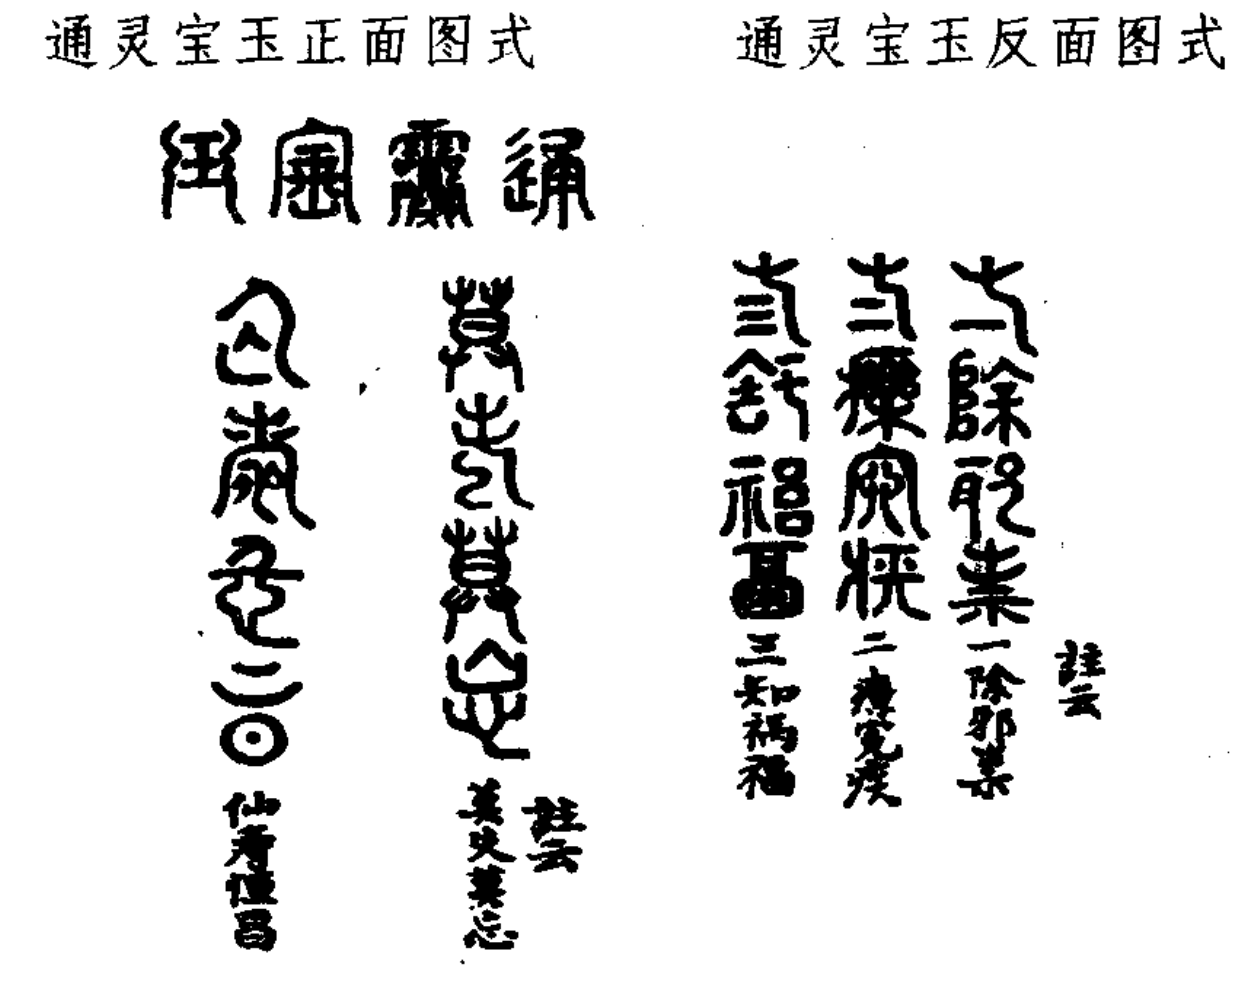
\includegraphics[scale=0.6]{picture/红楼梦1.PNG}
\end{figure}
\par 宝钗看毕,又从新翻过正面来细看,口内念道:“莫失莫忘,仙寿恒昌。”念了两遍,乃回头向莺儿笑道:“你不去倒茶,也在这里发呆作什么?”莺儿嘻嘻笑道:“我听这两句话,倒像和姑娘的项圈上的两句话是一对儿。”宝玉听了,忙笑道:“原来姐姐那项圈上也有八个字,我也赏鉴赏鉴。”宝钗道:“你别听他的话,没有什么字。”宝玉笑央:“好姐姐,你怎么瞧我的了呢。”宝钗被缠不过,因说道:“也是个人给了两句吉利话儿,所以錾上了,叫天天带着;不然,沉甸甸的有什么趣儿。”一面说,一面解了排扣,从里面大红袄上将那珠宝晶莹黄金灿烂的璎珞掏将出来。宝玉忙托了锁看时,果然一面有四个篆字,两面八字,共成两句吉谶\footnote{吉谶(chèn衬)——预示吉利的话。谶:预言。}。亦曾按式画下形相:
\begin{figure}[htb]
    \centering
    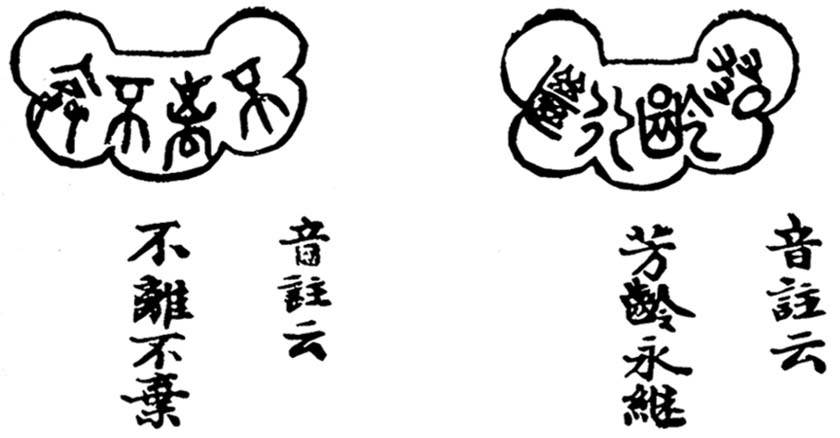
\includegraphics[scale=0.4]{picture/红楼梦2.jpeg}
\end{figure}
\par 宝玉看了,也念了两遍,又念自己的两遍,因笑问:“姐姐这八个字倒真与我的是一对。”莺儿笑道:“是个癞头和尚送的,他说必须錾在金器上——”宝钗不待说完,便嗔他不去倒茶,一面又问宝玉从那里来。
\par 宝玉此时与宝钗就近,只闻一阵阵凉森森甜丝丝的幽香,竟不知系何香气,遂问:“姐姐熏的是什么香?我竟从未闻见过这味儿。”宝钗笑道:“我最怕熏香,好好的衣服,熏的烟燎火气的。”宝玉道:“既如此,这是什么香?”宝钗想了一想,笑道:“是了,是我早起吃了丸药的香气。”宝玉笑道:“什么丸药这么好闻?好姐姐,给我一丸尝尝。”宝钗笑道:“又混闹了,一个药也是混吃的?”
\par 一语未了,忽听外面人说:“林姑娘来了。”话犹未了,林黛玉已摇摇的走了进来,一见了宝玉,便笑道:“嗳哟,我来的不巧了!”宝玉等忙起身笑让坐,宝钗因笑道:“这话怎么说?”黛玉笑道:“早知他来,我就不来了。”宝钗道:“我更不解这意。”黛玉笑道:“要来一群都来,要不来一个也不来;今儿他来了,明儿我再来,如此间错开了来着,岂不天天有人来了?也不至于太冷落,也不至于太热闹了。姐姐如何反不解这意思?”
\par 宝玉因见他外面罩着大红羽缎\footnote{羽缎——又称羽毛缎,一种毛织品,疏细者称羽纱,厚密者称羽缎,着水不湿,可御雨雪。}对衿褂子,因问:“下雪了么?”地下婆娘们道:“下了这半日雪珠儿了。”宝玉道:“取了我的斗篷来不曾?”黛玉便道:“是不是,我来了他就该去了。”宝玉笑道:“我多早晚儿说要去了?不过拿来预备着。”宝玉的奶母李嬷嬷因说道:“天又下雪,也好早晚的了,就在这里同姐姐妹妹一处顽顽罢。姨妈那里摆茶果子呢。我叫丫头去取了斗篷来,说给小幺儿们散了罢。”宝玉应允。李嬷嬷出去,命小厮们都各散去不提。
\par 这里薛姨妈已摆了几样细巧茶果来留他们吃茶。宝玉因夸前日在那府里珍大嫂子的好鹅掌鸭信\footnote{鸭信——鸭舌头,可制成名菜。信:舌头。}。薛姨妈听了,忙也把自己糟的取了些来与他尝。宝玉笑道:“这个须得就酒才好。”薛姨妈便令人去灌了最上等的酒来。李嬷嬷便上来道:“姨太太,酒倒罢了。”宝玉央道:“妈妈,我只喝一钟。”李嬷嬷道:“不中用!当着老太太、太太,那怕你吃一坛呢。想那日我眼错不见一会,不知是那一个没调教的,只图讨你的好儿,不管别人死活,给了你一口酒吃,葬送的我挨了两日骂。姨太太不知道,他性子又可恶,吃了酒更弄性。有一日老太太高兴了,又尽着他吃,什么日子又不许他吃,何苦我白赔在里面。”薛姨妈笑道:“老货,你只放心吃你的去。我也不许他吃多了。便是老太太问,有我呢。”一面令小丫鬟:“来,让你奶奶们去,也吃一杯搪搪雪气。”那李嬷嬷听如此说,只得和众人去吃些酒水。
\par 这里宝玉又说:“不必温暖了,我只爱吃冷的。”薛姨妈忙道:“这可使不得,吃了冷酒,写字手打飐儿\footnote{打飐儿——即打颤儿,发抖。}。”宝钗笑道:“宝兄弟,亏你每日家杂学旁收\footnote{杂学旁收——相对于应世举业的“正途”学问而言,即不去攻读《四书》《五经》时文八股而爱好诗词曲赋小说戏曲以至茶酒医药等闲杂学问。}的,难道就不知道酒性最热,若热吃下去,发散的就快;若冷吃下去,便凝结在内,以五脏去暖他,岂不受害?从此还不快不要吃那冷的了。”宝玉听这话有情理,便放下冷酒,命人暖来方饮。
\par 黛玉磕着瓜子儿,只抿着嘴笑。可巧黛玉的小丫鬟雪雁走来与黛玉送小手炉,黛玉因含笑问他:“谁叫你送来的?难为他费心,那里就冷死了我!”雪雁道:“紫鹃姐姐怕姑娘冷,使我送来的。”黛玉一面接了,抱在怀中,笑道:“也亏你倒听他的话。我平日和你说的,全当耳旁风;怎么他说了你就依,比圣旨还快些!”宝玉听这话,知是黛玉借此奚落他,也无回复之词,只嘻嘻的笑两声罢了。宝钗素知黛玉是如此惯了的,也不去睬他。薛姨妈因道:“你素日身子弱,禁不得冷的,他们记挂着你倒不好?”黛玉笑道:“姨妈不知道。幸亏是姨妈这里,倘或在别人家,人家岂不恼?好说就看的人家连个手炉也没有,巴巴的从家里送个来。不说丫鬟们太小心过馀,还只当我素日是这等轻狂惯了呢。”薛姨妈道:“你这个多心的,有这样想,我就没这样心。”
\par 说话时,宝玉已是三杯过去。李嬷嬷又上来拦阻。宝玉正在心甜意洽之时,和宝黛姊妹说说笑笑的,那肯不吃。宝玉只得屈意央告:“好妈妈,我再吃两钟就不吃了。”李嬷嬷道:“你可仔细老爷今儿在家,隄防问你的书!”宝玉听了这话,便心中大不自在,慢慢的放下酒,垂了头。黛玉先忙的说:“别扫大家的兴!舅舅若叫你,只说姨妈留着呢。这个妈妈,他吃了酒,又拿我们来醒脾\footnote{醒脾——即开胃;可引申为开心。本中医术语,是指一种治疗脾气虚寒、运化无力的方法。}了!”一面悄推宝玉,使他赌气;一面悄悄的咕哝说:“别理那老货,咱们只管乐咱们的。”那李嬷嬷不知黛玉的意思,因说道:“林姐儿,你不要助着他了。你倒劝劝他,只怕他还听些。”林黛玉冷笑道:“我为什么助他?我也不犯着劝他。你这妈妈太小心了,往常老太太又给他酒吃,如今在姨妈这里多吃一口,料也不妨事。必定姨妈这里是外人,不当在这里的也未可定。”李嬷嬷听了,又是急,又是笑,说道:“真真这林姐儿,说出一句话来,比刀子还尖。你——这算了什么。”宝钗也忍不住笑着,把黛玉腮上一拧,说道:“真真这个颦丫头的一张嘴,叫人恨又不是,喜欢又不是。”薛姨妈一面又说:“别怕,别怕,我的儿!来这里没好的你吃,别把这点子东西唬的存在心里,倒叫我不安。只管放心吃,都有我呢。越发吃了晚饭去,便醉了,就跟着我睡罢。”因命:“再烫热酒来!姨妈陪你吃两杯,可就吃饭罢。”宝玉听了,方又鼓起兴来。
\par 李嬷嬷因吩咐小丫头子们:“你们在这里小心着,我家里换了衣服就来,悄悄的回姨太太,别由着他,多给他吃。”说着便家去了。这里虽还有三两个婆子,都是不关痛痒的,见李嬷嬷走了,也都悄悄去寻方便去了。只剩了两个小丫头子,乐得讨宝玉的欢喜。幸而薛姨妈千哄万哄的,只容他吃了几杯,就忙收过了。作酸笋鸡皮汤,宝玉痛喝了两碗,吃了半碗碧粳粥。一时薛林二人也吃完了饭,又酽酽的沏上茶来大家吃了。薛姨妈方放了心。雪雁等三四个丫头已吃了饭,进来伺候。黛玉因问宝玉道:“你走不走?”宝玉乜斜\footnote{乜(miē咩)斜——眯着眼睛,斜眼看人。}倦眼道:“你要走,我和你一同走。”黛玉听说,遂起身道:“咱们来了这一日,也该回去了。还不知那边怎么找咱们呢。”说着,二人便告辞。
\par 小丫头忙捧过斗笠来,宝玉便把头略低一低,命他戴上。那丫头便将着大红猩毡斗笠一抖,才往宝玉头上一合,宝玉便说:“罢,罢!好蠢东西,你也轻些儿!难道没见过别人戴过的?让我自己戴罢。”黛玉站在炕沿上道:“罗唆什么,过来,我瞧瞧罢。”宝玉忙就近前来。黛玉用手整理,轻轻笼住束发冠,将笠沿掖在抹额之上,将那一颗核桃大的绛绒簪缨扶起,颤巍巍露于笠外。整理已毕,端相了端相,说道:“好了,披上斗篷罢。”宝玉听了,方接了斗篷披上。薛姨妈忙道:“跟你们的妈妈都还没来呢,且略等等不迟。”宝玉道:“我们倒去等他们,有丫头们跟着也够了。”薛姨妈不放心,到底命两个妇女跟随他兄妹方罢。他二人道了扰,一径回至贾母房中。
\par 贾母尚未用晚饭,知是薛姨妈处来,更加欢喜。因见宝玉吃了酒,遂命他自回房去歇着,不许再出来了。因命人好生看侍着。忽想起跟宝玉的人来,遂问众人:“李奶子怎么不见?”众人不敢直说家去了,只说:“才进来的,想有事才去了。”宝玉踉跄回头道:“他比老太太还受用呢,问他作什么!没有他只怕我还多活两日。”一面说,一面来至自己的卧室。只见笔墨在案,晴雯先接出来,笑说道:“好,好,耍\footnote{耍——戏弄之意。}我研了那些墨,早起高兴,只写了三个字,丢下笔就走了,哄的我们等了一日。快来与我写完这些墨才罢!”宝玉忽然想起早起的事来,因笑道:“我写的那三个字在那里呢?”晴雯笑道:“这个人可醉了。你头里过那府里去,嘱咐贴在这门斗上,这会子又这么问。我生怕别人贴坏了,我亲自爬高上梯的贴上,这会子还冻的手僵冷的呢。”宝玉听了,笑道:“我忘了。你的手冷,我替你渥\footnote{渥(wò沃)——覆盖裹藏某物,借以保暖或使之变暖,叫“渥”。}着。”说着便伸手携了晴雯的手,同仰首看门斗上新书的三个字。
\par 一时黛玉来了,宝玉笑道:“好妹妹,你别撒谎,你看这三个字那一个好?”黛玉仰头看里间门斗上,新贴了三个字,写着“绛云轩”。黛玉笑道:“个个都好。怎么写的这们好了?明儿也与我写一个匾。”宝玉嘻嘻的笑道:“又哄我呢。”说着又问:“袭人姐姐呢?”晴雯向里间炕上努嘴。宝玉一看,只见袭人和衣睡着在那里。宝玉笑道:“好,太渥早了些。”因又问晴雯道:“今儿我在那府里吃早饭,有一碟子豆腐皮的包子,我想着你爱吃,和珍大奶奶说了,只说我留着晚上吃,叫人送过来的,你可吃了?”晴雯道:“快别提。一送了来,我知道是我的,偏我才吃了饭,就放在那里。后来李奶奶来了看见,说:‘宝玉未必吃了,拿来给我孙子吃去罢。’他就叫人拿了家去了。”接着茜雪捧上茶来。宝玉因让“林妹妹吃茶。”众人笑说:“林妹妹早走了,还让呢。”
\par 宝玉吃了半碗茶,忽又想起早起的茶来,因问茜雪道:“早起沏了一碗枫露茶,我说过,那茶是三四次后才出色的,这会子怎么又沏了这个来?”茜雪道:“我原是留着的,那会子李奶奶来了,他要尝尝,就给他吃了。”宝玉听了,将手中的茶杯只顺手往地下一掷,豁啷一声,打了个粉碎,泼了茜雪一裙子的茶。又跳起来问着茜雪道:“他是你那一门子的奶奶,你们这么孝敬他?不过是仗着我小时候吃过他几日奶罢了。如今逞的他比祖宗还大了。如今我又吃不着奶了,白白的养着祖宗作什么!撵了出去,大家干净!”说着便要去立刻回贾母,撵他乳母。
\par 原来袭人实未睡着,不过故意装睡,引宝玉来怄\footnote{怄(òu沤)——这里是撩拨逗弄、厮缠、磨人的意思。}他顽耍。先闻得说字问包子等事,也还可不必起来;后来摔了茶钟,动了气,遂连忙起来解释劝阻。早有贾母遣人来问是怎么了。袭人忙道:“我才倒茶来,被雪滑倒了,失手砸了钟子。”一面又安慰宝玉道:“你立意要撵他,也好,我们也都愿意出去,不如趁势连我们一齐撵了。我们也好,你也不愁再有好的来服侍你。”宝玉听了这话,方无了言语,被袭人等扶至炕上,脱换了衣服。不知宝玉口内还说些什么,只觉口齿缠绵,眼眉愈加饧涩,忙服侍他睡下。袭人伸手从他项上摘下那通灵玉来,用自己的手帕包好,塞在褥下,次日带时便冰不着脖子。那宝玉就枕便睡着了。彼时李嬷嬷等已进来了,听见醉了,不敢前来再加触犯,只悄悄的打听睡了,方放心散去。
\par 次日醒来,就有人回:“那边小蓉大爷带了秦相公来拜。”宝玉忙接了出去,领了拜见贾母。贾母见秦钟形容标致,举止温柔,堪陪宝玉读书,心中十分欢喜,便留茶留饭,又命人带去见王夫人等。众人因素爱秦氏,今见了秦钟是这般人品,也都欢喜,临去时都有表礼。贾母又与了一个荷包\footnote{荷包——用以装药品、香料等细小物品的扁圆形绣花小袋。}并一个金魁星\footnote{金魁星——黄金铸成的魁星神像,有祝颂功名顺利的意思。魁星:本作奎星,北斗第一星,汉代纬书《孝经援神契》有“奎主文章”之说,后遂以此星为掌文运之神。},取“文星和合\footnote{文星和合——“文星”又称文昌星、文曲星,星相家以其为吉星、主文运、保功名。“和合”与荷包谐音,且为中国民间所奉喜庆吉祥之神,本祀万回,清代雍正年间封天台僧人寒山、拾得为“和合二仙”。}”之意。又嘱咐他道:“你家住的远,或有一时寒热饥饱不便,只管住在这里,不必限定了。只和你宝叔在一处,别跟着那些不长进的东西们学。”秦钟一一的答应,回去禀知。
\par 他父亲秦业现任营缮郎\footnote{营缮郎——官名。明清时工部有营缮司,设郎中、员外郎等职。},年近七十,夫人早亡。因当年无儿女,便向养生堂\footnote{养生堂——又叫育婴堂。一种收养弃婴的慈善机构。}抱了一个儿子并一个女儿。谁知儿子又死了,只剩女儿,小名唤可儿,长大时,生的形容袅娜,性格风流。因素与贾家有些瓜葛,故结了亲,许与贾蓉为妻。那秦业至五旬之上方得了秦钟。因去岁业师亡故,未暇延请高明之士,只得暂时在家温习旧课。正思要和亲家去商议送往他家塾中,暂且不致荒废,可巧遇见了宝玉这个机会。又知贾家塾中现今司塾的是贾代儒,乃当今之老儒,秦钟此去,学业料必进益,成名可望,因此十分喜悦。只是宦囊羞涩\footnote{宦囊羞涩——意谓做官者手头拮据。语本“阮囊羞涩”,见《韵府群玉·阳韵》。},那贾家上上下下都是一双富贵眼睛,贽见礼\footnote{贽(zhì至)见礼——旧时学生拜见老师时所送的礼,封套上要写“贽敬”。}必须丰厚,\footnote{“贽见礼必须丰厚”七字,据戚序、蒙府本补。}容易\footnote{容易——轻易。}拿不出来,又恐误了儿子的终身大事,说不得东拚西凑的恭恭敬敬封了二十四两贽见礼,亲自带了秦钟,来代儒家拜见了。然后听宝玉上学之日,好一同入塾。正是:
\refdocument{
    \par 早知日后闲争气,岂肯今朝错读书。
}





\clearpage

\chapter{弗朗西斯·培根(Francis Bacon)}


% 

\section{培根随笔全集}

\par 书名:培根随笔全集(译文名著精选)
\par 作者:[英]弗兰西斯·培根
\par 译者:蒲隆
\par 出版社:上海译文出版社
\par 出版时间:2012-04
\par ISBN:9787532757060




\subsection*{译本序}

\par 培根在《谈诤谏》一文中写道:“多读书是有好处的,尤其是读那些在公众舞台上扮演过重要角色的人写的书。”您现在拿在手里的恰好就是这么一本书。我们先谈谈培根在人生舞台上扮演过哪些重要角色,然后再说这是一本什么样的书。
\par 弗兰西斯·培根1561年生于一个官宦之家。父亲尼古拉·培根是伊丽莎白女王的掌玺大臣;母亲是文艺复兴时代一个博学多才的贵族妇女,她的妹夫就是伊丽莎白的重臣伯利勋爵。有这种家庭背景和社会关系,再加上才华出众,培根自然就有出入宫廷的机会。早在孩提时代,培根就被伊丽莎白称为“朕的小掌玺大臣”。雄心勃勃的培根自然期望得到一条谋取功名利禄的捷径。他12岁时就上了剑桥大学,但小小年纪,对大学的教育体制和当时主宰学术研究的亚里士多德的哲学体系十分反感。两年以后,他跟随英国驻法大使到巴黎去学习统计学和外交。又过了两年,父亲突然病故,培根只好回到伦敦。因为不是长子,没有继承到多少遗产,便只好投靠权势很大的姨父,可是伯利勋爵却妒忌培根的才华,根本不想帮培根的忙。培根只好自谋出路,开始学习法律。1582年培根开业当律师,很快声名大振。他才气过人,著书立说,名气很大,23岁时就当上了议员,并极力想博得女王的青睐,但成效不显著。后来,培根与女王的年轻宠臣埃塞克斯伯爵交上了朋友。埃塞克斯伯爵曾几度向女王推荐培根担任要职,但均未成功。伯爵觉得过意不去,便将自己在特威克纳姆的价值两千英镑的田产赠予培根。后来埃塞克斯兵败爱尔兰,而且不顾女王的指令,擅自返回伦敦,于是被女王下令拘留。埃塞克斯获释后,培根并没有与他断绝交往。不久,埃塞克斯策划推翻女王,事情泄露后又遭逮捕。这时候,培根作为女王的高级法律顾问,经过调查,起草了一份报告,认定埃塞克斯犯了叛国罪,最后埃塞克斯被处死。培根作为埃塞克斯的朋友,看起来完全与埃塞克斯划清了界线,可算是一名“识时务”的“俊杰”。不过培根的这种做法颇遭人们的非议,后来他振振有词地替自己辩解了一番。培根在这一案件中没有受到株连,但也没有立功受奖,受到女王的提拔。
\par 伊丽莎白于1603年驾崩,由苏格兰王詹姆斯继位。这对于培根可以说是时来运转了。1613年他被任命为首席检察官;1617年当上了掌玺大臣;1618年又成为大法官,而且多次接受贵族封号。1603年他受封为爵士,1618年受封为维鲁兰男爵,1620—1621年受封为圣阿尔班子爵。正当培根春风得意、青云直上之时,1621年他因卷入一起受贿案遭到了议会的弹劾。培根无法否认自己的罪状,随后受到如下判决:交纳四万英镑罚金,监禁在伦敦塔以候王命,削去一切官职,等等。不过最后还是被从宽发落,仅仅被监禁了四天,罚金基本上免除,只是削官为民了事。
\par 仕途无望以后,培根只好回家继续他的学术研究。1626年初,他想实验一下冷冻防腐的可能性,便杀了一只鸡,把雪填进鸡肚子,结果不幸自己受了风寒,不久离开了人世。
\par  
\par 培根尽管热衷于做官为宦,但他的志向远远不只在这一个方面。他想给不幸的爱尔兰带来和平安定;他想简化英国法律;他想改革教会;他想研究自然;他要建立一种新的哲学。要达到这些目的,他除了利用做官的地位和权势外,还一直用著书立说来推行他的各种主张。由于他亲自经历了宦海的浮沉,阅历丰富,眼界开阔,思想敏锐,因而他写出的东西能够力透纸背,具有振聋发聩的作用。
\par 1597年,培根的《随笔集》出版了,其中虽只有10篇短文,但影响很大,以后他反复修改增订,于1612年和1625年先后出了两个增订本,最后一个版本收入随笔58篇。
\par 欧美的随笔作为一种文学样式,是由法国散文家蒙田首创的。蒙田于1580年出版了一本题名为Essais(《随笔》)的集子,文笔轻松自然,亲切随便。培根是第一位英文随笔作家,他的随笔论述的题目有跟蒙田相近的,但写法迥然不同。在随后的数百年里,按蒙田的路子写随笔的大有人在,但很少有人能用培根的手法写随笔。那么,培根的随笔到底有些什么特点呢?
\par 翻开培根的《随笔集》,给人的第一个印象就是文章短小。58篇随笔中,很多都不超过千字,个别最长的也只有五千多字。培根的同时代人莎士比亚在《哈姆雷特》一剧中借波乐纽斯之口说:“简洁是智慧的灵魂,冗长是乏味的枝叶、肤浅的花饰。”培根自己也在《谈快捷》一文中说:“冗长而玄妙的讲话不利于快捷,就像长袍拖裙不利于赛跑一样。”所以培根力求以最短的篇幅摆足事实,讲清道理,摈弃那种空洞、肤浅、絮聒的毛病,注重文字的深刻老练、沉重有力,几乎篇篇警句格言层见叠出。下面是一些信手拈来的例子:
\refdocument{
    \par 德行犹如宝石,镶嵌在素净处最佳。(《谈美》)
    \par 成人惧怕死亡恰如儿童怕进黑暗。(《谈死亡》)
    \par 初生的幼崽总是其貌不扬,革新也莫不如此,因为它们都是时间的幼儿。(《谈革新》)
    \par 美德如同名贵的香料,焚烧碾碎时最显芬芳:因为幸运最能揭露恶行,而厄运则最能发现美德。(《谈厄运》)
    \par 夫妻之爱创造了人类,朋友之爱完善了人类,而淫乱之爱败坏、作践了人类。(《谈爱情》)
    \par 妻子是青年人的情人、中年人的伴侣、老年人的保姆。(《谈结婚与独身》)
}
\par 像这样的至理名言俯拾即是,而且大多不在开头,就在结尾。上面的前三个例句是文章开头的句子,后三个例句则放在结尾处。这种语句放在开头,具有雄奇有力、引人入胜的作用,放在结尾,则有概括全文、余味无穷的效应。
\par 培根的随笔没有西方很多散文随笔作家的那种散漫和随意,而具有诗的凝练圆满、小说的布局谨严。如同他的《谈园林》、《谈建房》里描绘的园林和建筑一样,给人提供了一幅井然有序、层次分明的图画。五十八篇随笔,篇篇结构严密,行文紧凑,我们不妨以他最长的一篇《谈国家的真正强大》为例,看看它的篇章结构:
\par 一、政治家:
\par 1.很多是无能之辈;
\par 2.有的只能维持现状;
\par 3.少数能使小邦变成大国。
\par 二、一个国家的真正强大:
\par 1.不在于城郭、武库等方面;
\par 2.不在于军队的人数;
\par 3.而在于人的才能和气质(例如:阿尔贝拉战役、提格拉尼斯、梭伦)。
\par 三、怎样才能变得强大:
\par 1.避免苛捐杂税;
\par 2.鼓励平民和“自由仆役”(即:武装扈从);
\par 3.允许异族入籍归化,以斯巴达为戒,学习罗马人的做法;
\par 4.让外国人去从事室内技艺;
\par 5.全民崇尚武功;
\par 6.严密注视可以兴兵的正当理由;
\par 7.掌握制海权;
\par 8.奖励战士。
\par 四、通过战争国君显得更加伟大,国家可以更加富强。
\par 无论从前面摘引的语句,还是从这篇文章的提纲看,我们初步会有这么一种印象:培根的随笔不是文人的闲适小品和游戏笔墨,他是以政治家改造社会、富国利民为目的进行说教的,所以从内容到形式都讲求实用。而讲求实用也是盎格鲁—撒克逊整个民族的特色。五十八篇随笔涉及国家、人生的各个方面,但每篇的核心都离不开人或国家的利害关系。也就是涉及什么有益,什么有害,人应当如何做,不应当如何做,如何处理一些具体实际的问题。如在《谈诤谏》一文中他竟然连接见来访者时桌子怎么摆都讲到了:“摆一张长桌和一张方桌,还是墙附近摆一些座位,似乎只是形式问题,其实是实质问题。因为摆一张长桌,几个坐在上手的人实际上就可以左右全局。然而如果采用其他形式,坐在下手的进谏者的诤谏就更有用处了。”
\par 培根用客观冷静的笔调写这些短小精悍的说教文章。他不追求抒情效果,不卖弄幽默风趣,不谈自己。所以读培根的随笔你听不到作者灵魂的絮语,也不像一位朋友在娓娓谈心,倒好像是在听一位高人赐教、一位法官判案。
\par 培根的这种独特的文体得力于他作为哲学家和科学家的思想的深刻性、条理化,得益于他从事法律工作文字的准确性,而且还受到拉丁文的影响。培根的许多著作都是用拉丁文写的,所以他以拉丁化的句法写英文,精短隽永,组织严密,又知道什么时候应当用合适的比喻把思想表现得格外鲜明,有时还给他的思想披上一层想象的光彩与魅力。难怪大诗人雪莱在他的著名论文《诗辩》中说:“培根勋爵是一位诗人。他的语言有一种甜美而庄严的节奏,这满足我们的感官,正如他的哲理中近乎超人的智慧满足我们的智力那样;他的文章的调子,波澜壮阔,冲击你心灵的局限,带着你的心一起倾泻,涌向它永远与之共鸣的宇宙万象。”正因为如此,一本由五十八篇短文组成的《随笔集》让培根在世界文学史上奠定了伟大散文家的地位。
\par 然而,培根在哲学上的贡献更加伟大,马克思称他为“英国唯物主义和整个现代实验科学的真正始祖”。培根在这一方面雄心勃勃,计划写一部名为《伟大的复兴》的巨著。全书计划分六大部分,第一部分是对人类一切知识的分类总结,1605年出版的《学术的进展》是第一部分的概论。《学术的进展》批判了贬损知识的蒙昧主义,并从宗教的信仰、国家的文治武功、社会的发展、个人的道德品行等各个方面论证了知识的巨大作用和价值,为培根后来提出的“知识就是力量”的著名口号打下了基础。
\par 1620年出版的培根的《新工具论》是未完成的《伟大的复兴》的第二部分。《新工具论》是针对亚里士多德的《工具论》而发的。所谓“新工具”,就是使用理性和实验,而不是亚里士多德的旧逻辑,因为对于科学的发现来说,旧逻辑无所作为,它使来自粗浅的概念的错误确定下来,变得根深蒂固,而无助于追求真理。因此培根认为为了发现真理,人必须做两件事情,其一就是排除一切偏见或假象。培根把这些假象分为四类:一、“部落假象”,即各个种族通行的思想方法造成的偏见;二、“洞穴假象”,即个人的癖好和偏见;三、“市场假象”,语言错误所造成的;四、“剧场假象”,也就是人们不可靠的传统。其二就是摈除这些假象以后,我们必须审查自然,必须通过无数的实验收集事实,把它们整理得井然有序,再找出它们存在的规律。
\par 1626年出版的《新大西岛》类似于一本科幻小说,描写的是海外的一个理想国。这部未完成的作品跟托马斯·穆尔著名的《乌托邦》类似,但二者仍有重要区别:乌托邦的居民之所以快乐,全是因为他们能运用理智;新大西岛的居民之所以快乐,却是因为他们能做研究与实验。后者的中心是一个名叫“所罗门宫”的研究院,他们每年派遣许多船只到世界各地,收取关于新发明和新发现的报告。培根的新大西岛比穆尔的乌托邦更合乎实际,但也只是培根的梦想。
\par 培根的著作远远不止这几种,但由于本书未收,这里不再一一介绍。黑格尔在他的《哲学史讲演录》中对培根是这样评价的:“他拥有高度的阅历,‘丰富的想象,有力的机智,透彻的智慧,他把这种智慧用在一切对象中最有趣的那个对象,即通常所谓的人世上。在我们看来,这是培根的特色。他对人的研究要比对物的研究多得多;他研究哲学家的错误要比研究哲学的错误多得多。事实上,他并不喜爱抽象的推理,’抽象推理这种属于哲学思考的东西,我们在他那里很少见到。‘他的著作虽然充满着最美妙、最聪明的言论,但是要理解其中的智慧,通常只需要付出很少的理性努力。’因此他的话常常被人拿来当做格言。”这一段话引自贺麟、王太庆的译文。译者注说,单引号中的话出自《评论季刊》第十六卷,1817年4月号,第53页。
\par 子曰:“有德者必有言,有言者不必有德。”(《论语·宪问》)公元前5世纪的中国哲人的话完全适用于公元十六七世纪的英国哲学家。培根可以说是个有言无德的人。他在文章中宣扬节俭,但他的生活却极为阔绰。他当大法官时,光伦敦私宅里的仆人就数以百计,而且个个自以为是,连培根的母亲也对此口出怨言。他主张廉洁,但结果自己受贿丢官,弄得身败名裂。他的治国处世的观点,大有中国法家的气息,注重“法”、“术”、“势”,提倡利己主义。这也许是文艺复兴时期很多人的共同思想观点吧。
\par  
\par 以上是译者1998年初为本书译稿撰写的“译序”的主要部分。1997年,南方的一家出版社一位素昧平生的编辑给我又是打电话又是写信,说她在编一套“世界散文丛书”,但培根的译者久觅不得,后来经一位热心人的推荐,她就找到我头上了。当然,盛情难却,但我知道培根时代的英文跟当代英文有一定差异,再加上其中杂有拉丁文,如果没有一个可靠的注释本,仅拉丁文这一点就没有办法解决。再说,水天同先生译的《培根论说文集》风行全国已达半个世纪,当时还出现了两个新的译本,对于培根我还能做些什么呢?后来方忠国先生把他从剑桥大学购得的由亨利·刘易斯(Henry Lewis)注释的《培根随笔》(Bacon′s Essays)借给我,并鼓励我权当一次学习的机会,这样我才硬着头皮接受了这一任务。在翻译的过程中,水公虽已作古,但他惠赠的《培根论说文集》依然是我的良师。
\par 译稿交出后,起初反应还挺好,可过了几个月,编辑打电话告诉我,他们发现我的译文有不少地方跟现有的译本“不一样”,而且觉得译文“不够古雅”,因为培根是四百年前的古人,译文应当典雅一些。我说“不一样”的地方不要轻易改动,因为我有所遵循。我又问他们认为现有的译文谁的是“古雅”的典范,回答是“高健”。高健先生是否把培根的随笔全部译完,我不很清楚,只见到他编译的《英美散文六十家》上的六七篇,完全是文言文,原来我和某编辑的要求差距如此之大!又过了些日子,稿子被退回来,还附了一封措词严厉的信,教训我“要为出版社负责,也要为自己负责”。于是责令我修改。有机会我是愿意一再修改自己译文的,但他们的硬性要求,我无意满足,于是就扔到床下不去管它。2004年,宋兆霖先生在编一套规模宏大的丛书,计划中有培根随笔,想要一个新译本,有意要我这部稿子,我便将它拿出来重新对着原文修订了一遍。这次是我主动修订的,并且参考了1997年我翻译时未见到的曹明伦先生的译本。时隔八年,我仍记得那位编辑的指责。为了“负责”起见,我先交代一下“不一样”的问题,我理解他们说的“不一样”不是个用词问题,而是意思“不一样”,甚至相反。我要说的是我依据的是Henry Lewis的注释本,这本书不仅注了一般注释本注的相关的人事、典故,更重要的是注了许多跟现代意思有出入的词。我的译文的“不一样”就是根据他的注译出来的,而且前面的写作、修订年代,正文的段落划分、拉丁文的意思,大部分注释依据的都是这个版本。
\par 这里先摘引几个例子,首先是大家最熟悉的“Of Studies”中的,‘Studies.’He means not the act of studying,but the results that follow systematic and long practised habits of study,viz.,education and culture.
\par In the opening sentence of the essay he mentions the three great advantages which an educated man enjoys — that he has always at command enjoyments which the ignorant man is deprived of (‘delight’) — that his mental culture makes him valued in companionship and society (‘ornament’) — and that,being an educated man, he is really more able to do the work of life effectively and successfully (‘ability’).该文中的crafty men被注为men naturally clever;还如《谈野心》里的state,他注为estate,nobles,great men。《谈虚荣》里的“cross lies” — contradictory lies,“glorious” — boastful,“bravery” — boasting;最后一篇中的“philology” — history,等等。
\par 不仅对许多令人按今天的词义理解会造成偏差的词作了注释,而且每篇后面有Analysis,这对全文的结构和整体意思的把握很有帮助。现将我觉得几个译本中歧义较大的“Of Suitors”的Analysis摘录如下:
\par  
\par ANALYSIS OF ESSAY XLIX.
\par Ⅰ.Improper suits are those which are —
\par  1 Bad in themselves,because injurious to the public good.
\par  2 Promoted by bad men.
\par Ⅱ.Improper promoters of suits are those who undertake them —
\par  1 Without ever intending really to promote them.
\par  2 Merely to serve their own purposes.
\par Ⅲ.Rules for the receivers of petitions:
\par  1 Try to discover the justice in every petition,both those —
\par   (a) Of controversy.
\par   (b) Of desert.
\par  2 If inclination goes against your sense of justice,make at least some concessions to justice.
\par  3 In suits which you do not understand consult those who do understand them.
\par  4 Do not mislead the petitioner by —
\par   (a) Only pretending to promote his suit.
\par   (b) Unduly raising his hopes of success.
\par   (c) Expecting too much thankfulness for your service.
\par  5 Advocate suits not on priority of presentation,but according to their merits,and do not take unfair advantage of them.
\par Ⅳ.Rules for petitionesr (‘suitors’):
\par  1 Do not blaze abroad either your suits or their progress,but ‘time’ them.
\par  2 Choose your advocate rather for his fitness than his greatness.
\par  3 Do not be discouraged by denial at first;you may receive equivalent favour afterwards.
\par  4 Be sure to ask more than you want,so as to be sure of getting enough.
\par  5 Do not injure your cause by getting merely a letter from some great person.
\par  6 Never use ‘general contrivers of suits.’
\par  
\par 我觉得Lewis的Analysis对读者很有帮助,因此将它们全部译了出来,附在正文后面。
\par 1999年上海文艺出版社出版了一本黄梅女士编选的《培根哲理散文》,择选了她认为优秀的译文,她在《序》里对几位译者的译文做了“各有千秋”的褒扬后,对水天同的译文特别给予眷顾。她说:“水译对原作的领悟相当深入可靠,他的译文的意思若是与后人有实质性的出入,对照原文琢磨,还时常会觉得仍是水先生有理的分大。”我想,水先生之所以“有理的分大”,除了他的学识为后辈难及之外,他在“译例”中开宗明义就讲,他所依据的是Selby的注释本。看来这个注释本对他的“有理”也作了相当大的贡献。不知道为什么,其他译文均未提及自己的原本。水先生晚年致力于莎士比亚研究,他曾向我提及朱生豪的译文有很多地方用现代的词义翻译莎士比亚时代的词义。我认为这不是因为朱先生水平低、悟性差,而是当时条件有限,他手头没有多少注释详细的原本。可见好的注释本对译者理解原文帮助有多大!
\par 我这次修订,对培根文体的“古雅”问题又考虑了很多,先说“古”,如果四百年前的英文“古”得就应当用文言文、或半文半白的文字翻译,那么,古希腊、古罗马,就应当用《诗经》、先秦诸子的文字来翻译对应了。但据我所知,解放后出版的外国经典著作基本上都是用白话文翻译的。哪怕先前有好的文言文的译本,也被白话文的新译本所取代(如柏拉图),独有培根的随笔在20世纪60年代和80年代有过几篇文言文译文,于是有人认为培根的作品只有译成文言文才对头。再说“雅”,我注意过不少介绍培根随笔的文字,似乎都未见到与这个中文词相对应的英文形容词,修改稿子前我又查阅了王佐良先生的《英国文学史》,现将其中论述培根的一段文字抄录如下:
\refdocument{
    \par 培根是大哲学家,英国唯物主义的始祖,自称“以天下全部学问为己任”;他又是大官僚,登上了大理院长的高位,却又以受贿罪而被弹劾去职,从此绝望仕途。后世诗人蒲伯称他为“最聪明、最出色、最卑鄙的人”。他的主要著作是用拉丁文写的,《随笔》只是一些摘记式的短文,所以才用英文来写,却不料他的文学声誉就建立在这本薄薄的小书上。从文学史来看,他是第一个把法国蒙田创立的随笔这一文学形式移植到英国来的人,后来它变成英国散文中最令人爱读的品种之一,培根之功不可没。而他自己所作,也确实出色,篇幅很短,而充满深刻的见解,表达方式则力求扼要而又周到。读者可以看出他的智慧像医生手里锐利的手术刀,在一层一层地解剖着人生和社会里的各种问题:真理、死亡、宗教、爱、逆遇、高位、友谊、父母与子女、读书、利己的聪明,等等;同时,他也谈美,谈旅行、娱乐、庭园、营造,笔下出现诗情,以至雪莱称他为一个“诗人”。
}
\par 王先生又说:“同培根的简约明晰的《随笔》相对照的,是一类繁复、华美,甚至带点神秘色彩的文章,代表作如汤玛斯·勃朗的《医生的宗教》(1642)和《瓮葬》(1658)。”王先生引用了自己的译文来展示培根的风格:
\refdocument{
    \par 读书足以怡情,足以傅彩,足以长才。其怡情也,最见于独处幽居之时;其傅彩也,最见于高谈阔论之中;其长才也,最见于处世判事之际。
}  
\par 他引用杨周翰先生的译文来表现勃朗的特色:
\refdocument{
    \par 学者和爱和平的人,他们不携带武器,但他们的舌头却比阿克提乌斯的剃刀还锋利;他们的笔更厉害,比雷声还响;我宁肯忍受大炮的震撼,也不愿忍受一支无情的笔的怒袭。
} 
\par 这两段译文给人的印象似乎难以印证前面的概述。王先生还摘译了勃朗的《忧郁的解剖》第6版的前言:“我有啥说啥。我尊重内容而不是词语。……我不注意妙句,只尽全力使读者理解,而不是取悦他的耳朵。”同时又摘引周珏良译的一段《尤弗伊斯》:
\refdocument{
    \par 曰:否,此大不然也,盖唯心所指则变物之性。日照粪壤,不损其明;钻石入火,不损其坚;水有蟾蜍,不染其毒;鹪鹩栖鳄吻,不为所吞;贤者不涉遐想,不动绮思。冬青耸出掬林;薜荔罩笼磐石;柔菌能当利刃;此非物之常乎?
} 
\par 在引文之后,王先生引用培根等人的观点加以点评:
\refdocument{
    \par 这类美文自有爱好者,当时的贵族夫人小姐还竞相仿效,却为一些真要用散文把事情说清楚的务实之士所忌。他们不仅反对“尤弗伊斯体”,就连一般的修辞术也不以为然。有一位写蒙田式即培根式随笔的康华利斯把西塞罗式的修辞术比做“翻文字跟斗……明明一个字能说清楚的事却硬要用三个字!”而培根本人更是认为整个16世纪的主导风格是“追求词语过于内容”,是讲究修辞手段而不问内容是否重要,必须加以改革。
}
\par 引文的这三位译者都是20世纪中国英语界的名家,他们翻译的也是16世纪的几位散文大家,译文都有突出的特色,但是否个个都贴近原文的风格,因为16世纪的英语属于“现代英语”,差异仅在个人文体方面,是否就像译文表现出的古文和白话文那么大,这还有待于探讨,后学者不敢盲从。文体的微妙区别,分辨就十分困难,恰如其分地翻译更是难上加难。乔伊斯自称(见1920年3月20日致弗兰克·巴津的信)在《尤利西斯·太阳神的牛》中用了从塔西佗到美国纽约市井俚语的二十多种文体。对此翻译家萧乾也无奈地说:“这些在中译文中实难表达。译者仅在前半部使用了半文半白的文体,逐渐恢复到白话。”我不知道如果不是作者挑明,有多少读者能把这么多人的不同风格分辨出来,就是挑明了,又有多少读者能品尝出原作的不同风味;又有多少译者敢说他就能在译文中把它们充分展示出来。
\par 我本来是想从这部《英国文学史》的有关论述中寻找启发和依据,修改我的译文,但看了上述几段引文后便更是无所适从了。但培根的做法给了我启示,他用拉丁文写大著作,用英文写小随笔,可见他的随笔是让普通读者看的。这一点在我国也并不少见,鲁迅用文言写他的学术著作《中国小说史略》和《汉文学史纲要》,但用白话写小说、写杂文。钱钟书用文言写《管锥编》、写《谈艺录》,但用白话写《围城》。更值得一提的是,他的《宋诗选注》一反许多注家用半文半白的文字做注的旧例,用了十分口语化的文字,如陈师道的《别三子》一诗的“夫妇死同穴”,在林庚、冯沅君主编的《中国历代诗歌选》是这样释义的:“陈诗用《诗经》语意思却是:他与妻被迫生离,只有等死后,方能埋在一起。”钱钟书的释义意思完全一样,但语言大不相同:“陈师道的意思说,自己一对夫妇活生生地拆开,只有等死后埋在一起了。”如果一个普通人写了后面这样一条注,是不是有人会嫌它“不雅”呢?
\par 然而百人百性,萝卜芹菜各有所爱。这个译本无非是一名普通译者用普通语言译给普通读者看的书,有待大家批评指正。
\par 我译的《随笔集》先后在北京和南京两地印行过三个版本。这本“文选”除了包含修订过的《随笔集》外,还增加了上文提及的《新工具论》的节选《论假象》和《新大西岛》中的一章《所罗门宫》,以展示培根作为随笔家、理论家和小说家的多方面成就。后面两篇均译自\textsl{Norton Anthology of English Literature}。
\par \rightline{译者}
\par \rightline{2008年11月于兰州}



\subsection*{一、谈真理}

\begin{center}
    (1625年作)
\end{center}

\par “真理为何物?”彼拉多\footnote{参见《圣经·新约·约翰福音》第18章第38节。彼拉多(?—36以后)在罗马皇帝提比略在位期间任犹太巡抚(26—36),主持对耶稣的审判,此话是他审判耶稣时所问,不过并非一句戏言,而是以迷惘的口吻说的。第一句原来并不是正文的组成部分,仅仅是作为一句引言。}戏言相问,但并不指望回答。
\par 诚然,总有人喜欢朝三暮四,认定固守信仰无异于枷锁加身,所以无论行为思想均追求随心所欲。虽然此类哲人俱已往矣,但仍有巧舌如簧之士跟他们一脉相承,然而气血之刚烈已远逊于古人矣。
\par 但人们依然偏爱虚假,究其原因不仅由于寻求真理得不辞艰辛,也不仅由于发现真理后反而使人的思想作茧自缚,而且还来源于人们的一种劣根性:嗜假成癖。晚期的希腊哲学流派中有一派人考察过这个问题,\footnote{也许指的是怀疑论,公元前300年左右由希腊哲学家皮郎(约前360—前272)创立。}对人们为何喜欢虚假百思不得其解:如果说诗人弄虚以寻欢,商人作假为牟利,那一般人就只有为虚假而爱虚假了。个中缘由我也难以相告,也许真理恰如磊落的天光,所有假象、盛典在烛光下显得典雅堂皇,但经它一照,则难免穷形尽相。真理也许等价于一颗珍珠,只有在日光映照下才尽显璀璨,但却赶不上钻石、红玉,它们在光怪陆离中大放异彩。掺假总能增添乐趣。倘若从人的头脑里除去愚蠢的见解、媚悦的憧憬、错误的估价、自欺欺人的幻想之类的东西,那么所剩的只是一些卑微贫乏的意念,充斥着忧郁、恶意,甚至自己也感到厌恶,对此恐怕无可置疑吧?有位先哲尖刻地将诗歌称为“魔鬼之酒\footnote{圣哲罗姆和圣奥古斯丁分别有“诗乃魔鬼之食”和“诗乃谬误之酒”的说法。}”,因为它填充人的想象,用的只不过是虚假的影子而已。然而有害的并不是掠过心田一晃而去的虚假,而是上文所说的沉积心底、安如磐石的虚假。
\par 尽管这些东西浸透了人们堕落的思想感情,然而作为自身唯一仲裁者的真理却教导说:追求真理,是向它求爱求婚;认识真理,是与它相亲相依;相信真理,是用它尽兴尽欢,所以真理才是人性的至福至善。上帝创造天地万物的数日内,他最初的造物为感性之光,最后的造物是理性之光;尔后,他安息日的工作便是以其灵昭示众生。\footnote{参见《圣经·旧约·创世记》第1章第1~3节:“起初,上帝创造天地。地是空虚混沌。渊面黑暗。上帝的灵运行在水面上。上帝说,要有光,就有了光。”第2章第7节:“上帝用地上的尘土造人,将生气吹在他鼻孔里,他就成了有灵的活人,名叫亚当。”}起初,他将光明吐向万物混沌的表面,继而又将光明吹入世人的面庞,如今他依然将光明向其选民的脸上喷射。有一位诗人\footnote{指古罗马诗人卢克莱修(约前93—约前50)。}给他那一派人增光不少,从而让该派不比别派逊色,他的话非常精辟:“伫立于岸边遥望舰船颠簸海面可谓乐事,据守在城堡凭窗俯视两军将士鏖战脚下亦属乐事;然任何快乐与登临真理之巅(一座雄视万象的高山,空气永远清新、宁静)俯瞰下面谷中的谬误、彷徨、迷雾和风雨相比,皆会黯然失色。”但观望此景须怀悲天悯人之心,切勿现顾盼自雄之态。当然,如若人心能动于仁爱,安于天意,围绕真理之轴旋转,那人间就无异于天堂了。
\par 从神学和哲学真理转向为人处世的真诚,即便那些并不按真理办事的人也会承认,做事光明正大乃人性之荣光,弄虚作假犹如金币和银币中的合金,它可以扩大金银的流通,但却贬损了它们的价值。这些迂曲拐弯的行径犹如蛇行,蛇不用脚走,而靠肚爬,行状甚为卑劣。人若被发现有阳奉阴违、背信弃义之嫌,那可是无以复加的奇耻大辱;蒙田\footnote{蒙田(1533—1592),法国散文家,此语出自他的《随笔集》第2卷第18章《论否认说谎》。}在探讨谎言为何可耻可恶时说得真好:“仔细想来,说人撒谎就等于说他蔑视上帝,惧怕凡人。因为谎言是直面上帝而逃避凡人的。”有人预言:基督再来时,他在世上将难遇诚信。\footnote{参见《圣经·新约·路加福音》第18章第8节:“然而人子来的时候,遇得见世上有信德吗。”}因此谎言是吁请上帝审判人类的最后钟声。此言对于虚伪和背信的劣迹真可谓描述得再高明不过了。



\subsection*{二、谈死亡}

\begin{center}
    (1612年作1625年增订)
\end{center}
\par 成人惧怕死亡恰如儿童怕进黑暗;儿童天生的恐惧随着故事同步增长,成人情况亦然。静观死亡,将它视为罪恶的报应\footnote{参见《圣经·新约·罗马书》第6章第23节:“因为罪的工价乃是死。”},看作去另一世界的必由之路,当属神圣虔诚之见。然而,惧怕死亡,将其视为应向自然交纳的贡品,则是愚陋之谈。而在宗教沉思录中,时而混杂着虚幻迷信色彩。在一些修士的《修行记》中,你会读到此类文字:人当自忖,若指尖遭受挤压折磨尚有钻心之痛,进而推想死亡之际,全身腐朽化解,其痛又当如何。其实,死亡时经历的苦痛比一肢受刑要轻松百倍,因为最致命的部位未必最敏感。一位言者以哲人与凡人的双重身份说出如下妙语:“死亡的声势比死亡本身更为恐怖。”\footnote{原文为拉丁文,为古罗马哲学家、政治家、剧作家塞内加(约前4—公元65)原话的大意。}呻吟,惊厥,面无血色,亲朋哭泣,黑衣黑幔,丧葬仪式,诸如此类使死亡显得怵目惊心。
\par 值得注意的是,人心中的情感尽管脆弱,但并非不能抗御对死亡的恐惧。既然人身旁簇拥着那么多能战胜死亡的帮手,死亡就未必那么可怕。复仇战胜死亡,爱情蔑视死亡,荣誉渴望死亡,悲哀奔赴死亡,恐惧抢占死亡。此外,我们还从史书中读到:奥托皇帝自杀之后,哀怜之心(一种最温柔的情感)煽诱众人纷纷效死,纯粹为了表示对皇上的哀怜之情和身为追随者的耿耿忠心。此外,塞内加认为“苛求”和“腻烦”也会使人舍生求死:“想一想你将同样的事情做了多少遍,不仅勇敢和痛苦之辈想一死了之,连苛求之人也想一了百了。”\footnote{原文为拉丁文。}一个人尽管既不勇敢也不痛苦,但反反复复做同一件事的腻烦也足以令他萌生死念。
\par 同样值得注意的是,死亡的临近对英雄豪杰影响甚微,因为这种人到了最后一刻仍不改本色。奥古斯都·恺撒\footnote{奥古斯都·恺撒(前63—公元14),罗马帝国第一任皇帝,前27—公元14年在位,恺撒的继承人。在位时扩充版图,改革政治,奖励文化艺术。原名屋大维,元老院奉以奥古斯都(意为“神圣”、“伟大”)称号。}临死还说这样的赞语:“永别了,利维娅!终生勿忘我们夫妻一场。”\footnote{原文为拉丁文。}提比略\footnote{提比略(前42—公元37),古罗马皇帝,14—37年在位。长期从事征战,军功显赫。56岁继养父奥古斯都皇位,因渐趋暴虐,引起普遍不满,在卡普里岛被近卫军杀死。}临死还在作假,正如塔西佗\footnote{塔西佗(约55—约120),古罗马历史学家,此语出自他的《编年史》第6卷。}所言:“提比略体力衰竭,但虚伪依旧。”韦斯巴芗\footnote{韦斯巴芗(9—79),古罗马皇帝,69—79年在位。在位时整顿财政,改组军队,加强武力统治,营建罗马广场、凯旋门和大竞技场。}死到临头,还坐在凳子上调笑:“我想,我就要成神了。”加尔巴\footnote{加尔巴(前3—公元69),古罗马皇帝。68年举兵反对尼禄,尼禄自杀后被元老院确认为罗马皇帝,后在罗马广场被禁卫军杀死。}死时还引颈陈词:“砍吧,倘若这样做有益于罗马人民的话。”塞普蒂默斯·塞维鲁\footnote{塞普蒂默斯·塞维鲁(146—211),古罗马皇帝,193—211年在位。在位时扩建新军团,压制元老院,加强中央集权,吞并美索不达米亚,后在征服不列颠的地区时病死于埃波拉孔。}临死前还在处理政务,他说:“要是还要我办什么事,那就快点。”诸如此类,不胜枚举。
\par 斯多葛派对死亡未免过于推重,他们大力筹办,使死亡显得愈加恐怖。有种说法更有道理:“他把生命的终结看作自然的一种恩赐。”\footnote{原文为拉丁文,引自古罗马诗人尤维纳利斯(约60—约140)《讽刺诗》第10首第358行。}死与生同样自然;也许对婴孩而言,生与死同样痛苦。
\par 人若死于孜孜追求之中或伤于热血沸腾之际,当时是不大感到疼痛的;因此一颗专一向善的心灵就能避免死亡的苦痛;尤其应当相信:一个人实现伟大目标和抱负时,最甜美的歌莫过于“如今请让你的仆人离去”。死亡还有一点,就是它能打开美誉之门,熄灭嫉妒之火:“生前遭人妒忌者死后受人爱戴。”



\subsection*{三、谈宗教统一}

\begin{center}
    (1612年作 1625年重写)
\end{center}

\par 宗教是人类社会的主要维系,若其自身能维持真正的统一,实为幸事一桩。围绕宗教产生的争执和分歧是异教徒闻所未闻的劣迹。这是因为异教徒的宗教并无任何恒定的信仰,只表现为各种典礼和仪式。他们的教士、神甫由诗人充当,由此可以想见,他们的信仰是一种怎样的宗教。然而,真正的上帝具有这样一种特性:他是一位“忌邪的神”\footnote{参见《圣经·旧约·出埃及记》第20章第5节。},所以他的崇拜与宗教既掺不得半点杂质,也不容他神分享。因此我们就宗教统一要讲几句,谈谈统一的结果、界限和手段。
\par 统一的结果(除了取悦上帝,因为这是至关重要的)有二:一是针对教外人士的,二是针对教内人士的。就前者而言,异端邪说、拉帮结派无疑是坏中之坏,更甚于伤风败俗。肉体上伤身断肢比一种体液的败坏\footnote{西方中世纪生理学说认为人体中有四种体液,若它们配合不均,就会导致疾病。}更加危险,精神上情况亦然。所以要使教外人士望而却步,要将教内人士逐出教门,行之有效者莫过于破坏统一。每当遭遇此类情形:有人说:“看哪,他在旷野里,”又有人说:“看哪,他在内屋中,”\footnote{参见《圣经·新约·马太福音》第24章第26节。}(即每当一些人在异端秘密集会里寻找耶稣,而另一些人在教堂门面上寻找耶稣之时),这种告诫的声音应一直在人们耳际回响:“不要出去。”外邦人的教师\footnote{指圣保罗。}(他工作的性质使他对教外人士特别担心)说:“如果一个异教徒进来,听见你们操着多种方言说话,岂不说你们癫狂了吗?”\footnote{参见《圣经·新约·哥林多前书》第14章第23节。“操着多种方言说话”比喻教义不统一。}诚然,无神论者和世俗之徒一旦听说教内见解如此冲突,印象必不会好,他们对教会也就避而远之,不免去“坐亵慢人的座位”\footnote{参见《圣经·旧约·诗篇》第1篇第1节。}。一位嘲讽大师\footnote{这里指法国作家拉伯雷(约1483—1553)。}竟以“异教徒的莫里斯舞”\footnote{莫里斯舞是英国一种传统民间舞蹈,在五朔节表演,舞者通常为男子,身上系铃,扮作民间传说中的人物,模样怪异。之所以称为莫里斯舞,莫里斯这个词显然来自“莫里斯科”(morisco),意为“摩尔人的”。}为他虚构的丛书中的一本书命名,此事虽小,然而作为如此严肃的问题的一个佐证,正将这一弊端鞭挞得入木三分:异教徒丑态百出,卑躬屈膝;恰为那些爱诋毁神圣事物的世俗狂徒和腐朽政客徒增笑资。
\par 宗教统一带给信徒的则是和平。和平包含着无尽的福祉。它树立信仰,点燃爱心,并使外在的宗教和平净化为内在的平和心境:不必苦心孤诣钻研撰写论战檄文,转而致力于读写修行、祈祷的伟论。
\par 至于统一的界限,进行正确定位至关重要。似乎存在着两个极端。在某些狂热分子听来,一切主张和解的言辞都不堪入耳。“平安不平安,耶户说,平安不平安与你何干?你转在我后头吧。”\footnote{见《圣经·旧约·列王纪下》第9章第18节。耶户系以色列第十代王。}平安不平安倒无关紧要,要紧的是沆瀣一气,结党营私。另一个极端则是某些老底嘉派\footnote{参见《圣经·新约·启示录》第3章第14~16节。}和态度温暾之辈,他们以为可以用折中、骑墙和巧妙的调停来调解宗教问题,仿佛他们要在上帝和凡人之间做出公断似的。这两种极端都应避免,但要做到这一点,我们必须将救世主亲自起草的《基督徒盟约》中的两条相反相成的条文解释得中肯明白:“跟我们不相合的就是反对我们,不反对我们的就跟我们相合。”也就是说,应将宗教中的根本实质性的问题同不纯属信仰,而仅是见解、派别或良好意图的问题真正分别开来。许多人认为此乃区区小事,而且已经解决,但倘若处理得更少偏颇,则会更受普遍欢迎。
\par 关于这一点,我仅提供一点建议。人们应当注意且勿以两种争论分裂上帝的教会;其中一类争论只不过是由辩驳引发的,争论的问题纯属鸡毛蒜皮,犯不着为它大动肝火,势不两立。有一位先哲发现:“基督的黑衣确实没有缝儿,但教会的外衣五颜六色。”\footnote{参见《圣经·新约·约翰福音》第19章第23节。}因此他说:“衣服可以形形色色,但不可让它开裂。”\footnote{原文为拉丁文,“先哲”指圣伯尔纳。圣伯尔纳(1090—1153),法兰西人,天主教西多会修士,明谷隐修院创立者。在政治、文学、宗教等方面对西方文化有重大影响。}可见统一与划一是两码事。另一种是争论的问题至关紧要,但因着眼点过于琐屑晦涩,以至使争论最后钻了牛角尖,脱离实际,明理善断之士有时会听见一些无知之徒争短论长,但他心里明白,这些殊异之谈指的是同一码事,然而他们自己却永远不会达成共识。倘若人与人之间由于判断的差异而出现上述情况,那我们还能认为洞悉人心的上帝就不能发现脆弱的人类尽管言辞对立、用意却完全一致,从而能接受双方的意见吗?这类争论的性质,圣保罗在他关于同一问题的告诫中已淋漓尽致地予以表达。“躲避世俗的虚谈和那敌视真道、似是而非的学问。”\footnote{见《圣经·新约·提摩太前书》第6章第20节。}人们向壁虚造种种矛盾冲突,并赋予它们新的名号,这些名号已约定俗成,以致本来该受实义支配的名号,反而支配了实义。
\par 和平或统一也有假的,表现有二:一种建立在蒙昧无知的基础之上,因为黑暗中百色相同;另一种是在坦率承认根本问题矛盾的基础之上拼凑起来的,因为在那些事情上的真与假,就像尼布甲尼撒王梦见的大象脚趾上的铁和泥,可以粘在一起,却不能融为一体。\footnote{参见《圣经·旧约·但以理书》第2章。}
\par 至于谋求统一的手段,人们必须当心,在谋求或巩固宗教统一时,切不可废弛博爱义方和人类社会的法度。基督徒有两口剑,宗教之剑和世俗之剑,在维护宗教时二者都有相应的职能和地位;然而我们不可拿起第三口剑,即穆罕默德之剑,或者类似的剑;也就是说,不可借助干戈传教或以腥风血雨的迫害来胁迫人的良心,除非有明火执仗辱没宗教、亵渎神明、或者叛国谋反的情况出现;更不可放任滋生事端,认可阴谋叛乱,授民众以刀剑以及诸如此类意在颠覆神授予的政权\footnote{这里似乎指《圣经·新约·罗马书》第13章第1~2节:“凡掌权的都是上帝所命的。”}的行为\footnote{培根影射教皇开除伊丽莎白女王教籍的行为。},因为这样做无异于用第一块石板撞击第二块石板,把两块统统撞碎\footnote{据《圣经·旧约·出埃及记》所载,摩西带领希伯来人出埃及过红海,抵西奈山,在那里传授上帝刻在两块石板上的十诫,令希伯来人遵守。第一块板上是人对上帝的责任,第二块板上是人对人的责任。};而且一心要视世人皆为基督徒,从而忘记了他们是人。诗人卢克莱修看到阿伽门农竟然忍心把自己的女儿当祭品,便惊呼:
\refdocument{
    \par “宗教作恶如此之甚。”\footnote{原文为拉丁文。阿伽门农,特洛亚战争中希腊军队的最高统帅,由于得罪了狩猎女神,女神使奥利斯港平静无风,船队不能进发,预言家指出,必须将爱女伊菲革涅亚献祭给阿耳忒斯,女神之怒方能平息。阿伽门农迫于无奈,只好同意将爱女杀死献给女神。但在最后一刻,女神赦免了伊菲革涅亚,将她摄走,用一只牝鹿代之,随后风起,希腊联军开始进发。}
} 
\par 倘若他知道法国的大屠杀或英国的火药阴谋,他又当何言以对?\footnote{指1572年的圣巴多罗缪节对胡格诺派教徒的大屠杀和1606年11月5日英国天主教徒企图炸毁议会、炸死詹姆斯一世的阴谋事件。}他会七倍地沉溺于逸乐,更加不信神灵。因为那口世俗之剑为了宗教而拔出鞘时,需要慎之又慎,所以将它放到百姓手中便是荒谬绝伦之举。这种事还是留给再洗礼派\footnote{欧洲中世纪基督教的一个教派。不承认为婴儿所施的洗礼,主张成年后须再次受洗,故称。主要成员为农民和城市平民,他们对封建制度及其支柱天主教会极度仇恨,一部分人参加了德国的农民起义,后受到残酷镇压。}教徒和其他亡命之徒吧。魔鬼说“我要升到高云之上,我要与至上者同等”\footnote{见《圣经·旧约·以赛亚书》第14章第14节。},那是极大的亵渎。可是如果让上帝扮演成某种角色,让他说“我要降到地下,当个黑暗之王”,那就是更大的亵渎了。倘若宗教的目标堕落到谋杀君主\footnote{这里指法王亨利三世于1589年被一名多明我会修士暗杀之事。}、残害百姓、颠覆国家和政府这一类丧尽天良的行径,那跟亵渎行为相比又好在哪里?毫无疑问,这是把圣灵鸽子般的形象贬为兀鹰和乌鸦,这是在基督教会的船上挂起海盗和杀手的旗号。因此,教会必须靠教义、教令,君主必须靠武力、文治。无论是基督教的还是伦理的,好像借助墨丘利的神杖\footnote{古罗马神话里墨丘利手持神杖招引亡魂前往阴间。}一样,都要把支持上述罪行的行为和看法统统打入地狱,并使它们万劫不复,如同大多已经做过的那样。毫无疑问,关于宗教讨论,那位使徒的话应当放在前面:“人的怒气并不成就上帝的正义。”\footnote{见《圣经·新约·雅各书》第1章第20节。使徒指雅各。}值得注意的是,一位睿智的前辈同样坦诚地表白:凡对良心施压的人一般都有自己的打算。




\subsection*{四、谈报复}

\begin{center}
    (1625年作)
\end{center}
\par 报复是一种野道,人性越是趋之若鹜,法律就越应将其铲除。因为头一个犯罪仅仅是触犯法律,而对该罪施加报复则是取代法律。毫无疑问,一个人如果采取报复行为,就等于跟他的仇人扯平拉齐;然而要是放他一马,他则高出仇人一筹,因为宽恕乃王者风范。所以所罗门有言:“宽恕人的过失,便是自己的荣耀。”\footnote{见《圣经·旧约·箴言》第19章第11节。}过去的已经过去,不可挽回,明达之士则着眼于现在与未来;所以对往事耿耿于怀只是跟自己过不去而已。况且为作恶而作恶的人是绝对没有的,人作恶无非是要沽名、渔利、寻欢、作乐。因此我何苦要为一个人爱己胜过爱我而愤愤不平?如果一个人完全是出于生性凶恶而作恶,那又如何?充其量仅像荆棘刺玫,除了扎划钩擦,别无能耐。
\par 有些冤情无法可纠,如果进行报复,还情有可原;然而人们还得当心,他的报复也必须无法律惩处,否则他的仇人仍占上风,因为他和仇人受惩处的次数为二比一。有人进行报复时喜欢让对方明白报复的来由,这还比较豁达大度:因为其中的快乐似乎不在于伤人,而在于让对方悔罪;然而卑鄙狡猾的懦夫却像飞来的暗箭。
\par 佛罗伦萨大公科斯莫\footnote{科斯莫(1519—1574),佛罗伦萨大公,统治佛罗伦萨达34年。}严词抨击对朋友的背信弃义,仿佛这些罪行不可宽恕似的:“你会读到基督要我们宽恕我们的敌人的教导,却永远不会读到要我们宽恕我们的朋友的训诫。”然而约伯的精神格调更高一筹,他说:“难道我们从上帝手里得福,不也受祸吗?”\footnote{见《圣经·旧约·约伯记》第2章第10节。}推及朋友,情况亦然。
\par 的确,一个人念念不忘报复,就等于让自己的伤口经常开裂,否则,它就会愈合的。
\par 报公仇大多大运亨通,例如为恺撒的死报仇、为佩提那克斯\footnote{佩提那克斯(126—193),古罗马皇帝,在位86天,被一帮哗变的禁卫军所杀。后来他的继位人米乌斯·塞维努斯(193—211年在位)把那帮禁卫军处死。}的死报仇、为法王亨利三世的死复仇。然而报私仇却运道不佳,不仅如此,报仇心强的人,过的是巫婆的日子:由于他们存心害人,所以就不得好死。


\subsection*{五、谈厄运}

\begin{center}
    (1625年作)
\end{center}

\par 塞内加有一句仿斯多葛派\footnote{在古希腊和罗马时期兴盛起来的一派思想。}的高论:“幸运的好处令人向往,厄运的好处叫人惊奇。”毫无疑问,如果奇迹就是统摄自然,那么它们大多在厄运中出现。他还有一句宏论比这还要高明(此言出自一个异教徒之口,实在高明绝伦):“集人的脆弱与神的旷达于一身,才是真正的伟大。”如果将此话写成诗,那就更加妙不可言,因为在诗里,豪言壮语更受赞许。的确,诗人一直潜心于此道,因为它其实就是古代诗人的奇谈中表现的那种东西,这种奇谈似乎并不乏玄秘,而且似乎与基督徒的境况相当接近,“赫拉克勒斯\footnote{即罗马神话中的赫丘利。希腊罗马传说中最著名的英雄。}去解放普罗米修斯\footnote{希腊宗教中的提坦之一,是善用诈术的神和火神。他的名字意为“先知”。}(他代表人性)时,他坐在一个瓦盆或瓦罐里渡过了大海”,基督徒驾着血肉的小舟穿越尘世的惊涛骇浪,这种决心,被它描绘得活灵活现。
\par 用平实的语言讲,幸运产生的美德是节制,厄运造就的美德是坚忍。从道德上讲,后者更富有英雄气概。
\par 幸运是《旧约》的恩泽,厄运则是《新约》的福祉,因为《新约》蕴涵着更大的祝福以及对神恩更加明确的昭示。然而,即便在《旧约》里,如果你聆听大卫的琴声,你就会听见像欢歌一样多的哀乐;圣灵的笔在描绘约伯的苦难之际比描绘所罗门的幸福之时更加用心良苦。
\par 幸运并非没有诸多恐惧和灾殃,厄运也不是没有安慰与希望。在编织和刺绣中,阴暗的底子上明快的图案比明快的底子上阴沉的图案更加喜人。因此,从悦目来推断赏心吧。
\par 无疑,美德如同名贵的香料,焚烧碾碎时最显芬芳:因为幸运最能揭露恶行,而厄运则最能发现美德。


\subsection*{六、谈作假与掩饰}

\begin{center}
    (1625年作)
\end{center}
\par 掩饰是一种荏弱的策略或智谋,因为要知道什么时候该讲真话,什么时候该办实事,都需要强健的心智,因此孱弱的政治家都是掩饰大家。
\par 塔西佗说:“莉维娅\footnote{奥古斯都的第三位皇妃。}融会贯通了其夫的谋略与其子的掩饰。”这话的意思是奥古斯都有谋略,提比略善掩饰,而当穆西亚努斯\footnote{穆西亚努斯,古罗马的一位将领。}鼓动韦斯巴芗举兵反抗维特利乌斯\footnote{维特利乌斯(15—69),古罗马皇帝,69年在位,尼禄死后三位短命继承人中的最后一位。}时,他说,“我们起兵反抗的既非奥古斯都的明察秋毫,亦非提比略的谨慎或诡秘。”计谋或韬略,掩饰或诡秘的此类性质的确是不同的习惯与才能,应当加以区分。如果一个人真有洞察秋毫的本领,能看出什么事应当公开,什么事应当保密,什么事应当显露得若明若暗,而且能因人而异,因时而化(这才是塔西佗真正的治国立身的要术),那么对他而言,掩饰的习惯是一种障碍,一种贫弱的表现;然而一个人如果达不到那种明察秋毫的水平,他就只有事事保密,处处掩饰了。因为每当一个人在具体事情上无法选择、难以变通时,笼统地采取这种万无一失的举措实为上策,就好像眼神不好的人行路时蹑手蹑脚一样。毫无疑问,自古以来干练之才办事开诚布公,享有诚实可靠的美名。然而他们就像调教得当的马匹,因为他们明白何时该止步,何时当转弯;而且在他们认为情况确实需要掩饰时,假如他们果真掩饰了,那他们诚信、清廉的美名早已远扬,所以几乎不会受到怀疑。
\par 自我掩饰可分三等:第一等是守口如瓶,秘而不宣。他是何种人,叫人看不出破绽,抓不住把柄;第二等,消极掩饰。就是故意放出空气,说他并不是他就是的那种人;第三等,积极作假。就是处心积虑装成他不是的那种人。
\par 关于第一等,秘而不宣。这的确是告解神甫的德行,守口如瓶的人无疑能听到很多告白。因为谁愿意向一个贪嘴长舌之人敞开心扉呢?如果一个人被认为能严守秘密,就会招人向他吐露隐私,就像密闭的空气能吸取开放的空气一样。忏悔时的袒露不是为了什么实际用处,而是为了减轻心里的负担,于是,严守秘密的人就用这种手段知道了很多事情。而人们与其说是交心,毋宁说是散心。简言之,秘密应为保密的习惯占有。况且(实话实说),裸露,无论肉体的还是精神的,都是不雅观的,如果人们的举止行为不完全公开,就会增添不少尊严。至于碎嘴饶舌之辈,他们通常既愚蠢,又轻信。爱说知道的事情的人,也爱谈不知道的事情;因此可以断定:保密的习惯对治国修身都有裨益。就此而言,一个人的面孔最好让他的舌头讲话。因为一个人的自我由他的面部特征暴露出来是个大弱点、大泄露,这要比由人的语言暴露出来不知引人注目、让人可信多少倍。
\par 关于第二等,掩饰。掩饰必然与保密形影不离,因此谁要保密,谁就要在某种程度上进行掩饰。因为人们太精明,不可能让一个人持骑墙态度,不可能既要保密又要不偏不倚。人们一定会用各种问题困扰他,引诱他,探他的口风,这样一来,除非他荒唐得拒不开口,否则一定会说出他的倾向来。即使他不说出来,人们从他的沉默中也会猜出一个大概,跟他说出来没有两样。如果含糊其辞、故弄玄虚,那也无法坚持长久。所以谁也无法保密,除非他留给自己一点掩饰的余地,掩饰可以说是保密的裙裾。
\par 至于第三等,作伪和假冒。我认为这种做法犯罪的成分多,谋略的成分少,除非它表现在重大而罕见的事情上。因此,作假的习惯(就是这最后一等)是一种恶行,起因不是生性虚伪,就是天生胆小,要不就是因为有重大的心理缺陷。因为这些弱点必须掩盖,就使一个人在别的事情上作假,以免生疏其技。
\par 作假与掩饰有三大好处:其一,使对手高枕无忧,然后搞突然袭击。因为人的意图一公开,那就等于发出了唤醒反对者的警报;其二,给自己留有一条安全的退路。如果一个人发表了宣言,为了言而有信,他就必须一干到底,要么只有接受失败的下场;其三,更好地识破他人的居心。因为对于一个开诚布公的人,别人很难表示反对,就索性让他继续说下去,他们只好闭上嘴巴,心里做事。因此西班牙有句妙语:“谎后见真情”,仿佛除了作假再没有办法发现真情似的。作假与掩饰也有三大弊端,结果拉成了平局。一、作假与掩饰总是面带惧色,这在做事时有碍于一箭中的;二、它使许多人感到莫明其妙,难以跟他合作,他只好单枪匹马去实现目标;三、这也是最大的弊端,它剥夺了一个人立身行事的最重要的工具——信任。而最佳组合则是享有坦诚的美名,养成保密的习惯,适当使用掩饰,无可奈何时有能力作假。



\subsection*{七、谈父母与子女}

\begin{center}
    (1612年作1625年增订)
\end{center}
\par 父母的欢乐藏而不露,他们的悲哀与恐惧也是这样。欢乐他们无法说,悲哀与恐惧则不肯说。子女使他们的辛苦变甜,也使他们的不幸更苦;子女增添了生的忧虑,却减轻了死的记怀。传宗接代是动物的通例,而名声、德行和功业则为人类独有。人们一定看到,丰功伟业总出自无儿无女的老绝户之手,因为这种人力图在他们肉体的形象后继无人的情况下表现他们精神的形象,所以没有后代的人反而最关心后代。创立家业的人对子女最纵容,因为他们把子女不仅看做家族的传承,而且还看做事业的延续,所以他们既是子女,又是造物。
\par 父母疼爱子女时往往厚此薄彼,有时候心眼偏得没有道理,尤其是母亲。正如所罗门所言:“智慧之子使父亲欢乐,愚昧之子叫母亲担忧。”人们一定看到,有的家里儿女满堂,老大、老二深受器重,老小备受娇惯,居中的几个好像被父母遗忘,然而事实往往证明他们最有出息。
\par 父母对孩子的零用钱抠得太紧是个错误,必生祸患,这样做使他们变得卑贱,学会投机取巧,结交一些狐朋狗友,日后手头宽裕时,更会放浪形骸。因此当父母的权威用在严管子女、而不是严管钱包时,才有最好的结果。
\par 人们有一种愚蠢的作风(父母、老师、仆人都是这样),就是挑动年幼的弟兄争强斗胜,结果成年后往往兄弟失和,家庭不安。意大利人不大区分子女侄甥或近亲,只要同居一族,纵然不是亲生子女,也无所谓。说实话,在性质上,这大体上是同一回事。由于血缘使然,我们有时会看见某个侄子或外甥更像叔伯、舅舅或别的亲人,却不像他的生父。\footnote{见《圣经·旧约·箴言》第10章第1节。}
\par 父母打算让子女从事何种职业,走什么道路,应趁早选定,因为小时候他们的可塑性最强。父母不必太拘泥儿女的爱好,别以为子女最爱做的就一定能做得最好。当然,如果子女的爱好和天赋非常突出,那就最好不要横加干预。不过一般来说,这句格言讲得很好:“选择最好的,习惯会使他变得轻松愉快。”
\par 小弟通常很幸运,但很少、甚至从来没有因为兄长被剥夺了继承权而走运得福。



\subsection*{八、谈结婚与独身}

\begin{center}
    (1612年作1625年略作增订)
\end{center}
\par 男人有了妻子儿女等于给命运之神交了人质,因为他们给丰功伟业造成了障碍,不管那些功业是福还是祸。所以为公众建立的最大的功业总出自单身汉或老绝户之手,因为这种人在感情上等于娶公众为妻,把钱财交给公众做了彩礼。然而有了子女的人最操心的还是未来,因为他们知道他们必须把最珍贵的抵押品交给它,这好像也是顺理成章的。有些人虽然过着独身生活,但他们考虑的还是自身的问题,认为未来与己无关。更有甚者,有的人把妻子儿女看做几项开销。还有一些愚蠢贪婪的富人以没有子女为荣,因为这样一来,别人就会以为他们更加富有。因为,他们或许听人说“某某是个大富翁”,而另一个人则不敢苟同:“是啊,可是儿女拖累太大。”仿佛这样减少了他的财富似的。有人喜欢过独身生活,最常见的原因是为了自由,尤其是一些自得其乐、性情乖僻的人,他们受不了任何约束,几乎认为腰带、袜带都是锁链。单身汉可以是最好的朋友、最好的主人、最好的仆人,但不一定是最好的臣民,因为他们容易远走高飞,几乎所有的逃亡者都是单身汉。独身生活适合做僧侣,因为慈爱如果先须注满一己的池塘,就难以再浇灌周围的土地。当法官和地方官则无所谓,因为如果他们缺乏主见,贪赃枉法,仆人进谗言的作用则远胜枕边风。至于军人,我发现将军训话时,总要叫士兵想到妻小。我认为土耳其人轻视婚姻,这就使普通士兵变得更加卑劣。
\par 毫无疑问,妻子儿女是对人道的一种修炼。单身汉虽然乐善好施,因为经济比较宽裕,但另一方面,他们却更加心狠手辣(做审判官倒好),因为很难唤起他们的温情。
\par 性情严肃的人,由于受风俗熏陶,为人忠贞不渝,因而一般能做恩爱的丈夫,正如尤利西斯所言:“他爱老妻胜于爱长生。”
\par 贞节女人往往骄矜倔强,仿佛居功自傲似的。如果妻子认为丈夫聪明,那是她贞洁贤惠的最好的保证之一,但如果妻子发现丈夫嫉妒成性,她就决不认为他聪明了。
\par 妻子是青年时的情人、中年时的伴侣、老年时的保姆,所以一个人只要愿意,总是有结婚理由的。然而问及一个人应当什么时候结婚时,有人回答说:“年轻时时候未到,老年时全无必要。”此人被誉为智者之一\footnote{这里指的是古希腊“七贤”之一的哲学家、数学家、天文学家泰勒斯(约前624—约前564)。据记载,他母亲催他跟一个他不情愿娶的女人结婚,他先说太早,后来他母亲又催他,他又说太晚。}。
\par 愚夫娶贤妻的现象屡见不鲜。不知道是丈夫的好处偶尔显露时更显珍贵,还是妻子对自己的耐心感到自豪。不过这种对自己耐心的自豪永远不可消减,如果愚夫是妻子不顾亲友的意见自己选中的话,因为一旦有所消减,她们难免要证实自己干了蠢事。



\subsection*{九、谈嫉妒}

\begin{center}
    (1625年作)
\end{center}
\par 除了爱与妒,还没有看到有什么感情能使人着迷入魔的。这两种感情都有强烈的欲望,都容易制造出种种想象和联想,都容易进入眼睛,尤其在目击那些本身就具有导致入魔的特点的对象的时候,假如有入魔那种东西的话。《圣经》中把嫉妒叫“毒眼\footnote{《圣经·新约·马可福音》第7章第22节英文本中的“evil eye(毒眼)”汉语本译为“嫉妒”。}”,占星家把不祥的星力叫“凶视”,所以好像总有人承认:嫉妒行为中有一种眼光的闪射。更有甚者,有些人喜欢探赜索隐,竟然注意到嫉妒的眼睛伤人最凶之际正是遭嫉妒的人荣耀风光之时,因为这种风光无异于给嫉妒火上浇油。况且在那种时候,遭嫉妒的人精神外露,最容易遭受打击。
\par 不过我们先撇开这些隐微之处不谈(尽管在适当的场合不是不值得探讨的),只说说什么人容易嫉妒人,什么人容易遭嫉妒,公妒与私妒有何区别。
\par 一无所长的人总要嫉妒别人的长处,因为人的心灵不是靠自身的善滋养,就是以别人的恶为食。一个人缺此,必然要吞彼;一个人无望达到他人的长处,必然要压制别人的幸运来打个平手。
\par 无事忙和包打听往往嫉妒心重。因为了解别人的事情绝不是因为这些麻烦与自己的利益息息相关,因此他肯定在窥探别人的祸福中得到了一种看戏的乐趣。一个只顾自己事务的人是找不到多少嫉妒的理由的,因为嫉妒是一种好动的情绪,喜欢逛大街,不肯在家待:“好事之徒没有不心怀叵测的。”\footnote{原文为拉丁文,出自古罗马喜剧作家、诗人普劳图斯(约前254—约前187)。}
\par 人们注意到出身高贵的人对崛起的新人心存嫉妒,因为双方的距离有了变化。这就像视觉上的错觉一样,别人前进时,他们总以为自己在后退。
\par 残疾人与阉人、老头子和私生子都嫉妒心重,因为自身的缺陷无法补救,就只有竭尽全力损害他人的长处,除非这些缺陷落在英雄豪杰身上,因为这种人要把自己的先天不足打造成一份荣誉,为了让人说,“那样子的宦官,那样子的瘸子,竟然创下了这等丰功伟业”,俨然是一种奇迹般的荣耀。宦官纳尔塞斯\footnote{纳尔塞斯(约480—574),拜占庭将军,皇帝查士丁尼一世的宦官,曾征服意大利的东哥特王国。}和瘸子阿格西劳斯\footnote{阿格西劳斯(约前444—前360),古希腊斯巴达国王(前399—前360年在位),崇尚武功,精于谋略,被视为斯巴达尚武精神的化身。}、帖木儿\footnote{帖木儿(1336—1405),帖木儿帝国开国君主(1370—1405年在位),曾征服中亚、土耳其、波斯、印度等广大地区,人称跛子帖木儿。}就是这样。
\par 大灾大难后东山再起的人情况也是这样,因为他们跟愤世嫉俗的人一样,把别人受的损害看作自己苦难的抵偿。
\par 由于见异思迁,爱慕虚荣而想事事出人头地的人总是嫉妒心强,因为他们不可能没有事干,而在许多事情上,总有一件有很多人可能胜过他们。这正是哈德良皇帝\footnote{哈德良(76—138),古罗马皇帝,117—138年在位,在位时编纂法典,奖励文艺,并修建了许多巨大的建筑工程。据说建筑师阿波罗多鲁斯对他的一个修建庙宇的方案颇有微词,他便将其驱逐,最后将他处死。}的特点,他对诗人、画家、能工巧匠嫉妒得要命,因为在这些领域里,他也有争长取胜的天资。
\par 最后,近亲、同事、从小一起长大的伙伴,看到与自己不相上下的人高升时更容易嫉妒。因为侪辈的高升等于指着他们的鼻子指责他们时运不佳,而且这种情况他们难免要屡屡想起,同样更容易引起旁人的注意,而言谈与名声总是进一步增强了嫉妒。该隐对他兄弟亚伯的嫉妒更为卑鄙、更为恶毒,因为亚伯的贡物被看中时,并没有人旁观。\footnote{参见《圣经·旧约·创世记》第4章。}关于容易嫉妒的人就谈到这里。
\par 以下谈一谈或多或少遭人嫉妒的人。首先是优点突出的人,他们地位越高,遭到的嫉妒就越少,因为他们的好运似乎是理所当然的。没有人嫉妒债务的支付,却有人嫉妒奖赏和慷慨的馈赠。何况,嫉妒总是离不开人的相互攀比,没有攀比就没有嫉妒,因此嫉妒国王的只有国王。然而,值得注意的是,无名鼠辈初次露脸的时候最招人嫉妒,尔后就逐渐有所好转。相反,功名显赫的人福运长盛不衰,最受嫉妒,因为时间一长,虽然他们的德行依旧,但光彩已不那么耀眼,因为新人辈出已使它黯然失色。
\par 王公贵族在高升时少有人嫉妒,因为按照他们的出身,这似乎是天经地义的事,况且他们的幸运似乎已经无以复加了。嫉妒如同阳光,照在堤岸上、或拔地而起的陡壁上比照在平地上热,同样的道理,循序渐进之辈比平步青云之徒少遭人嫉妒。
\par 那些经历过大苦大难、千忧万险才获得荣耀的人是不大受人嫉妒的,因为人们认为他们的荣耀来之不易,有时候还会怜悯他们,而怜悯总能治愈妒病。因此你一定会注意到那些城府很深、头脑清楚的政治家,功成名就时总是自嗟自叹他们的生活何等艰苦,一个劲地倾诉他们的苦情何等深重。这并不是因为他们有这种感受,而仅仅是为了挫伤嫉妒的锐气。不过,这可以理解为任务加身,身不由己,而不是无事找事,好大喜功。因为助长妒火的莫过于对事务毫无必要、野心勃勃地大包大揽。而对大人物来说,最能消除嫉妒的莫过于给下属保留充分的权利和突出的地位。因为这样做,他和嫉妒之间就树起了层层屏障。
\par 而最招人嫉妒的还是那些大红大紫而又盛气凌人者,因为这种人不大肆炫耀自己的伟大就心里难受,他们要么公开张扬,要么争强好胜。而聪明人却宁肯自己受点苦向嫉妒作出一点牺牲,有时候在关系不大的事情上故意受点委屈,甘拜下风。然而,如果一个人身居高位,态度举止平易坦荡(千万不要傲慢虚荣)要比使用狡诈手段少受人嫉妒。因为用后面一种办法,一个人只不过在极力否认这样一个事实:幸运之神一直在眷顾他,但他不配领受,好像意识到自己没有价值,从而叫别人来嫉妒自己。
\par 最后,再说几句,将这一部分结束。我们一开始就说,嫉妒行为多少有点巫术的成分,所以根治嫉妒别无他法,只能用根治巫术的手段,也就是人们所谓的“驱除邪气”,嫁祸于人。为了达到这一目的,有一些明智的大人物往往另找一个人出台露面,把本来会降到自己身上的嫉妒转嫁到他人身上,嫁祸的对象有时是侍从、仆人,有时是同事、同僚,诸如此类,不一而足。而总有一些莽撞好事之徒代人受过,这些人只要能获得权势,付出什么代价也在所不惜。
\par 现在谈谈公妒。公妒还有些许好处,而私妒却一无是处。因为公妒是一种陶片放逐制度\footnote{古希腊的一种政治措施。公民将自己认为危及国家安定者的名字写在陶片或贝壳上,进行现代意义上的投票,逾半数者被放逐5年或10年。},使一些人权势太大时有所收敛。因此公妒也是对大人物的一种节制,使他们不敢胡作非为。
\par 这种嫉妒,拉丁文叫invidia,用现代的话说叫“不满情绪”,这一点我们谈到“叛乱”时再说。这是国家的一种疾病,就像传染病一样。如同传染病蔓延到健全的身体上将它败坏一样,嫉妒一旦侵入一个国家,哪怕是最好的国家行为也会遭到诋毁,把它们搞得臭不可闻。因此哪怕再兼施一些笼络民心的措施也于事无补,因为这正好说明软弱无能、害怕嫉妒。而怕字当头为害更甚,就像传染病期间常见的那样,你害怕它们就等于你在招引它们。
\par 这些公妒似乎专攻大官重臣,而不涉及君王贵族。然而这是一条铁定的规律:如果对重臣的嫉妒严重,而他身上招致嫉妒的根由轻微,或者对一国的全体重臣产生了全面的嫉妒,那么这种嫉妒(虽然是隐蔽的)实际上是针对国家本身的。公妒或公愤以及它和私妒的区别就谈这些,而私妒已经在前面谈及。
\par 关于嫉妒的感情,我们不妨再概括几句:在所有的感情中,嫉妒是最缠磨、最持久的,因为别的感情是分场合的,偶尔出现的,因此古语说:“嫉妒从不休假。”因为它不是在这人就是在那人心上兴风作浪。人们还注意到爱情和嫉妒都使人憔悴,而别的感情则没有这种能耐,因为它们不是那样缠绵不绝。嫉妒也是最恶劣、最堕落的感情,所以它是魔鬼的固有属性。魔鬼被称做“夜里在麦田里撒稗子的嫉妒者”\footnote{参见《圣经·新约·马太福音》第13章第25节。},因为嫉妒总是手段狡猾,暗中行事,损害麦子之类的好东西。



\subsection*{十、谈爱情}

\begin{center}
    (1612年作1625年重写)
\end{center}
\par 舞台比人生更多地受惠于爱情。因为对舞台来说,爱情永远是喜剧,有时候还是悲剧;然而在人生中,它为祸甚烈,有时像个海上魔女,有时又像个复仇女神。你可以注意到,所有的伟人(无论是古人今人,只要是英名长在的),被爱情搞得疯疯癫癫的绝对没有,这就说明崇高的目标和伟大的事业是能够抑制这种柔弱的激情的。不过,你必须把坐过罗马帝国半壁江山的马可·安东尼\footnote{马可·安东尼(约前82—前30),古罗马卓越的军事和政治领袖,恺撒部将。恺撒被杀后与屋大维、李必达结成“后三头同盟”。公元前40年,安东尼获得罗马东部行省统治权后与屋大维形成对峙之势。公元前37年与埃及女王克里奥帕特拉七世结婚,宣称将罗马东部一些领土赠给女王和她的儿子,引起罗马元老院的不满,给屋大维以反对安东尼的良机。公元前32年,元老院宣布安东尼为“祖国三敌”,向其宣战,公元前31年安东尼与女王在海战中败于屋大维,逃回埃及,次年绝望自杀。}和十大执政官之一兼立法者亚壁·克劳狄\footnote{亚壁·克劳狄,前471—前451年任罗马十执之一,由于他看中百夫长维琪涅斯的女儿维琪妮娅的美貌,用计夺之,遂酿成平民叛乱。后被迫退位,死于狱中。史书中并无他如何明智的记载。}除外:前者确实是一个好色之徒,骄奢淫逸,后者却是个严肃明智的人物。因此,好像(虽然很少见)爱情不但可以进入一片敞开的心田,而且可以闯入一座森严壁垒的灵府,如果防范不严的话。
\par 伊壁鸠鲁\footnote{伊壁鸠鲁(前341—前270),古希腊哲学家。注重单纯快乐、友谊和隐居的伦理哲学创始人。}有一句迂论:“在别人眼里,我们个个都是一出大戏。”仿佛天生为了关照天国和高贵事物的人应当无所事事,只是跪倒在一尊小小的偶像前面,虽然不为口福(如同禽兽)作奴,却甘心为眼福为仆。而眼睛生来就是为了高贵的目的的。
\par 除了在爱情中,永远言过其实在哪里都不合适;而且还不仅仅是“言”过其实的问题,因为常言说得好:“和所有小马屁精声应气求的大马屁精拍的其实就是他自己。”当然情人就不止于此了。因为一个人无论多么高傲,也决不像情人看重他所爱恋的人那样荒唐地看重自己。因此常言讲得好:“恋爱、明智实难两全。”由此可见,爱这种激情如此过火,而且它又是怎样糟蹋事物的性质和价值,真叫人不可思议。情人的这种弱点并非只是旁观者清,被爱者迷,而是被爱者看得最为分明,除非双方都是情挚爱笃。因为爱总要得到回报,不是获得对方的情爱就是遭受暗藏在对方心里的轻蔑,这是一条颠扑不破的定律。由此可见,对于这种感情,人们应当慎之又慎,因为它不仅会丧失别的东西,而且会丧失自己。
\par 至于其他损失,诗人有绝妙的描述:“谁喜爱海伦,谁就会舍弃米诺和帕拉斯的礼物\footnote{这里指的是希腊神话中著名的“帕里斯的裁判”。为了得到“赏给最美丽的人”的金苹果,帕拉斯·雅典娜愿意给帕里斯“智慧”,朱诺愿意给他“权力”,可是帕里斯选择了维纳斯的“爱”的礼物。随后就抛弃了妻子与海伦私奔,导致了特洛亚战争。}。”因为谁主张爱情至上,谁就会放弃财富和智慧。
\par 这种情欲恰逢人们软弱之时泛滥,也就是人们走红运或触霉头的时候,不过后一种情况人们不甚注意。但两种情况都会点燃爱火,并且煽得更旺,以显示爱情就是愚蠢的产儿。
\par 如果一个人不得不接纳爱,却又让它安守本位,能把它与人生的重大事务活动截然分开,此人就算处理爱情的高手。因为如果爱干扰了人的事业,它就会危害人的幸福,使人无法持之以恒实现自己的目标。
\par 我感到莫明其妙的是,军人容易坠入情网,我想这就像他们容易染上酒瘾一样,因为危险一般要用欢乐作为回报。
\par 人的天性中就有一种爱人的暗流,这种爱若不倾注在一个或几个人身上,就自然会普及众人,使人变得仁慈,这种情况有时在僧侣身上可以看到。
\par 夫妻之爱创造了人类,朋友之爱完善了人类,而淫乱之爱败坏、作践了人类。



\subsection*{十一、谈高位}

\begin{center}
    (1612年作 1625年略作增订)
\end{center}
\par 人居高位三重仆——君王或国家之仆,声名之仆,事业之仆,所以他们在人身上、行动上、时间上都没有自由。追求权力,丧失自由。或者说追求的是治人权,丧失的是自治权,这真是一种离奇的欲望。
\par 跻居高位历尽艰难,惨淡经营了一切,落得个心劳日拙的下场。这有时无异于蝇营狗苟,用卑贱赢得尊严。这样的地位容易打滑,倒退一步,不是一败涂地,至少也会暗淡无光,这就十分可悲了。“雄风已不再,何故欲贪生\footnote{原文为拉丁文。引自古罗马作家西塞罗(前106—前43)《致友好书信集》第7卷第3篇。}。”此言差矣,人欲退不能,应退又不肯,即便年老多病要隐退,仍不甘寂寞,好比城里的老人,总是在家门口枯坐,只能摆出一副老相,惹人笑话而已。
\par 当然,名公要员须借用他人的看法方能想到自己的快乐,如果按他们自己的感受判断,则无快乐可言。然而,据认为倘若他们想到他们在别人心目中的形象,想到别人都亟于以他们为榜样,他们就会心花怒放——其实他们内心的感受恰恰相反,因为他们虽然最后看到自己的过错,却最先尝到自己的悲哀。无疑,显达之士对自己也感到陌生,他们事务缠身,无暇顾及自己的身心健康。“一个人举世皆知,至死对自己却一无所知,对他而言,死亡的压力过于沉重。”\footnote{原文为拉丁文。引自古罗马剧作家塞内加的悲剧《提埃斯忒斯》第2幕第401行。}
\par 身居高位,既能自由行善,又可随便作恶,而后者却招人诅咒。就作恶而言,最好的情况是不愿,其次才是不能。然而行善的权力则是奋发向上的真正、合法的目的,因为善意虽为上帝嘉许,但若不付诸实行,对于凡人,不过是一场美梦而已。而要真正行善,非得要有权力地位这种有利的制高点不可。立德建功是人类行动的目的,感到功德有成方能心安理得。如果人能参与上帝的功业,他同样也能分享上帝的安息。“上帝看着一切所造的都甚好\footnote{原文为拉丁文。见《圣经·旧约·创世记》第1章第31节。}”,接下来就是安息日了。
\par 你走马上任之初,先要为自己树立一些光辉榜样,因为仿效中蕴藏着规诫。过些时候,再可以身作则,严格自查,看看是否开头没有上佳表现。同僚的败迹也不可忽视,不是为了贬低他人抬高自己,而是要引以为戒。
\par 因此,履行改革不可大吹大擂,不可诽谤先代前辈,而应当沿袭旧制,再创良好先例。
\par 凡事应追本穷源,考察它们衰退的情况,但仍须查古问今——古代什么最好,今朝什么最宜。
\par 努力使你的进程有章可循,以便人们先有思想准备,但不可过严过死。自己若有越轨行为,必须说明原委。
\par 身在其位,就要维护自己的职权,但权限问题不可提。与其大声疾呼提要求、发挑战,还不如不声不响地掌握实权。同样要维护下级的职权,通盘领导,而不是事事插手,显然更加体面。
\par 行使职权时,进言献策一律欢迎,切不可把提供信息的人看做好事之徒拒之门外,而应热情接待。
\par 当权有四大弊端:拖拉、腐败、粗暴、耳朵软。若要避免拖拉,必须改变门难进、脸难看的状况;要信守约定时间;处理手头的事情要干脆利落,不可眉毛胡子一把抓。若要防止腐败,不仅要约束自己或仆人的手不收,而且还要约束求请者的手不送。因为奉行廉洁是约束一方,而宣扬廉洁、公开厌弃贿赂则是约束另一方,所以不仅要防过,而且要避嫌;谁要是被人发现变化无常,有明显的变化,却无明显的原因,这就会招致腐败之嫌。所以,你的看法和行动如有更改,务必公开声明,并把改变的理由公之于众,切勿偷偷摸摸地做事;仆人或者亲信,如果与你关系甚密,而又没有别的值得器重的明显理由,一般被人认为他是通向秘密贿赂的旁门左道。至于粗暴,由它引起不满大可不必。严厉酿成畏惧,而粗暴招致怨恨。即使作为上级,申诉时也应当严肃认真,不可冷嘲热讽。至于耳朵软,它比贿赂更加糟糕,因为贿赂只是偶尔为之,可是如果一个人能被无理要求或愚蠢动机牵着鼻子走,那他就永远无法脱身,正如所罗门所言:“看人的情面,乃为不好;人因一块饼枉法,也为不好。”\footnote{见《圣经·旧约·箴言》第28章第21节。}
\par 古话讲得极是:“地位显露人格。”它把有些人显示得更好,把有些人暴露得更坏:“倘若他未做皇帝,大家一致认为他是一位称职的皇帝。”塔西佗是这样讲加尔巴的,而谈及韦斯巴芗时,他却说:“所有的皇帝中,独有韦斯巴芗变好了。”不过一个指的是能力,一个指的是品性。一个人跻身高位,修养亦有提高,足见其品格的高洁,因为高位是、或者应当是德行之位,如同天地万物以排山倒海之势奔向自己的位置,一旦就位,则沉稳安静。德行亦然。野心勃勃时张狂,大权在手时安静。跻身高位就是爬螺旋式楼梯;如有帮派,攀爬时不妨加入一派,一旦到位,则要不偏不倚。对于前任的名声要公平对待,多加尊重,否则这就成了一笔债,等你离职后必须偿还。如有同事,应该尊重,宁可出人意料地移樽就教,切不可别人求见时拒之门外。在日常谈话和私下答复请求者时不可念念不忘自己的地位,宁可让人说:“与他坐堂议政时判若两人。”



\subsection*{十二、谈胆大}

\begin{center}
    (1625年作)
\end{center}
\par 有人问狄摩西尼\footnote{狄摩西尼(前384—前322),古代希腊政治家,伟大的雄辩家。他7岁时父亲去世,留下的巨额财产被监护人侵吞。成年以后,他决心向法庭提出控诉。他虽然身体虚弱,但意志十分顽强,克服口吃、咬字不清等先天缺陷,掌握了雄辩术,终于以流畅有力的言辞得到胜利。以后他长期代人撰写状纸,并发表演说,在他不懈的努力下,终于成为伟大的雄辩家。},雄辩家主要的才具是什么?他答道,动作声情;其次呢?——动作声情;再其次呢?——动作声情。这是小学课本上的一段烂熟的故事,但值得智者深思。说这话的人对这个问题最有真知灼见,但在他所称道的事情上却是个先天不足的人。雄辩家的这种才具仅仅是表面文章,不过是戏子的特长,竟然被抬到创造、技巧等崇高才艺之上,而且几乎成了独一无二的因素、一切中的一切,岂不是咄咄怪事。然而,其中的道理极其明了:一般来说,人性中的愚蠢多于智慧,因此能够驱散人心头的愚暗的才干最有效力。
\par 民众事务中的胆量极像这种情况。首要的是什么?——胆大;其次、再次是什么?——胆大。然而胆大却是愚昧与下贱的产儿,与别的才能相比则天差地远,可是见识浅薄、胆气虚弱之辈,却能让它迷住心窍,捆住手脚,这种人占绝大多数。更有甚者,它还能把意志薄弱时的智者镇住。因而我们看见它在民主国家创造了奇迹,在元老院和君主专政的国家则缺乏那种神通。胆大的人物初露锋芒时咄咄逼人,随后声势就逐渐减杀。因为胆大不守信。有在人体上行骗的江湖郎中,也有在政体上行骗的江湖郎中。这些人堂而皇之,也许在两三次实验中侥幸成功,但由于缺乏科学根据,难以持久,而且你一定会看见一个胆大的人多次创造穆罕默德式的奇迹。穆罕默德让人们相信他能把一座山召唤到身旁,然后他在山顶上为他的信徒祈祷。人们聚集起来了,穆罕默德一次又一次地叫山过来,可是山却岿然不动,他却觍颜说道:“如果山不肯到穆罕默德这儿来,穆罕默德就到山那儿去。”同样,那些人已经夸下了海口,却又惨遭失败(要是他们胆大包天的话),于是一笔轻轻带过,然后扭头就走,置之脑后。
\par 毫无疑问,对于有真知灼见的人而言,胆大妄为之徒不过是一种供人观赏的小丑。就是对于凡夫俗子来说,胆大也未免有点滑稽可笑,因为荒唐如果是一种笑料,你就不用怀疑:胆大是难得没有荒唐之处的。尤其一个胆大妄为之徒当众出丑时那才有好戏看呢,因为他的脸必然会缩成一团,呆若木鸡。因为陷入窘境时一般人的思想还有回旋的余地。然而大胆的人遇到这种情况,他们就愣在那里,活像一盘棋陷入了僵局,虽然没有将死,但无子可动了。然而最后这一点更适合写一篇讽刺文章,而不适合写一篇严肃评论。
\par 还要认真考虑的一点是,胆大总是盲目的,因为它看不见危险和不便。所以它拙于计议,长于实干。因此要把胆大的人使用得当,就决不能让他当主帅,只能让他当副手,听从别人的指挥。因为议计时必须看到危险,实干时却大可不必,除非危险太大。



\subsection*{十三、谈善与性善}

\begin{center}
    (1612年作1625年增订)
\end{center}
\par 我认为“善”的意思就是造福于人的意向。希腊人称之为Philanthropia(慈善),时下通用的“人道”(humanity)一词表达“善”意思略嫌不足。“善”我称之为习性,而“性善”则是倾向。在一切精神的高风亮节中这是最伟大的。因为它是神的品格。没有它,人就会成为一种碌碌无为、为非作歹的坏东西,并不比害虫强。善符合神学上的“仁爱”精神,它决不会走过头,但可能进入误区。过度的权力欲导致了天使的堕落,过度的求知欲造成了人类的堕落;然而仁爱却无过度之虞。无论天使还是人类都不会因它而涉险。
\par 行善的倾向印在人性的深处,它就是不向人类而发,也要施与其他生物。这可以在土耳其人身上看得出来。土耳其人本是一个狠毒的民族,但是他们对禽兽却很仁慈,对狗和马进行施舍,按照巴斯贝克\footnote{巴斯贝克(1523—1592),著名外交官。他被斐南迪一世皇帝派往苏莱曼苏丹处做大使,在君士坦丁堡居住7年之久,著有关于奥斯曼帝国的著作。}的记述,君士坦丁堡的一个基督徒小孩由于堵塞一只长嘴鸟的嘴玩儿,险些叫人用石头砸死\footnote{培根记述有误,据英文注解称,逗弄飞鸟的是一名威尼斯金匠,不是小孩。}。
\par 的确,在善或仁爱这种美德中,可能会犯错误。意大利有一句俗话,“善人不善办善事。”意大利的一位大师尼古拉·马基雅弗利\footnote{马基雅弗利(1469—1527),意大利政治家、作家和政治理论家,在历史上是一个有争议的人物。}断然用近乎直白的语句写道:“基督教的信仰把善良人当鱼肉奉献给暴虐无道之人,任其割宰。”他之所以说这种话,是因为从来没有一种法律、教派或学说像基督教那样推崇行善。
\par 因而,为了避免上述诋毁与危险,最好了解一下这样一种良好习惯错在何处。努力向别人行善,但不可照别人的脸色行事,因为那样做只是柔顺随和而已,而这种表现恰恰捆住了老实人的手脚。你不要把宝石给伊索的公鸡,因为它如果能得到一颗麦粒反而会更高兴。上帝的榜样给我们真切的教训:“上帝让日头照好人,也照歹人;降雨给义人,也给不义的人。”\footnote{见《圣经·新约·马太福音》第5章第45节。}然而,他不能像下雨一样给人人平等的财富,也不能像日照一样,给个个同样的荣耀和德行。一般的好处人人有份,但特殊的好处却有所选择。而且千万当心,不要只图画像却把原物砸了。因为上帝把已爱造成了原物,爱人只不过是肖像。“变卖你所有的,分给穷人,并且跟我走。”\footnote{参见《圣经·新约·马可福音》第10章第21节。}然而,除非你跟我,千万不要变卖你所有的。也就是说,除非你有本事能用小钱跟用大钱一样行善,否则你就在用竭源去济流。
\par 不仅有一种受正理指引的行善的习惯,而且有些人甚至在天性中就有一种行善的倾向。如同另一方面,有一种作恶的天性一样,因为在他们的天性中有不喜欢与人为善的倾向。轻微的恶性只不过表现为爱作梗、死心眼、好顶牛、难对付之类。不过严重一些的就表现为嫉贤妒能和诽谤中伤。那种人好像总是幸灾乐祸,又常常对人落井下石,连舔拉撒路的疮的那些狗都不如,\footnote{参见《圣经·新约·路加福音》,第16章第19~31节。}只像那些总在烂东西上嗡嗡叫的苍蝇。恨世者的惯技就是叫人上吊,但却从来没有像泰门那样在花园里种一棵树供人上吊用。\footnote{泰门生活在伯罗奔尼撒战争(前431—前404)时期,失望和朋友的背信弃义使他变得愤世嫉俗。普鲁塔克记述了有关的一则故事(莎士比亚在《雅典的泰门》第5幕第2场中借用了这个故事):有一次泰门在雅典人的集会上讲话说:“各位雅典人,我的前屋有一块小花园,园子里有一棵无花果树,很多市民在这一棵树上自缢身亡。现在我要在这块地上盖房子,我想通知各位,如果有人想死,趁树还未砍倒,可以及时上吊。”}这种性情是违背人性的,但却是造就大政客的最合适的材料,就像弯曲的木头,适合于做备受颠簸的船只,却不宜造稳固挺拔的房屋。
\par 善的方式多种各样。如果一个人对异乡人彬彬有礼,那就表明他是个世界公民,他的心不是与别的陆地隔离的孤岛,而是一个与它们连成一片的大陆。如果他对别人的苦难怀有恻隐之心,那就表明他的心是一棵没药树,为了提供香膏,必须伤害自己。如果他轻易地宽恕罪过,那就说明他的心灵凌驾于伤害之上,所以是伤害不了的。如果他对涓滴恩惠感激涕零,那就表明他重视人们的心意,而不是他们的财物。然而,至为重要的是,如果他有圣保罗的至善,他为了拯救自己的兄弟而受基督的诅咒,那就表明他具有不少神性,与基督本人有一种契合。\footnote{参见《圣经·新约·罗马书》第9章第3节:“为我兄弟,我骨肉之亲,就是自己被诅咒,与基督分离,我也愿意。”}



\subsection*{十四、谈贵族}
\begin{center}
    (1625年作1625年重写)
\end{center}
\par 我们先把贵族作为一个国家的阶层来谈,然后再当做某些人的一种身份来讲。
\par 一个根本没有贵族的君主国家就是一种纯粹绝对的专制,土耳其人的君主国就是如此。因为贵族能节制君权,把百姓的视线从皇室稍稍引开一点。然而民主国家则不需要贵族。而且这些国家比有贵族的国家更加太平,更少叛乱,因为人们的眼睛盯的是事,而不是人。即便盯的是人,也是为了事,因为他们最适合办那种事,而不是为了徽号和血统。我们看到瑞士人的国家长治久安,尽管他们的宗教五花八门,行政区也很不一致。因为维系他们的纽带是共同的利益,而不是对个人的尊崇。低地国家的联省政府极其出色,因为哪里有平等,哪里的政府的决议也就更加公正,百姓缴税纳贡也比较乐意。一个强大的贵族阶层能增加君主的威严,也能削减他的权力;给百姓注入了活力,却又压制了他们的运气。两全其美的办法则是,贵族不要大到威胁君权、侵犯国法,而要维持在一定高度上,这样下民的嚣张气焰,尚未干犯到君王的尊严,一碰贵族就遭到减杀。贵族人数太多,则造成国家的贫困与麻烦,因为开销太大。何况时移物易,许多贵族必然家道中落,造成一种有名无实的局面。
\par 至于某些人的贵族身份,看见一座尚未破败的古堡或古屋,或者看见一株郁郁葱葱的古木,那是一派让人肃然起敬的景象,而看见一个古老的贵族之家饱经风雨沧桑仍旧岿然长存,则更是令人慕而仰止!因为新贵族只不过是权力所为,而老贵族则是时光造就。最初晋升为贵族的人较之于他们的后代往往能耐有余,率真不足。因为不用善恶兼施的手腕是很难爬上高位的。然而留给他们后代的则是对先人优点的记忆,他们的缺陷则与生俱灭,这倒在情理之中。生就的贵族一般好逸恶劳,而好逸恶劳之徒则嫉妒吃苦耐劳之人。何况,生就的贵族再也不能升多高了:一个止步不前的人看见别人蒸蒸日上难免产生嫉妒之心。另一方面,贵族要消除别人对他们的嫉妒,因为他们享有荣耀。当然,拥有贵族能人的君王定会在使用这些人才中找到清闲自在,行使权力也更会一帆风顺,因为百姓会自然而然地服从他们,以为他们天生就有权发号施令。




\subsection*{十五、谈叛乱与骚动}

\begin{center}
    (1625年作)
\end{center}
\par 为民牧者应当预测国家未来的暴风骤雨。这种风雨一般在诸事不分高下、势均力敌之时最猛;自然风暴在春分、秋分之际最猛,风暴来临时总是空谷起阵风,海底涌暗潮,同样,国家也有类似现象。
\refdocument{
    \par 太阳也常常警告我们:动荡近在眼前,
    \par 阴谋和暗算随时会出现。\footnote{原文为拉丁文。引自维吉尔(前70—前19,古罗马最伟大的诗人)《农事诗》第2卷第39章。}
} 
\par 对国家明目张胆大肆攻击,谣言四起,人们信以为真,这就是乱世的征兆。维吉尔在叙述谣言女神的家世时说她是巨人的妹妹:
\refdocument{
    \par 地母因为恼恨天神,
    \par 最后让她出生,
    \par 就是巨人科乌斯和凯恩拉都斯的妹妹。\footnote{原文为拉丁文。引自维吉尔《埃涅阿斯纪》第4卷第119~181行。}
}
\par 谣言好像是过去叛乱的遗物,其实它倒是未来叛乱的前奏。然而维吉尔所言极是,叛乱的骚动和叛乱的谣言区别甚微,就像兄妹之间,男女之间的差异一样。尤其当国家最值得称道、最应深得民心的英明举措遭到恶意中伤时,更显得二者的区别不大,因为这就表明嫉妒极大,正如塔西佗所言:“一旦煽起公愤,他的举措无论好坏都要受到攻击。”\footnote{原文为拉丁文。摘引自塔西佗《历史》第1卷第7章中语句的大意。}但这并不是说,因为谣言是动乱的征兆,所以制止动乱的灵丹妙方就是应当对谣言严封死堵。其实,对谣言置若罔闻往往能最有效地制止。千方百计封杀追查只有使人们心头的疑云长聚不散。
\par 还有,对塔西佗所说的那种服从也要当心:“他们领饷当兵,但对长官的命令仍然乐于议论,懒于服从。”\footnote{原文为拉丁文。引自塔西佗《历史》第2卷第39章。}对命令和指示争论不休,推三阻四,吹毛求疵,就是一种不服管束的行为和拒绝服从的尝试。如果在争论中赞成指示的人说话小心谨慎,反对指示的人出言大胆放肆,情况尤其如此。
\par 再说,马基雅弗利的看法很有道理,君王本应是全民的父母,如果他们自成一党,偏向一方,那就像一条一侧过重而翻了的船。这种现象在法王亨利三世时代看得非常清楚。他先加入神圣同盟要消灭新教徒,过了不久,这个同盟却反过来把矛头对向他自己。因为当王权被用做达到一个目的的帮手,而且出现比王权的纲维结扎得更加紧密的纲维时,君王就开始大权旁落了。
\par 还有,明争暗斗、结帮拉派明目张胆地进行时,那就是政府威信扫地的征兆。因为一个政府里要员的运动应当像“初始动力”\footnote{按照古希腊天文学家托勒密的天文体系说,地球处于宇宙的中心不动,其他天体环绕地球周日旋转。最远的星体之外还有第十重天,被称为“初始动力”,据认为是驱动所有星球运动的真正力量。每个星球还有自己的运动,但比“初始动力”传送给它们的强大快速的运动轻微徐缓。}作用下的行星的运动。按照老派说法,每一个行星在最高动力的支配下迅速运转,而又在轻轻地进行着自转。因此,当大人物自转过猛,如塔西佗所说,“放肆得目无主公”\footnote{原文为拉丁文。引自塔西佗《编年史》第3卷第4章,但略有出入。}的情况下,那就是众星越轨的表示。尊崇是上帝授予君王的,所以他威胁着要予以解除,说:“我也要放松列王的腰带。”\footnote{见《圣经·旧约·以赛亚书》第45章第1节。}
\par 因此,如果政府的四大支柱(宗教、司法、议会、财政)中的任何一个彻底动摇或严重削弱,人们就只好祈求天公作美了。不过我们暂且搁下关于预兆的这一部分(随后可能还有说明),先说叛乱的因素,再谈叛乱的动机,最后讲根治叛乱的要方。
\par 谈及叛乱的因素,这是一个要仔细考虑的问题。因为防止叛乱的最妥善的办法(如果时势允许的话)就是釜底抽薪。如果柴薪现成,那就很难说什么时候会冒出一粒火星燃起一场大火。叛乱的要素有二:一是贫困盛行,二是怨气冲天。有多少人破产,就有多少人支持动乱,这一点是确定无疑的。卢坎对内战前的罗马有过精辟的论述:
\refdocument{
    \par 从此产生了狼吞虎咽的高利贷和驴打滚般的利润,
    \par 从此产生了信誉的动摇和对许多人有利的战争。\footnote{原文为拉丁文。引自古罗马诗人卢坎(39—65)的叙事诗《法尔萨里亚》第1章第18行。}
}
\par 这种“对许多人有利的战争”是一个准确无误的信号,表明一个国家将出现叛乱和骚动。如果殷实人家的这种穷困和破落与普通民众的啼饥号寒合为一体,那就要大祸临头了,因为肚子作乱是最难平息的。至于怨气,它在政体里就像人体里的体液,是容易蓄烧发火的。君王千万不可以这些怨气的正当与否来衡量它们的危险程度,因为这样就把民众想象得太理智了,其实他们往往把自己的利益一脚踢开;也不可用他们叛乱引起的痛苦大小来衡量,因为在恐惧大于感情时的怨气是最危险的。“痛苦有限,恐惧无边。”\footnote{原文为拉丁文。引自古罗马作家小普林尼(61/62—约112)的《书信集》第8卷第17封。}况且遇到高压,激发耐心的东西同样也能抵消勇气。然而,遇到恐惧,情况则不然。任何君王、任何国家也不可因怨气已司空见惯、日久天长,但未造成危险而掉以轻心。固然并非每一股雾气都能酿成暴风雨,可是尽管暴风雨大多一阵子就风流云散,但终究会倾盆而下的。西班牙谚语说得好:“绳子临了一拉就断”。
\par 叛乱的原因和动机如下:宗教改革、苛捐杂税、法律更改、习俗移易、特权破除、压迫普遍、小人得势、异族入侵、饥荒频仍、散兵行害、派系斗争到了你死我活的境地,还有其他形形色色激怒民众、使他们齐心协力、共同奋斗的现象。
\par 至于根治的方法,有一些一般性的预防措施我们倒愿意谈谈。对症下药是根本的一条,所以只能就事论事,不可一概而论。
\par 第一个根治或防止的办法就是千方百计排除我们前面说过的叛乱的根由,即国内的贫困。为此就必须维护贸易的开放与平衡,重视工业;消除游手好闲,推行节约法令,抑制铺张浪费,改良耕地,调整物价,减轻税负,等等。总而言之,要有先见之明:一个国家的人口(尤其在没有战争杀戮的情况下)不能超过该国供养人口的出产,而且人口不应当仅按数目来计算,因为人数虽少,但如果花销多、收入少,则要比人数多但生活水平低、收入多的人更容易把国家挖空。所以贵族显达的人数剧增,超过平民百姓的增长比例,就会加速国家的贫困。僧侣人数膨胀也会造成同样的恶果,因为他们都不增加出产。如果读书人多而职位少,也会出现类似局面。
\par 同样应当记住的是,由于任何国家增加财富必须依赖外国人(因为任何东西有得必有失),那么一个国家只有三样东西可向他国出售:天然产物、工业制品、运输。所以,如果这三个轮子都能转动,财富就像一江春水滚滚而来。还往往出现这样一种情况:“劳动比产品更宝贵”,即工作和运输比原材料更宝贵,更能使一个国家致富,荷兰人就是明显的例子,因为他们有着世界上最好的地上矿藏\footnote{指工业和贸易。}。
\par 最为重要的是要推行良好的政策,以保证国家的钱财不要聚敛在少数人手里。否则,即便国家财力雄厚,国民仍然会食不果腹。金钱犹如粪肥,撒不开就没有功效。要做到这一点,主要靠查禁或者至少严管狼吞虎咽式的暴利贸易和垄断经营的大牧场之类。
\par 至于消除不满情绪,或者至少消除不满情绪中的危险成分,我们知道,每个国家都有两种臣民:贵族与平民。若其中之一表示不满,危险倒不是很大。因为平民百姓若没有上层贵族的挑唆,便迟迟无所行动;而广大群众没有自觉、自愿蓄势待发的行动,上层贵族则势单力薄;而上层贵族等到下层民众兴风作浪,他们随即表态响应,那才是真正的危险。诗人们编造说,众神本来要把朱庇特绑起来,可是朱庇特听见了风声,他听了帕拉斯的建议召唤百手巨人布里阿柔斯前来保驾。这无疑是一则寓言,说明国君要确保民意支持才能长治久安。
\par 给民众适当的自由,让他们发泄悲愤不满(只要这种发泄不要太肆无忌惮就行),这不失为一种万全之策。因为将苦水憋回肚里,把脓血堵进体内,就有生恶性溃疡和毒性脓疮的危险。
\par 遇到不满的时候,厄庇墨透斯的作用倒很适合普罗米修斯,因为再没有预防不满的更好的办法了。当痛苦和灾祸飞出来时,厄庇墨透斯终于合上了匣盖,把“希望”留在匣子底上。\footnote{按照希腊神话,宙斯为了报复普罗米修斯(意为“先觉者”)从天上偷火种给人类的行为,便命令火神赫维斯托斯用泥土造一个女人,用她的美丽和魅力给人类带来灾难。于是众神给她各种天赋,把她取名为潘多拉,意为“有着一切天赋的人”。于是一位神祇领她去见普罗米修斯的兄弟厄庇墨透斯(意为“后觉者”),并让她拿着一个装着一切害人的东西的匣子。厄庇墨透斯娶她为妻,打开匣子,飞出一大批灾害,但他及时关上匣子,把匣子底上的希望留住了。}毫无疑问,精心培育希望,将人们从希望引向希望是解不满之毒的灵丹妙药。当一个政府无力以有求必应的举措赢得民心时,如果尚能用希望将其笼络,而且处理事务时不至于显出邪恶当道、不可收拾的态势,而是还有解决的希望,那么这个政府仍不失为一个英明的政府。这一点不难办到,因为无论个人或党派都喜欢自我奉承,或者至少喜欢口是心非,巧言令色。
\par 还有,防患于未然,切忌出现使不满之徒可能趋之若鹜、并能聚众领军的合适的头目,这一点尽管人所共知,但仍不失为一种高明的警戒之策。按我的理解,合适的头目即为一种大名鼎鼎的人物,为不满之徒众望所归,众目所仰,而且据认在自身利益上也心怀不满。这种人要么将其招安,归顺国家,而且手段要真诚可靠;要么让他跟同党中的反对派分庭抗礼,平起平坐。一般来说,分化瓦解各个不利于国家的党派组织,使他们彼此疏远,或者至少相互猜忌,也不算一种下策。因为要是拥护国策者分崩离析,而反对者却团结一心,那就成了一种令人绝望的局面。
\par 我注意到:某些君王出言尖刻,结果点燃了叛乱之火。恺撒说:“苏拉\footnote{苏拉(前138—前78),罗马将军和独裁官。}不通文采,所以不懂独裁。”\footnote{原文为拉丁文:Sylla nescivit litteras,non potuit dictare.拉丁文dictare跟英文dictate同义,一语双关,一是“口授文章”,二是“独裁专政”。}此话等于引火烧身,祸害无穷,因为人们原本对他抱有希望:说不定什么时候他会放弃独裁,这番话使大家彻底绝望。加尔巴说:“他的习惯是征兵,而不是买兵。”这句话招来了杀身之祸,因为他使士兵断绝了获得犒赏的希望。普罗布斯\footnote{普罗布斯(约232—282),罗马皇帝,276—282年在位,被叛军所杀。}也因出言不慎而丧命,他说:“只要我活着,罗马帝国就不再需要士兵。”因为此话使士兵极其绝望。诸如此类,不一而足。所以君王遇到棘手的问题和危急的时刻,必须出言谨慎,尤其是一些简言短语,词锋犀利,像投枪匕首一样飞出去,被认为出自肺腑;至于长篇大论,则显得枯燥无味,倒不甚引人注意。
\par 最后,君王为了预防不测,身旁不能没有一名或多名猛将,以便将叛乱平息在萌芽时期。因为没有这种人,动乱一起,满朝惊惶,国家就陷入塔西佗所说的危险境地:“人们的心态则是:此种伤天害理之恶行,敢为者寡,想为者众,容忍者悉数也。”\footnote{原文为拉丁文。引自《历史》第1卷第28章。}然而此类将军必须忠实可靠,德高望重,决不可是结帮拉派、哗众取宠之辈,而且能跟国内其他要员步调一致;如其不然,药则猛于病。



\subsection*{十六、谈无神论}


\begin{center}
    (1612年作1625年略作增订)
\end{center}
\par 我宁肯相信《金传》\footnote{13世纪由热那亚大主教雅各·沃兰编撰的一本圣徒故事集。}、《塔木德经》\footnote{一部关于犹太人生活、宗教、道德的口传律法集。}和《古兰经》里的所有寓言,也不愿相信天地万物没有精神。上帝从不创造奇迹来揭露无神论,因为他的一般工作已经将它揭露推翻。诚然,粗浅的哲学常识使人心倾向无神论,深入的哲学研究却使人心皈依宗教。因为人的思想注意零七碎八的次因时,有时还会依赖它们,止步不前,但思想关注一系列互相关联的次因时,它就必须飞向天与神了。不仅如此,就连那个最被人诟病为无神论的学派,即留基伯、德谟克利特和伊壁鸠鲁的学派\footnote{即由古希腊哲学家留基伯(约前500—前440)和德谟克利特(约前460—约前370)提出,由伊壁鸠鲁等继承和发展的原子论。},却最能证实宗教。因为下面两种学说都认为这种秩序和美是在没有神的安排下创造的,但第一种比第二种可信千倍。前一种认为它是由四种多变的元素和第五种不变的本质经过适当、永久的安排创造的,与神无关;后一种认为它是由一群无数的未经安排的微小粒子创造的。《圣经》上说,“愚顽人心里没有神”,但这并不是说“愚顽人心里想”。所以,这是愚顽人信口开河,自言自语,并不是他完全相信这种说法,或者对它口服心服了。因为谁也不否认神的存在,除非是那些认为没有神于己有利的人。无神论者总喜欢刺刺不休地谈论自己的看法,仿佛他们感到心虚,有了别人的赞同才感到踏实一点似的。由此看来,无神论只不过是挂在人嘴上,并没有深入到人心里。不仅如此,你一定会看到无神论者在努力招收门徒,跟其他派别没有区别;更有甚者,你还会看到他们宁肯为无神论受苦受难,也不肯放弃自己的信念。而且,如果真心认为没有神之类的东西,那他们何苦要自寻烦恼呢?伊壁鸠鲁声称神还是有的,不过他们只顾自己寻欢作乐,不管人间事务,于是受到了指责,说他只不过是为了自己的信誉而掩人耳目罢了。他们还说,他这完全是敷衍塞责,心里仍然不相信有神。不过他无疑是在遭人诽谤,因为他的话是高尚神圣的:“否认俗人的神的存在并非渎神;\footnote{参见《圣经·旧约·诗篇》第14章第1节。}而将俗人的观念归之于神才是渎神。”\footnote{原文为拉丁文。古希腊犬儒派哲学家第欧根尼·拉尔修(?—约前320,犬儒学派的原型人物)说此话出自伊壁鸠鲁之口。}对此柏拉图也不能赞一词了。再者,伊壁鸠鲁虽有胆量否认神的职能,却没有能力否认神的性质。西印度人给他们的神灵都起了名字,不过没有上帝的名字,就好像异教徒有“朱庇特”、“阿波罗”、“马尔斯”等名字,却没有“神”这个字一样。这就表明即便是那些野蛮人也有这种概念,尽管他们的概念不是那么博大精深。所以在反对无神论方面,野蛮人是站在最深奥的哲学家一边的。深思熟虑的无神论者是极其罕见的,也许有一个狄亚哥拉斯\footnote{古希腊哲学家,外号“无神论者”。由于他对通行的宗教嗤之以鼻,被控渎神,被驱逐,公元前450年左右客死柯林斯。},有一个彼翁\footnote{古希腊讽刺诗人,约死于公元前240年,还有一个跟他同名的同时代诗人。},有一个卢奇安\footnote{卢奇安(约120—约180),古希腊讽刺散文作家,无神论者。},还有另外几个人,不过他们似乎也名过其实,因为凡是抨击一种公认的宗教或迷信的人都被对方扣上无神论者的帽子。不过大牌无神论者确实都是些伪君子,因为他们对待神圣事物总是没有感情,所以到头来必然会变得麻木不仁。
\par 无神论起因多多,宗教分裂难辞其咎,因为一次大分裂会给双方增加热情,而多次分裂则会导致无神论。另一个起因是僧侣丑闻,正如圣伯尔纳所言:“现在我们不能说‘有其民必有其僧’,因为民没有僧坏。”\footnote{原文为拉丁文。}第三个起因是亵渎嘲弄圣事圣物的风习,它潜移默化,损坏了宗教的尊严。最后一个起因是学术昌盛的时代,尤其恰逢太平盛世,因为动荡与艰难更能使人心倾向宗教。
\par 谁否认神,谁便毁灭了人的尊贵。因为人的肉体无疑跟兽相近,如果他的精神不与神相近,那他就是个低贱的动物。它同样也摧毁了崇高和人性的升华。就拿狗作为例子,它发现自己被人豢养的时候,显出何等的大方和勇敢,因为人对它来说就是一个神,或者是一种“高级天性”。而这样一种动物若没有对比自己的天性更高的一种天性的信任,显然是不会有那种勇气的。人也一样,当他依赖神的保佑和恩惠时,就会聚集一种人性本身无法企及的力量和信念。因此,由于无神论在各个方面都非常可恨,在这一方面也不例外,它剥夺了人性超越人类弱点的手段。对个人如此,对国家亦然。从来没有一个国家像罗马那样伟大。关于这个国家且听西塞罗是怎样说的:“诸位议事官,我们可以顾盼自雄,但我们论人数不敌西班牙人,论力量不敌高卢人,论狡黠不敌迦太基人,论艺术不敌希腊人,甚至论对这片土地和这个国家的热恋之情,我们不如土生土长的意大利人和拉丁人。然而论虔诚和宗教信仰,而且就在这唯一的智慧上——因为我们认识到万事万物都是由不朽的神的意志所主宰的,——我们胜过了所有的国家和民族。”



\subsection*{十七、谈迷信}

\begin{center}
    (1612年作1625年略作增订)
\end{center}
\par 对于神,不置可否胜于说三道四,因为前者是不信,后者是糟践。毫无疑问,迷信就是对神的亵渎。关于这一点,普鲁塔克\footnote{普鲁塔克(约46—119后),16—19世纪初对欧洲影响最大的古希腊作家之一。}可谓一语中的:“我宁愿众人说压根儿就没有普鲁塔克这个人,也不肯让他们说,倒是有一个普鲁塔克,他的孩子一生下来,他就要把他们吃掉。”就像诗人们说萨图恩\footnote{按照古罗马神话,萨图恩(即希腊神话中的克洛诺斯)被认为是宇宙本原之一。有预言说他将被自己的儿子推翻,于是子女一出生他就将其吞噬。其妻用一块石头代替刚出生的宙斯(朱庇特),宙斯得救,后来果然夺其位。}那样。对神的亵渎越大,对人的危险就越大。
\par 无神论让人依赖感知,依赖哲学,依赖天伦亲情,依赖法律,依赖名声。凡此种种,尽管没有宗教,也可以把人引向一种外在的美德。然而迷信却取而代之,在人的心里树立起一种绝对的君主专制。因此无神论从来不曾扰乱国家,因为它让人小心自重,不可鹰视狼顾。所以我们看到倾向于无神论的时代(如奥古斯都·恺撒时代)都是太平盛世。然而迷信却在许多国家兴风作浪,带来了一种新的“初始动力\footnote{见本书《谈叛乱与骚动》篇中的注释①。}”,造成了政府的所有“天体”的离乱。
\par 迷信的主导是民众,在一切迷信中,智者是追随愚人的,理论反而倒过来服从实践。在经院派理论占优势的特伦托公会议\footnote{特伦托公会议是天主教会的第19次公会议。1545年在奥地利特伦托召开,时断时续,至1563年始告结束,历时18年。会议中心主旨在于反对宗教改革运动,并提出要在天主教会内部进行改革。}上,一些高级教士意味深长地说,经院派哲学就像天文学家,为了自圆其说,天文学家杜撰了偏心轮、本轮和诸如此类的星球运行方式,而他们明明知道这纯属子虚乌有。同样,经院派哲学家编造了许多奥妙复杂的原理和定理来解释教会的做法。
\par 引起迷信的原因如下:注重悦耳娱目的仪式;专注于徒有其表、华而不实的神圣;过度尊崇传统,结果只能加重教会负担;高级僧侣为个人野心和钱财而耍阴谋、施诡计;过于器重良好动机,结果为想入非非、标新立异开了方便之门;以人事来瞄准神事,只能滋生非分之想;最后一点是野蛮时期频频出现,尤其是多灾多难的野蛮时期。
\par 迷信一旦揭去面纱,便是一个丑八怪;猿猴太像人反而叫人觉得刁钻古怪,同样,迷信类似宗教反而更显得不伦不类。鲜肉腐烂了就会生蛆,同样,良好的礼仪规章也会堕落成一些繁文缛节。如果人们认为离原来的迷信越远越好,就反而出现了一种躲避迷信的迷信。因此切不可良莠不分,统统除掉(像猛药险方造成的情况那样)。民众当了改革家,这样的事就层出不穷。




\subsection*{十八、谈旅游}
\begin{center}
    (1625年作)
\end{center}
\par 旅游,对于年轻人是一部分教育,对于年长者是一部分经验。不懂一国的语言就到该国去,那是去上学,不是去旅游。我倒赞成年轻人在家庭教师或严肃仆人的带领下去旅游,只要他懂该国的语言,并且到过那个国家就行。这样,他就可以告诉年轻人他们所到的国家什么东西值得一看,什么人士应当结识,什么活动或训练当地可以提供。如其不然,年轻人就如同鹰戴眼罩,所见甚少。
\par 在海上旅行,只见海天一色,别无可看,人们应当写写日记。然而在陆上旅游,值得观察的景物应接不暇,人们大都疏于记录,仿佛闯入眼帘的比悉心观察的更值得一记似的,这岂非咄咄怪事。因此,日记应当常记不懈。
\par 应当参观的事物有君王上朝,尤其是接见使臣;有法庭审案;有宗教法庭;有教堂和寺院,及其遗存的历史文物;有城墙和城堡;有海港和商埠、古物与遗迹、图书馆、学院、答辩、演讲(如果有的话);有航运与舰队;有大城市附近的雄伟建筑与游乐花园;有军械库、兵工厂、火药库、市场、交易所、货栈、马术训练、剑术、军训,等等;有上流人士喜欢光顾的剧院;有珍藏的珠宝衣物;有精品陈列与稀世珍藏。总而言之,是所到之处的任何值得纪念的事物。凡此种种,家庭教师和家仆都应多加打听。至于盛典、假面剧、宴会、婚礼、葬仪、处决人犯之类的场面,人们不必心驰神往,但也不可忽略不顾。
\par 如果你要让一个年轻人做一次小范围的旅行,时间短还要见识广,你就必须这样去做:首先,如上所述,在他动身之前,必须学一点该国的语言;其次,上面同样说过,他得有一个了解该国情况的仆人或家庭教师。他还得带一些描述他要去旅游的国家的地图和书籍,这对他了解该国情况帮助甚大;他还应当记日记;不要让他在一个城市长时间逗留,时间长短按该地的价值而定,但不可太长。不仅如此,他在一个城市里逗留之际,让他经常变化居住地点,在该城的各个地区都住一住,这样对结交人大有好处。让他不要尽跟本国人厮混在一起,而应到他访问的国家的上层人士聚会的地方进餐。变换旅游地点时,应当求人引荐去结识他要去的地方的名人,以便让他在想参观了解的事情上得到帮助。这样他既可以缩短旅游时间,又可以增长不少见识。至于在旅游期间结识什么人,最好是结交各国大使的秘书和随员。这样他在一国旅游,则可以获得在多国的历练。他也得拜访名扬海外的各界名流,以便了解名实是否相称。至于争斗,必须小心避免为好,争斗一般都是迷恋情人、宴会祝酒、争夺座次、挑剔言辞而引发的。一个人应当当心,不与脾气暴躁、动辄争吵的人交往,因为这种人是会把他卷进他们的争吵中去的。
\par 旅游回国以后,不可把旅游过的国家完全置之脑后,而应当与最有价值的朋友保持书信往来。让他的旅游表现在他的言谈中,而不是他的衣着举止上。在言谈中,也只能小心谨慎,回答人家的问题,而不是贸然宣扬自己的经历。而且要表现出他不是想用外邦的习俗来改变本国的习俗,而是要把从国外学得的精华植入本国的习俗中去。




\subsection*{十九、谈君权}
\begin{center}
    (1612年作1625年增订)
\end{center}
\par 渴望的东西少,恐惧的东西多,这实在是一种可悲的心态。而帝王的情况一般都是这样。因为他们至高无上,无所希求,所以搞得他们精神更加萎靡;成天价疑神疑鬼总觉得险象环生,又使得他们心理更加阴暗。这也就是造成《圣经》上说的“君王之心也测不透”\footnote{见《圣经·旧约·箴言》第25章第3节。}的一个原因。猜忌多端,却缺乏一种主要的渴求来引导、调整其余的渴求,这就使一个人的心难以测度。于是君王往往为自己设计一些欲望,把心思寄托在一些小技上。有时迷恋于建筑,有时热衷于设立爵位,有时一心想提拔一个人,有时又打算精通一门技艺。如尼禄爱弹琴,图密善善射箭,康茂德好击剑,卡拉卡拉\footnote{尼禄(37—68,54—68年在位)、图密善(51—96,81—96年在位)、康茂德(161—192,177—192年在位)、卡拉卡拉(188—217,211—217年在位)皆为罗马皇帝,都以暴虐著称。}能驾车,如此等等,不一而足,这似乎令人难以置信。如果有人不明这样一种道理:那就是在小事上无往不利比在大业上止步不前更令人欢喜雀跃、心情爽快。我们还看到有些帝王早年都吉星高照,南征北战,马到成功(因为不可能永远一往无前,总有流年不利、受阻碰壁的时候),到了晚年就变得迷信、忧郁,如亚历山大大帝\footnote{亚历山大大帝(前356—前323),马其顿国王,世界征服者中的突出人物。}、戴克里先\footnote{戴克里先(约243—约316),罗马皇帝,284—305年在位。},还有我们记忆中的查理五世\footnote{查理五世(1500—1558),神圣罗马帝国皇帝,1519—1556年在位,也即西班牙国王查理一世。},等等。因为一贯一往无前的人,一旦停下脚步,就会自暴自弃,判若两人。
\par 现在谈谈君权的真正结构,这是一种很难维持的东西。因为结构和解构都包含着矛盾对立,不过把矛盾对立融为一体是一回事,使它们交替轮换则是另一回事。阿波罗尼奥斯\footnote{阿波罗尼奥斯(活动时期公元1世纪)新毕达哥拉斯学派的哲学家,罗马帝国时期成为神话式英雄,自称有创造奇迹的本领。}回答韦斯巴芗的话教育意义极为深刻。韦斯巴芗问他:“尼禄为何而覆灭?”他答道:“尼禄善于拨弦弄琴;然而在当政时他忽而把弦绷得太紧,忽而又放得太松。”忽而施行高压、忽而放任自流,这种均衡失当、时宜不合的权力变换对权威的破坏真是达到无以复加的地步。
\par 其实,近代君王的统治之道却是在危难临近时侥幸躲避、设法转移,而不是采用稳固踏实的渠道防患于未然,所以这就等于在碰运气。因此人们要千万当心,不可忽视、容忍积蓄动乱的柴薪。因为谁也禁止不了火星,也说不上它会来自何方。君王事业中的困难又多又大,然而最大的困难往往还在他们自己的心里。因为正如塔西佗所言,君王总爱干一些自相矛盾的事情:“君王的欲望一般都很强烈,而且相互矛盾。”想达到目的,而又不忍采取手段,这就是权力的荒谬。
\par 君王必须应付邻邦、后妃、子嗣、高级教士或僧侣、贵族、二等贵族或绅士、商人、平民和军人,如果稍有不慎,他们都会造成危险。
\par 先说邻邦,由于形势变化无常,所以提不出一个总则,但有一条是颠扑不破的,那就是君王必须警戒不懈,提防邻国(或通过领土扩张,或通过贸易诱惑,或通过深沟高垒、层层设防、步步逼近等办法)增强国力,对自己造成前所未有的威胁。这一般是预见阻止这种事态的常务顾问的工作。在英王亨利八世\footnote{亨利八世(1491—1547)英国都铎王朝的第二代国王,1509—1547年在位。}、法王弗兰西斯一世\footnote{弗兰西斯一世(1494—1547),法国国王,1515—1547年在位。}和查理五世大帝三雄鼎立的时期,他们都在虎视眈眈,哪一方也不可侵占巴掌大的一块土地,如有一方胆敢越雷池一步,其余两方就会立即采取措施,或结成联盟,如有必要则诉诸武力,而且绝不苟且偷安,养虎遗患。而由那不勒斯国王斐迪南\footnote{斐迪南(1423—1494),意大利那不勒斯国王,1458年在位。}、佛罗伦萨的统治者洛伦佐·美第奇\footnote{洛伦佐·美第奇(1449—1492),佛罗伦萨政治家、统治者和文学艺术保护人。}和米兰大公卢多维科·斯福尔扎\footnote{卢多维科·斯福尔扎(1452—1508),文艺复兴时期最杰出的王公之一。}结成的同盟(圭恰尔迪尼\footnote{圭恰尔迪尼(1483—1540),意大利著名历史学家。}称之为意大利安全保障)也有同样的作用。一些经院派哲学家认为,人不犯我,我若犯人,便师出无名,这种观点是不能接受的。虽然尚未遭受打击,但大敌当前,危在旦夕,出于恐惧,先发制人,也算师出有名,这是没有问题的。
\par 至于后妃,其中不乏惨无人道的事例。莉维亚\footnote{莉维亚是奥古斯都的第三位皇妃,据说为了让儿子提比略继承帝位而毒死了丈夫。}因毒死丈夫而臭名昭著;苏莱曼一世\footnote{苏莱曼一世(1495—1566),奥斯曼帝国最伟大的苏丹,1520—1566年在位。他的一个妃子罗克珊拉娜系奴隶出身,由于嫉妒太子穆斯塔法,设计让人把太子勒死在苏莱曼面前。苏莱曼的家庭生活由于他的两个儿子谢里姆和巴亚赛特的争斗而非常痛苦,最后巴亚赛特被打败,跟儿子一起在波斯被处死。据说谢里姆不是苏莱曼所生,在婴儿时就开始冒充王子。因此培根在后面说他是私生子。}的王后罗克珊拉娜不仅杀死了著名的王子穆斯塔法苏丹,而且还给王室和继位制造了麻烦;英王爱德华二世\footnote{爱德华二世(1284—1327),英格兰国王,1307—1327年在位。由于宠信佞臣,权力受制于贵族,入侵苏格兰失败后,王后伊莎贝拉联合贵族将其废黜,囚禁至死。}的王后则是废黜和谋害丈夫的主谋。
\par 后妃在策划立自己的儿子为王或者有奸情的时候,这种危险尤为可怕。
\par 至于子嗣,他们引发危机酿成的悲剧也层出不穷。一般来说,父王对子嗣产生怀疑总会招致不幸。我们前面提到的穆斯塔法的死对苏莱曼王室产生了致命的恶果,因为从苏莱曼起直至今日,土耳其的王位继承者有不正之嫌,恐怕有外来血统,因此谢里姆二世被认为是私生子。年轻温顺的王子克里斯帕斯被其父君士坦丁大帝\footnote{君士坦丁大帝(约288—337),古罗马皇帝,306—337年在位。统一全国后,加强中央集权,支持基督教。330年迁都拜占庭城,改城名为君士坦丁堡。临死前受洗礼为基督徒。他于326年将其子克里斯帕斯杀死。}杀害,同样给王室造成了致命伤。因为君士坦丁的两个儿子君士坦丁和君士坦斯都死于非命,另一个儿子君士坦提斯结局也好不到哪里,他确实是病死的,但死在尤里安\footnote{尤里安(332—363),罗马帝国皇帝,361—363年在位。即位后公开宣布与基督教决裂,主张宗教信仰自由。}起兵反他之后。马其顿王腓力二世之子德米特里厄斯\footnote{德米特里厄斯是马其顿国王腓力五世(文中误当成二世)三子。他的兄弟珀尔修斯捏造事实,指控他阴谋篡夺其父的王位,被父亲下令于前179年处死。}之死给其父王带来了报应,致使他悔恨身亡。类似的例子不胜枚举,但是父亲因此类怀疑而获益的极其罕见,甚至根本没有。儿子公然举兵反叛父王则属例外,如谢里姆一世\footnote{谢里姆一世(1470—1520),奥斯曼帝国苏丹,1512—1520年在位。}讨伐巴耶赛特\footnote{即巴耶赛特二世(约1447—1512),奥斯曼帝国苏丹,1481—1512年在位。穆罕默德二世之子。}、英王亨利二世\footnote{亨利二世(1133—1189),英格兰国王,1154—1189年在位。亨利一世的外孙。}讨伐三个儿子。
\par 至于高级教士,在妄自尊大、气焰嚣张时也会造成危险。当年坎特伯雷大主教安塞姆\footnote{圣安塞姆(约1033—1109),经院哲学学派建立者,本体论和苦行赎罪理论的创始人,威廉二世和亨利一世统治时期的坎特伯雷大主教。他虔诚正直,又是一位杰出的学者,但他坚持维护教权,导致了和两朝国王的激烈争吵。}和托马斯·贝克特\footnote{圣托马斯·贝克特(1118—1170),先任英格兰国王亨利二世的枢密大臣,后任坎特伯雷大主教,因反对亨利二世控制教会事务被谋害。}的情况就是这样。他们简直公然用主教的牧杖与帝王的刀剑对抗。然而他们对付的却是一些强悍骄纵的国王:威廉·鲁弗斯\footnote{即威廉一世(征服者)(约1028—1087),法国诺曼底公爵,英格兰第一位诺曼人国王,1066—1087年在位。}、亨利一世\footnote{亨利一世(1069—1135),英格兰国王,1100—1135年在位。征服者威廉的幼子。}和亨利二世。危险并非来自那个阶层本身,而是当它有国外势力指挥扶持、或者教士的进用不是由君王或有圣职授予权的人士遴选,而是由平民百姓推举时,才有危险。
\par 至于贵族,与他们保持一定距离并不为过;但抑制他们却会使国王的独裁加剧,安全减少,随心所欲的能力也越来越小。我在拙著《英王亨利七世本纪》中已强调过这一点。亨利七世\footnote{亨利七世(1457—1509),英格兰国王,1485—1500年在位。}由于压制贵族,他统治的时代困难重重,动乱频仍。尽管贵族仍效忠于他,但在国事上不予合作,所以实际上他倒乐得来个事必躬亲。
\par 至于绅士,因为他们是一个分散的群体,所以不会造成多大危险。他们有时候也口出狂言,但危害甚微。况且他们可以抵消贵族的势力,不致使贵族过于强大。最后,他们在有权势的人中最接近平民,因此能缓和民众的动乱。
\par 至于商人,他们可算是“门静脉\footnote{一般指肝门静脉,把来自胃肠、胰、脾和胆囊的血液运到肝脏,分成毛细血管,然后汇成肝静脉注入下腔静脉。}”。如果他们不景气,一个国家尽管肢体完好,但血管空虚,营养就不足。对他们课税于君王的岁入好处甚微,因为这纯属贪小失大之举。税率有所增加,商贸总额反而减少。
\par 至于平民,他们倒没有什么危险,除非他们有了伟大能干的首领,或者你对宗教问题,或者对他们的风俗习惯、生活方式妄相干涉。
\par 至于军人,只要他们集体生活,长期驻扎,又有领犒赏的习惯,他们就是个危险阶层;这从土耳其新军和古罗马禁卫军身上可见一斑。然而训练士兵,将他们分地武装,分帅统领,不给犒赏,既有利于国防,又不会酿成危险。
\par 君王犹如天上的星宿,能带来清平时世,也能招致祸患年月。他们受万人景仰,但没有片刻的安宁。关于君王的种种警语其实可用两个“切记”囊括:“切记你是个人”、“切记你是个神”或者“神的替身”。前者约束他的权力,后者遏制他的意志。




\subsection*{二十、谈诤谏}
\begin{center}
    (1612年作1625年增订)
\end{center}
\par 人与人之间最大的信任就是对提出的诤谏的信任。因为在别的信任中,人们把生活的一部分委托予人,如田地、产业、子女、信贷、某件事情,然而对那些被选为谏臣诤友的人,人们则把生活全部都委托给他们了。由此可见,诤谏者更应当忠诚正直。明君切不可认为听从诤谏就会减损他们的伟大,贬低他们的能力。上帝本人也离不开诤谏,因此把“策士”定为圣子的一个尊号。所罗门也说“诤谏中有安定”\footnote{参见《圣经·旧约·箴言》第20章第18节:“计谋都凭筹算立定。”}。事情要再三掂掇,如果不在争议中颠簸,就要在运气的浪头上翻腾,而且一波三折,成败不定,恰如一个醉汉踉跄行路一样。如同所罗门\footnote{所罗门(活动时期公元前10世纪中叶),以色列最伟大的国王,统治时期达40年之久。}看见了诤谏的必要,他的儿子\footnote{即罗波安,他违弃耄耋之谋,偏听少者之计,以色列国因此分裂。参见《圣经·旧约·列王记上》第12章。}则发现了诤谏的力量。因为上帝钟爱的王国最初就是被妖言分裂解体的。这个妖言有两点我们可以引以为鉴,从而永远明察妖言:就人而论它是孺子之言;就事而论它是狂暴之言。
\par 君王与诤谏合为一体而又密不可分的关系,以及君王明智、策略地纳谏的情况,古人都有形象的描述:一方面,他们说朱庇特\footnote{朱庇特,古罗马和意大利的主神,相当于希腊的宙斯,是天空的主宰。}娶了美蒂斯,美蒂斯就代表诤谏。他们借此有意表示君权与诤谏的合婚关系;另一方面\footnote{一方面指“合为一体”,另一方面指“密不可分”。前者指君王把谏臣的诤谏合并过来。后者指一旦合并,就由君王宣布执行,仿佛是他自己的,与谏臣无关似的。},后面的故事是这样讲的,他们说,朱庇特与美蒂斯成婚以后,她便身怀六甲。但是朱庇特等不到她把孩子生下就将她吞进肚里,结果他却有了身孕,后来就从脑袋里生出了全身披挂的帕拉斯。这个荒诞不经的寓言包含着君权的秘密,即君王应当怎样利用议会:首先,君王应当把事情交给朝臣策士议论(这就是受孕怀胎),但事务在议会的子宫里发育、成形,等成熟长大、准备出生的时候,君王就不能让议会发号施令、决断定夺,仿佛此事全仰仗它一样,而应把事务收回到自己手里,向世界表明那些敕令和最终指示(因为出台时审慎而有力,所以酷似全身披挂的帕拉斯)都是出自君王之口;不仅来自他们的权威,而且(为了增强自身的声望)出自他们的才智谋略。
\par 现在让我们谈谈诤谏的弊病和治病的良药。人们已经注意到求谏和纳谏时有三大弊病:一,暴露事由,难以保密;二,有损君王权威,仿佛他们不能完全做主似的;三,有听信谗言的危险,对进谏者利大,于纳谏者利小。为了根治以上弊病,意大利的这种理论在法兰西有过实践:在几代君王当朝时,曾引进过秘密会议制度,这是一种比病还猛的药。
\par 说到保密,君王不必事事都向议会通报,可以有所择取;征询应做何事者不必宣布欲做何事;但君王千万当心,自己不要泄密。至于秘密会议,“我漏洞百出”这句话可以做他们的警句。一个以碎嘴饶舌为荣的傻子会比许多知道保密有责的明白人危害还大。的确,有些事需要高度保密,除了君王,最多只能让一两个人知道。这样的诤谏不见得不好,因为除了有利于保密,这些诤谏一般总是大方向一致,没有分歧。不过那必须是一位能独立操作、埋头苦干的明主。而且那几个心腹也必须是明达之士,尤其对国王的旨意要忠心耿耿,英王亨利七世就是例子。至关重大的事情,他总是讳莫如深,隐而不言,只对莫顿\footnote{约翰·莫顿(约1420—1500),坎特伯雷大主教与红衣主教,亨利七世的机要大臣。}和福克斯\footnote{理查德·福克斯(约1448—1528),历任埃克塞特、温切斯特等教区主教。在亨利七世即位之前就已替他效犬马之劳,深得亨利七世赏识。}透露一二。
\par 至于有损君王权威,上面的寓言也开了治病的良药。何况,国王的尊严在他们主持议事时不仅不会降低,反而还会提升。从来没有一个君王会被他的议会搞成孤家寡人,除非某个谏臣势力过大,或者有几个结成死党,但这种情况容易发觉,也不难制止。
\par 至于最后一个弊病,即有人进谏时总是着眼于自己。无疑,“他在世上遇不见信德”\footnote{参见《圣经·新约·路加福音》第18章第8节。},指的是时代的特征,并非全体人的禀性。有些人生性忠诚、耿直,而不是狡诈、复杂,君王应当首先把这种人吸引到身边来。况且,通常谏官并不是铁板一块,而是彼此戒备,因此如果有人出于派性和私利进言,一般是要传到君王耳朵里来的。然而治病的灵丹妙药则是:如果君王了解谏臣如同谏臣了解君王,那么
\refdocument{
    \par 君王之大德在于知人。\footnote{原文为拉丁文。引自古罗马诗人马提雅尔(约40—约104)《警句诗》第8节第15行。}
}
\par 另一方面,谏臣不应当过多地揣摩君王的为人。谏臣的真正品格是精通主公的事务而不是熟知他的脾性,因为只有这样他才可能向他提出忠告,而不是投其所好。君王听取诤谏时若能做到个人与集体兼顾,那定会收到奇效。因为私下的诤谏较为随便,当众的诤谏则更顾及人望。在私下,人们可以按自己的性情大胆进谏,在众人面前,人们更容易受到别人性情的影响。因此,还是兼听为善。听微臣的诤谏最好在私下,好让他们畅所欲言;听重臣的诤谏最好是当众,好让人家赢得体面。君王听取的诤谏如果只谈事不论人,那等于徒劳无功。因为事都是死的偶像,而办事的生命全赖于选人精当。关于人的问题,如果用触类旁通的办法像处理一种概念或数学定义那样,只顾及那人应当是哪一种类型、哪一种性格,那是不够的,因为大错的铸成,明断的表现,都在选人上。“最好的谏官是死人。”“谏官吓白脸时,书籍却会直言。”这倒是真话。可见多读书是有好处的,尤其是读那些在公众舞台上扮演过重要角色的人写的书。
\par 当今的议会大多是一种熟人的会面,对事情都是议而不辩。他们对议会的程序或法案草率行事。对于重大问题,最好是头一天先提出来,第二天再议。“夜里出良策”,英格兰和苏格兰统一委员会就是这么做的,那是一个严肃认真、井然有序的会议。我建议为请愿安排固定的日期,因为这样既可以让请愿者心里有底:他们请愿会受到接待,也可以让会议有充分的时间讨论国家大事,以便“处理手头急务”。在议会选设提案委员会时,选用不偏不倚的人,胜于选用双方的死硬派,以造成不偏不倚的局面。我还建议设一些常务理事会,分别主管贸易、财政、战争、诉讼及一些专门事项。有的地方有各种议会,只有一个国会(如西班牙),那种议会充其量等于常务理事会,只不过权力大些罢了。专业人员(如律师、水手、铸币人员之类)如有事呈报议会,先让理事会听取他们的诤谏,然后待时机成熟再提交议会。他们来时不可成群结伙,高声叫嚷。因为这样做等于到议会无理取闹,而不是有问题向它禀报。摆一张长桌和一张方桌,还是墙附近摆一些座位,似乎只是形式问题,其实是实质问题。因为摆一张长桌,几个坐在上手的人实际上就可以左右全局。然而如果采用其他形式,坐在下手的进谏者的诤谏就更有用处了。君王主持会议,千万注意,在提出问题时不要过多地表明意向;否则谏臣就要看风使舵,不会畅所欲言,而只会唱“我主圣明”的赞歌。




\subsection*{二十一、谈拖延}
\begin{center}
    (1625年作)
\end{center}
\par 幸运就像市场,如果你能多逛一会儿,物价往往就会下跌。然而,它有时候却像西比尔卖书,起初是整套卖,随后烧了一部分,又烧了一部分,但剩余的仍然要卖原价。\footnote{古罗马人中间流传着这样一个故事:女先知西比尔来见国王塔奎尼乌斯·普里斯库斯(?—前578,前616—前578年在位),要把9卷书卖给国王,国王不要。她便离开,烧掉3卷,又来见国王,要用原价卖掉剩下的6卷,又遭到国王的拒绝。她又离去,再次烧掉3卷,又拿着剩下的3卷卖原来9卷的价钱给国王。国王感到奇怪,就买下了。西比尔的书被古罗马人视为圣物,专门委派官员保管,只有在国家情势紧急的情况下才可查阅。}因为“时机”(就像俗话说的那样)给你额发你不抓,“她就转过来一个秃脑瓜”。或者至少先给你瓶脖子抓,然后再给你瓶肚子,那就难抓了。
\par 再没有比善于抓住事物的苗头更明智的了。一旦危险看上去不大,那危险就不会小了。骗人的危险多,逼人的危险少。不仅如此,与其眼睁睁地长时间瞅着危险临近,还不如趁危险还远时就把它迎到半路上。因为如果一个人瞅得太久,他就有睡着的可能。另一方面,如果因影子拖得过长而上当受骗(如月亮低悬,只照见敌人的背部时,就有人上过当),提前射击,或者过早防御,反而导致危险,则是另一个极端。
\par 如上所言,时机是否成熟必须仔细斟酌。总的来说,最好把重大行动的头交给百眼巨人阿耳戈斯关照,而把尾交给百臂巨人布里阿瑞俄斯处置;\footnote{百眼巨人阿耳戈斯和百臂巨人布里阿瑞俄斯都是希腊神话中的人物。}先仔细看,后加紧干。因为能使政治家隐身的普路托\footnote{即希腊神话中的哈得斯,他有一顶神奇的头盔。}的头盔就是商议中的机密,执行时的快捷。事情一旦到了执行阶段,保密就只有靠快捷了,就像空中飞行的子弹,快得眼睛无法看见。




\subsection*{二十二、谈狡猾}
\begin{center}
    (1612年作1625年重写)
\end{center}
\par 我认为狡猾是歪门邪道上的聪明。毫无疑问,狡猾人和聪明人是有天壤之别的,不仅表现在诚实上,而且表现在能力上。有些人会捣牌,但不善打牌;有些人是拉帮结派的高手,别的方面却稀松平常。何况,知人是一回事,懂事又是一回事。很多人能摸透人的脾性,但真正办一件事却没有多大能耐。琢磨人多、钻研书少的人莫不如此。那种只适合摆弄常务而不宜出谋划策的人只能驾轻就熟,如果面对新人,干脆就没辙儿了。所以要知贤愚,还要依照老规矩:“把两个人赤条条地送到生人中间去,你就会见分晓。”这种办法对这些狡猾人倒不大适用。因为他们就像小商小贩,不妨亮亮他们铺子里的家底。
\par 耍滑的一种手段就是跟人说话时察言观色,耶稣会会士在训令中就是这么教的,因为很多聪明人都把心里的隐秘显露在脸上。然而察言观色时有时还要装出一副低眉赧颜的样子,这也正是耶稣会会士的做法。
\par 另一种手段是,你有紧要的事相求时,用一些闲言趣语把对方哄得心里乐滋滋的,使他糊里糊涂,不能表示反对。我认识一个枢密院官员兼国务大臣,他谒见英国的伊丽莎白女王请她签署文件时,没有一次不是先引她议论国事的,这样一来她对文件就不甚留意了。
\par 还可以趁对方急赤白脸、无法停下来仔细考虑问题时,你来个突然袭击,把问题提出来。
\par 如果一个人想阻挠一件他担心别人会巧妙有效地提出的事情,那就让他装出一副希望它一帆风顺的样子,却用足以挫败它的方式自己提出来。
\par 欲言又止,仿佛硬把话憋在心里,会大大刺激你与之商谈的人的兴趣,他总想知道底细。\footnote{也许是指沃尔辛厄姆(约1532—1590),伊丽莎白女王的国务大臣,长于外交和组织间谍搜集情报活动。}
\par 任何事一旦从你嘴里问出来,效果似乎就比你主动讲出来得好,因此你不妨装出一副与平常不同的脸色,从而设下诱饵,让人发问。其目的是给人提供机会,问你怎么会变脸,就像尼希米所做的那样,“我素来在王面前没有愁容。”\footnote{见《圣经·旧约·尼希米记》第2章第1节。}
\par 遇到难言之隐、不快之事,最好让一个人先用皮相之谈打开僵局,然后让说话掷地有声的接上话茬,好像偶然插话的样子,这样别人就会问他对前面谈话的看法,纳西索斯向克劳狄讲梅萨利纳和西利亚斯的婚事时就是这么做的。\footnote{梅萨利纳(约22—48),罗马皇帝克劳狄一世的第三个皇后。她钟情于凯亚斯·西利亚斯,并强迫他与自己举行秘密婚礼。克劳狄的亲信纳西索斯非常谨慎地把此事报告给皇帝,西利亚斯被杀。}
\par 有些事情,如果一个人不想抛头露面,假借世人的名义倒是一个耍滑的手段,譬如说“人家都说”,或者说“外面有传言”。
\par 我认识一个人,他写信的时候,往往把最重要的事写在信尾附言里,仿佛那是一件一笔带过的小事似的。
\par 我还认识一个人,该他讲话的时候,往往把最想说的避而不谈,东拉西扯一通后又回来再谈正事,仿佛那是一件差点儿忘掉的事情。
\par 有些人专门等到他们想套住的人可能突然撞见自己的时候装作惊慌失措的样子,故意叫人家看见手里拿着一封信,或者在做什么反常的事,目的就是让人家问及他们急于想说的事情。
\par 自己说出一些话,存心让别人鹦鹉学舌,人云亦云,借此从中捞得好处,这也是一种耍滑的手段。我认识伊丽莎白女王时代的两个人,他们都争着想当国务大臣,但两个人关系很好,有事常在一起磋商。其中一个说,在王权衰落之际出任大臣可是一件棘手的事情,所以他是不想干的;另一个原原本本地借用了这句话,并且给几个朋友讲,在王权衰落之际,他没有想当大臣的理由。第一个人抓住了这句话。设法把它参奏给女王。女王听到王权衰落的说法大为不满,便决计不听第二个人的请求了。
\par 有一种狡猾,我们英国人称之为“锅里翻饼”。那就是,本来是他对别人说的,他反而赖成是别人对他说的。说实话,两个人之间的话,要弄清楚究竟谁开的头,还真不容易。
\par 有些人有一种办法,就是以否认的方式自我辩解,从而影射他人,好像说:“这种事我才不干呢。”就像提吉利努斯对布鲁斯所说的:“他别无目的,只是一心注意着皇上的安全”\footnote{原文为拉丁文。语出塔西佗《编年史》第14卷第57章。提吉利努斯(?—69),尼禄皇帝的佞臣;布鲁斯(?—62),尼禄皇帝的近卫军长官。}。
\par 有的人一开口就故事连连,凡是他们要含沙射影讲述的事情,无一不包在故事里面。这种故事既容易保护他们自己,也容易使别人更乐于接受传播。
\par 用自己的语言和论点表露想要的回答是一种耍滑的妙方,因为这样做使对方较少为难。
\par 说来奇怪,有些人在讲心里要讲的事之前,先要打很长的埋伏,兜很大的圈子,东拉西扯一大堆不相干的事情。这样做需要很大的耐心,可是用处也不少。
\par 提出一个突然、大胆、出人意料的问题往往使人猝不及防,顿时就敞开心扉。这就像一个改名换姓的人在圣保罗大教堂\footnote{当时的圣保罗大教堂是一处供人散步、聊天的公共场所。}散步,有人突然走到他身后喊他的真名,他就立即回头看一样。
\par 然而耍滑的这种小手腕儿是层出不穷的,列举出来倒不失为一件好事,因为在一个国家里,为害之大莫过于狡猾人冒充聪明人了。
\par 不过,无疑有些人是知道事情的求安避危之道的,但就是不得其中三昧。就像一幢楼房倒有方便的楼梯和门户,却没有一间好房间。因此,你一定会发现他们在结论中连放好箭,但永远不能明察或辩证问题。然而他们通常善于利用自己的无能,往往被人看作引路的才子。有些人立身处世靠欺骗人,按我们现在的说法就是靠耍弄别人,而不是靠自己脚踏实地埋头苦干。然而所罗门有言:“智者留心自己的脚步,愚者转脸去诈骗他人。”\footnote{参见《圣经·旧约·箴言》第14章第15节。}




\subsection*{二十三、谈利己之道}
\begin{center}
    (1612年作1625年增订)
\end{center}
\par 蚂蚁是一种聪明的自为的动物,但在一片菜园里就是一种害虫了。同样,过于自爱的人必定有害于公众。仔细掌握爱己与为公的中间尺度,既要忠于自己,又不欺骗别人,尤其不能欺骗君王和祖国。一个人把自己看做行为的中心是很差劲的。那正好和地球一样,因为地球只是固守着自己的中心,而与诸天体有亲和力的万物都是围绕另一个天体的中心运行,并且从中获益。凡事都要归结于自我,这对一个君王倒情有可原,因为君王不仅仅代表自己,而且他们的善恶与民众的利害息息相关。然而,君王的臣仆或共和国的公民有这种表现则是极大的恶行,因为凡事一过这种人的手,他就会加以扭曲以适合自己的目的,往往与主公与国家的目的南辕北辙。因此,君王、国家决不能选用有这种习性的人做臣仆,除非有意让公事办成臣仆的顺水人情。危害更大的是,这样做使轻重缓急统统失调,置臣仆的利益于主公之先完全是本末倒置,而为了臣仆的小利办事时违抗主公的大利则更是伤天害理。而贪官污吏、劣使恶将和其他奸臣赃官的情况正是这样,这完全是歪门邪道,以个人的蝇头小利、些微妒意去毁损主公的宏图大业。在大多数的情况下,那种臣仆得到的好处只不过是他一己的幸福,而他为那种好处所造成的祸害却等于毁了他主公的幸福。放火烧房只图烤熟自己的几个鸡蛋,正是那些极端自爱者的本性。然而这些人往往得到主公的信任,因为他们孜孜钻营的就是讨得主人的欢心,谋求自己的私利。不管是哪一种居心,他都会置主人事务的利益于不顾。
\par 利己之道尽管名目繁多,但却是一种歪门邪道:那是老鼠的门道,因为老鼠只知道在房子倒塌时逃之夭夭;那是狐狸的门道,因为狐狸只能把为它挖洞造窝的獾撵走;那是鳄鱼的门道,因为鳄鱼在吞噬人家时还要掉几滴眼泪。\footnote{培根仍持古希腊天文学家托勒密的宇宙地心体系,反对哥白尼的日心体系。}然而,特别值得注意的是(正如西塞罗说庞培\footnote{庞培(前106—前48),古罗马后期最伟大的政治家之一,也是当时最伟大的将军之一。曾两度任执政官。}的那样)那些“非己不爱的人”\footnote{原文为拉丁文。}往往下场不好,他们总是牺牲别人成全自己,最终却成了无常的命运的牺牲品,他们本以为已经用利己之道绑住了命运的翅膀。




\subsection*{二十四、谈革新}
\begin{center}
    (1625年作)
\end{center}
\par 初生的幼崽总是其貌不扬,革新也莫不如此,因为它们都是时间的幼儿。尽管如此,第一个光耀门楣的人一般比大多数后继者更可敬。同样,首创(如果是好的)总为模仿所难及,因为对于不正的人性来说,恶具有一种自然动力,继续的时候最强。而善却作为一种强制动力,开始的时候最大。药物无疑都是革新。不用新药的就必然等着害新病。因为时间是最伟大的革新家。如果时间在它的自然进程中使事物变坏,智慧和言论又不能将其变好,那将如何了结?的确,约定俗成的东西即便不好,至少还是可行的。那些长期共存的东西,好像形成了一种磨合,而新生事物就有方枘圆凿之势。它们虽靠用途发挥作用,却又因违拗而制造麻烦,何况它们就像陌生人,令人惊奇的多,叫人喜爱的少。
\par 如果时光静止不动,这种情况都不会错。然而时日迁流,墨守成规跟革新创异一样令人讨厌,那些过于崇古的人就会在新时代传为笑谈。
\par 因此,人们在革新时最好要以时间本身为榜样。时间日新月异,但不声不响,潜移默化于不知不觉之中,否则新生事物都成了始料不及的东西。它有利也有弊,获益者认为是喜从天降,便感谢时运,受害者认为是飞来横祸,便归罪于革新者。除非势在必行,好处明显,国家最好不要搞实验。而且千万当心,应当是改革引起变化,而不应当是思变之心假改革之名。最后,标新立异的做法虽不被一概拒绝,但总叫人起疑,正如《圣经》所言,我们“当站在路上察看,访问古道,那是善道,便行在其间”。\footnote{见《圣经·旧约·耶利米书》第6章第16节。}




\subsection*{二十五、谈快捷}
\begin{center}
    (1612年作)
\end{center}
\par 贪快求捷是做事时可能出现的最大危险之一。就像医生所谓的“预先消化”或“快速消化”,它肯定使体内填满了没有消化的食物,埋下了隐秘的病根。因此是否快捷不能以占用的时间来衡量,而应当以事情的进展来计算。比如赛跑,速度并不依赖步幅多大、抬脚多高。同样的道理,办事要快,靠的是抓得紧,而不是揽得宽。有些人一心想的是短期完工,或者把没办完的草率了结以求得办事快捷的美名。然而以简练求快是一回事,以省略求快又是一回事。这样几经会商,处理的事务进展总是反复无常,摇摆不定。我认识一个聪明人,他看见人们求成心切,常用一句口头禅相劝:“等会儿,这样我们会把事情了结得快点儿。”
\par 话又说回来,真正的快捷是难能可贵的。因为时间是衡量办事的标准,就像金钱是衡量商品的尺度一样。不讲快捷的地方,办事的费用就高。西班牙人和斯巴达人不讲快捷是出了名的。“但愿我的死神来自西班牙。”那它就肯定会姗姗来迟的。
\par 有人向你汇报事务的第一手情报时,应当仔细听取,宁可一开头就做出指示,也不要在人家正讲时把话头打断。因为讲话的顺序一旦打乱,人就要跋前踬后,搜索枯肠,这就比顺着自己的路子讲下去更加啰唆。不过,有时候人们发现考问的比答辩的更令人生厌。
\par 重复一般是浪费时间,然而一再重复问题的实质最能节省时间,因为这样就可以排除一些闲言碎语。冗长而玄妙的讲话不利于快捷,就像长袍拖裙不利于赛跑一样。引言、承转、辩白和其他有关个人的言谈对时间都是极大的浪费。这些话虽然好像出自谦虚,实际上是浮华的表现。然而,人们抱有成见的时候,切不可单刀直入,因为心存偏见,就需要一段引子,就像热敷能使药膏渗入皮肤一样。\footnote{培根在他的《格言集成》中说:“埃米亚斯·波利特爵士看见人们办一件事急于求成时,总是说,‘等会儿,这样我们会把事情了结得快点儿。’”波利特是伊丽莎白女王派往法国宫廷的大使。}
\par 至关重要的一点是,各个部分的顺序、安排、选择是快捷的生命,只要安排不过于错综复杂就好。因为不善分理的人永远不能深入事情的核心;分理过细,却永远不能爽利地脱手。选择时机就是节省时间,而不合时宜的行动就等于吹影镂尘,费日损工。办事分三步:准备,讨论或考查,完成。如果你想要快捷,中间一步可由多人参与,前后两步只能少数人工作。事先拟好一个议事日程多半有助于快捷,因为即便把它全盘推翻,那种否定也比漫无头绪方向明确,就像灰比土更有肥效一样。




\subsection*{二十六、谈假聪明}
\begin{center}
    (1612年作)
\end{center}
\par 自古以来就有这么一种看法:法国人实际比外表聪明,西班牙人外表比实际聪明。不管两个民族之间的情况如何,个人之间的情况确实如此。因为这就像使徒所说的虔敬,“有虔敬的外貌,却背了虔敬的实意”\footnote{见《圣经·新约·提摩太后书》第3章第5节。}。所以世间有这么一些人,如果把他们聪明才干的情况加以考察,结果却发现他们都是虚张声势、不办实事的人,“出大力办小事”。
\par 明察之士看见这些玩形式的高手所变的戏法,看见他们用什么样的立体镜能使平面貌似立体,有了深度和体积,真是荒唐透顶,完全可以写一篇讽刺诗文。有些人言行诡秘,好像不到暗处他的货色就不肯往外亮,总好像有什么藏着、掖着。他们心里明白他们说的正是自己不甚明了的事情时,他们便会含糊其辞,给别人造成心中有数,但不便乱说的印象。有的人借助表情姿态,依赖手势来显示聪明,就像西塞罗形容庇索的那样,他回答问题时一道眉毛抬到额头上,一道眉毛弯到下巴上:“你一道眉毛抬到额头上,一道眉毛弯到下巴上,你还说你不赞成残忍。”\footnote{原文为拉丁文,参见西塞罗《斥庇索》第6节。此处培根用拉丁文重申了一遍。}有人认为口出狂言、头头是道可以压服人,便气势汹汹一直往下说,把不能自圆其说的东西说成理所当然的正确。有的人遇到自己搞不懂的东西,就会装出不屑一顾的样子,或者认为它不是毫不相干就是雕虫小技,而不当回事。这样使他们的无知俨然成了见识。有些人总爱独出心裁,往往巧言令色,哗众取宠,借此躲开正题。A·盖利乌斯说这种人是“用花言巧语来作践重大问题的蠢材”。\footnote{A·盖利乌斯是公元2世纪的一位罗马作家。其实这句话出自著名的古罗马教育学家昆体良(约35—约96)。}柏拉图也在《普罗泰戈拉篇》里引入普罗迪科斯作为这类人的例子来嘲笑,让普罗迪科斯讲了一席话,从头到尾都是奇谈怪论。一般来说,这种人在辩论中总觉得否定别人比较容易,所以就用反对和刁难别人来哗众取宠。因为提议一经否定,就等于一了百了,如果予以采纳,就需要着手新的工作。所以假聪明是做事的祸根。总而言之,日渐败落的商人和金玉其外的乞丐,都千方百计要摆出一副富有的门面,但在这些草包们为维护其才干的信誉而玩弄的诸多花招面前,却相形见绌。
\par 假聪明可以想方设法达到沽名钓誉的目的,但大家千万不可任用他们,你宁可要一个榆木疙瘩也不要一个绣花枕头。




\subsection*{二十七、谈友谊}
\begin{center}
    (1612年作1625年重写)
\end{center}
\par “喜欢孤独的人不是野兽,便是神灵。”\footnote{引自亚里士多德《政治学》第1章第1节。}说这句话的人很难把更多的真理和谬误糅合到这样的片言只语之中了。因为一个人若对社会天生就有一种隐秘的仇恨和反感,他多少总有一点野兽的性质,这是千真万确的。然而如果说这种仇恨和反感具有什么神性,则是荒谬透顶的,除非他不是在孤独中寻找乐趣,而是想把自己与世隔绝,追求一种更高的交流。人们发现有些异教徒身上就有这种虚构出来的表现,如克里特人埃庇米尼德斯\footnote{埃庇米尼德斯(约生活在公元前600年),古希腊克里特岛的哲学家、诗人。是古代最杰出的人物之一。传说他一睡就是五十多年。性格淳朴无私,对后世影响甚大。}、罗马人努马\footnote{努马(活动时期约公元前700年),罗马传说中在共和国前统治罗马的7代国王的第2代。据传公元前715—前673年在位,曾创立宗教历法和制订各种宗教制度。相传他曾在罗马附近的一座树林里得到仙女伊吉丽亚的指示。}、西西里人恩培多克勒\footnote{恩培多克勒(约前490—前430),古希腊哲学家、政治家、诗人、宗教教师和生理学家。}、提亚纳的阿波罗尼奥斯\footnote{参见第81页注。据传他有魔力,尤莉娅·多姆纳(罗马皇帝塞维鲁的第二个妻子)试图复活与他的名字相关的古代神话和异教崇拜。}。还有基督教会的若干古代隐士和长老确实也有这种表现。然而什么是孤独,它的范围又如何,人们却不甚了然。因为在没有爱的地方成群并不等于结伴,一张张面孔只不过是一条画廊,交谈也无非是铙钹的铿锵。那句拉丁谚语真有点儿一针见血的味道:“一座大城市就是一片大荒原。”因为在一座大城市里,朋友们也四零五散,因此大体上说,没有街坊邻里才有的那种情谊。然而我们不妨更进一步断言:缺乏真正的朋友是一种彻底、可悲的孤独,因为没有真正的朋友的世界只不过是一片荒原。即便从孤独的这种意义上也可以说,性情上与友谊格格不入的人,他接受的是野兽的性情,而不是人类的性情。
\par 友谊的一个主要成效就是宣泄各种激情引起的心中的憋闷。我们知道憋堵之症对身体最为凶险,对精神也不例外。你可以服菝葜养肝,服铁剂健脾,服硫华舒肺,服海狸香活脑,可是除了真正的朋友,没有一个处方可以开心。对于挚友,你可以在一种世俗的告解中,倾诉你的痛苦、欢乐、恐惧、希望、猜疑、规劝,以及压在心头的一切。
\par 看到伟大的君王对我们所说的友谊的成效评价多高,真令人感到奇怪。他们把友谊看得那么伟大,以致多次置自己的安全和伟大于不顾来换取友谊。因为君王的地位与臣民天差地远,他们是不能采集这种果实的,除非(为了使自己有这种能力)他们把有些人提拔到类似于同伴的地位上,几乎能跟自己平起平坐,但这样做往往会造成麻烦。现代语把这种人称为“宠信”或“私交”,仿佛它只不过是表现恩宠或交谊的产物,然而罗马人称之为“分忧之人”这种叫法却反映了它的真正用途和起因,因为结成君臣友谊的恰恰就是这个。我们看到做这种事的不仅仅是懦弱多情的君王,而且有古往今来具有雄才大略的统治者,他们往往跟臣仆结交,管臣仆叫朋友,也允许臣仆管他们叫朋友,使用私交之间交谈的语言。
\par 苏拉\footnote{苏拉(前138—前78),古罗马统帅、政治家。他封他的朋友和同事庞培为“大将军”,后来却遭到庞培的公开反对。}统治罗马时,把庞培(后来冠之以“伟人”称号)提升到能夸口说苏拉也难以和他匹敌的地位。有一次庞培举荐他的一个朋友争当执行官,与苏拉所举荐的相抗衡,苏拉对此有所不满,开始论起理来,庞培便反唇相讥,叫他免开尊口,因为仰慕朝阳者众,欣赏落日者寡。
\par 在裘力斯·恺撒\footnote{裘力斯·恺撒(?—前87),罗马执政官。}那里,德西马斯·布鲁图\footnote{德西马斯·布鲁图(?—前43),罗马将军。}达到了炙手可热的地步,恺撒在遗嘱中把他排在自己的甥孙之后立为第二号继承人。而此人却是有力量置恺撒于死地的人。由于一些不祥之兆,尤其是卡尔普妮亚\footnote{卡尔普妮亚(前?—前44),罗马贵妇,恺撒的第三个妻子。她劝阻恺撒勿去元老院,恺撒不听,结果遇刺。}的一个梦,恺撒要让元老院休会,此人却搀着恺撒的胳膊,把他从椅子上扶起来,并且告诉恺撒,他希望等到恺撒的妻子做了好梦再散会。恺撒对他真可谓言听计从,以至安东尼在一封信里——此信在西塞罗的一次抨击安东尼的演说中曾一字不差地引用过——称他为“巫师”,仿佛是他使恺撒着了魔似的。
\par 奥古斯都把阿格里帕\footnote{阿格里帕(前63—前12),罗马帝国第一代皇帝奥古斯都的密友和副手,处在一人之下、万人之上的地位。奥古斯都把女儿许给了他。}(虽然出身微贱)提到万人之上,他就女儿裘利娅的婚事征求梅塞纳斯\footnote{梅塞纳斯(前70—前8),罗马贵族,奥古斯都杰出的外交官和顾问,著名的文学赞助人。}的意见。梅塞纳斯不揣冒昧地告诉他,他要么把女儿嫁给阿格里帕,要么就要了阿格里帕的命,没有第三条路可走,因为他已经使阿格里帕成了举足轻重的人物。
\par 塞扬努斯\footnote{塞扬努斯(?—31),罗马帝国近卫军司令、执政官,原为皇帝提比略的亲信,后因有人告发他阴谋篡位,遂被提比略处死。}在提比略手下扶摇直上,最后他们俩被人看做一对密友。提比略在给塞扬努斯的信里说道:“为了我们的友谊,这些事我没有向你隐瞒。”全元老院还给友谊专门修了一座圣坛,好像献给一尊女神似的,以表彰他们两人之间的亲密友谊。
\par 塞普提缪斯·塞维鲁\footnote{塞普提缪斯·塞维鲁(146—211),罗马皇帝,193—211年在位。他和近卫军司令普劳蒂亚努斯的友谊因成为姻亲更加巩固,最后使得他的朋友丧命。}和普劳蒂亚努斯的友谊与之类似,或者更胜一筹;因为塞维鲁强迫他的长子与普劳蒂亚努斯的女儿成婚,在普劳蒂亚努斯侮慢皇子时往往予以袒护,而且在写给元老院的信中这样写道:“朕深爱此人,愿他比朕长寿。”
\par 那么,如果这些君王都像图拉真\footnote{图拉真(53—117),罗马皇帝,98—117年在位。在国内建设和对外扩张方面均有成就。}或马可·奥勒留\footnote{马可·奥勒留(121—180),罗马皇帝,161—180年在位。热衷禁欲主义和宿命论,对外扩张,对内迫害基督徒。}那样,人们会认为这种做法出自博大善良的天性;然而上述君王个个都精明能干,魄力甚大,作风严厉,又极端自爱,这就清楚地表明他们发现自己的幸福(尽管已到凡人的极致)如果没有朋友成全,仍然显得美中不足。更为重要的是,这些君王尽管有后妃、王子、侄甥,但天伦之乐无法提供友谊的慰藉。
\par 千万不可忘记科明尼斯\footnote{科明尼斯(1447—1511),法国历史学家、外交家。他最初在勃艮第公爵勇敢者查理手下任职,后来担任路易十一的宫廷顾问。所著《回忆录》史料价值极高。}讲到他的第一位主公勇敢者查理公爵的话。他说公爵不肯把秘密、尤其是那些最使他为难的秘密透露给任何人。于是他接着说,到了晚年这种封闭的性格损害并且可以说毁掉了他的理智。当然科明尼斯如果愿意,他也会对他的第二位主公路易十一下同样的断语,因为路易十一的封闭性格确实折磨了他的一生。毕达哥拉斯\footnote{毕达哥拉斯(约前580—前500),古希腊哲学家、数学家和毕达哥拉斯教团创始人。}的格言虽然晦涩,但确实是至理名言——“勿食心”。的确,如果说句难听话,那些没有朋友可以推心置腹的人就是吞食自己的心的生番。不过有一件事情令人惊奇不已(我将以此来结束关于友谊的第一个成效的论述),那就是,向朋友倾诉衷肠可以产生两种效果:它可以使欢乐加倍,又可以使忧愁减半。因为把欢乐告诉朋友的人无不增加欢乐;把忧愁倾吐给朋友的人无不减轻忧愁。实际上,友谊对人的心灵产生的功效就像炼金术士常说的他们的炼金石对人体的功效一样:它可以产生完全相反的效果,但仍然对人有益。然而,即便不去求助炼金术士,在平凡的自然现象中也有这种表现:身体上的结合可以增强、哺育任何自然作用;另一方面也可以减弱、缓解任何强烈的打压。心灵上的结合也具有这种功效。
\par 如果说友谊的第一个成效是颐养感情,那么它的第二个成效就是助长理智。在感情上友谊可以化狂风暴雨的天气为风和日丽,在理智上它可以拨开思想的云雾现出焕朗的天光。这不仅仅理解为一个人接受了朋友的忠告,而且还表现在一个人获得忠告以前,如果心乱如麻,要是能与他人交流,他的才思就会豁然贯通。他玩弄起思想来就更是易如反掌,把它们调拨得更是秩序井然,他可以看见思想被转变为语言时是什么模样。最后他独立思考时变得更加聪明。可见一小时的交流比一整天的苦想更见成效。地米斯托克利\footnote{地米斯托克利(约前524—前460),古希腊雅典执政官。实行民主改革,扩建海军,大败波斯舰队。}对波斯王说的话很有见地:“语言就像展开的花毯,图案显露得清楚了然,而思想就像卷起的花毯。”友谊的第二成效是开发理智,不仅仅局限于那些能提忠告的朋友(这样的朋友的确最好),即便没有这样的朋友,一个人也可听见自己说话,暴露自己的思想,磨砺自己的智慧,就像在石头上磨刀一样,尽管石头没有切割的能力。总而言之,一个人就是对着一座雕像或一幅图画去诉说自己,也比把自己的思想闷死在心里要好。
\par 现在,为了把友谊的第二个成效讲完整,我们再追加一点更加显而易见、连凡夫俗子也不会忽视的观点,那就是朋友的忠告。赫拉克利特\footnote{赫拉克利特(约前540—前480),古希腊哲学家。}在一条谜似的隐语中说得很好:“干光总是最好的。”毫无疑问,一个人从另一个人的忠告中叨到的光,要比从自己的理解和判断中得到的更干、更纯,因为一个人自己的理解和判断总是渗透了自己的感情和习惯。因此朋友的忠告和自我的规劝迥然不同,就像朋友的忠言和吹捧者的奉承高下悬殊一样。因为一个人最大的吹捧者就是他自己。而根治自我标榜的良方莫过于朋友的直言。忠告有两种:一种针对品格,一种涉及事业。谈到第一种,保持心灵健康的最好药方就是朋友的忠告。一个人严厉自责,不失为一种药物,但有时候过于猛烈,副作用太大。读道德修养方面的好书有点儿枯燥无味,对照别人检查自己的缺点有时候与自己的情况不符,而最好的药方(我说的是最有效、最易服用的)就是朋友的规劝。许多人(尤其是一些伟人)正因为没有朋友进行规劝,竟然铸成大错,干出了荒谬绝伦的事情,结果使名声扫地,运气受损,看到这种情况真使人感到奇怪。因为这些人就如同圣雅各所说,“像人对着镜子看自己的面目,转眼就忘了他的相貌如何”\footnote{参见《圣经·新约·雅各书》第1章第23节。}。说到事业,人们可能会认为,两只眼看到的并不比一只眼多,局内人一定比旁观者看得清,或者认为暴跳如雷的人跟能想办法冷静下来的人一样明智,或者认为火枪端在手臂上和支在枪架上打得一样准。还有一些愚蠢的奇思异想,认为自己就是一切的一切。然而万般无奈的时候,忠言的帮助才能把事业拨乱反正。再说,如果有人认为他愿意听取建议,但必须分头听取,这件事上征求这个人的意见,那件事上又征求那个人的意见,这也不错(也就是说,也许比不征求强)。但这样做有两个危险:一是他听不到忠言,因为除了莫逆之交,进言者大多是别有用心的。二是他得到的是有害而危险的建议(尽管用意良好),而且是利弊参半,这就像你要请一名医生,你认为他会治愈你的疾病,但他对你的身体情况并不了解,因此,他一方面治好了你现在害的病,另一方面又损害了你的健康,结果是治好了病,要了人的命。然而对一个人的境况了如指掌的朋友则会在促进你当前的事业的同时,注意如何不要碰上别的麻烦。因此千万不要听信拉拉杂杂的建议,它们分心、误导的时候多,安心、顺导的情况少。
\par 友谊除了这两种卓越的成效(平和感情,加强判断)之外,还有最后一种成效,这种成效就像石榴一样籽儿饱满。我指的是在一切活动和事务中的帮助与参与。如果要把友谊的多种用途生动地表现出来,最好的办法是估算一下,有多少事情是一个人不能亲自去做的,这样一来,古人的说法“朋友就是又一个自己”,就好像是皮相之谈了。因为一个朋友会远远超过自己。人生有限,很多人尚未了却一生的心愿就一命呜呼了,如子女的婚姻、工作的完成之类。如果有一位挚友,他就几乎可以安心瞑目了,因为身后之事有了依托,得以继续。这样一来,一个人在实现心愿方面,就好像又活了一辈子。一个人有一个身体,而这个身体又局限在一个地方,然而如果有了友谊,人生的一切事务好像就交给他和他的代理人了,因为他可以依靠他的朋友去办理。有多少事情一个人为了顾全脸面是不能亲口去说、不能亲手去做的!一个人要保持谦虚,就不好说自己的优点,更不要说给它们高唱赞歌了。有时候他也不能做摇尾乞怜的事情,诸如此类的事还真不少。这些事是自己羞于说出口的,但让朋友说出来却堂而皇之。还有,一个人还不得不讲究身份。跟儿子说话,要有父亲的尊严;跟妻子说话,要有丈夫的派头;对敌人说话,要讲究地位对等。而朋友呢,情况需要怎么说就可以怎么说,不必讲究身份了。这种事情是不胜枚举的。我已经提出了这么一条规则——一个人在自己的角色演不好的情况下,要是再没有朋友,那他就只好下台了。




\subsection*{二十八、谈花销}
\begin{center}
    (1597年作1612年增订1625年再次增订)
\end{center}
\par 有钱就要花,钱要花在功名和善行上,因而特别的花销应视事情的轻重而定。一个人为了祖国就像为了天国一样,不妨作一些自我牺牲。然而一般的花销应当量力而行、精打细算,不可勉强、铺张,千万不能受仆人的欺骗,要把事情办得十分体面,收到又好又省的效果。
\par 毫无疑问,如果一个人想收支平衡,一般花销应当只是收入的一半;如果他想致富,花销就应当是收入的三分之一。大人物屈尊清点一下自己的财产,也不见得就低人一等。有些人不肯这样做,不仅仅是由于疏忽,而且还怕万一发现花销过大,心里烦恼。可是伤口不去管它是长不好的。那些干脆不过问自己财产的人,就要用人得当,而且要经常调换,因为新手胆子小,心眼儿也少。不常清点财产的人收支项目都应有明确的规定。一个人如果在某种花销上大手大脚,他就要在别的花销上加倍节约。如果他在饮食上靡费,就应当在穿着上节省;如果在厅堂里讲究,就要在马厩里俭朴,如此等等,不一而足。如果事事铺张浪费,那家境的败落就在所难免。在清偿债务的时候,急于求成和长期拖欠一样有害,因为草率变卖家产还账一般跟借钱背息还账一样不利。何况一次还清债务的人还会重蹈覆辙,因为发现自己走出困境就会故伎重演。然而如果一点一点还清了债务,他就会养成节俭的习惯,精神和财产都会长进。当然,人要顾全体面就不可轻视小节。一般来说,减少小开销比汲汲于小收入体面一点。一个人设立开销项目时,应当小心谨慎,因为开销一旦起头,就要继续下去,不过在一生不会再来的事情上,不妨大方一点。




\subsection*{二十九、谈国家的真正强大}
\begin{center}
    (1612年作1625年增订)
\end{center}
\par 雅典人地米斯托克利的话由于过多地把功劳归于自己,所以显得居功自傲,但如果全部用到别人身上,那就是一种严肃睿智的评论了。在一次宴会上,人们要他弹琴,他说:“我不会鼓瑟弄琴,但我能把一座小镇变成一座大城。”这番话(用一句比喻略加引申)可以表现处理国务的人的两种不同才能。如果对谋士权臣进行一番真正的考察,倒是可以发现有(尽管很少)能变小国为大邦而不会鼓瑟弄琴的。但另一方面,人们也会发现善于鼓瑟弄琴却远远不能把小国变为大邦者大有人在,而这些人却另有所长——能把一个伟大强盛的国家变得衰败凋零。的确,许多谋士、权臣用来赢得主子宠信和百姓敬重的下作伎俩充其量只是个鼓瑟弄琴的名堂。因为这种东西仅讨得人一时的欢心,自己也出了风头,但对他所效力的国家的繁荣与进步却贡献甚微。毫无疑问,也有些谋士权臣可以说是很能干的、“称职的”,有理事能力,不至于把事情办到盲人瞎马的境地,但他们决无强国富民、振兴国运的本领。不过,且不管这些人是什么样的办事人,让我们谈谈事情本身,也就是国家的真正强大和达到强大的手段。这是一个要英明君主们经常掂量的问题,其目的是不要自不量力而落得个螳臂当车的下场,也不要妄自菲薄而屈尊听从草鸡之言。
\par 国家疆土的大小是可以测量的,财政收入的多少是可以计算的,人口可以由户籍册来显示,城镇的数目和大小可以由地图标明。然而在国家事务中没有比正确估计国家的力量更容易出错的了。天国没有被比作任何大的果仁或坚果,而是被比作一粒芥子,因为它是最小的一种种子,但却有迅速生长蔓延的特点及活力。同理,有些国家幅员辽阔,却不能扩张称霸;有些国家只是个弹丸之地,却有成为强大帝国的基础。\footnote{参见《圣经·新约·马太福音》第13章第31、32节。“天国好像一粒芥菜种,有人拿去种在田里。这原是百种里最小的,等到长起来,却比各样的菜都大,且成了树,天上的飞鸟来宿在它的枝上。”}
\par 城郭、武库、骏马、战车、大象、重炮,如果民众没有英勇尚武的精神,凡此种种,只不过是披着狮皮的绵羊。不仅如此,如果民众胆小如鼠,军队数量再大也无济于事。因此正如维吉尔所言:“狼从不在乎羊有多少”。阿尔贝拉平原上的波斯军队好像一片茫茫人海,使亚历山大军中的将领大惊失色,他们便来到亚历山大面前,要求他下令夜间偷袭,可是得到的回答是,“他不愿意窃取胜利”。于是便轻而易举地打败了敌人。亚美尼亚王提格拉尼斯\footnote{提格拉尼斯(约前140—约前55),亚美尼亚国王,约前95—前55年在位,他狂妄地自封为“王中王”,被罗马大将卢库卢斯用一支小部队完全击败。}统兵四十万,在一座小山上扎营,他发现罗马军队不超过一万四千人,在向他逼近,他感到好笑,说道:“那些人若当使节人数太多,若来作战人数则太少。”没等太阳落山,他发现这支军队已大开杀戒,对他穷追猛打了。兵不在多而在勇的例子不胜枚举,因为人们可以断言,一个国家若要强大,主要的一点就是要有一批英勇善战的人。有句皮相之谈说,金钱是战争的筋肉,如果萎靡阴柔的民众双臂的筋肉软弱无力,那种说法就不能成立了。克罗伊斯\footnote{克罗伊斯(?—约前546),吕底亚末代国王,敛财成巨富。}向梭伦\footnote{梭伦(约前630—约前560),古雅典政治家、诗人,古希腊七贤之一。他访问克罗伊斯的记载在很多方面具有神话色彩。}炫耀他的金子时,梭伦说得好:“陛下,如果再来一个人,他是个比陛下更强的铁汉,那么他就成了这些金子的主人了。”所以,每个君王,每个国家,除非他们军队的战士个个优秀骁勇,否则一定要清醒地估计自己的力量。另一方面,如果有些君王具有充满尚武精神的臣民,他们也应该清楚自己的力量,除非这些臣民在别的方面还有缺陷。至于雇佣军(这是民众柔弱的情况下的补救措施),一切先例都已证明,哪个国家哪个君王若要依赖他们,他一时有可能展翅雄飞,但很快就会折翼雌伏。
\par 犹大和以萨迦的福分是永远不会相合的\footnote{犹太人的祖先雅各临终前把儿子叫来,预言将来之事。他说,犹大是只小狮子,以萨迦是头强壮的驴。参见《圣经·旧约·创世记》第49章。},所以同一个民族、同一个国家不会既是幼狮,又是驮驴。一个被苛捐杂税压得喘不过气来的民族永远不会变得英勇善战。但是经国家同意征收的捐税则不会是那么挫伤人们的勇气,这倒是真的,低地国家的国税是有目共睹的。在某种程度上,英国的王室特别津贴也算一个例子。你必须注意,我们现在讲的是心力而不是钱财。因此,同样的捐税,无论是经过同意的还是强加的,对于钱财来讲是一码事,但对于勇气的作用就大相径庭了。因此你就可以得出结论,赋税过重的民族是成不了霸业的。
\par 奋发图强的国家必须小心,不可使贵族绅士增长过快,因为这会使普通臣民沦为雇农贱民,胸无斗志,实际上只不过是贵族绅士的一名劳工而已。就像你在幼树林里看到的情况一样,如果你让幼树长得过密,你就永远不会有一层井然有序的林下灌木林,有的只是一片杂乱无章的灌木丛。同理,在一个国家里,如果绅士太多,平民就显得卑贱,而且你会遇到这样的局面,一百个人中连一个宜戴头盔的都找不出来。对于军队的中流砥柱步兵来说,尤其是这样,所以,就出现人口众多、力量微弱的局面。我说的这种情况,如果把英法两国加以比较就最清楚不过了。两国之中,英国领土较小,人口较少,却一直是法国的一个劲敌。这是因为英国的中间民众都能成为优秀的士兵,而法国农民却办不到。在这一方面英王亨利七世的做法(我在他的传记里已经详尽地谈到)用意深远,令人钦佩:他为农庄和养殖户制定了一个标准。也就是说,让耕者有其田,使一个臣民生活优裕,不至落到受奴役的境地,而且要由主人扶犁,而不单单是雇工种地。这样就真的达到了维吉尔所描绘的古代意大利的特点:
\refdocument{
    \par 一片武力强盛、土地肥沃的国土\footnote{原文为拉丁文。引自维吉尔《埃涅阿斯纪》第1卷第531行。}。
}
\par 还有一种情况(这种情况据我所知,几乎是英国特有的,也许除了波兰,别的地方很难见到)也是不可忽略的,我指的就是贵族和绅士的仆从都是自由人:他们在从军作战方面绝不比自耕农逊色。贵族、绅士气势如虹,随从如云,热情好客,一旦蔚然成风,无疑会有助于武功的强大。相反,贵族、绅士生活封闭拘谨,就会导致军力贫弱。
\par 要千方百计地使尼布甲尼撒的王国的树干粗大到足以支撑枝杈的程度\footnote{参见《圣经·旧约·但以理书》第4章第10节:“我看见地当中有一棵树,极其高大。”}。也就是说,君王或国家的本族臣民跟他们统治的异族臣民要比例适当。因此,凡是慨允异族人入籍归化的国家都适合成为帝国。据认为,一个小小的民族,以世界上最大的勇气和策略可以拥有太广的版图,这种局面可以维持一时,但会突然土崩瓦解。斯巴达人在异族归化这一点上是非常苛求的,因此,他们固守自己的地盘的时候,地位是巩固的,一旦扩展开来,便显得枝大干小,就突然风流云散了。在这一点上,从来没有任何国家像罗马人那样开通地把异族吸收进来,罗马人做得很恰当,他们变成了最大的帝国。他们给异族人入籍权(他们称之为“公民权”),而且在最大限度上给予这种权利。不仅给他们“贸易权、婚姻权、继承权,”而且给他们“选举权”和“担任公职权”,这些权利不仅给予个人,而且也给予全家,甚至还给予全市,有时候是全国。再加上罗马人有殖民的习惯,罗马人的秧苗就被移植进异国的土壤里去,把双方的法制合为一体。你会说不是罗马人扩散到全世界,而是全世界扩散到罗马人中间,这才是可靠的强国之道。有时候我们对西班牙惊诧不已,西班牙本民族人数十分有限,他们怎么占领了这么广阔的疆土?不过,毫无疑问,整个西班牙领土是一棵大树,远远胜过最初的罗马和斯巴达。再说,虽然他们没有放开让异族人入籍的习惯,但他们有与之近似的办法,那就是几乎是一视同仁地雇用各国人当他们的普通士兵,甚至有时候还担任高级将领。不过似乎现在他们意识到了本国人口的不足,这一点从现在颁布的国是诏书中有所反映。\footnote{这里指的也许是西班牙国王腓力四世的特诏,鼓励婚姻,优待有六个子女的夫妇。}
\par 毫无疑问,需要久坐的室内技艺和精密制作(需要手巧,不要臂强)的性质就与尚武精神背道而驰。一般说来,凡是好战的人都有点儿游手好闲,喜欢冒险,讨厌劳作。如果要保持他们的活力,就不可过分破坏他们的爱好。因此,斯巴达、雅典、罗马等一些古代国家使用奴隶从事制作,有很大的好处。然而奴隶制却被基督教法律基本废除了。一个最近似的办法就是把这些手艺活大都交给异族人去干(为了这一目的,他们就更容易被接纳),而把大多数本族平民限制在三种行业上:耕种土地,当自由仆役,做强劳作工匠:如铁匠、泥水匠、木匠等等,职业军人还不算在内。
\par 然而,一个国家要称霸,要强大,最重要的是它要把军事奉为国民的主要荣誉、主要教养和主要职业。我们前面谈到的事情只不过是军事能力而已。如果没有意向和行动,能力又算什么?罗穆路斯\footnote{罗穆路斯是罗马神话中战神马耳斯的儿子,罗马城的创建者,王政时代的第一个国王。}死后(据传说或杜撰)给罗马人留下遗言,要他们首先重视军事,这样一来,他们就会成为世界上最大的帝国。斯巴达的国家结构完全是根据这个目标组织的(虽然不怎么高明)。波斯人和马其顿人也这样辉煌过一个阶段。高卢人、日耳曼人、哥特人、撒克逊人、诺曼人或其他民族也曾称雄于一时。土耳其人直到目前还是这样,不过已经江河日下了。在信奉基督教的欧洲,实际上只有西班牙成就了霸业。人人都在他最专注的方向得利,这是一目了然的事,不必多说,一点就通。还有,不爽爽快快地崇尚武力的国家别指望强大会掉进嘴里。话又说回来,那些锲而不舍地崇尚武力的国家在创建奇功伟业(如罗马人和土耳其人的所作所为),这是时代最明确的启示。而在某一时代尚武的国家,不仅一般能在该时代强大,而且在他们的尚武活动日渐衰微后,还能维持很长一段时期。
\par 伴随而来的问题就是,一个国家要有法律或习俗提供发动战争的正当理由(这是可以找出来的)。因为人性中就带着那种正义感,除非至少有一些特殊的依据和缘由,他们是不会参军作战的(它会引发很多灾难)。土耳其人把推广他的法律或教派作为一种近便的战争理由,这种理由什么时候都可以使用。罗马人虽然在开拓帝国疆域完成后,把这种任务看成他们的将领们的光荣,但他们从来没有把这一任务看成发动战争的唯一理由。因此,凡是发愤图强的国家首先要有这样的素养:对于侵犯要敏感,不管是对边民、商人,还是对政治使节的侵犯;对于挑衅不能坐视太久。第二,他们必须严阵以待,对他们的盟邦给予援助。罗马人一直就是这么做的。如果盟邦与其他国家还有防御同盟,该盟邦遭到侵略,分别向各个国家求援,罗马人总是一马当先,不会让他国争功的。至于古人为了党同伐异、政体划一而宣战,我看没有什么正义可言。罗马人为希腊的自由而作战,斯巴达人和雅典人为了建立或推倒民主政权和寡头政治而战,还有外国人以正义或保护为借口发动战争,要把他国臣民从专制和压迫下解救出来,等等。一言蔽之,哪个国家希望强大,它就得虎视眈眈地注视着可以兴兵的任何正当理由。
\par 不锻炼,身体就不会健康,不管是人体还是政体。对一个国家而言,一场正义和光荣的战争无疑是真正的锻炼。同室操戈就像害病发烧,而对外战争则像锻炼发热,有利于保持身体健康,因为太平无事,精神就会萎靡,作风就会败坏。不管战争对国民的幸福关系如何,毫无疑问,对于国家的强大而言,大部分民众枕戈待旦是有好处的。一支不断行动着的久经沙场的部队(虽然是财政上的一大负担),就有力量发号施令,或者至少名震邻邦。西班牙的情况是有目共睹的。因为西班牙在某种程度上有一支几乎连续转战达一百二十年之久的部队。
\par 做海上霸主就等于建立了一个小帝国。西塞罗在写给阿蒂克斯的信中谈到庞培对抗恺撒的情况:“庞培的计划是地地道道的地米斯托克利式的,因为他认为谁掌握了海洋,谁就掌握了一切。”毫无疑问,庞培要不是因为有恃无恐离开了自己的势力范围,他一定会把恺撒搞得筋疲力尽。我们且看看海战的成效。亚克兴海战\footnote{发生于公元前31年,是罗马内战中屋大维和安东尼在亚克兴海上的一次决战。安东尼败给屋大维。}决定由谁称霸世界。勒班陀海战扼制住了土耳其的强大\footnote{1571年,欧洲基督教国家联合海军与奥斯曼土耳其在希腊勒班陀近海展开的一场海战,土耳其人在海战中大败。}。海战最后决定战争胜负的例子不胜枚举。不过这是在君王或国家把他们的安宁建立在海战之上的情况下造成的。然而有一点可以肯定:谁有了制海权,谁就有了极大的自由,战争要大打还是小闹就由他摆布了。然而,陆上的强国却往往陷入窘境。毫无疑问,今天我们欧洲的海上优势(这是大不列颠王国得天独厚的一点)是巨大的。这一方面是因为大多数欧洲国家不是完全地处内陆,而是大部分领土临海,另一方面是因为东西印度的财富似乎大部分非海上霸主莫属了。
\par 与古代战争反映到人们身上的光辉与荣耀相比,近代战争似乎是在昏天黑地中进行。现在为了鼓舞士气,也有一些骑士头衔和勋章,不过这些东西都乱发一气,没有军人和非军人之分。还有匾额、伤兵医院和诸如此类的东西。然而在古代有巍然屹立在获胜地点的胜利纪念柱,有献给烈士的颂词和纪念碑,有奖给个人的花冠和花环,有被后来的世界各国的明君英主们借用的大元帅这一头衔,有凯旋将帅的胜利游行,有军队复员时的大犒赏,凡此种种,都是能够鼓舞勇气的举措。然而,最重要的是,罗马人的凯旋式并不是炫耀、浮华,而是一种最明智最崇高的制度,因为它包含着三项内容:将帅赢得了荣誉,国库因获得战利品增加了财富,军队得到了犒赏。然而那种荣誉也许不适合君主国家,除非把荣誉归于君王本人或王子们。罗马皇帝时代的情况就是那样,因为罗马皇帝们亲自带兵打了胜仗才给自己或皇子举办真正的凯旋仪式,如果是臣民们打了胜仗,仅仅给将军赏赐胜袍和锦旗而已。
\par 总之,即便是殚思竭虑,正如《圣经》所言,谁也休想把人体这个小模式里的“身量多加一肘”\footnote{见《圣经·新约·马太福音》第6章第27节。}。然而在国家这个大框架里。国君和国家有能力使他们的国家拓宽增大,因为通过引进上述的一些法令、宪章和习俗,他们可以给子孙后代和继承人播下强大的种子,然而这些事情一般不被人注意,只好听其自然了。




\subsection*{三十、谈养生之道}
\begin{center}
    (1597年作1612年增订1625年再次增订)
\end{center}
\par 医规之外还有养生之道。一个人自己观察,发现什么有益,什么有害,乃是最好的保健药品。然而下结论说“这个不适合我,因此我不会再用”比说“我发现这样无害,因此我可以使用”要保险。年富力强时人往往放浪形骸,这笔欠账到老年是要偿还的。注意年龄的增长,不要老想着一如既往,因为年龄不饶人。饮食事关重大,切勿突然改变,如果非变不可,别的习惯也要相应改变。因为自然和政治都存在一种秘诀,多处改变比一处改变安全。检查一下你的饮食、睡眠、运动、穿衣等方面的习惯,将你认为有害的设法逐渐戒除。不过,如果改变给你带来了什么不便,你仍然可以恢复旧日的习惯。因为要把通行的健身习惯和与你自己的身体有益对口的具体做法区分开来,十分困难。吃饭、睡觉、运动时心情舒畅,精神愉快,是益寿延年的诀窍之一。谈及思想感情,嫉妒、忧虑、生闷气、钻牛角尖、欣喜欲狂、黯然神伤,都是要不得的。要满怀希望、心情愉快,切不可大喜过望;娱乐要多种多样,切不可造成乐极生悲的局面;要有惊羡之情和新奇之感;要有学问,使脑海里充满诸如历史、寓言、自然研究等光辉灿烂的事物。如果身体健康时完全摒弃药物,等你需要时,身体就会对药物感到过于生疏;如果你平时药不离身,有病时它就没有特效。我倒主张随季节变换饮食,而不要经常服用药物,除非你已经养成了用药的习惯。因为不同的食物给身体带来的补益大,麻烦少。身体上有什么新苗头,千万不可等闲视之,而应当征求医生的意见。有病时,多着眼于健康,健康时,多着眼于活动。因为健康能使人体有耐力,偶染微恙只需注意饮食,稍加调养就可痊愈。塞尔苏斯提出,一个人应当体验截然相反的生活习惯,但要倾向于更加宜人的一端,禁食和饱餐都不妨一试,但以饱食为主;守夜和睡眠都可以实行,但以睡眠为主;静坐与运动可以并举,但以运动为主,诸如此类,不一而足。他认为这是健康长寿的一大秘诀,如果他不同时是一位哲人,他是绝不会以一个医生的身份说这种话的。这样做不仅可以维护生理,而且可以增强体力。有些医生喜欢迎合病人的性情,却不努力真正治病;有些人对医术循规蹈矩,但对病人的情况不大注意。请医生还是请一位适中的,如果找不到一个二者兼备的人,那就各请一位,合二为一。不要忘记:不仅要请医学界最有名的,而且要请对你的身体最熟悉的。\footnote{塞尔苏斯,公元1世纪时最伟大的罗马医学作家,编纂过一部关于农业、军事艺术、修辞学、哲学、法律及医学的百科全书,但只有医学部分保存下来。《医学篇》现在被公认为最优秀的医学经典著作之一。}



\subsection*{三十一、谈猜疑}
\begin{center}
    (1625年作)
\end{center}
\par 思想中的猜疑犹如飞鸟中的蝙蝠,它们总在暮色中飞翔。其实,猜疑是可以制止的,至少可以给予适当的限制,因为它蒙蔽心智,疏远朋友,干扰事务,使它不能持之以恒顺利进行。猜疑使君王暴虐,使丈夫嫉妒,使智者优柔寡断、悒悒不欢。猜疑不是心病,而是脑疾,性格最勇健的人也在所难免。英王亨利七世就是例证,他的多疑,他的勇健都堪称天下之最。对于这种气质的人,猜疑的危害并不很大,因为他们先要考察一番,以便确定猜疑是否有充分的根据,否则是不大会给它一席之地的。然而遇到胆小怕事的人,猜疑却会长驱直入。
\par 一个人孤陋寡闻就会疑神疑鬼,因此人们应当用博闻广见来根治猜疑,千万不可将它闷在心里。人们到底想要什么?难道他们认为他们雇用、交往的人都是圣人?难道他们认为这些人个个不谋私利,人人舍己为人?因此要节制猜疑,别无妙方,只有心里把它信以为真,做最坏的准备,眼里将其视以为假,抱最好的希望。因为一个人对付猜疑,只有做好准备,即便他的猜疑确有其事,也不能给他造成危害。自己头脑里凭空产生的猜疑不过是蚊蝇的嗡嗡之声,然而听了别人的流言蜚语有意繁衍、硬行塞进脑袋里的猜疑却带有毒刺。毫无疑问,疑云密布之时,清道的最好办法莫过于跟怀疑的对象开诚相见。因为这样一来,你肯定会对实情有进一步的了解,也使对方更加谨慎小心,以免给人进一步生疑的依据。然而,这种办法对于卑鄙小人绝对不行,因为这种人一旦发现自己遭人猜疑,就永远不会真诚待人。意大利人说:“猜疑是信任的放行证。”仿佛猜疑真的给信任发了放行证似的,不过它应当燃起信任之火将自己焚毁才是。




\subsection*{三十二、谈话语}
\begin{center}
    (1597年作1612年增订1625年再次增订)
\end{center}
\par 有些人说话时一心想以能言善辩而博得机敏的美名,而不想以洞察真伪赢得明断的盛誉,仿佛知道可以说什么,不知道应该想什么倒是一件应当称道的事情似的。有些人善于老生常谈,总是那一套。这种贫乏大多令人生厌,一旦被人发现,就被传为笑谈。
\par 谈话中最可贵的一点就是引起话头,还要控制场面,转换话题,能做到这一点,一个人就可以左右局面了。谈话时,应灵活多变,讲时事结合原则,夹叙夹议,既提问题,又谈见解,亦庄亦谐,因为无论什么事扯得太远,像我们现在说的,搞疲了,就显得枯燥无味。
\par 说到谐谑,有几件事情应当避免,即宗教、国事、伟人、任何人目前的重要事务、任何应当怜悯的事情。然而有人认为不冲口说出一些尖酸刻薄、击中要害的话就不足以显示他们的聪明机智,这种倾向应当予以约束。
\refdocument{
    \par 小子,要少用鞭子,紧拉缰绳。\footnote{原文为拉丁文。语出奥维德《变形记》第2章第127行。}
}
\par 而且,一般说来,人们应当辨别苦与咸。毫无疑问,喜欢冷嘲热讽的人由于让别人害怕他的机智,他也不得不害怕别人的记忆。
\par 问得多就学得多,而且也多得他人的欢心。如果他的问题针对的是对方的专长,上述情况就尤为突出。因为这样一来,他就给了他们以说话为乐的机会,而他自己则会不断地积累知识。但是不要提令人讨厌的问题,因为只有盘问者才会那样干。他还得注意务必给别人说话的机会,不仅如此,如果有人想垄断谈话,一说到底,他就要设法将这种人引开,好让其他人插进来,就像有人跳“加恋舞”时间太长时,乐师们所做的那样。
\par 别人认为你懂得的事情,你有时候佯装不懂,那么以后遇上你确实不懂的事情,别人也以为你懂。
\par 谈话时应该少说自己,什么该说,要选择得当。我认识一个人,总是说话带刺,“他一定是个聪明人,因为他千言万语说不完自己”。只有在一种情况下,一个人可以体体面面地赞扬自己,那就是赞扬他人的长处,尤其是他认为自己也有那种长处的时候。少说使别人敏感的话,因为谈话应当海阔天空,不必直奔任何人的家门。我认识两个贵族,他们都是英格兰西部人,其中一个爱冷嘲热讽,但总在家里大宴宾客,另一个便问在前者家中赴过宴的食客:“老实告诉我,那里有没有冷嘲热讽?”食客回答说发生过如此这般的事情。那位老爷说:“我早就料到他会糟蹋一桌美筵的。”
\par 慎言胜过雄辩。打交道时说得投机胜过说得天花乱坠、头头是道。说得淋漓酣畅,若没有精彩的对答,则显得乏味。对答如流,随机应变,但不能作胸有成竹、洋洋洒洒的发言,则显得浅薄、虚弱。我们在动物身上看到,跑直道最弱的往往转弯最快,猎狗和野兔之间就有这种差别。切入正题前引言闲语大多令人厌烦,一句没有,则显得过于率直唐突。




\subsection*{三十三、谈殖民地}
\begin{center}
    (1625年作)
\end{center}
\par 殖民地是古老、原始、英雄的业绩之一。世界年轻的时候,生的孩子很多,可是它现在老了,生的孩子就少了。我把新开拓的殖民地看做原来的国家的孩子是有充分理由的。\footnote{培根当时尚未预见到近代殖民活动的规模之大。}
\par 我喜欢一片纯净的土地上的殖民地,也就是说,在那里不需要为了移殖外来的而根除原有的。否则的话,那与其说是一块殖民地,还不如说是块除民地了。
\par 培植国家就像培植树木。你必须打算先折二十年的本,最后才能获利。大多数殖民地之所以功亏一篑,主要是因为急功近利,想在最初几年里取得立竿见影的成效。诚然,只要对殖民地有益,急功近利也不可忽视,不过以此为限,不可多求。
\par 把社会渣滓和罪犯歹徒当做你要移殖的对象是件可耻而又晦气的事情。不仅如此,这种做法会给殖民地造成无穷的祸害。因为这种人永远要过无赖的生活,好吃懒做,惹是生非,并且很快就感到厌倦,向故国捎话带信,败坏殖民地的声誉。你的移殖对象应当是园丁、农民、工人、铁匠、木匠、细木匠、渔民、猎鸟人,以及少数药剂师、外科医生、厨师和面包师。
\par 在殖民地的国土上,首先看看这块土地上出产什么可以采集的天然食物,如栗子、胡桃、菠萝、橄榄、枣子、李子、樱桃、野蜂蜜之类,并且加以利用。然后考虑考虑什么作物生长快,一年之内就有收成,如萝卜、胡萝卜、芜菁、洋葱、小萝卜、洋姜、玉米之类。至于小麦、大麦、燕麦,它们太费工。不过你倒可以先种种豌豆、大豆,这两种东西费工较少,既可以当主食,也可以当副食。至于稻子,同样是一种产量很高的作物,而且也是一种副食。最重要的是,一开始就应当带大量的饼干、燕麦片、面粉、粗粉之类的东西,以便在制作面包前的阶段食用。至于家畜、家禽,主要先带那些抗病力最强、繁殖最快的,如猪、山羊、鸡、火鸡、鹅、家鸽,等等。殖民地的食物消费应当和一座围城中的食物消费相去无几,也就是说,定量供应。把用做园圃、农田的主要土地作为一种公共财产,先把它储备起来,然后按比例分配。此外还有一些零星土地,可由私人自行耕种。
\par 同样还要考虑殖民地所在的土地适合生长什么经济作物,好让这些作物以某种方式帮助支付殖民地的开销,只要它不像已经说过的那样过早地损害主业就行,弗吉尼亚的烟草情况就是这样。\footnote{培根认为殖民地应主要生产生活必需品,所以认为种植烟草是有害的。}一般来说,森林多得叫人难受,因此木材可算是一种经济作物。要是有铁矿石,还有可以用来建碾磨厂的河流,铁在森林茂密的地方可是一种好商品。如果气候适宜,可以试着晒盐。要是有木棉,那倒是一种很有前途的产品。盛产松杉的地方,树脂、木焦油肯定不会少。同样,如有药材和香木,管保可以赚大钱。还可以想到的有制皂草木灰和其他东西。不过不要过多地在地下翻腾,因为矿产的前景是靠不住的,常常使殖民者懒于干其他事情。
\par 至于管理,最好掌握在一个人手中,再由几个顾问协助,让他们掌握有限实施军事管制的权力。最重要的是,让人们觉得身居荒野,眼盯上帝,为上帝服务,便利在其中。殖民地的管理不可依赖殖民国过多的顾问或承办人,这些人的数目要适中,而且要贵族和绅士,不要商人,因为商人总看眼前的利益。殖民地强大之前应免除关税,不仅要免除关税,而且让他们有自由把商品拿到最有利可图的地方去卖,除非有需要谨慎从事的特殊理由。
\par 切勿一批一批源源不断地给殖民地送人,以免人满为患。而应当注意他们耗损的情况,适当进行补充。殖民地的人数应当以他们能够安居乐业为宜,不能因人口过多造成生活贫困。
\par 有些殖民地建立在海滨河岸的沼泽地和于人有害的地方,这对居民的健康危害极大。虽然你在那种地方起步时可以避免运输和其他类似的不便,但从长远看,最好建立在离河远一些的高地上,而不要沿河修建。同样为殖民地居民健康考虑,他们应当储备大量的食盐,以便必要时腌制食品。
\par 如果你在野蛮人居住的地区殖民,不要用一些花里胡哨的玩艺儿去讨他们的欢心,而要公道亲切地利用他们,不过还要严加防范,不要用帮助他们攻击他们的敌人的办法来讨好他们,但他们受到攻击时,帮他们自卫却是义不容辞的。还可以经常选送一些原住民到殖民国去,好让他们看到那里的情况比他们自己的好,回来后会到处宣扬。
\par 殖民地壮大以后,不仅可以移民男子,而且可以移民妇女,这样殖民地就可以代代繁衍,不需要从外地补充人丁了。
\par 殖民地一旦起步,将它抛弃是一件伤天害理的事情,因为这样做不光丢脸,而且还欠下了许多可怜人的血债。\footnote{培根这里想到的是最初在弗吉尼亚建立殖民地的尝试。1588年理查德·格雷维尔爵士在罗阿诺克岛上安置了108人,他们遭受了极大的苦难,要不是第二年弗兰西斯·德雷克爵士幸好到达那里,把他们接回国,这108人必死无疑。同年,格雷维尔又在那里安置了50人。1589年怀特总督被派去的时候,他只发现了一个人的骸骨。然而他又在那里安置了115个殖民者,1590年他带着给养和新招募来的人再去那里时,原来那些人连踪影都找不到了,此后也没有得到他们的任何消息。}




\subsection*{三十四、谈财富}
\begin{center}
    (1612年作1625年大增订)
\end{center}

\par 我把财富称为“德行的包袱”,这最恰当不过了。罗马人的用词更妙,impedimenta\footnote{拉丁文,意为“辎重”。}。因为财富之于德行,正如辎重之于军队。辎重不可或缺,也不可丢弃,但它妨碍行军,有时甚至为了照顾辎重,不是让胜利失之交臂,就是让它搅乱了胜局。
\par 巨大的财富没有真正的用处,除非用来布施,剩下的就只有玄想了。所以所罗门说:“有多少财富,就有多少消费者,财主得什么益处呢?不过一饱眼福而已。”\footnote{参见《圣经·旧约·传道书》第5章第11节。}一个拥有巨额财富的人是无法感受到由衷的喜悦的,他可以保管财富,他有权把它施舍捐赠,他可以因为有钱而名扬天下,但对财主而言,没有实在的用处。你难道没有看见世人对小石子儿和小稀罕儿漫天要价?难道没有看见有人为了使巨额财富似乎能派上用场而铺张扬厉?不过你会说财富可以买通关节,替人消灾,正如所罗门所言:“在富足人的想象中财物是他的坚城。”\footnote{参见《圣经·旧约·箴言》第18章第11节。}这话妙不可言,只说“在想象中”,事实上并不尽然。因为毫无疑问,叫巨额财富卖了的人多,买活的人少。
\par 不要追求耀眼的财富,而是去追求你可以正正当当地获得、合情合理地使用、高高兴兴地分配、心安理得地留下的种财富,但也不要一概采取苦行僧式的鄙视态度,而要区别对待。西塞罗对于拉比里厄斯·波斯图玛斯有精辟的评述:“他亟亟生财,显然目的不在满足贪欲,而是在寻求一种行善的资本。”\footnote{原文为拉丁文。引自西塞罗《为拉比里厄斯申辩》第2篇。}再听听所罗门的话,不要急于敛财致富:“想要急速发财的不免受罚。”\footnote{见《圣经·旧约·箴言》第28章第20节。}诗人们编造说,财神普路托斯受朱庇特差遣时,步履蹒跚,行走缓慢;但受普路托差遣时,拔腿就跑,健步如飞。这个故事的意思是通过正当的手段、诚实的劳动,发财致富是很慢的,但依赖别人的死亡(如通过继承、遗嘱等渠道),发财致富会一蹴而就。如果把普路托看做魔鬼,这个故事也同样适用:财富如果从魔鬼手中得来(如蒙骗、欺压等不正当手段),就来得很快。
\par 生财有道,而大多是邪门歪道。一毛不拔还算最好的一种,但也不是无可非议的,因为它使人不肯博施济众。耕种土地是最自然的致富之道,因为它是我们大地母亲的恩赐,然而就是太慢。不过,要是大富翁肯躬身从事畜牧业,财源就会滚滚而来。我认识一个英国贵族,在当代人中,他是手里最有钱的人,是个大牧场主、大养羊主、大木材商、大煤炭商、大谷物商、大铅矿主、大铁矿主,还经营许多诸如此类的产业。所以对他来说,土地就像一片海洋,财源滚滚而来,永不枯竭。有人说小财难发,大财易得,此话不假。因为当一个人的资本大到可以坐等市价冲顶,能做常人无钱经营的买卖,而且还可以合伙经营年青一代的产业,这种人只有发大财了。
\par 做一般买卖、从事普通职业获取的财富是诚实的,这种财富的增加靠两条,一靠勤奋,二靠诚实公道的好名声。不过做生意赚钱还有可疑之处,如乘人之危专钻空子,指使仆人和其他人当托儿诱人上钩,耍手腕把别人的好买主拉走,以及诸如此类的狡诈卑鄙的伎俩。至于狠杀价格购买廉价物品,有人不是为了拥有,而是为了转手倒卖,这一般要在买主和卖主双方身上榨取双重的利润。合伙经营如果连手选择得当,是可以赚大钱的。高利贷是最保险的赚钱门道,不过也是最糟糕的门道之一。因为这种人是依靠别人“汗流满面”来糊口\footnote{这是反用《圣经·旧约·创世记》第3章第19节:“你必须汗流满面才得糊口。”},而且在礼拜日还要耕作\footnote{礼拜日是到教堂做礼拜的日子,不该经商做工。}。放高利贷虽然保险,但也有漏洞,因为职员、掮客为了自身的利益,会想方设法把钱借给很不可靠的人。
\par 如有幸率先搞出一项发明或获得一项专利,有时确实能大发横财,加那利群岛\footnote{指大西洋中由七大火山岛屿组成的群岛,位于非洲西北海岸之外。}上的第一个糖业老板就是这样。因此,如果一个人能成真正的逻辑学家,既有发明,又能判断,那他就可以干大事了,尤其如果时世相随的话。专靠固定收入的人很难发大财,干孤注一掷的冒险买卖往往会落一个倾家荡产的下场。因此最好有固定的收入保证,再去冒险,万一失败,还可以撑持局面。垄断和专卖如果不受限制是发财致富的绝招,如果经营者信息灵通,事先知道什么东西会供不应求,便囤积居奇,成效尤佳。
\par 任职得来的财富,即便是在王公贵族手下供职,如果这些财富是通过拍马逢迎和在其他奴颜婢膝的情况下得来的,也可以归入不义之财。至于捞取遗嘱和遗嘱执行权(正如塔西佗说塞内加:“遗嘱和无子嗣的人都被他像用猎网一样逮住。”)就更加下作,因为在这种情况下,人们趋附的人要比在供职中趋附的不知要低贱多少。
\par 不要太相信那些貌似鄙薄财富的人,他们之所以鄙薄,是因为他们对发财感到无望;一旦发了财,还是跟常人一样。
\par 不要攥住小钱不放。钱财长着翅膀,有时候会自行飞走,有时候必须让它飞走,好招来更多的钱财。
\par 人们把财富不是遗留给亲属就是遗留给公众。不过无论对谁,数量适中效益最佳。把万贯家产留给后人,如果他的年龄和见识都不成熟,那就等于给他留下了一块肥肉,招引周围所有的食肉猛禽前来抢夺。同样,炫耀性的遗赠和基金就像无盐的祭牲,只不过是施舍物粉饰过的坟墓,里面很快就开始腐烂。\footnote{参见《圣经·新约·马太福音》第23章第27节。}因此,不要以数量度量你的捐赠,而应让它用之有度。也不要把捐赠拖到死后,因为如果一个人好好掂量一番,他就会发现,这样做等于是慷他人之慨。



\subsection*{三十五、谈预言}
\begin{center}
    (1625年作)
\end{center}
\par 我要谈的不是神的预告,不是异教徒的谶谕,也不是自然征兆,而仅仅是历史事实确凿、理由十分隐蔽的那种预言。女巫对扫罗说:“明日你和你众子必与我在一处了。”\footnote{语出《圣经·旧约·撒母耳记上》第28章第19节。培根记忆有误,此话应是女巫招来的撒母耳的幽灵所说。}维吉尔引用了荷马的这样一些诗句:
\refdocument{
    \par 在那里埃涅阿斯这一族,他儿子的儿子,子子孙孙,将会把全世界统治。\footnote{原文为拉丁文。引自《埃涅阿斯纪》第3卷第97~98行。}
}
\par 这好像是一个关于罗马帝国的预言。悲剧作家塞内加写过这样一些诗句:
\refdocument{
    \par 在遥远的未来的年代,
    \par 海洋将松开对世界的束缚,
    \par 一片辽阔的大陆将会出现,
    \par 航海家将会发现新的世界,
    \par 图勒也不再是地球的极限。\footnote{原文为拉丁文。引自悲剧《美狄亚》第374~378行。图勒指与冰岛相望的格陵兰地区。}
}
\par 这是一个关于发现美洲的预言。波利克拉特斯\footnote{波利克拉特斯,希腊萨摩斯岛的僭主,利用庞大的舰队在其他的岛屿和小亚细亚海岸获得了巨大的商业权和领土权。在他权势极强的时候,萨迪斯总督奥里特斯阴谋害死他。公元前522年,奥里特斯虚情假意邀请他来访问,他一来就被擒,并被钉死在十字架上。他女儿做过不祥的梦,所以恳求他不要出访,但他就是不听劝告。}的女儿梦见朱庇特给她父亲洗浴,阿波罗给他涂油,后来果然他被钉在露天的十字架上,太阳晒得他浑身流汗,雨水又冲洗他的身体。马其顿王腓力梦见他把妻子的肚子封了起来,他自己的解释是他的妻子不会生育,但预言家阿里斯坦德告诉他,他妻子已经有孕在身,因为人们对空容器通常是不加封的。一个鬼影出现在布鲁图的帐篷里,对他说道:“你在菲利皮又会见到我的。”\footnote{原文为拉丁文。布鲁图是刺杀恺撒的凶手之一。对他的死亡地点的这一预言性的警告是普鲁塔克提到的。公元前42年,他果然在菲利皮被安东尼和屋大维击败,自杀身亡。}提比略对加尔巴说:“加尔巴,你也会尝到帝国的滋味的。”\footnote{塔西佗在《编年史》第6卷第20章提到罗马的第二代皇帝提比略对加尔巴说了这番话。当时加尔巴还是个士兵,后来在公元68年当了罗马第九代皇帝,但只当了六个月就被刺死。}在韦斯巴芗时代,东方流传着一种预言,说从犹迪亚来的人将会统治世界。这句话尽管可以说是针对我们的救世主的,但塔西佗解释说它指的是韦斯巴芗\footnote{塔西佗的《历史》第5卷第13章和古罗马传记作家苏埃托尼乌斯的《韦斯巴芗》第4章都把那预言解释成针对韦斯巴芗的。韦斯巴芗在巴勒斯坦战绩辉煌,所以奥托皇帝死后他被士兵们拥戴为皇帝,他的儿子提图斯跟他共执朝政,镇压犹太人起义,夷平耶路撒冷(70年),即位后所建凯旋门至今犹存。犹迪亚指的就是巴勒斯坦南部地区。}。图密善\footnote{图密善(51—96),古罗马皇帝,81年至96年在位,专横暴戾,被其妻和廷臣刺杀在卧室。他的继承人指的是图拉真(98)、哈德良(117)、安东尼·庇护(138)、马可·奥勒留(161)、康茂德(180)。}在遇刺的前一天夜里梦见他的项背上长出了一颗金脑袋,果然他的继承者创造了多年的黄金时代。英王亨利六世在亨利七世还是个小孩子的时候给他端水时说:“这就是要戴我们争夺的王冠的那个孩子。”我在法国的时候,听到一个名叫佩纳的医生说,王太后\footnote{即美第奇的卡特琳(1519—1589),法兰西国王亨利二世的王后,弗朗西斯二世、查理九世、亨利三世之母,摄政王(1560—1574)。}信仰奇术,她曾把丈夫的生辰用了一个假名交给人去算命。算命先生算定他将死于决斗。一听此话,王后哈哈大笑,认为没有人会向她的丈夫挑战、决斗。然而后来他就是在马上对枪比武时死的,因为蒙哥马利枪柄上的裂片钻进了他头盔的面罩。我小的时候,正是伊丽莎白女王风华正茂之日,我听到这样一个家喻户晓的预言:
\refdocument{
    \par 等麻纺成了线,
    \par 英格兰就完蛋。
} 
\par 一般认为一旦名字的首字母顺序组成hempe(麻)一词的君王们(即Henry,Edward,Mary,Philip和Elizabeth)的统治结束,英格兰就要大乱;谢天谢地,事实证明仅仅是改变了国号而已,因此王号现在不再是“英格兰王”,而是“不列颠王”了。在1588年以前,还有一个预言,我至今仍不甚明了:
\refdocument{
    \par 有一天将会看见,
    \par 在巴礁和梅岛之间,
    \par 挪威的黑色舰队出现。
    \par 这事一经结束,
    \par 英国啊开始大兴土木,
    \par 因为此后战争不会再有。
}
\par 一般认为它指的是1588年来犯的西班牙舰队,因为据说西班牙国王的姓就是挪威。君山先生\footnote{指德国著名天文学家约翰·缪勒(1436—1476)。他的拉丁笔名Regiomontanus是从他的出生地Mons Regius即Konigsberg(君山)衍生而来。他发展了三角学,完成了对200年后出现的哈雷彗星的预测,发表了《方位表》。}的预言:
\refdocument{
    \par 八八年,一个奇迹年,
}
\par 被认为同样应验在那支庞大的舰队的出击上,它尽管不是有史以来海上数量最大的,却是力量最强的。至于克里昂\footnote{克里昂(?—前442),雅典政治领袖,统帅。古希腊戏剧家阿里斯托芬的喜剧《骑士》对政治煽动家克里昂进行了讽刺,让他受到一个腊肠贩子的无情揭露和羞辱。该剧写到一个神谕,说一只皮鹰爪子弯曲(指的就是克里昂,因为其父就是帕夫拉戈尼亚的一个皮匠),要被一条蛇(即腊肠贩子)制服。现择译剧中有关部分:腊肠贩子 那跟我有什么关系呢?告诉我。狄摩西尼 这个帕夫拉戈尼亚人是个“皮鹰”。腊贩 可是“蛇”是什么意思呢?狄 这很明白。因为蛇是长形的;而且腊肠和蛇都喝血。所以神谕说,蛇会立即把皮鹰治服,除非它受到花言巧语的蒙骗。腊贩 我听了这个神谕倒很高兴,可是我不知道怎样才能管理百姓。狄 很容易!就像你现在做的那样。把一切国家事务都混杂起来剁碎,把百姓拉到你这一边,用一些甜言蜜语哄他们。}的梦,我认为那是个玩笑。他梦见他被一条长龙吞噬了,被人解释为龙就是腊肠贩子,因为此人给他制造过极大的麻烦。类似的东西还很多很多,要是你把梦和占星学的预卜包括进来,那就更是不胜枚举了,我只不过记下几个具有一定可信性的预言作为例子罢了。
\par 我的看法是,这些东西都不屑一顾,充其量也是冬天炉边的闲谈资料。我说不屑一顾,只是说不可相信。从另一方面讲,对它们的散布、刊印却绝对不可不屑一顾,因为它危害极大。我看到为了制止它们已经制定了许多严厉的法规\footnote{在亨利八世、爱德华六世和伊丽莎白统治时期都通过了一些反对“荒诞不经的预言”的法案,因为它们不仅扰乱民心,而且导致动乱。}。
\par 这些东西之所以叫人津津乐道,信以为真,有三个原因。一、人们只注意到应验的,而从来没有注意到落空的,梦的情况一般都是这样。二、可能性较大的推测或者含糊不清的传说往往变成了预言,而人们本来有喜欢预测未来的天性,所以以为把他们推测的东西预先讲出来,并没有什么危险,塞内加的那首诗就是这样。因为当时很多情况已经表明,地球在大西洋那边还有一大片地方,很有可能不是一片汪洋,再加上柏拉图的《蒂迈欧篇》和《亚特兰蒂斯篇》\footnote{即《克里多篇》。这两篇著作都谈及某个不为人知的名叫“新亚特兰蒂斯”的土地,所以有人推测柏拉图相信大西洋那边有一片大陆。}中的传说,就助长人们把它变为预言。三、最后一个(这是最重要的),就是几乎所有的预言,由于不计其数,因此都是骗人的鬼话,而且都是无聊狡猾之徒在事后瞎编乱造出来的。




\subsection*{三十六、谈野心}
\begin{center}
    (1612年作1625年增订)
\end{center}

\par 野心就像胆汁,它是一种体液,如果不受阻碍,能使人积极、认真、敏捷、活跃。它一旦受到阻碍,不能自由流动,就会变得焦枯,因而就凶险恶毒了。同样,有野心的人如果发现能扶摇直上,一往无前,他们与其说是危险,不如说是忙碌。然而他们的欲望如果受阻,他们就心怀不满,看人看事总带着一双毒眼,只有事情开了倒车,他们才会高兴。这是君王或国家的臣仆身上最恶劣的品质。因此君王如果任用野心勃勃的人,在处理事务时,只能让这种人前进,不能后退才行。然而这么做难免有诸多不便,因此还是干脆不用这种人为宜。如果说他们升了官政务并无起色的话,一旦被贬职,肯定会采取手段让政务一落千丈。
\par 然而,我们既然说过,除非迫不得已,最好还是不要使用有野心的人,那么我们不妨谈谈,在哪些情况下,非用他们不可。战争中必须使用良将,不管他们的野心有多大。因为起用他们的好处可以弥补其他的一切。而使用一个没有野心的军人就等于拔掉了刺激他的马刺。有野心的人还有一大用处,就是为君王在危难和遭人嫉妒的事情上充当挡箭牌。因为没有人愿意充当这种角色,只有他像只缝合了眼皮的鸽子,越飞越高,因为他看不见周围的情况。还可以利用有野心的人把权高盖主的人拉下马。提比略就是利用马克罗\footnote{马克罗是提比略皇帝的宠信。皇帝对塞扬努斯生厌后,命马克罗逮捕并处死塞扬努斯,并事先给禁卫军一大笔赏金。但马克罗的亲属子女也于公元37年遭到同样的下场。}把塞扬努斯除掉的。
\par 既然在这种情况下必须起用有野心的人,最后我们谈谈该怎样驾驭这种人,以便减少他们的危险。出身微贱的野心家比出身高贵的危险小;生性严酷的比心肠好、得人心的危险小;新提拔的比老奸巨猾、权势巩固的危险小。有人认为拥有宠臣爱将是君王的弱点,不过这倒不失为对付野心家的一个最好的手段。因为宠臣掌握着荣辱之道时,别人不可能有过大的权势。另一种约束他们的办法是使用跟他们一样倨傲的人与之抗衡,但必须用一些中立的谋臣稳定局势。因为如果没有这种压舱物,船就会颠簸得过于厉害,至少,君王可以鼓动培养一些地位较低的人与野心家作对。至于有没有把野心家搞得身败名裂的可能性,如果他们是些胆小怕事的人,倒不妨一试。如果这些人强悍大胆,这种做法反而会加速他们的图谋,事实证明十分危险。至于赶他们下台,如果情势需要,又不能突然下手而万无一失,唯一的办法就是恩威并用,软硬兼施,长此以往,他们便心里没底,如坠五里雾中。谈到野心,在大事上好胜的野心危害小,而事事都要逞强的野心危害大。因为后者会添乱,坏事。然而一个野心家在事务中搅和比带着声势浩大的帮凶共同作乱危险小。在强手如林的情况下还想处处拔尖,任务十分艰难,不过这对公众倒有好处,然而谋算在一大串零中充当唯一的有效数字的人则会败坏整个时代。
\par 谋求显职有三个动机:一、取得尽忠报国的有利地位;二、寻找接近君王要人的门道;三、追求一己财富的增加。谁的抱负是这三种当中最好的,谁就是一个正人君子。做人君者如能发现别人怀有哪种抱负,他就是一位明君。一般说来,君王贵胄应选择有高度责任感而不是一心要向上爬的人为臣,选将敬业精神放在心上而不是挂在嘴上的人为臣,必须把好事之情与拳拳之心区分开来。



\subsection*{三十七、谈假面剧与演武会}
\begin{center}
    (1625年作)
\end{center}
\par 在那么严肃的议论中插进这种话题只不过是闹着玩玩而已,不过,既然君王们喜欢这类东西,那就最好搞得优雅一点,而不要只是耍耍排场。
\par 载歌载舞是一件熔壮丽与欢乐于一炉的活动。我的意思是,要有一支歌唱队,并且置于高处,用分部音乐伴奏,歌词要与舞步对应。在歌声中表演,尤其在对歌中表演极其优美。我说的是“表演”,不是“跳舞”(因为跳舞是一种低俗的东西)。对歌的声音要雄壮有力(用低音和高音;不能用最高音),歌词要崇高悲壮,不能纤巧绮丽。几个歌唱队分部轮唱,像唱《圣歌》那样,给人极大快乐。把舞蹈搞得花里胡哨是一种幼稚的猎奇行为。而且一般来说,大家应当注意,我这里讲的都是叫人赏心悦目的东西,而不大考虑人们的猎奇心理。诚然,布景变换,只要不声不响地进行,是件融美与乐于一体的事情,因为这样做可以饱眼福、开眼界,而不致眼前总是一成不变的同一个东西。布景周围要用烛光照明,尤其要用五颜六色、变化多端的烛光。剧中的演员登台亮相时,要先对景做几个动作,才能出场;这样做会收到出奇制胜的效果,能使人目不转睛、兴致勃勃、想看清那些隐隐约约的场面。歌声应该嘹亮欢畅,不能嘁嘁喳喳;音乐要高亢,而且要安排得当。烛光下效果最好的颜色是白色、粉红色和一种海水绿。闪闪发光的金箔银片,既不太费钱,又璀璨夺目。而富丽堂皇的刺绣却显得黯然失色。演员的行头要优美,即便摘掉面具也要合体,不应当穿司空见惯的式样。要穿土耳其装、军装、水手装之类。引子不宜过长,出场的角色一般是傻子、人羊怪、狒狒、野人、小丑、野兽、鬼怪、巫婆、黑人、侏儒、土耳其矮子、山林仙女、乡巴佬、小爱神、造型活动,等等。至于天使,把他们放进引子里不够滑稽;另一方面,凶恶的东西,如魔鬼、巨人之类,同样不合适。但有一点是主要的,其中的音乐要有娱乐性,而且要变化多端。在热气腾腾的人群中突然香风阵阵,而又不见一丝雨滴,真是清凉宜人。双重假面剧,一组男的,一组女的,更显得庄重严肃、多彩多姿,但如果房间不整洁,一切都是闲的。
\par 至于形形色色的马上演武、隔栅打斗,其壮观场面主要显示在挑战者入场时乘坐的战车上,如果有奇兽,如狮子、熊罴、骆驼拉车,尤其引人入胜。或者显示在入场式的精心设计上,或者显示在号衣的绚丽上,或者显示在马匹和盔甲的装饰上。不过这种游戏题材就谈这些好了。




\subsection*{三十八、谈人的天性}
\begin{center}
    (1612年作1625年增订)
\end{center}
\par 天性往往隐而不露,有时可以将它压服,但很难把它消灭。压力使天性的反抗力更强。纪律和教育能使天性规矩一点,但只有习惯才能改变、抑制天性。
\par 人要想战胜天性,给自己规定的任务不能过大,也不能过小。因为任务过大,他就会屡遭失败而气馁;任务过小,虽然常常得手,但是进步甚微。起初练习时不妨有所借助,就像学游泳的人借助气囊或苇筏一样。过一个阶段,就应该在不利的条件下进行练习,就像学舞蹈的穿上厚底鞋练习一样。如果练习比运用还刻苦,那就会熟能生巧,达到完美的境界。
\par 如果天性顽强,制胜艰难,那就得循序渐进:首先及时地扼制天性,就像有人生气时把二十四个字母\footnote{大约在1625年以前,英文字母i和j、u、v没有区别,故为24个字母。}背一遍那样;然后,开始减量(就像一个人戒酒,从开杯对饮,到一餐浅酌);最后完全戒除。不过一个人要是有决心和毅力一举解放自己,那就最好不过了:
\refdocument{
    \par 谁能挣断磨胸的锁链,顿时停止悲痛,
    \par 谁就是最好的心灵解放者。\footnote{原文为拉丁文。引自奥维德《爱的医疗》第294行。}
}
\par 矫枉必须过正,这句古训不错,就是说把天性像棍子一样弯向相反的一面,放开以后刚好矫直。不过必须明白,那相反的一面不是恶习才行。
\par 一个人不应当一鼓作气地硬要让自己养成一种习惯,而应当有所间断。因为这种停顿一则可以造成东山再起、旗开得胜的局面;二则假如他的做法并非总是尽善尽美,在一鼓作气的过程中既锻炼了自己的能力,也锻炼了自己的错误,因此导致了一种将二者兼收并蓄的习惯。除了适时的间歇外,没有任何办法可以补救这种局面。
\par 然而一个人也不可过于相信他已经战胜了天性,因为天性的潜伏期很长,一有机会,一有诱惑,就会死灰复燃。就像《伊索寓言》中猫变的姑娘娴静地坐在餐桌的一头,等耗子从面前跑过时就原形再现。因此一个人要么就完全避开这种机会,要么和它经常接触,让自己习以为常,不为所动。
\par 一个人的天性在这几种情况下最容易显露出来,一是在私下里,因为这种场合用不着装模作样;二是在感情冲动时,因为感情一冲动人就忘乎所以;三是遇到新情况或新考验时,因为在这时候习惯已经不起作用。
\par 天性与职业相辅相成的人是幸运者。相反,有些人干着他们不喜欢的事情的时候,他们就说:“我的灵魂长期以来一直是个生客。”在学习上,一个人要强迫自己学违背天性的东西,必须规定时间;而如果学符合自己天性的东西,他就不要管什么规定的时间了。因为他会心驰神往,只要别的事情和学习留下的空闲时间够用就行。
\par 人的天性中不是生香卉,便是长野草。所以要适时地给前者浇水,将后者铲除。




\subsection*{三十九、谈习惯与教育}
\begin{center}
    (1612年作1625年增订)
\end{center}

\par 人们的思想大多取决于自己的愿望,他们的言论取决于自己的学识和接受的见解,然而他们的行为依照的则是他们的习惯。所以马基雅弗利说得好(尽管说的是一件丑恶的事情),无论生性多么坚强,言辞多么动听,若没有习惯予以强化,都是靠不住的。他所说的事情是,为了实现一个重大阴谋,一个人不应当依赖任何人的凶猛天性或果断承诺,而应当选用一个双手曾经沾染过鲜血的人。不过马基雅弗利不知道有个修士克莱门,不知道有个拉瓦亚克,不知道有个若雷吉,也不知道有个巴尔塔萨·赫拉德\footnote{克莱门于1589年刺杀法王亨利三世;拉瓦亚克于1610年刺杀法王亨利四世;若雷吉于1582年刺伤荷兰共和国创建者沉默的威廉;1582年歹徒巴尔塔萨·赫拉德再次行刺成功。}。然而他的法则仍然是适用的,天性或者语言承诺都不如习惯有力。只是现在迷信盛行,以致杀人见血的初犯跟职业杀手一样心狠手辣。盟誓者的决心甚至在喋血这种事情上也被搞得跟习惯势均力敌了。而在别的事情上,习惯的主宰力量依然随处可见,你会惊讶不已地听到人们表白、抗辩、允诺、夸口,然后又一如既往地行事,仿佛他们只不过是僵死的偶像和机械,只是被习惯的车辆驱动而已。
\par 我们也能看到习惯的统治或独裁到底是怎么一种情况。印度人(我指的是他们的一派哲人)安安静静地躺在柴堆上引火自焚牺牲;不仅如此,他们的妻子还争着要与丈夫葬身火海\footnote{这里指一种名叫“萨堤”的婆罗门和印度教提倡的寡妇殉葬制度,1829年在法律上予以废除。}。古时候,斯巴达的青年经常在狄安娜的祭坛前接受鞭笞,毫不畏缩。我记得在伊丽莎白女王时代初期,英国有一名爱尔兰叛逆被判死刑,他向总督提出请求,给他执行绞刑时用荆条而不用绞索,因为对以前的叛逆用的都是荆条。俄国的苦修僧人乐意在一盆冷水中坐一个通宵,直到把身体冻在冰里。
\par 习惯势力左右人的身心的例子真是不胜枚举。既然习惯是人生的主宰,那就让人千方百计养成良好的习惯。
\par 毫无疑问,从幼年开始的好习惯是最完美的,我们把这叫做“教育”,因为教育其实就是一种早年开始的习惯。所以我们看到与以后的时期相比,幼年学语言时、舌头学习表达方式和发音时更柔顺,学各种技巧动作时,关节更灵活。说真的,学习晚的人则不能那么倾心投入,除非有些人思想尚未僵化,仍然头脑开通,准备不断改进,这种情况是极其罕见的。
\par 如果说单独的习惯势力强大,那么联合的习惯势力就更加强大了。因为那里有榜样教导,有同伴助长,有竞争加速,有荣耀激发,因此在这种地方,习惯势力可算达到了登峰造极的地步。当然人性中美德的增长有赖于法制健全、纪律严明的社会。因为国家和良好的政府只是滋长萌生出来的美德,而不大能改良种子。何况可悲的是,最有效的手段现在正在用来达到最要不得的目标。



\subsection*{四十、谈幸运}
\begin{center}
    (1612年作1625年略作增订)
\end{center}
\par 不可否认,幸运大多是由外在的偶然事件促成的,如宠爱、机会、别人的死亡、巧合。然而,造就一个人的幸运主要还是靠自己的双手。诗人说:“人人都是自己幸运的设计师。”最常见的外在原因是,一个人的愚蠢恰恰成了另一个人的幸运。因为没有一个人的暴发不是由别人的失误造成的,“蛇不吃蛇就不能变成龙。”
\par 明显的优点招人赞扬,然而隐藏的优点却带来了幸运;有些表现自我的方式是没有名称的,西班牙人称之为“disemboltura\footnote{意为“随机应变的能力”。}”。当一个人的天性中没有障碍,没有倔犟,而思想的车轮与幸运的车轮合辙同行的时候,disemboltura就表达了那些方式的一部分含义。李维\footnote{李维(前59—公元17),古罗马历史家,著有《罗马史》49卷,大多佚失。}曾用这样的话描述老加图\footnote{加图(前234—前149),古罗马政治家、作家。}:“此人体壮心强,所以无论他生在什么家庭,好像都会走运。”然后他又发现他有“多种才具”。因此一个人如果留心观察,他一定会看到幸运女神的,因为尽管她是盲目的,可却是能被人看见的。
\par 幸运之路就像天空的银河,它是许许多多小星星的聚会或集结,这些小星星分开了是看不见的,但合在一起却会发光。同样有一些很不显眼的小优点,或者才能和习惯,使人们走了运。其中有一些人很少想到,意大利人却注意到了。他们谈到一个做事万无一失的人时,会在此人的其他条件中加进一句:“他有一点儿傻。”无疑,再没有比有一点儿傻和不是老实过了头更幸运的品质了。因此极端爱国或极端爱主的人是永远不会幸运的,而且他也不可能幸运,因为一个人把自己置之度外,他就不会走自己的路了。
\par 天上掉馅饼似的幸运造就冒失鬼、浪荡子(法国人叫“entreprenant”或“remuant”,则好听一点),然而奋斗得到的幸运却造就人才。幸运之神应该受到尊敬,至少是为了她的女儿“自信”和“声誉”。因为这两个都是幸运所生:前者生于一个人自己的心中,后者生于羡慕他的别人的心中。
\par 聪明人为了减少人们对他们长处的妒忌,往往把这些长处归因于天意或幸运。因为这样一来,他们具有这些长处就可以心安理得了。况且一个人有神灵保佑才更见其伟大。所以恺撒在暴风雨中对水手说:“你载的是恺撒和他的幸运。”所以苏拉选用“幸运的”而不是“伟大的”为号\footnote{苏拉在打败本都王国国王米特拉达梯六世(?—前63,前120—前63年在位)时,把他的成功归因于他所敬仰的赫拉克勒斯(即罗马神话中的赫丘利)。}。而且人们注意到,那些公然把太多的成功归因于自己的聪明才智的人,都以不幸告终。据记载,雅典人提谟修斯\footnote{提谟修斯(?—前354),古希腊政治家和将军。}向国家报告他的政绩时,屡屡插入这样的话:“此事与幸运无关。”从此以后,他再也没有任何建树。
\par 当然有些人的幸运就像荷马的诗句,如行云流水,非其他诗人所能及。普鲁塔克谈到提摩勒翁\footnote{提摩勒翁(前400—前337),古希腊军事家和政治家,曾率军解放叙拉古,保卫西西里。}的幸运并把它跟阿格西劳斯\footnote{阿格西劳斯(约前444—前360),斯巴达国王,前399—前360年在位,崇尚武功,精于谋略,被视为斯巴达尚武精神的化身。}和伊巴密浓达\footnote{伊巴密浓达(约前410—前362),古希腊政治家、将军,两次击败斯巴达,建立反斯巴达同盟,称霸希腊。后进军伯罗奔尼撒,在曼提尼亚战役中阵亡。}的幸运比较时说过这样的话;之所以如此,无疑主要还是取决于自己。




\subsection*{四十一、谈放债}
\begin{center}
    (1625年作)
\end{center}
\par 很多人对放债做过巧妙的抨击。他们说,可惜呀,魔鬼把上帝应得的一份,也就是十分之一,拿走了\footnote{长期以来,有息放债被认为是极不道德的行为。1545年英王亨利八世批准了一项议会法案,把利率限制在10\%,爱德华六世将该法案废止,1571年伊丽莎白女王又将它恢复。另外,《圣经·旧约·利未记》第27章第30节里说:“地上所有的,无论是地上的种子还是树上的果子,十分之一是耶和华的,是归耶和华为圣的。”所以有此说。};还说放债人最不守安息日,因为他的犁头每个礼拜天还在耕作;又说放债人是维吉尔所说的雄蜂:
\refdocument{
    \par 雄蜂,好吃懒做的种类,被逐出了蜂房。\footnote{原文为拉丁文。见维吉尔《农事诗》第4卷第168行。}
} 
\par 又说放债人破坏了为堕落以后的人类制定的第一条法规,即“你必汗流满面才得糊口”\footnote{原文为拉丁文。见《圣经·旧约·创世记》第3章第19节。},而不是靠“别人汗流满面”;又说放债人应戴橘黄色的帽子\footnote{在欧洲中世纪通常由法律规定不同的社会阶层和社会职业穿不同的服装,所以强行规定犹太人戴橘黄色帽子并不算一件特别的事情。},因为他们确实犹太化了;又说钱生钱是伤天害理的。诸如此类,不一而足。我只是说,放债是“由于心硬而取得的特许权”。既然人们非要借贷不可,人的心又硬,不肯白白把钱借给人,那就必须准许放债了。
\par 也有人对银行和私人财产呈报以及别的手段提出过可疑而巧妙的建议,可是很少有人对放债说过有用的话。
\par 还是把放债的利与弊摆在我们面前为好,以便大家斟酌选择,小心对待,可以趋其利,避其弊。
\par 放债的弊端有以下几点:第一,它使商人的人数减少。因为要是没有放债这种偷懒的生意,金钱就不会闲置不动,其中大部分就会使用到商业上,因为商业是一国财富的“门静脉”;第二,放债使商人素质下降。一个农民如果坐享高额地租,他就不会很好地耕种土地。同样,一个商人如果坐着放高利贷,他就不会很勤快地跑买卖;第三点是前两点的必然结果,即君王或国家税收减少,因为税收是随商业的涨落而涨落的;第四,它把一国的财富都集中到少数人手中,因为放债人稳操胜券,而其他人则毫无把握,把戏玩到头,大部分钱都进了放债人的钱箱。而一个国家只有在钱财分布比较平均时,才会繁荣富强;第五,它砍低了地价。因为金钱的主要用处不是经商就是买地,而放债把两条路的钱源都堵截了;第六,它挫伤了所有的工业、改良和发明。在这几方面,要不是它的牵制,金钱就会发挥很大作用;最后一点,它损害、毁灭了很多人的产业,天长日久,就会造成大众的贫困。
\par 话又说回来,放债也有以下几种好处:一、在某些方面,放债尽管妨碍了商业经营,但在有些方面,也有所促进,因为毫无疑问,绝大部分贸易活动是青年商人靠有息贷款驱动的,因此,不管放债人把钱收回来还是存起来,马上就会造成贸易停滞。二、要不是这种简便的有息贷款,人们的窘迫可能使自己一下子倾家荡产,因为他们迫不得已,就只好低价变卖自己的生活资料(不管是土地还是货产),所以,如果说放债人只不过咬他们几口的话,不景气的市场就会把他们一股脑儿吞进肚里。至于抵押、典当,基本上于事无补,因为人们不是因为无利可图拒不接受典当物品,就是万一接受也巴不得把它没收了事。我记得国内有一个狠心的富翁说过:“让放债生意见鬼去吧,它使我们无法没收抵押的财物和票据。”三、也就是最后一点,想要无息借贷那是痴心妄想。如果借贷受到钳制,带来的不便之多真是难以想象。因此说要废除放债只不过是一句空话。所有的国家都有形式不同、利率各异的放债。所以这种意见只好向乌托邦去提。
\par 现在谈谈对放债的改革和管理,怎样才能最好地扬长避短。权衡一下放债的利弊,好像可以调和两件事情:一、要把放债的牙齿磨一磨,叫它不要咬得太凶。二、网开一面,诱导有钱人给商人借钱,以维持和促进贸易。除非你引进两种大小不同的放债业务,否则这一条你是行不通的,因为你压低放债利率,只会便利一般的借债人,商人反而借不到钱了。值得一提的是,经商是最有利可图的,所以能承受高利贷,而别的行业则不行。
\par 为了达到这两个目的,简单地说,办法是这样的:设定两种放债利率:一种是自由的,通用的;一种是经过特许、某些人和某些商业地区专用的。因此,第一,将通用的放债利率降到五厘,而且公开宣布这种利率是自由通用的,国家保证不会对这种利率进行任何惩罚。这样做会保护借贷,不致全面停止和枯竭;这样做会方便国内不可胜数的借款人;这样做可以大体上提高地价,因为以相当于十六年租金的价格购得的土地可以生六厘多一点的利,而这种利率仅仅是五厘。同样的道理,这样做也会鼓励、刺激工业和有益的改良事业,因为许多人宁愿冒险在这一类事业上投资,也不愿只收五厘的利息,习惯收取高额利润的人尤其如此。第二,特许一些人以较高利率给一些知名商人放债,但要注意以下几点:务必使利率降低,即便对商人自己来说,也要比他从前所付的利息略低一点,因为只有这样,所有的借债人,不管是商人还是别的什么人,都会从这项改革中得到好处。不允许银行或公共资金放债,只是让个人支配自己的金钱。并不是我完全讨厌银行,而是因为它们引人生疑,很难让人信任。国家发特许证必须收一点费,其余的利润就留给放债人,如果扣留数额很小,就绝对不会挫伤放债人的积极性。譬如说,那些原先收取十厘或九厘利息的人,宁肯只收八厘,也不愿放弃放债生意,扔下保险的收入去追求危险的收入。不要限制特许放债的人数,但这些人只限在几个主要商业城镇经营。因为这样一来,他们就很难把国内他人的钱以自己的名义借出去:有九厘利息特许权的就不会把通行的五厘利息的钱吸走,因为谁也不愿意把自己的钱送到远方去,也不肯把自己的钱交到陌生人手里。
\par 如果有人反对,说以前只是在某些地方允许放债,这样一来就会把它合法化了。我的回答是,以公开认可的方式节制放债,胜过以默许的办法任它肆虐。




\subsection*{四十二、谈青年与老年}
\begin{center}
    (1612年作1625年略作增订)
\end{center}
\par 一个人如果不浪费光阴,是可以做到少年老成的。然而这种情况难得一见。一般来说,青年就像“前思”,不像“后想”那么高明,因为不仅在年龄上,而且在思想上,都有青年时代。然而年轻人的发明创造能力比老年人活跃,脑海里丰富的想象源源而来,仿佛神差鬼使似的。
\par 热情奔放、欲望强烈、烦恼无穷的人未过中年是成不了气候的。尤利乌斯·恺撒\footnote{尤利乌斯·恺撒(约前100—前44),古罗马将军、政治家。早年克服了极大的阻力和困难,于公元前59年出任高卢总督时已经41岁,在随后的15年里取得了巨大的成功。}和塞普提缪斯·塞维鲁\footnote{古罗马皇帝塞普提缪斯·塞维鲁(146—211,193—211年在位),193年登基时年已47岁,他当了18年皇帝,在位期间功绩显赫,甚至在年老多病的情况下仍率军远征,取得辉煌战绩。}就是如此。关于后者,有人说过,“他度过的是一个充满错误,甚至充满疯狂的青春”\footnote{原文为拉丁文。引自古罗马史家斯帕提安努斯所撰的传记。}。然而他可以说是所有罗马皇帝中最能干的一位。不过生性平和的人在年轻时则可以大有作为,奥古斯都·恺撒\footnote{恺撒遇刺身亡时奥古斯都·恺撒年仅17岁,翌年出任执政官。}、佛罗伦萨大公科斯莫\footnote{科斯莫,1540年年仅21岁时就出任佛罗伦萨共和国首脑,成功担任此职34年,奖励文化艺术科学,功绩卓著。}、加斯东·德·富瓦\footnote{加斯东·德·富瓦,内穆尔公爵,法王路易十二之甥。法王令他率军作战时,他年仅23岁(1511)。他英勇善战,战功显赫,于1512年不幸阵亡。}等人的情况是众所周知的。话又说回来,老年人的热情与活力则是成事的优秀气质。
\par 年轻人适合发明而不适合判断,是干将,不是谋士,适合推行新计划,而不适合做已成定规的事务。至于老年人的经验,如果是对他经历过的事情,就可以进行指导;如果是对新生事物,就会产生误导。
\par 年轻人的错误败事有余,而老年人的错误充其量只不过是成事不足。年轻人办事好大包大揽,贪多嚼不烂,喜欢轰轰烈烈,不喜欢扎扎实实;总想急于求成,不顾方法和步骤;碰上几条原则,就穷追不舍,贸然搞革新,结果招来一些意想不到的麻烦;一开始就采用极端措施,结果错上加错,还死不承认,决不改正,就像一匹未上笼头的马,既不停步,又不回头。
\par 老年人反对太多,谋算过久,冒险太少,后悔太快,办事不彻底,见好就收。
\par 毫无疑问,最好是老少结合。这对目前有利,因为任何一方的优点都可以纠正双方的缺点,也对未来有益,因为老年人干的时候,年轻人可以学;这对跑外交有好处,因为老年人有权威,年轻人得人心。
\par 然而青年人的道德优势突出,老年人的政治手腕高明。《圣经》上说:“你们少年人要见异象,老年人要见异梦。”\footnote{参见《圣经·新约·使徒行传》第2章第17节。}有个拉比\footnote{这里指犹太学者阿布拉内尔,他写过《旧约》评注等许多神学作品,曾任葡萄牙国王阿方索五世的顾问,后来又为西班牙国王斐迪南服务,1508年死于威尼斯。“拉比”是对犹太学者的尊称,相当于“老师”、“夫子”。}由此推论,青年人比老年人更接近上帝,因为异象是比异梦更清楚的一种启示。世情如酒,越喝越醉人,老年人在理解能力方面见长,而不在意志感情方面取胜。
\par 的确有一些少年老成的人,但这种早熟只不过是昙花一现。其中有一种人锋芒毕露,但很快就会卷刃。修辞学家赫摩吉尼斯\footnote{赫摩吉尼斯,公元2世纪的著名修辞学家,生于土耳其的格尔苏斯。他15岁就成了著名的演说家,17岁出版了论修辞的专著,25岁时完全丧失记忆,成了一个弱智。}就是这样,他的著作极其精辟,但后来变得十分愚钝。第二种人有一定天赋,这种天赋能使青春放光,却不能使老年生辉。如能言善辩只适合年轻人,不适合老年人,就像图利评说霍滕修斯\footnote{霍滕修斯(前114—前50),著名的古罗马演说家图利·西塞罗的同事和对手。}那样:“他跟过去一样,但却不很得当。”第三种是一开始调子唱得太高,年龄一大就跟不上去,李维说西庇阿·阿非利加“结尾不敌开头”\footnote{原文为拉丁文,但改动了李维的原话:“他的前半生比他的后半生更为出色。”因为古罗马统帅西庇阿·阿非利加的武功比文治更卓著,而他的晚年是在和平时期度过的。},正是这种情况。




\subsection*{四十三、谈美}
\begin{center}
    (1612年作1625年略作增订)
\end{center}
\par 德行犹如宝石,镶嵌在素净处最佳。就人而言,五官虽不秀丽但体态娴雅,面貌虽不姣美但举止端庄,这种人身上的德行才是最好的。绝色美人另有大德者难得一见,仿佛大自然忙忙碌碌但求无过,却不肯辛辛苦苦栽培英物,因此才艺出众者品格不高贵。他们讲求举止而忽视德行。不过这也不可一概而论。奥古斯都·恺撒、提图斯·韦斯巴芗、美男子法王腓力四世、英王爱德华四世、雅典的亚西比德\footnote{亚西比德(前450—前404),雅典的政治家和将军。}、波斯萨非伊斯梅尔\footnote{伊斯梅尔(1487—1524),波斯国王,萨非王朝的创建者,1502—1524年在位,萨非为君主称号。}都是一代英豪,也是当世俊男。论及美,容貌美胜过肤色美,文雅得体的举止美又胜过容貌美。美之极致图画无法描绘,一眼难以发现。凡绝色美人,其身体比例必有异常之处。阿佩勒斯\footnote{阿佩勒斯,古希腊最著名的画家之一,活跃于公元前340—前323年间,尤其善于表现女性美。亚历山大大帝与他交谊甚笃。}和丢勒\footnote{丢勒(1471—1528),德国画家。他将意大利文艺复兴精神与哥特式艺术技巧相结合。培根这里指的是他的论文《论人体各部之比例》。},一个按几何比例画人,另一个集千脸之长于一面,画出一副俊美绝伦的人像,他们两位谁更能戏弄人,没有人能说得清。但我认为这种画像除了画家本人,无人喜爱。我并不是认为画家不应当画出一副美丽绝伦的面孔,而是认为他必须借助一种手气(如同音乐家谱出名曲一样),而不是依赖一种规矩。人可以看见许许多多的面孔,如果逐部审查,往往一无是处,倘若纵观整体,则个个楚楚动人。如若美的主体真的是举止的得体,那么年长的人更加可爱,这就不足为奇了。“美到秋天依然美”\footnote{原文为拉丁文。引自西塞罗《致友好书信集》第7卷第3篇。},如果不留情面,不考虑青春年少可以弥补美貌的不足,可以说没有一个青少年能够当得起美名的。美犹如夏天的水果,容易腐烂,难以持久,美往往使人青年时放荡,老年时愧悔。不过,话又说回来,如果美投入得当,它会使德行生辉,使劣迹赧颜。




\subsection*{四十四、谈残疾}
\begin{center}
    (1612年作1625年改写)
\end{center}
\par 残疾人一般跟造化打成了平手。造化待他们不仁,他们也就对造化不义。因为他们中间的大多数(正如《圣经》所言)是“无亲情\footnote{见《圣经·新约·罗马书》第1章第31节。}”的,所以便向造化进行报复。肉体和精神之间无疑存在着一种契合,造化在一方有所失误,在另一方就要冒险行事。然而,由于人精神上有选择,肉体上有需求,所以天性的星宿有时也会被修养和才德的太阳遮暗。因此,最好不要把残疾看成一种更能骗人的标记,而要把它看成一种很难不产生结果的原因。
\par 身上有一种去不掉的东西就会招人轻蔑,因此这种人就会永远激励自己从轻蔑中解救出来,因而,所有的残疾人都极其勇敢。这起初是为了在遭受轻蔑时进行自卫,但天长日久,就成了一种常有的习惯。它也能激发人的勤奋,尤其会激发这种人去注意观察别人的弱点,从而有种彼此彼此的感觉。再说,身患残疾,可以消除优越者对他们的嫉妒,把他们看成不屑一顾的人;也可以使竞争对手高枕无忧,因为他们决不相信残疾人有出头之日,看到人家提升已定,他们才如梦初醒。所以总体来讲,对聪明人来说,身有残疾反而成了飞黄腾达的有利条件。
\par 古代的帝王(也有某些国家当今的帝王)经常很宠信宦官,因为嫉妒大家的人更会臣服于一人,然而帝王信任宦官只不过把他们当成可靠的密探,而不是看成称职的官员。残疾人的情况也很类似。事实上,如果残疾人有志气,他们就会设法摆脱别人的轻蔑,不是借助德行,就是依赖劣迹。因此如果有时候残疾人成为出类拔萃的人,决不要大惊小怪。阿格西劳斯\footnote{斯巴达国王阿格西劳斯身材矮小,又是瘸腿,但战功辉煌。}、苏莱曼之子赞吉尔\footnote{参见本书“谈君权”篇注释。由于妃子罗克珊拉娜的阴谋,苏莱曼苏丹的一个儿子穆斯塔法被处死,弟弟赞吉尔退隐,后来伤心而死。}、伊索\footnote{古希腊寓言作者伊索,据说是个残疾人,但凭据不足。}、秘鲁总督加斯加\footnote{加斯加,西班牙将领,1547年率军平息了皮萨罗的叛乱。}都是残疾人。苏格拉底\footnote{大哲学家苏格拉底虽无残疾,但相貌奇丑。}等也可以归入其中。




\subsection*{四十五、谈建房}
\begin{center}
    (1625年作)
\end{center}
\par 建房是为了住人,不是为了观赏。因此先求实用,再讲匀整,除非可以二者兼顾。如果单纯为了美观,那就把高超的建筑术交给诗人们造魔宫好了,因为他们造房子是不花钱的。
\par 在恶劣的地点建造一幢美丽的房子等于把自己投入了监狱。我说的恶劣地点不光指空气不好,而且也指气象多变。你一定看见许多漂亮的别墅建在一座山包上,周围高山环绕,于是太阳的热量被困在里面,风好像聚在槽谷里一样,因此暴冷暴热,你好像住在好几个不同的地方似的。恶劣的地点,不仅仅是空气恶劣造成的,还有交通不便,购物困难,你如果肯请教莫摩斯\footnote{莫摩斯,希腊神话中的嘲弄与非难指责之神。据传锻冶之神伍尔坎造了一个人,他嫌胸口没有小门不好窥视他内心的秘密;宙斯造了一头牛,他嫌角没有长在眼睛下面,看不见应当往哪儿顶;他还嫌雅典娜没有给房子安上轮子,如果遇上恶劣的邻居就不好搬走。},还有邻居的恶劣。且不说许多别的东西,如缺水、缺树、缺荫蔽、缺乏肥地,多种土壤混杂;视野窄,平地少,近处又缺少打猎、放鹰、跑马的场所;离海不是太近就是太远;没有河流通航的便利,却有河水泛滥的麻烦;不是离大城市太远,办事不便,就是离得过近,花销大,东西贵;何处人可聚财;哪里人会受困;凡此种种,由于不可能碰在一个地方,所以就应该加以了解,给予考虑,这样就可以尽量扬长避短。如果一个人有几个住处,这样一安排,就可以让在一个住处缺的东西在另一个住处有。庞培在卢库卢斯的一所住宅里看见宏伟壮丽的凉廊和宽敞明亮的房间,就问卢库卢斯:“这无疑是一个消夏的好地方,可是你怎么过冬呢?”卢库卢斯回答得好:“唉,鸟儿冬天来临时还要挪挪窝,难道你认为我就不如鸟儿聪明?”
\par 现在从房址说到房屋本身,我们打算采用西塞罗谈演说的办法。西塞罗写过几卷《论演说艺术》和一本题名为《演说家》的书。他在头一种作品里讲演说术的原理,在后一本书里讲演说的实践,因此我们打算描述一座府邸,用它作为一个简明的样板。\footnote{卢库卢斯以宅第豪华、宴席豪饮著称。}因为当今在欧洲,像梵蒂冈和埃斯库里亚尔宫\footnote{马德里附近一座巨大的王宫。}那样的宏伟建筑,里面却几乎没有一间非常像样的房子,看到这种情况,真令人感到奇怪。
\par 因此,我首先说,一座府邸如果没有两个分开的侧楼就算不上完美。一面的侧楼专门举办宴会,就像《以斯帖记》上说的那样;\footnote{参见《圣经·旧约·以斯帖记》第1章第5节:“这日子满了,又为所有住书珊城的大小人民,在御园的院子里设摆筵席七日。”}一面的侧楼是起居场所。一个是举办宴会庆典的,一个是住人的。我的意思是这两个侧楼不仅仅是转延的横翼,而且是正面的两个组成部分。尽管里面隔开,外面却相连,也就是在正面居中的大楼两侧,由主楼分别从两面连成一体。我主张在正面宴会侧楼的上层,只有一间漂亮的大厅,高度约四十英尺,下面有一间屋子在庆典时作为更衣、准备的场所。另一个侧楼是住人的,我认为依次把它分成厅堂和礼拜堂(中间要隔开),二者都要堂皇宽敞。这两间屋子不能把整个侧楼占满,在更远的一头还要设一间冬天专用客厅和夏天专用客厅,两厅都要美观。在这些房间的下面,是一个挺好的地下室。还要有几间专用的厨房,带有食品室和配餐室等。至于主楼,我认为应高出两翼两层,每层十八英尺高;顶上是漂亮的铅皮平顶,周围有栏杆,其中插入一些雕像;主楼应根据需要分成若干房间。通往上层房间的楼梯应环绕一个漂亮的露明空柱并旋转而上,楼梯的栏杆要漂亮,顶上是漆成黄铜色的木头雕像;楼梯顶部要有一个非常美观的平台。这样做要有一个条件,即不可把下层的任何房间用做仆人的餐室,如其不然,你进餐之后,又得吃仆人的饭,因为饭菜的热气就会像顺着烟囱的烟一样扶摇直上。正楼的情况就谈这些,只是我认为第一层楼梯的高度应当是十六英尺,正好和下层房间的高度相等。
\par 正楼的后面要有一个美丽的四合院,但三面的建筑要比正楼低许多。院子的四角都要有美观的楼梯,嵌进角楼,角楼凸出在建筑墙面外面,而不是立在墙面里面。然而角楼要比正楼低,还要跟较低的建筑物比例相称。院子不可铺砖石,因为砖石在夏天会反射出大量燠热,冬天又平添几多严寒。唯有四周和成对角线的小道可以铺砖石,四合院其余的部分应种植草皮,草要勤剪,但不能剪得太短。宴会厅一侧那一溜横翼建筑都应当是堂皇的长廊,长廊里应当有三五个精美的穹顶,间隔应当相等。还要有图案不同的精美的彩色玻璃窗。住家的一侧是会客室和一般接待室,还有几间卧室。这三面都应当是两溜房间夹一条走廊的双向房,单面采光,这样一来,上午下午总有些房间晒不到太阳。你还得设计一些专门消夏和专门过冬的房间,夏天阴凉,冬天温暖。有时候你一定得有一些安满玻璃窗户的漂亮房子,人简直说不上到哪里去才能避开日晒或严寒。至于弧形凸窗,我认为是大有用处的(在城市里考虑到街面的整齐,其实平墙直窗更好),因为凸窗是会议的幽静去处,还可以避开风吹日晒,几乎能贯通全屋的风和阳光是很难穿过这种窗户的。不过这种窗户不宜多,一个院子里有四个就可以了,而且只装在外侧。
\par 这个庭院后面还应当有个内院,内院的面积和房屋的高度应当和前庭相同,四面应有花园围绕。靠里的四面都环绕着美观得体的拱形结构的回廊,高度和一层楼相等。朝花园的下面一层,改造成洞室、凉舍或消夏的去处,只有朝花园的一面有门窗。这一层应当处于地平面上,绝对不能低于地面,才能防潮。院子中间应当有一个喷泉或者优美的雕像,院子的铺砌方式跟前院相同。院子两侧的房子可做私人住房,顶头一面的可做专门的馆所。你得有所准备,万一王公贵人偶染微恙,可把其中一间用做医务室,还要附带接待室、卧室、会客室、休息室。这要放在二楼。一楼应当是一个漂亮的敞开的柱廊。三楼同样是敞开的柱廊,用来观赏花园的景致,呼吸新鲜空气。在远端两角上,作为转延,应有两个小巧玲珑的楼阁,地上铺的精致考究,墙上挂的富丽堂皇,玻璃窗户晶莹闪亮。中间还有一个金碧辉煌的穹顶,还有其他种种可以想见的美妙设计。在上层的柱廊上,如果条件允许,我也希望墙上有一些喷口,从各个地方喷出一些泉水来。
\par 府邸的模式就说这么多,不过还有一点,正楼前面一定要有三个庭院:一个是绿草坪,四周有墙;第二个大致相同,但墙上要装点一些小塔楼,或者不如说是一些装饰;第三个院子构成正楼前的方场,但不要建筑,也不要光秃秃的围墙,而是用铅皮铺顶的露台围绕,三面都要精心装饰,内侧是柱廊,台下不要拱门。
\par 至于事务性用房则要保持一定距离,通过一些低矮的回廊与府邸相连。




\subsection*{四十六、谈园林}
\begin{center}
    (1625年作)
\end{center}

\par 万能的上帝率先营造了一座园林。人类从园林里的确可以得到最纯洁的乐趣,最爽心的消遣。没有它,楼堂馆所只不过是粗俗的人工制作,没有天然的情趣。人们总是看到,时代一旦趋向文明高雅,大家就开始大兴土木,修建华厦,随即就精心设计、营造园林,仿佛园艺是一种更高的完美境界似的。
\par 我认为营造宏伟锦绣的园林时,应当一年四季百花争妍,月月都有当令美景。十二月、元月和十一月的下半月,你必须种植冬天常青的草木,如冬青、常春藤、月桂、桧柏、柏树、紫杉、松树、冷杉、迷迭香、熏衣草和白、紫、蓝颜色不同的常春花。如果在温室里栽植,还有石蚕、鸢尾、橙树、柠檬树、桃金娘,还有香墨角兰,它必须养在温暖而隐蔽的地方。到元月后半月和二月,接着就有瑞香花、番红花,黄的和灰的都行,报春花、银莲花、早开的郁金香、风信子、贝母。到了三月,就要有香堇,尤其是单瓣蓝色的那种,开得最早,还有黄水仙、雏菊、杏花、桃花、山茱萸花、多瓣蔷薇。一到四月,接着就有双瓣白香堇、桂竹香、紫罗兰、黄花九轮草、鸢尾花、各种百合花、迷迭香、郁金香、重瓣牡丹、淡水仙、法国忍冬、樱花、李花、抽叶的山楂、紫丁香。五月和六月,就有各种各样的石竹,尤其是红石竹;形形色色的玫瑰,只有晚开的麝香玫瑰不在其内;还有忍冬、草莓、小花牛舌草、耧斗菜、万寿菊、非洲花。樱桃、茶藨、无花果、树莓、葡萄花、薰衣草花、白花香赛蒂莲、麝香兰、铃兰、苹果花。七月,有各种各样的紫罗兰、麝香玫瑰、酸橙花、早梨、李子、早苹果、未熟的小苹果。八月,各种李子熟了,梨、杏、小檗果、榛子、香瓜、舟形乌头,真是五颜六色。九月有葡萄、苹果、各种颜色的罂粟花、桃子、巨桃、蜜桃、山茱萸、冬梨、榅桲。十月和十一月初,有花楸果、欧楂果、野李子、经过修剪和移植而晚开的玫瑰、冬青,以及诸如此类的花木。这些花草树木是专门针对伦敦的气候讲的。不过我的意思是很明白的:你可以因地制宜,拥有一个“永恒的春天”。
\par 而且因为花草的气息扩散在空气里(空气中花香飘飘有如乐声漾漾)比在身边香得多,因此要享受这种欢乐,最好的办法就是了解什么花卉最能使空气芳香四溢。粉红玫瑰和红玫瑰都善于存芳留香,所以你就是从整整一行这样的玫瑰花旁走过,都闻不到一丝香气,哪怕挂着晨露,情况也是如此。同样,月桂在生长期间不喷香,迷迭香香气很淡,茉乔栾那也是一样。空气里香气最浓郁的莫过于香堇了,尤其是白色重瓣香堇,它一年花开二度,一次在四月中旬,一次在八月下旬;其次就是麝香玫瑰;再次是行将枯萎的草莓叶,发出一种沁人心脾的芳香;然后就是葡萄花,这是一种小粉花,就像车前的粉花一样,花刚开的时候呈穗状;随后就是多花蔷薇,然后就是桂竹香,这两种花摆在客厅窗户和低矮一些的寝室窗户下面真令人心旷神怡;然后是石竹和紫罗兰。尤其是丛生石竹和康乃馨;然后是酸橙花;然后是忍冬,远一点更显得香气宜人。我不想说豆花,因为这种花是田野里的花;然而有些花人们不像对待别的花那样从旁走过,而是要把它们践踏踩碎,才会香飘四野,这类花有三种:它们是小地榆、百里香和水薄荷,因此你不妨在小径上种满这些花,享受一下踏花的快乐。
\par 园林(就像我们谈的建筑一样,园林也是王家园林)的面积不应小于三十英亩,而且应当分成三个部分:入口处是一片绿地,出口是一片草莽或荒野,中间是园林的主体,两旁有小径。我认为绿地可以占四英亩,草莽占六英亩,两边各占四英亩,主园占十二英亩。绿地有两种乐趣,其一,绿草如茵最为赏心悦目;其二,绿地中间给你一条芳草径,直达一道围绕主园的堂皇的树篱。然而因为这条小径很长,如果是大热天,你总不能顶着炎炎烈日走完绿地、再到主园里歇凉吧?因此你要在绿地两侧请木工各修一条篷道,篷顶离地面约十二英尺,这样你就可以在阴凉下走进主园了。至于用五彩泥土建造花坛,摆设图案,布置到临园一侧的住宅的窗户下面,那只不过是雕虫小技,这种景致你在苹果馅饼中都屡见不鲜了。花园最好是正方形,四面有宏伟的拱形篱垣环绕,拱门应当架设在木工制作的柱子上,大约十英尺高,六英尺宽,拱门的间距应当与每个拱门的宽度相等。拱门的上方要有一条完整的篱笆,四英尺高,也造到木架上。这种篱笆每个上面要有一个小角楼,里面是空腹,足以容得下一笼鸟。在每个拱门之间的篱垣上,还要有一个小小的造像,外面镶嵌着五彩玻璃大圆片,好反射阳光。然而这种篱垣,我要让它建在一条堤埂上,堤埂不要陡,坡度要平缓,高约六英尺,栽满花草。而且,我认为这个正方形的花园不应当两边顶到头,两边应留出一些地方修筑各种边道,和草坪的两条篷道相通。然而这块大花园两头千万不能修带篱墙的小径,前边也不要,因为这样就使你无法从草坪望见这个美丽的篱垣;后边也不要,因为它使你从篱垣的拱门望出去时看不见后面的草莽。
\par 至于大篱垣内的布局,可以风格多样。不过,我建议,不管一开始你把它设计成什么式样,但不可芜杂茂密,也不要到处精雕细刻,我是不喜欢在桧柏和别的园木上刻刻画画的,这是弄给娃娃们看的。低矮的小树篱,圆圆的,像一条条镶边,还带有一些漂亮的宝塔,我倒很喜欢。有的地方,木头镶框的美观的柱子也讨人喜欢。花园里的道路我主张宽阔美观。两边的小路倒可以紧凑一点,但主园里的绝对不能这样。我也希望花园的正中央有一座美丽的小山,有三条坡路和山道,可以四人并行。这三条道应当是正圆形的环山路,不要有任何壁垒或凸起。整个山的高度应当是三十英尺,上面要有一个讲究的宴会厅,里面有造型精美的壁炉,玻璃窗不宜过多。
\par 水泉能爽心悦目,但水塘太煞风景,搞得花园既不卫生,又蚊蝇泛滥,青蛙成灾。我认为水泉应有两种,一种是喷水的,一种是盛水的,三四十英尺见方,但是不要养鱼,不要有泥土。第一种泉,现在通用镀金的或大理石的雕像做装饰,效果很好。然而主要的问题是要让水流动,绝对不能让它滞留在蓄水池里,以免水被别的东西污染变绿、变红等,或者聚集苔藓或污烂。除此之外,还得每天有人动手清污。另外,泉下修一些台阶,泉周围地面铺砌有致也是可取的。至于第二种,我们不妨把它叫做“浴池”,它可以反映出人们的好奇心和审美观,我们就不必费神细说。总之,池底要铺砌精美,还要带图案,池边也要如此办理,并用彩色玻璃和类似的光彩夺目的东西装饰,周边还要以低矮的雕像做围栏。然而主要的问题仍然是我们在谈前一种喷泉时提到的,那就是水必须长流不止,水源必须比水池高,用一些美观的喷头把水注入水池,然后通过一些大小相同的水孔把水从地下排走,使水不会滞留。至于一些精巧的设计,如喷出的水画一道弧线而不飞溅、让水用各种各样的形式喷起(羽毛状、酒杯状、华盖状等),这些毕竟是供人观赏的景泉,不是健体颐神的矿泉。
\par 至于我们的园林的第三部分,草莽,我希望把它尽量布置成浑然天成的荒野。里面不能有树,不过要有一些只用多瓣蔷薇和忍冬构成的灌木丛,还要有一些野葡萄混杂其间。地面上要有香堇、林石草和月见草,因为这些草芳香宜人,在阴凉处长得很茂盛,在草莽里这里一簇,那里一撮,不要有什么次序。我也喜欢鼹鼠丘那样的小土堆(就像在野草莽中的情况那样),有的上面长百里香,有的上面长石竹,有的上面长石蚕,它开的花非常悦目,有的长常春花,有的长香堇,有的长草莓,有的长黄花九轮草,有的长雏菊,有的长红玫瑰,有的长铃兰,有的长红石竹,有的长嚏根草,以及诸如此类的虽不名贵,但芳香好看的花草。一部分土堆顶上应种植直立灌木,一部分则不要,所谓茎干直立的灌木指玫瑰、桧柏、冬青、熊果(不过稀稀拉拉点缀一些,因为它们的花香浓郁扑鼻)、红醋栗、猕猴桃、迷迭香、月桂、多花蔷薇等,然而这些直立灌木要常剪,不能长得出了格。
\par 至于两侧的隙地,应当有大大小小的幽径纵横交错,要有充足的阴凉,有些小径完全避开阳光。有一部分还要避风,尽管狂风劲吹,你却像在闲庭信步;前面那些遮阳的道路的两头同样要用篱墙堵上,以便避风;而后面这种封闭式的小径必须用卵石精心铺砌,不能长草,以免露水打湿人的鞋袜。在许多小径边上,应栽植各种果树,靠墙或独自成行均可。一般还要注意,你栽种的果树林,边缘要美观,要宽阔,要低矮,不要大起大落,还要点缀一些奇花异卉,但花要稀疏,以免把树的养分吸走。在两侧空地的顶头,应当有一个高度相当的小山,人站在山上,围墙的高度刚好齐胸,可把周围的田野尽收眼底。
\par 至于主园,我并不反对两旁要有一些漂亮的道路,有果树夹道,并且有一些漂亮的果树林和设有座位的凉亭,排列有序。然而这些千万不可太密,务必使主园不要显得局促、闭塞,而要气流畅通无阻。至于荫凉,我看你还得依赖两侧空地的道路,如果你高兴,在那里大热天完全可以漫步,可是主园只能在温和的季节里流连,酷暑季节只能在晨夕或阴天赏玩。
\par 我倒不喜欢设养鸟场,除非它大得地上可以铺草皮,里面可以种草木,鸟儿有更大的活动空间,可以自行营巢定居,而且场地上不会有鸟粪堆积。
\par 这样,一个王家园林便初具规模了,我时而议论,时而勾画,它不是一个模型,而是一个总的轮廓。在这方面,我是不惜工本的,因为对王侯公卿而言,花几个钱不算什么。他们由于主要听取工匠意见,把他们的东西拼凑到一起,钱也没有少花,有时候还要加上雕像之类的东西图个堂皇排场,但这跟一座园林的真正乐趣相比,实在不值一提。
 



\subsection*{四十七、谈协商}
\begin{center}
    (1597年作1612年增订1625年略作改动)
\end{center}
\par 一般说来,口头协商要比书面协商好,第三者斡旋要比亲自商谈强。有时候一个人想得到一份书面回答,有时候一个人过后要出示自己的信件为自己辩护,有时候口头商谈有被打断的危险,并且听不完整,在这些情况下,书面协商可取。有时候,一个人出面会引起对方的敬畏,上级召见下级一般都是这样;有时候情况微妙,一个人一面跟对方说话,一面目不转睛地盯着对方的脸,可以把握说话的分寸。而且在有的地方,一个人想留有否认或解释的余地,在这些情况下,当面协商为宜。
\par 在选择协商代理人时,最好用平实一些的人,因为他们肯办受托的事务,又肯如实汇报办事的结果,而不要用那些狡猾之徒,因为他们总谋算贪天之功为己有,并且汇报时巧言令色,好博得委托人的欢心。也可以用热心办理受托的事务的人,因为这样可以加快办事的进度,还要量才录用,如用大胆的人去规劝,用嘴甜的人去说服,用狡黠的人去探察,用倔犟愚蠢的人去办那种师出无名的事情。在你托办过的事情上总是马到成功的人也要任用,因为这种情况使人信心十足,而且这种人也会尽量维持自己的业绩。
\par 一开始,拐弯抹角探查对方的虚实比单刀直入好,除非你要用干脆利落的问题搞他个措手不及。跟一个胃口正旺的人打交道比跟如愿以偿的人好。如果你跟别人协商办一件事的条件,那么谁打头炮就是问题的关键,可是你又没有理由要求对方,除非事情的性质需要他率先起步,否则你就得说服对方这么干,办法是要么你许诺事成后还要在别的事情上延请他,要么抬举他,说他的诚信名气更大。
\par 一切手段都是为了发现或利用。人们在受到信任、感情冲动、猝不及防,以及在有所需求、既想做一件事、又找不到一个恰当的借口的时候,就会暴露真面目。如果你想利用什么人,你要么得摸透他的性情和作风,以便诱导他;要么得知道他的目的,以便说服他;要么得了解他的弱点和缺欠,以便恐吓他;要么得发现对他有影响的人,以便左右他。跟狡猾人打交道的时候,一定要考虑他们的目的,以便挑明他们的说法;而且最好少说话,要说就说他们最预料不到的。在一切棘手的协商中,不可指望一下种就可收割,而应当对事情有充分准备,让它逐渐成熟。




\subsection*{四十八、谈随从与朋友}
\begin{center}
    (1597年作1625年略作增订)
\end{center}
\par 代价很高的随从不会招人喜欢,怕的是一个人拖长了尾巴,却缩短了翅膀。我说的代价高,不单单指那些花钱多的人,而且也指那些讨人嫌、要求多的人。一般的随从提的条件不高,不外乎是寻求支持、推荐和庇护,免受他人欺负而已。拉帮结派的随从最要不得,因为这种人追随你不是因为跟你思想感情一致,而是对别人心怀不满。我们经常见到的要人之间的误会一般是由此引起的。同样,那些好替主人大吹大擂的人,爱惹是生非,由于不能保密,所以经常坏事。他们拿走的是一个人的荣誉,还给他的却是别人的嫉妒。还有一种随从,同样十分危险,因为这种人实际上就是密探。他们刺探主人家的秘密,然后散布给别人,可是这种人往往受人宠信,因为他们十分殷勤,经常互通声气。
\par 一位要人如果有一批跟他同行的随从(如征战过沙场的人有士兵当他们的随从等)从来都是件名正言顺的事情,即便在君主国家里,也是无可非议的,只是不要过于声势浩大就是了。不过众望所归、众心相随的必然是一种懂得使各色人等扬德显才的人。然而,在没有出类拔萃的人选的情况下,与其用那些能干的,还不如用那些过得去的。何况说句实话,在这种世风日下的时代,善于活动的人比聪明能干的人更有用处。
\par 诚然,在行政管理中选用一个档次的人,最好一视同仁,因为破格起用会造成这些人的张狂,引发其余人的不满,因为大家有权要求待遇平等。相反,在罗致宠信上,区别使用、有所选择是可行的。这样做可以使受器重的更加感激,使其余的更加勤奋,因为一切都取决于宠幸。
\par 明智的办法是一开始不要太看重任何人,因为这种分寸很难把握长久。听任一个人的摆布(我们就是这么说的)很不安全,因为这样做就表现出个性软弱,而且容易被人说长道短。那些不肯直接向主人提意见或派不是的人将会更加肆无忌惮地议论得宠的人,从而损害主人的声誉。但被许多人搞得手足无措就更加糟糕,因为这样就使人们屡屡变卦,脑子里只留下最后的印象。
\par 能听取少数几个朋友的忠告总是值得称道的,因为往往旁观者清,当局者迷;不入低谷难显高山。人们常夸的友谊世界上就不多见,平级的人中间友谊更少。也就是说,友谊只存在于上下级之间,因为他们才是荣辱与共、相依为命的。




\subsection*{四十九、谈求情办事者}
\begin{center}
    (1597年作1625年增订)
\end{center}
\par 许多坏事都有人接手,私人求情可使公众利益遭殃。不少好事也有人承办,但办事人心怀鬼胎。我指的不仅是心术不正,而且是心计狡猾,原本就存心不想把事情办成。
\par 有些人答应别人的请求,但从不打算一力成全。但如果看见经别人之手事情成功在望,他们倒乐得博取一番谢意,或者蹭得两分谢礼,或者至少在办事的过程中利用一下求情者的希望。有些人之所以接受请求,仅仅是为了跟另外一个人作梗,或者正好借此机会去通风报信,因为正愁找不到适当的借口上门,这一目的达到了,才不管人家托办的事情结局如何。或者在一般情况下,只不过把办别人的事情当做办自己的事情的由头;更有甚者,有的人接受请求完全是为了要把事情办砸,好讨好请托者的冤家仇敌或竞争对手。
\par 毫无疑问,每起求情,可能都有个公道,如果事关双方争执的求情,就有个权衡的公道,如果是简单的求情,就存在奖掖的得当。如果一个人想徇情偏袒理屈的一方,那就让他赏个脸和个稀泥算了,而不要把事情做绝。如果一个人感情用事想奖掖庸才,那就让他去做,而不要诋毁伤害高才。托办的事情,如果不甚明了,不妨请教一个信得过、有见识的朋友,让他说说这样说情是否体面。不过这种裁判要选择得当,否则就会让人家牵着鼻子走。请托办事的人最讨厌拖延和欺骗,因此有些请求一开始就可以干脆拒绝,有些也可以如实讲明成功的希望如何,明白说出除了该给的答谢外,别无所求,这种做法不仅值得尊敬,而且令人感激。请求照顾时,哪个先提无关紧要,就此而言,要考虑请托人对你的信赖,如果他提供的是从别人那里得不到的信息,切不可利用这一信息坑害人家,而应当让他另找门路,这也算是对人家向你交底的补偿。不懂请托的价值是头脑简单,而不明请托中的公正则是没有良心。
\par 求情时保密是成功的一大诀窍,因为事情正在进展时大肆张扬成功在望,可以使某种求情人泄气,但可使另外一些求情人警觉,加紧活动步伐。不过掌握求情的时机是成功的关键。所谓掌握时机,我说的不仅是考虑答应请求的人,而且还指有可能从中作梗的人。物色办事的人选时,宁选最合适的,不选最显赫的;宁选专管具体事务的,不选统管全局的。如果一个人初次求情便遭到拒绝,他表现得既不沮丧,也不愤懑,下次再求,因遭拒而得到的补偿有时跟初次答应的一样。一个人备受恩宠的地方,“多要方能给足”是一条有用的规则,但在情况相反的地方,最好顺着竿儿一点一点往上爬。因为人们一开头也许会贸然拒绝求情者,但不会等到最后又得罪人,又白费了先前给予的好处。人们认为求大人物最便当的莫过于求他写封推荐信。然而,如果信写得理由不充分,那就于写信人的声誉有碍。再没有比有求必应、大包大揽的钻营谋划者更糟糕的了,因为他们对于公共事业无疑是一种毒剂和瘟疫。




\subsection*{五十、谈学养}
\begin{center}
    (1597年作1625年增订)
\end{center}
\par 学养可助娱乐,可添文采,可长才干。助娱乐主要表现在闭门独处之际,添文采主要表现在交际议论之时,长才干则表现在判断理事之中。有一技之长者可以一一处理、判断具体专门的事务,然而总体规划、全面运作则有赖于博学之士。
\par 在学养上耗时过多是偷懒,利用学养添彩过头是矫饰,全凭学养的标准做判断则是学究的怪癖。学养可以完善天赋,而经验又可以完善学养;因为天赋犹如天然草木,需要学养的修剪;而学养的指示,如不受经验规范,则过于枝蔓。天性伶俐者鄙薄学养,土牛木马惊奇学养,唯有智者运用学养。因为学养并不传授自己的用法,而运用则是在学养之外、学养之上、靠留心观察所得的一种智慧。
\par 读书时不可一味批驳,不可轻易相信,不可寻章摘句,而要推敲研究。有些书可以浅尝辄止,有些书可以囫囵吞下,少数书则要咀嚼消化。也就是说,有些书只需读其中的一些段落,有些书只需大体涉猎一遍。而少数的书则需通读、勤读、细读。有些书可以请人代读,再看看人家做的摘要,但这只限于主题不太重要和品味低下的书籍,否则浓缩过的书就像普通的蒸馏水,淡而无味。阅读使人充实,讨论使人灵敏,笔记使人精确。因此,人如果懒于提笔,就必须长于记忆;如果不爱讨论,就需要十分机敏;如果不爱读书,就必须有随机应变的能力,方能显不知为有知。
\par 历史使人明智;诗歌使人韶秀;数学使人缜密;科学使人深沉;伦理学使人庄重;逻辑修辞学使人善辩:“学养终成性格。”\footnote{原文为拉丁文。见古罗马最伟大诗人之一奥维德(前43—公元18)《女英雄书信集》第15篇第83行。}不仅如此,神智上的障碍皆可通过适当的学养来根治,恰如身体上的疾病,都有相应的运动来治愈。滚球有益于睾肾,射箭有益于胸肺,漫步有益于肠胃,骑马有益于头脑,如此等等,所以如果有人神思飘忽不定就让他去研究数学。因为在演算证明时稍一分心,他就必须从头再来。如果有的人头脑缺乏辨析能力,那就让他研究经院哲学,因为经院哲学家个个是“剖毫析芒之辈”。如果他不善博闻强记、触类旁通,不善由此及彼进行论证,那就让他去研究律师的案例。所以心智上的缺陷都可以对症下药。




\subsection*{五十一、谈党派}

\begin{center}
    (1597年作1625年作重大增订)
\end{center}
\par 许多人有一种不甚高明的见解,认为君主治国、要人主事,照顾各党派的利益是行政决策的主旨。其实不然。万全之策要么就是料理那些总体的、各党派一致同意的事务,要么就是一个一个地看人下菜碟,但我并不是说,就可以不考虑党派问题了。地位低下的人在向上爬的过程中,必须有所依附,但是有权有势的要人,最好不偏不倚,保持中立。初入仕途的人,虽然要有所依附,但要有利有节,参加一个最能跟其他党派通融的党派,一般才能官运亨通。
\par 地位低下、势力单薄的党派团结比较紧密,人们常常看到坚决的少数把温和的多数搞得焦头烂额。
\par 党争中若有一派被消灭,剩下的一派就会分裂。卢库卢斯和元老院贵族结成一党(他们称之为“贵族党”)跟庞培和恺撒的党抗衡过一段时期,后来贵族的权威被打垮,恺撒和庞培很快就分道扬镳了。安东尼与屋大维·恺撒对付布鲁图和卡西乌而结成的党派同样也维持了一段时间,但布鲁图和卡西乌被推翻以后,安东尼和屋大维很快就反目为仇了。这些是战争中结党的例子,私党的情况也是如此。因此,一些次要的党徒往往在本党分裂后变成党魁,但也常常变得微不足道而被人抛弃,因为许多人在对抗中才有力量,一旦失去对手,他也就毫无用处了。
\par 经常看到这样的情况:人们一旦得了势,就开始拉拢他们赖以进身的党派的反对派,这些人或许以为原来的好处他们已稳稳掌握在手里,现在该准备捞取更多的好处了。叛党分子容易沾光,因为事情长期处于胶着状态时,只要拉过来一个人就可以使一方获得优势,大家就对他万分感激。在两党中摆平并不总是出于中庸之道,往往是由于自私自利,想达到从双方渔利的目的。在意大利,教皇们把“众人之父”老挂在嘴上的时候就说明人们对教皇总有点怀疑,而且把这种说法看成一种迹象:一个人想把一切统统归因于自己伟大的家世。
\par 君王必须当心怎样才能不偏不倚,不要成为一党一派的成员,在国内结盟总对王权不利。因为党派要提出一项义务以高于对君王的义务,而且使君王“似乎成为我们当中的一员”,这从法国的神圣同盟中可见一斑。党争气焰高涨,激烈无比,就是君王软弱的迹象,这对君王的权威和事业都是一种侵犯。君王之下的党派活动应当像天文学家说的小行星的运转一样,它们进行自转,但仍然受“初始动力”这种更高的运转的无声的制约。



\subsection*{五十二、谈礼貌}
\begin{center}
    (1597年作1625年增订)
\end{center}

\par 凡是笃实的人,必须要有过人的才德,就好像不用装饰的宝石必须非常珍贵一样。如果一个人多加留心,他就会看到人博得赞扬的情况跟生财取利的情况是一样的。常言道出了真理:“小利可以生大财。”因为小利来得频繁,大利却偶尔一见。同样的道理,小事情会赢得大赞许,因为小事常有,所以常常引起人的注意,而施展大才大德的机会却像过节一样罕见。因此举止得体会增大一个人的声望,正如伊莎贝拉女王\footnote{即伊莎贝拉一世(1451—1504),卡斯蒂利亚王国女王(1474—1504年在位)和阿拉贡王国女王(1479—1504年在位),她与其丈夫阿拉贡国国王费迪南德二世实行联合统治,使两国合并,为统一西班牙奠定基础,曾资助哥伦布航海探险。}所言,它是一封永久的推荐书。
\par 要做到举止得体,只要不轻视它就大致可以了,因为不轻视,就会注意别人的举止,其余的就靠自己了,如果处心积虑地要表现一番,反而失去了它的优美;而优美应当是自然而然、不装腔作势的。有些人的举止就像一节诗,每个音节都经过推敲,一个人太斤斤于细节,怎么能理大事?一点不讲究礼貌,等于叫别人对你也不讲礼貌,这就会使别人对你不大尊重。对于生人和拘泥于礼仪的人,礼貌尤其不可忽视。然而一味地讲礼貌,把礼貌捧得比天高,就不仅显得无聊,而且会减少人们对说话人的信任。当然赞语中间是有一种效果好、印象深的表达方法的,如能找到,那就会有特殊的用途。
\par 人在同伴中间肯定受到亲密无间的对待,因此还是严肃一点为好。人在下属中间一定会受到敬重,因此亲密一点才对。如果一个人什么事都醉心于老一套,结果换了场合就惹得别人腻味,就使自己显得太掉价、丢份儿。助人为乐值得称道,但必须表明这样做是出于对别人的关心,而不是为了自己的利益。在支持别人的意见的时候,一般加上一点自己的看法为好。如果你同意他的看法,应当略有一点区别;如果你拥护他的动议,最好附带上一点条件;如果你赞成他的议论,不妨再提一点理由。
\par 人应当注意不要成为马屁精。因为不管他别的方面是怎样能干,嫉妒他的人肯定会说这是他的唯一特长,有损于他的更大的才德。做事的时候奉命唯谨或过分计较时间场合也是不可取的。所罗门有言:“看风的必不撒种,望云的必不收割”\footnote{见《圣经·旧约·传道书》第11章第4节。}。智者创造的机会比找到的更多。人的举止应当像身上的衣服,不可太紧,不可过于精当,而应宽松一点,便于活动。



\subsection*{五十三、谈赞扬}
\begin{center}
    (1612年作1625年增订)
\end{center}
\par 赞扬是才德的反映,然而提供映象的却是镜子或其他物体。如果它来自凡夫俗子,那一般是虚假无用的,赞扬的对象与其说是真有才德的人,不如说是徒有虚名的人。因为许多大才大德,凡夫俗子是不明白的,最低级的才德他们赞不绝口,中等的才德使他们惊讶称奇,最高尚的才德他们浑然不觉。表面文章和貌似才德的假象最投合他们的脾胃。声名恰如一条河,轻而虚者浮,重而实者沉。然而,倘使出身高贵、见识不凡的人交口称赞一个人,那正如《圣经》所言:“美名有如香膏。”\footnote{参见《圣经·旧约·传道书》第7章第1节:“名誉强如美好的膏油。”}它香气四溢,却不易消散,因为香膏的芬芳比花卉的芬芳更持久。
\par 赞扬的虚假成分太多,因此人们对它持怀疑态度是有道理的。有些赞扬纯属吹捧,如果他是个一般的吹捧者,他吹的一般是人人皆宜的喇叭。要是他是个狡猾的吹捧者,那他就要效法那吹捧大王,也就是一个人自己了\footnote{参见本书《谈友谊》:“一个人最大的吹捧者就是他自己。”}。一个人自认他在某个方面最高明,吹捧者就在这一点上把他捧上天。如果吹捧者是个厚颜无耻的马屁精,注意!如果一个人感到他在某个方面最不行,觉得自惭形秽,那样一来,这个马屁精偏要硬说他能行,搞得一个人“良心不安”。有些赞扬是出于好意和敬重,那是对君王和伟人的一种应有的礼貌,这是“以赞扬开导”。他告诉人们如何如何,其实是表示他们应当如何如何。有些人表面上最受赞扬,实际上是被人恶意中伤,借此来惹人对他们产生嫉妒之心,“最坏的敌人是谄媚之徒\footnote{培根也许是考虑到塔西佗讲的有关阿格里科拉的话。}。”所以希腊人有句谚语:“谁被人恶意称赞,谁的鼻子上就生疹子。”我们也说:“说谎的人舌头上就会起疱。”当然,适度的赞扬,如果使用适时,而且又不俗气,倒是有好处的。所罗门有言:“清晨起来,大声称赞朋友的,就等于咒诅他。”\footnote{参见《圣经·旧约·箴言》第27章第14节。}过分地夸大人或事就会挑起矛盾,招致嫉妒和轻蔑。
\par 自我标榜除了在极少的情况下,都是不得体的。不过称赞一个人的职务和职业,倒可以做得体面大度。罗马的红衣主教都是神学家、托钵修会修士、经院哲学家,他们对于社会事务言辞不恭,把诸如战争、外交、司法之类的世俗工作统统称之为“Sbirrerie”,也就是“副官事务”,仿佛这些事只不过是副官和助理的事务一样,尽管这些“副官事务”往往比他们的高超的思辨更有裨益。圣保罗在自吹自擂的时候,往往穿插“恕我妄言”\footnote{参见《圣经·新约·哥林多后书》第11章第21、23节。},但在谈到自己的职业的时候却说:“我要敬重我的职分。”\footnote{参见《圣经·新约·罗马书》第11章第13节。}




\subsection*{五十四、谈虚荣}
\begin{center}
    (1612年作)
\end{center}

\par 伊索的构思实在美妙,——苍蝇坐在战车的轮轴上说:“我扬起的尘土多大呀!”有些爱慕虚荣的人正是这样,无论什么事情,不管是自行产生的,还是由其他更大的动因驱动的,只要他们一插手,他们就认为是他们促成的。爱吹牛的人一定爱闹派性,因为口出狂言总要依赖比较。要夸海口就必然言行激烈;这种人也不能保密,因此办事就不会牢靠;按照法国的谚语说,就是“声音大,成果小”。
\par 然而,在政治事务中这种品性倒有一定用处:因为在这种场合,需要制造一种大才大德的好名声,这些人就是很好的吹鼓手。而且,正如李维在安条克\footnote{即安条克三世(前242—前187,前233—前187年在位,叙利亚塞琉西王国国王)。布匿战争结束后,当时流亡的迦太基大将汉尼拔于公元前192年在以弗所拜见了他,极力说服他与罗马为敌。与此同时,埃特利亚人也派使者拜见安条克,敦促他干预希腊事务。使者陶阿斯的谎话促使安条克不顾汉尼拔的忠告,移师入侵希腊,结果导致了叙军在马格尼西亚的惨败。}和埃特利亚人那里所注意到的那样,有时候互相矛盾的谎言是有奇效的。例如,一个人在两个君主之间游说,要引诱他们联合起来对付第三方,便竭力向一方虚张另一方的声势;有时候一个人在两个人之间斡旋,向一方吹嘘他在另一方的影响,从而在两个人心目中提高自己的威望。在这一类事件中往往能在虚中务出实来;因为谎言足以产生见解,见解可以带来实质性的结果。
\par 对军官和士兵而言,虚荣心则是一种不可或缺的东西。铁可以把铁磨利,同样,借助于虚荣,勇气也是可以互相磨利的。从事花销多、风险大的事业时,掺杂一些虚荣心强的人,的确能给事业注入活力。而生性稳重、头脑清醒的人发挥的则是压舱物的作用,而不是风帆的功能。学问的声名若不装点几根炫耀的羽毛,飞起来就十分缓慢。“那些著书立说贬斥虚荣的人还是把自己的名字写在扉页上。”\footnote{原文为拉丁文。语出西塞罗《图斯库卢姆辩》第1章第15节。}苏格拉底、亚里士多德和盖伦\footnote{盖伦(129—199),古罗马医师、语言学家和哲学家。他从动物解剖推论人体构造,用亚里士多德的目的论阐述其功能。}都是爱炫耀的人。虚荣确实能帮助一个人青史留名;而才德从来不曾完全仰仗人性、落到间接接受自己应得的东西的地步\footnote{试比较下一篇(《谈荣誉和名声》)第1句。}。西塞罗、塞内加、小普林尼的声名之所以永世长存,也是与他们自己的虚荣心分不开的。虚荣心就像油漆,不仅使屋内八面生辉,而且让它历久常新。
\par 然而在此期间,我说的虚荣并不是指塔西佗所说的穆西亚努斯的品质:“一个能用某种技艺突显自己的一切言行的人。”\footnote{原文为拉丁文。引自塔西佗《历史》第2卷第80章。穆西亚努斯是一个很有名气的古罗马将军和修辞学家,生活在奥托皇帝(32—69,69年1月—4月在位)和维特利乌斯皇帝(15—69)时代。}因为虚荣并非出自虚荣心理,而是出自天生的豁达与谨慎;甚至在某些人身上,不仅显得得体,而且优雅。道歉、谦让、谦虚本身,如果掌握得当,都不过是炫耀之术。而在这些技术中,没有一个比小普林尼说得更加高明的了,如果别人正好有自己的所长,那就放开手脚赞扬别人,因为,小普林尼说得极其巧妙:“你赞扬别人的时候其实是给自己讨公道,因为你所赞扬的人在你所赞扬的方面,不是比你强就是比你差。要是比你差,如果他应当赞扬,那你就更该赞扬了;如果比你强,要是他不该赞扬,你就更不应当赞扬了。”
\par 虚荣的人为智者鄙视,受愚人钦羡,是寄生者的偶像,也是他们自吹自擂的奴隶。



\subsection*{五十五、谈荣誉和名声}
\begin{center}
    (1597年作1612年删除1625年重印)
\end{center}

\par 赢得荣誉只不过是一个人才德与价值的原原本本的显露,因为有的人做事就一心追求荣誉和名声。这种人别人口头议论的多,但心里佩服的少。有的人则恰恰相反,他们竭力遮掩自己的才德,所以受到别人的轻视。
\par 如果有人做的事前人没有尝试过,或者尝试过又半途而废,或者完成了却遭到周围的冷遇,有人却步别人的后尘完成了一件难度更大或功效更好的事业,那么,前者赢得的荣誉就应当更多。如果一个人能把自己的行动充分调和,以致用其中某个行动使方方面面的人都称心如意,那喇叭就会吹得更响。有的事办砸了臭名远扬,办成了风光有限,谁若办这种事,谁就不懂珍惜荣誉。战胜他人争得的荣誉就像切割成多面体的宝石,光彩最为夺目。所以要让一个人乐于压倒竞争对手去争荣誉,如有可能,偏要在名家的本行里战胜名家。谨言慎行的随从和仆人能帮助主人名声大噪,“一切名声出自家仆”。嫉妒是荣誉的溃疡,若要将它彻底根除,只有一个办法,那就是宣称自己的目的是建功而非出名,并把自己的成功归因于神助或幸运,而不是自己的才德和策略。
\par 君王的荣誉真正排序如下:第一等是“开国之君”,如罗穆卢斯\footnote{传说中的罗马城的建立者,“王政时代”的第一个国王。}、居鲁士、恺撒\footnote{即居鲁士二世(约前599—约前530),波斯阿契美尼德王朝的开国君主。}、奥斯曼\footnote{即奥斯曼一世(1258—约1326),土耳其奥斯曼帝国的创建者。}、伊斯梅尔。第二等是“立法之君”,也可以称第二开国君王,或“万世之君”,因为他们作古后仍靠他们的法令治国。如利库尔戈斯\footnote{利库尔戈斯,传说中古代斯巴达的法典制定者。}、梭伦、查士丁尼\footnote{查士丁尼一世(483—565),拜占庭皇帝(527—565年在位),主持编纂了《查士丁尼法典》。}、埃德加\footnote{埃德加(?—975),英国国王(959—975年在位)。},制定《七章法典》的英明的卡斯蒂利亚王阿方索\footnote{卡斯蒂利亚王国是11—15世纪时伊比利亚半岛中部卡斯蒂利亚地区的封建王国,在阿方索十世(1221—1284)统治时期(1252—1284)在科学文化上有很大发展。在阿方索十世亲自领导下,编成了著名的《卡斯蒂利亚法典》,又称《七章法典》。}。第三等是“解放之君”,或称“保国之君”,那些解除了内战的长期苦难,或者把国家从异族或暴君的奴役下解救出来的国君,如奥古斯都·恺撒、韦斯巴芗、奥勒利安\footnote{奥勒利安(约215—275),古罗马帝国皇帝(270—275年在位)。恢复罗马帝国的统一,征服巴尔米拉,赢得了“世界光复者”的称号。}、狄奥多里克\footnote{狄奥多里克(455—526),意大利东哥特王国的创建者(493—526在位)。}、英王亨利七世、法王亨利四世。第四等是“扩国君”或称“卫国君”,那些在光荣的战争中扩张领土,或抵御侵略者的君主。最末一等是“国父”,即那些治国有道,在自己有生之年造成太平盛世的君主。后两等不必举例,因为这种君主人数太多。
\par 臣民的荣誉等级如下:首先是“为主分忧之臣”,也就是君王委以重任的人,我们称之为君主的“右手”;其次是“战将”,即伟大的统帅,辅佐君王立下赫赫战功的人;第三等是“宠臣”,只以能慰君而不害民为限;第四等是“能臣”,即在君王之下身居高位,处理政务成效卓著的人。
\par 还有一种荣誉,可以跻身于最高荣誉之列,但是非常罕见,那就是为了国家的利益可以万死不辞的人,如雷古卢斯\footnote{雷古卢斯(?—前250),古罗马将军和政治家,公元前267年和前256年两度任执政官。第一次布匿战争中被迦太基人生俘,后被假释遣返罗马议和,劝告元老院拒绝接受敌方条件,回迦太基后被折磨致死。}和德西乌斯父子\footnote{德西乌斯,古罗马执政官。他于公元前341年在对萨莫奈人的战争中为国献身。其子和他同名,也是罗马执政官,在公元前295年对高卢人的战争中效法父亲为国捐躯。最后罗马人获胜。}。



\subsection*{五十六、谈司法}
\begin{center}
    (1612年作)
\end{center}
\par 法官应当记住,他们的职责是jus dicere,而不是jus dare,即解释法律,而不是制定法律或颁布法律。不然,其职责就会像罗马教会所声称拥有的那种权威。因为罗马教会以解释《圣经》为借口肆意添加篡改,宣布他们从中找不到东西,貌似博古,实则标新。法官应当学识渊博,不应当心眼活泛;应当德高望重,不应当哗众取宠;应当小心谨慎,不应当刚愎自用。至关重要的是,刚正不阿是他们的当行本色。律法说:“挪移地界的,必受咒诅。”\footnote{参见《圣经·旧约·申命记》第27章第17节:“挪移邻居地界的,必受咒诅。”}挪移界石的固然不对,然而不公的法官把地产的界限划错了时,则是挪移界石的主犯。一次错判比多次犯案为害更大,因为后者只不过污了流,而前者却是秽了源,所以所罗门有言:“义人在恶人面前退缩,好像趟浑之泉,弄浊之井。”\footnote{参见《圣经·旧约·箴言》第25章第26节。}
\par 法官的职责与诉讼双方、与辩护律师、与手下的司法官员、与上面的君主国家都有关系。
\par 首先谈与诉讼的案件或诉讼双方的关系。《圣经》上说:“有的人使公平变为苦艾。”\footnote{参见《圣经·旧约·阿摩司书》第5章第7节:“你们这使公平变为茵陈,将公义丢弃于地的。”}确实也有人把公平变为酸醋,因为不公使审判变苦,拖延则使审判变酸。法官的主要责任是灭暴除诈,暴力在明火执仗时更为有害,而欺诈在秘密伪装时更为险恶。此外还要加上一些拌嘴抬杠的口舌官司,它们应当作为法庭的食积而吐掉。法官应当为公正的判决铺平道路,就像上帝通常填沟削山为自己铺平道路一样。\footnote{参见《圣经·旧约·以赛亚书》第40章第4节:“一切山洼都要填满,大小山冈都要削平,高高低低的要改为平坦,崎崎岖岖的必成为平原。”}所以诉讼中若有一方采用高压手段,栽赃诬告,撒刁取势,串供惑众,权势大,律师强,在这种时候法官若能使不平化为公平,方能显示出他的才德,他能把审判根植在一片平地上。“扭鼻子必出血”,\footnote{原文为拉丁文,参见《圣经·旧约·箴言》第30章第33节。}葡萄压榨机压得太狠,就会造出一种涩酒来,带一股葡萄核的味道。法官必须小心谨慎,不可作强词夺理的解释、牵强附会的推断,因为没有比对法律的曲解更坏的曲解了。尤其在刑法中法官们应当小心,千万不可把旨在警戒的东西变为严刑峻法。不能把《圣经》上说的那种“网罗之雨”下到百姓头上。因为强施刑法就是把“网罗之雨\footnote{参见《圣经·旧约·诗篇》第11篇第6节:“他要向恶人密布网罗,有烈火、硫磺、热风作他们杯中的份。”}”下到百姓头上。所以刑法如果长期没有施行,或者不合目前实情,明智的法官就应当限制施行:
\refdocument{
    \par 法官的职责不仅是考虑事实,而且要考虑事实的环境,等等。 
} 
\par 在人命关天的案件中,法官(在法律允许的范围内)公正执法时应当不忘慈悲,应以严厉的眼光看事,以慈悲的目光看人。
\par 第二,关于法官与控辩双方的律师的关系。耐心、严肃地听取陈述是司法的一项基本条件,多嘴多舌的法官不是大响的钹\footnote{参见《圣经·旧约·诗篇》第150篇第5节:“用大响的钹赞美他,用高声的钹赞美他。”}。法官把到时候可以在法庭上听到的事情先打听出来,或者过早地打断证词或律师的陈述,以显示自己敏察,或者用问题,哪怕是与案件相关的问题,阻挠控诉,都是不得体的表现。法官审案有四项职责:一,指示取证;二,节制冗长、重复或与案情无关的陈述;三,总结、选择、核对已经做过的陈述的要点;四,做出裁决或判决。如若超出了上述职责,就算越轨行为,要么是由于好出风头,喜欢多言,要么是因为没有耐心听取申诉,要么是因为健忘,要么是由于有时注意力不够集中。看到律师大胆放肆竟然能叫法官折服,这实属咄咄怪事。其实,法官应当效法上帝,因为他们坐的就是上帝的位置,而上帝恰恰是除暴安良的。然而更为奇怪的是,法官竟然有名闻遐迩的得宠律师,这就难免会哄抬律师酬金,还有招致邪门歪道之嫌。如果律师办案有方,辩护得体,法官对这样的律师给予表扬倒也合乎情理,尤其是表扬败诉一方的律师。因为这样能维持律师在他的委托人心目中的名望,而且打消委托人自以为是、稳操胜券的念头。而有的律师为人狡猾,对大事疏忽大意,对问题一知半解,辩护中或咄咄逼人,或强词夺理,对于这种律师当众给予适当的批评也是顺理成章的。不能让律师在法庭上跟法官展开舌战,也不能让他在法官做出判决后又随心所欲地重提此案。话又说回来,法官也不可对案件迁就,也不可给一方任何口实,说他的辩护人的意见或者证人证词法官没有听取。
\par 第三,关于法官和书记员、办事员之间的关系。法院是一块神圣的地方,所以不仅法官的座席,就是放置法官座席的台子,办事员侍立的地方,法官席前面的空地,也应当一尘不染,没有丑闻腐败的容身之所,因为《圣经》上说:“荆棘或蒺藜上是摘不出葡萄来的。”\footnote{参见《圣经·新约·马太福音》第7章第16节:“荆棘上岂能摘葡萄?蒺藜里岂能摘无花果?”}在搜刮盘剥成性的书记员和办事员的荆棘丛中司法也肯定结不出甜美的果实。办事员中容易产生四种坏人:第一,有些人煽风点火,鼓动人们打官司,结果将法院撑坏,把国家耗干;第二种人把法院拖进权限之争中去,这种人其实不是法院的朋友,而是法院的蠹虫,因为他们为了自身的蝇头小利,把法院吹得神乎其神,超出了它的权限;第三种人可以看成法院的左手,这种人诡计多端,能把法院的正道变歪,把司法引入邪道迷宫;第四种人堵截勒索诉讼费,人们通常把法院比作灌木丛,羊跑进去躲避狂风暴雨,难免要损失一部分羊毛。看来这种比喻并非没有道理。从另一方面讲,一名老书记员由于精通惯例,办事谨慎,通晓法院事务,则是法院的一把好手,往往能给法官指点迷津。
\par 第四,关于法官与君王、国家的关系。法官应当首先牢记《罗马十二铜表法》的结论:“人民的安全才是最高的法律。”\footnote{古罗马共和国时代制定的最早的成文法典。因传说刻在12块铜表上,于公元前451—前450年通过,立于广场公之于众而得名。引文出自西塞罗的《论法律》第3章第8段。}而且应当知道,法律若不以此为目标,那就只不过是拿捏人的工具,是没有神灵启示的神谕。因此君王、政府常常与法官协商,法官与君王、政府协商,则是一国的幸事。前者在法律事务牵涉国家事务时进行,后者在国家事务牵涉法律事务时实施。因为在很多情况下,诉诸法律判决的事情虽是我的、你的之类的私事,而判决的前因和后果可能要涉及国事。我指的所谓的国事,不仅仅是君权的事务,而且是引起任何重大变革和危险先例的事情,或者明显地关系到一大部分人的事情。而且任何人不可轻率地认为公正的法律和切实的政策背道而驰,因为二者就像精神与筋肉,是相辅而行的。法官还要牢记,所罗门的宝座两边是由狮子抬着的。\footnote{参见《圣经·旧约·列王纪上》第10章第19~20节:“宝座有六层台阶,座的后背是圆的,两旁有扶手,靠近扶手有两个狮子站立。六层台阶有12个狮子站立,每层有两个,左边一个,右边一个。”}法官应该当狮子,但必须是宝座下的狮子,小心谨慎,对君权不要构成丝毫的阻碍或对抗。法官也不可对自己的权利茫然无知,以致认为手里连明智地运用法律这一主要职责都没有。他们也许记得:使徒对于一种比他们的法律更大的法说过一句话:“我们知道律法原是好的,只要人用得合宜。”\footnote{原文为拉丁文。见《圣经·新约·提摩太前书》第1章第8节。}



\subsection*{五十七、谈愤怒}
\begin{center}
    (1625年作)
\end{center}

\par 力争消灭愤怒,这只不过是斯多葛派的豪言壮语。我们则有更高明的神示:“生气归生气,但不要犯罪,不可含怒到日落。”\footnote{参见《圣经·新约·以弗所书》第4章第26节。}愤怒必须在程度和时间两方面加以限制。我们首先谈谈发怒的性情和习惯怎样才可以得到缓和;其次谈谈怒火中烧时,怎样平息,或者至少不要因发怒而造成恶果;第三,怎样使别人发怒或息怒。
\par 关于第一点,除了仔细考虑发怒的后果,它怎样给生活造成麻烦,别无他法。这样做的最好时机就是当怒气全消以后,回想一下发怒的情况。塞内加说得好:“怒气如倾圮的房屋,它在倒下的地方摔碎。”\footnote{引自塞内加《论愤怒》第1章第1节。}《圣经》规劝我们:“你们常存忍耐,就必保全灵魂。”\footnote{见《圣经·新约·路加福音》第21章第19节。}谁失去忍耐,谁就失去了灵魂。人切不可变成蜜蜂,
\refdocument{
    \par ——把他们的生命留在伤口上。\footnote{原文为拉丁文。引自维吉尔《农事诗》第4节第238行。}
}
\par 愤怒是一种低劣表现,出现在它所主宰的臣民、妇、孺、老、病者的弱点中。人必须当心的一点是,怒气攻心时要表示轻蔑而不可恐惧,这样他就不至于受到严重伤害。做到这一点并不难,只要他掌握住自己就行。
\par 关于第二点,发怒的原因与动机主要有三个。首先,对伤害过于敏感,因为一个感觉不到自己受到伤害的人是不会发怒的。因此脆弱敏感的人常常发怒,他们总是烦心事儿不断,而这些事情,性格坚强一点的人是不大感觉到的。其次,觉察和认识到在这种情况下受到的伤害中充满了轻蔑,轻蔑等于在怒火上浇油,影响跟伤害相当,甚至更胜一筹。因此,人如果敏于发现轻蔑的因素,就常常燃起怒火。最后,认为别人在揭自己人格之短最容易叫人怒火攻心。根治的方法是,按贡萨尔沃\footnote{贡萨尔沃(1453—1515),西班牙军人,外号“大将军”,在国王费迪南和伊莎贝拉对摩尔人的战争中屡建战功,攻克了格拉纳达。}常说的那样,一个人应当有“一个更厚实的荣誉防护层”。然而压制愤怒的方法多种多样,最好的还是赢得时间,使自己相信,报复的时机尚未成熟,君子报仇十年不晚,目前只能平心静气,等待秋后算账。
\par 一个人虽然怒火中烧,但为了不惹祸,必须特别注意两点,一是不可恶语伤人,尤其不可用尖酸刻薄、切中要害的言辞(谩骂倒不要紧);还有,一个人发怒时切不可揭人的老底;因为这样会使他与社会格格不入。另外,切不可一气之下就撂挑子。不管你怎么表示愤懑,千万不要干出无法挽回的事情来。
\par 至于使别人发怒或息怒,主要还在于选择时机。趁别人在最急躁或情绪最坏的时候,激怒他们。再就是搜集(如前所说)一切能找到的材料来增强轻蔑。息怒的两种办法则刚好相反。首先是跟别人谈及一件惹人生气的事情时,选择好时机,因为第一印象十分重要;另外就是尽量说明虽然造成了伤害,但决无轻蔑之意,把它归咎于误会、恐惧、冲动或随便什么原因。



\subsection*{五十八、谈事变}


\begin{center}
    (1625年作)
\end{center}

\par 所罗门说:“世上无新事。”\footnote{参见《圣经·旧约·传道书》第1章第9~10节:“已有的事,后必再有;已行的事,后必再行。日光之下,并无新事。岂有一件事人能指着说这是新的?哪知在我们以前的世代早已有了。”}所以柏拉图有一种见解:“一切知识只不过是回忆。”\footnote{柏拉图认为人在出生前已经具有知识,只是在出生以后忘记了,通过某种具体事物就可以回忆起来,这就是他的“回忆说”。}所罗门的说法是,“一切新事全是遗忘”。\footnote{参见《圣经·旧约·传道书》第1章第11节:“已过的时代,无人纪念;将来的时代,后来的人也不纪念。”}由此可见,忘川\footnote{希腊神话中冥府的一条河流名,饮其水即忘却过去的一切。}不仅在地下流,也在地上淌。有一位玄妙的占星学家说过这样的话:“如果不是两件事是恒定的(一件是恒星彼此永远保持固定的距离,永不靠近,也永不远离;另一件是这种周日运动\footnote{天体在天球上每一恒星日内,绕着天轴由东向西旋转一周的运动。实际上,这是地球由西向东绕轴自转的反映。}是永远守时的),万事万物皆电光石火,不能有片刻的存续。”毫无疑问,物质不断运动,永无止息。把一切埋进遗忘之中的大裹尸布有两种:洪水和地震。至于大火与大旱,它们不能灭绝人口,只能造成破坏。法厄同的车子仅仅跑了一天\footnote{法厄同是太阳神之子,他驾其父的太阳车狂奔,险些使全世界着火焚烧,宙斯见状,用雷将其击毙,使世界免遭此难。},以利亚时代三年的大旱也只限于一地,\footnote{参见《圣经·旧约·列王纪上》第17章第1节:“基列寄居的提斯比人以利亚对亚哈说:‘我指着所侍奉永生耶和华以色列的神起誓,这几年我若不祷告,必不降露,不下雨。’”}人还是活了下来。雷电引起的大火,尽管在西印度屡屡发生,但地区毕竟有限。然而在别的两种毁灭,即洪水和地震造成的毁灭中,需要特别注意的是:幸存下来的人一般都是无知的山民,他们提供不了往昔的情况,所以一切都被遗忘,仿佛没有留下一个人似的。要是你对西印度的人民深入考究一番,他们很有可能是一批比旧世界的人更新或者更年轻的民族,更有可能的是,那里遭到的毁灭不是地震造成的,(埃及僧侣对梭伦讲,大西岛是被一场地震吞没的\footnote{大西岛为传说中的岛屿。柏拉图在《蒂迈欧》篇中提到,最先是一个埃及僧人向梭伦讲这件事的。})而是被地区性的洪水淹没的,因为那一带地震很少。可是那里却有一泻千里的大河,相形之下,亚非欧三洲的河川只不过是涓涓细流。他们的安第斯山之类的山脉也比我们的山脉高峻得多。由此可见,西印度人是洪水后幸存下来的人的后代。
\par 马基雅弗利则说,宗派的嫉妒对泯灭事物的记忆起了很大作用(诽谤大格列高利\footnote{即格列高利一世(约540—604),罗马教皇。据说他为了消除异教迷信,曾焚烧了许多古代异教作家的著作,但证据不足。},说他竭尽全力消灭异教徒的一切古代文物)。我倒没有发现这种狂热起了多大作用,维持了多长时间。因为萨比尼安\footnote{萨比尼安(?—606),格列高利一世死后当选为罗马教皇。}一继位,又把原来的古迹文物恢复了。
\par 本文不宜讨论天体的变化。如果世界能延续那么久,柏拉图的“大年\footnote{据认为在世界开初后的12954年(有人推算为25920年),所有的星球运行到它开始的位置上,一个新时代即将开始。这种观点是在柏拉图的《蒂迈欧》篇中提出的。}”也许会生效,不过不是个人的新生(因为这是那些认为天体对下界具有比实际上更为准确的影响的人的痴心妄想),而是整个天体的彻底变革。毫无疑问,彗星对事物的总体是有作用、有影响的,然而人们也只是仰望、观察它们的行程,尚不能明察它们的影响,尤其是各个方面的具体影响,也就是说,什么样的彗星,大小如何,颜色怎样,光芒有什么特点,在天空中处于什么位置,持续时间多长,产生了什么样的影响。
\par 我听到过一种无关紧要的说法,我不想叫人轻易放过,而想叫大家略加注意。据说低地国家(我不知道具体的地方)有这样一种说法,每隔三十五年,同一套年景、天气又来一轮,如严寒、淫雨、大旱、暖冬、凉夏等。人们把这种现象叫“本初”。这倒是一件我愿意提到的事情,因为向后推算一下,我发现情况的确有符合之处。
\par 不过还是撇开天象来谈人事吧。人事的最大变革,还是宗教派别的变革。因为这些运转主宰着人的思想。真正的宗教是建立在磐石上的,其余的则在时间的浪头上沉浮。因此,下面谈一谈新宗派的起因,提一点有关的建议,以尽人类判断之绵薄来阻止如此伟大的变革。
\par 人们原来信仰的宗教因内讧而分崩离析之际,神圣的教士道德败坏、丑闻层出之时,世风又是愚昧野蛮的情况下,如果再有一个放肆诡异之人起来倡导,你就可以预料一个新宗派要崛起了。穆罕默德公布他的教义时,这一切条件都已具备。如果一个新教派没有两种特性,那就不要怕它,因为它是传播不开的:一是根除或反对现有的权威——因为没有比这更得民心的了;二是允许人们寻欢作乐,过骄奢淫逸的生活。因为异端邪说(如古代的阿里乌\footnote{阿里乌(约250—336),古代基督教神学家。311年升为神甫,323年反对三位一体教义,认为圣子不是上帝,与圣父不同性、同体,是从属于圣父的,是受造之物,并认为圣灵比圣子更低一级。他的说法曾赢得不少教徒和教士的拥护,引起基督教内部的严重分歧。}派和现代的阿明尼乌\footnote{阿明尼乌(1560—1609),荷兰基督教神学家和荷兰归正会牧师,1603年任莱顿大学神学教授。他认为加尔文关于“人为善作恶及灵魂终将得到救赎与否均由上帝预定”的观点是不合理的,并对预定论做出新的解释,认为上帝本意是要人人都悔改得救,但在永恒中早已预见到谁终将改恶从善,谁将会永不悔改;就此意义而言,才能说上帝已在永恒中预定了所有人的结局。他的学说对17世纪以后英国清教徒运动中的一些宗派内部的分化产生了一定影响。}派)虽然对人的思想造成了很大的影响,但是并不能引起国家的重大变革,除非是靠了政治事件的帮助。
\par 培植新宗派有三种方式,一靠异兆和奇迹的力量;二靠雄辩的演讲、高明的规劝;三靠刀剑。至于殉道,我把它归入奇迹之列,因为它似乎超越了人性的力量。我把高超绝伦、令人赞叹的圣洁生活也这样对待。
\par 要阻止新教派的兴起,最好的办法就是:改良弊端,化解小的分歧;采取怀柔政策,不可血腥镇压;招安擢升头目,使他们群龙无首,而不能用暴烈毒辣的手段激怒他们。
\par 战争中的形势更是变化多端,然而主要表现在三个方面:一是战争的地点或舞台,二是武器,三是战略战术。古代的战争似乎大多是由东向西打,因为波斯人、亚述人、阿拉伯人、鞑靼人(他们都是侵略者)都是东方民族。诚然,高卢人是西方民族;然而我们从史书上读到的他们的侵犯只有两次,一次是侵犯加拉太\footnote{罗马帝国的一个省。是古代安纳托利亚(现在的土耳其)中部高地的一个地区,位于小亚细亚的中部。},一次是进犯罗马。不过东方和西方并没有明确的分界线,所以战争的方向也不好确定是从东到西,还是从西到东。然而南北却是固定的,很少甚至从来没有见到过南方的民族侵略北方民族的事,相反的情况却屡见不鲜。由此可见,世界的北方地区是天然的尚武地区。这也许与北半球的星座或者北方都是大陆有关。而南方,据我所知,几乎是一片汪洋。要不,显而易见的是与北方的寒冷气候有关,这种气候,即便不加训练,也能使人体格坚强,血气刚烈。
\par 一个强大的国家或帝国到了分崩离析、风雨飘摇之际,就是战争爆发之日。因为庞大的帝国鼎盛之时,总是把它所征服的本地人的武装削弱或消灭,让他们完全依赖帝国兵力的保护。但帝国一败落,一切都土崩瓦解,自己也成了鱼肉,任人宰割。罗马帝国覆灭时正是这种局面,查理大帝\footnote{也称查理曼(约742—814),法兰克国王,800年称帝,通过征服最后建立了控制西欧大部分地区的大帝国。他死后不久,帝国即告分裂。}之后的日耳曼帝国同样如此,群雄竞起,各自为政。西班牙如果分裂,也免不了同样的下场。国家的大扩张、大合并也会引发战争。因为一个国家势力过大时,它就像洪水,泛滥便在所难免。罗马、土耳其、西班牙等国的情况是有目共睹的。注意,如果世上野蛮民族几乎绝迹,那么人们除非掌握谋生之道,否则就不肯结婚生育(目前几乎世界各地都是这样,只有鞑靼地方除外),那就没有人口泛滥的危险。然而如果已经人满为患,还在一个劲地繁衍,而且不去预谋求生之道,那么这个民族不出两代就必然会把一部分移入他国。古代北方民族通常用抓阄的办法来处理,看哪一部分人应居留故土,哪一部分人该外出闯荡。一个好战的国家变得柔弱之时,战争就在所难免。因为,这一类国家到了衰颓的阶段往往变得非常富有,于是这块肥肉在招引一场战争,而他们斗志的低落也在鼓励别人打一场战争。
\par 至于武器,几乎可以说无章可循,然而我们还是可以看出它们也是有变革的,因为有一点是肯定的:当大炮在印度的奥克西德拉克斯城使用的时候,马其顿人\footnote{这里指马其顿王朝的亚历山大大帝(870—913)。}管它叫雷电和魔法。而大炮已经在中国使用了两千多年,这也是人所共知的。武器的特性和改进应注意以下几点:一、射程远,只有这样才能避开危险,大炮和火枪的情况就是这样;二、火力大,在这一方面大炮的确超过了所有的攻城槌和古代发明;三、使用方便,各种气候都照用不误,携带方便,操作简单等。
\par 至于战略战术,起初人们完全依赖人数,他们同样使战争主要取决于力量和勇敢,定好时间,选好战场,在平等条件下决一雌雄,不大懂排兵布阵。后来人们明白兵不在多而在精,便开始占据有利地形、用计诱敌、声东击西,等等,排兵布阵也比较得法了。
\par 国家在青年时代,武功昌盛,一到中年,学术兴旺;然后文武共荣一个时期;到了没落的年龄,发达的则是工艺和商业了。学术开始时仅仅是它的婴儿期,几乎显得幼稚,到了青年时代便朝气蓬勃,一进壮年则厚积薄发,最后步入暮年便逐渐枯竭。然而变迁的转轮不宜看得太久,它会使我们头晕眼花。至于变迁的历史,那只不过是故事轮回,本文不宜探讨。







% \clearpage


\chapter{简·奥斯汀(Jane Austen)}

% 



\section{傲慢与偏见}



\par 书名:傲慢与偏见
\par 作者:[英]简·奥斯丁
\par 译者:孙敬礼
\par 出版社:译林出版社
\par 出版时间:2010-06
\par ISBN:9787544711302

\subsection*{修订版前言}
\par 我曾在一篇文章中说:“作为一个文学爱好者,我最喜爱的一本书,就是简·奥斯丁的代表作《傲慢与偏见》;作为一个翻译爱好者,我最大的愿望,就是能有机会翻译这本小说名著。”
\par 80年代末,我梦想成真,在译林出版社的支持下,着手翻译《傲慢与偏见》。1990年8月,拙译终于面世,赢得了读者的厚爱和译界的好评,在海峡两岸多次重印。1994年,拙译被评为全国优秀畅销书,并被列入全国各地新华书店的常备书目。
\par 我做文学翻译已整整二十年。二十年来,我体会最深的,就是英国翻译理论家纽马克说的那句话:“翻译是永无止境的。”正是基于这一认识,我主张翻译不能“一劳永逸”,即使印成书也不要就此罢休,而应不断修订,不断完善,力求精益求精。近一年多来,我先后修订了自己以前的三部旧译:《街头女郎玛吉》、《呼啸山庄》、《德伯维尔家的苔丝》,交给出版社重新出版。《傲慢与偏见》出版后,曾于1993年做过少许修订;这一次,为了迎接拙译面世十周年,同时报答读者的厚爱,我又做了一次较为仔细的修订,希望修订后的译文能更准确地传达出奥斯丁的特有韵味,也能更好地使读者“得到启发、感动和美的感受”。
\par 当然,我也诚挚地希望广大读者及专家学者批评指正,以便我以后可以进一步修订拙译。
\par \rightline{孙致礼}
\par \rightline{1999年6月10日}


\subsection*{译者序}

\par 国著名文艺评论家埃德蒙·威尔逊认为:最近一百多年以来,“英国文学史上出现过几次趣味革命,文学口味的翻新影响了几乎所有作家的声誉,唯独莎士比亚和简·奥斯丁经久不衰”。\footnote{见伊恩·沃特编辑的《简·奥斯丁评论集》第35页。}
\par 威尔逊此言决非过甚其辞。奥斯丁所著六部小说,经过一百七十多年的检验,受到一代代读者的交口称赞,部部堪称上乘之作。尤其是这部脍炙人口的《傲慢与偏见》,实属世界文库中不可多得的珍品,难怪毛姆将其列入世界十大小说名著之一。
\par 简·奥斯丁生于1775年,卒于1817年。其间,英国小说正处于一个青黄不接的过渡时期。18世纪上半叶,英国文坛涌现了菲尔丁、理查森、斯特恩、斯摩莱特四位现实主义小说大师,但是到了70年代,这些小说大师都已离开人世,接踵而起的是以范妮·伯尼为代表的感伤派小说,和以拉德克利夫夫人为代表的哥特传奇小说。这些作品虽然风靡一时,但是终因带有明显的感伤、神奇色彩,而显得有些苍白无力。由于有这种作品充斥市场,英国小说自18世纪70年代至19世纪头十年,四十年间没有产生任何重要作品。1811年至1818年,奥斯丁先后发表了《理智与情感》、《傲慢与偏见》、《曼斯菲尔德庄园》、《爱玛》、《诺桑觉寺》、《劝导》六部小说。这些小说以其理性的光芒照出了感伤、哥特小说的矫揉造作,使之失去容身之地,从而为英国19世纪30年代现实主义小说高潮的到来扫清了道路。
\par 《傲慢与偏见》属于作者的前期作品。初稿写于1796年10月至1797年8月,取名《初次印象》。1797年11月,作者的父亲乔治·奥斯丁写信给伦敦出版人卡德尔,说他手头有“一部小说手稿,共三卷,与伯尼小姐的《埃维莉娜》篇幅相近”,不知对方能否考虑出版,并问如果作者自费出版,需付多少钱。遗憾的是,卡德尔正热衷于出版拉德克利夫夫人的小说,回绝了乔治·奥斯丁。时隔十余年之后,作者对小说做了修改,以一百一十镑的酬金将版权卖给了出版人埃杰顿。1813年1月30日,《傲慢与偏见》终于问世。
\par 与作者的其他五部小说一样,《傲慢与偏见》以男女青年的恋爱婚姻为题材。然而,同其他作品不同的是,这部小说以男女主人公的爱情纠葛为主线,共计描写了四起姻缘,是作者最富于喜剧色彩,也最引人入胜的一部作品。
\par 英国文艺批评家安·塞·布雷德利指出:“简·奥斯丁有两个明显的倾向,她是一个道德家和一个幽默家,这两个倾向经常搀混在一起,甚至是完全融合的。”\footnote{见朱虹编选《奥斯丁研究》第63页。}显然,奥斯丁在本书中通过四起婚事的对照描写,提出了道德和行为的规范问题。
\par 首先,作者明确划定了婚姻的“好坏”标准。照奥斯丁看来,不幸的婚姻大致有两种情况:一像夏洛特和柯林斯那样,完全建立在经济基础上;二像莉迪亚和威克姆那样,纯粹建立在美貌和情欲的基础上。夏洛特本是个聪明女子,只因家里没有财产,人又长得不漂亮,到了二十七岁还是个“老姑娘”。她所以答应嫁给笨伯柯林斯,只是为了能有个“归宿”,有个能确保她不致挨冻受饥的“保险箱”,婚后尝不到任何天伦之乐,她倒也“无所谓”。这在一定程度上反映了妇女的可悲命运。莉迪亚是个轻狂女子,因为贪恋美貌和感情冲动的缘故,跟着威克姆私奔,后经达西搭救,两人才苟合成亲,但婚后不久即“情淡爱弛”,男的常去城里寻欢作乐,女的躲到姐姐家里寻求慰藉。与夏洛特、莉迪亚相反,伊丽莎白和简的婚事则是建立在爱情的基础上,这是真正的美满姻缘。诚然,伊丽莎白与达西也好,简与宾利也好,他们的结合并不排除经济和相貌方面的考虑,但是他们更注重对方的丽质美德,因而结婚以后,尽管在门第上还存在一定差异,夫妻却能情意融洽,恩爱弥笃。尤其是伊丽莎白,她对达西先拒绝后接受,这充分说明:“没有爱情可千万不能结婚。”
\par 其次,作者认为,恋爱婚姻既然是关系到终身幸福的大事,那就一定要严肃谨慎,切不可让表面现象蒙住眼睛。伊丽莎白因为受到达西的怠慢,便对他产生了偏见,而当“风度翩翩”的威克姆向她献殷勤时,她便对他萌发了好感,直至听信他的无耻谰言,进一步加深了她对达西的偏见和憎恶。后来她自我责备说,她所以会做出这种蠢事,完全是虚荣心在作怪。事实证明:“初次印象”是不可靠的,而偏见又比无知更可怕。
\par 另外,作者还向我们表明,恋爱婚姻不仅是个个人问题,而且也是个社会问题。莉迪亚的私奔引起了全家人乃至所有亲友的惊恐,因为大家都明白,这件丑事假若酿成丑闻,不但会害得莉迪亚身败名裂,还会连累亲友们,特别是她的几个姐姐,将因此而很难找到体面的归宿。后来,多亏达西挽救,莉迪亚才没有“一失足成千古恨”。与此相反,伊丽莎白和简圆满出嫁之后,自然给另外两个妹妹带来了希望和机会。这就告诉我们:人们考虑婚姻大事,不能光顾自己,还要对亲友负责,对社会负责。
\par 英国学者H.沃尔波尔有句名言:“这个世界,凭理智来领会是个喜剧,凭感情来领会是个悲剧。”\footnote{转引自《简·奥斯丁评论集》第4页。}奥斯丁凭借理智来领会世界,创作了一部部描写世态人情的喜剧作品,这些喜剧犹如生活的一面镜子,照出了一些人的愚蠢、盲目和自负。
\par 书中有两个滑稽人物。贝内特太太是个“智力贫乏、孤陋寡闻、喜怒无常”的女人,因为嫁女心切,完全生活在一厢情愿的幻觉之中,每遇到一个“有钱的单身汉”,她便要将其视为自己某位女儿的“合法财产”。与贝内特太太不同,柯林斯牧师是个集自负和谦卑于一身的蠢汉,他一方面对贵族德布尔夫人自卑自贱,另一方面又对他人自命不凡,经常生活在妄自尊大的幻觉之中。他到朗伯恩,准备施恩式地娶贝内特家一个女儿为妻,借以“弥补”将来继承财产对其一家造成的损失。贝内特太太一听大喜,于是两位愚人导演了一出笑剧。小说把两个蠢人刻画得惟妙惟肖。类似这种滑稽场面,在小说中俯拾皆是。
\par 奥斯丁的讽刺艺术,不仅表现在某些人物的喜剧性格上,也不仅表现在众多情节的喜剧性处理上,而且还融汇在整个故事的反讽构思中,让现实对人们的主观臆想进行嘲讽。男主角达西最初断定,贝内特家有那么多不利因素,几个女儿很难找到有地位的男人,可后来恰恰是他娶了伊丽莎白。而伊丽莎白呢,她曾发誓决不嫁给达西,可最后还是由她做了达西夫人。再看看那个不可一世的凯瑟琳·德布尔夫人,为了阻止伊丽莎白与她外甥达西攀亲,她不辞辛劳,亲自出马,先是跑来威吓伊丽莎白,继而跑去训诫达西,殊不知正是她这次奔走为两位默默相恋的青年通了信息,促成了他们的美满结合。更令人啼笑皆非的是,就在这几位“智者”受到现实嘲弄的同时,书中那位最可笑的“愚人”贝内特太太,最后却被证明是最正确的。她认为:“有钱的单身汉总要娶位太太,这是一条举世公认的真理。”这种荒谬与“真理”的滑稽转化,尽管超越了一般意义上的是非观念,但却体现了作者对生活的深刻思索。
\par 对话,是文学创作塑造人物形象的基本材料和基本手段。奥斯丁在创造人物对话时,一方面注意运用对话来刻画人物形象,另一方面又善于利用说话人、听话人、读者在动机和理解上的差异,制造多层次语调,致使她的对话具有既鲜明生动、富有个性,又含意丰富、耐人寻味两大特色。例如第一卷第十章,达西趁宾利小姐弹起一支苏格兰小曲的当儿,邀请伊丽莎白跳舞:“贝内特小姐,你是不是很想抓住这个机会跳一曲里尔舞?”达西这话说得虽然有些傲慢(“很想抓住”四个字足以表明这一点),但他主观上还是想讨好伊丽莎白。可是伊丽莎白听起来却不以为然。她认为里尔舞是一种乡土舞,达西请她跳这种舞,是想蔑视她的“低级趣味”,于是正颜厉色地说道:“我压根儿不想跳里尔舞——现在,你是好样的就蔑视我吧。”达西回答了一声:“实在不敢。”这句答话可能做出多层解释:伊丽莎白仅仅看做对方是在献殷勤,宾利小姐可能理解成想结“良缘”的表示,而读者只要多读几段便会发现,达西心里可能在想:“这位迷人的小姐着实厉害,我这次只得认输,以后可得谨慎从事。”类似这种微妙的对话,在小说里还有很多。
\par 奥斯丁在《诺桑觉寺》第五章,曾用饱含激情的语言赞扬了新小说:“……总而言之,只是这样一些作品,在这些作品中,智慧的伟力得到了最充分的施展,因而,对人性的最透彻的理解,对其千姿百态的恰如其分的描述,四处洋溢的机智幽默,所有这一切都用最精湛的语言展现出来。”\footnote{见孙致礼、唐慧心译《诺桑觉寺》第28页。}其实,若用这段话来概括《傲慢与偏见》,倒是再恰当不过,因为该书的确运用“最精湛的语言”,展现了作者“对人性的最透彻的理解”,四处洋溢着“机智幽默”,令人感到“光彩夺目”,情趣盎然。
\par \rightline{孙致礼}


\subsubsection*{第一卷}



\subsubsection*{1}

\par 有钱的单身汉总要娶位太太,这是一条举世公认的真理。
\par 这条真理还真够深入人心的,每逢这样的单身汉新搬到一个地方,四邻八舍的人家尽管对他的心思想法一无所知,却把他视为自己某一个女儿的合法财产。
\par “亲爱的贝内特先生,”一天,贝内特太太对丈夫说道,“你有没有听说内瑟菲尔德庄园终于租出去啦?”
\par 贝内特先生回答说没有。
\par “的确租出去啦,”太太说道。“朗太太刚刚来过,她把这事一五一十地全告诉我了。”
\par 贝内特先生没有理睬。
\par “难道你不想知道是谁租去的吗?”太太不耐烦地嚷道。
\par “既然你想告诉我,我听听也无妨。”
\par 这句话足以逗引太太讲下去了。
\par “哦,亲爱的,你应该知道,朗太太说内瑟菲尔德让英格兰北部的一个阔少爷租去了;说他星期一那天乘坐一辆驷马马车来看房子,看得非常中意,当下就和莫里斯先生讲妥了;说他打算赶在米迦勒节\footnote{米迦勒节:9月29日,英国四个结账日之一。雇用用人多在此日,租约也多于此日履行。}以前搬进新居,下周末以前打发几个用人先住进来。”
\par “他姓什么?”
\par “宾利。”
\par “成家了还是单身?”
\par “哦!单身,亲爱的,千真万确!一个有钱的单身汉,每年有四五千镑的收入。真是女儿们的好福气!”
\par “这是怎么说?跟女儿们有什么关系?”
\par “亲爱的贝内特先生,”太太答道,“你怎么这么令人讨厌!告诉你吧,我在琢磨他娶她们中的一个做太太呢。”
\par “他搬到这里就是为了这个打算?”
\par “打算!胡扯,你怎么能这么说话!他兴许会看中她们中的哪一个,因此,他一来你就得去拜访他。”
\par “我看没有那个必要。你带着女儿们去就行啦,要不你索性打发她们自己去,这样或许更好些,因为你的姿色并不亚于她们中的任何一个,你一去,宾利先生倒作兴看中你呢。”
\par “亲爱的,你太抬举我啦。我以前确实有过美貌的时候,不过现在却不敢硬充有什么出众的地方了。一个女人家有了五个成年的女儿,就不该对自己的美貌再转什么念头了。”
\par “这么说来,女人家对自己的美貌也转不了多久的念头啦。”
\par “不过,亲爱的,宾利先生一搬到这里,你可真得去见见他。”
\par “告诉你吧,这事我可不能答应。”
\par “可你要为女儿们着想呀。请你想一想,她们谁要是嫁给他,那会是多好的一门亲事。威廉爵士夫妇打定主意要去,还不就是为了这个缘故,因为你知道,他们通常是不去拜访新搬来的邻居的。你真应该去一次,要不然,我们母女就没法去见他了。”\footnote{按英国当时的习俗,拜访新迁来的邻居,先得由家中男主人登门拜访之后,女眷才可以去走访。}
\par “你实在多虑了。宾利先生一定会很高兴见到你的。我可以写封信让你带去,就说他随便想娶我哪位女儿,我都会欣然同意。不过,我要为小莉齐\footnote{莉齐系二女儿伊丽莎白的昵称,伊莱扎也是她的昵称。}美言两句。”
\par “我希望你别做这种事。莉齐丝毫不比别的女儿强。我敢说,论长相,她没有简一半漂亮;论脾气,她没有莉迪亚一半好。可你总是偏爱她。”
\par “她们哪一个也没有多少好称道的,”贝内特先生答道。“她们像别人家的姑娘一样,一个个又傻又蠢,倒是莉齐比几个姐妹伶俐一些。”
\par “贝内特先生,你怎么能这样糟蹋自己的孩子?你就喜欢气我,压根儿不体谅我那脆弱的神经。”
\par “你错怪我了,亲爱的。我非常尊重你的神经。它们是我的老朋友啦。至少在这二十年里,我总是听见你郑重其事地说起它们。”
\par “唉!你不知道我受多大的罪。”
\par “我希望你会好起来,亲眼看见好多每年有四千镑收入的阔少爷搬到这一带。”
\par “既然你不肯去拜访,即使搬来二十个,那对我们又有什么用。”
\par “放心吧,亲爱的,等到搬来二十个,我一定去挨个拜访。”
\par 贝内特先生是个古怪人,一方面乖觉诙谐,好挖苦人,另一方面又不苟言笑,变幻莫测,他太太积二十三年之经验,还摸不透他的性格。这位太太的脑子就不那么难以捉摸了。她是个智力贫乏、孤陋寡闻、喜怒无常的女人。一碰到不称心的时候,就自以为神经架不住。她人生的大事,是把女儿们嫁出去;她人生的快慰,是访亲拜友和打听消息。



\subsubsection*{2}

\par 贝内特先生是最先拜访宾利先生的人儿之一。本来,他早就打算去拜见他,可在太太面前却始终咬定不想去。直到拜访后的当天晚上,贝内特太太才知道实情。当时,事情是这样透露出来的。贝内特先生看着二女儿在装饰帽子,便突然对她说道:
\par “我希望宾利先生会喜欢这顶帽子,莉齐。”
\par “既然我们不打算去拜访宾利先生,”做母亲的愤然说道,“我们怎么会知道人家喜欢什么。”
\par “你忘啦,妈妈,”伊丽莎白说道,“我们要在舞会上遇见他的,朗太太还答应把他介绍给我们。”
\par “我不相信朗太太会这样做。她自己还有两个侄女呢。她是个自私自利、假仁假义的女人,我一点也瞧不起她。”
\par “我也瞧不起她,”贝内特先生说道。“我很高兴,你不指望她来帮忙。”
\par 贝内特太太不屑答理他,可是忍不住气,便骂起一个女儿来。
\par “别老是咳个不停,基蒂\footnote{基蒂系四女儿凯瑟琳的昵称。},看在老天爷分上!稍微体谅一下我的神经吧。你咳得我的神经快胀裂啦。”
\par “基蒂真不知趣,”父亲说道,“咳嗽也不拣个时候。”
\par “我又不是咳着玩的,”基蒂气冲冲地答道。
\par “你们下一次舞会定在哪一天,莉齐?”
\par “从明天算起,还有两个星期。”
\par “啊,原来如此,”母亲嚷道。“朗太太要等到舞会的前一天才会回来,那她就不可能向你们介绍宾利先生啦,因为她自己还不认识他呢。”
\par “那么,亲爱的,你就可以占你朋友的上风,反过来向她介绍宾利先生啦。”
\par “办不到,贝内特先生,办不到,我自己还不认识他呢。你怎么能这样戏弄人?”
\par “我真佩服你的审慎。结识两周当然微不足道。你不可能在两周里真正了解一个人。不过,这件事我们不抢先一步,别人可就不客气了。不管怎么说,朗太太和她侄女总要结识宾利先生的。因此,你要是不肯介绍,我来介绍好了,反正朗太太会觉得我们是一片好意。”
\par 姑娘们都瞪大了眼睛望着父亲。贝内特太太只说了声:“无聊!无聊!”
\par “你乱嚷嚷什么?”贝内特先生大声说道。“你以为替人家做做介绍讲点礼仪是无聊吗?我可不大同意你这个看法。你说呢,玛丽?我知道,你是个富有真知灼见的小姐,读的都是鸿篇巨著,还要做做札记。”
\par 玛丽很想发表点高见,可又不知道怎么说是好。
\par “趁玛丽深思熟虑的时候,”贝内特先生接着说道,“我们再回头谈谈宾利先生。”
\par “我讨厌宾利先生,”太太嚷道。
\par “真遗憾,听见你说这话。可你为什么不早对我这么说呢?假使我今天早上了解这个情况,我肯定不会去拜访他。非常不幸,既然我已经拜访过了,我们免不了要结识他啦。”
\par 正如他期望的那样,太太小姐们一听大为惊讶,尤其是贝内特太太,也许比别人更为惊讶。不过,大家欢呼雀跃了一阵之后,她又声称:这件事她早就料到了。
\par “亲爱的贝内特先生,你真是太好啦!不过我早就知道,我终究会说服你的。你那么疼爱自己的女儿,决不会不去结识这样一个人。啊,我太高兴啦!你这个玩笑开得真有意思,早上就去过了,直到刚才还只字不提。”
\par “好啦,基蒂,你可以尽情地咳嗽啦,”贝内特先生说道。他一边说,一边走出房去,眼见着太太那样欣喜若狂,他真有些厌倦。
\par “孩子们,你们有个多好的爸爸啊,”门一关上,贝内特太太便说道。“我不知道你们怎样才能报答他的恩情,也不知道你们怎样才能报答我的恩情。我可以告诉你们,到了我们这个年纪,谁也没有兴致天天去结交朋友。但是为了你们,我们是什么事情都乐意去做。莉迪亚,我的宝贝,虽说你年纪最小,可是开起舞会来,宾利先生肯定会跟你跳。”
\par “哦!”莉迪亚满不在乎地说,“我才不担心呢。我尽管年纪最小,个子却最高。”
\par 当晚余下的时间里,太太小姐们猜测起宾利先生什么时候会回拜贝内特先生,盘算着什么时候该请他来吃饭。



\subsubsection*{3}

\par 贝内特太太尽管有五个女儿帮腔,宾利先生长宾利先生短地问来问去,可丈夫总不能给她个满意的回答。母女们采取种种方式对付他——露骨的盘问,奇异的假想,不着边际的猜测,但是,任凭她们手段多么高明,贝内特先生都一一敷衍过去,最后她们给搞得无可奈何,只能听听邻居卢卡斯太太的间接消息。卢卡斯太太说起来赞不绝口。威廉爵士十分喜欢他。他年纪轻轻,相貌堂堂,为人极其随和,而最让人高兴的是,他打算拉一大帮人来参加下次舞会。真是再好不过啦!喜欢跳舞是谈情说爱的可靠步骤,大家都热切希望去博取宾利先生的欢心。
\par “我要是能看到一个女儿美满地住进内瑟菲尔德庄园,”贝内特太太对丈夫说道,“看到其他几个女儿也嫁给这样的好人家,我也就心满意足了。”
\par 几天以后,宾利先生前来回访贝内特先生,跟他在书房里坐了大约十分钟。他对几位小姐的美貌早有耳闻,希望能够趁机见见她们,不想只见到了她们的父亲。倒是小姐们比较幸运,她们围在楼上的窗口,看见他穿着一件蓝外套,骑着一匹黑马。
\par 过了不久,贝内特先生便发出请帖,请宾利先生来家吃饭。贝内特太太早已计划了几道菜,好借机炫耀一下她的当家本领,不料一封回信把事情给推迟了。原来,宾利先生第二天要进城,因此无法接受他们的盛情邀请。贝内特太太心里大为惶惑。她想不出宾利先生刚来到赫特福德郡,怎么又要进城有事。她开始担心他是否总要这样东漂西泊,来去匆匆,而不会正儿八经地住在内瑟菲尔德。幸亏卢卡斯太太兴起一个念头,说他可能是到伦敦去多拉些人来参加舞会,这才使贝内特太太打消了几分忧虑。顿时,外面纷纷传说,宾利先生要带来十二位女士和七位男士参加舞会。小姐们听说这么多女士要来,不禁有些担忧。但是到了舞会的头一天,又听说宾利先生从伦敦没有带来十二位女士,而只带来六位——他自己的五个姐妹和一个表姐妹,小姐们这才放了心。后来等宾客走进舞厅时,却总共只有五个人——宾利先生,他的两个姐妹,他姐夫,还有一个青年。
\par 宾利先生仪表堂堂,很有绅士派头,而且和颜悦色,大大落落,丝毫没有矫揉造作的架势。他的姐妹都是些窈窕女子,仪态雍容大方。他姐夫赫斯特先生只不过像个绅士,但是他的朋友达西先生却立即引起了全场的注意,因为他身材魁伟,眉清目秀,举止高雅,进场不到五分钟,人们便纷纷传说,他每年有一万镑收入。男士们称赞他一表人才,女士们声称他比宾利先生漂亮得多。差不多有半个晚上,人们都艳羡不已地望着他。后来,他的举止引起了众人的厌恶,他在人们心目中的形象也就一落千丈,因为大家发现他自高自大,目中无人,不好逢迎。这样一来,纵使他在德比郡的财产再多,也无济于事,他那副面孔总是那样讨人嫌,那样惹人厌,他压根儿比不上他的朋友。
\par 宾利先生很快就结识了全场所有的主要人物。他生气勃勃,无拘无束,每曲舞都跳,只恨舞会散得太早,说他自己要在内瑟菲尔德庄园再开一次。如此的好性子,自然不言自明,人人看得出来。他跟他的朋友形成多么鲜明的对照!达西先生只跟赫斯特夫人跳了一次,跟宾利小姐跳了一次,有人想向他引荐别的小姐,他却一概拒绝,整个晚上只在厅里逛来逛去,偶尔跟自己人交谈几句。他的个性太强了。他是世界上最骄傲、最讨人嫌的人,人人都希望他以后别再来了。其中对他最反感的,要算贝内特太太,她本来就讨厌他的整个举止,后来他又得罪了她的一个女儿,她便由讨厌变成了深恶痛绝。
\par 由于男士人数少,有两曲舞伊丽莎白·贝内特只得干坐着。这当儿,达西先生一度站在离她不远的地方,宾利先生走出舞池几分钟,硬要达西跟着一起跳,两人的谈话让她无意中听到了。
\par “来吧,达西,”宾利先生说,“我一定要你跳。我不愿意看见你一个人傻乎乎地站来站去。还是去跳吧。”
\par “我绝对不跳。你知道我多讨厌跳舞,除非有个特别熟悉的舞伴。在这样的舞会上跳舞,简直让人受不了。你的姐妹在跟别人跳,这舞厅里除了她俩之外,让我跟谁跳都是活受罪。”
\par “我可不像你那么挑剔,”宾利嚷道,“决不会!说实话,我平生从来没有像今天晚上这样,遇见这么多可爱的姑娘。你瞧,有几个非常漂亮。”
\par “你当然啦,舞厅里仅有的一位漂亮姑娘,就在跟你跳舞嘛,”达西说道,一面望望贝内特家大小姐。
\par “哦!我从没见过她这么美丽的姑娘!不过她有个妹妹,就坐在你后面,人很漂亮,而且我敢说,也很讨人爱。让我请我的舞伴给你俩介绍介绍吧。”
\par “你说的是哪一位?”达西说着转过身,朝伊丽莎白望了一会,等伊丽莎白也望见了他,他才收回自己的目光,冷冷地说道:“她还过得去,但是还没漂亮到能够打动我的心。眼下,我可没有兴致去抬举那些受到别人冷落的小姐。你最好回到你的舞伴身边,去欣赏她的笑脸,别把时光浪费在我身上。”
\par 宾利先生听他的话跳舞去了。达西随即也走开了,伊丽莎白依旧坐在那里,对他着实没有什么好感。不过,她还是兴致勃勃地把这件事讲给亲友们听了,因为她生性活泼,爱开玩笑,遇到什么可笑的事情都会感到有趣。
\par 总的说来,贝内特一家这个晚上过得相当愉快。贝内特太太发现,内瑟菲尔德那帮人非常喜爱她的大女儿。宾利先生同她跳了两次舞,他的姐妹们也很看得起她。简和母亲一样,觉得非常得意,只是不像母亲那样唧唧喳喳。伊丽莎白也为简感到高兴。玛丽听见有人向宾利小姐夸奖自己,说她是附近一带最有才华的姑娘。凯瑟琳和莉迪亚也很走运,每曲舞都有舞伴,这是她们参加舞会最看重的。因此,母女们兴高采烈地回到了朗伯恩,她们就住在这个村上,可谓是村里的重要成员。她们发现,贝内特先生还没睡觉。他这个人,平素只要有本书,就会忘记时间。可眼下他倒是出于好奇,很想知道母女们寄予厚望的这个晚上,究竟过得怎么样。他满以为太太会对那位贵邻感到失望,但他立刻发觉,事情并非如此。
\par “哦!亲爱的贝内特先生,”太太一进房便说道,“我们这一晚过得太快活了,舞会棒极了。你没有去真可惜。简成了大红人,真是红得不得了。人人都说她长得漂亮,宾利先生认为她相当美,跟她跳了两次舞!你就想想这一点吧,亲爱的,他确确实实跟她跳了两次!整个舞厅里,只有她一个人受到了他第二次邀请。他最先邀请卢卡斯小姐。我见他跟卢卡斯小姐跳舞,心里真不是滋味!不过,宾利先生对她丝毫没有意思。其实,你也知道,谁也不会对她有意思。简走下舞池的时候,宾利先生好像完全给迷住了。他打听她是谁,让人做了介绍,然后请她跳下两曲舞\footnote{按英国当时风俗,男女之间相邀跳舞,每轮总是连跳两曲。}。第三轮他是跟金小姐跳的,第四轮跟玛丽亚·卢卡斯,第五轮又跟简,第六轮跟莉齐,还有那布朗热舞\footnote{布朗热:法国的一种乡间舞,跳舞者排成两排对舞。}——”
\par “他要是多少体谅体谅我,”贝内特先生不耐烦地嚷道,“他就不会跳那么多,一半也不会!看在上帝分上,别再提他的舞伴啦。嗐,他要是跳头一场舞就把脚脖子扭伤了有多好!”
\par “哦!亲爱的,”贝内特太太接着说道,“我倒是非常喜欢他,他长得漂亮极啦!他的姐妹们也很讨人喜欢。看看人家的衣着,我一辈子也没见过比她们更讲究的。我敢说,赫斯特夫人衣服上的花边——”
\par 她说到这里又给打断了。贝内特先生不愿听她絮叨华装丽服。因此她不得不另找个话题,非常尖刻而又有些夸张地说起了达西先生令人震惊的粗暴态度。
\par “不过我可以告诉你,”她又说道,“莉齐不中他的意倒没有什么可惜的。他是个最讨厌、最可恶的人,压根儿不值得去巴结。那么高傲,那么自大,叫人无法忍受!一会走到这,一会走到那,自以为非常了不起!还嫌人家不漂亮,不配跟他跳舞!亲爱的,你要是在场就好了,狠狠教训他一顿。我厌恶透了这个人。”


\subsubsection*{4}


\par 简本来并不轻易赞扬宾利先生,但是当她和伊丽莎白单独在一起的时候,她却向妹妹表白了自己多么爱慕他。
\par “他是一个典型的好青年,”她说道,“有见识,脾气好,人又活泼,我从没见过这么讨人喜欢的举止!——那么端庄,那么富有教养!”
\par “他还很漂亮,”伊丽莎白答道。“年轻人嘛,只要可能,也应该漂亮些。因此,他是个十全十美的人。”
\par “他第二次请我跳舞的时候,我高兴坏了。我没想到他会这样抬举我。”
\par “你没想到?我可替你想到了。不过,这正是你我之间大不相同的地方。你一受抬举总是受宠若惊,我可不这样。他再次请你跳舞,这不是再自然不过的事情吗?他不会看不出,你比舞厅里哪个女人都漂亮好多倍。他为此向你献殷勤,你犯不着感激他。他的确很可爱,我也不反对你喜欢他。你以前可喜欢过不少蠢货呀。”
\par “亲爱的莉齐!”
\par “哦!你知道,你通常太容易对人产生好感了。你从来看不出别人的短处。在你眼里,天下人都是好的,都很可爱。我生平从没听见你说过别人的坏话。”
\par “我不愿意轻易责难任何人。不过我总是讲心里话。”
\par “我知道你讲心里话,而你让人奇怪的也正是这一点。你这样聪明的人,竟然真会看不出别人的愚蠢与无聊!假装胸怀坦荡是个普遍现象——真是比比皆是,但是,坦荡得毫无炫耀之意,更无算计之心——承认别人的优点,并且加以夸耀,而对其缺点则绝口不提——这只有你才做得到。这么说,你也喜欢那位先生的姐妹啦?她们的风度可比不上他呀。”
\par “的确,初看是比不上。不过,你跟她们攀谈起来,她们也都很讨人喜欢。宾利小姐要与她哥哥住在一起,替他料理家务。我敢肯定,她会成为我们的好邻居。”
\par 伊丽莎白一声不响地听着,但是心里并不服气。那姐妹俩在舞厅里的举动,并非想要讨好众人;伊丽莎白观察力比姐姐来得敏锐,脾性也不像姐姐那么柔顺,凡事自有主见,不会因为人家待她好而随意改变,因此她决不会对那两人产生好感。其实,她们都是很优雅的女性,高兴起来并非不会谈笑风生,适意的时候也不是不会讨人喜欢,但是为人骄傲自大。她们长得十分标致,曾在城里一家一流私立学校受过教育\footnote{私立学校:尤指私立女子学校,青年女子在这里读书写字,弹琴唱歌,学习缝纫之类。},拥有二万镑的财产,花起钱来总是大手大脚,喜好结交有地位的人,因而才得以在各方面自视甚高,瞧不起别人。她们出生于英格兰北部一个体面的家族,她们对此总是记忆深刻,相比之下,她们兄弟和她们自己的财产全是靠做生意赚来的这件事\footnote{在当时的英国社会,靠做生意维生的人受到上流社会的蔑视。},给她们的印象却比较淡薄。
\par 宾利先生从父亲那里继承了将近十万镑的遗产。父亲本来打算购置一份房地产,不想心愿未了就与世长辞了。宾利先生也有这个打算,有时还择定了在哪个郡购置。不过,眼下他已经有了一幢好房子,还有一座庄园供他打猎,了解他性情的人都知道,他是个随遇而安的人,说不定以后就在内瑟菲尔德度过一生,购置房地产的事留给下一代人去操办。
\par 他的两个姐妹都热切希望他能有一份自己的房地产。不过,尽管他现在仅仅是以房客的身分在这里住了下来,但宾利小姐还很愿意替他掌管家务,而那位赫斯特夫人嫁了个家财不足、派头有余的男人,因而一旦得便,也很情愿把弟弟的家当做自己的家。当时宾利先生成年还不满两年,因为偶然听人推荐,便情不由己地要来看看内瑟菲尔德家宅。他里里外外看了半个钟头,房子的位置和主房间都很中他的意,加上房东又把房子赞美了一番,他听了越发满意,于是便当即租了下来。
\par 他与达西虽然性情截然不同,彼此之间却有着始终不渝的交谊。达西所以喜欢宾利,是因为宾利为人和易、坦率、温顺,尽管这与他自己的性情大相径庭,而他也从不觉得自己的性情有什么不好的地方。宾利对达西的友情坚信不移,对他的见解也推崇备至。从智力上看,达西更胜一筹。虽说宾利一点也不愚笨,但是达西着实聪明。达西同时还有些趾高气扬,不苟言笑,爱挑剔人,虽然受过良好的教育,举止却不受人欢迎。在这方面,他的朋友倒占有很大优势。宾利无论走到哪里,都会招人喜爱,达西却总是惹人讨厌。
\par 两人谈论梅里顿舞会的方式,就很能表明他们的不同性格。宾利从没遇见过这么可爱的人们,这么漂亮的姑娘;每个人对他都极其和善,极其关心;大家既不拘谨,也不刻板;他很快便与全场的人混熟了;至于说到贝内特小姐\footnote{按英国当时的习惯,姓加“小姐”是对大小姐的正式称呼,二小姐以下或称教名,或称教名加姓。所以,本书中的“贝内特小姐”,一般指大小姐简·贝内特。},他无法想象还会有比她更美丽的天使。与他相反,达西发现这些人既不漂亮,又无风度,谁也没有使他产生丝毫的兴趣,谁也没有对他表示关注,或是对他产生好感。他承认贝内特大小姐长得漂亮,可她太爱笑了。
\par 赫斯特夫人姐妹俩同意这种看法——可她们仍然羡慕她,喜欢她,说她是个甜妞儿,不妨与她结个深交。于是,贝内特小姐被认定为一位甜妞儿,她们的兄弟听了这番赞美,觉得以后可以随心所欲地去思念她了。


\subsubsection*{5}

\par 离朗伯恩不远住着一户人家,与贝内特家关系特别密切。威廉·卢卡斯爵士先前在梅里顿做生意,发了不小一笔财,任镇长期间上书国王,荣获爵士称号\footnote{爵士:英国国王授予的荣誉称号,其地位低于从男爵,不能世袭。}。也许他把这荣誉看得过重,心里便讨厌做买卖了,讨厌住在这小集镇上。他放弃买卖离开了小镇,全家搬到了离梅里顿大约一英里远的一座房子里。从那时候起,这里便取名卢卡斯小屋。在这里,他可以乐滋滋地寻思一下自己的显赫地位,并且能摆脱事务的羁绊,一心一意地向世人讲起文明礼貌来。他虽然为自己的爵位感到高兴,但却没有变得忘乎所以,相反,他对人人都很关心。他生来就是个老实人,待人和善诚恳,自从进宫觐见国王之后,越发温文尔雅了。
\par 卢卡斯太太是个很和善的女人,因为不太机灵,倒不失为贝内特太太的一个宝贵的邻居。这夫妇俩有好几个孩子。老大是位聪明伶俐的小姐,年纪大约二十七岁,是伊丽莎白的密友。
\par 每次舞会之后,卢卡斯家的小姐们与贝内特家的小姐们非得凑到一起谈谈不可。就在这次舞会后的第二天早晨,卢卡斯家的几位小姐便赶到朗伯恩,好听听朋友的见解,讲讲自己的看法。
\par “昨晚你可开了个好头啊,夏洛特,”贝内特太太很有克制地、客客气气地说道。“你可是宾利先生的头一个舞伴呀。”
\par “不错。可他似乎更喜欢他的第二个舞伴。”
\par “哦!我想你是指简吧,因为他跟简跳过两次。当然,他的确像是很喜欢简——我认为他真喜欢简——我听到点传闻——可不知道是怎么回事——关于鲁宾逊先生的传闻。”
\par “也许你是指我无意中听到的他和鲁宾逊先生的谈话吧?难道我没向你提起过?鲁宾逊先生问他喜不喜欢梅里顿的舞会,问他是否认为舞厅里有许多漂亮姑娘,以及他认为哪一位最漂亮?宾利当即回答了最后一个问题:‘贝内特大小姐,毫无疑问。在这一点上不会有什么异议。’”
\par “真没想到!——态度的确很明朗——的确像是——不过,你知道,也许会化为泡影。”
\par “伊莱扎,我听到的话比你听到的更能说明问题,”夏洛特说,“达西先生说话不像他的朋友那样中听,是吧?——可怜的伊莱扎!仅仅是过得去。”
\par “我求你不要提醒莉齐,让她为达西的无礼举动而生气。达西是个令人讨厌的家伙,讨他喜欢才倒霉呢。朗太太昨晚告诉我,达西在她身边坐了半个钟头,没有开过一次口。”
\par “你这话靠得住吗?妈妈?——一点出入也没有?”简说道,“我分明看见达西先生跟她说话了。”
\par “——那是因为朗太太后来问他喜不喜欢内瑟菲尔德,他不得不敷衍一下。朗太太说,他气呼呼的,好像是在怪朗太太不该跟他说话似的。”
\par “宾利小姐告诉我,”简说道,“他一向话不多,除非跟亲朋好友在一起。他对亲朋好友就异常和蔼可亲。”
\par “这话我一点也不信,亲爱的。他要是真正和蔼可亲,就该跟朗太太说说话。不过,我猜得出是怎么回事。人人都说他傲慢透了,他准是听说朗太太家里没有马车,临时雇了辆车来参加舞会的。”
\par “他没跟朗太太说话,我倒不在意,”卢卡斯小姐说道,“可他不该不跟伊莱扎跳舞。”
\par “假如我是你,莉齐,”那做母亲的说道,“下一次我还不跟他跳呢。”
\par “我想,妈妈,我可以万无一失地向你担保,我决不会跟他跳舞。”
\par “他骄傲,”卢卡斯小姐说,“不像一般人骄傲得让我气不过,因为他骄傲得情有可原。这么出色的一个小伙子,门第好,又有钱,具备种种优越的条件,也难怪会自以为了不起。依我说呀,他有权利骄傲。”
\par “那倒一点不假,”伊丽莎白答道,“假使他没有伤害我的自尊,我会很容易原谅他的骄傲。”
\par “我认为,”玛丽一向自恃见解高明,因而说道,“骄傲是一般人的通病。从我读过的许多书来看,我相信骄傲确实很普遍,人性特别容易犯这个毛病。因为有了某种品质,无论是真实的还是假想的,就为之沾沾自喜,这在我们当中很少有人例外。虚荣与骄傲是两个不同的概念,虽然两个字眼经常给当做同义词混用。一个人可以骄傲而不虚荣。骄傲多指我们对自己的看法,虚荣多指我们想要别人对我们抱有什么看法。”
\par “要是我像达西先生那么有钱,”卢卡斯家一个跟姐姐们一道来的小兄弟大声嚷道,“我才不在乎自己有多骄傲呢。我要养一群猎狗,每天喝一瓶酒。”
\par “那你就喝得太过量了,”贝内特太太说道,“我要是看见你喝酒,马上就夺掉你的酒瓶。”
\par 孩子抗议说,她不能夺;贝内特太太再次扬言,她一定要夺。这场争论直到客人告辞时才结束。



\subsubsection*{6}

\par 朗伯恩的女士们不久就去拜访了内瑟菲尔德的女士们。内瑟菲尔德的女士们也照例做了回访。贝内特小姐的可爱风度,越来越博得赫斯特夫人和宾利小姐的好感。尽管那位母亲让人无法忍受,几个小妹妹也不值得攀谈,可内瑟菲尔德的姐妹俩还是表示,愿意与贝内特家两位大小姐做个深交。简万分喜悦地领受了这番盛情;可是伊丽莎白仍然认为她们对众人态度傲慢,甚至对她姐姐也不例外,因而无法喜欢她们。虽说她们对简还比较客气,但那多半是由于她们兄弟爱慕她的缘故。他们俩一碰到一起,人们都看得出来,宾利先生的确爱慕她。伊丽莎白还看得出来,简从一开始就看中了宾利先生,现在真有些不能自拔了,可以说深深爱上了他。不过,她想起来感到高兴的是,这事一般不会让外人察觉,因为简尽管感情热烈,但是性情娴静,外表上始终喜盈盈的,不会引起卤莽之辈的猜疑。伊丽莎白向自己的朋友卢卡斯小姐谈起了这件事。
\par “这件事要能瞒过众人也许挺有意思,”夏洛特回答道。“但是,遮遮掩掩的有时也划不来。要是一个女人采用这种技巧向心上人隐瞒了自己的爱慕之情,那就可能没有机会博得他的欢心。这样一来,即使她自以为同样瞒过了天下所有的人,也没有什么好欣慰的。男女恋爱大都含有感恩图报和爱慕虚荣的成分,因此听其自然是不保险的。开头可能都很随便——略有点好感本是很自然的事情,但是很少有人能在没有受到对方鼓励的情况下,敢于倾心相爱。十有八九,女人流露出来的情意,还得比心里感受的多一些。毫无疑问,宾利喜欢你姐姐,可是你姐姐不帮他一把,他也许充其量只是喜欢喜欢她而已。”
\par “简在自己性情许可的范围内,确实帮他忙了。她对他的情意连我都看得出来,而他却看不出来,那他未免太傻了。”
\par “别忘了,伊莱扎,他可不像你那样了解简的性情。”
\par “一个女人爱上一个男人,只要女方不有意隐瞒,男方准能看得出来。”
\par “要是见面多的话,也许他准能看得出来。宾利和简虽然经常见面,但是从没在一起接连待上几个钟头。他们每次见面总是跟一些杂七杂八的人混在一起,不可能允许他们谈个不停。因此,简就得时刻留神,一有可乘之机,就要争分夺秒地加以利用。一旦能把他抓到手,再尽情地谈情说爱也不迟。”
\par “假如一心只想嫁个有钱的男人,”伊丽莎白答道,“你这个办法倒挺不错。倘若我决心找个阔丈夫,或者随意找个什么丈夫,那我一定采取你的办法。可惜简没有这样的思想,她可不在使心计。如今她还拿不准她究竟对宾利钟情到什么地步,钟情得是否得体。她认识他只不过两个星期。在梅里顿跟他跳了四曲舞,有天上午去他府上跟他见过一面,后来又跟他一起吃过四次饭。就凭着这点交往,叫她怎么能了解他的性格呢。”
\par “事情并不像你说的那样。假如仅仅跟他吃吃饭,简兴许只会发现他胃口好不好。可你别忘了,他们还在一起待了四个晚上呢——四个晚上的作用可就大啦。”
\par “是呀。这四个晚上使他们摸透了彼此都喜欢玩二十一点,不喜欢玩科默斯\footnote{科默斯:一种牌戏,玩牌者可以互相换牌。}。至于其他主要性格特征,我看他们彼此之间还了解得不多。”
\par “唔,”夏洛特说,“我衷心希望简获得成功。即使她明天就嫁给宾利先生,我认为她也会获得幸福,其可能性并不亚于先花上一年工夫去研究他的性格。婚姻幸福完全是个机遇问题。双方的脾气即使彼此非常熟悉,或者非常相似,也不会给双方增添丝毫的幸福。他们的脾气总是越来越不对劲,后来就引起了烦恼。你既然要和一个人过一辈子,最好尽量少了解他的缺点。”
\par “你这话说得真逗人,夏洛特。不过,这种说法不合情理。你也知道不合情理,你自己就决不会那么做。”
\par 伊丽莎白光顾得注意宾利先生向姐姐献殷勤的事,却万万没有料到,宾利先生的那位朋友渐渐对她自己留起神来。达西先生起初并不认为她怎么漂亮:他在舞会上望见她的时候,心里并不带有爱慕之意;第二次见面的时候,他打量她只是为了吹毛求疵。但是,他刚向自己和朋友们表明她的容貌一无可取,转眼之间,他又发现她那双黑眼睛透着美丽的神气,使整个脸蛋显得极其聪慧。继这个发现之后,他又从她身上发现了几个同样令他气馁的地方。虽说他带着挑剔的目光,发觉她身条这儿不匀称那儿不完美,但他不得不承认她体态轻盈,招人喜爱。尽管他一口咬定她缺乏上流社会的风度,可他又被她那大大落落的调皮劲儿所吸引。伊丽莎白全然不明了这些情况。在她看来,达西只是个到处不讨人喜欢的男子,他还认为她不够漂亮,不配和他跳舞。
\par 达西开始希望多与她交往。为了争取与她攀谈,他总是留神倾听她与别人的谈话。他这般举动引起了她的注意。那是在威廉·卢卡斯爵士家,当时他府上宾客满堂。
\par “达西先生是什么意思?”伊丽莎白对夏洛特说道,“我跟福斯特上校谈话要他来听?”
\par “这个问题只有达西先生能够回答。”
\par “他要是再这样干,我一定要让他明白,他那一套瞒不过我的。他一个心眼就想挖苦人,我要是不先给他点厉害瞧瞧,马上就会惧怕他的。”
\par 过了不久,达西又朝她们走来。虽然他看上去不像是要说话的样子,卢卡斯小姐还是挑逗朋友把这个问题向他提出来。伊丽莎白经她这么一激,立刻转过脸对达西说道:
\par “达西先生,我刚才跟福斯特先生开玩笑,要他在梅里顿开一次舞会,难道你不觉得我的话说得非常得体吗?”
\par “说得非常带劲。不过,这件事总是使得小姐们劲头十足。”
\par “你对我们太尖刻了。”
\par “这下子该她受人讥笑了,”卢卡斯小姐说道。“我去打开琴,伊莱扎,你知道下面该怎么办。”
\par “你这种朋友真是世上少有!——不管当着什么人的面,总是要我弹琴唱歌!假使我存心要在音乐上出风头,那我真要对你感激不尽。可事实上,诸位来宾都听惯了第一流演奏家,我实在不敢坐下来献丑。”然而,经不住卢卡斯小姐再三请求,她只好又说道:“好吧,既然非得献丑,那就献献吧。”接着,她又板着脸瞥了眼达西,说道:“有句老话说得好,在场的人当然也都很熟悉这句话:‘留口气吹凉粥’,我就留口气唱唱歌吧。”
\par 她的表演虽然称不上绝妙,却也颇为动听。唱了一两支歌之后,大家要求她再唱几支,谁想她还没来得及回答,她妹妹玛丽急巴巴地早就坐到了钢琴跟前。原来,贝内特家五姐妹中,只有玛丽长得不好看,因此她便发奋钻研学问以便增长才干,总是迫不及待地想要卖弄卖弄。
\par 玛丽既没有天赋,又缺乏情趣,虽然虚荣心促使她勤学苦练,但是也造就了她的迂腐气息和自负派头。有了这种气息和派头,即使她取得再高的造诣,也无济于事。伊丽莎白虽说琴弹得远远不如她,但她仪态大方,毫不造作,因此大家听起来有趣得多。再说玛丽,她弹完一支长协奏曲之后,她的两个妹妹要求她演奏几支苏格兰和爱尔兰小调。玛丽正想博得众人的夸奖和感激,便高高兴兴地照办了。这时,她那两个妹妹和卢卡斯家的几位小姐以及两三个军官,急匆匆地跑到房那头跳舞去了。
\par 达西先生就站在他们附近。他闷声不响,眼看着就这样度过一个晚上,相互也不攀谈攀谈,心里不免有些气愤。他光顾得想心事,竟然没有察觉威廉·卢卡斯爵士就站在他旁边,最后还是威廉爵士先开了口:
\par “达西先生,这是年轻人多么开心的一种娱乐啊!说来说去,什么也比不上跳舞。我认为这是上流社会最高雅的一种娱乐形式。”
\par “当然,先生。跳舞是不错,即使在下等社会里也很风行。每个野蛮人都会跳舞。”
\par 威廉爵士只是笑了笑。“你的朋友跳得相当出色,”过了一会,他看见宾利也来跳舞,便接着说道。“毫无疑问,你也是舞技精湛啦,达西先生。”
\par “我想你看见我在梅里顿跳过舞吧,先生。”
\par “的确看见过的。看你跳舞真令人赏心悦目。你常到宫里去跳舞吗?”
\par “从没去过,先生。”
\par “难道你不肯到宫里去赏赏脸?”
\par “但凡能避免的,我哪里也不去赏这个脸。”
\par “我想你在城里一定有房子吧?”
\par 达西先生点了点头。
\par “我一度曾想在城里定居——因为我喜欢上流社会。不过,我不大敢说伦敦的空气是否适宜卢卡斯太太。”
\par 威廉爵士停了停,指望对方回答。可是达西却无意回答。恰在这时,伊丽莎白朝他们走来,威廉爵士灵机一动,想趁机献一下殷勤,便对她叫道:
\par “亲爱的伊莱扎小姐,你怎么不跳舞呀?达西先生,请允许我把这位小姐介绍给你,这是一位十分理想的舞伴。面对这样一位俏丽的舞伴,我想你总不至于不肯跳吧。”说着拉起伊丽莎白的手,准备交给达西先生,而达西先生尽管万分惊奇,却也并非不愿意接住那只手,不料伊丽莎白急忙将手缩了回去,有些心慌意乱地对威廉爵士说道:
\par “先生,我确实一点也不想跳舞。你千万别以为我是跑到这边来找舞伴的。”
\par 达西先生恭恭敬敬地请她赏脸跟他跳舞,可是徒费口舌。伊丽莎白决心已定,任凭威廉爵士怎么劝说,她也不肯动摇。
\par “伊莱扎小姐,你跳舞跳得那么出色,不让我饱饱眼福,这未免有些冷酷吧。再说,这位先生虽然平常并不喜欢跳舞,可是赏半个小时的脸,总不会有问题吧。”
\par “达西先生太客气了,”伊丽莎白含笑说道。
\par “他的确太客气了。不过,亲爱的伊莱扎小姐,鉴于有这么大的诱惑,也难怪他多礼。谁不想找你这样的舞伴呢?”
\par 伊丽莎白调皮地瞟了他们一眼,然后扭身走开了。她的拒绝并没有使达西记恨她,相反,他倒有些甜滋滋地想着她。恰在这时,宾利小姐走过来招呼他:
\par “我猜得出来你在沉思什么。”
\par “我看不见得。”
\par “你在想:就这样跟这种人一起度过一个又一个晚上,真叫人无法忍受。我跟你颇有同感。我感到腻味透了!这些人,枯燥乏味,却又吵闹不堪,无足轻重,却又自命不凡!我多想听你指责他们几句啊!”
\par “告诉你吧,你完全猜错了。我想的是些美好的东西。我在琢磨:一个漂亮女人脸上长着一双美丽的眼睛,究竟能给人带来多大的快乐。”
\par 宾利小姐顿时拿眼睛盯住他的脸,希望他能告诉她,哪位小姐能有这般魅力,逗得他如此想入非非。达西先生毫不畏惧地回答说:
\par “伊丽莎白·贝内特小姐。”
\par “伊丽莎白·贝内特小姐!”宾利小姐重复了一声。“我真感到惊奇。你看中她多久啦?——请问,我什么时候可以向你道喜啊?”
\par “我早就料到你会问出这种话。女人的想像力真够敏捷的,一眨眼工夫就能从爱慕跳到恋爱,再从恋爱跳到结婚。我早知道你会向我道喜的。”
\par “唔,你这么一本正经,我看这件事百分之百定啦。你一定会有一位可爱的岳母大人,当然,她会始终跟你住在彭伯利。”
\par 宾利小姐如此恣意打趣的时候,达西先生完全似听非听。她见他若无其事的样子,便觉得万无一失,喋喋不休地戏谑了他半天。



\subsubsection*{7}

\par 贝内特先生的财产几乎全包含在一宗房地产上,每年可以得到两千镑的进项。也该他的女儿们倒霉,他因为没有儿子,这宗房地产得由一个远房亲戚来继承。至于她们母亲的家私,虽说就她这样的家境来说不算少,但却很难弥补贝内特先生收入的不足。她父亲曾在梅里顿当过律师,给了她四千镑遗产。
\par 她有一个妹妹嫁给了菲利普斯先生,此人原是她们父亲的秘书,后来就继承了他的事务。她还有个兄弟住在伦敦,从事一项体面的生意。
\par 朗伯恩村距离梅里顿只有一英里路,这对几位年轻的小姐来说,是再便利不过了。她们每周通常要去那里三四次,看看姨妈,顺路逛逛一家女帽店。两个妹妹凯瑟琳和莉迪亚,往那里跑得特别勤。她们的心事比姐姐们的还少,每逢找不到有趣的消遣时,就往梅里顿跑一趟,既为早晨的时光增添点乐趣,也为晚上提供点谈助。尽管乡下一般没有什么新闻,她们总能设法从姨妈那里打听到一些。就说眼下吧,附近一带新开来了一个民兵团,她们的消息来源当然也就丰富了,心里感到异常高兴。这个团整个冬天都要驻扎在这里,团部就设在梅里顿。
\par 现在,她们每次去拜访菲利普斯太太,都能获得一些最有趣的消息。她们每天都能打听到几个军官的名字和社会关系。军官们的住所不久就成了公开的秘密,后来小姐们也陆续认识了他们。菲利普斯先生拜访了所有的军官,这就为外甥女们开掘了一道前所未有的幸福源泉。她们开口闭口都离不了那些军官。宾利先生尽管很有钱,一提起他来贝内特太太就会眉飞色舞,但在小姐们眼里却一钱不值,压根儿不能与军官的制服相比。
\par 一天早晨,贝内特先生听见她们滔滔不绝地谈论这个话题,便冷言冷语地说道:
\par “我从你们的说话神气看得出来,你们确实是两个再蠢不过的傻丫头。我以前还有些半信半疑,现在可是深信不疑了。”
\par 凯瑟琳一听慌了神,也就没有回答。莉迪亚却完全无动于衷,继续诉说她如何爱慕卡特上尉,希望当天能见到他,因为他明天上午要去伦敦。
\par “我感到惊奇,亲爱的,”贝内特太太说道,“你怎么动不动就说自己的孩子蠢。我即使真想看不起谁家的孩子,那也决不会是我自己的孩子。”
\par “要是我的孩子是愚蠢,我总得有个自知之明。”
\par “你说得不错,可事实上,她们一个个都很聪明。”
\par “我很高兴,这是我们惟一的一点意见分歧。我本来希望,我们的意见在每点上都能融洽一致,可是说起我们的两个小女儿,我却决不能赞同你的看法,我认为她们极其愚蠢。”
\par “亲爱的贝内特先生,你不能指望这些女孩子像她们的父母一样富有理智。等她们长到我们这个年纪,她们准会像我们一样,不再去想什么军官了。我记得有一度我也很喜欢红制服\footnote{指英国军人。}——而且说真的,现在心里还很喜欢。要是有一位年轻漂亮的上校,每年有五六千镑的收入,想娶我的一个女儿,我决不会拒绝他。那天晚上在威廉爵士家里,福斯特上校穿着军服,我看真是一表人才。”
\par “妈妈,”莉迪亚嚷道,“姨妈说,福斯特上校和卡特上尉不像刚来时那么常去沃森小姐家啦。她近来常常看见他们站在克拉克图书馆里。”
\par 贝内特太太刚要回答,不料一个男仆走了进来,给贝内特小姐拿来一封信。信是从内瑟菲尔德送来的,仆人等着取回信。贝内特太太喜得两眼闪亮,女儿读信的时候,她急得直叫:
\par “简,是谁来的信?什么事?怎么说的?简,快告诉我们,快点,宝贝!”
\par “是宾利小姐写来的,”简说,然后把信读了出来:
\refdocument{
    \par \leftline{亲爱的朋友:}
    \par 如果你今天不发发慈悲,来与路易莎和我一道吃晚饭,我们俩就要结下终身怨仇了。两个女人整天在一块谈心,到头来没有不吵架的。接信后请尽快赶来。我哥哥及其朋友要上军官们那里吃饭。
    \par \rightline{永远是你的朋友}
    \par \rightline{卡罗琳·宾利}
} 
\par “上军官们那里吃饭!”莉迪亚嚷道。“奇怪,姨妈怎么没告诉我们这件事。”
\par “上别人家去吃饭,”贝内特太太说,“真晦气。”
\par “我可以乘车子去吗?”简问。
\par “不行,亲爱的,你还是骑马去吧,天像是要下雨,那样一来,你就要在那儿过夜了。”
\par “你要是肯定他们不会送她回来的话,”伊丽莎白说,“那倒是个好主意。”
\par “哦!男士们要乘宾利先生的马车去梅里顿,赫斯特夫妇光有车没有马。”
\par “我还是愿意乘马车去。”
\par “乖孩子,我敢说你爸爸腾不出马来。农场上要用马,贝内特先生,是这样吧?”
\par “农场上常常要用马,可惜让我捞到手的时候并不多。”
\par “如果今天让你捞到手,”伊丽莎白说,“就会了却妈妈的心愿。”
\par 最后,她终于敦促父亲承认,几匹拉车的马都已派了用场。因此,简只得骑着另外一匹马去,母亲把她送到门口,喜气盈盈地连声预祝天气变坏。她果然如愿了。简走后不久,天就下起了大雨,妹妹们都替她担忧,母亲反倒为她高兴。大雨整个晚上都下个不停,简当然也没法回来。
\par “我这个主意出得真妙!”贝内特太太一次次说道,好像能让老天下雨全是她的功劳。不过,她的神机妙算究竟造成多大幸福,直到第二天早晨她才知道。刚吃完早饭,内瑟菲尔德那里就打发仆人,给伊丽莎白送来一封信,内容如下:
\refdocument{
    \par \leftline{最亲爱的莉齐:}
    \par 今天早晨我觉得很不舒服,我想这是昨天浇了雨的缘故。好心的朋友要我等身体好些再回家。他们还非要让琼斯先生来给我看看——因此,你们要是听说他来给我看过病,请不要惊讶——我只不过有点喉痛和头痛,并没有什么大不了的毛病。
    \par \rightline{你的……}
}
\par “亲爱的太太,”等伊丽莎白念完信,贝内特先生说道,“假如你女儿得了重病,假如她送了命,我们心里倒也有个安慰,因为那是奉了你的命令,去追求宾利先生引起的。”
\par “哦!我才不担心她会送了命呢。人哪有稍微伤点风就送命的。人家会好好照料她的。只要她待在那儿,保管没事。要是有车子的话,我倒想去看看她。”
\par 伊丽莎白却真的焦急了,尽管没有车子,还决定非去看看姐姐不可。她不会骑马,惟一的办法只有步行。她把自己的决定告诉了大伙。
\par “你怎么能这么傻,”母亲嚷道,“路上这么泥泞,亏你想得出来!等你到了那里,你那副样子就见不了人啦。”
\par “我只要见得了简就行。”
\par “莉齐,”父亲说道,“你的意思是不是要我派马套车?”
\par “当然不是。我不怕走路。只要存心去,这点路算什么,只不过三英里嘛。我晚饭前赶回来。”
\par “我敬佩你的仁爱举动,”玛丽说道,“但是千万不能感情用事,感情应该受到理智的约束。依我看,做事总得有个分寸。”
\par “我俩陪你走到梅里顿,”凯瑟琳和莉迪亚说道。伊丽莎白表示赞成,于是三位年轻小姐便一道出发了。
\par “我们要是赶得快,”三人上路后,莉迪亚说道,“兴许还能赶在卡特上尉临走前见上他一面。”
\par 三姐妹到了梅里顿便分手了。两个妹妹朝一位军官太太家里走去,剩下伊丽莎白独自往前赶。只见她急急忙忙,脚步匆匆,穿过一块块田地,跨过一道道栅栏,跳过一个个水洼,最后终于看见了那幢房子。这时,她已经两脚酸软,袜子上沾满了泥浆。脸上也累得通红。
\par 她被领进了早餐厅,只见众人都在那里,唯独简不在场。她一走进来,众人都大吃一惊。照赫斯特夫人和宾利小姐看来,这么一大早,路上这么泥泞,她竟然独自步行了三英里,简直让人不可思议。伊丽莎白料想,他们准会因此而瞧不起她。然而,他们却十分客气地接待了她。那位做兄弟的表现得不仅客客气气,而且非常热情友好。达西先生少言寡语,赫斯特先生索性一言不发。达西先生心里有些矛盾,一方面爱慕她那因为奔波而显娇艳的面容,另一方面又怀疑她是否有必要独自打那老远赶来。至于赫斯特先生,他一门心思只想吃早饭。
\par 伊丽莎白问起了姐姐的病情,得到的回答却不大妙。贝内特小姐夜里没睡好觉,现在虽然起床了,但身上还烧得厉害,不能出房门。让伊丽莎白高兴的是,他们立刻把她领到了姐姐那里。简原先只是担心引起家人的惊恐或不便,才没在信里表示她多么盼望有个亲人来看看她,眼下一见妹妹来了,心里感到非常欣喜。不过,她没有力气多说话,等宾利小姐走出去、屋里只剩下她们姐妹俩的时候,她只能说几句感激主人的话,因为他们待她实在太好了。伊丽莎白静悄悄地侍候着她。
\par 早饭吃过之后,宾利家的姐妹俩也来陪伴她们。伊丽莎白看到她们对姐姐那么亲切,那么关怀,也对她们产生了好感。医生赶来了,检查了病人的症状,不出众人所料,说她患了重感冒,必须尽力调治好。他还嘱咐简上床休息,并且给她开了几样药。医生的嘱咐立即照办了,因为病人的热度又升高了,而且头痛得十分厉害。伊丽莎白片刻也不离开姐姐的房间,另外两位女士也很少走开,因为男士们都不在家,她们到别处也是无所事事。
\par 时钟打三点的时候,伊丽莎白觉得应该走了,便勉勉强强地说了一声。宾利小姐提出派马车送她,伊丽莎白打算稍许推谢一下就接受主人的盛意,不料简表示舍不得让她走,于是宾利小姐只得改变派马车的主意,请她在内瑟菲尔德暂且住下。伊丽莎白感激不尽地答应了。随即宾利小姐便差遣仆人去朗伯恩,把伊丽莎白留下的消息告诉她家人,同时带回些衣服来。



\subsubsection*{8}

\par 五点钟的时候,主人家两姐妹出去更衣。到了六点半,伊丽莎白被请去吃饭。大家都很讲究礼貌,纷纷探问简的病情,其中宾利先生表现得尤为关切,伊丽莎白见了十分欢喜,只可惜她做不出令人鼓舞的回答。简一点也没见好。那姐妹俩听到这话,便三番五次地说她们多么担忧,患重感冒多么可怕,她们自己多么讨厌生病,然后就把这事抛到了脑后。原来,简不在面前她们就对她漠不关心,这就使伊丽莎白重新滋生了对她们的厌恶之情。
\par 的确,这伙人里只有她们的兄弟能使她感到满意。他显然是在为简担忧,对伊丽莎白也关怀备至。本来,伊丽莎白觉得别人将她视为不速之客,但是受到这般关怀之后,她心里也就不那么介意了。除了宾利先生之外,别人都不大理睬她。宾利小姐一心扑在达西身上,她姐姐差不多也是如此。再说赫斯特先生,他就坐在伊丽莎白身旁,可他天生一副懒骨头,活在世上就是为了吃喝和玩牌,后来见伊丽莎白放着五香炖肉不吃,却去吃一盘家常菜,便不再搭理她了。
\par 伊丽莎白一吃过饭,就立即回到简那里。她一走出饭厅,宾利小姐就开始诽谤她,说她太没有规矩,真是既傲慢又无礼;说她寡言少语,仪态粗俗,情趣索然,模样难看。赫斯特夫人也有同感,而且还补充了两句:
\par “总而言之,她除了擅长跑路之外,没有别的长处。我永远忘不了她今天早晨的那副样子。简直像个疯子。”
\par “她真像个疯子,路易莎。我简直忍不住笑。她这一趟跑得无聊透了!姐姐伤了点风,犯得着她在野地里跑跑颠颠吗?她的头发给弄得多么蓬乱,多么邋遢!”
\par “是呀,还有她的衬裙。你们要是看见她的衬裙就好了。我绝对不是瞎说,那上面沾了足足六英寸泥。她把外面的裙子往下拉了拉,想遮住衬裙,可惜没遮住。”
\par “你形容得也许非常逼真,路易莎,”宾利说道,“可我却一点也没有注意到。我觉得,伊丽莎白·贝内特小姐今天早晨走进屋的时候,样子极其动人。我可没看见她那沾满泥浆的衬裙。”
\par “你一定看见了,达西先生,”宾利小姐说。“我想,你总不愿意看见令妹出这种洋相吧。”
\par “当然不愿意。”
\par “踏着齐踝的泥浆,孤零零一个人跑了三英里,四英里,五英里,谁知道多少英里!她这究竟是什么意思?依我看,这表明她狂妄放肆到令人作呕的地步,一点体面也不顾,乡巴佬气十足。”
\par “这正表明了她对姐姐的手足之情,非常感人,”宾利说。
\par “我很担心,达西先生,”宾利小姐低声怪气地说道,“她的冒失行为大大影响了你对她那双美丽的眼睛的爱慕吧?”
\par “毫无影响,”达西答道。“经过一番奔波,她那双眼睛越发明亮了。”说完这话,屋子里沉默了一阵,随即赫斯特夫人又开口了:
\par “我特看得起简·贝内特,真是个挺可爱的姑娘,我衷心希望她能嫁个好人家。只可惜遇到那样的父母,又有些那么低贱的亲戚,恐怕没有什么指望了。”
\par “我好像听你说过,她们有个姨父在梅里顿当律师。”
\par “是的。她们还有个舅舅,住在奇普赛德一带\footnote{奇普赛德:伦敦街名。此地以销售珠宝、绸缎著名。}。”
\par “那真妙极了,”做妹妹的补充了一句,于是姐妹俩都纵情大笑。
\par “即使她们的舅舅多得能塞满奇普赛德街,”宾利嚷道,“也丝毫无损她们的讨人喜爱。”
\par “不过,要想嫁给有地位的男人,机会可就大大减少了,”达西回答说。
\par 宾利没有答理这句话,可是他的两个姐妹听了却非常得意,她们又拿贝内特小姐的低贱亲戚尽情取笑了一番。
\par 不过她们一离开饭厅,便又重新装出一副温柔体贴的样子,来到简的房间,一直陪她坐到喝咖啡的时候。简仍然病得厉害,伊丽莎白始终不肯离开她,直到夜色已深,见她睡着了,她才放下心,觉着尽管有些不乐意,还是应该下楼去看看。她走进客厅,发现大家正在玩卢牌\footnote{卢牌:系法国一种赌钱的牌戏,输家要将赌金交入总赌注额里。},大家当即请她来玩,她怕他们玩大赌\footnote{当时英国赌风甚盛,无论男女,经常玩大赌,有时一次可输数百磅。},便谢绝了,推说放心不下姐姐,只在楼下待一会儿,还是找本书消遣消遣。赫斯特先生惊讶地望着她。
\par “你宁可看书也不玩牌?”他说道。“真是少见。”
\par “伊莱扎·贝内特小姐瞧不起玩牌,”宾利小姐说道。“她是个了不起的读书人,对别的事情一概不感兴趣。”
\par “我既领受不起这样的夸奖,也担当不得这样的责备。我可不是什么了不起的读书人,我对很多事情都感兴趣。”
\par “毫无疑问,你就很乐意照料你姐姐,”宾利说道。“但愿你姐姐快些复原,那样你就会觉得更快乐了。”
\par 伊丽莎白由衷地谢了他,然后朝一张摆着几本书的桌子走去。宾利立即表示要给她再拿些来,把他书房里的书全拿来。
\par “我要是多藏些书就好了。既可供你阅读,我面子上也光彩些。不过我是个懒虫,虽说藏书不多,却也读不过来。”
\par 伊丽莎白跟他说,房间里这几本书足够她看的了。
\par “我感到很惊奇,”宾利小姐说,“父亲怎么只留下这么一点点书。达西先生,你在彭伯利的那个书房有多气派啊!”
\par “那有什么好稀奇的呢,”达西答道。“那是好几代人努力的结果啊。”
\par “可你也添置了不少啊。你总是一个劲地买书。”
\par “如今这个时代,我不好意思忽略家里的书房。”
\par “忽略!但凡能为那个壮观的地方增添光彩的事情,你肯定一桩也没有忽略!查尔斯,你给自己盖房子的时候,但愿能有彭伯利一半美观就行了。”
\par “但愿如此。”
\par “不过,我还真要奉劝你就在那一带买块地,照彭伯利的模式盖座房子。英国没有哪个郡比德比郡更美的了。”
\par “我十分乐意这么办。要是达西肯卖的话,我想索性把彭伯利买下来。”
\par “我是在谈论可能办到的事情,查尔斯。”
\par “我敢说,凯瑟琳,买下彭伯利比仿照它另盖一座房子,可能性更大一些。”
\par 伊丽莎白被他们的谈话吸引住了,没有心思再看书了。不久,她索性把书放在一旁,走到牌桌跟前,坐在宾利先生和他姐姐之间,看他们玩牌。
\par “自春天以来,达西小姐又长高了好些吧?”宾利小姐说道。“她会长到我这么高吗?”
\par “我想她会的。她现在大约有伊丽莎白·贝内特小姐那么高,或许还要高一点。”
\par “我真想再见见她!我从没碰到过这么讨我喜欢的人。模样那么俊俏,举止那么优雅,小小年纪就那么多才多艺!她的钢琴弹得棒极了。”
\par “真叫我感到惊奇,”宾利说道,“年轻小姐怎么有那么大的能耐,一个个全都那么多才多艺。”
\par “年轻小姐全都多才多艺!亲爱的查尔斯,你这是什么意思?”
\par “是的,我认为她们全是这样。她们都会装饰台桌,点缀屏风,编织钱袋。我简直就没见过哪一位不是样样都会,而且每逢听人头一次谈起某位年轻小姐,总要说她多才多艺。”
\par “你列举这些平凡的所谓才艺,”达西说道,“真是再恰当不过了。许多女人只不过会编织钱袋,点缀屏风,也给挂上了多才多艺的美名。我决不能赞同你对一般妇女的评价。在我认识的所有女人中,真正多才多艺的只有半打,再多就不敢说了。”
\par “当然,我也是如此,”宾利小姐说。
\par “那么,”伊丽莎白说,“照你看来,一个多才多艺的妇女应该具备很多条件啦。”
\par “是的,我认为应该具备很多条件。”
\par “哦,当然,”达西的忠实羽翼嚷起来了,“一个女人不能出类拔萃,就不能真正算是多才多艺。一个女人必须精通音乐、唱歌、绘画、舞蹈以及现代语言,才当得起这个称号。除此之外,她的仪表步态、嗓音语调、谈吐表情,都必须具备一种特质,否则她只能获得一半的资格。”
\par “她必须具备这一切,”达西接着说道,“除了这一切之外,她还应该有点真才实学,多读些书,增长聪明才智。”
\par “难怪你只认识六个才女呢。我倒怀疑起你可能连一个也不认识吧。”
\par “你怎么对你们女人这么苛求,竟然怀疑起她们不可能具备这些条件呢?”
\par “我可从没见过这样的女人。我可从没见过哪个女人像你说的那么全面,既有才干,又有情趣;既勤奋好学,又风仪优雅。”
\par 赫斯特夫人和宾利小姐一齐叫起来了,抗议伊丽莎白不该怀疑一切,并且郑重其事地说,她们就知道不少女人完全具备这些条件。话音未落,赫斯特先生便叫她们别吵了,厉声抱怨说,她们对打牌太不专心了。
\par 就这样,众人都闭口不语了,没过多久,伊丽莎白便走出了客厅。
\par 门关上之后,宾利小姐说道:“有些年轻女人为了博得男人的青睐,不惜贬低自己的同胞,伊莱扎·贝内特就是这样一个女人。这种手段确实迷惑了不少男人。但是,我认为这是一种拙劣的手腕,卑鄙的伎俩。”
\par “毫无疑问,”达西听出这话主要是说给他听的,便回答道,“女人为了勾引男人有时不惜玩弄种种诡计,这些诡计全都是卑鄙的。凡是带有狡诈意味的举动,都是令人鄙夷的。”
\par 宾利小姐不大满意他这个回答,因此也就没有再谈下去。
\par 伊丽莎白又到他们这里来了一趟,只是想说一声:她姐姐病得更重了,她不能离开她。宾利催着立即去请琼斯先生,可是他的两个姐妹认为乡下郎中不中用,主张赶快派人到城里去请一位名医来。伊丽莎白不赞成这么做,但是又不愿意拒绝她们兄弟的建议,于是大家商定:如果贝内特小姐明天早晨还不见好,就立即派人去请琼斯先生。宾利心里非常不安,他的姐妹也声称十分担忧。不过,吃过夜宵之后,这姐妹俩演奏了几支二重奏,终于消除了烦闷,而宾利却找不到有效的办法解除焦虑,只有关照女管家尽力照料病人和她妹妹。



\subsubsection*{9}

\par 当晚,伊丽莎白大部分时间是在姐姐房里度过的。第二天一大早,宾利先生就派女佣来问候。过了不久,他两个姐妹也打发两个文雅的侍女来探询。伊丽莎白感到欣慰的是,她总算可以告诉他们:病人已经略有好转。不过,尽管如此,她还是要求主人家差人替她往朗伯恩送封信,想让母亲来看看简,亲自判断一下她的病情。信立即送出去了,信上说的事也很快照办了。刚吃过早饭不久,贝内特太太便带着两个小女儿赶到了内瑟菲尔德。
\par 假若贝内特太太发现简真有什么危险,那她倒要伤心死了。但是一见女儿病得并不怎么严重,她又有些得意了,反而希望女儿不要立即复原,因为一复原,她就得离开内瑟菲尔德。所以,当女儿提出要她带她回家时,她听也不要听。再说,差不多与她同时赶到的医生,也认为这不妥当。母亲陪着简坐了一会,宾利小姐便来请客人吃早饭,于是她就带着三个女儿一起走进早餐厅。宾利迎上前来,说是希望贝内特太太发觉,贝内特小姐并不像她想像中病得那么严重。
\par “我真没想到会这么严重,先生,”贝内特太太回答道。“她病得太厉害了,根本不能接她走。琼斯先生说,千万不能把她接走。我们只得多叨扰你们几天啦。”
\par “接走!”宾利嚷道。“绝对不行。我相信,我妹妹决不肯让她走的。”
\par “你放心好啦,太太,”宾利小姐冷漠而不失礼貌地说道,“贝内特小姐待在我们这儿,我们会尽心照顾她的。”
\par 贝内特太太连声道谢。
\par “要不是多亏了这些好朋友,”她又接着说道,“我真不知道简会变成什么样子。她病得太厉害了,遭了多大的罪,不过她最能忍耐啦,她一贯都是这样,我一辈子都没见过像她这么温柔的性格。我常跟另外几个女儿说,她们全都比不上她。宾利先生,你这间屋子真讨人喜欢,从那条石子路上望出去,景色也很迷人。我真不知道乡下有哪个地方比得上内瑟菲尔德,虽说你的租期很短,希望你别急着搬走。”
\par “我干什么事都急,”宾利答道。“假使我打定主意要离开内瑟菲尔德,我可能在五分钟内就搬走。不过,眼下我算是在这儿住定了。”
\par “我也正是这么猜想的,”伊丽莎白说。
\par “你开始了解我啦,是吗?”宾利转身对她大声说道。
\par “哦!是的——我完全了解你。”
\par “但愿你说这句话是在恭维我。不过,这么轻易让人看透,未免有些可怜。”
\par “那要看情况了。一个性格深沉复杂的人,很难说是否就比你这样的人更值得受人尊重。”
\par “莉齐,”她母亲嚷道,“别忘了你在做客。家里让你野惯了,在这儿可不许瞎胡闹。”
\par “我以前还不知道,”宾利马上接着说道,“你对人的性格很有研究。这一定是一门很有趣的学问吧。”
\par “是的。不过,还是复杂的性格最有意思。这种性格起码具有这个优点。”
\par “一般说来,”达西说道,“乡下可供进行这种研究的对象很少。在乡下,你的活动范围非常狭窄,非常单调。”
\par “但人还是有很多变化的,他们身上总是有些新东西值得你去注意。”
\par “一点不假,”贝内特太太嚷道,达西刚才以那种口气提到乡下,真让她生气。“告诉你吧,那方面的事情乡下跟城里一样多。”
\par 大家都吃了一惊。达西望了她一会,然后便悄悄走开了。贝内特太太自以为彻底战胜了达西,便乘胜追击。
\par “就我来说,我觉得伦敦除了商店和公共场所以外,没有什么比乡下更优越的地方。乡下舒服多了,不是吗,宾利先生?”
\par “我到了乡下就不想离开乡下,”宾利回答说,“到了城里又不想离开城里。乡下和城里各有各的好处,我住在哪儿都一样快活。”
\par “啊——那是因为你性情好。可那位先生,”贝内特太太朝达西望了一眼,“似乎觉得乡下一文不值。”
\par “真是的,妈妈,你搞错了,”伊丽莎白为母亲害臊,便说。“你完全误解了达西先生的意思。他只不过说,乡下碰不到像城里那么些各色各样的人,这你可得承认是事实。”
\par “当然啦,亲爱的,谁也没否认过。不过,要是说这个地方还碰不到多少人,我想也没有几个比这更大的地方了。我就知道,常跟我们一起吃饭的就有二十四户人家。”
\par 若不是碍着伊丽莎白的面子,宾利真忍不住要笑出来。他妹妹可不像他那么体念,硬带着神气活现的笑容望着达西。伊丽莎白想拿话转移一下母亲的心思,便问她说:自她离家以后,夏洛特·卢卡斯有没有到朗伯恩来过?
\par “来过。她是昨天跟她父亲一道来的。威廉爵士是个多么和蔼的人啊,宾利先生——难道不是吗?完全是个上流社会的人!那么文雅,又那么随和!遇见谁都要交谈几句。我看这才叫有教养呢。那些自命不凡、金口难开的人,他们完全是想错了念头。”
\par “夏洛特在我们家吃饭了吗?”
\par “没有,她硬要回家去。我猜想,家里要她回去做馅饼。就我来说,宾利先生,我总是雇些能干事的用人。我的女儿就不是像他们那样教养大的。不过,各人的事各人自己看着办,告诉你吧,卢卡斯家的姑娘全是些好姑娘。只可惜长得不漂亮!倒不是我认为夏洛特很难看,她毕竟是我们特别要好的朋友。”
\par “她看来是位很可爱的姑娘,”宾利说。
\par “哦!是的。不过你得承认,她长得很一般。卢卡斯太太本人也常这么说,羡慕我的简长得俊俏。我不喜欢吹自己的孩子,不过说实话,简这孩子——比她好看的姑娘可不多见。谁都这么说,我可不是偏心眼。还在她十五岁那年,在我城里那位兄弟加德纳家里,有位先生爱上了她,我弟媳妇硬说,我们临走前他会向简求婚。不过,他没有提出来。也许他觉得她太年轻。不过他为简写了几首诗,写得真动人。”
\par “他的爱情也就此完结了,”伊丽莎白不耐烦地说。“我想许多人就是采取这个方式,克制了自己的爱情。诗有驱除爱情的功能,这不知道是谁第一个发现的!”
\par “我一向认为,诗是爱情的食粮,”达西说。
\par “那要是一种美好、坚贞、健康的爱情才行。凡是强健的东西,可以从万物获得滋补。如果只是一点微薄的情意,那么我相信,一首出色的十四行诗就能把它彻底葬送掉。”
\par 达西只笑了笑。接着大家都默不作声了,这时伊丽莎白提心吊胆的,生怕母亲又要出丑。她想揽话,可又想不出说什么好。沉默了一阵之后,贝内特太太又一次感谢宾利先生对简的悉心照料,同时还为莉齐也来打扰他表示歉意。宾利先生回答得既客气又真挚,逼着妹妹也跟着客气起来,说了些合乎时宜的话。宾利小姐说话的神态不是很自若,但贝内特太太已经够满意的了,过了不一会,她便叫预备马车。一见这个信号,她小女儿便挺身而出。原来,自从她们母女来到此地,两个姑娘一直在窃窃私议,最后说定,由小女儿提醒宾利先生不要忘记,他刚来乡下时曾许诺,要在内瑟菲尔德开一次舞会。
\par 莉迪亚是个发育良好的健壮姑娘,年方十五,细皮嫩肉,和颜悦色。她是母亲的掌上明珠,由于深受宠爱,很小就步入了社交界。她生性活泼,天生有些不知天高地厚。她姨父一次次拿好酒好菜款待那些军官,军官又见她轻佻风流,便向她大献殷勤,从此她也就越发有恃无恐了。因此,她无所顾忌地向宾利先生提出了开舞会的事,冒冒失失地提醒他别忘了自己的诺言,而且还说:他要是不履行诺言,那可是天下最丢人的事。宾利先生给突然将了一军,他的回答却叫贝内特太太觉得很悦耳:
\par “我向你保证,我非常愿意履行自己的诺言。等你的姐姐康复以后,舞会的日期就请你来择定。你总不会想在姐姐生病的时候跳舞吧。”
\par 莉迪亚表示满意。“哦!是的——等简复原以后再跳,那敢情好。到那时候,卡特上尉很可能又回到了梅里顿。等你的舞会开完以后,”她接着又说,“我非要让他们也开一次不可。我要跟福斯特上校说,他要是不开,那就太丢人啦。”
\par 贝内特太太随即便带着两个女儿离开了。伊丽莎白立刻回到了姐姐身边,也顾不得主人家两姐妹和达西先生会对她和她家里人如何说三道四了。不过,尽管宾利小姐一个劲地拿美丽的眼睛打趣,达西先生说什么也不肯跟着她们去编派伊利莎白的不是。



\subsubsection*{10}

\par 这一天过得和前一天差不多。上午\footnote{当时,在英国南方,特别是在上流社会,从早饭到晚饭之间没有固定的午餐,因此,“上午”系指早晨到下午四五点钟这段时间,而“下午”这个字眼则很少见。},赫斯特夫人和宾利小姐陪了病人几个钟头,病人尽管康复得很慢,却在不断康复。到了晚上,伊丽莎白跟大伙一块待在客厅里。不过,这一回却没有人打卢牌。达西先生在写信,宾利小姐坐在他旁边,一面看他写信,一面接二连三地打扰他,要他代问他妹妹好。赫斯特先生和宾利先生在打皮克牌\footnote{皮克牌:供两人对玩的一种牌戏,一般只用七以上的三十二张牌。},赫斯特夫人在一旁看他们打。
\par 伊丽莎白拿起针线活,听着达西跟宾利小姐谈话,觉得十分有趣。只听宾利小姐恭维个没完没了,不是夸奖他字写得棒,就是赞美他一行行写得匀称,要不就是称颂他信写得长,不想对方却冷冰冰地带理不理。他们之间展开了一场奇妙的对话,这场对话与伊丽莎白对两人的看法完全吻合。
\par “达西小姐收到这样一封信该有多高兴啊!”
\par 达西没有答理。
\par “你写得快极了。”
\par “你这话可说错了。我写得相当慢。”
\par “你一年得写多少信啊!还有事务上的信呢!我看这太让人厌烦啦!”
\par “这么说,事情幸亏落到了我身上,没落到你身上。”
\par “请告诉令妹,我很想见到她。”
\par “我已经遵命告诉过她一次了。”
\par “恐怕你不大喜欢你那支笔吧。让我给你修修吧。我修得好极啦。”
\par “多谢——我一向都是自己修理。”
\par “你怎么能写得这么工整?”
\par 达西没有吱声。
\par “请告诉令妹,我听说她的竖琴弹得有长进了,真觉得高兴。还请告诉她,她那块小桌布图案设计得真美,我喜欢极了,我觉得比起格兰特利小姐的,不知要强多少倍。”
\par “你是否可以允许我等到下次写信时,再转告你的喜悦之情?这一次我可写不下那么多啦。”
\par “哦!不要紧。我一月份就会见到她的。不过,你总是给她写这么动人的长信吗,达西先生?”
\par “我的信一般都很长,但是否每封信都很动人,这可由不得我来说了。”
\par “我总觉得,凡是能洋洋洒洒写长信的人,不可能写不好。”
\par “你可不能拿这样的话来恭维达西,凯瑟琳,”她哥哥嚷道,“因为他写起信来并不洋洋洒洒。他总在琢磨四音节的字。难道不是吗,达西?”
\par “我的写信风格与你大不相同。”
\par “哦,”宾利小姐叫起来了,“查尔斯写起信来马虎透顶。他要漏掉一半字,涂掉另一半。”
\par “我的念头转得太快,简直来不及写——因此,收信人有时候觉得我的信言之无物。”
\par “宾利先生,”伊丽莎白说,“你这样谦虚,人家本来想责备你也不忍心了。”
\par “假装谦虚是再虚伪不过了,”达西说。“那样做往往只是信口开河,有时只是转弯抹角的自夸。”
\par “那你把我那句谦虚的话划归哪一类呢?”
\par “转弯抹角的自夸。你实在是为自己写信方面的缺点感到自豪,你认为这些缺点是思想敏捷和写得马虎引起的,你觉得这些表现即使不算可贵,也至少非常有趣。凡是办事快当的人总是以快为荣,很少考虑事情办得是否完善。你今天早上跟贝内特太太说,假使你打定主意要离开内瑟菲尔德,你五分钟之内就能搬走,你这话无非是想夸耀自己,恭维自己——然而,急躁的结果只能使该做的事没有做,无论对人对己都没有真正的好处,这又有什么值得夸耀的呢?”
\par “得啦,”宾利嚷道,“到了晚上还记得早上说的傻话,这太不值得啦。不过老实说,我当时和现在都相信,我对自己的看法并没有错。因此,我至少没有为了在女士们面前炫耀自己,而装出一副无端的急性子。”
\par “也许你真相信自己的话,我可决不相信你会那么神速地搬走,你跟我认识的任何人一样,都是见机行事。假如就在你上马的时候,有个朋友跟你说:‘宾利,你还是待到下周再走吧,’你就可能听他的话,就可能不走了——他要是再提个要求,你也许会待上一个月。”
\par “你说这番话只不过证明,”伊丽莎白嚷道,“宾利先生没有由着自己的性子去办。与他的自夸比起来,你把他夸耀得光彩多啦。”
\par “我感到不胜荣幸,”宾利说,“我的朋友说的话,经你这么一解释,反倒变成恭维我性情随和。不过,我只怕你这种解释决不符合那位先生的原意,因为遇到这种情况,我只有断然拒绝那位朋友,赶快骑马走掉,达西才会看得起我。”
\par “那么,达西先生是否认为,你原来的打算尽管很草率,但你只要坚持到底,也就情有可原了呢?”
\par “老实说,这件事我也解释不清楚,得由达西自己来说明。”
\par “你想让我来说明,可那些意见是你硬栽到我头上的,我可从来没有承认过。不过,贝内特小姐,假定情况真像你说的那样,你也别忘了这一点:那位朋友所以叫他回到屋里,叫他延缓一下计划,那只不过是他的一个心愿,他尽管提出了要求,却并没有坚持要他非那样做不可。”
\par “爽快——轻易——地听从朋友的劝告,在你看来,并不是什么优点。”
\par “盲目服从,是不尊重双方理智的表现。”
\par “达西先生,你似乎完全否定了友情的作用。如果你尊重向你提要求的人,你往往会不等他来说服你,就爽爽快快地接受他的要求。我并不是在特指你所假设的宾利先生的那种情况。也许我们可以等到真有这种事情发生的时候,再来讨论他处理得是否慎重。不过,在一般情况下,朋友之间遇到一件无关紧要的事情,一个已经打定主意,另一个要他改变主意,如果被要求的人不等对方把他说通,就听从了对方的意见,难道你会因此而瞧不起他吗?”
\par “讨论这个问题之前,我们是否可以先确定一下那个朋友提出的要求究竟重要到什么程度,以及他们两人究竟亲密到什么地步?”
\par “当然可以,”宾利大声说道。“那就让我们听你仔细讲讲吧,别忘了比较一下他们的高矮个头,因为,贝内特小姐,这一点会对我们的争论产生你意识不到的影响。实话告诉你,假使达西不是因为长得比我高大,我决不会那么敬重他。我敢说,在有些时候,有些场合,达西是个再可恶不过的家伙啦,特别是在他家里,逢上星期天晚上,当他没事可干的时候。”
\par 达西先生笑了笑。伊丽莎白觉得他好像很生气,便连忙忍住了笑。宾利小姐见达西受到戏弄,心里愤愤不平的,责怪哥哥不该胡说八道。
\par “我明白你的用心,宾利,”达西说。“你不喜欢争论,想把这场辩论压下去。”
\par “我也许真是这样。争论太像争吵了。假如你和贝内特小姐能等我走出屋以后再争论,我将不胜感激。然后,你们便可以爱怎么说我就怎么说我。”
\par “你的这个要求,”伊丽莎白说,“对我并没有损失。达西先生还是去把信写好吧。”
\par 达西先生听了她的话,真把信写好了。
\par 这件事完了之后,达西请求宾利小姐和伊丽莎白赏赐他一点乐曲听听。宾利小姐欣然跑到钢琴跟前,先是客气了一番,请伊丽莎白带头先弹,伊丽莎白却同样客气而备加诚恳地推辞了,随后宾利小姐才坐了下来。
\par 赫斯特夫人替妹妹伴唱。就在她俩如此表演的时候,伊丽莎白一面翻阅着钢琴上的几本琴谱,一面情不由己地注意到,达西总是不断地拿眼睛盯着她。她简直不敢设想,她居然会受到一个如此了不起的男人的爱慕。然而,假如说达西是因为讨厌她才那么望着她,那就更奇怪了。最后,她只能这样想:她所以引起达西的注意,那是因为照他的标准衡量,她比在场的任何人都让人看不顺眼。她做出了这个假想之后,并没有感到痛苦。她压根儿不喜欢达西,因此也不稀罕他的垂青。
\par 宾利小姐弹了几支意大利歌曲之后,便想换换情调,弹起了一支欢快的苏格兰小曲。过了不久,达西先生走到了伊丽莎白跟前,对她说道:
\par “贝内特小姐,你是不是很想抓住这个机会跳一曲里尔舞\footnote{里尔舞:系苏格兰一种轻快活泼的乡间舞蹈。}?”
\par 伊丽莎白笑了笑,却没有回答。达西见她闷声不响,觉得有些奇怪,便又问了她一次。
\par “哦!”伊丽莎白说,“我早就听见了,只是一下子拿不准怎么回答你。我知道,你是想让我说一声‘想跳’,然后你就可以洋洋得意地蔑视我的低级趣味。但是,我一向就喜欢戳穿这种把戏,捉弄一下蓄意蔑视我的人。因此,我决定跟你说:我压根儿不想跳里尔舞——现在,你是好样的就蔑视我吧。”
\par “实在不敢。”
\par 伊丽莎白本来打算羞辱他一下,眼下见他那么恭谨,不由得愣住了。不过,她天生一副既温柔又调皮的神态,使她很难羞辱任何人。达西真让她给迷住了,他以前还从未对任何女人如此着迷过。他心里正经在想,假若不是因为她有几个低贱的亲戚,他还真有点危险了呢。
\par 宾利小姐见此情景,也许是多疑的缘故,心里很是嫉妒。她真想把伊丽莎白撵走,因此也越发渴望她的好朋友简能快些复原。
\par 为了挑逗达西厌恶这位客人,她常常冷言冷语,假设他和伊丽莎白结为伉俪,筹划这门亲事会给他带来多大幸福。
\par “我希望,”第二天,她和达西一道在矮树林里散步的时候,她说,“喜事办成之后,你得委婉地奉劝你那位岳母大人不要多嘴多舌。你要是有能耐的话,也把你那几个小姨子追逐军官的毛病给治一治。还有一件事,真难以启齿,不过还得提醒你一下:尊夫人有个小毛病,好像是自命不凡,又好像是出言不逊,你也得设法加以制止。”
\par “为了我的家庭幸福,你还有什么别的建议吗?”
\par “哦!有的。务必把你内姨父内姨妈菲利普斯夫妇的画像挂在彭伯利的画廊里,就放在你那位当法官的伯祖父的遗像旁边。你知道他们属于同一行当,只是职业不同。至于尊夫人伊丽莎白,你就别找人给她画像了,哪个画家能把她那双美丽的眼睛画得惟妙惟肖呢?”
\par “那双眼睛的神气的确不容易描绘,但是眼睛的颜色和形状,以及那眼睫毛,都非常美妙,也许描画得出来。”
\par 就在这当口,赫斯特夫人和伊丽莎白从另一条道上走了过来。
\par “我不知道你们也想散散步,”宾利小姐说。她心里有些惶惶不安,惟恐让她俩听见了他们刚才说的话。
\par “你们太不像话了,”赫斯特夫人答道,“也不跟我们说一声就跑出来了。”
\par 说罢挽起达西那条空着的手臂,丢下伊丽莎白独个走着。这条小道恰好能够容得下三人并行。达西先生觉得她们太冒昧了,当即说道:“这条路太窄了,我们大伙不能一起并行。我们还是到大道上去吧。”
\par 其实,伊丽莎白并不想跟他们待在一起,只听她笑嘻嘻地答道:
\par “不用啦,不用啦,你们就在这儿走走吧。你们三个人走在一起很好看,优雅极了。加上第四个人,画面就给破坏了。再见。”
\par 她随即喜气洋洋地跑开了。她一面,一面乐滋滋地在想:再过一两天就可以回家了。简已经大有好转,当天晚上就想走出屋去玩两个钟头。


\subsubsection*{11}


\par 吃过晚饭以后,夫人小姐们都离开了饭厅,伊丽莎白趁机上楼去看看姐姐,见她穿得暖暖和和的,便陪着她来到了客厅。主人家的两个朋友看见简来了,都连声表示高兴。男士们没来之前的一个钟头里,那姐妹俩的那个和蔼可亲劲儿,伊丽莎白从来不曾看到过。她们的健谈本领真是了不起,能绘声绘色地描述一场舞会,妙趣横生地讲述一桩轶闻,活灵活现地讥笑一位朋友。
\par 可是男士们一进来,简就不怎么引人注目了。宾利小姐的眼睛立即转到达西身上,达西进门还没走几步,她就跟他说上了话。达西首先向贝内特小姐问好,客客气气地祝贺她病体复原。赫斯特先生也向她微微鞠了一躬,说是见到她“非常高兴”。但是,问候得最热切、最周到的,还要数宾利,他是那样满怀喜悦,关切备至。开头半个小时都花在添火上面,惟恐病人因为换了屋子而受不了。简遵照宾利的要求,移到火炉的另一边去,以便离开门口远一些。宾利随即坐到她身边,光顾得跟她说话,简直不理睬别人,伊丽莎白正在对面角落做活计,见到这般情景,心里不禁大为高兴。
\par 喝过茶之后,赫斯特先生便提醒小姨子快摆牌桌——可是徒劳无益。宾利小姐早就从私下获悉,达西先生不喜欢打牌。后来赫斯特先生公开提出要打牌,宾利小姐也拒绝了。宾利小姐对他说,没有人想打牌,这时大伙对这件事都沉默不语,看来她的确没有说错。因此,赫斯特先生无事可做,只好躺在沙发上打瞌睡。达西拿起一本书来,宾利小姐也跟着拿起一本。赫斯特夫人在埋头玩弄手镯和指环,偶尔也往弟弟和贝内特小姐的对话中插几句嘴。
\par 宾利小姐真叫一心二用,既要自己读书,又要看达西读书,没完没了地不是问他个问题,就是看看他读到哪一页。然而,她总是设法逗他说话,他只是搪塞一下她的问话,然后又继续看他的书。宾利小姐所以挑选那本书,仅仅因为那是达西那本书的第二卷,她本想津津有味地读一读,不料最后给搞得精疲力竭,不由得打了个大哈欠,说道:“这样度过一个晚上,有多惬意啊!我敢说,什么事情也不像读书那么富有乐趣!人干什么事都会厌倦,只有读书例外!等我有了自己的家,要是没有个很好的书房,那才真可怜呢。”
\par 谁也没有理睬她。她接着又打了个哈欠,抛开书本,眼睛环视了一下客厅,想找点东西消遣消遣。这时忽听哥哥跟贝内特小姐说起要开一次舞会,她便霍地扭过头来对他说道:
\par “这么说,查尔斯,你真打算在内瑟菲尔德开一次舞会啦?我想奉劝你,先征求一下在座各位的意见,再做决定。我敢肯定,我们当中有人觉得跳舞是受罪,而不是娱乐。”
\par “如果你指的是达西,”她哥哥大声说道,“他可以在舞会开始之前上床去睡觉,随他的便好啦——舞会可是说定了非开不可的,只等尼科尔斯准备好足够的白汤\footnote{白汤:系由肉汁、蛋黄、碎杏仁和奶油掺合而成的汤液。当时,英国人在舞会上常喝兑酒的白汤,借以热身与提神。},我就下请帖。”
\par “假如舞会能开得别出心裁一些,”宾利小姐回答道,“那我对舞会就会喜欢多了。可是按照老一套的开法,实在乏味透顶。要是只兴谈话不兴跳舞,那就理智多了。”
\par “也许是理智得多,亲爱的卡罗琳,不过那还像什么舞会呀。”
\par 宾利小姐没有回答。不久便立起身来,在屋里踱来踱去。她体态袅娜,步履轻盈,有意要向达西卖弄卖弄,怎奈达西仍在埋头读书,看也不看她一眼。她绝望之际,决定再做一次努力,于是便转过身来对伊丽莎白说道:
\par “伊莱扎·贝内特小姐,我劝你学学我的样子,在屋里一圈。我告诉你,一个姿势坐了那么久,起来走走可以提提神。”
\par 伊丽莎白有些诧异,但还是立刻答应了。宾利小姐如此客气,她的真正目的也同样达到了:达西先生终于抬起了头。原来,达西也和伊丽莎白一样,看出了宾利小姐无非是在耍弄花招,便不知不觉地合上了书。两位小姐当即请他来一起,可他谢绝了,说是她们所以要在屋里一道走来走去,据他想像,无非有两个动机,他若夹在里面,哪个动机都会受到妨碍。“他这是什么意思呢?”宾利小姐急着想知道他这是什么意思,便问伊丽莎白有没有听懂。
\par “一点也不懂,”伊丽莎白答道。“不过,他一定是存心刁难我们,煞他风景的最好办法,就是不要理睬他。”
\par 可惜宾利小姐说什么也不忍心去煞达西先生的风景,因而再三要求他解释一下他所谓的两个动机。
\par “要我解释一下完全可以,”等她一住口,达西便说。“你们所以采取这个方式来消磨晚上的时光,不外乎出于这样两个动机:要么你们是心腹之交,有些私事要谈论,要么你们认为自己一散起步来,体态显得无比优美。如果是出于第一种动机,我夹在里面就会妨碍你们;如果是出于第二种动机,我坐在火炉旁边可以更好地欣赏你们。”
\par “哦!真吓人!”宾利小姐叫起来了。“我从没听见过这么毒辣的话。他这样说话,我们该怎么罚他呀?”
\par “你只要存心罚他,那再容易不过了,”伊丽莎白说。“我们大家可以互相折磨,互相惩罚。捉弄他一下——讥笑他一番。你们既然这么熟悉,你一定知道怎么对付他。”
\par “天地良心,我真不知道。说实话,我们虽然很熟悉,可我还没学会那一招。要捉弄一个镇定自若遇事不慌的人!不行,不行——我觉得我们斗不过他。至于讥笑他,恕我直言,我们还是不要凭空讥笑人家,免得让人家耻笑我们。让达西先生自鸣得意去吧。”
\par “达西先生居然讥笑不得呀!”伊丽莎白嚷道。“这种优越条件真是少有,但愿永远少有下去,这样的朋友多了,对我可是个莫大的损失。我最喜欢开玩笑。”
\par “宾利小姐过奖我啦,”达西说。“如果有人把开玩笑当做人生的第一需要,那么最英明最出色的人——不,最英明最出色的行为——也会成为笑柄。”
\par “当然,”伊丽莎白答道——“那种人的确有,不过我想我可不在其内。我想我从不讥笑英明恰当的行为。我承认,愚蠢和无聊,心血来潮和反复无常,这些的确让我觉得好笑,我只要有机会,总是对之加以讥笑。不过我觉得,这些弱点正是你身上所没有的。”
\par “也许谁也不可能没有弱点。不过我一生都在研究如何避免这些弱点,因为即使聪明绝顶的人,也会因为有了这些弱点,而经常招人嘲笑。”
\par “比如虚荣和傲慢。”
\par “不错,虚荣的确是个弱点。但是傲慢——只要你当真聪明过人,你总会傲慢得比较适度。”
\par 伊丽莎白别过脸去,免得让人看见她在发笑。
\par “我想你把达西先生考问完了吧,”宾利小姐说。“请问结果如何啊?”
\par “我深信达西先生毫无弱点。他自己也不加掩饰地承认了这一点了。”
\par “不,”达西说,“我没有这样自命不凡。我有不少毛病,不过我想不是头脑上的毛病。我不敢担保的是我的性情。我认为,我的性情不能委曲求全——当然是指我在为人处世上太不能委屈求全。我不能按理尽快忘掉别人的蠢行与过错,也不能尽快忘掉别人对我的冒犯。我的情绪也不是随意就能激发起来。我的脾气可以说是不饶人的。我对人一旦失去好感,便永远没有好感。”
\par “这倒的确是个缺点!”伊丽莎白嚷道。“跟人怨恨不解倒的确是性格上的一个缺陷。不过你这个缺陷也真够绝的。我真不敢再讥笑你了。你在我面前是保险的了。”
\par “我相信,谁的脾气也难免会有某种短处,一种天生的缺陷,任你受到再好的教育,也还是克服不了。”
\par “你的缺陷是好怨恨人。”
\par “你的缺陷么,”达西笑着答道,“就是成心误解别人。”
\par “我们还是听点音乐吧,”宾利小姐眼见这场谈话没有她的份,不禁有些厌烦,便大声嚷道。“路易莎,你不怕我吵醒赫斯特先生吧?”
\par 做姐姐的毫不介意,于是钢琴便打开了。达西回想了一会,觉得没有什么好惋惜的。他开始感到,他对伊丽莎白有些过于亲近了。


\subsubsection*{12}


\par 贝内特家姐妹俩商定之后,第二天早晨伊丽莎白便给母亲写信,请她当天就派车来接她们。可是,贝内特太太早就盘算让女儿们在内瑟菲尔德待到下星期二,以便让简正好住满一个星期,因此说什么也不乐意提前接她们回家。所以,她的回信写得也不令人满意,至少使伊丽莎白感到不中意,因为她急于想回家。贝内特太太在信里说,星期二以前不能派车去接她们。她在信后又补充了一句:如果宾利兄妹挽留她们多住几天,她完全没有意见。怎奈伊丽莎白坚决不肯再待下去——也不大指望主人家挽留她们。她只怕人家嫌她们赖在那里不走,便催促简马上去向宾利先生借马车。两人最后决定向主人家表明,她们当天上午就想离开内瑟菲尔德,而且提出了想借一辆马车。
\par 主人家听到这话,表示百般关切,一再希望她们至少待到明天,简让他们说服了。于是,姐妹俩便推迟到明天再走。这时,宾利小姐又后悔自己不该挽留她们,因为她对伊丽莎白的嫉妒和厌恶,大大超过了对简的喜爱。
\par 宾利先生听说这姐妹俩这么快就走,心里感到非常遗憾,再三劝告贝内特小姐,说马上走不大稳妥——她还没有痊愈。可是简不管什么事,只要觉得对头,总是坚定不移。
\par 在达西先生看来,这倒是条喜讯——伊丽莎白在内瑟菲尔德待得够久了。她太让他着迷了,迷得有些过分——再说,宾利小姐对她也不礼貌,而且越来越拿他自己开心。为了谨慎起见,他决定要特别当心,眼下决不要流露出任何爱慕之情,免得激起她的非分之想,以为她能左右他达西的终身幸福。他意识到,假若她真存有这种念头,那他最后一天的行为就至关重要了,不是起到助长的作用,便是起到扼杀的作用。他心里打定了主意,行动上也能加以坚持,星期六一整天简直没跟她说上几句话,虽然他俩一度单独在一起待了半个钟头,他却在聚精会神地看书,瞧也没瞧她一眼。
\par 星期日做过晨祷之后,贝内特家两姐妹告辞了,大家几乎个个都很高兴。到了最后关头,宾利小姐对伊丽莎白骤然越发客气了,对简也越发亲热了。分手的时候,她先跟简说,希望以后能在朗伯恩或者内瑟菲尔德与她重逢,接着又十分亲切地拥抱了她一番,最后甚至还与伊丽莎白握了握手。伊丽莎白兴高采烈地告别了大家。
\par 回到家里,母亲并不怎么热诚地欢迎她们。贝内特太太奇怪她们怎么回来啦,埋怨她们不该惹那么多麻烦,硬说简一准又伤风了。那位做父亲的虽然没说什么欢天喜地的话,但是见到两个女儿还真感到高兴。他体会到了她俩在家里的分量。晚上一家人聚在一起聊天的时候,如果简和伊丽莎白不在场,那就没有劲,甚至毫无意思。
\par 姐妹俩发觉玛丽像以往一样,还在埋头钻研和声学与人性问题,她拿出了一些新的札记给她们欣赏,还就陈腐的道德观念发表了一通议论。凯瑟琳和莉迪亚也告诉了她们一些新闻,只是性质截然不同。自上星期三以来,民兵团里又出了好多事,添了好多传闻:有几个军官最近跟她们的姨父吃过饭,一个士兵挨了鞭打,还隐约听说福斯特上校就要结婚了。


\subsubsection*{13}

\par “亲爱的,”第二天吃早饭的时候,贝内特先生对太太说道,“我希望你吩咐管家把晚饭准备得好一些,因为我料定,家里要来一位客人了。”
\par “你指的是谁,亲爱的?我真不知道有谁要来,除非夏洛特·卢卡斯碰巧会来看看我们,我想我拿平常的饭菜招待她就够好的了。我不相信她在家里经常吃得这么好。”
\par “我说的这位客人是位先生,又是个生客。”
\par 贝内特太太两眼闪射着光芒。“一位先生,又是个生客!准是宾利先生。哦,简——你从来没漏过一点口风,你这个狡猾的东西!啊,宾利先生要来,我真是太高兴啦。不过——天哪!真不巧!今天一点儿鱼也买不着了。莉迪亚,好宝贝,帮我摇摇铃。我这就吩咐希尔。”
\par “不是宾利先生要来,”丈夫说道。“这位客人啊,我一生都没见过面。”
\par 这句话让全家人吃了一惊。贝内特先生见太太和五个女儿急巴巴地一齐来追问他,不由得十分得意。
\par 他拿她们的好奇心打趣了一阵之后,便解释说:“大约一个月以前,我收到了那封信。大约两个星期以前,我写了回信,因为我觉得这是件比较棘手的事,需要趁早处理。信是我的表侄柯林斯先生写来的。我死了以后,他可以什么时候高兴就把你们撵出这座房子。”
\par “哦!天哪,”太太叫起来了,“听你提起这件事我真受不了。请你别谈那个可恶的家伙啦。你的财产不传给自己的孩子,却让别人来继承,这是天下最冷酷的事情。假如我是你,我早就设法采取点对策啦。”
\par 简和伊丽莎白试图向母亲解释一下什么叫限定继承权。她们以前也多次向她解释过,可惜这是贝内特太太无法理解的一个问题。她还在继续破口大骂,说自己的财产不能传给五个亲生女儿,却要送给一个和他们毫不相干的外人,实在太残酷。
\par “这的确是一件极不公道的事,”贝内特先生说,“柯林斯先生要继承朗伯恩的财产,这桩罪过他是无论如何也洗刷不清的。不过,你要是听听他这封信,了解一下他如何表明心迹,你就会消掉一点气。”
\par “不,我肯定不会。我认为,他给你写信本身就很不礼貌,又很虚伪。我就恨这种虚伪的朋友。他为什么不学他爸爸那样,跟你吵个不休呢?”
\par “哦,是呀,他在这点上似乎还有些顾全孝道,这你从他的信里听得出来。”
\refdocument{
    \par \rightline{肯特郡韦斯特汉姆附近的亨斯福德}
    \par \rightline{10月15日}
    \par  
    \par \leftline{亲爱的先生:}
    \par 你与先父之间发生的龃龉,一直使我感到忐忑不安。自先父不幸弃世以来,我屡屡想要弥合这裂痕,但是一度却犹豫不决,心想:一个先父一向与之以仇为快的人,我却来与其求和修好,这未免有辱先人——“听呀,贝内特太太。”——不过,我现在对此事已打定主意,因为算我三生有幸,承蒙已故刘易斯·德布尔爵士的遗孀凯瑟琳·德布尔夫人的恩赐,我已在复活节那天受了圣职。凯瑟琳夫人大慈大悲,恩重如山,提拔我担任该教区的教士,今后我当竭诚努力,感恩戴德,恭侍夫人,随时准备奉行英国教会所规定的一切礼仪。况且,我作为一名教士,觉得有责任尽我力之所及,促进家家户户敦睦交好。在这方面,我自信我这番好意是值得高度赞许的,而我将继承朗伯恩财产一事,请你不必介意,也不必导致你拒绝接受我献上的橄榄枝。我如此侵犯了诸位令嫒的利益,只能深感不安,请允许我为此表示歉意,并请先生放心,我愿向令嫒做出一切可能的补偿——此事容待以后详议。倘若你不反对我踵门造访,我建议于11月18日星期一四点钟前来拜谒,抑或在府上叨扰至下星期六为止。这对于我毫无不便之处,因为凯瑟琳夫人决不会反对我星期日偶尔离开教堂一下,只要另有教士主持当天的事务。谨向尊夫人及诸位令嫒表示敬意。
    \par \rightline{你的祝福者与朋友}
    \par \rightline{威廉·柯林斯}
}
\par “因此,我们四点钟就要见到这位求和修好的先生啦,”贝内特先生一面叠信,一面说道。“我敢担保,他像是个极有良心、极有礼貌的青年。要是凯瑟琳夫人能如此开恩,让他再上我们这儿来,那他无疑会成为一个可贵的朋友。”
\par “他讲到女儿们的那几句话,倒还说得不错。要是他当真想给她们补偿补偿,我决不会阻拦他。”
\par “虽说很难猜测他想如何补偿我们,”简说,“但他这番好意也真是难得。”
\par 伊丽莎白感觉最有趣的是,柯林斯先生对凯瑟琳夫人是那样顶礼膜拜,而且好心好意地随时准备给教民举行洗礼、婚礼和葬礼。
\par “我想他一定是个古怪人,”她说。“我真摸不透他。他的文笔有些浮夸。他为继承财产表示歉意,这是什么意思呢?即使他可以放弃,也别以为他肯那么干。他是个明白人吗,爸爸?”
\par “不,亲爱的,我想他不是的。我看他很可能恰恰相反。他信里有一种既卑躬屈膝又自命不凡的口气,这就很说明问题。我真想见见他。”
\par “从写作的角度来看,”玛丽说,“他的信似乎找不出什么毛病。橄榄枝这个概念虽然并不新颖,可我觉得用得倒很恰当。”
\par 在凯瑟琳和莉迪亚看来,那封信也好,写信人也好,都没有一点意思。反正她们的表兄绝不会穿着红制服来,而好几个星期以来,她们已经不乐意与穿其他颜色服装的人结交了。至于她们的母亲,她原先的怨愤倒让柯林斯先生的那封信打消了不少,她准备心平气和地接待他,这使丈夫和女儿们都感到惊讶。
\par 柯林斯先生准时到达了,受到全家人非常客气的接待。贝内特先生简直没说什么话,但太太小姐们却很乐意交谈,而柯林斯先生似乎既不需要别人怂恿,也不喜欢沉默寡言。他是个二十五岁的青年,身材高大,体态笨拙。他气派端庄,举止拘谨。刚一坐下,就恭维贝内特太太真有福气,养了这么多好女儿。他说,他对她们的美貌早有耳闻,但是今天一见面,才知道她们比人们传闻的还要姣美得多。他还说,他相信,贝内特太太到时候会看着女儿们一个个结下美满良缘。他这番奉承,有几个人听起来不大入耳,但是贝内特太太没有听不进的恭维话,于是便极其爽快地回答道:
\par “你这个人心肠真好。我真心希望事情能像你说的那样,否则她们要苦死了。有些事情办得就是怪。”
\par “你大概是指这宗财产的继承权吧。”
\par “唉!先生,我的确是这个意思。你得承认,这对我那些可怜的女儿是件伤心的事。我并不想责怪你,因为我知道,如今这个世道,这种事完全靠运气。财产一旦要限定继承人,那就不知道会落到谁的手里。”
\par “太太,我深知这件事苦了表妹们。我在这个问题上有不少话要说,但是又不敢孟浪造次。不过我可以向小姐们保证,我是来这里向她们表示敬意的。现在我不想多说,或许我们处熟了以后——”
\par 他的话让招呼开饭的叫声打断了,小姐们都相视而笑。柯林斯先生爱慕的不仅仅是这些小姐,他还把客厅、饭厅以及屋里的所有家具,全部审视了一遍,赞美了一番。听了这一句句赞美之词,贝内特太太本该开心才是,怎奈她看出对方已把这些东西视做自己未来的财产,因此又使她感到羞辱。柯林斯先生还对晚餐赞赏不已,请求主人告诉他,究竟是哪位表妹烧得这一手好菜。这时,贝内特太太纠正了他的错误,声严色厉地对他说:他们家还雇得起一个像样的厨子,女儿们根本不沾手厨房里的事。柯林斯先生请求原谅,不该惹太太生气。贝内特太太马上缓和了语调,说她丝毫没有生气,可是柯林斯先生又接连道歉了一刻钟之久。



\subsubsection*{14}


\par 吃饭的时候,贝内特先生几乎没吭一声。可是等用人走开以后,他心想该跟客人交谈几句了,于是便打开了一个想必会让客人喜笑颜开的话题,说是柯林斯先生能有这样一个女恩主,似乎非常幸运;看样子,凯瑟琳·德布尔夫人非常照顾他的意愿,关心他的安适。贝内特先生这个话题选得再好不过了。柯林斯先生滔滔不绝地赞美起那位夫人来。他一谈起这个问题,态度变得异常严肃,只见他带着极其自负的神气说,他生平从没看到过任何有地位的人,能像凯瑟琳夫人那样和蔼可亲,那样体恤下情。他很荣幸,曾经当着夫人的面讲过两次道,承蒙夫人垂爱,对他那两次布道大为称赞。夫人曾经请他到罗辛斯吃过两次饭,上星期六晚上还差人来喊他去打四十张\footnote{四十张:18世纪后半叶开始盛行的一种四人牌戏。}。他认识的人中,许多人都认为凯瑟琳夫人为人骄傲,可他柯林斯只觉得她和蔼可亲。夫人跟他讲起话来,总是拿他与其他有身分的人一样看待。她丝毫不反对他与邻居来往,也不反对他偶尔离开教区一两个星期,去拜访拜访亲人。她甚至屈尊劝说他及早结婚,只是要慎重挑选对象。她有一次还光临过他的寒舍,十分赞成他对住宅做出的种种修缮,甚至亲自赐教,建议他往楼上的壁橱里添置几个架子。
\par “这一切的确是很得体,很客气,”贝内特太太说,“我想她一定是个十分和蔼可亲的女人。可惜贵妇人一般都比不上她。她住的地方离你近吗,先生?”
\par “寒舍所在的花园,与夫人住的罗辛斯庄园只隔着一条小路。”
\par “你好像说过她是个寡妇吧,先生?她有子女吗?”
\par “她只有一个女儿,是罗辛斯的继承人,有很大一笔财产。”
\par “啊!”贝内特太太叫了起来,一面又摇了摇头。“那她比许多姑娘都有钱啦。她是个什么样的小姐?长得漂亮吗?”
\par “她真是个极其可爱的小姐。凯瑟琳夫人亲口说过,讲起真正的美貌,德布尔小姐远远胜过天下最漂亮的女性,因为她容貌出众,一看就知道出身显贵。可惜她体质虚弱,妨碍了她朝多才多艺的方向发展,不然她是不会有什么欠缺的,这是她的女教师告诉我的,这位女教师现在还跟她们母女住在一起。德布尔小姐十分和蔼,常常不拘名分,乘着她那辆小马车路过寒舍。”
\par “她觐见过国王吗?进过宫的仕女中,我不记得有她的名字。”
\par “不幸她身体单弱,不能进京城去。我那天跟凯瑟琳夫人说,英国王宫里因此损失了一颗最绚丽的明珠。她老人家似乎很喜欢我这种说法。你们可以想象得到,在任何场合,我都乐于说几句巧妙的恭维话,准能讨太太小姐们高兴。我不止一次跟凯瑟琳夫人说过,她那位迷人的女儿是一位天生的公爵夫人,而这公爵夫人地位再高,也提高不了小姐的身价,而只会由小姐为公爵夫人的头衔增添光彩。她老人家就喜欢听这类话,我觉得我应该特别尽心竭力。”
\par “你判断得很准确,”贝内特先生说,“而且你也很幸运,具有巧妙捧场的天赋。我是否可以请问:你这种讨人喜欢的奉承话是当场灵机一动想出来的,还是事先煞费苦心准备好的?”
\par “大多是即席而成的。虽然我有时也喜欢预先想好一些能适用一般场合的短小精练的恭维话,但我总要尽量装出一副不假思索的神气。”
\par 果然不出贝内特先生所料。他这位表侄就像他想象的那样荒谬,他兴致勃勃地听他聒叨着,表面上又装作万分镇静,除了偶尔朝伊丽莎白瞥一眼以外,并不需要别人来分享他的这份乐趣。
\par 不过,到吃茶点的时候,这场罪总算受完了。贝内特先生高高兴兴地把客人带到客厅,等到喝完茶,又高高兴兴地邀请他给太太小姐们朗诵。柯林斯先生欣然答应,于是有人给他拿来一本书。柯林斯先生一见到那本书(看样子显然是从流通图书馆借来的),就吓得往后一缩,连忙声明他从来不读小说\footnote{18世纪末、19世纪初,由于封建意识的影响,英国出现了一股反小说的邪风,特别是封建贵族阶级,公然将小说视为一种无聊甚至有害的消遣,加以唾弃。柯林斯自称“从来不读小说”,进一步显示了他的趋炎附势,故作优雅。},只好请大家原谅。基蒂瞪眼望着他,莉迪亚惊叫起来。她们又拿来几本书,柯林斯先生寻思了一会,选了一本福代斯的《布道集》\footnote{詹姆斯·福代斯(1720-1796):英格兰牧师兼诗人,著有《对青年妇女布道集》(1765),内容大多是向青年妇女灌输封建伦理道德。奥斯丁在此以诙谐的笔调,抨击了那些旧道德。}:英格兰牧师兼诗人,著有《对青年妇女布道集》(1765),内容大多是向青年妇女灌输封建伦理道德。奥斯丁在此以诙谐的笔调,抨击了那些旧道德。)。莉迪亚目瞪口呆地瞅着他打开书,他一本正经、单调乏味地还没念完三页,她便打断了他:
\par “妈妈,你知不知道菲利普斯姨父说要解雇理查德?要是姨父真想解雇他,福斯特上校倒想雇用他。这是星期六那天姨妈亲口告诉我的。我想明天去梅里顿再打听一下,顺便问问丹尼先生什么时候打城里回来。”
\par 大姐二姐忙叫莉迪亚住嘴。柯林斯先生很生气,将书一撂,说:
\par “我经常发现年轻小姐对正经书不感兴趣,尽管这些书纯属写给她们看的。老实说,我感到惊讶,因为对她们来说,最有益的事无疑是聆听圣哲的教诲。不过,我也不再勉强我那年轻的表妹了。”
\par 他说罢转向贝内特先生,要求跟他玩十五子棋\footnote{十五子棋:二人对玩的一种棋,双方各持十五子,掷骰子行棋。}。贝内特先生答应了他的要求,说这倒是个聪明办法,让姑娘们去搞她们自己的小玩艺。贝内特太太和几个女儿恭恭敬敬地向他道歉,请他原谅莉迪亚打断了他的朗诵,并且保证说,他若是重新再读那本书,决不会再发生这类事。不想柯林斯先生对她们说,他一点也不记恨表妹,决不会怨她有意冒犯。随后,他便与贝内特先生坐到另一张桌旁,准备玩十五子棋。


\subsubsection*{15}

\par 柯林斯先生并不是个聪明人,他虽然受过教育,踏进了社会,但是先天的缺陷却没得到多少弥补。他长了这么大,大部分岁月是在他那个爱钱如命的文盲父亲的教导下度过的。他也算进过大学,但只是勉强混了几个学期,也没交上一个有用的朋友。父亲的严厉管教使他养成了唯唯诺诺的习气,但是这种习气如今又给大大抵销了,因为他本来就是个蠢材,一下子过上了优闲生活,难免会飘飘然起来,何况年纪轻轻就发了意外之财,自然会越发自命不凡。当时亨斯福德教区有个牧师空缺,柯林斯鸿运亨通,得到了凯瑟琳·德布尔夫人的恩赐。他一方面敬仰凯瑟琳夫人的崇高地位,尊崇她作为自己的女恩主,另一方面又非常看重自己,珍惜自己做教士的权威,做教区长的权利,这一切造就了他一身兼有傲慢与恭顺、自负与谦卑的双重性格。
\par 他现在有了一幢舒适的房子,一笔可观的收入,便想结婚了。他所以来和朗伯恩这家人重新修好,就是想在他们府上找个太太。如果那几位姑娘真像大家传闻的那样美丽可爱,他打算从中挑选一个。这就是他为继承她们父亲的财产所订的补偿计划,赎罪计划。他认为这是一个绝妙的计划,既十分妥善得体,又充分显示了他的慷慨豪爽。
\par 他见到几位姑娘之后,并没有改变原来的计划。贝内特小姐那张妩媚的脸蛋,更加坚定了他的想法,也更加坚定了他那一切先尽老大的旧观念。因而,头一天晚上他便选中了简。不过,第二天早上他又做了变更。原来,早饭前他和贝内特太太亲密地交谈了一刻钟,先是谈起了他的牧师住宅,然后自然而然地引到了他的心愿,说是要在朗伯恩为那幢住宅找位女主人。贝内特太太一听,乐得喜笑颜开,一再鼓励小伙子,不过告诫他不要选择简。“讲到我后四个女儿,我不敢贸然说——我也说不准——不过我没听说她们有什么对象。至于大女儿嘛,我倒要提一句——我觉得有责任提醒你,她可能很快就要订婚了。”
\par 柯林斯先生只得从简转向伊丽莎白——而且转得很快——就在贝内特太太拨火的一刹那完成的。伊丽莎白无论年龄还是美貌,都仅次于简,当然第二个就要轮到她。
\par 贝内特太太得到这个暗示,如获至宝,心想她很快就要嫁出两个女儿了。昨天她连说都不愿说起的这个人,现在却深得她的欢心。
\par 莉迪亚没有忘记打算去梅里顿走一趟,姐姐们除了玛丽以外,个个都愿意跟她一起去。贝内特先生一心想把柯林斯先生支开,好独自待在书房里清静清静,便请他陪女儿们一道去。原来,吃过早饭以后,柯林斯先生跟着他来到了书房,一直赖在那里不想走,名义上是拿着书房里最大的一本书在看,实际上却在喋喋不休地跟贝内特先生谈论他在亨斯福德的住宅和花园。他这般举动搅得贝内特先生心烦意乱。他一向可以在书房里图个悠闲清静。他跟伊丽莎白说过,他可以在其他房间里接见愚蠢自负的人,但他书房里却要杜绝这种人。于是,他立即恭请柯林斯先生陪女儿们一块出去走走。其实,柯林斯先生本来就不是读书的料,走走路倒还满合适,因此他欢天喜地地合上书本走了。
\par 一路上,柯林斯先生只管夸夸其谈,废话连篇,表妹们只得客客气气地随声附和,就这样来到了梅里顿。这时,几个小表妹可就不再理会他了。她们的眼睛立刻对着街头骨碌来骨碌去,看看有没有军官,此外就只有商店橱窗里十分漂亮的女帽,或是委实新颖的细纱布,才能吸引她们。
\par 转眼间,诸位小姐注意到了一位年轻人。此人她们以前从未见过,一副十足的绅士气派,正跟一位军官在街那边散步。这位军官就是丹尼先生,莉迪亚跑来专要打听他从伦敦回来了没有。丹尼先生见她们走过的时候,向她们鞠了一躬。众位小姐让那位陌生人的风度吸引住了,都在纳闷他是谁。基蒂和莉迪亚决定去打听一下,便借口要到对面店里去买点东西,领头跑到街那边去了。事情真巧,她们刚刚走到人行道上,那两个人也转身来到同一地点。丹尼先生当即招呼她们,并请求她们允许他介绍他的朋友威克姆先生。威克姆先生是头天跟他一起从城里回来的,说来真让人高兴,他已被任命为他们团里的军官。这是再好也没有了,因为这位小伙子只要再穿上一身军装,便会变得十分迷人。他长得非常讨人喜欢,容貌举止样样都很出众:眉目清秀,体态优雅,谈吐又十分动人。一经介绍之后,他就高兴而热情地谈起话来——既热情,又显得很谦虚,很有分寸。大伙站在那里谈得正投机的时候,忽然听到一阵(嘚嘚)的马蹄声,循声望去,只见达西和宾利骑着马从街上过来了。两位先生认出人堆里有这几位小姐,便连忙来到她们跟前,照常寒暄了一番。讲话的主要是宾利,他的话又主要是对贝内特小姐讲的。他说他正要去朗伯恩探望她。达西先生鞠了个躬,证明宾利说的是实话。达西刚打算把眼睛从伊丽莎白身上移开,却突然瞧见了那个陌生人,伊丽莎白见到他们两人面面相觑的那副神情,感到万分惊奇。两人都变了脸色,一个煞白,一个通红。过了一会,威克姆先生触了触帽沿,达西先生也勉强还了一个礼。这是什么意思呢?既令人无法想象,又让人忍不住想要闹个明白。
\par 又过了一会,宾利先生似乎没注意到这幕情景,便告别了众人,又与朋友骑着马往前走去。
\par 丹尼先生和威克姆先生陪着几位小姐走到菲利普斯先生家门口,尽管莉迪亚小姐再三恳请他们进去,甚至菲利普斯太太还打开了客厅的窗户,大声跟着一起邀请,两人还是鞠了个躬告辞了。
\par 菲利普斯太太一向喜欢见到外甥女。两个大外甥女最近没见面,因此格外受欢迎。她急切地说,听说她俩突然回到家里,她感到非常惊奇。因为家里没有派车去接她们,若不是碰巧在街上遇见琼斯先生药店里的伙计,告诉她贝内特家的两位小姐已经回家,不用再往内瑟菲尔德送药了,那她还不知道她们回来了呢。菲利普斯太太刚说到这里,简向她介绍了柯林斯先生。她客客气气地欢迎柯林斯先生,柯林斯先生也倍加客气地答谢她,并且道歉说,他与太太素昧平生,不该贸然闯到府上,不过他毕竟还是感到很高兴,因为把他引荐给太太的几位小姐与他有些亲戚关系,因此他的冒昧打扰还是情有可原的。菲利普斯太太见到如此斯文风雅的举止,不由得肃然起敬。然而,她望着这位生客没端量多久,却让几个外甥女给打断了,因为她们感叹不已地向她问起了另一位生客。可惜,她只能提供一些她们早已知道的情况,说是那位生客是丹尼先生刚从伦敦带来的,他要在某郡民兵团做个中尉。菲利普斯太太还说,他刚才在街上逛来逛去的时候,她盯着他打量了一个钟头。这时,假若威克姆先生再次露面,基蒂和莉迪亚一定还要继续打量他一番,可惜除了几个军官以外,根本没有人从窗口走过,而那几个军官跟威克姆先生比起来,简直成了一些“又愚蠢又讨人嫌的家伙”。有几个军官明天要来菲利普斯家里吃饭,姨妈说,倘若她们一家人明天晚上能从朗伯恩赶来,她就让丈夫去请威克姆先生。这个主意得到了大伙的赞同,菲利普斯太太郑重其事地说,明天要来一场热闹有趣的抓彩牌游戏\footnote{抓彩牌:一种牌戏,有些牌上带有奖彩。},玩过之后再吃一点热乎乎的夜宵。一想到如此欢乐的情景,真令人兴奋,因此大家兴高采烈地分手了。柯林斯先生出门的时候,又再三表示歉意,主人带着不厌其烦的客气口吻说,这就大可不必啦。
\par 回家的路上,伊丽莎白把先前看见两位先生之间出现的那幕情景,讲给简听。简这个人,即使他们两人真有什么差失,她也会为其中一个或两个进行辩护,可眼下她跟妹妹一样,对于他们那番举动也说不出个所以然。
\par 柯林斯先生回来之后,把菲利普斯太太的殷勤好客称赞了一番,贝内特太太听了大为得意。柯林斯先生郑重说道,除了凯瑟琳夫人母女之外,他从没见过这么风雅的女人,菲利普斯太太虽说和他素昧平生,却百般客气地接待了他,甚至还指明要请他明天晚上一道去。他想,这件事多少要归功于他和贝内特府上的亲戚关系,但是如此殷勤好客,他长了这么大还从来未曾遇到过。



\subsubsection*{16}

\par 年轻人跟姨妈的约会并没遭到反对。柯林斯先生觉得来此做客,不好意思把贝内特夫妇整晚丢在家里,可那夫妇俩叫他千万不要这么想。于是,他和五个表妹便乘着马车,准时来到了梅里顿。姑娘们一走进客厅,便欣喜地听说威克姆先生接受了姨夫的邀请,现在已经光临。
\par 大家听到这个消息都坐下之后,柯林斯先生悠然自得地朝四下望望,想要赞赏一番。他十分惊羡屋子的面积和陈设,说他好像走进了罗辛斯那间消夏的小餐厅。这个对比开头并不怎么令人高兴,后来菲利普斯太太听明白了罗辛斯是个什么地方,谁是它的主人,又听对方说起凯瑟琳夫人的一间客厅的情形,发觉光是那个壁炉架就花费了八百镑,她这才体会到那番恭维的全部分量。这时她想,即使把她这里比做罗辛斯管家婆的住房,她也不会有意见。
\par 柯林斯先生一面描绘凯瑟琳夫人及其大厦的富丽堂皇,一面还要偶尔穿插几句,来夸耀夸耀他自己的寒舍,以及他正在进行的种种修缮。他就这样自得其乐地唠叨到男士们进来为止。他发觉菲利普斯太太听得非常专心,而且越听也就越把他看得了不起,决计把他的话尽快传播给邻居。再说几位小姐,她们听不进表兄唠唠叨叨,又没事可做,想弹琴也弹不成,只能照着壁炉架上的瓷摆设描摹些蹩脚的画子,端详来端详去。等候的时间似乎太久了,不过最后还是结束了。男士们终于出现了,威克姆先生一走进来,伊丽莎白便觉得,无论是上次见到他的时候,还是以后想起他的时候,她丝毫也没有错爱了他。某郡民兵团的军官们都是些十分体面、颇有绅士气派的人物,参加这次晚宴的这些人可谓他们之间的佼佼者。但是,威克姆先生在人品、相貌、风度和地位上,又远远超过了其他军官,而其他军官又远远超过了那位肥头胖耳、老气横秋的菲利普斯姨夫,他带着满口的葡萄酒味,跟着众人走进屋来。
\par 威克姆先生是当晚最得意的男子,差不多每个女人都拿眼睛望着他。伊丽莎白则是当晚最得意的女子,威克姆先生最后在她旁边坐了下来。他立即与她攀谈起来,虽然谈的只是当晚下雨和雨季可能到来之类的话题,但他那样和颜悦色,使她不禁感到,即使最平凡、最无聊、最陈腐的话题,只要说话人卓有技巧,同样可以说得很动听。
\par 面对着威克姆先生和其他军官这样的劲敌,再想博得女士们的青睐,柯林斯先生似乎落得微不足道了。在年轻小姐们看来,他确实无足轻重。不过,菲利普斯太太间或还好心好意地听他说说话,而且亏她留心关照,总是源源不断地给他倒咖啡,添松饼。
\par 一张张牌桌摆好以后,柯林斯先生终于找到机会报答女主人的好意,便坐下来一道玩惠斯特\footnote{惠斯特:类似桥牌的一种牌戏。}。
\par “我对这玩艺一窍不通,”他说。“不过我很愿意把它学会,因为处于我这样的地位——”菲利普斯太太很感激他愿意跟着一起玩,却没有耐心听他陈述缘由。
\par 威克姆先生没有玩惠斯特,而是欣幸地被小姐们请到另一张牌桌上,坐在伊丽莎白和莉迪亚之间。开头,莉迪亚似乎大有独揽他的趋势,因为她总是唧唧喳喳地说个不停。好在她也同样酷爱摸彩牌,立刻对那玩艺产生了极大的兴趣,一心只急着下赌注,得彩之后又大叫大嚷,压根儿顾不上注意哪个人了。威克姆先生一面应酬着跟大家摸彩,一面从容不迫地跟伊丽莎白交谈。伊丽莎白非常愿意听他说话,不过并不指望能听到她最想了解的事情——他和达西先生过去的关系。她提也不敢提到那位先生。不过,她的好奇心却出乎意料地得到了满足。威克姆先生主动扯起了那个话题。他问起内瑟菲尔德距离梅里顿有多远,伊丽莎白回答了他之后,他又吞吞吐吐地问起达西先生在那里住了多久。
\par “大约一个月了,”伊丽莎白说。她不想放过这个话题,接着又说:“听说他是德比郡的一个大财主。”
\par “是的,”威克姆答道。“他那里的财产很可观。每年有一万镑的净收入。你要了解这方面的消息,谁也没有我知道得确切,因为我从小就和他家里有特殊关系。”
\par 伊丽莎白不禁显出惊异的神色。
\par “贝内特小姐,你昨天也许看到我们见面时那副冷冰冰的样子了,难怪你听到我的话会觉得惊异。你和达西先生很熟吗?”
\par “但愿熟到这个地步就够了,”伊丽莎白气冲冲地嚷道。“我和他在一起待了四天,觉得他很讨厌。”
\par “他究竟讨人喜欢还是讨人厌,”威克姆说,“我是没有权利发表意见的。我不便发表意见。我跟他认识得太久了,也太了解他了,很难做出公正的判断。我是不可能不带偏见的。不过我相信,你对他的看法会使人们感到震惊——也许你换个地方就不会说得这么动气。反正这里都是你自家人。”
\par “说真的,除了内瑟菲尔德以外,我到附近哪一家都会这么说。赫特福德郡根本就没有人喜欢他。他那副傲慢样子,谁见了谁讨厌。你绝对听不到有谁说他一句好话。”
\par “说句良心话,”停了一会,威克姆说,“无论他还是别人,都不该受到过高的抬举。不过他这个人么,我相信倒常常被人过高抬举。世人让他的有财有势给蒙蔽住了,又让他那目空一切、盛气凌人的架势给吓唬住了,只好顺着他的心意去看待他。”
\par “我尽管跟他不大熟,可我认为他是个脾气很坏的人。”威克姆只是摇了摇头。
\par 等到有了说话的机会时,他便说:“不知道他是否会在这里住很久。”
\par “我压根儿不知道。不过,我在内瑟菲尔德的时候,可没听说他要走。希望他待在附近不会影响你在某郡民兵团的任职计划。”
\par “哦!不会的——我可不会让达西先生赶走。要是他不想看见我,那就让他走开。我们两个人关系不好,我一见到他就感到心酸,不过我犯不着要躲避他,可我要让世人知道他如何肆虐无辜,他的为人处世如何令人痛心。贝内特小姐,他那位过世的父亲老达西先生,可是天下最善良的人,也是我生平最真挚的朋友。每当我同现在这位达西先生在一起的时候,就免不了要勾起千丝万缕温馨的回忆,从心底里感到痛楚。他对我的态度真是恶劣透顶,不过,说句真心话,我一切都能原谅他,可就是不能容忍他辜负先人的期望,辱没先人的名声。”
\par 伊丽莎白对这件事越来越感兴趣,因此听得非常起劲。不过,这个话题太敏感,她不便进一步追问。
\par 威克姆先生又谈起了一些一般性的话题,诸如梅里顿、左邻右舍和社交之类的事情,看样子对他见到的一切感到非常满意,特别是说到社交问题的时候,谈吐既温雅,又明显带有献殷勤的味道。
\par “我所以要参加某郡民兵团,”他接着说道,“主要因为这里的人们为人和善,又讲交情。我知道这是一支非常可敬可亲的军队。我的朋友丹尼还想进一步鼓动我,说他们的营房有多好,梅里顿的人们待他们有多亲切,他们在那里结交了多少好朋友。我承认我是少不了社交生活的。我是个失意的人,精神上受不了孤独。我非得找点事干,与人交往。我本来并不打算过行伍生活,但是由于环境所迫,现在觉得参军倒也不错。我本该做牧师的——家里也从小培养我做牧师,假若我们刚才谈到的那位先生当初肯成全我的话,我现在就会有一份很可观的牧师俸禄。”
\par “真有这事!”
\par “是的——老达西先生在遗嘱上说,那个最好的牧师职位一出现空缺,就赐赠给我。他是我的教父,极其疼爱我。他对我好得真无法形容。他本想让我日子过得丰裕一些,并且满以为做到了这一点,谁想等牧师职位有了空缺的时候,却送给了别人。”
\par “天哪!”伊丽莎白嚷道。“怎么会有这种事呢?怎么能不按先人的遗嘱办事?你怎么不依法起诉呢?”
\par “遗产的条款上有个地方措辞比较含糊,因此我起诉也未必能赢。一个体面的人是不会怀疑先人的意图的,可是达西先生却偏偏要怀疑——或者说偏要把那视为只是有条件地提携我,还一口咬定我完全失去了受提携的资格,说我铺张浪费,举止鲁莽——总之,欲加之罪,何患无辞。两年前那个牧师职位还真空出来了,我也刚好达到接受圣职的年龄,可惜却给了另一个人。我实在无法责怪自己犯了什么过错,而活该失去那份俸禄。我性情急躁,心直口快,有时难免在别人面前直言不讳地议论他,甚至当面顶撞他,不过如此而已。事情明摆着,我们属于截然不同的两种人,他记恨我。”
\par “真是骇人听闻!应该叫他当众丢丢脸。”
\par “迟早会有人这么做的——但决不会是我。除非我能忘掉他父亲,否则我决不会敌视他,揭发他。”
\par 伊丽莎白非常敬佩他这般情操,而且觉得,他表达这般情操时,显得越发英俊。
\par “不过,”停了一会,她又说,“他究竟居心何在?他为什么要这样冷酷无情呢?”
\par “对我的深恶痛绝——我认为这种憎恶只能出于某种程度上的嫉妒。假若老达西先生不那么喜欢我,他儿子也许能宽容我一些。我相信,正因为他父亲太疼爱我了,这就把达西先生从小给惹恼了。他心胸狭窄,容不得我跟他竞争——因为受宠的往往是我。”
\par “我还没想到达西先生会有这么坏——虽说我一直不喜欢他,但是从没想到他会这么恶劣。我以为他只是看不起人,却没料想他竟然堕落到这个地步,蓄意报复,蛮不讲理,惨无人道。”
\par 她沉思了一会,接着又说:“我倒记得,他有一天在内瑟菲尔德吹嘘说,他与人结下怨恨就无法消解,他的脾气不饶人。他的性情一定很可怕。”
\par “在这个问题上,我的意见不一定靠得住,”威克姆回答道。“我对他难免有成见。”
\par 伊丽莎白又陷入了沉思。过了一会,她又大声说道:“如此对待他父亲的教子、朋友和宠儿!”——她本来还可以加一句:“还是像你这样一个青年,光凭那副脸蛋,就能看出你是多么和蔼可亲。”——但她毕竟只能这样说:“何况你从小就和他在一起,而且像你说的,关系非常密切!”
\par “我们出生在同一个教区,同一座庄园里。我们的青少年时代大部分是在一起度过的:同住一幢房子,同在一起玩耍,同受他先父的照料。我父亲起先所干的行业,就是你姨父菲利普斯先生为之增添光彩的那个行业——但是为了替老达西先生效劳,先父放弃了自己的一切,将全部时间用来照料彭伯利的资产。老达西先生对先父极为器重,把他视为最亲密、最知心的朋友。老达西先生常说先父管家有方,使他获益匪浅,因此,先父临终时,老达西先生主动提出要供养我。我相信,他所以这样做,既是对先父的感恩,也是对我的疼爱。”
\par “真奇怪!”伊丽莎白嚷道。“真可恶!我真不明白,这位达西先生既然这么骄傲,怎么又这样亏待你!如果没有更好的理由,而仅仅是因为骄傲,那他就应该不屑于这样阴险——我不能不说这是阴险了。”
\par “的确让人奇怪,”威克姆答道,“因为他的一切行为差不多全是出于傲慢,傲慢成了他最好的朋友。傲慢使他比较注重道德。可是人总有反复无常的时候,他对我除了傲慢,更多的是感情用事。”
\par “他这种可恶的傲慢对他能有什么好处呢?”
\par “有好处。他常常因此而变得慷慨豪爽,出手大方,殷勤好客,资助佃户,接济穷人。他所以这样做,是出于家族的自尊,子女的自尊——他很为父亲的为人感到自豪。不要有辱家声,不要有负众望,不要失去彭伯利的声势,这是他的巨大动力。他还有做哥哥的自尊,由于这种自尊,再加上几分手足之情,使他成为他妹妹亲切而细心的保护人,你会听见大家都称赞他是位体贴入微的好哥哥。”
\par “达西小姐是个什么样的姑娘?”
\par 威克姆摇摇头。“但愿我能说她一声可爱。凡是达西家的人,我不忍心说他们的坏话。不过她太像她哥哥了——非常傲慢。她小时候又温柔又可爱,还特别喜欢我。我经常几个钟头几个钟头地陪她玩。可她现在却不把我放在心上了。她是个漂亮姑娘,大约十五六岁,而且据我所知,也很多才多艺。她父亲去世以后,她一直住在伦敦,有位妇人跟她住在一起,负责培养她。”
\par 两人断断续续地又谈了好多别的话题之后,伊丽莎白情不自禁地又扯到原来的话题上,说:
\par “我真感到奇怪,他和宾利先生怎么这样亲密!宾利先生脾气那么好,而且又确实那么和蔼可亲,怎么会和这号人交起朋友来?他们怎么能合得来呢?你认识宾利先生吗?”
\par “不认识。”
\par “他这个人性情温和,亲切可爱。他不会知道达西先生是怎样一个人。”
\par “也许不知道。不过达西先生想讨人喜欢的时候,也自有办法。他有的是能耐。他只要认为值得跟谁攀谈,也会谈笑风生。他在地位跟他相当的人面前,与见到不及他走运的人相比,完全判若两人。他总是那么傲慢,可是和有钱人在一起的时候,他又显得胸怀磊落,公正诚实,通情达理,讲究体面,也许还会和和气气——这是看在财产和身价的分上。”
\par 不久,惠斯特牌散场了,几个玩牌的人都围到另一张牌桌上,柯林斯先生站在表妹伊丽莎白和菲利普斯太太之间。菲利普斯太太按惯例问他赢了没有。结果不大妙,他输光了。然而,当菲利普斯太太表示替他惋惜时,他又郑重其事地对她说,区区小事不足挂齿,还说他把钱看得微不足道,请她不要感到不安。
\par “我很明白,太太,”他说,“人一坐上牌桌,这类事情就得碰运气了,幸亏我家境还宽余,不把五先令当一回事。当然有许多人就不能说这话啦。多亏了凯瑟琳·德布尔夫人,我就大可不必去计较一些区区小事。”
\par 他们的谈话引起了威克姆先生的注意。他看了柯林斯先生几眼,然后低声问伊丽莎白:她这位亲戚是不是同德布尔家很熟。
\par “凯瑟琳·德布尔夫人最近给了他个牧师职位,”伊丽莎白回答道。“我简直不知道柯林斯先生最初是怎么受到她赏识的,不过他肯定没认识她多久。”
\par “你想必知道凯瑟琳·德布尔夫人和安妮·达西夫人是姐妹俩吧。因此,凯瑟琳夫人是现在这位达西先生的姨妈。”
\par “不,我真不知道。我对凯瑟琳夫人的亲属一无所知。我还是前天才听人说起她这个人的。”
\par “她女儿德布尔小姐要继承一大笔财产,人们都认为,她和她表兄将来会把两份家产合并起来。”
\par 听了这话,伊丽莎白不由得笑了,因为她想起了可怜的宾利小姐。假如达西先生早就与别人许定了终身,宾利小姐的百般殷勤岂不全是徒劳,她对达西小姐的关怀和对达西先生本人的赞美,岂不全是白搭。
\par “柯林斯先生,”她说,“对凯瑟琳夫人母女俩真是赞不绝口。可是,从他讲起那位夫人的一些具体情况来看,我真怀疑他让感激之情迷住了心窍,凯瑟琳夫人尽管是他的恩人,她仍然是个高傲自负的女人。”
\par “我认为她非常高傲自大,”威克姆回答道。“我有好多年没见到她了,不过我记得清清楚楚,我一向不喜欢她,她为人蛮横无礼。大家都说她通情达理、聪明过人,不过我倒认为,她那些才智一方面来自她的有钱有势,一方面来自她的盛气凌人,另一方面又来自她外甥的高傲自大,因为这个外甥坚持认为,但凡与他沾亲带故的人,个个都聪明过人。”
\par 伊丽莎白认为,他说得很有道理。两人接着往下谈,彼此十分投机,一直谈到吃夜宵收牌为止;这时,其他太太小姐才有机会分享威克姆先生的殷勤。菲利普斯太太的宴席上总是吵吵闹闹的,令人无法交谈,不过威克姆的举止却博得了众人的欢心。他每句话都说得很得体,每个举动都表现得很文雅。伊丽莎白临走时,满脑子只装着他一个人。她回家的路上,一心只想着威克姆先生,想着他对她说的话。可惜莉迪亚和柯林斯先生一路上就没住过嘴。她连提提他名字的机会也没有。莉迪亚喋喋不休地谈论抓彩牌,说她输了多少钱,又赢了多少钱。柯林斯先生则滔滔不绝地叙说菲利普斯夫妇多么热情好客,说他毫不在乎玩惠斯特输了几个钱,把夜宵的菜肴一盘盘列数了一遍;他还几次三番地表示恐怕挤了表妹们。他要说的话太多,没等他说完,马车停在了朗伯恩屋前。


\subsubsection*{17}

\par 第二天,伊丽莎白把他和威克姆先生的谈话全部告诉了简。简听得既惊讶又关切。她简直无法相信,达西先生居然会如此不值得宾利先生器重。可是,像威克姆这样一个和颜悦色的小伙子,她自然又不会怀疑他说话不诚实。一想到他可能当真受到这些亏待,心里不禁激起了怜悯之情。于是,她无可奈何地只好把两人都往好里想,为双方的行为进行辩白,将一切无法解释的事情全部归结为意外与误会。
\par “也许,”她说,“他们两人不知怎么受了别人的蒙骗。兴许是有关的人从中挑拨是非。总之,我们要是硬去猜测究竟是什么原因、什么情况造成了他们的不和,那就势必要怪罪某一方。”
\par “你说得很对。不过,亲爱的简,你要替可能与这件事有关的人说些什么呢?请你务必为他们辩白一番,否则我们就不得不怪罪到某一个人身上了。”
\par “你爱怎么取笑就怎么取笑吧,反正我不会因为你取笑我,就改变自己的看法。亲爱的莉齐,你只要想一想:达西先生的父亲生前那么疼爱这个人,还答应要供养他,达西先生却这样对待他,那他岂不是太不像话了。这不可能。一个人只要有点起码的人道,只要多少还珍惜自己的人格,就不会干出这种傻事。难道他最知心的朋友也会完全看错他吗?哦!不会的。”
\par “我宁愿相信宾利先生看错了人,也不会认为威克姆先生昨天晚上向我捏造了他的经历。一个个人名,一桩桩事实,全都是不假思索,脱口而出。假若事实并非如此,那就让达西先生自己来辩白吧。再说,从威克姆先生的神气也看得出来,他说的是实话。”
\par “事情的确很难说——也让人很难受,真的叫人不知道怎么想才好。”
\par “恕我直言,人们完全知道怎么想。”
\par 可是,简只有一点心里是明确的——假如宾利先生当真看错了人,一旦真相大白之后,他一定会万分痛心。
\par 两位年轻小姐在矮树林里谈得正起劲,忽然家里派人来喊,说是家中来了客人,而且正是她们一直在谈论的那几位。原来,盼望已久的内瑟菲尔德舞会定于下星期二举行,宾利先生和两个姐妹特地赶来邀请她们光临。那两位女士与亲爱的朋友重逢,感到非常高兴,说是久别不见恍若隔世,一再问起简分别以后在做些什么。她们很少理睬主人家的其他人:对贝内特太太尽量躲避,跟伊丽莎白没讲几句话,跟其他人压根儿不讲一句话。客人们一会就告辞了,两位女士霍地从座位上站起来,吓了她们兄弟一跳,只见她俩拔腿就走,好像急于要避开贝内特太太的繁文缛节似的。
\par 内瑟菲尔德就要举行舞会,这使贝内特家的太太小姐们感到极为高兴。贝内特太太硬要认为,这次舞会是特地为她大女儿举行的。而且这次是宾利先生亲自登门邀请,而不是客套式地发张请贴,这叫她越发得意。简心里想象着这个夜晚该有多么快活,既可以和两位女友促膝谈心,又可以受到她们兄弟的殷勤侍候。伊丽莎白乐滋滋地想到,她既可以跟威克姆先生纵情跳舞,又可以从达西先生的神情举止中印证一下她所听到的一切。至于凯瑟琳和莉迪亚,她们可不把开心作乐寄托在一件事或某个人身上,因为她们虽说也像伊丽莎白一样,想和威克姆先生跳它半个晚上,但舞会上能满足她们的决不止他一个舞伴。不管怎么说,舞会毕竟是舞会。就连玛丽也对家里人说,她不妨也去凑凑兴。
\par “我只要能充分利用上午的时间,”她说,“也就足够了——我想偶尔参加几次晚会并没有什么损失。我们大家都应该有社交生活。我像许多人一样,也认为人人都少不了一定的消遣和娱乐。”
\par 伊丽莎白眼下真是太快活了,虽然她本来与柯林斯先生不大多话,可现在却情不自禁地问他想不想接受宾利先生的邀请,如果想接受,觉得参加晚会是不是合适。出乎伊丽莎白的意料,柯林斯先生在这个问题上毫无顾虑,决不害怕大主教或凯瑟琳·德布尔夫人指责他,他要大胆地跳跳舞。
\par “告诉你吧,这样一个舞会,主人是个有名望的青年,宾客又都是体面人,我决不认为会有什么不良倾向。我非但不反对自己跳舞,而且希望当晚诸位漂亮的表妹都肯赏我个脸。伊丽莎白小姐,我就趁这个机会邀请你陪我跳头两曲舞。我优先选择你,希望简表妹能归结到正当的理由上,别怪我对她有所失敬。”
\par 伊丽莎白觉得自己上了大当。她本来一心打算跟威克姆先生跳那头两曲舞,不想却冒出了柯林斯先生!她快活得太不是时候了。不过事情已经无可挽救了。威克姆先生的快乐和她自己的快乐只得往后推一推了,她还是尽可能愉快地接受了柯林斯先生的邀请。但是,一想到他这番殷勤还带有更深的含义,她也丝毫没有为之高兴。她现在第一次意识到,柯林斯先生已从她们姐妹间选中了她,认为她配做亨斯福德牧师住宅的主妇,而且当罗辛斯没有更合适的宾客时,她可以凑数跟着打打四十张。她这个想法立刻得到了证实,因为她察觉柯林斯先生对她越来越殷勤,听见他屡次三番地恭维她聪明活泼。虽然她对自己的妩媚产生的这般效力只觉得惊奇,并不感到得意,但是母亲不久就跟她说,他们俩可能结为良缘,这叫她做母亲的感到中意极了。伊丽莎白只能权当不理会她的意思,因为她非常明白,只要一搭理她,那就免不了要大吵一场。柯林斯先生也许不会提出求婚,既然他没提,又何必为他去争吵。
\par 若不是幸亏有个内瑟菲尔德舞会可以准备准备,谈论谈论,贝内特家的几个小女儿这时说不定有多可怜,因为自从接受邀请那天到举行舞会那天,雨一直下个不停,害得她们没到梅里顿去过一次。看不成姨妈,看不成军官,也打听不到新闻——连舞鞋上的玫瑰结也是托人代买的。甚至伊丽莎白也对这天气有点不耐烦了,搅得她和威克姆先生的友情毫无进展。总算下星期二有个舞会,这才使基蒂和莉迪亚熬过了星期五、星期六、星期日和星期一。



\subsubsection*{18}

\par 伊丽莎白走进内瑟菲尔德的客厅,在一群身着红制服的男士中间寻找威克姆先生,找来找去却找不着,这时候才怀疑他也许不会来。本来,想起过去那些事难免让她有所担心,但她仍然认为一定会遇见他。她仔仔细细打扮了一番,兴高采烈地准备彻底征服他那颗尚未被征服的心,相信有一晚上工夫准能把那颗心完全赢到手。但是转眼间,她心里又萌生了一个可怕的念头,怀疑宾利先生邀请军官时,为了讨好达西先生,故意漏掉了威克姆先生。事实并非如此,当莉迪亚迫不及待地询问丹尼先生时,丹尼先生郑重说明了他的朋友所以缺席的真情。他告诉她们说,威克姆头天有事进城去了,还没有回来,接着又意味深长地笑笑说:
\par “我想,他若不是想要回避这里的某位先生,再有事也不会偏偏在这个时候走开。”
\par 他这条消息虽然莉迪亚没有听见,却给伊丽莎白听见了。伊丽莎白由此断定:威克姆先生因故缺席,尽管她起先没有猜对原委,却依旧是他达西的责任。伊丽莎白当即觉得很扫兴,对达西也就越发反感。随后不久,当达西走上前来向她问安时,她简直没法好声好气地回答他。对达西的关注、宽容和忍耐,就是对威克姆的不仁。她决定理也不理他,悻然掉头就走,甚至跟宾利先生说话时也捺不住气,因为他对达西的盲目偏爱激起了她的愤懑。
\par 不过,伊丽莎白天生不大会闹情绪。虽说她今天晚上大为扫兴,但是她的情绪并没低落多久。她把自己的伤心事告诉了一周没见面的夏洛特·卢卡斯,随即又主动谈起了她表兄的一些咄咄怪事,一面又指出他来,让她好好看看。不过,那头两曲舞又给她带来了烦恼,这真是一场屈辱。柯林斯先生又笨拙又刻板,光会道歉,不会当心一些,常常迈错了步还不知道,真是个讨厌至极的舞伴,只跳了两曲舞,就让伊丽莎白丢尽了脸,受够了罪。伊丽莎白从他手里一解脱出来,便感到欣喜若狂。
\par 她接着跟一位军官跳舞,跟他谈起威克姆,听说他到处都很讨人喜欢,心里觉得宽慰了许多。跳完这两曲舞之后,她又回到夏洛特·卢卡斯身边,跟她正说着话,忽然听见达西先生叫她,出乎意料地请她跳舞,她一时不知所措,竟然稀里糊涂地答应了他。达西先生随即又走开了,伊丽莎白待在那里责怪自己怎么会乱了方寸。夏洛特尽力安慰她。
\par “你一定会发觉他很讨人喜欢。”
\par “老天保佑可别!那才是倒了天大的霉呢!你下定决心去痛恨一个人,却又发觉他讨人喜欢!别这样咒我啦。”
\par 当跳舞重新开始,达西先生前来请她时,夏洛特禁不住跟她咬了咬耳朵,告诫她别做傻瓜,别光顾得迷恋威克姆,而得罪一个身价比他高十倍的人。伊丽莎白没有回答,只管走下舞池,惊奇地发现自己受到这般礼遇,居然能和达西先生面对面跳舞,她还发现身旁的人们见此情景,脸上同样露出惊讶的神情。他们俩一声不响地站了一会,伊丽莎白曾想这两曲舞可能要沉默到底,起先决定不去打破这种沉默。后来她又突然异想天开,觉得逼着舞伴说说话,可能会更有效地惩罚他,于是她就跳舞稍许议论了几句。达西先生回答了她的话,接着又闷声不响了。停了几分钟,伊丽莎白又第二次跟他搭话:
\par “现在轮到你说话啦,达西先生。我既然谈了跳舞,你就应该谈谈舞厅的大小和舞伴的多寡。”
\par 达西笑了笑,告诉她说,她要他说什么他就说什么。
\par “很好。你这个回答眼下还说得过去。也许我过一阵会说,私人舞会比公共舞会有趣得多。不过,现在我们可以默不作声了。”
\par “这么说,你跳起舞来照例要说说话啦?”
\par “有时候要的。你知道,人总要说点话。一声不响地在一起待上半个钟头,这看上去有多别扭。不过,为某些人着想,应该把谈话安排得让他们说得越少越好。”
\par “在眼前这件事情上,你究竟是在照顾你的情绪,还是认为在迎合我的情绪?”
\par “兼而有之,”伊丽莎白狡黠地答道,“因为我总是感觉我们两人的性格十分相似。你我生性都不好交际,沉默寡言,不愿开口,除非想说几句一鸣惊人的话,让世人当做格言来流传千古。”
\par “我看这不大像是你的性格,”达西说道。“至于我的性格是否很像你说的这样,我也不便姑妄论之。你一定认为你形容得恰如其分啦。”
\par “我当然不能给自己下断语。”
\par 达西没有做声,两人又陷入了沉默,直到又走下舞池时,达西这才问她是否常和姐妹们到梅里顿转悠。伊丽莎白回答说常去。她说到这里,实在按捺不住了,便又添上一句:“你那天在那里碰见我们的时候,我们刚结识了一位新朋友。”
\par 这话立即产生了效果。达西脸上顿时蒙上一道轻蔑的阴影,不过他一句话也没说。伊丽莎白尽管责怪自己性情软弱,还是说不下去了。最后,还是达西先开了口,只见他神态窘促地说道:“威克姆先生天生一副讨人喜欢的模样,当然也就容易交上朋友——至于能否和朋友长久相处,那就不大靠得住了。”
\par “他真不幸,竟然失去了你的友谊,”伊丽莎白加重语气说道,“而且弄得很可能要吃一辈子苦头。”
\par 达西没有回答,似乎想要换个话题。就在这当口,威廉·卢卡斯爵士走到他们跟前,打算穿过舞池走到屋子另一边。可是一见到达西先生,他便停住了脚,彬彬有礼地向他鞠了个躬,把他的舞姿和舞伴恭维了一番。
\par “真让我大饱眼福啊,亲爱的先生。舞跳得这么棒,真是少见。你显然属于一流水平。不过,让我再唠叨一句,你这位漂亮的舞伴也没有让你丢脸,我真希望能常有这种眼福,特别是将来操办什么大喜事的时候,亲爱的伊莱扎小姐。(说着朝她姐姐和宾利瞥了一眼。)那时候,道喜的人会蜂拥而至啊!我要求达西先生——不过我还是别打扰你啦,先生。你和这位小姐谈得心醉神迷,你是不会欢迎我来妨碍你们的,瞧小姐那双明亮的眼睛也在责备我呢。”
\par 这后几句话达西先生几乎没有听见。但是,威廉爵士暗指他朋友的事,却似乎让他大为震惊,因此他便正颜厉色地朝正在一起跳舞的宾利和简望去。过了不久,他又镇定下来,转脸对舞伴说:
\par “威廉爵士打断了我们的话,我忘了我们刚才说什么来着。”
\par “我想我们刚才压根儿不在说话。这屋里随便哪两个人都不像我们这样少言寡语,因此威廉爵士也打断不了什么话。我们已经谈过两三个话题,但总是话不投机,我真想不出下面该谈什么。”
\par “你看谈谈书怎么样?”达西含笑说。
\par “书——哦!不成。我们大概从来不读同样的书,也没有同样的感受。”
\par “我很抱歉,你会这样想。假如真是那样,我们至少不会无话可说。我们可以比较一下不同的见解。”
\par “不成——我不能在舞厅里谈论书。我脑子里总想着别的事。”
\par “在这种场合,你心里总想着眼前的场面,是吗?”达西带着疑惑的神情问道。
\par “是的,总是这样,”伊丽莎白答道。其实她并不知道自己在说些什么,她的思想早就跑得离题老远了,这可从她随后突然冒出的一席话看得出来:“达西先生,我记得有一次听你说过,你从不宽恕别人,你一旦跟人结了怨,就再也解除不掉。我想,你结怨的时候一定很谨慎吧。”
\par “是的,”达西以坚定的口吻说道。
\par “从来不受偏见的蒙蔽?”
\par “我想不会。”
\par “从不改变主意的人要特别注意,一开始就要拿对主意。”
\par “能否请问你提这些问题用意何在?”
\par “只是想说明你的性格,”伊丽莎白竭力装出满不在乎的神气说。“我想把你的性格搞清楚。”
\par “那你搞清楚了没有呢?”
\par 伊丽莎白摇摇头:“压根儿搞不清楚。我听见人们对你说法不一,搞得我无所适从。”
\par “这我完全相信,”达西正色答道,“人们对我的说法可能大相径庭。贝内特小姐,我希望你暂时不要勾画我的性格,因为我有理由担心,那样做对你对我都没有好处。”
\par “可我现在不勾画勾画你,以后就没有机会了。”
\par “我决不会阻挠你的兴头,”达西冷漠地答道。伊丽莎白没有再做声。他们俩又跳了一曲舞,随即便默然分手了。两人都怏怏不乐,不过程度不同,因为达西心里对她颇有几分好感,因此很快原谅了她,并把一肚子气转到另一个人身上了。
\par 他们俩刚分手不久,宾利小姐便朝伊丽莎白走来,带着又轻蔑又客气的神气对她说:
\par “哦,伊莱扎小姐,我听说你很喜欢乔治·威克姆!你姐姐刚才还跟我谈到他,问了我一大堆问题。我发觉那个年轻人尽管跟你说这道那,却偏偏忘了告诉你:他是老达西先生的管家老威克姆的儿子。让我以朋友的身分奉劝你,不要轻信他的话。说什么达西先生亏待了他,完全是无稽之谈。尽管乔治·威克姆以极其卑鄙的手段对待达西先生,达西先生却总是对他十分仁慈。我不了解详情细节,不过有几个情况我很清楚:这事一点也不能怪达西先生;达西先生一听见别人提起乔治·威克姆,心里就受不了;我哥哥这次请军官们来参加舞会,觉得不好不请他,现在见他自己躲开了,不禁高兴极了。他跑到我们这地方真是太厚颜无耻了,我不懂他怎么胆敢这么做。伊丽莎白小姐,我对不起你,揭穿了你心上人的过错。不过说真的,就凭着他那个出身,你也不能指望他会干出什么好事来。”
\par “照你这么说,他的过错和他的出身似乎成了一回事啦,”伊丽莎白气愤地说道。“我听你说来说去,你无非责怪他是老达西先生管家的儿子。我可以告诉你,这一点他早就跟我讲过了。”
\par “请原谅,”宾利小姐答道,冷笑了一下,扭身就走。“我不该多嘴,不过我是一片好意。”
\par “无礼的丫头!”伊丽莎白自言自语地说。“你以为这种卑鄙的人身攻击能改变我的看法啊,那你完全看错了人。你这样做倒叫我看透了你的顽固无知和达西先生的阴险毒辣。”她接着便去找姐姐,因为姐姐答应过要向宾利问问这件事。简见到妹妹时满面春风,喜形于色,充分表明她这一晚过得多么得意。伊丽莎白看出了姐姐的心情。这一来,她知道姐姐幸福在望了,于是她对威克姆的忧虑,对他仇人的愤恨,以及其他种种烦恼,统统给抛到了九霄云外。
\par “我想知道,”她像姐姐一样喜笑颜开地说,“你有没有打听到威克姆先生的情况。也许你玩得太快活了,根本想不到第三个人。不过即使这样,我也会原谅你的。”
\par “没有的事,”简答道,“我并没有忘记他。不过我可没有什么好消息告诉你。宾利先生并不了解他的全部底细,对于他主要在哪些地方得罪了达西先生,更是一无所知。不过他可以担保他的朋友品行端正,为人诚实坦率,并且深信达西先生对威克姆先生过于宽厚了。说来遗憾,照宾利先生和他妹妹的讲法,威克姆先生决不是个正派的青年。恐怕他太放肆了,活该达西看不起他。”
\par “莫非宾利先生不认识威克姆先生?”
\par “是不认识。他是那天上午才在梅里顿第一次见到他。”
\par “这么说,他这番话是从达西先生那儿听来的啦。我满意极了。不过,宾利先生对牧师职位是怎么说的?”
\par “他虽然听达西先生说过几次,但详情细节却记不大清了。不过他相信,那个牧师职位传给威克姆先生是有条件的。”
\par “我毫不怀疑宾利先生为人诚实,”伊丽莎白激越地说。“可是请你原谅,光凭几句话不能叫我信服。宾利先生为朋友做的辩护也许很有力,但他既然不了解事情的某些情节,其余情节又是听他那位朋友自己说的,那我不妨还是坚持我原来对那两人的看法。”
\par 她随即换了一个话题,这个话题不仅两个人都喜欢谈论,而且也不会引起意见分歧。伊丽莎白欣喜地听简讲起了宾利先生对她的情意,虽说不敢存有什么奢望,却也抱着几分幸福的希冀,于是做妹妹的竭力拿话鼓励她,增强她的信心。后来见宾利先生来了,伊丽莎白便跑到卢卡斯小姐那里。卢卡斯小姐问她跟刚才那位舞伴跳得是否愉快,伊丽莎白还没来得及回答,只见柯林斯先生来到她们跟前,欣喜若狂地对她说,他真幸运,刚才有个极其重要的发现。
\par “真是意想不到,”他说,“我发现这屋里有我女恩主的一位近亲。我凑巧听见这位先生向主人家小姐提起了他表妹德布尔小姐及其母亲凯瑟琳夫人。这种事真是太巧妙了!谁能想到我竟会在这次舞会上遇见凯瑟琳·德布尔夫人的外甥呢!谢天谢地,我发现得正是时候,还来得及去问候他,我这就准备去,相信他会原谅我没有及早这么做。我根本不知道有这门亲戚,因此道歉也就情有可原了。”
\par “你真准备去向达西先生做自我介绍啊?”
\par “我当然要去的。我要请他原谅,我没有及早问候他。我相信他是凯瑟琳夫人的外甥。我有权利告诉他,她老人家六天前身体还很好。”
\par 伊丽莎白竭力劝他打消这个念头,告诉他说,他不经人介绍就去跟达西先生搭腔,达西先生定会认为他唐突冒昧,而不会认为他在奉承他姨妈。伊丽莎白还说,他们双方丝毫没有必要多礼,即便有必要,也应该由地位较高的达西先生来找他。柯林斯先生听她这么说,显出一副矢志不移的神情,非照自己的意思去做不可,因而等伊丽莎白一说完,他便回答道:
\par “亲爱的伊丽莎白小姐,你在自己知识的范围内对一切问题都有卓越的见解,这使我不胜钦仰。不过,请允许我直言一句,俗人的礼仪与教士的礼仪大不相同。请允许我再说一句,我认为就尊严而论,教士的职位可以比得上王国的君主——只要你能同时做到谦恭得体。因此,这一次你应该允许我接受良心的支配,去做我认为义不容辞的事情。请原谅我没有领受你的指教,在其他任何问题上,我都会把你的指教当做座右铭,不过在眼前这件事情上,我觉得自己受过教育,平素又喜欢钻研,应该比你这样一位年轻小姐更适合决定怎么做恰当。”说罢,他深深鞠个躬,便离开了伊丽莎白,跑去巴结达西先生。伊丽莎白急切地望着达西先生如何对待他的冒失行为。显而易见,达西先生受到这般礼遇感到非常惊讶。只见柯林斯先生先是毕恭毕敬地鞠了个躬,然后再开口说话。伊丽莎白虽然一句也听不见他说些什么,却仿佛又听到了他所有的话,从他嘴唇的翕动看得出来,他无非说了些“道歉”、“亨斯福德”、“凯瑟琳·德布尔夫人”之类的话。眼看着表兄在这样一个人面前出丑,她心里好不恼火。达西先生带着毫不掩饰的惊奇目光望着他,等到柯林斯先生最后唠叨够了,他才带着冷漠而不失客气的神情,敷衍了他几句。但是,柯林斯先生并没有气馁,他还照旧开口。当他第二次唠唠叨叨的时候,达西先生的鄙夷之情似乎也随之剧增,等他一说完,对方只是微微躬了下身子,便扭头走开了。柯林斯先生这才回到伊丽莎白跟前。
\par “我告诉你吧,”他说,“我受到那样的接待,实在没有理由感到不满意。达西先生见我去拜见他,好像感到十分高兴。他极端客气地回答了我的问候,甚至还恭维我说,他十分佩服凯瑟琳夫人的眼力,相信她决不会错爱什么人。他这样想真够宽宏大度的。总的说来,我很喜欢他。”
\par 伊丽莎白再也找不到自己感兴趣的事情了,便把注意力几乎全都转移到姐姐和宾利先生身上。她把一幕幕情景看在眼里,心里冒出一连串惬意的念头,变得几乎像简一样快活。她头脑里想象着姐姐住进了这幢房子,小两口恩爱弥笃,花好月圆。她觉得假若果真到了这一步,她甚至可以尽量去喜欢宾利的两个姐妹。她看得分明,母亲心里也转着同样的念头,于是便打定主意不要贸然接近她,免得又要听她唠叨个没完。后来大家坐下来吃夜宵的时候,她们两人却偏偏离着不远,她觉得倒霉透了。更使她气恼的是,母亲总是在跟那个人(卢卡斯太太)肆无忌惮地信口乱讲,而且讲的恰恰是她期望简马上就会嫁给宾利先生这件事。这是个激动人心的话题,贝内特太太仿佛不会疲倦似的,一个劲地数说着这起姻缘有些什么好处。宾利先生是那样招人喜欢的一个青年,那样有钱,住处离她家只有三英里路,这是令人满意的头几点。其次,宾利家的两姐妹非常喜欢简,她们一定会像她一样希望能结成这门亲事,这一点也很令人欣慰。另外,这件事给她后几个女儿也带来了希望,因为简攀得这门阔亲之后,就会给几个妹妹带来机缘,使她们遇上别的阔人。最后,到了她这个年纪,能把几个没出嫁的女儿托付给她们的姐姐,她自己也不用过多地陪着去应酬,这也是一件值得高兴的事。我们有必要把这个情况视为一件值得高兴的事,因为碰到这种时候,这是普遍的规矩。但是,贝内特太太生平任何时候,你要让她待在家里的话,她会比任何人都觉得不好受。贝内特太太最后一再祝愿卢卡斯太太不久也会同样走运,尽管明眼人一看就知道,她洋洋得意地料定那是根本不可能的。
\par 伊丽莎白试图打断母亲那滔滔不绝的话语,劝说她倾诉喜幸心情时得放小声一些,因为使她气恼不堪的是,达西先生就坐在她们对面,她觉得出来,大部分话都让他听到了。无奈她是枉费心机,母亲反倒骂她胡说八道。
\par “请问:达西先生与我有什么关系,我非要怕他?我看我们犯不着对他特别讲究礼貌,好像他不爱听的话就讲不得。”
\par “看在上天的分上,妈妈,说话小声点。你得罪了达西先生有什么好处?你这样做,他的朋友也不会看得起你。”
\par 不过,任凭她怎么说也不管用。母亲偏要大声发表议论。伊丽莎白又羞又恼,脸蛋红了又红。她禁不住向达西先生望来望去,每望一眼便越发证实了自己的疑虑,因为虽说达西先生没有总是盯着母亲,但她相信,他无时无刻不在留心听她说话。他脸上先是显出气愤和鄙夷的神情,慢慢又变得冷静持重,一本正经。
\par 最后,贝内特太太终于把话说完了。本来,卢卡斯太太听她翻来覆去地说得那么洋洋得意,自己也没个份,早已打起了呵欠,现在总算可以安心享受一点冷鸡冷火腿了。伊丽莎白这时也来了兴头。可惜,可以清净清净的好景不长,因为一吃完夜宵,大家就谈起要唱歌,而且最使她觉得难堪的是,大家稍微一请求,玛丽就欣然答应了。伊丽莎白频频向她递眼色,默默地恳求她,试图阻止她不要这样卖好,可是无济于事。玛丽根本不理会她。她就喜欢这种出风头的机会,于是便张口唱起来了。伊丽莎白心里痛苦不堪,眼睁睁地盯着妹妹,焦灼不安地听她唱了几段,好不容易等她唱完了,心里却仍然不能安宁。原来,玛丽在接受同桌人表示谢意的同时,还听见有人委婉地希望她能再赏一次脸,于是歇了半分钟之后,她又唱起了另一支歌。按说,玛丽是绝对没有本事进行这种表演的:她嗓门小,表情做作。伊丽莎白忧心如焚。她望望简,想看看她反应如何,只见她正泰然自若地跟宾利先生谈天;她又瞧瞧宾利先生的两个姐妹,只见她们在互相挤眉弄眼;她再瞅瞅达西先生,只见他依然铁板着面孔。她只好看看父亲,求他出面阻拦一下,免得玛丽唱个通宵。父亲会意,等玛丽唱完第二支歌,他便大声说道:
\par “你唱得足够了,孩子。你让我们开心得够久的了。留点时间给其他小姐们表演表演吧。”
\par 玛丽尽管装做没听见,心里却有些张皇。伊丽莎白为她感到难过,也为父亲那番话感到难过,她担心自己的一番苦心没有招来什么好结果。这时,大家又请别人来唱歌了。
\par “假如我有幸会唱歌的话,”柯林斯先生说,“我一定不胜荣幸地给大家唱一支。我认为音乐是一种无害的娱乐,和牧师职业毫不抵触。不过我并非说,我们可以把过多的时间耗费在音乐上,因为确实还有其他事情要做。一个教区的主管牧师就有许多事情要做。首先,他必须制定一项什一税条例\footnote{什一税:系指向教会缴纳的农畜产品税,其税率约为年产值的十分之一,故名什一税。},既有利于他自己,又不至于触犯他的恩主。他必须自己撰写布道辞。这一来剩下的时间就不多了,而他又要利用这点时间来处理教区里的事务,照管和修缮自己的住宅,因为他没有理由不把自己的住宅收拾得舒舒服服的。还有一点我认为也很重要,他应该殷勤和善地对待每一个人,特别是那些提拔他的人。我认为这是他应尽的责任。即使遇到恩主家的亲友,也应该不失时机地表示敬意,否则太不像话。”他说罢向达西先生鞠了一躬,算是结束了他这一席话。他这话说得十分响亮,半屋子的人都听见了。许多人看呆了——许多人笑了,但是谁也不像贝内特先生那样听得有趣,他太太却一本正经地夸奖柯林斯先生说得句句在理,还小声对卢卡斯太太说,他是个非常聪明、非常可爱的青年。
\par 在伊丽莎白看来,她家里人即便事先约定今晚要尽情出出丑,充其量也不过表现得如此起劲,取得这般成功。她觉得姐姐和宾利真算幸运,有些出丑的场面宾利没有看见,有些洋相虽说肯定让他看见了,但他性情宽厚,不会觉得很难受。然而,他两个姐妹和达西先生竟有机会讥笑她的亲属,这已够难堪的了。这三个人,男的在默默地蔑视,女的在轻慢地冷笑,究竟哪一个让人更难以忍受,她也说不准。
\par 晚上余下的时间也没给她带来什么乐趣。柯林斯先生还是硬缠着她不放,跟她打趣。他虽然无法动员她再跟他跳舞,可也闹得她不能跟别人跳。伊丽莎白央求他跟别人去跳,并且愿意为他介绍屋里任何一位小姐,可他就是不肯。他告诉她说,他对跳舞丝毫不感兴趣,他的主要用意就是悉心侍奉她,好博得她的欢心,因此整个晚上都要与她形影不离。他打定这样的主意,跟他怎么争辩也没有用。伊丽莎白最感欣慰的是,她的朋友卢卡斯小姐常常来到他们跟前,和善可亲地同柯林斯先生攀谈。
\par 至少达西先生不会来惹她生气了。他虽然常常站在离她很近的地方,也不在跟人交谈,却始终没走过来跟她搭话。她觉得这可能是因为她说起了威克姆先生的缘故,心里不禁大为庆幸。
\par 所有宾客中,朗伯恩一家人是最后告辞的。贝内特太太耍了个花招,等大家都走完了,他们还又等了一刻钟马车,这就给了他们一个机会,看看主人家有些人多么渴望他们快走。赫斯特夫人姐妹俩简直不说话,只管叫困,显然是在下逐客令。贝内特太太几次想跟她们搭腔,都碰了钉子,弄得大家一个个无精打采。柯林斯先生尽管一再发表长篇大论,恭维宾利先生及其姐妹,说舞会开得非常高雅,他们对待客人十分殷勤有礼,可惜他这些话也没给大家带来一点生气。达西一声不响。贝内特先生同样沉默不语,站在那里看热闹。宾利和简站在一起,与众人有点距离,只顾相互交谈。伊丽莎白像赫斯特夫人和宾利小姐一样,始终保持沉默。就连莉迪亚也觉得太困乏了,没有说话,只偶尔叫一声:“天哪,累死我啦!”接着便打个大呵欠。
\par 最后他们终于起身告辞了,贝内特太太万分客气而恳切地说,希望不久在朗伯恩见到宾利一家,又特别对宾利先生说,不管哪一天,他要是能不经正式邀请而去她们家吃顿便饭,她们将不胜荣幸。宾利先生听了极为感激,又极为高兴,说他明天有事要去伦敦几天,等回来以后,一有机会就去拜望她。
\par 贝内特太太满意极了,离开客人家时,心里打着如意算盘:只要准备好一定的嫁妆、新马车和结婚礼服,不出三四个月光景,她女儿肯定会在内瑟菲尔德找到归宿。她还有一个女儿要嫁给柯林斯先生,对此她同样置信不疑,也觉得相当高兴,尽管不是同样高兴。在所有女儿中,她最不喜欢伊丽莎白。虽说对她来说,能找到这样一个男人,攀上这样一门亲事,已经非常不错了,但比起宾利先生和内瑟菲尔德来,可就黯然失色了。



\subsubsection*{19}

\par 第二天,朗伯恩发生了一桩新鲜事。柯林斯先生正式提出求婚了。他的假期到星期六就要结束,再说当时他丝毫也不觉得有什么难为情的,因此决定不再耽搁时间,便有条不紊地开始行动了,只要他认为是常规惯例,他都一一照办。刚一吃过早饭,他见贝内特太太、伊丽莎白和一个小妹妹待在一起,便对做母亲的这样说:
\par “太太,今天早上我要请令嫒伊丽莎白赏个脸,跟我单独谈一次话,您同意吗?”
\par 伊丽莎白一听,惊讶得涨红了脸,但是没等她做出其他任何反应,贝内特太太连忙回答道:
\par “哦,天哪!——同意——当然同意。莉齐一定也很乐意——她肯定不会有意见。来,基蒂,跟我上楼去。”说罢收拾好活计,急匆匆地往外走,不想伊丽莎白大声叫起来了:
\par “好妈妈,别走。我求求你别走。柯林斯先生一定会原谅我的。他要跟我说的话,别人都可以听。我也要走了。”
\par “别,别,别胡说,莉齐。我要你乖乖地待在这里。”眼见伊丽莎白又恼又窘,好像真要走开,便又添了一句,“莉齐,我非要你待在这里听柯林斯先生说话不可。”
\par 伊丽莎白不便违抗母命。她考虑了一下,觉得能尽快悄悄把事情了结了也好,于是便重新坐下来,试图借助不停地做针线,来掩饰她那啼笑皆非的心情。贝内特太太和基蒂走开了,等她们一出门,柯林斯先生便开言了。
\par “请相信我,亲爱的伊丽莎白小姐,你害羞怕臊,非但对你没有丝毫损害,反而使你更加尽善尽美。假如你不稍许推却一下,我反倒不会觉得你这么可爱了。不过,请允许我告诉你一声,我这次找你谈话,是得到令堂大人许可的。尽管你天性羞怯,假痴假呆,你一定会明白我说话的意图。我的百般殷勤表现得够明显的了,你不会看不出来。我差不多一来到府上,就选中了你做我的终身伴侣。不过说起这个问题,也许我最好趁现在还控制得住感情的时候,先讲讲我为什么要结婚——以及为什么要来赫特福德选择配偶,因为我确实是这么做的。”
\par 柯林斯先生这么一本正经、安然若素的样子,居然还会控制不住感情,真叫伊丽莎白忍俊不禁,因此,对方虽然顿了顿,她却没能去阻止他,于是他又接着说道:
\par “我所以要结婚,有这样几条理由:第一,我认为每个生活宽裕的牧师(像我本人),理当给教区在婚姻方面树立一个榜样;第二,我相信结婚会大大增进我的幸福;第三——这一点或许应该早一点提出来,我有幸奉为恩主的那位贵妇人特别劝嘱我要结婚。承蒙她老人家开恩,先后两次向我提出这方面的意见(而且还不是我请教她的!)。就在我离开亨斯福德的前一个星期六晚上,趁着玩四十张的间隙,詹金斯太太正在为德布尔小姐安放脚凳,她老人家对我说:‘柯林斯先生,你应该结婚了,像你这样的牧师应该结婚。好好选个对象。为了我,选个有身分的女人;为了你自己,选个能干管用的人,不求出身高贵,但是要会细水长流过日子。这就是我的意见。赶快找个这样的女人,把她带到亨斯福德,让我见见她。’亲爱的表妹,让我顺便说一声,凯瑟琳·德布尔夫人的关怀体贴,应该说是我的一大优越条件吧。你会发现她为人和蔼至极,真让我无法形容。我想,你的聪明活泼一定会讨她喜欢的,不过你在那种身分高贵的人面前,势必还会变得文静恭敬一些,这样她会越发喜欢你。以上就是我要结婚的主要意图。现在还要说明我为什么瞄准了朗伯恩,而没有看中自己家乡那一带,尽管我家乡那里有的是年轻可爱的姑娘。事情是这样的:令尊大人过世以后(不过他还能活许多年),他的财产将由我来继承,我心里实在过意不去,觉得只有娶他的一个女儿做妻室,等将来那不幸的事情发生的时候,你们的损失可以减少到最低限度。当然,我刚才已经说过,这不幸也许要许多年以后才会发生。亲爱的表妹,这就是我的动机,我看你总不至于因此而瞧不起我吧。现在我没有其他话要说了,只想用最激动的语言,向你倾诉一下我最炽烈的感情。说到财产问题,我完全无所谓,不会向令尊提出这方面的要求,因为我很清楚,提了他也满足不了。你名下应得的财产,只不过是一笔年息四厘的一千镑存款,还得等令堂去世以后才能归你所有。因此,在这个问题上,我将绝口不提。而且请你放心,我们结婚以后,我决不会小里小气地发一句怨言。”
\par 现在非得打断他不可了。
\par “你太性急了吧,先生,”伊丽莎白叫了起来。“你忘了我根本没回答你呢。别再浪费时间啦,让我这就回答你。谢谢你对我的恭维。你的求婚使我感到荣幸,可惜我除了拒绝之外,别无办法。”
\par “我早就知道,”柯林斯先生刻板地挥挥手,回答道,“年轻小姐遇到人家第一次求婚,即使心里想答应,嘴里总是要拒绝,有时候还要拒绝两次,甚至三次。因此,你刚才说的话决不会叫我灰心,我希望不久就能把你领到教堂举行婚礼。”
\par “说实在话,先生,”伊丽莎白嚷道,“我已经表了态,你还抱着希望,真是太奇怪了。老实跟你说,如果天下真有些年轻小姐那么胆大,居然拿着自己的幸福去冒险,等着人家提出第二次请求,那我也不是这种人。我是郑重其事地拒绝你。你不可能使我幸福,而且我相信,我也绝对不可能使你幸福。再说,假使你的朋友凯瑟琳夫人认识我的话,我相信她会发觉,我无论哪方面都不配做你太太。”
\par “即便凯瑟琳夫人真会这么想,”柯林斯先生一本正经地说——“不过我想她老人家决不会看不中你。你尽管放心,我下次有幸见到她的时候,一定要好好夸赞一下你的贤淑、节俭以及其他种种可爱的优点。”
\par “说真的,柯林斯先生,对我的任何夸赞都是没有必要的。你应该允许我自己来判断,并且赏个脸,相信我说的话。我希望你生活美满,财运亨通,我拒绝你的求婚,就是竭力成全你。而你呢,既然向我提出了求婚,对我家里也就不用感到过意不去了,将来朗伯恩庄园一旦落到你手里,你也就可以受之无愧了。因此,这件事就算彻底了结了。”她一面说,一面立起身来,若不是柯林斯先生向她说出下面的话,她早就走出屋了:
\par “等我下次有幸跟你再谈起这个问题时,希望你给我的回答能比这次的令人满意些。我这次并不责怪你冷酷无情,因为我知道,你们女人照惯例总是拒绝男人的第一次求婚,你刚才说的话也很符合女性的微妙性格,足以鼓励我继续追求下去。”
\par “你听着,柯林斯先生,”伊丽莎白有些气恼,便大声叫道,“你太让我莫名其妙了。我把话说到这个地步,你还觉得是在鼓励你,那我真不知道怎么拒绝你,才能让你死了这条心。”
\par “亲爱的表妹,请允许我说句自信的话:你拒绝我的求婚,不过照例说说罢了。我所以会这样想,主要有这样几条理由:我觉得,我的求婚总不至于不值得你接受。我的家产总不至于让你无动于衷。我的社会地位,我与德布尔府上的关系,以及与贵府的关系,都是我极为优越的条件。你还得进一步考虑一下:尽管你有许多吸引人的地方,不见得会有人再向你求婚。你不幸财产太少,这就很可能把你活泼可爱的地方全抵销掉。因此,我不得不断定:你并不是真心拒绝我,我看你是在仿效优雅女性的惯技,欲擒故纵,想要更加博得我的喜爱。”
\par “我向你保证,先生,我决没有假充优雅,故意作弄一位堂堂的绅士。我倒希望你给我点面子,相信我说的是真心话。蒙你不弃,向我求婚,真叫我感激不尽,但是要我接受,那是绝对办不到的。我感情上绝对不许可。难道我说得还不明白吗?请你别把我当做一个优雅的女性,存心想要作弄你,而把我看做一个明白事理的人,说的全是真心话。”
\par “你始终都是那么可爱!”柯林斯先生带着尴尬讨好的神气叫道。“我相信,只要令尊令堂做主应承了我,我的求婚就决不会遭到拒绝。”
\par 柯林斯死皮赖脸地硬要自欺欺人,伊丽莎白也就懒得再去理他,赶忙悄悄地走开了。她打定了主意:假若他定要把她的一再拒绝视为讨好与鼓励,那她就只得去求助于父亲,让父亲回绝他,父亲一定会说得斩钉截铁;至少,由父亲出面,总不至于被当做优雅女性的装腔作势和卖弄风情吧。



\subsubsection*{20}

\par 柯林斯先生独自一人默默憧憬着那美满的姻缘,可是并没憧憬多久。原来,贝内特太太一直待在门厅里荡来荡去,就等着听他们俩商谈的结果,后来一见伊丽莎白打开门,急匆匆地朝楼梯口走去,便马上走进早餐厅,热烈祝贺柯林斯先生,也祝贺她自己,恭喜他们就要亲上加亲了。柯林斯先生同样快活地接受了她的祝贺,同时也祝贺了她一番,接着原原本本地介绍了他和伊丽莎白的谈话,说他有充分理由相信,谈话结果非常令人满意,因为表妹虽然一再拒绝,但那只是她害臊怕羞和性情娇柔的自然流露。
\par 这消息让贝内特太太吓了一跳。假如女儿果真是嘴里拒绝他的求婚,心里却在鼓励他,那她倒会同样感到高兴,但她不敢这么想,而且不得不照直说了出来。
\par “柯林斯先生,你放心好啦,”她接着说道,“莉齐会醒悟的。我马上要亲自跟她谈谈。她是个非常任性的傻姑娘,不懂得好歹,不过我会教她懂得的。”
\par “请原谅我插一句嘴,太太,”柯林斯先生嚷道。“如果她真是又任性又傻,那我就不知道她是否会成为我称心如意的妻子了,因为像我这种地位的人,结婚自然是为了寻求幸福。如果她当真拒绝我的求婚,也许还是不勉强她为好,否则,她有这样的性情缺点,也不会给我带来什么幸福。”
\par “先生,你完全误会了我的意思,”贝内特太太惊恐地说道。“莉齐只是在这类事情上任性一些。在别的方面,她的性子可再好不过了。我这就去找贝内特先生,我们很快就会跟她谈妥这桩事,肯定没问题。”
\par 她不等对方回答,便急匆匆地跑去找丈夫,一冲进书房,便大叫起来:
\par “哦!贝内特先生,你快出来一下,我们家里都闹翻天啦。你得来劝劝莉齐嫁给柯林斯先生,因为她发誓决不嫁给他,你要是不抓紧,柯林斯先生就要改变主意,反过来不要莉齐。”
\par 贝内特先生见太太走进来,便从书本上抬起眼睛,沉静而漠然地盯着她的面孔,听着她那话,丝毫不动声色。
\par “很抱歉,我没听懂你的意思,”太太说完之后,他便说道,“你说什么来着?”
\par “有关柯林斯先生和莉齐的事。莉齐扬言决不嫁给柯林斯先生,柯林斯先生也开始说不要莉齐了。”
\par “这种事我有什么办法?这事看来是没有指望啦。”
\par “你得亲自跟莉齐谈谈。告诉她,你非要让她嫁给他不可。”
\par “那就把她叫来。我要让她听听我的意见。”
\par 贝内特太太摇了摇铃,伊丽莎白小姐给叫到书房里来了。
\par “过来,孩子,”做父亲的一见到她,便大声说道,“我叫你来谈一件要紧的事。听说柯林斯先生向你求婚了。真有这回事吗?”伊丽莎白回答说,真有这回事。“很好——这门亲事让你给回绝了?”
\par “我是回绝了,爸爸。”
\par “很好,我们这就谈到实质问题。你妈妈非要让你答应不可。是吧,贝内特太太?”
\par “是的,否则我永远也不要再见她了。”
\par “伊丽莎白,你面临着一个不幸的抉择。从今天起,你要和你父母中的一个成为陌路人。你要是不嫁给柯林斯先生,你母亲就永远不再见你了;你若是嫁给柯林斯先生,我就永远不再见你了。”
\par 事情如此开场,又出现了这么个结局,伊丽莎白情不自禁地笑了。不过,贝内特太太原以为丈夫会照她的意愿来对待这件事,现在却大失所望。
\par “你这样说话是什么意思,贝内特先生?你事先答应过我,非叫莉齐嫁给他不可。”
\par “亲爱的,”丈夫回答道,“我有两个小小的要求。第一,请你允许我独立自主地判断这件事;第二,请你允许我自由自在地待在书房里。我希望你能尽快离开书房。”
\par 贝内特太太尽管在丈夫那里碰了壁,但是并没善罢甘休。她一次又一次地跟伊丽莎白唠叨,忽而哄骗,忽而威胁。她想尽办法拉着简帮腔,可惜简不想多嘴,极其委婉地推辞了。面对母亲的胡搅蛮缠,伊丽莎白应答自如,时而情恳意切,时而嬉皮笑脸。虽然方法变来换去,决心却始终如一。
\par 这当口,柯林斯先生把刚才的情景沉思默想了一番。他把自己看得太高了,实在弄不明白表妹为什么要拒绝他。他虽说自尊心受到了伤害,但是除此之外并不感到难过。他对伊丽莎白的喜爱完全是凭空想象,她可能真像她母亲说的那样又任性又傻,因此他丝毫也不感到遗憾了。
\par 正当这家子闹得乱哄哄的时候,夏洛特·卢卡斯又跑来串门。莉迪亚在门口遇见了她,立刻奔上前去,压低嗓门冲她嚷道:“你来了太好啦,这里闹得正有趣呢!你知道今天上午出了什么事吗?柯林斯先生向莉齐求婚,莉齐不干。”
\par 夏洛特还没来得及回答,基蒂也赶来了,报告了同一消息。几个人一起走进早餐厅,只见贝内特太太独自待在那里,她又马上扯起了这个话题,要求卢卡斯小姐可怜可怜她,劝劝她的朋友莉齐顺从全家人的意愿。“求求你啦,亲爱的卢卡斯小姐,”她用忧戚的语调接着说道。“谁也不站在我这边,谁也不偏护我,一个个对我那么狠心,谁也不体谅我可怜的神经。”
\par 恰在这时,简和伊丽莎白走进来了。夏洛特也就省得回答了。
\par “唉,她来啦,”贝内特太太继续说道。“瞧她那副满不在乎的样子,要是完全由着她,她会当做没有我们似的——不过你听着,莉齐,你要是愣头愣脑地一碰到人家求婚就这么拒绝,那你一辈子也休想找到一个丈夫——等你爸爸去世以后,我真不知道有谁来养你,我可养活不了你——我要事先警告你一声。从今天起,我跟你一刀两断。你也知道,我在书房里跟你说过,我再也不搭理你了,你瞧我说到做到。我不愿意跟不孝顺的孩子说话。老实说,我跟谁都不大愿意说话,像我这种神经衰弱的人,就是不大爱说话。谁也不知道我有多么痛苦!不过,事情总是如此。你不诉诉苦,就没有人可怜你。”
\par 几个女儿一声不响地听着她诉苦,她们都明白,若是你想跟她评评理,或是安慰安慰她,那只会给她火上加油。因此,她唠唠叨叨说个不停,哪个女儿也不去打断她。后来柯林斯先生进来了,神气显得比往常更加庄严,贝内特太太一看到他,便对女儿们说道:
\par “你们现在都给我住嘴,让我和柯林斯先生说几句话。”
\par 伊丽莎白闷声不响地走出屋去,简和基蒂也跟着出去了,只有莉迪亚站着不动,定要听听他们说些什么。夏洛特也没走。她先是让柯林斯先生绊住了,他客气而仔细地问候了她和她全家人,后来她又有点好奇,便走到窗口,假装不在听。这时,贝内特太太扯起哀戚的嗓门,如此开始了这场计划中的谈话:“哦!柯林斯先生!”
\par “亲爱的太太,”柯林斯先生回答道,“这件事咱们永远别提了。我决不会,”他立刻又接着说道,声调中流露出愤愤不满的意味,“怨恨令嫒的这种行为。碰到无法幸免的坏事,我们大家都应该逆来顺受,像我这样鸿运高照的青年,年纪轻轻就捞了个肥缺,也就特别应该如此。我相信我一切都听天由命。即使我那位漂亮的表妹赏脸接受我的求婚,我或许还要怀疑我是否一定会得到幸福,因为我时常发现,幸福一经拒绝,在我们眼里也就不再显得那么珍贵,这时,最好的办法便是听天由命。亲爱的太太,我没有敬请您老人家和贝内特先生出面代我调解一下,就收回了向令嫒的求婚。希望你不要以为这是对贵府的不敬。我接受的不是你的拒绝,而是令嫒的拒绝,这恐怕是有点不大好。不过,我们人人都难免会出差错。在这件事情中,我自始至终都是一片好心好意。我的目标就是找一个可爱的伴侣,同时适当照顾贵府的利益。假如我的行为应当受到什么责备的话,让我在此表示歉意。”



\subsubsection*{21}

\par 柯林斯先生求婚的事大家议论得差不多了,伊丽莎白只是感到一种委实难免的不自在,偶尔还要听母亲埋怨几句。说到那位先生本人,他可不显得尴尬或沮丧,也不设法回避伊丽莎白,只是老板着个脸,气鼓鼓地闷声不响。他简直不跟她说话,他先前自许的百般殷勤,到后半天便转移到卢卡斯小姐身上了。卢卡斯小姐彬彬有礼地听他说话,这叫大家及时地松了口气,特别是让她的朋友大为欣慰。
\par 第二天,贝内特太太心情仍然不见好转,神经痛也没减轻。柯林斯先生还是那副又气愤又高傲的样子。伊丽莎白原以为他心里一气,或许会缩短做客日期,谁想他的计划似乎丝毫没受影响,他原定星期六才走,现在仍想待到星期六。
\par 吃过早饭,小姐们跑到梅里顿,打听一下威克姆先生回来了没有,同时对他未能参加内瑟菲尔德的舞会表示惋惜。她们一走到镇上,就遇见了威克姆先生,于是他陪着小姐们来到姨妈家里。他说起了自己的遗憾和烦恼,小姐们说起了各自对他的关切,大家谈得好不畅快。不过,他倒向伊丽莎白主动承认,他的确是有意没去参加那次舞会。
\par “当舞会临近的时候,”他说,“我发觉我还是不遇见达西先生为好。跟他在同一间屋子、同一个舞会上待上好几个钟头,那会叫我受不了,而且还可能吵闹起来,弄得大家都不开心。”
\par 伊丽莎白非常赞许他的大度包容。后来,威克姆和另一位军官送她们回朗伯恩,一路上威克姆总是伴随着她,因此两人可以从从容容地谈论这个问题,而且还客客气气地彼此恭维了一番。威克姆送她们回家,倒有两个好处,一来让伊丽莎白觉得这是对她的恭维,二来他威克姆可以利用这个大好机会,去认识一下她的双亲。
\par 刚回到家里,贝内特小姐就收到一封信,信是从内瑟菲尔德送来的,她立刻拆开了。信里装着一张精美的热压纸小信笺,字迹出自一位小姐娟秀流利的手笔。伊丽莎白看见姐姐读着读着脸色变了,还看见她仔细揣摩着某几段。不一会,简又镇静下来,把信放在一旁,像平常一样高高兴兴地跟大伙一起聊天。不过伊丽莎白总为这件事担忧,因此对威克姆也分心了。威克姆和同伴一走,简便向伊丽莎白递了个眼色,叫她跟她上楼去。一回到自己的房间里,简便掏出信来,说道:
\par “这是卡罗琳·宾利写来的,信上的话让我大吃一惊。她们全家现在已经离开内瑟菲尔德,奔城里去了,而且不打算再回来了。你听听她怎么说的吧。”
\par 她随即念了第一句,这句话里说,她们刚刚打定主意,立刻随她们兄弟上城里去,打算当天赶到格罗斯维诺街\footnote{伦敦街名,有名的住宅区,临近海德公园。}吃饭,赫斯特先生就住在那条街上。接下去是这样写的:“最亲爱的朋友,离开赫特福德郡,除了见不到你以外,我别无其他遗憾。不过,我们期望有朝一日还可以像过去那样愉快地交往,并且希望目前能经常通信,无话不说,以消离愁。不胜企盼。”伊丽莎白带着疑惑木讷的神情,听着这些浮华的词藻。虽说她们的突然搬迁使她感到惊奇,但她并不觉得这有什么好惋惜的。那姐妹俩离开了内瑟菲尔德,未必会妨碍宾利先生继续住在那里。她相信,简只要能跟宾利先生经常见面,就是与他的姐妹中断了来往,她很快就会觉得无所谓的。
\par “真遗憾,”停了一会,伊丽莎白说道,“你的朋友们临走之前,你没能去看她们一次。不过。既然宾利小姐期待着有朝一日还有重聚的欢乐,难道我们不能期望这一天比她意料中来得更早一些吗?将来做了姑嫂,岂不比今天做朋友来得更快乐吗?宾利先生是不会被她们久留在伦敦的。”
\par “卡罗琳说得很明确,今年冬天她们家谁也不会回到赫特福德郡。我念给你听听。”
\refdocument{
    \par “我哥哥昨天和我们告别的时候,还以为他这次去伦敦,有三四天便能把事情办妥。可我们认为这不可能,同时我们相信,查尔斯一进了城,决不会急于离开,因此我们决定跟踪而去,免得他空闲时孤苦伶仃地在旅馆里受罪。我的许多朋友都上那里过冬去了。最亲爱的朋友,我真希望能听到你也打算进城去的消息——不过,我对此已不抱指望。我真挚地希望你在赫特福德能享受到圣诞节惯有的种种快乐,希望你有许多男友,省得我们一走,你会因为失去三位朋友而感到失意。”
}
\par “这说明,”简补充道,“宾利先生今年冬天不会回来啦。”
\par “这只说明宾利小姐不想让他回来。”
\par “你怎么这样想?这一定是他自己的意思。他可以自己做主。不过你还不了解全部底细呢。我想把那段特别让我伤心的话念给你听听。我对你完全不必隐瞒。”
\refdocument{
    \par “达西先生急着去看他妹妹。说实话,我们也同样殷切地希望与她重逢。我认为,就美貌、风雅和才艺而论,乔治亚娜·达西还真是无与伦比的。路易莎和我都很喜爱她,加之我俩大胆地希望她以后会做我们的嫂嫂,这种喜爱就变得越发有趣了。我不知道以前有没有跟你说起过我在这件事情上的心迹,但我不想不披露一下就离开乡下,我相信你不会觉得这不合情理吧。我哥哥已经深深地爱上了达西小姐,他现在可以时常去看她,两人会越发亲密。双方的亲属都同样盼望这门亲事能够如愿。查尔斯这个人,如果我说他最能博得女人的欢心,我想这可不是做妹妹的因为偏心而瞎吹。既然所有这些情况都在促成这起姻缘,而且事情毫无阻碍,那么,最亲爱的简,我对这样一件皆大欢喜的事情满怀希望,难道有什么错吗?”
}

\par “你觉得这句话怎么样,亲爱的莉齐?”简念完以后说。“说得还不够清楚吗?这不是明确表示卡罗琳既不期待、也不愿意我做她嫂嫂吗?表示她完全相信她哥哥对我没有意思吗?她要是怀疑到我对她哥哥有情意,这岂不是有意(真是太好心啦!)劝我当心些吗?这些话还能有别的解释吗?”
\par “是的,可以有别的解释,因为我的解释就截然不同。你愿意听听吗?”
\par “非常愿意。”
\par “三言两语就能说明白。宾利小姐看出她哥哥爱上了你,却想让他娶达西小姐。她跟着他到城里去,就是想把他绊在那里,而且竭力想来说服你,让你相信她哥哥并不喜欢你。”
\par 简摇摇头。
\par “说真的,简,你应该相信我。凡是看见过你们在一起的人,谁也不会怀疑他对你的钟情。宾利小姐当然也不会怀疑。她才不那么傻呢。假使她发现达西先生对她有这一半的钟情,她早就定做结婚礼服了。问题是这样的:我们不够有钱,也不够有势,攀不上他们,所以她急着要把达西小姐配给她哥哥,心想两家联了一次姻之后,就比较容易联第二次姻。这件事还真有点独出心裁,要不是德布尔小姐碍着事,说不定还真会得逞呢。不过,我最亲爱的简,你可千万别因为宾利小姐告诉你她哥哥倾慕达西小姐,而就当真以为宾利先生自从星期二和你分别以来,对你的倾心会有一丝一毫的淡薄,也别以为她有本领说服她哥哥,让他相信他并不爱你,而爱她那位朋友。”
\par “假如我俩对宾利小姐的看法是一致的,”简回答道,“你这些说法倒会让我大为放心了。但是我知道,你的根据是不公正的。卡罗琳不会存心欺骗任何人,我对这桩事只能抱一线希望,那就是说,她自己闹错了。”
\par “你说得对。既然我的话不能给你带来安慰,你能冒出这个念头是再妙不过了。那你就相信是她闹错了吧。现在你算是对她尽到了责任,不必再烦恼了。”
\par “不过,亲爱的妹妹,即使往好里想,要是他的姐妹朋友都希望他娶别人,我嫁给他会幸福吗?”
\par “那得取决于你自己啦,”伊丽莎白说。“如果你经过深思熟虑,觉得得罪了他姐妹所招来的痛苦,比做他太太所得到的幸福还要大,那我就奉劝你干脆拒绝他。”
\par “你怎么能这么说话?”简淡然一笑说。“你要知道,尽管她们的反对会使我万分伤心,但我还是不会犹豫的。”
\par “我想你也不会犹豫的。既然如此,我也就不用为你的处境担心了。”
\par “不过,要是他今年冬天不回来,我也就用不着抉择了。六个月里会出现千变万化!”
\par 说她哥哥不会回来,伊丽莎白只能嗤之以鼻。她觉得那不过是卡罗琳的自私愿望。这种愿望无论说得多么露骨,或是多么委婉,对于一个完全不受他人左右的青年来说,她认为决不会产生丝毫影响。
\par 她向姐姐陈述了自己对这个问题的看法,而且说得头头是道,立即收到了良好的效果,为此她感到非常高兴。简生性不大会灰心丧气,经妹妹这么一开导,便也渐渐萌发了希望,尽管有时还是疑虑多于希望,但总认为宾利先生还会回到内瑟菲尔德,了却她的心愿。
\par 姐妹俩商定,对母亲只说宾利家已经离开乡下,不要提起宾利先生的举动,省得让她惊慌失措。但是,贝内特太太光听到这点消息就够惶恐不安了,伤心地抱怨说自己运气太坏,两位女士刚跟她们处熟就走了。不过伤心了一阵之后,她又欣慰地想到,宾利先生不久就会回来,到朗伯恩来吃饭。最后她心安理得地说,虽然只请他来吃顿便饭,她要费心准备两道大菜。



\subsubsection*{22}

\par 这一天,贝内特一家被请到卢卡斯府上吃饭,又多亏卢卡斯小姐一片好意,整天陪着柯林斯先生谈话。伊丽莎白找了个机会向她道谢。“你这样做使他很高兴,”她说,“我真说不出对你有多感激。”夏洛特对朋友说,她很乐意效劳,虽然花了点时间,却感到非常快慰。夏洛特还真够友好的,不过她的好意已经超出了伊丽莎白的意料:她有意逗引柯林斯先生跟自己谈话,免得他再去向伊丽莎白献殷勤。这是卢卡斯小姐的计谋,看来玩弄得非常顺当。晚上分手的时候,卢卡斯小姐觉得,若不是因为柯林斯先生马上就要离开赫特福德郡,她简直要稳操胜券了。但她这样想,未免低估了对方那炽烈而放荡的性格。就在第二天早晨,柯林斯采取十分狡猾的办法,溜出了朗伯恩,窜到卢卡斯府上,去向卢卡斯小姐屈身求爱。他提心吊胆地就怕让表妹们看见,心想她们若是发现他的行踪,就准会猜中他的意图,而这种事不等到有了成功的把握,他是不愿意让人知道的。虽说夏洛特对他挺有情意,他觉得事情已经十拿九稳,但是自从星期三那次碰壁以来,心里还有些胆怯。不过,他还是受到极其热情的接待。卢卡斯小姐从楼上窗口望见他朝她家里走来,便连忙跑到那条小路上去接他,装出偶然相逢的样子。她万万没有想到,柯林斯先生在这里滔滔不绝地向她求起爱来。
\par 柯林斯先生发表完他的长篇大论之后,两人立即把一切都谈妥了,而且双方都很称心如意。一走进屋,柯林斯先生便恳求小姐择定吉日,好使他成为世界上最幸福的人。虽说这种请求应该暂缓考虑,但小姐又不忍心拿他的幸福当儿戏。柯林斯天生一副蠢相,求起爱来显不出丝毫魅力,女人总要叫他碰壁。卢卡斯小姐所以答应他,只是纯粹为了能有个归宿,因而并不在乎是否来得太快了。
\par 两人迅即去找威廉爵士夫妇,请求他们应允。老俩口乐滋滋地爽然答应了。他们这个女儿本来就没有什么财产,从柯林斯先生目前的境况来看,这门亲事对她真是再合适不过了。何况这位先生将来还要发一笔财。卢卡斯太太立即带着前所未有的兴致,盘算起贝内特先生还能活上多少年。威廉爵士断然说道,柯林斯先生一旦得到朗伯恩的财产,这夫妇俩就大有希望觐见国王了。总而言之,他们全家人都为这件事感到欣喜若狂。几个小女儿心里来了希望,觉得可以早一两年进入社交界了,男孩子们再也不担心夏洛特会当一辈子老姑娘了。夏洛特本人倒还相当镇定。她已经达到了目的,还有时间考虑一番。想来想去,大致还比较满意。诚然,柯林斯先生既不通情达理,又不讨人喜爱,同他相处实在令人厌烦,他对她的爱也一定是镜花水月。不过,她还是要他做丈夫。她并不大看重男人和婚姻生活,但是嫁人却是她的一贯目标:对于受过良好教育但却没有多少财产的青年女子来说,嫁人是惟一的一条体面出路;尽管出嫁不一定会叫人幸福,但总归是女人最适意的保险箱,能确保她们不致挨冻受饥。她如今已经获得了这样一个保险箱。她长到二十七岁,从来不曾好看过,有了这个保险箱当然使她觉得无比幸运。这件事最不快意的地方,就是伊丽莎白·贝内特一定会大吃一惊,而她一向又最珍惜她与伊丽莎白的友情。伊丽莎白会感到诧异,说不定还要责难她。虽说这样的责难不至于动摇她的决心,但却定会使她心里觉着难受。她决定亲自把这件事告诉伊丽莎白,因此嘱咐柯林斯先生回朗伯恩吃饭的时候,别在贝内特家任何人面前透露一点风声。对方当然惟命是从,答应保守秘密,不过事情做起来却并不容易。他出去得太久了,自然引起了众人的好奇,因此他一回去,大伙便一拥而上,直言脆语地问这问那,他还得耍点巧舌,才能掩饰过去,再说他当时也是拼命克制,因为他真想把他情场得意的消息赶快宣扬出去。
\par 柯林斯先生明天一大早就要启程,来不及向大家辞行,所以当晚太太小姐们就寝的时候,他便与众人话别。贝内特太太非常客气、非常诚恳地说,以后他要是得便,她们将不胜荣幸地欢迎他再来朗伯恩做客。
\par “亲爱的太太,”柯林斯先生回答道,“承蒙邀请,我感到格外荣幸,因为这正是我所希望领受的盛意。你尽管放心,我将会尽快再来拜望。”
\par 众人都大吃一惊。贝内特先生决不希望他这么快就回来,便连忙说道:
\par “贤侄,你不怕凯瑟琳夫人不答应你来吗?你不如对亲戚疏远一些,可别冒险得罪了你的恩人。”
\par “亲爱的先生,”柯林斯先生回答道,“非常感谢你这样好心提醒我。你尽管放心,这么重大的事情,不得到她老人家的容许,我是不会贸然盲动的。”
\par “还是多小心点为好。冒什么险都可以,就是千万别让她老人家不高兴。要是你觉得再来我们这里会惹她老人家不快(我认为这极有可能),那你就老老实实地待在家里,你放心好啦,我们是决不会见怪的。”
\par “请相信我,亲爱的先生,蒙你亲切关注,真叫我感激不尽。请你放心,你很快就会收到我的一封谢函,既感谢你这一点,也感谢我在赫特福德郡受到的多方关照。至于诸位贤表妹,虽然我去不了多久,没有必要多礼,但还是恕我冒昧,趁此机会祝她们健康幸福,连伊丽莎白表妹也不例外。”
\par 太太小姐们礼貌周到地客套了一番之后,便辞别回房了。大家得知他打算很快就回来,都感到十分惊讶。贝内特太太一相情愿,以为他想向她哪个小女儿求婚,兴许可以劝说玛丽答应他。玛丽比哪个姐妹都看重他的才能。她常常发觉,他思想比较稳重,虽说比不上她自己那样聪明,但是只要有她这样一个人做榜样,鼓励他读书上进,那他也会成为一个称心如意的伴侣。只可惜到了第二天早晨,诸如此类的希望全都化为泡影。刚一吃过早饭,卢卡斯小姐就来串门,私下向伊丽莎白叙说了头天的事情。
\par 早在前一两天,伊丽莎白一度想过,柯林斯先生可能异想天开地以为自己爱上了她的这位朋友,但是,要说夏洛特会怂恿他,那似乎是太不可能了,正如她自己不可能怂恿他一样。因此,现在一听到这消息,不禁大为惊讶,也顾不得什么礼貌,竟然大声叫了起来:
\par “跟柯林斯先生订婚了!亲爱的夏洛特,这不可能!”
\par 卢卡斯小姐刚才介绍情况时,神色一直很镇定,现在乍听得这一声心直口快的责备,霎时间变得慌张起来。不过,这也是她意料中的事情,因此又立刻恢复了镇静,从容不迫地回答道:
\par “你为什么感到惊奇,亲爱的伊莱扎?柯林斯先生不幸没有博得你的欢心,难道你觉得他就不可能被别的女人看上眼?”
\par 伊丽莎白幸好这时候已经镇定下来,便竭力克制着自己,用相当肯定的语气对朋友说道,她觉得这是一起美满的姻缘,祝愿她无比幸福。
\par “我明白你的心思,”夏洛特回答道。“你一定感到奇怪,而且感到非常奇怪——因为柯林斯先生不久前还想跟你结婚。不过,你只要有工夫把事情仔细想一想,我想你就会赞成我的做法。你知道,我不是个浪漫主义者,从来不是那种人。我只要求能有一个舒适的家。就柯林斯先生的性格、亲属关系和社会地位来看,我相信嫁给他是能够获得幸福的,可能性之大,不会亚于大多数人结婚时夸耀的那样。”
\par 伊丽莎白平静地回答了一声:“那当然。”两人尴尬地沉默了一会,随即便回到家人中间。夏洛特没过多久就走了,伊丽莎白得便把刚才听到的话仔细想了想。这么不般配的一门亲事,使她心里久久没法想通。柯林斯先生在三天之内求了两次婚,本来就够稀奇的了,如今竟会有人答应他,这就更稀奇了。她一向觉得,夏洛特的婚姻观与她的不尽一致,但却不曾料到,一旦事到临头,她居然会摒弃美好的情感,而去追求世俗的利益。夏洛特当上柯林斯先生的妻子,这岂不是天下的奇耻大辱!她不仅为朋友的自取其辱、自贬身价而感到沉痛,而且还忧伤地断定,她的朋友做出的这个抉择,决不会给她带来多大幸福。



\subsubsection*{23}


\par 伊丽莎白正跟母亲姐妹们坐在一起,寻思着刚才听到的那件事,拿不定是否可以告诉大家。恰在这时,威廉·卢卡斯爵士来了。他是受女儿的委托,前来贝内特府上宣布她订婚的消息。他一面公布这件事,一面又再三恭维太太小姐们,说是他们两家能结上亲,他真感到荣幸。太太小姐们听了,不仅大惑不解,而且满腹狐疑。贝内特太太再也顾不上什么礼貌,竟一口咬定他闹错了。莉迪亚一向大大咧咧,又常常没大没小,不由得大声嚷道:
\par “天哪!威廉爵士,你怎么能说出这种话来?难道你不知道柯林斯先生想娶莉齐吗?”
\par 遇到这种情形,只有像宫廷弄臣那样善于逢迎的人,才不会生气。好在威廉爵士颇有素养,竟然忍耐住了。他虽然要求她们相信他说的全是实话,但却采取极大的克制态度,颇有礼貌地听着她们无理取闹。
\par 伊丽莎白觉得自己有责任来替威廉爵士解围,便挺身而出,证明他说的是实话,说她刚从夏洛特那里听到了消息。为了使母亲和妹妹们不再大惊小怪,她又诚挚地向威廉爵士道喜(简也连忙跟着帮腔),连连称赞这门婚事多么幸福,柯林斯先生人品出众,亨斯福德与伦敦相隔不远,来往方便。
\par 贝内特太太实在给气坏了,当着威廉爵士的面没说多少话。但是等他一走,她的满腹怨愤顿时发泄出来了。第一,她决不相信这件事;第二,她断定柯林斯先生上了当;第三,她相信他们在一起决不会幸福;第四,这门亲事可能要吹。不过,她还从整件事中推断出两个明显的结论:其一,伊丽莎白是这场恶作剧的真正祸根;其二,她自己受尽了众人的残暴虐待。这一整天,她主要就是抱怨这两点。她无论如何也得不到安慰,无论如何也咽不下这口气。满腔的怨愤一整天都没消下去。她见到伊丽莎白就骂,一直骂了一个星期;跟威廉爵士夫妇一讲话就粗声粗气,直到一个月之后才好起来;而对他们的女儿,竟然过了好几个月才宽恕了她。
\par 这期间,贝内特先生心里显得平静多了,据他自己声称,这次经历使他感到快慰至极。他说,他一向认为夏洛特·卢卡斯还比较理智,哪知道她居然像他太太一样蠢,比他女儿还要傻,实在觉得庆幸!
\par 简也承认这门亲事有些奇怪,但她没怎么表述自己的惊讶,只是诚恳地祝愿他们两人幸福。虽说伊丽莎白一再分辩,她始终认为这门婚事未必一定不会幸福。基蒂和莉迪亚压根儿不羡慕卢卡斯小姐,因为柯林斯先生不过是个牧师而已,这件事除了可以当做新闻在梅里顿传播传播之外,与她们毫不相干。
\par 卢卡斯太太有一个女儿获得了美满姻缘,心里不禁十分得意,觉得可以趁机刺刺贝内特太太了。于是,她朝朗伯恩跑得更勤了,表白自己如何高兴,尽管贝内特太太满脸怒气,出言尖刻,要是换了别人,还真会感到扫兴呢。
\par 伊丽莎白与夏洛特之间从此产生了隔膜,彼此对这桩事总是缄默不语。伊丽莎白断定,她们俩再也不会推心置腹了。因为对夏洛特大失所望,她便转而越发关心自己的姐姐了。姐姐为人正直,性情温柔,她相信她对姐姐的这种看法决不会动摇。她一天天越来越为姐姐的幸福担忧,因为宾利先生已经走了一个星期,却没有听到一点他要回来的消息。
\par 简很早就给卡罗琳写了回信,现在正数着日子,看看还得多少天才能再接到她的信。柯林斯先生许诺要写的谢函星期二就收到了,信是写给她们父亲的,信里充溢着一种铭感五内的语气,仿佛他在他们府上叨扰了一年似的。他在这方面表示了歉意之后,便使用了不少欢天喜地的字眼,告诉他们说,他已经有幸赢得了他们的芳邻卢卡斯小姐的芳心。接着他又解释说,他们亲切地希望能在朗伯恩再见到他,当时他纯粹是为了想来看看他的心上人,所以才欣然接受了他们的一片盛情,他希望能在两周后的星期一到达朗伯恩。他还说,凯瑟琳夫人打心眼里赞成他的婚事,并且希望他尽快操办。他相信,就凭这一点,亲爱的夏洛特也会尽早择定佳期,使他成为天下最幸福的人。
\par 柯林斯先生要重返朗伯恩,这对贝内特太太说来,已不再是什么快事了。她倒像丈夫一样大发牢骚。真是奇怪,柯林斯先生不去卢卡斯家,却偏要来到朗伯恩。事情既不方便,还麻烦透顶。她眼下身体不好,讨厌家里来客人,而且最讨厌那些痴情种子。贝内特太太成天这样嘀咕来嘀咕去,只有想到宾利先生至今不归,因此勾起她更大的痛苦时,她才闭口不语。
\par 简和伊丽莎白都为这件事感到不安。一天天过去了,就是得不到宾利的消息,只听得梅里顿议论纷纷,说他今冬不会再来内瑟菲尔德了,贝内特太太听了大为愤慨,总说这是恶意诽谤,纯属造谣。
\par 连伊丽莎白也开始担忧了,她并不担心宾利对姐姐薄情,而担心他姐妹真把他绊住了。她本不愿意生出这种念头,觉得这既有损简的幸福,又有辱她的心上人的忠贞,但是却又情不自禁地常往这上头想。宾利先生有两个无情无义的姐妹,还有一个足以左右他的朋友,这几个人同心协力,再加上达西小姐那么迷人,伦敦又那么好玩,纵使他对简情意再深,恐怕也难免不变心。
\par 至于简,在这忧虑不安的情况下,她自然要比伊丽莎白更加感到焦心,不过她总想把心事掩藏起来,因此她和伊丽莎白从不提及这件事。但是,母亲却不会这么体贴她,过不了一个钟头就要讲起宾利,说她等他回来都等得不耐烦了,甚至要求简承认:如果宾利当真回不来,她会觉得自己受到了凌虐,幸亏简性情温柔,遇事镇定,才心平气和地顶住了这些折磨。
\par 柯林斯先生于两周后的星期一准时到达了,但他在朗伯恩受到的接待,却不像初次结识时那么礼貌周到。不过,他实在太高兴了,也用不着别人多礼。也算主人家走运,他因为忙着谈情说爱,也就省了大家很多麻烦,不必再去应酬他。他每天都把大部分时间消磨在卢卡斯家,有时候要挨到贝内特家就寝前才赶回朗伯恩,只来得及为他的终日未归道个歉。
\par 贝内特太太着实可怜。谁一提到那门亲事,她就会大动肝火,而且无论走到哪里,总会听到人们谈起这件事。她一见到卢卡斯小姐,就觉得讨厌。一想到她要接替自己做这房子的主妇,她就越发嫉妒和厌恶她。每逢夏洛特来看望她们,她总以为人家是来探视什么时候可以搬进来;每逢夏洛特跟柯林斯先生低声说话,她就断定他们是在谈论朗伯恩的家产,决计一俟贝内特先生去世,便把她们母女撵出去。她心酸地把这些苦衷说给丈夫听。
\par “说真的,贝内特先生,”她说,“夏洛特·卢卡斯迟早要做这幢房子的主妇,我还非得给她让位,眼睁睁地看着她来接替我的位置,真叫我受不了!”
\par “亲爱的,别去想这种伤心事。我们还是往好里想。我们不妨这样安慰自己:说不定我比你活得还长呢。”
\par 可这话安慰不了贝内特太太,因此她非但没有回答,反而像刚才那样抱怨下去。
\par “我一想到这宗家产要全落到他们手里,心里就忍受不了。要不是为了限定继承权,我才不在乎呢。”
\par “你不在乎什么?”
\par “什么都不在乎。”
\par “让我们谢天谢地,你的头脑还没有麻木到这种地步。”
\par “贝内特先生,对于限定继承权问题,我决不会谢天谢地。我真不明白,有谁会这么狠心,不把财产传给自己的女儿,却要送给别人,而且这一切都是为了柯林斯先生!为什么偏偏要给他呢?”
\par “我让你自己去断定吧,”贝内特先生说。








\subsection*{第二卷}


\subsubsection*{1}

\par 宾利小姐来信了,疑问打消了。信中头一句便说,他们已决定在伦敦过冬,结尾是替哥哥表示歉意,说他临走前没来得及向赫特福德的朋友们辞行,深感遗憾。
\par 希望破灭了,彻底破灭了。简继续读信时,发觉除了写信人的假装多情之外,就找不到什么可以自慰的地方。满篇都是赞美达西小姐的话,又把她的千娇百媚细表了一番。卡罗琳欣喜地说,他们之间一天天越来越亲热,而且大胆地预言,她上封信里披露的心愿一定会实现。她还洋洋得意地说,她哥哥眼下住在达西先生家里,并且欢天喜地地提到达西先生打算添置新家具。
\par 简立即把这些主要内容告诉了伊丽莎白,伊丽莎白听了,气得一声不响。她一方面为姐姐担心,一方面又憎恨那帮人。卡罗琳说她哥哥喜欢达西小姐,她怎么也不相信。她还像以往一样,认为宾利先生真心喜爱简。尽管她一向很喜欢宾利先生,现在见他性情这么随顺,这么缺乏主见,居然一味屈从那些诡计多端的亲友,不惜牺牲自己的幸福,听凭他们随意摆布,一想到这些,她就不免有些气愤,甚至看不起他。如果牺牲的仅仅是他个人的幸福,那他当然可以爱怎么胡闹就怎么胡闹,但是这里面毕竟牵扯到她姐姐的幸福,这一点他想必自己也知道。总之,这个问题她尽可以考虑来考虑去,可就是无济于事。她想不到别的事情上,然而宾利先生究竟是真变了心,还是让亲友逼得无可奈何?他究竟是看出了简的一片真心,还是根本没有察觉?虽然这里面的是非曲直,关系到她对他的看法,但无论情况如何,姐姐的处境却是一个样,反正同样伤心。
\par 过了一两天,简方才鼓起勇气,向伊丽莎白诉说了自己的心思。当时,贝内特太太又气鼓鼓地数落起了内瑟菲尔德和它的主人,而且数落的时间比以往都长,最后终于走开了,剩下了简和伊丽莎白姐妹俩,简这才禁不住说道:
\par “唉!但愿妈妈能克制一下。她不会知道,她这么不停地念叨他,给我带来了多少痛苦。不过我不怨天尤人。这种情况是不会长久的。我们会忘掉他的,一切都和以前一样。”
\par 伊丽莎白带着怀疑而关切的神情望着姐姐,嘴里却一声不响。
\par “你不相信我的话,”简微微红着脸嚷道。“那你就真没有道理啦。他可以作为一个最可爱的朋友留在我的记忆里,但不过如此而已。我既没有什么可奢望的,也没有什么可忧虑的,更没有什么要责怪他的地方。感谢上帝!我可没有那种痛苦。因此,稍过一阵,我一定会好起来的。”
\par 她随即又用更激昂的嗓门说道:“我眼下可以聊以自慰的是,这只怪我不该想入非非,好在并没损害别人,只损害了我自己。”
\par “亲爱的简!”伊丽莎白大声嚷道。“你太善良了。你这么和蔼,这么无私,真像天使一般。我真不知道对你说什么好。我觉得,仿佛我以前对你看得不够高,爱得不够深。”
\par 贝内特小姐竭力否认自己有什么非凡的地方,反倒称赞妹妹的深情厚意。
\par “得啦,”伊丽莎白说,“这样说是不公正的。你总以为天下个个都是好人,我只要说了谁的坏话,你就会觉得难受。我只想把你看做完美无瑕,而你却来反驳我。你别担心我会走极端,别担心我会侵犯你的权利,不让你把世人都看成好人。你用不着担心。至于我么,我真正喜爱的人没有几个,器重的人就更少了。我世面见得越多,就越对人世感觉不满。我一天比一天坚信,人性都是反复无常的,表面上的长处或见识是靠不住的。我最近碰到了两件事,有一件我不愿意说出来,另一件就是夏洛特的亲事,简直是莫名其妙!任你怎么看,都是莫名其妙!”
\par “亲爱的莉齐,你可不能抱有这种情绪。那会毁了你的幸福。你没有充分考虑到处境和性情的差别。你想想柯林斯先生的体面地位和夏洛特的谨慎稳重吧。你要记住,夏洛特家里人口多,就财产而言,这倒是一门挺合适的亲事。看在大家的分上,你就权当她对我们那位表兄确有几分敬爱和器重吧。”
\par “要是看在你的分上,我几乎什么事情都可以相信,但是这对别人却没有好处。假如让我相信夏洛特当真爱上了柯林斯,那我就觉得她不仅没有情感,而且还缺乏理智。亲爱的简,柯林斯先生是个自高自大、心胸狭窄的蠢汉,这一点你跟我一样清楚。你还会跟我一样感到,哪个女人肯嫁给他,一定是头脑糊涂。虽说这个女人就是夏洛特·卢卡斯,你也不要为她辩护。你不能为了某一个人而改变原则和准绳,也不要试图说服我或你自己,认为自私自利就是谨慎,胆大妄为就能确保幸福。”
\par “我认为你对这两个人的话说得太尖刻,”简回答道。“我想你以后看到他们俩幸福相处的时候,就会认识到这一点。这件事就说到这里吧。你还提到另一件事。你提到了两件事。我不会误解你,不过我恳求你,亲爱的莉齐,千万不要以为就怪那个人,说你瞧不起他,免得让我感到痛苦。我们不能随随便便认为人家存心伤害我们。我们不能指望一个生龙活虎的青年会始终谨言慎行。我们往往让虚荣心迷住了心窍。女人对爱情抱有不切实际的幻想。”
\par “而男人就存心逗引她们这么幻想。”
\par “如果真是存心逗引,那就是他们的不是了。不过,我看天下不会像有些人想象的那样,到处都是计谋。”
\par “我决不是说宾利先生的行为是有计谋的,”伊丽莎白说。“但是,即使不是存心坑人,或者说,不是存心叫别人伤心,也仍然会做错事,会招致不幸。凡是粗心大意、无视别人的情意、优柔寡断,都会一样坏事。”
\par “你把这件事也归咎于这类原因吗?”
\par “是的,归咎于最后一种。不过,你要是让我讲下去,说出我对你所器重的那些人的看法,那也准会叫你不高兴的。你还是趁早别让我往下说吧。”
\par “这么说,你执意认为他的姐妹操纵了他啦?”
\par “是的,而且是跟他那位朋友合谋的。”
\par “我不相信。她们为什么要操纵他?她们只会希望他幸福。要是他喜爱我,别的女人也不可能给他带来幸福。”
\par “你头一个想法错了。她们除了希望他幸福之外,还有许多别的打算。她们会希望他更加有钱有势,希望他娶一个出身高贵、亲朋显赫的阔女人。”
\par “毫无疑问,她们希望他选择达西小姐,”简说。“不过,她们的用心可能比你想象的要好。她们认识达西小姐比认识我要早得多,难怪她们更喜欢她。但是,不管她们自己的愿望如何,她们总不至于违抗她们兄弟的意愿吧。除非事情太不对心思,否则哪个做姐妹的会贸然行事?她们要是认为她们的兄弟爱上了我,就不会想要拆散我们;要是她们的兄弟真心爱我,她们想拆也拆不散。你认为宾利先生对我有情意,这就使那帮人的行为显得既荒谬,又不道德,也使我感到万分伤心。不要用这种想法来折磨我啦。我不会因为误解了他而感到羞耻——即使感到羞耻也是微乎其微,相比之下,要是把他和他姐妹往坏里想,我不知道要难受多少倍。还是让我往好里想吧,从合乎情理的角度去想想。”
\par 伊丽莎白无法反对这个愿望,从此以后,她们两人之间就不再提起宾利先生的名字了。
\par 贝内特太太见宾利先生一去不回,仍然不停地纳闷,不停地抱怨,尽管伊丽莎白天天要给她明明白白地解释一番,却似乎很难让她减少些烦恼。女儿试图拿一些她自己也不相信的话来开导母亲,说什么宾利先生向简献殷勤,那只不过是人们常见的逢场作戏而已,一旦见不到面,也就情淡意消了。贝内特太太虽然当时也承认这话不假,但每天都要旧事重提。她最可聊以自慰的是,宾利先生想必来年夏天还会再来。
\par 贝内特先生对这件事抱着截然不同的态度。“莉齐,”有一天他说,“我发觉你姐姐失恋了。我倒要祝贺她。姑娘除了结婚之外,总喜欢不时地尝一点失恋的滋味。这就可以有点东西琢磨琢磨,还可以在朋友面前炫耀一番。什么时候轮到你呀?你是不会甘愿长久落在简后面的。你的机会来啦。梅里顿的军官多的是,足以让这一带的年轻姑娘个个失意。让威克姆做你的意中人吧。他是个可爱的小伙子,可以体面地遗弃你。”
\par “谢谢你,爸爸,一个差一些的男人也能使我满意了。我们不能指望个个都交上简那样的好运。”
\par “不错,”贝内特先生说。“不过令人欣慰的是,不管你交上了什么运气,反正你有个亲爱的妈妈,总会尽量往好里想的。”
\par 朗伯恩府上近来出了几桩不称心的事,害得好些人都愁眉不展,幸亏有威克姆先生常来常往,将这烦闷的气氛驱散了不少。她们常常看见他,而且如今他又增加了一条优点:对谁都很坦率。伊丽莎白早先听说的那些话,诸如达西先生亏待了他,叫他吃尽了苦头,现在统统得到了众人的公认,成为人们公开谈论的话题。大家想起来感到得意的是,她们早在没有听说这件事之前,就已经十分讨厌达西先生了。
\par 只有贝内特小姐觉得,这件事可能有些情有可原的情况,还不曾为赫德福德的人们所知晓。简性情温柔、稳重而坦诚,总是恳求大家考虑问题要留有余地,极力主张事情可能给搞错——可惜别人还是指责达西先生是个最可恶的人。




\subsubsection*{2}

\par 一周来,柯林斯先生一面谈情说爱,一面筹划喜事,不觉到了星期六,不得不和心爱的夏洛特分手。不过,他忙着准备迎娶新娘,因此也就减轻了别恨离愁。他有理由相信,他下次再来赫特福德,马上就能择定佳期,使他成为天下最幸福的人。他像上次一样郑重其事地告别了朗伯恩的亲戚,祝贺漂亮的表妹们健康幸福,答应给她们的父亲再写一封谢函。
\par 到了星期一,贝内特太太欣喜地迎来了弟弟和弟媳,他们是按照惯例,来朗伯恩过圣诞节的。加德纳先生是个知书达理、颇有绅士风度的人,无论在天性还是教养方面,都高出姐姐一大截。他靠做买卖营生,成天守着自己的货栈,居然会这么富有教养,这么和颜悦色,若叫内瑟菲尔德的女士们见了,实在难以置信。加德纳太太比贝内特太太和菲利普斯太太要小好几岁,是个和蔼、聪慧、文雅的女人,朗伯恩的外甥女们都很喜欢她,尤其是两个大外甥女,跟她特别亲切。她们常常进城去陪伴她。
\par 加德纳太太刚来到,头一件事就是分发礼物,讲述最新的服装款式。这件事做完之后,她就不那么活跃了。现在轮到她洗耳恭听了。贝内特太太有许多苦衷要倾诉,有许多牢骚要发泄。自从弟媳上次走了之后,她一家人受尽了欺凌。两个女儿眼看着要出嫁了,到头来只落得一场空。
\par “我不责怪简,”她接着说道,“因为简要是办得到的话,早就嫁给宾利先生了。可是莉齐!哦,弟媳呀!想起来真气人,要不是她自己任性,她如今早当上柯林斯先生的夫人了。柯林斯先生就在这间屋子里向她求婚的,却让她给回绝了。结果倒好,卢卡斯太太要比我先嫁出去一个女儿,朗伯恩的财产还得让人家来继承。卢卡斯一家人可真是些滑头,弟媳。他们一个个尽想捡便宜。我本不该这样说他们,不过事实就是这样。家里人不听话,邻居只顾自己不管别人,害得我神经坏了,身子也不好。你来得正是时候,给了我极大安慰,你讲的那些事,像长袖子\footnote{长袖子,指当时的新式服装。}什么的,我真喜欢听。”
\par 加德纳太太先前跟简和伊丽莎白通信的时候,就大体上得知了她们家里最近发生的这些事,因而稍微敷衍了贝内特太太几句,随后为了体贴外甥女,将话题岔开了。
\par 后来,她和伊丽莎白单独在一起的时候,又谈起了这件事。“这对简倒像是一门美满的亲事,”她说。“只可惜吹了。不过,这种事太常见了!像你说的宾利先生这种青年,往往不用几个星期就会轻易爱上一位漂亮姑娘,等到有个偶然事件把他们分开,他就会轻易忘掉她,这种用情不专的事情屡见不鲜。”
\par “你这话真是莫大的安慰,”伊丽莎白说,“可惜安慰不了我们。我们吃的不是偶然事件的亏。一个独立自主的青年,几天前还热烈地爱着一个姑娘,后来受到亲友的干涉,便把姑娘给甩了,这种事情倒不多见。”
\par “不过,‘热烈地爱’这种字眼未免太陈腐,太含糊,太笼统了,我简直摸不着头脑。这种字眼既用来形容真正的热烈的爱,也常用来形容相识半个钟头产生的那种感情。请问,宾利先生究竟爱得怎样热烈呢?”
\par “我从没见过像他那样一往情深的。他压根儿不理会别人,一心只想着简。他们俩每见一次面,事情就越明朗,越露骨。他在他自己举办的舞会上,因为不请人家跳舞,得罪了两三位年轻小姐。我跟他说过两次话,他都没理我。还有比这更明显的征兆吗?为了一个人而怠慢大家,这难道不是爱情的真谛所在?”
\par “哦,不错!我料想他所感受的那种爱正是如此。可怜的简!我真替她难过,她有那样的性子,不会一下子忘掉这件事。事情不如落到你头上,莉齐,你会一笑置之,不久就淡忘了。不过,你看能不能动员简到我们那里去?换换环境也许会有好处——再说,离开家去散散心,也许比什么都好。”
\par 伊丽莎白听到这个建议不禁大为高兴,心想姐姐一定会欣然接受的。
\par “我希望,”加德纳太太又说,“简不要因为怕见到这位青年而犹豫不定。我们虽然和宾利先生同住在城里,但街区却大不相同,彼此的亲友也大不一样。再说,你也知道,我们很少外出,因此,他们俩不大可能相遇,除非宾利先生上门来看简。”
\par “那是绝对不可能的,因为他现在受到朋友的监视,达西先生不会容许他到伦敦这样一个地区去看简!亲爱的舅妈,你怎么想到这上面去了?达西先生也许听说过格雷斯丘奇街,但是真要让他去一趟,他会觉得身上沾染的污垢一个月也洗不干净。你放心好啦,宾利先生是从不脱离他单独行动的。”
\par “那就更好啦。我希望他们俩千万别见面。不过,简不是在跟他妹妹通信吗?宾利小姐可难免要来看望她。”
\par “她会彻底断绝来往的。”
\par 伊丽莎白尽管假装对这一点深信不疑,并且对关系更大的另一点也深信不疑,认为宾利给人挟制住了,不让他与简相见,但是经过再三考虑,她又觉得事情未必完全无望。说不定宾利会旧情复燃,亲友们的人为影响敌不过简的百般魅力形成的天然影响,有时候她觉得这种可能性还很大。
\par 贝内特小姐愉快地接受了舅妈的邀请。她当时心里并没怎么想到宾利一家人,只希望卡罗琳别和她哥哥住在同一幢房子里,那样她就可以偶尔跟她玩上一个上午,而不至于撞见她哥哥。
\par 加德纳夫妇在朗伯恩逗留了一个星期,由于有菲利普斯家、卢卡斯家和军官们礼尚往来,天天都要宴饮一番。贝内特太太悉心款待弟弟和弟媳,以致这夫妇俩不曾吃过一顿便饭。凡是家里有宴会的时候,总有几位军官到席,而次次都少不了威克姆先生。每逢这种场合,伊丽莎白总要热烈称赞威克姆先生,加德纳太太心里有些犯疑,便密切注视起他们两人来。从她见到的情形来看,她并不认为他们俩在真心相爱,不过相互之间显然萌生了好感,这使她多少有点不安。她决定在离开赫特福德郡之前,要跟伊丽莎白谈谈这件事,向她说明,发展这样的关系未免有些轻率。
\par 威克姆对加德纳太太倒有一个讨好的办法,这与讨好众人的本领毫不相关。大约十多年以前,加德纳太太还没结婚的时候,曾在威克姆所属的德比郡那一带住过很长一段时间。因此,他们俩共同认识不少人。虽说自从五年前达西的父亲去世以后,威克姆很少去过那里,但他却能向加德纳太太报告一些老朋友的消息,比她自己打听到的消息还新鲜。
\par 加德纳太太亲眼见过彭伯利,对老达西先生也是久闻大名。光凭这件事,就是个谈不完的话题。她把自己记忆中的彭伯利,与威克姆详尽描绘的彭伯利比较了一下,又把彭伯利已故主人的德行称赞了一番,威克姆听了高兴,她本人也自得其乐。她听了威克姆谈到现在这位达西先生对他的亏待之后,便竭力去回想那位先生小时候的性情如何,以便能与他的行为相符。她终于自信地记起以前听人说过,菲茨威廉·达西先生是个趾高气扬、脾气很坏的孩子。




\subsubsection*{3}



\par 加德纳太太一遇到可以和伊丽莎白单独交谈的良机,便及时对她提出了善意的忠告。她直言不讳地讲出了自己的看法之后,接着又继续说道:
\par “莉齐,你是个很懂事的孩子,不会因为人家劝你谈恋爱要当心,你就偏要硬谈不可,因此我才敢开诚布公地跟你谈一谈。说正经话,我要劝你小心些。跟一个没有财产的人谈恋爱,实在是太冒失了,你千万别让自己坠入情网,也不要逗引他坠入情网。我对他本人倒没有什么意见。他是个非常有趣的青年,假使他得到了他应得的那份财产,那我倒会觉得你嫁给他是再好不过了。但是,情况既非如此,你可千万不要想入非非了。你是个聪明人,我们都希望你动动脑筋。我知道,你父亲信任你处事果断,品行端庄。你可不能让他失望。”
\par “亲爱的舅妈,你还真够一本正经的。”
\par “是的,我希望你也能够一本正经的。”
\par “唔,你用不着着急。我会照应自己的,也会照应威克姆先生。我只要做得到,决不会让他爱上我。”
\par “伊丽莎白,你这话可就不正经啦。”
\par “请原谅,让我再试试看。眼下我还没有爱上威克姆先生,的确没有。不过,他是我见到的最可爱的男人,谁也比不上他——如果他真爱上我——我想他还是别爱上我为好。我知道这件事有些冒失。唉!那位达西先生真可恶!父亲这样器重我,真是我莫大的荣幸,我决不忍心辜负了他。不过,父亲也很喜欢威克姆先生。总而言之,亲爱的舅妈,我决不愿意惹得你们任何人不快。不过,我们每天都看得见,青年人一旦相亲相爱,很少因为眼下没钱而不肯订婚的。既然情况如此,我要是给人家打动了心,怎么能担保一定比众人来得明智呢?或者说,我怎么知道回绝人家就一定明智呢?因此,我只能答应你不草率行事。我不会草率地认为自己就是他的意中人。我和他在一起的时候,也不抱什么奢望。总而言之,我一定尽力而为。”
\par “也许还可以劝阻他别来得这么勤。至少你不必提醒你母亲邀他来。”
\par “就像我那天那样,”伊丽莎白羞怯地笑笑说。“的确,我最好不要那样做。不过,你也不要以为他总是来得这么勤。这个星期只是为了你们才常常请他来的。你知道妈妈的心意,她总认为亲友来了非得常有人作陪不可。不过说真的,请你相信我,我会采取最明智的办法去应付的。我希望这下子你该满意了吧。”
\par 舅妈告诉她说,她是满意了。伊丽莎白谢过舅妈的忠告,两人便分手了。在这种事情上给人家提出规劝而没招致怨恨,这可算是个绝好的例子。
\par 加德纳夫妇和简走后不久,柯林斯先生便回到了赫特福德郡。不过他住在卢卡斯府上,因此并没给贝内特太太带来多大不便。他的婚期日趋临近,贝内特太太最终也死了心,觉得事情在所难免,甚至还以恶狠狠的语气,三番五次地说道:“但愿他们会幸福。”星期四就是佳期,卢卡斯小姐星期三前来辞行。等她起身告别的时候,伊丽莎白一方面为母亲那阴阳怪气的勉强祝福感到难为情,另一方面心里委实有些触动,便陪着朋友走出了房门。两人一道下楼梯的时候,夏洛特说:
\par “我相信你会常给我写信的,伊莱扎。”
\par “这你放心好啦。”
\par “我还有一个请求。你能来看看我吗?”
\par “我希望我们能常在赫特福德郡见面。”
\par “我可能一时离不开肯特郡。还是答应我,到亨斯福德来吧。”
\par 伊丽莎白虽然料想去那里不会有什么乐趣,但又不便推辞。
\par “我父亲和玛丽亚3月份要去我那里,”夏洛特接着又说,“我希望你能跟他们一道去。说真的,伊莱扎,你会像他们一样受欢迎的。”
\par 婚礼过后,新郎新娘从教堂门口动身去肯特郡。对于这种事,人们照例要发表或是听到不少议论。伊丽莎白不久就收到了朋友的来信。她们还像以往一样经常通信,但是要像以往那样畅所欲言,却办不到了。伊丽莎白每逢给她写信,总觉得过去那种亲密无间的惬意感已经不复存在。尽管她也下定决心,不把通信疏懒下来,但那与其说是为了目前的友谊,不如说是为了过去的交情。她接到夏洛特的头几封信时,心里还觉着急盼盼的,不过那只是出于好奇,想知道夏洛特对她的新家有什么感想,喜不喜欢凯瑟琳夫人,是不是认为自己幸福。不过读了那几封信之后,伊丽莎白便觉得,夏洛特所说的话,处处和她预料的一模一样。她信里写得喜气洋洋的,仿佛生活在舒适安乐当中,每讲一件事总要赞美一番。住宅、家具、邻居、道路,样样令她称心如意,凯瑟琳夫人待人接物极为友好,极为亲切。这正是柯林斯先生对亨斯福德和罗辛斯的刻画,只不过说得委婉一些罢了。伊丽莎白意识到,她非得亲自到那里去看看,才能摸清底细。
\par 简早已给伊丽莎白写来了一封短简,说她已经平安抵达伦敦。伊丽莎白希望,简下次写信时,能讲点宾利家的事。
\par 一般说来,无论什么事,你越是等得心急,它就越是难以如愿,伊丽莎白心急火燎地等待着这第二封信,好不容易等来了,却没见到什么好消息。简进城一个星期,既没看见卡罗琳,也没收到她的信。不过,简又解释说,她上次从朗伯恩写给卡罗琳的那封信,一定因故失落了。
\par “明天,”她接下去写道,“舅妈要去那个市区,我想趁机到格罗斯维诺街登门拜访一下。”
\par 简去拜访过宾利小姐之后,又写来一封信。信里说:“我觉得卡罗琳精神不大愉快,不过见到我却很高兴,责怪我来伦敦也不向她打个招呼。我果然没有猜错,她没有收到我上一封信。我当然问起了她们兄弟的情况。据说他挺好,只是与达西先生过从太密,她们姐妹俩很少见到他。我发觉达西小姐要去她们那里吃饭,但愿我能见到她。我逗留的时间不长,因为卡罗琳和赫斯特夫人要出门去。也许她们很快就会来这里看我。”
\par 伊丽莎白一面看信,一面摇头。她意识到,除非出现偶然机会,否则宾利先生决不会知道简来到了城里。
\par 四个星期过去了,简连宾利先生的人影也没看见。她极力宽慰自己说,她没有因此而感到难过。但是,她对宾利小姐的冷漠无情再也不能不予理会了。她每天上午都待在家里等候宾利小姐,每天晚上都替她编造一个借口,一直过了两个星期,那位贵客最后终于驾到了。不过,她只待了一会工夫,而且态度也发生了变化,简觉得再也不能自己骗自己了。从她这次写给妹妹的信里,可以看出她当时的心情。
\refdocument{
    \par 最亲爱的莉齐,现在我要承认,我完全误会了宾利小姐对我的情意。你当然比我看得准,但你决不会对我幸灾乐祸吧。亲爱的妹妹,虽然事实证明你的看法是正确的,但我仍然认为,从她以前的态度来看,我对她的信任以及你对她的怀疑,同样是合情合理的,请你不要以为我固执。我真不明白她为什么要跟我交好,如果再有同样的情况发生,我肯定还会受骗。卡罗琳直到昨天才来回访我,在此之前,我没收到她的片纸只字。她来了以后,又显得很不高兴。因为没有早来看我,只是敷衍着道了一声歉,压根儿没说想要再见见我。她各方面的变化太大了,当她临走的时候,我就下定决心,不再与她来往。我虽然禁不住要责怪她,但是又可怜她。她当初不该对我青眼相加,我可以担保说,我和她的交情都是由她一步步发展起来的。不过我可怜她,因为她一定觉得自己做错了事,她肯定是由于替哥哥担心的缘故,才采取了这种态度。我用不着为自己多做解释了。虽然我们觉得她大可不必担心,然而,假若她真是担心,那就足以说明她为什么要这样对待我了。既然她哥哥那样值得她钟爱,她无论怎么替他担忧,都是合情合理,和蔼可亲的。不过,我真不知道她为什么要担忧,假使她哥哥有心于我的话,我们早就见面了。听她的话音,她哥哥肯定知道我在伦敦;但是从她的说话态度来看,好像她也拿不准她哥哥是否真喜欢达西小姐。这真叫我弄不明白。我若不是害怕出言刻薄,简直忍不住想说,这里面显然有诈。但是我将竭力打消一切痛苦的念头,只去想一些能让我高兴的事,比如想想你的深情,以及亲爱的舅父母一贯的厚爱。希望很快收到你的信。宾利小姐说起她哥哥不会再回到内瑟菲尔德,说他打算放弃那幢房子,不过口气不怎么肯定。我们最好不要再提这件事。我感到万分高兴,你从亨斯福德的朋友们那里听到许多令人愉快的事。你务必跟威廉爵士和玛丽亚一道去看看他们。你在那里一定会过得十分适意。
    \par \rightline{你的……}
}
\par 这封信使伊丽莎白觉着有些难受。但是,一想到简从此不会再受蒙骗,至少不会再受宾利小姐的蒙骗,她又高兴起来了。她已经完全放弃了对那位兄弟的期望。她甚至也不希望他来重修旧好。她越想越看不起他。作为对他的惩罚,也可能还有利于简,她倒真心希望他能早日跟达西先生的妹妹结婚,因为照威克姆说来,达西小姐一定会叫他后悔莫及,不该丢掉先前的情人。
\par 大约就在这时,加德纳太太来信提醒伊丽莎白,说她在如何对待那位先生的问题上有过许诺,要她谈谈情况如何。伊丽莎白回信介绍的情况,虽然自己不大满意,舅妈看了却很高兴。威克姆原先对她的明显好感已经消失,对她的殷勤已经告终,他爱上了别人。伊丽莎白非常留心地看出了这一切,但她尽管看出来了,也写进了信里,却并不感到很痛苦。她只是心里略有些感触,虚荣心也得到了满足,因为她相信,若不是由于财产问题,她肯定会是威克姆的惟一选择。就拿威克姆现在为之倾倒的那位年轻小姐来说,她最显著的魅力就是能使他意外获得一万镑财产。然而,伊丽莎白对这件事不像对夏洛特那件事看得那么清楚,因此没有因为威克姆贪图安逸而责难他。她反而觉得这再自然不过。她可以想象,威克姆一定几经斗争才决定舍弃她的,但她又觉得,这对他们俩倒是一个既明智又理想的措施,她诚心诚意地祝他幸福。
\par 她向加德纳太太承认了这一切。说明情况之后,她接下去这样写道:“亲爱的舅妈,我现在深信,我绝没有坠入情网,假如我当真萌生了那种纯洁而崇高的感情,我现在一提起他的名字定会感觉厌恶,而且巴不得他倒尽了霉。可是,我感情上不仅对他是真诚的,甚至对金小姐也毫无成见。我一点也不觉得恨她,完全愿意把她看做一个好姑娘。这件事算不上恋爱。我的小心提防还是富有成效的。我若是发狂似的爱上了他,那就势必会成为亲友们更有趣的话柄,然而我不会因为不受人家器重而感到遗憾。太受人器重有时需要付出昂贵的代价。对于威克姆的背信弃义,基蒂和莉迪亚比我还要气不过。她们在人情世故方面还很幼稚,还不懂得这样一个有伤体面的信条:美貌青年与相貌平常的人一样,也得有饭吃、有衣穿。”


\subsubsection*{4}

\par 朗伯恩这家人除了这些事之外,也没有别的大事;除了时而踏着泥泞、时而冒着严寒跑到梅里顿之外,也没有别的消遣。元月和2月就这样过去了。3月间伊丽莎白要去亨斯福德。起初她并非当真想去,但她很快发现,夏洛特对这项计划寄予很大期望,于是她也就渐渐带着比较乐意、比较肯定的心情,来考虑这件事了。离别增进了她想再见见夏洛特的愿望,也削弱了她对柯林斯先生的厌恶。这个计划也挺新奇的,再说,家里有这样一位母亲和这样几个不融洽的妹妹,实难尽如人意,换换环境倒也不错。况且,顺路还可以去看看简。总之,行期临近了,她还惟恐遇到耽搁。好在一切进展得都很顺利,最后全照夏洛特的原先计划安排停当。伊丽莎白要随威廉爵士和他二女儿一道去做客。后来又对计划做了补充,决定在伦敦住一夜,这样计划也就完善了。
\par 伊丽莎白的惟一苦恼是要离开父亲,父亲一定会挂念她的。临别的时候,父亲真舍不得让她走,嘱咐她要给他写信,并且几乎答应亲自给她回信。
\par 她与威克姆先生告别时,双方都十分客气,威克姆先生尤其如此。他眼下虽然在追求别人,但却没有因此忘记:伊丽莎白是第一个引起他注目,也值得他注目的人,第一个听他倾吐衷肠,第一个可怜他,第一个博得他爱慕的人。他向她道别,祝她一切愉快,向她又说了一遍凯瑟琳·德布尔夫人是怎样一个人,相信他们俩对这位夫人的看法,以及对每个人的看法,始终都会很吻合。他说这些话的时候,显得很热诚,也很关切,伊丽莎白觉得,就凭这一点,她要永远对他至诚相待。他们分手之后,她相信不管他结婚也好,单身也罢,他在她心目中,始终是个和蔼可亲而又讨人喜欢的楷模。
\par 第二天,和她同路的几个人,也没有使威克姆在她心目中相形见绌。威廉·卢卡斯爵士笨头笨脑,他女儿玛丽亚虽然脾气好,脑子却像父亲一样糊里糊涂,因此两人谁也说不出一句中听的话,听他们唠叨,就像听车子的轱辘声一样无聊。伊丽莎白本倒爱听荒诞之谈,但威廉爵士那一套她却早听腻了。他除了絮叨觐见国王和荣膺爵士头衔的奇闻之外,翻不出什么新花样,他那些礼仪客套,也像他的言谈一样陈腐不堪。
\par 这段旅程只不过二十四英里路,他们一大早就动身,想在午前赶到格雷斯丘奇街。当马车驶近加德纳先生的家门口时,简立在客厅窗口望着他们。等他们走进过道时,简正待在那里迎接他们。伊丽莎白热切地望了望她的脸,只见那张脸蛋还像以往一样健康美丽,不由得十分高兴。一伙男女小朋友立在楼梯上,他们急着想见表姐,在客厅里待不住,可是一年没见面了,又有些难为情,没有再往下走。大家客客气气的,一片欢乐。这一天过得极其愉快。上午忙这忙那,还要出去买东西,晚上到戏院去看戏。
\par 伊丽莎白有意坐到了舅妈旁边。她们首先谈到了她姐姐。她仔仔细细问了许多话,舅妈回答说,简虽然总是强打着精神,还免不了有神情沮丧的时候,她听了倒不怎么惊奇,但却感到担忧。不过还有理由希望,这种状况不会持续多久。加德纳太太还向她讲述了宾利小姐过访格雷斯丘奇街的详情,复述了一遍她和简的几次谈话内容,从中可以看出,简已经决计不再和宾利小姐来往。
\par 加德纳太太然后取笑外甥女让威克姆遗弃了,同时又称赞她真能挺得住。
\par “不过,亲爱的伊丽莎白,”她接着又说,“金小姐是怎样一个姑娘?我可不愿意把我们的朋友看做一个贪财的人。”
\par “请问,亲爱的舅妈,在婚姻问题上,贪财与审慎究竟有什么区别?审慎的止境在哪里?贪财的起点又在哪里?去年圣诞节,你生怕他跟我结婚,认为那样做有些轻率,可现在呢,因为他要娶一个不过只有一万镑财产的姑娘,你就说他贪财。”
\par “你只要告诉我金小姐是怎样一个姑娘,我心里就有数了。”
\par “我相信她是个好姑娘。我不知道她有什么不好的。”
\par “可威克姆原先丝毫也不把她放在眼里,直到她爷爷去世以后,她做了那笔家产的主人,他才看上她的。”
\par “是呀——他怎么会把她放在眼里呢?假使说因为我没有钱,他都不肯跟我相好的话,那他为什么要跟一个他既不喜爱,又同样穷困的姑娘谈恋爱呢?”
\par “不过,姑娘家一出这件事,他就把目标转向她,这未免太不像话了吧。”
\par “人们都喜欢讲究体面,循规蹈矩,一个家境贫困的人就顾不了那么多。人家金小姐都不计较,我们计较什么?”
\par “金小姐不计较,并不说明他威克姆做得对。这只能表明金小姐本身有什么缺陷——不是在理智上,就是在情感上。”
\par “哦,”伊丽莎白叫道,“你爱怎么说就怎么说吧。威克姆贪财,金小姐愚蠢。”
\par “不,莉齐,我才不愿这么说呢。你知道,一个青年在德比郡住了这么久,我还真不忍心看不起他呢。”
\par “哦!如果光凭这一点,我还真看不起住在德比郡的青年人呢,还有他们那些住在赫特福德郡的知心朋友,也好不了多少。我讨厌他们所有的人。谢天谢地!我明天要到一个地方,在那里要见到一个一点也不讨人喜欢的人,无论在风度上,还是在见识上,都一无可取。到头来,值得结识的只有傻瓜。”
\par “当心些,莉齐。你这话未免说得太沮丧了。”
\par 看完戏要分手的时候,她又喜出望外地受到舅父母的邀请,要她参加他们的夏季旅行。
\par “我们还没有定妥到什么地方去,”加德纳太太说,“也许到湖区\footnote{湖区:英格兰西北部著名风景区,山峦叠嶂,湖泊密布,华滋华斯、柯尔律治、骚塞等“湖畔诗人”即居住此地。}去。”
\par 对伊丽莎白来说,再也没有比这更中意的计划了,她怀着万分感激的心情,毫不迟疑地接受了邀请。“我最最亲爱的舅妈,”她欣喜若狂地叫了起来,“真是太高兴,太幸福啦!你给了我新的生命与活力。我再也不感到沮丧和消沉了。人比起高山巨石来,又算得了什么?哦!我们将度过多么快活的时光啊!等我们一回来,决不会像别的游客那样,什么也说不准。我们准会知道去过什么地方——准会记得看见过什么风物。湖泊山川决不会在脑子里混为一团。我们要描绘某一处的风光时,也决不会因为搞不清位置而争论不休。但愿我们一回来畅谈游历的时候,不要像一般游客那样,让人不堪入耳。”




\subsubsection*{5}


\par 第二天,路上每见到一样事物,伊丽莎白都感到新鲜有趣。她精神十分愉快,因为看到姐姐气色那么好,也就不必再为她的身体担心,再加上还想着要去北方旅行,心里总是乐滋滋的。
\par 离开大路,走上通往亨斯福德的小径后,每双眼睛都在寻觅牧师住宅,每拐一个弯,都以为要看见那幢房子。他们沿罗辛斯庄园的栅栏往前走去。伊丽莎白想起她所耳闻的那家人的情况,禁不住笑了。
\par 牧师住宅终于见到了。斜伸到路边的花园,花园里的房屋,绿色的栅栏,月桂树篱,一切都表明,他们到达目的地了。柯林斯先生和夏洛特出现在门口,宾主一个个笑容满面,频频点头,马车在一道小门跟前停了下来,从这里穿过一条短短的石子路,便能直达住宅。转眼间,客人都下了车,宾主相见,不胜欢喜。柯林斯夫人欢天喜地地欢迎朋友,伊丽莎白受到如此亲切的接待,也就觉得越来越满意了,心想来得不冤枉。她当即发现,表兄虽然结了婚,言谈举止却没有变。他还像以往一样拘泥礼节,把伊丽莎白久久绊在门口,逐个问起她一家大小的情况,伊丽莎白一一回答之后,他才罢休。接着,他没有再怎么耽搁大家,只指给他们看看门口多么整洁,便把众人带进了屋里。等客人一走进客厅,他又第二次装腔作势地说,欢迎诸位光临寒舍,后来见妻子向客人递点心,他便紧跟着重新奉献一次。
\par 伊丽莎白早就料定他会洋洋得意。因此,当他夸耀屋子的大小、方位和陈设时,她情不自禁地想到,他是特意讲给她听的,仿佛想让她明白,她当初拒绝他损失多么巨大。但是,尽管一切看上去都很整洁舒适,她却不能露出一丁点懊悔的迹象,免得叫他得意。她以诧异的目光看着夏洛特,真不明白她和这样一个伴侣相处,居然还会这么高兴。柯林斯先生有时说些让夏洛特实在难为情的话(当然这种情况是不会少的),她就不由自主地要瞅瞅夏洛特。有一两次,她看得出夏洛特微微有点脸红,不过夏洛特一般总是明智地装作没听见。大家坐了好一会,对屋里的每件家具,从餐具柜到壁炉架,都赞赏了一番,还把路上的经历和伦敦的情况描述了一阵,然后柯林斯先生就请客人到花园里散步。花园很大,设计得也很别致,由柯林斯先生亲自料理。收拾花园是他最高雅的乐趣之一。夏洛特说,这种活动有益于健康,她尽可能鼓励丈夫这样做;她讲这话的时候,神情镇定自若,真叫伊丽莎白佩服。柯林斯先生领着众人走遍了花园里的曲径小道,也不给别人个机会,好讲几句他想听的赞美话,每指点一处景物,都要琐琐碎碎地讲上半天,只字不提美在哪里。他能数得出每个方向有多少田园,能讲得出最远的树丛里有多少棵树。但是,无论他花园里的景物,还是这整个乡村甚至整个王国的仙境胜地,都比不上罗辛斯庄园的景致。罗辛斯庄园差不多就在他住宅的正对面,四面环树,从树隙中可以望见罗辛斯大厦。那是一幢漂亮的现代建筑,耸立在一片高地上。
\par 柯林斯先生本想把大家从花园带到两块草场转转,不想太太小姐们穿的鞋子架不住那残余的白霜,于是全都回去了,只剩下威廉爵士陪伴着他。这时,夏洛特便领着妹妹和朋友看看住宅。大概因为能有机会撇开丈夫,单独带人参观的缘故,她显得万分高兴。房子很小,但结构合理,也很实用。一切都布置得整整齐齐,安排得十分协调,伊丽莎白把这些都归功于夏洛特。只要能忘掉柯林斯先生,里里外外还真有一种舒舒适适的气氛。伊丽莎白一见夏洛特那样得意洋洋,便心想她一定经常不把柯林斯先生放在心上。
\par 伊丽莎白早就听说,凯瑟琳夫人还待在乡下。吃饭的时候又谈起了这桩事,柯林斯先生连忙插口说:
\par “是的,伊丽莎白小姐,星期天你就会有幸在教堂里见到凯瑟琳·德布尔夫人,不用说你会很喜欢她的。她为人和蔼极了,丝毫没有架子。毋庸置疑,做完礼拜之后,你会荣幸地受到她的垂青。我可以毫不犹豫地说,你们在此逗留期间,每逢她赏脸请我们做客的时候,准会顺带请上你和我的小姨子玛丽亚。她对待我亲爱的夏洛特真是好极了。我们每周去罗辛斯吃两次饭,她老人家从不让我们步行回家,总是打发自己的马车送我们。我应该说,总是打发她老人家的某一部马车,因为她有好几部车子。”
\par “凯瑟琳夫人的确是个非常体面、很有见识的女人,”夏洛特补充说,“而且还是个最会体贴人的邻居。”
\par “一点不错,亲爱的,我也正是这么说的。她这样的女人,你怎么尊崇她都不会过分。”
\par 晚上,主要在谈论赫特福德的新闻,并把信上早已写过的内容重述了一遍。大家散了以后,伊丽莎白孤零零一个人待在房里,不由得思谋起夏洛特究竟满意到什么地步,用什么手腕驾御丈夫,有多大肚量容忍他,不得不承认,事情处理得相当不错。她还要预测这次做客将会如何度过,无外乎平淡安静的日常起居,柯林斯先生令人厌烦的插嘴打岔,以及跟罗辛斯交往的种种情趣。凭着丰富的想象力,这个问题很快就解决了。
\par 第二天,大约晌午时分,她在房里正准备出去散步,忽听得楼下一阵喧哗,仿佛全家人都慌乱起来。她倾听了一会,只听见有人急火火地奔上楼来,大声呼喊她。她打开门,在楼梯口遇见了玛丽亚,只见她激动得透不过气来,大声嚷道:
\par “哦,亲爱的伊莱扎!你快到餐厅里去,从那里可以看见好显赫的场面啊!我不告诉你是咋回事。快点,马上下楼来。”
\par 伊丽莎白再怎么追问都没有用,玛丽亚说什么也不肯告诉她,于是两人急忙跑下楼,奔入面对小路的餐厅,去探寻那奇观。原来来了两位女士,乘着一辆低矮的四轮敞篷马车,停在花园门口。
\par “就这么回事呀?”伊丽莎白嚷道。“我还以为至少是猪猡闯进了花园呢,原来只不过是凯瑟琳夫人母女俩!”
\par “哎呀!亲爱的,”玛丽亚见她搞错了,不禁大为震惊,“那不是凯瑟琳夫人。那位老夫人是詹金森太太,她跟她们母女俩住在一起。另一位是德布尔小姐。你只要瞧瞧她,真是个小不点。谁能想到她会这么瘦小!”
\par “她太无礼,风这么大,却让夏洛特待在门外。她怎么不进来?”
\par “唔!夏洛特说,她难得进来。要让德布尔小姐进来,那真是天大的面子。”
\par “我很喜欢她那副模样,”伊丽莎白说,心里却冒出了别的念头。“她看上去病歪歪的,脾气又坏。是呀,配他真是再带劲不过了,可以给他做个十分般配的太太。”
\par 柯林斯先生和夏洛特都站在门口跟两位女士谈话。伊丽莎白觉得好笑的是,威廉爵士正肃然立在门口,虔诚地注视着面前的贵人,德布尔小姐每朝他这边望一眼,他总要鞠一个躬。
\par 最后话终于说完了,两位女士乘车而去,其他人也回到房里。柯林斯先生一看到两位小姐,就恭贺她们交了鸿运。夏洛特对这话做了解释,告诉她们说,罗辛斯那边请他们大家明天去吃饭。



\subsubsection*{6}


\par 柯林斯先生受到这次邀请,感到得意至极。他就巴望着能向这些好奇的宾客炫耀一下他那位女恩主的堂堂气派,让他们瞧瞧老人家待他们夫妇俩多么客气。不想这么快就得到了如愿以偿的机会,这充分说明凯瑟琳夫人能屈高就下,降尊临卑,他真不知道如何敬仰才是。
\par “说老实话,”他说,“她老人家邀请我们星期天去罗辛斯吃茶点,玩个晚上,我一点也不感到意外。我知道她和蔼可亲,早就认为她会这么做的。不过谁会料到这样的盛情?谁会想到你们刚刚来到,就被请到那边去吃饭,而且还要大家一起去!”
\par “我对这件事倒不感到奇怪,”威廉爵士应道,“因为我处在这样的地位,最了解大人物的为人处世,知道他们就是这个样子。在宫廷里,这类风雅好客的事并不罕见。”
\par 这一整天,还有第二天上午,大家几乎全在谈论去罗辛斯做客的事。柯林斯先生仔仔细细地告诉他们去那里会看到些什么,免得他们看到那样宏伟的屋子,那样众多的仆人,那样丰盛的菜肴,会造成惊慌失措。
\par 当女士们正要去梳妆的时候,柯林斯先生又对伊丽莎白说道:
\par “亲爱的表妹,你不要为衣着操心。凯瑟琳夫人决不要求我们穿着华丽,只有她自己和她女儿才适合这样打扮。我劝你随便穿一件好一些的衣服就行了,不必过于讲究。凯瑟琳夫人不会因为你穿着朴素而瞧不起你。她喜欢大家都注意身分上的差异。”
\par 夫人小姐们梳妆打扮的时候,柯林斯先生又到各人房门口去了两三次,劝她们动作快一些,凯瑟琳夫人最讨厌客人不按时入席,害得她空等。玛丽亚·卢卡斯一向不大会交际,眼下听说老夫人为人处事这么可怕,不由得吓了一跳。她怀着诚惶诚恐的心情,期待着去罗辛斯拜望,就像她父亲当年进宫觐见一样。
\par 大家趁着天朗气清,高高兴兴地穿过庄园,走了大约半英里。每座庄园都有自己的美妙景致,伊丽莎白看得心旷神怡,美不胜收,但是并不像柯林斯先生预期的那样销魂夺魄。柯林斯先生列数着房子正面的一扇扇窗户,说是光这些玻璃当初就花了刘易斯·德布尔多大一笔钱,伊丽莎白听了却有些无动于衷。
\par 他们踏上通往门厅的台阶时,玛丽亚觉得越来越惶恐不安,就连威廉爵士也不能镇定自若。倒是伊丽莎白毫不畏缩。她没听说凯瑟琳夫人在德才上有什么出类拔萃、令人敬畏的地方,光凭着有钱有势,还不至于叫她见了就惊慌失措。
\par 一进门厅,柯林斯先生便带着欣喜若狂的神气,指出这布局多么精巧,陈设多么精美。随后,客人们由仆人领着穿过前厅,走进凯瑟琳夫人母女和詹金森太太就座的屋子。承蒙夫人屈尊赏脸,立起身来迎接他们。柯林斯夫人事先与丈夫说定,当场由她出面替宾主介绍,因此介绍得颇为得体,柯林斯先生认为必不可少的道歉话和感谢话,都一概免了。
\par 威廉爵士尽管进过宫,但是看到周围如此富丽堂皇,也不禁大为惊愕,只能深深鞠个躬,一声不响地坐了下来。他女儿给吓得几乎魂不附体,坐在椅子边上,眼睛不知往哪里看才好。伊丽莎白则处之泰然,从容不迫地打量着面前这三位女士。凯瑟琳夫人是位高大的女人,五官分明,年轻时也许很漂亮。她的神态并不是很客气,接待客人的态度也不能使对方忘却自己的低微身分。她默不做声的时候倒不那么吓人,但是一说起话来,总是带有一种盛气凌人的口吻,表明了她的自命不凡,使得伊丽莎白立刻想起了威克姆先生的话。经过这一整天的观察,她觉得凯瑟琳夫人跟威克姆先生形容的毫无二致。
\par 她细看了看这位夫人,发现她的容貌举止与达西先生有些相像。然后她把目光转移到她女儿身上,一看长得那么单薄,那么瘦小,几乎使她像玛丽亚一样感到惊奇。这母女俩无论体态还是面容,都毫无相似之处。德布尔小姐面色苍白,满脸病容,五官虽说不算难看,却也并不起眼。她不大说话,只是低声跟詹金森太太嘀咕几句。詹金森太太外表没有什么突出的地方,她光顾得听德布尔小姐说话,而且挡在她面前,不让别人看清她。
\par 坐了几分钟之后,客人全被叫到窗口欣赏风景,柯林斯先生陪着众人,一处处地指给他们看,凯瑟琳夫人和善地告诉大家,到了夏天还要好看得多。
\par 宴席极其丰盛。柯林斯先生说过,夫人家有好多仆人和好多金银餐具,果然名不虚传。而且正如他预言的那样,秉承夫人的意旨,他坐在了末席,看他那副神气,仿佛人生不会有比这更得意的事了。他边切边吃,美滋滋地赞不绝口。每道菜都要受到夸赞,先由他来夸,再由威廉爵士接着夸。原来威廉爵士已经定下神来,可以做女婿的应声虫了,伊丽莎白看到他那副样子,不禁纳闷凯瑟琳夫人怎么忍受得了。不想凯瑟琳夫人对他们的过奖似乎颇为满意,特别是客人们对桌上哪道菜感到非常新奇时,她便越发笑容可掬。众人没有多少可谈的。只要有机会,伊丽莎白倒愿意交谈,可惜她坐在夏洛特和德布尔小姐之间——前者在用心聆听凯瑟琳夫人说话,后者席间没跟她说过一句话。詹金森太太主要在关注德布尔小姐,见她吃得太少,硬要她吃了这样吃那样,惟恐她哪里不舒服。玛丽亚压根儿不敢讲话,两位男士只顾一边吃一边赞赏。
\par 女士们回到客厅之后,只是听凯瑟琳夫人谈话。夫人滔滔不绝地一直谈到咖啡端上来为止。不管谈到什么事,她的意见总是那么斩钉截铁,表明她不容许别人发表异议。她毫不客气地仔细问起了夏洛特的家务,并且就如何持家,向她做了一大堆指示,告诉她像她这样一个小家庭,一切应该如何精打细算,还指教她如何照料母牛和家禽。伊丽莎白发现,无论什么事,只要能给她个机会对别人指手画脚,这位贵妇人是决不会轻易放过的。老夫人同柯林斯夫人谈话的时候,也间或向玛丽亚和伊丽莎白问些这样那样的问题,不过主要是问伊丽莎白。她一点也不了解她亲友的情况,便对柯林斯夫人说,她是个很斯文、很秀气的姑娘。她先后问起伊丽莎白有几个姐妹,一个个比她大还是比她小,她们中间有没有可能要出嫁的,人长得漂亮不漂亮,在哪里读的书,父亲用什么马车,母亲娘家姓什么?伊丽莎白觉得她问得太唐突,不过还是心平气和地回答了她。凯瑟琳夫人这时说道:
\par “我想,你父亲的财产要由柯林斯先生来继承啦。”随即转向夏洛特说:“这事我为你感到高兴。除此之外,我看不出有什么理由不让女儿继承财产。刘易斯·德布尔家就认为没有必要这样做。你会弹琴唱歌吗,贝内特小姐?”
\par “会一点。”
\par “哦!那好——什么时候我们倒想听一听。我家的琴好极了,可能胜过——你哪天来试试吧。你的姐妹们会弹琴唱歌吗?”
\par “有一个会。”
\par “怎么没有都学会呢?你们应该都学会呀。韦布家的姐妹就个个都会,她们父亲的收入还不及你父亲的多呢。你们会画画吗?”
\par “不,一点不会。”
\par “什么,一个也不会?”
\par “一个也不会。”
\par “真不可思议。不过我想你们可能没有机会。你们的母亲应该每年春天带你们进城访访名师。”
\par “我母亲倒不会反对的,可我父亲讨厌伦敦。”
\par “你们的家庭女教师走了吗?”
\par “我们从没请过家庭女教师。”
\par “没有家庭女教师!那怎么可能呢?家里养育着五个女儿,却不请个家庭女教师!我从没听说过这种事。你母亲一定是卖苦役般地教育你们啦。”
\par 伊丽莎白禁不住笑了,对她说,事实并非如此。
\par “那么谁教导你们呢?谁照顾你们呢?没有家庭女教师,你们就无人照管啦。”
\par “跟有些人家比起来,我们家对我们是有些照管不周。不过,我们姐妹中间,凡是好学的,决不会没有办法。家里总是鼓励我们好好读书,也能请到必要的教师。谁想偷懒,当然也可以。”
\par “那毫无疑问。不过,家庭女教师就是要防止这种事。我要是认识你母亲,一定竭力劝她请一位。我总说,离开系统的正规指导,教育则将一事无成,而系统的正规指导,只有家庭女教师办得到。说起来真有意思,好多人家的家庭女教师都是由我介绍的。我总喜欢帮助年轻人找个好差事。詹金森太太的四个侄女就是经我介绍,谋得了称心如意的好差事。就在前几天,我推荐了一个姑娘,她只不过是人家偶然在我面前提起的,那家人对她非常满意。柯林斯夫人,我有没有告诉过你,梅特卡夫夫人昨天来谢我,她觉得波普小姐真是个难得的姑娘。‘凯瑟琳夫人,’她说,‘你给我介绍了个难得的丫头。’贝内特小姐,你妹妹有没有出来交际的?”
\par “有,夫人,全都出来交际了。”
\par “全都出来交际了!什么,五个姐妹同时出来交际了?咄咄怪事!你不过是老二。姐姐还没出嫁,妹妹就出来交际了!你妹妹一定很小吧?”
\par “是的,我小妹妹不满十六岁。也许她还太小,不宜多交际。不过,夫人,如果因为姐姐无法早嫁,或是不愿早嫁,做妹妹的就不能交际,不能娱乐,我想这可就太委屈她们了。小妹和大姐同样有权利享受青春的乐趣。怎么能出于那样的动机,而把她们关在家里!我想,那样做就不可能促进姐妹之间的情谊,也不可能养成温柔的心性。”
\par “真没想到,”夫人说,“你人不大,说起话来倒挺有主见。请问,你多大啦?”
\par “我已有三个妹妹长大成人,”伊丽莎白笑笑说,“你老人家总不会还要我招出年龄吧。”
\par 凯瑟琳夫人没有得到直率的答复,显得大为震惊。伊丽莎白猜想,敢于嘲弄这样一位显赫无礼的贵妇人,她恐怕要算第一个人!
\par “你想必不会超过二十岁,因此你也用不着隐瞒。”
\par “我不到二十一岁。”
\par 等男士们来到她们中间,一起喝过了茶,便摆起了牌桌。凯瑟琳夫人、威廉爵士和柯林斯夫妇坐下来打四十张。德布尔小姐想玩卡西诺\footnote{卡西诺:一种牌戏,类似二十一点。},因此两位小姐便有幸帮助詹金森太太,替她凑足了人数。她们这一桌真是乏味至极。除了詹金森太太有些担心,时而问问德布尔小姐是否觉得太冷或太热,是否觉得灯光太强或太弱之外,就没有一句话不与打牌相关。另外一桌可就活跃多了。一般都是凯瑟琳夫人在讲话——不是指出其他三个人的错误,就是讲点她自己的趣闻轶事。她老人家每说一句话,柯林斯先生就附和一声;他每赢一次,就要谢夫人一番;如果觉得赢得过多,还要向夫人道歉。威廉爵士不大说话,只顾把一桩桩轶事和一个个贵人的名字存入脑海。
\par 等到凯瑟琳夫人母女俩玩到不想再玩的时候,两张牌桌便收场了,主人对柯林斯夫人说,要派马车送他们回家,柯林斯夫人很感激地接受了,于是立即叫人去备车。这时大家又围着火炉,聆听凯瑟琳夫人断定明天天气如何。大家正领教着,马车到了,叫客人上车。柯林斯先生说了好多感激的话,威廉爵士鞠了好多躬,大家方才告别。马车一驶出大门,柯林斯先生便要求伊丽莎白谈谈她对罗辛斯的感想,伊丽莎白看在夏洛特的面上,言过其实地恭维了几句。她这番恭维虽说也颇费心思,但却丝毫不能让柯林斯先生满意。柯林斯先生出于无奈,马上又亲自把她老人家重新赞扬了一番。



\subsubsection*{7}


\par 威廉爵士在亨斯福德只逗留了一个星期,不过这次走访倒足以使他认识到:女儿找到了称心如意的归宿,有一个不可多得的丈夫,一个难能可贵的邻居。威廉爵士在这里做客的时候,柯林斯先生每天上午都同他乘着双轮马车,带他逛逛乡间,等他一走,家里又恢复了日常起居。伊丽莎白庆幸地发现,威廉爵士走后,她与表兄相见的机会并没增多,因为从吃早饭到吃晚饭的大部分时间里,他不是在收拾花园,就是在自己那间面临大路的书房里看书写字,凭窗远眺,而女士们的起坐间却在背面。伊丽莎白起初很纳闷:现有的餐厅比较大,位置也比较适宜,夏洛特怎么不把它用做起居室?但她很快发现,她的朋友所以要这样,倒有个极好的理由:假如女士们待在一间同样舒适的起居室里,柯林斯先生待在自己房里的时间势必要少得多。因此,她很赞赏夏洛特这样安排。
\par 她们从客厅里全然看不见外面路上的情形,多亏了柯林斯先生,每逢有什么车辆驶过,他总要跑来通告一声,特别是德布尔小姐,几乎天天乘着四轮敞篷马车驶过,柯林斯先生总是一次不落地跑来告诉她们。德布尔小姐常常在牧师住宅门口停下车,跟夏洛特闲谈几分钟,但是很难请她下车。
\par 柯林斯先生差不多每天都要去罗辛斯一趟,他妻子也觉得隔不几天就要去一次。伊丽莎白不由得在想,兴许还有别的牧师俸禄要发落,否则她真不明白,他们为什么要牺牲那么多时间。有时候夫人也光临他们的住宅,来了以后,这屋里的一切全都逃不过她的眼睛。她查问他们的日常起居,察看他们的家务,劝说他们换个方法处置;埋怨家具摆置不当,指责用人躲懒偷闲。如果她肯在这里吃点东西,那好像也只是为了看看柯林斯夫人是否不顾家里条件,把肉块切得太大。
\par 伊丽莎白不久就发觉,这位贵妇人虽然并不负责郡里的治安事宜,但却是本教区最起劲的执法官,芝麻点大的事情都要由柯林斯先生禀报给她。只要哪个村民爱吵架,好发牢骚,或是穷得活不下去,她总要亲自跑到村里,去调解纠纷,平息怨言,骂得他们一个个相安无事,不再哭穷。
\par 罗辛斯每星期大约要请他们吃两次饭。虽然缺少了威廉爵士,晚上只能摆一张牌桌,但这样的宴请,每次都是第一次的重演。他们很少到别处做客,因为附近一般人家的生活派头,柯林斯夫妇还高攀不上。不过,这对伊丽莎白却毫无妨碍,总的说来,她在这里过得倒满舒适:可以经常和夏洛特愉快地交谈半个钟头,加上这个季节里难得这般好天气,可以常常到户外去舒畅舒畅。别人去拜访凯瑟琳夫人的时候,她总爱到庭园边缘的那座小树林里去散散步,那里有一条幽静的绿阴小径,她觉得只有她一个人懂得这里的妙处,而且到了这里,她就可以避开凯瑟琳夫人的好奇心。
\par 她做客的头两周就这样平平静静地过去了。复活节临近了,节前一周里,罗辛斯府上要添一位客人,在这么一个小圈子里,这当然是件大事。伊丽莎白刚到不久就听说,达西先生在几周内要来这里。虽说在她认识的人当中,没有几个像达西这么令她讨厌的,但他来了倒能给罗辛斯的聚会上增添一个比较新鲜的面孔,她可以兴致勃勃地观察一下他对他表妹的态度,从中看出宾利小姐是多么枉费心机。凯瑟琳夫人显然已经把女儿许配给他,因此一说起他要来,便得意非凡,对他赞赏不已;一听说卢卡斯小姐和伊丽莎白早就跟他认识,还时常见面,差一点发起火来。
\par 不久,牧师住宅里的人们就知道达西先生到了。原来,柯林斯先生一上午都在通向亨斯福德巷的门房附近盘旋,以便尽早获得确凿消息。等到马车驶进庭园,他便鞠了一个躬,急忙跑回屋去,报告这重大新闻。第二天上午,他又急忙赶到罗辛斯去拜会。他要拜会凯瑟琳夫人的两位外甥,因为达西先生带来了一位菲茨威廉上校,他是达西的姨父某某爵士的小儿子。使大伙大为惊讶的是,柯林斯先生回来的时候,两位贵客也跟来了。夏洛特从丈夫房里看见他们穿过大路,便立刻奔进另一个房间,告诉两位小姐马上有贵客光临,接着又说:
\par “伊莱扎,这次贵客光临,我得感谢你。否则,达西先生决不会这么快就来拜访我。”
\par 伊丽莎白听到这番恭维,还没来得及推辞,门铃便响了,表明客人到了。转眼工夫,三位先生走进屋来。带头的是菲茨威廉上校,他三十来岁,人长得不算漂亮,但从仪表和谈吐来看,倒是个地地道道的绅士。达西先生完全是在赫特福德时的老样子,带着惯常的矜持态度,向柯林斯夫人问好。他对她的朋友不管怀有什么感情,与她相见时神色却极为镇定。伊丽莎白只对他行了个屈膝礼,一句话也没有说。
\par 菲茨威廉上校立即跟大家攀谈起来,口齿伶俐,吐属大方,像个教养有素的人,谈得饶有风趣。可他那位表弟,只向柯林斯夫人把房子和花园评论了几句,便坐在那里,半天没跟任何人搭话。后来,他终于想起了礼貌问题,便向伊丽莎白问候她全家人安好。伊丽莎白像往常那样敷衍了他几句。停了片刻,她又说:
\par “我姐姐这三个月来一直待在城里。你从没碰见过她吗?”
\par 其实,她完全知道他从没碰见过简,只不过想要探探虚实,看看他是否知道宾利一家与简之间发生的嫌隙。达西先生回答说,不幸从未碰见过贝内特小姐,她觉得他回答这话时,神色有点慌张。这件事没有继续谈下去,过了不久,两位贵客便告辞了。



\subsubsection*{8}


\par 菲茨威廉上校风度翩翩,受到牧师家众人的高度赞赏。夫人小姐们都觉得,他定会给罗辛斯的聚会平添不少情趣。然而,他们已有多日没有接到那边的邀请了,因为主人家有了客人,用不着他们了。一直到复活节那天,也就是两位先生到达将近一周之后,他们才荣幸地受到了一次邀请,而那也不过是离开教堂时,主人家顺便请他们晚上去玩玩。过去的一周里,他们几乎就没见到凯瑟琳夫人母女。在此期间,菲茨威廉上校到牧师家拜望过几次,而达西先生却只在教堂里见过一面。
\par 牧师家当然接受了邀请,并且适时地来到了凯瑟琳夫人的客厅。夫人客客气气地接待了他们,不过看得出来,他们决不像请不到别的客人时那么受欢迎。事实上,夫人几乎只想着两位外甥,光顾着跟他们俩说话,特别是跟达西说话,而很少搭理屋里其他人。
\par 菲茨威廉上校倒似乎很乐意见到他们。罗辛斯的生活实在单调,他真想能调剂一下。再说,柯林斯夫人的那位漂亮朋友又十分讨他喜欢。他眼下就坐在她身边,绘声绘色地讲到了肯特郡和赫特福德郡,旅行和家居,新书和音乐,伊丽莎白听得津津有味,觉得在这间屋里从没这么有趣过。他们俩滔滔不绝地谈得正起劲,不觉引起了凯瑟琳夫人和达西先生的注意。达西先生立刻露出好奇的神情,将目光一次次地投向他们。过了不久,夫人也感到好奇,而且表现得更为露骨,因为她毫无顾忌地叫道:
\par “你们在说什么,菲茨威廉?你们在谈论什么?你在跟贝内特小姐说什么呀?说给我听听。”
\par “我们在谈论音乐,姨妈,”菲茨威廉迫不得已回答说。
\par “谈论音乐!那就请你们说大声些。我最喜欢音乐。你们谈论音乐,也该有我的份儿。我想,英国没有几个人能够像我这样真正欣赏音乐,也没有几个人比我情趣更高。我要是学过音乐,一定会成为一位大家了。安妮要是身体好,多下点工夫,也会成为一位大家。我相信,那样一来,她准会演奏得十分动人。乔治亚娜学得怎么样啦,达西?”
\par 达西先生满怀深情地把妹妹的技艺赞扬了一番。
\par “听说她这么有出息,我很高兴,”凯瑟琳夫人说。“请你替我转告她,她要是不多加练习,就休想出人头地。”
\par “你请放心,姨妈,”达西答道,“她用不着这样的劝告。她总是练得很勤。”
\par “那就更好。练习总不怕多。我下次给她写信的时候,一定要嘱咐她说什么也别偷懒。我常对年轻小姐们说,不经常练习,就休想在音乐上出人头地。我对贝内特小姐说过几次,她除非多练练,否则就永远也弹不好。柯林斯夫人虽然没有琴,我却常常对她说,欢迎她每天到罗辛斯来,弹弹詹金森太太房里的那架钢琴。你知道,她在那间屋子里不会妨碍什么人的。”
\par 达西先生见姨妈如此无礼,觉得有些难为情,因此没有搭理她。
\par 喝过咖啡之后,菲茨威廉上校提醒伊丽莎白说,她答应过要弹琴给他听,于是伊丽莎白立即坐到了钢琴前面。上校拖过一把椅子,放在她旁边。凯瑟琳夫人听了半支歌,接着又像先前一样,跟另一位外甥谈起话来,后来这位外甥也离开了她,从容不迫地朝钢琴那边走去,选了个位置站好,恰好能把演奏者的漂亮面庞看个一清二楚。伊丽莎白看出了他的意图,刚到了一个可以停顿的地方,便扭过头来对他狡黠地一笑,说道:
\par “达西先生,你这副架势走来听琴,莫非是想吓唬我吧?尽管令妹确实弹得很出色,我也不害怕,我这个人生性倔强,决不肯让人把我吓倒。别人越是想来吓唬我,我胆量就越大。”
\par “我不想说你讲错了,”达西答道,“因为你不会当真认为我存心吓唬你。我有幸认识了你这么久,知道你就喜欢偶尔说点言不由衷的话,从中得到很大的乐趣。”
\par 伊丽莎白听见达西这样形容她,不由得纵情笑了起来,随即便对菲茨威廉上校说道:“你表弟在你面前这样美化我,教你一句话也别相信我。我真不走运,本想在这里混充一下,让人觉得我的话多少还是可信的,却偏偏遇上了一个能戳穿我真实性格的人。说真的,达西先生,你也太不厚道了,居然把你在赫特福德了解到的我的缺欠,全给抖搂出来了——而且,请恕我直言,你这样做也太不高明——因为这会引起我的报复,说出一些事来让你的亲戚听了会吓一跳。”
\par “我才不怕你呢,”达西笑笑说。
\par “请你说给我听听,他有什么不是,”菲茨威廉上校嚷道。“我想知道他在生人面前表现如何。”
\par “那我就说给你听听——不过你要做好准备,事情非常可怕。你要知道,我第一次在赫特福德郡看见他,是在一次舞会上——你知道他在这次舞会上做什么了吗?他总共只跳了四曲舞!我不愿意惹你难过——不过事实就是如此。虽然男士很少,他却只跳了四曲舞,而且我知道得很清楚,当时不止一位年轻小姐,因为没有舞伴,只好冷坐在一旁。达西先生,你无法否认这个事实吧。”
\par “当时,除了自己一伙人以外,我无幸认识舞场里的任何一位女士。”
\par “不错。舞场里也不兴请人做介绍啦。唔,菲茨威廉上校,我下面弹什么?我的手指在恭候你的吩咐呢。”
\par “也许,”达西说,“我当时最好请人介绍一下,但我又不善于向陌生人自我推荐。”
\par “要不要问问你表弟,这究竟是什么缘故?”伊丽莎白仍然对着菲茨威廉上校说道。“要不要问问他:一个知书达礼、见多识广的人,为什么不善于把自己介绍给陌生人?”
\par “我可以回答你的问题,”菲茨威廉说,“而不用请教他。那是因为他怕麻烦。”
\par “我确实不像有些人那样有本事,”达西说,“遇到素不相识的人也能言谈自若。我不像有些人那样,就会听话听音,假装对对方的事情很感兴趣。”
\par “我弹起琴来,”伊丽莎白说,“手指不像许多女人那么熟练。既不像她们那么有力,那么灵巧,也不像她们弹得那么有味。不过我总认为这都怪我自己,怪我不肯多练。我可不信我的手指就不中用,比不上哪个比我弹得强的女人。”
\par 达西笑笑说:“你说得完全正确。可见你的练习效率比别人高得多。凡是有幸听过你演奏的人,都不会觉得还有什么不足之处。我们两人都不愿在生人面前表现自己。”
\par 说到这里,凯瑟琳夫人大声诘问他们在说什么,打断了他们的谈话。伊丽莎白立刻又弹起琴来。凯瑟琳夫人走上前来,听了几分钟,然后对达西说:
\par “贝内特小姐要是再多练习练习,再能请伦敦的名师指点指点,弹起来就不会有什么缺欠了。虽说她的情趣比不上安妮,但她很懂得指法。安妮要是身体好,能够多学学的话,一定会成为一位令人喜爱的演奏家。”
\par 伊丽莎白望望达西,想看看他表妹受到这番赞扬,他是否竭诚表示赞同,不想当场和事后,她丝毫看不出任何相爱的迹象。从他对德布尔小姐的整个态度来看,她不禁为宾利小姐感到欣慰:假如她跟达西是亲戚的话,达西同样可能娶她。
\par 凯瑟琳夫人继续对伊丽莎白的弹奏说长道短,夹带着还就演奏和鉴赏问题做了许多指示。伊丽莎白出于礼貌,只好耐心地听着。后来,应两位先生的请求,她依然坐在那里弹琴,直到夫人的马车备好了,要送他们回家。



\subsubsection*{9}


\par 第二天早晨,柯林斯夫人和玛丽亚有事到村里去了,伊丽莎白独自坐在房里给简写信。写着写着,猛地一惊,只听门铃响了,知道准是来了客人,她没有听见马车声,心想或许是凯瑟琳夫人来了,不禁有些畏怯,便赶忙收起那封写了一半的信,免得她又要问些不三不四的问题。就在这当口,门打开了,使她大为吃惊的是,达西先生走了进来,而且只有他一个人。
\par 达西见她一个人待在屋里,似乎也很惊讶,连忙道歉说,他还以为夫人小姐们全在家里,所以才贸然闯了进来。
\par 两人坐了下来,伊丽莎白问了些罗辛斯的情况之后,双方似乎大有陷入僵局的危险。因此,非得想点话说说不可。就在这紧急关头,她想起了上次在赫特福德郡跟他见面的情形,觉得很好奇,想要听听他如何解释那次匆匆的离别,于是便说:
\par “达西先生,你们去年十一月离开了内瑟菲尔德,一个个走得多么突然啊!宾利先生见你们立即接踵而至,一定感到大为惊喜,因为我好像记得,他只比你们早走一天。你离开伦敦的时候,但愿他和他姐姐妹妹身体都好。”
\par “好极了,谢谢你。”
\par 伊丽莎白发觉对方没有别的话回答她,停了一会又说:
\par “我想,宾利先生大概不打算再回到内瑟菲尔德了吧?”
\par “我从来没听他这么说过。不过,他将来在那里盘桓的时间可能微乎其微。他有许多朋友,处在他这个年纪,交际应酬正与日俱增。”
\par “如果他不打算在内瑟菲尔德多住的话,对于街坊四邻来说,他最好彻底放弃那个地方,这样一来,我们就可以得到一个稳定的邻居。不过,宾利先生租下那幢房子,恐怕主要是为了方便自己,并没顾念到街坊邻里,我看这房子他保留也好,退掉也好,都会基于同一原则。”
\par “我料想,”达西说,“他一旦买到合适的房子,就会退掉内瑟菲尔德。”
\par 伊丽莎白没有回答。她惟恐再谈论他那位朋友。既然别无他话可说,她决定让对方动动脑筋,另找个话题。
\par 达西领会了她的用意,过了不久便说:“这所房子好像倒挺舒适。我想柯林斯先生刚来亨斯福德的时候,凯瑟琳夫人一定大大修缮了一番。”
\par “我想是的——而且我相信,她的好心没有白费,天下没有比柯林斯先生更能感恩戴德的人了。”
\par “柯林斯先生看样子挺有福气,娶了这样一位太太。”
\par “是的,的确有福气。他的朋友们真应该为他高兴,难得这样一个聪明女人倒肯嫁给他,嫁了他又能给他带来幸福。我的朋友是个极其聪明的女人——虽说她嫁给柯林斯先生,我并不认为做得十分明智。不过她好像十分幸福,再说用审慎的目光看来,这对她当然是一门很好的姻缘。”
\par “离开娘家和朋友这么近,她一定觉得很称心。”
\par “你说很近吗?都快五十英里啦。”
\par “只要路好走,五十英里算什么?只不过半天的旅程。是的,我认为很近。”
\par “我决不会把这个距离视为这门亲事的一个有利条件,”伊丽莎白大声说道。“我决不会说柯林斯夫人嫁得离家近。”
\par “这说明你太留恋赫特福德。依我看,你哪怕走出朗伯恩一步,都会嫌远。”
\par 达西说这话的时候,脸上浮出了一丝微笑,伊丽莎白心想她明白这其中的意味:他一定以为她想起了简和内瑟菲尔德。于是,她红着脸笑道:
\par “我并不是说,女人出嫁离娘家越近越好。远近是相对的,取决于种种不同的情况。只要家里有钱,不在乎路费,远一些也无妨。不过,他们的情况就不同了。柯林斯夫妇虽然收入不少,但也经不起常来常往。我相信,即使把目前的距离缩短到不足一半,我的朋友也不会自称离娘家近。”
\par 达西先生把椅子朝她跟前移了移,说道:“你可不该有这么重的乡土观念。你不会是一直待在朗伯恩的吧。”
\par 伊丽莎白神色有些惊异。达西心里一沉,连忙把椅子往后拖了拖,从桌子上拿起一张报纸,随意溜了一眼,一面用较为冷静的口吻说道:
\par “你喜欢肯特吗?”
\par 于是,两人便议论了几句肯特郡,彼此神情镇定,言词简洁。不一会工夫,夏洛特姐妹俩散步回来了,他们也就中止了谈话。那姐妹俩见两人在促膝谈心,不觉有些惊奇。达西先生连忙解释说,他误以为她们都在家,不想却打扰了贝内特小姐,随后又稍坐了几分钟,也没跟谁多说话,便起身告辞了。
\par “这是什么意思呀!”达西一走,夏洛特便说道。“亲爱的伊莱扎,他一定爱上你啦,否则决不会这么随随便便来看我们。”
\par 伊丽莎白把他刚才闷声不响的情形说了说,夏洛特又觉得自己纵有这番好意,看上去却不大像是这么回事。她们东猜西猜,最后只能这样认为:他来这里是因为闲得无聊。到了这个季节,倒也可能出现这种情况。一切野外活动都停止了。家里虽然有凯瑟琳夫人,有书,还有张台球桌,但是男人家总不能老闷在家里。既然牧师住宅相隔很近,走到那里可以散散心,再说那里的人们也挺有趣,两位表兄弟在这段做客期间,差不多每天都禁不住要往那里走一趟。他们总是或早或迟地趁上午去,有时单独行动,有时一道前往,间或还由姨妈陪着。几位女士都看得出来,菲茨威廉上校所以来访,是因为他喜欢跟她们交往,这当然使大家越发喜欢他。伊丽莎白愿意和他在一起,他显然也爱慕伊丽莎白,这双重因素促使伊丽莎白想起了以前的心上人乔治·威克姆。将这两人加以比较,她发现,菲茨威廉上校的举止不像威克姆那么温柔迷人,然而她相信,他的头脑却聪明无比。
\par 但是达西先生为什么常到牧师家来,却越发让人难以捉摸。他不可能是为了凑热闹,因为他往往坐在那里十分钟也不开口,难得说上几句,好像也是迫不得已,而不是出于自愿——为了礼貌起见,而不是心里高兴。他很少有兴高采烈的时候。柯林斯夫人简直摸不透他。菲茨威廉上校有时候笑他呆头呆脑,可见他平常并非如此,然而柯林斯夫人凭着自己对他的了解,却悟不出这一点。她倒宁愿相信这种变化是恋爱所造成的,而且恋爱对象就是她的朋友伊莱扎,于是她便一本正经地留起神来,要把事情查个明白。每当她们去罗辛斯,或是达西来亨斯福德,她总是注意观察他,但是没有多大效果。他当然常常望着她的朋友,但那究竟是一种什么眼神,却还值得斟酌。他的目光是诚恳和专注的,但她常常怀疑这里面究竟包含多少爱慕之情,有时候看上去只不过是心不在焉而已。
\par 她曾经向伊丽莎白提示过一两次,说达西可能倾心于她,但伊丽莎白总是付之一笑。柯林斯夫人认为不应当在这个问题上逼得太紧,以免撩得人家动了心,到头来只落个一场空。她觉得毫无疑问,她的朋友只要确认已经把达西抓在手中,对他的厌恶之情也就会烟消云散。
\par 她好心好意地为伊丽莎白设想,有时候打算让她嫁给菲茨威廉上校。他是个无比可爱的人,当然也爱慕伊丽莎白,社会地位又极为合适。不过,达西先生在教会里拥有很大势力,而他表兄却丝毫没有这种势力,于是他那些优点也就全给抵销了。



\subsubsection*{10}


\par 伊丽莎白在庄园里散步的时候,不止一次意外地碰见了达西先生。她觉得自己倒霉透顶,来这里见不到别人,却偏偏遇见他。为了防止再出现这种情况,她从一开始就告诉他,她常爱到这里。因此,再出现第二次可就怪啦!然而确实有了第二次,甚至第三次。看起来,他像是有意跟她过不去,或者主动来赔不是,因为这几次他不光是客套几句,尴尬地沉默一阵就走开,而是觉得必须掉过头来,陪她走一走。他从不多说话,伊丽莎白也懒得多讲,懒得多听。但是第三次见面的时候,他问了她几个稀奇古怪、不相关联的问题——问她在亨斯福德快活不快活,为什么喜欢一个人散步,是不是认为柯林斯夫妇很幸福。谈到罗辛斯,伊丽莎白说她不大了解那家人,达西仿佛期望她以后再来肯特郡,还会住在这里。他话里似乎含有这层意思。难道他在替菲茨威廉上校着想?她觉得,他若是当真话中有话,那一定是暗示那个人对她有些动心。她觉得有点懊恼,好在已经走到牧师住宅对过的栅栏门口,因此又觉得很高兴。
\par 一天,她正一面散步,一面重新读着简上次的来信,反复琢磨着简心灰意冷中写下的那些话。恰在这时,她又让人吓了一跳,不过抬头一看,发现这次并不是达西先生,而是菲茨威廉上校向她迎面走来。她立刻收起信,勉强做出一副笑脸,说道:
\par “没想到你也会到这里来。”
\par “在庄园里兜一圈,”菲茨威廉答道,“我每年要兜一次。兜完了去拜访一下牧师家。你还要往前走好远吗?”
\par “不,马上就要回去了。”
\par 于是,她果真转过身,两人一起朝牧师住宅走去。
\par “你星期六真要离开肯特吗?”伊丽莎白问道。
\par “是的——如果达西不再拖延的话。不过我得听他摆布。他喜欢怎么安排就怎么安排。”
\par “即使安排的结果不中他的意,至少能为有权做主而感到洋洋得意。我从来没有见过哪一个人,能像达西先生那样喜欢专权做主,为所欲为。”
\par “他的确喜欢自行其是,”菲茨威廉上校答道。“不过我们大家都是如此。只不过他比一般人更有条件这么做,因为他有钱,一般人比较穷。我说的是实心话。你知道,幼子可就不得不克制自己,仰仗别人。\footnote{在当时的封建社会中,财产全由长子继承,其余的儿子因为没有生活来源,只得仰仗兄长或朋友资助。}”
\par “照我看来,一个伯爵的小儿子对这两方面就不会有什么体验。说正经的,你又懂得什么叫克制自己和仰仗别人呢?你什么时候因为没有钱,想去什么地方去不成,或者喜爱一样东西买不成?”
\par “你问得好——也许这方面的苦头我没吃过多少。但在重大问题上,我可能就得因为没有钱而吃苦了。小儿子就不能想和谁结婚就和谁结婚。”
\par “除非是想和有钱的女人结婚,我想他们往往喜欢这样。”
\par “我们花钱花惯了,因此不得不依赖别人。处于我这种地位,结婚又能不注重钱,这种人可为数不多呀。”
\par “他这话,”伊丽莎白心里暗想,“是故意说给我听的吧?”她想到这里,不由得脸红了。但她立刻又平静下来,用活泼的语调说道:“请问,一个伯爵的小儿子一般的身价是多少?我想,除非兄长体弱多病,你的要价总不能超过五万镑吧。”
\par 菲茨威廉也用同样的口吻回答了她,这事便绝口不提了。但是,伊丽莎白又怕这样沉默下去,会让对方以为她听了那话心里不是滋味,便立即说道:
\par “我想,你表弟带你来这里,主要是为了要有个人听他摆布。不知道他怎么还不结婚,找一个人一辈子听他摆布。不过,他眼下有个妹妹兴许也行了。既然他妹妹完全由他一个人照管,他可以随心所欲地对待她了。”
\par “不,”菲茨威廉上校说,“这份好处他还得跟我一起分享。我与他同是达西小姐的保护人。”
\par “真的吗?请问,你们两位保护人当得怎么样?关照起来挺棘手的吧?她这般年纪的小姐有时候不大好对付,如果她继承的完全是达西家的脾气,她也会自行其是的。”
\par 伊丽莎白说这话的时候,发觉菲茨威廉上校一本正经地望着她。他当即问她为什么认为达西小姐会让他们感到棘手,看他问话时的神情,她越发相信自己猜得八九不离十。于是她立即回答道:
\par “你不必惊慌。我从没听说她有什么不好,也许她是世界上最听话的一位姑娘。我认识的夫人小姐中,有几个人特别喜欢她,比如赫斯特夫人和宾利小姐。我好像听你说过,你也认识她们。”
\par “有点认识。她们的兄弟是个和蔼可亲的人,很有绅士派头——他是达西的好朋友。”
\par “哦!是的,”伊丽莎白冷冷地说道。“达西先生待宾利先生好极了,对他关怀得无微不至。”
\par “关怀他!是的,我的确相信,在他最需要关怀的节骨眼上,达西还真能关怀他。我在来这里的路上听他说了一件事,因此可以料想宾利多亏他帮了忙。不过,我应该请他原谅,我不敢断定他说的那个人就是宾利。那全是猜测。”
\par “你这话是什么意思?”
\par “这件事达西当然不愿意让外人知道,免得传到女方家里,惹得人家不高兴。”
\par “你放心好了,我不会说出去的。”
\par “请记住,我没有充足的理由料想就是宾利。达西只是告诉我说:他感到很庆幸,最近帮助一位朋友摆脱了窘境,放弃了一门冒昧的婚姻,但他没有指名道姓,也没细说其他情况。我只不过怀疑是宾利,因为我相信他那样的青年容易陷入那种窘境,还知道他们俩整个夏天都待在一起。”
\par “达西先生有没有告诉你他为什么要干预?”
\par “听说那位小姐有些条件很不理想。”
\par “他用什么手段把他们拆散的?”
\par “他没有说明用什么手段,”菲茨威廉含笑说。“他只对我说了我刚才告诉你的那些话。”
\par 伊丽莎白没有回答,继续往前走着,心里怒不可遏。菲茨威廉望了望她,问她为什么这样思虑重重。
\par “我在琢磨你刚才说的这件事,”伊丽莎白说。“我想不通你表弟为什么要这样做。凭什么要他做主?”
\par “你认为他的干预是多管闲事吗?”
\par “我真不明白,朋友谈恋爱,达西先生有什么权利断定合适不合适。他怎么能只凭个人的一己之见,就来决定并指挥朋友如何去获得幸福。不过,”她平了平气,继续说道,“我们既然不了解内中底细,要指责他也不公平。也许那两人之间没有什么感情。”
\par “这种推断倒不能说不合情理,”菲茨威廉说。“可我表弟本来十分得意,你那样说岂不大大抹煞了他的功劳。”
\par 他这话本是说着逗趣的,但伊丽莎白觉得,这倒是对达西先生的真实写照,因此她也不便回答,只好突然改变话题,谈些无关紧要的事情。说着说着,不觉来到了牧师住宅。客人一走,她便把自己关进房里,好清静地想想刚才听到的话。她认为,菲茨威廉所说的那对男女,肯定是与她有关的两个人。达西先生能够如此任意摆布的人,天下决不会有第二个。他参与了拆散宾利先生和简的活动,对此她从来不曾怀疑过,但她总认为主谋是宾利小姐,主要是她策划的。现在看来,如果达西不是虚荣心作怪夸大了自己作用的话,那么简目前所遭受的百般痛苦,以及以后还要遭受的种种痛苦,都要归罪于他,归罪于他的傲慢与任性。一个天下最温柔、最宽厚的女子,幸福的希望一下子全让他给葬送了,而且谁也说不准,他造下的这桩冤孽何年何月才能了结。
\par “那位小姐有些条件很不理想,”这是菲茨威上校的原话。这些不理想的条件也许是指她有个姨父在乡下当律师,还有个舅父在伦敦做生意。
\par “至于简本人,”她大声嚷道,“根本不会有什么不足的地方。她真是太可爱,太善良啦!她脑子灵,修养好,风度又迷人。我父亲也没有什么可挑剔的,他虽然有些怪癖,但却具有达西先生不可小看的能力,以及他可能永远不可企及的体面。”当然,当她想到母亲的时候,信心略有些动摇。但她又认为,这方面的缺欠对达西先生不会有多大影响,因为她相信,达西先生觉得最使他有伤自尊的,是他的朋友跟门户低微的人家结亲,至于这家人有没有见识,他倒不会过于计较。她最后断定,达西一方面是被这种可恶透顶的傲慢心理所支配,另一方面是想把他妹妹许配给宾利先生。
\par 这件事她越想越气,忍不住哭了起来,最后搅得头也痛了。到了晚上,头痛得实在厉害,再加上不愿意看见达西先生,便决定不陪表兄表嫂去罗辛斯吃茶点。柯林斯夫人见她确实不舒服,也就不再勉强她,而且尽量不让丈夫勉强她。但是柯林斯先生不禁有些提心吊胆,惟恐她待在家里会惹得凯瑟琳夫人不悦。



\subsubsection*{11}


\par 等柯林斯夫妇走了之后,伊丽莎白仿佛想要进一步激发她对达西先生的深仇大恨似的,拿出她到肯特以来简写给她的所有信件,一封封地细读了起来。信上没有实在的抱怨,既没重提过去的旧事,也没诉说目前的痛苦。本来,简素性娴静,待人和善,写起信来从不阴阴郁郁的,笔调总是十分欢快;可现在却好,在她所有的信中,甚至在每封信的每一行里,却全然找不见这种欢快的笔调。伊丽莎白第一次读得比较马虎,这一次仔细读来,觉得信上每句话都流露出坐立不安的心情。达西先生恬不知耻地吹嘘说,他最善于让人受罪,这就使她越发深切地体会到姐姐的百般痛苦。她心里略觉宽慰的是,达西后天就要离开罗辛斯,而使她更觉宽慰的是,再过不到两周,她又可以和简在一起,而且可以凭感情的力量,帮助她重新振作起精神。
\par 一想起达西就要离开肯特,便不免记起了他表兄也要跟他一起走。不过,菲茨威廉上校已经表明对她毫无意图,因此,他虽然讨人喜欢,她却不想因为他而自寻苦恼。
\par 刚想到这里,突然听到门铃响,她以为是菲茨威廉上校来了,心头不由得为之一振,因为在这之前,他有天夜晚来过一次,这次可能是特地来问候她。但她立即便打消了这个念头,使她万分惊讶的是,进来的竟是达西先生,她的情绪又顿时低落下来。达西匆匆忙忙地立即问她身体好了没有,说他所以来这里,就是希望听到她康复的好消息。伊丽莎白冷漠而不失礼貌地回答了他。达西坐了一会儿,然后站起身来,在屋里踱来踱去。伊丽莎白感到奇怪,但是没有做声。沉默了几分钟以后,达西带着激动的神情走到她跟前,说道:
\par “我克制来克制去,实在撑不住了。这样下去可不行。我的感情再也压抑不住了。请允许我告诉你,我多么敬慕你,多么爱你。”
\par 伊丽莎白惊讶得简直无法形容。她瞪着眼,红着脸,满腹狐疑,闷声不响。达西见此情景,以为她在怂恿他讲下去,便立即倾诉了目前和以往对她的一片深情。他说得十分动听,但是除了爱慕之情之外,还要详尽表明其他种种情感……而且吐露起傲慢之情来,决不比倾诉柔情蜜意来得逊色。他觉得伊丽莎白出身低微,他自己是降格以求,而这家庭方面的障碍,又使得理智与心愿总是两相矛盾。他说得如此激动,似乎由于他在屈尊俯就的缘故,但却未必能使他的求婚受到欢迎。
\par 伊丽莎白尽管打心眼里厌恶他,但是能受到这样一个人的爱慕,她又不能不觉得是一种恭维。虽说她的决心不曾有过片刻的动摇,但她知道这会给对方带来痛苦,因此开头还有些过意不去。然而他后来的话激起了她的怨恨,她的怜悯之情完全化做了愤怒。不过她还是尽量保持镇定,准备等他把话说完,再耐着性子回答他。达西临了向她表明,他爱她爱得太强烈了,尽管一再克制,还是觉得克制不住;并且表示说,希望她能接受他的求婚。伊丽莎白不难看出,他说这些话的时候,自以为肯定会得到个满意的答复。他虽然嘴里说自己又担忧又焦急,但是脸上却流露出一副稳操胜券的神气。这种情态只会惹对方更加恼怒,因此,等他一讲完,伊丽莎白便红着脸说道:
\par “在这种情况下,按照常规,人家向你表白了深情厚意,你不管能不能给以同样的报答,都应该表示一下自己的感激之情。有点感激之情,这也是很自然的,我要是真觉得感激的话,现在也会向你表示谢意的。可惜我不能这么做——我从不企望博得你的青睐,再说你这种青睐也表露得极为勉强。很抱歉,我会给别人带来痛苦。不过那完全是无意造成的,而且我希望很快就会过去。你告诉我说,你以前有种种顾虑,一直未能向我表明你的好感,现在经过这番解释之后,你很容易就能克制住这种好感。”
\par 达西先生这时正倚着壁炉架,两眼直瞪瞪地盯着她,好像听了她这番话,心里又惊奇又气愤。他气得脸色铁青,整个神态处处显现了内心的烦扰不安。他竭力装出镇定自若的样子,不等到自以为装像了就不开口。这番沉默使伊丽莎白感到可怕。最后,达西以强作镇定的口气说道:
\par “我真荣幸,竟然得到这样的回答!也许我可以请教一下,我怎么会遭到如此无礼的拒绝?不过这也无关紧要。”
\par “我也想请问一声,”伊丽莎白答道,“你为什么要这样如此露骨地冒犯我,侮辱我,非要告诉我你是违背自己的意志、理智甚至人格而喜欢我?如果说我当真无礼的话,这难道不也有情可原吗?不过令我恼怒的还有别的事情。这一点你也知道。退一万步说,即使我对你没有反感,跟你毫无芥蒂,甚至还有几分好感,难道你认为我会那么鬼迷心窍,居然去爱一个毁了(也许永远毁了)我最心爱的姐姐的幸福的人吗?”
\par 达西先生听了她这些话,脸色刷地变了。不过他很快又平静下来,也没想着去打断她,只管听她继续说下去:
\par “我有充分的理由鄙视你。你在那件事上扮演了很不正当、很不光彩的角色,不管你动机如何,都是无可宽容的。说起他们两人被拆散,即使不是你一手造成的,你也是主谋,这你不敢抵赖,也抵赖不了。看你把他们搞的,一个被世人指责为朝三暮四,另一个被世人讥笑为痴心妄想,害得他们痛苦至极。”
\par 她说到这里顿住了,一见达西那副神气,完全没有一丁点懊悔之意,真气得她非同小可。他甚至还装作不相信,笑吟吟地望着她。
\par “你敢说你没干吗?”伊丽莎白又问了一遍。
\par 达西故作镇定地答道:“我不想否认,我的确竭尽全力拆散了我的朋友和你姐姐的姻缘,并且还为自己的成功感到高兴。我对宾利比对自己还要关心。”
\par 伊丽莎白听了他这番文雅的词令,表面上不愿显出很留意的样子,不过她倒明白这番话的意思,因此心里也就不可能消气。
\par “我还不光是在这件事上厌恶你,”她继续说道。“早在这件事发生之前,我对你就有了看法。好几个月以前,我从威克姆先生那里了解了你的人品,你在这件事上还有什么好说的?你能虚构出什么友谊举动来替自己辩护?你又将如何颠倒黑白,欺骗世人?”
\par “你对那位先生的事倒十分关心呀,”达西说道,话音不像刚才那么镇定,脸色变得更红了。
\par “凡是了解他的不幸遭遇的人,谁能不关心他?”
\par “他的不幸遭遇!”达西轻蔑地重复了一声。“是呀,他的遭遇是很不幸。”
\par “而且都是你一手造成的,”伊丽莎白使劲嚷道。“你把他逼到如此贫困的地步——当然是相对而言。你明知应该属于他的利益,却不肯交给他。他正当年轻力壮,理应享有那笔足以维持闲居生活的资产,你却剥夺了他的这种权利。这全是你干的好事!可是人家一提到他的不幸,你还要加以鄙视和讥笑。”
\par “这就是你对我的看法!”达西一面大声叫嚷,一面疾步向屋子那头走去。“你原来是这样看我的!谢谢你解释得这么详尽。这样看来,我真是罪孽深重啦!也许,”他停住脚,扭过头来对她说道,“只怪我老实坦白了以前迟疑不决的原因,结果伤害了你的自尊心,否则你也就不会计较这些过失了。假如我耍点手腕,把内心的矛盾掩饰起来,一味恭维你,让你相信我从理智到思想,各方面都对你怀有无条件的、纯洁的爱,你也许就不会这样苛责我了。可惜我厌恶任何形式的伪装。我也不为刚才所说的种种顾虑感到羞耻。这些顾虑是自然的,正当的。难道你指望我会为你那些微贱的亲戚而欢欣鼓舞吗?难道你期望我因为要结攀一些社会地位远远不如我的亲戚而感到庆幸吗?”
\par 伊丽莎白越听越气愤,然而她还是平心静气地说道:
\par “达西先生,假如你表现得有礼貌一些,我拒绝了你也许会觉得过意不去,除此之外,你要是以为你的表白方式还会对我产生别的影响,那你就想错了。”
\par 她见达西为之一惊,但却没有做声,于是她又接着说下去:
\par “任你采取什么方式向我求婚,也不会诱使我答应你。”
\par 达西又显出非常惊讶的样子。他带着诧异和屈辱的神情望着对方。伊丽莎白继续说道:
\par “从我最初认识你的时候起,几乎可以说,从我刚一认识你的那刻起,你的言谈举止就使我充分意识到,你为人狂妄自大,自私自利,无视别人的感情,这就导致了我对你的不满,以后又有许多事,致使我对你深恶痛绝。我认识你还不到一个月的时候,就觉得哪怕我一辈子找不到男人,也休想让我嫁给你。”
\par “你说够了吧,小姐。我完全理解你的心情,现在只有对我自己的那些想法感到羞耻。请原谅我耽搁了你这么多时间,请允许我衷心祝愿你健康幸福。”
\par 他说完这几句话,便匆匆走出屋去。接着,伊丽莎白就听见他打开大门走了。
\par 她这时心烦意乱,痛苦不堪。她不知道如何支撑自己,实在觉得太虚弱了,便坐在那里哭了半个钟头。回想起刚才的情景,真是越想越觉得奇怪。达西先生竟然会向她求婚!而且会爱上她好几个月!他会那样爱她,竟然不顾种种不利因素,想要和她结婚。想当初,正是基于这些不利因素,他才出来阻挠他的朋友娶简为妻,可见轮到他自己头上,他至少会同样注重这些不利因素——这简直不可思议!一个人能在不知不觉中博得别人如此热烈的爱慕,这也足以自慰了。但是,他为人傲慢,而且傲慢到令人发指的地步,居然恬不知耻地承认他破坏了简的好事,承认的过程中虽然不能自圆其说,却流露出一种无可宽恕的狂妄神气,还有他提起威克姆先生时,根本是满不在乎,全然不想否认他对他的残酷无情——一想到这些事,她一时因为念及他的一片钟情而激起的恻隐之心,也顿时化为乌有。
\par 她这样回肠九转地左思右想,直到后来听见凯瑟琳夫人的马车声,才意识到她这副模样见不得夏洛特,便匆匆回自己房里去了。



\subsubsection*{12}


\par 伊丽莎白夜里一直冥思苦想到合上眼睛为止。第二天早晨醒来,又陷入了同样的冥思苦想。她仍然对那件事感到诧异,无法想到别的事情上去。她根本没有心思做事,一吃过早饭,便决定出去透透气,散散步。她刚想往她最喜欢的那条道上走去,忽然记起达西先生有时也上那儿来,于是便止住了步。她没有走进庭园,却踏上了那条小道,以便离开大路远一些。她依然沿着栅栏走,不久便走过了一道园门。
\par 她沿着这段小道来回走了两三趟,禁不住被清晨的美景吸引住了,便在园门前停住了脚,朝园内望去。她到肯特五个星期以来,乡下发生了很大的变化,早绿的树木一天比一天青翠。她正要继续往前走,蓦然看见庭园边缘的小树林里有个男子,正朝她这里走来。她怕是达西先生,便赶忙往回走。但是那人已经走得很近,可以看见她了,只见他急急忙忙往前赶来,一面喊了声她的名字。伊丽莎白已经扭头走开了,但是一听见有人喊她,虽然听声音知道是达西先生,却只得再朝园门口走来。这时候,达西也已来到园门口,拿出一封信递给她,她身不由己地接住了。达西带着傲慢而镇定的神气说道:“我在林子里转悠好久了,希望能碰见你。请你赏个脸,看看这封信好吗?”说罢微微鞠了个躬,重新走进林子里,立刻不见了。
\par 伊丽莎白并不指望从中获得什么乐趣,但是出于极其强烈的好奇心,还是拆开了信。使她更为惊奇的是,信封里装着两张信纸,写得密密麻麻,满满当当。信封上也写满了字。她一面沿着小路走,一面开始读信。信是早晨八点钟在罗辛斯写的,内容如下:
\refdocument{
    \par 小姐:接到这封信时,请你不要惊慌。昨天晚上向你倾诉衷情,提出求婚,结果使你那样厌恶,我自然不会在这里再表衷情,或者再次求亲。我不想谈论自己的心愿,免得惹你痛苦,自讨没趣;为了我们双方的幸福,应该尽快忘掉那些心愿。我所以要写这封信,写了又要你费神去读,实因事关我的人格,否则倒可以双方省事,我不用写,你也不用读。因此,你得原谅我冒昧地劳你费神。我知道你决不会愿意劳神,但我要求你公正地读读这封信。
    \par 昨天晚上,你把两个性质不同、轻重不等的罪名加在我头上。你先是指责我无视双方的情意,拆散了宾利先生和你姐姐的好事,接着指责我无视别人的权益,不顾体面和人道,毁坏了威克姆先生那指日可待的富贵,葬送了他的前途。我蛮横无理,抛弃了自己小时候的朋友,先父生前公认的宠幸,一个无依无靠的青年,从小就指望我们的恩赐,这真是大逆不道,相比之下,拆散一对只有几周交情的青年男女,实在是小巫见大巫。下面我要如实地陈述一下自己的行为和动机,希望你读完之后,将来不再像昨天晚上那样对我严词苛责。在进行必要的解释时,如果迫不得已要讲述一些自己的情绪,因而引起你的不快,我只得向你表示歉意。既是出于迫不得已,那么再多道歉就未免荒谬。我到赫特福德郡不久,便和别人一样,看出了宾利先生在当地的年轻小姐中特别喜爱令姐。但是,直到内瑟菲尔德举行舞会的那天晚上,我才担心他真正萌发了爱恋之意。我以前也常见他坠入情网。在那次舞会上,我有幸跟你跳舞时,才偶然从威廉·卢卡斯爵士那里得知,宾利向令姐献殷勤已经弄得沸沸扬扬,大家都以为他们要结婚。听威廉爵士讲起来,好像事情已经十拿九稳,只是时间没有说定。从那时起,我就密切注视我朋友的行为,可以看出他对贝内特小姐一片深情,与我以往见到的情形大不相同。我也注意观察令姐。她的神情举止依然像平常那样开朗,那样活泼,那样迷人,但是丝毫没有倾心于谁的任何迹象。经过一个晚上的仔细观察,我依然认为:令姐虽然乐意接受宾利的殷勤,但她并没有情意绵绵地来逗引他。如果在这件事情上你没搞错的话,那一定是我弄错了。你更了解自己的姐姐,因此很可能是我弄错了。倘若事实果真如此,倘若果真是我弄错了,以致造成令姐的痛苦,那也就难怪你如此气愤。不过恕我直言,令姐神态那样安详,明眼人不难看出,她尽管性情温柔,但她那颗心却不大容易打动。我当初确实希望她无动于衷,但是我敢说,我的观察和推断通常不受主观愿望或顾虑的影响。我认为令姐无动于衷,并不是我希望如此。我的看法毫无偏见,我的愿望也合情合理。我昨天晚上说,这门婚事有些不利因素,若是轮到我头上,还真得具有极大的感情力量,才能撇开这些因素。其实,我所以反对这门婚事,还不仅仅是为了那些理由。关于门楣低贱的问题,我的朋友并不像我那么计较。但是,这门婚事还有些其他让人厌弃的原因,这些原因虽说至今仍然存在,而且在两桩事里同样存在着,不过我现在是眼不见为净,总想尽量忘掉这些问题。在此必须谈谈这些原因,纵使简单谈谈也好。你母亲的娘家虽然不够体面,但是比起你们家的全然不成体统来,却又显得无足轻重了。你母亲和你三个妹妹始终一贯地表现得不成体统,有时候连你父亲也在所难免。请原谅我。其实,冒犯了你我也感到痛苦。你本来就为亲人的缺点感到难受,经我这么一说,你会越发不高兴。不过你要想一想,你和令姐举止优雅,人家非但没有责难到你们俩头上,反而对你们赞赏备至,称许你们的见识和性情,这应该使你们感到欣慰。我还要告诉你:我见到那天晚上的情形,不禁越发坚定了我对各个人的看法,因而也就越想阻止我的朋友,不让他缔结这门极为不幸的婚姻。我相信你一定记得,他第二天就离开内瑟菲尔德到伦敦去了,打算不久就回来。现在再来解释一下我所扮演的角色。他姐姐妹妹跟我一样,也为这件事感到不安。我们立即发现彼此情愫相通,都觉得应该尽快把她们兄弟隔离起来,于是决定即刻动身去伦敦。我们就这样走了,一到了那里,我就赶忙向朋友指出了这门亲事的种种弊端。我苦口婆心,再三劝说。我这番规劝虽然动摇了他的决心,使他举棋不定,但我当时若不是紧接着又断然告诉他令姐对他并无情意,我想我那番规劝也许最终还阻挡不住这门亲事。在这之前,他总以为令姐即使没有以同样的衷情报答他,至少是在情恳意切地期待着他。不过宾利天性谦和,遇事缺乏自信,总是比较尊重我的意见。因此,要劝导他认识自己看错了人,那是件轻而易举的事。他认识了这一点之后,我们便进一步劝说他不要回到赫特福德,这简直不费吹灰之力。我并不责怪自己的这些举动。前后回想起来,我只做过一件亏心事,那就是说,令姐来到城里之后,我不择手段地向他隐瞒了这个消息。这件事不但我知道,宾利小姐也知道,但她哥哥直到现在还蒙在鼓里。其实,他们两个即使见了面,也未必会产生什么不良后果,但我觉得宾利并没有完全死心,见到令姐还会带来一定危险。我这样隐瞒,这样遮掩,也许有失自己的身分。然而事情已经做过了,而且完全出于一片好意。关于这件事,我没有更多好说的,也不需要再道歉了。如果我伤了令姐的心,那也是出于无意。自然,我这样做你会觉得理由不充分,但我迄今还不觉得有什么不妥当的。关于那另外一桩更重的罪名,说我亏待了威克姆先生,我只有一个办法加以驳斥:向你和盘托出他与我家的关系。我不知道他具体是怎么编派我的,但我在这里陈述的真相,可以找到不止一个信誉卓著的证人。威克姆先生的父亲是个非常可敬的人,他多年来掌管着彭伯利的全部家业,表现得十分称职,这就自然而然地使得先父愿意帮他的忙。乔治·威克姆是先父的教子,因而先父对他恩宠有加。先父供他上学,一直上到剑桥大学——这是对他最重要的帮助,因为他父亲让妻子胡花滥用折腾穷了,无力供他接受上等教育。这位年轻人言谈举止总是那么可爱,先父就喜欢和他交往。不仅如此,先父还非常器重他,希望他能从事教会职业,打算替他在教会里安插个职位。至于说到我自己,早在好多年以前,我就把他看透了。他恶习累累,放荡不羁,虽然小心翼翼地加以遮掩,不让他最好的朋友察觉,但毕竟逃不脱一个和他年龄相仿的青年人的眼睛,我常可在他不提防的时候看出他的真容,而先父达西先生则得不到这种机会。说到这里又要引起你的痛苦了——痛苦到什么地步,只有你自己知道。但是,不管威克姆先生在你心里勾起了什么样的情感,对其性质的怀疑决不会阻止我来揭示他的真实品格——这里面甚至还难免别有用心。德高望重的先父大约在五年之前去世。他至终都十分宠爱威克姆先生,在遗嘱里特别叮嘱我,要根据他的职业尽力提拔他,如果他受了圣职,等俸禄优厚的牧师职位一有空缺,便立即让他补上。另外还给了他一千镑遗产。先父过世不久,他父亲也去世了。这两桩事发生后不到半年,威克姆先生便写信告知我,他最后决定不再接受圣职,要我再直接给他一些资金,借以取代他得不到的牧师俸禄,希望我不要认为这个要求不合理。他还说,他倒有意学法律,说我应该明白,靠一千镑的利息去学法律,那是远远不够的。我与其说相信他的诚挚,不如说希望他是诚挚的。不管怎么说,我欣然答应了他的要求。我知道威克姆先生不适宜当牧师,因此这件事很快获得解决:他彻底放弃接受圣职的权利,即使将来有条件担任圣职,也不再提出要求,作为交换条件,我拿出三千镑给他。这一来,我们之间似乎已经一刀两断。我实在看不起他,不再请他到彭伯利来玩,在城里也不和他来往。我想他主要住在城里,但所谓学法律只不过是个幌子,如今既然摆脱了一切羁绊,便整天过着游手好闲、放荡不羁的生活。大约有三年工夫,我简直听不到他的音讯。但是,原定由他接替的那个牧师去世以后,他又写信给我,要我举荐他。他说他的境况窘迫至极,这我当然不难相信。他发觉学习法律太无利可图,现在已经下定决心,只要我肯举荐他接替这个职位,他就去当牧师。他相信我一定会推荐他,因为他看准我没有别人可以补缺,再说我也不会忘记先父的一片盛意。我没有答应他这个要求,拒绝了他的再三请求,你总不会因此而责怪我吧。他的境况越窘迫,对我的怨恨就越深。毫无疑问,他在背后骂起我来,会像当面骂得一样凶。经过这段时期之后,我们连一点点缘面上的交情也没有了。我不知道他是怎么生活的。不过真是冤家路窄,去年夏天他又害得我苦不堪言。现在,我要讲一件我自己都不愿意记起的事。这件事我本不想让任何人知道,但是这一次却非得说一说不可。说到这里,我相信你一定能保守秘密。我妹妹比我小十多岁,由我表兄菲茨威廉上校和我做她的保护人。大约一年以前,我们把她从学校里接回来,安置在伦敦居住。去年夏天,她跟管家太太到拉姆斯盖特\footnote{拉姆斯盖特:英格兰肯特郡东部港口,避暑胜地。}去了。威克姆先生也跟到那里,无疑是别有用心。原来,他与扬格太太早就认识,我们也真不幸上了这位太太的当,没有看清她的真面目。仗着扬格太太的纵容和帮忙,他向乔治亚娜百般讨好,而乔治亚娜心肠太软,还铭记着他对她小时候的情意,竟被他打动了心,自以为爱上了他,答应跟他私奔。她当时才十五岁,因此也就情有可原。说明了她的鲁莽大胆之后,我要高兴地添一句:还是她亲口告诉了我这件事。就在他们打算私奔前一两天,我突然来到他们那里。乔治亚娜一向把我这个兄长当做父亲般看待,不忍心让我伤心生气,于是向我供认了全部实情。你可以想象,我当时心里是什么滋味,会采取什么行动。为了顾全妹妹的名誉和情绪,我没有把事情公开揭露出来。但是我给威克姆先生写了封信,让他立即离开那个地方,当然扬格太太也给打发走了。毫无疑问,威克姆先生主要盯着我妹妹的三万镑财产,不过我又不禁在想,他可能很想趁机报复我一下。他的报复阴谋差一点得逞。小姐,我如实地陈述了与我们有关的几件事。如果你不觉得我在撒谎的话,我希望从今以后,你不要认为我对威克姆先生冷酷无情。我不知道他采取什么手段,运用什么谎言,来欺骗你的。不过,你以前对我们之间的事情一无所知,受他蒙骗也不足为奇。你既无从打听,当然又不喜欢猜疑。你可能会纳闷:为什么我昨天晚上没把这一切告诉你。我当时已经不能自主,不知道哪些话可讲,哪些话该讲。这里说的这一切是真是假,我可以特别请菲茨威廉上校为我作证,他是我们的近亲,又是我们的至交,而且还是先父遗嘱的执行人之一,自然十分了解一切详情细节。假如你因为厌恶我,认为我的话一文不值,你决不会因为同样的理由而不相信我表兄。为了让你来得及找他谈谈,我将设法找个机会,一早就把这封信交到你手里。我只想再加一句:愿上帝保佑你。
    \par \rightline{菲茨威廉·达西}
}




\subsubsection*{13}


\par 达西先生将信递给伊丽莎白的时候,如果说伊丽莎白并不期待信里会重新提出求婚,那她也全然没有想到信里会写些什么。一看是这样一些内容,你便可想而知,她读起信来心情是多么迫切,感情上给激起多大矛盾。她读信时的那番心情,简直无法形容。起初她感到惊奇,达西居然以为还能为自己辩白。接着她又坚定不移地相信,他根本无法自圆其说,他但凡有点廉耻感,就不会掩饰这一点。她抱着任你怎么说我也不相信的强烈偏见,读起了他所写的发生在内瑟菲尔德的那段事。她迫不及待地读下去,简直来不及仔细体味。读着前一句又急于想知道后一句,因而往往忽略了那前一句的意思。达西认为她姐姐对宾利先生没有情意,她当即断定他在撒谎。他谈到那门亲事的实在而糟糕透顶的不利因素时,气得她真不想再读下去了。他对自己的所作所为毫无悔恨的表示,这当然使她无从满意。他的语气也绝无悔改之意,反倒十分傲慢。真是盛气凌人,蛮横至极。
\par 当达西接下去谈到威克姆先生时,她读起来神志才多少清醒了一些。其中许多事情与威克姆亲口自述的身世极为相似,如果情况属实的话,她以前对威克姆的好感便会给一笔勾销,这就使她心情变得更加痛苦,更加难以形容。她感到不胜惊讶,忧虑,甚至恐惧。她真想完全不信他那些话,便一次次地嚷叫:“一定是假的!这不可能!这是弥天大谎!”她把信读完以后,尽管稀里糊涂地并没闹清最后一两页说些什么,却赶忙把信收起来,正颜厉色地说,她才不理那个碴呢,决不再读那封信。
\par 她就这样心烦意乱,不知所从,只顾往前走着。不过这样下去也不是办法,不到半分钟工夫,她又打开信,尽量定下心,又忍痛读起了跟威克姆有关的那些话,硬逼着自己去仔细玩味每句话的意思。信中所讲威克姆同彭伯利家的关系,与威克姆自己讲的完全一致;还有老达西先生对他的恩惠,虽说她以前并不知道其具体内容,但是也与威克姆自己所说的完全吻合。到这里为止,双方所说的情况可以互相印证。但是一读到遗嘱问题,两人的说法可就大相径庭了。威克姆说到牧师俸禄的那些话,她还记忆犹新。一想起那些话,就不免感到,他们俩总有一个人在撒谎,一时之间,她洋洋自得地认为,她这种想法不会有错。但她仔仔细细地一读再读时,威克姆放弃了接受牧师俸禄的权利,代而获得了三千镑的巨款,这些具体情况又使她踌躇起来。她收起信,不偏不倚地权衡了一下每个情节,仔仔细细地斟酌了一下每句话,看看是否真有其事,但是徒劳无益。双方只是各执一辞。她只得再往下读。她原以为,任凭达西先生如何花言巧语,颠倒是非,也丝毫不能减轻他的卑鄙无耻,但信中每行话都清楚地表明,这件事只要换个说法,达西先生就能变得完全清白无辜。
\par 他毫无顾忌地把骄奢淫逸的罪名加在威克姆先生头上,这使她大为骇然,而她又提不出反证,因此也就更惊骇。威克姆参加某郡民兵团之前,伊丽莎白还从未听说过他这个人,而他所以要参加民兵团,也只是因为偶然在镇上遇见一个以前有点泛泛之交的朋友,劝他加入的。对于他过去的生活方式,除了他自己所说的以外,她还一无所知。至于他的真正人品,她即便打听得到,也不想去寻根究底。就凭他那仪态音容,你马上就会觉得,他具备一切美德。她试图想起一点足以说明他品行端正的事例,想起一点他为人正直厚道的特性,以便使他免遭达西先生的诽谤,或者,至少可以凭借他的显著优点,来弥补他的偶然过失——达西先生说他长年游手好闲,行为不轨,她倒试图将之归为偶然的过失。可惜她想不出他有那样的好处。她一眨眼就能看见他出现在她面前,风度翩翩,谈吐优雅,但除了邻里的交口称誉,以及他用交际手腕在伙伴之间赢得的好感之外,她却想不出他还具有什么实在的优点。她在这一点上琢磨了半天之后,又继续读信。天哪!接下去读到他对达西小姐用心不良,她昨天上午跟菲茨威廉上校的谈话,在一定程度上印证了这一点。信上最后让她去问问菲茨威廉上校,看看他说的每个情况是否属实。她以前早就听菲茨威廉上校说过,他对他表弟的一切事情都很关心,再说她也没有理由去怀疑他的人格。她一度还几乎真想去问问他,但是又怕问起来觉得尴尬,便连忙煞住了这个念头,后来再想想,假如达西先生拿不准表兄会替他说话,那他决不会贸然提出这样一个建议,于是她就干脆打消了这个念头。
\par 那天晚上她与威克姆在菲利普斯先生家谈的那些话,她如今还记得清清楚楚。他有许多话,她依然记忆犹新。她现在才意识到,他不该跟一个陌生人讲这些话,她奇怪自己以前为什么没有察觉这一点。她发现,他那样标榜自己实在有些粗俗,而且他的言行也互相矛盾。她记得他曾经夸口说,他不怕见到达西先生,达西先生可以离开乡下,他威克姆可决不退缩,然而,他却没敢参加下一周在内瑟菲尔德举行的舞会。她还记得,内瑟菲尔德那家人没有搬走之前,除了她以外,他没有跟任何人谈起过自己的身世,但是那家人搬走之后,这件事便到处议论纷纷。他不遗余力、肆无忌惮地诋毁达西先生的人格,尽管他向她说过,他出于对那位先父的敬重,永远不会去揭他儿子的短。
\par 现在看来,与他有关的一切跟以前是大不相同!他所以向金小姐献殷勤,完全着眼于金钱,真是令人可恶。金小姐财产不多,这并不说明他欲望不高,而只能证明他见钱就要眼红。他对她伊丽莎白也动机不纯,不是误以为她有钱,就是想博得她的喜爱,借以满足自己的虚荣心,而她自己也太不谨慎,居然让他看出了她喜爱他。她越想就对他越没有好感。为了进一步替达西先生辩护,她禁不住又想起宾利先生当初受到简盘问时,早就说过达西先生在这件事情上毫无过失。达西尽管态度傲慢,令人可憎,但自从他们认识以来(特别是最近他们经常见面,她对他的言行举止也更加熟悉),从没见过他有什么品行不端或是蛮不讲理的地方,从没见过他有什么违反教规或是伤风败俗的陋习。他的亲友们都很尊敬他,器重他,就连威克姆也承认他是个好哥哥,她还常常听见达西充满深情地说起自己的妹妹,说明他还有些亲切的情感。假如达西的所作所为真像威克姆说的那样恶劣,那种胡作非为也很难掩尽天下人的耳目。一个如此胡作非为的人,竟能跟宾利先生这样和蔼可亲的人结为好友,真令人不可思议。
\par 她越想越觉得羞愧难当。无论想到达西,还是想到威克姆,她总觉得自己太盲目,太偏颇,心怀偏见,不近情理。
\par “我的行为多么可卑!”她大声叫道。“我还一向自鸣得意地认为自己有眼力,有见识呢!我还常常看不起姐姐的宽怀大度,为了满足自己的虚荣心,总是无聊或是无稽地胡乱猜疑。这一发现真让我感到羞愧啊!然而我也活该感到羞愧!我即使坠入情网,也不会盲目到如此可鄙的地步。不过我最蠢的,还不是坠入情网的问题,而是虚荣心在作怪。我起初认识他们两个的时候,一个喜欢我,我很得意,一个怠慢我,我就生气,因此,在对待他俩的问题上,我抱着偏见和无知,完全丧失了理智。我到现在才有了点自知之明。”
\par 她从自己想到简,又从简想到宾利,随即立刻想起:达西先生对那件事的解释似乎很不充分,于是她又读信。第二次读起来效果就大不相同了。她既然在一件事情上不得不相信他,又怎么能在另一件事情上拒不相信他的话呢?他说他丝毫看不出来她姐姐对宾利有意思,于是她不禁想起了夏洛特的一贯看法。她也无法否认,达西把简形容得十分恰当。她觉得,简虽然感情热烈,但表面上却不露形迹,她平常那副安然自得的神态,让人很难看出她的多情善感。
\par 当她读到他提起她家里人的那一段时,虽然话说得很尖锐,但却句句都是实情,因此她越发觉得羞愧难当。他的指责一针见血,让她无法否认。他特别提到内瑟菲尔德舞会上发生的情形,正是这些情形,首先促使他反对这门婚事。其实,这些情形不仅使他难以忘怀,也使她自己难以忘怀。
\par 至于达西对她和她姐姐的恭维,她也不无感触。她听了比较舒心,但是并没因此而感到安慰。因为她家里人不争气,惹得他看不起,这很难让她从恭维中得到宽慰。她认为,简的失恋实际上是她的至亲一手造成的,由此可见,亲人行为失检会给她们姐妹俩的声誉带来多大损害,一想到这里,她感到从未有过的沮丧。
\par 她顺着小路走了两个钟头,心里不停地左思右想,又把许多事情重新考虑了一番,判断一下是否确有可能,面对如此突然、如此重大的变化,头脑要尽量转过弯来。最后,她觉得有些疲乏,又想起出来好久了,便扭身往回走。进屋的时候,她希望自己看上去像平常一样愉快,并且决计不再去想心思,免得跟人谈话老是走神。
\par 人家当即告诉她,她外出期间,罗辛斯的两位先生先后来造访,达西先生是来辞行的,只待了几分钟,菲茨威廉上校跟她们起码坐了一个钟头,期望她能回来,几乎想要跑出去找她。伊丽莎白听说没见到这位客人,虽然表面上装出很惋惜的样子,心里却感到万分高兴。她心中再也没有菲茨威廉上校了,她一心只想着那封信。



\subsubsection*{14}


\par 第二天上午,两位先生离开了罗辛斯。柯林斯先生待在门房附近,等着给他们送行,回家时带回来一条好消息,说是经过刚才在罗辛斯的别恨离愁之后,两位先生看上去身体非常健康,精神也挺饱满。随后他又赶到罗辛斯,去安慰凯瑟琳夫人母女。他回到家里,又得意非凡地带来凯瑟琳夫人的口信,说老人家觉得心里沉闷,切望他们大家和她共进晚餐。
\par 伊丽莎白一见到凯瑟琳夫人,就不禁在想,她当初假使愿意,现在倒要成为夫人没过门的外甥媳妇了。再想到那样一来夫人会多气愤,她又禁不住笑了。“她会怎么说呢?她会怎么表现呢?”她觉得这些问题颇为有趣。
\par 大家首先谈到罗辛斯少了两位佳宾。“不瞒你们说,我心里难受极了,”凯瑟琳夫人说道。“我相信,谁也不会像我一样,朋友走了会觉得这么伤心。不过我特别喜欢这两个年轻人,我知道他们也很喜欢我!他们可真舍不得走啊!不过他们一向如此。那位可爱的上校直到临行前还能强打着精神,但是达西看上去难过极了,我看比去年还难过。他对罗辛斯的感情真是越来越深。”
\par 说到这里,柯林斯先生赶忙恭维了一句,还暗示了一下原因,母女俩听了,都嫣然一笑。
\par 吃过饭以后,凯瑟琳夫人说贝内特小姐好像不大开心,并且立即断定,她准是因为不愿意马上就回家去,接着又说道:
\par “如果真是那样的话,你得给你母亲写封信,求她让你在这里多待些日子。柯林斯夫人一定非常喜欢你和她做伴。”
\par “多谢夫人的好心挽留,”伊丽莎白答道,“可惜我不能领受你的盛情。我下星期六一定要进城去。”
\par “哎哟,那样一来,你在这里只住了六周啊。我原指望你能待上两个月。你没来之前,我就跟柯林斯夫人这么说过。你用不着走得这么急。贝内特太太一定会让你再待两周的。”
\par “可我父亲不让我待。他上周写信来催我回去。”
\par “哦!只要你母亲让你,你父亲当然会肯的。做父亲的向来不把女儿放在心上。你要是能再住满一个月,我就可以把你们两人中的一个带到伦敦,因为我六月初要去那里待一周。道森既然不反对驾四轮马车,那就可以宽宽敞敞地带上你们中的一个。说真的,假使天气凉快的话,我倒不妨把你们两个都带上,反正你俩个头都不大。”
\par “你太好心啦,夫人。不过,我想,我们还得按照原来的计划行事。”
\par 凯瑟琳夫人也就不便勉强。
\par “柯林斯夫人,你得打发个仆人送她们走。你知道,我一向心直口快,两个年轻小姐孤单单地乘着驿车赶路,真叫我不放心。这样做太不像话。你千万得派个人送送她们。我最看不惯这种事。对于年轻小姐们,我们总得根据她们的身分,恰当地保护她们,关照她们。我外甥女乔治亚娜去年夏天到拉姆斯盖特去的时候,我非要让她带上两个男仆不可。达西小姐身为彭伯利达西先生和安妮夫人的千金,不那样做就难免有失体统。我特别留心这类事情。你应该打发约翰去伴送两位小姐,柯林斯夫人。我很高兴,想到提起这件事,不然让她们孤零零地自己走,那可真要丢你的脸啦。”
\par “我舅舅会打发仆人来接我们的。”
\par “哦,你舅舅!他真雇了个男仆吗?我听了很高兴,还有人替你想到这些事。你们打算在哪里换马呢?哦!当然是在布罗姆利啦。你只要在贝尔客栈提起我的名字,就会有人来关照你们的。”
\par 关于她们旅程的事,凯瑟琳夫人还有许多话要问,而且她并非全是自问自答,因此你还得留心去听,不过伊丽莎白反而觉得侥幸,不然的话,光顾得想心事,倒会忘了自己当时的处境。有心事应该等到独自一个人的时候再去想。每逢独自一个人的时候,她就会尽情地想个痛快。她每天都要独自散散步,一边走一边尽兴地回想着那些不愉快的事情。
\par 达西先生那封信,她都快要背出来了。她研究了每一句话,对写信人的情感时冷时热。一想起他那笔调,她到现在还义愤填膺,但是一想到以前如何错怪了他,错骂了他,她又气起自己来。他的沮丧情绪也引起了她的同情。他的钟情令她感激,他的人格令她尊敬,但她却无法对他产生好感。她拒绝他以后,从来不曾有过片刻的懊悔,她压根儿不想再见到他。她以往的行为经常使她感到烦恼和懊悔,家人的种种不幸缺陷更叫她懊恼万分。这些缺陷是无可救药的。父亲对这些缺陷只是一笑置之,几个小女儿那么放荡轻佻,他也从不加以管束。母亲本身举止失检,因而全然感觉不到这方面的危害。伊丽莎白常常和简同心协力,试图劝阻凯瑟琳和莉迪亚不要那么轻率。但是她们受到母亲的纵容,怎么可能上进呢?凯瑟琳性情懦弱,容易动气,完全听任莉迪亚摆布,一听到姐姐们规劝便要冒火。莉迪亚固执任性,大大咧咧,姐姐们的话她听也不要听。这两个妹妹既无知,又懒惰,还爱慕虚荣。梅里顿一来个军官,她们就要去勾搭。再说梅里顿与朗伯恩相隔不远,她们便一天到晚往那里跑。
\par 她还有一桩主要心事,那就是替简担忧。达西先生的解释使她对宾利恢复了以往的好感,同时也越发感到简损失之大。事实证明,宾利的钟情是真挚的,他的行为是无可指责的,万一要指责的话,顶多也只能怪他盲目信任他的朋友。简遇到一个各方面都很理想的机缘,既可以得到种种好处,又可望获得终身幸福,只可惜家里人愚昧无知,行为失检,把这个机遇给断送了,想起来让人多么痛心!
\par 她虽说一向性情开朗,难得有意气消沉的时候,但是一想起这些事,加上渐渐认清了威克姆的真面目,心里难免受到莫大的刺激,因而连强作欢颜也几乎办不到了,这是可想而知的。
\par 伊丽莎白做客的最后一周里,罗辛斯的宴请还和她们刚来时一样频繁。最后一晚也是在那里度过的。凯瑟琳夫人又详细问起了她们旅程的细枝末节,指示她们如何打点行李,又再三敦促她们如何摆放长礼服,玛丽亚心想,回到房里一定要把早上整理好的箱子打开,重新整理一番。
\par 两人告辞的时候,凯瑟琳夫人纡尊降贵地祝她们一路平安,并且邀请她们明年再到亨斯福德来。德布尔小姐居然还向她们行了个屈膝礼,伸出手来跟两人握别。



\subsubsection*{15}


\par 星期六吃早饭时,伊丽莎白和柯林斯先生比别人早到了一会,两人在餐厅里相遇了。柯林斯先生趁机向她话别,他认为这种礼貌是万万不可少的。
\par “伊丽莎白小姐,”他说,“承蒙你光临敝舍,不知道柯林斯夫人有没有向你表示谢意。不过我敢肯定,她决不会不向你道谢就让你走的。老实告诉你,我们非常感谢你来做客。我们自知舍下寒伧,无人乐意光临。我们生活简朴,居室局促,仆从寥寥无几,再加上我们寡见少闻,像你这样一位年轻小姐,一定会觉得亨斯福德这地方乏味至极。不过我希望你能相信:我们非常感激你的光临,并且竭尽全力,使你不至于过得兴味索然。”
\par 伊丽莎白急忙连声道谢,再三表示她很快活。她六周来过得非常愉快。能高高兴兴地和夏洛特待在一起,受到主人家的亲切关怀,表示感激的应该是她。柯林斯先生听了大为满意,便越发笑容可掬而又郑重其事地答道:
\par “听说你并没有过得不称心,我感到万分高兴。我们的确尽了最大努力,而且最幸运的是,能够把你介绍给上等人。幸亏我们攀上了罗辛斯府上,你待在寒舍可以经常去那里换换环境,因此我们也就可以聊以自慰,觉得你这次来亨斯福德做客,还不能说是非常乏味。我们与凯瑟琳夫人府上有着这样的关系,这的确是个得天独厚的条件,是别人求之不得的。你看得出来我们的关系有多密切。说真的,这所牧师住宅尽管寒伧,有诸多不便,但是无论谁住进去,只要和我们一起分享罗辛斯的深情厚谊,那就不能说是令人可怜吧。”
\par 他那个兴奋劲儿,真是用言语所无法形容。伊丽莎白简短地说了几句话,尽量显得既客气又坦诚,柯林斯听了,快活得在屋里转来转去。
\par “亲爱的表妹,你实在可以把我们的好消息带到赫特福德。我相信你一定办得到。凯瑟琳夫人对内人关怀备至,这是你每天都见得到的。总而言之,我相信你的朋友并没有做出不恰当的——不过这一点还是不说为好。请你听我说,亲爱的伊丽莎白小姐,我真心诚意地祝愿你婚事同样幸福。亲爱的夏洛特和我真是同心合意。我们两人无论遇到什么事,总是意气相投,心心相印。我们真像是天造地设的一对。”
\par 伊丽莎白可以稳妥地说,夫妇如此相处当然是十分幸福的,而且还可以用同样诚恳的语气接着说,她坚信他家里过得很舒适,她也为之感到欣喜。不想话才说到一半,那位给他带来安适的夫人走了进来,打断了她的话,不过她并不感到遗憾。可怜的夏洛特!丢下她跟这种男人朝夕相处,真让人伤心啊!不过这毕竟是她睁大眼睛选择的。眼看着客人们要走了,她显然有些难过,但她好像并不要求别人怜悯。她有了这个家,这个教区,管管家务,养养家禽,还有许多附带的事情,迄今对她仍有一定的诱惑力。
\par 马车终于到了,箱子给捆到车上,包裹放进了车厢,一切准备停当。两位朋友依依惜别之后,柯林斯先生便送伊丽莎白去上车。打花园里往外走时,他托她代向她全家人问好,而且没有忘记感谢他去年冬天在朗伯恩受到的款待,还请她代为问候加德纳夫妇,尽管他根本不认识他们。他随即把她扶上车,接着玛丽亚也上了车,刚要关车门,他突然惊惊惶惶地提醒她们说,她们忘了给罗辛斯的夫人小姐临别留言。
\par “不过,”他接着说道,“你们当然希望让人代向她们请安的,还要感谢她们这许多日子里对你们的款待。”
\par 伊丽莎白没有表示反对。这时车门才关上,马车启程了。
\par “天哪!”沉默了几分钟之后,玛丽亚叫了起来。“我们好像才来了一两天!然而却经历了多少事情啊!”
\par “的确不少,”她的同伴叹了口气说。
\par “我们在罗辛斯吃了九次饭,另外还喝了两次茶!我回去有多少事要讲啊!”
\par 伊丽莎白心里说:“可我有多少事要隐瞒啊!”
\par 她们一路上既没说什么话,也没受什么惊。离开亨斯福德不到四个钟头,便来到加德纳先生家里,两人要在这里逗留几天。
\par 简气色挺好,但伊丽莎白却没有机会仔细考察她的心境,因为承蒙舅妈一片好心,早就给她们安排好了各式各样的活动。不过简要跟她一道回家,到了朗伯恩,会有足够的闲暇进行观察。
\par 与此同时,有关达西先生求婚的事,她也是好不容易才捺住了性子,等回到朗伯恩再告诉姐姐。她知道,她一透露这件事,准能让简大为震惊,同时还可以大大满足她那迄今还无法从理智上加以克制的虚荣心。她真恨不得把事情说出来,只是拿不准应该说到什么地步。又怕一谈到这个话题,匆忙中难免要牵扯到宾利先生,这只会惹姐姐格外伤心。



\subsubsection*{16}


\par 到了五月的第二周,三位年轻小姐一道从格雷斯丘奇街出发,到赫特福德郡某镇去。贝内特先生事先跟她们约定,打发马车到该镇一家客店去接她们;当小姐们临近这家客店时,她们立即发现,基蒂和莉迪亚正从楼上餐厅里往外张望,表明车夫已经准时赶到。这两位姑娘已经在那里待了一个多钟头,兴致勃勃地光顾过对面一家女帽店,打量了一阵站岗的哨兵,调制了一盘黄瓜色拉。
\par 她们欢迎了两位姐姐之后,便得意洋洋地摆出一桌小客店里常备的冷肉,一面大声嚷道:“惬意吗?令人喜出望外吧?”
\par “我们有心要请你们客,”莉迪亚接着说道,“但你俩得借钱给我们,我们刚在那边那家店里把钱花掉了。”说罢,把买来的东西拿给她们看:“瞧,我买了这顶帽子。我并不觉得很漂亮,不过我想,不妨买一顶。我一到家就把它拆掉,看看能不能做得好一些。”
\par 等姐姐们说这顶帽子很难看时,她又毫不在乎地说:“哦!店里还有两三顶,比这一顶还要难看得多。等我去买点颜色漂亮的缎子来,把它重新装饰一下,我想那就会很像样子了。再说,某郡民兵团再过两周就要离开梅里顿了,他们一走,你这个夏天穿戴什么就都无所谓。”
\par “他们真要开走吗?”伊丽莎白不胜宽慰地嚷道。
\par “他们要驻扎到布赖顿\footnote{布赖顿:英格兰东南部著名海滨疗养胜地。}附近。我多想让爸爸带我们大家到那里去消夏啊!这真是个美妙的计划,兴许也花不了多少钱呢。妈妈肯定也很想去!你们想想看,不然我们这个夏天会过得多没劲呀!”
\par “是呀,”伊丽莎白心想,“那倒真是个美妙的计划,马上就会要我们的命。天哪!梅里顿只有一个可怜的民兵团,每月举行几次舞会,我们就给搞得晕头转向,如今怎么顶得住布赖顿整个兵营的官兵呢!”
\par “我有条消息要告诉你们,”等大家坐定以后,莉迪亚说。“你们想想看是什么消息?这是条大好消息,一条顶好的消息,有关我们大家都喜欢的一个人!”
\par 简和伊丽莎白你看看我,我看看你,赶忙把招待支使开。莉迪亚笑了笑,说:
\par “唉,你们也太刻板,太谨慎了。你们以为不能让招待听见,好像他多想听似的!也许他平常听到好多事,比我要说的话更加不堪入耳。不过他真是个丑八怪!他走了也好。我长这么大,从没见过那么长的下巴。好啦,现在讲讲我的新闻,这是关于可爱的威克姆的新闻,招待不配听,是吧?威克姆不会娶玛丽·金了,这个危险不存在了。你们看这是多好的消息啊!金小姐上利物浦她叔叔那里去了,再也不回来了。威克姆保险啦。”
\par “应该说玛丽·金保险啦!”伊丽莎白接着说道。“她逃脱了一起只考虑财产的冒昧姻缘。”
\par “她要是喜欢威克姆而又走开,那才是个大傻瓜呢。”
\par “但愿他们双方的感情都不很深,”简说。
\par “威克姆的感情的确不深。我可以担保,他压根儿就看不上玛丽·金。谁会看上这么一个满脸雀斑的令人讨厌的小东西呢?”
\par 伊丽莎白心想,自己尽管说不出如此粗俗的言语,心里却怀有过那种粗俗的情感,而且还自以为宽怀大度,这真叫她感到震惊!
\par 大家一吃好饭,两位姐姐付了账,便吩咐店家备马车。经过好一番筹谋,几位小姐才坐上了车,她们的箱子、针线袋、包裹,以及基蒂和莉迪亚购置的那些讨厌东西,也总算给放上了车。
\par “我们这样挤在一起,有多带劲,”莉迪亚叫道。“我真高兴买下了这顶帽子,哪怕只增添一只帽盒,也挺有意思呀!好啦,让我们舒舒服服地待在一起,有说有笑地回家去。首先,让我们听听你们走了以后有些什么经历。见到过合意的男人没有?跟人家勾搭过没有?我满心希望,你们哪一位能在回来之前找到一位夫婿。我敢说,简马上就要变成老姑娘了。她都快二十三岁啦!天哪,我要是二十三岁以前还结不了婚,那该有多丢脸啊!你们想不到,菲利普斯姨妈多么想让你们快找丈夫。她说,莉齐当初不如嫁给柯林斯先生算了,可我觉得那一点意思也没有。天哪!我真想比你们哪一个都早结婚!那样一来,我就可以领着你们到处去参加舞会。哎呀!我们那天在福斯特上校家里,玩得可真有意思。基蒂和我准备在那儿玩个整天,福斯特夫人答应晚上开个小舞会,(顺便说一句,福斯特夫人和我可相好啦!)于是她请哈林顿家的两姐妹来参加,可惜哈丽特有病,因此佩恩只得一个人赶来。这时,你们猜想我们怎么办啦?我们给张伯伦穿上女人的衣服,让他扮成个女人。你们想想,这有多逗啊!这件事除了上校夫妇、基蒂和我以外,谁也不知道。姨妈也除外,因为我们不得不向她借件长礼服。你们想象不到张伯伦装得多像!丹尼、威克姆、普拉特和另外两三个人走进来的时候,压根儿认不出是他。天哪!可笑坏我了!福斯特夫人也笑得不行。我简直要笑死了。这才引起了那些男人的疑心,马上识破了真相。”
\par 回朗伯恩的路上,莉迪亚就这样说说舞会上的故事,讲讲笑话,再加上基蒂从旁边提示补充,力图逗大伙开开心。伊丽莎白尽量不去听它,但却难免听见她们一次次提起威克姆的名字。
\par 她们到了家里,受到极其亲切的接待。贝内特太太欣喜地发现,简姿色未减。吃饭的时候,贝内特先生不由自主地几次对伊丽莎白说道:
\par “你回来了,我真高兴,莉齐。”
\par 餐厅里聚集了许多人,因为卢卡斯一家人差不多全来了,一是迎接玛丽亚,二是听听新闻。各人都热衷于各自的话题:卢卡斯夫人隔着桌子,向玛丽亚问起她大女儿日子过得好不好,家禽养得多不多;贝内特太太则显得格外忙碌,先向坐在她下手的简打听眼下的时装款式,再把打听到的内容转告给卢卡斯家的几位年轻小姐;莉迪亚的嗓门比谁都高,她把早上的乐趣一件件说给爱听的人听。
\par “哦!玛丽,”她说,“你要是跟我们一道去就好了,我们觉得真有趣!一路上,基蒂和我拉上了窗帘,假装车里没有人。要不是基蒂晕车,我真会这样一直走到底。到了乔治客店,我看我们表现得真够慷慨的,用天下最可口的冷盘款待她们三位,假使你去了,也会款待你的。临走的时候,又是那么有趣!我还以为车子无论如何也装不下我们呢。我真要笑死啦。回来的一路上又是那么开心!大家有说有笑,嗓门大得十英里以外都能听见!”
\par 玛丽听完这席话,便正颜厉色地答道:“亲爱的妹妹,我决不想煞你们的风景。无疑,这种乐趣会投合一般女子的心意,但老实说,却打动不了我的心。我觉得读书要有趣得多。”
\par 然而,她这番话,莉迪亚只字没有听见。无论谁说话,她连半分钟也听不下去,而对玛丽,她压根儿理也不理。
\par 到了下午,莉迪亚硬要姐姐们陪她去梅里顿,看看那边的朋友们情况如何。但是,伊丽莎白坚决反对这样做。她觉得,不能让人家说贝内特家的小姐们在家里待不上半天,就要去追逐军官。她所以反对,还有一条理由。她害怕再见到威克姆,因此打定主意,尽量与他避而不见。民兵团即将开走,对她来说,真感到说不出的快慰。他们再过两周就离开了,她希望他们一走,她就不用再为威克姆烦恼了。
\par 她到家没过几个钟头,便发觉父母在反复讨论去布赖顿的计划,也就是莉迪亚在客店提到过的那项计划。伊丽莎白当即发现,父亲丝毫没有让步的意思,不过他回答得模棱两可,母亲虽然常碰钉子,但却一直不死心,总想最后还会如愿以偿。


\subsubsection*{17}

\par 伊丽莎白再也忍不住了,非得把那件事告诉简不可了。最后,她决定舍去与姐姐有关的每个细节,而且还要让她大吃一惊,于是,第二天上午,她便对简叙说了达西先生向她求婚的主要情节。
\par 贝内特小姐起初大为惊讶,但很快又感到不足为奇了,因为她对伊丽莎白手足情深,觉得谁爱上她都是理所当然的事情。因此,惊讶又立刻被别的情感所取代。她为达西先生感到难过,觉得他不应该采取那样不得体的方式,来倾诉衷情。但她更难过的是,妹妹的拒绝肯定给他带来了痛苦。
\par “他不应该那样自信,以为稳操胜券,”她说,“当然更不应该表现得那么露骨。不过你想一想,他会因此而感到越发失望。”
\par “说实在的,”伊丽莎白答道,“我真替他难过。不过他还有些顾虑,这些顾虑可能很快就会消除他对我的好感。你总不会责怪我拒绝了他吧?”
\par “责怪你!哦,不会。”
\par “不过,你会责怪我把威克姆说得那么好。”
\par “不——我看不出你那样说有什么错。”
\par “等我把第二天的事告诉了你,你一定会看出我有错。”
\par 接着她便说起那封信,把有关乔治·威克姆的内容,又原原本本地讲了一遍。可怜的简一听,好不惊诧!她即使走遍天下,也不肯相信人间竟会有这么多邪恶,而如今这许多邪恶竟然集中在一个人身上。达西的辩白虽然使她感到称心,但却无法为她这一发现带来慰藉。她竭力想要证明事情可能有误,力求洗清一个人的冤屈,而又不使另一个人蒙受冤枉。
\par “那可不行,”伊丽莎白说。“你绝对做不到两全其美。你选择吧,不过两者之中只能任选其一。他们两人总共就那么多优点,刚巧够得上一个好人的标准。最近,这些优点在他们两人之间晃来晃去。就我来说,我倾向于把它们全看做达西先生的,不过,你怎么看,随你的便。”
\par 过了好一会,简脸上才勉强露出笑容。
\par “我从来没有这么惊奇过,”她说,“威克姆竟会如此恶劣!简直让人无法相信。达西先生也真可怜!亲爱的莉齐,你想想他会多么痛苦。他会感到多么失望啊!而且又知道你看不起他!还不得不把妹妹的隐私讲给你听!真是太让他伤心了。我想你一定会有同感。”
\par “哦!看到你对他如此惋惜和同情,我也就彻底打消了这样的情感。我知道你会替他说公道话的,因此我也就越来越漠然置之。你的慷慨导致了我的吝啬,如果你继续为他惋惜下去,我心里就会彻底轻松了。”
\par “可怜的威克姆!他的面容那么善良,神态那么坦率文雅。”
\par “那两个年轻人在教养上肯定存在着严重的失调。一个是要多好有多好,一个只是虚有其表。”
\par “我可从没像你过去那样,认为达西先生在仪表上有什么欠缺。”
\par “我原以为对他这样深恶痛绝,虽说毫无理由,却是异常聪明。这样的厌恶,足以激励人的天才,启发人的智慧。一个人可以不停地骂人,却讲不出一句公道话。但你要是常常取笑人,倒会偶尔想到一句妙语。”
\par “莉齐,你最初读那封信的时候,我想你对这件事的态度肯定和现在不同。”
\par “当然不同。我当时够难受的了。我非常难受,可以说很不快活。找不到人说说心里话,也没有个简来安慰安慰我,说我并不像我自己想象的那样懦弱,虚荣,荒谬!哦!我多么需要你啊!”
\par “你向达西先生说到威克姆的时候,言词那么激烈,这有多么不幸。现在看来,那些话实在太过分了。”
\par “确实如此。不过我不幸出言刻薄,那是我抱有偏见的自然结果。我有一点要请教你。你说我应该不应该把威克姆的品质说出去,让亲戚朋友们都了解他?”
\par 贝内特小姐顿了顿,然后答道:“当然用不着搞得他声名狼藉啦。你看呢?”
\par “我看也使不得。达西先生并没授权我把他的话公布于众。相反,凡是牵涉到他妹妹的事,我要尽量保守秘密。至于威克姆其他方面的品行,即使我想如实地告诉人们,又有谁会相信呢?人们对达西先生成见太深,我要是将他说成个和蔼可亲的人,梅里顿有一半人死也不会相信。我不能那么做。威克姆马上就要走了,因此他究竟是怎么一个人,对谁都无关紧要。有朝一日总会真相大白,那时候我们就可以讥笑人们太愚蠢,没有早些看清他的真面目。眼下我先绝口不提。”
\par “你说得很对。把他的过失公布于众,可能要毁了他一生。现在,他也许在为自己的所作所为感到懊悔,渴望着能重新做人。我们可不能逼得他走投无路。”
\par 经过这次谈话之后,伊丽莎白不再那么心烦意乱了。两周来,几件隐秘一直压在她心头,如今总算吐露了两件。她相信,这两件事她随便要谈论哪一件,简都会愿意聆听。不过这内中还有一桩隐秘,为了谨慎起见,她又不便透露。她不敢叙说达西先生那封信的另一半内容,也不敢向姐姐说明达西先生的朋友如何真心实意地器重她。这件事是不能让任何人知道的。她心里明白,只有他们双方完全谅解之后,她才可以扔掉这最后一个秘密的包袱。“那样一来,”她心想,“如果那件不大可能的事情一旦变成现实,我便可以把这件隐秘说出来,不过宾利自己会说得更加娓娓动听。这件事轮到我说的时候,那还会有什么意思!”
\par 她现在回到家里定下心来,就有闲暇来观察姐姐的真正心境。简并不快活。她对宾利仍然怀着一片深情。她以前甚至从没想象自己爱上过谁,因此她的钟情竟像初恋那样热烈,而且由于年纪和性情的关系,她这钟情又比一般初恋还要坚贞不移。她痴情地眷恋着宾利,觉得他比任何男人都好,幸亏她富有见识,能照顾亲友们的情绪,才没有沉溺于懊恼之中,否则一定会毁了自己的身体,扰乱了亲友们内心的平静。
\par “喂,莉齐,”一天,贝内特太太说道,“你如今对简这件伤心事是怎么看的?我可下定了决心,再也不向任何人提起这件事。我那天跟我妹妹就这么说过。不过我知道,简在伦敦连他的影子也没见到。唉,他是个不值得钟爱的青年,我看简也休想嫁给他了。也没有人说起他夏天会回到内瑟菲尔德。凡是可能了解内情的人,我一个个都问过了。”
\par “我看他不会再住到内瑟菲尔德啦。”
\par “哼!随他的便吧。谁也没有要他来。不过我永远要说,他太对不起我女儿了。我要是简的话,我才受不了这口气呢,不过,我感到宽慰的是,简一准会伤心得把命送掉,那时候他就会懊悔不该那么狠心了。”
\par 伊丽莎白从这种非非之想中得不到安慰,因此便没有回答。
\par “莉齐,”母亲随后又接着说道,“这么说,柯林斯夫妇日子过得挺舒适的,是吗?好啊,但愿好景能长久。他们的饭菜怎么样?夏洛特准是个了不起的管家婆。她只要有她妈妈一半精明,就够省俭的了。这两个人持起家来,决不会搞什么铺张。”
\par “是的,丝毫也不铺张。”
\par “他们一定会精打细算的。是呀,是呀。他们才小心呢,决不会少进多出。他们永远不愁没钱花。嗯,但愿这会给他们带来很多好处!据我猜想,他们常常谈论你父亲去世后,由他们接管朗伯恩的事。真到了那一天,他们准会把朗伯恩看做他们自己的财产不可。”
\par “这件事,他们是不会当着我的面提起的。”
\par “是呀,要是当着你的面提,那就怪啦。不过我相信,他们两人一定常常议论。唔,要是他们能心安理得地继承这笔不义之财,那就再好不过了。假使有一笔财产只是因为限定继承权而传给我的话,我才不好意思接受呢。”




\subsubsection*{18}


\par 她们回到家里,第一周一晃就过去了,接着便开始了第二周。这也是民兵团驻扎在梅里顿的最后一周,附近的年轻小姐们一个个全都垂头丧气的,几乎到处都是一片沮丧的景象。惟独贝内特家的两位大小姐,还能照常饮食起居,照常忙这忙那。她们如此冷漠无情,自然经常受到基蒂和莉迪亚的责备,因为这两个人实在伤心至极,无法理解家里怎么会有这么冷酷无情的人。
\par “天哪!我们会落到什么地步呀?我们该怎么办呢?”她们常常不胜凄怆地叫道。“你怎么还能笑得出来,莉齐?”
\par 她们那位慈爱的母亲也跟着她们一起伤心。她记得二十五年以前,她遇到一起类似的情况,也忍受了不少痛苦。
\par “我记得很清楚,”她说,“当年米勒上校那一团人调走的时候,我整整哭了两天。我想我的心都碎了。”
\par “我的心肯定也要碎,”莉迪亚说。
\par “我们能去布赖顿就好了!”贝内特太太说。
\par “哦,是呀!——我们能去布赖顿就好了!不过爸爸也太不好说话了。”
\par “洗洗海水澡能保我一辈子不生病。”
\par “菲利普斯姨妈认为,洗海水澡对我也大有好处的,”基蒂插了一句。
\par 朗伯恩府上时时刻刻都可以听到这种长吁短叹。伊丽莎白试图以此开开心,但是开心的念头又全让羞愧给湮没了。她又一次感到,达西先生所说的那些缺陷,一点也没冤枉她们。至于他出来干预他朋友的婚事,她从没像现在这样觉得情有可原。
\par 不过莉迪亚的忧愁很快便烟消云散,因为民兵团上校太太福斯特夫人请她陪她去布赖顿。这位尊贵的朋友是位很年轻的女人,刚结婚不久。她和莉迪亚都是脾性好,兴致高,因此便意气相投,虽然只结识了三个月,却做了两个月的知己。
\par 莉迪亚此时此刻是多么欣喜,她对福斯特夫人是多么景仰,贝内特太太是多么开心,基蒂又是多么扫兴,这些简直无法形容。莉迪亚全然不顾姐姐的情绪,只管欢天喜地地在屋里奔来奔去,一面叫大家祝贺她,一面说说笑笑,闹得比任何时候都厉害。与此同时,背兴的基蒂还待在客厅里怨天尤人,语气激愤,言词无理。
\par “我真不明白,福斯特夫人为什么光请莉迪亚不请我,”她说,“尽管我不是她特别要好的朋友,我也有权利跟她一起去,而且更有权利去,因为我比莉迪亚大两岁。”
\par 伊丽莎白试图劝说她理智一些,简也劝她想开一些,但无济于事。再说伊丽莎白本人,她对这次邀请完全不像母亲和莉迪亚那样激动不已,她只觉得莉迪亚本来还可能有点理智,这下子可全给报销了。于是,她暗中劝告父亲别让妹妹去,也顾不得莉迪亚得知以后,会把她恨到什么地步。她对父亲说,莉迪亚行为一向失检,和福斯特夫人这样一个女人交往决无好处,陪伴这样一个人到布赖顿去也许更加轻率,因为那里的诱惑力一定比家里大。父亲用心听她把话说完,然后说道:
\par “莉迪亚不到公共场合出出丑,是决不会死心的。她照眼下这样去出出丑,既不花家里的钱,又不会给家里添麻烦,真是个难得的好机会。”
\par “莉迪亚举止轻率冒失,”伊丽莎白说,“人家谁不看在眼里,我们姐妹们肯定要跟着大受连累——事实上我们已经受到连累了,你要是了解这一点,那就决不会这样看待这件事。”
\par “已经受到连累了?”贝内特先生重复了一声。“怎么,她把你的心上人给吓跑了?可怜的小莉齐!不要灰心。这么挑剔的年轻人,连个愚蠢的小姨子都容不得,不值得你去惋惜。得啦,请你告诉我,究竟有多少可怜虫让莉迪亚的蠢行给吓跑了。”
\par “你完全误解了我的意思。我并没有受到这样的损害。我抱怨的不是哪一种害处,而是多方面的害处。莉迪亚如此放荡不羁,如此无法无天,这定会有损我们的身价,有伤我们的体面。对不起,恕我直言。好爸爸,你要是不管束一下她那副野态,告诉她不能一辈子都这样到处追逐,她马上就要无可救药了。她的性格一定型就难改了,人才十六岁,就变成个不折不扣的放荡女人,弄得她自己和家里人都惹人笑话,而且放荡到极为严重、极为下贱的地步。她除了年轻和略有几分姿色以外,就没有任何魅力。她愚昧无知,没有头脑,疯疯癫癫地就想招人爱慕,结果到处叫人看不起。基蒂也面临这种危险。她总是跟着莉迪亚转来转去。爱慕虚荣,幼稚无知,生性懒惰,放荡不羁!哦!亲爱的爸爸,她们无论走到哪个有熟人的地方,只要人们了解她们的底细,你认为她们能不受人指责,不遭人鄙夷,她们的姐姐们能不跟着丢脸吗?”
\par 贝内特先生见女儿把这件事看得这么重,便慈祥地抓住她的手,回答道:
\par “你不要担心,好孩子。你和简无论走到哪个有熟人的地方,都会受到人们的尊敬和器重。你们不会因为有了两个——甚至三个傻妹妹,而显得有什么不体面的。要是不让莉迪亚去布赖顿,我们待在朗伯恩就休想安宁。那就让她去吧。福斯特上校是个明白人,不会让她出什么大乱子的。好在她又太穷,谁也不会看上她。她到了布赖顿不像在这里,即使做个粗俗的浪荡女人,也不会受人稀罕。军官们会找到更中意的女人。因此,希望她到了那里之后,能接受点教训,认清自己的无足轻重。不管怎么说,她要是变得更坏的话,那我们以后就把她一辈子关在家里。”
\par 听到父亲这番回答,伊丽莎白不得不表示赞同,但她并没改变主张,便心灰意冷地离开了父亲。然而,她生性不爱多想烦恼的事,省得越想越烦恼。她深信自己尽到了责任,决不会为那些无可避免的不幸而烦恼,或者因为忧心忡忡而增添不幸。
\par 假如莉迪亚和母亲知道了伊丽莎白与父亲这次谈话的内容,定会火冒三丈,即使两张利嘴滔滔不绝地同时夹攻,也消不了这口气。在莉迪亚的想象中,只要到布赖顿走一趟,便可以享受到人间的一切幸福。她幻想着在这个热闹的海滨游憩地的条条街道上,到处都是军官。她幻想着几十名素不相识的军官,在竞相对她大献殷勤。她幻想着蔚为壮观的营地,一排排帐篷齐楚而立,煞是悦目,里面挤满了欢乐的小伙子,身穿光彩夺目的红制服。她还幻想着一幅最美满的情景:自己坐在帐篷里,情意绵绵地至少在跟六个军官卖弄风情。
\par 假若她知道姐姐试图给她剥夺掉这样的前景,这样的好事,她又会怎么想呢?只有母亲能够理解她的心情,因为她有些同病相怜。丈夫从不打算到布赖顿去,这使她感到怏怏不乐,现在莉迪亚要去那里,实在是对她的莫大安慰。
\par 好在她们俩对这件事了无所知。直到莉迪亚离家那天,她们始终都是欢天喜地的。
\par 现在轮到伊丽莎白和威克姆先生最后一次见面了。她回来后经常和他见面,因此焦灼不安的心情早就消失了,特别是昔日情意引起的焦灼不安,现在早已消逝得无影无踪。她起初非常喜欢他的文雅风度,现在却看出了这里面的矫揉造作,陈词滥调,反而感到厌恶起来。另外,威克姆眼下对她的态度,也是造成她不快的一个新根源,因为他很快表明了要跟她重温旧好的意思,殊不知经过那番周折之后,这只会引她生气。她发觉向她献殷勤的竟是一个游手好闲的轻薄公子时,心里不免万念俱灰。她尽管一忍再忍,心里却情不自禁地在责骂他,因为他自以为无论多久或是为何缘故没有向她献殷勤了,只要再与她重温旧情,便一定会满足她的虚荣,博得她的欢心。
\par 民兵团离开梅里顿的头一天,他和另外几个军官到朗伯恩来吃饭。伊丽莎白真不愿和和气气地与他分手,因此当他问起她在亨斯福德那段日子是怎么度过的时,她提起菲茨威廉上校和达西先生都在罗辛斯逗留了三个星期,并且问他认识不认识菲茨威廉上校。
\par 威克姆顿时大惊失色,怒容满面,但是稍许镇定了一下之后,又笑嘻嘻地回答说,以前经常见到他。他又说菲茨威廉是个很有绅士风度的人,问她喜欢不喜欢他。伊丽莎白激动地回答说,非常喜欢他。威克姆随即带着满不在乎的神气,说道:
\par “你说他在罗辛斯待了多久?”
\par “将近三周。”
\par “你常和他见面吗?”
\par “是的,差不多天天见面。”
\par “他的举止和他表弟大不相同。”
\par “确实是大不相同。不过我想,达西先生跟人处熟了,举止也就改观了。”
\par “真的呀!”威克姆惊叫道,他那副神情没有逃过伊丽莎白的眼睛。“我是否可以请问——?”说到这里又顿住了,接着又以欢快的口吻问道:“他在谈吐上有改进吗?他待人接物是否比往常有礼貌些?因为我实在不敢指望,”他压低嗓门,用比较严肃的口气继续说道,“他会从本质上有所改观。”
\par “哦,那不会的!”伊丽莎白说道。“我相信,他在本质上还依然如故。”
\par 她说这话的时候,威克姆看样子不知道应该表示高兴,还是应该表示怀疑。伊丽莎白脸上有一股神情,逼迫他焦灼不安地专心听下去。这时,伊丽莎白又接着说道:
\par “我所谓达西先生跟人处熟了,举止也就改观了,并不是说他思想举止会不断改进,而是说你与他处得越熟,也就越了解他的性情。”
\par 威克姆惊慌之中,不由得涨红了脸,神情也十分不安。他沉默了一会,随即消除了窘迫,又把脸转向对方,用极其温和的口吻说道:
\par “你很了解我对达西先生的看法,因此你也很容易领会:听说他也懂得装出一副举措相宜的样子,我打心眼里感到高兴。他在这方面的傲慢即使对他自己没有什么裨益,对别人也许会有好处,因为有了这种傲慢,他的行为就不会像对我那么恶劣,害得我吃尽苦头。你想必是说他收敛了一些吧,我只怕这种收敛只是有意做给他姨妈看的,他就想让他姨妈赏识他,器重他。我知道,他们一碰到一起,他总是战战兢兢的,这多半是想要促成他和德布尔小姐的婚事,他对这件事可真是看得很重啊。”
\par 伊丽莎白听到这些话,忍不住笑了笑,不过她没有回答,只是微微点了点头。她看得出来,他又想提起那个老问题,再诉一番苦,她可没有兴致去迎合他。这个晚上就这样过去了,威克姆表面上装得像往常一样高兴,但却不想去逢迎伊丽莎白。最后,两人客客气气地分手了,也许双方都希望永远不要再见面。
\par 散席以后,莉迪亚跟着福斯特夫人回到梅里顿,以便明天一大早从那里启程。莉迪亚辞别家人的时候,与其说是令人伤感,不如说是吵吵嚷嚷。只有基蒂流了泪,但她那是因为烦恼和嫉妒而哭泣。贝内特太太口口声声祝女儿快活,千叮万嘱叫她不要错过及时行乐的机会。这种叮嘱,女儿当然会遵命照办。莉迪亚满面春风地大喊再会,姐姐们低声送别的话语,她听也没有听见。



\subsubsection*{19}


\par 假若伊丽莎白只根据自家的情形来看问题,她决不会认为婚姻有多么幸福,家庭有多么舒适。父亲当年因为贪恋青春美貌,贪恋青春美貌通常赋予的表面上的善气迎人,因而娶了一个智力贫乏而又心胸狭窄的女人,致使结婚不久,便终结了对她的一片真情,夫妇之间的相互敬重和相互信任,早已荡然无存;他对家庭幸福的期待,也已化为泡影。天下有不少人,因为自己的轻率而招致了不幸之后,往往会从恣意作乐中寻求慰藉,借以弥补自己的愚蠢与过失,但贝内特先生却不是这号人。他喜欢乡村景色,喜欢读书,从这些喜好中赢得主要的乐趣。至于他那位太太,除了她的愚昧无知可以供他开开心之外,他对她别无欠情。一般男人都不愿意从妻子身上寻求这种乐趣,但是,在找不到其他乐趣的情况下,能够逆境善处的人,便会充分利用已有的条件。
\par 然而,对于父亲在做丈夫方面的失职行为,伊丽莎白从未视而不见。她总是看在眼里,痛在心里。不过,她敬重父亲的才智,又感激父亲对自己的宠爱,因而尽量忘掉那些无视不了的事情,尽量不去思索他那些失职失体的举动。这些举动惹得女儿们看不起母亲,真是太不应该了。但是,对于不如意的婚姻给孩子们带来的不利影响,她以前从没像现在体验得这么深刻,而对于父亲滥用才智造成的种种害处,她也从没像现在看得这么透彻。他那些才智假若运用得当,即便不能开阔母亲的眼界,至少可以维护女儿们的体面。
\par 威克姆走了以后,伊丽莎白虽然感到欣幸,但是除此之外,民兵团的调离没有其他让她满意的地方。外面的聚会不像以前那样丰富多彩了,在家里总听见母亲和妹妹无尽无休地抱怨生活单调,使家里笼罩上了一层阴影。基蒂也许不久就会恢复常态,因为搅得她心猿意马的那些人已经走了。但是,那另一个妹妹本来就性情放荡,现在又置身于浴场和兵营这双重危险的环境里,自然会变得更加放荡不羁,闹出更大的乱子来。因此,整个说来,她正如以前有时发觉的那样,觉得眼巴巴期望着一件事,一旦事情到来,总不像她预期的那么如意。于是,她只得把真正幸福的开端期诸来日,为她的意愿和希望寻求个别的寄托,再次沉醉于期待之中,暂时安慰一下自己,准备再一次遭受失望。如今她感到最得意的事情,便是去湖区旅行。母亲和基蒂心里一不快活,总是搅得家里不得安宁,她能出去走走,当然是个莫大的慰藉。假若简能跟着一道去,那就美不可言了。
\par “真算幸运,”她心想,“我还有可指望的。假使一切安排得都很圆满,我准会感到失望。这次姐姐不能同去,尽管无时无刻不使我感到遗憾,但我期待的欢愉也就可能实现。尽善尽美的计划决不会成功,只有略带一点令人烦恼的因素,才不至于引起失望。”
\par 莉迪亚临走的时候,答应常给母亲和基蒂写信,详细介绍旅行的情况。但是她的信总是很久才盼到一封,而且总是写得非常简短。她写给母亲的信,无非说说她们刚从图书馆回来,有哪些军官陪着她们一道去的,她在那里看到许多漂亮的装饰品,真让她羡慕极了;或者说她买了一件新长礼服,一把新伞,本想详细描写一番,无奈福斯特夫人在喊她,只得仓促搁笔,马上到兵营里去。从她跟姐姐的通信中,可以了解的内容就更少了——因为她写给基蒂的信,虽然长得多,但说的都是私房话,不便于公布。
\par 莉迪亚走了两三周以后,朗伯恩又重新出现了生气勃勃、喜气洋洋的景象。一切都显得欣欣向荣。到城里过冬的人家都回来了,人们都穿起了夏天的艳服,开始了夏天的约会。贝内特太太终于平静下来,只是动不动就发牢骚。到了六月中旬,基蒂也恢复了常态,到梅里顿去可以不掉眼泪了。这是个可喜的现象,伊丽莎白希望,到了圣诞节,基蒂能变得理智一些,不至于每天屡次三番地提起军官,除非陆军部存心坑人,再派一团人驻扎到梅里顿来。
\par 她们北上旅行的日期已经临近,只剩下两个星期了,不料加德纳太太寄来一封信,立即将行期耽搁下来,旅行范围也得缩小。加德纳先生因为有事,行期必须推迟两个星期,到七月间才能动身,一个月以后又得回到伦敦。这样一来,就没有时间跑那么远了,不能像原先计划的那样饱餐山川景色了,至少不能像原先指望的那样悠闲自得地去游览,而不得不放弃湖区,缩短旅程,照目前的计划,只走到德比郡为止。德比郡也有不少值得玩赏的地方,大致够她们消磨三个星期了,况且加德纳太太又特别向往那个地方。她以前曾在德比镇住过几年,现在再去那里盘桓几天,也许会像马特洛克\footnote{马特洛克:英格兰德比郡一教区,多温泉及钟乳石洞穴,疗养胜地。}、查茨沃思\footnote{查茨沃思:德比郡一名胜地区,以图书馆、美术及雕刻著称,其花园也极为别致。}、达沃河谷\footnote{达沃河谷:查茨沃思附近一山谷,布满精巧绮丽的岩石和绿叶成荫的树木。}和皮克峰\footnote{皮克峰:德比郡西北部山地,其最高峰高达六百多米。}等风景名胜一样,令她心驰神往。
\par 伊丽莎白感到万分失望。她本来一心想去观赏湖区风光,现在还仍然觉得时间比较充裕。不过,她也不能不知足,再说她性情开朗,因此不久便好了。
\par 一提起德比郡,便要引起许多联想。她一看见这个名字,难免要想到彭伯利及其主人。“当然,”她心想,“我可以安然无恙地走进他的家乡,攫取几块莹石\footnote{莹石:系德比郡一种著名矿石。},而不让他察觉。”
\par 等待的时日比先前增加了一倍,舅父母还得四个星期才能到来。不过四个星期毕竟过去了,加德纳夫妇终于带着四个孩子来到朗伯恩。四个孩子中有两个女孩,一个六岁,一个八岁,另外还有两个小男孩。孩子们都要留在这里,由人人喜爱的简表姐特意照管。简举止稳重,性情柔和,各方面都适合照料孩子——教他们读书,陪他们玩耍,疼爱他们。
\par 加德纳夫妇只在朗伯恩住了一夜,第二天早晨就带着伊丽莎白去探新猎奇,寻欢作乐。有一项乐趣是确定无疑的——他们都是非常适当的旅伴。所谓适当,就是说大家身体健康,性情随和,可以忍受诸般不便之处——兴致勃勃,可以促进种种乐趣——加上个个感情丰富,天资聪明,即便在外面碰到什么扫兴的事,相互之间仍然可以过得很快活。
\par 本书不打算细说德比郡,也不打算描写他们一路上所经过的名胜地区;牛津、布莱尼姆\footnote{布莱尼姆:系英格兰南部一村庄,1704年英国莫尔伯勒公爵曾在此击败法国人。}、瓦威克\footnote{瓦威克:英格兰中部瓦威克郡首府,以宏伟的城堡而著称。}、凯内尔沃思\footnote{凯内尔沃思:瓦威克郡城镇,建有凯内尔沃思城堡。}、伯明翰等等,都已尽人皆知。现在只来讲讲德比郡的一小块地方。有个小镇名叫兰顿,加德纳太太以前曾在那里居住过,最近听说还有些熟人依旧住在那里,于是,看完了乡间的全部名胜,便绕道去那里看看。伊丽莎白听舅妈说,彭伯利距离兰顿不到五英里,虽然不是顺路必经之地,但只不过拐个一二英里的弯子。头天晚上讨论旅程的时候,加德纳太太说她想去那里再看看。加德纳先生表示乐意奉陪,两人便来征求伊丽莎白同意。
\par “好孩子,难道你不想去看看一个你常听说的地方?”舅妈说道。“你的许多朋友都跟那地方有关系。你知道,威克姆就在那里度过了青年时代。”
\par 伊丽莎白一下给难住了。她觉得到彭伯利无事可干,便只好表示不想去。她不得不承认,她厌烦高楼大厦,因为见得多了,实在也不希罕绣毡锦帏。
\par 加德纳太太骂她傻。“假如光是一座富丽堂皇的房子,”她说,“我也不会希罕它,不过那庭园景色实在宜人,那里有几处全国最优美的树林。”
\par 伊丽莎白没有做声,但心里却不肯默许。她当即想到,她若是去那里玩赏,便可能碰见达西先生。那有多可怕呀!她一想到这里就羞红了脸,心想与其担这么大的风险,不如开诚布公地跟舅妈说个明白。不过,这样做也有些欠妥。她最后决定,先去暗地里打听一下主人是否在家,如果回答说在家,再采取这最后一着也不迟。
\par 因而,晚上临睡的时候,她便向侍女打听彭伯利那地方好不好,主人姓甚名谁,又提心吊胆地问起主人家是否要回来消夏。她这最后一问,得到了令人可喜的否定回答。她的惊恐打消了,悠然之中又产生了极大的好奇心,想亲眼去看看那幢房子。第二天早晨旧话重提,舅妈又来征求她的同意时,她便带着满不在乎的神气,立即回答说,她并不反对这个计划。
\par 于是,他们决定到彭伯利去。







\subsection*{第三卷}




\subsubsection*{1}


\par 马车往前驶去。伊丽莎白怀着忐忑不安的心情,注视着彭伯利树林的出现。等马车终于从门房那里走进庄园时,她越发感到心慌意乱。
\par 庄园很大,地势高高低低,错落有致。马车从一处最低的地方驶进去,在一座辽阔优雅的树林里走了许久。
\par 伊丽莎白思绪万千,无心说话,但每见到一处美景,她都为之叹赏。马车沿着缓坡向上走了半英里光景,便来到了一个高高的坡顶,树林到此为止,彭伯利大厦顿时映入眼帘。房子位于山谷对面,陡斜的大路蜿蜒通到谷中。这是一座巍峨美观的石头建筑,屹立在一片高地上,背靠着一道树木葱茏的山岗。屋前,一条小溪水势越来越大,颇有几分天然情趣,毫无人工雕琢之痕迹。两岸点缀得既不呆板,又不做作,伊丽莎白不由得心旷神怡。她从没见过一个如此天趣盎然的地方,它那天然美姿丝毫没有受到庸俗趣味的玷污。众人都赞赏不已。伊丽莎白这时感到,在彭伯利当个主妇也真够美气的!
\par 马车下了坡,过了桥,一直驶到门前。从近处打量大厦时,伊丽莎白又忧虑起来,生怕撞见房主人。她担心侍女搞错了。大家请求参观住宅,立刻被让进门厅。就在等候女管家的时候,伊丽莎白才感到惊异,她居然待在这里。
\par 女管家来了。她是个仪态端庄的老妇人,远不如她想象的那么优雅,但却比她想象的来得客气。他们跟着她走进了餐厅。这是一间匀匀称称的大屋子,布置得十分雅致。伊丽莎白稍微看了一下,便走到窗口欣赏风景。只见他们刚才下来的那座小山上丛林密布,从远处望去显得越发陡峭,真是美不胜收。这里的景物处处都很绮丽。她纵目四望,只见一道河川,林木夹岸,山谷蜿蜒曲折,看得她赏心悦目。一走进其他房间,这些景致也随之变换姿态。但是,不管走到哪个窗口,总有秀色可餐,一个个房间高大美观,家具陈设也与主人的身分颇为相称,既不俗气,又不华而不实,与罗辛斯比起来,可以说是豪华不足,风雅有余,伊丽莎白看了,很钦佩主人的情趣。
\par “我差一点做了这里的女主人!”她心里暗想。“我对这些房间本来早该了如指掌了!如今也不必以一个陌生人的身分来参观,而是当做自己的房间来受用,把舅父母当做贵客来欢迎。但是不行,”她又突然省悟,“这万万办不到:那样我就见不到舅父母了,他不会允许我邀请他们来的。”
\par 她幸亏悟到了这一点,才没有感到懊悔。
\par 她真想问问女管家,是否主人真不在家,可惜没有勇气开口。不过,舅父终于问出了这个问题,她听了大为惊慌,连忙别过头去,只听雷诺兹太太回答说,主人是不在家,接着又添了一句:“不过他明天回来,还要带来一大帮朋友。”伊丽莎白感到不胜庆幸,多亏他们路上没有迟延一天!
\par 这时,舅妈叫她去看一幅画像。她走近前去,只见壁炉架上方挂着几幅小型画像,其中有一幅是威克姆先生的肖像。舅妈笑吟吟地问她画得怎么样。女管家走过来说,画上这位年轻人是老主人的管家的儿子,是由老主人供养大的。“他现在到军队里去了,”她接着说道,“不过怕是变得很浪荡了。”
\par 加德纳太太笑盈盈地望着外甥女,但伊丽莎白却笑不出来。
\par “这一位,”雷诺兹太太指着另一幅小画像说,“就是我家主人,画得像极了。跟那一幅同时画的,大约有八年了。”
\par “我常听说你家主人仪表堂堂,”加德纳太太望着画像说道。“他这张脸蛋是英俊。莉齐,你可以告诉我们画得像不像。”
\par 雷诺兹太太听说伊丽莎白认识她家主人,仿佛越发敬重她了。
\par “这位小姐认识达西先生?”
\par 伊丽莎白涨红了脸,说道:“有点认识。”
\par “你不觉得我们少爷非常英俊吗,小姐?”
\par “是的,非常英俊。”
\par “我还真没见过这么英俊的人呢。不过,楼上画廊里还有他一幅画像,比这幅大,也比这幅画得好。老主人生前顶喜爱这间屋子,这些画像当年就是这么摆放的。老主人很喜欢这些画像。”
\par 伊丽莎白听了这番话,才明白为什么威克姆先生的画像也放在其中。
\par 雷诺兹太太接着又指给他们看一幅达西小姐的画像,那还是她八岁的时候画的。
\par “达西小姐也像她哥哥一样漂亮吗?”加德纳先生问道。
\par “哦!是的——从没见过这么漂亮的小姐,又那么多才多艺!她成天弹琴唱歌。隔壁房间里有一架刚给她买来的新钢琴,那是我们主人送她的礼物。她明天跟哥哥一道回来。”
\par 加德纳先生为人和蔼可亲,又是盘问,又是议论,鼓励女管家讲下去。雷诺兹太太或者出于自豪,或者出于深情厚意,显然非常乐意谈论主人兄妹俩。
\par “你家主人一年中有好多日子待在彭伯利吗?”
\par “并没有我盼望的那么多,先生。他大概有一半时间待在这里。达西小姐总是来这里消夏。”
\par 伊丽莎白心想:“只是有时候要去拉姆斯盖特。”
\par “要是你家主人结了婚,你见到他的机会就会多些。”
\par “是的,先生。不过我不知道那要等到什么时候。我真不知道谁能配得上他。”
\par 加德纳夫妇不由得笑了。伊丽莎白情不自禁地说:“你会这样想,真使他太有面子了。”
\par “我说的全是真话,凡是认识他的人都会这么说,”对方答道。伊丽莎白觉得这话说得有些过分,随即又越发惊奇地听到女管家说道:“我从没听他说过一句冲人的话。我从他四岁起,就跟他在一起了。”
\par 伊丽莎白觉得她夸奖得太离奇,太不可思议了。她一向坚定不移地认为,达西不是个性情和悦的人,如今这话激起了她深切的关注,她很想仔细听听,幸喜舅父开口说道:
\par “值得如此称道的人,实在寥寥无几。你真算运气,碰上这样一位主人。”
\par “是的,先生,我是运气,我就是走遍天下,也碰不到一个更好的主人。不过我常说,小时候脾气好,长大了脾气也会好。达西先生从小就是个最温和最宽厚的孩子。”
\par 伊丽莎白几乎瞪大了眼睛盯着她。她心里想道:“这能是达西先生吗?”
\par “他父亲真是个了不起的人,”加德纳太太说。
\par “是的,太太,他真了不起。他儿子跟他一样,对穷人也那么和蔼可亲。”
\par 伊丽莎白听着,觉得惊奇、疑惑,急巴巴地想再听听。雷诺兹太太随便说到什么别的事,都提不起她的兴趣。她谈到画像,房间的面积,家具的价格,但都无济于事。加德纳先生认为,女管家所以要过甚其辞地夸赞主人,无非出于家人的偏见,因此觉得很有趣,马上又引到这个话题上。等大伙一起往主楼梯上走时,雷诺兹太太津津乐道地谈起了达西先生的众多优点。
\par “他是天下最好的庄主,最好的主人,”她说。“他不像如今的放荡青年,一心只为自己打算。他的佃户和用人没有一个不称赞他的。有人说他傲慢,可我真看不出来他有什么傲慢的地方。依我看,他只是不像其他青年那样夸夸其谈罢了。”
\par “照这么说来,他有多么可爱啊!”伊丽莎白心想。
\par “把他说得这么好,”舅妈一边走,一边小声说道,“这与他对我们那位可怜朋友的态度可不一致呀。”
\par “我们也许受了蒙骗。”
\par “这不大可能,我们是听知情人亲口说的。”
\par 大伙来到楼上宽阔的走廊,给领进一间漂亮的起居室。起居室新近才布置起来,比楼下房间更优雅,更明亮,管家太太告诉大家,说这屋子刚刚收拾好,是专供达西小姐享用的,她去年来彭伯利,看中了这间屋子。
\par “他的确是个好哥哥,”伊丽莎白一面说,一面朝一扇窗户走去。
\par 雷诺兹太太预料,达西小姐走进这间屋子,一定会很高兴。“达西先生总是这样,”她接着又说,“凡是能使妹妹高兴的事,他总是说办就办。他对妹妹真是无所不可。”
\par 剩下来只有画廊和两三间主要卧室,还要领着客人看看。画廊里陈列着许多油画佳作,可惜伊丽莎白对绘画一窍不通。有些作品在楼下已经看过,她宁可掉头去看看达西小姐画的几幅蜡笔画,因为这些画的题材一般比较有趣,也更容易看懂。
\par 画廊里有不少家族的画像,不过一个陌生人是不会看得很专心的。伊丽莎白往前走去,寻找着她面熟的那个人的画像。最后,她终于看到了——她发现有幅画像很像达西先生,脸上笑微微的,她记得他以前打量她的时候,脸上有时就挂着这种笑。她在画像前伫立了许久,看得出了神,临出画廊之前,又回去看了一番,雷诺兹太太告诉客人说,这幅画像还是他父亲去世时绘制的。
\par 这当儿,伊丽莎白对那画中人油然产生了一股温存感,即使以前跟他接触最多的时候,她也不曾对他有过这种感觉。雷诺兹太太那样称赞他,意义非同小可。什么样的称赞会比一个聪慧用人的称赞来得更宝贵呢?她考虑到,达西先生作为兄长、庄主和家主,掌握着多少人的幸福!能给人带来多少快乐,造成多少痛苦!又能行多少善,作多少恶!女管家提出的每一个看法,都表明他人格高尚。伊丽莎白站在他的画像面前,只见他两眼盯着她,不由得想起了他的一片衷情,心里泛起了一股从未有过的感激之情。一想起他那个倾心劲儿,也就不再去计较他求婚时言词唐突了。
\par 大厦里但凡可以公开参观的地方,都参观过了,客人们回到楼下,告别了女管家,女管家把他们托付给园丁,园丁等在大厅门口迎接他们。
\par 大家穿过草场,朝河边走去时,伊丽莎白又掉头看了一下。舅父母也停住了脚步,就在舅父想要估量一下房子建筑年代的当儿,忽然见房主人从通往房后马厩的大路上走了过来。
\par 他们相距二十码光景,房主人来得突然,真让人躲闪不及。顿时,他们的目光触在了一起,两张面孔涨得绯红。达西先生惊奇万分,一刹那间,愣在那里一动不动。但他迅即醒过神来,走到客人面前,跟伊丽莎白搭腔,语气即使不算十分镇静,至少十分客气。
\par 伊丽莎白早已身不由己地走开了,但是一见主人走上前来,便又停住了脚步,带着压抑不住的窘迫神情,接受他的问候。她舅父母乍一看见他,纵使觉得他和刚才见到的画像有些相像,却还不敢断定他就是达西先生;但是园丁见到主人时的那副惊奇神态,应该一看就明白了。这夫妇俩见主人在跟外甥女攀谈,便有意站得远一点。主人客客气气地问起伊丽莎白家里人的情况,伊丽莎白心里又惊又慌,都不敢抬眼看看他的脸,而且也不知道自己是怎么回答的。她感到很惊奇,达西先生的举止跟他们上次分手时大不一样,他每讲一句话都使她越发觉得窘迫。她心里反复在想,让达西先生撞见她闯到这里,真是有失体统,因此他们待在一起的这几分钟,竟然成为她平生最难挨的一段光阴。达西先生也不见得比她有多自然:他说起话来,语调并不像平常那么镇定。他问她哪天离开朗伯恩,在德比郡待了多久,而且慌慌张张地问了又问,充分说明他也是神不守舍。
\par 最后他似乎无话可说了,一声不响地站了一会,又突然定了定神,告辞而去。
\par 舅父母这才来到外甥女跟前,赞赏小伙子仪表堂堂。但是,伊丽莎白一个字也没听进去,她满腹心事,只是闷头不响地跟着他们走。她感到不胜羞愧与懊恼。她这次到这里来,真是天下最倒霉、最失算的事!他会觉得多么奇怪!他这么傲慢的人,会觉得这件事有多么丢脸!好像她是死皮赖脸送上门的!哦!她为什么要来呢?或者说,他为什么要出人意料地提前一天赶回来呢?他们哪怕早走十分钟,也就不会让他瞧不起了。显而易见,他是刚刚到达的,刚刚下马,或是刚刚下车。一想到这次倒霉的碰面,她脸上一阵阵发红。他的态度发生了明显的变化——这是怎么回事呢?他居然还跟她说话,这就够令人惊奇的了!何况他谈吐又那样彬彬有礼,还向她家里人表示问候!这次意外相遇,他的举止如此谦恭,言谈如此文雅,她真是从来没有见到。这与他在罗辛斯庄园交给她那封信时的谈吐,形成了多么鲜明的对照!她不知道怎么想才是,也不知道怎么解释这件事。
\par 他们这时已经走到河边一条美丽的小径上,越往前走去,地面越往下低落,眼前的景色益发壮观,树林也益发幽美,但是伊丽莎白却久久没有察觉这些景致。舅父母沿途一再招呼她看这看那,她虽然也随口答应,似乎也举目朝他们指示的目标望去,但却什么景物也辨别不清。她一心只想着彭伯利大厦的一个角落,不管哪个角落,只要是达西先生眼下所待的地方。她想知道他这时候在想些什么,他是怎么看待她的,他是否还在不顾一切地喜爱她。他也许只是觉得心安理得,才对她那么客气的,然而听他那语调,又不像是心安理得的样子。她不知道他见了她究竟是痛苦多于快乐,还是快乐多于痛苦,不过有一点可以肯定,他见到她并不镇静。
\par 后来,舅父母责怪她心不在焉,她才醒悟过来,觉得应该装得像往常一样。
\par 他们走进树林,暂时告别溪涧,登上山坡。从树林的空隙望去,可以看到种种迷人的景色:山谷,对面的群山,一座座山上布满整片的树林,还有那脉溪涧也不时映入眼帘。加德纳先生想要绕着整个庄园兜一圈,但是又怕走不动。园丁得意地笑笑说,兜一圈要走十英里。这件事只得作罢,他们还是照常规路线游逛。几个人走了半天,顺着坡林下了坡,又来到溪边,来到溪涧最窄的地方。他们从一座便桥上过了河,这座便桥与周围的景色倒很协调。这里比他们到过的哪个地方都素雅。山谷到了这里也缩成了一道小峡谷,只容得下那条溪流和一条小径,小径上灌木夹道,参差不齐;伊丽莎白很想循着曲径去探幽觅胜,但是过了桥以后,眼见离大厦比较远了,不大能走路的加德纳太太已经走不动了,一心只想快些回去乘马车。因此,外甥女只得依着她,大家便抄近路向河对岸的大厦走去。不过,他们走得很慢,因为加德纳先生非常喜欢钓鱼,却又很少能尽尽兴,眼下望着河里偶尔出现几条鳟鱼,也就光顾得跟园丁谈鱼,脚下停滞不前。众人正这么慢腾腾地着,不由得又吃了一惊,尤其是伊丽莎白,真和刚才一样惊讶,因为他们又望见达西先生向他们走来,而且已经离得不远了。这边的小路不像对岸的那么隐蔽,因此还没相遇便能看见他。伊丽莎白尽管十分惊奇,却至少比前次见面时有准备得多,于是她想,如果他真是来找他们的,她一定装得镇定些,谈话沉着些。起初,她倒真觉得他会走到另一条小道上。后来拐弯的地方遮住了他的身影,她还是抱着那个想法。但是刚一拐过弯,他便出现在他们面前。伊丽莎白一眼便可看出,他还和刚才一样彬彬有礼。于是,她便仿效着他的客气劲儿,开始赞赏这里的美丽景色。但是刚说了几声“妩媚”“动人”,心里又冒出了一些令人丧气的念头,觉得她这样赞美彭伯利,说不定会受到人家的曲解。她脸上一红,不再做声了。
\par 加德纳太太站在后面不远的地方。达西先生见伊丽莎白又不做声了,便要求她赏个脸,给他介绍一下她那两位朋友。他的这一礼貌举动,完全出乎她的意料。想当初他向她求婚的时候,还傲慢地看不起她的某些亲友,而如今倒好,居然想要结识这些人,真让她觉得好笑。她心想:“他要是知道这两位是什么人,不定会惊奇成什么样子呢!他眼下把他们错当成上流人了。”
\par 不过她还是立刻做了介绍。当她道明他们与她的亲戚关系时,她偷偷瞟了达西一眼,看看他做何反应,心想他也许会拔腿就跑,决不结交如此低贱的朋友。达西了解了他们的亲戚关系之后,显然很吃惊;不过他倒克制住了,非但没有跑掉,反而陪他们一起往回走,还跟加德纳先生攀谈起来。伊丽莎白不禁又高兴,又得意。她感到欣慰的是,她可以让他知道,她也有几个不丢脸的亲戚。她聚精会神地听着他们之间的谈话,舅父的一言一语都表明他聪明高雅,举止得体,使她感到洋洋得意。
\par 两人不久就谈到钓鱼。她听见达西先生不胜客气地对舅父说,他在附近逗留期间,随时可以来这里钓鱼,同时答应借钓具给他,还点给他看溪里通常哪些地方鱼最多。加德纳太太跟伊丽莎白臂挽臂地走着,向她做了个表示惊奇的眼色。伊丽莎白嘴里没说什么,心里却极其得意。达西先生如此献殷勤,一准是为了讨好她。不过她还是万分惊奇,反复不断地问自己:“他怎么变化这么大?这是为什么呢?他不可能是为了我,不可能是看在我的面上,才把态度放得这么温和的。我在亨斯福德对他的那顿责骂,不可能导致这样的变化。他不可能还爱着我。”
\par 他们就这样,两位女士在前,两位先生在后,走了好一阵。后来为了仔细观赏一种稀奇的水草,便下到了水边,等到重新上路时,他们的次序碰巧发生了点变化。事情是由加德纳太太引起的,原来她一上午走乏了,觉得伊丽莎白的胳臂架不住她,便想让丈夫挽着她。于是,达西先生取代了她的位置,和她外甥女并排走着。两人沉默了一会之后,还是小姐先开了口。她想让他知道,她是听说他不在家才来到他府上的,因此头一句话便说,他回来得非常突然。“你的女管家告诉我们,”她接着说道,“你明天才能回来。我们离开贝克韦尔以前,就听说你不会马上回到乡下。”达西承认这一切都是事实,又说因为要找管家有事,所以比同行的那伙人早到了几个钟头。“他们明天一早就到,”他接着又说,“他们当中也有你认识的人,宾利先生和他姐姐妹妹。”
\par 伊丽莎白只是微微点了点头。她立即想起他们上次提到宾利先生的情形。从他的脸色看来,他心里也在想着那同一情形。
\par “这伙人里还有一个人,”他顿了顿又说道,“特别想要结识你。你在兰顿逗留期间,是否能允许我介绍舍妹与你相识,不知我是否太冒昧了?”
\par 这个要求真使她大为惊讶,她都不知道她是如何应答他的。她当即意识到,达西小姐所以想结识她,无非是受了她哥哥的鼓动。只要想到这一点,也就够叫她满意了。她欣慰地看到,他对她的怨恨并没有使他真正厌恶她。
\par 他们默默地往前走,两人都在沉思。伊丽莎白感到不安。她也不能感到心安,不过她又为之得意和高兴。他想介绍妹妹与她相识,这真是天大的面子。他们俩很快就走到加德纳夫妇前头去了,等他们走到马车跟前的时候,加德纳夫妇还落在后面一大段路。
\par 达西先生请她进屋坐坐,但她表示不累,两人便一道站在草坪上。碰到这种时候,本来有许多话好讲,默不作声未免太别扭了。伊丽莎白想要开口,但又仿佛无话可讲。最后她想起自己正在旅行,两人便一个劲儿谈论马特洛克和达沃河谷的景物。然而时间过得真慢,加德纳夫妇也走得真慢,他们的交谈还没有结束,她就快忍耐不住了,话也快讲完了。等加德纳夫妇来到跟前,达西先生又恳请他们大家进屋吃点点心,但是客人们谢绝了,双方极有礼貌地道别了。达西先生扶着两位女士上了车。马车驶开以后,伊丽莎白看见达西先生慢慢走进屋去。
\par 舅父母现在开始说长道短了。两人都说,他们万万没有料到,达西会如此出类拔萃。“他举止优雅,礼貌周到,丝毫不摆架子,”舅父这样说道。
\par “他的确有点高贵,”舅妈答道。“不过那只是在风度上,并没有什么不得体的。我赞成女管家的说法,虽然有些人说他傲慢,我却丝毫看不出来。”
\par “我万万没有料到,他会待我们这么好。这不止是客气,还真有点殷勤呢。其实他用不着这么殷勤。他跟伊丽莎白只有点泛泛之交罢了。”
\par “当然啦,莉齐,”舅妈说,“他是没有威克姆长得漂亮,或者说得确切些,他不像威克姆那样和颜悦色,因为他的五官可是端端正正的。不过,你怎么跟我说他令人讨厌呢?”
\par 伊丽莎白极力为自己辩解,说她那次在肯特遇见他时,就觉得他比以前可爱,还说她从没见他像今天早上这么和蔼可亲。
\par “不过他这样多礼,也许是有点心血来潮,”舅父答道。“那些贵人往往如此。他请我常去钓鱼,我也不能拿他当真,他说不定哪一天会变卦,不许我进他的庄园。”
\par 伊丽莎白觉得他们完全误解了他的品格,但却没有说出口。
\par “从我们见到他的情况看,”加德纳太太接着说道,“我真想不到他会那么狠心地对待可怜的威克姆。他看样子不像个狠心人。他说起话来,嘴部的表情倒很讨人喜欢。他脸上显出一副高贵的神气,不过不会让人觉得他心肠不好。领我们参观的那个女管家可真行,把他吹得天花乱坠!我有几次差一点笑出声来。不过,我想他倒是个慷慨大方的主人,在一个用人看来,这就包含了一切美德。”
\par 伊丽莎白听到这里,觉得应该替达西先生说几句公道话,证明他并没有亏待威克姆。于是她小心谨慎地告诉他们,她听他肯特的亲友们说,他的行为和人们传说的大相径庭。事情并不像赫特福德郡的人们想象的那样,他的品格决非那么一无是处,威克姆也决非那么和蔼可亲。为了证实这一点,她把他们之间钱财上的事情一五一十地讲了出来,尽管没有道明是谁告诉她的,但她断言消息非常可靠。
\par 加德纳太太听了这话,感到既惊奇又担心。不过,眼下已经来到以前曾给她带来不少乐趣的那个地方,于是她将一切念头置诸脑后,完全沉醉在美好的回忆之中。她把周围有趣的景致一一指给丈夫看,全然想不到别的事情上。她一上午走下来虽然觉得很疲乏,但是一吃完饭,又跑去探访旧交,跟阔别多年的老朋友重新相聚,这一晚过得好不快活。
\par 对于伊丽莎白来说,白天的事情太有趣了,她也就没有心思去结交这些新朋友。她一心只想着达西先生是多么彬彬有礼,特别想着他居然要把妹妹介绍给她,真让她感到惊奇不已。



\subsubsection*{2}


\par 伊丽莎白断定,达西先生将在他妹妹来到彭伯利的第二天,就带她来拜访她,因此决定那天整个上午都不离开旅店。然而她推断错了,就在她和舅父母到达兰顿的第二天上午,两位客人便赶来了。当时,她和舅父母跟着几个新朋友到周围了一圈,刚刚回到旅店去换衣服,准备到朋友家去吃饭,突然听到一阵马车声,大家赶忙走到窗口,只见一男一女坐着一辆双轮马车,从街上驶来。伊丽莎白立刻认出了马车夫的号衣,猜着了怎么回事,便不无惊讶地对舅父母说,她马上有贵客光临,舅父母听了大为惊奇。他们见她说起话来那么窘迫,再把跟前的情形和昨天的种种情形联系起来一琢磨,心里对这件事也就有了个谱儿。他们以前一直不摸底细,现在却觉得:这样一个人能如此大献殷勤,除了看中他们的外甥女之外,别无其他解释。他们脑子里转悠着这些念头的同时,伊丽莎白也越来越心慌意乱。她很奇怪,自己怎么这么心绪不宁。不过,她虽说忧虑重重,却又生怕达西先生因为喜爱她,而在他妹妹面前把她捧得过高。她迫不及待地想要讨人喜欢,但是又怀疑自己没有本事讨人喜欢。
\par 她怕让人看见,便从窗口退了回来。她在屋里踱来踱去,竭力想镇定下来,但是一见舅父母神色诧异,反而觉得更加糟糕。
\par 达西兄妹进来了,双方恭恭敬敬地做了介绍。伊丽莎白惊奇地发现,达西小姐至少像她一样局促。她来到兰顿以后,就听说达西小姐极其傲慢,但是经过几分钟的观察,便断定她只是极其羞怯而已。她发觉,她除了或是或否地应一声之外,很难从她嘴里掏出一句话。
\par 达西小姐身材较高,比伊丽莎白来得高大,虽然只有十六岁,体态已经发育成形,看上去俨然是个大人,端庄大方。她及不上哥哥漂亮,但是脸蛋长得聪颖和悦,举止又十分谦和文雅。伊丽莎白原以为她看起人来会像达西先生一样,既尖刻又无情,现在见她并非如此,不觉舒了一口气。
\par 他们见面不久,达西便告诉她,宾利也要来拜访她。她刚想说一声不胜荣幸,准备见见这位客人,不料听见了宾利上楼梯的急促脚步声,转眼间他就进来了。伊丽莎白对他的怨艾早已冰解冻释,不过,即使余怒未消,只要看看他重逢时表现得多么情恳意切,这气也会烟消云散的。宾利先生问候她全家安好,虽然问得很笼统,但是却又很亲切,神情谈吐像以前一样愉悦从容。
\par 加德纳夫妇和她一样,也觉得宾利先生是个饶有风趣的人。他们早就盼望见见他。眼前这些人确实引起了他们的浓厚兴趣。他们刚才怀疑到达西先生跟他们外甥女的关系,便偷偷地朝两人仔细观察起来,而且从观察中立即断定,这两人中至少有一个尝到了恋爱的滋味。女方的心思还有点让人难以捉摸,但是男方却显然情意绵绵。
\par 伊丽莎白这边可就费神了。她要弄清每位客人的心思,要镇定一下自己的情绪,还要博得大家的好感。她本来最担心不能博得众人的好感,不想偏偏在这方面最为顺当,因为她想讨好的那些人,早就对她怀有好感。宾利愿意跟她交好,乔治亚娜渴望跟她交好,达西决计跟她交好。
\par 一看到宾利,她自然想到了姐姐。哦!她多么想知道他是否像她一样,也会想到她姐姐。她有时候觉得,他比以前少言寡语些,有一两次她还喜幸地觉得,他眼望着她的时候,想在她身上找到一点和她姐姐相似的地方。虽说这可能是凭空想象,但她不会看错他对达西小姐的态度,尽管人们都把达西小姐视为简的情敌。他们双方都看不出有什么特别的情意。他们之间没有迹象表明宾利小姐会如愿以偿。转瞬间,伊丽莎白对这一看法置信不疑了。客人们临走之前,又发生了两三件小事,伊丽莎白因为爱姐心切,觉得这些小事足以说明宾利对简依然旧情难忘,假若胆子大一点,他真想多说几句,以便谈到简身上。有一次,他趁别人在一起交谈的当儿,用一种万分遗憾的语气说道:“我已好久无幸见到你了。”伊丽莎白还没来得及回答,他又说道:“已经八个多月了。我们11月26日以后就没见过面,那天我们大家都在内瑟菲尔德跳舞。”
\par 伊丽莎白见他对往事记得这么清楚,很是高兴。后来他又趁别人不在意的时候,问起她的姐妹们是否全在朗伯恩。他提的这个问题,以及前面说的那些话,本身并没有多少含意,但是说话人的神情意态,却使之耐人寻味。
\par 她顾不得多去注意达西先生,但是每瞥见他一眼,总发现他显得非常亲切,听见他言谈之中既没有丝毫的高傲气息,也没有半点鄙视她亲戚的意味,这就使她意识到:昨天发觉他仪态大有改进,这种现象再怎么短暂,至少持续了一天多。她发现,几个月以前他还不屑于和这些人打交道,如今却要主动地结识他们,极力想要博得他们的好感;她还发现,他不仅对她客客气气,而且对他曾经公开鄙视过的她那些亲戚,也彬彬有礼;她又想起他在亨斯福德牧师家向她求婚的那幕情景,如今还历历在目——这前后的变化太大了,给她的印象太深了,她简直掩饰不住内心的惊异之情。他即使和内瑟菲尔德的好友或罗辛斯的贵亲在一起,她也从没见过他如此想要讨好别人,如此虚怀若谷,有说有笑,何况他这样做并不能增加他的体面,他即使结交上了这些人,也只会招来内瑟菲尔德和罗辛斯的太太小姐们的讥笑责难。
\par 客人们逗留了半个多钟头,起身告辞的时候,达西先生叫妹妹跟他一起表示说,希望加德纳夫妇和贝内特小姐离开这里之前,能去彭伯利吃顿便饭。达西小姐虽然有点怯生生的,表明她不大习惯邀请客人,但她还是欣然照办了。加德纳太太望望外甥女,心想人家主要是邀请她,先得看看她是否愿意去,不料伊丽莎白把头扭开了。加德纳太太见她有意回避,以为是一时羞怯,而不是不愿接受邀请;再看看丈夫,他一向喜欢交际,眼下真是求之不得,于是她便大胆地应承了,日期定在后天。
\par 宾利表示十分高兴,可以又一次见到伊丽莎白,他还有许多话要对她讲,还要向她打听赫特福德郡所有朋友的情况。伊丽莎白认为他只不过想要探听姐姐的消息,因此心中很喜欢。由于这个缘故,也由于其他种种缘故,等客人走了以后,她想起了那半个钟头的情景,虽说当时并不觉得欢快,现在却感到有些得意。她就想一个人待着,还怕舅父母问来问去,拿话套她,所以一听完他们把宾利赞扬了一番之后,便赶忙跑去换衣服。
\par 不过,她倒不必担心加德纳夫妇会问这问那,其实他们并不想逼迫她吐露真情。显然,她与达西先生的交情,要比他们以前想象的深厚得多。显然,达西先生深深爱上了她。他们发现不少蛛丝马迹,有心想要问问她,却又不便开口。
\par 现在,他们一心只想着达西先生有多好。从他们的交往来看,还没有什么好挑剔的。他那样客客气气,他们不可能不受感动。假如他们不考虑别人怎么说法,光凭借自己的感情和女管家的陈述来看待他的为人,那么,他在赫特福德郡的熟人就会辨别不出这是达西先生。现在,大家都愿意相信女管家的话,因为他们很快认识到,她在主人四岁那年就来到他家,加上她为人体面,因此她的话不可贸然不信。就是从兰顿的朋友们所讲的情况来看,女管家的话也没有什么不可信的地方。人们对达西先生,除了说他傲慢之外,别无其他好指责的。他也许是有些傲慢,就凭他一家难得光顾那个小集镇,镇民们当然也要说他傲慢。不过,大家都公认他是个很慷慨的人,为穷人做了不少好事。
\par 至于威克姆,几位游客很快发现,他在这里并不怎么受人器重,虽然人们不大明了他和他恩主的儿子之间究竟是什么关系,但是大家都知道,他离开德比郡时背了一身债,后来都是达西先生替他偿还的。
\par 伊丽莎白这天晚上尽想着彭伯利,比头天晚上想得还要厉害。这一夜熬起来虽然觉得漫长,但她又嫌不够长,还不足以弄清她对彭伯利大厦的那个人究竟怀有什么感情。她躺在床上整整寻思了两个钟头,试图理出个头绪。她当然不会恨他。不会的,怨恨早就消失了。假如她当初真可谓讨厌过他,她也早就为此感到羞愧了。他具有那么多高贵品质,自然引起了她的尊敬,尽管她起初还不愿意承认,但是心里却因此而早就不讨厌他了。现在听到有人如此称赞他,昨天又亲眼目睹了那种种情形,看出他原是个性情温柔的人,于是,尊敬之外又增添了几分友善。但是,问题不止是尊敬和器重,更重要的是,她心里还蕴含着一种不容忽视的亲善动机。这就是一片感激之心。她所以感激他,不仅因为他曾经爱过她,而且因为他现在依然爱着她,当初她那样气势汹汹、尖酸刻薄地拒绝他,那样无端地指责他,他都概不计较。她原以为他会不共戴天地回避她,怎料这次不期而遇,他却好像迫不及待地要跟她重归于好。就涉及他俩的事来说,他既没有流露出任何粗俗的情感,也没有做出任何怪诞的举动,他竭力想博得她亲友们的好感,而且一心要介绍她与他妹妹相识。如此傲慢的一个人,竟会发生这般变化,这不仅让她感到惊奇,也让她为之感激——因为这只能归根于爱情,炽烈的爱情。这种爱情尽管让她捉摸不透,但她决不感到讨厌,而是觉得应该任其滋长下去。她尊敬他,器重他,感激他,真心实意地关心他的幸福。她只想知道,他愿意在多大程度上由她来驾驭他的幸福;她相信自己仍然有本领叫他再来求婚,问题在于她施展出这副本领之后,究竟会给双方带来多大幸福。
\par 晚上,舅妈与外甥女商定,达西小姐那样客气,回到彭伯利差一点没赶上吃早饭,却于当天就赶来看望她们,对于这样的礼仪,她们虽然做不出完全对等的回报,却至少应该做出点礼尚往来的表示。因此,她们最好于明天早上去彭伯利拜访她。她们决定就这么办。伊丽莎白感到很高兴,不过,她一问自己为什么这么高兴,却又无言以对。
\par 吃过早饭不久,加德纳先生便出去了。他头天又跟人家谈起了钓鱼的事,约定今天中午到彭伯利去和几位先生碰头。



\subsubsection*{3}


\par 伊丽莎白如今认识到,宾利小姐所以厌恶她,无非为了跟她争风吃醋,因此不由得在想,她这次到彭伯利去,宾利小姐决不会欢迎她,不过她倒很想看看,这次久别重逢,那位小姐究竟能讲多少礼节。
\par 到了彭伯利大厦,主人家就带着她们穿过门厅,走进客厅。客厅朝北,夏日里十分宜人。窗户外面是一片空地,屋后树木葱茏,岗峦叠嶂,居间的草场上种满了美丽的橡树和西班牙栗树,令人极为赏心悦目。
\par 客人们在这间屋里受到达西小姐的接待。跟她坐在一起的,还有赫斯特夫人、宾利小姐,以及陪她住在伦敦的那位太太。乔治亚娜待客人非常客气,只是显得有些局促,这虽说是她生性腼腆,害怕失礼造成的,但是在那些自认身分不及她高贵的人看来,很容易误会她为人傲慢冷漠。不过,加德纳太太和外甥女倒能体谅她,同情她。
\par 赫斯特夫人和宾利小姐只向客人们行了个屈膝礼。大家坐定之后,接着便是一阵沉默,显得非常别扭。还是安妮斯利太太首先打破了沉默。她是个举止文雅、和颜悦色的女人,竭力想找点话说,这就证明她确实比那另外两个女人更有教养。她和加德纳太太攀谈起来,伊丽莎白偶尔帮帮腔。达西小姐仿佛想说话而又缺乏勇气,有时大着胆子咕哝一声,还要趁别人听不见的时候。
\par 伊丽莎白立即发现,宾利小姐在密切地注视她,她的一言一语都要引起她的注意,特别是她跟达西小姐的谈话。假如她与达西小姐不是因为离得远,谈起话来不方便,她决不会因为发现了这个情况,而不敢和她攀谈。不过,既然勿须多谈,她也并不觉得遗憾。她眼下正心思重重,时时刻刻都期待着会有几位先生走进来。她既盼望又害怕房主人也跟着一道走进来,但究竟是盼得迫切,还是怕得厉害,她自己也说不上。伊丽莎白就这样坐了一刻钟之久,没有听见宾利小姐做声,后来突然一惊,只听见她冷冰冰地问候她家里人安好。她回答得也同样冷漠,同样简短,对方便不再吭声了。
\par 接着,用人送来了冷肉、点心以及各种上等应时鲜果,这是客人来访后所领受的一份情意。不过,为了这份情意,安妮斯利太太不知向达西小姐使了多少个眼色,做了多少次笑脸,提醒她别忘了尽主人之谊。这一来大家都有事可做了——虽说不是人人都健谈,但却人人都会吃。众人一见到大堆大堆鲜美的葡萄、油桃和桃子,便立即围拢到桌前。
\par 伊丽莎白正吃东西的时候,只见达西先生走了进来。这就给她提供了一个良机,好根据她见到达西时的心情,来断定她究竟害怕他在场,还是希望他在场。尽管在这之前的一瞬间,她以为自己更希望他在场,但是等他进来了,她却开始感到,他还是不进来为好。
\par 达西先生原先待在河边,跟家里两三个人陪着加德纳先生钓鱼,后来听说加德纳太太和外甥女当天上午要来拜访乔治亚娜,才离开加德纳先生,回到了家里。伊丽莎白一见他走进屋,便理智地决定,一定要从容不迫,落落大方。她这个决心下得很有必要,只可惜不大容易做到,因为她发现全场的人都在怀疑他们俩,达西一走进屋的时候,几乎每双眼睛都在盯着他。脸上显得最好奇的当然还是宾利小姐,尽管她跟人说起话来总是笑容满面。原来,她还没有嫉妒到不择手段的地步,对达西先生还远远没有死心。达西小姐见哥哥进来了,便尽量多说话。伊丽莎白看得出来,达西先生一心渴望妹妹与她结交,尽量促成她们双方多多攀谈。宾利小姐也把这一切看在眼里,愤然变得唐突无礼起来,一有机会便冷言冷语地说道:
\par “请问,伊莱扎小姐,某郡民兵团是不是撤出了梅里顿?这对贵府可是个巨大损失呀。”
\par 她当着达西的面不敢提起威克姆的名字,不过伊丽莎白一听就明白,她指的就是他。霎时间,她想起过去同他的一些来往,心里觉得很不是滋味。但是,为了还击这恶毒的攻击,她又立即振作起来,用一种满不在乎的语气回答了她那话。她一面说,一面不由自主地瞥了达西一眼,只见他涨红了脸,恳切地望着她,他妹妹则异常慌张,头也不敢抬。假如宾利小姐早知道她会给她亲爱的朋友带来这般痛苦,她当然不会如此含沙射影。她所以要影射伊丽莎白倾心过的那个男人,只是想扰乱她的方寸,出出她的丑,好让达西看不起她,也许还能让达西想起她几个妹妹跟民兵团瞎胡闹的事。她丝毫也不了解达西小姐想要私奔的事。达西先生尽量保守秘密,除了伊丽莎白以外,没有向任何人透露过。他还特别向宾利的亲友们保密,因为他希望妹妹以后会跟他们攀亲,这一点伊丽莎白早就看出来了。当然,达西的确有过这个打算,不过,他并非有意借此去拆散宾利和贝内特小姐的好事,而可能是为了进一步关心朋友的幸福。
\par 达西见伊丽莎白镇定自若,也马上定下心来。宾利小姐苦恼失望之余,不敢再提起威克姆,于是乔治亚娜也恢复了常态,不过还不大好意思说话。她害怕看到哥哥的眼睛,其实做哥哥的并没想到她也与这件事有牵扯。宾利小姐这次机关算尽,本想让达西不再眷恋伊丽莎白,结果反而使他对伊丽莎白越发倾心。
\par 经过上述这一问一答之后,客人们没隔多久便告辞了。达西先生送客人上马车的时候,宾利小姐便趁机发泄私愤,把伊丽莎白的人品、举止和穿着说得一无是处,不过,乔治亚娜并没有搭腔。既然哥哥那么推崇伊丽莎白,她当然也应该喜欢她。哥哥决不会看错人,他那样夸奖伊丽莎白,真叫乔治亚娜觉得她又可爱又可亲。达西回到客厅以后,宾利小姐禁不住又把刚才跟他妹妹说的话,重新对他说了一遍。
\par “达西先生,伊莱扎·贝内特小姐今天上午脸色真难看呀,”她大声说道。“跟去年冬天相比,她完全变了样,我生平还从没见过哪个人变得这么厉害。她那皮肤变得又黑又粗!路易莎和我都说,我们都认不出她了。”
\par 达西先生尽管很不爱听这种话,但还是耐着性子冷冷地回答说,他看不出她有什么变化,只不过皮肤晒黑了一点,这是夏天旅行的结果,不足为奇。
\par “说实话,”宾利小姐应道,“我丝毫也不觉得她有什么美的地方。她的脸蛋太消瘦,皮肤没有光泽,眉目也不秀丽。她的鼻子缺乏特征,线条不明晰。她的牙齿还算过得去,不过也是很一般。至于她的眼睛,有时候被人们说得那么美,我就看不出有什么了不起的。她那双眼睛流露出一副尖刻蛮横的神气,我一点也不喜欢。她的整个风度显得那么自命不凡,真是不登大雅之堂,让人无法忍受。”
\par 宾利小姐既然认定达西爱上了伊丽莎白,想用这种办法来博得他的欢心,实在不是个上策。不过人一到了气头上,也难免有失策的时候。她看见达西终于有些神情恼怒,便自以为得计,不过,达西硬是闷声不响,为了逼他开口,她又接着说道:
\par “我记得我们在赫特福德郡初次认识她的时候,听说她是个有名的美人,我们大家都很惊奇。我特别记得有一天晚上,她们在内瑟菲尔德吃过晚饭以后,你说:‘她也算个美人!那我倒情愿把她妈妈称为才女。’不过你后来似乎对她的印象好起来了,我想你一度觉得她很漂亮。”
\par “是的,”达西再也忍无可忍了,便回答道,“不过那只是我刚认识她的时候。最近好几个月以来,我已经把她看成我所认识的最漂亮的女人之一。”
\par 他说完便走开了。宾利小姐真讨足了没趣,她逼着他说出这几句话,没给别人带来伤害,却使自己受尽痛苦。
\par 加德纳太太和伊丽莎白回到旅店以后,把这次做客的种种经历统统谈论了一番,惟独没有谈到双方特别感兴趣的那件事。她们谈论了所见到的每个人的神情举止,惟独没有谈到她们最为留意的那个人。她们谈到了他的妹妹,他的朋友,他的住宅,他的水果——样样都谈到了,惟独没有谈到他本人。其实,伊丽莎白真想知道加德纳太太对他有什么看法,加德纳太太也真希望外甥女能先扯起这个话题来。



\subsubsection*{4}


\par 伊丽莎白刚到兰顿的时候,因为没有见到简的来信,感到大为失望。第二天早上,她又感到同样失望。但是到了第三天,她的忧虑结束了,她也不用埋怨姐姐了,因为她一下子收到姐姐两封信,其中一封注明误投过别处。伊丽莎白并不觉得奇怪,因为简把地址写得十分潦草。
\par 当时,他们几个人刚想出去,那两封信便给送来了。舅父母独自走了,让外甥女一个人去安安静静地看信。那封误投过的信当然要先读,那是五天以前写的。信里先介绍了一些小型的聚会、约会,报告了一些乡下的新闻,但后半封却注明是后一天写的,而且是在心烦意乱的情况下写成的,里面报告了重要消息。内容如下:
\refdocument{
    \par 亲爱的莉齐,写了以上内容之后,又发生了一件极其意外、极其严重的事情。不过我真担心吓坏你——请你放心,我们全都安好。我要讲的是关于可怜的莉迪亚的事。昨天夜里十二点,我们都上了床,突然接到福斯特上校发来的一封快信,告诉我们说,莉迪亚跟他部下的一个军官跑到苏格兰去了。实说吧,就是跟威克姆私奔了!你想想我们有多惊奇。不过,基蒂似乎觉得并非完全出乎意料。我感到难过极了。他们结合得太轻率了!不过我还是愿意从最好的方面去着想,希望都是别人误解了他的人品。说他轻率冒昧,这我不难相信,但他这次举动却看不出有什么存心不良的地方(让我们为此而庆幸吧)。他看中莉迪亚至少不是为了贪图私利,因为他肯定知道,父亲没有财产给莉迪亚。母亲伤透了心。父亲还能经得住。谢天谢地,我们从没让他俩知道别人是怎么议论威克姆的,我们自己也得忘掉这些议论。据推测,他们是星期六夜里大约十二点跑掉的,但是直到昨天早上八点,才发现他们两人失踪了。于是福斯特上校赶忙发来快信。亲爱的莉齐,他们一定是从离我们不到十英里的地方走掉的。福斯特上校告诉我们,他很快就会赶到这里。莉迪亚给福斯特夫人留下一封短简,把他们两人的打算告诉了她。我必须搁笔了,我不能离开可怜的母亲太久。你恐怕一定会感到莫名其妙吧,不过我也不知道自己写了些什么。
}
\par 伊丽莎白读完这封信之后,也顾不得思量一下,几乎闹不清心里是什么滋味,便连忙抓起另一封信,迫不及待地拆开,读了起来。这封信比头一封后半部晚写一天。
\refdocument{
    \par 亲爱的妹妹,你现在谅已收到我那封草草写就的信。我希望这封信能把问题说得明白些,不过,虽然时间并不紧迫,我的脑袋却糊里糊涂,因此很难担保这封信会写得有条不紊。最亲爱的莉齐,我简直不知道该写些什么,但是我要报告你个坏消息,而且刻不容缓。威克姆先生与可怜的莉迪亚之间的婚事尽管十分轻率,我们还是渴望听说他们已经结婚,因为我们实在担心他们没去苏格兰。福斯特上校前天发出那封快信之后,没过几个小时便离开了布赖顿,已于昨天来到这里。虽然莉迪亚留给福夫人的短简里说,他们俩要去格雷特纳格林\footnote{格雷特纳格林:系苏格兰南部一村庄,临近英格兰边界地区。当时,许多英格兰恋人都跑到那里举行婚礼。},但是丹尼又露出话来,说他相信威决不打算去那里,也决不打算跟莉迪亚结婚。后来,这话再跟福上校一说,他顿时大为惊恐,连忙从布出发,打算去追踪他们。他不费劲地跟踪到克拉帕姆,但是再往前追就困难了,因为他们两人到达那里以后,便又雇了一辆出租马车,打发走了从埃普瑟姆\footnote{埃普瑟姆:伦敦南部小镇,18世纪时为游览胜地,后以跑马场著称。}乘来的那辆轻便马车。此后的情况就不得而知了,只听说有人看见他们继续往伦敦方向去。我不知道应该怎么想。福上校在伦敦那个方向做了多方打听之后,便来到赫特福德,一路上急火火地反复打听,探询了所有的关卡以及巴内特和哈特菲尔德两地的旅馆,结果一无所获,谁也没有看见这样的两个人走过。他无比关切地来到朗伯恩,极其诚恳地向我们吐露了他的满腹忧虑。我真替他和福夫人难过,但是谁也不能责怪他们俩。亲爱的莉齐,我们真是痛苦至极。父母亲都以为事情糟糕透顶,但我不想把他看得那么坏。也许出现一些情况,使他们不便于照原定计划行事,觉得还是在城里私下结婚比较合适。退一万步说,即使他威克姆对莉迪亚这种身分的年轻女子存心不良,难道莉迪亚也不顾一切吗?这不可能!不过,我感到很伤心,福上校不相信他们会结婚。我向他表明自己的心愿时,他只是摇摇头,说什么威这个人怕是不堪信任。可怜的母亲真病倒了,整天关在房里。假使她能克制克制,事情兴许会好些,可惜她又做不到。至于父亲,我平生还从没看见他受到这么大触动。可怜的基蒂也很气,怨恨自己隐瞒了他们的私情,不过这是人家推心置腹的事,也很难怪。亲爱的莉齐,我真替你高兴,这些令人伤心的场面,你还是眼不见为净。然而,这场初惊过后,我是否可以说我盼望你回来呢?不过,你若是不方便,我也不会自私地逼着你非回来不可。再见!我刚说过不愿逼你回来,现在却又拿起笔来逼你了。照目前的情况来看,我不得不恳求你们尽快回来。我和亲爱的舅父母相知有素,因此才无所顾虑地提出这个要求,而且我还有事情要求舅父帮忙。父亲马上要跟福斯特上校去伦敦,设法找到莉迪亚。他具体打算怎么办,我实在不知道,但是他那样痛苦不堪,办起事来决不会十分稳妥,而福斯特上校明天晚上就得回到布赖顿。在这紧急关头,非得请舅父前来指教、协助不可。他一定会体谅我此刻的心情,我相信他一定会前来帮忙。
}
\par “哦!舅舅哪儿去啦?”伊丽莎白一读完信,便霍地从椅子上跳起来,一边喊叫,一边迫不及待地去找寻舅舅。她刚走到门口,不料仆人把门打开了,只见达西先生走了进来。达西先生见她脸色苍白,慌手慌脚,不由得吃了一惊。伊丽莎白一心只想着莉迪亚的处境,还没等达西先生定下心来先开口,她便连忙叫起来了:“请原谅,恕我不能奉陪。我得马上去找加德纳先生,事不宜迟,片刻也不能耽搁。”
\par “天哪!出什么事啦?”达西先生感情一冲动,也就顾不得礼貌,大声嚷道。他接着又定了定神,继续说道:“我一刻也不想耽搁你。不过,还是让我,或者让仆人,去找加德纳夫妇吧。你身体不大好,你不能去。”
\par 伊丽莎白踌躇不决,不过她双膝在瑟瑟发抖,她也觉得自己是无法找到舅父母的。因此,她只得又把仆人叫回来,吩咐他去把主人夫妇立即找回家,不过说起话来上气不接下气,几乎让人听不清楚。
\par 仆人走了之后,她实在支撑不住,便坐了下来。达西见她气色不好,也不敢离开她,便用温柔体贴的语调说道:“让我把你的女佣叫来吧。你能不能喝点什么调调神?要不要我给你倒一杯酒?你好像很不舒服。”
\par “不用啦,谢谢,”伊丽莎白答道,极力保持镇静。“我没事,觉得很好。只是刚接到朗伯恩的不幸消息,心里有些难受。”
\par 她说到这里,禁不住哭了起来,半天说不出一句话。达西眼巴巴的不知如何是好,只能含含糊糊地说些关切的话,然后又默默无言地望着她,心里不胜哀怜。后来,伊丽莎白终于又开口了。“我刚刚收到简的来信,告诉了我这可怕的消息。这事对谁也瞒不住。我小妹妹丢下了所有的亲友——私奔了——让威克姆先生拐走了。他们是一起从布赖顿逃走的。你深知他的为人,下文也就可想而知了。莉迪亚没钱没势,没有什么地方可以引诱他——莉迪亚这辈子算是完蛋了。”
\par 达西给惊呆了。“现在想起来,”伊丽莎白以更激动的语调接着说道,“我本来是可以阻止这件事的!我了解他的真面目呀。我只要把部分真相——把我了解的部分内容,早讲给家里人听就好了!假使我家里人知道了他的为人,就不会出这种事。不过,事情太——太晚了。”
\par “我真感到痛心,”达西大声说道。“既痛心——又震惊。不过,这消息确凿吗,绝对确凿吗?”
\par “哦,绝对确凿!他们是星期天夜里从布赖顿出奔的,有人几乎追踪到伦敦,可惜没有继续追下去。他们肯定没去苏格兰。”
\par “有没有想什么办法去找她呢?”
\par “我父亲到伦敦去了,简写信来,请求舅父立刻去帮忙。我希望我们半个钟头之内就能动身。不过已经毫无办法了,我深知毫无办法了。这样一个人,你能拿他怎样呢?又怎么能找到他们呢?我不抱丝毫希望。真是可怕至极。”
\par 达西摇摇头,表示默认。
\par “那时我已经看清了他的真面目——唉!假如我知道应该怎么办,大胆采取行动就好了!可惜我不知道——我生怕做过了头。真是千不该万不该呀!”
\par 达西没有回答。他仿佛没有听到她的话,只见他眉头紧蹙,神情忧郁,一面踱来踱去,一面冥思苦索。伊丽莎白见此情景,当即明白了他的心思。她的魅力在步步消退。家里人这样不争气,闹出这种奇耻大辱,怎么能不让人家处处瞧不起。她既不感到诧异,也不责怪别人,但是,虽说达西能够自我克制,却无法给她带来安慰,也无法替她减轻痛苦。这件事反倒让她认清了自己的心愿。她从未像现在这样真切地感到她会爱上他,只可惜如今纵有千情万爱,也是枉然。
\par 她虽然禁不住要想到自己,但是并非一门心思光想着自己。只要一想到莉迪亚,想到她给大家带来的耻辱和痛苦,她马上就打消了一切个人考虑。她用手绢捂住脸,顿时忘记了周围的一切。过了一会,听到同伴的声音,她才清醒过来。达西的话音里饱含着同情,但也带有几分拘谨,只听他说:“你恐怕早就希望我走开了,而我除了真挚而无益的关心之外,也没有理由待在这里。但愿我能说点什么话,或是做点什么事,来宽解一下你的这般痛苦。不过,我不想拿空口说白话来折磨你,好像我存心要讨你的好。出了这桩不幸之后,恐怕舍妹今天不能在彭伯利幸会你们了。”
\par “哦,是呀。请你替我向达西小姐道个歉。就说我们有急事,需要立即回家。请尽量把这不幸的事实多隐瞒一些时候。不过,我知道也隐瞒不了多久。”
\par 达西当即答应替她保守秘密,再次表示为她的烦恼感到难过,希望事情能有个比较圆满的结局,而不至于像现在想象的那样糟糕,并且请她代为问候她的亲友,最后又恳切地望了她一眼,便告辞了。
\par 他一走出房去,伊丽莎白便不禁感到:他们这次在德比郡重逢,几次都是竭诚相见,这种机缘以后不会再出现了。她回顾了一下他们之间的整个交往,真是矛盾迭出,变故不断。她以前曾巴不得中止他们的交情,而今却又巴望能继续交往下去。一想到自己如此反复无常,她不由得叹了口气。
\par 如果说感激和敬重是爱情的良好基础,那伊丽莎白的感情变化也就不足为奇,也无可非议。不过,世上还有所谓一见钟情,甚至双方未曾交谈三言两语就相互倾心的情况,与这种爱情比起来,如果说由感激和器重而产生的爱情显得不近人情事理的话,那我们也就无法替伊丽莎白辩护,只能给她申明这样一点:她当初看上威克姆,就是或多或少采取了一见钟情的办法,后来碰了壁,才决定采用另一种比较乏味的恋爱方式。尽管如此,她看见达西走了,还是感到十分懊丧。她琢磨着这倒霉的事,再想想莉迪亚的丑事一开头就引起了这般后果,心里不由得更加痛苦。她读了简的第二封信以后,压根儿就没有指望威克姆会存心和莉迪亚结婚。她觉得,除了简以外,谁也不会抱有这种奢望。她对事态的这一发展,丝毫也不感到奇怪。当她只读到第一封信的时候,她还感到十分奇怪——十分惊讶,威克姆怎么会娶一个无利可图的姑娘;而莉迪亚怎么会让他看上眼,似乎也让人不可思议。但是现在看来,倒是再自然不过了。像这种儿女之情,莉迪亚有那般魅力也就足够了。伊丽莎白虽然并不认为莉迪亚只是存心私奔,而不打算结婚,但她又觉得,莉迪亚在贞操和见识上都有欠缺,很容易受人家勾引。
\par 民兵团驻扎在赫特福德郡的时候,她从未察觉莉迪亚特别喜欢威克姆。不过她倒认为,莉迪亚只要受到人家勾引,对谁都会上钩。她今天喜欢这个军官,明天喜欢那个军官,只要你对她献殷勤,她就会看中你。她一向用情不专,但是从未缺少过谈情说爱的对象。对这样一个姑娘不加管教,恣意纵容,结果造成这般恶果——哦!她现在体会得太深刻啦。
\par 她心急火燎地要回家,亲自听一听,看一看,替简分担一些忧愁。家里乱了套,父亲不在家,母亲无能为力,还随时要人侍候,千斤重担全压在简一个人身上。她虽然认为对莉迪亚已经无计可施,但是舅父的帮助似乎又极端重要,因此急巴巴地等他回来,真等得她心急如焚。且说加德纳夫妇听仆人一说,还以为外甥女得了急病,连忙慌慌张张赶了回来。伊丽莎白立即打消了他们这方面的忧虑,接着又急忙道明了找他们回来的缘由,把那两封信念给他们听,着重念了念第二封信最后补加的那段话,急得声音都在颤抖。舅父母虽然平素并不喜欢莉迪亚,但却禁不住忧心忡忡。这件事不单单关系到莉迪亚,而且牵涉到他们大家。加德纳先生先是骇然惊叹了一番,随即便慨然答应尽力帮忙。伊丽莎白虽然并不觉得意外,但还是对他感激涕零。于是,他们三人同心协力,迅即做好了回家的一切准备。他们要尽快动身。“可彭伯利那边怎么办?”加德纳太太嚷道。“约翰对我们说,你打发他去找我们的时候,达西先生就在这里,是吗?”
\par “是的。我告诉他了,我们不能赴约了。这事算说妥了。”
\par “什么说妥了?”舅妈跑回房去做准备的时候,重复了一声。“难道他们好到这个地步,伊丽莎白可以向他透露实情!哦,我真想弄清这究竟是怎么回事!”
\par 不过想也没有用,充其量只能在这匆匆忙忙、慌慌乱乱的一个钟头里,自我调剂一下。假若伊丽莎白眼下无所事事的话,她一定还会觉得,像她这么痛苦的人,决不会有心思去干什么事。不过,她和舅妈一样,也有不少事情需要料理。别的且不说,她得给兰顿的朋友们写几封信,为她们的突然离去编造些借口。好在一小时之后,整个事情都已料理妥当。与此同时,加德纳先生也和旅馆里结清了账,大家只等着动身。伊丽莎白苦恼了一个上午,想不到在这么短的时间里,居然坐上马车,向朗伯恩出发了。



\subsubsection*{5}

\par “我把这件事重又想了一遍,伊丽莎白,”马车驶出镇子的时候,舅父说道。“说真的,经过认真考虑之后,我倒越发赞成你姐姐的看法。我觉得,哪个青年人也不会对这样一位姑娘心怀叵测,她决不是无亲无靠,再说她就住在他的上校家里,因此我想还是往好里想。难道他以为她的亲友们不会挺身而出?他以为,他如此冒犯了福斯特上校以后,民兵团对他还会客气吗?他决不会痴情到铤而走险的地步!”
\par “你真这样想吗?”伊丽莎白大声嚷道,霎时间脸上露出了喜色。
\par “说实话,”加德纳太太说,“我也赞成你舅舅的看法。这么严重的事情,完全不顾体面,不顾尊严,不顾利害关系,他不会这么胆大妄为。我看威克姆不会这么坏。莉齐,难道你认为他完全不可救药,居然会做出这种事吗?”
\par “他也许不会不顾自己的利害关系,但是除此而外,我相信他全不在乎。但愿他能有所顾忌!不过我不敢抱这个奢望。如果真是那样,他们为什么不去苏格兰?”
\par “首先,”加德纳先生答道,“还没有完全证明他们没去苏格兰。”
\par “哦!他们打发走轻便马车,换上出租马车,这就可想而知啦!再说,去巴内特的路上根本找不到他们的踪迹。”
\par “那么——就假定他们在伦敦吧。他们去那里也许只是为了躲避一下,不会别有用心。他们俩不见得有多少钱,心里也许这样想:在伦敦结婚虽然比不上去苏格兰结婚来得方便,但要省俭些。”
\par “可是为什么要这样偷偷摸摸?为什么怕人发觉?为什么要秘密结婚?哦,不,不,这不可能。你从简的信里看得出来,连他最要好的朋友\footnote{指丹尼。}也认为,他决不打算跟莉迪亚结婚。威克姆决不会娶一个没有钱的女人。他决不肯吃这个亏。莉迪亚除了年轻、健康、活泼之外,还有什么条件,什么诱人之处,可以让威克姆为她而放弃结婚致富的机会?说到他会不会因为担心这次不光彩的私奔使他在部队里丢面子,而在行为上有所收敛,那我可无法判断了,因为我不知道这种行为会产生什么后果。至于你说威克姆不会铤而走险的另一条理由,恐怕也不大靠得住。莉迪亚没有兄弟为她挺身而出,威克姆又见我父亲生性懒惰,不管家事,便以为他遇到这类事,也会跟人家做父亲的一样,尽量少管,尽量少操心。”
\par “你认为莉迪亚会因为爱他而不顾一切,居然不结婚就同意跟他同居?”
\par “说起来真是骇人听闻,”伊丽莎白泪汪汪地答道,“一个人居然会怀疑自己的妹妹不顾体面,不顾贞操。不过我的确不知道怎么说才好。也许我冤枉了她。可她还很年轻,从来没人教她去考虑些重大问题。近半年以来——不,近一年以来,她光知道开心作乐,图慕虚荣。家里也不管她,任她整天游游逛逛,放荡不羁,轻信盲从。自从某郡民兵团驻扎到梅里顿以后,她满脑子只想着谈情说爱,卖弄风骚,勾搭军官。她总是想着这件事,谈论这件事,极力想使自己变得更——我该怎么说呢?更容易触动情怀,尽管她天生已经够多情的了。我们大家都知道,威克姆仪表堂堂,谈吐迷人,完全可以迷住一个女人。”
\par “不过你要明白,”舅妈说道,“简可没把威克姆想得那么坏,她认为他不会干出这种事。”
\par “简把谁往坏里想过?无论什么人,不管他过去的行为如何,除非证据确凿,她会相信谁能干出这种事呢?不过,简像我一样了解威克姆的底细。我们俩都知道,他是个地地道道的浪荡子,既没有人格,又不顾体面,一味虚情假意,献媚取宠。”
\par “你真了解这一切吗?”加德纳太太大声问道。她心里十分好奇,很想知道外甥女是怎么了解到这些情况的。
\par “我当然了解,”伊丽莎白红着脸回答道。“那天我跟你说过他对达西先生的无耻行径,人家待他那么宽宏大量,可你上次在朗伯恩亲耳听到他是怎么议论人家的。还有些事情我不便于说,也不值得说。他对彭伯利一家编造的谣言,真是数不胜数。他那样编派达西小姐,我满心以为她是一位高傲、冷漠、令人讨厌的小姐。然而他自己也知道,事实恰恰相反。他心里一定明白,达西小姐就像我们看到的那样和蔼可亲,一点也不装模作样。”
\par “难道莉迪亚就不知道这些情况?你和简好像很了解内情,她怎么会一无所知呢?”
\par “哦,是呀!糟就糟在这里。我自己也是到了肯特,跟达西先生和他的亲戚菲茨威廉上校接触多了,才知道真相的。等我回到家里,某郡民兵团准备在一两周内离开梅里顿。我对简讲述了全部真情,但在那种情况下,简和我都觉得不必向外声张,因为威克姆在附近一带深受好评,如果推翻众议,这会对谁有好处呢?即便决定让莉迪亚跟福斯特夫人一起走的时候,我也没有想到应该叫莉迪亚了解一下他的为人。我从没想到莉迪亚会上他的当。你可以相信,我万万没有想到会造成这种后果。”
\par “这么说,民兵团调防到布赖顿的时候,你还不知道他们已在相好了呢。”
\par “压根儿不知道。我记得,他们俩谁也没有流露出相爱的迹象。你应该知道,在我们这样一个家庭里,只要能看出一点点迹象,那是决不会视若无睹的。威克姆刚加入民兵团的时候,莉迪亚就很爱慕他了,不过我们大家都是那样。在那头两个月里,梅里顿一带的姑娘个个都神魂颠倒地迷上了他,不过他对莉迪亚倒没有青眼相加。因此,经过一阵疯疯癫癫的狂恋之后,莉迪亚终于对他死了心,倒是民兵团里的其他军官比较青睐她,于是她又喜欢上了他们。”
\par  
\par 人们不难想象,他们一路上翻来覆去地谈论着这个令人关切的话题,然而除了忧虑、希望和猜测之外,却又实在谈不出什么新花样来,因此难免扯到别的话题上,但是没说几句便又扯回到原来的话题上。伊丽莎白脑子里总是摆脱不开这件事。她为这事痛心入骨,自怨自艾,一刻也安不下心来,一刻也忘却不了。
\par 他们只管火速赶路,途中宿了一夜,第二天吃晚饭时,便赶到了朗伯恩。伊丽莎白感到欣慰的是,简不用焦灼不安地左等右等了。
\par 他们进了围场。加德纳舅父的孩子们一见来了一辆马车,便赶到台阶上站着。等马车驶到门口,孩子们一个个惊喜交集,眉开眼笑,情不自禁地又蹦又跳,这是几位游客归来,最先受到的热诚而令人愉悦的欢迎。
\par 伊丽莎白跳下马车,匆匆忙忙地吻了一下每个孩子,便赶忙奔进门厅,简恰好从母亲房里跑下楼梯,在那里迎接她。
\par 伊丽莎白亲热地拥抱简,姐妹俩热泪盈眶。伊丽莎白迫不及待地问姐姐,有没有打听到私奔者的下落。
\par “还没有,”简答道。“不过舅舅来了,我想事情就好办了。”
\par “爸爸进城去了吗?”
\par “是的,他是星期二走的,我信里告诉过你了。”
\par “常收到他来信吗?”
\par “只收到一次。他星期三给我写来一封短信,说他已经平安抵达,并把他的地址告诉了我,这是我特意要求他写的。除此之外,他只说等有了重要消息,再写信来。”
\par “妈好吗?家里人都好吗?”
\par “我看妈还算好,不过精神上受到很大打击。她在楼上,看到你们大家,一定会非常高兴。她还不肯走出梳妆室。谢天谢地,玛丽和基蒂都挺好。”
\par “可你呢——你好吗?”伊丽莎白大声问道。“你脸色苍白。你可担了多少心啊!”
\par 姐姐告诉她,她安然无恙。姐妹俩趁加德纳夫妇跟孩子们亲热的当儿,刚刚谈了这几句话,只见众人都走过来了,便只得就此打住。简跑到舅父母跟前,表示欢迎和感谢,忽而喜笑颜开,忽而潸然泪下。
\par 大家都走进客厅以后,舅父母又把伊丽莎白刚才问过的话重新问了一遍,立即发现简没有什么消息可以奉告。然而,简心肠仁慈,生性乐观,遇事总往好里想,至今还没有心灰意冷。她依然指望事情会有个圆满的结局,认为每天早晨都会收到一封信,不是莉迪亚写来的,就是父亲写来的,报告一下他们的动态,也许还会宣布那两个人结婚的消息。
\par 大家谈了一阵之后,都来到贝内特太太房里。贝内特太太一看到众人,那副样子果然不出所料,只见她哭天抹泪,懊丧不已,痛骂威克姆的卑劣行径,抱怨自己受苦受屈,几乎把每个人都责怪到了,惟独有一个人没责怪到,而女儿所以铸成今天的大错,主要因为这个人的恣意纵容。
\par “当初要是依了我的意思,”她说,“我们全家都跟到布赖顿,那就不会出这件事。亲爱的莉迪亚真可怜,落得个没人照应。福斯特夫妇怎么能放心让她离开他们?我敢说,他们没有好好照料她。像她那样的姑娘,只要有人好好照料,是决不会做出那种事的。我早就觉得他们不配照管她,可人家总是不听我的。可怜的好孩子啊!如今贝内特先生又走了,我知道,他一碰到威克姆,非跟他决斗不可。那样一来,他准会被打死,我们母女可怎么办呀?他尸骨未寒,柯林斯夫妇就要把我们撵出去。兄弟呀,你要是不帮帮我们的忙,我真不知道我们该怎么办。”
\par 众人一听都惊叫起来,说她不该把事情想象得这么可怕。加德纳先生先是表白了一番他对她和她一家人的深情厚谊,然后告诉她,他准备明天就去伦敦,尽力协助贝内特先生找到莉迪亚。
\par “不要过分惊慌,”他接着说道。“虽说应该做好最坏的打算,但是也不见得就是最坏的下场。他们离开布赖顿还不到一个星期。再过几天可能会有他们的消息。除非得知他们还没结婚,而且也不打算结婚,否则就别认为没有指望了。我一进城就到姐夫那里,请他跟我一起回家,住到格雷斯丘奇街。那时候我们再商量怎么办。”
\par “哦!我的好兄弟,”贝内特太太答道,“这真让我求之不得啊。你到了城里,不管他们躲在哪里,千万要把他们找到。要是他们还没结婚,就逼着他们结。至于结婚礼服,就叫他们别等了,告诉莉迪亚,等他们结婚以后,她要多少钱买衣服,我就给多少钱。最要紧的是,别让贝内特先生去决斗。告诉他,我给折腾得一塌糊涂,吓得神经错乱,浑身发抖,坐立不安,腰部抽搐,头痛心跳,白天黑夜都不得安息。请告诉我的宝贝莉迪亚,叫她不要自作主张买衣服,等见了我以后再说,因为她不知道哪家商店最好。哦,兄弟,你太好心啦!我知道你有办法处理好这件事。”
\par 加德纳先生虽然再次让她放心,说他一定竭力效劳,但是又叫她不要过于乐观,也不要过于担忧。大家就这样跟她谈了一会,到吃晚饭时便走开了,反正女儿们不在跟前的时候,有女管家侍候她,可以让她向女管家发牢骚。
\par 虽然她弟弟和弟媳都认为她大可不必和家里人分开吃饭,但是他们也不想反对这样做,因为他们知道她说话不谨慎,如果吃饭的时候让几个用人一起来服侍,她会在他们面前无话不说,因此最好只让一个用人,一个靠得住的用人来侍候她,只让这个用人了解她对这件事的满腹忧虑和牵挂。
\par 大家走进餐厅不久,玛丽和基蒂也来了。原来,这姐妹俩都在自己房里忙自己的事,因此先前没有出来。她们一个在看书,一个在梳妆。不过,两人的脸色都相当平静,看不出有什么变化,只是基蒂讲话的语调比平常显得烦燥一些,这或许因为她少了个心爱的妹妹,或许因为这件事也激起了她的气愤。至于玛丽,她倒是沉得住气,等大家坐定以后,她便摆出一副俨然深思熟虑的神气,对伊丽莎白小声说道:
\par “这件事真是不幸至极,很可能引起议论纷纷。不过,我们一定要顶住邪恶的逆流,用姐妹之情来安慰彼此受到伤害的心灵。”
\par 她看出伊丽莎白不想答话,便接着说道:“这件事对莉迪亚虽属不幸,但我们也可由此引以为鉴:女人一旦失去贞操,便永远无可挽回;真可谓一失足成千古恨;美貌固然不会永驻,名誉又何尝容易保全;对于那些轻薄男子,万万不可掉以轻心。”
\par 伊丽莎白惊异地抬起目光,但是由于心里过于沉重,一句话也答不上来。然而玛丽还在抓住这桩坏事借题发挥,进行道德说教,聊以自慰。
\par 到了下午,贝内特家大小姐二小姐终于可以单独待上半个钟头。伊丽莎白连忙抓住时机,向姐姐问这问那,简也急忙一一作答。两人先对这件事的后果一起哀叹了一番,伊丽莎白认为势必产生可怕的后果,简也无法完全排除这种可能性。随后,伊丽莎白又继续说道:“有些情况我还不了解,请你统统讲给我听听。请你讲得详细些。福斯特上校是怎么说的?那两人私奔以前,他们难道没有看出苗头?他们总该发现他俩老在一起呀。”
\par “福斯特上校倒承认,他曾怀疑他们之间有点情意,特别是莉迪亚更为可疑,不过这都没有引起他的警惕。我真替他难受!他对人体贴入微,和蔼至极。当初还不知道他们俩没去苏格兰的时候,他就打算来这里安慰我们。等大家刚开始担心那两人没去苏格兰的时候,他便急急忙忙赶来了。”
\par “丹尼确信威克姆不想结婚吗?他是否知道他们打算私奔?福斯特上校有没有见到丹尼本人?”
\par “见到过。不过他问到丹尼的时候,丹尼拒不承认知道他们的打算,也不肯说出他对这件事的真实看法。丹尼也没有重提他们不会结婚之类的话——照此看来,我倒是希望先前是别人误解了他的意思。”
\par “我想,福斯特上校没有到来之前,你们谁都不怀疑他们真会结婚吧?”
\par “我们脑子里怎么会产生这种念头呢!我只是有点不安,有点担心,怕妹妹嫁给他不会幸福,因为我知道他有些行为不轨。父母亲不了解这个情况,他们只觉得这门亲事太轻率。基蒂因为比我们大家更了解内情,便带着洋洋得意的神气坦白说,莉迪亚在最后写给她的那封信中,就向她示意准备采取这一着。看样子,她好像早在几周以前,就知道他们两个在相爱。”
\par “她总不会早在他们去布赖顿之前就知道吧?”
\par “不会的,我想不会的。”
\par “当时福斯特上校是不是把威克姆看得很坏?他了解威克姆的真面目吗?”
\par “说实话,他不像以前那样称赞威克姆了。他认为他冒昧无礼,穷奢极侈,这件伤心事发生以后,据说他离开梅里顿的时候,背了一身债,不过我希望这是谣言。”
\par “哦,简,我们当初要是别那么遮遮掩掩的,而是把我们了解的情况说出来,那就不会出这件事了!”
\par “兴许会好一些,”姐姐答道。“不过,不管对什么人,也不考虑人家目前的情绪,就去揭露人家以前的过失,这未免有些不近人情。我们那样做,完全出于好心。”
\par “福斯特上校能说出莉迪亚留给他妻子的那封信的内容吗?”
\par “他把信带给我们看了。”
\par 简说着从小包里取出那封信,递给伊丽莎白,其内容如下:
\refdocument{
    \par \leftline{亲爱的哈丽特:}
    \par 明天早晨你发现我失踪了,一定会大吃一惊。等你明白了我的去向以后,你一定会发笑。我想到你的惊奇样子,也禁不住会笑出来。我要去格雷特纳格林,你若是猜不出我要跟谁一起去,那我真要把你看成一个大傻瓜,因为我心爱的男人世界上只有一个,他真是个天使。我离了他决不会幸福,因此觉得不妨走了为好。如果你不愿意把我出走的消息告诉朗伯恩,那你不告诉也罢,到时候我给他们写信,署名“莉迪亚·威克姆”,准会让他们感到更为惊奇。这个玩笑开得多有意思啊!我笑得简直写不下去了。请替我向普拉特道个歉,我今晚不能赴约,不能和他跳舞了。请告诉他,我希望他了解了这一切之后,能够原谅我。还请告诉他,下次在舞会上相见的时候,我将十分乐意同他跳舞。我到了朗伯恩就派人来取衣服,不过希望你对萨利说一声,我那件细纱长礼服上裂了一条大缝,让她替我收拾行李时先把它补一补。再见。请代我问候福斯特上校。希望你能为我们一路顺风而干杯。
    \par \rightline{你的挚友}
    \par \rightline{莉迪亚·贝内特}
} 
\par “哦!莉迪亚好没头脑啊!”伊丽莎白读完信后嚷道。“在这种时候写出这样一封信。不过这至少表明,她倒是认真对待这次出走的。不管威克姆以后把她诱惑到哪步田地,她可没有存心要干出什么丑事来。可怜的父亲!他心里会是个什么滋味啊!”
\par “我从没见到有谁这么震惊过!他整整十分钟说不出一句话来。母亲当下就病倒了,家里全部乱了套!”
\par “哦!简,”伊丽莎白嚷道,“家里的用人岂不是全在当天就知道了事情的底细吗?”
\par “我不清楚,但愿并非全知道。不过在这种时候,你也很难提防。母亲歇斯底里又发作了,我虽然竭尽全力照应她,恐怕做得还不够周到!我只怕会出什么意外,吓得不知如何是好。”
\par “你这样侍奉母亲,也真够你受的。你气色不大好。唉!我跟你在一起就好了,操心烦神的事全让你一个人担当了。”
\par “玛丽和基蒂都挺好,很想替我分劳担累,可我觉得不宜劳驾她们。基蒂身体单薄虚弱;玛丽学习那么用功,不该再去打扰她的休息时间。星期二那天,父亲走了以后,菲利普斯姨妈来到朗伯恩,承蒙她好心,陪着我住到星期四。她给了我们很大的帮助和安慰。卢卡斯太太待我们也很好。她星期三上午跑来安慰我们,说什么如果我们需要帮忙,她和女儿们都愿意效劳。”
\par “她还是老老实实待在家里吧,”伊丽莎白大声说道。“她也许出于好意,但是遇到这样的不幸,街坊邻里还是少见为妙。她们不可能帮什么忙,她们的安慰令人无法忍受。让她们待在一边去幸灾乐祸吧。”
\par 接着她又问起父亲到了城里,打算采取什么办法找到莉迪亚。
\par “我想,”简答道,“他打算到埃普瑟姆去,那是他们最后换马的地方,他想找找那些马车夫,看看能不能从他们嘴里探听点消息。他的主要目的,是要查出他们在克拉帕姆搭乘的那辆出租马车的号码。那辆马车先是拉着旅客从伦敦驶来,父亲在想,一男一女从一辆马车换乘到另一辆马车上,可能会引起别人的注意,因此他准备到克拉帕姆打探一下。他只要查明马车夫让乘客在哪家门口下的车,便决定在那里查问一下,也许能够查出马车的车号和停车的地点。我不知道他还有什么别的打算。他急急忙忙要走,心绪非常紊乱,我能了解到这些情况,已经是不容易了。”



\subsubsection*{6}

\par 第二天早晨,大家都指望会收到贝内特先生的来信,但是等到邮差来了,却没带来他的片纸只字。家里人知道他一向拖拖拉拉,懒得写信,不过在这种时候,还是期望他会勤勉一些。怎奈不见来信,大家只得断定,他没有好消息可以报告,但即便如此,她们也希望能有个确信。加德纳先生也只想等他来信后再动身。
\par 加德纳先生去了以后,大家觉得至少可以随时了解事态的发展。临别的时候,他答应劝说贝内特先生尽快回到朗伯恩,做姐姐的听了大为释然,她认为只有这样,才能确保丈夫不会在决斗中丧生。
\par 加德纳太太还要和孩子们在赫特福德再待几天,因为她觉得,她待在这里或许能帮帮外甥女们的忙。她帮助她们侍奉贝内特太太,等她们闲下来的时候,又可以安慰安慰她们。姨妈也屡次三番地来看望她们,而且用她的话说,都是为了给她们解解闷,打打气,不过每次来都要报告一点威克姆骄奢淫逸的新事例,每次走后总让她们比她没来之前更加沮丧。
\par 三个月之前,威克姆几乎被人们捧上了天;三个月之后,仿佛全梅里顿的人都在诋毁他。大家都说他在当地每个商人那里都欠了一笔债,还给他加上了勾引妇女的罪名,说他偷香窃玉殃及了每个商人家。人人都说他是天下最邪恶的青年;人人都发觉,自己向来就不相信他那副伪善的面孔。伊丽莎白虽然对这些话只是半信半疑,但她早就认为妹妹会毁在他手里,现在更是深信不疑了。就连更不大相信那些话的简,也几乎感到绝望了,因为时到如今,即使他们两人真到了苏格兰(她从未对此完全失去信心),现在也应该有消息了。
\par 加德纳先生是星期日离开朗伯恩的。他太太于星期二接到他的一封信。信上说,他一到城里就找到了姐夫,劝说他来到了格雷斯丘奇街。又说他没到达伦敦之前,贝内特先生曾经去过埃普瑟姆和克拉帕姆,可惜没有打听到令人满意的消息。还说他决定到城里各大旅馆去打听一下,因为贝内特先生认为,他们两人一到伦敦,可能先住旅馆,然后再找房子。加德纳先生并不指望这样做会有什么成效,但是姐夫既然如此热衷,他也有心助他一臂之力。他还说,贝内特先生眼下全然不想离开伦敦,他答应不久再写信来,信上还有这样一段附言:
\refdocument{
    \par 我已写信给福斯特上校,请他尽可能向威克姆在民兵团的一些好友打听一下,看他是否有什么亲友知道他躲在城里哪个区域。如果能找到这样一个人,获得一点这样的线索,那将是至关重要的。我们眼下心里一点没谱。也许福斯特上校会尽力找到他们的下落。但仔细一想,也许莉齐比谁都了解情况,能告诉我们他还有些什么亲友。
}
\par 伊丽莎白心里明白她怎么会受到这样的推崇,可惜她担当不起这样的恭维,根本提供不出什么令人满意的消息。
\par 她从没听说威克姆除了父母之外还有什么亲友,况且他父母都已去世多年。不过,某郡民兵团的某些朋友可能提供点情况,她虽说对此并不抱有多大希望,但是觉得打听一下也无妨。
\par 朗伯恩一家人每天都在焦虑中度过,但是最焦灼的还是等待邮差的那段时间。大家每天早晨所企盼的头一件大事,就是等着来信。信里消息不管是好是坏,大家都要互相转告,而且期待第二天会有更重要的消息传来。
\par 谁想还没收到加德纳先生的第二封信,却先接到另外一个人的信,那是柯林斯先生写给她们父亲的。简事先受到嘱托,父亲外出期间由她代为拆阅一切信件,因此她便遵嘱读信。伊丽莎白知道柯林斯尽写些稀奇古怪的信,于是便挨在姐姐身旁一起拜读。信是这样写的:
\refdocument{
    \par \leftline{亲爱的先生:}
    \par 昨接赫特福德来信,获悉先生忧心惨切,在下看在自身名份和彼此戚谊的情份,谨向先生聊申悼惜之意。乞请先生放心,在下与内人对先生与尊府老少深表同情。此次不幸起因于永无清洗之耻辱,实在令人痛心疾首。先生遭此大难,定感忧心如煎,在下惟有多方开解,始可聊宽尊怀。早知如此,令嫒不如早夭为幸。据内人夏洛特所言,令嫒此次恣意妄为,实系平日过分纵容所致,此乃尤为可悲。然在下以为,先生与令阃堪可自慰的是,令嫒本身天性恶劣,否则小小年纪决不会铸成这般大错。尽管如此,先生与令阃实在令人可悲,对此岂但内人颇有同感,凯瑟琳夫人及其千金小姐获悉后,亦引起共鸣。多蒙夫人小姐与愚见不谋而合,认为令嫒此次失足势必殃及其姐氏终生幸福:恰如凯瑟琳夫人所言,谁敢再与这般家庭攀亲?考虑至此,不禁忆起去年十一月间一件事,倍感庆幸,否则在下势必自取其辱,不胜哀伤。敬祈先生善自宽慰,舍弃父女情长,任其自我作践,自食其果。
    \par \rightline{您的……}
} 
\par 加德纳先生直等接到福斯特上校的答复,才写来第二封信,而且信里没有报告一点喜讯。谁也不知道威克姆是否还有什么亲戚跟他来往,不过他确实没有至亲在世。他以前交游甚广,但自从进了民兵团之后,看来与朋友们全都疏远了,因此找不出一个人可以提供点他的消息。他手头十分拮据,又怕让莉迪亚的亲友发现实情,于是便竭力想要加以隐瞒,只是最近刚刚披露出来,他临走时拖欠了一大笔赌债。福斯特上校认为,他需要一千多镑才能清还他在布赖顿的欠债。他在布赖顿虽然负债累累,但是赌债则更加可观。加德纳先生并不打算向朗伯恩一家隐匿这些情况。简听得大为惊骇。“一个赌棍!”她大声叫道。“真是出乎意料。我想也没想到。”
\par 加德纳先生信上还说,她们的父亲明天(星期六)便可回到家里。原来他们两人再三努力,毫无结果,贝内特先生给搞得垂头丧气,只好答应内弟的要求,立即回家,而让内弟留在那里相机行事,继续查寻。女儿们本以为母亲生怕父亲会被人打死,听到这个消息一定会显得十分高兴,谁知并非如此。
\par “什么,他还没找到可怜的莉迪亚,就要回来了?”她嚷道。“他没找到他们之前,当然不该离开伦敦。他一走,谁去跟威克姆决斗,逼着他和莉迪亚结婚?”
\par 这时加德纳太太也提出想要回家了,于是大家商定,就在贝内特先生离开伦敦的同一天,她带着孩子们启程回伦敦。马车把他们送到旅途的第一站,然后把主人接回朗伯恩。
\par 加德纳太太临走时,对伊丽莎白和她德比郡那位朋友的事,还是感到困惑不解。其实,从当初在德比郡的时候起,她就一直为之茫然。外甥女从未主动在舅父母面前提起过他的名字。舅妈原指望回来后会收到那位先生的来信,结果化为泡影。伊丽莎白回家后,一直没有收到从彭伯利寄来的信。
\par 眼下家里出了这种不幸,伊丽莎白纵使情绪低落,也就情有可原,用不着去另找借口。因此,任凭外甥女再怎么消沉,舅妈也猜不出个名堂。不过,伊丽莎白这时倒明白了自己的心思,她知道得一清二楚,假若她不认识达西,莉迪亚这件丑事也许会叫她好受一些,也许会使她减少几个不眠之夜。
\par 贝内特先生回到家里,仍然摆出一副满不在乎的样子。他像往常一样少言寡语,绝口不提他这次为之奔走的那件事,女儿们也是过了好久才敢提起。
\par 直到下午,他跟女儿们一道喝茶的时候,伊丽莎白才敢贸然谈起这件事;她先是简单地表示说,父亲这次一定吃了不少苦,真叫她感到难过,只听父亲回答说:“这话就别提啦。除了我之外,还有谁应该受罪呢?事情是我一手造成的,当然应该由我来承受。”
\par “你不必过分苛责自己,”伊丽莎白应道。
\par “你完全有理由这样告诫我。人的本性就是喜欢自责么!不,莉齐,我这辈子还从没自责过,这次就让我体验一下我有多大的过失。我倒不怕忧郁成疾。事情很快就会过去的。”
\par “你认为他们在伦敦吗?”
\par “是的。他们搞得这么隐蔽,还能躲在什么地方呢?”
\par “而且莉迪亚总想去伦敦,”基蒂加了一句。
\par “那她这下该得意啦,”父亲冷冷地说。“她或许要在那里住上一阵子呢。”
\par 沉默片刻之后,他又接着说:“莉齐,你五月份那样劝我是有道理的,我一点也不怨你。从眼下这件事看来,你还真有远见卓识呢。”
\par 这时贝内特小姐过来给母亲端茶,打断了他们的谈话。
\par “还真会摆架子呢,”贝内特先生大声叫道。“这也不无好处,倒为不幸增添了几分风雅!我哪天也要效仿此法,坐在书房里,头戴睡帽,身穿晨衣,尽量找人麻烦。要不就等基蒂私奔了以后再说。”
\par “我可不会私奔,爸爸,”基蒂气恼地说。“我要是去布赖顿,一定比莉迪亚规矩。”
\par “你去布赖顿!即使给我五十镑,就连伊斯特本那么近的地方,我也不敢放你去!算啦,基蒂,我至少学得谨慎了,你会尝到我的厉害的。今后哪个军官也休想再进我的家门,甚至休想从我们村里走过。决不允许你再去参加舞会,除非你和哪位姐姐跳跳。也不允许你走出家门,除非你能证明,你每天能在家里规规矩矩地待上十分钟。”
\par 基蒂把这些威吓看得很认真,不由得哭了起来。
\par “好啦,好啦,”贝内特先生说,“不要伤心啦,假如你今后十年能做个乖孩子,等十年期满的时候,我带你去看阅兵式。”




\subsubsection*{7}

\par 贝内特先生回来两天后,简和伊丽莎白正在屋后的矮树林里散步,只见女管家朝她们走来,她们还以为母亲有事要找她们,便连忙迎上前去。但是,到了女管家跟前,才发现并非母亲要找她们,只听女管家对贝内特小姐说:“小姐,请原谅我打扰了你们,我想你们兴许听到了从城里来的好消息,所以便冒昧地来问一问。”
\par “你这话怎讲,希尔?我们没听到城里有什么消息。”
\par “亲爱的小姐,”希尔太太十分惊奇地嚷道,“难道你们不知道加德纳先生派来一个专差?他来了半个钟头啦,给主人送来一封信。”
\par 两位小姐急火火地也顾不上答话,拔腿便往回跑。她们穿过门厅,跑进早餐厅,再从早餐厅跑到书房,结果都没见到父亲。正要上楼到母亲那里去找他,却又碰到了男管家,只听他说:
\par “小姐,你们是在找主人吧,他朝小树林那边走去了。”
\par 两人一听这话,赶忙又穿过门厅,跑过草场,去找父亲,只见父亲正悠然自得地朝围场旁边的小树林走去。
\par 简不像伊丽莎白那么轻盈,也不像她那么爱跑,因此很快落到了后头,这时妹妹上气不接下气地追上了父亲,迫不及待地嚷道:
\par “哦,爸爸,什么消息?什么消息?你接到舅舅来信啦?”
\par “是的,我接到他一封信,是专差送来的。”
\par “唔,信里有什么消息?好消息还是坏消息?”
\par “哪里会有好消息?”他说着从口袋里掏出信。“不过你也许想要看看。”
\par 伊丽莎白急不可待地从他手里接过信。这时简也赶来了。
\par “念大声些,”父亲说,“我也闹不清里面写了些什么。”
\refdocument{
    \par \rightline{格雷斯丘奇街}
    \par \rightline{8月2日,星期一}
    \par \leftline{亲爱的姐夫:}
    \par 我终于能告诉你一些外甥女的消息了,希望大体上能让你满意。你星期六走后不久,我便侥幸地查明了他们在伦敦的住址。详细情况留待以后面谈,你只要知道我已找到他们就足够了。我已经见到了他们俩——
}
\par “事情正像我盼望的那样,”简大声嚷道。“他们可结婚啦!”
\par 伊丽莎白接着念下去:
\refdocument{
    \par 我已经见到了他们俩。他们并没有结婚,我也看不出他们有什么结婚的打算。不过我冒昧地代你做出了承诺,如果你愿意履行的话,我想他们不久就会结婚。对你的要求只是:你本来为女儿们安排好五千镑遗产,准备在你和姐姐过世后分给她们,你应向莉迪亚依法做出保证,她将得到均等的一份;另外,你还必须保证,你在世时每年再贴她一百镑。经过通盘考虑,我自以为有权代你做主,便毫不迟疑地答应了这些条件。我将派遣专差给你送去这封信,以便尽早得到你的回音。你了解了这些详情之后,便不难看出,威克姆先生并不像大家料想的那样山穷水尽。大家把这件事搞错了。我要高兴地说明,外甥女除了自己那份钱之外,等威克姆清还债务以后,还会有点余额交给她。如果你愿意照我料想的那样,让我全权代表你处理这件事,那我就立即吩咐哈格斯顿去办理财产授与手续。你大可不必再进城,尽管安心地待在朗伯恩,相信我会不辞辛劳,谨慎从事。请你尽快给我回信,而且务必写得明确一些。我们以为最好让外甥女就从敝舍出嫁,希望你会同意。她今天要来我们这里。若有其他情况,我将随时奉告。
    \par \rightline{你的……}
    \par \rightline{爱德华·加德纳}
} 
\par “这可能吗?”伊丽莎白读完信以后嚷道。“威克姆会跟她结婚吗?”
\par “这么看来,威克姆并不像我们想象的那样不成器啦,”姐姐说道。“亲爱的爸爸,恭喜你啦。”
\par “你回信了没有?”伊丽莎白问。
\par “没有,不过还得快回。”
\par 伊丽莎白一听,极其恳切地请求父亲赶紧写信,别再耽搁。
\par “哦!亲爱的爸爸,”她嚷道,“马上就回去写吧。你想想,这种事情是一分一秒也耽搁不得的。”
\par “你要是不愿意动笔,”简说,“那就让我代你写吧。”
\par “我是很不愿意动笔,”父亲答道,“可是不写又不行啊。”
\par 他一边说,一边随她们转过身,朝家里走去。
\par “我是否可以请问——”伊丽莎白说道。“我想,那些条件总该答应下来吧。”
\par “答应下来!他要求得这么少,我只觉得不好意思呢。”
\par “他们俩非得结婚不可!然而他又是那样一个人!”
\par “是的,是的,他们非得结婚不可。没有其他办法。不过有两件事我很想弄个明白:第一,你舅舅究竟出了多少钱,才促成了这个局面;第二,我以后怎么来偿还他。”
\par “钱!舅舅!”简嚷道。“你这是什么意思,爸爸?”
\par “我的意思是说,一个头脑健全的人是不会跟莉迪亚结婚的,因为她实在没有什么诱惑力,我在世时每年给她一百镑,死后总共也只有五千镑。”
\par “那倒的确不假,”伊丽莎白说道,“不过我以前倒没想到这一点。他清还了债务以后,居然还会余下钱来!哦!一定是舅舅解囊相助的!这么慷慨善良的人,恐怕他苦了自己啦。这一切,钱少了是解决不了问题的。”
\par “是呀,”父亲说道。“威克姆拿不到一万镑就答应娶莉迪亚,那他岂不成了个大傻瓜。我们刚刚做上亲戚,我照理不该把他想得这么坏。”
\par “一万镑!万万使不得,即使半数,又怎么还得起?”
\par 贝内特先生没有回答,大家都在沉思默想,直至回到家里。这时父亲去书房里写信,两位小姐走进早餐厅。
\par “他们真要结婚了!”两人一离开父亲,伊丽莎白便嚷道。“这太不可思议啦!我们还要为此而谢天谢地。尽管他们不大可能获得幸福,尽管他的品格又那样恶劣,他们居然要结婚了,而我们还不得不为之高兴!哦,莉迪亚!”
\par “我觉得有一点可以放心,”简答道,“他要不是真心喜爱莉迪亚,是决不肯跟她结婚的。好心的舅舅帮他还清了债务,但我不相信会支付了一万镑那么大的数目。舅舅自己有那么多孩子,以后可能还会增多。就是五千镑,他又怎么拿得出来呢?”
\par “假如能闹清威克姆究竟欠了多少债,”伊丽莎白说,“他决定给莉迪亚多少钱,那我们就会知道加德纳先生为他们出了多少钱,因为威克姆自己一个子儿也没有。舅父母的恩惠今生今世也报答不了。他们把莉迪亚接回家去,亲自保护她,开导她,为她费尽了心血,真让她一辈子也感恩不尽。莉迪亚现在已经跟舅父母在一起了!假如这样一片好心还不能使她感到愧痛,那她永远都不配享受幸福!她一见到舅妈,该是个什么滋味呀!”
\par “我们应该尽量忘掉他们过去的事情,”简说道。“我希望,而且也相信,他们还是会幸福的。我认为,威克姆答应跟莉迪亚结婚这件事,就证明他开始往正道上想了。两人互亲互爱,自然也会稳重起来。我相信,他们一定会安安稳稳、规规矩矩地过日子,到时候人们也就会忘掉他们以前的荒唐行为。”
\par “他们的行为也太荒唐了,”伊丽莎白答道,“无论你我,还是其他人,一辈子也忘不掉。用不着去谈这种事。”
\par 两位小姐这时想起,母亲很可能对这件事还一无所知。于是,两人便来到书房,请示父亲想不想让她们告诉母亲。父亲正在写信,头也没抬,只是冷冷地答道:
\par “随你们便吧。”
\par “可以把舅舅的信拿去念给她听吗?”
\par “爱拿什么就拿什么,快给我走开。”
\par 伊丽莎白从写字台上拿起那封信,姐妹俩一道上了楼。玛丽和基蒂都在贝内特太太那里,因此只要传达一次,大家也就都知道了。她们稍微透露了一声有好消息,接着便念起信来。贝内特太太简直喜不自禁。简一读完加德纳先生承想莉迪亚不久就要结婚那句话,她顿时心花怒放,以后每读一句话,她就越发欣喜若狂。她前些时候是那样烦忧惊恐,坐立不安,现在却是这样大喜过望,激动不已。只要听说女儿即将结婚,她就心满意足了。她并没有因为担心女儿得不到幸福而感到不安,也没有因为想起她行为不端而觉得丢脸。
\par “我的宝贝心肝莉迪亚!”她嚷起来了。“这太叫人开心啦!她要结婚了!我又要见到她了!她才十六岁就要结婚了!我那好心好意的兄弟呀!我早就知道会有今天——我知道他没有办不成的事。我多想见到莉迪亚,见到亲爱的威克姆!不过还有衣服、结婚礼服呢!我要立即写信跟弟媳妇谈谈。莉齐,乖孩子,快下楼去,问问你爸爸愿给她多少陪嫁。等一等,等一等,还是我自己去吧。基蒂,摇铃叫希尔来。我马上穿好衣服。我的宝贝心肝莉迪亚!等我们见面的时候,大家该有多开心啊!”
\par 大女儿见母亲如此得意忘形,便想让她收敛一点,于是提醒她别忘了加德纳先生对她们全家的恩惠。
\par “这件事多亏了舅舅一片好心,”她接下去又说,“才会有这样圆满的结局。我们都认为,舅舅答应拿钱资助威克姆先生。”
\par “哦,”母亲嚷道,“这是理所应当的。除了自己的舅舅,谁还会帮这种忙?你要知道,他要是没有妻小的话,他的钱就全归我和我的孩子们所有了。他以前只送过我们几件礼物,这回是我们头一次受惠于他。哦!我真高兴啊。我很快就有一个女儿出嫁了。威克姆夫人!叫起来多动听啊!她六月份才满十六岁。我的宝贝简,我太激动了,肯定写不成信,索性我来讲,你替我写吧。关于钱的事,以后再跟你爸爸商量。但是衣物嫁妆应该马上订好。”
\par 接着,她又不厌其详地说起了白布、细纱布和麻纱,而且马上就要吩咐去多订购一些各式各样的东西,简好不容易才劝住了她,叫她等父亲有空的时候再做商计。简还说,晚一天也没有关系。母亲因为太高兴了,所以也不像往常那样固执。再说,她脑子里又想起了别的花招。
\par “我一穿好衣服,”她说,“就去梅里顿,把这大好消息告诉我妹妹菲利普斯太太。回来的时候,可以去看看卢卡斯夫人和朗太太。基蒂,快下楼去,吩咐仆人给我套车。出去透透气,肯定会对我大有好处。姑娘们,有什么事要我替你们在梅里顿办吗?哦!希尔来了。亲爱的希尔,你听到好消息没有?莉迪亚小姐就要结婚了。她结婚那天,你们大家都可以喝上一碗潘趣酒\footnote{潘趣酒:系用葡萄酒与热水或牛奶、糖、柠檬、香料等配制而成的一种饮料。},高兴高兴。”
\par 希尔太太当即表示十分高兴。她向太太小姐们挨个道喜,伊丽莎白当然也不例外。后来,伊丽莎白实在看腻了这种愚蠢的把戏,便躲进自己房里,好自由自在地思忖一番。
\par 莉迪亚真是可怜,她的处境充其量也够糟糕了,但总算没有糟到不可收拾的地步,因此,她还得表示庆幸。她也从心眼里感到庆幸。虽然一想到今后,就觉得妹妹既难得到应有的幸福,又难享受到世俗的荣华富贵,但是回顾一下过去,就在两个钟头以前她还那么忧虑重重,相比之下,她觉得现在能得到这个结局,也算是不幸中之大幸了。




\subsubsection*{8}


\par 贝内特先生早在这之前,就常常希望不要花光全部进项,每年都能储蓄一笔款子,以便使女儿们将来不愁吃穿,如果太太比他命长,衣食也能有个着落。现在,他这个愿望比以往来得更加强烈。假若他在这方面早就尽到了责任,莉迪亚也用不着仰仗舅舅出钱,替她挽回脸面名声。那样一来,也用不着劳驾别人去说服全英国最不成器的一个青年娶她为妻。
\par 贝内特先生觉得,这件事本来对谁也没有什么好处,而今却要由他内弟独自出钱加以成全,这真叫他过意不去。他心想,要是可能的话,一定要打听出内弟究竟帮了多大忙,并且尽快报答这份人情。
\par 贝内特先生刚结婚的时候,完全不必省吃俭用,因为他们夫妇自然会生个儿子,等到儿子一成年,也就随之消除了限定继承权的问题,寡母孤女也就有了生活保障。五个女儿接连出世了,但是儿子却没有降生。莉迪亚出生以后的多年间,贝内特太太还一直以为会生个儿子。后来终于死了这条心,省吃俭用也来不及了。贝内特太太不会精打细算,好在丈夫喜欢独立自主,才没有搞得入不敷出。
\par 这夫妇俩当年的婚约上规定,贝内特太太及其子女们可享有五千镑遗产。但子女们究竟怎样分享,却要取决于父母亲遗嘱上如何规定。这个问题,至少莉迪亚应该享有的部分,必须立即解决,贝内特先生毫不犹豫地接受了内弟提出的那个建议。他给内弟回信,尽管措辞极其简洁,还是感谢了他的一片好心,接着表示完全赞同内弟所做的一切努力,愿意履行内弟代他做出的承诺。他万万没有料到,这次劝说威克姆与他女儿结婚,居然安排得这样妥善,简直没给他带来什么麻烦。他虽说每年要付给他们小夫妻俩一百镑,但一年下来还损失不了十镑,因为莉迪亚待在家里也要吃用开销,另外母亲还要不断贴钱给她,算计起来也差不多有一百镑。
\par 这件事还有一个让他喜出望外的地方,那就是他自己简直没费什么力气。他眼下就希望,这件事引起的麻烦越小越好。他开头因为心头火起,亲自去找女儿,如今已经气平怒消,自然又变得像往常一样懒散。他立即把信发走了,因为他虽说做事拖拉,但只要动起手来,倒也十分快当。他恳请内弟详细告知他的蒙恩之处,但对莉迪亚实在太气恼,连问候也不问候她一声。
\par 好消息迅速传遍了全家,而且也很快传遍了左邻右舍。邻居们听说之后,都摆出一副贤明世故的面孔。当然,假若莉迪亚·贝内特小姐踏进那烟花世界,或者能万幸地远离尘嚣,躲进一座偏僻的乡舍里,那就更会让人说三道四。不过,她要出嫁还是让人家议论纷纷。梅里顿那些恶毒的老太婆,先前倒是好心地祝她嫁个如意郎君,如今虽然看见事态发生了这番变化,却还是起劲地谈个不休,因为大家都觉得,她跟着这样一个丈夫,肯定要吃不少苦。
\par 贝内特太太已经有两个星期没有下楼了。不过,遇到今天这么个喜幸日子,她又坐上了首席,那副兴高采烈的样子,实在令人难以忍受。她只顾得意,丝毫没有一点羞耻感。自从简十六岁那年起,嫁女儿就成了她的最大心愿,如今眼看要如愿以偿了,她心里想的、嘴上说的,全都离不开婚嫁时的阔绰排场,诸如上好的细纹纱,崭新的马车,以及男仆女佣之类。她脑子转来转去,想在附近给女儿找一处适当的住宅。她不知道、也不考虑他们俩会有多少收入,愣把许多房子给否决了,不是嫌开间太小,就是嫌不够气派。
\par “要是古尔丁家能搬走,”她说,“海耶庄园倒也合适。斯托克大厦要是客厅再大些,也还可以。但是阿什沃思太远了!让莉迪亚离开我十英里,我可受不了。说到珀维斯小楼,那顶楼实在太糟了。”
\par 用人在跟前的时候,丈夫任她讲下去,也不去打断她。但等用人一出去,他便对她说道:“贝内特太太,你给女婿女儿随便租哪一座房子,哪怕全租下来也好,我们先得把话说个明白。这一带有一幢房子,永远不许他们来住。我决不在朗伯恩接待他们,那只会助长他们胡来。”
\par 这话引得两人争吵了半天,但贝内特先生硬是不肯松口。顿时,两人又为另一件事吵了起来,贝内特太太大为惊骇地发现,丈夫不肯拿出分文来给女儿添置衣服。贝内特先生坚决表示,莉迪亚这次休想得到他半点疼爱。贝内特太太一听,简直无法理解。丈夫居然气愤到如此深恶痛绝的地步,连女儿出嫁也不肯对她开开恩,简直要把婚礼搞得不成体统,这实在太出乎她的意料。她只知道女儿出嫁时没有新衣服是件丢脸的事,而对于她的私奔,对于她婚前跟威克姆同居了两个星期,却丝毫也不感到羞耻。
\par 伊丽莎白现在十分懊悔,当初不该因为一时痛苦,而让达西先生知道她们家里为妹妹担忧的事。既然妹妹一结婚就会彻底了结这场私奔,那么开头那段不体面的事情,当然也可望瞒住局外人。
\par 她并不担心达西会把事情张扬出去。说到保守秘密,简直没有什么人使她更可信任的了。然而,这次如果是别人知道了她妹妹的丑行,她决不会像现在这样伤心。她这倒不是担心事情对她本人有什么不利,因为不管怎么说,她和达西之间隔着一条不可逾越的鸿沟。即使莉迪亚能够十分体面地结了婚,也休想达西先生会跟这样一家人家结亲,因为这家人家除了其他种种缺陷之外,如今又增添了一个为他所不齿的人做至亲。
\par 达西先生对这门亲事望而却步,她觉得并不足奇。她在德比郡就看出他想要博得她的欢心,但是遭受了这次打击之后,他当然不可能不改变初衷。她觉得丢脸,觉得伤心,也觉得懊悔,尽管不知道懊悔什么。她惟恐失去达西对她的器重,尽管已经不再指望这种器重还会给她带来什么益处。如今她已经没有可能再得到他的消息了,可她偏偏又想听到他的音讯。如今他们已经不可能再见面了,可她偏偏认为他们在一起会多么幸福。
\par 她常常在想:才不过四个月以前,她高傲地拒绝了他的求婚,倘若他知道,他要是现在向她求婚,她一定会感到欣喜和庆幸,那他该多么得意啊!她毫不怀疑,他是个极其宽宏大量的男人;但他既然是个凡人,免不了是要得意的。
\par 她开始领悟到,达西无论在性情还是才能方面,都是一个最适合她的男人。他的见解和脾气虽然与她不同,但一定会让她称心如意。这个结合对双方都有好处:女方大方活泼,可以把男方陶冶得心性柔和,举止优雅;男方精明通达,见多识广,定会使女方得到更大裨益。
\par 可惜这起良缘已经不可能实现,天下千千万万的有情人也便无法领教什么是真正的美满姻缘。她们家很快就要缔结一门不同性质的亲事,正是这门亲事葬送了那另一门亲事。
\par 她无法想象,威克姆和莉迪亚怎样维持闲居生活。但她不难想象,那种只顾情欲不顾美德的结合,很难得到久远的幸福。
\par 加德纳先生不久又给姐夫写来一封信。他对贝内特先生那些感激的话简单应酬了几句,说他殷切希望能促成他合家男女老幼的幸福,末了还恳求贝内特先生再也不要提起这件事。他写这封信的主要目的,是告诉他们威克姆先生决定脱离民兵团。
\par 他信里接着写道:
\refdocument{
    \par 我真心希望他婚事一安排妥当,就立即这么办。我认为,无论对他还是对外甥女来说,离开民兵团都是上策,我想你一定会同意我的看法。威克姆先生想参加正规军,他还有几个老朋友能帮他的忙,也愿意帮他的忙。某将军麾下有个团,现驻扎在北方,已经答应让他当个少尉。他离开这一带远一些,反而会更有利。他很有前途,但愿他们到了人生地疏的地方,能够顾全面子,举止检点一些。我已给福斯特上校写了信,把我们目前的安排告诉了他,还请他通知一下威克姆先生在布赖顿一带的所有债主,就说我保证迅即偿还他们的债务。是否也烦劳你通知一下他在梅里顿的债主,随信附上一份债主名单,这是威克姆自己透露的。他交代了全部欠债,希望他至少没有欺骗我们。我们已经委托哈格斯顿,一切将在一周之内料理妥当。到时候你若不请他们去朗伯恩,他们可以直接到部队里。听内人说,外甥女很想在离开南方之前,见见你们大家。她近况很好,还请我代她向你和她母亲问好。
    \par \rightline{你的……}
    \par \rightline{爱·加德纳}
}
\par 贝内特先生和女儿们都像加德纳先生一样看得明白,威克姆离开某郡民兵团有许多好处。但是,贝内特太太却不大乐意他这么做。她正盼望要跟莉迪亚无比快活、无比得意地过上一阵,因为她还是决计要让女儿女婿住到赫特福德郡,不料女儿却要到北方定居,这真叫她大失所望。再说,莉迪亚在民兵团里跟大家都处熟了,又有那么多她喜欢的人,如今离开了也实在可惜。
\par “她那么喜欢福斯特夫人,”她说,“把她送走可太糟糕了!还有几个小伙子,她也很喜欢。某某将军那个团里的军官,就未必能这么讨人喜欢。”
\par 女儿要求(这或许应该算做要求吧)在去北方之前,再回家看一次,不想劈头遭到了父亲的断然拒绝。幸亏简和伊丽莎白顾全到妹妹的情绪和身分,一致希望能得到父母亲的认可,于是便恳求父亲,让妹妹妹夫一结婚就来朗伯恩。两人要求得既合理,又婉转,父亲终于给说动了心,接受了她们的想法,同意照她们的意思办。母亲这下子可得意了,她可以趁女儿出嫁还没发配到北方之前,向四邻八舍好好炫耀一番。于是,贝内特先生给内弟回信时,便提到许可他们俩回来一趟,并且说定,要他们婚礼一结束,就立刻动身到朗伯恩来。不过,伊丽莎白感到惊奇,威克姆居然会同意这样安排。如果单从她自己的意愿来说,她决不想再见到威克姆。



\subsubsection*{9}


\par 妹妹的婚期来临了。简和伊丽莎白都为她担心,兴许比她自己担心得还厉害。家里派出马车到某地去接新婚夫妇,两人吃晚饭时乘车到达。两位姐姐都害怕他们到来,尤其是简更为害怕。她设身处地地在想,假若这次出丑的不是莉迪亚,而是她自己,她心里会是什么滋味。一想到妹妹的痛苦心情,她也觉得非常难过。
\par 新婚夫妇来到了。全家人都聚集在早餐厅迎接他们。当马车停在门前的时候,贝内特太太脸上堆满笑容,她丈夫却铁板着面孔,女儿们则又是惊奇,又是焦急,心里忐忑不安。
\par 从门厅里传来了莉迪亚的声音。忽地一下门给推开了,莉迪亚跑进屋来。母亲连忙走上前去,欣喜若狂地拥抱她,欢迎她,一面又带着亲切的笑容,把手伸给跟在新娘后面的威克姆,祝他们夫妇快活;她那副乐滋滋的神态表明,她毫不怀疑他们俩一定会幸福。
\par 新婚夫妇随即走到父亲跟前,贝内特先生待他们可不那么热情。他的面孔显得异常严厉,简直连口也不开。这对年轻夫妇摆出一副安然自信的样子,实在叫他恼火。伊丽莎白觉得厌恶,就连贝内特小姐也感到惊愕。莉迪亚还依然如故——胆大妄为,没羞没臊,疯疯癫癫,唧唧喳喳。她从这个姐姐跟前走到那个姐姐跟前,要她们个个恭喜她。最后她见众人都坐下了,连忙环视了一下屋子,发现里面有点微小的变化,便笑着说,好久没回到这里了。
\par 威克姆丝毫也不比莉迪亚难受。他的仪态总是那样亲切动人,假若他品行端正一些,婚事合乎规矩一些,那么这次来拜见岳家,就凭着他那副笑容可掬、谈吐自若的样子,定会讨得大家欢喜。伊丽莎白以前还不相信他会这么厚颜无耻。不过她还是坐下了,心想以后对不要脸的人,决不能低估了其不要脸的程度。结果她红了脸,简也红了脸,而引得她们心慌意乱的那两个人,却面不改色。
\par 这里不愁没有话谈。新娘和她母亲只觉得有话来不及说。威克姆碰巧坐在伊丽莎白身旁,便向她问起了他在当地一些熟人的情况,那个和悦从容劲儿,伊丽莎白回话时,觉得实在无法比拟。那小两口似乎都有些最美好的往事铭记在心。他们想起过去,心里丝毫也不觉得难受。莉迪亚主动谈到一些事情,若是换成几个姐姐,她们说什么也不会提起这些事。
\par “你只要想一想,”她大声说道,“我都走了三个月啦!依我说,好像只有两个星期。可是这期间却发生了多少事情。天哪!我走的时候,真没想到会结了婚再回来!不过我倒想过,要是真能结婚,那倒会挺有趣的。”
\par 父亲抬起眼睛。简感到不安。伊丽莎白向莉迪亚使了个眼色,但是莉迪亚对她不愿理会的事,一向听而不闻、视而不见,只听她乐陶陶地继续说道:“哦!妈妈,附近的人们知道我今天结婚了吗?我怕他们不见得知道。我们路上追上了威廉·古尔丁的轻便马车,我一心想让他知道我结婚了,便放下了临近他那边的一扇玻璃窗,又摘下手套,把手放在窗口,好让他看见我手上的戒指。然后我又对他点点头,笑得嘴都合不拢了。”
\par 伊丽莎白实在忍无可忍了。她站起身跑出屋去,直至听见他们穿过走廊,走进饭厅,才又回来。她来得不早不晚,恰好看见莉迪亚急急匆匆而又大模大样地走到母亲右手,听她对大姐说道:“啊!简,现在我取代你的位置了,你得坐到下手去,因为我已经是个出了嫁的女人。”
\par 莉迪亚既然从一开头就毫无愧色,现在当然也不会难为情。她反而更加落落大方,更加兴高采烈。她真想去看看菲利普斯太太,看看卢卡斯一家,看看所有的邻居,听听他们都称呼她“威克姆夫人”。她一吃过饭,就跑到希尔太太和两个用人那里,炫耀一下她的戒指,夸耀自己已经结了婚。
\par “妈妈,”大家回到早餐厅以后,她又说道,“你觉得我丈夫怎么样?他不是挺可爱吗?姐姐们一定都在羡慕我。我只希望她们有我的一半运气。她们应该都到布赖顿去。那可是个找女婿的好地方。真可惜,妈妈,我们没有全都去!”
\par “一点不假。要是依着我,我们早就都去了。不过,我的宝贝莉迪亚,我真不愿意你到那么远的地方去。难道非去不可吗?”
\par “哦,天哪!是的。这算不了什么。我还就喜欢这样呢。你和爸爸,还有姐姐们,一定要来看我们。我们整个冬天都住在纽卡斯尔\footnote{纽卡斯尔:英格兰东北部海港城市,位于泰恩河畔,英国所产的煤大都由此运往世界各地。},那里一定有不少舞会,我管保给姐姐们找到好舞伴。”
\par “那敢情再好也不过了!”母亲说。
\par “等你们回家的时候,可以留下一两个姐姐,不等冬天过去,我准能替你们找到女婿。”
\par “谢谢你对我的那份心意,”伊丽莎白说,“可惜我不大喜欢你这种找女婿的方式。”
\par 新婚夫妇只能在家逗留十天。威克姆先生离开伦敦之前就接受了委任,必须在两周内到团里报到。
\par 只有贝内特太太嫌他们在家待得太短。她尽量抓紧时间,带着女儿到处走亲访友,还常常在家宴客。这种宴客倒是人人欢迎:没有心思的人固然喜欢凑热闹,有心思的人更愿意出来解解闷。
\par 正如伊丽莎白所料,威克姆爱莉迪亚,并不像莉迪亚爱他爱得那么深。伊丽莎白用不着多加观察,仅从情理便可断定,他们两人所以私奔,主要因为莉迪亚热恋威克姆,而不是因为威克姆喜爱莉迪亚。威克姆既然并不十分喜爱莉迪亚,为什么还要跟她私奔,对此伊丽莎白也不感到奇怪,因为她觉得威克姆肯定因为债务所逼,不得不逃跑。假如真是这样,像他这样一个青年,路上能有个女人陪伴他,当然不肯错过机会。
\par 莉迪亚太喜爱他了。她无时无刻不把亲爱的威克姆挂在嘴上,谁也休想与他相比。他无论做什么事都是天下无双,她相信到了9月1日那天,他打到的鸟一定比全国任何人都多。
\par 两人到来不久的一天早晨,莉迪亚正跟两位姐姐坐在一起,只听她对伊丽莎白说:
\par “莉齐,我想,我还从没向你讲讲我结婚的情形呢。我向妈妈和其他人介绍的时候,你都不在场。难道你不想听听喜事是怎么操办的吗?”
\par “不想,真不想,”伊丽莎白答道。“我看这桩事谈得越少越好。”
\par “哎哟!你这个人真怪!不过,我一定要把事情的经过讲给你听听。你知道,我们是在圣克利门教堂结婚的,因为威克姆就住在那个教区。我们约定都在十一点钟以前赶到那里。舅父母跟我一道去,其他人跟我们在教堂里碰头。唔,到了星期一早上,可真把我紧张死了!你知道,我真怕发生什么意外,把婚礼耽搁了,那样一来,我可真要发疯了。我梳妆的时候,舅妈一直在喋喋不休地进行说教,好像是在布道似的。不过,她十句话我顶多听进一句,你可以想象得到,我当时一心惦记着我亲爱的威克姆。我就想知道,他会不会穿着那件蓝衣服结婚。
\par “像往常一样,我们那天十点钟吃早饭。我觉得好像永远吃不完似的,因为,我得顺便告诉你,我待在舅父母家的时候,他们俩可真不像话。说来你也许不信,我虽说在那里待了两个星期,却一次也没出过家门。没有参加过一次宴会,没有一丁点消遣,过得十分无聊。伦敦真够冷清的,不过小剧院\footnote{小剧院:建于1720年,地址就在现在的海马克剧院北面。1821年,海马克剧院建成后,小剧院即被拆除。}还开放。好了,言归正传。等马车一驶到门口,舅舅就让那个讨厌的斯通先生叫去了,说是有事。你知道,这两个人一碰到一起,那就没完没了。我给吓坏了,真不知道怎么办。舅舅要给我送嫁,要是误了钟点,那天就结不成婚啦。不过,还算幸运,他不到十分钟就回来了,于是我们大家便动身了。其实,我事后一想,即使他真给缠住了不能分身,婚礼也不用延迟,因为达西先生也能代办。”
\par “达西先生!”伊丽莎白万分惊愕地重复了一声。
\par “哦,是呀!你知道,他要陪着威克姆上教堂。天哪!我全给忘了!我不该透露这件事。我向他们保证守口如瓶的!威克姆会怎么说呢?这事应该严守秘密呀!”
\par “如果要严守秘密,”简说,“这事你就别再说下去了。你放心,我决不会再追问你。”
\par “哦!当然,”伊丽莎白嘴上这么说,心里却十分好奇。“我们决不会追问你。”
\par “谢谢你们,”莉迪亚说。“你们要是追问下去,我肯定会把实情全讲出来,那就会惹威克姆大为生气。”
\par 这话分明是怂恿姐姐们问下去,伊丽莎白一听只得连忙跑开了,让自己想问也问不成。
\par 但是,这件事怎么能让她蒙在鼓里,至少也得打听一下。达西先生竟然参加了她妹妹的婚礼。那样一个场面,那样一些人,显然与他毫不相干,他也丝毫无心去参加。她胡思乱想,猜来猜去,可就是猜不出个所以然来。她很想往好里想,认为他那是宽宏大量的表现,但是又觉得根本不可能。心里琢磨不透,实在耐不住了,连忙抓来一张纸,给舅妈写了封短信,请她在并不违背保密原则的前提下,对莉迪亚无意中说漏的那句话做一点解释。
\par 她在信中接着写道:“你不难理解,他跟我们非亲非故,而且跟我们家还相当生疏,竟会跟你们一道参加这次婚礼,怎么能叫我不感到莫名其妙。请你立即回信,向我说明内中底细——除非确如莉迪亚所说,事情必须严守秘密,那样我只得给蒙在鼓里。”
\par “不过,我才不会善罢甘休呢,”她写完信以后,又自言自语地说道。“亲爱的舅妈,你若是不正大光明地告诉我,我出于无奈,当然只有不择手段地去查个明白。”
\par 简是个很讲情面的人,不会向伊丽莎白私下提莉迪亚说漏嘴的那句话,伊丽莎白为此感到很高兴。她已写信去问舅妈,不管回信能否使她满意,至少在没接到回信前,最好不要向任何人透露心事。



\subsubsection*{10}


\par 伊丽莎白果然如愿以偿,很快就收到了回信。她一接到信,便赶忙跑到那片小树林里,在一条长凳上坐下来,准备清清静静地读个痛快,因为从信的长度看得出来,舅妈没有拒绝她的要求。
\refdocument{
    \par \rightline{格雷斯丘奇街,9月6日}
    \par \leftline{亲爱的外甥女:}
    \par 刚刚收到你的来信,我准备将整个上午都用来给你写回信,因为我预计三言两语写不完我要对你讲的话。我应该承认,你的要求使我感到惊奇,我没有料到你竟会提出这个要求。不过,请不要以为我在讲气话,我只不过想让你知道,我实在没有料到你还用问这样的问题。你若是硬要曲解我的意思,那就请原谅我失礼了。你舅舅也跟我一样惊奇,他只是认为牵涉到你的缘故,才会同意那样处理这件事的。如果你当真一无所知,那我就得说个明白。就在我从朗伯恩回家的那天,有一位意想不到的客人来找你舅舅。那人就是达西先生,他跟你舅舅闭门密谈了好几个钟头。等我到家时,事情已经谈完了,所以我倒没像你那样好奇得不行。他是来告诉加德纳先生,他找到了你妹妹和威克姆先生的下落,说他见过他们,还跟他们谈过话——跟威克姆谈过多次,跟莉迪亚谈过一次。据我推断,他只比我们迟一天离开德比郡,赶到城里去找他们。他说他所以这样做,是因为这事都怪他不好,没有及早揭露威克姆为人卑鄙,否则决不会有哪位正经姑娘能爱上他,把他当成知心。他慨然把整个事情归罪于自己太傲慢,说他以前认为公开揭露威克姆的隐私,会有失自己的尊严。他的品格自会让人看穿。因此,达西先生认为他有义务出面调停,补救由他引起的不幸。如果他当真别有用心,那也决不会使他丢脸。他到了城里好多天才找到他们。不过,他寻找起来倒有点线索,我们可没有。他也是因为自信有这点门路,才决定紧跟着我们而来的。好像有一位扬格太太,她以前做过达西小姐的家庭教师,后来因为犯了点过错而被解雇了,不过达西先生没有说明什么过错。扬格太太在爱德华街弄了一幢大宅,一直靠出租房间维生。达西先生知道,这位扬格太太与威克姆关系密切,于是一到城里便去找她打听他的消息。他花了两三天工夫,才从她那里探听到实情。我想扬格太太不受贿赂是不会背信弃义的,因为她确实知道她那位朋友的下落。威克姆一到伦敦便跑到她那里,假如她能收留他们,他们早就住在她那里了。最后,我们好心的朋友终于查到了两人的住址。他们住在某某街。他先见到了威克姆,然后非要见到莉迪亚不可。据他说,他的第一个目标,就是劝说莉迪亚抛弃眼下的不光彩处境,一等和亲友们说通,便赶忙回去,并答应帮忙到底。但他发觉莉迪亚矢志不移。家里人她一个也不放在心上,她不要达西帮忙,决不肯丢下威克姆。她深信他们迟早是要结婚的,早一天或迟一天并无关系。莉迪亚既然这样想,他觉得他只有赶快促成他们结婚,因为他第一次跟威克姆谈话时,不难发现他可毫无结婚的打算。威克姆亲口供认,他当初所以要脱离民兵团,完全是由于赌债所迫,他还厚颜无耻地把莉迪亚这次私奔引起的恶果,完全归罪于莉迪亚的愚蠢。他打算马上辞职,对于将来的前途,很难设想。他总得找个去处,但又不知道往哪里去,他知道他快要无法维生了。达西先生问他为什么没有立即与你妹妹结婚。贝内特先生虽然不能算是很有钱,不过也能帮他一些忙,他若是结了婚,境况势必会好些。但他发觉威克姆回答这话的时候,仍然指望到别处另攀一门亲,以便趁机大发一笔财。不过,在目前这种情况下,如果有个应急措施,他也未必不会动心。他们见了好几次面,因为有好多事情要商讨。威克姆当然漫天要价,但后来出于无奈,只得通情达理一些。他们两人把一切商谈好了,达西先生下一步是把这件事告诉你舅舅,于是就在我回家的头天晚上,头一次来到格雷斯丘奇街。可惜加德纳先生不在家,达西先生再一打听,发现你父亲还在这里,不过第二天早晨就要走。他认为你父亲不像你舅舅那么好说话,因此当即决定,等你父亲走后再来找你舅舅。他没有留下姓名,直到第二天,我们还只知道有位先生来过,说是有事。星期六他又来了。你父亲已经走了,你舅舅在家,正如我刚才说过的,他们在一起谈了很久。他们星期天又见面了,当时我也见到了他。事情直到星期一才完全谈妥,一谈妥之后,便立即派专差去朗伯恩。但是我们这位客人实在太固执了。依我看,莉齐,固执才是他性格的真正缺点。人们对他指责来指责去,今天说他有这个缺点,明天说他有那个短处,其实这才是他真正的不足。他什么事都要亲自操办,尽管你舅舅十分愿意一手包办(我这样说并不是为了讨你的好,因此请你不要对别人提起)。他们为这件事争执了好久,尽管对那两个当事的男女来说,他们这样做实在有些不值得。最后你舅舅不得不做出让步,结果非但不能替外甥女尽点薄力,反而还可能无劳居功,这就完全违背了他的心愿。我相信他今天早晨接到你的信一定感到非常高兴,因为你信里要求我说明实情,这就使他不用再掠人之美,让该受到赞扬的人受到赞扬。不过,莉齐,这件事只能让你知道,顶多再告诉简。我想,你一定深知他为这两个年轻人尽了多大力。我相信,他替威克姆偿还的债务远远超过一千镑,而且还在莉迪亚名下的钱之外,又给了她一千镑,并给威克姆买了个官职。至于这些钱为什么全由他一个人支付,我已在上面说明了理由。这事都怪他不好,怪他不声不响,考虑欠妥,致使大家不明了威克姆的人品,结果上了当,把他当做好人。这话或许真有几分道理,不过依我看,这件事很难怪他不声不响,也很难怪别人不声不响。亲爱的莉齐,你应当相信,尽管他这话说得非常动听,若不是考虑他别有苦心,你舅舅决不会依允。一切都定妥之后,他又回到了彭伯利的亲朋那里。不过大家说定,等到举行婚礼的时候,他还要再到伦敦来,办理钱财方面的最后手续。我想我把事情原原本本地全告诉你了。我这样讲述,正如你说的,会使你大吃一惊;我希望至少不会叫你听了不痛快。莉迪亚来我们这里住过,威克姆也经常登门。他完全还是我上次在赫特福德见到的那副老样子。莉迪亚住在我们这里时,她的言谈举止让我深感不满,我本来不打算告诉你,不过星期三接到简的来信,得知她回到家里依然如故,因此告诉了你也不会给你带来新的痛苦。我极其严肃地跟她谈过多次,说她这件事做得太不道德,害得全家人都为之伤心。我的话她即使听到一点,那也是碰巧听到的,因为我知道,她根本不想听。我有时候真气坏了,但马上又想起了亲爱的伊丽莎白和简,看在她们分上,我还是容忍着她。达西先生准时回来了,而且正如莉迪亚告诉你的,参加了婚礼。他第二天跟我们一起吃饭,星期三或星期四又要离开城里。亲爱的莉齐,如果我借此机会说一声我多么喜欢他(我以前一直没敢这样说),你会生我的气吗?他对我们的态度跟我们在德比郡的时候一样,处处都很讨人喜欢。我很欣赏他的见识和见解,他没有任何缺点,只是稍欠活泼,不过他只要慎重选择,娶个好太太,这个缺陷太太会教他克服的。我认为他十分狡黠,因为他几乎从不提起你的名字。不过,狡黠似乎成了时下的风尚。如果我说得太冒昧了,还得请你原谅,至少不要对我惩罚得太过分,将来连彭伯利也不让我去。我要游遍那座庄园,才会心满意足。我只求能乘上一辆矮矮的四轮轻便马车,驾上一对漂亮的小马就行了。我无法再写下去了。孩子们嚷着要我已有半个钟头了。
    \par \rightline{你的舅妈}
    \par \rightline{M·加德纳}
} 
\par 伊丽莎白读了这封信,真是心潮激荡。不过,她心里主要是喜悦还是痛苦,却难以断定。她本来也曾隐隐约约、疑疑惑惑地想到,达西先生也许想要促成妹妹的亲事,但是又不敢往这方面多想,惟恐他不会好心到这个地步;同时她又顾虑到,如果事情当真如此,那又未免情义太重,担心报答不了人家,因而她又感到痛苦。然而,这些猜疑如今却变成了千真万确的事实!他特意跟随他们来到城里,不辞辛劳、不顾体面地探索解决办法。他不得不向一个他所深恶痛绝、鄙夷不屑的女人去求情,不得不同一个他极力想要回避、甚至连名字也不屑提起的人去相见,而且多次相见,跟他说理,规劝他,最后还得贿赂他。他如此仁至义尽,都是为着一个他既无好感又不器重的姑娘。她心里确实在嘀咕,他是为了她才这样做的。往别的方面一考虑,她又马上打消了这个念头。她当即感到,她即使有些虚荣心,认为他确实喜欢她,但她哪能不知深浅,指望他会爱上一个曾经拒绝过他的女人。更何况,他讨厌跟威克姆沾亲带故,这本来是十分自然的,又哪能指望他消除这种情绪。跟威克姆做连襟!但凡有点自尊心的人,谁也容忍不了这种亲戚关系。毫无疑问,他出了很大的力。她不好意思去想他究竟出了多少力。不过,他倒为自己过问这件事提出了一条理由,这条理由并不令人难以置信。他责怪自己做错了事,这是合情合理的。他为人慷慨,也有条件慷慨。伊丽莎白虽然不肯承认达西主要看在她的分上,但她也许可以相信,达西对她依旧未能忘情,因此遇到这样一件与她心境攸关的事情,还会尽心竭力。一想到有个人对她们情深义重,而她们却永远不能报答他,真让她感到痛苦,而且痛苦至极。莉迪亚能够回来,能够保全名声,这全都归功于他。哦!她以前对他那样怀恨在心,那样出言不逊,想起来真叫她万分伤心。她为自己感到羞愧,但却为他感到骄傲。骄傲的是,在这样一件事情上,他能出于同情,不念前嫌,仗义行事。她把舅妈赞赏他的话读了一遍又一遍,只觉说得还不够,不过倒也使她十分高兴。她发觉舅父母坚信她和达西先生情深意厚,披心相见,她虽然觉得有些懊恼,却也颇为得意。
\par 她正坐在那里沉思,忽见有人走过来,便赶忙从座位上站起来。她刚要走上另一条小径,不料威克姆赶了上来。
\par “我恐怕打扰了你的独自散步吧,亲爱的姐姐?”他走到她跟前,说道。
\par “的确是这样的,”伊丽莎白笑着答道。“不过,打扰未必不受欢迎。”
\par “要是不受欢迎,那我就不胜遗憾了。我们过去一直是好朋友,现在则更亲近了。”
\par “确实如此。其他人也出来了吗?”
\par “不知道。贝内特太太和莉迪亚要乘车去梅里顿。亲爱的姐姐,我听舅父母说,你真去过彭伯利了。”
\par 伊丽莎白回答说是的。
\par “你这福分真有点让我羡慕,不过我可消受不起,不然,我去纽卡斯尔的途中,倒可以顺道一访。我想你见到那位管家老妈妈了吧?可怜的雷诺兹,她总是那么喜欢我。不过,她当然没在你面前提起我的名字。”
\par “她提到你了。”
\par “她怎么说的?”
\par “说你进了军队,恐怕——恐怕变得不咋样了。你知道,相距那么远,传出来的话难免走样。”
\par “那当然,”威克姆咬着嘴唇答道。伊丽莎白希望这下子可以让他住嘴了,不料他随后又说道:
\par “真没想到,上个月在城里碰见了达西。我们遇见了好几次。不知道他进城有什么事。”
\par “也许是筹备与德布尔小姐结婚吧,”伊丽莎白说道。“他在这个季节进城,一定有什么要紧事。”
\par “毫无疑问。你在兰顿看见他了没有?听加德纳夫妇说,你看见他了。”
\par “看见了。他还把我们介绍给他妹妹。”
\par “你喜欢她吗?”
\par “非常喜欢。”
\par “我听说,她这一两年大有长进。我上次见到她的时候,她还不是很有出息。我很高兴你喜欢她。但愿她能变好。”
\par “她肯定会的。她已经度过了最让人操心的年纪。”
\par “你们有没有经过金普顿村?”
\par “我记得好像没有。”
\par “我所以提起那里,就是因为我本该在那儿供职当牧师。那地方多迷人啊!那座牧师住宅棒极了!我要是去了,各方面都会称心如意的。”
\par “你当初居然还会喜欢布道吗?”
\par “非常喜欢。当初事成了,我会把它视为自己的本分,虽说要费点力气,但很快就无所谓了。人不应该怨天尤人,不过,要是事成了,那对我该是多好的一份差事啊!那么安闲清静的生活,完全符合我的幸福理想!可惜未能如愿。你在肯特的时候,有没有听到达西谈起过这件事?”
\par “我倒是听说了,是知情人说的,我想也靠得住:那个职位给你是有条件的,而且要由现在这位主人来决定。”
\par “你听说了!不错,那话也有些道理。你可能记得,我从一开始就对你这么说过。”
\par “我还听说,你当初并不像现在显得这么喜欢布道,你曾经郑重宣布决不当牧师,因此事情就照你的意思处理了。”
\par “你真听说过!这话倒并非完全没有根据。你也许还记得,我们头一次谈起这件事的时候,我就跟你说起过。”
\par 这时两人快走到家门口了,因为伊丽莎白为了摆脱他,一直走得很快。不过看在妹妹分上,她又不愿意惹恼他,只是和颜悦色地笑了笑,回答道:
\par “算了,威克姆先生,你知道,我们现在是姐弟了。不要为过去的事争吵啦。希望将来我们能同心同德。”
\par 说着她伸出手来,威克姆亲切而殷勤地吻了一下,不过神情有些尴尬。随即两人便走进屋里。



\subsubsection*{11}

\par 威克姆先生对这次谈话感到十分满意,从此便不再提起这件事,免得自寻烦恼,也免得惹亲爱的妻姐伊丽莎白生气。伊丽莎白见他给说老实了,也觉得很高兴。
\par 转眼间,威克姆和莉迪亚的行期来到了,贝内特太太不得不和他们分离,而且至少要分离一年,因为贝内特先生决不赞成她的主张,不肯让全家都去纽卡斯尔。
\par “哦!我的宝贝莉迪亚,”她大声说道,“我们什么时候才能再见面啊?”
\par “天哪!我也不知道。也许两三年都见不着。”
\par “常给我写信呀,好孩子。”
\par “我尽可能常写。不过你知道,女人结了婚是没有多少工夫写信的。姐姐们倒可以写信给我呀。她们别无他事可做。”
\par 威克姆先生道起别来,显得比妻子亲热得多,他笑容满面,风度翩翩,说了许多动听的话。
\par “他是我见到的最出众的一个人,”他们一走出门,贝内特先生便说道。“他既会假笑,又会傻笑,对我们大家都很亲热。我为他感到无比自豪。即使威廉·卢卡斯爵士,我谅他也拿不出一个更宝贝的女婿来。”
\par 女儿走了以后,贝内特太太忧郁了好多天。
\par “我常想,”她说,“跟亲人离别是最难受不过的事了。人离开亲人,真像丢了魂儿似的。”
\par “妈妈,你要明白,这是你嫁女儿的结果,”伊丽莎白说道。“好在你另外四个女儿还没有出嫁,这定会叫你好受些。”
\par “根本不是那么回事。莉迪亚并不是因为结了婚就要离开我,而是因为她丈夫所在的军队碰巧离我们太远。要是离得近一点,她就不会走得这么急。”
\par 贝内特太太虽说让这件事搅得垂头丧气,但是没过多久就好了,因为这时传来一条消息,使她心里又激起了希望。据说,内瑟菲尔德的女管家接到命令,准备迎接主人,他一两天内就要回来,在这里打几个星期猎。贝内特太太感到坐立不安。她忽而望望简,忽而笑笑,忽而摇摇头。
\par “哦,这么说宾利先生要回来了,妹妹。”(因为菲利普斯太太首先告诉了她这条消息。)“哦,这实在太好了。不过我倒不在乎。你知道,我们压根儿不把他放在眼里,我可再也不想见到他了。不过,他想回到内瑟菲尔德,我们还是非常欢迎他的。谁知道会怎么样呢?不过这与我们无关。你知道吧,妹妹,我们早就讲好,再也不提这件事。这么说,他真的要来啦?”
\par “你放心好啦,”妹妹答道,“尼科利斯太太\footnote{内瑟菲尔德庄园的女管家。}昨天晚上来到梅里顿,我看见她走过,特地跑出去问她是否真有其事,她告诉我说,确有其事。宾利先生最迟星期四到,很可能星期三就会到了。她说她去肉店买点肉,准备星期三做菜,她还有六只鸭子,刚好到了可以宰杀的时候。”
\par 贝内特小姐听说宾利要来,不禁变了脸色。她已经有好几个月没在伊丽莎白面前提起他的名字了,但是这一次,一等到两人单独在一起的时候,她便说道:
\par “莉齐,今天姨妈告诉我这消息的时候,我看见你直瞅着我。我知道我看上去心慌意乱。但你千万别以为我有什么傻念头。我只不过一时有些心乱,因为我觉得大家一定会盯着我看。老实告诉你,这消息既不使我感到高兴,也不使我感到痛苦。有一点使我感到高兴,他这次是一个人来的,因此我们可以少看见他一些。我并不担心自己,只怕别人说闲话。”
\par 伊丽莎白也琢磨不透这件事。假如她上次没在德比郡见到宾利,她也许会以为他来此并非别有用心,不过她仍然认为他还倾心于简。至于他这次究竟是得到朋友的允许才来的,还是大胆擅自跑来的,这可让她无从断定。
\par “这个人也真可怜,”她有时这样想,“回到自己正大光明租来的房子,却引起人家纷纷猜测,实在令人难受。我还是别去管他吧。”
\par 姐姐听说宾利要来,不管她嘴上怎么说,心里怎么想,伊丽莎白却不难看出她的情绪受到了影响,比往常更加心烦意乱,更加忐忑不安。
\par 大约一年以前,贝内特夫妇曾热烈地争论过这个问题,如今又把它端了出来。
\par “亲爱的,等宾利先生一来,”贝内特太太说,“你当然会去拜访他啦。”
\par “不,不。你去年逼着我去拜访他,说什么我只要去看望他,他就会娶我们的一个女儿做太太,不想落了个一场空,再也不要让我去干那种傻事了。”
\par 太太对他说,宾利先生一回到内瑟菲尔德,本地的先生们少不了都得去拜望他。
\par “我讨厌这样的礼仪,”贝内特先生说。“他要是想跟我们交往,那就让他来找我们。他知道我们的住处。邻居们每次来来往往都要我去迎送,我可没有这个闲工夫。”
\par “唔,我只知道,你不去拜访他可就太不知礼了。不过我已经打定主意,说什么也要请他来吃饭。我们马上就该请朗太太和古尔丁一家人来做客了,加上我们自己家里的人,一共是十三个,正好可以再请上他。”
\par 她打定了主意,心里觉得宽慰了一些,任凭丈夫怎么无礼,她都能够容忍。不过令人懊恼的是:这样一来,邻居们可能比他们先见到宾利先生。这时,宾利先生到来的日子临近了。
\par “我觉得他还是索性不来的好,”简对妹妹说道。“其实也无所谓。我见到他倒可以满不在乎,但是听见人家没完没了地议论这件事,我可简直受不了。妈妈是一片好心,可她不知道——谁也不会知道——她说那些话让我听了多难受。他离开内瑟菲尔德的时候,我该有多高兴啊!”
\par “我真想说几句话安慰安慰你,”伊丽莎白答道,“可惜一句也说不出来。这你一定感觉得到。我不愿意像一般人那样,见你心里难过,就劝你要有耐心,因为你一向很有耐心。”
\par 宾利先生到来了。贝内特太太有用人相助,得到风声最早,因此操心烦神的时间也最长。既然没有希望早些去拜访他,她便屈指掐算着日子,看看还得隔多少天才能送请帖。不想就在他来到赫特福德郡的第三天,贝内特太太便从梳妆室窗口看见他骑着马走进围场,朝她家里走来。
\par 贝内特太太急忙召唤女儿们来分享她的喜悦。简坐在桌前一动不动,伊丽莎白为了引母亲高兴,便走到窗口望了望,只见达西先生也跟着一起来了,于是又坐回到姐姐身旁。
\par “妈妈,还有一位先生跟他一起来了,”基蒂说道,“那是谁呢?”
\par “大概是他的朋友吧,宝贝,我的确不知道。”
\par “啊!”基蒂又说。“就像以前老跟他在一起的那个人,我记不得他的名字了。就是那个傲慢的高个子呀。”
\par “天哪!达西先生!肯定是他。老实说,只要是宾利先生的朋友,我们总是欢迎的。要不然,我才讨厌见到这个人呢。”
\par 简惊奇而关切地望着伊丽莎白。她不知道他们两人曾在德比郡见过面,因此觉得妹妹自从收到他那封解释信以来,这回差不多是第一次跟他见面,一定会觉得很窘迫。姐妹俩都觉得不大好受。两人互相体恤,当然也各有隐衷。母亲还在唠叨不休,说她真不喜欢达西先生,只是念着他是宾利先生的朋友,才决定对他以礼相待,不过她这些话姐妹俩都没听见。其实,伊丽莎白所以心神不安,有些根由是简意想不到的。伊丽莎白始终没有勇气把加德纳太太那封信拿给姐姐看,也没有勇气说明自己已经改变了对达西的看法。简只知道妹妹拒绝过他的求婚,而且小看了他的优点。但是伊丽莎白了解更多的底细,她认为达西对她们全家恩重如山,她对他的情意即使不像简对宾利那样深切,至少也同样入情入理,同样恰到好处。达西这次回到内瑟菲尔德,并且又主动跑到朗伯恩来找她,真使她感到惊奇,几乎像她上次在德比郡发现他态度大变时一样感到惊奇。
\par 约有半分钟光景,伊丽莎白一想到达西对她仍然未能忘情,原先那苍白的面孔重又恢复了血色,而且显得容光焕发,喜笑颜开,两眼炯炯有神。只是她心里还不很踏实。
\par “让我先看看他的态度如何,”她心里想道。“然后再抱期望也不迟。”
\par 她坐在那里专心做针线,极力装作镇静自若的样子,连眼睛也不抬一下,等到仆人走近门口时,她实在按捺不住了,才抬起头来望望姐姐的脸。简看上去比平常苍白一点,但却比她意料的显得沉静一些。两位先生露面的时候,她的面颊涨红了。不过,她还是从容不迫地接待他们,举止恰如其分,既没有流露出丝毫的怨恨,也不显得过分殷勤。
\par 伊丽莎白没有跟他们两人攀谈什么,只是出于礼貌应酬了几句,便重新坐下来做针线,而且显得异常认真。她鼓起勇气瞟了达西一眼,只见他神情像往常一样严肃,不像她在彭伯利见到的那副神情,而倒像他在赫特福德郡的那副神情。这或许因为他当着她母亲的面,不可能像在她舅父母面前那样自在。这个揣测虽然令人难受,但也未必不近情理。
\par 她也望了宾利一眼,只见他既高兴又尴尬。贝内特太太待他那样客客气气,相比之下,对他的朋友却是冷冷淡淡,刻板地行了个屈膝礼,勉强地敷衍了几句,真让两个女儿觉得难为情。
\par 特别是伊丽莎白,她知道母亲幸亏达西先生从中斡旋,她那个宝贝女儿才没有落得身败名裂,不想眼下母亲却厚薄颠倒,她觉得万分痛心。
\par 达西向她问起了加德纳夫妇的情况,她回答起来不免有些慌张,随后达西便没再说什么。他没有坐在伊丽莎白身边,也许正是因此而默不作声,但他在德比郡却不是这样。那一次,他不便跟伊丽莎白谈话的时候,就跟她舅父母交谈。这一次却好,接连好几十分钟都听不见他开口。伊丽莎白有时再也抑制不住好奇心,便抬起头来望望他的脸,只见他时而看看简,时而看看她自己,但是更多地是望着地面发呆。显而易见,比起他们俩上次见面的时候,达西心思更重了,并不那么急着想要博得人家的好感。伊丽莎白感到失望,同时又气自己不该失望。
\par “难道我还能有别的什么奢望么!”她心想。“不过,他为什么要来呢?”
\par 除了他以外,她没有兴致跟别人谈话,但她又没有勇气去跟他攀谈。
\par 她问候了他妹妹,然后便无话可说了。
\par “宾利先生,你走了好久啦,”贝内特太太说。
\par 宾利先生连忙表示的确如此。
\par “我担心你一去不复返了呢。人们的确在说,你打算等到米迦勒节就退掉那幢房子。不过,我希望并非如此。你走了以后,这一带发生了好多变化。卢卡斯小姐结了婚,有了归宿,我有个女儿也出了嫁。我想你听说这件事了吧。你一定在报纸上看到了。我知道,消息登在《泰晤士报》\footnote{《泰晤士报》:创办于1785年,起初为《世界记事日报》,自1878年更名为《泰晤士报》。}和《信使晚报》\footnote{《信使晚报》:伦敦于1792年至1842年之间出版的一种日报,供稿人中,有柯尔律治和华兹华斯。}上,不过写得很不像样。上面只说:‘乔治·威克姆先生最近与莉迪亚·贝内特小姐结婚。’只字没提她的父亲,她的住处,以及诸如此类的事。这还是我兄弟加德纳拟的稿呢,不知道他怎么搞得这么糟糕。你见到没有?”
\par 宾利回答说见到了,并且向她道了喜。伊丽莎白不敢抬眼,因此也不知道达西先生此刻表情如何。
\par “说真的,女儿嫁个好男人,这真是桩开心的事,”贝内特太太继续说道。“不过,宾利先生,把她从我身边拽走,我又觉得很难受。他们到纽卡斯尔去了,好像在北面很远的地方,我也不知道他们要在那里待多久。威克姆所在的军队驻在那里。你大概已经听说他脱离了某郡民兵团,加入了正规军。谢天谢地!他总算还有几个朋友,尽管还没达到应得的那么多。”
\par 伊丽莎白知道这话是影射达西先生的,真是羞愧难当,简直坐不住了。不过,她这番话比什么都灵验,居然逗着女儿说话了。她问宾利是否打算在乡下住一阵。宾利说,要住几个星期。
\par “宾利先生,等你把自己庄园里的鸟打光以后,”贝内特太太说道,“请你到贝内特先生的庄园里来,你爱打多少就打多少。我想他一定非常乐意让你来,还会把最好的鹧鸪都留给你。”
\par 伊丽莎白见母亲多此一举地乱献殷勤,不禁越发寒心!一年以前,她们得意洋洋地以为好事在望,如今,即使再出现那样的希望,她相信马上也会万事落空,让人徒自悲伤。她当即感到,她和简即使今后能获得终身幸福,也无法补偿眼下这短暂的惶恐悲痛。
\par “我的最大心愿,”她心里想,“就是永远不要再跟这两个人来往。跟他们交往纵使令人愉快,但却补偿不了这种难堪的局面!但愿我不要再见到他们!”
\par 然而,过了一会工夫,她那终身幸福也难以补偿的痛苦却大大减轻了,因为她发现,姐姐的美貌又重新激起她先前那位恋人的倾慕之情。宾利刚进来的时候,简直不大跟简说话,但是很快便对她越来越关注了。他发觉简还像去年一样漂亮,一样和蔼,一样真挚,只是不像去年那样爱说话。简殷切希望别人看不出她跟以前有什么两样,还真以为自己像往常一样健谈。其实,她只顾得左思右想,即使默不作声的时候,自己也觉察不到。
\par 当两位先生起身告辞的时候,贝内特太太想起了以前曾经打算宴请他们那件事,于是便邀请客人过几天到朗伯恩来吃饭。
\par “宾利先生,你还欠我一次回访呢,”她接着说道。“你去年冬天到城里去的时候,答应一回来就到我们这里吃顿便饭。你瞧,我可一直没忘记呀。不瞒你说,你没有回来赴约,真叫我大失所望。”
\par 提起这件事,宾利有点犯傻,说什么有事耽搁了,实在抱歉。然后两人便告辞了。
\par 贝内特太太本来很想当天就请他们留在家里吃饭,然而她心里又想,虽说她家的饭菜一向不错,但是对于一个她一心想要高攀的先生来说,少于两道正菜是绝对不行的,还有那个每年有一万镑进项的先生,也满足不了他的胃口和自尊。



\subsubsection*{12}


\par 客人刚一离去,伊丽莎白便走到外面,想松松神,或者换句话说,想不停地思考一下那些只能使她心情越发沉重的问题。达西先生的举止使她惊奇,也使她烦恼。
\par “要是他来了只想板着面孔,冷冷漠漠,不声不响,”她想,“那他何必要来呢?”
\par 她想来想去,总找不到个满意的答案。
\par “他在城里的时候,对我舅父母倒还挺和气,倒还挺可爱,怎么对我就两样了呢?他要是怕我,又何必来呢?他要是不喜欢我,又何必默不作声呢?他倒真会作弄人!我再也不去想他了。”
\par 恰在这时,姐姐走来了,她情不由己地倒真把达西先生忘却了一会。简神色愉悦,表明她对两位客人,比伊丽莎白感到满意。
\par “这头一次会面结束了,”她说,“我觉得心里十分踏实。我心中有数了,等他下次再来,我决不会发窘。我很高兴,他星期二来吃饭。到时候大家都会看出,我们两人只不过是很一般的普通朋友。”
\par “是呀,好一个很一般唷,”伊丽莎白笑着说道。“哦,简,还是当心点吧。”
\par “亲爱的莉齐,你别以为我就那么软弱,现在还会有什么危险。”
\par “我看你面临着极大的危险,会让他一如既往地爱着你。”
\par  
\par 直到星期二,她们才又见到两位先生。贝内特太太见宾利先生在半小时的拜访中,显得兴致勃勃,礼貌周全,这时便又打起了如意算盘。
\par 星期二那天,朗伯恩来了许多客人。主人家最渴盼的那两位,真不愧是严守时刻的游猎家,到得十分准时。两人走进饭厅以后,伊丽莎白殷切地注视着宾利,看他是否像以前来赴宴时那样,依然坐在姐姐身旁。她那位细心的母亲脑子里转着同样的念头,因此没有请他坐在自己身边。宾利一进屋,似乎犹豫了一番。这时简恰巧回过头来,脸上笑盈盈的,于是他便当机立断,在她身边坐下了。
\par 伊丽莎白心里觉得十分得意,便朝他那位朋友望去,只见达西先生落落大方,若无其事。若不是瞧见宾利也带着笑也不是不笑也不是的慌张神情望着达西先生,她还会以为他所以能欣然坐到简身旁,事先一定得到了他朋友的恩准。
\par 席间,宾利的举动流露出了对她姐姐的爱慕之情。虽说这爱慕之情不像以前表现得那么露骨,但伊丽莎白相信,宾利只要能自己做主,他和简马上就会获得幸福。她尽管不敢抱此奢望,然而纵观宾利的态度,又觉得颇为高兴。她本来心中闷闷不乐,这一来却变得相当兴奋了。达西先生的座位与她相隔甚远。他坐在贝内特太太旁边。伊丽莎白知道,这种局面对达西和她母亲是多么乏味,使他们觉得多么别扭。因为隔得远,伊丽莎白听不清他们两人讲些什么。不过她看得出来,他俩很少谈话,偶尔谈几句,也是十分拘谨,十分冷漠。眼见着母亲那样怠慢他,再想想他对她们家那样恩深义重,伊丽莎白心里觉得格外难受。她有时真恨不得能告诉他,并非她们全家人都不知道他的恩泽,也并非她们全家人都那么忘恩负义。
\par 她希望这一晚上他们彼此能亲近一些,希望趁他来访多跟他谈谈话,而不光是进门时跟他寒暄客套两句。由于焦灼不安的缘故,两位先生没有进来之前,她待在客厅里烦闷得快要失礼了。她盼望他们进来,因为她这一晚能否过得愉快,完全在此一着。
\par “他要是到时候不来接近我,”她心想,“我就永远舍弃他。”
\par 两位先生来了。她觉得,达西看样子像是要满足她的愿望。可是天哪!太太小姐们围坐在饭桌四周,贝内特小姐沏茶,伊丽莎白在斟咖啡,大家都挤得紧紧的,她旁边连摆张椅子的空隙也没有。两位先生来了之后,有位姑娘朝她挨得更近了,对她小声说道:
\par “我决不让男人来把我们分开。我们一个也不要他们,你说呢?”
\par 达西走到屋子另一边。伊丽莎白两眼盯着他,羡慕跟他说话的每个人,简直没有心思给客人斟咖啡,随后又气自己怎么这样愚蠢!
\par “一个被我拒绝过的男人!我怎么能蠢到这个地步,居然指望他再来爱我?哪个男人会这样没有骨气,居然向一个女人第二次求婚?谁也忍受不了这种耻辱!”
\par 这时达西亲自送回了咖啡杯,伊丽莎白觉得有点兴奋,于是便趁机说道:
\par “你妹妹还在彭伯利吗?”
\par “是的,她要在那里待到圣诞节。”
\par “就她一个人吗?她的朋友们都走了没有?”
\par “安妮斯利太太陪着她。其他人都在三个星期以前到斯卡伯勒\footnote{斯卡伯勒:英格兰北部海港,避暑胜地。}去了。”
\par 伊丽莎白想不出别的话可说了。不过,只要达西愿意跟她攀谈,他总会有办法。不想他却默默无声地在她身旁站了一会。后来,见那位年轻小姐又跟伊丽莎白窃窃私语,他便走开了。
\par 等收走茶具,摆好牌桌之后,太太小姐们都立起身来,这时伊丽莎白满心希望达西马上会来找她,但是事与愿违,只见母亲四处拉人打惠斯特,达西情面难却,转眼间便同众人一道坐了下来。她满怀的喜幸已经完全化做泡影。一整个晚上,他们只得坐在各自的牌桌上,她觉得毫无指望,只是达西两眼频频朝她这边张望,结果两人都打输了牌。
\par 贝内特太太本来打算留内瑟菲尔德的两位先生吃夜宵,但不巧的是,他们吩咐套车比谁来得都早,使她没有机会挽留他们。
\par “女儿们啊,”等客人们一走,贝内特太太便说,“你们觉得今天过得怎么样?告诉你们吧,我觉得一切顺利极了。我从没见过烧得这么好的饭菜。鹿肉烤得恰到好处,大家都说,从没见过这么肥实的腿肉。那汤比起我们上星期在卢卡斯家喝的,不知要强几十倍。连达西先生也承认,山鹑烧得美极了。我想他至少用了两三个法国厨子。亲爱的简,我从没见你像今天这么美。朗太太也这么说,因为我问她你美不美。你们知道她还说什么了吗?‘啊!贝内特太太,简终究是要嫁到内瑟菲尔德的。’她真是这么说的。我觉得朗太太这个人真是太好了,她的侄女们都是些规规矩矩的好姑娘,可惜长得一点不好看。我太喜欢她们了。”
\par 总而言之,贝内特太太高兴极了。她把宾利对简的一举一动全看在眼里,心想简最终一定会把他弄到手。她心里一高兴,便又想入非非起来,指望这门亲事会给她家带来不少好处,等到第二天不见宾利来求婚,便又大失所望。
\par “今天过得真愉快,”贝内特小姐对伊丽莎白说道。“客人选得好,大家都很融洽。希望以后多聚聚。”
\par 伊丽莎白笑了笑。
\par “莉齐,你千万别笑,千万别疑心我。那会让我伤心的。老实告诉你,我所以喜欢和他交谈,仅仅因为他是个和蔼可亲、通情达理的年轻人,并无其他非分之想。我从他的言谈举止看得出来,他从没想要博得我的欢心。只不过他的谈吐比别人来得动听,他也比别人更想讨人喜欢。”
\par “你真狠心,”妹妹说道。“你不让我笑,却又时时刻刻逗我笑。”
\par “有些事真让人难以相信!”
\par “还有些事真让人无法相信!”
\par “那你为什么要让我承认,我没把心里话全说出来?”
\par “这个问题简直让我无法回答。我们人人都喜欢指指点点的,然而指点的东西又不值得一听。恕我直言,你要是执意要说你对他没有什么意思,可休想让我相信。”



\subsubsection*{13}

\par 这次拜访之后没过几天,宾利先生又来了,而且是单独来的。他的朋友已于当天早晨动身到伦敦去了,不过十天内就要回来。他在主人家坐了一个多钟头,显得异常高兴。贝内特太太留他吃饭,他一再表示歉意,说他已经另有约会。
\par “你下次来的时候,”贝内特太太说,“希望能赏赏脸。”
\par 宾利说他随时都乐意登门拜访,只要她肯恩准,他一有机会就来拜望她们。
\par “明天能来吗?”
\par 能来,他明天没有约会。于是,他欣然接受了邀请。
\par 他果然来了,而且来得非常早,太太小姐们都还没有穿戴梳妆好。贝内特太太身穿晨衣,头发才梳好一半,连忙跑进女儿房里,大声嚷道:
\par “亲爱的简,快,快下楼去。他来了——宾利先生来了。他真来了。快,快点。萨拉,马上到大小姐这儿来,帮她穿好衣服。别去管莉齐小姐的头发啦。”
\par “我们一定尽快下来,”简说。“基蒂可能比我们两个都快,因为她上楼有半个钟头了。”
\par “哦!别去管基蒂!关她什么事?快点,快点!好孩子,你的腰带哪去啦?”
\par 等母亲走后,简说什么也不肯一个人下楼,非要一个妹妹陪着她不可。
\par 到了晚上,贝内特太太显然又急于想让他们两人单独待在一起。用完茶以后,贝内特先生照常回到了书房,玛丽上楼弹琴去了。贝内特太太一看五个障碍除掉了两个,便坐在那里冲着伊丽莎白和凯瑟琳挤了半天眼,可惜两个女儿毫无反应。伊丽莎白故意不去看她,基蒂终于看了她一眼,却十分天真地说道:“怎么啦,妈妈?你为什么老对我挤眼?你要我干什么?”
\par “没什么,孩子,没什么。我没对你挤眼。”说罢,她又静静地坐了五分钟。但是,实在不愿错过这大好的时机,她忽地站起身来,对基蒂说道:
\par “来,宝贝,我有话跟你说。”说着便把她拉了出去。简当即对伊丽莎白望了一眼,意思是说,她实在忍受不了这种把戏,恳请伊丽莎白不要跟着胡闹。过不一会,贝内特太太又推开门,喊道:
\par “莉齐,好孩子,我有话跟你说。”
\par 伊丽莎白只得走出去。
\par “你知道,我们最好让他们单独在一起,”她一走进走廊,母亲便说道。“基蒂和我要到楼上我的梳妆室里。”
\par 伊丽莎白也不跟母亲争辩,只是一声不响地待在走廊里,等母亲和基蒂走得看不见了,才又回到了客厅。
\par 贝内特太太这天的招数并不灵验。宾利样样都讨人喜欢,只可惜没有向她女儿求爱。他落落大方,兴致勃勃,这一晚上有了他,真叫大家不胜高兴。他看着贝内特太太乱献殷勤,听着她满口蠢话,倒能捺住性子,不露声色,使她女儿感到异常欣慰。
\par 他几乎用不着主人邀请,便留下吃夜宵。告辞之前,主要由他和贝内特太太商定,第二天上午他来跟贝内特先生打鸟。
\par 从这天起,简再也不说她无所谓了。姐妹俩绝口不提宾利,但是伊丽莎白上床的时候,心里倒很快活,觉得只要达西先生不提前回来,这件事很快便会有个眉目。不过,她倒真心认为,这一切一定得到了达西先生的同意。
\par 宾利准时来赴约了。依照事先约定,他一上午都和贝内特先生在一起。贝内特先生比他料想的和蔼得多。其实,宾利没有什么傲慢或愚蠢的地方,既不会惹他嘲笑,也不会使他厌恶得一声不吭。跟他以前见到的情形相比,贝内特先生爱说话了,不那么古怪了。当然,宾利跟他一道回来吃了饭。到了晚上,贝内特太太又设法把别人支使开,让他和简待在一起。伊丽莎白有封信要写,一吃过茶便钻进早餐厅写信去了。况且别人都要坐下打牌,她也用不着抵制母亲耍花招了。
\par 她写好信回到客厅,一看不禁大吃一惊,心想母亲还真比她有心计。原来,她一打开门,便见姐姐和宾利一起站在壁炉跟前,似乎谈得正热火。如果说这个情景还没有什么好疑心的,你只要看看他们急忙扭身分开时的那副神气,心里便有数了。他们俩的处境够尴尬了,但她觉得她自己更尴尬。他们两人一声不响地坐了下来,伊丽莎白正待走开,宾利突然立起身来,跟简悄悄说了几句话,便跑出屋去。
\par 简心里有了高兴的事,是从不向伊丽莎白隐瞒的。她当即抱住妹妹,欣喜若狂地承认说,她是天下最幸福的人了。
\par “太幸福了!”她接着又说,“幸福极了。我实在不配。哦!为什么不能人人都这样幸福呢?”
\par 伊丽莎白连忙向她道喜,那个真诚、热烈、欣喜劲儿,实非言语所能形容。她每恭贺一句,都给简增添一分甜蜜感。但是简眼下不可能跟妹妹多蘑菇了,她要说的话连一半也来不及说。
\par “我得马上去见妈妈,”她大声说道。“我决不能辜负了她的亲切关怀,决不能让她从别人嘴里得知这件事。宾利找爸爸去了。哦!莉齐,家里人听到这消息该有多高兴啊!我怎么受得了这满怀的幸福!”
\par 说罢,她便急急忙忙跑到母亲那里,只见她早已解散了牌场,正和基蒂在楼上坐着。
\par 伊丽莎白一个人待在那里,想到几个月来家里人一直在为这桩事烦神担心,而如今事情终于一下子迎刃而解了,便禁不住笑了。
\par “这,”她心想,“就是他那位朋友煞费心机的结局!也是他那位妹妹自欺欺人的结局!这是个最幸福、最完满、最合理的结局!”
\par 不一会工夫,宾利来到她这里,因为他与贝内特先生谈得既简短,又卓有成效。
\par “你姐姐哪去了?”他一打开门,便急忙问道。
\par “在楼上我妈妈那里。可能马上就会下来。”
\par 宾利随即关上门,走到她跟前,以便接受姨妹的亲切祝贺。伊丽莎白真心诚意地表示,她对他们的姻缘感到欣喜。两人十分热烈地握了握手。随后,伊丽莎白只得听他讲起他如何幸福,简如何十全十美,一直讲到简下楼为止。虽然他是从恋人的角度说这些话的,但是伊丽莎白深信,他的幸福期望完全是合情合理的。因为简聪颖绝伦,脾气更是好得无与伦比,而且两人也情趣相投,这都是幸福的基础。
\par 这天晚上,大家都异常高兴。贝内特小姐因为心里得意,脸上也显得越发艳丽夺目,看上去比往常更加漂亮。基蒂痴笑不已,希望这样的幸运赶快轮到自己头上。贝内特太太同宾利谈了半个钟头之久,尽管一再首肯,连声赞许,但是仍然觉得不能尽意。贝内特先生跟大家一道吃夜宵的时候,他的言谈举止表明,他还真感到高兴。
\par 不过,客人告辞之前,他却只字未提这件事。等客人一走,他连忙转向女儿,说道:
\par “简,恭喜你。你将成为一个十分幸福的女人。”
\par 简立即走到他跟前,吻了吻他,感谢他的好意。
\par “你是一个好孩子,”父亲答道。“我想起来真感到高兴,你这么美满地解决了终身大事。我相信你们一定会相亲相爱。你们的性格十分相近。你们两个都很随和,因此什么事也拿不定主意。你们那么宽容,个个用人都要欺负你们。你们又那么慷慨,总要落得入不敷出。”
\par “但愿不会如此。我可不能容忍自己在钱财上大手大脚,或是漫不经心。”
\par “入不敷出!亲爱的贝内特先生,”太太说道,“你这是什么话?他每年有四五千镑的收入,兴许还不止呢。”接着又对女儿说:“哦!亲爱的简,我太高兴了,今天晚上休想合眼。我早就知道会这样。我总说,迟早会有这一天。我一向认为,你不会白白长得这么美!我记得,他去年刚到赫特福德郡的时候,我一看见他,就觉得你们可能结成一对。哦!真没见过像他这么漂亮的小伙子!”
\par 贝内特太太早把威克姆和莉迪亚忘了个精光。简成为她最宠爱的女儿。眼下,别人她一个也不放在心上。几个妹妹马上向姐姐提出要求,希望将来能给她们点好处。
\par 玛丽请求享用内瑟菲尔德的书房。基蒂再三恳求,每年冬天能在那里举办几次舞会。
\par 从此以后,宾利自然每天都要来朗伯恩做客。他往往是早饭前赶来,总要待到吃过夜宵再走,除非哪家邻居实在太不识相,也不怕惹人家讨厌,硬要请他去吃饭,他才不得不去应酬一下。
\par 伊丽莎白现在简直没有机会跟姐姐谈话了,因为只要宾利在场,简压根儿就不理会别人。不过,伊丽莎白发现,当他们不得不分离的时候,她对这两人还是大有用处的。简不在的时候,宾利老爱跟伊丽莎白谈论她;而宾利走了以后,简也总是找她来谈论他,好一吐为快。
\par “他告诉我说,”有天晚上,简说道,“他今年春天压根儿不知道我就在城里,我听了有多高兴啊!我原来真不相信会有这种事。”
\par “我早就疑心是这么回事,”伊丽莎白答道。“不过,他是怎么说明这件事的?”
\par “一准是他姐姐妹妹干的好事。她们肯定不赞成他和我亲近,我觉得这也难怪,因为他可以找一个各方面都比我强得多的人。不过我相信,当她们发觉她们的兄弟和我在一起有多幸福时,她们就会回心转意,我们也会再度友好相处,不过决不可能像以前那样亲密了。”
\par “这是我平生听你说出的最没有气量的一句话,”伊丽莎白说道。“好心的姑娘!说真的,要是看到你再去受宾利小姐虚情假意的骗,那可真要把我气死了!”
\par “莉齐,你能相信吗,他去年11月到城里去的时候,的确很爱我,后来只是听人家说我不喜欢他,居然就再也不回来了!”
\par “当然,他犯了个小错误。不过,那是因为他太谦虚了。”
\par 简听了这话,自然又赞美起他的谦虚,赞美他虽然具有许多优秀品质,却从不自以为了不起。
\par 伊丽莎白欣喜地发现,宾利并没有泄露他的朋友从中作梗这件事,因为简虽然为人最宽宏大量,可是这件事假若让她知道了,她一定会对达西抱有成见。
\par “我真是有史以来最幸福的一个人!”简大声说道。“哦!莉齐,家里这么多人,怎么偏偏选中了我,偏偏数我最有福气!但愿能看见你同样幸福!但愿你也能找到这样一个人!”
\par “你即使给我四十个这样的人,我也绝不会像你这样幸福。除非我有你这样的脾气,你这样的好心,否则我绝不会像你这样幸福。算啦,还是让我自力更生吧。要是我运气好,也许到时候会碰上又一个柯林斯先生那样的男人。”
\par 朗伯恩这家人的事态是隐瞒不了多久的。贝内特太太获许悄悄告诉了菲利普斯太太,而菲利普斯太太则未经任何人许可,便贸然告诉了梅里顿的左邻右舍。
\par 霎时之间,贝内特家被公认为天下最有福气的一家人了,殊不知就在几个星期之前,莉迪亚刚刚私奔的时候,大家都认定贝内特府上倒尽了霉。




\subsubsection*{14}


\par 大约在宾利和简订婚后一个星期,有天上午,宾利正和太太小姐们坐在起居室\footnote{原文为餐厅,可能是作者的疏忽,从后文看,此处应为起居室。}里,忽然听到一阵马车声,大家都赶忙凑到窗口,只见一辆四驾马车驶进草场。一大清早,照理不会有客人来,再看看那车马装备,又不像是哪家邻居的。马是驿站上的马。还有那马车和车前侍从所穿的号衣,大家也不熟悉。不过肯定有人来访,宾利立即劝说贝内特小姐不要让不速之客缠住,快跟他一起跑到矮树林里。于是,他们两人走开了,另外三个人则依然在那里猜来猜去,尽管猜不出个端倪。霍然门给推开了,客人走进来了,原来是凯瑟琳·德布尔夫人。
\par 当然,大家都做好了惊讶的准备,但是没有料想会惊讶到这个地步。贝内特太太和基蒂虽说与来客素昧平生,却比伊丽莎白还要惊愕。
\par 客人摆出一副很不礼貌的神气走进屋来,伊丽莎白向她打招呼,她只微微点了一下头,便一声不响地坐了下来。夫人进来以后,虽然没有要求介绍,伊丽莎白还是把她的姓名告诉了母亲。
\par 贝内特太太大为愕然,不过有这样一位贵客登门,她又感到十分荣幸,因此便万分客气地加以接待。凯瑟琳夫人默默坐了一会,然后便冷冰冰地对伊丽莎白说:
\par “我想你挺好吧,贝内特小姐。这位太太大概是你母亲吧。”
\par 伊丽莎白简单说了声正是。
\par “那一位大概是你妹妹吧。”
\par “是的,夫人,”贝内特太太答道,她很乐意跟凯瑟琳这样的贵妇人攀谈。“她是我的四女儿,我的小女儿最近刚刚出嫁,大女儿正跟一个小伙子在园里散步,我想那小伙子不久也要跟我们成为一家人了。”
\par “你们这座庄园可真小呀,”沉默了片刻之后,凯瑟琳夫人说道。
\par “当然比不上罗辛斯庄园,夫人。不过我敢说,比起威廉·卢卡斯爵士的庄园来,却要大得多。”
\par “夏天晚上坐在这间起居室里一定很不舒服,窗子全部正朝西。”
\par 贝内特太太告诉她说,她们吃过晚饭以后从来不坐在那里,接着又说:
\par “我是否可以冒昧地问夫人一声:您来的时候柯林斯夫妇都还好吧?”
\par “他们都很好。我前天晚上还看见他们的。”
\par 这时,伊丽莎白满以为她会拿出夏洛特写给自己的一封信,因为看样子,这可能是她来访的惟一动机。可是夫人并没拿出信来,这真叫她大惑不解。
\par 贝内特太太客客气气地恳请夫人随意用些点心,不想凯瑟琳夫人非常坚决而又很不客气地回绝了,说她什么也不要吃。接着她又站起来,对伊丽莎白说道:
\par “贝内特小姐,你们这块草场的一端好像颇有几分荒野的景致,倒也相当好看。我很想到那里转转,是否请你陪我走一走。”
\par “去吧,乖孩子,”她母亲大声说道,“陪着夫人到各条小径上转转。我想她一定会喜欢我们这个僻静的地方。”
\par 伊丽莎白只好从命,跑进自己房里取来阳伞,陪着贵客走下楼。穿过走廊的时候,凯瑟琳夫人打开餐厅和客厅的门,稍微审视了一下,说是这两厅看上去还不错,然后继续往前走。
\par 她的马车还停在门口,伊丽莎白看见她的侍女坐在车里。她们两人沿着通往矮树林的石子路,默默无声地向前走着。伊丽莎白觉得这个女人异常傲慢,异常令人讨厌,因此打定主意,决不主动跟她搭腔。
\par 她仔细瞧了瞧她的脸,心想:“她哪里像她外甥呀?”
\par 两人一走进小树林,凯瑟琳夫人便这样说道:
\par “贝内特小姐,你不会不知道我为什么要来这里。你心里有数,你的良心会告诉你我为什么要来。”
\par 伊丽莎白露出毫不做作的惊异神情。
\par “夫人,你实在是想错了。我压根儿不明白怎么会有幸在这里见到你。”
\par “贝内特小姐,”夫人怒声怒气地答道,“你应该知道,谁也休想来戏弄我。不过,不管你怎么不老实,我可不会那样。我一向以真诚坦率著称,如今遇到这样一件大事,当然不会违背自己的个性。两天以前,我听到一条极其惊人的消息。我听说不光是你姐姐就要攀上一门阔亲,就连你,伊丽莎白·贝内特小姐,马上也要攀上我的外甥——我的亲外甥——达西先生。虽然我知道这是无稽之谈,虽然我不想那样小看达西,认为真会有这种事,我还是当机立断,立即动身赶到这里,向你表明我的态度。”
\par “你既然认为不会真有这种事,”伊丽莎白又是惊讶,又是鄙夷,满脸涨得通红,“那你何必自找麻烦,跑到这么远的地方来?你老人家究竟有何来意?”
\par “要你针对这种传闻,立即向大家去辟谣。”
\par “要是真有这种传闻,”伊丽莎白冷冷地说,“那你赶到朗伯恩来看我和我家里人,反而会弄假成真。”
\par “要是!难道你想故意装糊涂?你们不是一直在起劲地传播吗?你难道不知道已经传扬开了吗?”
\par “我从来没有听说过。”
\par “那你能不能说,这话毫无根据?”
\par “我并不想跟你老人家一样地坦率。你尽管问好了,我可不想回答。”
\par “不要放肆!贝内特小姐,我非要听你说个明白。我外甥向你求过婚没有?”
\par “你老人家说过这不可能。”
\par “理应不可能。他只要头脑清醒,那就决不可能。可是,你会不择手段地诱惑他,他一时中了邪,忘记了他对自己和家人所担负的责任。你可能把他迷住了。”
\par “我即使把他迷住了,也决不会说给你听。”
\par “贝内特小姐,你知道我是谁吗?我可听不惯你这种言词。我差不多是他最亲近的亲戚,有权利过问他的切身大事。”
\par “可你没有权利过问我的事。你这种态度也休想逼我招认。”
\par “让我把话说明白,你不知天高地厚,妄想高攀这门亲事,那是绝不会得逞的。是的,绝不会得逞。达西先生早跟我女儿订过婚了。好啦,你有什么话要说?”
\par “只有这句话:要是他真订婚了,那你就没有理由认为他会向我求婚。”
\par 凯瑟琳夫人踌躇了片刻,然后答道:
\par “他们的订婚非同寻常。他们从小就给许定了终身。这是双方母亲的最大心愿。他们还在摇篮里,我们就给他们定了亲。现在,眼见姐妹俩就要如愿以偿,那小两口就要成亲,却冒出了个出身卑贱、门户低微、跟他非亲非眷的小妮子从中作梗!难道你完全无视他亲人的心愿,无视他与德布尔小姐默许的婚约?难道你一点不讲体统,一点不知廉耻吗?难道你没听我说过,他从小就跟他表妹许定终身了吗?”
\par “不错,我以前听说过。可是那关我什么事?要是没有别的理由妨碍我嫁给你外甥,我决不会因为他母亲和姨妈要他娶德布尔小姐,而就此却步。你们姐妹俩费尽心机筹划了这起姻缘,能否得逞却要取决于别人。要是达西先生既没有义务,也不愿意跟他表妹结婚,那他为什么不能另做选择?要是他选中了我,我为什么不能答应他?”
\par “为了维护尊严,顾全体面,谨慎从事,而且从利害关系着想,也不允许这么做。是的,贝内特小姐,从利害关系着想。如果你硬要一意孤行,那就休想他的亲友会对你客气。凡是与他沾亲带故的人,都会指责你,轻视你,厌恶你。你们的联姻成了一桩耻辱,我们甚至谁都不愿提起你的名字。”
\par “这真是天大的不幸,”伊丽莎白答道。“不过,做了达西先生的太太,势必会享受到莫大的幸福,因此,总的说来,完全用不着懊恼。”
\par “你这个丫头真是顽固不化!我都替你害臊!今年春天我那么厚待你,你就这样报答我?难道你对此就没有一点感恩之心?我们还是坐下谈谈。你应该明白,贝内特小姐,我是抱着不达目的誓不罢休的决心来到这里的,谁也休想劝阻我。我从不听从任何人的怪念。我从不让自己失望。”
\par “那只能使你目前的处境更加可怜,而对我却毫无影响。”
\par “我说话不许你插嘴!你给我老实听着。我女儿和我外甥是天生的一对。他们的母亲出身于同一贵族世家。他们的父亲家虽然没有爵位,可都是很有地位的名门世家。他们两家都有巨额资产。两家亲人都一致认定,他们是天造地设的一对,谁能拆散他们?你这个小妮子,一无门第,二无贵亲,三无财产,却要痴心妄想。这像什么话!真让人忍无可忍。你要是有点自知之明,就不会想要背弃自己的出身。”
\par “我认为,我跟你外甥结婚,并不会背弃自己的出身。他是个绅士,我是绅士的女儿,我们正是门当户对。”
\par “不错。你的确是绅士的女儿。可你妈妈是个什么人?你舅父母和姨父母又是些什么人?别以为我不了解他们的底细。”
\par “不管我的亲戚是些什么人,”伊丽莎白说道,“只要你外甥不计较,便与你毫不相干。”
\par “你明言直语地告诉我,你究竟跟他订婚了没有?”
\par 伊丽莎白本想不买凯瑟琳夫人的账,索性不回答这个问题,可是细想了想之后,又不得不说:
\par “没有。”
\par 凯瑟琳夫人显得很高兴。
\par “你肯答应我永远不跟他订婚吗?”
\par “我不能答应这种事。”
\par “贝内特小姐,你真让我感到震惊。我原以为你会通情达理一些。你可不要打错了算盘,认为我会退让。你不答应我的要求,我就决不走开。”
\par “我决不会答应你的要求。你休想恐吓我去干那种荒唐透顶的事情。你想让达西先生跟你女儿结婚,可是就算我答应了你的要求,难道就能促成他们俩的婚事吗?要是他看中了我,就算我拒绝他,难道他会因此而去向他表妹求婚吗?恕我直言,凯瑟琳夫人,你这种异想天开的要求实在有些荒唐,你的论点也实在无聊。你要是以为你能拿这些话说动我,那你就完全看错了人。你外甥是否会让你干涉他的事,这我说不上,可你绝对没有权利干涉我的事。因此,我请求你不要为这件事再来纠缠我了。”
\par “请你不要这么性急。我还远远没有说完呢。我所以坚决反对你和我外甥结婚,理由除了上面提到的那些之外,还得补充一条。别以为我不知道你小妹妹私奔的丑事。这件事我全知道。那个年轻人跟她结婚,只是你父亲和舅父收拾残局,花钱买来的。这样一个臭丫头,也配做我外甥的小姨子吗?她的丈夫是他先父管家的儿子,也配做他的连襟吗?天哪!你究竟打的什么主意?彭伯利的祖荫能给人这样糟蹋吗?”
\par “你现在应该说完了吧,”伊丽莎白愤懑地答道。“你已经把我侮辱够了。我可要回家去啦。”
\par 她说着站起身来。凯瑟琳夫人也站了起来,两人扭身往回走。老夫人真给气坏了。
\par “这么说,你毫不顾全我外甥的体面和名声啦!你这个无情无义、自私自利的丫头!你难道不知道,他一跟你结了婚,大家都要看不起他吗?”
\par “凯瑟琳夫人,我不想再讲了。你已经知道了我的意思。”
\par “那你非要把他弄到手不可啦?”
\par “我没说这种话。我只不过拿定主意,觉得怎么做会使我幸福,我就怎么做,你管不着,与我无关的人都管不着。”
\par “好啊。这么说,你拒不答应我的要求。你真不守本分,不知廉耻,忘恩负义。你非要让他的亲友看不起他,让天下人都耻笑他。”
\par “目前这件事根本谈不到什么本分、廉耻和恩义,”伊丽莎白答道。“我与达西先生结婚,并不触犯这些原则。要是说他娶我真会引起家里人厌恶他,那我也毫不在乎。至于说天下人会因此感到气愤,我认为世人大多数都很通情达理,不见得个个都会耻笑他。”
\par “这就是你的真实思想!这就是你坚定不移的决心!好极啦,我现在可知道怎么办了。贝内特小姐,别以为你的痴心妄想会得逞。我是来探探你的。我原指望你会通情达理一些。不过,你等着瞧吧,我非要达到目的不可。”
\par 凯瑟琳夫人就这样一直喋喋不休,等走到马车门口,又急忙掉过头来,接着说道:
\par “我不向你告辞,贝内特小姐。我也不问候你母亲。你们不配受到这样的礼遇。我感到扫兴透了。”
\par 伊丽莎白没去理她,也没请她回屋坐坐,便只身不声不响地走进屋里。她上楼的时候,听到马车驶走的声音。母亲心急地待在梳妆室门口迎候她,问她凯瑟琳夫人为什么不进屋歇歇脚。
\par “她不愿意进来,”女儿说。“她要走。”
\par “她是个好俊俏的女人啊!她能光临我们这里,真是太客气了!我想,她只是来告诉我们,柯林斯夫妇过得很好。她大概是到什么地方去,路过梅里顿,心想不妨来看看你。她大概没有特别跟你说什么话吧,莉齐?”
\par 伊丽莎白不得不撒了个小谎,因为她实在没法说出她们谈话的内容。



\subsubsection*{15}

\par 伊丽莎白给那位不速之客搅得心神不宁,一下子很难恢复平静,接连好几个钟头都在不断思索这件事。看来,凯瑟琳夫人这次不辞辛劳,专程从罗辛斯赶来,只是以为伊丽莎白和达西先生已经订婚,便特地跑来要把他们拆散。这一着倒确有来由!不过,伊丽莎白无法想象,怎么会出现他们订婚的传闻。后来她才想起,达西是宾利的好朋友,而她又是简的妹妹,如今人们都巴望着喜事一起接一起,自然要生出这种念头。她自己也早就想到,姐姐结婚以后,她和达西先生见面的机会也就更多了。本来,她只是期待将来可能出现这种情况,不想卢卡斯一家仅凭这一点(她断定,一准是他们和柯林斯夫妇通信时说起这件事,凯瑟琳夫人才听到传闻的),就把事情看成十拿九稳,而且就在眼前。
\par 然而,仔细想想凯瑟琳夫人那一番话,她心里不禁有些不安:如果她硬要干涉下去,不知会产生什么后果。她说过要坚决制止他们的亲事,伊丽莎白从这话断定,她一定会去劝说她外甥。至于达西是否也会认为跟她结婚有那么多害处,她就不敢说了,她不知道达西对他姨妈感情如何,也不知道他是否听她的话,但是理所当然,他要比她伊丽莎白看得起那位老夫人,可以肯定,老夫人只要向他说明他们两家门不当户不对,跟这样一个人结婚定要吃尽苦头,那就势必击中他的要害。在伊丽莎白看来,这些论点尽管荒唐可笑,不值一驳,但达西是个讲究尊严的人,他也许会觉得合情合理,无懈可击。
\par 如果说他以前有些动摇不定的话(他似乎经常如此),那么,经过这样一位至亲一规劝,一恳求,他就会打消一切疑虑,并且立即打定主意,要在不失尊严的前提下追求幸福。如果真是这样,他就不会再回来了。凯瑟琳夫人路过城里时可能去找他,那样一来,他虽然和宾利有约在先,答应要回到内瑟菲尔德,现在只好作罢。
\par “要是宾利几天内接到他的来信,推托不能践约,”她心里又想,“我便一切都明白了。那样我就不抱任何指望了,不再祈求他忠贞不二了。现在他本来可以赢得我的爱,让我嫁给他,但他要是想要舍弃我,只是对我感到惋惜,那我马上连惋惜也不去惋惜他。”
\par  
\par 她家里其他人一听说这位贵客是何许人,都不禁大为惊奇。不过,她们也都采用贝内特太太那样的假想,满足了自己的好奇心。因此,她们也没有拿这件事去取笑伊丽莎白。
\par 第二天早晨,伊丽莎白下楼的时候,遇见父亲从书房里走出来,手里拿着一封信。
\par “莉齐,”父亲说道,“我正要去找你。请到我书房里来一下。”
\par 她跟着父亲走到房里。她不知道父亲要跟她讲什么,心想可能跟他手里那封信有关,因此觉得越发好奇。她突然想到,那封信可能是凯瑟琳夫人写来的,于是料想又要向父亲解释一番,心里不免有些沮丧。
\par 她随父亲走到壁炉边,两人都坐下了,父亲随即说道:
\par “今天早上我收到一封信,使我大吃一惊,因为信上主要是讲你的事,所以你应该知道里面写了些什么。在这之前,我还不知道我有两个女儿快要结婚了。让我恭喜你情场得意。”
\par 伊丽莎白即刻断定,这封信不是那位姨妈写来的,而是她外甥写来的,于是便涨红了脸。她心里狐疑不决,不知道究竟应该为他亲自写信来解释而感到高兴,还是应该为他没有直接给她写信而生气,这时只听父亲接着说道:
\par “你好像心里有数似的。年轻小姐对这种事最有洞察力,可是就连你这么机灵的人,我看还是猜不出你那位爱慕者姓甚名谁。告诉你,这封信是柯林斯先生寄来的。”
\par “柯林斯先生寄来的!他能有什么话可说?”
\par “当然是有很要紧的话啦。他开头恭喜我大女儿即将出嫁,这消息大概是卢卡斯家哪位爱说闲话的好心人告诉他的。他这些话我就不念了,免得让你不耐烦。与你有关的在下面:‘在下与内人为尊府此次喜事竭诚道贺之后,容就另一事略缀数语。吾等从同一来源获悉此事。据云,尊府大小姐出阁之后,二小姐伊丽莎白亦将出阁,所择玉郎乃系天下大富大贵之人。’
\par “莉齐,你猜得着这指的是谁吗?‘此人年轻福洪,举凡人间希冀之物,莫不样样俱全:家财雄厚,门第高贵,布施提携,权力无边。此生虽有这百般诱人之处,且容在下告戒先生与表妹伊丽莎白:彼若向尊府求亲,切不可率尔应承,否则难免后患无穷。’
\par “莉齐,你知道这位贵人是谁了吗?不过,下面就提到了。
\par ‘在下所以告戒先生,实因虑及贵人之姨母凯瑟琳·德布尔夫人万难恩准此次联姻。’
\par “你瞧,此人就是达西先生!莉齐,我想我的确让你吃惊了吧。他柯林斯也好,卢卡斯一家人也好,怎么偏偏在我们的熟人当中挑出这个人来撒谎,这岂不是太容易给人家戳穿了吗?达西先生看女人只是为了吹毛求疵,他也许还从没看过你一眼呢!真令人钦佩!”
\par 伊丽莎白本想跟父亲一起打趣,无奈只能极其勉强地微微一笑。父亲的戏谑打趣从没像今天这样不讨她喜欢。
\par “难道你不觉得滑稽吗?”
\par “哦!当然。请你读下去。”
\par “‘昨夜在下向夫人提及这门婚事可能成功,夫人本其平日错爱之忱,当即以其隐衷相告。显而易见,盖因表妹家门缺憾太多,夫人谓此事实在有失体统,万万不会赞同。在下自觉责无旁贷,应将此事及早奉告表妹,以便表妹及其高贵的恋人皆能深明大体,免得未经夫人恩准,便草率成亲。’柯林斯先生还说:‘在下甚感欣慰,莉迪亚之可悲事件终于平息,只怕两人婚前同居之秽闻已广为人知。在下决不敢玩忽职守,听说那对男女一经结婚,先生即迎之入府,诚令人骇异。先生此举实系助长伤风败俗之恶习。设若在下为朗伯恩牧师,势必坚决反对。先生身为基督教徒,理应宽恕为怀,然当拒见其人,拒闻其名。’这就是他所谓的基督教宽恕为怀,下面写的都是他心爱的夏洛特的情况,说她快生孩子了。怎么,莉齐,你好像不愿听似的。但愿不要小姐气十足,听到点闲话就要假装生气。人生在世,除了让人家开开玩笑,回过头来又取笑一下别人,还有什么意思呢?”
\par “哦!”伊丽莎白叫道。“我觉得有趣极了,不过这事真怪!”
\par “是怪——有趣的也正是这一点。假如他们说的是另一个人,那倒也无所谓。可那位贵人完全不把你放在心上,而你对他又那样深恶痛绝,这是多么荒唐可笑!我虽然讨厌写信,可我说什么也不能和柯林斯先生断绝书信来往。唔,我每次读到他的信,总觉得他比威克姆还要讨我喜欢,尽管我很器重我那位女婿的厚颜和虚伪。请问,莉齐,凯瑟琳夫人对这事怎么说?她是不是特地来表示反对的?”
\par 女儿听到这句问话,只是付之一笑。其实,父亲问这句话时,丝毫也不疑心女儿和达西之间会有什么情意,因此他没有重复这个问题,女儿也就用不着感到为难。伊丽莎白从来没有像今天这么困惑,非要心里想一套,表面上却要装出另一套。她本来真想哭,可是又不得不强颜欢笑。父亲说达西先生并不把她放在心上,这话真叫她伤心透顶。她只能奇怪父亲怎么这样没有眼力,要不就只能担心:也许不是父亲太不明察,而是她自己太想入非非。




\subsubsection*{16}


\par 出乎伊丽莎白的意料,宾利先生非但没有接到他朋友不能践约的道歉信,而且在凯瑟琳夫人来访后不几天,就带着达西一同来到朗伯恩。两位先生来得很早。伊丽莎白坐在那里无时无刻不在担心,惟恐母亲向达西提起他姨妈来访的事,幸好贝内特太太还没来得及说这件事,宾利就提议大家出去散散步,因为他想和简单独待在一起。众人都表示同意。贝内特太太没有散步的习惯,玛丽又总是抽不出时间,于是其余五个人便一道出去了。宾利和简随即让别人走到前面,自己落在后面,让伊丽莎白、基蒂和达西去相互应酬。他们三人都不大说话:基蒂很怕达西,因此不敢说话;伊丽莎白正在暗自痛下决心,准备孤注一掷;达西或许也是如此。
\par 他们朝卢卡斯家走去,因为基蒂想去看看玛丽亚。伊丽莎白觉得用不着大家都去,于是等基蒂离开他们之后,她就大着胆子跟达西继续往前走。现在是她拿出决心的时候了。等她一鼓起勇气,便立即说道:
\par “达西先生,我是个非常自私的人,只图自己心里痛快,也不管是否会伤害你的感情。你对我那可怜的妹妹恩深义重,我再也不能不感激你了。我自从得知这件事以后,心里急巴巴的就想向你表示我的感激之情。假如我家里人全知道这件事的话,我就不会只表示我个人的谢意了。”
\par “我感到很抱歉,万分抱歉,”达西答道,声调既惊奇又激动,“你居然知道了这件事,因为搞不好会引起误解,使你觉得不安。我没想到加德纳太太这么不可信赖。”
\par “你不应该责怪我舅妈。只因莉迪亚不留意说漏了嘴,我才知道你也牵涉在这件事里。当然,我不打听清楚是不会罢休的。请允许我代表我们全家,再三向你表示感谢,感谢你怀着一片慷慨、怜悯之心,不辞辛劳,受尽委屈,去寻找他们。”
\par “如果你非要感谢我,”达西答道,“那就只为你自己表示谢意吧。我不想否认,我所以要那样做,除了别的原因之外,也是为了想要讨你喜欢。你家里人不用感谢我。我虽然尊敬他们,可我当时只想到你一个人。”
\par 伊丽莎白窘得一声不响。隔了一会,她的朋友又说道:“你是个有度量的人,不会耍弄我。要是你的态度还和四月份一样,就请你立即告诉我。我的感情和心愿还依然如故。不过,你只要发一句话,我就永远不提这件事。”
\par 伊丽莎白一听这话,越发感到窘迫,也越发感到焦急,便不得不开口说话。她虽然说得吞吞吐吐,但对方立即领会到,自从他提到的那个时候起,她的心情已经发生了巨大变化,现在听到他如此表露心迹,她不由得非常感激,非常高兴。这个回答使他感到从未有过的快乐,他当即抓住时机,向她倾诉衷曲,那个慧黠热烈劲儿,恰似一个陷入热恋的人。假如伊丽莎白能够抬起头来看看他那双眼睛,她就会发现,他满脸喜气洋洋,使他显得越发英俊。不过,她虽然看不见他的神情,却能听见他的声音。他一个劲地向她倾吐衷肠,表明她在他心目中是多么重要,使她越听越珍惜他的一片衷情。
\par 两人不管什么方向,只顾往前走。他们有多少事情要思索,要体味,要谈论,哪还有心思去注意别的事情。伊丽莎白很快就认识到,他们这次所以能取得这样的谅解,还要归功于达西姨妈的一番努力。原来,这位夫人回家路过伦敦的时候,果真去找过达西,把她去朗伯恩的经过、动机,以及她与伊丽莎白的谈话内容,都一五一十地告诉了他,特别着重叙说了伊丽莎白的一言一语,因为照老夫人看来,这些言语尤其能表明伊丽莎白的狂妄任性。她以为经她这样一说,纵使伊丽莎白不肯答应放弃这门亲事,她外甥一定会满口答应。不过,活该老夫人倒霉,结果却适得其反。
\par “我以前简直不敢抱有希望,”达西说道,“这一次倒觉得有了指望。我了解你的脾气,因此相信:假如你真对我深恶痛绝,而且毫无挽回的余地,那你一定会直言不讳地向凯瑟琳夫人如实供认。”
\par 伊丽莎白涨红了脸,一边笑一边答道:“是呀,你知道我为人直爽,因此相信我会那样做。我既然能当着你的面把你痛骂一顿,自然也会在你亲戚面前责骂你。”
\par “你骂我的话,哪一句不是我咎由应得?你的指责虽然站不住脚,建立在错误的前提上,可我当时对你的那副态度,真该受到最严厉的指责。那是不可原谅的。我想起那件事来,就悔恨不已。”
\par “那天晚上主要应该怪谁,我们也不要争论了,”伊丽莎白说。“严格说来,双方的态度都有问题。不过,从那以后,我觉得我们两人都变客气了。”
\par “我可不能这么轻易地原谅自己。几个月来,一想起我当时说的那些话,想起我前前后后的行为、言谈和举止,我就觉得说不出的难过。你责怪我的话,确实说得好,叫我一辈子也忘不了:‘假如你表现得有礼貌一些。’这是你的原话。你不知道这话使我多么痛苦,你简直无法想象。不过,不瞒你说,我也是过了好久才明白过来,承认你指责得对。”
\par “我万万没有想到,那句话会有那么大的威力。我丝毫没有料到,那句话竟会让你那么难受。”
\par “这我倒不难以相信。你认为我当时没有一丁点高尚的情感,你一定是这么认为的。我永远忘不了你翻脸的情景,你说不管我怎么向你求婚,你也不会答应我。”
\par “哦!我那些话可别再提了,想起来真不像话。告诉你吧,我早为那件事深感难为情了。”
\par 达西提起了他那封信。“你一见到那封信,”他说,“是不是马上对我改变了看法?你看完信以后,是不是相信上面写的那些事?”
\par 伊丽莎白解释说,那封信对她影响很大,她以前的偏见从此便渐渐消失了。
\par “我知道,”达西说,“我那样写一定会使你感到伤心,可我实在迫不得已。但愿你早把那封信毁了。信中有些话,特别是开头那段话,我真怕你再去看它。我记得有些话,你读了真该恨我。”
\par “如果你认为非要烧掉那封信,才能确保我对你的爱,那我一定把它烧掉。不过,纵使你我都有理由认为我的思想并非一成不变,可我也不会像你说的那样容易变卦吧。”
\par “我当初写那封信的时候,”达西答道,“还自以为十分镇定,十分冷静呢。可事后我才明白,我是带着一肚子怨气写信的。”
\par “那封信开头也许有些怨气,结尾却并非如此。最后那句话真是慈悲为怀\footnote{指第二卷第十二章达西写给伊丽莎白那封信的最后一句:“我只想再加一句:愿上帝保佑你。”话里本来含有几分怨气,故而伊丽莎白在有意嘲弄达西。}。不过,还是不要再去想那封信吧。无论是写信人,还是收信人,他们的心情已和当时大不相同,因此,应该把一切不愉快的事情忘掉,你应该学点我的哲理。只去回顾那些使你愉快的往事。”
\par “我可不相信你有这样的哲理。你回顾起往事来,决不会有什么好自责的地方,你所以感到心安理得,与其说是哲理问题,不如说是问心无愧。可我的情况就不同了。我免不了要想起一些苦恼的事情,这些事情不能不想,也不该不想。我虽然不主张自私,可事实上却自私了一辈子。小时候,大人只教我如何做人,却不教我改正脾气。他们教给我这样那样的道义,可又放任我高傲自大地去尊奉这些道义。不幸的是,我是个独生子(有好多年,我还是家里惟一的孩子),从小给父母宠坏了。我父母虽然都是善良人(特别是我父亲,非常仁慈,非常和蔼),却容许我,怂恿我,甚至教我自私自利,高傲自大,除了自家人以外,不要关心任何人,看不起天下所有的人,至少要把他们看得不如我聪明,不如我高贵。我从八岁到二十八岁,就是这样一个人。要不是多亏了你,最亲爱、最可爱的伊丽莎白,我可能到现在还是那个样子!我真是多亏了你!你教训了我一顿,开头真让我有些受不了,但却受益匪浅。你把我恰如其分地羞辱了一番。我当初向你求婚,满以为你一定会答应我。你使我明白过来,我既然认定有位姑娘值得我去博得她的欢心,那就决不应该自命不凡地去取悦她。”
\par “你当时真认为会博得我的欢心吗?”
\par “我的确是那样认为的。你看我有多么自负?我当时还以为你指望我、期待我来求婚呢。”
\par “那一定是我的举止有问题,不过我告诉你,我那不是故意的。我决不是有意欺骗你,不过我往往兴致一来,就会犯错误。从那天晚上起,你一定非常恨我吧?”
\par “恨你!起初我也许很气你,可是过了不久,我就知道我应该气谁了。”
\par “我简直不敢问你,我们那次在彭伯利见面的时候,你究竟是怎么看我的。你怪我不该来吧?”
\par “才没有呢,我只是觉得惊奇。”
\par “你不可能比我更惊奇,因为我没料到你会待我那么客气。我的良心告诉我,我不配受到特别款待。说老实话,我没有料到会受到分外的待遇。”
\par “我当时的用意,”达西答道,“是想尽量做到礼貌周到,向你表明我很有气量,不计旧怨。我想让你看出我改正了你指责我的那些缺点,以求得你的谅解,减轻你对我的偏见。至于什么时候又起了别的念头,我实在说不上,不过我想,是在看见你大约半个钟头之后。”
\par 他随后又告诉伊丽莎白说,乔治亚娜为能结识她感到高兴,不料交往突然中断,她又觉得十分扫兴。接着又自然而然地谈到交往中断的原因,伊丽莎白这才明白,他还没离开那家旅店之前,就已下定了决心,要跟着她从德比郡出发,去寻找她妹妹,而他当时所以神情忧郁,思虑重重,并不是为了别的缘故,而是在为这件事冥思苦索。
\par 伊丽莎白再次向他表示感谢。但这件事太令人伤心,两人没有再谈下去。
\par 他们悠闲自在地了几英里,因为光顾得谈话,对此竟浑然不觉,最后看看表,才发觉应该回家了。
\par “宾利先生和简怎么啦!”随着一声惊叹,两人又谈起了那两人的事情。达西为他们的订婚感到高兴,他的朋友早把这消息告诉了他。
\par “我要问问你,是否感到意外?”伊丽莎白说道。
\par “一点也不意外。我临来的时候,便觉得事情马上就会成功。”
\par “这么说,你早就应许他了,真让我猜着了。”尽管达西极力分辩,说是不能那么说,伊丽莎白发觉事实确是如此。
\par “我去伦敦的头天晚上,”达西说,“便向他做了坦白,其实我早该这样做了。我把过去的事全对他说了,表明我当初阻拦他那件事,真是既荒唐又冒失。他大吃一惊。他丝毫没有想到会有这种事。我还告诉他,我从前以为你姐姐对他没有意思,现在看来也错了。我看得出来,他对简依然一往情深,因此相信他们会幸福地结合在一起。”
\par 伊丽莎白听到他能如此轻易地指挥他的朋友,禁不住笑了。
\par “你跟他说我姐姐爱他,”她说,“你说这话是自己观察的结果,还是春天听我说的?”
\par “是我自己观察的。我最近两次来你家,仔细观察了她一番,发现她对宾利一片衷情。”
\par “我想,经你这么一讲,宾利先生也立即相信了吧。”
\par “是的。宾利为人极其诚挚谦虚。他缺乏自信,遇到如此急迫的事情,自己便拿不定主意,好在他相信我的话,因此事情也就好办了。有一件事我不得不招认,他一时听了有些不高兴,不过这也难怪他。我不能不告诉他,去年冬天你姐姐在城里住了三个月,我当时知道这件事,却故意瞒住了他。他听了很气。可我相信,他一听说你姐姐对他仍有情意,便立即消了气。他现在已经真心实意地宽恕了我。”
\par 伊丽莎白很想说,宾利先生是个可爱的朋友,这么容易让人牵着鼻子走,真是难能可贵,但她还是没有说出口。她记起了现在还不便跟达西开玩笑,那还为时过早。达西继续跟她谈下去,预言宾利会如何幸福——当然只是比不上他自己幸福。两人谈着谈着,走进了家门,随即便在走廊里分手了。



\subsubsection*{17}


\par “亲爱的莉齐,你们散步散到什么地方去了?”伊丽莎白一进屋,简便这样问她;等大家坐下吃饭的时候,家里其他人也都这样问她。她只得回答说,他们随便闲逛,她也不知道走到什么地方去了。她说着说着,脸便红了。但是,不管是她那神色,还是什么别的迹象,都没引起大家怀疑到实情上去。
\par 晚上平平静静地过去了,并没出现什么特别情况。那一对公开了的情人有说有笑,那对没有公开的恋人却不声不响。达西性情稳重,从不喜形于色。伊丽莎白心慌意乱,只知道自己幸福,却体会不到幸福的滋味,因为除了眼前的别扭之外,她还面临着其他种种麻烦。她预料事情公开之后,家里人会怎么想。她知道,家里人除了简以外,谁也不喜欢达西。她甚至担心,别人都会讨厌他,任凭他再有钱有势,也于事无补。
\par 夜晚,她向简敞开了心扉。虽说贝内特小姐一向并不多疑,这次却断然不肯相信。
\par “你在开玩笑,莉齐。这不可能!答应嫁给达西先生!不,不,你休想骗我。我知道这不可能。”
\par “一开头就这么不幸!你是我惟一可信赖的,要是你不相信我,那就没有人会相信我了。可我真不是开玩笑。我说的都是实话。他仍然爱着我,我们已经许定了终身。”
\par 简拿怀疑的目光看着她。“哦,莉齐!这不可能。我知道你十分讨厌他。”
\par “你一点也不了解这件事。你那话就别提了。也许我以前不像现在这样爱他。可是这一类事切不可记得太牢。这一次之后,我要把它忘个一干二净。”
\par 贝内特小姐仍然显得十分惊异。伊丽莎白又一次更加郑重其事地对她说,这是事实。
\par “天哪!真会有这种事!不过我现在应该相信你了,”简大声说道。“亲爱的莉齐,我想——我要恭喜你——可你肯定——请原谅我这样问你——你十分肯定你嫁给他会幸福吗?”
\par “那毫无疑问。我们两个都认为,我们将成为世界上最幸福的一对。不过你高兴吗,简?你愿意要这样一位妹夫吗?”
\par “非常愿意。没有比这使我和宾利更高兴的事啦。不过,这件事我们以前考虑过,谈论过,认为不可能。你当真非常爱他吗?哦,莉齐!人怎么都可以,没有爱情可不能结婚。你确实觉得你应该这样做吗?”
\par “哦,是的!等我统统告诉了你之后,你只会认为,比起我的感觉来,我做得还不够呢。”
\par “你这是什么意思?”
\par “唔,我应该承认,我爱他比爱宾利来得深切一些。恐怕你要生气了吧。”
\par “好妹妹,请你严肃一些。我想严肃地跟你谈谈。凡是可以告诉我的事,请你赶快统统告诉我。你能告诉我你爱他多久了吗?”
\par “那是慢慢发展起来的,我也不知道是什么时候开始的。不过我想,应该从我最初看到他彭伯利的美丽庭园算起。”
\par 简又一次恳求妹妹严肃些,这一次总算产生了效果,伊丽莎白马上一本正经地对简说,她真爱达西。贝内特小姐对这一点置信不疑之后,便也心满意足了。
\par “我感到十分高兴,”她说,“因为你会和我一样幸福。我一向很器重他。不说别的,光凭他爱你,我也该始终敬重他。现在他既是宾利的朋友,又要做你的丈夫,因此除了宾利和你之外,我最喜爱的就是他啦。不过,莉齐,你真狡猾,还对我保守秘密呢。你去彭伯利和兰顿的事,一点也不对我说!我所了解的一些情形,全是别人告诉我的,而不是你讲的。”
\par 伊丽莎白把保守秘密的原因告诉了姐姐。她一直不愿意提起宾利,由于心绪不定的缘故,又总是避而不提达西。可是现在,她不再向姐姐隐瞒达西如何为莉迪亚的婚事奔波了。她把事情和盘托出,姐妹俩一直谈到半夜。
\par  
\par “天哪!”第二天早晨,贝内特太太站在窗口嚷道,“那位达西先生真讨厌,又跟着亲爱的宾利到这里来了!他怎么这么不知趣,老往这里跑?我还以为他会去打鸟,或者随便去干点别的什么,而别来打扰我们。我们拿他怎么办呢?莉齐,你还得陪他出去走走,免得他妨碍宾利。”
\par 伊丽莎白一听这个主意,正中下怀,禁不住笑了。但是母亲总说他讨厌,又真叫她气恼。
\par 两位先生一走进门,宾利便意味深长地望着她,跟她热烈握手,她一看便知道,他得到了确凿的消息。过了不一会,他大声说道:“贝内特太太,附近有没有别的曲径小道,好让莉齐今天再去迷迷路?”
\par “我建议,”贝内特太太说,“达西先生、莉齐和基蒂今天上午都去奥克姆山。这段路又长又宜人,达西先生从没见过那里的景色。”
\par “这对他们两人是再好不过了,”宾利先生答道。“可是基蒂一定吃不消。是吧,基蒂?”
\par 基蒂承认,她宁可待在家里。达西声称,他很想到山上观观景致,伊丽莎白则默然表示同意。她正上楼去准备,贝内特太太跟在后面说道:
\par “实在抱歉,莉齐,害得你单独陪着那个讨厌鬼,不过,希望你不要介意。你知道,这都是为了简。你犯不着跟他攀谈,偶尔敷衍两句就行了。因此,你也不要多费心思。”
\par 散步的时候,两人决定晚上就去请求贝内特先生同意。母亲那里则由伊丽莎白自己去说。她拿不定母亲会做何反应。她有时在想:达西尽管有财有势,这未必能消除母亲对他的憎恶。但是,母亲对这门婚事不管是极力反对,还是极为满意,她的言谈举止都不会得体,总要让人觉得她毫无见识。让达西先生听见母亲气势汹汹地表示反对也好,欢天喜地地表示赞成也好,她都觉得忍受不了。
\par  
\par 到了晚上,贝内特先生刚回到书房,她便看见达西先生也起身跟了进去。顿时,她心里感到万分焦灼。她并不害怕父亲反对,而是怕他给弄得不愉快。她想,她本是父亲最宠爱的女儿,如果因为选择对象而给父亲带来痛苦,让父亲为她的终身大事担忧遗憾,那未免太不像话。她伤心地坐在那里,直到达西先生又回来了,一见他面带笑容,她才松了口气。过了一会,达西走到她和基蒂就坐的桌前,假装欣赏她手里的活计,轻声说道:“快去你父亲那里,他在书房里等你。”伊丽莎白马上去了。
\par 父亲正在书房里踱来踱去,样子既严肃,又焦急。“莉齐,”他说,“你在搞什么名堂?你是不是疯了,怎么会答应这个人?你不是一直都在恨他吗?”
\par 她这时真巴不得自己当初的看法能理智一些,言词能温和一些!那样一来,她也就用不着无比尴尬地去解释,去剖白了。可现在既然非得费些口舌,她只得心慌意乱地对父亲说,她爱达西先生。
\par “换句话说,你是打定主意要嫁给他啦。他当然有的是钱,你可以比简有更多的漂亮衣服,漂亮马车。可这些东西会使你幸福吗?”
\par “你除了认为我不爱他以外,”伊丽莎白说,“还有别的什么反对意见吗?”
\par “丝毫没有。我们都知道他是个高傲、讨嫌的人。不过,只要你真喜欢他,这也无关紧要。”
\par “我喜欢他,我真喜欢他,”伊丽莎白眼里噙着泪花答道。“我爱他。他并不是傲慢得不合道理。他可爱极了。你不了解他的真正为人。因此,我求你不要用那样的言词谈论他,免得让我伤心。”
\par “莉齐,”父亲说道,“我已经应允他了。像他这样的人,只要蒙他不弃,有所要求,我当然决不敢拒绝。如果你已经决定要嫁给他,我现在也应允你了。不过,我还是劝你重新考虑一下。我了解你的脾气,莉齐。我知道,除非你真正敬重你的丈夫,除非你认为他高你一筹,否则你就不会觉得幸福,也不会觉得体面。你是那样活泼聪慧,要是嫁个不般配的丈夫,那是极其危险的。你很难逃脱丢脸和悲惨的下场。孩子,别让我伤心地看着你瞧不起你的终身伴侣。你可不要稀里糊涂的。”
\par 伊丽莎白变得更加激动,回答得也非常认真,非常严肃。她再三表明达西先生确实是她选择的对象,说她是渐渐对他敬重起来的,说她确信达西对她的感情也不是一朝一夕形成的,而是经受了好多个月悬而未决的考验,后来还津津乐道地列数了达西的种种优良品质,最后终于打消了父亲的疑虑,心甘情愿地赞成了这门婚事。
\par “好孩子,”等女儿讲完了,他便说道,“我没有意见了。如果真是这样,他倒配得上你。莉齐,我可不愿意让你嫁给一个与你不相配的人。”
\par 为了使父亲对达西先生有个完满的印象,伊丽莎白又说起了他自告奋勇搭救莉迪亚的事。父亲一听大为惊奇。
\par “今天晚上真是奇迹迭出啊!这么说来,全靠达西鼎力相助——捏合了这门亲事,拿出钱来,替那家伙还债,给他找了个差事!这再好也没有了!这就省了我好多麻烦,好多钱。假如事情是你舅舅干的,我就一定非要还他不可。不过,这些陷入狂恋的年轻人总是自行其是。我明天就提出还他钱,他会慷慨激昂地大吹大擂,声称他如何爱你,这样事情就了结了。”
\par 他随即记起,几天前他念柯林斯先生的那封信时,伊丽莎白有多么局促不安。他取笑了她一阵之后,终于放她走了,她刚要走出屋,他又说:“要是有年轻人来向玛丽或基蒂求婚,就让他们进来好了,我正闲着呢。”
\par 伊丽莎白心里一块大石头,这才算落了地。她在自己房里沉思了半个钟头之后,倒能比较镇定地来到众人中间。事情来得太突兀,一时还高兴不起来,不过这个夜晚还是平平静静地过去了。再也没有什么大不了的事情需要担忧了,终究会产生一种安然自得、亲密无间的适意感。
\par 晚上母亲去梳妆室的时候,伊丽莎白也跟了进去,她把这条重大新闻告诉了她。结果大大出乎意料。贝内特太太乍听到这条消息,只是静静地坐着,一句话也说不出。虽说她遇到对家里有好处的事,或者有人来向女儿求爱之类的事,反应向来都不迟钝,但这次硬是迟疑了半天,才听懂了女儿的话。她最后终于清醒过来,在椅子上坐立不安,忽而站起来,忽而又坐下,忽而诧异,忽而又为自己祝福。
\par “天哪!老天保佑!只要想一想!天哪!达西先生!谁会想到啊!真有这回事吗?哦!我的心肝莉齐!你就要大富大贵了!你会有多少零用钱,多少珠宝,多少马车啊!简就差远了——简直是天上地下。我真高兴——真快活!多么可爱的一个人!那么英俊!那么魁梧!哦,亲爱的莉齐!我以前那么讨厌他,请代我向他赔罪,但愿他不计较。亲爱的莉齐!城里有座住宅!家里琳琅满目!三个女儿出嫁啦!每年有一万镑的收入!哦,天哪!我会怎么样啊,我要发狂了。”
\par 这番话足以证明,她完全赞成这门婚事。伊丽莎白庆幸的是,母亲这些信口开河的话,只有她一个人听见。过了不久,她便走开了。但她回到自己房里还不到三分钟,母亲又赶来了。
\par “我的宝贝,”母亲大声叫道,“我脑子里光想着这件事!每年有一万镑的收入,可能还要更多!阔得像王公一般!还有特许结婚证!你当然应该凭特许结婚证结婚\footnote{按英国当时的法律,结婚多采用结婚通告,由牧师在星期日做早祷时,读完第二遍《圣经》经文之后当众宣布,并连续宣布三个礼拜。其间,如果男女双方家长或保护人有人出来反对,结婚通告便不生效。为避免这种情况,可采用特许结婚证。显然,贝内特太太惟恐遭到凯瑟琳夫人的阻拦,于是便建议女儿领取特许结婚证,尽快操办婚事。}!不过,我的宝贝,快告诉我达西先生最爱吃什么菜,我明天就做给他吃。”
\par 这是个不祥之兆,看来母亲又要在那位先生面前出丑了。伊丽莎白觉得,她虽然确信自己已经赢得了达西最热烈的爱,而且也得到了家人的同意,但事情还有不尽人意的地方。不过,出乎她的意料,第二天进展得倒挺顺利。原来,多亏贝内特太太对未来的女婿还有些敬而远之,不敢贸然跟他说话,只能向他献点殷勤,恭维一下他的远见卓识。
\par 伊丽莎白高兴地发现,父亲也在尽力跟达西先生亲近。过了不久,贝内特先生便对她说,他越来越器重达西了。
\par “我非常器重我的三个女婿,”他说。“威克姆也许最受我宠爱。不过我想,你的丈夫也像简的丈夫一样讨我喜欢。”



\subsubsection*{18}

\par 伊丽莎白一来精神,马上又变得调皮起来了,她要达西先生讲一讲他当初是怎么爱上她的。“你是怎么开头的?”她说。“我知道你一旦开了头,就会一帆风顺地进行下去。可是,你当初是怎么开头的呢?”
\par “我也说不准是在什么时间,什么地点,看见你的什么神情,听见你的什么言语,便开始爱上了你。那是很久以前的事。我是到了不能自拔的时候,才发现爱上了你。”
\par “我的美貌起初并没使你动心,至于我的举止——我对你的态度至少不是很有礼貌,每次跟你说话总想让你痛苦一番。请你说句老实话,你是不是喜爱我的唐突无礼?”
\par “我喜爱你头脑机灵。”
\par “你还是称之为唐突吧。不折不扣的唐突。事实上,你讨厌恭恭谨谨、虔虔敬敬和殷勤多礼那一套。有些女人从说话,到神态,到思想,总想博得你的欢心,你厌恶这种女人。我引起了你的注意,打动了你的心,因为我跟她们截然不同。假如你不是实在和蔼可亲的话,你一定会因此而恨我。不过,尽管你想尽办法来掩饰自己,你的情感却总是高尚的,公正的。你从心里憎恶那些拼命向你献殷勤的人。瞧,我这么一说,就省得你费神解释了。说真的,通盘考虑一下,我觉得你这样做完全合情合理。当然,你并不了解我有什么实在的优点——不过人在谈恋爱的时候,谁也不去考虑这个问题。”
\par “当初简在内瑟菲尔德病倒了,你对她那样温柔体贴,这难道不是优点吗?”
\par “简实在太可爱了!谁能不关心她呢?不过,就权当这是我的一条优点吧。我的优点全靠你夸奖啦,你就尽量夸张吧。作为报答,我要经常寻找机会嘲笑你,跟你争论。我这就开始:请问你为什么总不愿意直截了当地谈到正题?你第一次来访,以及后来在这儿吃饭的时候,为什么要躲避我?尤其是你来拜访的那一次,为什么摆出那副神气,好像全然不把我放在心上?”
\par “因为你板着个脸,一言不发,我不敢贸然行事。”
\par “可我觉得难为情呀。”
\par “我也一样。”
\par “你来吃饭那次本来可以跟我多谈谈的。”
\par “假如不是那么爱你,或许倒可以多谈谈。”
\par “真不凑巧,你做出了一个合情合理的回答,而我偏偏又合情合理地接受了你这个回答!假如我不来理会你,说不定你要拖到哪年哪月!假如不是我问起你,不知道你什么时候才肯开口!我决定感谢你挽救了莉迪亚,这当然产生了巨大的作用——恐怕太大了。如果说我们因为违背了当初的诺言,才获得了目前的快慰,那在道义上怎么说得过去?我实在不该提起这件事。万万不该。”
\par “你用不着难过。道义上完全说得过去。凯瑟琳夫人蛮横无理,想要拆散我们,反而使我彻底打消了疑虑。我并非承蒙你急于想感谢我,才获得了目前的幸福。我可等不及让你先开口。我听姨妈一说,心里便产生了希望,于是便打定主意,立即把事情弄了个水落石出。”
\par “凯瑟琳夫人帮了大忙,她应该为此感到高兴,因为她就乐意帮忙。不过,请告诉我,你这次来内瑟菲尔德究竟为什么?难道就是为了骑着马到朗伯恩来难为情一番?还是准备做点正经事?”
\par “我的真正目的,是想看看你,如果可能的话,想断定是否有希望使你爱上我。我对别人、对自己都声称,我是来看看你姐姐是否依然爱着宾利,如果她还爱着他,那我就向宾利认错,这一点我已经做到了。”
\par “你有没有勇气向凯瑟琳夫人宣布我们这件事?”
\par “我需要的不是勇气,而是时间,伊丽莎白。不过,这件事是应该做的。你要是给我一张纸,我马上就做。”
\par “要不是我自己有封信要写,我一定会像另一位年轻小姐那样,坐在你身旁,欣赏你那工整的书法\footnote{指宾利小姐看达西写信那件事,见第一卷第十章。}。可惜我也有一位舅妈,再也不能不给她回信了。”
\par 原来,伊丽莎白不愿挑明舅妈过高估计了她与达西先生的关系,因此一直没有回复加德纳太太写来的那封长信。现在有了这条消息告诉她,她一定会感到万分高兴。不过伊丽莎白又觉得,让舅父母迟了三天才知道这条喜讯,真有些不好意思,于是她马上写道:
\refdocument{
    \par 亲爱的舅妈,承蒙你一片好心,给我写来那封长信,令人欣慰地说明了种种详情细节。我本当早日回信道谢,但是说实话,我有点生气,因此没有回信。你当时想象得有些言过其实。可是现在,你尽可爱怎么想象就怎么想象吧。张开想象的翅膀,任你怎么异想天开,只要不认为我已经结婚,你决不会有很大出入。你得马上再写封信,把他再赞美一番,而且要赞美得大大超过你上一封信。我要多谢你没带我到湖区去。我怎么那样傻,居然想去那里!你说要驾上两匹小马去游园,这个主意可真有意思。我们可以每天绕着彭伯利庄园兜一圈。我现在成了天下最幸福的人。也许别人以前也说过这句话。可是谁也不像我这样名副其实。我甚至比简还要幸福,她只是莞尔而笑,我却是开怀大笑。达西先生分出一部分爱我之心,向你表示问候。请你合家到彭伯利来过圣诞节。
    \par \rightline{您的外甥女}
}
\par 达西先生写给凯瑟琳夫人的信,格调和这封信大为不同,而贝内特先生写给柯林斯先生的回信,则又和这两封信截然不同。
\refdocument{
    \par \leftline{亲爱的先生:}
    \par 我要烦请你再恭贺我一次。伊丽莎白马上要做达西夫人了。请多多劝慰凯瑟琳夫人。不过,假若我是你,我将站在她外甥一边,他可以给你更多的好处。
    \par \rightline{你的真诚的……}
}
\par 宾利小姐祝贺哥哥即将结婚,虽说不胜亲切,但却毫无诚意。她甚至写信给简,表示恭喜,并把她那一套虚情假意重新倾诉了一番。简没有受蒙骗,不过倒有些感动。她虽说并不信赖她,可还是回了她一封信,措词十分亲切,实在让她受之有愧。
\par 达西小姐一接到喜讯,便表示了由衷的欣喜之情,正如哥哥发出喜讯时一样情真意切。她写了四面信纸,还不足以表达她内心的喜悦,不足以表明她多么渴望嫂嫂会疼爱她。
\par 贝内特先生还没收到柯林斯先生的回信,伊丽莎白也没接到柯林斯夫人的祝贺,但是朗伯恩这家人却听说,柯林斯夫妇跑到了卢卡斯家。他们所以突然赶来,原因很快就弄清楚了。原来,凯瑟琳夫人接到外甥的来信,不禁勃然大怒,夏洛特偏偏要为这门婚事感到欣喜,因此便急火火地想躲避一下,等到这场风暴平息了再说。伊丽莎白觉得,她的朋友能在这种时候赶来,真让她从心坎里感到高兴。不过在会面的过程中,她有时又难免认为,她为这种乐趣付出了高昂的代价,因为她眼看着柯林斯先生极尽阿谀奉承之能事,对达西先生大献殷勤。不过,达西先生倒镇定自若地容忍着。他甚至还能听得进威廉·卢卡斯爵士的絮叨,只听他恭维说,他撷取了当地最绚丽的明珠,并且大大落落地表示,希望今后能常在宫里见面。直到威廉爵士走开之后,他才无奈地耸耸肩。
\par 还有菲利普斯太太,她为人粗俗,也许会叫达西更难忍受。菲利普斯太太像她姐姐一样,见宾利和颜悦色,说起话来很随便,但对达西敬畏备至,不敢造次,不过她每次一开口,总是俗不可耐。虽说她因为敬重达西而显得比较安静,但她没有因此而变得文雅一些。伊丽莎白千方百计不让达西受到这两个人的一再纠缠,总是竭力让他跟她自己谈话,跟她家里那些不会使他难堪的人谈话。虽说这些应酬使她心里觉得不是滋味,大大减少了恋爱的乐趣,但是却给未来增添了希望。她乐滋滋地期待着尽快离开这些讨厌的人们,到彭伯利去享受他们舒适而优雅的家庭生活。




\subsubsection*{19}


\par 贝内特太太把两个最争脸的女儿打发出去的那一天,也是她做母亲的心里最快活的一天。她以后如何得意而自豪地去探访宾利夫人,跟人家谈论达西夫人,这是可想而知的。看在她一家人的分上,我倒希望能顺便说一句:她称心如意地为这么多女儿找到归宿之后,说来可喜,她后半辈子居然变成一个通情达理、和蔼可亲、见多识广的女人。不过她时而还有些神经质,而且始终笨头笨脑,这也许倒是她丈夫的幸运,不然他就无法享受那异乎寻常的家庭乐趣了。
\par 贝内特先生极为惦念二女儿。他很少为别的事出门,只因疼爱伊丽莎白,便经常跑去看望她。他喜欢到彭伯利去,而且专爱选择别人意料不到的时候。
\par 宾利先生和简在内瑟菲尔德只住了一年。尽管宾利先生脾气随和,简性情温柔,这夫妇俩也还不大愿意和贝内特太太,以及梅里顿的亲友们住得太近。于是宾利先生满足了姐姐妹妹的殷切愿望,在德比郡邻近的一个郡买了一幢房子。这就为简和伊丽莎白又增添了一道幸福的源泉:两人相距不足三十英里。
\par 基蒂大部分时间都住在两个姐姐那里,这对她来说大有裨益。因为接触的都是些比往常高尚的人,她本身也跟着大有长进。她生性不像莉迪亚那样放荡不羁,现在摆脱了莉迪亚的影响,又受到妥善的关照,她也就不像以前那样轻狂,那样无知,那样寡趣,当然家里总是小心翼翼,不让她再跟莉迪亚接触,免得她又要学坏。虽然威克姆夫人接二连三请她去住,扬言那里有多少舞会,多少好小伙,父亲总也不许她去。
\par 玛丽成为守在家里的惟一女儿。贝内特太太一个人坐不住,自然也搅得女儿无法探求学问。玛丽不得不和外界应酬,不过仍能对早晨的每次拜友接客高谈阔论一番。她不再因为比不过姐妹们的美貌而自惭形秽,于是她父亲不禁怀疑,她是否甘愿出现这种变更。
\par 说到威克姆和莉迪亚,他们的性格并没有因为两个姐姐结婚而有所改变。威克姆心想,伊丽莎白本来并不了解他的忘恩负义和虚伪欺诈,现在却了如指掌了,不过他还是处之泰然,并且指望说服达西给他找个差事。伊丽莎白结婚时接到莉迪亚的一封贺信,从信中可以看出,即使威克姆本人没抱这种指望,至少莉迪亚也有这个意思。那封信是这样写的:
\refdocument{
    \par \leftline{亲爱的莉齐:}
    \par 祝你幸福。要是你爱达西抵得上我爱威克姆的一半,那你一定会十分幸福了。你能这样富有,真让人不胜欣慰。当你闲着无事的时候,希望能想到我们。我相信,威克姆一定很想在宫廷里找份差事做做。要是没有人帮帮忙的话,我们实在没有多少钱维持生计了。随便什么差事都行,只要每年能有三四百镑的收入。不过,要是你不愿意跟达西先生讲,那就不必提起。
    \par \rightline{你的……}
}  
\par 伊丽莎白果然不愿意讲,便回信劝说妹妹别提这种要求,别抱这种念头。不过,她还是尽量从自己的用项中节省一些,经常寄去接济他们两人。她一向看得清楚,他们只有那么点收入,两口子又那样挥霍无度,只顾眼前,不顾今后,当然不够维持生活。两人每次搬家,总要写信向简或伊丽莎白求援,要求接济他们一些钱,好去还账。即使天下太平退伍还乡了,他们的生活也极不安定。两人老是东迁西徙,寻求便宜房子住,结果总要多花不少钱。威克姆不久便情淡爱弛,莉迪亚对他稍许持久一些,尽管她年纪轻轻,行为放纵,还是顾全了婚后应有的名声。
\par 达西虽然始终不让威克姆到彭伯利来,但是看在伊丽莎白的面上,依旧帮他谋求职业。莉迪亚趁丈夫去伦敦或巴思寻欢作乐的时候,偶尔跑到彭伯利做做客。不过,这夫妇俩倒常去宾利家,而且一住下来就不想走,结果连宾利那样好脾气的人,也给惹得不高兴,居然说起,要暗示他们快走。
\par 宾利小姐见达西结婚了,不由得万分伤心。但是,为了保持到彭伯利做客的权利,她还是打消了满腹怨恨。她比以前更喜爱乔治亚娜,对达西几乎像以前一样情意绵绵,并把以前对伊丽莎白的失礼之处尽加补偿。
\par 彭伯利现在成了乔治亚娜的家。姑嫂之间正如达西期待的那样情投意合。她们甚至能完全遵照自己的意愿,做到互疼互爱。乔治亚娜对伊丽莎白推崇备至,不过,起初听见嫂嫂用那种活泼调皮的口气跟哥哥讲话,不禁大为惊异,甚至有些惊愕。她一向敬重哥哥,其程度几乎超过手足之情,现在居然发现他变成公开打趣的对象。她见识到了以前闻所未闻的事情。经过伊丽莎白的诱导,她开始懂得:妻子可以对丈夫放肆,做哥哥的却不许比自己小十多岁的妹妹调皮。
\par 凯瑟琳夫人对她外甥这门婚事极为气愤。外甥写信向她报喜时,她不由得原形毕露,百无禁忌,写了封信把达西痛骂了一顿,而对伊丽莎白骂得尤其厉害,于是双方一度断绝了来往。后来,达西终于让伊丽莎白给说服了,决定宽恕姨妈的无礼,力求与她和解。姨妈稍许强拗了一下,心里的怨恨便冰消冻释了,这或许是由于疼爱外甥的缘故,也可能是出于好奇,想看看外甥媳妇表现如何。尽管彭伯利添了这样一位主妇,而且主妇在城里的舅父母也多次来访,致使这里的树林受到了玷污,但凯瑟琳夫人还是屈尊来探望这夫妇俩。
\par 这夫妇俩跟加德纳夫妇一直保持着极其密切的关系。达西和伊丽莎白都真心喜爱他们。两人也十分感激他们,因为正是多亏他们把伊丽莎白带到德比郡,才促成两人结为伉俪。













% \clearpage


\chapter{姜戎}


% % 狼图腾【长江文艺出版社2004第1版】
% 


\section{狼图腾}



\par 作者:姜戎
\par 出版社:长江文艺出版社
\par 出版时间:2004-04
\par ISBN:9787544762540



\refdocument{
    \par 献给卓绝的草原狼与草原人
    \par 献给曾经美丽的内蒙古大草原
    \par \rightline{——姜戎}
}

\subsection{编者荐言\\享用狼图腾的精神盛宴}

\par 这是世界上迄今为止唯一一部描绘、研究蒙古草原狼的“旷世奇书”。阅读此书,将是我们这个时代享用不尽的关于狼图腾的精神盛宴。因为它的厚重,因为它的不可再现。因为任由蒙古铁骑和蒙古狼群纵横驰骋的游牧草原正在或者已经消失,所有那些有关狼的传说和故事正在从我们的记忆中退化,留给我们和后代的仅仅是一些道德诅咒和刻毒谩骂的文字符号。如果不是因为此书,狼——特别是蒙古的草原狼——这个中国古代文明的图腾崇拜和自然进化的发动机,就会像某些宇宙的暗物质一样,远离我们的地球和人类,漂浮在不可知的永远里,漠视着我们的无知和愚昧。
\par 因而,能够在自然式微,物种迅速减少,人类社会的精神和性格日渐颓靡雌化的今天,读到《狼图腾》这样一部以狼为叙事主体的史诗般小说,实在是当代读者的幸运。千百年来,占据正统主导地位的鸿学巨儒,畏狼如虎、憎狼为灾,汉文化中存在着太多对狼的误解与偏见,更遑论为狼写一部书,与狼为伍探微求真了。
\par 感谢本书的作者姜戎先生。30多年前,作为一名北京知青,他自愿到内蒙古边境的额仑草原插队,长达11年。直到1979年考入中国社会科学院的研究生院。在草原,他钻过狼洞,掏过狼崽,养过小狼,与狼战斗过,也与狼缠绵过。并与他亲爱的小狼共同患难,经历了青年时代痛苦的精神“游牧”。蒙古狼带他穿过了历史的千年迷雾,径直来到谜团的中心。是狼的狡黠和智慧、狼的军事才能和顽强不屈的性格、草原人对狼的爱和恨、狼的神奇魔力,使姜戎与狼结下了不解之缘。狼是草原民族的兽祖、宗师、战神与楷模;狼的团队精神和家族责任感;狼的智慧、顽强和尊严;狼对蒙古铁骑的驯导和对草原生态的保护;游牧民族千百年来对于狼的至尊崇拜;蒙古民族古老神秘的天葬仪式,以及狼嗥、狼耳、狼眼、狼食、狼烟、狼旗……有关狼的种种细节,均使作者沉迷于其中,从而进行了30余年的研究与思索,写出了这部有关人与自然、人性与狼性、狼道与天道的长篇小说。如今,正值中国社会转型,而农耕文明衍生的国民性格已成其沉重羁绊之时,学者姜戎终于为他这一部倾其半生心血的鸿篇巨制画上句号,最终完成了他再现“狼图腾”的使命,成为“有关狼的真理的终结者”。
\par 本书由几十个有机连贯的“狼故事”一气呵成,情节紧张激烈而又新奇神秘。读者可从书中每一篇章、每个细节中攫取强烈的阅读快感,令人欲罢不能。那些精灵一般的蒙古草原狼随时从书中呼啸而出:狼的每一次侦察、布阵、伏击、奇袭的高超战术;狼对气象、地形的巧妙利用;狼的视死如归和不屈不挠;狼族中的友爱亲情;狼与草原万物的关系;倔强可爱的小狼在失去自由后艰难的成长过程——无不使我们联想到人类,进而思考人类历史中那些迄今悬置未解的一个个疑问:当年区区十几万蒙古骑兵为什么能够横扫欧亚大陆?中华民族今日辽阔疆土由来的深层原因?历史上究竟是华夏文明征服了游牧民族,还是游牧民族一次次为汉民族输血才使中华文明得以延续?为什么中国马背上的民族,从古至今不崇拜马图腾而信奉狼图腾?中华文明从未中断的原因,是否在于中国还存在着一个从未中断的狼图腾文化?于是,我们不能不追思遥想,不能不面对我们曾经辉煌也曾经破碎的山河和历史发出叩问:华夏民族的龙图腾是否将从此揭秘?
\par \rightline{安波舜}
\par \rightline{2004年3月}



\subsection*{1}

\refdocument{
\par “犬戎族”自称祖先为二白犬,当是以犬为图腾。
\par \rightline{——范文澜《中国通史简编·第一编》}
\par 周穆王伐畎戎,得四白狼、四白鹿以归。
\par \rightline{——《汉书·匈奴传》}
}
\par 当陈阵在雪窝里用单筒望远镜镜头,套住了一头大狼的时候,他看到了蒙古草原狼钢锥一样的目光。陈阵全身的汗毛又像豪猪的毫刺一般竖了起来,几乎将衬衫撑离了皮肉。毕利格老人就在他的身边,陈阵这次已没有灵魂出窍的感觉,但是,身上的冷汗还是顺着竖起的汗毛孔渗了出来。虽然陈阵来到草原已经两年,可他还是惧怕蒙古草原上的巨狼和狼群。在这远离营盘的深山,面对这么大的一群狼,他嘴里呼出的霜气都颤抖起来。陈阵和毕利格老人,这会儿手上没有枪,没有长刀,没有套马杆,甚至连一副马镫这样的铁家伙也没有。他们只有两根马棒,万一狼群嗅出他们的人气,那他俩可能就要提前天葬了。
\par 陈阵又哆哆嗦嗦地吐出半口气,才侧头去看老人。毕利格正用另一只单筒望远镜观察着狼群的包围圈。老人压低声音说:就你这点胆子咋成?跟羊一样。你们汉人就是从骨子里怕狼,要不汉人怎么一到草原就净打败仗。老人见陈阵不吱声,便侧头小声喝道:这会儿可别吓慌了神,弄出点儿动静来,那可不是闹着玩的。陈阵点了一下头,用手抓了一把雪,雪在他的掌心被捏成了一坨冰。
\par 侧对面的山坡上,大群的黄羊仍在警惕地抢草吃,但似乎还没有发现狼群的阴谋。狼群包围线的一端已越来越靠近两人的雪窝,陈阵一动也不敢动,他感到自己几乎冻成了一具冰雕……
\par 这是陈阵在草原上第二次遇到大狼群。此刻,第一次与狼群遭遇的惊悸又颤遍他的全身。他相信任何一个汉人经历过那种遭遇,他的胆囊也不可能完好无损。
\par 两年前陈阵从北京到达这个边境牧场插队的时候,正是十一月下旬,额仑草原早已是一片白雪皑皑。知青的蒙古包还未发下来,陈阵被安排住在毕利格老人家里,分配当了羊倌。一个多月后的一天,他随老人去80多里外的场部领取学习文件,顺便采购了一些日用品。临回家时,老人作为牧场革委会委员,突然被留下开会,可是场部指示那些文件必须立即送往大队,不得延误。陈阵只好一人骑马回队。临走时,老人将自己那匹又快又认家的大青马,换给了陈阵,并再三叮嘱他,千万别抄近道,一定要顺大车道走,一路上隔上二三十里就有蒙古包,不会有事的。
\par 陈阵一骑上大青马,他的胯下立即感到了上等蒙古马的强劲马力,就有了快马急行的冲动。刚登上一道山梁,遥望大队驻地的查干窝拉山头,他一下子就把老人的叮嘱扔在脑后,率性地放弃了绕行二十多里地走大车道的那条路线,改而径直抄近路插向大队。
\par 天越来越冷,大约走了一半路程,太阳被冻得瑟瑟颤抖,缩到地平线下面去了。雪面的寒气升上半空,皮袍的皮板也已冻硬。陈阵晃动胳膊、皮袍肘部和腰部,就会发出嚓嚓的磨擦声。大青马全身已披上了一层白白的汗霜,马踏厚厚积雪,马步渐渐迟缓。丘陵起伏,一个接着一个,四周是望不到一缕炊烟的蛮荒之地。大青马仍在小跑着,并不显出疲态。它跑起来不颠不晃,尽量让人骑着舒服。陈阵也就松开马嚼子,让它自己掌握体力、速度和方向。陈阵忽然一阵战栗,心里有些莫名的紧张——他怕大青马迷路,怕变天,怕暴风雪,怕冻死在冰雪荒原上,但就是忘记了害怕狼。
\par 快到一个山谷口,一路上大青马活跃乱动、四处侦听的耳朵突然停住了,并且直直地朝向谷口的后方,开始抬头喷气,步伐错乱。陈阵这还是第一次在雪原上单骑走远道,根本没意识到前面的危险。大青马急急地张大鼻孔,瞪大眼睛,自作主张地改变方向,想绕道而走。但陈阵还是不解马意,他收紧嚼口,拨正马头继续朝前小跑。马步越来越乱,变成了半走半跑半颠,而蹄下却蹬踏有力,随时就可狂奔。陈阵知道在冬季必须爱惜马力,死死地勒住嚼子,不让马奔起来。
\par 大青马见一连串的提醒警告不起作用,便回头猛咬陈阵的毡靴。陈阵突然从大青马恐怖的眼球里看到了隐约的危险。但为时已晚,大青马哆嗦着走进了阴森山谷喇叭形的开口处。
\par 当陈阵猛地转头向山谷望去时,他几乎吓得栽下马背。距他不到40米的雪坡上,在晚霞的天光下,竟然出现了一大群金毛灿灿、杀气腾腾的蒙古狼。全部正面或侧头瞪着他,一片锥子般的目光飕飕飞来,几乎把他射成了刺猬。离他最近的正好是几头巨狼,大如花豹,足足比他在北京动物园里见的狼粗一倍、高半倍、长半个身子。此时,十几条蹲坐在雪地上的大狼呼地一下全部站立起来,长尾统统平翘,像一把把即将出鞘的军刀,一副弓在弦上、居高临下、准备扑杀的架势。狼群中一头被大狼们簇拥着的白狼王,它的脖子、前胸和腹部大片的灰白毛,发出白金般的光亮,耀眼夺目,射散出一股凶傲的虎狼之威。整个狼群不下三四十头。
\par 后来,陈阵跟毕利格详细讲起狼群当时的阵势,老人用食指刮了一下额上的冷汗说,狼群八成正在开会,山那边正好有一群马,狼王正给手下布置袭击马群的计划呢。幸亏这不是群饥狼,毛色发亮的狼就不是饿狼。
\par 陈阵在那一瞬其实已经失去任何知觉。他记忆中的最后感觉是头顶迸出一缕轻微但极其恐怖的声音,像是口吹足色银元发出的那种细微振颤的铮铮声。这一定是他的魂魄被击出天灵盖的抨击声。陈阵觉得自己的生命曾有过几十秒钟的中断,那一刻他已经变成了一个灵魂出窍的躯壳,一具虚空的肉身遗体。很久以后陈阵回想那次与狼群的遭遇,内心万分感激毕利格阿爸和他的大青马。陈阵没有栽下马,是因为他骑的不是一般的马,那是一匹在狼阵中长大、身经百战的著名猎马。
\par 事到临头,千钧一发之际,大青马突然异常镇静。它装着没有看见狼群,或是一副无意冲搅狼们聚会的样子,仍然踏着赶路过客的步伐缓缓前行。它挺着胆子,控着蹄子,既不挣扎摆动,也不夺路狂奔,而是极力稳稳地驮正鞍子上的临时主人,像一个头上顶着高耸的玻璃杯叠架盘的杂技高手,在陈阵身下灵敏地调整马步,小心翼翼地控制着陈阵脊椎中轴的垂直,不让他重心倾斜失去平衡,一头栽进狼阵。
\par 可能正是大青马巨大的勇气和智慧,将陈阵出窍的灵魂追了回来。也可能是陈阵忽然领受到了腾格里(天)的精神抚爱,为他过早走失上天的灵魂,揉进了信心与定力。当陈阵在寒空中游飞了几十秒的灵魂,再次收进他的躯壳时,他觉得自己已经侥幸复活,并且冷静得出奇。
\par 陈阵强撑着身架,端坐马鞍,不由自主地学着大青马,调动并集中剩余的胆气,也装着没有看见狼群,只用眼角的余光紧张地感觉着近在侧旁的狼群。他知道蒙古草原狼的速度,这几十米距离的目标,对蒙古狼来说只消几秒钟便可一蹴而就。人马与侧面的狼群越来越近,陈阵深知自己绝对不能露出丝毫的怯懦,必须像唱空城计的诸葛孔明那样,摆出一副胸中自有雄兵百万,身后跟随铁骑万千的架势。只有这样才能镇住凶残多疑的草原杀手——蒙古草原狼。
\par 他感到狼王正在伸长脖子向他身后的山坡了望,群狼都把尖碗形的长耳,像雷达一样朝着狼王张望的方向。所有的杀手都在静候狼王下令。但是,这个无枪无杆的单人单马,竟敢如此大胆招摇地路过狼群,却令狼王和所有的大狼生疑。
\par 晚霞渐渐消失。人马离狼群更近了。这几十步可以说是陈阵一生中最凶险、最漫长的路途之一。大青马又走了几步,陈阵突然感到有一条狼向他身后的雪坡跑去,他意识到那一定是狼王派出的探子,想查看他身后有无伏兵。陈阵觉得刚刚在体内焐热的灵魂又要出窍了。
\par 大青马的步伐似乎也不那么镇定了。陈阵的双腿和马身都在发抖,并迅速发生可怕的共振,继而传染放大了人马共同的恐惧。大青马的耳朵背向身后,紧张关注着那条探子狼。一旦狼探明实情,人马可能正好走到离狼群的最近处。陈阵觉得自己正在穿越一张巨大的狼口,上面是锋利的狼牙,下面也是锋利的狼牙,没准他正走到上下狼牙之间,狼口便咔嚓一声合拢了。大青马开始轻轻后蹲聚力,准备最后的拼死一搏。可是,负重的马一启动就得吃亏。
\par 陈阵忽然像草原牧民那样在危急关头心中呼唤起腾格里:长生天,腾格里,请你伸出胳膊,帮我一把吧!他又轻轻呼叫毕利格阿爸。毕利格蒙语的意思是睿智,他希望老阿爸能把蒙古人的草原智慧,快快送抵他的大脑。静静的额仑草原,没有任何回声。他绝望地抬起头,想最后看一眼美丽冰蓝的腾格里。
\par 突然,老阿爸的一句话从天而降,像疾雷一样地轰进他的鼓膜:狼最怕枪、套马杆和铁器。
\par 枪和套马杆,他没有。铁器他有没有呢?他脚底一热,有!他脚下蹬着的就是一副硕大的钢镫。他的脚狂喜地颤抖起来。
\par 毕利格阿爸把自己的大青马换给他,但马鞍未换。难怪当初老人给他挑了这么大的一副钢镫,似乎老人早就料到了有用得着它的这一天。但老人当初对他说,初学骑马,马镫不大就踩不稳。万一被马尥下来,也容易拖镫,被马踢伤踢死。这副马镫开口宽阔,踏底是圆形的,比普通的浅口方底铁镫,几乎大一倍重两倍。
\par 狼群正在等待探子,人马已走到狼群的正面。陈阵迅速将双脚退出钢镫,又弯身将镫带拽上来,双手各抓住一只钢镫——生死存亡在此一举。陈阵憋足了劲,猛地转过身,朝密集的狼群大吼一声,然后将沉重的钢镫举到胸前,狠狠地对砸起来。
\par “当、当……”钢镫击出钢锤敲砸钢轨的声响,清脆高频,震耳欲聋,在肃杀静寂的草原上,像刺耳刺胆的利剑刺向狼群。对于狼来说,这种非自然的钢铁声响,要比自然中的惊雷声更可怕,也比草原狼最畏惧的捕兽钢夹所发出的声音更具恐吓力。陈阵敲出第一声,就把整个狼群吓得集体一哆嗦。他再猛击几下,狼群在狼王的率领下,全体大回转,倒背耳朵,缩起脖子像一阵黄风一样,呼地向山里奔逃而去。连那条探狼也放弃任务,迅速折身归队。
\par 陈阵简直不敢相信自己的眼睛,如此可怕庞大的蒙古狼群,居然被两只钢镫所击退。他顿时壮起胆来,一会儿狂击马镫,一会儿又用草原牧民的招唤手势,抡圆了胳膊,向身后的方向大喊大叫:豁勒登!豁勒登!(快!快!)这里的狼,多多的有啦。
\par 可能,蒙古狼听得懂蒙古话,也看得懂蒙古猎人的手势猎语。狼群被它们所怀疑的蒙古猎人的猎圈阵吓得快速撤离。但狼群撤得井然有序,急奔中的狼群仍然保持着草原狼军团的古老建制和队形,猛狼冲锋,狼王靠前,巨狼断后,完全没有鸟兽散的混乱。陈阵看呆了。
\par 狼群一眨眼的工夫就跑没影了,山谷里留下一大片雪雾雪沙。
\par 天光已暗。陈阵还没有完全认好马镫,大青马就弹射了出去,朝它所认识的最近营盘冲刺狂奔。寒风灌进领口袖口,陈阵浑身的冷汗几乎结成了冰。
\par 狼口余生的陈阵,从此也像草原民族那样崇敬起长生天腾格里来了。并且,他从此对蒙古草原狼有一种着了魔的恐惧、敬畏和痴迷。蒙古狼,对他来说,决不是仅仅触及了他的灵魂,而是曾经击出了他灵魂的生物。在草原狼身上,竟然潜伏着、承载着一种如此巨大的吸引力?这种看不见、摸不着,虚无却又坚固的东西,可能就是人们心灵中的崇拜物或原始图腾。陈阵隐隐感到,自己可能已经闯入草原民族的精神领域。虽然他偶然才撞开了一点儿门缝,但是,他的目光和兴趣已经投了进去。
\par 此后的两年里,陈阵再没有见过如此壮观的大狼群。他白天放羊,有时能远远地见到一两条狼,就是走远道几十里上百里,最多也只能见到三五条狼。但他经常见到被狼或狼群咬死的羊牛马,少则一两只,两三头,三四匹,多则尸横遍野。串门时,也能见到牧民猎人打死狼后剥下的狼皮筒子,高高地悬挂在长杆顶上,像狼旗一样飘扬。
\par 
\par 毕利格老人依然一动不动地趴在雪窝里,眯眼紧盯着草坡上的黄羊和越来越近的狼群,对陈阵低声说:再忍一会儿,哦,学打猎,先要学会忍耐。
\par 有毕利格老人在身边,陈阵心里踏实多了。他揉去眼睫毛上的霜花,冲着老人坦然眨了眨眼,端着望远镜望了望侧对面山坡上的黄羊和狼群包围线,见狼群还是没有任何动静……
\par 自从有过那次大青马与狼群的短兵相接,他早已明白草原上的人,实际上时时刻刻都生活在狼群近距离的包围之中。白天放羊,走出蒙古包不远就能看到雪地上一行行狼的新鲜大爪印,山坡草甸上的狼爪印更多,还有灰白色的新鲜狼粪;在晚上,他几乎夜夜都能见到幽灵一样的狼影,尤其是在寒冬,羊群周围几十米外那些绿莹莹的狼眼睛,少时两三对、五六对,多时十几对。最多的一次,他和毕利格的大儿媳嘎斯迈一起,用手电筒数到过二十五对狼眼。原始游牧如同游击行军,装备一律从简,冬季的羊圈只是用牛车、活动栅栏和大毡子搭成的半圆形挡风墙,只挡风不挡狼。羊圈南面巨大的缺口全靠狗群和下夜的女人来守卫。
\par 有时狼冲进羊圈,狼与狗厮杀,狼或狗的身体常常会重重地撞到蒙古包的哈那墙,把包里面贴墙而睡的人撞醒。陈阵就被狼撞醒过两次,如果没有哈那墙,狼就撞进他的怀里来了。处在原始游牧状态下的人们,有时与草原狼的距离还不到两层毡子远。只是陈阵至今尚未得到与狼亲自交手的机会。极擅夜战的蒙古草原狼,绝对比华北的平原游击队还要神出鬼没。在狼群出没频繁的夜晚,陈阵总是强迫自己睡得惊醒一点儿,并请嘎斯迈在下夜值班的时候,如果遇到狼冲进羊群就喊他的名字,他一定出包帮她一起轰狼打狼。毕利格老人常常捻着山羊胡子微笑,他说他从来没见过对狼有这么大兴头的汉人。老人似乎对北京学生陈阵这种异乎寻常的兴趣很满意。
\par 陈阵终于在来草原第一年隆冬的一个风雪深夜,在手电灯光下,近距离地见到了人狗与狼的恶战……
\par “陈陈(阵)!”“陈陈(阵)!”那天深夜,陈阵突然被嘎斯迈急促的呼叫声和狗群的狂吼声惊醒,当他急冲冲穿上毡靴和皮袍,拿着手电筒和马棒冲出包的时候,他的双腿又剧烈地颤抖起来。透过雪花乱飞的手电光亮,他竟然看到嘎斯迈正拽着一条大狼的长尾巴。这条狼从头到尾差不多有一个成年人的身长,而她居然想把狼从挤得密不透风的羊群里拔出来,狼拼命地想回头咬人,可是吓破胆的傻羊肥羊们既怕狼又怕风,拼命往挡风墙后面的密集羊群那里前扑后拥,把羊身体间的落雪挤成了臊气烘烘的蒸气,也把狼的前身挤得动弹不得。狼只能用爪扒地,向前猛蹿乱咬,与嘎斯迈拼命拔河,企图冲出羊群,回身反击。陈阵跌跌撞撞地跑过去,一时不知如何下手。嘎斯迈身后的两条大狗也被羊群所隔,干着急无法下口,只得一个劲狂吼猛叫,压制大狼的气焰。毕利格家的其他五六条威猛大狗和邻家的所有的狗,正在羊群的东边与狼群死掐。狗的叫声、吼声、哭嚎声惊天动地。陈阵想上前帮嘎斯迈,可两腿抖得就是迈不开步。他原先想亲手触摸一下活狼的热望,早被吓得结成了冰。嘎斯迈却以为陈阵真想来帮她,急得大叫:别来!别来!狼咬人。快赶开羊!狗来!
\par 嘎斯迈身体向后倾斜狠命地拽狼尾,拽得满头大汗。她用双手掰狼的尾骨,疼得狼张着血盆大口倒吸寒气,恨不得立即回身把人撕碎吞下。狼看看前冲无望,突然向后猛退,调转半个身子,扑咬嘎斯迈。刺啦一声,半截皮袍下摆被狼牙撕下。嘎斯迈的蒙古细眼睛里,射出像母豹目光般的一股狠劲,拽着狼就是不松手,然后向后猛跳一步,重新把狼身拉直,并拼命拽狼,往狗这边拽。
\par 陈阵急慌了眼,他一面高举手电筒对准嘎斯迈和狼,生怕她看不清狼,被狼咬到;一面抡起马棒朝身边的羊劈头盖脑地砸下去。羊群大乱,由于害怕黑暗中那只大狼,羊们全都往羊群中的手电光亮处猛挤,陈阵根本赶不动羊。他发现嘎斯迈快拽不动恶狼了,她又被狼朝前拖了几步。
\par “阿、阿娘!阿娘!”惊叫的童声传来。
\par 嘎斯迈的九岁儿子巴雅尔冲出了蒙古包,一见这阵势,喊声也变了调。但他立即向妈妈直冲过去,几乎像跳鞍马一般,从羊背上跳到了嘎斯迈的身边,一把就抓住了狼尾。嘎斯迈大喊:抓狼腿!抓狼腿!巴雅尔急忙改用两只手死死抓住了狼的一条后腿,死命后拽,一下子减弱了狼的前冲力。母子两人总算把狼拽停了步。营盘东边的狗群继续狂吼猛斗,狼群显然在声东击西,牵制狗群的主力,掩护冲进羊群的狼进攻或撤退。羊群中西部的防线全靠母子二人顽强坚守,不让这条大狼从羊圈挡风毡墙的西边,冲赶出部分羊群。
\par 毕利格老人也已冲到羊群边上,一边轰羊一边朝东边的狗大叫:巴勒!巴勒!“巴勒”蒙语的意思是虎,这是一条全队最高大、凶猛亡命、带有藏狗血统的杀狼狗,身子虽然不如一般的大狼长,但身高和胸宽却超过狼。听到主人的唤声,巴勒立即退出厮杀,急奔到老人的身边。一个急停,哈出满嘴狼血的腥气。老人急忙拿过陈阵手里的电筒,用手电光柱朝羊群里的狼照了照。巴勒猛晃了一下头,像失职的卫士那样懊丧,它气急败坏地猛然蹿上羊背,踩着羊头,连滚带爬地朝狼扑过去。老人冲陈阵大喊:把羊群往狼那儿赶!把狼挤住!不让狼逃跑!然后拉着陈阵的手,两人用力蹚着羊群,也朝狼和嘎斯迈挤过去。
\par 恶狠狠的巴勒,急喷着哈气和血气,终于站在嘎斯迈的身边,但狼的身旁全是挤得喘不过气来的羊。蒙古草原的好猎狗懂规矩,不咬狼背狼身不伤狼皮,巴勒仍是找不到地方下口,急得乱吼乱叫。嘎斯迈一见巴勒赶到,突然侧身,抬腿,双手抓住长长的狼尾,顶住膝盖,然后大喊一声,双手拼出全身力气,像掰木杆似的,啪的一声,愣是把狼尾骨掰断了。
\par 大狼一声惨嚎,疼得四爪一松劲,母子两人呼地一下就把大狼从羊堆里拔了出来。大狼浑身痉挛,回头看伤,巴勒乘势一口咬住了狼的咽喉,不顾狼爪死抓硬踹,两脚死死按住狼头狼胸。狗牙合拢,两股狼血从颈动脉喷出,大狼疯狂地挣扎了一两分钟,瘫软在地,一条血舌头从狼嘴狼牙的空隙间流了出来。嘎斯迈抹了抹脸上的狼血,大口喘气。陈阵觉得她冻得通红的脸像是抹上了狼血胭脂,犹如史前原始女人那样野蛮、英武和美丽。
\par 死狼的浓重血腥气向空中飘散,东边的狗叫声骤停,狼群纷纷逃遁,迅速消失在黑暗中。不一会儿,西北草甸里便传来狼群凄厉的哀嚎声,向它们这员战死的猛将长久志哀。
\par 我真没用,胆小如羊。陈阵惭愧地叹道:我真不如草原上的狗,不如草原上的女人,连九岁的孩子也不如。嘎斯迈笑着摇头说:不是不是,你要是不来帮我,狼就把羊吃到嘴啦。毕利格老人也笑道:你这个汉人学生,能帮着赶羊,打手电,我还没见过呢。
\par 陈阵终于摸到了余温尚存的死狼。他真后悔刚才没有胆量去帮嘎斯迈抓那条活狼尾,错过了一个汉人一生也不得一遇的徒手斗狼的体验。额仑草原狼体形实在大得吓人,像一个倒地的毛茸茸的大猩猩,身倒威风不倒,仿佛只是醉倒在地,随时都会吼跳起来。陈阵摸摸巴勒的大头,鼓了鼓勇气蹲下身,张开拇指和中指,量起狼的身长,从狼的鼻尖到狼的尾尖,一共九拃,竟有一米八长,比他的身高还长几厘米。陈阵倒吸一口凉气。
\par 毕利格老人用手电照了照羊群,共有三四只羊的大肥尾已被狼齐根咬断吃掉,血肉模糊,冰血条条。老人说:这些羊尾巴换这么大的一条狼,不亏不亏。老人和陈阵一起把沉重的死狼拖进了包,以防邻家的赖狗咬皮泄愤。陈阵觉得狼的脚掌比狗脚掌大得多,他用自己的手掌与狼掌比了比,除却五根手指,狼掌竟与人掌差不多大,怪不得狼能在雪地上或乱石山地上跑得那样稳。老人说:明天我教你剥狼皮筒子。
\par 嘎斯迈从包里端出大半盆手把肉,去犒赏巴勒和其他的狗。陈阵也跟了出去,双手不停地抚摸巴勒的大脑袋和它像小炕桌一样的宽背,它一面咔吧咔吧地嚼着肉骨头,一面摇着大尾巴答谢。陈阵忍不住问嘎斯迈:刚才你怕不怕?她笑笑说:怕,怕。我怕狼把羊赶跑,工分就没有啦。我是生产小组的组长,丢了羊,那多丢人啊。嘎斯迈弯腰去轻拍巴勒的头,连说:赛(好)巴勒,赛(好)巴勒。巴勒立即放下手把肉,抬头去迎女主人的手掌,并将大嘴往她的腕下袖口里钻,大尾巴乐得狂摇,摇出了风。陈阵发现寒风中饥饿的巴勒更看重女主人的情感犒赏。嘎斯迈说:陈陈(阵),过了春节,我给你一条好狗崽,喂狗技术多多地有啦,你好好养,以后长大像巴勒一样。陈阵连声道谢。
\par 进了包,陈阵余悸未消说:刚才真把我吓坏了。老人说:那会儿我一抓着你的手就知道了。咋就抖得不停?要打起仗来,还能握得住刀吗?要想在草原呆下去,就得比狼还厉害。往后是得带你去打打狼了,从前成吉思汗点兵,专挑打狼能手。
\par 陈阵连连点头说:我信,我信。要是嘎斯迈骑马上阵,一定比花木兰还厉害……噢,花木兰是古时候汉人最出名的女将军。
\par 老人说:你们汉人的花……花木拉(兰),少少地有;我们蒙古人的嘎斯迈,多多地有啦,家家都有。老人像老狼王一样呵呵地笑起来。
\par 从此以后,陈阵就越来越想近距离地接近狼,观察狼,研究狼。他隐隐感到草原狼与草原人有一种神秘的关系,可能只有弄清了草原狼才能弄清神秘的蒙古草原和蒙古草原人。而蒙古草原狼恰恰是其中最神出鬼没,最神秘的一环。陈阵希望自己能多增加一些关于狼真实具体的触觉和感觉,他甚至想自己亲手掏一窝狼崽,并亲手养一条看得见摸得着的草原小狼——这个念头冒出来的时候,连他自己也吓了一跳。随着春天的临近,他对于小狼的渴望越来越强烈了。
\par 
\par 毕利格老人是额仑草原最出名的猎手,可是,老人很少出猎。就是出猎,也是去打狐狸,而不怎么打狼。这两年人们忙于“文化大革命”运动,草原上传统的半牧半猎的生活,几乎像被白毛风赶散的羊群一样乱了套。直到今年冬天,大群大群的黄羊越过边境,进入额仑草原的时候,毕利格老人总算兑现了他的一半诺言,把他带到了离大狼群这么近的地方,这确实是老人训练他胆量和提高他智慧的好地方。陈阵虽然有机会与草原狼近距离地打交道了,但是,这还不是真正的打狼。
\par 然而,陈阵仍十分感激老人的用心和用意。
\par 陈阵感到老人用胳膊轻轻碰了碰他,又指了指山坡。陈阵急忙用望远镜对准雪坡,大群黄羊还在紧张地抢草吃。但是,他看见有一条大狼竟从狼群的包围线撤走,向西边大山里跑去了。他心里一沉,悄声问老人:难道狼群不想打了,那咱们不是白白冻了大半天吗?
\par 老人说:狼群才舍不得这么难找的机会呢,准是头狼看这群黄羊太多,就派这条狼调兵去了。这样的机会五六年也碰不上一回,看样子狼群胃口不小,真打算打一场大仗啦,今儿我可没白带你来。你再忍忍吧,打猎的机会都是忍出来的……






\subsection*{2}

\refdocument{
    \par 匈奴单于生二女,姿容甚美,国人皆以为神。单于曰,吾有此女,安可配人,将以与天。乃于国北无人之地筑高台,置二女其上。曰,请天自迎之……复一年,乃有一老狼昼夜守台号呼,因采穿台下为空穴,经时不去。其小女曰,吾父处我于此,欲以与天,而今狼来,或是神物,天使之然。将下就之。
    \par \rightline{——《魏书·蠕蠕匈奴徒何高车列传》}
}
\par 又有六七条大狼悄悄加入了包围圈,三面包围线业已成形。陈阵用厚厚的羊皮马蹄袖拢住口鼻,低声问道:阿爸,狼群这会儿就要打围了吧?
\par 毕利格轻声说:还得有一会儿呢,头狼还在等机会。狼打围比猎人打围要心细,你自个儿先好好琢磨琢磨,头狼在等什么?老人白毛茸茸的眉须动了动,落下些微霜花。那一顶盖额、遮脸、披肩的狐皮草原帽也结满了哈霜,将老人的脸捂得只露出眼睛,淡棕黄色的眼珠依然闪着琥珀般沉着的光泽。
\par 两人伏在雪窝里已有大半天了。此刻,两人开始关注斜对面山坡上的黄羊。这群黄羊有近千只,几头长着黑长角的大公羊,嘴里含着一把草,抬头了望,并嗅着空气,其他的羊都在快速刨雪吃草。
\par 这里是二大队冬季抗灾的备用草场,方圆二三十里地,是一片大面积的迎风山地草场。草高株密质优,狂风吹不倒,大雪盖不住。
\par 老人小声说:你仔细看就明白了,这片草坡位置特别好,迎着前面的大风口,迎着西北风,风雪越大,雪越是站不住。我八岁那年,额仑草原碰着一次几百年不遇的大白灾,平地的雪厚得能盖没蒙古包。幸亏大部分的人畜,在几位老人的带领下,抢先一步,在雪下到快没膝深的时候,集中所有马群,用几千匹马冲雪踏道,再用几十群牛蹚雪踩实,开出一条羊群和牛车可以挪动的雪路雪槽,走了三天三夜,才把人畜搬到这片草场。这儿的雪只有一两尺厚,草还露出三指高的草尖。冻饿得半死的牛羊马见着了草,全都疯叫起来,冲了过去。人们全都扑在雪地上大哭,又冲着腾格里一个劲地磕头,磕得满脸是雪。到了这儿,羊和马能刨雪吃草,连不会刨雪的牛,跟在羊群马群后面捡草吃,多一半也能活到来年雪化。那些来不及搬出来的人家可就惨喽,人虽然逃了出来,可牲畜差不多全被大雪埋了。要是没有这片草场,额仑草原的人畜早就死绝了。后来,额仑草原就不怎么怕白灾了。一旦遇上白灾,只要搬到这儿来就能活命。
\par 老人轻轻叹道:这可是腾格里赐给额仑草原人畜的救命草场。从前,牧民年年都要到对面山顶上祭拜腾格里和山神,这两年一闹运动没人敢拜了,可大伙儿心里还在拜。这片山是神山,额仑草原的牧民不论天再旱,草再缺,在春夏秋三季都不敢动这片草场。为了保住这片草场,马倌们可苦了。狼群也一直护着这片山,隔上五六年,就会到这儿杀一批黄羊,跟人似的祭山神,祭腾格里。这片神山不光救人畜,也救狼。狼比人精,人畜还没搬过来呢,它们就过来了。白天,狼躲在大山尖上的石头堆里,还有山后面雪硬的地方。夜里下来刨开雪吃冻死的牛羊。狼只要有东西吃,就不找人畜的麻烦。
\par 几朵蓬松的白云,拂净了天空。老人抬眼望着冰蓝的腾格里,满目虔诚。陈阵觉得只有在西方的宗教绘画中才能看到如此纯净的目光。
\par 今年这片草场的雪来得早,站得稳。草的下半截还没有变黄就被雪盖住,雪下的草就像冰窖里储存的绿冻菜,从每根空心草管和雪缝里往外发散着淡淡的绿草芳香。被北方邻国大雪和饥饿压迫而越境的黄羊群,一到这儿就像遇到了冬季里的绿洲,被绿草香气所迷倒,再也不肯转场。个个的肚子吃得滚瓜溜圆,宛如一个个硕大的腰鼓,撑得都快跑不动了。
\par 只有草原狼王和毕利格老人,才能料到黄羊群会在这里犯大错。
\par 这群黄羊还不算庞大,在陈阵来额仑草原的第一年,时不时地就能见到上万只的特大黄羊群。据场部干部说,在60年代三年困难时期,北方几大军区的部队,用军车和机枪到草原猎杀过无数黄羊,以供军区机关肉食。结果把境内的黄羊都赶到境外去了。这些年,边境军事形势紧张,大规模捕杀黄羊的活动已经停止,广袤的额仑草原又可以见到蔚为壮观的黄羊群。陈阵放羊的时候,就可以遇到庞大的黄羊群,宛如铺天盖地的草原贴地黄风,从他的羊群旁边轻盈掠过,吓得绵羊山羊扎成堆,瞪着眼,惊恐而羡慕地看着那些野羊自由飞奔。
\par 额仑草原的黄羊根本不把无枪的人放在眼里。一次,陈阵骑马拦腰冲进密密麻麻的黄羊群,试图趁乱套上一只,尝尝黄羊肉的美味。可是黄羊跑得太快了,它们是草原上速度最快的四蹄动物,即便是草原上的最快的猎狗和最快的大狼也追不上。陈阵鞭马冲了几次,但连根黄羊毛也碰不着。黄羊继续飞奔跳跃,把他晾在黄羊群当中,黄羊就从他两旁几十米的地方掠过,再到前面不远处重新合拢,继续赶路。惊得他只有站在原地呆呆欣赏的份了。
\par 眼前的这群黄羊只能算作中型羊群,但是,陈阵觉得,对于几十条狼为一群的大狼群,这群黄羊仍然太大了。都说狼子野心是世上最大的野心,他很想知道狼群的胃口和野心有多大,也很想知道狼群打围的本事有多高。
\par 狼群对这次打围的机会非常珍惜,它们围猎的动作很轻很慢。只要羊群中多了几只抬头了望的公羊,狼群就会伏在草丛中一动不动,连呼出的白气也极轻极柔。
\par 黄羊群继续拼命抢草吃。两人静下心来等待。老人轻声说:黄羊可是草原的大害,跑得快,食量大,你瞅瞅它们吃下了多少好草。一队人畜辛辛苦苦省下来的这片好草场,这才几天,就快让它们祸害一小半了。
\par 要是再来几大群黄羊,草就光了。今年的雪大,闹不好就要来大白灾。这片备灾草场保不住,人畜就惨了。亏得有狼群,不几天准保把黄羊全杀光赶跑。
\par 陈阵吃惊地望着老人说:怪不得您不打狼呢。
\par 老人说:我也打狼,可不能多打。要是把狼打绝了,草原就活不成。草原死了,人畜还能活吗?你们汉人总不明白这个理。
\par 陈阵说:这是个好理,我现在能明白一点儿了。陈阵心里有些莫名的激动,他好像能模模糊糊地看到狼图腾的幻影。在两年前离开北京之前,他就阅读和搜集了许多有关草原民族的书籍,那时他就知道草原民族信奉狼图腾,但直到此时他才好像开始理解,草原民族为什么把汉人和农耕民族最仇恨的狼,作为民族的兽祖和图腾。
\par 老人笑眯眯地望了陈阵一眼说:你们北京学生的蒙古包支起来一年多了,可围毡太少,这回咱们多收点儿黄羊,到收购站,供销社多换点儿毡子,让你们四个过冬能暖和一点儿。陈阵说:这太好了,我们包就两层薄围毡,包里的墨水瓶都冻爆了。老人笑道:你看,眼前这群狼,马上就要给你们送礼来了嘛。
\par 在额仑草原,一只大的冻黄羊连皮带肉可卖20元钱,几乎相当于一个羊倌小半个月的固定工分收入。黄羊皮是上等皮夹克的原料。据收购站的人说,飞行员的飞行服就是用黄羊皮做的。中国的飞行员还穿不上呢。每年内蒙古草原出产的黄羊皮全部出口,到苏联、东欧换钢材、汽车和军火;黄羊的里脊肉又是做肉罐头的上等原料,也统统出口。最后剩下的肉和骨头才留给国人享用,是内蒙古各旗县肉食柜台上的稀货,凭票证供应。
\par 这年冬季黄羊大批入境,已使得边境公社牧场和旗县领导兴奋不已。各级收购站已腾出库房,准备敞开收购。干部、猎人和牧民像得到大鱼汛的渔民一样,打算大干一场。猎人和马倌的腿快,全队大部分的猎手马倌已经骑上快马,带上猎狗和步枪去追杀黄羊去了。陈阵整天被羊群拴住,又没有枪和子弹。再说,羊倌只有四匹马,不像马倌有七八匹、十几匹专用马。知青们只能眼巴巴地看猎手们去赶猎。前天晚上,陈阵去了猎手兰木扎布的蒙古包,黄羊群过来没几天,他已经打了11只大黄羊了,有一枪竟连穿两只。几天的打猎收入就快赶上马倌三个月的高工资。他得意地告诉陈阵,他已经把一年的烟酒钱挣了出来,再打些日子,就想买一台红灯牌半导体收音机,把新的留在家里,把旧的带到马倌的流动小包去。在他的包里,陈阵第一次吃到了新鲜的黄羊手把肉,他觉得这才是草原上真正的野味。善跑的黄羊,身上没有一点儿废肉,每一根肉丝纤维都是与狼长期竞技而历练出来的精华,肉味鲜得不亚于狍子肉。
\par 自从黄羊群闯入额仑草原,全队的北京知青一下子失落得像二等公民。两年下来,知青已经能独立放牛放羊,可是狩猎还一窍不通。然而,在内蒙古中东部边境草原的游牧生产方式中,狩猎好像占有更重要的位置。蒙古民族的先祖是黑龙江上游森林中的猎人,后来才慢慢进入蒙古草原半猎半牧的,狩猎是每个家庭的重要收入,甚至是主要收入的来源。在额仑草原的牧民中,马倌的地位最高,好猎手大多出于马倌。可是知青中能当上马倌的为数甚少,而当上马倌的知青还只有初入师门的学徒身份,离一个好马倌还差得老远。所以,当这次大猎汛来临,差点儿认为自己已成为新牧民的北京知青们,才发现他们根本靠不上边。
\par 陈阵吃饱了黄羊肉,收下了兰木扎布大哥送给他的一条黄羊腿,便悻悻地跑到了毕利格老人的蒙古包。
\par 知青们虽然都早已住进了自己的蒙古包,但是陈阵仍喜欢经常到老阿爸那里去。这个蒙古包宽大漂亮,殷实温暖。内墙一周挂着蒙藏宗教图案的壁毯,地上铺着白鹿图案的地毯。矮方桌上的木托银碗和碗架上的铜盆铝壶,都擦得锃亮。这里天高皇帝远,红卫兵“破四旧”的狂潮还没有破到老人壁毯地毯上来。陈阵的那个蒙古包,四个知青都是北京某高中的同班同学,其中有三个是“黑帮走资派”或“反动学术权威”的子弟,由于境遇相似,思想投缘,对当时那些激进无知的红卫兵十分反感,故而在1967年冬初,早早结伴辞别喧嚣的北京,到草原寻求宁静的生活,彼此相处得还算融洽。毕利格老人的蒙古包,就像一个草原部落大酋长的营帐,让陈阵得到更多的爱护和关怀,使他倍感亲切和安全。
\par 两年来,老人的全家已经把他当做这个家庭的一个成员,而陈阵从北京带来的满满两大箱书籍,特别是有关蒙古历史的中外书籍,更拉近了老阿爸和他的这个汉族儿子的关系。老人极好客,他曾经有过几个蒙古族说唱艺人的朋友,知道不少蒙古的历史和传说。老人见到陈阵的书,尤其是插图和地图,马上就对中国、俄国、波斯及其他国家的作家和历史学家写的蒙古历史,产生了极大的兴趣。半通汉语的毕利格老人抓紧一切时间教陈阵学蒙话,想尽早把书中的内容弄清楚,也好把他肚子里的蒙古故事讲给陈阵听。两年下来,这对老少的蒙汉对话,已经进行得相当流畅了。
\par 但是,陈阵还是不敢将中国古人和西方某些历史学家,对蒙古民族的仇视和敌意的内容讲给老人听。到了草原,陈阵不敢再吟唱岳飞的《满江红》,不敢“笑谈”“渴饮”。陈阵很想探寻历史上农耕民族和游牧民族的恩怨来由,以及人口稀少的蒙古民族,曾在人类世界历史上爆发出核裂变一般可怕力量的缘由。
\par 陈阵本不愿离开毕利格老人的蒙古包。但是,水草丰美的额仑草原,畜群越扩越大。有的一群羊下羔之后,竟达三千多只,远远超出一个羊倌看管的极限。羊群扩大之后必须分群,陈阵只好跟着分群的羊离开这个蒙古包,与其他三个同学,挑包单过。好在两个营盘离得不远,羊犬之声相闻,早出晚归相见;马鞍未坐暖,就已到邻家。羊群分群以后,陈阵仍然经常到老阿爸家去,继续他们的话题。可这一次却是为黄羊,并且与狼有关。
\par 陈阵掀开用驼毛线缀成吉祥图案的厚毡门帘,坐到厚厚的地毯上喝奶茶。老人说:别眼热人家打了那么多的黄羊,明儿阿爸带你去弄一车黄羊回来。这些天我在山里转了几圈,知道哪儿能打着黄羊。正好,阿爸也再想让你见识见识大狼群。你不是总念叨狼吗?你们汉人胆子太小,像吃草的羊,我们蒙古人是吃肉的狼,你是该有点儿狼胆了。
\par 第二天凌晨,陈阵就跟着老人来到西南大山的一个山坡上埋伏下来。老人既没有带枪,又没有带狗,只带了望远镜。陈阵曾跟随老人几次出猎打狐狸,但以这种赤手空拳的方式出猎,还是第一次。他几次问老人,就用望远镜打黄羊?老人笑而不答。老人总喜欢让徒弟带着满脑子的好奇和疑惑,来学习他想传授的知识和本领。
\par 直到陈阵在望远镜里发现悄悄围向黄羊群的狼群的时候,他才明白老阿爸的猎法。他乐了,老阿爸也冲他狡黠地一笑。陈阵感到自己很像鹬蚌相争故事里的那个渔翁,但他只是个小渔翁,真正的老渔翁是毕利格。这个额仑草原最胆大睿智的老猎人,竟然带着他到这里来坐收渔利了。陈阵从看到狼的那一刻起,他就忘记了寒冷,全身血液的流速似乎加快了一倍,初见大狼群的惊恐也渐渐消退。
\par 
\par 深山草场上空没有一丝风,空气干冷。陈阵双脚几乎冻僵,肚子底下的阵阵寒气越来越重,要是身下能铺一张厚密的狼皮褥子就好了。他突然生出一个疑问,便轻声问道:都说天下狼皮褥子最暖和,这里的猎人和牧民打了不少狼,可是为什么牧民家家都没有狼皮褥子?连马倌在冰天雪地里下夜也不用狼皮褥子?我只在道尔基家里见过狼皮褥子,还见过道尔基的父亲两条腿上的狼皮裤筒,狼毛冲外,穿在羊皮裤的外面。他说用狼皮裤筒治寒腿病最管用,他穿了几个月,从来不出汗的腿也出汗了。阿爸,老额吉不是也有寒腿病吗,您老怎么不给她也做一副狼皮裤筒呢?
\par 老人说:道尔基他们家是东北蒙古族,老家是种地的,也有些牛羊。那里汉人多,习惯都随了汉人了。这些外来户早就忘掉了蒙古人的神灵,忘祖忘本啦。他家的人死了,就装在木匣子里埋掉,不喂狼,他们家当然敢用狼皮褥子狼皮裤筒了。在草原上,就数狼皮狼毛最厚最密最隔寒气,两张绵羊皮摞起来也不如一张狼皮抗寒。腾格里就是向着狼,给它最抗寒的皮毛。可是草原人就从来不用狼皮做褥子,蒙古人敬狼啊,不敬狼的蒙古人就不是真蒙古。草原蒙古人就是被冻死也不睡狼皮。睡狼皮褥子的蒙古人是糟践蒙古神灵,他们的灵魂哪能升上腾格里?你好好想想,为啥腾格里就护着狼?
\par 陈阵说:您是不是说,狼是草原的保护神?
\par 老人笑眯了眼,说道:对啊!腾格里是父,草原是母。狼杀的全是祸害草原的活物,腾格里能不护着狼吗?
\par 狼群又有了些动静。两人急忙把镜筒对准几条抬头的狼。但狼很快又低下头不动了。陈阵仔细搜索高草中的狼,但实在看不清狼的动作。
\par 老人把镜筒递给陈阵,让他用原本就是一副的双筒望远镜来观察猎情。这副被拆成两个单筒的望远镜,是苏式高倍军事望远镜,这是毕利格在二十多年前从额仑草原苏日旧战场上捡来的。额仑草原地处大兴安岭南边的西部,北京正北,与蒙古国接壤。自古以来就是东北地区与蒙古草原的南通道,是几个不同民族、不同游牧民族争斗的古战场,也是游牧民族和农耕民族潜在冲突的拉锯之地。二战时期,此地境北不太远的地方就是一个苏日双方发生过大规模激战的战场。二战末期,此地又是苏蒙大军出兵东北的一条军事大通道,至今额仑草原上还残留着几条干沙河一般的深深的坦克车道,以及几辆苏日坦克、装甲车的残骸铁坨子。当地老牧民差不多都有一两件苏式或日式的刺刀、水壶、铁锹、钢盔和望远镜等军用品。嘎斯迈用来拴牛犊的长铁链,就是苏军卡车的防滑链。所有的苏日军用品中,唯有望远镜最为牧民们所珍爱。至今,望远镜已成为额仑草原的重要生产工具。
\par 额仑草原的牧民,使用望远镜都喜欢把双筒望远镜拆成两个单筒望远镜。一是可以缩小体积,便于携带;二是一架望远镜可顶两架用。牧民对自己不能生产的东西特别珍惜。草原蒙古牧民视力极佳,但还不能与狼的视力相比,而用单筒望远镜,足以使人的视力达到或超过狼的视力。毕利格说草原自打来了望远镜以后,猎人猎到的东西就多了起来,丢失的马群也容易找到了。可是,毕利格老人又说,他觉得狼的眼神也比从前尖了许多,如果用望远镜看远处的狼,有时可以看到狼正直勾勾地盯着你的望远镜镜头。
\par 陈阵在老人的蒙古包住了半年以后,老人就从车柜柜底翻出另外半个镜筒送给了他。这事让毕利格的儿子巴图眼热,因为大马倌巴图使用的还是国产的望远镜。这个苏式望远镜虽然很有年头了,筒身已磨出不少小米般的防滑黄铜颗粒,但镜头的质地特棒,倍数也高,陈阵爱不释手,总是用红绸包着它,很少使用,只有在帮牛倌找牛,帮马倌找马或跟毕利格出猎的时候才带上它。
\par 陈阵用望远镜搜索着猎场,有了这个猎人的眼睛,他心底潜在的猎性终于被唤醒。所有人的祖先都是猎人,猎人是人类在这世界上扮演的第一个角色,也是扮演时间最长的一个角色。
\par 陈阵想,既然他从中国最发达的首都来到最原始的大草原,不如索性再原始下去,重温一下人类最原始角色的滋味。他觉得他的猎性此时才被唤醒真是太晚了,他对自己作为农耕民族的后代深感悲哀。农耕民族可能早已在几十代上百代的时间里,被粮食蔬菜农作物喂养得像绵羊一样怯懦了,早已失去炎黄游牧先祖的血性,不仅猎性无存,反而成为列强猎取的对象。
\par 狼群似乎还没有下手的迹象,陈阵对狼群的耐性几乎失去了耐性。他问老人:今天狼群还打不打围?它们是不是要等到天黑才动手?
\par 老人压低声音说:打仗没耐性哪成。天下的机会只给有耐性的人和兽,只有耐性的行家才能瞅准机会。成吉思汗就那点骑兵,咋就能打败大金国百万大军?打败几十个国家?光靠狼的狠劲还不成,还得靠狼的耐性。再多再强的敌人也有犯迷糊的时候。大马犯迷糊,小狼也能把它咬死。没耐性就不是狼,不是猎人,不是成吉思汗。你老说要弄明白狼,弄明白成吉思汗,你先耐着性子好好地趴着吧。
\par 老人有点儿生气,陈阵不敢再多问,耐着性子磨炼自己的耐力。陈阵用镜头对准一条狼,这条狼他已经观察过多次,它几乎像死狼那样地死在那里,半天过去了,它竟然一直保持同一姿势。过了一会儿,老人缓和口气说:趴了这老半天,你琢磨出狼还在等啥了吗?陈阵摇了摇头。老人说:狼是在等黄羊吃撑了打盹。
\par 陈阵吃了一惊,忙问:狼真有那么聪明?它还能明白要等黄羊撑得跑不动了才下手?
\par 老人说:你们汉人太不明白狼了,狼可比人精。我考考你,你看一条大狼能不能独个儿抓住一只大黄羊?
\par 陈阵略一思索,回答说:三条狼,两条狼追,一条狼埋伏,抓一只黄羊兴许能抓住。一条狼想独个儿抓住一只黄羊根本不可能。
\par 老人摇头:你信不信,一条厉害的狼,独个儿抓黄羊,能一抓一个准。
\par 陈阵又吃惊地望着老人说:那怎么抓呀?我可真想不出来。
\par 老人说:狼抓黄羊有绝招。在白天,一条狼盯上一只黄羊,先不动它。一到天黑,黄羊就会找一个背风草厚的地方卧下睡觉。这会儿狼也抓不住它,黄羊身子睡了,可它的鼻子耳朵不睡,稍有动静,黄羊蹦起来就跑,狼也追不上。一晚上狼就是不动手,趴在不远的地方死等,等一夜,等到天白了,黄羊憋了一夜尿,尿泡憋胀了,狼瞅准机会就冲上去猛追。黄羊跑起来撒不出尿,跑不了多远尿泡就颠破了,后腿抽筋,就跑不动了。你看,黄羊跑得再快,也有跑不快的时候,那些老狼和头狼,就知道在那一小会儿能抓住黄羊。只有最精的黄羊,才能舍得身子底下焐热的热气,在半夜站起来撒出半泡尿,这就不怕狼追了。额仑的猎人常常起大早去抢让狼抓着的黄羊,剖开羊肚子,里面尽是尿。
\par 陈阵小声笑道:老天,打死我也想不出狼有这样的损招。真能耐!可是,蒙古猎人更狡猾!
\par 老人呵呵直乐:蒙古猎人是狼的徒弟,能不狡猾吗?
\par 大部分黄羊终于抬起头来。黄羊的“腰鼓”更鼓了,比憋了一夜尿的肚子更鼓。有的黄羊撑得四条腿叉开,已经并不直。老人用望远镜仔细看了看说:黄羊吃不动了,你看着,狼群就要下手啦。
\par 陈阵开始紧张起来。狼群已经开始悄悄收紧半月形的包围圈,黄羊群的东、北、西三面是狼,而南面则是一道大山梁。陈阵猜测可能有一部分狼已经绕到山梁后面,一旦总攻开始,黄羊被狼群赶过山梁,山后的狼群就该以逸待劳迎头捕杀黄羊,并与其他三面的狼群共同围歼黄羊群。他曾听牧民说过,几条狼围追一只黄羊的时候就常用这种办法。他问道:阿爸,绕到山后面的狼有多少,要是数量不够,也围不了多少黄羊。
\par 老人诡谲地一笑说:山梁后面没有狼,头狼不会派一条狼去那儿的。
\par 陈阵满眼疑惑问:那还怎么打围?
\par 老人小声笑道:在这个时令,这块地界,三面打围要比四面打围打得多。
\par 陈阵说:我还是不明白,狼又在耍什么花招?
\par 老人说:那道山梁后面是额仑草原出了名的大雪窝。斜对面这面草坡是迎风坡,白毛风一起,这面坡上的雪站不住,全刮到山梁后面去了,山那边就成了大雪盆,背风窝雪,最边上有半人深,里面最深的地方能没了旗杆。呆会儿,三面狼群把黄羊赶过山梁,再猛劲往下一压,那是啥阵势?
\par 陈阵眼前一黑,像是掉进了漆黑的深雪窟窿里。他想如果自己是深入草原的古代汉兵,肯定识不破如此巨大的阴谋和陷阱。他也似乎有点儿明白了,那个把蒙古人赶回草原,在关内百战百胜的明朝大将徐达,为什么一攻入草原就立即陷于几乎全军覆没的境地。还有明朝大将丘福率十万大军攻入蒙古草原,一直攻到外蒙古的克鲁伦河,但丘福孤军深入中计战死,军心一散乱,剩下的汉兵就被蒙古骑兵一网打尽……
\par 老人说:打仗,狼比人聪明。我们蒙古人打猎、打围、打仗都是跟狼学的。你们汉人地界没有大狼群,打仗就不成。打仗,光靠地广人多没用,打仗的输赢,全看你是狼,还是羊……
\par 突然,狼群开始总攻。最西边的两条大狼在一条白脖白胸狼王的率领下,闪电般地冲向靠近黄羊群的一个突出山包,显然这是三面包围线的最后一个缺口。抢占了这个山包,包围圈就成形了。这一组狼的突然行动,就像发出三枚全线出击的信号弹。憋足劲的狼群从草丛中一跃而起,从东、西、北三面向黄羊群猛冲。陈阵从来没有亲眼见过如此恐怖的战争进攻。人的军队在冲锋的时候,会齐声狂呼冲啊杀啊;狗群在冲锋的时候,也会狂吠乱吼,以壮声威,以吓敌胆,但这是胆虚或不自信的表现。而狼群冲锋却悄然无声,没有一声呐喊,没有一声狼嗥。可是在天地之间,人与动物眼里、心里和胆里却都充满了世上最原始、最残忍、最负盛名的恐怖:狼来了!
\par 在高草中嗖嗖飞奔的狼群,像几十枚破浪高速潜行的鱼雷,运载着最锋利、最刺心刺胆的狼牙和狼的目光,向黄羊群冲去。
\par 撑得已跑不动的黄羊,惊吓得东倒西歪。速度是黄羊抗击狼群的主要武器,一旦丧失了速度,黄羊群几乎就是一群绵羊或一堆羊肉。陈阵心想,此时黄羊见到狼群,一定比他第一次见到狼群的恐惧程度更剧更甚。大部分的黄羊一定早已灵魂出窍,魂飞腾格里了。许多黄羊竟然站在原地发抖,有的羊居然双膝一跪栽倒在地上,急慌慌地伸吐舌头,抖晃短尾。
\par 陈阵真真领教了草原狼卓越的智慧、耐性、组织性和纪律性。狼群如此艰苦卓绝地按捺住暂时的饥饿和贪欲,耐心地等到了多年不遇的最佳战机,居然就这么轻而易举地解除了黄羊的武装。
\par 他脑中灵光一亮:那位伟大的文盲军事家成吉思汗,以及犬戎、匈奴、鲜卑、突厥、蒙古一直到女真族,那么一大批文盲半文盲军事统帅和将领,竟把出过世界兵圣孙子、世界兵典《孙子兵法》的华夏泱泱大国,打得山河破碎,乾坤颠倒,改朝换代。原来他们拥有这么一大群伟大卓越的军事教官,拥有这么优良清晰直观的实战军事观摩课堂,还拥有与这么精锐的狼军队长期作战的实践。陈阵觉得这几个小时的实战军事观摩,远比读几年孙子和克劳赛维茨更长见识,更震撼自己的性格和灵魂。他从小就痴迷历史,也一直想弄清这个世界历史上的最大谜团之一——曾横扫欧亚,创造了世界历史上最大版图的蒙古大帝国的小民族,他们的军事才华从何而来?他曾不止一次地请教毕利格老人,而文化程度不高,但知识渊博的睿智老人毕利格,却用这种最原始但又最先进的教学方式,让他心中的疑问渐渐化解。陈阵肃然起敬——向草原狼和崇拜狼图腾的草原民族。
\par 战争和观摩继续进行。
\par 
\par 黄羊群终于勉强启动。只有那些久经沙场考验的老黄羊和头羊,能够经得住冬季绿草美味不可抗拒的诱惑,把肚皮容量控制在不牺牲速度的范围之内,本能地转身向没有狼的山梁跑去,并裹胁着大部分的黄羊一同逃命。挺着大肚子,踏着厚雪,又是爬坡,黄羊群真是惨到了极点。这是一场真正的屠杀,也是智慧对愚蠢和大意的惩罚。在毕利格老人看来,狼群这是在替天行道,为草原行善。
\par 狼群对几只跑得撑破肚皮,不咬自伤的倒地黄羊,连看也不看,而是直接冲向扎堆的黄羊群。
\par 大狼扑倒几只大羊,咬断咽喉,几股红色焰火状的血液喷泉,射向空中,洒向草地。寒冷的空气中顿时充满黄羊血的浓膻腥气。视觉嗅觉极其灵敏的黄羊群,被这杀鸡训猴式的手段吓得拼命往山梁上跑。几只大公羊带领的几个家族群一冲上坡顶,立即收停脚步,急得团团转。谁也不敢往下冲。显然,头羊们发现了山坡下那一大片白得没有一棵黄草的大雪窝的危险,同样熟悉草原的老黄羊立即识破了狼群的诡计。
\par 突然,坡顶上密集的黄羊群,像山崩泥石流一般往反方向崩塌倾泻。十几只大公羊仿佛集体权衡了两面的危险,决定还是反身向危险更小一些的狼群包围线突围。公羊们发了狠,玩了命,拼死一搏。它们三五成群,肩并肩,肚碰肚,低下头把坚韧锐利的尖角长矛扎枪,对准狼群突刺过去。还能奔跑的其他黄羊紧随其后。陈阵深知黄羊角的厉害,在草原,黄羊角是牧民做皮活,扎皮眼的锥子,连厚韧的牛皮都能扎透,扎破狼皮就更不在话下。黄羊群这一凶猛锐利的羊角攻势立即奏效。狼群的包围线被撕开一个缺口,黄色洪峰决堤而出。陈阵紧张担心,生怕狼群功亏一篑。可他很快发现那条狼王就在缺口旁边站着,它那姿态异常沉稳,好像是一个闸工,在故意开闸放水,放掉一些大坝盛不下的洪峰峰头水量。黄羊群中那些还保存了速度和锐角的羊刚刚冲出闸口,狼王立即率狼重又封住缺口。此刻包围圈里的全是些没速度、没武器、没脑子的傻羊。狼群一个冲杀,失去头羊公羊的乌合之群,吓得重又蜂拥爬上山梁,并呼噜呼噜地冲下大雪窝。陈阵完全可以想象那些尖蹄细腿、大腹便便的黄羊会有什么结果。
\par 黄羊群和狼群都消失在山天交接线上。千羊奔腾,血液喷涌的围猎场突然静了下来。草坡上只留下七八具羊尸,还有几只伤羊在无力地挣扎。这场围歼战,从总攻开始到结束不到十分钟。陈阵看得半天喘不过气来,心脏狂跳得已经心律不齐。
\par 老人站起身来,抻了抻腰,在雪窝边上一大丛高草后面盘腿而坐。从蒙古毡靴里抽出一杆绿玉嘴子的烟袋锅,装了一锅子关东旱烟,点着,又用袁大头银元做的“锅盖”,压了压烧涨的烟末,深深地吸了一口。陈阵知道这套烟具是老人在年轻时,用20张狐皮跟一个从张家口来的旅蒙汉商换的。知青们都说换亏了,可老人十分喜爱这套烟具。他说买卖人也不容易,这么老远走一趟,碰上马匪连命都得搭上啊。
\par 老人吸了几口烟说:抽完这袋烟,咱们就回家。
\par 陈阵猎兴正盛,急着说:咱们不去山梁那边看看?我真想看看狼一共圈进去多少黄羊。
\par 就咱俩,你敢去吗?老人说,不去看,我也知道。起码几百只,除了小羊,瘦羊,运气好的羊,能从雪窝子里逃掉。剩下的羊都去见腾格里啦。你别着慌,这群狼吃不了多少,咱们全组的人来拉也拉不完。
\par 为什么小羊瘦羊倒能逃掉?陈阵问。
\par 老人眯着眼说:小羊瘦羊身子轻,踩不塌雪壳,就能绕道逃走,狼也不敢追。老人笑道:孩子啊,今儿见着狼的好处了吧。狼群不光能替人看草场,还能给人送年货。今年咱们能过个好年了。从前,狼打的黄羊全归牧主、台吉、王爷。解放后,都归牧民啦。额仑的规矩,这样的猎物,谁瞅见的就归谁。你们包明儿多拉一点儿,这是咱俩瞅见的嘛。蒙古人讲究知恩报恩,往后你别跟着别的汉人和外来户整天吵吵打狼就成。
\par 陈阵乐得恨不得马上就拉一车黄羊回家。他说:来草原两年了,吃尽了狼的苦头,没想到还能占狼这么大的便宜。
\par 老人说:蒙古人占狼便宜的事多着呐。老人拾起马棒,指了指身侧后另一片远山说:那片山后面还有一片大山,不在咱们牧场的地界里,可出名了。老人们说成吉思汗的大将木华黎在那儿打过仗,有一次,把仇人大金国的几千骑兵全部赶进大雪窝。第二年开春,大汗派人去捡战利品,刀枪弓箭,铁盔铁甲,马鞍马镫都堆成山了。这不就是从狼那儿学来的本事吗。
\par 你要是数数蒙古人的几十场大仗,有多一半用的都是狼的兵法。
\par 陈阵连声说:对!对!成吉思汗的小儿子拖雷指挥河南三峰山战役,只用了三万多骑兵,就消灭了二十多万大金国的主力军队,这一仗以后大金国就亡了。拖雷一开始看金国兵强马壮,就不出战。他像狼一样等机会,等到下了大雪,他还让兵马躲到暖和的地方死等,一直等到金国军队人马冻伤了一半,才突然包围过去猛冲猛杀。拖雷真跟这群狼一样,竟然不用刀剑而是用风雪杀敌,真有狼的胃口、耐性、凶猛和胆量。其实,大金国的女真骑兵也不是草包,他们灭了大辽和北宋,打下了半个中国,还抓走了两位中国皇帝。拖雷才几万骑兵,竟敢打这么大的围。中国兵书上讲,有十倍以上的兵力才敢打围呢。蒙古骑兵真跟狼群一样厉害,能以一当百。我真是服了,当时全世界也不得不服……
\par 老人磕了磕烟袋锅,笑道:你也知道这场大仗?可是你准保不知道,那场大雪下了三天三夜,是打哪儿来的?是腾格里给的。那是拖雷军队里的萨满法师,向腾格里求来的。蒙古人的故事里就是这么说的。大金国可是蒙古的大仇人,金国皇帝和他的帮凶塔塔儿人,杀死了成吉思汗的阿爸也速该,还有他的叔父俺巴孩,他们死得好惨啊。打胜了这场仗,蒙古人才算出了气,报了仇。你看,腾格里是不是每回都向着狼嘛。老人呵呵地笑了起来,脸上的皱纹像羊毛一样卷起。
\par 两人走到身后山谷里,老人的大青马见到主人高兴得连连抬头点头,陈阵每次见到这匹救过他一命的马,就会拍拍它的脑门表示感谢。大青马立即在他的肩膀上蹭蹭头表示回谢。但是,此刻陈阵心中却突然涌起想拍拍狼脑袋的冲动。
\par 两人解开扣在马蹄腕上的三扣牛皮马绊子,跨上马,小步快跑往家走。
\par 老人抬头看看天说:腾格里真是保佑咱们,明儿白天不会有风雪。要是今儿晚上刮起白毛风,那咱们一只黄羊也得不着喽。





\subsection*{3}


\refdocument{
    \par 乌孙王号昆莫,昆莫之父,匈奴西边小国也。匈奴攻杀其父,而昆莫生,弃于野,乌肉蜚其上,狼往乳之。单于怪,以为神,而收长之。及壮,使将兵,数有功。单于复以其父之民予昆莫,令长守于西城……单于死,昆莫乃率其众,远徙中立,不肯朝会匈奴。匈奴遣奇兵击不胜,以为神,而远之。
    \par \rightline{——司马迁《史记·大宛列传》}
}
\par 第二天清晨,果然无风无雪。蒙古包的炊烟像一棵细长高耸的白桦,树梢直直地蹿上天空,蹿上腾格里。牛羊还在慢慢地反刍,阳光已驱走了冬夜的寒气,牛羊身上的一层白霜刚刚化成了白露,很快又变成了一片轻薄的白雾。
\par 陈阵请邻居官布替他放一天羊。官布的成分是牧主,是当时的被管制分子,已被剥夺放牧权,但四个知青一有机会就让他代放牲畜,嘎斯迈会把相应的工分给他。陈阵和另一个羊倌杨克,套上一辆铁轱辘轻便牛车,去毕利格老人家。
\par 与陈阵同住一个蒙古包的同班同学杨克,是北京一所著名大学名教授的儿子,他家里的藏书量相当于一个小型图书馆。在高中时,陈阵就常常与杨克换书看,看完了交换读后感,总是十分投机。在北京时杨克性情温和腼腆,见生人说话还脸红,想不到来草原吃了两年的羊肉牛排奶豆腐,晒了四季的蒙古高原强紫外线的阳光,转眼间已变成了身材壮实的草原大汉,手脸与牧民一样红得发紫,性格上也大大少了书生气。这会儿,杨克比陈阵还激动,他坐在牛车上一边用木棒敲牛胯骨一边说:昨天我一夜都没睡好,以后毕利格阿爸再去打猎,你一定得让我跟他去一次,哪怕趴上两天两夜我也干。狼还能为人做这等好事,真是闻所未闻。
\par 今天我非得亲手挖出一只黄羊我才能相信……咱们真能拉一车黄羊回来?
\par 那还有假。陈阵笑道:阿爸说了,再难挖,也得保证先把咱们家的牛车装满,好用黄羊去换东西,换年货,给咱们包多添置一些大毡子。
\par 杨克乐得挥着木棒,把牛打得直瞪眼。他对陈阵说:看来你迷了两年狼没白迷,往后,我也得好好跟狼学学打猎的兵法了。没准,将来打仗也能用得上……你说的可能还真是个规律,要是长期在这片大草原上过原始游牧的生活,到最后,不管哪个民族都得崇拜狼,拜狼为师,像匈奴、乌孙、突厥、蒙古等等草原民族都是这样,书上也是这么写的。不过,除了汉族之外。我敢肯定,咱们汉人就是在草原呆上几个世纪,也不会崇拜狼图腾的。
\par 不一定吧。陈阵勒了勒马说,比如我,现在就已经被草原狼折服,这才来草原两年多一点儿时间。
\par 杨克反驳说:可中国人绝大多数是农民,或者就是农民出身,汉人具有比不锈钢还顽固不化的小农意识,他们要是到了草原,不把狼皮扒光了才怪了呢。中国汉族是农耕民族,食草民族,从骨子里就怕狼恨狼,怎么会崇拜狼图腾呢?中国汉人崇拜的是主管农业命脉的龙王爷——龙图腾,只能顶礼膜拜,诚惶诚恐,逆来顺受。哪敢像蒙古人那样学狼、护狼、拜狼又杀狼。人家的图腾才真能对他们的民族精神和性格,直接产生龙腾狼跃的振奋作用。农耕民族与游牧民族的民族性格,差别太大了。过去淹在汉人的汪洋大海还没什么感觉,可是一到草原上,咱们农耕民族身上的劣根性全被比较出来了。你别看我爸是大教授,其实我爸的爷爷、我妈的姥姥全是农民……
\par 陈阵接过话来说:尤其在古代,人口几乎只有汉族百分之一的蒙古民族,对世界产生的震撼和影响却远远超过汉族。直到现在,中国汉族仍被西方称为蒙古人种,汉人自己也接受了这个名称。可是,当秦汉统一中国的时候,蒙古民族的祖先连蒙古这个名字还没有呢,我真为汉族感到难受。中国人就喜欢筑起长城这个大圈墙,自吹自擂,自视为世界的中央之国,中央帝国。可是在古代西方人的眼里,中国只不过是个“丝国”、“瓷国”、“茶国”,甚至俄罗斯人一直认为历史上那个小小的契丹就是中国,至今不改,还管中国叫“契达依”。
\par 看来,狼还真值得一迷。杨克说,我也受你传染了,害得我一看史书就往西戎、东夷、北狄、南蛮方向看。我也越来越想跟狼交交手、过过招了。
\par 陈阵说:看看,你也快成蒙古人了。输点儿狼血吧,血统杂交才有优势嘛。
\par 杨克说:我真得谢谢你把我鼓动到草原上来。你知道吗,当时你的哪句话点中了我的命门穴位?忘啦?就是这句话,你说——草原上有最辽阔的原始和自由。
\par 陈阵松开了马嚼子,说:我原话肯定不是这么说的,你把我的原话醋溜了吧。
\par 两人大笑,牛车跑出两溜雪尘。
\par 
\par 人群、狗群和车队,在雪原上组成了一幅类似吉卜赛人的热闹生活场景。
\par 整个嘎斯迈生产小组,四个浩特(两个紧挨驻扎的蒙古包为一个“浩特”),八个蒙古包都出了人力和牛车。八九辆牛车上装着大毡、长绳、木锨、木柴和木杆铁钩。人们都穿上了干脏活累活的脏旧皮袍,脏得发亮,旧得发黑,上面还补着焦黄色的羊皮补丁。但人狗快乐得却像是去打扫战场、起获战利品的古代蒙古军队的随军部落。马队车队一路酒一路歌,一只带毡套的扁酒壶,从队前传到队尾,又从女人手传到男人口。歌声一起,蒙古民歌、赞歌、战歌、酒歌和情歌,就再也闸不住了。四五十条蒙古大狗茸毛盛装,为这难得一聚的出行,亢奋得像是得了孩子们的“人来疯”,围着车队翻滚扯咬,互相不停地打情骂俏。
\par 陈阵和巴图、兰木扎布两个马倌,还有五六个牛倌羊倌,像簇拥部落酋长那样拥在毕利格老人的左右。宽脸直鼻,具有突厥血统大眼睛的兰木扎布说:我枪法再准,也比不上您老的本事,您老不费一枪一弹,就能让全组家家过个富年。您有了陈阵这个汉人徒弟也不能忘了您的蒙古老徒弟啊,我咋就想不到昨天狼群会在那片山打围呢。
\par 老人瞪他一眼说:往后你打上了猎物,得多想着点儿组里的几个老人和知青,别让人家光闻着肉味,也不见你送肉过去。陈阵上你家去,你才想着送他一条羊腿。蒙古人是这样待客的吗?我们年轻时候,每年打着的头一只黄羊和獭子,都先送给老人和客人。年轻人,你们把大汗传下来的老规矩都忘光了。我问问你,你还差几条狼就能赶上白音高毕公社那个打狼英雄布赫啦?你真想上报纸,上广播,领那份奖?要是你们把狼打绝了,看你死了以后灵魂往哪儿去?难道你也打算跟汉人一样,死了就破一块草皮,占一块地,埋土里喂蛆,喂虫子啊?
\par 你灵魂就上不了腾格里了。老人叹了一口气又说:上回我到旗里去开会,南边几个公社的老人都在犯愁呢,他们说,那儿已经半年没见着狼了,都想到额仑来落户呢……
\par 兰木扎布推推脑后的狐皮帽帮说:巴图是您老的儿子,您信不过我,还信不过巴图?您问问他我是想当打狼英雄吗?那天盟里的记者上马群找我,巴图也在,您不信问问他,我是不是瞒了一半的数。
\par 老人转头问巴图:有这回事吗?
\par 巴图说:有这事。可人家不信,他们是从收购站打听到兰木扎布卖了多少狼皮的。您也知道,打一条狼按皮质量论价以后,收购站还奖给20发子弹。人家有账本一查就查出来了。记者一回到盟里就广播,说兰木扎布快赶上布赫了。后来吓得兰木扎布卖狼皮都让别人代卖。
\par 老人眉头紧皱:你们俩打狼也打得太狠了,全场就数你们俩打得多。
\par 巴图分辩道:我们马群摊到的草场地界靠外蒙最近,狼也最多,不打狠了,界桩那边的狼群来得还要多,当年的马驹子就剩不下多少了。
\par 老人又问:怎么你们俩都来了,就留张继原一人看马群?
\par 巴图说:夜里狼多,我们俩就接他的班。白天起黄羊,他没弄过,不如我俩快。
\par 高原冬日的太阳似乎升不高,离地面反而越来越近。蓝天变白了,黄草照白了,雪地表面微微融化,成了一片白汪汪的反光镜。人群、狗群和车队,在强烈的白光中晃成了幻影。所有的男人都掏出墨镜戴上,女人和孩子则用马蹄袖罩住了自己的眼睛。几个已经得了雪盲症的牛倌,紧闭眼睛,但还流泪不止。而大狗们仍然瞪大眼睛,观察远处跳跃的野兔,或低头嗅着道旁狐狸新鲜的长条足迹。
\par 接近围场,狗群立即发现雪坡上的异物,便狂吼着冲过去。一些没喂饱的狗,抢食狼群丢弃的黄羊残肢剩肉。毕利格家的巴勒和小组里几条出了名的大猎狗,则竖起鬃毛,到处追闻着雪地上狼的尿粪气味,眼珠慢转,细心辨别和判断狼群的数量和实力,以及是哪位头狼来过此地。老人说,巴勒能认得额仑草原大部分狼,大部分的狼也认得巴勒。巴勒的鬃毛竖了起来,就告诉人,这群狼来头不小。
\par 人们骑在马上逐一进入围场,低头仔细察看。山坡上的死黄羊大多被狼群吃得只剩下羊头和粗骨架。毕利格老人指了指雪地上的狼爪印说:昨天夜里还有几群狼来过。他又指了指几缕灰黄色的狼毛说,两群狼还打过仗,像是界桩那边的狼群也追着黄羊群气味过来了,那边的食少,狼更厉害。
\par 马队终于登上了山梁。人们像发现聚宝盆一样,激动得狂呼乱叫,并向后面的车队转圈抡帽子。嘎斯迈带头跳下了车,拽着头牛小步快跑。所有的女人都跟着跳下车,使劲地敲打自家的牛。轻车快牛,车队迅速移动。
\par 兰木扎布看着山下的猎场,眼珠子都快瞪出来了:喔嚯,这群狼可真了不得,圈进去这老些黄羊,前年我们二十多个马倌牛倌,跑垮了马,才圈进去三十多只。
\par 毕利格老人勒住马,端起望远镜仔细扫望大雪窝和四周山头。人们全勒住马,瞭望四周,等待老人发话。
\par 陈阵也端起了望远镜。坡下就是那片埋掩了无数黄羊,可能还埋葬过古代武士的大雪窝。雪窝中间是比较平展的一片,像一个冰封雪盖的高山大湖。湖边斜坡上残留着十几处黄羊的残骸。最令人吃惊的是,湖里居然有七八个黄点,有的还在动,陈阵看清了那是被迫冲入雪湖,但尚未完全陷进雪窝的黄羊。雪湖近处的雪面上有数十个大大小小的雪坑,远处更多,都是遭到灭顶之灾的黄羊留下的痕迹。雪湖不同于水湖,所有沉湖的物体都会在湖面上留下清晰的标志。
\par 毕利格老人对巴图说:你们几个留在这里铲雪道,让车往前靠。然后老人带着陈阵和兰木扎布慢慢向“湖里”走去。老人对陈阵说:千万看清羊蹄印狼爪印再下脚,没草的地方最好别踩。
\par 三人小心翼翼骑马踏雪下坡。雪越来越厚,草越来越少。又走了十几步,雪面上全是密密麻麻筷子头大小的小孔,每个小孔都伸出一支干黄坚韧的草茎草尖,这些小孔都是风吹草尖在雪面上摇磨出来的。老人说:这些小洞是腾格里给狼做的气孔,要不大雪这么深,狼咋就能闻见雪底下埋的死牲口?陈阵笑着点了点头。
\par 小孔和草尖是安全的标识,再走几十步,雪面上便一个草孔和草尖也见不着了。但是,黄羊蹄印和狼爪印还清晰可见。强壮的蒙古马吭哧吭哧地踏破三指厚的硬雪壳,陷入深深的积雪里,一步一步向雪湖靠近,朝最近处的一摊黄羊残骨走去。马终于迈不开步了,三人一下马,顿时砸破雪壳,陷进深雪。三人费力地为自己踩出一块能够转身的台地。陈阵的脚旁是一只被吃过的黄羊,歪斜在乱雪里,还有一堆冻硬的黄羊胃包里的草食。大约有三四十只大黄羊在这一带被狼群抓住吃掉,而狼群也在这里止步。
\par 抬头望去,陈阵从来没有见过如此奇特而悲惨的景象:八九只大小黄羊,哆哆嗦嗦地站在百米开外的雪坡上和更远的湖面上。羊的四周就是雪坑,是其他黄羊的葬身之处。这些活着的羊,已吓得不敢再迈一步,而这仅存的一小块雪壳还随时可能破裂。还有几只黄羊四条细腿全部戳进雪中,羊身却被雪壳托住,留在雪面。羊还活着,但已不能动弹。这些草原上最善跑的自由精灵,如今却饥寒交迫,寸步难行,经受着死神最后的残忍折磨。最骇人的是,雪面上还露出几个黄羊的头颅,羊身羊脖全已没入雪中,可能羊脚下踩到了小山包或是摞起来的同伴尸体,才得以露头。陈阵在望远镜里似乎能看到羊在张嘴呼救,但口中却发不出一点儿声音。也许那些黄羊早已冻死或憋死,冻成了生命最后一瞬的雕塑。
\par 雪坡和雪湖表面的雪壳泛着白冰一样的美丽光泽,但却阴险冷酷,这又是腾格里赐给草原狼和草原人,保卫草原的最具杀伤力的暗器和冷兵器。额仑草原冬季山地里的雪壳,是草原白毛风和阳光的杰作。一场又一场的白毛风像扬场一样,刮走了松软的雪花,留下颗粒紧密像铁砂一样的雪沙。雪沙落在雪面上,就给松软的雪层罩上了一层硬雪。在阳光强烈而无风的上午或中午,雪面又会微微融化,一到午后冷风一吹雪面重又凝结。几场白毛风以后,雪面就形成了三指厚的雪壳,壳里雪中有冰、冰中掺雪,比雪更硬、比冰略脆,平整光滑、厚薄不一。最厚硬的地方可以承受一个人的重量,但大部分地方却经不住黄羊尖蹄的踏踩。
\par 眼前近处的场景更让人心惊胆寒:所有能被狼够得着的黄羊,都已被狼群从雪坑里刨出来,拽出来。深雪边缘有一道道纵向的雪壕,这都是狼群拽拖战俘留下的痕迹。雪壕的尽头就是一个一个的屠宰场和野餐地。黄羊被吃得很浪费,狼只挑内脏和好肉吃,雪面一片狼藉。狼群显然是听到人狗的动静,刚刚撤离,狼足带出的雪沙还在雪面上滚动,几摊被狼粪融化的湿雪也还没有完全结冰。
\par 蒙古草原狼是精通雪地野战的高手,它们懂得战争的深浅。更深处的黄羊,无论是露在雪面上的,还是陷进雪里的,狼都不去碰,连试探性的足迹爪印也没有。被狼群拽出的黄羊足够几个大狼群吃饱喝足的了,而那些没被狼群挖出来的冻羊,则是狼群保鲜保膘、来年春天雪化之后的美食。这片广阔的雪窝雪湖就是狼群冬储食品的天然大冰箱。毕利格老人说,在额仑草原到处都有狼的冰窖雪窖,这里只不过是最大的一个。有了这些冰窖,狼群会经常往里面储藏一些肉食,以备来年的春荒。这些肉足膘肥的冻羊,就是那些熬到春天的瘦狼的救命粮,可比春天的瘦活羊油水大多了。老人指着雪窝笑道:草原狼比人还会过日子呢。牧民每年冬初,趁着牛羊最肥的秋膘还没有掉膘的时候,杀羊杀牛再冻起来,当做一冬的储备肉食,也是跟狼学来的嘛。
\par 巴勒和几条大狗,一见到活黄羊,猎性大发,杀心顿起,拼命地跳爬过来,但爬到狼群止步的地方,也再不敢往前迈一步,急得伸长脖子冲黄羊狂吠猛吼。有几只胆小的大黄羊吓得不顾一切地往湖里走,可没走几步,雪壳塌裂,黄羊呼噜一下掉进干沙般松酥的雪坑里。黄羊拼命挣扎,但一会儿就被灭了顶。雪窝还在动,像沙漏一样往下走,越走越深,最后形成一个漏斗状的雪洞。有一只黄羊,在雪壳塌裂的一刹那,用两只前蹄扳住了一块较硬的雪壳,后半个身子已经陷进雪坑里,倒是暂时捡了半条命。
\par 雪道被铲了出来,车队下了山梁。车队走到走不动的地方,便一字排开,就地铲雪,清出一片空地用来卸车。
\par 男人们都向毕利格走来。老人说:你们瞅瞅,西边那片雪冻得硬,那边没几个雪坑,羊粪羊蹄印可不老少,黄羊跑了不少呐。
\par 羊倌桑杰说:我看狼也有算不准的时候,要是头狼派上三五条狼把住这条道,那这群羊就全都跑不掉了。
\par 老人哼了一声说:你要是头狼,准得饿死。一次打光了黄羊,来年吃啥?狼可不像人这么贪心,狼比人会算账,会算大账!
\par 桑杰笑了笑说:今年黄羊太多了,再杀几千也杀不完。我就想快弄点儿钱,好支个新蒙古包,娶个女人。
\par 老人瞪他一眼说:等你们的儿子、孙子娶女人的时候,草原上没了黄羊咋办?你们这些年轻人,越来越像外来户了。
\par 老人见女人们已经卸好车,并把狼群拖拽黄羊的雪壕,清理成通向深雪的小道,便踏上一个雪堆,仰望蓝天,口中念念有词。陈阵猜测,老人是在请求腾格里允许人们到雪中起黄羊。
\par 老人又闭上眼睛,停了一会儿才睁开眼对大伙儿说:雪底下的冻羊有的是,别太贪心,进去以后,先把活羊统统放生,再退回来挖冻羊。腾格里不让这些羊死,咱们人也得让它们活下去。老人又低头对陈阵、杨克说:成吉思汗每次打围,到末了,总要放掉一小半。蒙古人打围打了几百年,为啥年年都有得打,就是学了狼,不杀绝。
\par 毕利格老人给各家分派了起羊的大致地盘,便让各家分头行动。人们都按照草原行猎的规矩,把雪坑较多较近、起羊容易的地段留给了毕利格和知青两家。
\par 老人带着陈阵和杨克走到自家的牛车旁,从车上抱下两大卷厚厚的大毡,每张毡子都有近两米宽,四米长。大毡好像事先都喷了水,冻得梆硬。陈阵和杨克各拖了一块大毡,顺着小道往前走。毕利格则扛着长长的桦木杆,杆子的顶端绑着铁条弯成的铁钩。巴图、嘎斯迈两口子也已拖着大毡走近深雪,小巴雅尔扛着长钩跟在父母的身后。
\par 来到深雪处,老人让两个学生先把一块大毡平铺在雪壳上,又让身壮体重的杨克先上去试试大毡的承受力。宽阔平展厚硬的大毡像一块硕大的滑雪板,杨克踩上去,毡下的雪面只发出轻微的吱吱声,没有塌陷的迹象。杨克又自作主张地并脚蹦了蹦,毡面稍稍凹下去一点儿,但也没有塌陷。老人急忙制止说:进了里面可不能这样胡来,要是踩塌大毡,人就成了冻羊了,那可不是闹着玩的,好了,陈阵的身子比你轻,我先带他进去起两只羊,下一趟你们俩再自个儿起。杨克只好跳下来,扶着老人爬上大毡,陈阵也爬了上去。大毡承受两个人的分量绰绰有余,再加上两只黄羊也问题不大。
\par 两人站稳之后,又合力拽第二块大毡,从第一块大毡的侧旁倒到前面去。把两块大毡接平对齐之后,两人便大步跨到前一块大毡上去,放好长钩。然后重复前一个动作,把后面的大毡再倒换到前面去。两块大毡轮流倒换,两人就像驾驶着两叶毡子做成的冰雪方舟,朝远处的一只活黄羊滑去。
\par 陈阵终于亲身坐上了蒙古草原奇特的神舟,这就是草原民族创造发明出来的抵御大白灾的雪上交通工具。在蒙古草原,千百年来不知有多少牧民乘坐这一神舟,从灭顶之灾的深渊中死里逃生,不知从深雪中救出了多少羊和狗;又不知靠这神舟从雪湖中打捞出多少被狼群、猎人和骑兵圈进大雪窝里的猎物和战利品。毕利格老人从来不向他这个异族学生保守蒙古人的秘密,还亲自手把手地教他掌握这一武器。陈阵有幸成为驾驶古老原始的蒙古方舟的第一个汉人学生。
\par 毡舟越滑越快,不时能听到毡下雪壳发出嘎吱嘎吱的声音。陈阵感到自己像是坐在神话中的魔毯和飞毯上,在白雪上滑行飞翔,战战兢兢,惊险刺激,飘飘欲仙,不由万分感激草原狼和草原人赐给他原始神话般的生活。雪湖中,八条飞舟,十六方飞毯,齐头并进,你追我赶,冲起大片雪尘,扇起大片冰花。狗在吼、人在叫、腾格里在微笑。天空中忽然飘来一层厚云,寒气突降。微微融化的雪面,骤然刺喇喇地激成坚硬的冰面,将雪壳的保险系数凭空增添了三分,可以更安全地起羊了。人们忽然都摘下了墨镜,睁大了眼睛,抬起头,一片欢叫:腾格里!腾格里!接着,飞舟的动作也越来越迅速而大胆了。陈阵在这一瞬间仿佛感知了蒙古长生天腾格里的存在,他的灵魂再次受到了草原腾格里的抚爱。
\par 忽然,岸边坡上传来杨克和巴雅尔的欢呼声,陈阵回头一看,杨克和巴雅尔大声高叫:挖到一只!挖到一只!陈阵用望远镜再看,他发现杨克像是在巴雅尔的指点下,不知用什么方法挖出一只大黄羊,两人一人拽着一条羊腿往牛车走。留在岸上的人也拿起木锨,纷纷跑向深雪处。
\par 毡舟已远离安全区,离一只大黄羊越来越近。这是一只母羊,眼里闪着绝望的恐惧和微弱的祈盼,它的四周全是雪坑,蹄下只有桌面大小的一块雪壳,随时都会坍塌。老人说:把毡子慢慢地推过去,可又不能太慢。千万别惊了它,这会儿它可是两只羊,在草原上,谁活着都不容易,谁给谁都得留条活路。
\par 陈阵点点头,趴下身子轻轻地将前毡一点一点推过雪坑,总算推到了母羊的脚下,雪壳还没有坍塌。不知这头母羊是否曾经受过人的救助,还是为了腹中的孩子争取最后一线生机,它竟然一步跳上了大毡,扑通跪倒在毡上,全身乱颤,几乎已经累瘫了冻僵了吓傻了。陈阵长长地舒了一口气,两人轻轻走上前毡,小心翼翼地将后毡绕过雪坑,推铺到西边雪硬的地方。又倒换了十几次,终于走到了没有一个雪坑,但留下不少羊粪和羊蹄印的雪坡。老人说:好了,放它走吧。它要是再掉下去,那就是腾格里的意思了。
\par 陈阵慢慢走到黄羊的身旁,在他的眼里它哪里是一头黄羊,而完全是一只温顺的母鹿,它也确实长着一对母鹿般美丽、让人怜爱的大眼睛。陈阵摸了摸黄羊的头,它睁大了惊恐的眼睛,满目是乞生哀求的眼神。陈阵抚摸着这跪倒在他脚下,可怜无助的柔弱生命,心里微微战栗起来:他为什么不去保护这些温柔美丽、热爱和平的草食动物,而渐渐站到嗜杀成性的狼的立场去了呢。一直听狼外婆、东郭先生和狼,以及各种仇恨狼的故事长大的陈阵,不由脱口说道:这些黄羊真是太可怜了。狼真是可恶,滥杀无辜,把人家的命不当命,真该千刀万剐……
\par 毕利格老人脸色陡变。陈阵慌得咽下后面的话,他意识到自己深深地冒犯了老人心中的神灵,冒犯了草原民族的图腾。但他已收不回自己的话了。
\par 老人瞪着陈阵,急吼吼地说:难道草不是命?草原不是命?在蒙古草原,草和草原是大命,剩下的都是小命,小命要靠大命才能活命,连狼和人都是小命。吃草的东西,要比吃肉的东西更可恶。你觉着黄羊可怜,难道草就不可怜?黄羊有四条快腿,平常它跑起来,能把追它的狼累吐了血。黄羊渴了能跑到河边喝水,冷了能跑到暖坡晒太阳。可草呢?草虽是大命,可草的命最薄最苦。根这么浅,土这么薄。长在地上,跑,跑不了半尺;挪,挪不了三寸;谁都可以踩它、吃它、啃它、糟践它。一泡马尿就可以烧死一大片草。草要是长在沙里和石头缝里,可怜得连花都开不开、草籽都打不出来啊。在草原,要说可怜,就数草最可怜。蒙古人最可怜最心疼的就是草和草原。要说杀生,黄羊杀起草来,比打草机还厉害。黄羊群没命地啃草场就不是“杀生”?就不是杀草原的大命?把草原的大命杀死了,草原上的小命全都没命!黄羊成了灾,就比狼群更可怕。草原上不光有白灾、黑灾,还有黄灾。黄灾一来,黄羊就跟吃人一个样……
\par 老人稀疏的胡须不停地抖动,比这只黄羊抖得还厉害。
\par 陈阵心头猛然震撼不已,老人说的每一个字都像战鼓的鼓点,敲得他的心嗵嗵嗵嗵地连续颤疼。他感到草原民族不仅在军事智慧上、刚强勇猛的性格上远远强过农耕民族,而且在许多观念上也远胜于农耕民族。这些古老的草原逻辑,一下子就抓住了食肉民族与食草民族几千年来杀得你死我活的根本。老人的这一番话,犹如在蒙古高原上俯看华北平原,居高临下,狼牙利齿,铿锵有力,锋利有理,锐不可当。一向雄辩的陈阵顿时哑口无言。他的汉族农耕文化的生命观、生存观、生活观,刚一撞上了草原逻辑和文化,顿时就坍塌了一半。
\par 陈阵不得不承认,煌煌天理,应当是在游牧民族这一边。草原民族捍卫的是“大命”——草原和自然的命比人命更宝贵;而农耕民族捍卫的是“小命”——天下最宝贵的是人命和活命。可是“大命没了小命全都没命”。陈阵反复念叨这句话,心里有些疼痛起来。突然想到历史上草原民族大量赶杀农耕民族,并力图把农田恢复成牧场的那些行为,不由越发地疑惑。
\par 陈阵过去一直认为这是落后倒退的野蛮人行为,经老人这一点拨,用大命与小命的关系尺度,来重新衡量和判断,他感到还真不能只用“野蛮”来给这种行为定性,因为这种“野蛮”中,却包含着保护人类生存基础的深刻文明。如果站在“大命”的立场上看,农耕民族大量烧荒垦荒,屯垦戍边,破坏草原和自然的大命,再危及人类的小命,难道不是更野蛮的野蛮吗?东西方人都说大地是人类的母亲,难道残害母亲还能算文明吗?
\par 他底气不足地问道:那您老刚才为什么还要把活的黄羊放走呢?老人说:黄羊能把狼群引开,狼去抓黄羊了,牛羊马的损失就少了。黄羊也是牧民的一大笔副业收入,好多蒙古人是靠打黄羊支蒙古包、娶女人、生小孩的。蒙古人一半是猎人,不打猎,就像肉里没有盐,人活着没劲。不打猎,蒙古人的脑子就笨了。蒙古人打猎也是为着护草原的大命,蒙古人打吃草的活物,要比打吃肉的活物多八成。
\par 老人叹道:你们汉人不明白的事太多了。你书读得多,可那些书里有多少歪理啊。汉人写的书尽替汉人说话了,蒙古人吃亏是不会写书,你要是能长成一个蒙古人,替我们蒙古人写书就好喽。
\par 陈阵点点头。忽然想起小时候读过的许多童话故事,书里头的“大灰狼”,几乎都是蠢笨、贪婪而残忍,而狐狸却总是机智狡猾又可爱的。到了草原之后,陈阵才发现,大自然中实在没有比“大灰狼”进化得更高级更完美的野生动物了。可见书本也常误人,何况是童话呢。
\par 老人扶起黄羊,把它轻轻推到雪地上。这里的雪面上居然冒出来几支旱苇梢,饥饿的母羊急急走过去两口就把它咬进嘴里。陈阵迅速地撤走了大毡。黄羊战战兢兢走了几步,发现了一行行羊蹄印,便头也不回地跑向山梁,消失在天山之间。
\par 巴图和嘎斯迈也载着一只半大的小黄羊,靠近了硬雪坡。嘎斯迈一边念叨着“霍勒嘿,霍勒嘿”(可怜啊,可怜),一边把黄羊抱到雪地上,拍拍它的背,让小黄羊逃向山梁。陈阵向嘎斯迈跷了跷大拇指。嘎斯迈笑了笑对陈阵说:它妈妈掉进雪坑里了,它围着雪坑跑,不肯走,我们俩抓了好半天才用杆子把它按住。
\par 其他的雪筏一只一只地靠过来,雪湖里的活黄羊终于集成了一个小群,翻过了山。老人说:这些黄羊长了见识,往后狼就再抓不着它们了。


\subsection*{4}

\refdocument{
    \par 突厥者,盖匈奴之别种。姓阿史那氏,别为部落,后为邻国所破,尽灭。其族有一儿,年且十岁,兵人见其小,不忍杀之,乃刖其足,弃草泽中,有牝狼以肉饲之。及长,与狼合,遂有孕焉。彼王闻此儿尚在,重遣杀之。使者见狼在侧,并欲杀狼,狼遂逃于高昌国之北山,山有洞穴……狼匿其中,遂生十男。十男长大,外妻孕,其后,各有一姓,阿史那即一也……
    \par \rightline{——《周书·突厥》}
}
\par 人们终于可以去起获他们应得的年货了。雪湖上的寒气越来越重,雪面也越来越硬。老人对猎手们说:腾格里在催咱们呢,快动手干吧。雪湖上的人们飞向了各自的地盘,猎场上又出现了热气腾腾的欢乐场面。
\par 老人带陈阵来到了一个不大不小的雪坑边上停下来。老人说:别找太大的雪坑,要是雪坑太大,里面的黄羊就太多了,七八只十几只憋死的大黄羊堆在一堆,热气大,雪坑里的雪一会半会儿冻不住羊。这么多的热气,焐了半天一夜,羊的肚子早就憋胀了,腿也支棱着,肚皮也憋紫了,小一半的羊肉也早就焐臭了。这会儿羊就算冻上了,冻的也是半臭羊。这种羊拉到收购站,卖不了一半的价钱,人家一看羊的肚皮就得压你两级的价,只给你皮钱,肉钱就一分也没有了。可这些半臭羊狼最爱吃,埋在这里的羊,额仑的狼群准保得惦记一个冬天。
\par 咱们就把最好的狼食给狼留下吧。
\par 老人趴在毡上把桦木长钩插进坑里,雪坑足有两米多深。老人一点一点地探,不一会儿,他猛地一使劲,稳住了杆,然后对陈阵说:已经钩住了一只,一块儿往上拽吧。两人一边拔一边又往下顿,好让继续下漏的雪沙把冻羊身下的空隙填满,再把羊一点一点地垫上来。两人都站起身,慢慢斜拽,一只满头是雪的冻羊头露出雪坑。铁钩不偏不斜,刚好钩住了羊的咽喉,一点儿也没有伤着羊皮。陈阵弯腰,双手抓住羊头,一使劲便把一只五六十斤重的大黄羊拽到毡子上。黄羊已经冻硬,肚皮不胀不紫,这是一只被迅速憋死和冻死的黄羊。老人说:这是只一等好羊,能卖最高的价。
\par 老人喘了一口气说:里面还有呐,你来钩吧,要像钩那些掉在井底的水桶一样,摸准了地方再使劲,千万别钩破皮,那就不值钱了。陈阵连声答应,接过杆,插进雪坑,轻轻地探,发现这个雪坑底下大约还有一两只黄羊。他花了好半天,才探出了一只羊的形状,又慢慢找到了羊脖子,钩了几下,总算钩住了。陈阵终于在草原雪湖中,钓上来第一条“大鱼”,一钓就是五六十斤,还是一只平时连骑快马都追不上的大猎物。他兴奋地朝岸上的杨克大喊大叫:看看,我也钩上来一只,特大个儿!太带劲了!杨克急得大喊:你快回来!回来!快来换我!好让阿爸休息!
\par 湖面上山坡上到处响起惊呼声。一只又一只皮毛完好、膘肥肉足的大黄羊被打捞上来。一只又一只雪筏向岸边飞去。那些青壮快手已经开始打捞第二船了。巴图、嘎斯迈和兰木扎布的两个毡筏最能干,钩羊又准又快,还专钩大羊好羊,如果钩上来是中羊小羊,或是憋胀肚子、憋紫肚皮的大羊,只要是卖不出好价钱的羊,他们就把它们重新扔进空雪坑里去。蛮荒雪原呈现出一片只有在春季接羔时才会有的丰收景象。在远处山顶瞭望的狼们,一定气得七窍生烟。草原上打劫能手的狼,竟然也有被人打劫的时候。陈阵忍不住想乐。
\par 老人和陈阵载着两只黄羊,向岸边驶去。毡舟靠岸,杨克和巴雅尔扶老人下地。陈阵将两只黄羊推下毡筏,四人将两只羊拖到自家的牛车旁。陈阵发现,两家的牛车上已经装上了几只大羊了,忙问怎么回事。杨克说:我跟巴雅只挖到了一只,其他几只是先回来的几家人送给咱们两家的。他们说,这是额仑草原的规矩。杨克笑道,咱们跟着老阿爸真是占大便宜。老人也笑了笑说:你们也是草原人了,往后也要记住草原的规矩。
\par 老人累了,盘腿坐在牛车旁抽起旱烟。他说:你们俩自个儿去吧,千万小心。万一掉下去,就赶紧叉腿伸胳膊,再憋住气,这样掉也掉不太深。毡子上的人赶紧伸钩子,可千万别钩破了脸,要不,往后就娶不上女人了。老人一边咳一边笑。又招呼巴雅尔抱木柴,生火,准备午饭。
\par 陈阵和杨克兴冲冲地走向毡筏。走近湖边深雪,陈阵忽然发现一个雪洞,又像一个雪中的地道,一直通向雪更深的地方。杨克笑道:刚才阿爸在旁边,我不敢跟你说,这就是我和巴雅挖的雪洞,那只大羊就是这么挖出来的。巴雅真是人小鬼大,他看你们走了,就仗着个小体轻,张开皮袍,居然爬上雪面,在雪上匍匐前进,雪壳能经得住他。他在前面五六米的地方发现一个雪坑,然后爬回来,让我和他一起挖地道,挖了不大工夫就挖到了,又是他钻进洞里用绳子拴住羊腿,再退出来,然后我一个人把那只大黄羊拽了出来。巴雅胆子太大了,我真怕雪塌了把他埋在里面……
\par 陈阵说:这个我早就领教了,他敢赤手空拳拽狼腿,这个雪洞他还不敢钻?蒙古小孩都这么厉害,长大了还了得!杨克说:我让巴雅别钻洞的时候,这小家伙竟然说,他狼洞都钻过,还不敢钻雪洞?他说他七岁的时候,就钻进一个大狼洞,掏了一窝小狼崽呢。你不是老想掏狼崽吗,到时候咱们把巴雅带上。陈阵连忙说:那我可不敢。看看人家蒙古人的性格,我只有羡慕的份儿啊。
\par 杨克和陈阵这两个北京学生上了蒙古雪筏,杨克年轻的脸上竟然乐出了皱纹,他说:在草原上打猎真是太有意思了,整天放羊下夜太枯燥单调。我发现,一跟狼打上交道,这草原生活就丰富多彩、好玩刺激了。
\par 陈阵说:草原地广人稀,方圆几十里见不到一个蒙古包,不跟狼打交道,不出去打打猎,非得把人憋死不可。前些日子,我看书看得特上瘾,看来,草原民族崇拜狼图腾,真是有几千年的历史了。
\par 两人在早茶时候,吃足了红烧牛排,此刻正有使不完的力气。两人喷出急冲冲的白气,像龙舟上的赛手,手脚并用,前倒后换,毡筏像雪上摩托一般地飞滑起来。杨克也终于亲手钩上一只大黄羊,他乐得差点儿没把毡筏蹦塌,陈阵吓出一身冷汗,急忙把他按住。杨克拍着黄羊大叫:刚才看人家钩羊,就像是梦,到这会儿我才如梦方醒。真的!真的!真有这等好事。
\par 谢谢您啦,狼!狼!狼!
\par 杨克死死把住钩杆,不让陈阵染指。陈阵不敢在危险之舟上跟他抢,只好充当苦力。杨克一连钩起三只大黄羊,他钩上了瘾,不肯上岸,坏笑说:咱们先钩后运吧,效率更高。说完,杨克就把钩到的羊平放在结实的雪面上。
\par 在岸上,毕利格老人吸完了一袋烟,便起身招呼留在“湖边”上的人,在车队旁边清出更大一片空地。各家的主妇将家里带来的破木板、破车辐条等烧柴堆到空地上,堆成了两个大柴堆。又在空地上铺上旧毡子,再拿出盛满奶茶的暖壶,还有酒壶、木碗和盐罐放在上面。桑杰和一个孩子,杀了两只未被冻死,但被雪壳别断腿的伤羊。额仑草原的牧民从不吃死羊,这两只活羊正好被猎人们当做午餐。大狗们早已吃撑了狼的剩食,此刻对这两只剥了皮,净了膛,冒着热气的黄羊肉无动于衷。一个火堆燃起,毕利格和女人孩子们都用铁条木条,穿上还微微跳动的鲜活羊肉,撒上细盐,坐在火堆旁烤肉烤火,喝茶吃肉。诱人的茶香、奶香、酒香和肉香,随着篝火炊烟,飘向湖中,招呼猎手们回来休息聚餐。
\par 时近正午,各家的毡舟都已回岸卸了两三次猎物了,各家的牛车上都已装上了六七只大黄羊。此刻,所有的男人都被替换下来。吃饱喝足了的女人和孩子,都上了毡筏,又匆忙进湖去钩羊。
\par 新鲜黄羊烤肉是蒙古草原著名美食,尤其在打完猎之后,在猎场现场架火,现烤现吃,那是古代蒙古大汗、王公贵族所热衷的享受,也是草原普通猎人不会放过的快乐聚会。陈阵和杨克终于正式以狩猎者的身份,加入了这次猎场盛宴。他俩早已把北京便宜坊和烤肉季的厅堂忘掉了。狩猎的激奋和劳累使每个人胃口大开,陈阵感到他比蒙古大汗享用得还要痛快,因为这是在野狼刚刚野蛮野餐过的地方野餐,身旁周围还都是狼群吃剩下的黄羊残骸。这种环境,使他们的吃相如虎似狼,吃出了野狼捕猎之后狼吞虎咽、茹毛饮血的极度快感。陈阵和杨克的胸中突然涌生出蒙古人的豪放,他俩不约而同、情不自禁地从正在痛饮猛吃狂歌的蒙古猎人手里,抢过蒙古酒壶,仰头对天,暴饮起来。
\par 毕利格老人大笑道:再过一年,我都不敢到北京去见你们的家长了,我把你们俩都快教成蒙古野人了。杨克喷着酒气说:汉人需要蒙古人的气概,驾长车冲破居庸关阙,冲向全球。陈阵放开喉咙连叫三声:阿爸!阿爸!阿爸!将酒壶举过头顶,向毕利格“老酋长”敬酒。老人连灌三大口,乐得连回三声:米尼乎,米尼乎,米尼赛乎。(我的孩子,我的孩子,我的好孩子。)巴图醉醺醺地张开大巴掌在陈阵后背猛拍一掌说:你……你,你只算半个蒙古人,什什……什么时候,你你娶个蒙古女女……女人,生一……一蒙古包的蒙古小孩,才才算蒙古人。你……你力气小小的,不不不行。蒙古女人在在……在皮被里,多多的厉害,比狼狼……狼还厉害。蒙古男男人多多的怕啦,像羊一样的怕啦。
\par 桑杰说:在晚上,男人,羊的一个样;女人,狼的一个样。嘎斯迈第一厉害。
\par 众猎手大笑。
\par 兰木扎布兴奋得就地把杨克摔了一个滚,重重地摔在厚厚的雪窝里,也结结巴巴说:什什……什么时候,你你把我摔倒,你……你才是蒙古人。杨克铆足了劲,上去就摔,却又被兰木扎布连摔三个跟头。兰木扎布大笑道:你你……你们汉人,淖高依特那(是吃草的),羊的一个样;我我们蒙古人,马哈依特那(是吃肉的),狼的一个样。
\par 杨克掸了掸身上的雪说:你等着瞧!明年我要买一头大犍牛,一个人吃。我还要长个儿,比你高一头,到时候你就是“羊的一个样啦”。
\par 众猎手大叫:好!好!好!
\par 草原蒙古人的酒量大过食量,七八个大酒壶转几圈以后便空空如也。杨克一见没了酒便胆壮起来,他对兰木扎布大喊:摔跤不如你,咱俩比酒量!兰木扎布说:你的狐狸的学啊,可是草原上的狐狸不如狼狡猾狡猾的。你等着,我还有酒。说完,立刻跑到自己坐骑旁边,从马鞍上一个毡袋里掏出一大瓶草原白酒,还掏出两个酒盅。他摇了摇酒瓶说:这是我留着招待客客……客人的,这会儿就用来罚你。众人高叫:罚!罚!应该罚!
\par 杨克苦笑道:狐狸还真的斗不过狼。我认罚,认罚。
\par 兰木扎布说:你听听……听好了!按草原罚酒规矩,我说喝几杯你就就……就喝几杯。
\par 从前我就说错一句话,就被一个蒙汉通的记者灌醉过,这会儿也得让你尝尝苦头了。然后倒了一盅举了举,竟用半流利的汉话说:百灵鸟双双飞,一个翅膀挂两杯。
\par 杨克大惊失色道:四个翅膀,各挂两杯,啊!一共八杯啊。还是一个翅膀挂一杯吧。兰木扎布说:你要是说话不算数,我就让百灵鸟一个翅膀挂三三……三杯啦。
\par 众人,包括陈阵在内,齐声大叫:喝!一定要喝!杨克只好硬着头皮连灌八盅酒。老人笑道:在草原,对朋友耍滑要吃大亏的。
\par 陈阵和杨克接过老人替他烤好的两串肉,吃得顺着嘴角直流羊血汤。两人都已经爱吃烤得很嫩的鲜肉了。
\par 陈阵说:阿爸,这是我第一次吃狼食,也是我活这么大,吃得最好吃,最痛快的一顿肉。我现在才明白为什么一些皇帝和他们的儿子那么喜欢打猎了。唐朝的唐太宗是中国古时候最厉害的一个皇帝,他很喜欢打猎。他的太子,就是他的接班人,经常和自己的突厥卫兵到草原去跑马打猎。太子还在自己宫殿的院子里支上草原帐篷,在里面像你们一样地杀羊,煮羊,用刀子割肉吃。他喜欢草原生活喜欢得连皇帝都不想当了,他就想打着突厥的狼头军旗,带着突厥骑兵到草原上去打猎,去过突厥人的草原生活。后来他真把自己接班人的位子弄丢了,唐太宗不让他当接班人了。草原生活真是太让人着迷,迷得有人连皇帝都不想当了。
\par 老人听得睁大了眼睛说:这个故事你还从来没给我讲过。有意思,有意思。要是你们汉人都像这个皇帝的接班人一样喜欢草原就好喽,要是他不把大汗位丢掉就更好喽。中国大清的皇帝都喜欢蒙古草原,喜欢到蒙古草原打猎,喜欢娶蒙古女人。还不让汉人到草原开荒种地。
\par 那时候蒙汉就不怎么打仗,草原也太平了。
\par 毕利格老人最喜欢听陈阵讲历史故事,他听后总要回赠给他一些蒙古故事。他说:在草原不吃狼食,就不能算是真正的草原蒙古人。没有狼食兴许就没有蒙古人了。从前,蒙古人被逼到绝路,总是靠吃狼食活下来的。成吉思汗的一个祖爷爷被逼到深山里,啥啥没有,像野人一样,差一点儿饿死。他没法子,只好偷偷跟着狼,狼一抓到猎物,他就悄悄等着,等狼吃饱了走了,他就捡狼吃剩下的食吃。就这样一个人在山里活了好几年。一直等到他哥哥找到了他,把他接回家。狼是蒙古人的救命恩人,没有狼就没有成吉思汗,就没有蒙古人。狼食好吃啊,你瞅瞅这次狼给咱们送来这么多的年货……不过,狼食可不是那么容易吃到嘴的,往后你就知道了。
\par 两只黄羊被吃得干干净净,篝火渐渐熄灭,但毕利格老人仍是叫人铲雪把灰堆仔细地压严了。
\par 云层越积越厚,山头上已被风吹起了一片雪沙,像纱巾一样地飘起。各家的猎手壮汉又驾起雪筏冲进雪湖。人们必须抢在风雪填平雪坑之前,把牛车装满。多钩上来一只黄羊就等于多钩上来六七块四川茶砖,或是十几条天津海河牌香烟,或是十五六瓶内蒙古草原牌白酒。各包猎手在毕利格老人的指挥下,雪筏全部从深湖集中到浅湖,极力抢钩浅湖里比较容易钩取的黄羊。老人又把人分成几组,快钩手只管钩羊,快划手只管运羊。雪筏距岸较近,长绳也开始发挥作用,几个大汉站在岸边,像抛缆绳一样把长绳抛到装满黄羊的毡筏上,筏上的人把绳子的一头拴在毡子上,再把长绳抛回岸,岸上的人再齐力拽绳,将毡筏拽到岸边。然后再将长绳又抛给湖里的人,让他们再把毡筏拽过去。如此协作,进度大大加快。
\par 雪湖上的人影终于被巨大的山影所吞没,各家的牛车都已超载。但是部分猎手还想架火挑灯夜战,把运不走的黄羊堆在岸边,派人持枪看守,等第二天再派车来取。但毕利格大声叫停。老人呵斥道:腾格里给咱们一个好天,就只让咱们取这些羊。腾格里是公平的,狼吃了人的羊和马,就得让狼还债。这会儿起风了,腾格里是想把剩下的羊都给狼留下。谁敢不听腾格里的话?谁敢留在这个大雪窝里?要是夜里白毛风和狼群一块儿下来,我看你们谁能顶得住?
\par 没有一个人吭声。
\par 老人下令全组撤离。疲惫而快乐的人们,推着沉重的牛车,帮车队翻过山梁,然后骑马、上车向小组驻地营盘行进。
\par 陈阵浑身的热汗已变成冷汗,他不住地发抖。湖里湖外,山梁雪道,到处都留下人的痕迹,柴火灰烬,烟头酒瓶,以及一道道的车辙,要命的是车辙一直通往小组营盘。陈阵用腿夹了夹马,跑到毕利格的身边问道:阿爸,狼群这次吃了大亏,它们会不会来报复?您不是常说,狼的记性最好,记吃记打又记仇吗?
\par 老人说:咱们这才挖了多少羊啊,多一半都给狼留下了。要是我的贪心大,我会在雪坑都插上木杆,白毛风能刮平雪坑,可刮不走杆子,我照样可以把剩下的黄羊都起出来。可我要是这么干,腾格里往后就不会收我的灵魂了。我不这么干,也是替牧场着想。明年开春,狼群有冻黄羊吃,就不会给人畜多找麻烦了。再说狼给人办了好事,咱们也别把事做绝。放心吧,狼王心里有数。
\par 晚上,白毛风横扫草原,二组的知青包里炉火熊熊。陈阵合上《蒙古秘史》对杨克说:毕利格阿爸说的那个靠捡狼食活下来的人,叫孛端察儿,是成吉思汗的八世祖。成吉思汗的家族是孛儿只斤家族,这一家族就是从孛端察儿这一代走上历史舞台的。当然后面几代还经历了几次大挫折大变动。
\par 杨克说:这么说,要是没有狼,没有狼这个军师和教官,就真没有成吉思汗和黄金家族,没有大智大勇的蒙古骑兵了。那草原狼对蒙古民族的影响就太大了。
\par 陈阵说:应该说,对中国对世界的影响更大。自从出了成吉思汗和他率领的蒙古骑兵,中国从金、南宋以后的历史全部改写。中亚、波斯、俄罗斯、印度等国家的历史也全部改写。中国的火药,随着蒙古骑兵开辟的横跨欧亚的大通道传到西方,后来轰破了西方的封建城堡,为资本主义的崛起扫清了障碍。再后来火炮又轮回到东方,轰开了中国的大门,最后轰垮了蒙古骑兵,世界天翻地覆……可是,狼在历史上所起的作用,在人写的历史中被一笔勾销了。如果请腾格里作史,它准保会让蒙古草原狼青史留名。
\par 牛倌高建中还在为刚刚拉回来的一车外财兴奋不已,忙说:你俩扯那么远干吗?咱们当务之急是赶紧想法子,把雪窝里剩下的黄羊都挖出来,那咱们可就赚大发了。陈阵说:老天爷可向着狼,它能给咱们这一车羊就不错了。这么大的白毛风起码得刮上三天三夜,雪窝里的雪还不得再加半米厚,雪坑一个也见不着了。想挖羊,大海捞针吧。高建中走出包,看了看天,回来说:还真得刮上三天三夜。今天要是我去就好了,我非在最大的几个雪坑里插上杆子不可。杨克说:那你就甭想吃到嘎斯迈做的奶豆腐了。高建中叹气说:唉,只好等明年开春了。到时候我再去装一车,然后就直接拉到白音高比公社收购站,你们俩不说,谁也不知道。
\par 剩下的半个冬季,牧场的畜群果然没出什么大事。额仑的狼群跟着黄羊群跑远了,跑散了。大白灾也没有降临。
\par 
\par 寂寥的冬季,陈阵每天放羊或下夜,但一有空,他就像个猎人一样到处搜寻草原上狼的故事。他花费时间最多的是一个有关“飞狼”的传说。这个传说在额仑草原流传最广,而发生的时间又很近,发生的地点恰恰又是在他所在的大队。陈阵决定弄清这个传说,想弄明白狼究竟是怎样在额仑草原上“飞”起来的。
\par 知青刚到草原就听牧民说,草原上的狼是腾格里从天上派下来的,所以狼会飞。千百年来,草原牧民死后,都将尸体置于荒野的天葬场,让狼来处理,一旦狼把人的尸体完全啃尽,“天葬”就完成了。“天葬”的根据就是因为狼会飞,会飞回腾格里那儿去,把人的灵魂带上腾格里,像西藏的神鹰一样。可是当知青说这是“四旧”,是迷信的时候,牧民会理直气壮地坚持说,狼就是会飞。远的不说,就说近的——“文革”前三年,一小群狼就飞进二大队茨楞道尔基的石圈里,吃了十几只羊,还咬死二百多只。狼吃饱喝足了,又飞出了石圈。那石圈的圈墙有六七尺高,人都爬不过去,狼不会飞能进去吗?那个石圈还在,不信你们可以去看看。那天,乌力吉场长领着全场的头头都去看了,连派出所的所长哈拉巴拉都去了。又是照相又是量尺寸。圈墙很高,狼不可能跳进去;圈墙周围又没有洞,狼也不是掏洞进去的。调查了几天,谁也不知道狼是怎么进去,又是怎么出来的。只有牧民心里最明白。
\par 这个故事在陈阵脑袋里储存了很久。此时,对草原狼越来越着迷的陈阵又想起这个传说,于是骑马几十里地找到了那个石圈,仔细考察了一番,仍是弄不清狼怎么进圈的。陈阵又找到了茨楞道尔基老人。老人说,不知道我的哪个二流子儿子得罪了腾格里,害得我一家到这会儿还遭人骂。可老人一个上过中学的儿子说,这件事全怪牧场的规定不对。当时额仑草原还没有石圈,场部为了减少下夜牧民的工分支出,又为了保障羊群的安全,就先在接羔草场最早盖起了几个大石圈。场部说,有了石圈狼进不来,牧民就不用下夜了,每天晚上可以放心睡大觉。那些日子,我们家一到晚上关紧了圈门,就真的不下夜了。那天夜里我是听到狗叫得不对劲,像是来了不少狼,可是场部说不用下夜就大意了,没出去看看。哪想到早上一打开圈门,看到那么一大片死羊,全家人都吓傻了。圈里地上全是血,有二指厚,连圈墙上都喷满了血。每只死羊脖子上都有四个血窟窿,血都流到圈外了。还有好几堆狼粪……后来,场部又重新规定,住在石圈旁边的蒙古包也得出人下夜值班,还发下夜工分。这些年,接羔草场的石圈土圈越盖越多,有人下夜,就再也没有狼飞进圈里来吃羊的事故了。
\par 陈阵不死心,又问了许多牧民,不论男女老少都说狼会飞。还说,就是狼死了,狼的灵魂也会飞回腾格里那儿去的。
\par 后来,哈拉巴拉所长被“解放”了,从旗里的干部审查班放了回来,官复原职。陈阵连忙带上北京的好烟上门看望,这才弄清“飞狼”是怎么“飞”进石圈的。哈所长是内蒙古公安学校科班出身,能说一口流利的汉语。他说,这个案子早已结案,可惜,他的科学结论在草原上站不住脚,大多数牧民根本就不相信,他们认定狼是会飞的。只有一些有文化有经验的猎人,信服他的调查和判断。哈所长笑道:要是从尊重本民族的信仰和风俗习惯说,狼飞进石圈,也不能说完全错,狼至少有一段距离是在空中飞行的。
\par 他接着说:那天,全场牧民人心惶惶,都以为腾格里发怒了,要给额仑草原降大灾了。马倌把马群扔在山上都跑回来看。老人和女人都跪在地上朝腾格里磕头。孩子们吓得大人再用劲打也不敢哭。乌力吉场长怕影响生产,也急了,给我下了死令,必须两天破案。我把全场的干部组织起来,让他们保护现场。可是现场已经被破坏。石圈外面地上的线索全让羊群和人踩没了。我只好拿着放大镜一寸一寸地在墙上找线索。最后,总算在圈墙东北角的外墙上找到了模模糊糊的两个狼的血爪印。这才破了案。你猜猜看,狼是怎么进去的?
\par 陈阵连连摇头。
\par 哈所长说:我判断,一定是有一头最大的狼,在墙外斜站起来,后爪蹬地,前爪撑墙,用自个儿的身子给狼群当跳板。然后,其他的狼,在几十步以外的地方,冲上来,跳上大狼的背,再蹬着大狼的肩膀,一使劲就跳进羊圈了。要是从里面看的话,那狼就不是像飞进来的一样吗?
\par 陈阵愣了半天说:额仑的狼真聪明绝顶。草原上才刚刚盖起石圈,狼就想出了对付的办法。草原狼真是成精了……牧民说狼能飞确实也没错。只要狼跳起来,以后移动的那段距离都可以算作飞行距离。狼从天而降,掉在羊堆里,那真得把羊群吓得半死。狼群这下可真捞足了,在羊圈里吃饱了也杀过瘾了。可就是留在外面的那条狼够倒霉的,它什么也吃不着。这条狼,风格挺高,还挺顾家,一定是条头狼。
\par 哈所长哈哈大笑:不对不对,依我判断,外面这条狼也飞进去吃了个够。你不知道,草原的狼群集体观念特强,特抱团,它们不会落下它们的弟兄和家人的。里面的狼吃足了,就会再搭跳板把一条吃饱的大狼送出来。然后再给饿狼搭狼梯,让它也进去吃个够。那外墙上的两只血爪印,就是里面的狼到外面当跳板的时候留下的。要不,哪来的血爪印?第一条狼当跳板的时候,还没有杀羊,那爪子是干净的,没有血。对不对?你再想想当时的阵势,狼真是把人给耍了。狼群全进了石圈,大开杀戒。人盖石圈明明是为了挡狼,这下倒好,反而把看羊狗挡在外面了。茨楞道尔基家的狗一定把鼻子都气歪了。狗不会也不敢学狼,跟狼一样飞进羊圈里去跟狼掐架。狗比狼傻得多。
\par 陈阵说:我也比狼傻多了。不过还有一个问题。狼群怎么能够全部安全撤离?我是说,最后那条狼怎么办?谁给它当狼梯?
\par 哈所长乐了,说:人确实比狼傻。当时大家也想不通这个问题。后来,乌场长蹚着厚厚的羊血又进了羊圈,仔细看了看才弄明白。原来墙里的东北角堆了一堆死羊,至少有六七只。大家判断,最后一条狼一定是一条最有本事,也最有劲的头狼。它硬是独个儿叼来死羊,再靠墙把死羊摞起来,当跳板,再跳飞出去。也有人说一条狼干不了这个重活,一定是最后几条狼合伙干的。然后,再一个一个地飞出来。后来,乌场长把各队的队长组长都请来,在现场向大家分析和演示了狼群是怎样跳进去,又是怎样跳出来的,牧场这才慢慢平静下来。场部也没有批评和处罚茨楞道尔基。乌场长却作了自我批评。说他自己对狼太大意了,太轻敌了。
\par 陈阵听得毛骨悚然。虽然他完全相信哈所长的科学结论,但此后,草原狼却更多地以飞翔的精怪形象出现在他的睡梦中。他经常一身虚汗或一身冷汗地从梦中惊醒。他以后再也不敢以猎奇的眼光来看待草原上的传说。他也开始理解为什么许多西方科学家仍然虔诚地跪在教堂里。
\par 
\par 过了些日子,陈阵又想方设法实地考察了大队的两处天葬场。一处在查干陶勒盖山的北面,另一处在黑石头山的东北面。从表面上看,这两处天葬场与牧场其他草场草坡台地没有太大区别。但细细观察区别还不小,两处天葬场都远离游牧迁场的古道,地处荒凉偏僻的死角和草原神山的北部,离狼群近,离腾格里近,便于灵魂升天。而且,那里的地势坎坷,坑坑洼洼,便于牛车颠簸。
\par 在额仑草原,千百年来,牧民过世,有的人家会把死者的内外衣服全部脱去,再用毡子把尸体卷起来,捆紧;还有的人家不会再动死者的着装。然后将死者停放到牛车上。再在牛车车辕头上横绑上一根长木。到凌晨虎时,再由本家族两个男性长辈各持长横木的一端,然后骑上马,将车驾到天葬场,再加鞭让马快跑。什么时候死者被颠下牛车,那里便是死者的魂归腾格里之地,象征着一位马背上民族成员坎坷颠簸人生的终止。如果死者是由毡子裹尸的,两位长辈就会下马,解开毡子,将死者赤身仰面朝天放在草地上,像他(她)刚来到世上那样单纯坦然。此时死者已属于狼,属于神。至于死者的灵魂能不能升上腾格里,就要看死者生前的善恶了。一般来说,三天以后便知分晓,如果三天以后死者的躯壳不见了,只剩下残骨,那死者的灵魂就已升上腾格里;如果死者还在那里,家人们就该恐慌了。但额仑草原狼多,陈阵还没有听说哪位死者的灵魂升不上腾格里。
\par 陈阵知道西藏的天葬,但来蒙古草原之前,却一直不知道草原蒙古族也实行天葬,且不是由巨鹰,而是由狼群来施行的。陈阵越发感到恐惧和好奇。他从下队送生产物资的大车老板那里,打听到了天葬场的大致位置,立即找机会悄悄去了天葬场两次。但由于大雪覆盖,他没有看到自己想看的场面。直到寒冬即将过去,有一次他终于发现了雪地上通往天葬场的马蹄印和车辙印,顺车辙走去,他见到一位病死的老人,好像才刚刚落在此地。周围的马蹄印,车辙和人的脚印还很新鲜,连雪末都还没有被风吹尽。老人如赤子般安详,仰卧在雪地上,全身覆盖着一层薄薄的雪末,脸上像罩着一层白纱,面容显得舒展和虔诚。
\par 陈阵惊呆了,一路上惴惴不安的内心恐惧,渐渐被虔诚和神圣所代替。死者哪里是去“赴死”,而是像去腾格里赴宴,再次接受圣水洗礼,去迎接自己又一次新生。陈阵第一次真正相信草原蒙古民族崇拜狼图腾是真的——在一个人生命的终点,将躯体当成裸露坦荡的祭祀供品,从而把自己解脱得如此干净彻底,谁还能怀疑草原蒙古族对腾格里、对草原狼以灵魂相托的由衷敬仰呢。
\par 陈阵不敢在此神圣之地过多停留,生怕惊扰了死者的灵魂、亵渎了草原民族的神圣信仰,便恭恭敬敬地向老人鞠了一躬,牵马退出天葬场。他注意到最后一段的车辙印七扭八歪,仿佛还在眼前颠簸。陈阵用自己的步幅大致量了量死者的最后一程,大约有40-50米,它浓缩了草原人动荡、坎坷的人生旅程。人生如此之短促,而腾格里如此之永恒,从成吉思汗到每一个牧人,毕生中仰天呼喊的最强音就是:长生天!长生天!长生腾格里!而草原狼却是草原人的灵魂升上长生腾格里的天梯。
\par 三天以后,死者家中没有恐慌,陈阵心里才一块石头落地。按照当地习俗,事后必去天葬场核实的牧民,也许已经从生人的脚印和马蹄印知道有外人来过禁地,但没有一个牧民责怪他。可是如果死者的灵魂没有升上腾格里,那他将处在另一种境地了。陈阵的好奇和兴趣开始与草原民族的图腾和禁忌相冲突,他小心谨慎地放羊劳动,去亲近他更感好奇、神秘和敬佩的草原民族。
\par 
\par 这年的春天来得奇早,提前了一个多月,几场暖风一过,额仑草原已是黄灿灿的一片。被雪压了一冬的秋草全部露了出来,有些向阳的暖坡竟然还冒出了稀疏的绿芽。接踵而来的是持久的干风暖日,到各个牧业队进驻各自的春季接羔草场时,人们要忙着草原防火和抗旱保羔了。
\par 高建中还是晚了一步。那些场部的大车队基建队的民工盲流外来户,在年前看到嘎斯迈生产小组在收购站卖黄羊的那个热闹阵势,都红了眼。他们缠着猎手打听猎场的地点。猎手们都说冻羊全挖光了。他们又拿东北关东糖去套巴雅尔,小家伙却给他们指了一个空山谷。后来,这些大多是东北农区蒙古族出身的外来户,还是找准了草原蒙古族的致命弱点——酒。就用东北高粱烈酒灌醉了羊倌桑杰,探知了埋藏冻黄羊的准确地点。他们抢先一步,抢在狼群和高建中的前面,在黄羊刚刚露出雪的时候,就在围场旁边安营扎寨,一天之内就将所有冻羊,不管大小好坏,一网打尽。并连夜用四挂大车全部运到白音高比公社收购站。
\par 二队的马倌们一连几夜,听到了大山里饿狼们凄惨愤怒的嗥声,空谷回响,经久不绝。马倌们全都紧张起来,日夜守在山里的马群周围,不敢离开半步,把他们散落于各个蒙古包的情人们,憋得鞭牛打马,嚎歌不已,幽怨悠长。
\par 不久,场部关于恢复草原一年一度掏狼崽的传统活动的通知正式下达,这年的奖励要比往年高出许多,这是军代表包顺贵特意加上去的。据说这年狼崽皮的收购价特别高。轻柔漂亮,高贵稀罕的狼崽皮,是做女式小皮袄的上等原料。此时已成为北方几省官太太们的宠爱之物,也是下级官员走后门的硬通货。
\par 毕利格老人终日不语,一袋接一袋地吸旱烟。陈阵偶然听到老人自言自语道:狼群该发狠了。





\subsection*{5}

\refdocument{
    \par 或云,突厥之先出于索国,在匈奴之北。其部落大人曰阿谤步,兄弟十七人,其一曰伊质泥师都,狼所生也。谤步等性并愚痴,国遂被灭。泥师都既别感异气,能徵召风雨。娶二妻,云是夏神冬神之女也。一孕而生四男……此说虽殊,然终狼种也。
    \par \rightline{——《周书·突厥》}
}

\par 厚厚的黑云,冲出北部边境的地平线,翻滚盘旋,直上蓝天,像浓烟黑火般地凶猛。瞬间,云层便吞没了百里山影,像巨大的黑掌向牧场头顶压来。西边橙黄的落日还未被遮没,裹挟着密密雪片的北风,顷刻就扫荡了广袤的额仑草原。横飞的雪片,在斜射的阳光照耀下,犹如亿万饥蝗,扇着黄翅,争先恐后地向肥美富庶的牧场扑来。
\par 蒙谚:狼随风窜。几十年来一直在国境内外运动游击的额仑草原狼群,随着这场机会难得的倒春寒流,越过界桩,跃过防火道,冲过边防巡逻公路,杀回额仑边境草原。境外高寒低温,草疏羊稀,山穷狼饥。这年境内狼群的雪下冬储肉食被盗,境外春荒加剧,狼群又难以捕获到雪净蹄轻的黄羊。大批饿狼早已在边境线完成集结。这一轮入境的狼群眼睛特别红,胃口特别大,手段特别残忍,行为特别不计后果。每头狼几乎都是怀着以命拼食的亡命报复劲头冲过来的。然而额仑草原正忙于在境内掏挖狼窝,对外患却疏于防范。
\par 60年代中后期,草原气象预告的水准,报雨不见水,报晴不见日。乌力吉场长说,天气预报,胡说八道。除了毕利格等几位老人,对牧场领导班子抽调那么多劳力去掏狼窝表示担心,几次劝阻外,其他人谁也没有预先警报这次寒流和狼灾。连一向关心牧民和牧业生产的边防站官兵,也未能预料和及时提醒。而以往他们在边防巡逻公路一旦发现大狼群足迹,就会立即通知场部和牧民的。额仑草原的边境草场,山丘低矮,无遮无拦,寒流风暴白毛风往往疾如闪电,而极擅长气象战的草原狼也常常利用风暴,成功地组织起一次又一次的闪电战。
\par 在额仑西北部一片优良暖坡草场,这几天刚刚集合起一个新马群。这是内蒙古民兵骑兵某师某团在额仑草原十几个马群中,精选的上等马,有七八十匹。这些天只等体检报告单了,只要没有马鼻疽,就可立即上路。战备紧张,看管军马责任重大。牧场军代表和革委会专门挑选了四个责任心、警觉性、胆量和马技俱佳的马倌,让他们分两拨,二十四小时轮流值班,昼夜守护。二队民兵连长巴图任组长,为了防止军马恋家跑回原马群,巴图又让所有马群远离此地几十里。前些日子一直风和日暖,水清草密,还有稀疏的第一茬春芽可啃。准军马乐不思蜀,从不散群。四个马倌也尽心尽力,几天过去,平安无事。
\par 先头冷风稍停,风力达十级以上的草原白毛风就横扫过来。湖水倾盆泼向草滩,畜群倾巢冲决畜栏。风口处的蒙古包,被刮翻成一个大碗,转了几圈便散了架。迎风行的毡棚车,被掀了顶,棚毡飞上了天。雪片密得人骑在马上,不见马首马尾。雪粒像砂枪打出的砂粒,嗖嗖地高速飞行,拉出亿万根白色飞痕,仿佛漫天白毛飞舞。老人说,蒙古古代有一个萨满法师曾说,白毛风,白毛风,那是披头散发的白毛妖怪在发疯。白毛风有此言而得大名。天地间,草原上,人畜无不闻白毛风而丧胆。人喊马嘶狗吠羊叫,千声万声,顷刻合成一个声音:白毛巨怪的狂吼。
\par 准备夜战继续开挖狼洞的人们,被困远山,进退两难。已经返程的猎手们,多半迷了路。留守畜群的劳力和老弱妇幼几乎全部出动,拼死追赶和拦截畜群。在草原,能否保住自己多年的劳动积蓄,往往就在一天或一夜。
\par 越境的狼群,有组织攻击的第一目标就是肥壮的军马群。那天,毕利格老人以为军马群已按规定时间送走,白毛风一起,他还暗自庆幸。后来才知马群被体检报告耽误了一天。而接送报告的通讯员,那天跟着军代表包顺贵上山去掏狼崽了。这年春天被掏出狼崽格外多,不下十几窝,一百多只。丧崽哭嚎的母狼加入狼群,使这年的狼群格外疯狂残忍。
\par 老人说,这个战机是腾格里赐给狼王的。这一定是那条熟悉额仑草原的白狼王,经过实地侦察以后才选中的报复目标。
\par 风声一起,巴图立即躬身冲出马倌远牧的简易小毡包。这个白天本来轮到他休班,巴图已经连续值了几个夜班,人困马乏,但他还是睡不着,一整天没合眼。在马群中长大的巴图,不知吃过多少次白毛风和狼群的大亏了。连续多日可疑的平安,已使他神经绷得紧如马头琴弦,稍有风吹草动,他的头就嗡嗡响。大马倌们都记得住血写的草原箴言:在蒙古草原,平安后面没平安,危险后面有危险。
\par 巴图一出包马上就嗅出白毛风的气味,再一看北方天空和风向,他紫红色的宽脸顿时变成紫灰色,琥珀色的眼珠却惊得发亮。他急忙反身钻进包,一脚踹醒熟睡的同伴沙茨楞,然后急冲冲地拿手电、拉枪栓、压子弹、拴马棒、穿皮袍、灭炉火,还不忘给正在马群值班的马倌拿上两件皮袄。两人背起枪,挎上两尺长的大电筒,撑杆上马,向偏北面的马群方向奔去。
\par 西山顶边,落日一沉,额仑草原便昏黑一片。两匹马刚冲下山坡,就跟海啸雪崩似的白毛风迎头相撞,人马立即被吞没。人被白毛风呛得憋紫了脸,被雪沙打得睁不开眼,马也被刮得一惊一乍。两匹马好像嗅到了什么,脑袋乱晃,总想掉头避风逃命。两人近在咫尺,可是巴图伸手不见五指,他急得大喊大叫,就是听不到沙茨楞的回音。风雪咆哮,湮没了一切。巴图勒紧马嚼子,擦了一把额头上的汗霜,定了定心,然后将套马杆倒了一下手,夹握住大电筒,打开开关。平时像小探照灯、能照亮百米开外马匹的光柱,此刻的能见度最多不过十几米。光柱里全是茂密横飞的白毛,不一会儿,一个雪人雪马出现在光柱里,也向巴图照射过来一个惨白模糊的光柱。两人用灯光画了个圈,费力地控制着又惊又乍的马,终于靠在了一起。
\par 巴图拽住沙茨楞,撩开他的帽耳,对他大喊:站着别动,就在这儿截马群。把马群往东赶,一定要躲开架子山的大泡子。要不,就全毁了。
\par 沙茨楞也对着巴图的脸大喊:我马惊了,像是有狼。就咱四个咋顶得住?
\par 巴图大叫:豁出命也得顶……
\par 说完,两人高举电筒,向北面照去,并不断摇晃光柱,向另两个同伴和马群发信号。
\par 一匹灰鬃灰马突地闯进两束光柱里,几步减速,猛地急停在巴图身边,仿佛遇到了救星。大灰马惊魂未定,大口喘着气,脖子下有一咬伤,马胸上流满了血,伤口处冒着热气,在伤口下又滴成了一条一条的血冰。沙茨楞的坐骑一见到血,惊得猛地蹿起,接着又一低头,一梗脖子,不顾一切地顺风狂奔。巴图只得急忙夹马追赶。那匹大灰马也顿时跑没了影。
\par 等到巴图好容易抓住沙茨楞的马缰绳时,马群刚刚冲到他们的身旁。模糊的电筒光下,所有能看见的马,都像那匹大灰马,吓破了胆,惊失了魂。马群顺风呼号长嘶,边跑边踢,几百只发抖发疯的马蹄,卷起汹涌的雪浪,淹没了马腰下面更凶悍的激流狂飙。当巴图和沙茨楞都提心吊胆地把光柱对准马群身下时,沙茨楞吓得一个前冲,抱住了马脖子,差点儿没从马上滚栽下来。虽然雪浪中手电光照更模糊,但两个马倌的锐眼都看见了马群下面的狼。马群边上几乎每一匹马的侧后都有一两头大狼在追咬。每头狼浑身的皮毛被白毛风嵌满了雪,全身雪白。狼的腰身比平时也胀了一大圈,大得吓人,白得瘆人。白狼群,鬼狼群,吓死马倌的恶狼群。平时见到手电光被吓得扭头就跑的狼,此刻胸中全部憋满仇恨,都像那头狼王和母狼一样霸狂,毫无惧意。
\par 巴图心虚冒汗,觉得自己是撞见了狼神,正要受腾格里的惩罚。虽然,额仑草原每一个牧民最终都将天葬于狼腹,临死前自己盼望,死后家人亲朋也盼望尸身被狼群处理干净,魂归腾格里。千年如此,千年坦然。但是,每个还健康半健康活着的人却都怕狼群,都不肯在自己寿期未尽之时就让狼咬死吃掉。
\par 巴图和沙茨楞迟迟不见另外两个马倌,估计他们可能被白毛风冻伤,被吓破了胆的坐骑带走。那两个马倌是白班,没枪,没手电,也没穿厚皮袍。巴图狠了狠心说:别管他们,救马群要紧!
\par 马群还在巴图打出的光柱里狂奔。七八十匹准军马,那可是全场十几个马群和几十个马倌的心肝肉尖——它们血统高贵,马种纯正,是历史上蒙古战马中闻名于世的乌珠穆沁马,史称突厥马。它们都有漂亮的身架,都有吃苦耐劳,耐饥耐渴,耐暑耐寒的性格,跑得又快又有长劲。平时这些马大多是那些大马倌和场部头头们的坐骑。这次为了战备,调拨给民兵骑兵师,牧场有苦难言。这群马一旦喂了狼,或是淤死在水泡子里,那些马倌还不像狼一样,非得把他撕了不可。巴图一想起那些平时就不服管的大小马倌,他的血气一下子就冲上了头。
\par 巴图看见沙茨楞有些犹豫,便一夹马冲过去,照他的脑袋就是一杆子。又用自己的马别住了沙茨楞的马,把他别到马群旁边,然后拿着手电向他的脸狠狠晃了几下,大叫:你敢跑,我就毙了你!沙茨楞大叫:我不怕,可骑的这匹马怕!沙茨楞用缰绳狠抽了几下马头,才控制了马,然后打开手电,挥着套马杆向马群冲靠过去。两人用电筒光引领马群,用套马杆拼命抽打一些不听指挥、顺风狂奔的马,把马群往偏东方向挤。巴图估摸此地离大泡子越来越近,顶多不过二十几里地。军马群,一色儿高头宽胸的阉马,没有普通马群那些怀驹母马、生个子马、小马老马的拖累,马群的奔速极快,照这种速度用不了半个钟头,整个马群全得冲进烂泥塘里。要命的是前面的大泡子南北窄,东西宽,长长地横在前面,如果风向不变,很难绕过。巴图感到那泡子像一张巨头魔的大嘴,正等着风怪和狼神给它送去一顿肥马大宴。
\par 白毛风的风向丝毫不变,正北朝南,继续狂吼猛刮。巴图在黑暗中,能从马踏草场的变化中感觉地形高低、地脉走向和地质松软程度,判断出自己所处的位置和风向。巴图急得火烧火燎,他觉着那些被掏空狼窝、失去狼崽的母狼们比狼王更疯狂。他顾不上自己已被狼群包围,顾不上狼随时可能撕咬他的坐骑,顾不上可能马失前蹄摔到这些饥狼仇狼疯狼群中去。他不顾一切地大喊大叫,用套马杆狂打狂抽。他只剩下一个心思,那就是稳住军心,把散乱的马群集中起来,赶出正南方向,绕开大泡子。再把马群赶到蒙古包集中地,用狗群、人群来对付狼群。
\par 马群在电筒光的引领下,在两个始终不离马群的马倌的抽打吼叫下,渐渐恢复了神志,也好像有了主心骨。一匹大白马自告奋勇,昂头长嘶,挺身而出作为新马群的头马。巴图和沙茨楞立即把光柱对准了头马。有了头马,马群兴奋起来,迅速恢复蒙古战马群本能的团队精神,组织起千百年来对付狼群的传统阵形。头马突然发出一声口令长嘶,原来已被狼群冲乱的队形便突然向头马快速集中,肩并肩,肚靠肚,挤得密不透风。几百只马蹄不约而同地加重了向下的力度,猛踩、猛跺、猛踢、猛尥。狼群猝不及防,凶猛的狼一时间失掉了优势。几条被裹夹到马群中马肚下的狼,被栅栏一样的马腿前后左右密密圈住,跳不出,逃不掉。有的狼被密集的马蹄踩瘸了腿、跺断了脊梁、踢破了脑袋,发出凄厉的鬼哭狼嚎,比白毛风还要瘆人。巴图稍稍松了一口气,他估计起码得有两三条狼被马蹄踢死踢伤,他能记得这块地界,等风过天晴他就能回来剥狼皮了。马群在大开杀戒以后,迅速调整队形,怯马在内,强马在外。用爆发有力、令狼胆寒的铁蹄,组成连环铁拳似的后卫防线。
\par 离大泡子越来越近了,巴图对刚刚组成的马群正规队形感到满意,这种队形尚可指挥,只要控制住头马,就可能在剩下不多的时间里把马群赶到泡子东边。但是,巴图仍然心存恐惧,这群狼非同一般,疯狼不能打,越打越凶,越杀越疯,疯狼的报复心草原上无人不怕。刚才狼的惨叫,狼群一定都听见了,后面这段路便危机四伏。巴图看了看马群,已有不少马被咬伤。这群马,个个是好马、是战马,是与狼群搏杀出来的马,就是伤马也拼命跟群跑,拼死保持队形的严整,尽量不给狼群攻击的机会。
\par 可是,这群马却有一个致命的弱点,一色儿都是骟马,而缺少凶猛好斗,能主动攻击大狼的儿马子(雄种马)。在蒙古草原,每个大马群都有大大小小十几个马家族,每个家族都有一匹儿马子。那些留着齐膝,甚至拖地长鬃、比其他大马高出一头、雄赳赳的儿马子,才是马群里真正的头马和杀手。一遇到狼,马群立即在儿马子的指挥下围成圈,母马小马在内,大马在外,所有儿马子则在圈外与狼正面搏斗,它们披散长鬃,喷鼻嘶吼,用两个后蹄站起来,像座小山一样悬在狼的头顶,然后前半身猛地向下,用两只巨大的前蹄刨砸狼头狼身。狼一旦逃跑,儿马子便低头猛追,连刨带咬,其中最庞大、凶猛、暴烈的儿马子能咬住狼,把狼甩上天、摔在地,再刨伤刨死。在草原,再凶狂的狼也不是儿马子的对手。无论白天黑夜,儿马子都警惕地护卫马群,即使马群遭遇狼群、雷击、山火惊了群,儿马子也会前后左右保护自己的家族,尽量减少家族妻儿老少的伤亡,率领马群跑向安全之地。
\par 此刻,巴图是多么想念儿马子。可是眼前白毛风里的这匹临时头马,和马群里所有的马却都是阉马,虽然体壮有力,但雄性已失,攻击性不强。巴图暗暗叫苦,正规军队有好几年没来牧场征集军马了,人们差不多都忘掉了军马群里没有儿马子的后果。就算有人想到,也以为反正军马几天就走,军马一走就不关牧场的事了。这几乎不可能出岔子的事情,竟然还是让狼钻了空子,巴图不得不佩服狼王的眼光,它大概早就发现了这是一群没有儿马子的马群。
\par 巴图冲到马群侧前方狠抽头马,逼它向东,同时倒换出手,把半自动步枪挎到前胸,打开保险,但不到万不得已他不敢开枪。这群军马还是新兵,一开枪不光吓不走狼群,反倒会把马惊炸了群。沙茨楞也跟着巴图做好了一切准备。白毛风越刮越狂,两人的胳膊已经累得挥不动长长的套马杆了,大泡子也越来越近,在平时,这里已经可以闻到泡子的碱味了。急红了眼的巴图决定以毒攻毒,鼓起全身力气敲了一下头马的脑袋,接着拼命地打出一个尖厉的饮水口哨,通人性的头马和马群好像突然明白了主人的警告,正南方就是马群两天去饮一次水的大泡子。春来连续干旱,湖水已退到泡子中央,而泡子周圈全是烂泥塘,只有一两处被牲畜饮水踩实的通道还算安全,其他地方都是要命的陷阱,开春以来已有不少头大牲畜淤死或饿死在泥塘里了。以往马群饮水时,都是在马倌口哨的引导下,马群才敢战战兢兢地,顺着马倌蹚过的不陷蹄的通道,深入泡子去喝水。即使在白天,任何马都不敢以眼下这个速度冲向大泡子的。
\par 巴图的口哨果然灵验,熟悉草场的马群立即意识到南面巨大的危险。群马长嘶,颤抖哀鸣。
\par 整群马只停了一下,就开始集体转向,顶着狂猛的侧风向东南方向拼死冲锋。南有陷阱泥塘,北有狂风恶狼,只有东南是唯一一条有可能逃命的活路。每匹马都瞪着凄惶的大眼睛,低头猛跑,大口喘气,一声马嘶也听不见了,马群中笼罩着跟死亡赛跑一样的紧张和恐怖。
\par 马群刚一转向,战局陡变。马群队形一朝东南,拳脚最少、防御最弱的马群侧面,就立即暴露在顺风冲击的狼群面前,而马群最具杀伤力的密集后蹄却被置于无用之地。狂猛的侧风也立刻减缓了马群的速度,削弱了马群抵抗狼群的武器。但是,侧风却使狼群如虎添翼。一般情况下,狼群速度高于马群速度,顺风逆风都是如此。在顺风时,狼快可马也不慢,狼要腾空扑上马身马背撕咬,不敢从马尾后面直接跃起,弄不好碰上一匹聪明马,它会突然加速,让狼扑上马蹄,非死即伤。狼只能从马的侧面侧身斜扑,才可能得逞。但狼侧身斜扑会影响速度,如果马速很快,狼就算扑到了马,也抓咬不住马,至多在马身上留下几处抓痕,狼的捕杀成功率也会降低。此刻,当马群不得不改变方向的时候,就给了狼群绝好的捕杀机会。
\par 狼群顺风追慢马,用不着侧身斜扑,只要狼在马侧面直身一跃,狂风就正好将狼刮到马背、马身或马颈上。狼就会用它的利爪不要命地抠住马身,用它的锋利钢牙迅猛凶悍地攻击马的要害部位,得手后立即跳离马身。如果马打算就地打滚甩掉狼,对付一条狼还行,可对付群狼只会更快送命。它一旦滚躺下来,一群狼就会一拥而上把它撕碎。
\par 马群发出凄厉的长嘶,一匹又一匹的马被咬破侧肋侧胸,鲜血喷溅,皮肉横飞。大屠杀的血腥使疯狂的狼群异常亢奋残忍,它们顾不上吞吃已经到嘴的鲜活血肉,而是不顾一切地撕咬和屠杀。伤马越来越多,而狼却一浪又一浪地往前冲,继续发疯发狂地攻杀马群。每每身先士卒的狼王和几条凶狠的头狼更是疯狂残暴,它们蹿上大马,咬住马皮马肉,然后盘腿弓腰,脚掌死死抵住马身,猛地全身发力,像绷紧的硬钢弹簧,斜射半空,一块连带着马毛的皮肉就被狼活活地撕拽下来。狼吐掉口中的肉,就地一个滚翻,爬起身来,猛跑几步,又去蹿扑另一匹马。追随头狼的群狼,争相仿效,每一条狼都将前辈遗留在血管中的捕杀本能,发挥得淋漓尽致、凶猛痛快。
\par 马群伤痕累累,鲜血淋淋,喷涌的马血喷洒在雪地,冰冷的大雪又覆盖着马血。残酷的草原,重复着万年的残酷。狼群在薄薄的蒙古高原草皮上,残酷吞噬着无数鲜活的生灵,烙刻下了一代又一代残酷的血印。
\par 在惨白模糊的电筒光柱下,两个马倌又一次目击了几乎年年都有的草原屠杀。但这一次令人更加不能接受,因为这是一群马上就要参军入伍,代表额仑草原骄傲和荣誉的名马,是从一次一次草原屠杀中狼口脱险的运气好马,也是马倌这么多年拼死拼活,提心提命养大的心肝宝贝。就这样眼睁睁地看着狼群连杀带糟蹋,巴图和沙茨楞连哭都哭不出来,他俩全身憋满的都是愤怒和紧张,但他们必须忍住、压住、镇住,竭力保住剩下的马群。巴图越来越揪心,以他多年的经验,他感到这群狼绝不是一般的狼群,它们是由一条老谋深算、特别熟悉额仑草场的狼王率领的狼群,那些怀恨肉食被盗的公狼疯了,丧子的母狼们更是疯得不要命了,可是,狼王却没有疯。从狼群一次又一次压着马群往南跑,就可以猜出狼王到底想干什么,它就是铆着劲,不惜一切代价想把马群撵到南边的大泡子里去,这是草原狼王的惯招。
\par 巴图越想越恐惧,他过去见过狼群把黄羊圈进泥泡子,也见过狼群把牛和马赶进泡子,但数量都不算大。狼把一整群马圈进泡子的事,他只听老人们说过,难道他今晚真是撞见了这么一群狼?难道它们真要把整个马群都一口吞下?巴图不敢往下想。
\par 巴图用电筒招呼了沙茨楞,两个马倌豁出命从马群的西侧面绕冲到马群的东侧面,直接挡住狼群,用套马杆、用电筒光向狼群猛挥、猛打、猛晃。狼怕光,怕贼亮刺眼的光。两个人和两匹马,在微弱无力的手电筒光下前前后后奔上跑下,总算挡住了马群东侧一大半的防线。
\par 马群从巨大的惊恐中稍稍喘了口气,迅速调整慌乱的步伐,抓紧最后的机会,向大泡子的东边冲去。马群明白,只要绕过泡子,就可以顺风疾奔,跑到主人们的接羔营盘,那里有很多蒙古包,有很多它们认识的人,有很多人的叫喊声,有很多刺眼的光,还有马群的好朋友——凶猛的大狗们,它们一见到狼就会死掐,主人和朋友们都会来救它们的。
\par 然而狼是草原上最有耐心寻找和等待机会的战神,每抓住一次机会,就非得狠狠把它榨干、榨成渣不可。既然它们都发了狠,又抓住了这次机会,它们就会把机会囫囵个地吞下,不惜代价地力求全歼,绝不让一匹马漏网。马群已经跑到了接近泡子边缘的碱草滩,疾奔的马蹄刨起地上的雪,也刨起雪下的干土、呛鼻呛眼的碱灰硝尘。人马都被呛出了眼泪,此刻人马都知道自己已经处于生死存亡的危险边缘。周围草原漆黑一片,看不到泡子,但可以感觉到泡子。人马都不顾碱尘呛鼻,泪眼模糊,仍然强睁眼睛迎着前方。一旦马蹄扬起的尘土不呛眼了,就说明马群已冲上大泡子东边的缓坡,那时整个马群就会自动急转弯,擦着泡子的东沿,向南顺风狂跑了。
\par 人、马、狼并行疾奔,狼群暂停进攻,巴图却紧张得把枪把攥出了汗,十几年的放马经验,使他感到狼群就要发起最后的总攻了,如果再不攻,它们就没有机会了,而这群狼是决不会放弃这个复仇机会的。但愿碱土硝灰也呛眯了狼眼,使它们再跟马群瞎跑一段。只要马群一上缓坡,他就可以开枪了,既可以惊吓马群拐弯快逃,又可杀狼吓狼,还可以报警求援。巴图费力地控制自己微微发抖的手,准备向狼群密集区开枪,沙茨楞也会跟着他开火的。
\par 未等巴图控住自己的手,马群发出一片惊恐的嘶鸣,自己的马也像绊住了腿。巴图揉了揉发涩的泪眼,把电筒光柱对准前方,光影里,几头大狼挤在一起慢跑,堵在他的马前,狼不惜忍受马蹄的踩踏,也要挡住巴图的马速。巴图回身一看,沙茨楞也被狼堵在后面,他在拼命地控制受惊的马,狼已经急得开始攻击人的坐骑。巴图慌忙用电筒向沙茨楞猛摇了几个圈,让他向前边靠拢,但沙茨楞的马惊得又踢又尥根本靠不过来。几头大狼轮番追咬撕抓沙茨楞的马,马身抓痕累累,沙茨楞的皮袍下襟也被狼撕咬掉。沙茨楞已经惊得什么都不顾了,他扔掉了使不上劲的套马杆,把粗长的电筒棒当做短兵器使用,左右开弓,向扑上来的狼乱砸一气。灯碎了,电筒瘪了,狼头开花了,但还是挡不住狼的车轮战。一条大狼终于撕咬下马的一条侧臀肉,马疼得嘘嘘乱嘶,它再也不敢随主人冒险,一口咬紧马嚼铁,一梗脖子一低头,放开四蹄向西南方向狂奔逃命,沙茨楞已无论如何也拽不动这匹临阵脱逃的马的马头。
\par 几头大狼看到已把一个碍手碍脚的人赶跑,追了几步就又急忙掉头杀回马群。
\par 此刻马群中只剩巴图一个人,一小群大狼立即开始围攻巴图的马。巴图的大黑马噗噗地喷着鼻孔,瞪大眼睛,勇猛地蹬、踢、尥、咬,不顾咬伤抓伤拼死反抗。狼越围越多,前扑后冲,集中狼牙猛攻大黑马。巴图落入如此凶险境地,他心里明白,此刻想逃也逃不掉,只有一拼。巴图也扔掉了自己的宝贝套马杆,他在剧烈颠簸的马背上,用一只手紧紧扶住前鞍鞒,另一只手悄悄解开拴在鞍条上的箍铁马棒,把马棒一头的牛皮条套在手腕上,再把马棒沉沉地拿在手。他横下一条心,迅速地把自己从一个马倌变换成一个准备赴死的蒙古武士,与狼拼命,与狼决死战。他准备使用他好久未用的祖传打狼的绝技和损招。他的这根马棒像骑兵的军刀一样长,是他先祖传下来专门用来打狼和杀狼的武器,毕利格又传给了他。韧质的棒身有锹把一般粗,下半截密密地箍着熟铁铁箍,铁箍缝里残留着黑色的污垢,那是几代人杀狼留下的狼的血污。几头大狼在马的两侧轮番蹿扑大黑马,这是在马上用马棒打狼最有利的位置,也是巴图此夜所能得到的绝佳杀狼机会,关键就看胆量和手上的准头了。
\par 巴图定了定心,沉了沉气,悄悄把亮光挪到右边,然后把马棒举过头顶,看准机会,抡圆了胳膊,狠狠地砸向狼的最坚硬但又最薄弱,也是最致命的部位——狼牙。一头向上猛蹿,张牙舞爪的大狼,被向下猛击的马棒迎头齐根打断四根狼牙,巴图的马棒给了狼剧烈钻心的疼痛和比天还大的损失。
\par 大狼一头栽倒在雪地上,不停吮着满嘴的血,抬头冲天没命地哭嚎,凄厉惨绝,比要了它的命还痛苦。在古老的蒙古草原,对狼来说,狼牙等于狼命。狼的最凶狠锐利的武器就是它的上下四根狼牙,如果没有狼牙,狼所有的勇敢、强悍、智慧、狡猾、凶残、贪婪、狂妄、野心、雄心、耐性、机敏、警觉、体力、耐力等等一切的品性、个性和物性,统统等于零。在狼界,狼瞎一只眼、瘸一条腿、缺两只耳朵还都能生存。但如果狼没了狼牙,就从根本上剥夺了它主宰草原的生杀大权,更遑论狼以杀为天,还是狼以食为天了。狼没了牙,狼就没了天。狼再也不能猎杀它最喜欢的大牲口了,再也不能防卫猎狗的攻击和同类的争夺了,再也不能撕咬切割,大块吃肉、大口喝血了,再也不能在严酷的草原及时足够地补充能量了。它在草原上所有的骄傲和雄心、它在狼群中的地位和同类的尊敬,将统统化为乌有。它只能暂时苟延残喘地活着,有口无牙地活着,活活地看着同类的屠杀和欢宴,把它最不愿看的东西全吞在眼里。它以后只剩下一条路——死亡,慢慢瘦死、冻死、饿死、气死、窝囊死。
\par 巴图在马群一匹又一匹被厮杀的腥风中,恨不得就用这种剧毒的方式把狼杀掉一半,也让狼尝尝草原人的凶狠残忍。他抓住一些狼还没有反应过来的空当,又看准了一个下手机会,狠狠地砸下去,但这次没有击中狼牙,而打在狼的鼻尖上,整个狼鼻一下子被掀离鼻骨,大狼滚倒在雪地里,疼得全身缩成了一个狼毛球。巴图的杀狼绝技和威力,两头大狼的凄绝哭嚎,立即把巴图身边的群狼全都震慑住了,它们突然猛醒,再不敢蹿扑,但仍然挤在巴图马前,阻挡他靠近马群。
\par 巴图击退了身边狼群的进攻,再向前面的马群看去,原先攻击马群的大狼已全部集中到马群的东侧前面,它们似乎感到时间紧迫,同时也感觉到了后面狼群的失利。狼群发出怪风刮电线一样的呜呜呜呜震颤嗥叫,充满了亡命的恐惧和冲动。在狼王的指挥下,狼群发狠了,发疯了,整个狼群孤注一掷,用蒙古草原狼的最残忍、最血腥、最不可思议的自杀性攻击手段,向马群发起最后的集团总攻。一头一头大狼,特别是那些丧子的母狼,疯狂地纵身跃起,一口咬透马身侧肋后面最薄的肚皮,然后以全身的重量作拽力、以不惜牺牲自己下半个身体作代价,重重地悬挂在马的侧腹上。这是一个对狼对马都极其凶险的姿势。对狼来说,狼挂在马的侧腹上,就像挂在死亡架上一样,马跑起来,狼的下半身全被甩到马的后腿侧下方,受惊的马为了甩掉狼,会发疯地用后蹄蹬踢狼的下半身,一旦踢中,狼必然骨断皮开,肚破肠流。只有那些牙齿锋利,个大体重的狼,可以不用借力,只用自身的利牙和体重撕开马肚皮,然后落地保命。这一毒招对马来说,更加凶险要命:它如果踢不掉狼,就会因负重而掉队,最后被群狼围杀;它如果踢中了狼身,却又给狼牙狼身加大了撕拽的力量,有可能被猛地撕开肚皮,置自己于死地。
\par 被杀的马群和自杀的狼群,都在凄惨绝望中颤抖。
\par 被踢烂下身,踢下马的狼,大多是母狼。它们比公狼体轻,完全靠自己体重的坠挂,难以撕开马的肚皮,只有冒死借马力。母狼们真是豁出命了,个个复仇心切、视死如归,肝胆相照、血乳交融。它们冒着被马蹄豁开肚皮、胸腑、肝胆和乳腺的危险,宁肯与马群同归于尽。
\par 一条被马蹄踢破腹部,踢下了马的饿疯了的公狼,龇牙咧嘴地蜷缩在雪地上嗥叫,可它还是拼命地用两条前腿挣扎着,爬向倒地未死的马,撕咬生吞那匹囫囵个的大马,绝不放弃最后一次机会。只要它的嘴还在、牙还在,它就不管自己有没有肚子,照吞不误。鲜活的马肉被狼大口咽下,直接吞到雪地上,没有肚皮容量限制的狼,一定是世界上最贪心、胃口最大的狼,也一定是一次吞下最多马肉的狼。这是狼在临死之前最痛快最惨烈的最后一次晚餐。
\par 而那些被狼从肚侧大剖腹的马,本来就是大腹便便的饱马,胃包里装满了草原春天的第一茬青草和上年的秋草,饱胀而饱含水分,下坠分量很重。被撑薄的马肚皮一旦被狼牙豁开,巨大的胃包和肥柔的马肠就呼噜一下滑坠到雪地上。仍在惯性飞奔的两条马后腿,跟上来就是狠狠的几蹄,踏破了自己的胃囊,缠住了自己的肚肠。刹那间,胃包崩裂,胃食飞溅,柔肠寸断。惊吓过度的马仍在奔跑,后蹄把腹腔中的胃袋胃管食道肝胆统统踩绕在蹄下,最后把胸腔中的气管心脏肺叶也一起踩拽出来。大马可能是踩破了自己的肝胆,胆破致死;也可能是踩碎了自己的心脏,心碎而死;或着是踩扁了自己的肺,窒息而亡。狼的自杀是极其残忍痛楚的,因此狼也就不会让它的陪命者死得痛快。狼就是用这种方式让马也陪它一同尝尝自杀的滋味。马虽然是被狼他杀的,但马也是半自杀的。马死得更痛苦、更冤屈,也更悲惨。
\par 狼群这最后一轮疯狂的自杀攻击,彻底摧垮了马群有组织的抵抗。草原已成大屠场,一匹匹被马蹄掏空胸腹的大马,在雪地上痉挛翻滚,原本满腔热血热气的胸膛,刹那间,被灌满一腔冰雪。陆续倒地的马,不断地挣扎,汹涌喷溅的马血,染红了横飞的暴雪雪沙。成千上万血珠红沙,横扫猛击落荒而逃的马群,越刮越烈的血雪腥风,还要继续将它们赶向最后的死亡。
\par 巴图被狼的自杀复仇战惊吓得手脚僵硬,冷汗也结成了冰。他知道大势已去,他已无法挽救败局。但他仍想保住几匹头马,便使劲勒住马嚼子,憋住马劲,然后猛地一夹马肚,一松嚼子,马嗖地跃过挡在他前面的狼,冲向头马。但马群已被狼群冲散,兵败如山倒,所有的马都顺风狂逃,吓破了胆的马已经忘记了南边还有泡子,都以冲刺的速度冲向大泡子。
\par 接近泡子的下坡地势加快了马群的冲速,越刮越猛的白毛风又以排山倒海的推力,把马群加速到了冲跃腾飞态势,整个马群就像轰轰隆隆飞砸下山的滚木巨石,冲进了大泥塘。刹那间,薄冰迸裂,泥浆飞溅,整个马群踏破冰壳全部陷入泥塘,马群绝望长嘶,拼死挣扎,马对狼的恐惧和仇恨已达极顶,陷进泥塘的马群稍稍犹豫一下,便众心一致地拼尽最后的力气,在黏稠的泥浆里倒着四蹄向泥塘深处爬,即便越陷越深,也全然不顾,它们宁可集体自杀葬身泥塘,也不愿以身饲狼,不让它们的世仇最后得逞。这群被人去了势、剜去了雄性的马群,即使已到生命的尽头,仍在拼死作出最后的反抗,以集体自杀来反击狼群复仇的自杀进攻。它们都是古老蒙古草原上最强悍的生命。
\par 但残酷的草原蔑视弱者,依然不给弱者最后的一点点怜悯。入夜后骤降的气温已经将泥塘表面迅速冻成一层薄薄的冰壳,泡子的边缘虽已冻透,但靠里面泥塘的表面,还没有冻结到能承受马群的厚度,当马群踏破泥冰陷入泥塘时,它们遇到了比平时更黏稠的泥浆。暴雪酷寒使泥浆更冷更胶着,也就使泥浆更绊腿阻身。马群拼命地往泥塘深处爬、刨、拱。每挪一步,马身与泥浆缝隙里就被灌进更多的雪沙和寒风,整个马群将泥塘搅拌得更加寒冷和黏稠。
\par 马群终于精疲力竭,动弹不得。冲在前面的马,陷得还露出马背马颈马头,便再也陷不下去了。冲在后面的马,四条腿全部陷没,马肚皮贴着泥浆,整个躯体全部暴露在外,也陷不下去。此刻,整个马群就像刑场屠场上的死囚,已被寒冷胶稠和渐渐冰封的泥塘五花大绑,捆得结结实实。欲死不得的马群哀伤绝望地嘶叫,冰雪泥塘上腾起一片白茫茫的哈气,在结满条条汗冰的马毛上又罩上了一层白霜。马群已经明白,此时谁也救不了它们了,谁也阻止不了狼群对它们最后的集体屠杀。
\par 巴图用力地勒着马小心地跑到泡子边,大黑马一踏到泥冰,立刻惊恐得喷着鼻孔,低下了头,紧张地望着冰雪泥塘,不敢再往前迈一步。巴图用电筒向泡子里面照,只有在白毛风稍稍减弱的空当,才能隐隐约约看到马群的影子。几匹马无力地摇晃着脑袋,向它们的主人作垂死的呼救。巴图急得用马靴后跟猛磕马肚,逼着黑马再往前走。大黑马小心翼翼地往前走了五六步,前蹄就踏破冰壳陷到泥浆里,惊得它急忙拔腿后跳,一直跳到泡子岸边的实地才站住。巴图再用马棒敲打马臀,黑马死活也不肯往前走了。巴图很想下马,他想爬到马群旁边用枪来守护马群,但是,他如果下了马,人马分离,陷到狼群里,就会失掉了居高临下挥舞马棒和大黑马铁蹄的优势,狼群也就不怕他了,人马都会被狼群撕碎。而且,他只有十发子弹,纵然他有天大的本事,一枪打死一条狼,他也不可能打死所有的狼。即使他能赶走狼群,但是到下半夜,越来越冷的白毛风也会把整个马群和泥塘冻在一起的。那么如果他立即赶回大队报警求援呢?这么大的白毛风,家家都在拼死拼活守护羊群,大队根本抽不出足够的劳力和牛车把马群拽出泥塘。巴图脸上挂满了冰泪,面向东方,仰天哀求:腾格里,腾格里,长生的腾格里,请给我智慧,请给我神力,帮我救出这群马吧!但是腾格里鼓起腮帮子仍然狂吹猛吼,以更猛烈的白毛风刮散了巴图的声音。
\par 巴图用羔皮马蹄袖擦去冰泪,把马棒带扣在手腕上,然后,松开枪背带,用左手托起枪身和电筒,等着狼群,此刻,他唯一剩下的念头,就是再多杀几条狼。
\par 过了很久,巴图冻得已经坐不稳马鞍。忽然,狼群像一股幽风低低地从他身后刮进泥塘,在泥塘的东部边缘停下来,隐没在腾起的迷茫雪雾里。稍顷,一条较细的狼忽而钻出,小心地走向马群,试探着每一步爪下冰面的硬度。巴图嫌狼小,没有开枪。狼走了十几步,忽地抬起头加快了速度,朝马群一路小跑。还未等它跑到马群,突然从湖岸边刮来一股白色的龙卷风,冲向马群,然后围着马群呼呼快速旋转,卷得满湖白雪茫茫,天地不分。就像一大群长毛白发的野蛮土着食人番,围着圈中的篝火和捆绑的活兽活人,狂歌狂舞、开胃开怀、欢心欢宴。
\par 巴图被雪沙卷得睁不开眼,他只觉得冷,冷得全身发抖。嗅觉异常灵敏的大黑马被雪沙卷得浑身战栗,断断续续,哆哆嗦嗦地低头哀嘶。沉沉黑夜,漫漫白毛又一次遮盖了血流成冰的草原屠杀。
\par 快被冻僵的巴图麻木地关掉光亮,让自己完全陷入黑暗,然后低下头,把枪口对向大泡子,但他突然又把枪口抬高一尺,慢慢地开了一枪、两枪、三枪……
    


\subsection*{6}

\refdocument{
    \par 突厥之……兵器,有弓矢鸣镝,甲刀剑。其佩饰则兼有伏突。旗纛之上,施金狼头。侍卫之士,谓之附离(附离,古突厥语,意为狼——引者注),夏言亦狼也。盖本狼生,志不忘旧。
    \par \rightline{——《周书·突厥》}
}

\par 淡淡的阳光穿透阴寒的薄云和空中飘浮的雪末,照在茫茫的额仑草原上。白毛风暴虐了两天两夜以后,已无力拉出白毛了,空中也看不见雪片和雪沙,几只老鹰在云下缓缓盘旋。早春温暖的地气悠悠浮出雪原表面,凝成烟云般的雾气,随风轻轻飘动。一群红褐色的沙鸡,从一丛丛白珊瑚似的沙柳棵子底下噗噜噜飞起,柳条振动,落下像蒲公英飞茸一样轻柔的雪霜雪绒,露出草原沙柳深红发亮的本色,好似在晶莹的白珊瑚丛中突然出现了几株红珊瑚,分外亮艳夺目。边境北面的山脉已处在晴朗的天空下,一两片青蓝色的云影,在白得耀眼的雪山上高低起伏地慢慢滑行。天快晴了,古老的额仑草原已恢复了往日的宁静。
\par 沙茨楞和陈阵为巴图治疗冻伤,陪伴了他整整一天。但巴图讲述的可怕残酷的黑暗草原,实在无法与人们眼前美丽明亮的草原连在一起。虽然牧场每个人都与恐怖的白毛风搏斗了两天两夜,陈阵仍是不愿或不敢相信巴图讲的经历。
\par 陈阵呼吸着寒冷新鲜、带有草原早春气味的空气,心情略有些好转。有了这场大雪,这年的春旱可以彻底解除。整天干风干尘、干草干粪、两眼发涩、总像得了沙眼的日子就要过去了。大雪一化,河湖水清水满,春草齐长,春花齐开,畜群的春膘也有指望。毕利格老人总是说,牲畜三膘,就看春膘。春膘抓不上,夏天的水膘就贴不住,秋天的油膘就更抓不足了。
\par 如果到秋天草黄之前羊的背尾部抓不足三指厚的油膘,羊就度不过长达七个月的冬季,牧场就只好在入冬之前将膘情不够的羊廉价处理给内地。在灾情严重的年份,往往在入冬之前羊群就会减员一半,甚至大半。在草原牧区,一年之计也在于春。但愿这场解旱的春雪,能给牧场多补回一些损失。
\par 陈阵和几个本队和外队的知青,随场部、大队和生产组派出的灾情事故调查组,一同去大泡子现场。一路上场革委会领导、军代表包顺贵,场长乌力吉,马倌巴图、沙茨楞和其他群众代表,以及准备清理事故现场的青壮牧民全都阴着脸,离大泡子越近人们的心情似乎越难受,谁都不说话。一想到军马群尚未出征就全军覆没,军方和地方领导异常震怒,陈阵的心情也沉重起来。巴图已换了马,他的大黑马伤得几近残废,已送场部兽医站治伤去了。巴图脸上涂满了油膏,仍然遮不住被冻得惨不忍睹的脸面。鼻子、脸上的皮全被冻黑冻皱,从皱缝里流出一道道黄水。一块曝了皮以后露出的粉红色新肉,在巴图紫褐色的脸上显得特别扎眼。他背后的腰带上斜插着一把大木锨,疲惫不堪地骑在马上,一言不发地走在包顺贵的身旁,为马队领路。
\par 巴图是在白毛风刮了一夜半天以后,被沙茨楞在大泡子南边一个破圈后面找到的。当时马已伤得走不动,人也已冻得半死。沙茨楞牵着他的伤马把巴图驮回了家。为了让调查组了解事故经过,巴图只得强撑着身子,带着调查组前往事故发生地。另外两个马倌,虽然浑身都被冻伤,但仍被隔离审查了。
\par 陈阵跟在毕利格身边,走在队伍的侧后。他小声问:阿爸,上头会怎么处分巴图他们?
\par 老人用马蹄袖擦了擦稀疏山羊胡须上的雾水,黄眼珠里深含着复杂的同情。他没有回头,看着远山慢慢地说:你们知青觉着该处分他们吗?老人回过头来又补了一句:场部和军代表很看重你们的意见,这次把你们知青请来,就是想听听你们的意见。
\par 陈阵说:巴图是条好汉,为了这群军马,他差点儿把命都搭进去,可惜他运气不好。我觉得他不管救没救下这群马,他都是了不起的草原英雄。我在您家住了一年,谁都知道巴图是我的大哥。我了解包顺贵的态度,我的意见不管用。再说知青的意见也不一致。我想,您是贫牧代表,又是革委会委员,大家都听您的,您说什么我就跟着说什么。
\par 别的知青咋说?老人很关心地问道。
\par 咱们队的知青大多数认为巴图是好样的,这次风灾雪灾加狼灾太厉害,换了谁也顶不住,不能处分巴图。可也有的人说,这可能是有人利用自然天灾搞破坏,反军反革命,一定得先查查四个马倌的出身。
\par 毕利格老人脸色更加阴沉,不再问了。
\par 
\par 人马绕过大泡子东侧,来到巴图最后开枪的地方。陈阵屏住气,做好亲眼目击血腥屠场的心理准备。
\par 然而一滴血也看不见,一尺多厚的白雪已将黑夜所遮盖的血腥重又覆盖了。至少应该有突出于湖面的马头吧,但是也没有。湖面上只有一片连绵起伏的雪堆,雪堆之间的雪特别厚,雪堆后面又拖着被风雪刮出的一条条雪坡,把本来应该非常突出醒目的马尸雪堆抹平了。人们默默地看着,谁也不下马,都不愿揭开这层雪被,只是在心里一遍遍设想着当时的情势。
\par 太可惜了。毕利格老人第一个开口,他用马棒指了指泡子的东岸:你们看,要是再跑一小段就没大事了。巴图从北边的草场能把马群赶到这块地界太不易了。风那么冲,狼那么多,就算人不怕,可骑的马能不怕吗。巴图从头到尾都在马群,跟狼群拼死拼活,他是尽了责的。
\par 蒙古老人不忌讳替自己的儿子辩护。
\par 陈阵向包顺贵靠过去说:巴图为了保护集体财产,一个人跟狼群搏斗了一夜,差点儿牺牲自己的生命,这可是应该上报的英雄事迹……
\par 包顺贵瞪了陈阵一眼吼道:什么英雄事迹!他要是把这群军马保下来才是英雄。他又转过头对着巴图狠狠地说:那天你为什么把马群放在泡子的北边,你放了这么多年的马,难道还不知道一刮风会把马群刮到泡子里去吗?你最大的责任就在这儿!
\par 巴图不敢看包顺贵,他连连点头说:是我的责任,是我的责任。我要是每天傍黑把马群放到东边草场去,就不会出这么大的事故了。
\par 沙茨楞磕了磕马肚,靠上去不服气地说:是场部让我们把马群放到那块草场的,还说全场就数那儿的秋草剩得多,春草也长得早。军马就要上远路,一定要保证军马吃饱吃好,争取再抓上点膘,要让来接马群的民兵骑兵一看就高兴。我记得那会儿巴图在场部抓革命、促生产会上就说过,马群放在大泡子的北边不安全。可场部说春天多一半刮西北风,哪能就在这几天刚好碰上北风呢。这事儿你也是同意的,怎么一出了事就把责任全栽到巴图头上?
\par 几个场部领导都不说话了。场长乌力吉咳了咳嗓子说:沙茨楞说得没错,是有这回事。大家都是好心,想让军马再长壮实点儿,路上走好,为战备多贡献一点力量。谁会想到会来了这么一场白毛风,还是北风,又跟来这么一大群狼。要没有这群狼,巴图也准保能把马群赶到安全地方了。风灾白灾加狼灾,百年不遇,百年不遇啊。我负责抓生产,这次事故该由我负责。
\par 包顺贵用马鞭指着沙茨楞的鼻子说:你的责任也不小,毕利格说得对,这群马再跑一小段就没大事了,要是你们三个不临阵脱逃,和巴图一块儿赶这群马,也就不会出这次大事故。要不是看你后来救了巴图一命,我早就把你隔离审查了。
\par 毕利格用自己的马棒压下包顺贵的马鞭,板着面孔说:包代表,你虽是农区的蒙古族人,可也该知道牧区蒙古人的规矩,在草原是不许用马鞭指着人的鼻子跟人说话的,只有从前的王爷、台吉、牧主才这样说话。不信你可以去问问你们军分区首长。下次他来检查工作,咱俩可以一块儿去问。
\par 包顺贵放下马鞭,倒换到左手,又立刻用右手的食指,点着沙茨楞和巴图的鼻子喝道:你!
\par 还有你!还不下马铲雪,扫雪!我要亲眼验尸,我倒要看看狼有多厉害,狼群有多大。别想把什么责任都推到狼身上。毛主席教导我们说,人的因素第一!
\par 人们都下了马,拿起带来的木锨、铁锹、竹扫帚,开始清理尸场。包顺贵骑着马,拿着一架海鸥牌相机忙着拍照取证,并不断对众人大声喝道:扫干净,一定要扫干净。过几天盟里、旗里还有部队的调查组,要来这儿现场调查。
\par 陈阵蹚着厚雪,跟着乌力吉、毕利格、巴图和沙茨楞向泡子最里面的几个雪堆走去。泥塘冰面冻得还很硬实,雪在人脚下吱吱作响。老人说:只要看紧里面的几匹马是不是让狼咬死的,就知道这群狼有多厉害了。
\par 陈阵紧追着问:为什么?
\par 乌力吉说:你想想看,那会儿越往里面越危险,那儿的泥水是最后冻住的,狼也怕陷死在里面,狼不会去冒这个险的。要是那几匹马也让狼咬死,你说那狼有多厉害。
\par 老人转过头问巴图:你开枪也不管用?
\par 巴图苦着脸说:不管用,我才带了十发子弹,打了不一会儿,就打光了。白毛风把枪声全刮碎了。狼就算吓跑了,可等打光了子弹,狼又回来了。天太黑,电池也没多少电,我什么也看不见。
\par 那会儿可没想那么多。巴图用手指轻轻按了按脸上的冻皮说,天黑雪大,我也怕打死马。我只盼着风停,泡子不上冻,狼进不去,还能活下不少马呢。我记得,我把枪口抬高了一尺。
\par 毕利格和乌力吉都舒了一口气。
\par 走到最里面的一个雪堆面前,巴图犹豫了一下,然后拿木锨飞快地铲开马头部位的雪。大家都倒抽了一口冷气:大白马的脖子被咬断一半,并被拧了一圈半,歪倒在马背上。马眼突兀,已冻成透明的黑冰蛋,大白马当时的绝望恐惧的表情被全部冻凝在里面,异常恐怖。马头下的雪被马血冻成了一大块红冰,已无法铲动。大家一声不吭,急急地铲雪扫雪。泡子泥冰上的半个马身全部露了出来。陈阵觉得,马身不像是被咬过,倒像是被炸弹从马肚里面炸开过一样,两边侧肋全被掀开,内脏肠肚被炸到周围几米远的地方,一半后臀也不见了,露出生生白骨。冰面上一片残肢断骨,碎皮乱毛,狼只把马的心肝和肥厚一点的肉吃掉了,马的整个身架成了狼群鞭尸发泄的对象。陈阵想,难道人将人碎尸万段、抽筋剥皮的兽行也是从狼那儿学来的?或者人性中的兽性和兽性中的狼性同出一源?在历史上人类的争斗中,确实相当公开或隐蔽地贯彻了人对人是狼的法则。第一次亲眼目击狼性如此大规模的残暴,陈阵内心的兽性也立即被逼发了出来,他真恨不得马上套住一条狼,将狼抽筋剥皮。难道以后跟狼打交道多了人也会变成狼?或者变成狼性兽性更多一些的人?
\par 人们都愣愣地看着,陈阵感到手脚冰冷,透心透骨的冷。
\par 毕利格老人用双手扶着木锨把,若有所思地说:这八成是我这辈子看到的不数第二也得数第三的大狼群了,连最头里的这匹马都咬成这碎样,别的马我也不用看了,准保一个全尸也剩不下。
\par 乌力吉一脸沉重,他叹了口气说:这匹马我骑过两年,我骑它套过三条狼,全场数一数二的快马啊,当年我当骑兵连长带兵剿匪,也没骑过这么快的马。这群狼这次运用的战略战术,比当年马匪的战术还要精明。它们能这样充分利用白毛风和大泡子,真让人觉着脑子不够使,我要是比狼聪明一点儿,这匹马也死不了了。这次事故我是有责任的,当时我要是再劝劝老包就好了。
\par 陈阵一边听着他俩小声交谈,一边却在想他自己的心事。在中国,人们常说的猛兽就是虎豹豺狼,但是虎豹是稀有动物,不成群,事例少。而狼是普见动物,可成群,故事多,恶行也多。狼是历史上对人威胁最大、最多、最频繁的猛兽。到了草原,狼简直就是人马牛羊的最大天敌。但为什么草原民族还是要把狼作为民族的图腾呢?陈阵又从刚刚站住的新立场向后退却。
\par 屠场已清出大半。冰湖上尸横遍野,冰血铺地,碎肢万段,像一片被密集炮弹反复轰炸过的战场。一群奔腾的生命,待命出征的生命,戛然而止,变成了草原战场上的炮灰。每匹马的惨状与大白马如出一辙,马尸密集处,残肢断骨犬牙交错,只能凭马头和各色的马毛来清点马数。两个马倌蹲在冰面上,用自己的厚毛马蹄袖和皮袍下摆,一遍一遍地擦拭自己的爱马的马头,一边擦,一边流泪。所有的人都被眼前的惨景惊呆了。陈阵和几个从未亲眼见过惨烈战争场面,也从未见过狼群集体屠杀马群惨状的北京知青,更是惊吓得面色如雪,面面相觑。知青的第一反应好像都是:我们中间的任何一人,假如在白毛风中碰上这群狼那会是什么结局?难道就像这群被狼分尸的军马一样?
\par 陈阵眼前突然出现了南京大屠杀的血腥场面。他在狼性中看到了法西斯、看到了日本鬼子。
\par 陈阵体内涌出强烈的生理反应:恶心、愤怒,想吐、想骂、想杀狼。他又一次当着毕利格老人的面脱口而出:这群马死得真是太惨了,狼太可恶太可恨了!比法西斯,比日本鬼子还可恶可恨。真该千刀万剐!
\par 老人面色灰白地瞪着陈阵,但底气十足地说:日本鬼子的法西斯,是从日本人自个儿的骨子里冒出来的,不是从狼那儿学来的。我打过日本人我知道,日本没有大草原,没有大狼群,他们见过狼吗?可他们杀人眨过眼吗?我给苏联红军带路那会儿,见着过日本人干的事,咱们牧场往东北吉林去的那条草原石子道,光修路就修死了多少人?路两边尽是人的白骨头。
\par 一个大坑就几十条命,一半蒙古人一半汉人。
\par 乌力吉说:这次大事故也不能全怪狼,人把狼的救命粮抢走了,又掏了那么多的狼崽,狼能不报复吗?要怪也只能怪咱们自己没把马群看好。狼惜命,不逼急了它们不会冒险跟人斗的,人有狗有枪有套马杆。在草原上,狼怕人,狼多一半是死在人的手里的。可日本鬼子呢,咱们中国从来没侵略过它,还帮了它那么大的忙,可它杀起中国人来连眼都不眨一下。
\par 老人明显不悦,他瞥了一眼陈阵说:你们汉人骑马就是不稳,稳不住身子,一遇上点儿磕磕绊绊,准一边歪过去,摔个死跟头。
\par 陈阵很少受老人的责备,老人的话使他的头脑冷静下来,听出了老人的话外之音。他发现狼图腾在老人灵魂中的地位,远比蒙古马背上的骑手要稳定。草原民族的兽祖图腾,经历了几千年不知多少个民族灭亡和更替的剧烈颠簸,依然一以贯之,延续至今,当然不会被眼前这七八十匹骏马的死亡所动摇。陈阵突然想到:“黄河百害,惟富一套。”“黄河决堤,人或为鱼鳖。”“黄河——母亲河。”“黄河——中华民族的摇篮……”中华民族并没有因为黄河百害、吞没了无数农田和千万生命,而否认黄河是中华民族的母亲河。看来“百害”和“母亲”可以并存,关键在于“百害的母亲”是否养育了这个民族,并支撑了这个民族的生存和发展。草原民族的狼图腾,也应该像中华民族的母亲河那样得到尊重。
\par 包顺贵也不吆三喝四了,他一直骑在马上,对事故现场看得更广更全面。他根本没有料到额仑草原的狼会这么厉害凶残,也不会想到这么大的一群马会被狼啃咬成碎片,他惊愕的表情始终绷在脸上。陈阵还看到他在照相的时候手抖个不停,需要经常换姿态,才能勉强控制住相机。
\par 
\par 毕利格和乌力吉两人在尸场中间的一片马尸周围铲雪,这里挖挖,那里戳戳,像是在寻找什么重要证据。陈阵赶紧过去帮他们找,忙问毕利格:阿爸,您在找什么?老人回答说:找狼道,得小心点儿铲。陈阵仔细找地方下脚,弯下身也开始寻找。过了一会儿,人们找到了一条被狼群踩实的雪道,足有四指厚,相当硬,死死地冻趴在泥冰上,扫去后来落下的新雪浮雪,可以看见狼的足爪印,大的有牛蹄大,小的也比大狗的狗爪大。每个爪印有一个较大的掌凹痕,有的掌凹痕还带着马血残迹。
\par 乌力吉和毕利格招呼大家集中清扫这条狼道。毕利格说扫出这条狼道就更能估摸出狼群的大小。人们扫着扫着慢慢发现这条狼道不是直的而是弯的,再扫下去,狼道又变成了半圆形。
\par 大家用了一个多小时把这狼道全部铲扫出来,这才发现这条狼道竟是圆形的,整整一圈白道,雪中带血,白里透红,高出冰面一拳厚,在黑红色的泥冰血冰上显得格外恐怖,像冥府地狱里小鬼们操练用的跑道,更像一个鬼画符样的怪圈。跑道宽一米多,圈周长有五六十米,圈内竟是马尸最密集的一块尸场。雪道上全是狼爪血印,密密麻麻,重重叠叠。人们又被吓着了,大伙哆哆嗦嗦,议论纷纷:我活了这把年纪还从来没见过这老些狼爪印。
\par 这哪是一群狼,准是一群妖怪。
\par 这群狼真大得吓人。
\par 少说也得有四五十条。
\par 巴图,你真够愣的,敢一人跟这群狼玩儿命。要是我,早就吓得掉下马喂狼了。
\par 那晚,天黑雪大,我啥也瞅不清,我哪知道这群狼有多大。
\par 往后,咱们牧场的日子就难过了。
\par 咱们女生谁还敢一人走夜道?
\par 场部那帮盲流真不是东西,把狼打下的春天度荒的活命粮全抢走了,狼群逼得急了。我要是头狼我也得报仇,把他们养的猪和鸡全咬死。
\par 谁出的歪主意,派这么多的劳力进山掏狼崽,母狼能不发疯吗?往年掏狼崽掏得少,马群就没出过这么大的事故。
\par 场部也该干点儿正事,组织几次打狼运动,再不打,狼要吃人了。
\par 少开点儿会,多打狼吧。
\par 照狼这个吃法,再多的畜群也不够它糟蹋的。
\par 咱们牧场领导班子来了一些农区的人,尽干缺德事,腾格里就派这些狼来教训咱们了。
\par 别乱说,你想挨批斗啊。
\par ……
\par 包顺贵跟着乌力吉和毕利格顺着狼道仔细查看,拍照,并不时停下交谈。他一直紧绷的脸却开始放松。陈阵猜想毕利格可能把包顺贵“人的因素第一”的观点说活动了。这么大的狼灾天灾,人的因素能抗得住吗?不管什么调查组来调查,只要他们看了这片屠场,也得承认这场大灾是人力无法抗拒的,尤其是无法抗拒这样大规模的狡猾狼群和白毛风的共同突袭。陈阵对乌力吉和巴图的担忧也慢慢松懈下来。
\par 陈阵又开始琢磨这圈狼道。这个怪圈怪得让人头皮发麻,它套在陈阵心头一圈又一圈,一圈紧似一圈,又像一群狼妖绕着他的心脏没命地跑,跑得他心里憋堵得喘不过气来。狼群为什么要跑出这个圈?出于什么动机?为了什么目的?草原狼的行为总让人摸不着头脑,狼留下的每一个痕迹都像是一道疑难怪题。
\par 是为了御寒?跑步取暖?有可能。那天晚上的白毛风实在太冷了,狼群长途奔袭猛地停下来,准保冻得受不了,所以狼在吃饱之后,要挤在一起跑步,跑出点儿热气来。
\par 是为了助消化?多消耗些能量以便再多吞点儿马肉?也有可能。因为狼不像草原黄鼠、金花鼠、大眼贼,它没有鼠类那种可以储藏食物的仓洞。狼猎杀了多余的肉食却无法储存,为了最大限度利用食物,狼只有把自己吃得饱上加饱,撑上加撑。然后用奔跑来加速消化,加速体内养料储存,腾出胃里空间,再装下更多的肉食。但是,那该是什么样的胃啊,难道是钢胃、铁胃、弹簧胃、橡皮胃,还是没有盲肠,不怕得盲肠炎的胃?这更可怕了。
\par 是为了准备再战的阅兵或大点兵?也很有可能。从狼道的足迹来看,狼群具有高度的组织性,纪律性。一米多宽的狼道从始至终都是宽一米多,很少有跑出圈外的足印。这不是阅兵队列的步伐痕迹又是什么?狼单兵作战的多,小群出动的多,一般都是三五成群,十条八条以家族为单位狩猎捕猎,打家劫舍,可像眼前这样规模的大兵团作战却不多见。陈阵难以理解的是,狼是怎样把看似自由散漫、各自为战的游击战,突然升格为具有正规野战军性质的运动战?即使当年的八路军新四军完成这样大级别的跳级转换,也费了九牛二虎之力。难道狼先天具有这种本领?狼能把它们祖先在草原血腥厮杀中摸索出的经验,一代一代继承下来?
\par 可是不会说话的狼是怎样把祖上的经验继承下来的?狼真的让人不可思议。
\par 那么,是为庆祝战役胜利?或是大会餐之前的狂欢仪式留下的痕迹?可能性极大。狼群的这次追击围杀战,全歼马群,无一漏网,报了仇,解了恨,可谓大获全胜,大出了一口气。一群饥狼捕猎了这样大的一群肥马,它们能不狂欢吗?狼群当时一定兴奋得发狂发癫,一定激亢得围着最密集的一堆马尸疯跑邪舞。它们的兴奋也一定持续了很长时间,所以冰湖上留下了这鬼画符似的狼道怪圈。
\par 陈阵发现以人之心度狼之腑,也有许多狼的行为疑点可以大致得到合理解释。狗通人性,人通狼性,或狼也通人性。天地人合一,人狗狼也无法断然分开。要不怎能在这片可怕的屠场,发现了那么多的人的潜影和叠影,包括日本人、中国人、蒙古人,还有发现了“人对人是狼”这一信条的西方人。可能研究人得从研究狼入手,或者研究狼得从人入手,狼学可能是一门涉及人学的大学问。
\par 一行人马跟着巴图,顺着事故发生路线逆行北走。陈阵靠近毕利格老人问道:阿爸,狼群究竟为什么要跑出这么一条道来?老人望望四周,故意勒缰放慢马步,两人慢慢落到了队伍的后面。老人轻声说道:我在额仑草场活了六十多年,这样的狼圈也见过几回。我小时候也像你一样问过阿爸。阿爸说,草原上的狼是腾格里派到这里来保护白音窝拉神山和额仑草原的,谁要是糟践山水和草原,腾格里和白音窝拉山神就会发怒,派狼群来咬死它们,再把它们赏给狼吃。狼群每次收到天神和山神的赏赐以后,就会高兴地围着赏物跑,一圈一圈地跑,跑出一个大圆圈,跟腾格里一样圆,跟太阳月亮一样圆。这个圆圈就是狼给腾格里的回信,跟现在的感谢信差不离。腾格里收到回音以后,狼就可以大吃二喝了。狼喜欢抬头看天望月,鼻尖冲天,对腾格里长嗥,要是月亮旁边出了一圈亮圈,这晚准起风,狼也一准出动。狼比人会看天气。狼能看圆画圆,就是说狼能通天啊。
\par 陈阵乐了,他一向喜爱民间神话故事。毕利格老人对狼道圆圈的这个解释,在文学性上似乎还真能自圆其说,而且也不能说里面没有一点儿科学性。狼可能确实在长期的捕猎实践中掌握了石润而雨、月晕而风等等自然规律。陈阵不由得感叹:这太有意思了,在草原上,太阳旁边会出圆圈,月亮旁边会出圆圈,牧民在远处打手势让人家过去,也是用手画大圈。这个圆圈真像一个神神怪怪的信号。您这么一说我头皮又麻了,草原上的狼这么神,还会给腾格里画圆圈、发信号,真瘆得慌。
\par 老人说:草原上的狼可是个精怪,我跟狼打了一辈子交道,还是斗不过狼。这回出了这么大的事故,我也没料到。狼总是在你想不到的时候,想不到的地方钻出来,一来就是一大帮,你说狼没有腾格里帮忙它能这么厉害吗?
\par 
\par 前面人马站住了,有人下马铲雪。陈阵跟着毕利格策马跑去,在人们面前又发现了马尸,但并不集中,而是四五匹散成一长溜。更远处还有人大叫:有死狼!有死狼!陈阵想,这里一定就是巴图说的狼群舍命撕马肚的地方,也是马群最终全军覆没的转折点。他的心一下子又吊了起来,嗵嗵、嗵嗵地狂跳不停。
\par 包顺贵骑在马上,在头顶上挥舞着鞭子大喊大叫:别乱跑!别乱跑!都过来。挖这边两匹马就行了,先挖马,后挖狼。大家要注意三大纪律,八项注意。一切缴获要交公!谁乱来,办谁的学习班!
\par 人们很快地聚到两匹马旁边,铲雪挖马。
\par 两匹马渐渐露了出来,每匹马的肠子、胃包、心肺肝肾,都被自己的后蹄踩断、踩扁、踩碎,哩哩啦啦拖了几十米。这两匹马死后显然没有再被狼群鞭尸蹂躏过。狼群可能已在泡子里过足了玩瘾、杀瘾和报复瘾,总算饶过这几匹死马。然而,陈阵一边挖,一边却感到这些被狼剖腹残杀的马,比泡子里的马死得还要惨,还要吓人,死马的眼里所冻凝的痛苦和恐惧也比泡子里的马更加触目。
\par 包顺贵气得大叫:这群狼真跟日本鬼子一样残忍。亏狼想得出,只给马肚豁开一条口子,就能让马自个掏空自个,自个踩死自个。真是太歹毒了。这些狼真有小日本的武士道精神,敢打自杀战,蒙古的狼群太可怕了。我非得杀光它们不可!
\par 陈阵忍不住插嘴道:也不能把自杀战都说成是小日本的武士道精神,董存瑞、黄继光、杨根思敢跟敌人同归于尽,这能叫做武士道精神吗?一个人一个民族要是没有宁死不屈,敢与敌人同归于尽的精神,只能被人家统治和奴役。狼的自杀精神看谁去学了,学好了是英雄主义,可歌可泣;学歪了就是武士道法西斯主义。但是如果没有宁死不屈的精神,就肯定打不过武士道法西斯主义。
\par 包顺贵憋了一会儿,哼了一声说:那倒也是。
\par 乌力吉一脸沉重和严肃,对包顺贵说:这样毒辣亡命的攻击,巴图和马群哪能抗得住?巴图从北边草场一直跟狼群斗到这儿,真不简单。这回没出人命就算腾格里保佑了。让上面的调查组来看看吧,我相信他们会做出正确的结论的。
\par 包顺贵点点头。他第一次平和地问巴图:当时,你就不怕狼把你的马也豁了?
\par 巴图憨憨地说:我就是急,急得什么都不顾了。差一点点就过泡子了,就差一点点啊。
\par 包又问:狼没扑你吗?
\par 巴图拿起那根铁箍马棒,伸出来给包顺贵看:我用这根马棒打断一条狼的四根牙,打豁了一条狼的鼻子。要不我也得让狼撕碎了。沙茨楞他们没这家伙,没法子防身,他们不能算逃兵啊。
\par 包顺贵接过马棒掂了掂说:好棒!好棒!用这家伙打狼牙,你也够毒的。好!对狼越毒越好。巴图你胆量技术了不得啊。等上面的调查组来的时候,你再跟他们好好说说你是怎么打的狼。
\par 包顺贵说完便把马棒还给巴图,又对乌力吉说:我看你们这儿的狼也太神了,比人还有脑子。狼群这个打法我也看明白了,它们的目标很明确,就是不惜任何代价把马群赶进泡子里去。你看……然后他掰着手指头往下数:你看,狼懂气象,懂地形,懂选择时机,懂知己知彼,懂战略战术,懂近战、夜战、游击战、运动战、奔袭战、偷袭战、闪击战,懂集中优势兵力打歼灭战。还能有计划、有目的、有步骤地实现全歼马群的战役意图。这个战例简直可以上军事教科书了。咱俩都是军人出身,我看除了阵地战、壕沟战狼不会,咱们八路军游击队的那套战略战术军事兵法,狼全都会。想不到草原狼还有这两下子,原先我以为狼只会蛮干或者偷鸡摸狗,咬几只羊什么的。
\par 乌力吉说:自打我转业到这牧场工作,就没觉着离开战场,一年四季跟狼打仗,天天枪不离身,到现在我的枪法比当兵的时候还有准头。你说得没错,狼真是懂兵法,至少能把兵法中的要紧部分用得头头是道。跟狼打了十几年交道,我也长了不少见识。要是现在再让我去剿匪打仗,我肯定是一把好手。
\par 陈阵越听越感兴趣,忙问:那么,人的兵法是不是从狼那儿学来的?
\par 乌力吉眼睛一亮,他盯着陈阵说:没错,人的不少兵法就是从狼那儿学来的。古时候草原民族把从狼那儿学来的兵法,用来跟关内的农业民族打仗。汉人不光是向游牧民族学了短衣马裤,骑马射箭,就是你们读书人说的“胡服骑射”,还跟草原民族学了不少狼的兵法。我在呼和浩特进修牧业专业的那几年,还看了不少兵书,我觉着孙子兵法跟狼子兵法真没太大差别。比如说,“兵者,诡道也”。知己知彼、兵贵神速、出其不意、攻其不备等等。这些都是狼的拿手好戏,是条狼就会。
\par 陈阵说:可是中国的兵书中一个字也没提到草原民族和草原狼,这真不公平。
\par 乌力吉说:蒙古人吃亏就吃在文化落后,除了一部《蒙古秘史》以外,没留下什么有影响的书。
\par 包顺贵对乌力吉说:看来在草原上搞牧业,还真得好好研究狼,研究兵法,要不真得吃大亏。天不早了,咱俩去看看那边的死狼吧。我得多照几张相。
\par 
\par 两位头头走了以后,陈阵拄着木锨发愣。这次战地复盘、实地考察,使他对草原民族和成吉思汗的军事奇迹更着迷了。为什么成吉思汗及其子孙,竟然仅用区区十几万骑兵就能横扫欧亚?消灭西夏几十万铁骑、大金国百万大军、南宋百多万水师和步骑、俄罗斯钦察联军、罗马条顿骑士团,攻占中亚、匈牙利、波兰、整个俄罗斯,并打垮波斯、伊朗、中国、印度等文明大国?还迫使东罗马皇帝采用中国朝代的和亲政策,把玛丽公主屈嫁给成吉思汗的曾孙。
\par 是蒙古人创造了人类有史以来世界上版图最大的帝国。这个一开始连自己的文字和铁箭头都还没有、用兽骨做箭头的原始落后的游牧小民族,怎么会有那么巨大的军事能量和军事智慧?这已成了世界历史最不可思议的千古之谜。而且,成吉思汗及其子孙的军事成就和奇迹,不是以多胜少,以力取胜,而恰恰是以少胜多,以智取胜。难道他们靠的是狼的智慧和马的速度?狼的素质和性格?以及由狼图腾所滋养和激发出来的强悍民族精神?
\par 陈阵这两年来与狼打交道的经历,加上他搜集的无数狼的故事,以及实地目睹和考察狼群围歼黄羊群和全歼马群的经典战例,他越来越感到成吉思汗军事奇迹的答案可能就在狼身上。
\par 战争是群体与群体的武力行为,战争与打猎有本质区别。战争有攻有防,战争的双方都武装到牙齿。而打猎,人完全处于主动,绝大部分动物都处于被猎杀的地位。打野兔、旱獭、黄羊,也是打猎,但这完全是以强凌弱,绝无你死我活的对抗,仅仅是打猎而不是战争。虽然在打猎中确实可以学到某些军事技能,但只有在真正的战争中,才能全面掌握军事本领。
\par 陈阵反复琢磨:蒙古草原上没有虎群、豹群、豺群、熊群、狮群和象群,它们都难以在蒙古草原严酷的自然条件下生存,即便能适应自然条件,也适应不了更残酷的草原生存战争,抵抗不了凶猛智慧的草原狼和草原人的围剿猎杀。草原人和草原狼,是蒙古草原生物的激烈竞争中,唯一一对进入决赛的种子选手。那么,在草原,能跟人成建制地进行生存战争的猛兽群,就只有狼群了。以前的教科书认为,游牧民族卓越的军事技能来源于打猎——陈阵已在心里否定了这种说法。更准确的结论应该是:游牧民族的卓越军事才能,来源于草原民族与草原狼群长期、残酷和从不间断的生存战争。游牧民族与狼群的战争,是势均力敌的持久战,持续了几万年。在这持久战争中,人与狼几乎实践了后来军事学里面的所有基本原则和信条,例如:知己知彼。兵贵神速。兵不厌诈。上知天文,下知地理。常备不懈,声东击西。
\par 集中兵力,各个击破。化整为零,隐避精干。出其不意,攻其不备。打得赢就打,打不赢就走。伤其十指不如断其一指。敌进我退,敌驻我扰,敌疲我打,敌退我追。等等。狼虽几乎遍布全球,但没有农业文明地区深沟高垒、大墙古堡的蒙古草原,却是狼群的主要聚集地,也是人类与狼群长期斗智斗勇的主战场。
\par 陈阵顺着这条思路继续前行,他觉得自己似乎正站在一个通往华夏五千年文明史的隧道入口。在蒙古高原,人与狼日日战,夜夜战,随时一小战,不时一大战。人群与狼群战争实践的频繁程度,大大超过世界上所有农业文明国家的人狼战争和人与人战争。甚至也超过人狼主战场外的其他西方游牧民族的战争频率。再加上游牧民族长期残酷的部落战争、民族战争和侵略战争,使他们的战争才华不断得到强化和提高。因此,蒙古草原民族,绝对比世界上任何一个农业民族和其他游牧民族,更善战、更懂战、更具有先天的军事优势。从周、春秋战国、秦汉唐宋的历史来看,那些在人口和国力上占绝对优势的农业文明大国,却经常被蒙古高原的游牧小民族打得山河破碎,丧权辱国。到宋末以后,干脆就被成吉思汗蒙古族入主中原近一个世纪。中国的最后一个封建王朝清朝也是游牧民族建立的。农耕的汉族没有卓越的军事狼教官、没有狼陪练不间断的严格训练,古代汉人虽有孙子兵法也只是纸上谈兵,更何况“狼子兵法”,本是孙子兵法的源头之一。
\par 陈阵好像找到了几千年来,华夏民族死于北方外患千万冤魂的渊源,也好像找到了几千年修筑长城、耗空了中国历朝历代国库银两的债主。他觉得思绪豁然开朗,同时却深深地感到沉重与颓丧。世界万物因果关系主宰着人的历史和命运。一个民族的保家卫国的军事才能是一个民族的立身之本,生存之本。如果蒙古草原没有狼,世界和中国是否会是另一个样子?
\par 
\par 人们忽然嚷嚷着向远处快跑,陈阵从迷茫中惊醒,也骑上马奔过去。
\par 两头死狼被挖了出来,这是狼群把马群逼进大泡子的一部分代价。陈阵走近一头狼,巴图和沙茨楞正在给一条狼扫雪,一边在给人们讲解狼的自杀剖腹战。雪地上的这条狼比较苗条,显然是一条母狼。下半身已经被马蹄踢烂,但还可以看见几个鼓胀的乳房,流出的乳汁和血液,混合成一粒粒粉红色的冰珠子。
\par 毕利格老人说:真可怜啊,这条母狼的一窝崽子准保让人给掏了,这些母狼就叫来了一大群狼替它们报仇,它自个儿也不想活了。在草原上,做什么事都别做绝,兔子急了还咬狼呢,母狼急了能不拼命吗?
\par 陈阵对几个知青说:史书上记载,草原上的母狼最有母性,它们还收养过不少人的小孩呢,匈奴、高车、突厥的祖先就是狼孩,被母狼收养过……
\par 包顺贵打断他说:什么狼孩不狼孩的!狼是吃人的东西还会收养小孩?整个儿胡说八道。人和狼你死我活,就得狠狠地打,斩尽杀绝。掏狼崽是我下的令,从前草原上一年一度的掏狼崽活动,确实是减少狼害的好传统,但是只减少狼害还不行,必须彻底根除狼害!要把全牧场的狼窝统统掏光!让狼报复吧,等我把狼杀干净了,看狼怎么报复。现在,我的命令没有收回,等事故处理完了还要继续掏。每两户必须交一窝狼崽皮,完不成任务的交大狼皮也行,要不就扣工分!
\par 包顺贵在原地给死狼照了几张像,又让人把死狼装车。
\par 人们又走向另一条死狼。陈阵来草原两年,活狼、死狼、狼皮筒子见过不少,但像脚下这头狼却从来没见过,它的个头大得近乎于豹子,胸围甚至比豹子还粗还壮。狼身上的雪被扫尽,露出灰黄厚密的毛,狼脖狼背上一根根黑色粗壮的狼毫狼鬃,从柔软的黄毛中伸出来,像钢针一样尖利挺拔。狼的下半身已被马蹄踢烂全是血,地上一片血冰。
\par 巴图推了一下已经冻在地上的狼,没搬动,他擦了擦汗说:这条狼笨了点儿,它一定没咬准,要是咬准的话,凭它这个个头一下子就能豁开马肚,自个也能掉下地活命,没准是哪块骨头卡住了它的牙,活该它倒霉。
\par 毕利格老人细细地看了一会儿,蹲下身来,用手拨开狼脖子上的一团血毛,两个手指粗的血洞赫然出现,几个知青都吃了一惊。这种血洞太熟悉了,草原上,所有被狼咬死的羊脖子两侧都有两个血洞,一共四个,这是狼的四根牙咬断羊的颈动脉留下的标记。老人说:马没把这条狼踢死,只是踢成了重伤,这条狼是让吃饱马肉的另一条狼咬死的。
\par 包顺贵大骂:狼简直跟土匪一样狠毒!敢杀伤兵!
\par 毕利格瞪了包顺贵一眼道:土匪死了升不了天,狼死能升天。这条狼让马踢破肚子,死,一下子死不了,活又活不成,这么活着不比死还难受?活狼看着也更难受,给它这一口,让它死个痛快,身子不疼了,魂也归腾格里了。头狼这么干不是狠毒,是在发善心,是怕伤狼落到人的手里,受人的侮辱!狼是宁死也不愿受辱的硬汉,头狼也不愿看自己的兄弟儿女受辱。你是务农出身,你们的人里面有几个宁死不降的?狼的这个秉性让每个草原老人想想就要落泪。
\par 乌力吉看包顺贵有些不快,连忙说:你想草原上的狼,战斗力为什么那样强?很重要的一条就是头狼会干脆地杀掉重伤兵,可是这样一来也就减轻了狼群的负担,保证了整个队伍的精干快速有力。了解狼的这个特点,你在跟狼打仗时候,就能把形势估计得更严重一些。
\par 包顺贵似乎悟出点儿什么,点点头说:是啊,部队打仗,为了安置伤病员需要大批的担架员、卫生兵、卫兵、护士、医生,还得有车队、医院一大堆机构。我搞过几年后勤,我们算过,一个伤员最少也得需要十几个人服务,负担很重。战争期间这一大堆人员机构,确实影响部队的战斗力。要这么说,那狼群就真比人的军队快速机动得多了。可是伤兵大多是勇将,治好了还是部队的骨干。杀伤兵,难道不怕影响战斗力?
\par 乌力吉叹一口气说:狼敢这么干,自然有它的道理。一是狼特别能生。一生就是七八条十几条,成活率也高。有一年秋天,我看见一条母狼带着十一条当年的小狼,个头只比母狼短小半个头,跑起来也不比母狼慢。过两年,小母狼也能下崽了。母牛下母牛,三年见五头。母狼下母狼,三年该是多少呢?我看,至少一个排。狼群的兵员补充要比人快得多。二是狼一年成材。春天下的狼崽,到第二年春天就是一条什么都会的大狼了。一岁的狗会抓兔,一岁的狼会掏羊,一岁的小孩还在穿开裆裤。人不如狼啊。兵源多,狼当然敢杀伤员。我看狼杀狼,是狼太多了,连它们自个儿都嫌多。狼杀狼,是狼自个儿在搞计划生育。强行加速报废,只把精兵强将留下。草原狼群的锐气万年不减,道理就在这儿。
\par 包顺贵舒展眉头说:今天这次调查,我也算领教了狼的厉害。抗天灾还有天气预报帮忙,抗狼灾谁能预报?我们这些农区来的人对草原狼灾的估计太离谱了。这次事故确实人力不能抗拒,上面的调查组要是能来现场,看一看就知道了。
\par 乌力吉说:那还得是明白人,才能看明白。
\par 包顺贵说:不管他们来不来,咱们也得组织几次大规模打狼战役,要不然,咱们牧场就成了狼群的大食堂了。我跟上头再多要点子弹来。
\par 人群的一边,几个知青争论不休。三队的初中生,原北京“东纠”红卫兵小头头李红卫情绪激动地说:狼真是阶级敌人,世界上一切反动派都是野心狼。狼太残忍了,屠杀人民财产马群牛群羊群不算,竟然还屠杀自己的同类,咱们应该组织群众打狼,对所有的狼实行无产阶级专政。坚决、彻底地把狼消灭干净。还要坚决批判那些同情狼、姑息狼、死了还把尸体喂狼的草原旧观念、旧传统、旧风俗和旧习惯……
\par 陈阵一看他要把矛头指向毕利格老人,就急忙打断他说:你这话太过头了吧。阶级只能在两条腿的动物中划分,如果把狼划进阶级里来,那你是狼还是人?你不怕把伟大的无产阶级领袖也划到同狼一类的圈子里去?再说,人杀人是不是屠杀同类?人杀人要比狼杀狼多得多,一战二战一杀就是几百万,几千万。人从周口店北京猿人起,就有杀同类的习性,从本性上来讲人比狼更残忍。你还是多看点儿书吧。
\par 李红卫气得举起马鞭,指着陈阵的鼻子说:你不就仗着老高三吗,有他妈的什么了不起!
\par 你看的全是资、封、修。坏书!毒草!你受你狗爹的影响极深,在学校里你不吭气,当逍遥派,到这个最原始最落后的地方你倒如鱼得水了,你跟这儿的四旧臭味相投!
\par 陈阵热血冲头,真恨不得像恶狼一样地冲上去一口把他咬下马来。但他又想起了狼坚毅的忍耐性,便瞪了他一眼,又狠狠地抽了两下自己的毡靴,扭头便走。
\par 天近黄昏,已经适应草原牧区一顿手把肉早茶、一顿晚餐饮食习惯的知青,也已饿得全身冰冷瑟瑟发抖。场部调查组的头头们和大部分牧民、知青随着装运死狼的轻便马车撤回。陈阵跟着巴图、沙茨楞去寻找他们的宝贝套马杆,也再想找找被马踢死踩伤的狼,陈阵更希望两位剽悍的马倌,给他多讲点儿狼的故事和打狼技术。


\subsection*{7}

\refdocument{
    \par “灰狼其为吾人之口令!”
    \par 黎明有亮似天光,射入乌护可汗之帐,一苍毛苍鬃雄狼由此光出,狼语乌护汗曰:“……予导汝。”
    \par 后乌护拔营而行,见苍毛苍鬃雄狼在军前行走,大军随之而行。
    \par 此后,乌护可汗又见苍毛苍鬃雄狼,狼语乌护可汗曰:“即与士卒上马。”乌护可汗即上马。狼曰:“率领诸訇及民众,我居前,示汝道路。”
    \par 此后,彼又上马同苍毛苍鬃雄狼出征信度……唐兀……
    \par \rightline{——《乌护汗史诗》转引自韩儒林《穹庐集》}
}
\par 在蒙古草原,大规模的围猎捕狼都选在冬初,那时遍布山包的旱獭已封洞冬眠。个比兔大,肉肥油厚的獭子是狼喜食之物,也是草原狼的食源之一。旱獭一入洞,狼群开始加倍攻击牲畜,牧场就需组织猎手给予回击。冬初,草原狼刚刚长齐御寒皮毛,这时的狼皮,皮韧、毛新、色亮、茸厚。上等优质狼皮大多出自这个季节,收购站的收购价也定得最高。初冬打狼是牧民工分以外的重要副业收入来源。围猎是青壮牧民锻炼和炫耀马技、杆技、胆量的大好时机,也是展示各牧业队组织者的侦察、踩点、选场、选时、组织、调度、号令等一系列军事才能的机会。初冬围猎打狼,也曾是草原上的酋长、单于、可汗、大汗对部族进行军训和实战演习的古老传统。千年传统一脉相承,延续至今。当一场大雪刚刚站住,打围就基本准备就绪。这时雪地上的狼爪印最清晰,狼群行踪的隐避性大大降低。狼腿虽长,但初踏新雪湿雪,拖泥带水跑不快,马腿更长就可大赚便宜。新雪初冬是狼的丧季,草原牧民总是利用这一时机刹刹狼群气焰,也给受苦一年的人畜出口怨气。
\par 然而,草原的规律既可以被人认识,也可被狼摸透。这些年狼更精了,一年一打,倒把狼打明白了。狼一见新雪站稳,草场由黄变白,就一溜烟地跑过边境,要不就钻进深山打黄羊野兔,或缩在大雪封山的野地里忍饥挨饿,靠啃嚼动物的枯骨和晒干风干的腐皮臭毛度日。一直等到雪硬了,在雪上也跑习惯了,人没精神头了,它们才过来打劫。
\par 在场部会议上,乌力吉说:前几年冬初打围,没打着几条大狼,打的尽是些半大小狼。以后咱得像狼一样,尽量减少常规打法,要胡打乱打、出其不意,停停打打、打打停停,乱中求胜,虽然乱,不合兵法,但让狼摸不到规律,防不胜防。春季不打围,咱们就破破老规矩,来一次春围,给狼群一次突然袭击。这会儿的狼皮虽然没有冬初的好,可是离狼脱毛还得一个多月,就算卖不出好价,但是可以在供销社领到奖励子弹。
\par 场部会议决定,为了消除这次狼杀马群大事故的恶劣影响,为了执行上级关于消灭额仑草原狼害的指示精神,全场动员,展开大规模灭狼运动。包顺贵说:虽然目前正是春季接羔的大忙季节,抽劳力不易,但围狼这场仗非打不可,否则,无法向各方面交代。
\par 乌力吉又说:按以前的经验,狼群在打完一场大仗以后,主力一定会后撤,它们知道这时候人准保会来报复。估计这会儿狼群准在边境附近,只要牧场一有动静,狼群马上就会越境逃窜。所以这些天不能打,放它些日子,等狼肚子里的马肉消化净了,它们还会回头惦记那些死马冻肉的。旱獭和老鼠还没出洞,狼没吃食,它们肯定会冒险抢马肉吃的。
\par 毕利格赞同地点头说:我要带些人先到死马旁边多下些狼夹子,糊弄糊弄狼群。头狼一看见新埋的夹子,准保以为人只想守,不想攻。从前,场部组织打狼,要带一大帮狗,就先得把野地里的狼夹子起了,要不夹断狗腿谁都心疼。这回进攻前下夹子,再精的头狼也得犯迷糊。要是能夹住几条狼,狼群就得发晕,远远看着马肉,吃又不敢吃,走又舍不得走。到那时候,咱们再悄悄上去猛地一围,准能圈着不少狼,八成还能打着几条头狼呢。
\par 包顺贵问毕利格:听说这儿的狼贼精,下毒下夹子的地方,狼都不碰。老狼头狼还能把有毒的肉咬出一圈记号,让母狼小狼吃旁边没毒的肉。有的头狼还能把狼夹子像起地雷一样起出来,成心气你,这是真的吗?
\par 毕利格回答说:也不全对,供销社卖的毒狼药,味大,狗都能闻出来,狼还能闻不出来吗?
\par 我自个儿从来不用毒,弄不好还会毒死狗。我喜欢下夹子,我有绝招,除了神狼,没几条狼能闻出夹子埋在哪儿。
\par 包顺贵觉得,场部已经变成了司令部,生产会议成了军事会议。看来当年上级派乌力吉这个骑兵连长,转业到牧场当场长绝对对口,连他自己到这儿来当军代表也是顺理成章。包顺贵用笔敲了敲茶缸,对会议全体成员说:就这么定了!
\par 场部下了死令:各队和个人未经场部允许,不得到牧场北边去打狼,尤其是开枪打狼惊狼。
\par 场部将组织大规模打围灭狼活动。各队接到通知后立即准备行动。
\par 各队牧民开始选马、喂狗、修杆、磨刀、擦枪、备弹,一切都平静有序,像准备清明接羔,盛夏剪毛,中秋打草,初冬宰羊那样,忙而不乱。
\par 
\par 早晨,遮天的云层又阴了下来,低低地压着远山,削平了所有的山头山峰,额仑草原显得更加平坦,又更加压抑。天上飘起雪来,风软无力。蒙古包顶的铁皮烟囱像一个患肺气肿的病人,困难地喘气,还不时卜卜地咳几声,把烟吐到遍地羊粪牛粪,残草碎毛的营盘雪地上。
\par 这场倒春寒流的尾巴似乎很长,看不到收尾转暖的迹象。好在畜群的膘情未尽,还有半指厚的油膘,足以抗到雪化草长的暖春。雪下还有第一茬草芽,羊也能用蹄子刨开雪啃个半饱了。
\par 羊群静静地缩卧在土墙草圈里,懒懒地反刍着草食,不想出圈。三条看家护圈的大狗,叫了一夜,此刻又冷又饿,全身颤抖地挤在蒙古包门前。陈阵一开门,猎狗黄黄就扑起来,把两只前爪搭在他的肩膀上,舔他的下巴,拼命地摇尾巴,向他要东西吃。陈阵从包里端出大半盆吃剩的手把肉骨头倒给它们。三条狗将骨头一抢而光,就地卧下,两爪夹竖起大骨棒,侧头狠嚼,咔吧作响,然后连骨带髓全部咽下。
\par 陈阵又从包里的肉盆挑了几块肥羊肉,给母狗伊勒单独喂。伊勒毛色黑亮,跟黄黄一样也是兴安岭猎狗种,头长、身长、腿长、腰细、毛薄。两条猎狗猎性极强,速度快,转身快,能掐会咬,一见到猎物兴奋得就像是发了情。两条狗都是猎狐的高手,尤其是黄黄,从它爹妈那儿继承和学会了打猎的绝技。它不会受狐狸甩动大尾巴的迷惑,能直接咬住狐狸尾巴,然后急刹车,让狐狸拼命前冲,再突然一撒口,把狐狸摔个前滚翻,使它致命的脖子和要害肚皮来个底朝天,黄黄再几步冲上去,一口咬断狐狸的咽喉,猎手就能得到一张完好无损的狐皮。而那些赖狗,不是被狐狸用大尾巴遛断了腿,就是把狐狸皮咬开了花,常常把猎手气得将狗臭揍一顿。黄黄和伊勒见狼也不怵,能仗着灵活机敏的身手跟狼东咬西跳,死缠活缠,还能不让狼咬着自己,为后面跟上来的猎手和恶狗,套狼抓狼赢得时间创造战机。
\par 黄黄是毕利格老人和嘎斯迈送给陈阵的,伊勒是杨克从他的房东家带过来的。额仑草原的牧民总是把他们最好的东西送给北京学生,所以这两条小狗长大以后,都比它们的同胞兄弟姐妹更出色出名。后来巴图经常喜欢邀请陈阵或杨克一起去猎狐,主要就是看中这两条狗。去年一冬天下来,黄黄和伊勒已经抓过五条大狐狸了。陈阵和杨克冬天戴的狐皮草原帽,就是这两条爱犬送给他俩的礼物。春节过后伊勒下了一窝小崽,共六只。其他三只被毕利格、兰木扎布和别的知青分别抱走了。现在只剩三只,一雌两雄,两黄一黑,肉乎乎,胖嘟嘟,好像小乳猪,煞是可爱。
\par 生性细致的杨克,宠爱伊勒和狗崽非常过分,几乎每天要用肉汤、碎肉和小米给伊勒煮一大锅稠粥,把粮站给知青包的小米定量用掉大半。当时额仑知青的粮食定量仍按北京标准,一人一月30斤。但种类与北京大不相同:3斤炒米(炒熟的糜子),10斤面粉,剩下的17斤全是小米。小米大多喂了伊勒,他们几个北京人也只好像牧民那样,以肉食为主了。牧民粮食定量每月只有19斤,少就少在小米上。小米肉粥是最好的母狗狗食,这是嘎斯迈亲手教他们俩的技术。伊勒下奶特别多,因此陈阵包的狗崽要比牧民家的狗崽壮实。
\par 另一条强壮高大的黑狗是本地蒙古品种,狗龄五六岁,头方口阔,胸宽腿长身长,吼声如虎,凶猛玩命。它全身伤疤累累,头上胸上背上有一道道一条条没毛的黑皮,显得丑陋威严。
\par 它脸上原来有两个像狗眼大小的圆形黄色眉毛,可是一个眉毛像是被狼抓咬掉了,现在只剩下一个,跟两只眼睛一配,像脸上长了三只眼。虽然第三只眼没有长在眉心,但毕竟是三只眼,因此,开始的时候陈阵杨克就管它叫二郎神。
\par 这头凶神恶煞般的大狗是陈阵去邻近公社供销社买东西的路上捡来的。那天,在回家的路上,陈阵总感到背后有一股寒气,牛也一惊一乍的。他一回头,发现一条巨狼一样大的丑狗,吐出大舌头,一声不吭地跟在后面,把他吓得差点儿掉下牛车。他用赶牛棒轰它赶它,它也不走,一直跟着牛车,跟回了家。几个马倌都认得它,说这是条恶狗,有咬羊的恶习,被它的主人打出家门,流浪草原快两年了,大雪天就在破圈墙根底下憋屈着,白天自个儿打猎、抓野兔、抓獭子、吃死牲口,捡狼食,要不就跟独狼抢食吃,跟野狗差不离。后来它自个儿找了几户人家,也都因为它咬羊又被打出家门几次。要不是牧民念它咬死过几条狼早就把它打死了。按草原规矩,咬羊的狗必须杀死,以防家狗变家贼,家狗变回野狼,搅乱狗与狼的阵线,也可对其他野性未泯的狗以儆效尤。牧民都劝陈阵把它打跑,但陈阵却觉得它很可怜,也对它十分好奇,它居然能在野狼成群,冰天雪地的残酷草原生存下来,想必本事不小。再说,自从搬出了毕利格老人的蒙古包,离开了那条威风凛凛的杀狼猛狗巴勒,他仿佛缺了左膀右臂。陈阵就对牧民说,他们知青包的狗都是猎狗快狗,年龄也小,正缺这样大个头的恶狗看家护圈,不如暂时先把它留下以观后效,如果它再咬死羊,由他来赔。
\par 几个月过去了,“二郎神”并没有咬过羊。但陈阵看得出它是忍了又忍,主动离羊群远远的。陈阵听毕利格老人说,这几年草原上来了不少打零工的盲流,把草原上为数不多的流浪狗快打光了。他们把野狗骗到土房里吊起来灌水呛死,再剥皮吃肉。看来这条狗也差点儿被人吃掉,可能是在最后一刻才逃脱的。它不敢再流浪,不敢再当野狗了。流浪狗不怕吃羊的狼,可是怕吃狗的人。这条大恶狗夜里看羊护圈吼声最凶,拼杀最狠,嘴上常常有狼血。一冬天过去,陈阵杨克的羊群很少被狼掏、被狼咬。在草原上,狗的任务主要是下夜、看家和打猎。白天,狗不跟羊群放牧,况且春季带羔羊群有石圈,也隔离了狗与羊,这些条件也许能帮这条恶狗慢慢改邪归正。
\par 陈阵的蒙古包里,其他几个知青对“二郎神”也很友好,总是把它喂得饱饱的。但“二郎神”从来不与人亲近,对新主人收留它的善举也没有任何感恩的表示。它不和黄黄伊勒玩耍,连见到主人摇尾的幅度也小到几乎看不出来。白天空闲的时候,它经常会单身独行在草原上闲逛,或卧在离蒙古包很远的草丛里,远望天际,沉思默想,微眯的眼睛里流露出一种对自由草原向往和留恋的神情。
\par 某个时刻,陈阵突然醒悟,觉得它不大像狗,倒有点儿像狼。狗的祖先是狼,中国西北草原最早的民族之一——犬戎族,自认为他们的祖先是两条白犬,犬戎族的图腾就是狗。陈阵常常疑惑:强悍的草原民族怎能崇拜人类的驯化动物的狗呢?可能在几千年前,草原狗异常凶猛,野性极强,或者干脆就是狼性未退、带点儿狗性的狼?古代犬戎族崇拜的白犬很可能就是白狼。陈阵想,难道他捡回来的这条大恶狗,竟是一条狼性十足的狗?或是带有狗性的狼?也许在它身上出现了严重的返祖现象?
\par 陈阵经常有意地亲近它,蹲在它旁边,顺毛抚摸,逆毛挠痒,但它也很少回应。目光说不清是深沉还是呆滞,尾巴摇得很轻,只有陈阵能感觉到。它好像不需要人的爱抚,不需要狗的同情,陈阵不知道它想要什么,不知道怎样才能让它回到狗的正常生活中,像黄黄伊勒一样,有活干,有饭吃,有人疼,自食其力,无忧一生。陈阵常常也往另处想:难道它并不留恋狗的正常生活,打算返回到狼的世界里去?但为什么它一见狼就掐,像是有不共戴天之仇。
\par 从外表上看,它完完全全是条狗,一身黑毛就把它与黄灰色的大狼划清了界限。但是印度、苏联、美国、古罗马的狼,以及蒙古草原古代的狼都曾收养过人孩,难道狼群就不能收留狗孩吗?可是它要是加入狼群,那马群牛群羊群就该遭殃了。可能对它来说,最痛苦的是狗和狼两边都不接受它,或者,它两边哪边也不想去。陈阵有时想,它绝不是狼狗,狼狗虽然凶狠但狗性十足。它有可能是天下罕见的狗狼,或狗性狼性一半一半,或狼性略大于狗性的狗狼。陈阵摸不透它,但他觉得应该好好对待它、慢慢琢磨它。陈阵希望自己能成为它的好朋友。他打算以后不叫它二郎神,而管它叫二郎,谐二狼的音,含准狼的意,不要神。
\par 陈阵等着杨克和高建中起床,在蒙古包外继续喂狗,逗狗崽,抚摸没有表情的二郎。
\par 
\par 他们四个同班同学,住进自己的蒙古包已有一年多了。四个人:一个马倌,一个牛倌,两个羊倌。
\par 好强又精干的张继原当马倌,跟着巴图和兰木扎布放一群马,近500匹。马群食量大,费草场,为了不与牛羊争食,所以必须经常远牧。深山野场,狼群出没,远离营盘,住在只够两人睡进去的简易小毡包里,用小小的铁圈马粪炉凑合野炊,长年过着比营盘蒙古包更原始的生活。马倌的工作危险,辛苦,担责任,但是马倌在牧民中地位最高,这是马背上民族最骄傲的职业。
\par 马倌套马是一项优美、高难的艺术,也可变为套狼杀狼的高超武艺。马倌为了给己给人换马,给马打鬃、打药,还要阉马、验马、驯生马,几乎天天离不开套马。从古至今,草原民族的马倌练就了一身套马绝技,使用一根长长的套马杆,在飞奔的马背上,看准机会,探身抖杆,抛投出一个空心索套,准确地套住马脖子。好马倌一套便中,很少落空。此技用来套狼,只要马快,与狼的距离短,或有猎狗帮忙,同样能套住狼。然后拧紧套绳,拨马回跑,将狼勒昏勒死,或让猎狗咬死。草原狼在白天极怕套马杆,一见带杆的马倌,掉头就逃,或者卧草隐蔽。陈阵经常想,狼畏日战,善夜战,可能跟套马杆有关。蒙古草原套马杆的历史起码有几千年了,这么长的时间足以改变蒙古草原狼的习性。
\par 额仑草原上的套马杆,是陈阵见过的最漂亮、做工最讲究的杆子,比他在报纸杂志照片上看到的其他旗盟草原牧民的套马杆,更长更精致更实用。额仑草原的马倌自豪地说,额仑的套马杆是全蒙古最高级、最厉害、最漂亮的杆子。额仑草原地处内蒙古著名的马驹河流域的北部,是历史上蒙古名马战马——乌珠穆沁马(古称突厥马)的主要产地之一。马是蒙古人赖以生存的重要伙伴和战友,马倌的套马杆当然也不能凑合了事。额仑马倌的套马杆奇长奇直,光滑顺溜。长——杆子总长大约有五六米至六七米,那些特长的杆子大都是用两根桦木杆楔咬胶接而成的;陈阵还见过近九米长的套马杆,杆子越长就越容易套到马和狼。直——直得如同一根没有竹节的长竹。为了直,马倌必须用刨子把桦木杆上的歪扭节疤细细刨平,实在刨不直的地方就把杆子放在地上用湿牛粪焐,等焐软了再用一套挤杆的杠杆工具慢慢挤直。长杆顶端还拴接一根一米半长的、指头粗细的小杆,小杆顶端用马鬃编成辫子花,勒紧杆头,在编花上拴套绳就不会滑脱。套马杆的套绳是草原上最坚韧、最抗拉拽的绳索,它不是用细牛皮条做的,而是用羊肠线拧出来的,工艺复杂,这是整个套马杆上唯一不能自己做的东西,必须到供销社专门柜台去买。最后,还要用羊毛加鲜羊粪攥住套杆使劲擦抹,把雪白的杆子抹成羊粪色,等羊粪干了以后再用软布抛光,套马杆表面就有一层沉着光亮的古铜色,长杆便像一件锐不可当的古代金属武器。
\par 马倌骑着马,一手夹端着套马杆的时候,杆梢会由套绳的重量自然下垂,套绳也垂成一个飘动的绞索。整个杆子会随着马步的起伏轻轻颤悠,仿佛活蛇一样。草原狼都见过被套马杆套住勒死的狼的惨状。可能在狼的眼里,套马杆就像一条长长的蛇龙神那样可畏。草原的白天,若在无人的旷野或深山长途走单骑,只要手握套马杆,不管男女老少,就如手持腾格里的神符一样,可以在狼的天下通行无阻。
\par 张继原当了一年的马倌了,他的套技一直很差劲,经常几套不中,胯下的杆子马就不肯再追,常常自己换不成马,还得让巴图替他换。要不就是勉强套住了烈马,但没有在套住的一刹那,及时坐到马鞍后面的马屁股上,以便用马鞍支撑住自己的身体。于是他常常被马拽脱了手,马拖着杆子跑了,不一会儿,费了几天的工夫做成的套马杆,就被马一踩三截。为了练套技,他经常在羊群里练习套羊,追得羊群像遇到狼,追得母羊几乎流产,让毕利格老人一通好训以后才算罢休。后来老人让他先从套牛车后辕头开始练,他的套技才大有长进,近来他已经可以替陈阵他们三个人换马了,这可解决了一个大难题。张继原很少回家,一个月能在家里断断续续住上一星期就算不错了。每次他一回来,倒头便睡,睡醒以后就会给同伴讲许许多多人、马、狼的故事。
\par 马倌马多腿快,识多见广。牧业队分给马倌的专用马就有八九匹,而且马群里的生马,无主马也可以随便骑。马倌骑马几乎一天一换,甚至一天两换,从不吝惜马力,到任何地方都是一路狂奔,牛气烘烘。马倌到哪个蒙古包都有人求,求换马,求捎信,求带东西,求请医生,求讲小道消息。马倌也是收到姑娘们笑容最多的人,让那些只有四五匹专用马,消息闭塞的羊倌牛倌羡慕得要死。但放马又是草原上最艰苦最凶险的工作,没有身强、胆大、机敏、聪明、警觉、耐饥渴、耐寒暑的狼或军人的素质,生产队里是不会选你当马倌的。四人中能被挑走一个就算走运,其他三人就绝无希望当马倌了。陈阵搜集的许多狼故事,就是张继原陆续讲给他听的。每当张继原回家小住,陈阵就对他好吃好喝好招待,两人在狼的话题上非常投机。马倌处在与狼群生死战斗的第一线,对狼的态度非常矛盾。陈阵和张继原,再加上杨克,三人经常聊得很晚,有时还争论不休。张继原回马群的时候,也总要跟陈阵杨克借一两本书揣着解闷。
\par 高建中当牛倌,放140多头牛。放牛是草原上最舒服的活计,草原上的人说,牛倌牛倌,给个县官也不换。牛群早出晚归,自己认草又认家。小牛犊一个挨一个拴在家门前地上的马鬃绳旁,母牛会准时回来喂奶。只是犍牛讨厌,哪儿草好往哪儿跑,懒得回家,牛倌最辛苦的活也就是找牛赶牛。但牛犟起来,无论怎么打,它都梗着牛脖子,哆嗦着眼皮,赖在地上就是不走,让人气得想咬牛。牛倌属于自己的闲散时间最多,当羊倌的,若是有事就可以找牛倌帮忙。蒙古包没有牛,那日子就没法过了。驾车、搬家、挤奶、做奶食、储干粪、剥牛皮、吃牛肉、做皮活,这些与家有关的事情都离不开牛。马背上的民族,必须得有一个牛背上的家。牛倌、羊倌、马倌各司其职,就好比是一根环环相扣、缺一不可的链条。
\par 陈阵和杨克合管一群羊,1700多只。绝大部分是闻名全国的额仑大尾羊,尾巴大如中型脸盆,尾膘半透明,肥脆而不腻,肉质鲜香又不膻。据乌力吉说,全盟草场中就数额仑的草场和草质最好,所以额仑的羊也最好。在古代,是皇家贡品羊,是忽必烈进北京以后亲点的皇族肉食羊。就是现在,国家领导人在人民大会堂,招待阿拉伯伊斯兰国家元首所用的羊肉,也是额仑大尾羊,据说那些国家的元首们经常撇开国家大事来寻问羊肉的产地。陈阵常想,额仑草原的狼个头大得出奇,脑子转得比人还快,可能也与它们经常吃额仑大尾羊有关。羊群中另一种羊是新疆改良羊,是本地羊和新疆细毛羊的杂交品种,毛质好,产量高,卖价高于本地羊毛三四倍,但肉质松,无鲜味,牧民谁也不爱吃。
\par 再就是山羊,数量很少,只占羊群总数的二三十分之一。虽然山羊啃草根毁草场,但山羊绒价值昂贵,而且山羊中的阉羊大多有利角又胆大,敢与狼拼斗。羊群里放进一些山羊,常常可以抵挡孤狼独狼的偷袭。因此,蒙古羊群的领头羊通常都由几十只大角山羊担任。头羊们认草、认家又有主见,走到草好的地方就压住阵脚,走到草差的地方就大步流星。山羊比绵羊还有个优点,就是它一受到狼攻击就会咩咩乱叫,起到报警的作用。不像绵羊,胆小又愚蠢,被狼咬开了肚子也吓得一声不吭,任狼宰割。陈阵发现蒙古牧民擅长平衡,善于利用草原万物各自的特长,能够把矛盾的比例,调节到害处最小而收益最大的黄金分割线上。
\par 两个羊倌一人放羊,一人下夜。放羊记工十分,下夜记工八分。两人工作可以互相轮班,互相调换,一人有事另一人经常连干一天一夜或两夜两天。如果狗好圈好,春季下夜照样可以睡足觉。但夏秋冬三季游牧,没有春季接羔营盘的土石羊圈,只靠半圈用牛车、栅栏和大毡搭的挡风墙,根本挡不住狼。如果狼害严重,下夜绝对是件苦差事,整夜甭想睡觉,要打着手电围羊群转,跟狗一块儿扯破嗓子叫喊一夜。乌力吉说,下夜主要是为了防狼,每年牧场支付下夜工分费用就占了全部工分支出的三分之一左右。这是牧场支付给狼的又一大笔开销。下夜是牧区蒙古族妇女的主要职业,女人晚上下夜,白天繁重家务,一年四季很少能睡个整觉。人昼行,狼夜战;人困顿,狼精神。草原狼搅得草原人晨昏颠倒,寝食不安,拖垮了一家又一家,一代又一代的女人。因而,蒙古包的主妇,大多多病短寿,但也练出了一些强悍拖不垮的、具有一副好身骨女人。草原狼繁殖过密,草原人口一年年却难以大幅度增长。
\par 然而,古代蒙古草原也从来没有发生过因人口过剩,而大范围垦荒求食的事情。是草原狼控制了草原人口舒舒服服地发展。
\par 羊群是草原牧业的基础,养着羊群有羊肉吃,有羊皮穿,有羊粪烧,有两份工分收入,草原原始游牧的基本生活就有了保障。然而羊倌的工作极为枯燥单调,磨人耗人拴人,从早到晚在茫茫绿野或雪原,一个人与羊群为伍,如果登高远望,方圆几十里见不到一个人影。没有人说话,不敢专心读书,时时得提防狼来偷袭。每天总有苏武牧羊那种孤独苍凉,人如荒草的感觉,挥之不去,侵入膏肓。陈阵常常觉得自己老了,很老了,比苏武还要老。千万年的草原一点儿都没变,人还在原始游牧,还在与狼争食,争得那样残酷,那样难分胜负。陈阵经常觉得自己好像是流落到草原的北京山顶洞人,遇到的敌人还是狼。如果哪天在草原晨雾中,手持节杖的苏武,或是围着兽皮的猿人向他走来,他都不会吃惊。可能他们相遇时,彼此比比划划说的话题还是狼。额仑草原的时间是化石钟,没有分秒点滴漏出。是什么东西使草原面容凝固不动,永葆草原远古时代的原貌?难道又是狼?
\par 
\par 放羊对陈阵来说也有一个好处,独自一人在草原上,总能找到静静思索的时间,任凭思想天马行空自由翱翔。他从北京带来的两大箱名著、加上杨克的一箱精选的史书和禁书,他这个羊倌可以学羊的反刍法来消化它们。晚上,在油灯下如羊一样吞咽古今经典书籍;白天,在羊群旁边又如羊一样反刍中外文化精华。细嚼慢刍,反复琢磨,竟觉故纸有如青草肥嫩多汁。白天放羊时,陈阵大多是在刍嚼和思虑中打发光阴。有时也可以一目十行飞快地读几页书,但必须在确定周围没有狼的情况下才敢看。难道真像毕利格老人说的那样要懂草原,懂蒙古人,就得懂狼?难道万年草原保持原貌,停滞不前,草原民族一直难以发展成大民族,也与狼有关?他想,有可能。至少狼群的进攻,给牧场每年造成可计算的再加上不可估算的损失,使牧业和人业无法原始积累,使人畜始终停留在简单再生产水平,维持原状和原始,腾不出人力和财力去开发贸易、商业、农业,更不要说工业了。狼涉及的问题真是太广泛和深刻了……然而,真要想懂得狼,实在太难。人在明处,狼在暗处,狼嗥可远闻却不可近听。这些日子来,陈阵心里一直徘徊不去的那个念头越来越强烈了,他真想抓一条小狼崽放在蒙古包旁养着,从夜看到昼,从小看到大,把狼看个够,看个透。
\par 
\par 他又想起前几天那条叼走羊羔的母狼,和那一窝不知藏在哪个洞的小狼崽。
\par 那天,他刚观察过羊群四周的情况,感觉平安无事,便躺在草地上,盯防着蓝天上盘旋的草原雕。突然,他听到羊群哗啦啦一阵轻微骚动,他急忙坐起来,看到一条大狼冲进了羊群,一口叼住一只羊羔的后脖子,然后侧头一甩,把羊羔甩到自己的后背上,歪着头,背扛着羊羔,顺着山沟,向黑石头山方向,嗖地跑没影了。羊羔平时最爱叫,声音又亮又脆,一只羊羔的惊叫声,常常会引起几百只羊羔和母羊们的连锁反应,叫得草场惊天动地。可狼嘴叼紧了羊羔后脖颈,就勒得羊羔的喉咙发不出一点儿声音。母狼悄无声息地溜走了,羊群平静如初。绝大部分羊还不知发生了什么事,可能连羊羔妈妈都不知自己丢了孩子。如果陈阵听力和警觉性不高的话,他也会像那只傻母羊那样,要等到下午对羔点羊的时候才会发现丢了羊。陈阵惊得像遇到了一个身怀绝技的飞贼,眼睁睁地看着贼在他眼皮底下抢走了钱包。
\par 等喘平了气,陈阵才骑马走到狼偷袭羊羔的地方查看,发现那儿的草丛中有一个土坑,土坑里的草全被压平。显然,那条母狼并不是从远处匍匐接近羊群的,那样的话,陈阵也许还能发现。母狼其实早已悄悄埋伏在这个草坑里,一直等到羊群走近草坑时才突然蹿出。陈阵看了看太阳,算了一下,这条狼足足埋伏了三个多小时。在这个季节抓走活羊羔的狼只会是母狼,这是它训练狼崽抓活物的活教材,活道具,也是喂给尚未开眼和断奶的小狼崽,鲜嫩而易消化的理想肉食。
\par 陈阵窝了一肚子的火,但他又暗自庆幸。这些天他和杨克经常隔三差五地丢羊羔,两人一直怀疑是老鹰或草原雕偷的。这些飞贼动作极快,乘人不备一个俯冲就能把羊羔抓上蓝天。可是老鹰抓羊羔,低空俯冲威胁面很大,会惊得整群羊狂跑大叫,而守在羊群旁的人是不可能不发觉的。他俩始终弄不清这个谜。直到陈阵亲眼看到母狼抓羊羔的技巧和这个草坑,他才算破了这个案。否则,那条母狼还会继续让他们丢羊羔。
\par 无论牧民怎样提醒、告诫,陈阵还是不能保证不出错。兵无常法,草原狼会因地制宜地采用一切战法。狼没有草原雕的翅膀,但草原上真正的飞贼却是狼。让你一次一次地目瞪口呆,也让你多留心眼多长心智。
\par 陈阵轻轻地给二郎挠脖子,它还是没有多少感谢的表示。
\par 空中飘起雪末,陈阵进了包,和杨克、高建中围着铁筒干粪炉,喝早茶,吃手把肉和嘎斯迈送的奶豆腐。趁着这一会儿的闲空,陈阵又开始劝他俩跟自己去掏狼窝,他认为自己的理由很过硬:咱们以后少不了跟狼打仗,养条小狼才可以真正摸透狼的脾气,就能知己知彼。
\par 高建中在炉板上烤着肉,面有难色地说道:掏狼崽可不是闹着玩的,前几天兰木扎布他们掏狼洞熏出一条母狼,母狼跟人玩了命,差点儿没把他的胳膊咬断。他们一共三个马倌牛倌,七八条大狗,费了好大劲,才打死母狼。狼洞太深,他们换了两拨人,挖了两天才把狼崽掏了出来。护羔子的绵羊都敢顶人,护崽的母狼还不得跟人拼命。咱们连枪都没有,就拿铁锹马棒能对付得了?挖狼洞也不是件轻活,上次我帮桑杰挖狼洞,挖了两天,也没挖到头,最后只好点火灌烟再封了洞拉倒,谁知道能不能熏死小狼崽。桑杰说母狼会堵烟,洞里也有通风暗口……找有狼崽的洞就更难了,狼的真真假假你还不知道?牧民说,狼洞狼洞,十洞九空,还经常搬家。牧民挖到一窝狼崽都那么难,咱们能挖着吗?
\par 杨克倒是痛快地对陈阵说:我跟你去。我有根铁棒,很合手,头也磨尖了,像把小扎枪。要碰见母狼,我就不信咱俩打不过一条狼。再带上一把砍刀,几个二踢脚。咱们连砍带炸准能把狼赶跑。要是能打死条大狼,那咱们就更神气了。
\par 高建中挖苦道:臭美吧。留神狼把你抓成个独眼龙,咬成狂犬病,不对,是狂狼病,那你的小命可就玩儿完了。
\par 杨克晃晃脑袋:没事儿,我命大,学校那回武斗,我们第一组五个人伤了四个,就我没事。
\par 办什么事都不能前怕狼后怕虎。汉人就是因为像你这样,才经常让游牧民族入主中原。兰木扎布老说我是吃草的羊,他是吃肉的狼。咱们要是自个儿独立掏出一窝狼崽,看他还敢说我是羊了。我豁出一只眼也得赌这口气。
\par 陈阵说:好!说定了?可不许再反悔噢!
\par 杨克把茶碗往桌上一扣,大声说:嗨,你说什么时候去?要快!晚了场部就该让咱们去圈狼了。我也特想参加围狼大会战。
\par 陈阵站起来说:那就吃完饭去,先侦察侦察。
\par 高建中抹着嘴说:得,又得让官布替你们俩放羊,咱包又要少一天的工分了。
\par 杨克反唇相讥道:上回我和陈阵拉回一车黄羊,能顶多少个月的工分啊。尽算小账,没劲!
\par 陈阵和杨克正在备鞍,巴雅尔骑着一匹大黄马跑来,说爷爷让陈阵去他家。陈阵说:阿爸让我去,准保有要紧事。杨克说:没准和围狼有关系,你赶紧去吧,也正好可以跟阿爸讨教讨教掏狼崽的技术和窍门。
\par 陈阵立即上马。巴雅尔个子小,在平地上不了马,杨克想把他抱上马鞍,小家伙不让,他自己把大黄马牵到牛车旁,踩着车辕认了马镫上了马。两匹马飞奔而去。




\subsection*{8}


\refdocument{
    \par 东汉明帝时,汶山郡以西的白狼、木……等部约有一百三十余万户,六百万余口,自愿内属。他们作诗三章,献给东汉皇帝……合称《白狼歌》,备述“白狼王……等慕化归义”之意。
    \par \rightline{——张传玺《中国古代史纲·上》}
}
\par 陈阵还未下马,就闻到老人的蒙古包里飘出一股浓浓的肉腥味,不像是羊肉味。他很觉奇怪,急忙下马进包。毕利格老人忙喊慢着慢着。陈阵慌忙站定,发现东、北、西三面的地毯都已卷起,宽大的地毡上铺着生马皮,马皮上摆满了钢制狼夹子,至少有七八个。蒙古包中央炉子上的大锅,冒着热气和腥气,锅里是黑乎乎油汪汪的一大锅汤水。嘎斯迈满面烟尘汗迹,跪在炉旁加粪添火。她的五岁小女儿其其格正在玩一大堆羊拐,足有六七十个。巴图在一边擦狼夹子,他还在家里养伤,脸上露出大片的新肉。毕利格的老伴老额吉也在擦狼夹。陈阵不知老人在煮什么。老人在身旁挪出了空地,让陈阵坐在他的旁边。
\par 陈阵开玩笑地问:您在煮什么?想煮狼夹子吃啊?您老牙口好硬啊。
\par 毕利格笑眯了眼,说道:你猜着了一半,我是在煮狼夹。不过,我的牙口不成了,是狼夹的牙口好,你看看这夹子是不是满口钢牙?
\par 陈阵惊讶地问:您煮狼夹干什么?
\par 夹狼啊。毕利格指指大锅说:我来考考你,你闻闻这是什么肉味?
\par 陈阵摇摇头。老人指了指炉旁的一盆肉说:那是马肉,是我从泡子那边捡回来的。煮一大锅马肉汤,再用肉汤煮狼夹子,你知道这是为的啥?为的是煮掉夹子的铁锈味。陈阵明白了,立刻来了兴趣说:得,这下狼该踩进夹子里去了,狼还是斗不过人。
\par 老人捋了捋黄白色的胡须说:你要是这么想,就还斗不过狼。狼鼻子比狗灵,有一星半点儿的锈味和人味,那你就瞎忙乎了。有一回我把夹子弄得干干净净,一点儿锈味人味也没有。可到了也没夹着狼,我想了半天才想起来,那天我下完夹子不小心咳出一口痰,我要是连雪带痰一块捧走也就没事了,可我踩了一脚,又扒拉些雪盖上痰,想着没事,可还是让狼给闻出来了。
\par 陈阵吃了一惊,叹道:狼的鼻子也太厉害了。
\par 老人说:狼有灵性,有神助,有鬼帮,难斗啊……
\par 陈阵正要顺着鬼神往下问,阿爸跪起身来从锅里捞夹子了,狼夹很大很重,一口大锅只能煮一个夹子。陈阵帮老人用木棍捞出夹子,放在一块油腻腻的麻袋上,然后又下了一只夹子。
\par 老人说:昨天我让全家人先擦了一天夹子,我先煮过一遍了,这会儿是第二遍。这还不成,呆会儿,还得用马鬃蘸着炼好的马肠油再擦两遍,这才能用。真到下夹子的时候还要戴手套,上干马粪,打狼跟打仗一样,心不细不成。要比女人的心还细,比嘎斯迈的心还要细。老人笑道。
\par 嘎斯迈望着陈阵,指指碗架说:我知道你又想喝我做的奶茶了,我手埋汰,你自个儿动手吧。陈阵不喜欢炒米,最喜欢嘎斯迈做的奶豆腐,就抓了四五块放在碗里,又拿起暖壶,倒了满满一碗奶茶。嘎斯迈说:本来阿爸是要带巴图去下夹子的,可他的脸还出不了门,就让你这个汉人儿子去吧。陈阵笑道:只要是狼的事,阿爸就忘不了我。是吧,阿爸?
\par 老人看着陈阵说:孩子啊,我看你是被狼缠住了。我老了,这点儿本事传给你。只要多上点儿心,能打着狼。可你要记住你阿爸的话,狼是腾格里派下来保护草原的,狼没了,草原也保不住。狼没了,蒙古人的灵魂也就上不了天了。
\par 陈阵问:阿爸,狼是草原的保护神,那您为什么还要打狼呢?听说您在场部的会上,也同意大打。
\par 老人说:狼太多了就不是神,就成了妖魔,人杀妖魔,就没错。要是草原牛羊被妖魔杀光了,人也活不成,那草原也保不住。我们蒙古人也是腾格里派下来保护草原的。没有草原,就没有蒙古人,没有蒙古人也就没有草原。
\par 陈阵心头一震,追问道:您说狼和蒙古人都是草原的卫兵?
\par 老人的目光突然变得警惕和陌生,他盯着陈阵的眼睛说:没错。可是你们……你们汉人不懂这个理。
\par 陈阵有点儿慌,忙说:阿爸,您知道,我是最反对大汉人主义的,也不赞成关内的农民到草原来开荒种地。
\par 老人脸上的皱纹慢慢松开,他一面用马鬃擦着狼夹,一面说:蒙古人这么少,要守住这么大的草原难啊。不打狼,蒙古人还要少;打狼打多了,蒙古人更要少……
\par 老人的话中似乎藏有玄机,一时不易搞懂,陈阵有些疑惑地把问话咽下。
\par 所有的狼夹子都处理好了,老人对陈阵说:跟我一块去下夹子,你要好好看我是咋下的。老人戴上一副帆布手套,又递给陈阵一副。然后起身拿着一个狼夹,搬到包外一辆铁轮轻便马车上,车上垫着浸过马肠油的破毡子。陈阵和巴雅尔也跟着搬运,钢夹一出包,夹子上的马油立即冻上一层薄薄的油壳,将狼夹糊得不见铁。狼夹全都上车以后,老人又从蒙古包旁提起一小袋干马粪蛋,放到车上。一切准备停当,三人上马。嘎斯迈追出几步对陈阵大声嘱咐:陈陈(陈阵),下夹子千万小心,狼夹子能夹断手腕的。那口气像是在叮嘱她的儿子巴雅尔。
\par 巴勒和几条大狗见到狼夹子,猎性大发,也想跟着一块儿去。巴图急忙一把抓着了巴勒脖子上的鬃毛,嘎斯迈也弯腰搂住了一条大狗。毕利格老人喝退了狗,牵着套车的辕马,三人四马向大泡子一路小跑。
\par 云层仍低低地压在山顶,空中飘起又薄又轻的小雪片,雪绒干松。老人仰面接雪,过了一会儿,脸上有了一点儿水光,他摘下手套,又用手接了一点儿雪擦了一把脸,说道:这些天,忙得脸都常忘了洗,用雪洗脸爽快。在炉子旁边呆长了,脸上有烟味,用雪洗洗,去去味,方便干活。
\par 陈阵也学着老人洗了一把脸,又闻了马蹄袖,只有一点点羊粪烟味,但是这可能就会让几个人的辛苦前功尽弃。陈阵问老人:身上的烟味要不要紧?
\par 老人说:不大要紧,一路过去,烟味也散没了。记着,到了那儿,小心别让袍子皮裤碰上冻马肉就没事。
\par 陈阵说:跟狼斗,真累啊。昨天晚上,狼和狗叫了一夜,叫得特凶,吵得我一夜没睡好。
\par 老人说:草原不比你们关内,关内汉人夜夜能睡个安稳觉。草原是战场,蒙古人是战士,天生就是打仗的命。想睡安稳觉的人不是个好兵。你要学会一躺下就睡着,狗一叫就睁眼。狼睡觉,两个耳朵全支棱着,一有动静,撒腿就跑。要斗过狼,没狼的这个本事不成。你阿爸就是条老狼。老人呵呵笑了起来:能吃,能打,能睡,一袋烟的工夫,也能迷糊一小觉。额仑的狼啊,都恨透我了。我要是死了,狼一准把我啃得连骨头渣子都剩不下。我上腾格里就比谁都快。呵呵……
\par 陈阵一边打着哈欠,一边说:我们知青得神经衰弱的人越来越多,有一个女生已经病退回北京了。再这么下去,过几年我们这些知青得有一半让狼打回关内。我死了可不把身子喂狼,还是一把火烧了才痛快。
\par 老人笑声未停:呵呵……你们汉人太浪费,太麻烦。人死了还要棺材,用那老些木头,可以打多少牛车啊。
\par 陈阵说:哪天我死了,可不用棺材,火化拉倒。
\par 老人笑道:那也要用多多的木头烧呢,浪费浪费。我们蒙古人节约闹革命,死了躺在牛车上,往东走,什么时候让车颠下来,什么时候就等着喂狼了。
\par 陈阵也笑了:可是,阿爸,除了让狼把人的灵魂带上腾格里,是不是还为了节省木头呢?因为草原上没有大树。
\par 老人回答说:除了为了省木头,更是为了“吃肉还肉”。
\par 吃肉还肉?陈阵这还是第一次听说,顿时困意全消,忙问:什么叫吃肉还肉?
\par 老人说:草原上的人,吃了一辈子的肉,杀了多多的生灵,有罪孽啊。人死了把自己的肉还给草原,这才公平,灵魂就不苦啦,也可以上腾格里了。
\par 陈阵笑道:这倒是很公平。要是我以后不被狼打回北京,我没准也把自己喂狼算了。一群狼吃一个人,不用一顿饭的工夫就利索了。喂狼可能比火化速度更快。
\par 老人乐了,随即脸上又出现了担忧的神情:额仑草原从前没有几个汉人,全牧场一百三四十个蒙古包,七八百人,全是蒙古族。“文化大革命”了,你们北京知青就来了一百多,这会又来了这老些当兵的,开车的,赶大车的,盖房子的。他们都恨狼,都想要狼皮,往后枪一响,狼打没了,你想喂狼也喂不成了。
\par 陈阵也乐了:阿爸,您甭担心,没准往后打大仗,扔原子弹,人和狼一块儿死,谁也甭喂谁了。
\par 老人比划了一个圆,问道:圆……圆子弹是啥样子弹?
\par 陈阵费了牛劲,连比划带说也没能让老人明白……
\par 快到泡子最北边的那几匹死马处,毕利格老人勒住马,让巴雅尔牵住辕马就地停车等着。然后他带上两副狼夹子,小铁镐,装干马粪的口袋等等工具,带陈阵往死马那边走。老人骑在马上走走停停,到处察看。几匹死马显然已被动过,薄薄的新雪下面能隐约看到马身上的咬痕,还有马尸旁边的一个个爪印。陈阵忍不住问,狼群又来过了?
\par 老人没回答,继续察看。连看了几匹马以后才说:大狼群还没来过,乌力吉估摸得真准,大狼群还在边防公路北边。这群狼真能沉得住气。
\par 阿爸,这些脚爪印是怎么回事?陈阵指了指雪地。
\par 老人说,这些多半是狐狸的爪印,也有一条母狼的爪印。这边一些带崽的母狼得护着崽,单独活动。老人想了想说:我原本想打狼群里的头狼和大狼的,可这会儿有这些狐狸捣乱,就不容易打着大狼和头狼了。
\par 那咱们不是白费劲了吗?
\par 也不算白费劲,咱们的主要任务就是要把狼群弄迷糊,它以为人下了夹子,就没工夫打围了,变着法子也要来吃马肉的。只要狼群一过来,咱们就好打围了。
\par 陈阵问:阿爸,有没有法子夹一条大狼?
\par 咋能没有呢。老人说:咱们把带来的夹子全下上,下硬一点儿,专夹狼,不夹狐狸。
\par 老人骑马又转了两圈,在一匹死马旁边选了第一个下夹点。陈阵急忙下马,铲清扫净了雪。
\par 老人蹲下身,用小铁镐在冻得不太深的地上刨出一个直径约40厘米,深约15厘米的圆坑,坑中还有一个小坑。然后戴上沾满马肠油的手套,把钢夹放在圆坑里,再用双脚踩紧钢夹两边像两个巨形镊子的钢板弹簧,用力掰开钢夹朝天紧闭的虎口,将满嘴钢牙的虎口掰到底,掰成一个紧贴地面,准备狠咬的圆形大口。再小心翼翼把一个像刺绣绷架一样的布绷垫,悬空放在坑中小坑和钢夹之间,再用钢夹边缘小铁棍别住虎口,插到布垫的扣子上。
\par 陈阵提心吊胆地看着老人做完这一组危险、费力的动作,如稍有闪失钢夹就可能把手打断。
\par 老人抬起脚,满头大汗地蹲在雪地上喘气,用马蹄袖小心地擦汗,生怕汗落到马身上去。老人第一次带陈阵出来下夹子,陈阵总算看明白钢夹是怎样夹狼的了。只要狼爪一踩到悬空的布绷垫上,布垫下陷,小铁棍从布垫的活扣中滑脱,那时钢簧就会以几百斤的力量,猛地合拢钢夹虎口,把踩进夹子的狼爪,打裂骨头咬住筋。怪不得狼这么害怕钢夹,这家伙果真了得!要是草原狼不怕钢夹的钢铁声音,那他可能就在第一次误入狼阵时丧命了。
\par 剩下的就是如何掩盖和伪装了,这道工序也不能出丝毫差错。毕利格老人缓过劲来说:这夹子不能用雪盖,雪太沉,能把布垫压塌,还有,要是出了太阳雪一化,夹子里面冻住了,夹子也打不开。你把干马粪给我。
\par 老人接过布袋,抓了一把干马粪,一边搓一边均匀地撒在布垫上,又干又轻的马粪末慢慢填满狼夹的钢牙大口。此刻,布垫依然悬空,又不怕钢夹里面上冻。然后老人将夹子上的铁链钩在死马的骨架上,才说这会儿能用雪盖了。他指导陈阵铲雪把钢夹的钢板弹簧和铁链盖好,又用浮雪小心地盖住马粪,最后用破羊皮轻轻扫平雪,与周围雪面接得天衣无缝。
\par 细碎的小雪还在下,再过一会儿雪地上所有的痕迹都看不出来了。陈阵问:这个夹子为什么只能夹狼不夹狐狸?老人说:我把铁棍别子插得深了一点儿,狐狸轻,踩不动。狼个头大,一踩准炸。
\par 老人看了看四周,又用脚步量了量距离,在两步左右的地方又选了个下夹点,说:这个夹子你来下吧,我看着你下。
\par 两个夹子为什么离这么近?陈阵问。
\par 老人说:你不知道,有的狼对自个儿也特别狠,它要是被夹住了腿,会把腿连骨带筋全咬断,瘸着三条腿逃掉。我给它下两个,只要夹住一条腿,它就会疼得没命地拽链子,没命转圈,转着转着后腿就踩着第二个夹子了,这地方链子刚好够得着。要是狼的前后两条腿都给夹住了,它就算能把两条断腿都咬掉,剩下两条腿它咋跑?
\par 陈阵心里猛地一抽,头皮发根炸起。草原上的人狼战争真是残忍至极。人和狼都在用残酷攻击残酷,用残忍报复残忍,用狡猾抗击狡猾。如果这样恶恶相报,近朱者赤,近狼者势必狠了,从此变得铁石心肠,冷酷无情?陈阵虽然痛恨狼的残暴,但当他马上就要亲手给狼下一个狡猾残忍的钢夹时,他的手却不禁微微发抖。这个陷阱太隐蔽。它放在具有极强诱惑性的肥壮死马前,只有马肉、马油和马粪味,没有任何人味和锈味。陈阵相信再狡猾的狼也要上当,被钢夹打得腿断骨裂,然后被人剥皮,弃尸荒野。而且这还仅仅是一个大圈套中的一个小圈套,那个大圈套要套的就不是几条狼了。他想起周秦汉唐宋明无数支汉军被诱进草原深处,落入被精心设计、没有破绽的陷阱而全军覆没的战例。古代草原骑兵确实不是靠蛮力横扫先进国家的。草原民族也确实是草原的扞卫者,他们用从狼那里学来的军事才华和智慧,牢牢地守住了草原,抗住了汉军后面的铁与火、锄和犁对草原的进攻,老人说得一点儿也没错。陈阵的手还在一阵阵地发抖。
\par 老人呵呵地笑起来:心软了吧?别忘了,草原是战场,见不得血的人,不是战士。狼用诡计杀了一大群马,你不心疼?人不使毒招能斗得过狼吗?
\par 陈阵定了定心,沉了口气,心虚手硬地扫雪刨坑。真到下夹子的时候,他的手又有点儿抖了,这次是怕不小心被打断手指,毕竟这是他第一次下狼夹。老人一边教,一边把粗粗的马棒伸进钢夹的虎口里,即使钢夹打翻,也先夹着马棒而夹不到陈阵的手。陈阵感到周身一热,有了老人的保护,他的手不抖了,第一次下夹,一次成功。陈阵在擦汗的时候,发现老人头上冒的汗比他的还多。老人舒了口气说:孩子啊,我再看着你下一个,第三个你就自个儿下吧,我看你能行。陈阵点点头。他跟着老人回到马车旁又取了两副钢夹,又挑了匹死马,选好点,细心下好。剩下的四副夹子,一人两副,分头下。老人又让巴雅尔给陈阵帮忙。
\par 天近黄昏,仍未转晴。毕利格老人仔细地检查了陈阵下的夹子,笑道:真看不出来了,我要是条老狼,也得让你夹住。老人又认真地看着陈阵,问道:时候不早了,这会儿咱们该做什么?
\par 陈阵想了想说:是不是该扫扫咱们的脚印,还要清点一下带来的工具,不能落下一件。老人满意地说:你也学精了。
\par 三人就从最北边慢慢扫,慢慢检查,一直扫到马车处才停下来。陈阵一边收拾工具一边问:阿爸,下了这么多夹子能打着多少条狼?老人说:打猎不能问数,一说数,就一个也不上夹了。人把前面的事做好,后面的事就靠腾格里。
\par 三人上马,牵着马车往回走。
\par 陈阵问:咱们明天早上就来收狼吗?
\par 老人说:不管夹着没夹着,都不能来收狼。要是夹着了,先要让狼群看看。只要它们不见人来收狼,疑心就重了,更会围着死马转圈琢磨。场部交给的任务,不是夹几条狼,是要把狼群给引过来。要是没夹着狼,咱们就还得等。你明儿就不用来了,我会远远地来看的。
\par 三人轻松地往家走。陈阵想起了那窝狼崽,便打算向老人讨教掏狼窝的技术。掏狼崽可是草原上一件凶险、艰难、技术性极强的狩猎项目,也是草原民族抑制草原狼群恶性发展的最主要的方法。一窝狼崽七八只、十几只,额仑草原的狼食多,狼崽的成活率极高。春天掏到一窝狼崽,就等于消灭了一群狼。狼群为了保护狼崽,会运用狼的最高智慧和狼的所有凶猛亡命的看家本领。陈阵听过不少各种掏狼崽的惊险和运气的故事,他也早已有充分的思想准备。两个春天了,全场一百多个知青还没有一个人独自掏到过狼崽。他不敢奢望自己能掏到一窝,只打算找机会跟着毕利格老人掏几次先学学本领。可是,马群事故发生以后,老人就顾不上狼崽了。陈阵只好从经验上来求教老人。
\par 陈阵说:阿爸,我前些日子放羊,一只羊羔就在我眼皮子底下被一条母狼活活地叼走,往东北边黑石头山那边逃走了。我想那边一定有一个狼窝,里面一定有狼崽。我打算明天一早就去找,本来我想让您带我们去的……
\par 老人说:明儿我是去不了了,这边的事大,场部还等着我的信呢。老人又回头问道:母狼真往黑石头山那边去了?
\par 没错。陈阵说。
\par 老人捋了捋胡子,问道:你那会儿骑马追了没有?陈阵说:没有。它跑得太快,没来得及追。老人说:那还好。要不那条母狼准会骗你。有人追,它是不会直奔狼窝的。
\par 老人略略想了想,说道:这条母狼真是精,头年开春,队里刚刚在那儿掏了三窝狼崽,今年谁都不去那儿掏狼了,想不到还有母狼敢到那儿去下崽。那你明儿快去找吧,多去几个人,多带狗。一定得找几个胆大有经验的牧民去,你们两个千万别自个儿去,太危险。
\par 掏狼窝最难的是什么?陈阵问。
\par 老人说:掏狼窝麻烦多多的有,找狼窝更难。我告诉你一个法子,能找到狼窝。你明儿天不亮就起来,跑到石头山底下高一点儿的山头,趴下。等到天快亮的时候,你用望远镜留神看,这时候母狼在外面忙活了一夜,该回洞给狼崽喂奶。你要是看到狼往什么地方去,那边就准有狼窝,你要仔细找,带上好狗转圈找,多半能找着。可找着了,要把狼崽挖出来也难啊,最怕洞里有母狼。你们千万要小心。
\par 老人的目光忽而黯淡下来,说:要不是狼群杀了这么大一群马,我是不会再让你们去掏狼崽的,掏狼崽是额仑草原老人们最不愿干的事情……
\par 陈阵也不敢再问下去。老人本来就对这次大规模掏狼崽的活动窝了一肚子的火,陈阵生怕再问下去老人会阻止他去。可是,掏狼崽的学问太奥妙,他掏狼崽的目的是养一只狼崽,如果再不抓紧时间,等到狼崽断了奶或睁开了眼那就难养了。必须抢在狼崽还没有看清世界、分清敌我的时候,把它从狼的世界转到人的环境中来。陈阵生怕野性最强的狼崽比麻雀还难养。从小就喜爱动物的陈阵,小时候多次抓过和养过麻雀,可是麻雀气性大,在笼子里闭着眼睛就是不吃不喝直至气绝身亡。狼崽可不像麻雀那么好抓,如果冒了风险、费了牛劲抓到了狼崽却养不了几天就养死了,那就亏大了。陈阵打算再好好问问巴图,他是全场出名的打狼能手,前几天吃了狼群这么大的亏,正在气头上,找他请教掏狼崽的事准能成。
\par 回到老人的蒙古包,天已全黑。进了包,漂亮的地毯已恢复原状,三个灯捻的羊油灯将宽大的蒙古包照得亮堂堂,矮方桌上两大盆刚出锅的血肠血包,羊肚肥肠和手把肉冒着腾腾的热气和香气,忙了一天的三个人的肚子全都叫了起来。陈阵急忙脱了皮袍,坐到桌旁。嘎斯迈已经端着肉盆,将陈阵最爱吃的羊肥肠转到他的面前,又端起另一个肉盆,把老人最爱吃的羊胸椎转到老人面前。然后,给陈阵递过一小碗用北京固体酱油和草原口蘑泡出的蘑菇酱油。这是陈阵吃手把肉时最喜欢的调料,这种北京加草原的调味品,现在已经成为他们两家蒙古包的常备品了。陈阵用蒙古刀割了一段羊肥肠蘸上调料,塞到嘴里,香得他几乎把狼崽的事忘记。草原羊肥肠是草原手把肉里的上品,只有一尺长。说是肥肠,其实一点儿也不肥,肥肠里面塞满了最没油水的肚条、小肠和胸膈膜肌肉条。羊肥肠几乎把一只羊身上的弃物都收罗进来了,但却搭配出蒙古大餐中让人不能忘怀的美食,韧脆筋道,肥而不腻。
\par 陈阵说:蒙古人吃羊真节约,连胸膈膜都舍不得扔,还这么好吃。
\par 老人点头:饿狼吃羊,连羊毛羊蹄壳都吃下去。草原闹起大灾来,人和狼找食都不容易,吃羊就该把羊吃得干干净净。
\par 陈阵笑道:这么说蒙古人吃羊,吃得这么干净聪明,也是跟狼学的了?
\par 全家人大笑,连说是是是。陈阵又一连吃下去三段肥肠。
\par 嘎斯迈笑得开心。陈阵记得嘎斯迈说过,她喜欢吃相像狼一样的客人。他有点儿不好意思,此刻他一定像条饿狼。他不敢再吃了,他知道毕利格全家人都爱吃羊肥肠,可一眨眼的工夫他已经把大半根肠吃进肚里了。嘎斯迈直起腰,用刀子拨开血肠,再用刀尖又挑出一大根肥肠来,笑道:知道你回来就不肯走了,我煮了两根肠呐。那根全是你的了,你要跟狼一样节约,不能剩。一家人又笑了。巴雅尔连忙把嘎斯迈挑出来的肥肠抓到自己的肉盆前。两年多了,陈阵总是调不好与嘎斯迈的辈分关系,按正常辈分,她应该是他的大嫂,可是,陈阵觉得嘎斯迈有时是他的姐姐,有时是婶婶,有时是小姨小姑,有时甚至是年轻的大姨妈。她的快乐与善良像草原一样坦荡纯真。
\par 陈阵吃下整根肥肠,又端起奶茶一口气喝了半碗,问嘎斯迈:巴雅敢抓狼尾巴,敢钻狼洞掏狼崽,敢骑烈马,胆子也太大了,你就不怕他出事?
\par 嘎斯迈笑道:蒙古人从小个个都是这样。巴图小时候胆子比巴雅还大,巴雅钻的狼洞没有大狼,狼崽又不咬人,掏出一窝狼崽算什么。可是巴图钻的狼洞里面有大狼。他在洞里碰见了母狼,还硬是把母狼从狼洞里拽了出来。
\par 陈阵吃惊不小,忙问巴图:你怎么从来没给我讲过这事,快跟我好好讲讲。
\par 笑了几次以后,巴图心情好了起来。他喝了一大口酒说:那年我十三岁吧,有一次阿爸他们几个人找了几天,才找到了一个有狼崽的狼洞,洞很大很深,挖不动,阿爸怕里面有母狼,先点火熏烟,想把母狼轰出来。后来烟散了母狼也没有出来,我们以为里面没有大狼了,我就拿着火柴麻袋钻进狼洞去掏狼崽。哪想到钻进去两个半身子深的时候,我就看见了狼的眼睛,离我就两尺远,吓得我差点儿尿裤子。我连忙划了一根火柴,火光一亮,我看见狼也吓得在那儿哆嗦呢,跟狗害怕的样子差不离,尾巴都夹起来了。我趴在洞里不敢动,火刚一灭,狼就冲过来,我退也退不出去,心想这下可完了。哪想到它不是来咬我,是想从我头上蹿过去,逃出洞。这时候我怕洞外面的人没防备,怕狼咬了阿爸,我也不知道哪来的胆子,猛地撑起身子,想挡住狼,没想到我的头顶住了狼的喉咙,我又一使劲,就把狼头顶在洞顶上了。这一下,狼出不去跑不了,母狼急得乱抓,把我的衣服抓烂了。我也豁出去了,急忙坐起来,狠狠顶住狼的喉咙和下巴,不让它咬着我,我又去抓狼的前腿,费了半天劲,才把狼的两条前腿抓住。这下狼咬不着我也抓不着我了,可我也卡在那里没法动弹,浑身一点儿劲也没了。
\par 巴图平静地叙述着,好像在讲一件别人的事情:外面的人等了半天不见我出来,不知道出了什么事,阿爸急得钻了进来,他划着火柴,见我头上顶着一个狼头,这阵势把他也吓坏了。
\par 他赶紧让我顶住狼头别动,然后,抱着我的腰,一点一点往外挪。我一边顶住狼头,一边又使劲拽狼腿,让狼跟着我慢慢往外挪动。阿爸又大声叫外面的人,抓住他的脚一点一点地往外拽。一直到把阿爸拽到洞口的时候,外面的人才知道是怎么回事。大家都拿着长刀棍棒等在洞口,阿爸和我刚把狼拽顶到洞口边上,外面的人一刺刀就刺进狼嘴,把狼头钉在洞口的顶上,几个人一起把狼从狼洞里拽出来打死。后来,我歇够了劲,又钻进洞,越到里面洞越窄,只有小孩能钻进去。最里面倒大了,地上铺着破羊皮和羊毛,上面蜷着一窝小狼崽,一共九只,都还活着。那条母狼为了护崽,在狼崽睡觉的地方外,刨了好多土,把最里面的窝口堵了一大半,母狼自个儿留在外头。母狼没熏死,是因为洞上面还有一些小洞,烟都跑上面去了,还能往外面散烟。后来,我就扒开了土,伸手把狼崽全抓了出来,再装到麻袋里,倒着爬了出来……
\par 陈阵听得喘不过气来。全家人也好像好久没有回忆这个故事了,都听得战战兢兢。陈阵觉得这个故事和他听到的其他掏狼崽的故事很不一样,就问:我听别人说母狼最护崽,都敢跟挖狼洞的人拼命,可这条母狼怎么不敢跟人拼命呢?
\par 老人说:其实,草原狼都怕人。草原上能打死狼的,只有人。狼刚让烟给熏晕了,又看着人手里拿着火,敢钻进它的洞,它能不害怕吗?这条狼个头不算小,可我看得出来,这是条两岁的小母狼,下的是头胎。可怜呐。今儿要不是你问起这件事,谁也不愿提起它啊。
\par 嘎斯迈没有了一点儿笑容,眼里还闪着一层薄薄的泪光。
\par 巴雅尔忽然对嘎斯迈说:陈阵他们明天一早要上山掏狼崽,我想帮他们掏,他们个儿大,钻不到尽里面的。今儿晚上我住到他们包去,明天一早跟他们一块儿上山。嘎斯迈说:好吧,你去,要小心点。陈阵慌忙摆手:不成!不成!我真怕出事。你可就这么一个宝贝儿子啊。嘎斯迈说:今年春天咱们组才掏了一窝狼崽,还差三窝呢。再不掏一窝,包顺贵又该对我吼了。陈阵说:那也不成,我宁可不掏也不能让巴雅去。老人把孙子搂到身边说:巴雅就别去了。这回我准能夹着一两条大狼,不交狼崽皮,交大狼皮也算完成定额。



\subsection*{9}


\refdocument{
    \par 当初元朝人的祖,是天生一个苍色的狼,与一个惨白色的鹿相配了,同渡过腾吉思名字的水来,到于斡难名字的河源头,不儿罕名字的山前住着,产了一个人,名字唤作巴塔赤罕。
    \par \rightline{——《明初音写、译注本〈蒙古秘史〉总译》转引自余大钧译注《蒙古秘史》}
    \par 孛端察儿(成吉思汗的八世祖——引者注)……纵马缘斡难河而下矣。行至巴勒谆岛,在彼结草庵而居焉……无所食时,窥伺狼围于崖中之野物,每射杀与共食,或拾食狼食之余,以自糊口,兼养其鹰,以卒其岁也。
    \par \rightline{——道润梯步《新译简注〈蒙古秘史〉》}
}

\par 凌晨三点半,陈阵和杨克,带着两条大狗,已经悄悄登上了黑石头山附近的一个小山头,两匹马都拴上了牛皮马绊子放到山后的隐蔽处。二郎和黄黄的猎性都很强,如此早起,必有猎情,两条狗匍匐在雪地上一声不响,警惕地四处张望。云层遮没了月光和星光,黑沉沉的草原异常寒冷和恐怖,方圆几十里只有他们两个人,而此刻正是狼群出没,最具攻击性的时候。不远处的黑石头山像一组巨兽石雕压在两人身后,使陈阵感到后背一阵阵发冷,他开始为身后的两匹马担心,也对自己的冒险行动害怕起来。
\par 忽然,东北边传来了狼嗥声,向黑黑的草原山谷四处漫散,余音袅袅,如箫如簧,悠长凄远。几分钟后狼嗥尾音才渐渐散去,静静的草原又远远传来一片狗叫声。陈阵身旁的两条狗依然一声不吭,它俩都懂得出猎的规则:下夜护圈需要狂吠猛吼,而上山打猎则必须敛声屏息。陈阵把一只手伸到二郎前腿腋下的皮毛里取暖,另一只手搂住它的脖子。出发前,杨克已把它们喂得半饱,猎狗出猎不能太饱又不能太饥,饱则无斗志,饥则无体力。食物已在狗的体内产生作用,陈阵的手很快暖和起来,甚至还可以用暖手去焐狗的冰冷鼻子,二郎轻轻地摇起了尾巴。身边有这条杀狼狗,陈阵心里才感到踏实了一些。
\par 连续几天几夜的折腾,陈阵已疲惫不堪。前一天晚上,杨克找了几个要好的青年牧民伙伴,邀他们一起去掏狼窝,但他们都不相信黑石头山那边还有狼崽窝,谁也不肯跟他们一块儿起大早,还一个劲地劝他俩别去。两个人一气之下,决定独自上山。此刻,身边只有自家的两条狗,孤单单的,没有一点儿气势声威。
\par 杨克紧紧抱着黄黄,小声对陈阵说:嗳,连黄黄也有点儿害怕了,它一个劲地发抖哩,不知是不是闻着狼味儿了……
\par 陈阵拍了拍黄黄的头,小声说:别怕,别怕,天快亮了,白天狼怕人,咱们还带着套马杆呢。
\par 陈阵的手也跟着黄黄的身体轻轻地抖了起来,却故作镇定地说:我觉得咱俩很像特工,深入敌后,狼口拔牙。现在我一点儿也不困了。
\par 杨克也壮了壮胆说:打狼就是打仗,斗体力,斗精力,斗智斗勇,三十六计除了美人计使不上,什么计都得使。
\par 陈阵说:可也别大意啊,我看三十六计还不够对付狼的呢。
\par 杨克说:那倒也是,咱们现在使的是什么计?——利用母狼回洞喂奶的线索,来寻找狼洞,三十六计里可没这一条。老阿爸真是诡计多端,这一招真够损的。
\par 陈阵说:谁让狼杀了那么多的马呢!阿爸也是让狼给逼的。这次我跟他去下夹子,才知道他已经好几年没给狼下夹子了,老阿爸从来不对狼斩尽杀绝。
\par 天色渐淡,黑石头山已经不像石雕巨兽,渐渐显出巨石的原貌。东方的光线从云层的稀薄处缓缓透射到草原上,视线也越来越开阔。人和狗紧紧地贴在雪地上,陈阵拿着单筒望远镜四处张望,地气很重,镜头里一片茫茫。他很担心,如果母狼在地气的掩护下悄悄回洞,那人和狗就白冻半夜了。幸好地气很快散去,变成一层轻薄透明的雾气,在草上飘来荡去。
\par 如有动物走过,反而会惊动地雾,暴露自己。
\par 突然,黄黄向西边转过头去,鬃毛竖起,全身紧张,向西匍匐挪动,二郎也向西边转过头去。陈阵立即意识到有情况,急忙把镜头对准西边草甸。山下,山坡与草甸交界处的洼地上长着一大片干黄的旱苇,沿着山脚一直向东北方向延伸。这是狼钟爱之地,隐蔽,背风,是狼在草原与人进行游击战所凭借的“青纱帐”。毕利格老人常说,一冬一春旱苇地是狼转移、藏身和睡觉的地方,也是猎人猎狗打狼的猎场。黄黄和二郎可能听到了狼踏枯苇的声音。时间对,方向也对,陈阵想一定是母狼要回窝了。他仔细地搜索苇地的边缘,等着狼钻出来。
\par 老人说过,苇地低洼,春天雪化会积水,狼不会在那儿挖洞。狼洞一般都在高处,水灌不着的地方。陈阵想只要狼从哪儿钻出来,那它的窝一定就在附近的山坡上。
\par 两条狗忽然都紧紧盯着一处旱苇不动了,陈阵赶紧顺着狗盯的方向望去,他的心一下子狂跳起来。一条大狼从苇地里探出半个身子,东张西望。两条狗立刻把头低了下去,下巴紧贴地面。两人也尽量趴下身体。狼仔细地看了看山坡,然后才嗖地蹿出苇地,向东北方向的一个山沟跑去。陈阵一直用望远镜跟着狼,这条狼与他上次看到的那条母狼有点儿像。狼跑得很快但也很吃力,想必在夜里偷了哪家的羊,吃得很饱。他想如果今天这儿就只有这一头狼,那他就不用怕了,两个人加两条狗,尤其是有二郎,肯定能对付这头母狼。
\par 母狼爬上了一个小坡。陈阵想,只要看到它再往哪个方向跑,就可以断定狼洞的大致位置了。但是,就在这时,狼突然在小山坡的顶上站住了,转着身子,东望望,西望望,然后望着人与狗潜伏的方向不动了。两人紧张得不敢喘一口气,狼站的位置已经比苇地高得多,它在苇地里看不到人,可是站这个小坡上应该能看到。陈阵深感自己缺乏实战经验,刚才在狼往山坡跑的时候他们和狗应该后退几米就好了,谁会想到狼的疑心这么重。狼紧张地伸长前半身,使自己更高一些,再次核实一下它所发现的敌情。它焦急地原地转了两圈,犹疑片刻,然后嗖地转头向山坡东面的大缓坡蹿去,不一会儿就跑到一个洞口,一头扎进洞里。
\par 好!有门!这下子咱们就可以大狼小狼一窝端了。杨克拍手大叫。
\par 陈阵也兴奋地站起身来说:快,快上马。
\par 两条狗围着陈阵蹦来跳去,急得哈哈喘气,跟主人讨口令。陈阵手忙脚乱居然忘记给狗发口令了,急忙用手指向狼洞,叫一声“啾”!两条狗立即飞扑下山,直奔东坡的狼洞。两人也飞跑下山,解开马绊子,扶鞍认镫,撑杆上马,快马加鞭向狼洞飞奔。两条狗已经跑到狼洞口,正冲着洞狂叫。两人跑到近处,只见二郎像疯狗一样张牙舞爪冲进洞,又退出来,退出来,又冲进去,却不敢冲得太深。黄黄站在洞口助威呐喊,还不断就地刨土,雪块土渣飞溅。两人滚鞍下马,跑到洞口一看,真真把他俩吓了一跳:一个直径七八十厘米的蛋形洞口里面,那头母狼正在发狂地猛攻死守,把冲进洞的粗壮的二郎顶咬出洞,还探出半个狼身,与两条狗拼命厮杀。
\par 陈阵扔下套马杆,双手举起铁锨不顾一切朝狼头砸去。狼反应极快,还未等铁锨砸下一半,狼已经把头缩了进去。狼很快又龇着狼牙冲了出来,杨克一铁棒下去,又打了个空。几出几进,几个来回,陈阵终于狠狠地拍着了狼头,杨克也打着了一下。但那狼依然凶猛疯狂,它突然缩到洞里一米左右的地方,等二郎冲进去的时候,蹿上去狠狠地在它前胸咬了一口,二郎满胸是血退出洞口,气得两眼通红,又怒吼几声一头扎进洞里,洞外只见一条大尾在晃。
\par 陈阵突然想起套马杆,立刻回身从地上捡起杆。杨克一看马上明白了陈阵的意图,说:对了,咱们来给它下一个套。陈阵抖开套绳,准备把半圆形的绞索套放在洞口。只要狼一冲出洞,就横着拽杆拧绳,勒套住狼,再把狼拽出洞,那时杨克的铁棒就可以使上劲,再加上两条狗,肯定就能把狼打死。陈阵紧张得喘不过气来。但是,还未等他下好套,二郎又被狼顶咬了出来,它的两条后腿一下子把套绳全弄乱。紧接着,满头是血的狼就冲出了洞,但是套绳却被它一脚踩住。狼一见套马杆和套绳,像是踩到漏电的电线一样,吓得嗖地缩进洞里,再也不露头了。陈阵急忙探头望洞里看,洞道向下35度左右,显得十分陡峭,洞深两米处,地道就拐了弯,不知里面还有多深。杨克气得对洞大吼了三声,深深的黑洞立即把他的声音一口吞没。陈阵猛地坐到了洞口平台上,懊丧至极:我真够笨的,要是早想起套马杆,这条狼也早就没命了。跟狼斗反应真得快,不能出一点儿错。
\par 杨克比陈阵还懊丧,他把带尖的铁棒戳进地里,愤愤地说:妈的,这条狼就欺负咱们没枪,我要有枪,非掀了它的天灵盖不可。
\par 陈阵说:场部有令,现在一级战备,谁都不能开枪,你就是有枪也不能打。
\par 杨克说:这样耗下去,哪是个头?我看咱们还是拿“二踢脚”炸吧!
\par 那还不是跟开枪一样,陈阵忽然冷静下来说:要是咱们把北边的狼吓跑了,打围的计划就完了,全场的人还不把咱俩骂死。再说“二踢脚”也炸不死狼。
\par 杨克不甘心地说:炸不死狼,但是可以吓狼,把它吓个半死,熏个半死。这儿离边防公路六七十里,狼群哪能听见。你要是不放心,我把皮袍脱了,把二踢脚一扔进洞,我就用皮袍把洞捂住,外面绝对听不见。
\par 要是狼不出来,怎么办?陈阵问。
\par 杨克一边解腰带,一边说:肯定出来。我听马倌说,狼特怕枪声和火药味,只要扔进去三个二踢脚,那就得炸六响,洞里拢音,声音准比外面响几倍,绝对把狼炸蒙。狼洞里空间窄,那火药味准保特浓、特呛。我敢打赌,三炮下去,狼准保被炸出来,呛出来。你等着拽套吧。我看大狼后面还会跟出来一群小狼崽,那咱俩就赚了。
\par 陈阵说:那好吧,就这么干。这次咱俩可得准备好了。我得先看看这个狼洞附近还有没有别的出口。狡兔还三窟呢,狡狼肯定不止这一个洞。狼太贼了,人的心眼再多都不够用。
\par 陈阵骑上马带上两条狗以狼洞为中心,一圈一圈地仔细找,白雪黑洞,应该好找。但是,在直径百米方圆以内,陈阵和狗没有发现一个洞口。陈阵下了马把两匹马牵到远处,系上马绊。又走到狼洞口,摆放好套绳,放好铁锹、铁棒。陈阵看见二郎在费劲地低头舔自己的伤口,它的前胸又被狼咬掉一块二指宽的皮肉,伤口处的皮毛在抽动。看来二郎疼得够呛,但它仍然一声不吭。两人身上什么药和纱布也没有,只能眼看着它用狗的传统疗伤方法,用自己的舌头和唾液来消毒、止血、止疼。只好等回去以后再给它上药包扎了。看来它身上的伤大多是狼给它的,所以它一见狼就分外眼红。陈阵觉得自己也许误解了它,二郎仍然是条狗,一条比狼还凶猛的蒙古狗。
\par 杨克一切准备就绪,他披着皮袍,抓着三管像爆破筒一样粗的大号二踢脚,嘴里叼着一根点着了的海河牌香烟。陈阵笑着说:你哪像个猎人,活像“地道战”里面的日本鬼子。杨克嘿嘿笑着说:我这是入乡随俗,胡服骑射。我看狼的地道肯定没有防瓦斯弹的设备。陈阵说:好吧,扔你的瓦斯弹吧!看看管不管用。
\par 杨克用香烟点着一筒二踢脚,嗤嗤地冒着烟,朝洞里狠劲摔进去,紧接着又点着两筒,扔了进去,三个“爆破筒”顺着陡道滚进洞的深处,然后立即将皮袍覆盖在洞口上。不一会儿,洞里发出闷闷的爆炸声,一共六响,炸得脚下山体微微震动,洞里一定炸声如雷,气浪滚滚,硝烟弥漫,蒙古草原狼洞肯定从来没有遭受过如此猛烈的轰炸。可惜他俩听不到狼洞深处的鬼哭狼嚎。两人都觉得深深出了一口恶气。
\par 杨克冻得双手交叉抱着肩问:哎,什么时候打开?
\par 陈阵说:再闷一会儿。先开一个小口子,等看到有烟冒出来,再把洞口全打开。
\par 陈阵掀开皮袍的一小角,没见到多少烟,又把它盖上。他看杨克冻得有些发抖,就想解腰带,跟他合披一件皮袍。杨克连忙摆手说:留神,狼就快出来了!你解了袍子腰带,动作就不利索了。没事,我能扛住。
\par 两人正说着,忽然,黄黄和二郎一下子站了起来,都伸长脖子往西北方向看,嘴里发出呜呜呼呼的声音,显得很着急。两人急忙侧头望去,西北方向约20多米远的地方,从地下冒出一缕淡蓝色的烟。陈阵呼地站起来,大喊:不好,那边还有一个洞口,你守着这儿,我先过去看着……陈阵一边说一边拿着铁锨向冒烟处跑去,两条狗冲了过去。这时,只见从冒烟的地下,忽地蹿出一条大狼,就像隐蔽的地下发射场发出的一枚地对地导弹,嗖地射出,以拼命的跳跃速度朝西边山下苇地奔去,眨眼间,就冲进苇地,消失在密密的枯苇丛林里。二郎紧追不舍,也冲进苇地,苇梢一溜晃动,向北一直延伸。陈阵害怕有诈,急得大喊回来回来!
\par 二郎肯定听到喊声,但它仍是穷追不舍。黄黄冲到苇地旁边,没敢进去,象征性地叫了几声就往回走。
\par 杨克一边穿着皮袍,一边向刚才冒烟的地方走去。到了那个洞口,两人又吃一惊:雪下的这个洞是个新洞,碎石碎土都是新鲜的。显然是狼刚刚刨开的一个虚掩的临时紧急出口。这里,平时像一块平地,战时就成了逃命的通道。
\par 杨克气得脖子上青筋暴跳,大叫:这条该死的狼,把咱俩给耍了!
\par 陈阵长叹一声说:狡兔三窟虽然隐蔽,总还在明处。可狡猾的狼,就不知道它有多少窟了。
\par 这个洞的位置大有讲究,你看,洞外就是一个陡坡,陡坡下面又是苇地。只要狼一出洞,三步两步就蹿到安全的地方了。这个洞智商极高,比狡兔的十窟八窟还管用。上次包顺贵说狼会打近战、夜战、奔袭战、游击战、运动战,一大堆的战。下次我见到他还得跟他说说,狼还会打地道战和青纱帐战,还能把地道和青纱帐连在一起用。“兵者,诡道也。”狼真是天下第一兵家。
\par 杨克仍是气呼呼的:电影里把华北的地道战、青纱帐吹得天花乱坠,好像是天下第一大发明似的,实际上狼在几万年前就发明出来了。
\par 认输了?陈阵问。他有点儿怕这个老搭档退场,打狼可不是一个人能玩得转的事情。
\par 哪能呢。草原上放羊太寂寞,跟狼斗智斗勇,又长见识又刺激,挺好玩的。我是羊倌,护羊打狼,也是我的本职。
\par 两人走到大洞口旁边,洞里还在往外冒烟,烟雾已弱,但火药味仍然呛鼻。
\par 杨克探头张望:小狼崽应该爬出来了啊,这么大的爆炸声,这么呛的火药味,它们能呆得住吗?是不是都熏死在里面了?
\par 陈阵说:我也这么想。咱们再等等看,再等半个小时,要是还不出来,那就难办了。这么深的洞怎么挖?我看比打一口深井的工程量还要大。就咱俩,挖上三天三夜也挖不到头。狼的爪子也太厉害了,在这么硬的沙石山地居然能挖出这么庞大的地下工事。再说,要是狼崽全死了,挖出来有什么用?
\par 杨克叹道:要是巴雅来了就好了,他准能钻进去。
\par 陈阵也叹了一口气说:可我真不敢让巴雅来,你敢保证里面肯定没有别的大狼?蒙古人真够难的,嘎斯迈就这么一个宝贝儿子,她竟然舍得让巴雅抓狼尾、钻狼洞。现在看来,“舍不得孩子打不着狼”,这句流传全中国的老话,八成是从蒙古草原传过来的。蒙古人毕竟统治中国近一个世纪。我过去还真不理解这句话的意思,舍不得孩子打不了狼,难道是用孩子做诱饵,来换一条狼吗?这样做不是太不合情理了吗。后来我才明白,这句话说的是让孩子冒险钻狼洞掏狼崽。这又深又窄的狼洞,只有孩子的小身子才能钻得进去。蒙古女人要像汉族女人那样溺爱孩子,他们民族可能早就灭亡了,所以蒙古孩子长大以后个个都勇猛强悍。
\par 杨克恨恨地说:草原狼真他妈厉害,繁殖能力比汉人还强,而且连下崽都要修筑这么深、这么坚固复杂的产房工事,害咱白忙乎半天……咱们还是先吃点儿东西吧,我真饿了。
\par 陈阵走到马旁,从鞍子上解下帆布书包,又走回洞口。黄黄一见这个满是油迹的土黄色书包,立刻摇着尾巴,咧着嘴巴,哈哈、哈哈地跑过来。这个书包是陈阵给狗们出猎时准备的食物袋。他打开包,拿出一小半手把肉递给黄黄,剩下的给二郎留着,它还没回来,陈阵有些担心。冬春的苇地是狼的地盘,如果二郎被那条狼诱入狼群,肯定凶多吉少。二郎是守圈护羊的主力,这次出师不利,假如又折一员大将,那就亏透了。
\par 黄黄一边吃肉一边频频摇尾。黄黄是个机灵鬼,它遇到兔子、狐狸、黄羊,勇猛无比。遇到狼,它会审时度势,如果狗众狼寡,它会凶猛地去打头阵;如果没有强大的支援,它绝不逞能,不单独与大狼搏斗。它刚才临阵脱逃,不去帮二郎追狼,是它怕苇地里藏着狼群。黄黄很善于保存自己,这也是它的生存本领。陈阵宠爱通人性的黄黄,不怪它不仗义,但开春以来,他越来越喜欢二郎了。它的兽性似乎更强,似乎更不通人性。在残酷竞争的世界,一个民族,首先需要的是猛兽般的勇气和性格,无此前提,智慧和文化则无以附丽。民族性格一旦衰弱,就只能靠和亲、筑长城、投降称臣当顺民和超过鼠兔的繁殖力,才能让自己苟活下来。他站起来,用望远镜向西北边的苇地望去,希望看到二郎的去向。
\par 但二郎完全不见了踪影。陈阵从怀里掏出一个生羊皮口袋,这是嘎斯迈送给他的食物袋,防潮隔油,揣在怀里既保温又不脏衣服。他掏出烙饼、手把肉和几块奶豆腐,和杨克分食。两人都不知道下一步该怎么办。一边吃一边苦想。
\par 杨克把烙饼撕下一大块塞进嘴里,说:这狼洞真真假假,虚虚实实,有狼崽的洞总是在人最想不到的隐蔽地儿,这回咱俩好容易找准一个,可不能放过它们。熏不死,咱就用水灌洞,拉上十辆八辆木桶水车轮番往里灌,准能把小狼崽淹死!
\par 陈阵讥讽道:草原山地是沙石地,哪怕你能搬来水库,水也一会儿就渗没了。
\par 杨克想了想,忽然说:对了,反正洞里没有大狼了,咱们是不是让黄黄钻进洞,把小狼崽一个一个地叼出来?
\par 陈阵忍不住笑起来:狗早就通了人性,背叛了狼性。它的鼻子那么尖,一闻就闻着狼味儿了,狗要是能钻进狼洞叼狼崽,那就趁母狼不在洞的时候敞开叼好了,那草原上的狼,早就让人和狗消灭光了。你当牧民都是傻蛋?
\par 杨克不服气地说:咱们可以试试看嘛,这也费不了多大劲。说完,他就把黄黄叫到洞边,洞里的火药味已散去大半。杨克用手指了指洞里面,然后喊了一声“啾”。黄黄马上明白杨克的意图,立刻吓得往后退。杨克用两腿夹住黄黄的身子,双手握住它的两条前腿,使劲把黄黄往洞里塞。黄黄吓得夹紧尾巴呜嗷直叫,拼命挣扎,斜着眼可怜巴巴地望着陈阵,希望能免了它这个差事。陈阵说:看见了吧,别试了。进化难,退化更难。狗是退化不成狼了。狗只能退变成弱狗、懒狗、笨狗。人也一样。杨克放开了黄黄,说:可惜二郎不在,它的狼性特强,没准它敢进洞。
\par 陈阵说:它要是敢进洞,准把小狼崽一个个全咬死。可我想要活的。
\par 杨克点头:那倒是。这家伙一见到狼就往死里掐。
\par 黄黄吃完了手把肉,独自到不远处溜达去了,它东闻闻,西嗅嗅,并时时抬后腿,对着地上的突出物撒几滴尿做记号。它越走越远,二郎还没回来,陈阵和杨克坐在狼洞旁傻等傻看,一筹莫展。狼洞里一点儿动静也没有。一窝狼崽七八只,十几只,即使被炸被熏,也不可能全死掉,总该有一两只狼崽逃出来吧?就是凭本能它们也应该往洞外逃的。又过了半小时,仍然不见狼崽出来,两人嘀咕着猜测:要不狼崽已经全都熏死在洞里;要不,这狼洞里根本就没有狼崽。
\par 
\par 正当两人收拾东西准备回撤的时候,突然隐隐听见黄黄在北面山包后面不停地叫,像是发现了什么猎物。陈阵和杨克立即上马向黄黄那边奔去。登上山包顶,只听到黄黄叫,仍不见黄黄的身影。两人循声策马跑去,但没跑多远马蹄就绊上了雪下的乱石,两人只好勒住马。前面是一大片沟壑条条、杂草丛丛的破碎山地,雪面上有一行行大小不一,图案各异的兽爪印,可知有兔子、狐狸、沙狐、雪鼠,还有狼,曾从此地走过。雪下全是石块石片,石缝里长的大多是半人多高的茅草、荆棘和地滚草,干焦枯黄,一派荒凉,像关内荒山里的一片乱坟岗。两人小心翼翼地控制着马嚼子,马蹄仍不时磕绊和打滑。这是一片没有牧草、牛羊马都不会来的地方,陈阵和杨克也从未来过此地。
\par 黄黄的声音越来越近了,但两人还是看不见它。陈阵说:这儿野物的脚印多,没准黄黄抓着了一条狐狸。咱们快走。杨克说:那咱们就算没白来一趟。两人总算绕过荆棘丛,下到沟底,拐了个小弯,终于看到了黄黄。这次陈阵和杨克更是吓了一大跳:黄黄居然翘着尾巴,冲着一个更大更黑的狼洞狂叫。沟里阴森恐怖,狼气十足,冷风吹来,陈阵的头皮一阵阵发麻。他感到像是误入了狼群的埋伏圈,数不清的狼眼从看不见的地方向他瞪过来,吓得他身上的汗毛又像豪猪毛一样地竖了起来。
\par 两人下了马,上了马绊,拿着家伙,急忙走到洞前。这个狼洞,坐北朝南,洞口高约一米,宽有60厘米。陈阵从来没有见过这么大的狼洞,比他在中学时去河北平山劳动学农,见到的抗日战争时期的地道口还要大。它隐蔽地藏在大山沟的小沟褶里,沟上针草丛生,沟下尖石突兀,不到近处,难以发现。黄黄见到两个主人顿时兴奋,围着陈阵跳来蹦去,一副邀功请赏的样子。陈阵对杨克说:这个洞肯定有戏,没准黄黄刚才看见狼崽了,你瞧它直跟我表功呐。杨克说:我看也像,这儿才像真正的狼巢,阴森可怕。陈阵说:狼臊味真够冲的,肯定有狼!
\par 陈阵急忙低头查看洞外平台上的痕迹,狼洞外的平台是狼用掏洞掏出的土石堆出的,洞越大,平台就越大。这个平台有两张课桌大小。平台上没有雪,有许多爪印,还有一些碎骨。陈阵的心怦怦直跳,这正是他想看到的东西。他把黄黄请出平台,让它站在一旁替他们放哨,然后和杨克跪在平台旁边,俯下身细细辨认。黄黄已经把平台原先的痕迹踩乱了,但是两人还是找到不少确凿的证据——两三个大狼的脚印和五六个小狼崽的爪印。狼崽的爪印,呈梅花状,两分镍币大小,小巧玲珑,非常可爱。小爪印非常清晰,好像这窝小狼崽刚才还在平台上玩耍过,听见了陌生的狗叫才吓回洞里去,而这个平展无雪的平台,好像是母狼专为小狼崽清扫出来的户外游戏场。平台上还有一些羊羔的碎骨渣和卷毛羔皮,羊羔嫩骨上面有小狼崽的添痕和细细的牙痕。在平台旁边还发现几根小狼崽的新鲜粪便,筷子般粗细,约两厘米长短,乌黑油亮,像用中药蜜丸搓成的小药条。
\par 陈阵用巴掌猛一拍自己的膝盖说:我要找的小狼崽就在这个洞里。咱们两个大活人让那条母狼给涮了。
\par 杨克也突然猛醒,他用力拍了一下平台说:没错,那条母狼原本就是往这个洞的方向跑的,它在山包上看见了人影,突然临时改变路线,把咱俩骗到那个空洞去了。它还装得跟真的似的,跟狗死掐,真好像在玩命护犊子。狼他妈的狼,我算是服了你了!
\par 陈阵回忆说:它改变路线的时候,我也有点儿怀疑,但是它后来实在装得太像了,我就没有怀疑下去。它可真能随机应变。要不是你炸了它三炮,它绝对可以跟咱俩周旋到天黑,那就把咱们坑惨了。
\par 杨克说:咱们也亏得有这两条好狗,没它们,咱俩早就让狼斗得灰溜溜地败下阵来了。
\par 陈阵发愁地说:现在更难办了,这条母狼又给咱俩出了难题,它让咱俩浪费了大半天时间,还浪费了三个“瓦斯弹”。这个洞在山的肚子里,比刚才那个洞还深,还复杂。
\par 杨克低头朝洞里看了半天,说:时间不多了,“瓦斯弹”也没了,好像真是没什么招了。我看还是先找找这个洞有没有别的出口,然后咱们再把所有的洞口出口全部堵死,明天咱们再多找些牧民一块来想办法,你也可以问问阿爸,他的主意最多最管用。
\par 陈阵有点儿不甘心,心一横,说:我有一招,可以试试。你看这个狼洞大,跟平山地道差不多,平山的地道咱们能钻进去,这个狼洞怎么就不能钻进去呢?反正二郎正跟那条母狼死掐呢,这洞里多半没有大狼。你用腰带拴住我的脚,慢慢把我顺下去。没准能够着小狼崽呢。就算够不着,我也得亲眼看一看狼洞的内部构造。
\par 杨克听了连连摇头说:你不要命啦,万一里面还有大狼呢。我已经让狼给涮怕了,你敢说这个洞就是那条母狼的洞?如果是别的狼洞呢?
\par 陈阵心中憋了两年多的愿望突然膨胀起来,压倒了心虚和胆怯。他咬牙说道:连蒙古小孩都敢钻狼洞,咱们不敢钻,这不是太丢人了吗?我非下去不可。你帮我一把,我拿着手电和铁钎子,要是真有大狼也能抵挡一阵子。
\par 杨克说:你要真想下,那就让我先下,你比我瘦,我比你有劲儿!
\par 陈阵说:这恰好是我的优势,狼洞里面窄,到时候准把你卡住。现在,别争了,谁胖谁留在洞外。
\par 陈阵脱掉皮袍,杨克勉强地把手电、铁钎和书包递给他,并用陈阵那条近两丈长的蒙袍腰带拴住了他的双脚,又把自己的长腰带解下来连接在陈阵的腰带上。陈阵在入洞前说:不入狼穴,焉得狼崽!杨克一再叮嘱:如果真遇上狼,就大声喊、用力勾腿拽腰带发信号。陈阵打开电筒,匍匐在地,顺着向下近40度的斜洞往下爬滑,洞里有一股浓烈的狼臊味,呛得他不敢大口呼吸。他一点一点地往下爬,洞壁还比较光滑,有些土石上剐住几缕灰黄色的狼毛。在洞道的地面上布满了小狼崽的脚爪印。陈阵很兴奋,心想也可能再爬几米就能摸到小狼崽了。他的身体已经完全进洞,杨克一点一点放腰带,并不住地大声问要不要出来,陈阵大声喊放带放带,然后用两肘代手前后挪动,几寸几寸地往下蹭。
\par 大约离洞口两米多,狼洞开始缓缓拐弯,再往里爬了一会儿,洞外的光线已经照不到洞里了。陈阵把手电开关推到头,洞里的能见度全靠电筒光来维持。拐过弯去,洞的坡度突然开始平缓,但是洞道也忽然变矮变窄,必须低头缩肩才能勉强往里挪。陈阵一边爬一边观察洞道洞壁,这儿的洞壁比洞口处的洞壁更光滑,更坚固,不像是狼爪掏出来的,倒像是用钢钎凿了出来的一样。肩膀蹭壁也很少蹭下土石碎渣,用铁钎捅了捅洞顶,也没有多少土渣落下,这使他消除了对洞内塌方的担忧。他简直难以相信狼用它们的爪子在这么坚硬的山地里,能掏出如此深的洞来。洞侧壁上的石头片已被磨掉棱角,光滑如卵石。根据这种磨损程度,这个狼洞肯定是个百年老洞,不知有多少大狼小狼,公狼母狼,曾在这个洞里进进出出。陈阵感到自己已完全进入狼的世界,狼气逼人。
\par 陈阵爬着爬着,越来越感到恐惧。他鼻子下面就有几个被狼崽爪印踩过的大狼爪印,万一这洞里有大狼,靠这根铁钎能打得过吗?洞窄,狼牙可能不容易够得着人,但是狼的两条长长的前腿和前爪,却可以在这个窄洞里游刃有余,那他还不被狼撕烂?怎么就没想到狼爪呢,他全身的汗毛又竖了起来。陈阵停了下来,犹豫着,只要用脚钩一钩腰带,杨克可以迅速地把他拽出去。但他想到可能近在咫尺的八九只、十几只小狼崽,实在舍不得退出去,便下意识地咬紧了牙,没动腰带,硬着头皮继续往里蹭挪。洞壁已几乎把他的身体包裹起来,他觉得自己不像个猎人,倒很像个掘墓大盗。空气越来越稀薄,狼臊味越来越浓重,他真怕自己憋死在洞里,考古发掘经常发现盗墓者就是死在这样的窄洞里的。
\par 一个更小的窄洞卡终于挡在面前。这个卡口仅能通过一条匍匐行进的母狼,而恰恰能挡住一个成年人,显然这是狼专门为它在草原上唯一的天敌设置的。陈阵想狼也一定是在这个卡口做好了堆土堵烟堵水的防备。这个卡口实际上是一个防御工事,陈阵确实是被防住了,他仍不甘心,就用铁钎凿壁,企图打通这个关口。但是狼选择此地做关卡绝对有它的道理。陈阵凿了几下就停了手,这个卡口的上下左右全是大石块,大裂缝,看上去既坚固又悬乎。陈阵呼吸困难,再无力气撬挖,即使有力气也不敢撬,如果凿塌了方,那他反倒成了狼的陷阱猎物了。
\par 陈阵大口吸着狼臊气,毕竟那里面还有几丝残碎的氧分子。他泄了气,他知道已不可能抓到小狼崽了。但他还不能马上撤离,还想看看卡口那边的构造,万一能看上一眼小狼崽呢。陈阵把最后的一点儿力气全用到最后的一个愿望上,他把头和右手伸进卡口,然后伸长了胳膊,照着手电。眼前的情景使他彻底泄气:在卡口那边竟是一个缓缓向上的洞道,再往上就什么也看不见了,上面一定更干燥舒适、更适于母狼育崽,还可以预防老天或天敌往洞里灌水。
\par 尽管他对狼洞的复杂结构早有思想准备,眼前这一道有效实用的防御设施,仍使他惊叹不已。
\par 陈阵侧头细听,洞里一点声音也没有,可能小狼崽全睡着了,也可能它们天生就有隐蔽自己的本能,听见陌生声音进洞,便一声不吭。要不是他已喘不过气来,陈阵真想在离洞前,给它们唱一首儿歌:“小狼儿乖乖,把门儿开开……”可惜汉人的“人外公”,还是抱不走蒙古“狼外婆”的小狼崽。陈阵终于憋得头晕眼花,他用了最后一点儿力气向上勾了勾后腿,杨克又着急又兴奋因而特别用力,竟然像拔河一样,把他快速地拔出了洞口。陈阵灰头土脸,瘫坐在洞外大口大口地喘气,一边跟杨克说:没戏了,像是个魔鬼洞,怎么也到不了头。杨克失望地把皮袍披在陈阵的身上。
\par 歇过气,两人又在方圆一两百米的范围内找了半个小时,只发现了大狼洞的另外一个出口,便就地撬出了几块估计狼弄不动的大石头,堵住附洞和主洞口,还用土把缝隙拍得严严实实。临走前,陈阵还不解气,示威一般将铁锹插在大狼主洞的洞口,明确地告诉母狼:明天他们还要带更多的人和更厉害的法子来的。
\par 天近黄昏,二郎还没有回来,那条母狼阴险狡猾,光靠二郎的骁勇凶猛可能还对付不了,两人都为二郎捏一把汗。陈阵和杨克只好带着黄黄回家。快到营盘,天已漆黑,陈阵让杨克带上工具和黄黄先回家,给高建中报个平安,急忙拨转马头朝毕利格老人的大蒙古包跑去。


\subsection*{10}

\refdocument{
    \par 在蒙古人的某些编年史抄本中所述如下:……泰亦赤兀惕人起源于海都汗(成吉思汗的六世祖——引者注)的儿子察剌合—领昆……海都汗有三个儿子;长子名为伯升豁儿(成吉思汗的五世祖——引者注),成吉思汗祖先的一支出自他……仲子名为察剌合—领昆……察剌合—领昆在其兄伯升豁儿死后,娶嫂为妻,她是屯必乃汗(成吉思汗的四世祖——引者注)的母亲……他从她生下了两个儿子:一个名为坚都—赤那,另一个名为兀鲁克臣—赤那……上述这两个名字的含义为“公狼”和“母狼”……属于这两个孩子这一分支的人,被称为 
    \par 赤那思。(“赤那”蒙语的意思为狼,“赤那思”为“赤那”的复数,意即“狼群”——引者注)
    \par \rightline{——(波斯)拉施特《史集·第一卷》}
}
\par 老人抽着旱烟,不动声色地听完陈阵的讲述后,不客气地把他一顿好训。他最生气的是两个汉人学生用大爆竹炸狼窝,他还从来不知道用爆竹炸狼窝有这么大的威力和效果。老人捏着的银圆烟袋锅盖,在烟袋锅上抖出一连串的金属声响。他抖着胡子对陈阵说:作孽啊,作孽啊……你们几炮就把母狼炸了出来。你们汉人比蒙古人点火熏烟多多地厉害,母狼连刨土堵洞的工夫也没有了,蒙古狼最怕火药味。要是你们炸的是一个有狼崽的洞,那一窝狼崽就都会跑出洞,让你们抓住。这样杀狼崽,用不了多少时候,草原上的狼就通通没有啦。狼是要打的,可是不能这样打。这样打,腾格里会发火的,草原就完啦。以后再不能用炮炸狼窝,万万不能告诉小马倌和别的人用炮炸洞。小马倌都会让你们带坏了……
\par 陈阵没有想到老人会发这么大的火,老人的话也使他感到炸狼窝掏狼崽的严重后果。此法一旦普及,狼洞内的防御设施再严密,也很难挡住大爆竹的巨响和火药呛味。草原上一直没有节日点爆竹放焰火的风俗,烟花爆竹是盲流和知青带到草原的。草原上枪弹受到严格控制,但对爆竹还未设防,内地到草原沿途不查禁,很好带。如果爆竹大量流入草原,再加大药量,加上辣椒面,催泪粉,用于掏狼杀狼,那么称霸草原几万年的狼就难逃厄运了,草原狼从此以后真有可能被斩尽杀绝。火药对于仍处在原始游牧阶段的草原,绝对具有划时代的杀伤力。一个民族的图腾被毁灭,这个民族的精神可能也就被扼杀。而且,蒙古民族赖以生存的草原也可能随之消亡……
\par 陈阵也有些害怕了,擦了擦额头上的汗说:阿爸,您别生气,我向腾格里保证,以后一定不会再用炮来炸狼窝了,我们也保证不把这个法子教给别人。陈阵特别作了两次保证。在草原,信誉是蒙古族牧民的立身之本,是大汗留下来的训令之一。保证这个词的分量极重,草原部落内部从来都相信保证。蒙古人有时在醉酒中许下某个诺言,因而丢掉了好狗好马好刀好杆,甚至丢掉了自己的情人。
\par 老人的脸部肌肉开始松弛,他望着陈阵说:我知道你打狼是为了护羊护马,可是护草原比护牛羊更重要。现在的小青年小马倌,成天赛着杀狼,不懂事理啊……收音机里尽捧那些打狼英雄。农区的人来管草原牧区,真是瞎管。再往后,草原上人该遭罪了……
\par 嘎斯迈递给陈阵一碗羊肉面片,还特别把一小罐腌野韭菜花放到他面前。她跪在炉子旁,又给老人添了一碗面片,她对陈阵说:你阿爸的话现在不大有人听了,让别人不打狼,可他自个儿也不少打狼,谁还信你阿爸的话?
\par 老人无奈地苦笑着,接过儿媳的话问陈阵:那你信不信阿爸的话?
\par 陈阵说:我信,我真的信。没有狼,草原容易被破坏。在东南边很远很远的地方有一个国家,叫澳大利亚。那儿有很大的草原,那儿原来没有狼也没有兔子,后来有人把兔子带到这个国家,一些兔子逃到草原,因为没有草原狼,兔子越生越多,把草原挖得坑坑洼洼到处都是洞,还把牧草吃掉一大半,给澳大利亚的牧业造成巨大损失。澳大利亚政府急得什么法子都用上了,都不管用。后来又做了大批铁丝格子网,铺在草原上,草能长出来,可兔子就钻不出来了。他们想把兔子全饿死在地底下。但是,这个法子还是失败了,草原太大,政府拿不出那么多的铁丝来。我原来以为内蒙古草原草这么好,兔子一定很多,可是到了额仑以后才发现这儿的兔子不太多,我想这肯定是狼的功劳。我放羊的时候,好多次见到狼抓兔子。两条狼抓兔子更是一抓一个准。
\par 老人听得很入迷,他目光渐渐柔和,不停地念叨:澳大亚利,澳大亚利,澳大利亚。然后说:明天,你把地图给我带来,我要看看澳大利亚。往后谁要是再说把狼杀光,我就跟他说说澳大利亚。兔子毁起草场可不得了,兔子一年可以下好几窝兔崽,一窝兔崽比一窝狼崽还多呐。到冬天,旱獭和老鼠都封洞不出来了。可兔子还出来找食吃,兔子是狼的过冬粮,狼吃兔子就能少吃不少羊。可就是这么杀,兔子还是杀不完。要是没有狼,人在草原上走三步就得踩上一个兔子洞了。
\par 陈阵赶紧说:我明天就给您送地图。我有很大的世界地图,让您看个够。
\par 好啦,你累了几天了,早点儿回去休息吧。老人看陈阵还不想走,又说:你是不是想问你老阿爸怎么把那窝狼崽掏出来?
\par 陈阵犹豫了一下还是点了点头,说:这是我第一次掏狼崽,阿爸,您怎么也得让我成功一次。
\par 老人说:教你可以,可往后不要多掏了。
\par 那一定。陈阵又做了一次保证。
\par 老人喝了一口奶茶,诡秘地一笑:你要是不问你阿爸,你就别想再抓到那窝小狼崽了。我看,你最好饶了那条母狼吧,做事别做绝。
\par 陈阵着急地追问:我怎么就抓不到小狼崽了呢?
\par 老人收了笑容说:那个狼洞让你们炸了,这个狼洞又让你们钻过,洞里有了人味,洞口还让你们给堵了。母狼今晚准保搬家,它会刨开别的洞口钻进去,把小狼崽叼出洞,再到别处挖一个临时的洞,把狼崽藏起来。过几天它还会搬家,一直搬到人再找不到的地方。
\par 陈阵的心狂跳起来,他忙问:这个临时的洞好找吗?
\par 老人说:人找不着,狗能找着。你的黄狗,还有两条黑狗都成。看来,你真是铁了心要跟这条母狼干到底了?
\par 陈阵说:阿爸,要不明天还是您老带我们去吧,杨克说他已经让狼给骗怕了。
\par 老人笑道:我明儿还要去北边遛套。昨儿夜里咱们下的夹子夹了一条大狼,我没动它。北边的狼群饿了,又回来了。明儿我没准要把夹子都起了。这两天你要睡足觉,准备打围。这事儿最好等打过围再说吧。
\par 陈阵一时急得脸都白了。老人看看陈阵,口气松了下来:要不,你们俩明儿先去看看,狼洞味重,带着狗多转几圈,准能找着。新洞都不深,要是母狼把狼崽叼进另外一个大狼洞,那就不好挖了。掏狼崽还得靠运气。要是掏不着我再去。我去了,才敢让巴雅钻狼洞。
\par 小巴雅尔十分老练地说:你刚才说的那个洞卡子,我准能钻过去。钻狼洞非得快才成,要不就憋死啦。今天你要是带我去,我准能把狼崽全掏出来。
\par 回到蒙古包,杨克还在等他。陈阵将毕利格的判断和主意给他讲了两遍,杨克仍是一副很不放心的样子。
\par 半夜,陈阵被一阵凶猛的狗叫声惊醒,竟然是二郎回来了,看来它没被狼群围住。陈阵听到它仍在包外健步奔跑,忙着看家护圈,真想起来去给它喂食和包扎伤口,但是他已经困得翻不了身。二郎叫声一停,他又睡死过去。
\par 
\par 早上陈阵醒来时,发现杨克、高建中正和道尔基在炉旁喝茶吃肉,商量掏狼崽的事。道尔基是三组的牛倌,二十四五岁,精明老成,读书读到初中毕业就回家放牧,还兼着队会计,是牧业队出了名的猎手。他的父亲来自靠近东北的半农半牧区,在牧场组建不久带全家迁来落户,是大队里少数几家东北蒙古族外来户中的一家。在额仑草原,东北蒙古族和本地蒙古族的风俗习惯有很大的差异,很少相互通婚。半农区的东北蒙古族都会讲一口流利的东北口音的汉话,他们是北京学生最早的蒙语翻译和老师。但毕利格等老牧民几乎不与他们来往,知青也不想介入他们之间的矛盾。杨克一大早就把道尔基请来,肯定是担心再次上当或遇险,就让道尔基来当顾问兼保镖。道尔基是个不见兔子不撒鹰的猎手,他能来,掏到狼崽就多了几分把握。
\par 陈阵急忙起身穿衣招呼道尔基。他冲陈阵笑了笑说:你小子敢钻进狼洞去掏狼?你往后可得留神了,母狼闻出了你的味,你走到哪儿,母狼就会跟到哪儿。
\par 陈阵吓了一跳,绒衣都穿乱了套,忙说:那咱们真得把那条母狼杀了,要不我还活不活了?
\par 道尔基大笑道:我吓唬你呢!狼怕人,它就是闻出了你的味也不敢碰你。要是狼有那么大的本事,我早就让狼吃了。我十三四岁的时候也钻过狼洞,掏着过狼崽,我现在不是还活得好好的。
\par 陈阵松了一口气,问道:你可是咱们大队的打狼模范,你这些年一共打死多少条狼?
\par 不算狼崽,一共有六七十条吧。要算小狼崽,还得加上七八窝。
\par 七八窝至少也得有五六十只吧?那你打死的狼快有一百二三十条了,狼没有报复过你?
\par 怎么没报复?十年了,我家的狗让狼咬死七八条,羊就更多,数不清了。
\par 你打死这么多狼,要是把狼打光了,那人死了怎么办?
\par 我们伊盟来的蒙古族,跟你们汉人差不多,人死了不喂狼,打口棺材土葬。这儿的蒙古族太落后。
\par 人死了喂狼,是这儿的风俗,在西藏,人死了还喂鹰呢。要是你把这儿的狼打光了,这儿的人不恨你吗?
\par 额仑的狼太多了,哪能打得完?政府都号召牧民打狼,说打一条狼保百只羊,掏十窝狼崽保十群羊。我打的狼还不算多。白音高毕公社有个打狼英雄,他前年一个春天就掏了五窝狼崽,跟我十年掏的差不离。白音高毕的外来户多,东北蒙古族多,打狼的人也多,所以他们那儿的狼就少。
\par 陈阵问:他们那儿的牧业生产搞得怎么样?
\par 道尔基回答说:不咋样,比咱们牧场差远了。他们那儿的草场不好,兔子和老鼠太多。
\par 陈阵穿好皮袍,急忙出门去看二郎,它正在圈门外吃一只已被剥了羔皮的死羊羔。春天隔三差五总有一些伤病冻饿死的羊羔,是很好的狗食,草原上的狗们只吃剥了皮的死羔,从来不碰活羔。可是陈阵发现二郎一边啃着死羔,一边却忍不住去看圈里活蹦乱跳的活羔。陈阵喊了它一声,它不抬头,趴在地上啃吃,只是轻轻摇了一下尾巴。而黄黄和伊勒早就冲过来,把爪子搭在陈阵的肩膀上了。杨克他们已经给二郎的伤口扎上了绷带,但它好像很讨厌绷带,老想把它咬下来,还用自己的舌头添伤口。看它的那个精神头,还可以再带它上山。
\par 喝过早茶,吃过手把肉,陈阵又去请邻居官布替他们放羊。高建中看陈阵和杨克好像就要掏着狼崽了,他也想过一把掏狼崽的瘾,便也去请官布的儿子替他放一天牛。在额仑草原,掏到一窝狼崽,是一件很荣耀的事情。
\par 一行四人,带了工具武器和一整天的食物还有两条狗,向黑石山方向跑去。这年的春季寒流,来势如雪崩,去时如抽丝。四五天过去,阳光还是攻不破厚厚的云层,阴暗的草原也使牧民的脸上渐渐褪去了紫色,变得红润起来,而雪下的草芽却慢慢变黄,像被子里捂出来的韭黄一样,一点儿叶绿素也没有,连羊都不爱吃。道尔基看了看破絮似的云层,满脸喜色地说:天冻了这老些天,狼肚里没食了。昨儿夜里营盘的狗都叫得厉害,大狼群八成已经过来了。
\par 四人顺着前一天两人留下的马蹄印急行了两个多小时,来到荆棘丛生的山沟。狼洞口中间的那把铁锹还戳在那里,洞口平台上有几个大狼的新鲜爪印,但是洞口封土和封石一点儿也没有动,看来母狼到洞口看到了铁锹就吓跑了。两条狗一到洞边立即紧张兴奋起来,低头到处闻到处找,二郎更是焦躁,眼里冲满了报复的欲火。陈阵伸长手,指了指附近山坡,喊了两声“啾啾”。两条狗立刻分兵两路,各自嗅着狼足印搜索去了。四人又走到狼洞的另一个出口,洞口旁边也有新鲜的狼爪印,堵洞的土石也是原封不动。道尔基让他们三人再分头去找其他的出口,四人还没转上两圈,就听到北边坡后传来二郎和黄黄的吼叫声。四人再也顾不上找洞,陈阵连忙拔出铁锹,一起朝北坡跑去。
\par 一过坡顶,四人就看到两条狗在坡下的平地上狂叫,二郎一边叫一边刨土,黄黄也撅着屁股帮二郎刨土,刨得碎土四溅。道尔基大叫:找着狼崽了!四人兴奋得不顾乱石绊蹄,从坡顶一路冲到两条狗的跟前。四人滚鞍下马,两条狗见主人来了也不让开身,仍然拼命刨土,二郎还不时把大嘴伸进洞里,恨不得把里面的东西叼出来。陈阵走到二郎旁边,抱住它的后身把它从洞口拔出。但是眼前的场景使他差点儿泄了气:平平的地面上,只有一个直径30厘米左右的小洞,和他以前见的大狼洞差得太远了。洞口也没有平台,只有一长溜碎土,松松散散盖在残雪上,两条狗已经将这堆土踩得稀烂。
\par 高建中一看就撇嘴说:这哪是狼洞啊,顶多是个兔子洞,要不就是獭子洞。
\par 道尔基不慌不忙地说:你看,这个洞是新洞,土全是刚挖出来的,准是母狼把小狼搬到这个洞来了。
\par 陈阵表示怀疑:狼的新洞也不会这么小吧,大狼怎么钻得进去?
\par 道尔基说:这是临时用的洞,母狼身子细,能钻进去,它先把狼崽放一放,过几天它还会在别的地方,给小狼崽挖一个大洞的。
\par 杨克挥着铁锹说:管他是狼还是兔子,今天只要抓着一个活物,咱们就算没白来。你们躲开点儿,我来挖。
\par 道尔基马上拦住他说:让我先看看这个洞有多深,有没有东西。说完就拿起套马杆调了一个头,用杆子的粗头往洞里慢慢捅,捅进一米多道尔基就乐了,抬头冲陈阵说:嗨,有东西,软软的,你来试试。陈阵接过杆子也慢慢捅,果然手上感到套马杆捅到了软软有弹性的东西。陈阵乐得合不上嘴:有东西,有东西,要是狼崽就好了。杨克和高建中也接着试,异口同声说里面肯定有活物。但是谁也不敢相信那活物就是小狼崽。
\par 道尔基把杆子轻轻地捅到头,在洞口握住了杆子,然后把杆子慢慢抽出来,放在地上,顺着洞道的方向,量出了准确的位置,然后站起身,用脚尖在量好的地方点了一下,肯定地说:就在这儿挖,小心点儿,别伤了狼崽。
\par 陈阵抢过杨克手中的铁锹,问:能有多深?
\par 道尔基用两只手比了一下说:一两尺吧。一窝狼崽的热气能把冻土化软,可别太使劲儿。
\par 陈阵用铁锹清了清残雪,又把铁锹戳到地上,一脚轻轻踩下,缓缓加力,地面上的土突然哗啦一下塌陷下去。两条狗不约而同冲向塌方口,狂吼猛叫。陈阵感到热血冲头,一阵阵地发蒙,他觉得这比一锹挖出一个西汉王墓更让他激动、更有成就感。碎土沙砾中,一窝长着灰色茸毛和黑色狼毫的小狼崽,忽然显露出来。狼崽!狼崽!三个北京知青停了几秒钟以后,都狂喊了起来。陈阵和杨克都傻呆呆地愣在那里,几天几夜的恐惧紧张危险劳累的工程,原以为最后一战定是一场苦战恶战血战,或是一场长时间的疲劳消耗战,可万万没有想到,最后一战竟然是一锹解决战斗。两人简直不敢相信眼前的这堆小动物就是小狼崽。那些神出鬼没、精通兵法诡道、称霸草原的蒙古狼,竟然让这几个北京学生端了窝,这一结局让他们欣喜若狂。杨克说:我怎么觉着像在做梦,这窝狼崽真让咱们给蒙着了。高建中坏笑道:没想到你们两个北京瞎猫,居然碰到了蒙古活狼崽。我攒了几天的武艺功夫全白瞎了,今天我本打算大打出手的呢。
\par 陈阵蹲下身子,把盖在狼崽身的一些土块碎石小心地捡出来,仔细数了数这窝狼崽,一共七只。小狼崽比巴掌稍大一点儿,黑黑的小脑袋一个紧挨着一个,七只小狼崽缩成一团,一动不动。但每只狼崽都睁着眼睛,眼珠上还蒙着一层薄薄的灰膜,蓝汪汪的,充满水分,瞳孔处已见黑色。他在心里默默对狼崽说:我找了你们多久啊,你们终于出现了。
\par 道尔基说:这窝小狼生出来有二十来天,眼睛快睁开了。
\par 陈阵问:狼崽是不是睡着了,怎么一动也不动?
\par 道尔基说:狼这东西从小就鬼精鬼精的,刚才又是狗叫又是人喊,狼崽早就吓醒了。它们一动不动是在装死,不信你抓一只看看。
\par 陈阵生平第一次用手抓活狼,有点儿犹豫,不敢直接抓狼崽的身子,只用姆指和食指小心地捏住一只狼崽的圆直的耳朵,把它从坑里拎出来。小狼崽还是一动不动,四条小腿乖乖地垂着,没有一点儿张牙舞爪拼命反抗的举动,它一点也不像狼崽倒像是一只死猫崽。小狼崽被拎到三人的面前,陈阵看惯了小狗崽,再这么近地看小狼崽,立即真切地感到了野狼与家狗的区别。小狗崽生下来皮毛就长得整齐光滑,给人的第一印象就非常可爱;而小狼崽则完全不同,它是个野物,虽然贴身长着细密柔软干松的烟灰色绒毛,但是在绒毛里又稀疏地冒出一些又长又硬又黑的狼毫,绒短毫长,参差不齐,一身野气,像一个大毛栗子,拿着也扎手。狼崽的脑袋又黑又亮,像是被沥青浇过一样。它的眼睛还没完全睁开,可是它的细细的狼牙却已长出,龇出唇外,露出凶相。从土里挖出来的狼崽,全身上下散发着土腥味和狼臊气,与干净可爱的小狗崽简直无法相比。但在陈阵看来,它却是蒙古草原上最高贵最珍稀最美丽的小生命。
\par 陈阵一直拎着小狼崽不放,狼崽仍在装死,没有丝毫反抗,没有一息声音。可是他摸摸狼崽的前胸,里面的心脏却怦怦急跳,快得吓人。道尔基说:你把它放到地上看看。陈阵刚把小狼崽放到地上,小狼崽突然就活了过来,拼命地往人少狗少的地方爬,那速度快得像上紧了发条的玩具汽车。黄黄三步两步就追上了它,刚要下口,被三人大声喝住。陈阵急忙跑过去把小狼崽抓住,装进帆布书包里。黄黄非常不满地瞪着陈阵,看样子它很想亲口咬死几只狼崽,才能解它心头之恨。陈阵发现二郎却冲着小狼崽发愣,还轻轻地摇尾巴。
\par 陈阵打开书包,三个知青立刻兴奋得像是三个顽童,到京城郊外掏了一窝鸟蛋,几个人你一只我一只,抢着拎小狼崽的耳朵,一眨眼的工夫就把洞里的小狼崽全部拎到帆布包里。陈阵把书包扣好,挂在马鞍上,准备回撤。道尔基看了看四周说:母狼一定就在不远的地方,咱们往回走,要绕个大圈,要不母狼会跟到营盘去的。三人好像突然意识到危险,这才想起书包里装的不是鸟蛋,而是让汉人闻之色变的狼!





\subsection*{11}


\refdocument{
    \par 察剌孩领忽兄死而妻其嫂,生二子,一曰更都赤那,一曰玉律贞赤那。蒙语赤那译言狼……《史集》特别解释二子之名为雄狼及雌狼。赤那思部即此二子之后。
    \par …………
    \par 赤那思即《元史·宗室世系表》之直斯,斯(S)为复数,意为狼之集团也。
    \par \rightline{——韩儒林《成吉思汗十三翼考》}
}
\par 三人匆匆跨上马,跟着道尔基向西穿苇地,再向南绕碱滩,专走难留马蹄足迹的地方往家急行。一路上,三个北京学生都有些紧张,不仅没有胜利的感觉,相反还有作贼于豪门的心虚。生怕事后发了疯的失主率兵追踪,跟他们玩命。
\par 但陈阵想到了被母狼叼走的羊羔,心里稍稍感到一点儿平衡,他这个羊倌总算替被杀的羊羔报了仇。掏一窝狼就等于保一群羊,如果他们没有发现并掏到这七只狼崽,那么它们和它们的后代日后还不知道要祸害多少牲畜。掏狼窝绝对是蒙古草原人与草原狼进行生存战争的有效战法。掏一窝狼崽,就等于消灭一小群狼,掏到这七只狼崽虽然很难,但还是要比打七条大狼容易了许多。可是为什么蒙古人早已发明了这一快捷有效的灭狼战法,却仍然没有减缓狼灾呢?陈阵向道尔基提出了这个疑问。
\par 道尔基说:狼太精了,它下狼崽会挑时候。都说狼和狗一万年前是一家,实际上狼比狗贼得不能比。狗每年在春节刚过半个月就下崽,可狼下崽,偏偏挑在开春,那时雪刚刚化完,羊群刚刚开始下羔。春天接羔是蒙古人一年最忙最累最打紧的时候,一群羊分成两群,全部劳力都上了羊群。人累得连饭都不想吃,哪还有力气去掏狼。等接完羔,人闲下来了,可狼崽已经长大,不住在狼洞里了。狼平时不住狼洞,只有在母狼下崽的时候才用狼洞。小狼差不多一满月就睁开眼,再过一个多月就能跟狼妈到处乱跑。这时候再去掏狼,狼洞早就空了。
\par 要是狼在夏天秋天冬天下崽,那时候人有闲工夫,大家都去掏狼崽,那狼早就让人给打完了。狼在开春下崽还有个好处,母狼可以偷羊羔,喂狼崽教狼崽。嫩羔肉可是狼崽的好食,只要有羊羔肉,母狼就不怕奶不够,就是下了十几只狼崽也能养活……
\par 杨克一拍马鞍说道:狼啊,狼,我真服了你了,下崽还要挑时候。可不嘛,春天接羔太累,我跟着那些下羔的羊群,天天背着运羔的大毡袋,一次装四五只,一天来回跑十几趟,人都累趴蛋了。要不是咱们第一次掏狼,图个新鲜,谁能费这么大牛劲!以后我可再也不去掏狼窝了。今儿我回去就得睡觉。
\par 杨克连连打哈欠。陈阵也突然感到困得不行,也想回包倒头就睡。但是狼的话题又使他舍不得丢掉,他强打起精神问下去:那,这儿的老牧民为什么都不太愿意掏狼崽?
\par 道尔基说:本地的牧民都信喇嘛教,从前差不多家家都得出一个人去当喇嘛。喇嘛行善,不让乱杀生,多杀狼崽也会损寿。我不信喇嘛,不怕损寿。我们东北蒙古族,人死了也不喂狼,就是狼打光了,我也不怕。我们东北蒙古族学会种地以后,就跟你们汉人一样了,也相信入土为安。
\par 离被掏的狼洞越来越远,但陈阵总感到背后有一种像幽灵一样的阴风跟随着他,弄得他一路上心神不宁,隐隐感觉到灵魂深处传来的恐惧和不安。在大都市长大、以前与狼毫无关系的他,竟然决定了七条蒙古狼的命运。这窝狼崽的妈,太凶猛狡猾了,这窝狼崽没准就是那条狼王的后代,或者是一窝蒙古草原狼的优良纯种。如果不是他锲而不舍的痴迷,这七条狼崽肯定能够躲过这一劫,健康长大,日后成为叱吒草原的勇士。然而由于他的到来,狼崽的命运彻底改变了,他从此与整个草原狼群结下了不解之缘,也因此结下了不解之仇。整个额仑草原的狼家族,会在那条聪慧顽强的母狼带领下,在草原深夜的黑暗里来向他追魂索债,并不断来咬噬他的灵魂。他开始意识到自己可能犯了一个大错。
\par 
\par 回到蒙古包,已是午后。陈阵把装狼崽的书包挂在蒙包的哈那墙上。四个人围坐炉旁,加火热茶,吃烤肉,一边讨论怎样处理这七只小狼崽。道尔基说:处理狼崽还用得着讨论吗,喝完茶你们来看我的,两分钟也用不了。
\par 陈阵知道自己马上就要面临那个最棘手问题——养狼。在他一开始产生养狼崽的念头时,就预知这个举动将会遭到几乎所有牧民、干部和知青的反对。无论从政治、信仰、宗教、民族关系上,还是从心理、生产和安全上来看,养狼绝对是一件居心叵测、别有用心的大坏事。
\par “文革”初期在北京动物园里,管理员仅仅只是将一只缺奶的小老虎,和一条把它喂大的母狗养在一个笼子里,就成了重大政治问题,说这是宣扬反动的阶级调和论,管理员被审查批斗。
\par 那么把狼养在羊群牛群狗群旁边,这不是公然敌我不分,认敌为友吗?在草原,狼既是牧民的仇敌,又是牧民尤其是老人心目中敬畏的神灵和图腾,是他们灵魂升天的载体。神灵或图腾只能顶礼膜拜,哪能像家狗家奴似的被人豢养呢?从宗教心理、生产安全上来说,养虎为患,养狼为祸;真把小狼养起来,毕利格阿爸会不会再也不认他这个汉人儿子了?
\par 可是,陈阵没有丝毫要亵渎神灵、亵渎蒙古民族宗教情感的动机,相反,正因为他对蒙古民族狼图腾的尊重,对深奥玄妙的狼课题的痴迷,他才一天比一天更迫切地想养一条小狼。狼的行踪如此神出鬼没,如果他不亲手养一条实实在在、看得见摸得着的活狼,他对狼的认识只能停留在虚无玄妙的民间故事、或一般人的普通认识水平,甚至是汉族仇视狼仇恨狼的民族偏见之上。从他们这一批1967年最早离开北京的知青开始,大批的内地人,内地的枪支弹药就不断涌入蒙古草原。草原上的狼正在减少,可能再过若干年,人们就可能再也找不到一窝七只狼崽的狼洞了。要想从牧民那里要只狼崽来养那是不可能的,要养狼只有自己抓。他不能等了,既然这次自己亲手抓住了狼崽,就一定要养一条狼。但是,为了不伤害牧民和尤其是老人的情感,陈阵还得找一些能让牧民勉强接受的理由。
\par 在掏狼前,他苦思多日,终于找到了一个看似合理的理由:养狼是科学实验,是为了配狼狗。狼狗在额仑草原上极负盛名。原因是边防站的边防军有五六条狼狗军犬,高大威猛,奔速极快。猎狼猎狐总是快、准、狠、十拿九稳。一次,边防站的赵站长骑着马,带着两个战士、两条狼狗到牧业队检查民兵工作,一路上,两条狼狗一口气抓了四条大狐狸,几乎看到一条就能抓到一条。一路检查工作,一路剥狐狸皮,把全队的猎手都看呆了。后来牧民都想弄条狼狗来养,但是在当时,狼狗是稀缺的军事物资,军民关系再好,牧民也要不来一条狼狗崽。陈阵想,狼狗不就是公狼和母狗杂交出来的后代吗,如果养大一条公狼,再与母狗交配不就能得到狼狗了嘛。然后再把狼狗送给牧民,不就能争取到养狼的可能性了吗。而且,蒙古草原狼是世界上品种最优的狼,如果试验成功,就可能培养出比德国苏联军犬品质更优良的狼狗来。这样,也许还能为蒙古草原发展出一项崭新的畜牧事业来呢。
\par 陈阵放下茶碗对道尔基说:你可以把六条小狼崽处理掉,给我留一条最壮的公狼崽。我想养狼。
\par 道尔基一愣,然后像看狼一样地看着陈阵,足足有十秒钟,才说:你想养狼?
\par 陈阵说:我就是想养狼,等狼长大了,让它跟母狗配对,没准能配出比边防站的狼狗还要好的狼狗来呢。到时候,小狼狗一生出来,准保牧民家家都来要。
\par 道尔基眼珠一转,突然转出猎犬看到猎物的光芒。他急急地喘着气说:这个主意可真不赖!
\par 没准能成!要是咱们有了狼狗,那打狐狸打狼就太容易了。说不定,将来咱们光卖狼狗崽,就能发大财。陈阵说:我怕队里不让养。道尔基说:养狼是为了打狼,保护集体财产,谁要是反对咱们养狼,往后下了狼狗崽子,就甭想跟咱们要了。杨克笑道:噢,你也想养狼了?
\par 道尔基坚决地说:只要你们养,我也养一条。陈阵击掌说:这太好了,两家一起养,成功的把握就更大了!
\par 陈阵想了想又说:不过,我有点儿吃不准,等小狼长大了,公狼会跟母狗配对吗?
\par 道尔基说:这倒不难,我有一个好法子。三年前,我弄来一条特别好的母狗种,我想用我家的一条最快最猛的公狗跟它配对。可是我家有十条狗,八条是公狗,好狗赖狗都有,要是这条母狗先让赖狗配上了,这不白瞎了吗。后来,我想出了一个法子,到该配种的时候,我找了一个挖了半截子的大干井筒子,有蒙古包那么大,两人多深。我把那条好公狗和母狗放进去,再放进去一只死羊,隔几天给它们添食添水。过了二十天,我再把两条狗弄上来,嘿,母狗还真怀上了。不到开春,母狗就下了一窝好狗崽,一共八只,我摔死四条母的,留下四条公的,全养着。现在我家的十几条狗,就数这四条狗最大最快最厉害。一年下来,我家打的狼和狐狸,多一半是这四条狗功劳。要是咱们用这个法子,也一定能得到狼狗崽,你可记住了,打小就得把狼崽和母狗崽放在一块堆养。
\par 陈阵杨克连声叫好。
\par 帆布书包动了动,小狼崽们可能被压麻了,也可能是饿了,它们终于不再装死,开始挣扎,想从书包的缝隙钻出来。这可是陈阵所尊重敬佩的七条高贵的小生命啊,但其中的五条即将被处死。陈阵的心一下子沉重起来。他眼前立即晃过北京动物园大门的那面浮雕墙,假如能把这五条狼崽送到那里就好了,这可是草原深处最纯种的蒙古狼啊。此刻,他深感人心贪婪和虚荣的可怕,他掏狼本是为了养狼,而养狼只要抱回来一只公狼崽就行了,即使在这七只里挑一只最大最壮的也不算太过分。但他为什么竟然把一窝狼崽全端了回来了呢?真不该让道尔基和高建中两人跟他一块儿去。但如果他俩不去,他会不会只抱一只小狼崽就回来呢?
\par 也不会的。掏一窝狼崽还意味着胜利、勇敢、利益、荣誉和人们的刮目相看,相比之下,这七条小生命就是沙粒一样轻的砝码了。
\par 此刻,陈阵的心一阵阵的疼痛。他发现自己实际上早已非常喜欢这些小狼崽了。他想狼崽想了两年多,都快想痴了,他真想把它们全留下来。但这是根本不可能的,七条小狼,他得弄多少食物才能把它们喂大呀?他忽然闪过一个念头:是不是再骑马把其他的五只狼崽送回狼洞去?可是,除了杨克,没人会跟他去的,他自己一个人更不敢去,来回四个多小时,人力和马力都吃不消。那条母狼此刻一定在破洞旁哭天抢地,怒吼疯嚎。现在送回去,不是去找死吗。
\par 陈阵拎着书包,步履缓慢地出了门。他说:还是过几天再处理吧,我想再好好地看看它们。
\par 道尔基说:你拿什么来喂它们?天这么冷,狼崽一天不吃奶,全得饿死。陈阵说:我挤牛奶喂它们。高建中沉下脸说:那可不行!那是我养的牛,奶是给人喝的,狼吃牛,你用牛奶喂狼,天下哪有这等道理?以后大队该不让我放牛了。
\par 杨克打圆场说:还是让道尔基处理吧,嘎斯迈正为完不成任务发愁呢,咱们要是能交出五张狼崽皮,就能蒙混过去,也能偷偷地养狼崽了。要不,全队的人都来看这窝活狼崽,你就连一只也养不成了。快让道尔基下手吧,反正我下不了手,你更下不了手,请道尔基来一趟也不容易。
\par 陈阵眼睛酸了酸。长叹一声:只能这样了……
\par 陈阵反身进了包,拖出干牛粪箱,倒空干粪,将书包里的狼崽全放进木箱里。小狼崽四处乱爬,可爬到箱角又停下来装死,小小的生命还想为躲避厄运做最后的挣扎。每只狼崽都在发抖,细长硬挺的黑狼毫颤抖得像过了电一样。道尔基用手指像拨拉兔崽一样地拨拉狼崽,抬起头对陈阵说:四只公的,三只母的。这条最大最壮的归你了,这条归我!说完便去抓其他五只狼崽,一只一只地装进书包。
\par 道尔基拎着书包走向蒙古包前的空地,从书包里掏出一只,看了看它的小肚皮说:这是只母的,让它先去见腾格里吧!说完,向后抬手,又蹲了一下右腿,向前抡圆了胳膊,把胖乎乎的小狼崽用力扔向腾格里,像草原牧民每年春节以后处理过剩的小狗崽一样——抛上天的是它们的灵魂,落下地的是它们的躯壳。陈阵和杨克多次见过这种古老的仪式,过去也一直听说,草原牧民也是用这种仪式来处理狼崽,但是,他俩还是第一次亲眼看见牧民用此方式来处理自己掏来的狼崽。陈阵和杨克脸色灰白,像蒙古包旁的脏雪一样。
\par 被抛上天的小狼崽,似乎不愿意这么早就去见腾格里。一直装死求生、一动不动的母狼崽刚刚被抛上了天,就本能地知道自己要到哪里去了,它立即拼出所有的力气,张开四条嫩嫩的小腿小爪,在空中乱舞乱抓,似乎想抓到它妈妈的身体或是爸爸的脖颈,哪怕是一根救命狼毫也行。陈阵好像看到母狼崽灰蓝的眼膜被剧烈的恐惧猛地撑破,露出充血的黑眼红珠。可怜的小狼崽竟然在空中提前睁开了眼,但是它仍然未能见到蓝色明亮的腾格里,蓝天被乌云所挡,被小狼眼中的血水所遮。小狼崽张了张嘴,从半空抛物线弧度的顶端往下落,下面就是营盘前的无雪硬地。
\par 狼崽像一只乳瓜一样,噗地一声摔砸在地上,稚嫩的身体来不及挣扎一下就不动了。口中鼻中眼中流出稀稀的粉红色的血,像是还带着奶色。陈阵的心像是从嗓子眼又摔回到胸腔,疼得似乎没有任何知觉。三条狗几步冲到狼崽跟前,道尔基大吼一声,又跨了几大步挡住了狗,他生怕狼崽珍贵的皮被狗咬破。那一刻陈阵意外地发现,二郎冲过去,是朝着两位伙伴在吼,显然是为了拦住黄黄和伊勒咬狼崽。颇具大将风度的二郎,没有鞭尸的恶习,甚至还好像有些喜欢狼崽。
\par 道尔基又从书包里掏出一只狼崽,这条狼崽好像已经嗅到了它姐妹的乳血气味,刚一被道尔基握到手里就不再装死,而是拼命挣扎,小小的嫩爪将道尔基的手背抓了一道又一道的白痕。他刚想抛,突然又停下对陈阵说:来,你也开开杀戒吧,亲手杀条狼,练练胆子。草原上哪个羊倌没杀过狼?
\par 陈阵退后一步说:还是你来吧。道尔基笑道:你们汉人胆子忒小,那么恨狼,可连条狼崽都不敢杀,那还能打仗吗?怪不得你们汉人费那老劲修了个一万里的城墙。看我的……话音刚落,狼崽被抛上了天。一只还未落地另一只又飞上了天。道尔基越杀越兴奋,一边还念念有词:上腾格里吧,上那儿去享福吧!
\par 陈阵觉得自己的胆气非但没被激发出来,反倒被吓回去一大截。他深感农耕民族与游牧民族在心理上的巨大差异——使用宰牲刀的民族自然比使用镰刀的民族更适应铁与血。古老的汉民族为什么不在自己的民族内部,保留一支汉文化的游牧族群呢?传统的国土范围内,尚有适合游牧的草原,完全可以培养出一支华夏本民族的“哥萨克”。说到底,筑城护边,屯垦戍边都不如游牧戍边,草原民族的剽悍勇猛就是在这样严酷的环境中,年复一年地练出来的。
\par 五条可怜的小狼崽从半空中飞过,五具血淋淋的躯壳全都落地。陈阵把五只死崽全都收到簸箕里,然后久久仰望云天,希望腾格里能收下它们的灵魂。
\par 道尔基似乎很过瘾,他弯腰在自己的卷头蒙靴上擦了擦手说:一天能杀五条狼的机会不多。
\par 人比狼差远了,一条恶狼逮着一次机会,一次就可以杀一二百只羊。我杀五只狼崽算个啥。
\par 天不早了,我该回去圈牛了。说完就想去拿自己的那条狼崽。陈阵说:你先别走,帮我们把这些狼崽皮剥了吧。道尔基说:这好办,帮人帮到底,一会儿就完事。
\par 二郎站在簸箕旁边死死护着死狼崽,冲着道尔基猛吼两声,并收低重心准备扑击。陈阵急忙抱住二郎的脖子。道尔基像剥羔皮似的剥着狼崽皮,一边说:狼崽皮太小,不用剥狼皮筒子。不一会儿,五张狼崽皮都剥了出来,他把皮子摊在蒙古包的圆坡顶上,撑平绷直。又说:这皮子都是上等货,要是有40张,就可以做一件狼崽小皮袄,又轻巧又暖和又好看,花多少钱也买不来。
\par 道尔基抓了些残雪洗手,又走到牛车旁拿了把铁锹说:你们几个真是啥也不会,我还是帮你们都做了吧。狗从不吃狼崽肉,这会儿得快把死狼崽埋了,还得埋深一点儿。要不让母狼闻见了,那你们的羊群牛群就该遭殃了。几个人走到蒙古包西边几十米的地方,挖了个近一米深的坑,将五具小狼尸全埋了进去,填平踩实,还撒了一些敌敌畏药粉,盖住狼崽尸体的气味。杨克问:要不要给狼崽搭一个窝?道尔基说:还是挖个土洞,让它还住地洞吧。陈阵和杨克在蒙古包西南边十几步的地方,挖了个60厘米深,半米见方的土坑,坑里垫上几片破羊皮,又留出一点泥地,然后把小公狼崽放进了坑里。
\par 小狼崽一接触到泥土立即就活泛起来。它东闻闻,西看看,在洞里转了几圈,好像又回到了自己原来的家。它渐渐安静下来,在垫着羊皮的角落缩起身趴下,但还在东闻西望,像是在寻找它的兄弟姐妹。陈阵突然想把另一条狼崽也留下,好给它做个伴。但是,道尔基立即把归了他的那条狼崽揣进怀里,跨上马,一溜烟地跑走了。高建中冷冷地看了狼崽一眼,也骑马圈牛去了。
\par 
\par 陈阵和杨克蹲在狼窝旁边,心事重重地望着狼崽。陈阵说:我真不知道咱们能不能把它养活养大。以后的麻烦太大了。杨克说:咱们收养小狼,好事不出门,坏事行千里。你等着吧。
\par 现在全国都在唱“打不尽豺狼决不下战场”。咱们这倒好,居然认敌为友,养起狼来了。陈阵说:这儿天高皇帝远,谁知道咱们养狼。我最怕的是毕利格阿爸不让我养狼……
\par 杨克说:母牛早就回来了,我去挤点儿奶,小狼准饿坏了。陈阵摆摆手说:还是喂狗奶,让伊勒喂,母狗能喂虎崽,肯定就能喂狼崽。陈阵把狼崽从狼窝里拎出来,双手捧在胸前。狼崽一天没进食了,肚皮瘪瘪的,四个小爪子也冷得像雪下的小石子。此刻它又冷又怕又饿,全身瑟瑟发抖,比它刚被挖出狼洞时候萎靡了许多。陈阵急忙把小狼崽揣进怀里,让它先暖和暖和。
\par 天近黄昏,已到伊勒回窝给狗崽喂奶的时候了,两人朝狗窝走去。原先他俩用大雪堆掏挖出来的狗窝,早就让寒流前的暖日化塌了,新雪又不厚,堆不出大雪堆。此时的狗窝已经挪到蒙古包右前方的干牛粪堆,干粪堆里有一个人工掏出的小窑洞,洞底铺着厚厚的破羊皮,还有一大块用又硬又厚的生马皮做的活动门,这就是伊勒和它三个孩子温暖的家。杨克用肉汤小米粥喂过了伊勒,它便跑到自己的窝前,用长嘴挑开马皮门,钻了进去,盘身靠洞壁小心卧下。三条小狗崽立即找到奶头,使出了吃奶的劲。
\par 陈阵悄悄走近伊勒,蹲下身,用手掌抚摸伊勒的脑袋,尽量挡住它的视线。伊勒喜欢主人的爱抚,它高兴地猛舔陈阵的手掌。杨克扒开一只狗崽,用一只手捏着伊勒的奶头挤狗奶,另一只手握成碗状接奶,接到半巴掌的时候,陈阵悄悄从怀里掏出小狼崽。杨克立即把狗奶抹在狼崽的头上背上和爪子上。杨克使用的是草原牧民让母羊认养羊羔孤儿的古老而有效的方法。杨克和陈阵也想用这个方法让伊勒认下这个狼崽儿子。但是狗比绵羊聪明得多,嗅觉也更灵敏。假若伊勒的狗崽全部死掉或被人抱走,它也许会很快认下这个狼子,但是它现在已有自己的三个孩子,所以它显然不愿意接收狼子。狼崽一进狗窝,伊勒就有反应,它极力想抬头看它的孩子。陈阵和杨克只好采用软硬兼施的办法,不让伊勒抬头起身。
\par 又冷又饿的小狼崽被放到伊勒的奶头旁边,当它一闻到奶香,一直蔫蔫装死的小狼崽,突然像大狼闻到了血腥一样,张牙舞爪,杀气腾腾,一副有奶便是娘的嘴脸原形毕露。小狼崽比狗崽出生晚了一个半月,狼崽的个头要比狗崽小一圈,身长也要短一头。但是小狼崽的力气却远远超过狗崽,它抢奶头的技术和本事也狠过狗崽。母狗腹部有两排奶头,乳房有大有小,出奶量更是有多有少。让陈阵和杨克吃惊的是小狼崽并不急于吃奶,而是发疯似的顺着奶头一路尝下去,把正在吃奶的狗崽一个一个挤开拱倒。一时间,一向平静的狗窝像是闯进来一个暴徒劫匪,打得狗窝狗仰崽翻,乱作一团。小狼崽蛮劲野性勃发,连拱带顶,挑翻了一只又一只的狗崽,然后把两排奶头从上到下,从左到右,全部尝了个遍。它尝一个,吐一个;尝一个,又吐一个,最后在伊勒的腹部中间,挑中了一个最大最鼓,出奶量最足的奶头,叼住了就不撒嘴,猛嘬猛喝起来。只见它叼住一个奶头,又用爪子按住了另一个大奶头,一副吃在碗里,霸住锅里,肥水不流外人田的恶霸架式。三只温顺的胖狗崽,不一会儿全被狼崽轰赶到两边去了。
\par 两人看得目瞪口呆。杨克惊大了眼睛说:狼性真可怕,这小兔崽子连眼睛还没睁开,就这样霸道。怪不得七条狼崽就数它个大,想必在狼窝里它对它的兄弟姐妹也六亲不认。
\par 陈阵却看得兴致勃勃又陷入沉思,过了好一会儿,他才从思索中醒来,又想了想说:咱们还真得好好看呐,这里面启发人的东西太多了。你看,这个狗窝,简直就是世界历史的缩影和概括。我刚才忽然想起鲁迅先生的一段话,他认为,西方人兽性多一些,而中国人家畜性多一些……
\par 陈阵指了指狼崽说:这就是兽性……又指了指狗崽说:这就是家畜性。现在的西方人,大多是条顿、日耳曼、盎格鲁·撒克逊那些游猎蛮族的后代。古希腊古罗马的高度文明发展了一两千年以后,他们才像猛兽一样地从原始森林中冲出来,捣毁了古罗马。他们的食具是刀叉,他们的食物是牛排、奶酪和黄油。因此,现在西方人身上的原始野性和兽性,保留得要比古老的农耕民族多得多。一百多年来,中国家畜性当然要受西方兽性的欺负了。几千年来庞大的华夏民族总被草原游牧小民族打得丢人现眼也就不足为怪了。
\par 陈阵摸了摸狼崽的头继续说:性格不仅决定个人的命运,性格也决定民族的命运。农耕民族家畜性过多,这种窝囊性格,决定了农耕民族的命运。世界上四大文明古国全是农耕国,那三个古文明早就灭亡了,华夏文明之所以没有灭亡,不光是因为它拥有世界上最大的农业两河流域——黄河和长江,养育出了世界上最庞大的人口,使得其他的文明不太好啃动和消化掉。还可能由于草原游牧民族对中华文明的巨大贡献……不过,这个关系我还没有完全琢磨透,在草原呆了两年多,我越来越觉得这里面大有文章……
\par 杨克点了点头说:看来养狼除了研究狼,还可以研究研究人性、狼性、兽性和家畜性,在城市和农区还真没这个条件,顶多只能看看人和家畜……
\par 陈阵说:可是人性家畜性不跟狼性兽性放在一起对比研究,肯定研究不出什么名堂来的。
\par 杨克笑道:没错。看来养狼的第一天就大有收获。这条狼崽咱们养定了。
\par 狗窝里的骚动,小狗崽被狼崽欺负所发出的委屈哼哼声,使伊勒更加怀疑和警惕起来,它极力想撑起前腿,摆脱陈阵的控制,看看窝里到底发生了什么事情。陈阵担心它认出狼崽,把它咬死,便死死按住伊勒的头,一边轻轻叫它的名字,哄它抚摸它,一直等到狼崽吃圆了肚皮才松开手。伊勒扭过头,立即发现窝里多出了一个小崽,它不安地挨个闻了闻,很快就闻出了狼崽,可能狼崽身上也有它的奶味,它稍稍犹豫了一下,但还是想用鼻子把狼崽顶走,并极力想站起来,到窝外光线亮一点儿的地方看个究竟。
\par 陈阵马上又把伊勒按住,他必须让伊勒明白主人的意图,希望伊勒能接受这个事实,只能服从不准反抗。伊勒别别扭扭地哼叫起来,它似乎已经知道窝里多出来的一只小崽,就是主人刚刚从山里抓回来的狼崽,而且主人还强迫它认养这个不共戴天的仇敌。草原狗不同于内地狗,内地狗眼界狭窄,没见过狼和虎,给它一条虎崽,它也会傻乎乎地喂奶认养。可这里的草原是狗和狼搏杀的战场,母狗哪能认敌为友。伊勒几次想站起来拒绝喂奶,都被陈阵按住。伊勒气愤、烦躁、难受、恶心,但它又不敢得罪主人,最后只好气呼呼地躺倒不动了。
\par 在草原上,人完全掌握着狗的生杀大权,人是靠强大的专制暴力和食物的诱惑将野狗驯成家畜的。任何胆敢反抗主人的狗,不是被赶出家门,赶到草原上饿死冻死或被狼吃掉,就是被人直接杀死。狗早已丧失了独立的兽性,而成为家畜性十足的家畜,成为一种离开人便无法生存的动物。陈阵替伊勒们感到深深地难过。与此同理,在人类社会,如果专制镇压的力量太强大,时间又太久,人群也会渐渐丧失人性中的兽性,而逐渐变为家畜性十足的顺民。顺民多了,民族内部的统治也顺利了,可是一旦遭受外部强大力量的入侵,这个民族就丧失了反抗能力。或者俯首称臣变成异族的顺民,或者被彻底毁灭,变成后人考古发掘的废墟。多少灿烂辉煌的农耕文明,现在只能到历史博物馆去看了。
\par 狗窝渐渐平静下来。伊勒是杨克陈阵喂养的第一条母狗,在它的怀孕期、生产期和哺乳期,他们始终对它关怀备至,好吃好喝好伺候。因此伊勒的奶水特足。在别人抱走了几条狗崽后,它的奶水更是绰绰有余。此时多了一条小狼崽,伊勒的奶水供应,也应该不成问题。三条狗崽虽然被狼崽挤到瘦奶头的地方,但狗崽们也慢慢吃饱了。小狗崽开始爬到狗妈的背上脖子上,互相咬尾巴叼耳朵玩耍起来。可是狼崽还在狠命地嘬奶。陈阵想,在狼窝里,七只狼崽个个都是小强盗,抢不到奶就可能饿死。即使这条个头最大的狼崽,也未必能敞开肚皮吃个够。这回它来到狗窝,可算有了用武之地,它一边吃,一边快乐地哼哼着,像一条饿疯了的大狼扑在一头大牲口上生吞活咽,胡吃海塞,根本不顾自己肚皮的容量。
\par 陈阵看着看着就觉得不对头,一转眼,狼崽的肚皮大得快超过胖狗崽的肚皮了。他赶紧摸了摸狼崽的肚子,吓了一跳:那肚皮撑得薄如一层纸。陈阵担心狼崽真的会被撑破肚皮,便急忙握住狼崽的脖子,慢慢拽它,可是小狼崽竟然毫无松口的意思,竟把奶头拽长了两寸,还不撒口,疼得伊勒咝咝直叫。杨克慌忙用两手指掐住狼崽的双颚,才掐开了狼嘴。杨克倒吸一口冷气说:牧民都说狼有一个橡皮肚子,这回我真信了。陈阵不禁喜形于色:你看它胃口这么好,生命力这么旺盛,养活它好像不难,以后就让它敞开吃,管够!
\par 陈阵从这条刚刚脱离了狼窝的小狼崽身上,亲眼见识了一种可畏的竞争能力和凶狠顽强的性格,也由此隐隐地感觉到了小狼身上那种根深蒂固的狼性。
\par 
\par 天色已暗。陈阵把小狼崽放回狼窝,并抓了母狗崽一同放进去,好让小狼在退膜睁眼之前,与母狗崽混熟,培养它俩的青梅竹马之情。两个小家伙互相闻了闻,狗奶味调和了彼此的差异,它俩便紧紧靠在一起睡下了。陈阵回头发现二郎一直站在他的身旁,观察狼崽也观察主人的一举一动,还向陈阵轻轻摇了摇尾巴,幅度较以前大了一点儿,似乎它对主人收养小狼表示欢迎。为了保险起见,陈阵搬来一块旧案板盖在洞坑上,又找来一块大石头压在案板上。
\par 敦厚和蔼的官布已将羊群关进羊圈,他听说陈阵他们掏了一窝狼崽,马上打着手电筒寻过来看个究竟,见到蒙古包顶上的小狼崽皮,他吃惊地说:在额仑,汉人挖到小狼,从来没有,从来没有,我的,相信了。
\par 三个人正围着铁桶火炉吃着羊肉挂面,门外传来一阵狗叫和急促的马蹄声。张继原挑开毡门帘,拉开木门。他一只手还牵着两根马笼头缰绳,两匹马在包外跺蹄,他蹲在门口说:场部下了命令,边境线附近的大狼群已经分头过来了,明天全场三个大队在三个地点分别集中打围。咱们大队负责西北地段,场部还抽调一些其他大队的猎手支援咱们队,由毕利格全权指挥。队里通知你们,明天凌晨一点,你们到毕利格家集合。场部说,各个蒙古包除了留下老人小孩放牛放羊,其他所有人都必须参加打围。全队的马倌马上就要给各家没马的人送马,马倌必须提前绕到预定的埋伏地点。你们赶紧抓时间睡觉吧,我走了,你们可千万千万别睡过了头!
\par 张继原关上门,跨上马急奔而去。
\par 高建中放下饭碗,苦着脸说:刚来了只小狼,大狼也来了,咱们快让狼拖垮拖死了。杨克说:在草原上再呆几年,保不准咱们也全都变成狼了!
\par 三人跳起来分头备战。高建中跑到草甸将三人的马牵到草圈墙下,又跑进草圈,用木叉给马挑出三堆干青草。杨克从柳条筐车里拿出一些羊骨羊肉喂狗,再仔细检查马鞍马肚带和套马杆,并和陈阵找出两副牵狗出猎用的皮项圈。两人都曾参加过小规模的打围,知道打围时狗的项圈和牵绳马虎不得。陈阵给二郎戴上一副皮项圈,然后把长绳像穿针鼻一样地穿进项圈的铜环,再把长绳的两端都攥在手里。他牵着二郎走了几步,指了指羊圈北面,喊了一声“啾”!同时松开一股绳。二郎嗖地冲了过去,两股绳拉成了一股,又从铜环中脱出。二郎只戴着皮项圈冲进黑暗,而长绳还捏在陈阵手里。此种集体打围时的牵狗方法,既可以使猎狗完全受猎手的控制,以避免狗们擅自行动,打乱围猎的整体部署;又可以多人同时放狗,还避免长绳缠绊狗腿,影响速度。
\par 杨克也给黄黄戴了项圈,穿了绳,也演习了一次。两条猎狗都听命令,两人手上的动作也没有毛病,没有让狗拖着长绳跑出去。



\subsection*{12}


\refdocument{
    \par 成吉思汗在其教令中嘱诸子练习围猎,以为猎足以习战。蒙古人不与人战时,应与动物战。故冬初为大猎之时,蒙古人之围猎有类出兵……汗先偕其妻妾从者入围,射取不可以数计之种种禽兽为乐……如是数日,及禽兽已少,诸老人遂至汗前,为所余之猎物请命,乃纵之,俾其繁殖,以供下次围猎之用。
    \par \rightline{——冯承钧译《多桑蒙古史》}
    \par 诸王共商,各领其军作猎圈阵形之运动前进,攻取挡道之诸国。蒙哥合罕(元宪宗——引者注)作此猎圈阵形循河(伏尔加河——原注)之左岸进。
    \par \rightline{——(波斯)剌失德丁《史集·第二卷》(周良霄译注)}
}
\par 大队人马和猎狗群,跟着毕利格老人在漆黑的草原上向西北方向急行。几乎每个人都牵着一条狗,有的人甚至牵了两条狗。风从西北吹来,不软也不硬。厚厚的云层仍低低地压着草原,将天空遮得没有一丝星光和月光。四周是沉沉的黑暗,连马蹄下的残雪也是黑色的。陈阵极力睁大眼睛,但仍然看不见任何东西,像是突然双目失明了似的。两年多了,陈阵已经走过不少次夜道,但像这么黑的夜道他还从来没有走过。他真想划一根火柴检查一下自己的眼睛是否出了毛病。
\par 陈阵凭着听觉向毕利格靠过去,轻声说:阿爸,能不能让我在马蹄袖里开一下电筒,我觉得我眼珠子都没有了。老人低声喝道:你敢!老人的口气中透出大战前的紧张和担心。陈阵立即闭上嘴不敢再问,跟着吱吱的马蹄声瞎走。
\par 马队狗群悄然夜行。草原狼群善于夜战,草原人也擅长黑夜奇袭。陈阵感到这群狼非同一般,居然饿着肚子一直等到这个奇黑的夜晚才倾巢而出。而毕利格老人对战局的判断也非同寻常。战局正在按老人所预料和设计的方向发展。陈阵暗暗激动,能在原始大草原上,亲身参加两个狼王之间的角逐,简直是太刺激了!
\par 马队走了一段下坡路以后,开始爬一个大坡,毕利格这才并到陈阵身旁,用马蹄袖挡住嘴,缓和了口气低声说:想当个好猎手,你还得多练练耳朵。狼的耳朵比眼睛还要尖。陈阵也用马蹄袖挡住嘴小声问:您这会儿说话不怕狼听见?老人压低声音说:这会儿咱在爬坡,有山挡着,又是顶风,说轻一点儿就不碍事。陈阵问:阿爸,您凭耳朵真能领大伙赶到指定地点?
\par 老人说:光凭耳朵还不成,还得靠记性,要听马蹄踩的是什么地,雪底下是草是沙还是碎石头,我就知道马走到哪块地界了。要不迷道,还得拿脸来摸风,摸着风走;还得用鼻子闻,闻着味走。风里有雪味、草味、沙味、硝味、碱味、狼味、狐味、马粪味和营盘味。有时候啥味也没有,就凭耳朵和记性,再黑的天,你阿爸也认道。陈阵感叹道:阿爸,啥时候我才能学得像您那样啊?
\par 陈阵感到马队还在爬坡,抓紧时间又问:咱们牧场除了您以外,还有谁有这个本事?老人说:除了几个老马倌,就是几条老狼了。陈阵追问道:那是人厉害,还是狼厉害?老人说:人哪能比得了狼。从前有一条出了名的头狼,把畜群祸害得好惨呐,把王爷的宝马都咬死了。
\par 后来王爷派了最好的猎人炮手折腾了大半年,才把那条头狼抓住。不曾想那条头狼是个半瞎子,一只眼是瘪的,一只眼是浑的……
\par 胯下的马身已平,老人立即止住了话头。马队翻过坡顶,再下到坡底就踏上了一片平坦的大草甸。毕利格加快了马步,大队人马狗紧随其后,悄声疾进,听不到女人和孩子们的嬉笑声,整个马队像是一支训练有素的正规骑兵,正在执行一项严格的军事任务。而实际上,这支队伍只是临时召集、包括老弱妇幼在内的杂牌军而已。如果是草原青壮武士和强壮战马组成的草原正规骑兵呢?陈阵真实地感受到了草原民族那种卓越军事素质和军事天才的普及性。
\par “全民皆兵”,在华夏中原大地只是个口号或理想,而在蒙古草原,早在几千年前就已成为“现实”了。
\par 离指定地点越近,队伍中的紧张气氛就越浓。不久前狼群全歼军马群,已大大地胜了一局,而额仑草原的人们投入了全部的力量,此战的胜负还未见分晓。陈阵也开始担心,用狼所擅长的夜战、偷袭战和围歼战,来对付那群听觉嗅觉远高于人的狼,是否有些班门弄斧?早几年,牧场年年组织大规模打围,但总是战绩平平,十围五空。场部的大车老板挖苦道:打围,打围,一个蛋子的叫驴(种驴)——没准。
\par 由于上次军马群被狼群全歼的影响极坏,如果此次围狼战不能使上级满意,牧场的领导班子有可能被全部撤换。据场部的人说,上面已放口风,准备从除狼灭狼有成效的几个公社牧场,抽调得力的干部来充实额仑宝力格牧场的领导班子。因此,乌力吉、毕利格以及牧场的众马倌,都准备拿出他们的真功夫,好好刹一刹额仑草原狼群的气焰。毕利格在战前动员会上说,这次打围至少要剥下十几张大狼皮筒子交上去,要是打不着狼,其他公社牧场的打狼英雄就该来管额仑了。
\par 天更黑更冷,草原凌晨的酷寒和黑暗压得人们喘不过气来。杨克悄悄靠近陈阵,凑到他耳边轻声说:队伍一散开,包围圈的空隙太大,狼就是从马蹄旁边溜过去你也看不见,真不知道毕利格有什么高招。杨克把脸钻到马蹄袖里,看了看腕上的夜光表又说:咱们走了两个多小时了,队伍该散开了吧?陈阵抓住杨克的袖筒,把头伸进去,终于看到了老瑞士表上的点点荧光。他揉了揉眼,心中更多了几分恐惧。
\par 忽然,空中飘来一股冷香,陈阵闻到了碱滩黄蒿草的甜香药味,浓郁寒冽,沁人心脾。就在马蹄踏上这片厚厚的蒿草地上时,毕利格老人突然勒住了马,整个马队也收住了马蹄。老人与跟在他身后的几个生产小组组长和猎手轻轻说了几句,他们便带着各组的人马向两面拉开队形。一百多人的马队迅速由纵队变为横队,很快变成长长的散兵线,马蹄声由近到远直到完全消失。陈阵仍然紧跟老人。
\par 突然,陈阵的眼睛被猛地刺了一下,毕利格老人手中的大手电发出白炽强光,接着从东西两边极远的地方也回应了几下光亮。老人又晃了三下手电,两边的灯光向更远的地方飞速包抄过去。
\par 此时,老人忽然用干亮的嗓音吼起来:“喔……嗬……”声音在寒冷的空气中震颤扩散。刹那间,静静的草原人声鼎沸:“喔嗬……依嗬……啊嗬……”男声、女声、老声、童声响成一片。最近处嘎斯迈小组的几个蒙古女声,分贝高、音质脆、高低起伏、经久不息。嘎斯迈领喊的声音尤其异峰突起,全队的女人男人拿出下夜喊夜、吓狼轰狼的功夫,一时间声浪翻滚,声涛汹涌,向西北压去。
\par 与此同时,一百多条大狗猛犬也拼命挣着皮绳,狂叫疯吼,惊天动地,如排炮滚雷向西北方向轰击。
\par 声战一开,光战继起。突然间,强的弱的,大的小的,白的黄的,各种手电光柱全部扫向西北方向。原先漆黑一片的雪地,顿时反射出无数道白晃晃的冷光,比寒气袭人的刀光剑影更具威慑力和恐吓力。
\par 声浪与光柱立即填补了人与人、狗与狗之间的巨大空隙。一时间,人网、马网、狗网、声网、光网编织成疏而不漏、声势浩大的猎网,向狼群罩过去。
\par 陈阵杨克和其他知青被这草原奇景刺激得大呼小叫,手舞足蹈。人们士气大振,吼声震天。
\par 陈阵大致看清了自己所在的地点,这里正是马群全军覆没地的东边。毕利格老人将马队准确地带到大泡子的东北边缘,然后才撒开猎网。此时,人马狗已经绕过泡子,在狭长的大泡子北部神速地展开了包围线。
\par 毕利格老人沿着猎网策马奔跑,他低头紧张地用手电寻找雪地上狼群的足迹。一边又检查猎网的疏密,及时调配人员的站位。陈阵紧随老人一路查看。老人勒了勒马,长长地舒了一口气说:狼群刚走不大一会儿,不老少呢,你看这老些爪印,全是刚踩出来的。这下子总算圈住了狼群,没让全队的人白冻大半宿。陈阵问:为什么您不把狼群包围在这个泡子里?老人说:那哪成。狼群是在下半夜天最黑的时候来抢吃冻马肉的,天快亮的时候狼群准溜。要是天黑的时候围住了狼群,黑灯瞎火的咋套狼?狗也看不清狼,狼群四下一冲,不就全白瞎啦。打围得在后半夜出动,天亮前围赶,到天见亮了再把狼群圈到围场里……
\par 左右两边不断传来手电的信号,毕利格手扶前鞍鞒立在马镫上,不断向两边各组组长发命令。他的信号有长有短,有横有竖,有十字形,也有圆圈形,灯语指令内容复杂。半月形的猎圈紧张有序稳步推进,人喊马嘶狗叫的声浪一浪高过一浪,手电在雪地和空中交叉射出一个又一个扇面。人马狗见到狼足印都叫出了高频变调,传递出大战在即的冲动与兴奋。
\par 陈阵好奇地问:您现在发的是什么命令?老人一边发信号一边说:让西边的人走慢一点儿,让东边的人快一点儿,赶紧跟山里的人接上头。还得让全队中段的人压住阵脚慢慢推,不能急,赶早了,赶晚了都不成。陈阵抬头望天,天空已不再是铁幕一块,已能隐约看到云层在向东南移动,云层间也已透出灰白的颜色。
\par 大狗们都已闻到狼群的气味,吼声更加凶猛暴躁。二郎已经开始咬脖子上的长绳,它拼命挣绳,急于冲锋。陈阵死死勒住绳,并用套马杆轻轻敲打它的脑袋,让它听令守纪。
\par 一行行大步幅的狼爪印大多指向西北方向,也有一些爪印指向其他方向。毕利格不断查看狼爪印,然后继续发令。陈阵问:从前草原上没有手电的时候怎么打围?老人说:用火把。火把是用木棍毡卷扎出来的,毡卷里裹着牛油,点着了一样亮,狼更怕火把,真要跟狼撞上了,还能当家伙使,能把狼毛燎着。
\par 
\par 天色见亮,陈阵立刻认出了眼前的草场,他曾在这里放过几个月的羊。他能想起西北方有一个三面环山一边缓坡的一个开阔半盆地,毕利格所说的围场可能就在那里。马倌们就埋伏在山后,只要狼群被赶进围场,后面的人马狗封住进口,围歼战就将打响。但陈阵仍然不知道到底围进去多少狼,如果狼群太大,困兽犹斗,每个人都可能与恶狼近战。他从马鞍上解下长马棒,扣在手腕上,他也想学学巴图的杀狼绝技,然而手臂却在微微发抖。
\par 西北风渐强,云层移动越来越快,云隙间泄下的光已将草原照得蒙蒙亮。到了山口附近,人们突然惊叫起来,在早晨淡薄的光线里,人们看到20多条大狼,走走停停,东张西望,就是不敢钻进盆地。在山口附近还能隐约见到另一群狼,正在就地徘徊,也似乎对前面的地形感到担心。可能它们已经嗅到从西北方向飘过来的危险气息。
\par 陈阵对毕利格老人计算时间以及指挥调度猎队的精确性深深叹服——当狼群能够看清地形和猎圈时,猎圈原先的巨大空当已经缩紧;当手电光的威力刚刚丧失,猎队套马杆的绞索正好清晰地竖起来。狼群实际上已经陷于合围之中,半月形猎圈的两端已经和半盆地的两头相连。可能在中原大地还没有被开辟成农田的远古时期,草原上的老猎手就早已熟谙兵法了。
\par 卓越善战的草原狼群所培训出来的草原民族,也早就青出于蓝。
\par 有几条头狼看清战况之后,立即毫不犹豫地率领狼群掉头往回冲。这群狼刚刚吃饱了马肉,锐气正旺,冲势极猛,杀气腾腾。雪面上腾起一片恐怖的白尘狼烟。狼群呼啸而来,锐不可当。人们一片惊呼,羊倌牛倌挥舞着套马杆向狼群迎面冲去,两旁的人急忙填补因此出现的猎圈空缺。
\par 狼群攻势不减,但稍稍改变了主攻的方向,朝色彩最鲜艳,套马杆最少的女人集中的地方猛冲过去。嘎斯迈和一些身穿旧彩缎绸面皮袄的蒙古女人和姑娘们面不改色,立即踩着马镫,站起身来挥动双臂狂呼尖叫,恨不得想用双臂去阻拦狼群。但毕竟她们手中没有套马杆,狼群抓住这个猎圈的最薄弱环节,集中兵力发狠急冲。陈阵担心猎圈功亏一篑,紧张得心都快不跳了。
\par 正在此时,毕利格老人站起身,手过头顶,向下猛地一挥,大吼一声:放狗!长长的猎圈阵中突然响起一片啾!啾!啾!啾!的口令声。所有牵狗的人几乎同时松开一股皮绳。一百多条憋足了劲、急红了眼的猛犬恶狗,从东南西三个方面,甩脱了长绳,冲向狼群。巴勒、二郎和几条全队最高大威猛的杀手狗,径直冲向狼群中的头狼。紧随其后的狗群,狗仗人势争功心切,争先恐后地狂吼追扑。
\par 人们重新调整了猎圈阵形,挥着套马杆,快马加鞭地跟着狗群冲了过去。雪地上急奔的马蹄刨起雪块泥土,剽悍的蒙古骑手武士,喊着可怕短促的、曾让全世界闻声丧胆的“嗬!嗬!
\par 嗬!嗬!”的杀声,配伴着战鼓般急促的马蹄声,朝狼群猛冲。
\par 狼群立即被这强大的攻势震住了。头狼陡然急停,然后掉头率领狼群向山口逃冲,并迅速与山口处的狼群会合,冲了一段又分兵几路,朝三面大坡突围,力图抢占制高点,然后再施展登顶绕圈或向下冲锋的山地作战的本事。
\par 半月形的猎圈终于拉成了直线,严密地封住了山口,两群狼被赶进毕利格老人匠心设置的优良围场。
\par 
\par 在围场的山头后面,场长乌力吉和军代表包顺贵,正伏在草丛中紧张地观察战况,整个围场一览无余,尽收眼底。包顺贵兴奋地向雪地砸了一拳说:谁说毕利格尽为狼说话了,你看他在规定的时间把这么大的一群狼,圈进了预定地点,时间计算得恰到好处,真是神了,我还从来没见过这么大的狼群呢。我算是服了这老头了,真得向上级为他请功。
\par 乌力吉也总算松了口气说:圈进来的狼足有四五十条,往年打围能圈进一二十条就算不赖了。毕利格可是额仑草原人里面的头狼。每年牧场组织打围,只要他不领头,猎手们就都懒得去。这回狼群毁了马群,老毕真的发火了。乌力吉转过身对巴图说:告诉大伙,谁也不准开枪,对天放也不行,今天人多,万一谁走了火,伤了人就完了。巴图说:我已经跟大伙说了几遍了。
\par 山坡后众马倌和猎手都已骑在马上,一切准备就绪,只等命令。这批马倌和猎手是全牧场精选出来的猎狼高手,他们的马技、杆技和棒技都远远高于普通猎手,每人都有套狼和杀狼的优良记录。此次,他们都骑上了自己平时舍不得骑的最快、最灵活、最能咬住猎物的杆子马。他们为了那群死马憋了一肚子的气,准备在这一天痛快发泄。骑手们的坐骑早已听到围场中的狗叫声,都已感到临战的紧张气氛。它们低头挣缰,抬蹄刨雪,马胸马腿都绷起条条筋肉,每匹马的后腿都像被压到极限的捕兽夹弹簧,只要主人一松马嚼子,马就会弹射出去。
\par 猎手们牵的大狗,也都是从各家狗群里挑选出来的最善搏杀的猎狗,凶猛机警,训练有素。
\par 它们虽然都早已听到围场中的杀声,但都只张口不出声,侧头望着主人,个个都有久经沙场的沉着和老练。
\par 乌力吉和巴图慢慢躬起身来,准备发令。
\par 狼群主力集中向西北的制高点突围。在草原,爬高冲顶人马狗绝对不是狼的对手。体力耐力肺活量极强的草原狼,惯用快速冲顶的办法来甩脱追敌。即便少数在平地上比狼跑得快的猎狗和杆子马,一到爬坡就追不上狼了。狼只要一冲上山顶,它就会先喘一口气,然后利用逃出追敌视线的这一小段时间,挑选最陡最隐蔽的山沟山褶快速撤离。往往当人马狗爬上山顶时,就再也见不到狼的踪影,即便见到,那狼早就跑出步枪的有效射程了。
\par 狼群几乎冲速不减地向山头奔跑,庞大的狗群和马队渐渐被狼群甩开了距离。狼的前锋是几条快狼,一条头狼和几条巨狼却处在前锋的侧后面。乌力吉指了指一条脖子和前胸长着灰白毛的大狼,对巴图说:就是这条头狼!领着狼群杀马群准是它干的,它就交给你了,开始吧!
\par 狼群已冲到二百米以内。巴图退后几步,撑杆上马。乌力吉也上了马,他大喊一声:出击!
\par 巴图猛地向上竖起套马杆,像竖起一根高高的信号旗。所有马倌发出“啾!啾!”的口令声,几十条大狗,几十匹快马几步就冲上坡顶,狗群像一枚枚鱼雷朝狼群发射出去。三分之二的马倌抢先跑位,占据半山腰偏上一些的有利地形,形成一个半月形包围圈,与毕利格指挥的猎圈相衔接。三分之一的杆子手则直接冲向狼群。
\par 本来就对坡后怀有戒心,提心吊胆的狼群一见到伏兵,阵脚大乱。狼群终于落入自己最善使用、也最为熟悉的猎圈陷阱里。此刻,它们比落入狼群猎圈的黄羊群更为惊慌,也更为恼火。狼群恼羞成怒,重新掉头,急转直下,凭借居高临下的山势,向坡下的人群狗群发动孤注一掷的决战。狼群全都发了狠,以亡命的拼劲冲进狗阵,撞翻了一大片狗。雪坡上一片混战恶战:狼牙相撞,犬牙交错,雪块飞溅,兽毛飘飞,狗哭狼嚎,狗血狼血交颈喷涌。知青们从来没有见过如此血腥惨烈的狗狼大战,惊得发不出声来。
\par 巴图从登上坡顶的那一刻就盯住了白狼王,他一冲下坡就舞着套马杆朝狼王追去。但那条狼王并没有随狼群冲下山,却毫不迟疑地向西横插过去。四五条保驾的大狼巨狼,前后簇拥着它一同突围。巴图带着三个猎手四五条大狗紧追不舍。然而熟悉地形、早有第二套突围方案的狼王,选择了一条极险的路段。残雪下布满了光滑的小石片,狼爪一踩,石片哗哗地往下滑,但狼能用它们厚韧的大脚掌踩在滑动的石片上快速奔跃,而它们的身体却不随石片下滑,石坡顿时响起一阵令人胆寒的哗哗声。狗的足掌远小于狼爪掌,但还能勉勉强强、跌跌撞撞地追过去,而光滑坚硬的马蹄就扒不住石片和地面,几个骑手刚追上险路没多远,一个马倌就来了一个侧滑,连人带马滚下山坡,套马杆一撅三段,吓得两个马倌勒住了马,慌忙下马去救援。
\par 巴图报仇心切,立即跳下马,迅速竖起套马杆,将杆子当拐杖使,把扁尖的杆尾戳进石缝,用以支撑身体,然后牵拽着马,快走快追。一边还大声叫喊跟上!跟上!翻过一道山梁,巴图就听到狗的惨叫声,他立刻骑马追去,不一会儿,他发现一条大狗已被狼咬倒在地正在垂死挣扎,另一条狗被撕掉一只耳朵,满头是血,其他三条狗吓得鬃毛倒竖直往后退。狼一见到套马杆,立即朝西边远处的一大片苇地窜去,巴图带着一个猎手和三条狗追了上去。
\par 乌力吉见巴图追过山梁,便带着包顺贵,跑到猎圈中视线最好的一个位置,以便总览全局,调配兵力,再慢慢收紧猎圈,将圈中的狼群一网打尽。每一个身经百战的蒙古猎手,都具有天然的全局意识,懂得自己的职责,不争功不抢功。在外圈守圈守围的猎手,虽然眼睁睁地看着圈中的猎手猎狗大出风头,大获猎物,但是没有一个人擅离猎位。只要有一条狼从圈中突围出来,外圈的一两个猎手就会迎上去,或将其套住、或将其赶回圈中。而他们身后留下的空缺,其他的猎手会及时奔来补位,以保证整个猎圈完整无缺。
\par 盆地中央,人、马、狗、狼已搅作一团,几条倒地的狗和狼已停止挣扎,致命的伤口处还蒸腾着热气和血气。四十多条狼被一百六七十条狗团团围住,群狼肩并肩,背靠背,尾对尾,狼牙一致朝外,抱团死战,与猎狗杀得难分难解。多条大狼和大狗被撕开了肩皮和胸皮,血肉模糊,血涌如注。狗群的外层是几十个剽悍的杆子手,都在用长长的杆子,抽打最里面的狼。狼与狗翻滚扑跃,死掐狠咬,根本分不清哪是狼,哪是狗。猎手虽多但却常常无法下杆,一杆下去不知套住的是狼还是狗,弄不好把狼与狗一起套住。骑着高头大马的猎手也不敢贸然冲阵,被围的狼太多,体力还未耗尽,狼群减员也不多,万一冲乱了阵,群狼四下发力,狗和人的两层猎圈就可能被冲散,而最外层的松散猎圈就难免顾此失彼。
\par 几个最有经验,杆技最好的猎手,举着长杆虚虚地悬在群狼的上方,一旦有一条狼蹿起扑咬,便手急眼快地抖杆下套,不管套住狼头狼身还是狼胯,就赶紧拧紧套绳往外拽,杀手狗便扑上去一口咬断狼的咽喉。
\par 知青和女人孩子被安排在南线外圈。陈阵和杨克被毕利格派到西南边的半山腰,这里地势较高,能看清整个围场,两人比罗马斗兽场里的看客更加心惊肉跳。他俩巴望着能有一条狼向他们方向突围过来,使他们也能捞上个套狼的机会,却又担心大狼冲过来,他俩能否一套而中,草原狼的速度和反应是决不会给你套第二杆的机会的。幸亏内圈的几层猎狗和一层猎人在数量上占绝对优势,被围的狼群很难突出重围。
\par 大狼终于还是被杆子手一条一条地从狼阵里拖了出来,也被恶狗一条一条地咬倒。狼群发出沙哑疯狂的咆哮声,它们马上改变战术,不再跃起扑咬,而是低头与狗死掐,让杆子手无套可下。
\par 陈阵用望远镜细细地观察战局,他发现群狼虽陷于死地,但仍然没有失去理智,它们不像那些拼一个够本,拼两个就赚一个的莽汉,而是尽可能多地杀伤围场中的主力——猎狗。群狼三五成组,互相配合,下口极快极狠,一口咬透,口口见血。几条大狼巨狼还使出了蒙古狼极其残酷的战法:以轻伤换重伤,以重伤换敌命,故意露出非要害处让大狗咬住,然后置自己伤口于不顾,而猛攻狠咬狗的喉咙和肚子。大狼巨狼个个浑身是血,但倒下的却极少,而一条一条大狗被咬倒,退出战斗,一条一条伤狗哀叫哭嚎,动摇军心。十几个回合下来,群狼居然渐渐得逞,一旦猎狗怯阵,狼群就该集体发力,四下突围了。
\par 正在此时,抵近了内圈外沿指挥的毕利格老人突然大喊,巴勒!巴勒!冲!冲!又比划了一个后退的手势。陈阵和杨克立即明白老人的意图,也狂喊起来:二郎!二郎!冲!冲!冲!
\par 两条杀红眼的大恶狗,明白了主人的叫喊和手势,巴勒和二郎突然后退几十步,迅速改变战术,连吼几声,发了疯似地朝狼群中一条最大的头狼冲撞过去——二郎速度快,先撞上了狼,大狼被撞出三四米远,但没有撞倒,旋即站住。此时,凶猛沉重的巴勒,像一段粗大的撞城锤,砰地撞了个正着。头狼被撞得连打了两三个滚,还未等头狼站起身,二郎等不及其他的狗护卫支援,立即单刀突入狼群中心,上前一口咬住它的咽喉,咔嚓一声合拢牙口,四股狼血喷向天空雪地,喷红了二郎的头,也吓蒙了群狼。垂死挣扎的头狼张牙舞爪,使出最后的野劲蛮力狠命乱抓,在二郎的头胸腹处抓下了好几把毛,抓出十几道血口子。
\par 可是二郎野性蛮劲更狠,就是被抓开胸膛抓破肚子也不撒口,直到头狼完全断气。群狼好像都认识这条大恶狗,都领教过这条大野狗的武功,惊得后退几步,不敢近身。巴勒见自己撞翻的猎物,被二郎如此干脆利索地抢得先手,极为恼火,但又不好发作,只好憋足了劲向另一条大狼撞过去。
\par 狗群似乎开了窍,大狗巨狗纷纷集体效仿。一条一条的大块头撞进了狼群。二郎巴勒那些杀手狗,自此大开杀戒,狼阵终于被冲开了一个缺口,猎手们乘势冲进去,用套马杆敲打狼群,将狼群分割分散,狼们的脖颈后背侧腹,顿时全暴露在杆子和狗牙之下。
\par 狼群见大势已去,全体发力,依仗单兵狼心孤胆,分头突围。刹时间,狼群中心开花,四下猛冲,围场内线一片混乱,群狼力图乱中求生。但不一会儿,每一条狼都被几条狗,一两个猎手咬住不放。外围猎圈的男女老少大呼大喊,猎手们则猛挥套马杆往圈内施压。
\par 在内线,一向自比为狼的兰木扎布,见几条狗扭住了一条大狼,便冲过去一个俯身前探,飞出去一个贴地套圈,有意让过狼的短脖和前腿,狼的前半身刚入套,他立即抬杆抖杆,像拧麻花一样地拧紧套绳,套住狼的后胯。不等大狼冲套别杆,就一拨马头,一翻手腕倒拖着狼跑起来。大狼被拖倒在地,像一条沉重的死麻袋,无法起身,大狼急得用爪子死死抠地,雪面冻地犁出两道沟。兰木扎布一边拖狼一边呼叫杀手狗。
\par 在草原,套狼不易,杀狼更难。草原狼脖子短粗,套住脖子,狼会立即甩头脱套。即便狼甩不脱套,要拧紧套也不易,如遇到脖子特别粗壮的狼,套住狼脖子就像套住了一段圆木,只要使劲一拖,套扣依然会滑脱。因此有经验的猎手套狼都喜欢套狼的后胯,那是狼身最细的部位,只要套住拧紧,狼绝对脱不了套。但是杀狼就难了,如果勒紧脖子拖拽的话,可以把狼勒昏勒死,可是套住后胯再怎么拖也勒不死狼。要是一人对付一头狼就更难得手。只要人一下马,狼立即就会站起身顺杆冲套,把套马杆杆头细杆生生别断,然后逃脱或伤人以后再逃跑。只有胆量技术都过硬的猎手,能够一下马不等狼站起身就继续迅速拽杆,把狼拽到身前再用马棒或刀子杀死狼。许多猎手都不敢单人杀狼,常常只得牺牲狼皮,把狼一直拖到有人或有杀手狗的地方,让人或狗来帮忙杀狼。
\par 兰木扎布专挑雪厚的地方拽狼,一边寻找杀手狗。几条狗围着狼乱叫瞎咬,轻咬一口就跳开,就是不敢在要害处下口。兰木扎布突然发现二郎刚刚咬断了一条大狼的咽喉,他认识这条大恶狗,于是便向二郎跑去,一边大声喊:杀!杀!二郎听到有人呼它杀狼,就丢下尚未断气的狼冲了过去,二郎咬杀被套住的狼十分老到,它绕到狼的侧背后下手,用前爪按住狼头狼胸,猛地一口,准确咬断了狼的颈动脉,狼用爪子拼命反抗但却抓不到二郎。兰木扎布跳下马,朝四周大叫:快把狼拖到这儿来,这条狗比狼还厉害!不远处另一条战线上,巴勒也在咬杀被套的大狼,马上就有几位猎手拖着几条被套住的狼,向这两条猛狗靠拢。
\par 在围场混战中,除了巴勒和二郎这两条屠夫恶犬大展神威外,还有一群如同爱斯基摩人的毛茸茸凶猛大狗,也格外夺人视线。这是道尔基家的一群全场出名的杀狼大狗,个个都是职业杀手,组合配对极佳,八条狗齐心合力,分工明确:快狗纠缠,笨狗撞击,群狗咬定,恶狗一口封喉。它们与狼交战从不分兵,集中兵力,各个击破。此次又是八对一,杀完一条,再杀第二条,干脆利索,已经一口气连杀三条大狼。
\par 围场中,猎手们也三五一组地配合作战,一旦有人套住了狼,其他的人立即跳下马,拽住狼尾狼腿,再用沉重的马棒敲碎狼头。围场的西北处发出一阵野性的叫声,五六个猎手策马狂奔追赶两条大狼,一个骑着快马的小马倌噢噢大叫,探身挥杆狠抽大狼,把狼打得跑得口吐白沫。当狼跑出全速,把他甩开距离以后,又会有一匹快马接力猛追猛打,等狼跑出最高速,等在侧前方的沙茨楞突然斜插过来,探身猛地套住狼头,但他不拧套绳,而是猛地横向一拽,再急忙松套,将狼狠狠地摔了七八个滚。当狼好不容易翻身爬起,几个马倌就用套马杆抽狼,逼狼再次狂奔。但是只要狼一跑出了速度,就又会从侧旁奔来一匹马,再给狼一个套头横拽侧摔,大狼又被摔出五六个滚。狼每摔一次,众猎手就会齐声欢呼,一吐一年来受狼欺负的胸中恶气。
\par 两条狼被猎手们套摔得晕头转向,再也不知道往哪里逃了。有一条狼连摔了三四次以后已经跑不起来了。沙茨楞扔下套马杆,急忙脱镫、收腿、蹲鞍、再蹬腿,像头飞豹从马背上飞身一跃,狠狠地扑砸在狼身上,未等狼回过头,沙茨楞已经骑在狼背上,双手死死握住了狼的双耳,把狼头狠狠地往地上死磕,磕得狼满嘴满鼻子都是血。几个猎手纷纷跳下马,骑在狼身上,压得狼几乎喘不出一口气,最后才由沙茨楞从容拔刀杀狼。另一条狼也被三个年轻马倌,当绵羊一样骑着玩了一会儿,轮番在狼身上蹾了一阵屁股,然后才把狼杀死。
\par 陈阵杨克和所有的知青都松松地垂下了套马杆。这场多年未有的成功围狼战,他们从头到尾只有围观的份了。他们最感遗憾的是,唯一一个被派进场的知青马倌张继原没套着狼。那条侧面跑来的大狼,居然在他快下杆的时候,突然急拐给他打了一个“贴身球”,擦马腿而过,使他鞭长莫及,还差点儿别断了杆。而其他两个知青马倌也像他们一样成了外围的围观者,而且有一条大狼,竟然从他俩的猎位中间冲出了猎圈。
\par 毕利格老人看看大局已定,便走到陈阵和杨克的身边。老人说:你们十来个知青也立了功,你们占了不少位置呐,要不然,我就派不出那么多杆子手下去套狼了。老人看出了陈阵和杨克的遗憾,又笑笑说:你们那条大恶狗今天可立了大功,我都给你们俩数了,它独个儿杀了两条大狼,还帮着猎手杀了两条。你们俩能分到两张大狼皮,剩下那两张皮子,按打围的规矩应该归套住狼的猎手。一边说着,老人带他俩向山下走去。
\par 此次打围,除了六七条速度、战技和运气好的大狼,用高速反冲、贴身钻空或别断套马杆的方法杀出重围以外,其他所有被围的狼全部战死。
\par 外围猎圈的人马呼喊着,从三面高坡冲下山来,观看围场中间的战利品。毕利格老人已经叫人将归陈阵杨克包的两条死狼拖到一起,并挽起马蹄袖和陈阵杨克一起剥狼皮筒子。嘎斯迈也已经招呼人,把她家巴勒咬死的两条大狼,以及桑杰家的狗咬死的狼,统统拖了过来,桑杰和官布主动上前帮她剥皮筒子。
\par 陈阵早已跟老人学过怎样剥狼皮筒子了,此时他开始教杨克。先用锋利的蒙古刀,沿着狼嘴将嘴皮与嘴骨剥离,再用力翻剥将狼头剥出,然后让杨克用皮条勾住狼牙,自己再揪住狼头皮往狼脖狼身翻剥,再用刀剥离皮肉,从头到尾像剥脱一条紧身毛衣裤那样,将整个狼皮翻剥出来,再分别割断四足和尾骨。此时狼皮的皮板在外,狼毛在内,两人又像翻大肠一样再把狼皮重新倒翻过来,一个完整的狼皮筒子就算剥出来了。
\par 老人看了看说:剥得还算干净,不带狼油。你们俩回到家,用干草把皮筒子塞满,再挂在长杆的顶上,往后,额仑草原上的人,就会认你们俩是猎手啦。
\par 二郎和黄黄一直蹲在两人的身旁观看,二郎不停地舔着前胸前腿上的狼血和自己的血,舔得津津有味。黄黄也帮它舔头上的狼血。黄黄身上没有一处伤,也没有几滴狼血,一身干净,像是狗中游手好闲的公子哥。却有好几个猎手夸它,说它前后扭住了两条狼,还会咬狼的后爪。没有黄黄,兰木扎布准套不住狼。杨克听了大乐,吐了一口气说:这下我也可以拿木兰扎布开涮了,他跟我一个样,也是人仗狗势。
\par 陈阵从怀里掏出几块大白兔奶糖,奖给两员爱将。二郎三块,黄黄两块。他早有预感,此次打围二郎和黄黄定有上佳表现。两条狗把糖块按在地上,再用嘴撕糖纸,然后用舌头卷起糖块,得意地昂起头来嚼得咔吧作响,把其他的狗看得直滴口水,竟去舔地上的糖纸。自从北京知青来到草原以后,草原狗都知道了世上还有那么稀罕好吃的东西。能当着那么多的狗吃北京奶糖,是草原狗莫大的荣誉。嘎斯迈笑嘻嘻地走过来对陈阵说:你搬家走了,就忘了你老家的狗啦?然后伸手从陈阵怀里掏出两块奶糖,递给了巴勒。陈阵慌忙将剩下的几块糖全部掏出来,交给嘎斯迈。她笑着剥了一块放到了自己的嘴里。
\par 围场中热气腾腾,狼尸、马身、狗嘴、人额都冒着白气。人们以家族为小猎圈分头剥狼皮。
\par 战利品完全按草原上的传统规矩分配,没有任何矛盾。牧民的职业记性极好,哪条狼是哪条狗咬死的、哪个猎手套住的,不会出差错。只有一条被两人共同套住的狼,稍有争执。毕利格老人一句话也就定判了:卖了皮子打酒,一人喝一半。那些没有得到皮子的猎手和牧民,兴致勃勃地看人家剥皮,并对各家的皮筒子和各家的狗评头品足。狗好狼皮就完整无缺,狗赖狼皮就赖,尽是窟窿眼。收获狼皮最多的人家,都会高声邀请人们到他家去喝酒。在草原上,围猎战果人人有份。
\par 
\par 猎场渐渐安静下来,人们就地休息。
\par 围场中,最难过的是女人。她们大多在给自家的伤狗疗伤包扎。男人们只在打猎时使用狗,可女人们天天下夜都得仗着狗。狗也是由各家的女人从小把它们像养孩子一样地喂养大的,狗伤了、死了,女人最心疼。几条战死的狗还躺在原地,在草原,猎狗战死的地方,就是它魂归腾格里的天葬之地,而执行天葬使命的就是狗们不共戴天的仇敌——草原狼。毕利格老人说:这是公平的,狗应该感谢狼,要是草原没有狼,牧民也用不着家家拿那么多的肉养那么多狗了,生下的小狗崽都得被扔上腾格里去了。
\par 战死的狗静静地躺在草原战场上。没有一个草原蒙古人,会对漂亮厚密的狗皮打主意。在草原,狗是人的战友、密友和义友。草原人的生存靠的是两项主业——狩猎业和游牧业。草原人打猎靠狗、守羊靠狗,狗是比中原农民的耕牛还重要的生产工具和畜群卫士。狗比牛又更通人性,是草原人排遣原野寂寞的不可缺少的情感依托和精神伴侣。
\par 蒙古草原地广人稀,环境险恶,草原狗还有报警救命的奇功。嘎斯迈总是念念不忘巴勒的救命之恩。一年深秋,她倒炉灰,不曾想在浇湿的炉灰里还有一粒未熄灭的羊粪,那天西北风刮得正猛,不一会儿就把火星吹到草里,把门前的枯草烧着了。当时家里只有她、老额吉和孩子,她在包里做针线活,一点儿也不知道外面的事情。忽然,她听到巴勒一边狂叫一边挠门,她冲出门一看,灰坑前的火已经烧出两百多步远,十几步宽了,再往前就是牧场其他大队的秋冬季大草场,草高草密油性大,一旦烧起来谁也挡不住,这年全场的大半牲畜不被烧伤烧死,也过不了没有草的冬季了,她肯定得被判刑坐牢。巴勒及时报警给她抢出了比命还宝贵的一点儿时间,她拖了一块浇湿了的大毡,冲进火场,用大毡裹住自己,拼命在火里打滚,再拖毡压火,总算在大火烧着高草之前扑灭了火。嘎斯迈说没有巴勒她就完了。
\par 嘎斯迈还对陈阵和杨克说过,草原上的男人都贪酒,常有骑马人喝醉了酒,摔下马冻死在雪地里的事情。其中有的人没有死,就是因为带了狗。是狗奔回家,叼着女主人的皮袍,叫来人才把男主人从深雪里救回家的。在额仑草原,家家都有救命狗;包包都有被狗救过命的男人和女人。
\par 所以,在草原,杀狗、吃狗肉、剥狗皮和睡狗皮褥子的行为,被草原人视为忘恩负义、不可饶恕的罪孽。草原牧民也因此与许多外地农民工和汉人交恶。
\par 毕利格老人曾说,在古时候,汉军一入草原便大肆杀狗吃肉,因而激怒了牧民,纷纷自发抵抗。眼下,牧民的狗也经常被内地来的盲流偷走吃掉,狗皮则被偷运到东北和关内。蒙古草原狗皮大、毛厚绒密,是北方汉人喜欢的狗皮帽子和狗皮褥子的最佳原料。老人忿忿说:可汉人写的书,从来不提这种事。
\par 毕利格一家人经常问陈阵一个使他难堪的问题:为什么汉人恨狗骂狗杀狗还要吃狗肉?陈阵想了很长时间,才对毕利格一家人做了解释。
\par 一天晚上,陈阵对围着火炉的一家人说:汉人没有游牧业,也没有多少猎人,能吃的东西都让汉人打光了吃光了,汉人就不知道狗的好处了。汉人人口多,不冷清,不需要狗来陪人解闷。汉人有几十种骂狗的话:狼心狗肺,猪狗不如,狗屁不通,狗娘养的,狗仗人势,狗急跳墙,鸡狗升天,狗眼看人低,狗腿子,痛打落水狗,狗坐轿子不识抬举,狗嘴里吐不出象牙,狗拿耗子多管闲事,肉包子打狗有去无回……到现在又成了政治口号,全国都在“砸烂刘少奇的狗头”、“打倒刘少狗”,西方人也不懂中国人为什么总拿狗来说事儿。
\par 汉人为什么恨狗骂狗?主要是因为狗不合汉人的规矩。你们知道古时候中国有一个圣人叫孔子吗?连中国各朝代的皇帝都要给他的像鞠躬下拜。他给中国人定了许多做人的规矩,千百年来中国人全都得照那些规矩做。读书人每人都有一本“语录”,就像现在的红本本语录一样。谁要是不照着做,谁就是野蛮人,最严重的还要被杀头。可是狗的毛病,正好不合孔子定的老规矩:一是孔子教人要有礼貌,好客尊客。可是狗见了生人,不管是穷人富人,老人孩子,亲朋好友,还是远道来的尊贵客人,冲上去就乱吼乱咬,让讲究礼仪的汉人觉得很失礼、很丢面子、很生气;二是孔子教人男女不能乱来乱伦乱搞,要是乱搞,就会受到严厉的处罚。可是狗呢,狗不管是自己兄弟姐妹、还是父女、母子,都可以乱搞乱配。汉人就害怕了,恨透了,怕人跟狗学坏;三是孔子教人要穿得干净,吃得也要干净。可是狗喜欢吃人屎,这真让汉人讨厌恶心透了。还有一点是汉人里面穷人养狗的少,穷人连自己都吃不饱,哪有粮食喂狗。可是富人就能养狗看家护院,还经常放狗出来咬穷人,也让大多数穷人恨狗。
\par 所以汉人骂狗、杀狗吃狗肉也就不奇怪了,而且吃过狗肉的人都说狗肉很香。汉人说猪可以杀吃,羊可以杀吃,为什么狗就不可以杀吃?这些都是人养的牲畜嘛……汉人恨狗杀狗吃狗,最根本的一条就是汉人是农业民族,不是游牧民族,还总想拿自己的习惯来改人家的习惯。
\par 毕利格老人和巴图听了以后半天没说话,但对陈阵的解释也不大反感,老人想了一会儿说:孩子啊,汉人和蒙古人中间,要是多一点儿你这样明白事理的人就好了。嘎斯迈叹了一口气,忿忿不平地说:狗到了你们汉人住的地方真是倒霉透了,狗的好处全使不出来,狗的毛病全让你们汉人抓住了。我要是狗就不跑到汉人地方去,我宁可让狼咬死,也要留在草原。
\par 陈阵又说:我也是到了草原上才知道,狗是所有动物中最通人性的一种,真是人的好朋友。
\par 只有落后贫穷的农业民族,把不该吃的东西都吃完了,连狗肉都不放过。等到将来中国人都富裕了,有剩余粮食,那时候汉人可能就会和狗交上朋友,就不会恨狗吃狗肉了。我到了草原以后就特别爱狗,一天见不到我的狗,心里就空空的。现在谁要是偷杀了我们包的狗,我和杨克也会跟他拼命,把他打得把吃下去的东西全吐出来……陈阵已经刹不住这句话了,他自己也感到有些吃惊,他一向信奉君子动口不动手,居然也冲口说出狼性十足的话来了。
\par 嘎斯迈追问道:那你将来如果回到北京,会不会养狗呢?陈阵笑道:我这一辈子都会爱狗的,跟你们全家一样爱狗。不瞒你说,我家里从北京寄来的高级奶糖,我还留了一些呢,我自己都舍不得吃,连你和巴雅也没舍得给,都留给我的狗了。毕利格一家人全笑出了眼泪,巴图在陈阵背上重重拍了一巴掌说:你是多半个蒙古人啦……
\par 那次关于狗的谈话已时隔大半年,但陈阵永远不会忘记自己的承诺。
\par 猎场平静下来。疲惫不堪的猎狗伤狗们都很悲哀,几条狗围着那些同伴的尸体,用鼻子紧张恐惧地嗅着它们,转来转去,像是在举行告别仪式。有一个孩子趴在地上,搂着他家死去的狗不肯离开,大人走过去劝,他便索性放声大哭起来。眼泪滴洒在僵硬的狗身上,弹开去,落在尘土中不见了。孩子的哭声在草原上久久回荡,陈阵的眼前也一片模糊。
    

\subsection*{13}

\refdocument{
     \par 卢龙节度使刘仁恭习知契丹情伪,常选将练兵,乘秋深入,逾摘星岭击之,契丹畏之。每霜降,仁恭辄遣人焚塞下野草,契丹马多饥死。
     \par \rightline{——司马光《资治通鉴·唐昭宗圣穆景文孝皇帝下之上》}
     \par 蒙古习惯法:“其禁草生而创地者,遗火而焚草者,诛其家。”
     \par \rightline{——(宋)彭大雅《黑鞑事略》}
}



\par 包顺贵和乌力吉带领几个牧场干部巡视了整个围场的战利品以后,走到毕利格老人身旁。包顺贵下了马,兴冲冲地对老人说:大胜仗!大胜仗啊!这场胜仗你的功劳最大,立头功。我要向上级给你请功。说完便伸出双手要与老人握手。老人摊开满是狼血的手掌说:埋汰埋汰,还是算了吧。包顺贵却一把握住了老人的手说:沾点狼血,也可以沾点您老的福气,沾点立大功的光。
\par 老人面色忽转阴沉,说:甭提功不功了,功越大我的罪孽越大。往后可不能这么打狼了,再这么打下去,没有狼,黄羊黄鼠野兔旱獭都该造反了,草原就完啦,腾格里就要发怒了,牛羊马还有我们这些人都要遭报应。老人张开血手,仰望腾格里,诚惶诚恐。
\par 包顺贵尴尬地笑了笑,转身又对满头血迹的二郎大发感慨:这就是那条大野狗吧?个头真够吓人的。我在山坡上就看它能打会掐,真是一员虎将,是它头一个冲进狼群,咬死了一条头狼,把狼都吓得退让三分。它一共咬死几条狼?陈阵答道:四条。包顺贵连说:好样的,好样的!早听说你们养了一条常咬羊的大野狗,有人向我反映,说你们坏了草原上的规距,让我毙了这条狗。这回我说了算,你们可以接着养下去,还要喂好养壮。往后它再咬死羊可免死罪。不过,羊皮得交公,羊肉你们得掏钱。陈阵和杨克乐得连连答应。
\par 陈阵说:这次打围,我们知青一条狼也没有打着,知青不如狗,真不如这条大野狗。众人哄笑。连知青们都笑了。
\par 乌力吉笑道:你这话听着已经不像是汉人的话了。毕利格老人也乐了,说:这孩子对草原的事儿可上心了,往后定是一把好手。乌力吉问:听说你们俩还掏了一窝狼崽?杨克老老实实回答说:就昨天,一共七只。没有毕利格阿爸指点,我们俩哪能掏得着呢。包顺贵说:七条狼崽,到秋天可就是一群狼,真不简单。过几天就把狼崽皮交给我吧,我出最高价,再多给你们一点儿子弹。说完又拿起地上的两个大狼皮筒子说:我看了一圈,就数这两个皮筒子个大毛好,我也先跟你们订下了,也出最高价。我有一个老领导,过去打仗常年趴冰卧雪得了寒腿病,一直想做条狼皮筒裤,我得孝敬孝敬他呢。陈阵说:我还得在门前面挂几天。我得给我们家的大野狗平反呢。包顺贵讪笑说:那,过五六天我再来收皮吧。
\par 猎场到处都是鲜红的血迹和白生生的狼的裸尸,只有狼足还留着一扎长的狼皮。包顺贵招呼猎手把狼尸统统集中到一处,并把狼尸以两横两竖井字形的形状,叠摞起来。不一会儿,三十多条狼尸,堆成了一个近一人高的尸塔。包顺贵打开相机对着尸塔,变换角度一连拍了四五张,然后又吩咐所有猎到狼的猎手举着狼皮筒子,站在狼尸堆的两侧,排成两队。三十多人高举狼皮筒,皮筒狼尾几乎全都拖地,最前面的一排,是那群伤痕累累,狼血斑斑的杀狼狗,蹲坐在地,哈着热气。包顺贵让陈阵照相,自己高举着一条最大最长的狼皮筒子站在队伍的中间,把狼皮举得比谁的都高。而毕利格老人却右臂挽着狼皮,半低着头,笑容很苦。陈阵连拍了两张。
\par 包顺贵向前迈了六七步,转过身来对猎手们说:我代表旗盟革委会、军分区领导,谢谢大家了!你们都是打狼英雄,过几天照片就会登在报纸上。我要让大家看看额仑草原的狼灾有多厉害,一次打围就打死这么多的狼,这些狼大多是从外蒙古跑过来的,军马群的损失主要就是这群狼干的。我也要告诉人家,额仑草原的干部和牧民还有知青没有向狼灾低头,而是以坚定的决心和精心的组织,给狼群以狠狠地回击。这场灭狼运动才刚刚开始,我们完全有信心把额仑草原的狼干净、全部、彻底地消灭光。
\par 最后,包顺贵还挥臂高呼:打不尽豺狼决不下战场!
\par 除道尔基一家和几个知青以外,应者寥寥。包顺贵下令队伍解散,就地休息,等待巴图。
\par 包顺贵盘腿坐在地上对乌力吉说:现在边防这么吃紧,上面一直催我抓紧时间组织民兵军事训练。没想到这次打围,歪打正着,倒来了个刺刀见红的大实战。乌力吉说:草原蒙古人天生就是战士,真打起仗来,一发下枪,个个都能上阵。今天你真是一举两得,又打了狼,又练了兵。那你就写两份总结报告报上去吧,上面一定会满意的。
\par 知青们都聚到陈阵杨克这里看狼皮筒子,大家抚摸着皮筒好生羡慕。王军立说:要不是你们包的这条野狗,咱们知青的脸就丢大了,简直当了蒙古骑兵的仆从军了。陈阵说:自古以来,咱们汉人的武功和勇气就是不如游牧民族,不如人家就应该向人家学习,能当上仆从军跟牧民实地学习打猎打仗,这种机会上哪找去啊。王军立不屑地说:游牧民族虽然经常入主中原,还两次统治全中国,但是最后还不是被中华先进文化所征服了吗?草原民族虽然是一代天骄,但终究只识弯弓射大雕,徒有武功而已。
\par 陈阵反驳说:那不一定,你别轻武重文。历朝历代,没有武功,哪来的文治?没有武功,再灿烂的文化也会成为一堆瓦砾。汉唐的文治是建立在武功的基础上的。世界历史上许多文明古国大国,不是被武功强大的落后民族彻底消灭了吗?连文字语言种族都灭亡消失了。你说汉族文化征服了落后的草原民族,那也不全对,蒙古民族就长期保留着自己的语言文字、图腾信仰、民族习俗,至今坚守着草原。要是蒙古民族接受了汉族农耕文化,把蒙古大草原开垦成大农田,那中原的华夏文明可能早就被黄沙吞没了。赫鲁晓夫就是想用大俄罗斯的农业文明和工业文明,来征服哈萨克斯坦的游牧文明,结果怎么样?竟然把世界少有的一大片优质草原,征服成了沙漠……
\par 女知青孙文娟一看几位好战的男生又要爆发舌战,连忙打断:好了好了,平时放牧各组远隔几十里上百里,好不容易才聚到一块,可一见面又要开仗。你们男生一到草原都快变成狼了,一见面就掐,你们有完没完啊!
\par 二郎看到那么多人来摸它的猎物,很不舒服,它慢慢走近他们。孙文娟以为知青包的狗从不咬知青,便从怀里掏出两块奶豆腐来犒赏它,她说:二郎二郎,好样的……
\par 二郎一声不吭,也不摇尾巴,瞪着恶眼,朝众人走去。孙文娟有些害怕,连退几步。陈阵大喝:回来!但为时已晚,只见二郎大吼一声,向知青们猛扑一步,吓得孙文娟坐倒在地。杨克气得大骂:混蛋!抄起马棒就要下手,可是二郎挺着脖子,一副宁可挨打也不逃跑的架势。这可是一条一气儿杀死四条狼的野狗,杨克怕打出它的狼性来,不敢轻易下手,只得放下了马棒。
\par 王军立气呼呼地说:往后谁还敢上你们包?要不是看在它杀狼的份上,我非得剥它的皮,吃它的肉不可。陈阵连忙道歉说:这是条怪狗,狼性大,不通人性。你们得常来,混熟了,它就认你们了。
\par 大多数知青都散了。陈阵拍了拍二郎的脑袋,对它说:你看,我的同学都快让你得罪光了。
\par 杨克压低了声音说:养了条恶狗就把人吓成这样,要是……要是小狼崽长大了,谁还敢到咱们包来?陈阵说:不来拉倒,动物比某些人有意思,咱们就跟狗和狼做伴儿。
\par 张继原走到二郎身旁摸摸它的头说:我倒是越来越欣赏二郎了。人是得有点儿狼性才成。我没套住那条狼,不是技术问题,是我胆气不够,手软了。
\par 二郎向尸塔走了几步,望着白生生的狼尸发愣。几十条大狗都站得远远的,又敬又畏,冲它摇尾巴,只有巴勒昂首阔步走到它跟前,二郎不卑不亢地和它碰了碰鼻子。二郎在得到牧场领导和牧民的首肯之后,又终于被二队的大狗们接纳了。但陈阵发现二郎眼中却流露出失落,陈阵搂着它的脖子,不知该如何安慰它。
\par 
\par 毕利格老人被包顺贵请到猎手最多的圈子里去。在圈子中央,老人用草地上捡来的羊粪粒和马粪蛋摆沙盘,讲解这次打围的战术。大伙儿都听得很仔细。包顺贵一边听一边问,不时叫好。他说:这一仗真是可以上军事教科书了,比狼群围歼马群那一仗还要精彩,您老真是个军事家了。这场战斗就是派一个团长来指挥,也不定打得赢。陈阵插话道:要是在成吉思汗时代,毕利格阿爸准能成为大将军,能跟木华黎、哲别和速不台那几位大将不相上下。
\par 老人慌忙摆手说:可不能这么比,这么比我,要惹腾格里生气的。那几位都是蒙古的圣人,一打起来,就能打下七八个国家几十个城几十万军队,没有他们,蒙古大草原早就让别人开了荒了,我一个老奴隶,哪能跟他们比啊。
\par 天近中午,巴图还没有回来,大队人马准备回营。这时,一匹快马从西北方向十万火急地奔来。马到近处,马倌布赫气喘吁吁地对乌力吉和包顺贵说:巴图让你们快过去,你们早上才圈了一半的狼,还有一半在天亮以前都溜出包围圈,钻到西北山下的苇地里去了。毕利格瞪了一眼说:没那么多吧?布赫说:我跟巴图钻进苇地转了半天,雪上尽是狼爪印,全是新鲜的。巴图说起码有20多条狼,那条老白狼好像也在里面,就是杀马群的那条头狼。巴图说非得抓住它不可。
\par 乌力吉对包顺贵说:人马都饿了一夜半天了,狗也伤了不少。那片苇地我知道,太大了,有几千亩,咱们这点人哪能圈得过来,我看就算了吧。
\par 包顺贵满眼狐疑地盯着毕利格说:外来户和一些知青都向我反映,说你尽替狼说话,你这回不会是故意放狼一马吧?以你带的人和狗,应该是能把那20多条狼圈进围场来的,要是圈进来咱也能敲掉它们!
\par 乌力吉忙说:你这么说就不大得劲了。今儿早上圈进来的狼不多也不少,正好包了一个大馅饺子,狼再多,包围战没准就成了击溃战,饺子皮就该撑破了。
\par 包顺贵对毕利格说:我想你一准是故意给我放了这些狼。
\par 毕利格老人也瞪眼道:围狼不像你们捞面条!天那老黑,人马中间的空当那么大,能不漏掉一些狼吗?要是让你带队圈狼,八成连一条也圈不进来。
\par 包顺贵脸色青绿白红,最后憋成了紫色。他用马鞭拍击着自己的手掌吼道:人马狗虽然不够,可咱们的枪还没使上劲呢。不管怎样,这回发现了苇地里的狼,我就不会放过,敌情就是军情,这一仗由我亲自指挥!
\par 包顺贵骑马走到高处,对全队的人说:同志们,西北苇地又发现了一群狼。咱们不是还有不少人没得着狼皮吗?尤其是知青,你们不是埋怨领导没让你们上第一线吗?这次我让你们全上第一线。同志们,我们要发扬不怕疲劳,连续作战的战斗精神,坚决消灭这群狼!
\par 人群中有几个知青和几位猎手跃跃欲试。
\par 包顺贵大声说:现在宣布我的计划,这个计划是费不了大伙儿多少劲的。全队包围苇地,然后用火攻,把狼从苇地里烧出来,再用枪打,别怕浪费子弹。
\par 牧民猎手一听用火攻,都吓了一跳。在草原,烧荒是民族的大忌,猎手打猎除了小范围点火熏烟外,从不敢大面积烧荒。众人顿时议论纷纷。
\par 毕利格老人说:烧草原,犯天条,熏黑了腾格里的脸,腾格里还会给人好脸色看吗?染黑了河里的水,水神来年还会给人畜水喝吗?萨满和喇嘛都不准在草原放火。从前谁要烧了草原,蒙古大汗就会杀了他全家。这会儿国家政策也不准烧荒。
\par 嘎斯迈气得涨红了脸:火,火,草原的大祸。平时管小孩玩火都要打肿孩子的屁股,这倒好,大人要放这么大的火来了。要是往后有小孩玩火烧了草原,说是跟包代表学的,你负不负责?
\par 兰木扎布憋涨了短粗的牛脖子吼道:古时候汉人大兵才烧蒙古草原,这是汉人最毒的一招。
\par 如今汉人都不敢,怎么蒙古人倒带头烧蒙古草原了?包代表,你还是蒙古人吗?
\par 桑杰说:现在地上有雪,还不到防火季节。可是烧草原开了头,以后防火就难喽。再说,大火一起,燎着了狼毛,那狼皮也不值钱了。
\par 沙茨楞说:用火烧狼,这招是够损的。要把狼全烧死了,遇上大灾年,遍地的死牲口谁来处理?草原臭气熏天,非闹瘟病不成,人也活不成了。把狼打光了,黄鼠野兔还不把草底下的沙漠高比(戈壁)掏上来?
\par 张继原说:我们三个马倌都出来打狼,马群扔在山上一天一夜了,再不回去狼群就要抄我们的后路了。我得马上赶回马群,出了事我可负不了责。
\par 包顺贵大叫:安静!安静!谁也不准回去!咱们打狼是为民除害,是为了保护国家财产。进攻是最好的防御,只有把狼消灭光,狼群才抄不着我们的后路。打狼不光是为了得狼皮,烧光毛的死狼也是战果。我要再堆一大堆狼尸,再拍几张照片,让首长们看看我们的巨大战果……谁不服从命令,我就办谁的学习班!全体出发!
\par 兰木扎布瞪圆狼眼,喊声如嗥:你爱办不办!我就是不去!我得赶回马群去了!几个马倌都纷纷拨转马头高喊:回去!回去!包顺贵向空中猛挥一鞭,大吼道:谁敢临阵脱逃,我就撤了他马倌的职!还要撤掉你们后台的职!
\par 毕利格老人望了望乌力吉,然后无奈地摆了摆手说:谁也别瞎吵吵了,我是这次打围的头,这事我说了算,一个马群赶紧回去一个马倌,剩下的人全都跟包代表走。就这样定了!
\par 兰木扎布对张继原说:那我回马群,你完事了就回家歇两天吧。说完便带着本队和外队的八九个马倌狂奔而去。
\par 
\par 马队狗群跟着包顺贵翻过三道山梁,山下是一大片白金般的茫茫旱苇。苇地四周是洁白的残雪。王军立等五六个知青簇拥着包顺贵,都说这是个极理想的火猎场。王军立诗性大发,朗声吟道:欲破狼公,须用火攻,万事俱备,不欠西风。
\par 巴图骑马从苇地中跑到包顺贵和乌力吉面前说:我没有惊动狼,好大一群,就在里面。包顺贵用马鞭指向苇地说:各组组长听好了,一组在东,二组在西,三组在北,三面围住苇地。
\par 四组再绕到南面去,在东南先点火,先烧断狼的后路,点完就撤到上风头远处去。一、二、三组的人一看到南面冒烟,就三面点火。全队的人马狗都在火边等着,狼一跑出来,就放狗追,用枪打。执行吧!
\par 第四组的知青一马当先,冲了过去,四组的牧民跟在后面。其他各组也向指定地点包抄。
\par 陈阵跟着毕利格老人走进苇地,仔细看了看。这是片多年未被野火烧过的大苇地,两人多高的旱苇下面是厚厚一层陈年旧苇,足足有半米深。无论是新苇还是旧苇都干得没有一丝水分,饱含油性。
\par 老人说:这会儿,苇地里的狼准是听着外面人和狗的动静了,可狼不怕。苇子这么密,狗跑不快,人也使不开套马杆,里面又黑又暗,马踩苇子啪啪响,人到哪儿狼都知道。苇地里有好多狼的小道,人马狗一进去狼就顺着小道跑到你后面去了。冬天春天的苇地,是狼的天下,进苇地抓狼难啊。额仑草原的狼都让野火烧过,可是狼哪会想到人会放火烧苇地,草原上从来就没有这样的事。还是外来户主意多,主意狠。这群狼算是完啦。
\par 突然,有人大叫:点火!点火!陈阵急忙拽着老人的马笼头跑出了苇地。东南方向已冒起滚滚黑烟,刹那间,东西北几十个火点同时烧起。包顺贵还叫人用苇子扎成苇圈,点着火以后,顺大风抛进苇地深处。密密匝匝的油皮枯苇,一遇到明火大风,顿时像油库爆炸一样燃烧起来,几丈高的火焰喷出几十丈的浓烟,在空中汹涌翻滚。几千亩苇地立即变成了火海,火海上空飞舞着被热风卷起的黑叶黑管,像遮天蔽日的黑蝙蝠群向东南方向急飞。包顺贵在高坡上大声叫好,俨然一位指挥火烧连营七百里的东吴大将。
\par 在苇地西边回旋弥漫的烟尘中,毕利格老人突然面朝东方的天空跪下了,老泪纵横,长跪不起,口中念念有词。陈阵听不清楚,但他能知道老人在说什么。
\par 风向忽然回转,狂风裹着呛烟黑火朝老人卷来。陈阵和杨克慌忙架扶起老人冲出浓烟,跑到雪坡上。老人满脸黑尘,满眼黑泪。陈阵望着老人,心里似乎跟老人产生了无语的心灵共振,眼前也仿佛升起一个可怕又可敬的狼图腾,它在烈火浓烟中升空,随着浓烟飞上高高的腾格里,并带走蒙古人顽强执着的灵魂。而它们侥幸活下来的兄弟姐妹子孙后代,将继续在蒙古大草原上造祸造福,给草原民族以骄傲和光荣。
\par 大风猛推火浪,把陈苇旧根吹开烧尽,再将厚厚的灰烬刮向天空,撒向东南方向残雪覆盖的草场。大火烧了大半个下午,风火过处寸苇不留。火星终于熄灭,几千亩金苇变成了一片焦土,又繁生出下风处的万亩黑雪地。但是,东南西北都没有传来狗叫和枪声。
\par 大风刮净残烟,火场渐渐变冷。包顺贵下令全队人马狗一字排开,像篦子一样地打扫战场,寻找狼尸统计战果。有人估计起码烧死20多条狼,有人估计要超过上午的战绩。包顺贵说:不管多少,烧煳烧焦的,都得给我找出来,一五一十给我码好,我要拍照,不能谎报军情。
\par 我要让全旗全盟的人知道,这才叫真正的灭狼除害,而不是为了打猎得狼皮。
\par 在马队的最边缘,陈阵紧跟着毕利格老人,悄悄问:阿爸,您估摸会烧死多少条狼?老人说:烧荒是你们汉人的本事,蒙古人最怕火,哪能知道用这种打法能打死多少狼?我怕包顺贵烧完苇子又想开荒了……
\par 两人依着马队的速度不快不慢地梳寻焦土残灰,一遇到厚一些的灰堆,两人都会紧张地用套马杆的根部去捅,还要扒拉几下。每次扒平一个灰堆,没发现什么东西,老人都会长舒一口气。
\par 风势已弱,但马蹄蹚起的焦灰还是迷得人马狗流出了眼泪,马队里不时传出人马的咳嗽声,不一会儿狗也咳了起来。有的狗踩到未灭的火星上,烫得呜嗷乱叫。马队梳过半片焦地,人们仍一无所获,包顺贵有些沉不住气,不断大叫:慢点!慢点!不要放过一个灰堆。
\par 毕利格老人的愁容稍稍舒展。陈阵忍不住问:狼是不是早就逃掉了?要不,怎么也能找到一两条啊。老人眼中满是期望地说道:兴许腾格里又帮狼了。突然,远处有人大喊:这儿有一条死狼!老人脸一沉,两人急忙夹马往喊声方向奔去。全队人马也都跑了起来。包顺贵已在圈内,他兴冲冲地请毕利格进圈来辨认。
\par 圈中黑灰中蜷卧着一具焦尸,全身呈炭化状,冒着刺鼻的油烟味和腐肉的焦味。众人议论纷纷,王军立兴奋地说:火战成功了!找到一条就肯定能找到一大批。沙茨楞说:这不像是狼,狼没这么小。包顺贵说:狼一烧身子准抽抽,自然就小了。王军立点头说:没准是一条小狼呢。
\par 毕利格下了马,用马棒给焦尸翻了个儿,但焦尸的反面也烧得一根毛不剩。显然,这具尸体是在厚厚的陈苇堆上被架起来烧的,烧得透焦。老人说:这哪是狼,也不是小狼,是条老狗。包顺贵又狐疑地盯着老人问:你咋看的?老人说:没错,瞧瞧这副牙口,狼牙要比狗牙长,也比狗牙尖。你不信就把它照下来往上去报功吧,小心上面懂行的人说你是谎报战功,用死狗来冒充狼。包顺贵焦急地说:做一个记号插在这儿,要是再找到几条,就能知道是狼是狗了。
\par 老人望着老狗的焦尸神情黯然,说道:老狗知道自个儿不行了,就走到这儿来给自个儿出葬了。这儿背风、狼多。可怜啊,狼咋就没找见它?
\par 包顺贵大喊大叫:拉开队接着找。马队又拉成一条线,继续搜寻。人们扒平了一堆又一堆灰,仍然一无所获。几个知青开始觉得不对头,那些身经百战但从未参加过火战的猎手们也觉得奇怪,难道巴图谎报军情?
\par 巴图被周围的人问急了,就连声说:向毛主席保证,向腾格里发誓。我和布赫都亲眼看见的,你们不是也看见狼群的新爪印了吗。包顺贵说:那就怪了,难道狼插上翅膀飞走了?毕利格老人微笑道:知道狼会飞了吧。狼可是个精怪,没有翅膀也会飞。包顺贵恼怒地问:那上午咱们怎么就打了那么多的狼呢?老人说:打死那些狼,刚好给马群报了仇。再打多了腾格里就不让了,腾格里最公平。包顺贵打断他说:什么腾格里不腾格里的,这是四旧!一边又喊:剩下最后一块地了,都给我仔细搜。
\par 突然,走在最前面的两个马倌大叫起来:不好啦!两头牤牛烧死啦!
\par 全队人马都朝那两个马倌奔去,牧民猎手个个神色紧张。
\par 牤牛是蒙古大草原上,最自由最快乐最受人们尊敬的公牛,是草原上最有经验的老牛倌从牛群的牛犊中精选出来的种牛 ’牛长大以后,除了在夏天的交配季节,它们跑到各家牛群里尽情交欢外,其余的时间就离开牛群,自由自在地像野牛一样在草原上到处闲逛,无须人看管和喂饮 ’牛体壮皮厚,脖子短粗,力大凶悍,满脸长着田螺大小的一簇簇漂亮的鬈毛,还长着一对又粗又尖又直的短角,是极具杀伤力的近战武器,比古罗马军团士兵使用的短剑还要厉害。称霸草原的大狼们从不敢打牤牛的主意,即便是一群饿狼,也咬不透牤牛厚重的铠甲,斗不过牤牛的蛮劲。
\par 因此,牤牛是草原上没有天敌的大牲畜 ’牛一般都是两头一组地行动,白天挑最好的草场吃草,晚上哥俩头对尾地并排睡觉 ’牛是神圣的牛,是草原上强壮、雄性、繁殖、勇敢、自由和幸福的象征。蒙古的摔跤手就叫布赫,与牤牛同名。蒙古男人极羡慕牤牛,因为牤牛是草原上妻妾成群,又不负家庭责任的甩手掌柜和快乐的单身汉。在交配季节之后,它们的妻妾儿女都交给了草原人来照料。所以,许多蒙古男人都喜欢起名叫布赫 ’牛一直被草原牧民奉为神物,牤牛健壮就预示牛羊兴旺,牤牛病瘦就意味灾祸临头 ’牛数量极少,平均几群牛才能摊上一头。众牧民一听到大火烧死了牤牛,都惊慌起来,像听到了一个天大的噩耗,人们以奔丧的速度奔过去。
\par 牧民们都下了马,默默地站在两个庞然大物的周围 ’牛已死,岔着四腿横躺在焦土上,厚密的牛毛已烧成一大片黑色焦泡,近一指厚的牛皮被烧得龟裂,裂缝里露出白黄色的牛油,牛眼瞪得像两盏黑灯泡,牛舌吐出半尺长,口鼻里的黑水还在流淌。牛倌和女人从牛角的形状认出了这两头牤牛,人群顿时愤怒了。
\par 嘎斯迈说:作孽啊,这可是咱们队最好的两头牤牛,我们组有一半的牛都是这两头牛的儿孙啊。草原能用火烧的吗!草原早晚得毁在你的手里!
\par 毕利格老人说:这两头牛是蒙古牛的最好品种——草原红牛。这两头牛配出来的母牛出奶最多,配出来的犍牛出肉最多,肉质也最好。这事我非得上报旗领导不可!要是调查组来了,我也非得领他们来这儿调查。人造成的损失比狼造成的损失还要大!
\par 乌力吉说:前几年盟畜牧局就想要走这两头牛,大伙都没舍得给,后来只给了两头它们配出来的小公牛。这个损失不小啊。
\par 沙茨楞说:苇地里没风,牤牛在苇地里躺得好好的,非得去烧一把火 ’牛跑得慢,哪能跑过火呢。那么大的油烟,一呛就把牛给呛死了。草原上还从来没有人把牛烧死的事呢。不信腾格里,就要遭报应。
\par 焦黑的牛皮还在开裂,庞大的牛身上炸出恐怖的天书鬼符咒语般的裂纹。女人们吓得用羔皮马蹄袖捂着脸逃到圈外,人们像躲避瘟神一样地躲开了包顺贵。包顺贵孤寡地站在牛尸旁,全身烟灰,脸色发黑。他忽然咬牙吼道:烧死了牛,这笔账得记在狼身上!不管你们说啥,我不把额仑草原的狼群灭了,决不罢休!
\par 晚霞已暗,早春草原的寒气如网一般罩下来。又饥又乏又冷的人马狗,垂头丧气往营盘撤,像一支灰头土脸的败将残兵。谁也不知道,白狼王带领的狼群,究竟是怎样从猎圈和火海中逃脱的。众人议论纷纷,战战兢兢,都说是飞走的。乌力吉说:这次打围只有一个漏洞,就是打围前人和狗的动静太大了,老白狼准是在点火以前就带着狼群溜走了。
\par 马倌们急急奔向自己的马群。陈阵和杨克都惦记家里的小狼崽。他俩招呼了张继原和高建中,四个人脱离了大队,抄近道加鞭急行,直奔自家的营盘。
\par 杨克一边跑一边嘀咕说:半夜临走前,只给小狼崽两块煮烂的羊肉,不知道它会不会吃肉,道尔基说狼崽还得一个多月才能断奶呢。陈阵说:那倒没事,昨天小狼的肚皮吃得都快爆了,它就是不会吃熟肉,也饿不死。我最担心的是,咱们一整天不在家,后方空虚,要是母狼抄了咱们的老窝,那就糟了。
\par 除了张继原的马,其他人的马已跑不出速度,直到午夜前四人才回到家。二郎和黄黄已站在空空的狗食盆前等饭吃。陈阵滚鞍下马,先给了两条大狗几大块肉骨头。张继原和高建中进包洗脸热茶,准备吃完茶和肉就睡觉。陈阵和杨克急忙跑到狼洞前。两人搬开大案板,手电光下,小狼崽缩在洞角的羊皮上,睡得正香。小母狗却饿得哼哼地叫,拼命想攀洞壁爬出来吃奶,伊勒也焦急地围着洞直转悠。陈阵急忙把小母狗抓出来递给伊勒,伊勒便把狗崽叼回了狗窝。
\par 陈阵和杨克仔细看看洞底,两块熟羊肉不见了,小狼崽的肚皮却向两边鼓起,嘴边鼻头油光光。它闭着眼睛,嘴角微翘,乐眯眯像是做着美梦的样子。杨克乐了:这小兔崽子把肉给独吞了。陈阵长长松了口气说:看来母狼目前是自顾不暇了。


\subsection*{14}


\refdocument{
    \par 一蒙古人名明忽里,有羊一群。一夜,狼入群中,毁伤其大半。翌日,此蒙古人来至王廷,以此事告之。合罕(元太宗窝阔台——引者注)问狼走入何方。正值此时,群穆斯林摔跤手恰于是处生获一狼,捆缚而至。合罕以一百巴里失购得是狼,而语蒙古人曰:“杀此动物亦于汝无益。”彼令以一千羊予之,曰:“我将释是狼,使之能以所发生之事告于其友,使彼等能离此而他去。”狼被释放后,适遇犬,撕为碎片。合罕以犬杀狼,大怒,令尽将犬击死。彼进入斡耳朵,怆然若有所思,顾诸维昔儿、廷臣而言曰:“我因我体虚弱,而释此 
    \par 狼,意能救此生物于垂死,长生天将赐我以福,我亦可得宽恕。然狼竟不免于犬,我亦难免于危殆矣!”
    \par \rightline{——(波斯)剌失德丁《史集·窝阔台合罕记第三部分》(周良霄译注)}
}
\par 已感陌生的阳光,从蒙古包顶盖的木格中射进来。陈阵睁开眼睛,终于又看到草原春天冷冷的蓝天了。他一骨碌爬起来,套上袍子就钻出蒙古包,直奔小狼的土洞。陈阵刚一出包,立即就被高原阳光刺得眯起了眼睛。
\par 官布已将带羔羊群放出羊圈,不用羊倌赶,缓缓地自行走上羊圈对面的大草坡,另一群下羔羊群也在西边近处的草甸里吃草。还未下羔的母羊已经不多了,羊群走得十分缓慢。陈阵见杨克尚未出发,官布正在教杨克和张继原塞狼皮筒子,两个皮筒已经摊在空牛车上。陈阵马上转身向他们走过去。官布老人从干草圈里弄来一小抱干草,再把干草卷成小卷轻轻地塞进狼皮筒子里,慢慢将皮筒撑鼓撑大,小心地撑出狼体原来的形状。老人说:这样可以防皮筒内皮抽缩粘连,损坏狼皮的质量。两个狼皮筒子塞满草以后,官布又将狼鼻孔轻轻扎通,穿上细皮绳。
\par 官布问张继原有没有做套马杆的备用桦木杆,张继原连忙说有,并带老人走到牛车旁。老人从地上四五根长长的桦木杆中,选了最长最直的一根,足有七米长。然后将皮筒鼻尖上的细皮绳拴在长杆顶端,再在蒙古包门前三四米远的地方挖了一个坑,把长杆竖在土坑里,竖直埋好踩实。两个狼皮筒悬挂在桦木杆上,被高高地送到空中,像两筒迎风招展的信号旗。
\par 官布老人说:这样能风干皮子,同时也能向草原上过往的人,亮出这家蒙古包猎人的猎绩。
\par 从前,要是挂出这两筒大狼旗,连盗马贼和土匪也不敢来了。陈阵、杨克和张继原都被杆顶上高高的大狼旗吸引得站定了脚跟。
\par 两筒狼旗一左一右在风中猎猎飘动,被浩荡的春风刮得横在天空。蓬松的狼毛立即收紧,顺顺地贴在狼身上,两筒狼皮竟像两条在草原上高速冲锋、活生生的战狼。
\par 杨克惊叹道:狼死,可狼形和狼魂不死。它俩还在发狠地冲锋陷阵,锐气正盛,让我心惊肉跳。
\par 陈阵也不由对杨克和张继原大发感慨:看着这两筒大狼旗,我就想起了一面面镶着金狼头的古代突厥骑兵的军旗。在狼旗下冲锋陷阵的草原骑兵,全身都一定奔腾着草原狼的血液,带着从狼那里学来的勇猛、凶悍和智慧征战世界。世界历史上,突厥骑兵又凶猛又智慧,西突厥被唐朝大军打出中国以后,就很快打出一块新地盘,并慢慢站稳脚跟,几百年后又突然崛起,一路势如破竹,攻下了连蒙古人也没攻下的东罗马首都君士坦丁堡和古老埃及,统一中亚西亚,建立了一个横跨欧亚非的奥斯曼大帝国,切断了东西方的贸易通道,垄断了东西方的商品交换,以强大的国力和武力压得西方百年抬不起头来。所有先进文明都是被逼出来的,西方森林狼被东方草原狼逼出了内海,逼下深海,逼进了大洋,变成了更加强悍的海狼。他们驾起西方古老的贸易船和海盗船,到外海大洋去寻找通往东方的贸易新通道,结果无意中因祸得福,发现了美洲新大陆,抢得了比西欧大好几倍的富饶土地,以及印加、印第安人的银矿金山,为西方的资本主义的发展,抢得了第一船原始积累。结果,西方海狼壮大成世界上的大狼巨狼,资本狼,工业狼,科技狼,文化狼,再反攻东方,捣毁了奥斯曼大帝国,最终击败了东方草原老狼,而那些东方农耕羊就更不在话下了……
\par 张继原说:我现在也觉得狼学是一门大学问,涉及的大问题太多了,怨不得你这么迷狼呢。
\par 杨克说:我看咱们哥仨也别自学大学课程了,钻钻这门学问倒更有意思。
\par 官布站在杆下恭恭敬敬地仰望狼皮筒,久久不走。老人说:用大风来梳狼毛,能把狼毛里面的草渣和土灰都梳干净,还梳不掉毛。大风吹上几天,狼毛就顺了,好看了,可以走了……
\par 你们看,两条狼活了,它们俩走了,去腾格里那里了……一路走好。老人又虔诚地看了一会儿,就上羊圈清圈去了。陈阵、杨克和张继原三人连连道谢。
\par 强劲的草原春风吹得陈阵两耳呜呜地生音生乐,像是远方狼群的哭嚎,也像“文革”前北京西什库教堂里哀哀的管风琴琴声,吹得他满心凄凉哀伤。两条大狼皮筒被风吹得横在天空,仰头望去,春风将狼毛梳理得光滑柔顺,一根根狼毛纤毫毕现,在阳光下发出润泽的亮色,一副盛装赴宴的样子。两条大狼在蓝色的腾格里并肩追逐嬉戏,又不断拥抱翻滚,似有一种解脱的轻松。陈阵一点儿也觉不出狼身子里充满干草,反而觉得那里面充满了激情的生命和欢乐的战斗力。蒙古包烟筒里冒出的白烟,在它们身下飘飞,两条大狼又像是在天上翻云破雾,迎风飞翔。飞向腾格里,飞向天狼星,飞向它们一生所崇仰的自由天堂,并带走草原人的灵魂。
\par 陈阵仰望天狼,已经看不到周围的山坡、蒙包、牛车和羊圈。他眼中只有像哥特教堂尖顶一般的旗杆和飞翔的狼。他的思绪被高高的杆尖引向天空,引离了草原大地。陈阵想,难道草原人千百年来把狼皮筒高高挂在门前的长杆上,仅仅是为了风干狼皮和炫耀战利品吗?难道不是一种最古老最传统的萨满方式,为狼超度亡灵吗?难道不是草原人对他们民族心中的图腾举行的一个神圣的仪式吗?陈阵发现自己驻足仰望本身就是一种仪式,他在不知不觉之中,已将自己置于图腾之下、站在景仰的位置上了。草原精神和信仰像空气一样地包围着你,只要你有灵魂的焦虑和渴望,你就能感知……
\par 杨克和张继原也久久地仰头欣赏,他们的脖子终于酸了。张继原说:咱们的穿着打扮、生活生产用具都跟牧民没什么区别,连脸色也成老蒙古了。可我还是觉得咱们不像地道的草原人,咱们包也没有正宗的蒙古味道。但是现在一挂出这两筒狼旗,谁打老远看过来,都会以为这包是家地道的老蒙古……
\par 陈阵转了转脖子,揉了揉酸酸的颈骨说:离开北京之前,我也曾经以为蒙古草原就是“天苍苍,野茫茫,风吹草低见牛羊”,真以为草原就是那么和平安详……后来才知道,《敕勒歌》只是鲜卑族的一首儿歌,真正的草原实在太严酷了,草原精神其实都集中在狼身上。
\par 杨克点头:我怀疑草原民族真正精彩的诗歌都没传下来,只有合汉人口味的东西,才被汉人抄录下来流传至今。我问过好几个牧民,他们都没听说过这首诗。
\par 张继原仍然仰着头望狼,一遍遍围着杆子转圈,耿耿地说:谁都知道这两条狼是狗咬死的,我,我一个额仑的马倌,怎么着也得亲手打死一条狼吧。要不谁还会把我当做额仑马倌?
\par 二郎见被它咬死的狼又在天上活了过来,很是恼火。它不断仰头吼叫,并用两条后腿立起来吼,但狼毫不怕它,继续飞舞。它只好无可奈何地看着狼,看着看着,它的目光开始柔和起来,似乎还有些羡慕大狼那身漂亮的战袍。
\par 下羔羊群渐渐走远。杨克背上接羔毡袋骑上马去追羊群。带羔羊群在草坡上渐渐摊开,还在人和狗的视野里。陈阵对张继原说:你就惦记打狼打狼,走,还是跟我去看小狼崽吧。
\par 两人朝狼窝走去,陈阵搬开石头,揭开木板,窝中的小母狗还缩在羊皮上睡懒觉,一点儿也不惦记起床吃早奶。可是小狼崽却早已蹲在洞底抬头望天,焦急地等待开饭。强烈的天光一照进洞,狼崽就精神抖擞地用两条后腿站起来,用小小的嫩前爪扒着洞壁往上爬。刚爬了几寸,就一个后滚翻,摔到洞底。它一骨碌站起身又继续爬,使出了吃奶的劲,嫩爪死死地抠住洞壁,像只大壁虎一样地往上爬。壁土松了,狼崽像个松毛球似的跌滚到洞底,小狼冲着洞上的大黑影生气地发出呼呼的声音,好像责怪黑影为什么不把它弄上去。
\par 张继原也是第一次看到活狼崽,觉得很好奇,就想伸手把狼崽抓上来仔细看看。陈阵说:先别着急,你看它能不能爬上来,要是能爬上来,我还得把洞再挖得深一点儿。
\par 狼崽连摔两次,不敢在原处爬了,它开始在洞底转圈,一边转,一边闻,好像在想办法。转了几圈,它突然发现了母狗崽,立即爬上狗崽的脊背,然后蹬鼻子上脸,踩着狗崽头再扒着洞壁往上爬。小狼扒下的碎土撒了狗崽一身,狗崽被踩醒了,哼哼地叫着,站起来抖身上的土,小狼崽又被摔了下来。它气得转过身来就朝狗崽皱鼻、龇牙,呼呼地咆哮。张继原笑道:这小兔崽子,从小狼性就不小啊,看样儿还挺聪明。
\par 陈阵发现,才两天时间,小狼的眼膜薄了许多,眼球虽然仍是充满液体,黑汪汪的像是害了眼病。但小狼崽好像已经能模模糊糊辨认眼前的东西,对他做的手势也有所反应。他张开巴掌,手掌向东,狼崽的头眼就朝东;手掌向西,狼崽的头眼就向西。为了刺激狼崽的条件反射,陈阵一字一顿地叫它:小……狼,小……狼,开……饭……喽。开……饭……喽。小狼歪着头,竖起猫一样的短耳费力地听着,有些害怕,又有些好奇。
\par 张继原说:我要看看它对原来的狼家还有没有印象。然后就用双手做成蚌壳形扣在口鼻上,模仿大狼的嗥声,呜……欧,呜呜……欧……小狼突然神经质地抖了一下,发了疯似地踩着狗崽的身体爬壁,摔了一次又一次,然后委屈地蜷起身子直往洞角里钻,像是在寻找狼妈妈的怀抱。两人都觉得做了一件残忍的事情,不该再让小狼崽听到狼世界的声音。张继原说:我看你这条小狼不好养,这儿又不是北京动物园,狼可以与野狼世界完全隔离,慢慢可以减少一点儿野性。可这儿是原始游牧环境条件,一到夜里周围都是狼嗥声,狼性能改吗?
\par 等小狼长大了,它非伤人不可,你真得小心。
\par 陈阵说:我倒是从来就没打算把狼养掉野性,养掉野性就没意思了。我只是想跟活狼直接接触,能摸狼抱狼,天天近距离的看狼,摸透狼和狼性。不入狼穴,焉得狼子。得了狼子,就更不能怕狼咬了。我最怕的还是牧民不让我养狼。
\par 小狼还在奋力爬壁,陈阵伸手捏住狼崽后脖颈,把它拎出洞。张继原双手捧住它,放到眼前看了个仔细。又腾出一只手,轻轻地抚摸小狼崽。稀疏的狼毫怎么也撸不顺,撸平了,手一松,狼毫又挺了起来。
\par 张继原说:真不好意思,我这个马倌还得从羊倌那儿得到摸活狼的机会。我跟兰木扎布去掏过两次狼洞,一只也没掏着。在中国真正摸过蒙古草原活狼的汉人,可能连十万分之一也没有。汉人恨狼,结果把狼的本事也恨丢了,学到狼的真本事的大多是游牧民族……
\par 陈阵接过话说:在世界历史上,能攻打到欧洲的东方人,都是游牧民族,而对西方震撼最强的,是三个崇拜狼图腾的草原游牧民族——匈奴、突厥和蒙古。而攻打到东方来的西方人,也是游牧民族的后代。古罗马城的建城者就是两个狼孩兄弟,是被母狼养大的。母狼和狼孩至今还镌刻在罗马城徽上呢。后来的条顿、日耳曼和盎格鲁·撒克逊民族就更强悍了,强大民族血管里流淌着狼性血液。而性格懦弱的华夏民族太需要输补这种勇猛野性进取的血液。
\par 没有狼,世界历史就写不成现在这个样子。不懂狼,就不懂游牧民族的精神和性格,更不懂这游牧民族和农耕民族的差别和各自的优劣。
\par 张继原说:我真的很理解你为什么要养狼了,我帮你做做牧民的工作。
\par 陈阵把小狼崽揣在怀里,向狗窝走去。当伊勒发现狼崽在吃它的奶时,乘陈阵不备,立即呼地站起来,想回头咬狼崽。可狼崽仍紧紧叼咬住奶头不撒口,像只大蚂蟥,又像只大奶瓶一样地吊挂在伊勒的腹下。伊勒转了好几圈,狼崽也悬空地跟着转,伊勒费了好大劲也没咬到狼崽。两人看得又好笑又好气。陈阵急忙掐开狼崽嘴巴,把它从奶头上摘下来。张继原笑道:好一个吸血鬼。
\par 陈阵按住伊勒哄着它喂饱狼崽以后,站起来说:该让狼崽和狗崽一块玩了。两人抱着四只胖乎乎小崽子向一块干草地走去。陈阵把狼崽放进狗崽中间,狼崽刚一接触到地面,立即以它最快的速度向没有人没有狗的地方逃跑。小狼崽的四条小腿还没有长直,罗圈形的小嫩腿还支撑不起身体,跑起来肚皮贴地,四爪像在划水,活像一只长了毛的大乌龟。一条小公狗崽追着它一块跑,狼崽侧头向它龇牙,发出威胁性的呼呼声。
\par 陈阵心里一惊,说:它饿的时候有奶便是娘,可一吃饱了就不认娘了。虽然它眼睛还没睁开,可它的鼻子嗅觉已经有了辨别力,我可知道狼鼻子的厉害。
\par 张继原说:我看出来,小狼崽已经断定这里不是它的真正的家,狗妈不是它的亲妈,狗崽也不是它的亲兄弟姐妹。陈阵说:刚把它挖出来的时候,它还会装死呢。
\par 两人跟在小狼崽的身后四五步远的地方,继续观察狼崽的行为。小狼崽在残雪和枯草地上快速逃爬,爬了几十米后,就开始闻周围的东西,闻马粪蛋,闻牛粪,闻牛羊的白骨,闻草地上所有的突出物。可能它闻到的都是狗留下的尿记号,于是它一闻就走,继续再闻。两人跟了它走了一百多米,发现它并不是无方向、漫无目的地乱走。它的目的很明确,就是朝着离蒙古包和营盘、离羊圈、人气、狗气、烟气、牲畜气越远的地方逃。
\par 陈阵感到这条尚未开眼的小狼崽,已经具有顽强的天性与本能,它有着比其他动物更可怕可敬的性格。在动物中,陈阵一直很敬佩麻雀,麻雀以养不家着称于世。陈阵小时候抓过许多麻雀,也先后养过大大小小十几只麻雀。可麻雀被抓住后,就闭上眼睛以绝食绝水相拼,绝不就范。不自由,毋宁死,直至气绝。陈阵从来没有养活过一只麻雀。而狼却不是,它珍视自由也珍爱生命,狼被俘之后照吃照睡,不仅不绝食,反而没命地吃、敞开肚皮地吃,吃饱睡足以后,便伺机逃跑,以争取新的生命和自由。陈阵似乎看到了被囚在渣滓洞里的那些斗士们才有的性格和品质。可他们只是民族的沙中之金,而这种性格,对狼来说却是普遍的,与生俱来,世代相传,无一例外。而将具有此种性格的狼,作为自己民族的图腾、兽祖、战神和宗师来膜拜,可以想见,它对这个民族产生了何等难以估量的影响。都说榜样的力量是无穷的,而图腾的精神力量远高于榜样,它处在神的位置上。
\par 陈阵感激这条小狼崽,它稚嫩的身体竟然能带他穿过千年的迷雾,径直来到了谜团的中心。
\par 
\par 官布骑马过来招呼陈阵给带羔羊群对羔。羊群中央的羊羔们大多在睡觉,而母羊则散开去吃草了。陈阵把狼崽送回狼窝,骑马上了羊群。两人收拢羊群,近两千只大羊和羊羔母呼子叫,子呼母叫,呼叫声惊天动地如同狼冲羊群。两人用套马杆把住羊群想去的地方,再把住道口,让母羊在近千只的羊羔中认领出自己的孩子,凡是领对的,允许通过;领错的和不领的就被赶回羊群继续寻找。陈阵已能准确地认出领错羊羔的母羊,只要是咩咩乱叫,不回头看身边羔子的母羊,就一定不能放它过去。一对对母子母女走出卡口,一出卡口羊羔便在母羊腹下跪下前腿,抬头吃奶,母羊则慈爱地回头看着自己的宝贝。两人只花了不到一个小时就对完一遍羔。对一次羔就是喂一遍奶,一天两次,上午下午各一次。如果不对羔,许多找不着妈的羊羔,就会因母子失散而饿死。对羔又是数羔,清点羔子。羊羔怕晒,喜欢钻到獭洞里睡觉,不对羔就容易丢羔。有一次陈阵发现丢羔后,找遍羊群周围所有的獭洞,从几个獭洞里掏出三只大羔子。
\par 官布对这群羊很满意,他说:额仑草原水草好啊,母羊的奶水足,都认自个儿的羔子,对一遍羔多省事啊。要是草场坏了,母羊没奶,都不认羔子,就是把全场的劳力全派到羊群去对羔,去唱劝奶歌,一天也对不完一遍羔。一场白毛风过来,几万只羊羔用不了几天就饿死冻死啦,再大的狼灾也不如人灾吓人。额仑的老领导好,明白草原,明白狼,下的工夫不在一群群的羊上,下工夫在草上,在草场上。大事管好了,小羔子不用怎么管也能管好。额仑的羊倌多省心啊,过几天我一个人就能对羔……
\par 陈阵听出来,不串门的官布却对牧场了如指掌。




\subsection*{15}


\refdocument{
    \par 成吉思汗极其重视狩猎,他常说,行猎是军队将官的正当职司,从中得到教益和训练是士兵和军人应尽的义务,他们学习如何追赶猎物,如何猎取它,怎样摆开阵势,怎样视人数多寡进行围捕……当他们不打仗时,他们老那么热衷于狩猎,并且鼓励他们的军队从事这一活动。这不单为的是猎取野兽,也为的是习惯狩猎训练,熟悉弓马和吃苦耐劳。
    \par \rightline{——志费尼《世界征服者史》上册}
}
\par 温暖湿润的春风吹拂额仑草原,大朵大朵亮得刺目的白云在低空飞掠。单调的草原突然生动起来,变成了一幅忽明忽暗,时黄时白的流动幻灯巨画。当大片白云遮住阳光的时候,张继原感到寒风吹透棉袍,异常阴冷。但白云掠过之后,强烈的阳光又把他置于如同初夏的太阳曝晒之下,脸和手顿时就被晒出了汗,连棉袍的布面都晒出了阳光的气味。当他刚想解开铜扣透透气的时候,又会被一大片白云投下的阴影完全罩住,使他又回到阴冷的春天。
\par 冰软了,雪化了,大片大片的黄草地又露了出来,雪前早发的春芽已被雪捂黄,只在草芽尖上还带点儿绿色。空气中弥漫着陈草腐草的浓重气味,条条小沟都淌着雪水,从坡顶向草甸望去,无数洼地里都积满了水,千百个大小不一的临时池塘,映着千万朵飘飞的白云,整个额仑草原仿佛都在飞舞。张继原感到自己不是趴在草地上,而是坐在一块巨大的蒙古飞毯上,天上水上的白云飞速向身后掠去。
\par 张继原和巴图已在这片草坡上十几丛高高的圈草里,潜伏了一个多小时了,他俩一直在等狼。一次马群大事故又加上一次“谎报”苇地军情,使巴图在整个牧场抬不起头来。他把一肚子的火都迁怒到狼身上。张继原也因在围场错失良机,想打条狼来挽回影响。两人歇了几天以后,就背了两支半自动步枪,又回到了大泡子附近的山坡。巴图判定其他狼群是舍不得死马全沉入湖底的,雪化了、水涨了,但泡子边缘浅滩的死马,狼还能够得着,狼若再不动手就真没机会了。
\par 忽明忽暗的山坡水塘继续刺晃他俩的眼睛,两人一边擦泪,一边用望远镜细细搜索对面山坡上每一个可疑的黑点、灰点和黄点。忽然,巴图低下头小声说:往左边山坡看。张继原轻轻挪动望远镜,屏住了气,但压不住自己狂跳的心脏,只见从对面山坡后慢慢走来两条大狼,先露出头,再露出脖子和前胸。
\par 两人紧盯猎物。狼从坡后露出大半个前身便停下脚步,仔细扫视新视野内的一切可疑之物。
\par 狼再没有向前走,就在七八丛高高的圈草中卧了下来,隐蔽得毫无破绽,似乎它们也在打猎。两个人与两条狼,都躲在高高的圈草里面,等待着机会。张继原发现草原上的猎人连选择打猎的潜伏点,都是从狼那里学来的。狼似乎不着急,只是在看人还会有什么伎俩,狼有等到天黑再动手的耐心。
\par 圈草是知青给这种草起的名字,它是一种蒙古草原常见的禾本草,长得很美很怪。在草原上,平平坦坦的草甸或草坡,随处都会突然冒出一团团高草来,草叶齐胸,直上直下,整整齐齐,很像一丛丛密密的水稻,又像一丛丛矮矮的旱苇。到秋季,圈草也会抽出芦花似的蓬松草穗,逆光下像一片片白天鹅的绒羽,晚霞中又像一朵朵燃烧发光的火苗,在矮草坡上尤显得鹤立鸡群,比秋天铺天盖地的野花还要夺人眼目。一到冬季,圈草长长的枯叶和草穗被风卷走,但它韧性极强的茎秆却坚守原地,并像狼毫一样桀骜不驯,撸不平,抚不顺。白毛狂风虽然能将它刮得弯腰鞠躬,但风一停,它重又挺拔如初,直指蓝天,一圈圈像欧洲国王的王冠。草原上家家牧民用的扫帚炊帚,就是用圈草扎出来的,齐整而耐用。
\par 圈草不仅美而且怪,怪就怪在它是一圈一圈地单独生长的。圈草圈草,只长一圈草,外表密密匝匝,像竖起来的苇帘一样密;而圈内却空空荡荡,几乎寸草不生。圈草的圆圈极圆,像是用圆规画出线、再依线精心播下种籽养育出来一样。草圈大小不一,大的直径有一米多,小的直径只有两扎长。牧民放羊放马休息时,经常找一丛小圈草压倒半圈坐下去,坐下去的部分成了松软有弹性的坐垫,未坐倒的部分就成了天然的扶手和靠背。草原上蒙古包里没有沙发,但是草原人在草原上随便一坐就可以坐出个沙发来。知青们一到草原马上就喜欢上了圈草,有的知青干脆就管它叫沙发草、圈椅草。
\par 形态和构造独特的圈草,在无遮无拦的草原上,也成了狼和猎人休息或是潜伏的天然隐蔽所。草原英雄,所见略同,但狼肯定比人更早统治草原,也就更早发现和利用圈草。巴图说狼经常藏在这种草丛的后面,偷袭路过此地的黄羊或人的羊群。张继原在大圈草的圈内曾发现过几段狼粪,看来狼确实很喜欢圈草,毕利格老人说这是腾格里专门送给草原狼的隐身草。
\par 此时人和狼都隐蔽得很内行,狼看不见人,人也瞄不准打不着狼,但狼已先被人发现。巴图还在犹豫,张继原也开始担心,在他俩刚刚潜伏到这两丛圈草后面的时候,会不会也被对面更早潜伏在圈草里的狼发现呢?在草原和狼打交道必须明白“什么可能都会出现”。这是草原狼教给蒙古战士的最基本的军事条令。
\par 巴图想了想,没有动,继续观察对面山坡的地形,并让张继原记住侧面山坡的坡形特点。两人悄悄退到坡后马旁,解开马绊子,轻轻牵马下坡,再向西南面轻步走去。等离狼很远了,才轻身上马,从下风处向狼隐藏的地方绕过去。马踏湿地无声响,风声饱满又遮盖了人马的动静。张继原感到两人像偷袭羊的狼一样。
\par 巴图一路细细辨认山坡的侧面形状,半小时以后两人绕到了离狼最近的坡后。巴图再次确认了坡顶的几块石头和草丛后,才下了马,慢慢牵马爬坡。在快接近坡顶的时候,他停下步,但没给坐骑上马绊子,而是把缰绳拴在马的前小腿上,松松地打了一个活扣。张继原立即会意,也给马腿打了一个活扣。
\par 两人打开枪的保险,弓腰低行,悄悄向坡顶接近。到了坡顶,两人匍匐爬行,直到刚刚能看到狼。此时两人距狼仅有一百米远,能隐约看见露在圈草外面的狼尾巴和半个后身,但是狼头狼胸狼腹这些要害部位,全被圈草所半遮半掩,狼此时像被关在巨大鸟笼里的一条听话的狗。
\par 看上去,两条大狼所担心的还是巴图和张继原刚才潜伏的那个地方,狼抬头从草缝里注视那里的动静,两只耳朵高高竖起,也拢向那个方向。但狼并不松懈对其他地方的警惕,不时举鼻冲天,嗅捕空气中的危险分子。
\par 巴图让张继原打左边近一点的那条,自己瞄稍远的一条。风还在呼呼地刮着,圈草被刮成弓形,草秆并紧,狼身被遮。张继原闭上一只眼以后,狼就看不见了。
\par 两人都在等待风的间隙。巴图早向张继原再三叮嘱,只要他的枪一响,张继原也扣动扳机。张继原此时倒不紧张,即便打不中,巴图也可连击补中的。巴图是全场出名的枪手,200米以内猎物很难逃脱。据许多猎手说,额仑草原狼,一见背枪的人,500米400米都不跑,一到300米准跑。狼这个习惯就是让巴图打出来的。此时的狼还不到200米远,张继原心气平和地瞄着这个静止的目标。
\par 正当风力突减,圈草挺起,狼从草缝中露出来的时候,从目标右侧方的圈草里忽然蹿出一条细细的狼,向坡下冲去,正好从两条大狼前面通过。两条大狼像被蛇咬了一样,嗖地跃起,缩脖低头,紧跟那条狼冲下西北山坡。显然,那条细狼是两条大狼的哨兵和警卫,专门负责侧后的警戒,当人能看清狼时,狼早就发现了人。有警卫的大狼绝非等闲之辈,最大的那条像是一条头狼。三条狼挑选了一面最陡的山坡跌冲下去。
\par 巴图一跃而起,大喊上马。两人奔向坡后,一拉缰绳,翻身上马,夹马向狼猛追。冲过坡顶,就是一面陡坡,陡得让张继原感到如临深渊,他本能地勒了一下马。但巴图却大喊:扶住鞍鞒冲下去!巴图毫无怯色,反而胆气冲天,挟着一股蒙古武士赴汤蹈火、冲陷死阵的豪气,拨偏马头斜冲下去。张继原闪过一念:强胆与破胆在此一举!他一咬牙,一横心,一松嚼子也冲了下去。陡坡下冲,是骑术之大忌,尤其是在野坡,不知在哪儿就会冒出獭洞、兔洞或鼠洞,一蹄踏空,人滚马翻,人马非死即伤。三组知青马倌郑林,就是因为下陡坡没勒住马,马失前蹄,人被抛上半空,落下来时肩膀着地,锁骨骨折,还让滚马狠狠地砸了一下,此时还在北京疗伤。如果脑袋着地,那他就永远回不了北京了。
\par 张继原酷爱马倌职业,他认为蒙古马倌是世上最具雄性最为勇敢的职业。蒙古游牧马倌是和平时期的战士,是战争时期的勇士。尽管蒙古女人的勇气和胆量普遍超过汉族男人,但是,额仑草原上仍然没有一个女马倌。在千百年的草原游牧生活中,正式蒙古马群只配备两个马倌,知青来了以后,每群马才加了一个知青马倌,设置知青马倌只是牧场的一个试验。可两年多了,二队四个知青马倌中,一个受伤退役,另一个吃不了这份苦、又练不出那份胆而主动要求改行,目前还没有一个知青能够成为正式马倌,只能与两个蒙古马倌共同包揽一群马。由两个汉人知青马倌独包一群马那样的壮举,知青们连想都不敢想,张继原也不敢想。但他渴望成为一个正式马倌,将来能与巴图或者兰木扎布,共管一群马。他眼下的身份只能算作跟班学徒。
\par 两年多的风雪饥寒,张继原深知自己咬牙硬挺还能吃得下这份苦,也能学会放马的高难技术,欠缺的却是蒙古马倌驯服烈马、制服野狼的那股慓悍凶猛的胆气。围场失手,失的不是技术恰恰就是勇敢。他清楚记得他抖杆套狼的一刹那,他的心先抖了。
\par 张继原拼了!他拼了命也想当一个正式马倌。此刻,他要拿自己做一个试验,看看他能不能恢复出汉唐时期华夏民族横扫匈奴、驱逐突厥的那种气概。
\par 快马冲下陡坡,马速快得像从绝壁下坠,人马如同加速坠落的自由落体,马身斜得已根本坐不住人。他单手撑住突出的前鞍鞒,全身极力后仰,后背几乎贴上了马屁股,两只脚蹬直马镫,一直蹬到马耳处,身子几乎躺在了马背上。他双腿死死夹紧马鞍前鞒,这是骑手唯一能够保命的高难动作。如果他此刻的心再轻抖一下的话,他的一切愿望都将魂归腾格里。——几天以后当他重返此地时,发现他下冲的这条线路上有不下六七个獭洞鼠洞,惊得一身冷汗。巴图却说腾格里喜欢勇敢的人,它把獭洞鼠洞都给你挪开了。
\par 张继原冲到坡底的时候,竟然与巴图的马只差半个马身。巴图侧头露出惊喜的笑容,张继原觉得那笑容比金质奖章还要灿烂。
\par 额仑草原的杆子马都有胜则躁进、败则气馁的特性。两匹马一见只冲一个陡坡,就缩短了与狼三分之一的距离,浑身的兴奋都成了兴奋剂,两匹马竟然跑出了黄羊的速度。在狼还没有爬坡冲顶的时候,又把距离缩小了一大段。巴图看了看狼和地形说:狼马上就要分头跑了,那条小的别管,就追两条大的。等会儿你看我打哪条狼,你就打狼前头的石片地,先打右边那条。两人都端着枪准备。马跑快了马身反而不颠,更有利于猎手瞄准射击。三条狼显然都已听出了追敌的量级,也加速朝前面的山坡狂奔。马和狼冲刺速度都保持不了多长时间,巴图在等待其中的一条狼由顺跑改为侧身,顺跑的目标太小,只要狼分兵三路,有一条狼横过身子,就有射击的机会。
\par 三条狼见甩不开追敌,有些着急。狼似乎在准备分头逃跑,那样的话至少可以确保一条狼没有追兵。当追到三百多米的时候,头狼的左右两条狼突然向两边斜插,巴图立即开枪打右边的大狼,但未击中。张继原略略瞄了一下,就朝右狼跑的前方,啪啪连放了两枪,一枪打在泥里,一枪打在石头上,溅起一片火星、石粉和硝烟。狼被吓得一个趔趄,刚刚跑稳,巴图的枪响了。狼一头栽倒地上,狼的侧背被打开了花。张继原高兴地大叫,巴图却懊丧地说:坏了坏了,这张皮子挂不出去了。
\par 两人拨正马头继续急追头狼,巴图嘱咐说:你不用开枪,我有法子对付它。两匹杆子马见主人撂倒了一条狼,兴奋过度,竟用冲刺的速度来冲坡,结果冲了几十米以后便喘不出气来,速度渐渐下降。而头狼却大显冲坡的本领,步幅加大,后劲爆发,头狼越跑越快,还渐渐跑出了自信。巴图和张继原用马鞭狠抽马臀,并用马靴猛磕马肋,平时从不挨鞭的杆子马又口吐白沫抽疯似的跑起来了。头狼奔速不减,跑得越发从容。张继原低头看了看狼在草坡上的爪印,前爪与后爪的步距已超过了马步。头狼越来越接近大坡顶上的天地交接线,一旦狼越过这条线,猎手就再也别想见着这条狼了。
\par 正在此刻,巴图突然大喊:下马!然后紧勒马嚼子。凡是杆子马,都有在高速中急停的绝技,这是它们在马群里追狡马练出来的本事,在此刻用得恰到好处。两匹马咔咔几步猛然刹住,巨大的惯性几乎把两人抛出马背。巴图顺势一跃而下,迅速伏地架枪,极力控制呼吸,瞄准坡顶。张继原也卧倒端枪。
\par 正在狂奔的大狼,突然听不到后面的马蹄声,便警觉地猛然刹步。草原狼脖子短,回头后望必须转过身体,而且大狼平时登上坡顶的时候也要喘一口气,并最后看一眼追敌的路线和位置,以便应对。此时,在坡顶天地交接线上出现了一个狼的清晰剪影,比狼顺跑时的身影足足大了三倍,像射击运动场上的一个狼形靶。这往往是猎手射击逃狼的唯一一次的机会,但在多数情况下,头狼是不会给猎手这个机会的,可巴图用急刹马蹄的狡计来刺激狼的疑心,诱逼它回头察看猎手使用了什么新招。
\par 此时这条狼终于中计。巴图的枪声响了,只见狼向前猛地一跪便消失在坡顶线上了。巴图说:可惜,太远了,没有打中要害,不过它跑不了。快追!两人跨马急追,跃上坡顶,只见黄草和碎石间有一摊血,大狼却不见踪影,用望远镜四处搜索也没有发现任何动静,两人只好顺着血迹小步快追。张继原叹道:要是带狗来就好了。但他俩是从马群出发的,草原狗从来只跟蒙古包不跟马群,只跟羊倌牛倌不跟马倌,除非一开始就把狗牵上。
\par 两人骑马低头细看,速度很慢。走了一段,巴图说:我把狼的一条前腿打断了,你看狼走一步只有三个爪印,那条伤腿不能着地了。张继原说:这下狼肯定跑不了了,三条腿的狼哪能跑得过四条腿的马?巴图看了看表说:难说啊,这可是条头狼,它要是找一个深狼洞钻进去,还能抓住它吗?得赶紧追。
\par 血迹时现时断,两人又追了一个多小时,在一处草滩上,两人都愣住了:一截带着白生生骨茬的狼前腿赫然在地,腿骨和狼皮狼筋还留着狼的牙痕。巴图说:你看,狼嫌跑起来刮草碍事,它自个儿把伤腿咬断了。张继原心口一阵紧痛,像被狼爪抓了一下似的,他说:都说壮士断臂,硬汉子能自己砍断中毒箭的胳膊,不过我从来没见过。可狼咬断自个儿的腿,我已经见过两次了,这是第三次。巴图说:人跟人不一样,狼跟狼一个样……
\par 两人继续追寻。渐渐发现,狼咬断腿以后血迹少了,而步幅却明显加大。最让人担心的是头狼好像是在抄近道奔边防公路去了,而边防公路以北则是军事禁区。巴图说:这条头狼真是厉害,咱们不能跟在它后面傻追了。两人轻骑快马直插边防公路。
\par 越往北走草就越高,灰黄灰黄的大草甸犹如一张巨大的狼皮。张继原觉得,在这“灰黄”的狼皮中找灰黄色的狼,真是比在羊毛堆里找羊羔还难。天人难以合一,可是狼和草原却融合得如同水乳。一条瘸狼可能就在他俩的鼻子底下行走,可两个骑在高头大马上的大活人却什么也看不见。张继原又一次体会到了狼和草原、狼和腾格里的深厚关系:每当狼处在生死关头的时候,它总能依靠草原来逃脱;每当狼遭遇危难的时候,草原会像老母鸡一样地张开翅膀,将狼呵护在它的羽翼下;广袤辽阔的蒙古草原似乎更疼爱和庇护草原狼,它们像一对相守相伴的老夫妻,千年忠贞,万年如一。而极力希望比狼对草原更忠贞的蒙古人,似乎仍未取代草原狼的位置。而在接近汉区的南边,垦草为田,改牧为农的蒙古人却越来越多了。张继原没有想到一条被打断腿的狼还能跑这么长的时间和距离,居然把骑着全队最快的马的人甩在后面。张继原真不想再追下去了,他感到除了身边的巴图之外,自己其实还有一个老师的老师。
\par 两匹马找找停停,慢慢恢复了体力,重新加速。北面一条高大的山脉也越来越近,而这片草原的边境线就是沿着这条山脉的山脚线划定的。据牧民说那片大山山大沟深,寒冷贫瘠,是额仑草原狼没有天敌的最后根据地。可是那条瘸狼到了那里,它以后的日子怎么过?他马上觉得自己又是以己度狼了。人最终可以灭绝狼,可是世上没有任何力量可以摧毁蒙古草原狼刚强不屈的意志和性格。
\par 两匹马终于踏上了边防公路。说是公路,实际上只是一条供边防军巡逻的土路,严格地说是一条沙路。军用吉普车和送运物资的卡车轮子,在草原上切下近一米深的宽沟,整条路就是一个曲曲弯弯又大又长的沙槽,似一条可怕的黄沙巨龙,绵延起伏,蠢蠢欲飞。蒙古大草原的虚弱外表被这条沙路轻易揭开,露出薄薄草皮下恐怖的真面目。草地还是湿漉漉的,可沙路却早已被风吹成干路,西风一刮,百里沙龙开始爬升腾飞,马蹄踏起沙尘干粉,人和马像是被裹在迷眼呛鼻的沙漠戈壁里。
\par 两人顺着沙路向东快跑,路上看不到狼爪印。翻过一个小坡,两人突然看到在前方三十多米的地方突然出现了一条狼,它正在沙路北沿吃力地爬翻高陡的路岸。平时狼可一跃而过的小路障,此刻竟成为它一生中最后一道迈不过去的坎。瘸狼又没有爬上去,再次滚下路底,伤口直接戳到沙地,疼得狼缩成一团。
\par 下马。巴图一边说,一边跳落到路面。张继原也下了马,他紧张地注视着巴图的动作,以及挂在马鞍上的那根沉重的马棒。然而,巴图并没有去解马棒,也没有再往前走一步,他松开马缰绳,让马自己登上草地去吃草,他自己却坐到高高的路岸上掏出一包烟,点了一支,默默地吸了起来。张继原透过烟雾,看到了一双情感复杂的眼睛。他也放了马,坐到巴图的身旁,要了一支烟慢慢吸了起来。
\par 狼从路沟里费力地爬起来,斜过身蹲坐着,沾满血迹的胸下又沾了一层沙,不屈而狂傲的狼头正正地对着两位追敌。狼没有忘记自己的身份和习惯,用力地抖了抖身上的沙土和草渣,力图保持战袍的整洁和威严。但它还是控制不住露骨的断腿,翘在胸前不停地发抖。然而狼的目光却凶狠得大义凛然,它大口喘气,积攒着最后一拼的体力。张继原感到自己不敢与狼的目光对视,站在这片古老的草原上,也就是站在草原的立场上,正义仿佛已全被狼夺去……
\par 巴图手里停着烟,半思半想地望着狼,眼中露出一种学生面对被自己打伤残的老师的愧疚和不安。瘸狼久久不见追敌动手,它便扭转身用单爪刨土。路岸的断面,最表层只有不到30厘米厚的灰黑表土,表土之下就全是黄沙和沙砾了。狼终于刨掉了一坨草皮,一块沙岸垮塌下来,瘸狼顺着豁口的斜坡跳爬到草面上,然后像大袋鼠一样,用三条腿一跳一颠地向远处的防火道和界桩跑去。
\par 防火道在界桩内侧,是边境防火站用拖拉机开垦的一条耕带,宽约百十米,与边界并行。防火道年年定期翻耕,早已沙化,寸草不生,仅用以阻挡境外烧过来、以及境内可能烧过去的小规模的野外火灾。只有这条用于防火的耕地,为额仑草原牧民所容忍,草原老人们说这是农垦给草原的唯一好处。
\par 在西风中,防火道腾起的黄尘却比野火还要可怕,幸亏它只是窄窄的一条。
\par 瘸狼跑跑歇歇,渐渐隐没在高草里,再往前就没有迈不过去的坎了。
\par 巴图站起身又默默地看了一会儿,然后弯腰将张继原扔在沙路上的烟头捡起来,用口水啐过,又用手指在半湿的草地上挖了一个小坑,将两个烟头按在里面,再填土拍实。告诫道:要养成习惯!在草原不能有一点大意。然后站起身说:走吧,去找刚才打死的那条狼,回去!
\par 两人上马朝着圈草山坡急行。雪净马蹄轻,两人一路无语。
    



\subsection*{16}

\refdocument{
    \par 太子承乾(唐太宗之子——引者注)喜声色及畋猎……又好效突厥语及其服饰,选左右貌类突厥者五人为一落,辫发羊裘而牧羊,作五狼头纛及幡旗,设穹庐,太子自处其中,敛羊而烹之,抽佩刀割肉相啖。又尝谓左右曰:“我试作可汗死,汝曹效其丧仪。”因僵卧于地,众悉号哭,跨马环走,临其身……太子……曰:“一朝有天下,当帅数万骑猎于金城西,然后解发为突厥……”
    \par \rightline{——司马光《资治通鉴·第一百九十六卷》}
}

\par 一场春雨过后,接羔营盘附近的山坡草甸,在温热的阳光下,弥散着浓浓的臭气。在漫长冬季冻毙的弱畜,被狼群咬死肢解吃剩的牲畜都在腐烂,黑色的尸液和血水流入草地。倒伏的秋草枯茎败叶渗出黄黑色的腐水,遍地的羊粪牛粪、狗粪狼粪、兔粪鼠粪也渗出棕黑的粪水浸润着草原。
\par 陈阵丝毫没有被草原阳春的臭气败坏了自己的兴致,古老的草原需要臭水。人畜一冬的排泄物、人与狼残酷战争留下的腐肉、臭血和碎骨,给薄薄的草皮添加了一层宝贵的腐殖质、有机质和钙磷质。乌力吉说:城里下来视察的干部和诗人都喜欢闻草原春天的花香,可我最爱闻草原春天的臭气。一只羊一年拉屎撒尿差不多有1500斤,撒到草地上,能长多少草啊。“牛粪冷,马粪热,羊粪能顶两年力”。要是载畜量控制得好,牛羊不会毁草场,还能养草场。从前部落的好头人还能把沙草场养成肥草场呐。
\par 春天的额仑草场水肥充足,血沃草原,劲草疯长。连续半个多月的暖日,绿草已覆盖了陈腐的旧草。草甸草坡全绿了。春草春花的根茎也在肥土中穿插伸展,把草原薄薄的土层加密加固,使草下的沙漠和戈壁永无翻身之日。陈阵骑着毕利格老人的大黄马轻快地小跑,一路欣赏着新绿的草原,他感到广袤的草原舞台上,人与狼残酷的竞争,最后都能转化为对草原母亲的脉脉温情。
\par 母羊的乳房鼓了,羊羔的毛色白了,牛的吼声底气足了,马的厚毛开始脱了。草原的牲畜都由于牧草及时返青而熬出了头。额仑草原又遇上了一个难得的丰收年。这年早春寒流虽然冻死不少羊羔,可大队的接羔成活率却有可能超过百分之一百零一。谁也没想到这年一胎下双羔的母羊出奇地多,每群羊至少增加了近一千只羊羔,原来还算富余的草场一下子就紧张起来了。
\par 羊羔激增,额仑宝力格牧场原有的四季草场眼看就要超载。如果为了维持草场与载畜量的平衡而大批出售或上交牲畜,牧场将完不成上级下达的数量死任务。队里几次开会商议,乌力吉认为唯一的出路,就是在牧场境内开辟新草场。
\par 陈阵跟随乌力吉和毕利格老人去实地考察新草场。老人特地把自己的一匹又快又有长劲的好马给他骑。乌力吉背着半自动步枪,毕利格老人带上了巴勒,陈阵则带上了二郎,让黄黄留着看家。游猎游牧民族但凡出远门,都不会忘记携带武器和猎狗。两条猛犬猎兴十足,一路上东闻西看,跑得很轻松,和陈阵一样愉快。老人笑道:羊倌和看羊狗被羊群拴住了一个多月,都憋闷坏了。陈阵说:谢谢阿爸带我出来散散心。老人说:我也怕你总看书看坏了眼睛。
\par 在场部东北部的尽头,有一片方圆七八十里的荒山。据乌力吉说,那片荒山自古以来还未有过人烟,那里的草地肥厚,有小河有大水泡子,山草疯长一米多高,年年积下的陈草一尺多厚。水多草厚,那里的蚊子也就多得吓人,一到夏秋,蚊子多得能吃牛。上了山一脚踩下去,陈草团里能轰出成千上万的蚊子,像踩了地雷一样可怕。那片山人畜都害怕,谁也不敢进去,陈草太厚,每年长出的新草就得拼命窜高,才能见着阳光,新草长得又细又长,牲畜不爱吃,吃了也不上膘。
\par 作为老场长的乌力吉,一直都想开辟这片草场,他早就料到在重数量不重质量的政策下,额仑草场早晚要超载。许多年来他一直惦念着那片荒山,盼望来一场秋季野火,彻底烧掉那里的腐草,然后在来年春天,再驱赶一个大队的牲畜进场,用千千万万的马蹄牛蹄羊蹄踩实松土,吃掉新草,控制草的长势。那样的话,地实了,土肥了,草矮了,蚊子也就少了。再过几年,那片荒山就能改造成优良的夏季草场,为全场牲畜增加整整一季的草场,然后把原来的夏季草场改为春秋季草场。里外里算下来,牧场的牲畜可以增加一倍多,草场还不超载。
\par 前几年野火多次光顾额仑草原,可惜的是没有一次烧到那儿。直到去年秋末,才有一场大火烧过了那片荒山,后来又下了雨,荒山黑得流油。乌力吉终于决心实施他的计划,他得到了包顺贵的全力支持,但是却遭到了多数牧民的反对,谁都怕那里的蚊子。乌力吉只好请毕利格老友帮忙,请他一同去荒山实地考察,只要毕利格老人认可,就可以让老人带二大队进驻新草场。
\par 三人穿过邻队的冬季草场,陈阵感到马蹄拖沓起来,他低头一看,发现这里的秋草依然茂密,足有四指高。陈阵问乌力吉:您总说草场不够,您看,羊群马群刨吃了一冬天了,草场还剩下这么多的草呢。
\par 乌力吉低头看了看说:这些都是草茬,草茬太硬,牲畜咬不断,再啃就得使劲,一用劲就把草根拔出来了。草茬又没有营养,牲畜吃了也不长膘,吃到这个份上就不能再啃了,再啃,草场准退化……内地汉人生得太多了,全国都缺肉,缺油水,全国都跟内蒙古要牛羊肉。可是,一吨牛羊肉是用七八十吨草换来的,内地一个劲地来要肉,实际上就是跟草原要草啊,再要下去,就要了草原的命了。上面又给咱们牧场压下了指标,东南边的几个旗都快压成沙地了……
\par 陈阵说:我觉得搞牧业要比搞农业难多了。
\par 乌力吉说:我也真怕把这片草原搞成沙地。草原太薄太虚,怕的东西太多:怕踩、怕啃、怕旱、怕山羊、怕马群、怕蝗虫、怕老鼠、怕野兔、怕獭子、怕黄羊、怕农民、怕开垦、怕人多、怕人太贪心、怕草场超载,最怕的是不懂草原的人来管草原……
\par 毕利格点头说:草原是大命,可它的命比人的眼皮子还薄,草皮一破,草原就瞎了,黄沙刮起来可比白毛风还厉害。草原完了,牛羊马、狼和人的小命都得完,连长城和北京城也保不住啊。
\par 乌力吉忧心忡忡地说:从前,我隔几年都要去呼和浩特开会,那边的草场退化得更厉害,西边几百里长城已经让沙给埋了。上面再给东边草原压任务的话,东边的长城真就危险了。听说,国外的政府,管理草原都有严格的法律,什么样的草场只能放什么样的牲畜,连一公顷草场放多少头牲畜都定得死死的,谁敢超载就狠罚狠判。但那也只能保护剩下的草原不再退化,以前退化的草原就很难恢复了。等到草原变成了沙漠以后人才开始懂草原,到那时就太晚了。
\par 毕利格说:人心太贪,外行太多,跟这些笨羊蠢人说一百条理也没用。还是腾格里明白,对付那些蠢人贪人还得用狼,让狼来管载畜量,才能保住草原。
\par 乌力吉摇头说:腾格里的老法子不管用了,现在中国的原子弹都爆炸了,上面真想消灭狼也费不了多大事。
\par 陈阵心里像堵满黄沙,说:我已经有好几夜没听到狼嗥狗叫了。阿爸,您把狼打怕了,它们不敢来了。草原一没狼,就像哪儿不对劲似的。
\par 老人说:打了30多条,也就合四五窝狼崽的数,额仑的狼还多着呐。狼不是打怕了才不来了,这个月份,它们去忙别的事了。
\par 陈阵顿时提起了精神问:狼又玩什么花样呢?
\par 老人指了指远处的一片山丘说:跟我上那边去看看。然后,给了陈阵的马一鞭子,又说:快跑起来,春天要让马多出汗,汗出多了,脱毛快,上膘也快。
\par 三匹马像三匹赛马向山丘狂奔,马蹄刨起无数块带草根的泥土,千百根嫩草被踏断,染绿了马蹄。好在这条道几个月内不会再有马来。陈阵跑在最后,他开始意识到“草原怕马群”这句话的分量,蒙古人真是生活在矛盾的漩涡里。
\par 
\par 三匹马登上了坡顶,到处都响着“笛笛”、“嘎嘎”的旱獭的叫声。旱獭是原始草原的常见动物,在额仑草原近一半的山坡都有獭洞和獭子。每年秋季陈阵都能见到老人打的獭子,吃到又肥又香的獭子肉。旱獭是像森林熊一样靠脂肪越冬的冬眠动物,獭肉与草原上所有动物的肉都不同,它有一层像猪肉一样的肥膘白肉,与瘦肉红白分明,是草原上著名的美味,鲜肥无膻味,比牛羊肉更好吃。一只大獭子比大号重磅暖壶还要粗壮,可出一大脸盆的肉,够一家人吃一顿。
\par 陈阵还是被眼前旱獭的阵势吓了一跳:十几个连环山包的坡顶和坡面上站着至少六七十只大小旱獭,远看像一片采伐过的树林的一段一段树桩。獭洞更多,洞前黄色的沙土平台,多得像内地山坡的鱼鳞坑。平台三面是沙石坡,如同矿山坑口前倒卸的碎石,压盖了大片草坡。
\par 陈阵仿佛来到了陕北的窑洞坡,山体千疮百孔,可能都被掏空了。每个沙土平台大如一张炕桌,几乎都站着或趴着一只或几只獭子。规格较大的独洞平台上,站立的是毛色深棕的大雄獭子,那些群洞或散洞的平台上,立着的都是个头较小的母獭子,灰黄的毛色有点儿像狼皮。
\par 母獭身旁有许多小獭子,个头如兔,有的平台上竟趴着七八只小獭子。所有的獭子见到人都不忙着进洞,大多只用后腿站立,抱拳在胸,“笛笛”乱叫,每叫一声,像奶瓶刷似的小尾巴,就会随声向上一翘,像示威,像抗议,又像招惹挑逗。
\par 两条大狗见到一只离洞较远的大獭子便急冲过去,可獭子马上就跑到一个最近的洞口,站在洞口平台上,瞪着兔子似的圆眼看着狗,等狗追到离洞只有五六米的时候,才不慌不忙地一头扎进陡深的洞里。等狗悻悻走开几十米,它又钻出洞,冲狗乱叫。
\par 毕利格老人说:这儿就是额仑有名的獭子山,獭子多得数不清。北边边防公路南面还有一处,比这儿的獭子还多。这山从前可是草原穷人的救命山,到了秋天,旱獭上足了膘,穷人上山套獭子,吃獭肉,卖獭皮獭油,换银子,换羊肉。你们汉人最喜欢獭皮大衣了,每年秋天张家口的皮货商,都到草原上来收蘑菇和獭皮。獭皮比羔皮要贵三倍呐,旱獭救了多少穷人啊,连成吉思汗一家人在最穷的时候,也靠打獭子活命。
\par 乌力吉说:旱獭好吃就仗着它的肥油。草原上钻洞过冬的黄鼠田鼠大眼贼,全得叼草进洞储备冬粮。可旱獭就不储粮,它就靠这一身肥膘过冬。
\par 老人说:獭子在洞里憋屈了一冬了,这会儿剩不下多少肥膘了,可肉还不少。你看獭子个头还不小吧,今年春天的草好,獭子吃些日子又上膘了。
\par 陈阵恍然大悟,说:怪不得这些日子狼不来捣乱,狼也想换换口味了。可獭洞那么深,獭子就在洞边活动,狼用什么法子抓它?
\par 老人笑道:狼抓獭子的本事大着呐。大狼能把獭洞刨宽掏大,又让几条狼把住别的洞口,再钻进去把一窝獭子全赶出来咬死吃光。要不就派半大的小狼,钻进洞把小獭子叼出来吃掉。
\par 沙狐也会钻獭洞打獭子吃,我年年打獭子都得套着六七只沙狐,有一回还套着一条小狼呢。
\par 蒙古人让小孩钻狼洞掏狼崽,也是跟狼和沙狐子学来的。獭子洞要是浅了过冬就冷,所以獭子打洞就得往深里打,要打几丈深呢。老人突然问:你说,狼不在洞里过冬,为啥狼洞也那老深?陈阵摇了摇头。老人说:好多狼洞是用獭洞改的,母狼把獭洞掏宽,就变成了下崽的狼洞啦。
\par 陈阵吃了一惊说:狼可真够毒的,吃了獭子一家不够,还要霸占人家的窝。
\par 乌力吉笑得很由衷,仿佛很欣赏狼的毒辣。他侧头对陈阵说:狼不毒就治不住旱獭,狼吃旱獭,可给草原立了大功啊。旱獭是草原的一个大害,山坡上到处都有它的洞,你看看这一大片山让旱獭挖成啥样了。旱獭能生,一年一窝,一窝六七只,洞小了就住不下,可是洞大了要挖出多少沙石,毁坏多少草场?草原野物四大害:老鼠、野兔、旱獭和黄羊。旱獭数第三。旱獭跑得慢,人都能追上,可为啥还得下套抓?旱獭就是仗着洞多,洞和洞还连着地道,人一走近它就钻进洞了。旱獭吃起草来也厉害,到秋天专吃草籽,那一身肥膘得用几亩地的草和草籽才能养出来。旱獭洞的害处更大,马倌最怕獭洞,每年獭洞要别断不少马蹄,摔伤不少马倌。
\par 陈阵说:那狼杀獭子还真为草原立了大功了。
\par 乌力吉接着说:草原上獭洞最可恶,它还给蚊子过冬提供了地方。蒙古东部草原的蚊子,是在世界上出了名的。东北森林的蚊子能吃人,东蒙草原的蚊子能吃牛。草原上白灾、黑灾(冬季无雪的旱灾)不一定年年有,可是蚊子年年来。牧民和牲畜怕蚊子比怕狼还要厉害。一年下来,蚊子能吃掉牛羊马三四成的膘。按道理,蒙古草原冬季零下三四十度,连病牛都能冻成冰坨子,怎么就冻不死蚊子呢?蒙古包里也藏不住蚊子,可为啥草原上的蚊子就能安全过冬?原因就在旱獭洞。一到天冷旱獭钻洞,蚊子也跟着进洞了。旱獭洞几丈深,旱獭一封洞,外面冰天雪地,可洞里像个暖窖。旱獭躲在洞里不吃不喝,蚊子叮在旱獭的身上有吃有喝,就可以舒舒服服过冬了。等到来年开春,旱獭出洞,蚊子也跟了出来,额仑草原水多泡子多,蚊子在水里经过一代又一代的繁殖,一到夏天,草原就是蚊群的天下了……你说旱獭是不是草原牧业一个大害?在草原上,狼喜欢吃獭肉,狼是杀旱獭的主力,草原老话说,“獭子出洞,狼群上山”,旱獭一出来,牲畜就能消停一段日子。
\par 陈阵被蚊群叮咬过两个夏季,一听到蚊群就全身发毛发痒发疼,就有皮开肉绽的感觉,知青怕蚊子真比怕狼还厉害。后来紧急让家人从北京寄来蚊帐,才能睡着觉。牧民见到蚊帐喜欢得不行,过了一个夏天,北京的蚊帐立刻在草原牧民蒙古包里普及,牧民给这种新东西起了个名字:依拉格勒,直译为“蚊房子”。
\par 陈阵真没想到草原上恐怖的蚊群,竟是从旱獭洞里冒出来的。他对乌力吉说:您俩真是草原专家,原来草原的蚊灾跟旱獭有这么大的关系,獭洞简直成了蚊子的贼窝了,而狼又是獭子的克星。我在书上可读不到这么多的知识……
\par 乌力吉说:草原太复杂,事事一环套一环,狼是个大环,跟草原上哪个环都套着,弄坏了这个大环,草原牧业就维持不下去。狼对草原对牧业的好处数也数不清,总的来说,应该是功大于过吧。
\par 毕利格老人笑着说:可旱獭也不全坏,它的皮、肉和油都是金贵东西,獭子皮是牧民的一项重要的副业收入,国家用它跟外国人换汽车大炮呢。狼最聪明,杀旱獭从不杀光,留着年年都有得吃。牧民也不把獭子打绝,只打大的不打小的。
\par 三匹马在山里急行,有恃无恐的旱獭,继续欢叫。草原雕常常俯冲,可是十扑九空。越往东北方向走,人迹越少,井台土圈已消失,最后连马粪也见不到了。
\par 三人登上一片高坡,远处突然出现几座绿得发假的大山。三人路过的山,虽然都换上了春天的新绿,却是绿中带黄,夹杂着秋草的陈黄色。可远处的绿山,却绿得像是话剧舞台上用纯绿色染出的布景,绿得像是动画片中的童话仙境。乌力吉扬鞭遥指绿山说:要是去年秋天来,走到这儿看到的是一座黑山,这会儿黑灰没了,全是一色儿的新草,像不像整座山都穿上绿缎子夹袍?三匹马望见绿山,全都加速快跑起来。乌力吉挑了一面坡势较缓的草坡,带两人直插过去。
\par 三匹马翻过两道山梁,踏上了全绿的山坡。满坡的新草像是一大片绿苗麦地,纯净得没有一根黄草,没有一丝异味,草香也越来越浓。闻着闻着,毕利格老人觉得有点儿不对头,低头仔细察看。两条狗也好像发现猎情,低头闻,小步跑,到处乱转。老人弯下腰,低下头,瞪眼细看马蹄旁半尺多高的嫩草。老人抬起头说:你们再仔细闻闻。陈阵深深地吸了一口气,竟然直接闻到了嫩草草汁的清香,好像是在秋天坐在马拉打草机上,闻到的刀割青草流出的草汁香气。陈阵问道:难道有人刚刚在这儿打过草?可谁会上这儿来打草呢?
\par 老人下了马,用长马棒扒拉青草,细心查找。不一会儿,便从草丛下找出一团黄绿色的东西。他用手捻了一下,又放到鼻子下面闻了闻说:这是黄羊粪,黄羊刚才还来过这儿。乌力吉和陈阵也下了马,看了看老人手中的黄羊粪。春天的黄羊粪很湿,不分颗粒,挤成一段。两人都吃了一惊,又走了几步,眼前一大片嫩草像是被镰刀割过一样,东一块,西一片,高矮不齐。
\par 陈阵说:我说今年春天在接羔草场没见着几只黄羊,原来都跑这儿来吃好草了。黄羊吃草真够狠的,比打草机还厉害。
\par 乌力吉给枪膛推上子弹,又关上保险,轻声说:每年春天黄羊都到接羔草场跟下羔羊群抢草吃,今年不来了,就是说这片新草场的草,要比接羔草场的草还要好。黄羊跟我想到一块儿去了。
\par 毕利格老人笑眯了眼,对乌力吉说:黄羊最会挑草,黄羊挑上的草场,人畜不来那就太可惜了,看来这次又是你对了。
\par 乌力吉说:先别定,等你看了那边的水再说。
\par 陈阵担心地说:可这会儿羊羔还小,还走不了这么远的道。要是等到羔子能上路迁场,起码还得一个月,到那时候,这片草场早就让黄羊啃光了。
\par 老人说:甭着慌,狼比人精。黄羊群过来了,狼群还能不过来吗?这季节母黄羊下羔还没下完呢,大羊小羔都跑不快,正是一年中狼抓黄羊的最好时候,用不了几天,狼群准把黄羊群全赶跑。
\par 乌力吉说:怪不得今年牧场羊群接羔的成活率比往年高,原来青草一出来,黄羊群和狼群全来这儿了。没黄羊抢草,又没多少狼来偷羔子,成活率自然就高了。
\par 陈阵一听有狼,急忙催两人上马。三匹马又翻过一道小山梁,乌力吉提醒他留神,翻过前面那道大梁,就是大草场。他估摸狼和黄羊这会儿都在那里呢。
\par 快到山梁顶部的时候,三人全下了马,弓着腰,牵着马,搂着狗的脖子,轻步轻脚地向山顶上几礅巨石靠过去。两条大狗知道有猎情,紧紧贴着主人蹲步低行。接近岩石,三人都用缰绳拴住马前腿,弓身走到巨石后面,趴在草丛中,用望远镜观察新草场的全景。
\par 陈阵终于看清了这片边境草原美丽的处女地,这可能是中国最后一片处女草原了,美得让他几乎窒息,美得让他不忍再往前踏进一步,连使他魂牵梦绕的哥萨克顿河草原都忘了。陈阵久久地拜伏在它的面前,也忘记了狼。
\par 眼前是一大片人迹未至、方圆几十里的碧绿大盆地。盆地的东方是重重叠叠、一层一波的山浪,一直向大兴安岭的余脉涌去。绿山青山、褐山赭山、蓝山紫山,推着青绿褐赭蓝紫色的彩波向茫茫的远山泛去,与粉红色的天际云海相汇。盆地的北西南三面,是浅碟状的宽广大缓坡,从三面的山梁缓缓而下。草坡像是被腾格里修剪过的草毯,整齐的草毯上还有一条条一片片蓝色、白色、黄色、粉色的山花图案,色条之间散点着其他各色野花,将大片色块色条,衔接过渡得浑然天成。
\par 一条标准的蒙古草原小河,从盆地东南山谷里流出。小河一流到盆地底部的平地上,立即大幅度地扭捏起来,每一曲河湾河套,都弯成了马蹄形的小半圆或大半圆,犹如一个个开口的银圈。整条闪着银光的小河宛若一个个银耳环、银手镯和银项圈串起来的银嫁妆;又像是远嫁到草原的森林蒙古姑娘,在欣赏草原美景,她忘掉了自己新嫁娘的身份,变成了一个贪玩的小姑娘,在最短的距离内绕行出最长的观光采花路线。河湾河套越绕越圆,越绕越长,最后注入盆地中央的一汪蓝湖。泉河清清,水面上流淌着朵朵白云。
\par 盆地中央竟是陈阵在梦中都没有见过的天鹅湖。望远镜镜头里,宽阔的湖面出现了十几只白得耀眼的天鹅,在茂密绿苇环绕的湖中幽幽滑行,享受着世外天国的宁静和安乐。天鹅四周是成百上千的大雁、野鸭和各种不知名的水鸟。五六只大天鹅忽地飞起来,带起了大群水鸟,在湖与河的上空低低盘旋欢叫,好像隆重的迎新彩队乐团。泉湖静静,湖面上漂浮着朵朵白羽。
\par 在天鹅湖的西北边还有一个天然出口,将湖中满溢的泉水,输引到远处上万亩密密的苇塘湿地里去了。
\par 这也许是中国最后一个从未受人惊扰过的原始天鹅湖,也是中国北部草原边境最后一处原始美景了。陈阵看得痴迷,心里不由一阵阵惊叹,又掠过一丝担忧。一旦人马进驻,它的原始美很快就会消失,以后的中国人再也没有机会欣赏这样天然原始的处子之美了。陈阵想如果边防公路通过他趴伏的地方就好了,这才是真正应该划为禁区的地方。
\par 
\par 乌力吉和毕利格一直在用望远镜细细搜寻目标。老人用马靴尖轻轻点了点陈阵的小腿,让他往小河右边第三个河湾里看。陈阵从梦境中半天没醒过来,又问了一遍目标位置,才端着望远镜向小河望去。在一个大半圆的河湾的岸边,有两只落水的黄羊正在费力地登岸,后半身浸在水里,后蹄好像是陷在泥里,前蹄扒着岸,但已无力纵跃。在这个河湾的草地上躺着十几只大黄羊,肚膛已被豁开……陈阵仔细往河边的高草搜索,心里突然一阵狂跳:有几条他已多日不见的大狼正伏在羊尸不远处打盹。河湾里的草较高,陈阵数不清草丛里有多少狼。
\par 乌力吉和毕利格还在搜索盆地的各个角落,把镜头对准了东南方的山坡,那里的黄羊群早已被冲散,黄羊三三两两的在匆匆吃草,母羊的身旁大多带着羊羔。陈阵看到一只母羊正在低头舔刚出生的黄羊羔子,一舔一抬头,紧张得团团转。黄羊羔在挣扎着站起来,只要羔子能站稳了,它立即就会跑,快得连狗都追不上。但是这站起来的几分钟,恰恰是生死攸关的时刻。陈阵一时真不知道该怎么办,在如此开阔如此远的距离内,究竟怎样下手?是先打狼还是先打黄羊?
\par 老人说:你瞧瞧狼敢在那儿睡大觉,就知道人拿它没办法。这老远,狼是打不着了。咱们一露面,狼和黄羊准都跑光。乌力吉说:不过,那几只跑不动的羊就归咱们了,正好当午饭。
\par 三人上马向河边跑去。人马狗刚一露头,狼群像飕飕的灰箭,分兵多路,向东边大山方向逃窜,一会儿就消失在苇林后面了。黄羊一眨眼的工夫也都快速翻过山,只剩下几只陷在泥里的羊和舔羔的母羊。
\par 三人走近一个河套,从一个只有五六米的开口处走进去,河套只有一亩大,三面环水,小河宽约四五米,水深一米左右,清澈见底。有些河底是沙质的,有些是烂泥。河岸约一米多高,直上直下。有的河湾处有浅沙滩,河岸较缓。河湾草地上躺着十几只大小黄羊,多数羊的内脏腿肉已被吃掉,有一只黄羊陷在泥里不能动弹,还有几只羊在慢慢地蹬着腿,脖子上的伤口还在流血。毕利格老人说:早上黄羊来这儿喝水,让狼群打了围。
\par 陈阵对狼群打围的战术已领教多次,但看到狼群利用三面环水的河套来打围还是第一次。他骑在马上细心地琢磨狼群的战术。
\par 乌力吉说:你看这群狼有多精。它们一定是在头天晚上就埋伏在河边的草丛里了,等黄羊群来河边喝水的时候,一个冲锋封住河湾的出口,就把圈里的黄羊全堵在里面了,多省事。一个河湾就是一个口袋,狼一扎口就是一整袋肉食。
\par 毕利格老人笑道:这回你又见着了吧,腾格里又给狼帮忙了。你看这河湾,绕来绕去绕出多少个围场来。我说狼是腾格里的宝贝疙瘩,没错吧?
\par 陈阵说:这么好的围场真是找也没处找去,没想到这儿一下子出了几十个,腾格里替狼想得太周到了。狼也真聪明,腾格里给了它这些套,它们马上就会用,还用得这么在行。
\par 乌力吉说:狼打仗利用天气和地形的本事比人强得多。
\par 两条大狗见到遍地的野味肉食,并不急于就餐,两条傲狗对狼吃过的黄羊不屑一顾。巴勒毫不客气地冲向一只还未断气的整羊,它按住黄羊脖子看了看毕利格,老人点点头说:吃吧吃吧。巴勒低头一口就让黄羊断了气,然后从羊大腿上狠狠地撕下一大块鲜肉,大嚼起来。二郎见到这样血腥的猎场,全身的鬃毛像狼一样地竖了起来,杀心顿起,竟朝河边陷在泥里的两只活羊冲去,陈阵和老人同声将它喝住。二郎还不甘心,它两只前爪踩在一只死羊身上,垫高自己的身体,四处了望,终于看到不远的河湾里还有一只活羊,便冲进水里,游了过去。老人未让陈阵阻拦,他说:这条狗野性大,让它杀杀野物,就不咬自家的羊了。
\par 三人走向河边。毕利格老人从马鞍上解下来一捆皮绳,作了一个活套。陈阵脱靴挽裤下水,将活套套在黄羊脖子上,毕利格和乌力吉两人一起把羊拽到岸上,按倒再扎紧四蹄。三人又将另一只羊拖出血污狼藉的河湾,然后在干净的草地上选了一块野餐地。老人说:咱们吃一只,再带回去一只。乌力吉拔刀杀羊,老人望了望四周山坡,便带陈阵上山去寻找烧柴。
\par 两人骑马来到西北面山里的一条深沟里,沟里的坡上有大片野杏林,大部分树还活着,一米多高的树干上,仍有不少烧焦枯死的树杈。杏花刚谢,落英缤纷,山沟溢满杏花的苦香,沟底是厚厚一层烂杏核。两人掰了两大抱干柴,用皮绳拴紧,再骑马拖到野餐地。乌力吉已经剥完羊皮,卸出大半只羊的肉,还在河边采摘了几把野葱和马莲韭。陈阵发现新草场的野韭菜竟有筷子那么粗。
\par 三人都给马摘了马嚼子,卸了马鞍。三匹马抖了抖身子,迫不及待地找到一处缓坡,走到河边痛饮起来。毕利格乐了,连说:好水!好水!选夏季草场,头一条就得选水啊。三匹马直到撑圆了肚皮才抬起头,慢慢走到草坡上大嚼嫩草,吃得连打响鼻。
\par 草地上篝火燃起,天鹅湖畔纯净的空气里,第一次飘散出黄羊烤肉的香气,还有带着葱盐韭菜和辣椒面的油烟气味。离湖太近,湖边还残留不少未被野火烧掉的旧苇和一人多高的新苇,像一层苇墙遮住了水面,使陈阵无法一边吃肉喝酒,一边近近地欣赏天鹅和天鹅湖。陈阵不断翻动串在树枝上的羊肉条羊肉块,羊肉鲜活得好像还在跳动抽搐。他们三人天不亮就出发,跑到这会儿都已饥肠辘辘。陈阵就着嫩辣加盐的山葱野韭,吃了一串又一串黄羊肉,又拿着老人的扁酒壶喝了一口又一口,完全陶醉在狼食野餐的美味美景之中了。他说:这是我第二次吃狼食,狼食真是天下第一美味。在狼打猎的地方吃狼食那就更香了。难怪古时候那么多的皇帝喜欢来蒙古草原打猎。
\par 毕利格老人和乌力吉,直接握着一条黄羊腿在火上转烤,烤熟一层就用刀子片下来吃一层,再用刀在肉上划几道口子,撒上盐、葱花和一点点辣椒面,继续转烤。老人胃口大开,吃了一层又一层,他仰脖灌了一口酒说:有这群狼替咱们看这片新草场,我就放心了。再过二十多天,等羊羔能走远道了,全队搬过来,就这么定了吧。
\par 乌力吉用肉片卷了几根山葱野韭咬了一口说:全队都能跟你来?老人说:黄羊和狼都来了,人还能不来吗?草不好,黄羊能来吗?黄羊不多,狼群能来吗?我把那只黄羊带回去,明天就在我家开大队干部会,请大伙吃顿黄羊肉包子。他们要是知道这儿的水好,还是活水,各组都要争着来了。夏季草场光草好还不成,还得水好。夏天最怕的就是死水泡子,水少水脏,牲畜喝了得病。夏天抓水膘,水不好还抓什么水膘啊。
\par 乌力吉说:要是还有不同意见,我就再跑一趟,把他们带来再看一看。
\par 老人呵呵呵地笑了几声,说道:用不着了。我是头狼,我一来全队的大狼小狼准跟着来。跟着头狼走,从来不吃亏。老人又望着陈阵问:你跟着阿爸走了这些趟,吃过亏吗?
\par 陈阵大笑:跟着阿爸大狼王,尽吃香的喝辣的了。杨克他们都争着想跟您出门呢。
\par 乌力吉说:那就一言为定。我回场部开会准备迁场。这些年上面下达的任务快把我压得喘不过气来了,咱要是开出这片新草场,就可以松快四五年了。
\par 陈阵问:要是再过四五年,咱们牧场还有没有可以开发的荒草场了?
\par 没有了。乌力吉的眼神黯淡下来。北边是边境线,西面和南面是别的公社。往东北去,山太陡又大多是石头山,我已经去过两次,再没有可以利用的草场了。
\par 陈阵又问:再往后怎么办?
\par 乌力吉说:只有控制牲畜数量,提高质量。比如说,发展新疆改良羊。改良羊比本地羊出毛量多两倍,毛质好,价格要比本地羊毛高三倍。一斤本地毛才一块多钱,一斤改良羊毛四块多钱,你算算这要差多少?羊毛可是咱们场最主要的收入来源啊。陈阵赞同说这是个好法子。但乌力吉却叹口气说:中国人口多,我估摸着,再过几年,咱们牧场的草场还是不够。等我们这些老家伙退休以后,真不知道往后你们怎么办!
\par 毕利格老人瞪眼说:你还得跟上面多反映,不能再给牧业队压数了,再加下去,天要黄了,地要翻个了,沙该埋人了。
\par 乌力吉摇头说:谁听你的?现在是农区干部掌权。农区干部是比牧区干部文化水平高,汉话也讲得利落。再说这会儿牧区干部一个个也都争着打狼,比牲畜数量,不懂草原的本地干部,反而提拔得快。
\par 三匹马都已吃撑了,平着脖子闭目小憩。二郎也回来了,浑身湿淋淋,满头是血,肚皮吃得像个挤奶桶,在离人还有十几步的地方站住不动了。巴勒好像知道它去干什么了,瞪着满眼的怀疑和妒火,不一会儿,两条大恶狗便掐了起来,陈阵和老人急忙跑过去,才将两条狗分开。
\par 乌力吉又带两人巡视了半个盆地草场,一边与毕利格商量着安排全队四个小组营盘的地点。
\par 陈阵一路上贪婪地欣赏眼前的美景,怀疑自己是不是来到了草原中的伊甸园,或是伊甸园中的草原?他真想就此留下不走了。
\par 回到原地,三人动手杀羊剥皮卸肉。陈阵望着河湾里成片的黄羊血尸,心里忽然空落落地伤感起来,刚踏上这片草地时感受到的那种幽静、浪漫的气息,此时已被满手的血腥气掩盖了。陈阵闷闷地想了一会儿,忍不住问老人:狼群在冬天杀黄羊是为了留着开春吃,可它们在夏天杀那么多的黄羊干什么呢?那几个河湾里好像还有不少死羊呢。过几天不都臭烂了,没法吃了吗?狼太喜欢滥杀了。
\par 老人说:狼群杀那么多的黄羊,不是为了好玩,也不是为了抖威风,它们是为了给狼群里的老弱病残留食。老虎花豹为啥在蒙古草原站不住脚?狼群为啥就能霸住草原?就是因为狼群比老虎花豹抱团齐心。老虎打了食就顾自个儿吃,不顾妻儿老小。狼不是,狼打食想着自个儿也想着狼群,还想着跟不上狼群的老狼、瘸狼、半瞎狼、小狼、病狼和产崽喂奶的母狼。
\par 你别看黄羊倒了一大片,今儿晚上头狼一嗥,半个额仑草原的狼,还有跟这群狼沾亲带故的狼都会上这儿来,一晚上就把这些羊都吃完了。狼想着别的狼,别的狼也想着它,狼群才抱团;狼群抱团,打起仗来才厉害。有时候狼王一声嗥,能调来上百条狼集体打仗。听老辈的人说,原来草原上也有老虎,后来全让狼群赶跑了。狼可比人顾家,比人团结。
\par 老人又叹了一口气说:蒙古人只有在成吉思汗那会儿,学狼学得最到家。蒙古各个部落抱成了一个铁轱辘,一捆箭,人虽少,可力量大,谁都乐意为蒙古草原母亲舍命。要不咋能打下多半个世界?后来蒙古人败就败在不团结上面了,兄弟部落黄金家族互相残杀。各个部落像零散的箭一样,让人家一支一支地撅断了。人心不如狼心齐啊,狼打仗的本事还好学,可狼的齐心就难学了,蒙古人学了几百年还出不了师。不说了,一说我心口就疼哩……
\par 陈阵望着美得让人心颤的天鹅草场,陷入深深的沉思。
\par 老人将剔出来的黄羊肉,用黄羊皮包好,装进了两个麻袋里。陈阵替老人备好马鞍,老人和乌力吉各将一个麻袋驮在马鞍后面,用马鞍上的鞍皮条拴紧扎牢。
\par 三匹马向大队营盘方向奔去。




\subsection*{17}

\refdocument{
    \par 他们就像一只狼——匈奴人的兽祖(“图腾”——原注)。
    \par ……
    \par 我们知道突厥——蒙古民族的古代神话中的祖先是一个狼。据《蒙古秘史》记载,蒙古人的神祖是一个苍色的狼;据《乌古思史记》,突厥人的神祖是一个灰色的狼:“从一条光 
    \par 芒之中出来了一个巨大的灰色毛和鬃的雄狼。”
    \par \rightline{——(法)勒尼·格鲁塞《草原帝国》}
}

\par 上级机关对额仑宝力格牧场军马群事故的处理决定已下达到牧场。负责全场生产的乌力吉记行政大过一次,并撤消牧场三结合领导班子成员职务,下放到基层劳动锻炼。巴图、沙茨楞等四位马倌各记大过一次,撤消巴图的民兵连长一职。另一份任命也下达到场,已办完转业手续的包顺贵,被任命为牧场领导班子第一把手,负责全场革命与生产的全面工作。
\par 乌力吉离开了场部,包顺贵和张继原陪他去牧业大队。乌力吉的行李只有一个小挎包,比猎人出猎时带的行囊还要小。“文革”前乌力吉就喜欢把场长办公室放在牧业队或牧业组。他在牧业队有自己的四季蒙袍蒙靴,一直由几个蒙古包的主妇替他保管和缝补。多年来,他下不下放,都在下面;他有职无职,都在尽职。乌力吉的威信和影响依然如故,但是,此时他出行的速度却降了一半。乌力吉骑的是一匹老白马,已到春末这个时令,老马还怕冷,身上的毛尚未脱落,就像一个到初夏还焐着棉袄的老人。
\par 张继原想把自己的快马换给乌力吉,乌力吉不同意,并催他快马快走,不要陪他耽误工夫了。张继原到场部为大队的马倌领电池,返队刚出场部的时候遇到了两位新旧领导,便陪护着乌力吉上路了。当他知道乌力吉要住到毕利格老人家里,心里稍稍感到放心。
\par 包顺贵骑的是乌力吉原先的专骑,高大强壮的黄骠马,薄薄一层新毛像黄缎一样光滑亮泽,包顺贵需要经常勒紧马嚼子,才能让乌力吉与他并肩而行。黄骠马不断地挣嚼子,它对这位新主人经常顿它腰的骑术很不习惯。有时它会有意慢行,用头去轻轻蹭磨身旁老主人的膝盖,并发出哀哀的轻嘶。
\par 包顺贵说:老乌啊,我已尽了最大的努力,希望你留在领导班子里。我不懂牧业,从小在农村长大,上面非让我负责这么大的一个牧场,我心里真是没底。
\par 乌力吉不停地用马靴后跟磕马,额头已冒出一层细密的汗珠。骑老马人很累,马也累,张继原用马鞭子不停地帮他赶马。乌力吉伸出手拍了拍黄骠马的马头,让它安静下来,一边对包顺贵说:这样处理已经算是照顾我了,只定性为生产事故,没算作政治问题。这次事故影响太大,不撤了我,没法向各方面交代。
\par 包顺贵一脸诚恳地说:老乌,我来了快一年了,这牧业是比农业难整。要是再出一两次大事故,我这个主任也当不长……有些人非要让你去基建队,是我坚持让你去二队的,我觉着你懂牧业,住在毕利格那儿我心里踏实。哪儿出了差错,我也好随时找你请教。
\par 乌力吉脸色开朗了许多,问道:二大队进新草场的事,场革委会定下没有?
\par 定下了,包顺贵说:场部决定这件事由我总负责,由毕利格具体负责,什么时候进场,怎么安排营盘,分配草场,全由毕利格定。场部反对意见不少呐,路太远,山里狼多,蚊子多,什么设施也没有,万一出了什么问题,我得负主要责任啊。所以我决定跟你们一起下去,我还要带基建队去,盖药浴池,羊毛仓库,临时队部和临时兽医站,还要把几段山路修一修。
\par 乌力吉哦了一声,若有所思地出了一会儿神。
\par 包顺贵说:这件事还是你的功劳,你看得远。全国都没牛羊肉吃啊,今年上面又给咱们场加了任务,四个大队都叫唤草场不够,再不开辟新草场,今年的任务就完不成了。
\par 乌力吉说:羊羔还小,进场还得等些时候,这几天你打算干什么?
\par 包顺贵毫不含糊地说:抽调好猎手,组织打狼队,集中射击训练。我已经向上面要来不少子弹,非得把额仑草原的狼害灭了不可。最近我看了牧场十年的损失报表,全场每年一大半的损失是由狼灾造成的。超过了白灾、旱灾和病灾。要想把咱们牧场的畜群数量搞上去,得抓两件事,第一是打狼,第二是开辟新草场。新草场狼多,要是治不住狼,新草场咱们也开不出来。
\par 乌力吉打断他:那可不成。狼造成的是损失,可灭了狼,牧场就不是损失了,就要遭大祸,以后补都补不回来。
\par 包顺贵抬头望了望天,说:我早就听说,你和毕利格,还有一些老牧民尽替狼说话,今儿你就敞开说吧,不要有顾虑……
\par 乌力吉清了清嗓子说:我有什么顾虑,我顾虑的是草场,祖宗留下这么好的草场别毁在我手里。狼的事,我已经说了十几年了,还要说下去……我接手牧场十几年,畜群数量只翻了一倍多,可上交的牛羊要比其他牧场多两倍。最主要的经验是保护草场,这可是牧业的本。保护草场难啊,要紧的是严格控制草场的载畜量,特别是马群的数量。牛羊会反刍,晚上不吃草。可马是直肠子,最费草,马不吃夜草不肥,马白天吃晚上吃,一天到晚地吃,一天到晚地拉。一只羊一年需要20亩草场,一匹马一年至少需要200多亩。马蹄最毁草场,一群马在一块地停上十天半个月,这块地就成了沙地,废了。夏天雨水多,草长得快,除了夏天以外,每个牧业点必须每隔一个多月就搬一次家,勤着迁场,不准扎在一个点啃个没完。
\par 牛群也毁草场,这牛呐,有个大毛病,每天回家,不会散着群往家走,偏喜欢一家子排着队走。牛个大体重,蹄子又硬,走不了几天,就把好好的草场踩出一条条沙道,要是不经常搬家,蒙古包旁边一两里地就全是密密麻麻的沙道沙沟了。再加上羊群天天踩,用不了两个月,营盘周围方圆一两里地就寸草不长了。游牧游牧,就是为了能让草场老能喘口气。草场最怕踩,最怕超载,超载就是狠啃狠踩。
\par 乌力吉看包顺贵听得仔细,就一口气说下去:还有,保护草场关键一条经验,就是不能过分打狼。草原上毁草的野物太多了,最厉害的是老鼠、野兔、旱獭和黄羊。这些野物都是破坏草场的大祸害。没有狼,光老鼠和野兔几年工夫就能把草原翻个儿。可狼是治它们的天敌,有狼在它们就翻不了天。草场保护好了,牧场抗灾的能力也就大了。比方说白灾吧,咱们牧场遇上白灾的年份比较多,别的公社牧场有时一场大白灾,牲畜就得损失一大半。可咱们场就没有太大的损失。什么原因?就是咱们场的草势旺,每年秋天都能打下足够的青干草,这些年又添了畜力打草机,用不了一个月就能把全场备灾的干草打足。草势旺草就高,一般大雪盖不住草;草场好,水土不流失,泉眼小河不干,就是遇上大旱,人畜都有水喝。草好牛羊就壮,这些年咱们牧场从来就没有发生过病灾。牧场生产上去了,也有力量添置机械设备,打井盖圈,增加抗灾能力。
\par 包顺贵连连点头说:有道理,有道理。保护草场是搞好牧业的根本,我记住了。我可以经常带干部下大队,亲自逼牧民按期搬家迁场,让马倌一天24小时跟着马群,让马群在山里转悠,不准停在一块地界上乱刨乱啃。我还要每个月检查各队各组的草场,哪个组的草场啃过头了,我就扣他们的工分。哪个组的草场保护得好,我就要给他们发重奖,给他们评先进。我用部队严格管理的方法,我不信管不好额仑草原……可是依靠狼群来保护草场,我还是想不明白。狼有这么大的作用吗?
\par 乌力吉见包顺贵真像是听进去了,脸上露出了笑容,继续说:你真不知道,一窝老鼠一年吃的草比一只大羊吃的草还要多,黄鼠秋天还要叼草进洞,储备半年多冬季的吃食。我在秋天挖开过几个鼠洞,里面有几大抱草,还全是好草和草籽。黄鼠繁殖能力最强,一年下四五窝,一窝十几只,一年一窝变十窝。你算算一窝黄鼠加上小窝变大窝,一年要吃掉多少只羊的饲草?野兔也一样,一年下几窝,一窝一大堆。旱獭獭洞你也见过了,旱獭能把一座山掏空。我大概算了算,这些野物一年吃的草,要比全场十万牲畜吃的草还要多几倍。咱们牧场这么大,面积相当内地的一个县,可人口只有不到一千人;要是知青不来的话,全场的人口连一千都不到。就这么一点儿人,要想灭掉几百万的鼠兔旱獭黄羊能办得到吗?
\par 包顺贵说:可是这一年多我没见着几只野兔,除了场部附近老鼠比较多,别的地方我也没见多少黄鼠啊,獭子獭洞倒是见了不少。就是黄羊太多了,上万只一群的大黄羊群,我见着过好几次,我还用枪打死过三四只呢。黄羊倒是一大祸害,啃起草来真让人看着心疼。
\par 乌力吉说:额仑的草场好,草高草密,把黄鼠和野兔都遮住了,你不仔细看是看不见的。到了秋天你就能见着,草原上到处都是一堆堆的草堆,那是黄鼠的晒草堆,晒干了再叼进洞。
\par 黄羊还不算最厉害,它们光吃草,不打洞刨沙。可黄鼠、野兔和旱獭,它们又吃草又能打洞又特别能下崽,要是没有狼群,用不了几年这些野物就能把额仑草原吃光掏空,整个儿变成沙地沙漠。你要是非要可劲打狼,再过三五年你这个主任真就当不成了。
\par 包顺贵嘿嘿一笑说:我只知道猫抓鼠,鹰抓鼠,蛇也吃鼠,可从来没听说过狼会抓鼠。连狗拿耗子都是多管闲事,狼还会管那点儿小事吗?狼是吃羊吃马的,老鼠这点儿肉还不够它塞牙缝的呢,狼怎么会抓老鼠吃,我真的不信。
\par 乌力吉叹道:你们农区来的人就是弄不清这件事。你们要是不调查研究,真要误大事。我是在草原长大的,我太了解狼了。狼是爱吃牛羊马黄羊这些大家伙,可是牛羊马有人看管,弄不好吃不着牛羊还得把自个儿的小命搭上,黄羊腿快也不容易抓着,比较起来就数黄鼠好抓。从前草原上的穷人,在荒年的时候也是靠吃鼠肉活命的。我小时候当奴隶,吃不饱的时候也常常抓黄鼠吃。草原黄鼠个大肉肥,小的有一扎长,二三两重,个大的有一尺长,一斤多重,吃上三四只就能饱。抓多了吃不完,就剥了皮,晒鼠肉干,也很好吃,还可以储存。你要是不信,等有空了我抓几只烤好了让你尝尝,那肉又细又嫩,当年苏武,还有成吉思汗,在草原上都吃过鼠肉的。
\par 包顺贵面露窘色。乌力吉不看他,只管说下去:有一年,一位领导到边防站视察,他是广东人。那天我正好到边防站谈军民联防的工作,他问我草原上的大鼠好不好吃,我说很好吃,他一听就说今天中午不吃别的,你们就拿鼠肉招待我吧。我带了一个牧民民兵到草地上找了几个大鼠洞,又提了水桶往里面灌水,不到一小时就抓回来十几只大鼠,鼠皮一剥就是一身的肥白肉,那位领导一看就说好。中午我们三人美美地吃了一顿烤鼠肉,把全站的官兵都看傻了,闻着香就是不敢吃。那位领导说,草原干净,草更干净,吃草原上的青草和草籽长胖的鼠也最干净,他还说这是他吃过的最香最好吃的鼠肉,比广东的鼠肉好吃多了。要是拿到广东去卖,非抢疯了不可。可惜广东太远,火车上不准运活鼠,要不然每年内蒙古可以向广东提供多少活鼠啊,既可以帮助草原灭鼠,又增加一笔大收入,还可以给广东增加高级肉食……
\par 包顺贵笑起来:有意思,咱们牧场要是把草原大鼠卖给广东,没准要比卖羊毛羊肉的收入还要多呢。那,黄鼠好抓吗?
\par 乌力吉说:好抓!可以用水灌,用绳子套,用铁锹挖,最简单的办法就是训练几条抓鼠狗。草原上的狗都喜欢抓老鼠玩,母猎狗教小狗抓野物,就先教抓鼠。草原上的狗有牛羊肉吃,它们从来不吃老鼠。可是狼在吃食上就不像狗那么有保障了。草原鼠又肥又大又好抓,所以春夏秋三季,黄鼠就成为狼的主要食物。有一年我们抓生产抓得紧,牧民的责任心也很强,狼群总是找不到下手掏羊掏马的机会。后来我和牧民打了几条狼,我发现狼还挺壮,心里纳闷儿,剖开狼的肚子一看,里面尽是大鼠,鼠肉烂了,可鼠头鼠尾不烂。我数了一条狼肚子里的黄鼠,足足有20多个鼠头和20多条鼠尾,还有一只旱獭的碎头。你说一条狼一年要吃多少黄鼠?每次旗盟或自治区的领导来,我都要跟他们讲这件事。跟他们说狼是草原灭鼠的大功臣。可是他们就是不太相信,要转变农区人对狼的老看法真叫难啊。
\par 张继原越听越来劲,忍不住插话说:我当了两年马倌,经常看到狼抓鼠,追得尘土飞扬。狼抓黄鼠比狗还要有本事。狼抓黄鼠一是靠蹚,狼常常到黄鼠最多的草地里,到处乱蹚,一碰到黄鼠就窜过去,一巴掌把黄鼠打得认不得自家的洞了,然后一口吞进肚里。蹚个十几回狼就能吃个半饱了。二是靠挖洞,狼是草原上挖洞高手,狼一见大黄鼠钻进洞里,几条狼就合伙挖洞守洞,不一会儿就能把一窝黄鼠全挖出来吃掉。
\par 乌力吉说:母狼和小狼最喜欢抓鼠吃。小狼断奶以前,母狼要教小狼抓活物,也是先教小狼抓鼠。母狼还带着小狼的时候,一般不会跟大狼群外出打猎。小狼长到一尺多长,刚会小跑的时候最怕人。猎人只要发现母狼带着一群小狼在野地上打猎,一枪把母狼打死,那群小狼就一个也跑不掉,猎人就可以像抓羊羔一样地把一群小狼都抓住。所以小狼还没长大的时候,母狼就得把小狼带到远离人畜的地方。远离了人畜小狼倒是安全了,可就吃不到牛羊了,那母狼和小狼靠什么活命呢?除了公狼头狼给它们带回一些大猎物的肉和骨头,母狼和小狼主要就得靠吃黄鼠和旱獭了。
\par 乌力吉侧头看看包顺贵,见他没有不耐烦,便又说了下去:这段时间,母狼就带着一群小狼在没人的安全地方抓大鼠吃,一来可以教小狼学习抓活物的本事;二来可以喂饱小狼的肚子。小狼长到两尺多长的时候的一段时间里,还是跟不上大狼群东奔西跑几十里。它们就得靠自己抓鼠吃饱肚子。我见过一群小狼抓黄鼠,小狼一边玩一边追,追得像在草地上起了风沙,比猫抓老鼠还好看,到处都是黄鼠吱吱的叫声。到夏天,又是小兔子刚会跑的时候,小兔哪有小狼跑得快,所以小狼又是吃小兔的能手。一窝小狼七八只,十几只,它们要吃掉多少黄鼠和小野兔才能长成大狼?
\par 还有,乌力吉又加重语气说:没有狼群,草原上的人和牲畜要是碰上大灾就麻烦了。草原上出现百年不遇几百年不遇的大白灾的时候,牲畜成片死亡,雪化以后草原上到处都是死畜,臭气熏天,如果死畜不及时埋掉,很可能爆发瘟疫。草原上出了大瘟疫,半个旗的人畜都保不住命。可是如果狼群多,狼群就会很快把死畜处理干净,草原上狼多的地方就不会发生大瘟疫,额仑草原就从来没有出过大疫情。古时候,草原上战争频繁,一场大战下来,人马一死就是几千几万。那么多的尸体谁来处理?还得靠狼群。老人们说,草原上要是没有狼,蒙古人早就瘟死绝了。额仑草原一直水清草旺,多亏了狼群。没有狼,额仑草原哪有这么兴旺的牧业。南面那些公社,狼打光了,草场马上就毁了,牧业再也上不来了……
\par 包顺贵一言不发。三匹马走上了一个坡顶,坡下的草甸一片新绿,草香花香,还有陈草的酵香扑面而来。停在半空清唱的百灵子,突然垂直地飞落到草丛里,又有更多的百灵鸟,从草丛中直飞蓝天,急扇翅膀,停在半空接唱对歌。
\par 乌力吉深深地吸了一口气说:你们看,这片草场多好看,跟几千年前一模一样,这是中国最美的一片天然草原了。草原人和草原狼为了守住草原,打了几千年的仗,才把这片草原原封不动地保存下来,它可千万不能亡在咱们这些人的手里。
\par 张继原说:您应该给各个牧业队的知青办个学习班,好好讲讲草原学和狼学。
\par 乌力吉神色黯然地说:我是个下台干部,哪有资格办学习班啊。你们还是多向老牧民学习吧,他们懂得比我还要多。
\par 又翻过一个山坡,包顺贵终于开口:老乌啊,你对草原的感情谁也不会否认,你这十几年的成绩更不能否认。但是,你的思想赶不上趟了。你说的事都是从前的事,现在时代不同了,都到了中国原子弹爆炸的时代,还停留在原始时代想问题,是要出大问题的。我到这个牧场,也想了很长时间。咱们一个牧场,比内地一个县的面积还大,可是只养活了千把人,还没有内地一个村子的人多呢。这是多大的浪费!要想给党和国家多创造财富,就一定要结束这种落后的原始游牧生活。前些日子我也做了一些调查,咱们场的南面有不少黑沙地,有好几大块,每块地都有几千亩,还有一块地有上万亩。我用铁锹挖过,那里的土很厚,有两尺多深,这么好的地用来放羊太可惜了。我到盟里开会的时候,征求过一个自治区农业局专家的意见,他说这种地完全可以用来种小麦,只要不是大面积连片开垦就没事,几百亩一两千亩的小规模开垦是不会造成沙害的。
\par 包顺贵见乌力吉不吭气,又接着说:我还调查了水,那里的水也方便,挖条小渠就能把河里的水引来浇地。咱们牧场有的是牛羊粪,那都是上好的肥料。我敢说,要是在那儿种小麦,头一年我就能让亩产过黄河,不出几年,咱们牧场的农业产值就上来了,以后没准还能超过牧业。到那时,不光全场人畜的粮食和饲料可以自给,而且可以支援国家。现在全国的粮食这么紧张,在我老家,户户粮食不够吃,家家一年至少缺三个月的口粮。到了牧场,我看着这么好的黑土地荒着,一年就让牛羊在这些地上吃一个多月的草,我真心疼啊。我打算先开几块地试验试验,等成功以后再大搞。听说南边几个公社牧场草场不够,牧业维持不下去了,他们决定划出部分厚土地来搞农业。我觉得这才是内蒙古草原的出路。
\par 乌力吉脸色骤变,他长叹道:我早就知道会有这么一天的。你们老家的人先是不顾草场的载畜量,拼命发展牲畜的数量,还拼命打狼,等把草场啃得不长草了,就垦地种粮。我知道你们老家几十年前也是牧区,改成农区才十几年,家家的粮食都不够吃。这里已经是边境,等什么时候你把这片好牧场也垦成你老家那样,我看你还能往那儿垦?新疆大沙漠比内地一个省的面积还要大,戈壁上全荒无人烟,你说是不是浪费土地?
\par 包顺贵说:这个你尽可放心,我会吸取我老家的教训的,一定严格划清可开垦的地和不可开垦的地的。全牧不成,全农也不成,半农半牧最好。我会尽量保护好草场,搞好牧业的。没有牧业,农业就没有肥料。庄稼一枝花,全靠粪当家。没有了牛羊粪,粮食产量从哪来?
\par 乌力吉生气地说:等农民一来,他们见了土地,到时候谁也管不住了。就算你这一代能控制,到下一代你还能控制吗?
\par 包顺贵说:一代人管一代事,下一代事我就管不着了。
\par 乌力吉说:那你还是要打狼喽?
\par 包顺贵说:你就是打狼不坚决才犯了大错,我可不想走你的老路。要是再让狼干掉一群马,我也跟你一样下场。
\par 远处已见营盘的炊烟。包顺贵说:场部那帮人太势利眼了,他们给了你这么一匹老马,多耽误工夫。又回头对张继原说:小张,你回马群一定要给老乌换一匹好马,告诉巴图就说是我说的。
\par 张继原答道:到了大队,谁都不会让乌场长骑赖马的。
\par 包顺贵说:我的事太多,就先走一步了。我到毕利格家等你,你慢慢走吧。说罢,便一松嚼子,狂奔而去。
\par 张继原勒紧嚼子,跟在那匹慢吞吞的老马身旁,对乌力吉说:老包对您还是不错的。我听场部的人说,他给上面打了好几次电话,要求把您留在领导班子里。可是,他当兵出身,有不少军阀习气,你可别生气。
\par 乌力吉说:老包干工作有冲劲,雷厉风行,经常深入第一线,要是在农区他一定是把好手。
\par 可是到了牧区,他的干劲越大,草原就越危险。
\par 张继原说:如果是我刚来草原那会儿,我肯定会支持老包的观点。内地农村有不少人饿死,草原上却有那么多土地闲着。知青中支持他的人还不少呢。可现在,我不那么看了。我也认为您说的道理更有远见。农耕民族不懂草原的载畜量,不懂土地的载人量,更不懂大命和小命的关系,陈阵说草原千百年来有一种朴素的草原逻辑,是符合客观发展规律的。他认为清朝前期和中期二百年的草原政策是英明的,草原就不能让农区的人大量进入,这会付出加倍惨重的代价。
\par 乌力吉对“草原逻辑”这个词很感兴趣,念叨了几遍就记下了。然后接着说:到清朝后期,草原政策顶不住内地的人口压力,还是执行不下去了,草原就一步步向北缩,再往西北缩,快要和大戈壁碰头了。要是长城以北都成了大沙漠,北京怎么办?连蒙古人都心疼着急,北京从前是蒙古人的大都,也是当时世界的首都啊……
\par 张继原看见马群正在不远处的井台饮水,便急着向井台跑去。他要给乌力吉老场长换一匹好马。




\subsection*{18}


\refdocument{
    \par 汉朝与唐朝统治全亚洲的幻梦是被十三——十四世纪时的元朝皇帝,忽必烈与铁木耳完泽笃,为古老的中国的利益而把它实现了,将北京变成为俄罗斯、突厥斯坦、波斯、小亚细亚、高丽、西藏、印度支那的宗主国首都。
    \par ……
    \par 统治人的种族,建立帝国的民族为数并不多。能和罗马人相提并论的是突厥——蒙古人。
    \par \rightline{——(法)勒尼·格鲁塞《草原帝国》}
}

\par 陈阵不停地搅着稠稠的奶肉粥,粥盆里冒出浓浓的奶香肉香和小米的香气,馋得所有的大狗小狗围在门外哼哼地叫。陈阵这盆粥是专门为小狼熬的,这也是他从嘎斯迈那里学来的喂养小狗的专门技术。在草原上,狗崽快断奶以前和断奶以后,必须马上跟上奶肉粥。嘎斯迈说,这是帮小狗长个头的窍门,小狗能不能长高长壮,就看断奶以后的三四个月吃什么东西,这段时间是小狗长骨架的时候,错过了这三四个月,以后喂得再好狗也长不大了。喂得特别好的小狗要比随便喂的小狗,个头能大出一倍。喂得不好的小狗以后就打不过狼了。
\par 一次小组集体拉石头垒圈的时候,嘎斯迈指着一条别家的又瘦又矮、乱毛干枯的狗悄悄对陈阵说,这条狗是巴勒的亲兄弟,是一个狗妈生出来的,你看它俩的个头差多少。陈阵真不敢相信狗里面也有武松和武大郎这样体格悬殊的亲兄弟。在野狼成群的草原,有了好狗种还不行,还得在喂养上狠下功夫。因此,他一开始喂养小狼就不敢大意,把嘎斯迈喂狗崽的那一整套经验,全盘挪用到狼崽身上来了。
\par 他还记得嘎斯迈说过,狗崽断奶以后的这段时间,草原上的女人和狼妈妈在比赛呢。狼妈拼命抓黄鼠、獭子和羊羔喂小狼,还一个劲地教小狼抓大鼠。狼妈妈都是好妈妈,它没有炉子,没有火,也没有锅,不能给小狼煮肉粥,可是狼妈妈的嘴就是比人的铁锅还要好的“锅”。它用自己的牙、胃和口水,把黄鼠旱獭的肉化成一锅烂乎乎温乎乎的肉粥,再喂给小狼,小狼最喜欢吃这种东西了,小狼吃了这样的肉粥长得像春天的草一样快。
\par 草原上的女人要靠狗来下夜挣工分,女人们就要比狼妈妈更尽心更勤快才成。草原上懒女人养赖狗,好女人养大狗。到了草原,只要看这家的狗,就知道这家的女人是好是赖啦。后来陈阵就经常猛夸巴勒,夸得嘎斯迈笑弯了腰。陈阵一直想喂养出像巴勒一样的大狗,此时他更想喂养出一条比狼妈喂养的更大更壮的狼。
\par 自从养了小狼,陈阵一下子改变了自己的许多生活习惯。张继原挖苦说陈阵怎么忽然变得勤快起来,变得婆婆妈妈的,心比针尖还细了。陈阵觉得自己确实已经比可敬可佩的狼妈和嘎斯迈还要精心。他以每天多做家务的条件,换得高建中允许他挤牛奶。他每天还要为小狼剁肉馅,既然是长骨架光喂牛奶还不够,还得再补钙。他小时候曾被妈妈喂过几年的钙片,略有这方面的知识,就在剁肉馅的时候剁进去一些牛羊的软骨。有一次他还到场部卫生院弄来小半瓶钙片,每天用擀面杖擀碎一片拌在肉粥里。这可是狼妈妈和嘎斯迈都想不到的。陈阵又嫌肉粥的营养不全,还在粥里加了少许的黄油和一丁点盐。粥香得连陈阵自己都想盛一碗吃了,可是还有三条小狗呢,他只好把口水咽下去。
\par 小狼的身子骨催起来了。它总是吃得肚皮溜溜圆,像个眉开眼笑的小弥勒,真比秋季的口蘑长势还旺,身长已超过小狗们半个鼻子长了。
\par 陈阵第一次给小狼喂奶肉粥的时候,还担心纯肉食猛兽不肯吃粮食。肉粥肉粥,但还是以小米为主。结果大出意外,当他把温温的肉粥盆放到小狼的面前的时候,小狼一头扎进食盆,狼吞虎咽,兴奋得呼呼喘气,一边吃一边哼哼,直到把满盆粥吃光舔净才抬起头来。陈阵万万没有想到狼也能吃粮食,不过他很快发现,小狼决不吃没有掺肉糜和牛奶的小米粥。
\par 小狼的肉奶八宝粥已经不烫了。陈阵将粥盆放在门内侧旁的锅碗架上,然后轻轻地开了一道门缝,再贴身挤出了门,又赶紧把门关上。除了二郎,一群狗和小狼全都扑了过来。黄黄和伊勒都将前爪搭到陈阵的胸前,黄黄又用舌头舔陈阵的下巴,张大嘴哈哈地表示亲热。三条小胖狗把前爪搭在陈阵的小腿上一个劲地叼他的裤子。小狼却直奔门缝,伸长鼻子顺着门缝,上上下下贪婪地闻着蒙古包里的粥香,还用小爪子抠门缝急着想钻进去。
\par 陈阵感到自己像一个多子女的单身爸爸,面对一大堆自己宠爱的又嗷嗷待哺的爱子爱女们,真不知道怎样才能顾了这个,又不让另一个受冷落。他偏爱小狼,但对自己亲手抚养的这些宝贝狗们,哪一个受了委屈他也心疼。他不能立即给小狼喂食,先得把狗们安抚够了才成。
\par 陈阵把黄黄伊勒挨个拦腰抱起来,就地悬空转了几个圈,这是陈阵给两条大狗最亲热的情感犒赏。它们高兴得把陈阵下巴舔得水光光黏乎乎。接着他又挨个抱起小狗们,双手托着小狗的胳肢窝,把它们一个个地举到半空。放回到地上后,还要一个一个地摸头拍背抚毛,哪个都不能落下。这项对狗们的安抚工作是养小狼以后新增加的,小狼没来以前就不必这样过分,以前陈阵只在自己特别想亲热狗的时候才去和狗们亲热。可小狼来了以后,就必须时时对狗们表示加倍的喜爱,否则,狗们一旦发现主人的爱已经转移到小狼身上,狗们的嫉妒心很可能把小狼咬死。陈阵真没想到在游牧条件下,养一条活蹦乱跳的小狼,就像守着一个火药桶,每天都得战战兢兢过日子。这些天还是在接羔管羔的大忙季节,牧民很少串门,大部分牧民还不知道他养了一条小狼,就是听说了也没人来看过。可以后怎么办?骑虎难下,骑狼更难下。
\par 天气越来越暖和,过冬的肉食早在化冻以后割成肉条,被风吹成肉干了。没吃完的骨头也已被剔下了肉,风干了。剩下的肉骨头,表面的肉也已干硬,虽然带有像霉花生米的怪臭味,仍是晚春时节仅存的狗食。陈阵朝肉筐车走去,身后跟着一群狗,这回二郎走在最前面,陈阵把它的大脑袋夹搂在自己的腰胯部。二郎通点人性了,它知道这是要给它喂食,已经会用头蹭蹭陈阵的胯,表示感谢。陈阵从肉筐车里拿出一大笸箩肉骨头,按每条狗的食量分配好了,就赶紧向蒙古包快步走去。
\par 小狼还在挠门,还用牙咬门。养了一个月的小狼,已经长到了一尺多长,四条小腿已经伸直,有点儿真正的狼的模样了。最明显的是,小狼眼睛上的蓝膜完全褪掉了,露出了灰黄色的眼球和针尖一样的黑瞳孔。狼嘴狼吻已变长,两只狼耳再不像猫耳了,也开始变长,像两只三角小勺竖在头顶上。脑门还是圆圆的,像半个皮球那样圆。小狼已经在小狗群里自由放养了十几天了,它能和小狗们玩到一块去了。但在没人看管的时候和晚上,陈阵还得把它关进狼洞里,以防它逃跑。黄黄和伊勒也勉强接受了这条野种,但对它避而远之。只要小狼一接近伊勒,用后腿站起来叼奶头,伊勒就用长鼻把它挑到一边去,连摔几个滚。只有二郎对小狼最友好,任凭小狼爬上它的肚皮,在它侧背和脑袋上乱蹦乱跳,咬毛拽耳,拉屎撒尿也毫不在意。二郎还会经常舔小狼,有时则用自己的大鼻子把小狼拱翻在地,不断地舔小狼少毛的肚皮,俨然一副狗爹狼爸的模样。小狼完全像是生活在原来的狼家里。快活得跟小狗没有什么两样。但陈阵发现,其实小狼早已在睁开眼睛以前,就嗅出了这里不是它真正的家,狼的嗅觉要比它的视觉醒得更早。
\par 陈阵一把抱起小狼,但在小狼急于进食的时候,是万万不能和它亲近的。陈阵拉开门,进了包,把小狼放在铁桶炉前面的地上。小狼很快就适应了蒙古包天窗的光线,立刻把目光盯准了碗架上的铝盆。陈阵用手指试了试肉粥的温度,已低于自己的体温,这正是小狼最能接受的温度。野狼是很怕烫的动物,有一次小狼被热粥烫了一下,吓得夹起尾巴,浑身乱颤,跑出去张嘴舔残雪。它一连几天都害怕那个盆,后来陈阵给它换了一个新铝盆,它才肯重新进食。
\par 为了加强小狼的条件反射,陈阵又一字一顿地大声喊:小狼,小狼,开……饭……喽。话音未落,小狼嗖地向空中蹿起,它对“开饭喽”的反应已经比猎狗听口令的反应还要激暴。陈阵急忙把食盆放在地上,蹲在两步远的地方,伸长手用炉铲压住铝盆边,以防小狼踩翻食盆。小狼便一头扎进食盆狼吞起来。
\par 世界上,狼才真正是以食为天的动物。与狼相比,人以食为天,实在是太夸大其辞了。人只有在大饥荒时候才出现像狼一样凶猛的吃相。可是这条小饱狼在吃食天天顿顿都充足保障的时候,仍然像饿狼一样凶猛,好像再不没命地吃,天就要塌下来一样。狼吃食的时候,绝对六亲不认。小狼对于天天耐心伺候它吃食的陈阵也没有一点点好感,反而把他当做要跟它抢食、要它命的敌人。
\par 一个月来,陈阵接近小狼在各方面都有进展,可以摸它抱它亲它捏它拎它挠它,可以把小狼顶在头上,架在肩膀上,甚至可以跟它鼻子碰鼻子,还可把手指放进狼嘴里。可就是在它吃食的时候,陈阵绝对不能碰它一下,只能远远地一动不敢动地蹲在一旁。只要他稍稍一动,小狼便凶相毕露,竖起挺挺的黑狼毫,发出低低沙哑的威胁咆哮声,还紧绷后腿,作出后蹲扑击的动作,一副亡命徒跟人拼命的架势。陈阵为了慢慢改变小狼的这一习性,曾试着将一把汉式高粱穗扫帚伸过去,想轻轻抚摸它的毛。但是扫帚刚伸出一点儿,小狼就疯似地扑击过来,一口咬住,拼命后拽,硬是从陈阵手里抢了过去,吓得陈阵连退好几步。小狼像扑住了一只羊羔一样,扑在扫帚上脑袋急晃、疯狂撕啃,一会儿就从扫帚上撕咬下好几缕穗条。陈阵不甘心,又试了几次,每次都一样,小狼简直把扫帚当做不共戴天的仇敌,几次下来那把扫帚就完全散了花。高建中刚买来不久的这把新扫帚,最后只剩下秃秃的扫帚把,气得高建中用扫帚把把小狼抽了几个滚。此后,陈阵只好把在小狼吃食的时候摸它脑袋的愿望,暂时放弃了。
\par 这次的奶粥量比平时几乎多了一倍,陈阵希望小狼能剩下一些,他就能再加点奶水和碎肉,拌成稍稀一些的肉粥,喂小狗们。但是他看小狼狂暴的进食速度,估计剩不下多少了。从它的这副吃相中,陈阵觉得小狼完全继承了草原狼的千古习性。狼具有战争时期的军人风格,吃饭像打仗。或者,真正的军人具有狼的风格,假如吃饭时不狂吞急咽,军情突至,下一口饭可能就要到来世才能吃上了。陈阵看着看着,生出一阵心酸。他像是看到了一个蓬头垢面、狼吞虎咽的流浪儿一样,它的吃相就告诉了你,那曾经的凄惨身世和遭遇。若不是如此以命争食,在这虎熊都难以生存的高寒严酷的蒙古草原,狼却如何能顽强地生存下呢。
\par 陈阵由此看到了草原狼艰难生存的另一面。繁殖能力很高的草原狼,真正能存活下来的,可能连十分之一都不到。毕利格老人说,腾格里有时惩罚狼,也是六亲不认的,一场急降的没膝深的大雪,就能把草原上大部分的狼冻死饿死。一场铺天盖地的狂风猛火,也会烧死熏死成群的狼。从灾区逃荒过来的饿疯了的大狼群,也会把本地的狼群杀掉一大半。加上牧人早春掏窝、秋天下夹、初冬打围、严冬枪杀,能侥幸活下来的狼便是少数了。老人说,草原狼都是饿狼的后代,原先那些丰衣足食的狼,后来都让逃荒来的饥狼打败了。蒙古草原从来都是战场,只有那些最强壮、最聪明、最能吃能打、吃饱的时候也能记得住饥饿滋味的狼,才能顽强地活下来。
\par 小狼在食盆里急冲锋,陈阵越看越能体会食物对狼的命运的意义。在残酷的生存竞争中,即使是良种,但若争抢不到食物,不把恐怖的饥饿意识,体现在每一根骨头每一根肉丝上,它只能成为狼世界中矮小的武大郎,最后被无情淘汰。
\par 陈阵逐渐发现,蒙古草原狼有许多神圣的生存信条,而以命拼食、自尊独立就是其中的根本一条。陈阵在喂小狼的时候,完全没有喂狗时那种高高在上救世济民的感觉。小狼根本不领情。小狼的意识里绝没有被人豢养的感觉,它不会像狗一样一见到主人端来食盆,就摇头摆尾感激涕零。小狼丝毫不感谢陈阵对它的养育之恩,也完全不认为这盆食是人赐给它的,而认为这是它自己争来的夺来的。它要拼命护卫它自己争夺来的食物,甚至不惜以死相拼。在陈阵和小狼的关系中,养育一词是不存在的,小狼只是被暂时囚禁了,而不是被豢养。小狼在以死拼食的性格中,似乎有一种更为特立独行、桀骜不驯的精神在支撑着它。陈阵觉得脊背一阵阵发冷,他不知道自己能否将这条小狼留住并养大。
\par 陈阵最后还是打消了在小狼吃食时抚摸它的愿望,决定尊重小狼的这一高贵的天性。以后他每次给小狼喂食的时候,都会一动不动地跪蹲在离小狼三步远的地方,让小狼不受任何干扰地吞食。自己也在一旁静静地看小狼进食,虔诚地接受狼性的教诲。
\par 转眼间,小狼的肚皮又胀得快要爆裂,吞食的速度大大下降,但仍在埋头拼命地吃。陈阵发现,小狼在吃撑以后就开始挑食了,先是挑粥里的碎肉吃,再挑星星点点的肉丁吃,它锐利的舌尖像一把小镊子,能把每一粒肉丁都镊进嘴里。不一会儿,杂色的八宝肉粥变成了黄白一色的小米粥了。陈阵睁大眼睛看,小狼还在用舌尖镊吃着东西。陈阵再仔细看,他乐了:小狼居然在镊吃黄白色粥里的白色肥肉丁和软骨丁。小狼一边挑食,一边用鼻子像猪拱食一样把小半盆粥拱了个遍,把里面所有荤腥的瘦肉丁、肥肉丁和软骨丁,丁丁不落地挑到嘴里。小狼又不甘心地翻了几遍,直到一星肉丁也找不到的时候,它仍不抬头。陈阵伸长脖子再仔细看它还想干什么,几乎乐出了声,小狼居然在用舌头挤压剩粥,把挤压出来的奶汤舔到嘴里面,奶也是狼的美食啊。当小狼终于抬起头来的时候,一大盆香喷喷的奶肉八宝粥,竟被小狼榨成了小半盆没有一点儿油水、干巴巴的小米饭渣,色香味全无。陈阵气得大笑,他没想到这条小狼这么贪婪和精明。
\par 陈阵没有办法,只好在食盆里加上一把碎肉,加了剩留的牛奶,再加上一点儿温水,希望还能兑出大半盆稀肉粥,可是他怎么搅也只能搅出肉水稀饭来。陈阵把食盆端到包外,把稀汤饭倒进狗的食盆里,小狗们一拥而上,但马上就不满地哼哼叫起来了。陈阵感到了牧业的艰辛,喂养狗也是牧业份内的一件苦差事,再加上一条狼,他就更辛苦了。而这份苦,完全是他心甘情愿自找的。
\par 小狼撑得走不动道了,趴在地上远远地看小狗们吃剩汤。小狼吃饱了什么都好说。陈阵走近小狼,亲热地叫它的名字:小狼,小狼。小狼一骨碌翻了个身,四爪弯曲,肚皮朝天,头皮贴地,顽皮淘气地倒看着陈阵。陈阵上前一把抱起小狼,双手托着小狼的胳肢窝,把它高高地举上天,一连举了五六次,小狼又怕又喜,嘴高兴地咧着,可后腿紧紧夹着尾巴,腿还轻轻地发抖。但小狼已经比较习惯陈阵的这个举动了。它好像知道这是一种友好的行为。陈阵又把小狼顶在脑袋上,架在肩膀上,但它很害怕,用爪子死死抠住陈阵的衣领。
\par 回到地上,陈阵盘腿坐下,就把小狼肚皮朝天放在了自己腿上,给它做例行的肚皮按摩。这是母狗和母狼帮助小崽们食后消化的工作,现在轮到他来做了。陈阵觉得这件事很好玩,用巴掌慢慢揉着一条小狼的肚皮,一边听着小狼舒服快乐的哼哼声,和小狼打嗝放屁的声音。吃食时狂暴的小狼这时候变成了一条听话的小狗,它用两只前爪抱住陈阵的一根手指头,不断地舔,还用尖尖的小狼牙轻轻地啃咬。小狼的目光也很温柔,揉到它特别舒服的时候,小狼的狼眼里还会充满盈盈的笑意,似乎把陈阵当做了一个还算称职的后妈。
\par 辛苦之余,小狼又给了他加倍的欢乐。此时陈阵忽然想起在遥远的古代,或者不知什么地方的现在,一条温柔的母狼在用舌头给刚吃饱奶的“狼孩”舔肚皮,光溜溜的小孩高兴得啃着自己的脚趾头,格格地笑。一群大小野狼围在这团小胖肉旁边相安无事,甚至还会叼肉来给他吃。从古到今,天下母狼收养了多少人孩,天下的人又收养了多少狼崽?多年来关于狼的奇特传说,如今陈阵能够身临其境了。他能亲身感受、亲手触摸到狼性温柔善良的一面。他心里涌出冲动,希望能替天下所有的狼孩,无论是古匈奴、高车、突厥,还是古罗马、印度和苏联的狼孩们,回报人类对它们的敬意。他低下头用自己的鼻子碰了碰小狼的湿鼻头,小狼竟像小狗一样地舔了一下他的下巴,这使他兴奋而激动。这是小狼第一次对他表示信任。
\par 他和小狼的感情又进了一步。他慢慢地享受品味着这种纯净的友谊,觉得自己的生命向远古延伸得很远很远。有一刻他忽然觉得自己好像很老很老了,却还保持着人类幼年时代的野蛮童心。
\par 惟独使他隐隐不安的是:这条小狼不是在野外捡来的,也不是病死战死的母狼的弃儿或遗孤。那种收留和收养充满了自然原始的爱,可他的这种强盗似的收养,却充满了人为的刻意。
\par 他为了满足自己的猎奇和研究,把天下流传至今美好的人狼故事,强制性地倒行逆施了。
\par 他时时都在担心那条被抄了窝的母狼来报复。这也许是科学和文明进程中的冷酷与无奈?但愿这种冷酷和新野蛮能为腾格里所理解——他的本意是想由此进入草原民族的狼图腾精神领域啊。
\par 二郎已经把它那份食物吃完了,向陈阵慢慢走来。二郎每次看到陈阵抱着小狼给它揉肚皮的时候,总会走得很近好奇地望着他俩,有时还会走到小狼的身旁给它舔肚皮。陈阵伸手摸摸二郎的脑袋,它冲他轻轻咧嘴一笑。自从陈阵收养了小狼以后,二郎与他的距离忽然缩短了。难道他自己身上也有野性和狼性?而且也被它嗅了出来?如是那样倒有意思了:一个有野性狼性的人,一条有野性狼性的狗,再加上一条纯粹的野狼,共同生活在充满野性狼性的草原上。那他的情感年龄就突然变得高龄起来。他竟然获得了从远古一直到现代的全部真实感觉,远古的感觉越真实,他就觉得自己的生命越久远。难道现代人总想跑到原始环境里去探奇,难道在下意识中是为了从相反的方向来“延长”自己的寿命吗?他的生活忽然变得比奇特的狼孩故事还要奇特。
\par 陈阵觉得自从对草原狼着了魔以后,他身上萎靡软弱无聊的血液好像正在减弱,而血管里开始流动起使他感到陌生的狼性血液。生命变得茁壮了,以往苍白乏味的生活变得充实饱满了。他觉得自己重新认识了生命和生活,开始珍惜和热爱生命和生活。他渐渐理解为什么《热爱生命》是与一条垂死的狼联系在一起的。为什么列宁在生命垂危的时候,要让他的夫人再给他朗读杰克·伦敦的小说《热爱生命》。列宁是在听着人与狼生死搏斗的故事中安详长眠的。他的灵魂也可能是由异族的狼图腾带到马克思那里去了。连世上生命力最旺盛的伟人都要到荒原和野狼那里去寻找生命的活力,更何况他这个普通人了。
\par 陈阵的思绪渐渐走远。他突然觉得,生命的真谛不在于运动而在于战斗。哺乳动物的生命起始,亿万个精子抱着决一死战的战斗精神,团团围攻一枚卵子,杀得前赴后继,尸横遍宫。
\par 那些只运动不战斗、游而不击的精子全被无情淘汰,随尿液排出体外。只有战斗力最顽强的一个精子勇士,踏着亿万同胞兄弟的尸体,强悍奋战,才能攻进卵子,与之结合成一个新人的生命胚胎。此间卵子不断地分泌杀液,就是为了消灭一切软弱无战斗力的精子。生命是战斗出来的,战斗是生命的本质。世界上曾有许多农耕民族的伟大文明被消灭,就是因为农业基本上是和平的劳动;而游猎游牧业、航海业和工商业却时时刻刻都处在残酷的猎战、兵战、海战和商战的竞争战斗中。如今世界上先进发达的民族都是游牧、航海和工商民族的后代。连被两个大国紧紧封闭在北亚高寒贫瘠内陆、人口稀少的蒙古民族,依然没有被灭绝,显然要比历史上古埃及、古巴比伦和古印度的农耕民族,更具战斗力和生命力。
\par 小狼开始在陈阵的腿上乱扭,陈阵知道小狼要撒尿拉屎了。它也看到了二郎,想跟它一块玩了。陈阵松开手,小狼一骨碌跳下地,撒了一泡尿就去扑闹二郎。二郎乐呵呵地卧下来,充当小崽们的玩具“假山”。小狼爬到了二郎背上玩耍。小狗们也想爬上来玩,但都被小狼拱下去。小狼沙哑地咆哮发威,一副占山为王的架势。两条小公狗突然一起发动进攻,叼住小狼的耳朵和尾巴,然后一起滚下狗背,三条小狗一拥而上,把小狼压在身下乱掐乱咬。小狼气呼呼地踹腿挣扎,拼命反抗,打得不可开交,地面上尘土飞扬。可是不一会儿,陈阵就听到一条小公狗一声惨叫,一条小爪子上流出了血。小狼居然在玩闹中动了真格的了。
\par 陈阵决定主持公道,他揪着小狼的后脖颈把它拎起来,走到小公狗面前,把小狼的头按在小狗受伤的爪子前面,用小狼的鼻子撞小狗的爪子,但小狼毫无认错之意,继续皱鼻龇牙发狼威,吓得小狗们都躲到伊勒的身后。伊勒火冒三丈,它先给小狗舔了几下伤,便冲到小狼面前猛吼了两声,张口就要咬。陈阵急忙把小狼抱起来转过身去,吓得心嗵嗵乱跳,他不知道哪天两条大狗真会把小狼咬死。在没有笼子和圈的情况下,养着这么一个小霸王太让他操心了。陈阵连忙摸头拍背安抚伊勒,总算让它消了气。陈阵再把小狼放在地上,伊勒不理它,带着三条小狗到一边玩去了。小狼又去爬二郎的背,奇怪是,凶狠的二郎对小狼总是宽容慈爱有加。
\par 
\par 忙完了喂食,陈阵开始清理牛车,为搬家迁场做准备。突然他看见毕利格老人赶着一辆牛车,拉了一些木头朝他的蒙古包走来。陈阵慌忙从牛车上跳下来,抓起小狼,将小狼放进狼窝,盖好木板,压上大石头。他心跳得也希望能有一块大石头来压一压。
\par 黄黄伊勒带着小狗们摇着尾巴迎向老人,陈阵赶紧上前帮老人卸车拴牛,并接过老人沉重的木匠工具袋。每次长途迁场之前,老人总要给知青包修理牛车。陈阵提心吊胆地说:阿阿……爸,我自个儿也能凑和修车了,以后您老就别再帮我们修了。
\par 老人说:凑合可不成。这回搬家路太远,又没有现成的车道,要走两三天呐。一家的车误在半道,就要耽误全队全组的车队。
\par 陈阵说:阿爸,您先到包里喝口茶吧,我先把要修的车卸空。
\par 老人说:你们做的茶黑乎乎的,我可不爱喝。说完突然朝压着石头的木板走去,沉着脸说道:我先看看你养的狼崽。
\par 陈阵吓慌了神,连忙拦住了老人说:您先喝茶吧,别看了。
\par 老人瞪圆杏黄色的眼珠喝道:都快一个多月了,还不让我看!
\par 陈阵横下一条心说:阿爸,我打算把狼崽养大了,配一窝狼狗崽……
\par 老人满脸怒气,大声训道:胡闹!瞎胡闹!外国狼能配狼狗,蒙古狼才不会配呢。蒙古狼哪能看上狗?狼配狗?做梦!你等着狼吃狗吧!老人越说越生气,每一根山羊胡子都在抖动:你们几个越来越不像话了。我在草原活了六十多岁,还从没听说有人敢养狼。那狼是人可以养的吗?狼能跟狗一块堆儿养的吗?跟狼比,狗是啥东西?狗是吃人屎的,狼是吃人尸的。
\par 狗吃人屎,是人的奴才;狼吃人尸,是送蒙古人的灵魂上腾格里的神灵。狼和狗,一个天上,一个地下,能把它们俩放到一块堆儿养吗?还想给狼和狗配对?要是我们蒙古人给你们汉人的龙王爷配一头母猪,你们汉人干吗?冒犯神灵!冒犯蒙古祖宗!冒犯腾格里啊!你们要遭报应的啊,连我这个老头子也要遭报应……
\par 陈阵从没见过老人发这么大的火。小狼这个火药桶终于爆炸了,陈阵的心被炸成了碎片。老人这次像老狼一样动了真格了,他生怕老人气得一脚踢上石头踢伤了脚,再气得一石头砸死小狼。老人铁嘴狼牙,越说越狠,毫无松口余地:一开始听说你们养了一条狼崽,我还当是你们内地人汉人学生不懂草原规矩,不知道草原忌讳,只是图个新鲜,玩几天就算了。后来听说道尔基也养了一条,还打算配狼狗,真打算要养下去了。这可不成!今儿你就得当着我的面把这条狼崽给处理掉……
\par 陈阵知道自己闯了大祸。草原养狼,千年未有。士可杀,不可辱。狼可杀可拜,但不可养。
\par 一个年轻的汉人深入草原腹地,在草原蒙古人的祖地,在草原蒙古人祭拜腾格里,祭拜蒙古民族的兽祖、宗师、战神和草原保护神狼图腾的圣地,像养狗似的养一条小狼,实属大逆不道。如果这件事发生在古代草原,陈阵非得被视作罪恶的异教徒,要处以五马分尸抛尸喂狗不可。
\par 就是在现代,这也是违反国家少数民族政策、伤害草原民族感情的行为。但陈阵最怕的,是他真的深深地激怒和伤害了毕利格老阿爸,一位把他领入草原狼图腾神秘精神领域的蒙古老人,而且就连他掏出的那窝狼崽,也是在老人一步步指点下挖到手的。他无法坚持,也不能做任何争辩了。他哆哆嗦嗦地叫道:阿爸。老人手一甩喊道:甭叫我阿爸!陈阵苦苦央求:阿爸,阿爸,是我错了,是我不懂草原规矩,冒犯了您老……阿爸,您说吧,您说让我怎么处理这条可怜的小狼吧。陈阵的泪水猛然涌出眼眶,止也止不住,泪水洒在小狼和他刚才还快活地玩耍和亲吻的草地上。
\par 老人一愣,定定地望着陈阵,显然一时也不知道该如何处理这条小狼。老人肯定知道陈阵养狼根本就不是为了配狼狗,而是被草原狼迷昏了头。陈阵是他精心栽培的半个汉族儿子,他对草原狼的痴迷已经超过了大部分蒙古年轻后生,然而,恰恰是这个陈阵,干出了使老人最不能容忍的恶行。这是老人从未遇到过的,也从未处理过的一件事情。
\par 老人仰望腾格里长叹一声,说道:我知道你们汉人学生不信神,不管自个儿的灵魂。虽说这两年多,你是越来越喜欢草原和狼了,可是,阿爸的心你还是不明白。阿爸老了,身子骨一年不如一年了。草原又苦又冷,蒙古人像野人一样在草原上打一辈子仗,蒙古老人都有一身病,都活不长。再过不了多少年,你阿爸就要去腾格里了。你咋能要把阿爸的灵魂带上腾格里的狼养在狗窝里呢?你这么做,阿爸有罪啊,腾格里兴许就不要你阿爸的灵魂了,把我打入戈壁下面又呛又黑的地狱。草原上要是都像你对奴才一样待狼,蒙古人的灵魂就没着没落了……
\par 陈阵小声辩解说:阿爸,我哪是像对奴才一样对待小狼啊,我自己都成小狼的奴才了。我天天像伺候蒙古王爷少爷一样地伺候小狼,挤奶喂奶,熬粥喂粥,煮肉喂肉。怕它冷,怕它病,怕它被狗咬,怕它被人打,怕老鹰把它抓走,怕母狼把它叼走,连睡觉都睡不安稳。连高建中都说我成了小狼的奴隶。您是知道的,我是最敬拜狼的汉人。腾格里全看得见,腾格里最公平,它是不会怪罪您老的。
\par 老人又是微微一愣,他相信陈阵说的全是真的。如果陈阵像供神灵,供王爷一样地供着小狼,这是冒犯神灵还是敬重神灵呢?老人似乎难以做出判断。不管在方式上,陈阵如何不合蒙古草原的传统和规矩,但陈阵的心是诚的。蒙古草原人最看重的就是人心。老人像狼一样凶狠的目光渐渐收敛。陈阵希望争取睿智的老阿爸,能给他这个敬重狼图腾的汉族年轻人一个破例,饶了那个才出生两个月多的小生命。
\par 陈阵隐约看到了一线希望,他擦干眼泪,喘了一口气,压了压自己恐慌而又焦急的情绪说:阿爸,我养狼就是想实实在在地摸透草原狼的脾气和品行,想知道狼为什么那么厉害,那么聪明,为什么草原民族那样敬拜狼。您不知道,我们汉族人是多么恨狼,把最恶最毒的人叫做狼,说他们是狼心狗肺,把欺负女人的人叫做大色狼,说最贪心的人是狼子野心,把美帝国主义叫做野心狼,大人吓唬孩子,就说是狼来了……
\par 陈阵看老人的表情不像刚才那样吓人,壮了壮胆子接着说下去:在汉人的眼里,狼是天下最坏最凶恶最残忍的东西,可是蒙古人却把狼当神一样地供起来,活着的时候学狼,死了还把自己喂狼。一开始我也不明白这是为什么。在草原两年多了,要不是您经常开导我,给我讲狼和草原的故事和道理,经常带我去看狼打狼,我不会这么着迷狼的,也不会明白那么多的事理。可是我还是觉着从远处看狼琢磨狼,还是看不透也琢磨不透,最好的办法就是养条小狼,近近地看,天天和它打交道。养了一个多月的小狼,我还真的看到了许多以前没有看到的东西。我越来越觉得狼真是了不起的动物,真是值得人敬拜。可到现在,咱们牧场还有一大半的知青,没有改变对狼的看法呢。知青到了草原还不明白狼,那没到过草原的几亿汉人哪能明白呢。以后到草原上来的汉人越来越多,真要是把狼都打光了,草原可怎么办呢?蒙古人遭殃,汉人就更要遭大殃。我现在真是很着急,我不能眼看着这么美的草原被毁掉……
\par 老人掏出烟袋,盘腿坐到石头前。陈阵连忙拿过火柴,给老人点烟。老人抽了几口说:是阿爸把你带坏了……可眼下咋办?孩子啊,你养狼不替你阿爸想,也得替乌力吉想想,替大队想想。老乌场长刚被罢了官,四个马倌记了大过,这是为的啥?就是上面说老乌尽护着狼了,从来不好好组织打狼,还说你阿爸是条老狼,大队的头狼,咱们二队是狼窝。这倒好,在这个节骨眼上,咱队的知青还真的养了一条小狼。别的三个大队的学生咋就不养?这不是明摆着说你是受二队坏人的影响吗?你这不是往人家手里送把柄吗?
\par 老人忧郁的目光,从一阵阵烟雾中传递出来,他的声音越发低沉:再说,你养小狼,非把母狼招来不可,母狼还会带一群狼过来。额仑草原的母狼最护崽,它们的鼻子也最尖。我估摸母狼一准能找见它的崽子,找到你这块营盘来报复。额仑的狼群什么邪性的事都能干得出来,咱们队出的事故还少吗?要是再出大事故,老乌和队里的干部就都翻不了身了,要是狼群盯上了你的羊群,逮个空子毁掉你大半羊群,你养狼招狼,毁了集体的财产,你没理啊!那你非得坐牢不可……
\par 陈阵的心刚刚暖了一半,这下又凉下去多半截。在少数民族地区养狼,本身就违反民族政策,而在羊群旁边养狼,这不是有意招狼,故意破坏生产吗?如果再联系到他的“走资派”父亲的问题,那绝对可以上纲上线,而且还要牵连到许多人。陈阵的手不由得微微发抖,看来今天自己不得不亲手把小狼抛上腾格里了。
\par 老人的口气缓和了些,说:包顺贵上台了,他是蒙古族人,可早就把蒙古祖宗忘掉了。他比汉人还要恨狼,不打狼就保不住他的官。你想,他能让你养狼吗?
\par 陈阵还在做最后一线希望的努力,他说:您能不能跟包顺贵说,养狼是为了更好地对付狼,是科学实验。
\par 老人说:这事你自个儿找他去说吧,今天他就来我家住,明天你就找他去吧。老人站起身,回头看了看那块大石头说:你养狼,就不怕狼长大了咬羊?咬你,再咬别人?狼牙有毒,咬上一口,没准人就没命了。我今天就不看狼崽了,看了我心里难受。走,修车去吧。
\par 老人修车的时候一句话也不说。陈阵还没有做好处死小狼的心理准备,但是他不能再给处境困难的老阿爸和乌力吉添乱了……
\par 
\par 老人和陈阵修好了两辆牛车,正要修第三辆车的时候,三条大狗猛吼起来。包顺贵和乌力吉一前一后地骑马跑了过来,陈阵急忙喝住了狗。包顺贵一下马就对毕利格说:你老伴说你到这儿来了,我正好也打算看看小陈养的小狼崽。场革委会已经决定,让老乌就住在你家。场部那帮人,差点儿要把老乌打发到基建队去干体力活。
\par 陈阵的心急跳不停。草原的消息比马蹄还快。
\par 老人应道:嗯,这件事你干得还不赖。
\par 包顺贵说:这回开辟新草场的事情,都惊动了旗盟领导。他们对这件事很重视,指示我们要争取当年成功。能增加这么大的一片新牧场,载畜量就可以翻一番,真是件大好事。这件事是你们俩挑头干的,这次我特地让老乌住到你家,这样你们研究工作就更方便了。
\par 老人说:这件事是老乌一人带头干的,不论啥时候,他的心都在草原上。
\par 包顺贵说:那当然,我已经向领导汇报过了。他们也希望老乌同志能将功补过。
\par 乌力吉淡淡一笑说:不要谈功不功了,还是商量一些具体的事吧。迁场路太远,搬家困难不少,场部的汽车和两台胶轮拖拉机应该调到二队帮忙,还得抽调一些劳力把路修一修……
\par 包顺贵说:我已经派人通知今晚队干部开会,到时候再议吧。包顺贵又转头对陈阵说:你交上来的两张大狼皮,我已经让皮匠熟好,托人捎给我的老领导了。他很高兴,说想不到北京知青也能打到这么大的狼,真是好样的,他还要我代他谢谢你呐。
\par 陈阵说:你怎么说是我打的呢,明明是狗打的嘛,我可不敢贪狗之功。
\par 包顺贵拍拍他的肩膀说:你的狗打的就是你打的。下级的功劳从来都是记在上级的功劳簿上的,这是我军的光荣传统。好吧,让我见识见识你养的小狼。
\par 陈阵看了看毕利格老人,老人仍不说话,陈阵赶紧说:我已经不打算养了,养狼违反牧民的风俗习惯,也太危险,要是招来狼群我可负不起这个责任。他一边说着,一边搬开石头掀开了案板。
\par 洞里,胖乎乎的小狼正要往上爬,一见洞上黑压压的人影,立即缩到壁角,皱鼻龇牙,可是全身的狼毫瑟瑟发抖。包顺贵眼里放出光彩,大声叫好:哈!这么大的一条狼崽,才养了一个多月,就比你交上来的狼崽皮大两倍多了。早知道这样,还不如让你都养了,等大一点儿再杀,十几张皮就能做一件小狼皮袄了。你们瞧,这身小狼皮的毛真好看,比没断奶的狼崽皮厚实多了……
\par 陈阵苦着脸说:那我可养不起,狼崽特能吃,一天得吃一大盆肉粥,还要喂一碗牛奶。
\par 包顺贵说:你怎么就算不过账来呢,小米子换大皮子多划算。明年各队再掏着狼崽,一律不准杀,等养大两三倍再杀。
\par 老人冷笑道:哪那么省事,断奶前他是用狗奶喂狼崽的,要养那么多的狼崽,上哪儿找那么多母狗去?包顺贵想了想说:哦,那倒也是。
\par 陈阵伸手捏着小狼的后脖颈,将它拎出洞。小狼拼命挣扎,在半空中乱蹬乱抓,浑身抖个不停。狼其实是天性怕人的动物,只有逼急了才会伤人。
\par 他把小狼放在地上。包顺贵伸出大巴掌在小狼身上摸了几下,笑道:我还是头一回摸活狼呢,还挺胖啊,有意思,有意思。
\par 乌力吉说:小陈啊,看得出来,这一个多月你没少费心。野地里的小狼都还没长这么大呢,你比母狼还会带狼崽了。早就听说你迷上了狼,碰到谁都要让人讲狼故事,真没想到你还养上了狼,你是不是走火入魔了?
\par 毕利格老人出神地看着小狼。他收起烟袋,用巴掌扇走了洞口的烟,说道:我活这么大的岁数,这还是头一回瞅见人养的小狼,养得还挺像样儿,陈阵这孩子真是上了心啊,刚才求了我老半天了。可是,在羊群旁边养狼,不全乱套了吗?要是问全队的牧民,没一个会同意他养狼的。今儿你们俩都在,我想,这孩子有股钻劲,他想搞个科学试验,你们说咋办?
\par 包顺贵好像对养狼很感兴趣,他想了想说:这条小狼现在杀了也可惜了,就这么一张皮子做啥也不好做。能把没断奶的狼崽养这么大,不容易啊。我看这样吧,既然养了,就先养着试试吧。养条狼做科学实验,也说得过去。毛主席说,研究敌人是为了更好地消灭敌人嘛。我也想多琢磨琢磨狼呢,往后我还真得常来这儿看看小狼呢。听说你还打算把狼养大了配狼狗?
\par 陈阵点点头:是想过,可阿爸说根本成不了。
\par 包顺贵问乌力吉:这事草原上从前有人做过吗?
\par 乌力吉说:草原民族敬狼拜狼,哪能配狼狗?
\par 包顺贵说:那倒可以试一试嘛,这更是科学实验了。要是能配出蒙古狼狗来,没准比苏联狼狗还厉害。蒙古狼是世界上最大最厉害的狼,配出的狼狗准错不了。这事部队一定感兴趣,要是能成,咱们国家就不用花钱到外国去买了。牧民要是有了蒙古狼狗看羊,狼没准真的不敢来了。我看这样吧,往后牧民反对,你们就说是在搞科学实验。不过,小陈你记住了,千万要注意安全。
\par 乌力吉说:老包说可以养,那你就先养着吧。不过我得提前告诉你,出了事还得你自己承担,不要给老包添麻烦。我看你这么养着太危险,一定要弄条铁链子拴着养,不让狼咬着人咬着羊。
\par 包顺贵说:对,绝对不能让狼伤着人,要是伤了人,我马上就毙了它。
\par 陈阵紧张得心都快跳出来了,连声说:一定!一定!不过……我还有一件事得求你们,我知道牧民都反对养狼,你们能不能帮我做做工作?
\par 乌力吉说:你阿爸说话比我管用,他说一句顶我一百句呢。
\par 老人摇摇头说:唉,我把这孩子教过了头,是我的错,我也担待一点儿吧。
\par 老人将木匠工具袋留给陈阵,便套好牛车回家。包顺贵和乌力吉也上马跟着牛车一块走了。
\par 陈阵像是大病初愈,兴奋得没有一点儿力气,几乎瘫坐在狼窝旁边。他紧紧搂抱着小狼,搂得小狼又开始皱鼻龇牙。陈阵急忙给它挠耳朵根,一下就搔到了小狼的痒处,小狼立刻软了下来,闭着一只眼,歪斜着半张嘴,伸头伸耳去迎陈阵的手,全身舒服得直打颤,像是得了半身不遂,失控地抖个不停。


\subsection*{19}

\refdocument{
    \par 上(汉武帝——引者注)乃下诏:“……匈奴常言,‘汉极大,然不耐饥渴,失一狼,走千羊。’乃者贰师败,军士死略离散,悲痛常在朕心。”
    \par \rightline{——司马光《资治通鉴·汉世宗孝武皇帝下之下》}
}

\par 包顺贵带领巴图、沙茨楞等五个猎手和杨克,以及七八条大狗率先进入新草场。两辆装载着帐篷、弹药和锅碗瓢盆的轻便铁轮马车紧随其后。
\par 登上新草场西边山头,包顺贵和猎手们用望远镜,仔细搜索大盆地的每个山沟山褶,河湾河汊,草坡草甸,竟没有发现一条狼,一只黄羊。只有盆地中央的湖泊里成群的野鸭、大雁和十几只大天鹅。
\par 每个猎手似乎都对初夏打狼提不起精神,可都对这片盛着满满一汪草香的碧绿草场惊呆了眼。杨克觉得自己的眼睛都快瞪绿了,再看看别人的眼珠,也是一色绿莹莹,像冬夜里的狼眼那样既美丽又吓人。一路下山,青绿葱葱,草香扑鼻,空气纯净,要想在这里找到灰尘简直比找金沙还要难。马蹄和车轮全被草汁染绿,连拖地的套马杆的尾根也绿了。马拼命挣着嚼子,硬是低下头吃新草。杨克唯一感到遗憾的是,陈阵向他描述的大片野花已经凋谢,全绿的草色略嫌单一。
\par 包顺贵像发现了大金矿,大声高叫:真是块风水宝地,翡翠聚宝盆啊,真应该先请军区首长们开着小车来这儿玩几天,打天鹅打野鸭子,再在草地上生火吃烤肉。杨克听得刺耳,眼前忽地闪过了芭蕾舞剧《天鹅湖》中,那个背着黑色翅膀的飞魔。
\par 马队轻快地下山,走过一个小缓坡以后,包顺贵又压低声音叫起来了:快瞧左边,那条山沟里停着一群天鹅,正吃草呐。咱们快冲过去打下一只来!说完便带着两个猎手急奔而去。杨克阻拦不及,只好也跟着奔过去。一边揉了揉眼睛望去,果然在左前方的一个山沟里有一片大白点,像一小群夏季雪白的大羊羔,白得鲜艳夺目,与刚才在望远镜里看到的大天鹅一样白亮。杨克憋得喘不过气来,他手中没枪,要不真想故意走火惊飞天鹅。狂奔了一段,白点还是不动,杨克几乎就要大喊了。正在这时,几个猎手都突然勒住马,垂下了枪,减了马速,并大声说着什么。包顺贵也勒了勒马,掏出望远镜看了起来。杨克也赶紧掏出望远镜,当他看清了镜头里的景物时,一下子就蒙了。他几乎不敢相信自己的眼睛:那群白羊羔似的娇艳亮色,竟然是一大片野生白芍药花丛。前一年的初夏,杨克曾在旧草场的山里见过野芍药,都是几株一丛,零零散散的,但是从来没有见过这么大的一片。他恍然觉得这些芍药花,像是由一群白天鹅在眨眼间摇身一变而成。
\par 包顺贵并没有感到扫兴,他反而又高叫起来:我的天!我可从来没见过这么漂亮的芍药花,比城里大公园里人种人养的芍药长得还要好。快过去看看!几匹马又急奔起来。
\par 冲到花前,杨克惊得像是秋翁遇花神花仙那样快要晕过去了。在一片山沟底部的冲积沃土上,三四十丛芍药花开得正盛。每丛花都有一米高,一抱粗。几十支小指那样粗壮的花茎,从土里密密齐齐伸出来,伸到一尺多就是茂密的花叶,而花叶上面就开满了几十朵大如牡丹的巨大白花,将花叶几乎完全遮盖。整丛花像一个花神手插的大白花篮,只见密密匝匝的花朵,不见花叶,难怪远看像白天鹅。杨克凑近看,每朵花,花心紧簇,花瓣蓬松,饱含水分,娇嫩欲滴;比牡丹活泼洒脱,比月季华贵雍容。他从未在纯自然的野地里,见过如此壮观、较之人工培育更精致完美的大丛鲜花,几乎像是天鹅湖幻境里的众仙女。
\par 包顺贵也看傻眼了,他惊叫道:这可真是稀罕玩意儿,要是送到城里,该卖多少钱啊?我得先移几棵给军区首长,让他们也高兴高兴。老干部不爱钱,可都爱名花。送这花,就送到他们的心坎里了。小杨,你们北京的国宾馆,也没有这么神气的芍药花吧?
\par 杨克说:别说国宾馆了,我看国外的皇家花园里都不见得有呢。
\par 包顺贵大喜,转身对猎手们说:你们都听好了,这些花可是宝贝,要严加看管,咱们回去的时候,砍些野杏树杈,把这片花围起来。
\par 杨克说:要是以后咱们搬家走了怎么办?我真怕人偷挖。
\par 包顺贵想了想说:我自有办法,你就别管了。
\par 杨克面露担忧:你千万别把这些花移走,一挪可能就挪死了。
\par 马队和马车来到小河边的一个河套子里,猎手们很快找到狼群打围的几处猎场,黄羊的尸骨几乎吃尽,只剩下羊角、蹄壳和碎皮,连羊头骨都没剩下。巴图说:狼群又打过几次围,来过不少群狼。你看看这些狼粪,我估摸连老狼瘸狼都来过了。包顺贵问:现在狼群上哪儿去了?
\par 巴图说:八成跟黄羊进山去了,也没准狼群上山打獭子去了,要不就是跟黄羊回界桩那边了。小黄羊这会儿都跑得跟大羊一样快,狼抓黄羊难了,要不狼群不会把黄羊吃得这么干净。
\par 包顺贵说:老乌老毕他们明明看见过几百只黄羊,几十条狼,怎么才二十多天,就跑没影了呢?
\par 巴图说:来了那老些狼,黄羊能呆得住吗?
\par 沙茨楞笑道:狼群准保最怕你,你一来狼就吓飞啦。对狼太狠的人反倒打不着狼。你看毕利格尽放狼一马,可他一打狼,就是一大群。
\par 巴图对包顺贵说:你看见狼群的好处了吧,要是没有狼群,这么好的一片新草场早就让黄羊啃光尿遍了。咱们的羊群来了,一闻黄羊尿就一口草也不愿吃啦。这片草场真太好了,马都不肯走了。我看还是选点支帐篷吧,下午歇歇马和狗,明天再进山看看。
\par 包顺贵只得下令过河。巴图找了一片水较浅的沙质河床,然后和几个猎手用铁锹在河的两岸铲出斜坡。巴图骑马牵着架车的辕马过了河,猎队又在东山坡上一块地势较平的草地上,支起了白帆布帐篷。巴图吩咐两个猎手在帐外埋锅烧茶,然后对包顺贵说:我去南边山沟里看看,没准能找着受伤的黄羊,猎人到了这儿,哪能吃带来的肉干呢。包顺贵高兴地连连点头称是。巴图带上两个猎手和所有大狗向南山奔去。巴勒和二郎认识这片打过黄羊的猎场,猎性十足地冲在前面。
\par 杨克最惦念湖中的天鹅,不得不把跟巴图去打猎的机会忍痛割舍,而留在营地高坡上远远眺望天鹅湖。为了看天鹅湖里的天鹅,他缠了包顺贵和毕利格老人足足两天,一定要在大队人马畜群开进新草场之前捷足先登,才总算得到了这个充分欣赏边境处女天鹅湖美景的机会。
\par 此刻,他觉得天鹅湖比陈阵向他描述的还要美。陈阵没有到小河的东边来,这里地势高,可以越过密密的绿苇,将天鹅湖尽收眼底。他坐在草坡上,掏出望远镜,看得气都透不过来了。他正独自一人沉浸在宁静的遐思中,一阵马蹄声从他身后传来。
\par 包顺贵兴冲冲地对他喊道:嗨,你也在琢磨天鹅那?走,咱俩上泡子边去打只天鹅来解解馋。这儿的牧民不吃飞禽,连鸡都不会吃。我叫他们去,谁也不去。他们不吃,咱俩吃。杨克一回头,看见了包顺贵正摆弄着手中的那杆半自动步枪。
\par 杨克差点儿吓破了胆,连连摆手,结结巴巴地说:天鹅可……可是名贵珍稀动物,千……千万不能杀!我求求您了。我从小就爱看芭蕾舞《天鹅湖》,三年困难时期,我为了看苏联一对年轻功勋演员和中国演员合演的《天鹅湖》,旷了一天课,在大冬天饿着肚子,排了半夜的队才买到票。《天鹅湖》可真是太美了,全世界的伟大人物和有文化的人,对天鹅爱都爱不过来呢,哪能到真正的天鹅湖,杀天鹅吃天鹅呢?你要杀就先杀了我吧。
\par 包顺贵没想到碰到这么一个不领情的人,满脑子的兴奋,被泼了一盆冷水。他顿时瞪起牛眼训道:什么天鹅湖不天鹅湖的,你满脑子资产阶级思想,不就是个高中生吗?我的学历不比你低。不把《天鹅湖》赶下台,《红色娘子军》能上台吗?
\par 沙茨楞见包顺贵拿着枪要往泡子走,急忙跑来阻拦,他说:天鹅可是咱们蒙古萨满供的头一个神鸟,打不得,打不得啊。对了,包主任,你不想打狼啦?你的枪一响,山里的狼可就全跑了,咱们不就白来一趟了吗?
\par 包顺贵愣了愣,连忙收住马步,转过身来对沙茨楞说:亏你提醒,要不真得误大事。包顺贵把枪递给沙茨楞,然后对杨克说:那就陪我走走吧,咱们先到泡子边上去侦察侦察。
\par 杨克无精打采地重新备鞍,骑上马跟着包顺贵向湖边走去。接近湖边,湖里飞起一大群野鸭大雁和各色水鸟,从两人头上扑楞楞地飞过,洒下点点湖水。包顺贵扶着前鞍鞒,伸直腿从马镫上站立起来,想越过芦苇往湖里瞧。正在此刻,两只大天鹅突然贴着苇梢,伸长脖颈,展开巨翅,在包顺贵头上不到三米的低空飞过。惊得包顺贵一屁股砸在马鞍上。黄骠马一惊,向前一冲,差点儿把包顺贵甩下马鞍。大天鹅似乎不怕人,悠悠地飞向盆地上空,又缓缓地绕湖飞翔,再飞回湖里,消失在茂密的芦苇后面。
\par 包顺贵控住了马,猛地扭了一下屁股,校正了歪出马脊梁的马鞍。他笑道:在这儿打天鹅太容易了,拿弹弓都能得打着。天鹅可是飞禽里的皇帝,能吃上一口天鹅肉,这辈子就算没白活。不过,我得等到打完狼,再来收拾它们。
\par 杨克小心翼翼地说:刚才你看见芍药花,说是宝贝,一个劲的要保护。这天鹅可是国宝、世界之宝,你为什么倒不保护了呢?
\par 包顺贵说:我是农民出身,最讲实际。人能得着的宝贝才是宝贝,得不着的就不是宝贝了。
\par 芍药没腿,跑不了。可天鹅有翅膀,人畜一来,它张开翅膀就飞到北边去了,就是苏修蒙修锅里的宝贝了……
\par 杨克说:人家真把天鹅当宝贝,才不会打下来吃呢。
\par 包顺贵有些恼怒地说:早知道你这么不懂事理,我就不带你来了!哼,你瞧着,我马上就要把你的什么天鹅湖,改造成饮马河,饮牛泡子……
\par 杨克不得不咽下这口气,他真想抄起一杆枪,向天鹅湖上空胡乱开枪,把天鹅全部惊飞,飞离草原,飞出国界,飞到产生舞剧《天鹅湖》的那个国度去。那里才会有珍爱天鹅的人民。
\par 在这块连麻雀都快被吃光了的土地上,在一个仅剩下癞蛤蟆的地方,哪能有天鹅的容身之地呢?
\par 沙茨楞用手转着大圈,大声高喊让他俩回去。两人急忙奔回营地。桑杰从东南山里回来了,正在套牛车。他说:巴图他们在东南山沟里打着了几只野猪,让他回来套牛车拉猎物,还说让包主任去看看。包顺贵乐得合不拢嘴,一拍大腿说:草原上还有野猪吃?真没想到。野猪可比家猪好吃。小杨,咱们快走。杨克曾听说过猎人打着过野猪,但他来草原后一次也没见过,就跟着包顺贵向桑杰指的方向狂奔而去。
\par 还没有跑到巴图那儿,两人就看到被野猪群拱开的草地。小河边、山坡下、山沟里大约几十亩的肥沃黑土地,像是被失控的野牛拉着犁乱垦过一样。东一块西一块,长一条短一条,有的拱成了沟,有的犁成了田。长着肥草根的阔叶大草,根已被吃掉,干蔫的草叶草棵东倒西歪,有的已被埋进土里,大片优质草场像是变成了被家猪偷拱过的土豆地。包顺贵看了大骂:这野猪太可恶了,要是往后种上了粮食,还不都让野猪毁了!
\par 两人的马不敢奔跑了,只能慢慢向巴图靠近。巴图坐在山脚下抽烟,大狗们正趴在死猪旁边啃食。两人下了马,只见巴图身边并排躺着两只完整的野猪,还有两只已被狗撕成几大块,狗们分头吃得正香,二郎和巴勒各把着最大的两条猪腿。两只整猪比出栏的家猪小得多,只有一米多长,全身一层稀疏灰黄的粗毛,猪拱嘴比家猪的嘴要长一倍多,但个个长着结结实实的肉,从外表看不出一点儿骨架。嘴里的獠牙也不算太长,没有想象的哪样可怕。两头野猪脖颈上都有狗咬的血洞。
\par 巴图指了指远处一条山沟说:是两条大狗先闻着狼味的,就追了过去,一直追到那条山沟,我们就看见一大片坑坑洼洼的赖地,后来又看见了三四只让狼吃剩下的死猪骨头。两条大狗就不追狼了,顺着野猪的味一直追到这个山沟里,轰出一小群猪,大猪有长牙,又跑得快,狗不敢追。我也不敢开枪,怕惊了狼。狗就咬死了这几只半大的猪,我把两条咬烂的猪喂狗了,剩下两只全拖到这儿来了。
\par 包顺贵用脚踩了踩肉滚滚的野猪,笑道:你们干得不错,这半大的猪,肉嫩着呢,更好吃。
\par 今儿晚上,我请大伙儿喝酒。看来这儿的狼还真不少,明儿你们几个再能打上几条狼就更好了。
\par 巴图说:这些野猪都是从几百里外的林子里下来的,那儿野猪多,顺着河就过来了。要不是额仑的狼多,这片草场早就被野猪毁了。
\par 包顺贵说:野猪肉是好东西嘛,往后人多了,多打点儿野猪,不是可以少吃点儿牛羊肉了吗。我们农区来的人还是爱吃猪肉,不太爱吃牛羊肉。
\par 桑杰的牛车赶到,几个人将猎物抬上车。巴图示意狗们在原地继续啃食,猎手和牛车先回。
\par 营地的柴堆已经准备好,车一到,大伙儿先挑了一只最大的野猪开膛剥皮卸肉,草原牧民吃野猪肉也像吃羊一样先要剥皮,而且不吃皮。不一会儿,篝火上空飘起烤野猪肉的香气。野猪没有家猪的厚肥膘,但是,肚里的肥网油不少,杨克学着包顺贵,用网油裹着瘦肉烤,那肉烤得油汪汪的滋滋响,远比家猪烤肉更香。杨克早在猎手们卸肉的时候,就挖了不少野葱野蒜和野韭菜,这回他也尝到了香辣野菜就野味的草原烤肉的原始风味,心里十分得意和满足。他既看到了陈阵没看到的天鹅芍药,又饱餐了草原稀罕的野猪烤肉,回蒙古包后他就可以向陈阵夸耀自己的新奇眼福和口福了。
\par 篝火边,包顺贵一边请大家喝酒,一边给猎手们大讲天鹅美味帝王宴,可是猎手们都摇头,弄得他很是没趣。额仑草原的牧民只猎走兽,不碰飞禽,他们敬畏能飞上腾格里的生灵。
\par 猎狗们结伴回营,警惕地巡守营地。七个人吃得酒足肉饱才站起身,收拾好剩下的猪,放在一只铁皮大洗衣盆里。除了心和肝,大部分的内脏和猪头都扔到草地上,作为狗们下一顿的食物。
\par 傍晚,杨克悄悄离开人群,独自一人走到可以望见天鹅湖全景的地方坐下来,双肘支膝,双手握着望远镜,静静地欣赏也许在不久后就将逝去的天鹅湖。
\par 天鹅湖缓缓波动,湖中西边的波纹反射着东方黑蓝天空的冷色,东边的波纹反射着西边晚霞的暖色。波纹轻轻散开,慢慢滑动,一道道玛瑙红、翡翠绿、寿山黄;一道道水晶紫、宝石蓝、珍珠白,冷暖交融,色泽高贵。杨克的眼前仿佛正在上演冷艳凄美的天鹅之死,腾格里撒下了各色宝物宝光,为它珍爱的天鹅和清清天鹅湖道别送行。
\par 波纹一道又一道地缓缓先行,像长长序幕中的序曲,让人不忍看波纹后面的悲剧主角。杨克希望这幕舞剧只有天幕的背景,永远不要出现主角。但是,墨绿色的苇丛下,一只只大天鹅还是悄然滑出水湾,一只两只三只……竟然出现了十二只,缤纷的湖面与身后的天穹,为它们搭建了巨大的舞台。天鹅们已换上了冷蓝色的晚礼服,使得它们头上的那块黄色也变成了冷紫色。幽幽天鹅的弯弯颈项,像一个个鲜明的问号,默默地向天问、向地问、向水问、向人问、向世上万物追问。问号在湖面上静静地移动,静静地等待回答。然而天地间寂静无声,只有水面上的倒影在波纹中颤抖,变成了十几个反问号,一阵风来,十几个反问在波纹和波光中破碎……
\par 杨克想起了狼。此刻,那一条条凶恶的草原狼,竟然显得特别可亲可敬,它们用最原始的狼牙武器,在草原上一直顽抗到原子时代,能让他最后看上一眼草原处女天鹅湖的美景,他和陈阵真是现代汉人中的幸运儿。假如狼群的凶猛和智慧再强一些,也许就能继续延迟人畜对草原的扩张和侵略?而逼迫草原民族去扩张的却是华夏人口失控的农耕民族。杨克心中充满了感动和哀伤,还有对狼的感激。狼群的溃败,将是草原溃败的先兆,也是人类心目中美的溃败。泪水模糊了望远镜镜头。处女天鹅湖渐渐远去……
\par 
\par 第二天,猎队在东山里,一条山沟一条山沟地拉网搜索,整整一天却一无所获。第三天猎队进入深山,直到下午,已是人困马乏,包顺贵、巴图和杨克忽然听到不远处传来了一阵枪声。三人循声望去,只见东边山梁上竟然出现了两条狼。两条狼刚刚跌跌撞撞跑上山梁,发现这边也有人马狗,于是便拼命往一处岩石突兀的山头上爬。巴图用望远镜看了看说:大狼群早就逃走了,这是两条跟不上队的老狼。包顺贵兴奋地说:不管老狼还是好狼,扒下这两张狼皮就是胜利。巴图一边追一边嘀咕:咋看不出,你看两条狼后半身的狼毛还没脱干净呢,可怜呐。
\par 山梁两侧的猎手和猎狗全部追向山顶。两条老狼一大一小,大的那条左前腿不能伸直,好像是在以往的战斗中被猎狗咬伤了脚筋。另一条小的像是条老母狼,瘦骨嶙峋,老得毛色灰白。巴勒、二郎和其他猎狗,见到两条狼是老狼半瘸狼,不仅不加速,反而有些迟疑。只有一条刚成年的猎狗以为可占到便宜,便不知深浅地冲了上去。
\par 两条狼跑进了遍布风化岩石的地段,那里山势复杂,巨石突兀,碎石虚叠。狼每走一步,就发出碎石垮塌的哗哗声响。马已难行,猎手们纷纷下马,持枪持杆,三面包抄。久经沙场的巴勒和二郎步幅小,吼声大。只有那条争功心切的愣头青,全速猛追,叫都叫不回。只见那条老公狼,刚刚跃上一块巨大方石,便以两个后爪为轴,冷不丁地来了个180度的全身急扫,将那条正跃在半空,眼看就要落到方石上的猎狗打偏了航道。只听一声惨叫,猎狗坠入石下,仰面朝天地卡在两块柱石之间,伤虽不重,但人一时很难将它拔出来,只好任它在那里哭叫。猎狗们全都紧张得竖起鬃毛,老母狼趁机嗖地钻进一个石洞。
\par 老公狼冲到了只有两张饭桌大小的断崖顶部,此崖东南北三面是悬崖绝壁,一面与山体陡坡相连。老狼背冲悬崖独把一面,浑浊的老眼中凶光老辣呛人,它喘了一口气准备死拼。猎狗们围成半圆猎圈,狂吼猛叫,可谁也不敢上,生怕失足坠崖。人们全围了过去。包顺贵一看这阵势高兴地大喊:谁也别动,看我的!他掰顺刺刀,推上子弹,准备抵近射击。
\par 包顺贵刚走到狗群的后面,只见老狼斜身一蹿,朝断崖与山体交接处的碎石陡坡面扑去。老狼头朝上扑住了碎石坡面,用四爪深深地抠住陡坡碎石,头胸腹紧贴坡面,石块哗啦啦地垮塌下去,老狼像是趴在高陡的滑梯上一般,随着无数碎石坠滑下去;碎石带起无数小石大石,纷纷砸到老狼身上,一时卷起滚滚沙灰,将老狼完全吞没、掩埋了。
\par 人们急忙小心地走近崖边,探头下看,直到尘沙散尽,也没有见到老狼的影子。包顺贵问:咋回事儿?狼是摔死了砸死了还是逃跑了?巴图闷闷说:不管死活,反正你都得不着狼皮喽。包顺贵愣在那里半天说不出话来。
\par 杨克低头默立,他想起了中学时看的那个电影《狼牙山五壮士》。
\par 两条守住石洞的猎狗又叫了起来。包顺贵猛醒,他说:还有一条呐,快去!今天怎么也得抓着一条狼。
\par 沙茨楞和桑杰先走向被石头卡住的狗,两人各抓住狗的两条腿,把狗从石头里抬拔出来。狗两肋的毛擦脱了两大片,露出了皮,渗出了血,同一家的狗亲戚上前帮忙舔血。
\par 猎队来到石洞口外,这个洞是石岩风化石垮塌以后形成的一个天然洞,成为草原动物的一个临时藏身洞,石头堆上有几大摊像石灰水似的老鹰粪。包顺贵仔细看了看石洞,开始挠头:他奶奶的,挖还不能挖,一挖准塌方;熏还没法熏,一熏准撒气漏风。巴图,你看咋办?
\par 巴图用套马杆后杆往里捅了捅,里面传出碎石下落的声音。他摇了摇头说:别费事了,挖垮了石堆,伤了人和狗,划不来。包顺贵问:这个洞深不深?巴图说:深倒是不深。包顺贵说:我看咱们还是用烟熏,你们都去挖草皮,点火以后,哪儿冒烟就堵那儿。我带着辣椒呢,我不信狼不怕辣烟。快!快!都去干!我和杨克留下守洞。带了你们几个打狼能手,打了三天狼,一条也没打着,全场的人都该看咱们的笑话了。
\par 猎手们分头去找烧柴和草皮,包顺贵和杨克坐守在洞口。杨克说:这条母狼又老又有病,枯瘦如柴,活也活不了多少日子了,再说,夏天狼皮没狼绒,收购站也不收,还是饶它一命吧。
\par 包顺贵面色铁青,吐了一口烟说道:说实话,这人呐,还真不如狼。我带过兵,打起仗来,谁也不敢保证部队里不出一个逃兵和叛徒,可这狼咋就这么宁死不屈?说句良心话,额仑的狼个个都是好兵,连伤兵老兵女兵都让人胆颤心惊……不过,你说夏天的狼皮没人要,那你就不懂了。在我们老家,狼毛太厚的狼皮没人敢做皮褥子,睡上去人烧得鼻子出血,毛薄的狼皮倒是宝贝。你可不能心软,打仗就是你死我活,穷寇也得斩尽杀绝。
\par 巴图等人用绳索拖来一捆捆枯枝,沙茨楞等人用单袍下摆兜来了几堆带土的草皮。包顺贵将干柴湿柴堆在洞口,点火熏烟。几位猎手跪在洞口火堆旁,端起蒙古单袍的下摆,朝洞里煽烟。浓烟灌进洞里,不一会儿,石堆四处冒烟,猎手们急忙往冒烟处糊草皮,洞外一片忙乱,一片咳声,石堆上漏气漏烟处越来越少。
\par 包顺贵抓了一大把半干辣椒,放到火堆上,一股呛辣浓烟被煽进洞里。人和狗都站到上风头,石洞正处在石堆的下方,像一个大灶的添火口。辣烟滚滚而入,一会儿就完全灌满了石洞。猎手们只是故意留出了一两个小小的出气口。忽然,洞里传出老母狼剧烈的咳嗽声,所有的人都紧握马棒,所有的猎狗都弓背待搏。洞中的咳声越来越响,像一个患老年支气管炎的病人,咳得几乎把肺都要咳出来了。然而,母狼就是不露头。杨克被残烟呛出了眼泪,他简直无法相信狼有这样惊人的忍耐力。要是人的话,死也要死到外面来了。
\par 突然,石堆哗啦一声,一下子塌下半米,几处石缝冲出几股浓烟,不一会儿,所有封泥处都重新冒出烟来。几块大石头像礌石一样滚砸下山,差点儿砸着扇烟的猎手。人们惊出一身冷汗,包顺贵大喊:洞里塌方,快躲开!
\par 洞中咳声骤停,再没有任何动静。辣烟朝天升去,石洞已灌不进烟了。巴图对包顺贵说:算你倒霉,又碰上了一条敢自杀的狼。它把洞扒塌了,把自个儿活埋了,连皮子也不给你。包顺贵恼怒地吼道:搬石头!我非要把狼挖出来不可。
\par 忙累了多日的猎手们都坐石头上,谁也不动手。巴图掏出一包好烟,分给众猎手,又给包顺贵递上一颗,说道:谁都知道你打狼不是为了狼皮,是为了灭狼。这会儿狼已经死了,不就成了吗?咱们这点人,怕是挖到明儿天亮也挖不成。大伙都可以作证,你这回带打狼队,赶跑了狼群,还打死了两条大狼,把一条狼逼得跳了崖,还把一条狼呛死在石洞里。再说,夏天的狼皮卖不了钱啊……巴图回头说:大伙能证明吗?众人齐声说:能!包顺贵也累了,他猛吸一口说:好吧,休息一会儿,就撤!
\par 杨克愣在石堆前,他的灵魂像是被巨石塌方猛地震砸了一下,全身的血气都冲发出来。他几乎就要单腿下跪向石堆行蒙古壮士礼,挺了挺身子还是站住了。杨克走到巴图面前向他要了一支烟,吸了几口,便双手举烟过头,向石堆拜了三拜,然后把香烟恭恭敬敬地插在石堆面前的石缝里。石堆宛如一座巨大的石坟,袅袅烟雾轻轻升空,带着老母狼不屈的灵魂,升上蓝蓝的腾格里。
\par 猎手们都站了起来,他们没有跟着杨克插香。人吸过的香烟被蒙古牧民认作不洁之物,不能用来敬神,但是他们都没有计较杨克这种不洁的方式。猎手们掐灭了手中的香烟,站得笔直,仰望腾格里,默默无语,目光纯净清澈,比香烟更快地直上腾格里,护送老母狼的灵魂抵达天国。连包顺贵都不敢再吸一口烟,直到烟烧手指。
\par 巴图对包顺贵说:今天看见了吧,从前成吉思汗的骑兵,个个都像这两条狼,死也要死得让敌人丧胆。你也是蒙古子孙,根还在草原,你也该敬敬蒙古神灵了……
\par 杨克心中感叹道:死亡也是巨大的战斗力,狼图腾培育了多少慷慨赴死的蒙古武士啊。古代汉人虽然几乎比蒙古人多百倍,但宫廷和民间骨子里真正流行的信仰却是好死不如赖活着,这是华夏农耕民族得以延续至今的一种极为实用的活命经验和哲学。好死不如赖活着的“赖劲”,也是一种民族精神,而这种精神又滋生出多少汉奸伪军,让游牧民族鄙视和畏惧。中唐晚唐以后汉人一蹶不振,频频沦为亡国奴,秦皇汉武唐宗时代的浩浩霸气上哪里去了呢?
\par 难道是因为中唐晚唐时,中原大地的狼群被汉人斩尽杀绝了吗?是由于凶猛卓绝的狼老师被灭绝,才导致民族精神和性格的萎靡?杨克又有新问题可以和陈阵讨论一夜了。
\par 
\par 猎队快到帐篷的时候,包顺贵对巴图说:你们先回去烧一锅水,我去打只天鹅,晚上我请大伙喝酒吃肉。杨克急得大叫:包主任,我求求您了,天鹅杀不得。包顺贵头也不回地说:我非得杀只天鹅,冲冲这几天的晦气!
\par 杨克一路追上去,还想劝阻,但是包顺贵的马快,已经先行冲到湖边。湖上的水鸟大雁野鸭,还在悠悠低飞,根本不提防骑马带枪的人。芦苇中飞起七八只大天鹅,像机群刚刚驶离机场跑道,腾空而起,一扇扇巨大的翅膀迎面扑来,在包顺贵头顶上落下巨大的阴影。还未等杨克追上包顺贵,枪声已响,啪啪啪一连三枪,一只巨大的白鸟落到杨克的马前。马被惊得猛地一闪,把杨克甩到湿漉漉的湖边草地上。
\par 白天鹅在草地上喷血挣扎。杨克多次看过芭蕾舞剧中天鹅之死那凄绝的一幕,但眼前的天鹅却没有舞剧中的天鹅那么从容优雅,而像一只被割断脖子的普通家鹅一样,拼命蹬腿,拼命扑扇翅膀,拼命想用翅膀撑地站起来,求生的本能使它在生命的最后一刻仍在挣扎。血从天鹅雪白侧胸的枪洞里喷涌出来。杨克扑了几次,都没有抱住它,眼睁睁看着那条细细的血流注入草地,然后一滴滴流尽……
\par 杨克终于抱住了大天鹅,它柔软的肚腹上仍带着体温,但那美丽的长颈,已弯曲不成任何有力量的问号了,像被抽了脊骨的白蛇一样,软沓沓地挂在杨克的肘弯里,沾血的白羽毛在人迹初至的天鹅湖畔零落飘飞。杨克小心地托起天鹅的头,放大的瞳孔中是一轮黑蓝色的天空,好似怒目圆瞪的腾格里。他的眼里一下子溢满了泪水——这高贵洁白、翱翔万里的生命,给人类带来无穷美丽幻想的大天鹅,竟然被人像杀草鸡一样地杀死了。
\par 杨克心中的悲愤难以自制,那一刻他真想跳到湖里去,游到苇丛深处去给大天鹅们报警。最后一抹晚霞消失,一锅天鹅肉孤单单地陪着包顺贵,没人同他说话。猎手们仍以烤野猪肉当晚餐,杨克拿着剔肉刀子的手一直在发颤。
\par 天鹅湖的上空,天鹅群“刚刚、刚刚”的哀鸣声整夜不绝。
\par 
\par 半夜,杨克被帐外几条猎狗学叫狼嗥的声音惊醒。狗叫声一停,杨克隐隐听到东边远山里传来凄凉苍老、哽咽得断断续续的狼嗥。杨克的心被凄寒冰冷的狼嗥穿透——那条老公狼高山跳崖竟然没有摔死,爬了半夜,带着累累重伤翻过了山。它此时一定在老伴亡妻的石坟前,哀叫哭嚎,痛心痛魂痛不欲生。它可能连扒开石堆再见一次老妻遗容的力气也没有了。丧偶天鹅的哀鸣和丧偶老狼的哀嗥振颤共鸣,合成了《草原悲怆》,比柴可夫斯基的《悲怆》更加真切,更加悲怆。
\par 杨克泪水湍急,直到天明。
\par 几天以后,沙茨楞从场部回来说,包顺贵装了半卡车野芍药的大根,到城里去了。
    



\subsection*{20}

\refdocument{
    \par 吾父可汗之骑士英勇如狼,其敌人则怯懦如羊。
    \par \rightline{——《阙特勤碑文》转引自(法)勒尼·格鲁塞《草原帝国》}
}


\par 高原初夏的阳光,将盆地上空浮岛状的云朵照得又白又亮,晃得人睁不开眼睛。空气中弥漫着羊群羊羔嚼出的山葱野蒜的气味,浓郁而热辣。人们不得不时时眨一下眼睛,滋润一下自己的眼珠。陈阵睁大眼睛观察新草场和新营盘阵地,他太怕母狼带狼群来抢夺小狼和报复羊群了。
\par 二大队三十多个蒙古包,扎在盆地西北接近山脚的缓坡上。两个蒙古包组成一个浩特,浩特与浩特相距不到一里,各个生产小组之间也很近。这样的营盘安排要比以往各组相距几十里驻营间距,紧了几十倍。毕利格和乌力吉下令如此集中扎营,显然是为了防范新区老区狼群的轮番或联合攻击。陈阵感到额仑的狼群无论如何也攻不破这样密集的人群狗群防线。只要一个营盘遭狼袭击,就会遭到无数猛狗的联合围杀。陈阵稍稍放下心来,开始眯起眼睛欣赏新草场。
\par 大队几十群牛羊马都已开进了新草场,处女草地一天之间就变成了天然大牧场。四面八方传来歌声、马嘶声、羊咩声和牛吼声,开阔的大盆地充满了喜气洋洋的人气、马气、羊气和牛气。
\par 陈阵和杨克的羊群长途跋涉以后都累了,散在蒙古包后面不远的山坡上吃草。陈阵对杨克感慨道:这片夏季草场与去年那块草场真有天壤之别,我心里有一种开疆拓土般的自豪,舒畅还是多于遗憾。有时觉得好像在梦游,把羊放到了伊甸园来了。
\par 杨克说:我也有同感。这真是个世外草原,天鹅草原。要是没有包顺贵,没有知青,没有外来户就好了。额仑的牧民肯定能与那些白天鹅和平共处的。在天鹅飞翔的蓝天下牧羊,多浪漫啊,连伊甸园里可能都没有白天鹅。再过几年,娶一个敢抓活狼尾巴的蒙古姑娘,再生几个敢钻狼洞的蒙汉混血儿,此生足矣。杨克又深深地吸了一口草香,说道:连大唐太子都想当个突厥草原人,更何况我了。草原是个爱狗和需要狗的地方,不像北京到处都在“砸烂狗头”。我这个“反动学术权威”的“狗崽子”,能到草原扎根安家就是最好的归宿了。
\par 陈阵反问道:要是没有知青就好了,你不是知青啊?
\par 杨克说:在灵魂诚心诚意拜过狼图腾以后,我就是一个蒙古人了。蒙古草原人真是把草原当做比自己的命还重要的大命。到了牧区以后,我觉得农区来的人真可恶,难怪游牧民族要跟农耕民族打几千年的仗。我要是生在古代,也会像王昭君那样主动请求出塞的,哪怕当昭君的卫兵随从我也干。一旦打起仗来,我就站在草原大命一边,替天行道,替腾格里行道,替草原行道。
\par 陈阵笑笑说:别打啦,历史上农耕与草原两个民族打来打去,然后又和亲又通婚,其实我们早已是中原和草原民族的混血后代了。乌力吉说过,这片新草场能让额仑的人畜松快四五年,如果乌力吉立了这个大功,能重新上台就好了。我关心的是乌力吉和毕利格他们的草原力量,能不能抗过掠夺草原的势力。
\par 杨克说:你太乌托邦了!有一次我听见父亲说,中国的前途,就在于把农耕人口数减少到五亿以下。可是农耕人口恶性膨胀的势头谁能挡得住?连蒙古的腾格里和中国的老天爷也干没辙。这二十年不要说把农民逐渐变为工人、市民和城市知识分子了,还恨不得把城里的知识分子统统赶到农村去当二等农民。咱们几百万知青不是一下子就被扫地出城了吗?就乌力吉和毕利格这点儿力量……连螳臂当车都不如。
\par 陈阵瞪眼道:看来,狼图腾还没有成为你心中真正的图腾!狼图腾是什么?狼图腾是以一当十、当百、当千、当万的强大精神力量。狼图腾是扞卫草原大命的图腾,天下从来都是大命管小命,天命管人命。天地没命了,人的小命还活个什么命!要是真正敬拜狼图腾,就要站在天地、自然、草原的大命这一边,就是剩下一条狼也得斗下去。相信物极必反的自然规律吧,腾格里是会替草原报仇的。站在大命一边,最坏的结果也就是和破坏大命的势力同归于尽,然后灵魂升上腾格里。人生能有这种结局,也就死得其所了。草原绝大多数的狼都是战死的!
\par 杨克一时无语。
\par 小狼对视野宽广的新环境十分好奇和兴奋。它有时对排队去小河饮水的牛群看个没完,有时又对几群亮得刺眼的白羊群,歪着头反复琢磨;过了一会儿,又远眺湖泊上空盘旋飞翔的大鸟水鸟群。小狼看花了眼,它从来没有一下子看到过这么多的东西。在搬家前的接羔草场,陈阵的浩特距最近的毕利格家都有四五里远,那时小狼只能看到一群牛,一群羊,一个石圈,两个蒙古包和六七辆牛车。在搬家的路上,小狼被关在牛粪箱里两天一夜,什么也没看到。当它再次见到阳光时,周围竟然变成这个样子了。小狼亢奋得上蹿下跳,如果不是那条铁链拴着它,它一定会跟着狗们到新草地上撒欢撒野,或者与过路的小狗们打架斗殴。
\par 陈阵不得不听从乌力吉的意见,将小狼用铁链拴养。小狼脖子上的牛皮项圈扣在铁链上,铁链的另一端扣连在一个大铁环上,铁环又松松地套在一根胳膊粗的山榆木的木桩上,木桩砸进地面两尺深,露出地面部分有近一米高。木桩上又加了一个铁扣,使铁环脱不出木桩。这套囚具结实得足以拴一头牛,它的结构又可以避免小狼跑圈时,将铁链缠住木桩,越勒越短,最后勒死自己。
\par 在搬家前的一个星期里,小狼失去了自由,它被一根长一米半的铁链拴住,成了一个小囚犯。陈阵心疼地看着小狼怒气冲冲地与铁链战斗了一个星期,半段铁链一直被咬得湿漉漉的。
\par 可是它咬不断铁链,拔不动木桩,只能在直径三米的圆形露天监狱里度日。陈阵经常加长放风溜狼的时间,来弥补他对小狼的虐待。小狼最快乐的时刻,就是偶有一条小狗走进狼圈陪它玩,但它每次又忍不住将小狗咬疼咬哭咬跑,最后重又落得个孤家寡人。只有二郎时常会走进狼圈,有时还故意在圈里休息,让小狼没大没小地在它身上踩肚踩背踩头,咬耳咬爪咬尾。
\par 小狼一天中最重要的一项内容,就是眼巴巴地盯着蒙古包门旁属于自己的食盆,苦苦等待食盆加满再端到它的面前。陈阵不知道小狼能否意识到它成为囚徒的真正原因——小狼眼里总是充满愤怒:为什么小狗们能自由自在,而它就不能?故而常常向小狗发泄,直到把小狗咬出血。在原始游牧条件下,在狗群羊群人群旁边养狼,若不采取“非人的待遇”,稍一疏忽小狼也许就会伤羊伤人,最后难逃被处死的结局。陈阵好几次轻声细语地对小狼说明了这一点,但小狼仍然冥顽不化。陈阵和杨克开始担心这种极其不公平的待遇,会对小狼心理发展产生严重影响。用铁链拴养必然使小狼丧失个性自由发展的条件和机会,那么,在这种条件下养大的狼还能算是真正的狼吗?它与陈阵杨克想了解的野生草原狼肯定会有巨大差别。他俩的科学研究,一开始就碰上了研究条件不科学的致命问题。如果能在某个定居点的大铁笼或一个大石圈里养狼,狼就能相对自由,也能避免对人畜的危害了。陈阵和杨克隐隐感到他们有些“骑狼难下”了,也许这个科学实验早已埋下了失败的种子。杨克有一次偶尔露出了想放掉小狼的念头,但被陈阵断然拒绝。杨克的心里也实在是舍不得放,他对小狼也越发疼爱了。
\par 草原又到了牛群自由交配的季节。草原自由神,几头雄壮的牤牛,居然在当夜就闻着母牛的气味,轰轰隆隆地追到了新草场,找到了它们的妻妾。小狼对近在眼前的一头大牤牛很害怕,赶紧把身子缩在草丛中。当牤牛狂暴地骑上一头母牛后胯的时候,小狼吓得向后猛地一蹿,一下子被铁链拽翻了一个大跟头,勒得它吐舌头,翻白眼。小狼经常忘记自己脖子上的锁链,等到牤牛又去追另一头向它回头示意的母牛的时候,小狼才算平静下来。
\par 小狼对这个新囚地,似乎还算满意,它开始在狼圈里打滚撒欢。新居的领地里长满了一尺多高的青草,比原来的干沙狼圈舒服多了。小狼仰面朝天躺在草上,又侧着头一根一根地咬草拽草,它自己可以和青草玩上半小时。生命力旺盛的小狼在这个小小的天地里,为自己找到了可以燃烧生命的运动。它又开始每日数次的跑圈运动,它沿着狼圈的外沿全速奔跑,一圈又一圈,不知疲倦。
\par 小狼疯跑了一阵以后,突然急刹车,掉头逆时针地跑。跑累了便趴在草地上,像狗一样地张大嘴,伸长舌头,滴着口水,散热喘气。陈阵发现小狼这些日子跑的时间和圈数超出平时几倍。他忽然明白小狼好像有意在为自己脱毛换毛加大运动量。毕利格说,小狼第一次换毛,要比大狼晚得多。
\par 草地最怕踩,狼圈新跑道上的青草,全被小狼踩得萎顿打蔫。
\par 
\par 突然,东面响起一阵急促的马蹄声,张继原骑马奔来,额头上扎着醒目的白绷带。两人吃了一惊,忙去迎接。张继原大喊:别别!别过来!他胯下那匹小马一惊一乍,根本不容人接近。两人才发现他骑的是一匹刚驯的生个子。两人急忙躲开,让他自己找机会下马。
\par 在蒙古草原,蒙古马性格刚烈,尤其是乌珠穆沁马,马性更暴。驯生马,只能在马驹长到新三岁,也就是不到三岁的那个早春来驯。早春马最瘦,而新三岁的小马又刚能驮动一个人。
\par 如果错过这个时段,当小马长到新四岁的时候,就备不上鞍子,戴不上嚼子,根本驯不出来了。就算让别人帮忙,揪住马耳把马摁低了头,强行备鞍戴嚼上马,马也绝不服人骑,不把人尥下马决不罢休。哪怕用武则天的血腥驯马法也无济于事。这匹马就可能成为永远无人能骑的野马了。
\par 每年春季,马倌把马群中野性不是最强的新三岁小马,分给牛倌羊倌们驯,谁驯出的马,就归谁白骑一年。如果骑了一年后,觉得这马不如自己名下其他的马好,可将新马退回马群。
\par 当然,这匹驯好的新马从此就有了名字。在额仑草原,给马取名字的传统方法是:驯马人的名字加上马的颜色。比如:毕利格红、巴图白、兰木扎布黑、沙茨楞灰、桑杰青、道尔基黄、张继原栗、杨克黄花、陈阵青花等等。马名一旦定下,将伴随马的一生。在额仑,马名很少重名。以驯马人名字来给新马命名,是草原对勇敢者的奖励。拥有最多以自己名字命名的马的骑手,在草原上受到普遍的尊敬;如果驯马人觉得自己驯出的是一匹好马,他就可以要下这匹马,但必须用自己原来名额中的一匹马来换。一般羊倌牛倌会用自己名下的四五匹、五六匹马中最老最赖的马,去换一匹有潜力的小新马。
\par 在草原上,马是草原人的命。没有好马,没有足够的马和马力,就逃不出深雪、大火和敌兵的追击,送不及救命的医生和药物,报不及突至的军情和灾情,追不上套不住狼,追不上白毛风里顺风狂奔的马群牛群和羊群,等等。毕利格老人说,草原人没有马,就像狼被夹断两条腿。
\par 羊倌牛倌要想得好马,只能靠自己驯马。草原人以骑别人驯出的马为耻。在额仑草原,即便是普通羊倌牛倌,骑的都是自己驯出来的马。优秀的羊倌牛倌,骑着一色儿的好马,让年轻的小马倌看了都眼红。
\par 马群中剩下的野性最强的新三岁马,大多由马倌自己驯。马倌的马技最好,驯出的马最多,好马倌就有骑不完的马。但是遇到野性奇强的生马,马倌被摔得鼻青脸肿,肉伤骨折的事也时有发生。但在额仑草原,往往野性越大的马就越是快马和有长劲的上等马,成了争强好胜的马倌们争夺的对象。在额仑,哪个马倌好马最多,哪个马倌的地位就最高,荣誉和情人就最多。蒙古草原鼓励男儿钻狼洞、驯烈马、斗恶狼、摔强汉、上战场、出英雄。蒙古草原是战斗的草原,是勇敢者的天下。蒙古大汗是各部落联盟推选出来,而不是世袭钦定的。蒙古人在历史上一直从心底里拒绝接受无能的“太子”登基,蒙元时平庸无能的太子,经常被强悍的皇兄皇弟、勇将悍臣取而代之。
\par 张继原一边挠着马脖子,一边悄悄脱出一只脚的马镫,趁生个子分神的机会,他一抬腿利索落地。生马惊得连尥了十几下,差点儿把马鞍尥下马背。张继原急忙收短缰绳,把马头拽到身边,以避开后蹄,又费了半天劲,才把马赶到牛车轱辘旁拴结实。生个子暴躁地猛挣缰绳,把牛车挣得哐哐响。
\par 陈阵和杨克都长舒了一口气。杨克说:你小子真够玩命的,这么野的马你也敢压?张继原摸了摸额头说:早上我让它尥了下来,脑袋上还让它尥了一蹄子,正中脑门,把我踢昏过去了,幸亏巴图就在旁边。青草还没长出来的时候我就压了它两次,根本压不住,后来又压了两次才总算老实了。哪想到它吃了一春天的青草,上了膘,就又不肯就范了。幸亏是小马,蹄子还没长圆,没踢断我的鼻梁,要是大马我就没命了。这可是匹好马胚子,再过两三年准是匹名马。在额仑,谁都想得到好马,不玩命哪成!
\par 陈阵说:你小子越来越让人提心吊胆。什么时候,你既能压出好马,又不用打绷带,那才算出师了。
\par 张继原说:再有两年差不多。今年春天我连压了六匹生个子,个个都是好马,往后你们俩打猎出远门,马不够骑就找我。我还想把你们俩的马全换成好马。
\par 杨克笑道:你小子胆子大了,口气也跟着见长。别人嚼过的馍没味道,我想换好马,自个儿驯。今年尽顾小狼了,没时间压生个子,等明年吧。
\par 陈阵也笑着说:你们俩的狼性都见长。真是近朱者赤,近狼者勇。
\par 马群饮完了水,慢慢走到陈阵蒙古包正前方坡下的草甸上。张继原说:这里是一个特棒的观战台,居高临下,一览无余,跟你们说十遍不如让你们亲眼看一遍。从前大队不让马群离营盘太近,你俩没机会看,这回就让你们俩开开眼,一会儿你俩就知道什么叫蒙古马了。
\par 新草场地域宽广,草多水足,进来的又只是一个大队的牲畜,大队破例允许马群饮完水以后,可以在牛羊的草场上暂时停留一段时间。由于没有人轰赶,马群都停下来,低头吃草。
\par 陈阵和杨克立即被高大雄壮剽悍的儿马子夺去了视线。儿马子全都换完了新毛,油光闪闪,比蒙袍的缎面还要光滑。儿马子的身子一动,缎皮下条条强健的肌肉,宛如肉滚滚的大鲤鱼在游动。儿马子最与众马不同的,是它们那雄狮般的长鬃,遮住眼睛,遮住整段脖子,遮住前胸前腿。脖子与肩膀相连处的鬃发最长,鬃长过膝,及蹄,甚至拖地。它们低头吃草的时候,长鬃倾泄,遮住半身,像披头散发又无头无脸的妖怪。它们昂头奔跑时,整个长脖的马鬃迎风飞扬,像一面草原精锐骑兵军团的厚重军旗,具有使敌人望旗胆战的威慑力。儿马子性格凶猛暴躁,是草原上无人敢驯,无人敢套,无人敢骑的烈马。儿马子在草原的功能有二:交配繁殖和保护马群家族。它具有极强的家族责任心,敢于承担风险,因而也更凶狠顽强。如果说牤牛是配完种就走的二流子,那么,儿马子就是蒙古草原上真正的伟丈夫。
\par 没过多久,激烈的马战突然开始。马群里所有儿马子,都凶神恶煞地加入了厮杀。一年一度蒙古马群中驱赶女儿,争抢配偶的大战,就在观战台下爆发了。
\par 三个人坐在狼圈旁的草地上静静观看,小狼也蹲坐在狼圈边线,一动不动地注视着马群大战,狼鬃瑟瑟颤抖,如同雪地里饥狼。狼对凶猛强悍的大儿马子有一种本能的恐惧,但它看得全神贯注。
\par 五百多匹马的大马群中,有十几个马家族,每个儿马子统率一个家族。最大的家族有七八十匹马,最小的家族只有不到十匹马。家族成员由儿马子的妻妾、儿女构成。在古老的蒙古马群中,马群在交配繁殖方面,进化得比某些人还要文明。为了在残酷的草原上,在狼群包围攻击下能够继续生存,马群必须无情地铲除近亲交配,以提高自己种群的质量和战斗力。
\par 每当夏季,三岁的小母马接近性成熟的时候,儿马子就会一改慈父的面孔,毫不留情地把自己的女儿赶出家族群,决不允许小母马跟在它们妈妈的身旁。发疯发狂的长鬃生父,像赶狼咬狼一样地追咬亲生女儿。小母马们被追咬得哭喊嘶鸣,马群乱作一团。刚刚有机会逃到妈妈身边的小母马,还未喘口气,凶暴的儿马子又快速追到,对小母马又踢又刨又咬,绝不允许有丝毫顶抗。小母马被踢得东倒西歪,只好逃到家族群之外,发出凄惨的长嘶苦苦哀求,请父亲开恩。但是儿马子怒瞪马眼,猛喷鼻孔,狠刨劲蹄,无情威胁,不许女儿重返家族。
\par 而小母马的妈妈们刚想护卫自己的女儿,立即会遭到丈夫的拳打脚踢。最后大母马们只好无可奈何地保持中立,它们也似乎理解丈夫的行为。
\par 各个家族驱赶女儿的大战刚刚告一段落,马群中更加残酷的争夺新配偶的恶战接踵而来,这是蒙古草原上真正雄性野性的火山爆发。马群中那些被赶出族们,无家可归的小母马们,立即成为没有血缘关系的其他儿马子的争夺对象。所有儿马子都用两只后蹄高高地站立起来,捉对厮杀搏击,整个马群顷刻间就高出了一倍。它们用沉重巨大的马蹄当武器,只见马蹄在半空中,像抡锤,像击拳,像劈斧。马蹄铿锵,马牙碰响,弱马被打得落荒而逃,强马们杀得难分难解。前蹄不灵就用牙、大牙不行就转身用后蹄,那可是能够敲碎狼头的超级重武器。有的马被尥得头破了,胸肿了,腿瘸了,但儿马子们毫无收场之意。
\par 当小母马趁乱逃回家族的时候,又会遭到狂怒的父亲和贪婪的抢亲者共同追咬。儿马子又突然成了战友,共同把小母马赶到它必须去的地方。
\par 一匹最漂亮健壮的小白母马,成了两匹最凶猛的儿马子争抢的目标。小母马全身雪白的新毛柔顺光亮,一对马鹿似的大眼睛妩媚动人。它高挑苗条,跑起来像白鹿一样轻盈快捷。杨克连声赞道:真是太漂亮了,我要是匹儿马子也得玩命去抢。抢婚比求婚更刺激。妈的,草原上连马群的婚姻制度都是狼给定的,狼是马群最大的天敌与克星。如果没有狼,儿马子犯不上这么凶猛无情,小母马也不得不接受野蛮的抢婚制。
\par 两匹儿马子激战犹酣,打得像罗马斗兽场里的两头雄狮,怒发冲天,你死我活。张继原下意识地跺着脚,搓着手说:为了这匹小母马,这两匹大儿马子已经打了好几天了。这匹小白母马人见人爱,我管它叫白雪公主。这个公主真是可怜,今天在这个儿马子的马群呆一天,明天就又被那匹儿马子抢走了,然后两匹马再接着打,后天小公主可能又被抢回去。等这两匹儿马子打得精疲力竭,还会突然杀出一匹更凶猛狡猾的第三号竞争者,小公主又得改换门庭了。小公主哪里是公主啊,完全是个女奴,任儿马子争来抢去,整天东奔西跑,连这么好的草也吃不上几口。你们看,它都饿瘦了。前几天,它还要漂亮呢。每年春天这么打来打去,不少小母马也学乖了,自己的家反正也回不去,它就找最厉害的儿马子的马群,去投奔靠得住的靠山,省得让人家抢个没完,少受点皮肉之苦。小母马们很聪明,都见过狼吃马驹和小马的血腥场面,都知道在草原上如果没有家,没有一个厉害的爸爸或丈夫的保护,弄不好就可能被狼咬死吃掉。蒙古马的野性,儿马子的勇猛战斗精神,说到底都是让狼给逼出来的。
\par 张继原继续说:儿马子是草原一霸,除了怕狼群攻击它的妻儿之外,基本上是天不怕地不怕的,不怕狼更不怕人。以前我们常说什么做牛做马,其实跟儿马子根本就不相干。蒙古马群真跟野马群差不多,马群中除了多一些阉马,其他几乎没太大区别。我泡在马群里的日子也不短了,可我还是想象不出来,那原始人一开始是怎么驯服野马的?怎么能发现把马给骟了,就有可能骑上马?骟马这项技术也不是好掌握的,骟马必须在小马新二岁的早春时候骟,骟早了小马受不了,骟晚了又骟不干净。骟掉马睾丸也很难,割破阴囊皮,挤出睾丸以后,睾丸还连着许多细管子。不能用刀切,一切就感染;也不能拽,一拽就会把马肚子里别的器官拽出来。马倌的原始手法是把连着睾丸的细管子拧断,断口被拧成一个小疙瘩,才不会让伤口感染,稍稍一感染小马就会死掉。骟马还必须在新二岁骟,到了新三岁就该驯生个子了,把骟马和驯马放在同一个时候,非把小马弄死不可。这项技术难度太高了,你们说,原始草原人是怎么摸索出并掌握这项技术的呢?
\par 陈阵和杨克互相看了一眼,茫然摇头。张继原便有些得意地说下去:我琢磨了好长时间。我猜测,可能是原始草原人先想法子抓着被狼咬伤的小野马驹,养好伤,再慢慢把它养大。可是养大以后也不可能骑啊,就算在小马的时候还勉强能骑,可小马一长成儿马子谁还敢骑啊。然后再想办法抓一匹让狼咬伤的小野马驹,再试。不知道要经过多少代,没准原始人碰巧抓住了一匹被狼咬掉睾丸,侥幸活下来的新二岁小马,后来长大了就能驯骑了……这才受到启发。反正原始草原人驯服野马的这个过程,太复杂太漫长了。不知摔伤摔死了多少草原人才终于驯服了野马。这真是人类历史发展的伟大一步,要比中国人的四大发明早得多,也重要得多。没有马,人类古代生活真不堪想象,比现在没有汽车火车坦克还惨,所以,游牧民族对人类的贡献真是不可估量。
\par 陈阵兴奋地打断他说:我同意你的观点。草原人驯服野马,可比远古农民驯化野生稻难多了。至少野生稻不会跑,不会尥蹶子,不会把人踢破头,踢死拖死。驯化野生植物基本上是和平劳动,可是驯服野马野牛,是流血又流汗的战斗。农耕民族至今还在享用游牧民族的这一伟大战果呢。
\par 杨克说:游牧民族真了不得,他们既敢战斗,又会劳动和学习。游牧民族文明发展程度虽然不如农耕民族高,可是一旦得到发展条件,那赶超农耕民族的速度要比野马跑得还要快。忽必烈、康熙、乾隆等帝王学习和掌握汉文化,绝对比大部分汉族皇帝厉害得多,功绩和作为也大得多,可惜他们学的是古代汉文化,如果他们学的是古希腊古罗马或近代的西方文化,那就更了不得了。
\par 陈阵叹道:其实现在世界上最先进的民族,大多是游牧民族的后代。他们一直到现在还保留着喝牛奶、吃奶酪、吃牛排,织毛衣、铺草坪、养狗、斗牛、赛马、竞技体育,还有热爱自由、民主选举、尊重妇女等等的原始游牧民族遗风和习惯。游牧民族勇敢好斗顽强进取的性格,不仅被他们继承下来,甚至还发扬得过了头了。人说三岁看大,七岁看老,对于民族也一样。原始游牧是西方民族的童年,咱们现在看原始游牧民族,就像看到了西方民族的“三岁”和“七岁”的童年,等于补上了这一课,就能更深刻懂得西方民族为什么后来居上。西方的先进技术并不难学到手,中国的卫星不是也上天了吗。但最难学的是西方民族血液里的战斗进取、勇敢冒险的精神和性格。鲁迅早就发现华夏民族在国民性格上存在大问题……
\par 张继原说:我当了马倌以后,感触最深的就是蒙汉民族的性格差别。过去在学校,我也算是处处拔尖的,可一到草原,发现自己弱得像只猫。我拼命地想让自己变得强悍起来,后来才发现,咱们好像从骨子里就有些先天不足似的……
\par 陈阵叹道:就是先天不足!华夏的小农经济是害怕竞争的和平劳动;儒家的纲领是君君臣臣父父子子,强调的是上尊下卑,论资排辈,无条件服从,以专制暴力消灭竞争,来维护皇权和农业的和平。华夏的小农经济和儒家文化,从存在和意识两个方面,软化了华夏民族的性格,华夏民族虽然也曾创造了灿烂的古代文明,但那是以牺牲民族性格为代价的,也就牺牲了民族发展的后劲。当世界历史越过了农业文明的低级阶段,中国注定了要落后挨打。不过,咱们还算幸运,赶上了蒙古草原原始游牧生活的最后一段尾巴,没准能找到西方民族崛起的秘密也说不定?
\par 在草甸上,原始马战仍打得不可开交。打着打着,那匹美丽的“白雪公主”,终于被一匹得胜马圈进它的马群。失败者不服气,狂冲过来,朝小母马就是几蹄,小公主被踢翻在地,不知道该向谁求救,卧在草地上哀伤地长嘶起来。小公主的妈妈焦急地就要上前援救,但被恶魔似的丈夫几蹄子就打回了马群。
\par 杨克实在看不下去了,他推了推张继原说:你们马倌怎么也不管管?
\par 张继原说:怎么管?你一去,马战就停,你一走大战又起。牧民马倌也不管,这是马群的生存战,千年万年就这样。整个夏季,儿马子不把所有女儿赶出家门、不把所有的小母马争抢瓜分完毕,这场马战就不会停止。每年一直要到夏末秋初才能休战,到那时候,最凶猛的儿马子能抢到最多的小母马,而最弱最胆小的儿马子,只能捞到人家不要的小母马。最惨的儿马子甚至连一个小妾也捞不着。夏季这场残酷的马战中,会涌现出最勇猛的儿马子,它配出的后代也最厉害,速度快,脑子灵,性格凶猛。战斗竞争出好马,通过一年一度的马战,儿马子胆量战技也越强越精,它的家族也就越来越兴旺。这也是儿马子锻炼斗狼杀狼,看家护群本领的演习场。没有一年一度的马战演习,蒙古马群根本无法在草原生存。
\par 陈阵说:看来能跑善战,震惊世界的蒙古马,真是让草原狼给逼出来的。
\par 张继原说:那当然。草原狼不光是培养了蒙古武士,也培育了蒙古战马。中国古代汉人政权也有庞大的骑兵,可是汉人的马,大多是在马场马圈里喂养出来的。咱们下乡劳动过,农村养马的过程咱们还不知道吗?马放在圈里养,有人喂水添料,晚上再加夜草。内地马哪见过狼啊,也从来没有马战。马配种不用打得你死我活,全由人来包办,把母马拴在柱子旁边,人再牵一匹种马来配就得了,等配完了母马还不知道公马长得什么样。这种马的后代哪还有个性和战斗力?
\par 杨克笑道:包办婚姻包出来的种,准傻!幸亏咱们哥仨都不是包办出来的种,还有救。不过现在农村的包办婚姻还很普遍,但是总算比耕马强一点儿,小媳妇们还能知道男人长得什么样。
\par 陈阵说:这在中国可真算是个大进步了。
\par 张继原又说:中原汉人的马,只是苦力,白天干活,晚上睡觉,跟农民的作息没什么两样。
\par 所以汉人这边是劳动农民和劳动马,当然就打不过蒙古草原的战士加战马了。
\par 杨克叹道:傻马上阵能不败吗?可马傻的根本原因还是人傻。傻兵骑傻马,夜半临深潭。
\par 三人苦笑。
\par 张继原继续说:战斗性格还真比和平劳动性格更重要。世界上劳动量最大的工程——长城,仍是抗不过世界上最小民族的骑兵。光会劳动不会战斗是什么?就是那些阉马,任劳任怨任人骑,一遇到狼,掉头就逃,哪敢像儿马子那样猛咬狠踢。在马群里呆久了就可以发现,马群里有不少大阉马,它们的个头、体重、牙齿和蹄子,跟儿马子也差不了太多,如果它敢跟狼拼命的话,狼肯定打不过它。可是为什么大部分阉马见狼就逃呢?原因就是强悍的雄性和勇气被阉割掉了。
\par 杨克赞同地说:唉,长城万里是死劳动,可人家草原骑兵是活的战斗,绕个几百几千里玩似的。有一次蒙古骑兵与金国交战,攻打居庸关打不动,人家马上南下几百里,打下毫无防备的紫荆关,再从南边攻北京,一攻就下来了。
\par 陈阵说:我觉得咱们过去受的教育,把劳动捧得太极端。劳动创造了人,劳动创造了一切。
\par 勤劳的中国人民最爱听这个道理。实际上,光靠劳动创造不了人。如果猿猴光会劳动不会战斗,它们早就被猛兽吃光了,哪还轮得上劳动创造以后的“一切”?猿人发明的石斧,你说这是劳动工具还是武器?或者二者兼而有之?
\par 杨克说:石斧当然首先是武器,不过用石斧也可以砸核桃吃。
\par 陈阵笑道:劳动光荣,劳动神圣。勤劳是华夏民族的一大优势,是未来民族复兴的雄厚资本。但是劳动不是万能的和无害的,劳动之中还有奴隶劳动,奴役性劳动,专政下的劳动,劳改式的劳动,做牛做马的劳动。这种劳动光荣神圣吗?可以赞美吗?而奴隶主,封建主最喜欢和赞美这种劳动。自己不劳动甚至剥削别人劳动的人,同样也会高唱赞美劳动的歌曲。
\par 杨克忿忿说:我最恨的就是这种人,真应该用石斧好好收拾收拾他们。
\par 陈阵思索着说:劳动之中还有无效劳动,破坏性劳动和毁灭性劳动。两千多年以前,修建阿房宫的劳动,就把整个四川的森林砍光了,“蜀山兀,阿房出”,这种劳动多可恶。世界上许多农耕民族的垦荒劳动,其结果是劳动出一片大沙漠,最后把自己的民族和文明都埋葬了。而且,世界上最重要的一些东西,都不是劳动可以创造出来的。比如,劳动创造不了和平、安全、巩固的国防;劳动创造不了自由、民主、平等及其制度;劳动创造不了强烈要求实现自由民主平等的民族性格。不会战斗的劳动者,只是苦力、顺民、家畜、牛马。自由民主平等不可能成为他们的战斗口号。世界上人口最多、最勤劳、劳动历史最长、并且从未中断过劳动的华夏人民,却创造不出劳动历史短得多的西方民族所创造的先进发达的文明……
\par 儿马子终于暂时休战,都去往肚子里填草了。小母马们,趁机又逃回妈妈身边,大母马心疼地用厚厚的嘴唇给女儿撸毛揉伤。但小母马只要一看到父亲瞪眼喷鼻向它怒吼,就吓得乖乖跑回自己的新家,远远地与妈妈相望,四目凄凉。
\par 杨克由衷地说:以后我还真得多到马群去上上课。当年威震天下的蒙古骑兵都是从马群大学中毕业出来的高材生。
\par 
\par 高建中赶了一辆牛车兴冲冲地回来。他大喊:咱们赚了!我抢了大半桶野鸭蛋!三人跑过去,从车上拎下沉甸甸的大水桶,里面大约有七八十个长圆形野鸭蛋,其中有一些破了,裂了口子,金黄色的汁液从蛋壳的缝隙里渗出来。
\par 杨克说:你可是一下子就消灭了一大群野鸭啊。
\par 高建中说:王军立他们都在那儿抢呢。西南的泡子边,小河边的草里沙窝里,走不了十几步就能找到一窝野鸭蛋,一窝就有十几个。先去的人都抢了好几桶了。跟谁抢?跟马群抢呗。
\par 马群去饮水一踩一大片,河边泡子边尽是蛋黄碎蛋壳,看着真心疼啊。
\par 陈阵问:还有没有?咱们再去抢点回来,吃不了就腌咸鸭蛋。
\par 高建中说:这边没了,四群马一过还能剩下多少,泡子东边可能还有。
\par 杨克冲着张继原大吼:马群真够浑的,你们马倌也不长点儿眼睛。
\par 张继原说:谁知道河边草里有野鸭蛋啊。
\par 高建中看到了家门口下面不远的马群,立即对张继原说:哪有把马群放在自己家门口的,把草吃光了,我的牛吃什么。你快把马群赶走,再回来吃摊鸭蛋。
\par 陈阵说:他骑的可是生个子,上马下马不容易,还是让他吃了再走吧。他刚才给我们俩上了一课,也得犒赏犒赏他。又对张继原说:别走别走,这么多的破蛋我们仨吃不了。
\par 高建中吩咐说:你们都过来,把破蛋好蛋分开挑出来。我两年没吃到摊鸡蛋了,这次咱们吃个够。正好包里还有不少山葱,野葱摊野蛋,是真正的野味,一定特香。杨克你去剥葱,陈阵你去打蛋,继原去撮一大簸箕干牛粪来,我掌勺。
\par 挑的结果,一半好蛋,一半破蛋。每人先可以吃上八九个破蛋,四人乐得像过节。不一会儿,羊油、山葱和野鸭蛋浓烈的混合油香溢出蒙古包,在草原上随风飘散。狗们全都流着口水摇着尾巴挤在门口,小狼把铁链挣得哗哗响,也馋得蹦高,凶相毕露。陈阵准备留出一份喂狼,想看看小狼吃不吃羊油摊野鸭蛋。
\par 四人在蒙古包里狼吞虎咽地吃了一碗又一碗。正吃在兴头上,忽然听到嘎斯迈在包外大声高叫:好啊,吃这么香的东西,也不叫我。嘎斯迈带着巴雅尔,扒拉开狗进了包。陈阵和杨克立刻让坐,请两人坐在北面地毡主座的位置上,陈阵一边给两人盛鸭蛋,一边说:我以为牧民不吃这种东西呢,来,你们先尝尝。
\par 嘎斯迈说:我在家里就闻到香味了,太香了,隔着一里地都能闻见,馋得我像狗一样流口水了,连我家的狗都跟来了。我怎么不敢吃?我吃我吃!说完就拿筷子夹了一大块,放到嘴里,嚼了几口,连说好吃好吃。巴雅尔更是吃得像小狼一样贪婪。吃在碗里望着锅里,担心锅底朝天。草原牧民一天早上一顿奶食、肉和茶,晚上一顿主餐,不吃中饭。这时母子俩都确实饿了。嘎斯迈说:这东西太好吃了,我的“馆子”的吃啦。不用进城啦,今天一定得让我吃个饱。
\par 额仑草原的牧民把汉家菜叫做“馆子”,都喜欢吃“馆子”。近年来,牧民的饮食中也开始出现汉菜的作料。牧民喜欢花椒、酱油和大葱,有的牧民也喜欢辣椒,但所有的牧民都不喜欢醋、蒜、生姜和八角大料,说大料“臭臭的”。
\par 陈阵赶紧说:往后我们做“馆子”一定请你们来吃。
\par 高建中经常吃嘎斯迈送来的黄油、奶豆腐、奶皮子,也经常去她家喝奶茶吃手把肉。他最喜欢吃嘎斯迈做的蒙古奶食肉食,这次终于得到回报的机会了。他笑着说:我这儿有一大桶呢,破的不够就吃好的,保你吃够。他连忙把破蛋放在一边,一连敲了五六个好蛋,专门为嘎斯迈母子摊一锅。
\par 嘎斯迈说:可阿爸不吃这东西。他说这是腾格里的东西不能动,我只好到你们这儿来吃啦。
\par 陈阵说:去年我见到阿爸向场部干部家属要了十几个鸡蛋,那是怎么回事?
\par 嘎斯迈说:那是因为马得了病上了火,他捏住马鼻子,让马抬起头,再在马牙上把两个这东西打破,灌下去。灌几次马病就好啦。
\par 杨克小声跟张继原嘀咕:这事坏了,咱们来了,牧民也开始跟着咱们吃他们原来不吃的东西了。再过几年这儿不要说天鹅了,连野鸭子也见不着了。
\par 巴雅尔越吃越来劲,他满嘴流油地对高建中说:我知道哪儿还有这东西,你再给我们做一碗,我明天带你去捡。土坡上废獭洞的口子里面准有,早上我找羊羔的时候,就在小河旁边见到过。
\par 高建中高兴地说:太好了,小河边是有一个土包,还真有不少沙洞呢,马群肯定踩不着。他一边摊着蛋,一边让陈阵再敲出一些蛋来。又是一大张油汪汪厚嫩嫩的摊鸭蛋出了锅。这回高建中把蛋饼用锅铲一切两半,盛到嘎斯迈母子的碗里,母子俩吃得满头冒汗。油锅里油烟一冒,一大盆打好的蛋汁,又刺啦啦地下了锅。
\par 等摊蛋出了锅以后,陈阵接过锅铲说:我再让你们俩吃新花样。他往锅里放了一点儿羊油,开始煎荷包蛋,不一会儿,锅里就出现了两个焦黄白嫩的荷包形的标准煎蛋。嘎斯迈母子俩跪起身来看锅,看得眼睛都直了。陈阵给他们俩一人盛了一个,并浇了一点儿化开的酱油膏。嘎斯迈一边吃一边说:这个新东西更好吃啦,你再给我们做两个。杨克笑嘻嘻地说:呆会儿我给你做一碗韭菜炒鸭蛋,你们吃饱以后,再让张继原给你们做一锅鸭蛋葱花汤。我们四个的手艺一个也不落下了。
\par 蒙古包里油烟和菜香弥漫,六个人吃撑得有点儿恶心了,才放下碗筷。这顿野鸭蛋宴消灭了大半桶鸭蛋。
\par 嘎斯迈急着要走,刚搬家,里里外外的活儿多。她打着饱嗝回头笑了笑说:你们可别跟阿爸说啊。过几天,你们几个都上我那儿去吃奶皮子拌炒米。
\par 高建中对巴雅尔说:明天一定带我去找鸭蛋啊。
\par 陈阵追上巴勒,悄悄地给它的嘴里塞了一大块摊蛋。巴勒马上把蛋吐在草地上看了看,又闻了闻、舔了舔,确信这是主人刚才吃的好东西时,才眉开眼笑地吃到嘴里,咂着滋味慢慢咽下,还不忘向陈阵摇尾答谢。
\par 人都散了,陈阵心里惦着自己的小狼,赶紧跑去看。
\par 一眼看去,小狼竟然没了。陈阵冒出一头冷汗,慌忙跑近一看,却见小狼原来是放扁了身子,下巴贴地,趴躲在高高的草丛里。一定是刚才的两个陌生人和一大群陌生狗把它吓成这样。看来小狼天生具有隐蔽的才能。陈阵这才松了一口气。小狼探头看了看陌生人和狗都不在了,才跳起来,上下左右闻着陈阵身上浓重的煎蛋油烟香气,还不断地舔陈阵的油手。
\par 陈阵转身进包,向高建中要了六七个破鸭蛋,又加大羊油量,为小狼和狗们做最后一锅摊鸭蛋。虽然不可能让它们吃饱,但他决定必须要让它们尝一尝。草原狗对零食点心的喜爱有时超过主餐,喂零食也是人亲近狗的好法子。陈阵摊好了蛋,把它分成四大块三小块,四块大的给三条大狗和小狼,三块小的给三条小狗。狗们还挤在门口不肯走,陈阵先把小狼的那块藏好,然后,蹲在门口用炉铲像敲木鱼那样,轻轻敲了敲每条狗的脑门,让它们不准抢,必须排队领食。再拿了最大的一块蛋递给二郎,二郎把蛋块叼住,尾巴摇得有点儿摆度了。
\par 陈阵等狗们满意地到草地上玩去了,又等到摊蛋完全放凉了,才把小狼的那份蛋放到食盆里向小狼走去。杨克、张继原和高建中都跟着走过来,想看看小狼吃不吃摊鸭蛋,这可是草原狼从来没见过吃过的东西。陈阵高喊:小狼,小狼,开饭喽。食盆一放进狼圈,小狼像饿狼扑羔一样,把羊油味十足的摊鸭蛋一口咬到嘴里,囫囵吞下,连一秒钟都没有。
\par 四人大失所望。张继原说:狼也真是可怜,把东西吞到肚子里就算幸福了。狼的字典里没有“品尝”这个字眼。
\par 高建中心疼地说:真是白白糟蹋了那么好的鸭蛋。
\par 陈阵只好解嘲地说:没准狼的味蕾都长在胃里了。
\par 三人大笑。
\par 陈阵留在蒙古包里,收拾刚搬来的乱家。其他三人准备去马群、牛群和羊群。陈阵对张继原说:嗳,要不要让我揪住马耳朵帮你上马?
\par 张继原说:那倒不用,生个子很聪明,它一看我要回马群,准不给我捣乱。
\par 陈阵又问:你骑这匹小马,怎么换马?它能追上你的大马吗?
\par 张继原说:马倌都有一两匹老实马,你喊它一声或者用套马杆敲敲它的屁股,它就停,不用追,也不用套。马倌要是没这种马,万一一个人在马群里被烈马摔下来,没马骑了,马群又跑了,那就惨啦。要在冬天,非冻死在深山里不可。
\par 张继原拿了一些换洗的衣服,又跟陈阵借了一本杰克·伦敦的《海狼》,出了包。
\par 张继原果然轻松上马,又在马群里顺利换马,然后赶着马群向西南大山方向跑去。

\subsection*{21}

\refdocument{
    \par 拓跋焘(魏太武帝——引者注)于429年决定向东戈壁的蠕蠕蒙古部落采取反侵寇的行动时,他的一些顾问们向他预告说:南朝(南京)帝国的汉人可能要趁机来牵制他的兵力。他简单地回答道:“汉人乃步卒,吾人则骑士。驹犊群岂能抗拒豺狼。”
    \par \rightline{——(法)勒尼·格鲁塞《草原帝国》}
}

\par 陈阵见前边的几群羊陆续离开湖边,便将羊群拢了拢朝湖边慢慢赶。他看羊群已经走起来,就先骑马跑到湖边。湖西北边的一溜芦苇已经被砍伐干净,又出现了一大片用沙土填出的人造沙滩,以便畜群进湖饮水。一群已经饮饱了的马,还站在水里闭目养神,不肯上岸。野鸭和各种水鸟仍在湖面上戏水,几只美丽的小水鸟甚至游到马腿边,从马肚子下面大摇大摆地钻了过去。马们友好地望着水鸟,连尾巴也不扫一下。只有天鹅不愿与马为伍,它们远离被马蹚混的湖水,在湖心,湖对岸的芦苇丛和苇巷里慢慢游弋。
\par 突然,湖边坡地上发出惊天动地的羊叫声,陈阵的大羊群闻到了湖水气味。夏季饮羊,两天一次。渴了两天的羊群齐声狂喊,全速冲锋,卷起大片沙尘冲向湖水。人畜进新草场才不到十天,湖旁大片草地已经被牛羊马群踏成了沙地。羊群冲进水里,在马腿旁马肚子下,伸头猛灌湖水。
\par 羊群饮饱了水,刚刚走上了湖边坡地,湖边又响起另一群渴羊的冲锋呐喊声,卷起一阵更浓烈的黄尘。
\par 距湖两里地的一面缓坡上,已经竖起三四个民工帐篷,几十个民工正在开挖地沟。包顺贵指挥着民工们修建药浴池、羊毛库房和临时队部。陈阵看到几个民工和家属在挖沟、翻地、开菜园子。远处的一片山坡上,一些民工已经挖开一个巨大石坑,正在起石头,几挂大车满载着鲜黄色的石头和石片运往工地。陈阵真不愿多看一眼处女草原上新出现的千疮百孔,便赶着羊群匆匆向西北走去。
\par 羊群翻过一道山梁,走出了盆地草场。毕利格老人要求各组畜群不要死啃盆地草场,夏季天长,必须尽量远牧,以便坚持到夏末秋初不搬家。他计划用畜群把这盆地内外大片草场来回蹚过几遍,控制草势疯长,踩实过松的新土壤,以防危险的蚊群。陈阵的羊群散成半月形的队伍,向西面山坡慢慢移动。
\par 阳光下,近千只羊羔白亮得像大片盛开的白菊花,在绿草坡上分外夺目。羊羔的鬈毛已经开始蓬松,羊羔又吃奶又吃嫩草,它们的肥尾长得最快,有的快赶上母羊被喂奶耗瘦的尾巴了。满坡的野生黄花刚刚开放,陈阵坐在草地上,眼前一片金黄。成千上万棵半米多高的黄花花株,头顶一朵硕大的喇叭形黄花,枝杈上斜插着沉甸甸的笔形花蕾,含苞欲放。陈阵坐在野生的黄花菜花丛里,如同坐在江南的油菜花田里。他没想到处女草场的野生黄花,要比人工种植的黄花大得多,最大的花蕾竟然差不多像是一枝圆珠笔了。
\par 陈阵站起来骑上马,跑到羊群前面花丛更密的地方,蹚花采蕾。这些日子鲜嫩可口的黄花菜,已经成为北京学生的时令蔬菜:鲜黄花炒羊肉,黄花羊肉包子饺子,凉拌山葱黄花,黄花肉丝汤等等。一冬缺菜的知青,个个都像牛羊一样狂吃起草原的野菜野花,让牧民大开眼界,但牧民都不喜欢黄花的味道。早上出门前,高建中已经为陈阵准备了两只空书包。这几天高建中不让陈阵在放羊的时候看书了,要他和杨克抓紧花季尽量采摘,回家以后用开水焯过,再晒制成金针菜,留到冬季再吃。这几天,他们已经晒制出了半面口袋了。
\par 羊群在身后远处的花丛中低头吃草,陈阵大把大把地采摘花蕾,不一会儿就采满了一书包。采着采着,他发现脚下有几段狼粪,立即蹲下身,拣起一段仔细端详。狼粪呈灰白色,香蕉一般粗长,虽然已经干透,但还能看得出是狼在前几天新留下的。陈阵盘腿坐下,细细地琢磨起来,也想多积累一些有关狼粪的知识。他忽然意识到几天以前,他坐的地方正是一条大狼的休息之地。它到这儿来干什么?陈阵看了看周围的草地,既没有残骨,又没有残毛,显然不是狼吃东西的地方。这里花高草深,小组的羊群经常路过这里,可能是狼的潜伏之地,是一处打伏击的好地方?陈阵有点儿紧张,他急忙站起来四处张望,还好,附近几个制高点都有羊倌坐着休息了望,而自己的羊群还在身后半里的地方。他又重新坐了下来。
\par 陈阵认识狼粪,但还没有机会细细研究。他掰开一段狼粪,发现狼粪里面几乎全是黄羊毛和绵羊毛,竟没有一点点羊骨渣,只有几颗草原鼠的细牙齿,还有粘合羊毛的石灰粉似的骨钙。陈阵又捏松了狼粪仔细辨认,还是找不到其他任何的硬东西。狼竟然把吞下肚的羊肉鼠肉、羊皮鼠皮、羊骨鼠骨、羊筋鼠筋全部消化了,消化得几乎没有一点儿残余,只剩下不能消化的羊毛纤维和鼠齿。再仔细看,即便是羊毛也只是粗毛纤维,而细羊毛和羊绒也被消化掉了。相比之下,狗的消化能力就差远了,狗粪里常常残留着不少未消化掉的骨渣和苞米。
\par 陈阵越看越吃惊,草原狼确实是草原的清洁工,它们把草原上的牛羊马,旱獭黄羊,野兔野鼠,甚至人的尸体统统处理干净。经过狼嘴、狼胃和狼肠吸光了所有的养分,最后只剩下一点儿毛发牙齿,吝啬得甚至不给细菌留下一点点可食的东西。万年草原,如此纯净,草原狼功莫大焉。
\par 微风轻拂,黄花摇曳。陈阵用手指捻着狼粪,粪中的羊毛经过狼胃酸的强腐蚀,狼小肠的强榨取,已经变得像刚出土的木乃伊。羊毛纤维早已失去任何韧性,稍稍一捻,松酥的纤维就立刻化为齑粉,化得比火葬的骨灰还要轻细,像尘埃一样,从指缝漏下,随风飘到草地上,零落成泥,化为草地的一部分,连最后一点儿残余也没有浪费。狼粪竟把草原生灵那最后的一点儿残余,又归还给了草原。
\par 陈阵一时陷入了沉思。千万年来,游牧和游猎的草原人和草原狼,在魂归腾格里时,从不留坟墓碑石,更不留地宫陵寝。人和狼在草原生过,活过、战过、死过。来时草原怎样,去时草原还是怎样。能摧毁几十个国家巨大城墙城堡和城市的草原勇士的生命,在草原上却轻于鸿毛。真让想在草原上考古挖掘的后来人伤透脑筋。而这种轻于鸿毛的草原生命,却是最尊重自然和上苍的生命,是比那些重于泰山的金字塔、秦皇陵、泰姬陵等巨大陵墓的主人,更能成为后人的楷模。草原人正是通过草原狼达到轻于鸿毛,最后完全回归于大自然的。他们彼此缺一不可,在肉体的生命消失后,终于与草原完全融为一体。
\par 齑粉在陈阵的指缝里轻轻飘落,也许在这些粉末里,就有某个草原人的毛发残余。在草原,每月或每季都会有天葬升天的草原人。陈阵高高抬起双手,仰望蓝天,祝他们在腾格里的灵魂安详幸福。
\par 牛角梳形的羊群缓缓梳过花丛,漫上山坡。陈阵舍不得扔掉剩下的几段狼粪,就把狼粪装进另一个空书包里,跨上马向羊群前行的方向跑去。
\par 不远处的山头上有几块浅黑色巨石,远远望去,很像古长城上的烽火台。在更远的山头上也有几块巨石,陈阵眯着眼看过去,这片山地草原仿佛残存着一段古长城的遗迹。他忽然想起“烽火戏诸侯”和“狼烟四起”那些成语典故。他曾查过权威辞典,狼烟被解释成“是用狼粪烧出来的烟”。可他刚刚捻碎过一段狼粪,很难想象这种主要由动物毛发构成的狼粪,怎能烧出报警的冲天浓烟来呢?难道狼粪中含有特殊成分?他的心突突地跳起来,眼前这现成的“烽火台”,现成的狼粪,何不亲手烧一烧,何不戏戏“诸侯”?亲眼见识见识两千年来让华夏人民望烟丧胆的“狼烟”呢?看看狼烟到底有多么狰狞可怕。陈阵的好奇心越来越强,他决定再多收集一些狼粪,今天就在“烽火台”上制造出一股狼烟来。
\par 羊群缓缓而动,陈阵在羊群前面来回绕行,仔细寻找,找了一个多小时才找到四撮狼粪,加起来只有小半书包。
\par 陈阵的疑心越来越大。即便烧狼粪可以冒出浓烟,但狼不是羊,狼是疾行猛兽,狼粪不可能像羊粪那样集中。狼群神出鬼没,狼粪极分散,要搜集足够燃烟的狼粪,决非易事。即使在这片狼群不久前围猎打黄羊大规模活动过的地方,都很难找到狼粪,更何况是在牛羊很少的长城附近了。而且,在沙漠长城烽火台的士兵,又到哪儿去找狼粪呢?万里长城,无数个烽火台,那得搜集多少狼粪?狼是消化力强、排粪少的肉食猛兽,得需要多么庞大的狼群,才能排出够长城烧狼烟的狼粪?陈阵又跑了几个来回,再也找不到一堆狼粪了。他把羊群往一面大坡圈了圈,便直奔山头巨石。
\par 陈阵跑到石下,抬头望去,巨石有两人多高,旁边有几块矮石,可以当石梯。他在山沟里找了一大抱枯枝,用马笼头拴紧,拖到石下。再斜挎书包,踏着石梯,攀上巨石,并把枯柴拽上石顶。石顶平展,有两张办公桌大,上面布满白色鹰粪。
\par 时近正午,羊群已卧在草地上休息。陈阵站在“烽火台”上,用望远镜仔细观察周围形势,没有发现一条狼。他的羊群与其他的羊群相距五六里远,最近的一群羊也在三里之外,不怕羊群混群。陈阵放心地架好柴堆,把所有的狼粪放到柴堆上。此时是初夏,不是防火季节,草原上到处都是多汁的青草,又在高高的巨石上,在此点火冒烟不会受人指责,远处的人只会认为是某个羊倌在烤东西吃。
\par 陈阵定了定心,从上衣口袋里掏出袖珍语录本大小的羊皮袋,里面有两片火柴磷片和十几根红头火柴。这是额仑草原不抽烟的牧人身上必备的东西,防身、烤火、烧食、报信都用得上。陈阵划着了火,干透了的枯枝很快就烧得噼啪作响。他的心怦怦直跳,如果狼粪冒出浓烟,那可是有史以来,汉族人在蒙古草原腹地点燃的第一股狼烟。可能全队所有人都能看到这股烟,大部分的知青看到这座“烽火台”上的浓烟一定会联想到狼烟。毕竟狼烟在汉人的记忆中太让人毛骨悚然了。“狼烟”在中国历史文化中是一个特级警语,意味着警报、恐怖、爆发战争和外族入侵。“狼来了”能吓住汉人的大人和小孩,而“狼烟”能吓住整个汉民族。华夏中原多少个汉族王朝,就是亡在狼烟之中的。
\par 陈阵有些害怕,如果他真把狼烟点起来,不知全队的知青会对他怎样上纲上线,口诛笔伐呢。养了一条小狼还不够,竟然还点出一股狼烟来,此人定是狼心叵测。陈阵抬起一只脚,随时准备用马靴踩灭火堆,扑灭狼烟。这里又是战备紧张的边境,他竟敢烽火戏诸侯,这不是冒烟报信通敌吗?陈阵额上冒出了冷汗。
\par 可是一直到柴火烧旺了,狼粪还没有太大的动静。灰白的狼粪变成了黑色,既没有冒出多少烟也没有蹿出火苗。火堆越烧越旺,狼粪终于烧着了,一股狼臊气和羊毛的焦煳味直冲鼻子。但是狼粪堆还是没有冒出浓黑的烟,烧狼粪就像是烧羊毛毡,冒出的烟是浅棕色的,比干柴堆冒出的烟还要淡。干柴烧成了大火,狼粪也终于全部烧了起来,最后与干柴一起烧成了明火,连烟都几乎看不见了,哪有冲天的黑烟?就是连冲天的白烟也没有。哪有令人胆寒的报警狼烟?哪有妖魔般龙卷风状的烟柱?完全是一堆干柴加上一些羊毛毡片,烧出的最平常的轻烟。
\par 陈阵早已放下脚,他擦了擦额上虚惊的冷汗,轻轻地舒了一口气。这堆烟火实在不值得大惊小怪,与羊倌们在冬天雪地里烧火取暖的柴火没什么区别。他一直看着这堆柴粪烧光烧尽,期盼中的狼烟仍未出现。他站在高高的巨石上,东边宽阔的草场是一派和平景象:牛车悠悠地走着,马群依然在湖里闭目养神,女人们低头剪着羊毛,民工们挖着石头。这堆烟火没引起人们的任何反应,最近的一位羊倌只是探身朝他这里看了看。远处蒙古包的烟筒冒出的白烟,倒是直直地升上天空,这股用真材实料烧出的狼烟,还不如蒙古包的和平炊烟更引人注目。
\par 陈阵大失所望,他想所谓狼烟真是徒有虚名,看来“狼烟”一定是望文生义的误传了。刚才的试验多少印证了他的猜测:古代烽火台上的所谓狼烟,绝不可能是用狼粪烧出来的烟。那种冲天的浓烟,完全可以用干柴加湿柴再加油脂烧出来的。就是烧半湿的牛粪羊粪也能烧出浓烟来,而湿柴、油脂、半湿的牛羊粪要远比狼粪容易得到。他现在可以断定,狼烟是用狼粪烧出来的权威和流行说法,纯属胡说八道欺人之谈,是胆小的华夏和平居民吓唬自己的鬼话。
\par 柴灰和狼粪灰被微风吹下了“烽火台”。陈阵没有被自己烧出的狼烟吓着,而对中国权威辞典中关于狼烟的解释十分生气。华夏农耕文明对北方草原文明的认识太肤浅,对草原狼的认识也太无知。狼烟是不是用狼粪烧出来的这么简单的一件事,只要弄点儿狼粪烧一烧不就知道了吗?可是为什么从古至今的亿万汉人,竟没有人去试一试?陈阵转念一想,又觉得这个简单的事情,实际上并不简单。几千年华夏民族农耕文明的扩张,把华夏狼斩尽杀绝,汉人上哪儿去找狼粪?拾粪的老头拾的都是牛羊猪马狗粪或者是人粪,就是偶然碰到一段狼粪也不会认得。
\par 陈阵坐在高高的“烽火台”上,凝神细想,思路继续往纵深延伸。既然狼烟肯定不是狼粪烧出来的,那么古代烽火台上燃起的冲天浓烟为什么叫做狼烟呢?狼烟这两个字确实具有比狼群更可怕的威吓力和警报作用,而狼烟肯定与狼有关。狼烟难道就是警报“狼来了”的浓烟?长城绝对挡得住草原狼群,而“狼来了”这三个字中的“狼”,实际上不是草原狼群,而是打着狼头军旗的突厥骑兵;是崇拜狼图腾、以狼为楷模、具有狼的战略战术、狼的智慧和凶猛性格的匈奴、鲜卑、突厥、蒙古等等的草原狼性骑兵。草原人从古至今一直崇拜狼图腾;一直喜欢以狼自比,把自己比作狼,把汉人比作羊;一直凭以一挡百的豪气藐视农耕民族的羊性格。而古代华夏农耕民族也一直将草原骑兵视为最可怕的“狼”。“狼烟”的最初本义应该是“在烽火台点燃的、警报崇拜狼图腾的草原民族骑兵进犯关内的烟火信号”。“狼烟”与狼粪压根儿就没有一点儿关系。
\par 他忽然想到,也许世界上只有汉语中有“狼烟”这一词汇。普天之下,鼠最怕猫,羊最怕狼。将“狼烟”作为最恐怖的草原民族进攻的象征,暴露出汉民族的羊性或家畜性的性格本质。自从清朝入关以后,由于游牧的满族热爱草原,懂得草原,因而暂时弥合了草原与农耕的矛盾,狼烟渐渐消散。但是草原文明与农耕文明的深刻矛盾并没有解决。不懂草原的汉人重新立国以后,狼烟彻底熄灭了。可是农耕民族垦荒烧荒的浓烟却向草原燃烧蔓延过去。这是一种比狼烟更可怕的战争硝烟,是比自毁长城更愚蠢的自杀战争。陈阵想起乌力吉的话,如果长城北边的草原全变成了沙地,与蒙古大漠接上了头,连成了片,那北京怎么办?陈阵心中长叹,要让千年来一直敌视草原的农耕民族热爱和珍惜草原,可能要等到长城被超级大漠掩埋以后才有可能。农耕民族是不见海枯石烂不落泪的民族,满族入主中原后,逐渐被农耕文明同化,封关禁海,关起门来自吹自擂,抵制西方先进文明,就是不肯改革维新。非得到列强用坚船利炮轰开国门,割地赔款,把皇室赶出京城,这才有了后来几十年勉强的变革……
\par 陈阵望着脚下已经化为灰烬的狼粪,颓然而沮丧。
\par 
\par 高原夏季的阳光,到中午时分突然发力。把满山的青草晒矮了三寸,也把巨石晒得豁开了几道新裂缝。陈阵急忙把残枝残灰扒拉到石缝里,然后下到草地上。羊群被晒昏了头,背对太阳卧在草丛里,把头贴在地面,躲进自己身体的阴影里,整群羊都在静悄悄地午睡。
\par 陈阵躲到巨石的背阴处,也想睡一小觉,但是他不敢,这里可是刚刚还拾到狼粪的地方。很可能一条大狼正躲在不远处盯着你呢,只等你被太阳晒困,睡死过去。陈阵喝了几大口水壶里的酸奶汤,困劲儿才压下去不少。每次轮到他放羊,他总要到嘎斯迈那儿做奶豆腐的木桶里灌一壶酸奶汤。酸奶汤是夏季羊倌解渴去困的饮料,也是呆在家里的人和狗喜欢喝的解暑酸汤。
\par 一阵马蹄声传来,道尔基跳下马。他身着白布蒙古单袍,腰扎绿绸腰带,显得精干英俊。他紫红的宽脸上全是汗,擦了一把汗说:是你啊,刚才我看见这块石头上冒烟冒火,还当是哪个羊倌套住了獭子,正烤獭肉吃呢。我也饿了。陈阵说:我哪能套住獭子,我,我有点儿犯困了,烧一把火玩玩,解解困……你的羊呢?道尔基指了指北坡刚刚出现的一群羊说:羊都睡下了。我也想睡,又不敢睡,就找你说说话。我的羊群没事,我让那边的羊倌照看了,那边的两个羊倌正在山头下棋呢。道尔基坐到巨石下乘凉。
\par 陈阵知道草原牧民中流行的游戏,是蒙古狼抓羊的石子棋,还有蒙古骑兵从西方带回来的国际象棋,却无人会下中国象棋。毕利格老人曾说,汉人的棋尽是汉字,蒙古人看不懂,西边国家的棋子上没有字,可谁都认识,特别是马,跟蒙古马头琴上的马头刻得差不多。蒙古人很喜欢有马头的棋。陈阵常想,蒙古草原至今还存有古代蒙古骑兵横扫世界的遗物、证据和影响。草原民族远比汉族更早地接触国际象棋和国际,是最早猎获西方战利品的东方民族。
\par 在蒙古人征战世界的时代,连罗马教皇都要向蒙古朝廷遣使致敬。蒙古人的强悍,也是西方不敢完全藐视东方的因素之一。陈阵到草原后,也向牧民学会了下国际象棋。
\par 内蒙古草原的夏季天长得可怕,凌晨三点多天就亮,到晚上八九点天才黑。虽然羊群怕蹚草地露水得关节炎,早上不用太早出圈,必须等上午八九点钟,太阳把露水晒干了才能赶羊上山。可是晚上羊群必须在天黑以后才能进营盘,因为从黄昏到天黑,草原暑气消散的这一时间,是羊群拼命吃草抓膘的主要时段。夏季牧羊要比冬季牧羊几乎长出一倍的时间。草原羊倌都怕夏季,早上一顿奶茶以后,一直要饿到晚上八九点,又晒又困又渴又饿又寂寞单调。如果进入盛夏,草原蚊群出来以后,那草原就简直成了刑狱。北京学生来到草原以后才知道,与夏季比,草原寒冷漫长的冬季,简直就是人们抓膘长肉的幸福季节了。
\par 在蚊群还没出来之前,陈阵感到最难忍受的就是饥渴。牧民极耐饥渴,但大多有胃病。知青第一年夏季放羊时还带一些干粮,但后来渐渐就入乡随俗了。一说到烤獭肉,两人的肚肠都响出声来。
\par 道尔基说:新草场獭子多,西边山梁尽是獭子洞,今儿咱们先摸摸底,明儿放羊的时候下十几个套子,到中午准能套上几只,烤獭肉吃。陈阵连连说好,要是真能套上獭子,那就又解饿又解困了。道尔基望着两群羊没有一点儿起来吃草的意思,就带着陈阵跑到西北边的坡顶,伏在几块白色的石英石后面,这里既可以向后看到羊群,又可以向前看到西边山梁的獭洞。
\par 两人都掏出望远镜,细细搜索。山梁静悄悄,几十个獭洞平台上空荡荡,闪烁着石英矿沙矿片的光亮。额仑草原獭洞极深,旱獭甚至可以把山体里的矿石掏到地面上来。有的牧民曾在獭洞口的平台上捡到过紫水晶和铜矿石。此事还惊动了国家勘探队,要不是额仑草原地处边境,这里就可能变成矿场了。
\par 不一会儿,从山梁那边传来“迪迪”、“嘎嘎”旱獭的叫声,声音很大,这是獭子们出洞前的声音探测,只要洞外没有反应,獭子们就该大批出洞了。又叫了一会儿,山梁上一下子冒出几十只大大小小的獭子。几乎每一个平台上,都立着一只大母獭,四处了望,并发出“迪、迪、迪”缓慢而有节奏的报平安之声,于是小獭子们迅速蹿到洞外十几米的草地上撒欢吃草。草原雕在高高的蓝天上盘旋,母獭子都警惕地望着天空。一旦天敌逼近,母獭子就发出“迪迪迪迪”急促的警报声,洞外的大小獭子就会嗖嗖地扎进洞去,等待敌情解除后再出来。
\par 陈阵挪动了一下身子,动作稍稍大了一点儿。道尔基立即按住了他的背,小声说:你看,最北边的那个独洞下面有一条狼,人跟狼又想到一块去了,都想吃獭子了。一听到有狼,陈阵困意顿消,赶紧对准目标望过去。见那个平台上站着一只大雄獭子,双爪垂胸,四处张望,就是不敢离开平台到草地上去吃草。草原旱獭,雄獭与雌獭分居,母獭领着小獭住在一群洞里,公獭住自个儿的独洞。这只公獭洞的平台下面有一大丛高草,微风吹过,草叶摇动,露出几块灰黄色的石头。草影变幻,将草丛下面的东西晃得难以辨认。陈阵说:我还是没看见狼,只看见几块石头。
\par 道尔基说:可那块石头旁边就有一条狼。我估摸它已经趴了老半天了。陈阵又仔细看了看,才模模糊糊看出了半个狼身,不由说:你眼神真好,我怎么就找不见呢?道尔基说:你要是不知道狼是怎么逮獭子的,眼神再好也找不见狼。狼逮獭子得从下风头上去,再趴在獭洞下面的草窝里头。狼抓一次獭子不容易,就专抓大雄獭子。你瞅瞅,这只獭子个头多大,快赶上一只大羊羔了,逮住一只就管饱。你要是想找狼,就得先找雄獭子的独洞,再从下风头的高草里仔细找……
\par 陈阵满心欢喜说:今天我又学了一招。这只獭子什么时候才吃草?我真想看看狼是怎么抓住獭子的。那儿到处都是洞,狼一露头,獭子随便找一个近一点儿的洞钻进去,狼就没辙了。道尔基说:笨狼当然抓不住獭子,只有最精的狼才能抓住。头狼有绝招,它有法子让獭子钻不成洞,你等着看这条狼的本事吧。
\par 两人回头看了看羊群,见羊群还趴着不动,就打算耐心等待。道尔基说:可惜今天没带狗,要是有狗,等狼抓住了这只大獭子,赶紧放狗追,人再骑马跟上,就准能把獭子抢到手,那咱俩就能饱吃一顿了。陈阵说:呆会儿咱们骑马追追试试,没准能追上呢。道尔基说:准保追不上,你看看,狼在山梁上,狼下山,咱们上山,哪能追上?狼一翻过山梁,你就甭想再找见它了。山上獭洞那么多,马也不敢快跑,就更追不上。陈阵只好作罢。
\par 道尔基说:还是明儿下套子吧。今儿我先陪你看看,狼抓獭子也就这半个月了,等下了雨,蚊子一出来,狼就抓不着獭子。为什么?狼最怕蚊子,蚊子专叮狼的鼻子眼睛耳朵。叮得狼直蹦高,狼还能趴得住吗?狼一动,獭子早就逃跑了。到那会儿,狼就又该折腾羊群马群,人畜就该遭罪了。
\par 大雄獭子眼睁睁地看其他獭子大啃青草,看得实在受不了,终于冲下平台,跑到十几米外的草丛迅速吃草,吃了几口又急忙蹿回平台,大声高叫。道尔基说:你看这獭子就是不吃窝边草,留着那些草是为着挡洞。草原上的野物活着都不易。一不留神,小命就没了。
\par 陈阵紧张地注视着那条狼,估计它从潜伏的位置不能直接看到獭子,只能凭听觉来判断獭子的方位和动静,所以它趴得更低了,低得几乎要贴进地里去。
\par 大獭子三番五次冲出又退回,发现没有什么危险,便放松了警惕,向一片长势极旺的青草地跑去。大约过了五六分钟,那条狼突然站起身来。使陈阵吃惊的是,狼并没有立即去扑獭子,而是猛扒碎石,并把几块石头扒拉下坡,石头滚下山坡的声音一定不小,陈阵只见离洞20米开外的那只大獭子,听见动静后吓得掉头窜回自己的独洞。这时,等待已久的大狼已像一道闪电蹿上平台,几乎与獭子同时到达洞口。獭子再想改钻别的洞已经来不及,大狼未等獭子钻洞,便一口咬住了獭子的后颈,把它甩到平台上,再咬断脖颈。然后高昂着头,叼着大雄獭子,快速翻过山梁。那条狼从出击到捕获猎物,前后不到半分钟。
\par 山坡上所有獭子都不见了。两人坐起身来,陈阵眼前不断闪回狼抓獭子那一环扣一环的精彩绝技,真有些目瞪口呆。狼的智慧真是深不可测,狼简直太神了。陈阵曾读过《物种起源》,但书本仍然无法解释,他在生活中亲眼目睹的所有现实和奇迹。
\par 
\par 阳光已经发黄,两群羊都已站起来吃草,并向西北方向移动了一两里地了。两人聊了几句就准备回羊群,该调转羊头往家赶了。正当两人就要起身牵马的时候,陈阵发现自己的羊群里出现了一阵轻微的骚动,急忙拿起望远镜看,只见羊群左侧,金色的黄花丛中突然蹿出一条大狼,忽地扑翻一只大绵羊,按住就咬。陈阵吓得脸色发白,刚要起身大喊,却被道尔基一把按住。陈阵猛醒,把喊出的声吞回一半,只见那条狼已经在撕吞羊大腿,活吃羊肉。草原绵羊是见血不敢吭声的低等动物,它脖子喷着血,前蹄乱蹬,拼命挣扎,就是不会像山羊那样大喊乱叫,报警求救。
\par 道尔基说:离羊群这么远,冲过去也救不活羊了。让它吃,等它吃撑得跑不动了再套它。道尔基异常冷静地说:好你这条恶狼,胆敢在我眼皮子底下掏羊,有你好瞧的!两人轻轻坐到石头旁,怕过早惊动狼。
\par 显然,这是条胆大妄为的饿狼,它见羊倌长时间远离羊群,便利用黄花高草的掩护,匍匐潜行,绕到羊群旁边,再突袭加强攻,虎口夺食,抢吃肥羊。它早已看到山梁上的两人两马,但就是不逃。狼用一只眼盯着人,精确地计算人马的距离,争分夺秒,抢一口是一口,能吃多少就吃多少。陈阵想,难怪自家的小狼吃食像打仗冲锋。在草原,时间就是肉,细嚼慢咽的狼非饿死不可。
\par 陈阵听说过牧民羊倌以羊换狼的故事,按照目前的情形,这种遭遇战只能采用那种战法。只要能用一只羊换一条大狼,非常划算。一条大狼一年起码要吃掉十几只羊,还不算马驹和马。用羊换狼的羊倌不仅不会受到大队的批评和处罚,甚至还会受到夸奖。但陈阵担心的是,若是换狼不成反丢一只羊,那损失就大了。他紧握着望远镜死盯着狼,不到半分钟,一条羊腿连皮带毛几乎全被狼吞进了肚。这只羊肯定活不成了,陈阵希望这条饿狼把整只羊全吞下去。两人悄悄移到马跟前,解开马绊子,再握住缰绳,提心吊胆地等待着。
\par 绵羊低等而愚昧,当狼咬翻那只大羊的时候,立即引起周围几十只羊的惊慌,四处奔逃。但不一会儿,羊群就恢复平静,甚至有几只绵羊还傻乎乎战兢兢地跺着蹄子,凑到狼跟前去看狼吃羊,像是抗议又像是看热闹。那几只羊一声不吭地看着热闹,接着又有十几只羊跺着蹄子去围观。最后上百只绵羊,竟然把狼和血羊围成一个三米直径的密集圈子,前挤后拥,伸长脖子看个过瘾。那副嘴脸仿佛是说“狼咬你,关我什么事!”或是说“你死了,我就死不了了。”羊群恐惧而幸灾乐祸,没有一只绵羊敢去顶狼。
\par 陈阵浑身一激灵,愧愤难忍。这场景使他突然想起鲁迅笔下,一些中国愚昧民众伸长脖子,围观日本浪人砍杀中国人的场面,真是一模一样。难怪游牧民族把汉人看做羊。狼吃羊固然可恶,但是像绵羊家畜一样自私麻木怯懦的人群更可怕,更令人心灰心碎。
\par 道尔基表情有些尴尬。全队出名的猎手,竟然扔下羊群带着一个知青看狼抓獭子,大白天的就让狼掏了一只大羊,大羊没了,羊羔吃不成奶,上不了膘,也就过不了冬。这在牧业队算是一次责任事故,陈阵要挨批评,道尔基也脱不了干系。糟糕的是,会有人将这两个养小狼的人上纲上线,为什么这种事故就偏偏出在养狼的人的身上呢?心思不在羊身上的人就放不好羊,养狼的人肯定会受到狼的报复。队里所有反对养狼的人,肯定会抓住这件事大做文章。陈阵越想越怕。
\par 道尔基用望远镜一直看着狼,看着看着他似乎有把握了。他说:这只死羊算在我账上,可是狼皮归我。我只要把狼皮交给包顺贵,他还要表扬咱们两人呢。
\par 大狼一边用狼眼瞄人,一边加快速度,疯狂撕肉,生吞海塞。道尔基说:再精的狼,饿极了也会犯傻。它不想想呆会儿怎么跑得动?我看这条狼是条笨狼,抓不着獭子,八成是好些日子没吃东西了。
\par 陈阵看狼已经把半只羊的肉吞下肚,狼肚皮也涨成圆筒了,就问:该上了吧?道尔基说:别着急,再等等。呆会儿,一定要快!咱们从南面追过去,把狼往北面赶。那儿有羊倌,他们会帮咱们截狼的。
\par 道尔基又看了会儿,终于开口说:上马!两人扶鞍撑杆飞身上马,向坡下羊群的南边猛冲过去。大狼早已做好逃离的准备,它一见人马冲来,又急吞了几口,才丢下半只死羊,朝北边逃去。但是狼狂跑了几十米,突然一个趔趄,好像发现自己犯了大错,紧接着来了个急刹车,然后低头下蹲。道尔基大叫:不好,再快点!狼要把肚子里的东西吐出来。陈阵果然看见狼弓腰收腹,大口大口地吐出刚吞下去的羊肉。两人抓紧这个难得的机会狂奔猛追,一下子拉近了与狼的距离。
\par 陈阵只知道狼会吐出肚子里的食物喂小狼,但没想到狼居然还会用这种方法轻装快撤,饿疯的狼也不傻。如果大狼迅速腾空了肚子,那事故真就成了事故了。陈阵急得把马抽得飞奔了起来,道尔基的马更快,他一边大喊吓狼,一边呼叫北面山头的羊倌。道尔基越冲越近,大狼不得不停止吐食,拼命狂奔,速度一下子快了一倍。陈阵冲了一段,看到草地上狼吐出的一堆血色羊肉,分量不小。陈阵更加发慌,打马穷追不舍。
\par 大概狼肚子里还有不少羊肉,新吞下的食物又没有来得及变成体力,大狼跑得虽快,但已跑不出平时的最高速。道尔基的快马渐渐追得与大狼的速度一样快,又跑了一段,大狼见甩不掉追敌,突然向一面陡坡奔去,想用草原狼冒险亡命跌冲陡坡的绝招,来拼死一战。正在此时,羊倌桑杰从坡后突然转出来,挥动套马杆一下子截断了狼的逃路,大狼吓得一哆嗦,但只是稍稍犹豫了一下,便当机立断改变方向,立即朝最近的一个羊群冲去。陈阵又没料到,这条狼居然想用冲乱羊群的方法,用乱羊来抵挡追马,让追敌无法下杆,再从混乱中寻机突围。
\par 然而,正是狼的这一犹豫,道尔基的快马抓住机会,激出爆发力,飞似地冲到大狼的近处,桑杰也冲到羊群正面。大狼刚要转身再次改变路线,只见道尔基上身猛然前倾,伸出长长的套马杆,抖出一个空心旗形套索,竟然准确地套住了大狼短粗的脖子。未等大狼缩头甩脖,道尔基又一抖杆死死拧紧套绳,把绞索勒进狼耳后面的肉皮里,牢牢地锁住了狼的咽喉。道尔基不给狼一点儿喘息机会,猛转马头,倒背套马杆,拽倒大狼就跑。
\par 大狼已毫无反抗能力,沉重的狼身使绞索越勒越紧,狼的舌头被勒了出来,狼张开血口,拼命喘气,嘴里全是血和血气泡。道尔基策马爬坡,这样勒劲更大。陈阵跟在狼后面,看着大狼全身剧烈抖动,已经开始垂死挣扎。陈阵终于松了口气,这次事故的责任总算能够勾销了。但他一点儿也兴奋不起来,他眼睁睁地看着一条活生生的大狼,在这短短的几分钟就要战死在草原上。草原无比残酷,它对草原上所有生命的生存能力的要求太苛刻,稍稍迟钝笨拙一点儿就会被无情淘汰。陈阵心中涌出无限惋惜,这条大狼在他看来还是非常聪明强悍的,要是在人群里,有这样的智力和勇气,哪会被淘汰?
\par 等马爬到半山坡,大狼的身体已抖不动了,但还在喷血喘气。道尔基跳下马,双手迅速拽套马杆,不让狼站起身。等把狼拽到跟前,又把扣在手腕上的马棒抓在手里,急忙狠砸狼头,并从马靴里拔出蒙古刀,一刀刺进狼的胸口。等陈阵跳下马,狼已断气。道尔基踢了狼两脚,见没有一点儿反应,便擦了擦满头的汗,坐在草地上,点了一支烟,吸了起来。
\par 桑杰跑过来看了看死狼,夸了两句道尔基,便去帮道尔基往家圈羊。陈阵跑到自己的羊群旁边把羊拢了拢,拨正羊群回家的方向,又跑到山坡上看道尔基剥狼皮。夏季天热,怕狼皮捂臭,一般不把狼皮剥成皮筒子,而像剥羊皮那样把狼皮剥成摊开来的一大张。当陈阵下马的时候,道尔基已经把狼皮摊在草地上晾晒了。
\par 陈阵说:我还是第一次亲眼看到套狼脖子杀狼呢,你怎么就这么有把握?道尔基嘿嘿一笑说:我早就看出来,这条狼有点儿笨。要是机灵的狼,套绳刚一碰到狼脖子,狼就甩头缩头了。
\par 陈阵说:你的眼力真厉害,我算是服了你了,我就是练上三年五年,也练不出你这两下子。
\par 再说我的马也不行,明年春天我一定也要压几匹好生个子,在草原上没快马真不行。道尔基说:你让巴图给挑一匹好的,巴图是你大哥,他一定会给你的。
\par 陈阵忽然想起了道尔基养的那条小狼,便问:这段日子太忙,一直也没空去你家看看。你的小狼还好吗?没人说你?道尔基摇头说:别提了,大前天我把小狼打死了。陈阵心里一沉,急问:什么,你把小狼打死了?为什么?出什么事了?
\par 道尔基叹了口气说:我要是也像你那样用链子拴着养就好了。我家的小狼比你的小狼个头小,打小野性也不太大,我就一直把它放在小狗堆里一块养,养了一个多月,就跟小狗大狗混熟了,不知道的人还当它是一条小狗呢。后来,小狼越长越胖,比小狗都长得快,真跟一条小狼狗一样,全家人都挺喜欢它。小狼最喜欢跟我的小儿子玩。这孩子才四岁,也最喜欢小狼。可是没想到,大前天小狼跟孩子玩着玩着,狠狠朝孩子的肚子上咬了一口,咬出了血,还撕下一块皮来。孩子吓傻了,疼得大哭。狼牙毒啊,比狗牙还毒,吓得我两棒子就把小狼打死了。又赶紧抱孩子上小彭那儿打了两针,这才没出大事,可这会儿孩子的肚子还肿着呢。
\par 陈阵心里一阵阵地发慌,急忙说:千万别大意,这几天还得接着打针,狂犬病能预防的,打了针就不怕了。
\par 道尔基说:这事牧民都知道,让狗咬了都得赶紧打针,让狼咬了更得赶紧打针了。狼跟狗真不一样,本地人都说不能养狼,看来还真不能养,狼的野性改不了,早晚会出大事。我劝你也别养了,你那条狼个头大,野性大,牙的毒性更大,要是不小心让它咬一口,你小命就没啦,拴着养也不保险。
\par 陈阵也有点儿害怕,想了想说:我会小心的,好不容易把小狼养这么大,我真舍不得。现在就连过去最讨厌它的高建中,也喜欢上它了,天天逗它玩儿。
\par 羊群已走远,道尔基卷起狼皮拴在鞍上,骑上马去赶羊群回家。
\par 陈阵心里惦记着小狼,他走到被狼吃剩下的半只死羊旁边,从口袋里掏出可折叠的电工刀,割掉被狼咬过撕烂的部分,掏空肠肚,留下心肺。收拾干净以后,用马鞍上的鞍条拴住羊头,准备带回家喂狗和小狼。陈阵骑上马,一步一步走得心事重重。
\par 第二天,道尔基用羊换狼的事迹传遍了整个大队。包顺贵得到了狼皮以后,把道尔基夸个没完,还通报全场给予表扬,并奖励他30发子弹。几天以后,三组的一个年轻羊倌也想用羊群做诱饵,远远地离开羊群,也想以羊换狼。结果碰上了一条老练狡猾的头狼,它只抢吃了一条半羊大腿,多了不吃,吃饱不吃撑,一点儿也不影响它逃跑的速度,反而跑得更快更有劲,一会儿就跑没影了。那个羊倌被毕利格老人在大队会上狠狠地训了一通,并罚他家一个月不准杀羊吃。
    


\subsection*{22}

\refdocument{
    \par ……满族和达斡尔、鄂伦春、鄂温克一些萨满所崇敬的黑狼神,它是勇敢无敌、嫉恶如仇的除恶驱暴的萨满护神与助手,凡是遇到凶险、奸猾、夜间施暴的魔怪,都要委托它用智勇在黑暗中吞噬。它是疯狼,然而它也是恶魔鬼魂的杀手。
    \par \rightline{——富育光《萨满论》}
}


\par 又轮到陈阵到给羊群下夜。有二郎守着羊群,他可以一边下夜一边在包里的油灯下看书作笔记。为了不妨碍两位伙伴睡觉,他把矮桌放到蒙古包门旁边,再用竖起的两本厚书挡住灯光。草场寂静无声,听不到一声狼嗥,三条大狗一夜未叫,但都竖着耳朵,警觉地守夜。他也只出过一次包,打着手电围着羊群转了一圈,二郎总是守卧在羊群的西北边,让陈阵感到放心。他摸摸二郎的大脑袋,表示感谢。回到包,他还是不敢大意不敢闭眼,看书一直看到后半夜才睡下。第二天上午睡醒了觉,陈阵出门后的第一件事就是给小狼喂食。
\par 来到夏季新草场以后,小狼总是从天一亮就像蹲守伏击猎物一样,盯着蒙古包的木门,瞪着它的食盆。在小狼的眼里,这个盆就是活动的“猎物”,它像大狼那样耐心地等待战机,等“猎物”走到它跟前,然后突然袭击“猎物”,因此,抢到嘴的食物就是它打猎打到的,而不是人赐给它的。这样小狼仍然保持了它狼格的独立。陈阵也故意装出怕它的样子,急退几步,但经常忍不住乐出声来。
\par 内蒙古高原在夏天雨季到来之前,常常有一段干旱酷热的天气,这年的热度似乎比往年更高。
\par 陈阵觉得蒙古的太阳不仅出得早,而且还比关内的太阳离地面低,才是上午十点多钟,气温已经升到关内盛夏的正午了。强烈的阳光把蒙古包附近的青草晒卷,每根草叶被晒成了空心的绿针。蚊子还未出来,但草原上由肉蛆变出来的大头苍蝇,却像野蜂群似地涌来,围着人畜全面进攻。苍蝇专攻人畜的脑袋,叮吸眼睛、鼻孔、嘴角和伤口的分泌物,或者挂在包内带血的羊肉条。人狗狼一刻不停地晃头挥手挥爪,不胜其烦。机警的黄黄经常能用闪电般的动作,将眼前飞舞的大苍蝇,一口咬进嘴里,嚼碎以后再吐出来。不一会儿,它身旁的地面上,就落了不少像西瓜子壳般的死蝇。
\par 阳光越来越毒,地面热雾蒸腾,整个草场盆地热得像一口烘炒绿茶的巨大铁锅,满地青草都快炒成干绿新茶了。狗们都趴在蒙古包北面窄窄的半月形的阴影里,张大了嘴,伸长舌头大口喘气,肚皮急速起伏。陈阵发现二郎不在阴影里,他叫了两声,二郎也没露面,它又不知上哪儿溜达,也可能到河里凉快去了。二郎在它下夜上班时候尽责尽心,全队的人已经不叫它野狗了,但一到天亮,它“下班”以后,人就管不着它了,它想上哪儿去就上哪儿去,不像黄黄和伊勒白天也忠心守家。
\par 此刻,小狼的处境最惨。毒日之下,小狼被一根滚烫的铁链拴着,无遮无掩,活活地被曝晒着。狼圈中的青草早已被小狼踩死踩枯,狼圈已变成了圆形的黄沙地,像一个火上的平底锅,里面全是热烫的黄沙。而小狼则像一个大个儿的糖炒毛栗子,几乎被烤焦烤煳了,眼看就像要开裂炸壳。可怜的小狼不仅是个囚徒,而且还是个上晒下烤,天天受毒刑的重号犯。
\par 小狼一见门开,呼地用两条后腿站起来,铁链和项圈勒出了它的舌头,两条前腿拼命在空中敲鼓。小狼此时最想要的好像不是荫晾,也不是水,仍然是食物。狼以食为天,几天来,陈阵发现小狼从来没有热得吃不下饭的时候,天气越热,狼的胃口似乎越大。小狼拼命敲鼓招手,要陈阵把它的食盆放进它的圈里。然后把食盆“抢猎”到手,再凶狠地把陈阵赶走。
\par 陈阵犯愁了。草原进入夏季,按牧民的传统习惯,夏季以奶食为主,肉食大大减少,每日一茶一餐,手把肉不见了。主食变成了各种面食,小米、炒米和各种奶制品:鲜奶豆腐、酸奶豆腐、黄油、奶皮子等等。牧民喜食夏季新鲜奶食,可知青还没有学会做奶食,一方面是不习惯以奶食代替肉食;更主要的是知青受不了做奶食的那份苦。谁也不愿意在凌晨三点就爬起来,挤四五个小时的牛奶,然后不间断地用捣棒慢慢地捣酸奶桶里的发酵酸奶,捣上几千下才算完;更不愿意到下午五六点钟母牛回家以后,再挤上三四个小时的奶,以及第二天一系列煮、压、切、晒等麻烦的手工劳动。知青宁肯吃小米捞饭,素面条素包子素饺子素馅饼,也不愿去做奶制品。夏季牧民做奶食,而知青就去采野菜,采山葱、野蒜、马莲韭、黄花、灰灰菜、蒲公英等等,还有一种东北外来户叫做“哈拉盖”的、类似菠菜形的大叶辣麻味野菜。夏季断肉,牧民和知青正好都改换口味,尝个新鲜。这样一来,却苦了陈阵和小狼。
\par 草原民族夏季很少杀羊,一则因为杀一只大羊,大部分的肉无法储存。天太热,苍蝇又多,放两天就发臭生蛆。牧民的办法是将鲜羊肉割成拇指粗的肉条,沾上面粉,防蝇下卵,再挂在绳上放到包里的阴凉处,晾成干肉条。每天做饭的时候,切两根肉干条放在面条里,只是借点肉味而已。如果碰上连续阴天,肉条照样发绿发臭变质长蛆;二则,还因为夏天是羊上水膘的季节,羊上足水膘以后,到秋季还得抓油膘。两膘未上,夏羊只是肉架子,肉薄、油少、味差,牧民也不爱吃。而且夏季羊刚剪过羊毛,杀羊后羊皮不值钱,只能做春秋季穿的剪茬毛薄袍。毕利格老人说,夏天杀羊是糟践东西。牧民夏季少杀羊吃,就像农民春天不会把麦苗割下来充饥一样。
\par 额仑草原虽然人口稀少,畜群庞大,但是政策仍不允许草原牧民敞开肚皮吃肉。对于当时油水稀缺,限量供肉的中国,每一只羊都是珍稀动物。
\par 饱吃了一秋一冬一春肉食的知青,一下子见不到肉,马上就受不了了,便不断要求破例照顾。但知青向组里申请杀羊,往往得不到批准。嘎斯迈一见陈阵上门,就笑呵呵地用香喷喷的奶皮子砂糖拌炒米来堵他的嘴,还准备了一包新鲜奶食品送给他们包,弄得陈阵每次都只好把要求杀羊的话憋回去。偶尔有一个小组的知青申请到一只羊,立即就拿出一半羊肉,分给其他小组的同学,让大家都能隔上一段日子吃到点儿鲜肉,但这样一来,各家的肉条存货就越发地少了。
\par 人还好说,可小狼怎么办?
\par 这天陈阵先给小狼的食盆里放了半根臭肉条,简单地打发了小狼,然后赶紧拿着空食盆回到包里想办法。他坐下来吃早饭,望着锅里几块小小的羊肉干,犹豫了一下,还是把肉干捡出来,放到小狼的食盆里。小狼跟狗不一样,它不吃没有肉味的小米粥和小米饭,没有肉和骨头,小狼就会坐立不安,发狠地啃铁链子。
\par 陈阵就着腌韭菜,吃了两碗肉干汤面,就把半锅剩面倒在小狼的食盆里,又用木棍搅了搅,把盆底的几块羊肉干搅到表面,好让小狼看到肉。陈阵端起盆闻了闻,还是觉得羊肉味不足,他打算往食盆里放一些用来点灯的羊油。夏天天热,放在陶罐里凝固的羊油已经开始变软变味了,好在狼是喜食腐肉的动物,腐油对狼来说也算是好东西。包里从冬天存下来的两大罐羊油,是他和杨克每天晚上读书的灯油,够不够坚持到深秋还难说。但小狼正在长身子骨的关键阶段,他只好忍痛割舍掉一些读书时间了。不过他仍然改不掉天天读书的习惯,看来只好厚着脸皮去向嘎斯迈要了。毕利格老人和嘎斯迈如果听说他们读书的灯油不够了,一定会尽量供应给他的。夏季太忙太累,他给老人讲历史故事,并听老人讲故事的机会越来越少了。
\par 陈阵从陶罐里挖了一大勺软羊油,添到热热的食盆里,搅成了油汪汪的一盆。他又闻了闻,羊油味十足,应该算是小狼的一顿好饭了。他又把大半铝锅的小米稠粥倒进狗食盆里,但没舍得放羊油。夏季少肉,草原上的狗每年总要过上一段半饥半饱的日子。
\par 推开门,狗们早已拥在门外。陈阵先喂狗,等狗们吃光添净食盆,退到了包后的阴影里,才端着狼食盆向小狼走去。一边走着,一边照例大喊:小狼,小狼,开饭喽。小狼早已急红了眼,亢奋雀跃几乎把自己勒死。陈阵将食盆快速推进狼圈,跳后两步,一动不动地看小狼抢吃肉油面条。看上去,它对这顿饭似乎还很满意。
\par 给小狼喂食必须天天读,顿顿喊。陈阵希望小狼能记住他的养育之恩,至少能把他当做一个真心爱它的异类朋友。陈阵常想,将来有一天他娶妻生子后,可能对自己的儿女也不会如此上心动情。他相信狼有魔力,在饥饿的草原森林,母狼会奶养人类的弃婴,狼群会照顾保护他(她),并把他(她)抚养成狼。如果没有一种超人类超狼类的魔力情感,是不可能出现这种“神话”的。陈阵自从养狼以后,经常被神话般的梦想和幻想所缠绕。他在上小学的时候,曾读过一篇苏联小说,故事说一个猎人救了一条狼,把它养好伤以后放回森林。后来有一天早晨,猎人推开木屋的门,门口雪地上放着七只大野兔,雪地上还有许多行大狼脚印……这是陈阵看到的第一篇人与狼的友谊故事,与当时他看过的所有有关狼的书和电影都不同。书里写的大多都是狼外婆、狼吃小羊,狼掏吃小孩的心肝一类的可怕残忍的事情,甚至,连鲁迅笔下的狼都是那种传统的残暴形象。所以他一直对那篇苏联小说十分着迷,多年不忘。他常常梦想成为那个猎人,踏着深雪到森林里去和狼朋友们一起玩,抱着大狼在雪地上打滚,大狼驮着他在雪原上奔跑……
\par 如今他竟然也有一条属于自己的、可触可摸的真狼了。他只要把小狼喂饱,也可以抱着它在绿绿的草地上打滚,他已经和小狼滚过好几次了。他的梦想差不多算是实现了一半,但那另一半,他似乎不敢梦想下去了——小狼长大以后,给他留下一窝狼狗崽,然后重返草原和狼群。陈阵曾在梦中见到自己骑着马,带着一群狼狗来到草原深处,向荒野群山呼喊:小狼,小狼,开饭喽。我来喽,我来喽。于是,在迷茫的暮色中,一条苍色如钢,健壮如虎的狼王,带着一群狼,呼啸着久别重逢的亢奋嗥声,向他奔来……可惜这里是草原牧区,不是森林,营盘有猎人猎狗步枪和套马杆,即使长大后能重返自然的小狼,也不可能叼七只大野兔,作为礼物送到他蒙古包门口来的……
\par 陈阵发现自己血管里好像也奔腾着游牧民族的血液,虽然他的曾祖父是地地道道的农民,但他觉得自己仍不像是纯种农耕民族的后代,不像华夏的儒士和小农那样实际、实干、实用、实利和脚踏实地,那样敌视梦想幻想和想入非非。陈阵既然冒险地实现了一半的梦想,他还要用兴趣和勇气去圆那个更困难的一半梦想。陈阵希望草原能更深地唤醒自己压抑已久的梦想与冒险精神。
\par 小狼终于把食盆舔净了。小狼已经长到半米多长,吃饱了肚子,它的个头显得更大更威风,身长已比小狗们长出大半个头了。陈阵将食盆放回门旁,走进狼圈,现在到了他可以盘腿坐下来和小狼耳鬓厮磨的时候了。他抱了一会儿小狼,然后把它朝天放在自己的腿上,再轻轻地给小狼按摩肚皮。在草原上,狗与狼在厮杀时,它们的肚皮绝对是敌方攻击的要害部位,一旦被撕开了肚皮就必死无疑。所以狗和狼是决不会仰面朝天地把肚皮亮给它所不信任的同类或异类的。虽然道尔基的小狼因为咬伤孩子被打死,但陈阵还是把自己的手指让小狼抱着舔,抱着咬。他相信,小狼是不会真咬他的,它啃他的手指,就像咬它的亲兄弟姐妹一样,都是点到为止,不破皮不见血。既然小狼把自己的肚皮放心地亮给他,他为什么不可以把手指放进小狼的嘴里呢?他在小狼的眼睛里看到的完全是友谊和信任。
\par 已近中午,高原的毒日把空心绿草针晒没了锋芒,青草大多打蔫倒伏。小狼又开始受刑了,它张大嘴,不停地喘,舌尖上不断地滴着口水。陈阵将蒙古包的围毡全部掀到包顶上去,蒙古包八面通风,像一个凉亭,又像一个硕大的鸟笼。在包里他可以一边看书,时不时向外张望照看小狼,只是犹豫着不知道该不该帮帮它。草原狼从来不惧怕恶劣天气,那些受不了严寒酷热的狼,会被草原无情淘汰,能在草原生存下来的都是硬骨铁汉。可是,如果天气太热,草原狼也会躲到阴凉的山岩后面的。陈阵听毕利格老人说,夏天放羊遇到凉快的地方,别马上让羊停下来乘凉,人先要过去看看草丛里有没有狼“打埋伏”。
\par 陈阵不知道该如何帮小狼降温解暑,他打算先观察狼的耐热力究竟有多强。吹进蒙古包里的风也开始变热,盆地草场里的牛群全不吃草了,都卧在河边的泥塘里。远处的羊群,大多卧在迎风山口处午睡。山顶上,出现了一顶顶的三角白“帐篷”。羊倌们热得受不了了,就把套马杆斜插在旱獭洞里,再脱下白单袍把领口拴在杆上,用石头压住两边拖地的衣角,就能搭出一顶临时遮阳帐篷来。陈阵在里面乘过凉,很管用。帐篷里往往是两个羊倌,一人午睡,一人照看两群羊。三角白帐篷只有在草原最热的时候才会出现。陈阵渐渐坐不住了。
\par 小狼已被晒得焦躁不安,站也不是,卧也不是。沙地冒出水波似的热气,小狼的四个小爪子被烫得不停地倒换,它东张西望到处寻找小狗们,看到一条小狗躲在牛车的阴影下,它更是气急败坏地挣铁链。陈阵赶紧出了包,他担心再这么曝晒下去,小狼真成了糖炒栗子,万一中暑,场里的兽医决不会给狼治病的。怎么办?草原风大,只有雨衣,没有伞,不可能给小狼打一把遮阳伞。那么推一辆牛车来让小狼躺到牛车下?但牛车的结构太复杂,弄不好,小狼脖子上的铁链会被轱辘缠住,把小狼勒死。最好是给小狼搭一个羊倌那样的三角遮阳帐篷,可他又不敢。所有野外的人畜都干晒着,有人竟为狼搭凉棚,这是什么“阶级感情”?那样全队反对养狼的牧民和知青就该有话说了。这一段大家都忙,几乎都已忘掉了小狼,偷养小狼不可张扬,陈阵再不能做出提醒人家记起小狼的事情。
\par 陈阵从水车木桶里舀了半盆清水,端到小狼面前,小狼一头扎进盆里,一口气把水舔喝光。
\par 然后竟然迅速钻到陈阵身体的阴影里,来躲避毒日。它像个可怜的孤儿,苦苦按住他的脚,不让他走。陈阵站了一会儿,马上就感到脖子后面扎扎地疼,再不离开就要被晒爆皮。他只好退出狼圈,打了半桶水泼在狼圈里,沙地冒出揭屉蒸笼般的蒸气来。小狼立即发现地面温度降了不少,马上就躺下来休息,它已经一连站了好几个小时了。可是,不一会儿沙地就被晒干,小狼又被烤得团团转。陈阵再没有办法了,他不可能连连给它泼水,就算能,那么轮到他放羊外出时怎么办?
\par 陈阵进了包,看不下书去,他开始担心小狼晒病、晒瘦,甚至晒死。他没想到,拴养小狼保证了人畜的安全,却保证不了小狼的生命安全。要是在定居点,把小狼养在圈里,至少还可以得到一面墙的阴影。难道在原始游牧的条件下真不能养狼?连毕利格老人也不知道如何养狼,他没有一点儿经验可以借鉴。
\par 陈阵始终盯着小狼,苦思苦想,却仍是一筹莫展。
\par 小狼继续在狼圈里转,它的脑子好像也在不停地转,转着转着,它似乎发现了狼圈外的草地,要比圈内的沙地温度低很多。小狼偏着身子,用后腿踩了几脚草地,大概不怎么烫,小狼马上就把整个身体躺到圈外的草地上去了,只把头和脖子留在圈内的烫沙上。铁链被小狼拽得笔直,它终于可以伸长着脖子休息了。虽然小狼还在曝晒之中,但却大大地减少了身子下的烘烤。陈阵高兴得真想亲小狼一口,小狼这个绝顶聪明的行为,给了陈阵一线希望。他也总算想出了一个办法,等到天更热的时候,他就隔些日子给小狼换一个有草的狼圈,只要狼圈里又快被踩成了沙地,就马上挪地方。陈阵在心中叹道,狼的生存能力总是超出人的想象,连没娘带领的小狼,天生都会自己解决困难,就更不要说那些集体行动的狼群了。陈阵半躺在被卷上开始看书。
\par 
\par 蒙古包外响起了一阵急促的马蹄声,两匹快马卷着沙尘,顺着门前20多米远的车道急奔。陈阵以为这只是过路马倌,没太注意是谁。没想到,两匹马跑近蒙古包的时候,突然急拐弯,离开车道朝小狼冲去,小狼立即惊起后退,绷直了铁链。前面那个人,用套马杆一杆子就套住了小狼的头,又爆发性地狠命一拽,把小狼拽得飞了起来。这一杆力量之大,下手之狠,完全是为了要小狼的命,恨不得借着铁链的拉劲,一下子就把小狼的脖子拽断。小狼刚刚噗地摔在地上,后面那个人又用套马杆的套绳,狠狠地抽了小狼一鞭子,把小狼抽得一个溜滚。前面那人勒住马,倒手换马棒,准备下马再击。陈阵吓得大叫了一声,抄起擀面杖,疯了似地冲出去。那两人见到陈阵一副拼命的样子,迅速骑马卷沙扬长而去。只听一人大声骂道:狼在掏马驹,他还养狼!我早晚得杀了这条狼!
\par 黄黄和伊勒猛冲过去狂吼,也挨了一杆子。两匹马向马群方向狂奔而去。
\par 陈阵没有看清那两人是谁,他估计有一位可能是挨了毕利格老人批评的那个羊倌,另一个是四组的马倌。这两人来势凶猛,打算好了要对小狼下死手。陈阵亲身领教了蒙古骑兵闪击战的可怕。
\par 陈阵冲到小狼身边,小狼夹着尾巴吓得半死,四条腿已抖得站不稳了。小狼见到陈阵,就像一只在猫爪下死里逃生的小鸡扑向老母鸡那样,跌跌撞撞地扑向陈阵。陈阵哆哆嗦嗦地抱起小狼,人与狼马上就抖到了一起了。他慌忙去摸小狼的脖子,幸好脖子还没有断,但是脖子上的一片毛被套绳勾掉,下面是一道深深的血印。小狼的心脏怦怦乱跳,陈阵连哄带抚摸,好不容易才止住了小狼和自己的颤抖。他又进包拿出一小条肉干,安慰小狼。等小狼吃完了肉条,陈阵又抱起小狼,把它脸贴脸地抱在胸前,他摸了摸小狼的胸口,狼心已渐渐恢复平稳。小狼余悸未消,它盯着陈阵看,看着看着,突然舔了陈阵的下巴一下。陈阵受宠若惊,他这是第二次得到狼的舔吻,也是第一次得到了狼的感谢。看来狼给救命恩人叼去七只野兔的故事不是瞎编出来的。
\par 但是陈阵的心却沉得直往下坠,他一直担忧的事终于发生了。养狼已得罪了绝大部分牧民,他感到了牧民对他的疏远和冷落,连毕利格阿爸来他们包的次数也少多了。他仿佛已被牧民看做像包顺贵和民工一样的破坏草原规矩的外来户了。狼是草原民族精神上的图腾,肉体上半个凶狠的敌人。无论从精神到肉体,草原牧民都不允许养狼。他养狼,在精神上是亵渎,在肉体上是通敌。他确实触犯了草原天条,触动了草原民族和草原文化的禁忌。他不知道还能不能保住小狼,还该不该养狼。但是他实在想记录和探究“狼图腾,草原魂”的秘密和价值,不能眼睁睁地看着曾对世界和中国历史产生过巨大影响的狼图腾,随着草原游牧生活的逐渐消亡而消亡,像草原人的肉体那样,通过狼化为粉齑,不留痕迹地消失得无影无踪。这可能是最后的一次机会了,陈阵不得不固执己见,咬紧狼牙,坚持下去。他到处去找二郎,可二郎还没有回家。如果有它看家,除了本组牧民以外,其他组的牧民还不敢轻易上门。二郎会把陌生人的马追咬得破胆狂奔。他也突然感到刚才那两位快骑手目光的锐利,他们一定是看到二郎不在家,才实施突然袭击的。
\par 太阳还没有发出它在这一天的最高温,草原盆地却已把所有的热量全聚拢到了小狼的狼圈里。小狼虽然身体下面减少了烘烤,但它的脑袋和脖子还留在沙盘里,加上脖子受伤,小狼躺不住了,它站起来在狼圈里转磨,转几圈又躺到草地上去。
\par 陈阵看不下去书,开始做家务。他摘韭菜、打野鸭蛋、拌馅和面、烙馅饼,一直埋头干了半小时。当他抬头再看小狼的时候,他愣住了——小狼居然在沙圈里撅着屁股和尾巴,拼命地刨土掏洞,沙土四溅,像礼花似的从地洞里喷出。陈阵急忙擦了擦手跑出包去,走进狼圈蹲下身子好奇地观察起来。
\par 小狼在圈中南半部,用力刨洞,半个身子已经扎进洞里,尾巴乱抖,沙土不断从小狼的身底下喷射出来。过了一会儿,小狼退出洞,用两只前爪搂住沙堆往后扒拉。小狼浑身沾满了土,它看了陈阵一眼,狼眼里充满野性和激情,像是在挖金银财宝,亢奋中还露出贪婪和焦急。
\par 小狼到底想干什么?难道想刨倒木桩,逃到阴凉处?不对,位置不对。小狼并没有对准木桩刨,而且木桩埋得很深,它得刨多大一个坑?小狼是在狼圈的南半部,背对木桩,由北朝南,冲着阳光的方向刨。陈阵心中一阵惊喜,他立刻明白了小狼的意图。
\par 小狼又在洞里刨松了许多沙土,它半张着嘴哈哈哈地忙里忙外,一会儿钻进洞刨土,一会儿又往外倒腾土。小狼两眼放光,贼亮贼亮,根本没功夫搭理陈阵。陈阵看得终于忍不住,小声叫它:小狼小狼,慢点刨,小心把爪子刨断。小狼瞟了陈阵一眼,眯着眼睛笑了笑,它好像对自己的行为很是得意。
\par 洞里刨出的沙土有些潮气,远比洞外的黄沙凉得多。陈阵抓了一把沙土,握了握,确实又潮又凉。陈阵想,小狼真是太聪明了,它这是在为自己刨一个避光避晒避人避危险的凉洞和防身洞。一点儿没错,小狼准是这样想的,洞里有凉气有黑暗,洞的朝向也对,洞口朝北,洞道朝南,阳光晒不进洞,小狼钻进去刨土的时候,它的大半个身子已经晒不到毒辣的阳光了。
\par 小狼越往里挖,里面的光线就越弱。它显然尝到了黑暗的快乐,也开始接近它预期的目标。
\par 黑暗黑暗,黑暗是狼的至爱,黑暗意味着凉快、安全和幸福。它以后再也不会受那些可恶的大牛大马大人的威胁和攻击了。小狼越挖越疯狂,它简直乐得快合不上嘴了。又过了20多分钟,洞外只剩下一条快乐抖动的毛茸茸的狼尾巴,而小狼的整个身体,全都钻进了阴凉的土洞里。
\par 陈阵又一次被小狼非凡的生存能力和智慧所震惊。他想起了“龙生龙,凤生凤,耗子生儿会打洞”。老鼠会打洞,那小鼠至少见过大鼠和母鼠打洞吧?可这条小狼眼睛还没有睁开就离开了狼妈,它哪里见过大狼打洞?况且,后来它周围的狗,也不可能教它打洞,狗是不会打洞的家畜。那么,小狼打洞的本领是谁教给它的?而且打洞的方位和朝向也绝对正确,打洞的距离更是恰到好处。如果离木桩的距离太远,那么铁链的长度就会限制狼洞向纵深发展。
\par 可是小狼选的洞位恰恰在木桩和圈边之间,它竟然打了一个可以带半截铁链进洞的狼洞,这又是谁教的?这个选址的本领可能连草原上的大狼都不具备,它自己又是怎样计算出来的呢?
\par 陈阵惊得心里发毛。这条才三个多月大的小狼,居然在完全没有父母言传身教的情况下,独自解决了生死攸关的问题。这确实要比狗,甚至比人还聪明。狼的先天遗传居然强大到这般地步?陈阵从自己的观察作出判断:遗传只是基础,而小狼的智商更强大。他这个有知识的大活人,在毒日下转悠了大半天,就是没有想到就地给小狼挖一个斜斜的遮阳防身洞。一个现代智人,竟眼睁睁傻乎乎地让一条小狼给他上了一堂高难度的生存能力课。陈阵自叹不如,小狼的智慧确实大大地超过了他。他应该心悦诚服地接受小狼对他的嘲笑。怪不得,小狼在跟他玩耍的时候,他会感到一种莫名其妙的“平等”。此刻,陈阵似乎更觉得小狼可能根本不把他放在眼里。小狼桀骜不驯的眼神里,总是有一种让他感到恐惧的意味:你先别得意,等我长大了再说。陈阵越来越吃不准小狼长大了会怎样对待他。
\par 但是陈阵心里还是很高兴,他跪在地上看了又看,觉得自己不是在豢养一个小动物,而是在供养一个可敬可佩的小导师。他相信小狼会教给他更多的东西:勇敢、智慧、顽强、忍耐、热爱生活、热爱生命、永不满足、永不屈服、并藐视严酷恶劣的环境,建立起强大的自我。
\par 他暗暗想,华夏民族除了龙图腾以外,要是还有个狼图腾就好了。那么华夏民族还会遭受那么多次的亡国屈辱吗?还会发愁中华民族实现民主自由富强的伟大复兴吗?
\par 小狼撅着尾巴干得异常冲动,越往深里挖,它似乎越感到凉快和惬意,好像嗅到了它出生时的黑暗环境和泥土气息。陈阵感到小狼不仅是想挖出个凉洞和防身洞,好像还想挖掘出它幼年的美好记忆,挖掘出它的亲妈妈和它同胞兄弟姐妹。他想象着小狼挖洞时的表情,也许极为复杂,混合着亢奋、期盼、侥幸和悲伤……
\par 陈阵的眼眶有些湿润,心中涌出一阵剧烈的内疚。他越来越宠爱小狼,可是他却是毁了这窝自由快乐的狼家庭的凶手。如果不是他的缘故,那窝狼崽早已跟着它们狼爸狼妈东征西战了。陈阵猜想,这条优秀的小狼,也许就是额仑草原那头白狼王的儿子。如果在久经沙场的狼群的驯导下,在未来它甚至可能成长为新一代的狼王。可惜它们的锦绣前程被一个千里之外的汉人给彻底断送了。
\par 小狼已经挖到了极限,铁链的固定长度已不允许它再往深里挖。陈阵也不打算再加长铁链。
\par 此地沙土松脆,狼洞顶只是一层盘结草根的草皮层,再往里挖,万一哪匹马,哪头牛踩塌了洞顶,就可能把小狼活埋。小狼挖洞的极度兴奋被突然中断,气得发出咆哮,它退出洞,拼命冲撞铁链。项圈勒到了它脖子上的伤口,疼得它张嘴倒吸凉气,它不肯罢休,直到它累得撞不动为止。小狼趴在新土堆上大口喘气,休息了一会儿,它探头朝洞里张望,陈阵不知道它还能琢磨什么新点子来。
\par 小狼喘气刚刚平稳,又一头扎进洞。不一会儿,洞里又开始喷出沙土。陈阵又傻了眼,他急忙俯下身,凑到洞口往里看。只见小狼在往洞的两边挖,它竟然知道放弃深度,横向扩大广度。小狼挖掘不出它的妈妈和兄弟姐妹,它只好为自己挖一个宽大的卧铺,一个能将自己的整个身体,囫囵个儿放在里面的安乐窝。陈阵愣愣地坐下来,他简直不敢相信,小狼从开始选址、挖洞、一直到量体裁洞的整个过程,从设计到完工都是一次成功,工程没有反复,没有浪费。陈阵真是无法理解狼的这种才华到底是从哪里来的。可能正是这种人类太多的“无法理解”,从古到今,草原民族才会把狼放到“图腾”的位置上去。
\par 小狼的凉洞和防身洞终于挖成了。小狼舒舒服服地横卧在洞里,陈阵怎么叫也叫不出它来。
\par 他朝洞里望进去,小狼圆圆的眼睛绿幽幽的,阴森可怕,完全像一条野狼。小狼此时显然正在专心享受它所喜欢的阴暗潮湿和土腥气味,它如同回到了自己的故土故洞,回到了妈妈的怀抱,回到了同胞兄弟姐妹的身旁。此刻的小狼心平气和,它终于逃离了在人畜包围中惶惶不可终日的地面,躲进了狼的掩蔽所,回到狼的世界里去了。小狼也终于可以睡个安稳觉,做个狼的美梦了。陈阵把狼洞前的土堆铲平,把沙土摊撒到狼圈里。小狼总算有了安全的新家,这一意外的壮举,使得陈阵也重新对小狼的生存恢复了信心。
\par 傍晚,高建中和杨克回到家里,两人见到家门前不远的狼洞,也都大吃一惊。杨克说:在山上放了一天羊,人都快晒干了,渴死了,我真怕小狼活不过这个夏天。没想到,小狼还有这么大的本事,真是一条小神狼。
\par 高建中说:往后还真得留点儿神,得防着它,每天都要检查铁链、木桩、脖套。说不定在什么节骨眼上,小狼给咱们捅个大漏子,牧民和同学们都等着看笑话呢。
\par 三个人都省下自己份内的半张油汪汪的韭菜鸭蛋馅饼,要拿去喂小狼。杨克刚一叫开饭喽,小狼就蹿出洞,将馅饼嗖地叼进洞里。它已经认定那是自己的领地,从此谁也别想冒犯它了。
\par 二郎在外面浪荡了一天,也回到家。它的肚皮胀鼓鼓的,嘴巴上油渍汪汪,不知道它又在山里猎着了什么野物。黄黄、伊勒和三条小狗一涌而上,抢舔二郎嘴巴上的油水,多日不见油腥,狗们馋肉都馋疯了。
\par 小狼听见二郎的声音,嗖地蹿出洞。二郎走进狼圈,小狼又继续去舔二郎的嘴巴。
\par 二郎发现小狼的洞,它好奇惊喜地围着洞转了几圈,然后笑呵呵地蹲在洞口,还把长鼻子伸进洞闻了又闻。小狼立即爬到二郎干爸的背上上蹿下跳,打滚翻跟头。它开心得忘掉了脖子上的伤痛,精神勃勃地燃烧着自己野性的生命力。
\par 草原上太阳一落,暑气尽消,凉风嗖嗖。杨克立即套上一件厚上衣,走向羊群,陈阵也去帮他拦羊。吃饱的羊群,忌讳快赶,两人像散步一样,将羊群缓缓地圈到无遮无拦无圈栏的营盘。夏季的游牧,到了晚上,大羊群就卧在蒙古包外侧后面的空地上过夜。夏季下夜是件最苦最担风险的工作,他们两人都不敢大意,最担心的还是狼群会不会发现小狼,伺机报复。
\par 狼的一天是从夜晚开始的。小狼拖着铁链快乐地跑步,并时不时地去欣赏它的劳动成果。两人坐在狼圈旁边,静静地欣赏黑暗中的小狼和它的绿宝石一样的圆眼睛。两人都不知道狼群是否已经嗅到了小狼的气味,失去狼崽的母狼们是否就潜伏在不远的山沟里。
\par 陈阵给杨克讲了这一天发生的事情,又说:得想办法弄点肉食了,要不然,小狼长不壮,二郎也不安心看家,那就太危险了。杨克说:今天我在山上吃到了烤獭子肉,是道尔基套的。
\par 要是他套得多,咱们就跟他要一只,拿回来喂狗喂狼,可就是羊倌羊群干扰太多,獭子吓得不上套。
\par 陈阵忧心忡忡地说:我现在样样都担心,最担心的是狼群夜里偷袭羊群。母狼是天下母性最强的猛兽,失掉孩子以后的报复心也最强最疯狂。万一要是母狼们带着大狼群,半夜里打咱们一次闪电战,咬死小半群羊,那咱们就惨了。杨克叹了口气说:牧民都说母狼肯定会找上门来的。额仑草原今年被人掏了几十窝狼崽,几十条母狼都在寻机报仇呢。牧民一个劲地想杀这条小狼,其他组的同学也都反对养狼。今天小彭他们为这事差点儿没跟我急了,他们说要是出了事,全队的知青都得倒霉,咱们现在真是四面楚歌啊。我看咱们还是悄悄地把小狼放掉算了,就说小狼挣断链子逃跑了,那就没事了。杨克抱起小狼,摸摸它的头说:不过,我也真舍不得小狼,我对我的小弟弟也没这么亲。
\par 陈阵狠了狠心说:中国人干什么事都是前怕狼后怕虎的。咱们既然入了狼窝,得了狼子,就不能半途而废,既然养了就得养到底。
\par 杨克忙说:我不是害怕担责任,我是看小狼整天拴着铁链像个小囚徒,太可怜了。狼是最爱自由的动物,现在却无时不在枷锁中,你能忍心吗?我可是已经在心里真正拜过狼图腾了。
\par 我能理解为什么阿爸反对你养狼。这真是亵渎神灵啊。
\par 陈阵的心里十分矛盾,嘴上却依然强硬,猛地上来一股执拗劲儿,冲着杨克发狠说:我何尝不想放狼归山啊,但现在不能放。我还有好多问题没弄清楚呢。小狼的自由是一条狼的自由,可要是将来草原上连一条狼都没有了,还有什么狼的自由可言?到时候,你也会后悔的。
\par 杨克想了想,终于还是妥协了。他犹豫着说:那……咱们就接着养。我想法子再多弄点儿“二踢脚”来。狼跟草原骑兵一样,最怕火药炸,火炮轰。只要咱们听到二郎跟狼群一掐起来,我就先点一捆“炸弹”,你再一个一个地往狼群里扔,准保能把狼群炸蒙。
\par 陈阵口气缓和下来说:其实,你的狼性和冒险劲比我还大。嗳,你将来真打算娶个蒙古姑娘?比母狼还厉害的?
\par 杨克赶紧摆手说:你可别张扬啊,要不然,哪个蒙古姑娘野劲一上来,像条小母狼一样追我,我还真招架不住。我至少得先给自己挣出一个蒙古包吧。


\subsection*{23}

\refdocument{
    \par 董仲舒对曰:“……秦则不然,师申、商之法,行韩非之说,憎帝王之道,以贪狼为俗……”
    \par \rightline{——司马光《资治通鉴·汉世宗孝武皇帝上之上》}
}

\par 杨克背对着身后喧嚣杂乱的工地,静静地望着盆地中央的天鹅湖。他不敢回头去看那片工地。自从包顺贵杀吃了那只大天鹅,他在夜里梦见从天鹅湖里流出来的都是血水,蓝色的湖面被鲜血染成了红色……
\par 30多个从内蒙古农区来的民工,已经在新草场扎下了根。他们神速地为自己修建了坚固的土房。这些常年在牧区打长工和季节工的民工,上上辈是牧区的牧民,上一辈是半农半牧区蒙汉杂居的半农半牧民,到了他们这一辈,草场大多开成了贫瘠沙质的农田,土地已养活不了他们,于是他们就像候鸟一样飞到草原上来。他们会讲流利的蒙话和汉话,懂得牧业活又是地道的庄稼汉,对草原远比内地纯农区来的汉人熟悉,对如何就地取材,建造农区生活设施具有特殊的本事。陈阵和杨克每次到湖边给羊群饮完水,就顺便到民工点看看聊聊。杨克发现,由于工程太忙,工期太紧,包顺贵已下了死令,必须赶在雨季之前完成临时库房和药浴池的工程,这些民工看来一时还顾不上湖里的天鹅。
\par 杨克和陈阵这些日子经常讨论中国古代汉族政府实行“屯垦戍边”,“移民实边”,以及清朝后期的“放荒招垦”的政策。这些蚕食草原,挤压游牧的政策竟然一直持续到现在。杨克弄不懂,为什么报纸广播一直在批判赫鲁晓夫滥垦草原,制造大面积的沙漠,给草原人民造成无穷的灾难,却不制止自己国内的同样行为?而“军垦战歌”在近几年倒是越唱越凶了。
\par 杨克没有去东北、新疆等农垦兵团,而最终选择了草原,因为他是看俄罗斯森林草原小说、电影、油画和舞蹈,听俄罗斯森林草原歌曲长大的。俄罗斯伟大的作家、导演、画家、音乐家和舞蹈家对俄罗斯森林草原的热爱,已经把杨克熏陶成了森林草原“动物”了。他没有想到逃脱了东北新疆的农垦兵团,却还是没有逃脱“农垦”。看来农耕民族垦性难移,不把全国所有的草原垦成沙漠是不会甘心的。
\par 杨克不得不佩服民工的建房本领。他第一次去的时候,还是块平地,可是第二天,一排土房厚厚的墙体已垒到一人多高了。杨克骑马仔细看了几圈,见民工们用两挂大车,从靠近湖边的碱性草滩,用大方铲切挖草泥砖。切挖出来的草泥砖要比长城城砖大一倍,厚一倍。草滩湿地的碱性胶泥呈灰蓝色,黏度极高,泥砖里又长满密密匝匝的草根,整块草泥砖一旦干透,其硬度强度和韧度远远高于“干打垒”。从草滩里切挖草泥砖,真是取之不尽,用之不竭。所以民工修的墙体要比普通墙体厚得多。杨克用马靴踹了踹泥砖墙,感到像钢骨水泥碉堡一样坚固。
\par 民工们拉几车泥砖就可以砌一层,草砖一律草面冲下,泥根冲上,码齐之后用方铲铲平,再码第二层。三拨人马连轴转,只两天工夫,一排土房的墙体就完工了。等墙体干透,就可以上梁盖顶。新草场坡下那一大片绿色的草滩不见了,变成了一片浑泥水塘,又像是一片尚未插秧的水田,布满乱草烂泥,牛马羊去饮水都得绕行。
\par 新草场突然出现了一排土泥房,杨克感到比眼里揉进泥沙还要扎眼。天然美丽的新牧场如果扎上白色的蒙古包,仍然不减天然牧场的美色。可是出现了一排灰色的土房,就像在天鹅湖舞剧布景上,画了一排猪舍土圈那样丑陋。杨克简直无法容忍,他只好向民工头头老王头央求,能不能给土房刷一层白灰,看上去能跟蒙古包的色儿一个样。老王头赖皮赖脸地笑着说,你掏钱买来白灰,我立马就刷。杨克气得干没辙,草原不产白灰,他花钱也买不来。
\par 山坡上的石料坑也越来越具有规模了。蒙古草原普通的山包,只要刨开一两尺薄的草皮沙土碎石,下面就是风化的石片、石板和石块。用杠棒一撬,石材就可取出,根本不需要铁锤钢钎和炸药。七八个民工从洞里到洞外倒运着石料,绿色的山坡出现了三四个巨大的鲜黄色石堆,像一座座石坟。
\par 不几天,工程全面开工,又有20多个民工坐着胶轮大车开进了新草场。车上满载大红大绿,刺目俗气的包裹行李,一些民工的老婆孩子也来了,还抱着几只东北家鹅,大有在此安家落户、扎根草原,新貌变旧颜的架势。杨克痛心地对陈阵抱怨说,这么美的天然牧场,就快要变成东北华北农区脏了吧叽的小村子了,稀有的天鹅湖也快要变成家鹅塘了。陈阵苦着脸回答:人口过剩的民族,活命是头等大事,根本没有多余的营养来喂养艺术细胞。后来杨克探听到,这几拨民工大多来自包顺贵的老家,他恨不得把半个村子都挪到草原上来。
\par 又过了几天,杨克发现几个民工家属在土房前开沟翻地,四条深沟围起十几亩菜园子。不几天,白菜、圆白菜、水萝卜、大萝卜、香菜、黄瓜、小葱、大蒜等各色蔬菜竟出了苗,引得全队的知青纷纷前来订购这些草原少见的汉家菜。
\par 草场上自然弯曲的牛车道,被突突奔跑的拉羊毛的胶轮拖拉机强行去弯拉直,又带来了更多捡羊毛、拾杏核、挖药材、割野韭菜的场部职工家属。一盆宝地刚打开,农区盲流便蜂涌而入,草原深处竟到处都能听到东北口音的蒙式汉话。陈阵对杨克说,汉族农耕文明二三百年同化了清朝的满族,因为满族的老家东三省有辽阔深厚的黑土地,可以同化出农耕文化的“同根”来,这种同化问题还不算太大。可是汉文化要是同化了薄薄的蒙古草原,那就要同化出“黄祸”来了。
\par 包顺贵天天泡在工地上,他已经看准了这片新草场的发展潜力,打算第二年就把四个大队全迁进来,将新草场变为全场四个大队的夏季草场,以便腾出牧场境内原有的几片黑沙土地,用以发展农业。到时候,要粮有粮要肉有肉,他就有资本将老家的至爱亲朋们,更多地迁到这块风水宝地,建立一个包氏农牧场。包顺贵对工程进度的要求近乎苛刻,但民工们却毫无怨言。
\par 毕利格老人和几个老牧民整天跟民工吵架,逼着民工填平菜园子四周的壕沟,因为已经有马夜行时栽进土沟里。土沟虽被填平,但不久又出现了一圈半人高的土墙。乌力吉满面愁容,他好像有点儿后悔开辟这片新草场。
\par 
\par 杨克背对乱哄哄的工地,费了半天的劲才把注意力集中到眼前的景色,久久地欣赏着天鹅湖,只想多留下一些天鹅湖的印象。最近一些日子,杨克对天鹅湖的迷恋已胜过了陈阵对草原狼的痴迷。杨克担心,也许用不了一年,河湖对岸的草滩草坡就会出现其他三个大队的庞大畜群,以及更为庞大的民工工地。假如天鹅湖四周的芦苇被砍伐净,剩下的那些天鹅就再也没有青纱帐作掩护了。
\par 杨克骑马走向湖边,想看看湖面上有没有天鹅雏仔游动。按照季节,雌天鹅该抱窝了。幸亏这会儿除了几头牛以外,畜群都不在湖边,小河清活的流水,带走了畜群蹚浑的污浊,又带来遥远森林中的泉水,湖水重又变得透明清亮。他真希望水鸟们能得到暂时的宁静。
\par 忽然,苇丛中惊起一群水鸟,响起各种音调的惊叫声。野鸭大雁贴着水面向东南急飞,天鹅迅速升空,向北边大片沼泽上空飞去。杨克立即掏出望远镜搜索苇丛,莫非真有人进湖猎杀天鹅了?
\par 过了十几分钟,远处的水面有了一些动静。一个像抗日战争时期白洋淀雁翎队使用的那种伪装筏子,出现在他的镜头里。筏子从苇巷里轻轻划出来,上面有两个人,头上都戴着用青苇扎成的巨大伪装帽,身上还披着用青苇做的蓑衣。筏子上堆满了苇子,像一团活动的苇丛,如果不仔细辨认,很难将筏子和周围的苇丛区分开来。杨克看清楚,筏子上的人显然已有收获,其中一个人正在脱帽卸装,另一个人手里竟然握着一把铁锹,以锹代桨,慢慢朝岸边划过来。
\par 筏子渐渐靠近,这筏子原来是用六个大车轮胎的内胎和几块门板绑扎成的。杨克认出其中一个是老王头,另一个是他的侄子二顺。二顺抱走筏子表面的青苇,下面露出一个铁皮洗衣盆,里头装满了大大小小的鸟蛋,中央还有两只白香瓜似的醒目的大蛋,蛋皮细腻光滑,像两只用羊脂玉雕磨出来的宝物。杨克的心一下子就抽缩起来了,暗暗惊叫:天鹅蛋!更让他恐惧的是,苇子蓑衣下面还露出半只大天鹅,白亮的羽毛上一片血迹。杨克热血涌上额头,几乎就要冲上去掀翻这只筏子,却又只能强忍住心中的怒火。打死的天鹅已经不能复活,但是那两只大天鹅蛋,他无论如何要想办法救下来。
\par 筏子靠岸,杨克冲上去大声喝道:谁让你们打死天鹅,掏天鹅蛋的!走!跟我上队部去!
\par 老王头个子不高,但精明结实,满脸半蒙半汉式的硬茬黑胡须。他瞪了杨克一眼说:是包主任让打的,碍你什么事了?基建队吃野物,还可以给你们大队省下不少牛羊呢。
\par 杨克吼道:中国人都知道,癞蛤蟆才想吃天鹅肉呢,你还是中国人吗?
\par 老王头冷笑道:是中国人就不能让天鹅飞到老毛子那儿去,你想把天鹅送给老毛子吃啊?
\par 杨克早已发现“盲流”的嘴上功夫相当厉害,一时竟被噎得说不出话。
\par 大天鹅被拖上岸,让杨克吃惊的是,天鹅的胸口上竟然插着一枝箭,筏子上还有一把用厚竹板做的大竹弓,还有一小把没用完的箭,难怪他一直没有听到枪声。刚才他还纳闷儿,这两个没枪的人是怎么打到天鹅的呢?原来他们竟然使用了最原始的武器。在枪炮时代,他看见了弓箭,这张弓具有致大天鹅死命的杀伤力,甚至比枪更有效,更有隐蔽性,不至于太惊吓其他的天鹅和水鸟,以便更多次的猎杀。杨克提醒自己可不能小看了这些人,得由硬攻改为智取了。
\par 杨克暂时压下了心中的愤怒,十分吃力地改换了表情,拿起那张弓说:哦,好弓好弓,还是张硬弓,你们就是用这张弓射着天鹅的?
\par 老王头见杨克变了口气,便自夸道:那还有假?这把弓我是在场部毡房,用擀毡子弹羊毛的竹弓改做的。这弓有劲,射死个人也不费劲呢。杨克抽了一枝箭说:让我试一试行吗?老王坐在岸边草墩子上看着二顺搬猎物,一边抽旱烟一边说:做箭可是费功夫,我还得留着接着打呢,只能试一枝,多了不行。
\par 杨克仔细研究这副弓箭。做弓的竹板有近一指厚三指多宽,弓弦是用几股细牛皮条拧出来的,铅笔一般粗。箭杆是用柳条削刮出来的,箭羽是就地取材的雁羽。最让杨克吃惊的是,那箭头居然是用罐头盒的铁皮做的,上面还能看到“红烧……”两个字。铁皮先被剪成三角形,然后再卷在箭杆头上,再用小钉固定,杆头上就形成了一个鹅毛笔管状的尖管,尖管里面的箭杆头也被削斜了,被铁皮尖管裹得严丝合缝。杨克用手指试了试箭头,又硬又锋利,像枝小扎枪。他掂了掂箭杆,箭身并不重,但箭头较重,箭射出去不会发飘。
\par 弓很硬,杨克使足了劲,才能拉开五六分。他弯弓搭箭,瞄准十几米开外的一个草墩子,用力开弓,一箭射去,射在草铁墩子的旁边,箭头深深戳进地里。杨克跑过去,小心拔出箭,抹净泥土,箭头依然尖锐锋利。那一刻他忽然觉得自己回到了蒙古草原骑射的远古时代。
\par 杨克走到老王头的面前问道:你射天鹅的时候,离它有多远?
\par 也就七八步吧。
\par 你离天鹅这么近,天鹅没看见你?
\par 老王头敲了敲烟袋锅说:前天我进苇塘找天鹅窝,找了大半天,才找见。今儿一大早,我俩就披着苇子,戴上苇帽慢慢划进去。亏得雾大,没让天鹅瞅见。天鹅的窝有一人多高,用苇子摞起来的,母鹅在窝里孵蛋,公鹅就在旁边水道里来回守着。
\par 那你射死的这只是公的还是母的?
\par 我俩趴得低,射不着抱窝的,就等那只公的。等了老半天,公鹅游到筏子跟前,我一箭穿心,它扑腾了几下就没气了。母鹅听见了动静,利麻索地就飞跑了,我俩这才靠过去把窝里两个蛋捡来了。
\par 杨克暗想,这批流民的生存和破坏能力,真是非同小可。没有枪弹,可以做出弓箭;没有船,可以做出筏子。还会伪装,会长时间潜伏,能够首发命中。如果他们装备起枪支弹药拖拉机,指不定把草原毁成什么样子?他们祖辈原本都是牧民,但是被汉族的农耕文化征服和同化以后,居然变成了蒙古草原的敌人。千年来中国人常为自己可以同化异族的非凡能力而沾沾自喜,但是中国人只能同化比自己文化水平低的民族,而且同化出灾难性恶果的一面却从来闭口不提。杨克目睹恶果,看得心中滴血。
\par 二顺清扫完筏子也坐下来休息。杨克此时最关心的是那两枚天鹅蛋。既然母天鹅还没有死,就一定要把蛋放回窝里,要让那两只小天鹅出世,跟它们妈妈远走高飞,飞到遥远的西伯利亚去。
\par 杨克强作笑脸对老王头说:您老真了不得,往后我还真得跟您老学两手。
\par 老王头得意地笑道:干别的咱不成,可打鸟、打獭子、打狼下夹子、挖药材、拣蘑菇啥的,咱可是行家。这些玩艺儿,咱老家原先都有,后来闯关东进草甸的汉人太多了,地不够了,野物也让你们汉人吃尽了,得亏咱的老本事没忘,只好再上草原混碗饭吃。我们虽说也是蒙古族,可出门在外不容易,你们知青从北京来,又有本地户口,往后多给咱这外来户说点儿好话,别让当地的老蒙古赶我们走,他们能听你们的。你要答应,我就教你几手,准保让你一年弄上个千儿八百块。
\par 杨克说:那我就拜您为师啦。
\par 老王头往杨克旁边凑了凑说:听说你们和牧民的包里都留了不少羊油,你能不能给我弄点儿来?我们四五十口人,天天干重活,吃粮全是从黑市上买来的高价粮,还天天吃野菜吃素,肚里一点儿油水也没有。可你们还用羊油点灯,多糟践东西,你便宜卖给我点儿羊油吧。
\par 杨克笑道:这好办,我们包还有两罐羊油呢。我看这两个天鹅蛋挺好看的,这样吧,我用半罐羊油换这两个蛋,成吗?老王头说:成!这两个大蛋,我拿回去也是炒着吃,就当是少吃五六个野鸭蛋呗,你拿走吧!杨克连忙脱下外衣把天鹅蛋小心包好,对老王头说:明儿我就把羊油给您送去。老王头说:你们北京人说话算数,我信得着。
\par 杨克喘了口气又说:这会儿天还早,我想借您的筏子进湖去看看天鹅窝……你刚才说天鹅窝有一人多高,我可不信,得亲眼见识见识。
\par 老王头盯了一眼杨克的马说:成啊。这样吧,我借你筏子,你把马借给我。我得把大鹅驮到伙房去,这只鹅这老沉,快顶上一只羊了。
\par 杨克站起身说:就这么定了……等等,你还得告诉我那个天鹅窝在哪儿。
\par 老王头也站起身,指着苇巷说:到东头,再往北拐,那条巷子里有好些苇子让筏子压趴下了。顺着水路划,准能找见。你会划筏子吗?
\par 杨克上了筏子用铁锹划了几下,很稳。他说:我在北京北海公园经常划船,还会游泳,游几千米没问题,淹不死。
\par 老王头又叮嘱一句:那你回来还原照样把筏子拴好。说完就抱起死天鹅驮到马鞍上,自己坐在马屁股上,慢慢向工地走去。二顺吃力地端着大盆跟在后面。
\par 等两人走远,杨克上了岸,将包着天鹅蛋的衣服卷放到筏子上,然后急匆匆地向东边苇丛划去。
\par 
\par 宽阔的湖面倒映着朵朵白云,亮得晃眼,一群胆大的大雁绿头鸭,又从北面沼泽飞回来。倒影中,水鸟们在水里穿云破雾,不一会儿又稳稳地浮在水中的白云软垫上。杨克一划进湖中,便不由地放慢划桨的速度,沉浸在浓浓的苇绿之中。苇巷里吹来湖水和苇叶的清香,越往里划,湖水越绿越清,犹如真正进入了他梦幻中的天鹅湖。杨克想,如果能邀上陈阵和张继原一同游天鹅湖就好了。他们仨一定会泡在湖里不出来,躺在筏子上随波逐流,呆上一整天或一整夜的。
\par 筏子渐渐接近湖东边的苇丛,这里的水是流动的,是穿湖而过的小河的主河道。河水向北流去,河道的水较深,很少长苇子,而河道两旁却长满茂密的芦苇和蒲棒。筏子顺河道往北漂划过去,水面上漂来一些羽毛,有白的、灰的、咖啡色的、褐黄色的、金绿色和暗红色的。
\par 有时苇巷里会突然游出几只野鸭,一见人又钻进苇丛里。苇巷幽深隐蔽,是水鸟们静静的产房,是雏鸟们安全的乐园。下午的阳光已照不到苇巷的水面上,一阵清凉的风,吹走了杨克浑身的汗气。
\par 苇巷又拐了一个弯,河道忽窄忽宽。杨克又划了一会儿,苇巷分了汊。杨克停下手,忽然看到其中一条小巷有几株折倒在水面上的芦苇,便顺着这条水巷继续往里划。水面越来越宽,他的面前出现了一个隐蔽的湖中之湖,在靠东北的湖面上有一大片割倒的芦苇,一条人工开出的水路出现在杨克眼前。他顺着水路望去,在几丛打蔫的芦苇后面,突然出现了一个黄绿相间的巨大苇垛,足有两米多高,直径有一米多粗。杨克的心跳得像擂鼓,就是它!这就是他从未见过、也从未在电影和图片上见过的天鹅巢。他揉了揉眼睛,简直不敢相信这是真的。
\par 杨克呼吸急促,双手发抖。他歪歪扭扭地朝天鹅窝划去,用铁锹拨开水面上的断苇,轻轻向大巢靠近。他终于在巨大的苇柱旁边固定好了筏子,喘了一口气,拄着铁锹,轻轻地踮起脚来,伸长脖子往窝顶看,他想看看那只丧子丧偶的天鹅女王还在不在窝里。但大巢太高了,他看不到窝顶,凭着感觉,窝好像是空的。
\par 杨克愣愣地站在天鹅巢前。他惊呆了,这是他见过的最大最高最奇特的鸟巢。他原以为天鹅窝会搭建在离水面不高的芦苇丛上,天鹅可能会踩倒一大丛芦苇,再折一些苇枝苇叶和旧芦花,编成像其他普通鸟窝那样的碗状窝巢。但是,眼前的天鹅窝,却使他深感自己的想象力仍是过于平庸贫乏了——作为鸟中之王的天鹅,眼前的大巢不仅具有王者风范,造型与工艺更是不同凡响。这是一个独具匠心、精工编织、异常坚固的安乐窝。
\par 杨克确定了雌天鹅不在窝里之后,便开始近距离细心琢磨起这个巨巢来了。
\par 天鹅大巢位置极佳,这里是湖中芦苇最茂密的地方,又是在水巷最深处,巢旁更是一小片湖中之湖。天鹅情侣在这里筑巢,便于隐蔽,便于就近觅食洗浴,又便于雄天鹅就近巡逻守卫。如果不是那两个狡猾的民工,划着经过伪装的筏子,砍出一条水道,悄悄划进来偷袭,一般很难有人能发现和靠近这个鸟王之王巢的。
\par 杨克用双手推了推巨巢,就像推一棵一米多粗的巨树一般,纹丝不动。它虽然长在水里,但它的根却像古榕树一样盘根错节,深深地扎进湖底。大巢的结构是杨克从未见过的,杨克细心揣摩,终于大致弄清天鹅是怎样建造这个窝的了:一对天鹅先挑选一圈苇秆最粗最韧的苇丛,然后以这组苇秆作为大巢的钢筋支柱,再在苇丛下用苇秆像编筐一样地穿插编织,一层一层地编上去。杨克估计,在最开始的时候,这对天鹅先密密地编了一层,然后,两只天鹅就站上去,用它们的体重将巢基压到水下,接着再编再压,直到编织层露出水面。杨克用铁锹试了试水的深度,水深约一米半。那么如果加上水面以上两米多高的主体部分,这个大巢竟然将近四米高——这也许可算是飞禽王国中的特级工程了。
\par 成熟的苇秆像竹子一样,具有油性韧性,还耐腐蚀。杨克曾在秋季草场掏过一口七八年的旧井,他发现垫在井底周围防沙用的苇把,仍然没有完全腐烂。杨克用铁锹捅了捅水下的巢基,果然庞大坚硬。
\par 在窝巢露出水面之后,天鹅情侣便一层一层往上编织水上建筑的主体了。杨克发现这个粗大的巢柱编织得纵横交错又紧又密,宛如一个巨大的实心筐篓。巢的基柱搭到离苇梢还有一尺距离的高度便收住了,而充当钢筋立柱的苇秆已被挤到大巢的四周,像巢的护栏,与周围的苇梢连成一片。杨克抠住巢柱,又用马靴在巢体上踢出可以蹬踏的缝隙,然后小心翼翼地攀上两尺,他终于看清了天鹅王后的产房,窝底呈浅碟状,而不是像普通鸟窝那样的深碗状。里面铺着一层细苇叶、散落着羽毛和羽绒,柔软舒适。
\par 杨克落到筏子上,仰头久久地欣赏眼前的天鹅王巢。聪明勤劳的天鹅情侣,竟然如此深谙建筑力学和美学。蒙古草原是珍稀动物的天堂,也是强者和智者的王国,深藏着许许多多农耕民族所欣赏不到的奇珍异宝。杨克接着又发现了天鹅巢更多的优点,它耸立在芦苇丛上端,通风凉爽干燥,视野开阔,可以享受周围芦苇嫩梢青纱帐的掩护,又远离苇下陈苇枯叶的腐臭。
\par 到了盛夏,还可以躲避苇丛里蚊群的叮咬,以及水蛇的偷袭。如果小天鹅破壳出世,它一睁开眼就可以看见蓝天和白云。当秋凉之后,天鹅南飞之前,它们又将隐没在蓬松如雪的芦花丛中。大小天鹅飞得再远,它们还能忘记自己如此美丽浪漫的故乡吗?
\par 微风吹拂,满湖的芦苇随风轻摇,成千上万的苇梢弯腰低头。但是天鹅巨巢岿然不动,像帝王宝座在接受亿万臣民的膜拜。高傲的天鹅想必是世上飞得最高的大鸟,但杨克仍是没有想到,在没有一棵大树的草原,高傲的天鹅依然高傲,它远比凭借山峰高度来增加自己鸟巢高度的草原雄鹰还要高傲得多。杨克见过十几个草原鹰在山顶上的窝巢,彻底打破了他以往对于鹰巢的神秘敬仰之心——那哪是个窝,只是一摊枯枝加几块破羊皮,粗糙简陋得简直像乞丐的街头地铺。
\par 高贵的大天鹅,从天空到地面,永远圣洁美丽。如果世上没有大天鹅,还会有人间舞台上的天鹅湖吗?还会有乌兰诺娃吗?还会有柴可夫斯基的天鹅乐曲吗?人们的美好愿望还会被带上天空吗?杨克仰望天鹅王座,睁大眼睛放大瞳孔,深深地印记着王巢的每一个细节。他真想将来在国家大剧院的门前广场上,塑造一个高耸的鸟王巨巢,作为热爱天鹅和天鹅湖的人们的图腾柱。那天鹅图腾柱的顶端,是那对神圣高洁、穿云展翅的天鹅情侣。它们也将成为人类心中的爱与美的图腾,永存于世。
\par 湖中的风渐渐变冷,芦苇的绿色也慢慢变深。杨克双手捧托着那两枚天鹅蛋,贴在胸口,想再给它们传去一点儿人的体温。世上的癞蛤蟆越来越多,舞台上红色娘子军的大刀片,赶走了天鹅公主们。但是这世界上仍然有爱你、崇拜你的人。
\par 杨克小心地攀住巢柱,用一只手虔诚地将一只天鹅蛋举过头顶,轻轻放回窝巢。又从怀里掏出另一枚,再放进去。杨克落到筏子上的时候,长长地舒了一口气。他相信那高大的图腾柱上的两枚天鹅蛋,会像两枚硕大的宝石,在苇浪之中发出耀眼的光芒,直上云天,召唤高空飞翔的天鹅女王。
\par 天空上终于出现一个白点,高高盘旋。杨克急忙解开绳索,撑筏轻轻退向河道。他将被筏子压倒压弯的芦苇一一扶起,并用铁锹拨开水面上漂浮的苇秆苇叶。他希望这片被人砍倒的苇地重新长出新苇,好将已被暴露的天鹅巨巢重新掩隐。
\par 杨克划离苇巷前,看到一只天鹅正在急切盘旋下降,当他靠岸的时候,天空已看不到那只大天鹅了。
\par 
\par 杨克走回到工地伙房,二顺说他叔叔已经骑马到第三牧业组买病牛去了。伙房外的空地上已经出现一个大土灶,土灶上有一口巨锅。地面上摊着一大堆湿漉漉的天鹅羽毛,大锅冒着热气,锅里竟是被剁成拳头大小的天鹅肉块。杨克看到那只天鹅头正在滚水中翻腾哭泣,而大锅旁边一个汉人装束的年轻女人,正在往锅里大把地撒着花椒大料,葱段姜块,还对准那高贵的天鹅头浇了半瓶廉价酱油。杨克一阵头晕目眩,一下子瘫坐在牛车上。年轻女人对二顺说,快扶北京学生进屋,呆会儿给他端碗鹅肉汤补补身子。杨克一甩手,扒拉开二顺,气得差点儿把铁锅踹翻。他实在忍受不了锅中冒出的气味,但他不敢踹锅,也不敢发火。人家是贫下中农,而他却是上山下乡来接受再教育的“狗崽子”。他只能暗自横下心,决心找机会毁掉那只筏子。
\par 浑身灰浆臭汗的民工陆陆续续收工了。他们闻到了肉香,跑过来,流着口水,围着大锅又唱又叫:癞蛤蟆吃着天鹅肉了,癞蛤蟆吃着天鹅肉了!
\par 吃着天鹅肉,还能是癞蛤蟆吗?
\par 哪是啥?
\par 土皇上呗。
\par 一个五短身材,瞪着两只蛤蟆眼的人,趁乱捏了一把烧火女人的屁股,大声浪笑道:谁说癞蛤蟆吃不着天鹅肉?一会儿就吃着喽。话音未落,他便挨了一烧火棍。
\par 众民工见肉还未熟,便脱光膀子,抡着脏毛巾冲向湖边。有几个人上了筏子,向湖中划。
\par 几个水性好的早已脱得赤条条跳进水里,向湖中心游狗刨,扑通扑通,一时浊浪四溅。那阵势,如同在天鹅湖舞台上,冲进一群花里胡哨,扭唱着“二人转”的红脸蛋。刚刚静下来的湖面,又惊起大群水鸟,哀鸿遍野。
\par 杨克不明白,同是蒙古族,农区来的这些人为什么这么快地就忘记了蒙古民族所敬拜的水神。
\par 在北京知青尚未到公社牧场,路过盟首府的时候,一些来看望知青的蒙汉族干部私下里对杨克他们说,到草原要尊重草原牧民的风俗习惯和宗教信仰。其中提到蒙古草原缺水,蒙古民族特别敬水神,不敢在河湖里洗衣服,更不敢洗澡。历史上,早期的蒙古民族因为伊斯兰民族喜欢在河湖里洗浴,亵渎了蒙古人的水神,就跟伊斯兰民族打得血流成河。他们希望知青到了草原以后千万不要到河里泡子里去游泳。两年多了,喜欢游泳的北京知青都忍住了爱好。但是,没想到这些农区来的蒙古族民工却如此放肆地破了草原规矩。
\par 杨克忍无可忍地站起身,打算回蒙古包去同陈阵商量对策。刚走几步,他突然发现土房的墙根下摆着五六个巨大的根茎。他心中又是一惊,想起了仙女般的天鹅芍药,便急忙跑到土房前面,仔细察看。他从未见过芍药块根,这些块根大如羊头,又像是疙疙瘩瘩的巨大红薯。
\par 花枝全被剪掉了,只剩下刚刚冒出的几枝淡红色的嫩芽。有几个最大的块茎被放在大号的铁皮水桶里,一个桶只能放下一个,桶里装了大半桶湿沙,像是为了保活。
\par 杨克急忙问二顺:这些是不是芍药根?从哪儿挖来的?二顺说:是白芍药,反正是长在山里,在哪儿挖的不能告诉你。前几天还拉走多半车呢,全卖给城里的中药铺了。杨克没想到包顺贵原先挖走的那半卡车芍药根,只是一小部分,民工队一进来,这片草场的天鹅芍药花就被彻底掘地三尺,斩草除根了。这些连自己家乡都不爱惜的人,到了异地他乡,就更加肆无忌惮地开始掠夺抢劫了。
\par 杨克回到家,给陈阵和高建中讲了他一天的所见所感。
\par 陈阵也气得半天说不出话来,他缓过了神才慢慢说:你讲的正好是几千年东亚游牧民族和农耕民族相互关系的缩影。游牧民变为农耕民,然后再掉头杀回草原。杀得两败俱伤。
\par 杨克不解地问:为什么非得两败俱伤呢?本是同根生,相煎何太急?游牧归游牧,农耕管农耕,不就相安无事了嘛。
\par 陈阵冷冷地说:地球就这么点儿大,谁都想过好日子,人类历史在本质上就是争夺和捍卫生存空间的历史。华夏的小农,一生一世只管低头照料眼皮子底下一小块农田,眼界狭窄,看不了那么远。咱们要是不来草原,不也还在那儿鼠目寸光、自以为是嘛。
\par 门外传来三条大狗的疯狂吼叫。杨克说:准是老王头来还马了。凶狠的二郎把老王头叫咬得下不了马,吓得大喊杨克。杨克急忙出门喝住了狗,让老王头进包,然后去卸马鞍。马被狠狠骑了半天,全身大汗淋漓,马鞍毡垫完全湿透,冒着热腾腾的汗气。杨克气得猛一拉门进了包。老王头浑身酒气蒜味,嘴巴油光光,连声说天鹅肉好吃,好吃。为了不打草惊蛇,杨克只好忍住这口气,还得给他拿羊油。老王头抱着半罐羊油高高兴兴地走了。杨克一想到早晨还在自由飞翔的那只雄天鹅,此刻竟在老王头的肚子里和臭大蒜搅拌在一起,心疼得直想哭。
\par 三个人愣了半天没说一句话。为什么不把老王头按在地上臭揍一顿?为什么不好好地教训教训他?但是他们知道对这帮人多势众的盲流痞子,打,不敢打;讲道理,又全是对牛弹琴。
\par 真想治他们,唯一方法就是以毒攻毒。陈阵和高建中都赞成破坏老王头的筏子,而且要毁得他们无力再造。一定要确保小天鹅出世长大飞走。杨克伤心地说:我看明年春天天鹅们是不会再回来了。三人一时黯然。
\par 然而他们没想到队里通知当晚全队政治学习,传达最高最新指示,规定不准请假。这使他们错过了破坏筏子的唯一一次机会。
\par 在额仑草原杀吃天鹅是包顺贵开的头,但是那次是在打狼队的帐篷里。那锅天鹅肉没放葱姜蒜和花椒大料酱油,只是一锅清水加盐的天鹅手把肉,当时所有猎手和杨克谁都没动一筷子。包顺贵独饮闷酒,也没吃出皇帝宴的感觉和心情来。他甚至说,天鹅肉跟他老家的用玉米泔水喂出来的家鹅的味道差不离。
\par 包顺贵这回及时赶到了工地伙房。这锅天鹅肉是在汉式大灶里,加放汉人的各式作料,大火小火精心闷制出来的。再加上几十人划酒猜拳,轮番捧场,他确实吃出了土皇帝土王爷的感觉和心情来了。
\par 可惜肉少蛤蟆多。包顺贵和老王头各自独食了一盆肉,而其他伙计则没分到几块。天鹅宴一散,包顺贵油嘴光光地去主持政治学习,可众伙计却闹开了锅。他们的馋虫全被勾了出来,于是决定抽人在第二天天不亮就再披苇衣,再带弓箭,再进苇巷。为了保险,他们还借来包顺贵的半自动步枪。准备用枪打天鹅,要是打不着天鹅,就打大雁野鸭,怎么着也得让大伙吃个痛快。
\par 
\par 第二天早晨,杨克、陈阵和高建中被湖里的枪声惊醒,三人后悔得直跺脚。杨克疯了似地骑马冲向湖边,陈阵请官布代放一天羊,也和高建中骑马直奔湖边。
\par 三人提心吊胆地等到那个筏子靠岸。眼前的惨景让杨克和陈阵像突见亲人的暴死。筏子上又躺着一只大天鹅和几只大雁野鸭,还有那两枚天鹅蛋,上面沾满了血。死天鹅显然就是那只刚刚丧偶的雌天鹅,它为了两个未出世的心肝宝贝,没有及时飞离这个可怕的湖,也随亡夫一同去了。它的脑袋被子弹炸碎了,死得比它的爱侣更惨,它是死在尚未破壳的一对儿女身上的,它把热血作为自己最后一点儿热量,给了它的孩子们。
\par 杨克泪流满面,如果他不把那两枚天鹅蛋送还到天鹅巢里,可能那只雌天鹅就不会遭此毒手了。
\par 老王头登上岸,岸边聚了一群民工、牧民和知青。老王头既得意又恶狠狠地瞪着杨克说道:你还想用羊油换蛋吗?做梦吧!这回我得把这两个大蛋给小彭了。昨儿我去买病牛,见到小彭,跟他说你用半罐羊油换了两个天鹅蛋,他说我换亏了。他跟我订了货,说他用一罐羊油换一个大蛋。
\par 说话间,只见小彭气喘吁吁跳下马,急忙把两个血蛋抓到手,装进塞满羊毛的书包里,骑上马一溜烟跑了。
\par 众民工像过节似的,抬着猎物回伙房。牧民们疑惑和气愤地看着民工,他们不明白为什么这些穿汉人衣服的蒙古族人,也对草原神鸟这么残忍,竟敢杀吃能飞上腾格里的大鸟。毕利格老人显然也是第一次遇到这种事情。他气得胡须乱抖,大骂老王头伤天害理,对萨满神鸟不恭不敬,忘了蒙古族的本!到底还是不是蒙古人!老王头不吃这一套,大声嚷嚷:什么萨满萨满,我们老家连菩萨佛爷都给砸烂了,你还念叨萨满!全是“四旧”,都得砸烂!毕利格见用蒙古草原天条镇不住老王头,就连忙去翻蒙文毛主席语录小红书,急急地问陈阵:治这帮土匪,该念哪条语录?陈阵和杨克想了半天,实在想不起最高指示中有哪条语录,可以惩治猎杀珍禽的行为。
\par 民工们人多势众,又有后台撑腰,都敢用流利的蒙话跟毕利格老人骂架。牧民们拥上去猛吼,对立的双方都是蒙古族人,都是贫下中农(牧),民族相同,阶级相同,却无法调和游牧与农耕的冲突。杨克、陈阵和部分知青加入穿蒙袍的队伍,和穿汉装的民工对骂起来。双方越骂越凶,鼻子几乎对上鼻子。眼看狼性暴烈的兰木扎布等几个马倌就要动用马鞭,包顺贵急急骑马赶到。他冲到人群前,用马鞭狠狠地在自己的头顶上挥了几下,大吼一声:都给我住嘴!谁敢动手我就叫专政小组来抓人。把你们统统关进学习班去!众人全都不吭声了。
\par 包顺贵跳下马,走到毕利格面前说:天鹅这玩艺儿,是苏修喜欢的东西。在北京,演天鹅的老毛子戏已经被打倒,不让再演了,连演戏的主角儿都被批斗了。咱们这儿要是还护着天鹅,这事传出去问题可就大了,成了政治问题……咱们还是抓革命,促生产吧。要想加快工程进度,就得让干活人吃上肉。可大队又舍不得卖给他们处理羊,让他们自个儿去弄点儿肉吃,这不是挺好的一件事儿吗?
\par 包顺贵又转身对众人说:大忙季节,都呆在这儿干什么?都干活去!
\par 众人气呼呼地陆续散去。
\par 杨克咽不下这口气,他骑马奔回包,取来三支大爆竹,对准湖面连点三炮。砰砰砰……六声巨响,将大雁野鸭等各种水鸟惊得四散逃飞。包顺贵气得返身冲下山坡,用马鞭指着杨克的鼻子大骂:你想断了我的下酒菜,你长几个脑袋?别忘了你的反动老子还跟着黑帮一块劳动改造呢!你要好好接受贫下中农的再教育,这些工地上的人,还有我,都是贫下中农!
\par 杨克瞪眼顶撞道:到草原插队,我首先接受牧民,接受贫下中牧的再教育!
\par 毕利格老人和几个马倌搂着杨克的肩膀往坡上走。老人说:你这回放炮,阿爸心里高兴。
\par 杨克后来听说,用羊油换走了天鹅蛋的小彭,是一个奇物收藏爱好者,居然懂得长期保存天鹅蛋的技巧。小彭是大队“赤脚医生”,他用注射器在天鹅蛋的底部扎了一个针眼,抽出蛋清蛋黄,又用胶水封住小孔,这样就不必担心天鹅蛋发臭爆壳,两个美丽但失掉了生命的天鹅蛋便可永久珍藏了。他还到场部木工房,割了玻璃,做了两个玻璃盒,盒的底部垫上黄绸缎包面的毡子,将天鹅蛋安放在绸垫上,尤如一件珍奇的工艺品。小彭把这两件宝贝一直藏在箱底,秘不示人。若干年后,他把这两件珍藏送给了到草原招收工农兵大学生的一个干部,小彭终于借了草原天鹅的翅膀飞进了城,飞进了大学。
\par 第四天傍晚,高建中赶牛回家。他神神秘秘地对杨克和陈阵说:老王头买的那头病牛让狼给掏了,就在他们房前不远的地方。
\par 两人听了都一愣。杨克说:对了,工地上那帮人没有狗,这下他们亏大了。
\par 高建中说:我去他们房前看了,那头牛就拴在房前十几步的柱子旁边,只剩下了牛头牛蹄子牛骨架,肉全啃没了。老王头气得大骂,说这头牛是用伙房半个月的菜金买来的,往后工地上又该吃素了。高建中笑道:其实这头病牛也没啥大毛病,就是肚子里有寄生虫。老王头懂点儿兽医,他弄来点儿药,把牛肚子里的虫子打了,想利用这儿的好水好草,把牛养肥了再宰。
\par 可没想到刚养胖了一点儿,就喂了狼。
\par 杨克深深地出了一口恶气说:这帮农区来的盲流哪有牧民的警觉性,夜里睡得跟死猪似的。
\par 额仑的狼群也真够精的。它们一眼就能看出这是些外来户,就敢在民工的家门口掏吃牛。杨克解恨地说:这不是欺负贫下中农吗?这年头谁也不敢,就狼敢!
\par 陈阵说:这不叫欺负,这叫报复。
\par 杨克忽又长叹:在枪炮时代,狼群已经没有太大的报复力量了。内蒙古草原上最后一个处女天鹅湖还是失守了。如果我以后还有机会回北京的话,我可再也不敢看舞剧《天鹅湖》了。
\par 一看《天鹅湖》,我就会想起那锅天鹅肉,还有酱油汤里的那个天鹅头,它活着的时候是多么高贵和高傲……我过去认为中国的农耕文明总是被西方列强侵略和欺负,可没想到农耕文明毁坏游牧文明,同样残酷狰狞。
\par 高建中打断他说:别扯那么远,狼群都杀到家门口了,咱们包尤其得小心,要是狼群一拐弯,闻见小狼在咱们包门口,那咱们的两群牛羊就悬了。


\subsection*{24}

\refdocument{
    \par 秦穆公……灭十二个戎国,开地千里,成西戎霸主。西周覆灭后,西周故地,戎狄杂居……西周文化为戎狄俗与商文化所摧毁。秦采用这些落后制度(包括君位兄终弟继制)与文化,虽然已成西方大国,却被华夏诸侯看作戎狄国,不让它参与盟会。
    \par \rightline{——范文澜《中国通史简编·第一编》}
}


\par 内蒙古高原的夏夜,转眼间就冷得像到了深秋。草原上可怕的蚊群很快就将形成攻势了,这是最后几个宁静之夜。刚刚剪光羊毛的羊群紧紧地靠卧在一起,悠悠反刍,发出一片咯吱咯吱磨牙碾草的声音。二郎和黄黄不时抬头仰鼻,警惕地嗅着空气,并带领着伊勒和三条小狗,在羊群的西北边慢慢溜达巡逻。
\par 陈阵握着手电筒,拖了一块单人褥子大小的毡子,走到羊群西北面,找了一块平地,铺好毡子,披上破旧的薄毛皮袍,盘腿而坐,不敢躺下。进入新草场之后,放羊、下夜、剪羊毛、伺候小狼,读书做笔记,天长夜短,睡眠严重不足。只要他一躺下马上就会睡死过去,无论大狗们怎样狂叫,再也叫不醒他。本来他应该趁着蚊群爆起之前的平安夜,抓紧机会多睡觉,可是他仍然丝毫不敢懈怠,草原狼是擅长捕捉“侥幸”的大师。
\par 一小群狼成功偷袭了工地的病牛之后,他们三个人都绷紧了神经。狼群吃掉病牛,是给牧人的一个信号,报告狼群进攻的目标,已经从黄羊旱獭黄鼠转到畜群身上来了。小黄羊早已奔跃如飞,旱獭也更加机警,饥饿的狼群已不满足靠抓草原鼠充饥,转而向畜群展开攻击战。
\par 在这新草场,人畜立足未稳,毕利格老人召集了几次生产会议,再三提醒各组牧民和知青不得大意,要像狼那样,睡觉的时候就是闭上眼睛,也得把两只耳朵竖起来。额仑草原又要进入新一轮人狼大战了。
\par 陈阵每天都要把小狼的地盘彻底打扫干净,清除狼粪狼臊味,还要盖上一层薄薄的沙土。这不仅是为了狼窝的卫生,保证小狼身体健康不得病,更重要的是怕小狼的气味会暴露目标。
\par 陈阵最近常常琢磨当时从狼窝带回小狼崽之后的各个细节,想得脑袋发疼。他觉得其实任何环节都可能出问题,都会被母狼发现。比如在旧营盘,母狼就可以嗅出小狼的尿味。他夜夜都担心狼群发动突然袭击,血洗羊群,抢走小狼。他唯一庆幸的是,这次开进新草场,长途跋涉的路途中,一直把小狼关在牛粪木箱里,也没有让小狼下过车,因此在路上就没有留下小狼的气味踪迹。即使母狼嗅出旧营盘上小狼留下的气味,它也不可能知道小狼被转移到哪里去了。
\par 空气中似乎没有狼的气味,三条半大的小胖狗跑到陈阵身边,他挨个抚摸它们。黄黄和伊勒也跑到陈阵身边,享受主人的爱抚。只有二郎忠于职守,依然在羊群西北边的不远处巡视。
\par 它比普通狗更知晓狼的本事,任何时候它都像狼一样警觉。
\par 夜风越来越冷,羊挤得更紧,羊群的面积又缩小了四分之一。三只小狗都钻进了陈阵的破皮袍里面。刚过午夜,天黑得陈阵看不见身旁的白羊群。后半夜风停了,但寒气更重,陈阵把狗们赶到它们应该去的岗位,自己也站起来裹紧皮袍,打着手电,围着羊群转了两圈。
\par 当陈阵刚刚坐回毡子上的时候,在不远的山坡上转来凄凉悠长的狼嗥声,“呜欧……欧……欧……”尾音拖得很长很长,还带有颤音和间隙很短的顿音。狼嗥声音质纯净,底气充足,具有圆润锐利的渗透力和穿透力。战栗的尾音尚未终止,东南北三面大山就开始发出低低的回声,在山谷、盆地、草滩和湖面慢慢地波动徘徊,又揉入了微风吹动苇梢的沙沙声,变幻组合出一波又一波悠缓苍凉的狼声苇声风声的和弦曲。曲调越来越冷,把陈阵的思绪带到了蛮荒的西伯利亚。
\par 陈阵好久没有在极为冷静清醒的深夜,细细倾听草原狼的夜半歌声。他不由打了一个寒噤,裹紧皮袍,但是仍感到那似乎从冰缝里渗出的寒冷声音,穿透皮袍,穿透肌肤,从头顶穿过脊椎,一直灌到尾骨。陈阵伸出手把黄黄搂进皮袍,这才算有了点儿热气。
\par 阴沉悠长的序曲刚刚退去,几条大狼的雄性合唱又高声嗥起。这次狼嗥立即引来全大队各个营盘一片汹涌的狗叫声。陈阵周围的大狗小狗也都冲向西北方向,站在羊群的外围线,急促猛吼。二郎先是狂吼着向狼嗥的地方冲去,不一会儿,又怕狼抄后路,就又退到羊群迎着狼嗥方向不远的地方停下,继续吼叫。沿盆地的山坡排成长蛇阵的大队营盘,都亮起了手电光,全大队一百多条狗足足吼了半个小时,才渐渐停下来。
\par 夜更黑,寒气更重。狗叫声一停,草原又静得能听到苇叶的沙沙声。不一会儿,那条领唱的狼,又开始第二遍嚎歌。紧接着北、西、南三面大山传来更多更密的狼嗥声,像三面声音巨墙向营盘围过来,大有压倒狗群叫声的气势。全队的狗叫得更加气急败坏、澎湃汹涌。各家各包下夜的女人全都打着手电,向狼的方向乱扫,并拼命高叫,“啊嗬……乌嗬……依嗬……”尖利的声音一波接一波,汇成更有气势的声浪,向狼群压去。草原歌手的嗓子也许都是下夜喊夜驱狼练出来的。
\par 狗仗人势,各家好战的大狗恶狗叫得更加嚣张。狗的吠声、吼声、咆哮声、挑衅声、威胁声、起哄声,错杂交汇成一片分不清鼓点的战鼓声。轰轰烈烈,惊天动地,犹如又一次决战在即,大狗猎狗恶狗随时就要冲出阵大杀一场。
\par 陈阵也扯着脖子乱喊乱叫,但与草原女人和草原狗的高频尖锐之声相比,他觉得自己就像一只牛犊,微弱的喊声很快被夜空吞没。
\par 草原许久没有发生这样大规模的声光电的保卫战了。新草场如此集中扎营,使牧人的声光反击战,比在旧营盘更集中更猛烈,也给宁静的草原,单调的下夜,带来紧张热闹的战斗气氛。陈阵顿时来了精神,他想,假如草原上没有狼,草原民族可能会变成精神木讷的萎靡民族,这个后果必将影响中原:也许华夏民族就不用修长城了,那么,华夏民族也可能早就彻底灭亡于没有敌国外患的死水微澜之中。
\par 群狼的嗥声,很快被压制下去。乌力吉和毕利格老人集中扎营的部署显示出巨大的实效,营盘牢不可破,狼群难以下手。
\par 陈阵忽然听见铁链的哗哗声响,他急忙跑到小狼身旁。只见白天在防晒防光防人洞里养足精神的小狼,此刻正张牙舞爪地上蹿下跳,对这场人狼狗,声光电大战异常冲动亢奋。它蹦来跳去,挣得铁链响个不停,不断地向它的假想敌冲扑撕咬,恨不得冲断链子,立即投入战斗。小狼急得呼呼哈哈地喘气,生怕捞不到参战的机会,简直比抢不到肉还要难受。
\par 酷爱黑暗的狼,到了黑夜,全身的生命活力必然迸发;酷爱战斗的狼,到了黑夜,全身求战的冲动必须发泄。黑夜是草原狼打家劫舍,大块吃肉,大口喝血,大把分猎物的大好时光。
\par 可是一条铁链将小狼锁在了如此狭小的牢地里,使它好战、更好夜战的天性狼性憋得更加浓烈,就像一个被堵住出气孔的高温锅炉,随时都可能爆炸。它冲不断铁链,开始发狂发怒。
\par 求战不得的狂暴,将它压缩成一个毛球,然后突然炸出,冲入狼圈的跑道,以冲锋陷阵的速度转圈疯跑。边跑边扑边空咬,有时会突然一个急停,跟上就是一个猛扑,再来一个就地前滚翻,然后合嘴、咬牙、甩头,好像真的扑住了一个巨大猎物,正咬住要害部位致猎物于死地。
\par 过了一会儿,它又眼巴巴地站在狼圈北端,紧张地竖耳静听,一有动静,它马上又会狂热地厮杀一通。小狼的战斗本能,已被紧张恐怖的战争气氛刺激得蓬蓬勃勃,它似乎根本分不清敌我,只要能让它参战就行,至于加入哪条战线则无所谓,不管是杀一条小狗或是杀一条小狼它都高兴。
\par 小狼一见到陈阵便激动地扑了上来,却够不着他,就故意退后几步,让陈阵走进狼圈。陈阵有些害怕,他向前走了一步,刚蹲下身,小狼一个饿虎扑食,抱住他的膝头,张口就要咬。
\par 幸亏陈阵早有防备,急忙拿手电筒挡住小狼的鼻子,强光刺得小狼闭上了嘴。他心里有些难受,看来小狼被憋抑得太苦了。
\par 全队的狗又狂吼起来。家中的几条狗围着羊群又跑又叫,有时还跑到小狼旁边,但很快又冲到羊群北边,根本忘记了小狼的存在。三条小狗俨然以正式参战的身份,叫得奶声奶气,吼得煞有其事,使得近在咫尺的小狼气得浑身发抖。它的本性、自尊心、求战心受到了莫大的轻视和伤害,那种痛苦只有陈阵能够理解,他料想它无论如何也不会甘于充当这场夜战的局外者的。
\par 小狼歪着头,羡慕地听着大狗具有雄性战斗性的吼声,然后低头沉思片刻,它似乎发现了自己不会像狗们那样狂叫,第一次感到了自卑。但小狼立即决定要改变目前的窘况,它张了张嘴,显然是想要向狗学狗叫了。陈阵深感意外,他好奇地蹲下来仔细观察。小狼不断地憋气张嘴,十分费力地吐出呼呼哈哈的怪声,就是发不出“汪汪”或“喔喔”的狗叫声。小狼十分恼火,它不甘心,又吸气憋气,收腹放腹,极力模仿狗吼叫的动作,但是发出的仍然是狗不狗、狼不狼的憋哑声,急得小狼原地直打转。
\par 陈阵看着小狼的怪样直想乐。小狼还小,它连狼嗥还不会,要发出狗叫声太难为它了。虽然狗与狼有着共同的祖先,可是二者进化得越来越远。大多数狗都会模仿狼嗥,可狼却从来不学狗叫,可能大狼们根本不屑发出狗的声音。然而此时,在狗叫声中长大的小狼却极想学狗叫,可怜的小狼还不知道自己的真实身份呢。
\par 小狼在焦虑煎急之中,学习模仿的劲头仍是丝毫不减。陈阵弯腰凑到它耳旁,大声学了一声狗叫。小狼似乎明白“主人”想教它,眼里露出笨学生的难为情,转而又射出凶学生恼羞成怒的目光。二郎跑过来,站在小狼的身旁,慢慢地一声接一声高叫,像一个耐心的老师。突然,陈阵听到小狼发出了“慌……慌……”的声音,节奏已像狗叫,但就是发不出“汪”音,小狼兴奋得原地蹦高,去舔二郎的大嘴巴。以后小狼每隔六七分钟,就能发出“慌慌”的声音,让陈阵笑得肚子疼。
\par 这种不狼不狗的怪声,惹得小狗们都跑来看热闹,并引起大狗小狗一片哼哼叽叽的嘲笑声。
\par 陈阵笑得前仰后合,每当小狼发出“慌慌”的声音,他就故意接着喊“张张”,营盘战场出现了“慌慌、张张”极不和谐的怪声。小狼可能意识到人和狗都在嘲笑它,于是它叫得越发慌慌张张了。小狗们乐得围着小狼直打滚,过了几分钟,全队的狗叫声都停了,小狼没有狗们领唱,它又发不出声来了。
\par 狗叫声刚停,三面大山又传来狼群的嗥声。这场声战精神战来回斗了四五个回合,人和狗终于都喊累了。狼群擅长悄声突袭,连集团冲锋的时候都静得像死神,而此夜却如此大张旗鼓、大嗥大吼,显然是在虚张声势,并没有强攻的意图。当三面大山再次传来狼嗥声,人的声音已经停止,手电也已熄灭,连狗的叫声也敷衍起来,而狼群的嗥声却更加嚣张。陈阵感到其中一定隐藏着更大的阴谋,可能狼群发现人狗的防线太集中太严密,所以采取了大规模的疲劳消耗战术,等到把人狗的精神体力耗尽了才采取偷袭或突袭战。可能这场声音麻痹战将会持续几夜。陈阵想起八路军游击队“敌驻我扰”的战术,还有,把点燃的鞭炮放在洋油桶里用来模仿机关枪,吓唬敌人的战法。但是,这类声音疲劳扰敌战,草原狼却在几万年前就已经掌握了。
\par 
\par 陈阵躺在毡子上,让黄黄趴下当他的枕头。没有人喊狗叫,他可以细细地倾听狼嗥的音素音调,反复琢磨狼的语言。来到草原以后,陈阵一直对狼嗥十分着迷。狼嗥在华夏名声极大,一直是中原居民闻之丧胆的声音。以至中国人总是把“鬼哭”与“狼嗥”相提并论。到草原以后,陈阵对狼嗥已习以为常,但是他始终不明白,为什么呜欧呜欧……的狼嗥声,总是那么凄惶苍凉,如泣如诉,悠长哀伤呢?确实像是关内坟地里丧夫的女人那种凄惨的长哭。陈阵从第一次听到狼的哭腔就觉得奇怪,为什么这么凶猛不可一世的草原狼,它的内心却有那么多的痛苦哀伤?难道在草原生存太艰难,狼被饿死冻死打死得太多太多,狼是在为自己凄惨的命运悲嚎吗?陈阵一度觉得,貌似凶悍顽强的狼,它的内心其实是柔软而脆弱的。
\par 但是在跟狼打了两年多的交道,尤其是这大半年,陈阵渐渐否定了这种看法。他感到骨硬心硬命更硬的草原狼,个个都是硬婆铁汉,它们总是血战到底,死不低头。狼的字典中根本没有软弱这个字眼,即便是母狼丧子,公狼受伤,断腿断爪,那暂时的痛苦只会使狼伺机报复,变得愈加疯狂。陈阵养了几个月的小狼,使他更确信这一点。他从未发现小狼有软弱萎靡的时候,除了正常的困倦以外,小狼始终双目炯炯,精神抖擞,活泼好动。即使它被马倌差点儿拽断脖子、要了性命,可是仅过了一会儿,它又虎虎有生气了。
\par 陈阵又听了一会儿狼嗥,分明听出了一些狂妄威吓的意思。可为什么威吓人畜也要用这种哭腔呢?最近一段时间狼群没有遭到天灾人祸的打击,好像没有痛苦哀伤的理由。难道像有些牧民说的那样,狼的哭腔,是专为把人畜哭毛哭慌,搅得人毛骨悚然,让人不战自败?草原狼莫非还懂得哀兵必胜、或是精神恐吓的战略思想?这种说法虽有一定的道理,但是为什么狼群互相呼唤、寻偶寻友、组织战役,向远方亲友通报猎情,招呼家族打围或分享猎物的时候,也使用这种哭腔呢?这显然与心理战无关。
\par 那么草原狼发出哭腔到底出于何种原因?陈阵的思考如同锥子一般往疑问的深处扎去。他想,刚毅强悍的狼虽然也有哀伤的时候,但它们决不会在任何时间、任何地点、任何喜怒哀乐的情绪下,都在那里“哭”。“哭”决不会成为狼性格的基调。
\par 听了大半夜的狼嗥狗叫,陈阵的头脑越来越清醒,往往比较和对比是解开秘密的钥匙。他突然意识到在狼嗥与狗叫的差异中可能隐藏着答案,陈阵又反复比较着狼嗥和狗叫的区别,他发现狗叫短促,而狼嗥悠长。这两种叫声的效果极为不同:狼的悠长嗥声要比狗的短促叫声传得更远更广。大队最北端蒙古包传来的狗叫声,就明显不如在那儿附近的狼嗥声听得真切。而且陈阵隐隐还能听到东边大山深处的狼嗥声,但狗叫声决不能传得那么远。
\par 陈阵渐渐开窍。也许狼之所以采用凄凉哭腔作为狼嗥的主调,是因为在千万年的自然演化中,它们渐渐发现了哭腔的悠长拖音,是能够在草原上传得最远最广最清晰的声音。就像“近听笛子远听箫”一样,短促响亮的笛声确实不如呜咽悠长的箫声传得远。古代草原骑兵使用拖音低沉的牛角号传令,寺庙的钟声也以悠长送远而闻名天下。
\par 草原狼擅于长途奔袭,分散侦查,集中袭击。狼又是典型的集群作战的猛兽,它们战斗捕猎的活动范围辽阔广大。为了便于长距离通讯联络,团队作战,狼群便选择了这种草原上最先进的联络讯号声。残酷的战争最看重实效,至于是哭还是笑,好听不好听那不是狼所需要考虑的。强大的军队需要先进的通讯手段,先进的通讯手段又会增强军队的强大。古代狼群可能就是采用了这种草原上最先进的通讯嗥音,才大大地提高了狼群的战斗力,成为草原上除了人以外,最强大的军事力量,甚至将虎豹熊等个体更大的猛兽逐出草原。
\par 陈阵又想:狗之所以被人驯服成家畜的重要原因之一,可能就是远古狗群的通讯落后,因而被狼群打败,最后只好投靠在人的门下,仰人鼻息。草原狼的自由独立,勇猛顽强的性格,是有其超强本领作为基础的。人也是这样,一个民族自己的本事不高,性格不强,再想独立自由。民主富强也只是空想。陈阵不禁在心里长叹:艺高狼胆大,胆大艺愈高。草原狼对人的启示和教诲真是无穷无尽。看来,曾经横扫世界的草原骑兵,在通讯手段上也受到了狼的启示:古战场上悠长的牛角号声,曾调集了多少草原骑兵,号令了多少场战斗啊。
\par 
\par 狼群的嗥声渐渐稀落。忽然一声奶声嫩气的狼嗥,从羊群和蒙古包后面传来。陈阵顿时吓得一激灵:狼居然抄了羊群的后路?二郎带着所有的狗,猛吼着冲了过去。陈阵一骨碌爬起来,抄起马棒和手电也跟着冲了过去。冲到蒙古包前,只见二郎和大狗小狗,围在小狼的狼圈外,都惊奇地冲着小狼乱哼哼。
\par 电筒光下,陈阵看见小狼蹲踞在木桩旁边,鼻尖冲天,仰天长嗥——那一声狼嗥竟然是从小狼喉咙里发出来的。小狼居然会狼嗥了?这是陈阵第一次听到小狼长嗥,他原以为小狼要完全长成标准的大狼才会嗥呢。没想到这条不到四个月狼龄的半大小狼,这一夜突然就发出了呜欧——呜欧的狼嗥声,那声音和动作,嗥得和真正的野狼一模一样。陈阵兴奋得真想把小狼紧紧抱在怀里,再亲它一口。但他不愿打断它初展歌喉的兴奋,也想最近距离地欣赏自己宝贝小狼的歌声。陈阵比一个年轻的父亲听到自己宝贝孩子第一次叫他爸爸还要激动。他忍不住轻轻抚摸小狼的背毛,小狼高兴地舔了一下他的手,又继续引吭高歌。
\par 狗们都糊涂了,不知道该咬死它,还是制止它。在同仇敌忾看羊狗的阵线里,突然出现了仇敌的嗥声,小组的狗队阵营顿时大乱。邻居官布家的狗也突然停止了叫声,有几条狗甚至跑到陈阵的家门口来看个究竟,并随时准备支援。只有二郎欣喜地走进狼圈,舔舔小狼的脑袋,然后趴在它的身旁,倾听它的嗥声。黄黄和伊勒恶狠狠地瞪着小狼,这一刻,小狼稚嫩的嗥声,把它在狗群里生活了几个月模糊暧昧的身份,不打自招了——它不是一条狗,而是一条狼、一条与狗群嗥吠大战的野狼没有任何区别的狼。但是黄黄和伊勒见主人笑眯眯地望着小狼抚摸小狼,敢怒不敢言。邻家的几条大狗看着人狗狼和平共处,一时也弄不清它到底是狗还是狼,它们歪着脑袋怀疑地看了几眼这个奇怪的东西,便悻悻地回家了。
\par 陈阵蹲在小狼身边听它的长嗥,仔细观察狼嗥的动作。陈阵发现小狼开始嗥的时候,一下子就把鼻尖抬起,把它的黑鼻头直指中天。陈阵欣赏着小狼轻柔绵长均匀的余音,就像月光下,一头小海豚正在水下用它长长的鼻头轻轻点拱平静的海面,海面上荡起一圈一圈的波纹,向四面均匀扩散。陈阵顿悟,狼鼻朝天的嗥叫姿态,也是为了使声音传得更远,传向四面八方。只有鼻尖冲天,嗥声才能均匀地扩散音波,才能使分散在草原四面八方的家族成员同时听到它的声音。狼嗥哭腔的悠长拖音,狼嗥仰鼻冲天的姿态,都是草原狼为适应草原生存和野战的实践而创造出来的。草原狼进化得如此完美,如此成功,不愧是腾格里的杰作。而且,草原骑兵的牛角号的发音口也是直指天空的。牛角号悠长的音调和指天的发声,与草原狼嗥的音调和方向完全一样,这难道是偶然的巧合吗?看来古代草原人早已对草原狼嗥的音调和姿态的原因做了深刻的研究。草原狼教会了草原人太多的本领。
\par 陈阵浑身的热血涌动起来。在原始游牧的条件下,在内蒙古草原的最深处,此前大概还没有一个人,能抚摸着狼背倾听狼的嗥歌。紧贴着小狼倾听狼嗥声真是太清晰了,小狼的嗥声柔嫩圆润纯净,虽然也是“呜欧……欧……”那种标准的狼嗥哭腔,但声音中却没有一点儿悲伤。相反,小狼显得异常兴奋,它为自己终于能高声长歌而激动无比,一声比一声悠长、高昂、激越。小狼像一个初登舞台就大获成功的歌手,亢奋得赖在台上不肯谢幕了。
\par 尽管几个月来,小狼常常做出令陈阵吃惊的事情,但是此时,陈阵还是又一次感到了震惊。
\par 小狼学狗叫不成,转而改学狼嗥,一学即成,一嗥成狼。那狼嗥声虽然可以模仿狼群,但是长嗥的姿态呢?黑暗的草原,小狼根本看不见大狼是用什么姿态嗥的,可它竟然又一次无师自通。小狼学狗叫勉为其难,可学狼嗥却是心有灵犀一点通。真是狼性使然,小狼终于从学狗叫的歧途回到了它自己的狼世界。小狼不鸣则已,一鸣惊人!小狼长大了,从此将长成一条真正的草原狼。陈阵深感欣慰。
\par 然而,随着小狼的嗥声一声比一声熟练、高亢、嘹亮,陈阵的心像被小狼爪抓了一下,突然揪紧了。偷来的锣敲不得,可是偷来和偷养的小狼却自己大张旗鼓地“敲打”起来了,唯恐草原上的人狗狼不知道它的存在。陈阵暗暗叫苦:我的小祖宗,你难道不知道有多少人和狗想打死你?有多少母狼想抢你回去?你为了躲避人挖了一个洞,把自己藏起来,你这一嗥不就前功尽弃了吗?这不是自杀吗?陈阵转念一想,又突然意识到,小狼不顾生命危险,冒死高嗥,肯定是它想让它的妈妈爸爸来救它。它发出自己的声音以后,立刻本能地意识到了自己的身份——它不是一条“汪汪”叫的狗,而是野外游荡长嗥的那些“黑影”的其中一员。
\par 荒野的呼唤在呼唤荒野,小狼天性属于荒野。陈阵出了一身冷汗,感到了来自人群和狼群两方面的巨大压力。
\par 小狼突然运足了全身的力气发出音量最大的狼嗥。
\par 对于小狼的长嗥,陈阵以及草原上的人群、狗群和远处的狼群,最初都没有反应过来,小狼给了大家一个措手不及。仓促中,仍是狼群的反应最快,当小狼发出第三声第四声娇嫩悠长的嗥声时,三面大山的狼群刹那间静寂无声,有的狼“欧……”的尾音还没有拖足拖够,就戛然而止,把剩下的嗥声吞回狼肚。
\par 陈阵猜想,在人的营盘传出标准的狼嗥声,这是所有草原上的狼王、老狼、头狼和母狼闻所未闻的事情。陈阵可以想象狼们的吃惊程度,狼们可能想:难道是一条不听命令的小狼擅自闯进人的营盘了?那也不对啊,小狼误入营盘,按常理它马上会被恶狗猛犬撕碎。可是为什么听不到小狼的惨叫呢?而且小狼居然还安全愉快地嗥个没完。
\par 那么难道不是小狼,而是一条会学狼嗥的小狗?陈阵试着按照狼的逻辑进一步推测。可老狼头狼们从来没听到过能发出如此精确、只有狼所独有的嗥声的狗叫。那么难道是人养了一条小狼?可草原上自古到今只有狼养人,而从没有人养狼的事情。就算是人养了条小狼,这是谁家的狼崽呢?在春天,人和狗掏了不少狼窝的狼崽,可那时狼崽还不会嗥,母狼们也听不出这条小狼是谁家的孩子。
\par 狼群肯定是蒙了慌了和糊涂了。陈阵估摸,此刻狼们正大眼瞪小眼,谁也发不出声音来。一个来自北京的知青违反草原天条的莽撞行为,使老狼头狼们全傻了眼。但是,狼群迟早会听出这是一条真的狼。那些春天丧子的母狼,也肯定会草原烈火般地燃起寻子夺子的一线希望。小狼突如其来的自我暴露,使陈阵最担心的事情终于突现眼前。
\par 草原上第二批对小狼的嗥声做出反应的,是大队的狗群。刚刚开始休息的狗群听到营盘内部传出狼嗥声,吃惊不小。狗们判断准是狼群趁人狗疲乏,突袭了一家的羊群,于是全队的狗群突然集体狂吠起来,它们好像有愧于自己的职责,全都以这一夜最凶猛疯狂的劲头吼叫,把接近凌晨的草原吼得个天翻地覆。狗群准备拼死一战,并警报主人们,狼群正在发动全面进攻,赶快持枪应战。
\par 草原上反应最迟钝的却是人,绝大部分下夜的女人都累困得睡着了,没有听到小狼的长嗥,她们是被极为反常和猛烈的狗叫声惊醒的。近处远处各家女人尖厉的嗓音又响起来了,无数手电的光柱扫向天空和山坡。谁也没想到在蚊群大规模出动之前,狼群竟提前进攻了。
\par 陈阵被全队狗群震天的声浪吓蒙了头,这都是他惹的祸。他不知道天亮以后怎样面对全大队的指责。他真怕一群牧民冲到他家把小狼抛上腾格里。可是小狼还在嗥个不停,它快乐得像是在过成人节。小狼毫无收场的意思,喝了几口水,润润嗓子,又兴冲冲地长嗥起来。天色已褪去深黑,不下夜的女人们就要起来挤奶,陈阵急得一把搂住小狼,又用左手狠狠握住小狼的长嘴巴,强行制止它发声。小狼哪里受过这等欺负,立即拼出全身力气,狂暴挣扎。小狼已是一条半大的狼了,陈阵没想到小狼的力气那么大,他一只胳膊根本就按不住它,而握住狼嘴的手又不敢松开,此时放手,他非得被小狼咬伤不可。
\par 小狼疯狂反抗,它翻脸不认人,两眼凶光毕露,两个小小的黑瞳孔像两根钢锥,直刺陈阵的眼睛。小狼的嘴甩不脱陈阵的手,它就用两个狼爪拼命地乱抓乱刨,陈阵的衣裤被撕破,右手手背手臂也被抓了几道血口子。陈阵疼得大叫杨克杨克。门开了,杨克光着脚冲了过来,两人使足了劲才把小狼牢牢地按在地上。小狼呼呼喘气,两个爪子在沙地上刨出两个小坑。
\par 陈阵手背上渗出了血,两人只好齐声喊,一、二、三,同时松手,然后跳出狼圈。小狼不肯罢休,疯扑过来,但被铁链死死勒住。杨克急忙跑进包,从药箱拿出绷带和云南白药,给陈阵上药包扎。高建中也被吵醒了,爬起来走出门外,气得大骂:狼啊,个个都是白眼狼!你天天像侍候大爷似的侍候它,它竟敢咬你。你们下不了手,我下手,呆会儿我就杀了它!
\par 陈阵急忙摆手:别,别,这次不怪小狼。我攥住了它的嘴,它能不急眼吗?
\par 天已微微发白,小狼的狂热还没有退烧。它活蹦乱跳,喘个不停,一会儿又蹲坐在狼圈边缘,眼巴巴地望着西北方向,抬头仰鼻又要长嗥。却没想到,经过刚才那一通搏斗,小狼竟把尚未熟练的狼嗥声忘了,突然发不出声来。憋了几次,结果又发出“慌慌、哗哗”的怪声。
\par 二郎乐得直摇尾巴,三个人也乐出了声。小狼恼羞成怒,竟然冲二郎干爹皱鼻龇牙。
\par 陈阵发愁地说:小狼会嗥了,跟野狼嗥得一模一样,全队的人可能都听到了,这下麻烦就大了,怎么办呢?
\par 高建中坚持说:快把小狼杀了,要不以后狼群夜夜围着羊群嗥,一百多条狗跟着叫,吵得全队不下夜的人还能睡好觉吗?要是再掏了羊群,你就吃不了兜着走吧。
\par 杨克说:可不能杀,咱们还是悄悄把小狼放了吧,就说它挣断链子逃跑了。
\par 陈阵咬牙说道:不能杀也不能放!坚持一天算一天。要放也不能现在放,营盘边上到处都是别人家的狗,一放出去就得让狗追上咬死。这些日子,你天天放羊吧,我天天下夜看羊群,白天守着小狼。
\par 杨克说:只好这样了。要是大队下了死令,非杀小狼不可,那咱们就马上把小狼放跑,把小狼送得远远的,到没狗的地方再放。
\par 高建中哼一声说:你俩尽想美事,等着吧,呆会儿牧民准保打上门。我被它吵了一夜,没睡好,头疼得要命。我都想杀了它!
\par 
\par 早茶未吃完,门外就响起马蹄声。陈阵杨克吓得慌忙出门,乌力吉和毕利格老人已经来到门前,两人并未下马,正在围着蒙古包转圈找小狼,转了两圈才看到一条铁链通到地洞里。老人下了马,探头看了一眼说:怪不得找不见,藏这儿了。陈阵杨克急忙接过缰绳,把两匹马拴在牛车轱辘上。两人一句话也不敢说,准备听候发落。
\par 乌力吉和毕利格蹲在狼圈外面,往洞里看。小狼正侧卧休息,非常讨厌陌生人打扰,它发出呼呼的威胁声,目光凶狠。
\par 老人说:哦,这小崽子长这么大了,比野地里的小狼还大。老人又回头对陈阵说:你还真宠着它,想着给它挖个凉洞。这阵子我还想,你把小狼拴在毒日头底下,不用人杀它,晒也把它晒死了。
\par 陈阵小心地说:阿爸,这个洞不是我挖的,是小狼自个儿挖的。那天它快晒死了,自个儿转悠了半天,想出了这个法子。
\par 老人露出惊讶的目光,盯着小狼看,停了一会儿,说:没母狼教,它自个儿也会掏洞?兴许腾格里还不想让它死。
\par 乌力吉说:狼脑子就是好使,比狗强多了,好些地方比人都聪明。
\par 陈阵的心嗵嗵跳个不停,他喘了一口气说:我也……也纳闷儿,这么小的狼怎么就有这个本事呢?把它抱来的时候它还没开眼呢,连狼妈都没见过。
\par 老人说:狼有灵性。没狼妈教,腾格里就不会教它吗?昨儿夜里,你瞅见小狼冲天嗥了吧。
\par 草原上牛羊马狗狐狸黄羊旱獭叫起来全都不冲着天,只有狼冲着天嗥,这是为啥?我不是早就说了嘛,狼是腾格里的宝贝疙瘩,狼在草原上碰见麻烦,就冲天长嗥,求腾格里帮忙。狼那么多的本事都是从腾格里那儿求来的,草原上的狼早就会“早请示、晚汇报”了。草原人遇上大麻烦,也要抬头恳求腾格里。草原万物,只有狼和人敬腾格里。
\par 老人看小狼的目光柔和了许多,又说:草原人敬拜腾格里还是跟狼学的呐。蒙古人还没有来到草原的时候,狼早就天天夜夜抬头对腾格里长嗥了。活在草原太苦,狼心里更苦。夜里,老人们听着狼嗥,常常会伤心落泪。
\par 陈阵心头一震。在他的长期观察中,茫茫草原上,确实只有狼和人对天长嗥或默祷。草原人和狼活在这片美丽而贫瘠的草原上太艰难了,他(它)们无以排遣,不得不常常对天倾诉。
\par 从科学的角度看,狼对天长嗥,是为了使自己的声音讯息传得更远更广更均匀。但陈阵从情感上,却更愿意接受毕力格阿爸的解释。人生若是没有某些神性的支撑,生活就太无望了。
\par 陈阵的眼圈发红。
\par 老人转身看着陈阵说:别把手藏起来,是让小狼抓的吧?昨儿晚上我全听见了。孩子啊,你以为我是来杀小狼的吧……今儿早上,就有好几拨马倌羊倌上我家告你的状,让大队处死小狼。我和老乌商量过了,你还接着养吧,可得多加小心。唉,真没见过像你这样迷狼的汉人。
\par 陈阵愣了几秒钟才吃惊地问:真让我接着养啊?为什么?我也真怕给队里造成损失,怕给您添麻烦。我正打算给小狼做一个皮条嘴套,不让它嗥。
\par 乌力吉说:晚了,母狼全都知道你家有一条小狼了。我估摸,今天夜里狼群准来。不过,我们俩让各组的营盘扎得这么密,人多狗多枪多,狼群不好下手。我就怕以后回到秋草场,营盘一分散,那你们包就危险了。
\par 陈阵说:到时候我家的三条小狗长大了,有五条大狗,再加上二郎这条杀狼狗,我们下夜的时候再勤往外跑,还可以点大爆竹,我们就不怕狼了。
\par 老人说:到时候再看看吧。
\par 陈阵还是不放心,忍不住问:阿爸,那么多的人让您下令处死小狼,您怎么跟他们说啊?
\par 老人说:这些日子狼群专掏马驹子,马群损失太大。要是小狼能把狼群招到这儿来,马群就可以减少损失,马倌的日子就能好过一些。马群再不能出事了。
\par 乌力吉对陈阵说:你养小狼倒是有这么一个好处,能减轻马群的压力……你千万别让小狼咬了,那可不是闹着玩的。前些日子,有一个民工夜里去偷牧民家的干牛粪,让牧民的狗咬伤了,差点儿得了狂犬病送了命。我已经叫小彭上场部再领一些药。
\par 老人和乌力吉骑上马去了马群,走得急匆匆。马群一定又出事了。陈阵望着两股黄尘,心里不知是轻松还是紧张。





\subsection*{25}

\refdocument{
    \par 晋国原是戎狄游牧地区,成王封同母弟叔虞为唐侯,在唐国内“疆以戎索”(左传定公四年),就是说,按照戎狄生活惯例,分配牧地,不像鲁卫农业地区按周法分配耕地。叔虞子燮父改国号为晋。
    \par \rightline{——范文澜《中国通史简编》第一编}
}


\par 陈阵拿出家里最后两根肉条,再加了一些羊油,给小狼煮了一锅稠肉粥。小狼食量越来越大,满满一盆肉粥还不能把它喂饱。陈阵叹了口气,进包抓紧时间睡觉,争取养足精神,准备应对这夜更危险的夜战。到午后一点多钟,他被一阵叫声喊醒,急忙跑出了门。
\par 张继原骑着一匹驮着东西的大马,走到蒙古包门前空地,那匹马前半身全是血,一惊一乍不肯靠近牛车。狗们一拥而上,把人马围住,猛摇尾巴。陈阵揉了揉还未睡醒的眼睛,吓了一跳:张继原的马鞍上竟然驮着一匹受伤的马驹子。他慌忙上前牵住马笼头,稳住大马。马驹子疼得抬头挣扎,胸颈的几个血洞仍在流血,染红了马鞍马身。大马惊恐地瞪大了眼,鼻孔喷着粗气,一条前腿不停地打颤,另一条腿不时刨地跺蹄。张继原坐在鞍后马屁股上,下马很困难,又怕血淋淋的马驹摔落到马蹄下,惊咋了坐骑。陈阵连忙腾出一只手攥住了小马驹的一条前腿,张继原费力地把右脚退出马镫,小心下了马,几乎摔倒在地。
\par 两人在大马的两侧,抬起马驹,轻轻放到地上。大马急转身,瞪大眼,哀哀地看着马驹。小马驹已经抬不起头,睁大了美丽的黑眼睛,哀求地望着人,疼得咝咝地叫,前蹄撑地,但已经站不起来了。陈阵忙问:还有救吗?张继原说:巴图已经看过伤口,他说肯定是没救了。
\par 咱们好久没吃肉了,趁它还活着,赶紧杀吧。沙茨楞刚给毕利格家也送去了一匹咬伤的马驹。
\par 陈阵心里格登一下。他给张继原打了一盆水,让他洗手,忙问:马群又出事了?损失大不大?
\par 张继原丧气地说:别提了。昨天一晚上,我和巴图的马群就被狼吃了两匹马驹,咬伤一匹。
\par 沙茨楞那群马更惨,这几天,被狼一口气掏了五六匹。别的马群还不知道,损失肯定也不少。队里的头头都去了马群。
\par 陈阵说:昨天夜里,狼群围着大队营盘嗥了一夜。狼群都集中在我们这儿,怎么又跑到马群那儿去了呢?
\par 张继原说:这就叫做群狼战术,全面出击,四面开花。声东击西,互相掩护,佯攻加主攻,能攻则攻,攻不动就牵制兵力,让人顾头顾不了尾,顾东顾不了西。狼群的这招要比集中优势兵力,各个击破的战术更厉害。张继原洗完手又说:赶紧把马驹杀了吧,等马驹死了再杀,就放不出血,血淤在肉里,肉就不好吃了。
\par 陈阵说:都说马倌狼性最足,一点儿也不假。你现在有马倌的派头了,口气越来越大,有点儿古代草原武士的凶残劲儿了。陈阵把铜柄蒙古刀递给张继原:还是你下刀吧,杀这么漂亮的小马驹我下不了手。
\par 张继原说:这马驹是狼杀的,又不是人杀的,跟人性善恶没关系……算了,我杀就我杀。说好了,我只管杀,剩下剥皮开膛卸肉的活就全是你的了。陈阵一口答应。
\par 张继原接过刀,踩住马驹侧胸,按住马驹脑袋,又按照草原的传统,让马驹的眼睛直对腾格里。然后一刀戳进脖子,挑断颈动脉。马血已经喷不出来,但还能流淌。张继原像看一只被杀的羊一样,看着马驹挣扎断气。狗们都流着口水摇尾巴,小狗们拥上前去舔吃地上的马血。小狼闻到了血腥味也早已蹿出洞,冲拽铁链,馋得狼眼射出凶光。
\par 张继原说:前几天我已经杀过一匹驹子,没这匹个大肉足。我和几个马倌吃了两顿马驹肉馅包子,马驹肉特嫩特香,夏天吃马驹肉包子,草原牧民本是迫不得已。千百年下来,马驹肉包子倒成了草原出名的美味佳肴了。张继原洗净了手,坐在木桶水车的车辕上,看陈阵剥马皮。
\par 陈阵剥出了马驹肥嫩的肉身,也乐了,说:这马驹子个头真不小,快顶上一只大羯羊了。这一个月,我都不知道肉味了。人还好说,小狼快让我养成羊啦,再不给它肉吃,它就要学羊叫喽。
\par 张继原说:这匹驹子是今年最早生下来的,爹妈个头大,它的个头当然也就大了。你们要是觉着好吃,过几天我再给你们驮一匹回来。夏季是马群的丧季,年年如此。这个季节,母马正下驹子,狼群最容易得手的就是马驹。每个马群,隔三差五就得让狼掏吃一两匹驹子,真是防不胜防。这会儿,马群的产期刚过,每群马差不多都新添了一百四五十匹驹子。额仑草好,母马奶水足,马驹长得快,一个个又调皮好动,儿马子和母马真管不过来。
\par 陈阵把马驹的头、胸、颈这些被狼咬过的部分用斧子剁下来,又放到砧板上剁成小块。六条狗早已把陈阵和马驹围得水泄不通,五条狗尾摇得像秋风中的芦花,只有二郎的长尾像军刀一样伸得笔直,一动不动地看着陈阵怎样分肉。多日不知新鲜肉味的小狼闻到了血腥,急得团团转,急出了“慌慌、哗哗”的狗叫声。
\par 肉和骨头分好了,仍是三大份三小份。陈阵将半个马头和半个脖子递给二郎,它摇摇尾巴,叼住肉食就跑到牛车底下的阴凉处享用去了。黄黄伊勒和三条小狗也分到了自己的那份,各自跑到牛车和蒙古包的阴凉处。陈阵等狗们分散了,才把他挑出的马驹胸肉和胸骨剁成小块,放到小狼的食盆里,足有大半盆,再把马驹胸腔里残存的血浇在肉骨上。然后高喊:小狼,小狼,开饭喽!向小狼走去。
\par 小狼的脖子早已练得脖皮厚韧,一见到带血的鲜肉,就把自己勒得像牛拉水车爬坡一样,勒出了小溪似的口水。陈阵将食盆飞快地推进狼圈,小狼像大野狼扑活马驹一样扑上马驹肉,并向陈阵龇牙咆哮,赶他走。陈阵回到马驹皮旁继续剔骨卸肉,一边用眼角扫视着小狼。小狼正狂吞海塞,并不时警觉地瞟着狗和人,身体弯成弓状,随时准备把食盆里的鲜肉叼进自己的洞里。
\par 陈阵问张继原:牧民吃不吃马驹的内脏?张继原说:被狼咬伤的马驹的内脏,牧民是不吃的。陈阵就先把马驹的胃包大肠小肠掏出来,扔到炉灰堆旁边,随狗们去抢。然后从包里拿出两个空肉盆,把马驹的心肝肺、腰子气管盛了满满两盆,放在包里碗架下的阴凉处,留作下一顿的狼食和狗食。
\par 陈阵问:难道你们马倌拿狼一点儿办法都没有?
\par 张继原说:当了快两年的马倌,我觉得草原游牧,最薄弱的环节就是马群。一群马四五百匹,只配备两个马倌,现在加了一个知青也不够,两三个人黑白班轮流倒,一个人看马群,哪能看得过来啊。
\par 陈阵问:那为什么不给马群多配备几个马倌?
\par 张继原说:马倌是草原上的“飞行员”,属于高难工种。培养一个合格马倌不容易,要花很长时间。草原上谁也不敢让不合格的马倌放马,弄不好一年就能损失半群。还有,马倌太苦太累太担风险。冬天夜里的白毛风,零下30-40℃,圈马常常要圈上一整夜,就是穿上三层皮袍,也可能冻僵冻掉脚趾头。夏天的蚊子能把人和马的血吸干,好多马倌往往干上十年八年就干不下去了,或者改行,或者受伤退役。咱们大队的四个知青马倌,不到两年就只剩下我一个了。草原上马倌常常不够用,哪还能给马群多配备呢?马群流动性太大,速度又快;马群里母马小马阉马多,胆子小,容易惊群。马倌在小包里只做一顿饭的工夫,马群就可能跑没影了。一丢马群,往往就得找上好几天,饿上好几天。在这几天里,狼群就可以敞开追杀马驹了。上次四组的马倌马失前蹄摔伤了头,一群马一夜之间就跑出了边境。场部通过边防站,花了十几天才要回马群。这十几天里马群没人管,损失就更大了。
\par 陈阵问:两国关系那么紧张,人家怎么没把马扣下?
\par 张继原说:那倒不会。两国早就有协定,只要边防站报准马群越境的时间、地点和数量,尤其是儿马子的头数和毛色,人家都会派人把马群送过来的,咱们这边也是一样。可是马群在途中,被狼咬死吃掉的,双方的边防站都不负责任。有一回,人家报了120多匹,可咱们派人找了两天才找到90多匹。马倌说,那些没找到的,多半被狼吃掉了。
\par 陈阵抓住机会盯着问:我一直搞不明白,马群为什么经常会玩儿命地跑?
\par 张继原说:原因多着呐。冬天太冷为了取暖,要跑;春天脱毛必须出汗,要跑;夏天躲蚊子,要顶风跑;秋天抢吃牛羊的好草场,要偷着跑。可最要命的是为了逃避狼群的追杀,一年四季都得玩命跑。马群流动性大,留不住狗。一到夜里,马倌没有狗群帮忙下夜,就一个人看管那么胆小的马群,哪能看得过来。要是到了没有月亮的晚上,狼群常常偷袭马群。如果狼不多,马倌和儿马子还能守住马群,狼要多,马群惊了群,兵败如山倒,马倌和儿马子根本守不住。
\par 张继原又接着说:现在我可知道成吉思汗的骑兵为什么日行千里那么神速了。蒙古马天天夜夜都被狼群逼着练速度、练长跑、练体力耐力。我在马群里常常看到马与狼的残酷生存竞争,太惨烈了。狼群黑夜追杀马群,那叫狠,一路穷追猛打,高速飞奔,连续作战,根本不让马群喘息。老马、病马、慢马、小马、马驹和怀孕马只要一掉队,马上就被一群狼包围咬死吃掉。你真是没见过马群逃命的惨样,个个口吐白沫,全身汗透。有的马把垂死挣扎的力气都用光了,跑完了最后一步,一倒地就断气,活活跑死。那些跑得最快的马,能喘一口气,停一会儿,一低头就拼命吃草,饿极了,什么草都吃,连干苇子都吃;渴极了,什么水都喝,不管脏水臭水,渗入牛尿羊尿的水坑里的水都喝下去。蒙古马的体力耐力、消化力、抗病力、耐寒耐暑力,可数天下第一。可是只有马倌知道,蒙古马的这种本事都是被草原狼群用速度和死亡强化训练出来的……
\par 陈阵听得入了迷。他把马驹肉和手把肉骨头块端进包里,又把马驹皮摊在蒙古包顶上,说:你当了一年多的马倌,快成专家了。你说的这些东西太重要了。外面热,走,进包,你只管讲,剁馅擀皮的活我包了。两人进包,陈阵动手剥葱和面剁馅炸花椒油,准备做牧民常吃的死面肉馅包子。
\par 张继原喝了一碗凉茶说:这些日子我这个马倌一直在想马的事。我想,是蒙古草原狼造就了世界上最能吃苦耐劳的蒙古马,也造就了震撼世界的匈奴、突厥和蒙古的强悍骑兵。汗血马、伊犁马、阿拉伯马、顿河马等等都是世界名马,可是,为什么西域中亚骑兵、俄罗斯钦察骑兵、阿拉伯骑兵还有欧洲条顿骑士,都被蒙古骑兵打败了呢?蒙古骑兵往西一直打到波兰、匈牙利、奥地利、埃及的家门口。匈奴骑兵还横扫整个欧洲,一直打到现在法国的奥尔良。世界上哪个国家和民族的战马,具有如此高强的体力和耐力?
\par 陈阵插话道:史书上说,古代的蒙古草原,人少马多,出征的时候,一个骑兵带四五匹、五六匹马,倒换着骑,可日行千里。所以,蒙古骑兵是原始的摩托化部队,专打闪电战。蒙古马多,还可以用伤马当军粮,饿了吃马肉,渴了喝马血,连后勤都用不着了。
\par 张继原笑着点头:没错。记得你说过,从犬戎、匈奴、鲜卑、突厥,一直到现在的蒙古族,所有在蒙古草原上生活战斗过的草原民族,都懂得狼的奥秘和价值。这话,我越来越觉得有道理。蒙古草原狼给了草原人最强悍的战斗性格、最卓越的战争智慧和最出色的战马。这三项军事优势,就是蒙古草原人震撼世界的秘密和原因。
\par 陈阵一边使劲和着面,一边说:善战的蒙古战马出自蒙古狼的训练,你的这个发现太重要了。我原以为狼图腾解决了草原人勇猛强悍性格,以及军事智慧的来源问题,没想到,狼还是义务驯兽师,为马背民族驯养了世界一流的战马。有了那么厉害的蒙古战马,蒙古人性格和智慧因素就如虎添翼了。行啊,你当了一年多的马倌真没白当。
\par 张继原笑道:那也是受了你这个“狼迷”的影响。你这两年给我讲了那么多书上的历史,我自然也得还给你一些活材料了。
\par 陈阵也笑了,说:这种交换合算合算!不过,还有一点我还没弄清楚,狼群除了追杀马和马驹子以外,还用什么手段来杀马驹子?
\par 张继原说:那手段就多了。马群每次走到草高的或是地形复杂的地方,我就特紧张。狼会像壁虎似地贴着地匍匐爬行,还不用抬头看,它用鼻子和耳朵就能知道猎物在什么地方。母马经常小声叫唤马驹子,狼就能凭着母马的声音判断马驹大致的方位,然后慢慢靠近。只要儿马子不在马驹附近,狼就猛扑上去,一口咬断马驹喉咙,再将马驹拖到隐蔽处狼吞虎咽。如果让母马和儿马子发现了,狼就急忙逃跑,马群是带不走死马驹的,等马群走了之后,狼再回来吃。有的特别狡猾的狼,还会哄骗马驹子。一条狼发现了马群边上有一匹马驹,但旁边有母马,这时狼就会匍匐过去,躲到附近的高草丛里,然后仰面朝天,把目标大的身体藏在草丛里面,再把目标小的四条爪子伸出草丛,轻轻摇晃。从远处看那晃动的狼腿狼爪,像野兔的长耳朵,又像探头探脑的大黄鼠或其他的小动物,反正不像狗和狼。小马驹刚刚来到世上,好奇心特强,一见比自己小的活东西,就想跑过去看个究竟。母马还没有来得及拦住马驹,狼就已经一口咬断马驹的喉咙了。
\par 陈阵说:有时我真觉得狼不是动物,而是一种神怪。
\par 张继原说:对对,就是神怪!你想,白天马群散得很开,马倌就是在马群里,也保不住哪儿会出问题。到了夜里那狼就更加肆无忌惮了。能偷则偷,能抢就抢,偷抢都不成,就组织力量强攻。儿马子们会把母马马驹子紧紧地圈在马群当中,并在圈外狠刨狠咬围狼。普通狼群很难冲垮十几匹大儿马子的联合防卫,弄不好狼还会被儿马子踢死咬伤。但是遇到恶劣天气和大群饿疯了的狼群,儿马子们就挡不住了,这时候两个马倌都得上阵,人要是灯照枪打还挡不住,那狼群就会冲垮马群,再追杀马驹子。到夏天这时候,狼群里的小狼都长起来了,狼群食量大增,狼抓不着黄羊旱獭,所以就开始主攻马群里的马驹了。
\par 陈阵问:那马群每年要损失多少马驹子?
\par 张继原略略想了想说:我和巴图的这群马,去年下了110多匹马驹子。到今年夏天,只剩下40多匹了,有70多匹马驹被狼咬死或吃掉。年损失百分之六十,这在全大队四个马群里还算是好的了。第四牧业组的马群,去年下的马驹子现在就剩下十几匹了,一年损失了百分之八十多。我问过乌力吉,全牧场马群每年马驹的损失占多少比例,他说平均损失大约在百分之七十左右。
\par 陈阵吃了一惊,说:小马驹的死亡率真是太高了,怪不得马倌们都恨透了狼。
\par 张继原说:这还没完呢,小马长到新二岁,还没脱离危险期,仍是狼群攻击的目标。马驹要长到三岁以后,才勉强可以对付狼。可是遇到群狼饿狼,可能还是顶不住。你说我们马倌有多难?像野人一样拼死拼活干上一年,只能保下百分之三四十的马驹子,要是稍稍马虎一点,这一年就全白干了。
\par 陈阵无语,开始动手擀包子皮儿。
\par 张继原洗了手,帮陈阵包包子,一边说:可是再苦再累,也不能没有狼。巴图说,要是没有狼群,马群的质量就会下降。没有狼,马就会变懒变胖,跑不动了。在世界上,蒙古马本来就矮小,要是再没了速度和耐力,蒙古马就卖不出好价钱,军队骑兵部队不敢用来当战马了。还有,要是没有狼,马群发展就太快。你想想,一群马一年增加一百几十匹马驹,假如马驹大部分都能活下来,一群马一年就增加百分之二三十,再加上每年新增加的达到生育年龄的小母马,马驹增加的比例就更高了。这样三四年下来,一群马的数量就会翻一番。一般情况下,马要长到四五岁才能卖,那么大批四五岁以下的马就只能养着。而马群是最毁草场的牲口,乌力吉说,除了黄鼠野兔,马群是草场最大的破坏分子。蒙古马食量大,一匹马一年要吃掉几十只上百只羊的草量。现在牧民都嫌马群抢牛羊的草场,如果全场的马群不加控制地敞开发展,那么用不了多少年,牛羊就该没草吃了,额仑草原就会逐渐沙化……
\par 陈阵用擀面杖敲了一下案板:这么说,草原牧民是利用狼群来给马群实行计划生育,控制马群的数量,同时达到提高或保持蒙古马质量的目标?
\par 张继原说:那当然。草原人其实是运用草原辩证法的高手,还特别精通草原的“中庸之道”。不像汉人喜欢走极端,鼓吹不是东风压倒西风,就是西风压倒东风。草原人善于把草原上的各种矛盾,平衡控制在“一举两得”之内。
\par 陈阵说:不过,这种平衡控制真叫残酷。春天马倌们掏狼崽,一掏就是十几窝几十窝,一杀就是一两百。但就是不掏光杀绝;到夏天,狼群反过来,掏杀马驹子,一杀就是百分之七八十,但马倌就是不让狼杀百分之一百。平衡控制的代价就是血流成河,而控制平衡就要靠牧民毫不松懈的战斗。这种中庸比汉族的“中庸”更具有战斗性,也更接近真理。
\par 张继原说:现在一帮农区来的干部,一直在草原上瞎指挥,拼命发展数量,数量!数量!最后肯定“一举多失”:狼没了,蒙古马没人要了,内蒙古大草原黄沙滚滚了,牛羊饿死了,咱们也可以回北京了……
\par 陈阵说:你做美梦吧,北京在历史上不知道让草原骑兵攻下过多少回,当了多少次草原民族政权的首都。北京连草原骑兵都挡不住,哪还能挡住比草原骑兵能量大亿万倍的沙尘“黄祸”?
\par 张继原说:那咱们就管不着,也管不了了。亿万农民拼命生,拼命垦,一年生出一个省的人口,那么多的过剩人口要冲进草原,谁能拦得住?
\par 陈阵叹道:正是拦不住,心里才着急啊。中国儒家本质上是一个迎合农耕皇帝和小农的精神体系。皇帝是个大富农,而中国农民的一家之主是个小皇帝。“皇帝轮流做,明天到我家”。“水可载舟,又可覆舟”。谁不顺应农耕人口汪洋大海的潮流,谁就将被大水“覆舟”,遭灭顶之灾。农耕土壤,只出皇帝,不出共和。“水可载舟,又可覆舟”实际上是“农可载帝,又可覆帝”,载来覆去,还是皇帝。几千年来,中国人口一过剩就造反,杀减了人口,换了皇帝,再继续生,周而复始原地打转。虽然在农耕文明的上升阶段,君民上下齐心以农为本,是螺旋上升的进步力量,但一过巅峰,这种力量就成为螺旋下降,绞杀新生产关系萌芽的打草机……
\par 张继原连连点头。他撮来干牛粪,点火架锅,包子上了笼屉。两人围着夏季泥炉,耐心地等着包子蒸熟,谈兴愈浓。
\par 陈阵说:今天你这一说,我倒是想明白了——为什么马背上的民族不把马作为自己民族的图腾,相反却而把马的敌人——狼,作为图腾。我也真想通了。这种反常的逻辑中却包含着深刻的草原逻辑。这是因为蒙古马是草原狼和草原人共同驯出来的“学生”,而“学生”怎能成为被老师崇拜的图腾和宗师呢?而草原狼从未被人驯服,狼的性格和许多本领,人学了几千年还没能学到呢。狼在草原上实际统领着一切,站在草原各种错综复杂关系的制高点上……
\par 张继原说:我真替犬戎和匈奴感到惋惜。他们是多么优秀的民族,狼图腾崇拜是他们最早确立的,又是从他们那里传下来的,一直传到今天,还没有中断。
\par 陈阵说:狼图腾的精神比汉族的儒家精神还要久远,更具有天然的延续性和生命力。儒家思想体系中,比如“三纲五常”那些纲领部分早已过时腐朽,而狼图腾的核心精神却依然青春勃发,并在当代各个最先进发达的民族身上延续至今。蒙古草原民族的狼图腾,应该是全人类的宝贵精神遗产。如果中国人能在中国民族精神中剜去儒家的腐朽成分,再在这个精神空虚的树洞里,移植进去一棵狼图腾的精神树苗,让它与儒家的和平主义、重视教育和读书功夫等传统相结合,重塑国民性格,那中国就有希望了。只可惜,狼图腾是一个没有多少文字记载的纯精神体系,草原民族致命的弱点就是文字文化上的落后。而跟草原民族打了几千年交道的中国儒家史学家,也不屑去记载狼图腾文化。我怀疑,那些痛恨狼的儒生,也许有意删除了史书上记载下来的东西。所以,现在咱们从中国史书上查找狼图腾的资料,就像大海捞针一样难。咱们带来的几百本书太不够用了,下回探家,还得想法子多弄一点儿。
\par 张继原又添了几块干牛粪说:我有一个亲戚在造纸厂当小头头,厂里堆满了抄家抄来的图书,工人经常拿着那些就要化成纸浆的线装书卷烟抽。爱书的人可以用烟跟他们换来名著经典。我当马倌一个月七十多块钱,算是高薪了,买烟换书的事我来干。可是,从建国以后,政府就一直鼓励奖励打狼灭狼,草原上打狼“英雄”快要成为新的草原英雄。蒙古族年轻人,尤其是上过小学初中的羊倌马倌,也快不知道什么是狼图腾了。你说,咱们研究这些,究竟有什么用?
\par 陈阵正在揭锅盖,回头说:真正的科学研究是不问有用没用的,只是出于好奇和兴趣。再说,能把自己过去弄不明白的问题弄通,能说没用吗。
\par 马驹肉馅包子在一阵弥漫的热气中出了屉。陈阵倒着手,把包子倒换得稍稍凉了一点儿,狠咬了一口,连声赞道:好吃好吃,又香又嫩!以后你一碰到狼咬伤马驹子,就往家驮。
\par 张继原说:其他三个知青包都跟我要呢,还是轮着送吧。
\par 陈阵说:那你也得把被狼咬过的那部位拿回来,我要喂小狼。
\par 两人一口气吃了一屉包子,陈阵心满意足地站起来说:我已经记不清这是第几次吃狼食了。
\par 走,咱去玩“肉包子打狼”。
\par 等肉包子凉了,陈阵和张继原各抓起一个,兴冲冲地出了蒙古包,朝小狼走去。陈阵高喊:小狼,小狼,开饭喽!两个肉包子轻轻打在小狼的头上和身上,小狼吓得夹起尾巴“嗖”地钻进了洞。肉包子也被黄黄和伊勒抢走。两人愣了一会儿才反应过来。陈阵笑道:咱俩真够傻的,小狼从来没见过和吃过肉包子,肉包子打狼,怎能有去无回呢?狼的疑心太重,连我这个养它的人都不相信。它一定是把肉包子当成打它的石头了。这些日子,过路的蒙古孩子可没少拿土块打它。
\par 张继原笑着走到狼洞旁,说:小狼太好玩了,我得抱抱它,跟它亲热亲热。
\par 陈阵说:小狼认人,就认我和杨克。只让我和杨克抱,连高建中都不敢碰它一下,一碰它就咬。你还是算了吧。
\par 张继原低下头,凑近狼洞,连声叫小狼,还说:小狼,别忘了,是我给你拿来马驹肉的,吃饱了,就不认我啦?张继原又叫了几声,可是小狼龇牙瞪眼就是不出来。他刚想拽铁链把小狼拽出来,小狼“嗖”地蹿出洞,张口就咬,吓得张继原往后摔了一个大跟头。陈阵一把抱住小狼的脖子,才把小狼拦住,又连连抚摸狼头,直到小狼消了气。张继原拍了拍身上的沙土站了起来,面露笑容说:还行,跟野地里的狼一样凶。要是把小狼养成狗就没意思了。
\par 下次回来,我再给它带点马驹肉。
\par 陈阵又把小狼嗥声所引来的种种危险告诉张继原。张继原把《海狼》换了一册《世界通史》,对陈阵说:根据我的经验,今晚狼群准来,千万小心,千万别让狼群把咱们的宝贝小狼给抢走了。得多长点儿心眼,狼最怕炸药,狼群真要是冲羊群的话,你们就扔“二踢脚”。上次我给你们弄来的一捆,你再仔细检查一下,要是潮了就炸不响了。
\par 陈阵说:杨克用蜡纸包好了,放在包里最上面的那个木箱里,肯定潮不了。前几天,他跟盲流们干架,点了三管,炸得惊天动地的。
\par 张继原急冲冲奔回马群。





\subsection*{26}


\refdocument{
    \par 臣光曰:……武帝(汉武帝——引者注)好四夷之功,而勇锐轻死之士充满朝廷,辟土广地,无不如意。及后息民重农……民亦被其利。此一君之身趣好殊别,而士辄应之,诚使武帝兼三王之量以兴商、周之治……
    \par 臣光曰:孝武(汉武帝——引者注)……异于秦始皇者无几矣。
    \par \rightline{——司马光《资治通鉴·汉世宗孝武皇帝下之下》}
}

\par 晚饭后,包顺贵从毕利格家来到陈阵的蒙古包。他慷慨地发给了陈阵和杨克一个可装六节电池的大号电筒,以往这是马倌才有资格用的武器和工具。包顺贵特别交待了任务:如果狼群攻到羊群旁边就开大手电,不准点爆竹,让你们家的狗缠住狼。我已经通知你们附近几家,一见到你们打亮,大伙都得带狗过来围狼。
\par 包顺贵笑着说:想不到你们养条小狼还有这么大的好处,要是这次能引来母狼和狼群,再杀他个七条八条狼,那咱们又能打个大胜仗了。就是只杀了一两条母狼也算胜利。牧民都说今天夜里母狼准来,他们都要我毙了小狼,把小狼扒了皮挂起来,再把狼尸扔到山坡野地,让母狼全死了心。可我不同意。我跟他们说,我就怕狼不来,用小狼来引大狼,这机会上哪找啊。这回大狼可得上当啦。你们俩得小心点儿,这么大的手电,能把人的眼睛晃得几分钟内跟瞎了一样,狼就更瞎了。不过嘛,你们也得准备铁棒铁锹,以防万一。
\par 陈阵杨克连连答应。包顺贵忙着到别的包去布置任务,严禁开枪惊狼走火伤人伤畜,就急急地走了。
\par 这场草原上前所未有的以狼诱狼战,虽然后果难以预料,但已给枯燥的放牧生活增添了许多刺激。有几个特别恨狼,好久不上门的年轻马倌羊倌牛倌,也跑来探问情况和熟悉环境地形,他们对这种从来没玩过的猎法很感兴趣。一个羊倌说:母狼最护崽子,它们知道狼崽在这儿,一定会来抢的。最好每夜都来几条母狼,这样就能夜夜打到狼了。一个马倌说:狼吃了一次亏,再不会吃第二回。另一个羊倌说:要是来一大群硬冲怎么办?马倌说:狼再多也没有狗多,实在不行那就人狗一块上,打灯乱喊、开枪放炮呗。
\par 人们都走了以后,陈阵和杨克心事重重地坐在离小狼不远的毡子上,两人都深感内疚。杨克说:如果这次诱杀母狼成功,这招实在是太损了。掏了人家的全窝崽子还不够,还想利用狼的母爱,把母狼也杀了。以后咱俩真得后悔一辈子。
\par 陈阵垂着头说:我现在也开始怀疑自己,当初养这条小狼究竟是对还是错。为了养一条小狼,已经搭进去六条狼崽的命,以后不知道还要死多少……可我已经没有退路了。科学实验有时真跟屠夫差不多。毕利格阿爸主持草原也真不易,他的压力太大了。一方面要忍受牲畜遭狼屠杀的悲哀,另一方面还要忍受不断去杀害狼的痛苦,两种忍受都是血淋淋的。可是为了草原和草原人,他只能铁石心肠地来维持草原各种关系的平衡。我真想求腾格里告诉母狼们,今晚千万别来,明晚也别来,可别自投罗网,再给我一点儿时间,让我把小狼养大,咱俩一定会亲手把它放回母狼身边去的……
\par 上半夜,毕利格老人又来了一趟,检查陈阵和杨克的备战情况。老人坐在两人旁边,默默抽旱烟,抽了两烟袋锅以后,老人像是安慰他的两个学生,又像是安慰自己,低声说道:过些日子蚊子一上来,马群还要遭大难,不杀些狼,今年的马驹子就剩不下多少了,腾格里也会看不过去的。
\par 杨克问:阿爸,依您看,今晚母狼会不会来?
\par 老人说:难说啊,用人养的小狼来引母狼,我活了这把年纪,还从来没使过这种损招,连听都没听说过。包主任非叫大伙利用小狼来打一次围,马驹死了那么多,不让包主任和几个马倌杀杀狼、消消气,能成吗?
\par 老人走了。盆地草场静悄悄,只有羊群咯吱吱的反刍声,偶尔也能听到大羊甩耳朵轰蚊子的扑噜噜的声音。草原上第一批蚊子已悄然出现,但这只是小型侦察机,还没有形成轰炸机群的凌厉攻势。
\par 两人轻轻聊了一会儿,互相轮流睡觉。陈阵先睡下,杨克看着腕上的夜光表,握着大电筒,警惕四周动静,又把装了半捆爆竹的书包,挂在脖子上,以防万一。
\par 
\par 吃饱马驹肉的小狼从天还没有黑就绷紧铁链,蹲坐在狼圈的西北边缘,伸长脖子,直直地竖着耳朵,全神贯注,一动不动,紧张地等待着它所期盼的声音。狼眼炯炯,望眼欲穿,力透山背,比孤儿院的孤儿盼望亲人的眼神还要让人心酸。
\par 午夜刚过,狼嗥准时响起。狼群又发动声音疲劳战,三面山坡,嗥声一片,攻势凶猛。全队的狗群立即狂吠反击,巨大的声浪扑向狼群。狼嗥突然停止,但是狗叫声一停,狼嗥又起,攻势更加猛烈。几个回合过去,已经吼过一夜的狗群认为狼在虚张声势,便开始节约自己的声音弹药,减弱音量,减少次数。
\par 陈阵连忙和杨克走近小狼,凭借微微的星光观察小狼。狼圈里铁链声哗哗作响,小狼早已急得围着狼圈团团转。它刚想模仿野狼嗥叫就被狗叫声干扰,还常常被近处二郎、黄黄和伊勒的吼叫,拐带到狗的发声区。小狼一急又发出“慌慌,哗哗”的怪声,它气得痛心疾首,甩晃脑袋。几个月来与狗们的朝夕相处,使它很难摆脱狗叫声的强行灌输,找回自己的原声。
\par 二郎带着狗们紧张地在羊群西北边来回跑动,吼个不停,像是发现了敌情。不一会儿,西北方向传来狼嗥,这次嗥声似乎距陈阵的羊群更近。其他小组的狗群叫声渐渐稀落,而狼群好像慢慢集中到陈阵蒙古包的西北山坡上。陈阵的嘴唇有些发抖,悄声说道:狼群的主力是冲着咱们的小狼来了。狼的记性真没得说。
\par 杨克手握大电筒,也有些害怕。他摸了摸书包里的大爆竹说:要是狼群集体硬冲,我就管不了那么多了,你打手电报警,我就往狼群里扔“手榴弹”。
\par 狗叫声终于停止。陈阵小声说:快!快蹲下来看,小狼要嗥了。
\par 没有狗叫的干扰,小狼可以仔细倾听野狼的嗥声。它挺直胸,竖起耳,闭嘴静听。小狼很聪明,它不再张口乱学,而是先练听力,使自己更多接受些黑暗中传来的声音,然后才学叫。
\par 狼群的嗥声仍然瞄准小狼。小狼焦急地辨认,北面嗥,它就头朝北;西边嗥,它就头朝西。
\par 如果三面一起嗥,它就原地乱转。
\par 陈阵侧耳细听,他发现此夜的狼嗥声与前一夜的声音明显不同。前一夜的嗥声比较单一,只是骚扰威胁声。而此夜的狼嗥声却变化多端,高一声低一声,其中似乎有询问、有试探,甚至有母狼急切呼儿唤女的意思。陈阵听得全身发冷。
\par 草原上,母狼爱崽护崽的故事流传极广:为了教狼崽捕猎,母狼经常冒险活抓羊羔;为了守护洞中的狼崽,不惜与猎人拼命;为了狼崽的安全,常常一夜一夜地叼着狼崽转移洞穴;为了喂饱小狼,常常把自己吃得几乎撑破肚子,再把肚中的食物全部吐给小狼;为了狼群家族共同的利益,那些失去整窝小崽的母狼,会用自己的奶去喂养它姐妹或表姐妹的孩子。毕利格老人曾说,很久以前,额仑草原上有个老猎人,曾见过三条母狼共同奶养一窝狼崽的事情。那年春天,他到深山里寻找狼崽洞,在一面暖坡发现三条母狼,躺成半个圈给七八只狼崽喂奶,每条母狼肚子旁边都有两三只狼崽,于是他和猎手们不忍心再去掏那个窝。老人曾说,蒙古草原的猎手马倌,掏杀狼崽从不掏光。那些活下来的狼崽,干妈和奶妈也就多,狼崽们奶水吃不完,身架底子打得好,所以,蒙古狼是世界上个头最大最壮最聪明的狼……陈阵当时想说,这还不是全部,狼的母爱甚至可以超越自己族类的范围,去奶养自己最可怕的敌人——人类的孤儿。在母狼的凶残后面,还有着世上最不可思议、最感人的博爱。
\par 而此刻,在春天里失去狼崽的母狼们,全都悲悲切切、怀有一线希望地跑来认子了。它们明明知道这里是额仑草原营盘最集中、人狗枪最密集的凶险之地,但是母狼们还是冒险逼近了。陈阵在这一刹那,真想解开小狼的皮项圈,让小狼与它那么多的妈妈们,母子相认重新团聚。然而,他不敢放,他担心只要小狼一冲出营盘的势力范围,自家或邻家的大狗马上就会把它当做野狼,一拥而上把它撕碎。他也不敢把小狼带到远处黑暗中放生,那样,他自己将陷入疯狂的母狼群中……
\par 小狼似乎对与昨夜不同的声音异常敏感,它对三面六方的呼唤声,有些不知所措。它显然听不懂那些奇奇怪怪、变化复杂的嗥声是什么意思,更不知道应当如何回应。狼群一直得不到小狼的回音,嗥声渐少。它们可能也不明白昨夜听到的千真万确的小狼嗥声,为什么不再出现了。
\par 就在这时,小狼坐稳了身子,面朝西北开始发声。它低下头,“呜呜呜”地发出狼嗥的第一关键音,然后憋足气,慢慢抬头,“呜”音终于转换到“欧”音上来。“呜呜呜……欧……欧……”小狼终于磕磕绊绊完成了一个不太标准的狼嗥声。三面狼嗥戛然而止,狼群好像一愣,这“呜呜呜……欧……欧……”是什么意思?狼群有些吃不准,继续静默等待。过了一会儿,狼群里出现了一个完全模仿蒙古包旁小狼的嗥声,好像是一条半大野狼嗥出来的。
\par 陈阵发现自己的小狼也愣了一下,弄不明白那声嗥叫询问的是什么。小狼像一头刚刚被治愈的聋哑狼,既听不懂人家的话,又说不出自己想要说的意思。天那么黑,即便打手势做表情,对方也看不见。
\par 小狼等了一会儿,不见回音,就自顾自地进一步开始发挥。它低头憋气,抬头吐出一长声。这次小狼终于完全恢复到昨夜的最高水平:“呜……欧……”欧声悠长,带着奶声奶气的童音,像长箫、像薄簧、像小钟、像短牛角号,尾音不断,余波绵长。小狼对自己的这声长嗥极为满意。它不等狼群回音,竟一个长嗥接着一个长嗥过起瘾来了,由于心急,嗥声的尾音稍稍变短。它的头越抬越高,直到鼻头指向腾格里。它亢奋而激越,嗥得越来越熟练,越来越标准,连姿势也完全像条大狼。长嗥时,它把长嘴的嘴形拢成像单簧管的圆管状,运足腹内的底气,均匀平稳地吐气拖音,拖啊拖,一直将一腔激情全部用尽为止。然后,再狠命吸一口气,继续长嗥长拖。小狼欢天喜地长嗥着“哭腔哀调”,兴高采烈地向狼群“鬼哭狼嗥”,激情澎湃地向草原展示它的美妙歌喉。小狼的音质极嫩、极润、极纯,如婴如童,婉转清脆。在悠扬中它还自作主张地胡乱变调,即兴加了许多颤音和拐弯。
\par 两人听得如痴如醉,杨克情不自禁压低声音去模仿小狼的狼歌。
\par 陈阵小声对杨克说:我有一个发现,听了狼的长嗥,你就会明白蒙古族民歌为什么会有那么长的颤音和拖音了。蒙古民歌的风格,和汉人民歌的风格区别太大了。我猜测,这种风格是从崇拜狼图腾的匈奴族那里传下来的。史书里就有过记载:《魏书》的《匈奴传》里面就说,在很古很古的时候,匈奴单于有两个漂亮的女儿,小女儿主动嫁给了一条老狼,跟狼生了许多儿女。原文还说:“妹……下为狼妻,而产子。后滋繁成国。故其人好引声长歌,又似狼嚎。”杨克忙问:《匈奴传》里真有这样记载?你读书还是比我读得仔细。要是真有这个记载,那么就真的找到蒙古民歌的源头了。
\par 陈阵说:那还有错?《匈奴传》我不知看了多少遍了,里面好多精彩段落我背都能背下来了。读书人来到蒙古草原生活,不看《匈奴传》哪成?在草原,狼图腾真是无处不在。一个民族的图腾,是这个民族崇拜和模仿的对象,崇拜狼图腾的民族,肯定会尽最大的可能去学习模仿狼的一切:比如游猎狩猎技巧、声音传递、军事艺术、战略战术、战斗性格、集体团队精神、组织性纪律性忍耐性、竞争头狼强者为王、服从权威、爱护家族和族群、爱护和捍卫草原、仰天敬拜腾格里,等等,等等。所以我认为,蒙古人的音乐和歌唱,也必然受到狼嗥的影响,甚至是有意的学习和模仿。草原上所有其他动物,牛羊马狗黄羊旱獭狐狸等等的叫声,都没有这样悠长的拖音,只有狼歌和蒙古民歌才有。你再好好听听,像不像?
\par 杨克连连点头说:像!越听越像。你要是不说我还真没往那儿琢磨。胡松华唱的蒙古《赞歌》,尤其是开头那段,那么多的拐弯颤音,那么长的拖音,活脱脱是从狼嗥那儿模仿过来的。这两年咱们听了那么多的蒙古民歌,几乎没有一首歌不带长长的颤音和拐弯拖音的。可惜,没有录音机,要是能把狼嗥狼歌和蒙古民歌都录下来再作比较,那就一定能找出两者的关系来。
\par 陈阵说:咱们汉人也喜欢听蒙古民歌,苍凉悠长,像草原一样辽阔,可没人知道蒙古歌的源头原来是狼。不过,现在内蒙古的蒙古族人,都不愿意承认他们的民歌是从狼歌那儿演变来的。
\par 我问过好几个牧民,有的说不是,有的支支吾吾。这也不奇怪,现在《红灯记》里不是在唱“……狱警传,似狼嚎”吗,那谁还敢说蒙古民歌来源于狼?要不然,那首敬祝伟大领袖万寿无疆的《赞歌》就该封杀了,歌手也会被打成反革命。可事实就是事实,这绝不是巧合。
\par 陈阵叹道:真正能传递蒙古大草原精神的歌声,只有狼歌和蒙古民歌。
\par 
\par 二郎率领两家的大狗小狗,冲西北方向又是一通狂吼。等狗叫一停,小狼再嗥,慢慢地小狼已经能够不受狗声的干扰了,熟练地发出标准的狼声。小狼连嗥了五六次,突然停了下来,跑到圈边上的水盆旁边,喝了几口水,润润嗓子,然后又跑回西北边长嗥起来,嗥了几次便停住,竖起耳朵静候回音。过了很长时间,在一阵杂乱的众狼嗥声之后,突然,从西边山坡上传来一个粗重威严的嗥声。那声音像是一头狼王或是头狼发出来的,嗥声带有命令式的口气,尾音不长,顿音明显。陈阵能从这狼嗥声中,感到那狼王体格雄壮,胸宽背阔,胸腔深厚。两人都被这嗥声镇吓得不敢再出一点儿声音。
\par 小狼又是一愣,但马上就高兴地蹦起来。它摆好身姿,低头运气,但不知道如何回答,只好极力去模仿那个嗥声。小狼的声音虽然很嫩,但它模仿的顿音尾音和口气却很准。小狼一连学了几次,可是那头狼王威严的声音却再也没有出现。
\par 陈阵费力地猜测这次对话的意思和效果。他想,可能狼王在问小狼:你到底是谁?是谁家的孩子?快回答!可是小狼的回答竟然只是把它的问话重复了一遍:你到底是谁家的孩子?
\par 快回答!并且还带着模仿狼王居高临下的那种命令口气。那头狼王一定被气得火冒三丈,而且还加深了对这条小狼的怀疑。如此一问一答,效果简直糟透了。
\par 小狼显然不懂狼群中的等级地位关系,更不懂狼群的辈分礼节。小狼竟敢当着众狼模仿狼王的询问,一定被众狼视为藐视权威、目无长辈的无礼行为。众狼发出一片短促的叫声,像是义愤填膺,又像是议论纷纷。过了一会儿,群狼不吭气了,可小狼却来了劲。它虽然不懂狼王的问话和群狼的愤怒,但它觉得黑暗中的那些影子已经注意到自己的存在,还想和它联系。小狼急切地希望继续交流,可是它又不会表达自己的意思,它急得只好不断重复刚学来的句子,向黑暗发出一句又一句的狼话:你是谁家的孩子?……快回答!快回答!快回答!
\par 所有的大狼一定抓耳挠腮,摸不着狼头了。草原狼在蒙古大草原生活了几万年,还从来没有遇到过这种小狼。它显然是在人的营盘上,呆在狗旁和羊群旁,嘻嘻哈哈,满不在乎,胡言乱语。那么它到底是不是狼呢?如果是,它跟狼的天敌、那些人和狗们,到底是什么关系?
\par 听小狼的口气,它急于想要跟狼群对话,但它好像生活得不错,没有人和狗欺负它,声音底气十足,一副吃得很饱的样子。既然人和狗对它那么好,它究竟想要干什么呢?
\par 陈阵望着无边的黑暗中远远闪烁的幽幽绿眼,极力设身处地想象着群狼的猜测和判断。此时,狼王和群狼一定是狼眼瞪绿眼,一定越来越觉得这条小狼极为可疑。
\par 小狼停止嗥叫,很想再听听黑影的回答。它坐立不安,频频倒爪,焦急等待。
\par 陈阵对这一效果既失望又担忧。那条雄壮威严的狼王,很可能就是小狼的亲爸爸,但是从小失去父爱的小狼,已经不知道怎么跟父亲撒娇和交流了。陈阵担心小狼再一次失掉父爱,可能永远再也得不到父爱了。那么,孤独的小狼真会从此属于人类、属于他和杨克了吗?
\par 忽然,又有长长的狼嗥传来,好像是一条母狼发出的,那声音亲切绵软、温柔悲哀,满含着母爱的痛苦、忧伤和期盼,尾音颤抖悠长。这可能是一句意思很多、情感极深的狼语。陈阵猜测这句话的意思可能是:孩子啊,你还记得妈妈吗?我是你的妈妈……我好想你啊,我找你找得好苦,我总算听到你的声音了……我的宝贝,快回到妈妈身边来吧……大家都想你……欧……欧……
\par 从母狼心底深处发出的、天下最深痛的母性哀歌,呜呜咽咽,悲凉凄婉,穿透悠远的岁月,震荡在荒凉古老的原始草原上。陈阵忍不住自己的眼泪,杨克也两眼泪光。
\par 小狼被这断断续续、悲悲切切的声音深深触动。它本能地感到这是它的“亲人”在呼唤它。
\par 小狼发狂了,它比抢食的动作更凶猛地冲撞铁链,项圈勒得它长吐舌头乱喘气。那条母狼又呜呜欧欧悲伤地长嗥起来,不一会儿,又有更多的母狼加入到寻子唤子的悲歌行列之中,草原上哀歌一片。母狼们的哀歌将原本就具有哭腔形式的狼嗥,表现得表里如一,淋漓尽致。这一夜,此起彼落忧伤的狼歌哭嚎,在额仑草原持续了很久很久,成为动天地,泣鬼神,摄人魂的千古绝唱。母狼们像是要把千万年来,年年丧子丧女的积怨统统哭泄出来,苍茫黑暗的草原沉浸在万年的悲痛之中。
\par 陈阵默默肃立,只觉得彻骨的寒冷。杨克噙着泪水,慢慢走近小狼,握住小狼脖子上的皮项圈,拍拍它的头和背,轻轻地安抚它。
\par 母狼们的哀嗥悲歌渐渐低落。小狼挣开了杨克,像是生怕黑暗中的声音再次消失,跳起身朝着西北方向扑跃。然后极不甘心地又一次昂起了头,凭着自己有限的记忆力,不顾一切地嗥出了几句较长的狼语来。陈阵心里一沉,压低声音说:坏了!他和杨克都明显感到,小狼的嗥声与母狼的狼语差别极大,小狼可能把模仿的重点放在母狼温柔哀怨的口气上了,而且,小狼的底气还是不够,它不能嗥得像母狼那样长。结果,当小狼这几句牛头不对马嘴的狼话传过去以后,狼群的嗥声一下子全部消失了。草原一片静默。
\par 陈阵彻底泄气。他猜想,可能小狼把母狼们真切悲伤的话漫画化了,模仿成了嘲弄,悲切成了挖苦,甚至可能它把从狼王那里学来的狼话也塞了进去。小狼模仿的这几句狼话可能变成:孩啊子……记得还你,你是谁?……妈妈回到身边,快回答!欧……欧……
\par 或许,小狼说的还不如陈阵编想的好。不管怎样,让一条生下来就脱离狼界,与人狗羊一起长大的小狼,刚会“说话”就回答这样复杂的问题,确实是太难为它了。
\par 陈阵望着远处突然寂灭无声的山坡。他猜测,那些盼子心切的母狼们一定气昏了头,这个小流氓居然拿它们的悲伤讽刺挖苦寻开心。可能整个狼群都愤怒了,这个小混蛋决不是它们想要寻找的同类,更不是它们准备冒死拼抢的狼群子弟。一贯多疑的狼群定是极度怀疑小狼的身份。善于设圈套诱杀猎物而闻名草原的狼,经常看到同类陷入人设陷阱的狼王头狼们,也许断定这条“小狼”是牧人设置的一个诱饵,是一只极具诱惑力、杀伤力、但伪装得露出了破绽的“狼夹子”。
\par 狼群也可能怀疑这条“小狼”是一条来路不明的野种。草原上从来没有人养狼崽的先例。每年春天,那些会骑马的两条腿的家伙,总会带上狗群搜狼寻洞,熏掏狼窝。眼尖的母狼,可以在隐蔽的远处看到人掏出狼崽,马上扔上天摔死。母狼回到被毁的洞穴,能闻到四处充满了鲜血的气味。有些母狼还能从旧营盘找到被埋入地下的,被剥了皮的狼崽尸体。那么恨狼的人怎么可能养小狼?
\par 狼群也可能判断,这条会狼嗥的小东西不是狼,而是狗。在额仑草原,狼群常常在北边长长的沙道附近,见到穿着绿衣服的带枪人。他们总是带着五六条耳朵像狼耳一样竖立的大狗,有几条狼耳大狗也会学狼嗥。那些大狗比本地大狗厉害得多,每年都有一些狼被它们追上咬死。多半,这个也会狼嗥的小流氓,就是“狼耳大狗”的小崽子。
\par 陈阵继续猜测,也许,狼群还是认定这条小狼是条真狼,因为,他每天傍晚外出溜狼的时候,溜得比较远时,小狼就在山坡上撒下不少狼尿。可能一些母狼早已闻出了这条小狼的真实气味。但是,草原狼虽然聪明绝顶,它们还是不可能一下子绕过一个弯子,这就是语言上的障碍。狼群必定认为既然是真小狼,就应该和狼群中其他小狼一样,不仅能嗥狼语,听懂狼话,也能与母狼和狼群对话。那么,这条不会说狼话了的小狼,一定是一条彻底变心、完全投降了人的叛狼。它为什么自己不跑到狼群这边来,却一个劲地想让狼群过去呢?
\par 在草原上,千万年来,每条狼天生就是宁可战死、决不投降的铁骨硬汉,怎么竟然出现了这么一个千古未有的败类?那么,能把狼驯得这么服服帖帖的这户人家,一定有魔法和邪术。
\par 或许,草原狼能嗅出汉人与蒙人的区别,它们可能认定有一种蒙古狼从未接触过的事情,已经悄悄来到了草原,这些营盘太危险了。
\par 狼群完全陷入了沉默。
\par 静静的草原上,只有一条拴着铁链的小狼在长嗥,嗥得喉管发肿发哑,几乎嗥出了血。但是它嗥出的长句更加混乱不堪,更加不可理喻。群狼再也不做任何试探和努力,再也不理睬小狼的痛苦呼救。可怜的小狼永远错过了在狼群中牙牙学语的时光和机会,这一次小狼和狼群的对话失败得无可挽救。
\par 陈阵感到狼群像避瘟疫一样迅速解散了包围圈,撤离了攻击的出发地。
\par 黑沉沉的山坡,肃静得像查干窝拉山北的天葬场。
\par 
\par 陈阵和杨克毫无睡意,一直轻声地讨论。谁也不能说服对方、并令人信服地解释为什么会出现最后的这种结果。
\par 直到天色发白,小狼终于停止了长嗥。它绝望悲伤得几乎死去。它软软地趴在地上,眼巴巴地望着西北面晨雾迷茫的山坡,瞪大了眼睛,想看清那些“黑影”的真面目。晨雾渐渐散去,草坡依然是小狼天天看见的草坡,没有一个“黑影”,没有一丝声音,没有它期盼的同类。小狼终于累倒了,像一个被彻底遗弃的孤儿,闭上了眼睛,陷入像死亡一样的绝望之中。
\par 陈阵轻轻地抚摸它,为它丧失了重返狼群、重获自由的最佳机会而深深痛心内疚。
\par 整个生产小组和大队又是一夜有惊无险。全队没有一个营盘遭到狼群的偷袭和强攻,羊群牛群安然无恙。这种结局出乎所有人的预料,牧民议论纷纷。人们百思不得其解,为什么一向敢于冒死拼命护崽的母狼们居然不战而退?连所有的老人都连连摇头。这也是陈阵在草原的十年生活中,所遇到的最不可思议的事情。
\par 包顺贵和一些盼着诱杀母狼和狼群的羊倌马倌空欢喜了一场。但包顺贵天一亮就跑到陈阵包,大大地夸奖了他们一番,说北京学生敢想敢干,在内蒙古草原打出了一场从未有过的“不战而屈人之兵”的漂亮仗。并把那个大手电筒奖给他们,还说要在全场推广他们的经验。陈阵和杨克长长地松了一口气,至少他俩可以继续养小狼了。
\par 早茶时分,乌力吉和毕利格老人走进陈阵的蒙古包,坐下来喝茶吃马驹肉馅包子。
\par 乌力吉一夜未合眼,但气色很好。他说:这一夜真够吓人的,狼群刚开始嗥的时候我最紧张。大概有几十条狼从三面包围了你们包,最近的时候也就一百多米,大伙真怕狼群把你们包一窝端了,真险呐。
\par 毕利格老人说:要不是知道你们有不少“炸炮”,我真就差一点儿下令让全组的人狗冲过去了。
\par 陈阵问:阿爸您说,狼群为啥不攻羊群?也不抢小狼?
\par 老人喝了一口茶,吸了一口烟,说:我想八成是你家小狼说的还不全是狼话,隔三差五来两声狗叫,准把狼群给闹蒙了……
\par 陈阵追问:您常说狼有灵性,那么腾格里怎么没告诉它们真事呢?
\par 老人说:虽说就凭你们包三个人几条狗,是挡不住狼群,可是咱们组的人狗都憋足了劲,母狼跟狼群真要是铁了心硬冲,准保吃大亏。包主任这招儿,瞒谁也瞒不过腾格里。腾格里不想让狼群吃亏上当,就下令让它们撤了。
\par 陈阵杨克都笑了起来。杨克说:腾格里真英明。
\par 陈阵又问乌力吉:乌场长,您说,从科学上讲,狼群为什么不下手?
\par 乌力吉想了一会儿说:这种事我还真没遇见过,听都没听说过。我寻思,狼群八成把这条小狼当成外来户了。草原上的狼群都有自个儿的地盘,没地盘的狼群早晚呆不下去,狼群都把地盘看得比自个儿的命还要紧。本地狼群常常跟外来的狼群干大仗,杀得你死我活。可能这条小狼说的是这儿的狼群听不懂的外地狼话,母狼和狼群就犯不上为一条外来户小狼拼命了。
\par 昨晚上狼王也来了,狼王可不是好骗的。它准保看出这是个套。狼王最明白“兵不厌诈”,它一看小狼跟人和狗还挺近乎,疑心就上来了。狼王有七成把握才敢冒险。它从来不碰自己闹不明白的东西。狼王最心疼它的母狼,怕母狼吃亏上当,就亲自来替母狼看阵,一看不对头,就领着母狼跑了。
\par 陈阵杨克连连点头。
\par 陈阵和杨克送两位头头出包。小狼情绪低落,瘦了一圈,怏怏地趴在地上,下巴斜放在两只前爪的背上,两眼发直,像是做了一夜的美梦和噩梦,直到此刻仍在梦中醒不来。
\par 毕利格老人看见小狼,停下脚步说:小狼可怜呐,狼群不认它了,亲爹亲妈也认不出它来了。它就这么拴着链子活下去?你们汉人一来草原,草原的老规矩全让你们给搅了。把这么机灵的小狼当犯人奴隶一样拴着,我想想心就疼……狼最有耐心,你等着吧,早晚它会逃跑的。你就是天天给它喂肥羊羔,也甭想留住它的心。
\par 第三夜第四夜,第二牧业组的营盘周围仍然听不到狼嗥,只有小狼孤独悲哀的童音在静静的草原上回荡,山谷里传来回声,可是再没有狼群的回应。一个星期以后,小狼变得无精打采,嗥声也渐渐稀少了。
\par 此后一段时间,陈阵杨克的羊群和整个二组以及邻近两个生产组的羊群牛群,在夜里再也没有遭到过狼群的袭击。各家下夜的女人都笑着对陈阵杨克说,每天晚上都能睡个安稳觉了,一直可以睡到天亮挤牛奶的时候。
\par 那些日子,当牧民们聊到养狼的时候,对陈阵的口气缓和了许多。但是,仍然没有一个牧民,表示来年也养条小狼用来吓唬狼群。四组的几个老牧民说,就让他们养吧,小狼再长大点儿,野劲上来了,看他们咋办?


\subsection*{27}


\refdocument{
    \par 李白,他身上就有突厥人的血液,这从他两个子女的名字就可以得到证实。他的儿子叫“颇黎”,这在汉文中无法解释,其实这是突厥语“狼”的译音。狼是突厥人的图腾,用颇黎作人名像汉族人用“龙”取名一样。李白的女儿叫“明月奴”,在今天的维吾尔族中叫“阿衣努儿”的女孩子很多,“阿衣”是月亮,“努尔”是光,明月奴,月是意译,奴是音译。而李白本人长的眼睛正是突厥的眼睛特征……
    \par \rightline{——孟驰北《草原文化与人类历史》}
}

\par 有了张继原时不时的马驹肉接济,那段时间小狼的肉食供应一直充足。但陈阵一想到狼群里的小狼,有那么多狼妈的悉心照顾,就觉得自己应该让小狼吃得再好一点儿,吃撑一点儿;再多多地遛狼,增加小狼的运动时间。可是,眼看剩下的马驹内脏只够小狼吃一顿了,何况狗们已经断顿。陈阵又犯愁了。
\par 前一天傍晚他听高建中说,西南方向的山坡下了一场雷阵雨,大雷劈死了一头在山头吃草的大犍牛。第二天一早,陈阵就带上蒙古刀和麻袋赶到那个山头,但还是晚了一步,山坡上只剩下连巨狼都啃不动的牛头骨和大棒骨,狼群连一点儿肉渣都没给他剩下。他坐在牛骨旁边仔细看了半天,发现牛骨缝边上有许多小狼尖尖的牙痕。大狼大口吃肉块,小狼小牙剔肉丝,分工合作,把一头大牛剔刮得干干净净,连苍蝇都气得哼哼乱叫,叮了几口就飞走了。
\par 三组的一个老牛倌也来到这里,这头只剩下骨头的牛好像就是他牛群里的。老人对陈阵说:狼群不敢来吃羊了,腾格里就杀了一头牛给狼吃。你看看,早不杀晚不杀,专等傍黑杀,民工想第二天一早把死牛拉回去吃肉都不赶趟了。年轻人,草原的规矩是腾格里定的,坏了规矩是要遭报应的。老人阴沉着脸,夹了夹马,朝山下的牛群慢慢走去。
\par 陈阵想,老牧民常常挂在嘴边的草原规矩,可能就是草原自然规律,自然规律当然是由苍天即宇宙“制定”的,那么他在原始游牧的条件下养一条狼,肯定打乱了游牧的生产方式。小狼已经给草原带来了许多新麻烦。他不知道小狼还会给牧民、给他自己添什么新麻烦……陈阵空手而归,一路思绪烦乱。他抬起头仰望腾格里,长生天似穹庐,笼盖四方。天苍苍,野茫茫,风吹草低不见狼。在草原,狼群像幽灵鬼火一样,来无影,去无踪;常闻其声,常见其害,却难见其容,使人们心目中的狼越发诡秘,越发神奇,也把他的好奇心、求知欲和研究癖刺激得不能自已。自养了小狼以后,陈阵才真实地搂抱住了活生生的狼——一条生活在狼图腾信仰包围中的狼。历经千辛万苦,顶住重重压力和凶险,他已是欲罢不能,如何轻言放弃和中断呢?
\par 陈阵跑到民工营地,花高价买了小半袋小米。他只能给小狼增加肉粥中的粮食比例,争取坚持到下一次杀羊的时候,也打算让狗们也接上顿。陈阵回到家刚准备睡一小觉,突然发现家中的三条小狗欢叫着朝西边方向猛跑。陈阵出门望去,只见二郎、黄黄和伊勒从山里回来了。二郎和黄黄都高昂着头,嘴上叼着一只不小的猎物。黄黄和伊勒也忍受不了半饥半饱的日子,这些天经常跟着二郎上山打食吃。看来今天它们大有猎获,不仅自己吃得肚儿溜圆,而且还开始顾家了。
\par 他急忙向它们迎上去。三条小狗争抢大狗嘴上的东西,二郎放下猎物将小狗赶开,又叼起猎物快步往家里跑。陈阵眼睛一亮,二郎和黄黄嘴上叼着的竟是旱獭子,连伊勒的嘴上也叼着一只一尺多长的金花鼠,个头有大白萝卜那样粗。陈阵还是第一次见到自家的猎狗往家叼猎物,兴奋地冲上前想把猎物拿到手。黄黄和伊勒表功心切,急忙把猎物放到主人脚下,然后围着陈阵笑哈哈地又蹦又跳,使劲抡摇尾巴,抡了一圈又一圈。黄黄甚至还做了一个他从来没见过的前腿分开的劈叉动作,前胸和脖子几乎碰到了獭子,那意思是告诉主人这猎物是它抓到的。獭子的身子腹部露出一排胀红的奶头,那是一只还在喂奶的母獭。陈阵连连拍击两条狗的脑袋,连声夸奖:好样的!好样的!
\par 但是,二郎却不肯放下獭子,竟然绕过陈阵径直朝小狼那边跑。陈阵见二郎叼的獭子又大又肥,马上猛追几步,双手抓住二郎的大尾巴,从它的嘴上抢下大獭子。二郎倒也不气恼,还朝他轻轻摇了几下尾巴。陈阵抓住獭子的一条后腿,拎了拎,足足有六七斤重,皮毛又薄又亮。这是刚刚上足夏膘的大公獭子,油膘要等到秋季才有,但肉膘已经长得肉滚滚的了。陈阵打算把这只獭子留给人吃,包里的三个人已经好久没吃到草原野味了。
\par 陈阵左手拎着大公獭,右手拎着大母獭和大鼠,兴冲冲往家走,三条大狗互相逗闹着跟在主人的身后。陈阵先把大公獭放进包,再关上门。小狗们还从来没吃过旱獭,好奇地东闻闻,西嗅嗅,它们还不会自己撕皮吃肉。
\par 陈阵决定将那只瘦母獭喂三条小狗,把那只又肥又大的金花鼠囫囵个地喂小狼,让它尝尝野狼们最喜欢吃的美味,也好让它锻炼锻炼自己撕皮吃肉。
\par 夏季的旱獭皮,只有毛没有绒,不值钱,收购站也不要。于是陈阵用蒙刀把獭子连皮带肉带骨带肠肚,分成四等份,三份给小狗,另给小狼留一份下顿吃。陈阵把三大份肉食分给小狗们,小狗们一见到血和肉,就知道怎么吃了,不争不抢,按规矩就地趴在自己那一份食物旁边大嚼起来。三条大狗都露出笑容,它们一向对陈阵分食的公平很满意。陈阵这种公平待狗的方法,还是从杰克·伦敦的小说《荒野的呼唤》里学来的。这本小说自打借出去以后,已经转了两个大队的知青包,再也收不回来了。
\par 三条大狗肚皮胀鼓鼓的。立下军功应及时奖励,这是古今中外的传统军规,也是蒙古草原的老规矩。陈阵从蒙古包里拿出四块大白兔奶糖来犒赏大狗。他先奖给了二郎两块,二郎叼住不动,斜眼看主人怎样奖赏黄黄和伊勒,当二郎看清了它俩各自只得到一块糖,它便得意地用爪子和嘴撕纸吃糖,嚼得咔吧咔吧作响。黄黄和伊勒比二郎少得了一块糖,但也都没意见,立即开吃。陈阵怀疑,它们俩叼的猎物可能都是二郎抓获的,它俩只是帮着运送回来而已。
\par 小狼早已被血腥气味刺激得后腿站立,挺起少毛的肚皮,疯狂地乱抓空气。陈阵故意不去看它,越看它,它就会被铁链勒得越狠。一直到把大狗小狗摆平之后,陈阵才去摆弄那只大鼠。草原鼠品种繁多,最常见的是黄鼠、金花鼠和草原田鼠。蒙古草原到处都有金花鼠,任何一个蒙古包外,不到五六米就有鼠洞,鼠们经常站立在洞边吱吱高叫。有时,蒙古包正好支在几个鼠洞上,鼠们就会马上改草食为杂食,偷吃粮食、奶食和肉食,在食物袋里拉屎撒尿,甚至还钻进书箱里啃书。等到搬家时,人们还会在不穿的蒙古靴和布鞋里发现一窝窝肉虫一样的鼠崽,极恶心。牧民和知青都极讨厌草原鼠,陈阵和杨克更是恨之入骨,因为老鼠啃坏了他们的两本经典名著。
\par 金花鼠与北京西郊山里的小松鼠差不多大,只是没有那么大的尾巴,它们也有松鼠一样的大眼睛,一身灰绿色带黄灰斑点和花纹的皮毛,还有一条像小刷子似的粗毛尾巴。
\par 据毕利格老人说,金花鼠是古代蒙古小孩用小弓小箭练习射猎的小活靶子。
\par 金花鼠贼精,奔跑速度也极快,而且到处都有它们的洞,出箭稍慢,鼠就扎进洞里去了。蒙古孩子每天只有射够了家长规定的数目,才能回家吃饭。但射鼠又是蒙古孩子的快乐游戏,大草原成了孩子们的游乐园。他们常常玩得上瘾,连饭都忘了吃。等孩子长大一点儿,就要换大弓练习骑马射鼠。当年征服俄罗斯的成吉思汗的大将之一、蒙古最出名的神箭手哲别,就是用这种古老而有效的训练方法练出来的。哲别能够骑在快马上,射中一百步外的金花鼠的小脑袋。老人说蒙古人守草原,打天下,靠的是天下第一的骑射本领。而箭法就是从射最小最精最难射的活鼠练出来的。如果射鼠能过关,箭法就百发百中,射黄羊狐狼、敌马敌兵,也就能一箭命中要害。汉人的马不好,射箭只能练习射死靶子,哪能练得出蒙古骑兵的骑射本事?战场上两军相遇,蒙古骑兵只要两三拨箭射出去,那边的人马就折了一小半。
\par 老人还说,蒙古人拿活鼠来训练孩子,这也是从狼那里学来的。狼妈教小狼捕猎,就是从带领小狼抓鼠开始的,又好玩,又练身手反应实战本领,还能填饱肚子。狼抓鼠,又帮着草原减少鼠害。
\par 古时候,每年草原上的小狼和小孩都在高高兴兴地玩鼠捕鼠射鼠,每年要练出多少好狼好兵?要杀死多少老鼠?能保护多少草场?陈阵常常感叹蒙古人有这么好的草原军校,有这么卓绝的狼教头。蒙古人不仅信奉“天人合一”,而且信奉“天兽人草合一”,这远比华夏文明中的“天人合一”,更深刻更有价值。就连草原鼠这种破坏草原的大敌,在蒙古人的天地里,竟然也有着如此不可替代的妙用。
\par 陈阵拎起大鼠的尾巴仔细看。他放羊的时候也曾见过硕大的金花雄鼠,但还从来没有见过一尺多长、比奶瓶还粗的大鼠。只有在山里的肥草地里才能养出这么大的鼠来。他相信鼠肉一定又肥又嫩,是草原小狼和大狼爱吃的食物。他想象着小狼只要一闻到大鼠伤口上的血腥味,一定会立即扑上去,像吃马驹肉那样把大鼠生吞活咽下去。
\par 
\par 陈阵拎着大鼠的尾巴,伤口流出的血,一直滴到大鼠的鼻尖上,又滴到沙地里。陈阵站在狼圈外沿,大声高喊:小狼,小狼,开饭喽!
\par 小狼瞪红了眼,它从来没见过这种食物,但血腥味告诉它这绝对是好吃的东西。小狼一次又一次向半空蹿扑,陈阵一次又一次把大鼠拎高。小狼急得只盯着肥鼠,不看陈阵,而陈阵却坚持非要小狼看他一眼,才肯把大鼠给小狼。但陈阵发现自己的愿望这一次好像要落空:小狼见到野鼠以后一反常态,像一条兽性大发的凶残野狼,面目狰狞,张牙舞爪,狼嘴张大到了极限,四根狼牙全部凸出,连牙肉牙床都暴露无遗。小狼的凶相让陈阵胆战心寒。陈阵又晃了几次,仍然转移不了小狼的视线,只得把大鼠扔给小狼。他蹲坐在圈外,准备观看小狼疯狂撕鼠,然后狼吞虎咽。
\par 然而,小狼从半空中接到大鼠以后的一系列动作行为表情,完全出乎陈阵的意料,又成为一件他终身难忘并且无法解释的事情。
\par 小狼叼住大鼠,像叼住了一块烧红的铁坨,吓得它立即把大鼠放在地上,迅速撤到距大鼠一米的地方,身子和脖子一伸一探惊恐地看着大鼠。它看了足有三分钟,目光才安定下来,然后紧张地弓腰,在原地碎步倒腾了七八次,突然一个蹿跃,扑住大鼠,咬了一口,又腾地后跳。看了一会儿,见大鼠还是不动,就又开始扑咬,复又停下,狼眼直勾勾地望着大鼠,如此反复折腾了三四次,突然安静下来。
\par 此时,陈阵发现小狼的眼里竟然充满了虔诚的目光,与刚才凶残的目光简直判若两狼。小狼慢慢走近大鼠,在大鼠身边左侧站住,停了一会儿,忽然,小狼恭恭敬敬地先跪下一条右前腿,再跪下左前腿,然后用自己右侧背贴蹭着大鼠的身体,在大鼠身边翻了个侧滚翻。它迅速爬起来,抖了抖身上的沙土,顺了顺身上的铁链,又跑到大鼠的另一侧,先跪下左前腿,再跪下右前腿,然后又与大鼠身贴身、毛蹭毛地翻了一个侧滚翻。
\par 陈阵紧张好奇地盯着看,不知道小狼想干什么,也不知道小狼的这些动作从哪里学来,更不知道它贴着大鼠的两侧翻跟头,究竟是什么意思。小狼的动作就像一个小男孩第一次独自得到一只囫囵个的烧鸡那样,想吃又舍不得动手,在手里一个劲地倒腾。
\par 小狼完成了这套复杂的动作以后,抖抖土,顺顺链,又跑到大鼠的左侧,开始重复上一套动作,前前后后,三左三右,一共完成了三套一模一样的贴身翻滚运动。
\par 陈阵心头猛然一震。他想,从前给小狼那么多的好肉食,甚至是带血的鲜肉,它都没有这番举动,为什么小狼见到这只大肥鼠竟然会如此反常?难道是狼类庆贺自己获得食物的一种方式?或是开吃一只猎物前的一道仪式?那虔诚恭敬的样子真像教徒在领圣餐。
\par 陈阵把脑袋想得发疼,才突然意识到,他这次给小狼的食物与以前给的食物有本质不同。他以前给小狼的食物质量再好,但都是碎骨块肉,或由人加工过的食物。而这只“食物”却完全是纯天然和纯野性的完整食物,是一只像牛羊马狗那样有头有尾、有身有爪(蹄)、有皮有毛的完整“东西”,甚至是像它自己一样的“活物”。可能狼类是把这种完整有形的食物和“活物”,作为高贵的狼类才配享用的高贵食物。而那些失掉原体形的碎肉碎骨,味道再好,那也是人家的残汤剩饭。如果食之,便有失高贵狼的身份。难道人类把烤全牛、烤全羊、烤整猪、烤整鸭作为最高贵的食物,食前要举行隆重的仪式,也是受了狼的影响?或是人类与狼类英雄所见略同?
\par 小狼这还是第一次面对这种高贵完整的食物,所以它高贵的天性被激发出来,才会有如此恭敬虔诚的举动和仪式。
\par 但是小狼从来没有参加过狼群中的任何仪式,它怎么能够把这三套动作,完成得如此有条不紊而章法严谨呢?就好像每组动作已经操练过无数遍,熟练精确得像是让一个严格的教练指导过一样。陈阵又百思不得其解。
\par 小狼喘了一口气,还是不去撕皮吃肉。它抖抖身体,把皮毛整理干净以后,突然高抬前爪,慢慢地围着大鼠跑起圈来。它兴奋地眯着眼,半张着嘴,半吐着舌头,慢抬腿,慢落地,就像苏联大马戏团马术表演中的大白马,一板一眼地做出了带有鲜明表演意味的慢动作。小狼一丝不苟地慢跑了几圈以后,又突然加速,但无论慢跑快跑,那个圈子却始终一般大,沙地上留下了无数狼爪印,组成了一个极其标准的圆圈。
\par 陈阵头皮发麻,突然想起了早春时节,军马群尸堆里那个神秘恐怖的狼圈。那是几十条狼围着最密集的一堆马尸跑出来的狼圈狼道,像怪圈鬼圈鬼画符。老人们相信这是草原狼向腾格里发出的请示信和感谢信……那个狼圈非常圆,此刻小狼跑出的狼圈也非常圆,而两个圈的中央则都是囫囵个、带皮毛的猎物。
\par 难道小狼不敢立刻享用如此鲜美野味,它也必须向腾格里画圈致谢?
\par 无神论者碰上了神话般的现实,或现实中的神话,陈阵觉得无法用“本能”和“先天遗传”来解释小狼的这一奇特的行为。他已经多次领教了草原狼,它们的行为难以用人的思维方式来理解。
\par 小狼仍在兴奋地跑圈。可是它已经一天没吃到鲜肉了,此刻是条饥肠辘辘的饿狼。按常理,饿狼见到血肉就是一条疯狼。那么,小狼为什么会如此反常,做出像是一个虔诚的宗教徒才有的动作来呢?它竟然能忍受饥饿,去履行这么一大套繁文缛节的“宗教仪式”,难道在狼的世界里也有原始宗教,并以强大的精神力量支配着草原狼群的行为?甚至能左右一条尚未开眼就脱离狼群生活的小狼?陈阵问自己,难道原始人的原始宗教,是由动物界带到人世间来的?草原原始人和原始狼,难道在远古就有原始宗教的交流?神秘的草原有太多的东西需要人去破解……
\par 小狼终于停了下来。它蹲在大鼠前喘气,等胸部起伏平稳之后,便用舌头把嘴巴外沿舔了两圈,眼中喷出野性贪欲和食欲的光芒,立即从一个原始圣徒陡变为一条野狼饿狼。它扑向大鼠,用两只前爪按住大鼠,一口咬破鼠胸,猛地一甩头,将大鼠半边身子的皮毛撕开,血肉模糊的鼠肉露了出来。小狼全身狂抖,又撕又吞。它吞下大鼠一侧的肉和骨,便把五脏六腑全掏了出来。它根本不把鼠胃中的酸臭草食、肠中的粪便清除掉,就将一堆肠肚连汤带水、连汁带粪一起吞下肚去。
\par 小狼越吃越粗野,越来越兴奋,一边吃,一边还发出有节奏的快乐哼哼声,听得陈阵全身发憷。小狼的吃相越来越难看和野蛮,它对大鼠身上所有的东西一视同仁,无论是肉骨皮毛,还是苦胆膀胱,统统视为美味。一转眼的工夫,一只大肥鼠只剩下鼠头和茸毛短尾了。小狼没有停歇,马上用两只前爪夹住鼠头,将鼠嘴朝上,然后歪着头几下就把鼠头前半截咬碎吞下,连坚硬的鼠牙也不吐出来。整个鼠头被咬裂,小狼又几口就把半个鼠头吞下。就连那根多毛无肉只有尾骨的鼠尾,小狼也舍不得扔下。它把鼠尾一咬两段,再连毛带骨吞进肚里。沙盘上只剩下一点点血迹和尿迹。小狼好像还没吃过瘾,它盯着陈阵看了一会儿,见他确已是两手空空,很不甘心地靠近他走了几步,然后失望地趴在地上。
\par 陈阵发现小狼对草原鼠确实有异乎寻常的偏爱,草原鼠竟能激起小狼的全部本能和潜能,难怪额仑草原万年来从未发生过大面积鼠害。
\par 陈阵的心里一阵阵涌上来对小狼的宠爱与怜惜。他几乎每天都能看到小狼上演的一幕幕好戏,而且狼戏又是那么生动深奥,那么富于启迪性,使他成为小狼忠实痴心的戏迷。只可惜,小狼的舞台实在太小,如果它能以整个蒙古大草原作为舞台,那该上演多么威武雄壮、启迪人心的活剧来。而草原狼群千年万年在蒙古草原上演的浩如烟海的英雄正剧,绝大部分都已失传。现在残存的狼军团,也已被挤压到国境线一带了。中国人再没有大饱眼福、大受教诲的机会了。
\par 小狼眼巴巴地望着还在啃骨头的小狗们。陈阵回包去剥那只大旱獭的皮。他又将被狗咬透的脖颈部位和头割下来,放在食盆里,准备等到晚上再喂小狼。
\par 陈阵继续净膛、剁块,然后下锅煮旱獭手把肉。一只上足夏膘的大獭子的肉块,占了大半铁锅,足够三个人美美地吃一顿的了。
\par 
\par 傍晚,小狼面朝西天端端正正地坐在沙盘里,焦急地看着渐渐变成半圆形的太阳。只要残阳在草茸茸的坡顶剩下最后几点光斑,它就嗖地把身体转向蒙古包的门,并做出各种各样的怪异动作和姿态,像敲鼓,像扑食,前后滚翻。再就是把铁链故意弄得哗哗响,来提醒陈阵或杨克:现在是属于它的时间了。
\par 陈阵自己提前吃了獭子手把肉,便带着马棒,牵着铁链去遛狼,二郎和黄黄也一同前往。每天黄昏的这段半自由的时间,是小狼最幸福的时刻,比吃食还要幸福。但是遛狼决不同于军人遛狼狗,遛狼也是陈阵一天中最愉快、又是最累最费力的劳动。
\par 小狼猛吃猛喝、越长越大,身长已超过同龄小狗一头,体重相当于一条半同龄小狗的分量。
\par 小狼的胎毛已完全脱光,灰黄色的新毛已长齐,油光发亮,背脊上一绺偏黑色的鬃毛,又长又挺,与野外的大狼没什么区别了。小狼刚来时的那个圆圆的脑门,变平了一些,在黄灰色的薄毛上面,长出了像羊毛笔尖那样的白色麻点。小狼的脸部也开始伸长,湿漉漉的黑鼻头像橡皮水塞,又硬又韧。陈阵总喜欢去捏狼鼻头,一捏小狼就晃头打喷嚏,它很不喜欢这种亲热的动作。小狼的两只耳朵,也长成了尖勺状的又硬又挺的长耳,从远处看,小狼已经像一条草原上标准的野狼。
\par 小狼的眼睛是小狼脸上最令人生畏和着迷的部分。小狼的眼睛溜溜圆,但是内眼角低,外眼角高,斜着向两侧升高。如果内外眼角拉成一条直线,与两个内眼角的连接线相接,几近45度角,比京剧演员化妆出来的吊眼还要鲜明,而且狼眼的内眼角还往下斜斜地延伸出一条深色的泪槽线,使狼眼更显得吊诡。陈阵有时看着狼眼,就想起“柳眉倒竖”或“吊睛白额大虎”。狼的眉毛只是一团浅黄灰色的毛,因此,狼眉在狼表示愤怒和威胁时起不到什么作用。狼的凶狠暴怒的表情,多半仗着狼的“吊睛”。一旦狼眼倒竖,那凶狠的威吓力决不亚于猛虎的白额“吊睛”,绝对比“柳眉倒竖”的女鬼更吓人。最为精彩的是,小狼一发怒,长鼻两侧皱起多条斜斜的、同角度的皱纹,把狼凶狠的吊眼烘托得越发恐怖。
\par 小狼的眼珠与人眼或其他动物的眼睛都不同,它的“眼白”呈玛瑙黄色。都说汽车的雾灯选择为橘黄色,是因为橘黄色在雾中最具有穿透力。陈阵感到狼眼的玛瑙黄,对人和动物的心理也具有锐不可当的穿透力。小狼的瞳仁瞳孔相当小,像福尔摩斯小说中那个黑人的毒针吹管的细小管口,黑丁丁,阴森森,毒气逼人。陈阵从不敢在小狼发怒的时候与小狼对视,生怕狼眼里飞出两根见血毙命的毒针。
\par 自从陈阵养了小狼并与小狼混熟之后,常常可以在小狼快乐的时候,攥着它的两个耳朵,捧着它的脸,面对面,鼻对鼻地欣赏活狼的眉目嘴脸。他几乎天天看,天天读,已经有一百多天了。陈阵已经把小狼的脸读得滚瓜烂熟。虽然他经常可以看到小狼可爱的笑容,但他也常常看得心惊肉跳。仅是一对狼眼就已经让他时时感到后脊骨里冒凉气,要是小狼再张开血碗大口,龇出四根比眼镜蛇的毒牙更粗更尖的小狼牙,那就太令人胆寒了。他经常掐开小狼的嘴,用手指弹敲狼牙,发出类似不锈钢的当当声响,刚性和韧性都很强;用指头试试狼牙尖,竟比纳鞋底的锥子更尖利,狼牙表面的那层“珐琅质”,也比人牙硬得多。
\par 腾格里确是偏爱草原狼,赐与它们那么威武漂亮的面容与可怕的武器。狼的面孔是武器,狼的狼牙武器又是面容。草原上许多动物还没有与狼交手,就已经被草原狼身上的武器吓得缴械认死了。小狼嘴里那四根日渐锋利的狼牙,已经开始令陈阵感到不安。
\par 好在遛狼是小狼最高兴的时段,只要小狼高兴,它是不会对陈阵使用面容武器的,更不会亮出它的狼牙。噬咬,是狼们表达感情的主要方式之一,陈阵也经常把手指伸在小狼嘴里任它啃咬吮吸。小狼在咬玩陈阵手指的时候,总是极有分寸,只是轻轻叼舔,并不下力,就像同一个家族里的小狼们互相之间玩耍一样,决不会咬破皮咬出血。
\par 这一个多月来,小狼长势惊人,而它的体力要比体重长得更快。每天陈阵说是遛狼,实际上根本不是遛狼,而是拽狼,甚至是人被狼遛。小狼只要一离开狼圈,马上就像犍牛拉车一样,拼命拽着陈阵往草坡跑。为了锻炼小狼的腿力和奔跑能力,陈阵或杨克常常会跟着小狼一起跑。可是当人跑不动的时候,小狼就开始铆足力气拽人拖人,往往一拽就是半个小时一个小时。陈阵被拽疼了手,拖痛了胳膊,拽出一身臭汗,比他干一天重活还要累。内蒙古高原的氧气比北京平原稀薄得多,陈阵常常被小狼拖拽得大脑缺氧,面色发白,双腿抽筋。一开始他还打算跟着小狼练长跑,练出一副强健草原壮汉的身板来。但是在小狼的长跑潜能蓬蓬勃勃地迸发出来后,他就完全丧失了信心。狼是草原长跑健将,连蒙古最快的乌珠穆沁马都跑不过狼,他这个汉人的两条腿何以赛狼?陈阵和杨克都开始担心,等小狼完全长成大狼,他们如何“遛狼”?弄不好反倒有可能被小狼拽到狼群里去。
\par 有时,陈阵或杨克在草坡上被小狼拽翻在地,远处几个蒙古包的女人和孩子都会笑弯了腰。
\par 尽管所有的牧民都认为养狼是瞎胡闹,但大家也都愿意看热闹。全队牧民都在等待公正的腾格里制止和教训北京学生的所谓“科学实验”。有一个会点儿俄语的壮年牧民对陈阵说:人驯服不了狼,就是科学也驯不服草原狼!陈阵辩解说:他只是为了观察狼,研究狼,根本就没打算驯服狼。没人愿意相信他的解释,而他打算用狼来配狼狗的计划却早已传遍全场。他和杨克遛狼被狼拽翻跟斗的事情,也已经成为牧民酒桌上的笑谈,人们都说等着听狼吃母狗的事儿吧。
\par 
\par 小狼兴奋地拽着陈阵一通猛跑,陈阵气喘吁吁地跟在后面。奇怪的是,以往一到放风时间,小狼喜欢无方向地带着陈阵乱跑。但是,近日来,小狼总拽着陈阵往西北方向跑,往那天夜里母狼声音最密集的地方跑。陈阵的好奇心又被激起,也想去看个究竟。他就跟着小狼跑了很长的一段路,比任何一次都跑得远。穿过一条山沟,小狼把陈阵带到了一面缓缓的草坡上。陈阵回头看了看,离蒙古包已有三四里远,他有点儿担心,但因有二郎和黄黄保护,手上又有马棒,也就没有硬拽小狼掉头。又小跑了半里,小狼放慢脚步,到处闻四处嗅,无论是草地上的一摊牛粪、一个土堆、一块白骨、一丛高草和一块石头,每一个突出物它都不放过。
\par 嗅着嗅着,小狼走到一丛针茅草前,它刚伸鼻一闻,突然浑身一激愣,背上的鬃毛全像刺猬的针刺那样竖了起来。它眼中射出惊喜的光芒,闻了又闻,嗅了又嗅,恨不得把整个脑袋扎进草丛中去。小狼忽然抬起头,望着西边天空的晚霞长嗥起来。嗥声呜呜咽咽,悲切凄婉,再没有初次发声时那种亢奋和欢快,而是充满了对母爱和族群的渴望和冲动,将几个月囚徒锁链生活的苦痛统统哭诉出来……
\par 二郎和黄黄也低头嗅了嗅针茅草丛,两条大狗也都竖起鬃毛,凶狠刨土,又冲着西北方向一通狂吼。陈阵顿时明白过来:小狼和大狗都闻到了野狼的尿味。他用穿着布鞋的脚扒开草丛看了看,几株针茅草的下半部已被狼尿烧黄,一股浓重的狼尿臊味直冲鼻子。陈阵有点儿发慌,这是新鲜狼尿,看来昨夜狼仍在营盘附近活动过。晚霞已渐渐褪色,山坡全罩在暗绿色的阴影里,轻风吹过,草波起伏,草丛里好像露出许多狼的脊背。陈阵浑身一抖,他生怕在这里遭遇狼的伏兵,蹿出一群不死心的母狼。他想也没想,急忙拽小狼,想把它拽回家。
\par 就在这一刻,小狼居然抬起一条后腿,对着针茅草丛撒尿。陈阵吓得猛拉小狼。母狼还在惦记小狼,而囚徒小狼竟然也会通风报信了。一旦小狼再次与母狼接上头,后果不堪设想。陈阵使足了劲,猛地把小狼拽了一个跟头。这一拽,把小狼的半泡尿憋了回去,也把小狼苦心寻母的满腔热望和计划强行中断。小狼气急败坏,吊睛倒竖,勃然大怒,突然后腿向下一蹲,猛然爆发使劲,像一条真正的野狼扑向陈阵。陈阵本能地急退,但被草丛绊倒。小狼张大嘴,照着陈阵的小腿就是狠狠一口。陈阵“啊”地一声惨叫,一阵钻心的疼痛和恐惧冲向全身。小狼的利牙咬透他的单裤,咬进了肉里。陈阵呼地坐起来,急忙用马棒头死顶小狼的鼻头。但小狼完全疯了,狠狠咬住就是不撒口,恨不得还要咬下一块肉才解气。
\par 两条大狗惊得跳起来,黄黄一口咬住小狼的后脖子,拼命拽。二郎狂怒地冲小狼的脑袋大吼一声,小狼耳边响起一声炸雷,被震得一哆嗦,这才松了口。
\par 陈阵惊吓得几乎虚脱。他在他亲手养大的小狼的狼牙上,看到了自己的血。二郎和黄黄还在扑咬小狼,他急忙上前一把抱住小狼的脖子,紧紧地夹在怀里。可小狼仍发狠挣扎,继续狼眼倒竖,喷射“毒箭”,龇牙咆哮。
\par 陈阵喝住了黄黄和二郎,两条大狗总算暂停攻击,小狼才停止挣扎。他松开了手,小狼抖抖身体,退到离陈阵两步的距离,继续用野狼般毒辣的目光瞪着陈阵,背上的鬃毛也丝毫没有倒伏的意思。陈阵又气又怕,气吁吁地对小狼说:小狼,小狼,你瞎了眼啦?你敢咬我?
\par 小狼听到熟悉的声音,才慢慢从火山爆发般的野性和兽性的疯狂中醒了过来。它歪着脑袋再次打量面前的人,好像慢慢认出了陈阵。可是,小狼眼中绝无任何抱歉的意思。
\par 伤口还在流血,已经流到布鞋里去了。陈阵急忙站起来,把马棒深深地插进一个鼠洞,又将铁链末端的铁环套在这个临时木桩上。他怕小狼见血起邪念,便走出几步,背转身,坐在地上脱鞋卷裤。小腿肚子侧面有四个小洞,洞洞见血,幸好劳动布的布料像薄帆布那般厚实坚韧,阻挡了部分狼牙的力度,伤口还不太深。陈阵急忙采用草原牧民治伤的土法,用力撸腿挤血,让体内干净的血流出来冲洗毒伤,挤出大约半针管的血以后,才撕下一条衬衫布,将伤口包好扎紧。
\par 陈阵重又站起身,牵着铁链把小狼的头拉向蒙古包,指了指蒙古包的炊烟,大声说:小狼,小狼,开饭喽,喝水喽。这是陈阵和杨克摸索出来的,每次结束放风遛狼后能让小狼回家的唯一有效方法。小狼一听到开饭喝水,舌头尖上马上滴出口水,立刻将刚才发生的事情忘得一干二净,头也不回地拽着陈阵往家跑。一到家,小狼直奔它的食盆,热切地等待开饭添水。陈阵把铁环套在木桩上,扣好桩子头上的别子,然后把獭子的脖颈递给小狼,又给小狼舀了大半盆清水。小狼渴坏了,它先不去啃骨头,而是一头扎进水盆,一口气把半盆水喝了一半。每次放风后为了能把小狼领回来,必须一天不给它喝水,在遛狼时等它跑得“满嘴大汗”,又渴又饿的时候,只要一提到水,它就会乖乖地拽着人跑回家。
\par 陈阵进包换药,高建中一见到狼牙伤口就吓得逼着陈阵去打针。陈阵也不敢侥幸,急忙骑马跑到第三牧业组的知青包,求赤脚医生小彭给他打了一针狂犬疫苗、上药扎绷带,并求他千万不要把小狼咬人的事情告诉别人。交换的条件是不追究小彭借丢《西行漫记》一书的责任,而且还要再借他《拿破仑传》和《高老头》,小彭这才算勉强答应下来,一边嘟哝说:每次去场部,卫生院就只给三四支狂犬疫苗,民工被牧民的狗咬了,已经用了两支,大热天的,我又得跑一趟场部了。陈阵连连说好话,可他也不知道自己说的是什么,他满脑子想的是如何保住小狼。小狼终于咬伤了人——草原规矩极严厉,狗咬伤了羊就得被立即处死,咬伤了人就更得现场打死,那么小狼咬伤了人,当然就没有一丝通融的余地了。养狼本属大逆不道,如今又“出口伤人”,小狼真是命在旦夕。陈阵上了马,忘记了对伤口的担心,一路上拍着自己的脑袋,真想让脑子多分泌出一些脑汁来,想出保住小狼的办法。
\par 一回到家,陈阵就听到杨克和高建中正在为如何处置这条开始咬人的小狼争论不休。高建中嚷嚷说:好个小狼,连陈阵都敢咬,那它谁还不敢咬啊!必须打死!以后它要是再咬人怎么办?等咱们搬到秋季草场,各组相隔四五十、六七十里,打不上针,人被毒牙感染,狂狼病可比狂犬病厉害,那可是真要闹出人命来的!
\par 杨克低声说:我担心场部往后再不会给陈阵和我打狂犬疫苗了。狂犬疫苗那么稀罕,是防狼或狗意外伤人用的,哪能给养狼的人用呢?我的意见是……我看只能赶紧放生,再晚了,大队就会派人来打死小狼的。
\par 高建中说:狼咬了人,你还想放了它,你真比东郭还东郭,没那么便宜的事!
\par 此刻陈阵反倒忽然清醒起来。他咬牙说:我已经想好了,不能打死,也不能放。如果打死小狼,那我就真的白白地被狼咬了,这么多日子的心血也全白费了;如果放,很可能放不了生,还会把它放死。小狼即使能安全回到狼群,头狼们会把小狼当做“外来户”,或者是“狼奸”看待的,小狼还能活得了吗?
\par 哪怎么办?杨克愁云满面。
\par 陈阵说:现在唯一的办法,就是给小狼动牙科手术,用老虎钳把它狼牙的牙尖剪掉。狼牙厉害就厉害在锋利上,如果去掉了狼牙的刀刃,“钝刀子”咬人就见不了血了,也就用不着打针了……咱们以后喂狼,就把肉切成小块。
\par 杨克摇头说:这办法倒是管用,可是你也等于杀了它了。没有锋利狼牙的狼,它以后还能在草原上活命吗?
\par 陈阵垂下头说:我也没有别的办法了。反正我不赞成被狼咬了一口,就因噎废食,半途而废。那狼牙尖儿兴许以后还会长出来呢?还是避其锋芒吧。
\par 高建中挖苦道:敢虎口拔牙?非得让狼再咬伤不可!
\par 第二天早上,羊群出圈以前,陈阵和杨克一起给小狼动手术。两人先把小狼喂饱哄高兴了以后,杨克双手捧住小狼的后脑勺,再用两个大拇指从腮帮子两边掐开狼嘴,小狼并不反感,它对这两个人经常性的恶作剧举动早已习惯了,也认为这是很好玩的事情。两人把狼的口腔对着太阳仔细观察:狼牙呈微微的透明状,可以看到狼牙里面的牙髓管。幸好,狼牙的牙髓管只有狼牙的一半长,只要夹掉狼牙的牙尖,可以不伤到牙髓,小狼也不会感到疼。这样就可以保全小狼的四根狼牙了,也许不久,小狼能重新磨出锋利的牙尖来。
\par 陈阵先让小狼闻闻老虎钳,并让它抱着钳子玩了一会儿。等小狼对钳子放松了警惕,杨克掐着狼嘴,陈阵小心翼翼又极其迅速地,咔嚓咔嚓夹断了四根狼牙的牙尖,大约去掉了整个狼牙的四分之一,就像用老虎钳子剪夹螺丝尾巴那样。两人原以为“狼口钳牙”一定类似“虎口拔牙”,并做好了捆绑搏斗,强行手术的准备,但是手术却用了不到一分钟就做完了,一点儿也没伤着小狼。小狼只是舔了舔狼牙粗糙的断口,并没有觉得有什么损失。两人轻轻放下小狼,想犒赏它一些好吃的,又怕碰疼了伤口,只好作罢。
\par 陈阵和杨克都松了一口气,以后再不怕狼咬伤人了。然而,两人好几天都打不起精神。杨克说:去了狼牙尖,真比给人去了势还残忍。陈阵也有些茫然地自问:我怎么觉得,咱们好像离一开始养狼的初衷越来越远了呢?
\par 小彭一连借走了三本好书,两人心疼得要命。全场一百多个北京知青,只有陈阵和杨克带来了几大箱“封资修”经典名著。前两年最疯狂的政治风暴过去了,在枯燥单调的牧羊生活中,知青们也开始如饥似渴地偷看禁书了。因此只要书一借出,就甭想再收回来。但是,陈阵不得不借……要是让三位头头知道小狼咬伤了人,包顺贵就准会毙了小狼。经典名著很管用,果然,在很长时间里,全大队一直没人知道陈阵被小狼咬伤过。








\subsection*{28}

\refdocument{
    \par 世民(唐太宗——引者注)自起兵以来,前后数十战,常身先士卒,轻骑深入,虽屡危殆而未尝为矢刃所伤。
    \par ……
    \par ……世民手杀数十人,两刀皆缺,流血满袖,洒之复战。渊兵复振。
    \par ……
    \par 上(唐太宗——引者注)曰:“……凡用兵之道,见利速进,不利速退。”
    \par \rightline{——司马光《资治通鉴·第一百九十卷》}
    \par \rightline{《同上·第一百八十四卷》}
    \par \rightline{《同上·第一百九十六卷》}
}


\par 几场大雨过后,额仑草原各条小河河水涨满,新草场的湖面扩大,湖边草滩变成了湿地,成了千百只小鸭练飞和觅食的乐园。与此同时,一场罕见和恐怖的蚊灾,突然降临边境草原。
\par 对北京知青来说,草原蚊灾是比白灾黑灾、风灾火灾、旱灾病灾和狼灾更可怕的天灾。额仑草原蚊灾中的蚊子就像空气,哪里有空气的地方哪里就有蚊子。如果不戴防蚊帽,在草原任何一个地方吸一口气,准保能吸进鼻腔几只蚊子。内蒙古中东部的边境草原,可能是世界上蚊群最大最密最疯狂的地区,这里河多湖多,草深草密,蚊子赖以平安越冬的獭洞鼠洞又特别多。蚊子有吸之不尽的狼血人血、牛羊马血、以及鼠兔狐蛇旱獭黄羊血。那些喝过狼血的蚊群,最近已把一个十六岁的小知青折磨得精神失常,被送回北京去了。更多吸过狼血的蚊群,以比草原狼群更加疯狂的野性,扑向草原所有热血和冷血动物。
\par 在新草场,前一年安全越冬的蚊子更多,因此,这里的蚊灾就更重。
\par 午后,陈阵在蒙古包的蚊帐里看了一会儿书,便头戴养蜂人戴的防蜂帽式的防蚊帽,手握一柄马尾扫蝇掸子,从捂得严严实实的蒙古包走出,去观察被蚊群包围的小狼。这是一天当中蚊群准备开始总攻的时刻。陈阵刚走出包,就陷入了比战时警报还恐怖的嗡嗡哼哼的噪音之中。
\par 额仑草原的大黄蚊,不具有狼的智慧,但却具有比狼更亡命更敢死的攻击性。它们只要一闻到动物的气味,立即扑上去就刺,毫不试探毫不犹豫,没有任何战略战术,如同飞针乱箭急刺乱扎,无论被马尾牛尾抽死多少,依然蜂拥而上,后续部队甚至会被抽开花的蚊子血味刺激得越发凶猛。
\par 陈阵眼前一块一尺见方的防蚊帽纱窗,一瞬间就落满无数黄蚊。他调近了眼睛的视焦,看到大黄蚊从一个个细密的纱网眼中,将长嘴针像一支支大头针一样空扎进来。陈阵用马尾掸子狠狠地抽扫了一下,几十只黄蚊被扫落,可转眼间此纱窗上又一片黄蚊密布。他只得像扇扇子那样不断抽扫,才能看清眼前的东西。陈阵抬头望天,蚊群像是在做战前准备,密密麻麻悬飞在头顶不到两米的空中,草原上仿佛燃起了战火,天空中罩上了一层厚厚的黄烟。陈阵想:真正可怕的“狼烟”,应该是草原蚊群形成的“黄烟”。这个季节,草原人畜全进入了战争状态。
\par 陈阵抬头仔细观察蚊情,好为晚上下夜做准备。他发现这天的蚊群不仅密集,蚊子的个头也大得吓人。黄蚊都在不断地抖翅,翅膀看不见了,看见的都是黄蚊的身体,大得好像一只只虾米皮。一时间他竟然像是置身于湖底,仰望清澈的水空,头顶上是一片密集的幼虾群。
\par 陈阵的戴着马绊子的白马,早已不敢在草坡上吃草了。它此时正站在空荡荡的羊粪盘上。这里的地上铺了一层羊粪,一根草也没有,蚊子较少。但是,马身上仍然落上厚厚一片黄蚊,全身像是粘上了一层米糠。白马看见主人拿着掸子正在扫蚊子,便一瘸一拐,一步三寸地往陈阵身旁挪动。陈阵急忙上前,弯腰替白马解开了皮“脚镣”,把马牵到蚊子更少一些的牛车旁边,再给它扣上了马绊子。白马不停地上下晃头,并用大马尾狠狠地抽扫马肚马腿和侧背的蚊子,而前胸前腿前侧背的蚊子只能靠马嘴来对付了。千万只黄蚊,都用前肢分开马毛,然后用针头扎马肉。不一会儿蚊子的肚子就鼓了起来,马身上像是长出一片长圆形的枸杞子,鲜红发亮。白马狠命地抽扫,每抽一下便是一层红血,马尾已被血粘成马尾毡,马尾巴的功能在它的势力范围之内,确实发挥得鲜血淋漓尽致。而白马则像一匹刚从狼群里冲杀出来的血马。
\par 陈阵用掸子替马轰蚊,使劲抽扫马背马前腿,大马感激得连连向主人点头致谢。可是蚊群越来越密,轰走一层,立即就又会飞来一层,马身上永远裹着一层“米糠”、一层“枸杞子”。
\par 陈阵最惦记小狼,急忙跑向狼圈。狼洞里积了半洞的雨水,小狼无法钻进洞里避蚊。它的薄毛夏装根本无法抵御蚊群的针刺,那些少毛或无毛的鼻头耳朵、眼皮脸皮、头皮肚皮以及四爪,更是直接暴露在外。小狼此时已经被蚊群折磨得快要发疯了。草原蚊群似乎认准狼血是大补,小狼竟然招来了草原上最浓烈的“黄烟”,被刺得不断就地打滚。刺得实在受不了了,就没命地疯狂跑圈,跑热了连吐舌头也不敢,更不敢大口喘气,生怕把蚊群吸进喉咙里。
\par 不一会儿,小狼又蜷缩身体,把少毛的后腿缩到身体底下,再用两只前爪捂住鼻头。陈阵从未想到这个草原小霸王,居然会被蚊群欺负成这副狼狈相,活像一个挨打的小叫花子。但是,小狼的目光依然刺亮有神,眼神里仍然充满了倔强凶狠的劲头。
\par 天气越来越闷,头顶悬飞的蚊群被低气压聚拢得散不开去。陈阵用马尾掸子替小狼轰赶蚊群,又用手掌抹它的头和身子,一抹一把“糠”,一抹一把血。陈阵心疼难忍,这些血可都是他用时间和心血换来的啊。小狼却高兴得连连去舔陈阵掌中的狼血,还歪着头在他的膝盖上疯狂地蹭痒痒,蹭得陈阵膝头上一片红狼毛。小狼简直把陈阵当成了救命稻草,抓住不放,狼眼里充满了感激兴奋之意。陈阵又想到了野外的狼群。相比之下,营盘上的草已啃薄了,而山里草甸里草高蚊群更多,狼群一定比小狼更苦:钻洞,蚊群会跟着进洞;顺风疯跑,可前面还是蚊群。旱獭是抓不到了,就算抓到一只,也不够补偿被蚊群吸血的损失。毕利格老人说,蚊灾之后必是狼灾,蚊群把狼群变成饿狼疯狼群,人畜就该遭殃了。草原最怕双灾,尤其是蚊灾加狼灾。这些日子,全场人心惶惶。
\par 小狼明显地疲惫不堪,但还不见瘦。每天每夜,它不知道要被蚊群抽掉多少血,还要无谓地加大运动量。在猖狂的蚊灾面前,小狼桀骜的个性更显桀骜,蚊群的轰炸丝毫不影响小狼的饭量和胃口。盛夏蚊灾,畜群中病畜增加,陈阵经常可以弄到死羊来喂小狼,小狼就以翻倍的食量来抵抗蚊群对它的超额剥削和精神折磨。小狼在大灾之季,依然一心一意地上膘长个。陈阵像一个省心的家长,从来不用逼迫或利诱孩子去做功课。小狼只需要他做好一件事:顿顿管饱。只要有肉吃有水喝,再大的艰难和灾祸它都顶得住,而且还可以天天带给你出色的成绩报告单。陈阵想,养过小狼的人,可能再也不会对自己的孩子抱有太高的期望。不要说“望子成龙”了,就是“望子成狼”,也是高不可攀的奢望。
\par 小狼突然神经质地蹦跳起来,不知是哪只大黄蚊,钻到了小狼的肚皮底下,扎刺了小狼的小鸡鸡。疼得它顾头不顾尾,马上改变了避蚊的姿势,高抬后腿,把头伸到肚子下面,想用牙齿来挠它的命根。可是它刚一抬起后腿,几百只饿蚊呼啦一下冲过去覆盖了它的下腹,小狼疼得恨不得把自己的那根东西咬掉。
\par 
\par 陈阵撇下小狼,拿上镰刀背上柳条筐,快步走向西山沟去割艾草。前一年蚊子少,陈阵只跟着嘎斯迈去割过一次艾草。搬到湖边的新草场后,连逢雨水,陈阵早就侦察好了哪里长有艾草。雨水带来了大蚊灾,也给草原带来了一片又一片茂盛的艾草。蚊群刚到最猖獗的时候,山沟里的艾草也正好长得药味奇浓。陈阵仰望腾格里,他想假如草原上没有艾草,草原民族究竟还能否在草原上生存?
\par 狗们都怕草地里的蚊子,没有跟陈阵走,仍趴在蚊子比较少的牛车低下避蚊避晒。陈阵往西山沟走,他看见远处小组的羊群都被放到草少石多风顺的山头上,只有在那里,羊群才能呆得住。羊倌们个个都戴着防蚊帽,虽然热得透不过气来,但谁也不敢脱帽。
\par 山沟里草深蚊密吹不到风,陈阵汗流浃背。他的劳动布外衣已湿了一大片,许多大蚊的硬嘴针刺进厚湿布,刺了一半就刺不动,也拔不出。于是,陈阵的衣服上出现许多被自己嘴针拴住的飞蚊。陈阵懒得去拨弄它们,让它们自作自受飞死累死。但不一会儿,他就感到肩膀头上狠狠地挨了一针,一拍,手心上一朵血花。
\par 陈阵刚一走近一片艾草地,蚊群就明显减少。地里长满近一米高的艾草,灰蓝白色的枝茎,细叶上长着一层茸毛,柔嫩多汁。艾草如苦药,牛羊马都不吃,因而艾草随意疯长。陈阵一见高草就职业性地放慢脚步,握紧镰刀,警惕地弯下身体,做好战斗准备。老羊倌们常常提醒知青羊倌,夏天放羊的时候一定得留神艾草地,那里草高蚊子少,是狼避蚊藏身的地方。狼为了驱蚊,还会故意在艾草地里打滚,让全身沾满冲鼻的艾草药味,给自个儿穿上一件防蚊衣。
\par 没有狗,陈阵不敢深入,他大吼了两声,不见动静,又站了一会儿,才慢慢走进艾草地。陈阵像见到救命仙草一样,冲进最茂密的草丛一通狂割。草汁染绿了镰刀,空气中散发出浓郁的药香。他张大了嘴敞开呼吸,真想把自己的五脏六腑都裹上艾草气息。
\par 陈阵割了结结实实冒尖的一大筐艾草,快步向家走。他抓了一把嫩艾草,拧出汁抹在手背上。果然,唯一暴露在外的皮肤也没有多少蚊子敢刺了。
\par 回到包里,陈阵加大炉火,添加了不少干牛粪。再到柳条筐车里找出一年来收集的七八个破脸盆,他挑了最大的一个,放进几块燃烧的牛粪,又加上一小把艾草,盆里马上就冒出了浓浓的艾香白烟。
\par 陈阵端起烟盆放到狼圈的上风头,微风轻吹,白烟飘动,罩住了大半个狼圈。草原上,艾烟是黄蚊的天敌克星,烟到之处,黄蚊惊飞,连吸了一半血的蚊子都被熏得慌忙拔针逃命。刹那间,大半个狼圈里的蚊群便逃得无影无踪。
\par 艾烟替小狼解了围。可是小狼见了火星和白烟,却吓得狼鬃奓立,全身发抖,眼里充满恐惧,乱蹦乱跳,一直退到狼圈边缘,直到被铁链勒停,还在不停地挣扎。小狼像所有野狼那样怕火怕烟,怕得已经忘掉了蚊群叮刺的痛苦,拼命往白烟罩不到的地方躲。陈阵猜想,千万年来草原狼经常遭遇野火浓烟的袭击,小狼的体内一定带有祖先们怕火怕烟的先天遗传。陈阵又加了一把艾草,挪了挪烟盆,将白烟罩住小狼。他必须训练小狼适应烟火,这是帮它度过最苦难的蚊灾的唯一出路。在野地里,母狼会带领小狼们到山头或艾草丛里避蚊;而在人的营盘,陈阵必须担起狼妈的责任,用艾烟来给小狼驱蚊了。
\par 白烟源源不断,小狼拼死挣扎,几乎把自己勒死。陈阵狠下心不为所动,继续加火添草。小狼终于累得挣扎不动了,只好哆哆嗦嗦地站在艾烟里。小狼虽然对白烟充满了恐惧,但是它好像渐渐感到浑身轻松起来,包围它几天几夜的蚊群噪声消失了,可恶的小飞虫也不见了。
\par 它觉得很奇怪,转着脑袋四处张望,又低头看了看肚皮,那些刺得它直蹦高的小东西也不知上哪儿去了。小狼眼里充满狐疑和惊喜,顿时精神了不少。
\par 白烟继续涌动,但小狼只要一看到烟,就缩成一团。烟盆里突然冒出几个火星,小狼吓得立即逃出烟阵,跑到没有烟的狼圈边缘。但它刚一跑出白烟,马上又被蚊群包围,刺得它上蹿下跳,没命捂脸。刺得实在受不了了,它只好又开始转圈疯跑。跑了十几圈,小狼的速度慢慢减了下来,它好像忽然发现了蚊多和蚊少的区域差别:只要一跑进烟里,身上的蚊子就呼地飞光;只要一跑出白烟,它的鼻头准保挨上几针。小狼瞪圆了眼睛惊奇地望着白烟,而且在白烟里停留的时间越来越长了。小狼是个聪明孩子,它开始飞快地转动脑筋,琢磨眼前的新事物。但它还是怕烟,在烟与无烟的地带犹豫。
\par 一直在营盘牛车下躲避蚊子的几条大狗,很快发现了白烟。草原上的大狗都知道艾烟的好处,它们眼睛放光,兴奋得赶紧带着小狗们跑来蹭烟。大狗们一冲进烟阵,全身的蚊子呼地熏光了。大狗又开始抢占烟不浓不淡的地盘,卧下来舒服地伸懒腰,总算可以痛痛快快地补补觉了。小狗们还从来没尝到过艾烟的甜头,傻乎乎地跟着大狗冲进到烟阵,马上就高兴得合不上嘴了,也开始抢占好地盘。不一会儿,四米直径的小小狼圈,卧下了六条狗,把小狼看得个目瞪口呆。
\par 小狼那叫高兴,眼也眯了,嘴也咧开了,尾巴也翘起来了。它平时那般殷勤地挥动双爪,三番五次热情邀请狗们到它的狼圈来玩,可狗们总是对它爱搭不理,今天竟然突然间不邀自来,并且全体出动,就连最恨它的伊勒也来了,真让小狼感到意外和兴奋,比得到六只大肥鼠还要开心。小狼一时忘掉了害怕,它冲进烟阵,一会儿爬上二郎背上乱蹦;一会儿又搂住小母狗滚作一团。孤独的小狼终于有了一个快乐的大家庭,它像一个突然见到了全家成员一同前来探监的小囚徒,对每条狗好像都闻不够、亲不够、舔不够……陈阵从来没有见过小狼这样高兴过,他的眼圈有些发涩……
\par 狗多烟少,外加一条狼,艾烟就有些不够用了。小狼原本是这块地盘的“主人”,现在反倒被反客为主的狗们挤到烟流之外去了。小狗们还在争抢地盘,两条小公狗毫不客气地把好客的小狼再次顶出烟外。小狼有些纳闷儿,它忍受着蚊群的叮刺,歪着脑袋琢磨着狗们的行为。不一会儿,小狼眼中露出恍然大悟的神色,眼里的问号没有了,它终于明白:狗们并不是冲着它来的,而是冲着白烟来的。那片一直让它害怕的白雾,是没有可恶小飞虫的舒服天地,而这块地盘原本是特为它准备的。从不吃亏的小狼立即感到吃了大亏,便怒气冲冲像抢肉一样冲进烟阵,张牙舞爪凶狠地驱赶两条小公狗。一条小狗死赖在地上不肯离开,小狼粗暴地咬住它的耳朵,把它生生地揪出烟阵,小公狗疼得呜哇乱叫。小狼终于为自己抢占了一个烟雾不淡又不呛的好地段,舒舒服服地趴下来,享受着无蚊的快乐。好奇心、求知欲、研究癖极强的小狼,始终盯着冒烟的破盆看,看得津津有味,一动不动。
\par 过了一会儿,小狼突然站起来,向烟盆慢慢走去,想去看个究竟,可没走几步,就被浓烟呛得连打喷嚏,它退了几步,过了一会儿,它又忍不住好奇心,再去看。小狼把头贴在烟少的地面“蹑手蹑脚”匍匐前进,接近烟盆。它刚抬起头,一颗火星被风吹出,刚好飞到小狼的鼻头上,它被烫得一激愣,像颗被点着火捻的炸弹那样炸了起来,又重重地落在地面。它的鬃毛也全部奓起,呈往外放射状。小狼吓得夹起尾巴跑回二郎身旁,钻进它的怀里。二郎呵呵笑,笑这条傻狼不知好歹。二郎张开大嘴,伸出舌头舔小狼的鼻头。小狼老老实实趴在了地上,傻呆呆地望着烟盆,再也不敢上前一步了。过了一会儿,小狼像一个犯困的婴儿,困得睁不开眼睛,很快睡了过去。被蚊群折磨了几天几夜的小狼,总算可以补一个安稳觉了。但陈阵却留意到,熟睡中的小狼,耳朵仍在微微颤动,它的狼耳仍在站岗放哨。
\par 陈阵听到磕磕绊绊的马蹄声,那匹白马也想来蹭烟。陈阵连忙上前,解开马绊,把马牵到狼圈的下风头,再给白马扣上马绊子。密布马身的黄蚊“米糠”,呼地扬上了天。白马长舒了一口气,低下头,半闭眼睛打起盹来。
\par 大蚊灾之下的一盆艾烟,如同雪中送炭,竟给一条小狼、一匹大马和六条狗救了灾。这八条生命都是他的宝贝和朋友,他能给予它们最及时有效的救助,陈阵深感欣慰。小狼和三条小狗像幼儿一样还不知道感谢,在舒服酣睡,而大白马和三条大狗,却不时向陈阵投来感激的目光,还轻轻摇着尾巴。动物的感谢像草原一样真挚,它们虽然不会说一大堆感恩戴德的肉麻颂词,但陈阵却感动得愿意为它们做更多的事情。陈阵想,等聪明的小狼长大了,一定会比狗们更加懂得与他交流。大灾之中,陈阵觉得自己对于动物朋友们越来越重要了。他又给烟盆加了一些干牛粪和艾草,就赶紧去翻晒背运牛粪饼。
\par 
\par 蚊灾刚刚开始,山沟里的艾草割不完,抗灾的关键在于是否备有足够的干牛粪。无需催促,整个大队的女人和孩子,都在烈日下翻晒背运牛粪饼。
\par 在额仑草原,牛羊的干粪是牧民的主要燃料。在冬季,干牛粪主要用来引火。那时的燃料主要是靠风干的羊粪粒,因为家家守着羊粪盘,每天只要在羊群出圈以后,把满圈的羊粪粒铲成堆,再风吹日晒几天就是很好的燃料,比干牛粪更经烧。但是在草原的夏季,羊粪水分多不成形,牧民在蒙古包里就不能烧羊粪,只能烧干牛粪。然而在夏季,牛吃的是多汁的嫩青草,又大量地喝水,牛粪又稀又软,不像其他季节的牛粪干硬成形,因此必须加上一道翻晒工序。
\par 夏季翻晒牛粪是件麻烦事和苦差事。每个蒙古包的女人和孩子,一有空,就要到营盘周围的草地上,用木叉把一摊摊表面晒干、内部湿绿的牛粪饼一一翻个,让太阳继续暴晒另一面。
\par 再把前几天翻晒过的牛粪饼三块一组地竖靠起来,接着通风暴晒。然后,又把更早几天晒硬了的牛粪饼捡到柳条筐里,背到蒙古包侧前的粪堆上。但是刚背回来的牛粪还没有干透,掰开来,里面仍然是潮乎乎的,此时把外干内湿的牛粪,堆在粪堆上主要是为了防雨。盛夏多雨,如不抓紧时间,一遇上急雨,粪场上晾晒多日的牛粪不一会儿就会被雨淋成稀汤。而堆在粪堆上的半干牛粪,遇雨则可马上盖上大旧毡挡雨。雨过之后,再掀开暴晒。
\par 在草原夏季,看一家的主妇是否勤快善持家,只要看她家蒙古包前的牛粪堆的大小便可知晓。知青刚立起自己的蒙古包时,不懂未雨绸缪,一到雨季知青包常常冒不出烟来,或者光冒烟不着火,经常要靠牧民不断接济干牛粪,才能度过雨季。到了两年后的这个夏季,陈阵杨克和高建中都已懂得翻粪、晒粪和堆粪的重要性,他们包门前的“柴堆”也不比牧民的小了。
\par 陈阵和杨克一向讨厌琐碎的家务活,这些鸡毛蒜皮的小事,常常把读书的时间拆得零七八碎,使他们烦心恼火。但是,自从养了小狼以后,一项项没完没了的家务活,成了能否把小狼养大的关键环节。家务活一下子就升格为决定战役胜负的后勤保障的战略任务。于是他俩都开始抢着料理柴米油盐肉粪茶这七件“大事”。
\par 按常年的用量,陈阵包前的“柴堆”已足够度过整个夏季。但突降的大蚊灾,用柴量将成倍增加,牛粪堆也将很快一日日矮缩下去。陈阵决定用狼的劲头,忍受一切劳苦闷热和烦躁,把柴堆迅速增大几倍。
\par 高原的阳光越来越毒,陈阵这身像防化兵服一样的厚重装束,让他热得喘不过气来。他背着沉重的粪筐,只背运了两三筐,就感到缺氧眩晕,闷热难当,步履艰难。汗已流干,防蚊服干了又湿、湿了又干,汗迹花白,此刻已经成为背在身上的干硬板结的盐碱地了。但是他望着在轻烟薄云下安稳睡觉的小狼、小狗、大狗和大白马,不得不咬牙坚持。
\par 此外,陈阵肩上还背负着远比半湿牛粪更沉重的压力。他咬牙苦干,不仅是为了小狼和狗们,也是为了羊群。这近两千只羊的大羊群,是他和杨克两个人的劳动果实,两年多来两次接羔,他俩接活的羊羔就达两千多只,已经被分出过两群。他俩顶风冒雪,顶蚊暴晒,日日夜夜与狼奋斗,一天24小时轮班放羊下夜连轴转,整整干了两个春夏寒暑。羊群是集体财产,不能出半点儿差错。眼下又偏偏遇上了可怕的“双灾”,如稍有疏忽,将酿成他俩的政治大灾。这么大的一群羊,每夜非得点五六盆烟才够。如果艾烟罩不住整个羊群,羊群被蚊群刺得顶风狂跑,单靠一个下夜的人根本拦挡不住。一旦羊群冲进山里,被狼群打一个尸横遍野的大伏击,有人再把这责任与“狗崽子”养狼的事实联系起来,那可就罪责难逃了。巨大的压力和危险,逼迫陈阵咬紧狼牙,用狼的勇敢、智慧、顽强、忍耐、谨慎和冒险精神,来把他养狼研究狼的兴趣爱好坚持下去,同时又更能磨练出像草原狼顽强桀骜的个性。陈阵忽然感到他有了用不完的力气和不服输的狠劲。
\par 陈阵一旦冲破了疲劳的心理障碍与极限,反而觉得轻松了。他不断变换工种,调节劳动强度,一会儿背粪,一会儿翻粪,越来越感到有目标的劳动的愉快。同时,他渐渐发现自己如此苦心养狼,好像已经从一开始仅仅出于对狼的研究兴趣,转换成了一种对狼的真切情感,还有像父母和兄长所担负的那种责任。小狼是他一口奶、一口粥、一口肉养大的孩子,是一个野性兽性、桀骜不驯的异类孩子。潜藏于他心底的人兽之间那种神秘莫测、浓烈和原始的情感,使陈阵越来越走火入魔,几乎成为在草原上遭人白眼、不可理喻的人。但陈阵却觉得这半年来,自己身心充实,血管中开始奔腾起野性的、充满活力的血液。高建中曾对其他包的知青说,养一条小狼能够使陈阵从一个四体不勤、五谷不分的“黑帮走资派”子弟,变成一个勤快人,也就不能算是件坏事。
\par 陈阵在黏稠脏臭的牛粪场上干得狼劲十足。他满筐满筐地往家背粪,粪堆像雨后的黑蘑菇那样迅速膨胀。邻家的主妇看得都站着不动了,谁也不知道他为什么这么疯干。有的知青挖苦道:这叫做近粪者臭,近狼者狼。
\par 
\par 傍晚,庞大的羊群从山里回营盘。杨克嗓音发哑,坐骑一惊一乍。他已经累得连挥动套马杆的力气都快没有了。羊群从山里带回亿万黄蚊,整个羊群像被野火烤焦了似的,冒着厚厚一层“黄烟”。近两千只羊,近四千只羊耳朵拼命甩耳甩蚊,营盘顿时噪声大作,扑噜噜、扑噜噜的羊耳声一浪高过一浪。一直悬在半空等待聚餐的厚密蚊群,突然像轰炸机群俯冲下来。那些最后一批被剪光羊毛,光板露皮的羊,经过野外一整天的肉刑针刑,早已被叮刺得像疙疙瘩瘩的癞蛤蟆一样,惨不忍睹。密集饿蚊的新一轮轰炸,简直要把羊们扎疯了。羊群狂叫,原地蹦跳,几只高大的头羊不顾杨克的鞭抽,铆足了劲顶风往西北方向冲。陈阵抄起木棒,冲过去一通乱敲乱打,才将头羊轰回羊粪盘。但是,整个羊群全部头朝风,憋足了劲随时准备顶风猛跑,借风驱蚊。
\par 陈阵以冲锋的速度,手脚麻利地点起了六盆艾烟,并把盆端到羊群卧盘的上风头。六股浓浓的白烟像六条凶狠的白龙,杀向厚密的蚊群。顷刻间,毒蚊群像遇上了更毒的天龙一般,呼啸溃逃。救命的艾烟将整个羊群全部罩住,疲惫不堪的大羊小羊,扑通扑通跪到在地。一天的苦刑,总算熬到了头。白烟里的羊群一片寂静,羊们被折磨得几乎连反刍的力气都没有了。
\par 杨克下马,沉重地砸在地上。他急忙牵着满身蚊子的马,走进烟阵,又摘掉防蚊帽,解开粗布厚上衣,舒服得大叫:真凉快!这一天快把我憋死了。明天你放羊,准备受刑吧。
\par 陈阵说:我在家里也受了一天刑。明天我放羊回来你也得给我备足六盆烟,还得给小狼点烟。
\par 杨克说:那没问题。
\par 陈阵说:你还不去看看小狼。这小兔崽子挺知道好歹的,钻进烟里睡觉去了。
\par 杨克疑惑地问:狼不是最怕烟怕火吗?
\par 陈阵笑道:可狼更怕蚊子。它一看狗来抢它的烟,就不干了,马上就明白烟是好东西。我乐得肚子都疼了,真可惜你没看到这场好戏。
\par 杨克连忙跑向狼圈,小狼侧躺在地,懒懒地伸长四腿,正安稳地睡大觉呢。听到两位大朋友的脚步声,小狼只是微颤眼皮,向他俩瞟了一眼。
\par 整整一夜,陈阵都在伺弄烟盆。每隔半个多小时,就要添加干粪。只要药烟一弱,又要添加艾草。如果风向变了,就得把烟盆端到上风头。有时还要赶走挤进羊群来蹭烟的牛。牛皮虽厚,但牛鼻、眼皮和耳朵仍然怕叮刺。陈阵为了不让牛给羊群添乱,只好再点一盆烟放到牛群的上风头。为了保证艾烟始终笼罩牛羊和小狼,陈阵几乎一夜未曾合眼。三条大狗始终未忘自己的职责,它们跑到羊群上风头的烟阵边缘,躲在烟雾里,分散把守要津。
\par 烟阵外密集饥饿的蚊群气得发狂发抖,噪音嚣张,但就是不敢冲进烟阵。战斗了大半夜的陈阵望着被击败的强敌,心中涌出胜者的喜悦。
\par 这一夜,全大队的各个营盘全都摆开烟阵,上百个烟盆烟堆,同时涌烟。月光下,上百股浓烟越飘越粗,宛如百条白色巨龙翻滚飞舞;又好像原始草原突然进入了工业时代,草原上出现了一大片林立的工厂烟筒,白烟滚滚,阵势浩大,蔚为壮观。不仅完全挡住了狂蚊,也对草原蚊灾下饥饿的狼群起到巨大的震慑作用。
\par 陈阵望着月色下白烟茫茫的草原,眼前犹如出现了太平洋大海战的壮阔海景:由千百艘美国航母、巡洋舰、驱逐舰以及各种舰艇,组成的世界上最庞大的舰队,形成最具威力的猎圈阵形,冒出滚滚浓烟,昂起万千巨炮,向日本海破浪挺进。那是现代化的西方海狼对东方倭寇海狼的一次现代级别的打围。人类历史发展至今,冲在世界最前列的,大多是用狼精神武装起来的民族。在世界残酷竞争的舞台上,羊欲静,而狼不休。强狼尚且有被更强的狼吃掉的可能,那就更不要提弱羊病羊了。华夏民族要想自强于群狼逐鹿的世界之林,最根本的是必须彻底清除农耕民族性格中的羊性和家畜性,把自己变成强悍的狼。至少也应该有敬崇狼精神狼图腾的愿望……
\par 辽阔的草原也具有软化浓烟的功能。全队的白烟飘到盆地中央上空,已经变为一片茫茫云海。云海罩盖了蚊群肆孽的河湖,平托起四周清凉的群山和一轮圆月,“军工烟筒”消失了,草原又完全回到了宁静美丽的原始状态。
\par 陈阵不由吟诵起李白的著名诗句:“明月出天山,苍茫云海间。长风几万里,吹度玉门关……”陈阵从小学起就一直酷爱李白,这位生于西域,并深受西域突厥民风影响的浪漫诗人,曾无数次激起他自由狂放的狼血冲动。在原始草原的月夜吟诵李白的诗,与在北京学堂里诵颂的感觉迥然不同。陈阵的胸中忽然涌起李白式的豪放,又想起了一个困扰他很久的问题:中国诗家都仰慕李白,但却不主张去学李白,说李白恃才傲上,桀骜不驯,无人学得了。陈阵此刻顿悟,李白豪放的诗风之所以难学,难就难在他深受崇拜狼图腾的突厥民风影响的性格,以及群狼奔腾草原般辽阔的胸怀。李白诗歌豪情冲天,而且一冲就冲上了中国古典诗歌的顶峰。哪个汉儒能够一句飞万里,一字上九天:“大鹏一日同风起,扶摇直上九万里。”“君不见黄河之水天上来,奔流到海不复回。”“我本楚狂人,凤歌笑孔丘。”哪个汉儒敢狂言嘲笑孔圣人?哪个汉儒敢接受御手调羹的伺候?哪个汉儒敢当着大唐皇帝的面,让杨贵妃捧砚,让高力士脱靴?噫吁,危乎高哉!李白之难难于上青天。尔来四万八千岁,文坛“诗仙”仅一人。
\par 陈阵长叹:草原狼的性格再加上华夏文明的精粹,竟能攀至如此令人眩晕的高度……
\par 
\par 到下半夜,陈阵隐约看到远处几家营盘已经不冒烟了,随后就听到下夜的女人和知青赶打羊群的吆喝声、羊群的骚动声。显然,那里的艾草已经用完,或者主人舍不得再添加宝贵的干牛粪。
\par 蚊群越来越密,越来越躁急,半空中的噪声也越来越响。小半个大队的营盘失去了安宁,人叫狗吼,此起彼落。手电的光柱也多了起来。忽然,陈阵听到最北面的营盘方向,隐约传来剧烈的狗叫声和人喊声。不知哪家的羊群冲破人的阻拦,顶风开跑了。只有备足了干粪艾草和下夜人狗警惕守夜的人家,还是静悄悄的。陈阵望着不远处毕利格老人的营盘,那里没有人声,没有狗叫,没有手电光。隐约可见几处火点忽明忽暗,嘎斯迈可能正在侍候烟堆。她采用的是“固定火点,机动点烟”的方法。羊群的三面都有火点,哪边来风就点哪边的火堆。火堆比破脸盆通风,燃火烧烟的效果更好,只是比较费干粪。但嘎斯迈最勤快,为了绝对保证羊群的安全,她是从不惜力的。
\par 突然,最北边的营盘方向传来两声枪响。陈阵心里一沉,狼群终于又抓住一次战机。这是它们在忍受难以想象的蚊群叮刺之后,钻到的一个空子。陈阵长叹一口气,不知这次灾祸落在哪个人的头上。他也暗自庆幸,深感迷狼的好处:对草原狼了解得越透,就越不会大意失荆州。
\par 不久草原重又恢复平静。接近凌晨,露雾降临,蚊群被露水打湿翅膀,终于飞不动了。烟火渐渐熄灭,但大狗们仍未放松警惕,开始在羊群西北方向巡逻。陈阵估计,快到女人们挤奶的时候,狼群肯定撤兵了。陈阵将二茬毛薄皮袍侧蒙住头,安心地睡过去了。这是他一天一夜中唯一完整的睡眠时间,大约有四个多小时。
\par 
\par 第二天陈阵在山里受了一天的苦刑,到傍晚,赶羊回家的时候,他发现自己家像是在迎接贵客:蒙古包顶上摊晾着刚剥出来的两张大羊皮。小狼和所有的狗都兴致勃勃地啃咬着自己的一大份羊骨羊肉。进到包里,碗架上,哈那墙上的绳子上也晾满了羊肉条,炉子上正煮着满满一大锅手把肉。
\par 杨克对陈阵说:昨天夜里最北边额尔敦家的羊群出事了。额尔敦家跟道尔基家一样,都是早些年迁来的外来户,东北蒙古族。他们家刚从半农半牧区的老家娶来一个新媳妇,她还保留着一觉睡到大天亮的习惯。夜里点了几堆火,守了小半夜就在羊群旁边睡着了。烟灭了,羊群顶风跑了,被几条狼一口气咬死180多只,咬伤的羊倒不太多。幸亏狗大叫又挠门,叫醒包里的主人,男人们骑马带枪追了过去,开枪赶跑了狼。要是再晚一点,大狼群闻风赶到,这群羊就剩不下多少了。
\par 高建中说:今天包顺贵和毕利格忙了一整天,他俩组织所有在家的人力,把死羊全都剥了皮,净了膛。180多只死羊,一半被卡车运到场部廉价处理给干部职工,剩下的死羊伤羊留给大队,每家分了几只,不要钱,只交羊皮。咱们家拉回来两只大羊,一只死的,一只伤的。
\par 天这么热,一下子来了这么多的肉,咱们怎么吃得完?
\par 陈阵高兴得合不上嘴,说:养狼的人家还会嫌肉多?又问:包顺贵打算怎么处理那家外来户?
\par 高建中说:赔呗。月月扣全家劳力的半个月工分,扣够为止。嘎斯迈和全队的妇女都骂那个二流子新郎和新媳妇的公婆,这么大的蚊灾,哪能让刚过门的农家媳妇下夜呢……咱们刚到草原的时候,嘎斯迈她们还带着知青下了两个月的夜,才敢让咱们单独下夜的。包顺贵把额尔敦两口子狠狠地训了一通,说他们真给东北蒙古族的外来户丢脸。可是他对自己老家来的那帮民工趁机给好处,把队里三分之一的处理羊都白送给了老王头,他们可乐坏了。
\par 陈阵说:这帮家伙还是占了狼的便宜。
\par 高建中打开一瓶草原白酒,说:白吃狼食,酒兴最高。来来来,咱们哥仨,大盅喝酒,大块吃肉。
\par 杨克也来了酒瘾,笑道:喝!我要喝个够!养了一条小狼,人家尽等着看咱们的笑话了,结果怎么样?咱们倒看了人家的笑话。他们不知道,狼能教人偷了鸡,还能赚回一把米来。
\par 三人大笑。
\par 烟阵里,撑得走不动的小狼,趴在食盆旁边,像一条吃饱肚子的野狼,舍不得离开自己的猎物那样,死死地守着盆里的剩肉。它哪里知道,这是狼爸狼叔们送给它的救灾粮。





\subsection*{29}

\refdocument{
    \par 在我们的血液里,特别是在君主和贵族的血液里,潜伏着游牧精神,无疑它在传授给后代的气质中占着很大的部分,我们必须把那种不断地急于向广阔地域扩张的精神也归根于这部分气质,它驱使每个国家一有可能就扩大它的疆域,并把它的利益伸展到天涯海角。
    \par \rightline{——(英)赫·乔·韦尔斯《世界史纲》}
}


\par 巴图和张继原一连换了四次马,用了两天一夜的时间,才顺着风将马群抽赶到新草场西北边的山头。山头的风还不小,他俩总算不必担心马群再掉头顶风狂奔。两人累得腿胯已僵在马鞍上了,几乎下不了马,喘了好几口气才滚鞍落地,瘫倒在草坡上,松开领扣,让山风灌满单袍,吹吹汗水湿透的背心。
\par 西北是山风吹来的方向,东南是大盆地中央的湖水,整群马散在浑圆的山头上。全身叮满黄蚊的马群,既想顶风驱蚊又想饮水,焦躁不安,犹豫不决。马群痛苦疲惫地在坡顶转了两三圈以后,几匹最大家族的儿马子长嘶了几声,还是放弃了风,选择了水。马群无奈地朝野鸭湖奔去,千百只马蹄搅起草丛中的蚊群,疯狂饥饿的新蚊顺风急飞,扑向汗淋淋的马群,又见缝插针地挤进一层。群马被扎刺得又踢又咬,又惊又乍,跑得七倒八歪,全像得了小儿麻痹症。
\par 巴图和张继原见马群冲下山,不等系上领扣便睡死过去。蚊群扑向两人的脖子,但此时,蚊子即便有锥子那样大的嘴针,也扎不醒他们了。两人自从蚊灾降临,七天七夜没有连续睡过三小时。蚊灾下的马群早已成了野马、病马和疯马,不听吆喝,不怕鞭子,不怕套马杆,甚至连狼群也不怕。无风时整群马集体乱抽风,有风时,便顶风狂奔。前几天,马群差点儿叛逃越境,要不是风向突变,他俩可能这会儿还在边防站请求国际交涉呢。有一天夜里,两人费尽心力刚把马群赶到自己的草场,蚊群一攻,马群大乱,竟然分群分族分头突围出去。两人又花了一天一夜的时间,才将十几个大小家族圈拢到一起,但是数了数儿马子,发现还是丢了一个小家族共20多匹马。巴图让张继原独守马群,自己换了一匹快马,又用了整整一天的功夫,才在80多里以外的沙地里找到马群。可是这群马中的马驹子已经一匹不剩,狼群也已被蚊群逼疯了,拼命杀马,补充失血。巴图连马驹子的马蹄和马鬃都没有找到。
\par 马群裹携着沙尘般的蚊群冲向野鸭湖。被蚊群几乎抽干了血,渴得几乎再也流不出汗的马群,扑通扑通跃入水中。它们没有急于低头饮水,而是先借水驱蚊——马群争先恐后往深水里冲,水没小腿,小腿不疼了;水淹大腿,大腿上的吸血鬼见鬼去了;水浸马肚,马肚上来不及拔出针头的血蚊被淹成了孑孓。马群继续猛冲,被马蹄搅混了的湖水终于淹没了马背。湖水清凉,杀蚊又刹痒,群马兴奋长嘶,在湖水中拼命抖动身体,湖面上漂起一层糠肤一样的死蚊。
\par 马群终于吐出一口恶气,纷纷开始喝水,一直喝到喝不动为止。然后借着全身的泥浆保护层,走回到水触肚皮的地方,站在水里昏昏欲睡,没有一点儿声音,连个响鼻也懒得打。湖面上的马群集体低头静默,像是在开追悼会,悼念那些被蚊狼合伙杀掉的家族成员。山头上的马倌和湖里的马群都一同死睡过去。
\par 不知过了多少时间,人马几乎同时被饿醒。人和马已经几天几夜没吃什么东西了。巴图和张继原挣扎起来跑到一个最近的蒙古包,灌饱了凉茶和酸奶汤,吃饱了手把肉,又睡死过去。
\par 马群被饿得上岸吃草,强烈的阳光很快晒裂了马身上的泥壳保护层,蚊群又见缝插针。湖边的牧草早已被牛羊啃薄,为了不被饿死,积攒体力与狼拼命,马群只好重返茂密的草坡,一边吃草一边继续忍受蚊群的轰炸。
\par 
\par 全队的干部都在毕利格家里开会。老人说:天上的云不厚也不薄,雨还是下不来,夜里更闷,这几天蚊子真要吃马群了。队里各个畜群的人手都不够,羊群刚刚出了事,实在无法抽调人力把马倌换下来休息。包顺贵和毕利格老人决定,抽调场部的干部来放羊,替换出的羊倌和队里半脱产的干部,再到马群去替换小马倌和知青马倌,一定要顶过蚊灾狼灾最重的这段灾期。
\par 已经困乏虚弱之极的张继原,却像一头拉不回头的犟牛,无论如何不肯下火线。他明白,只要能顶过这场大灾,他从此就是一个在蒙古草原上可以独当一面的合格马倌了。陈阵和杨克都给他鼓劲。他俩也希望在养狼的知青蒙古包里能出一个优秀的马倌。
\par 下午,天气越来越闷,大雨下不来,小雨也没希望。草原盼雨又怕雨,大雨一下,打得蚊子飞不动,但是雨后又会催生更多的蚊群。吸过狼血的蚊子越来越多,它们产下的后代更具有狼性和攻击性。额仑草原已变成人间地狱,张继原抱定了下地狱的横心,和草原大马倌们一起冲进草甸。
\par 毕利格老人带着巴图和张继原,将马群赶向西南六七十里的沙地,那里草疏水少,蚊群相对少一些。马群距边境有近百里的缓冲地段,大队其他三群马也按照毕利格的指挥调度,分头从原驻地向西南沙地快速转移。
\par 老人对张继原说:西南沙地原来是额仑草原上好的牧场,那时候那儿有小河,有水泡子,牧草也壮,养分大,牲畜最爱吃。牛羊不用把肚皮吃成大水桶,也能噌噌地上膘。老人仰天长叹:才多少年啊,就成这副模样了,小河连条干沟也没剩下,全让沙子给埋了。
\par 张继原问:怎么会这样子的呢?
\par 老人指了指马群说:就是让马群给毁的,更是让内地的人给毁的……那时候,刚解放,全国没多少汽车,军队需要马,内地种地运输需要马,东北伐木运木头也需要马,全国都需要马,马从哪儿出?自然就跟蒙古草原要啦。为了多出马,出好马,额仑牧场只好按照上面命令把最好的草场拿来放马。内地人来选马、试马、买马,也都在这片草场。人来马往,草场快成了跑马场了。从前几百年,哪个王爷舍得把这块草场养马啊。几年下来马群一下子倒是多了,可是,这大片草场就成了黄沙场了。如今这块大沙地就剩下一个好处,蚊子少,到大蚊灾的时候,是马群躲蚊子的好地方。可是,乌力吉早就下令,不到活不下去的时候,谁也不能再动这片沙地草场。他是想看看沙地要多少年才能变回原来的草场。今年灾大,马群是活不下去了,老乌也只好同意马群进去。
\par 张继原说:阿爸,现在汽车拖拉机越造越多,打仗也用坦克快不用骑兵了,往后不需要那么多马了,再过些年草场是不是会好起来?
\par 老人摇着头说:可是人和拖拉机多了更糟。战备越来越紧张,草原上就要组建生产建设兵团,已经定下来了。大批的人和拖拉机就要开进额仑草原了。
\par 张继原惊得半天说不出话,憋足的满腔豪情顿时泄了一半。他没有想到传闻中的建设兵团来得如此神速。
\par 老人又说:从前草原最怕农民、锄头和烧荒,这会儿最怕拖拉机。前些日子老乌招呼额仑的老牧民联名给自治区写了信,请求不要把额仑牧场变成农场。谁知道管不管用?包顺贵这些日子高兴得不行,他说让这么大的一片地闲着,光长草不长庄稼,实在是太浪费了,早晚得用来……广……广积粮什么的……
\par 张继原心中暗暗叫苦,到拖拉机时代,以草为生的民族和除草活命的民族之间的深刻矛盾,终于快结束了,东南农耕风终于要压倒西北游牧风了,但到最后,西北黄沙巨风必将覆盖东南……
\par 暮色中四群马开进了白音高毕沙地,方圆几十里全是湿沙,沙地上东一丛西一丛长着旱芦旱苇、蒺藜狼毒、地滚草、灰灰菜、骆驼刺,高高矮矮,杂乱无章。乱草趁着雨季拼命拔高,长势吓人。这里完全没有了草原风貌,像是内地一片荒芜多年的工地。毕利格老人说:草原只有一次命,好牧草是靠密密麻麻的根来封死赖草的,草根毁了以后,就是赖草和沙子的地盘了。
\par 马群渐渐深入沙地。马不吃夜草不肥,可这里实在没有多少马可吃的草。但沙地上的蚊子确实出奇的少,毕竟可以让马休息,让蚊子少抽一些血了。
\par 包顺贵和乌力吉骑马奔来。毕利格老人对他们说:只能这样了,夜里就让马饿着,等天亮前下露水的时候把马群赶到草甸里去吃草,蚊子一上来再把马群赶回来。这样虽说保不了膘,但是可以保住命。
\par 包顺贵松了一口气说:还是你们俩的门道多,马群总算有了活路。这两天快把我吓出病来了。
\par 乌力吉仍然紧锁眉头,说:我就怕狼群早就在这儿等着马群了。人能想到的事,狼群还能想不到?
\par 包顺贵说:我已经给马倌们多发了子弹,我还正愁找不着狼呢。狼来了更好。
\par 张继原陪着三位头头登上沙地最高坡,四处观察。毕利格老人也有些担心地说:今年雨水大,这些耐旱的大草棵,长这么高,狼正好藏身,难防啊。
\par 包顺贵说:一定得让所有马倌勤喊,勤走动,勤打手电。
\par 老人说:只要稳住马群不乱跑,儿马子就能对付狼。
\par 两辆轻便马车也跟了上来。马倌们在高岗支起两顶帐篷,埋锅,煮茶,下羊肉挂面。
\par 夜里,高岗沙地湿润凉爽。马群带来的蚊群也被马尾抽扫得伤亡大半。没有新蚊的补充,疲惫多日的马群终于安静下来。夜色中,蒙古马仍像野战中的战马,耳朵都在警惕地转动,处于高度的战备状态。马群像精锐野战军一样,遇灾便自动降低伙食标准,不挑食,不厌食,啃嚼着苦涩带刺的乱草,尽量往肚子里装进可以维持生命的苦草纤维。张继原在夜巡时发现,一些最凶猛的儿马子和马倌们的名马,竟然都把自己的肚皮吃圆了。
\par 第一夜,蚊少又无狼,人马都得到休整。下露水的时候,蚊子飞不起来了,马倌准时将马群赶到草甸。马群珍惜营养草,全都像狼一样疯狂进食。太阳出来蚊群一起,马群自动返回沙岗;第二夜,依然如此。第三天,包顺贵派人驾着轻便马车送来两只大羊。傍晚时分,渐渐补足了觉的马倌们,围着肉锅喝酒吃肉。众人又吃又喝又唱,慓悍地狂呼乱叫,既享受酒肉,又惊狼吓狼。一年多来,张继原酒量大长,酒后晕晕唱“酒歌”,他发现自己的歌声中也颇有些狼嗥的悠长意味了。
\par 第四天上午,场部通信员快马跑来通知,生产兵团的两位干部已经来到新草场,要找乌力吉和毕利格了解情况。两人只得回队部,临走前,毕利格老人再三叮嘱马倌们不可大意。
\par 两位草原权威人物一离开,几个年轻马倌便开始惦记他们的情人。傍晚,有两个小马倌快马飞奔,去找夜里在蒙古包外下夜的姑娘们“下夜”去了。额仑草原的“下夜”一词内容双关,跟姑娘们千万不能笑着说“下夜”,要不然人家没准真会等上一夜。
\par 庞大的马群已经将粗草苦草吃得只剩下秃秆,吃不到夜草的马群有些熬不住了。但是大儿马子们却像凶恶的狱警,紧紧地看押着家族成员,谁敢向草甸走几步,马上就被它喝回。马群在饥饿中罚站,儿马子却还得饿着肚子四方巡逻。
\par 一直耐心潜伏在远处乱草棵子里的狼,也早已饿瘪了肚皮,尤其闻到了肉锅里冒出的香味,狼群更是饥饿难耐。而且狼群在这片少蚊的沙地也养足了精神,正在暗暗等待战机。巴图估计,额仑草原半数的狼群,都已经潜伏在沙地周围了,只是不敢轻易下手。众多的马倌们个个荷枪实弹,凶猛强悍的儿马子全都守在马群外围。有几匹野劲无处发泄的大儿马子,不断向黑暗中的狼影跺蹄咆哮,那架势恨不得想咬住一条狼的脊背,再把它甩到天上去,等它掉下来的时候再用巨蹄把狼头跺碎。然而,野放的马群最大的弱点是没有狗。草原人最终也没有把顾家恋家的看家狗,训练成马群的卫兵。
\par 晚饭后,巴图带着张继原,专门到马群远处的大草棵子里寻查狼的踪迹。但是他俩把路线转圈放大了好几圈,仍然没有发现新鲜的狼爪印。巴图隐隐感到不安,前几天他远距离巡查的时候,还见过一两条狼的影子,可是在人马都有些松懈的时候,狼却没了踪影。他知道,狼群在发动总攻之前,往往主动脱离它们要攻击的目标,故意后撤以再一次迷惑人畜。
\par 张继原对如此平静的马场也感到了莫名的紧张。两人同时想到了天气,抬头望去,西北天空星星不见了,阴云密布,正朝沙地方向逼近,两人赶紧拨转马头奔回驻地。巴图发现其他三个马群都少了一个马倌,一问大马倌,有的说是去场部领电池了,有的说是回大队部看病去了。巴图大怒:我知道他们上哪儿去了,要是今儿夜里出了大事,那几个开小差的,非交场部严办不可。又指着马倌们说:今天夜里谁也不准睡觉,每个人都换上自己最好的马,整夜值班,一定要把马群圈住,不能让马群冲下草甸,狼群今晚准来!
\par 马倌们急忙搭配新旧电池,装填子弹,穿上雨衣,急奔马群换马,准备接战。
\par 上半夜,沙地上的吆喝声响了,手电光柱多了。强悍的马倌和儿马子死死地圈住马群,大马们似乎感到了狼的气息,也尽量往外圈站,用血肉之躯,筑成了几道围墙,把圈中的安全之地让给母马小马和马驹子。小马驹子躲在母马身旁寸步不离。张继原好像能听到马群中千百颗心脏跳动的怦怦声,和他的心跳得一样快速猛烈。
\par 到下半夜,一阵狂风过后,突然从空中砸下一个巨雷,轰地一声,马群中间像是爆炸了一个火药库。刹那间,地动山摇,群马惊嘶,所有的大小马群全炸了群,近两千匹马在圈中乱撞乱跑。儿马子全都头朝圈里,疯了似地用两条后腿站起来,用两只前蹄,劈打刨击那些吓破胆、往外冲的惊马。马倌们狂喊猛抽马群,帮助儿马子死守最后一道防线。但是,天上很快又砸下一连串巨雷,空中的闪电犹如一条条剧烈痉挛的神经纤维,一直颤动到马群中。马群好像遭受地震的高山环形水库,四处崩堤,一下子冲垮了儿马子和马倌的防线,神经质地疯跑起来。
\par 霹雷的巨响压倒了人喊马嘶和枪声,闪电的强光盖住了手电的光柱。黑暗中短暂的亮光中,只见一条条银灰色的大狼,从四面八方冲进了马群。马倌们全都吓白了脸,张继原大叫:狼来了!狼来了!声音已变了调。他从来没有见过在腾格里雷鸣电闪发怒助威声中,狼群如此气势凶猛的集团性攻击。狼群犹如得到腾格里天旨的正义神兵,师出有名,替天行道,替草原复仇,凶狠地杀入马群,屠杀毁草破地的罪魁——蒙古马。
\par 刚被雷击破胆的马群,又遭逢气焰嚣张的狼群围攻,集体团队精神顿时土崩瓦解,它们只剩下最后的本能——逃命。兵败如山倒,惊马更胜过败兵。在雷电和黑暗的掩护下,狼群以飞箭的速度直插马群中央,随即中心开花,然后急转掉头,又冲向四周的马群,把马群冲得七零八落,冲成了最有利于狼群各个击破的一盘散沙。
\par 狼群攻击的第一目标是马驹子。从来没有听到过霹雳般炸雷声的小马驹,早已吓得呆若木马。大狼们一口一个,一口一匹,迅速咬杀马驹。短短几分钟,已有十几匹马驹子倒在沙场上。只有那些最胆大机警的马驹,紧紧贴着母马狂跑;找不到妈妈的,就去找凶狂的爸爸,紧紧跟在大儿马子的身边,躲闪狼的攻击。
\par 张继原急慌慌地寻找着那匹心爱的“白雪公主”,他害怕黑暗中白马驹更抢眼更吃亏。又是一个闪电,他看到两匹大儿马子,正在追杀白马驹身边的三条大狼,又刨又咬,凶狠无比。
\par 白马驹也紧随儿马子,甚至还敢对狼尥几蹄子。狼群抢的是速度,一看不能迅速得手,就急忙钻到黑暗中去寻杀其他傻驹。儿马子拼命呼叫母马,马群中除了儿马子,只有护子心切的母马最冷静,最勇敢,一听丈夫的叫声,母马们都连踢带尥护着马驹朝儿马子跑去。最强悍的儿马子和最勇敢的母马和马驹们,在雷电和狼群第一次的合围冲击中,迅速稳住了阵脚,并集合起自己的家族部队。
\par 然而,大半马群已经崩溃。一条条战狼像一颗颗炸弹,在湖中掀起一波又一波惊涛骇浪。憋足杀劲的饿狼此刻已根本不把马倌放在眼里——你打手电,不如闪电刺目;你甩套马杆,在黑暗中根本没有准头;你大喊大叫甚至鸣枪,也被滚滚雷声吞没掩盖。马倌们都已失去全部看家本领,半个小时以后,连人与人都快失去了联系。巴图急得用手电向马倌们发出信号,声嘶力竭地大喊:不要管东南方向,全部集中,追西北方向的马!防止马群往边境冲!马倌们猛醒,掉头向西北方向急奔。
\par 雷鸣电闪之后,大滴的雨水砸了下来,此刻马群已冲进四周的草甸,雨滴打得蚊群暂时难以加入这场血腥大餐。雷声越来越远,闪电在天边时亮时暗。一阵大风过后,巴图看到了天上的星星。他对不远处的张继原和几个马倌大喊:快截住马头,要快!蚊子马上就要上来了!
\par 马倌们急得狂抽坐骑,以冲刺的速度狂奔。
\par 初战得手,使狼群膨胀起惯有的野心和胃口。一旦狼群抓住一次战机,就会把这次机会狠狠榨干,将战果扩大到极限。狼群不仅攻杀跑得慢和跑丢了母马的马驹,还攻杀那些惊慌失措的新二岁和新三岁的小马。狼群开始从单兵作战变为两三条狼协同配合作战。一匹又一匹的小马被扑倒,被咬断颈动脉,血喷如注,把马群吓得不顾一切地四下疯狂逃奔。
\par 正在这紧要关头,突然从大队方向跑来三匹马,晃着三条光柱。三个开小差想去“下夜”的马倌,半途中发现天气突变,急忙掉头抄近路及时赶到,截住了失控的马群。马群见到人和光稍稍收慢了脚步,巴图等马倌从侧后两面迅速插上,总算将马群拦住并调转了头。
\par 雷声远去,闪电熄灭。马倌们的喊叫声和手电光柱,开始发挥震慑引领作用,招呼惊散的马群归队,儿马子也引颈长嘶呼唤自己的家族。马群向南急行,沿途的逃兵败将闻声见光后陆续奔回马群。三四十匹高大凶猛的儿马子,自动在马群前面一字排开,如牛头马面,凶神恶煞般地向狼群猛攻。狼群立即掉头撤退,一阵风似的朝东南方向蹿去。从各处跑来的弱马、小马和伤马,如遇救星惊慌地扑进马群,又有不少儿马子带领不足数的家族归队。大马群里响起一片呼儿唤女,认爹认妈的马嘶声,马群在行进途中慢慢走出原建制的家族队形。
\par 暂时后撤的狼群行动得有条不紊,它们不急于去吞食已经倒毙的猎物,而是趁马倌和儿马子重新整队的时候,分头追杀东南方向的散兵游勇。巴图和几个大马倌跑到马群前面数了数儿马子,还有近三分之一的儿马子没有收拢进来。巴图急忙跑到马群后面,命令四个马倌分两个组向东西方向扩大收容范围,剩下的马倌尽量轰赶马群,要把马群赶得奔起来。巴图让张继原先朝东南方去轰赶狼群。
\par 从西北方向撤下来的狼群,以高速追上东南方向正杀得起劲的狼群。有一些马家族的马驹已被杀得一匹不剩,会师后的狼群开始围杀老弱病残的大马。西北方向人喊马嘶声越来越近,但狼群依然沉着围杀,并不急于进食。张继原发现自己一人根本赶不走狼群,只好回到大队伍帮助轰赶马群。深谙草原气象和战机的草原狼,像是在等待对它们更有利的时机。
\par 就在众马倌将马群赶到距沙岗高地还有三四里的地方,湿草甸中的蚊群突然轰地涌起,简直像油库爆炸后的浓烟,将马群团团围住。这年大蚊灾中最疯狂的一茬毒蚊倾巢而出,千万只毒针刺进了马的身体。遭遇雷击狼袭后惊魂未定的马群,重又被刺得狂蹦乱跳起来。
\par 此时,最毒最重的酷刑落到马群的保护神——儿马子身上。儿马子体壮毛薄,皮肉紧绷,多日的抽扫,马尾都已被血粘成了毡棒,马尾的抽扫功能几乎降到了零。毒蚊集中针头,重点攻击儿马子,而且专门叮刺马眼皮、下腹的阴部和阴囊,这可是儿马的要害命根。凶猛的儿马子立即被刺得狂躁暴烈,刺得失去了理智和责任心。偏偏此刻风力渐弱,刮不动蚊群,却提示了马群迎风追风的方向。被刺得半瞎半疯的躁狂儿马子,甩下妻儿老小,顶风狂跑猛冲起来。
\par 从无蚊的沙岗出来的马倌大多没戴防蚊帽,马倌的头上,脸上,脖子上和手上全部叮满了毒蚊。马倌们的眼皮肿了,眼睛挤成了一条线;脸“胖”了,胖得像是发了烧;嘴唇厚了,厚得突突地跳着疼;手指粗了,粗得快握不住套马杆。马倌们的坐骑,全都不听驾驭,一会儿猛尥蹶子;一会儿三步急停,低头伸膝蹭痒;一会儿又迎风狂跑;一会儿甚至不顾背上骑着的人,竟想就地打滚刹痒止疼。
\par 人马几乎都已丧失战斗力,全部陷入蚊海战术的汪洋之中。马群没命地迎风惊奔完全失控,其他方向的散马,也从原地掉头向西北方向疯跑。
\par 蚊群狂刺,马群狂奔,狼群狂杀。雷灾、风灾、蚊灾、狼灾,一齐压向额仑草原的马群。张继原又一次切身感受到了草原民族的苦难,恐怕任何一个农耕民族都难以承受如此残酷的生存环境。他被毒刺刺得快要发疯、发狂、发虚了,真想拨转马头逃到沙岗去。然而,蒙古马倌们个个都像勇猛无畏的成吉思汗骑兵,没有一个临阵脱逃,犹如在飞箭如蝗的沙场上冲锋陷阵,冲!冲!冲!但黑夜冲锋是骑兵之大忌,那完全是盲人骑瞎马,一旦马蹄踏进鼠洞、兔洞或獭洞,就会被摔伤、摔死、或被马砸死。巴图脸色惨黑,猛抽马腹鞭马飞奔,并用马鞭狠抽坐骑的脑袋,把马打得忘掉了蚊子的针刺。张继原被这一股草原武士狂猛死战的气势所裹挟,也放胆冒死地冲了上去。
\par 巴图边追边喊:把马群往西压!那儿还有一片沙地,压过去!压过去!千万不能让马群往边防公路跑!马倌们发出嗬!嗬!嗬!胆气冲天的回应声。张继原听到一声惨叫,一个马倌马失前蹄,从马鞍上飞了出去,砸在地上。没有人下马救援,马倌继续狂冲,毫不减速。
\par 然而,驮着人的马,怎能追得上被毒蚊饿狼追杀的轻装马群。马倌们还是没能把马群压向西面。最后一线希望破灭,但巴图和马倌们仍大喊狂追不死心……
\par 突然,从远处山坡后面,射出多条光柱。巴图大叫:队里派人来接咱们啦。马倌们狂呼,全都打开手电,指示马群方位。山后一彪人马冲上一道横梁,狂呼呐喊,光柱横扫,像一道闸门拦住了逃马的去路。马群再一次被圈定,并被赶得掉回头,人们有意将马群赶得挤在一起,让群马身挨身,肚碰肚,挤死成片的蚊子。
\par 毕利格老人像一位部落酋长,率领部落援军,在最关键的时刻,最关键的地点,及时赶到,而整个部落援军又像是一支由老狼王亲率的精锐狼队,突入狼群。狼群被新出现的喊声和光柱吓住了,而且似乎能辨听得出毕利格老人声音,于是狼王猛收脚步,率队掉头回撤。它们此次的目的很明确,要抢先跑到第一屠场,尽快吃饱肚子,然后窜入深山。
\par 毕利格、包顺贵和乌力吉带领十几个羊倌牛倌和知青,与马倌们一起收拢马群,快速向沙地聚拢,并派了两个牧民去照顾摔伤的马倌。陈阵跑到张继原身边询问夜里发生的事情,并告诉他毕利格老人和乌力吉料定马群要出事,所以在变天之前就组织援军斜插过来了。张继原吁一口气说:好险啊,要不然全队的马群就完了。
\par 到了沙地高岗,天已发白。失散的马都已找回,但马群损失惨重。经过仔细清点,老弱病残的大马被咬死四五匹,新二岁的小马死亡十二三匹,小马驹被咬杀最多,大概有五六十匹,总共损失了七十多匹马。这次大灾,雷、电、风、蚊都是杀手,但直接操刀断头的,仍是狼!
\par 包顺贵骑马巡视了尸横遍野的沙岗草甸,气得大骂:我早就说牧场的头等大事就是灭狼,可你们就是不支持,这下看见了吧,这就是对你们的惩罚。往后谁要是还敢替狼说好话,我就要撤他的职,给他办学习班,还得让他赔偿损失!
\par 毕利格老人一只手握着另一只手的手背,凄凉地望着蓝天,嘴唇微微颤抖。陈阵和张继原都能猜到老人在说什么。陈阵小声对张继原说:驾驭草原太难了,主持草原的人,可能最后都变成了替罪羊……
\par 张继原急忙走近包顺贵说:这么大的天灾,人力根本无法抗拒。我估计咱们的损失还算小的呢,其余的边境公社牧场损失可能更大。这次大队马群的儿马子、大马、母马,以及一大半的小马和马驹子都保下来了。我们所有马倌都尽心尽责,有人受伤,但没有一个人临阵脱逃,这容易吗?幸亏毕利格阿爸和乌力吉指挥调度得好,要不是五天前他们及时把全队马群调到这片沙地,马群早就完啦……
\par 兰木扎布说:是啊,要不是毕利格和乌力吉,马群一准跑过界桩,跑过边境了。等大灾过去,我看就剩不下多少马了,我们马倌坐牢,你这个主任也当不成啦。
\par 巴图说:马驹子每年都要损失一大半,现在还没损失这么多呢。往后我们马倌再多加小心,一年算下来,没准跟平常年份的损失,差不了太多呢。
\par 包顺贵大声吼道:不管你们怎么说,这么多的马都是让狼咬死的。蚊子再厉害能咬死匹马吗?要是早点把狼消灭了,能出这么大的事故吗?兵团首长这几天就在场部,他们要是看到这么多死马,非撤了我的职不可。狼群太可恶了,往后必须加紧打狼,不把狼群消灭干净,人畜就永远不得安生!真正的大兵团马上就要开进牧场,你们不打狼,我就请建设兵团来打!
\par 兵团有的是卡车、吉普、机关枪!
\par 牧民们分头去处理尸场,脸色阴沉地忙乎着。几个马倌驾着两辆轻便马车将完整的死马驹装车,再由羊倌拉回大队,分给各家。那些被狼啃烂的马尸只好丢弃在沙地。草原狼在饥饿夏季的大蚊灾中还是能够人口拔牙,为自己夺到度灾的救命粮。
\par 那些活下来的小马驹见到死马驹,都惊吓得四腿发抖。血的教训将使马驹们在下一次遇到天灾时,变得更警觉、更勇敢、更沉着。但陈阵心里忽地一颤,反问自己:下次,还会再有下次吗?
\par 四九四年,魏孝文帝率领贵族、文武百官及鲜卑兵二十万,自平城迁都洛阳。这些人连同家属和奴隶,总数当不下一百万人。
    

\subsection*{30}

\refdocument{
    \par 四九四年,魏孝文帝率领贵族、文武百官及鲜卑兵二十万,自平城迁都洛阳。这些人连同家属和奴隶,总数当不下一百万人。
    \par ……
    \par 隋唐时期居住在黄河流域的汉族,实际是十六国以来北方和西北方许多落后族与汉族融 化而成的汉族。
    \par \rightline{——范文澜《中国通史简编》第二编}
    \par 朱子语类壹壹陆历代类叁云:唐源流出于夷狄,故闺门失礼之事不以为异。
    \par \rightline{——陈寅恪《唐代政治史述论稿》}
}


\par 一场冷冷的秋雨,突然就结束了内蒙古高原短暂的夏季,也冻伤了草原上的狼性蚊群。陈阵出神地望着静静的额仑草原,他懂得了蚊群和狼群之所以如此疯狂的原因——草原的夏季短,而秋季更短,一过了秋季,就是长达半年多的冬季。这是草原上那些不会冬眠的动物的死季,就连钻入獭洞的蚊子都得冻死大半。草原狼没有一身油膘和厚毛根本过不了冬,草原的严冬将消灭大部分瘦狼、老狼、病狼和伤狼。所以蚊群必须抓紧这个生长的短季,拼命抽血,竭力抢救自己生命而疯狂攻击;而狼群,更得以命拼食,为自己越冬以及度过来年春荒而血战。
\par 分给陈阵包的一匹死马驹,还剩下已经发臭的两条前腿和内脏。小狼又饱饱地享受了一段丰衣足食的好时光,而且剩下的肉还够它吃几天。小狼的鼻子告诉它自己:家里还有存粮。
\par 所以,这些日子它一直很快乐。小狼喜欢鲜血鲜肉,但也爱吃腐肉,甚至把腐肉上的肉蛆也津津有味吞到肚子里去。连高建中都说:小狼快成咱们包的垃圾箱了,咱们包大部分的垃圾都能倒进小狼的肚子里。
\par 最使陈阵惊奇的是,无论多臭多烂多脏的食物垃圾吃进小狼的肚子,小狼也不得病。陈阵和杨克对小狼耐寒、耐暑、耐饥、耐渴、耐臭、耐脏和耐病菌的能力佩服之极。经过千万年残酷环境精选下来的物种真是令人感动,可惜达尔文从没来过内蒙古额仑草原,否则,蒙古草原狼会把他彻底迷倒,并会加上长长的一章。
\par 小狼越长越大,越长越威风漂亮,已经长成了一条像模像样的草原狼了。陈阵已经给它换了一根更长的铁链。陈阵还想给它更换名字,应该改叫它“大狼”了。可是小狼只接受“小狼”的名号,一听陈阵叫它小狼,它会高高兴兴跑到跟前,跟他亲热,舔他的手,蹭他的膝盖,扑他的肚子,还躺在地上,张开腿,亮出自己的肚皮,让陈阵给它挠痒痒。可是叫它“大狼”,它理也不理,还左顾右盼东张西望,以为是在叫“别人”。陈阵笑道:你真是条傻狼,将来等你老了,难道我还叫你小狼啊?小狼半吐着舌头,呵呵傻乐。
\par 陈阵对小狼身体的每一部分都很欣赏,最近一段时间他尤其喜欢玩小狼的耳朵。这对直直竖立的狼耳,挺拔、坚韧、干净、完整和灵敏,是小狼身体各部最早长成大狼的标准部件,已经完全像大狼的耳朵了。小狼也因此越来越具有草原狼本能的自我感觉。陈阵盘腿坐到狼圈里,跟小狼玩的时候,总是去摸它的耳朵,但小狼好像有一个从狼界那儿带来的条件,必须得先给它挠耳朵根,挠脖子,直到挠得它全身痒痒哆嗦得够了,才肯让陈阵玩耳朵。陈阵喜欢把小狼的耳朵往后折叠,然后一松手,那只狼耳就会噗地弹直,恢复原样。如果把两只耳朵都后折,再同时松手,但两耳绝不会同时弹直,而总是一前一后,发出噗噗两声,有时能把小狼惊得一愣,好像听到了什么敌情。
\par 这对威风凛凛的狼耳,除了二郎以外,令家中所有的狗十分羡慕、嫉妒甚而敌视。陈阵不知狗耳和狼耳的软骨中,是否也有“骨气”的成份?狗祖先的耳朵也像狼耳一样挺拔,可能后来狗被人类驯服以后,它的耳朵便耷拉下来,半个耳朵遮住了耳窝,听力就不如狼灵敏了。
\par 远古的人类可能不喜欢狗的野性,于是经常去拧它的耳朵,并且耳提面命,久而久之,狗的耳朵就被人拧软了,耳骨一软,狗的“骨气”也就走泄,狗最终变成了人类俯首帖耳的奴仆。蒙古马倌驯生马首先就得拧住马耳,按低了马头,才能备上马鞍骑上马;中国地主婆也喜欢拧小丫环的耳朵。一旦被人拧了耳朵,奴隶或奴仆的身份就被确认下来。
\par 小狼的耳朵使陈阵发现耳朵与身份地位关系密切。比如,强悍民族总喜欢去拧非强悍民族的耳朵,而不太强悍的民族又会去拧弱小民族的耳朵。游牧民族以“执牛耳”的方式,拧软了野牛、野马、野羊和野狗的耳朵,把它们变成了奴隶和奴仆。后来,强悍的游牧民族又把此成功经验用于其他部族和民族,去拧被征服地的民族的耳朵,占据统治地位的集团去拧被统治民族的耳朵。于是人类世界就出现了“牧羊者”和“羊群”的关系。刘备是“徐州牧”,而百姓则是“徐州羊”。世界上最早被统治集团拧软耳朵的人群就是农耕民族。直到如今,“执牛耳”仍然是许多人和集团孜孜以求的目标。“执牛耳”还保存在汉族的词典里,这是汉族的游牧祖先传留给子孙的遗产,然而,北宋以后的汉族却不断被人家执了“牛耳”。如今,“执牛耳”的文字还在,其精神却已走泄。现代民族不应该去征服和压迫其他民族,但是,没有“执牛耳”的强悍征服精神就不能捍卫自己的“耳朵”。
\par 这些日子,陈阵常常望着越来越频繁出现的兵团军吉普扬起的沙尘,黯然神伤。他是第一批也许是最后一批实地生活和考察内蒙古边境草原原始游牧的汉人。他不是浮光掠影的记者和采风者,他有一个最值得骄傲的身份——草原原始游牧的羊倌。他也有一个最值得庆幸的考察地点——一个隐藏在草原深处,存留着大量狼群的额仑牧场。他还养了一条亲手从狼洞里掏出来的小狼。他会把自己的考察和思考深深地记在心底,连每一个微小的细节他都不会忘记。将来,他会一遍一遍地讲给朋友和家人听,一直坚持到自己离开这个世界的时候。可惜,炎黄子孙离开草原祖地的时间太久,草原原始古老的游牧生活很快就要结束,中国人今后再也不能回到原貌祖地来拜见他们的太祖母了……
\par 陈阵久久地抚摸着狼耳。他喜欢这对狼耳,因为小狼的耳朵是他这几年来所见过的唯一保存完整的狼耳。两年多来,他所近距离见过的活狼、死狼、剥成狼皮或狼皮筒上的狼耳朵,无一例外都是残缺不全的。有的像带齿孔的邮票,有的没有耳尖,有的被撕成一条一条,有的裂成两瓣或三瓣,有的两耳一长一短,有的干脆被齐根斩断……越老越凶猛的狼耳就越“难看”。在陈阵的记忆里,实在找不到一对完整挺拔毫毛未损的标准狼耳。陈阵忽然意识到,在残酷的草原上,残缺之耳才可能是“标准狼耳”。
\par 那么,小狼这对完整无缺的狼耳就不是标准狼耳了吗?陈阵心里生出一丝悲哀。他也突然意识到,小狼耳朵的“完整无缺”恰恰是小狼最大的缺陷。狼是草原斗士,它的自由顽强的生命是靠与凶狠的儿马子、凶猛的草原猎狗、凶残的外来狼群和凶悍的草原猎人生死搏斗而存活下来的。未能身经百战、招摇着两只光洁完美的耳朵而活在世上的狼还算是狼吗?陈阵感到了自己的残忍,是他剥夺了小狼的草原狼勇士般的生命,使它变成徒有狼耳而无狼命,生不如狗的囚徒。
\par 是否把小狼悄悄放生?放回残酷而自由的草原,还它以狼命?可陈阵不敢。自从他用老虎钳夹断了小狼的四根狼牙的牙尖后,小狼便失去了在草原自由生存的武器。小狼原来的四根锥子般锋利的狼牙,如今已经磨成四颗短粗的圆头钝牙,像四颗竖立的云豆,连狗牙都不如。更让陈阵痛心的是,当时手术时尽管倍加小心,在夹牙尖时并没有直接伤到牙髓管,但是,陈阵手中的老虎钳还是轻微地夹裂了一颗牙齿,一条细细的裂缝伸进了牙髓管。过了不久以后陈阵发现,小狼的这颗牙齿整个被感染,牙齿颜色发乌,像老狼的病牙。后来陈阵每次看见这颗黑牙,心里就一阵阵地绞痛,也许到不了一年,这颗病牙就会脱落。狼牙是草原狼的命根,小狼若是只剩下三颗钝牙,连撕食都困难,更不要说是去猎杀动物了。
\par 随着时间的推移,陈阵已绝望地看清了自己当初那个轻率决定的严重后果——他将来也不可能再把小狼放归草原,他也不可能到草原深处去探望“小狼”朋友了。陈阵那个浪漫的幻想,已被他自己那一次残忍的小手术彻底断送。同时也断送了这么优秀可爱的一条小狼的自由。更何况,长期被拴养的小狼,一点儿草原实战经验也没有,额仑草原的狼群会把它当成“外来户”毫不留情地咬死。一个多月前陈阵在母狼呼唤小狼的那天夜里,没有下决心把小狼放生,他为此深深自责和内疚。陈阵感到自己不是一个合格和理性的科研人员,幻想和情感常常使他痛恨“科研”。小狼不是供医用解剖的小白鼠,而是他的一个朋友和老师。
\par 
\par 草原上的人们都在忐忑不安地等待着内蒙古生产建设兵团的正式到来。毕利格、乌力吉和蒙古老人们的联名信起了作用,兵团决定,额仑草原仍是以牧为主,额仑宝力格牧场改为牧业团,以牧业为主,兼搞农业。而其他大部分牧场和公社则改为农业团,蒙古草原出产最著名的乌珠穆沁战马的产地——马驹子河流域,将变成大规模的农场。一小部分牧场改为半农半牧团。
\par 兵团的宏伟计划已经传到古老的额仑草原。基本思路是:尽快结束在草原上延续几千年的原始落后的游牧生产方式,建立大批定居点。兵团将带来大量资金、设备和工程队,为牧民盖砖瓦房和坚固的水泥石头棚圈、打机井、修公路,建学校、医院、邮局、礼堂、商店、电影院等等。还要适当开垦厚土地,种草种粮,种饲料,种蔬菜。建立机械化的打草队、运输队和拖拉机站。要彻底消灭狼害、病害、虫害和鼠害。要大大增强抵御白灾、黑灾、旱灾、风灾、火灾、蚊灾等等自然灾害的能力。让千年来一直处于恶劣艰苦条件下的牧民们,逐步过上安定幸福的定居生活。
\par 全场的知青、年轻牧民,还有多数女人和孩子,都盼望兵团到来,能早日实现兵团干部和包顺贵描述的美好图景。但是多数老牧民和壮年牧民却默不作声。陈阵去问毕利格老人,老人叹气说:牧民早就盼望孩子能有学校,看病也再不用牛车马车拉到旗盟医院。额仑没有医院,死了多少不该死的人呐。可是草原怎么办?草原太薄啊,现在的载畜量已经太重了。草原是木轱辘牛车,就能拉得动这点儿人畜,要是来那老些人和机器,草原就要翻车了。草原翻了个,你们汉人可以回老家,可牧民咋办呐?
\par 陈阵最揪心的是草原狼怎么办?农区的人一来,天鹅大雁野鸭就被杀了吃肉,剩下的都飞走了。而草原狼不是候鸟,世世代代生活在额仑草原的狼群,难道也要被斩尽杀绝,或赶出国门赶出家园吗?外蒙古高寒草疏人畜少,那里的穷狼,要比额仑的富狼更凶猛。到了那里,它们就要变成了狼群中受气挨欺的“外来户”了。陈阵没想到自己竟然这么快地看到了草原狼末日的来临,而他对草原狼群的考察和研究才刚刚开始……
\par 时近傍晚,杨克把羊群赶到距营盘三里的地方,把羊群赶得对准了自家的蒙古包,便离开羊群回家喝水。快要搬家迁场了,可以让羊群啃啃营盘附近刚刚长出来的一茬新草。
\par 杨克灌了两大碗凉茶,对陈阵说:谁能想到兵团说来就来了?在和平时期,我最讨厌军事化生活,好不容易躲开了黑龙江生产建设兵团,没想到又让内蒙古兵团给罩住了。额仑今后到底会怎么样,我心里一点儿都不托底。咱们还真得快点儿把草原狼的一些事情弄明白……
\par 两人正说着,一匹快马沿着牛车车道飞奔而来,马的身后腾起近一百米长的滚滚黄尘。陈阵和杨克一看就知道是张继原倒班回家休息来了。张继原已完全像个草原大马倌,马快马多,骑马嚣张,不惜马力,毫不掩饰那股炫耀的劲头。高建中一脸坏笑地说:嗳,你们看,他把好几个包的蒙古丫头都招出家门了,那眼神儿就像小母马追着他跑似的。
\par 张继原一跳下马,就说:快,快来看,我给你们带来什么东西了?
\par 他从马鞍上解下一个鼓鼓囊囊的大号帆布包,里面好像是活物,还动了几下。
\par 杨克接过包,摸了摸,笑道:难道你也抓着一条小狼崽,想给咱家的小狼配对?
\par 张继原说:这会儿的狼崽哪能这么小,你好好看看,小心别让它跑了。
\par 杨克小心翼翼解开一个扣,先看到里面的一对大耳朵,他伸手一把握住,便把那只活物拽了出来。一只草原大野兔在杨克手下乱蹬乱扭,黄灰色带黑毛的秋装发出油亮亮的光泽,个头与一只大家猫差不多,看样子足有五六斤重。
\par 张继原一边拴马一边说:今天晚上咱们就吃红烧兔肉,老吃羊肉都吃腻了。
\par 正说着,离着七八步远的小狼突然野性大发,猛地向野兔扑过来。如果不是铁链拴着它,大兔肯定就被它抢走了。小狼在半空中被铁链拽住,噗地跌落在地。它一个翻滚立即站起来,两条前爪向前空抓,舌头被项圈勒出半尺长,两眼暴突,凶光残忍,狠不得一口活吞了野兔。
\par 家中的狗们都见识过这种跑跳极快,很难抓到手的东西。狗们都围上来,好奇地闻着野兔,但谁也不敢抢。
\par 杨克看看小狼贪婪的嘴脸,便拎起大兔朝小狼走了几步,拿着兔子向小狼悠了悠。小狼的前爪一碰到兔腿,立刻变成了一条真正的野狼,满脸杀气,满口嗜血欲,舌头不断舔嘴的外沿,一对毒针吹管似的黑瞳孔,嗖嗖地发射无形毒针,异常恐怖。当活兔又悠回杨克身边的时候,小狼恶狠狠地望着所有人和狗,人狼之间顿时界限分明,几个月的友谊和感情荡然无存。在小狼的眼里,陈阵、杨克和最爱护它的二郎,顿时全都成了它的死敌。
\par 杨克吓得下意识地连退三步,他定定神说:我提个建议,小狼长这么大了,还没有亲自杀吃过活物,咱们得满足它一点儿天性。我宣布放弃吃红烧兔肉,把野兔送给小狼吃,今天咱们看野狼杀吃野兔,可以近距离地感受感受活生生的狼性。
\par 陈阵大喜,马上表示赞同说:兔肉不好吃,要跟沙鸡一块炖才行。这一夏天小狼帮咱们下夜,一只羊也没被狼掏走,应该给它奖励。
\par 高建中点头说:小狼不光给羊群下夜,还给我的牛犊下了夜,我投赞成票。
\par 张继原咽下一口唾沫,勉强说:那好吧,我也想看看咱家小狼还有没有狼性。
\par 四个人顿时兴奋起来。潜伏在人类内心深处的兽性、喜爱古罗马斗兽场野蛮血腥的残忍性,以正当合理的借口畅通无阻地表现出来了。一只活蹦乱跳的草原野兔,在凶狠的狼、鹰、狐、沙狐和猎狗等天敌杀手、围剿追杀中艰难生存下来的草原生命,就这样被四个北京知青轻易否决了。好在野兔有破坏草原的恶名,还有兔洞经常摔伤马倌的罪行,判它死刑在良心上没有负担。四人开始商量斗兽规则。
\par 草原上无遮无拦,没有可借用的斗兽场,大家都为不能看到野狼追野兔的场面而遗憾。最后四人决定把野兔的前腿和后腿分开拴紧,让它既能蹦跳,又不至于变成脱兔。
\par 显然这是一只久经残酷生存环境考验的成年兔。杨克在给兔子绑腿的时候,冷不防被这个强壮有力的家伙狠狠地蹬了一下。善刨洞的野兔长有小尖铲似的利爪,把杨克的手背蹬出几道深深的血口子,他疼得倒吸一口凉气,说:人说兔子急了也咬人,没想到它真会用爪子咬人。好厉害,你先别得意,呆会儿我就让小狼活剥了你!陈阵急忙跑进包拿出云南白药和纱布,给他上药包扎。
\par 四个人一起动手,费了好大劲才把野兔的腿绑紧。野兔躺在地上一动不动,但两只眼睛射出凶狠狡猾的光芒。张继原掰开野兔的三瓣嘴,看了看兔牙说:你们看,这是一只老兔子,牙都发黄了。大车老板都说,“人老奸,马老滑,兔子老了鹰难拿。”老兔子可厉害呢,弄不好小狼会吃大亏的。
\par 陈阵扭头问张继原:哎,为什么说兔子老了鹰难拿?
\par 张继原说:老鹰抓兔子,从空中先俯冲下来,用左爪抓住兔子的屁股,兔子一疼就会转身,身子就横过来了。老鹰另一只爪子正好得劲,再一把抓住兔背,这样兔子就跑不了了。老鹰抓稳了兔子,就飞上天再松开爪子,把兔子扔下来摔死,然后才把兔子抓到山顶上去吃。可是,老兔子就不会让老鹰轻易得手。一旦老兔被老鹰抓住了屁股,再疼也不回身,然后豁出命猛跑,往最近的草棵子红柳地里跑。我就亲眼看见过,一只老兔子愣是带着老鹰一起冲进了红柳地,密密麻麻的柳条,万鞭齐抽,把老鹰的羽毛都抽下来了。老鹰都快被抽晕了,只好松开爪子把兔子放走。那只老鹰垂头丧气,像只斗败了的鸡,在草丛里歇了半天才飞走……
\par 杨克听得两眼发直,说:咱们可得想好了。
\par 陈阵说:还是把兔子扔给小狼吧。一边是老奸巨猾的大兔,一边是年幼无知,牙口不全的小狼;一边拴着腿,一边拴着铁链,这场角斗还算公平。
\par 杨克说:咱们都看过小说《斯巴达克》,按照罗马竞技场的规则,老兔子如果胜了就应该奖给它自由。
\par 三人都说:成!
\par 杨克对野兔自言自语说:谁让你掏了那么多的洞,毁了那么多草皮,对不起啦。又对小狼大喊:小狼,小狼,开饭喽!说完一扬手把野兔扔进狼圈。野兔一落地,就一骨碌翻过身来,乱蹦乱跳。小狼冲过去,却没处下嘴,它用前爪猛地拨拉一下野兔,兔子一下子倒在地上,缩成一团,像是吓破了胆,胸部急促起伏,浑身乱颤。可是那双圆圆的大眼睛却异常冷静地斜看着小狼的一举一动。显然,这只野兔在狼爪鹰爪下不知逃脱过多少次了。
\par 野兔在颤抖的掩护下,继续收缩身体,越缩越紧,最后缩成一个极具爆发力的“拳头”,然后收缩利爪,调整刀口的位置,犹如暗器在袖。
\par 小狼有过吃大肥鼠的经历,见到野兔就以为是一只更大的野鼠。它馋得口水一丝丝地挂下来,上前闻了闻。野兔还在颤动,小狼伸出前爪,想把它按得像手把肉那样“老实”。它东按按,西闻闻,寻找下口之处。
\par 野兔突然停止颤抖,此时小狼的脑袋正好移到了野兔的后腿处。“不好!”四人几乎同时叫了起来,但已经来不及提醒小狼了。老野兔以最后一拼的力量,勾紧爪甲,像地雷爆炸一样,照准小狼的脑袋蹬去,一爪正中狼头。小狼嗷地一声被蹬了一个后滚翻,好容易爬起来的时候,已是满头流血,狼耳被豁开一个大口子,头皮几处抓伤,右眼也差一点儿被蹬瞎。
\par 陈阵和杨克心疼得变了脸色,两人呼地站起来。杨克急忙掏出白药瓶,打算给小狼上药。陈阵狠了狠心,拦住杨克说:草原上哪条狼不伤痕累累,也该让小狼尝尝受伤的滋味了。
\par 小狼还从来没有吃过这么大的亏,它弓起身,满脸惊恐、愤怒,但又好奇地盯住野兔看。老兔得手后,开始拼命挣扎,翻过身,一瘸一拐,连蹦带拱,向狼圈外挪动。几条狗也生气地站起来,冲着老兔狂吠。二郎实在看不过去,想冲进狼圈咬杀老兔,被陈阵一把抱住。
\par 老兔慢慢拱向圈线,小狼慢慢跟在后面,保持一尺距离,只要老兔后腿稍有大一点的动作,小狼就像被毒蝎咬了一样,噌地后跳。
\par 杨克说:这次角斗应该判老兔赢。要是在野地里,老兔刚才那一下就把小狼打蒙了,老兔也早就趁机逃跑了。这家伙20分钟内连伤一人一狼,好生了得。我看还是把它放生吧,同样是农耕食草动物,中国汉人要是能有草原老兔精神,哪能沦为半殖民地?
\par 陈阵心情矛盾地说:再给小狼最后一次机会吧。如果老兔拱出圈子,就算老兔赢。如果出不了圈子,那还得比下去。
\par 杨克说:好吧,就以圈线定胜负。
\par 老兔像是看到了一线生机,连滚带拱往圈外挪。小狼也恼了,似乎觉得眼前这个本属于它圈子里的东西,快要不属于它了。它急得乱蹦乱跳,像对付一只刺猬一样,不敢咬不敢抓。但是,一有机会就用前爪把老兔往圈里拨拉一下,然后马上跳开。而老兔一等小狼跳开,又会再次往圈外拱。拉锯了几个回合,猎性十足的小狼终于找到了老兔的弱点,它避开老兔的后腿,而跑到兔头前面,采用“执牛耳”战术,看准机会一口叼住了老兔的长耳朵往里拽。老兔一挣扎,小狼就松开嘴。小狼渐渐发现那只厉害的后腿蹬不着它了,就大胆咬住兔耳,一直把老兔拽到木桩旁边。老兔眼露惊恐,连蹬带踹一刻不停,像一条钓上岸的大鲤鱼,蹦跳得让狼无法下口。
\par 陈阵决定给小狼一点儿提示,他突然大喊:小狼,小狼,开饭喽!小狼猛然一怔,这声叫喊,一下子唤醒了小狼的饥饿感,它立即从一条斗狼变成了一条饿狼。只见小狼猛地按住兔头,再用后牙咔嚓一声咬断了老兔的一只长耳朵,然后连皮带毛吞进肚里。兔血喷出,小狼见血眼开,狼性勃发。又凶狠地咬断另一只耳朵,吞下肚。失去耳朵的野兔,酷似一只大旱獭子,乱蹬乱咬,拼死反抗。狼圈内,一条满头是血的小狼,与一只满头涌血的老兔,搅作一团,打得你死我活。狼圈变成了真正充满血腥味的战场。
\par 但小狼还是没有掌握如何先咬死兔子,再从容吃肉的杀技。只是咬一口吃一口,生吞活剥、毫无章法地在老兔身上胡乱摸索猎杀方法。小狼的牙虽钝,但具有老虎钳般的力度,它咬夹住兔皮便猛甩头,将兔皮一条一条地撕下来。它虽然不懂得一口咬断野兔的咽喉致命处,但是它却本能地找到了野兔的另一处要害——肚子。可怜的老兔终于被小狼撕豁了肚皮,一嘟噜内脏被小狼狠命拽出来,这些柔软无毛带血的东西是草原狼最爱吃的食物。小狼两眼放光,把肠肚心肺肝肾统统吞到肚子里,老兔一直战斗到失去了心脏才停止反抗。
\par 陈阵总算给了小狼一次活得像条真狼的机会。小狼终于长大了,它付出了脸耳破相的代价,从此有了草原狼的“标准狼耳”,而成为具有实战记录的草原狼。但陈阵的心里却好像高兴不起来,小狼赢了,他反倒为老兔感到了惋惜与哀伤。那只可怜的老兔拼尽了全力,死得可敬可佩。它被同样英勇顽强的小狼杀死吃掉了,但它精神上并没有被打败。蒙古草原的一切生灵,除了绵羊以外,不论是食肉动物还是食草动物,都具有草原母亲给予的勇猛顽强的精神,这就是游牧精神。
\par 羊群自己进了营盘。陈阵和杨克暂时中止了这天小狼的放风课程。小狼还沉浸在极度亢奋之中,对于每日傍晚的自由居然也忘得一干二净。
\par 
\par 四人难得有机会聚在一起做饭吃饭,蒙古包里的气氛异常温暖融洽。陈阵给张继原倒了一碗茶,问道:你还没给我们讲,你是怎么抓到老兔子的?
\par 张继原也像草原大马倌那样喜欢卖关子了,他停了停说:嗨,这只野兔还是狼送给我的呢。
\par 三个人一愣。张继原又停了几秒钟才说:今天中午,我和巴图去找马,半路上,刚翻过一个小坡,离老远看到了一条狼,正撅着屁股尾巴刨土。我们俩正好都骑着快马,一鞭子就冲了过去。狼马上翻坡逃走了,我们冲到狼刨土的地方,一看是个小洞,外面有不少狼刨出的新土。这个洞很隐蔽,藏在草丛下面,要不是洞外有新土,很难发现。巴图一看就说这是个兔洞,但不是兔子的窝,只是它的临时藏身洞。草原野兔除了狡兔三窟四窟以外,还在它的活动范围内挖了许多临时藏身洞,一遇敌情,马上就钻进最近的一个临时洞。马倌最恨这种洞,常常伤人伤马。去年,兰木扎布的一匹最好的杆子马,就是被这种洞别断了前腿,废了。
\par 这回我俩发现了这个兔洞,气就不打一处来,两人下了马,非把它掏出来打死不可。兔洞有一米多深,用套马杆捅了捅,是软的,里面真有只活兔。狼会刨洞,一会儿就能把野兔刨出来。可是狼跑了,我们拿什么刨洞呢?巴图说他有法子,他解下套马杆的小杆,用刀子在小杆上劈开一个小口子,在口子里塞上点粗草,做成了一个小叉子,把杆伸进洞,慢慢探到了兔子的身子,然后就用杆子顶尖上叉子夹兔子毛,夹住毛了以后,就开始拧兔毛,最后连毛带皮全拧到杆子上了,一直拧到拧不动为止。再用杆子压住兔子一点点儿往外拽,不一会儿,巴图就把这只大野兔拧了出来。它刚一露头,我就一把揪住了它的耳朵。
\par 三人连声叫绝:高!实在是高!
\par 高建中说:上回我也发现一只野兔钻进洞,怎么也弄不出来。今天我又学了一招。你们说得没错,牧民好像是比农民强悍聪明多了。真是什么行业出什么人啊。以前我一直都不明白咱中国人到底差在哪儿,窝里斗得比谁都狠,可跟外边一打就败。这么大的一个中国,这么多的人口,愣让小日本占了八年,要不是苏联出兵,美国扔原子弹,不知道还要占多少个八年呢。可刚把小日本打败没多少年,听外电说人家经济上又成一流强国了。这小日本海盗,别说,那民族性格真是了不得。
\par 三人全笑了。张继原对陈阵说:真是近朱者赤啊,连高建中都同意你的观点了。
\par 四人围着炕桌吃小米捞饭,粉蘑炖羊肉和腌野韭菜花。
\par 杨克对张继原说:你腿快,消息灵通,给我们说说兵团的事吧。
\par 张继原说:咱们的场部已经成为团部了,第一批干部已经下来,一半蒙古族一半汉族。建团后的第一件事可能就是灭狼。那些兵团干部一看见狼群咬死那么多马驹子,全都气坏了。他们说过去部队一到草原先帮着牧民剿匪,现在第一件是就是要帮着牧民剿狼,调派精兵强将为民除害。人家好心好意,可蒙古老人有苦难说啊,跟那些农民出身的大兵讲狼的好处,那不是对牛弹琴吗?这会儿狼毛快长齐了,狼皮能卖钱了。兵团干部工资也不高,参谋、干事一个月也就六七十块钱,可卖一条狼皮能得20块钱,还有奖励,师部团部的兵团干部积极性特高。
\par 杨克叹了一口气说:蒙古草原狼,英雄末路,大势已去,赶紧往外蒙古逃吧。





\subsection*{31}


\refdocument{
    \par 李渊出身贵族……母为鲜卑贵族独孤信之女,与隋文帝皇后为从姐妹。
    \par \rightline{——张传玺《中国古代史纲》下}
    \par 若以女系母统言之,唐代创业及初期君主,如高祖(唐高祖李渊——引者注)之母为独孤氏,太宗(唐太宗李世民——引者注)之母为窦氏,即纥豆陵氏,高宗(唐高宗李治—— 引者注)之母为长孙氏,皆是胡种,而非汉族。故李唐皇室之女系母统杂有胡族血胤,世所共知……
    \par \rightline{——陈寅恪《唐代政治史述论稿》}
}

\par 清晨,两辆敞篷军吉普车停在陈阵包前不远处。小狼见到两个庞然大物,又闻到一种从没闻过的汽油味,吓得嗖地钻进狼洞。大狗小狗冲过去,围住吉普车狂吼不止。陈阵杨克急忙跑出包,喝住了狗,并把狗赶到一边去。
\par 车门打开,包顺贵带着四个精干的军人,下车径直走向狼圈。陈阵、杨克和高建中不知会发生什么事,慌忙跟了过去。陈阵定了定神,上前打招呼:包主任,又领人来看小狼啦。
\par 包顺贵微微一笑说:来来,我先给你们介绍介绍。他摊开手掌,指了指两位30多岁的军官说:这两位是兵团来咱们大队打前站的干部,这位是徐参谋,这位是巴特尔,巴参谋。又指了指两位司机说:这是老刘,这是小王。他们以后都要在草原上扎根了,等团部的新房子盖好,他们还要把家属接来呢。这次是团部派他们下队帮助咱们打狼的。
\par 陈阵的心跳得像逃命的狼。他上前同几位军人握了握手,马上以牧民的方式请客人进包喝茶。
\par 包顺贵说:不啦,先看看小狼。快招呼小狼出来,两位参谋是专门来看狼的。
\par 陈阵强笑道:你们真对狼这么有兴趣?
\par 带有陕西口音的徐参谋温和地说:这里的狼太猖狂,师、团首长命令我们下来打狼,昨天李副团长亲自下队去了。可我们俩还没有亲眼见过草原上的狼呢,老包就领我们上这儿来看看。
\par 带有东北口音的巴参谋说:听老包讲,你们几个对狼很有研究,打狼掏狼崽有两下子。还专门养了一条狼,摸狼的脾气,真是有胆有识啊。我们打狼还真得请你们协助呢。
\par 两位参谋和蔼可亲,没有一点儿架子。陈阵见他们不是来杀小狼的,稍稍放心。又支吾地说:狼……狼……的学问可大了,几天几夜也说不完,还是看小狼吧。待会儿,你们先往后面退几步,千万别进狼圈,小狼见生人会咬的,上次盟里的一个干部就差点儿让小狼咬了一口。
\par 陈阵从包里拿出两块手把肉,又拎起一块旧案板,悄悄走到狼洞口,先把案板放在洞旁,然后大声叫喊:小狼,小狼,开饭喽。
\par 小狼嗖地蹿出洞,扑住手把肉。陈阵急忙将案板一推,盖住了狼洞,又跳出狼圈。平时喂狼是在上午和下午,这么一大早喂食还从来没有过。小狼喜出望外,扑住骨头肉就狼吞虎咽起来。包顺贵和几位军人立即退后了几步。
\par 陈阵打了个手势,四五个人向前挪到狼圈外一米的地方,蹲在地上,围成了小半个圈。突然来了这么多穿绿军装的人,传来这么多陌生的气息,小狼一反常态,不敢像以往那样见到生人就扑咬,而是垂下尾巴,缩小身体,叼着肉块跑到狼圈的最远端,放下肉,又把第二块肉也叼过来。小狼耸着狼鬃,抓紧时间抢吃,非常不满意被那么多人围观。它刚啃上两口,突然翻了脸,皱鼻张口露牙,猛地向几个军人扑去。动作之快,凶相之狠,大出几个军人的意外,四个人中有三个吓得一屁股坐倒在地上。小狼被铁链拽住,血碗大口只离军人不到一米远。
\par 巴参谋盘腿坐了起来,拍了拍手上的灰土说:厉害,厉害!比军区的狼狗还凶,要是没有链子,非得让它撕下一块肉去。
\par 徐参谋说:当年出生的狼崽就这么大了,跟成年狼狗差不多了。老包,今儿你带我们来看狼还真对,我现在真有身临战场的感觉。又对巴参谋说:狼的动作要比狗突然和隐蔽,击发的时候还得快!
\par 巴参谋连连点头。小狼突然掉头,蹿到肉旁,一边发出嘶嘶哈哈沙哑的威胁声,一边快速吞咽。
\par 两位参谋还用手指远远地量了量狼头和后半身的比例,又仔细看了看狼皮狼毛。一致认为打狼头或从侧面打前胸下部最好,一枪毙命又不伤皮子。
\par 两位参谋观察得很专业。包顺贵满脸放光,说:所有牧民和大多数知青都反对养狼,可我就批准他们养。知己知彼才能百战百胜嘛。这个夏天,我已经带了好几拨干部来看小狼了。越是汉人越想看,越怕狼的人也越想看,他们都说这要比动物园里的狼好看,还说下到蒙古草原再这么近看蒙古活狼,机会难得啊,全内蒙古草原也没有第二条。往后,兵团首长下连队视察,我就先陪他们到这儿来见识见识大名鼎鼎的蒙古狼。
\par 两位参谋都说,首长们要是听说了肯定要来看的。徐参谋又叮嘱陈阵道:必须常常检查铁链和木桩。
\par 包顺贵看了看手表,对陈阵说:说正事儿吧,今天一大早赶来,一是来看狼,二是让你们俩出一个人带我们去打狼。这两位参谋都是骑兵出身,是军区的特等射手。兵团首长专门为了除狼害才把他俩调过来的。昨天徐参谋在半路上还打下一只老鹰,那老鹰飞得老高老高的,看上去才有绿豆那么点大,徐参谋一发命中……哎,你们俩谁去啊?
\par 陈阵的心猛地一抽:额仑草原狼这下真要遇到克星了。军吉普车再加上骑兵出身的特等射手,随着农耕人口的急剧膨胀,终于一直推进到边境线来了。陈阵苦着脸说:马倌比我们俩更知道狼的习性,也知道狼在哪儿,你们应该找他们当向导。
\par 包顺贵说:老马倌请不动,小马倌又不中用,有经验的几个马倌都跟着马群进山了,马群离不开人。今天你们俩必须去一个,两位参谋来一趟不容易,下次就不让你们去了。
\par 陈阵又说:你怎么不去请道尔基,他可是全队出名的打狼能手。
\par 包顺贵说:道尔基早就让李副团长请走了。李副团长枪也打得准,一听打猎就上瘾。人家开一辆苏联“小嘎斯”卡车,又快又灵活,站在车上打狼比吉普车更得劲。包顺贵又看了看表说:别浪费时间了,赶紧走!
\par 陈阵见推不掉,就对杨克说:那就你去吧。
\par 杨克说:我真不如你明白狼,还是……还是你去吧。
\par 包顺贵不耐烦地说:我定了,小陈你去!你可别耍滑!你要是像毕利格老头那样放狼一马,让我们空手回来,我就毙了你这条小狼!别废话,快走!
\par 陈阵脸色刷白,下意识地挪了一步,挡了挡小狼说:我去,我去,我这就去。
\par 
\par 两辆敞篷军吉普车,向西飞驰,车道上腾起两条黄沙巨龙。
\par 初秋的阳光刺得陈阵眯起眼睛。他坐在副驾驶座位上,猛烈的风吹得几乎戴不住单帽。他即使骑上最快的马,也跑不出如此令人窒息的迎面风来。两辆吉普车都是八成新的好车,噪音极小,转向灵活,马力强悍。两位司机显然都有很长的驾龄,并具有高超的军事越野驾驶经验,车开得又稳又快,在起伏的草原山道上如履平地。
\par 陈阵已经有两年多没有乘坐吉普车了。如果他没有迷上狼,如果他是个刚到草原的新手,如果他没有接受两年多草原和草原狼的教诲和输血,他一定会为得到这样难得的现代化猎狼机会而受宠若惊。坐在敞篷军吉普车里,在绿色的大草原上,风驰电掣般地追杀草原蒙古狼,那该是多么刺激和享受的一件事。这可能比英国贵族吹着号角骑马率狗猎狐、比俄国贵族在森林雪地猎熊、比满蒙皇室贵族万骑木兰围猎,更令人神往陶醉。但此时陈阵却从心底盼望吉普车抛锚,他觉得自己像个叛徒带着军队去抓捕自己的朋友。他对狼的态度,包顺贵其实早已了如指掌。所以他真不知道今天如何才能既保住小狼,又不让大狼们毙命。
\par 兵团的灭狼运动已在全师广阔的草原上展开。内蒙古大草原最后一批还带有远古建制的狼军团,仍保留着在匈奴、突厥、鲜卑和成吉思汗蒙古时代的战略战术的活化石狼军团,就要在现代化兵团的围剿中全军覆灭了。而且还是背着最恶毒的骂名和黑锅,被彻底抹杀了其不可估量的影响和功绩的状态下,被深受其惠的中国人赶出国门,赶出历史舞台。陈阵的悲哀只有草原上的毕利格阿爸,和那些崇拜狼图腾的草原人能懂,也只有自己蒙古包的两个伙伴能懂。陈阵的悲哀在于他太超前,又太远古了。
\par 额仑草原五里不同风、十里不同雨。军吉普驶上了湿沙的土路,呼啸的秋风将陈阵吹得格外清醒。他打算无论如何也要让他们见着狼,但那地方又得便于狼隐蔽和逃脱。
\par 陈阵侧转头对后座上的包顺贵说:有狼的地方我知道,可是都是陡坡和苇地,吉普车使不上劲。
\par 包顺贵瞪了一眼说:你可别跟我耍心眼。现在就数苇地里的蚊子多,狼哪能呆在苇地里,我打了大半年的狼,还不知道这个?
\par 陈阵只得改口:我是说……不能进山进苇地,只能到蚊子少的沙岗和大缓坡去。
\par 包顺贵紧逼陈阵:沙岗那儿出了事以后,马倌早就把狼给撵跑了。昨天我们在那儿转了好几圈,一条狼也没见着。我看你今天不想拿出真本事来?你可听好了,我说话一向算数!昨天一天没打着狼,我们几个都窝了一肚子火呢。
\par 包顺贵吸了一口烟,直接喷到陈阵的后脑勺上。
\par 陈阵明白自己很难糊弄这位从基层爬上来的人精,只好说:我知道还有一片沙地,在查干窝拉的西北边。那儿迎风,沙多草少,老鼠和大眼贼特别多,旱獭也不少,狼吃不着马驹子,只好到獭子和老鼠多的地方去了。
\par 陈阵决定把他们带到牧场最西北的一片半沙半草的贫瘠草场去,那里虽然也是避蚊放马的好地方,但是距边境线比较近,马倌从不敢把马群放到那里。陈阵希望到那里让他们见着狼,狼又可以及时逃过边防公路。
\par 包顺贵想了想,露出笑容说:没错,那真可能是个有狼的地方,我怎么就没想起来呢。老刘,往北边那条路开,今儿哪儿也不去,就直接去那儿,再开快点儿!
\par 陈阵补充说:打狼最好步行。吉普车动静太大,只怕狼一听车响,就往草甸子跑,今年雨水大,草长得高,狼容易隐蔽。
\par 徐参谋说:你只要让我见着狼就行,剩下的事你就不用管了。
\par 陈阵感到自己可能犯了大错。
\par 军吉普车沿着牧民四季迁场的古老土路,向西北方向急驰。在春季被牲畜吃秃了的接羔草场,秋草已齐刷刷地长到二尺高,草株紧密,草浪起伏,秋菊摇曳,一股股优质牧草的浓郁香气扑面而来。几只紫燕飞追吉普车,抢吃被吉普车惊起的飞虫飞蛾。燕子很快被吉普车甩到后面,前面又冒出几只,在车前车后的半空中划出一道道紫色的弧线。
\par 陈阵大口吸着秋草秋花的醉香。眼前可是来年春季接羔的地方,作为羊倌,他很关心这片草场的长势。牧场每年百分之七十的收入要靠出售羊毛和活羊,接羔草场都是黄金宝地,是牧场的命根子。陈阵细细地一路看过去,草长得真好,简直像有专人看管保护的大片麦田。自从大队搬迁到夏季新草场之后,这里再没有扎过一个蒙古包。陈阵深深感谢狼群和马倌,如果没有狼群,这么喷香诱人的草场,早就让黄羊、野兔和草原鼠啃黄了。整整一个夏季,草原狼硬是没让那些抢草高手得逞。
\par 在如此丰茂的草场上,陈阵每一眼看见的又是马倌们的辛苦。是他们不分昼夜、不顾炎热和蚊群,死死地拦住贪嘴快腿的马群,把它们圈到山地草场去吃那些二等的羊胡子山草,或牛羊啃过的剩草,就是不让马群走近接羔草场。马背上的民族都爱马,视马如命。但是,在放牧时,牧民却把马群当做盗贼和蝗虫来提防。如果没有马倌,这片牧民的活命草场,只会剩下一堆堆消化不充分的马粪、一丛丛被马尿烧黄烧死的枯草。可是,农区来的兵团干部,能懂得草原和牧业的奥妙吗?
\par 吉普车飞驰,但已卷不起黄尘。经过一个夏季的休养,古老的土路上已长出一层细碎的青草。
\par 游牧就是轮作,让薄薄的草皮经受最轻的间歇伤害,再用牛羊尿粪加以补偿。千百年来,草原民族又是用这种最原始但又可能是最科学的生产方法,才保住了蒙古草原。陈阵想了又想,忍不住对徐参谋说:你看,这片草场保护得多好。今年春天全大队人马到这儿来准备接羔的时候,从外蒙古冲过来几万只黄羊,人用枪打都打不走,白天赶走了,晚上又回来了,跟下羔母羊抢草吃。后来亏得狼群过来了,没几天就把黄羊轰得干干净净。草原上要是没有狼,母羊没草吃,羊羔没奶吃,成千上万的羊羔都得饿死。牧业可不比农业,农业遇灾,就顶多损失一年的收成,可牧业遇到灾害,可能把十年八年,甚至牧民一辈子的收成全赔进去。
\par 徐参谋点点头,用鹰一样的眼睛继续搜索前侧方的草地。他停了一会儿说:打黄羊哪能靠狼呢?太落后了。牧民的枪和枪法都不行,也没有卡车,等明年春天你看我们的吧。咱们用汽车、冲锋枪和机关枪打,再来几万只黄羊也不怕。我在内蒙古西边打过黄羊,打黄羊最好在晚上开着大车灯打,黄羊怕黑,全都挤到车前面的灯光里,一路开过去,一路扫射,一晚上就能干掉几百只。这儿有黄羊,太好了!黄羊来得越多越好,那样,师部和农业团就都有肉吃了。
\par 看!包顺贵轻轻喊了一声,指了指左侧方。陈阵用望远镜看了看,赶紧说:是条大狐狸,快追上去。包顺贵看了一会儿,失望地说:是条狐狸,别追了。对举枪瞄准的徐参谋说:别打别打!狼的耳朵贼尖,要是惊了狼,咱们就白来了。
\par 徐参谋坐下来,面露喜色说:今天看来运气不错,能见着狐狸就能见到狼。
\par 越野吉普车离沙地草场越近,草甸里山坡上的野物就越多,而且都是带“沙”字头的:沙燕、沙鸡、沙狐、沙鼠。褐红色的沙鸡最多,一飞一大群,羽翎发出鸽哨似的响声。陈阵指了指远处一道低缓的山梁说:过了这道梁就快到沙地了。老牧民说,那片沙地原先是个大草场,还有个大泉眼。几十年前,额仑遇上连年大旱,湖干了,河断了,井枯了,可就是这股泉眼有水。当时额仑草原的羊群牛群马群,全赶到这儿来饮水,从早到晚,大批牲畜排队等水喝,连啃带踩,没两年,这片草场就踩成沙地了。幸亏泉眼没瞎,这片草场才慢慢缓了过来,可是还得等上几十年,才能恢复成原来的样子。草原太脆弱,载畜量一超,草场就沙化。
\par 一群草原鼠吱吱叫着,从车轮前飞快掠过,四散开去。陈阵指着草原鼠说:载畜量里还包括载鼠量,草原上的老鼠比牲畜更毁草场,而狼群是减轻载畜量的主要功臣。待一会儿,你们要是打着狼,我就给你们解剖一条狼的肚子看看,这个季节狼肚子里多半是黄鼠和草原田鼠。
\par 徐参谋说:我还真没听说过狼会吃老鼠。狗拿耗子都是多管闲事,狼还会管那闲事?
\par 陈阵说:我养的小狼就特别喜欢吃老鼠,它连老鼠尾巴都吃下去。额仑草原从来没发生过鼠害,就是因为牧民从不把狼打绝。你们要是把狼打没了,黄鼠横行,额仑草原真会发生鼠灾的……
\par 包顺贵打断他说:集中心思好好观察!
\par 
\par 吉普车渐渐接近山梁,徐参谋紧张起来。他看了看地形,果断地让车往西开,说:要是沙地真有狼,就不能直接进去,先打外围的游动哨。
\par 吉普车开进一条东西向的缓坡山沟,沟中的牛车道更窄,左边是山,右边是沙岗。徐参谋用高倍军事望远镜仔细搜索两边草地,突然低声说:左前方山坡上有两条狼!他立即回头朝着后面的车,做了个手势。陈阵也看见了两条大狼,正慢慢向西小跑,大约有三四里远。
\par 徐参谋对老刘说:别直接开过去,还是顺着土路走,保持原速,争取跟狼并排跑,打狼的侧胸。
\par 老刘应了一声说:明白!便顺着狼跑的方向开去,速度稍稍加快。
\par 陈阵突然意识到,这位特等射手具有高超的实战经验,吉普车这种开法,既能缩短与狼的距离,又能给狼一个错觉,使狼以为吉普车只是过路车,不是专冲它们去的。额仑草原边防站的巡逻吉普车有严格的纪律,非特殊情况禁止开枪,以保持边防巡逻的隐蔽性和突然性,所以额仑草原狼对军吉普车早已习以为常。此时,土路上长着矮草,草下是湿沙,车开起来声势不大。
\par 两条狼仍在不紧不慢地跑着,还不时停下来看几眼汽车,然后继续向西小跑。但是,狼的路线已渐渐变斜,从山脚挪向山腰方向。陈阵看清了狼的意图:如果吉普车是过路车,狼就继续赶路或游动放哨;如果吉普车冲它们开过去,它们就立即加速,翻过山梁,那吉普车就再也甭想找到它们了。
\par 两条大狼跑得有条不紊,额仑草原狼都知道猎手步枪的有效射程。只要在射程之外,狼就敢故意藐视你,甚至还想诱你追击,把你引入容易车翻马倒的危险之地。如果附近还有同家族的狼,那它就更会把追敌诱向歧途,让它的狼家族脱险。陈阵见狼还不加速,心中暗暗揪心,预感到这回狼可能要吃大亏,这辆吉普车可不是边防巡逻车,而是专来打狼的猎车,车上还坐着额仑草原狼从未遇见过的两位特等射手,他们可以在牧民射手的无效射程内,迅速作出有效射击。
\par 吉普车渐渐就要与两条大狼平行跑了,车与狼的距离从一千五六百米缩近到七八百米。狼似乎有些紧张起来,稍稍加快了步子。但小车在土路上的匀速行驶确实大大地迷惑了狼,两条狼仍是没有足够的警惕。陈阵甚至怀疑两条狼是否还担负着其他任务,是否故意在吸引和牵制吉普车?这时,两位射手都已伸出枪管,开始端枪瞄准。陈阵的心都快要跳出来了。他紧盯着徐参谋的动作,希望他们在射击时能停下车来,也许狼还有一个逃脱的机会。
\par 吉普车终于与狼接近平行了,距离大约在四五百米。两条狼停下来侧头看了一眼,一定是看到了车上的枪,于是猛然加速,一前一后朝山梁斜插过去。与此同时,陈阵只听“砰”、“砰”两声枪响,两条大狼一后一前几乎同时栽倒在地上。包顺贵大叫:好枪法!太神了!陈阵惊出了一身冷汗。在两辆颠簸行进的吉普车上,两位射手两个首发命中,完全超出了陈阵和额仑草原狼的想象。
\par 两位特等射手似乎只是喝了一杯开胃酒,刚刚提起兴致。徐参谋对老刘下令:快往沙地开!
\par 要快!说完,又用双手向后车做了个钳形合围手势。两辆吉普车加足马力,冲出车道,向右边沙岗飞驶过去。
\par 老刘按照徐参谋的指挥,一口气翻过山坡,开进一片开阔的沙草地,又迅速登上一个最近的制高点。徐参谋握住扶手站起身,扫望沙地,只见远处有两小群狼,正分头往西北和正北两个方向狂奔。陈阵用望远镜看过去,正北的狼群大约有四五条,个头都比较大。西北的狼群有八九条,除两三条大狼外,其他的都是个头中等的当年小狼。徐参谋对老刘说:追正北的这群!又向后车指了指西北那群,两辆吉普车分头猛追了过去。
\par 半沙半草、平坦略有起伏的沙地草场,正是军吉普车放胆冲锋的理想战场。老刘大叫:你们都攥紧扶手!看我的!不用枪我都能碾死几条!
\par 吉普车开得飞了起来。陈阵的脑子里闪过了“死亡速度”那几个字——草原上除了黄羊还能跟这种速度拼一拼,再快的杆子马,再快的草原狼,就是跑死了也跑不出这种速度。吉普车如同死神一般向狼群追去。追了20多分钟,芝麻一样大小的狼渐渐变成了“绿豆”,又渐渐变成“黄豆”,可徐参谋仍是不开枪。陈阵想,这个参谋既然连绿豆大小的老鹰都能打下来,为什么还不动手呢?
\par 包顺贵说:可以打了吧?
\par 徐参谋说:这么远,一打,狼就跑散了。近点打,可以多打两条,还不伤皮子。
\par 老刘兴奋地说:今天最好多打几条,一人分一条大狼皮。
\par 徐参谋厉声喝道:专心开车,要是翻了车,咱们都得喂狼!
\par 老刘不吭声,继续加速,吉普车飞驰。可是刚过一个沙包,突然,前面沙地小坡上出现了一个庞大的牛身骨架,牛角断骨,如矛如枪,像古战场上的一个鹿角拦马障。狼群可以飞身跃过,可对于吉普车来说,却是一道坚固刺车、无法逾越的路障。老刘吓得猛打方向盘,车身猛拐,两右轮悬空,差点儿翻车,车上的人全都屁股离座,几乎全被甩出车,把一车人都吓得惊叫起来。车身擦着牛骨茬掠过去,陈阵吓飞了魂,车身稳住以后半天也缓不过劲来。他知道狼群开始利用地形地物来打撤退战了,狼群略施小计,差一点儿就让一车追兵车毁人亡。包顺贵脸色发白大喊:减速!减速!老刘擦了擦一头冷汗,车速稍减,狼又远了一点儿。徐参谋却大喊:加速!吉普车刚跑出速度,沙地上又突然出现了一丛丛的乱草稞子,陈阵在这里放过羊,对这里的地形还有印象,他大叫:前面是洼地,尽是草疙瘩,更容易翻车,快减速!
\par 但是徐参谋不为所动,双手扶紧把手,侧身紧盯前方,不断给老刘发令:加速!加速!
\par 油门踩到了底,吉普车发疯似地狂冲,经常四轮离地飞出去,两轮着地砸下来。陈阵死死攥紧扶手,五脏六腑,翻江倒海。
\par 陈阵明白,这群狼巧妙地利用了地形,正在用最后的速度冲刺。它们只要冲下洼地,追兵的车就开不动了。老刘大骂:狼他妈的真贼,跑到这鬼地方来了。
\par 徐参谋冷冷地喝道:别慌!现在不是演习!是实战!
\par 又狂追了七八里,眼看就要接近洼地,那里布满树桩一样硬的草墩子,但此时吉普车已经冲到牧民射手的有效射程之内。徐参谋叫道:斜插过去!老刘轻打方向盘,吉普车像战舰一般一闪身,侧炮出现,狼群全部暴露在后座徐参谋的枪口下。“砰”的一声响,狼群中最大的一条狼应声倒地,子弹击中狼头,狼群惊得四散狂奔。又是一枪,第二条狼又被击中,一头栽倒。几乎与此同时,剩下的狼全部冲进洼地的乱草棵子里,再没有击发的机会了。狼向边防公路逃去,消失在草丛中。西北边的枪声也停止了,吉普车就在坡面与洼地交接处刹住了车。
\par 徐参谋擦了擦汗说:这儿的狼太狡猾,要不然,我还能敲掉它几条!
\par 包顺贵伸出两个大拇指说:太解气了!不到30分钟就连敲三条大狼,我打了半年,也没亲手打着过一条狼。
\par 徐参谋余兴未尽地说:这儿的地形太复杂,是狼群打游击的好地方。怪不得这儿的狼害除不掉呢。
\par 吉普车向死狼慢慢开过去。第二条狼被击中侧胸,狼血喷倒了一片秋草。包顺贵和老刘将沉重的狼尸抬到车后面的地上,老刘踢了踢狼说:嘿,死沉死沉的,够十个人吃一顿的了。然后打开窄小的后备箱,从里面掏出帆布包,放到后座上。又掏出两条大麻袋,将死狼装进一个麻袋,再塞进后备箱里。箱盖合不上,变成了敞开吊链平台,老刘显然想用后箱盖来托载另外两条死狼。
\par 陈阵很想剖开一条狼肚给几位军人看看,但是他看军人们没有就地剥狼皮筒子的意思,就问:你们还敢吃狼肉?狼肉是酸的,牧民从来不吃狼肉。
\par 老刘说:尽胡说,狼肉一点儿也不酸,跟狗肉差不离,我在老家吃过好几回了,狼肉做好了比狗肉还好吃。你瞧这条狼多肥啊。做狼肉跟做狗肉一样,先得用凉水拔一天,拔出腥味,然后多用大蒜和辣椒,可劲炖,那叫香。在我老家,谁家炖一锅狼肉,全村子的人都会跑来要肉吃,说是吃狼肉壮胆解气呐。
\par 陈阵怀着恶意紧紧逼问道:这儿牧民有一个风俗习惯就是天葬,人死了就被家属用车拉到天葬场喂狼。吃过死人的狼你们也敢吃?
\par 老刘却满不在乎地说:这事儿我知道,只要不吃狼胃和狼下水就行了。狗吃人屎,谁嫌狗肉脏了?大粪浇菜,你嫌菜脏了吗?咱们汉人不是都喜欢吃狗肉吃蔬菜吗?兵团一下子来了这么多人,吃羊肉限定量,到了草原吃不上肉,大伙儿馋肉都馋疯了。这几条狼拉到团部,哪够分的?真是羊多狼少啊。老刘大笑。
\par 徐参谋也笑得很开心:我下来的时候,师部就跟我定下狼肉了。今天晚上就得给他们送过去。有人说狼肉能治气管炎,好几个老病号早就跟我挂上了号,我都快成门诊大夫了。打狼真是件美差,一能为民除害,二能自个儿得皮子,第三还真能治病救人,第四还能治治一大帮馋虫,你看,一举四得嘛,一举四得啊。
\par 陈阵想,他就是解剖出一肚子的老鼠来,也丝毫扫不了他们打狼的兴头。
\par 老刘把车开回到打死第一条死狼的地方。大狼的脑袋已被打碎,子弹从狼头后侧打进,前半个脸已经炸没了,脑浆和着血流了一地。陈阵急急地扫了几眼,还好没有在狼脖狼胸上看到白毛,这不是白狼王,他松了一口气。但肯定这是一条头狼,它显然是为了保护整个家族的安全,带着几条快狼来引诱追敌的。可惜,它对于吉普车和特等射手这种草原灭狼的新车新人新武器,还完全缺乏经验和准备。
\par 老刘和包顺贵揪了一把草,擦了擦狼血和脑浆,高高兴兴把狼装袋,再抬到铁链吊挂的后箱盖上,绑牢拴紧。老刘啧啧称道:这条狼的个头快顶上一头二岁的小牛了。两人用草擦净手,然后上车向巴参谋的那辆车开去。
\par 两车相遇停了下来,巴参谋那辆吉普车的后座下放着一条鼓鼓的麻袋。巴参谋大声说:这边尽是柳条棵子,车根本没法开。开了三枪才撂倒一条小狼。这一群狼全是母狼和小狼,像是一家子。
\par 徐参谋叹道:这儿的狼就是鬼,那几条公狼把最好的退路全让给母狼和小狼了。
\par 包顺贵高叫:又打了一条!大胜仗,大胜仗啊!今天是我来牧场一年多最高兴的一天,总算出了一口恶气。走,上那两条死狼那儿去,我带着好酒好菜呢,咱们先喝个痛快。
\par 陈阵急忙跳下车,去看那条小狼。他走到车前,解开麻袋,见那条被打死的小狼,长得跟自己的小狼很相像,可是竟比自己养的小狼个头还大些。他没想到,自己这么好吃好喝供养的小狼,在个头上还是没有追上野小狼,野小狼不到一年就成材了,已经能靠打猎把自己喂得饱饱的了……可是,它的生活才刚刚开始就死在人的枪口下。陈阵心疼地轻轻抚摸了几下狼头,就像摸自家小狼的头一样。为了保住自己的小狼,却让这条自由的小狼丧了命……
\par 两辆吉普车向南边开去。陈阵满眼凄凉,回望边境草场:这群狼的头狼和主力,竟然在不到一个小时就被干掉了,它们可能从来没有遭到过如此快速致命的打击。剩余的狼逃出边境一定不会再回来了。但是失掉凶悍首领和战斗主力的狼群,到了那边怎么生存?毕利格老人曾说过,失掉地盘的狼群,比丧家犬还要惨。
\par 吉普车开到第一处开枪的地方,两条健壮的成年大狼倒在血泊里,两小群大苍蝇正在叮血。
\par 陈阵不忍再看,独自一人走开去,又坐在草地上呆呆地远望边境那边的天空。如果阿爸知道是他带着两辆吉普车抄了狼群,老人会怎么想?是老人手把手地传授给他那么多的狼学问,最后竟被他用到了杀狼上。陈阵心里发沉发虚,他不知道以后如何面对草原上的老人……到了夜里,母狼和小狼们一定会回来寻找它们的亡夫和亡父,也一定会找到所有遗留血迹的地方。今夜,这片草原将群狼哀嗥……
\par 老刘和小王把两个麻袋抬到小王吉普车的后排座底下。
\par 草地上铺着几大张包装弹药的牛皮纸,纸上放着三四瓶草原白酒,一大包五香花生米,十几根黄瓜,两个红烧牛肉铁皮罐头,三瓶阔口玻璃瓶猪肉罐头,还有一脸盆手把肉。
\par 包顺贵握着一瓶酒,和徐参谋一起走到陈阵身旁,把他拉到野餐席旁。包顺贵拍拍陈阵的肩膀说:小陈,今天你可帮了我大忙了。你今天立了大功。要是没你,两位特等射手就英雄无用武之地了。
\par 徐参谋和其他三位军人都端起酒杯给陈阵敬酒。徐参谋满眼诚意地望着陈阵说:喝,喝,我这第一杯酒是专敬你的,你养狼研究狼,真研究出名堂来了,一下子就把我们带到了狼窝里。你不知道,昨天包主任带我们转了100多里地,一条狼也没见着。来,喝一杯,谢谢你啦。
\par 陈阵脸色惨白,欲言又止,接过酒杯一饮而尽,他真想找个地方大哭一场。可是,如果按汉人或军人的标准衡量,徐参谋绝对是条汉子。徐参谋刚到草原,很难用草原的立场标准来跟他过不去。但是原始游牧生活眼看就要结束在他们的枪口下了,汉人的立场从此就将在这里生根,然后眼睁睁看着草原变成沙漠。陈阵本能地抓起一根黄瓜狠狠地大嚼起来,民工在草原上开出的菜园子已经可以收获黄瓜了,他有两年多没吃到新鲜黄瓜了,汉家的蔬菜瓜果真好吃啊。可能汉人有宁死不改的农耕性,满席的美味佳肴,他为什么偏偏就先挑黄瓜来吃呢?黄瓜的清香突然变成了满嘴的苦汁苦味……
\par 徐参谋拍了拍陈阵的后背说:小陈啊,我们杀了这么多的狼,你别难过……我看得出,你养狼养出了感情,也受了老牧民的不少影响。狼抓兔子,抓老鼠,抓黄羊旱獭,确实对草原有大功,不过那是很原始的方法了。现在人造卫星都上了天,我们完全可以用科学的方法来保护草原。兵团就准备出动“安二”飞机到草原撒毒药和毒饵,彻底消灭鼠害……
\par 陈阵一愣,但是马上就反应过来。他慌忙说:可别,可别!要是中毒的老鼠再让狼、狐狸、沙狐和老鹰吃下去,那草原动物不是全要死绝了吗?
\par 包顺贵说:老鼠死绝了,还留狼干什么?
\par 陈阵争辩道:狼的用处大了,跟你们说不清楚,至少可以减少黄羊野兔和旱獭。
\par 老刘红着酒脸大笑:黄羊、野兔和旱獭都是有名的野味,等我们的大批人马开到,这些野味还不够人吃的呢,能留给狼吗?






\subsection*{32}

\refdocument{
   \par 人+兽性=西洋人……自然不必再说这兽性的不见于中国人的脸上,是本来没有的呢,还是现在已经消除。如果是后来消除的,那么,是渐渐净尽而只剩了人性的呢,还是不过渐渐成了驯顺。野牛成为家牛,野猪成为猪,狼成为狗,野性是消失了,但只足使牧人喜欢,于本身并无好处。人不过是人,不再夹杂着别的东西,当然再好没有了。倘不得已,我以为还不如带些兽性,如果合于下列的算式倒是不很有趣的:人+家畜性=某一种人。
   \par \rightline{——鲁迅《而已集·略论中国人的脸》}
}


\par 野餐一结束,包顺贵跟徐参谋嘀咕了几句,两辆吉普车便往东北方向急驰。陈阵忙说:方向不对,顺着原路回去,好走多了。
\par 包顺贵说:回队部有140多里地,这么长的路,总不能空跑吧。
\par 徐参谋说:咱们要避开刚才响枪的三个地点,绕着走,没准还能再碰上狼。就算碰不见狼,碰见狐狸也不赖。应该发扬我军连续作战,扩大战果的光荣传统嘛。
\par 吉普车很快就进入了辽阔的冬季草场,陈阵眼前是一望无际的针茅草原。针茅草是一种冬季的优良牧草,比其他季节的牧草高得多,草叶有两尺长,稀疏的草秆草穗有一米多高。到了冬季,平常年景大雪盖不住草;即便较大的雪灾,针茅草秆草穗仍能露出一半,同样是畜群的好饲料,而且羊群还可以顺着草秆刨雪,吃雪下的草叶。额仑草原的冬季长达七个月,全大队的牲畜能否保膘保命越冬,全仗着这大片的冬季牧场。
\par 秋风吹过,草浪起伏,慢慢涌来,从边境线一直漫到吉普车,淹没了四轮。两辆小车像两艘快艇,在草海中乘风破浪。陈阵松了一口气:要想在牧草这么茂密高耸的草场上找到狼,就是用天文望远镜也白搭。
\par 陈阵再一次涌出对草原狼和马倌们的感激之情。这片看似纯天然纯原始的美丽草原,实际上却是草原狼和马倌们一年年流血流汗,拼了命才保护下来的。美丽天然和原始中包含着无数的人工和狼工。每当牧民在下雪以后,赶着畜群开进冬季草场的时候,都会感受到狼群给他们的恩泽。牧民们常常会唱起狼歌那样悠长颤抖的草原长调,每次都令陈阵心旷神怡。
\par 两辆吉普车飞速行驶,射手都带着醉意,但他们仍然举着望远镜,仔细搜索着狼皮和狼肉。
\par 陈阵仍然沉浸在自己的思绪里,他还从来没有在人畜未到之前,如此从容快速地浏览过冬季草场的原始美。此刻,广袤无边的草场上,没有一缕孤烟、一匹马、一头牛、一只羊。休养生息了近半年的冬季草场,虽是一片浓密的绿色,却显得比春季接羔草场更为荒凉。春季草场有许多石圈、土圈、库房和高高的井台,人工的痕迹散布草场。而在冬季草场,人畜有雪吃,不用打井修井台;到冬季,羊羔牛犊都已长大,也用不着给它们修棚盖圈,仅用牛车、活动栅栏和大毡搭建的半圆形挡风墙就可充当羊圈。因此,在秋初时节静观这冬季草场,眼前没有人迹、没有畜迹、没有一件人工建筑物,只有波涛般起伏的针茅草。如果戴着哥萨克黑羔皮高帽的葛里高利,突然出现在这片草场,陈阵一定不会怀疑他俩的身后就是那美得令人心醉的顿河草原。早在上初中时,陈阵就看过两三遍《静静的顿河》的小说和电影。
\par 后来他在离开北京的时候,又将《静静的顿河》和其他关于草原的小说一同带到了额仑草原。
\par 《静静的顿河》也是陈阵来草原的原始驱动力之一。陈阵对顿河草原的向往是由于葛利高里、娜塔莉亚和阿克西妮亚那样热爱自由的人。而陈阵对蒙古草原的痴迷,则是由于热爱自由、拼死捍卫自由的草原狼和草原人。草原为什么会有如此强大的磁场,让他情感罗盘的指针总是颤抖地指向这个方向?陈阵常常能感到来自草原地心的震颤与呼救,使他与草原有一种灵魂深处的共振,比儿子与母亲的心灵共振更加神秘,更加深沉。它是一种隔过了母亲、隔过了祖母、曾祖母、太祖母,而与更老更老的始祖母遥遥的心灵感应,在他从未感知的心底深处,呼唤出最远古的情感。
\par 陈阵望着荒凉寂寥的草原,陷于梦境般的神游,好像望见了史前蛮荒时期的人类祖先。导师曾经告诉人们:“直立和劳动创造了人类。”那么,类人猿究竟是在森林中,还是在草原上直立起来的呢?这是一个更为深远的有关“祖地”的质疑。
\par 陈阵已经与草原猛兽打过两年多的交道,在他看来,类人猿不可能是在森林中直立起来的。
\par 因为,在森林中猿猴的前肢更重要,也更发达。在森林中要想看得远,就必须爬得高;要想躲避猛兽,就更要爬得高。而要想爬得高就必须靠前肢前掌,要想采摘果实也必须依靠前肢前掌。更重要的是,猿猴在森林里的快速行动主要是靠前肢“行走”。猿猴的前肢前臂的功能如此重大,它们的后肢就不可能发达,后肢只是前肢的辅助器官,它担负不了独立行走的艰巨任务。因此,在森林里,猿猴不可能,也没必要直立起来。
\par 其后由于动物繁衍,森林拥挤,食物逐渐减少,严酷的环境把一部分猿猴赶出了森林,逼到了草原上,草原的新环境开始改造猿猴的前后肢的功能。一方面,草原藏狼卧虎环境凶险,却又无高可攀,猿猴要想在高高的草丛里看清远处的敌人和猎物,就必须站起来;另一方面,草原无枝可依,猿猴前肢的快速“行走”功能,被置于无用之地,草原逼迫猿猴的后肢逐渐强化强壮强健,历经几十万年,后肢的频繁使用,一点点拉直了猿猴的脊椎骨和腿骨,使类人猿的胸膛和后腿挺立起来。通过直立,类人猿便有了人的意义上的腿,也才解放并开发出令所有动物望而生畏的“手”,并促进了更加可怕的大脑智力的进步,因而打败了所有猛兽,成为百兽之王,最终变成了人。
\par 手握石斧和火把的原始人,是以战斗的姿态站立起来的。石斧首先是与野兽搏斗的战斗武器,然后才是获取食物的生产工具。战斗使其生存,生存尔后劳动。不仅是直立和劳动创造了人,而且是那些促成了直立的无数次战斗,才真正创造了人。那些拒绝直立,继续用四肢奔跑的猿猴,终因跑不过虎豹狮狼而被淘汰。陈阵多年来的观察思索与直觉都告诉他自己:猿猴是在草原上直立起来的。而草原狼是逼迫猿猴直立起来的重大因素之一。
\par 所以,残酷美丽的草原,不仅是华夏民族的祖地,也是全人类的祖地和摇篮。草原是人类直立起来“走向”全球的出发地。草原大地是人类最古老的始祖母。陈阵觉得有一种古老温柔的亲情,从草原的每一片草叶每一粒沙尘中散发出来,将他紧紧包裹。与此同时,也有一股深深的忿懑之气在胸腔里久久不去,他觉得那些烧荒垦荒破坏草原的农耕人群,是最愚昧最残忍的罪人。
\par 
\par 吉普车沿着矮草古道向东疾驰。古道沙实土硬,但牧民搬家迁场遗留在道上的畜粪畜尿较多,因此古道上的野草虽矮却壮,颜色深绿。远远望去,草原古道就像一条低矮深绿色的壕沟,伸向草原深处。
\par 陈阵突然在右前方不远处的草丛中发现三个黑点,他知道那是一条大狐狸,它的前爪垂胸,用后腿站起来,上半身露出草丛,远远地注视着吉普车。下午橙黄的阳光照在狐狸的头、脖、胸上,毛色雪白的脖颈和前胸变得微黄,与淡黄的针茅草穗混为一色。而脖颈部以上的三个黑点却格外清晰,那是狐狸的两只黑耳朵和一个黑鼻头。陈阵每次与毕利格阿爸外出猎狐的时候,尤其是在冬天的雪地,老人总是指给他看那“三个黑点”,有经验的猎手就会朝“三个黑点”的下部开枪。狡猾的草原狐狸的伪装和大胆,瞒不过草原猎人,却能把有鹰一样眼睛的特等射手,骗得如同“睁眼瞎”。陈阵没吭声,他不想再见到血,何况美丽狡猾的狐狸也是草原捕鼠能手。吉普车渐渐接近了“三个黑点”,“黑点”悄悄下蹲,消失在深深的草丛之中。
\par 又行驶了一段,一只大野兔也从草丛中站立起来,也在注视吉普车。身子夹杂在稀疏的草穗里,胸前毛色也与草穗相仿,但那两只大耳朵破坏了它的伪装。陈阵悄声说:嗨,前面有一只大肥兔,那可是草原大害,打不打?
\par 包顺贵有些失望地说:先不打,等以后打光狼了再打野兔。
\par 野兔又站高了几寸,它根本不怕车,直到吉普车离它十几米远,才一缩脖,不见了。草香越来越浓,针茅汹涌如海。射手们也感到在冬季草场是不可能发现猎物了。吉普车只好向南开出针茅草原,来到遍布丘陵的秋季草场。这里的牧草较矮,但是,千百年来牧民之所以把这里定为秋季草场,主要是因为丘陵草场的草籽多。到了秋季,像野麦穗、野苜蓿豆荚一样的各种草穗草籽都成熟了,沉甸甸地饱含油脂和蛋白质。羊群一到这里,都抬起头用嘴撸草籽吃,就像吃黑豆大麦饲料一样。额仑羊群能在秋季抓上三指厚的背尾油膘,靠的就是这些宝贵的草籽。而不懂这种原始科学技术的外来户,羊群油膘不够,往往过不了冬,即便过了冬,到春季母羊没奶,羊羔就会成批死亡。经过毕利格老人两年多的传授,陈阵已经快出师了。他弯腰伸手撸了一把草籽,放在手掌里搓了搓。草籽快熟了,大队也该准备搬家迁往秋季草场了。
\par 牧草矮下去一大半,视线宽广,车速加快。包顺贵突然发现土路上有几段新鲜狼粪,射手又兴奋紧张起来,陈阵立刻也揪起心。此地已经离开枪响的地方六七十里,如果这里有狼,不会防备从没人的北面开来两辆几乎悄无声息的汽车。
\par 吉普车刚翻过一个缓坡,突然,车上的三个人都轻轻叫了起来:狼!狼!陈阵揉了揉眼睛,只见车头侧前方300多米的地方蹿起一条巨狼,个头大得像只金钱豹。在额仑草原,巨狼仗着个大力猛速度快,常常脱离狼群单打独斗,看似独往独来吃独食,实际上它是作为狼群的特种兵,为家族寻找大机会。
\par 巨狼好像刚睡了一小觉,一听到车声显然吃惊不小,拼命往山沟草密的地方冲去。老刘一踩油门,激动得大呼小叫:这么近,你还逃得掉啊!吉普车嗖地截断了大狼的逃路,狼急忙转身往前面坡顶狂奔,几乎跑出了黄羊的速度,但立即被巴参谋的车紧紧咬住。两辆吉普车呈夹击态势,向狼猛冲。大狼已跑出全速,可吉普车的油门还没有踩到底。
\par 两位特等射手竟互相谦让起来。徐参谋大声说:你的位置好,你打吧!巴参谋说:你的枪法更准,还是你打。
\par 包顺贵挥手高声叫道:别开枪!谁也别打!今儿咱们弄一张没有枪眼的大狼皮。我要活剥狼皮,活皮的皮板好,毛鲜毛亮,那种皮子最值钱!
\par 太对了!两位射手和两位司机几乎同声高叫。老刘还向包顺贵伸出大拇指说:看我的,我保证把狼追趴蛋!小王说:我一定把狼追得吐血!
\par 矮草缓坡丘陵是吉普车的用武之地,又在这么近的距离内,两车夹一狼,巨狼绝无逃脱的可能。狼已跑得口吐白沫,紧张危险的吉普车打狼战,忽然变成了轻松的娱乐游戏。陈阵到草原以后,从来没有想过,人对狼居然可以具有如此悬殊的优势。称霸草原万年的蒙古草原狼,此时变得比野兔还可怜。陈阵脑子里突然闪过了“落后便挨打,先进便打人”那句话,腾格里的大自然,莫非真是如此无情?
\par 吉普车在两位驾技高超的司机控制下,不紧不慢地赶着大狼跑,狼快车就快,狼慢车就慢,并用刺耳的喇叭声逼狼加速,车与狼总是保持五六十米的距离。巨狼速度虽快,但是体大消耗也大,追出20多里地,狼已跑得大口吐气,大喷白沫,嘴巴张大到了极限,仍然喘不过气来。陈阵从来没有这么长久地跟在狼的身后,在汽车上看狼奔跑。草原狼也从来没被追敌追到没有一丝喘息机会的地步。陈阵有一刻闭上了眼不忍看,却又忍不住睁眼去看。他多么希望大狼跑得快些再快些,或能钻天入地,就像传说中的那条飞狼,能从草地上腾空而起,破云而去;或者钻进他掏挖过的那种深狼洞。然而巨狼既飞不上天,又找不到洞。草原上狼的神话在先进的科技装备面前统统飞不起来了。但是眼前的巨狼仍然在拼死拼命地跑,拼尽狼的所有意志和顽强地狂奔。好像只要追敌没有追上它,它就会一直这样跑下去。陈阵真希望车前突然出现大坑、大沟、大牛骨,即便自己被甩下车,他也认了……
\par 两辆车上的猎手都为碰上如此高大威猛漂亮的巨狼而激动,比灌足了酒还要红光满面。包顺贵大叫:这条狼比咱们打的哪条狼都大,一张皮子就能做条狼皮褥子,连拼接都不用。
\par 徐参谋说:这张皮子就别卖了,送给兵团首长吧。
\par 巴参谋说:对!就送给兵团首长,也好让他们知道这儿的狼有多大,狼灾有多厉害。
\par 老刘拍着方向盘说:内蒙古大草原富得流油,一年下来,咱们可就能安个比城里还漂亮的富家了。
\par 那一刻陈阵的拳头攥出了汗,他真想从后脑勺上给那个姓刘的一家伙。可是陈阵眼前忽然闪过了家里的小狼,心里掠过一阵亲情软意,就像家里有个嗷嗷待哺的婴儿等着他回去喂养。
\par 他的胳膊无力地耷拉下来,只觉得自己的整个身子和脑子都木了。
\par 两辆吉普车终于把狼赶到了一面长长的大平坡上。这里没有山沟,没有山顶,没有坑洼,没有一切狼可利用的地形地貌。两辆吉普车同时按喇叭,惊天动地,刺耳欲聋。巨狼跑得四肢痉挛,灵魂出窍。可怜的巨狼终于跑不快了,速度明显下降,跑得连白沫也吐不出来。两位司机无论怎样按喇叭,也吓不出狼的速度来了。
\par 包顺贵抓过徐参谋的枪,对准狼身的上方半尺,啪啪开了两枪,子弹几乎燎着狼毛。这种狼最畏惧的声音,把巨狼骨髓里的最后一点气力吓了出来。巨狼狂冲了半里路,跑得几乎喘破了肺泡。它突然停下,用最后的一丝力气,扭转身蹲坐下来,摆出最后一个姿态。
\par 两辆吉普车刹在离巨狼三四米的地方。包顺贵抓着枪跳下车,站了几秒钟,见狼不动,便大着胆子,上了刺刀,端起枪慢慢朝狼走去。巨狼全身痉挛,目光散乱,瞳孔放大。包顺贵走近狼,狼竟然不动。他用枪口刺刀捅了捅狼嘴,狼还是不动。包顺贵大笑说:咱们已经把这条狼追傻了。说完伸出手掌,像摸狗一样地摸了摸巨狼的脑袋。这可能是千万年来蒙古草原上第一个在野外敢摸蹲坐姿态的活狼脑袋的人。巨狼仍是没有任何反应,当包顺贵再去摸狼耳朵的时候,巨狼像一尊千年石兽轰然倒地……
\par 
\par 陈阵如同罪人一样地回到家。他简直不敢跨进草原上的蒙古包。他犹豫了一会儿,但还是进了自己的家门。
\par 张继原正在跟杨克和高建中讲全师灭狼大会战,张继原越说越生气:现在全师上下,打狼剥皮都红了眼。卡车小车、射手民兵一起上,汽油子弹充足供应。连各团的医生都上了阵,他们从北京弄到无色无味的剧毒药,用针管注射进死羊的骨髓里,再扔到野地,毒死了不知多少狼。更厉害的是跟着兵团进来的民工修路队,十八般武器全都上了阵,还发明了炸狼术,把炸山取石的雷管塞到羊棒骨的骨管里,再糊上羊油,放到狼群出没的地方,狼只要一咬骨头,就被炸飞半个脑袋。民工们到处布撒羊骨炸弹,还把牧民的狗炸死不少。草原狼陷入了人民战争的汪洋大海,到处都在唱:祖祖孙孙打下去,打不尽豺狼决不下战场。听说,牧民已经到军区去告状了……
\par 高建中说:咱们队的民工这几天也来了劲,一下子打了五六条大狼。这批从牧民变成农民的人,打狼技术更高。我花了两瓶白酒的代价才弄清楚他们是怎么打着狼的。他们也是用狼夹子打,可就是比这儿的牧民狡猾多了。这儿的猎手总是在死羊旁边下夹子,时间长了,狼也摸到规律了,它们一见野地里的死羊,就特别警惕,不敢轻易去碰,往往要等鼻子最灵的头狼闻出夹子,把夹子刨出来,才下嘴吃羊。这帮民工就不用这种办法,他们专在狼多的地方下夹子,旁边既没有什么死羊,也没有骨头,地上平平的。你们猜他们用什么做诱饵?打死你,你也猜不出来……他们把马粪泡在化开的羊油里,再捞出来晾干,然后把羊油味十足的马粪搓碎,撒到下好狼夹子的地方,一撒好几溜,每一溜都连到下夹子的地方,这就是诱饵。当狼路过这地方的时候,会闻见羊油味儿,因为没有死羊也没有肉骨头,狼就容易放松警惕,东闻闻,西闻闻。闻来闻去就被夹子夹住了。你们说这招毒不毒?偷鸡连把米都不用出。老王头说,他们就是用这种法子,把老家的狼害给灭了……
\par 陈阵听不下去了。他推开门走向狼圈,轻轻叫着小狼小狼。一整天没见,小狼也想他了,小狼早已亲亲热热地站在狼圈最边缘,翘着尾巴盼着他进狼圈。陈阵蹲下身,紧紧抱着小狼,把脸贴在小狼的脑袋上,久久不愿松开。草原秋夜,霜月凄冷,空旷的新草场,草原狼颤抖悠长的哭嚎声已十分遥远……陈阵倒是不用再担心母狼们来拼抢小狼了,然而,此刻他却特别盼望母狼们能把小狼领走,再带到边境北边去……
\par 有脚步声在陈阵的身后停住,传来杨克的声音:听兰木扎布说,他看见白狼王带着一群狼冲过边防公路了,团部的那辆小“嘎斯”没追上。我想,白狼王是不会再回到额仑草原来了。
\par 陈阵一夜辗转无眠。


\subsection*{33}


\refdocument{
    \par 对基督教世界来说,从13世纪初到15世纪末的三个世纪是一个衰退时期。这几个世纪是蒙古诸族的时代。从中亚来的游牧生活支配着当时已知的世界。在这时期的顶峰,统治着中国、印度、波斯、埃及、北非、巴尔干半岛、匈牙利和俄罗斯的是蒙古人或同种的突厥族源的土耳其人和他们的传统。
    \par \rightline{——(英)赫·乔·韦尔斯《世界史纲》}
}

\par 熊可牵,虎可牵,狮可牵,大象也可牵。蒙古草原狼,不可牵。
\par 小狼宁可被勒死,也不肯被搬家的牛车牵上路。
\par 全大队的牛群羊群,天刚亮就已提前出发,浩浩荡荡的搬家车队也已经翻过西边的山梁,分组迁往大队的秋季草场。可是二组的知青包六辆重载的牛车还没有启动,毕利格老人和嘎斯迈已经派人来催了两次。
\par 张继原这几天专门回来帮着搬家。然而,面对死犟暴烈的小狼,陈阵与张继原一筹莫展。陈阵没有想到,养狼近半年了,一次次大风大浪都侥幸闯了过来,最后竟会卡在小狼的搬家上。
\par 从春季草场搬过来的时候,小狼还是个刚刚断奶的小崽子,只有一尺多长,搬家时候,把它放在装干牛粪的木头箱子里就带过来了。经过小半个春季和整整一个夏季的猛吃海塞,到秋初,小狼已长成了一条体型中等的大狼。家里没有可以装下它的铁箱和铁笼,即便能装下它,陈阵也绝无办法把它弄进去。而且,他也没有空余的车位来运小狼,知青的牛车本来就不够用,他和杨克的几大箱书又额外占了大半车。六辆牛车全部严重超载,长途迁场弄不好就会翻车,或者坏车抛锚。草原迁场的日子取决于天气,为了避开下雨,全大队的搬家突然提前,陈阵一时手足无措。
\par 张继原急得一头汗,嚷嚷道:你早干什么来了?早就应该训练牵着小狼走。
\par 陈阵没好气儿地说:我怎么没训?小时候它分量轻,还能拽得动它,可到了后来,谁还能拽得动?一个夏天,从来都是它拽我走,从来就不让我牵,拽狠了,它就咬人。狼不是狗,你打死它,它也不听你的。狼不是老虎狮子,你见过大马戏团有狼表演吗?再厉害的驯兽员也驯不服狼,你就是把苏联驯虎女郎请来也没用。你见狼见得比我多,难道你还不知道狼?
\par 张继原咬咬牙说:我再牵它一次试试,再不行我就玩儿狠的了!他拿了一根马棒,走到小狼跟前,从陈阵手里接过铁环,开始拽狼。小狼立即冲着他龇牙咧嘴,凶狠咆哮,身子的重心后移,四爪朝前撑地,梗着脖子,狼劲十足,寸步不让。张继原像拔河一样,使足了全身力气,也拽不动狼。他顾不了许多,又转过身,把铁链扛在肩膀上像长江纤夫那样伏下身拼命拉。这回小狼被拉动了,四只撑地的爪子扒出了两道沙槽,推出了两小堆土。小狼被拉得急了眼,突然重心前移准备扑咬。它刚一松劲,张继原一头栽到地上,扑了一头一脸的土,也把小狼拽得一溜滚,人与狼缠在一起,狼口离张继原的咽喉只有半尺。陈阵吓得冲上去搂住小狼,用胳膊紧紧夹住它的脖子。小狼被夹在陈阵的胳肢窝里还朝张继原张牙舞爪,恨不得冲上去狠狠咬他一口。
\par 两人脸色发白发黑,大口喘气。张继原说:这下可真麻烦了,这次搬家要走两三天呢。要是一天的路程,咱们还可以把小狼先放在这里,第二天再赶辆空车回来想办法。可是两三天的路程,来回就得四五天。羊毛库房的管理员和那帮民工还没搬走呢,一条狼单独拴在这里,不被他们弄死,也得被团部的打狼队打死。我看,咱们无论如何也得把小狼弄走,对了,要不就用牛车来拽吧。
\par 陈阵说:牛车?我前几天就试过了,没用,还差点儿没把它勒死。我可知道了什么叫桀骜不驯,什么叫宁死不屈。狼就是被勒死也不肯就范,我算是没辙了。
\par 张继原说:那我也得亲眼看看。你再牵一条小母狗在旁边,给它作个示范吧?
\par 陈阵摇头:我也试过了,没用。
\par 张继原不信:那就再试一次。说完就牵过来一辆满载重物的牛车,将一根绳子拴在小母狗的脖子上,然后又把绳子的另一端拴在牛车尾部的横木上。张继原牵着牛车围着小狼转,小母狗松着皮绳乖乖地跟着牛车后面走。张继原一边走,一边轻声细语地哄着小狼说:咱们要到好地方去了,就这样,跟着牛车走,学学看,很简单很容易的,你比狗聪明多了,怎么连走路都学不会啊,来来来,好好看看……
\par 小狼很不理解地看着小母狗,昂着头,一副不屑的样子。陈阵连哄带骗,拽着小狼跟着小母狗走。小狼勉强走了几步,实际上仍然是小狼拽着陈阵在走。它之所以跟着小母狗走,只是因为它喜欢小母狗,并没有真想走的意思。又走了一圈,陈阵就把铁链套扣在牛车横木上,希望小狼能跟着牛车开路。铁链一跟牛车相连,小狼马上就开始狠命拽链子,比平时拽木桩还用力,把沉重的牛车拽得咣咣响。
\par 陈阵望着面前空旷的草场,已经没有一个蒙古包、没有一只羊了,急得嘴角起泡。再不上路,到天黑也赶不到临时驻地,那么多岔道,那么多小组,万一走迷了路,杨克的羊群,高建中的牛群怎么扎营?他们俩上哪儿去喝茶吃饭?更危险的是,到晚上人都累了,下夜没有狗怎么办?如果羊群出了事,最后查原因查到养狼误了事,陈阵又该挨批,小狼又该面临挨枪子的危险。
\par 陈阵急得发了狠心,说:如果放掉它,它是死;拖它走,它也是死,就让它死里求生吧。走!就拖着它走!你去赶车,把你的马给我骑,我押车,照看小狼。
\par 张继原长叹一口气说:看来游牧条件下真养不成狼啊。
\par 陈阵将拴着小母狗和小狼的牛车,调到车队的最后。他把最后一头牛的牛头绳,拴在第五辆牛车的后横木上,然后大喊一声:出发!
\par 张继原不敢坐在头车上赶车,他牵着头牛慢慢走。牛车一辆跟着一辆启动了,当最后一辆车动起来的时候,小母狗马上跟着动,可是小狼一直等到近三米长的铁链快拽直了还不动。这次搬家的六条大犍牛,都是高建中挑选出来的最壮最快的牛,为了搬家,还按照草原规矩把牛少吃多喝地拴了三天,吊空了庞大的肚皮,此时正是犍牛憋足劲拉车的好时候。六头牛大步流星地走起来,狼哪里犟得过牛,小狼连撑地的准备动作还没有做好,就一下子被牛车呼地拽了一个大跟头。
\par 小狼又惊又怒,拼命挣扎,四爪乱抓,扒住地猛地一翻身,急忙爬起来,跑了几步,迅速做好了四爪撑地的抵抗动作。牛车上了车道,加快了速度。小狼梗着脖子,踉踉跄跄地撑了十几米,又被牛车拽翻。绳子像拖死狗一样地拖着小狼,草根茬刮下一层狼毛。当小狼被拖倒在地,它的后脖子就使不上劲,而吃劲的地方却是致命的咽喉。皮项圈越勒越紧,勒得它伸长了舌头,翻着白眼。小狼张大嘴,拼命喘气挣扎,四爪乱蹬,陈阵吓得几乎就要喊停车了。就在这时,小狼忽然发狂地拱动身体,连蹬带踹,后腿终于踹着了路埂,又奇迹般地向前一蹿,一轱辘翻过身爬了起来。小狼生怕铁链拉直,又向前快跑了几步。陈阵发现这次小狼比上次多跑了两步,它明显是为了多抢出点时间,以便再做更有效的抵抗动作。小狼抢在铁链拽直以前,极力把身体大幅度地后仰,身体的重心比前一次更加靠后半尺。铁链一拉直,小狼居然没被拽倒,它犟犟地梗着脖子,死死地撑地,四只狼爪像搂草机一般搂起路梗上的一堆秋草。草越积越多,成了滑行障碍,呼地一下,小狼又被牛车拽了一个大跟头。急忙跑了两步,再撑地。
\par 小母狗侧头同情地看看小狼,发出哼哼的声音,还向它伸了一下爪子,那意思像是说,快像我这样走,要不然会被拖死的。可是小狼对小母狗连理也不理,根本不屑与狗为伍,继续用自己的方式顽抗。拽倒了,拱动身体踹蹬路埂,挣扎着爬起来,冲前几步,摆好姿势,梗着脖子,被绷直的绞索勒紧;然后再一次被拽倒,再拼命翻过身……陈阵发现,小狼不是不会跟着牛车跑和走,不是学不会小狗的跟车步伐,但是,它宁可忍受与死亡绞索搏斗的疼痛,就是不肯像狗那样被牵着走。被牵与拒牵——绝对是狼与狗、狼与狮虎熊象、狼与大部分人的根本界限。草原上没有一条狼会越出这道界限,向人投降。拒绝服从,拒绝被牵,是作为一条真正的蒙古草原狼做狼的绝对准则,即便是这条从未受过狼群教导的小狼也是如此。
\par 小狼仍在死抗,坚硬的沙路像粗砂纸,磨着小狼爪,鲜血淋漓。陈阵胸口一阵猛烈地心绞痛。草原狼,万年来倔强草原民族的精神图腾,它具有太多让人感到羞愧和敬仰的精神力量。
\par 没有多少人能够像草原狼那样不屈不挠地按照自己的意志生活,甚至不惜以生命为代价,来抗击几乎不可抗拒的外来力量。
\par 陈阵由此觉得自己对草原狼的认识还是太肤浅了。很长时间来,他一直认为狼以食为天、狼以杀为天。显然都不是,那种认识是以人之心,度狼之腹。草原狼无论食与杀,都不是目的,而是为了自己神圣不可侵犯的自由、独立和尊严。神圣得使一切真正崇拜它的牧人,都心甘情愿地被送入神秘的天葬场,期盼自己的灵魂也能像草原狼的灵魂那样自由飞翔……
\par 倔强的小狼被拖了四五里,它后脖子的毛已被磨掉一半,肉皮渗出了血,四个爪子上厚韧的爪掌,被车道坚硬的沙地磨出了血肉。在小狼再一次被牛车拽倒之后,耗尽了体力的小狼翻不过身来了,像围场上被快马和套马杆拖着走的垂死的狼,挣扎不动,只能大口喘气。继而,一大片红雾血珠突然从小狼的口中喷出,小狼终于被项圈勒破了喉咙。陈阵吓得大喊停车,迅速跳下马,抱着全身痉挛的小狼向前走了一米多,松了铁链。小狼拼命喘息补气,大口的狼血喷在陈阵的手掌上,他的手臂上也印上了小狼后脖子洇出的血。小狼气息奄奄,嘴里不停地喷血,疼得它用血爪挠陈阵的手,但狼爪甲早已磨秃,爪掌也已成为血嫩嫩的新肉掌。陈阵鼻子一酸,泪水扑扑地滴在狼血里。
\par 张继原跑来,一见几处出血的小狼,惊得瞪大了眼。他围着小狼转了几圈,急得手足无措,说:这家伙怎么这么倔啊?这不是找死嘛,这可怎么办呢?
\par 陈阵紧紧抱着小狼,也急得不知如何是好。小狼疼痛的颤抖使他的心更加疼痛和战栗。
\par 张继原擦了擦满头的汗,又想了想说:才半岁大,拖都拖不走,就算把它弄到了秋草场,往后就该一个月搬一次家了,它要是完全长成大狼,咱们怎么搬动它?我看……我看……咱们还不如就在这儿……把它放了算了,让它自谋出路吧……
\par 陈阵铁青着脸冲着他大声吼道:小狼不是你亲手养大的,你不懂!自谋生路?这不是让它去送死吗!我一定要养小狼!我非得把它养成一条大狼!让它活下去!说完,陈阵心一横,呼地跳起来,大步跑到装杂物和干牛粪的牛车旁,气呼呼地解开了牛头绳,把牛车牵到车队后面,一狠心,解开拴车绳,猛地掀掉柳条车筐,把大半车干牛粪呼地全部卸到了车道旁边。
\par 他已铁定主意,要把牛车上腾空的粪筐改造成一个囚车厢,一个临时囚笼,强行搬运小狼。
\par 张继原没拦住,气得大叫:你疯啦!长途搬家,一路上吃饭烧茶全靠这半车干粪。要是半道下雨,咱们四个连饭也吃不上了。就是到了新地方,还得靠这些干粪坚持几天呢。你,你你竟然敢卸粪运狼,非被牧民骂死不可!高建中非跟你急了不行!
\par 陈阵迅速地卸车装车,咬着牙狠狠说道:到今天过夜的地方,我去跟嘎斯迈借牛粪,一到新营盘我马上就去捡粪,耽误不了你们喝茶吃饭!
\par 小狼刚刚从死亡的边缘缓过来,不顾四爪的疼痛,顽强地站在沙地上,四条腿疼得不停地发抖,口中仍然滴着血,却又梗起脖子,继续作着撑地的姿势,提防牛车突然启动。它瞪大了狼眼,摆出一副战斗到死的架势,哪怕被牛车磨秃了四爪四腿,磨出骨茬,也在所不惜。陈阵心头发酸,他跪下身,一把搂过小狼,把它平平地放倒在地,他再也舍不得让小狼四爪着地了。然后急忙打开柜子车,取出云南白药,给小狼的四爪和后脖颈上药。小狼口中还在滴血,他又拿出两块纺锤形的光滑的熟犍子肉,在肉表面涂抹了一层白药。一递给小狼,它就囫囵吞了下去。陈阵但愿白药能止住小狼咽喉伤口上的血。
\par 陈阵把粪筐车重新拴紧,码好杂物,又用旧案板旧木板,隔出大半个车位的囚笼,再垫了一张生羊皮,还拿出了半张大毡子做筐盖,一切就绪,估计囚笼勉强可装下小狼。可怎样把小狼装进筐里去呢?陈阵又犯难了。小狼已经领教了牛车的厉害,它再也不敢靠近牛车,一直绷紧铁链离牛车远远的。陈阵从牛车上解下铁链,挽起袖子抱住小狼,准备把小狼抱进囚笼里。可是,刚向牛车走了一步,小狼就发疯咆哮挣扎,陈阵想猛跑几步,将小狼扔进车筐里,但是,未等他跑近车筐,小狼张开狼嘴,猛地低头朝陈阵的手臂狠狠地就是一口,咬住就不撒口。陈阵哎约大叫了一声,吓出一身冷汗。小狼直到落到地上才松了口,陈阵疼得连连甩胳膊。他低头看伤,手臂上没有出血,可是留下了四个紫血疱,像是摔倒在足球场上,被一只足球钉鞋狠狠地踩了一脚。
\par 张继原吓白了脸,说道:幸亏你把小狼的牙尖夹掉了,要不然,非咬透你的手臂不可。我看还是别养了,以后等它完全长成大狼,这副钝牙也能咬断你的胳膊的。
\par 陈阵恼怒地说:快别提夹狼牙的事了,要是不夹掉牙尖,没准我早就把小狼放回草原了。现在它成了残疾狼,它这副牙口连我胳膊上的肉都咬不透,放归草原可怎么活啊?是我把它弄残的,我得给它养老送终。现在兵团来了,不是说要建定居点吗,定居以后我给它砌个石圈,就不用铁链了……
\par 张继原说:行了行了,再拦你,你该跟我拼命了,还是想法子赶紧上路吧。可是……怎么把它弄到牛车上去?你伤了,让我来试试吧。
\par 陈阵说:还是我来抱。小狼不认你,它要是咬你就不会这么客气了,没准,它一抬头一口把你的鼻子咬下来。这样吧,你拿着毡子在一边等着,只要我把小狼一扔进筐里,你就赶紧盖上。
\par 张继原叫道:你真不要命啦!你要是再抱它,它非得把你往死里咬,狼这东西翻脸不认人,闹不好它真会把你的喉咙咬断!
\par 陈阵想了想说:咬我也得抱!现在只能牺牲一件雨衣了。他跑到柜车旁边,拿出了自己的一件一面绿帆布、一面黑胶布的军用雨衣。又给了小狼两块肉,把小狼哄得失去警惕。陈阵定了定心,控制了自己微微发抖的手,趁小狼低头吃肉的时候,猛然张开雨衣蒙住了小狼,迅速裹紧。趁着小狼一时发蒙、黑灯瞎火什么也看不清,不知道该往哪儿咬的几秒钟,陈阵像抱着炸药包一样,抱着裹在雨衣里疯狂挣扎的小狼,冲到了牛车旁,连狼带雨衣一起扔进车筐。张继原扑上前,将半块大毡罩住车筐。等小狼从撕开口的黑色雨衣中爬出来的时候,它已经成为囚车里的囚犯了,两人已经用马鬃长绳绑紧了毡盖,与囚车牢牢地绑在一起。陈阵大口喘气,浑身冒虚汗,瘫坐在地上,一点力气也没有了。小狼在囚车里转了一圈,陈阵马上又跳了起来,准备防止它再疯狂撕咬毡子,拼死冲撞牢笼。
\par 牛车车队就要启动,但陈阵觉得这样单薄的柳条车筐,根本无法囚住这头强壮疯狂的猛兽。他赶紧连哄带赏,送进囚车几大块手把肉。又柔声细语地安慰小狼,再把所有大狗小狗都叫到车队后面陪伴小狼。张继原坐到头车上,敲打头牛,快速赶路。陈阵又从车上找来一根粗木棒,准备随时敲打筐壁,以防小狼凶猛反抗。他骑马紧紧跟在车后,不敢离开半步,生怕小狼故意迷惑自己,等他一离开就拼死造反,咬碎拆散车筐,冲出牢笼。连铁链都不能忍受的小狼哪能忍受牢笼?陈阵提心吊胆地跟在小狼的后面。
\par 但是接下来的情况完全出乎陈阵的预料:车队开始行进,小狼在囚车里并没有折腾个天翻地覆,小狼一反常态,眼里露出了陈阵从未见过的恐慌的神色。它吓得不敢趴下,低着头,弓着背,夹着尾巴,战战兢兢地站在车里,往车后看陈阵。陈阵从柳条筐缝紧紧地盯着它,见它异常惊恐地站在不断摇晃的牛车上,越来越害怕,吓得几乎把自己缩成一个刺猬球。小狼不吃不喝,不叫不闹,不撕不咬,竟像一个晕船的囚徒那样,忽然丧失了一切反抗力。
\par 陈阵深感意外,他紧紧地贴近车,握紧木棒,跟着牛车翻过山梁。他透过车筐后面的缝隙,看见小狼仍然一动不动地站着,两眼惊恐,后身半蹲,夹着尾巴,用陈阵从来没有见过的紧张陌生的眼光,可怜巴巴地看着陈阵。小狼早已筋疲力尽,爪上还有伤,嘴里仍在流血,它的眼神和头脑似乎依然清醒,可它就是不敢卧下来休息。狼对牛车的晃动颠簸,对离开草原地面好像有着天然本能的恐惧。半年多来,对小狼一次又一次谜一样的反常行为,陈阵总是百思不得其解,不知该如何解释。
\par 犍牛们拼命追赶牛群,车队平稳快速行进。陈阵骑在马上也有了思考时间,他又陷入沉思:刚才还那么暴烈凶猛的小狼,怎么一下子却变得如此恐惧和软弱,这太不符合草原狼的性格了。难道天底下真的没有完美的英雄,世上的英雄都有其致命的弱点?即使一直被陈阵认为进化得最完美的草原狼也有性格上的缺陷?
\par 陈阵看着小狼,想得脑袋发疼,总觉得小狼像一个什么人,又好像是别的什么东西。想着看着,忽然脑中灵光一闪,他立刻想起希腊神话中的盖世英雄安泰。难道草原狼也有安泰的那个致命弱点吗?在希腊神话中,安泰虽然英勇无敌,举世无双,但是他有一个致命的弱点,就是他一旦脱离了生他养他的大地母亲盖娅,他的身体就失去了一切的力量。他的敌人盖尔枯里斯发现了这个弱点,就设法把安泰举到半空,然后在空中把他扼死。莫非草原狼也是这样,一离开草原地面,脱离了生它养它的草原母亲,它就会神功尽弃、变得软弱无力?难道草原狼对草原母亲真有那么深重的依赖和依恋?难道草原狼的强悍和勇猛真是草原母亲给予的?
\par 陈阵又突然猛醒,莫非英雄安泰和大地母亲盖娅的神话故事,就来源于狼?非常可能的是:具有游牧血统的雅利安希腊人,在早期游牧生活中也曾经养过小狼。他们在搬运小狼的时候,发现了小狼的这个令人不可思议和发人深省的弱点,从中得到了启发,因而创作了那个伟大的神话故事。而安泰和盖娅的神话故事的哲理,曾影响了多少东西方人的精神和信念啊,甚至《联共(布)党史》都把这个故事和哲理作为全书的结束语,以告诫全世界的共产党人不要脱离大地母亲——人民,否则,再强大无敌的党,也会被敌人掐死在半空。陈阵对联共党史那最后两页中的那个神话的教诲,早已熟记在心。
\par 然而,陈阵没有想到在蒙古草原上,他似乎碰见了这个伟大神话的源头和原型。希腊神话的诞生虽然过去了两千多年,但是草原狼却仍然保持着几千年前的个性和弱点。草原狼这种古老的活化石,对现代人探寻人类先进民族的精神起源和发展具有太重要的价值。陈阵又想起了罗马城徽上那位伟大的狼母亲和它奶养的两个狼孩——那两个后来创造了罗马城的兄弟……狼对东西方人的精神影响真是无穷无尽,直到如今,狼精神的哲理仍然在指导着先进民族。然而,现实生活中的狼,却正在被愚昧的人群无情斩杀……
\par 陈阵胳膊上的伤,又开始钻心地疼起来。但他不仅丝毫没有怪罪小狼,反而感谢小狼随时随地对他的启迪。他无论如何也要把小狼养成一条真正的大狼,并一定要留下它的后代。
\par 哲理太深太远,陈阵不得不回到眼前——现实的问题是,以后到秋季冬季频繁搬家怎么办?尤其到小狼完全长成大狼,谁还敢把它抱进车筐?车筐再也装不下它了,总不能腾出一辆车专门用来搬狼吧?到了冬季还得专门用一辆牛车装肉食,车就更不够用了。没有搬家用的牛粪,怎么取暖煮茶做饭?总不能老向嘎斯迈借吧?陈阵一路上心悸不安,乱无头绪。
\par 一下坡,车队的六条大犍牛闻到了牛群的气味,开始大步快走,拼命向远处一串串芝麻大小的搬家车队追去。
\par 
\par 牛车队快走出夏季新草场的山口时,一辆“嘎斯”轻型卡车,卷着滚滚沙尘迎面开来。还未等牛车让道,“嘎斯”便骑着道沿开了过去。在会车时,陈阵看见车上有两个持枪的军人,几个场部职工,和一个穿着蒙古单袍的牧民。牧民向他招招手,陈阵一看竟是道尔基。看见打狼能手道尔基和这辆在牧场打狼打出了名的小“嘎斯”,陈阵的心又悬到嗓子眼。他跑到车队前问张继原:是不是道尔基又带人去打狼了?
\par 张继原说:那边全是山地,中间是大泡子和小河,卡车使不上劲,哪能去打狼呢?大概去帮库房搬家吧。
\par 刚走到草甸,从小组车队方向跑来一匹快马。马到近处,两人都认出是毕利格阿爸。老人气喘吁吁,铁青着脸问道:你们刚才看见那辆汽车上有没有道尔基?
\par 两人都说看见了。老人对陈阵说:你跟我上旧营盘去一趟。又对张继原说:你一人赶车先走吧,一会儿我们就回来。
\par 陈阵对张继原小声说:你要多回头照看小狼,照看后面的车。要是小狼乱折腾,车坏了就别动,等我回来再说。说完就跟老人顺原路疾跑。老人说:道尔基准是带人去打狼了。这些日子,道尔基打狼的本事可派上大用场。他汉话好,当上了团部的打狼参谋,牛群交给了他弟弟去放,自己成天带着炮手们开着小车卡车打狼。他跟大官小官可热乎啦,前几天还带师里的大官打了几条大狼,现在人家是全师的打狼英雄了。
\par 陈阵问:可是那儿全是山和河,怎么打?我还不明白。
\par 老人说:有一个马倌跑来告诉我,说道尔基带人带车去旧营盘了。我一猜就知道他干啥去了。
\par 陈阵问:他去干啥?
\par 老人说:去各家各户的旧营盘下毒、下夹子。额仑草原的老狼、瘸狼、病狼可怜呐,自个儿打不着食,只能靠捡大狼群吃剩的骨头活命。它们平常也去捡人和狗吃剩下的东西,饥一顿,饱一顿。每次人畜一搬家,它们就跑到旧营盘的灰堆、垃圾堆捡东西吃。什么臭羊皮、臭骨头、大棒骨、羊头骨、剩饭剩奶渣,还把人家埋的死狗、病羊、病牛犊刨出来吃。额仑的老牧民都知道这些事。有时候牧民搬家,把一些东西忘在旧营盘,等回到旧营盘去找,常常能看见狼来过的动静。牧民信喇嘛,心善,都知道来旧营盘找食的那些老狼病狼可怜,没几个人会在那儿下毒下夹子。有些老人搬家的时候还会有意丢下些吃食,留给老狼。
\par 老人叹了口气说:可自打一些外来户来了以后,时间长了,他们也看出了门道。道尔基一家从他爹起,就喜欢在搬家的时候给狼留下死羊,塞上毒药和下夹子,过一两天再回来杀狼剥狼皮。他家卖的狼皮为啥比谁家的都多?就是他家不信喇嘛,不敬狼,什么毒招都敢使,杀那些老狼瘸狼也真下得了手。你说,狼心哪有人心毒啊……
\par 老人满目凄凉,胡须颤抖地说:这些日子,他们打死了多少狼啊。打得好狼东躲西藏,都不敢出来找东西吃了。我估摸大队一走,连好狼都得上旧营盘找东西吃。道尔基比狼还贼呐……再这么打下去,额仑草原的人就上不了腾格里,额仑草原也快完了。
\par 陈阵无法平复这位末代游牧老人的伤痛。谁也阻止不了恶性膨胀的农耕人口,阻止不了农耕对草原的掠夺。陈阵无法安慰老阿爸,只好说:看我的,今天我要把他们下的夹子统统打翻!
\par 两人翻过山梁,向最近一个旧营盘跑去。离营盘不远处,果然看见留下的汽车车轮印。汽车的动作很快,已经转过坡去了。两人走近营盘,再不敢贸然前行,生怕钢夹打断马蹄腕。两人下了马,老人看了一会儿,指指炉灰坑说:道尔基下的夹子很在行,你看那片炉灰,看上去好像是风吹的,其实是人撒的,那炉灰底下就是夹子,旁边还故意放了两根瘦羊蹄。要是放两块羊肉,狼倒会疑心。瘦羊蹄本来就是垃圾堆里的东西,狼容易上当。我估摸他下夹子的时候,手上也是沾着炉灰干的,人味就全让炉灰给盖住了。只有鼻子最灵的老狼能闻出来。可是狼太老了,鼻子也老了,就闻不出来……
\par 陈阵一时惊愕而气愤得说不出话来。
\par 老人又指了指一片牛犊粪旁边的半只病羊说:你看那羊身上准保下了药。听说,他们从北京弄来高级毒药,这儿的狼闻不出来,狼吃下去,一袋烟的工夫准死。
\par 陈阵说:那我把羊都拖到废井里去。
\par 老人说:你一个人拖得完吗?那么多营盘呐。
\par 两人骑上马又陆陆续续看了四五个营盘,发现道尔基并没有在每一个营盘上做手脚。有的下毒,有的下夹子,有的双管齐下,还有的什么也不下。整个布局真真假假,虚虚实实。而且总是隔一个营盘做一次手脚,两个做了局的营盘之间往往隔着一个小坡。如果一处营盘夹着狼或毒死狼,并不妨碍另一处的狼继续中计。
\par 两人还发现,道尔基下毒多,下夹子少。而下夹子又利用灰坑,不用再费力挖新坑。因而,道尔基行动神速,整个大队的营盘以他们布局的速度,用不了大半天就能完成。
\par 再不能往前走了,否则就会被道尔基他们发现。
\par 毕利格老人拨转马头往回走,一边自言自语地说:救狼只能救这些了。两人走到一处设局的营盘,老人下马,小心翼翼地走到半条臭羊腿旁边,然后从怀里掏出一个小羊皮口袋,打开口,往羊腿上掸出一些灰白色的晶体。陈阵立刻看懂了老人的意图,这种毒药是牧场供销社出售的劣质的毒兽药,毒性小,气味大,只能毒杀最笨的狼和狐狸,而一般的狼都能闻出来。劣药盖住了好药,那道尔基就白费劲了。
\par 陈阵心想,老人还是比道尔基更厉害。想想又问:这药味被风刮散了怎么办?
\par 老人说:不会。这毒药味儿就是散了,人闻不出来,狼能闻出来。
\par 老人又找到几处下夹子的地方。老人让陈阵拣了几块羊棒骨,用力扔过去,砸翻了钢夹。这也是狡猾的老狼对付夹子的办法之一。
\par 两人又走向另一处营盘。直到老人的劣等药用完之后,两人才骑马往回返。
\par 陈阵问:阿爸,他们要是回团部的时候发现夹子翻了怎么办?老人说:他们一定还要绕弯去打狼,顾不上呐。陈阵又问:要是过几天他们来溜夹子,发现有人把夹子动过了怎么办?这可是破坏打狼运动的行为啊,那您就该倒霉了。
\par 老人说:我再倒霉,哪比得上额仑的狼倒霉。狼没了,老鼠野兔翻天翻地,草原完了,他们也得倒霉,谁也逃不掉啊……我总算救下几条狼了,救一条算一条吧。额仑狼,快逃吧。逃到那边去吧……道尔基他们真要是上门来找我算账,更好,我正憋着一肚子火没处发呢……
\par 登上山梁,半空中几只大雁凄惶哀鸣,东张西望地寻找着同类,形单影孤地绕着圈子。老人勒住马抬头看,长声叹道:连大雁南飞都排不成队了,都让他们吃掉了。老人回头久久望着他亲手开辟的新草场,两眼噙满了浑浊的泪水。
\par 陈阵想起跟老人第一次进入这片新草场时的美景,才过了一个夏季,美丽的天鹅湖新草场,就变成了天鹅大雁野鸭和草原狼的坟场了。他说:阿爸,咱们是在做好事,可怎么好像跟做贼似的?阿爸,我真想大哭一场……
\par 老人说:哭吧,哭出来吧,你阿爸也想哭。狼把蒙古老人带走了一茬又一茬,怎么偏偏就把你老阿爸这一茬丢下不管了呢……
\par 老人仰望腾格里,老泪纵横,呜呜……呜……像一头苍老的头狼般地哭起来。陈阵泪如泉涌,和老阿爸的泪水一同洒在古老的额仑草原上……
\par 
\par 小狼忍着伤痛,在囚笼里整整站了两个整天。到第二天傍晚,陈阵和张继原的牛车队,终于在一片秋草茂密的平坡停下车。邻居官布家的人正在支包。高建中的牛群已经赶到驻地草场,他已在毕利格老人选好的扎包点等着他们,杨克的羊群也已接近新营盘。陈阵、张继原和高建中一起迅速支起了蒙古包。嘎斯迈让巴雅尔赶着一辆牛车,送来两筐干牛粪。长途跋涉了两天一夜的三个人,可以生火煮茶做饭了。晚饭前杨克也终于赶到,他居然用马笼头拖回一大根在路上捡到的糟朽牛车辕,足够两顿饭的烧柴了。两天来,一直为陈阵扔掉那大半车牛粪而板着脸的高建中,也总算消了气。
\par 陈阵、张继原和杨克走向囚车。他们刚打开蒙在筐车上的厚毡,就发现车筐的一侧竟然被小狼的钝爪和钝牙抓咬开一个足球大的洞,其他两侧的柳条壁上也布满抓痕和咬痕,旧军雨衣上落了一层柳条碎片木屑。陈阵吓得心怦怦乱跳,这准是小狼在昨天夜里牛车停车过夜的时候干的。如果再晚一点发现,小狼就可能从破洞里钻出来逃跑。可是拴它的铁链还系在车横木上,那么小狼不是被吊死,就是被拖死,或者被牛车轮子压死。陈阵仔细查看,发现被咬碎的柳条上还有不少血迹,他赶紧和张继原把车筐端起来卸到一边。小狼嗖地蹿到了草地上,陈阵急忙解开另一端的铁链,将小狼赶到蒙古包侧前方。杨克赶紧挖坑,埋砸好木桩,把铁环套进木桩,扣上铁扣。饱受惊吓的小狼跳下地后,似乎仍感到天旋地转,才一小会儿就坚持不住了,乖乖侧卧在不再晃动的草地上,四只被磨烂的爪掌终于可以不接触硬物了。小狼疲劳得几乎再也抬不起头。
\par 陈阵用双手抱住小狼的后脑勺,再用两个大拇指,从小狼脸颊的两旁顶进去,掐开小狼的嘴巴。他发现咽喉伤口的血已经减少,但是那颗坏牙的根上仍在渗血,便紧紧捧住小狼的头,让杨克摸摸狼牙。杨克捏住那颗黑牙晃了晃,说:牙根活动了,这颗牙好像废了。陈阵听了,比拔掉自己一颗好牙还心疼。两天来,小狼一直在用血和命反抗牵引和囚禁,全身多处受伤,还居然不惜把自己的牙咬坏。陈阵松了手,小狼不停地舔自己的病牙,看样子疼得不轻。杨克又小心地给小狼的四爪上了药。
\par 晚饭后,陈阵用剩面条、碎肉和肉汤,给小狼做一大盆半流食,放凉了才端给小狼。小狼饿急了,转眼间就吃得个盆底朝天。但是陈阵发觉,小狼的吞咽不像从前那样流畅,常常在咽喉那里打呃,还老去舔自己那颗流血的牙。而且,吃完以后,小狼突然连续咳嗽,并从喉咙里喷出了一些带血的食物残渣。陈阵心里一沉:小狼不仅牙坏了,连咽喉与食道也受了重伤,可是,有哪个兽医愿意来给狼看病呢?
\par 杨克对陈阵说:我现在明白了,狼之所以个个顽强,不屈不挠,不是因为狼群里没有“汉奸”和软蛋,而是因为残酷的草原环境,早把所有的孬种彻底淘汰了。
\par 陈阵难过地说:可惜这条小狼,为自己的桀骜不驯付出的代价也太大了。人是三岁看大,七岁看老。可狼是三个月看大,七个月看老啊。
\par 第二天早晨,陈阵照例给狼圈清扫卫生的时候,突然发现狼粪由原来的灰白色变成了黑色。
\par 陈阵吓得赶紧掐开小狼的嘴巴看,见咽喉里的伤口还在渗血。他急忙让杨克掐开狼嘴,自己用筷子夹住一块小毡子,再沾上白药,伸进狼咽喉给它上药,可是咽喉深处的伤口实在是够不着。两个人使尽招数,土法抢救,把自己折腾得筋疲力尽,一个劲后悔怎么没早点儿自学兽医。
\par 第四天,狼粪的颜色渐渐变淡,小狼重又变得活跃起来,两人才松了一口气。







\subsection*{34}

\refdocument{
    \par 很长时期里一切文明都沿着君主政体的路线,即君主专制政体的路线上生长和发展。从每一个君主和朝代,我们看到似乎有一个必然的过程,即从励精图治而走向浮华、怠惰和衰微,最后屈服于某个来自沙漠或草原的更有朝气的家系。
    \par ……
    \par 我们看到所有的游牧民都一样,不论是诺迪克人、闪米特人,或是蒙古利亚人,他们的本性比起定居民族从个人角度来说更乐从和更刚毅。
    \par \rightline{——(英)赫·乔·韦尔斯《世界史纲》}
}


\par 毕利格老人再也不被邀请到团部师部去开生产会议,陈阵经常见他闲在家里,坐在蒙古包里默默地做皮活。
\par 经过夏秋的雨季,马倌、牛倌和羊倌的马笼头、马缰绳、马嚼子和马绊子,被雨水一遍遍地淋湿泡软,都已严重脱硝,又被太阳一遍遍地晒干、晒硬、晒裂,皮马具的牢度大大降低。马匹挣断缰绳,挣脱马绊子逃回马群的事经常发生。
\par 毕利格老人总算有时间为家人、为小组的马倌和知青做皮活了。陈阵、杨克和高建中经常抽空到老人的蒙古包学做皮活。十几天下来,他们三人都能做出像模像样的马笼头、马鞭子了。杨克还做出了难度最大的马绊子。
\par 老人宽大的蒙古包成了蒙古皮活作坊,堆满了白生生的牛皮活计,弥散着呛鼻的皮硝气味。所有的活计就差最后一道工序——给皮件上旱獭油。
\par 旱獭油是草原上最高级最奇特的动物油。内蒙古高原冬季奇寒,羊油黄油、柴油机油都会凝固,而唯独旱獭油始终保持液态,即便在零下30℃的隆冬,也能把黏稠的旱獭油从瓶子里倒出来。
\par 獭油是草原的特产,牧民家的宝贝,家家必备。在数九寒天的白毛风里,马倌羊倌只要在脸上抹上一层獭油,鼻子就不会冻掉,脸面也不会冻成死白肉。用獭油炸出来的蒙式面馃子,色泽又黄又亮,味道也最香。獭油馃子往往只出现在婚礼的宴席和招待贵客的茶桌上。獭油还可以治烫伤,效果不比獾油差。
\par 獭油和獭皮又是牧民的主要副业收入来源之一。每年秋季獭毛最厚、獭膘最肥的时候,牧民都会上山打獭子。獭肉自己吃,獭皮和獭油则送到收购站和供销社换回砖茶、绸缎、电池、马靴、糖果等日用品。一张大獭皮四块钱,一斤獭油一块多钱。旱獭皮是做女式皮裘的上等皮料,全部出口换汇。大獭子有一指厚的肥膘,可出两斤獭油。牧民打一只大獭子,除了肉以外可收入五六块钱。一个秋季打上百只旱獭就可收入五六百块钱,比羊倌一年的工分收入还要多。在额仑草原,牧民半牧半猎,主业虽然是牧业,但许多人家的主收入却来自猎业。光打旱獭一项就可超过放羊,如果加上打狼,打狐狸、沙狐、黄羊等等的收入就更多了。当时额仑牧民生活的富裕程度,超过北京城里中等干部的家庭,几乎家家都有让城里人吃惊的存款。
\par 但是,牧民的猎业收入并不稳定。草原的野生动物像内地的果树一样,也有大年和小年,由气候、草势、灾害等因素决定。额仑草原的牧民懂得控制猎业的规模,没有每年增长百分之几的硬性规定指标。野物多了就多打,野物少了就少打,野物稀少了就不打。这样打了千年万年,几乎年年都有得打。
\par 牧民打旱獭子,獭皮基本都卖掉,但獭油大多舍不得卖。獭油用途广,消耗量也大,用得最多的地方还是在皮活上。抹上獭油的皮活,呈深棕色,顿时变得漂亮柔韧起来。如果在雨季常常给皮马具上獭油,就不容易脱硝,延长使用寿命,减少事故发生。獭油用量大,用途广,因此,牧民家中的存货往往就接不到来年的打獭季节。
\par 老人望着满满一地毡的皮活,对陈阵说:家里就剩半瓶獭油,我也馋獭肉了,这会儿的獭子肉最好吃。从前的王爷到这季节就不吃羊肉啦……明天我带你去打獭子。
\par 嘎斯迈说:等我炼出獭油,你们几个都上我这儿来喝茶吃獭油馃子。
\par 陈阵说:那太好了。今年我也得多存一些獭子油,不能老到你这儿大吃大喝。
\par 嘎斯迈笑道:自打你养狼以后,都快把我给忘了。这几个月,你上我家喝过几回茶啊?
\par 陈阵说:你是组长,我养狼给你添了那么多麻烦,我是吓得不敢见你了。
\par 嘎斯迈说:要不是我护着你,你那条小狼早就让别组的马倌给打死了。
\par 陈阵问:你是怎么跟他们说的?
\par 嘎斯迈笑道:我说,汉人都恨狼,还吃狼,只有陈阵杨克喜欢狼。那条小狼就像是他们俩抱养来的孩子呐。等他俩把狼的事情闹明白了,就跟我们蒙古人一个样啦。
\par 陈阵满心感激,连连道谢。
\par 嘎斯迈朗声大笑:怎么谢?那就给我做一顿“馆子”吧。我想吃你们汉人的大中……羊肉宪兵(大葱羊肉馅饼)。陈阵听得直乐。嘎斯迈给陈阵使了个眼色,又悄悄指了指一直闷闷不乐的老人说:你阿爸也喜欢吃汉人的“宪兵”。
\par 陈阵终于乐出声来,立即说:张继原从场部买来好多大葱,还有半捆呢。今天晚上我就把东西拿过来给你们做,让阿爸、额吉和你们全家吃个痛快。
\par 老人脸上稍稍有了些笑容,说:羊肉不用拿了,我这儿刚杀了羊。高建中做的馅饼,比旗里馆子做的还好吃。叫杨克、高建中一起来,我们喝酒。
\par 晚上,高建中教会嘎斯迈拌馅、包馅、擀饼和烙饼,大家又吃又喝又唱。老人突然放下了碗,问道:兵团说为了减少牧民生病,减轻牧民放牧的辛苦,以后要让牧民定居。你们看定居好不好?你们汉人不是喜欢定居住房子吗?
\par 杨克说:我们也不知道几千年的游牧生活能不能改成定居放牧。我看好像不成。草原的草皮太薄,怕踩。一个营盘,人畜顶多踩上一两个月就得搬地方。要是定居下来,周围的几里地,用不了一年,都得踩成沙地,将来定居点再连成片,不就成大沙漠了吗?再说,定居到底往哪儿选地方呢?也不好办。
\par 老人点点头说:在蒙古草原搞定居真是瞎胡闹。农区来的人不明白草原,自个儿喜欢定居,就非得让别人也定居。谁不知道定居舒服啊,可是在蒙古草原,牧民世世代代都不定居,这是腾格里定下的规矩。就先说草场吧,四季草场各有各的用处。春季接羔草场的草好,可是草矮,要是一家人定居在那儿,冬天下大雪把矮草全盖没了,牲畜还能活吗?冬季草场靠的就是草长得高,不怕大雪盖住,要是一家人定在那里,春夏秋三季都在那儿吃草,那到冬天,草还能有那么高吗?夏季草场非得靠水近,要不牲畜都得渴死。可是靠水近的地方都在山里面,定在那儿,一到冬天冷得能把牲畜冻死。秋季草场靠的是草籽多,要是一家人的牲畜定在那里,啃上一春一夏,到秋天还能打出草籽吗?每季草场,都有几个坏处,只有一个好处。游牧游牧,就是为了躲开每季草场的坏处,只挑那一个好处。要是定在一个地方,几个坏处一上来,连那一个好处都没了,还怎么放牧?
\par 陈阵、杨克、高建中都点头表示赞同。陈阵觉得定居只有一个好处,就是利于养狼,但是他没敢说出来。
\par 老人喝了不少酒,还吃了四张大葱羊肉馅饼,但是他的心情似乎变得更糟。
\par 
\par 第二天早晨,陈阵和杨克调换了班,跟毕利格老人进山套獭子。老人的马鞍后面拴着一个麻袋,里面装着几十副套子。獭套结构很简单,一根半尺多长的木楔子,上面拴着一根用八根细铁丝拧成的铁丝绳,再用铁丝绳做一个绞索套。下套时,把木楔子钉在旱獭的洞旁边,把套放在獭洞的洞口。但是套索不能贴地,必须离地二指,这样旱獭出洞的时候才可能被套住脖子或后胯。陈阵套过旱獭,但是收获甚少,而且尽是些小獭子。他这次也想跟老人学点儿绝活。
\par 两匹马向东北方向急行。秋草已经黄了半截,但下半截还有一尺多高的草茎草叶是绿的。旱獭此时频繁出窝,抓紧时间争取再上最后一层膘。它们要冬眠七个月,没有足够的脂肪是活不到来年开春的。所以此时也是旱獭最肥的时候。陈阵问:我上回用的套子就是从您那儿借的,可为什么总是套不住大獭子?
\par 老人嘿嘿一笑说:我还没有告诉你下套的窍门呢。额仑草原猎人的技术是不肯传给外乡人的,就怕他们把野物打尽。孩子啊,你阿爸老了,就把下套的窍门传给你吧。外来户下的套都是死套,大獭子贼精,它会缩紧身子从套子里钻出来。我下的套子是有弹性的,只要轻轻一碰,套子就收紧,不是勒住脖子就勒住后胯,再也跑不掉啦。下套的时候,要先把套圈勒小一点儿,再张大,一松手,套子不就弹回去了吗?
\par 陈阵问:那怎么固定呢?
\par 老人说:在铁丝上弯一个小小的鼓包,再把套头拉到鼓包后面轻轻扣住,轻了不行,风一吹,套子收了,就白瞎了;重了也不行,套子收不住,也套不住獭子。非得不松不紧,活套才能固定。旱獭钻了一半,总要碰到铁丝,一碰上,套子就刷地脱扣勒紧了,用这个法子,下十套能套住六七只大獭子。
\par 陈阵一拍脑门说:绝了!太绝了!怪不得我下的套,套不住獭子,原来,我的套是死的,獭子可以随便进出。
\par 老人说:呆会儿,我做给你看看,不容易做好,还要看洞的大小,獭子爪印的大小。做的时候还有更要紧的窍门,我一边做一边教你,做好了,你一看就明白。不过,这些窍门你自个儿知道就行了,不要再告诉外人。
\par 陈阵说:我保证。
\par 老人又说;孩子啊,你还得记住一条,打獭子只能打大公獭和没崽的母獭子,假如套住了带崽的母獭和小獭子,都得放掉。我们蒙古人打了几百年旱獭,到这会儿还有獭肉吃,有獭皮子卖,有獭油用,就是因为草原蒙古人,个个都不敢坏了祖宗的规矩。旱獭子毁草原,可也给蒙古人那么多的好处。从前,草原上的穷牧民也是靠打獭子过冬。旱獭救了多少蒙古穷人,你们汉人哪知道啊。
\par 两匹马在茂密的秋草中急行。马蹄踢起许多粉色、橘色、白色和蓝色的飞蛾,还有绿色、黄色和杂色的蚱蚂和秋虫。三四只紫燕环绕着他俩,飞舞尖唱,时而掠过马腰,时而钻上天空,享受着人马赐给它们的飞虫盛宴。两匹马急行了几十里,这些燕子也伴飞了几十里,当吃饱的燕子飞走,又会有新的燕子加入这伴歌绕舞的行列。
\par 毕利格老人用马棒指了指前面的几个大山包说:这就是额仑草原的大獭山,这里的獭子多,个头大,油膘厚,皮毛也好,是咱们大队的宝山呐。南面和北面还有两片小獭山,獭子也不少。过几天各家都要来这儿了,今年的獭子容易打。
\par 陈阵问:为什么?
\par 老人目光黯淡,发出一声长叹:狼少了,獭子就容易上套了。秋天的狼是靠吃肥獭子上膘的,狼没膘也过不了冬。狼打獭子也专打大的不打小的,所以狼也年年有獭子吃。在草原,只有蒙古牧民和蒙古狼明白腾格里定下的草原规矩。
\par 
\par 两人渐渐接近大獭山。突然,两人发现那里的山洼处扎了两顶帆布帐篷,帐外炊烟升起,还有一挂大车和木桶水车,一副临时工棚的景象。
\par 糟了!他们又抢先了一步。毕利格老人脸色陡变,气得两眼冒火,朝帐篷冲去。
\par 两匹马还没有跑近帐篷,就闻到香喷喷的獭肉和獭油的气味。两人在帐篷前急忙下马,看到帐外地灶上有一口巨锅,大半锅棕色旱獭油,正咕嘟咕嘟冒着油泡;几只熬干了油膘,只剩下肉身的大獭子在锅里翻滚,獭肉已炸得焦黄酥脆。一个年轻民工刚刚捞出一只炸透的獭子,又准备再往锅里下一只剥了皮、净了膛,满身肥膘的獭子。老王头和一个民工坐在一只破木箱旁,破木箱上放着一碗黄酱,一碟椒盐和一盘生葱。两人一边对着酒瓶嘴喝酒,一边大嚼着油炸獭子,快活之极。
\par 大锅旁边一个大号铁皮洗衣盆里,盛满着剥了皮的獭子,其中大部分是仅有尺把长的小獭子。草地上,放着几块大门板和十几张饭桌大小的柳条编,上面铺满了大大小小的獭皮,足有一两百张。陈阵跟老人走进帐篷,帐篷地下摞着几摞半人多高已经晒干的獭皮,大约也有一百多张。帐篷中央放着一个一米多高的汽油桶,桶里已装半桶獭子油,地上还散放着一些小号的油壶油桶。
\par 老人又冲出帐篷外,走到铁皮盆前,用马棒拨拉开表面的几只小獭子,发现底下还有几只油膘很薄的母獭子。
\par 老人气得用马棒猛敲铁皮盆,对老王大吼:谁让你们把母獭子和小獭子都打了?这是大队的财产,这是额仑世世代代的牧民,费老了劲才留下来的獭子,你们胆子也太大了,不经过大队的同意就敢杀掉这么多的獭子!
\par 老王头醉醺醺地继续喝酒吃肉,不紧不慢地说:我哪敢在您老的地盘上打獭子啊,可这还是您老的地盘吗?连你们大队都归了兵团了。告诉您吧,是团部派我们来打的。孙参谋长说啦,旱獭毁草场,旱獭还是狼群过冬前的主食,灭了旱獭,狼群不就过不了冬了吗?团部下令,灭狼大会战必须把旱獭一块堆消灭。师部医院的大夫说,旱獭会传鼠疫,这会儿那么多的人进了这块地界,要是得了传染病你负责啊?
\par 毕利格老人憋了半天又吼道:就是团部下令也不成!你们把獭子打光了,牧民拿什么来做皮活?要是笼头缰绳断了,马惊了,人伤了,谁负责?你们是破坏生产!
\par 老王头喷了一口酒气说:上头让我们打的,自然有人负责呗,您老有本事就去找上头去说啊,冲我们干力气活的人嚷嚷有啥用?老王头又瞧了一眼老人马鞍上的麻袋说:您老不也是来打獭子的吗?许你打,为啥就不许我打?野物也不是你们家养的,谁打着就归谁。
\par 老人气得胡须乱颤,说:你等着,我一会儿就回去叫马倌来,这些皮子和油,都得给我送到大队去!
\par 老王说:这些獭肉獭油,都是团部食堂定的,明儿就得给他们送去。你要是叫人来抢,尽管抢,到时候可有人跟你算账!这些皮子也早就有大官定好了,连包主任都得亲自给他送货去。
\par 老人垂着手,被噎得半天说不出话来。
\par 陈阵冷冷地说道:你们本事真不小啊,一气打了这么多旱獭!大獭小獭连窝端,看你们明年还打什么!
\par 老王头说:你们不是管我们叫盲流吗,盲流盲流,“盲目流动”,还管什么明年,哪儿有吃的就往那儿流,过一年就算一年呗。你们替獭子操心,可谁替盲流操心了?
\par 陈阵知道,同这些痞子盲流根本无理可讲。他只想知道他们是用什么绝招打了这么多的旱獭,难道他们也会下有弹性的活套?陈阵转了口气问:你们用的什么法子?打了这么多的獭子?
\par 老王头得意地说:想跟咱学一手?晚啦!这片獭山剩不下几窝洞了。大前天,我们就往送师部送了一大车獭子肉和油呢……想知道咋打的啊?上山去见识见识吧,再晚了就见不着啦。
\par 陈阵扶老人上了马,两人直奔山头。在最东北的一个小山包上有四五个人正弯着腰忙活,两人全速冲了过去。老人大叫:住手!住手!民工停下手里的活,站起来张望。两人下了马,陈阵一见眼前的阵势,惊怵得全身发麻。山包顶侧有五六个獭洞,他一看便知,这是一窝獭子的连环洞。但是除了主洞和一个辅洞以外,其他四个洞都已经被土石封死。最让陈阵感到恐怖的是,一个为首的民工,手里握着一只一尺多长的小獭子,小獭正拼命挣扎。在小獭子的尾巴上赫然拴着一挂大鞭炮,那条短尾上还系着一根绳子,绳子的一头又拴着一卷拳头大小的旧毡子,上面沾满了红色的辣椒面,毡子上刚倒上了柴油,气味冲鼻。旁边一个民工手里拿着一盒火柴。如果再晚来一会儿,他们就要把小獭放进洞,再点火炸洞熏洞了。
\par 毕利格老人急跑两步,把一只脚踩进洞里。然后坐在洞旁,大声呵斥民工,让他们把手里的东西都放下。几位民工对这位管了他们一夏天的头头,不敢造次,赶紧解绳子。
\par 陈阵在草原还从来没见过如此贪婪毒辣、满门抄斩的捕猎方式,比竭泽而渔更残忍。一旦小獭子把点燃的鞭炮、辣椒面和柴油毡带进洞,又一窝旱獭将面临灭顶之灾。旱獭洞是草原上最深最陡、内部结构最复杂的兽穴,而且有防烟工事。一旦遇到人往洞里熏烟,獭子就会迅速在洞中的窄道堆土堵洞。但是,这批来自半农半牧区的民工猎手,采用的这种毒招,就可打旱獭们一个措手不及。放进洞的小獭子会吓得不顾一切地直奔窝底旱獭扎堆的地方,把鞭炮辣烟带到那里。而窝中的獭子根本来不及堵洞,就中心开花了。连续的爆炸和浓辣呛烟,会把整窝的獭子统统炸熏出来。出口只剩下一个,等待它们的就是棍棒和麻袋。这项毒招简单易行,只要先用套子套上一只小獭子来作“引子”就行了。短短几天之内,这伙人就毁了一座千年獭山,旱獭几乎被种族灭绝。
\par 毕利格老人用马棒狠敲地面,敲得碎石四溅。他几乎瞪爆了眼珠,猛敲猛吼:把红炮剪断!
\par 把辣椒绳子剪断!把小獭子放回洞里!
\par 民工们磨磨蹭蹭解绳子,可就是不放小獭子。
\par 老王头赶着轻便马车赶了过来,他好像已经醒了酒,跳下车满脸堆笑,一个劲地给老人敬烟递烟,一面转身大骂伙计。他向握着小獭子的民工走去,一把抓过獭子,用刀子割断绳子,又走到老人身边说:您老起来吧,我这就放生。
\par 老人慢慢站起来,掸掸身上的土说:你就是放了,往后再别想揽到我们大队的基建活了。
\par 老王头赔笑说:哪能呢,我这也是奉命办事。不杀光獭子,就断不了狼的后路,这也是为民除害嘛。不过,您老说得也对,没了獭子油,笼头缰绳不结实,容易出事,是得给牧民留些獭子……
\par 小獭子放到獭洞的平台上,老王头一松手,小獭子嗖地钻进洞里。
\par 老王头叹气说:其实,弄一窝獭子也不容易,今天好不容易才套住一只小獭子。这些日子,尽点炮了,獭子吓得都不敢出来了。
\par 老人不依不饶地说:这事没完!你马上把打的东西送到大队部!这事要是让兰木扎布那些马倌知道了,还不把你们的大车和帐篷砸了!
\par 老王头说:我们收拾收拾就走,还得跟包主任汇报汇报。
\par 老人看了看表,他又开始担心北面的小獭山,便对老王头说:我这就去找人去,一会儿还回来。两人跨上马,向边防公路方向跑去。
\par 刚刚翻过两个山包,突然隐约听到身后有几声鞭炮响,一会儿就没动静了。老人说:不好!
\par 咱又上当了。两人急拨马头往回跑。奔到山顶,只见老王头下半脸蒙着湿布,正指挥众人捕杀獭子,洞外已经摊了一地的死獭子。獭洞里不断冒出呛鼻的辣烟,最后几只獭子刚刚钻出洞就被乱棒打死。毕利格老人被浓烟呛得剧烈咳嗽,陈阵把老人搀到迎风处,不停地给他拍后背。
\par 蒙着湿布的一帮人像江洋大盗,迅速将十几只大小獭子装进麻袋,扔上车,慌忙驾车冲下山去。
\par 陈阵说:我真不明白,他们怎么这么快就又套上一只小獭子的?
\par 老人说:刚才他们没准套住了两只,在麻袋里还藏了一只,咱们没瞅见。再就是,他们用长杆子把红炮捅进洞底下,也能炸出獭子的。这帮土匪!土匪!比从前草原的盗马土匪还可恶!老人拄着马棒站起身来,望着这一窝被灭门灭族的老獭洞,泪流满面,哆哆嗦嗦地说:作孽啊!这个獭洞我认识。我小时候就跟着阿爸在这个老洞下过套。我们祖祖辈辈不知道有多少代人都在这个獭洞打过獭子,可是这窝獭子从来没有绝过后,每年这窝獭子大獭小獭都叫得欢着呐。这个獭洞年年兴旺,少说有百十年了……谁承想,就两袋烟的工夫,这百年老洞就成了空洞……
\par 陈阵难过地说:您老别生气了,咱们还是回去想想办法吧?
\par 老人还在担心,突然说:在这儿咋没见着道尔基?我看他是带人上北边的小獭山去了。他们有车,跑得快,总是抢在咱们的前头。快走!于是两匹马朝北边急奔。两人翻过几道缓坡,就看见外蒙古的巨大山脉,国界线就在那山脉的脚下。
\par 老人指了指远处的一片灰绿色的山包说:从前可以到那儿去打獭子,现在形势紧张,不让去了。这会儿蚊子少,狼准保上那儿去抓獭子了。狼能想到的事儿,道尔基也准保能想到。
\par 陈阵问:边防站就不管管他们吗?
\par 老人说:那儿的山多,边防站也不容易发现,就是发现了,都是部队的车,顶多说几句就完了。
\par 跑着跑着,两匹马都开始自行减慢了速度,不时低头抢一大口青草吃。陈阵发现马嘴里的青草要比草地上的牧草绿得多,而且根根粗壮,都是草场上最优质的牧草,草尖上还带着饱满的草穗草籽。他再低头看,发现草丛下面到处都是一堆一堆的青草,每个草堆大如喜鹊巢。
\par 他知道这是草原鼠打下的过冬粮,正堆在鼠洞口晾晒,晒干以后就一根根地叼进鼠洞。此时草地上的秋草半截已经变黄,可是草原鼠打的草却全是绿的,这些草堆都是鼠们在几天以前,青草将黄未黄之前啃断的。因而,马见到这么香喷喷的优质绿草自然就不肯快走了。
\par 老人勒了勒马,走到草堆最密集的地方,说:歇歇吧,让马从老鼠那儿抢回一些好草来。没想到狼群刚一走,老鼠就翻了天,今年的草堆要比头年秋天的草堆多几倍呐。
\par 两人下了马,摘了马嚼子,让马痛痛快快地吃绿草。两匹马高兴地用嘴巴扒拉开草堆表层的干青草,专挑草堆里面未晒干的青草吃,如同吃小灶,吃得满嘴流绿汁,连打响鼻,吃了一堆又一堆,一股浓郁的青草草香扑面而来。老人踢开一堆草,草堆旁边露出了一个茶杯口大小的鼠洞,里面一只大鼠正探头探脑,看见有人动它的过冬活命粮,冲出洞咬了一口老人的马靴尖头,又蹿回鼠洞,急得吱吱乱叫。一会儿,两人身后传来一阵马急抖马鞍子的声音,回头一看,只见一只一尺长的大鼠,竟然蹿出洞狠狠咬了正低头吃草的马的鼻子一口,马鼻流出了血,人马周围一片鼠叫声。
\par 老人气得大骂:这世道真是变了,老鼠还敢咬马!再这么打狼,老鼠该吃人了!陈阵赶紧跑了几步将马牵住,把缰绳拴在马前腿上。马再低下头吃草就长了心眼,它先用蹄子把鼠洞口刨塌,或干脆就用大蹄子盖住鼠洞,然后再拼命吃草。
\par 老人踢翻了一个又一个的草堆,说:七八步就是一堆青草,老鼠把草场上最好的草都挑光了,连配种站的新疆种羊,都吃不上这么好的草料啊。老鼠比打草机还厉害,打草机只能好草赖草一块儿打,可老鼠专拣好草打。这个冬天老鼠窝里存草多,老鼠冻死饿死的就少,明年开春母鼠的奶就多,下的崽更多,又偷草又往洞外掏沙子,明年老鼠就该翻天了。你看看,草原上的狼一少,老鼠都不用偷偷摸摸地干,都变成强盗一个样了……
\par 陈阵望着近处远处数不清的草堆,感到悲哀和恐惧。每年秋季,额仑草原都要进行一场人畜鼠大战。草原鼠再狡猾也有它的致命弱点,它们在秋季深挖洞广积粮准备越冬,就必须提前堆草晒草,因为湿草叼进洞必然腐烂无法储存。老鼠们每年秋季鬼鬼祟祟的集体晒草行动,无疑等于自我暴露目标,给人畜提供了灭鼠的大好时机。牧民只要一发现哪片草场出现大量草堆,就连忙报警,生产小组就会立即调动所有羊群牛群甚至马群,及时赶到抢吃草堆。那时草场已经开始变黄,而鼠草堆又绿又香,又有草籽油水,畜群一到,拼命争抢,不消几天就能抢在鼠草晒干以前把草堆吃光,让鼠害最严重的草场的老鼠,一冬无粮无草,饿死冻死。这是蒙古牧民消灭草原鼠害的古老而有效办法。
\par 但是,秋季草原灭鼠,人畜还必须与狼群协同作战,狼群负责杀吃和压制草原鼠。每年秋鼠最肥的时候,又是狼大吃鼠肉的黄金季节,打草拖草的鼠行动不便,很容易被狼逮住,草堆也给狼指明了哪里的鼠最多最大。因此,每年秋季草原鼠损失惨重。更重要的是,狼使鼠在关键的打草季节不敢痛痛快快地出洞打草备草,以至使大批草原鼠由于过冬粮草不足而饿死;在狼不让鼠们痛快打草的同时,人畜就负责消灭草堆。千百年来,狼和人畜配合默契,有效地抑制了鼠害。由于老鼠采集的草堆,延长了牧草变黄的时间,使得牲畜多吃了近十天的绿草和好草,等于多抓了十天的秋膘,所以,秋季人畜狼鼠大战,达到了一举多得的奇效。而更远的冬季草场,人畜鞭长莫及,主要还得依靠狼来灭鼠,和骚扰老鼠打草备粮。那些初到草原的农区人,哪能懂得这场关系草原命运战争的奥妙呢?
\par 两匹马狂吃了不到半个小时,就把肚子吃鼓了。然而,面对这样大范围,大规模的草堆,大队畜群的兵力就显然不够了。面对从未见过的战况,老人想了半天说:调马群来?那也不成,这儿是牛羊的草场,马群来了,老规矩就全乱套。这么多的草堆,就是调搂草机来也搂不完啊。看样子草原真要闹灾了……
\par 陈阵狠狠地说:是人灾!
\par 两人跨上马,忧心忡忡地继续往北走。一路上的草堆,断断续续,或密或疏,向边防公路延伸。
\par 
\par 两人跑到离小獭山不远的地方,突然从山里传来叭叭的声音,既不像步枪声,又不像鞭炮声,声音响过之后就没动静了。老人无奈地叹了口气说:团部找道尔基当打狼参谋真是找对了人。哪儿有狼,哪儿就有他。连狼的最后一块地盘,他都不放过。
\par 两人夹马猛跑,山谷中迎面开出一辆军吉普车。两人勒住了马,吉普车停在他们面前,车上是两位特等射手和道尔基。徐参谋亲自开车,道尔基坐在后排座上,他的脚下是一个满是血污的大麻袋,小车的后备箱又被撑得合不上了。老人的目光立即被巴参谋手中握着的长管枪吸引住。陈阵一看便知这是小口径运动步枪,老人从来没见过这种奇怪的枪,一直盯着看。
\par 两位参谋一见老人便忙着问候,“塔赛诺,塔赛诺(您好,您好)”。巴参谋说:你们也去打獭子吧?别去了,我送您老两只吧。
\par 老人瞪眼道:为啥不去?
\par 巴参谋说:洞外的獭子,都让我们给打没了,洞里的獭子也不敢出来了。
\par 老人问:你手里的是啥家伙?管子咋这老长?
\par 巴参谋说:这是专打野鸭子的鸟枪,子弹就筷子头那点儿大,打旱獭真得劲。枪眼小,不伤皮子,您看看……
\par 老人接过枪,仔细端详,还看了看子弹。
\par 为了让老人见识见识这种枪的好处,巴参谋下了车,又拿过枪,四处望了望,见到20多米外山坡上,有一只大鼠站在洞外的草堆旁吱吱地叫着。巴参谋略略地一瞄,叭地一枪,便把老鼠的脑袋打飞了,鼠身倒在洞外,老人浑身哆嗦了一下。
\par 徐参谋笑道:狼全跑到外蒙古去了。今天道尔基领着我们兜了大半天,一条狼也没瞅见。幸亏带了这杆鸟枪,打了不少獭子。这儿的獭子真傻,人走到离洞口十来步也不进洞,就等着挨枪子儿呢。
\par 道尔基用炫耀的口气说:两位炮手在50米外就能打中獭子的脑袋。我们一路上见一只就打一只,可比下套快多了。
\par 巴参谋说:呆会儿路过您家,我给您留下两只大獭子,您老就回去吧。
\par 老人还没有从这种新式武器的威力中回过神来,吉普车就一溜烟地开走了。毕利格老人神情呆滞,好像还停留在他习惯中的秋季草原里。老人也可能还在回想那支便捷轻巧的长管枪。短短的一个多月,这么多可怕的新人新武器新事物新手段涌进草原,老人已经完全蒙了。吉普车的烟尘散去,老人转过身一言不发,松松地握着马嚼子,信马由缰地往家走。陈阵缓缓地跟在老人的身旁,他想,都说末代皇帝最痛苦,然而,末代游牧老人更痛苦。万年原始草原的没落,要比千年百年王朝的覆灭更加令人难以接受。老人全身的血气仿佛突然被小小的筷子子弹头穿空,身子顿时佝偻缩小了一半,浑浊的泪水顺着憔悴苍老的皱纹流向两边,洒在大片大片白蓝色的野菊花上。
\par 陈阵不知道怎么才能帮帮老人,驱散他心里的哀伤。默默走了一会儿,结结巴巴说:阿爸,今年秋草长得真好……额仑草原真美……等明年也许……
\par 老人木木地说:明年?明年还不知道会冒出什么别的怪事呢……从前,就是瞎眼的老人,也能看到草原的美景……如今草原不美了,我要是变成一个瞎子就好了,就看不见草原被糟蹋成啥样儿了……
\par 老人摇摇晃晃地骑在马上,任由大马步履沉重地朝前走。他闭上了眼睛,喉咙里发出含混而苍老的哼哼声,散发着青草和老菊的气息,在陈阵听来,歌词有如简洁优美的童谣:百灵唱了,春天来了。
\refdocument{
    \par 獭子叫了,兰花开了。
    \par 灰鹤叫了,雨就到了。
    \par 小狼嗥了,月亮升了。
    \par ……
}
\par 老人哼唱了一遍又一遍,童谣的曲调越来越低沉,歌词也越来越模糊了。就像一条从远方来的小河,从广袤的草原上千折百回地流过,即将消失在漫漶的草甸里。陈阵想,或许犬戎、匈奴、鲜卑、突厥、契丹的孩子们,还有成吉思汗蒙古的孩子们,都唱过这首童谣?可是,以后草原上的孩子们还能听得懂这首歌吗?那时他们也许会问:什么是百灵?什么是獭子?
\par 灰鹤?野狼?大雁?什么是兰花?菊花?
\par 衰黄而苍茫的原野上,几只百灵鸟从草丛里垂直飞起,扇动着翅膀停在半空,仍然清脆地欢叫……




\subsection*{35}



\refdocument{
    \par 炎帝姓姜……姜姓是西戎羌族的一支,自西方游牧先入中部。
    \par \rightline{——范文澜《中国通史简编·第一编》}
    \par 西羌……以战死为吉利,病终为不祥。耐寒苦同之禽兽,虽妇人产子,亦不避风雪。性坚刚勇猛,得西方金行之气焉。
    \par \rightline{——《后汉书·西羌列传》}
}

\par 这年初冬的第一场新雪,很快就化成了空气中的湿润,原野变得寒冷而清新。一离开夏季新草场,喧闹的营地已成往事,每个小组又相隔几十里,连狗叫声也听不见了。冬草茂密的旷野,一片衰黄,荒凉得宛如寸草不生的大漠高原。只有草原的天空仍像深秋时那样湛蓝,天高云淡,纯净如湖。草原雕飞得更高,变得比镜面上的锈斑还要小。它们抓不到已经封洞的旱獭和草原鼠,只好往云端上飞,以便在更大视野里去搜寻野兔,而会变色的蒙古野兔躲藏在高高的冬草里,连狐狸都很难找到它们。老人说过,每年冬季,会饿死许多老鹰。
\par 陈阵从团部供销社买回一捆粗铁丝,补好了被小狼咬破抓破的柳条车筐。又花了一天的时间,在车筐里面贴着筐壁密密地拧编了一层铁丝格网,还编了一个网盖。铁丝很粗,比筷子细不了多少,用老虎钳得两只手使劲才能夹断。他估计小狼就是再咬坏一颗狼牙,也不可能咬开这个新囚笼,反正粗铁丝有的是,可以随破随补。在冬季,大雪将盖住大半截的牧草,牲畜能吃到的草大大减少。所以,冬季游牧就得一个月搬一次家,当牛羊把一片草场吃成了白色,就要迁场,把畜群赶往黄色雪原,而把封藏在旧草场雪底下的剩草,留给会用大马蹄刨雪的马群吃。冬季游牧每次搬家,距离都不远,只要移出上一次羊群吃草的范围便可,一般只有半天左右的路程。小狼再能折腾,要想在半天之内咬破牢笼,几乎不可能。陈阵舒了一口气,他苦思苦想了半个月,总算为小狼在冬季必须频频搬家,这件生死攸关的大事想出了办法。
\par 游牧的确能逼出人的智慧。陈阵和杨克也想出了请狼入笼的法子:先在地上用加盖的车筐扣住小狼,然后再把牛车的车辕抬起来,把车尾塞到车筐底部,再把车筐连同小狼斜推上车,最后把车放平,再把车筐紧紧拴在车上。这样就可以让小狼安全上车,既伤不了人,也伤不了它自己。搬到新营盘下车时,就按相反的顺序做一遍即可。两人希望能用这种方法坚持到定居,到那时就给小狼建一个坚固的石圈,就可以一劳永逸,朝夕相守了。然后把小母狗和它放在一起养,它们本来就是一对青梅竹马耳鬓厮磨的小伙伴,以后天长日久肯定能创造感情的结晶——一窝又一窝狼狗崽。那可是真正的草原野狼的后代。
\par 陈阵和杨克经常坐在小狼的旁边,一边抚摸着小狼,两人一边聊天。这时小狼就会把它的脖颈架在他或他的腿上,竖起狼耳,好奇地听他俩的声音。听累了,它就摇着头,转着脖子在人的腿上蹭痒痒。或者仰面朝天,后仰脖子,让他俩给它抓耳挠腮。两人憧憬着他们和小狼的未来,杨克抱着小狼,慢慢给它梳理狼毛,说:如果将来小狼有了自己的小狼狗,它就肯定不会逃跑了,狼是最顾家的动物,所有公狼都是模范大丈夫,不是小丈夫,只要没有野狼来招引它,咱们就是不拴链子,让它在草原上玩儿,它自个儿也会回窝的。
\par 陈阵摇头说:如果那样,小狼就不是狼了,我可不想把它留在这儿……我一直梦想着有一条真正的野狼朋友。假如我骑马跑到西北边防公路旁边的高坡上,朝路那边的深山高声呼叫:小狼、小狼、开饭喽!它就会带着全家,一群真正的草原狼家族,撒着欢儿朝我跑过来,它们的脖子上都没有锁链,它们牙齿锋利,体魄强健,可它们会跟我在草地上打滚儿,舔我的下巴,叼住我的胳膊,却不使劲儿真咬我……可是自从小狼没了锋利的狼牙,我的幻想真就成了梦想了……
\par 陈阵轻轻地叹气道:唉,我真是不死心啊。这些日子我又产生了新的幻想:我幻想自己成了一个牙科医生,重新给小狼镶上了四根锋利的钢牙,然后到明年开春,小狼完全长成大狼以后,就悄悄把它带到边防公路,把它放到外蒙的大山里去。那里有狼群,没准它的狼爹白狼王,已经杀出一条血路,开辟了新的根据地。聪明的小狼一定能找到它的父王的。只要近距离接触,白狼王就能从小狼身上嗅出自己家族的血缘气味,接纳咱们的小狼。小狼有了四根锋利钢牙的武装,肯定能在那边的草原打遍天下无敌手。说不定过几年白狼王会把王位交给咱们的小狼。这条小狼绝对是额仑草原最优秀的狼种,个性倔强又绝顶聪明,本来它就应该是下一代狼王的。如果小狼杀回蒙古本土,那里地广人稀,才只有200万人口,是真正崇拜狼图腾的精神乐土,而且又没有恨狼灭狼的农耕势力,那里辽阔广袤的大草原才真是咱们小狼的英雄用武之地……我真是罪过啊,毁了这么出色的小狼的锦绣前程……
\par 杨克痴痴地望着边境北方的远山,目光渐渐黯淡下去。叹了口气说道:你的前一个梦想,你要是再早十年来草原的话,还真没准能够实现。可是后一个梦想,看来是实现不了啦。你上哪儿去搬来一套贵重的牙医设备,连旗里医院都没有。老牧民镶牙还得上800里远的盟医院呢。你敢抱着一条狼,上盟医院吗?别再幻想下去了,再这么下去,你就要成为蒙古草原的祥林嫂了,唠叨的原因都是狼,可你的立场全在狼这边了……唉,咱俩还是面对现实吧。
\par 回到现实中,陈阵和杨克最牵挂的还是小狼的伤,它的四只爪掌的伤口已经痊愈,而那颗乌黑的坏牙越发松动,牙龈也越来越红肿。小狼已不敢像从前那样拼命撕扯食物,有时它贪吃忘了牙疼,猛地撕扯,会一下子疼得松开食物,张大嘴倒吸凉气,并不断舔吮伤牙,直到疼劲儿过去,才敢用另一侧的牙慢慢撕咬。
\par 更让陈阵感到不安的是,小狼咽喉内部的伤口,也一直没有愈合。他连续在肉食上涂抹云南白药,让小狼吞下,伤口倒是不再流血,但小狼进食时吞咽依然困难,而且经常咳嗽。陈阵不敢请兽医,只好借了几本兽医书,独自慢慢琢磨。
\par 
\par 作为过冬肉食的牛羊已经杀完冻好。陈阵的蒙古包四个人,按照牧场的规定,整个冬季每人定量是六只大羊,共24只,四个人还分给了一头大牛。知青的粮食定量仍没有减下来,还是每人每月30斤。而牧民的肉食定量与知青相同,但粮食只有19斤。这样,陈阵包的肉食,就足够人吃、狗吃和狼吃的了。而且,在冬季,羊群中时常会有冻死病死的羊,人不吃,就都可以用来喂狗和喂狼。陈阵再也不用为小狼的食物操心了。陈阵和高建中把大部分冻好的肉食储存到小组的库房里,库房是三间土房,建在小组的春季草场,是到团部去的必经之路。
\par 蒙古包只留下一筐车的肉食,吃完了再到库房里去取。
\par 草原冬季日短,每天放羊只有六七个小时,仅是夏季放牧时间的一半多一点儿,除了刮白毛风那种恶劣天气之外,冬季却是羊倌牛倌们休养生息的好日子。陈阵打算陪伴着小狼,好好读书和整理笔记。他等着欣赏小狼在漫天大雪中不断上演新的精彩好戏。陈阵相信狼的桀骜、智慧和神秘是草原戏剧的喷涌源泉,小狼一定不会让他这个最痴迷的狼戏戏迷失望的。
\par 在漫长寒冷的冬季,逃到境外的野狼们将面临严酷几倍的生存环境,可他的小狼却生活在肉食可以敞开供应的游牧营地旁。小狼的冬毛已经长齐,好像猛地又长大了一圈,完全像条大狼了。陈阵把手掌插进小狼厚密的狼绒里,不见五指,还能感到狼身上小火炉似的体温,比戴什么手套都暖和。小狼还是不愿接受“大狼”的名字,叫它“大狼”它就装着没听见,叫它小狼,它就笑呵呵地跑来蹭你的腿和膝盖。小母狗经常跑进狼圈和小狼一起玩,小狼也不再把它的“童养媳”咬疼了,还常常把小母狗骑在胯下,练习本能动作,亲昵而又粗暴。杨克笑眯眯地说:看来明年有门儿了……
\par 第三场大雪终于站住。阳光下的额仑草原黄白相间,站起来看,是一片黄白色的雪原,坐下来看,却是一片金色的牧场。嘎斯迈牧业小组将像一个原始草原部落,逐渐往辽阔而蛮荒的草原深处迁徙。陈阵又要带着小狼搬家了,去往另一处没有外人干扰、与世隔绝的冬季针茅草场。
\par 
\par 陈阵和高建中带上两把铲雪的木锨,装了满满一车干牛粪,和两车搭羊圈用的活动栅栏和大围毡,赶着牛车先去新营盘打前站,铲羊圈。两人用了大半天时间,堆出四大堆雪,铲清了羊圈、牛圈、狼圈和蒙古包地基,又卸了车。下午赶着三辆空牛车往回走的时候,陈阵心情很愉快,这样一来,顺便就把装运小狼的空车也腾出来了。
\par 第二天早晨,三个人拆卸了蒙古包,装车拴车,最后又顺利地把小狼扣进囚笼,推上囚车,绑好拴紧。小狼愤怒地咬了几口铁丝壁网,牙疼得使它不敢再咬。牛车一动,小狼又惊恐地低着头,缩着脖,半蹲着后半身,夹着尾巴,一动不动地在牛车上站了半天,一直站到新营盘。
\par 陈阵把小狼安顿好了以后,给小狼一顿美餐——大半个煮熟的肥羊尾,让它体内多积累一些御寒的脂肪。陈阵还用刀子把羊尾切成条,使它更容易吞咽。套着锁链的小狼始终顽固坚守着两条狼性原则:一是,进食时绝对不准任何人畜靠近。小狼在吃东西的时候依然六亲不认,对陈阵和杨克也不例外;二是,放风时绝对不让人牵着走,否则就一拼到死。陈阵尽一切可能尊重小狼的这两条原则。在天寒地冻,白雪皑皑的冬季,小狼对食物的渴望和珍惜更加超过春夏秋三季。每次喂食,小狼总是龇牙咆哮,两眼喷射“毒针”,非把陈阵扑退到离狼圈外沿一步的地方,才稍稍放心地回到食物旁边吃食,而且还像野狼一样不时向陈阵发出咆哮威胁声。小狼虽然有伤,却依然强壮,它用加倍的食量来抵抗伤口的失血。
\par 小狼的牙齿和咽喉的伤,还是影响了它的狼性气概,原先三口两口就能吞下的肥羊尾,现在却需要七口八口才能吞进肚。陈阵心里总有一种隐隐的担忧,不知道小狼的伤能不能彻底痊愈。
\par 人迹罕至的边境冬季草原,弥散着远比深秋更沉重的凄凉,露出雪面的每一根飘摇的草尖上,都透出苍老衰败的气息。短暂的绿季走了,枪下残存的候鸟们飞走了,曾经勇猛喧嚣,神出鬼没的狼群已一去不再复返,凄清寂静单调的草原更加了无生气。陈阵心中一次次涌出茫无边际的悲凉,他不知道苏武当年在北海草原,究竟是怎么熬过那样漫长的岁月?他更不知道,在如此荒无人烟的高寒雪原,如果没有小狼和那些从北京带来的书籍,他会不会发疯发狂或是发痴发呆发麻发木?杨克曾说,他父亲年轻时在英国留学时发现,那些接近北极圈的欧洲居民的自杀率相当高。而那片俄罗斯草原和西伯利亚荒原上,许多个世纪来流行的斯拉夫忧郁症,也与茫茫雪原上黑暗漫长的冬季连在一起。但是为什么人口稀少的蒙古草原人,却精神健全地在蒙古草原和黑夜漫长的雪原上生活了几千年呢?他们一定是靠着同草原狼紧张、激荡和残酷的战争,才获得了代代强健的体魄与精神的。
\par 草原狼是草原人肉体上的半个敌人,却是精神上至尊的宗师。一旦把它们消灭干净,鲜红的太阳就照不亮草原,而死水般的安宁就会带来消沉、萎靡、颓废和百无聊赖等等更可怕的精神敌人,将千万年充满豪迈激情的草原民族精神彻底摧毁。
\par 草原狼消失了,额仑草原的烈酒销量几乎增长了一倍……
\par 陈阵开始说服自己:当年的苏武,定是仰仗着与北海草原凶猛蒙古狼的搏斗,战胜了寂寞的孤独岁月。苏武成天生活在狼群的包围中,是绝不能消沉也不允许萎顿的。而且,匈奴单于配给苏武的那个蒙古牧羊姑娘,也一定是一个像嘎斯迈那样的勇敢、强悍而又善良的草原女人。这对患难夫妻生下的那个孩子,也定是一个敢于钻狼洞的“巴雅尔”,这个温暖而坚强的家庭肯定在精神上支撑了苏武。遗憾的是,后来出使草原的汉使,只救出了苏武夫妇,而那个“巴雅尔”却永远留在了蒙古草原。陈阵越来越坚定甚至偏激地认定,是草原狼和狼精神最终造就了不辱使命、保持汉节的伟大的苏武。一个苏武尚且如此,那整个草原民族呢?
\par 狼图腾,草原魂,草原民族自由刚毅之魂。
\par 知青的荒凉岁月,幸而陈阵身边的小狼始终野性勃勃。
\par 小狼越长越大,铁链显得越来越短。敏感不吃亏的小狼只要稍稍感到铁链与它的身长比例有些“失调”,它就会像受到虐待的烈性囚犯那样疯狂抗议:拼尽全身力气冲拽铁链,冲拽木桩,要求给它增加铁链长度的待遇。不达到目的,几乎不惜把自己勒死。小狼咽喉的伤还未长好,陈阵只得又为小狼加长了一小截铁链,只有20厘米长。然而,陈阵不得不承认,对已经长成大狼的“小狼”,新加长的铁链还是显短,但是他不敢再给它加长了。否则,铁链越长,小狼的助跑的距离就会越长,冲拽铁链的力量就会越强。陈阵担心铁链总有一天会被小狼磨损冲断。
\par 开始采取狱中斗争的小狼,对拼死争夺到的每一寸铁链长度都非常珍惜,只要铁链稍一加长,它就会转圈疯跑,为新争到的每一寸自由而狂欢。小狼的四爪一踩到了黄草圈外的新雪地,就像是攻占了新领地,比捕杀了一匹肥马驹还激狂。还不等陈阵替它清雪扩圈,小狼马上就在新狼圈里跑得像轮盘赌一样疯狂。呼呼呼,呼呼呼,一圈又一圈,像是十几条前后追逐的狼队;又像打草机和粉碎机,铁链狂扫,黄草破碎,草沫飞舞。小狼发疯似地旋转,像一个可怕的黄风怪,平地卷起龙卷风一般的黄狼黄草黄沙风圈,让近在咫尺的陈阵看得心惊肉跳,生怕小狼在高速奔跑和旋转中,被强大的离心力像甩链球一样地甩出去,逃进深山,冲出国境。
\par 每次只要陈阵一坐到小狼的圈旁,他心中的荒凉感就会立即消失,就像一股强大的野性充填到心中,一管热辣的狼血输进血管,体内勃勃的生命力开始膨胀。陈阵情绪的发动机,被小狼高转速的引擎打着了火,也轰轰隆隆地奔突起来,使他感到兴奋和充实。
\par 陈阵又开始兴致勃勃地欣赏小狼的表演了。看着看着,他就发现,小狼不光是在庆祝狂欢,还好像另有企图,小狼的兴奋过去了以后,还在拼命跑。陈阵感到小狼好像是在本能地锻炼速度,锻炼着越狱逃跑的本领,它企图挣脱铁链的劲头也远远强于夏秋时节。这条越来越强壮,越来越成熟的小狼,眼巴巴地望着辽阔无边的自由草原,似乎已被眼前触爪可及的自由,刺激诱惑得再也忍受不了脖子上的枷锁。陈阵非常理解小狼的心情和欲望,在自由的大草原上,让天性自由酷爱自由的狼目睹着咫尺外的自由,可又不让它得到自由,这可能是世界上最残忍的刑罚。但是陈阵不得不让小狼继续忍受,面对着雪原上连大狼都难以生存的漫长严冬,它一旦逃离这个狼圈,只有死路一条。小狼不断挣链,更加延缓了咽喉创伤的愈合。陈阵望着小狼,心口常常一阵阵发紧发疼。他只能增加了检查铁链、项圈和木桩的次数,严防它从自己眼皮子底下阴谋越狱,逃向自由的死亡之地。
\par 小狼半张着嘴,还在不知疲倦地奔跑,有时还笑呵呵地向陈阵瞟一眼,那眼神如电光火石稍纵即逝。那个瞬间,陈阵心里忽而觉得无比温暖与感动——他的生命力难道已经萎缩了吗?
\par 他的意志与梦想难道就此了结了吗?面对着小狼的野性与蓬勃,陈阵惭愧地自问。他发现小狼昂扬旺盛的生命力,正在迅猛地烘干他生命中沤烟的湿柴。那么就让小狼纵情发泄,尽情燃烧吧,他要让小狼跑个痛快。
\par 小狼又疯跑了几圈,开始跌跌撞撞起来,突然,它猛地刹车停步,站在那里大口喘气,身体晃了两下,噗地趴倒在地。陈阵不知发生什么事,慌忙跑进狼圈,想扶起小狼。却发现它的两只狼眼,明明望着他,却聚不拢视焦,对不准他的眼睛了。小狼挣扎了几下,自己站了起来,晃了两晃,又重重地跌倒在地,像一条喝醉酒的狼。陈阵乐出了声,显然小狼飞速转磨转晕了。狼从来没有在像驴拉磨一样的跑道上如此疯跑过,即使毛驴转圈拉磨,还要蒙上眼睛,更何况是狼了。陈阵第一次见到晕狼,小狼晕得东倒西歪,难受得张大嘴直想吐。
\par 陈阵急忙给小狼打来半盆温水,小狼晃晃悠悠,当的一声,鼻梁撞到了盆边。好不容易才站稳了脚,总算探头喝到了水。然后张开四肢,侧躺在地,喘了半天,重又站起来。奇怪的是,它刚刚缓过劲来,又上了赌盘转磨疯跑。
\par 陈阵心里一阵酸涩,一种更为强烈的自责突然袭来。在这荒无人迹的流放之地,有小狼陪伴,有狼圈里的生命发动机对他的不断充电,才使他有力量熬过这几乎望不见尽头的冬季。这片肥沃而荆棘丛生的土地,充满了两种民族的性格和命运的冲撞,令他一生受用不尽。然而,他对狼的景仰与崇拜,他试图克服汉民族对狼的无知与偏见的研究和努力,难道真的必须以对小狼的囚禁羁押为前提、以小狼失去自由和快乐为代价,才能实施与实现的吗?
\par 陈阵深深陷入了对自己这一行为的怀疑和忧虑之中。
\par 该读书了,但陈阵步履迟疑,他感到自己在精神和情感上仿佛患了小狼依赖症。他一步三回头地离开了小狼,他不知道自己还能为小狼做些什么。
\par 小狼的性格最终决定了小狼的命运。
\par 陈阵始终认为,在那个寒冷的冬天,他最后失去了小狼,是腾格里安排的一种必然,也是腾格里对他良心的终生惩罚,使他成为良心上的终身罪犯,永远得不到宽恕。
\par 小狼伤情的突然恶化,是在一个无风、无月亮、无星星和无狗吠的黑夜。古老的额仑草原静谧得如同化石中的植物标本,没有一丝生命的气息。
\par 后半夜,陈阵突然被一阵猛烈的铁链哗哗声惊醒。强烈的惊悚,使得他头脑异常清醒,听力超常灵敏。他侧耳静听,在铁链声的间隙,隐隐地从边境大山那边传来了微弱的狼嗥,断断续续,如簧如箫,苍老哀伤,焦急愤懑。那些被赶出家园和国土的残败狼群,可能又被境外更加剽悍的狼军团攻杀,只剩下白狼王和几条伤狼孤狼,逃回了边境以南、界碑防火道和边防公路之间的无人区。然而,它们却无法返回充满血腥的故土。狼王在焦急呼嗥,似乎在急切地寻找和收拢被打散的残兵,准备再次率兵攻杀过去,拼死一战。
\par 陈阵已经有一个多月没有听到额仑自由狼的嗥声了。那微弱颤抖焦急的嗥声,却包含了他所担心的所有讯息。他想,毕利格阿爸可能正在流泪,这惨烈的嗥声比完全听不到嗥声更让人绝望。额仑草原大部分最强悍、凶猛和智慧的头狼大狼,已被特等射手们最先消灭。大雪覆盖额仑草原以后,吉普车已停行,但是那些骑兵出身的特等射手早已换上快马继续去追杀残狼。额仑草原狼好像已经没有实力再去杀出一条血路,打出一块属于自己的新地盘了。
\par 陈阵最为担心的事情也终于发生。久违的狼嗥声忽然唤起了小狼的全部希望、冲动、反抗和求战欲。它好像是一个被囚禁的草原孤儿王子,听到了失散已久的苍老父王的呼声,而且是苍老的求援声。它顿时变得焦躁狂暴,急得想要把自己变成一发炮弹发射出去,又急得想发出大炮一样的轰响来回应狼嗥。然而,小狼的咽喉已伤,它已经发不出一丝狼嗥声来回应父王和同类的呼叫,它急得发疯发狂,豁出命地冲跃、冲拽铁链和木桩,不惜冲断脖颈,也要冲断铁链,冲断项圈,冲断木桩。陈阵的身体感到了冻土的强烈震动,从狼圈方向传来的那一阵阵激烈的声响中,他能想象出小狼在助跑!在冲击!在吐血!小狼越冲越狠,越冲越暴烈。
\par 陈阵吓得掀开皮被,迅速穿上皮裤皮袍,冲出了蒙古包。手电光下,雪地上血迹斑斑,小狼果然在大口喷血,一次又一次的狂冲,它的项圈勒出了血淋淋的舌头,铁链绷得像快绷断的弓弦,胸口挂满一条条的血冰。狼圈里血沫横飞,血气蒸腾,杀气腾腾。
\par 陈阵不顾一切地冲上去,企图抱住小狼的脖子,但他刚一伸手就被小狼吭地一口,袖口被撕咬下一大块羊皮。杨克也疯了似地冲了过来,但两人根本接近不了小狼,它憋蓄已久的疯狂,使它像杀红了眼的恶魔,又简直像一条残忍自杀的疯狼。两人慌得用一块盖牛粪的又厚又脏的大毡子扑住了狼,把它死死地按在地下。小狼在血战中完全疯了,咬地、咬毡子、咬它一切够得着的东西,还拼命甩头挣链。陈阵觉得自己也快疯了,但他必须耐着性子一声一声亲切地叫着小狼,小狼……不知过了多久,小狼才终于拼尽了力气,才慢慢瘫软下来。两人像是经历了一场与野狼的徒手肉搏,累得坐倒在地,大口喘着白气。
\par 天已渐亮,两人掀开毡子,看到了小狼疯狂反抗、拼争自由和渴望父爱的严重后果:那颗病牙,已歪到嘴外,牙根显然是在撕咬那块脏毡子的时候拽断的,血流不止,它很可能已把脏毡上的毒菌咬进伤口里。精疲力竭的小狼,喉咙里不断冒血,比那次搬家时候冒得还要凶猛,显然是旧伤复发,而且伤上加伤。小狼瞪着血眼,一口一口地往肚子里咽血,皮袍上,厚毡上,狼圈里,到处都是大片大片的血迹,比杀一只马驹子的血似乎还要多,血都已冻凝成冰。陈阵吓得双腿发软,声音颤抖、结结巴巴地说:完了,这回可算完了……杨克说:小狼可能把身上一半的血都喷出来了,这样下去血会流光的……
\par 两人急得团团转,却不知道怎样才能给小狼止住血。陈阵慌忙骑马去请毕利格阿爸。老人见到满身是血的陈阵也吓了一跳,急忙跟着陈阵跑过来。老人见小狼还在流血,忙问:有没有止血药?陈阵连忙把云南白药的小药瓶全都拿了出来,一共四瓶。老人走进蒙古包,从手把肉盆里,挑出一整个熟羊肺,用暖壶里的热水化开泡软,切掉了气管等硬物,把左右两肺断开,然后在软肺表面涂满白药,走到狼圈旁边,让陈阵喂小狼。陈阵刚把食盆送进狼圈,小狼便叼住一叶肺吞了下去。羊肺经过食道吸泡了血,便鼓胀了起来,小狼差点儿被噎住。涂着白药的柔软羊肺像止血棉,在咽喉里停留了好一会儿,才困难地通过喉咙。泡胀的羊肺止压了血管,并把白药抹在了食道的伤口上。小狼费力地吞进两叶羊肺,口中的血才渐渐减少。
\par 老人摇了摇头说:活不成了,血流得太多,伤口又在要命的喉咙里,就算这一次止住了,下次它再听见野狼叫,你还能止住吗?这条狼,可怜呐,不让你养狼,你偏要养。我看着比刀子割我脖子还难受啊……这哪是狼过的日子,比狗都不如,比原先的蒙古奴隶还惨。蒙古狼宁死也不肯过这种日子的……
\par 陈阵哀求道:阿爸,我要给它养老送终,您看它还有救吗?您把您治病的法子全教给我吧……
\par 老人瞪眼道:你还想养?趁着它还像一条狼,还有一股狼的狠劲,赶紧把它打死,让小狼像野狼一样战死!别像病狗那样窝囊死!成全它的灵魂吧!
\par 陈阵双手发抖,他从来没有想过要让自己来亲手打死小狼,这可是他历经风险、千辛万苦才养大的小狼啊。他强忍眼泪,再一次恳求:阿爸,您听我说,我哪能下得了手……就是有一星半点的希望我也要救活它……
\par 老人脸一沉,气得猛咳了几下,往雪地上啐了一大口痰,吼道:你们汉人永远不明白蒙古人的狼!
\par 说完,老人气呼呼地跨上马,朝马狠狠抽了一鞭,头也不回地向自己的蒙古包奔去。
\par 陈阵心里一阵剧烈的疼痛,就好像他的灵魂也狠狠地挨了一鞭子。
\par 两个人像木桩似地定在雪地上,失魂落魄。
\par 杨克用靴子踢着雪地,低头说:阿爸从来没对咱俩发过这么大的火呢……小狼已经不是狼崽了,它长大了,它会为了自由跟咱们拼命的,狼才是真正“不自由,毋宁死”的种族。照这个样子,小狼肯定是活不了了。我看还是听阿爸的话吧,给小狼最后一次做狼的尊严……
\par 陈阵的泪在面颊上冻成了一长串冰珠。他长叹一声说:我何尝不理解阿爸说的意思?可是从感情上,我下得了这个手吗?将来如果我有儿子的话,我都不会像养小狼这样玩儿命地疼他了……让我再好好想想……
\par 失血过量的小狼,摇摇晃晃地站起来,走到狼圈的边缘,用爪子刨了圈外几大块雪,张嘴就要吃。陈阵急忙抱住了它,问杨克:小狼一定是想用雪来止疼,该不该让它吃?
\par 杨克说:我看小狼是渴了,流了那么多血能不渴吗?我看现在一切都随它,由它来掌握自己的命运吧。
\par 陈阵松开了手,小狼立即大口大口地吞咽雪块。虚弱的小狼疼冷交加,浑身剧烈抖动,犹如古代被剥了皮袍罚冻的草原奴隶。小狼终于站不住了,瘫倒在地,它费力地蜷缩起来,用大尾巴弯过来捂住自己了的鼻子和脸。小狼还在发抖,每吸一口寒冷的空气,它全身都会痉挛般地颤抖,到吐气的时候颤抖才会减弱,一颤一吸一停,久久无法止息。陈阵的心也开始痉挛,他从来没有见过小狼这样软弱无助,他找来一条厚毡盖在小狼的身上,恍惚间觉得小狼的灵魂正在一点一点脱离它的身体,好像已经不是他原来养的那条小狼了。
\par 到了中午,陈阵给小狼煮了一锅肥羊尾肉丁粥,用雪块拌温了以后,端去喂小狼。小狼用足全身的力气,摆出狼吞虎咽的贪婪架势,然而,它却再没有狼的吃相了。它吃吃停停,停停吃吃,边吃边滴血边咳嗽。咽喉深处的伤口仍然在出血,平时一顿就能消灭的一锅肉粥,竟然吃了两天三顿。
\par 那两天里,陈阵和杨克白天黑夜提心吊胆地轮流守候服侍小狼。但小狼一顿比一顿吃得少,最后一顿几乎完全咽不下去了,咽下去的全是它自己的血。陈阵赶紧骑上快马,带了三瓶草原白酒,请来了大队兽医。兽医看了满地的血就说:别费事了,亏得是条狼,要是条狗,早就没命啦。
\par 兽医连一粒药也没给,跃上马就去了别家的蒙古包。
\par 
\par 到第三天早晨,陈阵一出包,发现小狼自己扒开毡子,躺在地上后仰着脖子急促喘气。他和杨克跑去一看,两人都慌了手脚。小狼的脖子肿得快被项圈勒破,只能后仰脖子才能喘到半口气。陈阵急忙给小狼的项圈松了两个扣,小狼大口喘气,喘了半天也喘不平稳,它又挣扎地站起来。两人掐开小狼的嘴,只见半边牙床和整个喉咙肿得像巨大的肿瘤,表皮已经开始溃烂。
\par 陈阵绝望地坐倒在地。小狼挣扎地撑起两条前腿,勉强端坐在他的面前,半张着嘴,半吐着舌头,滴着半是血水的唾液,像看老狼一样地看着陈阵,好像有话要跟他说,然而却喘得一点儿声音也吐不出来。陈阵泪如雨下,他抱住小狼的脖子,和小狼最后一次紧紧地碰了碰额头和鼻子。小狼似乎有些坚持不住,两条负重的前腿又剧烈地颤抖起来。
\par 陈阵猛地站起,跑到蒙古包旁,悄悄抓起半截铁钎,然后转过身,又把铁钎藏到身后,大步朝小狼跑去。小狼仍然端坐着急促喘息,两条腿抖得更加厉害,眼看就要倒下。陈阵急忙转到小狼的身后,高举铁钎,用足全身的力气,朝小狼的后脑砸了下去。小狼没有发出一点儿声音,软软倒在地上,像一头真正的蒙古草原狼,硬挺到了最后一刻……
\par 那个瞬间,陈阵觉得自己的灵魂被击出体外,他似乎又听到灵魂冲出天灵盖的铮铮声响,这次飞出的灵魂好像再也不会回来了。陈阵像一段惨白的冰柱,冻凝在狼圈里……
\par 全家的大狗小狗,不知发生了什么事,全跑了过来,看到已经倒地死去的小狼,上来闻了闻,都惊吓得跑散了。只有二郎冲着两位主人愤怒地狂吼不止。
\par 杨克噙着泪水说:剩下的事情,也该像毕利格阿爸那样来做。我来剥狼皮筒,你进包歇歇吧。
\par 陈阵木木地说:是咱们俩一起掏的狼崽,最后就让咱俩一起剥皮筒,送它去腾格里吧。
\par 两人控制着发抖的手,小心翼翼地剥出了狼皮筒,狼毛依旧浓密油亮,但狼身已只剩下一层瘦膘。杨克把狼皮筒放在蒙古包的顶上,陈阵拿了一个干净的麻袋,装上小狼的肉身,拴在马鞍后面。两人骑马上山,跑到一个山顶,找到几块布满白色鹰粪的岩石,用马蹄袖扫净了雪,把小狼的尸体轻轻地平放在上面。他俩临时选择的天葬场寒冷肃穆,脱去战袍的小狼已面目全非,陈阵已完全不认识自己的小狼了,只觉得它像所有战死沙场、被人剥了皮的草原大狼一模一样。陈阵和杨克面对宝贝小狼惨白的尸体,却没有了一滴眼泪。在蒙古草原,几乎每一条蒙古狼都是毛茸茸地来,赤条条地去,把勇敢、强悍和智慧,以及美丽的草原留在人间。此刻的小狼,虽已脱去战袍,但也卸下了锁链,它终于像自己的狼家族成员和所有战死的草原狼一样,无拘无束、自由自在地面对坦荡旷达的草原。小狼从此将正式回归狼群,重归草原战士的行列,腾格里是一定不会拒绝小狼的灵魂的。
\par 他俩不约而同地抬头看了看天空,已有两只苍鹰正在头顶上空盘旋。两人再低头看看小狼,它的身体已经冻硬了薄薄一层,陈阵和杨克急忙上马下山。等他俩走到草甸的时候,回头看,那两只鹰已经螺旋下降到山顶岩石附近。小狼还没有冻硬,它将被迅速天葬,由草原鹰带上高高的腾格里。
\par 回到家,高建中已经挑好了一根长达六七米的桦木杆,放在蒙古包门前,并在狼皮筒里塞满了黄干草。陈阵将细皮绳穿进小狼的鼻孔,再把皮绳的另一端拴在桦木杆的顶端。三个人把笔直的桦木杆,端端正正地插在蒙古包门前的大雪堆里。
\par 猛烈的西北风,将小狼的长长皮筒吹得横在天空,把它的战袍梳理得干净流畅,如同上天赴宴的盛装。蒙古包烟筒冒出的白烟,在小狼身下飘动。小狼犹如腾云驾雾,在云烟中自由快乐地翻滚飞舞。此时它的脖子上再没有铁链枷锁,它的脚下再没有狭小的牢地。
\par 陈阵和杨克久久地仰望着空中的小狼,仰望腾格里。陈阵低低自语:小狼,小狼,腾格里会告诉你的身世和真相的。在我的梦里咬我,狠狠地咬吧……
\par 陈阵迷茫的目光追随着小狼调皮而生动的舞姿,那是它留在世上不散的外形,那美丽威武的外形里似乎仍然包裹着小狼自由和不屈的魂灵。突然,小狼长长的筒形身体和长长的毛茸茸大尾巴,像游龙一样地拱动了几下,陈阵心里暗暗一惊,他似乎看到了飞云飞雪里的狼首龙身的飞龙。小狼的长身又像海豚似的上下起伏地拱动了几下,像是在用力游动加速……风声呼啸、白毛狂飞,小狼像一条金色的飞龙,腾云驾雾,载雪乘风,快乐飞翔,飞向腾格里、飞向天狼星、飞向自由的太空宇宙、飞向千万年来所有战死的蒙古草原狼的灵魂集聚之地……
\par 那一刹,陈阵相信,他已见到了真正属于自己内心的狼图腾。

\subsection*{尾声}


\par 额仑狼群消失以后的第二年早春,兵团下令减少草原狗的数量,以节约宝贵的牛羊肉食,用来供应没有油水的农业团。首先遭此厄运的是狗崽们。草原上新生的一茬小狗崽几乎都被抛上腾格里。额仑草原到处都能听到母狗们凄厉的哭嚎声,还能看到母狗刨出被主人悄悄埋掉的狗崽,并叼着死狗崽发疯转圈。草原女人们嚎啕大哭,男人们则默默流泪。草原大狗和猎狗也一天天消瘦下去。
\par 半年后,二郎远离蒙古包,又在草丛中沉思发呆的时候,被一辆兵团战士的卡车上的人开枪打死,拉走。陈阵、杨克、张继原和高建中狂怒地冲到团部和两个连部,但是一直未能找到凶手。所有新来的汉人在吃狗肉上结成统一战线,把凶手藏得像被异族追捕的英雄一样。
\par 四年后一个白毛风肆虐的凌晨,一位老人和一位壮年人骑着马驾着一辆牛车向边防公路跑去,牛车上载着毕利格老人的遗体。大队的三个天葬场已有两处弃之不用,一些牧民死后已改为汉式的土葬。只有毕利格老人坚持要到可能还有狼的地方去。他的遗嘱是让他的两个远房兄弟,把他送到边防公路以北的无人区。
\par 据老人的弟弟说,那夜,边防公路的北面,狼嗥声一夜没停,一直嗥到天亮。
\par 陈阵、杨克和张继原都认为,毕利格阿爸是痛苦的、也是幸运的老人。因为他是额仑草原最后一个由草原天葬而魂归腾格里的蒙古族老人。此后,草原狼群再也没有回到过额仑草原。
\par 不久,陈阵、杨克和高建中被先后抽调到连部。杨克当小学老师,高建中去了机务队开拖拉机,陈阵当仓库保管员,只有张继原仍被牧民留在马群当马倌。伊勒和它的孩子们都留给了巴图、嘎斯迈一家,忠心的黄黄却抛弃妻儿跟着陈阵到了连部。但是只要嘎斯迈的牛车狗群一到连部,黄黄就会跟妻儿玩个痛快,而且每次车一走,它就会跟车回牧业队,拦也拦不住,每次都要呆上好多天才自己单独一个跑回陈阵身边。不管牧业组搬得再远,甚至一百多里远,它都会回来。可每次回来以后都闷闷不乐。陈阵担心黄黄半路出事,可是见它每次都能平安回来,也就大意了,他也不忍剥夺黄黄探亲和探望草原的自由和快乐。然而,一年后黄黄还是走“丢”了。草原人都知道草原狗不会迷路,也不会落入狼口。额仑狼已经消失,即使狼群还在,草原上也从未有过狼群截杀孤狗的先例。半路截杀黄黄的只有人,那些不是草原人的人……
\par 陈阵和杨克又回到汉人为主的圈子里,过着纯汉式的定居生活。周围大多是内地来的转业军人和他们的家属,以及来自天津和唐山的知青兵团战士。然而,他俩从情感上却永远不能真正地返回汉式生活了。两人在工作和自学之余经常登上连部附近的小山顶,久久遥望西北的腾格里,在亮得耀眼、高耸的云朵里,寻找小狼和毕利格阿爸的面庞和身影……
\par 1975年,内蒙古生产建设兵团被正式解散。但水草丰美的马驹子河流域,却早已被垦成了大片沙地。房子、机器、汽车、拖拉机,以及大部分职工和他们的观念、生活方式还都留在草原。额仑草原在一年一年地退化。如果听到哪个蒙古包被狼咬死一只羊,一定会被人们议论好几天,而听到马蹄陷入鼠洞,人马被摔伤的事情却渐渐多了起来。
\par 几年后,陈阵在返回北京报考研究生之前,借了一匹马,去向巴图和嘎斯迈一家道别,然后特地去看望了小狼出生的那个百年老洞。老洞依然幽深结实,洞里半尺的地方已结了蜘蛛网,有两只细长的绿蚂蚱在网上挣扎。陈阵扒开草探头往洞里看,洞中溢出一股土腥味,原先那浓重呛鼻的狼气味早已消失。老洞前,原来七条小狼崽玩耍和晒太阳的平台已长满了高高的草棵子……陈阵在洞旁坐了很久,身边没有小狼,没有猎狗,甚至连一条小狗崽也没有了。
\par 在北京知青赴额仑草原插队30周年的夏季,陈阵和杨克驾着一辆蓝色“切诺基”离开了京城,驶向额仑草原。
\par 陈阵在社科院研究生院毕业以后,一直在一所大学的研究所从事国情和体制改革的研究。杨克取得法学学士学位以后,又拿下硕士学位和律师资格,此时他已经是北京一家声誉良好的律师事务所的创办人。这两个年过半百的老友一直惦念草原,但又畏惧重返草原。然而30周年这个“人生经历”的“而立”之年,使他俩立定决心重返额仑草原。他俩将去看望他们的草原亲友,看望他们不敢再看的“乌珠穆沁大草原”,看望黑石山下那个小狼的故洞。陈阵还想再到草原感受并验证一下自己学术书稿中的论点。
\par 吉普车一进入内蒙古地界,天空依然湛蓝。然而,只有在草原长期生活过的人知道,腾格里已经不是原来的腾格里了,天空干燥得没有一丝云。草原的腾格里几乎变成了沙地的腾格里。干热的天空之下,望不见茂密的青草,稀疏干黄的沙草地之间是大片大片的板结沙地,像铺满了一张张巨大的粗砂纸。干沙半盖的公路上,一辆辆拉着牛羊的铁笼卡车,卷着黄尘扑面而来,驶向关内。一路上几乎见不到一个蒙古包、一群马、一群牛。偶尔见到一群羊,则乱毛脏黑、又瘦又小,连从前额仑草原的处理羊都不如……两人几乎打消了继续前行的愿望。他俩都舍不得自己心中湿润碧绿的草原美景底片被干尘洗掉,被“砂纸”磨损。
\par 杨克在路边停下车,拍了拍身上的干尘对陈阵说:前十来年实在太忙了,没时间回草原看看。这两年,我下面的人都可以独当一面了,这才腾出空儿。可说真的,我心里还是怕见草原。今年春天张继原回了一趟额仑,他跟我讲了不少草原沙化的事儿。我作了那么长时间的精神准备,没想到草原沙化还是超出了我的想象。
\par 陈阵拍了拍方向盘说:让我来开吧……阿爸才走了20多年,咱们就亲眼看到他所预言的恶果了。咱俩还真得回额仑草原去祭拜他。而且,再不回去看看,小狼的那个洞可能真要被沙子填死了。老洞是称霸草原千万年的草原狼留在世上的唯一遗迹了。
\par 杨克说:百年老洞都是最结实的洞,几百年都塌不了,才过了20多年也准保塌不了。老洞那么深,没一百年风沙也准保填不满它。
\par 陈阵说:我也想念乌力吉,真想再见到他,再向他好好请教请教狼学和草原学。只可惜,他对草原伤透了心,退休以后就离开了草原进了城,住到女儿家里养病去了。中国没有竞争选拔人才的科学民主机制,耿直的优秀人才总被压在下面。这位中国少有的狼专家和草原专家就这么被彻底埋没了。我看,体制黄沙比草原黄沙更可怕,它才是草原沙尘暴的真正源头之一。
\par 吉普车在干尘热风中行驶了1000多公里,直到把两条胳膊晒疼晒黑,两人才接近额仑草原。第二天,吉普车进入额仑,毕竟额仑草原是乌珠穆沁大草原的死角和边境,两人总算见到了连成片的稀疏草场。额仑还算是绿的,但是,不能低头看,一低头,草场便清澈见底,可以看清地面的沙尘和沙砾。而在过去,密密的草下全是陈草羊粪马粪的腐殖质,甚至还长着像豆芽菜那样的细长灰头蘑菇。陈阵在草原的盛夏,居然想起了描写草原初春的古代诗句,他苦涩地吟道:“草色遥看近却无。”两人的心悬了起来。他们知道再往前走就是一条千年古河,河水没马膝,甚至贴马腹。从前只有大卡车才能涉水过河,军吉普车只能加足马力冲水才能利用惯性过河。到草原雨季,这条河经常可以让牧场断邮短粮断百货半个月甚至一个月。陈阵和杨克正商量用什么办法过河,“切诺基”却已到达河岸,两人往下一看都闭上了口。离开草原时还是水流湍急的老河,如今已经水落石出,河床上只剩下一片湿漉漉的河沙、晒干表面的碎石和几条蚯蚓般细小的水流。吉普车轻松过河,他俩的心却越发沉重。
\par 过河不久,两人仿佛进入草原战场,广袤的额仑到处都布满了水泥桩柱和铁丝网。吉普车竟然在铁丝网拦出的通道里行驶。陈阵再仔细观察铁丝网,发现每块被铁丝网圈起来的草场大约有几百亩,里面的草比圈外的草要高得多,但是仍是稀疏草场,可以看得见草下的沙地。杨克说:这就是所谓的“草库仑”了,牧区的草场和牲畜承包到户以后,家家都圈出一块草场留作接羔草场,夏秋冬三季不动。陈阵说:这点儿草怎么够啊?杨克说:我听说这几年牧民都开始减少自己的牲畜,有的人家已经减了一半了。
\par 又路过几个“草库仑”,两人发现每个草库仑中间都盖有三四间红砖瓦房和接羔棚圈。但在这个季节房子里都没有住人,烟囱不冒烟,门前也没有狗和牛犊。牧民可能都赶着畜群迁到深山里的无主草场去了。陈阵望着草原上一层又一层的铁丝网感慨道:在这盛产蒙古最出名的乌珠穆沁战马的草场,过去谁敢修建铁丝网啊?到了晚上,那还不成了绊马索,把马勒伤勒死?可如今,那曾经震撼世界的蒙古马,终于被人赶出了蒙古草原。听说牧民大多骑着摩托车放羊了。电视上还把这件事当做牧民生活富裕的标志来宣传,实际上是草原已经拿不出那么多的草来养马了。狼没了以后就是马,马没了以后就是牛羊了。马背上的民族已经变成摩托车上的民族,以后没准会变成生态难民族……咱们总算见到了农耕文明对游牧文明的“伟大胜利”。现在政治上已经发展到“一国两制”,可是汉民族在意识深处仍然死抱着“多区一制”,不管农区牧区,林区渔区,城区乡区,统统一锅烩,炮制成一个“大一统”口味。“伟大胜利”之后就是巨大的财政补贴,可是即便贴上100年,草原的损失也补不回来了。
\par 两人沿着土路向原来的连部所在地开去,他俩急于想见到牧民,见到人。但是,翻绕过那道熟悉的山梁,原连部所在地竟是一片衰黄的沙草地,老鼠乱窜,鼠道如蛇,老鼠掏出的干沙一摊又一摊。原先的几排砖房土房已经一间不剩。陈阵驾着车在曾经喧闹的连部转了一圈,竟连一条墙基也没有压到,却几次陷到压塌的鼠窝里。两人才离开这里20年,所有残基却已被一年叠一层的黄沙掩盖得如此干净。
\par 陈阵叹道:草原无狼鼠称王。深挖洞,广积粮,谁说老鼠不称霸?中国人虽然也说“老鼠过街,人人喊打”。可是潜意识里却尊崇鼠性,十二生肖鼠为首。子鼠与子民,与小农意识在目光、生育、垦殖和顽固方面何其相似。
\par 杨克替换了陈阵,疯似地把车开到最近的一个小山包。登高远望,才总算在北面找到了一些牛群和几座冒着炊烟的房子,但还是没有发现一个蒙古包。杨克立即驾车向最近的炊烟疾驰而去。刚走出十几里,忽然远处土路上卷起长长一溜黄尘,陈阵多么希望是马倌的一匹快马啊。开到近处却发现是一辆锃亮的雅马哈摩托车。一位身着夹克衫,头戴棒球帽的十五六岁蒙古少年,一个原地掉头急刹车,停在吉普车的旁边。陈阵吃惊地发现少年肩上竟然斜背着一支小口径步枪,摩托车的后座旁边还挂着一只半大的老鹰,正滴着血。陈阵眼前立即闪现老阿爸第一次见到这种枪惊惶失色的眼神。他没想到蒙古孩子也已经拥有这种武器,而且还坐在更先进的进口两轮机器上使用这种武器。
\par 杨克急忙用蒙语问候,并亮明自己的身份,报了自家的名字。少年白红的脸上露出陌生和冷淡,他一边瞪大眼睛望着“切诺基”,一边用东北口音的汉话说,他是朝鲁的小儿子,从盟里中学回家过暑假。陈阵想了半天才想起,朝鲁是外来户,是原场部管基建队的一个小干部。听张继原等同学说,草原改制以后,所有兵团和牧场留下的转业军人和场部职工也都分到了草场和牲畜,变成了汉式生活方式的牧民,额仑草原凭空增加了百分之三十的汉式定居牧业点。
\par 陈阵问:你打老鹰干什么?
\par 少年说:玩呗。
\par 你是个中学生,难道不知道保护野生动物?
\par 老鹰叼羊羔,怎么不可以打?额仑的老鼠太多,打死几只老鹰,外蒙的老鹰马上又会飞过来的。
\par 杨克问了巴图和嘎斯迈家的地点。少年指了指北边说,过了边防公路,最北边的,最大的一个石圈就是他们家。说完,急转180度,头也不回地朝着老鹰盘旋的山头冲去了。
\par 杨克和陈阵忽然感到自己好像变成了额仑草原的客人和外人,一种从未有过的陌生感越来越强地排斥他俩的到来。杨克说:咱们谁家也别去,先直奔巴图家。只有见到嘎斯迈他们,咱俩才不是外人。
\par 吉普车加快车速,沿着他俩熟悉的草原迁场古道朝边防公路飞驰。陈阵开始寻找山包上的旱獭,微微突起的古老獭洞平台依然散布在山包上,獭洞旁边的草也比较高。然而,跑了几十里,却一只獭子也没有发现。杨克说:连小孩都有了小口径步枪,你还能找到獭子吗?陈阵只好收回目光。
\par 吉普车路过几家有人住的房子,但是,冲出来的狗却又少又小,一般只有两三条,而狗的体格竟比北京别墅区里的“黑背”狼狗还要小。从前吉普车路过蒙古包,被七八条十几条毛茸茸巨狗包围追咬的吓人场面见不到了,狗的吼声再也没有了以前能吓住草原狼的那种凶狠气概。杨克说:狼没了以后就是狗,狗没了以后就是战斗,战斗没了以后就只剩下懒散和萎靡了……草原狗可能比北京城里的狗更早成为人们的宠物。
\par 陈阵叹道:我真想二郎啊,要是它还活着,这些苗条的狗还能叫做狗吗?
\par 杨克说:草原没了狼,其他各个环节全松扣了。没有狼,猛狗变成了宠物,战马变成了旅游脚力和留影道具。
\par 陈阵揉了揉吹进眼里的沙子,说:汉人对草原一无所知,现在的政策对草原功能的定位还是没定准,重经济,轻生态。内蒙古草原是华夏的生态和生命的屏障,应该把内蒙古草原定为生态特区,给予生态财政补贴,实行特别通行证制度,严禁农业、工业和流民进入草原。
\par 吉普车进入原来二队的黄金宝地——春季接羔草场,可眼前一片斑驳。秃地与沙草一色,硝粉与黄尘齐飞。陈阵满目干涩,望着草甸东北边远远的黑石山,他真想让杨克把车直接开到那里的山脚下。
\par 杨克说:我在电视里看了20年的《动物世界》,越看我就越想骂你和骂我自己。要不是你,我也不会欠草原那么重的债。内蒙古草原腹地七条最棒的小狼崽,个个都是珍稀品种,全死在你的手里了。我成为你的最大帮凶。现在我儿子一提起这件事,就骂我愚昧!农民!残忍!
\par 唉,从现代法律上讲,我的法律责任也不小,是我支持你去掏狼窝的。要是我不去,你肯定不敢一个人半夜上狼山的。上海知青在云南的孽债,还可挽回,补救,而且还能重新找回那么可爱的女儿,让我好生羡慕。可你我的孽债,真是无可挽回了……还是女儿好啊。我那个儿子,在家里是条狼,可一出门连只山羊都不如。被同学一连抢走三个钱包,都不敢吭一声。
\par 陈阵默然。杨克又问:你这20年,国内国外,模型体制,经济政治,农村城市研究了一大圈,为什么最后又转回到国民性的课题上来?
\par 陈阵反问道:难道你认为这个问题不解决,其他的问题能得到最终解决吗?
\par 杨克想了想说道:那倒也是。自从鲁迅先生提出国民性的问题以后,这个问题还是没有得到解决。中国人好像始终就除不掉那个病根……改革20年了,进步不小,可走起来还是病病秧秧的,你就找个时间先给我开个讲座吧。
\par 吉普车一过高坡上的边防公路,可以俯看漫长的边境线,两人都惊大了眼睛。原先20多里宽的军事禁区和无人区,终于被人畜的增长压力所突破,如今成了人畜兴旺的牧场。这里竟是行驶1000多公里以后所见的唯一还能叫做草原的草场。草场的草虽然比过去矮了一大半,但仍是一片深绿,被军事禁区保护了几十年的草地还没有明显地出现沙化的迹象。大概也受到边境那边原始草原的湿气侵漫,这片草场竟显出一些被雾露滋润的嫩青色。一路上所见的干黄萧条印象顿时为之一扫。草场上红砖瓦房,石圈石棚像一座座散布在边境线上的明碉暗堡,每座房子大多建在地势较高的地方,是一片片个人承包草场的中心。眼前的边境线草场散布着数十群牛羊,使两人吃惊的是羊群,每群羊庞大无比,大多超过3000只,有的甚至多达4000只。游牧已变成定居定牧。
\par 杨克掏出精致的高倍望远镜,仔细地看了看说:这里的羊群也太大了,咱俩可从来没有放过这么大的羊群,比咱俩放的羊群大一倍,羊倌还不得累死啊?
\par 陈阵说:原来的羊群是集体的,要是归私人所有,再大的羊群也能管得过来。个人管不了,可以雇人管啊,还可以提供就业岗位,利益刺激劳动积极性嘛。
\par 陈阵面对如此兴旺的定居牧场,却感到脚下发虚。从前在夏季新草场集中扎营,集中放牧,人们都不用担心,牧草啃矮了,还有三季保存完好的草场可用。但是,定居定牧的畜群除了“草库仑”里的草以外,再没有其他草场了。两人都急于想知道牧民以后怎么办?陈阵觉得这也许是内蒙古草原最后的一线虚假繁荣了。
\par 两辆摩托车和一匹快马向“切诺基”冲来。陈阵终于看见了久违的草原骑手。摩托车还是比马先冲到吉普车跟前,一个身着蓝色蒙古单袍的壮汉刹住了车。陈阵和杨克几乎同时高喊:巴雅!巴雅!两人跳下吉普车,高大的巴雅尔像熊一样地抱住陈阵,气吁吁地说:陈陈(阵)!陈陈(阵)!阿娘一看到车就知道你来了,她让我来接你回家。说完又狠狠抱了抱陈阵,然后又去抱杨克,又说:阿娘知道陈陈来你也一定来,都住我家去吧。
\par 两个小青年也跳下马,跳下车。一个十六七岁,一个十四五岁。巴雅尔说:赶紧叫爷爷,这是陈爷爷,这是杨爷爷。两个孩子叫过以后,便围着“切诺基”转着看。巴雅尔又说:这两个孩子放暑假,刚从盟里回来。我想往后让他俩到北京上大学,这两个孩子就可以交给你们俩了。快上车吧!阿娘听张继原说你们俩要来,都快想出病来了。
\par 吉普车跟着摩托车和快马朝最远处的炊烟处冲去。巴图和嘎斯迈两位白发苍苍的老人互相搀扶着迎出了两里地,陈阵跳下车,大喊:阿娘!阿娘!巴图!和两位老人热泪拥抱,嘎斯迈的泪水滴在陈阵的肩膀上。她双拳敲砸陈阵的肩头,生气地说:你20年也不回来!别的知青都回来过两三次了,你再不来我就死啦!陈阵说:你可不能死,是我该死,让我先死好了!嘎斯迈用粗糙的手掌擦干陈阵的眼泪,说:我知道你一读进书里面,就连你自个儿的亲阿爸亲额吉都忘啦,哪还能想起草原上的家。陈阵说:这些年我天天都在想草原,我在写草原的书,还写阿爸你们一家呢,我哪能忘掉草原上的家呢?这些年我一直活在草原上,和你们在一起。陈阵急忙扶两位老人上车,将车开到家。
\par 这个家有一个巨大的石圈,要比从前牧业队的石圈大两倍。车过石圈,在圈墙的西面是一排宽大的新瓦房,带有电视天线和风力发电机。房子的西窗下还停着一辆帆布篷已经褪色的老式北京吉普车。房子和石圈周围方圆一里都是沙地,稀稀落落长着半人高的灰灰菜。陈阵在房前停下了车。他离开额仑草原20年,再回来时却跨不进老阿爸住过的蒙古包了,心里顿感失望。
\par 陈阵和杨克从车上卸下好烟好酒、罐头饮料、果冻奶糖、披肩护膝、皮带打火机、“敌杀死”等等礼物,抱进蒙古式的客厅。客厅有40多平米,沙发茶几,电视录像,酒柜酒具一应俱全。一幅淡黄色的成吉思汗半身像大挂毯,挂在墙壁正中,圆眼吊睛和蔼地望着他的蒙古子孙和客人。陈阵恭敬地站在像前看了一会儿。
\par 嘎斯迈说:这是阿爸的一个亲戚,从外蒙回额仑老家探亲的时候带来的。那个亲戚还说,这边真富啊,道路特别好,就是教育和草场不如那边……
\par 一家人坐下来喝奶茶,吃新鲜奶食。
\par 嘎斯迈已经不爱吃大白兔奶糖了,但是她却很领这份情。她微笑道:你还真没有忘记我,那时候你给狗吃都不给我吃。嘎斯迈很快就对她从未见过的果冻赞不绝口,学着陈阵的动作,往嘴里挤了一个又一个。她笑道:你怎么知道我的牙掉没了?带来这老些不用牙的好吃东西。
\par 陈阵摸了摸鬓角说:连我都老了,白头发都有了,牙也掉了几颗,我哪能忘记你。我在北京跟好多人讲过你敢一个人抓蒙古大狼的尾巴,还把尾巴骨头掰断。好多人都想到草原来旅游,还想见见您呐。
\par 嘎斯迈连忙摆手道:不见!不见!外蒙的亲戚讲,他们那儿有专门保护狼的地盘,不让打狼了。这会儿咱们电视里也讲不让打狼了,你怎么尽跟人家讲我的坏事儿呢?
\par 天色已暗,房外传来熟悉的羊蹄声。陈阵和杨克急忙出包,羊群像洪水般地漫过来。一个汉装打扮的羊倌,骑着马轰赶着羊群。陈阵猜想这可能就是额仑草原上新出现的雇工。两人上前帮着慢慢赶羊入圈。巴图微笑道:你们两个羊倌的老本行还真没忘,20多年了,还知道吃饱的羊群不能快赶。
\par 陈阵笑道:草原的事,我一点儿都忘不了的。又问:这群羊真够大的,有多少只?
\par 巴图说:3800多只吧。
\par 杨克嘘了一声说:大大小小这些羊,就算平均一只羊150-170元,那你的家产,光羊群就价值六七十万元了。再加上牛群、房子、汽车、摩托车,你已经是个百万富翁啦。
\par 巴图说:沙地上的财产靠不住啊。要是这片草场往后也跟外来户的草场那样沙化了,我家就又成贫下中牧了。
\par 杨克问:分给你家的草场能养多少羊啊?
\par 巴图将圈门关好,说:要是雨水足,我的草场可以养2000多只羊;要是天旱,就只能养1000只。这些年连着旱,四五年没下过透雨了,这会儿能养1000只都难啊。
\par 陈阵听得吓了一跳,忙问:那你怎么敢养这么多的羊呢?
\par 巴图说:你准是要说我不管载畜量了吧。住在这片草场的都是原来嘎斯迈牧业组的牧民,都是你阿爸带出来的兵,都懂载畜量,知道爱惜草场。我养这么多的羊,有一半只养半年,到下雪前我就要卖掉2000只,把当年的1400多只大羔子,还有几百只羯羊、老母羊全卖掉。草场剩下的草差不多就够羊群过大半个冬天了。我再把卖羊得的钱,拿出一小半买一大圈青干草,整群羊就能过冬了。夏末秋初,我也把羊群赶到深山的荒草场去,这些年天旱,蚊子都干死了,羊群在深山里也能抓上点儿膘……
\par 回到客厅,巴图继续说:我们小组的人家还是用草原蒙古人的老法子,草好就多养羊,草赖就少养羊。养羊跟着腾格里走,跟着草走,不跟人的贪心走。可是那些外来户哪懂草原老规矩,自个儿草场的草啃没了,就常常赶羊过来偷吃草,真让人生气。还有一些本地蒙古的酒鬼二流子也讨厌,把分到的羊全换酒喝了,老婆跑了,孩子野了,现在就靠出租自个儿的草场活命,一年收一两万租金。
\par 陈阵问:谁来租草场?
\par 巴图愤愤地说:一些从半农半牧区新来的外来户,这帮人根本不顾载畜量,只能养500只羊的草场,他们就敢养2000只、3000只,狠狠啃上几年,把草场啃成沙地了,就退了租,卖光了羊,带着钱回老家做买卖去了。
\par 杨克对陈阵说:没想到外来的“过江龙”越闹越成势了,草原早晚都得毁在他们的手里。
\par 陈阵对巴图和嘎斯迈的草场和家业有了点儿信心,说:看到咱们家的日子过得这么好我真高兴啊。
\par 嘎斯迈摇摇头说:大草场坏了,我家的小草场也保不住啊。草原干了,腾格里就不下雨,我们这些家的草场也一年不如一年了。我要供四个孩子上学,还要留出钱给孩子结婚盖房子,还要看病,还要存一大笔钱防大灾……现在的孩子都只顾眼前,看什么就想买什么……刚才他们看见你们的高级车了,一个劲儿想让巴雅买你们这样的车。我怕草原上的老人都走了以后,年轻人就不懂草原的老规矩了,拼命多养羊,用羊来换好车,好房子,好衣服……
\par 杨克说:怪不得我一下车这小哥俩就缠着我问这车多少钱。
\par 嘎斯迈说:蒙古人也应该搞计划生育,孩子多了,草原养不起他们啊。这两个男孩子要是考不上大学,再回到草原放羊,往后结婚分家,羊群也要分家。羊群一分家,就显小了,他们就更想多养了,可草场就这么大。这小片草场要是再盖几个房子,草场就要被压死了……
\par 巴雅尔一直在屋外杀羊,过了一会儿,他的妻子,一个同样结实的蒙古女人,端进来满满一大盆手把肉。陈阵和杨克也拿出各式罐头和真空包装食品。天尚未暗下来,客厅里的电灯却突然亮了。
\par 陈阵对巴图说:嘿!真亮堂!牧民终于不用点羊油灯了。那时候我凑近油灯看书,常常把头发烧焦。
\par 杨克问:风力发电机发出的电能用多长时间?
\par 巴图笑着回答道:有风的时候,风力发电机转一天,把电存到蓄电池里,这些电可以用两个小时,要是不够用,我还有小型柴油发电机呢。
\par 不一会儿房外响起一片喇叭声,整个嘎斯迈“部落”的人几乎都开着吉普车和骑着摩托车来了,把宽大的客厅挤成了罐头。草原老朋友相见,情感分外火辣,陈阵和杨克挨了一拳又一拳,又被灌得东倒西歪,胡言乱语。兰木扎布仍然瞪着狼眼,梗着牛脖子,这会儿又撸着山羊胡子,冲着杨克大叫:你为啥不娶萨仁其其格?把她带到北京去!罚……罚……罚酒!
\par 杨克醉醺醺地大言不惭:你说吧!百灵鸟双双飞,一个翅膀挂几杯?
\par 老友们惊愕!酒量已不如当年的兰木扎布忙改口道:不……不对!不……不罚酒!罚你把你的高级车借……借我开一天。我要过……过过好车瘾!
\par 杨克说:是你说,我这个“羊羔”配不上额仑最漂亮的“小母狼”的,我哪敢娶她啊,全怪你!借车好办,可明天你开车不能喝一滴酒!
\par 兰木扎布一人把着一瓶泸州老窖,狠狠地灌了一口说:我……我没眼力啊!你没娶萨仁其其格倒也没啥。可我为啥就没把我的小妹妹乌兰嫁给你,要不,草原上打官司就有北京的大律师上阵啦。这些年破坏草场的人太多,还到处挖大坑找矿石,找不着,也不把坑埋上……北京少给我们草原一点儿钱都不要紧,最要紧的是给草原法律和律师!他又灌了一口酒高叫:说好了!明天我就来开你的车!你先把钥匙给我!
\par 接着,沙茨楞、桑杰等各位老友都来借车。
\par 杨克已醉得大方之极,连说:成!成!成!往后你们打官司也找我吧。说完便把车钥匙扔给了兰木扎布。
\par 众人狂笑。接着便是全部落的豪饮高歌、男女大合唱。唱到最后,大伙儿都选择了蒙古最著名的歌手腾格尔的歌。歌声高亢苍凉,狼声欧音悠长,如箫如簧:……这……就欧……是……蒙古欧……人……热……爱……故欧……乡的人……
\par 酒歌通宵达旦,众友泪水涟涟。
\par 酒宴上,陈阵和杨克像北京“二锅头”一般,被好客又好酒的各家定了单,一天两家,家家酒宴,顿顿歌会。那辆蓝色“切诺基”成了好友们的试用车、过瘾车和买酒运酒的专用车,并用它接来其他小组的老友们。巴图家门口成了停车场,第二天下午几乎半个大队的吉普车和摩托车都停在这里,骑马来的却很少。牧民说,要不是冬天雪大,骑摩托车放不了羊还得骑马,可能蒙古马早就没人养了。原来二大队的四群马,现在就剩一群,还没有原来的半群大。巴图说:狼没了,草少了,马懒了,跑不快了,个儿头也没从前大了,额仑马没人要喽。陈阵还发现,毕利格那一代的老人都不在了。杨克教的那些小学生已经成为额仑牧业的主力军。
\par 三天之内两人喝得血压升高,心动过速。不过,草原上的汉家菜园子已成规模,酒桌上天天顿顿都能吃到大盆的生蔬菜蘸酱,要不然,他俩的血脂胆固醇也要升高。连日的酒宴,小组的牧业也瘫了一半,全靠外来雇工支撑。陈阵问过雇工,他们每月的工资是200元加两只大羊,同时管吃管住,干得好年终还有奖励。有一位雇工说,他是额仑西南边400里一个苏木(乡)的牧民,前几年他家也有1700多只羊,日子不比额仑的牧民差多少,他家也雇了一个牧工。可是草场一年不如一年,前年一场大旱,沙起了,草焦了,羊渴死饿死一大半,他只好出来打工。可是一年下来挣到的二三十只大羊也不能运回老家,老家没草,活羊没用了,只好卖掉,换成钱带回家……
\par 两人在各自的老房东家睡了整整一天才缓过神来。第四天,陈阵又和嘎斯迈一家人聊了大半夜。
\par 第五天清早,陈阵和杨克驾车开往黑石山方向。




\subsection*{理性探掘——关于狼图腾的讲座与对话}


\par 吉普车一过边防公路,就可以隐约看见东南远处的黑石山。杨克驾着车在草原土路缓缓行驶。
\par 陈阵叹道:草原狼的存在是草原存在的生态指标,狼没了,草原也就没了魂。现在的草原生活已经变质,我真怀念从前碧绿的原始大草原。作为现代人,在中原汉地最忌怀旧,一怀旧就怀到农耕、封建、专制和“大锅饭”那里去了。可是对草原,怀旧却是所有现代人的最现代的情感。
\par 杨克用一只手揉着太阳穴说:我也怀旧,一到草原,我满脑子里涌出来的都是原始游牧的场景。二三十年前的事,就像昨天发生的一样。
\par 杨克又说:从草原回城后,咱俩各忙各的,你苦干了那么多年,这次也该把你研究的东西好好跟我讲讲了吧。
\par 陈阵说:这些年我有了一个全新的角度和立场,可以重新认识华夏的农耕文化和华夏民族的国民性,可以重新认识游牧民族对中华文明的救命性的贡献,这样也就可以基本弄清“中国病”的病根。“中国病”就是“羊病”,属于“家畜病”的范畴。
\par 杨克说:咱们那段经历,还有草原游牧精神,真值得好好挖掘。
\par 陈阵马上进入主题,他加重了语气说道:中国病的病根就在于农耕和农耕性格。过去知识界也有不少人认为中国病的病根是在这里,但是就是批判得不深不透,还遭遇强烈的抵抗和反批判。我认为,这场关系到中国命运的思想斗争,之所以持续了近一个世纪还没有结束,不仅是因为中国农耕性格的势力太深厚,还因为批判阵营没有找到有力的批判武器。对于中国农耕意识的深厚传统的批判,零敲碎打不行,必须进行历史的、系统的分析、批判和清算,最关键的是必须使用比农耕历史更悠久、更有生命力、更有战斗力的游牧精神武器。
\par 我所说的游牧精神,是一种大游牧精神,不仅包括草原游牧精神,包括海洋“游牧”精神,而且还包括太空“游牧”精神。这是一种在世界历史上从古至今不停奋进,并仍在现代世界高歌猛进的开拓进取精神。在历史上,这种大游牧精神不仅摧毁了野蛮的罗马奴隶制度和中世纪黑暗专制的封建制度,开拓了巨大的海外市场和“牧场”,而且在当前还正在向宇宙奋勇进取,去开拓更巨大更富饶的“太空牧场”,为人类争取更辽阔的生存空间,而这种游牧精神是以强悍的游牧性格、特别是狼性格为基础的。草原的“飞狼”最终还是要飞向腾格里、飞向太空的啊。
\par 杨克赞道:开篇不错。一下子就点到我最感兴趣的兴奋点上。
\par 陈阵从挎包里掏出文件夹,里面是电脑打印稿。他清了清嗓子说:我的讲座比较长,我没有带书稿,只带了一份提纲和一些卡片。这回和你一起来草原,我也想跟你讲讲,再听听你的意见。今天我只能简要地讲,还希望你参与和补充。
\par 杨克说:那没问题。
\par 陈阵平稳地说:我觉得,华夏农耕文明的致命缺陷就在于,这种文明内部没有比阶级斗争更深层更广泛的残酷激烈的生存竞争。
\par 杨克点头道:可是游牧文明恰恰相反,游牧生活内部的生存竞争太残酷,也太普遍。农耕社会哪有草原这样不间断的激烈生存竞争。严师出高徒,严酷的竞争出强悍的狼群、战马和民族。两种生存环境一对比,两个民族的性格差异就对比出来了。真有狼羊之别啊。难怪草原民族一直把自己比作狼,把农耕民族比作羊。那几年兰木扎布就不叫我杨克,他在我的名字后面加了一个“奥”,管我叫“羊羔”。可我就是摔不过他,干没辙。那年集体劳动,人特多。
\par 休息的时候,兰木扎布真跟狼摔羊羔似的,一口气把我摔了六七个跟头,那些漂亮的蒙古丫头看得都冲他笑。兰木扎布还指着萨仁其其格说,额仑最漂亮的小母狼哪能嫁给羊羔呢,她要是忍不住把你给吃了,咋办?一圈人都笑了,连我也笑了,笑得苦胆汁都倒流到嘴里面。这次喝酒他又提起这件事。
\par 陈阵苦笑道:那时候咱们还真是不行,到草原已经摔打了几年都摘不掉“羊”的帽子,那么亿万汉民族呢?刚到草原的时候,让我感触最深的是,牧民总是说蒙古人是狼,汉人是羊。这对我当时的大汉族主义思想冲击不小,可能正是因为这种精神冲击,才促使我下狠心去研究狼和羊,研究两个民族的精神和性格的……
\par 吉普车路过当年毕利格老人指挥打围的猎场。杨克感慨道:那次打围的场面至今历历在目。咱俩总算亲眼见到过草原骑兵的骁勇善战。那还是一场普通的打围呢。咱们中学时下乡劳动也参加过农民的打场,真是一点儿意思也没有。
\par 陈阵问道:你考虑过没有,为什么周秦汉唐时期华夏中原民族也曾把犬戎、山戎、匈奴和突厥打得落花流水?到汉唐时期打了几百年的恶仗,还灭掉或驱逐了强大的北匈奴和西突厥。
\par 那是中国古代最辉煌的时期。在文化上也是高峰林立,群星灿烂,为什么那段时期的华夏民族就那么厉害?具有气吞山河的阳刚雄健进取的民族性格?
\par 杨克不假思索地说:我想那时候华夏族正处在上升阶段。上升阶段总是冲劲十足。
\par 陈阵说:我认为,因为那个时期华夏民族的血管里“狼血”成份很浓,“羊血”倒不太多。人类脱胎于野兽,远古时期人类的兽性狼性极强,这是人类在几十万年残酷竞争中赖以生存下来的基本条件。没有这种凶猛的性格,人类早就被凶残的自然环境和兽群淘汰了。但是兽性狼性对人类文明的发展危害也极大,如果一个国家里的人群全像狼群一样,这个国家的人群就会在互相厮杀中同归于尽、彻底毁灭。人类的文明就是在不断抑制和驾驭人类自身的兽性和狼性才逐步发展起来的。这是古今中外的圣贤、思想家和政治家们所思考的根本问题之一。但是,如果完全或大部消灭了人性中的兽性和狼性,甚至用温和的羊性和家畜性来替代它,那么,人类就又会失去生存的基本条件,被残酷的竞争所淘汰,人类的文明也无从谈起。
\par 因此,没有人类的半野蛮,就没有人类持续灿烂,不断跃进的文明。西方民族走的就是一条保留人性半野蛮的文明发展道路,而华夏民族力图走一条人性“无野蛮”的农耕式文明发展道路。形象地说,西方走的是一条“文明狼”的道路,而华夏走的是一条“文明羊”的道路。人家顺利地从“古代野蛮狼”走到“古代文明狼”,再一直走到“现代文明狼”,现在正朝着未来真正大写的“文明人”演进。而咱们落下了不知道多少个阶段,而且还是南辕北撤。
\par 华夏先圣,怀着善良朴素的愿望,受到历史发展阶段的限制,力图实现克己复礼、天下为公的大同理想,以为只要铲除人性中的狼性就能逐步实现这一理想。因此,在性格教化方面,儒家孔学千年淳淳教导:“其为人也,温柔敦厚”,然而,普天之下牛羊的性格最“温柔敦厚”,儒家教义具有鲜明崇羊灭狼的农耕性质。到后来的宋明理学那就更极端了,大力鼓吹“存天理,灭人欲”,连正常的人欲都要灭,就不要说消灭人性中存留的兽性狼性了。在农耕民族存在的基础上,经过千年的教化驯牧,华夏的知识层充满温柔敦厚的谦谦君子,华夏下层布满了软弱可欺的良民顺民,羊性几乎成了华夏的国民性。这条道路走得太极端,后来敦厚的羊群一旦遇上了凶悍的草原狼群,其结果,二十四史早已记录得血流成河。
\par 再后来,世界变小,敦厚的华夏“文明羊”遇上了凶悍的西方“文明狼”,两种文明相撞,撞翻的当然是羊。所以,古老的华夏道路必然被西方道路打垮,最后打成了西方的殖民地和半殖民地。
\par 杨克的谈兴也浓了起来,问道:我真不明白,古代中国怎么就走到这么一条绝路上去了呢?
\par 在周秦汉唐时期华夏族不是走得好好的吗?
\par 陈阵开始侃侃而谈:民族最初的道路主要是由客观环境所决定的。华夏族生活在世界上最适合农业发展的、最大的“两河流域”,也就是长江黄河流域。这个流域要比埃及尼罗河流域、巴比伦两河流域、印度河恒河流域大得多。因此,华夏族就不得不受世界上最大规模的农耕生活摆布,这就是华夏民族的民族存在。民族性格也不得不被农耕性质的民族存在所改造,所决定。
\par 而西方民族,人口少,靠海近,牧地多,农业不占绝对优势。狩猎业、牧业、农业、商业、贸易、航海业齐头并进;草原狼、森林狼、高山狼、陆狼、海狼一直自由生活。西方民族强悍的游牧遗风和性格顽强存留下来,而且在千年的商战、海战和贸易战中得到不断加强,后来又进入到现代工业残酷的生存竞争之中,狼性越发剽悍,所以西方民族强悍进取的性格从来没有削弱过。民族存在决定民族性格,而民族性格又决定民族命运。这种性格是西方后来居上并冲到世界最前列的主观原因。
\par 世界上从古到今大致有狩猎、游牧、农耕、商业、航海、工业这六种行业和六种民族。其中,农耕最特殊,因为只有农耕可以自给自足,自我封闭,自花授粉,自行退化,基本上可以不需要竞争、交换和杂交。除了农耕以外,其他五种行业都不是“和平”的行业,不能自给自足,必须竞争交换搏杀才能生存发展。这五种行业都是竞争激烈,风险巨大,环境险恶,你死我活的行业。如果这五种民族没有像狼一样凶悍顽强进取的性格,就不能生存。因此,这六大行业中产生出来的六种民族,除了农耕民族以外,狩猎民族、游牧民族、经商民族、航海民族和工业民族这五个民族,都是世界上强悍进取的民族。
\par 而且这五种行业和民族有着继承关系,从狩猎游牧发展到经商航海,从经商航海又发展到近现代工业。这五种强悍行业是为强悍民族准备的,也只有强民族才敢干强行业。从低级强行业一直干到高级强行业,这就是世界历史发展的主航线。西方世界基本上就是由狩猎游牧,发展到经商航海,再发展到现代工业时代的。
\par 古代农耕民族的历史是一个闭门造车、自给自足的历史支流。他们创造了灿烂的古代文明。
\par 但游牧民族及其后代冲进他们的流域,抢走了他们的创造发明,并把他们灭了国,灭了族,或当做附庸,便继续在惊涛骇浪中扬帆远航,去创造发明更先进的文明了。华夏民族一起步就踏上农田,走进农耕民族发展的历史支流,越走越弱,当然在民族性格上就要大大吃亏。
\par 华夏先民的性格绝对不比西方民族弱,同样勇敢智慧,强悍进取,狼心勃勃。可是一落到华夏这片世界最大的温良敦厚肥沃的农田里,再凶悍的狼性也悍不起来了。古代中国广阔深厚的农田,是软化驯化草原狼和狼性的温柔之乡。
\par 吉普车进入边防公路以南的草场,草已矮得贴了地皮,像一大片光秃秃的练车场。杨克将车开出土路径直向黑石山驶去。
\par 陈阵略略翻了翻打印稿,继续说:黄河流域并不是中国古代文化的唯一发祥地。西北草原,尤其是内蒙古草原,更是中国古代文化的发祥地之一。据《内蒙古历史地理》一书介绍,考古发掘证明,早在旧石器时代内蒙古就有人类活动。著名的“大窑文化”的历史久远性令世人吃惊。大窑遗址在内蒙古呼和浩特市东北郊保合少乡大窑村,是全国重点文物保护单位。大窑遗址有一个远古人类的石器制造厂,时间跨度从旧石器时代的早期、中期、一直到晚期,前后长达几十万年。遗迹最早的年代距今约70万年,比北京猿人的遗迹还早10-50万年。到新石器时代,内蒙古的古人类活动的范围更广。距今为止,在内蒙古发现的新石器时代遗址约有100多处,而从这些遗址出土的器物形状和彩陶风格,与中原的仰韶文化和龙山文化有区别。
\par 还有,在西北陕西发现的蓝田人距今约80-60万年,也比北京猿人的历史久远。即便是北京猿人,也不属于黄河流域的中原人,而是远古北方人。在远古时期,北方和西北的高原和草原水草丰茂,气候湿润,适于人类生活。草原的远古人类过着狩猎、游牧和采集的生活,而大禹治水以前的黄河中下游的中原,还是定期和不定期的“黄泛区”,许多地方都不适合人类居住。中原是黄土高原水土流失、并由黄河输送泥沙而堆积形成的平原,因此,西北高原和草原是中原之父,黄河是中原之母。西北草原的人类史自然也就比中原的人类史更久远,中原的原始先民来自于西北高原和草原。
\par 中国草原先民必定以他们强悍进取的游牧精神和性格,以及流动扩张的特性,慢慢进入和开发中原,并持续深刻地影响了中原部族和华夏文明的形成和发展。
\par 中华民族的人文始祖炎帝和黄帝就是出身于西北游牧族,据传说,炎黄二帝都出自于远古少典部族。范文澜综合了史书记载的传说后认为:“炎帝姓姜……姜姓是西戎羌族的一支,自西方游牧先入中部”,慢慢开始农耕。古羌族属于典型的游牧民族,是华夏汉人的祖族之一。西羌族性格刚烈勇猛,这就不是传说了,而是事实。《后汉书·西羌传》记载:“西羌……以战死为吉利,病终为不祥。耐寒苦同之禽兽,虽妇人产子,亦不避风雪。性坚刚勇猛,得西方金行之气焉。”这几句评语真是太精彩了,简直就是在说狼,也是对草原狼和游牧民族性格的高度概括。因为只有草原狼和游牧民族才宁肯战死,不愿病终。这段记载和评语极为准确生动地抓住了西羌族和中国游牧民族的共同本质性格特征——狼性性格;也敏锐地指出了西北游牧民族的性格的来源——“同之禽兽”,也就是同之于猛禽猛兽、同之于草原雄鹰和草原狼;而且又指出了中华民族的金行之骨气志气的产地——西方和西北方的游牧区。我真为汉人的先祖有这样“坚刚勇猛”的性格而感到自豪和振奋。
\par 羌族是中国的一个了不起的古老民族和华夏民族的主要祖族之一,她不仅孕育了包括“犬戎”、“白狗”、“白狼”等大部分西戎族,还孕育了汉族、党项、土蕃、藏族等民族,而且古羌族流入蒙古草原的分支部族还参与了蒙古草原民族的形成。据有的专家研究,单音节有声调的汉藏语系就发源于单音节的古羌语。直到现在,许多汉字还带有华夏祖先羌人的游牧血统的胎记,例如,现在用得最滥的“美”字就是这样,美字由“羊”字和“大”字组合而成。许慎在《说文解字》中说:“美……从羊,从大羊。”徐铉注释道:“羊大则美,故从大。”可见华夏先祖的审美观是游牧人的审美观。咱们俩都当过羊倌,能够体会这种美感。
\par 羊肉是牧人的主食,把一群羊羔养成一群大羊,那心里是多美啊。“羊大”也是草原狼的审美观,当一条大狼猎到了一只大羊的时候,那它就美得乱哼哼了。如果汉人的先祖是农民,那美字就不是“大羊”而可能是“大米”了。远古选美选大羊,现代选美选美人,但是美字本身依然是“大羊”。
\par 羌族的伟大在于她的刚强性格和超人的智慧,与古羌族同时存在的古匈奴等游牧民族早已消亡,而她却一直顽强生存延续至今,她的儿孙子族的数量已达到令世界震惊的十几亿之巨……
\par 咱们还是回到炎黄时期,在炎帝进入中原之后,传说中的南方“兽身人言”的九黎族蚩尤也北上中原,与炎帝族发生激烈冲突,开始务农的炎帝族被凶悍的蚩尤九黎族不断进逼,“九黎族驱逐炎帝族,直到涿鹿”。炎帝便联合更加强悍的黄帝族共同作战,在涿鹿大败九黎族,并把九黎驱出中原。黄帝族后来又打败炎帝族,并把炎帝族挤到长江流域,才正式进入中原定居。再往后黄帝族又与炎帝族联合,共同抗击南方蛮族。
\par 我认为黄帝族之所以能够战胜蚩尤九黎族是有其民族性格根源的。这是因为当时黄帝族仍是游牧族。《史记·三皇本纪》的注释说:“炎帝黄帝皆少典之子,其母又皆有娲氏之女……
\par 姜姬二帝同出少典氏,黄帝之母又是神农母。”因此,黄帝族与炎帝族同属一族。既然炎帝族起源于西戎羌族,那么黄帝族也起源于西羌和西北高原。史书记载,传说中的黄帝族发源于西北游牧区,活动范围在西北,主要功迹和事迹也发生在西北。庄子说:“昆仑之虚,黄帝之所休。”《山海经》说:“海内昆仑之虚,在西北,帝之下都。”《史记·五帝本纪》又说:黄帝族“迁徙往来无常处,以师兵为营卫。”而且,黄帝“有土德之瑞,故号黄帝。”《史记》的注释解释道:“有土德之瑞,土色黄,故称黄帝。”而黄色之土,乃游牧之地西北黄土高原也。范文澜认为:“黄帝族原先居住在西北方,据传说,黄帝曾居住在涿鹿地方的山弯里,过着往来不定迁徙无常的游牧生活。”在传说中,黄帝与炎帝打败蚩尤九黎,发生在涿鹿;黄帝与炎帝三次大战发生在阪泉,而阪泉在河北怀来,古称怀戎,是游牧区,就在涿鹿东边几十里的地方。涿鹿在华北的西北部,是内蒙古草原的延伸地,在上古时期是典型的游牧区。上古时期涿鹿、怀来、妫河和燕山地区是游牧民族的地盘。后来,黄帝又定都于涿鹿。最后,黄帝叶落归根,“黄帝崩,葬桥山”,而桥山更是地处西北,人所皆知。炎黄二帝起源于西北游牧族和游牧区,因此必定崇拜天,也就是崇拜草原和游牧民族的“腾格里”。《史记》说,轩辕黄帝擒杀蚩尤以后,“诸侯咸尊轩辕为天子”。
\par 陈阵从文件夹中抽出一张卡片说:中国西北的游牧族世代崇拜腾格里,这是经过考证的。你听听《草原帝国》的作者、法国研究亚洲史的泰斗勒尼·格鲁塞是怎么说的。他说,“匈奴人于公元第三世纪后半期时组成了一个统一的和强有力的民族。他们的首领被称作单于,这称号的全文译音为撑梨孤涂单于,汉文内译作‘天子’,我们辨别出撑梨为突厥——蒙古语字根,它显明的是突厥字与蒙古字‘腾格里’(天)的译音。”你看,从匈奴到突厥,再到蒙古,全都崇拜腾格里。而匈奴是极为古老的民族,古称荤粥,在夏朝称为“淳维”,在殷商时期称为“鬼方”,到汉朝才称为匈奴。《史记》的注释说:荤粥乃“匈奴别名也”。在黄帝时期,黄帝就曾与荤粥打过交道,《史记·五帝本记》说:“黄帝……北逐荤粥。”由此推断,在黄帝时期的西北游牧族就崇拜腾格里,要不当时的各部族就不会把黄帝尊为天子了。腾格里崇拜和天子这一称号都来自上古时期的西北游牧族。
\par 由于黄帝族是游牧族,因此也必定具有狼一样的猛兽性格,《五帝本纪》说:黄帝“教熊罴貔貅貙虎,以与炎帝战于阪泉之野”。传说中,黄帝的军队就是这样一支凶猛可怕的猛兽之师,带有鲜明的游牧军队特性。要注意的是,在上述六种猛兽中却没有狼,这是因为在猛兽中狼是不可被驯教的,连半人半神的黄帝也不能驾驭狼,而且崇拜草原狼的游牧族是绝对不会去驾驭狼的。
\par 所以,我们汉人实际上都是西北游牧民族的后代。后来汉族鄙视游牧民族,那真是忘本忘祖。汉族出身于游牧民族,那它的血管里肯定还有狼性血液的遗存。这可是未来中华民族复兴的资源,应该像保存火种那样把它好好保存并发扬光大。
\par 
\par 杨克眼睛闪亮,说:怪不得草原民族代代崇拜腾格里,华夏农耕民族也世代崇拜“天”,崇拜老天爷。原来华夏族的“天崇拜”,是炎黄二帝从草原老家和游牧祖先那儿带到华夏来的。
\par 陈阵微笑道:没错。所以中华大地的游牧民族和农耕民族本是同根生,是腾格里之父,和草原大地之母生出来的一对兄弟,草原民族是兄,华夏民族是弟。这两个东亚古老的民族同时崇拜天、崇拜腾格里。这种共同的最高崇拜对中华民族和文明的发展产生了深刻久远的影响。现在看来,炎黄以后的中华历史表明,这对有共同最高崇拜的同根兄弟民族,不管怎样打得血流成河,但却是在共同创造中华的文明和历史。一旦华夏民族在农耕环境中软弱下去,严厉又慈爱的腾格里天父,就会派狼性的游牧民族冲进中原,给羊性化的农耕民族输血,一次一次地灌输强悍进取的狼性血液,让华夏族一次一次地重新振奋起来。后来在软弱的弟弟实在扶不起来的时候,强悍的哥哥就会入主中原,入主半个中国,甚至入主整个中华,代替弟弟掌管社稷,维持华夏文明,一直坚持到与西方文明相遇。兄弟两族就是用这种特殊的方式,共同创造了灿烂的中华文明,也创造了世界唯一的奇迹——世界上四大文明古国,唯有中华文明从未中断,一直延续至今。而且,还深深地蕴涵着民族复兴的伟大潜力。
\par 中华文明道路是世界上最大的强悍草原,和世界上最大的软弱农田上产生出来的奇特之路。
\par 还需要注意的是,炎黄大战,最后以黄帝胜出,这是因为虽然炎帝黄帝都起源于游牧族,但是炎帝族比黄帝早几百年进入中原农耕区,炎帝又称作“神农氏”,是上古时期华夏各族中最早开始进行大规模农业生产的部族,因此炎帝就比黄帝更早地受到农耕对民族性格上的软化影响。游牧精神不断战胜、并最终战胜农耕精神这一世界性的客观规律,也在中华历史中发生作用。炎黄大战成为中华文明史中极为重要的一条主线的起点,这条主线就是游牧民族和农耕民族,游牧精神和农耕精神之间的斗争、融合和发展的历史。这条主线的历史比阶级斗争的历史更久远、更漫长,在阶级还没有形成的时候就已经开始了。而且这条主线的历史对中华文明影响也更深远,至今还在发挥作用。
\par 杨克兴致勃勃地说:更有意思了。看来不到草原祖地,不拜会草原民族、草原狼和狼图腾,咱们就不会站在全新立场上来弄清中华文明的来龙去脉,以及这种文明的底蕴。到草原跟狼打过交道以后,我脑子里的大汉族主义也确实清除得差不多了。
\par 陈阵说:这些年我一直在思考和研究这些问题。中华历史和华夏民族五千年的性格形成和演变相当复杂,但确有规律可寻,现在总算理出点头绪来了。
\par 杨克说:接着讲,只要你不累,我就可以奉陪到底。
\par 陈阵说:我也正憋着要跟你讲呢,讲一讲才能理得更清楚。有你听,我就更来劲……等会儿再讲吧,快要到小狼的故居了,我要向我的小狼导师汇报研究成果呢,它是我真正的指导老师,还有一位就是毕利格阿爸,而草原狼群和草原人,也都是我的尊师啊。
\par 
\par 山脚下原来的茂密的苇林早已消失。吉普车穿过低矮稀疏、青黄错杂的旱苇地,爬上黑石山下的缓坡。
\par 杨克问:你还记得小狼的狼洞吗?
\par 陈阵口气肯定地说:学生怎么会忘记老师的家门呢?我会在离老洞最近的坡底下停下来的,上面一段路还得步行,必须步行!
\par 吉普车慢慢前行,距小狼的出生地越来越近,陈阵的心骤然紧张起来,他感到自己似乎像一个老战犯正在去一座陵墓谢罪,那个陵墓里埋葬的就是被他断送性命的七条蒙古草原狼:五条小狼崽还没有睁眼和断奶,一条才刚刚学会跑步,还有一条小狼竟被他用老虎钳剪断了狼牙,用铁链剥夺了短短一生的自由,还亲手将它砸死。天性自由,又越来越尊崇自由的陈阵,却干出了一件最专制独裁的恶事,他简直无法面对自己年轻时期那些血淋淋的罪行。他有时甚至憎恨自己的研究成果,正是他的好奇心和研究癖,才断送了那七条小狼的快乐与自由,他的书稿是蘸着七条可爱的小狼的鲜血写出来的,那可是具有白狼王高贵血统的一群蒙古草原狼啊……20多年来,他的内心深处常常受着这笔血债的深深谴责和折磨。他也越来越能理解那些杀过狼的草原人,为什么在生命结束后都会心甘情愿地把自己身体交还给狼群。那不仅仅是为了灵魂升天,也不仅仅为了是“吃肉还肉”,可能其中还含着偿债的沉重愧疚,还有对草原狼深切的爱……可是如今的草原再也没有天葬场了。
\par 20多年来,可敬可佩、可爱可怜的小狼,经常出现在他的梦里和思绪里,然而,小狼却从来不曾咬过他,报复过他,甚至连要咬他的念头都没有。小狼总是笑呵呵地跑到他的跟前,抱他的小腿,蹭他的膝盖,而且还经常舔他的手,舔他的下巴。有一次,陈阵在梦里,他躺在草地上,突然惊醒,小狼就卧在他的头旁,他下意识地用手捂住了自己的咽喉,可是小狼看到他醒来,却就地打滚,把自己的肚皮朝天亮出来,让他给它挠痒痒……在20多年的无数梦境中,小狼始终以德报怨,始终像他的一个可爱的孩子那样跑来与他亲热……使他感到不解的是,小狼不仅不恨他,不向他皱鼻龇牙,咆哮威胁,而且还对他频频表示狼的友情爱意,狼眼里的爱,在人群里永远见不到,小狼的爱意是那么古老荒凉,温柔天真……
\par 杨克见到这面碎石乱草荒坡,好像也记起二十七八年前那场残忍的灭门恶行。他眼里露出深深的内疚和自责。
\par 吉普车在山坡上停下,陈阵指了指前面不远的一片平地说:那就是小狼崽们的临时藏身洞,是我把它们挖出来的,主犯确实是我。我离开额仑的时候它就塌平了,现在一点儿痕迹也看不出来了,咱们就从这儿往老洞走吧。两人下了车,陈阵背上挎包,领着杨克向那个山包慢慢绕过去。
\par 走上山坡,原来长满刺草荆棘高草棵子,阴森隐蔽的乱岗,此时已成一片秃坡,坡下也没有茂密的苇子青纱帐作掩护了。又走了几十米,百年老洞赫然袒露在两人的视线里,老洞似乎比以前更大,远看像陕北黄土高坡一个废弃的小窑洞。陈阵屏着呼吸快步走去,走到洞前,发现老洞并没有变大,只是由于老洞失去了高草的遮挡才显得比从前大。连年的干旱使洞形基本保持原样,只是洞口底部落了不少碎石碎土。陈阵走到洞旁,跪下身,定了定神,趴到洞口往里看,洞道已被地滚草,荆棘棵子填了一大半。他从挎包里掏手电往里面照了照,洞道的拐弯处已几乎被土石黄沙乱草堵死。陈阵失落地坐到洞前的平台上,怔怔地望着老洞。
\par 杨克也用手电仔细看了看洞道,说:没错!就是这个洞!你就是从这个洞钻进去的。那会儿,我在外面真是吓得两头害怕,又怕你在里面碰见母狼,又怕外面的狼跟我玩命……咱俩当时真是吃了豹子胆了。说实话,你的理论确实是真正深入草原腹地,深入狼洞里得来的……
\par 杨克又弯下身冲着老洞呼喊:小狼!小狼!开饭喽!陈阵和我来看你啦!杨克就像在新草场对着小狼自己挖的狼洞,叫小狼出来吃饭一样。然而,小狼再也不会从狼洞里疯了似地蹿出来了……
\par 陈阵站起身,掸了掸身上的土,又蹲下身,一根一根地拔掉平台上的碎草,然后从挎包里拿出七根北京火腿肠,其中有一根特别粗大,这是专门给他曾经养过的小狼准备的。陈阵把祭品恭恭敬敬地放在平台上,从挎包里拿出七束香,插在平台上点燃,又从文件夹里抽出文稿的扉页,点火烧祭。火苗烧着了《狼图腾》和陈阵的名字,陈阵希望小狼和毕利格阿爸的在天之灵能收到他的许诺和深深的忏悔。火苗一直烧到陈阵的手指才熄灭。陈阵又掏出一扁瓶毕利格老人喜欢的北京“二锅头”酒,祭洒在老洞平台上和四周的沙草地上。他知道,额仑草原原二队草场上的每一个老狼洞旁都有老人的脚印。由于他不听老人的话坚持养狼,伤了老人的心,他对老人的愧疚也永远不能弥补了。
\par 两人都伸出双臂,手掌朝天,仰望腾格里,随着袅袅上升的青烟,去追寻小狼和毕利格老阿爸的灵魂……
\par 陈阵真想大声呼喊,小狼!小狼!阿爸!阿爸!我来看你们了……然而,他不敢喊,他不配喊。他也不敢惊扰他们的灵魂,惟恐他们睁开眼睛看到下面如此干黄破败的“草原”。
\par 干旱的腾格里欲哭无泪……
\par 
\par 时间还早,两人走到车旁,搬下食物筐,在吉普车的阴影里,就地野餐。陈阵闷头喝酒,心情压抑哀伤,酒气呛出眼泪,眼前的狼山一片模糊。
\par 杨克说:你也别太伤心了。你把你的东西写出来,就是对小狼和阿爸的最大安慰和补偿。实际上到后来,小狼跟咱俩特亲,尤其是对你,它都快把你当做干爸了。就是腾格里告诉它真相,小狼也不会记恨你的。在现代,人的感情越来越靠不住。干了十几年律师,我对中国人越来越失望。老爸还没咽气呢,儿女亲属就在老人的病床前,为争夺遗产大吵大闹,吵得老人都咽不下最后一口气。现代都市真正动情的哭泣,只有在人们的宠物爱犬死的时候才能听到……将来,人们只能到动物世界去寻找真、善、美了。
\par 陈阵叹道:何止是真、善、美啊。
\par 杨克说:继续你的讲座吧。在草原狼的故土沙场开狼图腾讲座,这是对小狼、对所有战死在草原的狼壮士的最好祭奠。小狼在天上一定会歪着脑袋,竖起耳朵安安静静地听你讲的。
\par 陈阵猛灌了一口酒,一股狼性血气直冲头顶,他开始继续滔滔不绝的草原实地讲座:一般说来,狼性草原环境具有狼性性格和血液的造血功能;而羊性农田环境具有羊性性格和血液的造血功能。当炎黄二帝率领部族进入中原,当时的形势是这样的:第一,炎黄部族本身带有凶猛强悍的狼性格和狼性血液;第二,中原和西北大地当时还拥有大片牧地,那里猛狼成群。因此,当时的华夏仍然存有狼性血液的强大造血功能;第三,大量农田的开发,使农耕环境的羊性血液的造血功能开始发挥作用;第四,儒家孔学还未出世。后来出现的儒家是集农耕意识大成的大家,它对华夏民族的性格形成将产生巨大影响。需要说明的是,早期的儒家产生于当时华夏半牧半农的土壤中,因此虽然儒家充满三纲五常、保守顺从的农耕意识,但早期的儒家经典中还含有刚毅强悍的游牧遗风和性格,如“天行健,君子以自强不息”,与后来宋明时期的纯农耕儒家有重大差别。
\par 因此,在最初阶段,炎黄先民的狼性血液还没有被部分和平安定的农耕生活所稀释;凶猛桀骜的狼性性格和游牧精神,也不可能轻易被部分定居安逸的农耕环境所软化。
\par 炎黄部族开始半牧半农。这样,他们既有凶猛的战斗性格和卓越的军事才能,以保家卫国;又有相对安定的劳动生产条件,以生产供应充足的生活资料。因而这个新民族产生了巨大的能量。炎黄先民从此在中原大地崛起,人口快速增长,国土剧烈扩张,从黄河流域一直扩展到长江流域。大禹陵至今还矗立在江南。
\par 然而,逐渐扩大的农耕生活,慢慢消蚀游牧民族遗留下来的狼性性格,并慢慢破坏已经逐渐缩小的中原牧地的狼性造血功能。到商末时期,西部的周族开始崛起,当时周族已开始农耕,但是,由于周国地处西部,国内居民大多是戎狄游牧民族。周古公曾费大力气改革戎狄旧俗,建立新的封建生产关系。一般说来,游牧民族尚武善战;农耕民族尚文重教化。周国内部存在的农耕与游牧杂居融合的民族现象,就使得周国在民族性格上具有农耕与游牧半羊半狼的杂交优势。还有,周国经常遭到境外戎狄游牧民族的侵略,被迫与之交战,从而也得到了性格和军事上实战锻炼。因此,周民族在性格上就比较全面,狼羊结合,半野蛮半文明,文韬武略,智勇双全,具有比中原农耕为主的民族更多的狼性血液,具有更强悍进取的狼性格,还具有较高的礼仪文明,敦厚待民爱民的向心力。
\par 公元前11世纪,周武王联合八个西方戎狄国,亲率“戎车三百乘,虎贲三千人,甲士四万五千人,以东伐纣。”而“戎车”和“虎贲”都标明了周国军队的游牧虎狼的特性。周武王在与商纣王七十万大军决战之前指天“大誓”,号召全军“如虎如罴如豺”勇猛杀敌。而“豺”就是狼。周国凶猛的虎狼之师,以少胜多,取得大胜,灭掉商朝,建立起对中华文明影响极大的西周王朝。
\par 周国在与戎狄民族杂居交融的时候受到了游牧民族天崇拜和图腾崇拜的深刻影响,后来周国又将这一影响带进华夏,并继续把天崇拜作为华夏民族的最高崇拜,周朝的最高君王也被称为周天子。
\par 周国和周朝的这种半羊半狼的杂交优势,使周国和西周不仅接受了一次游牧民族狼性血液的输血,而且实际上还对整个华夏民族,重新输入一次草原狼性血液。使千年来被农耕羊血稍稍冲淡了的狼性血液,恢复到原有的浓度比例。这次输血产生了周文王、周武王和周公这些对华夏民族和文明产生了深远影响的伟大人物。那时候华夏族的圣贤,都具有刚强的游牧精神:性格强悍,胸襟开阔,目光远大。“天行健,君子以自强不息”的民族精神就产生于这个时代,也是对当时民族性格的准确写照。而这种民族精神中充满了中华游牧精神。
\par 农耕所必然产生的不思进取的安逸腐化,是商朝覆灭的内因,自强不息的周王朝取代商朝便顺理成章。在西周的盛期,文武之道张弛有度,文治武功光辉灿烂,为华夏民族的形成和发展奠定了基础。
\par 陈阵背靠车轮,伸开腿,继续说:中华民族以后的道路就是按照中国特色的路线发展下去的。
\par 农耕必定软化农耕民族的性格,而草原游牧必定强化游牧民族的性格,古代中华文明的发展和延续必须依靠游牧民族定期或不定期的不断输血。这就是几千年中国古代文明的发展规律,而这个规律涉及到民族生存发展的根本问题,即民族性格问题。
\par 中国和世界的历史证明,历史绝对不是“一堆偶然事件的堆积”,而是有其内在的客观发展规律的。可是中华文明兴衰发展的特殊规律直到现在还隐藏在“偶然事件的堆积”里。如果不从“民族存在和民族性格”的研究角度及其方法来研究分析这些“堆积”,那么中国人就永远掌握不了中国特殊的文明兴衰发展规律和中国的命运。
\par 性格对于个人来说,是其能否成功和发展的决定性因素。对于民族来说,民族性格则更是一个决定民族命运的生死攸关的国家大事。从世界各民族兴亡盛衰的历史看,民族性格属于民族脊梁问题。历史证明,一个民族的性格强悍进取,这个民族生存发展的机会就大就多;而一个民族的性格软弱,这个民族被淘汰的可能性就增大。从世界上实际存在的民族价值标准看,民族性格软弱是一个民族最致命的缺陷。因为,软弱的民族性格是万恶之源,它将导致一系列最可耻、最不可饶恕的罪恶:不思进取,坐井观天、丧权辱国、割地赔款、叛卖投降、俯首称臣;人民被杀戮、被贩卖、被奴役、被歧视;民族被改种、改文、改姓、改身份等等。世界上无数古老农耕民族就因其性格软弱,而被残酷的世界无情淘汰。世界发展到现在,人口激增,生存空间和资源日益短缺,民族性格问题更加突出,因此,必须更加充分重视民族性格问题。为此,就必须从民族性格的视角重新审视中华文明的演变发展史。
\par 我认为,中华游牧民族对中华民族和文明的伟大贡献,最主要是在精神上性格上的贡献。而刚强进取的民族性格则是创造和支撑中华文明的支柱。华夏农耕民族是创造古代中华文明的脑与手,而游牧精神和游牧性格则是整个中华民族和中华文明的脊梁。
\par 特别需要指出的是,从西周以后,华夏民族一个主导性的盛衰规律也由此开始:一旦华夏民族性格中的羊性太强于狼性,华夏就被异族入侵,山河破碎,任人宰割;一旦狼性太强于羊性,华夏中国就专制暴政,或军阀混战,民变蜂起,战乱不休。只有华夏民族在性格上的狼性羊性大致平衡,狼性略大于羊性时,华夏中国才疆域扩大,国富民强,经济文化繁荣昌盛。
\par 下面,咱们就来看看中国的历史是不是按此规律发展的,而且中国历史发展的事实是不是又印证了这一发展规律。
\par 到西周末期,长期的农耕和平环境,使得君王荒淫无度,玩物丧志,烽火戏诸侯。君主性格软化,无心富国强兵,结果周幽王被野蛮强悍的犬戎族攻杀,幽王的宠妃褒姒被掳,象征华夏最高权力和地位的“九鼎”宝器也被犬戎掠往草原,都城丰、镐西北被犬戎占领。强盛约三百年的西周覆灭。此后,犬戎便成了华夏民族最可怕的敌人,直到唐朝,中原民族还把一切西北游牧民族统称之为“犬戎”和“戎狄”。在唐代宗年间,太常博士柳伉上疏说:“犬戎犯关度陇,不血刃而入京师……”在唐德宗年间,大臣柳浑对德宗说:“戎狄,豺狼也,非盟誓可结。”这个“犬戎”的“犬”字带有汉族特点的强烈的侮辱性,而且说戎狄是“豺狼”,也准确地指出了犬戎或戎狄族的狼性格。至春秋初期,犬戎又成为秦国的强敌。后来犬戎的一支北迁到蒙古草原,成为蒙古草原最早的游牧民族之一。研究中国的游牧民族、游牧精神和游牧民族的图腾,也必须从古匈奴荤粥和犬戎开始。
\par 根据文献记载,犬戎族就是自称自己的祖先是二白犬,并以白犬为图腾的西北最古老的游牧民族,属于西羌族,是炎黄族先祖的近亲。早在炎黄时期,犬戎族就是炎黄族的劲敌。《后汉书》就有记载:“昔高辛氏有犬戎之寇,帝患其侵暴,而征伐不尅。”高辛氏就是黄帝的曾孙,尧帝的父亲。史料只记载了犬戎族的图腾是白犬,但并没有说明白犬是野犬还是家犬。但是,白犬到底是野犬还是家犬,关系重大,这涉及到民族性格问题、中华游牧民族和中华民族的图腾起源等一系列关键性问题。
\par 我认为,白犬可能就是白狼,据《后汉书》记载,至汉朝,在原来犬戎活动范围内曾出现一个人口众多的西戎白狼国。到东汉明帝时,“白狼……等百余国,户百三十余万,口六百万以上,举种奉贡,”自愿归属东汉。白狼王还命人作诗三首,合称《白狼歌》,献给东汉皇帝。因此,我认为白狼国就是犬戎国的变种,白狼王则是犬戎的后人,而白狼族就是崇拜白狼,并以白狼为图腾的部族。白狼国的存在,也可以证明犬戎所崇拜的白犬很可能就是白狼。
\par 退一步说,即便白犬不是白狼,那么白犬也一定是像藏獒那样的比草原狼更高大更凶猛的野狗。据史料记载,犬戎族极为野蛮凶悍,根据我对游牧民族的长期研究,历史上最古老最野蛮的犬戎族,按其民族性格来说,他们绝不会崇拜性格温顺听话的家狗,就像蒙古草原上从古到今所有马背上的民族,无一例外都不会以马为图腾的那样。因为马是草原人所驯服的动物,性格凶猛强悍的所有中华草原民族,绝对不会崇拜被自己所驯服的动物,也更不会把家狗家畜作为自己民族的图腾。而且,图腾是草原民族神圣的精神崇拜,而家畜却是受牧人鞭打驱使的奴仆,绝无神圣可言。咱俩在草原上生活了十年还不知道吗,牧民虽然很爱狗,但是在草原人的心目中,狗与狼地位极其悬殊,狗是草原人的战友,而狼则是草原人的神灵。
\par 因此,我的看法是:犬戎族崇拜的白犬,或者是白狼,或者就是野生白犬,一种与狼同科,与狼同形,比狼更凶猛的自由野狗。所以,当时犬戎族的“犬图腾”就等于“狼图腾”,古犬戎就是中国历史上有文字记载的、最早崇拜“狼图腾”的古游牧部族之一。
\par 说犬戎是最早崇拜狼图腾的部族之一,这是因为,据史书记载犬戎的母族——古羌族也崇拜犬图腾。《资治通鉴》第一百九十卷里说:在唐朝初年有“白简、白狗羌并遣使入贡”,而且,唐还“以白狗等羌地置维、恭二州”。这说明古羌族也崇拜白犬。实际上,从民族归类上看,犬戎族就是西羌族,许慎在《说文解字》中说:“羌,西戎牧羊人也。”因此,犬戎就是西羌,西羌包含犬戎。那么以上所说的“犬戎”、“白狗”和“白狼”等族就都是西羌族。由此可以断定,西羌族是以白狼或白犬为图腾的游牧民族。而“以战死为吉利,以病终为不祥”的勇猛古羌族当然也不会崇拜驯顺的家狗的,因此古羌族崇拜的“白狗”不是白狼就是比狼更凶猛的野生白狗,因而,古羌族就是崇拜狼图腾的古老民族。由于华夏人文始祖之一——姜姓炎帝族是古羌族的一支,而黄帝又与炎帝同族,那么,如果追本溯源的话,白犬图腾,或狼图腾,是中华民族的最原始最主要的图腾。
\par 狼图腾崇拜起始于华夏最古老的羌族、犬戎族和古匈奴荤粥,后经白狼、匈奴、高车、鲜卑、突厥、契丹等游牧民族,一直延续到现代的蒙古民族。这是世界上历史最悠久的游牧民族图腾,在强悍的西北和蒙古草原上,一个又一个的游牧民族被更强悍的游牧民族打败,民族来复去,而狼图腾和狼精神却永世长存。这种狼图腾文化和精神从未中断,甚至大大超过从未中断的华夏农耕文明的历史长度。可惜,狼图腾所包含的巨大精神价值,从未被怕狼恨狼的汉人重视和研究过,甚至还故意将其打入冷宫。
\par 特别重要的是:中华大地的这两个“从未中断”的文化,以游牧民族的狼图腾文化更有生命力,也更有价值。如果没有“从未中断”的狼图腾精神和文化,那么华夏几千年的农耕文化和文明就可能中断。中国几千年的文明从未中断,这已经成为世界公认的世界文明历史中的奇迹,而奇迹背后的奇迹却是历史更久远、又从未中断的狼图腾文化。狼图腾之所以成为西北和蒙古草原上无数游牧民族的民族图腾,全在于草原狼的那种让人不得不崇拜的、不可抗拒的魅力和强悍智慧的精神征服力量。这种伟大强悍的狼图腾精神就是中华游牧精神的精髓,它深刻地影响了西北游牧民族的精神和性格,深刻影响了中华民族和中华文明,也深刻影响了全世界。
\par 我认为历史如此悠久的狼图腾崇拜和精神,恰恰是永葆其旺盛生命活力的古代和现代游牧精神的本源。现代中国人真应该为中国还埋藏有如此伟大珍贵、悠久丰厚的精神遗产而感到庆幸和自豪。现在到了应该剥去掩盖它的农耕羊皮,而让其大放光彩的时候了。它将是当代中华民族性格转换工程的最宝贵的本土精神资源。“东方睡狮”将由于狼图腾精神的复活,而真正苏醒和抖擞起来。
\par 
\par 好!带劲!杨克噗地拉开了一罐啤酒,连声叫好。他把酒递给陈阵,自己也打开一罐,仰头猛喝了一大口说:你这个挖掘真比白狼王挖的狼洞还要深,一直挖到炎黄的祖族那儿去了。
\par 你的结论我同意,我也认为西羌犬戎崇拜的“白犬”肯定是野狗或者就是白狼。我到现在还特崇拜咱们的二郎呢。羌族和犬戎崇拜的肯定就是这样的野狗,或者更厉害的藏獒式的野狗,绝不会崇拜听人话的宠物狗的。要不然真无法理解东方游牧民族为什么会有那么大的能量。你这个观点能说服我。再接着讲!
\par 陈阵一罐啤酒下肚,谈兴更盛。他挺起身,盘腿坐在沙草地上,继续开讲:西周之后,历史进入春秋战国时代,由于华夏民族先祖强悍性格的遗传基因很强,又由于在陕西、山西、河北、华北北部仍保留着大量的牧地和游牧民族,甚至在现在的河北腹地定县平山一带还出现过一个由白狄匈奴所建立的著名的中山国。中山国立国几百年,以出产“中山狼”而闻名于世,因此中山国民性格强悍,与韩、燕、宋同时称王,还曾掠占过燕国的大片土地,可见当时中原华北还有不少狼性土地和狼性性格。而且,当时中原国家又经常遭受西北游牧民族的入侵输血,因此,春秋战国时期的整个华夏民族的性格依然强悍,甚至强悍到产生不出一个大一统中央集权专制制度来统治他们的程度。在春秋战国时期,群狼逐鹿中原,诸侯争霸华夏,血沃中华大地。“卧薪尝胆,奋发图强”就是那个时代民族性格和精神的写照。从民族性格中涌出的锐意进取的力量像火山群持续喷发,此起彼落500年。这一时期,在思想文化方面,更像是一次轰轰烈烈的造山运动,儒家、道家、墨家、兵家以及法家等狼家,百家争鸣,群峰林立。在华夏古代历史上出现了思想精神文化上的空前盛世。后来,中国在文化上的几次复古运动,都试图恢复当年的民族精神和性格,虽然没有成功,但都取得了不小的成就。唐代韩愈和北宋欧阳修、苏轼的复古,造就了文坛上气势磅礴的“韩潮苏海”。历史证明,在政治经济上不能复古,否则就是倒退,但在民族精神和性格上必须经常“复古”。西方的“文艺复兴”就是一次非常伟大和成功的“复古”运动。
\par 到秦朝,秦国又有一个类似于又不同于西周的开端。秦国也是地处西部,因此它拥有西北千里游牧区和秦川汉中巴蜀农耕区的半牧半农的经济基础,和在此民族存在的基础上形成的半狼半羊杂交的国民性格。强悍性格产生强烈要求改革变法的强大动力和愿望,秦国商鞅变法首先成功,而以农耕为主的和信奉周礼的六国,却因为长期的农耕生活国民性格日益软化。
\par 秦国很快便对六国形成压倒性的优势。到秦始皇时代便横扫六国,统一华夏。公元前221年,秦始皇建立中国历史上第一个中央集权的国家。秦始皇开拓猛进的狼性性格,以今非古,焚书坑儒,强行推行“书同文,车同轨,行同伦”,又筑长城,修驰道,建骑兵,击匈奴。敢作敢为,大气磅礴,首创了一个强悍向上的崭新时代。需要说明的是,这“书、车、行”的三同奠定了华夏民族的统一的基础。中国第一个的“大一统”并不是由儒家帝王建立的,而恰恰是由焚书坑儒的狼性秦始皇建立的。还需要说明的是,中国第一个中央集权封建专制王朝得以建立,也表明此时华夏民族的国民性格已经开始显露农耕化软弱的迹象。
\par 然而,由于秦国立国的基地是在戎狄游牧区。秦国在秦穆公时期灭掉12个戎国,开地千里,成为“西戎霸主”,采用西戎游牧民族的风俗习惯和法律。司马光说秦“以贪狼为俗”,可见秦国受西戎的狼性格和狼图腾的影响极深。秦国当时已经是西部大国,秦襄公还曾被周平王封过诸侯。但是,华夏其他诸侯却认为秦是西戎野蛮国,根本不承认它是华夏诸侯国,还不让秦国参加华夏诸侯盟会。秦国国内游牧民族的成份确实更重,因此,秦国国民性格的狼性过强,在这块狼性土壤中诞生的秦始皇就很容易成为一个狼性暴君。结果,暴行激起反抗,潜伏在六国民间的狼性好汉揭竿而起,开始软弱的华夏民族又被激发出强悍精神,起义遍布全国,秦王朝二世而亡。但是,秦朝对中国历史影响极为深远,而游牧民族的狼性性格在其中起到关键性作用,如果没有秦国君民狼性格的因素,中国历史决不会出现以后汉唐的辉煌上升时期。
\par 秦国到秦朝这段历史,是草原民族对华夏民族又一次狼性血液的输血,大大地冲淡了千年来从农耕生活中涌进民族血管的羊血,使刚刚又要羊化和孱弱的华夏民族性格,再一次刚强起来。
\par 公元前206年,刘邦建立西汉王朝。西汉时期,“汉承秦制”,西汉又承袭秦朝狼血,汉武帝在性格上就是第二个秦始皇,史家称汉武帝“异于秦始皇无几矣”,凶悍好战,举全国之兵力财力,连年征伐,毫不妥协,不灭匈奴誓不罢休。当时的汉朝,主战派占绝对优势,“锐勇轻死之士充满朝廷”,大有古羌族“以战死为吉利,以病终为不祥”的民族性格。汉武帝还大胆起用李广、卫青、霍去病等等充满狼性豪情的将领,以骑兵攻骑兵,以骑射对骑射,凶猛果敢,长途奔袭,深入草原,血战匈奴数十年,打得匈奴元气大伤。雄才大略的汉武帝甚至还把作为防御性工程的长城,也变成对草原经济封锁的进攻性武器,严禁铁器武器药材出关,斩杀大批违禁商人。
\par 当时华夏农耕厚土上生长出来的儒家,也终于长成大树,进入官方主导意识形态。儒家主张以农为本,与民休息,轻徭薄赋;并主张施仁政,以驯化软化国民性格,来换取国家和社会的稳定,为帝王所用。以典章制度治国安民,求得和平发展。汉武帝在认识水平上高于秦始皇,他懂得儒家的作用。因此,西汉时期,狼羊结合,霸道王道杂之,狼血羊血大体平衡。西汉时期,汉民族终于在性格上从秦朝的“野蛮狼”发展到汉朝的“文明狼”,达到古代“文明狼”的最佳性格水平,与同时代的西方强悍的古罗马民族性格大致相当,国家强盛的程度也差距不远。当时整个汉民族充满了勇猛顽强,开疆拓土,消灭强敌的壮志豪情。那时的西汉国运昌盛,国富民强;文史哲经,艺术科技,高度繁荣;并第一次征服西北和西域,扩大华夏的游牧国土,切断了匈奴的财政来源,消灭了匈奴的主力,造就了一个长达400年的辉煌朝代。大汉帝国是华夏汉民族最值得骄傲的时代之一。遗憾的是,在以后的朝代,纯粹汉民族的民族性格再也没有达到过这样的高度和水平,此后,靠汉族独木便难以支撑华夏文明大厦了。
\par 随着汉朝屯垦戍边政策的实行,农耕对草原的扩张,和对草原民族的一次次沉重军事打击和压迫,以及晋朝残酷的“徙戎政策”,即用武力驱逐异族出境,激起游牧民族的强烈反抗。草原民族终于又积累起巨大的报复力量。到晋末,匈奴、羯、氐、羌和鲜卑五个草原民族先后冲进中原,又先后建立16个国家,史称“五胡十六国”。秦汉以来几百年的农业大发展,华夏的农业已取得优势,整个汉族已成为标准的农耕民族。民族性格羊性化,畏战怕死,不堪一击。“五胡”便像狼冲羊群一样,将整个中原变成“草原狼”的天下,时间长达120多年。在此期间,中原大地狼性太盛。因而,群狼混战,血腥残暴,尸骨遍野,人口锐减。但这次巨大灾难的内因,仍在于农耕文明的本身,温柔敦厚的农耕民族缺乏强悍的国民性格来抵御外来侵略。
\par 
\par 建国于公元386年的北魏,是一个狼羊性格结合比较好的时代。我对北魏非常感兴趣。建立北魏的鲜卑族和后来的蒙古族都属于东胡,两民族的语言有共同的祖源。鲜卑族发源于大兴安岭北麓的鲜卑山。蒙古史权威、原中国元史研究会会长韩儒林先生说:“据近代学者研究,鲜卑为蒙古族。”早在东汉和帝时,汉大将窦宪击败匈奴,鲜卑乘虚占领匈奴旧地,十多万户匈奴人自号鲜卑,加入鲜卑族,同时也把匈奴的文化和原始崇拜带入鲜卑族。因此,鲜卑族又是东胡与匈奴的融合民族。鲜卑拓跋部极为凶悍,但是鲜卑的文化极其落后,连文字也没有。然而,他们有蒙古草原狼一样凶猛的性格和智慧的头脑,具有超凡的军事才能,是五胡中最卓绝的一支。北魏太武帝拓跋焘简直就像头神狼王,神武异常。他居然用了不到十年时间,依靠凶猛的鲜卑骑兵,扫平群狼,统一了北部中国。在中国历史西周以后,开创了第一个由草原民族建立的强悍有作为的朝代。
\par 更有意思的是,鲜卑拓跋像蒙古草原狼一样爱动脑子极善学习,他们对汉文化极为痴迷,又一次表现出游牧民族在文化和制度上开拓进取、勤奋学习的民族性格。在冯太后和孝文帝时期,大力倡导全民族学习汉文化并与汉族通婚,几乎达到全盘汉化的程度。后来百万鲜卑迁都洛阳以后,完全使用汉语汉服汉制度,甚至将鲜卑姓改为汉姓,例如将皇族拓跋氏改为长孙氏。让南朝汉人来使,一时分不清是到了胡国还是到了汉国。
\par 需要说明的是,草原民族对汉文化的主动接受是有深刻的种族根源的:一是,汉文化中有至高无上的天崇拜,也就是腾格里崇拜,而汉文化中的天崇拜本来就是来源于草原民族的腾格里崇拜,是炎黄先祖从草原带到中原的原始崇拜。因此蒙古草原游牧民族的最高崇拜与汉族天崇拜文化不仅不冲突,反而因原始崇拜的亲缘关系而情感亲近,容易接受。后来蒙古本土的蒙古族和华夏的汉族最终没有接受基督教和伊斯兰教,而都接受佛教,也是与蒙古族和汉族共同的最高天崇拜有很大关系;二是,汉文化儒学中也具有早期儒学遗留下来的强悍进取的游牧精神,像“天行健,君子以自强不息”,“富贵不能淫,贫贱不能移,威武不能屈”等强健不屈的精神也颇合草原民族性格、和狼图腾精神;三是,儒家全力维护“天子”,也就是“腾格里之子”的皇权。总之,汉文化本来就是游牧民族来到农耕地区而逐步发展起来的文化,因此,在后来的草原民族入主中原农耕大地之后,就不必在文化上从头开始,只要把游牧先辈和后辈的文化成果拿来即可。当然,后来鲜卑、蒙古族和满族都看到了汉文化的缺陷,在接受汉文化时做了不小的取舍,并增添了许多游牧文化的内容。
\par 还需要说明的是,传统观点认为游牧民族虽然可以在武力上征服中原,但是汉族却可以用汉文化征服游牧民族,这实际上是一种大汉族主义观点。这种观点最大的错误在于否定了最根本的非文化因素——华夏农耕土地的征服作用。华夏广阔的农田能够征服和软化古代任何武功强悍的游牧民族,华夏农田的征服作用远远超过文化上的作用。游牧民族被汉文化征服的观点的片面性,又在于否定了汉文化中的游牧成份,否定了汉文化中的游牧民族的部分所有权。而且,实际上游牧民族也不是被动地被汉文化征服,而是游牧民族主动地选择了汉文化,而这种主动选择重要的原因也是由于汉文化中有游牧文化的成份。
\par 鲜卑拓跋的改革相当成功,北魏政治稳定,经济繁荣,人口剧增,国际交往频繁,一派东方大国强国的风貌。而且文化发达,佛教盛行,云冈、龙门石窟中的北魏时期的大石佛至今令人景仰,使昏庸腐败、内乱短命的南朝汉族国家根本无法与之相比。以至于后来的中国人大多知道大名鼎鼎的北魏,而对同时期南朝汉人的宋国和齐国知之甚少。北魏和南朝的鲜明对比,说明华夏农耕文化和民族性格已开始暴露出它致命的羊性软弱性。游牧民族一旦集合起整个民族的力量,抓住一次机会便可以武力入主中原,再经过短短的几代,就可以把华夏民族花费几千年时间创造出来的文明成果学到手,甚至还超过你一头。而缺乏进取精神的汉民族,虽然文化比草原民族先进,但是它不得不依靠定期或不定期的输血为生。如果几百年不进行一次大规模狼性血液的输血,它的骨头就软得难以支撑华夏大厦。古言道,“五百年必有王者兴。”实际上真正的“王者”就是游牧精神和性格,而某个具体的王者,就是游牧精神和性格的某个代表人物。
\par 鲜卑统治北中国长达140多年,这次草原民族对华夏农耕民族的输血和混血,意义重大,影响深远。所谓输血和混血,主要表现在两个方面:一是,游牧民族入主中原以后在游牧精神和性格上对农耕民族的深刻影响。所谓“输血”,也就是游牧精神的输入;二是种族混血杂交,增强民族杂交优势,增加新性格人群的数量。“五胡入中华”造成中原大地巨大战乱,洛阳焚毁,血沃中原,十室九空,人口锐减。战乱又造成华夏民族第一次规模巨大的民族大迁徙。据史料记载,中州,也就是中原,大约有六七成的汉人逃往江南,这又进一步地减少了北中国的汉族人口。此后源源不断来自草原的游牧民族,尤其是鲜卑族,便填补了空荡荡的中原和荒凉的洛阳。《中国通史简编》说:“照江统《徙戎论》所说,关中人口百余万,氐羌和鲜卑等族约占半数。”魏孝文帝从平城迁都到洛阳时,就迁来鲜卑文武百官和军队,连同他们的家属和奴仆,总数不下100万人。为了学习汉文化和增加人口,鲜卑统治集团亲自带头实行鼓励鲜汉通婚的政策。由于居于统治地位的游牧民族获得了财产和权力上的优势,就可以广泛地通婚纳妾多生子女,使得游牧民族在种族人口繁殖上也取得超过汉族人口增长的优势。因而,经过十六国和整个北朝长达260多年的民族输血和杂交混血,北中国实际上已成为游牧民族与汉族在数量上大致相当的民族混合地区,尤其以鲜卑族的数量和影响为最大。
\par 这次民族输血和混血,使得被农耕软化和羊性化的华夏中原民族的性格和精神,又一次被激活,再一次强悍起来。但必须指出的是,中国游牧民族对农耕民族的输血和混血,对农耕民族来说是一件痛苦和残酷的事情,但却又是对“中国病”的绝对必要的抢救性治疗。客观地说,没有这一次长期广泛的输血和混血,就不会有后来伟大的隋唐。
\par 北魏后来分裂为东魏和西魏,这两国依然是鲜卑族执政。公元550年高洋废东魏帝自立,国号齐,史称北齐。公元556年鲜卑人宇文觉废西魏恭帝自立,国号周,史称北周,依然是鲜卑政权。到周武帝时期,雄才大略的鲜卑皇帝——周武帝宇文邕又灭掉北齐,重新统一北中国。
\par 公元581年,北周大丞相杨坚废掉周静帝,篡夺鲜卑北周王朝而建立隋朝,他便是中国历史上著名的隋文帝。因此,隋朝实际上是建立在鲜卑国家的基础之上的。北朝之后的隋朝,由于刚刚经过长达260多年的五个游牧民族的狼性血液的输血,中原民族实际上是由鲜卑民族等游牧民族和汉族所组成的混合民族。又由于杨坚篡周建隋,所以鲜卑北周的统治集团也基本上被保留下来。隋朝朝廷充满鲜卑族官员,连隋文帝的独孤皇后都是鲜卑人,独孤皇后是鲜卑大贵族、柱国大将军独孤信的女儿。因此,从隋朝的国家政权的组成和民族的构成上说,鲜卑族的比重极大。从民族成份上讲,隋朝是鲜卑族和汉族共同创造的伟大朝代。在隋文帝时期,中原民族性格强健,文化发达,又是一个狼羊结合较好的时期。
\par 因而,隋朝又是一个勇猛进取,有创造,有作为,了不起的朝代:实行均田制,开凿大运河,首创科举制,击败拥有40万骑兵的强大突厥,又征服南中国,结束中国长达两个半世纪的战乱和分裂,建立起国土辽阔的统一国家。
\par 特别要提到的是,中国北方经过游牧民族入侵长期战乱破坏,本该在国力上落后于未受异族入侵的南朝。事实上恰恰相反,在南朝,汉族执政的宋齐梁陈一个比一个腐朽黑暗、软弱无能、内讧短命。南中国的汉族政权后来被大隋朝轻而易举地灭掉。
\par 从此以后,在古代中国又出现一个规律:受到过游牧民族输血和混血的北方中原,无论被战乱破坏得多么严重,但大多可以灭掉或收降南中国汉族政权,而南中国汉族的最后政权则无一例外都被北方国家轻易灭掉。此规律的适用性还可以上推到秦。从秦灭楚吴、魏灭蜀、晋灭吴、隋灭梁陈、宋灭后蜀南唐吴越、元灭南宋、一直到清灭南明三藩太平天国。此规律证明,游牧性格大大强于农耕性格,强悍性格是一个民族自立于民族之林的决定性因素。纯农耕的南中国一旦丧失了残存的炎黄游牧精神,又得不到新鲜游牧精神的输血,也就丧失了民族的脊梁,即便有发达的文化和经济,也无法捍卫自己的国土、保障自己国家的独立。
\par 
\par 陈阵望了一眼狼洞山坡,叹了一口气说道:但是隋朝还是一个短命朝代,根本的问题又出在狼羊不平衡上。隋朝统治集团在性格上狼性又太强于羊性。隋炀帝本人就是一个汉族与鲜卑族的混血帝王。他的生母文献独孤皇后,是一个连隋文帝都惧怕的鲜卑悍妇。独孤皇后的家族连她自己在内,先后出过三位皇后和一位皇太后。她的姐姐是北周周明帝的皇后,她的大女儿是周宣帝的皇后,她的从姐妹是唐朝唐高祖李渊的生母。她的鲜卑家族性格刚勇,势力强大,深刻影响了北周、大隋和大唐三个朝代。她在皇宫,后宫不敢给隋文帝送嫔妃,她还敢于杀掉隋文帝看中的女人。这位狼性十足的鲜卑族皇后在朝中拥有大权,与隋文帝并称为“二圣”。独孤皇后还谋划了废长立幼,废黜太子杨勇,再立她所偏爱的杨广为皇太子。
\par 后来,独孤皇后成为武则天效仿的楷模。因此,隋炀帝杨广是喝“狼奶”长大的“狼”。他继承的狼性基因过多,因而他是中国历史上少有的暴君,穷兵黩武,残暴腐化,横征暴敛,民不聊生。隋炀帝三伐高丽,动用几百万军队,三战三败,损失惨重,国力耗尽,激起全国大起义。大隋37年便亡,与秦朝相似。公元618年,胡化了的汉人大贵族李渊建立唐朝。
\par 中国人引以为自豪和骄傲的大唐朝,实际上也是鲜卑族和汉族共同创造的一个伟大王朝,是草原狼性格和华夏文明精粹的伟大结晶,达到了古代华夏文明之巅。就像“汉承秦制”那样,唐朝是唐承隋制。李唐王朝继承了隋朝皇族,尤其是隋皇族女系母统的强悍鲜卑性格。从性格血统上,李唐王朝的开国皇帝和初期君主都是胡化了的汉人和鲜卑贵族女性的混血儿。
\par 唐高祖李渊的生母、皇后、一个儿媳均为鲜卑人。唐太宗李世民的祖母、生母和皇后是鲜卑人,唐高宗李治的曾祖母、祖母和生母是鲜卑人,而李渊的生母就是大名鼎鼎隋朝独孤皇后的从姐妹。几代连续杂交混血,几代鲜卑家族狼性格的持久影响和熏陶,使李唐家族血统里的汉血比例降到四分之一以下,因此在性格上取得非同寻常的杂交优势。太宗李世民尤为突出,他的骁勇凶猛顽强的狼性性格堪称中国帝王之最。甚至,李家也出过李世民的太子承乾那种学胡语、吃胡食,仰慕突厥狼头军旗、想解发回草原当突厥人的极端例子。后来太子承乾被唐太宗废掉。这个极端例子也证明,李唐家族中的草原民族血统和及其影响极重极深。
\par 我给你举几个《资治通鉴》里记载的例子:有一次,李世民跟李渊出战,李渊进军失利,李世民亲自率兵上阵,从敌阵后面冲进去,身先士卒,使用双刀,亲手砍杀几十人,杀红了眼,砍得两把刀都缺了口,两个袖子里都灌满了敌兵的血,他甩掉血,继续拼杀,直到打垮敌军,反败为胜。还有一次,李世民与窦建德交兵,李世民只带尉迟敬德一员大将和几个士兵去诱敌,窦建德五六千骑兵追杀过来。李世民善骑射,毫无惧色,亲手射死一员敌将和几个士兵。尉迟敬德也杀了十几个士兵,居然吓得几千骑兵不敢再追。再有,在玄武门事变中,为了大唐利益,李世民先发制人,设伏兵杀死了想加害于他的亲兄弟建成和元吉。李世民亲手射杀了长兄建成,毫不手软,像狼一样凶猛果敢地夺取了太子位。
\par 李世民凶猛善战,大智大勇,连当时打着金狼头军旗的突厥骑兵,甚至突厥可汗也佩服得五体投地。唐太宗还被各草原民族奉为“天可汗”,也就是“腾格里可汗”。后来唐朝能降伏强大的突厥,靠的就是这种李唐家族的狼性格,还有充满朝廷的大批草原民族著名的贤臣强将。其中最著名的是长孙无忌。据《旧唐书·长孙无忌传》记载,长孙无忌是凶险的“玄武门事变”的主要策划人。就是他像狼一样勇敢地力劝李世民先发制人,并亲自带领尉迟敬德、侯君集等九人协同李世民,在玄武门伏杀建成和元吉。长孙无忌是辅佐李世民登上皇位的第一功臣,后任宰相长达三十年。而长孙无忌就是鲜卑人,他的先祖是北魏鲜卑皇族,其后世家族成员在北魏、西魏、北周时历任重臣,封王袭公,其父是隋朝的右骁卫将军。长孙无忌又是唐太宗的文德长孙皇后的亲哥哥。唐太宗的祖母、生母、皇后,甚至连宰相都是鲜卑人。你说大唐王朝中的鲜卑血统和性格有多重。
\par 唐朝的伟大来源于民族性格的伟大,也来源于唐朝女性的伟大。唐初的三位鲜卑女性不仅为唐朝养育了几代杰出帝王,而且,中国第一支“娘子军”、中国第一个也是唯一的女皇帝都诞生于唐朝。咱们到草原还不知道吗?草原民族是开放和尊重妇女的民族,妇女地位比较高,女人大多敢作敢为,像嘎斯迈那样敢徒手斗狼的女人不在少数。唐朝的鲜卑血统也决定了唐朝女性的惊人业绩,据《新唐书·诸公主列传》记载:唐高祖李渊的女儿平阳公主,在李渊太原起兵反隋时,她自己先到关中地区拉起一支起义军,屡屡挫败隋军,并把义军发展到七万之众,威震关中,为李渊夺取长安立下大功。《新唐书》说:“主(平阳公主——引者注)引精兵万人与秦王会渭北……号称娘子军。”山西著名的娘子关就是由于平阳公主曾率军在此驻守而得名。平阳公主的生母就是李渊的鲜卑人太穆皇后窦氏,平阳公主是与李世民同父同母同性格同打江山的杰出女性。娘子军对中国女性的影响太深远了,而娘子军精神中所包含的就是自由开放、坚韧独立的游牧精神和狼精神。
\par 还有,中国唯一的女皇帝武则天也产生在唐朝。武则天出生在游牧精神浓厚、有深厚“胡服骑射”传统的山西。而山西是鲜卑族的根据地之一。鲜卑北魏最初的都城就定在山西平城。
\par 武则天的父亲曾随李渊起兵反隋,后封为应国公。所以武则天也应该算作将门狼女。后来又在李唐皇族游牧精神的熏陶下,武则天成为中国狼性最强的杰出女政治家。在性格上:她勇敢凶悍,智慧超人,大刀阔斧,铁腕血腥,毫不手软;在政策上:打击士族,强化科举,破格选才,劝课农桑,发展人口。把唐太宗开创的贞观之治的盛世维持了半个世纪。
\par 陈阵停了停,突然问杨克:你注意过武则天的形象没有?
\par 杨克有些茫然,摇摇头说:没注意,你又发现了什么?
\par 陈阵说:我看过武则天的画像,她很富态,有母仪之相。洛阳龙门石窟那座最著名最高大的卢舍那石像,是武则天下令凿刻的。那雕像有异常大气矜持的端庄美,脸庞颈肩丰满圆润。据说这是当时的艺术家和石工按照武则天本人的形象雕刻出来的。中国人都知道,在审美标准上,唐朝是“以胖为美”,李唐帝王大多选丰满女人为后为妃。唐太宗选武则天为妃,唐太宗的儿子唐高宗李治后来又对武则天穷追不舍,直到把她立为皇后,而后来的唐玄宗李隆基又以丰腴的杨玉环为贵妃。几代唐朝皇帝如此热衷丰满女人,确实大大有悖于中国汉族帝王的传统审美标准。华夏汉族帝王大多喜欢苗条女人,比如:“楚王好细腰,后宫多饿死。”汉朝汉成帝的宠妃赵飞燕就是“楚腰纤细掌中轻”式的女人,后来被成帝立为皇后。
\par 那么汉唐这两个历史上齐名的大朝代,为什么会出现“环肥燕瘦”截然相反的审美标准的呢?原因就在于唐朝皇族与历代华夏朝代的民族血统不同。唐朝“以胖为美”,深刻地反映了李唐王朝鲜卑族的血统和印记。我过去也一直弄不懂为什么上个大朝代汉朝还以瘦为美,怎么到下一个大朝代唐朝突然就以胖为美了?后来弄清了李唐王朝的鲜卑血统以后才明白,再联想到咱们在草原上的生活就一下子通了。当初咱们刚到草原的时候,就发现蒙古人以胖为美,比如咱们队那个绰号叫“一盏明灯”的那仁其其格,真够丰满的,一定比杨贵妃还要胖,那时候几乎有一大半的马倌都围着她献殷勤。在额仑被牧民公认为美人的蒙古女人绝大多数是丰满女人。而鲜卑族和蒙古族是两个有着亲缘关系的蒙古草原游牧民族。鲜卑族一定是把狼图腾和“以胖为美”的审美标准,一同传给蒙古族了。实际上,游牧民族从古到今都以养肥牲畜为职业,以“羊大”为美,当然在民族审美上就以胖为美了。
\par 杨克连连点头,又笑着说:没错!……不过有点儿扯远了吧。
\par 陈阵说:一点儿也没扯远。唐朝“以胖为美”,恰恰又从民族意识的一个审美层面上证明唐朝之所以那么强悍伟大的性格根源。汉人一直回避唐朝的游牧精神和草原血统,实际上汉人很不情愿把中国最伟大朝代的大半功绩记在草原民族的功劳簿上……
\par 我再接着讲……李世民过人之处,还在于他极其重视文治,采纳魏徵的“偃武修文”的政策。兴科举,重谏臣,着力教化,改善政治,轻徭薄赋,鼓励经济。开创了中国历史上著名的贞观之治,唐朝的疆土达到前所未有的广度。
\par 我特别要说的是,李世民是第一个提出“华夷平等”政策的中国皇帝。他说:“自古皆贵中华,贱夷、狄,朕独爱之如一,故其种落皆依朕如父母。”而唐太宗“华夷平等”政策的提出,是有李唐皇族性格上的华夷混血、狼羊平衡的血统背景的。过去以及后来华夏儒家正统思想都是极力“尊华贬夷”,根本无视游牧精神和草原民族性格的巨大价值,以及对华夏民族和文明的救命性的贡献,而且还把这种狼性性格作为儒家教化所重点打击的对象。只有具有游牧血统的李世民,深刻看出了汉族和草原民族双方的优缺点,而且身体力行地实行“华夷平等”政策。唐朝之所以能达到中国古代文明的辉煌顶点,根本原因就在于它使草原民族勇猛进取的性格和农耕民族的儒家精华相结合。只可惜,中国农耕土壤太广阔太深厚,李世民“华夷平等”卓越的思想,很快就被华夏强大而狭隘的农耕意识和儒家正统思想所扼杀。后来,支撑华夏民族活命的新鲜血液,仍然是草原民族用武力强行灌输进来的。但是,由于汉族农耕病体已趋严重,以后无论怎样输血,都输不出汉唐盛期的豪迈强悍的民族风骨来了。“东方睡狮”正是从中唐以后开始进入漫长的冬眠状态的,而华夏广袤农田就是它舒服沉睡的“软榻”,儒学则是使它久睡不醒的“催眠曲”和“安眠药”。
\par 从安史之乱开始,一直到五代十国的200年里,重又软化羊性化下去的华夏民族,又陷于大混乱之中。从此,华夏的农耕民族走向漫长的下坡通道。虽然,也出现过几次小高峰,但总的下降趋势已不可逆转。华夏文明和华夏国土的延续和保持越来越依赖于草原民族。
\par 虽然整个农耕民族在软化,但是炎黄先祖的狼性血液的遗传,和游牧民族的不断输血和混血,在华夏广大的农民中仍然保留了一些强悍的种子。中国历史上的农民起义,就是农民中狼性好汉率领的反抗。但是农民起义只是改朝换代的工具,一旦起义成功,也不能为新王朝增添多少新东西和新血液。唐末的黄巢农民大起义,作为汉民族一次民族复兴的重大行动,并没有成功。究其原因,农民起义是农耕土壤中生长出来的“农副产品”,农耕王朝所具有的性格软弱性的局限它也不可能避免,能避免的只是极少数。虽然黄巢起义大军攻打王朝军队势如破竹,还残忍愚昧地焚毁了古代中国最为气势恢宏的长安城。但是,它还是被唐政府借来的、名不见经传的西突厥沙陀族骑兵消灭了。这是因为被输血者总比不过输血者身心强健。汉唐以后,华夏农耕民族无论是政府军还是农民起义军与游牧民族的骑兵交战总是败多胜少。
\par 到五代十国,北中国又陷于狼性远远大于羊性的大动荡时代。北方五代梁唐晋汉周之中,后唐、后晋、后汉都是西突厥沙陀族政权。同时并存的强大辽国,则是鲜卑后裔契丹族建立的游牧民族国家。
\par 公元960年,赵匡胤不费吹灰之力,忘恩负义地篡夺后周周世宗打下的中原江山之后建立了北宋。北宋初期借助五代时期游牧民族的输血,还有些生气。但是,宋太祖已没有汉武帝和唐太宗的“文明狼”的锐气了。宋太宗两次北伐都被契丹辽国打得惨败。可是他收拾南方的汉族国家,却易如反掌。
\par 中唐以后,中国的经济重心已由北方移到南方。而唐末五代时期,北方的经济遭到大破坏,南北差距更加悬殊。南方汉族国家的强大经济实力,并不能弥补民族性格上的软弱。那里的帝王早就在“春花秋月”,“雕栏玉砌”和江南水乡中软掉了骨头。因此,受过狼性格输血的北中国再次轻松灭掉或收降南部汉族国家。李后主、吴越王等国君主纷纷败亡投降。春秋汉唐时期南中国的那种“力拔山兮,气盖世”,“三千越甲可吞吴”,“楚虽三户,亡秦必楚”的民族气概和性格荡然无存。长期的农耕环境和儒教终于彻底教化和软化了没有草原的南中国。
\par 
\par 陈阵继续讲:宋朝是汉族国民性格质变的转折时期,除了历史种种不利因素的积累以外,宋朝对汉族性格的转换还有着两个关键而特殊的作用:首先,北宋无力收回汉唐原有的广大草原国土。大宋大宋,实际上它的疆土连汉唐时期的一半还不到。它的北面是包括华北北部和蒙古草原的幅员万里的契丹辽国。它的西面是剽悍的党项西夏和羌族土蕃。它的西南面是白族的大理国。这种局面导致了严重后果。本来,从炎黄到汉唐,华夏一直拥有北部和西北的大片草原牧区,它具有制造强悍性格的造血功能,历史上广阔草原为华夏民族培育了无数强兵猛将和杰出帝王。古言道:“关西出将,关东出相”,“烈士武臣,多出凉州,土风壮猛,便习兵事。”《宋史·李纲传》也说:“自古中兴之主,起于西北,则足以据中原,而有东南。”汉唐时期,中国雄才大略的帝王之所以大力经营西域,紧紧抓住西北草原不放,就是深深懂得这片草原维系着中华文明的根,而游牧精神和性格则是支撑中华的脊梁。汉唐时期那种半农半牧的国土和经济基础,是华夏民族维持半狼半羊性格的命脉。而软弱无能的宋朝无力收复华夏西北的命脉草原牧区,就对汉民族的性格最终转换起到了致命的影响。
\par 其次,宋朝“理学”的盛行。由于宋朝的华夏只剩下纯农耕的国土,中国儒教的这棵大树被纯农耕土壤滋养得越发农耕化,并发展得越来越极端。宋朝“理学”的出现,把早期儒家中含有的游牧遗风、雄健向上的精神大大消弱,却加强了压抑阉割民族性格的“新精神”。
\par 最致命的是提出“存天理,灭人欲”:三纲五常是天理,必须用“天理”来灭除人欲。对狼性和狼欲就更得斩尽杀绝,火烧沉塘。只有堵了狼的路,才能迈得开羊的步。理学把汉民族压制调理得像家畜牛羊那样驯服听话,任劳任怨,使得汉族宋朝的生产力大发展,还制造出当时世界上最先进最具威力的火药武器:火铳、火箭、火蒺藜、霹雳炮、突火枪等等。但是仍然弥补不了华夏民族迅速软化和羊化的性格缺陷。
\par 历史证明:一个民族要想复兴和富强,必须发展生产力,但是绝不能“惟生产力”。发展生产力是振兴民族的基础,但还不是基础的基础。必须把培育强悍进取的民族性格和发展生产力同时并举,这才具备民族腾飞的两个翅膀。
\par 到宋朝,在性格上,纯农耕的华夏汉族终于由汉唐时期强悍的“文明狼”转变为软弱的“文明羊”。
\par 然而,北宋还是得到了一个长达160多年的稳定和繁荣。但是这不是因为它自身强大,而是由于强敌契丹辽国发生了民族性格上的重大转换。辽国在宋朝建立之前的十几年,占领了华北幽云十六州的汉族农业区。此后,它的农业开始大发展,并向东北黑土地延伸。经过几十年的垦殖,以至于农业在辽国经济中的比例越来越重,大量牧民渐渐变成农民。这样一个原来纯粹的游牧民族国家渐渐变成了以一个农业为主的半农半牧国。于是,农耕软化民族性格的铁律,也对契丹辽国发生强烈作用,契丹族的狼性性格也开始软化。在萧太后时期,辽宋两国签订“澶渊之盟”的不平等和约。宋朝每年向大辽国巨额进贡,宋真宗称萧太后为叔母。但长期的战争基本停止,两国“和平友好”,两国放心睡大觉,两国在安逸的农耕环境中双双繁荣和软化下去。
\par 但是,羊欲静,而狼不休,这条规律仍然支配着世界。正当辽国农业越来越兴旺的时候,生活在松花江黑龙江流域的游牧民族女真族迅速崛起。为了摆脱辽国对女真的残酷压迫,女真领袖完颜阿骨打率领强悍的女真骑兵像狼群一样猛攻辽国,很快占领辽国大片国土,并建立金国。后来用了20年,到金太宗时,金国就灭掉了大辽国。连半羊半狼的大辽国都挡不住金国凶猛的狼性骑兵,那么此时早已成为富裕软弱的“文明羊”的北宋就更无招架之力了。
\par “文明羊”的头羊宋徽宗,已经“文明”到成为中国杰出的画家的地步,尤擅长花鸟工笔,比绣女绣的还要柔软。金太宗具有狼王的洞察力,他马上就看透了宋朝的羊性。金军一灭掉大辽,不待休整,迅速挥师南下,吓得宋徽宗立即退位,让位给儿子赵桓,也就是宋钦宗。
\par 这是中国两位最腐败无能的皇帝。第二年金兵再攻宋朝,软弱的宋军如羊见狼,兵败如羊跑。开封几乎是开城迎敌,使金兵轻易占领开封,俘虏徽、钦二帝,国库珍宝被掠空,后宫几千佳丽被掳往北国荒原,充当奴婢妓妾。拥有当时世界上最多的人口、最发达的生产力、最先进的火药武器、最智慧的《孙子兵法》的北宋,几乎不战而败,两年而亡。当时的北宋几乎什么都不缺,唯一缺少的就是“脊梁”——刚强的民族性格。
\par 北宋的“靖康耻”是华夏汉族最最耻辱的一页,甚至比清朝末期的丧权辱国还要可耻。至少清朝还敢跟列强打几仗,周旋几十年,而且也没有退位给列强。一个民族如果不把强化民族性格作为最基本的国策方略,无论经济文化有多发达,人口和军队有多庞大,其结局必定重蹈“北宋”的覆辙。
\par 幸亏,中国当时远离基督教文明和伊斯兰文明,如果金兵是当时高级文明的军队,那华夏民族很可能就被改字、改文、改种、改信仰了。西域民族原来是信仰佛教的民族,后来不是被强悍的伊斯兰改得脱胎换骨了吗?而这也与宋朝无力收复西域脱不了干系。
\par 随着华夏民族农耕性的增长,华夏民族性格日趋孱弱,大片国土丢失,华夏的首都也从接近游牧区的地方向纯农耕区败退,从西北退向东南,越退越软,越软越退。从秦汉隋唐时期的长安,退到东汉西晋的洛阳,又退到北宋的开封,最后一直退到南宋的南京和杭州。杭州是当时中国民风温柔的靡靡歌舞之乡,它竟然成为汉族大宋朝的最后国都。如果一个民族只有发达的脑和手,而没有坚硬的脊梁,那也只能成为民族中的无脊椎软体动物。软弱无能的南宋最后只得向凶狠顽强的蒙古王朝献出传国玉玺,举国投降。此种北强南弱的局面一直到近代西方文明狼的经济、科技和思想输入南中国以后,才得以根本改变。
\par 陈阵长叹一声,接着说下去:但是我仰望腾格里,仔细想想觉得腾格里还是对的。性格这么软弱的民族实在不配占据这么辽阔肥沃的土地,真是给天父腾格里丢了脸,天理难容,真真到了要开除这个民族的“球籍”地步了。腾格里的“天理”没有错,软弱的农夫不应痛骂人家的残暴,实际上农夫们也是按此天理来对待庄稼的,绝不肯让弱苗懒秧占着好地,而毫不留情地铲除它们,给强苗优秧让位。不过腾格里还是没有开除这个民族的球籍,毕竟华夏民族的脑和手闻名于世,最早驯化了野生粟和稻,创造了丝、茶、瓷、漆业,贡献了四大发明等先进技术,以及浩如烟海的文史哲经。尤其是四大发明:指南针帮助西方民族成为真正的航海民族,帮助他们成为能在大洋中辨别方向的海狼,帮助他们发现新大陆,攫取了资本主义的原始积累;造纸、印刷术和火药又帮助西方民族摧毁了中世纪愚昧和坚固的封建城堡。华夏民族对世界文明做出了巨大贡献,所以苍天有眼,腾格里还是派出它的大儿子——草原游牧民族,来好好教训教训这个不争气的农耕弟弟,继续给它输血,硬化它的脊梁,让它重新站立振作起来。
\par 农耕必定软化民族性格的这一规律继续发生巨大作用。灭掉了契丹辽国以后,强悍的大金国又重蹈大辽国的覆辙。金国时期农业大发展,到金国盛期,耕地面积甚至超过了北宋。农业人口也急剧膨胀,从金初的300万户,发展到金中后期的760多万户,4500多万人口,超过了北宋真宗景德时期的全国人口,结果,女真民族也日益衰弱下去。
\par 
\par 太阳已微微发黄,额仑草原好像金色的大漠,从前狼群出没的山谷,已经显出半月形的阴影。陈阵站起身,又本能地看了看狼洞山坡,在他当羊倌的时候,太阳一黄,就要提防狼群出动了。狼给他的烙印比被蛇咬的感觉还深。20多年过去了,此刻他的脊背还能感到狼群逼人的寒气。他伸了伸手脚,对杨克说:是不是该回去了,嘎斯迈他们该着急了。
\par 杨克听得正上瘾,忙摆手说:没事,嘎斯迈知道咱俩的毛病,一聊起来就没有黑白天了。我出来的时候已经跟她说了,今晚可能不回去住,没准到别的队看看。你还真跟说评书的学了一手,说到最节骨眼的地方,就来个“且听下回分解”。我知道,下面就该蒙古骑兵出场了。你上车吧,我把车座放倒,你半躺着讲,我半躺着听。继续讲!
\par 陈阵上了车,半躺下来,说:没想到,在小狼的出生地旁边开讲座,真容易进入角色,我一定是得了狼洞的地气了。
\par 陈阵立刻开讲:……到蒙古民族崛起的时候,不要说中国的农耕民族已经软弱得不堪一击,就是世界所有的农耕民族也都已经软得没有还手之力了。蒙古区区十几万骑兵之所以能够横扫欧亚,最主要的原因有两个:第一个原因在于蒙古民族是世界上最虔诚信奉狼图腾的游牧民族,把狼作为蒙古民族的图腾、兽祖、战神、宗师、楷模,以及草原和草原民族的保护神。
\par 蒙古人不仅认为自己民族的先祖来自于“苍色的狼”,而且,蒙古王族一些核心部落的领袖,甚至一些核心部落本身,还直接以狼为名。古波斯大历史学家拉施特在他的历史巨着《史集》的第一卷中指出:产生过成吉思汗的六世祖海都汗、五世祖伯升豁儿汗和四世祖屯必乃汗的家族,发展到成吉思汗的四世祖的一代,出现了一个蒙古王族的直系核心部落——“赤那思部落”。该部落的两个领袖,就是成吉思汗四世祖屯必乃汗的两个儿子,一个名叫“坚都-赤那”,另一个名叫“兀鲁克臣-赤那”。“赤那”的蒙语意思是“狼”。拉施特说:“‘坚都-赤那’这个名字是公狼的意思,‘兀鲁克臣-赤那’是母狼的意思。”因此,这两位领袖的名字分别是“公狼”和“母狼”。不仅如此,他们还把自己部落称之为“赤那思”,“赤那”蒙语的意思是“狼”,而“赤那思”意为“狼群”。“赤那思部落”也就是“狼群部落”。蒙古史权威韩儒林先生解释道:“赤那思……为复数,意为狼之集团也。”而且,成吉思汗的叔父的父亲也以狼为名。拉施特指出:“察剌合-领昆在其兄伯升豁儿死后,娶嫂为妻……他又从他原配的妻子生下过几个儿子;其中一个继承了父位并且很著名,名叫速儿黑都忽-赤那。他与屯必乃汗住在一起。他的儿子和嗣位者为俺巴孩合罕。”俺巴孩就是成吉思汗的叔父,也就是说成吉思汗叔父的父亲就是“速儿黑都忽-赤那”,“速儿黑都忽”的蒙语的意思不详,但是“赤那”的意思是“狼”。因此成吉思汗叔父的父亲的名字也是“狼”。
\par 蒙古人以“赤那”,也就是以“狼”为名的人还很多。再可举一例:《史集》中记载,成吉思汗的三世祖(曾祖父)合不勒汗,他的第四子叫合丹,而合丹的亲家名叫“阿里黑-赤那”,“阿里黑”蒙语的意思不详,但是“赤那”依然是“狼”。
\par 可见,狼在蒙古人的心目中占据了何等崇高的地位。而汉人是没有一个人会用“狼”字给孩子起名的。上述事实也可以证明,震撼世界的成吉思汗不仅是在狼的草原上长大的,而且也是在人的“狼群”中长大的。
\par 因此,蒙古民族是以狼为祖、以狼为神、以狼为师、以狼为荣、以狼自比、以身饲狼、以狼升天的民族,是古代世界性格最勇猛强悍、刚毅智慧的民族。而蒙古骑兵则是世界上最凶猛、最智慧、最善战的蒙古草原狼训练出来的军队。
\par 蒙古骑兵之所以能够横扫世界的第二个原因,就在于几千年的古代农耕文明已经成熟过度,已经软化了世界上所有农耕民族,从硬桃子“成熟”到了一捏就烂的软桃子。因而,以草原狼图腾精神武装起来的蒙古骑兵也就创造了世界奇迹,创造了世界历史上版图最大的蒙古帝国,达到了草原游牧力量所能达到的顶峰。
\par 需要注意的是,世界历史上另一个版图仅次于蒙古大帝国的古罗马帝国,也是一个崇拜狼精神的帝国,罗马城徽中的母狼形象至今仍然深深地印烙在西欧人的“游牧精神”里。世界历史上这两个最大版图、最强悍的帝国都是崇拜狼精神的帝国,难道还不能说明狼精神的伟大影响和作用吗?
\par 软弱的金国、南宋的灭亡,和蒙古骑兵的胜利,跟生产力高低没有太大关系,而跟农耕的民族存在以及由它所决定的民族性格有直接关系。一个民族要想防止被淘汰的命运,就必须部分保留或创造能培育强悍民族性格的生产方式和民族存在。总之,一个民族只有锤炼出自己的刚毅顽强的性格,才能掌握自己的命运。
\par 蒙古民族建立的中国元朝,对世界东西方文化交流做出重大贡献。对中国和华夏民族也是功不可没:首先,蒙古民族给了中国历史上从未有过的最大疆土,其面积超过汉唐,这就向世界再一次展示了中国人生存空间的范围。元朝为古老中国领土的延续,承接了关键性的一棒,否则,汉唐以后二三百年不受中国政府管辖的地域就可能永远独立出去,变成其他强大文明的领土,使中国失去屏障,把农耕腹地直接暴露在外。后来在明代,强大的西突厥斯坦帖木耳帝国曾扬言要强迫中国人改信伊斯兰教,帖木耳大汗还差一点儿就率百万骑兵进攻中国。后来因为帖木耳突然死亡才避免了这场灾祸。假如帖木耳未死,假如西北不在中国手里而被伊斯兰民族占据,又假如他从甘肃宁夏地区率百万大军进攻中国,那么中国国土和文明还能保得住吗?因此,元朝重新恢复和扩大中国汉唐时的疆土,功莫大焉,大大地扩展了西北屏障,将其他高级强悍文明国家的边界推向远方;而且也为后来的明清两朝继续收复、守卫和扩大中国汉唐疆土打下基础。这对现代中国人的生存和发展至关重要。
\par 其次,是再一次强大的民族性格上的输血。这可以从四方面来看:其一,蒙古民族入主华夏,带来蒙古草原刚勇的游牧精神和民风:摔跤搏击,骑马射箭,赛马围猎,宰牛杀羊,狂歌豪饮,大脚妇女,抛头露面等等,将北宋南宋华夏民族的文弱萎靡,裹足不前的汉风为之一扫;其二,虽然忽必烈等部分蒙古上层已经深受儒家精神熏陶,但是广大蒙古官员军民草原性格不变,这就大大冲击了儒家的势力和影响,使华夏民族从严密的宋朝理学精神控制下得到部分解放;其三,统治民族总是将自己民族的性格、风俗、习惯强加到被统治民族身上。
\par 而统治民族的性格、作风和习惯又是被统治民族的模仿对象。这种上下两方面灌输和模仿,就是民族性格的“输血”和“受血”。此外,民族之间的通婚混血日益增多,进一步增强了华夏民族的血性和性格;其四,由于元朝是中国历史上第一次由草原游牧民族建立的统治全中国的大朝代,人数稀少的游牧民族第一次打败了世界上人口最庞大的汉民族,并统治整个华夏,这对一向骄傲自大、藐视四夷的汉族刺激极大。因而,汉民族也深深为自己民族的软弱性格和失败而感到羞愧,从而激发了华夏优秀儿女学习蒙古民族的强悍性格的自觉行动。朱元璋就是一个非常敬佩蒙古人的汉族帝王。
\par 所以我认为,元朝蒙古民族对汉族的这次输血是非常及时有效的。近一个世纪的民族影响和输血,再一次使华夏民族振作起来。至元朝末年,华夏大地上涌现出一大批狼一样勇猛的起义领袖,就是这次输血的直接结果。
\par 蒙古民族后来的败退,原因与鲜卑北魏、契丹辽国和女真金国一样。再强悍的游牧民族一陷落到世界上最广阔的华夏农田和农耕之中,以及套上儒家精神枷锁,经过几代以后狼性就必然退化。由于世界上华夏的农田最广大最深厚,它的软化力量也就最强。蒙古民族在世界上建立的四个汗国,以在中国建立的元朝败得最快。中国汉人只用了八九十年就最先把蒙古人赶回草原。公元1368年,朱元璋推翻元朝,建立明王朝。
\par 明太祖朱元璋和他的儿子明成祖朱棣,就是在经过输血的华夏大地上诞生的中国杰出帝王,在他们的身上具有汉人中少见的狼性性格,具有像狼一样的凶猛、智慧、顽强、残忍、气魄和雄心。朱元璋能像唐太宗那样身先士卒,冲锋陷阵。占领南京之后又不像后来的农民起义军领袖洪秀全那样贪图享受,不思进取北伐,而是倾明军主力主将大举北伐,攻下大都。尔后,取四川、定云南,基本完成全国统一。他杀违纪的大将、贪官以及功臣也毫不手软,手段残忍。燕王朱棣身处与蒙古狼性骑兵交战的第一线,锤炼出狼一样的性格。他篡权夺位果敢血腥,还开创了“灭十族”的残暴先例。朱家父子的专制残暴必须加以批判,不能留情,但是对朱元璋和朱棣的强悍征战的狼性性格还应该给予肯定,毕竟他俩不像以后的明朝皇帝,只敢对百姓凶猛残暴,而不敢对强敌凶猛征战。然而,靠输血为生并不能持久,明朝后几代皇帝都不是草原狼,而是典型的中国黄鼠狼,内战内行,外战外行,鼠性十足,耗子扛枪窝里横!
\par 为了恢复中华大业,打击退回草原的蒙古骑兵,朱棣敢于把帝都从温柔富贵之乡的南京迁移到军事第一线的北京,而且他一生竟五次率兵亲征,直到病死在征伐的归途中。一个在位皇帝能够抛弃享受、戎马一生,“马革裹尸”,这在汉族王朝的皇帝中绝无仅有。永乐大帝不愧为强悍进取的汉族大帝,《永乐大典》也是一部古代中国最优秀、最宽容海量、敢于收录不同政见的大典。
\par 两位雄才大略的大明皇帝与北宋南宋软弱腐败的帝王形成鲜明对比。而这种狼性性格在汉唐以后的华夏这块农耕土地上,是很难生长出来的。蒙古民族的强大输血,不仅造就了朱家帝王父子的狼性格,还造就了一大批狼性猛将,像徐达、常遇春等等都是汉唐以来罕见的大智大勇的汉族军事将领。明朝盛期,疆土扩大到东北黑龙江库页岛、西域和西藏。除蒙古草原以外,基本收复了汉唐时期的国土,一扫汉族在汉唐以后的颓势。这次汉民族的复兴真应该感谢蒙古民族的慷慨献血,感谢狼图腾精神在华夏土地上的又一次复活。
\par 然而,从性格上讲,受血者总是弱于输血者。初期强悍的明朝后来仍然没有战胜蒙古北元。
\par 狼性草原是蒙古骑兵力量的源泉,当蒙古骑兵一退到草原,很快就凶猛剽悍起来。明成祖五次亲征,除第一次获胜外,其他四次收效不大,明军根本就找不到像狼一样行踪诡秘的蒙古主力骑兵。相反,蒙古骑兵却屡屡重挫明军,击败徐达的主力大军,全歼丘福率领的十万大军,打得明朝修了200多年的长城。最惨的是,土木堡一战,蒙古瓦剌部区区两万骑兵全歼明英宗亲自率领的50万大军,并生俘大明皇帝英宗。要不是于谦率军民奋力死战保卫北京,元朝还可能复辟。此后,农耕民族的羊性旧病再次发作,宋明理学又使民族精神一蹶不振,大明王朝日益衰弱,关外几千里游牧国土再次丢失,直到被清朝灭亡。还要提一句的是,一直被现代史家称颂的李自成农民起义大军,同样不堪一击,被凶悍的满族骑兵所消灭,重蹈唐末黄巢农民起义大军被游牧骑兵消灭的覆辙。汉民族经过元朝蒙古民族输血所得到的一点儿元气再次耗尽。汉民族终于无力独木支撑中华大厦,而不得不把中流砥柱的重任,让位给北方游牧民族——满族。
\par 
\par 陈阵又翻了翻打印稿,继续说:女真满族建立的大清朝是中国最后一个帝制王朝,这是中国历史上一个了不起的和大有作为的朝代。我对清朝也特感兴趣。你想想,只有几十万人口的满族居然建立了大清朝,统治了几亿汉族人口;居然打下了仅次于蒙古元朝大帝国的巨大疆土;而且还创造了中国历史上时间最长的“康乾之治”,时间长达120年,比汉民族最引以为荣的汉朝“文景之治”和唐朝的“贞观之治”的时间加起来还长一倍多。
\par 清朝是中国历朝历代有作为、具有文韬武略才能的帝王最多、皇位交接得最好的朝代。
\par 如果康乾盛世遇上的不是帆船时代的西方列国,而是发展到铁甲巨舰时代的西方列强,我相信励精图治的康乾时代很可能会出现中国的明治天皇,取得维新成功。并以进取的游牧性格来引进西方的文明、制度和工业,彻底改造华夏民族的民族存在和民族性格,与西方文明狼竞争搏斗,改变千年停滞不前的民族命运。可惜清朝被华夏农耕和儒家软化下去以后,西方列强才发展到铁甲巨舰的大工业时代。中国的运气不佳,这是后话了。
\par 那么,为什么小小的满族能够创造超过汉唐的康乾盛世奇迹?我认为,在中国古代,只有满族上层最能深刻认识中国盛衰强弱的规律,认识农耕文明和游牧文明的优缺点,并能将二者的优点牢牢地结合起来;只有满族最能深刻认识民族性格对民族命运的决定作用,特别懂得保持满族民族性格中的狼性的极端重要性,并能够保持近两个世纪。他们明白只要保持狼一样不屈不挠、勤奋进取的性格和精神,学习和掌握华夏文化和文明也并不困难,而且还可以超出一头。
\par 为了保持游牧民族的狼性性格,满族统治集团吸取了鲜卑北魏、契丹辽国,特别是满族祖先建立的金国和蒙古族元朝的失败教训,没有全盘汉化,而创造性地增加了许多新内容,实行了保持自己民族性格的七项国策:其一,保持满族骑射搏击的传统,从小抓起,全民族参与,连皇子也不能例外。其二,定期组织大规模木兰围猎,皇帝亲征,八旗子弟跟随,以猎练兵,与狼近战,保持狼性——承德避暑山庄展馆里有介绍,康熙大帝一生曾亲手猎杀过几百条草原狼。其三,保留东北西北和蒙古草原的游牧生产方式。两区两治,农区农治,牧区牧治,严禁农民进入草原毁草垦荒,以保持草原的狼性血液的造血功能。维护草原,就是维护游牧民族强悍性格的根和源。从清朝盛期的整个版图来看,清朝是个典型的半农半牧的国家,整个国家一大半以上的国土是游牧民族的游牧区,包括东北、东西伯利亚、内外蒙古、宁夏、甘肃、青海、西藏和新疆。这么辽阔广大的狼性草原,能为当时的中国提供多少强悍的血液和兵马。其四,满蒙通婚,满汉禁婚,以加强狼性血液的纯度,避免受农耕汉族羊性血液的同化。历史上,自古女真族和蒙古族就有血缘关系,女真叶赫、哈达等部与蒙古有姻缘关系。到清朝,为借蒙古强大的骑兵来共同统治亿万汉族,于是更加大规模多层次实行满蒙贵族皇族联姻政策。著名的孝庄皇太后就是蒙古族的杰出女性。其五,尚武好战,鼓励军功,以战养性,以战强兵。康乾盛世又是战火纷飞的时代,清朝统治集团主战派占据优势,对削藩、收复台湾、平定蒙古、新疆和西南叛乱、抵抗沙俄入侵以及镇压捻军和太平天国,毫不妥协,直至胜利。其六,建立以满族为核心,蒙藏等游牧民族为骨干的游牧民族联盟,加强游牧精神,共同统治人口稠密的汉人。其七,废止汉族腐败无竞争的太子制,皇位继承人由皇帝择优定夺,使皇子们像群狼争做狼王一样互相拼搏,在激烈的竞争中淘汰软弱无能之辈,出狼王、出人杰。
\par 这些措施对长期保持满族的强悍性格和清朝长治久安,起了关键作用。但是,中国的农耕土地太广阔,农耕势力太深厚,加上满族全盘继承并发扬了儒家精神,再加上清代盛期经济繁荣,农耕人口激增,到清朝后期竟超过了汉唐时期的六七倍,农耕性格呈全面压倒性优势。所以,清朝的上述国策最后仍然未能保住清朝统治集团的强悍性格。清末,清王朝狼性退化,割地赔款,丧权辱国。但是比汉族的南宋还是强了许多,至少没有向列强拱手交出传国玉玺,举国投降。
\par 游牧女真满族,对中国贡献巨大。主要的贡献依然是两个:首先,再次给予中国一块仅次于元朝的疆土。经过元朝明朝两次国土的确认,再加上清朝长达200多年的有效行政管辖,虽然清末又丢失了近一半国土,但还是保住了自汉唐确立的中国疆土,还加上了富饶的东三省。几千年的民族生存竞争,在中国农耕和游牧两个兄弟民族的共同拼杀下,终于把2000多年前就属于中国的领土保留到现代。这是整个中华民族的一项千古伟业,比世界上其他古老农耕民族的成就大得多。那些民族,大部分连民族本身都没有保留下来,就更不用说是古老的国土了。就是后来的古罗马帝国、阿拉伯帝国、奥斯曼帝国的辽阔国土,都没有被完整地保留下来。
\par 当然,中国与小小英吉利从英伦三岛扩张成“日不落”大帝国、与小小的俄罗斯公国扩张成横跨欧亚的俄罗斯大帝国、与西欧民族从小半个欧洲扩张成囊括北美、南美、大洋洲三大洲的“大帝国”相比,还是相距甚远。俄罗斯从清朝手里夺走大片领土,恰恰是中国的农耕和儒家软化了清朝的恶果。然而,如果没有清朝残存的狼性格,那么到清朝末期的中国就连东三省、伊犁,甚至整个新疆和西藏都保不住。
\par 特别要强调的是,中国现有的国土由汉族的汉朝所开创,由鲜卑和汉族联姻的唐朝所发展,又由蒙古族的元朝所扩大,最后由满族的清朝所恢复、扩大和坚守下来。汉唐元清这四个大朝代之所以有此重大贡献,原因就在于,这四个朝代都是民族性格中狼性羊性结合较好、狼性略大于羊性的强悍时代。这四个伟大朝代,从统治民族的成份上来看,纯汉族占统治地位的只有汉朝,唐朝则是汉族和鲜卑族联合执政,而元清两朝就完全是游牧民族执政。
\par 从四个伟大朝代定都的位置,也可以看出游牧草原、游牧精神和性格的伟大潜在的作用和影响。一个王朝的首都是这个王朝政治经济文化的中心,也是一个王朝的性格中心。汉唐元清四个朝代的首都都定在农耕与游牧交界和接近的地方,汉唐的首都是长安,靠近西北游牧区;元清的首都在北京,靠近北方草原。这说明强悍朝代的首都都是靠近强悍的土地的。北京与汉唐时期的长安都处于民风强悍的北方,所不同的是:北京不处于中华农耕文明的中原腹地,也远离中华农耕民族的母亲河——黄河,而靠近中华民族的祖母——大草原。北京是金、辽、蒙古和清三个游牧民族长期定都的地方,主要是游牧民族建立起来的中华政治、文化和民族性格的中心。在横跨欧亚的蒙古大帝国的盛期,北京曾成为“世界之都”,这是中国五千年历史中唯一成为世界之都的城市。而且北京又比长安更接近大海,建都北京有利于中华民族继承游牧精神,并向海洋开放和发展,再获得海洋“游牧精神”。中国的首都最终能定在北京,依然要归功于中华游牧民族,特别是蒙古族和女真族;定都北京也表明炎黄子孙在民族潜意识的深处,对游牧精神的崇敬和向往。
\par 此外,中国最杰出的女政治家也都出在汉唐元清这四个开拓向上的朝代。如汉唐的吕后、武则天,清朝的蒙古族女杰孝庄皇太后。这三位伟大的女性在生理和心理上都不是缠足的小脚女人,孝庄皇太后还曾是严禁满族和汉族女人缠足的开放派。缠足是中国汉族最大恶习之一,缠足也恰恰开始于汉唐以后农耕和儒家势力最盛、民族性格最弱的宋朝。摧残和束缚被统治者的自由独立精神是儒家的主旨,儒家不仅把汉民族驯化为羊,竟然还把汉族妇女束缚成残肢小脚、“残废羊”。宋朝以后儒家文人和农家男人共同痴迷追捧“三寸金莲”,共同摧残了世界上数量最众的妇女,这已成为世界史上最残忍最反人性的一页,是中国人在世界各民族面前最丢人最遭耻笑的事情。
\par 辽阔的国土是中华文明赖以生存发展的基本,而西北广袤的国土又是中华文明的根和屏障。
\par 从整体上看,中华游牧民族对中国国土的贡献要大大超过汉族,蒙古族和满族的贡献尤为重大。而满族则是中国国土的关键性的确定者。后来,到民国时期,汉人政权又丢掉了辽阔的外蒙古。1946年1月,南京的国民党政府正式承认外蒙古独立。
\par 其次,满族的清朝除了对中国国土的巨大贡献外,又再次给予华夏民族更长时期的输血。中华民族的人文祖先炎黄二帝是游牧族,中华民族出身于游牧民族,血管里曾经流淌的是强悍的狼性血液。后来经过历史上游牧民族一次次的强大输血,尤其是蒙古族近一个世纪的输血,特别是满族的最后两个半世纪的输血,总算使中华民族得以保土保文保种坚持到近代。现在,中华民族仍有不少自身的和游牧民族输入的狼性血液,再加上从西方输入的先进文明和生产方式,这些就是中国复兴的资源。清末以后,中华民族所表现出来的持久反帝反封建的强悍民族精神,就是来源于游牧炎黄的血液遗产和游牧民族所不断注入的生命活力。
\par 满族入主中华给五千年的中国古代史画了个句号。中国古代的民族执政的历史,从游牧的炎黄族开始到游牧的女真族结束,从游牧到游牧,这决非偶然,而是中国特殊的环境和两种民族历史发展的必然。中国农耕文明这条支流,总算通过游牧民族的一次又一次的输血作用,才把它又重新拧回到世界文明的主航道里来。这个“轮回”深刻说明了一个普遍真理:民族文明是流,而民族性格是源。没有强悍性格的民族虽然可以创造文明,但是常常连自己的民族都保不住,就更谈不上保住和延续文明了。世界和中国古代的农耕文明大多进了历史博物馆,但是游牧民族及其后代的狼一样勇猛进取的游牧精神和性格却仍保有强大的生命力,它可以把一个又一个的古老文明送进博物馆,还可以雄心勃勃地创造一个又一个新文明。
\par 勤劳勇敢的中华民族,勤劳主要来自于中华农耕民族的性格贡献,而勇敢则主要来自于中华游牧民族的性格贡献。二者缺一不可,但是,对于农耕人口占绝大多数、农耕历史那样漫长的中华民族来说,主要欠缺的却是勇敢进取,没有勇敢进取的性格和精神,勤劳往往就是劳而无功,或为他人作嫁。
\par 说到底,世界文明的竞争,最根本的还是民族国民性格的竞争。西方先进的民主制度和科学技术,是建立在强悍进取的民族性格的基础之上的。华夏民族要赶超西方,就必须在改变农耕民族存在和农耕民族性格上痛下功夫。
\par 我总算用游牧民族狼图腾的这把梳子,把中国史家用儒家精神故意弄乱的历史重新梳通了。
\par 吃透以狼图腾为核心的中国游牧精神,以及它对华夏不断输血的历史,就可以弄清几千年来世界上为什么只有中华文明从未中断,也可以知道中国未来能否腾飞的奥秘究竟在何处。
\par 但是,理解和掌握狼图腾精神极为困难,关键是需要弄清楚中国的游牧民族为什么崇拜狼图腾。中国史家大多知道中国的游牧民族崇拜狼图腾,可就是难以理解中国游牧民族为什么崇拜狼图腾。例如,蒙古史权威韩儒林先生说:“依突厥人之意,本族由狼繁衍,似较他种优越。其理由虽不可知,而可汗固尝以此自骄。”这“理由不可知”的原因就在于中国汉人脱离大草原太久,对狼图腾认识的局限性就难以克服。有些重大课题在书斋中是不可能钻透的。咱俩深入蒙古原始草原十年之久,带着强烈的兴趣和疑问,跟草原狼零距离和近距离地打了好几年的交道,才总算克服了汉人的局限性。现在我必须尽快地把咱们的认识传播给汉民族,只有弥补了民族认识上的严重缺陷,才有可能去弥补民族性格上的巨大缺失。
\par 杨克叹道:要是你的理论能成立,中国的二十四史就该重写了。儒家写的二十四史肯定是一面之辞,偏见极多。我完全赞同重写历史,不管写成什么样,但必须重写!
\par 陈阵说:严格地说是恢复历史的本来面目。中国古文化是农耕文化,又是史家文化,以农为本,独尊儒术,抹杀游牧,贬损“四夷”。中国历史不仅要重写,而且还需要革命。我特别赞同梁启超先生的一段话,他在《新史学·中国之旧史》一文中说:“史界革命不起,则吾国遂不可救。悠悠万事,惟此为大。”我认为,如果不“引狼入史”,不把深刻影响中国历史的狼图腾精神引入史界,中国史界则永远是一潭死水,二十五史也永远是儒家庸医记录的一部误诊中华的厚厚病历,这也势必延误中国的治疗和改革。在当今中国,传播小农意识和儒家封建专制的历史电视剧长盛不衰,让人深感痛心和悲哀。
\par 
\par 陈阵望着草原的落日,并不觉得饿,依然滔滔不绝地往下讲:我还要特别强调中华民族精神问题。现在人们经常挂在嘴边上的不屈不挠的中华民族精神,其实这种精神的源头和实质就是炎黄先祖的游牧精神和草原精神,其核心就是狼图腾精神,并通过几千年来游牧民族的不断输入和补充而得以确立。实际上,最能概括中华民族精神的就是两句早期的儒家格言:“天行健,君子以自强不息。”“富贵不能淫,贫贱不能移,威武不能屈。”而这四个“不”:不息、不淫、不移、不屈,就是典型的狼精神和狼图腾精神,也是对狼图腾精神的准确写照和高度概括。每条蒙古草原狼都具备这种强悍的“四不精神”,而且早在几万年以前这种精神就已成为草原狼的“全民精神”了。可是大多数的中国人都达不到这种精神高度,它只是华夏先贤号召人们景仰、追求和学习的精神楷模。因此,强悍的“四不精神”是名副其实的狼精神。早期儒家先贤用这种四不精神培养了一批优秀的中华儿女和民族英雄,但是四不精神还不能成为农耕民族的“全民精神”。否则,中国历史上就不会出现那么多次游牧民族入主中原和中国的事例,也不会在抗日战争时期冒出几百万汉奸伪军,堪称世界之最。
\par 草原游牧民族要比汉人更了解狼,因此也就敬佩狼,崇敬狼精神,并把这种精神置于民族图腾精神的至高无上的位置,所以,草原民族在四不精神的普及程度上,要大大超过农耕民族。而正是由于草原民族对农耕民族的长期不断的输血和混血,才使整个中华民族断断续续地延续了四不精神,也就是中华民族精神。
\par 因此,如果从中华民族精神中抽掉了游牧民族的不息不淫不移不屈的狼图腾精神,那么还能剩下什么呢?剩下的可能只有宋明理学精神了。现在,谁还敢把宋明理学三纲五常、三从四德的精神作为中华民族精神?中华民族精神实际上是中华大地上游牧民族和农耕民族共同创造的民族精神,但以游牧精神和狼图腾精神为魂。
\par 我们汉人真应该充分认识和肯定草原民族对整个中华民族的伟大贡献,感谢和学习草原狼和草原民族。真应该对草原、草原狼和草原人作最大的补偿。
\par 杨克忿忿地说:现在不要说是感谢和补偿了,就是制止对草原的掠夺和瞎指挥都难上加难。
\par 陈阵说:我认为,中国儒家正统思想和史家文化里有一个最可恶的东西,就是全盘抹杀游牧民族对中华民族和文明的救命性的贡献。中国传统观点总是鼓吹中国古文明如何如何优越,中国的农耕文明和正统儒家具有如何强大的生命力,其他三大农耕文明古国的文明都是失落的文明,都没有坚持延续下来,而只有中国的古文明没有中断,而一直坚持到近现代。然而,根据中国历史五千年发展的事实,中华文明之所以能够坚持到近代,是不能离开游牧民族长期不断的输血的。否认游牧民族的救命性的输血贡献,就是“贪天之功,据为己有”。
\par 这种观点不仅大大削弱对保守腐朽的小农意识和正统儒学的批判力度,使其得以残存,继续弱化和束缚中华民族的性格和精神,而且也会对中国病发生严重误诊。
\par 建国以来的治国方略都未能对症下药,都没有集中力量对农耕的病根痛下猛药,甚至继续迷恋农耕,鼓吹农耕,提高农耕地位,提拔农耕干部。在“文革”时期,甚至还要把城市知识分子赶到农村去当农民,这就导致小农意识和家长专制意识日益浓厚,也导致农耕人口急剧膨胀,甚至大有超过五千年农耕人口总和的趋势。虽然目前农业产值在国民生产总值中降到次要地位,然而农耕人口依然占绝对优势。九亿具有农耕性格和意识的农耕人口,已经成为中华民族现实的“民族存在”。如此庞大深厚的农耕意识和性格“存在”,将长期影响和熏染中国的行政官员、知识分子、工商阶层、工人市民,以及到新生阶层的机体内。
\par 百年来,中国老病频频复发,本质性的维新和改革屡屡受挫,其深刻的原因就在于中华民族至今为止仍然未能从根本上转换自己民族的性格。因而,直到现在,中华民族尚未发展到能够绝对把握自己民族命运的阶段。史界之革命,当今中国之革命,就是要以狼图腾精神革农耕性格的命,革儒家“温良敦厚”误导中华之命。
\par 然而,20年艰难痛苦的改革,中国竞争性的市场经济已有了长足进步,民族存在开始改变,民族存在决定民族性格的规律开始向强悍的方向发生作用。中国人的性格也开始自发地向狼图腾精神回归:儿童刊物《大灰狼》受到孩子们的欢迎;歌曲《北方的狼》唱红了中华大地;以狼的强悍性格“与狼共舞”,成为越来越多的企业家的自觉;以狼为商标的产品开始在市场上流通,以狼为店名的餐馆生意兴隆;以狼为笔名或艺名的作家艺术家也开始出现……在中国,以狼图腾精神为核心的游牧精神终于开始复活。一个世界上最怕狼恨狼的民族开始自发地敬崇狼精神,这是20年改革的最主要的成果之一,也是中华民族复兴的希望所在。
\par 由于狼图腾精神是痛杀软弱保守的羊精神的克星。因此,只有大大发扬狼图腾的精神,改革才不会倒退,也不敢倒退。越来越多以狼精神武装起来的“新型人类”将越战越勇,挫败一切保守倒退的势力。说到底,中国的改革不仅是经济政治体制的改革和转换,而更基础更具决定性的却是国民性格的改革和转换。
\par 掌握和遵循中国和世界文明的发展规律,就可以涉过“摸着石头过河的”探索阶段,就可以更自觉地继续坚持改革开放,像草原狼海洋狼那样的勇猛前进。中华民族一定能够恢复和继承炎黄先祖的游牧精神,和中华草原民族的狼图腾精神,并发扬光大。在民族性格上,从古代的“文明羊”,发展为现代的“文明狼”,并向个性真正解放的、真正自由民主的“文明人”发展。到那时,中国人根除了“文明羊”阶段的家畜性,克服了“文明狼”阶段的半野蛮性,而成为真正大写的文明人。上述三个阶段是符合中国历史和国情的规律性的发展阶段,而中华民族在民族性格上不经过“文明狼”阶段,就根本不能进入自由民主的“文明人”高级阶段。十几亿真正自由民主和热爱和平的文明人出现在世界舞台上,将是全球自由与和平的最大保障。
\par 
\par 杨克说:你梳理得还挺清楚。中国历史可能真会按照你的“三阶段论”发展。狼图腾这件民族精神武器一直被埋没在草原,现在总算挖掘出来了。看来它一点儿也没有生锈,依然寒光闪闪,锋利无比。而且古老的狼图腾在现代世界最先进的思想精神武库里仍然闪着灿烂的光辉,而儒家的纲领——三纲五常却早就成了腐尸烂肉。
\par 杨克又说:你这个大纲几乎把我一直想不通的几个关键问题弄通了。可是我还有几个问题没弄明白。在明清时期中国城市中已经出现了资本主义萌芽,可为什么中国还是没有走上资本主义道路?
\par 陈阵说:原因还在于农耕的民族存在和民族性格。中国农耕土地太广阔太深厚,世界第一。
\par 从这块土地上长出的农耕大树,根深叶茂,吸走了所有的养分;树冠巨大,覆盖了树下所有的萌芽。农耕国家政权光抽税、摊派、敲诈和索贿,就能把资本主义萌芽发展所必须的原始积累榨干;可是要反抗抽血,就必须要有强悍的民族性格来战斗,主客观条件都不具备当然就没戏了。资本主义在古代中国巨大的农耕大树下,没有养分,没有阳光,最多只能长成萌芽,永远是萌芽。所以中国的历史发展就是“分久必合,合久必分”,原地打转。如果没有中国的游牧民族的不断输血,连原地打转都转不下去。没有现代资本主义“文明狼”强悍闯入,中国就永远突不破农耕经济形态。这是中国的特殊性。封闭的中国文明是世界文明中的一条特殊的支流,是条内陆河,像封闭的塔里木河,不靠先进阶层采取果敢手段,它自己永远流不到世界潮流的主河道里去。
\par 杨克问:民族存在决定民族性格,也就是说什么民族行业出什么民族,出什么性格。这是否具有普遍性?
\par 陈阵说:当然具有普遍性了。例如,日本的民族存在就很厉害。人家虽然也种水稻也有农耕,但从本质上讲,日本是个岛国,日本民族自古就是海洋民族,干的是航海打鱼、海上游猎、海上贸易、倭寇海盗的勾当。人家在民族性格上就是凶猛的海狼,海狼一上岸那还不冲得农耕羊群猢狲散?倭寇在古代就打到过南京杭州,焚烧过杭州的雷峰塔;在海上,甚至还把侵略日本的元朝蒙古大军全部歼灭。近代西方更强的海狼一过来,日本马上就归队狼群,脱羊入狼,脱亚入欧。一脚踢开中国儒家,去学习西方文明:西方的宪政、法律、科学、教育和大工业。海狼遇海狼,气味相投,相见恨晚。一边是如饥似渴,好学不厌;另一边是代培留学生,诲人不倦。由于日本民族学习西方不仅没有民族性格上的太大障碍,相反,还唤醒海狼的天性,激起更强的求知欲和进取心,所以人家学得极快。1868年明治天皇实行维新,此后在短短的36年内,就建起发达的工业,在甲午战争中打败大清国,又在日俄战争中打败了不可一世的白种沙俄,一跃成为世界一流强国,加入欧洲列强的行列,创造了世界上民族大跃进中的第一奇迹。现在日本又成为世界上名列第二的经济强国。而中国在日本明治维新以后,经过近一个半世纪,直到现在还处在第三世界,两岸尚未统一,人均国民生产总值和教育投入排在世界的后列,投资效益排在世界末流,科技水平一直与诺贝尔奖无缘;土地荒漠化的进度和地下水的跌落速度远远超过经济发展速度,而早已过剩的农耕人口却还在几年几千万几千万地增长;中国软弱的足球,一直被日本狼、太极虎打得羊性原形毕露毕现,看不到出头之日……
\par 一千多年来,中国拿农耕儒学羊经去教化日本狼学生,真是误人子弟。日本跟着中国儒家学了一千多年,却在世界上默默无闻。可是跟西方海狼才学了30多年就一飞冲天。而中国呢,西方的东西一进来,整个民族就在民族性格上发生强烈排斥反应,如羊见狼,不管好坏,几乎全民族抵制,从皇帝到义和团,反洋灭洋,结果被列强抢走大片国土,沦为半殖民地……
\par 日本和中国,同样是东亚黄种,同样是儒家文化,同样接受佛教,然而,为什么日本的维新迅速成功,而中国的维新仅仅百日就被砍了头?不从民族存在和民族性格上找根源,中国人就永远掌握不了自己民族的命运。
\par 杨克连连点头,又接着问:可是为什么后来阿拉伯、突厥和蒙古这三大游牧民族都衰弱下去了呢?
\par 陈阵说:阿拉伯和突厥民族后来也大多定居或务农了。蒙古民族虽然继续游牧,但是历史发展到火炮时代,草原民族的骑射优势丧失,人口又太稀少,它被中俄两个火炮大国夹困在内陆高原,失掉了进一步向海洋行业发展的机会和条件。草原原始游牧行业不发展到更高级的海洋“游牧”阶段,也会被更强悍的海洋“游牧民族”的性格所打败。所以依然是民族性格决定民族命运。民族性格强不强还必须放到世界民族之林中去比较。
\par 海洋行业是一种更强悍的行业。海洋的飓风、巨浪和鲨鱼,远比草原的白毛风和狼群更凶猛更凶险。在这种行业中历练出来的民族,性格就更强悍,眼界更宽阔,足迹更遥远,吸收世界各民族的优秀文明成果更广泛,抢夺新大陆、海外殖民地和原始积累就更早、更得先机。
\par 西方的游牧民族本来就强悍,一下海以后就如狼添翼。所以现在世界领先的民族大多是从草原游牧再发展为海洋游牧的民族,或者从来就是海洋民族。
\par 还有,也不能低估宗教的禁锢作用。伊斯兰教坚决抗拒西方入侵和干涉,同时也拒绝西方的民主与科学,喇嘛教也把蒙古民族的剽悍性格软化了。但是,基督教却被性格更强悍的西欧民族所改造,成了反抗罗马天主教会的专制腐败、对资本主义有利无害的新教。
\par 民族存在决定民族性格,更强的民族存在决定更强的民族性格;而强悍的民族性格又可以反作用于民族存在,主动果敢地为自己民族创建起更加强悍先进的民族存在,以强化民族性格。强者为王,超强者夺冠。
\par 近代俄罗斯的崛起也是如此。彼得大帝就把一个以农耕为主的、比中国还落后的农奴制俄罗斯改革成为欧洲列强之一。其原因还在于他以狼一样的性格,大刀阔斧地打击消灭保守落后的贵族农奴主势力,放胆学习西方,冒险冲向海洋。微服私访、考察西欧,剃胡子、穿西服、戴假发,建海军、练炮兵、砸碎教堂的铜钟用来铸造大炮,甚至把俄罗斯的首都从农耕区强行迁到大海边,建立了面向强国和大海的圣彼得堡。那种气魄和勇敢给我的震撼太强烈了。
\par “文革”前,我看《彼得大帝》、《海军上将乌沙科夫》这些电影都不下五六遍。我到草原以后,从草原狼的身上找到了彼得大帝的性格来源。生活在茫茫俄罗斯大草原的俄罗斯民族,原本就是草原民族,它的农耕并不发达,而且俄罗斯还受到蒙古金帐汗国长达两个世纪的统治和输血。没有草原和草原狼就不会有伟大的改革家——彼得大帝。
\par 这两个原来比自己落后得多的邻国,都是凭借强悍的狼性格,后来居上,骑到中国的头上的。
\par 杨克说:你是个忧国忧民的人。你实地考察和长期研究,理出这么一个史论大纲,你最终想达到什么目标?我特别想听听你的最终结论。
\par 陈阵说:我考察研究近30年,主要的目的还是为了寻找中国落后的病根,寻找中国的出路。
\par 现在找到了中国这条五千多年的老病根,就可以对症下药,把握民族的命运。
\par 首先,要想改变中国落后挨打的局面,就必须把中华的民族存在尽快地转变为经济政治上具有充分竞争性的民族存在,尽快培养出强悍进取、永不满足的民族性格。这是决定中华民族命运之根本。
\par 其次,在民族性格上,要坚决走“现代文明狼”的道路。必须适度地释放和高超地驾驭人性中的狼性,这是条世界性的高难道路。狼性充满凶猛强悍的活力和生命力,同时又充满疯狂的贪婪、掠夺和破坏力。人性中的狼性特别像热核反应,能量巨大,破坏性也巨大,控制得好就能造福人类,控制不好就会毁灭地球。世界上没有多少民族和国家能合理地释放它,又能牢牢地驾驭它。能做到这点的国家都走到了世界强国的行列。这条道路难度极高,即便是近现代强国,弄不好也会翻船。像二战时的德、意、日三国的民族就未能驾驭住本民族的狼性,结果导致法西斯大爆炸,给本国和世界人民带来巨大灾祸。
\par 中国的“文革”也出了大问题。由于在历史上,尤其是近代中国民族性格太软弱,“狼性”不足,被西方列强打成了半殖民地,饱受屈辱。中华民族被深深激怒,那些志士仁人引进西方强悍进取的狼性精神,又一点一点地引进强悍竞争的西方工业,起来打倒“孔家店”,强烈地释放被久久被压抑的“狼性”。炎黄游牧族的血液遗传和游牧民族的多次输血终于发挥了作用,中华民族性格慢慢强悍起来。百年奋斗,赶走了列强,取得了民族独立,还取得朝鲜战争的胜利。然而,到“文革”时期,由于政治需要人为地释放和煽动狼性,打倒一切“牛鬼蛇神”,打倒国家主席、元帅将军、工商界精华、知识分子学术权威。狼性“红卫兵”横行全国:打老师,批校长,烧书籍,毁文物,抄家产,杀人放火,冲击大使馆,无法无天,走向另一个极端,把中国推向史无前例的大灾难。
\par 人类整个历史和中国这段历史都深刻证明了释放和驾驭人性中狼性的高难程度:像儒家和封建专制那样全面阉割和镇压民族性格中的狼性,其结果是全民族性格羊性化,落后挨打,死路一条;像法西斯那样疯狂释放煽动狼性,则将把世界变成人间地狱,也是死路一条。只有适度释放狼性,并采用唯一能够控制和驾驭狼性的真正民主制和法治,抛弃橡皮图章式的假民主,这才是中华民族的唯一出路。真正的民主制和法治才是唯一能够释放又控制狼性“热核反应”的现代反应堆。而要建立真民主,又必须同时进行和完成转换国民性格的基础工程。没有这个民族性格的基础,即使建起民主大厦,那也只是一座危楼,如果垮塌,反而会败坏民主的声誉,而在民主废墟上就会建立起更加专制的政体。没有扎扎实实的转换民族性格的基础工程,民主就永远只是中国少数人的奢望。转换农耕民族性格必须经过一个“野外放养”的过渡时期。但是,转换民族性格和推进民主又不能太慢,否则,民族性格软弱的旧病将会把腐败、低效、人口过度扩张和破坏生态环境的病毒扩散到民族全身,而耽误治疗抢救的宝贵时间。
\par 杨克点头道:没错。西方民族性格太强悍,专制政府很难压制住人民。在西方,像中国式的中央集权制很难立足,就是立足也长不了。所以人家民族最终只接受民主制。而东方的羊最恐惧自由和独立,一旦没有“徐州牧”的看管,羊就会被狼吃掉。软弱的农耕民族都愿意选择专制,农耕人群是集权专制制度的衣食父母。看来,华夏民族的民族存在和国民性格不变,中国的集权专制就始终不会终结。
\par 陈阵说:狼性不强的民族永远不会去争取民主和使用民主。实际上,民主是强悍民族对统治者反抗和讨价还价的结果。
\par 陈阵又说:“江山易改,本性难移。”如不改革民族存在,民族本性就不是“难移”了,而是“坚定不移”。当前我国的改革,实际上就是在改革民族存在。现在改革形势已不可逆转。从性格上形象地讲,既然,“炎黄狼”、“秦汉狼”和“隋唐狼”曾经被农耕存在改造成“华夏羊”,那么,随着新型竞争性的民族存在的确立和扩大,一直落后挨打的“华夏羊”就会成为勇猛进取的“现代中华文明狼”,成为真正的炎黄子孙,并向更高级阶段的自由民主的“世界文明人”进化。
\par 然而,由于在世界上,中国的农耕土地最广阔,农耕历史最悠久,农耕人口最庞大,农耕意识最深厚,城市化的空间又过于狭小,因此,要想在民族性格上从“华夏羊”转换为“文明狼”,必将经历一个漫长、痛苦,甚至是残酷淘汰的时期。如何能更文明地对待、安置和养活性格弱势人群,转化他们的软弱性格,将成为中国天大的社会难题。而且,以后政治体制的攻坚任务还可能由于民族性格软弱而久攻不克。而这些难题又必须依靠刚毅强悍坚韧的狼精神来攻克。
\par 这些就是我的最后结论。
\par 
\par 额仑草原沉入茫茫夜色,远处牧民定居点的电灯发出微弱的光亮。杨克还想继续提问,陈阵拍了一下方向盘,说:该回去了,要不巴图要开车来找咱们了。你要是还有什么问题,咱们可以一路聊到北京,我还有许多东西要跟你讲呢。
\par 杨克说:狼图腾和游牧精神真是个中华文明中的枢纽性问题,动一发而牵全身啊。我真还有好多问题要问。
\par 两人下了车,向黑暗的狼洞山坡挥手告别,但又久久伫立,不忍离开。陈阵望着狼山轻轻地说:小狼,我要回北京了,以后我还会来看你的……
\par 杨克说:咱们真应该在小狼的洞前立一个纪念碑,最好是个狼的图腾柱。
\par 陈阵叹道:我也想立,但是我不敢。现在草原上到处都是农区来的外来户,要是他们看到给狼立的石碑,那还不把它砸个稀巴烂?说不定还会把这个宝贵的百年老洞刨塌填死呢。还是让小狼的洞安安静静地藏在这里吧。
\par 陈阵又说:我现在更想做的还是在国人的心里树立狼图腾的精神图腾柱。狼图腾本来就是中华民族最主要的原始图腾之一,在地位上仅次于龙图腾。但是,我认为问题还没这么简单,根据考古新发现和我的分析研究,早期的狼图腾和龙图腾很可能就是一个图腾,而后来的龙图腾只是狼图腾的演变形式而已。
\par 杨克吃了一惊,忙说:这个发现对转换中国人的国民性来说太重要了,你把这个问题说完了咱们再走吧。
\par 陈阵一口气说下去:龙的形象其实在五千年以前就已出现。1971年在内蒙古三星他拉出土了一个玉龙,号称中华第一龙,属于新石器时期的红山文化。那时华夏先祖还没有成为农耕民族,还处在狩猎、采集、游牧或半农半牧状态。龙图腾最先是华夏原始先民的图腾,后来才演变为农耕民族的图腾。我仔细看过和研究过翁牛特三星他拉玉龙,可是让我吃惊的是,那条原始玉龙,根本不是后来中国人所熟悉的龙,而是狼首龙身形象的龙。玉龙的身上没有鳞,也没有爪,头部和颈背完全就是狼头狼颈,简直就像按照狼头狼脖子临摹下来的一样:长长的脸,长长的鼻子,长长的吻,长长翘起的嘴角。尤其是眼睛,那绝对是狼眼,跟咱们小狼的眼睛一模一样,圆眼吊睛,眼角吊得极长极斜。狼的这个关键的特征,被新石器时代的先人用艺术手法夸张得惟妙惟肖。这还不算,狼脖子上面的狼鬃也雕刻得极像,从头脖顶到前背长长一溜狼鬃高高地耸翘起来,非常威风漂亮。高耸的狼鬃又是凶猛的蒙古草原狼的显着特征。我对狼太熟悉了,可以想象,如果没有对狼的长期细致的观察,我们的先祖是绝对雕不出这么传神的狼的艺术形象来的。
\par 此条玉龙实际上是条玉狼,尤其是头部绝对是狼头。可是有些学者说这条玉龙的头是猪头。但是,我认为,从游牧民族的性格上讲,家猪或野猪都不会成为北方游牧民族的崇拜图腾。因为中国西北和北方的游牧民族是绝对不会崇拜被自己驯服的、或可以被驯服的动物的。只有不了解中国游牧民族性格的人,才会认为中国草原人会崇拜家畜;从形象上讲,猪眼不是吊睛,猪拱嘴的嘴口也不是开在最前面的,整个猪头也不是长形的。而且,身材短胖只有棍形小尾的猪,不管是家猪还是野猪,要演变成长长的龙那就太牵强了,而长长的狼身加上毛茸茸的长狼尾,演变为龙身倒有可能。你想想长长的狼皮筒再加上长长的狼尾巴挂在高高桦木杆顶上,被大风吹起来时候的样子,是不是特像狼头龙身?我猜想,中华飞龙很可能是华夏草原先祖所想象的草原狼灵魂升天以后的飞狼形象,是对狼的形象的美化和神化。那年我看小狼升天的样子,真感到小狼不仅像飞狼,而且还像是腾云驾雾的飞龙,只是当时没有顺着这个感觉挖掘下去。
\par 后来回到北京,我看到了那件玉龙的图片,当时我真是很激动,好像见到了小狼一样。在当时的原始条件下用美玉雕刻出那样精美的狼首龙身的玉器,就可以推断我们的先祖对狼熟悉和崇拜到什么程度了。而且“玉龙”出土的地点又在内蒙古,是蒙古草原狼的故乡,是中国的土地上猛狼巨狼最多的地方,是后来无数崇拜狼图腾的游牧民族一直生活的地方,又是“飞狼”的传说最多的地方。这就让我自然联想到狼图腾和龙图腾的关系,也开始研究二者之间的关系。
\par 根据我的研究,我认为狼图腾和龙图腾至少有以下七个相同的特点:其一,最早的狼图腾和龙图腾都出现在内蒙古草原或接近蒙古草原的地方。这里恰恰是世界上最大最多最凶猛的蒙古草原狼的故乡,而且草原狼又是游牧民族的同乡,人与狼互相搏杀,互相依存,又共同生活在这片广袤的草原上。因此,狼的精神和性格对草原人的影响最大,不像北极圈和俄罗斯森林里的狼远离人群,以捕食野生动物为生,对人的影响不大,因此在那里也难以产生狼图腾崇拜。
\par 其二,原始的狼图腾和龙图腾的头部和颈部相同,长筒形的身体相同。内蒙古三星他拉的原始玉龙是狼首龙身,也就是说,在新石器时期原始狼图腾和龙图腾头部颈部完全相同,身体也相同,都无鳞片。这表明龙图腾不是由鱼或蛇演变而来的。那时候,极有可能狼图腾就是龙图腾,龙图腾就是狼图腾,两个图腾还没有分家,而它们的家还都在草原。
\par 其三,狼图腾和龙图腾都是采用身体上下拱动的姿态飞行。在传说中,无论在蒙古草原还是华夏大地,这两个民族图腾都是飞翔的图腾。在草原,狼图腾可以飞天,把人的灵魂带上腾格里,而华夏的龙图腾则能腾云驾雾、呼风唤雨。但是世界上和中国许多民族的图腾并不会飞,例如崇拜熊、虎、牛、猴等等的民族图腾。中华大地上的草原民族和华夏农耕民族的图腾都有飞翔的特点,这并不是偶然的巧合。
\par 更为相同的是狼图腾和龙图腾的飞翔姿态,狼在草原上飞奔的姿态是上下起伏的,狼皮筒被挂在高高的木杆顶上被大风吹动的时候也是上下起伏、身体拱动着“飞翔”的;而中华龙在各种古代壁画和雕刻中都被塑造成弓着腰、上下起伏拱动着“飞翔”。这种飞行姿态与狼图腾飞奔和“飞行”的动作相同,但与水中的鱼、蛇和鳄,以及陆上的蛇和蟒的游动动作完全不同。鱼蛇蟒鳄都是靠身体和尾巴左右摆动而前进的。一种行动是“上下拱动”,另一种行动是“左右摆动”,这两种不同的动作和姿态,清楚地表明狼是比鱼蛇蟒鳄更高级的动物,龙图腾不是由鱼蛇蟒鳄这些卵生较低级的动物演变而来的,而是由草原陆地的哺乳动物——狼演变而来的。而多数中国人却认为龙是水中的鱼和蛇变来的,现在有的人还认为龙的原型是鳄。这些观点没有看出龙与鱼蛇蟒鳄在类别上的本质区别,没有看出“上下拱动”与“左右摆动”的根本区别。因而也就把龙图腾精神的本来面目掩盖得越发模糊不清。
\par 其四,狼图腾和龙图腾虽然都会飞,但是都没有翅膀。在中国人的传说中有“飞虎”、“飞马”等神话形象,其他民族也有“羽蛇”等图腾形象,可是那些会飞的动物都是有翅膀的,50年代飞马牌香烟的烟盒上就有长着巨大翅膀的飞马形象。那么为什么龙图腾没有翅膀呢?我认为这是因为由于狼图腾没有翅膀,所以由狼图腾演变而来的龙图腾也就没有翅膀。而狼图腾之所以没有翅膀,是因为原始的草原人相信神出鬼没、神通广大的狼会飞,不用翅膀也能飞。
\par 其五,狼图腾和龙图腾都与中国两个民族的最高崇拜——天崇拜有密切关系。在草原上,草原民族相信狼是腾格里派到草原来保护草原的,还会把崇拜腾格里的人的灵魂带上腾格里;而在华夏,农耕民族则认为龙是天的化身,而皇帝就是“真龙天子”,神圣不可侵犯。既然汉族的天崇拜是游牧先民从游牧区带到华夏农耕大地的,那么他们也就把狼图腾一同带来了。
\par 其六,狼图腾与龙图腾都是凶猛可怕的猛兽形象。世界上各民族的图腾有猛兽也有温良的草食动物,许多民族都把牛作为民族图腾。但是为什么华夏民族却把面目如此凶猛狰狞的龙作为自己民族的图腾呢?这是因为,那时华夏先祖还是狩猎采集游牧部族,还不是温良敦厚的农耕民族,而中国的绝大部分游牧民族都把狼作为图腾。由于狼的形象凶猛可怕,所以由狼图腾演变成龙图腾的龙的形象也就异常凶猛可怕了。
\par 其七,狼和龙都具有不可驯服性。世界上许多民族的图腾都是可以驯服的动物,甚至以家畜为图腾。而中国的两大民族的图腾——狼和龙,都具有不可被人驯服的性格。狼是猛兽中最倔强、从不屈服的动物,熊虎狮鹰大象都可驯,而蒙古草原狼不可驯。由于狼不可驯服,那么由狼图腾演变而来的龙图腾也就具有不可驯服性。龙是狼精神的承袭者和强化者,它不仅不可被人所“驯化”,相反它还将驯化它的一切臣民。而狼的不可被驯化的精神后来被儒家皇权至高无上的精神所利用,并神化了。
\par 根据上述狼图腾和龙图腾这些关键性的相同之处,我推测,中华龙图腾很可能就是从草原狼图腾演变而来的,就像华夏农耕民族是由草原游牧民族演变而来的一样。由于草原上的游牧民族一直没有离开草原,所以草原民族的狼图腾也一直没有变形,草原民族从古到今也一直崇拜狼图腾;而在远古,一部分游牧民族离开了草原,进入华夏农耕区,也就把腾格里崇拜和狼图腾崇拜带到华夏农耕生活中。由于,在古代无论牧业和农业都是靠天吃饭,因此,转移到农耕地区的天崇拜也就被保留下来。但是游牧部族变成农耕族以后性格逐渐软化,慢慢变得怕狼恨狼了,那么从草原上带来的狼图腾崇拜就不适应农耕生活和精神,于是原来的狼图腾就慢慢被农耕生活所改造,改成具有耕云播雨功能的龙图腾新形象了。
\par 在远古,东亚草原一定有崇拜狼图腾的游牧民族;在传说中,伏羲时期的图腾是“人首蛇身”形象的图腾,伏羲神“本人”的形象就是“人首蛇身”。后来,经过部族的融合,华夏先人们大概以狼图腾和“人首兽身”图腾为主干,再吸收了游牧部族和原土着农耕族的图腾形象的某些局部,加上了鱼鳞、鹰爪和鹿角等部件,于是狼图腾就变成了龙图腾。在龙图腾创造和融合的过程中,狼图腾的形象起着关键作用。因为“人面蛇身”的形象与后来的威猛可怕的龙形象相差太远。我看过考古出土的仰韶时代的“人面蛇身”陶式图形,那哪是龙啊?简直就像一只壁虎,或者像大头蜈蚣那样的小爬虫,形象阴暗猥琐恶心,毫无审美价值和神圣感。而蛇蟒身上加上狼头,那就不一样了,“狼首蛇身”就基本上有龙的威猛的艺术雏形了。后来的中华龙的形象之所以威猛可怕,震慑人心,并具有审美价值,就在于它具有狼一样猛兽的形象和性格特征。“抽象”的龙一定会有具象的根据,而中华各民族中历史中最悠久又最具象的凶猛图腾只有狼图腾。因此,没有狼图腾的形象、性格和精神的参与,中华龙就不能称其为龙,而只能是中华虫。
\par 
\par 陈阵让杨克上车,他也上了车并打开车内灯,看了看表,又看了看卡片说:还有一个值得研究的问题,就是华夏传说中那个神秘的饕餮神兽。我认为饕餮也很可能是由狼演变而来的,后来饕餮再演变为龙。《辞海》说:饕餮是“传说中的贪食的恶兽。古代钟鼎彝器上多刻其头部形状作为装饰。《吕氏春秋·先识》:‘周鼎着饕餮,有首无身。’”《辞海》在解释饕字说:饕即“贪,《汉书·礼乐志》:‘贪饕险诐’颜师古注:‘贪甚曰饕。’特指贪食。”上面几段话里有三个问题需要注意:一是,饕餮是一种“恶兽”,而不是鱼蛇蟒鳄,不属于鱼类或爬行类。《辞海》中还附有商周鼎上的饕餮纹。你只要看一看就可以认出那个凶恶的猛兽像谁,非常像狼的正面像,也是圆眼吊睛,凶狠无比。
\par 二是,饕餮甚贪食。这个特征鲜明地指出了狼的特性。“极贪食”是草原狼的最突出的特性之一。咱俩养过狼,太知道狼的这个天性了。咱俩可以举出无数个狼贪食的例子。天下再没有比狼更贪食的动物了。不信可以让人去问老牧民,天下最“贪食的恶兽”是谁?回答肯定是狼。人所共知,“贪”就是狼性的代名词。董仲舒说秦“以贪狼为俗”,也把贪与狼相并列。中国人形容贪食总是用“狼吞虎咽”,而且还把狼排在虎之前,狼比虎更贪食。形容贪心都说“狼子野心”,不会说“虎子野心”。
\par 由于饕餮具有“恶兽”和“甚贪食”这两个狼的特征,而且饕餮纹又像狼。因此,传说中的饕餮很可能就是狼,或是从狼演变而来的神兽。
\par 三是,饕餮成为商周鼎的主要纹饰,这就涉及到一系列的问题。宝鼎是华夏民族在青铜时代的立国之重器。在周朝,“一言九鼎”的“鼎”,是象征至高无上王权的神器和礼器,也是祭天祭祖的祭器,鼎在华夏先民心目中处于民族“图腾柱”的地位。因此,只有属于民族的图腾才有资格登上如此崇高的地位,而被镌刻铸造在宝鼎重器之上。这一现象又反映出两个问题:其一,到商周时,华夏族可能还仍然崇拜狼图腾,至少是猛兽图腾,炎帝黄帝族祖先的图腾崇拜遗风可能还继续存在,而周朝时期的华夏族受狼图腾的影响更深,因为,周起源于西戎,而西戎大多是崇拜狼图腾的游牧族。其二,当时的“龙”可能还没有被普遍接受,尚未真正成为华夏族的民族图腾,否则,象征王权的宝鼎就一定会以龙作为主要纹饰。而且,当时周天子也还没有坐龙座,那时还延续着炎黄游牧遗风,席地而坐。
\par 周鼎上的纹饰主要由饕餮纹和云纹所组成,以饕餮为中心,云纹环绕其周围。显然,饕餮神兽在天上,从云层里探出头,俯看人间。它的身体则藏在云里,不知是否有蛇身或龙身,但是如果在饕餮脑袋后面续上龙身,那就与后来的标准龙相差不远了。所以,我认为,在狼图腾和龙图腾之间可能还有一个饕餮图腾的过渡阶段。饕餮既有狼的性格,又有后来龙的狰狞面目。
\par 以前我始终不理解为什么青铜时代的华夏族,会崇拜那么贪吃的饕餮,竟然把它捧上国家神器的地位。难道那时的中国人就那么贪吃吗?因而也就那么崇拜贪食的恶兽?而饕餮贪婪的吃相真是毫无神圣可言。但是后来当我发现饕餮有可能是狼图腾的变形的时候,我立即想通了。贪食只是狼的一个特征,是狼精神和性格的表象。商周时期的华夏族对饕餮神兽的崇拜,是对游牧先祖狼图腾崇拜的承续,狼虽然贪食,但是它的凶猛进取、威武不屈、宁肯战死、不愿病终的精神才是早期华夏族崇拜它的根本原因。这个原因只有深刻了解狼以后才能理解,而后来恨狼怕狼的农耕民族和儒家就难以理解,所以无法给人以信服的解释。再后来,当农耕和儒家越来越占统治地位的时候,贪吃的恶兽——饕餮,就必然从国家神器上退位,被改造成龙,让位给龙。
\par 历史上的狼精神曾征服了无数个游牧民族,而无数个游牧民族又是那么强烈地崇拜狼图腾。为什么入主中原或中国的游牧民族的帝王,到后来也那么喜欢穿中华的龙袍,坐中华的龙座,可能就是因为他们在龙图腾里看到了他们民族的狼图腾的变形或影子,龙图腾实际上就是改形换面不变心的草原民族的飞狼图腾。然而,正像游牧民族来到华夏农田以后,他们的游牧精神被改造成农耕意识那样,游牧民族的图腾精神也必然被农耕存在所改造,于是保护草原的狼图腾也就变成主管农耕的命脉——呼风唤雨的龙图腾,于是狼就变成了龙。而且,在龙图腾上又加上了许许多多的农耕民族的观念和意识,把龙图腾的原始精神实质改得面目全非,蛮好的强悍进取的狼图腾民族精神,竟被改造成象征帝王权威的专制暴力精神。龙图腾成为中国历代专制帝王狐假虎威、镇吓人民的帝王图腾。龙袍只属于皇帝一人,九龙九爪。其他七龙七爪、五龙五爪的官袍不能称之为龙袍,只能叫做蟒袍。进入现代社会的中华民族,特别需要清除民族图腾里面后加上去的专制帝王的糟粕,而应当还其华夏民族图腾的本来面貌——狼图腾精神。
\par 中华龙令人恐惧的凶猛形象和身体里面,最初蕴含的很可能就是令人敬仰的狼图腾精神和灵魂。中华龙图腾与中华狼图腾也可能具有不可割断的血缘关系,但是,在精神实质上,中华龙已完全异化:自由的狼变为专制的龙,全民族的精神楷模变成了独裁者的化身;具有蓬勃生命力的图腾演变成了毫无生命力的龙舞道具空壳、纸龙纸老虎。
\par 只有抽掉中华龙图腾中的封建帝王专制精神,而重新“注入”狼图腾自由强悍的进取精神,那么,未来的中国巨龙才有可能真正腾飞,飞向全球,飞向太空,去为中华民族和整个人类开拓更广阔的生存发展空间。
\par 
\par 两人在车里吃光了午餐的剩食,还是压不住腹中饥肠辘辘的声音。杨克说:我真想跟饕餮那样吃下去整盆手把肉。陈阵说:嘎斯迈要是看见咱俩像狼一样的吃相准保高兴。杨克打开了所有的车灯,驾着吉普车向西北边境线草场驶去。翻过高坡,可以看到远处像灯塔那样一亮一灭的灯光,嘎斯迈一定握着手电在那里站得很久了。陈阵从后视镜久久地回望朦胧月光下静静的狼山,他不知道自己什么时候再回来……
\par 2002年春,巴图和嘎斯迈从额仑草原给陈阵打来电话说:额仑宝力格苏木(乡)百分之八十的草场已经沙化,再过一年,全苏木就要从定居放牧改为圈养牛羊,跟你们农村圈养牲畜差不多了,家家都要盖好几排大房子呢……
\par 陈阵半天说不出话来。
\par 几天以后,窗外突然腾起冲天的沙尘黄龙,遮天蔽日。整个北京城笼罩在呛人的沙尘细粉之中,中华皇城变成了迷茫的黄沙之城。
\par 陈阵离开电脑,独自伫立窗前,怆然遥望北方。狼群已成为历史,草原已成为回忆,游牧文明彻底终结,就连蒙古草原狼在内蒙古草原上留下的最后一点儿痕迹——那个古老的小狼故洞也将被黄沙埋没。
\par 
\par \rightline{1971年至1996年腹稿于内蒙古锡盟东乌珠穆沁草原——北京。}
\par \rightline{1997年初稿于北京。}
\par \rightline{2001年二稿于北京。}
\par \rightline{2002年3月20日三稿于强沙尘暴下的北京。}
\par \rightline{2003年岁末定稿于北京。}













































































































































































































































































































































































































































































































































































































































































































































































































































































































































































% \clearpage


\chapter{列夫·尼古拉耶维奇·托尔斯泰(Лев Николаевич Толстой)}


\section{安娜·卡列尼娜}


\par 书名:安娜·卡列尼娜(译文名著精选)
\par 作者:[俄]列夫·托尔斯泰
\par 译者:高惠群,傅石球,于国畔,顾生根
\par 出版社:上海译文出版社
\par 出版时间:2010-08
\par ISBN:9787532751204


\subsection*{译本序}

\par 《安娜·卡列尼娜》(1873—1878)是俄国大文豪列夫·托尔斯泰的第二部长篇巨著。起初,托翁只打算把它写成一部“一个不忠实的妻子以及由此而发生的全部悲剧”(贝奇科夫语),仅用了五十天他便粗略地完成了全书。五年多以后,在前后用过《年轻太太》、《两段婚姻》、《两对夫妻》等书名后,它以《安娜·卡列尼娜》的名字问世了。
\par 这部小说的主要意义应该包括三方面,即安娜的个人悲剧;1860年代的俄国社会——沙龙、军官俱乐部、舞会、戏院、赛马……以及自传的性质。
\par 《安娜·卡列尼娜》开篇第一句话,对于中国读者,甚至没有读过此书的中国人来说,都不陌生:“幸福的家庭无不相似,不幸的家庭各有不幸。”安娜是一位穿着黑衣的最迷人的少妇,她善良、聪慧、生命力旺盛,男人和女人都为她着迷。她身上迸发出的爱情“含有一种暴烈的、肉感的、专横的性格”(罗曼·罗兰语)。其实,作家对婚姻、家庭问题的思考可以追溯到动笔撰写这部小说前的五年,即1868年,这一年,他在题为《论婚姻和妇女的天职》一文中说:“男人的天职是做人类社会蜂房的工蜂,那是无限多样化的;而母亲的天职呢,没有她们便不可能繁衍后代,这是唯一确定无疑的。”托尔斯泰借莱温和基季的恋爱婚姻表达出这一妇女观、家庭观。紧随这段话托翁又说:“虽然如此,妇女还是常常看不到这一使命,而选择虚假的,即其他的使命……这一使命的重要性和无限性,以及它只能在一夫一妻的形式(即过去和现在生活着的人称之为家庭的形式)下才能实现……因而一个妇女为了献身于母亲的天职而抛弃个人的追求越多,她就越完美。”由此不难理解,托尔斯泰为何将安娜命运的结局安排为卧轨自杀——在小说接近尾声的第七部第三十章,安娜还在想着“只要办完离婚手续,阿列克谢·亚力山德罗维奇把谢廖扎还给我,我就与弗龙斯基结婚”。既然还不牺牲个人的追求,在托翁看来,这样的女子就完美不起来,那就让她毁灭吧!可小说并没有因为安娜的死亡而结束。整个第八部的十九个章节的内容,就如同《战争与和平》长长的“尾声”,如果以西欧小说式的结局为标准,这已不像是“尾声”。
\par 可见,《安娜·卡列尼娜》不只是关注安娜的死,安娜的悲剧一直扩展到所有家庭的幸与不幸。在对安娜形象的塑造上,托尔斯泰倾注了他对人的肉体本能因素、人的伦理因素、人的“灵魂”因素、人的社会因素等的思考与体悟。在此部小说之后的《忤悔录》(1879—1882)中,托翁还在进行着与上述内容相关的精神探索。
\par \rightline{查晓燕}
\par \rightline{2006.3.22}


\clearpage

\begin{center}
    伸冤在我,我必报应。\footnote{语出《新约·罗马书》第12章第19节,全句为:“亲爱的弟兄,不要自己伸冤,宁可让步,听凭主怒,因为经上记着:‘主说,伸冤在我,我必报应。’”}
\end{center}

\subsection*{第一部}



\subsubsection*{一}

\par 幸福的家庭无不相似,不幸的家庭各有不幸。
\par 奥布隆斯基家里全乱了套。妻子得知丈夫和过去的法国女家庭教师有染,就对丈夫声称,不可能和他同住在一个家里。这种局面僵持到第三天,夫妻双方及全体家人都有痛切感受。大家觉得住在一起实在无聊,随便哪家客店里偶然相逢的人也会比他们,奥布隆斯基家的人关系更好些。妻子不出房门,丈夫三日不归。孩子们满屋乱跑,无人照料。英国女家庭教师跟女管家吵了架,写信请朋友重新找份工作。厨师昨天就离开了家,在午餐时走的。打下手的厨娘,还有马车夫也都要求辞工。
\par 吵闹的第三天,斯捷潘·阿尔卡季奇·奥布隆斯基公爵(在社交场合他叫斯季瓦)在通常时间、即上午八时醒来,但不在妻子的卧室,而在书房里的山羊皮长沙发上。他在弹簧上翻了一下保养得很好的丰满身体,紧紧搂住枕头,把脸埋进去,似乎还想好好睡一觉,可是他突然一骨碌爬起来,坐在沙发上,睁开了眼睛。
\par “哦,哦,梦见什么了?”他想起做过一个梦。“哦,梦见什么了?对了!阿拉宾在达姆施塔特\footnote{德国西部城市。}举行宴会;不,不在达姆施塔特,而是美国的什么地方。对,那个达姆施塔特在美国。对,阿拉宾在玻璃餐桌上设宴,对的,大家都唱Il mio tesoro\footnote{意大利语:我的宝贝。},不是Il mio tesoro,比这更好听的,还有那些细颈小玻璃瓶,原来都是一个个女人,”他回忆着。
\par 斯捷潘·阿尔卡季奇眼睛里闪出快乐的光,微笑着沉思起来。“哦,是个好梦,非常之好。梦里还有许多美妙的东西,难以言传,醒了连什么情景也说不清楚了。”他看见一道亮光从呢绒窗幔的边缘射进来,高兴地把腿伸到沙发下面,用脚探到妻子为他绣上花的那双金黄色羊皮便鞋(去年的生日礼物),按照九年来的老习惯,并不起身,把手伸向他在卧室里挂睡衣的老地方。这当儿他才猛然想起,他怎么和为什么没有睡在妻子的卧室而睡在书房里。脸上的笑容不见了,他蹙起了额头。
\par “唉,唉!……”他咕咕哝哝地说,回忆起事情的全部经过。脑海中又出现了同妻子口角的所有细节,想起他那进退维谷的处境,还有他犯下的最使人痛苦的过错。
\par “是啊!她不肯宽恕我,不可能宽恕我。最糟糕的是一切皆由我而起,而又不能怪我。这是整个悲剧所在,”他这样想。“唉,唉!”他悲观失望,又想起了这场口角中最令他痛苦的那些情景。
\par 最难堪的是起初的那一刻,当时他刚看完戏回家,高高兴兴,心满意足,手里还拿着一只大梨子准备送给妻子,可是在客厅里没见到她;奇怪的是,她也不在书房,最后在卧室里找到她,她手里正拿着那封使丑事败露的倒霉的信。
\par 多莉是个操劳不停、他认为不大聪明的女人。这时她手里拿着那封信,一动不动地坐在那里,带着恐惧、绝望而愤怒的神情注视着他。
\par “这是什么?这?”她指着信问道。
\par 每次回想到这里,斯捷潘·阿尔卡季奇总是很苦恼,倒不是为了那件事本身,主要是他对妻子的质问竟然作出了那样的回答。
\par 当时他的处境,正像那些干了十分丢脸的事突然被揭发出来的人一样。妻子揭了他的丑,而他却不能神色镇定地应付他面临的局面。他本可以表示委屈,可以否认、辩解、求饶,甚至哪怕是满不在乎也好,可是他却干了什么啊!在他的脸上,居然不由自主地(那是“大脑反射”——爱好生理学的斯捷潘·阿尔卡季奇这样认为)露出了他平时那副憨厚的,而现在却是愚蠢的微笑。
\par 他不能自宥这愚蠢的一笑。多莉看到这副笑容,仿佛肉体疼痛似地颤栗了一下,接着就狠狠地发作起来,以她特有的急躁劲,滔滔不绝地喷吐了一通尖酸刻薄的话,然后奔出房间。打那以后,她再也不见丈夫的面了。
\par “都怪这愚蠢的一笑,”斯捷潘·阿尔卡季奇想。
\par “可是怎么办呢?怎么办呢?”他在绝望地自言自语,找不到答案。

\subsubsection*{二}

\par 斯捷潘·阿尔卡季奇对自己倒也实事求是。他并不自我欺骗,相信自己对做过的事追悔莫及。他是一个三十四岁、漂亮而多情的男子。妻子只比他小一岁,是现有的五个孩子、还有两个已夭折的孩子的母亲。他并不爱她,对此他至今倒也无悔。他所后悔的,只是没有把那件事更好地瞒住她。不过,他仍然感到处境困难,妻子、孩子,还有自己都很可怜。要是他早先料到这个消息对妻子打击如此之大,也许会对她紧紧掩盖住自己的罪过。对于这个问题,他从来没有认真考虑过,他只是模糊感到,妻子早已觉察到他的不忠,只不过眼开眼闭罢了。他甚至觉得,她身体虚弱,人老珠黄,姿色平常,毫无出众之处,仅仅是一位家庭慈母,平心而论,她应该是宽大为怀的。结果事情却闹得适得其反。
\par “唉,可怕!哎呀呀,真可怕!”斯捷潘·阿尔卡季奇不断嘀咕着,却想不出办法。“这以前一切多么美好,我们生活得多么和睦!她有孩子们在身边,感到满足和幸福,我也从不干涉她,让她忙孩子忙家务,遂了她的心意。说实在的,糟糕的就是她来当了我们的家庭教师。勾搭家庭教师确实有些庸俗下流。可她是个多么漂亮的家庭教师啊!(他真切地回忆起Mlle Roland\footnote{法语:罗朗小姐。}那双调皮的黑眼睛和她的微笑。)她在我家时,我丝毫也不曾放肆。最糟的是她现在已经……偏偏这就像故意作对似的!哎呀呀!这可怎么办,怎么办呢?”
\par 答案没有找到。只有生活能给他提供一个普通的解答,可以用它来应付所有无法解决的难题。这个解答是:去过日常生活,把烦恼丢在脑后。他想回到梦中去,这要等到夜晚才行。梦中的音乐,那些玻璃瓶女人的歌唱此刻不可能重温。看来,他只能在糊里糊涂的日子里去忘忧解愁了。
\par “以后再说吧,”斯捷潘·阿尔卡季奇自语道,穿上那件浅蓝丝绸衬里的灰色睡衣,系好绦带,往宽阔的胸腔里足足地吸了口气,迈开他丰满身躯下面那双轻快的外八字脚,像平时一样精神抖擞地走到窗前,拉开窗帘,使劲地按了按铃。应声进来的是他的老仆马特维,手里拿着衣服、靴子和一封电报。随后走进来的是带着刮脸用具的理发匠。
\par “机关里有公文来吗?”斯捷潘·阿尔卡季奇问,接过电报,在镜子前坐下来。
\par “放在桌上了,”马特维答道,带着询问和关切的神情瞥了主人一眼,停了一会,又狡黠地笑笑说:“车夫主人那边有人来过。”
\par 斯捷潘·阿尔卡季奇没有答腔,只是从镜子里瞥了马特维一眼;两人目光在镜中相遇,可以看出,他们是心照不宣的。斯捷潘·阿尔卡季奇的眼色仿佛在问:“你干吗说这个?难道你不知道吗?”
\par 马特维把双手插进外衣口袋,挪了挪腿,脸上带着笑意,默默地、和善地看了主人一眼。
\par “我叫他们礼拜天来,何必来早了麻烦您又自找麻烦,”马特维的这句话显然是事先考虑好的。
\par 斯捷潘·阿尔卡季奇明白,马特维是想说句笑话逗引别人的注意。他拆开电报看了一遍,猜懂了译电中常见的几个错别字,顿时喜形于色。
\par “马特维,我妹妹安娜·阿尔卡季耶夫娜明天就到,”他说。这时理发匠正在修剪他那又长又鬈的络腮胡子,使淡红色的皮肤显露出来,他示意那只溜光的胖手暂停一下。
\par “谢天谢地,”马特维说,表示他和主人同样明白这次来访的意义,也就是说,斯捷潘·阿尔卡季奇这位亲爱的胞妹安娜·阿尔卡季耶夫娜,她可能促成兄嫂重新和好。
\par “一个人来,还是同她先生一道来?”马特维问。
\par 斯捷潘·阿尔卡季奇不能说话,理发匠正在剃他的上唇的胡子,他竖起一根手指,马特维在镜子里点点头。
\par “一个人。要在楼上收拾房间吗?”
\par “禀报达里娅·亚历山德罗夫娜,她自会吩咐的。”
\par “达里娅·亚历山德罗夫娜?”马特维有些怀疑地问。
\par “对,禀报她。把电报也拿去,然后告诉我她有何吩咐。”
\par “您想试探一下,”马特维心里明白,嘴上却说:
\par “遵命。”
\par 斯捷潘·阿尔卡季奇梳洗完毕,正准备穿戴,这时马特维手里拿着那份电报,慢吞吞地,把靴子踩得吱吱作响地回到房里来。理发匠已经走了。
\par “达里娅·亚历山德罗夫娜叫我禀报您,她就要走了。说随便他,也就是您,爱怎么办就怎么办吧,”马特维说,眼睛里含着笑意,把双手插进衣袋,侧着脑袋,凝视着主人。
\par 斯捷潘·阿尔卡季奇沉默了一会,漂亮的脸上露出宽厚而又可怜的笑容。
\par “啊?马特维?”他摇摇头说。
\par “没关系,老爷,会顺利解决的,”马特维说。
\par “会顺利解决?”
\par “是的,老爷。”
\par “你这样认为吗?那是谁呀?”斯捷潘·阿尔卡季奇问,他听见门外有女人衣裙的窸窣声。
\par “是我。”一个稳重悦耳的女人声音说,接着,奶妈马特廖娜·菲利莫诺夫娜那张严肃的麻脸从门外伸了进来。
\par “什么事,马特廖莎?”斯捷潘·阿尔卡季奇朝门口迎去。
\par 虽然斯捷潘·阿尔卡季奇应该对妻子负全部罪责,他自己也觉得是这样,但是家中几乎所有的人,包括达里娅·亚历山德罗夫娜的心腹奶妈在内,全都站在他一边。
\par “什么事呀?”他闷闷不乐地问。
\par “您去一趟吧,老爷,去认个错。也许上帝会帮助您。她痛苦极了,看着多可怜,家里都闹翻天了。老爷,可怜可怜孩子们吧。认个错,老爷。没有办法呀!想图快活也得要……”
\par “她不肯见我……”
\par “您只管去认错。上帝会发慈悲的,您祷告上帝,老爷,祷告上帝吧。”
\par “那好,你去吧,”斯捷潘·阿尔卡季奇说,突然涨红了脸。“喂,现在穿衣服吧,”他对马特维说,动作利落地脱下了睡衣。
\par 马特维把衬衫张开伺候着,就像举着一个马轭,轻轻吹去上面的纤尘,带着明显满意的神情把它套在主人娇贵的身体上。

\subsubsection*{三}

\par 斯捷潘·阿尔卡季奇穿好衣服,往身上喷些香水,整理好衬衫的袖子,以习惯动作将香烟、皮夹、火柴和双链条带坠子的怀表分别放进几个口袋里,然后抖了抖手帕。虽然他遇上了倒霉事,但觉得自己还是那么清洁、芳香,身体健康而有朝气。他微微颠着腿走进餐厅,那儿已经摆好了咖啡,旁边是信件和机关里来的公文。
\par 他先看了信件。其中一个商人的来信很扫他的兴。此人想买妻子田庄上那片森林。森林固然该卖,只是眼下没有跟妻子和好前万万不可谈这件事。尤其令他不快的是,这种事情很可能使他面临的夫妻和解问题牵扯到金钱上的利害关系。难道他谋求与妻子和好就是出于这种利害关系,为了能卖掉那片森林吗?想到这里他感到受了侮辱。
\par 看罢来信,斯捷潘·阿尔卡季奇把公文挪过来,匆匆翻阅了两个案卷,用粗大的铅笔做了些记号,然后推开公文,端起咖啡,打开油墨未干的晨报,边喝咖啡边看起报来。
\par 斯捷潘·阿尔卡季奇订的是一份自由主义报纸,不是极端自由主义的,而是多数人赞成的那种自由主义。尽管他其实对科学、艺术和政治都不感兴趣,但他坚决拥护多数人和他订的报纸对这三类问题所持的观点,并且随着多数人观点的改变而改变,或者毋宁说,他并不改变观点,而是观点本身在他头脑中不知不觉地变化着。
\par 斯捷潘·阿尔卡季奇并不选择派别和观点,倒是这些派别和观点向他不招自来,就像他并不挑选礼帽或常礼服的样式,别人穿戴什么他就跟着买什么。对于生活在上流社会的他,对于一个成年人通常要开展某些精神活动而言,持有一种观点,就像戴一顶礼帽那样必需。如果说,他更有理由喜欢自由派,而不像他圈子里的许多人士那样赞成保守派,那倒并不是他认为自由派更有道理些,而是因为自由主义更适合他的生活方式。自由党常把俄国说得一无是处,说的倒不假,斯捷潘·阿尔卡季奇就是债台高筑,正缺钱花。自由党说婚姻制度过时,必须加以改革,不错,家庭生活对斯捷潘·阿尔卡季奇甚少乐趣,还迫使他违心地撒谎和装模作样。自由党说,或者毋宁说是暗示,宗教不过是给野蛮人套上的笼头,确实,斯捷潘·阿尔卡季奇只做一会儿祈祷两腿就疼得要命;再说他也不明白,现世的生活本可以过得很快活,为什么还要用恐怖夸张的语言谈论来世呢。斯捷潘·阿尔卡季奇也爱开个玩笑,捉弄一下老实人,例如他说,既然要炫耀家族门第,就不该只算到留里克\footnote{留里克王朝(869—1598)的奠基者,俄国王族及某些贵族被认为是其后裔。}为止,还应该承认最早的祖先——猿猴。就这样,斯捷潘·阿尔卡季奇对自由主义已习以为常,他喜欢看自己订的报纸,犹如饭后抽一支雪茄烟,使他头脑中产生轻雾似的朦胧感。他看到社论里说,有人叫嚷什么激进主义要吞噬一切保守分子,政府必须采取措施阻挡革命祸水,这种叫嚷在当代实在大可不必,相反,“据我们看来,危险并不在于什么假想的革命祸水,而在于传统势力之顽固不化,阻碍进步”云云。他又看到另一篇文章谈到财政问题,其中提到边沁\footnote{边沁(1748—1832),英国哲学家,功利主义哲学创始人。}和米勒\footnote{米勒(1806—1873),英国唯心主义哲学家、经济学家。},并对财政部语涉讥诮。凭着他特有的敏捷思路,他懂得各种讥诮的含义:谁讥诮谁以及因为何事而发;这种揣测常使他感受到一种乐趣。但是今天,想起了马特廖娜·菲利莫诺夫娜出的主意,想到家中诸事不遂,乐趣就变成了扫兴。报上还说,据闻,贝斯特伯爵已经到了威斯巴登。报上还有那些染头发、卖马车、征婚之类的广告,这些消息都不能像往常那样使他觉得滑稽有趣了。
\par 看过报纸,喝完第二杯咖啡,吃了一块黄油白面包,他站起身,抖去西装背心上的面包屑,舒展一下宽阔的胸膛,愉快地笑了——倒不是他的心情特别愉快,而是因为他的消化功能良好。
\par 不过,这愉快的一笑立刻勾起了全部往事,他又陷入了沉思。
\par 门外传来两个孩子的说话声(斯捷潘·阿尔卡季奇听出来是小儿子格里沙和大女儿塔尼娅)。他俩在搬运什么东西,弄翻在地上了。
\par “我说过,不能让旅客坐在车顶上,”小姑娘用英语嚷道,“去捡起来呀!”
\par “全都乱了套,”斯捷潘·阿尔卡季奇心想,“让孩子们自己到处乱跑。”他走到门口叫住了他们。姐弟俩扔下当作火车玩的小匣子,朝父亲走来。
\par 小姑娘是父亲的宝贝,她大胆地跑了进来,搂住父亲,笑着吊在他脖子上,像平时那样喜欢闻他络腮胡子上熟悉的香水气味。最后,小姑娘吻了吻父亲因为弯下身体而涨红了的那张慈爱的脸,松开双手,待要跑出去,父亲却拉住了她。
\par “妈妈怎么样?”他问道,一边抚摩着女儿柔嫩光滑的脖子。“你好,”他又朝向他问好的男孩子微笑说。
\par 他意识到自己不太喜欢儿子,所以总是努力做得公平些;儿子感到了这一点,对父亲冷淡的微笑并不报以笑容。
\par “妈妈?她刚起床,”小姑娘说。
\par 斯捷潘·阿尔卡季奇叹了口气。“这么说,她又是彻夜未眠,”他想。
\par “她高兴吗?”
\par 小姑娘知道父母亲吵过嘴,母亲不可能高兴,这一点父亲该是知道的,现在他这么随便地问,就是在装模作样。女儿为父亲脸红了。父亲立刻觉察到这一点,也脸红了。
\par “不知道,”她说。“她没叫我们读书,叫我们跟古莉小姐到外祖母家去玩。”
\par “哦,去吧,我的坦丘罗奇卡\footnote{塔尼娅的昵称。}。哦,等一下,”他说,仍然拉住女儿不放,抚摩着她柔嫩的小手。
\par 他从壁炉上取下昨天放在那里的一小盒糖果,挑了两块女儿爱吃的巧克力和水果软糖,递给她。
\par “这一块给格里沙吗?”小姑娘指着巧克力糖说。
\par “好的,好的。”他又抚摩了一下女儿的肩膀,在她发根上和脖子上亲了一下,才放她走。
\par “马车备好了,”马特维说。“可是有个女人求见,”他又补充道。
\par “等了很久吗?”斯捷潘·阿尔卡季奇问。
\par “有半个小时了。”
\par “对你说过多少次了,这种事情要立即禀报!”
\par “总得让您把咖啡喝完呀,”马特维以一种粗率友好的口气说,使人听了也不好生气。
\par “那就快请吧,”奥布隆斯基扫兴地皱起眉头说。
\par 求见者是一位上尉的妻子,叫加里宁娜。虽然她提出的请求无法满足,而且讲得前言不对后语,斯捷潘·阿尔卡季奇还是照例请她坐下来,毫不打断地倾听她的陈述,然后仔细替她出主意,叫她如何如何去找某某人,他甚至用他那清晰、漂亮、又长又粗的字体,工整而流畅地写下一封便函,让她拿去见那个能够周济她的人。
\par 打发走上尉的妻子,斯捷潘·阿尔卡季奇拿起礼帽,但他欲行又止,寻思是否忘记了什么事。看来,除了他想忘却的妻子之外,他并没有忘记什么。
\par “哎呀!”他垂下了头,漂亮的脸上露出忧愁的表情。“去还是不去呢?”他自言自语,但内心却在说,不必去了,除了虚情假意不会有别的,他俩的关系已经不可修复,因为既不能使她重新具有魅力而激发爱情,也不能把他变成失去恋爱能力的老人。现在除了虚伪和谎言,不可能有别的结果,而虚伪和撒谎却是有违他的本性的。
\par “可是迟早总得去,不能就这样不了了之,”他想,尽量使自己鼓起勇气。他挺起胸膛,掏出一支香烟,点燃后吸了两口,把它扔在珍珠贝做的烟灰缸里。他快步穿过光线阴暗的客厅,推开了另一扇门,那是通向妻子卧室的门。

\subsubsection*{四}

\par 达里娅·亚历山德罗夫娜的房间里,到处是散乱的衣物,她站在杂物当中,从她面前一个打开的小柜子里挑拣什么东西。她穿着短衫,往日一头浓密的秀发已经变得稀疏,编成辫子盘在后脑勺上。她容颜憔悴,两只大眼睛从消瘦的脸上凸显出来,露出惊恐的神色。听到丈夫的脚步声,她停住手,转眼望着门口,想在脸上装出严厉和鄙夷的表情,却怎么也装不像。她觉得自己害怕他,害怕眼下的会面。刚才她要做的事,这三天内已经尝试过多次:收拾自己的和孩子们的东西,送到娘家去。但她还是下不了决心。和前几次一样,这一次她也对自己说,不能这样就算完,一定得想办法惩罚和羞辱他,用他带给她的痛苦,哪怕只是一小部分,来报复他,让他也尝尝痛苦的滋味。她反复说要离开他,可是又觉得这不可能,因为她已经习惯了把他作为自己的丈夫并且爱他。另外她还觉得,在自己家照料五个儿女都快要忙不过来,带到外婆家,他们的情况将会更糟。何况这三天里,小儿子吃了不干净的肉汤已经生病,其余的孩子昨天几乎就没吃饭。她意识到走是不可能的,但为了骗骗自己,仍然拾掇东西,装成要走的样子。
\par 看见丈夫进来,她把手伸到小柜子的抽屉里,像是在寻找什么,丈夫走到她跟前,她才回过头望望他。她原想装出一副严厉而坚决的面孔,可是却流露出慌乱和痛苦的神情。
\par “多莉!”他畏怯地小声说,缩起脑袋,想装出可怜而顺从的样子,但还是显得那么喜气洋洋和气色健康。
\par 她很快地从头到脚打量一眼他那红光满面的健康身体。“是啊,瞧他多么称心如意!”她想,“而我?……他这副和气嘴脸真让人讨厌。大家因此喜欢他,夸他,我就恨他这副样子,”她想道,紧紧抿起了嘴,她那容易抽搐的苍白的脸上,右颊的肌肉开始颤抖。
\par “您要干什么?”她用急促的、气得变了腔调的低沉声音问道。
\par “多莉!”他又说,声音在打颤,“安娜今天要来了。”
\par “关我什么事?我不接待她!”她叫喊道。
\par “可是,也应该,多莉……”
\par “走开,走开,走开!”她望也不望他,又喊道,像是肉体受了痛苦发出的叫喊。
\par 当斯捷潘·阿尔卡季奇独自想到妻子的时候,他还能够保持镇定,指望事情像马特维所说的那样,会顺利解决,所以他能从容不迫地看报纸、喝咖啡。可是现在,当他目睹妻子这疲惫不堪的痛苦的面容,听见她听天由命、充满绝望的声音时,他突然感到呼吸困难,喉头哽咽,眼睛里也闪起了泪花。
\par “天哪,我干了什么啊!多莉!看在上帝的份上!……要知道……”他说不下去了,一阵呜咽堵住了他的喉咙。
\par 她啪的一声关上柜门,瞪了他一眼。
\par “多莉,我能说什么呢?只有一句话:饶恕我,饶恕我吧……你回想一下,难道九年的生活不能抵偿一时的,一时的……”
\par 她垂下眼睛在听他说,等他把话说完,仿佛在哀求他,希望他能够说服她。
\par “一时的忘情……”他终于说出口来,正想接着说下去,只见她又抿紧了嘴唇,像在忍受肉体的痛楚,右颊上的肌肉又抽搐起来。
\par “走开,从这儿走开!”她叫起来,声音更尖,“别对我说您的忘情,您的肮脏行为!”
\par 她想要走出去,身子晃了一下,连忙扶住椅背。他鼓胀着脸,嘴唇噘起,眼里含满了泪水。
\par “多莉!”他呜呜咽咽地说,“看在上帝份上,想想孩子们吧,他们是无辜的。全是我的错,你惩罚我,让我来赎罪吧。只要能办到,我什么都愿意做!我罪过,真是罪过啊!可是多莉,你饶恕我吧!”
\par 她坐了下来。他听着她沉重的大声喘息,说不出对她有多么的可怜。她几次想说话却开不了口。他等着她。
\par “你想到孩子,只是为了逗他们玩,而我想到他们,知道他们现在都给毁了,”她说出了显然是这三天来心中反复说过的一句话。
\par 她称他为“你”,他感激地看了她一眼,并想走过去拉她的手,她厌恶地避开了。
\par “我惦记着孩子们,为了救孩子我什么都愿意做,可是我不知道怎样救他们:让他们离开父亲,还是留在伤风败俗的父亲,是的,伤风败俗的父亲身边……您倒说说,发生了那种……事情之后,难道我们还能在一起生活吗?难道这可能吗?您说呀,难道这可能吗?”她重复说,声音越来越高。“我的丈夫,孩子的父亲,同自己孩子的女家庭教师发生了这种关系之后……”
\par “可是怎么办呢?怎么办呢?”他可怜巴巴地说,自己也不知道在说些什么,把头垂得越来越低了。
\par “您让我恶心,讨厌!”她喊叫起来,火气越来越大。“您的眼泪像水一样不值钱!您从来就不爱我。您既没有心肝也不光明正大!您叫我厌恶、恶心,您是陌生人,完全是陌生人!”她痛苦地、恶狠狠地说出了她感到可怕的这个字眼——陌生人。
\par 他望望她,她脸上的怒气使他既害怕又吃惊。他不明白,他的怜悯反而激怒了她。她看出来,他对她只是可怜而不是爱。“不,她恨我。她不会宽恕我,”他想。
\par “这太可怕了!太可怕了!”他说。
\par 这时,隔壁房间里有个小孩哭叫起来,大概是跌倒了。达里娅·亚历山德罗夫娜侧耳细听,脸色立刻缓和下来。
\par 她定了定神,似乎不知道自己身在何处,该做什么,随后她一下子站起来,向门口走去。
\par “瞧,她爱我的小孩,”他看见她听到孩子哭叫时脸色的变化,这样想,“她爱我的小孩,又怎么会恨我呢?”
\par “多莉,再听我说一句,”他跟在她身后说。
\par “您要跟着我,我就叫人来,叫孩子们来!让大家都知道您是个卑鄙的人!我今天就走,让您跟您的情妇住在这里吧!”
\par 她砰的一声带上门,走了。
\par 斯捷潘·阿尔卡季奇叹了口气,擦了擦脸,轻手轻脚地往外走。“马特维说会顺利解决。结果怎么样呢?我看简直没有可能。唉,唉,太可怕了!她那样叫喊真是俗气,”他自语道,回想起她的喊声和她的用词:卑鄙的人和情妇。“也许女仆们都听到了!真是俗不可耐。”斯捷潘·阿尔卡季奇独自站了一会,揩揩眼睛,叹息一声,然后挺起胸脯,走出了房间。
\par 今天是礼拜五。德国钟表匠正在餐厅里给钟上发条。斯捷潘·阿尔卡季奇想起他曾拿这个干活认真的秃头钟表匠开过玩笑,说德国人“为了给钟表上发条,自己一生上足了发条”。想到这里不禁莞尔一笑。斯捷潘·阿尔卡季奇喜欢俏皮的笑话。“说不定真的会顺利解决!这话真有趣:会顺利解决,”他想,“要讲讲此话的来历。”
\par “马特维!”他喊道,“你和玛丽亚把休息室收拾一下,迎接安娜·阿尔卡季耶夫娜,”他向走过来的马特维说。
\par “遵命。”
\par 斯捷潘·阿尔卡季奇穿上毛皮大衣,走到台阶上。
\par “您不回来吃饭吗?”送他出来的马特维说。
\par “看情况吧。这个拿去开销,”他说,从钱夹里掏出十卢布交给马特维。“够吗?”
\par “够不够都得应付过去,”马特维说,砰地关上车门,退回到台阶上。
\par 这时,达里娅·亚历山德罗夫娜已经哄好了孩子,听马车声知道丈夫已走,就又回到自己的卧室。这里是她唯一的避风港,可以躲一躲家务琐事的烦扰。只要她一出房门,那些琐事就缠得她不可开交。刚才就是这样,她到儿童室只去了不大一会儿工夫,英国女家庭教师和马特廖娜·菲利莫诺夫娜就向她提了好些个问题,而且都是迫不及待、唯有她才能答复的问题,诸如:孩子们穿什么衣服去散步?是否给他们喝牛奶?要不要派人另找一名厨师?等等。
\par “唉,别烦我,别烦我了!”她说。回到卧室后,她又坐到同丈夫说话的那个位置,她紧握双手,戒指从瘦削的手指上滑落下来,她开始回味整个谈话的经过。“他走了!他和她结果怎样了?”她心里想道。“莫非还要去见她?我干吗不问问他?不,不,和解是不可能的。即使我俩留在一个家里,也只是陌生人,永远是陌生人!”她意味深长地重复这个令她害怕的字眼。“可是我原先多么爱他,天哪,多么爱他!……我多么爱他啊!即使是现在,难道我就不爱他?难道不比从前更加爱他吗?最可怕的是……”她有了一个想法,但是没来得及想完,因为这时候马特廖娜·菲利莫诺夫娜从门外探进头来。
\par “您派人去找我兄弟来吧,”她说,“他好歹会做个饭,要不又像昨天那样,孩子们到六点钟也吃不上饭。”
\par “好吧,我马上出来安排。新鲜牛奶叫人去拿了吗?”
\par 于是,达里娅·亚历山德罗夫娜重又投身于日常的琐事中,并借此暂时排解一下她心里的悲伤。


\subsubsection*{五}

\par 斯捷潘·阿尔卡季奇凭着他良好的天赋,在学校时成绩不错,可是他疏懒顽皮,结果落到了最后几名。虽然他一向生活放纵,既无显赫头衔,也非年高德劭,他却能在莫斯科政府机关里占据一个相当体面而又薪水丰厚的官职。这个职位是通过他妹妹安娜的丈夫阿列克谢·亚历山德罗维奇·卡列宁谋得的。卡列宁在这个机关所属的部里担任要职。不过,即使卡列宁不派内兄出任这个职位,斯季瓦·奥布隆斯基也会通过上百个别的人,包括兄弟、姐妹、嫡亲、表亲、叔伯和七大姑八大姨的关系弄到这样的或类似这样的位置,年薪可以拿到六千卢布,这笔钱是他所亟需的,因为,虽然他妻子有大宗财产,他自己的事业却弄得很糟。
\par 莫斯科和彼得堡几乎有一半人是斯捷潘·阿尔卡季奇的亲戚朋友。他所出生的那个环境中,所有的人或曾经是,或后来成了达官显贵。三分之一是老一辈国家栋梁,是他的父执,从他孩提时代就认识他。另外三分之一是他的至交。还有三分之一是老熟人。因此,那些以授职、租赁、租让等形式分配世间福祉的人皆是他的朋友,是决不会漏掉他这位同道的。奥布隆斯基无需花大力气就能弄到一个肥缺,只要他不拒绝,不忌妒,不争吵,不抱怨就行,而他为人素称随和,是从来不会那样做的。假如有人对他说,他得不到他所需要的那种肥缺,他会觉得好笑,何况他的要求并不过分,他只想得到他的同龄人都能得到的东西,至于任职能力,他是不会比任何人逊色的。
\par 所有认识斯捷潘·阿尔卡季奇的人,都喜欢他善良快乐的性格和无庸置疑的诚实,而且,他那漂亮、开朗的外表,炯炯有神的眼睛,乌黑的眉毛、头发,还有白里透红的脸庞,都会对遇到他的人从生理上产生某种亲切而愉快的感染力。“啊哈!斯季瓦!奥布隆斯基!可不是他!”碰到他的人几乎总是高兴地笑着说。虽然有时跟他谈谈话也算不得什么赏心乐事,但是过一两天后再见到他时,大伙还是照样高兴。
\par 斯捷潘·阿尔卡季奇在莫斯科某机关任长官已有三年。他的同僚、下级、上司及所有跟他打过交道的人无不喜欢他,而且尊重他。斯捷潘·阿尔卡季奇能博得同事如此普遍的尊重,主要靠他的三大品质:第一,他知道自己的短处,故待人亦异常宽容;第二,他是彻底的自由主义,不是从报纸上看来的那种,而是浸透在他血液里的自由主义,他以这种态度一视同仁地对待所有人而不论其头衔大小、地位高低;第三,也是最主要的一点,他对职务上的事兴趣不大,从不过分热心,也就从不犯错误。
\par 斯捷潘·阿尔卡季奇抵达职所后,由门房恭敬地陪着,手提公文包走进他自己的小办公室,穿上制服后,再来到机关办公室。录事和职员们全都站起来,高兴而恭敬地向他鞠躬。斯捷潘·阿尔卡季奇像平时那样匆匆走向自己的座位,跟委员们一一握手,坐了下来。他很得体地说了两句笑话,就开始办公。谁都不及斯捷潘·阿尔卡季奇那样善于掌握随便、简单和公事公办之间的分寸,这种分寸是保持办公愉快氛围所需要的。一位秘书拿着公文,像机关里所有的人那样高兴而恭敬地走过来,用斯捷潘·阿尔卡季奇所提倡的自由主义亲昵语调说:
\par “我们搞到一份奔萨省府的报告。您是否要……”
\par “终于拿到了?”斯捷潘·阿尔卡季奇用手指按住一份公文说,“那么,先生们……”于是办公开始了。
\par “他们可知道,”他想,一面郑重其事地低下头听着报告,“半小时前他们的主任就像做了错事的小孩子!”别人念报告时,他的眼睛始终是笑眯眯的。办公一直持续到下午两点,然后是休息和午餐。
\par 两点钟不到,议事厅的玻璃门忽然打开,有个人走进来。委员们很高兴有了轻松一下的机会,纷纷从沙皇肖像和守法镜\footnote{顶部有双头鹰的三棱镜,为帝俄时官厅中陈设物。}下面朝门口转过头去,但是门边的守卫立刻把那人赶了出去,随后又把玻璃门关上了。
\par 公文念完之后,斯捷潘·阿尔卡季奇站起来,伸了个懒腰,为了顺应自由主义时尚,他在机关办公室里拿起一根香烟,然后向他的主任室走去。他的两位同事,老官吏尼基京和低级侍从官格里涅维奇,也随他一起走出来。
\par “我们午饭后还来得及办完,”斯捷潘·阿尔卡季奇说。
\par “当然来得及!”尼基京说。
\par “那个福明真是大滑头,”格里涅维奇提到他们所审查案件的一位当事人说。
\par 斯捷潘·阿尔卡季奇听见此话皱了皱眉,示意不应该过早下判断,但是没有回答格里涅维奇。
\par “刚才进来的那人是谁?”他问门卫。
\par “大人,一个人趁我转身的工夫溜进来,说是要见您。我告诉他,等委员们出来的时候……”
\par “他在哪儿?”
\par “大概到门厅去了,刚才一直在这儿走来走去。瞧,就是他,”门卫指着一个身板壮实、宽肩膀、鬈胡须的人说。只见那人还戴着一顶羊皮帽,正以轻快的步子踏着磨损的石阶跑上来。下台阶的人中有个提公事包的瘦官员停了下来,不以为然地望望跑上台阶的那人的一双脚,又询问似地瞥了奥布隆斯基一眼。
\par 斯捷潘·阿尔卡季奇站在台阶上面。他的脸衬着制服的绣金领子显得和蔼而有精神,当他认出闯进门的那个人是谁时,他更加容光焕发了。
\par “果然不错!莱温,你到底来了!”他带着友好而嘲弄的微笑打量迎面走来的莱温。“怎么屈驾到这穷窝里来找我呀?”斯捷潘·阿尔卡季奇说,嫌握手还不够,又吻了吻朋友。“来好久了吗?”
\par “刚到,我很想见你,”莱温答道,腼腆而又有些气恼不安地望望四周。
\par “走,上我办公室去,”斯捷潘·阿尔卡季奇说,他了解他朋友的腼腆是由于自尊心强和容易激怒,便拉住莱温的手,仿佛领他通过危险区,把他带走了。
\par 斯捷潘·阿尔卡季奇几乎对所有的熟人都以“你”相称,无论是六旬老翁、二十岁的青年、演员、部长、商人还是侍从将官都一视同仁,这样一来,在社会的最高层和最底层都有许多跟他相称尔汝的朋友,这些人一旦得知是奥布隆斯基使他们也有某种共同之处,一定会惊讶莫名。凡是跟他喝过香槟的人,他都称“你”,而他又是跟什么人都可以一起喝香槟的,所以,万一要当着下级的面会晤他那些厚脸皮的“你”们(他这样戏称他的许多朋友),凭着他特有的机灵,他懂得怎样淡化在下级心目中留下的不快印象。莱温不是厚脸皮的“你”,但是奥布隆斯基也机灵地感到,莱温一定认为他当着下级的面不愿流露他俩的亲密关系,所以连忙把他带到他的小办公室来了。
\par 莱温和奥布隆斯基年龄相若,但不是只跟他喝香槟酒的那种“你”。莱温是他少年时代的伙伴和朋友。他俩性格、爱好虽然不同,却像一对从小就要好的朋友那样互相喜爱。不过,尽管这样,他们也像选择了不同行业的人所常有的那样,彼此谈论起来固然也肯定对方的职业,其实他们心里是互相瞧不起的。他们各自觉得,唯有自己的生活才是真正的生活,而对方却在想入非非。奥布隆斯基见到莱温时,禁不住露出嘲弄的微笑。他曾多次见莱温从乡下来到莫斯科,莱温在乡下做事,但究竟何事,斯捷潘·阿尔卡季奇向来不甚了了,也不感兴趣。莱温每次来莫斯科都是情绪激动,行色匆匆,还有点不好意思,他为这不好意思感到恼火,而且大抵还要带来某种出人意料的崭新的观点。斯捷潘·阿尔卡季奇既嘲笑他也喜欢他这一点。同样,莱温打心眼里鄙视朋友的都市生活方式,还有他那些鸡毛蒜皮的公务,并讥笑这一切。所不同者,奥布隆斯基在做一般人都做的事情,所以他嘲笑人时显得平心静气而有自信,而莱温的讥笑则显得自信心不足,有时还是气呼呼的。
\par “我们早就盼望你来了,”斯捷潘·阿尔卡季奇说,走进自己的办公室后,松开了莱温的手,仿佛表示在这里危险已经过去。“见到你非常、非常高兴,”他接着说,“你怎么样?好吗?什么时候到的?”
\par 莱温没有回答,他不时望望奥布隆斯基两位同事的陌生脸孔,尤其是温文尔雅的格里涅维奇的那只手,手指又白又长,黄色的长指甲尖端朝里弯曲,还有衬衫上那些闪闪发光的大钮扣,而那双手似乎已吸引了莱温全副的注意力,弄得他不能自由地思想了。奥布隆斯基马上觉察到这一点,笑了笑。
\par “噢,让我给你们介绍一下,”他说,“我的同事:菲利普·伊万内奇·尼基京,米哈伊尔·斯坦尼斯拉维奇·格里涅维奇,”然后转向莱温:“地方自治局代表,新派地方自治人士,一手能举五普特\footnote{普特,俄国重量单位,1普特合16.38公斤。}重的体操运动员,畜牧专家,猎手,我的朋友,康斯坦丁·德米特里奇·莱温,谢尔盖·伊万内奇·科兹内舍夫的兄弟。”
\par “幸会,”那个小老头说。
\par “我有幸认识令兄谢尔盖·伊万内奇,”格里涅维奇说,伸出他那留着长指甲的纤细的手。
\par 莱温皱起眉头,冷淡地握握他的手,马上向奥布隆斯基转过身去。虽然他很敬重他的同母异父兄长,那位全俄知名的作家,但是现在,当别人只把他看成是著名的科兹内舍夫的兄弟,而不是康斯坦丁·莱温时,他简直不能忍受。
\par “不,我已经不是地方自治局代表,我跟他们吵翻了,再也不去参加地方自治局代表会议了,”他对奥布隆斯基说。
\par “这么快?”奥布隆斯基微笑说。“是怎么回事?为什么?”
\par “说来话长。以后我再告诉你,”莱温说,可是他马上开始讲起来。“简单地说,我确信没有任何地方自治活动,也不可能有,”他开始说话的样子,就像刚才有人欺侮了他,“一方面,那是个玩具,他们玩弄议会那一套,而我既不算小也不够老,不想耍弄这些玩具。另,另一方面(他口吃了一下),这是县里的coterie\footnote{法语:一帮,一伙人。}捞取钱财的工具。过去有监护机构、法院,现在有地方自治局,它们不是以受贿的形式,而是通过白拿薪水来捞钱,”他说得激昂慷慨,好像在座的人有谁会对他的意见提出异议。
\par “嘿!我看你又跨入了新阶段,保守主义的新阶段,”斯捷潘·阿尔卡季奇说。“不过这个以后再谈吧。”
\par “好吧,以后再谈。不过我有事找你,”莱温说,憎恶地盯着格里涅维奇的那只手。
\par 斯捷潘·阿尔卡季奇难以觉察地微微一笑。
\par “你不是说过,再也不穿西装了吗?”他说,一面打量着莱温那身显然是法国裁缝做的新衣服。“原来如此!我看这也是新阶段。”
\par 莱温刷地涨红了脸,不是像成年人那样微微地、不自觉地脸红,而是像小男孩那样,觉得自己腼腆得可笑,结果越加害臊和脸红,简直要哭出来了。看着这张聪明而刚毅的脸变得如此孩子气,真有些奇怪,所以奥布隆斯基不再朝他看了。
\par “我们在哪儿见面呢?我非常、非常需要跟你谈谈,”莱温说。
\par 奥布隆斯基像是考虑了一下,说:
\par “这样吧,我们上古林去吃午饭,就在那里谈谈。三点钟以前我有空。”
\par “不必了,”莱温想了想说,“我还得到别处去一趟。”
\par “也好,那就一起吃晚饭吧。”
\par “吃晚饭?其实我也没有什么特别的事,只要三言两语问一下,以后再细谈。”
\par “那么现在先说说三言两语,晚饭的时候再详谈。”
\par “三言两语是这样的,”莱温说,“不过,也没有什么特别的事。”
\par 莱温在努力克服他的腼腆,所以脸上忽然又出现了恼火的表情。
\par “谢尔巴茨基一家都在做什么?一切还照旧吗?”他说。
\par 斯捷潘·阿尔卡季奇早就知道莱温爱上了他的小姨子基季,他微微一笑,眼睛里露出愉快的神色。
\par “你说了三言两语,可是我无法用三言两语答复你,因为……对不起,稍等一下……”
\par 秘书走了进来,一副亲昵而恭敬的样子,他像所有的秘书一样,谦逊地意识到自己在办公务方面比首长懂行,拿着文件走到奥布隆斯基跟前,装作请示的样子,开始解释某个棘手的问题。斯捷潘·阿尔卡季奇没等他说完,就温和地把手按在他的袖口上。
\par “不,您就照我说过的办,”他说,一面用微笑缓和一下他的语气,随后简短地表明了他的看法,就把文件推开了:“请您照此办理,就这样吧,扎哈尔·尼基季奇。”
\par 秘书很尴尬地走了。莱温在秘书说事的时候已经完全克服了腼腆。他站在那里,把胳膊肘撑在椅背上,脸上带着专注的、讥讽的表情。
\par “我真不懂,不懂,”他说。
\par “你不懂什么?”奥布隆斯基说,仍然愉快地笑着,拿起一支香烟,等莱温说出什么乖谬的话来。
\par “我不懂你在干什么,”莱温耸耸肩膀说。“你怎么能一本正经地干这个?”
\par “为什么不能?”
\par “因为无事可做。”
\par “这是你的想法,我们可忙得不可开交呢。”
\par “埋头案牍。是呀,你有这方面的才干,”莱温说。
\par “也就是说,你认为我还缺点什么?”
\par “也许是的,”莱温说,“不过我还是欣赏你的气派,为我的朋友是如此伟大的人物而感到骄傲。不过你还没有回答我的问题,”他说完后,竭力直视着奥布隆斯基的眼睛。
\par “哦,好了,好了。等着瞧吧,你也会到这一步的。你在卡拉津县有三千俄亩\footnote{1俄亩等于1.09公顷。}土地,这该多好。你这么肌肉发达,你容光焕发得像个十二岁的小姑娘,可是你也肯定会落到我们这一步的。至于你打听的事情,告诉你:情况没有变化,只可惜你好久都没来了。”
\par “怎么了?”莱温惊恐地问道。
\par “没什么,”奥布隆斯基说。“这事我们再谈吧。你这次来究竟为了什么事?”
\par “唉,这个也以后再谈吧,”莱温说,他的脸又红到了耳根。
\par “那好吧。我明白了,”斯捷潘·阿尔卡季奇说。“你瞧,本来我想叫你上我家去,可是妻子身体不大好。我看这样吧,你若是想见他们,这会儿他们大概正在动物园,从四点待到五点。基季在溜冰。你先坐车去那儿,回头我也去,带你一道找个地方吃晚饭。”
\par “好极了,那就再见。”
\par “你可当心,我了解你,你会把说好的事情忘了,要不就突然跑回乡下去!”斯捷潘·阿尔卡季奇笑着大声说。
\par “决不会的。”
\par 莱温走出办公室,到了门口才想起来,他忘了向奥布隆斯基的两位同事道别。
\par “看样子,这位先生精力很充沛,”莱温出去后,格里涅维奇说。
\par “是啊,老兄,”斯捷潘·阿尔卡季奇摇着头说,“他真是个幸运儿!在卡拉津县有三千俄亩土地,前程远大,而且多么有朝气!可不像我们这班人。”
\par “怎么您也抱怨起来了,斯捷潘·阿尔卡季奇?”
\par “糟糕啊,糟透了,”斯捷潘·阿尔卡季奇重重地叹了口气说。

\subsubsection*{六}




\subsubsection*{七}




\subsubsection*{八}




\subsubsection*{九}




\subsubsection*{十}




\subsubsection*{十一}




\subsubsection*{十二}




\subsubsection*{十三}




\subsubsection*{十四}




\subsubsection*{十五}




\subsubsection*{十六}




\subsubsection*{十七}




\subsubsection*{十八}




\subsubsection*{十九}




\subsubsection*{二十}




\subsubsection*{二十一}




\subsubsection*{二十二}




\subsubsection*{二十三}




\subsubsection*{二十四}




\subsubsection*{二十五}




\subsubsection*{二十六}




\subsubsection*{二十七}




\subsubsection*{二十八}




\subsubsection*{二十九}




\subsubsection*{三十}




\subsubsection*{三十一}




\subsubsection*{三十二}




\subsubsection*{三十三}




\subsubsection*{三十四}





























\subsection*{第二部}




\subsubsection*{一}
\subsubsection*{二}
\subsubsection*{三}
\subsubsection*{四}
\subsubsection*{五}
\subsubsection*{六}
\subsubsection*{七}
\subsubsection*{八}
\subsubsection*{九}
\subsubsection*{十}
\subsubsection*{十一}
\subsubsection*{十二}
\subsubsection*{十三}
\subsubsection*{十四}
\subsubsection*{十五}
\subsubsection*{十六}
\subsubsection*{十七}
\subsubsection*{十八}
\subsubsection*{十九}
\subsubsection*{二十}
\subsubsection*{二十一}
\subsubsection*{二十二}
\subsubsection*{二十三}
\subsubsection*{二十四}
\subsubsection*{二十五}
\subsubsection*{二十六}
\subsubsection*{二十七}
\subsubsection*{二十八}
\subsubsection*{二十九}
\subsubsection*{三十}
\subsubsection*{三十一}
\subsubsection*{三十二}
\subsubsection*{三十三}
\subsubsection*{三十四}
\subsubsection*{三十五}







\subsection*{第三部}



\subsubsection*{一}
\subsubsection*{二}
\subsubsection*{三}
\subsubsection*{四}
\subsubsection*{五}
\subsubsection*{六}
\subsubsection*{七}
\subsubsection*{八}
\subsubsection*{九}
\subsubsection*{十}
\subsubsection*{十一}
\subsubsection*{十二}
\subsubsection*{十三}
\subsubsection*{十四}
\subsubsection*{十五}
\subsubsection*{十六}
\subsubsection*{十七}
\subsubsection*{十八}
\subsubsection*{十九}
\subsubsection*{二十}
\subsubsection*{二十一}
\subsubsection*{二十二}
\subsubsection*{二十三}
\subsubsection*{二十四}
\subsubsection*{二十五}
\subsubsection*{二十六}
\subsubsection*{二十七}
\subsubsection*{二十八}
\subsubsection*{二十九}
\subsubsection*{三十}
\subsubsection*{三十一}
\subsubsection*{三十二}







\subsection*{第四部}



\subsubsection*{一}
\subsubsection*{二}
\subsubsection*{三}
\subsubsection*{四}
\subsubsection*{五}
\subsubsection*{六}
\subsubsection*{七}
\subsubsection*{八}
\subsubsection*{九}
\subsubsection*{十}
\subsubsection*{十一}
\subsubsection*{十二}
\subsubsection*{十三}
\subsubsection*{十四}
\subsubsection*{十五}
\subsubsection*{十六}
\subsubsection*{十七}
\subsubsection*{十八}
\subsubsection*{十九}
\subsubsection*{二十}
\subsubsection*{二十一}
\subsubsection*{二十二}
\subsubsection*{二十三}







\subsection*{第五部}




\subsubsection*{一}
\subsubsection*{二}
\subsubsection*{三}
\subsubsection*{四}
\subsubsection*{五}
\subsubsection*{六}
\subsubsection*{七}
\subsubsection*{八}
\subsubsection*{九}
\subsubsection*{十}
\subsubsection*{十一}
\subsubsection*{十二}
\subsubsection*{十三}
\subsubsection*{十四}
\subsubsection*{十五}
\subsubsection*{十六}
\subsubsection*{十七}
\subsubsection*{十八}
\subsubsection*{十九}
\subsubsection*{二十}
\subsubsection*{二十一}
\subsubsection*{二十二}
\subsubsection*{二十三}
\subsubsection*{二十四}
\subsubsection*{二十五}
\subsubsection*{二十六}
\subsubsection*{二十七}
\subsubsection*{二十八}
\subsubsection*{二十九}
\subsubsection*{三十}
\subsubsection*{三十一}
\subsubsection*{三十二}
\subsubsection*{三十三}






\subsection*{第六部}





\subsubsection*{一}
\subsubsection*{二}
\subsubsection*{三}
\subsubsection*{四}
\subsubsection*{五}
\subsubsection*{六}
\subsubsection*{七}
\subsubsection*{八}
\subsubsection*{九}
\subsubsection*{十}
\subsubsection*{十一}
\subsubsection*{十二}
\subsubsection*{十三}
\subsubsection*{十四}
\subsubsection*{十五}
\subsubsection*{十六}
\subsubsection*{十七}
\subsubsection*{十八}
\subsubsection*{十九}
\subsubsection*{二十}
\subsubsection*{二十一}
\subsubsection*{二十二}
\subsubsection*{二十三}
\subsubsection*{二十四}
\subsubsection*{二十五}
\subsubsection*{二十六}
\subsubsection*{二十七}
\subsubsection*{二十八}
\subsubsection*{二十九}
\subsubsection*{三十}
\subsubsection*{三十一}
\subsubsection*{三十二}






\subsection*{第七部}



\subsubsection*{一}
\subsubsection*{二}
\subsubsection*{三}
\subsubsection*{四}
\subsubsection*{五}
\subsubsection*{六}
\subsubsection*{七}
\subsubsection*{八}
\subsubsection*{九}
\subsubsection*{十}
\subsubsection*{十一}
\subsubsection*{十二}
\subsubsection*{十三}
\subsubsection*{十四}
\subsubsection*{十五}
\subsubsection*{十六}
\subsubsection*{十七}
\subsubsection*{十八}
\subsubsection*{十九}
\subsubsection*{二十}
\subsubsection*{二十一}
\subsubsection*{二十二}
\subsubsection*{二十三}
\subsubsection*{二十四}
\subsubsection*{二十五}
\subsubsection*{二十六}
\subsubsection*{二十七}
\subsubsection*{二十八}
\subsubsection*{二十九}
\subsubsection*{三十}
\subsubsection*{三十一}







\subsection*{第八部}





\subsubsection*{一}
\subsubsection*{二}
\subsubsection*{三}
\subsubsection*{四}
\subsubsection*{五}
\subsubsection*{六}
\subsubsection*{七}
\subsubsection*{八}
\subsubsection*{九}
\subsubsection*{十}
\subsubsection*{十一}
\subsubsection*{十二}
\subsubsection*{十三}
\subsubsection*{十四}
\subsubsection*{十五}
\subsubsection*{十六}
\subsubsection*{十七}
\subsubsection*{十八}
\subsubsection*{十九}














\clearpage

% 

\section{战争与和平}


\par 书名:战争与和平(套装上下册)
\par 作者:[俄]列夫·托尔斯泰
\par 译者:娄自良
\par 出版社:上海译文出版社
\par 出版时间:2011-05
\par ISBN:9787532753642



\subsection*{译本序}

\par 《战争与和平》是一部史诗性历史小说,涵盖十九世纪初叶欧洲和俄国的重大历史事件,时间跨度为十五年(1805—1820),以俄国一八一二年的卫国战争为中心。俄国、法国、奥地利、普鲁士等国的政治、军事、外交斗争为历史人物,诸如拿破仑、亚历山大一世、库图佐夫等提供了广阔的活动空间,并为众多虚构的人物展现了多种多样的典型环境,运用丰富的艺术手法塑造了众多栩栩如生的人物形象。在这个时代背景下,小说着重写了鲍尔康斯基、别祖霍夫、罗斯托夫和库拉金四个俄国贵族家族,以这些家族的年轻一代安德烈公爵、玛丽亚公爵小姐、皮埃尔、娜塔莎和尼古拉·罗斯托夫等作为情节发展的贯穿始终的线索。
\par 《战争与和平》创作于一八六三至一八六九年。作者在他的《关于〈战争与和平〉一书的几句话》中说,这是他“在优越的生活环境里,付出五年连续不断的辛勤劳动的作品”,“在我的这部长篇小说里,凡是涉及历史人物的言行的地方,都不是出于臆造,而是利用资料,我在写作期间所积累的资料构成了我的大量藏书,我觉得不必在此罗列书名,然而我随时可以使用需要援引的书籍。”
\par 书中对战争以及和平生活的描写是穿插进行的,全书分为四部,情节的脉络大致如下。
\par 第一部写一八〇五年。开卷的场景是在首都彼得堡,安娜·帕夫洛夫娜在家里举行招待晚会。作家对出席晚会的来宾的性格和特点进行了初步的刻画,成为展开全书情节的一个引子。书中叙述了四个贵族家族在和平时期的生活,生动地描绘了俄国的社会风貌。其中写到别祖霍夫伯爵病危时瓦西里公爵谋夺遗产的不光彩的行径,老伯爵的遗嘱将全部财产和爵位传给他钟爱的私生子皮埃尔;皮埃尔与瓦西里公爵的女儿海伦结婚;贵族家庭少男少女的初恋;鲍尔康斯基家族在童山的庄园生活。
\par 库图佐夫在盟国奥地利的布劳瑙检阅部队。奥地利马克将军率部向法军投降,俄军处境极其危险。申格拉伯恩战役,骠骑兵士官罗斯托夫冲锋时受伤,安德烈公爵在巴格拉季翁将军主持的军事会议上赞扬孤军奋战的炮兵连长图申。奥斯特利茨战役,在败兵溃逃、库图佐夫负伤的危急时刻,安德烈公爵手执军旗冲在最前面,身负重伤;尼古拉·罗斯托夫执行命令时在前线看到,俄国近卫重骑兵“漫山遍野”地汹涌而至,正在对相向而来的法国骑兵发动攻击。“后来罗斯托夫胆战心惊地听说,从他身旁经过的那健壮的美男子所组成的大军,所有那些光彩照人、骑着价值千金的骏马的富家子弟、青少年、军官和士官,在进攻之后只剩下了十八个人。”对一八〇五年俄军在申格拉伯恩战役和史称“三皇大战”的奥斯特利茨战役中的“失败和耻辱”(托尔斯泰语)的描写为一八一二年战争的胜利做了铺垫。
\par 第二部从一八〇六年写到一八一一年。普乌图斯克和普鲁士艾劳之战在叙事中一笔带过,弗里德兰战役后宣布停战,这是一八〇六至一八〇七年战争中的最后一次战役。重大历史事件有亚历山大一世与拿破仑的蒂尔西特会晤和蒂尔西特和约的签订、斯佩兰斯基的改革。穿插其间的情节有:皮埃尔与妻子海伦的情夫多洛霍夫决斗;安德烈公爵意外地康复,回到童山,他的妻子当夜难产而死;皮埃尔参加共济会,他决心解放农奴的计划和措施;皮埃尔拜访安德烈公爵,他们关于人生意义的长谈。安德烈公爵偶遇娜塔莎。安德烈公爵在彼得堡参与斯佩兰斯基的改革,对他由崇拜到失望;他在舞会上邂逅娜塔莎,不久订婚;罗斯托夫家引人入胜的大规模狩猎活动;娜塔莎受到阿纳托利的诱惑,解除与安德烈公爵的婚约;皮埃尔在心里指责她,“竭力想鄙视她”,但是在与她短暂的交谈之后,不觉流下了感动和幸福的眼泪。从她家里出来后,“皮埃尔一双含着泪花的眼睛快乐地遥望那颗明亮的星星(“1812年的彗星”),它仿佛以无法形容的速度沿着抛物线划过无垠的空间……”他觉得,这正是他心情陡变的真实写照。
\par 第三部集中写了一八一二年的战争。法军于六月十二日越过俄国边界,战争的性质起了变化。俄军第一和第二军团在斯摩棱斯克会师,斯摩棱斯克失守;库图佐夫被任命为俄军总司令;波罗金诺战役,安德烈公爵的团是预备队,在敌军猛烈的炮火下他被榴弹击中腹部;俄军主动放弃莫斯科,法军占领莫斯科和莫斯科的大火。罗斯托夫伯爵一家和一批伤员撤离莫斯科,娜塔莎独自在深夜去见负伤的安德烈公爵,相爱如初;玛丽娅公爵小姐在兵荒马乱中长途跋涉,探望兄长;安德烈公爵之死和娜塔莎的绝望;皮埃尔留在沦陷的莫斯科企图行刺拿破仑,他从大火中救出一个小女孩,法军以纵火罪拘捕了皮埃尔。
\par 波罗金诺战役是一八一二年战争的高潮。作家刻意追求历史的真实,曾于一八六七年九月乘驿车整整走了一夜,到达波罗金诺,下榻于斯帕索·博洛京修道院的旅馆,这个修道院是一八一二年在波罗金诺战场上牺牲的图奇科夫将军的寡妻修建的。次日晨曦初露,“托尔斯泰就开始巡视波罗金诺战场。他的目光久久地凝视着那些遍布战场的纪念碑和堡垒,凝视着这场残酷战争的历史见证。”\footnote{参阅亚·波波夫金《列夫·托尔斯泰传》,黑龙江人民出版社1986年版,190—191页。}作家在这里缅怀先烈,凭吊古战场,并就地草拟了波罗金诺战役的写作要点。
\par 第四部,彼得堡上层的复杂斗争;伯爵夫人海伦的荒淫生活以及她的“病”和死。亚历山大一世写信责问总司令库图佐夫,为什么决定全军撤离莫斯科。俄军撤离莫斯科,退往塔鲁季诺。一个月后俄军军粮充裕,兵员得到补充,求战心切,另一方面法军在莫斯科大肆劫掠,丧失斗志,两军兵力对比发生了变化,强弱易势。俄军发动塔鲁季诺战役,这次打击促使法军望风而逃,俄军由退却转入进攻。尼古拉·罗斯托夫邂逅玛丽娅公爵小姐,皮埃尔与娜塔莎不期而遇。
\par 俄国的游击战争开始于敌人进入斯摩棱斯克。作者写道:“此类行动经常在具有人民性的战争中表现出来。”又说:“这种行动就是不以集群对抗集群,而是化整为零,击敌一部,打了就跑,以免遭到大部队的进攻,然后再待机出击。”书中详细描述了杰尼索夫和多洛霍夫的两支游击队袭击敌军庞大运输队的经过。他们解救了一批俘虏,皮埃尔是其中之一。托尔斯泰把游击战争形象地比喻为“人民战争的大棒”,满腔热情地肯定人民战争的伟大力量。他明确地指出:“拿破仑的法国军队之所以覆灭,一方面是由于进军太晚,对冬季深入俄国腹地的远征缺乏充分的准备,另一方面是由于在焚烧俄国城镇、激起俄国人民的同仇敌忾之后的战争性质”。
\par 《尾声》写了皮埃尔和娜塔莎、尼古拉和玛丽娅公爵小姐婚后的幸福生活。皮埃尔从彼得堡回来,评论时局,谈到彼得堡的“秘密团体”和他的活动(他是该团体的创始人之一),他说:“我的全部思想就在于,既然那些为非作歹的人们联合起来,形成一股力量,那么正直的人们也应当照此办理。就是这么简单。”这个情节暗示着一八二五年俄国开明贵族旨在反对农奴制的十二月党人起义。
\par 《战争与和平》这部不朽的巨著再现了欧洲的一个波澜壮阔的历史时代,气势磅礴,风起云涌,与此同时,全面地反映了十九世纪初叶俄国的社会风貌,而又笔意纵横,挥洒自如,将万千气象熔于一炉,构成精彩纷呈的艺术整体。
\par \rightline{娄自良}
\par \rightline{2011年3月于上海}


\subsection*{第一部}



\subsubsection*{第一卷}

\paragraph*{一}
\par “噢,公爵,热那亚和卢卡成了波拿巴家族的领地了\footnote{拿破仑·波拿巴(1769—1821)于1805年将热那亚并入法国,同年把卢卡置于他的妹妹和妹夫的统治之下。}。不,我要把话说在前头,要是您还不告诉我,我们已经在进行战争,要是您还敢于为这个反基督者的所有卑劣行径、倒行逆施辩护(真的,我相信他就是反基督者),我就不认得您了,您就不是我的朋友,您就并非如您所说,是我忠实的奴仆。\footnote{原文中的外文,本书均用仿宋体排印,此处为法文,以后不再注明,若遇其他外文则一一加注语种。}噢,您好,您好。我看我是吓着您了,来,请坐下谈吧。”
\par 这是一八〇五年七月,有名的安娜·帕夫洛夫娜·舍列尔——太后玛丽亚·费多罗夫娜的贵族宫女\footnote{贵族宫女,指年少入宫侍候皇族女性(皇后、公主等)的贵族女子。}和亲信,在迎接第一个前来参加晚会的达官贵人瓦西里·库拉金公爵时所说的话。安娜·帕夫洛夫娜咳嗽了几天,她说是患了\CJKunderdot{流感}(在当时,\CJKunderdot{流感}还只是少数人才用的新名词)。早晨由英俊的男仆分送的便笺,措辞是完全一样的:
\refdocument{
    \par 如果您,伯爵(或公爵),没有什么更好的安排,而出席一个可怜病人的晚会也不会使您视为畏途,那么今晚七至十时我将荣幸地在舍下恭候。安妮特\footnote{即俄语中的安娜。}·舍列尔
}
\par “天哪,多么严厉的申斥!”进来的公爵回答道,对这样的接待毫不介意。他穿着绣花朝服、长筒袜和皮鞋,佩戴着几枚星形徽章,扁平的脸上流露出开朗愉快的表情。
\par 他讲的是我们的祖辈不仅用以说话,而且用以思维的优雅的法语,是一辈子周旋于上流社会的宫廷显要所特有的安详、庇护的语气。他走近安娜·帕夫洛夫娜,向她低下洒了香水的发亮的秃顶,吻了吻她的手,便怡然自得地在沙发上坐下。
\par “亲爱的朋友,首先告诉我,您的身体怎样?请让我安心吧,”他说,不改原先的声音和语调,在礼貌和同情中透露出一丝冷漠甚至嘲弄。
\par “身体怎么会好呢……在精神上忍受痛苦的时候?在我们这个时代,一个有感情的人难道能处之泰然吗?”安娜·帕夫洛夫娜说,“我希望,您整晚都待在我这里吧?”
\par “英国公使的招待会呢?今天是星期三。我是必须到场的,”公爵说,“女儿会乘车来接我。”
\par “我还以为今天的招待会取消了。坦白地说,所有这些招待会和焰火都越来越让人厌烦了。”
\par “要是知道您不喜欢,他们一定早就取消了。”公爵说道,他像上了弦的钟表一样,习惯性地说了一些他根本就不指望别人会相信的话。
\par “别挖苦我了。喂,关于诺沃西尔采夫的紧急报告有了什么决定?\footnote{1805年春拿破仑风闻组织反拿破仑同盟的谈判已经恢复,于是致函英王提出和平倡议。同年6月俄皇亚历山大一世派遣宠臣诺沃西尔采夫伯爵前往巴黎,试图在英法谈判中进行斡旋。他途经柏林获悉热那亚已被并入法兰西帝国,即发回紧急报告。不久亚历山大一世将他召回,拒绝与拿破仑谈判。}您无所不知啊。”
\par “怎么对您说呢?”公爵说道,语气是冷淡而厌倦的。“什么决定?决定是,波拿巴已经破釜沉舟了,看来,我们也准备破釜沉舟。”
\par 瓦西里公爵讲话总是懒洋洋的,就像演员在口述一出旧剧的台词。相反,安娜·帕夫洛夫娜·舍列尔尽管已年届四十,却充满活力和激情。
\par 她是一位热情洋溢的女性,这是她的社会地位使然,有时即使她不想这样,但为了不使那些熟悉她的人失望,也就装出热情洋溢的样子。经常在安娜·帕夫洛夫娜的脸上浮现的矜持的微笑,虽然和她那青春不再的容颜不很相称,却表明她像被宠坏了的孩子一样,经常意识到自己有可爱的小小缺点,不过不想改,改不了,也觉得没有必要改。
\par 关于政治事件的话题谈到一半,安娜·帕夫洛夫娜的情绪激动起来。
\par “哎呀,您就别对我提奥地利了!也许我什么也不懂,可奥地利从来不想打仗,现在也一样。它在出卖我们。\footnote{奥地利曾在1804年与俄罗斯签订协议,若拿破仑再有侵犯意大利独立的企图,将予以军事反击。但“法兰西人的皇帝”接受意大利王的封号,兼并卢卡和热那亚,而奥地利仍然迟迟不做战争准备。}俄罗斯不得不单独拯救欧洲。我们仁慈的君主知道自己的崇高使命,并将忠实于它。唯有这一点我是深信不疑的。我们善良而英明的皇上将扮演世界上最伟大的角色,他那么仁慈,那么高尚,上帝决不会抛弃他,他也必将完成自己的使命,把革命这条多头毒蛇镇压下去,革命现在由于以那个屠夫和恶棍为代表\footnote{认为拿破仑是革命的代表的看法不符合实际。雾月革命(1799年10月9—10日)后他建立了军事独裁制度,剥夺了法国革命的成果,只保留了有利于大资产阶级的部分。}而更加可怕了。只有我们才会为无辜者\footnote{指的是当甘公爵(1772—1804)被杀害的事件。他因涉嫌参与反拿破仑阴谋,在巴登公国被法国一队骑马的宪兵越界逮捕,并押送到万森要塞(1804年8月),后被军事法庭判处死刑。亚历山大一世向拿破仑发出了措辞强硬的抗议照会,而奥地利和德国均保持沉默。}的鲜血伸张正义。我们还能指望谁呢,请问?……英国以其生意人的头脑不理解也不可能理解亚历山大皇帝的高尚情操。英国拒绝从马耳他撤军。\footnote{1798年拿破仑夺取了原属约翰骑士团的马耳他岛,而在1800年该岛又被英军占领。根据亚眠和约(1802年)英国必须撤离马耳他,但英国拒不履行此项条款。亚历山大一世提议,暂时在马耳他岛派驻俄国卫戍部队,但他的调停无果而终。}他们想看看,想探究我国的行动有什么不可告人的用心。他们对诺沃西尔采夫说了什么呢?什么也没有说。他们不理解,他们不可能理解我们皇上的献身精神,皇上自己一无所求,一切都是为了世界的福祉。他们有什么承诺吗?没有。即使有,也不会兑现!普鲁士已经宣称,波拿巴是不可战胜的,整个欧洲对他无可奈何……无论是哈登贝格还是豪格维茨,他们的话我一句也不信。\footnote{看到19世纪头10年拿破仑在欧洲日益扩张的统治,时常任意改变欧洲版图,普鲁士不敢公开加入反法同盟。哈登贝格公爵(1750—1822)于1805年任普鲁士外交大臣,在对法是战是和的问题上举棋不定。早先(1795年)曾使普鲁士退出第一次反法同盟。豪格维茨伯爵(1752—1832)是深受普鲁士国王信任的外交家,主张与法国发展友好关系。}普鲁士声名狼藉的所谓中立不过是陷阱而已。我只相信上帝和我们亲爱的皇上的伟大未来。他将拯救欧洲!……”她突然停了下来,不禁因为自己太激动而露出了自嘲的微笑。
\par “我想,”公爵笑着说道,“倘若派去的是您,而不是我们亲爱的温岑格罗德\footnote{温岑格罗德(1761—1818),原籍黑森,1797年起在俄军服役,曾被派往奥地利和普鲁士商讨反法同盟的共同行动计划。},那么您一定能轻而易举地获得普鲁士国王的首肯,您是那么善于辞令。您能给我一杯茶吗?”
\par “就来。顺便讲一下,”她又平静地说道,“今天我这儿有两位很有意思的人物,莫特马尔子爵\footnote{莫特马尔子爵是虚构的人物,原型可能是梅斯特尔伯爵(1753—1821),法国政治家,在1803—1817年间是撒丁国王在俄国宫廷的全权代表。},他由于罗昂家族的关系与蒙莫朗西沾亲,是法国最有名望的世家之一。这是一位优秀的、真正的移民。还有一位是莫里奥神甫,您认识这位深谋远虑的人物吗?皇上接见过他。您知道吗?”
\par “啊!我很高兴能见到他们,”公爵说。“请您告诉我,”他又接着说,仿佛刚刚想起了什么,特别漫不经心似的,其实他来访的主要目的就是要打听一件事,“孀居的太后想委派丰克男爵到维也纳担任一等秘书,这是真的吗?这位男爵看起来是个很平庸的人。”瓦西里公爵想给儿子安排这个职位,可是有人竭力想通过玛丽亚·费多罗夫娜太后把这个差使交给男爵。
\par 安娜·帕夫洛夫娜几乎闭上了眼睛,表示她或任何别人都不能褒贬太后愿意做或喜欢做的事情。
\par “丰克男爵是太后的姐妹向她推荐的,”她只是用伤感、冷淡的口吻说了一句。安娜·帕夫洛夫娜一提到太后,她的脸上蓦地流露深挚的忠诚和崇敬之情,其中融合着淡淡的感伤。每当她在谈话中提起自己的这位尊贵的庇护者时总是这样。她说,“太后陛下很器重丰克男爵,”于是她的眼睛又蒙上了一层淡淡的伤感的神情。
\par 公爵意兴索然地沉默了。安娜·帕夫洛夫娜以她特有的廷臣和女性的乖巧和应对的敏捷,想起既要敲打公爵一下,因为他竟敢那样谈到向太后推荐的人,也要加以安抚。
\par “顺便谈谈您的家庭吧,”她说,“知道吗,自从您的女儿出入社交界以来,她成了整个社交界的宠儿。大家觉得她美若天仙。”
\par 公爵点头表示恭敬和感激。
\par “我常常在想,”安娜·帕夫洛夫娜在片刻的沉默后说道,她将身子移近公爵,亲切地向他微笑着,仿佛以此表示,政治和社交的谈话结束了,现在要讲讲知心话,“我常常在想,有时人生的际遇是多么不公。命运怎么会给了您这样出色的两个孩子(除了您的小儿子阿纳托利,我不喜欢他),”她扬起眉毛,不容分说地插了一句,“这样可爱的孩子呢?可您,真的,把他们看得比谁都不如,所以您不配做他们的父亲啊。”
\par 她热情洋溢地莞尔一笑。
\par “有什么法子呢?拉法特\footnote{拉法特(1741—1821),牧师,瑞士作家,著有《命相术》一书。}一定会说,我的面相注定不是慈父,”公爵说。
\par “别开玩笑啦,我想认真地和您谈一谈。您知道吗,我对您的小儿子不大满意。这话只是我俩私下说说(她的脸上显出了淡淡的感伤),有人在太后那里谈到过他,都为您感到惋惜……”
\par 公爵没有答话,可她默默地、神情凝重地看着他,等着他回答。瓦西里公爵皱起了眉头。
\par “我能怎么办呢?”他终于说道。“您是知道的,为了培养他们,我做到了一个父亲所能做的一切,可是两个都成了浑蛋。伊波利特至少还算是比较安分的浑蛋,而阿纳托利这个浑蛋简直是恣意妄为,这是唯一的不同之处,”他说,笑得比平时更做作,更兴奋,而此时在他嘴角边形成的皱纹特别刺眼地显得出人意料地粗俗讨厌。
\par “像您这样的人何必生儿育女呢?如果您不是一位父亲,我对您就无可指责了,”安娜·帕夫洛夫娜说道,若有所思地往上抬起了眼睛。
\par “我是您的忠实的奴仆,也唯有对您才能吐露心声。我的孩子们是我生活中的累赘,是我背负的十字架。我是这样看的。怎么办呢……”他沉默了一会儿,做了个无可奈何的手势,表示他只能俯首帖耳地听任残酷的命运摆布。
\par 安娜·帕夫洛夫娜陷入了沉思。
\par “您从来就没有想过,要让您那个花花公子阿纳托利成个家?听人家讲,”她说,“老姑娘都有给人做媒的癖好。我还不觉得自己有这个弱点,不过我想到了一个姑娘,她和父亲在一起生活很苦恼,就是我们的亲戚鲍尔康斯卡娅公爵小姐。”瓦西里公爵没有答话,不过他有上流社会的人物所特有的机敏和好记性,便点头表示他领会了这番好意。
\par “不,您知道吗,这个阿纳托利每年要花掉我四万卢布,”他说,看来他忍不住让自己伤心的思绪继续下去。他沉默了一会儿。
\par “要是这样下去的话,五年以后怎么得了?这就是做父亲的好处。她有钱吗,您的这位公爵小姐?”
\par “她的父亲非常富有,不过很吝啬。他住在乡下。您认识的,此人就是著名的鲍尔康斯基公爵,先帝在位时就已退休了,有个绰号叫普鲁士王。他是一个很聪明的人,但性情怪僻,难以相处。可怜的姑娘郁郁寡欢。她有个哥哥,就是不久前娶了丽莎·梅南的那个人,是库图佐夫的副官。他今晚也来。”
\par “听我说,亲爱的安妮特,”公爵说,突然握住对方的手,不知为什么微微往下拽。“您替我把这件事办妥,我会永远是您的最忠实的奴仆(如同我乡下的一个村长在给我的报告里所写的那样)。她出自名门,而且富有。这都是我求之不得的。”
\par 于是他以他所擅长的潇洒而亲昵的优雅的动作拉着宫女的手吻了吻,又把宫女的手抖动了好几下,懒洋洋地坐在圈椅上,眼睛望着一边。
\par “等一等,”安娜·帕夫洛夫娜若有所思地说道。“我今天就对丽莎(鲍尔康斯基的妻子)说一说。这事也许能成。我开始为府上学着干老姑娘的行当了。”
\paragraph*{二}
\par 安娜·帕夫洛夫娜的客厅渐渐地宾客满堂。来的都是彼得堡最有名望的显贵,他们的年龄和性格各异,但都生活在同样的上流社会;瓦西里的女儿,美人儿海伦来了,她是来接父亲的,要和他一起去参加英国公使的招待会。她佩戴着花字奖章,身穿参加舞会的衣裳。彼得堡最有魅力的女性,年轻矮小的鲍尔康斯卡娅公爵夫人也来了,她在去年冬天出嫁,现在由于怀孕而不再出入\CJKunderdot{盛大的}交际场合,不过还出席小型的晚会。瓦西里公爵的儿子伊波利特公爵来了,他带来了莫特马尔,并为他作了介绍;莫里奥神甫和其他很多人也来了。
\par “你们还没有见过呢,”或:“您不认识我的姑母吧?”安娜·帕夫洛夫娜对来宾们说道,并郑重其事地把他们领到头顶上打着高高的蝴蝶结、在客人们陆续到来时从另一个房间缓步而出的小老太婆跟前,向她一一介绍来宾的姓名,慢慢地把视线从来宾身上移向我的姑母,然后退后一步。
\par 所有的来宾都按照礼节,向谁也不认识、不需要也不感兴趣的姑母表示问候。安娜·帕夫洛夫娜怀着伤感、庄重的关切注视着他们表示问候的情景,默默地加以鼓励。我的姑母对每一个人都以同样的话语谈到对方的健康、自己的健康和太后陛下的健康,谢天谢地,太后陛下今天好些了。所有向她走来的人,出于礼貌一点儿也不显得匆忙,而在离开老太婆的时候都如释重负,整个晚上就再也不照面了。
\par 年轻的鲍尔康斯卡娅公爵夫人带着金丝线绣花的小丝绒口袋来了,里面装着针线活儿。她那有一抹微黑的绒毛的娇柔的上唇比牙齿略短,因此却在上唇张开时更觉可爱,尤其是在上唇伸长,覆盖着下唇的时候显得越发可爱。真正有魅力的女性往往如此,她的缺点——短嘴唇、半张着嘴,似乎成了她所独具的特殊的美。大家都愉快地看着这位充满健康活力、面容姣好的未来母亲,她在妊娠期是这样轻松。老人也好,寂寞、忧郁的年轻人也好,和她在一起待上一会儿,谈谈心,就觉得自己也变得像她一样轻松了。谁和她谈话,并且看到她一讲话就浮现的开朗的微笑和时时露出的洁白闪亮的牙齿,谁就会觉得,自己今天特别殷勤有礼,每个人都会有这样的感想。
\par 身材矮小的公爵夫人手上拿着小针线口袋,摇摇摆摆地迈着小小的快步绕过桌子,愉快地整一整衣衫,在靠近银茶炊的沙发上坐下了,仿佛她所做的一切,对她和她周围的人都是赏心悦目的娱乐。
\par “我把针线活儿带来了,”她说,一边翻开她的针线口袋给所有在座的人看。
\par “您当心点儿,安妮特,可别这样耍我呀,”她转头对女主人说。“您给我写信说,只是一个小小的晚会。您瞧瞧,我裹得严严实实的这身打扮。”
\par 于是她伸开双臂,展示她那镶着花边的雅致的灰色衣裙,胸口下面束着一条宽宽的缎带。
\par “您放心,丽莎,您仍然比谁都漂亮,”安娜·帕夫洛夫娜回答道。
\par “您知道吗,我的丈夫要扔下我了,”她以同样的语气转身对一位将军继续说道,“他要去送死。您说说,干吗要有这场可恶的战争呢?”她又对瓦西里公爵说,不等他回答,又和瓦西里公爵的女儿美丽的海伦交谈起来。
\par “多可爱的小妇人哪,这个矮小的公爵夫人!”瓦西里公爵悄悄地对安娜·帕夫洛夫娜说道。
\par 在矮小的公爵夫人之后不久,一个高大肥胖的年轻人进来了,短发,戴眼镜,穿着当时流行的浅色长裤,高高的硬领,褐色的燕尾服。这个肥胖的青年是叶卡捷琳娜女皇时代名噪一时的豪门贵族别祖霍夫伯爵的私生子,此刻伯爵在莫斯科生命垂危。这个青年还没有在任何地方任职,他是在国外受教育的,刚回国不久,在社交界露面这还是第一次。安娜·帕夫洛夫娜向他点头致意,在她的沙龙里这是她对最低等的客人的态度。不过,虽然这是一种最低的接待方式,安娜·帕夫洛夫娜看见皮埃尔进来却流露出不安和担心的神情,就像看见一个庞然大物出现在不该出现的地方。尽管皮埃尔的确比客厅里的其他男人更魁梧一些,但这种担心只能是与那种聪明却又腼腆,敏锐而自然的目光有关,这目光使他在客厅里显得与众不同。
\par “您太客气了,皮埃尔先生,能来看望一个可怜的病人,”安娜·帕夫洛夫娜对皮埃尔说道,一边惊恐地与姑母互使眼色,这时她正领着皮埃尔向姑母走去。皮埃尔含糊地嘟哝了一句,眼睛却在继续寻觅着什么。他喜气洋洋地向身材矮小的公爵夫人点头问候,好像邂逅了一位至亲好友,这时他已走到了姑母跟前。安娜·帕夫洛夫娜的担心并非枉然,因为皮埃尔不等姑母把关于太后陛下的健康的话说完,就撇下她走开了,安娜·帕夫洛夫娜惊慌地拿话留住了他:
\par “您不认识莫里奥神甫吧?这是一个很有意思的人……”她说。
\par “是的,我听说过他缔造永久和平的计划,这是引人入胜的,但未必能实现……”
\par “您是这样想的吗?……”安娜·帕夫洛夫娜说道,她是想随便说句话应付一下,就去履行她作为女主人的职责,可是皮埃尔又失礼了,这次的情况恰恰相反。先是他不等别人把话说完就走;现在是缠着要走的人谈话。他低下头,叉开两条大腿,开始向安娜·帕夫洛夫娜说明,为什么他认为神甫的计划是空中楼阁。
\par “我们待会儿再谈,”安娜·帕夫洛夫娜微笑着说道。
\par 于是她摆脱了这个不知趣的年轻人,恢复了她作为女主人的活动,她继续倾听着、观察着,随时准备在谈话冷场的地方给予协助。好像一位纱厂厂长,在让工人们上岗以后,就在车间里走来走去,发现纱锭停转或发出反常、刺耳、过高的声音,就匆忙赶去关掉机器或使它正常运转,安娜·帕夫洛夫娜也是这样,她在自己的客厅里走来走去,到了停止谈话或说话太多的圈子旁边,便插上一句话或调动一下座位,使谈话机器又不疾不徐、彬彬有礼地运转起来。不过在这样张罗的时候,总是看得出她特别为皮埃尔担心。当他走过去听莫特马尔周围的人谈话,或走到神甫在说话的地方,她就忧心忡忡地不时看看他。对于在国外受教育的皮埃尔来说,安娜·帕夫洛夫娜的这个晚会是他在俄罗斯所参加的第一个晚会,在这里聚会的都是彼得堡的知识分子,于是他好像走进玩具店的孩子一样东张西望,就怕错过可能听到的聪明的言谈。看着与会者自信优雅的神态,他一直期待着某种智慧过人的谈吐。最后他来到莫里奥那里,觉得他们的谈话很有意思,于是他站住了,像一般年轻人那样,情不自禁地想等待机会发表自己的见解。
\paragraph*{三}
\par 安娜·帕夫洛夫娜的晚会启动了。四面八方的纱锭都不疾不徐而又毫不间歇地轰鸣着。只有我的姑母除外,在她身旁只坐着一位已过中年的夫人,面色憔悴,形容消瘦,在这显赫的社交界她仿佛是个外人。与会的人分成了三个圈子。一个圈子里男士占多数,以那位神甫为中心;另一个是年轻人的圈子,中心人物是瓦西里公爵的爱女美人儿海伦公爵小姐和面貌姣好、脸色红润,就年龄来说显得太胖的身材矮小的鲍尔康斯卡娅公爵夫人。第三个圈子以莫特马尔和安娜·帕夫洛夫娜为中心。
\par 莫特马尔子爵是容貌清秀、温文尔雅的青年,他显然以名流自居。不过,由于有良好的教养,他谦和地为他所处的社交界效劳。显然,安娜·帕夫洛夫娜在以他来款待自己的嘉宾。好像餐厅领班把人们在肮脏的厨房里看到就没有胃口吃的一块牛肉作为非凡的美味端上来,今晚安娜·帕夫洛夫娜也先后把子爵和神甫作为一道精致非凡的佳肴摆上了来宾的餐桌。在莫特马尔的圈子里立即谈起了当甘公爵的遇害。子爵说,当甘公爵是由于自己的豁达大度而牺牲的,而波拿巴的恼怒有其特殊的原因。
\par “啊,对!就给我们讲讲这个,子爵,”安娜·帕夫洛夫娜欣然觉得,这句话颇有路易十五的气派。
\par 子爵颔首领命,谦和地笑了。安娜·帕夫洛夫娜绕着子爵走了一圈,邀请大家都来听他讲故事。
\par “子爵本人认识当甘公爵,”安娜·帕夫洛夫娜对一个人耳语道。“子爵讲故事是令人惊叹的高手,”她对另一位说。“立即可以看出,他是上流社会的人物,”她又对第三个人说道;于是子爵就以美好而对他最为有利的形象被呈献于在座诸君,好像炙热的盘子上的一道配上碧绿的蔬菜的烤牛肉。
\par 子爵已经要讲他的故事了,他微妙地一笑。
\par “亲爱的海伦,请您过来,”安娜·帕夫洛夫娜对美丽的公爵小姐说道,她坐得较远,是另一个圈子里的中心人物。
\par 海伦公爵小姐微笑着;她站了起来,带着真正的美女那一成不变的微笑,她就是带着这样的微笑走进客厅的。白色的舞会衣裳绣有常春藤和青苔,微微地窸窣作响,白皙的肩膀、秀发和钻石的光泽熠熠生辉。她在让开的男人们中间走过,谁也不看,却对所有的人微笑着,仿佛授权所有的人来欣赏她的腰肢和丰满的双肩之美,欣赏她按当时的时髦十分裸露的胸脯和背部之美,她仿佛随身带来了舞会的辉煌,径直来到安娜·帕夫洛夫娜面前。海伦是那么美丽,以致她丝毫没有搔首弄姿的迹象,而是相反,她似乎为自己那无可怀疑的美,为自己那具有极大魅力而令人倾倒的美感到害羞。她似乎想减少自己的美的魅力而不可得。
\par “真美!”凡是看见她的人都这样说。当她在子爵的对面坐下,她那不变的微笑使他也容光焕发的时候,他仿佛看见了某种非凡的景象而惊讶得耸起双肩,垂下了眼睛。
\par “我,说真的,面对这样的听众为自己的能力担忧了,”他说,微笑着低下头来。
\par 公爵小姐把自己丰满的手臂支在小桌上,不认为有什么话该说。她面带微笑等待着。在讲故事的时候,她偶尔看看自己轻轻地放在桌上的丰满美丽的手臂,看看更美丽的胸脯,整理着胸前的钻石项链;她把衣裳的皱纹整理了几次,在故事打动了听众时,她便看看安娜·帕夫洛夫娜,并且立刻露出宫女脸上那同样的表情。然后又粲然一笑安静下来。矮小的公爵夫人也离开茶桌跟着海伦过来了。
\par “请您等一下,我要拿我的针线活儿,”她说,“您怎么啦,在想什么呢?”她对伊波利特公爵说道。“给我把针线口袋拿过来。”
\par 公爵夫人微笑着和大家说话,突然她换了个姿势,坐好后,愉快地把衣裳整理了一下。
\par “这样挺舒服,”她说,于是她要求子爵讲故事,自己开始做起了针线活。
\par 伊波利特公爵给她拿来针线口袋,跟着她过来了,又把圈椅移近她,坐在她身旁。
\par 可爱的伊波利特和自己美貌的妹妹惊人地相像,尤其惊人的是,尽管相像,他却异常丑陋。他脸上的线条和妹妹毫无二致,然而她那生气勃勃、沾沾自喜、年轻靓丽的不变的微笑,她那古希腊式的非凡的人体美总是使她光彩照人;相反,哥哥那同样的一张脸却由于愚钝而显得懵懵懂懂,而且总是流露出自以为是的怨怼之气,身体也消瘦而羸弱。眼睛、鼻子、嘴全都缩成了一副木然、乏味的怪相,而手和脚总是摆出做作的架势。
\par “讲的不是幽灵的故事吧?”他在公爵夫人身旁坐好以后,急忙把自己的带柄眼镜举到眼前说道,好像没有这个玩意儿,他就不能开口说话。
\par “绝对不是,”子爵惊讶地耸起双肩说道。
\par “问题在于,幽灵的故事让我无法忍受,”伊波利特说话的口气使人觉得,他显然是在说了这句话之后才明白它的意思。
\par 由于他说话充满自信,所以谁也猜不透,他所讲的话究竟是聪明过人还是愚不可及。他穿着暗绿色燕尾服,碧绿的长裤,那颜色好像山林水泽的仙女受惊时的身躯似的(这是他自己的话),脚蹬长筒袜和皮鞋。
\par 子爵讲得好极了,他讲的是当时流行的一段趣闻,据说当甘公爵秘密来到巴黎,赴女演员乔治\footnote{乔治小姐即玛格丽特-若斯菲娜·韦默(1787—1867),拿破仑的情妇。}的约会,在那里他和波拿巴不期而遇,他也得到这位著名女演员的欢心,拿破仑遇到公爵后意外地晕倒,昏迷不醒,这是他常犯的老毛病,于是他落到了公爵的掌握之中,公爵没有利用这个机会,可是后来波拿巴却不顾公爵的豁达大度而以怨报德,处死了公爵。
\par 故事十分精彩,饶有趣味,特别是这样的场面:两个情敌蓦地不期而遇,看来女方也惊惶失措。
\par “好极了,”安娜·帕夫洛夫娜说道,询问似的看着矮小的公爵夫人。
\par “太好了,”矮小的公爵夫人轻轻地说,把针扎在针线活上,仿佛引人入胜的故事使她不能做活计了。
\par 子爵领会了这无声的赞美,感激地一笑,又开始讲下去。可是安娜·帕夫洛夫娜一直在不时地看看那个使她担心的年轻人,这时发现,他正在过于热烈而大声地和神甫说着什么,于是她急忙赶往出事地点,以便矫正。果然,皮埃尔终于缠上了神甫,正在和他交谈关于政治均势的问题,显然,神甫被年轻人天真的热情所吸引,也在他面前发挥着自己所热衷的思想。两个人都十分活跃而自然地彼此倾听和交谈,正是这一点触犯了安娜·帕夫洛夫娜。
\par “办法就是实现欧洲的均势和民权,”神甫说道,“只要有一个像俄罗斯这样以野蛮著称的强国来领导旨在建立欧洲均势的联盟,这个国家就能拯救世界!”
\par “您怎样实现这种均势呢?”皮埃尔正想说;可是安娜·帕夫洛夫娜来了,严厉地瞥了皮埃尔一眼,问那位意大利人觉得这里的天气怎样。意大利人勃然变色,露出了带有侮辱性的故作亲昵的表情,看来这种表情是他在和妇女交谈时习以为常的。
\par “我是如此倾倒于我有幸受到接待的上流社会的智慧和教养,尤其是女性的智慧和教养的魅力,以致我还顾不上想到天气呢。”他说。
\par 安娜·帕夫洛夫娜不肯放过神甫和皮埃尔了,为了便于监视让他们加入了众人的圈子。
\par 这时有一个新来的人走进了客厅。这个新来的人是年轻的安德烈·鲍尔康斯基公爵,矮小的公爵夫人的丈夫。鲍尔康斯基公爵个子不高,是一位非常英俊的青年,面部线条清晰、表情冷漠。他体态中的一切,从厌倦、烦闷的目光到缓慢从容的步态,都与他那位矮小活泼的妻子形成极鲜明的对照。看来客厅里所有的人不仅都是他的相识,而且都使他那么厌烦,甚至看到他们,听到他们的声音,都使他郁闷不堪。在所有使他感到厌倦的人之中,最使他讨厌的似乎莫过于他妻子的那张脸。他露出一副破坏了他的英俊容貌的怪相,掉头不理她。他吻了吻安娜·帕夫洛夫娜的手,眯着眼环顾周围的人们。
\par “您准备上战场吗,公爵?”安娜·帕夫洛夫娜问道。
\par “库图佐夫将军,”鲍尔康斯基说道,像法国人那样,在提到库图佐夫时把重音放在最后一个音节上,“要我去当他的副官……”
\par “那么您的妻子丽莎呢?”
\par “她到乡下去。”
\par “您让我们失去您的美丽的妻子,这不是罪过吗?”
\par “安德烈,”他的妻子用娇滴滴的声音对他说道,他对别人也是用这样的声音说话,“子爵给我们讲了乔治小姐和波拿巴的一个多么动人的故事啊!”
\par 安德烈公爵眯起眼睛,掉头不理。从安德烈公爵进入客厅时起,皮埃尔就没有从他身上移开过快乐友好的视线,这时走上去握住了他的手。安德烈公爵头也不回,把脸皱成一副怪相,流露出对碰他手的人的恼怒。但看到皮埃尔微笑的脸,他突然亲切而愉快地笑了。
\par “呵!……你也涉足社交界了,”他对皮埃尔说道。
\par “我知道您会来啊,”皮埃尔回答道。“我要到府上吃晚饭,”他低声说,以免妨碍子爵,他在继续讲他的故事。“行吗?”
\par “不,不行,”安德烈笑着说,又紧紧地握一握手,表示这是不用问的。他还想说下去,不过这时瓦西里公爵和他的女儿站了起来,男人们都起身给他们让路。
\par “请您原谅,我亲爱的子爵,”瓦西里公爵对法国人说道,亲切地拉着他的袖子往椅子上摁,不让他站起来。“公使的这个倒霉的招待会剥夺了我的快乐,也打断了您的兴致。”他又对安娜·帕夫洛夫娜说:“离开您美妙的晚会,我感到很扫兴。”
\par 他的女儿海伦公爵小姐轻轻地把手按在连衣裙的褶子上,在椅子当中走过,她那美丽的脸上绽放了更灿烂的微笑。当她在皮埃尔身边走过时,他简直是以骇然的、热情洋溢的目光望着这个美人。
\par “很漂亮,”安德烈公爵说。
\par “真漂亮,”皮埃尔说。
\par 瓦西里公爵在一旁走过时,抓住皮埃尔的一只手,转身对安娜·帕夫洛夫娜说道:
\par “请您替我调教这头熊吧,”他说。“他在我家住了一个月了,我还是第一次在社交界见到他。年轻人需要在上流社会与聪明的女性交往,没有什么比这更重要的了。”
\paragraph*{四}
\par 安娜·帕夫洛夫娜微微一笑,答应要在皮埃尔身上下工夫,她知道,皮埃尔就父系而论,是瓦西里公爵的亲戚。原来和我的姑母坐在一起的那位已过中年的夫人急匆匆地站起来,在前厅赶上了瓦西里公爵。她脸上原先假装的兴致完全消失了。她那善良憔悴的脸上所流露的只有不安和恐惧。
\par “公爵,关于我的鲍里斯,您有什么话要对我说吗?”她在前厅紧跟着他说道(她在说到鲍里斯时把重音很特别地放在鲍字上)。“我在彼得堡待不下去了。请您告诉我,我能把什么消息带给我可怜的孩子呢?”
\par 尽管瓦西里公爵不乐意地、几乎是怠慢地听着已过中年的夫人说话,甚至显得不耐烦了,她还是对他亲切感人地微笑着,拉着他的手,不让他走开。
\par “您在皇上面前说句话还不容易,有您的一句话,他就能直接调进近卫军,”她请求道。
\par “请您相信,公爵夫人,我一定尽力而为,”瓦西里公爵回答道,“不过我去求皇上是有困难的;我倒劝您去找鲁缅采夫,通过戈利岑公爵的关系,这样做比较明智。”
\par 这位上年纪的夫人的称谓是德鲁别茨卡娅公爵夫人,这是俄罗斯望族之一,可是她落魄了,早已退出上流社会,原先的上层联系也都没有了。她现在来到这里,为了把自己的独生子调进近卫军而奔走。只是为了能见到瓦西里公爵,她才自报家门,到安娜·帕夫洛夫娜这里来参加晚会,只是为此才听听子爵讲的故事。瓦西里公爵的话使她大吃一惊;她那曾经美丽的脸上流露了愤懑之情,不过转瞬即逝。她又微微一笑,更紧地抓住瓦西里公爵的一只手。
\par “您听我说,公爵,”她说,“我从来没有向您求过什么,今后也不会,我从来没有向您提起过家父对您的情谊。可是现在,我以上帝的名义恳求您,成全我的儿子吧,我就把您看做恩人了,”她急忙补充道。“不,您不要生气,您就答应我吧。我求过戈利岑,他拒绝了。但愿您像从前一样善良,”她说,竭力想笑一笑,却满眼含泪。
\par “爸爸,我们要迟到了,”海伦公爵小姐转过她那古希腊式的肩膀上的美丽的脑袋说道,她正等在门口。
\par 可是在上流社会影响力是一种资本,要加以珍惜,不能让它消失。瓦西里公爵懂得这一点,既然他明白,如果他有求必应地为别人求情,那么他很快就不能为自己有所请求了,所以他很少运用自己的影响力。不过,在德鲁别茨卡娅公爵夫人的这件事上,在她再次哀求之后,他仿佛受到了良心的谴责。她向他提到了一个事实:他在自己仕途上所迈出的最初几步,是由于她父亲的提携。她的态度让他看出,她是那样一种女人,尤其是做母亲的,她们一旦有了什么主意,就决不放弃,直到实现她们的愿望为止,否则就会纠缠不休,甚至不顾体面地吵吵闹闹。想到最后这一点,他犹豫了。
\par “亲爱的安娜·米哈伊洛夫娜,”他以惯常的亲昵和郁闷的语气说道。“您所要求的几乎是我不可能办到的事;可是为了向您证明我对您的敬爱,对已故令尊的怀念,我要把这件不可能办到的事办好:令郎一定会调入近卫军,这是我对您的承诺。您满意了吧?”
\par “我亲爱的,您是我的恩人!我知道您是不会让我失望的;我了解您的心地有多么善良。”
\par 他想走了。
\par “您等一下,就两句话。等他调进了近卫军……”她踌躇了一下。“您和米哈伊尔·伊拉里翁诺维奇·库图佐夫的关系很好,您把鲍里斯推荐给他当副官吧。那样我就安心了,那样嘛……”
\par 瓦西里公爵笑了。
\par “这一点我不能答应。您知道,从库图佐夫被任命为总司令的时候起,人们就把他缠住了。他亲口对我说过,全莫斯科的贵妇人都商量好了,要把自己的子弟全都交给他当副官。”
\par “不,您要答应,我不放您走,我亲爱的恩人。”
\par “爸爸,”美人儿又用同样的语调说了一遍,“我们要迟到了。”
\par “好,再见,再见了,您瞧……”
\par “那您明天就奏明皇上?”
\par “一定,向库图佐夫推荐的事我不能答应。”
\par “不,您要答应,您要答应,瓦西里,”安娜·米哈伊洛夫娜跟在他后面说道,露出少女般撒娇的微笑,想必这曾经是她很自然的微笑,如今和她那枯槁的面容是那么不相称。
\par 她似乎忘了自己的年龄,习惯性地施展女性自古有之的种种花招。可是他一走出去,她的脸上就出现了原先那冷漠、虚假的表情。她回到了子爵在继续讲故事的那个圈子,又装出在听的样子,等着离开的时候,因为她的事情办完了。
\par “可是你们对米兰加冕这最近的一整出喜剧有何见解呢?”安娜·帕夫洛夫娜说。“而且这是一出新的喜剧:热那亚和卢卡的人民向波拿巴先生请愿。于是波拿巴先生顺应民意登上了王位。啊!太妙了!不,这能使人发疯。你会认为,整个世界都丧失了理智。”
\par 安德烈公爵直视着安娜·帕夫洛夫娜的脸,冷冷地一笑。
\par “‘上帝赐我王冠。谁冒犯它,必将灾难临头’”,他说(这是波拿巴在加冕时说的话)。“据说,他在这样讲的时候气度非凡,”他继续说道,还用意大利语把这句话又重复了一遍。
\par “我希望,”安娜·帕夫洛夫娜接着说,“这是终于使杯子里的水溢出的最后一滴水。各国君主决不会再容忍这个使一切都受到威胁的危险人物。”
\par “各国君主?我不说俄罗斯,各国君主!”子爵彬彬有礼地绝望地说道。“但是他们为路易十五,为王后,为伊丽莎白\footnote{法国波旁王朝国王路易十六和王后根据法国大革命时期国民公会的判决,于1793年被押上断头台处死;翌年,国王的一个姐妹伊丽莎白也被处死。}做过什么呢?什么也没做。”他情绪激昂地继续说道。“请相信我,他们因为背叛波旁王朝的事业而正在受到惩罚。各国君主!他们派遣使节去向那个篡位者表示祝贺。”
\par 于是子爵轻蔑地叹息了一声,又变换了一下姿势。伊波利特公爵透过带柄眼镜看了子爵好久,听了这些话,突然把整个身子转向矮小的公爵夫人,向她要了一根针,开始用针在桌子上把孔代家族\footnote{孔代家族是法国最有声望的贵族世家之一,与波旁王族是亲戚。}的纹章画给她看。他那样郑重其事地对她讲解这个纹章,好像公爵夫人在请教他似的。
\par “天蓝色的兽嘴里噙着一根光秃秃的树枝,这就是孔代家族,”他说。
\par 公爵夫人微笑地听着。
\par “如果波拿巴在法国皇位上再待上一年,”子爵接着自己的话头继续说道,带着对别人的话不予理睬,而只顾在他最为了解的事情上遵循自己思路的样子,“那么情况就会发展到不可收拾的地步。法国社会,我说的是上流社会,将被阴谋、暴力、放逐、死刑彻底毁灭而万劫不复,到那时……”
\par 他耸耸肩,摊开两手。皮埃尔想要说什么,因为谈话引起了他的兴趣,可是正在提防着他的安娜·帕夫洛夫娜插了进来。
\par “亚历山大皇帝宣布,”她带着每说到皇族总会有的感伤说道,“他要让法国人自己选择政体。所以我想,整个民族在摆脱篡位者而获得解放之后,无疑会拥戴合法的君主,”安娜·帕夫洛夫娜说道,竭力向那位法国移民和保皇党表示好感。
\par “这很难说,”安德烈公爵说道,“子爵先生十分正确地认为,情况已到了不可收拾的地步。我想,要复辟是很难的。”
\par “我听到有人说,”皮埃尔红着脸又参加了谈话,“几乎所有的贵族都站到了波拿巴一边。”
\par “这是波拿巴分子说的,”子爵不看着皮埃尔说道。“现在要了解法国的社会舆论是很困难的。”
\par “这是波拿巴说的,”安德烈公爵淡然一笑,说道。(显然,他不喜欢子爵,尽管他没有看着子爵,所说的话却是针对他的。)
\par “‘我向他们指明光荣之路,’”他在片刻的沉默之后,又引述了拿破仑的原话,“‘他们不愿接受;我向他们敞开我的候见厅,他们蜂拥而入……’\footnote{这句话出处不详。}我不知道他在多大程度上有权利这样说话。”
\par “他绝对没有这样的权利,”子爵反驳道。“在杀害当甘公爵之后,甚至那些最偏激的人也不再把他视为英雄。即使他曾经是某些人心目中的英雄,”子爵转身对安娜·帕夫洛夫娜说道,“在当甘公爵遇害后,天上就多了一位殉难者,而地上少了一个英雄。”
\par 安娜·帕夫洛夫娜和其他人还没有来得及以微笑对子爵的话表示赞赏,皮埃尔又突然插嘴,安娜·帕夫洛夫娜虽然预感到,他会说一些出格的话,可是已经无法阻止他了。
\par “处死当甘公爵,”皮埃尔说,“是国家的需要,我认为,精神的伟大恰恰在于拿破仑不怕独自对这一行动承担责任。”
\par “天哪!我的天!”安娜·帕夫洛夫娜骇然地低声说道。
\par “怎么,皮埃尔先生,您在杀人这件事上看到精神的伟大?”矮小的公爵夫人说道,微笑着把针线活儿往怀里挪挪。
\par “啊!噢!”不同的声音纷纷叫道。
\par “妙极了!”伊波利特公爵用英语说道,还用手掌拍起膝盖来。子爵只是耸了耸肩。
\par 皮埃尔从眼镜上方庄重地看了看听众。
\par “我之所以这样说,”他不顾一切地说了下去,“是因为波旁王族在革命面前逃跑了,让人民陷于无政府状态;只有拿破仑能理解革命,并战胜它,因而他为了全民的福祉不能顾惜一个人的生命而止步不前。”
\par “您可以到那一桌去吗?”安娜·帕夫洛夫娜说。但皮埃尔没有回答,而是继续自己的发言。
\par “不,”他说,越来越激动,“拿破仑是伟大的,因为他高于革命,制止了革命名义的滥用,保留了一切正确的东西,诸如公民平等,言论出版自由,正是因此才获得了政权。”
\par “是的,倘若他在夺取政权后,不是利用它来杀人,而是把它交给合法的君主,”子爵说,“那么,我就会称之为伟人。”
\par “他不可能这样做。人民把政权交给他,就是要他把人民从波旁家族的统治下解放出来,这是因为在人民的心目中他是一位伟人。革命是伟大的事业,”皮埃尔先生继续说道,他无所畏惧的挑战性的插话显示了他那不同凡响的青春和一吐为快的心情。
\par “革命和弑君是伟大的事业?既然这么说……您能不能到那一桌去?”安娜·帕夫洛夫娜又提出了她的建议。
\par “这是卢梭的‘社会契约论’,”子爵谦和地微笑着说。
\par “我不是说弑君,我说的是思想。”
\par “是呀,掠夺、杀人、弑君的思想,”一个讥讽的声音又打断了他的话头。
\par “不言而喻,这些都是极端的行为,但并非全部意义就在于此,意义在于人权,在于摆脱偏见的束缚,在于公民的平等;拿破仑使所有这些思想都充分保留了它们的效力。”
\par “自由和平等,”子爵轻蔑地说道,他似乎终于拿定主意,要严肃地向这个年轻人证明,他的话是多么荒唐,“全都是早已名声扫地的空话,谁不爱自由和平等呢?我们的救世主就宣讲过自由和平等。难道革命后人们更幸福了?恰恰相反。我们要自由,而波拿巴将自由消灭了。”
\par 安德烈公爵微笑着,时而看看皮埃尔,看看子爵,看看女主人。在皮埃尔第一次发表越轨言论的最初瞬间,安娜·帕夫洛夫娜大吃一惊,尽管她惯于在上流社会周旋;不过等她看到,皮埃尔发表了亵渎神圣的言论,而子爵并没有怒不可遏,等到她确信,要制止这些言论已不可能,她便附和子爵向演说家发起了攻击。
\par “可是,亲爱的皮埃尔先生,”安娜·帕夫洛夫娜说道,“一个伟人不经审判就处死无辜的公爵,公爵终究也是一个普通的人啊,对此您作何解释?”
\par “我倒想问问,”子爵说,“先生怎样解释雾月十八\footnote{1799年11月9日(共和8年雾月18日)拿破仑发动政变,解散执政内阁,全部权力被移交给三执政。实际上权力都集中在其中的第一执政拿破仑手中,他占有大权独揽的独裁者的地位。}?难道这不是一个骗局?这是欺骗,完全不是伟大人物应有的行事方式。”
\par “还有他在非洲屠杀俘虏\footnote{1799年法军攻占叙利亚的雅法,四天后拿破仑下令将自愿投降的4000名土耳其士兵全部枪毙。}呢?”矮小的公爵夫人说,“太可怕了!”她耸了耸肩膀。
\par “不管怎么说,都是个暴发户,”伊波利特公爵说道。
\par 皮埃尔先生不知道该回答谁才好,环顾一下大家,笑了。他的微笑不像别人那样似笑非笑。相反,他一笑起来,他那严肃的,甚至有点儿阴沉的神情就突然在刹那间消失了,出现了另一种神情——稚气、善良,甚至有点儿傻气,仿佛是在请求原谅似的。
\par 与他初次见面的子爵这才明白,这个雅各宾分子完全不像他的言论那么可怕,大家都沉默了。
\par “你们想让他一下子回答所有人的问题吗?”安德烈公爵说道,“而且在国家要人的行动中必须区分哪些是个人行为,哪些是统帅或皇帝的行为。我觉得是这样。”
\par “对呀,对呀,当然是这样,”皮埃尔应声说道,看到有人帮他讲话高兴极了。
\par “不能不承认,”安德烈公爵接着说道,“作为一个人,拿破仑在阿科莱桥上\footnote{1796年11月在意大利北部争夺阿科莱桥的战斗中,拿破仑在紧急关头亲自举着军旗冲在士兵前面。},在雅法的医院里是伟大的,在医院里他和鼠疫患者握手,但是……但是也有一些行动是很难为之辩解的。”
\par 安德烈公爵看来想缓和一下皮埃尔发言后的尴尬,他站起身来准备走了,向妻子暗示了一下。
\par 伊波利特公爵突然站了起来,用手势拦着大家,请他们坐下,同时说道:
\par “啊,今天有人给我讲了莫斯科的一个绝妙的笑话,我要和你们分享。请原谅,子爵,我要用俄语讲,否则就没有味道了。”
\par 于是伊波利特公爵用俄语讲了起来,口音就像在俄国待了一年左右的那些法国人所讲的俄语。大家都停了下来:伊波利特公爵那样兴奋而执著地要求大家,对他的故事一定要注意听。
\par “莫斯科有一位太太,一位贵妇人,她很吝啬。她乘四轮轿式马车需要两个跟班。而且要身材魁梧,这才配她的胃口。她有一个女仆,身材也很高大。她说……”
\par 这时伊波利特公爵踌躇起来,看来在苦苦思索。
\par “她说……对了,她说:‘丫头(贴身女仆),穿上号衣\footnote{当时的仆役制服,镶有金银边饰。},跟着马车随我出门拜客。’”
\par 这时伊波利特公爵抢先扑哧一声,哈哈大笑,这给听众留下了很不好的印象。不过,很多人,其中包括那位人过中年的夫人和安娜·帕夫洛夫娜,还是笑了。
\par “她坐上马车走了。突然刮起一阵大风,刮掉了女仆的帽子,长长的头发纷纷披散了下来……”
\par 这时他再也忍不住了,上气不接下气地笑了起来,边笑边说:
\par “于是整个上流社会都知道了……”
\par 笑话就这样讲完了。虽然谁也不明白,为什么他要讲这个故事,而且一定要用俄语讲,不过,安娜·帕夫洛夫娜和其他人都很欣赏伊波利特公爵的这种上流社会的风度,他如此愉快地结束了皮埃尔先生不愉快的、有失体统的表现。接着大家分散开,闲聊一些琐碎的、无关紧要的话题,谈起上一次和下一次的舞会、戏剧演出,以及哪些人会在何时何地见面。
\paragraph*{五}
\par 来宾为令人陶醉的晚会向安娜·帕夫洛夫娜表示感谢,随即各自散去。
\par 皮埃尔行动笨拙。他肩宽体胖,比一般人都高,有一双红彤彤的大手,如常言所说,他不懂走进客厅的礼数,更不懂离开客厅的礼数,就是说,不懂在离开之前该讲几句特别令人愉快的话。他还心不在焉。站起来时,他想拿自己的帽子,却随手抓起缀有将官羽饰的三角帽,拿在手里扯着帽缨,直到将军向他要回为止。不过,他的心不在焉和他不懂走进客厅的礼数、不善于在客厅里谈话的缺点,却由于他那和善、纯朴和谦逊的神情而得到弥补。安娜·帕夫洛夫娜向他转过身来,以基督徒的宽容精神表示宽恕他的越轨言行,对他点了点头说道:
\par “希望还能见到您,不过也希望您能改变自己的看法。”她说。
\par 她对他说了这些话,他什么也没有回答,只是鞠了一躬,又向大家展现了他的微笑,这微笑什么也不能说明,也许只是表示:“看法归看法,可你们看得出,我是一个多么善良而可爱的小伙子。”于是所有的人和安娜·帕夫洛夫娜都不由自主地感觉到了这一点。
\par 安德烈公爵来到前厅,将肩膀凑近仆人,让他给披上斗篷,冷漠地听着自己的妻子和这时也进入前厅的伊波利特公爵闲谈。伊波利特公爵站在美貌的孕妇公爵夫人身旁,举着带柄眼镜,目不转睛地直瞅着她。
\par “请回吧,安妮特,您会感冒的。”矮小的公爵夫人在和安娜·帕夫洛夫娜告别时说。“就这么定了,”她又悄悄地添了一句。
\par 安娜·帕夫洛夫娜已经和丽莎谈了求亲的事,她有意撮合阿纳托利和公爵夫人的小姑子。
\par “我指望您了,亲爱的朋友,”安娜·帕夫洛夫娜也悄声说道,“您给她写封信吧,然后告诉我,父亲对此事的看法如何,再见。”她随即离开了前厅。
\par 伊波利特公爵走到矮小的公爵夫人跟前,把脸凑近她,压低声音对她说着什么。
\par 两个仆人,一个是公爵夫人的,一个是他的,在等他们结束谈话,他们拿着披肩和长礼服站在那里听着他们所不懂的法语,那神气仿佛他们听得懂在说什么,不过不愿表露出来。公爵夫人像平时一样,微笑地说着话,笑呵呵地听着。
\par “我很高兴,没有到英国公使那里去,”伊波利特公爵说,“无聊透了……晚会非常好。真好,不是吗?”
\par “听说,那里会举办一个很好的舞会,”公爵夫人翕动着长茸毛的小嘴唇说道。“上流社会所有的漂亮女人都参加。”
\par “不是所有的,因为您不参加;不是所有的,”伊波利特公爵高兴地笑着说道,他从仆人手里抢过披肩,甚至推了他一下,把披肩给公爵夫人披上,披上以后,他是由于笨拙还是故意(这一点谁也搞不清楚),很久没有把手放下来,仿佛把年轻的女人搂在怀里。
\par 公爵夫人姿态优美地躲开他,但一直在微笑着,她转头看了丈夫一眼。安德烈公爵的眼睛是闭着的:他显得那么疲惫,那么昏昏欲睡。
\par “您准备好了吗?”他问妻子,目光有意避开她。
\par 伊波利特急忙穿上自己的长礼服,这件新式礼服长过脚跟,他磕磕绊绊地跟着公爵夫人就往台阶上跑,这时仆人正扶着她上马车。
\par “公爵夫人,再见,”他叫道,舌头也像他的腿脚一样不利索。
\par 公爵夫人撩起衣裳,在黑暗的车厢里坐下;她的丈夫在整理军刀;伊波利特公爵借口要帮忙,妨碍着所有的人。
\par “对不起,先生,”安德烈公爵冷淡、厌烦地用俄语对挡道的伊波利特公爵说。
\par “我等着你啊,皮埃尔,”还是那个安德烈公爵的声音亲切而柔和地说道。
\par 前导马御手催动马匹,车轮辘辘地响了起来。伊波利特公爵咯咯地笑起来,站在台阶上等着子爵,他答应过要用马车送他回家。
\par “喂,亲爱的,您那小公爵夫人很可爱,很可爱,”子爵说,这时他和伊波利特已经坐在马车上,“非常可爱,”他吻了吻自己的手指尖。“完全就是个法国女人。”
\par 伊波利特扑哧一声笑了起来。
\par “您知道吗,您带着那副天真无邪的样子真可怕,”子爵继续说道。“我同情可怜的丈夫,那个小军官,他硬充拥有世袭权力的人物。”
\par 伊波利特又扑哧一声笑着说:
\par “可是您却说过,俄罗斯女人比不上法国女人。要会物色才行嘛。”
\par 皮埃尔先到了,他像自家人一样走进了安德烈公爵的书房,立刻照平时的习惯在沙发上躺了下来,从书架上随手拿了一本书(那是恺撒的《高卢战记》),靠胳膊肘支撑着从中间看了起来。
\par “你对舍列尔女士怎么了?她真的要气病了。”安德烈公爵走进书房时说道,一面搓着一双白净的小手。
\par 皮埃尔整个身子转了过来,弄得沙发吱吱作响,他把兴致勃勃的脸转向安德烈公爵,微微一笑,挥了挥手。
\par “不,这个神甫很有意思,但他对问题的理解不大对头……在我看来,永久和平是可能的,但我不善于表达,不知道该怎么说……可就是不能依靠政治均势。”
\par 看来,安德烈公爵对这些抽象的谈话不感兴趣。
\par “亲爱的,不能到处都想到什么就说啊。喂,你到底作出了什么决定没有?你是要加入近卫骑兵团,还是要当外交官?”安德烈公爵沉默了一会儿问道。
\par 皮埃尔在沙发上坐了起来,盘着腿。
\par “您瞧,我还不知道呢。两样我都不喜欢。”
\par “但总得有个决定吧?你的父亲在等着呢。”
\par 皮埃尔在十岁那年和当家庭教师的神甫一起被送到国外,他在国外待到二十岁。等他回到莫斯科,父亲辞退了神甫,对这个青年说道:“现在你到彼得堡去,熟悉一下环境,再作出选择。我无不同意。这是给瓦西里公爵的信,你带去,这是给你的钱。把所有的情况都写信告诉我,我会在各方面支持你。”皮埃尔选择差使选了三个月,可是毫无进展。安德烈公爵对他说的就是关于这次选择。皮埃尔擦了擦自己的脑门。
\par “不过,他大概是个共济会会员,”他说,指的是他在晚会上见到的神甫。
\par “这些都是废话,”安德烈公爵又制止了他,“我们还是谈谈正事吧。你到骑兵近卫军的部队去过吗?”
\par “没有,可是我有了一个想法,很想告诉您。现在的战争是反对拿破仑的。如果这是一场争取自由的战争,那我就能理解了,我会第一个去从军;然而帮助英国和奥地利去反对世界上一位最伟大的人物……这不好。”
\par 安德烈公爵听了皮埃尔这样幼稚的言论,只是耸了耸肩膀。他面露不屑之色,表示对这样的傻话是无法回答的;不过对这样天真的问题,除了安德烈公爵的回答,也的确很难有什么别的回答。
\par “要是人人都只为自己的信念而战,就不会有战争了。”他说。
\par “这样的话,那就太好了,”皮埃尔说道。
\par 安德烈公爵冷冷一笑。
\par “也许真的太好了,但这种情况是永远不会有的……”
\par “那么您为什么要去打仗呢?”
\par “为什么?我不知道。必须这样嘛。此外,我去……”他停顿了一下。“我去是因为,我在这里的生活,这样的生活——不合我的心意。”
\paragraph*{六}
\par 隔壁房间响起了女子衣衫窸窣的声音。安德烈公爵仿佛蓦地醒了过来,猛然一怔,脸上流露的是他在安娜·帕夫洛夫娜客厅里的那同样的表情。皮埃尔把脚从沙发上放下。公爵夫人进来了。她已经换上一件家常衣裳,但也是那样雅致而新颖。安德烈公爵站了起来,有礼貌地把圈椅挪到她身边。
\par “为什么,我常想,”她像平时一样说起了法语,急促而忙乱地在圈椅上坐下,“为什么安妮特不嫁人呢?你们都好蠢哪,先生们,竟然没有娶她为妻。请原谅,可是你们一点儿也不懂得女人,您多么爱争论哪,皮埃尔先生!”
\par “我和您的丈夫就一直在争论;我不明白,他为什么要去打仗,”皮埃尔说,对公爵夫人毫无忸怩之态(年轻男人在年轻女人面前往往会露出忸怩的样子)。
\par 公爵夫人蓦地哆嗦了一下,显然,皮埃尔的话触动了她的痛处。
\par “唉,我也这么说呀!”她说,“我不懂,一点儿也不懂,为什么男人离了战争就不能活?为什么我们女人就什么奢望也没有,什么也不需要?好吧,您就来评判一下。我一直对他说,在这里他是叔叔的副官,极光彩的地位。大家都那么赏识他,器重他。前几天我在阿普拉克辛\footnote{阿普拉克辛(1756—1827),伯爵,骑兵将军,1804年至1812年任斯摩棱斯克总督。}家里,听到有一位夫人在问:‘这就是有名的安德烈公爵吗?’真的!”她笑了起来。“他到处都受到那么亲切的接待。他很容易就能当上侍从武官。您知道,皇上也赏识他,十分亲切地和他谈过话。我和安妮特商量过,要当侍从武官是很容易办到的。您看呢?”
\par 皮埃尔看了安德烈公爵一眼,发觉他的朋友不喜欢这种谈话,便没有回答。
\par “您什么时候走啊?”他问。
\par “哎呀,别对我说他要走的事,别说!我不想听,”她用在客厅里和伊波利特讲话的那种任性、轻佻的腔调说道,显然,这种腔调是那么不适合家庭的氛围,而在座的皮埃尔就像自家人一样。“今天,当我想到,所有这些值得珍惜的关系就要中断了……还有,你知道吗,安德烈?”她向丈夫意味深长地眨了眨眼。“我好怕好怕啊!”她低声说,背部在抽搐。
\par 丈夫看了她一眼,仿佛很惊讶,除了他和皮埃尔,房间里居然还有一个人。不过他冷淡而有礼貌地向妻子问道:
\par “你怕什么呢,丽莎?我无法理解,”他说。
\par “怎么男人都这么冷漠无情呢?全都自私自利!自己忽发奇想,天知道为什么要扔下我,把我一个人幽禁在乡下。”
\par “是和父亲、妹妹在一起,别忘了,”安德烈公爵轻轻地说道。
\par “反正我是一个人,没有\CJKunderdot{自己的}朋友……还叫我不要怕呢。”
\par 这已经是抱怨的语气了,她撅起了小嘴唇,使她的脸上不是显得快乐,而是有一种凶巴巴的、好像小松鼠似的表情。她沉默了,觉得当着皮埃尔讲自己怀孕似乎不雅,可是问题的关键就在这里啊。
\par “我还是不明白,你怕什么,”安德烈公爵慢慢地说道,目不转睛地凝视着妻子。
\par 公爵夫人涨红了脸,绝望地两手一扬。
\par “不,安德烈,你完全变了,你完全变了……”
\par “你的医生吩咐你要早点儿睡觉,”安德烈公爵说。“你去睡吧。”
\par 公爵夫人一言不发,长着茸毛的小嘴唇突然颤抖起来;安德烈公爵站起身来,耸了耸肩,在房间里走了几步。
\par 皮埃尔透过眼镜惊讶、天真地看看他,又看看公爵夫人,他动了动,似乎也想站起来,却又改变了主意。
\par “皮埃尔先生在这里,我又何必顾忌,”矮小的公爵夫人突然说道,她那姣好的容貌突然变成了难看的哭相。“我早就想对你说,安德烈,你对我怎么变成这样了?我哪里对不起你啊?你要去从军,一点也不可怜我。这是为什么?”
\par “丽莎!”安德烈公爵只是这样叫了一声;但在这叫声里既有恳求,也有威胁,而主要的是要她相信,她讲了这些话自己一定会后悔。可她还是急切地说了下去:
\par “你拿我当病人或孩子看待。我全都明白。难道半年前你是这样的吗?”
\par “丽莎,我请求您不要再说了,”安德烈意味深长地说道。
\par 在这次谈话的过程中,皮埃尔越来越激动,他站起来走到公爵夫人跟前。他似乎见不得眼泪,自己也要哭了。
\par “您别伤心,公爵夫人。这是您的错觉,因为,您就相信我吧,我自己也经历过……为什么……因为……不,外人在这里是多余的……不,您别伤心……再见……”
\par 安德烈公爵拉住他的手,不放他走。
\par “不,你等一下,皮埃尔。我要和你在一起消磨一个夜晚,公爵夫人非常善良,她是不会让我扫兴的。”
\par “不,他只想着自己,”公爵夫人说,忍不住流下了气愤的眼泪。
\par “丽莎,”安德烈公爵冷峻地说道,他提高了嗓门,这表示他已经忍无可忍了。
\par 突然,公爵夫人漂亮的小脸上那小松鼠似的气愤表情没有了,有的是楚楚动人和惹人同情的恐惧;在她紧锁的双眉下,一双美丽的小眼睛望了望丈夫,于是脸上流露出畏惧和温顺的表情,好像一条迅速地轻轻摇晃着垂下的尾巴的小狗。
\par “我的天哪!我的天哪!”公爵夫人叫道,一只手提起衣裙走到丈夫跟前,吻了吻他的前额。
\par “再见,丽莎,”安德烈公爵说,他站起来像对外人一样,在她的手上礼节性地吻了一下。
\par 两个朋友都默然无语。谁也不想说话。皮埃尔看看安德烈公爵,安德烈公爵在用他的小手擦着前额。
\par “吃晚饭去吧,”他长叹一声说道,站起来朝门口走去。
\par 他们走进重新装修过的优雅富丽的餐厅。这里的一切,从餐巾到银器、瓷器和水晶器皿,都带有年轻夫妇的家庭陈设中所特有的新气象。就餐时,安德烈公爵支着胳膊肘,好像一个人心里有话,积蓄已久,突然决定说出来似的,带着神经质的激动神情,这是皮埃尔在自己的挚友身上还从未见到过的,他说:
\par “永远、永远不要结婚,我的朋友;这就是我对你的忠告,除非有一天你能对自己说,你已经完成了力所能及的一切了,在此之前不要结婚,除非你对你所选择的女人不再有爱,除非你对她有了清楚的了解,在此之前也不要结婚,否则你就会犯下悔恨终生、无可挽回的错误。等到年老不中用的时候再结婚吧……否则你的一切优美高尚的情操都将丧失殆尽。一生都会浪费在无聊的琐事上。是的,是的,是的!你不要这样惊讶地看着我。如果你对自己的未来还有所期待,那么你会经常觉得,你的一生已经完了,一切都对你关上了大门,除了客厅,在那里你只能和宫廷的奴才、白痴为伍……还能怎样!……”
\par 他用力地把手一挥。
\par 皮埃尔摘下眼镜,这使他的脸变了样,更显得忠厚善良,他惊讶地望着自己的朋友。
\par “我的妻子,”安德烈公爵继续说道,“是一个非常好的女人。她是那种罕有的女人,做丈夫的不必为自己的名誉担心;可是,天哪,现在我愿付出任何代价,但愿是一个未婚男人!这是我唯有对你才生平第一次说了这些话,因为我对你是有好感的。”
\par 安德烈公爵在说这些话的时候,比过去更不像安娜·帕夫洛夫娜客厅里的那个懒散地坐在圈椅里,眯着眼透过牙缝说着法语的鲍尔康斯基了。他那冷冰冰的脸上,每一条肌肉都在神经质地、兴奋地战栗着;过去似乎生命之火已经熄灭的那双眼睛里,闪耀着炯炯光芒。显然,他在平时越是显得萎靡不振,在激动的时刻就越是生气勃勃。
\par “你不会明白,我为什么要这样说,”他接着说道,“要知道,这就是人生的整个经历。你谈到波拿巴和他的事业,”他说,其实皮埃尔并未提到过波拿巴。“你谈到波拿巴;可是波拿巴在辛勤工作、逐步迈向自己的目标的时候,他是自由的,他念念不忘的只有自己的目标,——于是他成功了。要是把自己和女人绑在一起,就会像带上脚镣的囚徒一样,完全失去自由。于是你所有的梦想和才能只会使你苦恼,因为悔恨而痛苦不堪。客厅、流言、舞会、虚荣、琐事,这就是我无法摆脱的魔圈。我现在要出发参加战争,一场前所未有的最伟大的战争,而我一无所知,毫无用处。我是出色的空谈家,”安德烈公爵继续说道,“即使在安娜·帕夫洛夫娜那里,大家也很愿意听我谈话。那是无聊的社交场合,我的妻子,还有那些女人,离开这种场合就不能生活……要是你能了解啊,这些贵妇人以及一般的女人们,都是些什么样的人!家父说得对。自私、虚荣、愚昧,在各方面都那么空虚——女人在露出真实面目时就是这样。你在上流社会看看她们,似乎有可取之处,可是没有,没有,绝对没有!是的,不要结婚,亲爱的,不要结婚,”安德烈公爵的话结束了。
\par “我觉得好笑,”皮埃尔说,“您竟然把\CJKunderdot{自己},把您\CJKunderdot{自己}看做无能之辈,认为自己的生活已经毁了。对您而言,一切,一切都还在前面呢。而且您……”
\par 他没有说\CJKunderdot{您会怎样},可是他的语气已经表明,他对这个朋友是多么赏识,对他的未来抱有多么大的期望。
\par “他怎能这么说呢!”皮埃尔在想。皮埃尔认为安德烈公爵是拥有一切完美品格的典范,这恰恰是因为安德烈公爵把皮埃尔所没有的那些品质高度地结合于一身,这些品质可以非常贴切地概括为一个概念:意志力。皮埃尔总是惊讶于安德烈公爵泰然自若地在各色人等之间周旋的本领,他的非凡的记忆力、渊博的学识(他什么都读,什么都知道,对什么都有独到的见解),尤其是他善于工作和学习的能力。如果说安德烈缺乏空想式的哲学推理(这是皮埃尔所特别爱好的)能力,往往使皮埃尔感到惊讶,那么他也并不认为这是缺点,而是一种有力量的表现。
\par 在极其高尚、友好而纯朴的人际关系中,奉承或赞扬也是需要的,正如车轮需要抹油才能转动。
\par “我这个人是完了,”安德烈公爵说,“关于我有什么好说的呢?还是来谈谈你吧。”他沉默了一会儿,对自己聊以自慰的思绪莞尔一笑,说道。这微笑立刻就在皮埃尔的脸上反映了出来。
\par “我有什么好说的呢?”皮埃尔说,咧开嘴露出了无忧无虑的愉快的微笑。“我算什么?我是个私生子!”他的脸突然涨得通红。显然,他是费了好大劲儿才说出了这句话。“没有名分,没有财产……也好,说实话……”但他没有讲,实话是什么。“我目前是自由的,我觉得很好。只是怎么也不知道该从何着手。我想和您好好商量一下。”
\par 安德烈公爵和善地看着他。不过在这友好亲切的目光中,毕竟流露了一种优越感。
\par “你是我难得的朋友,特别是因为在整个上流社会你是唯一的性情中人。你的情况不错。你可以随意选择。你到哪里都是好样的,只是有一点:不要再和库拉金家里的那些人在一起混了,不要再过那种生活了。这对你非常不合适:纵酒胡闹,肆无忌惮,还有……”
\par “怎么办呢,我的朋友,”皮埃尔耸着肩膀说,“那些女人,我的朋友,那些女人哪!”
\par “我不明白,”安德烈公爵说道,“正派的女人倒也罢了;可是库拉金家的那些女人,女人还有酒,我真不明白!”
\par 皮埃尔住在瓦西里·库拉金公爵家里,经常卷入他儿子阿纳托利的放荡生活。就是为了使阿纳托利改邪归正,人家才准备让他和安德烈公爵的妹妹结婚。
\par “您知道吗!”皮埃尔说,似乎突然有了一个好主意,“真的,我早就想过。我这样混日子,根本不能作出什么决断,也不能好好思考。头痛,又没有钱。今天他邀请过我,我不去了。”
\par “你能向我保证不去吗?”
\par “保证!”
\par 皮埃尔从自己的朋友家里出来,已是夜里一点多钟了。这是彼得堡的六月之夜,恍若白昼。皮埃尔坐上一辆出租马车回家。但他离家越近,越是觉得在这更像黄昏或清晨的深夜难以入眠。在阒无人迹的大街上可以看得很远。他在半路上想起,今晚在阿纳托利·库拉金家里有一群时常见面的赌徒,赌局之后通常是开怀畅饮,而以皮埃尔所爱好的某种娱乐作为结束。
\par “到库拉金那里去才好呢,”他想。不过当即想起,他是向安德烈公爵保证过不去的。
\par 可是,就像所谓意志薄弱的人那样,他立刻兴致勃勃地渴望再体验一次他如此熟悉的那种堕落的生活,于是决定前去。而且他立刻有了一个想法,觉得保证是毫无意义的,因为在向安德烈公爵保证之前,已经向阿纳托利公爵保证过,一定到他那里去;最后他想,所有这些保证都是一种相对的说法,没有什么确定的含义,特别是考虑到,也许他明天就会死掉,或者发生什么意外,以至有无信誉的问题也就不复存在了。皮埃尔的脑海里时常会出现这种论断,结果他的一切决定和计划都被推翻了。他向库拉金家驶去。
\par 他来到近卫骑兵的营房附近阿纳托利所居住的一座高大的府邸门前,他登上有灯光的台阶,踏上楼梯,走进一扇敞开的门。前厅里没有人;到处乱扔着空酒瓶、斗篷和套鞋;散发着一股酒气,远处传来说话声和叫嚷声。
\par 赌博和饮宴已经结束,但客人还没有散。皮埃尔扔下斗篷,走进了第一个房间,残羹剩饭仍留在那里,一个仆人以为没有人会看到他,在偷偷地喝着杯子里的剩酒。从第三个房间里传来熟悉的喧闹声、笑声、叫声和熊的吼声。大约有八个年轻人聚集在打开的窗子旁,三个人在和一头幼熊玩耍,其中的一个拉着铁链牵着幼熊,用它吓唬另一个人。
\par “我拿一百卢布打赌,史蒂文斯赢!”有一个人叫道。
\par “不许扶!”另一个叫道。
\par “我赌多洛霍夫赢!”第三个叫道。“你当见证人,库拉金。”
\par “喂,别玩小熊了,这里在打赌呢。”
\par “一口气喝干,否则就算输了,”第四个叫道。
\par “雅科夫,拿酒来,雅科夫!”主人自己在叫,他是个子高高的美男子,站在人群中间,穿一件薄薄的衬衫,敞着胸脯。“等一等,先生们。他来了,彼得鲁沙\footnote{彼得鲁沙是皮埃尔俄文名彼得的爱称。},我的朋友,”他转身对皮埃尔说道。
\par 另一个声音从窗口那儿叫了起来,那是个子不高、有一双清澈的蓝眼睛的人,在所有这些醉醺醺的声音当中,他的声音以它清醒的表达特别令人惊讶,他叫道:
\par “你过来,给我们当见证人!”这是多洛霍夫,谢苗诺夫近卫团的军官,有名的赌徒和无事生非的家伙,他和阿纳托利住在一起。皮埃尔微笑着,快活地看着周围的人们。
\par “我一点也不明白。你们在干什么呢?”他问。
\par “你们等一下,他没有醉。把酒给我!”阿纳托利说,他从桌上拿起一个杯子,走到了皮埃尔跟前。
\par “先喝了再说。”
\par 皮埃尔一杯接一杯地喝了起来,皱起眉头打量着又聚在窗口的醉醺醺的客人们,倾听着他们的谈话。阿纳托利不住地给他倒酒,告诉他,多洛霍夫和在场的一个海员,英国人史蒂文斯打赌,他要坐在三楼窗台上,把两条腿垂在窗外,喝干一瓶朗姆酒。
\par “喂,把这杯干了,”阿纳托利说,一面把最后一杯酒递给皮埃尔,“不然我不放你走!”
\par “不,不想喝了,”皮埃尔说道,推开阿纳托利,走到了窗口。
\par 多洛霍夫握着英国人的手,清晰、明确地提出打赌的条件,主要是说给阿纳托利和皮埃尔听。
\par 多洛霍夫中等身材,一头鬈发,有一双淡蓝色的眼睛。他二十五岁左右。和所有的步兵军官一样,他没有留胡子,他那完全显露出来的嘴是他脸上最惹人注意的部分。嘴的线条非常秀气地弯成弧形。在嘴部正中,上唇呈尖锥形有力地下垂在坚实的下唇上,而在两个嘴角仿佛经常会形成两个笑窝,一边一个;这一切,特别是加上那坚定、放肆、聪明的目光,构成了这样一种印象,使人不可能不注意到这张脸。多洛霍夫不富裕,没有任何上层关系。尽管阿纳托利的花费成千上万,但多洛霍夫和他在一起懂得自重,以致阿纳托利和所有与他们相识的人对他的尊敬都胜过对阿纳托利的尊敬。多洛霍夫参加各种赌博,几乎每赌必赢。不论他喝多少酒,从来不会失去清醒的头脑。库拉金和多洛霍夫都是当时彼得堡的浪子和酒徒中大名鼎鼎的人物。
\par 一瓶朗姆酒拿来了;窗框碍事,无法坐到窗外倾斜的窗台上去,两个仆人正在拆除窗框,看来,周围老爷们的瞎指挥和不断的吆喝使他们忙乱而畏缩。
\par 阿纳托利带着他那胜利者的架势走到窗前。他想把什么东西拆掉。他推开两个仆人,把窗框一拉,窗框却纹丝不动。他打碎了玻璃。
\par “哎,你来吧,大力士,”他转头对皮埃尔说道。
\par 皮埃尔抓住横档一拉,咔嚓一声,有的地方拉坏了,有的地方橡木窗框被拽了出来。
\par “全拆了,不然还以为我会扶着窗框呢,”多洛霍夫说。
\par “英国人在吹牛……啊?……好了吗?……”阿纳托利说。
\par “好了,”皮埃尔看着多洛霍夫说道,多洛霍夫手里拿着一瓶朗姆酒走到窗前,窗外天色发白,灿烂的朝霞和晚霞在天空交融。
\par 多洛霍夫带着那瓶朗姆酒纵身跳上了窗台。
\par “听着!”他叫道,他站在窗台上,转身面向房间。大家都静了下来。
\par “我打赌(他讲的是法语,好让那个英国人能听懂,不过讲得不大好)。赌注是五十金币\footnote{帝俄金币,1755年开始铸造的10卢布,1897年改为15卢布。},您想不想押一百呢?”他向英国人问了一句。
\par “不,就五十,”英国人说。
\par “好吧,赌五十金币,我要坐在窗外,一口气喝干一瓶朗姆酒,就坐在这个地方(他弯腰指指窗外墙壁上一个倾斜的突出部),而且不许扶任何东西……是这样吧?……”
\par “很好,”英国人说道。
\par 阿纳托利转向英国人,揪着他燕尾服上的一个纽扣,由上而下地看着他(英国人是小矮个儿),用英语把打赌的条件对他又说了一遍。
\par “等一等,”多洛霍夫叫道,一边用酒瓶敲着窗子,想引起人们的注意。“等一等,库拉金;大伙听着。有谁能同样做到的话,我愿付给他一百金币。懂吗?”
\par 英国人点了点头,可就是让人摸不着头脑,他究竟愿不愿按新的条件打赌。阿纳托利没有放开他。尽管他点着头,表示他全都听明白了,阿纳托利还是把多洛霍夫的话译成英语讲给他听。一个在今晚赌输了的清瘦的少年,近卫骠骑兵军官,爬上窗子,探身往下看了看。
\par “哎哟!”他看着窗下的石板人行道惊呼。
\par “别动!”多洛霍夫叫道,将那个军官往窗下一拽,他被马刺绊着,笨拙地跳进了房间。
\par 多洛霍夫把酒放在窗台上,待会儿拿起来方便,然后就小心翼翼地爬上窗子。他垂下两条腿,双手撑着两旁的窗沿,打量了一下,松开双手,坐好,向左右挪了挪,拿了酒瓶。阿纳托利拿来两支蜡烛,放在窗台上,虽然天色已经大亮了。多洛霍夫穿着白衬衫,他的背部和长着鬈发的脑袋被两旁的烛光照着。所有的人都聚到了窗口。英国人站在最前面。皮埃尔微笑着,一言不发。在场的一位年长些的人,面露惊恐和气愤的神情,突然冲到前面,想抓住多洛霍夫的衬衫。
\par “先生们,这是胡闹;他会摔死的,”这个比较理智的人说道。
\par 阿纳托利拦住了他。
\par “别碰他,你让他受了惊吓,他真的会摔死的。啊?……那可怎么办……啊?……”
\par 多洛霍夫又用双手撑着窗沿,坐坐稳,转过头来。
\par “谁要是再来多管闲事,”他说,罕见地从抿紧的两片薄薄的嘴唇里挤出话来,“我就马上把他从这儿扔下去。哼!……”
\par 他“哼”了一声,又把头转过去,松开双手,拿起酒瓶凑到嘴边,将头后仰,并把空着的那只手往上抬起,以保持平衡。正在收拾碎玻璃的一个仆人停了下来,仍旧弯着腰,目不转睛地看着窗口和多洛霍夫的脊背。阿纳托利瞪大了眼睛,站得笔直。英国人努着嘴唇,从一旁望着。曾经试图阻止的那个人,跑到房间的一个角落,在沙发上躺了下来,把脸冲着墙壁。皮埃尔捂着脸,一时忘情,那淡淡的微笑还留在脸上,尽管这时脸上所流露的是惊骇和恐惧。大家都默不作声。皮埃尔放下了捂着脸的手。多洛霍夫还是用那样的姿势坐着,只是头更往后仰,后脑勺上卷曲的头发已经碰到了衣领,拿着酒瓶的手举得越来越高,手在使着劲儿,微微颤动。酒瓶眼看着就要空了,这时还在往上举,使脑袋更往后仰。“怎么会这么久呢?”皮埃尔想。他觉得已经过了半个多小时了。突然多洛霍夫的背部向后一动,他的手神经质地颤抖起来;这样的颤动足以使他坐在斜坡上的整个身躯往下滑。他全身滑了一下,他的一只手和脑袋在使着劲儿,颤抖得更厉害了。一只手抬了起来,想抓住窗台,不过又放了下来。皮埃尔又闭上了眼睛,并且对自己说,永远也不要睁开。突然他觉得,周围的人们起了一阵骚动。他抬头一看:多洛霍夫站在窗台上,脸色又苍白又快活。
\par “酒瓶空了!”
\par 他把酒瓶抛给英国人,英国人利落地接在手里。多洛霍夫跳下窗台,身上散发着强烈的酒气。
\par “太棒了!好样的!这才叫打赌!真了不起!”四面八方一片叫嚷声。
\par 英国人取出钱袋,在数钱。多洛霍夫皱起眉头,默不作声。皮埃尔跳上了窗台。
\par “先生们!谁愿同我打赌?我也能做到,”他突然叫道。“也不用打赌,就这样。叫人拿酒来。我一定做到……叫人拿酒吧。”
\par “让他来,让他来!”多洛霍夫笑着说。
\par “你疯了吗?谁会让你来?你在楼梯上还头晕呢,”人们纷纷说道。
\par “我一定喝光,拿一瓶朗姆酒给我!”皮埃尔叫了起来,一面用醉醺醺的手势坚决地捶着桌子,随即往窗口爬。
\par 大家抓住他的双手,可是他那么有劲,谁靠近他,他就把谁推得远远的。
\par “不,这样无论如何是劝不住他的,”阿纳托利说,“等一等,让我来哄他。你听我说,我跟你打赌,不过要等明天,现在我们都要到某某家里去。”
\par “好,”皮埃尔叫道,“好!……我们把小熊也带上……”
\par 于是他一把抓住小熊,把它搂在怀里抱起来,抱着它在房间里转起了圈子。
\paragraph*{七}
\par 瓦西里公爵履行了在安娜·帕夫洛夫娜的晚会上对德鲁别茨卡娅公爵夫人的承诺,当时她为自己的独生子鲍里斯有求于他。鲍里斯的情况已奏明皇上,他被破例调入近卫军谢苗诺夫团当一名准尉。但鲍里斯未能被任命为副官或充当库图佐夫的随员,尽管安娜·米哈伊洛夫娜曾多方奔走,费尽心机。
\par 在安娜·帕夫洛夫娜的晚会之后不久,安娜·米哈伊洛夫娜回到莫斯科,直接来到有钱的亲戚罗斯托夫家里,她在莫斯科时就在他家落脚,她疼爱的鲍连卡\footnote{鲍连卡和下文的鲍里亚都是鲍里斯的爱称。}从童年起就在这个家庭受教育,一来就住上好几年。他被提升为陆军准尉不久,随即被调入近卫军。近卫军已于八月十日从彼得堡出发,儿子留在莫斯科置备军装,要在前往拉济维洛夫的路上赶上部队。
\par 罗斯托夫家有两个娜塔莉娅在过命名日——母亲和小女儿同名。从早晨起,载着客人登门祝贺的马车就来来往往,络绎不绝,那是全莫斯科闻名的罗斯托娃伯爵夫人在波瓦尔大街上的一座高大的府邸。伯爵夫人和长女陪着客人们坐在客厅里,进进出出的宾客交替入座。
\par 伯爵夫人是有东方型瘦削面庞的妇人,四十五岁左右,她有十二个孩子,看来众多的子女使她疲惫不堪。她由于体力衰弱而缓慢的举止和言谈,使她自有一种令人肃然起敬的端庄的风度。安娜·米哈伊洛夫娜·德鲁别茨卡娅公爵夫人像自家人一样坐在那里,帮着接待客人,陪客人谈话。年轻人都待在后面的几个房间里,他们觉得自己不必参与对来宾的接待。伯爵送往迎来,并邀请所有的人前来赴宴。
\par “我代表自己和过命名日的妻女非常非常感谢您,亲爱的(他对所有的人都毫无例外、毫无差别地称呼亲爱的,不论是地位比他高还是比他低的人)。您可别忘了,一定来我家赴宴。我要生气啦,亲爱的。我代表全家由衷地邀请您,亲爱的。”在对所有的人讲这些话的时候,他那丰满、快乐、刮得非常光洁的脸上带着同样的表情,同样地紧紧握手、频频点头,毫无例外,始终如一。送走一位客人,伯爵就回到还逗留在客厅里的某一位男宾或女宾那里;挪一下圈椅,摆出爱生活也善于享受生活乐趣的架势,英姿勃勃地叉开两腿,把双手撑在膝盖上,不时意味深长地摇晃一下身躯,和客人猜猜天气会怎样,谈谈健康问题,有时讲俄语,有时满怀自信地说着一口蹩脚的法语,然后又以疲惫然而坚定地忠于职守的姿态去送客,一边理着秃顶上稀疏的白发,于是又请人赴宴。有时,在从前厅回来的时候,他顺便从花房和厨房仆役的房间旁经过,来到大理石的大厅,那里正在摆着有八十份餐具的宴席,他看着仆役们搬着银器和瓷器,把几张餐桌摆开,铺上提花桌布,于是把德米特里·瓦西里耶维奇,一名为他打理一切事务的贵族叫到跟前说道:
\par “喂,喂,米坚卡\footnote{米坚卡是德米特里的小名。},你要注意,一切都要搞得漂漂亮亮的。行,行。”他说,满意地望着摆开的盛大宴席。“主要是餐桌的摆设。就是,就是……”于是他走了,得意地叹息着,又回到客厅。
\par “玛丽亚·利沃夫娜·卡拉金娜和女儿到!”伯爵夫人高大的随从男仆走进客厅,用男低音禀报道。伯爵夫人想了一想,拿起镶有丈夫肖像的金质鼻烟壶嗅了嗅。
\par “这些拜访让我受够了,”她说。“好吧,我就再接待最后一个。她是很古板的。有请,”她对仆人用忧郁的声音说道,仿佛在说:“唉,你们来把我搞死算了。”
\par 一位高大肥胖、神情高傲的夫人和她那圆圆脸的微笑着的女儿衣衫窸窣地走进了客厅。
\par “亲爱的伯爵夫人,好久不见了……这可怜的孩子有病来着……在拉祖莫夫斯基家的舞会上……阿普拉克辛娜伯爵夫人……我真高兴……”只听妇女们在活跃地交谈,她们彼此抢着讲话,其中还混合着衣裙窸窣和挪动椅子的响声。此刻开始的是这样一种谈话,分寸掌握得恰到好处,以便在谈话出现第一次停顿时,及时衣裙窸窣地站起身来,说:“非常、非常高兴……妈妈的健康……阿普拉克辛娜伯爵夫人,”随即又响起衣裙窸窣的声音,来到前厅,穿上皮大衣或披上斗篷走人。谈话涉及的是当时城里的一个重大新闻——关于叶卡捷琳娜女皇时代有名的富翁和美男子别祖霍夫老伯爵的病情,以及他的私生子皮埃尔,在安娜·帕夫洛夫娜·舍列尔的晚会上,他的言行那样出格。
\par “我很为可怜的伯爵感到遗憾,”一位女宾说道,“他的健康状况非常不好,现在又加上儿子给他带来的烦恼。这会要了他的命!”
\par “怎么啦?”伯爵夫人问道,仿佛不知道女宾在说什么,其实关于别祖霍夫伯爵烦恼的原因,她已经听说了不下十五次。
\par “这就是现在的教育!还是在国外受教育的呢……”女宾接着说,“这个年轻人没有人管束,不久前他在彼得堡闯了骇人听闻的乱子,结果被警察押送出境。”
\par “您瞧瞧!”伯爵夫人说。
\par “他交友不慎,”安娜·米哈伊洛夫娜插进来说。“瓦西里公爵的儿子和他,还有一个叫多洛霍夫的,据说他们天知道干了些什么。有两个人受到了惩处。多洛霍夫被降为士兵,别祖霍夫被驱逐到莫斯科。至于阿纳托利·库拉金,他的父亲替他暗中了结了,但还是被赶出了彼得堡。”
\par “他们到底干了些什么呢?”伯爵夫人问道。
\par “完全是一伙歹徒,特别是多洛霍夫,”女宾说。“他是玛丽亚·伊万诺夫娜·多洛霍娃的儿子,那样一位可敬的夫人,可是怎样呢?您可以想象一下:他们三个不知从哪里搞到了一头熊,带着它坐上马车,还把它带到了几个女戏子那里。警察赶来加以制止。他们竟捉住警察分局长,把他背靠背地捆在熊身上,又把熊放到了莫伊卡河里;熊在泅水,而分局长就在熊背上。”
\par “那分局长的样子,我亲爱的,可就太妙了,”伯爵嚷道,笑得差点儿背过气去。
\par “噢,多可怕!有什么可笑的,伯爵?”
\par 可是夫人们自己也忍俊不禁。
\par “好不容易把倒霉的分局长救了起来,”女宾继续说道。“基里尔·弗拉季米罗维奇·别祖霍夫伯爵的儿子就是这样异想天开地找乐子!”她又补了一句。“可是人家却说,他又有教养又聪明。这就是国外全部教育的结果。我希望,这里没有人会接待他,尽管他很富有。有人要带他来见我,我断然拒绝了:我是有女儿的人。”
\par “为什么您说他很富有呢?”伯爵夫人问道,又俯身避开几个女孩子,姑娘们立刻装出不想听的样子,“要知道,他只有私生子啊,好像……皮埃尔也是私生子。”
\par 女宾把手一挥。
\par “我想,他有二十个私生子。”
\par 这时安娜·米哈伊洛夫娜公爵夫人插嘴了,看来是想表明,她也有上层关系,而且对上流社会的情况相当了解。
\par “情况是这样,”她也压低嗓音,意味深长地说道。“基里尔·弗拉季米罗维奇的名声是众所周知的,他有多少孩子,连他自己也不清楚,但这个皮埃尔是他所钟爱的。”
\par “就在去年,”伯爵夫人说道,“老头子还是那么漂亮!我没有见到过比他更漂亮的男人。”
\par “现在他是完全变了,”安娜·米哈伊洛夫娜说。“所以我想说,”她接着说道,“从妻子方面来说,全部财产的直接继承人是瓦西里公爵,可是皮埃尔深受父亲的宠爱,父亲一直在培养他,而且曾上书皇上……所以没有人知道,如果他死了(他病情那么凶险,随时都有可能死去,连洛兰大夫也从彼得堡赶来了),谁能得到这笔庞大的遗产,是皮埃尔还是瓦西里公爵。四万农奴和数以百万计的财产。这个情况我很了解,因为是瓦西里公爵亲口对我说的。何况基里尔·弗拉季米罗维奇是我的远房舅舅。他还是鲍里亚的教父,”她补了一句,仿佛对这一点毫不在意似的。
\par “昨天瓦西里公爵到了莫斯科。有人对我说,他是来视察的,”女宾说道。
\par “是的,不过,我们私下谈谈,”公爵夫人说道,“这是借口,其实他是得知基里尔·弗拉季米罗维奇病危,才赶来见他的。”
\par “不过,亲爱的,那真是妙极了。”伯爵说,他发现年长的女宾没有听他说话,就转向小姐们。“警察分局长的样子太妙了,我能想象得到。”
\par 于是他想象着分局长双手乱舞的样子,又响亮而低沉地哈哈大笑起来,笑得他那胖胖的身躯整个儿地前仰后合,只有总是吃得好,特别是酒喝得痛快的人才会这样笑。“好,请务必到我们家来赴宴,”他说。
\paragraph*{八}
\par 大家都沉默了。伯爵夫人面露愉快的微笑看着女宾,不过并不掩饰,倘若这位女宾站起来告辞,她现在一点儿也不会觉得遗憾。女宾的女儿已经在整理衣衫,询问地望着妈妈。就在这时,从隔壁房间里突然传来男孩和女孩奔向门口的脚步声和椅子被绊得砰然倒地的巨响,接着一个十三岁的姑娘跑进了房间,她用细纱短裙掩盖着什么,在房间中央站住了。显然,她是收不住脚步,无意中冲得这么远的。门口立即出现了一个有深红色衣领的大学生,一个近卫军军官,一个十五岁的姑娘和一个穿童装的胖胖的、面色红润的男孩。
\par 伯爵跳起来,摇摇晃晃地迎上去,张开双臂环绕着跑进来的女孩。
\par “啊,这就是她!”他笑着叫道。“今天是她的命名日!我亲爱的孩子!”
\par “亲爱的,胡闹也得看时候。”伯爵夫人故作严厉地说道,“就你老是宠着她,埃利\footnote{埃利,即伊利亚。},”她又对丈夫说。
\par “您好,我亲爱的,祝贺您。”女宾说,“多可爱的孩子!”她又对那位母亲说。
\par 这是个黑眼睛、大嘴巴、并不漂亮却生气勃勃的女孩,她那稚嫩的双肩裸露着,这是由于跑得太快上衣滑下来的缘故,卷曲的黑发偏到了后面,袒露着两条纤细的胳膊,下身是一条镶花边的女式齐膝短裤,小小的脚上穿着一双敞口小皮鞋,她正处于那样一种美好动人的年华,已经不是孩子了,而这个女孩还不是大姑娘。她挣脱父亲,向母亲跑去,毫不理会她的责备,把通红的脸蛋藏在母亲的花边披肩里,咯咯地笑了起来。她不知在笑什么,上气不接下气地讲着她从裙子下面拿出的布娃娃。
\par “看见了吗?……布娃娃……咪咪……您看哪。”
\par 这时娜塔莎已经说不出话了(她觉得一切都那么好笑)。她扑在母亲身上,那样大声而清脆地哈哈大笑,连那位古板的女宾也不由自主地笑了起来。
\par “行了,走开,带着你的丑八怪走开!”妈妈说,假装生气地推开女儿。“这是我的小女儿,”她转头对女宾说道。
\par 娜塔莎把头从母亲的花边披肩里抬起来一会儿,她含着笑出来的眼泪从下面抬眼看了妈妈一眼,又把脸藏了起来。
\par 女宾适逢其会地欣赏了家庭中的天伦之乐,觉得有必要参加谈话,应应景儿。
\par “告诉我,亲爱的,”她对娜塔莎说,“这个咪咪是您的什么人哪?是女儿,对不对?”
\par 娜塔莎不喜欢女宾对她讲话的那种迁就孩子的语气。她什么也没有回答,严肃地看了看她。
\par 这时那些小一辈的人:鲍里斯,他是军官,安娜·米哈伊洛夫娜公爵夫人的儿子;尼古拉,他是大学生,伯爵的长子;索尼娅,伯爵的十五岁的表侄女,还有年幼的彼德鲁沙,伯爵的小儿子,都在客厅里各自坐下了,看来竭力在礼貌的范围内保持着活跃、欢快的情绪,这种情绪还洋溢在他们的脸上。显然,在那里,在他们匆匆离开的后面的几个房间里,他们有过更有趣的谈话,不像在这里谈些城市的流言蜚语,讲什么天气和阿普拉克辛娜伯爵夫人。他们偶尔彼此看看,勉强忍着不笑出声来。
\par 两个年轻人,大学生和军官,从小就是朋友,两人同岁,而且都很漂亮,但并不相像。鲍里斯是有一头浅褐色头发的高个子青年,文静英俊的脸蛋上线条纤细而匀称。尼古拉个子不高,头发卷曲,神情坦率开朗。他的上唇已经冒出了黑色的髭须,整个面庞都焕发着充满活力和热情洋溢的神采。尼古拉一走进客厅脸就红了,很明显,他想说点儿什么,却不知道说什么好。相反,鲍里斯立刻就应付裕如,平静而戏谑地讲起,他在这个布娃娃咪咪还是小姑娘的时候就认识她了,那时她的鼻子还没有破损,在他的记忆中,五年来她已经衰老了,整个脑壳上有一条长长的裂缝。说完,他看了娜塔莎一眼。娜塔莎掉头不理他,看了看小弟弟,他正在眯缝着眼睛,无声地笑得浑身发抖。她受不了啦,跳起来跑出了房间,她那快捷的小腿能跑多快就有多快。鲍里斯没有笑。
\par “您好像也想走了吧,妈妈?要车吗?”他微笑着问母亲。
\par “要,你去吧,去吩咐备车,”她笑着说。
\par 鲍里斯悄悄地出了门,去找娜塔莎。胖胖的小男孩气恼地跟着跑了出去,仿佛因为他的活动受到了干扰而恼怒似的。
\paragraph*{九}
\par 年轻人,不算伯爵夫人的长女(她比妹妹大四岁,举止已经像大人了)和前来做客的那位小姐,留在客厅里的只有尼古拉和表侄女索尼娅。索尼娅是身材苗条、娇小玲珑的黑发姑娘,温柔的眼神被长长的睫毛遮掩着,变得朦胧了,一条浓密乌黑的辫子在头上盘了两圈,脸上,特别是在裸露的清瘦然而优美、强健的手臂和脖子上,肤色微微发黄。举止的从容,纤纤四肢的柔韧,以及有点儿狡黠和矜持的风度,使她很像一只美丽,但尚未长成的猫崽儿,将来一定是非常可爱的小猫。看来她认为,以微笑参与大家的谈话是得体的;可是她的眼睛违反她的意志,从那长长的浓密的睫毛下面看着即将参军的表兄,流露了少女那样热烈的爱慕之情,以致她的微笑骗不了任何人,很明显,这只小猫之所以蹲下,只是为了更有力地一跃而起,和自己的表兄尽情嬉戏,不过要等他们也像鲍里斯和娜塔莎那样,从这客厅里脱身而去。
\par “对了,亲爱的,”老伯爵指着自己的尼古拉对女宾说道,“您瞧,他的朋友鲍里斯被提升为军官,他为了友谊也不甘落后;他要扔下大学和我这个老头子去参军呢,亲爱的。在档案馆已经给他安排了工作,这下算是白忙活了。这叫友谊,啊?”伯爵问道。
\par “是呀,据说已经宣战\footnote{传言有误,此时宣战诏书尚未发布。}了,”女宾说。
\par “早就在说了,又反复说,反复说,后来也就不提了。亲爱的,这叫友谊!”伯爵又说了一遍。“他是去当骠骑兵。”
\par 女宾不知说什么好,摇了摇头。
\par “根本不是为了友谊,”尼古拉回答道,激动得面红耳赤,仿佛受到了可耻的污蔑而在辩解似的。“根本不是为了友谊,我只是觉得,参军是自己的天职。”
\par 他看看表妹和来做客的小姐,她俩都带着赞许的微笑望着他。
\par “今天舒伯特要来我家参加宴会,他是巴甫洛格勒骠骑兵团的上校,在这里度假,要把他带走。有什么办法呢?”伯爵耸起双肩说道,他以玩笑的口吻所说的这件事,看来使他受了不少煎熬。
\par “我已经对您说过了,爸爸,”儿子说,“要是您不愿放我走,我就留下。不过我知道,除了参军,我没有别的本事;我不是外交家,不是官员,不会掩饰自己的情感,”他说,不时以美好的青春年华那惹人喜爱的神态望望索尼娅和那位来做客的小姐。
\par 猫儿的一双眼睛紧盯着他,似乎随时准备嬉戏,展现一下猫儿的天性。
\par “行了,行了,好吧!”老伯爵说。“总是很急躁。都是波拿巴使人们晕头转向;人人都在想,他是从一个中尉登上皇位的。也好,但愿如此,”他又添上一句,没有发觉女宾嘲讽的微笑。
\par 大人们谈起了拿破仑。卡拉金娜的女儿朱丽对年轻的罗斯托夫说:
\par “多可惜,星期四您没有到阿尔哈罗夫家去。没有您我觉得好寂寞,”她说,温柔地对他微笑。
\par 被诱惑的年轻人带着青春年华惹人喜爱的微笑,坐到了更靠近她的地方,开始和嫣然微笑的朱丽单独谈话。丝毫没有发觉,他那下意识的微笑就像刀子一样刺痛了索尼娅的忌妒心,她脸上泛起红晕,假装在微笑。在谈话中他回头看了看她。索尼娅迷恋而又恶狠狠地瞪了他一眼,勉强忍住眼眶中的泪水,保持着唇边假意的微笑,站起来走出了房间。尼古拉的兴奋劲儿陡地消失了。他等到谈话的第一个间歇,就带着沮丧的神情找索尼娅去了。
\par “这些年轻人的心事真是一望而知啊!”安娜·米哈伊洛夫娜指着正在离去的尼古拉说道。“表兄妹嘛,很麻烦的。”她又加了一句。
\par “是的,”伯爵夫人说,随着这些年轻人一起进入客厅的阳光此刻已经消失,她仿佛在回答一个问题,这个问题谁也没有向她提出过,却总是让她放心不下。“有过多少烦恼,多少焦虑,为的是现在能为他们而感到高兴!可是现在,真的,也还是担心多于高兴。总是担心,总是担心!就因为在这个年纪是有很多危险的,对女孩和男孩都一样。”
\par “一切都取决于教育,”女宾说。
\par “不错,您说得对,”伯爵夫人继续说了下去。“直到现在,感谢上帝,我始终是我孩子们的朋友,得到他们的完全信任,”伯爵夫人说,她在重复许多父母的错觉,认为他们的孩子对他们没有秘密。“我知道,我永远是自己的女儿们的第一个顾问,尼科连卡由于他那热情的性格,即使胡闹(这是男孩子免不了的),也终究不会像彼得堡的那些纨绔子弟。”
\par “是啊,都是非常好的孩子,非常好,”伯爵附和道。他在面对自己的难题时,总是作出同样的结论:一切都非常好,问题也就解决了。“真奇怪!他要当骠骑兵!既已如此,您还想怎样呢,亲爱的!”
\par “您的小女儿多可爱!”女宾说。“火爆的性子!”
\par “是的,火爆的性子!”伯爵说。“像我!多好的嗓子,虽然她是我女儿,我也要实话实说,她一定会成为歌唱家,萨洛莫尼\footnote{萨洛莫尼,当时著名的德国女歌剧演员。}第二。我们聘请了一个意大利人教她声乐。”
\par “太早了吧?听说,这时学声乐对嗓子有害。”
\par “啊,不,早什么!我们的母亲那一代怎么在十二三岁就出嫁了呢?”
\par “可她现在正爱着鲍里斯!想得到吗?”伯爵夫人说道,默默地含笑望着鲍里斯的母亲,又继续说了下去,看来在回答她时刻萦怀的想法:“嗯,您瞧,要是我对她严加管束,禁止她……天知道他们会偷偷摸摸地干些什么(伯爵夫人的意思是,他们就会接吻),而现在我知道她所说的每一句话。晚上她自己会跑来把一切讲给我听。也许我是在宠她,可是真的,这样似乎更好些。我过去对大女儿是管得很严的。”
\par “是的,我所受的教育完全不同,”美丽的大女儿伯爵小姐薇拉微笑着说。
\par 不过,微笑并没有美化她的容貌,虽然微笑往往能使人的面貌显得更美丽。相反,她的脸色变得很不自然,因而令人反感。长女薇拉很美,也不笨,学习很出色,受到了良好的教育,有一副悦耳的嗓音,说话又实在又得体,可奇怪的是,所有的人,包括女宾和伯爵夫人在内,都回头看着她,仿佛感到惊讶:为什么她要这样说呢?觉得很尴尬。
\par “对年长的子女总是异想天开,想让孩子成为不平常的人物,”女宾说。
\par “不必讳言,亲爱的!伯爵夫人对薇拉是有点儿异想天开,”伯爵说。“不过还好,毕竟她是个非常好的姑娘,”他补充道,向薇拉赞许地眨眨眼。
\par 两位女宾站起身来告辞了,答应来赴宴。
\par “什么作风!老是在这里坐着,坐着!”伯爵夫人送走客人后说道。
\paragraph*{十}
\par 娜塔莎走出客厅,撒腿就跑,她只跑到了花房。在这个房间里,她止住脚步,倾听着客厅里的谈话,等鲍里斯出来。她已经等得不耐烦起来,一跺脚要哭了,怪他没有马上跟来。这时她听见了一个年轻人不紧不慢、文质彬彬的脚步声。娜塔莎连忙跑到几只栽培着鲜花的木桶之间躲了起来。
\par 鲍里斯在房间里停下来,四处张望了一下,用手掸一掸军服袖子上的灰尘,走到镜子跟前,打量着他的漂亮的容貌。娜塔莎一动不动,从自己的隐身之处向外张望,看他要做什么。他对着镜子站了一会儿,微微一笑,向门口走去。娜塔莎想喊他,可又改变了主意。
\par “让他去找吧,”她心里说,鲍里斯刚刚走出去,索尼娅从另一扇门进来了,她含着眼泪,满脸通红,气呼呼地低声絮叨着什么。娜塔莎忍住了朝她跑过去的最初冲动,留在自己的藏身之处,仿佛戴上了隐身帽,要看看世界上发生了什么事情。她体验到了一种特殊的全新的乐趣。索尼娅在低声说着什么,频频回头,朝客厅的门张望。尼古拉走了进来。
\par “索尼娅!你怎么啦?怎能这样呢?”尼古拉说,一边向她跑过来。
\par “没什么,没什么,别管我!”索尼娅声泪俱下地痛哭起来。
\par “不,我知道这是为什么。”
\par “既然知道,那好啊,您到她那儿去吧。”
\par “索——尼娅!就一句话!你怎么能这样想入非非,既折磨我又折磨你自己呢?”尼古拉握着她的手说。
\par 索尼娅没有把手抽出来,止住了哭声。
\par 娜塔莎屏息凝神,目光炯炯地从藏身之处看着。“现在会怎样呢?”她想。
\par “索尼娅!整个世界我都不要!对我来说,你就是一切,”尼古拉说,“我会证明给你看的。”
\par “我不喜欢你这样说。”
\par “好吧,不说了,你就原谅我吧,索尼娅!”他把她拉过来,吻了吻她。
\par “啊,多么美好!”娜塔莎想,等到索尼娅和尼古拉走出花房,她跟着出去,要把鲍里斯叫来。
\par “鲍里斯,过来呀,”她带着意味深长而又狡黠的样子说道,“我要对您说件事儿。来呀,来呀,”她说,并把他带进花房,来到几个木桶之间她刚才藏身的地方。鲍里斯微笑着跟在她后面。
\par “什么\CJKunderdot{事儿}啊?”他问。
\par 她害羞了,她向周围望望,看见了她扔在木桶上的布娃娃,就把它拿在手里。
\par “您吻一下布娃娃,”她说。
\par 鲍里斯专注而亲切地看着她兴奋的脸,什么也没有回答。
\par “不愿意吗?那您到这儿来,”她说,她走到花丛深处,扔掉布娃娃。“来呀,靠近点儿!”她小声说道。她伸出双手,拉着军官的两只袖子,她那泛着红潮的脸上流露出庄重和惊惧的神情。
\par “您愿意吻我吗?”她以勉强听得见的轻声细语说道,皱着眉头望着他。她微笑着,激动得几乎要哭了。
\par 鲍里斯脸红了。
\par “您多么好笑啊!”他说,一边向她弯下腰去,他的脸更红了,不过没有进一步的举动,只是等待着。
\par 她蓦地跳上一只木桶,这样就比他高了,于是伸开双臂拥抱他,这样两条纤细裸露的胳膊就在他脖子的上方弯了过来,她头部一摆,把头发甩到后面,对着他的嘴唇吻了一下。
\par 她从花盆中间溜过去,在花丛的另一边低下头,站住了。
\par “娜塔莎,”他说,“您知道,我爱您,不过……”
\par “您爱我吗?”娜塔莎打断了他的话头。
\par “是的,我爱您,不过,请答应我,我们不要像刚才那样……再过四年吧……那时我来向您求婚。”
\par 娜塔莎想了一想。
\par “十三、十四、十五、十六岁……”她说,扳着细细的指头数着。“好!那就讲定了?”
\par 快乐和安心的微笑使她容光焕发。
\par “讲定了!”
\par “直到永远?”女孩说。“至死不变?”
\par 于是她挽起他的胳膊,带着幸福的神情和他并肩缓缓地向陈设着沙发的休息室走去。
\paragraph*{十一}
\par 伯爵夫人太累了,不再吩咐接待任何人,门房接到指示,若再有贺客前来,只是邀请他们务必参加宴会。伯爵夫人想和自己儿时的朋友安娜·米哈伊洛夫娜单独谈谈,她从彼得堡来了以后,她俩还不曾好好地相聚过。安娜·米哈伊洛夫娜经常以泪洗面,此刻高兴地坐到离伯爵夫人的圈椅更近的地方。
\par “我对你会坦诚相待,”安娜·米哈伊洛夫娜说。“老朋友剩下的不多了!所以我非常珍惜你的友情。”
\par 安娜·米哈伊洛夫娜看看薇拉,住口不说了。伯爵夫人紧紧地握了握自己朋友的手。
\par “薇拉,”伯爵夫人对长女说道,显然她不喜欢这个女儿。“您怎么这样不懂事呢?难道你不觉得,你在这儿是多余的吗?到姐妹们那里去吧,或者……”
\par 美丽的薇拉轻蔑地笑了笑,看来丝毫没有觉得受了委屈。
\par “如果您早对我说,妈妈,我早就走了,”她说,回自己的房间去了。但在走过休息室的时候,她发现室内的两扇窗下分别坐着两对情侣。她停下脚步,轻蔑地笑了笑。索尼娅坐在尼古拉身旁,靠得很近,他在给她抄写自己第一次作的诗。鲍里斯和娜塔莎坐在另一扇窗下,薇拉进来,他们就不说话了。索尼娅和娜塔莎带着愧疚和幸福的神情望了望薇拉。
\par 看着这些恋爱中的女孩,令人高兴而感动,可是她们的样子显然没有在薇拉的心里激起愉快的感觉。
\par “我对您讲过多少次了,”她说,“不要拿我的东西,您有自己的房间。”她从尼古拉那里拿走了墨水瓶。
\par “马上就好,马上就好,”他说,一边用笔尖蘸着墨水。
\par “你们做什么事都不看时候,”她说。“竟突然跑进客厅,让所有的人都为你们感到羞愧。”
\par 尽管,或者说,正因为她所说的话非常有道理,谁也没有回答她,四个人只是彼此看看。她拿着墨水瓶在房间里迟迟不走。
\par “在你们这样的年纪,在娜塔莎和鲍里斯之间,在你俩之间能有什么秘密呢,全都是胡闹。”
\par “嗨,这与你何干,薇拉,”娜塔莎小声地以辩护的口吻说道。
\par 显然,她在这一天对所有的人都比平时更和善而亲切。
\par “真荒唐,”薇拉说,“我为你们感到害臊。有什么秘密呀?……”
\par “每个人都有自己的秘密,我们不来招惹你和贝格,”娜塔莎暴躁地说道。
\par “我想,你们是不会招惹我的,”薇拉说,“因为我的行为从来就无可指责。瞧着吧,我要告诉妈妈,你怎样对待鲍里斯。”
\par “娜塔莉娅·伊里尼什娜\footnote{即娜塔莎,伊里尼什娜是她的父称。}对我很好,”鲍里斯说。“我没有什么可抱怨的。”他说。
\par “您算了吧,鲍里斯,您是个外交家(\CJKunderdot{外交家}这个词在孩子们当中很流行,不过被赋予一种特殊的含义)。简直无聊,”娜塔莎以受委屈的颤抖的声音说道。“她为什么要找我麻烦?”
\par “这是你永远不会明白的,”她转头对薇拉说,“因为你从来没有爱过任何人;你没有心肝,你不过是个让利斯夫人\footnote{让利斯夫人(1746—1830),法国女作家,她的几部劝谕性长篇小说在俄罗斯贵族家庭很受欢迎。大概是由于这些小说的道德说教的性质,所以罗斯托夫用她的名字称呼“理智”的薇拉。}(这个绰号非常叫人恼火,是尼古拉给薇拉起的),你最大的乐趣就是让别人不痛快。你去和贝格尽情撒娇吧。”娜塔莎快嘴快舌地说道。
\par “我呀,大概不会当着客人的面追着年轻的男人跑。”薇拉说。
\par “嗬,她的目的达到了,”尼古拉插嘴道。“对所有的人都说了那么多难听的话,使大伙儿都不痛快。我们到儿童室去吧。”
\par 四个人好像一群受惊的鸟儿,站起来走出了房间。
\par “是你们对我说了那么多难听的话,我对谁也没说什么,”薇拉说道。
\par “让利斯夫人!让利斯夫人!”门外传来了一阵笑语声。
\par 美丽的薇拉给大家造成了这样气人的、不愉快的影响,却笑了,他们的话似乎并没有触怒她,她走到镜子跟前,理了理围巾和头发,望着自己美丽的容貌,好像变得更淡漠、更冷静了。
\par 客厅里的谈话仍在继续。
\par “啊!亲爱的,”伯爵夫人说,“在我的生活里,也并不总是花团锦簇。难道我不明白,这样的生活方式,我们的财产是维持不了多久的!这都怪俱乐部,怪他太厚道。我们住在乡下,难道就能得到休息?戏剧、狩猎,还有天知道的什么。何必谈我呢!哎,你是怎样把这些事情办妥的?我对你常常感到惊讶,安妮特,在你这样的年纪,怎能独自坐着马车到处奔波呢,到莫斯科,到彼得堡,去见大臣,见名流,和所有这些人周旋,我感到惊讶!我是根本做不到的。”
\par “噢,我亲爱的!”公爵夫人安娜·米哈伊洛夫娜回答道。“但愿你不知道,一个无依无靠的寡妇,带着一个爱若掌上明珠的儿子是多么艰难。什么事都能学会的,”她不无自豪地继续说道。“是我的生活经历教会了我。如果我要见某个大人物,我就写一张便条:‘某某公爵夫人希望会见某某人’,然后就坐上出租马车,哪怕去两趟、三趟,哪怕四趟,不达目的决不罢休。我不在乎别人怎样看我。”
\par “那当然,鲍连卡的事你是求谁的?”伯爵夫人问道。“你的儿子已经是近卫军军官了,可尼科卢什卡还是个士官生。没有人为他张罗。你求的是谁?”
\par “我求了瓦西里公爵。他很热情,马上就答应了,奏明了皇上,”公爵夫人安娜·米哈伊洛夫娜兴高采烈地说道,完全忘了,她为了达到自己的目的所经受的那些屈辱。
\par “他老了吧,瓦西里公爵?”伯爵夫人问道。“我们在鲁缅采夫家演戏以后,我就再也没有见到过他。他追求过我,”伯爵夫人微笑着回忆道。
\par “还是老样子,”安娜·米哈伊洛夫娜回答道,“非常殷勤,讲了很多怀旧的话。他没有因为飞黄腾达而改变。‘很遗憾,我能为您做的事情太少了,亲爱的公爵夫人,’他对我说,‘您吩咐就是。’不,他是一个好人,一个好亲戚。但你知道,娜塔莉娅,我对儿子的爱。我不知道,为了他的幸福,有什么事是我不肯做的。而我的状况非常糟糕,”安娜·米哈伊洛夫娜压低声音,忧伤地继续说道,“非常糟糕,我现在的处境可怕极了。我不幸的经历吞噬了我所有的一切,却毫无进展。你想想,我有时身无分文,不知道拿什么为鲍里斯置装。”她拿出手绢哭了起来。“我需要五百卢布,可我只有一张二十五卢布的纸币。这就是我的处境……我唯一的指望是基里尔·弗拉季米罗维奇·别祖霍夫伯爵。倘若他不肯帮助自己的教子——他是鲍里斯的教父啊——不给他留一笔生活费,那么我的奔走就全都白费了,因为我没有钱为他置装。”
\par 伯爵夫人流泪了,默默地若有所思。
\par “我常常在想,也许这是罪过,”公爵夫人说,“可我常常在想,基里尔·弗拉季米罗维奇·别祖霍夫孤单地活着……那是一笔庞大的财产……他为什么要活着呢?生活对他是沉重的负担,而鲍里斯刚开始生活。”
\par “他大概会给鲍里斯留下一点遗产,”伯爵夫人说。
\par “天知道,亲爱的朋友!这些富翁和达官贵人都是利己主义者。不过我还是要立刻带着鲍里斯去见他,直截了当地把情况告诉他。随便人家怎么看我,说实话,我无所谓,既然事关我儿子的命运。”公爵夫人站了起来。“现在是两点,你们四点就餐。我能赶回来。”
\par 安娜·米哈伊洛夫娜善于利用时间,她以彼得堡干练的太太的派头,派人去把鲍里斯叫来,和他一起到前厅去。
\par “再见,我的朋友,”她对送她到客厅门口的伯爵夫人说道,“祝我成功吧,”她又代表儿子小声地说。
\par “亲爱的,您到基里尔·弗拉季米罗维奇伯爵那里去吗?”伯爵说,他正从餐厅出来,也要到前厅去。“如果他好些了,就邀请皮埃尔来赴宴。过去他常来我家,和孩子们跳舞。一定要请他来,亲爱的。就让我们看看,塔拉斯今天怎样卖弄他的厨艺。”他说,“奥尔洛夫伯爵家里也不曾有过我们这样的宴席。”
\paragraph*{十二}
\par “亲爱的鲍连卡,”公爵夫人安娜·米哈伊洛夫娜对儿子说道,这时他们已乘着罗斯托娃伯爵夫人的四轮轿式马车驶过铺着干草的街道,进入了基里尔·弗拉季米罗维奇·别祖霍夫伯爵宽敞的院子。“亲爱的鲍连卡,”母亲说,她从穿旧了的女式大氅下面抽出手来,怯生生地、亲切地放在儿子的手上,“你要态度亲切,要殷勤有礼。基里尔·弗拉季米罗维奇伯爵毕竟是你的教父,你未来的命运就取决于他。记住,我的朋友,你要尽可能地和蔼可亲……”
\par “但愿我能知道,这样除了屈辱还能有什么结果……”儿子冷冷地回答道,“不过我答应过您,我会为了您而这样做的。”
\par 尽管门前停着谁家的一辆四轮轿式马车,门房还是打量着母子二人(他们没有吩咐通报,直接走进了两排壁龛里放着雕像的玻璃门廊),意味深长地看了看那件穿旧了的女式大氅,问他们要见几位公爵小姐还是伯爵,知道要见的是伯爵,就说今天大人的病情更沉重了,不接待任何人。
\par “我们可以走了,”儿子用法语说道。
\par “我的朋友!”母亲以恳求的语气说道,又按着儿子的手,好像这样的接触能使他平静下来或得到鼓励。
\par 鲍里斯不吭声了,他不脱军大衣,询问地看着母亲。
\par “兄弟,”安娜·米哈伊洛夫娜柔声柔气地对门房说道,“我知道,基里尔·弗拉季米罗维奇伯爵病势沉重……所以我才来的……我是他的亲戚……我不会去打扰他,兄弟……我只是要见见瓦西里·谢尔盖耶维奇公爵,他暂时住在这里。请通报一下。”
\par 门房闷闷不乐地拉了拉通往楼上的铃绳,转过身去。
\par “德鲁别茨卡娅公爵夫人要见瓦西里·谢尔盖耶维奇公爵,”他向一个穿着长筒袜、皮鞋和燕尾服的男仆叫道,他从楼上跑下来,正站在楼梯下向外张望。
\par 母亲抻开自己染过色的丝绸衣裙的褶子,照照嵌在墙壁上的威尼斯穿衣镜,于是穿着一双旧皮鞋精神抖擞地踏上了铺在楼梯上的地毯。
\par “我的朋友,你答应过我,”她又对儿子说,拍拍他的手以示鼓励。
\par 儿子垂下眼睛,平静地跟在她身后。
\par 他们走进大厅,这里有一扇门通往拨给瓦西里公爵居住的内室。
\par 母子二人走到大厅中间,正准备向一个在他们进门时连忙跳起来的老仆问路,就在这时有一扇门的青铜把手转动了一下,瓦西里公爵出来了,身穿家常天鹅绒小皮袄,佩戴着一枚星章,他正在送一位漂亮的黑发男子出来。此人就是彼得堡闻名遐迩的洛兰大夫。
\par “这是真的吗?”公爵问。
\par “公爵,‘人是会犯错误的\footnote{原文是拉丁文。}’,不过……”大夫回答道,他用小舌发颤音,所说的拉丁语带有法语口音。
\par “那就好,那就好。”
\par 看到安娜·米哈伊洛夫娜和他的儿子,瓦西里公爵向大夫点头作别,默默地,但带着疑问的样子来到他们跟前。儿子发觉,母亲的眼睛突然流露出深深的悲痛,不禁莞尔。
\par “是的,我们处于多么忧伤的境地啊,公爵……唉,我们亲爱的病人怎样了?”她说,仿佛没有发觉那凝视着她的冷冷的、厌烦的目光。
\par 瓦西里公爵疑问地,简直困惑莫解地看看她,又看看鲍里斯。鲍里斯有礼貌地微微鞠躬。瓦西里公爵没有答礼,他转向安娜·米哈伊洛夫娜,用头部和双唇的动作回答她的问题,这个动作意味着对病人只能作最坏的打算。
\par “真的吗?”安娜·米哈伊洛夫娜叫道。“啊,这太可怕了!想也不敢想……这是我的儿子,”她指着鲍里斯又说道。“他要亲自来向您表示感谢。”
\par 鲍里斯又一次有礼貌地微微鞠躬。
\par “请您相信,公爵,母亲的心永远不会忘记您为我们所做的一切。”
\par “我很高兴能为您效劳,亲爱的安娜·米哈伊洛夫娜,”瓦西里公爵说道,一面整理着高高的硬领,面对受他庇护的安娜·米哈伊洛夫娜,在莫斯科这里,比起在彼得堡安妮特·舍列尔的晚会上,他的姿态和声音都流露出远为高傲的神气。
\par “您要努力履行军职,无愧于自己的使命,”他又转身对鲍里斯严厉地说道。“我很高兴……您是在这里度假?”他用他那冷淡的语气询问道。
\par “我在等候命令,大人,准备按照新的任命出发,”鲍里斯回答道,既没有因公爵语气生硬而面有愠色,也没有流露介入谈话的愿望,公爵不禁注意地看了他一眼。
\par “您是和母亲住在一起吗?”
\par “我住在罗斯托娃伯爵夫人家里,”鲍里斯说,又尊称一声:“大人。”
\par “就是娶了娜塔莉娅·申升娜的那位伊利亚·罗斯托夫,”安娜·米哈伊洛夫娜说道。
\par “认识,认识,”瓦西里用他那单调的语调说道。“我永远也不能理解,娜塔莉怎么会决意嫁给这个肮脏的猪,完全是个愚蠢而可笑的家伙。据说还是个赌徒。”
\par “不过他是一个很善良的人,公爵,”安娜·米哈伊洛夫娜指出道,感动地微笑着,似乎她也知道,那样的责难是罗斯托夫伯爵所应得的,不过是请他对可怜的老人心存怜悯。
\par “大夫们怎么说呀?”公爵夫人沉默了一会儿问道,又在自己由于哭泣而形容憔悴的脸上露出深切的悲痛。
\par “希望不大,”公爵说。
\par “我很想再一次感谢\CJKunderdot{舅舅},感谢他对我和鲍里亚的恩情。这是他的教子,”她补充了一句,那声调仿佛这个消息一定会使瓦西里公爵非常高兴。
\par 瓦西里公爵沉吟起来,皱起了眉头。安娜·米哈伊洛夫娜明白了,他怕在别祖霍夫伯爵的遗嘱问题上,她会成为一个竞争对手。她急忙安慰他。
\par “要不是我对\CJKunderdot{舅舅}怀有真挚的爱心和忠诚,”她说,在说到\CJKunderdot{舅舅}这个词时,她显得特别自信而平淡,“我了解他的性格,高尚、正直,可是只有几个公爵小姐在她身边……她们还太年轻……”她低头小声说道:“他履行了最后的义务\footnote{指终傅,基督教圣事之一,教徒临终时由神甫为之傅圣油并祝祷。}吗,公爵?这最后的时刻多么宝贵啊!要知道,情况不可能更坏了;必须让他事先有个精神准备,因为他已经病到这个地步了。我们女人家,公爵,”她温柔地一笑,“任何时候都知道,这些事该怎样去说。必须见到他。不管这对我来说有多么痛苦,反正我受苦受难已经惯了。”
\par 公爵大概明白了,正如在安妮特·舍列尔的晚会上一样,明白安娜·米哈伊洛夫娜这个人是很难摆脱的。
\par “但愿这次见面不要让他太难过,亲爱的安娜·米哈伊洛夫娜,”他说,“等到晚上吧,大夫们预料会有危象出现。”
\par “可是,公爵,在这样的时候不能再等待了。您想想,这是他的灵魂能否得救的问题。啊,这太可怕了!基督徒的义务……”
\par 通往几间内室的门开了,一位公爵小姐走了出来,她是伯爵的几个表侄女之一,面色阴沉而冷淡,她的腰长得与腿非常不相称。
\par 瓦西里公爵朝她转过身去。
\par “他怎么样?”
\par “还是老样子。你们要干什么呀,这样喧哗……”公爵小姐说道,像对陌生人一样,看看安娜·米哈伊洛夫娜。
\par “啊,亲爱的,我简直认不出您了,”安娜·米哈伊洛夫娜喜形于色,步履轻快地迎上前去。“我来是帮你们服侍\CJKunderdot{舅舅}。我想,你们一定累坏了,”她又说道,同情地翻着白眼。
\par 公爵小姐没有搭理,甚至笑也不笑,马上走了出去。安娜·米哈伊洛夫娜脱下手套,在她占领的阵地上舒适地坐到圈椅上,请瓦西里公爵坐到自己身边。
\par “鲍里斯!”她对儿子说道,莞尔一笑。“我去见伯爵,见舅舅,你暂且到皮埃尔那里去,亲爱的,别忘了向他转达罗斯托夫家的邀请。他们请他去赴宴。我想,他不会去吧?”她问公爵。
\par “相反,”公爵说,看来他很沮丧。“我会非常高兴,要是您能让我摆脱这个年轻人的话……他无所事事地守在这里。伯爵一次也没有问起他。”
\par 他耸了耸肩膀。男仆领着鲍里斯下楼,又踏上另一道楼梯,带他去见彼得·基里洛维奇。
\paragraph*{十三}
\par 皮埃尔终于未能在彼得堡为自己选择一个职业,而且的确是因为胡闹而被驱逐到莫斯科来。人们在罗斯托夫家里所讲的故事是真实的。皮埃尔参加了把警察分局长和熊捆在一起的行动。他在几天前回来了,像往常一样住在自己父亲的家里。虽然他也估计到,他的故事在莫斯科已经闹得尽人皆知,父亲身边那些向来对他不怀好意的女人一定会利用这个事件激怒伯爵,他还是在回来的当天就去了父亲的那一套房间。他走进客厅,那是几个公爵小姐通常所待的地方,他向几位小姐问好,她们在刺绣和看书,其中一个在朗读。她们一共是三个人。在朗读的是年长的姑娘,她有长长的腰身,整洁、严肃,就是出来见到安娜·米哈伊洛夫娜的那个;两个年幼的在刺绣,面色红润,容貌姣好,区别在于其中的一个唇上有一颗痣,使她更添妩媚。她们对皮埃尔的态度就像是遇到了死人或鼠疫患者。年长的公爵小姐中断了朗读,瞪着惊骇的眼睛默默地看了看他;年幼的没有痣的那个也流露出完全一样的表情;最小的有痣的那个,生性快活爱笑,她在绣架上弯下了腰,掩饰着大概是眼前的场面所引起的笑容,这个有趣的场面是她预见到了的。她把细毛线往下拉,弯下腰,好像在审视花纹,好不容易才忍着没有笑出声来。
\par “您好,表姐,”皮埃尔说,“您不认识我了?”
\par “我太认识您了,太认识了。”
\par “伯爵身体怎样?我能见他吗?”皮埃尔像平时一样,不好意思地问道,但毫不犹豫。
\par “伯爵肉体上和精神上都很痛苦,看来,您是想加剧他精神上的痛苦。”
\par “我能见伯爵吗?”皮埃尔又问了一遍。
\par “哼……要是您想在精神上折磨他,把他折磨死,那就可以见他。奥莉加,你去看看,给表叔熬的汤好了吗,快到时候了,”她又添了一句,以此向皮埃尔表示,她们很忙,忙于使他的父亲得到安慰,而他,显然只是忙于使他伤心。
\par 奥莉加出去了。皮埃尔站了一会儿,看看姐妹俩,点了点头,说道:
\par “那我回去了。什么时候能看他,请告诉我。”
\par 他走了出去,这时传来了脸上有颗痣的小妹的清脆的、低低的笑声。
\par 第二天瓦西里公爵来了,在伯爵的家里安顿了下来。他把皮埃尔叫去,对他说:
\par “亲爱的,如果您在这里还像在彼得堡那样行为不检,您的结果会很糟糕;这是肯定的。伯爵病得很重很重,您千万别去见他。”
\par 从那时起,就没有人来惊动皮埃尔了,他独自在楼上自己的房间里度过每一天。
\par 鲍里斯进去看他时,皮埃尔正在自己的房间里踱步,偶尔站在屋角,面对墙壁做着威胁的架势,好像在挥舞一柄长剑,要刺穿一个无形的敌人。并且从眼镜上方威严地瞪着,接着又开始踱步,一边含糊不清地说着什么,还耸起肩膀,摊开双手。
\par “英国完了,”他说,还皱起眉头,举起一根手指直指着谁。“皮特先生背叛国家,践踏民权,判决如下……”他还没有来得及说出对皮特的判决,此刻他在想象自己就是拿破仑本人,他和自己的英雄一起渡过危险的加来海峡,并占领了伦敦,蓦地看到一个年轻英俊、身材挺拔的军官正朝他走进来。他住口不说了。皮埃尔出国时,鲍里斯还是个十四岁的孩子,完全不记得他了;尽管如此,还是以其素来的敏捷、热情的态度握着他的手,友好地微笑着。
\par “您还记得我吗?”鲍里斯带着愉快的微笑,平静地问道。“我和母亲来看望伯爵,不过,他好像身体不大好。”
\par “是的,好像不大好。老是有人来惹他生气,”皮埃尔回答道,竭力在回忆,这个年轻人究竟是谁。
\par 鲍里斯知道,皮埃尔不认识他了,但觉得没有必要作自我介绍,也丝毫不感到尴尬,只是直视着他的眼睛。
\par “罗斯托夫伯爵邀请您今天到他家去赴宴,”他在久久的、使皮埃尔感到尴尬的沉默之后说道。
\par “啊!罗斯托夫伯爵!”皮埃尔高兴地说道。“那您就是他的儿子,伊利亚。我呀,您想想看,乍一见面没有认出来。记得吗,我们曾和雅克太太一起去过麻雀山\footnote{麻雀山即后来的列宁山。}……那是很久以前的事了。”
\par “您搞错了,”鲍里斯带点儿嘲弄意味的微笑,毫不拘束地说道。“我是鲍里斯,安娜·米哈伊洛夫娜·德鲁别茨卡娅公爵夫人的儿子。老罗斯托夫名叫伊利亚,他的儿子叫尼古拉。而雅克太太我并不认识。”
\par “唉,这是怎么搞的!我全都弄混了。在莫斯科有那么多亲人!您是鲍里斯……可不是嘛。我们总算讲清楚了。哎,关于从布洛涅出征\footnote{1805年初拿破仑在布洛涅市地区(法国北部)集结了登陆舰艇和13万大军,准备渡过拉芒什海峡入侵英国。}您有什么看法?拿破仑一旦渡过海峡,英国人的处境就不妙了吧?我想,这次出征是有可能的。维尔纳夫\footnote{维尔纳夫(1763—1806),法国海军上将,指挥法国和西班牙的联合舰队,奉命从地中海突入拉芒什海峡,以联军的力量实现登陆。}可不能疏忽大意!”
\par 鲍里斯对这次出征一无所知,他不看报,维尔纳夫的名字还是第一次听说。
\par “我们在莫斯科这里,更关注的是宴请和流言,而不是政治,”他以自己那平静、嘲讽的口吻说道。“我对此一无所知,也不去想它。莫斯科最感兴趣的是流言蜚语,”他继续说道。“现在人们谈论的是您和伯爵。”
\par 皮埃尔露出了他那善良的微笑,似乎在为对方担心,唯恐他说出什么会使他自己后悔的话来。但鲍里斯的话说得清晰、明确,然而很冷淡,并且直视着他的眼睛。
\par “莫斯科除了散布流言蜚语,就无所事事,”他接着说。“大家都在关心,伯爵会把自己的财产留给谁,虽然他也许会比我们所有的人都活得更长久,我由衷地希望会这样……”
\par “是的,这一切都叫人很难受,”皮埃尔接口道,“很难受。”皮埃尔还是在担心,这个军官会无意中介入使他自己感到尴尬的谈话。
\par “您想必觉得,”鲍里斯说,脸上微微泛起红晕,但没有改变语调和姿态,“您想必觉得,人人都只关心,怎样能从富豪那里得到些什么。”
\par “正是如此”,皮埃尔想。
\par “我就是想告诉您,不要误会,如果您把我的母亲也看做这样的人,那么您就错了。我们很穷。但至少我可以代表自己说:正因为令尊是一位富豪,所以我不认为自己是他的亲戚,不论是我还是母亲都不会要求或接受什么。”
\par 皮埃尔很久都不明白他的意思,等到明白了,不禁从沙发上跳了起来,以他素来的敏捷和笨拙从下面抓住鲍里斯的手,脸涨得比鲍里斯更红,又羞愧又气恼地开始说道:
\par “这就奇怪了!难道我……又有谁会想到……我很了解……”
\par 但鲍里斯又打断了他的话:
\par “我很高兴,能把心里的话都说出来。也许您会不高兴,请原谅,”他反而这样安慰皮埃尔,而不是让皮埃尔来安慰他。“不过我希望,我没有冒犯您。我习惯于有话直说……我怎样回话呢?您到罗斯托夫家去赴宴吗?”
\par 鲍里斯又心情愉快起来,看来是因为他卸下了一个沉重的包袱,让自己摆脱了尴尬的处境,而让别人陷入了窘境。
\par “不,您听我说,”皮埃尔说道,渐渐平静下来,“您是令人惊叹的一个人。您刚才说得真好,真好。当然,您不了解我。我们分别太久了……那时我们还都是孩子……您可能以为我……我理解您,非常理解。像您这样讲话我就做不到,我缺乏勇气,不过这真是太好了!我很高兴,能与您结识。奇怪,”皮埃尔沉默了一会儿,又微笑着说道,“您会那样看我!”他笑了起来。“嗯,有什么关系呢?我和您会更好地彼此了解的。但愿如此。”他握着鲍里斯的手。“您知道吗,我一次也没有见到伯爵。他没有召唤过我……我很可怜他这个人……可是有什么办法呢?”
\par “您认为,拿破仑的军队能成功地渡过海峡吗?”鲍里斯笑着问道。
\par 皮埃尔明白,鲍里斯想转换话题,于是顺着他的话,开始陈述布洛涅渡海作战的利弊。
\par 仆人来叫鲍里斯到公爵夫人那里去。公爵夫人要走了。皮埃尔答应赴宴,目的是更亲近鲍里斯,他紧紧地握着鲍里斯的手,透过眼镜亲切地看着他的眼睛……他走后,皮埃尔还久久地在房间里踱来踱去,已经不是用长剑刺穿无形的敌人,而是含笑回忆着这个可爱、聪明而刚强的年轻人。
\par 正如在青春期,特别是在处境孤独的时候所常有的那样,他对这个年轻人怀有莫名的柔情,并起誓一定要和他成为朋友。
\par 瓦西里公爵在送公爵夫人。公爵夫人用手绢捂着眼角,满面泪痕。
\par “这太可怕了!太可怕了!”她说。“但不论要付出什么代价,我也要尽到自己的义务。我一定来守夜。不能没有人照顾啊。每一分钟都是宝贵的。我不懂,公爵小姐们怎么一点儿也不着急。也许上帝会帮助我找到办法让他能做好准备……再见,公爵,愿上帝扶助您……”
\par “再见,亲爱的,”瓦西里公爵回答道,一边转过身去。
\par “唉,他的情况太可怕了,”他们又坐上马车时,母亲对儿子说。“他几乎谁也不认识了。”
\par “我不明白,妈妈,他和皮埃尔是什么关系?”儿子问道。
\par “遗嘱会说明一切的,我的朋友;遗嘱也决定着我们的命运……”
\par “可是为什么您认为,他会给我们留下遗赠呢?”
\par “唉,我的朋友!他那么富有,而我们这样贫穷。”
\par “这并不是充分的理由啊,妈妈。”
\par “唉,我的天!我的天!他的情况不妙啊!”
\paragraph*{十四}
\par 安娜·米哈伊洛夫娜和儿子到基里尔·弗拉季米罗维奇·别祖霍夫伯爵家去以后,罗斯托娃伯爵夫人独自坐了很久。她终于拉铃叫人。
\par “您怎么了,亲爱的,”她对让她等了好几分钟的女仆生气地说道。“不想干了,是吧?那我给您另找地方。”
\par 自己朋友的痛苦和有损尊严的贫困使伯爵夫人很难受,因而情绪低落,她的这种心情总是表现为称呼女仆“亲爱的”和“您”。
\par “对不起,太太,”女仆说。
\par “请伯爵来一下。”
\par 伯爵摇晃着身躯,来到妻子跟前,像平常一样,脸上带着几分愧疚的神情。
\par “哎,伯爵夫人!浇上马德拉葡萄酒的松鸡好极了,我尝了尝;给塔拉斯支付的一千卢布不是白给的。值!”
\par 他坐到妻子身旁,英姿勃勃地把两手支在膝盖上,并把灰白的头发挠得蓬松起来。
\par “您有什么吩咐,夫人?”
\par “是这样,我的朋友——你这儿怎么弄脏了?”她指着夹克衫问道。“这一定是油渍,”她又笑着说。“是这样,伯爵,我需要钱。”
\par 她显得很忧伤。
\par “啊,夫人!……”伯爵慌忙取出了皮夹子。
\par “我需要很多钱,伯爵,我需要五百卢布呢。”她拿出麻纱手绢,擦着丈夫夹克衫上的油渍。
\par “马上,马上。喂,谁在那里?”他叫道,只有确信被召唤的人一定会飞快地应声而至的人,才会用这样的声调叫人。“给我把米坚卡叫来!”
\par 米坚卡就是伯爵的家庭所抚养的那个贵族之子,现在他管理着伯爵的所有事务,这时轻轻地走进了房间。
\par “是这样,亲爱的,”伯爵对进来的态度恭敬的年轻人说道。“你给我拿……”他想了想。“对,拿七百卢布来,对。注意,像上次那样又破又脏的不要,要好的,这是给伯爵夫人的。”
\par “是的,米坚卡,请拿干净的来,”伯爵夫人说,伤感地叹息着。
\par “大人,要什么时候送来?”米坚卡问道。“您是知道的……不过,请您放心吧,”米坚卡又说,他发觉,伯爵已经急促地喘着粗气,这总是怒气勃发的前兆。“我差点儿忘记了……要立刻送来吗?”
\par “对,对,这就对了,拿来吧,就交给伯爵夫人。”
\par “我的这个米坚卡真难得,”这个年轻人出去后,伯爵笑着说。“没有办不到的事情。否则我就不能容忍。一切都是可以办到的。”
\par “唉,金钱哪,伯爵,金钱,世上多少苦难是由金钱而起!”伯爵夫人说。“这些钱,我非常需要啊。”
\par “夫人,您花钱大方是出了名的,”伯爵说,他吻了吻妻子的手,又回书房去了。
\par 等到安娜·米哈伊洛夫娜又从别祖霍夫那里回来,钱已经放在伯爵夫人身边了,全都是崭新的票子,放在小桌上用手绢盖着,安娜·米哈伊洛夫娜发觉,伯爵夫人非常激动。
\par “哎,怎么样,我的朋友?”
\par “啊,他的状况多可怕!叫人认不出来了,病情那么凶险,那么凶险,我待了一会儿,没说上两句话……”
\par “安妮特,看在上帝分上,不要拒绝我,”伯爵夫人突然说,两颊泛起红晕,这在她那不再年轻的清瘦端庄的脸上显得那样奇怪,她边说边从手绢下把钱拿了出来。
\par 安娜·米哈伊洛夫娜立刻就明白是怎么回事了,她已经弯下腰来,以便在适当的时候拥抱伯爵夫人。
\par “这是我给鲍里斯的,给他置备军装……”
\par 安娜·米哈伊洛夫娜已经搂着她哭了。伯爵夫人也哭。她们哭,因为她们情同姐妹;也因为她们心地善良;也因为她们,两个青年时代的女伴,要为金钱这种低贱的东西操心;也因为她们青春已逝……不过两人的泪水都是令人动容的……
\paragraph*{十五}
\par 罗斯托娃伯爵夫人和女儿们已经陪着众多的来宾坐在客厅里。伯爵把男宾送往书房,请他们欣赏他所爱好的收藏品土耳其烟斗。他偶尔出来询问:她来了吗?他们在等候上流社会称之为恶龙的玛丽亚·德米特里耶夫娜·阿赫罗西莫娃。这是一位不因财富、地位,只因为人正派、待人坦率质朴而闻名遐迩的夫人。皇室知道玛丽亚·德米特里耶夫娜,整个莫斯科和彼得堡也都知道她,这两个城市的人们在对她感到讶异的同时,暗地里嘲笑她粗鲁,讲述她的趣闻;尽管如此,大家都毫无例外地尊敬她、忌惮她。
\par 在烟雾腾腾的书房里正在谈论战争和征兵。大家都知道宣战诏书已经颁布,但谁也没有看到过。伯爵坐在土耳其式沙发上,夹在两个抽烟、谈话的人之间。伯爵本人不抽烟也不说话,他时而把头低向这边,时而低向那边,带着满意的神情看着抽烟的人,倾听着两位邻座的交谈,他们的争论是他挑起的。
\par 交谈的人一个是文官,剃得光光的瘦削刁钻的脸上满是皱纹,这个人已近老年,衣着却像最时髦的年轻人一样;他像家里人那样把双脚放在沙发上坐着,将琥珀烟嘴深深地斜插在嘴里,一阵阵地猛吸,眯缝着眼。看来他对交谈的对方是居高临下的态度。那是老单身汉升申,伯爵夫人的堂兄,诚如莫斯科的客厅里所说,是一个刻薄鬼。另一个是精力充沛、两颊绯红的近卫军军官,军容严整,梳洗得无可挑剔,他把琥珀烟嘴衔在嘴的中间,绯红的双唇轻轻地吸着,从好看的嘴里吐出一个个烟圈儿。这就是贝格中尉,谢苗诺夫团的军官,鲍里斯前往该团时曾与他做伴同行。娜塔莎拿他打趣年长的伯爵小姐薇拉,说贝格是她的未婚夫。伯爵坐在他们之间倾听着。伯爵除了他非常喜爱的打波士顿牌赌博外,最大的爱好就是做个听众,尤其是在他成功地挑起两个饶舌者争辩的时候。
\par “喂,怎么,老弟,令人尊敬的阿尔方斯·卡尔雷奇\footnote{阿尔方斯·卡尔雷奇是贝格的名字和父称。这是敬称(如对长辈),在这里有调侃的意味。},”升申笑眯眯地说,把极其普通的俄罗斯民间用语和文雅的法语词句混用在一起(这就是他说话的特点)。“您想从政府领取薪金,想从连队得到收入?\footnote{这两句的意思其实是一样的,作者是要表示人物混用两种语言的特点。}”
\par “不,彼得·尼古拉耶维奇\footnote{彼得·尼古拉耶维奇是升申的名字和父称。},我只是想证明,当骑兵远不如当步兵。就说现在,请您想想我的情况吧,彼得·尼古拉耶维奇。”
\par 贝格说话总是准确、平静而有礼貌。他的谈话永远只涉及他个人;只要别人的谈话和他没有直接的关系,他总是平静地保持沉默,他能这样沉默几个小时,丝毫不觉得局促不安,也丝毫不会惹得别人局促不安。可是谈话一涉及他本人,他就兴致勃勃,不厌其烦地讲起来。
\par “您想想我的情况,彼得·尼古拉耶维奇。如果我当骑兵,我四个月的收入不会超过二百卢布,即使有中尉的军衔;而现在我可以拿到二百三十卢布。”他面带洋洋自得的微笑说道,一边看看升申和伯爵,他似乎深信不疑,他的成功永远是别人梦寐以求的主要目标。
\par “此外,彼得·尼古拉耶维奇,调入近卫军以后,我受到重视了,”贝格接着说,“而且近卫军步兵里的空额多得多。还有,您想想看,我可以拿这二百三十卢布作出多好的安排。我可以储蓄,还给父亲寄点钱,”他继续说,吐出了一个烟圈儿。
\par “确实不错……德国人能在刀背上打出粮食来,这是一句俗语,”升申说,他把琥珀烟嘴从嘴角的一边调到另一边,又向伯爵挤挤眼。
\par 伯爵不禁哈哈大笑。其他客人看到升申在引导谈话,就走过来想听听。贝格对人们的嘲讽和无动于衷毫未觉察,继续说道,由于调入近卫军,他已比骑兵军的战友提升了一级军衔,连长在战时可能被击毙,那么他就能很容易地当上连长,又说在团里大家多么喜欢他,爸爸对他多么满意。看来他在这样讲的时候非常得意,没有想一想,别人也会有自己感兴趣的事啊。不过他所讲述的一切都那么娓娓动听,不卑不亢,年轻人的利己主义显得那么天真无邪,听众也就不与他计较了。
\par “喂,老弟,您无论当步兵还是当骑兵,到哪里都会得到重用,这是我可以预言的,”升申拍拍他的肩膀说,把脚从沙发上放了下来。
\par 贝格高兴地笑了笑。伯爵要到客厅去,来宾也都跟着走了。
\par 这是招待宴会即将开始的时候,相聚的客人们只是简短地交谈,等候应邀开始餐前小吃,同时觉得必须活动活动,也不能沉默,以表示他们一点儿也不急于入席。主人们不断朝门口张望,偶尔彼此交换一下眼色。来宾根据他们的目光猜想,他们还在等人或者在等什么东西,在等某一位迟到的重要亲戚或一道尚未准备就绪的菜肴。
\par 皮埃尔在眼看就要开席时才到,不好意思地在客厅中间他碰到的第一把圈椅里坐下,挡着所有人的路。伯爵夫人想引他说话,可是他不知趣地透过眼镜看着周围,好像在找人,对伯爵夫人的所有问题都给予只言片语的回答。他很拘谨,只有他自己没有发觉这一点。大多数客人都知道他和熊的故事,好奇地看着这个高大肥胖、性格温和的人,感到困惑莫解,这样一个傻里傻气的老实人怎么会和警察分局长开了那么大的玩笑。
\par “您刚到吗?”伯爵夫人问他。
\par “是的,夫人,”他回答,一边东张西望。
\par “您还没有见到我的丈夫吧?”
\par “没有,夫人。”他完全不合时宜地一笑。
\par “不久前您好像到过巴黎?我想,一定很有意思。”
\par “很有意思。”
\par 伯爵夫人和安娜·米哈伊洛夫娜彼此瞥了一眼。安娜·米哈伊洛夫娜明白了,这是请她引起这个年轻人的注意,于是坐到他身旁,谈起他的父亲;可是他就像对伯爵夫人一样,对她的回答也是极其简短。客人们都互相交谈起来。
\par “拉祖莫夫斯基一家……那真是好亲切……阿普拉克辛娜伯爵夫人……”来宾们纷纷闲谈起来。伯爵夫人站起身来,到大厅去了。
\par “是玛丽亚·德米特里耶夫娜?”大厅里响起了她的声音。
\par “是啊,”传来一个妇女的粗嗓门儿,玛丽亚·德米特里耶夫娜随即走进了房间。
\par 小姐甚至夫人们,除了最年长的几位,全都站了起来。玛丽亚·德米特耶夫娜站在门边。这位胖妇人高高抬起披着一绺绺灰白鬈发、年届五十的头颅,傲然环视来宾,似乎在捋起袖子,从容不迫地把连衣裙宽大的袖子整理了一下。玛丽亚·德米特里耶夫娜总是讲俄语。
\par “今天是亲爱的夫人的命名日,向您和孩子们道喜,”她说,她的粗声大嗓压倒了所有其余的声音。“你怎么样,老坏蛋,”她对正在吻她手的伯爵说道,“我想,在莫斯科很寂寞吧?不能寻欢作乐了?可是怎么办呢,老爷子,这些小妞儿眼看就长大了……”她指着女孩们,“不管你愿不愿意,该找女婿了。”
\par “哎,怎么样,我的哥萨克?(玛丽亚·德米特里耶夫娜管娜塔莎叫哥萨克)”娜塔莎毫不胆怯,快乐地来到她的身边,她爱抚着姑娘说道,“我知道,这丫头是个小狐狸精,可我喜欢。”
\par 她从大手提包里取出一副心形的红宝石耳环,给了过命名日的容光焕发、满面绯红的娜塔莎,又立刻转过身去,面朝皮埃尔。
\par “哎,哎!亲爱的!你过来,亲爱的,”她假装低声细语地说道。“你过来,亲爱的……”
\par 她威严地把两只袖子更加高高地捋了起来。
\par 皮埃尔走了过来,透过眼镜天真地看着她。
\par “过来,过来,亲爱的!在你父亲权势显赫的时候,也只有我敢对他讲真话,别说你了。”
\par 她沉默了一会儿,大家都默默地等着看下文,意识到这只是个开场白。
\par “行哪,没说的!行,这孩子真行!……父亲卧病在床,他却去找乐子,把警察分局长绑在熊背上。可耻啊,老弟,可耻!还不如去打仗呢。”
\par 她转身向伯爵伸出手,他好不容易才忍住了笑。
\par “喂,怎么,我想该入席了吧?”玛丽亚·德米特里耶夫娜说。
\par 伯爵和玛丽亚·德米特里耶夫娜走在前面;随后是伯爵夫人,由骠骑兵上校陪着,这是一个用得着的人,尼古拉要和他一起追赶部队。安娜·米哈伊洛夫娜和升申做伴。贝格把手伸给薇拉。面带微笑的朱丽·卡拉金娜和尼古拉同行。他们后面还有其他成双成对的人们,在整个大厅排成了长队,最后是单独走的孩子们和男女家庭教师。仆人们忙碌起来,响起了椅子挪动的声音,敞廊上奏起了音乐,宾客纷纷入座。伯爵家庭乐队的奏乐声被刀叉声、宾客的谈话声、仆人们轻轻的脚步声所代替。伯爵夫人坐在餐桌一端的主位。右首是玛丽亚·德米特里耶夫娜,左首是安娜·米哈伊洛夫娜和其他女宾。另一端坐着伯爵,左首是骠骑兵上校,右首是升申和其他男宾。长餐桌的一侧是年长些的青年:薇拉挨着贝格,皮埃尔挨着鲍里斯;另一侧是孩子们和男女家庭教师。伯爵隔着那些水晶酒瓶和高脚果盘望望妻子和她的那顶系着蓝色缎带的高高的包发帽,殷勤地给身旁的客人斟酒,也不忘记给自己斟上。伯爵夫人也没有忘记主妇的职责,隔着菠萝向丈夫投去意味深长的目光,觉得他那通红的秃顶和面色与灰白头发的反差更强烈了。妇女的一端在低声细语地闲谈;男人的一端喧哗声越来越大,尤其是骠骑兵上校的声音,他猛吃猛喝,脸色越来越红润,伯爵已经把他树为客人们仿效的榜样。贝格带着温柔的微笑对薇拉说,爱情不是尘世的感情,而是天上的感情。鲍里斯向自己的新朋友皮埃尔介绍在座来宾的姓名,又和坐在他对面的娜塔莎眉来眼去。皮埃尔打量着那些新面孔,话说得很少,吃得很多。在两道汤中他挑中了甲鱼汤,从几张大馅饼直到松鸡,他没有放过一道菜肴,也没有放过任何一种酒,仆人把餐巾裹着的酒瓶偷偷地从他邻座的肩后塞过去,一边说:“马德拉酒”,或“匈牙利酒”,或“莱茵酒”。每套餐具前都放着四只刻有伯爵名字的水晶杯,他随手拿起一只让仆人斟酒,心满意足地喝着,越来越兴高采烈地望着客人们。坐在他对面的娜塔莎看着鲍里斯,那是十三岁的女孩看男孩的目光,而这个男孩刚刚和她有过初吻,双双堕入情网。她这样的目光偶尔也投向皮埃尔,在这可笑、活泼的女孩的注视之下,他莫名其妙地直想笑。
\par 尼古拉离索尼娅较远,坐在朱丽身边,又带着那下意识的微笑对她说着什么。索尼娅装样子地微笑着,可是内心想必正受着忌妒的折磨:她脸上一阵红一阵白,凝神倾听着尼古拉和朱丽之间的谈话。女教师在不安地察言观色,似乎随时准备反抗,要是有谁让孩子们受委屈的话。有一个男教师是德国人,他竭力想记住各种菜肴、甜点和酒类,以便在寄往德国的家信里把一切都详细地描写一番,他感到很气愤,仆人拿裹着餐巾的酒瓶斟酒时居然把他给漏了。德国人皱着眉头,佯装并不想要这种酒,他之所以气愤,是因为谁也不理解,他需要酒不是为了解渴,不是贪杯,而是出于强烈的求知欲。
\paragraph*{十六}
\par 在餐桌的男人一端谈话越发热烈了。上校说,宣战诏书已在彼得堡颁布,他亲自看到的一份,今天已由信使送达总司令。
\par “为什么我们鬼使神差地要和拿破仑作战呢?”升申说。“他已经打掉了奥地利的傲气,我怕现在就要轮到我们了。”
\par 上校是一个德国人,身材高大结实,容易激动,显然是一位久经沙场、忠于职守的军人和爱国者。升申的话使他难以接受。
\par “为什么,阁下?”他带着德语口音说道。“皇上知道为什么。他在诏书中说,他不能眼看俄罗斯面临危险而无动于衷,事关帝国的安全、尊严和神圣同盟,”他说,不知为什么特别强调“同盟”这个字眼,仿佛这才是问题的实质。
\par 他以其准确无误的记忆一本正经地背诵着诏书的序言:“……陛下的愿望,即唯一既定的方针乃是:在稳固的基础上建立欧洲和平,兹决定派遣部分军队越出国境,为实现此项意图作出新的努力。”
\par “这就是为什么,阁下,”他以教训的口吻结束道,他喝干杯中的酒,回头望着伯爵,期望得到鼓励。
\par “您知道有一句俗话:‘叶廖马,叶廖马,你还是待在家里,磨你的纱锭吧’,”升申皱着眉头,含笑说道。“这句话对我们再适合不过了。把苏沃洛夫派去又怎样了呢,还不是被打得落花流水,如今我们的苏沃洛夫们在哪里呢,请问?”他说,不断地从俄语跳到法语。
\par “我们要战斗到流尽最后一滴血,”上校捶着桌子说,“为自己的皇帝而死,这样就行了。要尽可——能(他特别在说到“可能”这个字眼时把声音拖长),尽可——能少发议论,”他说,又转头望着伯爵。“这就是我们老骠骑兵的看法,我的话完了。您怎么看呢?您是年轻人,又是年轻的骠骑兵。”他向尼古拉问道,尼古拉一听到谈起战争,早就撇下朱丽,全神贯注地看着上校,倾听他的谈话。
\par “完全同意您的看法,”尼古拉回答道,他突然满面通红,以坚决而无所畏惧的神态转动碟子,摆布几只杯子,仿佛此刻正面临极大的危险,“我坚信,俄国人或死或胜,别无选择。”他说,和别人一样,话既已出口,才感到在当前的情况下,说得太冲动,太夸张,因而觉得不好意思。
\par “好极了!您说得太好了。”坐在他身旁的朱丽叹息着说道。在尼古拉说话的时候,索尼娅浑身颤抖起来,脸上泛起的红晕波及了耳门、耳根、脖子,连肩膀也红了起来。皮埃尔凝神倾听上校的谈话,赞同地连连点头。
\par “说得真好,”他说。
\par “您是真正的骠骑兵,年轻人,”上校叫道,又捶了一下桌子。
\par “你们在那里嚷什么呢?”突然隔着桌子响起了玛丽亚·德米特里耶夫娜的低沉的声音。“你干吗敲桌子啊,”她对上校说,“对谁发火呢?大概你以为,在你面前的都是法国人吧?”
\par “我说的是实话嘛,”上校微笑着说道。
\par “老是谈战争,”伯爵隔着桌子叫道。“要知道,我的儿子要去打仗呢,玛丽亚·德米特里耶夫娜,儿子要上战场了。”
\par “我有四个儿子在部队里,可我不后悔。一切都是天意:躺在炕上也会死,在战斗中上帝会保佑的,”从桌子的另一端毫不勉强地响起玛丽亚·德米特里耶夫娜低沉有力的声音。
\par “确实是这样。”
\par 于是妇女一边和男人一边又分头交谈起来。
\par “你就不敢问,”小弟彼佳对娜塔莎说,“你就不敢问!”
\par “敢问,”娜塔莎说。
\par 她的脸涨得红扑扑的,表现了她那天不怕地不怕的欢快的决心。她欠起身来,用目光示意坐在他对面的皮埃尔,要他听着,接着她转向母亲。
\par “妈妈!”餐桌上响彻了少女清脆的嗓音。
\par “你要干什么?”伯爵夫人吃惊地问道,不过从女儿的脸色看出她是在淘气,就严厉地对她摇摇手,头部做出威吓和制止的动作。
\par 人们的谈话停止了,一片寂静。
\par “妈妈!最后一道是什么甜点?”娜塔莎的尖嗓子更坚决地一口气说了出来。
\par 伯爵夫人想皱起眉头却办不到。玛丽亚·德米特里耶夫娜举起一根粗指头威吓她。
\par “哥萨克!”她威吓地叫道。
\par 客人们大都看着两个大人,不知该怎样应付这场闹剧。
\par “看我收拾你!”伯爵夫人说。
\par “妈妈!甜点是什么呀?”娜塔莎已经大胆地、又调皮又快活地嚷道,她相信,她的淘气不会惹人不快。
\par 索尼娅和胖嘟嘟的彼佳在偷偷地笑。
\par “瞧,我问了,”她悄悄地对小弟和皮埃尔说,又朝皮埃尔看了一眼。
\par “是冰激凌,就是不给你吃,”玛丽亚·德米特里耶夫娜说。
\par 娜塔莎看到没什么好怕的,所以连玛丽亚·德米特里耶夫娜也不怕了。
\par “玛丽亚·德米特里耶夫娜!什么冰激凌?奶油的我可不喜欢。”
\par “胡萝卜的。”
\par “不,什么冰激凌?玛丽亚·德米特里耶夫娜,是什么冰激凌?”她几乎是在叫喊,“我想知道嘛!”
\par 玛丽亚·德米特里耶夫娜和伯爵夫人笑了,客人们跟着也都笑了。大家笑的不是玛丽亚·德米特里耶夫娜的回答,而是这小姑娘不可思议的勇气和乖巧,既善于也敢于和玛丽亚·德米特里耶夫娜这样周旋。
\par 等到有人告诉她是菠萝冰激凌,娜塔莎这才不再纠缠。在冰激凌之前上了香槟酒。又奏响了音乐,伯爵吻了伯爵夫人,于是客人们站起来向伯爵夫人表示祝贺,隔着餐桌和伯爵碰杯,和孩子们碰杯,又互相碰杯。仆人们又奔忙起来,响起了椅子的挪动声,客人们按照原来的顺序回到了客厅和伯爵的书房,只是脸色更红了。
\paragraph*{十七}
\par 打波士顿的牌桌摆开了,凑齐了几个牌局,于是伯爵的客人们分散在两个客厅、休息室和图书室里。
\par 伯爵把扑克牌铺开呈扇形,勉强抵制着午睡的习惯,无缘无故地傻笑。年轻人受伯爵夫人的鼓动,聚集在古钢琴和竖琴旁边。朱丽首先应大家的要求,在竖琴上弹了一支带变奏的小乐曲,又和别的姑娘一起请娜塔莎和尼古拉唱歌,大家都知道他们有音乐天赋。娜塔莎看到别人把她当大人看待,显然非常自傲,但也很胆怯。
\par “我们唱什么呢?”她问。
\par “唱《泉水》吧,”尼古拉回答道。
\par “那就快点儿吧。鲍里斯,您过来,”娜塔莎说。“索尼娅在哪里呀?”
\par 她东张西望,发现她的朋友不在房间里,便跑去找她。
\par 跑进索尼娅的房间,没有找到她的朋友,娜塔莎又跑到儿童室,那里也没有索尼娅。娜塔莎知道了,索尼娅是在走廊里的木箱子上。走廊里的木箱子是罗斯托夫家的少女们避着人黯然神伤之地。索尼娅穿着粉红色薄纱连衣裙,俯伏在木箱上保姆用的肮脏的条纹布羽毛褥子上,把衣裳也压皱了,纤纤十指捂着脸,在抽抽搭搭地哭泣,她那裸露的小肩膀在微微耸动。娜塔莎整天节日般兴致勃勃的脸上陡地变色:她的眼睛发愣,宽宽的脖子颤动了一下,嘴角弯了下来。
\par “索尼娅!你怎么了?……你,你这是怎么了?呜—呜—呜……”
\par 于是娜塔莎张开大嘴,变得丑陋不堪,孩子似的号哭起来,她不知缘由,只因索尼娅在哭泣。索尼娅想抬起头,想回答她,可就是做不到,于是更使劲地把脸隐藏了起来。娜塔莎坐到蓝色羽毛褥子的边上,抱着索尼娅哭着。索尼娅使劲撑起身子,擦干眼泪,开始诉说原委。
\par “尼科连卡过一个星期就要走了,他的……通知书……来了……是他亲口对我说的……可我本来还不会哭(她把手里拿着的一张纸给她看:那是尼古拉写的一首诗)……我本来还不会哭,但你不了解……谁也不了解……他的心肠有多好。”
\par 她又哭了,他的心肠竟那么好。
\par “你的情况很好……我不忌妒……我爱你,也爱鲍里斯,”她说,略微振作了起来,“他很可爱……你们不会有障碍。可尼古拉是我的表兄……需要……都主教亲自认可……那还不行。再说,要是妈妈(索尼娅认为伯爵夫人就是母亲,也以母亲相称)……她让我觉得,我会破坏尼古拉的前程,我没有心肝,忘恩负义,其实……说真的(她画了十字)……我那么爱她,爱你们大家,只有薇拉一个人……为什么呢?我有什么对不起她?我那样感激你们,乐于为你们奉献一切,可我一无所有啊……”
\par 索尼娅说不下去了,又把头藏在双手和被褥里。娜塔莎开始安慰她,可是娜塔莎的脸色说明,她了解自己朋友的痛苦的全部重要含义。
\par “索尼娅!”她突然说,似乎猜到了表姐这样痛苦的真正原因。“薇拉大概在饭后跟你说了什么,是吗?”
\par “是的,这首诗是尼古拉自己写的,我还抄写了另外几首;她在我的桌上看到这些诗就说,她要拿给妈妈看,还说我忘恩负义,妈妈决不会允许他娶我为妻,他会娶朱丽的。你看到了,他整天和她……娜塔莎!为什么呀?……”
\par 她哭得更伤心了。娜塔莎扶起索尼娅,搂着她,噙着眼泪含笑安慰她。
\par “索尼娅,她的话你别信,亲爱的,别信。你记得吧,我们三个人和尼科连卡曾在休息室里谈到过;记得吗,在晚饭以后?我们把一切都讲妥了,将来要怎么办。我已经不记得要怎样,可是你一定记得,一切都那样美好,一切都有可能。升申舅舅的一个兄弟就娶了表妹,而我们还远了一层。所以鲍里斯说,这太可以了。你知道,我什么都对他说了。而他那么聪明,又那么高尚,”娜塔莎说,“你,索尼娅,别哭呀,亲爱的小鸽子,小心肝,索尼娅。”她笑着吻了她一下。“薇拉坏透了,别理她!未来是美好的,她也不会对妈妈说;尼古拉自己会告诉她,而且他心里根本就没有朱丽。”
\par 于是她在她的头上吻了一下。索尼娅欠起身来,小猫儿又神采奕奕,小眼睛光彩四射,好像马上就要竖起尾巴,柔软的脚爪霍地一扑,玩起线团来,这才合乎它的天性。
\par “你这样想?是实话?真的?”她说,迅速地整理着衣裙和发式。
\par “是实话!真的!”娜塔莎一面回答,一面为自己的朋友整理露在辫子下面的一绺硬头发。
\par 她俩都笑了。
\par “走吧,我们去唱《泉水》。”
\par “走。”
\par “你知道吗,坐在我对面的那个胖胖的皮埃尔真逗!”娜塔莎突然停下来说。“我觉得很开心!”
\par 于是娜塔莎沿着走廊跑了起来。
\par 索尼娅抖落羽毛,把诗稿藏在怀里,靠近脖子,那儿有几条隆起的肋骨,她两颊绯红,迈开轻松愉快的脚步,跟着娜塔莎沿着走廊向休息室跑去。应客人们的要求,几个年轻人唱了《泉水》四重唱,受到了大家的赞赏;然后尼古拉唱了他新学的一首歌:
\refdocument{
    \par 在月色明媚的愉快的夜晚,
    \par 美妙的想象浮现在心间,
    \par \CJKunderdot{世上还有一位佳人}
    \par \CJKunderdot{也在把你思念!}
    \par 她那美丽的手
    \par 在金色的竖琴上曼舞,
    \par 激情洋溢的和声,
    \par 也在殷殷期盼,把你召唤!
    \par 再有一天、两天,乐园就要降临……
    \par 可是呀!你的朋友行将就木,与你无缘!
}
\par 他还没有唱完末尾的歌词,大厅里的年轻人已准备翩翩起舞,敞廊上响起了脚步声和乐师们的咳嗽声。
\par 皮埃尔坐在客厅里,升申和他这个从国外回来的人谈起了使皮埃尔感到乏味的政治话题,其他人也参加了进来。音乐奏响时,娜塔莎进了客厅,径直走到皮埃尔跟前,眼睛含着笑意,羞红了脸说:
\par “妈妈吩咐我请您跳舞。”
\par “我怕会踩错了舞步,”皮埃尔说,“不过,要是您肯当我的老师……”
\par 于是他向身材纤细的小姑娘伸出胖乎乎的手,把手放得很低。
\par 在一对对舞伴重新站位、乐师调音时,皮埃尔和自己的小舞伴坐了下来。娜塔莎感到十分幸福:她和\CJKunderdot{从国外}回来的\CJKunderdot{大人}跳过舞了。她坐在引人注目的地方,像大人一样和他交谈着。她手里有一把扇子,那是一位小姐托她暂时拿着的。她摆出最高雅的姿态(天知道,她这是在哪里学会的),摇着扇子,和自己的男舞伴隔着扇子含笑交谈。
\par “什么样子?什么样子?你们瞧瞧,你们瞧瞧,”老伯爵夫人走过大厅,指着娜塔莎说道。
\par 娜塔莎脸红了,笑了起来。
\par “哎,您干吗呀,妈妈?您这又何必呢?有什么值得大惊小怪的?”
\par 在第三支苏格兰舞曲的中间,伯爵和玛丽亚·德米特里耶夫娜打牌的客厅里,椅子挪开了,大部分贵宾和老者在久坐之后伸着懒腰,把皮夹子和钱包收进衣兜,来到大厅的门口。走在前面的是玛丽亚·德米特里耶夫娜和伯爵,两个人都喜笑颜开。伯爵诙谐而有礼貌地,竟摆出芭蕾舞的姿态把圆滚滚的手臂伸给玛丽亚·德米特里耶夫娜。他挺直身子,脸上露出特别豪迈而又狡黠的微笑,只等人们跳完苏格兰舞的最后一个舞姿,他就向乐师们击掌,对着敞廊的第一小提琴手叫道:
\par “谢苗!你会演奏丹尼洛·库珀舞曲吗?”
\par 这是伯爵喜爱的一种舞,他年轻时常跳。(丹尼洛·库珀舞其实是\CJKunderdot{英格兰舞}的一种。)
\par “你们看爸爸呀,”娜塔莎叫得整个大厅都听得到(完全忘了她正在和大人跳舞),她把一头鬈发的小脑袋深深地弯向膝盖,她那响亮的笑声在大厅里回荡。
\par 果然,大厅里人人都露出喜悦的微笑看着快活的老头儿,他和身材比他高的威风凛凛的舞伴玛丽亚·德米特里耶夫娜站在一起,把双臂围成环形,随着节拍微微抖动,展开双肩,扭动双腿,轻轻地踏着拍子,他那丰满的脸上越来越舒展的微笑使观众期待着下面的表演。一听到丹尼洛·库珀舞曲的欢快、挑逗的声音酷似特列帕克舞曲\footnote{特列帕克舞是俄罗斯的一种快速、顿足的民间舞。},大厅的所有门口突然挤满了仆人们的笑脸,门口的一边是男仆,另一边是女仆,他们跑出来是要看看尽情作乐的老爷。
\par “我们的老爷呀!真是一头雄鹰!”保姆在门口大声说道。
\par 伯爵跳得很好,他也知道这一点,可是他的舞伴根本不会跳,也不想好好跳。她的肥硕的身躯站得笔直,垂下健壮的双臂(她把手提包交给了伯爵夫人);只有她的严肃但美丽的面庞在跳舞。伯爵整个身姿所表现的一切,在玛丽亚·德米特里耶夫娜身上完全表现在越来越笑意盈盈的脸上和翘得越来越高的鼻子上。但是,如果说越来越兴奋的伯爵以他出人意料的灵巧的转身和柔软的双腿的轻松跳跃令人倾倒的话,那么玛丽亚·德米特里耶夫娜在转身和顿足时略尽心意地动动肩膀、抡圆双臂,就引起了毫不逊色的效果,每个人都欣赏她,尽管体态臃肿、向来不苟言笑,却能有这样难得的表现。舞蹈越来越生气勃勃。在他俩对面的人们丝毫也不能引起注意,甚至放弃了引人注意的努力。人人都被伯爵和玛丽亚·德米特里耶夫娜所吸引。娜塔莎不断拽着身边人们的袖子和衣裙,要他们看她的爸爸,尽管人家本来就在目不转睛地看着两位舞者,伯爵在跳舞的间隙喘着粗气,向乐师们挥手、叫喊,要他们演奏得更快些。伯爵时而踮着脚,时而用鞋后跟着地围绕着玛丽亚·德米特里耶夫娜飞快地旋转,越来越快,越来越快,越来越剽悍,越来越剽悍,终于他把自己的舞伴送回她的座位,完成了最后一个舞步:把一条柔软的腿向后跷起,满面笑容地低下汗水淋漓的头颅,在雷鸣般的掌声和笑声,特别是娜塔莎狂热的掌声和笑声中扬起右手,在身前画了一条弧线。两位舞者都停下来了,沉重地喘息着,用麻纱手绢擦着汗水。
\par “当年人们就是这样跳舞的,亲爱的,”伯爵说。
\par “这要命的丹尼洛·库珀舞!”玛丽亚·德米特里耶夫娜沉重地呼出一口长气,卷着袖子说道。
\paragraph*{十八}
\par 正当罗斯托夫家的大厅里,人们在乐师由于疲惫不堪而走调的伴奏下跳第六节\CJKunderdot{英格兰舞},倦怠的仆人和厨师们在准备晚餐的时候,别祖霍夫伯爵中风了,这已是第六次中风。大夫们宣称,已无康复的希望;神父已为病人行了告解,让他领了圣餐;正在进行终傅的准备,家里是一片忙乱的景象和不安的等待,这是在这样的时刻常有的现象。大门外是成群的棺材匠,他们躲避着驶近的车马,在等待伯爵葬礼的巨额订单。莫斯科总司令\footnote{指别克列绍夫(1745—1808),时任莫斯科总督。}曾不断派遣副官来探视伯爵的病情,这天晚上他亲自前来向叶卡捷琳娜女皇时代的名臣别祖霍夫伯爵告别。
\par 豪华的接待室已经座无虚席。大家都毕恭毕敬地站了起来,因为总司令单独和病人待了近半个小时后出来了,他微微答谢人们对他的鞠躬致意,尽快地走过注视着他的那些大夫、神职人员和亲戚。这些天来变得消瘦而苍白的瓦西里公爵在送总司令,并且好几次小声地对他反复说着什么。
\par 送走总司令,瓦西里公爵独自在大厅里的一把椅子上坐下,把一条腿高高地架在另一条腿上,臂肘支着膝盖,一只手蒙着眼睛。这样坐了一会儿,他站起来,不习惯地步履匆匆,惊慌地扫视着周围,经过长长的走廊来到府邸的后一半,去见年长的公爵小姐。
\par 灯光暗淡的房间里,有一些人在时断时续地小声交谈,这个房间有一扇门通往临危病人的卧室,只要有人进出,那扇门就会发出细微的声音,于是交谈的人就会静下来,以充满疑问和期待的目光朝门口张望。
\par “人生有限,”年老的神职人员对一个女人说道,她坐在他身旁,天真地听他讲话,“大限一到,是无法逾越的。”
\par “我想,终傅会不会太晚了?”女人给他加上一个神职的尊称问道,好像在这方面她毫无主见似的。
\par “这可是非同小可的圣礼啊,太太,”神职人员回答道,一只手摸着秃顶,秃顶上有几绺向后梳的花白的头发。
\par “那是谁呀?是总司令本人?”房间的另一头有人问道。“显得多年轻!……”
\par “已经六十多岁了!怎么,听说伯爵已经认不出人了?有人要行终傅礼?”
\par “我认识一个人,行了七次终傅礼。”
\par 排行第二的公爵小姐从病人的房间出来,眼睛都哭肿了,她坐到洛兰大夫身旁,他姿态优美地坐在叶卡捷琳娜女皇的画像下面,臂肘支在桌子上。
\par “很好,”大夫说,他是在回答关于天气的问题,“天气很好,公爵小姐,而且莫斯科很像乡村。”
\par “是吗?”公爵小姐深深地叹息道。“他可以喝了吧?”
\par 洛兰沉吟了一下。
\par “他服药了吗?”
\par “服了。”
\par 大夫看了看怀表。
\par “您去拿杯开水来,再放一小撮酒石(他用几根纤细的手指表示一小撮是多少)……”
\par “\CJKunderdot{这样的事还不曾有过呢,}”德国大夫对副官说道,“\CJKunderdot{中风了三次,还能活着。}”
\par “他是多么精神的一个人啊!”副官说。“财产会归谁呢?”他小声问道。
\par “\CJKunderdot{想得财产的人总是有的,}”德国人笑着答道。
\par 大家又朝门口张望了:门吱地响了一下,二小姐按照洛兰的吩咐,调好饮料给病人送去。德国大夫来到洛兰跟前。
\par “也许,还要拖到明天早晨吧?”德国人用蹩脚的法语问道。
\par 洛兰抿着嘴唇,用一根手指在自己的鼻子前严肃地、否定地摇摇。
\par “今天夜里,不会更晚,”他悄悄地说,彬彬有礼地露出因为能清楚地了解和说明病情而自鸣得意的微笑,随即离去。
\par 这时瓦西里公爵推开了公爵小姐的房门。
\par 房间里半明半暗,只有圣像前燃着两盏长明灯,散发着烟雾和鲜花的好闻的气息。整个房间摆满了小衣柜、小书橱、小桌子等小家具。在屏风后面可以看到铺着羽绒被子的高高的床上盖着白色床单。一只小狗吠叫起来了。
\par “啊,是您,表叔?”
\par 她站起来整理了一下头发,她的头发总是非常光滑,即使在这个时候也一样,好像和头是用整块材料雕成再涂上油漆。
\par “怎么,出了什么事吗?”她问。“我已经吓坏了。”
\par “没什么,还是那样;我来只是要和你谈一件事,卡季什,”公爵说,疲惫地坐到她刚才坐的圈椅上。“哎呀,你把圈椅坐得好热!”他说,“喂,坐到这里来,我们谈谈。”
\par “我在想,是不是出了什么事了?”公爵小姐说,带着她那不变的严峻的表情坐到公爵对面,准备听他说。
\par “我想睡觉,表叔,就是睡不着。”
\par “哎,怎么样,亲爱的?”公爵说,他握着公爵小姐的一只手,习惯地把她的手往下拉。
\par 显然,这“哎,怎么样”包含着丰富的内容,是他俩心照不宣的。
\par 公爵小姐挺着与腿不相称的长长的、干瘦的腰,鼓着一双灰色的眼睛淡漠地望着公爵。她摇摇头,叹了一口气,看看圣像。她的姿态可以解释为悲哀和忠诚的表现,也可以解释为她厌烦了,想快点儿得到休息。瓦西里公爵把这个姿态解释为厌烦的表现。
\par “而我,”他说,“你觉得会比你轻松吗?我就像一匹驿站的马,累得要死;可我还是要和你谈一谈,卡季什,而且要非常认真地谈一谈。”
\par 瓦西里公爵不说了,他的面颊开始抽搐,时而是这一边,时而是那一边,这使他的脸上有了一种令人望而生厌的表情,当瓦西里公爵光临人家的客厅时,这样的表情从未在他的脸上出现过。他的眼睛也和平时不一样,这双眼睛时而肆无忌惮而又玩世不恭地望着,时而惊恐地环顾四周。
\par 公爵小姐用一双干瘦的手臂把小狗抱在膝上,注意地看着瓦西里公爵的眼睛;但显然,她不会提出什么问题来打破沉默,哪怕是沉默到第二天早晨。
\par “您要明白,我亲爱的公爵小姐和表侄女,卡捷琳娜·谢苗诺夫娜,”瓦西里公爵接着说,看来他在继续说话之前不无内心的斗争,“在现在这样的时候,一切都要想一想。要想一想将来,想一想你们……我爱你们姐妹,就像爱自己亲生的孩子,你是知道的。”
\par 公爵小姐仍然目光暗淡、一动不动地看着他。
\par “最后也要想一想我的家庭,”瓦西里公爵气愤地推开面前的桌子,眼睛避开她继续说道,“你知道,卡季什,你们马蒙托夫家三姐妹,还有我的妻子,我们才是伯爵的直接继承人。我知道,我知道,讲起或想起这些事情,你的心情有多么沉重。我也不好受;可是我的朋友,我已经五十多岁了,必须对一切有所准备。我派人去找皮埃尔了,因为伯爵直接指着他的画像,一定要他赶来,你知道吗?”
\par 瓦西里公爵询问地看着公爵小姐,但他不清楚,她在考虑他所说的话,还是仅仅在看着他……
\par “我不断地为一件事向上帝祈祷,表叔,”她回答道,“但愿上帝保佑他,让他美好的心灵能安宁地离开这个……”
\par “对,这是不错的,”瓦西里公爵不耐烦地接着说,一边擦着秃顶,又气恼地挪近被推开的小桌子,“可是,说到底……说到底,问题在于,你是知道的,去年冬天伯爵写了一份遗嘱,撇开直接继承人和我们,把全部财产都给了皮埃尔。”
\par “他写的遗嘱还少吗,”公爵小姐平静地说,“但他不能把财产留给皮埃尔!皮埃尔是私生子。”
\par “亲爱的,”瓦西里公爵突然说道,他紧挨着小桌子,来了精神,话也讲得更快了,“可是,如果那封信是写给皇上的,而且伯爵正式把皮埃尔认作儿子,那又会怎样呢?你要明白,伯爵是有功之臣,他的请求一定会受到尊重……”
\par 公爵小姐微微一笑,人们认为自己比对方更了解情况时就是这样笑的。
\par “我还要告诉你,”瓦西里公爵抓住她的手接着说道,“信已经写好了,虽然还没有发出去,而且皇上知道有这样的一封信。问题仅仅在于,信销毁了没有。要是信还没有销毁,那么很快就\CJKunderdot{全都完了},”瓦西里公爵叹了一口气,以此暗示,他说\CJKunderdot{全都完了}是什么意思,“人们会翻开伯爵的文件,遗嘱和信件将呈交皇上,他的请求想必会得到尊重。皮埃尔作为合法的儿子将继承一切。”
\par “我们的那一份呢?”公爵小姐问道,她讥讽地微笑着,仿佛一切都可能发生,唯独这件事是不可能发生的。
\par “可是,亲爱的卡季什,这是昭然若揭的呀。那时他就是全部财产的唯一合法继承人,你们什么也得不到。你一定知道,遗嘱和信件写了没有,是否已经销毁。要是由于什么原因这些文件被人遗忘了,那么你一定知道它们在哪里,一定要找出来,因为……”
\par “哪有这样荒唐的事情!”公爵小姐打断了他的话,露出了尖刻的笑容,眼睛的表情丝毫未变。“我是一个女人;在您看来,我们女人都是愚蠢的;可是我非常了解,私生子是没有继承权的……私生子,”她补充道,觉得这样用法语再说一遍就足以向公爵彻底说明,他的话毫无根据。
\par “你怎么还不明白呢,卡季什!你那么聪明,怎么还不明白呢,如果伯爵写信给皇上,请求皇上承认这个儿子是合法的,那么皮埃尔就不再是皮埃尔,而是别祖霍夫伯爵,那时他就能根据遗嘱继承一切。如果遗嘱和信件未被销毁,那么你除了以道德高尚及其后果而聊以自慰之外将一无所获。这是肯定的。”
\par “我知道写了遗嘱,不过我也知道,遗嘱是无效的,而您似乎认为我是一个十足的傻瓜,表叔,”公爵小姐带着女人们自以为说话机智而唐突时的表情说道。
\par “我亲爱的卡捷琳娜·谢苗诺夫娜公爵小姐!”瓦西里公爵不耐烦地说。“我来这里不是要和你彼此挖苦,而是要和亲爱的、高尚的、善良的、真正的亲人谈谈你本人的利益。我要第十次告诉你,如果给皇上的信和有利于皮埃尔的遗嘱在伯爵的文件里,那么你,亲爱的,以及你的两个妹妹就不是继承人。要是你不相信我的话,那你应该相信内行的人:我刚才和德米特里·奥努夫里伊奇(他是家庭法律顾问)谈过,他也是这么说的。”
\par 看来,公爵小姐的想法突然起了变化;薄薄的嘴唇发白了(眼睛还是老样子),她的声音在开始说话时迸发成阵阵怒吼,这想必是她自己也没有料到的。
\par “这样很好嘛,”她说。“我什么都没有要过,也不想要。”
\par 她从膝盖上扔下自己的小狗,整理一下连衣裙上的褶子。
\par “这就是对为他牺牲一切的人的感谢,这就是报答,”她说。“好极了!太好了!我一无所求,公爵。”
\par “好的,可你不是一个人,你还有两个妹妹,”瓦西里公爵回答道。
\par 但公爵小姐听也不听。
\par “是呀,这一点我早已知道,可是我忘了,除了卑鄙、欺骗、忌妒、阴谋,除了忘恩负义,最恶毒的忘恩负义,在这个家庭里我不能有任何别的期待……”
\par “你究竟知不知道,这份遗嘱在哪里?”瓦西里公爵问道,他的双颊比刚才抽搐得更厉害了。
\par “是的,我真蠢,我还相信人家,爱他们,为他们牺牲自己。然而只有卑鄙龌龊的人才会成功。我知道,这是谁的阴谋。”
\par 公爵小姐想站起来,但公爵拉住了她的手。公爵小姐的脸上是一个突然对全人类感到绝望的人的表情;她恶狠狠地望着对方。
\par “还有时间,我的朋友。你要记住,卡季什,所有这些事都是在愤怒和病痛时无意中做出来的,后来也就被忘记了。我们的义务,亲爱的,就是要纠正他的错误,不让他做出这样的不义之举,以此减轻他最后时刻的痛苦,不让他想起使一些人遭到了不幸而怀着负罪感死去……”
\par “这些人为他牺牲了一切,”公爵小姐接口道,又挣扎着要站起来,但公爵不肯松手。“对于这一点,他永远不懂得珍惜。不,表叔,”她又叹息地补充道,“我要记住,在这个世界上不能期待奖赏,在这个世界上既没有尊严,也没有正义。在这个世界上要做一个狡猾凶恶的人。”
\par “好了,好了,不要激动;我了解你的美好心灵。”
\par “不,我有一颗凶恶的心。”
\par “我了解你的心,”公爵又说了一遍,“我珍惜你的友谊,但愿你对我也有同样的看法。不要激动,我们好好地谈谈,趁现在还有时间,也许只有一昼夜了,也许只有一个钟头;你要把你所了解的有关遗嘱的情况全都告诉我,主要的是要告诉我,它在哪里:你一定知道。我们马上就把它拿去给伯爵看。他想必已经忘了这件事,很愿意把它销毁。你要明白,我只有一个愿望,就是神圣地执行他的遗愿;我正是为此才来到这里。我在这里只是为了帮助他和你们。”
\par “现在我全都明白了。我知道,这是谁的阴谋。我知道,”公爵小姐说。
\par “问题不在这里,亲爱的。”
\par “这就是您所庇护的人,您的可爱的安娜·米哈伊洛夫娜,给我当女佣我都不要,这个该死的可恶的女人。”
\par “我们不要浪费时间了。”
\par “哎哟,您听我说!去年冬天她钻到这里来,对伯爵讲了许多关于我们,特别是关于索菲\footnote{索菲和索尼娅均是索菲娅的小名。}的卑鄙下流的坏话,我简直说不出口,伯爵气得病倒了,两个星期不愿见我们。就在这个时候,我知道,他写了这份可恶的该死的文件;不过我当时以为,这份文件是不起作用的。”
\par “问题就在这里,为什么你以前不对我说呢?”
\par “在镶嵌式公文包里,他把公文包塞在枕头底下。现在我知道了,”公爵小姐说道,没有回答他的问题。“是的,我若有罪孽,有重大的罪孽,那就是仇恨这个坏女人,”公爵小姐几乎是在大声叫嚷,腔调完全变了。“为什么她要钻到这里来?不过我会对她把一切、一切全都说出来。到时候看吧!”
\paragraph*{十九}
\par 人们在接待室和公爵小姐的房间里进行这样一些谈话的时候,一辆轿式四轮马车载着皮埃尔(他是派人找来的)和安娜·米哈伊洛夫娜(她认为有必要与他同来)驶进了别祖霍夫伯爵的庭院。车轮在窗下铺垫的稻草上响起了柔和的沙沙声,安娜·米哈伊洛夫娜想对自己的同伴说几句安慰的话,这才发觉他在车厢一角睡着了,就叫醒了他。皮埃尔醒来,跟着安娜·米哈伊洛夫娜走下马车,这时才想到要和正在等着他的病危的父亲相见了。他发现,他们不是来到正门,而是在后门的入口处。当他走下踏板时,有两个穿着小市民衣服的人匆匆跑开,躲进了墙边的阴影里。皮埃尔停住脚步,看到在府邸两边的阴影里还有几个这样的人。但无论是安娜·米哈伊洛夫娜,还是仆人、车夫,虽然不可能没有看见这些人,却都不予理会。于是皮埃尔暗暗断定,这是理所当然的,便跟在安娜·米哈伊洛夫娜后面走了过去。安娜·米哈伊洛夫娜步履匆匆,沿着光线暗淡的狭小石梯上楼,一面招呼着落在后面的皮埃尔,他不明白,为什么他必须去见伯爵,更不明白,为什么他必须走后门的楼梯,可是看到安娜·米哈伊洛夫娜自信和匆忙的样子,便暗自断定,这样做是完全必要的。在楼梯的半中腰,他们差点儿被几个拎着水桶的人撞倒,他们踩得皮靴咚咚作响地迎面跑了下来。这些仆人贴着墙壁,给皮埃尔和安娜·米哈伊洛夫娜让路,在看到他们时丝毫没有惊讶的表现。
\par “这里是几位公爵小姐的住处吗?”安娜·米哈伊洛夫娜问其中的一个。
\par “是的,”仆人放肆而响亮地回答道,仿佛现在怎么做都是可以的,“门在左边,太太。”
\par “也许伯爵并没有叫我,”皮埃尔在踏上楼梯平台时说道,“我还是回自己的房间吧。”
\par 安娜·米哈伊洛夫娜停住脚步,等皮埃尔赶上来。
\par “唉,我的朋友!”她像早晨对儿子一样,以同样的手势碰碰他的手,“请相信,我的悲痛不亚于您,可是您要挺住,做个真正的男子汉。”
\par “我真的要去吗?”皮埃尔问,透过眼镜亲切地望着安娜·米哈伊洛夫娜。
\par “我的朋友,您要忘掉人家对您不公道的地方,您要想想,他是您的父亲……也许就要死了……我一见到您,就像爱儿子一样爱您。您要信得过我,皮埃尔。我是不会忘记您的利益的。”
\par 皮埃尔听不懂她在说什么;他又更强烈地感到,这一切都是理应如此,于是顺从地跟着安娜·米哈伊洛夫娜,她已经在推门了。
\par 这扇门通往后门的前厅。公爵小姐的老年男仆坐在角落里编织袜子。皮埃尔从未到过这边,甚至不知道还有这些房间,安娜·米哈伊洛夫娜向一个从身后往前赶的用托盘托着长颈玻璃瓶的女仆(称呼她亲爱的和好姑娘)问候小姐们的健康,又领着皮埃尔沿着石廊往前走。石廊左边的第一扇门通往公爵小姐们的内室。托着长颈玻璃瓶的女仆在忙乱中(此刻在这座宅子里一切都显得很忙乱)没有带上门,皮埃尔和安娜·米哈伊洛夫娜不由自主地朝房间里看了看,只见大小姐和瓦西里公爵坐得很近,正在交谈。看到有人经过,瓦西里公爵做了一个不耐烦的动作,身子朝后一仰;公爵小姐跳起来,用十分激烈的手势使尽全力把门砰地关上。
\par 这个手势那么不像素来文静的公爵小姐的为人,瓦西里公爵脸上的恐惧表情与他的傲慢是那么不相称,皮埃尔不禁站在那里,透过眼镜询问地望着自己的领导者。安娜·米哈伊洛夫娜没有表示惊讶,只是微微一笑,叹了口气,仿佛表示这一切都不出她之所料。
\par “做个男子汉,我的朋友,我会维护您的利益的,”她说,这是在回答他目光中的疑问,接着她沿着走廊走得更快了。
\par 皮埃尔不明白是怎么回事,更不明白维护他的利益是什么意思,但他明白,这一切都应当是这样。他们经走廊来到半明半暗的大厅,它紧挨着伯爵的接待室。这个大厅是皮埃尔从正门的台阶上所看到的阴冷、豪华的房间之一。然而即使是这个房间,也在中央放着一个空澡盆,地毯上还溅了水。迎面踮着脚出来了一个仆人和带着香炉的教堂执事,对他们毫不在意。他们走进了皮埃尔所熟悉的接待室,那里有两扇意大利式的窗户朝着冬季花园,有叶卡捷琳娜女皇的一座大型半身雕像和一幅全身画像。还是那些人,几乎还是那样的姿态,坐在接待室里交头接耳。所有的人都不再说话,回头望着进来的哀伤、苍白的安娜·米哈伊洛夫娜,望着肥胖、高大的皮埃尔,他低着头,顺从地跟在她的身后。
\par 安娜·米哈伊洛夫娜的脸色表明,她意识到决定性的时刻已经到来;她以彼得堡干练女性的风度,比早晨更勇敢地迈进了房间,不让皮埃尔离开一步。她感到,既然她带来的是病危者希望看到的人,那么她就必然会受到接待。她迅速地环顾房间里所有的人,看到了伯爵的忏悔神甫,她并没有弯腰曲背,却突然变得矮了一截,缓缓地来到神甫跟前,恭敬地接受一位又一位神职人员的祝福。
\par “感谢上帝,总算赶到了,”她对一位神职人员说,“我们所有的亲人都十分担心。这个年轻人就是伯爵的儿子,”她悄悄地添了一句。“这是可怕的时刻啊!”
\par 她说了这些话,又走到大夫那里。
\par “亲爱的大夫,”她对大夫说,“这个年轻人是伯爵的儿子……还有希望吗?”
\par 大夫一言不发,迅速地抬眼、耸肩。安娜·米哈伊洛夫娜以完全同样的动作耸肩、抬眼,几乎把眼睛闭上了,她叹息一声,离开大夫,转身来到皮埃尔跟前,对他特别恭敬、温柔而忧伤。
\par “信赖上帝的仁慈吧!”她对皮埃尔说,指指一张小沙发,要他坐下等她,自己悄无声息地朝大家都望着的那扇门走去,随着门极轻微地一响,她在门里消失了。
\par 皮埃尔决定凡事都服从自己的领导者,朝她所指的小沙发走去。安娜·米哈伊洛夫娜一消失,他就发觉,房间里所有人的目光都集中到了他的身上,这目光不只是好奇和同情。他发觉,大家在窃窃私语,用眼睛瞟着他,脸上似乎流露出恐惧甚至谄媚奉迎的神情。人们向他表示的敬意,是他过去从未感受到的:正在和神职人员谈话的一位陌生的女士从自己的座位上站起来,请他坐下,副官拾起皮埃尔失落的一只手套,递给他;他从大夫们的身边走过,他们恭敬地默默闪在一旁,给他让路。起初皮埃尔想坐到别处,以免女士受拘束,想自己拾起手套绕开大夫,而他们并没有站在挡道的地方;但他突然意识到,那样做是不礼貌的,他意识到,今晚他必须履行某种骇人的仪式,是众望所归的人物,因此他应当接受人们的效劳。他默默地从副官手里接过手套,在女士的座位上坐下,把一双大手放在对称地摆开的膝盖上,一副埃及木偶的天真姿态,他暗自断定,这样做是恰如其分的,今晚为了不茫然失措,为了不干蠢事,他不可按自己的想法行动,而要完全听凭那些领导他的人摆布。
\par 过了不到两分钟,瓦西里公爵身穿佩戴着三枚星章的上衣,高傲地昂首走进房间。他似乎从早晨起又瘦了;当他环顾房间,看到皮埃尔的时候,他的双眼比平时大了。他来到皮埃尔面前,握着他的手(过去他从未握过他的手),把它往下拽,似乎他要检验一下,这只手是否牢固。
\par “别灰心,别灰心,我的朋友。他吩咐把您叫来。这就好了……”于是他想走开。
\par 但皮埃尔认为有必要问一下:
\par “身体怎么样……”他踌躇起来,不知道称呼病人伯爵是否得体;称呼父亲又觉得不好意思。
\par “半小时前又中风了。他又中风了。别灰心,我的朋友……”
\par 皮埃尔的思想很乱,听说“中风\footnote{“中风”的俄语是“удар”,其基本意义是“打击”。}”误以为是受到某种物体的打击。他茫然地看了看瓦西里公爵,后来才明白过来,这是一种病的名称。瓦西里边走边对洛兰说了几句话,踮脚走进了门。他不会踮着脚走路,整个身躯不断笨拙地耸动着。跟着他进去的是大小姐,然后是神职人员和教堂执事们,仆人们也进去了。门里传来了杂沓的脚步声,最后,安娜·米哈伊洛夫娜跑了出来,她的面色还是那样苍白,但带着坚决履行职责的神气,她碰碰皮埃尔的手说:
\par “上帝的仁慈是无限的。终傅马上开始。我们进去吧。”
\par 皮埃尔进去了,他走在柔软的地毯上,发现一个副官、一个陌生的女士以及一些仆人全都跟着他进去了,似乎现在进入这个房间已经不需要得到允许。
\paragraph*{二十}
\par 皮埃尔很熟悉这个用几根圆柱和一个拱门隔开的到处铺着地毯的宽敞的房间。在一列圆柱后面,一边是挂着丝绸帐子的高高的红木床,另一边是挂着几幅圣像的巨大壁龛,圆柱后面的这部分房间灯火辉煌,红艳艳的,好像晚祷时的教堂。壁龛前,在圣像的灿烂的金属衣饰下面,放着一把长长的伏尔泰式安乐椅,安乐椅上围着几只雪白光洁的枕头,看来是刚刚换上的,一条翠绿的被子盖到病人的腰部,躺在那里的是皮埃尔所熟悉的他父亲别祖霍夫伯爵的庄严肃穆的身影,宽阔的前额上面还是那一头狮鬣般的浓密灰白的长发,漂亮的橘红色的脸上还是刻着那显示高贵气质的深深的皱纹。他直接躺在圣像下面,从被子里抽出来的一双胖胖的大手放在被子上。手掌向下的右手,在拇指和食指之间插着一支蜡烛,由一个老年男仆在安乐椅边弯腰扶着。几个神职人员站在安乐椅旁,身穿闪闪发亮的庄严的法衣,长长的头发披在法衣上,手里拿着点燃的蜡烛,缓慢而庄严地祈祷着。在他们稍后的地方站着两个较年轻的公爵小姐,拿着手绢捂在眼角,在她俩之前的是大小姐卡季什,一副凶狠而坚决的神气,目不转睛地盯着圣像,仿佛在告诉所有的人,一旦她环顾四周,她就不能对自己的行为负责。安娜·米哈伊洛夫娜带着温顺、悲哀和宽恕一切的神情,与一个陌生的女士站在门边,瓦西里公爵站在另一边,靠近安乐椅,面前是一把雕花的丝绒椅子,他把椅子转过来,让椅背对着自己,用拿着蜡烛的左手的臂肘支在椅背上,用右手画十字,每当手指举到额前时,就抬起双眼。他的脸上表现出平静的虔诚和对上帝意志的忠诚。“要是你们不理解这种感情,对你们来说那就更糟”,他的神情似乎在这样说。
\par 站在他背后的是副官、大夫们和那些男仆;好像在教堂里那样,男女是分开的。人人都默默地画着十字,只听见祈祷声,低音乐器那沉稳而浑厚、悦耳的声音以及寂静时脚步移动和叹息的声音。安娜·米哈伊洛夫娜带着一种郑重其事的样子,表示她知道在做什么,穿过整个房间来到皮埃尔跟前,把一支蜡烛递给他。他点燃蜡烛,由于只顾观察周围的人们,竟用拿着蜡烛的那只手画起十字来。
\par 面色红润,爱笑,长着一颗痣的最小的公爵小姐索菲看着他。她莞尔一笑,拿手绢遮掩着脸,好久没有把脸露出来;可是,看了看皮埃尔,又笑了起来。大概她觉得,看着他不能不发笑,又忍不住想看他,于是为了避开诱惑,悄悄地躲到了圆柱后面。祈祷进行到一半,神职人员的声音突然停了下来;他们彼此小声说了些什么;扶着伯爵手的老年男仆直起腰来,找妇女去了。安娜·米哈伊洛夫娜走上前去,弯腰探视病人,又在背后做手势招呼洛兰。这位法国大夫靠在圆柱上站着,没有拿点燃的蜡烛,他抱着一个外国人恭而敬之的态度,表明尽管信仰不同,但他完全理解眼前仪式的重要性,甚至是赞赏的,这时他迈着悄然无声的脚步尽快赶到病人身边,用白皙纤细的手指从翠绿的被子上抓起他那只不拿蜡烛的手,转过头去,开始把脉并沉吟起来。人们给病人服了药,在他身边忙碌着,然后又各自散开,于是祈祷仪式恢复了。在仪式暂停的时候,皮埃尔发觉,瓦西里公爵从椅背后面出来,也带着那种神气,表示他知道自己在做什么,要是别人不理解他,对他们来说那就更糟,他不是去看病人,而是经过病人身边去和大小姐会合,与她一起朝卧室深处的那张挂着丝绸帐子的高高的床走去。从床那里,公爵和公爵小姐都走出后门不见了。但在祈祷结束前又先后回到了各自的原处。比起其他情况,皮埃尔对这个情况并未多加注意,他早已断定,今晚在他面前所发生的一切都是理所当然的。
\par 教会音乐的声音停止了,传来了一位神职人员说话的声音,他在恭贺病人受了圣礼。病人仍旧那样躺着,毫无生气,一动不动。他周围的人都在忙碌着,听得到脚步声和低语声,其中以安娜·米哈伊洛夫娜的低语最为急切。
\par 皮埃尔听见她说:
\par “一定要抬到床上去,放在这里绝对不行……”
\par 病人被大夫、公爵小姐和仆人们围在中间,皮埃尔已经看不到那面色橘黄,长着浓密的灰白长发的头颅了,皮埃尔虽然眼睛看着别人的脸,但在祈祷的时候病人的头颅始终没有离开过他的视野。皮埃尔根据围着安乐椅的人们小心翼翼的动作,猜想濒危的病人已被托起来抬着走了。
\par “抓住我的手,这样要掉下去的,”他听到了一个仆人惊恐的低语,“从下面托着……再来一个人,”几个声音在说,人们沉重的呼吸和脚步的移动变得更急促了,似乎他们搬动的重量是他们的力气难以胜任的。
\par 抬着病人的那些人,其中也有安娜·米哈伊洛夫娜,这时来到了皮埃尔跟前,他在短暂的瞬间从人们的脊背和脑勺后面看见了人们托着病人腋下抬起的他那裸露的高高隆起的胖墩墩的胸脯、肥硕浑圆的肩膀,以及长着卷曲的灰白色头发的雄狮般的头颅。他的头颅上有非常宽阔的前额和颧骨,好看、性感的嘴和威严冷漠的目光,死亡的临近并没有改变他的形象。他的头颅仍然是三个月前伯爵去彼得堡时皮埃尔所看到的那样。可是由于抬他的人脚步不稳,他的头颅无助地摇晃着,漠然的目光不知着落何处。
\par 床前忙乱的几分钟过去了;抬病人的人散了。安娜·米哈伊洛夫娜碰碰皮埃尔的手,对他说:“我们去看看。”皮埃尔和她来到床前,人们已使病人在床上保持着幸福美满的姿态,这姿态大概和刚才举行的祈祷仪式有关。他躺着,头颅高高地靠在枕头上。他的两条手臂对称地伸在绿色的丝绸被面上,手掌朝下。皮埃尔走近时,伯爵直勾勾地看着他,不过那目光的目的和含义是人类所无法理解的。也许这目光并不表示什么,只能说明长了眼睛总得往什么地方看,也许它有太多的含义。皮埃尔手足无措地站着,回头疑问地看了看自己的领导者安娜·米哈伊洛夫娜。安娜·米哈伊洛夫娜急忙用眼睛向他示意,瞟着伯爵的手,又用双唇给那只手送去一个飞吻。皮埃尔为了不碰到被子,便竭力伸长脖子,按照她的主意,恭敬地吻了吻骨骼宽大的胖乎乎的手。伯爵的手和脸上的肌肉都没有动一动。皮埃尔又疑问地看了看安娜·米哈伊洛夫娜,想知道现在他该怎么办。安娜·米哈伊洛夫娜用眼睛瞟着床边的安乐椅。皮埃尔便顺从地开始往安乐椅上坐,一边继续用眼睛询问,他做得对还是不对。安娜·米哈伊洛夫娜赞许地点了点头。皮埃尔又摆出了埃及木偶的那种对称、质朴的姿势,看来他感到遗憾,他那笨拙肥胖的身躯竟占了那么大的空间,因而费尽心思,想尽可能显得小一些。他看着伯爵。伯爵看着皮埃尔刚才站着的时候他的脸所在的地方。安娜·米哈伊洛夫娜的表情说明,她意识到了父子相见的这最后时刻所具有的感人的重大意义。这个情况持续了两分钟,皮埃尔觉得好像过了一个小时。突然,在伯爵脸上的肌肉和深深的皱纹中出现了颤动的迹象。颤动在加剧,好看的嘴歪了(这时皮埃尔才明白,他父亲离死亡是多么近),从歪斜的嘴里吐出含糊嘶哑的声音。安娜·米哈伊洛夫娜用心地看着病人的眼睛,竭力猜测他需要什么,时而指着皮埃尔,时而指着药水,时而询问地小声叫着瓦西里公爵的名字。病人的眼睛和脸色都显得不耐烦了。他费力地对寸步不离,站在床头的仆人看了一眼。
\par “老爷要翻身,”仆人小声说道,他站了起来,要把伯爵沉重的身躯翻过去,让他脸朝墙壁。
\par 皮埃尔站起来帮助仆人。
\par 在帮伯爵翻身的时候,他的一只手无力地垂在身后,他徒劳地想把手拖过去。伯爵是发觉了皮埃尔看着这只毫无生气的手时那骇然的目光,还是此刻在他那垂死的头脑里闪过了什么别的念头,反正他看看不听使唤的手,看看皮埃尔脸上骇然的神情,又看了看手,于是在他的脸上出现了与他的容貌那么不相称的软弱的苦笑,仿佛在嘲笑自己的无力。突然,在看到这笑容时,皮埃尔觉得心在颤抖,鼻子发酸,泪水模糊了他的视线。他们帮病人翻了身,让他面壁而卧。他叹了口气。
\par “他睡着了,”安娜·米哈伊洛夫娜看到来换班的公爵小姐便说。“我们走吧。”
\par 皮埃尔出来了。
\paragraph*{二十一}
\par 接待室里已经空了,只有瓦西里公爵和大公爵小姐坐在叶卡捷琳娜女皇的画像下热烈地谈论着什么。他们一看见皮埃尔和他的指导者,就住口不说了。皮埃尔觉得,公爵小姐好像把什么东西藏了起来,还压低声音说道:
\par “我受不了这个女人。”
\par “卡季什已经吩咐把茶送到小客厅去了……”瓦西里公爵对安娜·米哈伊洛夫娜说道,“可怜的安娜·米哈伊洛夫娜,您还是到那里去吧,喝杯茶提提神,不然您会挺不住的。”
\par 他对皮埃尔什么也没说,只是充满感情地握了握他的上臂。皮埃尔和安娜·米哈伊洛夫娜往小客厅去了。
\par “熬过一个不眠之夜,要想恢复元气,来一杯这样的上等俄罗斯茶是再好不过的,”洛兰持重而兴奋地说道,一边端着不带把的中国细瓷杯子品着茶,他站在圆形小客厅的一张桌子前,桌上放着一套茶具和晚间的冷餐,这天夜晚在伯爵家里的所有人都聚在桌边略进饮食。这个带有几面镜子和几张小桌子的圆形小客厅,皮埃尔记得很清楚。在伯爵府上举行舞会的时候,不会跳舞的皮埃尔喜欢坐在这个带镜子的小客厅里,观察女人们身穿舞会盛装,裸露的肩膀上挂着钻石和珍珠项链,在走过这个房间时,在灯光璀璨的镜子前顾影自怜,几面镜子一次又一次地映出她们的身影。现在这个房间里只有两支蜡烛的微弱光线,深夜里小桌子上还乱放着茶具和食物,形形色色、没精打采的人们坐在那里低声交谈,一言一行都表明,谁也没有忘记卧室里正在发生和将要发生的情况。皮埃尔没有吃东西,虽然他很想吃点儿。他回头疑问地看了看自己的领导者,只见她踮着脚又要去接待室了,留在那里的只有瓦西里公爵和大公爵小姐。皮埃尔认为,这也是应当的,于是迟疑一下,也跟着去了。安娜·米哈伊洛夫娜站在公爵小姐身旁,两个人同时都在激动地小声讲话。
\par “公爵夫人,我倒想知道,什么可以,什么又不可以,”公爵小姐说,看来她很激动,激动得就像当初砰的一声关上自己的房门那样。
\par “不,亲爱的、善良的公爵小姐,”安娜·米哈伊洛夫娜谦和而坚决地说道,她挡着去卧室的路,不放公爵小姐走,“这不是让可怜的舅舅太难受了吗?他现在需要休息啊。怎能在这样的时候谈世俗问题呢,他的灵魂已经准备……”
\par 瓦西里公爵坐在圈椅上,摆着毫不拘礼的姿态,把一条腿高高地架在另一条腿上。他的两颊强烈地抽搐着,一松弛下来,脸的下部就像粗了一些;可是他装出一副样子,好像对两个女人的谈话不大感兴趣。
\par “不要这样嘛,亲爱的安娜·米哈伊洛夫娜,您就让卡季什去做她想做的事情吧。”
\par “我并不知道这份文件的内容,”公爵小姐指着她拿在手里的镶嵌式公文包,对瓦西里公爵说道。“我只知道,真正的遗嘱是在他的写字台里,而这是一份被遗忘的文件……”
\par 她想绕开安娜·米哈伊洛夫娜,但安娜·米哈伊洛夫娜轻轻一跳,又挡住了她的去路。
\par “我知道,亲爱的、善良的公爵小姐,”安娜·米哈伊洛夫娜说,一手抓住公文包,而且抓得紧紧的,显然她是不会轻易放手的。“亲爱的公爵小姐,我请求您,我恳求您,可怜可怜他吧。我求您啦……”
\par 公爵小姐默不作声。只听见使劲争夺公文包的声音。显然,如果她开口说话,那决不是对安娜·米哈伊洛夫娜的恭维。安娜·米哈伊洛夫娜紧抓不放,但尽管如此,她的声音还是保持着她那悦耳的委婉柔和的语调。
\par “皮埃尔,您过来,我的朋友。我想,在亲属的商谈中,他不是一个多余的人吧,公爵?”
\par “为什么您不说话,表叔?”公爵小姐突然大声叫道,客厅里的人都听到了,大吃一惊。“有人竟敢到这里来掺和,在濒危病人的房门口闹事,为什么您不说话?女阴谋家!”她恶狠狠地低声道,使尽全力猛拽公文包,但安娜·米哈伊洛夫娜连跨几步,以便紧跟着公文包,并抓住她的手。
\par “噢!”瓦西里公爵以责备和惊讶的语气叫道。他站了起来。“这太可笑了。喂,都放手。我在对你们说话呢。”
\par 公爵小姐放开了。
\par “您也放手!”
\par 安娜·米哈伊洛夫娜不听他的。
\par “放手,我告诉您!我承担全部责任。我去问他。我……这样总行了吧?”
\par “不过,公爵,”安娜·米哈伊洛夫娜说,“在举行了这样重要的圣礼之后,您就让他安静一会儿吧。还有,皮埃尔,谈谈您的看法吧,”她对年轻人说,他走到他们跟前,惊讶地看着公爵小姐那凶恶的完全失态的脸,以及瓦西里公爵那抖动的脸蛋。
\par “记住,您要对全部后果负责,”瓦西里公爵严肃地说道,“您不知道您是在干什么。”
\par “坏女人!”公爵小姐叫道,突然向安娜·米哈伊洛夫娜扑过去,要夺回公文包。
\par 瓦西里公爵低下头,摊开双手。
\par 这时,门,皮埃尔久久看着的那扇可怕的门,平时开门的声音很轻,这时被猛然推开,砰的一声撞在墙上,二小姐从门口奔了进来,情绪激动地扬起双手轻轻一拍。
\par “你们在干什么呀!”她不顾一切地说道,“他要死了,你们却把我一个人留在那里。”
\par 大小姐手里的公文包掉了下来。安娜·米哈伊洛夫娜迅速地弯腰接住那个引起争端的东西,向卧室跑去。大小姐和瓦西里公爵醒悟过来,也跟着去了。几分钟以后,大小姐第一个从卧室里出来,面色苍白、冷漠,咬着下嘴唇。看见皮埃尔,她的脸上流露了无法抑制的憎恶。
\par “是啊,您现在高兴了,”她说,“你等的就是这个。”
\par 于是她号啕大哭,用手绢蒙着脸跑出了房间。
\par 跟着公爵小姐出来的是瓦西里公爵。他摇摇晃晃地来到皮埃尔坐过的沙发跟前,倒在沙发上,一只手捂着眼睛。皮埃尔发觉,他面色苍白,下巴颏跳动着,颤抖着,像发了疟疾一样。
\par “唉,我的朋友!”他握着皮埃尔的臂肘说道;在他的声音里听得出真诚和软弱,这是皮埃尔在他身上从未感受到的。“我们作了多少孽,我们干了多少骗人的勾当,这都是为了什么呢?我五十多岁了,我的朋友……要知道,我……所有的人都不免一死,所有的人。死亡是可怕的。”他哭了。
\par 安娜·米哈伊洛夫娜最后一个出来。她轻轻地,缓缓地来到皮埃尔面前。
\par “皮埃尔!……”她说。
\par 皮埃尔疑问地看着她。她吻了吻他的前额,泪水滴在他的脸上。
\par “他不在了……”
\par 皮埃尔透过眼镜看着她。
\par “我们走吧,我陪您去。您哭出来吧:只有眼泪能减轻您的痛苦。”
\par 她把皮埃尔送到昏暗的客厅,他很高兴,在那里没有人能看到他的脸。安娜·米哈伊洛夫娜离开他走了,等到她回来,他把一只手枕在头下,已经酣然入睡。
\par 第二天早晨安娜·米哈伊洛夫娜对皮埃尔说:
\par “是的,我的朋友,这对我们大家都是极大的损失,更不用说您了。但上帝会帮助您,您还很年轻,而您现在,我希望,已经是一份庞大财产的主人了。遗嘱还没有宣布。我很了解您,相信这不会让您冲昏头脑;但这会使您承担起很多责任;所以您一定要做个真正的男人。”
\par 皮埃尔默然无语。
\par “也许以后我会告诉您,要是我不在那里,天知道会发生什么事情。您知道,舅舅前天答应我,不会忘记鲍里斯,可是来不及了。我希望,我的朋友,您会完成父亲的遗愿。”
\par 皮埃尔一点儿也听不懂她的话,腼腆地红着脸,默默地看着安娜·米哈伊洛夫娜公爵夫人。和皮埃尔交谈以后,安娜·米哈伊洛夫娜回到罗斯托夫家里,躺下睡了。早晨醒来后,她对罗斯托夫夫妇和所有认识的人讲了别祖霍夫伯爵去世的详情。她说,伯爵死了,她但愿也能像他那样死去,他的死亡不仅感人,而且有教育意义;父亲和儿子的最后一面是那样令人动容,使她一想起来就要流泪,她不知道,在这可怕的时刻,谁的表现更高尚,是父亲还是儿子:父亲在临终的时候那样回忆了往事和亲友,对皮埃尔讲了那样令人感动的话语;皮埃尔叫人看着都心疼,他伤心欲绝,然而竭力掩饰自己的悲哀,以免临终的父亲伤心。“这使人心情沉痛,但极有教益;看到老伯爵和他的好儿子这样的人,心灵就会得到升华。”至于公爵小姐和瓦西里公爵的行为,她是不赞成的,但还是讲了,不过是极其秘密地悄悄地讲的。
\paragraph*{二十二}
\par 在尼古拉·安德烈耶维奇·鲍尔康斯基公爵的庄园童山,每天都在等待着年轻的安德烈公爵和公爵夫人的到来;但等待并没有破坏老公爵在家里有条不紊的生活秩序。步兵上将尼古拉·安德烈耶维奇公爵在社会上有个外号叫普鲁士王,自从保罗皇帝在位时被流放到乡下,便深居简出,与女儿玛丽亚公爵小姐以及她的女伴布里安娜小姐生活在一起。在新朝治下,虽然准许他进入两京\footnote{指彼得堡和莫斯科。},他还是住在乡下闭门不出,他说,要是有谁需要见他,那就从莫斯科长驱一百五十俄里\footnote{1俄里合1.06公里。}到童山来,而他谁也不需要,什么也不需要。他说,人的罪恶只有两个根源:闲散和迷信,美德也只有两个:工作和智慧。他亲自教育自己的女儿,为了培养她的两个主要美德,给她教授代数和几何,在他的安排下,她的全部生活就是不断地学习。他自己经常在忙,有时写回忆录,有时学习高等数学,有时在旋床上旋鼻烟壶,有时修整花园或在建筑工地上监督施工,在他的庄园建筑活动是从不停止的。因为工作的主要条件是秩序,所以在他的生活方式中,秩序达到了一丝不苟的程度。他在同样的、永远不变的条件下,不仅在同一钟点,而且是在同一分钟出来就餐。对他周围的人们,从女儿到仆人,公爵态度生硬,总是严格要求,因而他虽然为人并不残酷,却令人又畏惧又敬重,这是极残酷的人也不容易做到的。尽管他已退休,现在对国务活动没有任何影响,但公爵的庄园所在的那个省份的每一位首长,都认为自己有义务前来拜见,像建筑师、花匠或玛丽亚公爵小姐一样,在高大的侍者室里等候公爵在指定的时间出来接见。在书房那扇高大的门打开,老人的身影在门口出现的时候,侍者室里的每个人都会有一种敬重,甚至畏惧的感觉,老人身材不高,戴着扑粉的假发,有一双干瘦的小手和两道下垂的灰色眉毛,有时他皱眉蹙额,灰色的眉毛便遮掩着那双聪明而充满青春活力的炯炯有神的眼睛。
\par 在青年夫妇预定要到达的那一天,玛丽亚公爵小姐在早晨固定的时间进侍者室请早安,她惊恐地画着十字,暗暗地默念着祷词。她每天都来,每天都祈祷,但愿这每日必有的见面能顺利地过去。
\par 坐在侍者室里,头发上扑了粉的老年男仆静悄悄地站起来,禀告道:“请吧。”
\par 门内传来旋床发出的均匀的声音。公爵小姐胆怯地拉开轻便灵活的门,站在门口。公爵在旋床上干活,回头看了一眼,又继续干他的活儿。
\par 巨大的书房放满了东西,显然都是常用的。一张大桌子上堆着书籍和图表,几个玻璃书橱的橱门上插着钥匙,一张供站着写字用的高桌子上有一本打开的笔记本,还有一台旋床以及分别摆开的工具和散落在周围的金属碎屑——这一切都说明,这里经常在进行多种多样的秩序井然的工作。那只穿着绣有银色花纹的鞑靼式皮靴的不大的脚的动作,一只枯瘦的青筋暴露的手稳稳地抵压着什么,显示出公爵这位精神矍铄的老人仍然拥有顽强的坚持不懈的力量。旋了几圈之后,他把脚从旋床踏板上放下来,擦干净刀具,把它扔进挂在旋床上的皮口袋里,走到桌旁,把女儿叫了过来。他从不祝福自己的孩子,只把今天还没有刮过的胡子拉碴的面颊凑过去给她吻一吻,严厉而又关切、温柔地打量她一下说:
\par “身体好吗?……那就坐下吧!”
\par 他拿起他亲手写的一册几何学,用脚把自己的椅子拖过去。
\par “明天的作业!”他说,迅速地翻到那一页,用坚硬的指甲从一节划到另一节。
\par 公爵小姐弯腰看着桌上的那本小册子。
\par “等一等,有你的一封信,”老人突然说,一边从桌子上方的信插里取出信封上是女人笔迹的信,扔在桌上。
\par 公爵小姐看到信,脸上布满了红斑点。她急忙拿起来,低头看信。
\par “是爱洛绮丝的吧?\footnote{《朱丽或新爱洛绮丝》是卢梭的书信体言情小说。公爵讥讽地把女儿的通信与这部小说相比拟,故意把朱丽·卡拉金娜叫做爱洛绮丝。父亲的调侃,女儿心领神会。}”公爵问道,他冷然一笑,露出了仍然坚固的微微发黄的牙齿。
\par “是的,是朱丽的,”公爵小姐说,腼腆地抬头望望,又腼腆地微微一笑。
\par “我再放过两封信,第三封我就要看了,”公爵严厉地说,“我担心你们会胡说八道。第三封我是要看的。”
\par “这一封您也可以看嘛,爸爸,”公爵小姐把信递给他说,她的脸更红了。
\par “第三封,我说过了,第三封,”公爵推开信,简短地叫道,他把臂肘支在桌上,将画有几何图形的小册子移到面前。
\par “哎,小姐,”老人开始说道,他靠近女儿,弯腰看着小册子,一只手搭在公爵小姐所坐的圈椅的椅背上,这样一来,公爵小姐就觉得,自己被她所熟悉的父亲的烟草气味和他那老年人的刺鼻气息从四面八方包围了起来。“哎,小姐,这些三角形是相似的;你看,abc角……”
\par 公爵小姐惊恐地望着父亲那双离她很近的炯炯有神的眼睛;红斑点在她的脸上闪闪发光,看来她完全不懂,非常害怕,这种恐惧心理妨碍她理解父亲以后的讲解,不论他讲得多么清楚。这是老师的错还是学生的错呢,反正每天都出现同样的情况:公爵小姐头晕眼花,她什么也看不见、听不见,只感到严厉的父亲那冷漠的脸就在自己身边,感觉到他的呼吸和气味,只想快点儿离开书房,回到自己的房间自由自在地把习题弄清楚。老人火气上来了:他把自己坐的圈椅一会儿砰地推开,一会儿呼地拉回来,他竭力控制自己不要发火,可是几乎每次都发火、骂人,有时还把小册子甩了。
\par 公爵小姐回答错了。
\par “唉,怎样才能懂呢!”公爵推开小册子,猛地转身叫道,但他立刻站起身来,踱了几步,双手拍一下公爵小姐的头发,又重新坐下。
\par 他靠近桌子继续讲解。
\par “不行,公爵小姐,不行,”他在公爵小姐拿起作业本合上,已经准备走的时候说道,“数学是伟大的事业,我的小姐。我不愿你也像我们那些愚昧无知的太太一样。忍一忍吧,你会爱上它的。”他伸手拍拍她的脸蛋。“脑子里的蒙昧就会被赶走了。”
\par 公爵小姐想走了,他用手势拦住了她,从高桌子上拿了一本没有裁开的新书。
\par “这里还有一本《自然奥秘解答》,是你的爱洛绮丝给你寄来的,这是宗教著作。我不干预任何人的信仰……我浏览过了。拿去。好了,走吧,走吧!”
\par 他拍拍她的脸蛋,自己在她身后关上了门。
\par 公爵小姐回到自己的房间,脸上带着忧郁和惊恐的表情,这个表情很少离开过她,使她难看的病态的面貌变得更难看,她坐到自己的写字台前,上面摆满了小型画像,堆着练习本和书籍,公爵小姐这儿的凌乱和他父亲的秩序井然正好相反。她放下几何学小册子,迫不及待地把信拆开。写信的是公爵小姐从童年起最亲密的朋友。这个朋友就是曾出席罗斯托夫家命名日宴会的朱丽·卡拉金娜。
\par 朱丽写道:
\refdocument{
    \par 亲爱的无比珍贵的朋友,离别是多么可怕而令人痛苦呀!不论我多少次告诉自己,我的生命和幸福的一半在于有您,告诉自己,无论把我们分开的距离多么遥远,我们的心总是被不可分割的纽带联系在一起,可我的心总是在愤怒地反抗命运,尽管欢欣和娱乐围绕在我身边,我却无法克制从我们离别之日起,在我内心深处所感受到的某种隐秘的忧伤。为什么我们不像去年夏天那样,共处于您宽敞的书房,坐在蓝色的沙发上,坐在那“倾诉隐衷”的沙发上呢?为什么我不能像三个月之前那样,从您谦和、平静而聪慧的目光中汲取新的道德力量呢?我是那么喜爱您的目光,在我给您写信的此刻,我正看着您的目光,它就在我的面前。
}
\par 看到这里,玛丽亚公爵小姐叹了一口气,扭头看着立在她右边的窗间镜。映在镜子里的是难看、孱弱的身体和瘦削的脸。她的一双总是忧郁的眼睛,现在特别绝望地看着镜子中的自己。“她是在恭维我”,公爵小姐想,转过头来继续看信。朱丽并没有恭维自己的朋友:的确,公爵小姐的眼睛大而深邃,光彩照人(那温暖的光辉有时仿佛一缕一缕地流泻出来),这双眼睛是那么美,尽管整个容貌难看,这双眼睛却往往比美丽更有魅力。可是,公爵小姐从未看到过自己的眼睛的美好表情,因为这样的表情是在她没有想着自己的时候才流露出来的。和所有的人一样,她一照镜子,脸上就会露出做作、不自然的傻气的表情。她接着看下去:
\refdocument{
    \par 整个莫斯科都在谈论战争。我的两个兄弟,一个已在国外,一个正随着近卫军进军边境。我们亲爱的皇上要离开彼得堡了,正如人们的预料,他准备让自己宝贵的生命听凭战争的偶然性摆布。上帝保佑,但愿扰乱欧洲安宁的科西嘉恶魔\footnote{拿破仑是科西嘉岛的人。}被我们的皇上打倒,他是万能的仁慈的上帝派来当我国君主的天使。姑且不说我的两个兄弟,这场战争还使我失去了我的内心最亲密的联系之一。我说的是年轻的尼古拉·罗斯托夫,他那么热情,不忍坐视,于是离开大学参军去了。我坦白地告诉您,亲爱的玛丽\footnote{玛丽是玛丽亚的法文叫法。},尽管他非常年轻,他的参军使我感到很痛苦。我在去年夏天对您谈起过的这个青年那样高尚,那样洋溢着真正的青春的朝气,在我们这个时代,在我们那些二十岁的老头子当中是十分罕见的!他特别坦诚,特别善解人意。他那么纯洁、富于诗意,我和他的关系,尽管昙花一现,却是我可怜的心中最甜蜜的快乐之一。有一天我要向您讲述我们的离别,以及在离别时所说过的所有话语。这一切还恍如昨日……啊!亲爱的朋友,您是幸福的,您不了解这种令人陶醉的喜悦,这种难以忍受的悲伤。您是幸福的,因为悲伤往往比喜悦更强烈。我很清楚,尼古拉伯爵太年轻,除了做我的朋友,谈不上别的。但这甜蜜的友谊,这如此富于诗意、如此纯洁的关系,正是我的心所向往的。不过,不谈了。轰动莫斯科的主要新闻是别祖霍夫老伯爵之死和他的遗产。您想想,三位公爵小姐所得甚微,瓦西里公爵一无所获,而皮埃尔继承了全部财产,不仅如此,他被承认为合法的儿子,因而现在是别祖霍夫伯爵了,是俄罗斯最庞大的产业的所有者。据说,在这全部过程中瓦西里公爵扮演了很卑劣的角色,非常羞愧地到彼得堡去了。坦白地说,我不大了解那些与处理财产的遗嘱有关的事情;我只知道,我们都认识的那个简单地叫做皮埃尔的年轻人,自从成了别祖霍夫伯爵和俄罗斯最好的一份产业的所有者之后,我的一个消遣就是观察那些家中有待嫁女儿的妈妈,以及小姐们本人对这位先生的腔调的变化,我一直觉得他是(只是顺便说说)一个很渺小的人。两年来大家为了消愁解闷,都在为我物色夫婿,大多是我不认识的人,莫斯科关于婚姻的街谈巷议居然把我说成是别祖霍娃伯爵夫人。但您是了解我的,我一点儿也不希望这样。顺便谈谈婚姻。您知道吗,不久前我们\CJKunderdot{大家的阿姨}安娜·米哈伊洛夫娜极其秘密地告诉我,有人想为您择偶。那是瓦西里公爵的儿子阿纳托利,人家想让他成亲,娶一位富有、高贵的姑娘,他的父母选中了您。我不知道,这件事您会怎么看,不过我认为自己有义务预先告诉您。听说,他很漂亮,是个纨绔子弟。我所能了解到的就是这些。
    \par 不过聊得够了。第二页要写完了,妈妈派人来叫我,要到阿普拉克辛家去赴宴。
    \par 请读一读我寄给您的那本神秘主义的书;它在我们这里很受欢迎。虽然其中有一些内容,人类薄弱的智力很难理解,但这是一本好书;阅读这本书使人的心灵得到安慰和升华。谨向令尊致敬并向布里安娜小姐致意。热烈地拥抱您。
    \par \rightline{朱丽}
}
\par 请告知令兄和她可爱的夫人的近况。又及。
\par 公爵小姐想了想,若有所思地微微一笑(要注意,她的脸被光芒四射的眸子所照耀,完全变了样),突然欠身站起来,迈着沉重的脚步,走到桌边。她拿起一张纸,于是她执笔的手在纸上迅速地游走。她是这样答复的:
\refdocument{
    \par 亲爱的无比珍贵的朋友。十三日来信使我深感快慰。您还仍然爱我呢,我的有诗人气质的朱丽。关于离别您说了那么多傻气的话,看来离别对您并没有发生它通常使人疏远的作用。您抱怨离别,那么我该怎么说呢,如果我敢说的话?——我所有可亲可爱的那些人都离我而去了。啊,倘若我们没有宗教的安慰,生活是很凄惨的。为什么当您谈到您对一个年轻人的爱慕时,认为我会持有严厉的看法呢?在这方面我只对自己严厉。我理解别人的这种感情,如果说我没有亲身体验而不能赞同他们,那么我也不会责备他们。我只是觉得,基督教对他人的爱,对敌人的爱,比起年轻男子的漂亮眼睛在易感而多情如您的年轻女子心中所引起的那种感情,更可敬、可喜,更美好。
    \par 在您来信之前我们已得到别祖霍夫伯爵去世的消息,家父感触很深。他说他是伟大时代的又一个代表人物,现在该轮到他追随伯爵而去了,但他表示,要竭尽所能推迟这一天的到来。上帝保佑,让我们不要遭到这样的不幸吧!
    \par 我不能赞同您对皮埃尔的看法,我在童年时就认识他了。我觉得,他有美好的心灵,这是我最看重的品质。至于他的遗产和瓦西里公爵在其中所扮演的角色,这对他们两个来说都是可悲的。啊,我的朋友,我们的救世主说,富人要进天堂比骆驼穿过针眼还难,这句话太对了!我可怜瓦西里公爵,更可怜皮埃尔。如此年轻就要承受这样庞大的财产的重负,他将来要经历多少诱惑的考验!要是有人问我,我在世上最希望的是什么,我一定会说:我希望比赤贫者中最穷的人更穷。为这本书我要感谢您一千次,亲爱的朋友,它是您给我寄来的,而且它在你们那里引起了那么大的轰动。不过,您告诉我,书中除了许多好的内容,也有人类薄弱的智力不可能理解的东西,因而我觉得没有必要从事这种令人不解的阅读,这样的阅读正因为令人不解而没有任何好处。我永远不能理解某些人的热情,他们热衷于神秘主义读物而使自己的思想陷于混乱,这些书只能使人们怀疑自己的理智,刺激他们的臆想,从而养成浮夸的特点,这是和基督教的质朴完全对立的。最好还是阅读使徒行传和福音书。不要试图钻研这些书中的那些神秘的内容,因为我们这些可怜的罪人怎能认识神意的可畏而神圣的秘密呢?只要我们还带着肉体的躯壳,它就使我们和永恒之间隔着无法穿透的帷幕。最好只学习我们的救世主留给我们的伟大准则,用以指导我们在这里,在尘世中的生活;我们要努力遵循这些准则,并且力求相信,我们越是不放纵我们的理智,就越是能取悦于上帝,上帝否定一切不是来自于他的知识,我们越是不去深究他想隐瞒我们的东西,他就会越早以其神圣的智慧给予我们有关的启示。
    \par 父亲没有对我谈过求婚的事,只说他收到了一封信,等着瓦西里公爵来访;至于我的配偶问题,我要对您说,亲爱的无比珍贵的朋友,在我看来,婚姻是上帝的安排,必须服从。不论我觉得多么痛苦,但如果万能的上帝要让我承担妻子和母亲的责任,我会竭尽所能忠实地履行我的义务,而不费心去考虑我对上帝赐予我的配偶的感情。
    \par 我收到了兄长的信,他通知我,他即将偕妻子前来童山。相逢的喜悦将是短暂的,因为他要离开我们,去参加这场战争,天知道我们怎么会卷进了这场战争。不仅在你们那里,在各种事件和社交活动的中心,就是在这里,正如城市居民通常对乡下所想象的那样,在农事和僻静之中,也能听到战争的回声,人们沉重地感到战争的临近。家父老是在谈行军和转移,我却一窍不通,前天我像平常一样在村道上散步,看到了令人悲痛欲绝的场面。那是我们这里征召的一批被派去参军的新兵,应该看一看那些即将离去的人们的母亲妻儿的惨状,听一听双方的哀号!你会觉得,人类忘记了自己的救世主的戒律,他教导我们要爱别人,宽恕别人的罪过,人类似乎认为自己的主要尊严就在于互相残杀的本领。
    \par 再见,亲爱的善良的朋友。愿我们的救世主和圣母把您置于自己神圣而万能的庇护之下。
    \par \rightline{玛丽}
}
\par “啊,您要寄信,我的信已经寄出去了,是写给我可怜的母亲的,”布里安娜小姐微笑着以清脆悦耳的声音很快地说道,含糊地发着颤音,把完全不同的轻浮、快乐的世界带进了玛丽亚公爵小姐凝神思索的悲伤、抑郁的氛围。
\par “公爵小姐,我要提醒您,”她压低声音接着说,“公爵把米哈伊尔·伊万内奇痛骂了一顿,”她说,特别地用小舌发颤音\footnote{法语的特点是用小舌发颤音(俄语是用舌尖发颤音)。},并欣赏着自己的声音,“他心情很坏,那么阴沉。我提醒您,您知道……”
\par “唉,我亲爱的朋友,”玛丽亚公爵小姐回答道,“我曾请求您,永远不要对我讲老爷的心情如何,我不允许自己议论他,希望别人也不要议论。”
\par 公爵小姐抬头看了看钟,发觉练钢琴的时间已过了五分钟,便惊慌地朝休息室走去。按照规定,十二点到午后两点公爵休息,公爵小姐练钢琴。
\paragraph*{二十三}
\par 头发灰白的近侍昏昏欲睡地坐着,倾听公爵在大书房里的鼾声。宅子的远方,从关着的房间里传来弹奏杜塞克\footnote{杜塞克(1761—1812),捷克钢琴家和作曲家。}奏鸣曲的一些繁难乐句、每个乐句重复二十遍的琴声。
\par 这时一辆轿式马车和一辆轻便马车驶近门口的台阶,安德烈公爵从轿式马车里出来,扶妻子下车,并让她走在前面。白头发的吉洪,戴着假发,从侍者室的门后探出头来,小声禀告道,公爵在睡觉,随即把门关上。吉洪知道,无论是儿子的到来,还是有什么非常事件,都不能破坏作息制度。看来安德烈公爵也像吉洪一样了解这一点;他看看钟,仿佛要确认一下,在他久违的这段时间里,父亲的习惯是否有了改变,在确信没有改变以后,便回到妻子身边。
\par “他过二十分钟起来,我们到玛丽亚公爵小姐那里去吧。”他说。
\par 矮小的公爵夫人在这段时间里胖了一些,但她说起话来,还是那样愉快而可爱地抬起眼睛,翘起长着茸毛、带着微笑的短嘴唇。
\par “这简直是宫殿啊!”她环顾四周对丈夫说,那神情好像是在恭维舞会的主人。“喂,快点,快点!……”她回头既是对丈夫,也是对陪送他们的侍者微笑道。
\par “这是玛丽在练琴吗?我们悄悄地去,别让她看到我们。”
\par 安德烈公爵带着谦恭和忧郁的表情跟在她后面。
\par “你见老了,吉洪,”他边走边对吻着他手的老人说道。
\par 走到有钢琴声的房间前面,突然从侧门出来了一个漂亮的法国金发女子,布里安娜小姐好像高兴得发狂了。
\par “啊!公爵小姐会多开心哪!到底来了!我这就去告诉她。”
\par “不,不,别去……您是布里安娜小姐;就凭我的小姑子和您的友谊,我就认出您了,”公爵夫人在和她亲吻时说道。“她料不到我们会来!”
\par 他们走到休息室门前,从里面传出一再重复弹奏乐句的声音。安德烈公爵站住,皱起了眉头,好像会出现什么不愉快的事情。
\par 公爵夫人走了进去。乐句中断了;传出了叫声、玛丽亚公爵小姐沉重的脚步声和亲吻声。当安德烈公爵走进房间的时候,只在安德烈公爵的婚礼上匆匆见过一面的公爵小姐和公爵夫人搂在一起,彼此的嘴唇紧贴着最初偶然碰到的地方。布里安娜小姐站在她们身旁,双手按着心口,十分虔诚地微笑着,看来又想哭又想笑。安德烈公爵耸着双肩,疾首蹙额,好像音乐爱好者听到了走调的音符。两个女人放开了对方;然后又迫不及待地抓住对方的手,吻了又吻,接着又开始互相吻着面颊,完全出乎安德烈公爵的意料,两个女人竟哭了起来,接着又开始亲吻。布里安娜小姐也哭了。显然,安德烈公爵有些尴尬;但对两个女人来说,哭似乎很自然,她们简直不能想象,这次见面还能有别的景象。
\par “噢,亲爱的!……噢,玛丽!……”她俩同时说话,又同时笑了起来。“我梦见您了。您没料到我们会来吧?……噢,玛丽,您可瘦了。”“您却胖了……”
\par “我立刻就认出了公爵夫人,”布里安娜小姐插话道。
\par “我根本没有想到!”玛丽亚公爵小姐感叹道。“啊,安德烈,我还没看到你呢。”
\par 安德烈公爵和妹妹手挽着手亲吻了一下,对她说,她还像往常一样,那么爱哭。玛丽亚公爵小姐转身面对哥哥,把泪水盈盈的关怀、亲切、柔和的目光凝注在安德烈公爵的脸上,此刻她的一双光芒四射的大眼睛非常美丽。
\par 公爵夫人的话没完没了。长着茸毛的短短的上嘴唇常常飞快地触及一下红润的下嘴唇的某个地方,又目光闪闪地粲然微笑。公爵夫人在讲述他们在斯帕斯克山上遇到的事故,这对怀孕的她是有危险的,接着又马上谈起,她把衣裳全都留在彼得堡,在这里天知道以后穿什么,她说安德烈完全变了,说基蒂·奥登佐娃嫁了个老头子,说玛丽亚公爵小姐有一位合适的求婚者了,不过这事儿以后再谈。玛丽亚公爵小姐还是静静地看着哥哥,非常美丽的眼睛满含着爱和忧伤。显然,她现在有自己固定的思路,是嫂子的话语所不能左右的。在她关于彼得堡最近一次盛会的故事讲到一半时,她对哥哥说:
\par “你一定要去打仗吗,安德烈?”她叹了口气说。
\par 丽莎也叹了口气。
\par “甚至明天就走,”哥哥回答道。
\par “他把我丢在这里,天知道是为什么,而他是有可能得到提拔的……”
\par 玛丽亚公爵小姐没有听完她的话,她沿着自己的思路,把温柔的目光投向她的腹部。
\par “真的有了?”她问。
\par 公爵夫人的脸色变了。她叹了口气。
\par “真的,”她说。“噢,这太可怕了……”
\par 丽莎的一片小嘴唇垂了下来。她把脸凑近小姑子的脸,又突然哭了起来。
\par “她需要休息,”安德烈公爵皱着眉头说。“对吧,丽莎?你带她到自己的房间去,我去看爸爸。他怎么,还那样?”
\par “还那样,一点没变;不知道你会有什么看法,”公爵小姐愉快地回答道。
\par “按时在林荫道上散步?旋床?”安德烈公爵带着勉强可以察觉的微笑问道,这说明,尽管他爱戴和敬重父亲,然而也了解他的弱点。
\par “按时,旋床,还有数学和我的几何课,”玛丽亚公爵小姐愉快地回答,仿佛几何课是她生活中最愉快的感受之一。
\par 老公爵起身所需要的二十分钟期限过去以后,吉洪来叫小公爵去见父亲。为迎接儿子的到来,老人破例改变了自己的生活秩序:他吩咐让儿子在午饭前穿衣的时间到自己的住处来。公爵是老式打扮:身穿长对襟的上衣,头发上扑粉。当安德烈公爵(不是带着在社交场合假装的落落寡合的表情和态度,而是带着和皮埃尔谈话时的那种生气勃勃的神情)走进房间时,老人坐在更衣室里宽大的山羊皮面的圈椅上,身上披着扑粉时用的披肩,把头交给吉洪的双手摆布。
\par “啊!战士!要和波拿巴作战吗?”老人说,摇晃了一下扑了粉的脑袋,这动作是受到限制的,因为正在编结的辫子还握在吉洪的手里。“你可要好好地对付他,否则他很快就要把我们算作他的臣民了。你好啊!”于是他把自己的面颊伸过去。
\par 老人在饭前小睡后心情很好(他说,饭后睡是银,饭前睡是金),他愉快地从下垂的浓眉下瞟了儿子一眼。安德烈公爵走上前来,在他指点的地方吻了吻父亲。他没有理会父亲喜爱的话题:取笑现在的军人,尤其是取笑波拿巴。
\par “是的,我来看望您了,爸爸,怀孕的妻子也来了,”安德烈公爵说,以生气勃勃、满怀敬意的眼睛注视着父亲面容的每一个变化。“您身体好吗?”
\par “老弟,身体不好的只有傻瓜和生活腐化的人,你是了解我的:从早到晚都在忙,生活有节制,所以身体很好。”
\par “感谢上帝,”儿子微笑着说。
\par “这和上帝不相干。喂,你讲讲,”他接着说,回到了自己喜爱的话题。“德国人怎样教你们按照所谓的战略这门新科学和波拿巴作战。”
\par 安德烈公爵笑了。
\par “让我喘口气吧,爸爸,”他微笑着说,这微笑说明,父亲的弱点并不妨碍他对父亲的敬爱。“我还没有安置呢。”
\par “胡说,胡说,”老人叫了起来,一边摇晃摇晃他的那条小辫子,想试试辫子系得牢不牢,又抓着儿子的手。“你妻子的房间已经准备好了。玛丽亚公爵小姐会带她去看的,而且有三箩筐的话要对她絮叨呢。这是她们女人家的事。我喜欢她。你坐着,讲讲。米赫尔松\footnote{伊万·伊万诺维奇·米赫尔松(1740—1807),俄国将领,当时指挥俄国在西部边境和波兰的一个集团军。}的军队我了解,托尔斯泰\footnote{彼得·亚历山德罗维奇·托尔斯泰(1761—1844),俄国将军,一个约两万人的军的军长,该军渡过波罗的海,要在瑞典国王古斯塔夫·阿道夫四世的统率下参加登陆作战。}的军队我也了解……同时登陆……南方的军队怎么办呢?普鲁士,中立……这些我都知道。奥地利怎样?”他说,站起来在房间里走来走去,吉洪跟着跑,给他递上一件件衣服。“瑞典怎样?怎样穿越波美拉尼亚\footnote{今波兰西北部从奥得河下游起,东迄维斯瓦河之间的波罗的海沿岸地区,史称波美拉尼亚。}呢?”
\par 安德烈公爵看到父亲坚持他的要求,便开始叙述拟议中的战役作战计划\footnote{指的是1805年的战役计划,该计划未能实现。},起先还不大乐意,后来却越来越兴致勃勃,由于习惯成自然,讲到中间竟不讲俄语而改讲法语了。他说,一支九万人的军队将威胁普鲁士,迫使它放弃中立而卷入战争,这些部队的一部分要在施特拉尔松德\footnote{施特拉尔松德是德国北部港市,濒临波罗的海。}与瑞典军队会合,二十二万奥地利军队和十万俄国军队会合,在意大利和莱茵河流域展开行动,五万俄军和五万英军将在那不勒斯登陆,总计五十万大军要从四面八方向法国人发起进攻。老公爵对他的话没有表现出丝毫的兴趣,好像不在听似的,他继续边走边穿衣服,三次突然打断他的话。一次制止了他,叫道:
\par “白的!白的!”
\par 这意思是,吉洪拿给他的背心不是他要的那一件。第二次他停下来问道:
\par “她快要分娩了吧?”他责备地摇摇头说:“糟糕!你接着说,接着说。”
\par 第三次,在安德烈公爵的叙述即将结束时,老人用苍老和走调的嗓音唱了起来:“马尔布鲁克去出征,不知何时回家乡”。
\par 儿子只是笑了笑。
\par “我并不是说,这是我所赞同的计划,”儿子说,“我只是叙述它的内容。拿破仑已制定了毫不逊色的计划。”
\par “唉,你对我讲的没有一点新东西。”老人若有所思,极快地轻轻说道:“‘不知何时回家乡’,你到餐厅去吧。”
\paragraph*{二十四}
\par 在规定的时间,头发扑了粉、刮了脸的公爵到餐厅来了,等候在那里的有他的媳妇、玛丽亚公爵小姐、布里安娜小姐,以及公爵的建筑师,他是由于公爵的任性而被允许上餐桌,虽然这个地位低微的小人物是不敢奢望这样的荣誉的。公爵在生活中严格地遵循等级差别,甚至很少让省府的重要官员坐上餐桌,却突然拿角落里正在用方格手绢擤鼻涕的建筑师米哈伊尔·伊万诺维奇来证明,人人都是平等的,还不止一次告诉自己的女儿说,米哈伊尔·伊万诺维奇一点也不比你我差。在餐桌上公爵和沉默寡言的米哈伊尔·伊万诺维奇的接触最多。
\par 和府邸里的所有房间一样高大宽敞的餐厅里,每把椅子旁都站着家人和仆人,等候公爵的到来;管家手臂上搭着餐巾,环视餐桌上的陈设,向仆人们挤眉弄眼,不断地以不安的目光看看挂钟,又望望公爵将要进来的门。安德烈公爵看着他初次见到的金色大镜框里的历代鲍尔康斯基公爵的谱系表,它挂在一个同样的大镜框的对面,其中是一幅戴着冠冕、拥有世袭政权的公爵的画像,画得很粗劣(显然出于家庭画师之手),这位公爵想必是留里克的后裔,鲍尔康斯基家族的始祖。安德烈公爵看着那张谱系表,摇摇头,笑了笑,那神气仿佛在看着一幅像极了的画像而不禁发笑似的。
\par “在这儿我对他的整个为人看得多么清楚啊!”他对来到他身边的玛丽亚公爵小姐说道。
\par 玛丽亚公爵小姐惊讶地看了看哥哥。她不明白,他在笑什么。她父亲所做的一切都在她心里激起不容指摘的仰慕。
\par “每个人都有自己的阿喀琉斯之踵\footnote{希腊神话中伟大的英雄阿喀琉斯出生时,他的母亲海神为了使他长生不老,手持脚跟把他浸入斯提克斯河的圣水中,未能浸入水中的脚跟成了他不可改变的致命的弱点,他后来就是由于脚跟中箭而死。},”安德烈公爵继续说道。“以\CJKunderdot{他}高超的智慧竟会做这样无谓的事情!”
\par 玛丽亚公爵小姐不能理解自己哥哥的放肆的议论,正想反驳时,从书房传来了人们久等的脚步声:公爵像平时一样,愉快地快步走来,仿佛要以急匆匆的步态表明,这与家庭的严格制度是完全不相符的。就在这时,大钟敲响了十二点,客厅里别的钟也应声发出了细微的响声。公爵站住了;生气勃勃、炯炯有神的严厉的眼睛从下垂的浓眉下向大家扫视了一遍,便停留在小公爵夫人身上。此时小公爵夫人所体验到的那种感觉,就像廷臣在皇上驾临时所体验到的一样,那是老人在身边所有的人身上所激起的敬畏之感。他摸摸公爵夫人的头,然后动作笨拙地拍了一下她的后脑勺。
\par “我很高兴,很高兴,”他说,又对她的眼睛注视了一下,便快步走开,坐到了自己的位置上。“您坐,您坐!米哈伊尔·伊万诺维奇,您坐。”
\par 他对媳妇指指自己身边的座位。一个仆人为她拉开椅子。
\par “呵呵!”老人打量着她圆滚滚的腰说道,“你太急了,不好!”
\par 他笑了起来,那是令人不快的冷淡的干笑,像平时一样——只有嘴在笑,眼睛却没有笑意。
\par “要走动,尽可能多走动,尽可能,”他说。
\par 他的话小公爵夫人没听见或不想听。她沉默着,显得很害羞。公爵问到她的父亲,公爵夫人才开口说话,笑了一笑。他向她问到共同的熟人,公爵夫人便更加活跃地讲开了,向公爵转达别人的问候,转述着城里的流言蜚语。
\par “可怜的阿普拉克辛娜伯爵夫人失去了丈夫,眼都哭肿了,真可怜,”她说,越来越活跃了。
\par 随着她的活跃,公爵越来越严峻地看着她,突然,好像已经把她研究透了,对她有了明确的看法,便转头对米哈伊尔·伊万诺维奇说话。
\par “喂,怎么样,米哈伊尔·伊万诺维奇,我们的布拿巴\footnote{对拿破仑的蔑称。}处境不妙啊。安德烈公爵(他总是这样称呼儿子)对我讲了讲,已经集结重兵来对付他了!而咱俩却一直把他看做无足轻重的人。”
\par 米哈伊尔·伊万诺维奇完全不知道,“咱俩”什么时候这样谈到过波拿巴,但他明白,这是在利用他引起心爱的话题,于是惊讶地向小公爵看了一眼,自己也不知道,这会有什么结果。
\par “他是我身边一位伟大的谋略家!”公爵指着建筑师对儿子说。
\par 于是谈话又涉及战争、波拿巴以及当代的将军和政界人物。显然,老公爵不仅深信,所有现在的活动家都是无知小儿,对战事和国务的基本情况缺乏了解,深信波拿巴是个渺小的法国佬,他之所以成功只是因为没有波将金\footnote{波将金(1739—1791),俄国政治家和外交家,陆军元帅,叶卡捷琳娜二世的宠臣。}和苏沃洛夫与之抗衡;而且他甚至深信,欧洲没有任何政治上的难题,也没有战争,有的只是当代的人们所扮演的一出木偶戏,他们假装在干一桩大事业。安德烈公爵愉快地忍受了父亲对当代人物的嘲笑,显然很高兴能挑起父亲的谈兴,姑且听着。
\par “好像从前的一切都好似的,”他说,“难道那个苏沃洛夫不是落入了莫罗\footnote{莫罗(1763—1813),法国名将。曾于1799年与苏沃洛夫交战。落入圈套的说法不完全符合史实。}所设下的圈套,而且无法脱身吗?”
\par “这是谁对你说的?谁说的?”公爵叫道。“苏沃洛夫!”他把碟子一扔,吉洪连忙接住。“苏沃洛夫!……想想再说吧,安德烈公爵。两个人:腓特烈\footnote{腓特烈二世(1712—1786),普鲁士国王,著名统帅。老公爵崇拜他,并在外表上模仿他,因而得了“普鲁士王”的外号。}和苏沃洛夫……莫罗!要是苏沃洛夫不被捆住手脚的话,莫罗就会当了俘虏;可是他手上捧着御前香肠烧酒军事会议\footnote{这是老公爵对奥地利最高军事指挥机构的蔑称。}。鬼也替他发愁。你去打仗,就能尝到这些御前香肠烧酒军事会议的滋味了!苏沃洛夫对付不了他们,米哈伊尔·库图佐夫又哪里对付得了呢?!不,朋友,”他接着说道,“你们和自己的将军们势必要对抗拿破仑;要找法国人来,让他们自家人不认得自家人,自相残杀。派德国人帕伦到美国纽约去请法国人莫罗了,”他说,指的是今年曾向莫罗发出邀请,请他参加俄军。“咄咄怪事!怎么,难道波将金、苏沃洛夫、奥尔洛夫都是德国人?不,老弟,要不是你们都疯了,就是我老糊涂了。祝你们好运,但我们要等着瞧。在他们的心目中,波拿巴成了伟大统帅!哼!……”
\par “我并没有说,所有的举措都是对的,”安德烈公爵说,“只是我不明白,您怎么能这样议论波拿巴。您尽情地笑吧,而波拿巴毕竟是一位伟大的统帅!”
\par “米哈伊尔·伊万诺维奇!”老公爵对建筑师叫道,这时建筑师正在吃烤肉,但愿人家把他忘了才好。“我对您说过,波拿巴是伟大的策略家,是吧?瞧,他也这么说。”
\par “那还用说,公爵大人,”建筑师回答道。
\par 公爵又冷冷地干笑起来。
\par “波拿巴生来就运气好。他有出色的士兵。而且他首先进攻的就是德国人。而德国人,只有懒汉才不去打他们。开天辟地以来,所有的人都打过德国人。而他们从来没有打过别人。只打自己人。他是靠打德国人起家的。”
\par 于是公爵开始按照自己的见解,分析波拿巴在他所进行的所有战争,甚至在国家的政务中所犯的种种错误。儿子没有反驳,但看得出,不论向他提出多少理由,他也像老公爵一样,很难改变自己的看法。
\par 安德烈公爵听着,忍住不加反驳,同时不禁感到惊讶,这位老人多年来独自蛰居乡下,怎么竟能如此透彻而细致地了解并探讨近几年欧洲的军事和政治形势。
\par “你以为我老了,不了解当前的形势了?”他归结道。“我告诉你吧!我往往通宵不眠。嗯,你的这位伟大统帅在哪里,究竟在哪里大显神通了?”
\par “这说来话长,”儿子回答道。
\par “你就去找自己的布拿巴去吧。布里安娜小姐,您的那个无赖皇帝在这里还有一个崇拜者呢!”他用一口漂亮的法语叫道。
\par “您知道,公爵,我不是波拿巴主义者。”
\par “不知何时回家乡……”公爵唱走调了,笑得更加不自然,他离开了餐桌。
\par 小公爵夫人在争论和其余的就餐时间里一直沉默着,惊恐地时而看看玛丽亚公爵小姐,时而看看公公。在她们离开餐桌时,她拉着小姑子的一只手,把她喊到另一个房间。
\par “您的爸爸是多么聪明的人哪,”她说,“也许,因此我才怕他。”
\par “噢,他那么慈祥!”公爵小姐说。
\paragraph*{二十五}
\par 安德烈要在第二天傍晚动身。老公爵没有改变自己的作息制度,午餐后回到了自己的房间。小公爵夫人在小姑子那里。安德烈公爵穿上不佩戴肩章的旅行常礼服,和一名侍从在他的内室收拾行装。他亲自察看了带弹簧的四轮马车和装上车的几只箱子,便吩咐套车。房间里只剩下安德烈公爵总是随身携带的东西:一个小匣子、一个装银餐具的大箱子、两把土耳其手枪和一把军刀,军刀是父亲从奥恰科夫\footnote{奥恰科夫是土耳其在黑海沿岸的要塞,1787—1791年俄土战争期间被苏沃洛夫攻克。}带回来送给他的礼物。所有这些旅行用品都井井有条地放在安德烈公爵那里:一切都是簇新的,一尘不染,放在呢套子里拿编织的细带子细心扎好。
\par 在即将出发和生活发生变化的时候,善于缜密地思考自己的行动的人往往会沉浸于严肃的思绪。在这样的时候,往往会回首往事并拟定未来的计划。安德烈公爵的面色是耽于沉思,温情脉脉。他背着双手,在房间的两个角落之间快步地走来走去,目视前方,沉思地摇着头。是因为要走上战场而恐惧,还是因为要丢下妻子而忧伤呢——也许两者都有,只是不愿让人看见他的这种神态。听到门廊的脚步声,他连忙放下两手,站到桌边,似乎在把小匣子的呢套子扎起来,露出他平时那平静而不可捉摸的神情。那是玛丽亚公爵小姐的沉重的脚步声。
\par “听说你吩咐套车了,”她喘了喘气(显然她是跑着来的)说,“而我很想再和你单独谈谈。天知道,我们又要分别多久。我来了,你不会见怪吧?你变了,安德留沙\footnote{安德留沙是安德烈的爱称。},”她添了一句,仿佛在解释为什么她要那样问。
\par 她在称呼“安德留沙”时微微一笑。看来她自己也觉得奇怪,这个严峻、漂亮的男人就是那个安德留沙,瘦瘦的、顽皮的小男孩,她儿时的玩伴。
\par “丽莎在哪儿?”他问,只是用微笑回答她的问题。
\par “她太累了,在我房间里的沙发上睡着了。噢,安德烈!你的妻子是多好的人儿,”她说,一面在哥哥对面的沙发上坐下。“她完全是个孩子,那么可爱、快乐的孩子。我那么爱她。”
\par 安德烈公爵沉默着,但公爵小姐发觉,他的脸上流露了嘲笑和蔑视的神情。
\par “不过,对小小的弱点要有宽容的态度;谁没有弱点呢,安德烈!你别忘了,她是在上流社会教养和成长起来的。而且她现在的处境不大好。要设身处地为别人着想。谁能理解一切,谁就会宽恕一切。你想,她这个可怜的女人,会有什么感受呢?脱离自己所习惯的生活之后,又离别丈夫,一个人留在乡下,还怀着孩子。这是非常痛苦的。”
\par 安德烈微笑地看着妹妹,我们也是这样,在听人说话的时候,觉得对这个人看得很透彻的时候就会这样微笑。
\par “你住在乡下,并不觉得这样的生活可怕啊。”他说。
\par “我是不同的。何必提我呢!我不希望过别的生活,也不可能有这样的希望,因为我不知道还有什么别的生活。可你想想,安德烈,一个上流社会的年轻女人在自己最美好的年华被幽禁在乡下,独自一人,因为爸爸总在忙着,而我……你是了解我的……对一个习惯于上流社会的女人来说,我是多么缺乏情趣。只有一个布里安娜小姐……”
\par “我很不喜欢她,你们这个布里安娜,”安德烈公爵说道。
\par “噢,不!她是很可爱、很善良、主要是很可怜的姑娘。她没有亲人,一个也没有。老实说,我不仅不需要她,而且她使我感到拘束。你知道,我向来怕见生人,现在更甚。我喜欢独处……爸爸很喜欢她。对她和米哈伊尔·伊万诺维奇这两个人他总是亲切而仁慈,因为他们都受过他的恩惠;正如斯特恩\footnote{斯特恩(1713—1768),英国小说家。感伤主义文学主要代表。}所说:‘我们爱一个人,与其说是因为他有恩于我们,不如说是因为我们有恩于他’。她是流落街头的孤儿,被爸爸收留,而且她很善良。爸爸喜欢听她读书。她每天晚上都为他朗读。她读得非常好。”
\par “喂,说真的,玛丽亚,我想,父亲的脾气有时会使你受不了吧?”安德烈公爵突然问道。
\par 这个问题使玛丽亚公爵小姐始而讶异,继而大吃一惊。
\par “我?……我?!我受不了?!”她说。
\par “他向来严厉,而现在变得专横了,我是这样想的,”安德烈公爵说,看来他这样轻浮地议论父亲,是有意要刁难或考验妹妹。
\par “你样样都好,安德烈,可是你在思想上有傲气,”公爵小姐说,她更多的是遵循自己的思路,而不是谈话的过程,“这是很大的罪过。难道可以议论父亲吗?即使可以,对爸爸这样的人,除了崇拜,还能有别的什么感情吗?和他在一起,我感到那么满意和幸福!但愿你们也和我一样感到幸福。”
\par 哥哥不相信地摇了摇头。
\par “有一件事使我难以接受,我坦白地对你说,安德烈,那就是父亲在宗教方面的思维方式。我不明白,他这样有大智慧的人,怎么会看不清明明白白的事情,竟然那样误入歧途呢?这就是我的一个不幸。不过在这方面我近来也看到了改变的迹象。近来他的嘲笑不那么刻薄了,而且有一个修士受到了他的接待,还交谈了好久。”
\par “嗯,我的朋友,我很担心,你和修士会白费劲呢,”安德烈公爵嘲笑而又亲切地说道。
\par “啊,我的朋友,我只能向上帝祷告,希望他能听到我的祈求。安德烈,”她沉默了一会儿,胆怯地说,“我对你有一个重要的请求。”
\par “什么呢,我的朋友?”
\par “不,你要答应我决不拒绝。一点也不要你费事,也丝毫不会有损于你的尊严,不过你能让我得到安慰。答应我吧,安德留沙,”她说,她把手伸进手提包,在里面拿着一样东西,不过还不肯给他看,好像她拿着的就是与她的请求有关的东西,似乎在请求得到允诺之前,她不愿把这个\CJKunderdot{东西}从手提包里拿出来。
\par 她以胆怯、恳求的目光看着哥哥。
\par “即使要我非常费事……”安德烈公爵回答道,仿佛在猜想,究竟是怎么回事。
\par “随你怎么想!我知道,你就是爸爸那样的人。随你怎么想,但为了我这么做吧。请答应我!这还是我父亲的父亲,我们的祖父,在所有的战争中带在身上的……”她还是没有把手里的东西从手提包里拿出来。“那你答应我吗?”
\par “当然,是怎么回事啊?”
\par “安德烈,我要用这圣像为你祝福,你要答应我,永远不把它取下来……答应吗?”
\par “要是它没有两普特\footnote{普特,俄国重量单位,等于16.38公斤。}重,不坠得脖子疼……为了让你满意……”安德烈公爵说,但他当即发觉,在他这样开玩笑时,妹妹的脸上流露了悲伤的表情,他懊悔了。“很高兴,真的,很高兴,我的朋友,”他连声说道。
\par “它会违背你的意志拯救你,保佑你,让你回到自己的家里,因为只有它包含着真理和平安,”她说,激动得声音发抖,她在哥哥面前以庄严的神态双手捧着面色黝黑、身披银质衣饰的救世主的椭圆形古老圣像,它系在一条做工精细的银链子上。
\par 她画了十字,吻了圣像,把它交给了安德烈。
\par “请拿着,安德烈,为了我……”
\par 她的大眼睛放射着善良、腼腆的光辉。这双眼睛使她整个病态、消瘦的面庞焕发着光彩,变得非常美丽。哥哥伸手想拿圣像,但她制止了他。安德烈明白了,他画了十字,吻了圣像。他的神情既温柔(他被感动了),同时又带有嘲笑的意味。
\par “谢谢你,我的朋友。”
\par 她亲吻了他的前额,又在沙发上坐下。两人默然无语。
\par “我对你说过了,安德烈,做个善良而宽宏大度的人吧,你从来就是这样的人啊。不要苛求丽莎,”她开始说道,“她那么可爱,那么善良,而她现在的处境又很艰难。”
\par “我好像从未对你说过什么,玛莎\footnote{玛莎和下文的玛申卡都是玛丽亚的爱称。},责备自己的妻子有什么不好或对她不满。为什么你老是和我谈这些呢?”
\par 玛丽亚公爵小姐的脸上泛起了红斑点,她不说话了,似乎感到自己犯了个错误。
\par “我对你什么也不曾说过,可是有人已经对你\CJKunderdot{说过了},这使我感到很悲伤。”
\par 红斑点更明显地在玛丽亚公爵小姐的前额、脖子和面颊上出现了。她想说什么,却说不出口。哥哥猜到了:小公爵夫人在午餐后哭过,说她预感到会难产,很害怕,抱怨自己的命不好,抱怨公公和丈夫。她哭过就睡着了。安德烈公爵开始可怜妹妹了。
\par “你要知道一点,玛莎,我不会责备\CJKunderdot{我的妻子}有什么不好,我没有责备过也永远不会责备她,自己在与妻子的关系上也没有任何可以自责的地方;这种情况将永远存在下去,不论我的境况如何。但如果你想知道实情……想知道,我是否幸福?不幸福。她是否幸福?不幸福。为什么会这样?我不知道……”
\par 他边说边站了起来,走到妹妹跟前,弯腰吻了吻她的前额。他那一双漂亮的眼睛闪耀着聪明而善良的罕有的光辉,但他不是看着妹妹,而是越过她的头顶,看着那扇敞开的黑洞洞的门。
\par “我们到她那儿去吧,应当告别!或者你一个人先去,叫醒她,我随后就来。彼得鲁什卡,”他对侍从叫道。“过来,把东西拿走。这个放在座位里面,这个放到右边。”
\par 玛丽亚公爵小姐站起来,朝门口走去。她停了下来。
\par “安德烈,要是你有信仰,你就能向上帝祷告了,祈求他把你没有感觉到的爱情赐予你,你的祷告会被听到的。”
\par “哪有这种事!”安德烈公爵说。“去吧,玛莎,我马上就来。”
\par 在去妹妹房间的路上,在连接两座房子的回廊上,安德烈公爵遇到了嫣然微笑的布里安娜小姐,她在这一天已是第三次带着热情而天真的微笑,在僻静的过道里与他不期而遇了。
\par “啊,我以为您在自己的房间里,”她说,不知为什么她脸红了,低下了头。
\par 安德烈公爵严厉地看了看她。安德烈公爵的脸上突然露出暴怒的神情。他什么也没说,但朝她的前额和头发,而不是朝她的眼睛,十分轻蔑地看了一眼,法国女人满面通红,一言不发地走开了。当他走近妹妹的房间时,公爵夫人已经醒了,从敞开的门里传来了她那连珠炮似的快乐的声音。她在说话,好像在憋了很久以后,要把失去的时间补回来似的。
\par “不,您想想,老伯爵夫人祖博娃,一头假发,一口假牙,好像在嘲弄无情的岁月似的……哈哈哈,玛丽!”
\par 关于祖博夫伯爵夫人的这同样的话,这同样的笑声,安德烈公爵当着外人的面,已从妻子的口中听到了大约五遍。他悄悄地走进了房间。面色红润的胖胖的公爵夫人拿着针线活儿坐在圈椅上,喋喋不休地逐一复述对彼得堡的回忆甚至词句。安德烈公爵走过去,摸摸她的头,问她旅途劳顿后休息好了吗。她回答了,又继续原来的谈话。
\par 一辆六套马车停在大门口。外面是黑黢黢的秋夜。车夫看不见车辕。人们拿着灯笼在台阶上奔忙。高大府邸的窗户都亮着灯火。前厅里聚集着要和小公爵道别的仆人们;家人都站在大厅里:米哈伊尔·伊万诺维奇、布里安娜小姐、玛丽亚公爵小姐和公爵夫人。
\par 安德烈公爵被叫到父亲的书房,他想单独和儿子道别。大家都在等他们出来。安德烈公爵走进书房的时候,老公爵戴着老花眼镜,穿着他的白色睡衣坐在桌旁写信,除了儿子,他穿睡衣时不接待任何人。他回头看了一眼。
\par “要走了?”他说着又写了起来。
\par “我来辞行。”
\par “吻这儿,”他指指面颊,“谢谢,谢谢!”
\par “您为什么要谢我?”
\par “因为你没有延期出发,没有守着婆娘的裙子。把军人的职责放在首位。谢谢,谢谢!”于是他接着写,只见簌簌的笔尖上墨水飞溅。“有话就说。这两件事我可以同时做,”他补了一句。
\par “关于妻子……我已经很内疚了,把她托付给您……”
\par “胡说什么?说有用的。”
\par “到妻子分娩的时候,您派人到莫斯科请个妇产科大夫来……要他待在这里。”
\par 老公爵停了下来,一双严峻的眼睛似乎不解地望着儿子。
\par “我知道,谁也无法帮助她,如果造化不帮助她的话,”安德烈公爵似乎羞愧地说。“我同意,在一百万事例中只有一例会是不幸的,不过,她和我的臆想在作怪。人们对她说得太多了,她也梦见了,所以很害怕。”
\par “嗯……嗯……”老公爵低声说,继续写信。“我照办。”
\par 他挥笔签了名,突然迅速地转身对着儿子,笑了起来。
\par “情况不妙,啊?”
\par “什么不妙,爸爸?”
\par “妻子!”老公爵简短而意味深长地说道。
\par “我不明白,”安德烈公爵说。
\par “没办法,朋友,”公爵说,“她们都是这样,你总不能离婚吧。你别担心;我不会对任何人说;只有你自己知道。”
\par 他用自己瘦骨嶙峋的小手一把抓住儿子的手,抖了抖,抬头以他敏锐的目光直视着儿子的脸,这双眼好像能把人看透了,他又冷冷地笑起来。
\par 儿子叹了口气,用这声叹息承认,父亲是理解他的。老人继续以他惯常的敏捷的动作把信折好,封上口,把火漆、印章和信纸抓起来扔开。
\par “怎么办呢?她很漂亮嘛!我一切照办。你放心,”在封信的时候他断断续续地说。
\par 安德烈没吭声,父亲的理解使他又高兴又不高兴。老人站起来把信交给儿子。
\par “听着,”他说,“别为妻子操心:能办到的事,一定办到。现在听我说:把这封信交给米哈伊尔·伊拉里翁诺维奇。我写信要他把你用在合适的位置上,不要长期留在身边当副官:那是很坏的差事!你对他说,我记着他、爱他。要写信告诉我,他对你怎样。如果不错,你就干下去。尼古拉·安德烈耶维奇·鲍尔康斯基的儿子决不委曲求全地在任何人手下当差。哎,现在你过来。”
\par 他讲话的速度很快,有些话说不到一半,但儿子听惯了,能明白他的意思。他把儿子领到写字台前,掀开盖子,拉出抽屉,拿起一个笔记本,里面用粗长紧凑的笔迹写满了字。
\par “我想必会死在你前面。记住,这里有我的回忆录,在我死后把它交给皇上。还有一张证券和一封信:这是给将来写出苏沃洛夫战争史的作者的奖金。要寄给科学院。这里是我的笔记,我死后你留着自己看,对你是有益的。”
\par 安德烈没对父亲说,他还会长久地活下去。他明白,这是不必说的。
\par “一切遵命,爸爸,”他说。
\par “好,现在分手吧!”他让儿子吻了自己的手,又拥抱他。“记住一点,安德烈公爵:如果你被打死,我这个老头子是很悲痛的……”他陡然沉默了,突然又用尖锐刺耳的声音接了下去,“要是我知道,你的行为不像是尼古拉·鲍尔康斯基的儿子,我会感到……耻辱!”他尖叫道。
\par “这话您不必对我说啊,爸爸,”儿子微笑着说。
\par 老人不作声了。
\par “我还想请求您,”安德烈公爵接着说道,“如果我被打死,而我有了一个儿子,不要让他离开您,就像我昨天对您说过的那样,让他在您身边成长……务必。”
\par “不交给妻子?”老人说,笑了起来。
\par 他们默默地相向而立。老人那双敏锐的眼睛直视着儿子的眼睛。老公爵脸庞下部的什么地方颤抖了一下。
\par “告别过了……走吧!”他突然说。“走吧!”他生气地大声叫道,打开了书房的门。
\par “什么事,怎么了?”小公爵夫人和公爵小姐问道,她们看到了安德烈公爵,看到老人一刹那间探出门外的身影,他穿着白睡衣,没戴假发,戴着一副老花眼镜在生气地尖声大叫。
\par 安德烈公爵叹了口气,一言不发。
\par “好了,”他转身对妻子说,这声“好了”听起来像是冷冷的嘲讽,仿佛在说:“现在您想干什么就干什么去吧”。
\par “安德烈,怎么,就走?”小公爵夫人说,她脸色发白,吃惊地望着丈夫。
\par 他拥抱了她。她惊叫一声,晕倒在他肩上。
\par 她扑在他肩上,他小心翼翼地挪开肩膀,看看她的脸,爱惜地扶她在圈椅上坐下。
\par “再见,玛莎,”他轻轻地对妹妹说,和她手挽手地亲吻了一下,于是快步走出了房间。
\par 小公爵夫人躺在圈椅上,布里安娜小姐在给她揉太阳穴。
\par 玛丽亚公爵小姐扶着嫂子,一双哭红了的美丽的眼睛还望着安德烈公爵走出去的门口,画着十字为他祈祷。书房里,像一阵又一阵枪响一样,传来老人连续不断地、气冲冲地擤鼻涕的声音。安德烈公爵一走,书房门很快就开了,老人穿着白睡衣的严厉的身影向外张望了一下。
\par “走了?那就好!”他说,生气地看了看失去知觉的小公爵夫人,责备地摇摇头,砰地关上了门。


\subsubsection*{第二卷}

\paragraph*{一}
\par 一八〇五年十月,俄国军队进驻奥地利大公国的乡村和城镇,还有新的部队从俄国陆续开来,分布在布劳瑙要塞附近,他们住宿在居民家中,从而加重了居民的负担。总司令库图佐夫的司令部设在布劳瑙。
\par 一八〇五年十月十一日,刚刚到达布劳瑙的步兵部队的一个团驻扎在城外半英里的地方,等待总司令的检阅。尽管地点和环境不同于俄国,见到的只是果园、石砌的围墙、铺瓦的屋顶和远方连绵的群山,尽管周围的人不是俄国人,他们好奇地看着士兵们,但这个团的军容比起在俄国国内准备接受检阅的任何一支部队都毫不逊色。
\par 傍晚,在最后一次转移的途中接到命令,总司令要检阅行军中的部队。虽然团长觉得命令的措辞不清楚,产生了一个疑问,不知该怎样理解命令的意思:要穿行军服还是不穿,但在营长会议上还是作出决定,让部队穿阅兵服参加检阅,理由是礼多人不怪。于是士兵们在经过三十俄里的行军之后,目不交睫,通宵达旦地修补、洗刷;副官和连长进行评估,决定取舍;到了早晨,这个团已不再是昨天最后一次转移中的散漫无序的乌合之众,而是两千人的军容整肃的队伍,其中的每个人都知道自己的位置、自己的职责,每个人身上的每颗纽扣和皮带都合乎要求,非常整洁。不仅外表完好如新,而且只要总司令愿意看看军服里面,他就会发现每个人都同样穿着清洁的衬衫,每个背囊里都装着符合规定的东西,像士兵们所说的那样,装着“小锥子和小肥皂”。只有一个情况让谁也放心不下。那就是鞋。半数以上的人都穿着破烂的靴子。但这个缺点不能归咎于团长,因为他虽然一再要求,奥地利军需部门就是没有把东西发给他,而这个团刚刚经过了一千俄里的长途跋涉。
\par 团长是一位上了年纪、容易激动、须眉皆白的将军,他身体健壮,胸背之间的厚度大于两肩的宽度。他身穿崭新、笔挺的军装,戴着鲜艳的金色肩章,肩章仿佛不是下斜,而是把他丰满的双肩抬得翘了起来。团长的神气仿佛他正在圆满地完成一生中极其壮丽的事业。他在队列前来回走动,每走一步都抖动一下,微微弓着背。看来团长是在欣赏自己的团队,为它而感到幸福,并把他的全部心血都倾注于这个团;不过,尽管如此,他那微微抖动的步态似乎在说明,除了军事兴趣之外,对上流社会的生活和女性的兴趣也在他的心里占有不小的位置。
\par “喂,米哈伊洛·米特里奇老弟,”他对一位营长说道(营长微笑着向前跨出一步,显然,他们都感到很幸福),“昨天夜里受罪了。不过,好像还行,这个团不孬,啊?”
\par 营长明白,这是在愉快地打趣,便笑了起来。
\par “就是在女皇草场\footnote{女皇草场是彼得堡的一个广场。从叶卡捷琳娜二世起,是举行盛大阅兵和检阅的地方,后改名马尔斯广场(马尔斯是罗马神话中的战神)。}也不会把我们赶走。”
\par “你说什么?”团长说。
\par 这时,在分布着信号兵的出城的路上,来了两个骑马的人,那是副官和一名跟在后面的哥萨克。
\par 副官是受总参谋部的派遣,前来向团长澄清昨天的命令中讲得不清楚的地方,就是说,总司令希望看到该团完全处于行军时的状态——穿军大衣,军帽套上布罩,不要做任何准备。
\par 昨天,奥地利御前军事会议的一名成员从维也纳来见库图佐夫,提出尽快与费迪南德大公\footnote{费迪南德大公(1782—?),1805年曾任乌尔姆奥军总司令,但只是挂名,实际指挥的是马克元帅。}和马克\footnote{马克·冯·莱贝里希(1752—1828),奥地利元帅。1805年10月20日率3万奥军在乌尔姆向拿破仑的部队投降,从而使库图佐夫统率下前来与奥军会师的5万俄军陷入困境,库图佐夫不得不单独面对20万法军。马克被释放,条件是不与拿破仑作战,并将拿破仑愿与奥地利议和的信息带给奥地利政府。}的军队会师的建议和要求,库图佐夫并不认为会师有利,为了说明自己的这个意见,除了其他论据,他还想让这位奥地利将军看看远道而来的俄军的悲惨处境。为此他才想前来看望部队,所以部队的情况愈糟糕,总司令就会愈高兴。尽管副官并不了解这些内情,然而他向团长传达了总司令的死命令,官兵一律要穿军大衣,军帽要套上布罩,否则总司令是不会满意的。
\par 听了这些话,团长低下头,默默地耸起双肩,非常激动地摊开了双手。
\par “事情都白干了!”他说。“我对你说过吧,米哈伊洛·米特里奇,既然说是行军中的部队,那就要穿军大衣,”他对营长埋怨道。“啊,我的上帝!”他又说,坚决地往前跨了一步。“连长先生们!”他以惯于发号施令的口气叫道。“把连副都叫来……总司令快到了吗?”他神态恭敬地问那位副官,显然这是对他所提到的那位大人物的恭敬。
\par “再过一个小时,我想。”
\par “来得及换装吗?”
\par “我不知道,将军……”
\par 团长亲自走到队列跟前,命令换装,改穿军大衣。连长各自跑回连队,连副都忙开了(军大衣还没有准备好呢),于是原来整齐肃穆的一个个方队立刻蠕动起来,队形松散了,响起了嘈杂的说话声。四面八方只见士兵来去奔跑,一只肩膀向前一耸,从头上卸下背囊,取出军大衣,高高举起手臂往袖筒里伸。
\par 半个小时以后一切又恢复原状,只是方队都从黑色变成灰色的了。团长又以抖动的步态走到全团前面,从远处打量部队。
\par “这又怎么了?这是怎么了?”他停住脚步,大声叫道,“三连连长!……”
\par “三连连长来见将军!叫连长去见将军,第三连的去见将军!”队列里响起了传话声,副官连忙去找那个磨蹭的军官。
\par 当热心的传话声一变再变,按指定的对象传到时,已经在叫“将军去三连”了,被传唤的军官从连队后面出现了,他虽已上了年纪,也不惯于奔跑,还是笨拙地踮着脚,磕磕绊绊地一路小跑来到将军面前。这位大尉神色慌张,就像一个在课堂上回答不出问题的小学生一样。他通红的(显然由于饮酒过量)脸上现出了一个个斑点,噤若寒蝉。在大尉气喘吁吁地逐渐放慢脚步走近时,团长从脚到头打量着他。
\par “您不久还会让战士们穿连衣裙吧?这是怎么了?”团长叫道,他伸出下巴颏指着三连的一个士兵,他穿的军大衣的颜色与众不同,是工厂生产的呢子的颜色。“您到哪里去了?总司令眼看就到,您却离开自己的岗位?啊?……我来教您,怎样把战士打扮成哥萨克来参加检阅!……啊?……”
\par 连长目不转睛地看着首长,两根手指越来越使劲地贴着帽檐,仿佛他觉得,只有这样使劲才能让他得救。
\par “喂,您为什么不说话?谁在您那里打扮得像个匈牙利人?”团长严厉地打趣道。
\par “阁下……”
\par “哦,什么是‘阁下’?阁下!阁下!什么是阁下——谁也不知道。”
\par “阁下,那是多洛霍夫,那个降为……”大尉小声说道。
\par “什么,他降为元帅了,是吗?还是降为士兵?是士兵,那就一定要像大家一样,按规定着装。”
\par “阁下,您亲自准许他随便着装的。”
\par “准许了?我准许了?你们年轻人哪,总是这样,”团长说,稍微冷静了下来。“准许了?只要对你们说点儿什么,你们就……”团长沉默了一会儿。“只要对你们说点儿什么,你们就……什么?”他说,又要发火了。“请您让士兵按要求着装……”
\par 于是团长回头看了副官一眼,用他那抖动的步态朝队伍走来。显然,他这样发火使他自己感到很痛快,所以在队伍前走过时,还想给自己再找个发火的借口。他厉声训斥一名军官没有把徽章擦干净,因为队列不整齐又训斥了另一名军官,然后他来到了三连。
\par “你是怎——么站的?腿在哪儿,把腿放在哪儿了?”团长痛心疾首地大声叫道,这时他离穿着浅蓝色军大衣的多洛霍夫还隔着四五个人。
\par 多洛霍夫慢慢地把弓着的腿伸直,他那明亮、放肆的目光直视着将军的脸。
\par “为什么穿蓝色的军大衣?脱掉!……连副!让他换装……混……”他还来不及把话说完。
\par “将军,我有义务执行命令,但没有义务忍受……”多洛霍夫急忙说。
\par “队列里不准说话!……不准说话,不准说话!……”
\par “没有义务忍受侮辱,”多洛霍夫响亮而清晰地把话说完了。
\par 将军和士兵的目光相遇了。将军没作声,悻悻地往下拉着勒紧的武装带。
\par “请您换装,请求您了,”他离开时说。
\paragraph*{二}
\par “来了!”这时信号兵喊叫起来。
\par 团长涨红了脸,跑到马那儿,用颤抖的手抓住马镫翻身上马,端正姿势,拔出佩剑,带着幸福和坚决的表情歪咧着嘴,准备喊口令。全团像振翅欲飞的鸟儿,猛地一振,肃静下来。
\par “立——正!”团长以震撼人心的声音叫道,这声音是自己兴高采烈的欢呼,对全团是严厉的命令,对光临的首长是致敬。
\par 沿着两旁栽种树木的宽阔的土路,一辆高高的蓝色维也纳马车,驾着纵列的马匹,弹簧发出轻微的吱吱声疾驰而来。跟在车后的是骑马的侍从和克罗地亚\footnote{克罗地亚当时属奥地利版图。}卫队。库图佐夫身旁坐着一位奥地利将军,他身穿在俄国人的黑色军服中显得怪异的白色军服。库图佐夫和奥地利将军在悄悄地交谈着什么,库图佐夫微微一笑,这时他的一只脚正沉重地跨下踏板,仿佛屏息注视着他和奥地利将军的那两千官兵并不存在似的。
\par 口令声响起,全团又刷的一声,举枪致敬。在死寂中传来总司令微弱的声音。全团吼了一声:“祝——您健康,阁——阁——阁下!”于是一切又归于寂静。起先,当部队在做军事动作时,库图佐夫原地不动;然后,库图佐夫和白衣将军在侍从的陪同下,并肩沿着队列走过。
\par 看着团长怎样身姿笔挺、神情庄重地向总司令举手敬礼,凝目注视,怎样身体略微前倾,跟随两位将军在队列前走过,勉强控制着抖动的步态,怎样随着总司令的每句话、每个动作而大步流星地赶上前去——不言而喻,他在履行下属的职责时,比履行官长的职责更加满怀喜悦。由于团长的严格和尽职,该团状况极佳,优于当时来到布劳瑙的其他部队。掉队的和病员只有二百一十七人。一切都十分得体,只有鞋子例外。
\par 库图佐夫在队列前走了过去,偶尔停下来,对他在土耳其战争中接触过的那些军官,有时也对士兵讲几句亲切的话语。看到鞋子,他几次忧愁地摇摇头,并指给奥地利将军看,他的表情似乎在说,在这方面他并不抱怨任何人,但不能不看到情况是多么糟糕。在这种时候,团长每次都跑上前去,怕漏掉总司令关于该团所说的话。跟在库图佐夫身后的大约有二十名侍从,保持着任何低语都能听到的距离。侍从先生们彼此交谈,有时笑起来。离总司令最近的是一位漂亮的副官。那是鲍尔康斯基公爵。与他并排行走的是他的同事涅斯维茨基,这是一位高个子校官,特别胖,和善漂亮的脸上带着微笑。有一双水汪汪的眼睛。涅斯维茨基勉强忍着,没有被走在他身边的那位面色微黑的骠骑兵军官逗得笑出声来。骠骑兵军官不笑,不改变一双静止不动的眼睛的表情,摆出一本正经的面孔望着团长的后背,同时在模仿他的一举一动。每当团长抖动一下向前弯腰的时候,骠骑兵军官也同样地,惟妙惟肖地抖动一下向前弯腰。涅斯维茨基笑着捅捅别人,要他们看那个在逗笑的人。
\par 库图佐夫缓慢而懒散地在紧紧追随首长的千百双瞪圆的眼睛前边走过。走到三连,他突然停下了。这一停出乎侍从们的意料,他们不由自主地朝他拥了上去。
\par “啊,季莫欣!”总司令说,他认出了因蓝色军大衣而挨训的那个红鼻子大尉。
\par 要比季莫欣在挨团长训的时候更加挺直身子,似乎是不可能的。但在总司令对他说话的此刻,大尉把身子挺得那样直,似乎总司令只要再看他一会儿,大尉就支持不住了;库图佐夫看来很理解他的处境,倒是出于好意,急忙转过头去。在库图佐夫虚胖的有一道伤疤的脸上掠过了一丝难以觉察的微笑。
\par “还是在伊兹梅尔\footnote{库图佐夫曾于1790年12月参加攻克土耳其要塞伊兹梅尔的战役。}时的战友,”他说。“一个勇敢的军官!你对他满意吗?”库图佐夫问团长。
\par 于是团长的举动,就像在自己看不见的镜子里那样,反映在骠骑兵军官的身上,他抖动一下,走上前去回答道:
\par “很满意,阁下。”
\par “我们大家都难免有缺点,”库图佐夫说,微笑着走开。“他偏爱巴克科斯\footnote{巴克科斯是希腊神话中酒神狄俄尼索斯的别名。}。”
\par 团长大吃一惊,这是不是在归咎于他呢,便没有答话。骠骑兵军官这时注意到了收缩着肚子的红鼻子大尉的脸,于是把他的脸和姿势模仿得那么像,使涅斯维茨基忍俊不禁。库图佐夫回头看了看。显然,那位军官能随意控制自己的表情:库图佐夫一回头,军官就扮了个鬼脸,随即摆出极严肃、恭敬和一脸无辜的样子。
\par 三连是最后一个连队,库图佐夫沉思起来,好像在回忆什么。安德烈公爵从侍从中走出来,用法语悄悄地说:
\par “您曾吩咐,要提醒您被降职的多洛霍夫在这个团里。”
\par “多洛霍夫在哪里?”库图佐夫问道。
\par 多洛霍夫已换上了士兵的灰色军大衣,没想到会呼唤他。一个身材挺拔,有一双明亮的蓝眼睛的金发士兵从队列里走了出来。他上前向总司令举手敬礼。
\par “有什么要求吗?”库图佐夫微微皱眉问道。
\par “这是多洛霍夫,”安德烈公爵说。
\par “啊!”库图佐夫说。“我希望,这个教训能使你改正错误,好好干。皇上是仁慈的。我也不会忘记你,只要你有出色的表现。”
\par 明亮的蓝眼睛放肆地望着总司令,就像望着团长时一样,仿佛要用自己的表情撕开把总司令和士兵如此遥远地分隔在两边的虚礼的帷幕。
\par “我只有一个请求,大人,”他用自己那响亮而坚定、从容的声音说道。“请给我机会补过并证明我对皇帝陛下和俄罗斯的忠诚。”
\par 库图佐夫把脸转向一边。就像在季莫欣大尉面前转过头去的时候一样,他的脸上掠过那同样的闪现在眼睛里的笑意。他转开脸,微微皱起眉头,仿佛要以此表明,多洛霍夫对他所说的一切,以及可能对他说的一切,他早已、早已知道,这一切已使他感到厌烦,而且是完全不用说的。他掉头朝马车走去。
\par 全团按连队分开,向离开布劳瑙不远的指定驻地出发。希望在那里换上鞋子和衣服,能在艰难的长途转移之后得到休息。
\par “请您不要见怪,普罗霍尔·伊格纳季奇!”团长赶上前往驻地的三连,来到走在连队前面的季莫欣大尉跟前说道。在检阅顺利结束之后,团长的脸上露出按捺不住的喜悦。“您真棒……我不能……下次在队列中再口不择言……我一定首先道歉,您是了解我的……非常感谢!”于是他向连长伸出了手。
\par “瞧您说的,将军,我哪敢呢!”大尉说,鼻子发红了,他微笑着,露出的门牙缺了两颗,那是在伊兹梅尔之战中被枪托砸掉的。
\par “请转告多洛霍夫先生,我不会忘记他,让他放心。请告诉我,我一直想问问,他怎样,表现如何?还有……”
\par “在军务上很出色,阁下……就是脾气……”季莫欣说。
\par “怎么,脾气怎么?”团长问道。
\par “他呀,阁下,天天在变,”大尉说,“有时既聪明又有教养,又善良。有时简直是野兽。在波兰差点儿打死了一个犹太人,您看看……”
\par “是啊,是啊,”团长说,“对不幸中的年轻人还是要同情,要知道,很有背景呢……所以您就……”
\par “是,阁下,”季莫欣说,他的微笑使人感到,他对长官的意思是心领神会的。
\par “那好,那好。”
\par 团长在队伍里找到了多洛霍夫,便勒住马。
\par “等到第一次战斗,就有肩章了,”团长对他说。
\par 多洛霍夫回头看看,一言不发,他嘲讽地微笑着,嘴角的表情依然未变。
\par “行,这样就好,”团长接着说道。“弟兄们,我请每人喝杯酒,”他又高声说道,要让士兵们都听得见。“谢谢大家!感谢上帝!”于是他赶过三连,来到另一个连队。
\par “不错,他真是个好人,是可以和他共事的,”季莫欣对走在他身旁的一个连级军官说。
\par “一句话,红桃!……(团长的外号叫红桃王\footnote{我国俗称红桃老K。}),”连级军官笑着说。
\par 检阅后长官们的幸福心情也感染了士兵。连队快乐地行进着。四面八方都听到士兵们交谈的声音。
\par “听说库图佐夫是独眼龙,一只眼瞎了?”
\par “可不是嘛!就是独眼龙。”
\par “才不是呢……他的眼,老兄,比你还尖,把靴子和包脚布全都看在眼里了……”
\par “老弟,他看我的脚的时候……看吧!我想……”
\par “而另一位,和他在一起的那个奥地利人,好像用白灰抹过似的。像面粉一样雪白!看样子,就像擦洗枪械一样擦洗过!”
\par “喂,费德绍!……他说过什么时候开战没有?你不是站得近些吗?老是听说,波拿巴本人就在布鲁诺沃。”
\par “波拿巴在那里!瞧他吹的,傻瓜!他全都知道!现在普鲁士人在暴动。奥地利人就要加以镇压。等平定了,和波拿巴的战争才会开始。他却说,波拿巴在布鲁诺沃!所以说他是傻瓜嘛,你多听听吧。”
\par “瞧,什么军需官!你看,五连已经在拐弯进村了,等他们把粥熬好了,我们还到不了驻地。”
\par “给我点面包干,小鬼。”
\par “可是昨天你给过我烟叶吗?想想吧,老兄。喂,给你,拿去吧。”
\par “能休息一下就好了,否则还要饿着肚子再走五俄里。”
\par “要是德国人给我们送马车来,那才好呢。你就坐上去吧:神气着呢!”
\par “而这里,老弟,老百姓都很嚣张。那里的好像都是波兰人,都是在俄国的治下;现在,老弟,碰到的都是德国人了。”
\par “合唱队员们出列!”传来了大尉的喊声。
\par 大约二十个人从各个队列里出来,跑到了连队前面。领唱的鼓手转身面向合唱队员,扬起一只手,唱起了声调悠长的战士歌曲,它的开头是:“彩霞初现,太阳在升起……”结尾是:“我们亲如兄弟,追随父亲卡缅斯基夺取光荣的胜利……”这首歌曲是在土耳其编写的,现在到奥地利来唱,只有一点改动,把“父亲卡缅斯基”改成“父亲库图佐夫”。
\par 鼓手是四十岁左右清瘦、英俊的士兵,他在唱完最后的这些歌词后,以战士的果断猛然把双手一挥,仿佛把什么东西抛洒在地上,他严厉地向合唱队员扫视一眼,眯缝起双眼。直到确信,所有的眼睛都集中在他身上,于是他的双手仿佛在爱惜地把一个无形的珍宝捧到头顶上,这样停顿了几秒钟,突然猛地把它掷下:
\refdocument{
    \par 噢,我的穿堂,我的穿堂,
}
\par “我那新颖的穿堂……”二十个人应和着唱了起来,操乐匙\footnote{乐匙是古老的俄罗斯打击乐器,因状似汤匙得名。}者尽管装备沉重,却欢快地跳了出来,在连队前倒退着走,一边晃动双肩,拿两个乐匙吓唬人。士兵们合着歌曲的节拍挥舞双手,信步走动,自然而然地跟上了脚步。这时只听在连队后面车声辚辚,马蹄嘚嘚,马车弹簧吱吱作响。库图佐夫正带着侍从回城。总司令发出信号,要战士们继续自由行动,库图佐夫和侍从们听着歌声,看着舞蹈的战士和连队中快乐而活跃地行进的士兵,脸上都露出了满意的神情。马车从该连右侧赶过去,第二排右翼有一名蓝眼睛的士兵很惹人注意,那是多洛霍夫,他特别活跃而姿态优美地合着歌曲的节拍行进,望着从一旁经过的人们的脸,他的表情仿佛在为此时不与连队一齐行进的所有人感到惋惜。库图佐夫侍从中那个曾模仿团长的骠骑兵少尉落在马车后面,来到了多洛霍夫跟前。
\par 骠骑兵少尉热尔科夫在彼得堡时,一度是以多洛霍夫为首的那个无事生非的集团中的一员。热尔科夫来到国外,曾遇见当兵的多洛霍夫。但认为没有必要与他相认。现在,在库图佐夫与这个受降级处分的人谈过话以后,他以老朋友的身份高兴地来接近他。
\par “亲爱的朋友,你怎么样?”他在歌声中问道,让自己的马和连队齐步前进。
\par “我怎么样?”多洛霍夫冷淡地回答道。“你不是看到了嘛。”
\par 热尔科夫说话时那种故作愉快的腔调,和多洛霍夫故意冷落的回答,在轻松活泼的歌声中赋有一种特别的意味。
\par “你和长官相处得好吗?”热尔科夫问。
\par “还可以,都是一些好人。你是怎么混进参谋部的?”
\par “暂时调来的,在值班。”
\par 他们沉默了一会儿。
\par “她从右手的袖筒里放出一头雄鹰,”歌中唱道,不觉激起了振奋和愉快的心情。如果他们不是在歌声中交谈,他们的谈话想必是另一个样子。
\par “奥地利人被打败了,是真的吗?”多洛霍夫问。
\par “谁知道呢,听人这么说。”
\par “我很高兴,”多洛霍夫的回答简洁明快,正如歌曲所要求的那样。
\par “好吧,哪天晚上到我们那里去吧,你可以打法拉昂\footnote{法拉昂是一种纸牌赌博。},”热尔科夫说。
\par “也许你们有了很多钱吧?”
\par “你来吧。”
\par “不行,我发过誓,不得到提升就不喝酒,不赌博。”
\par “也好,等到第一次战斗……”
\par “到时候看吧。”
\par 他们又沉默了一会儿。
\par “你需要什么就来吧,在参谋部里一切都好办……”
\par 多洛霍夫冷冷地一笑。
\par “你不必费心。我需要什么,是不会求人的,自己去拿。”
\par “行,我随便说说。”
\par “是啊,我也是随便说说。”
\par “再见。”
\par “再见……”
\refdocument{
    \par ……飞得又高,又远,
    \par 飞往自己的家乡……
}
\par 热尔科夫用马刺催动马儿,马躁动起来,四蹄乱踏,不知怎样迈步,终于飞奔而去,赶过连队,追赶马车去了,也合着歌曲的节拍。
\paragraph*{三}
\par 库图佐夫检阅回来,在奥地利将军的陪同下来到自己的办公室,他叫来副官,吩咐调阅与来自国内的部队的情况有关的文件,以及指挥前方部队的费迪南德大公的来函。安德烈·鲍尔康斯基公爵带着需要的文件走进总司令的办公室。库图佐夫和奥地利的那位御前军事会议的成员坐在桌上展开的一幅作战地图前面。
\par “啊……”库图佐夫回头望着鲍尔康斯基说,似乎是请副官稍候,接着用法语继续已开始的谈话。
\par “我只说一点,将军,”库图佐夫说,他那令人愉快的优雅措辞和语调使人不得不倾听他从容道来的每句话。显然,库图佐夫本人也在自我欣赏。“我只说一点,将军,如果问题取决于我个人的意愿,那么弗兰茨皇帝陛下的旨意早就被执行了。我早已和大公会师了。请相信我的诚意:我个人乐于把军队的最高指挥权移交给一位比我更熟谙军情,更高明的将军,而在奥地利,这样的将军是数不胜数的,而我也就可以卸下如此重大的责任,何乐而不为呢?可是,形势往往比人强,将军。”
\par 库图佐夫微微一笑,他的表情似乎在说:“您有充分的理由不相信我的话,而且您是否相信我,我是毫不在意的,可是您没有根据对我这样说。而这正是关键所在。”
\par 奥地利将军面露不悦之色,但他不得不以同样的方式回答库图佐夫。
\par “恰恰相反,”他以埋怨和气愤的语调说道,这语调与他话语中的奉承的意思是矛盾的,“恰恰相反,阁下参与我们共同的事业,得到了陛下的高度评价;但是我们认为,目前的拖延会使光荣的俄国军队及其总司令失去他们惯于在战斗中获得的荣誉。”他最后的这句话显然是预先准备好的。
\par 库图佐夫点了点头,不过他的笑容未变。
\par “而我深信,而且根据费迪南德大公殿下最近的来函,我敢断定,奥地利军队在马克将军这样高明的助手的指挥下,已取得决定性的胜利,不再需要我们的支援,”库图佐夫说。
\par 将军皱起了眉头。虽然还没有奥军失败的可靠消息,但是有太多的情况可以证实广泛流传的战局不利的传言;因而库图佐夫关于奥军获胜的断言就很像是一种嘲讽了。但库图佐夫谦和地微笑着,仍然带着那样的表情,仿佛在说,他的断言是有根据的。的确,他收到的来自马克军中的最后一封信,向他通报了胜利和军队极其有利的战略态势。
\par “把那封信拿来,”库图佐夫对安德烈公爵说,“请注意,”于是库图佐夫嘴角含着嘲讽的微笑,用德语把费迪南德大公来信中的如下一段读给奥地利将军听:“我们完全集中了兵力,约七万之众,若敌军渡过莱希河,我军便可发动进攻,将敌军击溃。由于我们已占领乌尔姆,因而占有控制多瑙河两岸的有利态势,由此可见,在敌军不渡莱希河的情况下,随时可以渡过多瑙河攻击敌军的交通线,再从下游渡过多瑙河返回,并保证敌人在集中全力转而进攻我们忠诚的盟军时,其企图无法得逞。因此,我们将警觉地等待时机,在俄罗斯帝国的军队做好充分的准备后,能够轻而易举地共同待机歼敌,使之得到应有的下场。”\footnote{原文为德文。}
\par 库图佐夫读完这一段,沉重地喘了口气,专注而亲切地望了望御前军事会议的成员。
\par “不过您知道,阁下,明智的规则要求作最坏的打算,”奥地利将军说道,看来他想结束戏谑,开始商谈正事。
\par 他不满地回头看了看副官。
\par “请原谅,将军,”库图佐夫打断他的话,也向安德烈公爵转过头来。“这样,亲爱的,你到科兹洛夫斯基那里去,把我们侦察员所收集的情报全都拿来。这是诺斯蒂茨伯爵的两封信,这是费迪南德大公殿下的信,还有,”他说,顺手递给他几份文件。“你根据所有这些资料,用法语简明扼要地草拟一份备忘录,一份报告,以便对我们关于奥军行动的所有情报有必要的了解。好,就这样,然后呈交这位大人过目。”
\par 安德烈公爵低下头,表示听了最初的几句话,就不仅理解了他所说的话,而且理解了库图佐夫或许想对他说的话。他收起文件,向两人微微鞠躬,静悄悄地踏着地毯走进接待室。
\par 安德烈公爵尽管离开俄国不久,但在此期间已有了很大变化。在他的神情、举止、步态中已看不出当初的做作、倦怠和懒散。他的神态表明,他没有时间去考虑会给别人留下什么印象,只是为愉快而有意义的事业尽心尽力。脸上更多地流露出对自己和战友的满意的神情;微笑和眼神更令人愉快,更有魅力了。
\par 他在波兰就赶上了库图佐夫,受到他非常亲切的接待,他允诺在论功行赏时决不会忘记他,在所有的副官中对他另眼相看,多次带他去维也纳,并委以重任。库图佐夫在维也纳曾写信给自己的老战友,安德烈公爵的父亲。
\par “令郎,”他写道,“因其学识、坚强和干练,有望成为一名出类拔萃的军官。我认为自己是幸运的,能拥有这样的下属。”
\par 在库图佐夫参谋部的战友中,以及在部队里,安德烈公爵就像在彼得堡的社交界一样,有截然相反的两种名声。有些人,他们是少数,认为他与众不同,期望他获得巨大的成功,服从他,钦佩他,并且以他为榜样;安德烈公爵与这些人相处,是质朴而令人愉快的。另一些人,他们占多数,认为他妄自尊大、冷漠无情而令人厌恶。但对这些人,安德烈公爵善于自处,使他们尊重他,甚至畏惧他。
\par 安德烈公爵拿着文件从库图佐夫的办公室来到接待室,碰到了同事,正在值班的副官科兹洛夫斯基,他坐在窗下看书。
\par “什么事,公爵?”科兹洛夫斯基问道。
\par “奉命草拟一份报告,说明我们为什么不再前进。”
\par “为什么呢?”
\par 安德烈公爵耸了耸肩。
\par “没有马克的消息吗?”科兹洛夫斯基问。
\par “没有。”
\par “要是他真的被击溃了,应该有消息啊。”
\par “那是。”安德烈公爵说着便向门口走去;但就在这时,在他对面有一个人砰地带上门,快步走进了接待室,显然是外来的人,这是一位身材高挑的奥地利将军,身穿常礼服,头上缠着黑色手绢,脖子上挂着玛丽亚-特雷西亚勋章。安德烈公爵站住了。
\par “库图佐夫上将?”这位外来的将军快速地问道,带着明显的德语口音,他左右张望,毫不停顿地朝办公室的门口走去。
\par “上将有事,”科兹洛夫斯基说,急忙来到陌生的将军面前,拦着他的去路。“请问,我该怎样通报?”
\par 陌生的将军从上到下轻蔑地打量了一下个子不高的科兹洛夫斯基,似乎感到惊讶,居然有人不认识他。
\par “上将有事,”科兹洛夫斯基平静地说。
\par 将军的面色阴沉下来,他的双唇猛地一动,颤抖起来。他拿出笔记本,用铅笔迅速地写了几个字,撕下这页纸递给他,快步走到窗前,跌坐在椅子上,他环顾房间里的人,仿佛在问,为什么他们要看着他?后来将军抬起头,伸长脖子,似乎想说什么,但立刻又似乎漫不经心地暗暗地小声哼起了歌曲,发出一种奇怪的声音,随即中断。办公室的门开了,库图佐夫出现在门口。头上缠着手绢的将军,仿佛逃避危险似的,弓着腰迈动两条瘦长的腿,快步来到库图佐夫跟前。
\par “您看到的是不幸的马克,”他迫不及待地说道。
\par 库图佐夫站在门口,他的脸有那么一会儿完全僵住了。随后皱纹像波浪似的在他整个脸上一闪而过,前额舒展开了;他恭敬地低下头,闭上眼睛,默默地让过马克,自己随手带上了门。
\par 先前广泛流传的关于奥军被击溃,在乌尔姆城下全军投降的传闻原来是真的。半小时后,副官们奉命分头出发,说明至今没有采取任何行动的俄军即将与敌军迎头相撞。
\par 安德烈公爵在参谋部里是关注军事全局的少有的军官之一。看到马克,听到他战败的详情之后,知道战役已输了一半,明白了俄军的处境是多么困难,鲜明地想象到军队的前景,以及他在部队中应当起到的作用。他想到自命不凡的奥地利的溃败,想到也许一周后他将目睹并参加法俄两军在苏沃洛夫之后的第一次对决,不觉感到又激动又高兴。但他担心波拿巴的天才可能比俄军的英勇气概更强,同时又不愿设想自己心目中的英雄会蒙受战败的耻辱。
\par 因这些想法而激动、恼怒的安德烈公爵回到自己的房间给父亲写信,他是每天都给父亲写信的。在走廊里,他碰到了同房间的涅斯维茨基和诙谐的热尔科夫,他们像平常一样,不知在笑着什么。
\par “为什么你这样闷闷不乐?”涅斯维茨基问道,他注意到安德烈公爵面色苍白,目光炯炯。
\par “没什么可高兴的,”鲍尔康斯基回答。
\par 在安德烈公爵碰到涅斯维茨基和热尔科夫的时候,从走廊的另一头,迎面走来了施特劳赫和昨天刚到的御前军事会议成员,施特劳赫是奥地利将军,他是驻库图佐夫参谋部监督俄军的粮食供应的。宽阔的走廊有足够的空间,让将军们和三名军官可以彼此让道,自由通过;可是热尔科夫推开涅斯维茨基,气喘吁吁地说:
\par “他们来了……他们来了……你们靠边,让开道儿!请吧,这儿走!”
\par 将军们走了过去,希望避免烦人的礼节。诙谐的热尔科夫突然露出一脸傻笑,似乎高兴得按捺不住。
\par “阁下,”他走上前去,对一位奥地利将军用德语说道。“我谨向您祝贺。”
\par 他低下头,像学跳舞的孩子一样面现羞涩,不断地并足表示恭维。
\par 担任御前军事会议成员的将军严厉地打量了他一下;见他傻傻地笑得真诚,不能不暂时关注一下。他眯起眼睛表示在听。
\par “我谨向您祝贺,马克将军来了,幸而无恙,只是这儿不小心碰破了,”他满面笑容地指着自己的头补充道。
\par 将军皱起眉头,转身走了。
\par “天哪,多幼稚!”\footnote{原文为德文。}他走了几步,悻悻地说。
\par 涅斯维茨基抱着安德烈公爵哈哈大笑,但鲍尔康斯基公爵面色更加苍白,他满面怒容地把他一搡,走到热尔科夫跟前。马克的样子,关于他兵败的消息,以及对俄军处境的考虑所引起的神经质的愤懑,在对热尔科夫不合时宜的玩笑的狂怒中得到了宣泄。
\par “如果您,亲爱的先生,”他尖刻地说道,下巴颏在微微发抖,“想做个\CJKunderdot{小丑},那我不能妨碍您;但我要正告您,如果您再\CJKunderdot{胆敢}当着我的面轻举妄动,我就要教训您怎样做人。”
\par 这种态度使涅斯维茨基和热尔科夫大吃一惊,目瞪口呆地望着鲍尔康斯基,说不出话来。
\par “怎么了,我只是祝贺嘛,”热尔科夫说。
\par “我不和您开玩笑,请您住嘴,”鲍尔康斯基叫道,他拉着涅斯维茨基的手,离开了不知说什么好的热尔科夫。
\par “喂,你是怎么了,老兄,”涅斯维茨基劝慰道。
\par “什么怎么了?”安德烈公爵说,激动地站住了。“你要明白,我们要么是为沙皇和祖国服务的军官,因而为共同的胜利而喜,为共同的失败而悲,要么就是对老爷的事漠不关心的奴仆。四万人阵亡,我们的友军被歼灭,而你们居然在这样的时候开玩笑……一个无知顽童这样做是可以原谅的,就像你引为知己的这位先生,可是您就不可原谅,不可原谅,”他说,似乎在用这句法语来加强自己的看法。“只有\CJKunderdot{顽童}可以这样找乐子,”安德烈公爵用俄语补充道,他说这个词时带有法国腔,因为他发觉,热尔科夫还能听得到他的话。
\par 他等了等,看少尉有什么话要说。但少尉转身走出了走廊。
\paragraph*{四}
\par 巴甫洛格勒骠骑兵团驻扎在离布劳瑙两英里的地方。贵族士官尼古拉·罗斯托夫所在的骑兵连被安置在德国人的村庄扎尔采涅克。骑兵连连长杰尼索夫大尉以瓦西卡·杰尼索夫的名字闻名全师。他分到了村子里最好的房子。贵族士官罗斯托夫是在波兰赶上骠骑兵团的,从那时起就一直和连长住在一起。
\par 十月八日,就是马克兵败的消息在总司令部惊动了所有人的那一天,骑兵连连部的行军生活一切平静如常。罗斯托夫采办饲料后,清晨骑马归来,通宵打牌的杰尼索夫还没有回到住处。罗斯托夫身穿士官军服,催马来到门口,以生气勃勃的灵巧的动作从马后甩下一条腿,在马镫上站了一会儿,仿佛不愿离开自己的马,终于跳下马来,喊了一声通信兵。
\par “啊,邦达连科,亲爱的朋友,”他对飞快地朝马跑过来的骠骑兵说。“牵出去遛一遛,朋友,”他以兄弟般柔和的语气愉快地说道,高尚的年轻人在他们感到幸福的时候,对所有的人都是这样说话。
\par “是,大人,”霍霍尔\footnote{霍霍尔是对乌克兰人的戏称。}愉快地晃着脑袋答应道。
\par “小心,好好地遛一遛!”
\par 另一个骠骑兵也向马扑了过来,不过邦达连科已经接过了缰绳。看来这位士官给酒钱很大方,为他办事是有好处的。罗斯托夫摸摸马脖子,又摸摸马的臀部,在台阶上停了下来。
\par “好极了,会是一匹好马!”他自言自语,又微笑着,手扶马刀沿着台阶往上跑,马刺叮叮作响。德国房东穿着毛衣,戴着尖顶帽,拿着一把清除厩肥的叉子,从牛棚里向外张望了一下。德国人一看到罗斯托夫,脸色蓦地开朗了。他快活地笑了,又使了个眼色:“早上好!早上好!”\footnote{原文为德文。}他反复说,看来他向这个年轻人问好感到很愉快。
\par “已经在干活啦!”罗斯托夫说,还是带着那愉快、友爱的微笑,这微笑就没有从他生气勃勃的脸上消失过。“奥地利人万岁!俄罗斯人万岁!乌拉,亚历山大皇帝!”他冲着德国人,重复着这个德国房东时常说的话。
\par 德国人笑了起来,走出牛棚的门,一把扯下尖顶帽,在头顶上挥舞一下,叫道:
\par “全人类万岁!”
\par 罗斯托夫也像德国人那样,在头顶上挥舞一下军帽,笑着叫道“全人类万岁!”虽然对清扫自己牛棚的德国人和带领一排人采购了干草回来的罗斯托夫都没有任何值得特别高兴的理由,这两个人却怀着幸福的狂喜和兄弟情谊彼此对看了一眼,然后微笑着分手——德国人回到牛棚,罗斯托夫走进他和杰尼索夫同住的农舍。
\par “你的主人呢?”他问拉夫鲁什卡,杰尼索夫的闻名全团的滑头仆人。
\par “昨晚出去就没回来,大概赌输了,”拉夫鲁什卡回答道。“我知道,他要是赢了,早就回来吹牛了,要是早上还不见人,一定是输得精光,回来时气呼呼的。您要咖啡吗?”
\par “要,要。”
\par 十分钟以后拉夫鲁什卡端来了咖啡。
\par “他来了!”他说。“现在要倒霉了。”
\par 罗斯托夫朝窗外一望,看到杰尼索夫回来了。杰尼索夫身材矮小,脸色赤红,有一双炯炯有神的黑眼睛,乱蓬蓬的黑胡子、黑头发。他敞开骠骑兵披风,肥大的马裤皱巴巴地往下坠,揉皱的军帽戴在后脑勺上。他垂头丧气地来到门口。
\par “拉夫鲁什卡,”他气冲冲地大声叫道。“喂,来脱衣服,笨蛋!”
\par “我不是在脱吗,”只听拉夫鲁什卡在回答。
\par “哦,你已经起床了,”杰尼索夫走进房间时说。
\par “早起床了,”罗斯托夫说,“我已经采购了干草,还见到了马蒂尔达小姐。”
\par “是吗!我输得精光,昨天输得灰头土脸的!”杰尼索夫叫道,“倒霉透了!倒霉透了!……你走了以后,就一直输。喂,茶!”
\par 杰尼索夫紧皱眉头,似乎想笑,露出了一口短而坚固的牙齿,开始用十指短小的双手抓挠着像树林一样茂密的黑头发。
\par “鬼叫我去找这个大耗子(一个军官的绰号),”他说,用双手摩挲着自己的脑门和脸,“你想想,他呀,连一张好牌,一张、一张好牌也没给过我。”
\par 杰尼索夫接过递给他的点燃的烟斗,攥在拳头里,在地板上一敲,敲得火星四溅,接着嚷道:
\par “下单注他就让,加倍下注就吃;下单注就让,加倍下注就吃。”
\par 他把火星敲得撒了一地,把烟斗敲断,扔了。接着沉默了一会儿,突然,他那炯炯有神的黑眼睛快活地望了望罗斯托夫。
\par “有女人就好了。要不,除了喝酒就没事干。还是快些开战吧……”
\par “喂,谁在那里?”他转头望着门,他听到有人穿着马刺叮叮作响的厚重的皮靴停住了脚步,恭敬地咳嗽了一声。
\par “是司务长,”拉夫鲁什卡说。
\par 杰尼索夫的眉头皱得更紧了。
\par “糟了,”他说,连忙把装着几枚金币的钱包扔出来。“罗斯托夫,你数一数,亲爱的,还剩多少,再把钱包塞在枕头底下,”他说着就出去见司务长。
\par 罗斯托夫拿起钱,机械地把新旧金币分成两小堆,码齐,开始数了起来。
\par “啊!捷利亚宁!您好!昨天他们让我输惨了,”从另一个房间传来了杰尼索夫的声音。
\par “是谁?贝科夫,大耗子?……我就知道,”另一个尖细的声音说道,随即捷利亚宁中尉走进了房间,他是同连的身材矮小的军官。
\par 罗斯托夫把钱包丢在枕头下面,握住向他伸过来的湿润的小手。捷利亚宁是在出征前由于某种原因从近卫军调来的。他在团里的表现很好;可是大家都不喜欢他,尤其是罗斯托夫,他对这个军官怀有一种既无法克服,也无法掩饰的莫名的厌恶。
\par “哎,怎么样,年轻的骑兵,我的小白嘴鸦还行吧?”他问。(小白嘴鸦是捷利亚宁卖给罗斯托夫的一匹调教得刚能骑的小马驹。)
\par 中尉和别人谈话,从来不看对方的眼睛;他的一双眼经常游移不定。
\par “我看见了,您今天骑过……”
\par “还行,是一匹好马,”罗斯托夫回答道,尽管他花七百卢布买下的这匹马连这个价钱的一半也不值。“左前腿有点瘸了……”他加了一句。
\par “马蹄裂了!没关系。钉上马掌就行,我来教您怎么钉。”
\par “好,请您教教我,”罗斯托夫说。
\par “我教,我教,这不是什么秘密。您会为这匹马感谢我的。”
\par “那我去叫人把马牵来,”罗斯托夫想要摆脱捷利亚宁,说完便出去吩咐牵马。
\par 杰尼索夫在外屋门口,蜷缩着身子坐在司务长对面,听他汇报。看到罗斯托夫,杰尼索夫皱起眉头,用大拇指朝身后指指捷利亚宁所待的房间,疾首蹙额,厌恶得浑身哆嗦了一下。
\par “噢,我不喜欢这个家伙,”他说,尽管还有司务长在场。
\par 罗斯托夫耸起双肩,仿佛在说:“我也一样,可是有什么法子呢!”于是做好安排,回到捷利亚宁那里去了。
\par 捷利亚宁还像罗斯托夫离开他时那样懒洋洋地坐着,搓着一双白净的小手。
\par “真有这样讨厌的人,”罗斯托夫走进房间时想。
\par “怎么,吩咐牵马了吗?”捷利亚宁问道,一面站起来,漫不经心地四处张望着。
\par “吩咐了。”
\par “那我们就去吧。我只是顺便来向杰尼索夫打听一下昨天的命令。您接到命令了吗,杰尼索夫?”
\par “还没有,您去哪里?”
\par “我要教这个年轻人钉马掌,”捷利亚宁说。
\par 他们走到外面的台阶上,进了马厩,中尉说明怎样钉马掌,就回去了。
\par 罗斯托夫回来时,只见桌上放着一瓶伏特加,还有一根香肠。杰尼索夫坐在桌前,笔尖在纸上沙沙作响。他忧郁地望了望罗斯托夫的脸。
\par “我在给她写信,”他说。
\par 他把臂肘支在桌上,手里拿着笔,显然,很高兴有机会把他要写的一切赶快说出来,便向罗斯托夫讲述着信的内容。
\par “你瞧,朋友,”他说。“在恋爱前,我们是麻木不仁的。我们是尘世之子……要是爱上了一个人——那你就是神,就像初生的婴儿那样纯洁……又是谁来了?把他轰走。没空!”他朝拉夫鲁什卡嚷道,拉夫鲁什卡毫不胆怯地来到他跟前。
\par “还有谁呢?您自己吩咐过的。司务长来要钱了。”
\par 杰尼索夫又想叫嚷,终于没吭声。
\par “糟糕,”他自言自语道。“钱包里还剩多少钱?”他问罗斯托夫。
\par “七枚新币和三枚旧币。”
\par “唉,糟了!喂,你干吗站着,稻草人,去叫司务长啊!”杰尼索夫朝拉夫鲁什卡嚷道。
\par “杰尼索夫,请你用我的钱吧,我有钱,”罗斯托夫红着脸说。
\par “我不喜欢向自己人借钱,不喜欢,”杰尼索夫嘟囔道。
\par “如果你不看在战友的分上用我的钱,我会生气的。我真的有,”罗斯托夫又说了一遍。
\par “不要。”
\par 于是杰尼索夫走到床前,想从枕头底下把钱包拿出来。
\par “你放哪儿了,罗斯托夫?”
\par “在下面的枕头底下。”
\par “没有啊。”
\par 杰尼索夫把两个枕头都扔在地下。没有钱包。
\par “真是怪事!”
\par “等等,不是掉在哪里了吧?”罗斯托夫把枕头一个个拎起来抖着。
\par 他又掀起被子抖了一下。没有钱包。
\par “难道是我忘了?不,我还想过,你把它当宝贝一样枕在头底下,”罗斯托夫说。“我把钱包放在这里的。在哪里呀?”他问拉夫鲁什卡。
\par “我没进来过。您放在哪里,那就还在哪里。”
\par “没有嘛。”
\par “您老是这样,把东西扔到哪里就忘了。您在衣袋里找找看。”
\par “不,要是我没想到过宝贝,”罗斯托夫说,“可是我想到过,所以我记得,我是放在这里的。”
\par 拉夫鲁什卡把床铺翻遍了,朝床底下看,又朝桌子底下看,他翻遍了整个房间,最后在房间中央站住了。杰尼索夫默默地注视着拉夫鲁什卡的一举一动,等到拉夫鲁什卡惊奇地把两手一摊说,哪里也没有,他回头看了罗斯托夫一眼。
\par “罗斯托夫,你别淘气……”
\par 罗斯托夫感觉到了杰尼索夫看自己的目光,他抬起眼睛,立刻又把眼睛垂下了。他憋在喉咙下面的满腔热血,一下子涌到了他的脸上,涌进了他的双眼。他窒息了。
\par “没有人到房间里来过,除了中尉和您自己。就在这里的什么地方,”拉夫鲁什卡说。
\par “喂,你这个鬼东西,别站着不动,找哇,”杰尼索夫突然叫嚷起来,他满面通红,摆出威吓的架势朝仆人扑过去。“一定要找到,找不到,我劈了你,把你们全劈了!”
\par 罗斯托夫避开杰尼索夫的目光,开始扣上军服上衣,佩带马刀,戴上军帽。
\par “我对你说,一定要找到钱包,”杰尼索夫叫道,抓着勤务兵的肩膀摇晃着,又把他往墙上撞。
\par “杰尼索夫,放开他;我知道是谁拿的,”罗斯托夫朝门口走去,头也不抬地说道。
\par 杰尼索夫住了手,想了想,看来他明白了,罗斯托夫指的是谁,于是一把抓住他的手。
\par “胡闹!”他大叫一声,脖子和脑门上突起了绳子般的青筋。“我对你说,你疯了,我不允许这样。钱包就在这里;我扒了这个坏蛋的皮,钱包就有了。”
\par “我知道是谁拿的,”罗斯托夫声音颤抖地又说了一遍,于是朝门口走去。
\par “我告诉你,不许你这么干,”杰尼索夫叫道,他向士官扑过去,想拉住他。
\par 但罗斯托夫挣脱自己的手,坚定地直视着他的眼睛,他那样恶狠狠地瞪着他,仿佛杰尼索夫是他不共戴天的仇人。
\par “你明白你在说什么吗?”他声音颤抖地说道。“除了我,房间里没有人来过。显而易见,不是他,那么……”
\par 他说不下去了,跑出了房间。
\par “随你去吧,随你们去吧,”这是罗斯托夫听到的最后一句话。
\par 罗斯托夫来到了捷利亚宁的住处。
\par “老爷不在家,他到参谋部去了,”捷利亚宁的勤务兵对他说。“发生什么事了?”勤务兵问道,他对士官沮丧的神情感到吃惊。
\par “不,没什么,”
\par “您来晚了一步,”勤务兵说。
\par 参谋部离开扎尔采涅克三俄里。罗斯托夫没有回家,他要了一匹马,骑马到参谋部去了。在参谋部驻扎的村子里,有一家小酒馆,军官们常来这儿。罗斯托夫来到小酒馆;他在门口看见了捷利亚宁的马。
\par 中尉坐在小酒馆的第二个房间里。面前放着一碟小灌肠和一瓶葡萄酒。
\par “啊,您也来了,年轻人,”他高高地扬起眉毛,微笑着说。
\par “来了,”罗斯托夫说,似乎费了好大劲才说出了这句话。他在邻桌坐了下来。
\par 两个人都不说话了;房间里还有两个德国人和一个俄国军官。没有人说话,只有餐刀碰在碟子上的响声和中尉吃东西吧嗒嘴的声音。捷利亚宁用完早餐,从衣袋里拿出一个双层钱包,弯弯地翘起细小白净的手指拉开钱包的环儿,取出一枚金币,抬起眉毛将钱交给堂倌。
\par “请快点儿,”他说。
\par 金币是新的。罗斯托夫站起来,走到捷利亚宁身旁。
\par “请让我看看钱包,”他用勉强听得见的声音悄悄地说。
\par 捷利亚宁目光游移,但还是那么扬着眉毛把钱包递了过去。
\par “是的,一个挺好的钱包……是的,……是的,……”他说,突然面色煞白。“您看看吧,年轻人,”他加了一句。
\par 罗斯托夫把钱包拿在手里,看看它和里面的钱,又看看捷利亚宁。中尉习惯性地四处张望着,突然,他似乎非常高兴。
\par “要是我们到了维也纳,我会把钱都花在那里,可现在,在这蹩脚的小镇里有钱没处花,”他说。“好,钱包给我吧,年轻人,我要走了。”
\par 罗斯托夫没有说话。
\par “您怎么?也要用早餐?饭菜很不错,”捷利亚宁接着说道。“给我啊。”
\par 他伸手抓住钱包。罗斯托夫松开了手。捷利亚宁拿了钱包,往马裤的裤兜里放,他的眉毛漫不经心地抬了起来,嘴微微张着,似乎在说:“是的,是的,我把自己的钱包放进裤兜里,就这么简单,这和谁都不相干。”
\par “唉,怎么样,年轻人?”他叹了口气,从抬起的眉毛下面盯着罗斯托夫的眼睛看了一下说道。眼睛的一种光芒以电光石火的速度从罗斯托夫的眼里射进捷利亚宁的眼睛又反射过来,反射过去又反射过来,这一切都发生在刹那之间。
\par “您过来,”罗斯托夫抓住捷利亚宁的手说。他几乎是把他拖到了窗前。“这是杰尼索夫的钱,您拿了他的钱……”他在他的耳边低声说道。
\par “什么?……什么?……您竟敢这么说?什么?……”捷利亚宁说。
\par 但这些话听起来像是一种绝望的哀号,又像是在祈求宽恕。罗斯托夫一听到这样的声音,他心里的一块石头落地了,不再有丝毫的怀疑。他感到高兴,同时又可怜站在他面前的这个不幸的人;但必须把已经开始的事进行到底。
\par “天知道这里的人会怎么想,”捷利亚宁喃喃自语,一把扯下军帽,朝一个不大的空房间走去,“必须讲讲清楚……”
\par “我知道,而且我有证据,”罗斯托夫说。
\par “我……”
\par 捷利亚宁惊恐、苍白的脸上每一块肌肉都抖动起来;眼睛还是那样游移不定,但在那下面,在不高于罗斯托夫脸部的什么地方,响起了伤心啜泣的声音。
\par “伯爵!……不要毁了我吧……我还年轻……这些倒霉的……钱,您拿去吧……”他把钱扔在桌上。“我还有年迈的父亲、母亲!……”
\par 罗斯托夫拿了钱,避开捷利亚宁的目光,一言不发地走出房间。但在门口他站住了,又走了回来。
\par “我的天!”他含泪说道,“您怎么能干这种事?”
\par “伯爵,”捷利亚宁朝士官走过去说。
\par “别碰我,”罗斯托夫闪开说,“要是您缺钱用,就把这些钱拿去。”他把钱包扔给他,跑出了小酒馆。
\paragraph*{五}
\par 当天晚上,骑兵连的军官们在杰尼索夫的住处展开了一场热烈的谈话。
\par “我要告诉您,罗斯托夫,您必须向团长道歉,”一位骑兵上尉对激动得满脸通红的罗斯托夫说,上尉身材高大,头发斑白,有一部大胡子,脸上布满线条粗犷的皱纹。
\par 基尔斯滕上尉两次因决斗被降为士兵,又两次复职。
\par “我不允许任何人对我说,我在撒谎!”罗斯托夫叫道。“他对我说,我在撒谎,我也对他说,他在撒谎。情况就是这样。可以每天都派我值班,可以关我禁闭,不论是谁,要我道歉办不到。如果他作为团长,认为接受我的决斗要求有失尊严,那么……”
\par “等一等吧,老弟;您听我说两句,”上尉低沉的声音打断了他,一面抚摩着自己长长的胡须。“您当着其他军官的面对团长说,有一个军官偷了……”
\par “当着其他军官的面谈起这件事,错不在我。也许,有他们在场,我不该说,可我不是外交官。我之所以参加骠骑兵,就是因为在我看来,这里不需要见风使舵,他却对我说,我在撒谎……那就让他和我决斗吧……”
\par “这都很好,谁也不认为您是胆小鬼,可是问题不在这里。您问问杰尼索夫,一名士官要求团长同意决斗,这像话吗?”
\par 杰尼索夫咬着胡子,神情阴郁地听着谈话,看来他不想介入。对上尉的问题,他否定地摇摇头。
\par “您当着军官们的面,对团长讲起这种无耻行径,”上尉接着说。“波格丹内奇(人们称呼团长波格丹内奇)制止了您。”
\par “不是制止,而是说我造谣。”
\par “是啊,您就对他讲了许多不该讲的话,应该道歉。”
\par “不行!”罗斯托夫叫道。
\par “我没有想到您会这样,”上尉认真而严厉地说。“您不愿道歉,而您,老弟,不仅对不起他,而且对不起全团,对不起我们所有的人。是这样:您本该想一想,再找人商量一下,怎么处理这件事,您倒好,直接就捅了出去,还当着军官们的面。这叫团长怎么办呢?把一个军官送交法庭审判,玷污全团?为一个无赖而使全团名誉扫地?要这样吗,您看呢?而我们认为,不能这样。波格丹内奇是好样的,他对您说,您是造谣。听了不愉快,可是怎么办呢,您是自找的。现在,大家想息事宁人,而您出于倨傲还是任性,不愿道歉,反而想把内情和盘托出。要您值一会儿班,您生气了,而向一位正直的老军官道个歉,对您来说算得了什么呢!不管怎么说,波格丹内奇毕竟是勇敢而正直的老团长,可您觉得委屈;使全团蒙羞倒无所谓!”上尉的声音开始发抖。“您哪,老弟,在团里才几天哪;今天在这里,明天到哪里去当小副官了;您哪管别人会说:‘巴甫洛格勒团的军官里有小偷!’我们可不是无所谓啊。是吧,杰尼索夫!不是无所谓吧?”
\par 杰尼索夫一直默不作声,一动也不动,偶尔抬起他那闪亮的黑眼睛望望罗斯托夫。
\par “您把自己的倨傲看得很重,不愿道歉,”上尉接着说,“而我们这些老兵,是在团里成长的,但愿也有机会在团里死去,我们珍惜团的荣誉,波格丹内奇也了解这一点。噢,多么珍惜啊,老弟!这样可不好,不好!不怕您生气,我向来实话实说。不好!”
\par 上尉站起来,转身不再理睬罗斯托夫。
\par “说得对,太对了!”杰尼索夫跳起来叫道,“喂,罗斯托夫,喂!”
\par 罗斯托夫脸上一阵红,一阵白,看看这个军官,又看看那个。
\par “不,先生们,不,……你们不要以为……我很理解,你们何必把我看成那样的人呢……我……对我来说……我是维护团的荣誉的……那又怎样呢,这是我要用行动来表现的,军旗的荣誉对我……好吧,反正一样,说真的,我错了!……”他热泪盈眶。“我错了,完全错了!……你们还要我怎么说呢?……”
\par “这就对了,伯爵,”上尉转过身来大声说道,用他的大手拍拍他的肩膀。
\par “我告诉你,”杰尼索夫叫道,“他是非常好的小伙子。”
\par “这样好些,伯爵,”上尉又说,仿佛为了他这样的表白而用封号来尊称他了。“您去道个歉吧,大人。”
\par “先生们,我一切照办,谁也不会再听到我多说一句,”罗斯托夫用恳求的声音说,“可是道歉不行,真的,我办不到,随你们怎么说!我怎么能像个孩子一样去道歉、求饶呢?”
\par 杰尼索夫笑了起来。
\par “这样对您更糟。波格丹内奇是爱记仇的,您会因为固执而付出代价,”基尔斯滕说。
\par “说真的,这不是固执,我无法向你们描述,这是怎样的一种心情,无法描述……”
\par “好了,您自己看着办吧,”上尉说,“那个坏蛋躲到哪里去了?”他问杰尼索夫。
\par “他说自己有病,已经吩咐过了,明天下达开除的命令,”杰尼索夫说道。
\par “要说有病,否则没法解释,”上尉说。
\par “不管是不是有病,他不要让我碰到,我要杀了他!”杰尼索夫杀气腾腾地叫道。
\par 热尔科夫走进了房间。
\par “你怎么来了?”军官们立刻向进来的人齐声问道。
\par “要行军打仗了,先生们,马克率全军投降,完蛋了。”
\par “胡说!”
\par “我亲眼看到的。”
\par “怎么?你见到活的马克了?有手有脚的?”
\par “行军打仗了!行军打仗了!为这个消息该赏他一瓶酒。你怎么到这儿来了?”
\par “我又被赶到团里来了,就因为鬼东西马克。奥地利将军告了我一状。我曾向他祝贺马克来了……你怎么了,罗斯托夫,就像刚洗过澡一样?”
\par “这两天,老兄,我们这儿乱成一锅粥了。”
\par 团部副官进来了,他证实了热尔科夫带来的消息。命令明天出发。
\par “行军打仗了,先生们!”
\par “谢天谢地,闲得腻味了。”
\paragraph*{六}
\par 库图佐夫向维也纳撤退,沿途炸毁因河(在布劳瑙)及特劳恩河(在林茨)的桥梁。十月二十三日俄军越过恩斯河。中午俄军的辎重、大炮和队伍沿着大桥两侧在恩斯城鱼贯而过。
\par 那是秋季温暖多雨的一天。掩护大桥的几个炮兵连驻扎在一片高地上,广阔的视野展现在高地前面,忽而斜斜飘落的细雨仿佛薄薄的纱幕,忽而视野开阔,远方在阳光下闪烁的景物历历在目。脚下是小城白屋红顶的民居、教堂和大桥,俄军庞大的部队成群结队地在大桥两侧川流不息。在多瑙河的拐弯处,船舶、小岛、恩斯河与多瑙河汇合处碧水环绕的要塞及公园一览无余,多瑙河左岸地势陡峭,松林郁郁苍苍,在神秘的远方,绿意盎然的群峰隐约可见,近处是浅蓝色的峡谷。在仿佛人迹罕至的原始松林后面,高耸着修道院的尖塔,正前方,在恩斯河彼岸的山上,敌军的几个骑兵侦察小分队遥遥在望。
\par 高处,在炮群中,一位指挥后卫部队的将军和一名侍从军官站在前面,用望远镜观察地形。在稍后的地方,涅斯维茨基坐在炮架尾部,他是总司令派到后卫部队来的。跟随涅斯维茨基的哥萨克把行囊和军用水壶递过来。涅斯维茨基便拿出小馅饼和真正的茴香甜酒款待军官们。军官们高兴地围在他身旁,有的双膝着地,有的在湿漉漉的草地上盘腿而坐。
\par “是啊,在这里建要塞的那个奥地利公爵真不傻。是个好地方。你们怎么不吃呢,先生们?”涅斯维茨基说。
\par “非常感谢,公爵,”一个军官回答道,高兴地和这样一位参谋部的重要官员交谈。“这地方真好。我们从花园旁边经过,看到有两只鹿,房子也造得那么漂亮!”
\par “请看,公爵,”另一个军官说道,他很想再拿一个小馅饼,觉得不好意思,所以假装在察看地形,“您看看,我们的步兵已经到了那里了。瞧,在那片草地上,村子那边有三个人在抬着什么。他们要把这座豪宅洗劫一空了。”他显然是赞赏地说道。
\par “那还用说,”涅斯维茨基说道。“不,我倒想,”他接着说,他那好看的湿润的嘴在咀嚼着小馅饼,“能到那里去。”
\par 他指着山上那座有尖塔的修道院。他微微一笑,眼睛眯细了,闪闪发亮。
\par “那可就太好了,先生们!”
\par 军官们都笑了起来。
\par “哪怕去吓唬一下那些小修女呢。听说有些意大利女人很年轻,真的,我情愿少活五年!”
\par “她们也寂寞嘛,”一个比较大胆的军官笑着说。
\par 这时站在前面的侍从军官指着什么给将军看;将军举起望远镜看着。
\par “果然如此,果然如此,”将军放下望远镜,耸着双肩说,“果然如此,要炮击渡口了。他们在那里磨蹭什么呢?”
\par 肉眼就看得见对面的敌军和炮兵连,那里升起了一团乳白色的烟。
\par 随着白烟升起,传来了远处的炮声,于是可以看到,我们渡口上的部队开始紧张地忙碌起来。
\par 涅斯维茨基喘着气站起身来,微笑着来到将军面前。
\par “阁下要不要吃点东西?”他问。
\par “情况不妙,”将军说,没有回答他的问题,“我们的人慢了一步。”
\par “要去一趟吗,阁下?”涅斯维茨基问。
\par “好,请您去一趟吧,”将军说,又把详细下达过的命令重复了一遍,“告诉那些骠骑兵,要他们最后渡河,按照我的命令把大桥烧毁,还有,再检查一遍桥上的引火材料。”
\par “很好,”涅斯维茨基回答道。
\par 他叫哥萨克牵马,吩咐他收拾好行囊和军用水壶,他那沉重的身躯轻松地跨上了马鞍。
\par “我真的找修女去了,”他对笑着看他的军官们说道,便沿着蜿蜒的小径下山了。
\par “喂,打到哪儿算哪儿,大尉,放他一炮!”将军对炮兵军官说。“消遣一下。”
\par “炮手,各就各位!”军官命令道,片刻后炮兵们兴高采烈地从篝火旁跑过来,装上了炮弹。
\par “放!”
\par 一炮手利索地跳开。大炮发出了震耳欲聋的钢铁声,一发炮弹呼啸着飞过我军头顶,落向山下,离敌军还很遥远,一团白烟指明了它落下的地点,随即爆炸了。
\par 听到这一声爆炸,官兵们喜笑颜开;大家都站起身来,开始观察山下我军的了如指掌的行动,以及前方逐渐逼近的敌军的行动。就在这时,太阳完全穿出云层,这唯一的一发炮弹的悦耳的声音和太阳的灿烂光芒融合成一种朝气蓬勃、乐观向上的印象。
\paragraph*{七}
\par 大桥上空已有两颗敌人的炮弹飞过,桥上拥挤不堪。涅斯维茨基公爵在大桥的半中腰下马,肥胖的身躯紧贴栏杆站着。他笑着回头望望自己的哥萨克,他牵着两匹马,站在他身后几步远的地方。只要涅斯维茨基公爵想朝前走,士兵和马车就又拥上来,把他挤在栏杆上。他无可奈何,只好苦笑。
\par “你呀,老弟!”哥萨克对驾车的辎重兵说,他挤压着聚集在车轮和马匹旁边的步兵,“你呀!不行,你得等一等:你瞧,将军要过去。”
\par 但辎重兵不理会将军的头衔,对堵塞在他路上的士兵们嚷道:
\par “喂!乡亲们!往左边靠靠,停一下!”
\par 但乡亲们肩膀挤着肩膀,刺刀碰着刺刀,好像一个整体在桥上移动着。涅斯维茨基公爵隔着栏杆往桥下一看,只见恩斯河低低的湍急、喧嚣的波浪一浪赶过一浪地奔腾而前,在几根桥桩旁,激浪交汇、翻卷、泛起粼粼波光。再望望桥上,他看到了同样单调的由士兵汇成的活的波浪,满眼是帽穗、套着布罩的高筒帽、背包、刺刀、长枪和高筒帽下高颧骨、双颊下陷、表情冷漠疲惫的脸,以及在桥板上的遍地污泥中移动的脚。有时在士兵的单调的波浪中,仿佛恩斯河的波浪溅起的一片浪花,一名军官披着斗篷,带着不同于士兵的面容在人群中挤过;有时仿佛一片在河水中回旋的木片,一个步行的骠骑兵、勤务兵或居民在桥上被步兵的浪潮席卷而去;有时仿佛一根漂在河上的木头,一辆被裹在中间的连队或军官的马车装得满满的,蒙着兽皮,在桥上流动。
\par “瞧他们,就像决了堤的洪水,”哥萨克停下来,绝望地说。“你们还有多少人哪?”
\par “一百万差一个!”一个身穿破旧军大衣从旁走过的快乐的士兵挤挤眼说,他渐渐地走得不见了;跟着走过的是一个年老的士兵。
\par “\CJKunderdot{他们}现在要是往桥上来一通炮火,”老兵阴沉地对一个同伴说,“你就顾不上挠痒痒了。”
\par 老兵也过去了。跟在他后面的是一个坐在大车上的士兵。
\par “见鬼,你把包脚布塞哪儿了?”一个勤务兵追着大车说,在大车的尾部摸索着。
\par 他也跟着大车过去了。
\par 接着来的是一群快乐的士兵,看来是喝多了。
\par “他呀,亲爱的,就用枪托对准他的一口牙齿那么捅了一家伙……”一个把军大衣掖得高高的士兵,使劲挥着一只手说。
\par “可不是嘛,这条火腿味道不错。”另一个士兵笑呵呵地说。
\par 他们也走了过去,所以涅斯维茨基没有搞清楚,谁的牙齿挨了枪托,火腿又指的是什么。
\par “瞧他们惊慌的样子!\CJKunderdot{他}冷不丁放一炮,就以为能把所有的人都炸死了,”一个军士悻悻地责备道。
\par “那东西从我身旁飞了过去,我说的是炮弹,大叔,”有一张大嘴的年轻士兵强忍着笑说,“简直把我吓蒙了。真的,吓死了,倒霉!”这个士兵说,好像在炫耀,他真的怕得要死。
\par 这个人也走过去了。他后面是一辆马车,它和此前过去的所有马车都不一样。这是一辆双套德国大车,好像把全部家当都装上了;一个德国人牵着马,大车后面拴着一头漂亮的满身花斑、乳房肥大的奶牛。羽毛褥子上坐着一个怀抱吃奶婴儿的妇人,一个老太婆和一个年轻、面色红润、健康的德国姑娘。显然,这些移民过桥是获得特别准许的。所有士兵的目光都集中到了女人们身上,在大车缓缓地通过时,士兵们都针对两个女人评头论足。所有的脸上都浮现出几乎同样的对那个女人怀有邪念的微笑。
\par “瞧,德国佬也在逃难呢!”
\par “把女人卖给我吧,”另一个士兵对德国人说,德国人垂下眼睛,又气恼又恐惧地大步走着。
\par “打扮得真好看!这些鬼东西!”
\par “你住到他们家去多好,费多托夫!”
\par “见得多了,老兄!”
\par “你们是去哪里?”一个吃着苹果的步兵军官问,也似笑非笑地看着漂亮的姑娘。
\par 那个德国人闭上了眼睛,表示他听不懂。
\par “想吃就拿去,”军官把苹果递给姑娘说。
\par 姑娘微笑着接在手里。涅斯维茨基也和桥上所有的人一样,目不转睛地看着两个女人,直到她们走过去为止。等到她们过去以后,又是那样的士兵在行进,又是那样的谈话,最后人们都停了下来。像时常会发生的那样,连队马车的那几匹马到了桥头不肯走了,一大群人只好等着。
\par “怎么停下来了?全乱了!”士兵们说。“往哪儿挤,见鬼!不能等等吗。要是\CJKunderdot{他们}把桥烧掉,那就更糟。瞧,一位军官也被挤在这里,”停下来的人群到处在说,他们你看看我,我看看你,还在往前挤。
\par 涅斯维茨基回头望望桥下恩斯河的水,突然,他听到了一种他还不曾听到过的新奇的声音……某种巨大的东西迅速接近,又扑通落到水里的声音。
\par “你瞧,打到哪里了!”一个站在附近的士兵,望着发出响声的地方警觉地说。
\par “它在激励我们快点儿过去呢,”另一个不安地说。
\par 人群又动了起来。涅斯维茨基明白了,那是一颗炮弹。
\par “哎,哥萨克,把马牵过来!”他说。“喂,我说你们呢!闪开,闪开!让路!”
\par 他费了好大劲才挤到马那里。他不住声地吆喝着往前闯。士兵们挤在一起,给他让路,可是又挤了回来,甚至踩痛了他的脚,可是不能怪他身边的那些人,因为他们被挤得更厉害。
\par “涅斯维茨基!涅斯维茨基!你这个丑八怪!”这时从身后传来了沙哑的叫声。
\par 涅斯维茨基回头一望,隔着一大群移动着的步兵,看见了十五步开外的脸色黑里透红、头发蓬乱、军帽歪在后脑勺上、英姿勃勃地披着骠骑兵披肩的瓦西卡·杰尼索夫。
\par “你命令他们让路啊,这些鬼东西,这些恶魔,”杰尼索夫叫道,看来他爱冲动的脾气发作了,黑炭般乌黑的眼球在发炎的眼白中闪闪发光地转动着,他挥舞着没有出鞘的马刀,握刀的小手赤裸着,像他的脸一样通红。
\par “哎,瓦夏\footnote{瓦夏和前面出现的瓦西卡分别是瓦西里的小名和昵称。},”涅斯维茨基高兴地回应道。“你怎么了?”
\par “骠骑兵连走不过去,”瓦西卡·杰尼索夫恶狠狠地露出一排白牙叫道,一边用马刺催动自己漂亮的黑马贝都因,它抖动两只耳朵避开撞上的刺刀,打着响鼻,马嚼子上白沫四溅,洒在马的周围,马蹄踏在桥板上叮当做响,看来只要骑手允许,它宁可从栏杆上跳过去。
\par “这是怎么了?像一群绵羊!简直就是一群绵羊!滚开……让路!站在那里别动!你,大车,见鬼!我拿马刀砍了你!”他叫道,真的抽出马刀挥舞起来。
\par 士兵们大惊失色,彼此簇拥在一起,于是杰尼索夫和涅斯维茨基会合了。
\par “怎么今天你没有喝醉啊?”涅斯维茨基在杰尼索夫来到跟前时问他道。
\par “连喝酒的时间都不给!”瓦西卡·杰尼索夫回答道。“整天拖着一个团被调来调去。要打就打呗。这样算什么事!”
\par “你今天好帅气!”涅斯维茨基打量着他的新披肩和新鞍鞯说。
\par 杰尼索夫微微一笑,从皮囊里拿出一块散发着香水味的手绢,塞到了涅斯维茨基的鼻子底下。
\par “不这样不行,有正事要办!刮了脸,刷了牙,还洒了香水。”
\par 带着一名哥萨克的涅斯维茨基的威严仪表,挥舞马刀、拼命叫嚷的杰尼索夫的刚毅果敢发挥了作用,他们终于到达了大桥的另一端,并且阻止了步兵。涅斯维茨基在桥头找到了团长,因为要向他传达命令,他完成了自己的任务后,便掉头回去了。
\par 杰尼索夫打开通道后,站在上桥的入口。他漫不经心地勒住挣扎着要去找自己的同类,用蹄子刨地的公马,望着迎面而来的骑兵连。桥板上响起了清脆的马蹄声,好像只有几匹马在奔驰,军官们走在前面,骑兵连四人一列,排成长长的队伍,开始奔往对岸。
\par 被挡住的步兵聚集在桥边被踩得稀烂的污泥里,他们怀着一种特别的冷漠、嘲讽的不友好的心情,看着从他们身边列队通过的整洁、神气的骠骑兵,不同的兵种相遇时往往会有这样的心情。
\par “好漂亮的小伙子们!可以去参加博德诺文斯科耶游艺会了!”
\par “他们有什么用!只能摆摆样子!”另一个说。
\par “步兵们,别发火!”骠骑兵调侃道,他骑的马调皮起来,溅了步兵一身泥。
\par “最好让你背着行囊连续行军两昼夜,把带子全都磨断!”步兵擦着脸上的污泥说,“要不,人不像人,倒像是鸟在孵卵!”
\par “的确,济金,真该让你骑马,那你一定是灵巧的骑手!”上等兵取笑那个被行囊压得弯腰曲背的瘦小的士兵。
\par “你把两腿之间的小棍子拿出来,那就是你的马了,”骠骑兵打趣道。
\paragraph*{八}
\par 其余的步兵急忙过桥,在桥口挤成了漏斗形。马车终于全部过完,不再那么拥挤了,最后一个营也上了桥。只有杰尼索夫骑兵连的骠骑兵们留在大桥的那一头阻击敌军。从对面山上可以看见的远处的敌军,从下面的桥这里还看不见,因为从河水流经的洼地望去,视线被对面不到半俄里的高地挡住了。前面是一片荒地,有些地方有我军骑兵侦察小分队的几个哥萨克小组在活动。突然,在对面高地的路上出现了身穿蓝外套的部队和炮兵。那是法军。哥萨克骑兵侦察小分队策马小跑着退回坡下。杰尼索夫骑兵连的全体官兵虽然左顾右盼,竭力谈些别的事,但心里只想着那边山上的情况,不停地注视着出现在地平线上的那些黑点,他们认定那是敌军。午后,天气又放晴了,灿烂的太阳坠落在多瑙河上和它周围的阴暗的群山之上。一片寂静,偶尔从那边山上传来敌军的号角声和呐喊声。在骑兵连和敌军之间,除了小股骑兵侦察小分队之外,已空无一人。两军之间隔着大约三百俄丈\footnote{俄国旧长度单位,1俄丈等于2.134米。}的空旷地带。敌人停止了射击,这使人更加清晰地意识到了敌我两军之间的那条严酷、恐怖、不可逾越而又难以捉摸的分界线。
\par “这条线仿佛把生和死分隔在两边,越过一步,那——就是不可知的命运、灾难和死亡。那边有什么?那边有谁?就在这片田野、这棵树、这沐浴在阳光下的屋顶那边?谁都不知道,也不想知道,越过这条线是可怕的,可又想越过它;而且你知道,早晚不得不越过它,并了解到在界线那边的是什么,正如必然会了解到,在死亡的那一边是什么。而自己身强力壮,快乐而兴奋,周围也都是这样健康、快乐而兴奋的人们。”即使不是这样想,每个面对敌人的人都会意识到这一点,而这种意识一定会使此时此刻所发生的一切产生特别灿烂、特别欢快的鲜明印象。
\par 敌军山头上腾起一股硝烟,一颗炮弹从骠骑兵连的头上飞了过去。聚集在一起的军官们分散开,纵马驰往各自的岗位。骠骑兵们竭力把战马排齐。骑兵连里鸦雀无声。全体官兵不断看着前方的敌人和骑兵连连长,等待着命令。第二颗、第三颗炮弹飞了过去。显然,敌方炮击的目标是骠骑兵;但炮弹带着呼啸声平稳而迅速地飞越骠骑兵的头顶,落到了后面的什么地方。骠骑兵们没有回头看,但每当听到炮弹飞过的呼啸声,仿佛听到口令似的,全连官兵便带着单一而多样的表情,屏住呼吸,只要炮弹还在头顶上飞,他们就在马镫上欠起身来又重新坐下。士兵们并不左顾右盼,只是乜斜着眼睛彼此打量,好奇地想看出战友的感受。从杰尼索夫到号手,每张脸上都在双唇和下巴颏旁边形成了一道相似的皱纹,显示着愤怒和焦躁的激烈斗争。骑兵连连副皱着眉头环顾士兵,仿佛在以处分相威胁。贵族士官米罗诺夫每逢炮弹飞过就弯下腰。罗斯托夫在左翼,骑着腿脚有点毛病的骏马小白嘴鸦神情得意,好像一个在大庭广众之中应试而自信成绩突出的小学生。他开朗而愉快地环视大家,仿佛要他们看看,他在炮火下是多么平静。但在他的脸上也有一道皱纹不由自主地出现在嘴边,表现出一种严峻的新感受。
\par “是谁在那里鞠躬?米罗诺夫士官!那样不好,看看我吧!”杰尼索夫叫道,他不是待在一个地方,而是骑着马在连队前不停地转动。
\par 瓦西卡·杰尼索夫长着翘鼻子的满是黑毛的脸、矮小结实的身材、握着出鞘马刀的青筋暴露的手(短小的五指长着浓重的汗毛),完全像平时一样,特别是在傍晚喝了两瓶酒的时候。他只是比平常脸色更红,并且像鸟儿饮水那样昂起乱发蓬松的脑袋,短小的双腿用马刺无情地猛击良驹贝都因的两肋,仿佛要向后倒下似的往骑兵连的另一翼疾驰而去,用嘶哑的嗓子大叫大嚷,要大家检查枪支。他来到了基尔斯滕跟前。骑兵上尉骑着背部宽阔的稳重的母马,慢步迎向杰尼索夫。蓄着长须的骑兵上尉,像平时一样表情严肃,只是眼睛比平常更加炯炯有神。
\par “怎么样?”他对杰尼索夫说。“看来不会交火了。你看着吧,我们一定会撤退。”
\par “鬼知道他们在干什么!”杰尼索夫嚷道。“啊!罗斯托夫!”他看到士官那愉快的神情,便大声说道。“总算等到了吧。”
\par 他赞许地微微一笑,看来他很高兴见到这位士官。罗斯托夫觉得自己太幸福了。这时团长在桥上出现了。杰尼索夫纵马迎了上去。
\par “阁下!让我们进攻吧!我要把他们打得落花流水。”
\par “谈什么进攻。”团长无精打采地说道,仿佛看到讨厌的苍蝇一样皱起了眉头。“你们怎么待在这里呢?您看,两翼守军已经在撤退了。把骑兵连带回去吧。”
\par 骑兵连过了桥,脱离了敌军的炮火,无一人伤亡。随后散兵线上的第二骑兵连也过了桥,最后一批哥萨克也撤离了那个地方。
\par 巴甫洛格勒团的两个骑兵连过桥后,相继往山上撤退。团长卡尔·波格丹诺维奇·舒伯特骑马来到杰尼索夫骑兵连,走在离罗斯托夫不远的地方,对他却丝毫不予理会,尽管现在是他们为捷利亚宁发生冲突后的初次相遇。罗斯托夫现在认为自己对这个人是有过错的,而在前线自己是处于他的控制之下,便目不转睛地看着他那大力士般的后背,长着浅色头发的后脑勺和通红的脖子。罗斯托夫时而觉得,波格丹内奇只是假装漫不经心,而他现在的目的就是要考验他这个士官的勇气,于是便挺直腰杆,愉快地左顾右盼;时而觉得,波格丹内奇是故意走在他的近旁,要向罗斯托夫显示自己的勇敢精神。时而又认为,他的这个仇人现在会故意派骑兵连投入狂热的进攻,以便惩罚他罗斯托夫。时而想,在进攻之后团长会来到他跟前,宽宏大量地向负伤的他伸出表示和解的手。
\par 巴甫洛格勒团的官兵所熟悉的热尔科夫(不久前他离开了该团)两肩高耸着来见团长。热尔科夫被赶出总参谋部以后,没有留在团里,他说,他不是在前线干苦差事的傻瓜,在参谋部什么事不干,也能得到更多的报酬,于是设法在巴格拉季翁公爵身边谋得一个传令官的差使。他是带着后卫部队首长的命令来见自己过去的长官。
\par “团长,”他带着抑郁而严肃的神情对罗斯托夫的仇人说,一边环顾着战友们,“命令你们停下来,把桥烧掉。”
\par “谁的命令?”团长愁眉不展地问道。
\par “团长,我也不知道是\CJKunderdot{谁的命令}\footnote{这是故意重复团长的原话。这句话在原文中有语法错误,骑兵少尉是在讥讽团长。},”骑兵少尉严肃地回答道,“不过公爵吩咐我:‘去告诉团长,要骠骑兵赶快回去把桥烧掉’。”
\par 在热尔科夫之后,侍从军官也来了,给骠骑兵团团长下达了同样的命令。在侍从军官之后,肥胖的涅斯维茨基骑着一匹不堪重负的哥萨克马赶到。
\par “怎么,团长,”他在奔驰的马背上就大声嚷道,“我对您说过要把桥烧掉,现在却有人把话传错了;那里所有的人都要急疯了,不知是怎么回事。”
\par 团长从容不迫地让全团停下来,然后转向涅斯维茨基。
\par “您对我说到过引火材料,”他说,“至于烧桥,您什么也没说。”
\par “怎么会呢,老兄,”涅斯维茨基勒马说道,一边摘下军帽,用一只胖手捋着汗湿的头发,“怎么会没说要烧桥呢,既然引火材料也布置好了?”
\par “我不是您的‘老兄’,校官先生,您没有对我说过要烧桥!我知道自己的职责,向来严格执行命令。您说,桥要烧掉,可是由谁来烧桥呢,我可不知道,我可以对天发誓。”
\par “唉,老是这样扯皮,”涅斯维茨基把手一挥说道。“你怎么在这里?”他问热尔科夫。
\par “也是为这件事。你的衣服湿透了,让我帮你拧干。”
\par “校官先生,您说……”团长气愤地接着说。
\par “团长,”侍从军官打断了他的话,“必须抓紧时间,不然敌军的大炮就会推进到更近的距离发射霰弹了。”
\par 团长默不作声地望望侍从军官,望望肥胖的校官和热尔科夫,皱起了眉头。
\par “我去烧桥,”他语气庄重地说,仿佛以此表示,尽管有这些使他不愉快的遭遇,他还是会做好自己该做的事。
\par 他用两条肌肉发达的长腿把马猛地一夹,似乎全都是它的错。团长策马向前,来到第二骑兵连,这就是罗斯托夫在杰尼索夫指挥下服役的那个连队。他命令该连掉头回到桥上。
\par “嘿,果然如此,”罗斯托夫想,“他是要考验我!”他的心揪了起来,血涌到了脸上。“那就让他看看,我是不是胆小鬼,”他想。
\par 骑兵连全体官兵愉快的脸上又出现了一条严峻的皱纹,当他们处于敌军炮火下的时候,脸上就有过这样的皱纹。罗斯托夫目不转睛地看着自己的仇人团长,想在他的脸上找到能证实自己的猜想的证据;但团长对他连看也不看,目光像平时在前线一样,严峻而庄重。传来了口令声。
\par “快!快!”他身边有好几个声音说道。
\par 马刀绊着缰绳,马刺叮叮作响,骠骑兵匆忙地纷纷下马,自己也不知道要做什么。骠骑兵们画着十字。罗斯托夫不再看着团长——他顾不上了。他担心,担心得呼吸都停止了,唯恐落在别人的后面。他把马交给马夫时,他的手在发抖,他觉得血液正突突地涌入他的心脏。杰尼索夫身子后仰,大声叫嚷着什么,从他身旁驰过。罗斯托夫什么也没有看见,只看见他周围的骠骑兵们在奔跑,他们被马刺绊着,马刀铿锵作响。
\par “担架!”身后有一个声音在叫喊。
\par 罗斯托夫没有想一想,要担架是什么意思。他在奔跑,竭力要冲在所有人的前面;可是就在桥边,他一不留神,踏进了黏稠、稀烂的污泥,脚下一绊,跌得两手着地。别人跑到他前面去了。
\par “靠\CJKunderdot{两边}走,大尉,”他听到了团长的声音,团长已绕到前面,骑着马得意洋洋地停在离桥不远的地方。
\par 罗斯托夫在马裤上擦着满是污泥的双手,向自己的仇人看了一眼,想继续朝前跑,觉得往前跑得越远越好。但波格丹内奇没有看他,也没有认出他,却对他吼了起来。
\par “谁在桥当中跑?靠右!士官,回来!”他生气地叫道,又转向杰尼索夫,他在炫耀勇气,骑着马冲上了桥板。
\par “您干吗要冒险,大尉!还是下马吧,”团长说。
\par “哎!炮弹专找有过错的人,”瓦西卡·杰尼索夫在马鞍上转过身来回答道。
\par 与此同时,涅斯维茨基、热尔科夫和侍从军官一起站在大炮射程之外,他们有时看着一群为数不多的人,他们头戴黄色的高筒军帽,身穿镶有丝带的深绿色军服和蓝色马裤,在桥旁活动,有时看着对面从远处渐渐逼近的一群群身穿蓝外套带着马匹的军人,一望而知那是炮队。
\par “他们来得及烧桥吗?谁能抢先一步呢?是他们先跑到那里,纵火烧桥,还是法军赶到近处,发射霰弹把他们击毙?”这支庞大部队的每个人都不由自主地向自己提出这些问题,他们站在大桥附近望着大桥和骠骑兵,望着对面带着刺刀和大炮渐渐逼近的身穿蓝外套的法军。
\par “噢!骠骑兵要吃亏了!”涅斯维茨基说。“已经在霰弹的射程之内。”
\par “他不该把那么多人带去,”侍从军官说。
\par “可不是吗,”涅斯维茨基说。“就是派两个人过去,也是一样的。”
\par “唉,阁下,”热尔科夫插嘴道,目不转睛地看着那些骠骑兵,但仍然带着他那天真的神态,使人猜不透,他讲的究竟是不是真话。“唉,阁下!瞧您说的!派两个人过去,那么谁会给我们发系着绶带的弗拉季米尔勋章呢?现在嘛,虽然会有伤亡,却可以为骑兵连请功,自己也能得个勋章。咱们的波格丹内奇是深知其中奥妙的。”
\par “看,”侍从军官说,“这是霰弹!”
\par 他指着法军从前车卸下并急忙移开的几门大炮。
\par 在法军阵地上,在有大炮的人群中出现了一股硝烟,又是一股,又是一股,三股硝烟几乎是同时出现的,就在第一声炮响传来的瞬间,又出现了第四股硝烟。炮声一声接一声,随即又是第三声炮响。
\par “噢,哎哟!”涅斯维茨基抓住侍从军官的手,仿佛忍受着剧痛似的呻吟着。“您看,倒下了一个,倒下了,倒下了!”
\par “好像是两个吧?”
\par “我要是沙皇,就永远不打仗,”涅斯维茨基转过身去说道。
\par 法军大炮又在忙着装填炮弹。穿蓝外套的步兵跑步冲向大桥。又出现了一股股硝烟,不过间隔的时间长短不一,霰弹在大桥上噼噼啪啪地炸响。但这一次涅斯维茨基看不清桥上的情况了。大桥上冒起了一股浓烟。骠骑兵们终于把大桥烧着了,因而法军炮队向他们发炮,已经不是为了阻止他们烧桥,而是因为大炮已经瞄准,可以向人射击。
\par 在骠骑兵们回到马夫那里之前,法军发射了三发霰弹。两发打得不准,全部霰弹都偏离了目标,可是最后一发却落在一群骠骑兵当中,有三人中弹。
\par 罗斯托夫在为他和波格丹内奇的关系操心,站在桥上不知如何是好。既无人可以砍杀(他总是把战斗想象为砍杀),也不能帮着烧桥,因为他没有像其他士兵那样带上一捆干草。他站在那里四处张望,突然,桥上响起噼噼啪啪的声音,好像是散落的核桃,离他最近的一名骠骑兵呻吟着倒在栏杆上。罗斯托夫和别人一齐跑到他身边。又有人在叫:“担架!”四个人托着骠骑兵,要把他抬起来。
\par “哎——哟!……快放下,看在基督分上,”伤兵叫道;但他还是被抬起来放上了担架。
\par 尼古拉·罗斯托夫转过身去,好像在寻觅什么,他开始看远方、多瑙河的流水、天空、太阳!天空显得多么美好,那么蓝,那么宁静、深邃!夕阳多么明媚而庄严!远处,多瑙河的粼粼波光多么柔和而璀璨!更美的是多瑙河那边遥远的青翠的山岭,修道院,神秘的峡谷,雾霭弥漫的松林……那里静谧、幸福……“但愿我能到那里去,我便一无所求,一无所求了……”罗斯托夫在想。“在我心里,在这太阳里,便有无限的幸福,而这里……呻吟、痛苦、恐惧,以及这迷茫,这匆遽……人们又在叫嚷什么,又纷纷涌向后面的什么地方,而我要和他们一起逃跑,瞧,这就是它,就是它,死亡,它在我头上,在我周围……转瞬之间——我就再也看不见这太阳,这流水,这峡谷了……”
\par 这时,太阳渐渐地隐入乌云;在罗斯托夫前面出现了其他担架。于是对死亡和担架的恐惧,对太阳和生命的爱——全都融合为一种病态的、惶惶不安的感受。
\par “主啊!天上的主啊,拯救我,宽恕我,保佑我吧!”罗斯托夫小声地暗自说道。
\par 骠骑兵们跑到了马夫跟前,人们的说话声响亮些、平静些了,几个担架已经从眼前消失。
\par “怎么样,老弟,闻到火药味儿啦?……”瓦西卡·杰尼索夫的嗓音在他的耳边大声说道。
\par “一切都结束了;而我是个胆小鬼,是的,我是胆小鬼,”罗斯托夫想,沉重地叹息着,他从马夫手里接过瘸腿的小白嘴鸦,开始上马。
\par “刚才那是什么,霰弹?”他问杰尼索夫。
\par “是啊,多么猛烈的霰弹!”杰尼索夫叫道。“小伙子们干得漂亮!可是这活儿太窝囊!进攻才痛快呢。你就只顾砍吧,可是刚才,鬼知道这算什么,给人家当靶子打。”
\par 杰尼索夫拨马走到离罗斯托夫不远的几个人那里,他们是团长、涅斯维茨基、热尔科夫和侍从军官。
\par “嗳,看来谁也没有发觉,”罗斯托夫暗自想道。确实,谁也没有发觉什么,因为每个人都很了解,一个没有经过战火洗礼的士官,初上战场会有怎样的体验。
\par “关于您的战功,会通报嘉奖的,”热尔科夫说,“眼看我也要晋升陆军少尉了。”
\par “请报告公爵,大桥是我烧的,”团长又激动又高兴地说道。
\par “要是公爵问起损失呢?”
\par “微不足道!”团长以低沉的声音说道,“两名骠骑兵负伤,一名当即\CJKunderdot{毙命},”他喜形于色地说,按捺不住幸福的微笑,响亮地断然说出一个文绉绉的字眼\CJKunderdot{毙命}。
\paragraph*{九}
\par 后有波拿巴统率下的法国十万大军的追击,沿途遭遇不再信任自己盟军的异国民众的敌意,军粮短缺,而又不得不在不可预见的战争条件下采取军事行动,三万五千俄军在库图佐夫的统帅下向多瑙河下游紧急撤退,沿途在敌军迫近的地方停下来,投入后卫部队进行防御作战,仅仅是为了能在不致丧失辎重和重武器的情况下退却。在兰巴赫、阿姆施泰滕和梅尔克都有过战事;俄国人在战斗中的英勇顽强,连敌人也承认,尽管如此,这些战事的结果只是更迅速地退却。在乌尔姆城下逃脱被俘命运,而在布劳瑙附近与库图佐夫会合的奥地利部队,现在已经离开俄军独立行动,于是库图佐夫只能依靠自己的弱小、疲惫之师。再要去保卫维也纳已无可能。库图佐夫在维也纳期间,奥地利御前军事会议曾交给他一份根据最新科学——战略学的规律,经过深思熟虑制定的计划,要进行攻势作战,现在放在库图佐夫面前的唯一的、几乎是无法达成的目标是不要像马克在乌尔姆城下那样全军覆没,而与正从俄国赶来的部队会师。
\par 十月二十八日,库图佐夫率军转移到多瑙河左岸,第一次停下来,与法军主力隔河对峙。三十日,他向位于多瑙河左岸的莫蒂埃的一个师发起进攻并将其击溃。俄军在此战中初次俘获战利品:一面军旗、数门大炮和敌军的两位将领。在两周来连续撤退之后,俄军第一次驻扎下来,经过战斗不仅守住了阵地,而且驱逐了法军。尽管部队缺少衣服,疲惫不堪,由于掉队、伤亡和染病减员三分之一;尽管伤病员带着库图佐夫要求敌人给予人道待遇的一封信留在多瑙河彼岸;尽管克雷姆斯的大医院和改成野战医院的民房已容纳不下所有的伤病员——尽管如此,在克雷姆斯驻扎并战胜莫蒂埃大大提高了部队的士气。司令部和全军都流传着极其乐观然而失实的谣言,说来自俄国的几支部队即将到达,奥军打了一个胜仗,惊慌失措的波拿巴正在退却。
\par 安德烈公爵在交战时正在此役中阵亡的奥地利将军施密特身边。他的坐骑受伤,他本人的手臂也被子弹稍微擦伤。为了表示总司令特殊的知遇,他受命带着这次胜利的捷报前往奥地利宫廷,此时奥地利宫廷已不在维也纳,而是在布吕恩。在交战的那一天,他十分激动,但并不感到疲乏(安德烈公爵的体格看上去并不强壮,但他比那些极其强壮的人更能忍受生理上的疲劳),星夜带着多赫图罗夫的报告骑马赶到克雷姆斯去见库图佐夫。当夜安德烈公爵就作为信使被派往布吕恩,担任信使,除了受奖,还是日后晋升的重要一步。
\par 夜色昏暗,满天星斗。头天,即交战之日下了一场雪,道路在闪着白光的积雪中显得黑黝黝的。时而逐一回想这次战役中的种种印象,时而愉快地想象着他带去的胜利消息所产生的影响,回忆库图佐夫和战友们送行的情景,安德烈公爵坐在奔驰的驿车里,体验着一个人久久期盼,而终于到达梦想中幸福的起点时的感觉。他一闭上眼睛,耳边就会响起枪声和大炮的轰鸣,枪炮声、车轮的辚辚声和胜利的观感融为一体。他时而觉得,俄军在溃逃,他本人被击毙;但他匆匆醒来,满怀喜悦地仿佛重新认识到,这一切并未发生,相反,逃跑的是法国人。他重又回忆起胜利的详情细节,回忆起自己在战斗中从容不迫的英勇气概,于是安心地打起瞌睡来……昏暗的、满天星斗的夜晚过去,灿烂的愉快的黎明降临。雪在阳光下融化,马儿在疾驰,无论是从左面还是右面过去的都是崭新的多姿多彩的森林、田野、村庄。
\par 在一个驿站上他赶上了运送俄国伤兵的车队,一名带领车队的俄国军官躺在第一辆大车上高声叫骂,用粗话斥责一个士兵。那些车身很长的德国马车,每一辆都载有六名或更多的伤兵,他们在石子路上颠簸着,面色苍白,裹着绷带,满身污垢。他们有些人在说话(他听出是俄国话),其他人在吃面包,伤势最重的那些人温顺、虚弱、带着孩子般的兴趣默默地望着一旁驶过的信使。
\par 安德烈公爵吩咐停车,问一名士兵是在哪次战斗中负伤的。
\par “前天在多瑙河边,”士兵回答。安德烈公爵拿出钱包,给了士兵三枚金币。
\par “这是给大家的,”他对走上前来的军官说。“早日康复,弟兄们,”他对士兵们说,“还有很多仗要打。”
\par “有什么消息吗,副官先生?”军官问,看来他想攀谈几句。
\par “好消息!走吧,”他对车夫吆喝道,于是疾驰而去。
\par 天完全黑了,安德烈公爵才进入布吕恩市,只见周围高楼林立,沿街的商铺、路灯、家家窗口都灯光粲然,一辆辆漂亮的轿式四轮马车在马路上辚辚驶过,繁华都市所特有的那整个氛围对来自军营的军人永远那样有魅力。安德烈公爵虽然经过长途奔波和不眠之夜,但在驶近皇宫时,他觉得自己比昨天还更加生气勃勃。只是眼睛闪耀着狂热的光芒,思想的嬗变非常迅速而清晰。他想象着战役的全部细节,这种想象不再含糊不清,而是十分明确,形成了简明扼要的陈述,这就是他要向弗兰茨皇帝禀报的内容。它生动地想象着皇帝或许会向他提出的出乎意料的问题,以及他要做出的回答。他认为他会立刻被带去觐见皇帝。可是在宫廷的大门外一位官员急忙出来见他,得悉他是信使,便把他送到另一扇门前。
\par “从走廊向右拐,在那里,大人\footnote{原文为德文。},您能找到值班的侍从武官,”这位官员对他说。“他会带您去见陆军大臣。”
\par 迎接安德烈公爵的侍从武官请他稍候,便去找陆军大臣。五分钟后,侍从武官回来,特别恭敬地弯着腰,礼让安德烈公爵先行,送他经过走廊到陆军大臣的办公室。侍从武官一副彬彬有礼的样子,看来是要避免俄国副官亲昵的表现。安德烈公爵来到陆军大臣办公室的门口时,愉快的感觉已大为减弱。他觉得自己受到了侮辱,而受辱的感觉一刹那间连他自己也没有觉察便转化成了毫无理由的蔑视的感觉。机智的头脑在同一刹那就向他提示了一个视角,使他有理由既蔑视那个副官,也蔑视陆军大臣。“他们没有闻过火药味,大概觉得,战胜敌人是轻而易举的!”他想。他的眼睛蔑视地眯缝起来;特别缓慢地走进了陆军大臣的办公室。一见陆军大臣坐在宽大的办公桌前,在最初的两分钟对进来的人丝毫不予理睬,他的蔑视的感觉就更加强烈了。陆军大臣在两支蜡烛之间低着两鬓斑白的谢顶的头阅读文件,一边用铅笔做记号。在房门打开,响起脚步声时,他头也不抬,继续把文件看完。
\par “把这拿去传阅,”他对自己的副官说,把几份文件递给他,对信使还是不理不睬。
\par 安德烈公爵觉得,或者在陆军大臣所处理的所有事务中,他最不感兴趣的就是库图佐夫的军事行动,或者是他认为,有必要给俄国信使留下这个印象。“不过这一切对我来说,完全是无所谓的,”他想。陆军大臣把其余的文件收拢在一起,把它们的边缘对齐,接着抬起头来。他的头部显得聪明而有个性。然而在他转向安德烈公爵的瞬间,陆军大臣脸上聪明而坚定的表情倏地变了:他的脸上只留下了愚蠢、虚伪而并不掩饰其虚伪的微笑,就像一个人不得不接二连三地接待许多前来求告的人。
\par “是库图佐夫元帅派来的吗?”他问。“我希望,是好消息吧?和莫蒂埃发生了军事冲突?胜利了?早该这样了!”
\par 他接过写给他的紧急通报,神情忧郁地看了起来。
\par “唉,我的上帝!我的上帝!施密特!”他用德语说道。“多么不幸,多么不幸!”
\par 他把紧急通报浏览一下,放在桌上。若有所思地看了看安德烈公爵。
\par “唉,多么不幸!您说,这次战役是决定性的?可是,莫蒂埃没有被俘。(他沉吟了一下。)很高兴,您带来了好消息,尽管施密特之死是为胜利付出的沉重代价。陛下想必要见您,但不是在今天。谢谢您,好好休息一下吧。请您在明天阅兵后觐见。不过,我会通知您的。”
\par 谈话时消失的愚蠢的微笑,又出现在陆军大臣的脸上。
\par “再见,非常感谢您。皇帝陛下想必会接见您的,”他又说了一遍,于是颔首送客。
\par 安德烈公爵走出宫廷后,觉得胜利给他带来的全部利益和幸福,现在都被他留在那里了,留在陆军大臣和彬彬有礼的侍从武官的冷酷无情的手中。他的思绪转瞬间完全变了:战役对他来说已是时过境迁的遥远的回忆。
\paragraph*{十}
\par 安德烈公爵在布吕恩时,住在相识的俄国外交官比利宾家里。
\par “噢,亲爱的公爵,没有更受欢迎的客人了,”出来迎接安德烈公爵的比利宾说。“弗兰茨,把公爵的东西拿到我的卧室去!”他对陪送鲍尔康斯基的仆人说。“怎么,带来了捷报?好极了。您瞧,我病着呢。”
\par 安德烈公爵洗脸更衣,来到外交官豪华的书房,坐下来享用已经准备好的午餐。比利宾安静地坐在壁炉旁。
\par 安德烈公爵不仅经过了长途跋涉,而且经过了完全失去高贵、优雅、舒适的生活环境的军旅生活,此刻感受着在自幼熟悉的豪华的生活环境中休息的愉悦。此外,在受到奥地利官方的接待之后,他很高兴能和一个俄国人谈谈,尽管不是说俄语(他们讲的是法语),而且他估计,比利宾也同样抱有俄国人对奥地利人的那种普遍的憎恶(现在他的憎恶之情特别强烈)。
\par 比利宾三十五岁左右,独身,与安德烈公爵出身于同样的社会阶层。他们在彼得堡就相识了,进一步结识是在安德烈公爵和库图佐夫最近一同到维也纳来的时候。正如安德烈公爵是军事舞台上一个前程远大的青年,比利宾在外交舞台上也是如此,有过之而无不及。他还年轻,但已是颇有阅历的外交官,因为他从十六岁就开始供职,到过巴黎、哥本哈根,目前在维也纳占有相当重要的地位。外交大臣和我国驻维也纳公使都认识他,器重他。他不属于那种为数众多的外交官之列,他们只以被动地奉命行事为己任,不干众所周知的坏事,并且讲法语,希望成为合格的外交官;他是热爱工作也善于工作的外交官之一,尽管懒散,有时却通宵达旦地伏案工作。不论工作的实质如何,都能干得同样出色。他感兴趣的不是“为什么干”的问题,而是“怎么干”的问题。外交事务的意义何在,他觉得无所谓;函件、备忘录或呈文,他都草拟得巧妙、准确、文采斐然,在其中获得极大的满足感。比利宾的表现之所以得到器重,除了案头工作,还因为他在上层社会的高明的周旋和谈吐。
\par 比利宾像热爱工作一样喜欢交谈,不过只是在有可能进行优雅而机智的谈话的时候。在社交界他往往能等到机会讲一些耸人听闻的警句,没有这样的一些前提他是不会加入谈话的。比利宾的谈吐往往夹杂着别致、机智、惹人注意的意思完整的语句。这些语句是比利宾在心里预先准备的,仿佛故意带有言简意赅的特点,便于社交界那些无聊的人们记忆,并把它们从一个客厅带到另一个客厅,诚如人们所说,比利宾的警句在维也纳的客厅里广泛流传,而且常常对所谓的重要事态发生影响。
\par 他的瘦削、憔悴、微微发黄的脸上布满粗大的皱纹,这些皱纹仿佛有洁癖似的洗得干干净净,如同沐浴后的指尖。这些皱纹的活动构成他面部表情的主要变化。他时而皱起前额,形成一层层宽阔的褶子,眉毛高高抬起,时而眉毛下垂,于是双颊布满粗大的褶皱。一双深陷的小眼睛总是愉快地坦然直视。
\par “好吧,现在给我们讲讲你们的丰功伟绩吧,”他说。
\par 鲍尔康斯基非常谦虚,绝口不提自己,只是叙述了战况和陆军大臣的接待。
\par “他们对我和这个消息的态度,就像对待跑进禁区的狗一样,”他总结道。
\par 比利宾冷然一笑,松开了皮肤上的褶子。
\par “然而,亲爱的,”他说,一边远远地打量着自己的一个指甲,皱起左眼上方的皮肤,“虽然我对‘信奉东正教的俄罗斯战士’满怀敬意,但是我认为你们的胜利并不那么辉煌。”
\par 他仍然用法语继续说了下去,讲俄语只是要以鄙视的态度强调那些话。
\par “怎么?你们以自己全军之众猛攻仅有一个师的倒霉的莫蒂埃,而这个莫蒂埃却从你们的手里逃脱。试问胜利何在?”
\par “不过,说真的,”安德烈公爵回答道,“我们毕竟可以毫不夸张地说,这比乌尔姆之战略胜一筹……”
\par “为什么你们不给我们俘虏一个,哪怕一个元帅呢?”
\par “因为并不是一切都能像预期的那样做到,也不能像在阅兵式上那样按部就班地进行。我对您说过,我们预定在早晨七时前深入敌人后方,可是傍晚五点还没有到达。”
\par “为什么你们不在早晨七时前到达呢?你们必须在早晨七时到达,”比利宾微笑着说,“必须在早晨七时到达。”
\par “为什么你们不通过外交途径说服波拿巴放弃热那亚呢?”安德烈公爵用同样的声调说道。
\par “我知道,”比利宾打断了他的话,“您在想,坐在壁炉前的沙发上奢谈俘虏元帅是很容易的,不错,但我还是要问,你们究竟为什么没有俘获元帅呢?您不要惊讶,不仅陆军大臣,而且至尊的弗兰茨皇帝兼国王也不会因为你们的胜利而欢欣鼓舞;就是我这个倒霉的俄国使馆秘书,也并不感到特别高兴……”
\par 他坦然地看了看安德烈公爵,蓦地松开了前额上的皮肤。
\par “现在该轮到我问您‘为什么’了吧,亲爱的?”鲍尔康斯基说。“我承认,我不明白,也许这里有我的薄弱智力所难以理解的外交上的微妙之处,但我就是不明白:马克全军覆灭,费迪南德大公和卡尔大公毫无奋发有为的迹象,而且错误连连,最后只有库图佐夫获得了真正的胜利,打破了法国人不可战胜的神话,而陆军大臣甚至不想了解一下详细情况。
\par “原因就在这里,亲爱的。您看:乌拉!为了沙皇,为了罗斯,为了信仰!这一切都好极了,可是你们的胜利与我们,我说的是奥地利宫廷,有什么相干呢?您要是给我们带来了卡尔大公或费迪南德大公——您是知道的,两个大公是难兄难弟——的胜利消息,哪怕只是战胜了波拿巴的消防队,那就不同了,我们就要鸣炮庆祝了。而现在这样,倒像是存心让我们难堪,只能激怒我们。卡尔大公无所作为,费迪南德大公蒙受耻辱。你们却要放弃维也纳,不再保卫它了,你们好像在对我们说:上帝保佑我们,而你们,你们的首都就听天由命吧。我们大家都敬爱的一位将军,施密特,你们把他带去挨枪子儿,却向我们祝贺胜利!……您就承认吧,想不出还有什么比您带来的消息更令人愤慨了。倒像是存心的,存心的。再说,就算你们真的获得了辉煌的胜利,甚至是卡尔大公获得了胜利,这对战争的全局能有什么作用呢?现在为时已晚,维也纳已被法军占领了。”
\par “您说什么,维也纳被占领了?”
\par “不仅被占领,而且波拿巴已在美泉宫\footnote{拿破仑的军队占领维也纳后,他把皇帝的美泉宫选作自己的驻跸之处。},而伯爵,我们亲爱的弗尔布纳\footnote{弗尔布纳(1761—1825),奥地利国务活动家,维也纳被占领后,曾参加奥地利政府与法国人的谈判。}伯爵即将出发,前去听命于他了。”
\par 鲍尔康斯基经过旅途的劳顿和印象,在受到接待之后,尤其是在用餐之后,觉得对自己所听到的这些话无法透彻地理解其意义。
\par “今天早晨利希特费尔斯伯爵到这里来过,”比利宾继续说道,“他给我看了一封信,信中详细地描述了法国人在维也纳的阅兵式。缪拉\footnote{缪拉(1771—1815),法国元帅。}亲王以及其他等等……您看,你们的胜利并不那么令人高兴,您不可能被当做救星来接待……”
\par “说真的,我觉得无所谓,完全无所谓!”安德烈说,他开始明白,考虑到奥地利的首都失陷之类的事件,关于克雷姆斯战役的消息确实是无关紧要的。“维也纳怎么会失陷呢?大桥呢,还有著名的防御工事、奥尔施佩格公爵呢?我们听说,奥尔施佩格在保卫维也纳,”他说。
\par “奥尔施佩格在我们这一边,他在保卫我们;我想,他的保卫是靠不住的,但毕竟在保卫我们。维也纳是在那一边。不,大桥还没有失守,而且我希望不会失守,因为大桥已布上了地雷,有命令要把桥炸掉。否则我们早就在波希米亚山区了,而您和你们的军队就会在双方的炮火下度过糟糕的时刻。”
\par “但这并不意味着,战争已经结束,”安德烈公爵说道。
\par “而我想已经结束了。这里的大人物也都这样想,只是没有勇气说出来。情况正如我在会战初期所说的那样,不是你们在迪伦施泰因\footnote{迪伦施泰因,奥地利地名,原文为德文。}的互相射击解决问题,总之,不是前线的炮火,而是高瞻远瞩的那些人在解决问题,”比利宾说,重复着他的一个警句,他的前额舒展开了,这时他略微停顿了一下。“问题取决于亚历山大皇帝和普鲁士王在柏林的会晤。如果普鲁士加入反法同盟,他们就会迫使奥地利就范,于是战争就能打起来。否则问题仅仅在于商定,在哪里拟定新的坎波福米奥\footnote{坎波福米奥是意大利的一个村庄。1797年在拿破仑的大本营签订的坎波福米奥和约是奥地利在军事和政治上的一次重大的失败。}和约的最初条款。”
\par “多么了不起的天才!”安德烈公爵突然握紧自己的小手击桌惊叹。“这个人又多么幸运!”
\par “您是说布拿巴\footnote{俄国上流社会按照意大利语的发音称他布拿巴(Buonaparte),含有轻蔑的意思,波拿巴(Bonaparte)则是根据法语发音的译名。}?”比利宾问,他的前额又布满了皱纹,表示马上就会有一个警句。“布拿巴?”他说,特别加重‘布’的读音。“不过我认为,现在,当他在美泉宫制定奥地利法律的时候,应当为他换掉这个‘布’字。我坚决用新的叫法,只称他波拿巴。”
\par “不,说正经的,”安德烈公爵说道,“您真的认为,战争结束了?”
\par “我的想法是这样。奥地利被愚弄了,它是不甘心的。它一定会报复。它之所以被愚弄,首先是因为各省经济遭到严重破坏(他们说,信奉东正教的俄军大肆劫掠),军队溃败,首都陷落,而这一切仅仅是由于对撒丁国王的偏袒。\footnote{1796年拿破仑占领撒丁王国(皮埃蒙特王国),撒丁国王在反法同盟中的盟邦都坚决要求拿破仑恢复撒丁王国,或至少赔偿撒丁国王的损失。}因而,咱们私下谈谈,亲爱的,我凭政治嗅觉感觉到,他们在欺骗我们,我感觉到,他们在勾结法国,在秘密地单独媾和。\footnote{比利宾的猜测是对的,奥地利在战争开始后不久,曾秘密地与拿破仑进行单独媾和的谈判。}”
\par “这不可能!”安德烈公爵说。“那就太卑劣了!”
\par “让我们等着瞧吧,”比利宾说,他脸上的皮肤又松展开了,表示谈话结束。
\par 安德烈公爵走进为他准备的房间,穿着清洁的内衣在羽毛褥子和温暖、喷香的枕头上躺下,这时他觉得他带来捷报的那场战斗已离他非常遥远。他思考的是普鲁士的结盟,奥地利的背叛,波拿巴的新胜利,以及明天弗兰茨皇帝的上朝、阅兵和接见。
\par 他闭上了眼睛,于是他的耳朵里立刻响起炮声、枪声和车轮的滚动声,火枪手的散兵线又从山上下来了,法国人在射击,他感觉到自己的心脏在怦怦跳动,于是他和施密特并辔冲向前去,子弹在他周围快乐地呼啸着,他体验到了增强十倍的欢乐,这是他从幼年起就从未体验过的感觉。
\par 他醒了……
\par “是的,这一切都曾经发生过!……”他说,暗自露出幸福的孩子般的微笑,沉入了年轻人的酣睡。
\paragraph*{十一}
\par 第二天他醒得很晚。在重温往事时,他首先想到了今天要觐见弗兰茨皇帝,想起了陆军大臣、彬彬有礼的奥地利侍从武官、比利宾和昨晚的谈话。他为了前往宫廷穿上好久未曾穿过的全套礼服,神采奕奕,英俊挺拔,一只手裹着绷带,走进了比利宾的书房。书房里有外交使团的四位先生。担任使馆秘书的伊波利特·库拉金公爵,鲍尔康斯基是认识的;比利宾为他介绍了其他几位。
\par 这些先生常到比利宾这里来,他们都是上流社会富有而快乐的年轻人,无论在维也纳还是在这里都构成一个单独的小圈子,比利宾称之为自己人,他是其中的头儿。看来,这个几乎全是外交官的小圈子,具有上流社会的那种对某些女人的兴趣,对官场上的官样文章的兴趣,这些兴趣与战争和政治毫无关系。这些先生们显然很乐意把安德烈公爵当做\CJKunderdot{自己人}(这是他们只给予少数人的荣誉)接纳进自己的小圈子。出于礼貌,也作为开始交谈的对象,他们向他提了几个关于军队和战争的问题,接着谈话便分散为漫无边际的快乐的戏谑和闲聊。
\par “不过,特别妙的是,”其中一位说,他在讲外交界一个同事所遭到的挫折,“特别妙的是,外交大臣干脆对他说,派他到伦敦任职是对他的重用,叫他也要这样看。你们能想象他这时的模样吗?”
\par “不过,最糟糕的是,先生们,我要向你们揭发库拉金:人家遭到了不幸,而这个唐璜\footnote{唐璜,中世纪西方传说中的人物,此处意为好色之徒。},这个可怕的人,却在利用这一点!”
\par 伊波利特公爵躺在圈椅上,把两条腿搁在一个扶手上。他笑了起来。
\par “讲啊,讲啊,”他说。
\par “噢,唐璜!噢,毒蛇!”几个人说。
\par “您不知道,鲍尔康斯基,”比利宾对安德烈公爵说道,“比起这个人在女人当中所干的那些事,法军(我差点儿讲了俄军)的所有恶行都算不了什么。”
\par “女人是男人的伴侣嘛,”伊波利特公爵说,他举起带柄眼镜望着自己跷起的腿。
\par 比利宾和那些\CJKunderdot{自己人}都看着伊波利特的眼睛哈哈大笑。安德烈公爵看出来了,这位伊波利特,他(应当承认)曾为自己的妻子几乎对他产生过醋意的这个人,在这个圈子里是个小丑。
\par “不,我要让您欣赏一下库拉金,”比利宾小声地对鲍尔康斯基说道,“他在谈论政治的时候,简直妙极了,应当看看他的那副神气活现的样子。”
\par 他坐到伊波利特身旁,于是皱起前额的褶子,和他谈起了政治话题。安德烈公爵和其余的人把他俩围在中间。
\par “柏林的内阁不能表达自己对反法同盟的意见……”伊波利特开始了,一本正经地环视大家,“既然如此……正如在其最近的照会中那样……你们是了解的……你们是了解的……不过,如果皇帝陛下不改变我们同盟的实质……”
\par “请等一等,我还没有说完呢……”他抓住安德烈公爵的手对他说道,“我认为,干涉比不干涉更可靠。而且……”他沉默了一会儿。“不能认为,不接受我国十一月二十八日的紧急建议\footnote{沙皇亚历山大一世曾致函普鲁士国王(史载,注明的日期是1805年12月3日,而不是11月28日),要求普鲁士援助奥地利,在必要时向法国宣战,俄国将“全力”支持。但这一呼吁没有得到柏林的回应。},就是问题的结束……这一切的结果就是这样。”
\par 于是他放开鲍尔康斯基的手,这表示他的话终于讲完了。
\par “狄摩西尼\footnote{狄摩西尼(公元前384—前322),古雅典著名演说家,民主派政治家。据说,幼年立志成为演说家,为克服口吃的毛病,每天嘴里含着石头在大海边练习演说。},凭你可爱的嘴里含着的石头,我就认出了你!”比利宾说,高兴得满头头发被牵动了一下。
\par 所有的人都笑了起来。伊波利特笑得最响亮。看来他很不好受,喘不过气来了,可就是忍不住狂笑,笑得他那向来呆板的脸被拉长了。
\par “喂,听我说,诸位,”比利宾说,“在家里也好,在布吕恩这里也好,鲍尔康斯基都是我的客人,我要尽我所能地款待他,让他在这里尽情地享乐。若是在维也纳,这是很容易办到的;可是在这里,在这样闭塞的可恶的摩拉维亚,就不大容易了。所以我请大家都来帮助我。要让他不虚此行。你们负责戏剧,我负责社交,而您,伊波利特,不言而喻,负责女人。”
\par “要给他把阿梅利带来,太迷人了!”\CJKunderdot{自己人}之一吻着指尖说。
\par “总之,要让这位嗜杀成性的大兵,”比利宾说,“更富于人情味。”
\par “诸位,我未必能接受你们的殷勤款待,我现在就要走了,”鲍尔康斯基看着钟说。
\par “到哪里去?”
\par “觐见皇帝。”
\par “噢,噢!噢!”
\par “好吧,再见,鲍尔康斯基!再见,公爵;早些回来用餐,”人们说。“我们来招待您。”
\par “对皇帝讲话时,要尽可能多多赞扬在提供给养和行军路线方面的安排,”比利宾把鲍尔康斯基送到前厅时说。
\par “我倒是想赞扬,可是不行,因为我了解实际情况,”鲍尔康斯基笑着回答道。
\par “好吧,那就尽可能多说话,他的癖好是接受朝觐;而他本人不爱说话,也不善于说话,您会看到的。”
\paragraph*{十二}
\par 在弗兰茨皇帝上朝时,安德烈公爵站在奥地利军官中的指定位置,皇帝只是对他凝神注视,点了点他那长长的头。不过,上朝后,昨天的那位侍从武官彬彬有礼地转告他,皇帝要接见。弗兰茨皇帝接见他时,站在房间中央。开始谈话之前,安德烈公爵非常惊讶,皇帝似乎局促不安,不知说什么好,脸都涨红了。
\par “告诉我,战斗是什么时候开始的?”他仓促地问道。
\par 安德烈公爵作了回答。紧接着是一些同样简单的问题:“库图佐夫身体好吗?他是什么时候离开克雷姆斯的?”等等。皇帝讲话时的神情,仿佛他的全部目的只是要提出一定数量的问题。太明显了,对这些问题的回答不可能引起他的兴趣。
\par “战斗是几点钟开始的?”皇帝问。
\par “我无法向陛下奏明,正面战场的战斗是几点钟打响的,不过,我所在的迪伦施泰因,部队是在傍晚五点多钟发起进攻,”鲍尔康斯基说,他兴致勃勃,以为这时他能胸有成竹地把他的所见所闻如实地描述一番。
\par 但皇帝微微一笑,打断了他的话:
\par “多少英里?”
\par “从哪里到哪里,陛下?”
\par “从迪伦施泰因到克雷姆斯。”
\par “三英里半,陛下。”
\par “法国人放弃了左岸?”
\par “据侦察兵报告,最后一批敌军是在夜里乘木筏过河的。”
\par “克雷姆斯的给养充足吗?”
\par “给养没有按定量供应……”
\par 皇帝打断了他的话:
\par “施密特将军是几点钟阵亡的?”
\par “好像是在七点钟。”
\par “七点钟?太可悲了!太可悲了!”
\par 皇帝说,他很感谢,便点了点头。安德烈公爵一出来便被宫廷权贵团团围住了。人们从四面八方亲切地望着他,说着亲切的话语。昨天的那位侍从武官埋怨他,为什么不住在宫里,并且请他光临自己的府邸。陆军大臣上前来祝贺他获得了皇帝授予的玛丽亚-特蕾西亚三级勋章。皇后的高级侍从邀请他觐见皇后陛下。太子妃也要见他。他不知道回答谁好。俄国公使揽着他的肩,把他带到窗口,和他交谈起来。
\par 和比利宾的说法相反,他带来的消息受到了热烈欢迎。决定举行感恩祈祷。库图佐夫被授予玛丽亚-特蕾西亚大十字勋章,全军都获得嘉奖。鲍尔康斯基得到各方的邀请,整个上午都不得不去拜会奥地利的几位重臣。安德烈公爵在傍晚四点多结束拜访,在回到比利宾住处的途中构思着给父亲的信,谈到战争和自己的布吕恩之行。在驶往比利宾的住处之前,安德烈公爵来到书店,购置供军旅中阅读的书籍,在那里耽搁了很久。比利宾住处的台阶旁停着一辆装载了半车物品的轻便马车,比利宾的仆人弗兰茨正吃力地拖着一个皮箱从屋子里出来。
\par “怎么回事?”鲍尔康斯基问。
\par “啊,大人!”弗兰茨说,一边费劲地把皮箱堆到马车上,“我们又要走了。那个恶棍又跟在我们后面追上来了。”\footnote{原文为德文。}
\par “什么?怎么回事?”鲍尔康斯基问。
\par 比利宾迎着鲍尔康斯基出来了。比利宾向来平静的脸上神色惊慌。
\par “不,不,您得承认,这简直太奇妙了,”他说,“塔博尔桥(维也纳的一座桥)的这个故事啊。他们没有遇到任何抵抗就过了桥。”
\par 安德烈公爵听得莫名其妙。
\par “您是从哪里来的,城里的马夫全都知道的事,您居然不知道?”
\par “我从太子妃那里来。我在那里什么也没有听说。”
\par “也没有看见,到处在往车上装行李?”
\par “没看见……究竟出了什么事啊?”安德烈公爵迫不及待地问道。
\par “出了什么事?法国人过了奥尔施佩格所守卫的大桥,桥也没有炸掉,现在缪拉的部队正在通往布吕恩的大路上快速推进,今天或明天就能到达这里。”
\par “到达这里?既然大桥已布上了地雷,怎么会没有炸掉呢?”
\par “我倒想问您呢。这一点谁也不知道,甚至波拿巴本人也不知道。”
\par 鲍尔康斯基耸了耸肩。
\par “既然大桥失守,军队也就完了,因为退路被切断了,”他说。
\par “问题就在这里,”比利宾回答道。“听我说吧。法国人进入维也纳,我对您说过,一切都很好。第二天,也就是昨天,几位元帅,缪拉、拉纳\footnote{拉纳(1769—1809),法国将军,第一帝国元帅。}和贝利亚尔骑马向大桥出发。(请注意,他们三个都是加斯科涅人\footnote{加斯科涅,法国的一个省,那里的居民被认为是爱吹牛的人。}。)‘诸位,’一个说道,‘你们知道,塔博尔桥布设了地雷和排雷装置,桥前有可怕的桥头堡,还有一万五千人的部队奉命炸桥,不让我们过去。如果我们拿下这座桥,我们的拿破仑皇帝陛下会高兴的。我们三个去拿下这座桥吧’。‘那就走吧,’其他两个说;于是他们就去把桥拿下了,过了桥,现在正和全军向我们、你们和你们的交通线扑来。”
\par “别开玩笑了,”安德烈公爵忧郁而严肃地说道。
\par 这个消息使安德烈公爵感到痛苦,同时也感到高兴。当他了解到俄军处于如此绝望的境地时,他当即想到,正是他注定要担负起从这样的险境中挽救俄军的使命,这就是他的土伦\footnote{1793年12月17日拿破仑率领所部参加了攻克土伦之役。原来默默无闻的年轻的科西嘉大尉被授予陆军准将的军衔。这时他24岁。},它将使他从众多默默无闻的军官中脱颖而出,为他开辟第一条荣誉之路!他一面听比利宾讲,一面已经在考虑,回到部队以后,他将在军事会议上提出唯一能挽救俄军的见解,于是他将受命独自去执行这个计划。
\par “别开玩笑了,”他说。
\par “我没有开玩笑,”比利宾继续说道,“没有更真实、更可悲的了。这些先生来到桥头,举着白手绢;说是休战了,他们这几位元帅是来和奥尔施佩格公爵谈判的。一个值班军官把他们放进了桥头堡。他们对他滔滔不绝地讲着加斯科涅人的胡言乱语:他们说,战争结束了,弗兰茨皇帝决定与波拿巴会晤,他们希望能见到奥尔施佩格公爵,等等。军官派人去请奥尔施佩格;这些先生们和军官们拥抱,说笑,坐到大炮上,这时,法军的一个营悄悄地上了桥,把装着引火材料的麻袋抛进河里,向桥头堡逼近。中将本人,我们可爱的奥尔施佩格·冯·毛特恩公爵终于出现了。‘亲爱的敌人!奥地利军队之花,土耳其历次战争的英雄!敌对状态结束了,我们可以握手言和了……拿破仑皇帝热切地期望与奥尔施佩格公爵结识。’总之,这些先生不愧为加斯科涅人,他们对奥尔施佩格喋喋不休地花言巧语,而他为自己与法国元帅们一见如故的亲密关系所迷惑,对缪拉的外套和鸵鸟花翎目眩神迷,以致他只看到他们热情似火,却忘记了自己的职责是向敌人开火。(尽管话说得生动流畅,比利宾却没有忘记,在讲了这句警句后停顿一下,让人有时间品味品味。)法军的那个营跑进桥头堡,把大炮钉死,于是大桥被占领了。不,最妙的是,”他接着说道,因为自己美妙的叙述而激动的情绪平静了下来,“一个中士所管理的那门大炮一旦发出信号,就会引爆地雷,炸掉大桥,这个中士眼看法军冲上大桥,已经要发射信号,但拉纳把他的手拉开。显然,中士比自己的将军聪明,他走到奥尔施佩格跟前说:‘公爵,他们在欺骗您,看哪,法国人上来了!’缪拉明白,如果让中士说下去,他们就必败无疑。他假装非常惊讶(真正的加斯科涅人),转身对奥尔施佩格说:‘这就是举世闻名的奥军的纪律吗,’他说,‘您居然让下级这样和您说话!’这是天才的机变。奥尔施佩格公爵觉得受到了污辱,于是下令逮捕中士。您不能不承认,这简直妙极了,塔博尔桥这整个荒唐的故事真是妙极了。这不是愚蠢,也不是卑劣……”
\par “也许是背叛。”安德烈公爵说,他生动地想象着灰大衣、伤口、硝烟、密集的枪炮声和等待着他的荣誉。
\par “也不是。这使宫廷的处境十分糟糕,”比利宾继续说道。“这不是背叛,不是卑劣,不是愚蠢;这和乌尔姆城下的情况一样……”他似乎在沉思,在寻觅恰当的说法:“这……这是\CJKunderdot{马克现象}。我们\CJKunderdot{马克化}了。”他总结道,觉得自己说了一个警句,而且是令人耳目一新、必将众口传颂的警句。
\par 一直布满前额的褶子这时很快地舒展开了,这表示他感到很满意,于是他面带笑意,开始审视自己的指甲。
\par “您去哪儿?”他突然问道,转头望着安德烈公爵,因为他已经站起来,向自己的房间走去。
\par “我要走了。”
\par “去哪里?”
\par “回部队。”
\par “您不是想再逗留两天吗?”
\par “而现在我要立刻动身。”
\par 于是安德烈公爵在做了动身的安排之后,去了自己的房间。
\par “您要知道,亲爱的,”比利宾走进他的房间说道,“我为您考虑了一下。您何必走呢?”
\par 为了证明他的理由是无可辩驳的,他脸上的褶子全都消失了。
\par 安德烈公爵疑问地看了看对方,没有回答。
\par “您何必走呢?我知道,您认为目前军情危急,您的职责就是火速赶回部队。我理解,亲爱的,这是英雄主义。”
\par “完全不是,”安德烈公爵说。
\par “但您是一位哲学家,那就做一个彻底的哲学家吧,从另一个角度来看这件事,您就会明白,您的职责,恰恰相反,是要保存您自己。这种事让别人去干吧,他们是没有别的用处的……您并没有接到返回部队的命令,而这里也没有准许您离开:因而您可以留下来和我们一起走,随便不幸的命运把我们带到哪里去。据说,他们要去奥洛穆茨。奥洛穆茨是一个可爱的城市。我和您可以悠闲地乘我的马车走。”
\par “不要开玩笑了,比利宾,”鲍尔康斯基说。
\par “我对您说的这些话,是出于诚挚的友情。考虑考虑吧。您是可以留下的,那么您为什么要走,又去哪里呢?等待您的无非是两种情况(他左边太阳穴上方出现了皱纹):或者在您还没有到达部队的时候,和约已经签订,或者库图佐夫的全部军队蒙受了战败的耻辱。”
\par 比利宾松开了皮肤上的褶皱,觉得他的二者必居其一的论点是无可辩驳的。
\par “这一点我无法考虑,”安德烈公爵冷淡地说道,而心里在想:“我要走,因为我要去挽救军队。”
\par “亲爱的,您是一位英雄,”比利宾说道。
\paragraph*{十三}
\par 当夜鲍尔康斯基公爵就向陆军大臣告辞,返回部队,不过他自己也不知道在哪里能找到部队,而且担心在前往克雷姆斯的途中会被法国人抓住。
\par 在布吕恩,宫廷里的人都在收拾行装,笨重的东西已运往奥洛穆茨。安德烈公爵在埃采尔斯多夫附近来到一条大路,俄军正沿着这条路仓皇撤退,秩序极其混乱。路上塞满了大车,四轮轿式马车已无法通行。安德烈公爵向哥萨克部队的长官要了一匹马和一名哥萨克,忍着饥饿和疲倦,赶过一辆辆大车,寻找总司令和自己的行李车。他一路上听到了有关战争形势的种种可怕的传闻,而军队仓皇逃跑的情形似乎在证实这些流言蜚语。
\par “英国人的黄金把俄国军队从天涯海角运到这里,我们要使俄军遭到同样的命运(乌尔姆城下奥军的命运),”他想起了波拿巴在战前向自己的军队下达命令时所说的话,这些话在他心里同样地激起了对天才的英雄人物的惊叹、受伤的自豪感和对荣誉的渴望。“倘若只剩下死路一条呢?”他想。“也好,既然非死不可!我决不落于人后。”
\par 安德烈公爵轻蔑地看着那一望无际、混乱不堪的军队、大车、炮车和大炮,接着又是形形色色的马车、马车、还是马车,它们争先恐后,三辆一排、四辆一排,把泥泞的道路挤得满满当当。四面八方,前前后后,只要去听,处处是车轮的辚辚声,马车、大车和炮车的隆隆声,马蹄嘚嘚声,鞭子的噼啪声,赶马的吆喝声,士兵、勤务兵和军官的叫骂声。道路两旁,不断地映入眼帘的或是剥了皮和未剥皮的死马,或是损坏的马车和坐在车旁等待着什么的孤单的士兵,或是离开队伍的士兵,他们成群结队地涌向邻近的村子或从村子里出来,拎着鸡,牵着羊,抱着干草或扛着装满东西的麻袋。在上坡和下坡的地方,人群更加稠密,叫骂声响成一片。士兵们踩着齐膝深的污泥,双手抬起大炮和载货马车;鞭子在挥舞,马蹄不断打滑,套索时常绷断,人们发出撕心裂肺的呼号。指挥交通的军官们骑着马在车流中往返奔波。他们的声音在人声鼎沸、车马喧阗声中显得那么微弱,他们的脸上流露着对恢复秩序力不从心的绝望。
\par “这就是他们,可爱的\CJKunderdot{信仰东正教的军队},”鲍尔康斯基在寻思,他想起了比利宾的话。
\par 为了向这些人打听总司令在哪里,他来到车队旁。正对着他驶来的是一辆奇怪的驾着一匹马的马车,看来是军人就地取材手工制造的,样子介于大车、轻便马车和轿式马车之间。赶车的是一名士兵,皮车篷和帘子里坐着一个用几条披肩裹得严严实实的女人。安德烈公爵纵马上前,已经要向士兵问路了,这时坐在小马车上的女人的绝望的叫喊吸引了他的注意。管理车队的军官正在抽打在小马车上驾车的士兵,原因是他要赶超别的车辆。鞭子落在车厢的帘子上。女人尖叫起来。一看到安德烈公爵,她就从帘子后面探出头来,从毯子似的披肩里伸出一双瘦瘦的胳膊挥舞着叫道:
\par “副官!副官先生!……看在上帝分上……保护我们吧……这算什么事嘛?……我是第七骑兵团军医的妻子……他们不让我过去;我们掉队了,和自己人失散了……”
\par “我揍扁了你,马上掉头!”军官向士兵恶狠狠地叫道。“带着你的婊子滚回去!”
\par “副官先生,保护我们吧。这是什么事啊?”女人叫道。
\par “请放这辆马车过去。难道您没看见是妇女吗?”安德烈公爵上前对军官说。
\par 军官看了他一眼,不予理睬,又回头对士兵说:
\par “我看你超车……回去!”
\par “我告诉您,放行,”安德烈公爵抿紧嘴唇又说了一遍。
\par “你是什么人?”军官突然带着醉汉的暴怒对他说道。“你是什么人?你(他特别着重你字)是长官吗?这里的长官是我,而不是你。你,回去,”他重复道,“我揍扁了你。”
\par 看来军官很喜欢讲这句话。
\par “对这个小副官顶撞得好,”背后有人说道。
\par 安德烈公爵看到,军官处于醉汉无缘无故地怒气勃发的状态,这种人自己也不知道在说什么。他看到,他为小马车里的军医妻子出头,充满了他在世界上最怕的一种危险,这危险就是所谓的惹人笑话。但他的本能不以为然。不等军官把话说完,气歪了脸的安德烈公爵就纵马上前,并且举起马鞭:
\par “请您—放—行!”
\par 军官把手一挥,急忙拨马离开。
\par “都是这些人,这些参谋部的人,搞得一团糟,”他嘟囔道。“您就看着办吧。”
\par 安德烈公爵眼也不抬,急忙离开称他为恩人的军医妻子,厌恶地回忆着这个有损尊严的情景的一切细节,向一个村子疾驰而去,有人告诉他,总司令就在那里。
\par 进入村子以后,他下马向第一栋屋子走去,想至少休息片刻,吃点东西,清理一下这些使他感到屈辱和痛苦的思绪。“这是一群坏蛋,而不是军人”,他想,来到第一栋屋子的窗前,这时一个熟悉的声音在喊着他的名字。
\par 他回头看了一下。涅斯维茨基从一个小窗口伸出了他那漂亮的脸蛋。涅斯维茨基红润的嘴在咀嚼着什么,一边挥舞着双手,招呼他过去。
\par “鲍尔康斯基,鲍尔康斯基!你听不见,是吗?快来,”他叫道。
\par 安德烈公爵走进屋子,看见了正在进食的涅斯维茨基和另一位副官。他们急忙向鲍尔康斯基打听,是否知道什么新闻。安德烈公爵在他们如此熟悉的脸上看出了惊慌不安的神情。这种神情在涅斯维茨基总是笑容可掬的脸上格外显眼。
\par “总司令在哪里?”鲍尔康斯基问。
\par “在这里,在那栋屋子里,”副官回答道。
\par “喂,怎么样,真的讲和投降了吗?”涅斯维茨基问道。
\par “我正想问你们呢。我什么也不知道,好不容易才来到你们这里。”
\par “而我们这里,老兄,说什么呀!太可怕了!我很后悔,老兄,不该嘲笑马克,现在我们的处境还不如他呢,”涅斯维茨基说。“坐啊,吃点东西吧。”
\par “公爵,现在找不到大车,什么也找不到,您的彼得也不知下落,”另一位副官说。
\par “司令部在哪里?”
\par “我们要在茨纳伊姆\footnote{即现在捷克的兹诺伊莫。}过夜。”
\par “我叫人把我需要的东西都改装成驮子,由两匹马驮着,”涅斯维茨基说。“改装的驮子好极了。即使在波希米亚山区溜来溜去也行。不妙啊,老兄。怎么了,你在打哆嗦,有病吗?”涅斯维茨基问,他发觉安德烈公爵像触电似的抽搐了一下。
\par “没什么,”安德烈公爵回答道。
\par 此刻他想起了不久前与军医妻子和辎重兵军官的相遇。
\par “总司令在这里干什么?”他问。
\par “我什么也不知道,”涅斯维茨基说。
\par “我只知道一点,一切都可恶、可恶、可恶,”安德烈公爵说着便到总司令所在的屋子去了。
\par 安德烈公爵经过库图佐夫的马车、侍从们疲乏的坐骑和大声交谈的哥萨克们,走进了门廊。库图佐夫本人,正如人们对安德烈公爵所说的那样,在农舍里和巴格拉季翁公爵以及魏罗特\footnote{魏罗特(1754—1807),奥地利将军,曾任奥军参谋长。}在一起。魏罗特是接替阵亡的施密特的奥地利将军。门廊里,矮小的科兹洛夫斯基蹲在文书面前。文书卷起军服的翻袖,趴在倒扣的小木桶上奋笔疾书。科兹洛夫斯基满面倦容,显然,他也是通宵未眠。他抬头看了看安德烈公爵,甚至没有点头致意。
\par “另起一行……写好了吗?”他继续给文书口授。“基辅掷弹兵团,波多利斯克团……”
\par “太快了,跟不上,阁下,”文书打量着科兹洛夫斯基,怠慢而气愤地说道。
\par 这时从门后传来了库图佐夫热烈而不满的声音,他的话不断被一个陌生的声音所打断。根据这些话语声,根据科兹洛夫斯基对他漫不经心的一瞥,根据疲惫不堪的文书的怠慢态度,根据文书和科兹洛夫斯基在离总司令那么近的地方蹲在小木桶旁的地板上,根据牵着马的哥萨克们在屋子的窗下大声哄笑——根据这一切,安德烈公爵感到,一定是发生了什么重大而不幸的事件。
\par 安德烈公爵执著地向科兹洛夫斯基提出问题。
\par “等一下,公爵,”科兹洛夫斯基说。“这是给巴格拉季翁的书面命令。”
\par “要投降?”
\par “没有的事;已经拟定了作战命令。”
\par 安德烈公爵朝传出说话声的那扇门走去。但他正要把门推开的时候,房间里的谈话声停止了,门自动开了,虚胖的脸上长着鹰钩鼻的库图佐夫出现在门口。安德烈公爵正好站在库图佐夫的面前;从总司令一只独眼的表情来看,他是那么专注于自己的思绪和烦恼,仿佛使他视而不见。他直视着自己副官的脸,却没有认出他来。
\par “怎么,写完了吗?”他问科兹洛夫斯基。
\par “马上就好,殿下。”
\par 巴格拉季翁跟着总司令出来了,他个子不高,有一副坚定而呆板的东方人脸型,身材干瘦,还未显老态。
\par “荣幸地向您报到,”安德烈公爵大声地重复了一遍,一面把一个信封呈递给他。
\par “啊,从维也纳回来了?好。待会儿,待会儿!”
\par 库图佐夫和巴格拉季翁来到了门口的台阶上。
\par “好吧,公爵,再见,”他对巴格拉季翁说。“基督保佑你。祝福你建立丰功伟绩。”
\par 库图佐夫的神情突然柔和了,他的眼里含着泪水。他用左臂把巴格拉季翁揽在怀里,而戴着一枚戒指的右手仿佛是以习惯性的动作为他画了十字,并把虚胖的面颊凑近他,巴格拉季翁吻了吻他,不过吻的不是面颊,而是脖子。
\par “基督保佑你!”库图佐夫又说了一遍,随即走到带弹簧的四轮马车跟前。“跟我走,”他对鲍尔康斯基说道。
\par “殿下,我希望在这里效力,请允许我留在巴格拉季翁公爵的部队里。”
\par “坐下,”库图佐夫说,他发觉鲍尔康斯基有些迟疑,“我自己需要优秀的军官,自己需要。”
\par 他们坐上了马车,默默地走了好几分钟。
\par “前面还会发生很多、很多难以逆料的事情,”他带着老者洞察一切的神情说道,仿佛对鲍尔康斯基的所有内心活动都了如指掌。“如果他的这支部队明天能有十分之一回来,我就要感谢上帝了,”库图佐夫又说,仿佛在自言自语。
\par 安德烈公爵望了望库图佐夫,不由地看到近在咫尺的库图佐夫鬓角上洗得很干净的伤疤上的几道褶皱,伊兹梅尔的一颗子弹就是在这里击穿了他的头部,也看到了那只失去眼球的眼睛。“是啊,他有权利这样平静地谈到那些人的牺牲!”鲍尔康斯基想。
\par “因此我才请求派我到这支部队去,”他说。
\par 库图佐夫没有答理。他似乎已经忘记了刚才所说的话,陷入了沉思。过了五分钟,在马车柔软的弹簧上轻轻地摇晃着,库图佐夫向安德烈公爵转过头来。他的脸上已毫无激动的痕迹。他带着微妙的嘲讽,向安德烈公爵询问他和皇帝会见的详情,在宫廷听到的对克雷姆斯战事的反映,还问起他们都认识的几个女人。
\paragraph*{十四}
\par 库图佐夫收到侦察兵十一月一日的情报,得悉他所统帅的军队几乎处于绝境。侦察兵报告,法国人过了维也纳大桥之后,以重兵扑向库图佐夫和来自俄国境内的部队之间的交通线。假如库图佐夫决定屯兵克雷姆斯,拿破仑的十五万大军就会切断他的所有交通线,将他四万疲惫不堪的俄军团团围住,那么他的处境就是当初马克在乌尔姆的处境。假如库图佐夫决定离开大路,放弃与来自国内的部队联络的交通线,就不得不在荒野中跋涉,在敌军优势兵力的追击下退入情况不明的波希米亚山区,从而放弃与布克斯赫韦登联络的任何希望。假如库图佐夫决定,沿着大路从克雷姆斯向奥洛穆茨撤退,与来自国内的部队会师,那么越过维也纳大桥的法军有可能抢先占据这条通道,那样就不得不带着所有辎重在行进中接战,被三倍于己的敌军两面夹击。
\par 库图佐夫选择了最后这个方案。
\par 据侦察兵报告,法军越过维也纳大桥,即以强行军的速度向茨纳伊姆推进,它位于库图佐夫撤退途中,离俄军一百多俄里。在法军之前抢先赶到茨纳伊姆,这就意味着军队有望得救;法国人先到茨纳伊姆,那么军队必将蒙受类似乌尔姆之役的耻辱,甚至全军覆没。但率领全军抢先赶到是不可能的。法国人从维也纳到茨纳伊姆的道路,比俄国人从克雷姆斯到茨纳伊姆的道路较短也较好。
\par 在得到情报的当夜,库图佐夫派遣巴格拉季翁的四千先头部队向右翻山越岭从克雷姆斯-茨纳伊姆大道插向维也纳-茨纳伊姆大道。巴格拉季翁应当不眠不休地走完这段路程,面向维也纳背对茨纳伊姆驻扎下来。如果他能成功地抢在法军前头,那么他要竭尽全力阻滞法军前进。库图佐夫亲自带重装备向茨纳伊姆出发。
\par 率领忍饥挨饿、没有鞋穿的士兵,在荒野的山区,在暴风雨之夜走了四十五俄里,由于掉队而减员三分之一,巴格拉季翁终于来到维也纳-茨纳伊姆大道上的霍拉布伦,比从维也纳向霍拉布伦赶来的法军提前数小时到达。库图佐夫带着重装备,还要走一昼夜才能赶到茨纳伊姆,因此,为了挽救军队,巴格拉季翁要在这一昼夜率四千饥饿疲惫之师挡住在霍拉布伦相遇的全部敌军,这显然是不可能的。但奇特的命运使不可能变成了可能。法国人成功地不战而夺取维也纳大桥的欺骗行动促使缪拉试图故伎重演,再来欺骗库图佐夫。缪拉在茨纳伊姆大道上遭遇巴格拉季翁的弱小部队后,以为那就是库图佐夫的全部军队。为了有把握地全歼这支军队,他要等待从维也纳出发的后续部队,为此他建议停战三天,条件是双方军队不改变自己的态势,也不离开原地。缪拉说,和谈已在进行,为了避免无谓的流血,他建议停战。驻守前哨阵地的奥地利将军诺斯蒂茨伯爵相信了缪拉军使的话,退出了阵地,将巴格拉季翁的部队暴露在敌人面前。另一名军使来到俄军散兵线,也宣布了和谈消息,并建议俄军停战三天。巴格拉季翁回答说,他无权同意或拒绝停战,于是派自己的副官带着有关停战建议的报告去见库图佐夫。
\par 对库图佐夫来说,停战是唯一的办法,可以赢得时间,让巴格拉季翁疲惫的部队得到休整,让辎重和重装备(它们的运动是隐蔽的)再向茨纳伊姆多走一程也好。停战建议为挽救军队提供了唯一的意料之外的机会。库图佐夫得到这个消息,立刻派遣属下的将军衔副官温岑格罗德前往敌方的军营。温岑格罗德不仅要同意停战,而且要提出投降条件。与此同时库图佐夫派自己的副官们回去,督促全军的辎重队沿着克雷姆斯-茨纳伊姆大道尽快行进。巴格拉季翁的又饥又乏的部队要独自掩护辎重队和全军的行动,要面对兵力超过自己八倍的敌军而屹立不动。
\par 库图佐夫的预料都实现了,他曾预料,没有任何约束力的停战建议能为运送一部分辎重赢得时间,他还预料,缪拉的失误会很快被发现。离霍拉布伦二十五俄里的美泉宫里的波拿巴,一接到缪拉的报告以及停战和投降的草约,便发现其中有诈,并给缪拉写了一封信如下:
\refdocument{
    \par \rightline{致缪拉亲王。美泉宫,一八〇五年}
    \par \rightline{雾月二十五日晨八时}
    \par 我找不到适当的言词来表达我对您的不满。您只是指挥我的先头部队,没有我的命令,您无权实行停战。您使我丧失了整个战役的胜利果实。立即撕毁停战协定,并发起进攻。您向他宣布,签署投降书的将军无权这样做,除了俄国皇帝,谁也没有这个权力。
    \par 不过,倘若俄国皇帝同意有关条件,那么我也同意;然而这只是一个诡计而已。立即前进,消灭俄国军队……您可以俘获俄军的辎重和大炮。
    \par 俄国皇帝的将军衔副官是个骗子……没有得到授权的军官是不起作用的;他也没有得到授权……奥地利人在通过维也纳大桥这件事上受骗了,而您受了俄皇副官的骗。
    \par \rightline{拿破仑}
}
\par 波拿巴的副官带着这封严厉的信件策马飞驰而去。波拿巴信不过自己的将军们,亲自率领自己的近卫军直扑战场,担心会失去到手的猎物。而巴格拉季翁四千人的部队快活地燃起篝火,他们在烤火取暖,烘烤着身上潮湿的衣服,三天来第一次在熬粥,部队里谁也不知道,谁也不去想,部队会有什么遭遇。
\paragraph*{十五}
\par 安德烈公爵坚决的请求获得了库图佐夫的批准,于是他在下午三点多钟来到格伦特,向巴格拉季翁报到。波拿巴的副官还没有到达缪拉的部队,战斗也还没有开始。巴格拉季翁的部队对战局毫无所知,他们谈论和平,但不相信会有和平;谈论战斗,也不相信战斗迫在眉睫。
\par 巴格拉季翁知道,鲍尔康斯基是受到宠信的副官,接待他时表现出长官的特别优遇和宽厚,向他说明,也许今天或明天就会有战斗,战斗时他可以自己决定,留在他身边,还是在后卫部队监督退却的秩序,“这也是很重要的”。
\par “不过,今天也许不会有战事,”巴格拉季翁说,仿佛在安慰他。
\par “如果他是参谋部里一般的公子哥儿,被派到这里来是为了获得十字勋章,那么他在后卫部队也能受奖,要是他想和我在一起,也行……只要他是一名勇敢的军官,就能用得上,”巴格拉季翁想。安德烈公爵什么也没有回答,只是要求让他到阵地上到处走走,了解一下部队的部署,以便在执行任务时知道该往哪儿去。部队的值班军官,一个漂亮的男子,衣着讲究,食指上戴着一枚钻石戒指,爱说法语,却说得很差,他自愿给安德烈公爵带路。
\par 四面八方都能看到汗水淋漓、脸色忧郁、似乎在寻找什么的军官和拖着门板、长凳和栅栏从村子里出来的士兵。
\par “您看,公爵,我们周围总是有这种人,”校官指着那些人说道。“官长们太放纵他们了。您再看看这里”,他指指随军商贩搭的帐篷,“都扎堆儿坐在这里。今天早晨我把所有的人都赶走了:瞧,又坐满了人。我要过去,公爵,把他们轰走。就一会儿。”
\par “我们一起去吧,我要买点儿干酪和面包,”安德烈公爵说,他还没顾上吃东西。
\par “您怎么不早说,公爵?我会款待您的。”
\par 他们下马走进随军商贩的帐篷。几个脸色通红、满面倦容的军官坐在桌旁饮酒吃东西。
\par “哎,怎能这样呢,诸位!”校官以责备的语气说道,看来他已经多次重复过这句话了。“随便离开岗位可不行。公爵下过命令,不准任何人到这里来。喂,还有您,上尉先生,”他对一个矮小瘦削、满身污垢的炮兵军官说。这个军官没有穿靴子(他把靴子交给了随军商贩,让他拿去烘干),只穿着一双长筒袜,在他们面前站了起来,不大自然地微笑着。
\par “喂,图申上尉,您怎么不害臊?”校官继续说道,“您作为炮兵军官,应该做出表率,却不穿靴子。要是拉起警报,您没有靴子,那样子真够瞧的。(校官微微一笑。)诸位,请回到自己的岗位上去吧,都走,都走,”他以长官的语气补充道。
\par 安德烈公爵看了上尉一眼,不禁莞尔。图申微笑地沉默着,倒换着赤裸的两脚,疑问地睁着一双聪明和善的大眼,时而望望安德烈公爵,时而望望校官。
\par “士兵们说:不穿靴子更灵活,”图申上尉带着腼腆的微笑说,看来他想用玩笑的口吻来改变自己尴尬的处境。
\par 不过,话未说完,他就感到玩笑开得不合时宜,没有人理睬。他感到难为情了。
\par “请大家回去吧,”校官说,竭力保持着严肃的态度。
\par 安德烈公爵又对这个身材矮小的炮兵军官看了一眼。他的身上有某种特别的、完全不像军人的地方,有点滑稽,却非常引人注目。
\par 校官和安德烈公爵骑上马,继续往前走。
\par 出了村,他们不断超越不同部队的官兵,或遇到官兵们迎面而来,他们看到了左面正在构筑的防御工事,新翻的泥土泛着红色。有几个营的士兵不顾寒风刺骨,只穿着衬衣,像白色的蚁群在这些工事上忙碌着;土堤后面看不见是哪些人在不断地挥动铁铲,抛出红土。他们走近一个工事,参观后又继续赶路。就在工事后面,他们碰到了几十名士兵,交替地不断从工事上跑下来。他们不得不催动坐骑,掩鼻而过,逃离这污浊的空气。
\par “这就是军营中煞风景的地方,公爵,”值班的校官说。
\par 他们登上了对面的山冈,在这座山上已经看得见法国人。安德烈公爵勒马观察。
\par “我们的炮兵连就在那里,”校官指着制高点说,“这就是不穿靴子的那个怪人的炮兵连;在那里什么都看得见:我们去吧,公爵。”
\par “非常感谢,现在我一个人去就行了,”安德烈公爵说,他想摆脱这位校官,“请您放心。”
\par 校官留下了,安德烈公爵独自前往。
\par 他越向前走,离敌人越近,部队越是显得秩序井然,士兵们越是心情开朗。最混乱、最抑郁的是早晨安德烈公爵在茨纳伊姆前面赶上的辎重队,他们离法国人有十俄里之遥。在格伦特也能感觉到某种惊恐不安的情绪。但安德烈公爵越是接近法军散兵线,只见部队越是充满自信。列队的士兵穿着军大衣,连副和连长在清点人数,用手指戳着排头兵的胸脯,命令他举起一只手。分散在周围地区的士兵拖来木柴和树枝,搭建临时的小板棚,一片欢声笑语;坐在一堆堆篝火旁的士兵,有的穿着衣服,有的赤裸上身,在烘烤衬衣、包脚布,或修补靴子和军大衣,有的士兵聚集在行军锅和炊事兵旁边。有一个连队已经准备开饭,士兵们热切地望着冒热气的大锅,等管理员用小木碗盛一碗送给坐在自己板棚对面一根原木上的军官检验。
\par 另一个连队比较幸运,因为并不是每一个连队都能搞到伏特加,士兵们聚在膀大腰圆的麻脸连副身边,他扳倒酒桶往轮流递过来的军用水壶的杯形盖里倒酒。士兵们如获至宝地把水壶举到嘴边倾倒,把酒含在嘴里,用军大衣的袖子擦着嘴唇,喜形于色地从连副身边走开。人人的神情都那么平静,仿佛这一切不是发生在敌军的虎视眈眈之下,不是在部队至少有一半官兵将倒在战场的战斗前夕,而是在祖国的某处等待平静的宿营。安德烈公爵骑马走过轻步兵团,在剽悍的基辅掷弹兵的队伍里,官兵们也在忙于日常的事务,在离团长与众不同的高大板棚不远的地方,他碰上了掷弹兵一个排的队列,队列前面趴着一个赤裸的人。两名士兵按住他,还有两个人挥动柔韧的树条有节奏地抽着他裸露的脊背。受罚者装腔作势地号叫着。胖少校在队列前走来走去,不理会他的叫嚷,不住声地说道:
\par “士兵偷窃是可耻的,士兵应当正直、高尚、勇敢;偷自己战友的东西,就是没有正直的品格。再打,再打!”
\par 于是只听枝条着肉的抽打声和呼天抢地的号叫声,不过那号叫声是装出来的。
\par “再打,再打,”少校号令道。
\par 一个年轻的军官脸上带着困惑和痛心的神情离开了受罚者,一面望着从旁经过的副官。
\par 安德烈公爵来到前线,沿着战线视察。敌我双方的散兵线在左右两翼都相距甚远,但在中央,在军使们早晨通过的地方,却如此接近,以至看得清对方的脸,甚至可以彼此交谈。在这个地方,除了散兵线上的士兵,两边还站着好奇的民众,他们一边取笑,一边打量着奇怪而陌生的敌人。
\par 从清早起,尽管禁止靠近散兵线,可是长官们始终无法驱散好奇的民众。处于散兵线上的士兵,好像向观众展览稀罕物的人,已经不看法国人,而是自己在观看那些看客,由于乏味,不耐烦地等着换岗。安德烈公爵停下来,仔细地观察着法国人。
\par “看呀,你看,”一个士兵指着俄军一个火枪兵对同伴说,火枪兵和一位军官走到散兵线上,和法军的一个掷弹兵快速而热烈地说着什么。“你瞧,他叽里咕噜地讲得多溜!啊,那个法国人跟不上他了。喂,你也来露一手,西多罗夫……”
\par “别急,你听。真溜!”西多罗夫说,他被认为是讲法语的能手。
\par 人们笑着指点的那个士兵是多洛霍夫。安德烈公爵认出了他,于是听他在说什么。多洛霍夫和他的连长是从左翼来到散兵线的,他们的团驻扎在那里。
\par “喂,再讲,再讲!”连长鼓励道,他向前弓着腰,竭力不漏过每一句话,尽管一句也听不懂。“请你讲得再快些。他在说什么?”
\par 多洛霍夫没有搭理连长;他正在和法国掷弹兵进行热烈的争论。他们理所当然地在谈论战争。法国人混淆了奥地利人和俄国人,硬说俄军在乌尔姆城下缴械了,逃跑了;多洛霍夫说,俄军没有缴械,而是打败了法国人。
\par “我们奉命在这里赶走你们,我们一定能把你们赶走,”多洛霍夫说。
\par “那就试试吧,可别和你们的哥萨克一齐当了俘虏,”法国掷弹兵说。
\par 在一旁看着、听着的法国人都笑了起来。
\par “我们要像当年苏沃洛夫那样,打得你们像热锅上的蚂蚁,”多洛霍夫说。
\par “他在那里唠叨什么?”一个法国人问。
\par “一个古老的故事,”另一个回答,他猜到是在讲以前的战事。“皇帝会像教训别人那样教训你们的苏瓦拉……”
\par “波拿巴……”多洛霍夫刚想说,法国人打断了他的话头。
\par “没有什么波拿巴。是皇帝!见鬼……”他气愤地叫道。
\par “该死,你们的皇帝!”
\par 多洛霍夫用士兵的粗话谩骂了一通,背起长枪走了。
\par “走吧,伊万·尼基奇,”他对连长说。
\par “这才叫讲法语,”散兵线上的士兵们说。“喂,西多罗夫,你也说上几句!”
\par 西多罗夫眨眨眼,转身对着法国人,开始连珠炮似的叽咕着谁也听不懂的话。
\par “卡利,马拉,塔法,萨费,穆特,卡斯卡。”他叽里咕噜、有腔有调地说道。
\par “呵呵呵!哈哈哈哈!呜!呜!”士兵们发出健康的、快活的哄然大笑,这笑声不由地也感染了散兵线对面的法国人,在此之后,似乎应该赶快退出枪弹,销毁弹药,各回各的家乡。
\par 然而依旧是子弹上膛,房屋和工事的枪眼还是那样威严地注视着前方,卸下前车的大炮还像过去一样瞄准着对方。
\paragraph*{十六}
\par 安德烈公爵骑马从右翼到左翼视察了全部战线,登上炮兵连所在的高地,那位校官说,在这片高地上,看得见整个战场。他在这里下马,站在卸去前车的四门大炮靠边的一门大炮旁。大炮前面,一名值岗的炮兵来回走动,见了军官正要立正,但看到军官的示意,他恢复了步履均匀单调的走动。大炮后面是几辆前车,再往后,是拴马的地方和炮兵们的几堆篝火。左边,离靠边的大炮不远,有一个新搭的小窝棚,那里传来了军官们热烈的谈话声。
\par 的确,站在这炮兵阵地上,俄军和大部分敌军的态势几乎一览无余。阵地的正前方,在对面山冈的地平线上就是申格拉伯恩村;在这个村庄的左边和右边,可以分辨出,有三个地方大批法国部队在他们篝火的烟雾中隐约可见,显然,这支部队的大部分是在村子里和山后。在村子左边,似乎有一个炮队,但肉眼看不清楚。我们的右翼位于一片相当陡峭的高地上,对法军阵地居高临下。部署在高地上的是我们的步兵,在高地的前沿可以看见龙骑兵。中央是图申的炮兵连,也就是安德烈公爵在观察阵地的所在,有一道非常平缓的笔直的下坡和上坡,通往我军和申格拉伯恩村之间的小河。左边我们的部队紧挨着树林,我军步兵在树林里砍伐木柴,他们的篝火烟雾腾腾。法军的战线比我军战线长,显然,他们能很容易地从两面包抄我军。我们的阵地背后是又陡又深的峡谷,炮兵和骑兵很难从峡谷撤退。安德烈公爵臂肘支在炮身上,取出小文件夹,为自己画了一张军队的部署图。他用铅笔在两处记下观感,准备向巴格拉季翁报告。他设想,首先,把全部炮兵集结于中央,其次,将骑兵撤回峡谷的另一边。安德烈公爵经常追随总司令左右,注视大部队的运动和总的布局,经常研究战争的历史记述,因而面对当前的战事,不觉只是从大体上考虑各种军事行动的过程。“如果敌军对右翼发起进攻,”他自言自语道,“基辅掷弹兵团和波多利斯克步兵团应当坚守阵地,直到中央的预备队前来支援。在这种情况下,龙骑兵可以突击侧翼,将他们击退。如果中央阵地受到攻击,我方就把中央炮队布置在这片高地上,并在炮队的掩护下收缩左翼,成梯队退往峡谷,”他在暗自策划……
\par 他站在大炮旁的这段时间,像往往会发生的那样,他虽然不断听到窝棚里军官们谈话的声音,对他们的话却一句也不明白。突然,窝棚里的谈话的一种亲切的语调打动了他,使他不由自主地倾听起来。
\par “不,亲爱的,”一个悦耳的、似乎熟悉的声音说道,“我说,要是能知道死后的情况,我们就没有人会害怕死亡了。是吧,亲爱的。”
\par 另一个比较年轻的声音打断了他的话。
\par “害怕也好,不害怕也好,反正都一样,总逃不了一死。”
\par “可还是会害怕!你们这些钻牛角尖的人哪,”第三个洪亮的声音把两个人的话都打断了。“你们这样爱钻牛角尖,就因为你们是炮兵,能随身带着伏特加和下酒菜。”
\par 于是这个声音洪亮的人笑了,他想必是步兵军官。
\par “可还是会害怕,”第一个熟悉的声音接着说道。“你害怕的是不可知的情况,这才是你所害怕的东西。不管怎么喋喋不休地说,灵魂会进入天堂,可是我们知道,天堂是没有的,有的只是大气层。”
\par 声音洪亮的人又打断了炮兵的话。
\par “喂,还是请我喝点儿你们的草药酒吧,图申,”他说。
\par “啊,这就是那个不穿靴子待在随军商贩那里的上尉,”安德烈公爵想,他高兴地认出了那悦耳的高谈阔论的声音。
\par “要喝酒可以,”图申说,“可是领悟未来的生活……”他的话没有说完。
\par 这时空中传来了呼啸的声音;近了,更近了,愈来愈快也愈来愈清楚,愈来愈清楚也愈来愈快,一颗炮弹仿佛没有说完要说的话,以非人的力量猛地炸得弹片横飞,栽在离窝棚不远处的地里。大地仿佛受了可怕的一击而惊叫了一声。
\par 就在这一瞬间,矮小的图申咬紧叼在嘴角的烟斗,首先跳出窝棚;他那和善聪明的脸上微微发白。跟着他出来的是声音洪亮、英姿勃勃的步兵军官,他向自己的连队跑去,边跑边扣着纽扣。
\paragraph*{十七}
\par 安德烈公爵勒马站在炮台上,遥望发出炮弹的那门大炮的一股硝烟。他放眼广阔的空间,只见原来不动的大批法军蠕动起来,左边果然有炮队。炮队上的硝烟还未散尽。两个骑马的法国人大概是副官,在山上驰过。法军一支排成纵列的小部队正在向山下运动,想必是为了加强散兵线。第一次发炮的硝烟还未散尽,就出现了第二次发炮的硝烟。战斗开始了。安德烈公爵拨回马头,驰往格伦特,去找巴格拉季翁公爵。他听到背后此起彼伏的炮声更密集而响亮。显然,我军已开始还击。下面,在有几个军使经过的地方,传来了枪声。
\par 勒马鲁瓦带着波拿巴措辞严厉的信件刚刚赶到缪拉这里,深感愧疚的缪拉想弥补自己的过失,立刻命令自己的部队向中央推进,并迂回两翼,要在傍晚之前,在皇帝驾临之前,粉碎弱小的当面之敌。
\par “开战了!瞧这架势!”安德烈公爵想,感到血液更急剧地涌入他的心房。“可是在哪里呢?我的土伦会怎样表现出来呢?”他想。
\par 在驰过一刻钟之前还在吃饭饮酒的那些连队时,他到处看见士兵们都以同样敏捷的动作列队、拿起枪支,在人人的脸上都看得出在他的心里涌动的那种兴奋的情绪。“开战了!瞧这架势!又可怕,又开心!”每个官兵的神情都在这样说。
\par 他还没有到达构筑工事的地方,就看见在阴沉沉的秋天的暮色里,有一队骑马的人迎面而来。为首者身披斗篷,头戴羔皮帽,骑着一匹白马。那是巴格拉季翁公爵。安德烈公爵停了下来,等着他。巴格拉季翁公爵勒住马,认出是安德烈公爵,对他点了点头。在安德烈公爵向他陈述自己所看到的情况时,他继续望着前方。
\par “开战了!瞧这架势!”的表情甚至也出现在巴格拉季翁公爵的脸上,他那坚强的浅褐色面庞上浑浊的眼睛半闭着,仿佛没有睡醒似的。安德烈公爵带着忐忑不安的好奇心注视着这凝然不动的脸,他想知道,这个人有想法,有感受吗?此刻他在想什么,有何感受呢?“究竟有没有什么思绪隐藏在这凝然不动的脸后面?”安德烈公爵望着他问自己。巴格拉季翁公爵低下头,表示同意安德烈公爵所说的话,他说“好”,他的表情仿佛在说,所发生的一切以及人们所告诉他的一切,都在他的意料之中。安德烈公爵由于一路策马飞奔,喘息不已,讲得很快。巴格拉季翁的话带有东方口音,讲得特别慢,似乎在暗示,不必那么着急。不过,他催动坐骑小跑着往图申的炮台去了。安德烈公爵和侍从们跟在他后面。骑马跟在巴格拉季翁公爵后面的有:侍从军官、公爵本人的副官、热尔科夫、传令官、骑一匹英国骏马的值班校官和一个当军事法庭检察官的文官,这位文官出于好奇也请求上战场。检察官身躯肥胖,有一张胖乎乎的脸,带着天真快乐的微笑东张西望,在马背上吓得直哆嗦,他穿着厚呢子的条纹军大衣骑在辎重队的马鞍上显得怪模怪样,周围是一群骠骑兵、哥萨克和副官。
\par “他想看看战火纷飞的场面,”热尔科夫指着检察官对鲍尔康斯基说,“可这会儿已经心惊肉跳了。”
\par “得了吧,您哪,”检察官容光焕发,带着天真而又狡黠的微笑说,似乎成为热尔科夫嘲笑的对象,使他感到得意,又似乎在故意装傻。
\par “真逗,公爵先生(mon monsieur prince),”值班校官说。(他记得,法语中对\CJKunderdot{公爵}这个封号有一个特别的叫法\footnote{这个“特别的叫法”是mon prince,“先生”(monsieur)一词是多余的。},可就是想不起来。)
\par 这时他们已经来到了图申的炮台,一颗炮弹在他们前面爆炸了。
\par “这是什么东西掉了下来?”检察官天真地笑着问道。
\par “法国馅饼,”热尔科夫说。
\par “他们就是用这个东西打仗,是吗?”检察官问。“多可怕啊!”
\par 于是他好像高兴得手舞足蹈。他的话刚落音,又意外地响起了可怕的呼啸声,紧接着突然发出在柔软的东西上拍击的声音,啪——嗒,检察官身后靠左的一个哥萨克连人带马栽倒在地。热尔科夫和值班校官伏在马鞍上拨马就走。检察官停在哥萨克跟前,好奇地仔细端详着他。哥萨克死了,马还在挣扎。
\par 巴格拉季翁公爵眯着眼睛回头看了一下,明白了引起惊慌的原因以后,漠然地掉头不顾,似乎在说:“值得大惊小怪吗!”他以优秀骑手的动作勒住马,微微弯腰,拨正绊住斗篷的佩剑。这是一柄古老的佩剑,不是现在佩带的那种。安德烈公爵想起了苏沃洛夫在意大利把自己的佩剑赠与巴格拉季翁的故事,此刻这段回忆使他感到特别愉快。他们来到了炮兵连,安德烈公爵曾在这里观察战地情况。
\par “谁的连队?”巴格拉季翁问站在炮弹箱旁边的连副。
\par 他问的是:“谁的连队?”,实际上他是问:“你们在这里不会胆怯吧?”连副明白了这层意思。
\par “是图申上尉的连队,大人,”深褐色头发、满脸雀斑的连副挺直身躯,愉快地高声叫道。
\par “好,好,”巴格拉季翁若有所思地说,他从前车旁来到靠边的大炮那里。
\par 就在他们走近的时候,这门大炮响起了发炮的金属声,震得他和侍从们的耳朵嗡嗡作响,而在突然弥漫于大炮周围的浓烟中,可以看到炮兵们托起炮身,急忙使尽全力把它滚回原位。膀大腰圆的一号炮手带着洗膛杆,大踏步地赶到轮子旁。二号炮手用一只颤动的手把炮弹填进炮膛。身材矮小,背有点驼的军官图申在炮架上绊了一下,向前跑去,他没有发觉将军,只顾用一只小手搭着凉棚瞭望。
\par “再加两俄分\footnote{俄制长度单位,1俄分等于1/10英寸。},那就正好,”他用尖细的声音叫道,竭力要使他的声音具有雄赳赳的气势,而这种气势又和他的身材不相称。“二号,”他尖叫道。“给我狠狠地打,梅德维杰夫!”
\par 巴格拉季翁呼唤军官,于是图申畏缩而笨拙地把三个手指贴在帽檐上,完全不像军人敬礼,倒像神甫祝福似的,他就这样走到将军跟前。虽然图申的几尊大炮的任务是轰击谷地,他却向前面的申格拉伯恩村发射了燃烧弹,因为村前有大批法军正在向前推进。
\par 谁也没有命令图申发射什么炮弹,轰击哪里,于是他同他非常尊重的连副扎哈尔钦科商量后,决定最好是把那个村子烧毁。“好啊!”巴格拉季翁听了图申的报告后说,开始观察暴露在他面前的整个战场,同时好像在考虑着什么。右边的法军来得最近。在基辅团驻守的高地下,小河的河谷里,惊心动魄的密集的枪声响成一片,侍从军官指给公爵看,在更加靠右的地方,在龙骑兵的那一边,一队法军正向我军侧翼迂回。左边的视界只到附近的树林为止。巴格拉季翁公爵命令中央的两个营增援右边的部队。侍从军官大胆地向公爵指出,这两个营调离后,几门大炮就失去了掩护。巴格拉季翁公爵朝侍从军官转过头来,用呆板的眼睛看看他,没有说话。安德烈公爵觉得,侍从军官的意见是对的,的确没有什么话好说。但这时副官从据守谷地的团长那里疾驰而来,带来的消息是:法军一支庞大的部队从洼地蜂拥而来,该团已溃不成军,正向基辅掷弹兵防地撤退。巴格拉季翁低下头,表示同意和赞许。他拨转马头向右走去,派副官命令龙骑兵进攻法军。但派去的副官半小时后带回消息,龙骑兵团长已把部队撤到峡谷的那一边,因为敌人向该团集中强大的火力,使之遭到不必要的伤亡,因此已命令一批射击手下马进入树林。
\par “好!”巴格拉季翁说。
\par 在他离开炮台时,左边的树林里也响起了枪声,因为离左翼太远,不能亲自及时赶到,巴格拉季翁公爵便将热尔科夫派去,告诉那位曾率领他的团在布劳瑙接受库图佐夫检阅的老将军,要尽快撤到峡谷那一边,因为右翼对敌人的阻击也许不能持久。图申和掩护他的一个营却被忘记了。安德烈公爵仔细倾听巴格拉季翁公爵和长官们的谈话以及他所发出的命令,惊奇地发现,他不曾发出任何命令,巴格拉季翁公爵只是竭力装装样子,似乎所有由于必然性、偶然性和个别官长的意志而发生的事情,虽然不是遵循他的命令的结果,却符合他的意图。安德烈公爵发觉,由于巴格拉季翁公爵的这种恰到好处的表现,尽管事态的发展带有偶然性,并不取决于长官的意志,他的亲临却发挥了非常大的作用。惊慌失措的官长们来到巴格拉季翁公爵那里,就变得泰然自若,士兵和军官都兴高采烈地欢迎他,有他在场,官兵们更加生气勃勃,看来是在他面前炫耀自己无所畏惧的勇气。
\paragraph*{十八}
\par 巴格拉季翁公爵登上我军右翼的制高点,开始往下走,下面传来阵阵密集的枪声,由于硝烟弥漫什么也看不见。他们离下面的河谷越近,越是一无所见,然而越是强烈地感觉到真正的战场就近在眼前。他们开始见到伤兵了。一个满头是血、不戴帽子的伤员由两名士兵架着走。他声音嘶哑,吐的是血。看来子弹击中了他的嘴或喉咙。他们遇到的另一个伤兵很精神地独自走着,没有带枪,他大声呻吟,一条手臂由于新伤的剧痛而挥动着,伤口流出的血就像从小玻璃瓶里倒出来一样,流在军大衣上。他的表情主要是恐惧,而不是痛苦。他是刚刚受的伤。横穿大路以后,他们开始沿着陡坡往下走,在斜坡上看见了几个躺在那里的人;他们又遇到一群士兵,其中也有不曾负伤的。士兵们喘着粗气往山上走,尽管见到了将军,仍旧挥舞着手臂大声交谈。在前面的硝烟里已经看得见穿灰色军大衣的队伍,一个军官看到巴格拉季翁,连忙叫喊着跑去追赶那些三五成群的士兵,叫他们回来。巴格拉季翁来到了队伍附近,队伍里此起彼伏地很快响起了砰砰枪声,淹没了说话声和口令声。空气里弥漫着硝烟。士兵们的脸都被火药熏得乌黑,人人都很振奋。有的用通条装填火药,有的把火药往火药池里撒,从布袋里取出炸药,有的在射击。但是看不清他们是在向谁射击,因为硝烟还没有被风吹散。常常能听到悦耳的嗖嗖声和呼啸声。“这是怎么回事?”安德烈公爵渐渐走近这群士兵时想。“这不可能是散兵线,因为他们挤在一堆!不可能是冲锋,因为他们没有向前推进;不可能是方阵,因为他们的站位不对。”
\par 团长看上去是个瘦弱的小老头,面带愉快的微笑,一双老眼大半被眼皮遮住了,这使他显得比较温和,他来到巴格拉季翁公爵跟前,对他就像主人对贵宾一样。他向巴格拉季翁公爵报告,法国骑兵曾向他的团发起冲锋,虽然冲锋被打退了,但他的团伤亡过半。团长说,冲锋被打退了,是打定主意要用这种军事用语来说明他的团里所发生的情况;但实际上他并不知道,他所指挥的部队在这半个钟头里究竟发生了什么,他不能确切地说,是冲锋被打退了,还是他的团被冲锋所击溃。在战斗开始时他只知道,炮弹和榴弹纷纷向他的全团阵地飞来,造成伤亡,后来有人大叫:“骑兵”,于是我军开始射击。射击一直不断,现在他们射击的已不是消失了的骑兵,而是在河谷里出现并向我方射击的法军步兵。巴格拉季翁公爵低下头,表示这一切完全符合他的愿望和预料。他朝副官转过身来,命令他从山上调来第六步兵团的两个营,他们刚才是从这两个营旁边经过的。这时巴格拉季翁公爵的脸上所发生的变化,使安德烈公爵大吃一惊。他的脸表现了一种专注的和欣幸的决心,好像一个人在大热天准备纵身入水,并且正在做最后的助跑。那双没有睡醒的、黯淡无神的眼睛不见了,那种假装深思熟虑的神态也不见了,他那瞪圆的、坚定的、鹰隼般锐利的眼睛兴奋而略带几分轻蔑地望着前方,目光显然没有停留在任何地方,而他的动作依然那样缓慢,那样从容不迫。
\par 团长恳求巴格拉季翁公爵往回走,因为这里太危险。“怎能这样呢,大人,看在上帝分上!”他说,他瞅瞅侍从军官,想求得支持,可是他掉头不理。“请您看看吧!”他要公爵注意就在他们身旁不停地尖叫着、呼啸着、咝咝作响的子弹。他说话用的是请求和责备的语气,好像一个木匠对操起斧头的老爷说:“我们干惯了这活儿,而您的手会磨出茧子的。”他这样说,仿佛他自己不会被这些子弹打死似的,他那半闭着的眼睛使他的话显得更具有说服力。校官也和团长一齐来劝说;但是巴格拉季翁公爵不予理睬,只下令停止射击和整理队伍,给前来增援的两个营腾出地方。在他说话的时候起风了,好像有一只无形的手自右至左拉开了遮掩着谷地的烟幕,于是对面的山和山上运动着的法军便暴露在他们面前了。所有人的目光都不由自主地注视着正向他们推进的一支排成纵队的法军,随着地势而改变着队形。已经看得见士兵的毛茸茸的帽子;已经分得清士兵和军官;可以看到,他们的军旗飘拂着旗杆。
\par “他们走得真漂亮!”巴格拉季翁的侍从中有人说。
\par 法军纵队的前锋已经下到谷底。冲突应当发生在这边的山坡上……
\par 刚才在作战的我军一个团的残部匆忙整队赶往右翼;在他们后面,第六步兵团的两个营驱赶着掉队的官兵,步伐整齐地过来了。他们还没有走到巴格拉季翁面前,就可以听到全体官兵迈着沉重威猛的步伐,齐步行进的声音。走在左侧离巴格拉季翁最近的是连长,他体格匀称,圆脸,面带傻呵呵的幸福的表情,他就是刚才从窝棚里跑出来的那个人。显然,这时他什么也不想,一心只想雄赳赳地从首长身边走过去。
\par 他带着走在前列的自豪感,轻松地迈动强健的双腿,仿佛在游泳似的毫不费力地挺直身姿,这种轻松自如不同于士兵们合着他的脚步行进的沉重的步伐。他腿边挂着一柄出鞘的又薄又窄的佩剑(一柄不像是兵器的弯弯的短剑),时而看看首长,时而看看身后,脚步却一丝不乱,柔韧地扭动着强有力的身躯。他似乎一心只想着,要以最出色的姿态在首长身边通过。他觉得自己干得不错,感到很幸福。“左,左,左,”他似乎每隔一步就在心里这样喊着,士兵们带着各不相同的严峻的面容,他们的身影像一堵墙似的也合着这个节拍向前推进,似乎这数以百计的士兵人人都每隔一步就在心里喊着“左,左,左”。胖胖的少校喘息着,脚步错乱地绕过路边的一丛灌木;一名落在后面的士兵气急败坏,因为自己一时疏忽而神色惊慌,小跑着追赶连队;一颗炮弹冲破空气,从巴格拉季翁公爵和侍从们的头顶上飞过,也合着节拍:“左——左!”击中了队伍。“靠拢!”响起了连长花哨的口令声。士兵们在炮弹落下的地方成弧形地绕着某些障碍走,一位勋章获得者,作为排头的老士官在阵亡者身旁落到后面了,连忙赶上自己的队伍,轻轻一跳,换步合上了节拍,气愤地回头看了看。在紧张的沉默中,在同时整齐地踏在地上的单调的脚步声中仿佛也可以听到“左,左,左”的声音。
\par “好样的,弟兄们!”巴格拉季翁公爵说。
\par “为了……噢嗬—嗬—嗬—嗬—嗬!”队伍里响起惊雷似的轰鸣。一个走在左侧的面色阴沉的士兵大声喊着,一面拿眼睛瞟了瞟巴格拉季翁,他的表情仿佛在说:“我们知道为谁而战”;另一个士兵没有转头看,好像怕分心,张大嘴巴边喊边走。
\par 下令停止前进,放下背囊。
\par 巴格拉季翁公爵越过在他身旁行进的队伍,下了马。他把缰绳交给一名哥萨克,又脱下斗篷交给他,伸展一下双腿,正了正头上的军帽。法军纵队的前锋在山下出现了,军官们走在队伍的前面。
\par “上帝保佑!”巴格拉季翁坚定地高声说道,转身向队伍注视片刻,于是微微摆动双手,迈着骑手不灵巧的步子,好像吃力似的在坑坑洼洼的田野前进。安德烈公爵感到有一股不可抗拒的力量在催他向前,体验到了一种无上的幸福感。\footnote{梯也尔在谈到这次进攻时说:“俄国人表现得非常英勇,这样的情况在战争中是罕见的,双方的步兵都坚决地向对方进攻,直到直接厮杀都各不相让。”而拿破仑在圣赫勒拿岛上说:“俄国的几个营表现了无畏精神。”——托尔斯泰注梯也尔(1797—1877),法国政治家、新闻记者和历史学家。这段话见于他的著作《执政府和帝国时代的历史》。}
\par 法军离得很近了;走在巴格拉季翁身边的安德烈公爵已经能清晰地分辨法国人的肩带、红肩章,甚至他们的面部。(他清楚地看到一个法国老军官,穿着皮鞋的两只脚向外撇,攀着灌木丛费劲地往上爬。)巴格拉季翁没有下达新的命令,仍旧那样默默地走在队伍的前面。在法国人当中突然砰地响起了枪声,第二声,第三声……队形已乱的敌军队伍中到处硝烟弥漫,密集的枪声响成一片。我们的几个军人倒下了,其中之一就是刚才在行进中那样心情振奋的圆脸军官。但就在第一声枪响的那一瞬间,巴格拉季翁回头大叫:“乌拉!”
\par “乌拉——拉!”我们的战线上响遍了悠长的呐喊声,我们的人有的冲到了巴格拉季翁前面,我军不再保持队形,争先恐后、斗志昂扬地向山下扑去,追逐溃不成军的法国人。
\paragraph*{十九}
\par 第六步兵团的进攻保障了右翼的撤退。被遗忘在中央的图申的炮兵连及时击中申格拉伯恩村,使之起火,这个行动阻止了法军的出击。法国人忙于扑灭随风蔓延的大火,使俄国人赢得了撤退的时间。中央的部队从峡谷撤退,仓促而忙乱;然而在撤退时,部队的指挥系统并没有被打乱。但左翼同时遭到拉纳指挥下的法军优势兵力的进攻和迂回,由亚速步兵团、波多利斯克步兵团和巴甫洛格勒骠骑兵团所组成的左翼被打乱了。巴格拉季翁派热尔科夫到左翼去,命令左翼的将军立即撤退。
\par 热尔科夫敬礼的手不离帽檐,果断地一催战马,疾驰而去。但一离开巴格拉季翁,就觉得浑身乏力。不可克制的恐惧感控制了他,不敢到任何危险的地方去。
\par 接近左翼的部队后,他不是驰往交火的前方,而是到不可能有将军和指挥官的地方去找他们,因而命令没有送到。
\par 按照资历,掌握左翼指挥权的是一位团长,就是他的团曾在布劳瑙接受库图佐夫的检阅,士兵多洛霍夫就在这个团里。而罗斯托夫所在的巴甫洛格勒团的指挥官奉命指挥左翼的一侧,这样就发生了争执。两位团长之间激起了强烈的愤怒,正当右翼的战事早已开始,法军已发起进攻的时候,两位团长却忙着交涉,其目的就是侮辱对方。无论是骑兵团,还是步兵团,都对当前的战事准备不足。两个团的官兵,从士兵到将军,都没有想到会有战事,因而平静地处理着日常事务,骑兵在喂马,步兵在拾柴火。
\par “他的军衔比我高呀,”担任骠骑兵团长的德国人脸红脖子粗地对前来的副官说道,“那就让他为所欲为吧。我可不能让自己的骠骑兵白白送死。号手!吹号撤退!”
\par 但情况紧急。右翼和中央枪炮齐鸣,响成一片,拉纳的身穿外套的射击手已越过磨房的堤坝在这边列队,只有两个火枪射程。步兵团长以一纵一纵的步态走到马旁,他爬上马背,显得挺拔而高大,便策马来到巴甫洛格勒团的指挥官那里。两位团级指挥官骑着马,有礼貌地点头相迎,心里却暗怀忌恨。
\par “还是那句话,上校,”将军说,“我不能把一半官兵丢在树林里。我\CJKunderdot{请求}您,我\CJKunderdot{请求}您,”他反复说,“进入\CJKunderdot{阵地},准备进攻。”
\par “而我要请求您,不要干涉别人的事,”上校冲动地回答道。“如果您是骑兵……”
\par “我不是骑兵,上校,我是俄国将军,如果您不了解这一点……”
\par “我非常了解,阁下,”上校突然面红耳赤地大声叫道,一面催动坐骑。“愿不愿到前线去呢,我们去看看就知道,这个阵地是毫无用处的。我不愿为了让您高兴而毁了自己的团。”
\par “您忘乎所以了,上校。我不是为了自己高兴,也不允许别人这么说。”
\par 将军接受上校去比赛谁更勇敢的邀请,他挺起胸膛,紧皱双眉,与上校一齐向前线驰去,仿佛他们的一切争端应当在那里,在散兵线上的枪林弹雨中得到解决。他们来到散兵线,几颗子弹从他们的头顶上飞过,于是他们默默地勒住了马。在散兵线上没有什么可看的,因为从他们刚才所站的地方就一望而知,骑兵不可能在灌木丛和峡谷中展开行动,而且法军正在向左翼迂回。将军和上校神态严峻而郑重,像两只好斗的公鸡彼此对视着,徒劳地等待着胆怯的迹象。双方都经住了考验。因为无话可说,而且谁也不愿让对方有理由说他首先从枪弹下逃跑,所以他们一定会久久地站在那里,相互考验对方的勇气,可是,这时在树林里,几乎就在他们的背后响起了密集的枪声和一片低沉的呐喊声。法军袭击了那些在树林里拾柴的士兵。骠骑兵已经不可能和步兵一同撤退。法军的散兵线切断了骠骑兵向左边退却的道路。现在不管地形多么不利,都不得不发起进攻,为自己打开一条通道。
\par 罗斯托夫所在的骑兵连官兵刚上了马,就被敌军迎面挡住。又像在恩斯河大桥上一样,在骑兵连和敌军之间已空无一人,他们之间又有了那条可怕的界线、不可知和恐惧的界线,那似乎就是生与死之间的界线。所有的人都感觉到了它的存在,他们是否要跨过这条界线以及怎样跨过它的问题始终困扰着他们。
\par 上校来到了前线,对军官们的问题怒气冲冲地回答了什么,而且这个极端固执的人发出了一个什么命令。谁也没有明确地说过什么,但要发起进攻的流言却传遍全连。响起了列队的口令,然后刷地马刀出鞘。但还是没有人动。左翼的部队,无论步兵还是骠骑兵都感觉到,长官们自己也不知道如何是好,于是两位团长的犹豫不决也感染了部队。
\par “快点,快点吧,”罗斯托夫想,觉得品味冲锋的快感的时候终于到了,关于这种快感骠骑兵战友对他讲过多少啊。
\par “上帝保佑,弟兄们,”传来了杰尼索夫的声音,“小快步,前进!”
\par 前排的马臀晃动起来。小白嘴鸦扯动一下缰绳,也出发了。
\par 罗斯托夫看见右面我军前几排的骠骑兵,前方更远处是黑压压的一片,他看不清楚,但认为那就是敌军。可以听到射击声,不过很远。
\par “加快速度!”发出了口令,罗斯托夫感觉到,他的小白嘴鸦一抬臀部,奔驰起来。
\par 他预先就能猜到它的行动,心情越来越好。他发觉前面有一棵孤零零的树。这棵树起先在前面,在那条非常可怕的界线中间。现在他们越过了这条线,不仅没有发生任何可怕的事情,反而越来越愉快而又生气勃勃。“啊,我要勇猛杀敌,”罗斯托夫紧握马刀的刀柄想道。
\par “乌拉—拉—拉—拉!!”响起了一片低沉的呐喊声。
\par “哼,现在不管碰上谁”,罗斯托夫想,一面用马刺紧夹小白嘴鸦,放马飞奔,一路赶超别人。前面已经看到敌人。突然,好像有一把大扫帚朝骑兵连扫过来时扫到了什么。罗斯托夫举起马刀,准备砍杀,可是这时在前面奔驰的士兵尼基坚科去远了,而罗斯托夫仿佛在梦里,觉得他仍在以非凡的速度向前飞驰,却又始终停留在原地。相识的骠骑兵班达尔丘克从后面向他撞了上来,悻悻地瞪了一眼。班达尔丘克的马闪了一闪,从他旁边绕了过去。
\par “这是怎么回事?我不能动了?——我倒下了,被打死了……”罗斯托夫在刹那间自问自答。他已是单独地留在旷野。他在自己周围所看到的不是奔腾的马匹和骠骑兵的背部,而是静止的大地和麦茬。他身下是温暖的鲜血。“不,我受伤了,马也被打死了。”小白嘴鸦想支着前腿站起来,可是又倒下了,压着骑手的一条腿。马的头部在流血。马挣扎着,就是站不起来。罗斯托夫想站起来,也倒下了:皮囊挂住了马鞍子。我们的人在哪里,法国人在哪里,他不知道。周围一个人也没有。
\par 他抽出腿,站了起来。“现在,那条把双方的部队截然分开的界线在哪里,在哪一边呢?”他问自己,却回答不了。“我该不是发生了什么不光彩的事吧?怎么会这样呢,在这种情况下又该怎么办呢?”他自己问自己,站了起来;这时他觉得,有个多余的东西挂在他麻木的左臂上。他的手好像不是自己的。他仔细地察看手臂,徒劳地寻找上面的血迹。“啊,有人来了,”他看到有几个人向他跑过来,高兴地想。“他们会帮助我的!”跑在这些人前头的是一个戴着奇怪的高筒帽,身穿蓝色军大衣,晒得黑黑的脸上长着鹰钩鼻子的人。还有两个,还有很多人在后面跟着跑。其中一个说了一种奇怪的话,不是俄语。后面那些人也戴着那样的高筒帽,一个俄国骠骑兵站在他们当中。他被人抓住双臂;在他身后有人牵着他的马。
\par “想必是我们的人被俘了吧……是的。难道也要抓我?他们是什么人?”罗斯托夫一直在想,不敢相信自己的眼睛。“难道是法国人?”他望着渐渐走近的法国人,尽管在片刻之前他纵马疾驰,就是要赶上这些法国人,把他们砍死,而现在他们近在眼前,他却觉得那么害怕,简直不相信自己的眼睛。“他们是什么人?为什么他们要奔跑呢?难道是冲我来的?难道他们是朝着我跑过来?为什么?要杀死我?杀死人人喜爱的\CJKunderdot{我}?”他回忆起母亲、家庭、朋友对他的爱,觉得敌人要杀死他似乎是不可能的。“也可能会杀死我呢!”他站了十几秒钟,没有移动一步,始终不明白自己的处境。前面那个长着鹰钩鼻子的法国人来得那么近,连他脸上的表情都看得清了。这个人端着刺刀,屏住呼吸,轻快地朝他跑过来,那激动的异族的容貌把罗斯托夫吓坏了。他一把抓住手枪,没有射击,而是拿它朝法国人砸了过去,拔腿就朝灌木丛里跑。他跑的时候,不是带着他过恩斯河大桥时的彷徨和思想斗争,而是带着被一群猎犬追逐的兔子的心情。为自己年轻幸福的生命而担惊受怕的这种唯一的、割舍不掉的感觉控制了他的整个身心。他迅速地跳过一条又一条田埂,带着玩捉人游戏时逃跑的急切心情在田野上飞跑,不时转过苍白、善良、年轻的面庞,于是恐惧的寒战便掠过他的脊梁。“不,最好不看”,他想,不过跑到灌木丛跟前时,又回头看了一下。法国人落在后面了,甚至就在他回头的时候,打头的法国人刚刚放慢了脚步,转头对后面的一个同伴使劲叫嚷着什么。罗斯托夫停了下来。“有点不对头,”他想,“他们不可能想杀我。”这时他的左臂那么沉重,仿佛有一个两普特重的秤砣挂在上面。他不能再跑了。那个法国人也停了下来,正在举枪瞄准他。罗斯托夫眯起眼睛,弯下了腰。一颗,又一颗子弹嗖嗖地从他身旁飞过。他集中最后的力气,用右手托着左臂,跑到了灌木丛那里。灌木丛里有一批俄军射击手。
\paragraph*{二十}
\par 两个步兵团在树林里遭到猝不及防的突然袭击,连忙奔出树林,各连队与别的连队混杂在一起纷纷逃跑,成为一群群毫无秩序的乌合之众。一个士兵在惊慌中说出了一句话,这句话在战争中很可怕,其实是没有意义的:“我们被切断了!”于是这句话带着恐慌情绪在所有的官兵中传遍了。
\par “我们被包围了!被切断了!完蛋了!”逃跑的人们叫嚷着。
\par 团长在听到背后的枪声和呐喊声的那一刻终于明白了,他的团处境非常可怕,他想到自己是从军多年、从未犯过错误的模范军官,很可能在长官面前犯了玩忽职守、贻误军情之罪,这个想法使他大吃一惊,于是立刻既忘记了桀骜不驯的骑兵团长,也忘记了自己身为将军的傲慢,主要的是忘记了危险和自我保全的想法,紧紧抓住鞍桥,冒着冰雹似的子弹策马向自己的团疾驰而去,幸而未被击中。他只有一个愿望:了解情况,采取补救措施,无论如何要纠正他指挥上的失误。他,从军二十二年、从未受过指责的模范军官,决不能成为罪人。
\par 他幸运地在法国人当中疾驰而过,来到树林后的田野,我们的部队正在田野上逃跑,不听号令,只顾往山下逃走。这是精神上的波动决定战斗命运的时刻:这些乌合之众是听从自己指挥官的召唤,还是回头看看又继续逃跑。尽管从前团长令士兵慑服的威严的声音在声嘶力竭地吼叫,尽管团长由于狂怒而脸色血红、形容大变,不断挥舞着佩剑,士兵们还是在逃跑、交谈、朝天放空枪,对命令置若罔闻。决定战斗命运的精神上的波动,结果显然是恐惧占了上风。
\par 将军由于吼叫和硝烟咳嗽起来,绝望地站在那里。看来一切都无可挽回了。可是就在这时,向我们进攻的法军,看不出有什么原因,突然转身逃跑,从林边消失了,而在树林里出现的是俄军射击手。那是季莫欣的连队,只有这个连队完整地坚守在树林里,他们埋伏在林边的沟渠里,向法军突然发起攻击。季莫欣那样绝望地呐喊着扑向敌人,那样狂热而忘我地手握一柄佩剑毅然决然地向敌人冲了上去,以致法国人惊慌失措,弃枪而逃。和季莫欣并肩作战的多洛霍夫迎面击毙了一个法国人,首先抓住一个投降军官的衣领。逃跑的人都回来了,各营集合完毕,企图把左翼部队从中隔开的法军已被击退。后备部队集结在一起了,逃兵都停了下来。团长和埃科诺莫夫少校骑马站在桥边,让撤退的各连从身旁通过,这时一名士兵向他走过来,抓住他的马镫,几乎是紧靠着他。士兵穿着蓝色呢子军大衣,没有背囊和高筒帽,头部包扎着,肩上挂着法军的子弹袋。他手里拿着一把军官的佩剑。一双蓝眼睛肆无忌惮地望着团长的脸,而嘴角含着微笑。团长尽管在忙着给埃科莫诺夫少校下达命令,却不能不注意到这个士兵。
\par “大人,瞧,这是两件战利品,”多洛霍夫指指法军的佩剑和子弹袋说。“我俘虏了一名军官。是我让连队停留在树林里的。”多洛霍夫累得直喘粗气;他断断续续地说着话。“全连可以作证。请求您不要忘记,大人!”
\par “好的,好的,”团长说,又转向埃科诺莫夫少校。
\par 但多洛霍夫没有走开;他解开包头的手绢,扯了下来,露出头发里凝结的血痂。
\par “是刺刀刺伤的,我没有下火线。论功行赏时请不要忘记我啊,大人。”
\par 图申的炮兵连被遗忘了,只是在战斗快结束时,巴格拉季翁公爵继续听到中央的炮击声,便先后派值班校官和安德烈公爵到那里去,命令炮兵连尽快撤退。驻扎在图申的几门大炮旁的掩护部队在战斗中被调走了;但炮兵连继续发炮,他们之所以没有被俘,仅仅是因为敌人不可能料到,没有任何掩护的四尊炮敢于发射。相反,敌人根据这个炮兵连的坚决行动料定,在中央集中了俄军的主力,而两次试图攻占这个据点,两次都被驻扎在这片高地上的孤立无援的四门大炮发射霰弹击退。
\par 在巴格拉季翁公爵离开后不久,申格拉伯恩村就被图申击中起火。
\par “瞧,他们慌乱的样子!烧起来了!瞧,冒烟了!打得好!真棒!冒烟啦,冒烟啦!”炮手们兴高采烈地说道。
\par 不用下命令,所有的大炮都对准火场轰击。仿佛在助威似的,每发一炮,士兵们就跟着叫喊:“打得好!就要这样打!你看哪……真棒!”火借风势,迅速蔓延开来了。从村后出来的法军队伍退了回去,不过,敌人好像为了报复,在村子右边架设了十门大炮,向图申开炮。
\par 我们的炮兵沉浸于大火所激起的孩子般的快乐,沉浸于成功炮击法军的狂喜,等到他们发觉那支炮队时,两发炮弹以及随后的另外四发已经在我们的炮群中炸响,有一颗炮弹击倒了两匹马,另一颗炸掉了弹药车车夫的一条腿。不过,已经形成的热烈氛围并没有冷却,只是情绪有了变化。击倒的马被后备炮车的马所代替,伤兵抬走了,四门大炮转过炮口对准了十门炮的炮队。担任图申副职的军官在战斗开始时就牺牲了,一个小时之内,四十个炮兵之中有十七个丧失了战斗力。但炮兵们仍然快乐而活跃。他们有两次发觉在下面很近的地方出现了法国人,于是向他们发射霰弹。
\par 一个身材矮小,行动软弱无力也不大灵巧的人不断要求自己的勤务兵\CJKunderdot{为此再装上一烟斗},他是这么说的,然后一路上烟斗的火星四溅,他跑到前面,用他的小手搭起凉棚观察着法国人。
\par “消灭他们,弟兄们!”他说,亲自托起大炮轮子,旋动螺旋。
\par 硝烟弥漫,连续不断的炮击震耳欲聋,每次炮击都使他哆嗦一下,图申拿着他的短烟斗不放,从一门大炮跑向另一门大炮,有时瞄准,有时清点炮弹,有时命令换掉死伤的马匹,用他那细弱、乏力的声音吆喝着。他的神情越来越兴奋。只是在有人死伤的时候,他才皱起眉头,掉头不看死者,气愤地大声斥责那些总是磨蹭着不抬走伤者或死者的人们。士兵大都是漂亮的小伙子(他们比自己的长官高两头,肩宽一倍,在炮兵连里总是这样),全都像困境中的孩子那样望着自己的指挥官,而他脸上的表情一定会在他们的脸上反映出来。
\par 由于这种可怕的轰鸣声、喧闹声,由于需要集中注意力采取行动,他没有一点不愉快的恐惧感,也不会想到他可能会被打死或受重伤。相反,他的心情越来越愉快。他觉得,他看见敌人并发射第一炮,好像是很久以前的事了,几乎就像是在昨天,而他脚下的这一小块场地,是他早已熟悉、有了亲情的地方。尽管他一切都记得,一切都明白,凡是最优秀的军官在他的地位上所能做的一切,他也都做了,他却处于一种与热性谵妄或醉酒相似的状态。
\par 由于四面八方都是自己的几门大炮所发出的震耳欲聋的响声,由于敌军炮弹的呼啸声和爆炸声,由于看到炮手们汗流浃背、满脸通红、围着大炮忙活的样子,由于看到人和马的鲜血,由于看到敌方的硝烟(每次冒烟之后,都有炮弹飞来,落进地里,击中人、炮或马)——由于看到这些景象,他的脑海里形成了一个幻觉的世界,此刻这个世界使他感到喜悦。敌人的大炮在他的想象中不是大炮,而是烟斗,一个隐身的烟鬼在断断续续地喷出缕缕青烟。
\par “瞧,又喷烟了,”图申小声地自言自语道,因为他看见,山上蹿出了一团烟,被风吹得向左飘去,仿佛一条飘带,“现在小球就要飞来了——要把它抛回去。”
\par “您有什么吩咐,长官?”炮兵士官问,他站得离他很近,听见他在嘟囔着什么。
\par “没什么,一颗榴弹……”他回答说。
\par “喂,我们的马特维夫娜,”他在自言自语,在他的想象中,靠边的那门古炮是马特维夫娜。他把那些在自己的大炮旁边的法国人想象成蚂蚁。第二门炮的一号炮手,一个美男子和酒鬼,在他的幻觉世界里是\CJKunderdot{大叔};图申最常看的就是他,喜欢他的每一个动作。山下互相射击的时弱时强的射击声,被他想象为某个人的呼吸。他倾听着这些时起时伏的声音。
\par “咦,又在呼吸了,在呼吸了,”他又在自言自语。
\par 在他的想象中,他自己是用双手向法国人投掷炮弹的身材高大、强壮有力的男子汉。
\par “喂,马特维夫娜,大娘,要争气啊!”他走开时说道,这时在他的头顶上响起了一个格格不入的陌生的声音:
\par “图申上尉!上尉!”图申吃惊地回过头来。这是在格伦特把他从随军商贩的帐篷里赶出来的校官。他气喘吁吁地向他嚷道:
\par “怎么,您疯了吗?两次命令您撤退,可是您……”
\par “唉,他们干吗对我这样?……”图申暗自思忖,畏缩地望着长官。
\par “我……没什么……”他说,一边用两根手指贴近帽檐。“我……”
\par 但上校没有把想说的话说完。在附近飞过的一颗炮弹吓得他一低头,伏在马背上。他不吭声了,刚想说什么,又一颗炮弹使他住了口。
\par “撤退!全部撤退!”他从远处叫道。
\par 士兵们哈哈大笑。片刻后一位副官带着同样的命令来了。
\par 那是安德烈公爵。他来到图申的大炮所在的地方,首先看到的是一匹卸了套的马,它的一条腿被打断了,在套在车上的几匹马附近嘶鸣。它的腿上鲜血像泉水似的流下来。在几辆前车中间躺着几匹死马。当他骑马走近的时候,炮弹一颗接一颗在他的头顶上飞过,一阵神经质的战栗掠过了他的脊背。但一想到他在害怕,他就重新振作起来。“我不能害怕,”他想,便在大炮中间慢慢地下了马。他传达了命令,但没有离开炮兵连。他决定亲自监督炮兵连把大炮撤出阵地并带走。他和图申一起冒着可怕的法军炮火跨过一具具尸体,他开始拆卸大炮。
\par “实际上刚才也有一位长官来过,很快就那么溜了。”炮兵士官对安德烈公爵说,“他不像您,大人。”
\par 安德烈公爵没有和图申说过一句话。他们两个忙得不可开交,仿佛没有看见对方似的。等到把四门炮中的两门完好的大炮挂上前车,他们动身下山(一门被击毁的大炮和独角兽火炮被丢弃了),这时安德烈骑马来到图申跟前。
\par “好,再见,”安德烈公爵把手伸给图申说道。
\par “再见,亲爱的,”图申说,“多好的人!再见了,亲爱的,”图申含泪说道,不知为什么,泪水蓦地涌上了他的双眼。
\paragraph*{二十一}
\par 风停了,战场上空乌云低垂,与地平线上的硝烟融合在一起。天色暗了下来,因而两处大火的火光显得更加明亮,炮声减弱了,但背后和右侧的枪声却更加密集而迫近。图申带着自己的两门大炮,一路上不断绕开伤兵又不断遇到伤兵,终于脱离火线,刚从高地上来到峡谷,迎头就碰上了首长和副官们,其中就有那个校官和两次奉命前来、一次也没有到达图申炮兵连的热尔科夫。这两个人都抢着发出命令、传达命令,要他到哪里去、该怎么走,对他又是埋怨又是责备。图申置之不理,沉默着怕说话,因为不知为什么一开口就想哭,他骑着自己炮兵连的一匹驽马跟在后边。虽然有命令要丢下伤兵,还是有很多伤兵挣扎着跟在部队后面,要求搭上炮车。在战斗前从图申的板棚里冲出去的那位英姿勃勃的步兵军官,肚子中了一颗子弹,被放在马特维夫娜的炮架上。在山脚下,一个面色苍白的骠骑兵士官,一只手托着另一只手,走到图申跟前要求搭车。
\par “上尉,我恳求您,我的手臂被炮弹震伤,”他羞怯地说,“恳求您,我不能走了。恳求您啦!”
\par 看得出,这个士官曾一再要求搭车,总是遭到拒绝。他犹豫不决、可怜巴巴地请求道:
\par “吩咐他们让我上来吧,恳求您了。”
\par “让他上来,让他上来,”图申说。“你给他铺上军大衣,大叔,”他对自己喜欢的一个士兵说道。“那个受伤的军官在哪里?”
\par “抬下去了,他死了。”有人回答。
\par “让他上来。您坐,亲爱的,您坐。你给他铺一件军大衣,安东诺夫。”
\par 这个士官是罗斯托夫。他用一只手托着另一只手,面色苍白,像害了热病似的下巴颏直哆嗦。人家让他坐上了马特维夫娜,死去的军官就是从这门大炮上抬下去的。在铺着的军大衣上有血,罗斯托夫的马裤和双手都沾上了。
\par “怎么,您受伤了,亲爱的?”图申朝罗斯托夫坐的大炮走去说。
\par “不,是震伤。”
\par “炮架上的血是哪来的呢?”
\par “长官,是那个军官的血,”一个炮兵回答道,一边用军大衣的袖子擦着血,好像在为弄脏了大炮表示歉意似的。
\par 靠步兵的帮助,到底把大炮运到了山坡上,到贡特斯多夫村便驻扎了下来。天色已经很黑,离开十步就分辨不出士兵的军服,枪声也沉寂下来。突然,在右边很近的地方,又响起了呐喊声和密集的枪声。黑暗中已经看得到打枪时的闪光。这是法军的最后一次进攻,士兵们躲在村子的民房里进行还击。大家又从村子里冲了出去,但图申的大炮却动不了,炮兵们、图申和士官都面面相觑,听天由命。枪声开始沉寂下来,热烈交谈的士兵们从侧面的一条街道上蜂拥而出。
\par “没受伤吧,彼得罗夫?”一个士兵问。
\par “够他们受的,老兄。不敢再来了,”另一个说。
\par “什么也看不见。他们自己人火并起来!看不见嘛,太黑了,弟兄们。有酒喝吗?”
\par 法军的最后一次进攻被打退了。于是在漆黑的夜里,图申的大炮在喧闹的步兵的簇拥下又向某处开进了。
\par 黑暗中仿佛有一条看不见的阴沉的大河,始终朝着同一个方向涌流,发出低沉的絮语声、谈话声和马蹄、车轮的声音。在这一片低沉的嗡嗡声中,伤兵们在黑夜中的呻吟声和说话声在所有其他的声音中更加清晰可辨。他们的呻吟仿佛充满于部队周围的夜色。他们的呻吟和那漆黑的夜色融为一体了。过了一会儿在行进的人群中起了骚动。有人骑着白马,带着侍从走过,他在经过时讲了话。
\par “他说了什么?现在到哪里去?宿营了,是吗?向大家表示了感谢,是吗?”四面八方响起了语气迫切的询问声。整个行进的大军开始互相挤压(显然,前面的人站住了),于是风闻有命令停止前进。他们走在泥泞的道路上,也就停留在泥泞的道路中间。
\par 亮起了灯火,谈话声更清楚了。图申上尉安排了连队的事情,派了一个士兵去为士官寻找包扎站或军医,于是在士兵们在大路上燃起的火堆旁坐了下来。罗斯托夫也拖着脚步来到了火边。疼痛、寒冷和潮湿所引起的害热病似的战栗震撼着他的全身。他忍不住想睡,可是不知如何安放才好的伤臂的剧痛使他无法入眠。他时而闭上眼睛,时而看看他觉得炙热、赤红的火,时而望望图申那有点驼背的虚弱的身影,他像土耳其人那样盘着腿坐在他身旁。图申那双和善、聪明的大眼带着感同身受的同情注视着他。他明白,图申一心一意想帮助他,却无能为力。
\par 四面八方都可以听到,步行或骑马经过的军人以及安置在四周的步兵的脚步声和谈话声。人声、脚步声和马匹在泥泞中践踏的马蹄声,或远或近的柴火的噼噼啪啪声汇合成一片起伏不定的低沉的嗡嗡声。
\par 现在已不像刚才那样,仿佛有一条看不见的大河在黑暗的夜色中涌流,倒像是暴风雨过后的幽暗的大海渐渐平息,微微颤动。罗斯托夫百无聊赖地看着、听着在他面前和在他周围所发生的动静。一个步兵来到篝火边,蹲下来伸手向火,把脸转向一边。
\par “可以吗,长官?”他疑问地看着图申说,“我和连队失散了,长官;自己也不知道是在哪里失散的。倒霉!”
\par 一个包扎了下巴的步兵军官带一名士兵来到篝火旁,他请图申下令把大炮稍微移动一下,让大车通过。有两个士兵闯到篝火这里来找连长。他们肆无忌惮地谩骂扭打,争夺着一只靴子。
\par “什么,是你拾到的!你真会说!”一个声嘶力竭地叫嚷道。
\par 随后来了一个士兵,身体瘦弱、面色苍白,脖子上裹着一条血迹斑斑的包脚布,悻悻地向炮兵们要水喝。
\par “什么意思,难道就该像狗一样死掉?”他说。
\par 图申吩咐给他水喝。后来一个快乐的士兵跑过来,替步兵要火种。
\par “给步兵一个火种吧!祝你们好运,老乡,谢谢,我们会连本带利偿还你们的,”他说,带着一团红艳艳的火球钻进了黑暗里。
\par 这个士兵走后,四名士兵抬着垫有军大衣的沉甸甸的东西,从篝火旁走过。其中的一个被绊了一下。
\par “见鬼,把柴火堆在路上,”他嘟囔道。
\par “人死了,干吗还抬他?”他们中的一个说。
\par “哼,那就抬你们!”
\par 他们抬着死者隐没在黑暗中。
\par “怎么样?痛吗?”图申小声地问罗斯托夫。
\par “痛。”
\par “长官,要您去见将军。他们在农舍里,”炮兵士官来对图申说。
\par “马上就去,亲爱的。”
\par 图申站起来离开了篝火,边走边扣上军大衣、整理军容……
\par 离炮兵的篝火不远,巴格拉季翁公爵在为他准备的农舍里进餐,一边同几位聚集在他身边的部队首长谈话。这里有一个小老头,他半闭着眼睛,贪婪地啃着一根羊骨头,有一位二十二年无可指责的将军,他喝了一杯伏特加,饱餐一顿之后满脸通红,有戴着刻名戒指的校官,有不安地环顾所有人的热尔科夫,有安德烈公爵,他面色苍白,抿紧嘴唇,两眼十分激动地闪闪发光。
\par 一面缴获的法军军旗倚在农舍的一个角落,检察官带着天真的表情抚摩着军旗的布面,困惑地摇摇头,可能真的是因为他对军旗的样子感兴趣,也可能是由于饥肠辘辘的检察官望着满桌菜肴而没有他的一份餐具感到难受。在相邻的农舍里关着一名被龙骑兵俘虏的法军上校。我们的一群军官站在一旁端详着他。巴格拉季翁公爵向某些官长表示感谢,问起战况和损失。曾在布劳瑙接受检阅的团长向公爵报告,战事一开始他就撤出了树林,把砍柴的人集合起来,让他们从自己身旁撤走,然后率领两个营的兵力拼刺刀,打退了法军。
\par “大人,我一看第一营被击溃,便站在路上考虑:‘让这些人撤走吧,以一个营的火力迎击敌人’;就这么干了。”
\par 团长真想这么干,因为没有这么干而十分惋惜,以致他觉得,似乎当时就是这么干的。是呀,说不定真是这么干的吧?在那样混乱的情况下,谁能说得清究竟是怎么干的呢?
\par “此外,大人,应当指出,”他继续报告,一边回忆着多洛霍夫和库图佐夫的谈话,以及自己最后一次与他见面的情况,“我亲眼看见,被降为士兵的多洛霍夫俘虏了一名法军军官,而且他的表现特别突出。”
\par “大人,我就是在这里看到了巴甫洛格勒团的骠骑兵们的进攻,”热尔科夫插了进来,一面不安地左顾右盼,这一天他根本没看到过骠骑兵,只是从一个步兵军官的口中听说过他们。“他们打垮了两个方阵。”
\par 有些人一听热尔科夫讲话就微微一笑,像平时一样,以为他又要说笑话;可是随即发觉,他的话也是要颂扬我国武装力量在这一天的光荣战绩,于是换上了一副严肃的表情,虽然很多人都非常清楚,热尔科夫所说的话全是毫无根据的谎言。巴格拉季翁公爵把头转向小老头少校。
\par “感谢大家,诸位,所有的部队,步兵、骑兵和炮兵都英勇作战。中央的两门大炮是怎么丢掉的?”他问,一面用眼睛在找人。(巴格拉季翁公爵没有问起左翼的大炮;他已经知道,战斗一打响那里的所有大炮就全都扔下了。)“我好像是请您去过那里,”他对值班校官说。
\par “一门被打坏了,”值班校官回答道,“另一门的情况我不清楚;我一直待在那里指挥,刚刚离开那里……打得很激烈,真的,”他谦虚地添了一句。
\par 有人说,图申上尉就在门外,已经派人去叫他了。
\par “不过您是去过的,”巴格拉季翁公爵转头对安德烈公爵说。
\par “那当然,我们差点儿就碰上了,”值班校官说,对鲍尔康斯基愉快地微笑着。
\par “可惜我未能见到您,”安德烈公爵生硬地冷然说道。
\par 大家都不说话了。图申出现在门口,畏缩地从将军们的背后往前挤。他在狭小的农舍里避让着将军们,像平常一样,看见首长就手足无措,图申没有看见旗杆,在上面绊了一下。有几个人笑了起来。
\par “大炮是怎么丢掉的?”巴格拉季翁问,他皱起了眉头,主要不是针对上尉,而是针对那些发笑的人们,其中笑得最响的是热尔科夫。
\par 图申只是此刻在看到威严的首长时,才骇然意识到自己的过错和耻辱,他丢了两门大炮,自己居然还活着。直至此刻,他竟然没有想到过这一点,这使他如坐针毡。军官们的笑声使他更加惶恐不安。他站在巴格拉季翁面前,下巴颏在颤抖,勉强说道:
\par “我不知道……大人……人手不够,大人。”
\par “你可以从掩护部队调人哪!”
\par 没有掩护部队,这一点图申没有说,虽然这是千真万确的事实。他怕这件事会使别的长官\CJKunderdot{受到牵连},于是默默地以呆滞的目光直视着巴格拉季翁的脸,就像一个考砸了的学生望着主考人的眼睛似的。
\par 沉默持续了很久。巴格拉季翁公爵显然不愿太严厉,一时语塞;其余的人不敢插嘴。安德烈公爵皱眉看着图申,他的手指神经质地悸动着。
\par “大人,”安德烈公爵打破沉默,厉声说道,“您曾派我去图申上尉的炮兵连。我到了那里,看到三分之二的人和马被打死,两门大炮被击毁,而且没有任何掩护部队。”
\par 巴格拉季翁公爵和图申现在都同样目不转睛地看着语气克制而又激动的鲍尔康斯基。
\par “大人,如果您允许我发表自己的看法,”他继续说道,“我们今天的战绩首先要归功于这个炮兵连的行动和图申上尉及其连队英勇顽强的战斗精神。”安德烈公爵说,他不等回答,立刻站起身来离开了餐桌。
\par 巴格拉季翁看了图申一眼,看来他不愿表示,他不相信鲍尔康斯基的斩钉截铁的断语,同时也觉得自己不能完全相信他的话,于是低下头对图申说,他可以走了。安德烈公爵跟着他走了出去。
\par “谢谢,你救了我,亲爱的,”图申对他说。
\par 安德烈公爵对图申打量了一下,一言不发地走开了。安德烈公爵的心情苦闷而沉重。这一切太奇怪了,完全不像他所期望的那样。
\par “他们是谁?他们这是为什么?他们要干吗?这一切何时才能了结?”罗斯托夫看着眼前的幢幢人影想道。手臂的疼痛越来越难以忍受。睡意难以克制,眼前金星乱冒。对这些声音、这些人脸的印象和孤独感都与疼痛的感觉混在一起了。就是他们,就是这些士兵,负伤的和没有负伤的——就是他们在压他、挤他、抽他的筋,在烤着他的断臂和肩膀的肌肉。为了摆脱他们,他闭上了眼睛。
\par 他陷入了片刻的梦幻。但在这短暂的梦幻中,无数的往事历历在目:他梦见了自己的母亲和她的一只白皙的大手,梦见了索尼娅瘦瘦的双肩,娜塔莎的一双眼睛和笑声,梦见了杰尼索夫以及他的嗓音和小胡子,还有捷利亚宁,以及自己与捷利亚宁和波格丹内奇之间的全部故事。这全部故事和这个嗓音刺耳的士兵的动作就是同一个东西,就是这全部故事和这个士兵在无休止地揪着、勒着而且总是向同一个方向拉扯着他的手臂,使他痛苦不堪。他试图避开他们,可是他们紧紧抓住他的肩膀,一刻也不松手。如果他们不拉扯他的肩膀,它就不痛了,就是健康的了;可是无法摆脱他们。
\par 他睁开眼睛,往上看了看。黑蒙蒙的夜幕低垂,离炭火一俄尺。在这火光中细细的雪花在飞舞。图申没有回来,军医也不曾露面。他独自一人,现在只有一个小兵坐在火堆的另一边,烤着他那瘦弱发黄的身体。
\par “谁也不需要我!”罗斯托夫想。“没有人帮助我、怜悯我。而我也曾在家里,强壮、快乐、备受疼爱”。他长叹一声,不觉在叹息中呻吟起来。
\par “很痛吧?”小兵问,一边在火堆上抖着自己的衬衣,他不等回答,干咳一声又说:“这一天有多少人遭罪啊,太可怕了!”
\par 罗斯托夫没有听。他望着在火光上空飘舞的雪花,回忆着俄罗斯的冬天和温暖、明亮的家,毛茸茸的皮袄,飞快的雪橇,健康的身体和家庭的无微不至的疼爱和关怀。“为什么我要到这里来呢?”他想。
\par 第二天法军没有重新发动进攻,于是巴格拉季翁的残部与库图佐夫的部队会师了。







\subsubsection*{第三卷}


\paragraph*{一}
\par 瓦西里公爵并不周密考虑自己的计划,更不想做损人利己的事情。他只是一位在上流社会获得成功并习惯于追求成功的上流人物。他经常根据情况,根据和人们的关系形成各种计划和想法,他自己并不认真地加以考虑,然而这些计划和想法却是他生活中的全部兴趣之所在。他心中的这些计划和想法,不是一个、两个,而是数以十计,其中有的开始形成,有的在实现,有的在消失。譬如,他并不对自己说:“这个人现在有权有势,我要争取他的信任和友谊,通过他谋取一笔津贴”,他也不对自己说:“皮埃尔很有钱,我要引诱他娶我的女儿,然后向他借我所需要的四万卢布”;但他一遇到有钱有势的人物,他的本能就立刻悄悄地告诉他,这个人可能有用,于是瓦西里公爵就接近他,而且一旦有了机会,无需准备就本能地阿谀奉承,亲密无间,提出需要谈的话题。
\par 皮埃尔在莫斯科时就在他身边,瓦西里公爵为他谋得了宫廷侍从的任命,这在当时相当于五等文官的职位,并坚持要这个年轻人与他一起到彼得堡去,在他家暂住。瓦西里公爵做了所有需要做的事情,以便皮埃尔能娶他的女儿为妻,他行事似乎漫不经心,同时又怀有无可置疑的信心,认为应当如此。如果瓦西里公爵事先周密地考虑过自己的计划,那么在和地位高于或低于自己的人交往时,就不会有那么自然的态度,不会那么单纯而洒脱。比他有势力或比他有钱的人总是像磁石一般吸引着他,同时他具有一种罕见的本领,善于抓住需要而且能够利用别人的时机。
\par 皮埃尔意外地成了富翁和别祖霍夫伯爵,在不久前的孤独和无忧无虑之后,开始觉得自己那么受人尊重,那么繁忙,只有在躺进被窝时才能独处。他必须签署各种文件,同他不大了解其职责的政府机关打交道,过问总管的事务,前往莫斯科郊外的庄园并接见许多人,这些人过去无视他的存在,如今他要是不愿接见他们,他们就会感到委屈和伤心。各种各样的人——办事人员、亲戚、老相识全都对这个年轻的遗产继承人怀有好感,和颜悦色;显然,全都对皮埃尔的高尚品德深信不疑。他不断听到有人说:“以您非凡的善良”,或“凭着您美好的心地”,或“您本人十分纯洁,伯爵……”,或“如果他像您那样聪明”,如此等等,以致他真心实意地开始相信自己非常善良,非常聪明,何况他在内心深处向来觉得,他确实很善良,很聪明。甚至过去凶狠而对他显然怀有敌意的那些人,也变得亲切、友爱起来。那样暴躁的公爵大小姐,就是腰身很长、头发光滑得像布娃娃的那位,在葬礼后来到了皮埃尔的房间。她垂下眼睛,脸上不时泛起红晕,对他说,她为过去彼此之间的误会深感遗憾,如今她觉得自己没有权利提出任何要求,只要求在她遭到这次打击之后,允许她在家里暂住几个星期,她很爱这个家,也为这个家尽过不少力。她忍不住边说边哭了起来。这位雕像般冷漠的公爵小姐能有这么大的变化,使皮埃尔大为感动,皮埃尔握着她的手,请求她的原谅,自己也不知道请她原谅什么。从这天起,公爵小姐开始为皮埃尔编织条纹围巾,完全改变了对他的态度。
\par “你为她做这件事吧,亲爱的;她毕竟为去世的伯爵受过不少苦,”瓦西里公爵对他说,让他在一份对公爵小姐有利的文件上签字。
\par 瓦西里公爵决定,还是应该把这根骨头,一张三万卢布的期票,扔给可怜的公爵小姐,以免她将瓦西里公爵参与争夺公文包的情况捅出去。皮埃尔在期票上签了字,从此公爵小姐更加和善了。两个妹妹对他也亲切起来,尤其是那个容貌姣好、脸上有颗痣的小妹,她那嫣然微笑和相见时腼腆的神态,常常使皮埃尔窘态毕露。
\par 皮埃尔觉得,大家爱他是很自然的,要是有人不爱他,他反而觉得不正常,所以他不可能怀疑周围人们的真诚。何况他没有时间考虑这些人是否真诚的问题。他总是没有时间,总是觉得自己处于一种温柔、喜悦的陶醉状态。他觉得自己是某个重要的总的运动的核心;觉得对他经常有某种期望;他要是不做某件事,就会使很多人伤心、失望,要是做了这件事和那件事,那就一切都好了,于是他就做大家要求他做的事,可是好事仍然在前头等着他去做。
\par 在最初的这个时期,瓦西里公爵对皮埃尔的事务及其本人的控制,无人可比。从别祖霍夫伯爵去世时起,他就把皮埃尔抓在手里不放。瓦西里公爵仿佛事务太繁忙,神情倦怠,精疲力竭,但出于同情,他不能把这个无助的青年干脆扔给命运和骗子摆布,他毕竟是自己朋友的儿子啊,而且拥有巨大的财产。他在别祖霍夫伯爵去世后待在莫斯科的几天里,不是邀请皮埃尔到家里来,就是自己去找他,指点他该做什么,他那疲惫而自信的语调,仿佛每一次都在说:
\par “你知道,我的事情忙得不可开交;可是扔下你不管,未免太残忍;而且你知道,我对你所说的,是唯一可行的啊。”
\par “好了,我的朋友,明天我们终于要走了,”有一天他闭上眼睛对他说道,一边用手指拍拍他的胳膊肘,听他的口气,好像这是他们早已决定的,而且不可能有别的决定。
\par “我们明天动身,我在自己的马车里给你留个座位。我很高兴。我们在这里的重要事情都已了结。而我早就该走了。我收到了外交大臣的答复。我为你求过他,你被外交使团录用,而且当上了宫廷侍从。现在外交官的道路已经展现在你的面前。”
\par 尽管用疲惫而又自信的语气所说的这些话非常有力,可是皮埃尔对自己的前途考虑了好久了,他想提出异议,但瓦西里公爵用私下谈心的低沉、柔和的语调絮絮不休,使人无法打断他的话,他是在非把人说服不可的情况下才使用这种语调的。
\par “不过,亲爱的,我这样做是为了自己,为了自己的良心,不必感谢我。从来没有人会因为别人太爱他而抱怨的;再说了,你是自由的,哪怕明天就辞职不干也行。你到了彼得堡就能亲自了解一切。何况你早该远离这些可怕的回忆了。”瓦西里公爵长叹了一声。“就这样吧,亲爱的,我的跟班就让他坐你的马车走。哎哟,差点儿忘了”,瓦西里公爵补充道,“你要知道,亲爱的,我和已故伯爵有一笔旧账,所以我收到梁赞庄园的钱就留下了:这笔钱你是用不着的。我们以后再结算。”
\par 瓦西里公爵所说的“梁赞庄园的钱”是几千卢布的代役租,瓦西里公爵把它留给了自己。
\par 在彼得堡也和在莫斯科一样,皮埃尔被温柔友爱的氛围所包围。他无法拒绝瓦西里公爵给予他的职务,或者不如说头衔(因为他什么也不用做),而交往、应酬和社会活动又那么多,皮埃尔比在莫斯科更加感到迷迷糊糊、匆匆忙忙,感到某种幸福正在临近,却总也没有实现。
\par 他过去单身汉时的伙伴有很多都不在彼得堡。近卫军去打仗了,多洛霍夫被降职,阿纳托利在部队里,在外省,安德烈公爵在国外,所以皮埃尔既不能像过去所喜欢的那样度过漫漫长夜,也不能与自己所敬重的兄长般的朋友促膝谈心,畅抒胸臆。他的所有时间都在宴会、舞会上度过,主要是在瓦西里公爵的家里,与他的妻子肥胖的老公爵夫人和美丽的海伦为伴。
\par 安娜·帕夫洛夫娜·舍列尔也和其他人一样,对皮埃尔表现出了上流社会对他的看法的变化。
\par 从前,有安娜·帕夫洛夫娜在座时,皮埃尔总觉得自己的谈吐不雅、不得体、不合时宜;有些话他在心里酝酿的时候觉得很聪明,只要大声说出来就变成愚蠢的了,相反,伊波利特的愚不可及的话却成了又聪明又讨人喜欢的话。如今不管他说什么,都非常动人。即使安娜·帕夫洛夫娜没有这么说,他也看得出,她很想这么说,只是为了尊重他的谦虚,才强忍着没有说出口。
\par 一八〇五年初冬,皮埃尔收到安娜·帕夫洛夫娜邀请他的一张普通的粉红色便笺,上面附加了一句话:“美貌的令人为之倾倒的海伦将光临舍下。”
\par 看到这里,皮埃尔第一次感到,在他和海伦之间有了某种得到别人公认的关系,这个想法使他又惊又喜,惊的是这似乎给他加上了他经受不起的义务,喜的是这毕竟是一个饶有趣味的猜测。
\par 安娜·帕夫洛夫娜的晚会和第一次的晚会完全一样,不过安娜·帕夫洛夫娜款待客人的稀罕物儿不是莫特马尔,而是来自柏林的一位外交官,他带来了关于亚历山大皇帝驾临波茨坦的最新的详细消息,两位至高无上的朋友在那里发誓要结成牢不可破的同盟,共同捍卫对抗人类公敌的正义事业。安娜·帕夫洛夫娜接待皮埃尔时略显忧伤,这忧伤显然和这个年轻人新近的丧父之痛有关,和别祖霍夫伯爵之死有关(所有的人都自以为有义务提醒皮埃尔,他因为父亲逝世而十分悲痛,而他对父亲几乎并不了解),这忧伤和她提到皇太后玛丽亚·费多罗夫娜陛下时所流露的极高尚的忧伤毫无二致。皮埃尔因为受到这样的奉承而感到快慰。安娜·帕夫洛夫娜运用她惯常的技巧在客厅里安排了几个小圈子。较大的小圈子有瓦西里公爵和几位将军,外交官就交给了他们。另一个小圈子在茶桌旁。皮埃尔想加入第一个小圈子,但安娜·帕夫洛夫娜正处于战场上的统帅的那种亢奋状态,有千百个出色的新主意涌上心头,勉强来得及一一付诸实施,安娜·帕夫洛夫娜一看见皮埃尔,就用手指碰了一下他的袖子:
\par “等一下,今晚我把希望寄托在您身上。”她看了海伦一眼,对她微微一笑。
\par “我亲爱的海伦,您要善待我可怜的姑母啊,她非常爱您。您就去陪她十来分钟吧。为了您不至于太寂寞,我给您推荐伯爵,他会跟着您过去的。”
\par 美人儿到姑母那里去了,不过,安娜·帕夫洛夫娜还把皮埃尔留在身边,她似乎还要做一番最后的必要的安排。
\par “她很迷人,不是吗?”她指着袅袅婷婷、仪态万方的美人儿对皮埃尔说道。“你看她那风度!这样年轻的姑娘,举止那么得体,那么善于保持优雅的风度!这是一种情操的表现!谁能拥有她真是福气!和她在一起,最粗俗的丈夫也不难在上流社会占有一席荣耀的地位。不是吗?我只想知道您的看法,”于是安娜·帕夫洛夫娜放开了皮埃尔。
\par 对于安娜·帕夫洛夫娜有关海伦保持风度的艺术问题,皮埃尔由衷地做了肯定的回答。他不论什么时候想到海伦,想到的正是她的美貌以及她善于行若无事地在社交场合显得娴静而庄重的非凡的本领。
\par 姑母在自己的角落里接待两个年轻人,不过她似乎想掩饰自己对海伦的宠爱,更希望表现出对安娜·帕夫洛夫娜的惧怕。她望望侄女,好像在问,对这些人她该怎么办。要离开他们的时候,安娜·帕夫洛夫娜又用手指碰了一下皮埃尔的袖子说:
\par “希望以后不要再说我这儿很乏味了,”同时瞟了海伦一眼。
\par 海伦嫣然一笑,她的神情仿佛在说,看到她而不着迷是不可能的。姑母咳嗽了一声,她咽下唾沫用法语说,她很高兴能见到海伦;然后转向皮埃尔说了同样的话表示欢迎,也带着同样的表情。在这枯燥乏味、结结巴巴的谈话中,海伦打量一下皮埃尔,对他微微一笑,这是灿烂动人的微笑,她对所有的人都是这样笑的。皮埃尔看惯了这样的微笑,这微笑对他来说已经没有什么传情达意的功效,所以丝毫不予注意。姑母这时谈起了皮埃尔先父别祖霍夫伯爵所收藏的鼻烟壶,并且拿出了自己的鼻烟壶。海伦公爵小姐要求看一看鼻烟壶上的肖像,那是姑母的丈夫。
\par “这大概是维内斯的作品,”皮埃尔说出了著名微型彩画家的名字,他从桌子上探身去拿鼻烟壶,一边倾听着另一桌的谈话。
\par 他欠起身来,想绕过桌子,但姑母在海伦身后越过她直接把鼻烟壶递了过来。海伦向前弯腰给她让地方,回眸一笑。她在晚会上总是穿着当时流行的袒胸露背的连衣裙。皮埃尔向来觉得她的胸部是大理石的,这时离他的眼睛那么近,连他的一双近视眼也看清了她的双肩和脖子的撩人的美,离他的嘴唇也那么近,他只要略微弯弯腰,就能接触到她。他感觉到了她的体温、香水的气息,听到了她呼吸时紧身胸衣发出的轻微的声音。他看见的不是和她的连衣裙构成一个整体的大理石般的美,他看见的、感觉到的是她的肉体之美,而她的肉体只蒙着一层衣裳。一旦看见这些,他就看不见别的了。正如谎言一旦被拆穿,我们就不会再相信谎言。
\par 她回过头来直视着他,漆黑的眸子闪闪发亮,粲然一笑。
\par “您不曾发觉我有多美吗?”海伦仿佛在说。“您没有发觉我是一个女人?是的,我是一个女人,有可能属于任何人,甚至属于您,”她的眼睛在说。于是皮埃尔立刻觉得,海伦不是可能,而是一定会成为他的妻子,不可能有别的结果。
\par 此刻他对这一点确信不疑,就像和她举行婚礼时会确信不疑一样。何时实现,怎样实现,他不知道;甚至不知道,这究竟好不好(他甚至觉得,这似乎不是一件好事),但他知道,她将成为他的妻子。
\par 皮埃尔低下眼睛,又抬起眼睛,想重新把她看成一个疏远的、与自己格格不入的美人儿,过去每一天他都是这样看她的;但是他已经做不到了。他做不到,正如一个人看到雾里的一棵草以为那是一棵树,看清了是一棵草,再要把它看成树,那也是做不到的。他和她太亲近了。她已经控制了他的心。他和她之间已经没有任何障碍,除了他心理上的障碍。
\par “好吧,我就让你们待在你们的角落里。我看,你们在那里挺好。”安娜·帕夫洛夫娜的声音在说。
\par 皮埃尔骇然地想,他是不是做了什么见不得人的事情,他涨红了脸,向周围扫视了一眼。他觉得,大家像他一样,也都知道了他的情况。过了一会儿,他来到较大的圈子里,安娜·帕夫洛夫娜对他说:
\par “听说,您在装修自己在彼得堡的住宅。”
\par (这是真的,建筑师说,他有必要装修一下,皮埃尔自己也不知道为什么,就开始装修彼得堡的这座巨宅了。)
\par “这很好,但不要从瓦西里公爵的家里迁走。有这样一个朋友是好事。”她说,一面对瓦西里公爵微笑着。“这方面我多少知道一点。不是吗?您还太年轻。您是需要忠告的。我倚老卖老,您别见怪。”她沉默了一会儿,女人在谈到自己的年纪之后,总是默默地等着瞧,会有什么反应。“要是你们结了婚,那就不同了。”于是她的视线同时兼顾他们两个人。皮埃尔没有看海伦,她也没有看他。但他觉得,她和他仍是那样亲近。他嘟囔了一声,脸上泛起了红晕。
\par 回家以后,皮埃尔久久不能入睡,只想着他所发生的事。他究竟发生了什么事呢?什么也没有发生。这个女人他从小就认识,当别人说海伦是个美人的时候,他只是漫不经心地说一句:“是的,很漂亮”,现在他只明白一点,这个女人可能会属于他。
\par “但她很蠢,我自己就说过,她很蠢,”他想。“这可不是爱情。相反,她在我心里所激起的感觉,有些是可憎的,是不能容许的。我听说,她的兄弟阿纳托利爱上了她,她也爱上了他,他们有过一段丑闻,因此阿纳托利被打发走了。伊波利特是她的哥哥,瓦西里公爵是她的父亲。这不好。”他想;就在他这样考虑的时候(他的这种考虑还没有结束呢),他发现自己在微笑,并且意识到,在这些考虑之中正在浮现一系列不同的想法,他在想着她的渺小的同时,也在梦想着她会成为他的妻子,会爱上他,也许她并不是那样的人,他所想到、听到的有关她的一切可能是讹传。于是他所看到的不再是瓦西里公爵的女儿,而是只有灰色连衣裙遮掩着的她的全身。“不,为什么从前我没有过这种念头呢?”于是他又对自己说,这是不能允许的,这个婚姻有可恶的、违反自然的、似乎不正派的地方。他回忆起她刚才的话语,以及看到他们在一起的那些人的话语和眼神。他回忆起安娜·帕夫洛夫娜对他谈到住宅时的话语和眼神,回忆起瓦西里公爵和其他人的无数同样的暗示,于是一阵恐惧的情绪袭来,他是不是已经受到了某种束缚,不得不接受这个婚姻,这看来不是好事,他不应当接受。可是,就在他暗自下决心时,从内心的另一个角落浮现了她那光彩照人的女性美的形象。
\paragraph*{二}
\par 一八〇五年十一月,瓦西里公爵要到四个省份去巡视。他在执行这个任务的同时,要就便到自己那些败落的庄园待一阵子,再到儿子阿纳托利那个团的驻地把他带上,和他一起去拜访尼古拉·安德烈耶维奇·鲍尔康斯基公爵,向这位老富翁求亲。但是在动身去处理这些新问题之前,瓦西里公爵必须解决皮埃尔的问题,不错,他整天都待在家里,也就是待在他寄居的瓦西里公爵的家里,在海伦面前显得可笑、激动,傻乎乎的(恋人就应该是这样),但仍然没有求婚。
\par “这一切都挺好,但总得有个结果,”一天早晨瓦西里公爵对自己说,发愁地叹了口气,认为皮埃尔有今天都亏了他(唉,不和他计较了!),可是在这个问题上他的行为不大好。“年轻……轻浮……唉,随他去吧,”瓦西里公爵想,觉得自己这样善良而感到欣慰,“必须,必须做个了断。后天是廖莉娅\footnote{廖莉娅是海伦的爱称。}的命名日,我要请客,要是他不明白自己该做什么,那就是我的事了。不错,是我的事。我是——父亲!”
\par 离开安娜·帕夫洛夫娜的晚会,皮埃尔在随后的异常激动的不眠之夜,断定娶海伦为妻会带来不幸,必须回避她,赶快迁走。在作出这个决定之后,一个半月过去了,他并没有迁出瓦西里公爵的家,而且他惊骇地感到,他和她的关系在旁人看来正日益亲密,他怎么也不能恢复从前对她的看法了,他已经离不开她了,这是非常可怕的,但他不得不把自己的命运和她联系在一起。也许他是能克制自己的,可是瓦西里公爵(以前他很少招待客人)没有一天不举行晚会,他必须参加,要不就会让大家都扫兴,都大失所望。瓦西里公爵在家的时间很少,经过皮埃尔身边时,就朝下扯扯他的手,漫不经心地把剃得光光的满是褶子的面颊凑过去给他亲吻,再说声“明天见”,或是“回来吃饭,否则我就见不到你了”,或是“我是为你留在家里的”,等等。可是,尽管瓦西里公爵为皮埃尔而留在家里(如他所说),却和他说不上两句话。皮埃尔觉得自己不能使他失望。他每天都对自己念叨一些同样的话:“再说,我该理解她嘛,要考虑清楚,她究竟是怎样的人?我是以前看错了,还是现在看错了?不,她并不蠢;不,她是非常好的姑娘!”有时他这样自言自语。“她从来没有犯过任何错误,从来没有说过什么蠢话。她很少说话,但说起话来,总是简洁明快。可见她并不蠢。她从来不心虚羞惭,现在也一样。可见她不是坏女人!”他时常偶然地和她谈论起来,喃喃自语地思考什么,她每一次都会做出反应,或者简短而适当地说出自己的意见,表示她不感兴趣,或者报以默默的微笑和一瞥,这微笑和目光最能让皮埃尔感觉到她的优越。她是对的,和这微笑相比,一切议论都是废话。
\par 她对他总是露出愉快、信任、只对他才有的微笑,这比向来使她的容貌显得更靓丽的一般的微笑更富于意义。皮埃尔知道,大家都在等待,希望他干脆地说出那句话,跨过那条界线,他也知道,这条界线他迟早是要跨过去的;但一想起这可怕的一步,他就会有一种莫名的恐惧。在这一个半月里,觉得自己在他那可怕的深渊里愈陷愈深,曾千百次地自问:“这是怎么了?必须下决心!难道我是优柔寡断的人吗?”
\par 他想下决心,但是他非常惊恐地感到,在这件事上他居然没有他自以为有、而且也确实有的悬崖勒马的能力。皮埃尔是那样一种人,他们只有在感到自己高尚纯洁的时候才是坚强的。那天在安娜·帕夫洛夫娜的客厅里,他在弯腰看鼻烟壶时被情欲所控制,从那时起情欲所引起的不自觉的罪恶感便瘫痪了他的决断能力。
\par 在海伦的命名日这一天,在瓦西里公爵家参加晚宴的是为数不多的最亲近的人,正如公爵夫人所说,都是至亲好友。所有这些至亲好友都得到暗示,这一天将决定过命名日的姑娘的命运。来宾都已入席。库拉金娜公爵夫人,一位体态臃肿,曾经美丽、端庄的妇人,坐在主位。她的两边坐着最尊贵的客人——一位老将军、他的夫人、安娜·帕夫洛夫娜·舍列尔。餐桌的另一端坐着比较年轻和次要的来宾,皮埃尔和海伦也作为家人并肩坐在那里。瓦西里公爵没有入席:他围着桌子走来走去,心情愉快地不时坐到这位或那位客人身边,对每个人都随意说两句令人高兴的话,只有对皮埃尔和海伦例外,仿佛没有看到他们似的。瓦西里公爵使大家都活跃了起来。灿烂的烛光下,银质和水晶餐具、女士的盛装和金质银质的肩章闪闪发亮;穿着红色束腰长衫的仆人们在餐桌四周奔忙;响起了餐刀、杯盘的叮叮声和餐桌周围热烈的交谈声。可以听到,在餐桌的一端,年老的宫廷高级侍从在向老男爵夫人表白对她的热烈的爱恋之情,而她在笑;另一端在讲一位玛丽亚·维克托罗夫娜情场失意的故事。餐桌中央,瓦西里公爵在自己周围聚集了一些听众。他嘴角含着戏谑的微笑,在对女士们讲星期三举行的最近的枢密院会议,会上新任彼得堡战时总督谢尔盖·库兹米奇·维亚济米季诺夫收到并宣读亚历山大皇帝从军中发出的名噪一时的圣谕,皇上在圣谕中对谢尔盖·库兹米奇说,他从各地收到人民的效忠宣言,彼得堡的宣言使他尤为欣慰,他为有幸成为这样的国家的元首而自豪,并将努力无负于国家。圣谕的开头是这样写的:\CJKunderdot{谢尔盖·库兹米奇!从各地传来消息},等等。
\par “读到‘谢尔盖·库兹米奇’就真的读不下去了?”一位女士问。
\par “真的,真的,一句也读不下去了,”瓦西里公爵笑着回答道。“‘谢尔盖·库兹米奇……从各地。从各地,谢尔盖·库兹米奇……’可怜的维亚兹米季诺夫怎么也读不下去了。他有好几次重新读信,可是一读到\CJKunderdot{谢尔盖}……便哽咽难言……\CJKunderdot{库……兹米……奇},于是泪如雨下……\CJKunderdot{从各地}已被号啕大哭声所淹没,无法再读。然后又是手绢,又是‘谢尔盖·库兹米奇,从各地’,又眼泪汪汪……结果只好请别人读了。”
\par “库兹米奇……从各地……于是泪如雨下……”有人笑着重复道。
\par “不要这样刻薄,”安娜·帕夫洛夫娜从餐桌的另一端举起一根手指威吓道,“他是个大好人,我们善良的维亚兹米季诺夫……”
\par 大家全都放声大笑。在餐桌的上首,似乎人人都很高兴,被各种各样热烈的情绪所感染;只有皮埃尔和海伦默默不语,几乎是坐在餐桌的下首末端;两人都面露灿烂的微笑,这笑容与谢尔盖·库兹米奇无关——那是为自己的感情而害羞的微笑。不论别人说什么,不论他们怎样笑语喧哗,怎样津津有味地品尝莱茵葡萄酒,享用美味佳肴和冰激凌,不论他们的目光怎样故意回避这一对年轻人,仿佛漠不关心,可是不知为什么,根据偶尔向他们投来的瞥视,总能感觉到,讲谢尔盖·库兹米奇的趣闻也好,饮酒谈笑也好,全都是假装的,其实所有在座的人都把全部注意力完全集中在皮埃尔和海伦身上。瓦西里公爵刚才表演谢尔盖·库兹米奇哽咽难言的样子,就在那时,却对女儿扫了一眼;在他笑的时候,他的表情却在说:“不错,不错,一切都挺好;今天就能把事情定下来了。”安娜·帕夫洛夫娜在为我们善良的维亚济米季诺夫威吓他时,瓦西里公爵却在她对皮埃尔匆匆一瞥的目光中看出,她在为他未来的佳婿和爱女的幸福向他表示祝贺。老公爵夫人忧郁地叹息一声,向自己的邻座敬酒,气恼地看了女儿一眼,这叹息声仿佛在说:“是啊,现在我们只剩下喝甜酒的分儿啦,亲爱的;现在是这些年轻人的时代了,可以这样目中无人、肆无忌惮地卿卿我我。”“我讲的那些话多无聊,好像我是真的感兴趣似的,”外交家望着那对恋人幸福的神态想道,“这才叫幸福啊!”
\par 在把这些人结合在一起的那些极其渺小的矫揉造作的趣味之中,遇上了一对漂亮、健康的青年男女彼此倾慕的普通感情。这种人类的感情压倒了一切,超越于他们的一切矫揉造作的闲聊而飞翔于美好的境界。笑话很无趣,新闻没有意思,活跃显然是假装的。不仅他们,而且那些在餐桌旁伺候的仆人们,似乎也感觉到了这一点。他们忘记了伺候的规矩,个个打量着容光焕发的美人海伦和皮埃尔那绯红、丰满、幸福而局促不安的脸蛋。蜡烛的光芒似乎也都集中于他俩满面春风的面庞。
\par 皮埃尔感到他是一切的中心,这个情况使他又快乐又拘谨。他处于一个人全神贯注于自己的活动的状态。他对一切都视而不见,听而不闻,一片茫然。他的心里只是偶尔会蓦地闪过与现实有关的片段的思绪和印象。
\par “这就结束了!”他想。“怎么会走到这一步的呢?好快啊!现在我知道了,不只是为了她,不只是为了我自己,也是为了所有的人,\CJKunderdot{这件事}都必定要完成。他们都在等待着\CJKunderdot{这件事},深信这件事一定会发生,以致我已经不能令人失望了,决不能。可是这件事会怎样发生呢?我不知道;但一定会发生,一定!”皮埃尔想,一边望着眼前冰肌雪肤的双肩。
\par 有时他突然感到羞愧。他觉得不好意思,因为他一个人吸引了所有人的注意,因为在别人的眼里他是幸运儿,因为其貌不扬的他成了独占海伦的帕里斯\footnote{帕里斯是希腊神话中的特洛伊王子,因诱拐斯巴达王墨涅拉俄斯的王后海伦而引起特洛伊战争。}。“不过,这想必是常有的事,应该这样,”他安慰着自己。“然而我为此做过什么呢?这是什么时候开始的呢?我是和瓦西里公爵一起乘马车从莫斯科出发的。当时还什么也不曾发生。再说,为什么我不能在他家落脚呢?后来我和她玩纸牌,有一回替她捡起了手提包,常和她骑马游玩。这是什么时候开始的,这一切是什么时候成就的呢?”瞧,现在他是坐在她身旁的未婚夫;听得到,看得到,感觉得到她的亲近、她的呼吸、她的动作和她的美貌。有时又突然觉得,容貌出众的并不是她,而是他自己,所以别人才这样看着他,他因为受到普遍的赞赏而感到幸福,于是挺起胸膛,抬着头,并为自己的幸福而喜形于色。突然某个熟悉的声音传来,已是第二次在对他说话了。可是皮埃尔正在想心事,不明白人家在对他说什么。
\par “我在问你,鲍尔康斯基的信你是什么时候收到的,”瓦西里公爵第三次重复了这个问题。“你真是神不守舍啊,亲爱的。”
\par 瓦西里公爵笑了,皮埃尔发觉,所有的人、所有的人都含笑望着他和海伦。“也好,既然你们全都知道了,”皮埃尔自言自语。“有什么关系呢?反正是事实,”于是他自己也谦和而天真地笑了,海伦也笑了。
\par “你是什么时候收到的?是从奥洛穆茨来的信吗?”瓦西里公爵又问了一遍,好像他很需要知道,以便解决一场纷争。
\par “这样的小事也值得提,值得考虑吗?”皮埃尔想。
\par “是的,是从奥洛穆茨来的,”他叹着气回答道。
\par 晚宴结束后皮埃尔和自己的女友跟着其他人来到客厅。客人开始散了,有的不向海伦告辞就走了。好像是不愿打断她的重要工作似的,有的人只来了一会儿就连忙离开,坚决不让她送。外交官在走出客厅的时候闷闷不乐地沉默着,和皮埃尔的幸福相比,他深感自己的全部外交生涯是那么空虚。老将军在妻子问起他的腿时,悻悻地嘟囔着什么。“唉,老傻瓜,”他想。“看看叶莲娜·瓦西里耶夫娜\footnote{叶莲娜·瓦西里耶夫娜是海伦的名字和父称。},她到五十岁也是美人儿。”
\par “看来我可以向您表示祝贺了,”安娜·帕夫洛夫娜对公爵夫人小声说道,使劲地吻了她一下。“要不是患偏头痛,我就留下来了。”
\par 公爵夫人什么也没有回答;自己女儿的幸福使她忌妒得痛苦不堪。
\par 在家人忙于送客的时候,皮埃尔和海伦单独在小客厅里坐了很久。在过去的一个半月来,他也常常和海伦单独相处,但是从来没有和她谈到爱情。现在他觉得非谈不可了,可是他怎么也不能断然地跨出这最后的一步。他感到羞愧;他觉得,他在海伦身边是占着别人的位置。“这幸福不是属于你的,”他内心有个声音在对他说,“这幸福属于那些没有你所拥有的东西的人们。”但总得说点什么,于是他就说了。他问她对今天的晚会满意吗?她像平时一样,简洁地回答道,今天的命名日是她最快乐的命名日之一。
\par 有几位近亲还留着没走。他们待在大客厅。瓦西里公爵懒洋洋地来到皮埃尔跟前。皮埃尔站起来说,时候已经不早了。瓦西里公爵带着严峻的疑问表情看了他一眼,仿佛他说的话太奇怪,叫人听不懂。但严峻的表情随即起了变化,瓦西里公爵朝下扯了扯皮埃尔的手,让他坐下,亲切地微微一笑。
\par “怎么样,廖莉娅?”他立刻向女儿问道,那是自幼就爱护子女的父母亲习以为常的温柔、随和的语调,但瓦西里公爵的这种语调只是他通过对其他父母亲的模仿学到的。
\par 于是他又转向皮埃尔。
\par “\CJKunderdot{谢尔盖·库兹米奇,从各地,}”他说,一边在解开背心最上面的纽扣。
\par 皮埃尔莞尔一笑,而从他的微笑可以看出,他明白,这时瓦西里公爵感兴趣的并不是谢尔盖·库兹米奇的趣闻;瓦西里公爵也明白,皮埃尔是明白这一点的。瓦西里公爵突然嘟囔一声就走了出去。皮埃尔看出来了,甚至瓦西里公爵这样的人也会难为情。上流社会的这位老者难为情的样子引起了皮埃尔的同情;他回头望望海伦,她似乎也很尴尬,她的目光仿佛在说:“看什么,都怪您。”
\par “一定得跨过去了,可是我办不到,办不到啊,”皮埃尔想,于是又谈起别的,谈起谢尔盖·库兹米奇,他问这段趣闻是什么意思,因为他没有听明白。海伦笑着说,她也不知道。
\par 瓦西里公爵走进客厅时,公爵夫人正在和一位上年纪的太太小声地谈论皮埃尔。
\par “当然,他俩是很出色的一对,至于幸福,亲爱的……”
\par “姻缘是上天安排的,”上年纪的太太回答道。
\par 瓦西里公爵似乎不想听太太们的交谈,他走到远远的角落里,在沙发上坐了下来。他闭上眼睛,好像在打瞌睡。他的头往下一冲,醒了过来。
\par “阿琳娜,”他对妻子说,“你去看看,他们在干什么?”
\par 公爵夫人走过去,端着架子冷漠地从门口走过,朝客厅里张望了一下。皮埃尔和海伦还是那样坐着谈话。
\par “还是老样子,”她对丈夫说。
\par 瓦西里公爵皱起眉头,嘴角撇向一边,他脸上的肌肉跳动起来,带着他所特有的那种讨厌的、粗鲁的表情;他浑身一震站了起来,昂着头,迈开坚定的步伐,撇下太太们,朝小客厅走去。他高兴地快步走到皮埃尔跟前。公爵那样非同寻常地喜气洋洋,以至皮埃尔一看到他,就惊骇地站了起来。
\par “谢天谢地!”他说。“妻子全都对我说了!”他一手搂着皮埃尔,一手搂着女儿。“亲爱的廖莉娅!我非常,非常高兴。我敬仰令尊……她会成为你的好妻子的……愿上帝祝福你们!……”
\par 他拥抱女儿,接着又拥抱皮埃尔,用老年人的干瘪的嘴吻了吻他。他真的泪痕满面。
\par “公爵夫人,你来呀,”他大声喊道。
\par 公爵夫人进来,也哭了。上年纪的太太也用手绢擦着眼泪。她们都亲吻皮埃尔,于是他拿起美丽的海伦的手亲吻了几次。过了一会儿,他们又把他俩单独地留下了。
\par “这一切都理当如此,不可能有别的结果,”皮埃尔想,“因此不必问,这样好还是不好?好,因为已成定局,不像过去那样举棋不定,令人苦恼不堪。”皮埃尔默默地握着未婚妻的手,看着她的起伏不定的美丽的胸脯。
\par “海伦!”他叫道,又住口不说了。
\par “人们在这样的场合会说一些很特殊的话,”他想,可是怎么也想不起来,在这样的场合究竟该说些什么。他看了看她的脸。她移动身子,和他挨得更近了。她的脸上泛起了红潮。
\par “哎,把它摘下来……它多么……”她指着眼镜说。
\par 皮埃尔摘下了眼镜,他的一双眼睛不仅和所有摘下眼镜的人一样古怪,而且还显得那么惊疑不定。他想弯腰亲吻她的手;可是她的头部以迅速而鲁莽的动作迎上他的嘴唇,把两人的嘴唇紧贴在一起。她脸色大变,那令人望而生厌的、意乱情迷的神态使皮埃尔大吃一惊。
\par “现在为时已晚,一切已成定局;何况我也爱她,”皮埃尔想。
\par “我爱您!”他说,终于想起了在这样的场合该说的话;可是这句话听起来那么苍白无力,使他为自己感到害臊。
\par 一个半月以后举行了结婚仪式,于是他在别祖霍夫伯爵家族装修一新的彼得堡豪宅中幸福地拥有娇妻和数以百万计的家产。
\paragraph*{三}
\par 老公爵尼古拉·安德烈伊奇\footnote{安德烈伊奇是安德烈耶维奇的简称。}·鲍尔康斯基于一八〇五年十二月接到瓦西里公爵的来信,通知他将带儿子前来拜访。(“我要到各地视察,不言而喻,为了登门拜访尊敬的恩人,对我来说,绕道一百俄里不算什么,”他写道,“我的阿纳托利也与我同行,他要到部队去;他和他的父亲一样,对您怀有深深的敬意,我希望您允许他亲自向您致敬”。)
\par “玛丽不用出门了,求婚的人自己上门了,”小公爵夫人听到消息,不小心地说道。
\par 尼古拉·安德烈伊奇公爵皱起眉头,一言不发。
\par 接信的两个星期之后的一天傍晚,瓦西里公爵的手下人先到,而他本人和儿子是第二天到的。
\par 老鲍尔康斯基对瓦西里公爵的品行一向评价不高,尤其是在最近一个时期,这个时期瓦西里公爵在两朝皇帝保罗和亚历山大治下仕途得意,备受荣宠。现在根据来信和小公爵夫人的暗示,他明白了实情。于是在尼古拉·安德烈伊奇公爵的心里,对瓦西里公爵的不高的评价变成了怀有恶感的鄙视。在谈到他时,他总是嗤之以鼻。在瓦西里公爵预定到达的那一天,尼古拉·安德烈耶维奇公爵特别不满,而且心情不好。不知他是因为瓦西里公爵要来而心情不好,还是因为心情不好才对瓦西里公爵的到来特别不满,反正他心情不好,吉洪早晨就曾劝阻建筑师,不要带着例行报告去见公爵。
\par “您听听,大人在怎样走路,”吉洪说,他要建筑师注意公爵的脚步声。“整个脚掌着地——我们就知道……”
\par 不过,像平常一样,公爵在八点多钟出来散步了,身穿带貂皮领子的天鹅绒短大衣,头戴貂皮帽。头天下了一场雪。尼古拉·安德烈伊奇所走的那条通往花房的小道已经打扫干净,扫过的雪地上留有扫帚的痕迹,一把铁锹插在沿小道两侧的松软的雪堆上。公爵走过花房,走过仆人的住处,走过工地,他皱眉蹙额,一声不吭。
\par “雪橇能过得来吗?”他问陪他来到住宅前的神情、态度都很像主人的毕恭毕敬的管家。
\par “雪很深,大人。我已经吩咐人去打扫那条大路了。”
\par 公爵低下头,踏上台阶。“谢天谢地,”管家想,“乌云总算过去了!”
\par “那条大路不打扫是很难通行的,大人,”管家补充道。“大人,听说有一位大臣要来拜访?”
\par 公爵向管家转过身来,一双阴沉的眼睛紧盯着他。
\par “什么?大臣?什么大臣?是谁说的?”他用尖厉、生硬的嗓音说道。“不是为我的女儿公爵小姐清扫道路,而是为一个大臣?我不认识什么大臣!”
\par “大人,我以为……”
\par “你以为!”公爵大声叫道,说得越来越急,口不择言。“你以为……土匪!坏蛋!……我叫你以为。”他举起手杖,朝阿尔帕特奇挥去,要不是管家下意识地躲开,这一下就打到了。“以为!……坏蛋!……”他急促地叫道。尽管阿尔帕特奇因为自己竟敢躲开手杖而大吃一惊地走到公爵面前,顺从地低下谢顶的脑袋,或许正因为这样,公爵虽然继续大喊:“坏蛋!……把雪扫回去!”但没有再举起手杖,随即跑进了屋子。
\par 午餐前,公爵小姐和布里安娜小姐知道公爵心情不好,都站着等他:布里安娜小姐神情开朗,仿佛在说:“我什么也不知道,我还像平时一样”,而玛丽亚公爵小姐却面色苍白、惊慌不安、两眼低垂。玛丽亚公爵小姐最难受的是,她明知在这种情况下,应该像布里安娜小姐那样,可就是做不到。她觉得:“要是我行若无事,他就认为我对他没有同情心;要是我闷闷不乐,心绪不佳,他就怪我(这是常有的事)垂头丧气”,如此等等。
\par 公爵看看不知所措的女儿,不满地哼了一声。
\par “真是……小傻瓜!……”他说。
\par “那一个不在!她听到风言风语了,”他想到了小公爵夫人,她不在餐厅。
\par “公爵夫人在哪里?”他问。“躲开了?……”
\par “她不大舒服,”布里安娜小姐愉快地笑着回答道,“她不来了。她的情况是可以理解的。”
\par “哼!哼!嘿!嘿!”公爵哼了几声,在餐桌旁坐了下来。
\par 他嫌碟子不干净;他指指污渍,把碟子扔了。吉洪连忙接住,交给伺候的仆人。小公爵夫人没有不舒服;但她对公爵怀有一种无法克制的恐惧,一听说他心情不好,便决定不露面了。
\par “我为胎儿担心,”布里安娜小姐说,“天知道,恐惧会引起什么结果。”
\par 小公爵夫人住在童山,对老公爵总是怀有恐惧和反感,她没有意识到反感,因为恐惧太强烈了,她才体验不到反感。公爵对她也很反感,但这种反感被鄙视所压倒。公爵夫人在童山住久了,特别喜欢布里安娜小姐,整天和她在一起,夜晚请她陪自己睡,常常和她谈论公公,讲他的是非。
\par “有客人要来了,公爵,”布里安娜小姐说,一边用粉红色的双手打开雪白的餐巾。“据我所知,是库拉金公爵大人和他的儿子吧?”她打听道。
\par “哼,这个大人是个不懂事的孩子……是我把他提拔到部里的,”公爵悔恨地说道。“儿子为什么要来,我就不明白了。公爵夫人丽扎维塔·卡尔洛夫娜\footnote{丽扎维塔·卡尔洛夫娜是小公爵夫人的名字和父称。}和公爵小姐玛丽亚也许是知道的;可我不知道,他为什么要把儿子带到这里来。我不需要他。”他看了看脸色绯红的女儿。
\par “不舒服还是怎么了?是害怕大臣吧?阿尔帕特奇这个混蛋称呼他大臣呢。”
\par “不,爸爸。”
\par 不管布里安娜小姐提起的话题多么不合时宜,她可没有住口,絮絮叨叨地讲花房,讲新开的花朵多么美丽,公爵喝了汤也就心平气和了。
\par 午餐后他去看媳妇。小公爵夫人坐在小桌子旁,正在和女仆玛莎聊天。她一看见公公脸都白了。
\par 小公爵夫人变多了。现在,与其说她漂亮,不如说她变丑了。双颊下陷,嘴唇向上翘起,眼皮耷拉下来。
\par “是的,感觉有点沉重,”公爵问她有什么感觉,她这样回答道。
\par “需要什么吗?”
\par “不,谢谢,爸爸。”
\par “那好,好。”
\par 他出了房间,来到侍者室。阿尔帕特奇低头站在侍者室里。
\par “把雪扫回路上了吗?”
\par “扫回路上了,大人;您千万要原谅我干了蠢事。”
\par 公爵打断他的话,不自然地笑了。
\par “那好,好。”
\par 他伸出手让阿尔帕特奇吻了吻,就进了书房。
\par 傍晚,瓦西里公爵到了。在\CJKunderdot{大路上}迎接他的是车夫和侍仆们,他们吆喝着把他的东西和雪橇沿着故意洒满雪的路拉到厢房那里。
\par 瓦西里公爵和阿纳托利被安排在单独的房间里。
\par 阿纳托利脱了无袖短上衣,双手叉腰坐在桌前,一双漂亮的大眼睛心不在焉地盯着桌子的一角。在他看来,他的一生就是连续不断的游戏,自会有人为他安排得好好的。现在也一样,来看望一个凶恶的老头子和富有而丑陋的女继承人,也是一场游戏。他预料,一切都会很好、很有趣。“为什么不娶她呢,既然她很有钱?”阿纳托利想。
\par 他细心而讲究地刮了脸,洒了香水,这已成了他的习惯,然后带着天生和善的、胜利者的表情,昂着漂亮的脑袋走进了父亲的房间。瓦西里公爵身旁有他的两名侍候起居的仆人,正在忙着为他着装;他本人高兴地打量着自己的周围,对进来的儿子愉快地点点头,似乎在说:“我要的就是你的这个样子!”
\par “不,说正经的,爸爸,她真的很丑吗?啊?”他用法语问道,好像在继续旅途中曾一再提起的话题。
\par “够了,废话!主要的是,对老公爵要文质彬彬,通情达理。”
\par “要是他骂人,我就走,”阿纳托利说。“我受不了这些老头子。啊?”
\par “记住,你的一切都在此一举。”
\par 这时在女仆的房间里,不仅都知道大臣带着儿子来了,而且对他们的外表已经作了详细的描述。玛丽亚公爵小姐独自坐在自己的房间里,徒劳地想克制自己内心的激动。
\par “为什么他们要写信来,为什么丽莎要告诉我这件事呢?这是不可能的!”她自言自语,望着镜子里的自己。“我怎样走进客厅呢?即使我喜欢他,我现在也不可能与他自然地相处。”一想到父亲的目光,她就不寒而栗。
\par 小公爵夫人和布里安娜小姐已经从女仆玛莎口中知道了她们想要了解的所有情况,大臣的儿子是一位面色红润、眉毛漆黑的美男子,他的爸爸勉强地拖着脚步上楼梯,而他,就像一只雄鹰,一步跨三级,跟着他奔了上来。小公爵夫人和布里安娜小姐得到这些消息,便一起来到公爵小姐的房间,从走廊里就传来了她们热烈交谈的声音。
\par “他们来了,玛丽,您知道吗?”小公爵夫人说道,她摇摆着自己的大肚子,沉重地跌坐在圈椅里。
\par 她的身上已不是早晨穿的那件宽大的短衫了,而是她的一条非常漂亮的连衣裙;她的头上细心地装饰过,脸上露出活泼的表情,不过这表情掩饰不住松弛枯槁的面容。她穿着平常在彼得堡社交场合所穿的衣裳,更显得比过去难看多了。布里安娜小姐的衣着打扮也有了难以察觉的变化,使她清秀、娇艳的容貌更添妩媚。
\par “哎,您还穿着原来的衣裳吗,亲爱的公爵小姐?……”她说。“马上就会有人来,说他们出来了。那就要下楼了,您哪怕稍微打扮一下呢!”
\par 小公爵夫人从圈椅里站起身来,摇铃叫来女仆,急忙满心欢喜地为玛丽亚公爵小姐设计穿着打扮,并付诸实行。玛丽亚公爵小姐觉得自己的自尊心受到了伤害,因为求婚者的到来居然使她感到激动,更使她受伤害的是,她的两位女伴想也不想,这也许不是那么回事。告诉她们,她为自己也为她们感到害臊,这就意味着暴露自己的激动;此外,拒绝她们所建议的穿着打扮,就会引起无休止的打趣和纠缠。她的脸涨得通红,美丽的眼睛黯淡了,脸上布满了斑点,于是带着时常在她脸上出现的那种受难者的难看表情,听任布里安娜小姐和丽莎的摆布。两个女人都\CJKunderdot{真心实意}地想把她打扮得漂漂亮亮的。她太丑了,她们谁也不会想到要和她争风吃醋;因此她们真心实意地替她挑选衣衫,女人们都天真地、坚决地相信,衣衫能美化脸蛋。
\par “不,真的,亲爱的朋友,这条连衣裙不好看,”丽莎说,她从侧面远远地打量着公爵小姐,“你有一条紫红色的,叫人拿来!说实话!要知道,也许这就是决定一生命运的大事啊。这条的颜色太淡了,不好看,不,不好看!”
\par 并不是连衣裙不好看,而是公爵小姐的容貌和整个身材不好看,布里安娜小姐和小公爵夫人,都没有发现这一点;她们总是觉得,只要高高的发式配上一条蓝色缎带,再在褐色连衣裙上披一条浅蓝色围巾,等等,那就好看了。她们忘记了,惊慌的面容和身材是无法改变的,因而不论怎样改变这张脸的轮廓和装饰,脸仍然显得可怜而难看。玛丽亚公爵小姐顺从地让她们作了两三次改变,她梳了个高高的发式(这个发式完全改变了她的脸型,损害了她的容貌),在漂亮的紫红色连衣裙上披一条浅蓝色围巾。这时小公爵夫人围着她转了一两圈,用她的小手在这里抚平衣裙上的褶子,在那里拉一拉围巾,低着头从这边看看,又从那边看看。
\par “不,这样不行,”她两手轻轻一拍,断然说道。“不,玛丽,这对您完全不合适。我更喜欢您日常穿的那条灰色的连衣裙;您就为了我试试吧。卡佳,”她对女仆说,“把那条灰色的连衣裙给公爵小姐拿来,布里安娜小姐,等我安排好了,您来看看,”她说着嫣然一笑,仿佛一个艺术家在预先品尝成功的喜悦。
\par 可是等到卡佳把那条连衣裙拿来,玛丽亚公爵小姐还一动不动地坐在镜子前面,望着自己的脸,她在镜子里看到,自己双眼含泪,嘴唇在颤抖,就要失声痛哭了。
\par “哎,公爵小姐,”布里安娜小姐说,“再努一把力。”
\par 小公爵夫人从女仆手里接过衣裳,来到玛丽亚公爵小姐面前。
\par “不,现在我们要打扮得又朴素又可爱,”她说。
\par 她和布里安娜小姐的说话声,以及卡佳不知为什么笑起来的声音,汇成一片快活的唧唧喳喳声,仿佛一群小鸟在啼叫。
\par “不,别管我了,”公爵小姐说。
\par 她的声音听起来是那么严肃而痛苦,于是群鸟的啼声立即沉寂了。她们看到,那双充满泪水和忧思的美丽的大眼睛,正清澈地、祈求地望着她们。她们明白了,再坚持下去也是枉然,甚至是残忍的。
\par “至少改一改发式吧,”小公爵夫人说。“我对您说过,”她转身对布里安娜小姐埋怨地说道,“这种发式完全不适合玛丽这样的脸型。您就改一改吧。”
\par “别管我了,我无所谓,”她强忍着泪水说。
\par 布里安娜小姐和小公爵夫人都暗自承认,玛丽亚公爵小姐的这个样子很丑,比平时还不如;但为时已晚。她看着她们,脸上的表情她们都很了解,那是拿定主意和满怀忧伤的表情。这个表情并不使她们对玛丽亚公爵小姐感到畏惧。(她从来没有使人有畏惧的感觉。)但她们知道,她的脸上一旦出现这样的表情,她便默默不语,而决心是不可动摇的。
\par “您是要改发式的,不是吗?”丽莎问,玛丽亚公爵小姐一言不发,丽莎便离开了房间。
\par 玛丽亚公爵小姐独自留下了。她没有满足丽莎的愿望,不仅没有改变发式,而且不再看镜子里的自己。她无力地垂下眼睛和双手,默默地坐着想心事。她想象着自己的丈夫,一个男人,一个强有力的、极普通的具有莫名的吸引力的男人,突然把她带到他自己那完全不同的幸福的世界。有一个\CJKunderdot{自己的}孩子,就像昨天在乳母女儿那里看到的那个,她在想象中把他搂在怀里。丈夫站着,温柔地看着她和孩子。“不,这是不可能的,我长得太丑了,”她想。
\par “请您喝茶去。公爵马上就要出来了,”女仆站在门外说。
\par 她清醒过来了,对自己刚才的那些想法大为震惊。在下楼之前,她站起来走进供着圣像的礼拜室,面朝救世主巨大圣像上被神灯照亮的黝黑的面容,双手抱在胸前,在圣像前默默地站了几分钟。玛丽亚公爵小姐的心里有一种怀疑在折磨着她。她能拥有爱情、对一个男人的尘世爱情的欢乐吗?在她关于婚姻的遐想中,玛丽亚公爵小姐幻想有家庭的幸福,有孩子,但主要的,最强烈而隐秘的幻想是尘世的爱情。她越是想对别人,甚至对自己隐瞒这种感情,这种感情就越强烈。“上帝啊,”她说,“我该怎样压制自己心里的这些恶魔的念头呢?我该怎样抛弃这些罪恶的想法,才能安心地遵循你的意志呢?”她刚刚提出这个问题,上帝就在她自己的心里回答她说:“你不要为自己祈求什么;不要寻觅,不要激动,不要忌妒。人们的未来和你的命运不应为你所知。你就这样生活,随时准备接受一切。如果上帝愿意在婚姻的义务中考验你,你要遵循他的意志。”带着这令人安心的想法(但仍然抱着希望,想实现自己的被禁止的尘世幻想),玛丽亚公爵小姐叹息一声,画了十字,下楼去了,既不想自己的衣裳和发式,也不想怎样走进客厅,说什么话。这一切,和上帝的前定相比,算得了什么呢,没有上帝的意志,人的一根头发也不会掉下来。
\paragraph*{四}
\par 玛丽亚公爵小姐来到客厅时,瓦西里公爵和他的儿子已经在客厅里与小公爵夫人和布里安娜小姐谈话。当她脚踵着地、迈着沉重的步子进来时,两个男人和布里安娜小姐都欠了欠身,小公爵夫人指着她对客人们说:“这就是玛丽!”玛丽亚公爵小姐看到了所有的人,而且看得很仔细。她看到了瓦西里公爵,他一见到她便脸色一愣,当即又换上一副笑脸,也看到了小公爵夫人,她好奇地审视着客人们的脸色,揣测着玛丽给他们留下的印象。她也看到了布里安娜小姐头发上扎的缎带、妩媚的容貌,她正以从未有过的兴奋的目光凝视着\CJKunderdot{他};但是她看不见\CJKunderdot{他},看到的只是一个闪亮的、非常美好的高大身影在她进屋时向她移动过来。瓦西里公爵先来到她面前,她在他低头凑近她的手时吻了吻他的已经谢顶的头,并在回答他的话时说,相反,她还很清楚地记得他。然后阿纳托利走到了她跟前。她仍然没有看见他。她只觉得有一只柔柔的手紧握着她的手,她的手微微触及他白皙的前额,前额上是一头梳得溜光的漂亮的淡褐色头发。她朝他看了一眼,他的美貌使她大为惊讶。阿纳托利把右手的大拇指伸在军服的一个扣着的纽扣下面,挺着胸,背朝后仰,微微抖动一条伸在前面的腿,低头默默地、快活地看着公爵小姐,看来完全没有想着她。阿纳托利谈话不机灵、不敏捷,也不善辞令,但他具有上流社会非常看重的一种本领,就是能保持镇静和毫不动摇的信心。一个缺乏自信的人在初次见面时,假如默不作声,却又觉得沉默不免失礼而不安地想找话说,那就不好了;但阿纳托利就是不说话,他抖着腿,快活地瞅着公爵小姐的发式。显然,他能这样满不在乎地沉默很久。“谁要是觉得沉默很难堪,那你们就谈起来吧,可我不想说话。”他的神气在这样说。此外,在和女人交往时,阿纳托利有一种自以为优越而看不起人的态度,这种态度最能打动女人的好奇心,激起她们的惶恐甚至爱恋。他的样子仿佛在告诉她们:“我了解你们,太了解了,何必向你们献殷勤?你们倒是求之不得呢!”也许他在遇到女人时没有这样想(甚至可以断定他没有想,因为一般说来,他是很少用脑子的),但他的神情和态度是这样。公爵小姐感觉到了这一点,也许是为了向他表明,她想都不敢想要吸引他的注意,便朝老公爵转过身去。大家都谈得很热闹,这得力于小公爵夫人清脆的嗓音和在一排雪白的牙齿上翘起的长着茸毛的小嘴唇。她对瓦西里公爵采取一种戏谑的方式,这种方式是那些快活而饶舌的人所常用的,他们假定在对方和自己之间有某些早已有之的笑话和愉快的、多少不为人知的有趣的回忆,其实这样的回忆是没有的,在小公爵夫人和瓦西里公爵之间自然也没有。瓦西里公爵很乐意顺着她;小公爵夫人还把她几乎不认识的阿纳托利也吸引过来,参与这种对并不存在的可笑往事的回忆。布里安娜小姐也分享了这些共同的回忆,甚至玛丽亚公爵小姐也高兴地觉得自己被卷入了这种快活的回忆之中。
\par “瞧,现在我们总算能完全拥有您了,”小公爵夫人对瓦西里公爵说,用的自然是法语,“不像我们在安妮特的晚会上那样,您总是会溜走。您一定记得那个可爱的安妮特!”
\par “啊,您可不要像安妮特那样,\CJKunderdot{异想天开地}对我谈什么政治!”
\par “我们的那张小茶桌,还记得吗?”
\par “那还用说!”
\par “您怎么从来没有去过安妮特那里?”小公爵夫人问阿纳托利。“啊!我知道了,我知道,”她眨眨眼说,“您哥哥伊波利特对我讲过您的事。噢!”她用小小的手指吓唬他道。“您在巴黎玩的那些花样我都知道!”
\par “可是他,伊波利特,没有对你说过吗?”瓦西里公爵对儿子说,一把抓住小公爵夫人的手,好像她要逃走,好不容易才被他逮住似的,“他没有对你说过,他,伊波利特自己,怎样为可爱的小公爵夫人而日渐憔悴,却被她赶出了屋子吗?”
\par “噢!她是一位冰清玉洁的女性,公爵小姐!”他对公爵小姐说道。
\par 布里安娜小姐一听说巴黎,也不肯放过机会,加入了共同回忆的谈话。
\par 她冒昧地问阿纳托利,他离开巴黎很久了吗,对这个城市的印象怎样。阿纳托利非常高兴地回答了这位法国小姐,他面带微笑看着她,同她谈起了她的祖国。看到美丽的布里安娜,阿纳托利断定,在童山这个地方也不会感到寂寞了。“很漂亮!”他看着她想。“小姐的这个女伴很漂亮,希望她嫁给我的时候能把她带来,”他想,“非常、非常漂亮!”
\par 老公爵在书房不紧不慢地穿衣服,皱着眉头考虑,他该怎么办。这两个客人的到来使他很生气。“瓦西里公爵和他的那个儿子与我何干?瓦西里公爵爱说空话,很无聊,那个儿子大概也好不到哪里去,”他暗自嘀咕着。他生气,是因为这两个客人的到来在他心里引起了一个未能解决、经常被掩盖着的问题,对这个问题老公爵总是自己欺骗自己。问题是,他究竟能不能下决心与玛丽亚公爵小姐分开,把她嫁出去。公爵从来不敢向自己直接提出这个问题,因为他预先知道,他的回答一定是合情合理的,而合情合理的回答不仅与他的感情相矛盾,更重要的是,与他的全部生活的依恋相矛盾。对尼古拉·安德烈耶维奇公爵来说,没有玛丽亚公爵小姐的生活是不可想象的,尽管看起来,他似乎不那么珍惜她。“嫁人对她有什么好处?”他想。“一定会不幸的。丽莎嫁给了安德烈(现在看来,他是难得的好丈夫),难道她满意自己的命运吗?谁会出于爱情来娶她呢?又难看又笨拙。娶她只是为了上层关系,为了财富。难道没有终身不嫁的女人吗?那样还更幸福些!”尼古拉·安德烈耶维奇公爵边想边穿衣服,而一直拖延的问题却需要立即去解决。瓦西里公爵把自己的儿子带来,显然有求婚的意向,大概今天或明天就要作出明确的回答。名望、社会地位都相当不错。“也好,我不反对,”公爵对自己说,“不过他要配得上她。这一点我们还得看一看。”
\par “这一点我们还得看一看,”他说出了声来。“这一点我们还得看一看。”
\par 于是他像平常一样,矫健地步入客厅,迅速地扫视所有在座的人,注意到了小公爵夫人衣着的改变,布里安娜的缎带,玛丽亚公爵小姐奇丑无比的发式,也注意到了布里安娜和阿纳托利的微笑,以及自己的女儿在普遍交谈中的孤独。“打扮得像个傻妞!”他想,恼怒地看了女儿一眼。“不害臊!他理也不愿理她!”
\par 他来到瓦西里公爵面前。
\par “啊,你好,你好,很高兴见到你。”
\par “为了好朋友不惜远道而来,”瓦西里公爵说道,像平时一样,他说得很快,显得自信而随便。“这是我的次子,请多多关照。”
\par 尼古拉·安德烈耶维奇公爵打量一下阿纳托利。
\par “好样的,好样的!”他说。“好,来吻吻我。”于是他把面颊向他凑过去。
\par 阿纳托利吻了吻老头子,好奇而又非常平静地望着他,看他会不会很快就像他父亲所说的那样,有什么古怪的言行。
\par 尼古拉·安德烈耶维奇在自己的老地方坐下,坐在沙发的一个角落,为瓦西里公爵把圈椅挪到自己身边,指了指它,便问起了政治形势和新闻。他似乎在倾听瓦西里公爵的讲话,但不断地瞥视玛丽亚公爵小姐。
\par “已经从波茨坦写信来了?”他重复了瓦西里公爵的最后一句话,突然站起来,走到女儿跟前。
\par “你是为客人们这样打扮的吗,啊?”他说。“漂亮,真漂亮。你在客人面前梳了个新发式,而我要当着客人们的面对你说,以后没有我的许可,不准你改变装扮。”
\par “这是我的过错,爸爸,”小公爵夫人红着脸为小姑子辩护。
\par “您可以一切自便,夫人,”尼古拉·安德烈耶维奇说,他两足一并,向媳妇微微鞠躬,“她没有必要丑化自己,本来就够丑的了。”
\par 于是他重新坐下,再也不去注意被他惹得眼泪汪汪的女儿。
\par “相反,这个发式对公爵小姐很合适,”瓦西里公爵说。
\par “咳,老弟,你的小公爵,他叫什么名字?”尼古拉·安德烈耶维奇问,又转向阿纳托利说:“你过来,咱们谈谈,认识认识。”
\par “好戏这就开场啦,”阿纳托利想,微笑着坐到了老公爵身旁。
\par “嗯,是这样,亲爱的,听说你在国外受过教育。不像我和你父亲是跟教堂执事学识字的。告诉我,亲爱的,你现在是在骑兵近卫军里服役吗?”老人逼近地凝视着阿纳托利。
\par “不,我转到了普通陆军,”阿纳托利回答道,忍着没有笑出声来。
\par “啊!这是好事。怎么,你是想为沙皇和祖国服务吧?战争时期嘛。这样的好青年应该服役,应该服役。怎么,是在前线?”
\par “不,公爵,我们的团已经开拔了。我挂了个名。我挂在哪里啊,爸爸?”阿纳托利笑着问父亲。
\par “出色的服役,出色。我挂在哪里!哈哈!”尼古拉·安德烈耶维奇放声大笑。
\par 阿纳托利却笑得更加响亮。尼古拉·安德烈耶维奇突然皱起眉头。
\par “好了,你去吧,”他对阿纳托利说。
\par 阿纳托利微笑着到女士们那里去了。
\par “瓦西里公爵,你是让他们在国外受的教育?啊?”老公爵转向瓦西里公爵。
\par “我是尽力了;而且我想告诉您,那里的教育比国内的教育好得多。”
\par “是的,现在全都不同了,一切都是新式的!好,到我那里去吧。”
\par 他挽着瓦西里公爵的手臂,领他进了自己的书房。
\par 瓦西里公爵和公爵单独在一起了,便立即向他说明自己的来意和希望。
\par “怎么,你以为,”老公爵气愤地说,“我会留住她,不放她走?异想天开!”他悻悻地说。“明天走也行!不过我要告诉你,我对自己未来的女婿还要多了解一些。你知道我的规矩:一切公开!明天我当着你的面问她:要是她愿意,那就让他住下来。你就让他住下来吧,我要再看一看。”公爵从鼻子里哼了一声。“让她出嫁吧,我无所谓,”他像和儿子分别时那样,用尖厉的声音叫嚷起来。
\par “我对您直说了吧,”瓦西里公爵说道,那是一个老滑头深信在洞察一切的对手面前不必耍花招的语气。“您对人是看得很透的。阿纳托利不是天才,然而是一个诚实、善良的小伙子,是一个很好的儿子和亲人。”
\par “行,行,那好吧,看看再说。”
\par 长期不与男性交往的孤独的女性往往如此,尼古拉·安德烈耶维奇公爵家的所有三个女人,在阿纳托利出现时都同样地感到,在此之前她们的生活简直不是生活,所有这些女人的思维、感觉、观察能力都在刹那间增强十倍,仿佛她们的生活在此之前是在黑暗中度过,突然被前所未有的、充满意义的光辉所照亮。
\par 玛丽亚公爵小姐根本不去想,也完全忘记了自己的容貌和发式。可能成为她丈夫的那个男人的漂亮、坦诚的面貌吸引了她的全部注意力。她觉得他善良、勇敢、坚毅,有男子汉的气概和大度。她对此深信不疑。有关未来家庭生活的千百种幻想不断在她的想象里出现。她驱赶这些幻想并竭力加以掩饰。
\par “我对他是不是太冷淡了?”玛丽亚公爵小姐想。“我是在努力克制自己,因为在内心深处觉得自己已经和他十分亲近了;可是他并不知道我对他的想法啊,也许会以为我不喜欢他吧。”
\par 因此,她很想亲切地对待这位新来的客人,却未能做到。
\par “可怜的女人!丑陋得像个鬼,”阿纳托利对她是这样想的。
\par 阿纳托利的来访,也使布里安娜小姐的兴奋达到了新的高度,她的想法就不一样了。一个没有一定的社会地位,没有亲人和朋友,甚至没有祖国的年轻美貌的姑娘,不想一辈子侍候尼古拉·安德烈耶维奇公爵,为他读书,与玛丽亚公爵小姐为友。布里安娜小姐早就期待着一位俄国公爵,能立即赏识她,看出她胜过那些容貌平平、衣着不雅、举止笨拙的俄国公爵小姐,对她一见钟情并把她带走;现在这个公爵终于来了。布里安娜小姐有一个故事,这是她从姑母那里听来、由她自己编完、喜欢在自己的想象中反复讲的故事。故事讲的是一个被骗失身的少女,她可怜的妈妈来到她面前,责备她不结婚就委身于人。布里安娜小姐在自己的想象中对\CJKunderdot{他},那个诱惑者讲这个故事的时候,常常感动得流泪。现在这个\CJKunderdot{他},真正的俄国公爵出现了。他将把她带走,然后她可怜的妈妈出现了,于是他娶了她。就是在她和他谈论巴黎的时候,在她心里形成了她未来的这个完整的故事。布里安娜小姐并没有受到什么算计的指引(她甚至从来不曾考虑过她该怎么办),这一切在她心里早就是现成的了,现在只是拿来套在刚刚出现的阿纳托利身上,她希望并努力尽可能地取悦于他。
\par 小公爵夫人就像一匹久经沙场的战马,一听到号角声就不由地忘记了自己的身孕,习惯性地准备奔驰——卖弄风情,她没有不可告人的用意和内心斗争,有的只是天真、轻佻的愉快心情。
\par 在妇女的圈子里,虽然阿纳托利通常处于对女人的追逐感到厌烦的状态,但是看到自己对这三个女人的影响,还是有一种虚荣心得到满足的快感。此外,他开始对布里安娜的美色和挑逗体验到一种热烈的兽性的情欲,这情欲出现得异常迅速,会促使他采取最鲁莽、最大胆的行动。
\par 喝茶后,全都来到了陈设着沙发的休息室,大家要求公爵小姐弹奏古钢琴。阿纳托利在她面前用臂肘支着,站在布里安娜小姐身旁,他的眼睛含着笑意和愉悦看着玛丽亚公爵小姐。玛丽亚公爵小姐怀着既苦恼又快乐的激动心情感觉到他望着自己的目光。心爱的奏鸣曲把她带进了动情的充满诗意的世界,而停留在自己身上的目光更使这个世界洋溢着诗情画意。阿纳托利的目光虽然对着她,但他注意的并不是她,而是布里安娜小姐的一只脚的活动,这时他正在钢琴下面用自己的脚触动她的脚。布里安娜小姐也望着公爵小姐,她那美丽的眼睛里也有一种使玛丽亚公爵小姐感到新奇的满怀惊喜和希望的表情。
\par “他是多么爱我啊!”玛丽亚公爵小姐想。“我现在多么幸福,而且有这样的朋友和这样的丈夫,我会多么幸福呀!难道他会成为我的丈夫吗?”她想,她不敢看他的脸,仍然感觉到那专注于自己的目光。
\par 晚上,大家在晚餐后开始散了,阿纳托利吻了公爵小姐的手。她自己也不明白,她的勇气是哪里来的,居然对离她的近视眼已经很近的那俊美的面庞正眼看了一下。然后他凑近布里安娜小姐的手(这是不合礼节的,但他做得那么自信而随便),布里安娜小姐满面绯红,惊惧地看了看公爵小姐。
\par “多么有礼貌,”公爵小姐想。“难道阿梅利(这是布里安娜小姐的名字)以为我会忌妒她,不珍惜她对我的纯洁的柔情和忠诚吗?”她走到布里安娜小姐跟前,紧紧地亲吻她。阿纳托利凑近了小公爵夫人的手。
\par “不,不,不!等您的父亲写信告诉我,您行为高尚,那时我再让您吻我的手。在此之前不行。”
\par 于是她竖起一根手指,微笑着离开了房间。
\paragraph*{五}
\par 大家都散了,这一夜只有阿纳托利一躺上床就睡着了,别人都久久不能入睡。
\par “难道我的丈夫是他,就是这个陌生、英俊、善良的男人;主要的是他很善良,”玛丽亚公爵小姐想,这时她几乎从来不曾有过的恐惧向她袭来。她不敢回头看;她仿佛觉得有人就站在屏风后面黑暗的角落里。这个人是他——一个魔鬼,而他就是有白皙的前额、黑色的眉毛、红润的嘴唇的这个男人。
\par 她摇铃招呼女仆,叫她睡在自己的房里。
\par 这天晚上,布里安娜小姐在冬季花房里久久地来回踱步,枉然地等候着一个人,时而对这个人微笑,时而想象可怜的母亲会怎样责备她堕落而激动得落泪。
\par 小公爵夫人抱怨女仆没有把床铺好。她既不能侧卧,也不能俯卧。怎么都觉得难受,不舒服。她的肚子妨碍了她。它比任何时候都更妨碍她,恰恰是因为今天阿纳托利的出现,把她更逼真地带到了往昔的一段时光,那时没有这个肚子,她总是过得轻松而愉快。她穿着短上衣,戴着睡帽坐在圈椅上。睡眼惺忪、发辫散乱的卡佳正在第三次拍打和翻动沉重的褥子,一边嘀咕着什么。
\par “我对你说过了,床上坑坑洼洼的,”小公爵夫人强调地说,“我自己是很想入睡的嘛;所以不能怪我。”她的声音发抖,好像想哭的孩子。
\par 老公爵也没有睡。吉洪在睡梦中听到,他悻悻地跨着大步,从鼻子里哼着。老公爵觉得,他为女儿受到了侮辱。这是最让他痛心的侮辱,因为这侮辱不是针对他的,而是针对另一个人,针对他的女儿,他爱女儿是胜过爱自己的。他对自己说,要重新考虑这件事情,要找到一个合理而应当采取的步骤,可是他反而更加激怒了自己。
\par “遇到第一个男人,就把父亲和一切都忘了,就急忙迎上去,给自己梳了个高高的发型,摇着尾巴,没有个人样!她很乐意丢下父亲!她知道我会发觉的……嘿……嘿……嘿……难道我看不出来,这个蠢货只盯着布里安娜(一定要把她赶走)!怎么这样没有自尊心,竟然不明白这一点!如果没有自尊心,那么即使不为自己,至少也该为我想想。必须向她指出,这个混蛋心里根本没有她,只盯着布里安娜。她没有自尊心,可我要向她挑明这一点……”
\par 老公爵知道,要是对女儿说她看错了人,阿纳托利想追求的是布里安娜,他就能激起玛丽亚公爵小姐的自尊心,他的心事(不愿与女儿分离)就能解决,于是他安心了。他叫来吉洪,开始脱衣服。
\par “是鬼把他们带来的!”他想,这时吉洪正拿一件睡衣往他年老干瘦、胸前长满灰白汗毛的身体上套。“我没有请他们来。他们来打乱了我的生活。我剩下的日子不多了。”
\par “见鬼!”他在睡衣还套在头上时说。
\par 吉洪知道公爵有一个习惯,就是有时会把自己的想法说出声来,所以从睡衣里钻出来的那张脸疑问而愤怒地看着他时,他神情木然地迎着那目光。
\par “他们睡了吗?”公爵问。
\par 吉洪像所有的好仆人一样,能领悟老爷的思路。他猜到了,老爷问的是瓦西里公爵和他的儿子。
\par “都睡了,灯也熄了,大人。”
\par “随便问问,随便问问……”公爵很快地说道,他把脚伸进便鞋,把手伸进睡衣的袖子,朝沙发走去,他是睡在沙发上的。
\par 尽管阿纳托利和布里安娜小姐什么话也没有说,但完全了解彼此在可怜的母亲出现之前的爱情故事第一部中的关系,明白有许多话要秘密交谈,因而从早晨起,两个人就寻找单独见面的机会。在公爵小姐按时去见父亲的时候,布里安娜小姐和阿纳托利已经在冬季花房里会面了。
\par 这一天玛丽亚公爵小姐走到书房门口时特别害怕。她觉得,不仅人人都知道今天是决定她命运的日子,而且也知道她的想法。她在吉洪的脸上,在瓦西里公爵的仆人的脸上都看到了这种表情,这个仆人端着热水在走廊里遇见她,深深地鞠了一躬。
\par 老公爵这天早晨对自己的女儿非同寻常地亲切而热心。玛丽亚公爵小姐对父亲热心的表情是很熟悉的。他的脸上露出这种表情的时候,往往是因为玛丽亚公爵小姐不会解数学题,气得把一双干瘦的手紧紧地握成拳头,并且站起来从女儿身边走开,一连几次地低声嘀咕着几句同样的话。
\par 他立即谈起了正事,对女儿以“您”相称。
\par “有人向我提到了您的婚事,”他说,不自然地微笑着。“我想,您已经猜到了,”他继续道,“瓦西里公爵带着自己的学生到这里来(不知为什么尼古拉·安德烈耶维奇公爵把阿纳托利称为学生),并不是出于对我的好感。昨天对我提起了您的婚事。您知道我办事的规矩,我是来找您商量的。”
\par “我该怎样理解您的话呢,爸爸?”公爵小姐说,脸上红一阵白一阵。
\par “怎样理解!”父亲气愤地叫道。“瓦西里公爵觉得你给他做媳妇很合他的心意,替自己的学生向你求亲。就这样理解。怎样理解?!我倒要问问你。”
\par “我不知道,您是什么意思,爸爸,”公爵小姐低声说道。
\par “我?我?我算什么?您把我撇在一边吧。不是我要嫁人。\CJKunderdot{您}是什么意思?这才是我想知道的。”
\par 公爵小姐看出,父亲是不赞成这件婚事的,但她同时又想到,她一生的命运此时不解决,就没有机会了。她垂下眼睛不看他的目光,因为在这个目光的影响之下,她感到无法思考,只能表示服从,于是说道:
\par “我只有一个愿望,就是服从您的意志,”她说,“不过,如果一定要说出我的愿望的话……”
\par 她的话还没说完,公爵打断了她的话。
\par “好极了!”他大声叫道。“他将带走您和您的嫁妆,顺便捎上布里安娜小姐。她是妻子,而你……”
\par 公爵不说了。他发觉了这些话在女儿身上所产生的影响。她垂下头,要哭了。
\par “好了,好了,说笑话,说笑话,”他说。“你要记住一点,公爵小姐:我遵守这样的规则,就是女孩子有选择的充分权利。我给你选择的自由。记住了:你一生的幸福取决于你的决定。关于我没有什么可说的。”
\par “可我不知道……爸爸。”
\par “没有什么可说的!他是奉命行事,不在乎娶你,还是娶任何别人;而你可以自由选择……回去吧,好好地想一想,一个小时以后到我这里来,当着他的面说:愿还是不愿。我知道,你是要祈祷的。行,那就祈祷吧。不过最好还是多想想。去吧。”
\par “愿还是不愿,愿还是不愿,愿还是不愿!”他还在大叫大嚷,而这时公爵小姐仿佛在雾里,已经摇摇晃晃地走出了书房。
\par 她的命运决定了,而且结果是幸运的。但父亲曾说到布里安娜小姐,这个暗示是可怕的。就算不是真的,但这毕竟很可怕,她不能不考虑这一点。她笔直地穿过花房朝前走,什么也看不见,什么也听不见,突然布里安娜小姐的熟悉的低语声把她惊醒了。她抬起眼睛,就在两步之内看见了阿纳托利,他正搂着法国姑娘对她悄声低语。阿纳托利俊美的脸上带着骇然的神情,转头看见了玛丽亚公爵小姐,在最初的一刹那他还搂着没有看到她的布里安娜小姐的腰肢不放。
\par “什么人?干吗?等一下!”阿纳托利的脸色仿佛在说。玛丽亚公爵小姐默默地望着他们。她不能理解这种事。最后布里安娜小姐大叫一声,拔腿就跑。阿纳托利面带愉快的微笑,向玛丽亚公爵小姐微微鞠躬,仿佛在邀请她对这个奇怪的事件嘲笑一番,然后耸耸肩膀,向通往他住处的门口走过去。
\par 一个小时后,吉洪来请玛丽亚公爵小姐。他请她去见公爵,并告诉她,瓦西里·谢尔盖耶维奇公爵也在那里。吉洪来的时候,公爵小姐坐在自己房间里的沙发上,把哭泣的布里安娜小姐搂在自己的怀里。玛丽亚公爵小姐轻轻地抚摩着她的头。公爵小姐美丽的眼睛带着它固有的安详和光辉,带着温柔的爱惜和怜悯看着布里安娜小姐美丽的小脸。
\par “不,公爵小姐,我永远失去您的好感了。”布里安娜小姐说。
\par “为什么呢?我比过去更爱您了,”玛丽亚公爵小姐说,“我会为了您的幸福竭尽全力。”
\par “可是您会鄙视我;您那么纯洁,是应该鄙视我的,您永远不会理解这种情欲的诱惑。啊,我可怜的母亲……”
\par “我全都明白,”玛丽亚公爵小姐回答道,忧伤地微笑着。“您放心,我的朋友。我去见父亲,”说着她出去了。
\par 瓦西里公爵跷起二郎腿,手里拿着鼻烟壶,仿佛深深地动了感情,仿佛在为自己的多愁善感而抱歉、讪笑,激动地微笑着坐在那里。玛丽亚公爵小姐进来时,他急忙捏了一小撮鼻烟塞到鼻子下面。
\par “啊,我亲爱的,我亲爱的,”他说,站起来握着她的双手。他叹息一声又说:“我儿子的命运就握在您的手里了。您决定吧,我可爱的、我亲爱的、我温柔的玛丽,我一直像爱女儿一样爱您。”
\par 他走到一边去,眼睛里真的含着泪水。
\par “哼……哼……”尼古拉·安德烈耶维奇公爵从鼻子里哼着。
\par “公爵代表自己的学生……儿子向你求婚。你愿不愿成为阿纳托利·库拉金公爵的妻子?你说:愿还是不愿!”他大声说道,“此外,我保留发表自己的意见的权利,是的,我的意见,只是我的意见,”尼古拉·安德烈耶维奇转向瓦西里公爵补充了一句,这是对他脸上的恳求的表情的答复。“愿还是不愿?嗯?”
\par “我的愿望是,爸爸,永远不离开您,永远不把我的生活和您的生活分开。我不想嫁人,”她坚决地说道,用她那美丽的眼睛看了看瓦西里公爵和父亲。
\par “荒唐,胡说!荒唐,荒唐,荒唐!”尼古拉·安德烈耶维奇皱起眉头叫道,他握着女儿的手,把她拉过来,不是要吻她,只是微微弯腰,把自己的前额凑近她的前额挨了一下,把他握着的手攥得那么紧,痛得她皱着眉头叫了起来。
\par 瓦西里公爵站了起来。
\par “亲爱的,我要对您说,这个时刻我将毕生难忘,可是,最善良的姑娘,哪怕让我们抱有一线希望,能感动这颗如此善良而豁达的心。告诉我们:还有可能……来日方长。告诉我们:还有可能。”
\par “公爵,刚才我把自己心里的话全都说了。我感谢您的厚爱,但我永远不会成为令郎的妻子。”
\par “好吧,到此结束,亲爱的公爵,见到你非常高兴,见到你非常高兴。回房去吧,公爵小姐,去吧,”老公爵说,“见到你非常、非常高兴,”他拥抱着瓦西里公爵,又说了一遍。
\par “我的使命是不同的,”玛丽亚公爵小姐暗自想,“我的使命是以另一种幸福为幸福,以博爱和奉献的幸福为幸福。不论要付出多大代价,我也要为可怜的阿梅利缔造幸福。她那么热烈地爱着他。她那么热诚地忏悔。我要尽力成全她和他的婚姻。如果他不富有,我给她金钱,我会求父亲,求安德烈。等到她成为他的妻子,我会感到十分幸福。她是那么不幸,流落异乡,孤苦无依!我的上帝,她是多么爱他啊,简直忘记了自己的身份。也许,我也会像她那样做呢!……”玛丽亚公爵小姐想。
\paragraph*{六}
\par 罗斯托夫家很久没有得到尼科卢什卡的消息;直到仲冬伯爵才接到了一封信,他认出信封上的地址是儿子的笔迹。接信后,伯爵神色惊慌,唯恐被人发觉,急急忙忙踮着脚跑进自己的书房,关上门就开始看信。安娜·米哈伊洛夫娜得知有信来(家里发生的事她全知道),脚步轻轻地进去找伯爵,只见他手里拿着信在那里又是哭又是笑。
\par 安娜·米哈伊洛夫娜尽管家境有所好转,仍继续住在罗斯托夫家。
\par “怎么了,我亲爱的朋友?”安娜·米哈伊洛夫娜忧愁地问道,准备表示由衷的同情。
\par 伯爵更是痛哭失声。
\par “尼科卢什卡……信……受了……伤……伤了……我亲爱的……受伤了……我的孩子……伯爵夫人……提升为军官了……谢天谢地……对伯爵夫人可怎么说呢?……”
\par 安娜·米哈伊洛夫娜坐到他身边,用自己的手绢擦干他的眼泪,擦去滴在信纸上的泪水,又擦干自己的眼泪,她看了信,安慰了伯爵,决定从午餐到晚茶的这段时间里,她去和伯爵夫人谈谈,让她有个思想准备,晚茶后再说明一切,但愿上帝保佑她。
\par 午餐时,安娜·米哈伊洛夫娜谈到战争消息,谈到尼科卢什卡;她问了两次,他的最后一封信是什么时候收到的,虽然她早就知道,她还说寄信是很容易的,也许今天就能收到信。每次听到这样的暗示,伯爵夫人就惊慌起来,忐忑不安地望望伯爵,又望望安娜·米哈伊洛夫娜,安娜·米哈伊洛夫娜便不着痕迹地把谈话扯到无关紧要的琐事上去。全家就数娜塔莎最善于辨别语气、目光和脸上表情的微妙差别,从午餐一开始,她就竖起了耳朵,知道她父亲和安娜·米哈伊洛夫娜有什么事瞒着大家,而且和哥哥有关,安娜·米哈伊洛夫娜正在为说出真相做准备。不论她多么有勇气(娜塔莎知道,她母亲对所有和尼科卢什卡有关的消息是多么敏感),她也不敢在餐桌上把问题提出来,由于惊慌不安,她什么也不吃,在椅子上扭来扭去,对家庭女教师的指责置之不理。餐后她飞快地去追赶安娜·米哈伊洛夫娜,在休息室里扑上去搂住了她的脖子。
\par “姑姑,亲爱的,告诉我,出了什么事?”
\par “没什么,我的朋友。”
\par “不,好姑姑,亲姑姑,可爱的、最疼我的姑姑,我决不罢休,我知道,您是知道的。”
\par 安娜·米哈伊洛夫娜摇摇头:
\par “唉,你这个小机灵鬼。”
\par “尼科连卡来信了?一定是!”娜塔莎叫道,她在安娜·米哈伊洛夫娜的脸上看出了肯定的回答。
\par “可是你千万要小心;你知道,这会使你的妈妈受到多大的伤害。”
\par “一定小心,一定小心,可是您说呀。不说是吧?好,那我就去告诉。”
\par 安娜·米哈伊洛夫娜对娜塔莎简单地讲了讲信的内容,条件是不能告诉任何人。
\par “坚决保证,”娜塔莎画着十字说道,“不对任何人说,”于是立即跑去找索尼娅。
\par “尼科连卡……受伤……有信……”她激动地、快活地说道。
\par “尼古拉!”索尼娅只说了这么一句,陡地脸色煞白。
\par 娜塔莎看到哥哥负伤的消息对索尼娅所造成的影响,才第一次感觉到这个消息令人那么痛苦的一面。
\par 她扑向索尼娅,搂着她哭了起来。
\par “一点小伤,可是被提升为军官了;他现在很健康,是他的亲笔信,”她含着眼泪说。
\par “瞧瞧你们,女人就是爱哭,”彼佳说,他坚定地迈着大步在房间里走着。“我太高兴了,真的,非常高兴,哥哥这样出色。你们只知道哭!什么也不懂。”
\par 娜塔莎含着眼泪笑了。
\par “你看了信吗?”索尼娅问。
\par “没有,不过她说了,一切都过去了,他已经当上了军官……”
\par “谢天谢地,”索尼娅画着十字说。“不过,她也许是骗你的吧?我们去找妈妈。”
\par 彼佳默默地在房间里走来走去。
\par “要是我处于尼科卢什卡的情况,我一定会杀死更多的法国人,”他说,“他们太可恶了!我要杀得他们尸体成堆,”彼佳接着说。
\par “你住口吧,彼佳,你是个大傻瓜!……”
\par “傻瓜不是我,那些为一点儿小事就哭的人才是傻瓜,”彼佳说。
\par “你还记得他吗?”片刻的沉默后,娜塔莎突然问道。索尼娅嫣然一笑。
\par “记不记得尼古拉?”
\par “不,索尼娅,你记得他,是不是清清楚楚地记得,是不是一切都记得,”娜塔莎说,还做了个有力的手势,看来是想使自己的话具有非常严肃的意义。“我也记得尼科连卡,我记得,可是,鲍里斯我却不记得了,完全不记得了……”
\par “什么?不记得鲍里斯了?”索尼娅惊讶地问道。
\par “不是说不记得了,我知道他是什么样子,但不是像记得尼科连卡那样记得他。尼科连卡我闭上眼睛也记得,鲍里斯却不记得了(她闭上了眼睛),是的,不记得了,什么也不记得了!”
\par “啊,娜塔莎!”索尼娅激动而严肃地说道,她不看自己的女伴,仿佛认为她不配听她所想要说的话,仿佛她是在对另一个人说,而对这个人是开不得玩笑的。“我既然爱上你的哥哥,那么不管他或我发生什么事情,我都不会不爱他,我对他的爱是坚贞不渝的。”
\par 娜塔莎以好奇的目光惊讶地看着索尼娅,默默不语。她感到,索尼娅对她所说的都是真话,索尼娅所说的那种爱情是有的;但是娜塔莎还从来没有过这样的体验。她相信,这是可能的,但她不能理解。
\par “你会给他写信吗?”她问。
\par 索尼娅沉吟起来。给尼古拉写什么,要不要写,这是使她感到苦恼的问题。现在,当他已是军官和负过伤的英雄的时候,从她这方面来说,写信使他想起自己,仿佛在提醒他,不要忘记自己对她所作过的承诺,这样好吗。
\par “我不知道;我想,要是他给我写,我也写,”她红着脸说。
\par “你给他写信不觉得害羞吗?”
\par 索尼娅微微一笑。
\par “不。”
\par “我给鲍里斯写信会害羞的,我不给他写信。”
\par “为什么会害羞呢?”
\par “是呀,我不知道。不好意思,觉得害羞。”
\par “我知道她为什么会害羞,”彼佳说,娜塔莎刚才骂他大傻瓜使他很生气。“因为她爱上了那个戴眼镜的胖子(彼佳这样称呼新近成为别祖霍夫伯爵的同名者);现在又爱上了那个歌手(彼佳说的是一个意大利人,娜塔莎的声乐老师):所以她才害羞。”
\par “彼佳,你无聊,”娜塔莎说。
\par “没有你无聊,亲爱的,”九岁的彼佳说,那口气就像个老旅长。
\par 安娜·米哈伊洛夫娜午餐时的种种暗示使伯爵夫人有了思想准备。回房以后,她坐在圈椅上,目不转睛地看着镶嵌在鼻烟壶上的儿子的小画像,泪水涌上了她的眼眶。安娜·米哈伊洛夫娜拿着信,踮脚来到伯爵夫人的门口就站住了。
\par “您不要进去,”她对跟在她后面的老伯爵说。“等一会儿,”于是随手带上了门。
\par 伯爵把耳朵凑近锁孔偷听。
\par 起先他听到平静地交谈的声音,然后是安娜·米哈伊洛夫娜一个人的声音,她讲了很长的一段话,然后是一声惊叫,然后是静默,然后又是两个声音都在说话,语调充满了欢乐,接着就是脚步声,安娜·米哈伊洛夫娜给他打开了房门。她脸上带着自豪的表情,好像外科大夫做完一个困难的手术,把参观者让进去欣赏他高超的医术。
\par “行了!”她对伯爵说,以胜利的姿态指着伯爵夫人,伯爵夫人一只手拿着有画像的鼻烟壶,一只手拿着信,亲亲这个,又亲亲那个。
\par 她看见伯爵,向他伸出双手,搂着他的秃头,越过秃头又望望信和画像,于是为了亲吻它们,又稍微推开了秃头。薇拉、娜塔莎、索尼娅和彼佳来了,于是又开始读信。信里简短地描述了行军和尼科卢什卡参加的两次战斗,以及提升为军官的情况,接着说他亲吻妈妈和爸爸的手,请他们为他祝福,并亲吻薇拉、娜塔莎、彼佳。此外,他问候谢林先生,问候绍斯太太和乳母,又请求代他亲吻亲爱的索尼娅,他还是那样爱她,那样思念她。听到这里,索尼娅脸上泛起红潮,热泪盈眶。她经受不住向她投来的目光,跑到大厅去了,她跑得越来越快,旋转起来,衣裙像气球一样鼓了起来,她满面绯红,微笑着坐倒在地板上。伯爵夫人哭了。
\par “你们哭什么呢,妈妈?”薇拉说。“从他的信上看,高兴才对,不该哭啊。”
\par 这话说得完全对,可是伯爵、伯爵夫人和娜塔莎全都责备地看了她一眼。“她这是像谁呢!”伯爵夫人想。
\par 尼科卢什卡的信被读了有几百次,凡是被认为有资格听的人,都必须到伯爵夫人那里去,因为她攥着信不放手。来过的有家庭教师、乳母、米坚卡和一些相识的人,而伯爵夫人每读一次,都感受到新的喜悦,都能从信里发现自己的尼科卢什卡的新的优点。她觉得多么奇怪,多么不可思议,多么快乐,她的儿子——就是二十年前用难以觉察的小小肢体在她自己的身体里蠕动的那个儿子,就是她和娇惯孩子的伯爵为之争吵的那个儿子,就是先学会说“梨子”,后学会叫“奶奶”的那个儿子,而这个儿子此刻在异国他乡成了一位英勇的军人,无需帮助和教导,独立地在那里干着自己男人的事业。全世界古往今来的经验都说明,孩子都是不知不觉地从摇篮里成长为男人,而对伯爵夫人来说,这个经验是不存在的。在她看来,她儿子在每一个发育阶段的成长都是不可思议的,仿佛从来不知道,千百万、千百万的人也是这样成长起来的。正如二十年前难以相信,存在于她心脏下面的什么地方的小生命,有一天会哭,会喝奶,会说话;现在她也难以相信,就是这个小生命能成为坚强、勇敢的男人,成为子弟和军人的楷模,从这封信看来,他现在就是这样的一个人。
\par “多优美的\CJKunderdot{文笔},写得多感人!”她在信里看到描述的部分时说道。“多么高尚的心灵!对自己一字不提……一字不提!却谈到什么杰尼索夫,而他自己一定比他们所有的人都更勇敢!没有一句话提到自己所经历的苦难。瞧这心胸!我太了解他了!他心里记着所有的人!没有忘记任何人。我总是、总是说,在他还这么一点大的时候,我就总是说……”
\par 有一个多星期,全家都在酝酿、起草、誊清给尼科卢什卡的信;在伯爵夫人的监督和伯爵的关怀之下为新提升的军官准备了必需品以及购置服装和日常用具的费用。安娜·米哈伊洛夫娜是很能干的女人,她甚至在军队中为自己和儿子找到了通信的门路。她曾利用机会把自己的信寄给了指挥近卫军的康斯坦丁·巴甫洛维奇\footnote{康斯坦丁·巴甫洛维奇(1779—1831),俄国大公,亚历山大一世的胞弟,1805年任近卫军总监,因亚历山大一世没有子嗣,他被视为皇位继承人,封为皇储。}大公。罗斯托夫家认为,\CJKunderdot{国外俄国近卫军}就是十分明确的地址,只要信件能送到指挥近卫军的大公那里,那就没有理由送不到巴甫洛格勒团,这个团应该就在那附近;因而决定通过大公的信使把信和钱寄给鲍里斯,鲍里斯就可以交到尼科卢什卡的手里。写信的有老伯爵、伯爵夫人、彼佳、薇拉、娜塔莎和索尼娅,除了他们的信件,还有伯爵寄给儿子置备服装和各种用品的六千卢布。
\paragraph*{七}
\par 十一月十二日,驻扎在奥洛穆茨附近的库图佐夫的战斗部队正在准备第二天接受俄国和奥地利两位皇帝的检阅。刚从俄国到达的近卫军的宿营地离奥洛穆茨十五俄里,第二天上午十时前进入奥洛穆茨的检阅场,直接参加检阅。
\par 尼古拉·罗斯托夫这天接到鲍里斯的便条,通知他伊兹梅洛夫团在不到奥洛穆茨十五俄里的地方宿营,鲍里斯等在那里,要把信和钱转交给他。罗斯托夫现在特别需要钱,部队从行军作战中归来,驻扎在奥洛穆茨附近,营地里到处是备货充足的随军商贩和奥地利犹太人,兜售着各种诱人的商品。巴甫洛格勒团的官兵宴会不断,庆祝因军功受奖,他们时常骑马到匈牙利人卡罗琳娜那里去,她又来到这里开了一家有女招待的酒店。罗斯托夫不久前设宴庆祝自己晋升为骑兵少尉,买下了杰尼索夫的战马贝都因,对战友和随军商贩负债累累。接到鲍里斯的便条,罗斯托夫便和一个同伴到奥洛穆茨去,他在那里吃了午饭,喝了一瓶葡萄酒,然后独自到近卫军营房去找自己童年的伙伴。这时罗斯托夫还不曾换上军官的服装。他穿的是佩戴士兵十字勋章的破旧的士官上装和同样破旧的、补了一块旧皮子的马裤,佩一柄带刀穗的军官用的马刀;他骑的是从哥萨克那里顺便买来的一匹顿河马;揉皱了的骠骑兵帽子剽悍地歪戴着。在驰近伊兹梅洛夫团营地时,他想,自己的这副久经沙场的骠骑兵的模样一定会使鲍里斯和他所有的近卫军战友都大吃一惊。
\par 近卫军的行军好像是去参加隆重的庆祝活动,炫耀着自己的整洁和纪律。每天的行程不长,背囊放在马车上,奥地利当局在每一站都为军官们准备精美的饮食。各团都奏乐出入城市,整个行军过程(近卫军军人无不为自己的行军而感到自豪),根据大公的命令,士兵一律齐步走,军官要在自己的位置上步行。鲍里斯在行军期间一直与贝格同行同住,贝格现在已是连长了。他在行军途中接任连长后,已经以其干练和尽职赢得了长官的信任,而且把自己的经济事务处理得十分有利;鲍里斯在行军期间结识了很多可能对他有用的人,通过他带来的皮埃尔的介绍信认识了安德烈·鲍尔康斯基公爵,希望通过他在总司令的参谋部里获得一官半职。贝格和鲍里斯经过最后一天的行军,略事休息之后,在分配给他们的气派的屋子里,服装整洁地坐在圆桌旁对弈。贝格在两膝之间握着点燃的烟斗。鲍里斯以他惯常的细心,在用白皙秀气的双手把棋子码成小金字塔形,等着贝格下棋,他望着对手的脸,看来在考虑棋局,他向来如此,干任何事都是心无旁骛。
\par “瞧,您怎样摆脱困境呢?”他说。
\par “要想想办法,”贝格回答道,动了动卒子,又放开了手。
\par 这时门开了。
\par “总算找到他了!”罗斯托夫大叫道。“贝格也在这里!喂,你听,\CJKunderdot{孩子们,快点去困觉觉!}”他叫道,学着乳母的话,他们小时候常在一起嘲笑她的这句话。
\par “老天爷!你的变化多大啊!”鲍里斯起身迎着罗斯托夫,但站起来时没有忘记托住落下的棋子,把它们放回原处,他想拥抱自己的朋友,但尼古拉避开了他。他带着年轻人特有的讨厌老规矩的情绪,不愿模仿别人,而要用新的、自己的方式来表达自己的感情,就是不愿模仿长辈那种往往是虚假的表达,尼古拉只想与朋友见面时做出某种特别的举动:他想掐他一下,捣他一下,可就是不要像大家那样亲吻。鲍里斯却相反,平静而友好地拥抱罗斯托夫并吻了他三次。
\par 他们几乎有半年不曾见面了;而且正值年轻人在人生的征途上跨出最初几步的年纪,彼此都发现对方有了巨大的变化,这是他们在其中迈出人生最初步伐的社会环境的崭新反映。从最后一次见面以来,他们都变了很多,两个人都急于把自己身上所发生的变化向对方展现出来。
\par “嘿,你们哪,该死的公子哥儿!衣履光鲜,神气活现,好像刚参加了庆功会似的,不像我们这些倒霉的丘八,”他指着自己溅满污泥的马裤,用鲍里斯感到新奇的男中音说道,摆出一副大兵的派头。
\par 德国女房东听到罗斯托夫的高声大嗓,从门外探进头来。
\par “怎么样,她漂亮吧?”他眨眨眼说。
\par “干吗这样大喊大叫?你会吓着他们的,”鲍里斯说。“我没有想到你今天会来。”他补充道。“昨天我才托库图佐夫的一个副官鲍尔康斯基把便条交给你,想不到你这么快就收到了……说说,你的情况怎样?冒过枪林弹雨了?”鲍里斯问。
\par 罗斯托夫没有回答,他摇一下挂在军服上的士兵圣乔治勋章\footnote{1769年叶卡捷琳娜女皇设立圣乔治十字勋章,奖励战功卓著的军官和将军;1807年起用于奖励士兵和士官。},指着包扎的手臂,微笑着瞟了贝格一眼。
\par “看见了吧。”他说。
\par “是这样,真行,真行!”鲍里斯微笑着说。“我们也完成了一次漂亮的行军。你要知道,皇储总是和我们团在一起,所以我们得到了所有的方便和优待。在波兰,那接待,那宴会、舞会,简直无法形容!皇储对我们所有的军官都很仁慈。”
\par 于是两个朋友交谈着各自的情况,一个讲他们骠骑兵的纵酒狂欢和战斗生活,一个讲在高官显贵的统帅下服役的愉快心情和种种好处,如此等等。
\par “啊,近卫军!”罗斯托夫说。“怎么样,我们去喝一杯吧。”
\par 鲍里斯皱起了眉头。
\par “既然你一定要喝嘛,”他说。
\par 他走到床边,从干净的枕头底下取出一个小钱包,叫人去拿一瓶葡萄酒来。
\par “啊,要把你的钱和信给你,”他又说道。
\par 罗斯托夫接了信,把钱扔在沙发上,双手的臂肘支在桌子上开始看信。他看了几行,恼怒地瞥了贝格一眼。看到他的目光,罗斯托夫用信纸挡住了脸。
\par “给您寄来的钱真不少,”贝格说,看着那个沉甸甸的、把沙发压得陷下去的钱包。“而我们,伯爵,就只能靠这薪饷打发日子。我对您讲讲自己吧……”
\par “我说,贝格,亲爱的,”罗斯托夫说。“要是您接到家里的来信,又遇到了自己人,很想向他打听种种情况,而我恰好在场,我会马上就走开,以免妨碍你们。听我说,请您走开吧,去哪里都行,哪里都行……见鬼去吧!”他叫道,又一把抓住他的肩膀,温和地看着他的脸,看来竭力想缓和自己粗鲁的语气,说:“您了解我,别生气;亲爱的,好伙计,我对您是有什么说什么,咱们是老相识嘛。”
\par “啊,请原谅,伯爵,我能理解,”贝格说,一边站起来用低沉的喉音说道。
\par “您到房东那里去吧,他们找过您,”鲍里斯补充道。
\par 贝格穿上一件最干净的、一尘不染的常礼服,对着镜子把鬓角梳得往上翘,就像皇上亚历山大·巴甫洛维奇那样,从罗斯托夫的目光来看,他的常礼服已受到注意了,于是带着愉快的微笑走出了房间。
\par “哎呀,我真是畜生!”罗斯托夫看着信说。
\par “怎么了?”
\par “哎呀,我是个猪,我一封信也不写,把他们吓坏了。哎呀,我是个猪!”他反复说,突然脸上一红。“喂,叫加夫里洛去买酒来!让咱们痛饮一番吧!……”他说。
\par 在亲人的信里还夹着一封给巴格拉季翁公爵的介绍信,这封信是老伯爵夫人按照安娜·米哈伊洛夫娜的建议,托熟人搞来寄给儿子的,要他交给收件人并加以利用。
\par “荒唐!我才不需要呢,”罗斯托夫说,把信扔到了桌子底下。
\par “你怎么把它给扔了?”鲍里斯问。
\par “是一封介绍信,我要介绍信干吗!”
\par “什么,要介绍信干吗?”鲍里斯捡起信,看着收件人的姓名说道。“这封信对你非常有用。”
\par “我不需要,我决不会给任何人当副官。”
\par “为什么?”鲍里斯问。
\par “那是奴仆的差使!”
\par “我看,你还是那样的幻想家,”鲍里斯摇摇头说。
\par “而你还是那样的外交家。不过,问题不在这里……说说吧,你怎么样?”罗斯托夫问。
\par “就这样,你都看见了。到目前为止还不错;可是我想、非常想当上副官,不愿留在前线。”
\par “为什么?”
\par “因为既然从军,可能的话,就要争取步步高升。”
\par “原来是这样!”罗斯托夫说,看来他想到了别的什么事情。
\par 他疑问地凝视着自己朋友的脸,似乎在徒劳地寻求一个问题的答案。
\par 加夫里洛老头拿来了葡萄酒。
\par “要不要马上派人去把阿尔方斯·卡尔雷奇叫来?”鲍里斯说。“他能陪你喝,可我不行。”
\par “去叫他,去叫他!喂,这个德国佬怎么样?”
\par “他非常、非常好,是个诚实可亲的人,”鲍里斯说。
\par 罗斯托夫又一次凝视着鲍里斯的眼睛,长叹了一声。贝格回来了,三个军官面前放着一瓶葡萄酒,热烈地交谈起来。两个近卫军军官讲着他们的行军,他们在俄国、波兰和国外受到的隆重的欢迎。讲着他们的指挥官——大公的言谈举止,讲着他的仁慈和脾气暴躁的笑话。贝格像平常一样,只要谈话不涉及他本人,便默然不语,可是谈起大公脾气暴躁的笑话,他就津津有味地讲起他在加里西亚曾有机会和大公说话,当时他正在巡视各团,因为动作不规范而大发脾气。他面带愉快的微笑说,勃然大怒的大公来到他的连队,大声叫道:“阿尔纳乌特人\footnote{阿尔纳乌特人是古代土耳其人对阿尔巴尼亚人的称呼。后来随着词义的演变,带有诸如“野蛮人”之类的骂人色彩。}!”(阿尔纳乌特人是大公愤怒时爱说的口头语),并且命令连长来见他。
\par “您相信吗,伯爵,我一点也不害怕,因为我知道,我没有什么过错。知道吗,伯爵,不是吹牛,我可以说,下达给本团的各项命令我都背得烂熟,条令也背得像‘\CJKunderdot{我们在天上的父}’一样。因此,伯爵,我的连队是不会出差错的。我问心无愧。我来了。(贝格欠身站了起来,惟妙惟肖地表演他怎样举手贴近帽檐站在大公面前。确实,要表现出比他更恭敬、更得意的样子是很难的。)他对我的那一顿骂呀,像俗话说的,把我骂得狗血喷头;又是‘阿尔纳乌特人’,又是‘鬼东西’,又是‘流放到西伯利亚去’,”贝格面带深沉的微笑说道。“我知道,我没有过错,所以我默不作声,我做得不对吗,伯爵?‘怎么,你哑巴了?’他大声叫道。我就是不说话。你猜怎么着,伯爵?第二天命令里提也没提;瞧,沉得住气有多么重要!情况就是这样,伯爵。”贝格说,他抽着烟斗,吐着烟圈儿。
\par “是啊,这太精彩了,”罗斯托夫微笑着说道。
\par 但鲍里斯发觉,罗斯托夫准备嘲笑贝格,便巧妙地岔开了话题。他要求罗斯托夫谈谈,他是在哪里受伤的,是怎样受伤的。罗斯托夫感到很高兴,于是他开始讲了起来,讲得越来越兴奋。他对他们谈起自己在申格拉伯恩的战斗,完全像军人通常谈自己参加过的战斗那样讲了起来,就是说,把战斗讲得像自己所希望的那样,像从其他军人那里听来的那样,讲起来更加动听,但完全不是真实的情况。罗斯托夫是诚实的年轻人,决不是要故意说假话。开始时,他是想把一切讲得完全和事实一样,可是不知不觉地,情不自禁地,而且不可避免地说了假话。要是他对这些听众讲真话,他们正如他自己一样,都已经多次听过冲锋的故事,对什么是冲锋早就有了固定的看法,因而希望从他那里也听到同样的故事,否则,他们就不会相信他,或者更糟,他们会认为,罗斯托夫的经历之所以与通常讲述骑兵冲锋的军人不同,一定是由于他本人的过错。他不可能简单地告诉他们,大家纵马疾驰,他从马上摔下,扭伤了手臂,为了躲避法国人就拼命朝树林里跑。何况为了如实讲述一切,需要努力克制自己,只讲事实。讲真话是很难的,年轻人往往难以做到。他们希望听到的故事是,他怎样全身冒着火焰,像一阵风暴忘我地扑向敌人;怎样突入敌阵,左砍右劈;怎样挥刀喋血,精疲力竭而坠落马下,如此等等。他也就把这些全都对他们说了。
\par 故事讲到一半,他说:“你很难想象,在冲锋的时候你会有一种多么奇怪的疯狂的心情”,这时安德烈·鲍尔康斯基公爵走进了房间,鲍里斯正等着他。安德烈公爵喜欢以庇护的态度对待年轻人,很高兴有人托他办事,对昨天博得他喜爱的鲍里斯很有好感,但愿能满足他的愿望。库图佐夫派他带着文件来见皇储,他顺便来看鲍里斯,希望与他单独见面。进来以后,看到一个普通陆军\footnote{普通陆军是指不属于近卫军的陆军。}的骠骑兵(这是安德烈公爵最不能容忍的一类人)正在讲述他的战斗奇遇,他对鲍里斯亲切地微微一笑,皱起眉头、眯缝着眼睛看了看罗斯托夫,稍微点点头,疲惫地、懒散地在沙发上坐下。他很不高兴有粗野的人在座。罗斯托夫看出了这一点,勃然大怒。不过他觉得无所谓,这毕竟是外人。可是他看了看鲍里斯,发觉他也为普通陆军的骠骑兵感到害臊。尽管安德烈公爵嘲讽的态度令人不快,尽管罗斯托夫根据自己普通陆军的战斗观点,对参谋部的所有那些小副官都抱有蔑视态度,刚进来的这个人显然也被他归于此类,但他还是局促不安,红着脸一言不发。鲍里斯问参谋部里有什么新闻,适可而止地问起有什么关于我军意图的消息。
\par “大概要向前推进,”鲍尔康斯基回答道,看来不愿当着外人的面多说。
\par 贝格趁机特别有礼貌地问,现在会不会像传说的那样,给普通陆军的连长发双饷。安德烈公爵面带微笑回答说,对国家如此重要的决策,他不便议论。贝格高兴地放声大笑。
\par “您的事,”安德烈公爵又对鲍里斯说,“我们以后再谈,”他打量一下罗斯托夫。“检阅后,您来找我,我们把事情办妥,只要有可能。”
\par 他环视房间,转向罗斯托夫,他那孩子气的无法克制的窘态已变为恼怒,他不予理会,说道:
\par “您刚才好像在讲申格拉伯恩的战事?当时您在那里吗?”
\par “\CJKunderdot{我}在那里,”罗斯托夫恶狠狠地说道,似乎想以此来侮辱这个副官。
\par 鲍尔康斯基注意到了骠骑兵的情绪,这使他觉得好笑。他不屑地微微一笑。
\par “是啊!关于这次战斗,现在有很多故事。”
\par “对,故事!”罗斯托夫大声说道,突然以狂怒的目光看看鲍里斯,又看看鲍尔康斯基。“对,很多故事,但我们的故事,是亲历敌军枪林弹雨的人的故事,我们的故事是有分量的,不是参谋部里那些花花公子的故事,他们拿着国家的奖赏,什么也不干。”
\par “您认为我也是这样的人?”安德烈公爵说,他平静地、特别愉快地微笑着。
\par 这时罗斯托夫的心里对这个心平气和的人有了一种恼怒和尊重兼而有之的奇怪感觉。
\par “我不是说您,”他说,“我不认识您,坦白地说,也不想认识。我是泛指那些参谋部里的人。”
\par “我要告诉您,”安德烈公爵打断了他的话,声音里有一种平静的力量。“您想侮辱我。我愿意向您承认,这是很容易做到的,既然您缺乏足够的自尊;不过您得承认,时间和地点都选得很不合适。最近我们大家都要参加一场更严重的大决斗,此外,德鲁别茨科伊对我说过,他是您的老朋友,至于我的嘴脸惹您不快,是不能怪他的。不过,”他边说边站起来,“您知道我的姓名,也知道在哪里找我;可是您不要忘记,”他接着说,“我并不认为自己受到了侮辱,您也一样,我比您年长,我的忠告是:息事宁人。好,星期五检阅以后我等您,德鲁别茨科伊;再见,”安德烈公爵最后说,向两人微微鞠躬,走了出去。
\par 罗斯托夫只是在他出去以后才想起该用什么话来回敬他。更使他气愤的是,他没有及时把话说出来。罗斯托夫立刻吩咐把他的马牵来,向鲍里斯冷淡地告辞后,便骑马回去了。明天他是到司令部去,向这个装腔作势的副官要求决斗,还是真的息事宁人算了?这个问题一路上折磨着他。他有时恶狠狠地想,他多么乐意看到这个矮小、虚弱、傲气的人在他枪口下的恐惧,有时又惊奇地感到,在他所有相识的人之中,他最想结为知己的正是他所憎恨的这个小副官。
\paragraph*{八}
\par 鲍里斯和罗斯托夫见面的第二天举行了检阅,接受检阅的有奥地利部队和来自俄国的生力军,以及作战归来的库图佐夫的部队。两位皇帝,俄皇偕同皇储,奥皇偕同大公,检阅了八万之众的盟军。
\par 清晨起,服饰整洁、英姿勃勃的部队开始行动,在要塞前的检阅场上列队。时而成千上万的人腿、刺刀在涌动,军旗飘飘,部队在军官们的口令下立定、旋转,绕过身穿另一种军服、但也同样人山人海的步兵,保持一定间隔列成队伍;时而盛装的骑兵,身穿蓝色、红色、灰色绣花军服,蹄声嘚嘚而来,发出匀整的铿锵声,以服饰华丽,骑着黑马、棕红马、灰色马的军乐队为前导;时而浩浩荡荡的炮兵在步兵和骑兵之间缓缓行进,在指定的位置排开,连绵不绝的擦得锃光瓦亮的大炮,在炮车上颠簸着铿锵作响,空气中弥漫着火绳的气味。将军们都隆重地穿上阅兵服,把或粗或细的腰部勒得紧而又紧,发红的脖子被硬领支撑着,武装带和所有勋章全都披挂整齐。军官们的头发油光闪亮,英姿飒爽,每个士兵都新刮了胡子洗了脸,把装具擦得铮亮。每匹马都经过细心的照料,毛色像缎子一样闪光,马鬃一丝不乱。不仅将军和军官们,而且每一名士兵、每一匹马都感觉到了,他们正在经历一个非同小可、庄严而隆重的时刻。每一个将军和士兵都感觉到了自己的渺小,意识到自己只是这人海的一粒沙子,同时也感觉到了自己的强大,意识到自己是这雄伟整体的一个组成部分。
\par 清晨起就开始了紧张的忙碌和努力。上午十时一切按照要求准备就绪。巨大的检阅场上已整队完毕。全军分兵种排成横队。骑兵在前,其后是炮兵,再后是步兵。
\par 在每个兵种之间仿佛形成了一条街道。这支军队的三个部分有明显的区别:库图佐夫的英勇善战的部队(巴甫洛格勒团位于它的右翼前列),来自俄国的普通陆军和近卫军,奥地利军队。但他们都站在统一的横队里,服从统一的指挥,遵循统一的序列。
\par 激动的低语仿佛一阵轻风掠过树叶:“来了!来了!”响起了惊恐的叫声,于是最后的匆忙的准备仿佛浪花似的波及全军。
\par 前面出现了从奥洛穆茨来的一群骑马的人。尽管这是一个无风的天气,却有一阵轻风拂过全军,微微吹动长矛上的小旗,使军旗随风招展、拍击着旗杆。看来是军队本身在用这样轻微的动作表达自己在看到君王时的喜悦。传来了口令声:“立正!”此后仿佛报晓的雄鸡,到处都在重复这个声音。于是万籁俱寂。
\par 在死一般的沉寂中,只听见马蹄的嘚嘚声响成一片。那是两位君主的侍从。君主们来到侧翼,第一骑兵团的号手们吹响了总进行曲。那似乎不是军号演奏的乐音,而是部队自己满怀喜悦地欢迎君主驾临而自然发出的声音。在这些声音中可以清楚地听出亚历山大皇帝朝气蓬勃的亲切的说话声。他在向部队问好,第一团高呼:“乌拉!”这声音是那么洪亮、悠长、兴高采烈,以致人们不禁大吃一惊,他们所构成的这个整体竟是如此人数众多,雄壮有力。
\par 罗斯托夫站在库图佐夫部队的前几排,皇上首先来到了这支部队,罗斯托夫和这支部队的每一名官兵都有着同样的感受:一种奋发忘我的精神,对强大的自豪感,对驾临盛大阅兵式的皇上的无限爱戴。
\par 他感到,这个人的一句话,就能使这整个集体(他是和这个集体结合在一起的一颗微不足道的沙子)赴汤蹈火,去犯罪,去死,或是去完成最伟大的英雄壮举,因此在看到这句话渐渐临近的时候,他不能不浑身战栗,不能不屏息凝神。
\par “乌拉!乌拉!乌拉!”四面八方响起雷鸣般的呐喊,一个又一个团相继以总进行曲的声浪迎接皇上,然后是“乌拉”、总进行曲,接着又是“乌拉”和“乌拉”,这声浪越来越雄壮而洪亮,汇合成一片震耳欲聋的轰鸣。
\par 在皇上还没有临近的时候,每个团都毫无声息、凝然不动,仿佛一具没有生命的尸体;只要皇上一来到面前,这个团就活跃起来,发出雷鸣般的欢呼,和皇上已经走过的整个队列的吼声融成一片。在这可怕的、震耳欲聋的吼声中,在石头一样凝然不动地列成方阵的大军之中,几百名侍从骑着马散漫、凌乱,主要是自由地涌动,在他们前面的是两个人——两位皇帝。整个大军沉着而激情洋溢的注意力全都集中在皇帝们的身上。
\par 年轻英俊的亚历山大皇帝身穿近卫军骑兵军服,头戴三角帽,他那愉悦的面容和清新、低沉的声音吸引了所有人的全部注意力。
\par 罗斯托夫站在离号手们不远的地方,远远地就以他敏锐的目光认出了皇上,追随着他渐渐临近的身影。在相距二十步的时候,尼古拉就细致入微地看清了皇上年轻俊美而欣喜的面庞,他体验到了一种从未有过的温柔而狂喜的心情。他觉得皇上的一切,他的一言一笑,一举一动都那么美。
\par 勒马停在巴甫洛格勒团前面的时候,皇上用法语对奥地利皇帝说了什么,又微微一笑。
\par 看到这个笑容,罗斯托夫不由自主地也笑了,心里对自己的皇上涌起了更强烈的爱戴。他渴望用什么来表达自己对皇上的爱。他知道这是不可能的,于是直想哭。皇上召唤团长,对他讲了几句话。
\par “天哪!要是皇上对我说话,我会怎样啊!我会幸福死了!”
\par 皇上对军官们说:
\par “先生们(在罗斯托夫听来,字字句句都是来自天上的声音),我由衷地感谢大家。”
\par 如果现在罗斯托夫能为自己的沙皇而死,他是多么幸福啊!
\par “你们被授予圣乔治军旗,你们一定会当之无愧。”
\par “只想为他去死,去死!”罗斯托夫想。
\par 皇上还说了什么,罗斯托夫没有听清楚,只听士兵们高呼“乌拉”。
\par 罗斯托夫也把身子俯向马鞍,使劲吼叫起来,几乎要喊破嗓子了,只想充分表达自己对皇上的狂热的爱戴之情。
\par 皇上面对骠骑兵伫立片刻,仿佛犹豫不决。
\par “皇上怎么可以犹豫不决呢?”罗斯托夫想,随即他甚至觉得这犹豫不决也像皇上的所有举止一样庄严而迷人。
\par 皇上只犹豫了一会儿。他穿着当时流行的尖头皮靴,用一只脚碰了碰他所骑的英国式枣红色母马的腹部;皇上一只戴着白手套的手一提缰绳,他动身了,身后是随行的侍从们,仿佛不规则地徐徐蠕动的人海。他走得远了,远了,不断在其他各团面前停留一下,最后,隔着簇拥在两位皇帝身旁的侍从们,罗斯托夫只看得见他帽顶上的白色羽饰了。
\par 在侍从先生们之中,罗斯托夫也发现了懒散、萎靡地骑在马上的鲍尔康斯基。罗斯托夫想起了昨天和他的争吵,于是提出了一个问题,该不该和他决斗。“当然不该,”罗斯托夫现在想……“在现在这样的时候,这种事值得想、值得谈吗?在这样充满爱,充满狂热和奉献精神的时刻,我们的争吵和委屈算得了什么?现在我爱所有的人,宽恕所有的人,”罗斯托夫想。
\par 皇上巡视了几乎所有的团队之后,部队开始以分列式在他身旁通过,罗斯托夫骑着新近从杰尼索夫那里买来的贝都因,走在自己骑兵连的末尾,也就是说,他一个人在皇上面前处于引人注目的位置。
\par 在接近皇上的时候,出色的骑手罗斯托夫两次用马刺猛踢他的贝都因,幸运地使它发狂似的奔驰起来,贝都因被激怒时就是这样狂奔的。贝都因把喷着白沫的马嘴弯向胸脯,扬起马尾,仿佛蹄不点地凌空飞行,它姿态优美地高高奋起四蹄,疾驰而过,贝都因也感觉到了皇上投向自己的目光。
\par 罗斯托夫自己双腿后缩,收腹,觉得自己已和骏马融为一体,皱着眉头,然而面带幸福的神情,如同杰尼索夫所说,\CJKunderdot{魔鬼般地}从皇上身旁驰过。
\par “巴甫洛格勒团的军人真是好样的!”皇上说。
\par “我的天!要是他命令我马上就去赴汤蹈火,我该是何等幸福啊,”罗斯托夫想。
\par 检阅结束后,新到的和库图佐夫所部的军官们都三五成群地聚集在一起,谈到赏赐,谈到奥地利军队以及他们的服装和他们的战线,谈到波拿巴和他现在的艰难处境,尤其是因为埃森\footnote{埃森(1759—1813),俄国将军。1805年11月初,埃森军团与联军会师。}的军团即将到达,而且普鲁士将站在我们一边。
\par 但在所有的圈子里谈得最多的是亚历山大皇帝,人们转述他的每一句话,谈论他的一举一动,而且为之陶醉。
\par 人人都只有一个愿望:赶快在皇上的统率下向敌军发起进攻。陛下亲临指挥,必将战胜任何敌人。罗斯托夫和大多数军官在检阅后都是这样想的。
\par 检阅后,大家比打了两次胜仗都更加对胜利充满信心。
\paragraph*{九}
\par 检阅的第二天,鲍里斯穿上最好的军服,带着自己战友贝格希望他成功的良好祝愿,骑马到奥洛穆茨去找鲍尔康斯基,希望利用他的好意,为自己谋取最好的差使,特别是给重要人物当副官的差使,这是他在军队中梦寐以求的。“罗斯托夫的父亲每次都给他寄来一万卢布,他可以轻松地说,他不愿巴结任何人,也决不给任何人当仆从;而我除了自己的头脑就一无所有,必须自谋前程,有机会就不能放过,而要好好利用。”
\par 这一天他在奥洛穆茨没有找到安德烈公爵。但是司令部、外交使团和带着大量侍从的两位皇帝的驻地奥洛穆茨,高官显贵云集的奥洛穆茨的景象使他跻身于这个上层世界的欲望更加强烈了。
\par 他谁也不认识,尽管他身穿漂亮的近卫军军服,可是所有那些上层人物,在大街上络绎不绝,炫耀着华丽的马车、羽饰、绶带、勋章的高官显贵,看来和他这个近卫军的小军官竟有天壤之别。他们不愿,也不可能承认他的存在。他在总司令库图佐夫的驻地打听鲍尔康斯基,那里的所有军官甚至勤务兵投来的目光,仿佛要告诉他,很多像他这样的军官都在这里窜来窜去,叫人厌烦透了。尽管如此,不妨说正因如此,第二天,即十五号,他在午餐后又骑马来到奥洛穆茨,走进库图佐夫所在的那幢房子打听鲍尔康斯基。安德烈公爵在家,他被领进一个大厅,以前大概是举行舞会的地方,现在放着五张床和各种家具:若干桌子、椅子和一架古钢琴。近门的一个副官穿着波斯式长袍,坐在桌旁写字。另一个副官,脸色红润的胖子涅斯维茨基躺在床上,双手放在脑后,正在和一个坐到他身边来的军官说笑。第三个在古钢琴上弹奏维也纳圆舞曲,第四个倚着古钢琴为他伴唱。没有鲍尔康斯基。这些先生们看见鲍里斯,没有一个肯动一动。鲍里斯向写字的副官询问,他不耐烦地回过头来对他说,鲍尔康斯基在值班,要找他可以从左首的门到接待室去。鲍里斯谢了他,到接待室去了。接待室里有十来个军官和将军。
\par 鲍里斯进去的时候,安德烈公爵鄙夷地眯着眼睛(这是一种特殊的谦恭而又倦怠的态度,它明明白白地在说,要不是我的职责所在,我连一分钟也不会和您谈话),在听一位佩戴着几枚勋章的俄国老将军的谈话,将军几乎踮着脚,身姿笔挺,赤红的脸膛上带着士兵的巴结的表情,正在向安德烈公爵报告什么。
\par “很好,请稍候,”他用带法语腔调的俄语对将军说道,当他有意表示鄙夷的态度时就这样说话。安德烈公爵看见了鲍里斯,便不再理会那位将军(将军赶快跟在他后面,请求他再听下去),面带愉快的微笑,向鲍里斯点头致意。
\par 鲍里斯这时已完全明白了他以前就预感到的一点,即除了本团官兵都知道、他也知道的军事条令中明文规定的等级制度和纪律之外,还有另一个更重要的等级制度,正是那不成文的等级制度迫使这位受到冷落的赤红脸膛的将军恭敬地在一旁等候。这时大尉安德烈公爵却为了自己高兴,认为和德鲁别茨科伊准尉交谈是合适的。鲍里斯比任何时候都更坚决地抱定宗旨,今后在履行军务时要遵循这不成文的等级制度,而不是遵循军事条令中的明文规定。他现在感到,仅仅由于他被介绍给安德烈公爵,他的地位马上就高于将军,在其他场合,在战场上,这位将军对他这个近卫军准尉是操有生杀之权的。安德烈公爵走上前来握着他的手。
\par “很遗憾,昨天让您白跑了。我整天在和德国人打交道。陪魏罗特去检查兵力部署。德国人较起真来就没完没了!”
\par 鲍里斯露出会心的微笑,仿佛他很了解安德烈公爵在暗示什么众所周知的事情。其实魏罗特的名字,甚至部署这个词,他还是第一次听到。
\par “怎么样,亲爱的,还是想当副官?在这段时间里,我为您考虑过。”
\par “是的,我想,”鲍里斯说,不由地红了脸,“向总司令提出请求。我有库拉金公爵给他的一封推荐信;我提出请求,只是因为,”他补充道,仿佛歉疚似的,“我担心,近卫军不会投入战斗。”
\par “好吧!好吧!我们要认真地商量一下,”安德烈公爵说,“不过请让我替这位先生通报一声,然后我就有时间奉陪了。”
\par 在安德烈公爵去为赤红脸膛的将军通报的时候,这位将军看来并不赞同鲍里斯对不成文的等级制度的见解,因而目不转睛地紧盯着妨碍他和副官谈话的放肆的准尉,使鲍里斯觉得很尴尬。他掉转头,焦急地等候安德烈公爵从总司令的办公室出来。
\par “听我说,亲爱的,我已经为您考虑过了,”安德烈公爵和他来到有一架古钢琴的大厅时说道。“您不必去找总司令,”安德烈公爵接着说,“他会对您说上一大堆客套话,还请您去吃饭(“就那种等级制度而言,这就算不错的了”,鲍里斯想),可是这不会有任何结果;我们这些副官和传令官眼看有一个营了。不过我们可以这么办:我有一个好朋友,侍从将军多尔戈鲁科夫公爵\footnote{多尔戈鲁科夫(1777—1806),驻库图佐夫司令部的侍从将军,亚历山大一世的亲信之一,深得皇帝的宠信。},为人极好;尽管有些情况您不必知道,可是问题在于,现在库图佐夫及其参谋部和我们都不起任何作用:一切都由皇上掌控,我们还是去找多尔戈鲁科夫,我也有事要去一趟,我已经对他谈到过您;我们不妨去看看,他是否有可能把您安排在他自己身边,或安排到更接近太阳的地方。”
\par 安德烈公爵总是特别热心地指引年轻人,帮助他们在上流社会获得成功。在帮助别人的借口下——尽管他出于高傲,自己永远不会接受这样的帮助,他可以置身于高层,那是可以提供成功的机遇并吸引他的地方。他很高兴为鲍里斯奔走,当即便带他去见多尔戈鲁科夫公爵。
\par 天色已经很晚了,他们才走进两位皇帝及其近臣所居住的奥洛穆茨行宫。
\par 这一天举行了军事会议,参加会议的有奥地利御前军事会议的全体成员和两位皇帝。与库图佐夫和施瓦岑贝格公爵\footnote{施瓦岑贝格(1771—1820),奥地利元帅,1805年任御前军事会议副主席。}两位老者的意见相反,会议决定立即进军,向波拿巴发起总攻。军事会议刚刚结束,安德烈公爵就在鲍里斯的陪同下来到行宫找多尔戈鲁科夫公爵。这时司令部的所有人还处于少壮派在今天的军事会议上大获全胜的陶醉状态。主张暂不进军,等待时机的稳健派的声音遭到一致反对,他们的理由被进攻有利的无可辩驳的论据所推翻,以至会议上所说的话、眼前的战役和无可置疑的胜利似乎已不是对未来的展望,而是既成事实。一切有利条件都在我们一边。我们强大的兵力无疑超过拿破仑的兵力,已集结在一起,由于两位皇帝亲临,部队士气高昂,求战心切。指挥部队的魏罗特将军对行将展开军事行动的战略要地了如指掌(似乎是一个幸运的巧合,去年奥地利军队进行演习的地方,恰恰就是现在要对法军作战的战场);看着军事地图,摆在面前的地形的所有细节都一目了然,而显然已被削弱的波拿巴却毫无动静。
\par 多尔戈鲁科夫是最热烈的主战者之一,刚开完会回来疲惫不堪,但很兴奋,因为获得胜利而感到自豪。安德烈公爵把受他庇护的军官向他作了介绍,但多尔戈鲁科夫有礼貌地紧握一下他的手,对鲍里斯什么也没说,看来他忍不住要把此刻最想一吐为快的想法说出来,于是用法语对安德烈公爵说道:
\par “啊,亲爱的,我们打赢了一场多么艰难的战争!但愿这场争论所导致的结果也同样是一场辉煌的胜利。不过,亲爱的,”他断断续续地、热情地说道,“我应当承认,我错怪了奥地利人,特别是错怪了魏罗特。那样言简意赅,那样详尽无遗,那样了解地形地物,那样有预见性,一切可能性、一切条件、一切最细微的详情细节,全都考虑到了!不,亲爱的,再也想不出比我们所拥有的条件更有利的情况了。奥地利人的认真与俄国人的勇敢相结合,除此之外,您还想要什么呢?”
\par “那么最后的决定是要进攻了?”鲍尔康斯基说。
\par “您知道吗,亲爱的,我觉得波拿巴是惊慌失措了。您要知道,今天收到了他给皇上的信。”多尔戈鲁科夫意味深长地微笑道。
\par “是吗!他写了些什么呢?”鲍尔康斯基问。
\par “他有什么可说的?东拉西扯而已,不过是为了拖延时间。我告诉您,他已经落在我们手里了,这是肯定的!不过最有趣的是,”他说,突然宽厚地笑了,“大家怎么也想不出,回信该怎么称呼他。既然不能称他执政,自然也不能称他皇帝,我觉得那就只好称他波拿巴将军了。”
\par “可是,不承认他是皇帝和称他波拿巴将军,这两者是有区别的,”鲍尔康斯基说。
\par “问题就在这里,”多尔戈鲁科夫笑着打断他的话,很快地说道。“您认识比利宾,这是个很聪明的人,他建议信上写:‘致篡位者和人类公敌’。”
\par 多尔戈鲁科夫高兴得哈哈大笑。
\par “就这样?”
\par “不过,比利宾还是想出了一个正经的头衔。这个人又聪明又机智……”
\par “怎么呢?”
\par “致法国政府首脑。致法国政府首脑,”多尔戈鲁科夫公爵严肃而愉快地说道。“这样好,是吧?”
\par “好,不过他是不会高兴的,”鲍尔康斯基说。
\par “啊,他会很不高兴!我的兄弟认识他,在巴黎时不止一次在他那里,在现在的这位皇帝那里吃饭,他告诉我,他没有遇到过比他更敏感、更狡狯的外交家:您要知道,那是法国人的机灵和意大利人的表演才能的结合。您听说过他和马尔科夫伯爵的笑话\footnote{这里讲的“笑话”是俄国1801—1803年驻巴黎公使莫尔科夫伯爵(1747—1827)的真实故事。}吗?只有马尔科夫伯爵能对付他。您知道手绢的故事吗?简直太妙了!”
\par 于是爱饶舌的多尔戈鲁科夫时而转向鲍里斯,时而转向安德烈公爵讲了起来,波拿巴为了试试我们的公使马尔科夫,故意把手绢掉在他面前,停下来望着他,大概是等马尔科夫为他效劳,马尔科夫马上也把自己的手绢掉在旁边,然后拾起自己的手绢,却没有捡起波拿巴的手绢。
\par “妙极了!”鲍尔康斯基说。“不过,公爵,我来是为这个年轻人向您求情的。您瞧,是这样……”
\par 可是安德烈公爵还没有把话说完,一个副官走了进来,说皇上召见多尔戈鲁科夫公爵。
\par “噢,真糟糕!”多尔戈鲁科夫说,连忙站起来握着安德烈公爵和鲍里斯的手。“您知道,我很高兴能略尽绵薄,无论是为您,还是为这个可爱的年轻人,”他再一次握握鲍里斯的手,脸上带着和蔼、真诚、热情的轻率应付的表情。“可是您瞧……只好等下次了!”
\par 这时,鲍里斯很激动,因为他觉得自己与至高无上的权力已近在咫尺。在这里,他感到自己接触到了那指挥千军万马规模宏大的运动的权力中心,而在自己的团里,他觉得自己只是这种运动中的一个微不足道、唯命是从的组成部分。他们跟着多尔戈鲁科夫来到走廊,遇到一位(他刚从皇上的房间出来,多尔戈鲁科夫是从那同一扇门进去的)身材不高的文官,他有一张聪明的脸,下巴明显地向前突出,但并不损害他的容貌,反而使他的表情显得更有活力,更灵活乖巧。这个矮小的人像自己人一样向多尔戈鲁科夫点点头,以冷冷的专注的目光凝视着安德烈公爵,朝他直冲过来,显然,他以为安德烈公爵会朝他鞠躬,或给他让路。安德烈公爵既不鞠躬也不让路;他的脸上带着恼怒的表情,于是那个年轻人转身从走廊的一侧走了过去。
\par “这是什么人?”鲍里斯问。
\par “这是最引人瞩目、也是我最不喜欢的人之一。他是外交大臣,亚当·恰尔托雷日斯基公爵\footnote{恰尔托雷日斯基公爵(1770—1861),波兰人,亚历山大一世的亲信,时任俄国外交大臣。}。”
\par “就是这些人,”鲍尔康斯基忍不住长叹一声说道,这时他们正要走出行宫,“就是这些人在决定各国人民的命运。”
\par 第二天部队出征,直到奥斯特利茨战役之前,鲍里斯未能去找鲍尔康斯基或多尔戈鲁科夫,暂时还留在伊兹梅洛夫团。
\paragraph*{十}
\par 尼古拉·罗斯托夫所在的杰尼索夫骑兵连隶属于巴格拉季翁公爵的部队,十六日黎明,正如人们所说,该连从宿营地出发作战,可是跟在其他纵队后面走了大约一俄里,就奉命在大道上停下了。罗斯托夫眼看着哥萨克、骠骑兵一连和二连、几个步兵营带着炮兵部队从他身旁过去,巴格拉季翁和多尔戈鲁科夫两位将军和他们的副官们也都骑着马过去了。他像往常一样在战前所感到的恐惧,为克服这种恐惧而进行的内心斗争,他要在这次战斗中以骠骑兵的方式立功的梦想全都落空了。他们的骑兵连被留在预备队里,这一天尼古拉·罗斯托夫过得又无聊又烦闷。上午九时,他听到了前方密集的枪炮声,“乌拉”的呐喊声,看到了抬下来的伤兵(伤兵不多),最后又看到哥萨克骑兵连押送长长的一队法国骑兵。显然,战事结束了,显然,这是一次小规模的战斗,然而打得很成功。回来从旁经过的官兵们在谈论辉煌的胜利,讲到攻克维绍,而法军的一个骑兵连全部被俘。这是寒夜之后的阳光明媚的白天,秋日悦目的光辉与胜利的消息同时来临,不仅参战官兵的叙述在传达这个消息,而且士兵、军官、将军和副官们的喜气洋洋的表情也在传达这个消息。这就使尼古拉更加感到揪心的痛苦,他白白地忍受了战前的那种恐惧,无所事事地虚度了这欢乐的一天。
\par “罗斯托夫,你过来,我们来借酒浇愁!”杰尼索夫叫道,他坐在路边,面前放着军用水壶和下酒菜。
\par 军官们在杰尼索夫装着饮料和吃食的小箱子旁边围成一圈,边吃边聊。
\par “瞧,又押来了一个!”一个军官指着被俘的法国龙骑兵说道,押送的是两个步行的哥萨克。
\par 一名哥萨克牵着从俘虏手里缴获的高大漂亮的法国马。
\par “把这匹马卖给我们!”杰尼索夫对哥萨克说。
\par “好吧,长官……”
\par 军官们都站了起来,把哥萨克和法国俘虏围在中间。法国龙骑兵是个年轻的小伙子,阿尔萨斯人,讲一口带德国口音的法语。他激动得气喘吁吁,脸色红扑扑的,一听到有人讲法语,便急忙对军官们说起话来,一会儿对这个讲,一会儿又对那个讲。他说他本来是不会被俘的;他被俘不能怪他,只能怪下士,下士派他去拿几条被子,他提醒过,那里已经有俄国人了。他每讲一句话,都会加上一句:请你们爱护我的马啊,还怜惜地抚摸着自己的马。看得出来,他不大清楚自己是在什么地方。他有时为自己被俘辩解,有时又以为面对的是自己的长官,想表现自己作为士兵的勤恳和尽职。他给我们的后卫部队带来了法军的清新活泼的氛围,这种氛围对我们来说是那么陌生。
\par 两个哥萨克要价两个金币,于是罗斯托夫买下了这匹马,收到家里的钱以后,他现在是最富有的军官了。
\par “您要爱护马啊,”马交给罗斯托夫之后,阿尔萨斯人对骠骑兵好心地嘱咐道。
\par 罗斯托夫微笑着安慰龙骑兵,又给了他一些钱。
\par “走吧,走吧!”一个哥萨克说,碰了碰俘虏的手臂,要他往前走。
\par “皇上!皇上!”突然骠骑兵当中有人叫道。
\par 所有的人都匆忙地跑动起来,罗斯托夫看到后面的大道上,有几个帽子上带有白色羽饰的骑者过来了。转眼间大家都各就各位,等候着。
\par 罗斯托夫不记得,也没有感觉到,他是怎样跑回自己的岗位,上了马。刹那间他未能参加战斗的遗憾没有了,在看惯了的人们中间的那种无聊的感觉没有了,所有关于自己的想法都在刹那间消失了:他由于皇上驾临而完全沉浸于幸福感之中。他觉得自己虚度的一天,由于皇上的临近而得到了补偿。他感到幸福,就像一个恋人在等候久已期盼的约会。他在队列中不敢回头张望,不过,即使不回头看,他也极度兴奋地感觉到了\CJKunderdot{他}的来临。他感觉到这一点,不只是根据一群骑者驰近的马蹄声,而且是因为随着他们的来临,他的周围变得越来越光明、欢乐、隆重而充满节日的气氛。罗斯托夫心目中的太阳渐渐临近,闪耀着谦和、庄严的光辉,他已经觉得自己沉浸在这光辉之中,他听得见他的声音了,那亲切、安详、庄严而又那么质朴的声音。罗斯托夫觉得,四周正如应有的那样鸦雀无声,就在这寂静中响起了皇上说话的声音。
\par “这是巴甫洛格勒团的骠骑兵?”他问道。
\par “是预备队,陛下!”有人回答道,在听到“这是巴甫洛格勒团的骠骑兵”的非人间的声音之后,这回答的声音显得那么平凡。
\par 皇上来到罗斯托夫面前停住了。亚历山大的脸比三天前检阅时更美了,他的脸焕发着愉悦和青春的光彩,那天真无邪的青春使人想起十四岁孩子的活泼淘气,然而那毕竟还是庄严的皇帝的脸。在偶尔打量骑兵连的时候,皇上与罗斯托夫四目相对,皇上的目光注视他的眼睛不过两秒钟。皇上明白罗斯托夫此刻的心情吗(罗斯托夫觉得,他全都明白),不过他的一双蓝眼睛对罗斯托夫的脸看了一两秒钟。(他的眼睛放射着柔和、亲切的光辉。)后来他突然扬起眉毛,用左脚猛地一踢坐骑,向前疾驰而去。
\par 听到前线密集的枪炮声,年轻的皇帝克制不住亲临战地的渴望,不顾近臣的劝阻,于十二时离开他所在的第三纵队,向前线飞驰而去。还没有到达骠骑兵那里,几个副官迎面而来,带来了战事已经胜利结束的消息。
\par 仅仅俘虏法军一个骑兵连的战斗,被认为是对法军的辉煌的胜利,因此皇上和全军,尤其是在战场上的硝烟还没有散尽的时候,深信法国人已经被打败,正在被迫撤退。皇上过去几分钟后,巴甫洛格勒团的一个营奉命向前推进。在德国小城维绍,罗斯托夫又见到皇上一次。在皇上到来之前,城里的广场上有过十分激烈的枪战,留下的几个死者和伤兵还没有来得及运走。皇上在文武侍从的簇拥下,骑着另一匹英国式短尾枣红色母马,向一侧弯下身子,以优美的姿态举起金质带柄眼镜,看着一个趴在地上的士兵,他没有戴帽子,满头血污。这名伤兵那么肮脏、粗鲁、恶心,罗斯托夫觉得,他离皇上那么近简直是亵渎。罗斯托夫看到皇上拱着的肩膀仿佛受了寒似的抖了一下,他的左脚用马刺痉挛地敲击着马的腰部。训练有素的马冷漠地回头望望,站在原地不动。几个副官下马架起了伤兵,把他往赶来的担架上放。伤兵呻吟起来。
\par “轻一点,轻一点,不能轻点儿吗?”皇上说,看来他比将死的士兵还要痛苦,他走开了。
\par 罗斯托夫看到皇上热泪盈眶,听见他在离开时用法语对恰尔托雷日斯基说:
\par “战争多么可怕啊,多么可怕啊!战争多么可怕啊!”
\par 前卫部队部署在维绍前方,能看到敌军的散兵线,稍一交火,敌人便把地方让给我们,整天都是这样。皇上宣布了对前卫部队的嘉勉,答应给予奖赏,士兵们领到了双份伏特加。野营的篝火比昨夜更欢快地噼啪作响,士兵的歌声也更加嘹亮。这天夜里,杰尼索夫设宴庆祝自己升为少校,已经喝得醉醺醺的罗斯托夫在宴会要结束时提议为皇上的健康干杯,但“不是像在正式宴会上为身为帝王的皇上干杯,而是为我们的皇上,一位善良的、有魅力的、伟大的人干杯;让我们为他的健康,为我军必将战胜法国人干杯!”
\par “既然我们以前也打过仗,”他说,“而且让法国人尝到了厉害,就像在申格拉伯恩那样,那么现在皇上亲临前线,情况会怎样?我们要为他而死,心甘情愿地为他而死。是吧,诸位?也许我讲得不大恰当,我喝多了;可我觉得是这样,你们也一样。为亚历山大一世的健康!乌拉!”
\par “乌拉!”军官们热情洋溢地欢呼起来。
\par 老骑兵上尉基尔斯滕也热情地喊着,他的真诚丝毫不亚于二十岁的罗斯托夫。
\par 军官们把酒喝干摔碎了杯子,基尔斯滕又把别的杯子斟满,他只穿着衬衫和马裤,端起一杯酒走到士兵们的篝火旁,他摆出庄严的姿态,高高地扬起一只手,颏下飘着长长的花白胡子,敞开的衬衫露出白净的胸脯,站在篝火的火光里。
\par “弟兄们,为皇帝陛下的健康,为我们的胜利,乌拉!”他以老骠骑兵的豪迈的男低音呼喊道。
\par 骠骑兵都聚拢来,以大声的呼喊和谐地回应他。
\par 深夜大家都散了。杰尼索夫用他短短的手拍拍自己心爱的罗斯托夫的肩膀。
\par “在行军作战中没有恋爱的机会,他就爱上皇上了,”他说。
\par “杰尼索夫,你不要开这样的玩笑,”罗斯托夫叫道,“这是那么崇高,那么美好的感情,是那么……”
\par “相信,相信,老弟,我赞同而且欣赏……”
\par “不,你不懂!”
\par 罗斯托夫站起来,在篝火间漫步,幻想要是能为皇上而死,不是为救驾而死(这是他想也不敢想的),只要能死在皇上的面前,那是多幸福啊。他的确是爱上了皇上,爱上了俄国军队的荣誉,爱上了战胜敌人的希望。在奥斯特利茨战役之前的那些难忘的日子里,怀有这种感情的不只是他:当时俄军百分之九十的官兵都爱上了自己的沙皇和俄国军队的荣誉,尽管不像他那样爱得如醉如痴。
\paragraph*{十一}
\par 第二天,皇上驻跸维绍。御医维利埃几次奉诏前往探视。司令部和附近的部队盛传圣体欠安。据近臣说,皇上没有进食,睡眠不佳。圣体欠安是因为兵员死伤的情景对皇上敏感的心灵产生了强烈的影响。
\par 十七日黎明,一名法国军官从前哨被带到维绍,他是打着军使的旗号来的,要求觐见俄国皇帝。这个军官是萨瓦里\footnote{萨瓦里(1774—1833),公爵,曾任拿破仑的副官,当时是法军师长。萨瓦里的使命是一个精心策划的军事计谋。拿破仑蓄意散布流言,渲染法军处境艰难,他在寻求和平等等。派遣萨瓦里到俄军领导机关议和,按照拿破仑的意图,就是要使亚历山大一世及其近臣对流言深信不疑。}。皇上刚刚入睡,因此萨瓦里只能等待。中午他获准觐见皇上,并于一个小时后和多尔戈鲁科夫公爵一起前往法军的前哨部队。
\par 据说,萨瓦里此行的目的是议和,并提议亚历山大皇帝与拿破仑会晤。使全军感到高兴和自豪的是,会晤的建议被拒绝,维绍之战的胜利者多尔戈鲁科夫公爵奉旨随萨瓦里前往,代表皇上与拿破仑进行谈判,如果和预料相反,谈判真的是以谋求和平为宗旨的话。
\par 傍晚多尔戈鲁科夫回来,直接去见皇上,并单独在那里待了很久。
\par 部队在十一月十八和十九两天又连续向前推进,敌军的前哨常常在短暂的交火之后随即撤退。军队的上层从十九日中午开始便展开了强有力的匆忙而紧张的行动,一直延续到第二天十一月二十日上午,这一天进行了如此令人难忘的奥斯特利茨会战。
\par 十九日中午之前,行动、热烈的交谈、奔走、副官们奉命四出,这一切还仅仅局限于两位皇帝的大本营;这一天的午后,行动传递到了库图佐夫的司令部和各纵队首长的参谋部。傍晚,这个行动通过副官们扩散到了全军的各个角落和各个部分,十九日夜盟军的八万之众在宿营地起床,到处响起嗡嗡的谈话声,人潮涌动,继而大军出发,形成了长达九俄里的宏伟画卷。
\par 清晨两位皇帝的大本营所开始的集中行动推动了全部后续行动,它好像塔楼大钟中心的轮子的最初行动一样。一个轮子慢慢地转动了,第二个、第三个也转动起来,于是所有的轮子、滑轮和齿轮都越来越快地启动了,自鸣钟开始敲响钟点,报时的数字跳出来,时针开始均匀地移动,表示行动的结果。
\par 军事机械和钟表的机械一样,一经启动的行动直至最后的结果也是不可遏止的,还没有轮到的机械的零部件,在被传动之前也都寂然不动。在轮子挂住轮齿时轮轴咝咝作响,滑轮飞快地旋转而发出吱吱的响声,而邻近的轮子还是静止不动,仿佛要静止几百年;可是时候一到,这个轮子被曲杆带动,便吱吱作响地旋转起来,从而融入整体的运动,而对运动的结果和目的却一无所知。
\par 钟表里无数不同的齿轮和滑轮的复杂运动的结果,只是表示时间的时针的缓慢而平稳的移动,同样,这十六万俄国人和法国人——所有这些人的一切激情、愿望、悔恨、屈辱、痛苦、高傲的冲动、恐惧、狂喜——的全部复杂的人类运动的结果,只是所谓三皇会战的奥斯特利茨会战的失败,也就是世界历史的时针在世界历史的钟面上的缓慢的移动。
\par 安德烈公爵这一天值班,始终没有离开过总司令。
\par 傍晚五点多钟,库图佐夫来到两位皇帝的大本营,觐见皇上不久,顺便去见宫廷事务总管大臣托尔斯泰伯爵。
\par 鲍尔康斯基利用这个时间,去找多尔戈鲁科夫了解一下详细战况。安德烈公爵觉得,库图佐夫情绪低落,心怀不满,司令部里的人也都对他不满,而皇帝大本营里所有与他交谈的人似乎都知道一些别人所不了解的情况,因此他很想找多尔戈鲁科夫谈一谈。
\par “您好,亲爱的,”多尔戈鲁科夫说,他正和比利宾在一起喝茶。“明天是个大喜的日子。你们的老头子怎么样?心情不佳?”
\par “不能说他心情不佳,但他好像希望别人能听听他的意见。”
\par “大家在军事会议上听过他的意见了,以后也会听,只要他讲得有道理,然而目前波拿巴最害怕的是决战,在这样的时候拖延和观望是不能容许的。”
\par “对了,您见到他了吗?”安德烈公爵说。“波拿巴怎么样?您对他的印象如何?”
\par “见到了,而且我确信,他在世上最害怕的就是决战,”多尔戈鲁科夫又重复了一遍,看来他很重视与拿破仑会见后所得出的这个总结论。“如果他不怕交战,那么他何必要求会晤,要求谈判,主要的是,他何必退却呢?要知道,退却是完全违背他的作战准则的。请您相信:他害怕,害怕决战,他的末日到了。这是我说的。”
\par “请您谈谈,他是怎样的一个人?”安德烈公爵又问。
\par “这个人身穿灰色常礼服,很希望我对他以‘陛下’相称,可是,使他难受的是,他从我嘴里没有听到任何头衔。他就是这样的一个人,没有什么可说的了,”多尔戈鲁科夫回答道,回头望着比利宾微微一笑。
\par “尽管我十分尊敬老库图佐夫,”他继续说道,“可是现在波拿巴已经在我们的掌握之中,这是毋庸置疑的,如果我们还要等待观望,使他有机会逃走或骗过我们,那么我们这些人就未免太蠢了。不,切不可忘记苏沃洛夫和他的准则:不要让自己处于挨打的地位,而要主动进攻。请您相信,在战争中,年轻人旺盛的精力往往比优柔寡断的老将的经验更能指明制胜之道。”
\par “可是我们在什么位置发动进攻呢?今天我到过前哨阵地,却无法断定,他的主力究竟在哪里,”安德烈公爵说。
\par 他想对多尔戈鲁科夫陈述自己所拟定的进攻计划。
\par “嗳,这完全是无所谓的,”多尔戈鲁科夫很快地说道,他站起来在桌子上展开地图。“一切情况都预见到了:如果敌人在布吕恩……”
\par 于是多尔戈鲁科夫公爵迅速而含糊地陈述了魏罗特的侧翼迂回计划。
\par 安德烈公爵开始反驳,并证明自己的计划可以与魏罗特的计划相媲美,只是有一个缺点,那就是被魏罗特的计划抢先得到了认可。当安德烈公爵开始证明他的计划的弊端和自己的计划的优越时,多尔戈鲁科夫公爵就不听了,他不看地图,而是漫不经心地望着安德烈公爵的脸。
\par “不过,库图佐夫今天要召开一个军事会议,您可以在那里畅所欲言,”多尔戈鲁科夫说。
\par “我是要这么做,”安德烈公爵说,他离开了地图。
\par “你们何必操心呢,先生们?”比利宾说,他一直笑嘻嘻地听着他们的谈话,显然,现在想开开玩笑,“明天胜也好,败也好,反正俄国军队的荣誉是有保障的。除了你们的库图佐夫,没有一个纵队司令是俄国人,担任纵队司令的是:维姆普芬将军先生\footnote{原文为德文。维姆普芬(1770—1851)和下文的利希滕施泰因(1760—1836)均为奥地利人。},朗热隆伯爵\footnote{朗热隆(1763—1831),法国古老家族的后裔,将军,曾在法国军队中服役。},利希滕施泰因公爵,霍恩洛厄公爵\footnote{霍恩洛厄(1746—1818),普鲁士将军。},还有一个普尔什普尔希普尔什\footnote{比利宾在夸张地渲染波兰人名字的发音。他说的是普尔热贝舍夫斯基(1755—?),波兰人,俄国将军。},波兰人的名字都是这样的。”
\par “闭嘴,刻薄鬼,”多尔戈鲁科夫说。“您讲得不对,现在已经有两个俄国人:米洛拉多维奇\footnote{米洛拉多维奇(1771—1825),俄国将军。}和多赫图罗夫,本来还有第三个,阿拉克切耶夫伯爵\footnote{阿拉克切耶夫(1769—1834),俄国将军,亚历山大一世宠臣。},可是他神经衰弱。”
\par “我想,这是米哈伊尔·伊拉里翁诺维奇出来了,”安德烈公爵说。“祝你们一切顺利,先生们。”他补充了一句,与多尔戈鲁科夫和比利宾握握手,出去了。
\par 在回去的路上,安德烈公爵忍不住向坐在身旁默不作声的库图佐夫问起他对明天的会战的想法。
\par 库图佐夫严肃地看了看自己的副官,沉默了一会儿回答道:
\par “我认为我们会败,就对托尔斯泰伯爵这样说了,并请他把我的话转告皇上。你猜猜,他是怎么回答我的?‘噢,亲爱的将军,我管我的米饭和煎肉排,您管您的军事吧。’是的……这就是他给我的回答!”
\paragraph*{十二}
\par 晚上九点多钟,魏罗特带着自己的计划来到库图佐夫的住处,预定就在这里召开军事会议。所有的纵队司令都必须向总司令报到,除了拒绝前来的巴格拉季翁公爵,全都按时到达了。
\par 魏罗特是拟议中的会战的全权指挥官,他的活跃和匆忙与心怀不满、昏昏欲睡的库图佐夫形成鲜明的对照,后者无可奈何地扮演着军事会议的主席和领导者的角色。显然,魏罗特觉得自己是一场已经失控的运动的首领。他好像一匹驾着载货大车的马朝山下狂奔。他是在拉车呢,还是被驱迫着不得不跑,他不知道;但是他以极快的速度飞跑,已经没有时间考虑这样的行动会有什么结果了。这天晚上魏罗特两次亲临敌军散兵线进行考察,两次去向俄国皇帝和奥地利皇帝报告和说明情况,并在自己的办公室口授德文的作战部署。现在他疲惫不堪地来到了库图佐夫这里。
\par 看来他是太忙了,甚至忘记了对总司令应有的礼貌:他打断他的话,自己讲得又快又含糊,既不看着对方,也不回答向他提出的问题,他身上沾满污泥,一副可怜、疲惫、张皇失措的样子,同时又傲慢而自以为是。
\par 库图佐夫占用了奥斯特拉利茨附近一座不大的贵族城堡。在总司令用作办公室的大客厅里有库图佐夫本人、魏罗特以及军事会议的与会者。他们在喝茶。只等巴格拉季翁公爵了,他一到就可以开会。七点多钟巴格拉季翁的传令官来通知,公爵不能来了。安德烈公爵向总司令报告这个消息后留下不走了,因为库图佐夫事先曾准许他列席会议。
\par “既然巴格拉季翁公爵不来,我们可以开会了,”魏罗特说,他连忙站起来走到桌前,桌上铺开一幅布吕恩周边地形的大地图。
\par 库图佐夫穿着解开了纽扣的军服,肥胖的脖子仿佛得到了解放,从军服里铺到了衣领上。他坐在伏尔泰式安乐椅里,把一双老年人的皮肉松弛的手对称地放在两边的扶手上,几乎睡着了。听到魏罗特在讲话,他勉强地睁开了他的那只独眼。
\par “对,对,开会吧,要不就太晚了,”他点点头说,随即把头垂下,又闭上了眼睛。
\par 如果说与会者起初以为库图佐夫在装睡,那么后来在宣布作战部署时他鼻子里所发出的鼾声却足以证明,这时对总司令来说,对作战部署和任何其他事情表示蔑视的企图只是次要的,远为重要的是,他必须满足人的不可遏止的生理需求——睡眠。他是真的睡着了。魏罗特太忙了,一分钟也不能浪费,对库图佐夫匆匆一瞥,发现他睡着了,便拿起文件,以响亮而单调的声调读起了未来会战的部署,连标题也读了:
\par 《关于进攻科别尔尼茨和索科尔尼茨后方之敌军阵地的部署,一八〇五年十一月二十日》。
\par 部署很复杂也很难懂。原文是这样的:
\par “由于敌军的左翼以森林密布的群山为依托,而其右翼沿科别尔尼茨和索科尔尼茨延伸,位于那里的几个池塘之后,而我方则相反,我军左翼对敌之右翼占有优势,故利于进攻敌之该翼,尤其是在我军占领科别尔尼茨和索科尔尼茨这两个村庄之后,我军便有可能攻击该翼之侧面,并在施拉帕尼茨和蒂拉萨之间的平原上予以追击,避开施拉帕尼茨和别洛维茨之间有敌军掩护的隘口。为此目的必须……第一纵队的行进路线……第二纵队的行进路线……第三纵队的行进路线\footnote{原文为德文。}……如此等等,”魏罗特读道。
\par 将军们似乎不高兴听这种难懂的部署。浅色头发、个子高高的布克斯赫韦登将军背靠墙站着,眼睛望着烛火,似乎不在听,甚至不想装样子让人以为他在听。在魏罗特的正对面,面色红润的米洛拉多维奇一双闪亮的眼睛坦然地注视着他,摆着气势汹汹的架势,双手胳膊肘朝外撑在膝盖上,他坐在那里,胡子和两肩都微微翘起。他望着魏罗特的脸固执地三缄其口,只有在这位奥地利的参谋长暂不作声时才移开视线。这时米洛拉多维奇意味深长地环视其他将军。但是从这意味深长的目光来看,无法知道他对这种部署是否赞同,是否满意。坐得离魏罗特最近的是朗热隆伯爵,在读文件的时候,他那法国南方人的脸上始终带着含蓄的微笑,望着自己细长的手指快速地转动着嵌有肖像的金质鼻烟壶。在一个极长的段落读到一半的时候,他停下旋转鼻烟壶的动作,抬起头,薄薄的嘴唇的唇角上挂着一丝勉为其难的谦恭打断魏罗特,想说些什么;但奥地利将军不住声地读着,两个胳膊肘一摆,好像在说:等一会,等一会您再谈自己的想法,现在请看着地图听下去。朗热隆困惑地抬起眼睛,望望米洛拉多维奇,仿佛在寻求解释,可是看到米洛拉多维奇的意味深长却又毫无反应的目光,便愁闷地垂下眼睛,又开始转动鼻烟壶了。
\par “一堂地理课,”他似乎在自言自语,但声音很大,要让大家都能听得见。
\par 普尔热贝舍夫斯基谦恭但不失尊严地用手掌朝魏罗特窝着耳朵,做出全神贯注的样子。矮小的多赫图罗夫坐在魏罗特对面,一副勤奋而谦虚的神气,在展开的地图上弯下身子,认真地研究作战部署和他所不了解的地形。他一再请魏罗特重复一遍他没有听清的词句和难记的村名。魏罗特总是满足他的要求,多赫图罗夫便用笔记下来。
\par 持续一个多小时的朗读终于结束,朗热隆又停下鼻烟壶,他不看魏罗特,也不看任何人说道,这种部署很难执行,其中设想敌人的位置是已知的,可是我们可能并不知道敌人的位置在哪里,因为敌人是在运动之中。朗热隆的反驳是有充分根据的,但显而易见,他反驳的目的主要是想提醒魏罗特将军,他那么自信地就像对小学生一样宣读自己的作战部署,然而他所面对的并不是一群傻子,这些人在战争问题上也是能教他一些东西的。魏罗特单调的声音停止后,库图佐夫睁开了眼睛,好像磨房主在水磨轮子的令人昏昏欲睡的声音暂停时醒来一样,他听到了朗热隆所说的话,又赶紧闭上眼睛,仿佛在说:“你们还在讲这些废话啊!”他的头垂得更低了。
\par 朗热隆竭力想挖苦这个人在军事上的自以为是,他证明,波拿巴很容易就能发起进攻,而不是被动挨打,从而使这种部署毫无用处。魏罗特对所有的反驳都报以坚定的鄙夷的微笑,显然,他早就胸有成竹,要用这样的微笑来对付任何异议,不管别人对他说什么。
\par “要是他能进攻我们,那么今天就进攻了,”他说。
\par “这么说,您认为他兵力不足?”
\par “他充其量只有四万人的部队,”魏罗特回答道,好像一位医生看到小护士要教他治病那样微笑着。
\par “在这种情况下,他坐等我们进攻,就是自寻死路,”朗热隆面带含蓄的嘲笑说道,又回顾离他最近的米洛拉多维奇,想得到他的支持。
\par 可是,米洛拉多维奇这时最不感兴趣的就是两位将军的争论。
\par “真的,”他说,“我们明天到了战场上就全都清楚了。”
\par 魏罗特又冷冷地一笑,表示他感到奇怪、可笑,竟然遭到俄国将军们的反对,而要费尽口舌来证明不仅他本人深信不疑,而且他使两位皇帝也心悦诚服的看法。
\par “敌人熄灭了全部灯火,而他们的阵营却发出连续不断的喧闹声,”他说。“这意味着什么呢?或者他们要逃走,这是我们最担心的,或者是要转移阵地(他冷冷地一笑)。不过,即使他们转移到蒂拉萨的阵地,那也只能省去我们的许多麻烦,而所有的命令,直至最小的细节都不必更改。”
\par “怎么可能呢?……”安德烈公爵说,他早就在等机会,要表示自己的疑虑。
\par 库图佐夫醒了,他低沉地咳嗽一声,环视将军们。
\par “诸位,明天的,甚至可以说今天的(因为已过了午夜十二点)部署,不可能更动了,”他说。“你们都听到了作战部署,我们大家都要恪尽职守。而在会战之前,头等重要的大事……(他停顿了一下)就是要好好地睡一觉。”
\par 他做出欠身站起来的样子。将军们鞠躬告退,纷纷散去。已是后半夜了。安德烈公爵走了出来。
\par 安德烈公爵未能如愿地在军事会议上发表自己的看法,这次会议给他留下了模糊而不安的印象。是多尔戈鲁科夫和魏罗特对,还是库图佐夫和朗热隆以及其他反对进攻计划的人对呢,他不知道。“难道库图佐夫不能直接向皇上申述自己的想法?难道只能这样了?难道可以由于近臣们和个别人的见解而甘冒风险,不惜牺牲几万人和我的,\CJKunderdot{我的}生命?”他想。
\par “是呀,我明天很可能被打死,”他想。一想到死,在他的想象中蓦地浮现一系列最遥远、最隐秘的回忆;他想起了与父亲和妻子的最后一次分别;想起了自己与她初恋的时光;想起了她的身孕,他开始既可怜她也可怜自己,于是柔肠百转,心潮起伏,走出他和涅斯维茨基合住的农舍,在屋前来回踱步。
\par 这是雾气迷蒙的夜,月光神秘地在雾里穿过。“是的,明天,明天!”他想。“明天,对我来说,也许一切都结束了,所有这些回忆都不会再有,所有这些回忆对我不再有任何意义。也许明天,甚至可以肯定就在明天,我有预感,我第一次终于可以大显身手。”于是他想象着会战和伤亡,战斗集中于一个地点,所有的长官都仓皇失措。于是他久已梦寐以求的那个幸福时刻、那个土伦终于来到他的面前。他坚定而明确地把自己的意见告诉库图佐夫,告诉魏罗特,告诉两位皇帝。人人都为他见解的正确而大为惊讶,但谁也不愿把它付诸实施,于是他奉命指挥一个团、一个师,并且约定任何人不得干预他的号令,他率领自己的师前往决定胜负的地点,独自战胜了敌人。死亡和苦难呢,你考虑过吗?——另一个声音在说。但安德烈公爵对这个问题置之不理而屡建战功。下一次会战的部署是他一个人决定的。他的身份是库图佐夫全军的值勤官,然而由他统筹一切。他独自打赢了下一个会战。库图佐夫被撤换,任命了他……那么后来呢?——另一个声音又说道,后来呢,假定在此之前你没有十次负伤,没有被打死或受骗的话;那么后来又怎样呢?“后来……”安德烈公爵自己回答道,“我不知道后来会怎样,我不想知道也不可能知道;但是,既然我希望这样,希望获得荣誉,希望成为著名人物,希望得到人们的爱,那么要知道,我有这样的愿望并没有什么错,我只有这个愿望,仅仅为此而活着。是的,仅仅为此而活着!这一点我永远不会告诉任何人,可是,天哪!我有什么办法呢,既然我什么也不爱,除了荣誉和人们对我的爱。我不怕死亡、负伤,不怕失去家庭,我是无所畏惧的。有很多人是我非常亲爱的人,父亲、妹妹、妻子都是我最亲爱的人,可是,不管说起来多么可怕而反常,我愿意立刻牺牲所有这些人,只是为了片刻的荣誉和人们胜利的喜悦,为了我不认识、也永远不会认识的人们对我的爱,就为了眼前这些人的爱,”他倾听着库图佐夫院子里的说话声想道。在库图佐夫的院子里说话的是收拾行装的勤务兵们:有一个人,大概是车夫,在戏弄库图佐夫的老厨师,安德烈公爵认识这个厨师,他叫季特,车夫说:“季特,啊,季特?”
\par “干吗?”老头子回答道。
\par “季特,推磨去呀,”逗笑者说。
\par “呸,见你的鬼!”他的话声淹没在勤务兵和仆人们的哄笑声中。
\par “毕竟我唯一的爱好和向往就是战胜他们所有的人,我珍惜在我头顶上的雾霭中回旋的神秘的力量和荣誉!”
\paragraph*{十三}
\par 这一夜罗斯托夫和他的一个排在侧翼防御的散兵线上,位置在巴格拉季翁部队的前面。他的骑兵成双成对地散布在前线;他本人骑着马在这条散兵线上往返驰骋,努力克制向他袭来的难忍的睡意。在他身后可以看到在广阔空间的浓雾中朦胧闪耀的我军的篝火;在他前面是大雾弥漫的夜色。不论罗斯托夫怎样仔细地注视雾蒙蒙的远方,始终一无所见:时而在应该有敌人的地方仿佛闪烁着点点火光;时而他觉得,这不过是他的眼睛发花。他闭上眼睛,在他的想象中出现的时而是皇上,时而是杰尼索夫,时而是对莫斯科的回忆,于是他又连忙睁开眼睛,看见了他的坐骑的近在眼前的马头和耳朵,有时看见的是一些骠骑兵的黑色身影,这时他正朝他们驰去,相距只有六步,而远处依然是大雾弥漫的夜色。“为什么不呢?很可能,”罗斯托夫想,“皇上遇到我,给了我一个任务,就像对任何一个军官那样说道:‘你去了解一下那里的情况。’时常听人说,他完全偶然地认识某个军官,便提拔到自己身边。怎么样,要是他把我提拔到身边呢!啊,我会小心翼翼地保卫他,我会揭露他身边的骗子们!”罗斯托夫为了更生动地想象他对皇上的热爱和忠诚,便想象一个敌人或蒙骗皇上的德国人,他不仅要打死他,还要当着皇上的面抽他的耳光。突然,远处的呐喊声惊醒了他。他浑身一震,睁开了眼睛。
\par “我这是在哪里呀!对,是在散兵线上;口令和暗号是车辕、奥洛穆茨。真气人,明天我们的骑兵连是预备队……”他想。“我要请求参战。这也许是见到皇上的唯一的机会。对,现在就要换岗了。我再巡视一次,回来后就去见将军,向他提出请求。”他在马上整一整军容,催动坐骑,准备再巡视一遍自己的骠骑兵。他觉得天色亮了一些。可以看到,左面有一个明亮的斜坡,正前方是一座陡峭得像一面墙壁的山冈。山冈上有一个白色斑点,罗斯托夫怎么也搞不清楚:那是树林里被月光照亮的空地,还是一片积雪或白色的房屋?他甚至觉得,有什么东西在那白色斑点上蠕动。“这白色斑点大概是积雪;斑点,une tache,”罗斯托夫想。“这可不是塔什\footnote{“塔什”是法语斑点(tache)的译音。罗斯托夫由塔什联想到娜塔什卡。}……”
\par “娜塔什卡,妹妹,黑眼睛。娜……塔什卡……(我对她说,我见到过皇上,她一定会大为惊讶!)娜塔什卡……把塔什卡\footnote{Ташка(其发音是塔什卡)是骑兵扣在背带上的皮囊。}拿去……”“靠右一点,阁下,那里是灌木丛,”一个骠骑兵的声音在说,罗斯托夫正睡意蒙眬地从他身旁经过。罗斯托夫猛地抬起头来,他的头已经垂到马鬃上了,他勒马停在骠骑兵的身边。年轻人孩子般的睡意无法遏止地向他袭来。“嗯,我在想什么来着?可别忘了。怎样和皇上谈话?不,不是,这是明天的事。对,对了!朝塔什卡\footnote{罗斯托夫在睡意蒙眬中把妹妹的名字分解为на ташку(朝皮囊),随即又把наступить(踏上去)分解为тупить нас(愚弄我们)。},踏上去……愚弄我们,我们是谁?骠骑兵。骠骑兵和胡子……这个长胡子的骠骑兵骑马在特维尔大街上走,我还想到过他,那时我就在古里耶夫家的对面……古里耶夫老头……嘿,杰尼索夫是非常好的小伙子!是的,这都不值一提。主要的是,目前皇上在这里。他那样看着我,很想对他说点儿什么,可他不敢……不,是我不敢。这不值一提,主要的是,不能忘记我想到的重要的事情,对。朝—塔什卡,踏—上去,对,对,对。这样很好。”他的头又垂到了马脖子上。突然,他觉得有人在向他射击。“怎么了?怎么了?什么!……你砍哪!什么?……”罗斯托夫说,他清醒了。在他睁开眼睛的瞬间,罗斯托夫听到前方,在敌军所在的地方,传来了上千人的一片悠长的呐喊声。他和身旁骠骑兵的马听见呐喊声竖起了耳朵。在响起呐喊声的地方亮起了一个光点又熄灭了,接着又是一个光点,于是山上法军全线都燃起了火光,呐喊声愈来愈猛烈。罗斯托夫听见法军的说话声,但听不清在说什么。只听见无数的声音响成一片:啊啊啊啊!噢噢噢噢!
\par “这是怎么了?你是怎么看的?”罗斯托夫问身旁的骠骑兵。“这是敌军吧?”
\par 骠骑兵一言不发。
\par “怎么,你难道没有听见?”罗斯托夫等他的回答等了好久,又问。
\par “谁知道呢,阁下,”骠骑兵不高兴地回答道。
\par “从地点来看,想必是敌人吧?”罗斯托夫又问了一遍。
\par “也许是敌人,也许不是,”骠骑兵说,“夜里太黑了。嘿!别淘气!”他呵斥自己的躁动的马。
\par 罗斯托夫的马也躁动起来,用蹄子刨着冰冻的土地,倾听着声音,注视着火光。呐喊声越发猛烈起来,融成一片轰鸣,那只能是数千大军所发出的声音。火光更加广泛地蔓延开来,那想必是法军前线阵地的火光。罗斯托夫已经没有睡意了。敌军欢腾快乐的呐喊声刺激了他。“皇帝万岁,皇帝万岁!”现在罗斯托夫已经听得很清楚了。
\par “不远,大概就在小溪那边,”他对身旁的骠骑兵说。
\par 骠骑兵只叹了口气,什么也不说,悻悻地咳嗽了一声。
\par 骠骑兵的散兵线上传来了奔驰的马蹄声,夜雾中突然出现了骠骑兵士官的大象般的身影。
\par “阁下,将军们来了!”士官来到罗斯托夫跟前说道。
\par 罗斯托夫继续回头朝火光和喊声的来处观望,一边和士官向沿着散兵线驰来的几位骑者迎上去。一人骑着白马。巴格拉季翁公爵和多尔戈鲁科夫公爵带着副官们出来看看敌军呐喊和燃起火光的奇怪现象。罗斯托夫来到巴格拉季翁面前,向他作了报告,随即加入副官们的行列,倾听着将军们的谈话。
\par “请您相信,”多尔戈鲁科夫公爵对巴格拉季翁说,“这无非是个诡计:他撤退了,命令后卫部队点燃火光并发出喧嚷声,以便迷惑我们。”
\par “未必,”巴格拉季翁说,“从傍晚起,我就看见他们在那个山冈上;如果撤退,那里的人也就撤走了。军官先生,”巴格拉季翁公爵对罗斯托夫说,“敌军的侧翼部队还在那里吗?”
\par “傍晚时在。现在就不知道了,大人。请您下命令,让我带骠骑兵去看看。”
\par 巴格拉季翁停了下来,他没有回答,在浓雾里竭力想看清罗斯托夫的脸。
\par “也好,您去吧,”他沉吟了一下说道。
\par “是,大人。”
\par 罗斯托夫催动坐骑,喊来士官费琴科和两名骠骑兵,命令他们跟随自己出发,便朝着持续不断的呐喊声,往山下疾驰而去。罗斯托夫怀着又恐惧又愉快的心情,带着三个骠骑兵驰往那危险而神秘的大雾弥漫的远方,在他之前还没有人到过那里。巴格拉季翁从山上大声吩咐他,不要越过小溪,但罗斯托夫假装没有听见,他马不停蹄,越走越远,不断地看走了眼,把灌木丛当成树木,把车辙当成埋伏的敌人,又一一纠正过来。到了山脚下,他既看不见我方的火光,也看不见敌方的火光,但法军的呐喊声却听得更清楚了。在峡谷里他看到前面似乎有一条河,走到跟前却原来是一条车马通行的大路。上了大路,他勒住马犹豫起来:是沿着大路走,还是穿过大路经过黑黢黢的田野往山坡上走。在雾里闪着亮光的大路上走比较安全,因为能更快地发现敌人。“跟我来,”他说,于是穿过大路,纵马往山坡上奔去,傍晚时山上曾有步哨。
\par “阁下,看哪!”一个骠骑兵在后面说。
\par 罗斯托夫还没来得及看清突然在雾里出现的黑影是什么,只见火花一闪,枪响了,一颗子弹仿佛在抱怨什么,嗖地在雾里高高地飞过,听不见了。另一支火枪没有打响,但药池里火花一闪。罗斯托夫拨转马头就往回跑。又间隔不等地响起了四声枪响,几颗子弹各自在大雾中的什么地方发出音响不同的呼啸。罗斯托夫轻轻勒住像他一样听到枪声兴奋起来的马缓缓步行。“喂,再来呀,喂,再来呀!”他心里有一个愉快的声音说道。但不再有枪声了。
\par 离巴格拉季翁不远了,罗斯托夫又纵马奔驰,把手举在帽檐边来到他面前。
\par 多尔戈鲁科夫仍然坚持己见,认为法军撤退了,只是为了迷惑我们才到处点火。
\par “这能说明什么呢?”他说,这时罗斯托夫正好来到他们跟前。“他们很可能在撤退时留下了步哨。”
\par “显然还没有全部撤走,公爵,”巴格拉季翁说。“明天再说吧,等到明天一切都清楚了。”
\par “山上有步哨,大人,还在他们傍晚所在的地方,”罗斯托夫报告道,他身子前倾,把手举在帽檐边,还忍不住在愉快地微笑着,引起这笑容的是这次侦察,主要是子弹的呼啸。
\par “好,好,”巴格拉季翁说,“谢谢您,军官先生。”
\par “大人,”罗斯托夫说,“请允许我向您提个请求。”
\par “什么事?”
\par “明天我们的骑兵连担任预备队;我请求您把我派往第一骑兵连。”
\par “姓名?”
\par “罗斯托夫伯爵。”
\par “啊,好的。留下当我的传令官吧。”
\par “是伊利亚·安德烈伊奇的儿子?”多尔戈鲁科夫问。
\par 但罗斯托夫没有回答他。
\par “我就指望您了,大人。”
\par “我会下命令的。”
\par “很可能明天就派我带什么命令去见皇上,”他想。“谢天谢地!”
\par 敌军中的呐喊和火光,是由于在向部队宣读拿破仑的命令时,皇帝亲自骑马巡视各个营地。士兵们看到皇帝,便点燃一束束干草,跟着他高呼:“皇帝万岁!”拿破仑的命令如下:
\refdocument{
    \par 士兵们!俄国军队出来反对你们,要为乌尔姆城下的奥地利军队复仇。这就是在霍拉布伦被你们击溃并一直追击到这里的那些部队。我们的阵地坚不可摧,他们若从右面向我迂回,其翼侧就会暴露在我面前!士兵们!我将亲自领导你们的部队。如果你们以你们素来的勇敢精神使敌军陷于一片混乱,惊慌失措,那么我将远离火线;然而,胜利哪怕有片刻令人怀疑,你们就会看到,你们的皇帝将亲冒敌军的最初打击,因为对胜利不能有任何犹疑,特别是在事关法国步兵的荣誉的日子里,而法国步兵的荣誉是我们国家的荣誉所不可或缺的。
    \par 不要在运送伤兵的借口下扰乱部队!每个人都要坚定信念:必须战胜这些对我们国家抱有深仇大恨的英国雇佣军。这次胜利将结束我们的远征,我们就可以回到我们的冬季营地了,在法国组建的法国新军将在那里与我们会师。那时,我所签订的和约将无愧于我的人民,无愧于你们和我。
    \par \rightline{拿破仑}
}

\paragraph*{十四}
\par 清晨五点,天色还是一片漆黑。中央部队和预备队以及巴格拉季翁的右翼还静止不动,但左翼的步兵、骑兵和炮兵纵队已行动起来,准备从宿营地出发,他们应当首先从高地上下去,以便进攻法军右翼,并按照作战部署将他们赶到波希米亚山区。人们把所有多余的东西都投进篝火,冒起了刺眼的浓烟。天寒夜黑,军官们匆忙地喝茶进早餐,士兵们咀嚼着干面包,频频跺脚取暖,他们纷纷来到篝火跟前,把板棚的残余、椅子、桌子、车轮、小木桶和一切不能带走的多余的东西都扔进去当柴火。奥地利的纵队向导官穿梭于俄军部队,他们是进攻的信使。只要奥地利军官在团长的驻地出现,全团官兵便开始行动:士兵们离开篝火跑步集合,把烟斗插进靴筒,把行囊放上大车,纷纷持枪列队。军官们扣上纽扣,带上佩剑和背包,不时吆喝着巡视部队;辎重兵和勤务兵套车、装车,捆扎结实。副官和营长、团长骑上马,画着十字,给留下的辎重兵下达最后的命令、训导和任务,于是响起了成千只脚的单调、沉重的脚步声。各纵队出发了,不知道是去哪里,由于周围的人挡住视线,由于篝火的浓烟,由于大雾渐浓,他们既看不清离开的地方,也看不清到达的地方。
\par 行动中的士兵被自己的团队所包围、限制,被带着走,就像一名水兵被自己的军舰带着走一样。不论他走了多远,来到多么奇特、陌生而危险的地域,他的周围——正如水兵的周围时时处处总是自己军舰上那同样的甲板、桅杆、缆索一样——时时处处总是那些战友、那支部队、那个连副伊万·米特里奇、连里的那只小狗茹奇卡、那些长官。士兵不大想了解他的整个团队所在的地域;然而在战斗的日子里,部队的精神世界会不约而同地出现一种不知来自何方的森严的声音,它意味着庄严的决定性时刻的到来,并激起他们非同寻常的好奇心。士兵们在战斗的日子里情绪激昂,竭力想超越对自己团队的兴趣,他们倾听着、注视着、贪婪地打听着他们周围的情况。
\par 大雾弥漫,尽管天已破晓,还是看不清十步之外的东西。灌木好像是大树,平地好像是悬崖和斜坡。四面八方,到处都可能与十步之外看不见的敌人迎头相撞。但各纵队在大雾中走了很久,下坡上坡,经过花园、菜园,在新的陌生的地方行进,哪里也没有碰到敌人。相反,士兵们发现,前前后后,四面八方,我们的俄军纵队都朝着同一个方向前进。每一个士兵都感到心情愉快,因为他看到,虽然他不知道要去哪里,但和他同路的还有很多很多自己人。
\par “你瞧,库尔斯克团也过去了,”队伍里有人说。
\par “老兄,我们集结的部队真多啊!昨晚我一看,到处是篝火,一眼望不到边。一句话,整个一个莫斯科!”
\par 没有一位纵队司令曾亲临部队,向士兵们讲话(正如我们在军事会议上所看到的那样,纵队司令们都心情沮丧,对拟议中的战事不满,他们只是执行命令,不关心鼓舞士气),尽管如此,士兵们士气高昂,他们在投入战斗,特别是发起进攻时总是这样。但是在浓雾中走了近一个小时之后,大部分部队不得不停下来,于是对出现混乱状况的担心在部队中迅速掠过,这种担心是怎样蔓延的,很难讲得清楚;然而无可置疑的是,它在非常准确而迅速地蔓延,就像峡谷中的流水那样难以觉察而又不可遏止地四处泛滥。如果俄军是单独行动,没有盟军,那么对混乱的这种担心,或许还要过很长时间才会成为普遍的共识;可是现在,大家都特别高兴而自然地把混乱归咎于糊涂的德国人,深信这种有害的混乱局面是卖香肠的家伙\footnote{卖香肠的家伙是对德国人的蔑称。}造成的。
\par “怎么站住了?路被堵住了吗?该不是碰上了法国人吧?”
\par “不是,没动静嘛。否则就开火了。”
\par “真是,催着要出发,出发了,又莫名其妙地站在野地里,都是该死的德国人搞得乱七八糟。这些没脑子的鬼东西!”
\par “要是我,就把他们放到前面去。他们恐怕还缩在后面呢。现在只好饿着肚子等着了。”
\par “说什么呢,等到什么时候啊?听说是骑兵挡在路上,”一个军官说。
\par “唉,该死的德国人,对自己的地方也不熟悉!”另一个说。
\par “你们是哪个师的?”一个骑马跑来的副官大声问道。
\par “十八师的。”
\par “怎么还在这里?你们早该在前面了,现在到晚上也过不去了。瞧这愚蠢透顶的命令;自己也不知道在干些什么,”军官说着跑开了。
\par 然后一位将军骑马跑过,气愤地叫嚷着什么,他讲的不是俄语。
\par “叽里呱啦,叨咕什么呢,谁也不懂,”一个士兵不满地模仿远去的将军说道。“我恨不得毙了他们,这些坏蛋!”
\par “命令是八点多到达目的地,我们走了还不到一半!这是什么命令!”到处都在这样说。
\par 部队奔赴战场时的高昂士气变成了对糊涂的命令和德国人的恼怒和憎恨。
\par 混乱的原因在于,奥地利骑兵在左翼行进时,最高指挥部认为,我军中央离右翼太远,便命令全部骑兵向右转移。数千骑兵在步兵前面通过,于是步兵只能等着。
\par 奥地利的纵队向导和俄国将军在前面发生了冲突。俄国将军嚷着要求骑兵停下;奥地利人解释说,这不能怪他,要怪只能怪最高指挥部。这时部队站在那里感到无聊,心情沮丧。在一个小时的阻滞之后,部队终于向前进发,开始下山。山上的雾渐渐消散,而部队要去的低地上的雾却更浓了。前面的雾里响起了一两声枪响,起初枪声不连贯,时间的间隔不等:嗒啦嗒……嗒,接着越来越连贯而密集,于是戈尔德巴赫小河上的战斗打响了。
\par 俄军没有想到会在小河边的低地上碰到敌人,意外地在大雾里与敌军遭遇,部队听不到长官的鼓励,普遍感到已经贻误时机,而且主要的是,在浓雾中前后左右什么也看不见,官兵们懒散地慢腾腾地与敌军对射,略微前进,又停了下来,因为不能及时得到长官和副官的指示,而官长们在陌生地区的大雾中徘徊,找不到自己所指挥的部队。来到低地的第一、二、三纵队的战斗就是这样开始的。库图佐夫本人所在的第四纵队驻扎在普拉岑高地。
\par 在战斗开始的低地,仍然大雾弥漫,天空已经放亮,但还是看不见前面所发生的情况。敌人的全部兵力是像我们所估计的那样,在十俄里之外,还是就在这儿,就在这该死的雾里——九点钟之前谁也不知道。
\par 早晨九时。山下是一片茫茫雾海,但是在施拉帕尼茨村附近,拿破仑在他的元帅们的簇拥下所站立的高地上,已经天色大亮。他头顶上是明朗的蓝天,一轮红日仿佛巨大的深红色的空心浮囊在乳白色的雾海上飘动。不仅全部法军,而且拿破仑及其参谋部也都不在溪流以及索科尔尼茨村和施拉帕尼茨村的低地那一边,我军原想在两个村子的那一边进入阵地并投入战斗;他们是在这一边,而且离我们的部队那么近,以至拿破仑用肉眼就能分辨我军部队中的骑兵和步兵。拿破仑站在元帅们稍前的地方,他骑着矮小的灰色阿拉伯马,身穿蓝色军大衣,他在进行意大利战役时穿的就是这一件。他默默地注视着仿佛从雾海中凸显的丘陵,俄军在远处的那些丘陵上运动,同时他倾听着山谷中的枪声。当时他那还是瘦瘦的脸上纹丝不动;炯炯有神的眼睛凝视着一个地方。他的估计果然是正确的。俄军一部分已进入山谷,抵达那些池塘和湖泊,一部分正在离开普拉岑高地,他本来就打算进攻这片高地并视之为咽喉要地。他在雾中目睹在靠近普拉茨村的地方,在两山之间所形成的低洼处,俄军几个纵队刺刀闪闪发亮,一直朝着一个方向运动,相继隐没在山谷的雾海之中。根据他傍晚所获得的情报,根据夜里在前哨阵地上所听到的车轮声和脚步声,根据俄军纵队混乱的队形,根据所有的推测,他清楚地看出,俄奥联军认为他在自己前面很远的地方,在普拉岑附近运动的几个纵队构成俄军的核心,而这个核心已大为削弱,不能成功地向他发起进攻。但他仍然按兵不动。
\par 今天是他值得庆祝的日子——加冕一周年。清晨前他小睡了几个小时,随即骑马来到战场,他健康、愉快、生气勃勃,处于一种幸福的精神状态,觉得一切都是可能的,一切都会成功。他凝然不动,望着从大雾中浮现的高地,于是他冷静的脸上流露出对幸福满怀自信、当之无愧的异样的神采,那神采往往出现在坠入情网的幸福少年的脸上。元帅们站在他身后,不敢惊动他。他时而看着普拉岑高地,时而看着从雾霭中浮出的太阳。
\par 当太阳完全从雾中跃出,灿烂的阳光普照田野和薄雾时(他似乎就等着这一刻开战),他从白皙漂亮的手上摘下手套,用这只手向元帅们做了个手势,发出了开战的命令。几位元帅带着副官们朝不同的方向疾驰而去,几分钟后法军主力向普拉岑高地迅速推进,而俄军正不断地撤离高地,进入左面的山谷。
\paragraph*{十五}
\par 八点钟库图佐夫骑马前往普拉茨,他走在米洛拉多维奇的第四纵队前面,这个纵队应当进入普尔热贝舍夫斯基纵队和朗热隆纵队的阵地,他们已经下山了。他向走在部队前头的一个团的官兵问好,并发出行动命令,从而表明他将亲自率领这个纵队。他来到普拉茨村前勒马停住了。安德烈公爵属于总司令的大量侍从之列,站在他身后。安德烈公爵觉得自己心情激动,精神振奋而又镇静安详,一个人在久已期盼的时刻来临时往往如此。他坚信,今天是他的土伦之日,或他的阿科莱桥\footnote{见第1卷第4章注。}之日。事情的经过会怎样,他不知道,但坚信必将发生。我们部队的地形和态势他是了解的,了解得不亚于我军的任何人。他本人的战略计划现在显然没有付诸实施的任何可能,已被他置诸脑后。现在,安德烈公爵在深思魏罗特计划的同时,周详地考虑可能发生的事态,并设想相应的行动,在这些行动中将需要他的敏捷的思维和决断。
\par 左下方的大雾里,传来看不见的部队相互射击的枪声。安德烈公爵觉得,那里是战斗的焦点,在那里会遇到阻力,“我会被派到那里去,”他想,“率领一个旅或一个师,在那里,我将高举军旗前进,摧毁阻挡我的一切。”
\par 安德烈公爵不能看着过往队伍的军旗而无动于衷。望着一面军旗,他总是在想:也许,我将高举这面军旗而身先士卒。
\par 清晨,高地上的大雾只留下了白霜,白霜化为露水,而在山谷里仍然是一片白茫茫的雾海。左边,在我们的部队进入并传来枪声的山谷,什么也看不见。高地上空是昏暗、晴朗的天色,右边是巨大、浑圆的太阳。前方,远在雾海彼岸,显露出林木蓊郁的丘陵,丘陵上想必有敌军,有些东西隐约可见。右边,近卫军正在走进大雾里,传来脚步声和车轮声,偶尔闪耀着刺刀的光芒;左边,在村后,也有一批骑兵迎过来,渐渐在雾海里隐没。前方和后方都有步兵在行进。总司令站在村子的出口处,让部队从自己身旁过去。库图佐夫这天早晨好像又疲惫又恼怒。经过他身旁的步兵没有听到命令就停了下来,显然被挡住了去路。
\par “您告诉他们吧,以营为单位列成纵队,绕着村子走,”库图佐夫悻悻地对一位骑马赶来的将军说道。“您怎么不明白呢,大人,可爱的先生,我们在迎着敌人前进的时候,这样沿着狭窄的村道拉长队伍是不行的。”
\par “我原想在村外整顿队伍,”将军回答道。
\par 库图佐夫尖刻地笑了起来。
\par “您真行,在敌人的眼皮子底下展开队形,真行哪!”
\par “敌人还远着呢,大人。按照作战部署……”
\par “作战部署,”库图佐夫尖刻地叫道,“这是谁对您说的?请执行命令。”
\par “是,大人!”
\par “亲爱的,”涅斯维茨基对安德烈公爵小声说,“老头子情绪很不好呢。”
\par 一位军帽上有蓝色羽饰,身穿白军服的奥地利军官骑马来到库图佐夫跟前,问第四纵队是否已投入战斗。
\par 库图佐夫掉头不理,他的视线无意中落到站在他身边的安德烈公爵身上,看到鲍尔康斯基,库图佐夫尖酸刻薄的目光变得柔和了,仿佛意识到,对目前的情况他的副官是没有过错的。于是他不理睬奥地利副官,对鲍尔康斯基说:
\par “亲爱的,您去看看,第三师过了村子没有。叫该师停下来,等待我的命令。”
\par 安德烈公爵刚刚走开,他又叫住了他。
\par “还要问一下,尖兵布置了没有,”他补充道。“他们在干些什么,干些什么啊!”他自言自语,还是没有答理奥地利人。
\par 安德烈公爵急忙去执行任务。
\par 他赶过所有走在前面的几个营,阻止了第三师,获悉在我军纵队前面确实没有布置散兵线。走在全团前面的团长,听到向他传达的总司令关于布置射击手的命令,非常吃惊。团长站在那里完全相信,在他前面还有部队,而在十俄里之内不可能有敌人。的确,除了一片向前倾斜、大雾弥漫的荒地外,什么也看不到。安德烈公爵代表总司令命令采取补救措施后,便往回赶。库图佐夫还站在原地,他的肥胖的身躯老态龙钟地压在马鞍上,他闭上眼睛阴沉地打着哈欠。部队已经停止前进,都把枪放在脚边站着。
\par “好,好,”他对安德烈公爵说,又转向一位将军,将军拿着表说,该是行动的时候了,左翼的几个纵队都已经下山了。
\par “别急,大人,”库图佐夫打着哈欠说,“别急!”他又说了一遍。
\par 这时在库图佐夫身后,远远地响起了各团的欢呼声,这声音沿着进攻的纵队的长长的队伍迅速地由远而近,显然,受到欢呼的那个人来得很快。当库图佐夫身后那个团的士兵开始欢呼的时候,他略微闪到一旁,皱起眉头回头张望。仿佛有一个骑兵连从普拉岑的大路上疾驰而来,不过骑手们服装的颜色是不同的。其中有两个人在其他人的前面并辔飞驰。一个身穿黑军服,带有白色帽缨,骑一匹英国式的短尾枣红马,一个穿白色军服,骑一匹黑马。这是两位皇帝和他们的侍从。库图佐夫以身在前线的老军人的姿态,向站立的部队发出“立正”的口令,骑着马举手敬礼,来到皇帝面前。他的整个形象和态度顿时变了,装出一副听候指挥、不愿争辩的神气。他骑马前来并举手敬礼时故作彬彬有礼的样子,显然使亚历山大皇帝大为不快。
\par 不愉快的印象,仿佛明朗天空的一缕残存的薄雾,在皇帝洋溢着青春和幸福的面庞上一掠而过。这一天,病后的他比在奥洛穆茨阅兵时略瘦,那时鲍尔康斯基第一次在国外见到他。但他那漂亮的灰眼睛里庄严与谦和的交融依然令人倾倒,薄薄的双唇依然会流露各种不同的表情,依然洋溢着善良而天真无邪的青春气息。
\par 在奥洛穆茨阅兵式上,他更庄严,在这里,他更愉快、更有活力。经过三俄里的驰骋,他的脸色微微泛红,他勒马后,轻松地叹息一声,回顾自己侍从们像他一样年轻、一样兴奋的面容。恰尔托雷日斯基和诺沃西尔采夫,沃尔康斯基公爵和斯特罗加诺夫以及其他人,都是衣着华美、心情愉快的年轻人,骑着漂亮、光鲜、精力充沛、刚才微微出汗的骏马,谈笑自若地停在皇上的身后。弗兰茨皇帝是面色红润,长着一张长脸的年轻人,直挺挺地骑在漂亮的黑色公马上,关切而从容地环顾四周。他把自己的一个身穿白色军服的副官叫到身边,问了什么。“大概在问他,是几点钟出发的,”安德烈公爵想,他看着这位老相识,想起自己觐见的情景,不禁莞尔。两位皇帝的侍从都是从近卫军和普通陆军中挑选出来的年轻剽悍的传令官,都是俄国人和奥地利人。在他们之间,驯马师们牵引着披上绣花马被的备用御马。
\par 仿佛有一阵野外的清风从敞开的窗口蓦地扑进闷热的房间,这些疾驰而来的光彩照人的青年给库图佐夫的沉闷的参谋部带来了青春气息、活力和必胜的信心。
\par “您怎么还不开始,米哈伊尔·伊拉里翁诺维奇?”亚历山大皇帝急忙问库图佐夫,同时有礼貌地看了看弗兰茨皇帝。
\par “我在等待,陛下,”库图佐夫彬彬有礼地躬身答道。
\par 皇帝微微皱眉,侧耳倾听,表示他没有听见。
\par “我在等待,陛下,”库图佐夫又说了一遍(安德烈公爵发觉,在库图佐夫说“等待”时,他的上嘴唇不自然地抽搐了一下),“并不是所有的纵队都已经集中了。”
\par 皇上听清了,但他显然不喜欢这个回答;他耸了耸微拱的双肩,望了望站在身旁的诺沃西尔采夫,这目光仿佛在埋怨库图佐夫。
\par “我们不是在女皇草场啊,米哈伊尔·伊拉里翁诺维奇,在那里,部队没有全部到齐,就不能开始阅兵。”皇上说,又看看弗兰茨皇帝的眼睛,似乎在表示,即使不参与谈话,也请听一听他在说什么;但弗兰茨皇帝仍在左顾右盼,没有听。
\par “我之所以没有开始,皇上,”库图佐夫响亮地说,好像唯恐别人听不见,他的脸上又抽搐了一下。“我之所以没有开始,皇上,正因为我们不是在阅兵,也不是在女皇草场上,”他明确地、斩钉截铁地说道。
\par 皇上的侍从们立即面面相觑,人人脸上都流露出不满和责备。“不管他年纪多大,也不能,无论如何也不能这样说话,”他们的表情在这样说。
\par 皇上专注而细心地看了看库图佐夫的眼睛,看他是否还有话要说。可是库图佐夫恭敬地低着头,似乎也在等他说话。沉默持续了大约一分钟。
\par “不过,既然陛下有旨,”库图佐夫抬起头说,他的语气变了,又像原来那样,是一个迟钝、不愿争辩、唯命是从的将军的语气。
\par 他催动坐骑,叫来纵队司令米洛拉多维奇,向他传达了进攻的命令。
\par 部队又动了起来,诺夫哥罗德团的两个营和阿普歇伦团的一个营从皇上身边向前开进。面色红润的米洛拉多维奇没穿军大衣,他身穿佩戴勋章的军服,饰有巨大帽缨的军帽歪在一边,在阿普歇伦团的那个营通过时,他催马快速前进,矫健地举手敬礼,在皇上面前猛地把马勒住。
\par “上帝保佑,将军,”皇上对他说。
\par “陛下,我们将竭尽所能,陛下!”他愉快地回答道,不过他的一口蹩脚的法国话还是引起了皇上的侍从先生们的讥讽的微笑。
\par 米洛拉多维奇猛地拨转马头,站到皇上的后面。阿普歇伦团的官兵们受到皇上亲临的鼓舞,迈开矫健剽悍的步伐,在两位皇帝及其侍从面前大踏步通过。
\par “弟兄们!”响起了米洛拉多维奇的高亢、自信而愉快的声音,看来枪声、渴望战斗的心情、阿普歇伦团矫健的官兵以及自己在苏沃洛夫时代的战友们在两位皇帝面前通过时的英姿使他太兴奋了,以至忘记了皇上在此。“弟兄们,你们不是第一次攻占一个乡村!”他大声叫道。
\par “甘愿效力!”士兵们高呼。
\par 这突如其来的呐喊惊得皇上的马倏地一闪。在俄国已多次被皇上骑着参加军事检阅的这匹马,在这里的奥斯特利茨战场驮着自己的骑手,忍受着他用左脚漫不经心地敲击,也像在战神广场那样,听见枪声就竖起耳朵,不明白听到的枪声是什么意思,也不明白干吗要和弗兰茨皇帝的黑色公马为邻,对骑它的这个人在这一天的所言、所思、所感也毫不明白。
\par 皇上微笑着转向自己的一个亲信,指着阿普歇伦团雄赳赳的官兵对他说了什么。
\paragraph*{十六}
\par 库图佐夫和自己的侍从们跟在卡宾枪手们后面慢慢地走。
\par 在纵队末尾走了大约半俄里,他在两条路的岔口附近一座孤零零的废弃房屋(大概原来是一家小酒馆)旁停下了。两条路都通往山下,也都有部队在通行。
\par 大雾开始消散,大约相距两俄里,对面丘陵地带的敌军已隐约可见。左边山下的枪声更清晰了。库图佐夫正站在那里和一位奥地利将军交谈。安德烈公爵站在稍后的地方,注视着他们,他想借用一位副官的望远镜,便向他转过身来。
\par “您看,您看,”这位副官说,他不是望着远处的军队,而是看着眼前的山下。“这是法国人!”
\par 两位将军和副官们都一把抓住望远镜,彼此争夺。大家脸色陡变,露出恐惧的神情。原以为法国人在两俄里之外,突然却意外地近在眼前。
\par “这是敌人?……不是!……是的,您看,他们……一定是……这是怎么搞的?”大家议论纷纷。
\par 安德烈公爵用肉眼看到,法军一个密集的纵队正迎着阿普歇伦团的部队上来了,离库图佐夫站立的地方不过五百步。
\par “决定性的时刻这就到了!轮到我采取行动了!”他想,于是催马奔向库图佐夫。
\par “必须命令阿普歇伦团停止前进,”他大声叫道,“大人!”
\par 然而就在这时到处硝烟弥漫,近处响起了枪声,安德烈公爵两步开外的一个幼稚、惊恐的声音大叫:“唉,弟兄们,完蛋啦!”这声音仿佛就是口令。大伙儿一听,拔腿就逃。
\par 混乱不堪、不断扩大的人群都往回跑,逃往五分钟之前部队在两国皇帝面前通过的地方。不仅难以制止这乌合之众,而且自己也不可能不和大众一起往后移动。鲍尔康斯基只是竭力不离开库图佐夫,他四处观望,对眼前发生的情况感到困惑,无法理解。涅斯维茨基满脸通红,形容大变,恶狠狠地对库图佐夫大叫,他此刻不走,一定会被敌人俘虏。库图佐夫站在原地没有回答,把手绢拿了出来。他的面颊在流血。安德烈公爵挤到他身边。
\par “您受伤了?”他问,勉强忍住下巴颏的颤抖。
\par “伤口不在这里,而是在那里!”库图佐夫用手绢按着受伤的面颊,一面指着逃兵说道。
\par “马上阻止他们!”他高声叫道,同时他大概看出,要阻止他们是不可能的,便催马向右方跑去。
\par 又一波汹涌而至的逃跑的人群赶了上来,挤着他往后走。
\par 逃跑的部队是那么拥挤,一旦落入人群当中,就很难从其中脱身。有人在叫嚷:“你走呀,磨蹭什么?”有人立刻回头,朝空中放了一枪;有人在鞭打库图佐夫本人所骑的马。库图佐夫费尽力气摆脱人流,带着只剩下一小半的侍从向左朝着近处发出炮击声的地方扑去。安德烈公爵从逃跑的人群中脱身,竭力紧跟库图佐夫,看到了仍在山坡的硝烟中发炮的俄军炮兵连和正向他们逼近的法国人。俄军步兵驻守在较高处,既不向前支援炮兵,也不随着逃兵后退。一位将军骑马离开步兵,来到库图佐夫跟前。库图佐夫的侍从只剩下了四个人。人人都面色苍白,面面相觑。
\par “赶快阻止这些浑蛋!”库图佐夫指着逃兵,喘息着对团长说;但就在这时,好像这些话招来了惩罚似的,子弹像一群小鸟,咝咝地向步兵团和库图佐夫的侍从飞来。
\par 法军正在攻击炮兵连,一看见库图佐夫,便向他射击。这阵排枪过去,团长一把抓住自己的一条腿;有几名士兵倒下了,手持军旗的下级准尉松开了手;军旗摇晃起来,蹭着邻近士兵们的枪支倒下了。士兵们不等命令开始射击。
\par “哎——哟!”库图佐夫神情绝望地叹息一声,回过头来。“鲍尔康斯基,”他由于意识到自己年老力衰而声音颤抖地低语道。“鲍尔康斯基,”他指指溃散的步兵营和敌人小声说,“这是怎么了?”
\par 但在他讲完这句话之前,安德烈公爵觉得耻辱和仇恨的泪水正涌向他的喉咙,他已经纵身下马,奔向那面军旗。
\par “弟兄们,前进!”他孩童般尖声叫道。
\par “这就对了!”安德烈公爵想,一把抓起军旗的旗杆,欣喜地听到子弹的呼啸,这些子弹显然正是对准他发射的。几个士兵倒下了。
\par “乌拉!”安德烈公爵高声叫道,双手费劲地紧紧抓住沉重的军旗跑步前进,他毫不怀疑,整个步兵营一定会跟上来。
\par 确实,他独自一人只跑了几步。一两个士兵动了,接着整个步兵营高喊“乌拉”奔向前去,并且赶到了他的前头。步兵营的一个士官跑上来,接过由于太重而在安德烈公爵手里摇晃的军旗,但他当即被击毙。安德烈公爵又抓起军旗,拖着旗杆和全营跑在一起。他看到了自己前面的我军炮兵,其中有些人在搏斗,有些人扔下大炮,向他迎面跑来;也看到了法军步兵,他们抓住拉炮车的马匹,掉转炮口。安德烈公爵和步兵营已经在离大炮的二十步之内。他听到子弹在自己头顶上不停地呼啸,左右不断有士兵呻吟着倒下。但他不朝他们看,只注视着他前面在炮兵阵地上发生的情况。他清楚地看到一个棕红头发的炮兵,高筒军帽歪在一边,从一头拉着洗膛杆,同时一个法国兵抓住洗膛杆的另一头朝自己拉。安德烈公爵已经清楚地看到那两个人惊慌失措而又恶狠狠的面部表情,他们显然不明白自己在干什么。
\par “他们在干什么?”安德烈公爵望着他们在想。“棕红头发的炮兵手里没有枪了,怎么不逃走呢?法国人为什么不捅他呢?我还没有赶到那里,法国人就会想起用枪捅他了。”
\par 果然,另一个法国兵端着枪向两个搏斗的人跑来,棕红头发的炮兵得意地把洗膛杆夺了过来,他还不明白自己的危险呢,眼看他的命运就要决定了。但安德烈公爵未能看到结局。他觉得,好像身旁有一个士兵挥起大棒猛地打在他头上。不大痛,主要是使他不高兴,因为疼痛分散了他的注意力,使他看不到他想看的事情。
\par “这是怎么了?我在倒下去?两腿发软,”他在想,随即仰面倒下。他睁开眼睛,希望能看到法国人和炮兵争斗的结局,想知道棕红头发的炮兵被打死没有,几门大炮被夺走了还是保住了。但他什么也没有看到。在他之上一无所有,只有天空——高高的天空并不晴朗,但毕竟高不可测,有几朵灰色的云在空中悄无声息地缓缓移动。“多么静谧、安宁而庄严,完全不像我那样奔跑,”安德烈公爵在想,“不像我们那样奔跑、呐喊、搏斗;完全不像神情凶狠而又惊恐的法国人和炮兵那样争夺洗膛杆——云朵可完全不是那样浮动于这高高的无垠的天空。从前我怎么没有看到过这高高的天空呢?我是多么幸福,终于看到了它。是呀!一切都是空的,一切都是骗局,除了这无垠的天空。什么、什么也没有,除了它。不过,甚至也没有它,什么都没有,除了静谧和安宁。真好!……”
\paragraph*{十七}
\par 右翼的巴格拉季翁,九点钟战斗还没有开始。巴格拉季翁公爵不愿按照多尔戈鲁科夫的要求开战,又想推卸责任,便建议派人去问总司令。巴格拉季翁知道,两翼之间几乎相距十俄里,假如派去的人不被打死(很可能被打死),又假如他勉为其难地找到了总司令,那么他在傍晚之前也赶不回来。
\par 巴格拉季翁的一双毫无表情、睡意惺忪的大眼睛环顾自己的侍从,罗斯托夫由于激动和渴望而不知不觉地发呆的稚气的脸首先落入了他的视线。他就把他派去了。
\par “要是我在找到总司令之前遇到陛下呢,大人?”罗斯托夫把手举在帽檐边问道。
\par “您可以向陛下报告,”多尔戈鲁科夫急忙打断巴格拉季翁的话,抢先说。
\par 罗斯托夫在散兵线上换岗下来以后,赶在天亮前睡了几个钟头,感到自己心情愉快、勇敢坚定,他的行动那么矫健,对自己的幸运那么有信心,觉得一切都是那么轻松愉快,一切都可以办到。
\par 这天早晨他的所有愿望都实现了:大会战在进行,他参加了;不仅如此,他还是最英勇的将军的传令官;不仅如此,他还奉命去见库图佐夫,也许还能觐见皇上。这是一个晴朗的早晨,他的坐骑是一匹好马。他的心里充满了欢乐和幸福。接受命令后,他沿着战线纵马疾驰。起初他沿着巴格拉季翁部队的战线走,他的部队还没有投入战斗,留在原地不动;然后他进入了乌瓦罗夫的骑兵所占据的地区,在这里他已经注意到了部队的调动和准备战斗的迹象;过了乌瓦罗夫的骑兵,他已经清晰地听到了他前面的枪炮声。枪炮声愈来愈激烈。
\par 在早晨的新鲜空气中,已不像刚才那样,间隔不等地有两声、三声枪响,接着是一声、两声炮击,而是在普拉岑前面的山坡上响起一阵又一阵排枪声,这枪声又被大炮如此密集的轰击声所盖过,有时几声炮击简直无法分辨,而是连成一片的隆隆轰鸣。
\par 可以看到,山坡上枪口冒出的缕缕轻烟仿佛在奔跑,在相互追逐,大炮的一股股浓烟荡漾开来而彼此交融。可以看到,刺刀在硝烟中闪闪发光,大批步兵在前进,带着绿色弹药箱的炮兵的狭长队伍在前进。
\par 罗斯托夫在小山冈上勒马片刻,想看清眼前发生的情况;但是不管他怎样集中注意,对这些情况也无法理解,无法判断:有些人在那里的硝烟中行进,他们的前后也都有一些部队在行动;然而他们要干什么?他们是什么人?要去哪里?——无法理解。这种景象和这些声音不仅没有引起他的任何沮丧或胆怯的情绪,而且相反,给他增添了活力和决心。
\par “喂,加油,加油!”他心里在冲着那些声音说,于是又放马沿着战线奔驰,愈来愈深入到已投入战斗的部队之中。
\par “那里的情况会怎样,我不知道,但一切都会很好!”罗斯托夫想。
\par 罗斯托夫越过一批奥地利部队,发觉此后的一部分战线(那是近卫军)已经投入了战斗。
\par “这样更好!到更近的地方去看看,”他想。
\par 他几乎是沿着前线奔驰。几个人骑着马迎面而来。这是我们的禁卫枪骑兵,他们队形散漫地从进攻中撤回。罗斯托夫经过他们身边,无意中发觉其中的一个身上有血,他继续赶路。
\par “这与我无关!”他想。不过只跑了几百步,他的左方就出现了一支庞大的骑兵部队,漫山遍野地横插过来,他们全都骑着黑色骏马,身穿白色耀眼的军服,直冲着他汹涌而来。罗斯托夫向大路边纵马飞奔,想避开那些骑兵。他本来是能避开的,要是他们保持原来速度的话,可是他们愈来愈加快速度,有几匹马已经在全速飞奔。罗斯托夫愈来愈清楚地听到他们的马蹄声和武器的铿锵声,愈来愈清晰地看到他们的马匹、身形甚至他们的脸。这是我们的近卫重骑兵,他们正在对相向而来的法国骑兵发动攻击。
\par 近卫重骑兵速度很快,不过还略微控制着马匹。罗斯托夫已经看得见他们的脸,听到了一个让他的纯种马全力飞奔的军官喊出的口令:“冲啊,冲啊!”罗斯托夫担心被踩死或被卷入对法国人的进攻,便沿着他们的正面纵马竭尽全力地狂奔,但还是未能避开他们。
\par 靠边的一个近卫重骑兵是身材健硕的麻子,他看到罗斯托夫在自己前面,势必要撞在一起,凶狠地皱起了眉头。这个近卫重骑兵一定会把罗斯托夫从贝都因身上撞下来(罗斯托夫自己觉得,与这些高大健硕的军人和马匹相比,他是那么瘦小而孱弱),幸亏他灵机一动,举起马鞭朝对方的马眼上一挥。那匹身躯粗壮、身长二俄尺五俄寸\footnote{1俄尺等于16俄寸,1俄寸等于4.4厘米,约为1米80。}的黑马惊得抿起耳朵一闪;但麻脸骑兵用巨大的马刺猛踢马的两肋,于是那匹马扬起尾巴,伸直脖子,跑得更快了。近卫重骑兵刚刚从罗斯托夫身旁过去,他就听到了他们的呐喊声:“乌拉!”他回头一看,只见他们的先头部队已经和敌军混战在一起,那一定是戴红肩章的法国骑兵。接着就什么也看不见了,因为此后立刻有大炮开始轰击,一切都隐没在硝烟之中。
\par 近卫重骑兵从他身旁过去,在硝烟中消失的时候,罗斯托夫犹豫起来,是跟着他们去呢,还是到他应该去的地方去。这是近卫重骑兵的一次漂亮的进攻,连法国人也感到惊奇。后来罗斯托夫胆战心惊地听说,从他身旁经过的那健壮的美男子所组成的大军,所有那些光彩照人、骑着价值千金的骏马的富家子弟、青少年、军官和士官,在进攻之后只剩下了十八个人。
\par “我何必羡慕呢,我不会没有机会的,而且我也许马上就能见到皇上!”罗斯托夫想,又继续向前走。
\par 来到近卫军步兵那里,他注意到,炮弹在他们的头顶上和身旁飞过,与其说是因为他听到了炮弹炸响的声音,不如说是因为他在士兵的脸上看到了恐惧,在军官们的脸上看到了不自然的英勇气概。
\par 他在近卫军一个步兵团的防线后面走过的时候,听见有人在喊他的名字。
\par “罗斯托夫!”
\par “怎么?”他答应一声,没有认出那是鲍里斯。
\par “怎么样啊,您到了第一线!我们团打过仗了,”鲍里斯说,露出第一次上过战场的年轻人幸福的微笑。
\par 罗斯托夫停了下来。
\par “是吗!”他说。“怎么样?”
\par “把他们打退了!”鲍里斯激动地说,变得唠叨起来。“你能想象吗?”
\par 于是鲍里斯讲了起来,近卫军在一个地方停了下来,看到自己的前面有部队,以为那是奥地利人,根据这支部队所发射的炮弹,突然发觉我们已在第一线,意外地不得不投入战斗。罗斯托夫没有听完鲍里斯的话,就催动坐骑。
\par “你去哪儿?”鲍里斯问。
\par “奉命去见陛下。”
\par “他就在这里!”鲍里斯说,他把罗斯托夫所说的“陛下”听成了“殿下”。
\par 他指指百步开外的大公。大公头戴近卫重骑兵的钢盔,耸起双肩,皱着眉头,对一个穿着白色军服,面色苍白的奥地利军官大声说着什么。
\par “那是大公,我要见的是总司令或皇上。”罗斯托夫说,又要催马上路。
\par “伯爵,伯爵!”贝格叫道,他也像鲍里斯那样激动,从另一边跑过来。“伯爵,我右手负伤(他边说边给他看沾满鲜血、裹着手绢的手)不下火线。伯爵,我用左手握剑:我们冯·贝格家族,伯爵,从前都是骑士。”
\par 贝格还在说什么,不过罗斯托夫不听了,他已经动身走了。
\par 驰过近卫军和一片空地,罗斯托夫为了不再陷入第一线,像刚才那样碰上近卫重骑兵的冲锋,便沿着预备队的防线走,远远地绕开枪炮声最激烈的地方。突然,在自己前面和我军后方,在他怎么也料不到会有敌人的地方,响起了很近的枪声。
\par “这怎么可能呢?”罗斯托夫想。“敌人到了我军后方?不可能,”罗斯托夫想,为自己,也为整个会战的结局担心的恐惧突然攫住了他。“不管怎样,”他想,“现在不必绕着走了,我要在这里找总司令,如果一切都完蛋了,那就让我的事业也和大家一齐完蛋吧。”
\par 罗斯托夫突然产生的不祥预感,随着他深入到普拉茨村后被各色部队所占领的开阔地而愈来愈得到了证实。
\par “怎么回事?怎么回事?在向谁射击?谁在射击?”罗斯托夫赶上在他前面横穿大路、乱成一团的俄奥逃兵打听道。
\par “谁知道呢!都被打垮了!完了!”逃跑的人群用俄语、德语、捷克语回答他,也都像他一样,并不确切了解当前的情况。
\par “打死那些德国人!”一个在叫喊。
\par “他们真该死!这些叛徒。”
\par “让这些俄国人见鬼去吧\footnote{原文为德文。}!……”一个德国人在叽咕着什么。
\par 有几个伤员在大路上走。咒骂声、叫嚷声、呻吟声混成一片。枪声沉寂了,罗斯托夫后来才了解到,当时是俄军士兵和奥地利士兵互相射击。
\par “天哪!这是什么事啊?”罗斯托夫想。“而且是在这里,皇上随时都可能看到他们!……不,这大概只是几个坏蛋。这会过去的,这是不该发生的,这不会再发生了,”他想,“但愿快些,快些离开他们!”
\par 罗斯托夫的心里不可能有失败和逃跑的想法。虽然就在他奉命寻找总司令的普拉岑山上看到了法军的大炮和部队,但他不能也不愿相信这是真的。
\paragraph*{十八}
\par 罗斯托夫奉命在普拉茨村附近寻找库图佐夫和皇上。可是这里不但找不到他们,而且也找不到任何一位首长,只有溃散部队的混杂的人群。他催动已经疲惫的马,想快点儿穿过这些人群,可是他越向前走,人群越是混乱不堪。他来到大路上,那里聚集了各种马车、大车以及俄军和奥军各兵种的士兵,负伤和未负伤的都有。这一切都在部署于普拉岑高地的法军炮兵部队的炮弹的阴森的呼啸声中喧闹着,慌乱地折腾着。
\par “皇上在哪里?库图佐夫在哪里?”罗斯托夫问所有他能拦得住的人,可是他得不到任何回答。
\par 最后他抓住一个士兵的衣领,强迫他回答自己的问题。
\par “唉,老弟!大家早就逃到前面去啦!”士兵对罗斯托夫说,一边讪笑,挣扎着想脱身。
\par 罗斯托夫放开那个显然喝醉了的士兵,他拦住一个重要人物的勤务兵或驯马师的马,开始问他。勤务兵对罗斯托夫说,一个小时前有一辆马车载着皇上在这条大路上飞跑,皇上负了伤,伤势很危险。
\par “不可能,”罗斯托夫说,“那一定是别人。”
\par “是我亲眼看到的,”勤务兵面带自信的冷笑说道。“我怎么会不认得皇上呢:好像,在彼得堡的时候,我就见过他好几次。他坐在马车上,面色煞白、煞白。四匹黑马一动身,我的天哪,就从我们身边隆隆驰过:好像,皇家的御马和伊利亚·伊万内奇我也是该认得的嘛;好像,驭手伊利亚,除了皇上,是不给别人驾车的。”
\par 罗斯托夫放松马缰,准备继续赶路,一个从旁经过的负伤的军官朝他转过身来。
\par “您要找谁?”军官问道。“找总司令?他被打死了,在我们团那里被炮弹击中了胸部。”
\par “没有死,是受了伤,”另一个军官纠正道。
\par “谁?库图佐夫?”罗斯托夫问。
\par “不是库图佐夫,是谁来着——唉,反正一样,活下来的人不多。您到那里去吧,就是那个村子,长官们都在那里,”这个军官指着霍斯蒂拉迪克村说,随即走了过去。
\par 罗斯托夫慢步走着,不知道他现在去干什么,去找谁。皇上负伤,会战失败。现在不能不相信了。罗斯托夫朝着给他指的方向走,向那个方向望去,远处有塔楼和教堂。他何必着忙呢?现在他能对皇上或库图佐夫说什么呢,即使他们还活着也没有负伤?
\par “阁下,您走这条路吧,走那里就会被打死,”一个士兵朝他大声叫道。“走那里会被打死的!”
\par “啊!你说什么呢!”另一个说。“他是去哪里?走那里近。”
\par 罗斯托夫想了想,偏偏朝着据说会被打死的那个方向走。
\par “现在反正无所谓了!既然皇上也负了伤,我还爱惜自己吗?”他想。他来到逃离普拉岑的人死得最多的地带。法国人还没有占领这块地方,而活着的和负伤的俄国人早已离开了。田野上,仿佛丰收季节麦地上的麦垛似的,每俄亩都躺着十至十五个伤者和死者。伤员两三个爬到一起,发出令人厌恶的叫喊声和呻吟声,罗斯托夫有时觉得,那好像是装出来的。罗斯托夫让马小跑起来,以免看到那些遭受痛苦的人们,他害怕了。他不是为自己的生命感到害怕,而是为他所珍惜的勇敢精神感到害怕,他知道,目睹这些不幸的人们会摧垮他的勇气。
\par 法军不再射击这块死伤遍野的地方,因为这里没有一个有行动能力的人了,看到一个骑着马的副官,便掉转炮口,向他发射了几颗炮弹。这种可怕的呼啸声和周围的死者,在罗斯托夫的心里化为一种恐怖和自怜的感慨。他想起了母亲最近的来信。“要是现在她看到我在这里,在这片土地上,而且处于对准我的炮口之下,她会有什么感受啊?”
\par 在霍斯蒂拉迪克村驻有从战场上下来的俄军部队,虽然杂乱无章,但比较有秩序了。法国人的炮弹已打不到这里,炮声显得很遥远。这里大家都清楚地看到仗打败了,也都直言不讳。罗斯托夫不论问谁,没有人能告诉他,皇上在哪里,库图佐夫在哪里。有些人说,皇上负伤的传言是对的,有些人说,不对,并解释说,这个谣言之所以能广泛流传,是因为面色苍白、惊恐万状的宫廷事务总管大臣托尔斯泰伯爵确曾乘着皇上的马车从战场上向后方飞驰,他是和皇上的其他侍从一起来到战场的。一个军官告诉罗斯托夫,他在村后左面看到过最高指挥部的人,于是罗斯托夫便往那里去,对找人已不抱希望,只是要做到问心无愧而已。走了大约三俄里,已见不到俄军部队了,罗斯托夫看到,在四周围着水沟的菜园旁,有两个人骑马对着水沟站着,一个人的帽子上有白色羽饰,不知怎么罗斯托夫觉得有些熟悉;另一个人罗斯托夫不认识,骑着一匹漂亮的枣红马(这匹马罗斯托夫是认识的)朝水沟跑去,用马刺一夹马腹,放松缰绳轻松地跃过菜园的水沟。只有沟沿上的土被马的后蹄踩得散落下来。他猛地拨转马头,又从水沟那边跳回来,恭敬地面对戴有白色羽饰的骑手,看来是在建议他照做一遍。罗斯托夫觉得身材有些熟悉的那个骑手,不知为什么不由自主地吸引了他的注意,他用头和手对跃过水沟的建议做了个否定的动作,罗斯托夫根据这个动作立即认出,那正是他所哀悼和崇拜的皇上。
\par “可是这不可能是他,一个人在这荒野之中。”罗斯托夫想。这时亚历山大回过头来,罗斯托夫看到了如此生动地铭刻在他记忆中的可爱的面容。皇上面色苍白,双颊下陷,眼睛都眍进去了。罗斯托夫是幸福的,他证实了,皇上负伤的传闻是错误的。他是幸福的,因为看见了他。他知道,他可以甚至应当直接去见皇上,将多尔戈鲁科夫命令他转达的话报告皇上。
\par 可是,仿佛一个坠入情网的青年,当梦寐以求的时刻到来,他与她单独相对的时候,他战栗、发愣,不敢把他夜夜想说的话说出来,而是惊慌四顾,寻求帮助或拖延和逃离的可能。罗斯托夫现在也是这样,他在世上最向往的机遇到来时,不知道该怎样接近皇上,而是想起千百种理由,觉得这是不合适、不礼貌和不可取的。
\par “怎么!我似乎很高兴有机会利用他的孤单和沮丧。在他感到悲伤的此刻,一个陌生人的出现也许会使他厌烦和难受的。何况我一见到他便激动得感到窒息,喉咙发干,我现在能对他说什么呢?他在心里设想要对皇上说的无数话语,现在一句也想不起来。那些话大部分是要在完全不同的情况下说的,大部分是在胜利和庆功的时刻,而且主要是在他负伤躺在濒死的卧榻上说的,在皇上感谢他的英雄行为的时候,他要在弥留之际,对他说出自己的已得到行动证明的爱。”
\par “再说,现在已是下午三点多钟,会战失败了,我还能要皇上给右翼下什么命令呢?不,我绝对不应该去见他,不应该打断他的沉思。宁愿死一千次,也不愿受到他的白眼,给他留下不好的看法,”罗斯托夫决定了,于是怀着忧伤和绝望的心情走开了,频频回顾还站在原地犹豫不决的皇上。
\par 就在罗斯托夫这样考虑并悲伤地离开皇上的时候,冯·托尔大尉也偶然来到这里,他看到皇上便直接走到皇上面前,主动要求效劳,并帮助他步行跨过水沟。皇上想休息一下,他觉得身体不适,在一棵苹果树下坐了下来,托尔便站在他身旁。罗斯托夫远远地又羡慕又悔恨地看到,冯·托尔对皇上热情地说了好久的话,看来皇上哭了,一只手遮着眼,握握托尔的手。
\par “我本来是可以处于他的位置的!”罗斯托夫暗自想,勉强忍住为皇上的遭遇伤感的泪水,完全绝望地黯然离开了,不知道要去哪里,要干什么。
\par 他的绝望更强烈了,因为他觉得,他陷入痛苦之中正是由于自身的软弱。
\par 他本来可以……不仅可以,而且应当去见皇上。这是向皇上表达忠心的唯一机会。可他没有加以利用……“我干了什么啊?”他想。于是他拨转马头,驰往他看见皇帝的地方;可是水沟那边已空无一人。只看见了几辆大车和马车。他从一个带篷大车的车夫那里得知,库图佐夫的参谋部就在车队要去的不远的村子里。罗斯托夫便跟着车队走。
\par 走在他前面的是库图佐夫的驯马师,牵着几匹披着马被的马。跟在驯马师后面的是一辆马车,跟着马车走的是一个老家奴,他头戴便帽,身穿短皮袄,迈动一双罗圈腿。
\par “季特,喂,季特!”驯马师说。
\par “干吗?”老头子漫不经心地回答道。
\par “季特!快推磨去。”
\par “唉,傻瓜,呸!”老头子悻悻地啐了一口。默默地走了一会儿,同样的玩笑又重复了一遍。
\par 傍晚四点多钟,各处都打了败仗,一百多门大炮已落到法国人手里。
\par 普尔热贝舍夫斯基率领自己的军团放下了武器。其他纵队伤亡近半,溃不成军,乱哄哄地退却。
\par 朗热隆和多赫图罗夫的残部混合在一起,拥挤在奥格斯特村附近的池塘边和堤坝上。
\par 五点多钟,只有在奥格斯特的堤坝那里还能听到法国人猛烈的炮击声,他们在普拉岑高地的斜坡上架设了许多大炮,轰击我们退却中的部队。
\par 多赫图罗夫和其他人集中后卫部队几个营的兵力,向追击我军的法国骑兵进行自卫反击。天色渐暗。在奥格斯特的狭窄的堤坝上,多少年来有一个头戴尖顶帽的老磨房主安坐垂钓,同时他的孙子捋起衬衣袖子,在水坑里捞着活蹦乱跳的银白色的鱼;在这条堤坝上,多少年来那些摩拉维亚人戴着毛茸茸的皮帽,身穿蓝上衣,赶着满载小麦的双驾大车安静地驶过,又满身面粉、赶着白色大车驶回——在这条狭窄的堤坝上,如今在载货马车和大炮之间,在马匹身下和车轮之间拥挤着被死亡的恐惧吓得面无人色的人群,他们彼此挤压着,在临死的时候跨过将死的人们互相残杀,只是为了在走过几步之后又被人同样地杀死。
\par 每过十秒钟,就有一颗炮弹破空飞来,啪地落在这稠密的人群中,或者有一颗榴弹在人群中爆炸,死伤者的鲜血飞溅在附近人们的身上。手臂受伤的多洛霍夫在步行,带领着本连的十名士兵(他已经是军官了),还有他的骑着马的团长,全团只剩下他们了。他们被卷进人群,挤进了堤坝的入口,被四面拥挤着停了下来,因为前面有一匹马跌倒在大炮下面,大伙儿在往外拖它。一颗炮弹打死了他们身后的一些人,另一颗落在前面,鲜血溅到了多洛霍夫身上。人群拼命地向前挪动,挤得紧紧的,移动几步又停了下来。
\par “走过这一百步,想必就能得救,再停留两分钟,必死无疑,”每个人都在这样想。
\par 站在人群中的多洛霍夫猛地一冲,撞倒两个士兵,冲到了堤坝边上,又往下跑到池塘的滑溜溜的冰面上。
\par “拐过来!”他大声叫道,一边在冰上蹦着,冰在他的脚下咔嚓作响,“拐过来!”他冲着大炮嚷嚷。“禁得住的!……”
\par 冰面禁得住他,可是冰在凹陷下去,咔嚓作响,很明显,不要说大炮或人群,就是他一个人在上面,冰面也马上就会破裂。人们看着他,涌向岸边,还没有下决心踏上冰面。团长骑马站在入口处,他举起一只手,朝多洛霍夫张开嘴。突然一颗炮弹飞得那么低,在人群的头顶上呼啸而过,大家全都弯下了腰。只听啪的一声,击中了潮湿的东西,将军从马上倒在了血泊里。谁也不朝将军看一眼,更不会想到把他抬起来。
\par “到冰上去!到冰上去!走呀!拐弯!没听见吗!走呀!”在炮弹击中将军之后,突然响起了无数人的声音,自己也不知道在叫嚷什么,为什么要叫嚷。
\par 后面的炮群中有一门大炮到了堤坝上,拐弯朝着冰面。士兵们开始成群地从堤坝上涌向结冰的池塘。冰面在一个跑到前面的士兵的脚下裂开了,一条腿陷进了水里;他想站稳,水已经齐腰深了。离得最近的士兵们犹豫起来,炮车的驭手勒住了马,可后面的人还在一个劲地叫喊:“到冰上去,怎么站住了,走呀!走呀!”人群中响起了恐惧的叫声。围在大炮旁的士兵们挥手打着马匹,要它们拐弯朝前走。几匹马从岸边动身了。挤满了人的冰面崩塌了一大块,于是冰上的四十来人,有的前扑,有的后仰,全都掉了下去,彼此拉扯着沉入水里。
\par 炮弹仍然不紧不慢地呼啸着落在冰上,落进水里,主要是落在挤满堤坝、池塘和岸上的人群里。
\paragraph*{十九}
\par 安德烈·鲍尔康斯基公爵躺在普拉岑山上,就在他手握军旗的旗杆倒下的地方,流血过多,不知不觉地发出低声而凄切的孩子般的呻吟。
\par 傍晚他停止呻吟,寂然无声。他不知道,他昏迷了多久。蓦地他又感到自己活着,由于剧烈的撕裂般的头痛而痛苦不堪。
\par “它在哪里,那高高的天空,以前不曾见过、今天才看到的天空?”这是他最初的想法。“这样的痛苦我也不曾有过,”他想。“是的,以前我什么、什么也不知道。不过我这是在哪里呢?”
\par 他开始倾听,听到了渐渐临近的马蹄声和说法国话的声音。他睁开眼睛。上面还是那高高的天空和升得更高的漂浮的云彩,透过云彩是无限高远的蓝天。他没有转头,看不见人,只听见那马蹄声和谈话声,有人来到他身边停了下来。
\par 骑马来的人是带着两名侍从的拿破仑。波拿巴巡视战场,下了最后的几道命令,要求增援轰击奥格斯特堤坝的炮兵连,并察看留在战场上的死者和伤员。
\par “光荣的人民!”拿破仑望着一个战死的俄军掷弹兵说,他俯卧在地,脸埋在土里,后脑勺发黑,一条已经僵硬的手臂远远地伸开。
\par “炮弹打光了,陛下!”这时一个副官说,他是从轰击奥格斯特的炮兵连那里来的。
\par “叫人从预备队里运来,”拿破仑说,他走开几步,停在安德烈公爵身旁,他仰卧着,军旗的旗杆扔在一旁(军旗已被法国人作为战利品缴获)。
\par “死得漂亮,”拿破仑望着鲍尔康斯基说。
\par 安德烈公爵明白了,这是在说他,说话的人是拿破仑。他听见有人对讲话的人口称陛下。不过他听到这些话,仿佛听到了苍蝇的嗡嗡声。他不仅不感兴趣,而且根本没有在意,随即就忘了。他的头火烧火燎地痛;他觉得,他的血就要流尽了,他仰望那高而远的永恒的天空。他知道这个人是拿破仑,他心目中的英雄,然而此刻,比起他的心灵与那高远、无垠的天空和天上迅速飘动的云彩之间所发生的感应,他觉得拿破仑是那么渺小,那么微不足道的人。此刻他完全无所谓了,不管谁站在他身边,不管怎样议论他;使他高兴的,只是人们停留在他身边,希望这些人能帮助他,挽回他的生命,因为他对生命有了完全不同的感悟。他集中全身力气,只想动一动,或者发出什么声音。他的一只脚轻微地动了动,嘴里发出了引起他自己怜悯的微弱、痛苦的呻吟。
\par “啊!他活着,”拿破仑说。“把这个年轻人,这个年轻人抬起来,送到包扎所去!”
\par 拿破仑说了这句话,便迎着拉纳元帅驰去,拉纳摘下帽子,微笑着祝贺胜利,来到皇帝跟前。
\par 后来的情况安德烈公爵不记得了:他痛得失去了知觉,他被移上担架时的挪动,路上的颠簸,在包扎所的伤口处理,都使他剧痛难忍。他直到天色向晚才苏醒过来,那时他已和其他受伤被俘的军官一起,被抬往医院。在这次转移中他觉得好些了,能四面看看甚至说说话。
\par 他醒来听到的第一句话是负责押送的法国军官的话,他急急忙忙地说:
\par “要在这里停下来:皇帝马上就到;他看到这些被俘的先生们一定很高兴。”
\par “今天俘虏这么多,几乎就是全部俄军,他大概都看得腻味了,”另一个军官说。
\par “嘿,真是!据说,这是亚历山大皇帝近卫军的总指挥,”前一个军官说,指着一个身穿近卫重骑兵白色军服的负伤的俄国军官。
\par 鲍尔康斯基认得他是列普宁公爵,在彼得堡的社交界见到过他。站在他旁边的另一个人是十九岁的少年,也是负伤的近卫重骑兵军官。
\par 波拿巴疾驰而来,勒马停下。
\par “谁是长官?”他见到俘虏后问道。
\par 人们说出了团长的名字,列普宁公爵。
\par “您是亚历山大皇帝近卫重骑兵团的团长?”拿破仑问。
\par “我指挥一个骑兵连,”列普宁回答道。
\par “您的团忠实地履行了自己的职责,”拿破仑说。
\par “伟大统帅的赞扬是对士兵的最好奖赏,”列普宁说。
\par “我很高兴把这样的奖赏给您,”拿破仑说。“您身旁的这个年轻人是谁?”
\par 列普宁公爵说,他是苏赫特伦中尉。
\par 拿破仑看了他一眼,微笑道:
\par “和我们作战,他太年轻了。”
\par “年轻无碍于成为勇敢的军人,”苏赫特伦断断续续地说道。
\par “极好的回答,”拿破仑说,“年轻人,您前程远大!”
\par 为了充实俘虏的人数,安德烈公爵也被推到前面,推到了皇帝面前,不可能不引起他的注意。看来拿破仑想起曾在战场上见到过他,对他使用了年轻人这个称呼——jeune homme,鲍尔康斯基第一次就是以这个称呼反映在他的意识中。
\par “是您,年轻人?哦,是您,年轻人?”他转头对他说道。“您觉得怎样,我的勇士?”
\par 尽管五分钟之前,安德烈公爵能对抬着他的士兵们说几句话,可是现在,他直视着拿破仑一言不发……这时他觉得,比起他所看到和理解的高远、公正、慈祥的天空,拿破仑孜孜以求的一切是多么可怜,他心目中的英雄本人以及他那渺小的虚荣心和胜利的喜悦是多么无谓——他不屑于回答他的话。
\par 而且,同失血过多后的虚弱、痛苦和死亡的临近在他心里所引起的严肃、庄严的思绪相比,一切都显得那么无益,那么无足轻重。看着拿破仑的眼睛时,安德烈公爵想到伟大是何等渺小,生命是何等渺小,谁也不能理解它的意义,死亡就更加渺小了,活着的人谁也无法理解和解释它的含义。
\par 皇帝没有等到回答,拨转马头,临行前对一个指挥官说:
\par “叫人关照这些先生们,把他们送到我的驻地,让我的拉雷大夫给他们检查一下伤势。再见,列普宁公爵。”于是他催动坐骑,疾驰而去。
\par 他的脸上焕发着得意和幸福的光彩。
\par 抬安德烈公爵的士兵们,本来已从他身上摘下了偶然碰见的金质小圣像,那是玛丽亚公爵小姐给哥哥挂上的,看到皇帝对俘虏们态度亲切,便连忙把小圣像还给了他。
\par 安德烈公爵没看见,是谁又给他挂上了,而是在他胸前的军服上突然出现了细细的金链系着的小圣像。
\par “这样就好了,”安德烈公爵想,看了看妹妹那样动情而崇敬地挂在他身上的小圣像,“这样就好了,要是一切都像玛丽亚公爵小姐所想象的那样简单明了就好了。那该多好啊,要是知道此生该到哪里去寻求帮助,死后可以期待什么!我会感到多么幸福,多么平静啊,要是我现在能说一声:主啊,保佑我吧!……可是我对谁去说呢?或者它是一种力量——不可捉摸、不可理解的力量,我不仅不能向它有所祈求,而且不能用语言向它表白,它是伟大的或竟是虚无,”他自己对自己说,“或者就是玛丽亚公爵小姐缝在这里,缝在这护身香囊里的神?没有什么是确定无疑的,除了我所能理解的一切之渺小和我不能理解,然而至关重要的某种东西的伟大!”
\par 担架动了。每一次颠簸,他又感到难以忍受的剧痛;热病的症状加剧了,他开始说胡话。关于父亲、妻子、妹妹和即将出世的儿子的幻想,他在会战前夜所感受到的温情,渺小的矮个子拿破仑的身影,以及在这一切之上的高高的天空——构成他热病中的想象的主要基础。
\par 在他的想象中出现了童山的安宁的生活和平静的家庭幸福。他已经在安享这样的幸福,突然出现了矮小的拿破仑和他那冷漠、短视、因他人不幸而幸福的目光,于是怀疑和痛苦开始了,只有天空能给人以安慰。黎明前所有的幻想都混在一起了,融为昏厥和忘却的一片混乱和黑暗,拿破仑的医生拉雷本人认为,这种现象的结局最可能是死亡,而不是康复。
\par “这是个神经质爱发火的人,”拉雷说,“他不可能痊愈了。”
\par 安德烈公爵和其他康复无望的伤员一样,被交给当地的居民照管了。








\subsection*{第二部}

\subsubsection*{第一卷}


\paragraph*{一}
\par 一八〇六年初,尼古拉·罗斯托夫回家度假。杰尼索夫也要回到沃罗涅日的家里,途中罗斯托夫邀请他和自己先到莫斯科,在他家暂住。在前一站,杰尼索夫碰到一个朋友,和他喝了三瓶酒,因此在临近莫斯科的时候,尽管道路坎坷不平,他却醉酒未醒,躺在驿站的雪橇底部,靠近罗斯托夫,离莫斯科越近,罗斯托夫越是急不可耐。
\par “快了吧?快了吧?噢,这些令人厌烦的街道、小店铺、面包房、路灯、出租马车!”罗斯托夫想,这时他们已在关卡上办了休假登记的手续,驶进了莫斯科。
\par “杰尼索夫,到了!还睡。”他说,整个身子往前倾,仿佛想用这样的姿势加快雪橇的速度似的。杰尼索夫没有答理他。
\par “这就是扎哈尔的出租马车停靠的十字路口的拐角,瞧,那就是扎哈尔,还是那匹马!这就是我们买蜜饼的小铺子了!快了吗?喂!”
\par “是哪座房子嘛?”车夫问。
\par “就是最后的那座,那座高大的房子,你怎么看不见呢!那是我们家的房子,”罗斯托夫说,“那就是我们家的房子啊!”
\par “杰尼索夫!杰尼索夫!马上就到。”
\par 杰尼索夫抬起头,咳嗽了一声,没有说话。
\par “德米特里,”罗斯托夫转向车夫座位上的仆人。“这就是我们家的灯光吧?”
\par “是的,少爷,老爷书房里的灯也亮着。”
\par “都还没睡吧?啊?你说呢?”
\par “可别忘了,立刻把骠骑兵的新制服拿给我,”罗斯托夫摸着新长出的胡子加了一句,“喂,走呀,”他朝车夫叫道。“你醒醒吧,瓦夏,”他对又垂下了头的杰尼索夫说。“喂,走呀,赏你三个卢布打酒喝,走呀!”雪橇离正门只有三座房子时,罗斯托夫叫了起来。他觉得,马匹好像都站着不动。雪橇终于朝右拐向正门;罗斯托夫看见了头顶上熟悉的灰泥剥落的屋檐、台阶和人行道上的圆柱。雪橇未停他就跳下来,奔向门廊。房子还是无动于衷地站着不动,好像谁进来都无所谓。门廊里一个人也没有。“我的天哪!没出什么事吧?”罗斯托夫想,揪心地站了一会儿,拔腿就沿着门廊和熟悉的微微弯曲的梯级奔跑起来。还是那个门把手,伯爵夫人曾为门把手不干净而生气,还是那样轻轻一拧门就开了。前厅里点着一支蜡烛。
\par 米哈伊洛老头睡在大木柜上。跟班普罗科菲,从前力气那么大,能把马车的后部托起来,正在那里用布条编结树皮鞋。他望望被推开的门,淡漠的睡意蒙眬的神气突然变得又惊又喜。
\par “我的天老爷!是小伯爵!”他认出了少爷,大声叫道。“这是你吗?我亲爱的!”普罗科菲激动得浑身发抖,冲向客厅门口,大概要去通报,可是看来又改变了主意,跑回来扑在少爷的肩上。
\par “身体都好吗?”罗斯托夫问,一边把手臂从他那里挣开。
\par “谢天谢地!全都平安!刚吃过饭!让我瞧瞧你吧,少爷!”
\par “一切都好吗?”
\par “谢天谢地,谢天谢地!”
\par 罗斯托夫完全把杰尼索夫给忘了,他不想让任何人赶在自己前面,他脱掉皮大衣,踮着脚向昏暗的大厅跑去。一切还是老样子——还是那几张铺绿呢面的牌桌,还是那盏带罩的枝形吊灯;可是有人已经看到少爷了,他还没有跑到客厅,只觉得有什么像风暴一样从一扇侧门飞扑过来,搂着他亲吻。又有第二个、第三个同样的生物从第二扇、第三扇门里蹿了出来;又是拥抱,又是亲吻,又是叫喊和喜悦的眼泪。他分不清,那里谁是爸爸,谁是娜塔莎,谁是彼佳,所有的人都同时在叫喊、说话、吻他。只有母亲不在其中——这一点他是记得的。
\par “可我不知道……尼科卢什卡……我的朋友,科利亚!”
\par “瞧他……我们的……变了!不!拿蜡烛来!上茶!”
\par “来吻我呀!”
\par “亲爱的……还有我呢。”
\par 索尼娅、娜塔莎、彼佳、安娜·米哈伊洛夫娜、薇拉、老伯爵都来拥抱他;男女仆人挤满了房间,边说话边惊叹。
\par 彼佳吊在他的大腿上。
\par “还有我呢!”他叫道。
\par 娜塔莎把他的头扳过来,吻遍了他的脸,然后从他身边跳开,抓住他制服的衣襟,像只小山羊老在原地蹦跳着,发出刺耳的尖叫。
\par 四面八方都闪耀着喜悦的泪花、溢满爱意的眼睛,四面八方都是寻求亲吻的嘴唇。
\par 索尼娅脸红得像一块大红布,炯炯有神的幸福的目光注视着他的眼睛,期待着他的青睐。索尼娅已经过了十六岁了,她非常美丽,特别是在这个热情洋溢的幸福时刻。她目不转睛地看着他,嫣然微笑,屏息凝神。他感激地看了她一眼;但他还在等待着、寻觅着谁。老伯爵夫人还没有露面。这时传来了门口的脚步声。脚步那么快,这不可能是他母亲的脚步。
\par 然而这就是她,穿着一条他不曾见过的新连衣裙,想必是在他离家后缝制的。大家放开了他,他向母亲跑过去。他们走到一起了,母亲倒在他胸前号啕大哭。她无力抬起脸来,只是用脸紧贴着他的骠骑兵制服的冰冷的绦带。谁也没有发觉,杰尼索夫走进了房间,他就站在那里望着他们,擦拭着眼睛。
\par “我是瓦西里·杰尼索夫,令郎的朋友,”他向伯爵自我介绍道,伯爵正询问地望着他。
\par “欢迎光临。知道,我知道,”伯爵说,拥抱并亲吻他。“尼科卢什卡在信里提到过……娜塔莎,薇拉,这就是他,杰尼索夫。”
\par 那些幸福的、热情洋溢的脸都转向了头发蓬松的黑胡子的杰尼索夫,并把他围在中间。
\par “亲爱的,杰尼索夫!”娜塔莎尖叫一声,高兴得忘乎所以地跳到他面前,拥抱他,吻他。大家都为娜塔莎的行为感到尴尬。杰尼索夫也面色泛红,不过他微微一笑,握着娜塔莎的手吻了吻。
\par 杰尼索夫被领到了为他准备的房间,而罗斯托夫家的人都到休息室去,待在尼科卢什卡的身边。
\par 老伯爵夫人没有松开她时刻在亲吻的儿子的那只手,和他并肩坐着;其余的人都聚集在他们周围,关注着他的每一个动作、每一句话、每一个眼神,热情洋溢的爱恋的目光一刻也不离开他。弟弟和姐姐们争吵着,彼此争夺离他近些的位置,还为了抢着给他端茶、拿手绢、送烟斗而打架。
\par 罗斯托夫看到大家这样爱他感到非常幸福;可是迎接他的最初瞬间是那么令人难忘,竟觉得他此刻的幸福还不够,他还有更多的期待,更多、更多的期待。
\par 第二天,远道而来的两个人直睡到上午十点。
\par 外屋乱放着马刀、挎包、皮囊、打开的手提箱和肮脏的皮靴。两双干净的带马刺的皮靴刚刚拿来放在墙边。仆人们拿来了脸盆、刮胡子的热水和干净衣服。有一股烟草和男人的气味。
\par “喂,格里什卡,烟斗!”嗓音嘶哑的瓦西卡·杰尼索夫喊道。“罗斯托夫,起来吧!”
\par 罗斯托夫揉着惺忪的睡眼,从热乎乎的枕头上抬起头发蓬乱的脑袋。
\par “怎么,很晚了?”
\par “很晚了,十点钟啦,”娜塔莎的声音回答道,隔壁的房间里响起浆洗过的衣裳的窸窣声和少女的嬉笑低语声。微微打开的房门那儿闪过了蓝色身影、缎带、黑头发和喜滋滋的脸。那是娜塔莎、索尼娅和彼佳来看他起来了没有。
\par “尼科连卡,起来!”门口又传来了娜塔莎的声音。
\par “马上!”
\par 这时彼佳在外屋一看见马刀就抓了起来,感到一阵狂喜——那是男孩子在看到威武的兄长时都会有的心情,竟推开了房门,他忘了,让姐姐们看到光身子的男人是有伤大雅的。
\par “这是你的马刀吗?”他大声问道。姑娘们急忙闪开。杰尼索夫瞪大惊恐的眼睛,把一双毛烘烘的大腿藏进被子里,一边求援地看着同伴。彼佳进去后,门又关上了。门外响起了咯咯的笑声。
\par “尼科连卡,你穿睡衣出来吧。”娜塔莎的声音说道。
\par “这是你的马刀吗?”彼佳问。“要么这是您的?”他讨好而恭敬地转而向留着髭须、面色黝黑的杰尼索夫问道。
\par 罗斯托夫急忙穿上鞋子和睡衣出来。娜塔莎已穿上一只带马刺的皮靴,把脚伸进了另一只。索尼娅转了一个圈子,刚想让裙子飘起来坐下,他出来了。两个姑娘穿着同样的崭新的天蓝色连衣裙,朝气蓬勃,面色红润,喜气洋洋。索尼娅跑了,娜塔莎挽起哥哥的手臂,领他到休息室去,兄妹俩便交谈起来。他们急切地彼此询问、回答只有他们才会感兴趣的千百件小事。娜塔莎在他和她说每一句话时都会笑起来,不是因为他们的话好笑,而是因为她满怀喜悦,忍不住要以笑声来表示她的快乐。
\par “噢,多好啊,太好了!”她对一切都这样说。罗斯托夫感到,在娜塔莎这火热的爱的光芒的影响下,在一年半以后,第一次在他的内心和脸上绽开了天真、纯洁的微笑,自从离开家庭,他还从未这样笑过。
\par “不,你听我说,”她说,“你现在完全是个男人了?我非常高兴,有你这样的哥哥。”她摸了摸他的胡子。“我很想知道,你们男人是怎样的人,和我们是一样的吗?”
\par “不一样。索尼娅为什么跑了?”罗斯托夫问。
\par “是啊。说来话长!你和索尼娅谈话是以‘你’还是以‘您’相称呢?”
\par “看情况。”罗斯托夫说。
\par “请你对她以‘您’相称吧,我以后再对你说。”
\par “说什么?”
\par “好吧,我现在就说。你知道,索尼娅是我的朋友,非常要好的朋友,我为她不惜烫伤自己的手臂。你看看。”她捋起薄纱衣袖给他看,在她瘦长娇嫩的小手臂上,在肩膀之下比肘部高很多的地方(这地方舞会服装还能遮住)有一个鲜红的印记。
\par “这是我烫出来的,向她表示我对她的爱。很简单,把铁尺放在火上烧红了,然后往手臂上一按。”
\par 在自己原来学习的书房,坐在扶手上有软垫的沙发上,望着娜塔莎那双热情洋溢的眼睛,罗斯托夫又回到了自己家庭的儿童世界,除了他,这个世界对任何人都没有任何意义,但它把他一生中一些最美好的情趣给予了他;为了表示友爱而以铁尺烫伤手臂,他觉得不是什么无聊的举动:他能理解,并不感到惊奇。
\par “那又怎样呢?”他只是问了问。
\par “啊,我们非常友爱,非常友爱!拿铁尺烫手臂,这算什么,荒唐;但我们是终生不渝的朋友。她爱上谁,就会爱一辈子。这一点我不能理解。我马上就会忘掉。”
\par “那又怎样呢?”
\par “是的,她就是这样爱着我和你。”娜塔莎突然脸红了,“嗯,你记得吗,在你临行之前……她就这样说过,要你把这一切都忘掉……她对我说,她要永远爱你,但要让你保持自由。真的,讲得好极了,太好了,而且多么高尚!是的,是吧?很高尚?是吧?”娜塔莎那么严肃而激动地问道,看得出,她此刻所说的这些话,过去是含着眼泪说的。罗斯托夫沉思起来。
\par “我说过的话决不反悔,”他说。“何况索尼娅那么令人倾倒,哪个傻瓜会放弃自己的幸福呢?”
\par “不,不,”娜塔莎大声叫道。“这一点我和她已经谈到过。我们知道,你一定会这样说。可是不行,因为你要明白,如果你这样说,就是认为自己受到诺言的束缚,那么她的话倒像是故意说给你听的。你终究还是被迫地娶她为妻,这就完全是另一回事了。”
\par 罗斯托夫认为她们的这些想法很好。昨天他就对索尼娅的美貌大吃一惊。今天匆匆一瞥,觉得她更美。她是非常可爱的十六岁少女,显而易见地在热恋着他(对这一点他从来没有怀疑过)。为什么他不能爱她,甚至娶她为妻呢,罗斯托夫在想,不过现在不是时候。现在还有那么多其他的欢乐和要做的事!“是的,她们的想法好极了,”他想,“应该保持自由。”
\par “这样太好了,”他说。“我们以后再谈。啊,见到你我真高兴!”他添了一句。“哎,你怎么样,没有对鲍里斯变心吧?”
\par “胡闹!”娜塔莎笑咯咯地叫道。“无论是他还是别人,我谁都不想,也不愿理会。”
\par “是吗!那你想怎样?”
\par “我?”娜塔莎反问道,于是幸福的微笑使她容光焕发。“你见到过迪波\footnote{迪波(1781—1853),法国巴黎著名舞蹈家和芭蕾舞剧导演,曾于1808年和法国女演员韦默前往俄国,不是这里所说的1806年。娜塔莎对他的迷恋是有代表性的真实细节。迪波曾被誉为巴黎和欧洲的“首席舞蹈家”,甚至被誉为“舞蹈艺术的拿破仑”。}吗?”
\par “没有。”
\par “有名的迪波,舞蹈家,没见到过?那你是不会明白的。我要这样。”娜塔莎提起裙子,双臂围成环形,以舞姿跑了几步,转过身来,做了一个腾跃的动作,两脚一拍,以足尖立地走了几步。“我站住了吧?就这样!”她说;可是她站不稳。“我就是要这样!我永远不嫁人,要成为一个女舞蹈家。不过你对谁都别说。”
\par 罗斯托夫那么响亮而愉快地哈哈大笑,使杰尼索夫在自己的房间里忌妒起来,娜塔莎也忍不住和他一起笑了。“不,你说好吗?”她还在说。
\par “好。你已经不愿嫁给鲍里斯了?”
\par 娜塔莎涨红了脸。
\par “我谁也不愿嫁。等见到他我也要这样说。”
\par “原来如此!”罗斯托夫说。
\par “是的,这都是小事,”娜塔莎仍然絮絮不休。“怎么,杰尼索夫这个人好吗?”她问。
\par “好。”
\par “那就再见了,你去穿衣服吧。他很可怕吗,这个杰尼索夫?”
\par “有什么可怕的?”尼古拉问道。“不,瓦西卡是好样的。”
\par “你叫他瓦西卡?……奇怪。怎么,他真的很好吗?”
\par “很好。”
\par “好吧,快点来喝茶。大家在一起。”
\par 于是娜塔莎用足尖站起来,像舞蹈演员那样飘然而去,却嫣然微笑,那是只有幸福的十五岁少女才会有的微笑。罗斯托夫在客厅里遇到索尼娅,脸上泛起了红晕,他不知道,该怎样和她相处。昨天他们在最初相见的快乐瞬间曾经接吻,可是今天他觉得不能再那么干了;他觉得,母亲和妹妹们都在看着他,期待他对索尼娅采取应有的态度。他吻了吻她的手,称呼她“\CJKunderdot{您}”和“\CJKunderdot{索尼娅}”。但是他们的眼睛相遇时,在以“你”相称,并温柔地亲吻。她用自己的目光请求他,原谅她竟然通过娜塔莎向他提起他的承诺,并感谢他对她的爱。他用自己的目光感谢她给予他自由,并且对她说,无论如何,他永远爱她,因为他是不可能不爱她的。
\par “哎呀,真奇怪,”薇拉选在大家沉默的时候说,“现在索尼娅和尼科连卡相遇,竟然以‘您’相称,就像陌生人一样。”薇拉的话,就像她所有的话一样,是合情合理的;然而也像她所说的大部分的话那样,使所有的人都感到尴尬,而且不仅索尼娅、尼古拉和娜塔莎,而且担心儿子对索尼娅的爱情会使他失去美满姻缘的老伯爵夫人也像姑娘家一样,羞得满脸通红。杰尼索夫使罗斯托夫大为惊讶,他穿着一套崭新的制服,头发油光闪亮,还洒了香水,他走进客厅,就像他走上战场时一样神采飞扬。对夫人小姐们骑士般地殷勤而有礼貌,罗斯托夫怎么也料想不到他会这样。
\paragraph*{二}
\par 从部队回到莫斯科后,罗斯托夫在家人的眼里是优秀的儿子、英雄和看不够的尼科卢什卡;在亲友的眼里是可亲、可爱、谦恭有礼的青年;在熟人的眼里是漂亮的骠骑兵中尉、跳舞高手和莫斯科最佳的择婿对象之一。
\par 罗斯托夫家的熟人遍及莫斯科;今年老伯爵很有钱,因为所有的庄园都抵押掉了,罗斯托夫为自己购置了走马和最时髦的马裤,这种式样新颖的马裤在莫斯科还没有人穿过,还有最时髦的皮靴,尖尖的靴头,带有小小的银质马刺,所以他的日子过得很快活。罗斯托夫回家以后,对原有的生活环境经过一段时间的适应,体验到了一种愉悦的感觉。他觉得,他是个大男人了。未能通过神学考试的绝望,为雇用马车而向加夫里拉借钱,和索尼娅偷偷接吻——这一切他回想起来,都是孩子气的往事,和现在的他已经格格不入了。现在的他——是披着毛皮镶边的银色披肩、佩戴士兵圣乔治勋章的骠骑兵中尉,他和已过中年、受人敬重的著名高手一起训练自己的走马。他有一个相好的女人住在林荫大道上,晚上常去她那里。他在阿尔哈罗夫\footnote{阿尔哈罗夫家庭是莫斯科有名望的贵族家庭,以慷慨好客著称。}家的舞会上指挥玛祖卡舞,与卡缅斯基元帅谈论战争,他是英国俱乐部\footnote{英国俱乐部,成立于叶卡捷琳娜二世时代,其性质相当于早在16世纪出现的英国贵族俱乐部,是高官显贵聚会的场所。}的常客,和杰尼索夫给他介绍的一位年届四十的上校以\CJKunderdot{你}相称。
\par 他对皇上的热情在莫斯科有所减弱,因为在此期间没有见到过他。不过他还是经常讲到皇上,讲到自己对他的爱戴,并让人觉得他言犹未尽,在他对皇上的情感中还有某种并非人人都能理解的东西;他由衷地赞同当时的莫斯科对亚历山大·巴甫洛维奇皇帝所普遍怀有的崇拜的感情,他在莫斯科被称为“天使的化身”。
\par 罗斯托夫在莫斯科短暂停留的这个时期,在他返回部队之前,没有亲近索尼娅,而是相反,和她疏远了。她非常美丽动人,而且显然热恋着他;然而他正值青春年华,总觉得要做的事情很多,\CJKunderdot{哪里}顾得上这些,而且这个年轻人害怕受到束缚——他珍惜自由,需要自由地从事其他活动。这次在莫斯科停留期间,他每当想到索尼娅,便对自己说:“嗨!将来和现在都会在某个地方遇到很多很多我所不认识的这样的女孩,只要我愿意,随时可以谈情说爱,现在可没工夫。”此外,他觉得和妇女混在一起,有损于自己的男子汉气概。他参加舞会,出席妇女的社交场合都假装是不得已而为之。赛马、英国俱乐部、与杰尼索夫畅饮、到\CJKunderdot{那里}去就是另一回事了:这是和年轻骠骑兵的身份相称的。
\par 三月初,老伯爵伊利亚·安德烈伊奇·罗斯托夫为在英国俱乐部设宴招待巴格拉季翁公爵而费尽心机。
\par 伯爵穿着睡衣在大厅里来回奔走,吩咐俱乐部管事和著名的英国俱乐部厨师长费奥克季斯特,为宴请巴格拉季翁公爵准备龙须菜、新鲜黄瓜、草莓、小牛肉和鲜鱼。伯爵从俱乐部成立之日起就是它的会员和董事。他受俱乐部的委托,为巴格拉季翁举办庆功酒宴,因为很少有人能那样出手大方、慷慨好客地操办酒席,特别是因为很少有人能够并且愿意拿出自己的钱来贴补酒席的花费。俱乐部的厨师和管事都满脸堆笑地听着伯爵的吩咐,因为他们知道,在他手下办酒席最能捞到好处,而这次宴请的花销达数千卢布之巨。
\par “别忘了,甲鱼汤里要放扇贝,扇贝,知道吗!”
\par “冷菜是要三道吗?……”厨师问。
\par “不能再少了,三道……第一道是蛋黄酱野味\footnote{这道冷菜是野味(或鱼),以浇上蛋黄酱的蔬菜为配菜;蛋黄酱用蛋黄、橄榄油、柠檬汁等调制而成。}……”他扳着一根手指说……
\par “那么要多买些大鲟鱼吧?”管事问。
\par “有什么法子呢,人家不让价也得买。哎呀,我的老天爷,我差点儿忘了。还得上另一道正菜呢。噢,我的天哪!”他抱住了脑袋。“谁给我把花运来呢?米坚卡!米坚卡!你赶快,米坚卡,到莫斯科郊外的庄园去,”他对应声而来的管家说,“你赶快到莫斯科郊外的庄园去,吩咐花匠马克西姆卡分派劳役,把整个暖房都搬到这里来,要蒙上毡子。反正星期五之前我这里一定要有二百盆花。”
\par 他一再发出各种各样的命令之后,本想到伯爵夫人那里去休息一下,可是又想起要办的事,亲自回来了,把厨师和管事也叫了回来,又开始发号施令。门口传来男子轻快的脚步声,马刺的叮当声,小伯爵进来了,他面貌英俊,脸色红润,留着黑胡子,看来在莫斯科平静的生活中得到了很好的休息和保养。
\par “啊,孩子!我忙得晕头转向,”在儿子面前,老头子仿佛不好意思似的,微笑着说。“你来帮帮我也好啊!还要有些歌手才行呢。乐队我有,是不是把吉卜赛人叫来?你们军人都喜欢这个。”
\par “说真的,爸爸,我想,巴格拉季翁公爵在准备申格拉伯恩战役时,也没有你现在这样忙,”儿子微笑道。
\par 老伯爵假装生气了。
\par “是啊,你就说吧,你来试试看!”
\par 于是伯爵转向厨师,厨师带着善解人意和谦恭的神情,细心而亲切地望着父子俩。
\par “瞧这些年轻人,啊,费奥克季斯特?他嘲笑我们这些老头子呢。”
\par “也是,大人,他们只要吃得好,至于摆好餐具、端上菜肴就没有他们的事了。”
\par “对,对!”伯爵叫道,他快活地抓住儿子的双手叫道:“这下子可让我逮到了!你马上要一辆双驾雪橇,到别祖霍夫家去,告诉他,伯爵,就说伊利亚·安德烈伊奇要派下人去向他要新鲜的草莓和菠萝。这些东西在别人家是搞不到的。要是他本人不在,你就去对公爵小姐说,然后你去拉兹古利亚依——那地方车夫伊帕特卡知道,你要在那里找到吉卜赛人伊柳什卡,就是曾在奥尔洛夫伯爵家跳舞的那个人,记得吗,当时他穿的是白色卡萨金\footnote{卡萨金,一种后身打褶的立领男上衣。},你把他带到这里来见我。”
\par “要把那些吉卜赛女人和他都带来吗?”尼古拉笑着问道。
\par “得啦,得啦!……”
\par 这时安娜·米哈伊洛夫娜带着干练、关切的神情以及从不消失的基督徒的温顺态度,悄无声息地走进了房间。尽管安娜·米哈伊洛夫娜每天都会看到伯爵穿着睡衣,他每一次都在她面前感到不好意思,请她原谅自己衣衫不整。现在他也是这样。
\par “没关系,伯爵,亲爱的,”她说,温顺地闭上眼睛。“我去找别祖霍夫吧,”她说。“小别祖霍夫回来了,现在,伯爵,您需要的东西都能在他的暖房里搞到。我本来就要去见他。他给我寄来了鲍里斯的信。谢天谢地,鲍里斯被调进参谋部了。”
\par 伯爵非常高兴,安娜·米哈伊洛夫娜能承担他的一部分委托。他吩咐为她套上一辆小的四轮轿式马车。
\par “您告诉别祖霍夫,请他来赴宴。我把他列入来宾名单。什么,他把妻子带回来了?”他问。
\par 安娜·米哈伊洛夫娜闭上眼睛,脸上流露出深切的悲哀……
\par “噢,我的朋友,他非常不幸,”她说。“如果传闻属实,那就太可怕了。当初为他的幸运而高兴的时候,我们何曾想到!这个小别祖霍夫是那么高尚、纯洁的一个人!是的,我由衷地怜悯他,我将竭尽所能让他得到安慰。”
\par “他怎么了?”罗斯托夫父子异口同声地问道。
\par 安娜·米哈伊洛夫娜长叹了一声。
\par “多洛霍夫,玛丽亚·伊万诺夫娜的儿子,”她神秘地悄声说道,“听说,把她搞得名声扫地。皮埃尔帮他摆脱困境,把他请到自己在彼得堡的家里,这下可好……她到彼得堡来了,这个亡命之徒就盯上了她,”安娜·米哈伊洛夫娜说,本想表示自己对皮埃尔的同情,可是不由自主地在语调和似笑非笑中流露了对她称之为亡命之徒的多洛霍夫的同情。“听说,皮埃尔悲痛欲绝。”
\par “好吧,您还是告诉他,请他到俱乐部来——一切都会烟消云散。酒席是很丰盛的。”
\par 第二天,三月三日午后一点多钟,英国俱乐部的二百五十名会员和五十位来宾在等待贵宾和奥地利战争中的英雄巴格拉季翁公爵赴宴。得知奥斯特利茨会战的消息,最初莫斯科深感困惑。在那个时候,俄国人只习惯于听到捷报,因此听到战败的消息,有的人不相信,有的人为了解释这个如此奇怪的事件而寻找非同寻常的原因。在英国俱乐部聚会的,都是拥有准确的消息和举足轻重的名流,在十二月消息开始传来的时候,他们都对战争和最近的会战绝口不提,仿佛约好了对会战三缄其口。为谈话定调的那些人,比如:拉斯托普钦伯爵,尤里·弗拉基米罗维奇·多尔戈鲁基公爵,瓦卢耶夫,马尔科夫伯爵,维亚泽姆斯基公爵,\footnote{以上列举的人物历史上确有其人,都在莫斯科的生活中起过重要作用。拉斯托普钦伯爵,即罗斯托普钦伯爵(1763—1826),1812至1814年任莫斯科总督。多尔戈鲁基公爵,即多尔戈鲁科夫公爵(1740—1830),俄国将军,保罗一世在位时曾任莫斯科总司令。瓦卢耶夫(1743—1814),克里姆林宫收发处处长和莫斯科兵器陈列馆馆长。马尔科夫(1753—1828),叶卡捷琳娜时代战功卓著的将军。维亚泽姆斯基公爵(1750—1807),参政员,英国俱乐部的常客。}都不在俱乐部露面,而是在家庭里、在私人的小圈子里会面,因而人云亦云的莫斯科人(伊利亚·安德烈伊奇·罗斯托夫伯爵也是其中之一)一时间对战事失去了明确的见解,也失去了主心骨。莫斯科人感到情况不妙,要讨论这些坏消息很难,还是沉默为好。但过了一段时间,在俱乐部里左右舆论的巨头们,好像走出会议室的陪审员一样,又出现了,于是大家都有了明确而肯定的说法。对俄军战败这个不可思议、闻所未闻、不能容忍的事件终于找到了原因,于是一切都清楚了,莫斯科处处都口径一致地谈论起来。战败的原因是:奥地利人背信弃义,部队的伙食太恶劣,波兰人普尔热贝舍夫斯基和法国人朗热隆叛变,库图佐夫无能以及(人们悄悄地说)皇上年轻、缺乏经验,信任了坏人和小人。但是,大家异口同声地说,军队,俄国的军队是无与伦比的,创造了英勇战斗的奇迹。士兵、军官和将军们都是英雄。但最杰出的英雄是巴格拉季翁公爵,他在申格拉伯恩一战成名,而且只有他率领自己完整的纵队顺利撤离奥斯特利茨战场,整整一天多次击退两倍于己的强敌。巴格拉季翁在莫斯科被选为英雄,还有一个原因,就是他在莫斯科没有上层关系,是个外人。把荣誉给予他,就是给予一个英勇战斗、没有上层关系和阴谋、还在往事的回忆中与意大利远征中的苏沃洛夫的名字联系在一起\footnote{巴格拉季翁是苏沃洛夫的最有军事才能的战友之一。}的普通俄国军人。不仅如此,给他这样的荣耀,是对库图佐夫表示不满和责难的最好的方式。
\par “假如没有巴格拉季翁,必须虚构一个出来,”诙谐的申升模仿伏尔泰\footnote{伏尔泰(1694—1778),法国作家,他曾说:“假如没有上帝,必须虚构一个出来。”}的话说。谁也不提库图佐夫,有些人小声骂他,称他为宫廷的风向标。还说他是酒色之徒。
\par 全莫斯科都在重复多尔戈鲁基公爵的话:“久在江边站,没有不湿的鞋呀”,他这是在回忆以往的胜利,为我们的失败找安慰;也在重复拉斯托普钦的话,他说:法国士兵需要用词藻华丽的漂亮话激励他们去战斗,对德国人要用逻辑推理去说服他们,使他们相信逃跑比进攻更危险;但是俄国士兵却要加以约束并请求他们:慢点儿!到处可以听到,我们的士兵和军官在奥斯特利茨战场上所表现的层出不穷的英雄事迹。某某保住了军旗,某某打死了五个法国人,某某一个人为五门大炮装填炮弹。人们也谈到贝格,他们都不认识他,说他右臂受伤,左手拿起马刀就往前冲。关于鲍尔康斯基倒没有人说什么,只有很熟悉他的人为他感到惋惜,说他死得太早了,把怀孕的妻子留在脾气古怪的父亲身边。
\paragraph*{三}
\par 三月三日,英国俱乐部的各个房间里都是一片谈话的嘈杂声,俱乐部的会员和来宾穿着制服、燕尾服,有些人头发上还扑粉,身穿长衫,他们好像春季迁徙的蜜蜂,来来去去,或立或坐,分分合合。身穿仆役制服,头发上扑粉、脚穿长筒袜和皮鞋的仆人们站在每一扇门旁,紧张地注意着俱乐部会员和来宾的每一个动作,以便提供服务。在场的大多数人都年高望重,宽宽的面庞充满自信,手指粗大,言谈举止稳重而果断。这一类来宾和会员坐在一定的习以为常的地方,聚集在一定的习以为常的小圈子里。在场的一小部分人是偶然来的客人——主要是年轻人,其中有杰尼索夫、罗斯托夫和多洛霍夫,多洛霍夫又是谢苗诺夫团的军官了。年轻人,特别是年轻军人的脸上有一种对老者既轻视又恭敬的表情,这种表情仿佛在对老一辈人说:“我们愿意尊重你们,对你们彬彬有礼,可是你们要记住,未来终究是属于我们的。”
\par 涅斯维茨基也在这里,他是俱乐部的老会员。遵从妻子的命令,皮埃尔留起长发、摘下眼镜、衣着时髦,但面有愁容,神情沮丧,在大厅里来回踱步。正如在任何地方一样,他被一群拜倒在他的财富面前的人们所围绕,而他以惯常的高高在上的态度和漫不经心的蔑视对待这些人。
\par 按照年龄他应该和年轻人在一起,可是就财富和上层关系而言,他是年高望重的来宾的圈子里的一员,因而他往往从一个小圈子来到另一个小圈子。最有威望的那些老年人成为一些小圈子的核心,甚至不相识的人也都凑近这些小圈子,想听听名人的高论。在拉斯托普钦、瓦卢耶夫和纳雷什金身旁形成了几个较大的圈子。拉斯托普钦讲的是,俄国人受到逃跑的奥地利人的冲击,不得不用刺刀在逃兵中为自己开辟道路。
\par 瓦卢耶夫秘密地透露,彼得堡派遣乌瓦罗夫前来了解莫斯科人对奥斯特利茨会战的看法。
\par 在第三个圈子里,纳雷什金谈到了奥地利军事会议,在军事会议上苏沃洛夫听到奥地利将军们的蠢话,便像公鸡一样尖叫起来作为回答。申升就站在那里,想说句俏皮话,他说,看来库图佐夫连苏沃洛夫学公鸡尖叫这样简单的本领也没有学会;但老头子们严厉地瞪了他一眼,让他感到,今天在这里提到库图佐夫是非常不合时宜的。
\par 伊利亚·安德烈伊奇·罗斯托夫伯爵脚蹬软靴,时常关切而匆忙地从餐厅来到客厅,对所有他认识的人,无论是重要或不重要的人都同样殷勤地打招呼,偶尔游目四顾,寻找他的英气勃勃的儿子,高兴地把视线停留在他身上,对他眨眨眼睛。小罗斯托夫和多洛霍夫站在窗前,他们是不久前认识的,小罗斯托夫很重视与他的结交。老伯爵走到他们跟前,握了握多洛霍夫的手。
\par “欢迎你到我家去,你已经和我的孩子认识了……你们一同上战场,一同英勇作战……啊!瓦西里·伊格纳季奇……你好,老朋友,”他转向从身旁经过的一个老头子,可是他还没有把问候的话说完,就起了一阵骚动,一个仆人跑过来,神色慌张地禀报道:“贵客驾到!”
\par 铃声响了起来;管事人员都向前跑去;分散在各个房间的客人们,就像用铁锨抄起来晃一晃的黑麦一样挤成一堆,站在大客厅的门口。
\par 巴格拉季翁在前厅门口出现了,他没有戴帽子也没有带佩剑,按照俱乐部的习惯,他把帽子和佩剑都留在看门人那里。他不是像罗斯托夫在奥斯特利茨会战前夜所看到的那样头戴羔皮帽、把皮鞭搭在肩上,而是身穿崭新的紧身制服,左侧胸前佩戴着俄国和外国的勋章,还有一枚圣乔治星章。看来他在赴宴前刚刚剪短了头发和连鬓胡子,这是有损于他的容貌的。他的脸上有一种天真、喜庆的神采,在他那刚强英武的面容的陪衬下,他脸上的表情简直显得有点儿滑稽。和他一起来的别克列绍夫和费多尔·彼得罗维奇·乌瓦罗夫在门口站住了,要让他这位主宾走在前面。巴格拉季翁犹豫起来,不愿接受他们的礼让;一时都堵在门口,最后巴格拉季翁终究还是走到了前面。他走在会客室的镶木地板上手足无措,窘态毕露:他在申格拉伯恩曾冲在库尔斯克团的最前面,他觉得,那样在耕地上冒着枪林弹雨前进更轻松自在。头面人物都在第一道门那里迎接他,对他说了几句话,表示见到他这样的贵宾感到很高兴,于是不等他答话,仿佛可以随意摆布他似的,把他围在中间带往客厅。到客厅门口就走不过去了,群集的会员和客人们好像在观赏珍稀动物,互相拥挤着,竭力越过彼此的肩膀细细打量着巴格拉季翁。伊利亚·安德烈伊奇伯爵最起劲,一边笑呵呵地说:“让开,亲爱的,让开,让开!”一边推开人群,把几位客人领进客厅,让在中间的沙发上。知名人士和俱乐部最受尊重的会员们又围绕在来客四周。伊利亚·安德烈伊奇伯爵又挤过人群出了客厅,片刻后他捧着一个大银盘和另一个管事进来,把银盘递给巴格拉季翁公爵。银盘上放着创作并打印出来的献给英雄的颂诗。巴格拉季翁看到银盘,仿佛求援似的惊慌四顾。但所有的目光都在要求他顺应民意。巴格拉季翁觉得自己受到了这些目光的驱使,断然伸出双手,接过银盘,气愤而又责备地看了看端来银盘的伯爵。有人殷勤地从巴格拉季翁的手里接过银盘(否则他似乎会这样端着银盘直到晚上,并且端着它入席),请他注意诗稿。“那我就读吧,”巴格拉季翁似乎在说,一双疲倦的眼睛盯着那张纸,专注而严肃地读了起来。诗作者自己拿起了诗稿,开始朗诵。巴格拉季翁公爵低头听着。
\refdocument{
    \par 你为亚历山大时代增光,
    \par 你捍卫我们皇位上的提图斯\footnote{提图斯(39—81),古罗马皇帝。},
    \par 你既是非凡的领袖人物,又为人善良,
    \par 你是战场上的恺撒,祖国的屏障。
    \par 一帆风顺的拿破仑
    \par 亲身领教了巴格拉季翁,
    \par 从此不敢冒犯俄罗斯的阿尔喀得斯\footnote{阿尔喀得斯(赫拉克勒斯),希腊神话中的英雄,半神半人,父亲是宙斯,母亲是底比斯王安菲特律翁之妻阿尔克墨涅。}们……
}
\par 他还没有把诗读完,大嗓门的管家就在宣布:“宴席摆好了!”门敞开了,餐厅里响彻了波兰舞曲:“胜利的雷声响起来,欢乐吧,勇敢的罗斯人!”\footnote{这是俄国作曲家科兹罗夫斯基(1757—1831)所作的波洛涅兹舞曲,用于乐队演奏和合唱(杰尔查文作词)。}伊利亚·安德烈伊奇伯爵悻悻地望了望在继续朗读诗作的作者,便在巴格拉季翁面前深深鞠躬。大家都站起来了,觉得宴会比诗歌更重要,于是巴格拉季翁又在众人的前面走向餐桌。巴格拉季翁被让在首席,坐在两个亚历山大——亚历山大·别克列绍夫和亚历山大·纳雷什金之间,这也是有用意的,因为他们与皇上同名;餐厅里的三百个人都按照官衔和地位就座,谁的地位高些就离主宾近些:这是很自然的,就像水总是往低处流一样。
\par 就在开席之前,伊利亚·安德烈伊奇伯爵向公爵介绍了自己的儿子。巴格拉季翁认出了他,讲了几句断断续续、不大得体的话,这一天他所讲的话都是这样。伊利亚·安德烈伊奇伯爵在巴格拉季翁和他儿子说话的时候,得意而骄傲地环视大家。
\par 尼古拉·罗斯托夫与杰尼索夫和新结识的多洛霍夫一起,几乎就坐在餐桌中间。皮埃尔和涅斯维茨基公爵并肩坐在他们对面。伊利亚·安德烈伊奇伯爵带着其他管事人员坐在巴格拉季翁对面,他殷勤地款待巴格拉季翁公爵,展现了莫斯科殷勤好客的传统。
\par 他的努力没有白费。荤素菜肴都非常精美,然而在宴会结束之前,他总是不能完全安心。他朝餐厅管事使眼色,对仆人们小声吩咐,不无激动地等候着他所熟悉的每一道菜。一切都很美满。有一条巨大鲟鱼的第二道菜上来(他一见到这条鱼又高兴又羞怯,脸也涨红了),仆人们已经在忙着开酒瓶,倒香槟酒。在给客人们留下了某种印象的鲟鱼之后,伊利亚·安德烈伊奇伯爵和其他管事人员互相使了个眼色。“要举杯祝酒的次数很多,该开始了!”他小声说道,于是端起酒杯,站起身来。大家都静了下来,等着他讲话。
\par “祝皇帝陛下圣体安康!”他高声叫道,快乐和激动的泪水立刻使他的一双和善的眼睛湿润了。乐队立刻奏起了“胜利的雷声响起来”。所有的人都从座位上站起来高呼“乌拉!”巴格拉季翁也像他在申格拉伯恩战场上呐喊那样,高呼“乌拉!”小罗斯托夫兴高采烈的声音在三百人的呼喊声中也能听得见。
\par “祝皇帝陛下圣体安康,”他叫道,“乌拉!”他一口喝干杯中的酒,把杯子摔在地板上。很多人也如法炮制。人们响亮的呼喊声久久地不绝于耳。声音沉寂下来了,仆人们收拾了摔碎的酒杯,于是大家纷纷落座,想起自己刚才的叫喊声忍俊不禁,彼此畅谈起来。伊利亚·安德烈伊奇伯爵又站起来,看一眼放在他碟子边的字条,举杯祝我们最近一次战役中的英雄彼得·伊万诺维奇·巴格拉季翁公爵身体健康,这时泪水又湿润了伯爵的蓝眼睛。“乌拉!”三百位客人又呼喊起来,这时没有奏乐,只听歌手们唱起了帕维尔·伊万诺维奇·库图佐夫\footnote{帕维尔·伊万诺维奇·戈列尼谢夫-库图佐夫(1767—1829),参政员,曾任莫斯科大学督学;是庄严颂歌的作者。但此处的歌词托尔斯泰取自日哈列夫的《杂记》。}所作的颂歌:
\refdocument{
    \par 罗斯人不可阻挡,
    \par 勇敢是胜利的保障,
    \par 我们有将军如巴格拉季翁,
    \par 敌人必将屈膝投降……
}
\par 如此等等。
\par 歌手们刚唱完,接着是一次又一次的祝酒,祝酒时伊利亚·安德烈伊奇伯爵越来越动感情了,更多的酒杯摔碎了,更多的呼喊声此起彼伏。人们为别克列绍夫、纳雷什金、乌瓦罗夫、多尔戈鲁科夫、阿普拉克辛、瓦卢耶夫的健康干杯,为管事人员的健康干杯,为主持者的健康干杯,为俱乐部所有会员的健康干杯,为俱乐部所有来宾的健康干杯,最后,单独为宴会的筹办者伊利亚·安德烈伊奇伯爵干杯。在这次祝酒时,伯爵取出手绢捂着脸,不禁放声大哭。
\paragraph*{四}
\par 皮埃尔坐在多洛霍夫和尼古拉·罗斯托夫对面。他像平时一样贪吃,吃得很多,酒也喝得很多。但和他关系密切的人看得很清楚,今天他有了很大变化。在餐桌上始终一言不发,眯着眼睛,双眉紧锁,瞧着自己的周围,或者眼睛定定的,一副完全心不在焉的样子,用手指擦着鼻梁。他的脸色沮丧而阴沉。他对周围所发生的一切似乎视而不见,充耳不闻,心里只想着一件事,一件令他心情沉重而又无法解决的心事。
\par 这个无法解决的使他心烦意乱的问题,起因是莫斯科的公爵小姐向他暗示,多洛霍夫和他的妻子关系暧昧,而且今天上午他接到一封匿名信,信里用所有匿名信所惯用的下流的玩笑口吻说,他戴着眼镜也什么都看不见,还说他妻子和多洛霍夫的私情只有对他一个人才是秘密。皮埃尔对公爵小姐的暗示和匿名信都断然不信,但他现在就是不敢看那个坐在面前的多洛霍夫。每当他的目光无意中与多洛霍夫的漂亮的、恬然无耻的眼睛相遇时,皮埃尔觉得,他的心里就会涌起某种可怕的、丑陋的情景,于是赶快把头掉开。他不由自主地回忆着自己妻子的全部过去以及她和多洛霍夫的关系,皮埃尔清楚地看到,信里所说的情况可能是真的,至少很像是真的,如果不是涉及\CJKunderdot{他的妻子}的话。皮埃尔无意中回想起,多洛霍夫在那次战役后恢复了军职,回到彼得堡来找他。利用和皮埃尔的酒肉朋友的关系,多洛霍夫直接来到了他的家里,皮埃尔安排他住下,又借钱给他花。皮埃尔想起,海伦对多洛霍夫住在他们家里曾表示不满,脸上却带着微笑,多洛霍夫曾对他厚颜无耻地夸奖他妻子的美貌,从那时起,直到来莫斯科之前,他和他们就片刻不离。
\par “是的,他很漂亮,”皮埃尔想,“我了解他的为人。玷污我的名誉并嘲笑我,对他来说想必是一种特殊的乐趣,而这恰恰是因为我曾为他奔走,收留了他,帮助过他。我知道,我了解,这在他的心目中会使他的欺骗显得多么有趣,假如此事属实的话。不错,假如此事属实的话;可是我不相信,我没有理由相信也无法相信。”他想起了多洛霍夫在冷酷无情的时候,比如在他把警察分局长捆在熊背上抛进水里,或无缘无故地向人挑起决斗,或用手枪把车夫的马打死的时候脸上所流露的表情。多洛霍夫在看他时,脸上往往就有这样的表情。“是的,他是个恶棍,”皮埃尔想,“对他来说,杀个把人不算一回事,他一定觉得,人人都怕他,想必因此而感到得意。他一定以为我也怕他。不错,我是怕他的,”皮埃尔想,在这样想的时候,他又感到心里涌起了一种骇人的丑陋的景象。多洛霍夫、杰尼索夫和罗斯托夫现在就坐在皮埃尔的对面,看上去都很快乐。罗斯托夫和两个朋友愉快地交谈着,其中一个是剽悍的骠骑兵,一个是恶棍和浪子,罗斯托夫偶尔会嘲笑地望望皮埃尔,在这次宴会上他那心事重重、失魂落魄、身躯硕大的样子令人感到惊奇。罗斯托夫之所以不友好地看着皮埃尔,首先是因为在他这个骠骑兵看来,皮埃尔只是有个漂亮老婆的普通富翁,十足的懦夫;其次是因为皮埃尔只顾想心事,没有认出罗斯托夫,向他点头他也不回礼。大家为皇上的安康祝酒时,他没有站起来,也没有举起酒杯。
\par “您是怎么了?”罗斯托夫曾对他叫道,一双眼睛恶狠狠地紧盯着他。“我们说到皇帝陛下的安康,难道您没听见!”皮埃尔叹了口气,顺从地站起来喝干了杯中的酒,等到大家都坐下了,便带着和善的微笑转向罗斯托夫。
\par “我还没认出来是您呢,”他说。可是罗斯托夫顾不上理他,他正在高呼“乌拉!”
\par “你怎么不和他叙叙旧呢,”多洛霍夫对罗斯托夫说道。
\par “别理他,一个傻瓜,”罗斯托夫说。
\par “对漂亮女人的丈夫应该讨好才对啊,”杰尼索夫说。
\par 皮埃尔听不见他们在说什么,但知道是在讲他。
\par “好吧,现在祝漂亮的女人们健康,”多洛霍夫举起酒杯对皮埃尔说,他神情严肃,但嘴角挂着淡淡的笑容。“彼得鲁沙,为漂亮女人和她们的情夫干杯,”他说。
\par 皮埃尔垂下眼睛喝酒,对他不理不睬。分发库图佐夫的颂歌的仆人给比较尊贵的客人皮埃尔留下了一份。他正想拿起来看,可是多洛霍夫探过身来,从他手里抢过去读了起来。皮埃尔抬头看了看多洛霍夫,他的眼睛垂了下来:席间一直使他心烦意乱的某种可怕而丑陋的景象涌上了心头,并且控制了他的情绪。他整个肥胖的身躯探过了餐桌。
\par “不许您拿!”他大声喝道。
\par 听到这叫声,看到他在对谁发火,涅斯维茨基和他右边的邻座大吃一惊,连忙转向别祖霍夫。
\par “得了吧,得了吧,您干吗?”他们惊慌地小声说道。多洛霍夫用明亮、快乐、凶狠的眼睛看看皮埃尔,脸上的微笑仿佛在说:“啊,我就喜欢这样。”
\par “我不给,”他清楚地说道。
\par 皮埃尔面色苍白,嘴唇抖动着,将歌词一把夺了过来。
\par “您……您……混蛋!……我要求同您决斗,”他说,并推开椅子,从桌旁站了起来。就在他这样做并且说了这句话的一刹那,皮埃尔感到,关于他妻子是否行为不端的问题,这个最近使他日夜烦恼不堪的问题,彻底而不容置疑地得到了肯定的答案。他憎恨她,决心从此与她决裂。尽管杰尼索夫要求罗斯托夫不要介入,罗斯托夫还是同意当多洛霍夫的助手,餐后与皮埃尔的助手涅斯维茨基谈妥了决斗的条件。皮埃尔回家去了,罗斯托夫、多洛霍夫和杰尼索夫在俱乐部坐到很晚的时候,听吉卜赛人和歌手们唱歌。
\par “那么明天见,在索科尔尼基,”多洛霍夫在俱乐部门口与罗斯托夫分手时说。
\par “你心里平静吗?”罗斯托夫问。
\par 多洛霍夫停住了脚步。
\par “你听我说,我可以用三言两语就把决斗的秘密告诉你。如果你在决斗前写下遗嘱和给父母亲的温情脉脉的信件,如果你只想着你会被打死,那么你这个笨蛋就死定了;要是你拿定主意要尽可能快捷而准确地打死他,那就万事大吉,这是科斯特罗马的一个猎熊手对我说的。他说,碰到熊怎能不怕呢?但只要一看到它,恐惧便消失了,只怕它会逃掉!我也是这样。明天见,亲爱的!”
\par 第二天早晨八点钟,皮埃尔和涅斯维茨基来到索科尔尼基树林,发现多洛霍夫、杰尼索夫和罗斯托夫已在那里。皮埃尔好像一个置身事外的人,在想什么不相干的事情。他形容消瘦,面色蜡黄。看来他一夜无眠。他漫不经心地望望四周,仿佛怕见明亮的阳光似的皱起了眉头。他心里只有两个想法:妻子行为不端,经过不眠之夜,他对此已毫不怀疑,而多洛霍夫是无辜的,他没有任何理由要维护一个不相干的外人的名誉。“设身处地地想,也许我也会那么干,”皮埃尔想。“甚至肯定会那么干。那么决斗、杀人有什么意思呢?或者我杀了他,或者他击中我的脑袋、胳膊、膝盖。离开这里吧,跑到哪里躲起来吧,”他不由地这样想。可是就在他这样想的时候,他以一种令人肃然起敬的特别平静而悠闲的神态问道:“快准备好了吗?”
\par 一切准备就绪,两把马刀插在雪地上表示双方接近的界线,手枪也装上了子弹,这时涅斯维茨基走到皮埃尔跟前。
\par “在这个重要的,非常重要的时刻,伯爵,”他怯生生地说,“如果不对您说出全部真相,我就没有尽到自己的义务,也对不起您选择我当自己的助手从而给予我的信任和荣幸。我认为,决斗缺乏足够的理由,不值得为它流血……是您不对,是您太急躁了……”
\par “是呀,真荒唐……”皮埃尔说。
\par “那么请允许我去转达您的悔意,我相信对方是会接受您的道歉的,”涅斯维茨基说(正如其他参与决斗的人在类似的情况下一样,还不相信事情会闹到真的要决斗的地步)。“您知道,伯爵,承认自己的错误,比起造成不可挽回的后果是远为高尚的。任何一方都没有受到屈辱。请允许我去谈一谈……”
\par “不,有什么可谈的呢!”皮埃尔说,“绝对不行……准备好了吗?”他又问。“您只要告诉我,怎么走,往哪儿走,朝什么方向射击?”他说,不自然地温和地笑笑。他拿起手枪,详细地问起放枪的方法,他还从来没有拿过枪,就是不愿承认。“啊,对了,是这样,我知道,只是忘了,”他说。
\par “不道歉,决不,”多洛霍夫对同样试图调解的杰尼索夫回答道,杰尼索夫也来到了指定的地点。
\par 决斗的地点选在离开停放雪橇的大路约八十步的地方,在松树林里一片不大的空地上,地面覆盖着最近几天因天气转暖而融化的雪。敌对双方站立的地点靠近空地的边缘,相距约四十步。两个助手用脚步测量距离,从他们站立的地方到涅斯维茨基和罗斯托夫的马刀处,在深深的湿雪中留下了足迹,两把表示界线的马刀插在雪地里,相距十步。仍然是雾蒙蒙的解冻天气;相距四十步彼此都看不清对方。两三分钟一切就准备好了,不过还是迟迟没有动手。大家都一言不发。
\paragraph*{五}
\par “好了,开始吧!”多洛霍夫说。
\par “行,”皮埃尔说,还是那样微笑着。
\par 情况很可怕。显然,这样轻松开始的事情已经无法制止,它将自行发展,而不取决于人的意志,一定会进行到底。杰尼索夫首先走到界线那里,他宣布:
\par “既然双方拒绝和解,那就开始吧:拿起手枪,等我数到三时朝前走。”
\par “一!二!三!……”杰尼索夫恼怒地喊道,随即走到旁边。双方各自沿着踩出来的小路走得越来越近,在浓雾中彼此辨认着。他们有权在走到界线之前随时开枪。多洛霍夫枪也不举,慢慢地朝前走,用炯炯有神的明亮的蓝眼睛瞅着对方。他的嘴像平时一样,似笑非笑。
\par 皮埃尔听到“\CJKunderdot{三}”便快步向前走,他偏离了踩出来的小路,在积雪中迈着大步。皮埃尔握着手枪,把右手远远地朝前伸,好像很怕手枪会走火打死了自己。他竭力把左手放在后面,因为他很想用左手扶住右手,而他知道这是不允许的。在小路旁的积雪中走了大约六步,皮埃尔回头望望脚下,又很快地瞥了多洛霍夫一眼,于是像涅斯维茨基教他的那样手指一勾,打了一枪。怎么也没有料到枪声那么响。皮埃尔被自己的枪声吓了一跳,他对自己的感受自嘲地一笑,便停住了脚步。由于有雾,硝烟特别浓,在最初的瞬间他什么也看不见;不过他等待的另一声枪响并没有听到。听到的只是多洛霍夫急促凌乱的脚步声,硝烟中出现了他的身影。他一只手捂着左肋,一只手紧紧地握着垂下的手枪。他的脸色很苍白。罗斯托夫跑上前去,对他说了什么。
\par “不……不,”多洛霍夫透过齿缝说,“不,不算完,”他又跌跌撞撞、歪歪倒倒地走了几步,在贴近马刀处跌倒在雪地上。他的左手满是鲜血,他在常礼服上擦擦左手,用它支撑着身子。他的脸苍白、阴沉,不住地抽搐着。
\par “请……”多洛霍夫开始说,但没有力气一下子把话说完……“请注意,”他使劲地把话说完了。皮埃尔强忍着没有痛哭失声,向多洛霍夫跑去,已经想越过两条界线之间的地方了,这时多洛霍夫叫道:“到界线那边去!”皮埃尔明白了是怎么回事,便站在马刀旁。他们相距只有十步。多洛霍夫把头俯向雪地,贪婪地啃了一口雪,又抬起了头,他觉得好些了,盘腿坐了起来,寻找着稳定的重心。他吞咽着、吮吸着冰冷的雪;他的嘴唇在颤抖,但仍在微笑;眼睛闪现着拼尽全力的神情和仇恨。他举起手枪,开始瞄准。
\par “侧身站着,用手枪挡着身子,”涅斯维茨基说道。
\par “挡着身子!”甚至杰尼索夫也忍不住对自己的对手叫道。
\par 皮埃尔带着遗憾和悔恨的温顺的微笑,无助地摊开双腿和双臂,干脆展开自己宽阔的身躯站在多洛霍夫面前,忧伤地望着他。杰尼索夫、罗斯托夫和涅斯维茨基都皱起了眉头。与此同时,他们听见了多洛霍夫的枪声和恼怒的叫声。
\par “打偏了!”多洛霍夫叫道,无力地俯扑在雪地上。皮埃尔抱住脑袋,转身朝后面的树林走去,全然不顾是在积雪中行走,喃喃地说着一些令人不解的话语。
\par “荒唐……荒唐!死亡……谎言……”他皱着眉头反复地说着。涅斯维茨基拦住他,送他回家。
\par 罗斯托夫和杰尼索夫送走了受伤的多洛霍夫。
\par 多洛霍夫默默地闭着眼睛,躺在雪橇上,对别人的问题一言不发;不过在雪橇驶入莫斯科时,他突然苏醒过来,艰难地微微抬起头,握着坐在他身旁的罗斯托夫的手。使罗斯托夫大吃一惊的是,多洛霍夫脸上的表情完全变了,蓦然变得那么动情而温柔。
\par “哎,怎么样?你觉得还好吗?”罗斯托夫问他。
\par “很糟糕!不过问题不在这里。我的朋友,”多洛霍夫断断续续地说,“我们在哪里?我们在莫斯科,我知道。我没事,可是我害死她了,害死她了……这是她无法忍受的。她是无法忍受的啊……”
\par “谁?”罗斯托夫问。
\par “妈妈。我的妈妈,我的天使,我敬爱的天使,妈妈,”多洛霍夫哭了,紧紧地握着罗斯托夫的手。他略微平静一些,便向罗斯托夫说明,他是和母亲住在一起,要是妈妈看到他就要死了,她是无法忍受的。他恳求罗斯托夫去见她,使她有个思想准备。
\par 罗斯托夫先走了,去执行他的委托,使他极为惊讶的是,原来多洛霍夫,这个惹是生非的家伙,这个恶棍多洛霍夫,在莫斯科是和年迈的母亲、驼背的姐姐住在一起,而且是个非常温柔的儿子和弟弟。
\paragraph*{六}
\par 皮埃尔最近很少和妻子单独见面。无论在彼得堡还是在莫斯科,他们的家总是宾客盈门。在决斗当天的晚上,像通常那样,他没有去卧室,而是留在父亲的宽大的书房里,老伯爵别祖霍夫就是在这里去世的。不论在昨天的不眠之夜他的内心活动有多么痛苦,现在更痛苦的内心活动开始了。
\par 他躺在沙发上想睡一觉,把他所遭遇的一切全都忘掉,可是办不到。暴风雨似的情感、思绪、回忆在他的心里蓦地涌起,以致他不仅不能入睡,而且不能待在一个地方不动,不得不从沙发上跳起来,在屋子里快步地来回走动。有时他想起她在婚后初期的情景,双肩裸露,目光慵困而充满情欲,于是立刻在她身边浮现了多洛霍夫的英俊的、恬然无耻的、分明在嘲笑的脸,也就是他在宴席上的那张脸,还是多洛霍夫的那张脸,苍白、颤抖、痛苦不堪,当他转身扑倒在雪地上的时候,他的脸就是这样。
\par “发生了什么事呢?”他自己问自己。“我打死了\CJKunderdot{情夫},是的,我打死了妻子的情夫。不错,这是事实。因何而起?我怎么会干出了这种事?”内心的声音回答道:“因为你娶了她为妻。”
\par “可是我有什么错呢?”他问。“你的错在于你不爱她,却娶了她,在于你既欺骗了自己,也欺骗了她,”于是他生动地想起了瓦西里公爵的家庭晚宴后的光景,当时他讲了那句言不由衷的话:“我爱您”。“这就是一切的起因!我当时就觉得,”他想,“那时我就觉得,这是不对的,我没有理由那样做。现在果然引起了恶果。”他回忆起他们的蜜月,想起来他就脸红。对他来说,特别鲜明,也特别难堪和羞愧的一段回忆是,婚后不久,有一天在中午十一点多钟,他穿着丝绸睡衣从卧室来到书房,在书房里碰到了总管,总管恭敬地鞠了一躬,望望皮埃尔的脸和他的睡衣,又微微一笑,仿佛要用这微笑对自己主人的福气表示大为赞赏。
\par “多少回我为她而骄傲,”他想,“为她雍容华贵的美、她在上流社会的风度而骄傲;为她接待全彼得堡的嘉宾的这座府邸而骄傲,为她的高傲和美貌而骄傲。瞧,我感到骄傲的都是些什么?!我那时以为,我是不理解她的。在深思她的性格时,我往往对自己说,不理解她是我的错,我不理解那种永远不变的平静、满足和没有任何爱好和追求,而全部谜底就在于一个可怕的评语:她是个淫妇。”他对自己说出这个评语,于是一切都清楚了!
\par “阿纳托利来向她借钱,亲吻她袒露的肩膀。她不拿钱给他,却让他亲吻自己。父亲戏谑地想激起她的妒意;她平静地微笑着说,她才不蠢呢,决不会吃醋:他想干什么就干什么好了,她这是在说我。有一次我问她,她感觉到了什么怀孕的迹象没有。她鄙夷地笑了起来,说她没有傻得想要孩子,还说她是不会为\CJKunderdot{我}生儿育女的。”
\par 然后他回想起她思想的浅薄和粗疏,谈吐的粗俗,这些都是她固有的特点,尽管她是在高尚的贵族环境中受到教养的。“我不是什么蠢货……你自己去试试看……滚你的蛋”,这就是她说的话。看到她在老年和青年男女的心目中所获得的声望,皮埃尔往往不能理解,他怎么会不爱她。“可我从来没有爱过她,”皮埃尔自言自语道。“我知道她是淫妇,”他反复对自己说,“可就是没有勇气承认这一点。”
\par “再说多洛霍夫,他坐在雪地上,勉强地微笑着面对死亡,也许他是硬充好汉,作为对我的悔恨的回答!”
\par 皮埃尔是这样一种人,尽管表面上看,似乎是所谓性格软弱的人,可是从来不找别人倾诉自己的痛苦。他独自消化自己内心的苦涩。
\par “一切的一切都是她一个人的错,”他自言自语道。“那又怎样呢?为什么我要把自己和她结合在一起,为什么我要对她说这句‘我爱您’,这是谎言,甚至比谎言更坏,”他自言自语道。“我有错,应当承担……可是承担什么?承担被玷污的名誉和生活的不幸?唉,全是废话,”他想,“被玷污的名誉和显赫的声望都是相对的,一切都不取决于我。”
\par “路易十六被人处死,因为\CJKunderdot{他们}说他失去信誉,成了叛徒(皮埃尔忽然想到),从他们自己的观点来看,他们是对的,而那些为他赴死,尊他为圣徒的人也同样是对的。后来罗伯斯比尔\footnote{罗伯斯比尔(1758—1794),法国大革命时期雅各宾派领袖。1794年“热月政变”中被捕处死。}被处死,因为他是暴虐的独裁者。谁对谁错?谈不上。得过且过吧:也许你明天就会死,就像我在一个小时前可能死去一样。值得折磨自己吗,既然与永恒相比,人生不过是短暂的一瞬?”可是就在他认为这些议论已经使自己平静下来的时候,突然想起了\CJKunderdot{她},恰恰是在他最强烈地向她表达自己虚假的爱情的那个时候,一时怒火上升,不得不又站起来走动,随手碰到什么东西就又揉又扯。“为什么我要对她说‘我爱您’呢?”他这样反复地自问。第十遍提出这个问题后,他忽然想到了莫里哀笔下的一句话,“我怎么鬼使神差地被卷进了这种事情呢?”他不禁自嘲地苦笑起来。
\par 夜里他把近侍叫来,吩咐他收拾行装,准备去彼得堡。他不能和她同住在一个屋檐下。他无法想象,现在还怎么能和她说话。他决定明天就走,给她留下一封信,向她宣布自己决意与她永远分手。
\par 早晨近侍端着咖啡走进书房,皮埃尔躺在土耳其式沙发上,手里拿着一本打开的书睡着了。
\par 他醒了,惊讶地、久久地环视四周,不明白他是在什么地方。
\par “伯爵夫人吩咐我问一下,大人在不在家,”近侍问道。
\par 可是,皮埃尔还没有来得及决定怎样回答,伯爵夫人就进来了,她身穿银丝线绣花的白缎子睡衣,没戴头巾(两条粗大的发辫在美丽的头上绕了两圈,盘成花环状王冠的发型),神态平静而高傲;只是在她微微隆起的大理石般的前额上,有一条细细的愤怒的皱纹。她保持着不受任何干扰的平静,没有当着近侍的面开口说话。她知道了决斗的事,来的目的就是要谈这件事情。她在等待近侍放下咖啡出去。皮埃尔透过眼镜胆怯地看看她,就像一只被猎狗包围的兔子,仍旧抿着耳朵躺在敌人们的眼皮子底下那样,他也试着想仍旧看书;不过他觉得,这是毫无意义的,也是不可能的,于是又胆怯地看了她一眼。她没有坐下,带着鄙夷的冷笑望着他,只等近侍出去。
\par “又是怎么一回事?我问您,您干了什么?”她严厉地问道。
\par “我?……怎么了?我……”皮埃尔说。
\par “瞧,出了个勇士了!好吧,请您回答,为什么要决斗?您想证明什么?什么?我在问您呢。”皮埃尔在沙发上笨重地转过身来,张开嘴,却回答不出。
\par “既然您不回答,那我来告诉您……”海伦接着说道。“别人说什么您都相信。别人说……”海伦笑了起来,“说多洛霍夫是我的情夫,”她讲的是法语,以其谈吐的粗俗的准确性,说出了“情夫”这个字眼,就像她说任何别的字眼一样,“您也就相信了!可是您证明了什么呢?您通过这次决斗证明了什么?证明了,您是个笨蛋,que vous etes un sot;现在这是人所皆知的了。这会有什么结果呢?结果是我成了全莫斯科的笑柄;任何人都会说,您喝醉了,忘乎所以,向人家挑起了决斗,这个人您没有理由忌妒他,”海伦的嗓门越来越大,讲得越来越起劲,“这个人在各方面都比您好……”
\par “哼,哼,”皮埃尔不满地哼了两声,皱着眉头不看她,手脚也没有动一动。
\par “为什么您会相信,他是我的情夫?……为什么?因为我喜欢和他做伴?要是您更聪明一点,更体贴一点,我倒是宁可要您做伴。”
\par “不要和我说了……我恳求您,”皮埃尔嗓音嘶哑地低声说。
\par “我为什么不说!我可以说话嘛,我敢说,有您这样的丈夫,妻子不为自己找情夫(des amants)的是很少有的,而我没有这样做,”她说。皮埃尔想说什么,用异样的眼神看了看她,她不明白这眼神意味着什么,他又躺下了。这时他在忍受着生理上的痛苦:胸口发闷,喘不过气来。他知道,要结束这样的痛苦,必须采取行动。不过他要采取的行动太可怕了。
\par “我们还是分手吧,”他若断若续地说。
\par “分手,行,只要您把财产给我,”海伦说,“分手,我好怕啊!”
\par 皮埃尔从沙发上跳起来,摇晃着向她扑了过去。
\par “我杀了你!”他叫道,他没有想到自己会有那么大的力气,竟从桌子上一把抓起了大理石石板,向她逼近一步,抡起了石板。
\par 海伦的脸色变得很可怕;她尖叫一声躲开了他。父亲的血统在皮埃尔身上表现出来了。他感受到了狂怒的魅力和美妙。他把石板一扔,摔碎了,张开双臂朝海伦步步紧逼,吼道:“滚!”声音很可怕,全家都骇然地听到了这吼声。要是海伦没有逃出房间,天知道,皮埃尔这时会干出什么事来。
\par 一个星期以后,皮埃尔给了妻子一份委托书,让她管理大俄罗斯\footnote{大俄罗斯,俄罗斯帝国欧洲部分的领土在19—20世纪初的正式名称。}的所有庄园,这是他的一大半财产。
\paragraph*{七}
\par 自从在童山接到奥斯特利茨会战的消息和安德烈公爵的死讯,两个月过去了。尽管有大使馆转来的那些信件,尽管千方百计地搜寻,他的尸体却找不到,他也不在被俘官兵的名单之内。对他的亲人来说,最糟糕的是还抱有希望,希望他在战场上得到了当地居民的救助,因而在什么地方孤独地躺在陌生人之间,也许在渐渐康复或即将死去,没有力气把自己的信息通知家人。老公爵第一次得知奥斯特利茨会战的消息的报纸上,像通常那样,只有简短和语焉不详的新闻,说俄军在几次漂亮的战斗之后需要退却,退却时秩序井然。看到这官方的报道,老公爵明白了,我军已被击溃。在报纸带来奥斯特利茨会战消息的一个星期之后,收到了库图佐夫的来信,他向公爵通报他儿子的遭遇。库图佐夫写道:
\refdocument{
    \par “我亲眼所见,令郎手执军旗走在全团的前面,英勇地倒下了,他是无愧于自己的父亲和祖国的英雄。我和全军深感遗憾的是,他至今生死不明。我本人和您可以抱有希望而感到欣慰,令郎可能还活着,否则军使向我呈报的在战场上所找到的军官的名单中一定有他的名字。”
}
\par 老公爵是在夜晚收到这个消息的,当时只有他一个人在书房,他没有向任何人透露这个消息。第二天,他像平常一样,清晨去散步。不过他对管家、花匠和建筑师都寡言少语,虽然他看上去非常恼怒,但对谁也没有说什么。
\par 玛丽亚公爵小姐按时来见他的时候,他站在车窗旁干活,像平时一样,没有回头看她。
\par “啊!玛丽亚公爵小姐!”他突然不寻常地说道,扔下了凿子。(由于惯性轮子还在转。公爵小姐很久都记得那渐渐微弱的吱吱声,对她来说,这声音是和随后发生的事情融合在一起的。)
\par 玛丽亚公爵小姐向他走过去,看到了他的脸,她的心猛地沉了下去。她的视线模糊了。她从父亲那并非哀伤、并非悲痛欲绝,而是满腔悲愤、非同寻常地竭力自持的脸色看出来了,就在她的头顶上落下了将把她压得粉碎的可怕的不幸,她在生活中还从未遭遇过的最大的不幸,这是无可挽回、不可思议的不幸,是你所爱的人的死亡。
\par “爸爸,安德烈?”风姿欠佳、举止笨拙的公爵小姐怀着那么难以形容的悲伤、忘我的美好感情问道,父亲承受不住她的目光,哽咽一声,转过头去。
\par “我得到消息了。在被俘者名单中没有,在阵亡者名单中没有。库图佐夫在信中说,”接着他刺耳地尖叫起来,仿佛要用这尖叫声赶走公爵小姐似的,“他死啦!”
\par 公爵小姐没有倒下,没有晕过去。她早已面色煞白,可是听了这些话,她的脸色变了,在她那光芒四射的美丽的眼睛里神采奕奕。仿佛欢乐,不取决于尘世悲欢的无上欢乐,漫过了她内心的深深的悲哀。她完全忘掉了对父亲的敬畏,向他走了过去,抓起他的手,把他拉到自己面前,搂着他干瘦的青筋突起的脖子。
\par “爸爸,”她说。“不要避开我,让我们在一起哭吧。”
\par “这些浑蛋!这些草包!”老人把脸躲开她叫道,“毁了军队,坑害了军人!这是为什么?你去吧,去告诉丽莎。”
\par 公爵小姐无力地倒在父亲身边的圈椅上,哭了起来。现在她想象着,哥哥当初怎样带着温柔而又高傲的神情与她和丽莎分手,想象着当初他怎样温柔而嘲讽地给自己戴上小圣像。“他有信仰吗?他是否因为自己没有信仰而后悔过?现在他在那里吗?是不是在那永恒的、安宁的福地呢?”她想。
\par “爸爸,请把经过的情况告诉我吧,好吗?”她含泪问道。
\par “你走,你走;他是在战斗中牺牲的,在这次战斗中他们断送了俄国的优秀战士和俄军的荣誉。您走吧,玛丽亚公爵小姐。你去告诉丽莎。我就来。”
\par 玛丽亚公爵小姐从父亲那里回来了,小公爵夫人在做针线活,她看了看玛丽亚公爵小姐,她那只有孕妇才有的内敛的、幸福而安宁的目光,带有一种特殊的表情。显然,她的眼睛没有看见玛丽亚公爵小姐,她在朝自己身体的内部看,看体内正在发生的幸福而神秘的情形。
\par “玛丽,”她说,一面放下绣花绷子,身子后仰,“你把手伸过来,”她拉着公爵小姐的手放在自己的肚子上。
\par 她的眼睛里溢满笑意,她在等待着,长着绒毛的小嘴唇翘了起来,一直像孩子那样幸福地翘着。
\par 玛丽亚公爵小姐跪倒在她面前,把脸藏在嫂子的连衣裙的褶皱里。
\par “就这儿,就这儿,听见了吗?我觉得好奇怪。你要知道,玛丽,我会非常爱他的,”丽莎说,用闪闪发亮的幸福的眼睛看着她的小脑袋。玛丽亚公爵小姐不能抬头:她在哭泣。
\par “你怎么了,玛莎?”
\par “没什么……我那么忧伤……为安德烈感到忧伤,”她说,在嫂子的膝头擦着泪水。这天早上,玛丽亚公爵小姐有好几次想使嫂子有个思想准备,每一次都哭了起来。小公爵夫人不明原因的这些泪水,终于使她惊慌起来,不管她是多么缺乏洞察力。她什么也没说,只是不安地四处张望,寻找着什么。午餐前,她历来惧怕的老公爵走进了她的房间,现在他显得特别不安,怒形于色,一言不发又走了出去。她看看玛丽亚公爵小姐,然后带着孕妇才有的关注自己身体内部的眼神陷入了沉思,突然她哭了起来。
\par “安德烈有什么消息吗?”
\par “不,你知道,还不可能有消息,可是爸爸感到不安,我也很担心。”
\par “这么说,他没事?”
\par “没事,”玛丽亚公爵小姐说,一双闪亮的眼睛坚定地看着她。她决定不告诉她,并且说服了父亲,在嫂子分娩前,把接到可怕的消息这件事瞒着她,这几天她就要临产了。玛丽亚公爵小姐和老公爵各自以自己的方式忍受着并掩饰着自己的痛苦。老公爵不想再抱希望了:他断定安德烈公爵已死,虽然他派了一名官员到奥地利去寻觅儿子的踪迹,但是他在莫斯科为儿子定制了一座纪念碑,准备放在自己的花园里,并且告诉所有的人,他的儿子阵亡了。他竭力始终不变地保持原来的生活方式,但体力不行了:他走得少了,吃得少了,睡得少了,身体日渐衰弱。玛丽亚公爵小姐是抱着希望的。她像为活人祈祷一样,为哥哥祈祷,时刻期盼着他归来的消息。
\paragraph*{八}
\par “亲爱的朋友,”三月十九日早晨,小公爵夫人在早餐后说,她的长着绒毛的小嘴唇按她的老习惯翘了起来;自从接到噩耗之日起,在这个家庭,不仅所有的笑容,而且所有的说话的声音甚至步态都流露着悲哀,所以小公爵夫人在这种共同的心情的感染之下——尽管她并不了解这种心情的缘由,现在她的笑容也是这样的了,这就更使人们沉浸于共同的感伤。
\par “亲爱的朋友,我担心今天的早餐会使我晕过去。”
\par “你怎么了,亲爱的?您的脸发白。哎呀,你脸色煞白,”玛丽亚公爵小姐吃惊地说道,她迈着沉重、柔和的脚步跑到嫂子跟前。
\par “公爵小姐,要不要派人去把玛丽亚·鲍格丹诺夫娜叫来?”当时在那里的一个女仆问她。(玛丽亚·鲍格丹诺夫娜是县城的接生婆,她住在童山已经有一个多星期了。)
\par “可不是吗,”玛丽亚公爵小姐接口道,“也许,真的要生了。我去。别担心,我的天使!”她吻了一下丽莎,想从房间里出去。
\par “啊,不,不!”除了脸色苍白,小公爵夫人的脸上还流露了对不可避免的肉体痛苦怀有孩子气的恐惧。
\par “不,这是胃痛……你去说,玛莎,我的胃……”小公爵夫人哭起来了,像孩子一样痛苦地、任性地、甚至有些做作地扳着自己的小手。公爵小姐跑出去叫玛丽亚·鲍格丹诺夫娜了。
\par “哎哟!我的上帝!我的上帝!”她听到了背后的叫喊声。
\par 接生婆搓着白白胖胖的小手,神色十分镇静,已经迎着她走了过来。
\par “玛丽亚·鲍格丹诺夫娜!好像开始了,”玛丽亚公爵小姐说,惊恐地瞪大眼睛望着接生婆。
\par “那好,谢天谢地,公爵小姐。”玛丽亚·鲍格丹诺夫娜说,她没有加快脚步。“你们姑娘家不该知道这种事。”
\par “可是莫斯科的大夫怎么还不来呢?”公爵小姐问。(按照丽莎和安德烈公爵的愿望,已经预先派人到莫斯科去请产科大夫了,现在每时每刻都在等他来。)
\par “没关系,公爵小姐,您放心,”玛丽亚·鲍格丹诺夫娜说,“没有大夫也一样顺顺当当。”
\par 五分钟后,公爵小姐在自己的房间里听到,有人在抬着什么很重的东西。她探头一望,仆人们不知为什么把安德烈公爵书房里的一张皮沙发往卧室抬。抬沙发的人脸上有一种郑重、温顺的神情。
\par 玛丽亚公爵小姐独自坐在自己的房间里,倾听着全家的动静,偶尔有人走过,便开门瞅瞅走廊里有什么情况。几个女人到那里去又从那里来,她们回头看看公爵小姐,掉头而去。她不敢问,关上门,回到房间里,时而坐在自己的圈椅上,时而拿起祈祷书,时而在神龛前跪下。可惜她惊讶地感到,祈祷没有使她惊慌的心情平静下来。突然她的房门悄悄地开了,门口出现了裹着头巾的老保姆普拉斯科维亚·萨维什娜,由于公爵不允许,她几乎没有进过她的房间。
\par “玛申卡\footnote{玛丽亚的小名。},我来陪你坐坐,”保姆说,“我的天使,我来是要把公爵新婚时放在圣徒前的蜡烛点亮,”她叹了口气说。
\par “啊,我很高兴,阿姨。”
\par “上帝慈悲,亲爱的。”保姆点燃神龛前的几支裹着金箔的蜡烛,带着一只编织的袜子在门边坐下了。玛丽亚公爵小姐拿了一本书看起来。只要听到脚步声或谈话声,公爵小姐便惊慌地、疑问地看看保姆,保姆也以表示安慰的眼神回看她。玛丽亚公爵小姐在自己的房间里所体验到的这种情绪,弥漫在家里的每一个角落,人人都受到了影响。据迷信的说法,对产妇的痛苦知道的人越少,就越能减轻她的痛苦,所以大家都努力装出不知道的样子;谁也不提这件事,可是,除了笼罩在公爵府邸中的通常的庄重有礼的良好风度外,可以看出,人人心里都有一种共同的担心和疑虑,并且意识到,此刻正在发生一件神秘莫测的大事。
\par 女仆住的大房间里没有笑声。在侍者休息室里人们默不作声地坐着,随时听候吩咐。家奴的住处亮着松明和蜡烛,谁也没有睡。老公爵步履沉重地在书房里踱来踱去,他派吉洪去找玛丽亚·鲍格丹诺夫娜,问她:怎么样了?
\par “你只要说:公爵吩咐我来问一声,怎么样了?然后来告诉我,她是怎么讲的。”
\par “你去禀告公爵,分娩开始了,”玛丽亚·鲍格丹诺夫娜说,意味深长地看了来人一眼。吉洪回去报告了公爵。
\par “好,”公爵说,随手把门关上,吉洪再也没有听到书房里的一点声音。过了一会儿,吉洪走进书房,好像是要把烛花剪一剪。只见公爵躺在沙发上,吉洪看看公爵,看看他心灰意懒的脸,不觉摇了摇头,默不作声地走上前去,吻了吻他的肩膀,便出去了,没有剪烛花,也没有说明他是去干什么的。世界上最庄严的圣礼在继续进行。黄昏过去,夜已降临。面对神秘莫测的事件的担心和疑虑没有减少,反而增加了。没有人睡觉。
\par 这是罕有的三月之夜,冬季仿佛要再显神威,以绝望的疯狂倾泻着自己最后的暴风雪。人们时刻在期盼着来自莫斯科的德国大夫,已经派了供他换乘的马匹,在大路拐往村道的路口等候,这时又派了几个骑马的人打着灯笼前去迎接,以便领他通过坎坷不平、积满雪水的小路。
\par 玛丽亚公爵小姐早就把书本放下了:她静静地坐着,明亮的眼睛注视着保姆布满皱纹、每一个细小的特点都非常熟悉的脸。望着她头巾下露出的灰白的发绺、下巴颏的松弛的肉袋。
\par 保姆萨维什娜手里拿着袜子,低声细语地讲着往事,自己听不见,也不明白自己在讲什么,这段往事她讲了不下几百次了,讲的是已故公爵夫人在基什尼奥夫生玛丽亚公爵小姐,接生的不是外婆,是一个摩尔达维亚农妇。
\par “上帝会保佑的,不需要什么大夫。”她说。突然一阵风扑向卸下窗框的窗户(按照公爵的主意,有云雀时每个房间都要卸下一扇窗框),刮掉了没有插紧的窗栓,拍打着花缎窗帘,一阵寒风和飞雪袭来,吹灭了蜡烛。玛丽亚公爵小姐打了个寒噤;保姆放下袜子,赶过去探出身子,伸手想抓住外面的窗框。寒风吹拂着她头巾的两只角和露出来的几绺白发。
\par “公爵小姐,我的妈呀,大路上有人来了!”她说,扶着窗框也不把它关上。“他们打着灯笼;大概是大夫……”
\par “噢,我的天哪!感谢上帝!”玛丽亚公爵小姐说道。“要去迎接他:他不懂俄语。”
\par 玛丽亚公爵小姐披上围巾,跑去迎接他们。在她穿过前厅的时候,朝窗外一看,一辆轻便马车停在门口,还有几盏灯笼。她来到楼梯口。栏杆的柱子上点着一支蜡烛,在风里淌着蜡泪。侍者菲利普满脸惊讶,手里拿着一支蜡烛站在下面楼梯的第一个平台上。再下面,在拐角处,传来脚蹬暖靴上楼的脚步声。玛丽亚公爵小姐觉得,好像有一个熟悉的声音在说话。
\par “谢天谢地!”那个声音说。“老爷呢?”
\par “躺下安歇了,”管家杰米扬回答道,他已经到了下面。
\par 后来那个声音还说了什么,杰米扬回答了,于是穿暖靴的人在看不见的拐角处加快脚步沿着楼梯越走越近。“这是安德烈!”玛丽亚公爵小姐想道。“不,这不可能,这也太离奇了,”她想,就在她这样想的时候,在侍者拿着蜡烛站在那里的平台上,出现了身穿毛皮大衣、衣领上落满白雪的安德烈公爵的面庞和身影。不错,这是他,只是面色苍白,人瘦了,他变了,脸上的表情柔和得令人奇怪,但神色惊慌。他走上楼梯,搂住了妹妹。
\par “你们没有接到我的信吗?”他问,他不等回答了,其实也不可能得到回答,因为公爵小姐这时说不出话来了,他立刻回去带着跟在他后面的产科大夫进来(他们是在最后一站相遇的),他又快步走上楼梯,又搂住了妹妹。
\par “多么幸运哪!”他说,“玛莎,亲爱的!”于是他脱掉毛皮大衣和暖靴,到小公爵夫人那里去了。
\paragraph*{九}
\par 小公爵夫人戴着洁白的发帽躺在靠枕上(阵痛刚刚缓解),几绺黑发披在发烧的汗淋淋的双颊上。上唇长着黑色绒毛的红润娇美的小嘴张着,愉快地嫣然微笑。安德烈公爵走进房间,停在她面前,站在她躺着的沙发的脚端。她的一双大眼睛孩子气地又吃惊又激动地看着,把目光停留在他的身上,她的神情毫无变化。“我爱你们大家,没有伤害过任何人,为什么我该受苦?”她的表情在说。她看到了丈夫,但是不明白他此刻出现在她面前的意义。安德烈公爵绕过沙发,亲吻她的前额。
\par “我的宝贝!”他说,他从来没有这样称呼过她。“上帝慈悲……”她疑问地、像个孩子一样埋怨地看了他一眼。
\par “我等待你的帮助,可我白等了,白等了,你也这样!”她的眼睛在说。他来了,她没有感到惊讶;她没有明白他这是回家来了。他的到来对她的痛苦和痛苦的减轻毫无影响。阵痛又开始了,玛丽亚·鲍格丹诺夫娜劝安德烈公爵离开房间。
\par 产科大夫走进了房间。安德烈公爵出去了,他遇见玛丽亚公爵小姐,又走到她跟前。他们小声交谈起来,不过谈话随时都会停下来,他们在等待着、倾听着。
\par “你去吧,我的朋友,”玛丽亚公爵小姐说。安德烈公爵又到妻子那里去了,在隔壁房间里坐下来等待结果。一个女人惊慌失措地从她的房间里出来,看到安德烈公爵有些发窘。安德烈公爵双手捂着脸,就那样坐了几秒钟。门后传来了可怜、无助的狂野的呻吟。安德烈公爵站起来走到门前,想把门推开。有人堵着门。
\par “不行,不行!”一个惊恐的声音从门后说道。他开始在房间里来回走动。叫喊声静止了,又过了几秒钟。突然,隔壁房间里响起了可怕的叫喊声——这不是她的叫声,她是不可能这样叫喊的。安德烈公爵跑到她门前;叫喊声静止了,可是听到了一个不同的叫声,那是婴儿的啼哭。
\par “怎么把婴儿抱到那里去了?”安德烈公爵在最初的瞬间想道。“婴儿?哪来的?……那里怎么会有婴儿呢?难道是孩子生出来了?”
\par 当他突然明白了这声啼哭的全部喜庆意义时,泪水使他哽咽了,他的臂肘撑在窗台上,像孩子一样抽抽搭搭地哭泣。门打开了,大夫从房间里出来了,衬衫的袖子卷着,他没穿常礼服,脸色苍白,下巴在哆嗦。安德烈公爵转向他,但大夫失神地望望他,一声不吭地走了过去。一个女人跑了出来,看见安德烈公爵,便站在门口发愣。他走进妻子的房间。她死了,躺着的姿势没有变,还像他五分钟前所看到的那样,尽管眼睛凝然不动,双颊苍白,但小嘴唇上长着黑色绒毛的娇美、稚气、怯生生的小脸上表情依旧。
\par “我爱你们大家,没有伤害过任何人,可你们是怎么对我的呢?啊,你们是怎么对我的呀?”她那惹人怜爱的、娇美但毫无生气的脸在说。在屋角,玛丽亚·鲍格丹诺夫娜颤抖的白净的双手捧着一个通红的小东西,在发出哼哼声和尖细的啼哭声。
\par 两个小时后,安德烈公爵轻轻地走进父亲的书房。老人全都知道了。他就站在门边,门一开,老人就伸开衰老、僵硬的手臂,像钳子一样紧搂着爱子的脖颈,孩子似的放声大哭。
\par 三天后为小公爵夫人举行了东正教的葬礼,安德烈公爵在与遗体告别时登上棺材旁的梯级。在棺材里的还是那张脸,只是合上了眼睛。“啊,你们是怎么对我的呀?”那张脸还在这样说,安德烈公爵大为震惊,感到他犯了一个无可挽回也永难忘却的错误。他欲哭无泪。老人也走了上去,吻了吻她的蜡黄的小手,这只手平静地高高地放在另一只手上,她的脸也在对他说:“啊,你们是怎么对我的呀,为什么?”老人看到这张脸,气呼呼地转身而去。
\par 又过去五天,给新生儿小公爵尼古拉·安德烈伊奇施了洗礼。神甫用鹅毛在婴儿发红起皱的小手掌和小脚掌上抹膏油的时候,乳母用下巴颏压着襁褓。祖父是教父,他生怕失手掉了孩子,战战兢兢地抱着他围着微微压瘪了的白铁圣水盘走,然后把婴儿交给教母玛丽亚公爵小姐。安德烈公爵担心孩子会被淹死\footnote{施洗礼时,要将受洗者全身浸入水中,称浸礼。},紧张得屏住气,坐在另一个房间里等圣礼结束。保姆把婴儿给他抱出来时,他高兴地看看孩子,听保姆说,粘有头发的蜡片被抛进圣水盘后没有下沉\footnote{据迷信的说法,这预示着孩子幸福的未来。},而是飘着,他又赞许地点点头。
\paragraph*{十}
\par 罗斯托夫参与多洛霍夫和皮埃尔的决斗的事情,由于老伯爵的奔走,暗中了结了,罗斯托夫非但没有如他所预料的那样受到降级的处分,还当上了莫斯科总督的副官。因此他不能和全家一起到乡下去了,整个夏天都留在莫斯科履行新的职务。多洛霍夫痊愈了,在他康复期间,罗斯托夫和他成了特别亲近的朋友。多洛霍夫一直住在非常宠爱他的母亲家里养伤。罗斯托夫由于和费佳\footnote{费佳是多洛霍夫的名字费多尔的爱称。}的友情而博得了老太婆玛丽亚·伊万诺夫娜的喜爱,她常常对他谈到自己的儿子。
\par “是的,伯爵,他太高尚,太纯洁了,”她时常这样说,“不适合我们今天这个腐败的社会。美德谁也不喜欢,它是人们的眼中刺。好吧,伯爵,您说,别祖霍夫这样做合理吗,正当吗?生性高尚的费佳是爱他的,就是现在也从来不说他一句坏话。在彼得堡跟警察分局长淘气,开开玩笑,不是他们一起干的吗?怎么,别祖霍夫没事,一切都由费佳一肩承担!他遭受了多少痛苦啊!不错,他复职了,可是怎能不复职呢?我想,像他这样勇敢的军人和祖国的儿子在那里并不多。现在不妨来谈谈这次决斗。这些人有感情,有良心吗!明知他是独子,却找他决斗,而且对准他开枪!还好,上帝保佑我们。为了什么呢?您说,在我们这个时代谁没有男女私情?好吧,既然他那么爱忌妒——这一点我理解,那他可以先给他一些警示啊,要知道,这事持续了一年之久。怎么样呢?他挑起了决斗,认为费佳是不会真动手的,因为他欠他的债。多么卑鄙!多么可恶!我知道,亲爱的伯爵,您是理解费佳的,所以我由衷地喜欢您,请相信我吧。很少有人能理解他。他的心地那么崇高,那么纯洁……”
\par 多洛霍夫本人在他康复期间,对罗斯托夫时常会讲一些完全出人意料的话。
\par “大家认为我是一个坏人,我知道,”他说,“随他们的便。任何人我都不放在眼里,除了我所爱的人;可是我爱上谁,就愿意为谁献出生命,而其余的人只要挡着我的道,我就要他好看。我有一个敬爱的、无与伦比的妈妈,两三个朋友,你是其中之一,而对其余的人,我只从他们和我的利害关系的角度去注意他们。几乎所有的人都是有害的,尤其是女人。是的,我的朋友,”他继续说道,“我遇到过仁爱、高尚、有操守的男人;可是除了出卖肉体和感情的下贱女人,我还没有遇到过别的女人,伯爵夫人或厨娘全都一样。我还没有遇到过我在女人身上所追寻的天使般的纯洁和忠诚。如果我找到一个这样的女人,我为了她献出生命也在所不惜。而这些!……”他做了个鄙夷的手势。“你相信吗,如果说我还珍惜生命,那么我之所以珍惜,仅仅是因为我还希望能遇到这样的天使般的女性,她能使我获得新生,使我净化,使我的精神得到升华。不过,你是不会理解的。”
\par “不,我非常理解,”受到这个新朋友的影响的罗斯托夫回答道。
\par 秋天罗斯托夫一家回到了莫斯科。初冬杰尼索夫也回来了,在罗斯托夫家落脚。一八〇六年冬初罗斯托夫在莫斯科度过的那个时期,是他和他的家庭最幸福、最快乐的时光。尼古拉把很多年轻人吸引到自己父母的家里来。薇拉是年方二十的漂亮姑娘;索尼娅这个十六岁的少女美若花朵初绽;娜塔莎半是小姐,半是少女,时而孩子似的调皮,时而尽显少女的魅力。
\par 这个时期,罗斯托夫家笼罩着一种异样的爱情的氛围,在拥有非常可爱、非常年轻的女孩子的人家往往如此。每一个来到罗斯托夫家的年轻男子,看着少女们那洋溢着青春气息、善解人意、因为什么(也许是因为自己的幸福)而笑意盈盈的面庞,看着那活泼轻盈的奔跑,听着年轻女子那东拉西扯,但对谁都亲切、对什么都乐于应和的充满梦想的絮语,听着那时而歌声荡漾,时而乐音缭绕的断断续续的声音,就会体验到一种向往爱情、期待幸福的心情,这心情也是罗斯托夫家的年轻人所感受到的。
\par 在罗斯托夫带来的年轻人当中,多洛霍夫是最早博得全家人喜爱的人之一,只有娜塔莎例外。为了多洛霍夫,她差点儿和哥哥吵了起来。她坚决认为,多洛霍夫是一个坏人,在和别祖霍夫决斗这件事情上,皮埃尔是对的,错的是多洛霍夫,他令人厌恶,而且矫揉造作。
\par “我用不着理解!”娜塔莎执著而任性地叫道,“他很坏,而且无情无义。瞧,我不是很喜欢你的杰尼索夫吗,尽管他也是酒鬼,也有缺点,我还是喜欢他,可见,我是能理解人的。我不知道该怎么对你说;多洛霍夫是心怀叵测的,这使我感到担心。杰尼索夫……”
\par “唉,杰尼索夫是不能相提并论的,”尼古拉回答道,暗示与多洛霍夫相比,甚至杰尼索夫也微不足道,“应当了解,这个多洛霍夫有怎样的心地,应当看一看他怎样与母亲相处,那样的一颗心哪!”
\par “这方面我不知道,可是和他在一起我觉得不自在。他爱上了索尼娅,你知道吗?”
\par “瞎说……”
\par “我确信不疑,你会看到的。”
\par 娜塔莎的预言应验了。不喜欢与女性打交道的多洛霍夫时常在这个家庭里出现了,至于他是为谁而来,这个问题很快就有了答案(尽管谁也不说),他是为索尼娅而来的。索尼娅对此讳莫如深,但她心里明白,所以每当多洛霍夫出现的时候,她的脸就红得像一块大红布。
\par 多洛霍夫常到罗斯托夫家吃饭,从来不放过有罗斯托夫家的人在场的演出,他时常参加约格尔家的青少年舞会,因为罗斯托夫家的人总是出席的。他主要是注意索尼娅,看她的眼神不仅使索尼娅受到这样的注视不能不脸红,而且伯爵夫人和娜塔莎看到这样的目光也会脸红起来。
\par 显然,这个肤色微黑、风姿绰约的另有所爱的少女对这个刚强、古怪的男人产生了不可抗拒的影响。
\par 罗斯托夫发觉,在多洛霍夫和索尼娅之间有了某种新的氛围;但他并没有认定,这究竟是怎样的新关系。“她们都在那里爱着一个人,”他这样想到索尼娅和娜塔莎。不过,他对索尼娅和多洛霍夫不像从前那样谈笑自若,也不大待在家里了。
\par 从一八〇六年秋天起,大家又在谈论和拿破仑的战争了,而且比去年谈得更起劲。已经规定从千人中不仅要征集十名新兵,还要征集九名民兵。到处都在诅咒波拿巴,莫斯科所议论的不外乎即将爆发的战争。罗斯托夫一家在为战争做准备的活动中,所有的关切都围绕着一点,即罗斯托夫无论如何不愿留在莫斯科,只等杰尼索夫的假期结束,就要和他一起在节日后回团。他即将出发,不过,这不仅没有妨碍他寻欢作乐,反而使他更加热衷。他的大部分时间都是在家庭之外,在宴会、晚会和舞会上度过的。
\paragraph*{十一}
\par 圣诞节的第三天,尼古拉在家吃饭,最近这是很少有的。这是正式的饯行宴会,因为他和杰尼索夫就要在主显节\footnote{主显节亦称耶稣受洗节,是圣诞节后的第12天。}后回团了。参加宴会的有二十人左右,其中有多洛霍夫和杰尼索夫。
\par 在罗斯托夫的家庭里,爱情的气氛、钟情的氛围从来没有像在这些过节的日子里那样强烈地被人感觉到。“抓住幸福的时刻,让自己获得爱,也主动地追求爱情吧,这才是世界上真正的大事,别的都是扯淡。我们在这里唯一要做的便是这件事情,”这种氛围仿佛在说。
\par 尼古拉像平时一样累坏了两对拉车的马,也还是来不及赶往他不得不去和应邀该去的所有地方,直到宴会就要开始时才回到家里。他一进来,便发觉并感觉到了家里的强烈的爱情气氛,不过,此外他还发觉,在座的某些人之间笼罩着一种奇怪的窘迫不安的情绪。特别激动的是索尼娅、多洛霍夫和老伯爵夫人,娜塔莎也有些激动。尼古拉明白了,宴会前在索尼娅和多洛霍夫之间一定发生了什么事情,于是在席间始终以他所特有的体贴入微的心情,温和而小心翼翼地对待他们两个人。就在主显节第三天的这天晚上,约格尔(舞蹈教师)家里有一场舞会,他是每逢节日都为自己的男女学生举办舞会的。
\par “尼科连卡,你到约格尔那里去吗?你就去吧,”娜塔莎对他说道。“他特意邀请你,瓦西里·德米特里奇(即杰尼索夫)也去。”
\par “有伯爵小姐的命令,我哪敢不去呢!”杰尼索夫说,他在罗斯托夫家里开玩笑地以娜塔莎的骑士自居,“我要跳披巾舞。”
\par “但愿我能赶得上!我答应了阿尔哈罗夫,他们家有晚会,”尼古拉说。
\par “你呢?”他问多洛霍夫。话一出口,他便发觉,这是不该问的。
\par “嗯,也许吧……”多洛霍夫冷淡而气恼地回答道,他看了索尼娅一眼,又皱着眉头看看尼古拉,这目光和他在英国俱乐部的宴会上看皮埃尔的目光是完全一样的。
\par “果然是出了什么事,”尼古拉想,餐后多洛霍夫立刻就走了,这就更证实了他的猜想,他把娜塔莎叫出来,问她究竟是怎么了。
\par “我也在找你呢,”娜塔莎跑出来对他说。“我对你说过,你总是不肯相信,”她得意地说道。“他向索尼娅求婚了。”
\par 尽管尼古拉在这段时间里不大把索尼娅放在心上,可是听到这个消息还是心头一震。对没有嫁妆的孤女索尼娅来说,多洛霍夫是相当不错的配偶,在某些方面甚至是美满的姻缘。从老伯爵夫人和世俗的眼光看来,是不该拒绝他的。因此尼古拉听到这个消息的第一个反应就是恼恨索尼娅。他想说:“好极了,当然应当忘掉幼时的承诺,接受他的求婚。”不过,他还没有来得及把这句话说出口……
\par “你能想得到吗!她拒绝了,断然地拒绝了!”娜塔莎说道。“她说她另有所爱,”她沉默了一会儿补充道。
\par “我的索尼娅是不可能有别的态度的!”尼古拉想。
\par “不管妈妈怎样求她,她还是拒绝了,我知道,她的话既然出口,是决不会改变的……”
\par “妈妈居然会这样去求她!”尼古拉不满地说道。
\par “是的,”娜塔莎说。“你听我说,尼科连卡,你可别生气;不过,我知道你是不会娶她的。我知道,天晓得是什么缘故,我准知道,你不会娶她。”
\par “得了吧,这是你无论如何也不会知道的,”尼古拉说,“不过我想和她谈一谈。这索尼娅是多好的姑娘啊!”他微笑着补充了一句。
\par “她太可爱了!我替你把她叫来,”娜塔莎吻了一下哥哥,跑开了。
\par 一会儿索尼娅进来了,她惊慌失措,面有愧色。尼古拉走上去吻了吻她的手。这是他们在这段时间里第一次单独交谈,而且谈的是自己的爱情问题。
\par “索菲,”他说,起先有点儿羞怯,后来就愈来愈坦然了,“听说您想拒绝一门不仅美满,而且有利的姻缘;不过,他是一个出色的、心地高尚的人……他是我的朋友……”
\par 索尼娅打断了他的话。
\par “我已经拒绝了,”她连忙说。
\par “要是您为了我而拒绝他,我怕我会……”
\par 索尼娅又打断了他的话。她以恳求、惊慌的目光看了看他。
\par “尼古拉,您不要对我说这些,”她说。
\par “不,我应当说。也许我太自负了,不过还是说出来好。如果您是为了我而拒绝他,那么我必须对您讲讲我的真心话。我爱您,我想,胜过爱任何人。”
\par “对我来说,这就够了,”索尼娅说,脸上一红。
\par “不,但是我爱过一千次了,而且还会爱上别人,尽管我对谁也没有像对您那样友好、信任、爱的情感。再说,我还年轻。妈妈不赞成。总之,我现在不能给您任何承诺。因此我请求您考虑一下多洛霍夫的求婚,”他说,费劲地吐出了自己朋友的名字。
\par “您不要对我说这些。我什么也不需要。我爱您如兄长,永远爱您,此外一无所求。”
\par “您是天使,我配不上您,不过我只怕会让您失望。”尼古拉又一次吻了吻她的手。
\paragraph*{十二}
\par 约格尔举办的舞会是莫斯科最欢乐的舞会。看着自己年幼的儿女跳着刚学会的舞步的母亲们这样说;跳得精疲力竭的少男少女们也这样说;抱着屈尊的心态出席舞会的成年的姑娘和小伙子也这样说,因为他们在这些舞会上找到了最佳的娱乐。就在这一年,这些舞会成就了两对婚姻。戈尔恰科夫家的两位美丽的公爵小姐找到了心上人,并且出嫁了,这就更为舞会增光添彩。舞会的特点是没有男主人和女主人:只有心地善良的约格尔仿佛一片羽毛飘然来去,按照演出的规矩微微鞠躬,向自己的客人们收取授课的票子\footnote{票子是用来记录老师所授的课程;以后结账。};另一个特点是,有些人常来参加舞会,只是爱好跳舞和娱乐,就像头一次穿上长裙的十三四岁少女那样热衷。所有的人,除了少数例外,都很漂亮或显得很漂亮:他们都那样兴高采烈地微笑,小眼睛那样神采飞扬。最优秀的女学生有时还跳起了披巾舞,舞姿优美的娜塔莎是其中的佼佼者;但在最近的这次舞会上跳的只是苏格兰舞、英格兰舞和新流行的玛祖卡舞。大厅是约格尔在别祖霍夫的府邸中租用的,人人都说舞会办得很成功。有很多好看的女孩子,而罗斯托夫家的两位小姐跻身于最美的少女之列。这天晚上她们两个特别幸福,特别高兴。索尼娅因为多洛霍夫求婚,而自己加以拒绝,并向尼古拉表白了心意而非常得意,她在家里不等女仆把自己的辫子编好就快乐地旋转起来,现在激越的快乐心情使她容光焕发。
\par 因为第一次穿上长裙,第一次参加真正的舞会而同样得意的娜塔莎,更是深感幸福。她俩都身穿雪白的细纱长裙,系着粉红色的缎带。
\par 娜塔莎从踏进舞会大厅的那一刻起,就坠入了情网。她不是爱上某一个特定的人,而是爱上了所有的人。她看到谁,在她看着这个人的那个瞬间,她就爱着这个人。
\par “啊,多么好!”她跑近索尼娅时总是说。
\par 尼古拉和杰尼索夫在大厅里走来走去,带着亲切、鼓励的神情望着跳舞的人们。
\par “她多么可爱,将来一定是个美人,”杰尼索夫说。
\par “谁?”
\par “伯爵小姐娜塔莎,”杰尼索夫回答道。
\par “她的舞跳得多好,舞姿多美!”他沉默片刻又说。
\par “你这是说谁啊?”
\par “说令妹呢,”杰尼索夫气愤地叫道。罗斯托夫微微一笑。
\par “亲爱的伯爵,您是我最优秀的学生之一。您应该去跳舞,”矮小的约格尔来到尼古拉的面前说道,“您看看,漂亮的姑娘有多少!”他也对杰尼索夫发出了这样的邀请,杰尼索夫也曾经是他的学生。
\par “不,亲爱的,我还是坐一会儿装装样子吧,”杰尼索夫说。“难道您不记得了,您上课时我的表现是很差的……”
\par “不!”约格尔连忙安慰他说。“您只是不肯用心,可您是有才能的,的确,您是有才能的。”
\par 响起了首次演奏的玛祖卡舞曲。尼古拉无法拒绝约格尔,他邀请了索尼娅。杰尼索夫坐到老太太们身旁,胳膊肘支撑在马刀上,一边用脚打着拍子,一边快活地讲着什么,把老太太们逗得笑了起来,时而看年轻人跳舞。约格尔和娜塔莎是第一对舞伴,娜塔莎是他的骄傲,是他最优秀的学生。约格尔从容优美而有节奏地迈动穿着皮鞋的小脚,和用心地跳出舞步的腼腆的娜塔莎首先在大厅里飞快地翩翩起舞。杰尼索夫目不转睛地看着她,轻轻地用马刀叩击节拍,他的样子说明,他自己不去跳舞,并非不会跳,只是不想跳而已。在这段舞跳到当中时,他把从旁经过的罗斯托夫叫了过去。
\par “这完全不对,”他说,“难道这是波兰的玛祖卡舞吗?不过跳得非常出色。”
\par 尼古拉知道,杰尼索夫甚至在波兰跳波兰的玛祖卡舞,也以高超的舞技闻名遐迩,他跑到娜塔莎跟前说:
\par “你去找杰尼索夫做舞伴吧。他跳得真好!令人叫绝!”
\par 又轮到娜塔莎出场的时候,她站起来,迅速地迈动系着缎带的小皮鞋,腼腆地穿过大厅,走到杰尼索夫坐着的角落。她看到,大家都在看她,等着。尼古拉看到,杰尼索夫和娜塔莎面带微笑,相持不下,杰尼索夫在拒绝,不过高兴地微笑着。他跑了过去。
\par “请,瓦西里·德米特里奇,”娜塔莎说,“我们去跳吧,请。”
\par “不行哪。您饶了我吧,伯爵小姐,”杰尼索夫说。
\par “别磨蹭了,瓦夏。”尼古拉说。
\par “这不是赶鸭子上架吗,”杰尼索夫开玩笑说。
\par “整个晚上我都给您唱歌,行吗,”娜塔莎说。
\par “小女巫,什么花招都使出来了!”杰尼索夫说,一面摘下了马刀。他从人们的椅子后面走出来,紧握自己女伴的手,头微微昂起,一只脚跨开,等着节拍。只有在马背上和跳玛祖卡舞的时候,才看不出杰尼索夫身材矮小,正如他自己所感觉到的那样,他显得英姿勃勃。等到节拍了,他从侧面朝自己的女伴得意而俏皮地瞅了一眼,突然一顿脚,像皮球一样从地板上弹了起来,带着身后的女伴沿着圆圈疾行而去。他脚不点地、寂然无声地飞过半个大厅,对面前的椅子好像视而不见,径直飞扑过去;可是突然,只听马刺叮当一响,他叉开两脚用鞋后跟站住了,那样站了片刻,便马刺叮当地在原地跺着双脚,飞快地旋转,又左脚连续地轻叩右脚,绕着圆圈飞跑。娜塔莎凭感觉猜测他的舞步,自己不会的就观察他、配合他。他忽而用右手、忽而用左手领着她旋转,时而单膝跪地,让她围绕着自己转,又一跃而起,向前飞速疾奔,仿佛要一口气穿过所有的房间似的;又突然停住脚步,跳出一个新颖的、出人意料的花样。当他一边旋转一边灵巧地把女伴带到她的座位那里,马刺一碰,向她鞠躬时,娜塔莎甚至没有对他行屈膝礼。她含着微笑,两眼困惑不解地看着他,仿佛不认识他了。
\par “这是什么舞啊?”娜塔莎问。
\par 尽管约格尔不承认这是真正的玛祖卡舞,可是大家都对杰尼索夫的舞技赞不绝口,不断地来邀请他做自己的舞伴,老人们微笑着谈起了波兰和往昔的美好光景。跳玛祖卡舞跳得满脸通红的杰尼索夫一边擦着脸上的汗水,一边在娜塔莎身边坐下,在舞会结束前始终没有再离开她一步。
\paragraph*{十三}
\par 此后,罗斯托夫有两天既不曾在亲友那里见到多洛霍夫,也没有在家里碰到过他;第三天他收到了他的一张便条。
\par “由于你所知道的原因我不会再到府上来了,我即将返回部队,因此拟于今晚略备薄酒向朋友告别——届时请来英国饭店”。在指定的那一天,罗斯托夫在九点多钟离开他与家人和杰尼索夫看戏的剧院,来到了英国饭店。他立即被带进饭店里最好的房间,今夜这个房间是多洛霍夫包下来的。
\par 二十来人围在桌子旁,多洛霍夫坐在两支蜡烛之间。桌上放着金币和钞票,多洛霍夫是庄家,他正在分牌。在他的求婚被索尼娅拒绝后,尼古拉和他还不曾见过面,想到眼前的相见感到不知所措。
\par 多洛霍夫明亮、冷漠的目光看见罗斯托夫到了门口,他好像早就在等着罗斯托夫了。
\par “好久不见了,”他说,“谢谢你的光临。等我把这副牌分好,伊柳什卡带着合唱队也就到了。”
\par “我是顺便来看看的,”罗斯托夫说,脸上不禁一红。
\par 多洛霍夫不予理睬。
\par “你可以下注,”他说。
\par 罗斯托夫这时想起了他和多洛霍夫之间的一次奇怪的谈话。“只有傻瓜才靠运气赌钱,”当时多洛霍夫这样说过。
\par “你是不敢和我赌吧?”现在多洛霍夫说,好像猜到了罗斯托夫的心思,于是微微一笑。罗斯托夫从他的微笑中看出了他在英国俱乐部的宴会上的那种情绪,每当他似乎厌倦了日常生活时就会有这种情绪,这时他迫切地需要用某种奇怪的、多半是残忍的行为来摆脱这乏味的日常生活。
\par 罗斯托夫感到不好意思了;他搜索枯肠,始终找不到一句恰当的玩笑话来回答多洛霍夫。可是,在他能做到这一点之前,多洛霍夫已经直视着罗斯托夫的眼睛,一字一顿,缓慢地以大家都能听得清的声音对他说道:
\par “你记得吗,我们曾谈论过赌博……只有傻瓜才靠运气赌钱;赌钱是要靠本事的,我倒很想试一试。”
\par “试试靠运气赌钱,还是靠本事呢?”罗斯托夫在想。
\par “你还是不要赌吧,”他补充一句,啪地扔出一副刚拆开的牌,说:“下注吧,诸位!”
\par 多洛霍夫把钱向前推一推,准备分牌了。罗斯托夫在他身边坐下,起先他不想玩。多洛霍夫抬头看了他一眼。
\par “你怎么不玩呢?”多洛霍夫说。说来也怪,尼古拉突然觉得,他应当拿起一张纸牌,在这张纸牌上标明一笔小小的赌注,开始玩起来。
\par “我没带钱,”罗斯托夫说。
\par “你可以记账!”
\par 罗斯托夫在纸牌上标明五卢布,输了,再押上一张,又输了。多洛霍夫一连吃掉了十次,也就是说,他一连赢了罗斯托夫十张纸牌。
\par “诸位,”他发了一会儿牌说道,“请用现钱下注吧,要不我会记错的。”
\par 有一位赌客说,但愿他可以记账。
\par “记账可以,可是我怕出错;还是用现钱下注吧,”多洛霍夫回答道。“你不必介意,咱们以后结账。”他对罗斯托夫补充了一句。
\par 赌博在继续;仆人在不住地送上香槟酒。
\par 罗斯托夫的所有纸牌都输掉了,他名下所记的账已有八百卢布。他在一张纸牌上写下八百卢布,可是就在仆人给他递上香槟酒的时候,他改变了主意,又写下一笔普通的赌注,二十卢布。
\par “保留原来的赌注吧,”多洛霍夫说,尽管他好像并没有看罗斯托夫。“那样可以更快地翻本。我输给别人,却老是赢你。难道你怕了我吗?”他又说道。
\par 罗斯托夫听从他的话,保留了原来所写的八百卢布,把撕掉一只角的红桃七押上,这张牌是他刚从地上捡起来的。以后他对这张牌是记得很清楚的。他押上红桃七,用一截粉笔头在上面写下了八百这个数目字,字迹粗大而端正;他喝干了一杯递给他的微温的香槟酒,听了多洛霍夫的话淡淡地一笑,便提心吊胆地寄希望于这张小七子,开始盯着多洛霍夫拿着牌的手。这张红桃七的输赢,对罗斯托夫来说是非同小可的。上星期天,伊利亚·安德烈伊奇伯爵给了儿子两千卢布,他从来不喜欢谈经济上的窘迫,这次却对儿子说,这笔钱是五月之前的最后一笔了,因此他要求儿子节俭一点。尼古拉当时说,对他来说这些钱是绰绰有余的,他保证在春天之前决不再向父亲要钱。现在这笔钱只剩下一千二百卢布了。可见,红桃七不仅意味着一千六百卢布的输赢,而且意味着不得不违背自己的诺言。他提心吊胆地望着多洛霍夫的那双手,在想:“快点儿把这张牌给我吧,我马上就拿起帽子,回家与杰尼索夫、娜塔莎和索尼娅一起吃晚饭,而且从此决不再伸手拿纸牌了。”此刻他的家庭生活——和彼佳开玩笑、与索尼娅谈话、与娜塔莎唱二重唱、与父亲打皮克牌\footnote{皮克牌,两人对玩的一种牌戏,有32张牌。},甚至在波瓦尔大街上的家里安静地睡觉——都那么生动、鲜明而充满魅力地浮现在他的想象之中,仿佛这一切都是早已过去、早已失落的无与伦比的幸福。他不能设想,红桃七先放在左边而不是放在右边这种荒唐的偶然性,竟能使他失去他有了新的理解、新的感悟的这全部幸福,而坠入他从未遭受过的、莫名其妙的不幸的深渊。这不可能,但他还是极度紧张地等待着多洛霍夫两只手的动作。那双骨骼宽大、发红,衬衫下面露出黑色毛发的手,把那副牌放下,接过递给他的酒杯和烟斗。
\par “这么说,你是敢和我赌的了?”多洛霍夫又说了一遍,他放下纸牌,仰靠在椅背上,好像要讲一个有趣的故事,他面带笑意,慢慢地讲了起来:
\par “是的,诸位,听说有人在莫斯科散布流言,说我是作弊的高手,因此我奉劝诸位对我千万要小心。”
\par “喂,你发牌吧!”罗斯托夫说。
\par “唉,莫斯科的婆姨们哪!”多洛霍夫说,微笑地开始发牌了。
\par “啊啊啊!”罗斯托夫几乎叫了起来,双手伸向头发。他所需要的小七子已经躺在最上面,是那一摞牌上面的第一张。他输掉的钱,已超过他的支付能力了。
\par “你千万别蛮干,”多洛霍夫说,他瞥了罗斯托夫一眼,继续发牌。
\paragraph*{十四}
\par 过了一个半小时,大多数赌客对自己的赌博已经抱着游戏的态度了。
\par 整场赌博都集中在罗斯托夫一个人的身上。在他名下的已不是一千六百卢布,而是一长串数字,他曾计算过,这串数字已突破九千,而现在,他模糊地觉得,这串数字已增加到一万五千了。实际上,这些记录已超过两万卢布。多洛霍夫已经对什么都不闻不问,也不讲故事了;他注意着罗斯托夫的手的每个动作,偶尔瞥一眼自己在他名下所记录的数字。他决定继续赌下去,直到记录增加到四万三千(按俄语的计数法是43千)。他选定这个数目是因为,四十三是他的年龄和索尼娅的年龄相加的数字。罗斯托夫双手支着头,坐在写满数字、啤酒漫流、堆着纸牌的桌子边。一个痛苦的想法一直在折磨他:这双骨骼宽大、发红,衬衫下面露出黑色毛发的手,他既爱又恨的这双手,已经把他牢牢地控制住了。
\par “六百卢布,爱司,折角,小九子……翻本是不可能的了!……在家里是多么开心……双倍下注……这是不可能的!……他为什么要这样对我呢?……”罗斯托夫在想,在回忆。有时他下了一大笔赌注;可是多洛霍夫拒绝吃掉它,反而自己为他确定一个赌注。尼古拉认可了,他时而向上帝祷告,就像他在阿姆施泰滕大桥的战场上做祷告一样;时而猜想,桌下一堆折角的纸牌中首先落入他手中的那一张,会使他得救;时而计算自己军服上衣有多少条绦带,想在点数与绦带数相同的牌上下注,把输掉的钱如数写上;时而求助似的回头望望其他赌客;时而注视多洛霍夫现在变得冷冰冰的脸,想看清楚他心里在想什么。
\par “他明明知道,”他对自己说,“输这么多钱对我意味着什么。他不会希望我遭到毁灭吧?要知道他是我的朋友啊。我原是爱他的……不过也不能怪他;他运气好,他能怎么办呢?我也没有错,”他自言自语,“我没有干过坏事。难道我杀过人,侮辱过人,有过害人之心?为什么我要遭到如此可怕的不幸呢?这种不幸是从什么时候开始的呢?就在刚才,我来到这张赌桌边,想赢一百卢布,给妈妈买下那个首饰匣子作为命名日的礼物就回家,我是那么幸福,那么自由,那么快乐!可我当时并不明白,我有多么幸福!这是在什么时候结束的,这新出现的可怕的情况又是什么时候开始的呢?这个转折的标志又是什么?我一直就是这样坐在这个地方,在这赌桌旁,就是这样选一张牌推出去,然后望着这双骨骼宽大的灵巧的手。这是什么时候发生的,而且究竟发生了什么呢?我健康、强壮,我还是我这个人,还是在这个老地方。不,这是不可能的!这一切想必不会真的有什么后果。”
\par 他满脸通红,浑身冒汗,尽管房间里并不热。他的脸色又可怕又可怜,特别是因为他徒劳地想装出镇静自若的样子。
\par 记录达到了四万三千这个注定不祥的数字。罗斯托夫准备了一张纸牌,纸牌折了一个角,上面写着刚才给他指定的三千卢布的赌注;这时多洛霍夫砰地磕了一下纸牌,把它放到一边,他拿起粉笔,使劲摁着以清晰有力的笔画计算着罗斯托夫所欠赌债的总数。
\par “吃晚饭,该吃晚饭了!瞧,吉卜赛人也来了!”的确,一伙肤色黝黑的男女以吉卜赛口音交谈着,从严寒中进来了。尼古拉明白,全都结束了;不过他用冷漠的语气说道:
\par “怎么,你不玩了?可我准备了一张很不错的牌。”仿佛最吸引他的就是打牌本身的乐趣。
\par “全都结束了,我完了!”他在想。“现在对准脑门开一枪——只有这条路了,”与此同时他以愉快的口吻说道:
\par “来吧,再来一把。”
\par “好,”多洛霍夫在算出总数后回答道,“好!赌二十一个卢布,”他说,一边指着二十一这个数字,这个数字使整数四万三千被破坏了。罗斯托夫顺从地抹平折角,认真地写下数字二十一,而不是原来想写的六千。
\par “我反正无所谓了,”他说,“我只想知道,你是要吃掉这个小十子,还是把它交给我。”
\par 多洛霍夫一本正经地开始分牌。噢,这时罗斯托夫是多么憎恨这双发红、指头短粗、衬衫下面露出黑毛的手啊,这双手把他抓在掌心里了……这次是罗斯托夫赢了。
\par “您欠我四万三千,伯爵,”多洛霍夫说,他伸着懒腰从桌旁站了起来。“坐了这么久,真累,”他说。
\par “是啊,我也累了,”罗斯托夫说。
\par 多洛霍夫似乎想提醒他,这样若无其事是不合适的,便打断了他的话:
\par “请问,我什么时候能收到钱呢,伯爵?”
\par 罗斯托夫刷地脸红了,他把多洛霍夫叫到了别的房间。
\par “我不能马上就付清,我会给你期票,”他说。
\par “你听着,罗斯托夫,”多洛霍夫说,他面露泰然的微笑看着尼古拉的眼睛,“你知道,俗话说:‘情场得意,赌场失意’。你的表妹爱着你。我知道。”
\par “噢!感到自己落入这个人的控制是可怕的,”罗斯托夫想。罗斯托夫明白,输钱的消息对父母将是多大的打击;他明白,能摆脱这一切是多么幸福,也明白,多洛霍夫知道怎样能使他避免这场羞辱和痛苦,而现在却还想和他玩一场猫捉老鼠的游戏。
\par “你的表妹……”多洛霍夫有话想说;但罗斯托夫打断了他的话。
\par “我的表妹与此无关,关于她没有什么可说的!”他勃然大怒地叫道。
\par “那什么时候给我钱呢?”多洛霍夫问。
\par “明天,”罗斯托夫说,随即离开了房间。
\paragraph*{十五}
\par 说一声“明天”并保持体面的风度并不难,可是一个人回到家里,面对弟妹父母坦陈一切,要钱还赌债,而在自己作出保证之后是没有理由再要钱的,想起来简直太可怕了。
\par 家里的人还没睡。罗斯托夫家的年轻人从剧院回来,用过晚餐便坐在古钢琴旁。尼古拉一走进大厅,这个冬季笼罩着他们家庭的那种富于诗意的爱情的氛围便向他扑面而来,现在,经过多洛霍夫的求婚和约格尔举办的舞会之后,这种氛围似乎更浓郁了,仿佛暴风雨前含着浓浓雨意的空气笼罩在索尼娅和娜塔莎的周围。索尼娅和娜塔莎穿着她们在剧院里穿的天蓝色的连衣裙,她们美丽,也知道自己美丽,绽开幸福的微笑站在古钢琴旁。薇拉和申升在客厅里下国际象棋。等着儿子和丈夫的老伯爵夫人和一位住在他们家的贵族老太太在用纸牌占卜。目光炯炯、头发蓬乱的杰尼索夫坐在古钢琴旁,一条腿伸在身后,用短短的手指按着琴键,弹奏和弦,他翻着白眼,用细微、嘶哑却准确的声音吟唱着他所创作的抒情诗《小女巫》,试图为它配乐。
\refdocument{
    \par 小女巫,告诉我,是什么魔力
    \par 使我重又醉心于这久违的琴弦;
    \par 你把什么火焰洒落在我的心里,
    \par 是什么灵感流泻在我十指之间!
}
\par 他激情洋溢地吟唱着,玛瑙似的黑色眸子向又惊恐又幸福的娜塔莎放射着异样的光彩。
\par “美极了!太美了!”娜塔莎高声叫道。“再来一段吧,”她说,没有发觉尼古拉。
\par “他们还是那样,”尼古拉想,一面向客厅里张望,看见薇拉、母亲和老太太在那里。
\par “啊!是尼科连卡!”娜塔莎跑到他跟前来了。
\par “爸爸在家吗?”他问。
\par “你回来了,我真高兴!”娜塔莎说,没有回答他的问题。“我们好开心!瓦西里·德米特里奇为了我再多留一天,你知道吗?”
\par “不,爸爸还没有回来,”索尼娅说。
\par “科科\footnote{尼古拉的昵称。},你回来了,到我这里来,孩子,”客厅里传来了伯爵夫人的声音。尼古拉来到母亲面前,吻了吻她的手,默默地坐到她的桌子旁,看着她用纸牌占卜的双手。大厅里一直传来欢声笑语,有人在劝说娜塔莎。
\par “好了,好了,”杰尼索夫叫道,“现在不要再推辞了,该您唱威尼斯船歌了,我恳求您。”
\par 伯爵夫人回头看看默然不语的儿子。
\par “你怎么了?”母亲问尼古拉。
\par “哎呀,没什么,”他说,好像对这个千篇一律的问题已经感到不耐烦了。“爸爸很快就回来了吧?”
\par “大概快了。”
\par “他们还是那样。他们还什么都不知道!我到哪里去呢?”尼古拉想了想,又到放着一架古钢琴的大厅里去了。
\par 索尼娅坐在古钢琴前面,演奏着杰尼索夫特别喜爱的威尼斯船歌的前奏曲。娜塔莎准备要唱了。杰尼索夫热情洋溢地望着她。
\par 尼古拉开始在房间里来回踱步。
\par “何苦一定要她唱歌啊!她能唱什么呢?何况也没有什么可高兴的事情,”尼古拉想。
\par 索尼娅弹了前奏曲的第一个和弦。
\par “天哪,我无耻,不可救药。对准脑门开一枪吧——剩下的只有这条路了,而不是唱歌,”他想。“躲开?可是躲到哪里去呢?无所谓,让他们去唱吧!”
\par 尼古拉继续在房间里踱来踱去,时而阴沉地望望杰尼索夫和女孩子们,却又避开他们的目光。
\par “尼科连卡,您怎么了?”索尼娅的目光含着这样的疑问凝视着他。她立刻就看出,他一定发生了什么事了。
\par 尼古拉扭开了头。敏感的娜塔莎霎时也发觉,自己的哥哥情绪异常。她发觉了这一点,可是这时她自己太快乐了,根本不会把别人的痛苦、忧伤放在心上,根本不会责备自己在故意地(年轻人往往如此)自欺欺人。“不,我现在太快乐了,不可能为了同情别人的痛苦而破坏自己的心情,”她这样想,并且对自己说,“不,也许我错了,他想必和我一样快乐呢。”
\par “喂,索尼娅,”她说,她走到大厅中央,觉得那里的回声最佳。她微微抬起头,像舞蹈演员那样垂下仿佛毫无生气的双臂,娜塔莎以一个充满活力的动作,将鞋后跟着地倏地变为足尖立地,在房间中央走了几步停下。
\par “这就是我!”她仿佛在这样说,以回应杰尼索夫注视她的充满激情的目光。
\par “她高兴什么呢!”尼古拉望着妹妹在想,“她怎么不觉得无聊,不觉得害臊呢!”娜塔莎唱出了第一个音,她音域扩大了,挺起了胸膛,眼睛流露出严肃的神采。这时她没有想任何人、任何事,嫣然微笑的嘴里歌声流泻,这歌声任何人都能在同样的时段、同样的音程里唱出来,不过,这声音会使人听了一千次而漠然无动于衷,第一千零一次却使人感动得热泪盈眶。
\par 娜塔莎就是在这一年的冬季,第一次开始严肃地唱歌,特别是因为她的歌唱受到杰尼索夫热情的赞赏。她现在不是像孩子那样唱歌了,她的歌声已经没有过去的那种滑稽、幼稚的做作;不过她唱得还不算好,凡是听过她唱歌的内行的评论家都会这样说。“没有受过训练,但嗓音极好,应当好好训练,”他们都说。不过,他们往往是在她的歌声静止了好久之后才这样说的。而当这未经训练的嗓音在唱歌的时候,尽管送气的方法不正确,连接也不自然,内行的评论家们却什么都不说,只顾欣赏这未经训练的嗓音,但愿还能再听一次。她的声音里有一种童贞和清纯,一种对自身力量的懵然无知,一种自发的温柔,这一切和歌唱技巧的缺陷结合在一起,使人觉得,要对这嗓音作任何改变而不损害嗓音本身是不可能的。
\par “这是怎么回事?”尼古拉听到她的声音,不禁瞪大了眼睛想道。“她这是怎么了?今天她怎么唱得这么好呢?”他想。突然,对他来说,整个世界都在聚精会神地等待下一个音符,下一个乐音,世界上的一切都被划分为三个节拍:“噢,我的残酷的爱情\footnote{原文为意大利文。}……一,二,三……一,二……三……一……噢,我的残酷的爱情……一,二,三……一。唉,我们这荒唐的生活!”尼古拉想。“这一切,不幸也好,金钱也好,多洛霍夫也好,仇恨和信誉也好,全都是废话……听,这才是真正有意义的东西……嗬,娜塔莎,嗬,亲爱的!嗬,我的小妹!……看她怎样唱这个C音……唱出来了?感谢上帝!”他自己竟没有发觉,为了加强这个C音,他也在唱呢,还唱出了第二声部的三度音。“我的上帝!多么好啊!难道这是我唱出来的?多么侥幸!”他想。
\par 噢,这三度音在怎样地颤动,罗斯托夫心灵中最美好的情愫受到了多么深刻的触动。这情愫不依赖于任何东西,它高于世界上的一切。输了钱算什么,多洛霍夫之流算什么,诺言算什么!……都是废话!可以杀人、盗窃而仍然是个幸福的人……
\paragraph*{十六}
\par 罗斯托夫好久没有像这一天那样欣赏音乐了。可是娜塔莎刚唱完威尼斯船歌,他就又想到了现实。他一言不发地出去了,回到了楼下自己的房间。一刻钟以后,老伯爵愉快地心满意足地从俱乐部回来了。尼古拉听到他回来,便去见他。
\par “怎么样,玩得高兴吗?”伊利亚·安德烈伊奇问,他快乐而自豪地望着自己的儿子微笑。尼古拉想说“是的”,可是说不出来:他差点儿痛哭失声了。老伯爵畅快地吸着烟斗,没有注意到儿子的心情。
\par “唉,这是不可避免的!”尼古拉第一次,也是最后一次这样想。于是他突然以极其随便的语气对父亲说话,这种语气使他觉得自己简直太卑劣了,他好像要求套马车进城似的对父亲说道:
\par “爸爸,我来找您有事。我差点儿忘了。我需要钱。”
\par “是吗,”父亲说,他的心情特别好。“我对你说过,手头拮据。你要得多吗?”
\par “很多,”尼古拉红着脸说,带着一副愚蠢的大大咧咧的微笑,他后来很久都不能原谅自己的这个微笑。“我输了些钱,输得真不少,可以说输了很多,四万三千。”
\par “多少?输给谁了?……开玩笑!”伯爵叫道,他的脖子和后脑勺突然像中风似的涨得通红,老年人脸红往往就是这样。
\par “我答应明天付钱,”尼古拉说。
\par “嘿!……”老伯爵说,他摊开两手,无力地跌坐在沙发上。
\par “有什么法子呢!这种事谁没有碰到过啊,”儿子以有恃无恐的口吻说道,其实他在心里骂自己是无赖,是痞子,自己的罪过一辈子也无法弥补了。他很想亲吻自己父亲的手,跪在地上请求父亲的原谅,可是他却以放肆甚至粗鲁的腔调说什么这种事人人都会碰到。
\par 伊利亚·安德烈伊奇伯爵听到儿子的这些话,垂下了眼睛,神色匆匆地仿佛在寻找什么。
\par “是的,是的,”他说,“很难,我担心,很难筹到钱……谁没有碰到过这种事呢!是的,谁没有碰到过呢……”伯爵对儿子的脸瞅了一眼,走出了房间……尼古拉有遇到反击的准备,可是眼前的情况是他怎么也不曾料到的。
\par “爸爸!爸—爸!”他在后面哭着叫道,“原谅我吧!”他抓住父亲的一只手,双唇紧贴着它,哭了起来。
\par 在父亲和儿子谈心的时候,母亲和女儿之间也在进行一场毫不逊色的重要谈话。娜塔莎激动地跑到母亲那里。
\par “妈妈!……妈妈!……他对我说……”
\par “说什么?”
\par “他向我,向我求婚了。妈妈!妈妈!”她大声叫道。
\par 伯爵夫人简直不相信自己的耳朵。杰尼索夫求婚了。向谁求婚?向这个毛孩子娜塔莎,不久前她还在玩洋娃娃,现在还在上课呢。
\par “娜塔莎,别说了,荒唐!”她说,还希望这是在开玩笑。
\par “怎么是荒唐呢!我和您谈的是正经事,”娜塔莎气冲冲地说。“我来问您怎么办,您却说:‘荒唐’……”
\par 伯爵夫人耸了耸肩膀。
\par “要是杰尼索夫先生真的向你求婚了,这是很可笑的,你就对他说,他是个傻瓜,不就完了。”
\par “不,他不是傻瓜,”娜塔莎委屈而认真地说道。
\par “那么你想怎样呢?你们现在都在谈情说爱了。好哇,既然你爱他,就嫁给他吧,”伯爵夫人气恼地笑着说,“上帝保佑!”
\par “不,妈妈,我没有爱上他,也许没有爱上他。”
\par “那就这样对他说啊。”
\par “妈妈,您生气了?您不要生气,亲爱的,我有什么错呢?”
\par “不,说什么呢,我的孩子?要不要我去对他说呀,”伯爵夫人微笑地说道。
\par “不,我自己去,不过您要教教我。什么事都难不倒您,”她看到母亲在笑,又添了一句。“但愿您看到,他是怎样对我说这句话的!我知道,他是不想说的,却在无意中说了出来。”
\par “是吗,那也要拒绝。”
\par “不,不要。我非常同情他。他是那么可爱的一个人。”
\par “好哇,那就接受他的求婚。再说,也到了出嫁的时候了嘛,”母亲气恼而又嘲弄地说道。
\par “不,妈妈,我非常同情他。我不知道怎么对他说才好。”
\par “你什么也不用说,我亲自去告诉他,”伯爵夫人说,她很愤慨,这些人胆敢把她的小不点娜塔莎当大人看待。
\par “不,不行,我自己去,您到门边去听吧,”于是娜塔莎穿过客厅来到大厅,杰尼索夫还坐在古钢琴旁的那把椅子上,双手捂着脸。听见她那轻柔的脚步声便跳了起来。
\par “娜塔莉,”他快步迎上前去说道,“您来决定我的命运吧。我的命运就掌握在您的手里!”
\par “瓦西里·德米特里奇,我非常同情您!……不行,可是您非常出色……可是不要……这……这样的话我会永远爱您的。”
\par 杰尼索夫弯腰凑近了她的手,这时她听到了一种异样的、古怪的声音。她吻了吻他那黑发蓬松、卷曲的头。这时响起了伯爵夫人匆忙赶来的衣裙声。她来到了他们跟前。
\par “瓦西里·德米特里奇,我感谢您看得起我们,”伯爵夫人以抱歉的声音说道,不过杰尼索夫觉得她的声音是严厉的,“可是我的女儿还太小,我原以为,您作为我儿子的朋友,会先来见我。那样的话,您就不会使我处于不得不拒绝您的境地了。”
\par “伯爵夫人……”杰尼索夫面有愧色地垂下眼睛说,他还想说什么,却讷讷难言。
\par 娜塔莎看不得他那可怜的样子,抽抽搭搭地大声哭了起来。
\par “伯爵夫人,我在您面前深感歉疚,”杰尼索夫接着断断续续地说,“不过您要了解,我十分仰慕令爱和您的家庭,即使要两次献出自己的生命也在所不惜……”他看了看伯爵夫人,发觉她神色冷峻,于是……“好吧,再见,伯爵夫人,”他说,吻了吻她的手,没有再看娜塔莎一眼,便迈开迅速、坚定的步伐走出了房间。
\par 第二天罗斯托夫为杰尼索夫送行,杰尼索夫连一天也不愿再待在莫斯科了。莫斯科的所有朋友都在吉卜赛人那里为杰尼索夫送行,他记不得了,他是怎样被扶上雪橇,怎样驶过最初的三站的。
\par 杰尼索夫走后,罗斯托夫为了等钱,还在莫斯科度过了两个星期,因为老伯爵不可能一下子把钱凑齐。他闭门不出,主要是待在两位小姐的房间里。
\par 索尼娅对他比过去更忠诚、更温柔了。她仿佛要向他表明,赌博是一种英雄行为,因此她现在更爱他了;不过,尼古拉现在认为自己是配不上她的。
\par 他在姑娘们的纪念册里写满了诗歌和乐谱,他没有和任何相识的人告别,终于把四万三千卢布全部还清,在收到多洛霍夫的收据后,便在十一月底动身追赶自己的团去了,这时该团已经到了波兰。



\subsubsection*{第二卷}

\paragraph*{一}
\par 在和妻子交谈之后,皮埃尔到彼得堡去了。托尔若克的驿站上没有马匹,也许是驿站长不愿把马匹交出来吧。皮埃尔只好等着。他在圆桌旁的皮沙发上和衣而卧,把穿着暖靴的两只大脚伸在桌子上,陷入了沉思。
\par “要把皮箱拿进来吗?要不要给您铺床、上茶?”近侍问道。
\par 皮埃尔没有回答,因为他什么都没有听见,也没有看见。他在上一个驿站就在沉思默想了,而且老是在想着同一个问题,这个问题如此重要,以致他周围所发生的一切都不能引起他的注意。他不仅对早一点还是晚一点到达彼得堡不感兴趣,对这个驿站有没有地方让他休息也不感兴趣,要是和现在占据他心头的思绪相比,那么在这个驿站上逗留几个小时,还是待上一辈子也是不值一提的小事。
\par 驿站长、他的老婆、近侍和出售托尔若克刺绣的农妇都进来见他,表示愿意效劳。皮埃尔没有改变把脚跷在桌上的姿势,透过眼镜望着他们,不明白这些人不解决他所考虑的那些问题,能有什么要求,怎么能活下去。从他在决斗后离开索科尔尼基回家,并度过第一个痛苦的不眠之夜的那一天起,他就一直在考虑同样的一些问题;只是现在,在孤寂的旅途中,这些问题才更加挥之不去。他不管开始想什么,都会回到同样的一些问题上去,这些问题他解决不了,却又不能不向自己提出来。好像在他的头脑里,那颗支撑着他的全部生活的主螺丝\CJKunderdot{滑牙}了。螺丝拧不进去,也拧不下来,它什么也咬不住,老是在螺纹里空转,却又无法让它停下来不转。
\par 驿站长进来,低声下气地请求伯爵大人再等两个小时,那时他一定向大人(看情况吧)提供信使专用的驿马。驿站长显然是在吹牛,不过是想从旅客身上得到额外的小费而已。“这样做好还是不好呢?”皮埃尔自问。“对我而言是好的,对另一个旅客而言就是不好的,而对他本人来说是出于无奈,因为他没有东西吃;他说过,他曾因此而被一个军官揍了一顿。军官揍他,因为他要骑马赶路。我向多洛霍夫开枪,因为我认为自己受到了侮辱。路易十六被处死,因为人们认为他是叛徒,一年后那些处死他的人,也由于某种原因而被杀害。什么是坏?什么是好?什么该爱,什么该恨?人为什么而生,我是什么?什么是生,什么是死?什么力量在主宰一切?”他自问。这些问题没有一个能得到回答,除了一个完全文不对题的不合逻辑的回答。这个回答是:“你死了,一切就结束了。你死了就一切都知道了——至少你不会再提问题了。”然而死亡也是可怕的。
\par 托尔若克的一个女商贩在尖声叫卖自己的商品,特别是山羊皮的女式皮鞋。“我有几百卢布没有地方花,而她穿着破旧的皮袄站在那里,怯生生地望着我,”皮埃尔在想。“她要这些钱干什么呢?这些钱真能给她增添一丝幸福,一丝内心的安宁?难道世界上真有什么东西能使她和我较少受到灾难和死亡的伤害?死亡终结一切,而且它今天或明天就会到来,对永恒而言,这不过是转瞬之间。”他又摁上了那个什么也咬不住的螺丝,螺丝还是在那个老地方空转。
\par 他的仆人把一本已裁开一半的苏扎夫人\footnote{苏扎夫人(1761—1836),法国女作家,她的作品在19世纪80年代曾风行俄国。}的书信体小说递给他。他读到了一个女人阿梅利·曼斯菲尔德的痛苦和她维护道德的斗争。“为什么她要抗拒自己的诱惑者呢,”他想,“既然她爱他?上帝是不可能把违反他意志的意向放进她心里的。我的前妻就没有抗拒,也许她是对的。一无所获,”皮埃尔又自言自语道,“没有想出任何新的见解。我们所能知道的只有一点,就是我们一无所知。这就是最高水平的人类智慧。”
\par 他觉得,他心里以及他周围的一切都是混乱、无聊和惹人厌恶的。但是皮埃尔却在对周围的一切的这种厌恶中找到了愤世嫉俗的快感。
\par “敢请大人稍微挤一挤,给这位大人腾点地方,”驿站长进来说,他身后跟着一位也因为缺少马匹而滞留的旅客。这位旅客是一个矮小敦实、满脸皱纹的黄皮肤的老者,炯炯有神的略带灰色的眼睛上悬挂着两道白眉。
\par 皮埃尔把脚从桌上放下,站起来在为他准备的床铺上躺了下来,偶尔朝进来的人瞥一眼,这个人神色阴沉、疲惫,他不看皮埃尔,在仆人的帮助下费劲地脱着衣服。旅客只穿一件土布面子的旧棉袄,瘦骨嶙峋的脚上套一双毡靴,坐在沙发上,把他剪平头的硕大的宽脑门的脑袋仰靠在沙发背上,望了望别祖霍夫。他目光的严峻、聪慧而富于洞察力的神情使别祖霍夫大为惊讶。他很想和这位旅客攀谈,正想问问他旅途的情况,他却闭上了眼睛,把年老多皱的双手交叠在一起,一个手指上戴着一枚生铁的大戒指,上面刻着一个骷髅,他一动不动地坐着,也许在休息,也许正如皮埃尔觉得的那样,在静静地沉思。他的仆人满面皱纹,也是黄皮肤的老人,没有胡须,看来他的胡须不是剃掉的,而是从来不曾长出来过。机灵的老仆打开旅行食品箱,摆好茶桌,拿来沸腾的茶炊。一切准备就绪,旅客睁开眼睛,凑近茶桌,为自己倒了一杯茶,也为没有胡须的老者倒了一杯递给他。皮埃尔觉得有一种焦急的期待和迫切的需要,想与这位旅客交谈,甚至觉得这次交谈是不可避免的。
\par 仆人把自己倒扣着的空杯子和没有吃完的糖块端了回来,问主人还需要什么。
\par “不需要了。把书拿来,”旅客说。仆人把书拿给他,他就全神贯注地阅读起来,皮埃尔觉得那似乎是一本宗教著作。皮埃尔看着他。旅客突然放下书,夹上书签,把书合上了,这时他又闭上眼睛,靠在沙发背上,保持着原来的坐姿。皮埃尔看着他,还没有把头转开,老者就睁开了眼睛,他那坚定、严峻的目光凝视着皮埃尔的脸。
\par 皮埃尔觉得很窘,想避开他的目光,可是老人那双炯炯有神的眼睛却不可抗拒地吸引着他。
\paragraph*{二}
\par “如果我没有弄错的话,我有幸交谈的是别祖霍夫伯爵,”旅客从容而响亮地说道。皮埃尔透过眼镜默默地疑问地看着对方。
\par “我听说过您,”旅客接着说,“也听说了,先生,您所遭到的不幸。”他好像在强调最后一个词,似乎在说“是的,不幸,不管您怎么看,但我知道,您在莫斯科所发生的事情,是一种不幸。”他又说,“我深表同情,先生。”
\par 皮埃尔脸红了,他连忙把脚从床上放下来,向老者弯下腰,不自然地怯生生地微笑着。
\par “我向您提及这一点,并非出于好奇,先生,而是由于更重要的原因。”他沉默了一会儿,目不转睛地看着皮埃尔,并在沙发上挪了挪身子,表示请皮埃尔坐到他身边去。皮埃尔不想和老者谈这些,却不由自主地服从了,走过去坐在他身旁。
\par “您很不幸,先生,”他继续说道,“您还年轻,我年纪大了。我想尽力帮助您。”
\par “啊,是吗,”皮埃尔不自然地笑着说。“非常感谢……请问您是从哪里来的?”旅客的脸色不很亲切,甚至是冷淡而严厉的,然而尽管如此,这位新相识的谈吐和面容还是对皮埃尔产生了不可抗拒的吸引作用。
\par “不过,要是您由于某种原因不愿意和我谈话,”老者说,“您就明说吧,先生。”他突然意外地露出了慈父般温和的微笑。
\par “不,不是这样,相反,认识您我很高兴,”皮埃尔说,又看了看新相识的手,凑过去仔细地看看那枚戒指。他看到了戒指上的骷髅,共济会的标志。
\par “请问,”他说,“您是共济会员吗?”
\par “是的,我属于自由石匠兄弟会\footnote{共济会起源于中世纪石匠的行会组织,此处所谓的自由石匠兄弟会即共济会。},”旅客说,他越来越敏锐地注视着皮埃尔的眼睛。“我以他们的名义向您伸出兄弟之手。”
\par “我担心,”皮埃尔微笑着说,他在动摇,一方面他对这个共济会员个人产生了信任感,另一方面他对共济会的信仰抱有习以为常的嘲笑态度,“我担心,我很难理解,怎么说呢,我担心,我关于整个宇宙的思维方式与您截然相反,因而我们是不能互相理解的。”
\par “我了解您的思维方式,”共济会员说,“您所谈到的思维方式,您觉得它是您的思维劳动的产物,其实就是大多数人的思维方式,是骄傲、懒惰和无知的千篇一律的果实。请您原谅,先生,如果我不了解它,我就不会和您说了。您的思维方式是一条可悲的歧途。”
\par “同样,我可以料想,您也是在歧途中徘徊,”皮埃尔说,淡淡地一笑。
\par “我从来不敢说我知道真理,”共济会员说,他言谈的犀利、坚定使皮埃尔愈来愈感到震惊。“任何人都不可能单独获得真理;只有一砖一石地堆砌,人人参与,从始祖亚当到今天,经过千秋万代的努力,才能建造起供奉伟大上帝的殿堂,”共济会员说,随即闭上了眼睛。
\par “我应当告诉您,我不信仰,不……信仰上帝,”皮埃尔惋惜而又勉强地说道,他觉得有必要讲真话。
\par 共济会员留心地看看皮埃尔,冷然一笑,好像家财百万的富翁在对一个穷汉冷笑,这个穷汉对富翁说,他因为缺少五个卢布而不能得到幸福。
\par “您不了解他啊,先生,”共济会员说。“你不可能了解他。您不了解他,所以才这样不幸。”
\par “是的,是的,我是不幸的,”皮埃尔赞同地说道,“可是我能怎么办呢?”
\par “您不了解他,先生,所以您非常不幸。您不了解他,而他就在这里,他在我心里,他在我的言谈里,他在你心里,甚至就在你刚才所说的这些亵渎神明的话语里,”共济会员严厉地说道,他的声音在颤抖。
\par 他沉默了一会儿,长叹一声,看来竭力想平静下来。
\par “如果世界上没有他,”他低声说,“我们就不会谈到他,先生。我们在谈什么,在谈谁呢?你在否定谁呢?”他突然非常严厉而不容辩驳地说道。“如果世界上没有他,那么是谁把他想出来的呢?为什么你心里会出现一种设想,假设世界上有这样一种不可理解的存在呢?为什么你和全世界都设想有这样一种不可思议的存在,一种万能、永恒、其一切属性都是无限的存在呢?……”他不说了,沉默了好久。
\par 皮埃尔不能也不愿打破这沉默。
\par “他是存在的,但要理解他很难,”共济会员又说了起来,他没有看皮埃尔的脸,而是看着自己的前方,老人的两只手由于内心的激动而无法安静下来,下意识地翻动着书页。“如果这是一个人,而你怀疑他的存在,那么我可以把这个人带到你面前,拉着他的手让你看。可是我这样一个渺小的凡人,怎么能把他的万能、他的永恒、他的仁慈展示给人看呢,而这个人或者是个瞎子,或者闭着眼睛不愿看他、不愿了解他,也不愿看到、不愿了解自己的卑劣和罪恶?”他沉默了一会儿。“你是什么人?你算什么?你妄想你是一个智者,因为你能说出这些亵渎神明的话语,”他带着阴沉而轻蔑的冷笑说道,“而你比一个孩子更愚蠢,更狂妄,孩子在玩着构造精巧的钟表的零件时,他有勇气说,由于他不了解钟表的用途,所以他不相信那位制造钟表的大师。要认识他是困难的。从远祖亚当直到今天,我们几千年来一直在为获得这种认识而努力,而我们离开自己的目标仍然无限遥远;可是我们认为,不理解他只能说明我们的渺小和他的伟大……”
\par 皮埃尔屏息凝神,目光炯炯地看着共济会员的脸,倾听着他的言谈,不打断他的话也不向他提问,全心全意地相信这个陌生人对他所说的一切。他也许是相信了共济会员谈话中的合情合理的论据,也许是像孩子一样,相信了共济会员充满自信、满腔热忱的语调,以及他声音的战栗,这种战栗有时使共济会员讷讷难言,也许是相信了老人那毕生闪烁着信念的光辉的眼睛,相信了他那安宁、坚定的态度和对自己使命的自觉。共济会员全身心焕发出来的这些闪光的特点使皮埃尔深感震撼,因为他自己是那么颓废和绝望——不管怎么说,他很想相信他的话,也真的相信了,因而体验到了一种内心安宁和获得新生、回归生活的喜悦之情。
\par “他不是智力所能理解的,而是要通过生活去理解,”共济会员说。
\par “我不明白,”皮埃尔说,他恐惧地发觉自己的心里产生了怀疑。他害怕对方的论据含糊、薄弱,他害怕自己会不再相信他了。“我不明白,”他说,“为什么人类的智力不能理解您所谈论的这种认识呢。”
\par 共济会员慈父般温和地微微一笑。
\par “最高的智慧和真理好像我们想容纳的一种最纯洁的液体,”他说。“我能否把这种纯洁的液体容纳在不洁的容器里而来判断它是否纯洁呢?我只能通过自己内心的净化才能在某种程度上保持我所容纳的液体的纯洁。”
\par “是的,是的,是这样!”皮埃尔高兴地说道。
\par “最高的智慧不只是以理智为基础,不只是以知性认识分解而成的世俗科学——物理学、史学、化学等等为基础。最高的智慧是统一的。最高的智慧有一门统一的科学——包罗万有的科学,解释整个宇宙以及人在其中的地位的科学。为了在自身中容纳这门科学,必须使自己的内心得到净化和更新,因此在认识之前先要有信仰,先要自我完善。为了达到这些目标,我们的心灵被赋予神性之光,即所谓的良心。”
\par “是的,是的,”皮埃尔赞同道。
\par “用精神的眼睛审视自己的内心吧,问问你自己,你满意自己吗。仅凭理智的引导你获得了什么呢?你是怎样的人?您年轻,您富有,您聪明而有教养,先生。您拥有所有这些福祉,可是做了些什么呢?您满意自己和自己的生活吗?”
\par “不,我憎恨自己的生活,”皮埃尔皱着眉头说道。
\par “你憎恨它,那就改变它吧,使自己得到净化,随着不断净化,你就能不断认识最高的智慧。看看自己的生活吧,先生。您是怎样生活的呢?纵情声色,一切都取自社会,而对社会却没有丝毫的回报。您得到了财富。您是怎样运用财富的呢?您为别人做了什么?您想到过您的成千上万的奴隶们吗,在物质或精神上帮助过他们吗?没有。您利用他们的劳动,过着腐化堕落的生活。这就是您的所作所为。您选择了能为亲人带来利益的职业吗?没有。您在游手好闲地虚度岁月。后来您结婚了,先生,承担了引导一位少妇的责任,可是您干了些什么呢?您没有帮助她走上正路,先生,而是使她陷入了谎言和不幸的深渊。有人侮辱了您,您就杀了他,而您说您不了解上帝,还说您憎恨自己的生活。这里没有任何费解之处啊,先生!”
\par 共济会员说了这些话,似乎说得太久而感到疲倦,又靠在沙发背上闭上了眼睛。皮埃尔望着这张严峻、凝固、衰老、几乎僵化的脸,无声地翕动着嘴唇。他想说:是的,那是可恶的游手好闲、荒淫无耻的生活,可是他没有勇气打破沉默。
\par 共济会员以嘶哑、衰老的声音咳嗽了一下,叫来了仆人。
\par “有马了吗?”他问,没有看皮埃尔。
\par “驿马牵来了,”仆人回答道。“您不休息了吗?”
\par “不了,吩咐套马吧。”
\par “难道他要走了,把我一个人留下,既没有畅所欲言,也没有提到要怎样帮助我?”皮埃尔想,他垂着头站起来,在房间里来回踱步,偶尔抬头望望共济会员。“是的,我不想这样,可是我过的是卑鄙无耻的生活,我并不喜欢这种生活,也不愿这样打发日子,”皮埃尔想,“而这个人是知道真理的,只要他愿意,他就能向我阐明真理。”皮埃尔想,他打算把这个想法告诉共济会员,却鼓不起勇气。那位旅客老态龙钟,习惯性地收拾了行装,正在扣上自己的皮袄。做完这些事以后,他转向别祖霍夫,冷淡而有礼貌地问道:
\par “您现在要到哪里去呢,先生?”
\par “我?……我去彼得堡,”皮埃尔像孩子一样迟疑地说道。“我感谢您。我完全同意您的看法。可是您不要把我想得太坏。我由衷地希望按您的要求做人;可我从来没有得到过别人的帮助……不过,这一切首先是我自己的错。您帮助我,教导我吧,也许我会……”皮埃尔说不下去了;他嘘唏不已,转过头去。
\par 共济会员沉默了好久,看来在考虑什么。
\par “只有上帝才能帮助您,”他说,“不过我们的团体会在它力所能及的范围内,向您提供某种程度的帮助,先生。您到彼得堡,请把这个交给维拉尔斯基伯爵(他取出皮夹子,在折成四叠的一大张纸上写了几句话)。请允许我给您一个忠告。到首都以后,先要闭门思过,不要走上原来的生活道路。现在祝您旅途平安,先生,”他看到他的仆人已走进房间,便说,“一切顺利……”
\par 这位旅客是奥西普·阿列克谢耶维奇·巴兹杰耶夫\footnote{据研究者的考证,巴兹杰耶夫的原型是莫斯科共济会员特别推崇的О.А.波兹杰耶夫。},这是皮埃尔在驿站长的登记簿里看到的。早在诺维科夫\footnote{诺维科夫(1744—1818),俄国启蒙学者,讽刺作家,记者和出版家。}时期,巴兹杰耶夫就是最著名的共济会员和马丁主义者\footnote{马丁主义者,共济会一个分会的会员,他们因追随马丁·帕斯卡利斯而得名。}之一。在他走后,皮埃尔没有就寝,也没有索要马匹,在驿站的房间里久久地踱步,反省自己罪恶的过去,怀着新生的喜悦想象着自己幸福、美满、崇高的未来,他觉得这是唾手可得的。他觉得,他过去之所以行为放荡,只是因为他不知怎么偶然忘记了,做一个道德高尚的人该有多好。原来的种种怀疑在他心里已经荡然无存。他坚信,人间是有兄弟情谊的,他们结合在一起的宗旨是在追求美德的道路上彼此扶持,他觉得共济会就是这样的组织。
\paragraph*{三}
\par 皮埃尔到了彼得堡,没有通知任何人,他闭门不出,整天手不释卷,阅读一本不知是谁给他拿来的托马斯(肯彭的)\footnote{托马斯(肯彭的)(1380—1471),德国神学家,著有一系列宗教论著。皮埃尔读的大概是他的《效法基督》,其主题是宣扬禁欲主义和有德行的生活。}的著作。皮埃尔在看这本书时,懂得了,而且日益懂得了一点;他懂得了一种他还不曾体验过的喜悦,那就是相信奥西普·阿列克谢耶维奇向他所揭示的信念:人能够达到尽善尽美的境界,人间有情如兄弟的忘我的爱。在来到这里一个星期之后,皮埃尔在彼得堡的上流社会仅有泛泛之交的年轻的波兰维拉尔斯基伯爵在傍晚走进了他的房间,带着多洛霍夫的决斗助手进来见他时的那种公事公办、郑重其事的神气,他随手把门带上,确定室内除了皮埃尔没有别人之后,便转向他。
\par “我是带着一项建议和委托来见您的,伯爵,”他对他说,没有坐下。“我们兄弟会的一位身居高位的重要人物提出,要提前接受您加入兄弟会,并推荐我做您的担保人。我认为执行这个人的意志是一项神圣的义务。您愿意由我作为担保人加入自由石匠兄弟会吗?”
\par 这个人的冷淡而严峻的语气使皮埃尔大为惊讶,皮埃尔在舞会上几乎总是看到他面带亲切的微笑,置身于花枝招展的妇女之间。
\par “是的,我愿意,”皮埃尔说。
\par 维拉尔斯基低下了头。
\par “还有一个问题,伯爵,”他说,“对这个问题,我要求您不是作为未来的共济会员,而是作为一个诚实的人(galant homme)十分真诚地回答我:您放弃了自己原来的观点吗,您信仰上帝吗?”
\par 皮埃尔沉吟起来。
\par “是的……是的,我信仰上帝,”他说。
\par “既然如此……”维拉尔斯基说,不过皮埃尔打断了他的话。
\par “是的,我信仰上帝,”他又说了一遍。
\par “既然如此,我们可以走了,”维拉尔斯基说。“您就坐我的马车吧。”
\par 一路上维拉尔斯基都默默无言。皮埃尔问他,自己该怎么做,该怎样应答,他只是说,有比他更适当的弟兄来考验他,皮埃尔只要说实话就行。
\par 马车驶进了一座高楼的大门,那里是共济会分会\footnote{指共济会员秘密集会的地方。皮埃尔参与共济会活动的所有细节,均由托尔斯泰摘自他所阅读的共济会的著作和手稿。},他们经过光线暗淡的楼梯,走进一间不大的有灯光的前厅,在那里自己脱了毛皮大衣。他们从前厅进了另一个房间。一个衣着古怪的人出现在门旁。维拉尔斯基迎着他走上去,用法语对他低声说了什么,便走到一个不大的衣柜跟前,皮埃尔看到里面有各式各样他从未见过的服装。维拉尔斯基从柜子里拿出一块手绢,蒙住皮埃尔的眼睛,在后面打了一个结,把他的头发扯得生疼,他痛得皱起眉头,不知为什么羞怯地微笑着。然后他把他拉到面前吻了一下,便牵着他的手到什么地方去。身躯硕大的他垂着双手,带着微笑的满脸皱纹的怪相,跟在维拉尔斯基后面迈动胆怯的脚步摇摇晃晃地走着。
\par 维拉尔斯基拉着他的手走了十步左右,停了下来。
\par “不论您碰到什么情况,”他说,“如果您决心参加我们的兄弟会,就要勇敢地面对一切。(皮埃尔点头表示同意。)听到有人敲门,您就解开蒙着眼睛的手绢,”维拉尔斯基补充道,“希望您鼓起勇气,一切顺利。”于是维拉尔斯基握握皮埃尔的手,出去了。
\par 皮埃尔独自留下了,还是那样微笑着。他一而再地耸起肩膀,抬起手来,似乎想解开手绢,又把手放了下来。他蒙着眼睛待了五分钟,觉得有一个钟头之久。他的手发麻,腿发软;觉得累了。他的感受极其复杂。他不知会发生什么情况,因而担心,又担心会流露害怕的样子。他很好奇,想知道他会碰到什么事情,会有怎样的际遇;不过最使他高兴的是,走上自新和积极向善的生活道路的时刻终于来临,自从遇到奥西普·阿列克谢耶维奇,他就充满了对新生活的梦想。传来了有力的敲门声。皮埃尔解下手绢,环顾四周。室内很暗:只有一个地方在白色的东西里面点着一盏长明灯。皮埃尔走过去,看到长明灯是放在黑色的桌子上,桌上有一本打开的书。那是福音书;点着长明灯的那个白色的东西,是有两个窟窿和牙齿的人头骨。皮埃尔读了福音书的头两句话:“太初有道,道与神同在\footnote{见《新约·约翰福音》第1章第1节。}”,又绕过桌子,看见一个敞开的装满东西的大木盒。这是一口装着尸骸的棺材。他看到这样的东西一点也不吃惊。他希望开始与原来的生活完全不同的全新的生活,因而期待着一切不寻常的、甚至比他所见到的东西更不寻常的现象。头骨、棺材、福音书,他觉得这一切都是他所期待的,而且他还有更多的期待。他环顾四周,竭力想在心里引起深深的感动。“上帝、死亡、爱情、人间的兄弟情谊,”他对自己念叨着,把某种模糊然而可喜的想象与这些词语联系在一起。这时门开了,有人走了进来。
\par 光线很微弱,不过皮埃尔习惯了,已能看清来人身材不高。看来这个人是从亮处来到暗处,不觉停住了脚步;然后小心翼翼地走到桌子跟前,把一双不大的戴着皮手套的手放在桌上。
\par 矮个子围着一条白色的皮围裙,遮住胸膛和双腿的一部分,脖子上有一条类似项链的东西,从项链中竖起高高的白色硬领,衬托着从下面被照亮的椭圆脸。
\par “您为什么来到这里?”来者根据皮埃尔发出的沙沙声,朝着他的方向问道,“为什么您,一个不信仰真理之光,也看不见光明的人,为什么来到这里呢,您想从我们这里获得什么?想获得智慧、美德和启示?”
\par 在一个陌生人开门进来的那一刻,皮埃尔就像在童年忏悔时那样,体验到一种敬畏之感:他感到正与自己单独相对的,是一位生活条件完全不同,而就人间兄弟情谊而言却非常亲近的人。皮埃尔带着剧烈的心跳迎向导师(共济会这样称呼引导\CJKunderdot{探索者}加入兄弟会的兄弟)。皮埃尔走到近处一看,导师原来是熟人斯莫利亚尼诺夫,可是一想到来者是熟人,他就觉得很委屈:来者不过是一个兄弟和德行的指导者而已。皮埃尔好久也说不出一句话来,导师不得不把自己的问题重复了一遍。
\par “是的,我……我……我想获得新生,”皮埃尔费劲地说了一句。
\par “好,”斯莫利亚尼诺夫说,立刻又继续说道:“您是否了解,我们神圣的团体将采取什么方法,来帮助您达到您的目的?……”导师平静而迅速地说道。
\par “我……希望新生……获得指导……帮助,”皮埃尔说道,他声音发抖、难于措辞,既由于激动,也由于不习惯用俄语谈论抽象的问题。
\par “您对共济会有什么认识?”
\par “我认为,共济会是人们以行善为目的的平等、博爱的团体,”皮埃尔说,他在讲话的过程中,因为自己的话语和庄严的氛围不相称而越来越感到羞愧。“我认为……”
\par “好,”导师连忙说,看来他对这样的回答十分满意。“您是否曾在宗教中寻求过达到自己目的的方法?”
\par “没有,我认为宗教是不公正的,没有信奉过宗教,”皮埃尔说得很轻,导师没有听清楚,问他在说什么。“我曾经是无神论者,”皮埃尔回答道。
\par “您寻求真理,为的是在生活中遵循真理的法则;因而您是在寻求智慧和美德,不是吗?”导师在片刻的沉默后说道。
\par “是的,是的,”皮埃尔赞同地回答道。
\par 导师清了清嗓子,把戴着手套的双手交叠在胸前,开始说了起来。
\par “现在我应当向您说明本会的主要任务,”他说,“如果这个任务和您的想法相符,那么您加入本会是有益的。第一个主要任务以及本会赖以建立、人间任何力量都不能动摇的基础,就是保守一个重大秘密,并传之后世……它从最古老的时代,甚至是从第一个人传到了我们今天,也许人类的命运就取决于这个秘密。可是该秘密的性质决定了,不经过努力净化自己的长期准备,任何人都不可能了解和运用它,因而并非任何人都能奢望在近期内获得这个秘密。因此我们便有了第二个任务,就是要使我们的会员做好准备,尽可能改造他们的心灵,净化并启发他们的理性,从而使他们能够领悟这个秘密,而我们所采取的方法,便是曾辛勤探索该秘密的活动家们口耳相传的故事所揭示的方法。
\par “第三,在净化和改造我们会员的同时,我们也努力改造全人类,让我们的会员为他们树立虔诚和美德的典范,从而竭尽全力抗击统治世界的恶。您想想这一点吧,我还会再来,”他说着便离开了房间。
\par “抗击统治世界的恶……”皮埃尔复述了一遍,于是他想象着未来他在这个舞台上的活动。在他的想象中出现了两个星期之前他自己那样的人,于是他在想象中对他们谆谆教导。他想象着有罪的和不幸的人们,他要以自己的言行去帮助他们;想象着那些压迫者,他要从他们的压迫下拯救那些受害者。在导师所讲的三个目标中,皮埃尔觉得,最后一个目标——改造全人类——特别亲切。导师所提到的那个重大秘密,虽然刺激了他的好奇心,却并未引起他的重视;而第二个目标,自我净化和自我改造,他也不大关心,因为他这时满怀喜悦地感到,自己原来的缺点已经得到彻底的改造,自己已准备好一心向善。
\par 半个小时后,导师回来向申请人传达与所罗门神殿的七级台阶相应的七条美德,这是每个共济会员都应当培养的美德。这些美德是:(一)\CJKunderdot{谦逊},保守本会秘密,(二)\CJKunderdot{服从}本会的上级,(三)胸怀坦荡,(四)爱人类,(五)勇敢,(六)慷慨,(七)爱死亡。
\par “\CJKunderdot{第七条},您要努力,”导师说,“要经常想到死亡,以至不觉得死亡是您的可怕的敌人,而是一位朋友……这位朋友使努力行善而疲惫的灵魂脱离苦难的尘世生活,而到达一个能获得褒奖和安宁的地方。”
\par “是的,应当这样,”皮埃尔想,导师说了上面这番话又离开了他,让他独立思考。“应当这样,不过我还这么软弱,很爱惜自己的生命,现在我才稍微懂得了一点生活的意义。”至于他扳着指头回想的其余五条美德,皮埃尔感到自己的心灵中都有:\CJKunderdot{勇敢、慷慨、胸怀坦荡、爱人类}、特别是\CJKunderdot{服从},在他看来,这简直不是美德,而是一种幸福。(他非常高兴现在能摆脱自己的任性,让自己的意志从属于某一位或某些了解毋庸置疑的真理的人。)第七条美德皮埃尔忘记了,怎么也想不起来。
\par 导师第三次回来得更快了,他问皮埃尔是不是仍然坚持入会的意向,是不是决心遵守对他的一切要求。
\par “我愿遵守任何要求,”皮埃尔说。
\par “还应当告诉您,”导师说,“本会不只是用语言传授自己的学说,也用其他一些方法,对于真正寻求智慧和美德的人,这些方法也许比语言的讲解更能发挥作用。您所看到的本室的陈设,就应当比语言更善于向您的心灵阐述,如果您有一颗真诚而纯洁的心灵的话;在以后接触到类似的阐述方法时,您也许还会认识到这一点。本会仿效古代那些以象形文字阐明自己学说的社团。象形文字,”导师说,“是某种感觉不到的事物的称谓,这种事物具有该象形文字所描绘的性质。”
\par 皮埃尔很了解象形文字是什么东西,不过他不敢说。他静静地听着导师的谈话,根据一切迹象感到考验即将开始。
\par “既然您很坚定,我应当来引导您,”导师说,他朝皮埃尔走得更近了一些。“为了表示慷慨,请把所有贵重的物品都交给我。”
\par “可是我身边什么也没有啊,”皮埃尔说,他以为是要把他所拥有的一切都交出来。
\par “交出您随身带的东西:手表、钱、戒指……”
\par 皮埃尔连忙取出钱包、手表,戴在肥胖的手指上的结婚戒指却好久也取不下来。等到取下了戒指,共济会员说:
\par “为了表示服从,请把衣服脱掉。”皮埃尔根据导师的指示脱了燕尾服、背心,又脱下了左脚的靴子。共济会员拉开了他左胸上的衬衫,又弯腰把他左边的裤腿捋到膝盖上面。皮埃尔连忙想把右脚的靴子也脱下来,再捋起裤腿,以免麻烦这个初次见面的陌生人,不过共济会员告诉他不必了,并递给他一只左脚穿的便鞋。皮埃尔的脸上不由自主地流露了一种孩子气的羞怯、疑虑和自嘲的微笑,他垂着双手,叉开两腿,站在导师兄弟的面前,等候他的新指示。
\par “最后,为了表示心地坦诚,请向我坦白您的主要嗜好,”他说。
\par “我的嗜好!我\CJKunderdot{有过}很多嗜好啊,”皮埃尔说。
\par “只说最能使您在行善的道路上发生动摇的嗜好,”共济会员说。
\par 皮埃尔默默地仔细搜索着。
\par “贪杯?好吃?游手好闲?懒惰?暴躁?凶狠?女人?”他列举自己的缺点,心里反复掂量着,不知道什么是主要的。
\par “女人,”皮埃尔以低得勉强听得见的声音说道。共济会员听了这个回答,好久没有动弹,也没有说话。最后他走到皮埃尔跟前,拿起放在桌上的手绢,又蒙住了他的眼睛。
\par “我要最后一次告诉您:您要把全部注意集中于自身,对自己的情感严加约束,不要在情欲中,而要在自己的心里寻求幸福……幸福的源泉不在我们身外,而在我们的内心……”
\par 皮埃尔已经在自己的心里感觉到了这个使他的心灵充满快乐和感动的令人神清气爽的幸福的源泉。
\paragraph*{四}
\par 此后不久,走进黑暗的殿堂来找皮埃尔的已经不是原来的导师,而是担保人维拉尔斯基,皮埃尔从嗓音听出是他。对重新提出的有关他是否坚持入会意向的问题,皮埃尔回答道:
\par “是的,是的,我愿意,”于是带着孩子气的灿烂的微笑,敞着肥胖的胸脯,一只脚穿着便鞋,一只脚穿着靴子,随着维拉尔斯基顶在他裸露的胸前的长剑胆怯地摇晃着往前走。他跟着走出房间,在走廊里忽前忽后拐弯抹角,最后来到分会的门口。维拉尔斯基咳嗽一声,共济会员以锤子的敲击声作为回应,门在他们面前打开了。有一个低沉的声音(皮埃尔的眼睛还被蒙着)向他发问,问他姓名以及何时生于何地等等。然后又领着他到什么地方去,没有解开蒙眼的手绢,在走动的时候对他进行着有讽喻意义的谈话,谈到他此行的艰难、神圣的友爱、亘古长存的世界的创造者以及他应有的承当艰难和危险的勇气。在此行中皮埃尔发现,他时而被称为\CJKunderdot{探索者},时而被称为\CJKunderdot{受难者},时而被称为\CJKunderdot{申请人},同时人们以不同的方式敲击着锤子和长剑。在他被带到什么东西跟前的时候,他发现在他的领导者之间发生了混乱和骚动。他听见他周围的人们小声地争论起来,有一个人坚持要引导他从什么毯子上走过去。此后有人把他的右手放在什么东西上面,又吩咐他用左手拿圆规顶在左侧的胸膛上,跟着别人朗读遵守会规的誓言。然后熄灭了蜡烛,燃起酒精,皮埃尔闻到了酒精的气味,有人说他将看到微光。蒙在他眼睛上的手绢被解开了,于是他仿佛做梦一样,在酒精灯的微光中看见,有几个人像导师那样围着围裙,站在他面前,手握长剑对准他的胸膛。其中一人穿着血迹斑斑的白衬衫。皮埃尔看到这种情景,便挺胸迎向几柄长剑,想让长剑刺进他的胸膛。但长剑闪到一旁,他的眼睛又被蒙上了。
\par “刚才你已见到了微光,”一个声音对他说。随即他们又燃起蜡烛,说他可以见到满光了,于是又揭开蒙眼的手绢,十多个声音突然说道:尘世的荣华就此过去\footnote{原文为拉丁文。}。
\par 皮埃尔渐渐清醒过来,环顾他所在的房间和房间里的人们。大约有十二个人坐在蒙着黑色桌布的长桌四周,他们的衣着和他曾见到过的那些人一样。有些人是皮埃尔在彼得堡的社交界认识的。坐在主位上的是一个陌生的年轻人,脖子上挂着一个特别的十字架。他的右首坐着两年前皮埃尔在安娜·帕夫洛夫娜家里见过的意大利神甫。还有一位地位显赫的高官和一位曾在库拉金家当家庭教师的瑞士人。大家都神态庄重,默默地听着手里拿着一个小锤子的主席讲话。墙壁上嵌着一个闪亮的红星;桌子的一边铺着绘有各种图形的小毯子,另一边好像是祭坛,上面有福音书和骷髅。桌子四周放着七个高大的、类似教堂用的烛台。两个弟兄把皮埃尔领到祭坛前,吩咐他把两腿曲成直角形躺下,说这是要他拜倒在圣殿门前。
\par “先要给他一把铲子,”一个弟兄小声说道。
\par “唉!得了,别说了,”另一个说。
\par 皮埃尔的一双近视眼不由自主地困惑地环顾四周,心里突然产生了怀疑:“我这是在什么地方?我在干什么啊?他们是不是在戏弄我?将来回想起来,我会不会感到羞愧呢?”但这种怀疑转瞬即逝。皮埃尔环视周围人们严肃的表情,想起他所经历的一切,知道不能半途而废。他对自己的怀疑感到骇然,竭力在心里唤起原来的那种感动,于是拜倒在圣殿门前。果然,比原来更强烈的感动在他心里涌起。他在地上躺了若干时候,他们吩咐他站起来,并给他围上与别人同样的白围裙,交给他一把铲子、三副手套,于是长老转向他。长老对他说,他要努力做到决不玷污这围裙的洁白,围裙代表的是坚强和纯洁;然后讲到未曾阐明其意义的铲子,要他用这把铲子努力净化自己的心灵,宽宏大度地用它抚平别人内心的创伤。然后讲到第一副男式手套,认为他是不可能了解它的意义的,但一定要好好保存它,关于另一副男式手套,他说,他在参加集会时一定要戴着这副手套,最后,关于最后那副女式手套,他说:
\par “亲爱的兄弟,这副女式手套是给您准备的。您要把它交给您所最中意的女人。用这份馈赠向您选中的适当伴侣表白您心灵的纯洁。”沉默一会儿又补充道,“不过你要注意,亲爱的兄弟,这副手套可不能用来装饰不洁的手。”在长老说这番话的时候,皮埃尔觉得主席好像很窘。皮埃尔比他更窘,像孩子一样脸涨得通红,连眼睛也红了,他不安地环顾周围,出现了难堪的沉默。
\par 一个兄弟打破了沉默,他把皮埃尔带到毯子旁边,根据笔记本向他讲解毯子上所描绘的各种图形的意义,这些图形是:日、月、锤子、铅锤线、铲子、四方的岩石、柱子、三扇窗户等等。然后为皮埃尔指定了座位,向他展示了分会的会标,对他说了入门的暗语,最后让他坐下了。长老开始朗读章程。章程很长,皮埃尔由于喜悦、激动和羞怯,听不懂所读的内容。他只倾听了章程的最后几句话,牢记在心。
\par “在我们的殿堂里,”长老读道,“除了美德和恶习之间的等级之外,不知道有别的等级。不要作出有可能破坏平等的任何区分。要勇于帮助弟兄,不管他是谁,要规劝误入歧途的人,扶起跌倒的人,永远不要对弟兄心怀憎恶和仇恨。为人要和蔼可亲。要在人们的心里激起美德的火花。要和你的邻人分享幸福,永远不要让忌妒破坏这种纯洁的喜悦。
\par “宽恕你的敌人,不要向他复仇,只能以德报怨。这样履行了最崇高的信条,你就找到了被你所迷失的古代的伟大胸襟的踪迹,”他读完了,于是欠身拥抱并亲吻皮埃尔。
\par 皮埃尔满含喜悦的眼泪看着自己的周围,不知怎样回应那些围着他向他祝贺和重新叙旧的人们。他不承认任何旧交;只把所有这些人看做兄弟,迫不及待地渴望和他们一起投入行动。
\par 长老用锤子敲了一下,大家各自就座,有人宣读了关于谦虚的训诫。
\par 长老提议完成最后一项义务,于是担任募捐人的显赫的高官开始向弟兄们募捐。皮埃尔本想在捐款单上登记他所有的钱财,可是他担心这样会显得太招摇,便登记了和别人相等的捐款。
\par 会议结束了,回家以后皮埃尔觉得,他似乎是从历经数十年的长途旅行中归来,已经完全变了,与从前的生活方式和生活习惯已经格格不入。
\paragraph*{五}
\par 加入共济会的第二天,皮埃尔坐在家里看书并努力领悟一个正方图形的含义,这个图形的一边描绘的是上帝,另一边描绘精神,第三边描绘肉体,第四边描绘的是混合物。他偶尔放下书本和图形,在想象中规划自己的新的生活。昨天在分会会堂里有人对他说,皇上已经获悉有关决斗的传闻,皮埃尔还是离开彼得堡较为明智。他有意前往自己南方的各个庄园,在那里为自己的农民们谋福利。他愉快地设想着这种崭新的生活,这时瓦西里公爵突然走进了房间。
\par “我的朋友,你在莫斯科干了些什么呀?亲爱的,为什么你要和廖莉娅争吵呢?你误会了,”瓦西里公爵一进来就说道。“我全都知道了,我可以确切地告诉你,海伦对你是清白的,正如基督对犹太人是清白的一样。”
\par 皮埃尔想回答他,可是被他打断了话头。
\par “为什么你不干脆直接来找我呢,我不是你的朋友吗?我全都知道,全都明白,”他说,“对一个珍惜自己名誉的人来说,你的行为是不错的;也许是操之过急了,不过这一点我们姑且不论。可是你要明白,在整个上流社会甚至宫廷面前,你把她和我置于何地呢?”在说到宫廷时他压低了声音。“她住在莫斯科,你却在这里。得了,亲爱的,”他拉着他的手往下拽了一下,“这不过是误会罢了;我想,你自己也意识到了。你和我马上给她写一封信,她就会来到这里,一切都可以解释清楚,所有的流言蜚语也就不攻自破,否则,亲爱的,你很可能会遇上麻烦。”
\par 瓦西里公爵含有深意地看了皮埃尔一眼。
\par “我从可靠的来源获悉,寡居的太后对这件事非常关切。你知道,她对海伦是很慈爱的。”
\par 皮埃尔有好几次想说话,可是,一方面瓦西里公爵连忙打断他的话头,不让他有说话的机会,另一方面皮埃尔本人担心不能用坚决拒绝和抗辩的语气来开始这次谈话,而他是下定决心要用这种语气回答岳父的。此外,他想起了共济会章程中的话:“为人要和蔼可亲”。他频频皱眉,涨红了脸,坐立不安,他在强迫自己去做一件在他的生活中最困难的事情——当面对人出言不逊,而不是顺着这个人的心意说话,不管他是谁。他是那么习惯于向瓦西里公爵漫不经心而又充满自信的口吻屈服,以至现在也无法抗拒这种口吻;可是他感到,此刻他说出的话将决定他一生的命运:他是在原来的老路上走下去,还是走上新路,这是共济会员们那么引人入胜地向他指出的道路,而且他深信不疑,在这条新路上他将焕然一新地迎接新的生活。
\par “喂,亲爱的,”瓦西里公爵戏谑地说道,“你对我说一声‘是’,我就以你的名义写信给她,我们就可以宰一头肥牛犊了。\footnote{浪子回头,父亲宰肥牛犊欢迎他。事见《新约·路加福音》第15章第23节。}”可是瓦西里公爵的这句戏言还没有说完,皮埃尔便满面怒容,这怒容酷似他的父亲,他不看对方的眼睛,低声说道:
\par “公爵,我没有请您来,您走吧,请您走吧!”他一跃而起,为他打开了门。“马上就走,”他重复道,他不相信自己的眼睛而又非常高兴,瓦西里公爵的脸上居然流露出尴尬和恐惧的表情。
\par “你怎么了?你有病?”
\par “您走吧!”那吓人的声音又一次响起。瓦西里公爵只得在没有得到任何解释的情况下黯然离去。
\par 一个星期后,皮埃尔向共济会的新朋友告辞,给他们留下了巨额捐款,到自己的庄园去了。他新结识的弟兄们给了他几封信,让他带给基辅和敖德萨的共济会员,并且答应给他写信,对他的新的活动给予指导。
\paragraph*{六}
\par 皮埃尔和多洛霍夫决斗的事情了结了,虽然那时皇上对决斗的态度很严厉,但是两个决斗者及其助手都没有受到处罚。然而由于皮埃尔与妻子决裂而得到了证实的决斗的不幸事件,在上流社会广泛地传开了。皮埃尔,在他是私生子的时候,人们对他抱着宽容和庇护的态度,在他是俄罗斯帝国最佳择婿对象的时候,人们宠爱他、赞扬他,在他结婚后,待字闺中的姑娘和母亲们对他失去指望的时候,他在上流社会的舆论中便大为逊色,尤其是因为他不会也不愿阿谀奉承,博得社会的垂青。现在大家都把决斗归咎于他一个人,说他是个不讲道理爱吃醋的男人,残暴的狂怒时常会发作,像他的父亲一样。海伦在皮埃尔离开后回到彼得堡的时候,所有相识的人对她的接待不仅热情,而且对她的不幸抱有几分敬意。每当谈话涉及她的丈夫,海伦便露出很得体的神情,不过并不了解它的含意,仅仅是出于她素来的分寸感。这神情表示,她决心忍受自己的不幸而不怨天尤人,她的丈夫是上帝赐予她的十字架。瓦西里公爵讲得比较坦率。谈到皮埃尔,他就耸着肩膀,指指自己的脑袋说:
\par “疯疯癫癫的,我一直这样说。”
\par “我早就说过,”安娜·帕夫洛夫娜这样谈到皮埃尔,“我当时就说,说得比谁都早(她坚持自己的首创权),这是被时代的腐化思想所腐蚀的狂妄的年轻人。早在人人都赞赏他,而且他刚从国外回来的时候,我就这样说过。你们还记得吗,有一天晚上他在我那里表现得像个狂妄的马拉\footnote{马拉(1743—1793),法国资产阶级革命家,雅各宾派的领袖之一。}。结果怎样呢?我当时就不赞成这门婚事,而且预言了后来所发生的一切。”
\par 在闲暇的日子里,安娜·帕夫洛夫娜仍然在自己的家里举行像以前那样的晚会,这样的晚会也只有以她的才干才能安排好,在这些晚会上,首先,正如安娜·帕夫洛夫娜本人所说,要有一批真正的上流社会的精英、彼得堡知识界的优秀人物。除了与会者都经过精心挑选,安娜·帕夫洛夫娜的晚会还有一个特点,就是安娜·帕夫洛夫娜每一次都向上流社会推出一位有意思的新人,而且只有在她的这些晚会上,才能清晰而准确地读出政治温度表上的刻度,它反映着彼得堡上流社会中接近宫廷的正统派的精神状态。
\par 一八〇六年末安娜·帕夫洛夫娜在家里举行了一个晚会。这时,已经获悉拿破仑在耶拿和奥尔施泰特全歼普鲁士军队以及普鲁士大部分要塞均已陷落的可悲消息,俄军已进入普鲁士境内,我国和拿破仑的第二次战争也开始了。真正的上流社会的精英是被丈夫遗弃的令人着迷的不幸的海伦、莫特马尔、从维也纳回来不久的令人着迷的库拉金公爵、两位外交官、姑母、一个在客厅里简单地被称为有突出优点的人的青年、一位新来的贵族宫女和她的母亲,还有几个不大引人注目的人物。
\par 这天晚上,安娜·帕夫洛夫娜用来款待客人的新人是鲍里斯·德鲁别茨科伊,他作为普鲁士境内的俄军信使回来不久,是俄军中一位很重要的人物的副官。
\par 政治温度表在这次晚会上向与会者所反映的政治气候是这样的:不论欧洲的君主和统帅们为了给\CJKunderdot{我}和\CJKunderdot{我们}这些人制造麻烦和痛苦,怎样竭力纵容、姑息波拿巴,我们对波拿巴的看法是决不会改变的。在这个问题上我们仍然会毫不掩饰地说出我们的想法,我们对普鲁士的国王和其他人只能说:“你们这样会更倒霉的。‘你这是自作自受,乔治·当丹\footnote{语出莫里哀的喜剧《乔治·当丹》(俄文版译作《乔治·当丹,或被愚弄的丈夫》)。},’我们就言尽于此了。”这就是安娜·帕夫洛夫娜的晚会上的政治温度表所显示的政治气候。预定要用来款待客人的鲍里斯走进客厅的时候,客人几乎已全部到齐。安娜·帕夫洛夫娜引导下的谈话,正谈到我国和奥地利的外交关系,有望与奥地利结盟。
\par 鲍里斯穿着漂亮的副官制服,英姿勃勃,面色红润,潇洒地走进客厅,照例被带去问候姑母,随即加入了大家的聚会。
\par 安娜·帕夫洛夫娜把自己干枯的手伸给他亲吻,把他介绍给几个他不认识的人,并低声地向他说明每个人的情况。
\par “伊波利特·库拉金公爵,一位可爱的年轻人。克鲁格先生,哥本哈根的代办,很有头脑,”又简单地介绍,“希托夫先生,一位有突出优点的人,”说的就是拥有这个称呼的那个人。
\par 鲍里斯在服役期间,由于安娜·米哈伊洛夫娜的奔走,也由于自己的志趣和沉稳的性格,已经使自己在仕途上处于极其有利的地位。他担任一位非常重要的人物的副官,曾肩负非常重要的使命前往普鲁士,并作为信使刚从那里回来。他完全领会了他在奥洛穆茨所欣赏的那种不成文的等级制度,按照这种制度,一个准尉的地位无可比拟地高于一位将军,按照这种制度,要在仕途上获得成功,需要的不是努力,不是忍辱负重,不是勇敢,不是持久不懈,只要善于逢迎论功行赏的那些人就行——他时常对自己迅速取得成功感到惊讶,对别人居然不明白这一点感到奇怪。由于这个发现,他的整个生活方式,他和从前的熟人的全部关系,他对前途的所有规划都完全改变了。他并不富有,可是他把仅有的钱都花在衣着上,要穿得比别人都好;他宁可放弃很多娱乐,也决不允许自己乘坐一辆蹩脚的马车或穿着旧军服出现在彼得堡的大街上。他只接近并设法结识那些地位比他高,因而可能对他有用的人。他喜欢彼得堡而轻视莫斯科。对罗斯托夫的家庭以及他和娜塔莎的幼稚的爱情的回忆使他感到不快,自从他参军以后就再也没有去过罗斯托夫家。他认为,在安娜·帕夫洛夫娜的客厅里露面,是仕途上的重要升迁,现在他立刻就理解了自己的角色,主动让安娜·帕夫洛夫娜利用他所具有的亮点。他对每个人都察言观色,掂量着接近其中每个人的好处和机遇。他按照给他指定的地方坐到美丽的海伦身边,倾听着大家的谈话。
\par “‘维也纳认为,拟议中的条约的基础是很不现实的,只有取得一系列辉煌的胜利才能具备这种基础;维也纳对是否有什么方法能为我们提供这种基础表示怀疑’。这是维也纳内阁的原话,”丹麦的代办说。
\par “令人感到荣幸的怀疑!”很有头脑的人微妙地含笑说道。
\par “必须对维也纳内阁和奥地利皇帝加以区别,”莫特马尔说。“奥地利皇帝永远不会这样想,这样说的只有内阁。”
\par “噢,我亲爱的子爵,”安娜·帕夫洛夫娜插话道,“欧洲(不知为什么她把欧洲说成l'Urope\footnote{规范的发音应为l'Europe。},好像这是法语发音的一个特别微妙之处,她在和法国人谈话时总是这样说),欧洲永远不会成为我们忠实的盟友。”
\par 接着安娜·帕夫洛夫娜谈起了普鲁士国王的勇敢和坚定,以便鲍里斯能发表意见。
\par 鲍里斯仔细倾听着别人的谈话,等待发言的机会,不过同时他已经有好几次转头看看身旁的美人儿海伦,她也有好几次对漂亮的青年副官暗送秋波。
\par 在谈到普鲁士的局势时,安娜·帕夫洛夫娜很自然地请鲍里斯谈谈他的格沃古夫\footnote{格沃古夫,普鲁士在奥得河上的一个要塞;它和普鲁士其他拥有精良装备的要塞面对法军的进攻均不战而降。比利宾致安德烈公爵的信简略地谈到这个要塞的情况(见本书443页)。}之行,以及他所看到的普鲁士军队的状况。鲍里斯以纯正的法语从容不迫地谈起军队和宫廷的很多有趣的细节,在叙述的时候竭力避免对他所涉及的事实发表自己的看法。有一段时间鲍里斯完全吸引了大家的注意,安娜·帕夫洛夫娜觉得,她以新人款待客人的做法被全体来宾欣然接受了。对鲍里斯的叙述最关切的是海伦。她几次问起他此行的某些细节,似乎对普鲁士军队的状况甚感兴趣。他一讲完,她便带着惯常的微笑转向他。
\par “您一定要来见我,”她说,听那口气,似乎由于他所不可能知道的某种考虑,这次见面是绝对必要的。“星期二在八点和九点之间。您来我会感到非常愉快。”
\par 鲍里斯答应接受她的邀请,正想和她交谈,这时安娜·帕夫洛夫娜把他叫到一边,借口是姑母要听听他的谈话。
\par “您不是认识她的丈夫吗?”安娜·帕夫洛夫娜闭上眼睛,以伤感的手势指着海伦说道。“唉,她真是红颜薄命!您不要当着她的面提到她的丈夫,请您务必不要提他。她是太痛苦了!”
\paragraph*{七}
\par 鲍里斯和安娜·帕夫洛夫娜回到集体中的时候,伊波利特正在讲话,他坐在圈椅上,身体前倾说道:
\par “普鲁士国王!”他说着便笑了起来。大家都朝他转过头来。“普鲁士国王?”伊波利特问道,他又笑了起来,又平静而严肃地把身体深深地埋进圈椅里。安娜·帕夫洛夫娜等了一会儿,可是伊波利特似乎根本就不想再说什么,她便谈起无耻的波拿巴怎样在波茨坦盗窃了腓特烈大帝的宝剑。
\par “那是腓特烈大帝的宝剑,这把宝剑,我……”她正想说下去,可是伊波利特打断了她的话:
\par “普鲁士国王……”大家刚朝他转过头来,他又表示歉意不说了。安娜·帕夫洛夫娜皱起了眉头。伊波利特的朋友莫特马尔不耐烦地向他问道:
\par “说呀,普鲁士国王怎么了?”
\par 伊波利特笑了起来,看样子他好像为自己的笑声感到不好意思。
\par “不,没什么,我只是想说……(他想重复一下他在维也纳听到的一句戏言,而且整晚都准备把这句戏言插进去。)我只是想说,我们是在徒劳无益地\CJKunderdot{为普鲁士国王}作战。\footnote{这是以文字游戏为基础的笑话,其中所强调的“为普鲁士国王(pour le Roi de Prusse)”还有另一个意思:“为不值一提的小事”。}”
\par 鲍里斯谨慎地那么微微一笑,这微笑既可以看做对这句戏言的嘲讽,也可以看做对它的赞扬,怎样领会都行。大家都笑了。
\par “您的俏皮话不怀好意,说得很风趣,可是并不公正,”安娜·帕夫洛夫娜举起一根起皱的手指威吓地说道。“我们是为正义,而不是为普鲁士国王作战。噢,这个伊波利特公爵真坏!”她说。
\par 整个晚上谈话声没有停息过,主要是围绕着政治新闻。晚会快结束的时候,谈话特别热烈,这时话题涉及皇上的赏赐。
\par “要知道,去年NN得到过带有肖像的鼻烟壶,”那个很有头脑的人说,“为什么SS不能得到同样的赏赐呢?”
\par “对不起,带有皇帝肖像的鼻烟壶是赏赐,而不是军功章,”外交官说,“那只是馈赠。”
\par “有过先例啊,比如施瓦岑贝格。”
\par “这是不可能的,”另一个表示异议。
\par “可以打赌。绶带是另一回事……”
\par 大家都站起来要走的时候,整晚寡言少语的海伦又以温柔的意味深长的命令语气请鲍里斯星期二务必去见她。
\par “这对我很重要,”她微笑着说道,一边望着安娜·帕夫洛夫娜,于是安娜·帕夫洛夫娜以感伤的微笑对海伦的愿望表示赞许,她在谈到自己崇高的庇护人皇太后时总是面带这样的微笑。似乎是由于鲍里斯这天晚上关于普鲁士军队所说的某些话使海伦突然发现非要和他相见不可。她好像答应过他,等到星期二他来了以后,一定向他说明见面的必要性。
\par 星期二晚上来到海伦富丽堂皇的客厅,鲍里斯并没有得到明确的说明,为什么他非来不可。还有其他客人,伯爵夫人很少和他谈话,只是在他亲吻她的手告辞的时候,她奇怪地面无笑容,突然对他小声说道:
\par “明天您来吃饭……晚上。您一定要来……来啊。”
\par 鲍里斯这次到彼得堡来,成了别祖霍娃伯爵夫人家里的密友。
\paragraph*{八}
\par 战争愈演愈烈,战场日益逼近俄国边境。到处可以听到对人类公敌波拿巴的诅咒;乡村在征集民兵和新兵,从战场上传来互相抵触的消息,往往都是谣言,人们议论纷纷,莫衷一是。
\par 鲍尔康斯基老公爵、安德烈公爵和玛丽亚公爵小姐的生活从一八〇五年起有了很大的变化。
\par 一八〇六年老公爵被任命为当时全俄八个民兵总司令之一。老公爵在他认为自己的儿子已经阵亡的那个时期特别显得年迈体衰,尽管如此,他觉得没有理由拒绝皇上亲自委派的职务,而重新展现在他面前的这项活动使他振奋和坚强起来了。他经常到由他负责的三个省份去视察;他履行职责一丝不苟,对下属严格到近乎残酷,自己更是事必躬亲。玛丽亚公爵小姐已经不再跟父亲学习数学,他在家时,她只在早晨由奶妈陪伴着,带小公爵尼古拉(祖父这样称呼他)到父亲的书房去。还在吃奶的小尼古拉公爵与奶妈和保姆萨维什娜住在已故小公爵夫人的那套房间,玛丽亚公爵小姐每天的大部分时间都在婴儿室度过,代替小侄儿的妈妈尽心尽力地照顾他。布里安娜小姐看来也非常疼爱孩子,玛丽亚公爵小姐时常割爱,把哄逗\CJKunderdot{小天使}(她这样称呼侄儿)、带他玩耍的乐趣让给自己的闺中女友。
\par 童山教堂的祭坛旁,在靠近小公爵夫人坟墓的地方耸立着一座小礼拜堂,小礼拜堂里有一座从意大利运来的大理石纪念碑,碑上雕刻着伸展双翼准备升天的天使。天使的上唇微微翘起,仿佛要绽开微笑似的。有一天安德烈公爵和玛丽亚公爵小姐从小礼拜堂出来,都惊奇地承认,这个天使的容貌很像小公爵夫人。不过安德烈公爵没有对妹妹说,更令人惊奇的是,从艺术家偶然赋予天使的表情上,安德烈公爵看出了一种温和的责备,和他当时在亡妻脸上所看到的一样,仿佛在说:“为什么你们要这样对我呀?……”
\par 安德烈公爵回来不久,老公爵便让儿子分出去过,把鲍古恰罗沃给了他,那是离童山四十俄里的一座大庄园。部分地由于童山会引起种种痛苦的回忆,部分地由于安德烈公爵觉得自己并不是总能平心静气地忍受父亲的脾气,部分地也因为他需要独处,安德烈公爵搬到了鲍古恰罗沃,在那里安顿下来,并在庄园里消磨大部分时光。
\par 奥斯特利茨会战后,安德烈公爵决心永远不再担任军职;战争开始,所有的人都必须服兵役的时候,他为了不去服现役,在父亲手下担任了征集民兵的职务。老公爵和儿子在一八〇五年的会战后仿佛互换了角色。老公爵情绪激昂地投入行动,期待着当前的战役一切顺利;相反,没有参加战争,却又暗暗感到遗憾的安德烈公爵只看到不尽如人意的方面。
\par 一八〇七年二月二十六日,老公爵前往辖区视察。安德烈公爵像平常一样,在父亲外出时多半留在童山。小尼科卢什卡已经病了四天。为老公爵赶车的车夫从城里回来,给安德烈公爵带来了文件和书信。
\par 侍从拿着信件在安德烈公爵的书房没有找到他,又来到玛丽亚公爵小姐的住处;他也不在。侍从听说他到婴儿室去了。
\par “大人,彼得鲁什卡送文件来了,”一个协助保姆干活的女仆转身对安德烈公爵说,他坐在孩子坐的小椅子上,皱起眉头,双手颤抖着把药水从玻璃瓶里一滴一滴地倒进盛着半杯水的酒杯里。
\par “什么事?”他生气地问,不小心把手一抖,药水多倒了几滴。他把杯子里的药水泼在地上,又要水。女仆把水递给他。
\par 婴儿室里有一张儿童的小床,两个木箱,两把圈椅,一张桌子和孩子用的一张小桌子、一把小椅子,安德烈公爵就坐在这把小椅子上。窗子都拉上了窗帘,桌子上点着一支蜡烛,蜡烛用一本装订起来的乐谱遮着,以免烛光照到小床上。
\par “我的朋友,”站在小床旁边的玛丽亚公爵小姐对哥哥说,“还是等一等吧……待会儿……”
\par “唉,别说了,你尽讲蠢话,你老是在等,这下等得可好啦,”安德烈公爵恼怒地低声说,看来他想拿话刺痛妹妹。
\par “我的朋友,真的,最好别叫醒他,孩子睡着了,”公爵小姐恳求道。
\par 安德烈公爵站起来,端着酒杯踮起脚走到小床跟前。
\par “也许你是对的,你的意思是不要叫醒他?”他迟疑地说。
\par “你看着办吧,真的……我是想……不过你看着办吧,”玛丽亚公爵小姐说,看来她有点儿羞怯,因为她的意见占了上风而感到不好意思。她给哥哥指了指正在低声召唤他的女仆。
\par 他们为了照看发高烧的孩子,已经有两夜不曾合眼了。整整两个昼夜,由于信不过自己的家庭医生,一直在盼望派人到城里去请的医生来,他们时而采取这种措施,时而又采取那种措施。他们苦于失眠而又担惊受怕,互相发泄痛苦的情绪,彼此责备,争吵不休。
\par “彼得鲁什卡送来了老爷的文件,”女仆低声说。安德烈公爵出去了。
\par “喂,什么事啊!”他气愤地说道,他听了父亲给他的口头指示,收下交给他的文件和父亲的来信,便回到婴儿室。
\par “怎么样?”安德烈公爵问。
\par “还是那样,务必再等一等吧。卡尔·伊万内奇经常说,睡眠是最要紧的,”玛丽亚公爵小姐叹口气小声说。安德烈公爵走到孩子身边,摸摸他身上。他仍然发着高烧。
\par “您和您的卡尔·伊万内奇都给我滚开!”他拿了盛着药水的酒杯又向孩子走了过去。
\par “安德烈,不要!”玛丽亚公爵小姐说。
\par 可是他恼怒而又神情痛苦地向她皱起眉头,拿着酒杯向孩子弯下腰。
\par “可我想这样,”他说。“好啦,我求你了,你给他喂药吧。”
\par 玛丽亚公爵小姐耸起了肩膀,不过她顺从地接过酒杯,叫来保姆,自己开始喂药。孩子哭叫起来,嗓子都哭哑了。安德烈公爵皱起眉头,抓住脑袋,走出婴儿室,在隔壁房间的沙发上坐了下来。
\par 信件还拿在他的手里。他机械地拆开信封,开始看信。老公爵在蓝色信纸上用粗大、椭圆的字体,有些地方使用略语符号,这样写道:
\refdocument{
    \par 就在此刻通过信使获得了非常可喜的消息。若非妄言,本尼格森似乎在普鲁士艾劳\footnote{普鲁士艾劳是俄国巴格拉季奥诺夫斯克市1946年前的旧称。}对布拿巴大获全胜。彼得堡万众欢腾,送往军中的奖赏源源不绝。尽管他是德国人,我也欣然祝贺。我无法理解,科尔切瓦的长官,某个汉德里科夫,在干些什么:补充人员及军粮至今没有送到。你立刻赶往那里对他说,一周内一切务必办妥,否则我要他脑袋。我还接到彼坚卡的来信,谈到普鲁士艾劳之战,他参加了——一切属实。只要对不该受到干涉的人不横加干涉,德国人也能打败布拿巴。据说,逃跑时溃不成军。注意,立刻赶往科尔切瓦,执行命令!
}
\par 安德烈公爵长叹一声,拆开了另一个信封。这是比利宾用小字密密麻麻地写满了两页的信。他把信折叠起来没有看,又把父亲的信看了一遍,结尾的话是:“赶往科尔切瓦,执行命令!”
\par “不,对不起,现在我不去,孩子还没有痊愈呢,”他想,于是走到门边,向婴儿室张望一下。玛丽亚公爵小姐仍旧站在床边,轻轻地摇着孩子。
\par “是呀,他究竟还写了什么令人不快的事呢?”安德烈公爵在回忆父亲来信的内容。“对了。我军战胜波拿巴,恰恰是在我不任军职的时候。是的,是的,一切都在拿我开玩笑……行,请便……”他开始看比利宾的法文来信。他半懂不懂地看着信,他看信仅仅是为了哪怕有片刻的工夫摆脱太久地萦回不去、令人苦恼的思绪。
\paragraph*{九}
\par 比利宾现在以外交官的身份待在俄军大本营,虽然用的是法语,带着法国式的俏皮和用语,却以纯粹俄国人的无所顾忌的自责、自嘲的口吻描写了整个战役。比利宾写道,他作为外交官应有的谦虚谨慎使他感到苦恼,幸亏有安德烈公爵这样忠实的友人可以通信,倾诉自己目睹军中的怪现象而郁积于心的愤怒。这是在普鲁士艾劳战役之前所写的一封旧信。他写道:
\refdocument{
    \par 自从我军在奥斯特利茨取得辉煌胜利以来,您知道,我亲爱的公爵,我就没有离开过大本营。我彻底迷上了战争,而且对此深感满意;三个月来我的所见所闻是难以置信的。
\par 我要\CJKunderdot{从头}\footnote{原文为拉丁文。}说起。您所熟知的\CJKunderdot{人类公敌}在进攻普鲁士人。普鲁士人是我们的忠实盟友,三年来只欺骗过我们三次。我们是袒护他们的。可是,\CJKunderdot{人类公敌}对我们的令人赞叹的说辞竟置之不理,而以其粗野无礼的方式扑向普鲁士人,使他们来不及结束已经开始的阅兵式,把他们打得落花流水,并进驻波茨坦王宫。
\par “我满怀希望,”普鲁士国王致函波拿巴,“我的王宫将以最能取悦于您的方式欢迎陛下,为此我在情况允许的条件下,特别周到地做了一切必要的安排。啊,但愿我能如愿!”普鲁士的将军们在法国人面前彬彬有礼,对方一提出要求便立即投降。
\par 格沃古夫卫戍司令拥兵一万之众,居然问普鲁士国王该怎么办。这一切都完全属实。
\par 总之,我国摆出战争姿态,只是要让他们有所畏惧,然而结果是我们在本国的边境卷入了战争,而且主要的是,我们是\CJKunderdot{为普鲁士国王}而战,并且是和他协同作战。我们什么都不缺,只缺一件小玩意,即只缺一个总司令。因为奥斯特利茨之战本来可以取得更有决定意义的胜利,如果总司令不是太年轻的话,于是开始考察那些八十岁的老将军,并在普罗佐罗夫斯基和卡缅斯基之中选中了后者\footnote{普罗佐罗夫斯基(1732—1809),俄军陆军元帅。卡缅斯基于1806年底被亚历山大一世任命为俄军总司令。然而他缺乏必要的军事经验和认识,在部队和民众中也不孚众望。数日后亲自向亚历山大一世呈请退休并离开了军队。他要求部队退入波兰城市普乌图斯克的命令没有得到执行,俄军在普乌图斯克城下与法军遭遇,发生激战。}。这位将军像苏沃洛夫那样,乘着带篷马车来到我们这里,受到热烈而隆重的接待。
\par 彼得堡的第一个信使于四日到达。几只皮箱被搬进喜欢亲自处理一切事务的元帅的办公厅。我被叫去帮助分拣信件,并拿走给我们的信。元帅把这件事交给我们做,他看着我们,等着他名下的信件。我们仔细翻寻,可是没有他的信。元帅激动起来,他亲自动手找到了皇上给T伯爵、B公爵和其他人的信。他大发雷霆,怒不可遏,拿起信来拆开就看,尽管那些信是写给别人的。于是他给本尼格森伯爵写了那个著名的命令。
}
\par “我负伤不能骑马,因而无法指挥军队。您已率领被击溃的贵军残部到达普乌图斯克:此处易受攻击,既无木柴亦无饲料,需要接济,而且昨天您已亲自报告布克斯赫韦登伯爵\footnote{布克斯赫韦登(1750—1811),俄国将军,曾参加奥斯特利茨会战。在1806—1807年的战争期间指挥一个军。后从本尼格森手中接过全军的指挥权。},意欲向我国边界撤退,今日即可照此执行。”
\par “我因经常骑马,”他这样启奏皇帝,“被马鞍蹭伤,加上旧伤未愈,很难骑马并指挥如此庞大的军队,因而将军队的指挥权移交军衔更高的布克斯赫韦登伯爵,给他派去了全部执勤人员及所属一切,建议他们在没有粮食的情况下,就近向普鲁士的内地退却,因为只剩下了一日之粮,而奥斯特曼和谢德莫列茨基两位师长声称,有几个团已经断粮,而农民已经把一切都吃光了;我本人在治疗期间也将留在奥斯特罗连卡的军医院。谨向陛下呈上该军医院的伤病员统计表,并在此奏明,若军队在目前露营的营地再驻扎十五天,就没有一个健康的士兵了。
\par “请陛下恩准老臣离职返乡,老臣有负选拔,已因未能完成光荣伟大的使命而蒙羞。我将在军医院恭候陛下恩准返乡,以免在军中充当\CJKunderdot{文书},而非\CJKunderdot{司令}之职。我离开军旅,决不会因为一个昏聩的老兵离开军队而引起任何轰动。如我之辈,俄国数以千计。”
\refdocument{
    \par 元帅对皇上有气,便让我们所有的人都受到惩罚,这是完全合乎逻辑的!
    \par 这是喜剧的第一幕。以后的几幕就更加引人入胜、滑稽可笑了,这是不言而喻的。元帅离开以后才发现,我们是处于敌军的眼前,不得不投入战斗。布克斯赫韦登按资历应是总司令,可是本尼格森将军的看法却完全不同,何况他带着自己的兵团正在敌军当面,很想抓住作战的机会。他也就投入了战斗。这个普乌图斯克战役被认为是伟大的胜利,但我认为不是。\footnote{1806年12月26日,俄军本尼格森的一个军和法军拉纳的一个军在普乌图斯克城下交战。战斗于上午11时打响,直至天晚互有胜负。最后,本尼格森发动总攻,迫使法军全线后退。夜色和暴风雪妨碍了追击。敌军比俄军遭到更大的损失。不过,为防止被法军主力包围,俄军在夜色掩护下撤离战场,退往诺夫哥罗德。}我们文职人员,您知道,在评判战争胜负的时候有一个很坏的习惯。谁在战斗后退却,我们就说谁败了,照这样说,我们在普乌图斯克战役中是打败了。总之,我们经过此次战役正在退却,不过我们派信使向彼得堡送去了捷报,于是本尼格森将军不肯把军队的指挥权让给布克斯赫韦登将军,希望从彼得堡获得总司令的称号,作为对他获胜的嘉奖。在这个各自为政的时期,我们采取了一系列蹊跷而有趣的军事行动。我们的计划不再像应有的那样,要求躲避或进攻敌人,而是要求躲避布克斯赫韦登将军,按照资历他应当是我们的最高长官。我们为了这个目的而全力以赴,甚至在渡过不能涉水而过的河流之后把桥梁焚毁,以阻隔我们的敌人,此时这个敌人不是波拿巴,而是布克斯赫韦登。由于这样的一次躲避他的军事行动,布克斯赫韦登将军险些遭到敌军优势兵力的袭击而被俘。布克斯赫韦登在后面追,我们在前面跑。他刚刚渡河到达此岸,我们又渡河逃往彼岸。我们的敌人布克斯赫韦登终于赶上来发起了进攻。于是进行解释。两位将军都很生气,情况几乎发展到两位总司令进行决斗的地步。不过,在最危急的时刻,前往彼得堡报捷的信使回来了,给我们带来了对总司令的任命,于是第一个敌人布克斯赫韦登被击败。现在我们可以考虑到第二个敌人——波拿巴了。可是就在这时我们面前出现了第三个敌人,东正教军人,他们大声呐喊,要求发给粮食、牛肉、面包干、干草、燕麦——什么不要啊!商店都空了,道路不通。东正教官兵开始抢劫,抢劫是那么凶狠,连最近的这次战役也相形见绌。全军的团有一半成了胡作非为的队伍,他们到处流窜,把一切都毁于剑与火。居民完全破产,医院塞满了病人,到处都是饥荒。趁火打劫的人们甚至两次袭击大本营,总司令不得不调动一个营的兵力来驱逐他们。在一次袭击中我的一个空皮箱和一件睡衣也被拿走了。皇上想授权所有的师长枪毙趁火打劫者,不过我很担心,这会迫使部队的一半枪毙另一半。
}
\par 安德烈公爵起初只是随意浏览,可是后来不由自主地越来越被信的内容所吸引(虽然他了解比利宾的可信程度)。看到这里,他把信揉成一团扔了。不是信的内容使他生气,他之所以生气,是因为那里的这种不相干的生活居然会使他激动。他闭上眼睛,用手擦擦前额,仿佛要驱除对信的内容的任何关切,开始倾听婴儿室的动静。忽然他觉得门里好像有一种奇怪的声音。他害怕了,担心在他看信时孩子出了事。他踮着脚走到门口,把门推开。
\par 就在他进去的时候,他看到保姆神色惊慌地把什么东西藏了起来,玛丽亚公爵小姐已经不在小床旁边。
\par “我的朋友,”他背后传来了玛丽亚公爵小姐的似乎充满绝望的低语声。正像在长期失眠和长期焦虑之后往往会有的那样,他感到了一阵莫名的恐惧:他以为孩子死了。他觉得,他的所见所闻好像都证实了他所担心的事情。
\par “一切都完了,”他想,他的额头冒出了冷汗。他茫然地走到小床跟前,深信他会发现床是空的,保姆把死婴藏起来了。他撩起帐子,那双惊惧的游移的眼睛好久找不到婴儿。他终于看见他了:面色红润的小男孩伸开四肢,横躺在小床上,把头垂在枕头下,在睡梦中翕动着小嘴唇咂嘴,均匀地呼吸着。
\par 安德烈公爵看到孩子高兴极了,好像他真的曾经失去过他。他弯下腰,像妹妹教他那样,用嘴唇试试孩子有没有热度。娇嫩的前额是湿润的,他用手摸摸头——连头发也是湿漉漉的:婴儿出了那么多汗。他非但没有死,而且现在显然已脱离危险,完全康复。安德烈公爵很想把这柔弱的小东西猛地抱起来,使劲揉搓他,紧紧地搂在怀里;可是他不敢。他俯视着他,打量着他的头、小手和在被子下显出轮廓的小腿。他身旁响起了轻微的沙沙声,他发觉一个身影投落在小床的帐子下面。他没有回头看,只顾望着孩子的小脸,听着他的均匀的呼吸。黑影是玛丽亚公爵小姐,她悄无声息地来到小床前,撩起帐子,把帐子放到自己身后。安德烈不看也知道是她,向她伸出手来,她紧紧地握着他的手。
\par “他出汗了,”安德烈公爵说。
\par “我去找过你,就是要告诉你。”
\par 孩子在睡梦中动了动身子,笑了,前额在枕头上蹭了一下。
\par 安德烈公爵看了妹妹一眼。在帐子的朦胧的微光中,玛丽亚公爵小姐明亮的眼睛由于满含幸福的泪水,比平时更显得光彩照人。她朝哥哥探过身去,吻了吻他,微微牵动了小床的帐子。他们彼此示意要小心,依旧站在帐子的朦胧的微光里,仿佛不愿离开这与世隔绝、只有他们三个人的世界。安德烈公爵第一个从小床边走开,纱帐弄乱了他的头发。“是呀,这就是我所拥有的一切了,”安德烈公爵叹息着说道。
\paragraph*{十}
\par 皮埃尔加入共济会不久,为自己在庄园里应有的作为亲笔拟定了完备的行动指南,到基辅省去了,他有很大一部分农民都生活在这个省份。
\par 来到基辅后,皮埃尔把所有管家都召集到总管理处,向他们说明自己的意图和愿望。他对他们说,要立即采取措施彻底解除农民在农奴制下的依附关系,在此之前农民的劳役不可过重,不能给妇女儿童分派劳役,应当对农民给予救济,惩处应当是劝导告诫而不是体罚,每个庄园都要建立医院、收容所和学校。有的管家(其中有些人是半文盲)听得目瞪口呆,以为这些话暗示,年轻的伯爵对他们的管理和中饱私囊不满;有的在最初的恐惧过后,觉得皮埃尔“四”、“是”不分的发音、闻所未闻的新词语很可笑;另一些管家只是觉得,很乐意听听老爷怎么说;还有一些极聪明的管家,其中包括总管,听了他的这番话明白了,为了达到自己的目的该怎样和老爷周旋。
\par 总管对皮埃尔的意图深表赞同;不过他指出,除了这些改革,总的来说,必须处理好那些情况很糟的事情。
\par 虽然别祖霍夫伯爵拥有巨额财产,但是皮埃尔自从继承了这份遗产,此外据说每年还有五十万卢布的收入,他却觉得自己远不如从前那样富裕了,尽管那时已故伯爵每年只给他一万卢布。他模糊地觉得,收支情况大体如下。为所有庄园向委员会\footnote{委员会,指受皇室保护的庇护委员会,负责管理儿童收容所、孤儿院、养老院、盲人和聋哑人收容所等。所属机构的经费部分来自捐款。}支付约八万卢布;莫斯科近郊别墅、莫斯科市内的住宅和三位公爵小姐的开销,需要约三万卢布;支付退休金和抚恤金约一万五千卢布,并以同样数目捐献给慈善机构;寄给伯爵夫人生活费十五万卢布;支付债务利息约七万卢布;为兴建教堂这两年用去约一万卢布;其余的花销大约十万卢布——他自己也不明白,怎么会几乎年年都不得不举债。除此之外,总管每年都写信给他说发生火灾啦,歉收啦,作坊和工厂需要改建啦。总之,首先提到皮埃尔面前的是他最不擅长、最不喜欢的事情——处理实际事务。
\par 皮埃尔每天都和总管一起\CJKunderdot{工作}。可是他觉得,他的工作丝毫不能使事情有所进展。他觉得,他的工作不是取决于实际事务的需要,这些工作和实际事务毫不相干,不能使情况有丝毫的改善。一方面,总管把情况说得一团糟,向皮埃尔说明必须偿还债务,不得不使用农奴的劳力从事新的生产活动,皮埃尔没有同意;另一方面,皮埃尔要求着手解放农民,管事便提出先要还清拖欠庇护委员会的债务,因而这件事不可能很快就办。
\par 管事没有说这是完全不可能的;为了实现这个目的,他建议出售科斯特罗马省的树林,出售低洼地和克里木的庄园。可是按照管事的说法,办这些事要经过取消禁令、申请许可证等等非常复杂的过程,皮埃尔不知所措,只说:“好,好,您就这样去办吧。”
\par 皮埃尔缺乏办实事的韧劲,不能直接投入实际事务,所以他不喜欢介入,只是竭力在总管面前装出一副样子,好像正在忙于处理问题,总管就假装认为,这些问题主人处理起来得心应手,而他是难以胜任的。
\par 皮埃尔在大城市里找到了一些熟人;不认识的人赶紧与他结交,竭诚欢迎这位新来的富翁,全省最大的地主。对皮埃尔入会时所承认的主要弱点的诱惑是那么强烈,以至皮埃尔无法抗拒。皮埃尔又一连几天、几个星期、几个月天天操心而忙碌地流连忘返于晚会、宴会、早餐会、舞会而忘乎所以,就像在彼得堡一样。他背弃了他所设想的新生活,依旧过着往日的生活,只是换了个环境罢了。
\par 皮埃尔意识到,在共济会的三项任务中,他没有执行每个共济会员的生活都要合乎道德的规定,七种美德之中他完全没有两种,即胸怀坦荡和爱死亡。他聊以自慰的是,他毕竟在执行另一个任务,即改造人类,拥有其他美德,即爱别人,尤其是慷慨。
\par 一九〇八年春,皮埃尔决定回彼得堡。他打算沿途巡视自己所有的庄园,亲自见证,他所规定的事情落实了多少,上帝托付给他而他力求为之谋福利的民众的状况究竟如何。
\par 总管认为年轻的伯爵的所有想法都几乎是发疯,对自己、对他、对农民都有百害而无一利,但他让步了。他依旧认为要解放农民是不可能的,但他吩咐下去,在所有的庄园兴建医院、学校、收容所的大楼;到处为欢迎老爷的光临做好准备,但并不豪华而隆重,他知道皮埃尔不喜欢这样,而是捧着圣像以及面包和盐的宗教感恩式的欢迎,他了解伯爵,这样一定能打动伯爵,骗过他。
\par 南方的春天,坐着维也纳轻便马车的舒适、快捷的旅行,旅途的独处使皮埃尔心情舒畅。他还不曾到过的那些景色秀丽的庄园一个胜似一个。各地民众显得平安幸福,对他的善行满怀动人的感激之情。各地的欢迎虽然使皮埃尔觉得不好意思,可是他的内心深处充满了喜悦。有一个地方,农民们给他献上面包和盐,献上彼得和保罗的圣像,请求准许他们自己出钱在教堂里增建一座副祭坛,供奉他这位彼得的化身\footnote{彼得的化身,皮埃尔与圣徒彼得同名,故称。}和保罗,以表达他们对他的爱戴,感激他为他们谋求福祉的善行。有一个地方,妇女怀抱婴儿迎接他,感谢他为她们免除了沉重的劳役。有一个地方,一位身边围绕着孩子们的神甫带着十字架迎接他,这些孩子由于伯爵的恩惠得以学习文化和神学。在所有的庄园里,皮埃尔都亲眼看到了按照统一的图纸正在兴建和已经建成的医院、学校、养老院的砖砌大楼,不久即可交付使用。皮埃尔到处看到管事们关于徭役已较前减轻的报告,而且听到了身穿蓝长衫的农民代表团为减轻徭役而表示感恩的动情的话语。
\par 皮埃尔不知道,给他献上面包和盐、修建彼得和保罗祭坛的地方是个商业市镇和彼得节\footnote{俄国东正教节日,纪念圣彼得和圣保罗,在7月21日。}的集市,该镇来见他的那些富裕农民早就在修建那个祭坛了,而十分之九的农民贫困至极。皮埃尔不知道,根据他的命令不再给\CJKunderdot{哺乳期妇女}分派徭役之后,这些妇女因此而承担了极其繁重的家务劳动。他不知道,带着十字架来迎接他的神甫,擅立名目勒索农民,他所收留的学生都是哭着被送去的,父母要花大钱才能赎回孩子。他不知道,砖砌楼房是自己的工匠按图纸建造的,从而加重了农民的徭役,所谓减轻只是一纸空文。他不知道,在管家指着账册给他看,代役租减少了三分之一的地方,劳役增加了一倍。因此皮埃尔对巡视庄园的所见所闻非常满意,完全恢复了他在离开彼得堡时的慈善心肠,给他称之为“导师兄弟”的长老写了热情洋溢的书信。
\par “多么轻而易举,不费什么力气就完成了这么多善举,”皮埃尔想,“我们的关心多么不够啊!”
\par 向他表示的感激使他感到幸福,但他在接受感谢时却于心有愧。这种感激使他想到,他是能为这些质朴善良的人们做得\CJKunderdot{更多}的。
\par 总管是个非常愚昧而狡狯的人,完全了解聪明而天真的伯爵,把他当玩偶一样摆布,看到他所安排的接待对皮埃尔起了作用,便更加坚决地以种种理由向他说明解放农民是不可能的,主要是不必要,因为他们本来就生活得很幸福。
\par 皮埃尔心里暗暗同意总管的看法,很难想象有更幸福的人了,天知道他们获得自由后会有什么遭遇;不过皮埃尔尽管有些勉强,还是坚持他认为正确的做法。总管答应全力以赴,按照伯爵的主意去做,他很清楚,伯爵永远不会来检查,是否已采取一切措施出售树林和庄园,偿还庇护委员会的欠款,大概也永远不会过问和追究,为什么建好的楼房还空关着,为什么农民还像在其他地主那里一样付出劳役和金钱,也就是付出他们所能付出的一切。
\paragraph*{十一}
\par 皮埃尔满怀幸福的心情结束了自己的南方之行,回来时顺路访问了自己的朋友鲍尔康斯基,实现了自己很久以来的心愿,他们已有两年没有见面了。
\par 在最后一站得知安德烈公爵不在童山,而是在他的一座单独的新庄园里,皮埃尔就到那里去了。
\par 鲍古恰罗沃坐落在景色单调、地势平坦的地方,遍地是田野以及砍伐过和未经砍伐的夹杂着桦树的云杉林。主人的宅院位于沿着大路一溜排开的村庄的尽头,门前有一个新挖掘的注满水的池塘,岸上还没有长满青草,四周环绕着一片幼林,其中有几棵高大的松树。
\par 主人的宅院有谷仓、宅旁建筑物、马厩、浴室、厢房和一座尚未完工的带有半圆形山墙的高大的砖砌房屋,它的周围是一片新种植的花园。围墙和大门是崭新而坚固的;板棚下立着两根消防用的水管和一个漆成绿色的大水桶;道路笔直,坚固的桥梁都带有护栏。一切都显露出悉心经营的痕迹。迎面遇到的家仆听见有人问公爵在哪里,便指着紧靠池塘边的小厢房。从小照管安德烈公爵的老仆安东让皮埃尔下车,说公爵在家,把他送到一尘不染的小小的前厅。
\par 皮埃尔最后一次是在彼得堡豪华的生活环境中见到自己的朋友的,眼前这尽管清洁却如此简朴的小屋使他大为惊讶。他急忙走进还散发着松木的清香、没有抹上灰泥的小客厅,正想往前走,老仆踮着脚赶到了前面,轻轻地敲门。
\par “喂,什么事?”传来了生硬、厌烦的声音。
\par “来客人了,”安东回答道。
\par “你请他等一等,”听到了推开椅子的声音。皮埃尔疾步走到门口,与出来见他的面色阴郁、略显苍老的安德烈公爵迎面相撞。皮埃尔拥抱着他,举起眼镜,亲吻他的面颊,贴近地看着他。
\par “没想到你会来,非常高兴,”安德烈公爵说。皮埃尔什么也没说;他惊讶地目不转睛地看着自己的朋友。安德烈公爵所发生的变化使他感到震惊。安德烈公爵的脸上、唇间都含着微笑,然而目光暗淡,毫无生气,一望而知,安德烈公爵显然很想却不能使他的目光焕发高兴和愉快的神采。他的朋友不是消瘦,而是显得苍白、成熟;可是这目光、额上的皱纹表明,长期以来他一直专注于某一个问题,皮埃尔在习惯于这目光和额上的皱纹之前,不免感到奇怪和陌生。
\par 往往如此,久别重逢,谈话久久不能投契;他们就某些问题简短地问答,他们都知道,对这些问题是应当长谈的。渐渐地对刚才断断续续涉及的问题谈得有兴致了,谈到他们最近的生活、未来的计划、皮埃尔的旅行和他的活动,以及战争等等。皮埃尔在安德烈公爵的目光中所觉察到的那种专注和沮丧,此刻在他听皮埃尔谈话时的苦笑中表现得更加强烈了,尤其是在皮埃尔神采奕奕、兴致勃勃地谈到过去或未来的时候。安德烈公爵似乎很想介入他的话题,却唯有苦笑而已。皮埃尔意识到,在安德烈公爵面前兴高采烈地谈幻想以及对幸福和行善的期望都是不合时宜的。他不好意思畅谈自己共济会的新思想,特别是他在最近这次旅行中所重温以及被激发的种种想法。他克制着自己,担心会显得很幼稚;同时又难以抑制地想对自己的朋友表明,现在他和当初在彼得堡的那个他是完全不同的、更好的皮埃尔。
\par “我无法告诉您,在这个时期我对人生有了多少感悟。我简直不认得自己了。”
\par “是的,从那时起,我们有了很大、很大的变化,”安德烈公爵说。
\par “那么您呢?”皮埃尔问。“您有什么计划?”
\par “计划?”安德烈公爵嘲讽地反问道。“我的计划?”他重复了一遍,仿佛对这个词的含义感到讶异。“你不是看到了吗,我在为自己盖房子,明年想搬家……”
\par 皮埃尔默默地凝视着安德烈蓦然显得苍老的面容。
\par “不,我是问你,”皮埃尔说,可是安德烈公爵打断了他的话:
\par “何必谈我呢……你谈吧,说说你的旅行,你在自己的庄园里都干了些什么?”
\par 皮埃尔开始讲他在自己庄园的所作所为,尽可能掩饰他在自己所做的改良中所发挥的作用。有几次安德烈公爵抢先提示他要说的话,好像皮埃尔所做的一切都是尽人皆知的老故事。不仅听得兴味索然,甚至为皮埃尔的讲述感到羞愧似的。
\par 皮埃尔和自己的朋友在一起觉得不自在了,甚至感到沉闷。他住口不说了。
\par “这样吧,亲爱的,”安德烈说,显然,他和这位客人在一起也感到沉闷而窘迫,“我偶尔住在这里,只是临时来看看。今天又要到妹妹那里去了。我要把你给他们介绍一下。不过你好像是认识她的,”他说,显然是在敷衍一个与自己话不投机的客人。“我们饭后就去。现在你想看看我的庄园吗?”
\par 他们出去了,在各处走走,直至中午,边走边谈一些政治新闻和共同的熟人,就像两个彼此不太亲近的人一样。安德烈公爵只有在谈到他正在修建的庄园和建筑工程时才有些劲头和兴趣,可是即使在这样的谈话中,当安德烈公爵站在脚手架上向皮埃尔描述将来主楼的布局时,他也突然不说了。“不过,这没有什么意思,我们去吃饭吧,然后就动身。”在餐桌上谈起了皮埃尔的婚姻。
\par “我听说这件事很惊讶,”安德烈公爵说。
\par 皮埃尔满脸涨得通红,谈到这件事他总是这样,于是急忙说:
\par “我以后再告诉您,这一切是怎么发生的。不过您要知道,这一切都结束了,永远。”
\par “永远?”安德烈公爵说。“没有什么是永远的。”
\par “不过,您知道这一切是怎样结束的吗?听说过决斗的事吧?”
\par “是的,这种事你也经历过了。”
\par “有一点我要感谢上帝,就是我没有把那个人打死。”
\par “为什么呢?”安德烈公爵说。“打死一条恶狗很好啊。”
\par “不,打死人不好,不正当……”
\par “为什么不正当呢?”安德烈公爵又问。“正当与不正当,不能由人来判断。人经常犯错误,以后也一样,尤其是在他们认为正当或不正当的时候。”
\par “不正当就是一种有害于别人的恶,”皮埃尔说,他愉快地意识到,自从他来到这里,安德烈公爵第一次兴奋起来,开始说话了,而且很想说出使他变成现在这样的一个人的全部缘由。
\par “那么谁来告诉你,什么是对别人有害的恶呢?”他问。
\par “恶?恶?”皮埃尔说。“我们都知道,什么是对自己有害的恶。”
\par “不错,我们都知道,而我知道什么是对自己有害的恶,我就不能把它施之于人,”安德烈公爵越来越兴奋地说道,看来他想对皮埃尔说出自己对问题的新见解。他开始说法语了。“我知道生活中只有两种真正的不幸:良心的谴责和生病。幸福就是没有这两种恶。为自己而活着,只求避免这两种恶——这就是我现在的全部人生哲学。”
\par “那么爱别人呢,自我牺牲呢?”皮埃尔开始说道。“不,我不能同意您的看法!只是为了不作恶、不悔恨而活着,那是不够的。我这样生活过,我为自己而活着,却毁了自己的生活。只是现在,我为别人而生活,至少我在努力(皮埃尔出于谦虚修正了说法)这样做,只是现在我才懂得了生活的全部幸福。不,我不同意您的看法,而且您也不会如您所说的那样想。”安德烈公爵望着他,讥讽地笑了。
\par “你就要见到我的妹妹玛丽亚公爵小姐了。你和她一定气味相投,”他说。“对你而言,也许你是对的,”他沉吟片刻,继续说道,“但每个人的生活都不一样:你曾为自己而活着,你说,这几乎毁了自己的生活,只是开始为别人而生活的时候才感到幸福。而我的感受恰恰相反。我曾经为荣誉而生活。(什么叫荣誉?这同样是出于对别人的爱,希望为他们做些什么,希望得到他们的赞赏。)我是这样为别人而活着的,不是几乎,而是完全毁了自己的生活。自从我只为自己一个人而活着,心情才得以平静。”
\par “怎么说只为自己一个人而活着呢?”皮埃尔急躁起来,问道。“那么儿子、妹妹、父亲呢?”
\par “他们就是我呀,他们可不是别人,”安德烈公爵说,“而别人,\CJKunderdot{邻人},即你和玛丽亚公爵小姐所说的le Prochain,是错误和恶的主要根源。你想为之造福的那些基辅农民才是le Prochain。”
\par 于是他以挑战的目光嘲笑地看了皮埃尔一眼,看来他是在向皮埃尔挑战。
\par “您在开玩笑,”皮埃尔说,他越来越兴奋。“我想做的事情(虽然做得很少、很差)怎么会是错误和恶呢,我的愿望是行善,而且毕竟办成了一些事情啊?不幸的人们,我们的那些农民,像我们一样,从长大到死亡对上帝和真理的了解,不外乎圣像和没有意义的祈祷,让这些人学习一些对来世、报应、奖赏、欢乐的宗教信仰而得到安慰,这怎么会是恶呢?人们因病而无助地死亡,而在物质上给予帮助是那么轻而易举,于是我为他们提供医生、医院和养老院,这样做怎么是恶,是错误呢?一个农民,一个带孩子的农妇,日夜操劳,而我让他们得到休息和闲暇,难道这不是明显的、无可置疑的善行吗?……”皮埃尔急促而口齿不清地说道。“我这样做了,尽管做得不好,不多,然而毕竟做了一些,不管您怎么说,我相信我所做的是善事,而且我相信,您自己也是这样想的。主要的是,”皮埃尔接着说道,“我知道,我确信不疑地知道,乐于行善是人生的真正的幸福。”
\par “是的,这样提出问题,那就不同了,”安德烈公爵说。“我盖房子,开辟花园,而你建立医院。这些都可以用来消磨时间。至于什么正当,什么是善,就让无所不知的人去判断吧,不是我们所能判断的。嗯,你想争论,”他补了一句,“好,那就来吧。”他们离开餐桌,在台阶上席地而坐。
\par “好,我们来争论吧,”安德烈公爵说。“你说到学校,”他扳着一根手指接着说,“教导等等,这就是说,你要让他,”他指着一个摘下帽子从旁经过的农民说道,“摆脱动物状态,使他具有精神需求。可我觉得,唯一可能的幸福是动物的幸福,你却要剥夺他的这种幸福。我羡慕他,而你要把他变成我,却不把我的智慧、我的感情、我的财产给他。其次,你说要减轻他的劳动。可是在我看来,体力劳动是他生存的需要和条件,正如脑力劳动之于你和我。你不可能不思考。我深夜两点多躺下睡觉,各种思绪纷至沓来,于是我无法入睡,辗转反侧,直到早晨也睡不着,因为我在思考,而且不能不思考,正如他不能不耕地、不割草;否则他就会上小酒馆,会生病。我受不了他那种可怕的体力劳动,过一个星期就会死掉,同样,他无法忍受我四体不勤的懒散,会发胖、死去。再其次,你说什么来着?”
\par 安德烈公爵扳下了第三根手指。
\par “啊,对了。医院、药品。他中风要死了,而你给他放血,治好他的病,让他这个残废再活上十年,成了大家的累赘。对他来说,死亡更安逸、更简单得多。别的人会出生,人有的是。要是你舍不得失去一个劳动力也就罢了——我是把他看做劳动力的,然而你是出于对他的爱要医治他。而他并不需要这样。再说,以为医药能治病真是异想天开……只能把人医死了——就是!”他说,愤恨地双眉深锁,把头扭开。
\par 安德烈公爵把自己的想法表达得那么清楚明确,说明他不止一次考虑过这个问题,他语速很快地畅所欲言,因为憋在心里太久了。他的论断越是充满绝望,他的目光就越是炯炯有神。
\par “噢,这太可怕,太可怕了!”皮埃尔说。“我真不明白,有这样的想法怎么能活啊。我也有过这样的时刻,这是在不久之前,在莫斯科和旅途上的时候,不过当时我非常消沉,了无生趣,我厌恶一切,主要是厌恶我自己。那时我不吃不喝,不洗脸……您说,您是怎么……”
\par “为什么不洗脸呢,不干净嘛,”安德烈公爵说。“相反,应当尽可能生活得愉快一些。我活着,这不是我的错,所以要设法过得好一点,但愿不妨碍任何人而终其天年。”
\par “不过,是什么促使您愿意活下去呢。有这样的想法,就只能无所事事地呆坐着。”
\par “生活本来就让人不得安宁。我倒是乐得什么也不干,可是你瞧,一方面,我荣幸地被本地贵族选为首席贵族;我费了好大劲才摆脱了。他们不明白,我没有所需要的特点,没有大家都熟悉的那种好心肠、瞎操心的庸俗习气,要干的话,这个特点是不可或缺的。再说,还有这住宅必须造起来,能有一个可以安居的窝。现在又有了民兵的事情。”
\par “为什么您不在军队里服役呢?”
\par “在奥斯特利茨会战之后吗!”安德烈公爵阴沉地说。“不,饶了我吧,我发过誓,决不在俄军作战部队中服役。决不。即使波拿巴到了这里,到了斯摩棱斯克威胁童山,我也不会在俄军服役。噢,这一点我对你讲过,”安德烈公爵平静下来继续说道。“现在谈谈民兵,父亲是第三军区民兵总司令,我逃避兵役的唯一办法,就是在他手下做事。”
\par “这么说您在服役?”
\par “我在服役。”他沉默了一会儿。
\par “为什么您要服役呢?”
\par “是这样。我的父亲是他那个时代最杰出的人物之一。不过他渐渐老了,他并不残忍,可是他的性格太偏激。他习惯于无限的权力,现在皇上任命他为民兵总司令所赋予他的这种权力使他变得很可怕。两周前如果我晚到两个小时,他就在尤赫诺夫把录事吊死了,”安德烈公爵微笑着说。“所以我服役是因为除了我,没有人能影响父亲,我有时能阻止他干出以后悔之莫及的事情。”
\par “啊,这就对了!”
\par “是的,但不是你所想的那样,”安德烈公爵接着说道。“我过去和现在对这个偷了民兵靴子的坏蛋录事都毫无好感;我甚至很乐意看到他被吊死,可是我爱护我的父亲,这也就是爱护我自己。”
\par 安德烈公爵越来越活跃了。他在竭力向皮埃尔证明,在他的行动中从来没有与人为善的愿望,这时他的眼睛闪烁着狂热的光芒。
\par “好吧,你要解放农民,”他继续说道。“这很好。但不是为了你(我想,你从来没有鞭打过农民,也从来没有把他们流放到西伯利亚去),更不是为了农民。如果打他们,用鞭子抽他们,把他们流放到西伯利亚,那么我想,他们的处境丝毫不会因此而恶化。在西伯利亚他还是过着自己牲口般的日子,身上的伤疤好了,他又像从前一样幸福。这是为了另一些人,他们在精神上日益崩溃,生平干了很多感到悔恨的事情,他们压抑着这种悔恨,又由于有理无理都能随便处罚人而变得越来越野蛮。我可怜的是这些人,我愿意为了这些人而解放农民。你可能没有看到过,而我看到过,一些好人在这种滥用无限权力的旧习惯的影响下,随着岁月的流逝,他们变得更加残暴,更加野蛮,他们知道这一点,却无法自制,于是他们的不幸与日俱增。”
\par 安德烈公爵这样讲的时候那么激情洋溢,皮埃尔不禁觉得,安德烈的这些想法是他的父亲引起的。他什么也没有回答。
\par “瞧,我可怜的是——人格的尊严,良心的安宁、纯洁,而不是人们的脊背和前额,不论怎样鞭打,怎样剃\footnote{俄军旧制:合格的新兵入伍前剃去额发。},脊背还是脊背,前额还是前额。”
\par “不,不,一千个不!我永远不会同意您的看法,”皮埃尔说。
\paragraph*{十二}
\par 傍晚,安德烈公爵和皮埃尔乘马车前往童山。安德烈公爵不时看看皮埃尔,偶尔打破沉默谈谈话,说明他心情不错。
\par 他指着田野对他讲述着自己在经营管理上的种种改进。
\par 皮埃尔心情沉重地沉默着,只是简短地应答一两句,他似乎正沉浸于自己的思虑之中。
\par 皮埃尔在想,安德烈公爵并不幸福,他误入歧途,不了解真正的光明,他皮埃尔应当帮助他,开导他,让他振作起来。可是皮埃尔一想到该怎么说,说些什么,便预感到,安德烈公爵只要一句话、一个论据就能瓦解他的全部说教。因此他怕开口,怕自己珍爱的神圣思想遭到嘲笑。
\par “不,为什么您想,”皮埃尔突然开口说道,他低下头,摆出公牛牴人的架势,“为什么您这样想呢?您不应该这样想。”
\par “我想什么了?”安德烈公爵惊讶地问。
\par “关于生活,关于人的使命。这是不可能的\footnote{安德烈公爵竭力表明,他只为自己一个人而生活,绝无爱他人的善心。皮埃尔认为这是不可能的,他只是一时误入歧途而已。}。我也这样想过,不过我得到了挽救,您知道是什么挽救了我吗?是共济会。不,您别笑。共济会不是一个徒重仪式的宗教派别,我过去也看错了,共济会是人性的永恒的、最美好的方面的唯一的、最好的表现形式。”于是他开始按照他的理解,向安德烈公爵阐述共济会的宗旨。
\par 他说,共济会的思想是摆脱国家和宗教束缚的基督教教义;是平等、兄弟情谊和爱的教义。
\par “只有我们神圣的兄弟会在生活中才具有真正的意义;其余的一切都是梦幻,”皮埃尔说。“您要明白,我的朋友,在我们的团体之外,一切都充满了虚伪和欺骗,我同意您的看法,聪明善良的人没有别的选择,只能像您一样但求不妨碍别人而终其一生。但是只要您接受我们的基本信念,加入我们的兄弟会,把自己托付给我们,愿意接受指导,那么您马上就会像我当初那样,感到自己是这巨大的无形链条的一部分,它的一端隐没在天上,”皮埃尔说。
\par 安德烈公爵望着前方默默地听着。有几次他由于车轮声的干扰没有听清,还请皮埃尔把他不曾听清的话再重复一遍。根据安德烈公爵眼睛里的异样的光彩,根据他的默然不语,皮埃尔明白了,他的话没有白说,安德烈公爵不会再打断他,也不会讥笑他的话。
\par 他们来到涨潮的河边,要乘渡船过河。在仆人安置马车和马匹时,他们上了渡船。
\par 安德烈公爵臂肘撑在栏杆上,默默地望着潮水在落日下的粼粼波光。
\par “对这个问题您是怎样想的呢?”皮埃尔问。“怎么不说话?”
\par “我怎样想?我在听着呢。你说得都对,”安德烈公爵说。“可是你说:加入我们的兄弟会吧,我们会给你指出生活的目的和人生的使命,以及支配世界的规律。‘我们’是谁?是人。为什么你们能无所不知?为什么你们所看到的,只有我看不见呢?你们在地上看到善和真理的王国,而我却看不见。”
\par 皮埃尔打断了他的话。
\par “您相信来世吗?”
\par “来世?”安德烈公爵重复道,但皮埃尔不容他回答,以为这样重复是表示否定,特别是因为他知道,安德烈公爵是信仰无神论的。
\par “您说,您在地上看不见善和真理的王国。从前我也看不见;而且不可能看见,如果把我们的生活看做一切的终结的话。在地上,在这片土地上(皮埃尔指着田野)没有真理,一切都是虚伪和恶;可是在宇宙中,在整个宇宙中是有真理王国的,现在我们是大地的孩子,而从永恒的观点来看,是整个宇宙的孩子。难道我在内心深处感觉不到,我是这宏伟的、和谐的整体的一个组成部分吗?难道我感觉不到,我是生活在无数的生灵之中,而生灵是赋有神性的——一种至高无上的力量,随您怎么称呼它都行,难道我感觉不到,我是从低级生灵到高级生灵的一个环节,一个阶段?既然我看到,清楚地看到这个由植物到人的阶梯,那么为什么我要假定,我看不见其下端的阶梯就到植物为止呢。为什么我要假定这个阶梯到我这里中断,而不是持续不断地向更高级的生灵发展呢。我感到我不仅不会消失,正如宇宙中的一切都不会消失一样,而且我将永远存在,过去也一直存在。我感到,在我之外,在我的上空生活着神灵,在这个宇宙中有真理。”
\par “嗯,这是赫尔德\footnote{赫尔德(1744—1803),德国思想家和文学理论家。}的学说,”安德烈公爵说,“不过,亲爱的,这不能使我信服,使我信服的是生和死。令人信服的是,你看到一个你所珍爱的生灵,它和你结合在一起,你对它犯有过错,希望加以弥补(安德烈公爵的声音颤抖了一下,把头扭开了),而这个生灵突然痛苦不堪、受尽折磨而不再存在了……为什么?这是不可能没有答案的!我相信答案是有的……这是令人信服的,这使我终于信服了,”安德烈公爵说。
\par “是呀,是呀,”皮埃尔说,“我说的不就是这个意思吗!”
\par “不。我只是说,要人相信必然有来生,讲道理是不行的,令人信服的是,你在生活中和一个人携手同行,而这个人突然消失在\CJKunderdot{那里},消失在\CJKunderdot{乌有之乡},于是你驻足于这个深渊之前,向深渊投以探究的目光。我曾经这样探究过……”
\par “那又怎样呢?您知道,有一个\CJKunderdot{那里},而且有一个\CJKunderdot{生灵},那里便是来世,那个生灵便是上帝。”
\par 安德烈没有回答。马车和马匹早已拉上了对岸,马车也已套好,夕阳落下了一半,渡口边的水洼在傍晚的寒意中闪着点点星光,而皮埃尔和安德烈,使仆人、车夫、船夫都大惑不解地还站在渡船上交谈。
\par “如果有上帝,有来世,那就有真理,有美德;人的最大幸福就在于追求真理和美德。应当珍惜生命,应当有爱心,应当相信,”皮埃尔说,“我们不只是今天生活在这一小片土地上,而是过去和今后都永恒地生活在那里,生活在万有之中(他指了指天空)。”安德烈公爵站在那里,臂肘支撑在渡船的栏杆上倾听皮埃尔说话,目不转睛地望着太阳照在蔚蓝色潮水上的红艳艳的反光。皮埃尔住口不说了。四野一片寂静。渡船早已靠岸,只有波浪在轻轻地拍击船底。安德烈公爵觉得,这波浪的轻微的拍溅声在附和皮埃尔的话:“对呀,你要相信他的话啊。”
\par 安德烈公爵以明亮的、孩子般温柔的目光看了皮埃尔一眼,皮埃尔激动得满脸通红,但在自愧不如的朋友面前还是显得有些胆怯。
\par “是呀,但愿如此!”安德烈公爵说。“我们上车吧,”他又说,他走下渡船,望望皮埃尔刚才指给他看的天空,这是他在奥斯特利茨会战后第一次看到他躺在奥斯特利茨战场上所看到的那崇高、永恒的天空,于是他心中早已沉睡的某种最美好的感情突然欢乐而生气勃勃地在他的心灵中复苏了。这种感情在安德烈公爵重新回到惯常的生活环境后曾经消失,但他知道,他未能加以发展的这种感情活在他的心里。与皮埃尔的相逢对安德烈公爵来说,是一个新时代的开端,从此开始了他表面上一切依旧,但在精神上已焕然一新的新生活。
\paragraph*{十三}
\par 安德烈公爵和皮埃尔来到童山住宅的正门,已经暮色四合。在他们的马车驶近的时候,安德烈公爵微笑着要皮埃尔看看后门口发生的慌乱景象。一个背着布袋的驼背老妇人和一个留着长发、一身黑衣的矮个子男人看到驶进院子的马车,连忙掉头往门里跑,两个女人跑出来找他们,于是四个人都一面回头张望马车,一面惊慌地跑到后门的台阶上。
\par “这都是玛莎的神痴\footnote{神痴,旧俄迷信中指可以预示天机的痴人。},”安德烈公爵说。“他们见到我们,以为是父亲回来了。她只有在这件事上违抗父命:他吩咐把这些云游派教徒赶走,她却在家里接待他们。”
\par “什么是神痴?”皮埃尔问。安德烈公爵没有来得及回答他。仆人们迎了出来,于是安德烈公爵问起老公爵在哪里,是不是很快就能回来。
\par 老公爵还在城里,不过随时都可能回到家里。
\par 安德烈公爵把皮埃尔送到自己住的那套房子,他父亲的家里的这套房子随时都为他准备得好好的。他自己到婴儿室去了。
\par “我们去见我的妹妹吧,”安德烈公爵从婴儿室回来,对皮埃尔说。“我还没有见到她,她现在躲起来了,和自己的神痴们待在一起。太有趣了,真的。”
\par “什么是神痴?”皮埃尔问。
\par “你马上就知道了。”
\par 玛丽亚公爵小姐一见到他们来了,果然羞得满脸泛起点点红斑,在她的舒适的房间里,神龛前点着长明灯,一个身穿修士长袍的年轻男孩长着长鼻子,留着长头发,和她并肩坐在茶炊旁边的小沙发上。
\par 一个满脸皱纹的清瘦的老妇人,娃娃脸上带着谦和的表情坐在附近的一把圈椅里。
\par “安德烈,你来怎么不事先告诉我一声?”她语气温和地责备道,她站到了自己的修士们前面,就像母鸡护着小鸡一样。
\par “见到您非常高兴,非常高兴,”她在皮埃尔吻她手的时候说,她从小就认识他了,而现在他和安德烈的友谊,他和妻子的不幸的关系,主要是他那善良、朴实的面容赢得了她的好感。她的美丽的神采奕奕的眼睛望着他,仿佛在说“我非常喜欢你,不过请你不要嘲笑\CJKunderdot{我的人}啊。”他们在最初的寒暄之后都坐下了。
\par “噢,伊万努什卡也在这里,”安德烈公爵笑指那个小修士说。
\par “安德烈!”玛丽亚公爵小姐恳求地说。
\par “你知道吗,这是个女人,”安德烈对皮埃尔说。
\par “安德烈,看在上帝分上吧!”玛丽亚公爵小姐又说。
\par 显然,安德烈公爵对云游派教徒们的嘲笑和玛丽亚公爵小姐对他们的徒劳的袒护,在他们之间已是习以为常、一成不变的了。
\par “不过,我的好友,”安德烈公爵说,“你应当感谢我才对,我是在向皮埃尔解释你和这个少年的亲密关系。”
\par “真的吗?”皮埃尔好奇而严肃地(为此玛丽亚公爵小姐特别感激他)说,一面透过眼镜审视着伊万努什卡的脸,伊万努什卡知道是在说他,闪动着狡黠的眼睛打量着大家。
\par 玛丽亚公爵小姐完全不必为\CJKunderdot{自己的人}发窘,他们毫不胆怯。老妇人垂下眼睛,把茶杯倒扣在茶碟上,把吃剩的方糖放在一旁,从容地端坐在自己的圈椅里,等着别人再给她上茶。伊万努什卡端着茶碟喝茶,皱着眉头用女人的调皮的目光望着两个青年男子。
\par “去过哪里,到过基辅吗?”安德烈公爵问老妇人。
\par “到过,少爷,”爱说话的老妇人回答道,“就在圣诞节那一天,我倾听了圣徒们宣讲的神圣的天上的秘密。而现在我是从科利亚津来的,少爷,伟大的神力显现了……”
\par “怎么,伊万努什卡是和你一起去的吗?”
\par “我是独自去的,恩人,”伊万努什卡竭力用男低音说道。“只是在尤赫诺夫才与佩拉格尤什卡走到了一起。”
\par 佩拉格尤什卡打断了同伴的话;显然,她很想讲讲她的见闻。
\par “在科利亚津,少爷,伟大的神力显现了。”
\par “怎么,有了新的圣骨?”安德烈公爵问。
\par “得了吧,安德烈,”玛丽亚公爵小姐说。“你别说了,佩拉格尤什卡。”
\par “你怎么了,小姐,为什么不说?我喜欢他。他是好心人。上帝是眷顾他的,他是我的恩人,给过我十个卢布,我记着呢。我在基辅的时候,基留沙曾和我谈话,他是一个疯修士,真正的神痴,不论冬夏都打赤脚。他说,为什么你到处乱跑呢,你到科利亚津去吧,那里的圣像能显灵,圣母现身了。我听他这么说,就辞别圣徒们到那里去了……”
\par 大家都默默不语,听这个云游派女教徒深吸一口气,娓娓道来。
\par “我到了那里,少爷,人们对我说:伟大的神力显现了,圣母的脸上滴下了圣油……”
\par “唉,好了,好了,以后再讲吧,”玛丽亚公爵小姐红着脸说。
\par “请允许我向她提个问题,”皮埃尔说。“这是你亲眼所见吗?”他问。
\par “那当然,我是亲眼所见啊。圣容上那样熠熠生辉,好像是来自上天的光辉,圣母面颊上的圣油不住地滴落下来……”
\par “要知道,这是骗局啊,”细心倾听的皮埃尔天真地说。
\par “啊,少爷,瞧你说的!”佩拉格尤什卡骇然说道,一面转头向玛丽亚公爵小姐求援。
\par “这是在欺骗民众,”他又重复了一遍。
\par “耶稣基督啊,”那个云游派女教徒画着十字说。“噢,你住口吧,少爷。有一个将军不信,说‘僧侣们在骗人’。他这么一说,眼就瞎了。于是他梦见洞窟修道院的圣母来对他说:‘你虔诚地信仰我,我就使你复明。’于是他请求家里的人:马上带我去见她吧。我对你讲的都是千真万确的事实,是我亲眼看到的。这个失明的人被直接送到她那里;他上前跪下说:‘你让我复明吧!我把沙皇给我的所有赏赐都献给你。’我亲眼看到了,少爷,一颗星章便蓦地嵌在她身上。怎么样,他复明了!你那样说是罪过啊。会受到上帝的惩罚的,”他对皮埃尔训诫地说。
\par “圣像上怎么会出现星章的呢?”皮埃尔问。
\par “把圣母提升为将军了吧?”安德烈公爵微笑着说。
\par 佩拉格尤什卡突然面色煞白,举起双手轻轻一拍。
\par “少爷,少爷,这是罪过啊,罪过。你是有儿子的人了!”她说,苍白的面色倏地变得血红。
\par “少爷,愿上帝宽恕你说了这种话。”她又画了十字。“主啊,宽恕他吧。小姐,这算什么?……”她转身对玛丽亚公爵小姐说。她站起来,几乎要哭了,开始收拾自己的布袋。显然,她为说了这种话的人感到害怕和怜悯,并且为自己在有人说这种话的家庭接受布施而感到羞愧,又因为不得不放弃这个家庭的布施而觉得可惜。
\par “你们这是何苦呢?”玛丽亚公爵小姐说。“为什么你们要到这里来啊?……”
\par “不,我是开玩笑,佩拉格尤什卡,”皮埃尔说。“公爵小姐,我,真的,无意冒犯她,我是随口说的。你别放在心上,我是开了个玩笑,”他说,尴尬地微笑着,想弥补自己的过错。
\par 佩拉格尤什卡不相信地停下脚步,但皮埃尔脸上流露了那样真诚的悔恨,安德烈公爵那样谦和而严肃地时而望望佩拉格尤什卡,时而望望皮埃尔,她看在眼里渐渐地平静了下来。
\paragraph*{十四}
\par 云游派女教徒平静下来以后又卷入了谈话,后来她讲起神甫阿姆菲洛希的故事讲了很久,说他的生活十分圣洁,他的手散发着神香的气息,还讲到在最近一次前往基辅的漫长旅途中,她认识的僧侣给了她洞窟的钥匙,于是她随身带着面包干,在洞窟里和圣徒们在一起度过了两昼夜。“我向一位圣徒祈祷,看一会书,又去见另一位圣徒。睡一会儿,又虔诚地亲吻十字架;那么静谧,那样幸福美满,简直不想再回到尘世了。”
\par 皮埃尔仔细地、认真地听着。安德烈公爵走出了房间。随后,玛丽亚公爵小姐让神痴们留下喝茶,带皮埃尔到客厅去了。
\par “您是非常善良的人,”她对他说。
\par “啊,我真的不想冒犯她,而且我很理解,也很推崇这样的感情。”
\par 玛丽亚公爵小姐默默地看了他一眼,温柔地笑了。
\par “我早就认识您了,像爱兄长一样爱您,”她说。“您是怎样找到安德烈的?”她连忙问,不让他有时间回答她的亲切的话语。“他使我很不安。冬天他的身体好一些,可是春天伤口复发,大夫说,他应当去就医。我很为他的精神状态担心。他的性格不像我们女人,能在哭泣中熬过并排遣痛苦。他把痛苦藏在心里。今天他愉快而又活跃;不过,这是您的来访对他起了作用:他的这种情况是难得一见的。如果您能劝他出国,那就好了!他需要活动,现在这种平静沉闷的生活会毁了他的。别人没有发觉,不过我看出来了。”
\par 九点多钟仆人们都朝门口跑去,他们听到了老公爵的马车驶来的铃铛声。安德烈公爵和皮埃尔也来到了门口的台阶上。
\par “这是谁?”老公爵下车时看见皮埃尔,问道。
\par “噢!很高兴!来吻我,”他得知陌生的年轻人是谁便说。
\par 老公爵心情很好,对皮埃尔非常亲切。
\par 晚餐前安德烈公爵回到父亲的书房,看到老公爵和皮埃尔正在热烈地争论。皮埃尔在向他证明,没有战争的时代一定会到来。老公爵揶揄地反驳他,但没有生气。
\par “抽掉血管里的血,把水灌进去,那就不会有战争了。妇人之见,妇人之见,”他说,不过还是亲切地拍拍皮埃尔的肩膀,随即向桌子走过去。安德烈公爵看来不想参加谈话,在桌旁翻阅老公爵从城里带回来的文件。老公爵来到他身边谈起了正事。
\par “首席贵族罗斯托夫伯爵送来的兵员不到一半。他来到城里,还想请我赴宴呢,让我狠狠地训了一顿……你再看看这个吧……喂,老弟\footnote{老弟,指安德烈公爵。老兄,老弟,是俄罗斯人对男人的不拘礼节的亲昵称呼,不限于同辈之间。},”老公爵拍着皮埃尔的肩膀对儿子说,“你的朋友是好样的,我喜欢他!他引起了我的兴趣。有的人即使谈吐聪明,却叫人不想听,而他尽管在瞎扯,却让我这个老头子兴致勃勃。好了,你们走吧,走吧,”他说,“在你们吃晚饭的时候,我也许来坐坐。我还要争论一番。希望你喜欢我的傻丫头玛丽亚公爵小姐,”他从门后对皮埃尔大声说道。
\par 只是现在,在访问童山的时候,皮埃尔才充分意识到他和安德烈公爵的友谊的力量和魅力。这种魅力与其说在于和他本人的关系,不如说在于和他的所有亲人和家人的关系。他与严厉的老公爵和温婉、腼腆的玛丽亚公爵小姐相处,尽管还几乎不认识他们,却觉得自己是他们的老朋友似的。他们都已经喜欢他了。不仅玛丽亚公爵小姐由于他对两个云游派女教徒的谦和态度而青眼相看,而且一岁的小尼古拉,祖父所称呼的尼古拉公爵,也对皮埃尔微笑,走过来要他抱。米哈伊尔·伊万内奇、布里安娜小姐在他和老公爵谈话时,也面带愉快的微笑看着他。
\par 老公爵出来吃晚饭了,显然他是为皮埃尔而来的。在他做客童山的两天里,老公爵对他非常亲切,还吩咐他常来看他。
\par 皮埃尔走后,家庭的全体成员都聚集在一起,开始评论他,一个新来的客人走后,家里总会有这样的一次聚会,而罕见的是,大家对他都一致地给予好评。
\paragraph*{十五}
\par 这次休假归队后,罗斯托夫第一次感觉到并认识到,他同杰尼索夫和全团的战友情谊是多么深厚。
\par 罗斯托夫在临近自己的团时所体验到的心情,就像他在驶近波瓦尔大街上的家时一样。当他看到本团的第一个敞开军服的骠骑兵的时候,当他认出红头发的杰缅季耶夫,看到那些枣红马的拴马桩的时候,当拉夫鲁什卡对自己的主人欢呼“伯爵来了!”而睡在铺上的头发蓬松的杰尼索夫从农舍里奔出来拥抱他,军官们簇拥在他身边的时候,罗斯托夫的心情就像是妈妈、爸爸、妹妹们在拥抱他一样,涌上喉头的快乐的泪水使他哽咽难言。团也是家,而且像父母的家一样永远那么可爱、温暖。
\par 向团长报到,奉命回原来的骑兵连,值班,采办饲料,介入团里的一切细微的琐事,觉得自己失去自由被禁锢在一个狭小的固定不变的圈子里,罗斯托夫同样地感到安心,有依靠,同样地觉得自己是在家里,是在自己合适的位置上,就像置身于父母的屋顶下一样。没有在自由的上流社会的那种纷扰,他在那里找不到自己的位置,往往会作出错误的选择;没有索尼娅,不用考虑该不该向她表白爱情。没有去那里还是不去那里\footnote{含蓄地表示要不要到情妇那里去。}的问题;没有可以用种种方法打发的一天二十四小时;没有那些难以数计、毫无亲疏之别的人们;没有和父亲的不清不楚、不明不白的金钱关系;没有什么会使他想起输钱给多洛霍夫的可怕经历!现在,团里的一切都简单明了。整个世界被划分为两个不相等的部分:一个是我们的巴甫洛格勒团,一个是其余的一切。与其余的一切毫不相干。在团里一切都很清楚:谁是中尉,谁是大尉,谁好谁坏,而主要的是,谁是真朋友。随军商贩肯赊账,饷银只领三分之一;没有什么点子好想,也没有选择的余地。只要不做巴甫洛格勒团所认为的坏事,那就万事大吉。
\par 重新回到具有明确的行动准则的部队生活之后,罗斯托夫感到愉快和满足,就像一个疲乏的人在躺下休息时的感觉。罗斯托夫在这个时期的工作中感到部队生活特别愉快,因为他在赌输了钱之后(尽管亲人们都竭力安慰他,但是他不能原谅自己的这种行为),为了弥补自己的过失,决心不再像过去那样服役,而要认真工作,做一个十分出色的战友和军官,也就是要成为一个非常高尚的好人,这在\CJKunderdot{世俗生活}中难以做到,而在军旅生活中却是很有可能的。
\par 罗斯托夫在输了钱之后,决定在五年内还清向父母借来的这笔欠款,他过去每年收到一万卢布汇款,现在他决心只要两千,而把其余的钱交给父母抵偿债务。
\par 我们的军队经过一再的撤退、进攻,经过普乌图斯克之战和普鲁士艾劳之战后,集结于巴滕施泰因附近,等待皇上亲临战地并发动新的战役。
\par 巴甫洛格勒团是参加一八〇五年远征的部队,由于在国内进行整编,未能赶上最初的军事行动。这个团既没有到过普乌图斯克,也没有到过普鲁士艾劳,在战役的后半段才编入作战部队,划归普拉托夫\footnote{普拉托夫(1751—1818),顿河哥萨克部队的首领,将军。}支队。
\par 普拉托夫支队不受军部管辖,独立作战。巴甫洛格勒团曾数次与敌军交火,抓了一些俘虏,有一次还缴获了乌迪诺元帅的马车。四月,巴甫洛格勒团在一个被夷为平地、空无一人的德国人的村子里驻扎了几个星期,没有离开过。
\par 正值冰雪融解的季节,泥泞、寒冷、河流开冻、道路无法通行;可是一连几天兵员马匹都得不到给养。由于运输中断,人们只好分散到附近荒无人烟的村子里去搜寻土豆,可是土豆也已经找不到多少。
\par 能吃的东西都吃光了,居民都逃散了;那些留下的人比乞丐还穷,已经一无所有,甚至那些缺乏同情心的士兵也往往不是向他们索取,而是倾其所有,全都给了他们。
\par 巴甫洛格勒团在战斗中只有两人受伤;可是由于饥饿和疾病几乎损失了一半兵员。在医院里只能等死,那些因伙食恶劣而患热病和浮肿的士兵,宁可在队列里勉强拖着脚步服役,也不愿到医院去。春天来临,士兵们开始寻找从土地里冒出来的一种很像龙须菜的植物,不知为什么他们把它叫做玛什卡\footnote{玛什卡,俄罗斯女人的名字。}甜根,他们分散在草原和田野,找到这种玛什卡甜根(其实它很苦)就用马刀挖出来吃,尽管有命令不准吃这种有害的植物。春天士兵中出现了新的疾病——手足和脸都浮肿起来,医生认为病因就是食用这种甜根。但是杰尼索夫骑兵连的士兵不顾禁令,拿玛什卡甜根当主食,因为最近每人只领了半俄磅\footnote{1俄磅合409.5克。}面包干,已经匀着吃了一个多星期,而最后一趟运来的土豆都是冻坏的和发了芽的。
\par 马匹也靠干草屋顶养活了一个多星期,瘦得不成样子,身上还是冬天的纠结成一绺绺的马毛。
\par 尽管苦难深重,官兵们还是像平常一样生活;骠骑兵们面色惨白,脸上浮肿,穿着破烂的军服,还是那样列队点名,打扫卫生,洗刷马匹、装备,从屋顶上拽下麦草当饲料,围着大锅吃饭,忍着饥饿站起来,拿自己恶劣的伙食和忍饥挨饿的生活开玩笑。像平常一样,士兵们在不出勤的空闲时间燃起篝火,光着身子烤火,抽烟,挑选和烘烤发了芽的和霉烂的土豆,同时讲讲或听听波将金和苏沃洛夫远征的故事,或是关于狡猾的阿廖沙和神甫的长工米科尔卡的童话。
\par 军官们也和平时一样,两三个人一起住在门窗洞开的半倒塌的房子里。长官们操心的是怎样搞到麦草和土豆,总之是兵员的生活资料问题,下级军官像平常一样,有的打牌赌博(虽然没有吃的,钱却很多),有的做做游戏——掷钉和击木\footnote{掷钉和击木都是俄国民间游戏。掷钉,即地上放一个铁圈,在一定距离外将一根粗大的大头钉掷入圈内的土里;击木,游戏者分为两组,双方画地为营,营内放置圆柱形木头,游戏者要将对方的圆木击出营外。}。关于战局的谈论很少,这是因为得不到任何可靠的消息,而且模糊地感觉到战争的形势不妙。
\par 罗斯托夫仍旧和杰尼索夫住在一起,从他们休假时起,他们的关系更加亲密了。杰尼索夫从来不提罗斯托夫家的人,但是根据连长对他所表现的深厚友谊,罗斯托夫感到,这个老骠骑兵对娜塔莎的不幸爱情对增进他们的友情起了作用。看来杰尼索夫在尽可能地减少罗斯托夫所遭到的危险,对他关怀备至,战斗结束后看到他安然无恙,显得特别高兴。有一次罗斯托夫出差,到一个村子去征集给养,在这个被遗弃的赤贫的村子里,找到了一个三口之家:一个波兰老人、他的女儿和一个吃奶的婴儿。他们衣不蔽体,食不果腹,既不能徒步逃走,也没有钱雇车。罗斯托夫把他们带到自己的驻地,安置在自己的房间里,在老人养病的几个星期里一直供养他们。罗斯托夫的一个战友,在大谈女人的兴头上,开始嘲笑罗斯托夫,说他比谁都滑头,还说他不妨把他救助的漂亮的波兰女人给战友们介绍一下。罗斯托夫把这个玩笑看做对他的侮辱,竟勃然大怒,对那个军官出言不逊,以至杰尼索夫费了好大劲才劝住双方,避免了一场决斗。那个军官走后,对罗斯托夫和波兰女人的关系也不了解的杰尼索夫责备他脾气暴躁,罗斯托夫对他说:
\par “你要我怎样呢……她就像我的姐妹一样,我无法形容,这对我是多大的侮辱……因为……所以就……”
\par 杰尼索夫在他的肩头拍了一下,在房间里快步地踱来踱去,对罗斯托夫看也不看,他在心情激动的时候往往如此。
\par “你们罗斯托夫家的人全都这么傻气!”他说,这时罗斯托夫发觉,杰尼索夫的眼里含着泪水。
\paragraph*{十六}
\par 四月,皇上即将莅临军中的消息使部队士气大振。罗斯托夫未能赶上皇上在巴滕施泰因的检阅,那时巴甫洛格勒团驻防于前哨阵地,在远离巴滕施泰因的前方。
\par 他们在野外宿营。杰尼索夫和罗斯托夫住在士兵为他们挖的土窑里,顶上盖着树枝和草根土。土窑是按当时的时新方法这样建造的:先挖一条地道,宽一俄尺半,深两俄尺,长三俄尺半。地道的一头修了梯级,这是入口和台阶;地道就是房间,一些幸运的人,比如骠骑兵连长,他们的房间在与梯级遥遥相对的另一头,还在四根木桩上搭一块木板,这是桌子。沿着地道两侧挖掉一俄尺泥土,这是两张床和一些沙发。窑顶建造得让人能在中央站起来,如果靠近桌子,还可以坐在床上。受到本连士兵爱戴的杰尼索夫的土窑很讲究,在窑顶下的三角墙上还有一块木板,木板上嵌着一块玻璃,那是用破玻璃黏合起来的。天气很冷的时候,士兵们把篝火里烧红的炭放在一块弯弯的铁板上送到梯级旁(杰尼索夫把他临时住所的这块地方叫做前厅),于是土窑里暖洋洋的,常在杰尼索夫和罗斯托夫这里逗留的军官们都只穿一件衬衣。
\par 四月轮到罗斯托夫值班。早晨七点多钟,他在一夜不眠之后回到窑洞里,吩咐把炭火送来,于是换下被雨淋湿的衣服,向上帝祈祷,喝茶,身子暖和了,便把自己角落里和桌上的东西整理好,然后他只穿着一件衬衫仰面躺下,两手放在脑后,由于风吹显得粗糙的脸红彤彤的,他愉快地想到,由于最近的一次实地侦察日内就要晋升一级了,同时他在等待着外出的杰尼索夫。罗斯托夫想和他聊聊。
\par 窑洞外传来杰尼索夫的阵阵吼叫声,看来他火气很大。罗斯托夫走到窗口,看他在和谁说话,他看到了连副托普切延卡。
\par “我对你下过命令,不准他们吃什么玛什卡甜根!”杰尼索夫大声叫道。“我亲眼看见,拉扎尔丘克把这种东西从地里拖回来。”
\par “我下过命令,长官,他们就是不听,”连副回答道。
\par 罗斯托夫又躺到自己的床上,高兴地想:“现在让他去张罗、操心吧,我自己的事情干完了,可以躺着休息,太好了!”他听到墙外除了连副,讲话的还有杰尼索夫的那个机灵狡猾的仆人拉夫鲁什卡。拉夫鲁什卡讲的是他在征集军粮的途中看到的几辆大车、面包干和几头公牛。
\par 窑洞外又响起杰尼索夫的渐渐远去的叫嚷声和说话声:“备马……二排!”
\par “他们这是要到哪里去呢?”罗斯托夫想。
\par 过了五分钟,杰尼索夫走进窑洞,带着一双脏脚爬上床,气咻咻地抽了一烟斗烟,把自己的东西乱扔,带上马鞭和马刀就往土窑外走。罗斯托夫问他去哪里。他满腹怒气,含糊地说有事。
\par “让上帝和伟大的皇上来审判我吧!”杰尼索夫出去时说;于是罗斯托夫听到,窑洞外有几匹马在泥泞中奔驰而去的蹄声。罗斯托夫甚至不想知道,杰尼索夫要到哪里去。他在自己的角落暖呼呼地睡着了,只是在傍晚才走出窑洞。杰尼索夫还没有回来。两个军官和一个士官在相邻的土窑旁玩掷钉游戏,笑着在松软泥泞的地上栽萝卜\footnote{栽萝卜,游戏时把粗大的大头钉完全插进土里,然后让输家从土里拔出来。}。罗斯托夫加入了他们的游戏。过了一会儿,军官们看到,有几辆大车向他们驶过来,十四五个骠骑兵骑着瘦马跟在后面。大车在骠骑兵们的押送下,来到拴马桩那里,于是一群骠骑兵把大车团团围住。
\par “看哪,杰尼索夫老是发愁,”罗斯托夫说,“军粮不是到了吗。”
\par “可不是!”军官们说。“怪不得士兵们那么高兴!”杰尼索夫稍微落在骠骑兵后面,和他同行的是两个步兵军官,他和步兵军官们在交谈着什么。罗斯托夫朝他迎了上去。
\par “我警告您,大尉,”一个瘦瘦的个子矮小的军官说,看来他非常气愤。
\par “我说过了,我是决不会还给你们的,”杰尼索夫回答道。
\par “您是要负责的,大尉,这是横行霸道,抢夺自己人运粮的车辆!我们的兵员两天没有吃东西了。”
\par “而我的人两个星期没有东西吃了,”杰尼索夫回答道。
\par “这是抢劫,您罪责难逃,亲爱的先生!”步兵军官提高嗓门又说了一遍。
\par “你们干吗来纠缠我?啊?”杰尼索夫突然暴躁起来,大声叫道。“要负责的是我,而不是你们,不要在这里啰唆了,要不我对你们不客气。滚!”他向两个军官吼道。
\par “真行!”小个子军官叫道,他没有示弱,也不肯走开,“公然抢劫,对您说吧……”
\par “赶快见鬼去,要不我就不客气了。”杰尼索夫掉转马头,冲着那个军官。
\par “好,好,”军官用威胁的语气说,他拨转马头,迅速地跑开了,身子在马鞍上不停地晃悠。
\par “狗骑在篱笆上,真是狗骑在篱笆上,”杰尼索夫在后面朝着他说,这是骑兵对骑马的步兵最厉害的嘲笑,他来到罗斯托夫面前,纵声大笑。
\par “是从步兵那里抢来的,用武力抢了他们的运粮车!怎么办呢,总不能眼看士兵们饿死吧?”
\par 拉到骠骑兵这里来的那些大车是派给步兵团的,可是杰尼索夫从拉夫鲁什卡那里得到消息,知道运粮车没有派兵护送,便带领骠骑兵用武力夺了过来。给士兵们分发了足够的面包干,还分了一些给别的骑兵连。
\par 第二天团长把杰尼索夫叫去,揸开五指捂着眼睛对他说:“我就这样看这件事,我什么都不知道,也不会追究;不过我劝你到司令部去一趟,在那里的军粮管理处把事情摆平,可能的话,就签个字,说明领到了多少军粮;否则,调拨单上写明是给步兵团的,这样一定会出事,结果可能很糟。”
\par 杰尼索夫离开团长,直接到司令部去了,真心实意地希望按他的劝告了结此事。晚上他回到自己的土窑,罗斯托夫还从来没有见过自己的朋友的情况是这样的。杰尼索夫说不出话来,气喘吁吁。罗斯托夫问他出了什么事,他只是用沙哑、虚弱的声音含糊地发出诅咒和威胁。
\par 罗斯托夫看到杰尼索夫的情况大吃一惊,建议他脱掉衣服,喝点水,又派人去请医生。
\par “要以抢劫罪审判我,哎哟,再给我点水,让他们审判吧,我还是要揍这些坏蛋,永远要揍他们,我要告诉皇上。给我一点冰块,”他说。
\par 团部的医生来了,他说必须放血。杰尼索夫毛茸茸的手臂上流出了一盘子黑血,这时他才能诉说他的遭遇。
\par “我到了那里,”杰尼索夫叙述道。“‘喂,你们的长官在哪里?’他们指给我看。‘等一下行吗。’‘我有公事,我是从三十俄里之外赶来的,没有时间等,你去通报一声吧。’好,那个大坏蛋出来了,居然想教训我:‘这是抢劫!’我说:‘把军粮拿去供应自己的士兵不能说是抢劫,拿去占为己有才是抢劫!’‘好。’他说:‘您到军需官那里去签字说明吧,您的情况要呈报上级’。我就去见军需官。我进去一看,坐在桌子旁的……你猜是谁?!不,你简直想不到!……是谁在让我们挨饿啊,”杰尼索夫大叫起来,放过血的手握紧拳头在桌子上那么猛烈地一捶,捶得桌子差点儿翻倒,几只杯子在桌子上乱跳。“是捷利亚宁!!‘原来是你在让我们挨饿啊?!’我在他的嘴脸上给了一下子,又是一下子,打得那么干脆利落……‘啊!……你这个坏透了的东西……’于是对他拳脚交加!我可以说,真是痛快极了,”杰尼索夫叫道,快乐而凶狠地龇着黑胡子下面的白牙。“要不是被人拉开,我就把他打死了。”
\par “你干吗大叫大嚷呢,安静下来吧,”罗斯托夫说。“瞧,又出血了。别动,要重新包扎一下。”
\par 给杰尼索夫重新包扎以后,安排他睡下了。第二天他醒来时愉快而平静。
\par 可是中午团部副官神情严肃而忧郁地来到杰尼索夫和罗斯托夫合住的土窑,遗憾地出示了团长致杰尼索夫少校的正式公函,查询昨天所发生的事情。副官通知他,事态想必会恶化,已经任命了军事审判委员会,在当前严惩部队劫掠和恣意妄为的风头上,以降职处分结案,就算是幸运的了。
\par 受害者一方把事情的经过说成这样:杰尼索夫少校在夺走运粮车之后,未蒙召唤就醉醺醺地闯到军粮总监那里,诬称他盗窃,以暴力相威胁,被赶走以后,又闯进办公室痛打两位官员,并使一人的手臂脱臼。
\par 杰尼索夫对罗斯托夫新提出的几个问题笑着说,这里讲的似乎完全是另一个人,不过全都是胡说八道,不值一提,他不怕任何审判,要是那些坏蛋胆敢对他动手,他一定回敬,叫他们一辈子也忘不了。
\par 杰尼索夫谈到这件事满不在乎;但罗斯托夫太了解他了,不可能不发觉,他心里其实是害怕审判的,而且为这个案子深感苦恼,因为势必会引起很坏的后果。此后每天都发来查询的公函,传唤他受审,并且规定杰尼索夫在五月一日把骑兵连移交给上一级军官并到师部报到,对他在军粮管理处的狂暴行为作出解释。在这一天之前,普拉托夫率领两个哥萨克团和两个骠骑兵连对敌军进行侦察。杰尼索夫像平常一样,冲在散兵线的前面,炫耀自己的勇气。法国步兵的一颗子弹击中他大腿的软组织。在别的时候,杰尼索夫受了这点轻伤,也许不会离开自己的部队,可是现在他趁此机会拒绝去师部报到,干脆到医院治疗枪伤去了。
\paragraph*{十七}
\par 六月发生了弗里德兰战役\footnote{弗里德兰战役1807年6月14日发生于东普鲁士。俄军由于本尼格森指挥失误,为拿破仑所趁而遭到重创(伤亡约15000人)。这是1806—1807年战争中的最后一次战役。},巴甫洛格勒团没有参加,此后宣布停战。罗斯托夫由于自己的朋友不在身边而心情沉重,自从他走后就没有听到他的任何消息,为他的案情和伤势而深感不安,便利用停战的机会请假到医院去探望杰尼索夫。
\par 医院在普鲁士的一个小镇上,这里曾两次遭到俄军和法军的蹂躏。正因为是在夏天,野外风光旖旎,而这个小镇,屋顶和围墙倾圮,街道上垃圾遍地,衣衫褴褛的居民和醉醺醺的或患病的士兵四处游荡,呈现出一幅特别阴森的景象。
\par 医院是一栋砖房,院子里堆放着被拆毁的栅栏的残余和一部分被打坏的窗户和玻璃碎片。几个裹着绷带的苍白、浮肿的士兵或坐或立在院子里晒太阳。
\par 罗斯托夫一走进砖房的大门,一股腐烂的尸体和医院的气味便扑鼻而来。在楼梯上他遇到一个口含雪茄的俄军军医。一个俄国医士跟在军医后面。
\par “我无法分身啊,”军医说,“傍晚你到马卡尔·阿列克谢伊奇的住处去吧,我在那里。”医士又问了他什么。
\par “唉,你看着办吧!不是反正都一样吗?”军医看见了走上楼梯的罗斯托夫。
\par “您要干吗,阁下?”军医说。“您要干吗?莫非子弹没有打中您,您就想染上伤寒?老弟,这里是传染病病房。”
\par “什么病?”罗斯托夫问。
\par “是伤寒,老弟。不管谁上去,必死无疑。只有我和马克耶夫(他指指医士)还在这里忙活。我们已经有五个军医死在这里了。新的军医来了,过一个星期就完蛋,”军医故作轻松地说道。“曾经请过普鲁士医生,可我们的盟友不肯来。”
\par 罗斯托夫向他说明,他想见到在这里住院的骠骑兵少校杰尼索夫。
\par “不认识,不知道,老弟。您想一想,我一个人要管三个医院,四百多个病号!还好,普鲁士的好心的太太们每月给我们送来两俄磅咖啡和裹伤的绒布,否则就惨了。”他笑了起来。“四百个啊,老弟;而新的病人还不断地送来。是有四百个吧?啊?”他转头问医士。
\par 医士显得疲惫不堪。看来他很气恼,但愿这个饶舌的军医快点走。
\par “杰尼索夫少校,”罗斯托夫又说了一遍,“他是在莫利滕负伤的。”
\par “好像死了,是吧,马克耶夫?”军医无动于衷地问医士。
\par 不过医士没有证实军医的说法。
\par “他是不是个子很高,红头发?”军医问。
\par 罗斯托夫描述了杰尼索夫的外表。
\par “有过,有过这样的一个人,大概是死了,不过我可以查一查,我有过一份名单。在你那里吧,马克耶夫?”
\par “名单在马卡尔·阿列克谢伊奇那里。”医士说。“您到军官病房去吧,亲自到那里去看一看,”他转头对罗斯托夫补充了一句。
\par “唉,最好别去,老弟,”军医说,“不然您自己恐怕也要死在这里了!”但是罗斯托夫向军医鞠躬告辞,请医士陪他去一趟。
\par “说妥了,可别怪我!”军医在楼梯下嚷道。
\par 罗斯托夫和医士进了走廊。在这黑暗的走廊里,医院的气味那么强烈,罗斯托夫不得不捏住鼻子停下来,鼓起劲儿再走。
\par 右首的一扇门开了,里面有个人在探头张望,他拄着拐杖,瘦骨嶙峋,面色蜡黄,赤着脚,只穿一件内衣。他靠在门框上,用闪亮的羡慕的目光看了看走过的人。罗斯托夫朝里一看,只见伤病员都躺在地板上,身下只铺着麦草和军大衣。
\par “怎么会这样呢?”他问。
\par “这是士兵病房,”医士回答道。“没有办法,”他仿佛道歉似的补了一句。
\par “可以进去看看吗?”罗斯托夫问。
\par “有什么好看的!”医士说。但是,正因为医士显然不愿让他进去,罗斯托夫偏偏走进了士兵病房。他在走廊里闻惯的气味,在这里更强烈了。这儿的气味有些不同:它更加刺鼻,可以感觉到,气味就是从这里产生的。
\par 从几扇大窗户照进来的阳光把长长的房间照得通明耀眼,伤病员分成两排躺着,头对墙,在中间留下一条通道。他们大多数处于昏迷状态,对进来的人毫不理会。那些神志清醒的人都微微欠起身来或抬起又瘦又黄的脸,全都带着希望得到帮助、满怀怨愤、羡慕别人身体健康的同样表情,目不转睛地注视着罗斯托夫。罗斯托夫来到房间中央,他朝相邻的两个门户大开的房间打量一下,在两边所看到的情况也都一样。他停住脚步,默默地环顾四周。眼前所见是他始料不及的。就在他面前,一个病人几乎横躺在中间的过道上,他想必是哥萨克,因为他留着童花头。这个哥萨克伸开粗大的四肢,仰卧在光光的地板上。他的脸成了紫红色,两眼完全翻了上去,只露出眼白,赤裸的四肢还有血色,青筋鼓起像一条条绳索。他的后脑在地板上撞了一下,声音沙哑地说了什么,又不断地重复这个词。罗斯托夫凝神倾听,总算听清了他反复说着的那个词。这个词是:水——水——水!罗斯托夫环顾四周,想找个人能把这个病人安置好并给他水喝。
\par “是谁在这里护理病人?”他问医士。这时从隔壁的房间里来了一个辎重兵,医院的杂役,他迈着重重的脚步来到罗斯托夫面前,立正站住。
\par “您好,大人!”这个士兵大声叫道,瞪大眼睛望着罗斯托夫,显然以为他是医院的长官。
\par “你把他安置一下,给他水喝,”罗斯托夫指着哥萨克说。
\par “是,大人,”士兵愉快地说,眼睛瞪得更大,身子也挺得更直,可就是站着不动。
\par “不,在这里什么事也办不成,”罗斯托夫想,他垂下眼睛,已经想走了,但是他觉得,右边有一道殷切的目光注视着自己,于是转头看了一眼。一个老兵几乎紧靠墙角坐在军大衣上,他面色蜡黄,瘦得像一具骷髅,面色严峻,留着灰白的大胡子,正目不转睛地看着罗斯托夫。老兵一侧的邻座指着罗斯托夫在对他耳语。罗斯托夫明白了,老人有求于他。他走近一些,看到老人只弯曲着一条腿,另一条腿膝盖以下全部截掉了。老人的另一个邻人一动不动地仰头躺着,离开他相当远,那是一个年轻的士兵,面色煞白,翘鼻子的脸上还布满雀斑,眼睛翻到了眼皮底下。罗斯托夫看了看翘鼻子士兵,一阵寒气掠过了他的脊背。
\par “这个人好像……”他转头对医士说。
\par “怎么恳求也没有用,大人,”老兵下巴颏颤抖着说。“早晨就死了。我们也是人,不是狗啊……”
\par “我马上派人来,会抬走的,会抬走的,”医士连忙说。“我们走吧,大人。”
\par “走吧,走吧,”罗斯托夫急忙说,他垂下眼睛,全身瑟缩着,竭力悄悄地在责备和羡慕的众目睽睽之下通过,离开了病房。
\paragraph*{十八}
\par 医士领着罗斯托夫经过走廊,来到军官病房,病房共有三间,门都敞开着。这些房间有床,负伤和患病的军官们在床上坐着或躺着。有些人穿着病号服在病房里走动。罗斯托夫在军官病房遇到的第一个人,是缺一条胳膊的身材瘦小的伤员,他头戴睡帽,身穿病号服,咬着烟斗,在第一个房间里走来走去。罗斯托夫端详着他,竭力回想在哪里见过他。
\par “想不到我们会在这里见面,”小个子说。“图申,图申,记得吗,我曾带您到申格拉伯恩去?瞧,我被锯掉一截了……”他含笑指着自己空荡荡的袖筒说。“您找瓦西里·德米特里奇·杰尼索夫?他是我的病友,”他得知罗斯托夫要找谁,便说。“在这里,在这里,”于是图申领他去另一间病房,那里传来了几个人哈哈大笑的声音。
\par “他们怎么不仅能哈哈大笑,还能在这里生活呢?”罗斯托夫想,他仿佛还能闻到士兵病房那扑鼻而来的刺鼻的死尸气味,还能在自己周围看到从两边目送他的那些羡慕的眼神,以及那个翻着白眼的年轻士兵的脸。
\par 杰尼索夫用被子蒙着脑袋睡在床上,尽管已是中午十一点多钟了。
\par “啊!罗斯托夫!你好,你好!”他还像在部队时那样叫道;可是罗斯托夫忧伤地发觉,在这习惯性的放肆和活跃的背后,一种新的、隐秘的恶劣情绪在杰尼索夫的表情、语调和话语中透露出来。
\par 尽管他的伤势很轻微,伤口却还是没有愈合,而他负伤已经有六个星期了。他的面部苍白而浮肿,和所有住院的病人一样。不过,使他吃惊的并不是这一点;使他吃惊的是,杰尼索夫似乎并不欢迎他,对他的微笑也很不自然。杰尼索夫对部队,对战事的进展都绝口不提。罗斯托夫谈起这些,杰尼索夫听也不听。
\par 罗斯托夫甚至发觉,在对杰尼索夫提起部队,总之,在谈到医院外的那种不同的生活时,他会感到不快。他似乎竭力要忘掉原来的生活,只关心自己和军粮管理处的官员们的案子。罗斯托夫向他问起案子的情况,他立刻从枕头下取出审判委员会发给他的公文以及他起草的答辩。他兴奋起来了,开始朗读自己的文稿,特别要罗斯托夫注意他在答辩中对自己的敌人们的讽刺和挖苦。杰尼索夫的病友们本来围绕着罗斯托夫这个刚从自由的环境里来的人,等到杰尼索夫开始读自己的稿子,他们便渐渐地散开了。罗斯托夫从他们的脸色看出,所有这些先生们都对这个耳熟能详的故事感到厌倦了。仍旧在听的只有邻床的枪骑兵,他坐在自己的单人床上阴森地皱起眉头抽烟斗,还有缺了一条胳膊的矮小的图申,他们都不以为然地频频摇头。在朗读的过程中,枪骑兵打断了杰尼索夫。
\par “我看,”他转头对罗斯托夫说,“不如干脆请求皇上赦免。听说,现在要论功行赏了,想必能得到宽恕……”
\par “我去请求皇上!”杰尼索夫说,他想使自己的声音听起来刚强有力而又慷慨激昂,可是这声音却使人感到一种无可奈何的急躁。“请求什么?如果我是抢劫犯,我会请求皇上开恩,可我是因为彻底揭露盗窃犯而受审。让他们审判吧,我谁也不怕;我忠实地为沙皇、为祖国服务,也没有盗窃!要给我降职处分,还要……你听着,我就是这样直截了当对他们说的,我写道:假如我盗窃公物……”
\par “写得好极了,没说的,”图申说。“不过问题不在这里,瓦西里·德米特里奇,”随即他也转头对罗斯托夫说,“服从是必要的,瓦西里·德米特里奇就是不愿意。检察长对您说了,您的案子很棘手。”
\par “哼,随它去吧,”杰尼索夫说。
\par “检察长为您写了申诉书,”图申接着说,“您是应该签字的,就请他带去。他(他指指罗斯托夫)在参谋部想必也有人。这是您的一个绝好的机会。”
\par “我说过了,我决不摇尾乞怜,”杰尼索夫打断了他的话,又继续读他的文稿。
\par 罗斯托夫不敢劝说杰尼索夫,尽管他本能地觉得,图申和其他军官所提出的建议是最可行的,尽管他若能帮助杰尼索夫,会深感欣慰。他了解杰尼索夫的倔性子,而且他发急是有道理的。
\par 杰尼索夫终于把措辞辛辣的文稿读完了,花了一个多小时,罗斯托夫一言不发,心情极其沉重,在重新聚拢来的杰尼索夫的病友们之中度过了这一天的其余时间,讲讲自己的见闻,听听别人讲的故事。杰尼索夫整晚都阴森地沉默着。
\par 天色向晚,罗斯托夫准备走了,他问杰尼索夫,有没有什么事要托他办。
\par “有,你等一下,”他说,他对军官们扫视一眼,从枕头下取出自己的文稿,走到窗口,窗台上放着他的一个墨水瓶,他坐下写了起来。
\par “看来胳膊拧不过大腿,”他离开窗口,把一个厚厚的信封递给罗斯托夫说。这是检察官起草的呈递给皇上的申诉书,在申诉书中杰尼索夫对军粮管理处的罪过一字不提,只是请求赦免。
\par “你转呈皇上吧,看来……”他没有把话说完,痛苦而尴尬地一笑。
\paragraph*{十九}
\par 罗斯托夫回到部队向团长报告了杰尼索夫的案情,便带着呈递给皇上的申诉书前往蒂尔西特\footnote{蒂尔西特,现为俄罗斯加里宁格勒州苏维埃茨克市。}。
\par 六月十三日,法国和俄国皇帝在蒂尔西特会晤\footnote{1807年6月25—26日(旧历13—14日)拿破仑和亚历山大一世在蒂尔西特附近涅瓦河的木筏上举行了最初的几次会晤。此后会见的地点移至蒂尔西特市内(6月27日—7月29日),经过秘密谈判缔结了蒂尔西特和约。}。鲍里斯·德鲁别茨科伊向他的上司,一位要人提出请求,把他列为在蒂尔西特供职的侍从。
\par “我希望能见到那位伟人,”他说,指的是拿破仑,在此之前他和所有的人一样,称之为布拿巴。
\par “您是说布拿巴?”他的将军微笑着问他。
\par 鲍里斯疑问地望望自己的将军,他立刻明白了,这是在戏谑地考验他。
\par “公爵大人,我说的是拿破仑皇帝,”\footnote{在蒂尔西特会晤之前,俄国不承认拿破仑是皇帝。上流社会只带有轻蔑意味地称呼他布拿巴,在正式公文里则称之为波拿巴。鲍里斯敏锐的反应博得了将军的赏识。}他回答道。将军含笑拍拍他的肩头。
\par “你前程远大,”将军对他说,并准予所请。
\par 在两国皇帝会晤的那一天,鲍里斯是在涅曼河上的为数不多的人之一;他看到了绘有皇帝姓名起首字母组成的纹饰的木筏,看到了对岸拿破仑骑马从法国近卫军面前经过的情景,看到了亚历山大皇帝默默地坐在涅曼河上的小旅店里等候拿破仑到来时沉思的面容;他看到两位皇帝登上小船,拿破仑首先靠拢木筏,快步上前,迎着亚历山大伸出了手,两人随即消失在帷幔里。鲍里斯自从进入最高层的活动领域,便养成了一种习惯,他细心观察周围所发生的一切,并记录下来。在蒂尔西特会晤期间,他详细探问拿破仑随行人员的姓名、他们身穿的制服,仔细聆听重要人物的谈话。在两位皇帝进入帷幔的时候,他看了看手表,亚历山大走出帷幔的时候,他也没忘记再看一下。会晤持续了一小时五十三分钟;当天晚上他记下了会晤时间,以及他认为具有历史意义的其他事实。由于皇上的侍从人数并不很多,对于一个重视仕途升迁的人来说,在两国皇帝会晤期间能置身于蒂尔西特,是一件非同小可的大事,因此鲍里斯来到蒂尔西特之后,感到从这时起他已经完全确立了自己的地位。人们不仅认识他,而且见到他已习以为常。他有两次因执行任务觐见皇上,因而皇上已经认识他了,所有的近臣都不再像从前那样把他看做一个新来的人而疏远他,如果见不到他,反而会觉得奇怪。
\par 鲍里斯和另一个副官,波兰的日林斯基伯爵同住。日林斯基是在巴黎受教育的波兰人,非常富有,热爱法国人,在蒂尔西特逗留期间,几乎每天都有法国近卫军和法军总司令部的军官到日林斯基和鲍里斯的住处来聚会,参加午宴和共进早餐。
\par 六月二十四日晚上,与鲍里斯同住的日林斯基伯爵设晚宴招待相识的法国军官。出席晚宴的有一位尊贵的客人——拿破仑的副官,有法国近卫军的几名军官和一个出身于法国古老的贵族世家的少年——拿破仑的少年侍从。就在这一天,罗斯托夫为了不被人认出来,利用夜色的掩护,穿着便服来到蒂尔西特,走进了日林斯基和鲍里斯的住处。
\par 罗斯托夫,正如他所离开的全军军人,对由敌人变为朋友的拿破仑和法军的态度,远不像大本营和鲍里斯那样发生了根本的改变。军队里对波拿巴和法国人一如既往,怀有憎恨、蔑视和恐惧兼而有之的感情。不久前在和普拉托夫的哥萨克军官谈话时,罗斯托夫还坚决认为,一旦拿破仑被俘,决不会被视为国君,而是被视为罪犯。不久前在路上遇到一个负伤的法军少校,罗斯托夫还慷慨陈词,表示在合法君主和罪犯波拿巴之间不可能有和平。因此鲍里斯住处的身穿法军军服的法国军官的样子使罗斯托夫大为惊讶,他在侧翼散兵线上已习惯于对这样的军服持有截然不同的看法。他一看见从门里伸头探视的法国军官,他在看到敌人时永远会有的那种不共戴天的敌意便油然而生。他站在门口用俄语问,德鲁别茨科伊是否住在这里。鲍里斯听到前厅的一个陌生的声音,便迎了出来。他在认出罗斯托夫的最初一刹那面有愠色。
\par “噢,是你,很高兴,很高兴见到你,”他还是这样说,微笑着朝罗斯托夫走过来。不过,罗斯托夫发觉了他最初的神情。
\par “我好像来得不是时候,”他说,“我是不会来的,可是我有事,”他冷冷地说……
\par “不,我只是奇怪,你怎么离开部队到这里来了。我马上就来听您吩咐,”他对一个召唤他的人说。
\par “我明白,我来得不是时候,”罗斯托夫又说了一遍。
\par 鲍里斯脸上恼怒的表情已经消失;看来他经过慎重考虑,决定该怎么做了,他心平气和地握着他的双手,把他带到了隔壁房间里。
\par 鲍里斯平静而坚定地望着罗斯托夫,眼睛上仿佛蒙着什么,仿佛有一层保护膜——戴着一副世故的有色眼镜。罗斯托夫有这样的感觉。
\par “噢,得了吧,你怎么会来得不是时候呢,”鲍里斯说。鲍里斯把他领进摆好晚宴的房间,向客人们作了介绍,说了他的姓名,并说明他不是平民,而是骠骑兵军官,是他的老朋友。“日林斯基伯爵,NN伯爵,SS大尉,”他介绍了客人们的姓名。罗斯托夫双眉紧锁地望着那些法国人,勉强地鞠躬致意,一言不发。
\par 显然,日林斯基不高兴在自己的圈子里接待这个新来的俄国人,对罗斯托夫一句话也不说。鲍里斯似乎毫未觉察新来的人所引起的尴尬,仍旧愉快而平静,带着他在迎接罗斯托夫时的朦胧的眼神,竭力想活跃谈话的气氛。一个法国人以通常的法国式礼貌转向执意沉默的罗斯托夫,说他到蒂尔西特来,想必是为了能见到皇帝。
\par “不,我是有事,”罗斯托夫简短地回答道。
\par 罗斯托夫看到鲍里斯脸上不高兴的神情,陡然情绪低落,像心情不佳的人常有的那样,他觉得大家都很不友好地看着他,而他妨碍了所有的人。的确,他妨碍了所有的人,独自置身于重新开始的谈话之外。“为什么他要待在这里?”客人们投向他的目光在说。他站起来走到鲍里斯跟前。
\par “打搅你了,”他低声说,“我们谈点事儿,我就走。”
\par “哪里,谈不上打搅,”鲍里斯说。“要是你倦了,不妨到我的房间去躺着休息一下。”
\par “也好……”
\par 他们来到了鲍里斯的小小的卧室。罗斯托夫也不坐下,立刻气愤地——仿佛鲍里斯有什么对不起他的地方——谈起了杰尼索夫的案子,问他愿不愿,能不能通过自己的将军向皇上为杰尼索夫求情,并通过他转呈一封申诉信。在他们单独相对的时候,罗斯托夫第一次明确地感到,望着鲍里斯的眼睛心里不是滋味。鲍里斯跷起二郎腿,用左手轻轻地抚摸着右手细长的手指,听罗斯托夫讲,就像将军在听下属的报告,时而看着旁边,时而带着那种朦胧的眼神直视罗斯托夫的眼睛。罗斯托夫每遇这种情况,心里就很不舒服。于是他垂下眼睛。
\par “我听说过这种事情,我也知道,皇上对这类案件是很严厉的。我认为不必惊动皇上。在我看来,最好直接向军长申诉。不过总的说来,我认为……”
\par “你是不愿帮忙,那就直说!”罗斯托夫几乎是在吼叫,他不看鲍里斯的眼睛。
\par 鲍里斯微微一笑。
\par “相反,我愿竭尽所能,不过我认为……”
\par 这时门口响起了日林斯基召唤鲍里斯的声音。
\par “好了,你去吧,去吧,”罗斯托夫说,他谢绝晚餐,独自留在小房间里久久地来回踱步,听着隔壁房间里愉快的法语谈话声。
\paragraph*{二十}
\par 罗斯托夫到达蒂尔西特的那一天,是最不便为杰尼索夫张罗的日子。他本人不能去见值班的将军,因为他穿着燕尾服,而且是未经长官允许来到蒂尔西特的。而鲍里斯即使愿意,也不可能在罗斯托夫抵达的第二天就这样做。在六月二十七日那一天签订了和约的初步条款。两位皇帝互相颁发了勋章:亚历山大被授予荣誉团勋章,拿破仑获得安德烈一级勋章。法国近卫营在这一天设午宴款待普列奥布拉任斯基营。两国皇帝都将出席。
\par 罗斯托夫与鲍里斯相处很尴尬也很不愉快,当鲍里斯晚餐后顺便来看他的时候,他装睡不理,为了避而不见,第二天大清早便离开了那座房子。他身穿燕尾服,头戴圆筒礼帽,在城里徘徊,仔细打量着街道和两国皇帝驻跸的行宫。在广场上他看到了摆开的餐桌和为午宴所做的准备,在大街上看到了悬挂的横幅和俄法两国的国旗,以及A和N\footnote{A和N分别是“亚历山大”和“拿破仑”的起首字母。}两个字母的巨大花体纹饰。民居的窗户上也悬挂着彩旗和纹饰。
\par “鲍里斯不愿帮助我,我也不想求他了。这是肯定的,”尼古拉想,“我们之间一切都结束了,不过,不为杰尼索夫竭尽所能,主要的是,不把申诉信呈递给皇上,我决不离开这里,呈递给皇上?!他就在这里啊!”罗斯托夫想,不由自主地又来到了亚历山大的行宫。
\par 行宫前有几匹供骑行的马,骑马的侍从正在集合,看来在为皇上出行做准备。
\par “我随时都可能看到他,”罗斯托夫想,“但愿我能直接向他呈递申诉信,并陈述一切……难道我会因为穿着燕尾服而被逮捕?不可能!他一定能理解,正义在哪一边。他一切都理解,一切都知道。谁能比他更有正义感,更宽宏大量呢?好吧,万一我因为闯到这里而被逮捕,那又何妨?”他想,望着一个走进皇上行宫的军官。“这不是有人进去吗?嗳!不要胡思乱想了!我亲自去向皇上呈递申诉信:这是德鲁别茨科伊迫使我这样做的,他该感到惭愧。”突然,罗斯托夫以自己也没有料到的勇气,摸摸口袋里的申诉信,直冲着皇上的行宫走去。
\par “不,我曾在奥斯特利茨错失良机,现在决不能再错过机会了,”他想,一想到这里,他觉得热血沸腾,时刻期待着遇见皇上。“我要双膝跪倒,向他申诉。他一定会把我扶起来,倾听我的申诉,还会感谢我呢。”“我为能做好事而感到幸福,而改正冤案是最大的幸福。”罗斯托夫想象着皇上将对他说的话。于是他经过那些好奇地看着他的人,登上了皇上行宫的台阶。
\par 台阶上有一道宽敞的楼梯直接通往楼上;右首可以看到一扇紧闭的门。楼梯下有一扇门通往底层。
\par “您找谁?”有人问。
\par “向皇帝陛下呈递申诉的信件,”尼古拉声音颤抖地说道。
\par “申诉要找值日官,请到这里来(他指指楼梯下的门)。不过是不会接待的。”
\par 听到这样冷漠的声音,罗斯托夫对自己的做法大吃一惊;随时会遇见皇上的想法太诱人了,也因此使他感到非常害怕,他想逃走了,不过迎接他的宫廷士官为他打开了值班室的门,于是罗斯托夫走了进去。
\par 一个三十岁左右的矮胖子,穿着白色长裤、长筒皮靴和一件显然是刚穿上的细麻纱衬衫,站在房间里;一个近侍从后面给他扣上丝绸缝制的漂亮的新背带,不知为什么这新背带引起了罗斯托夫的注意。这个人和另一个房间里的什么人在谈话。
\par “她身材苗条,娇艳欲滴,”这个人说,一见罗斯托夫便住口不语,皱起了眉头。
\par “您有事吗?申诉?……”
\par “怎么回事?”另一个房间的什么人问道。
\par “又是来申诉的,”系背带的人回答道。
\par “告诉他,以后再说,皇上马上出来,要出发了。”
\par “以后,以后,明天吧。你来晚了……”
\par 罗斯托夫转身要走,可是系背带的人叫住了他。
\par “为谁申诉?您是什么人?”
\par “为杰尼索夫少校申诉,”罗斯托夫回答。
\par “您是什么人?军官?”
\par “中尉,罗斯托夫伯爵。”
\par “好大的胆子!要逐级呈报。您走吧,走吧……”于是他开始穿近侍递给他的制服。
\par 罗斯托夫又来到了门廊,发现台阶上已有很多身穿全套军礼服的军官和将军,他要从他们身旁通过。
\par 罗斯托夫诅咒自己胆大妄为,想到随时都可能遇见皇上,当着他的面蒙受羞辱,遭到逮捕,就吓得发呆,他深知自己的行为有失体统,感到很后悔,他眼睛低垂,想挤出这座被出色的侍从们包围的行宫,这时一个熟悉的声音在叫他,一只手把他拦住了。
\par “老弟,您穿着燕尾服在这里干什么呢?”一个低沉的声音问道。
\par 这是骑兵将军,他在这次战役中受到皇上的特殊恩宠,是罗斯托夫原来所在的师的师长。
\par 罗斯托夫惊慌地开始为自己辩解,可是看到将军脸上和蔼、调侃的神气,便退到一旁,语气激昂地向他陈述了全部案情,请求将军为他所熟悉的杰尼索夫辩护。将军听完罗斯托夫的话,严肃地摇了摇头。
\par “可惜,可惜了这条好汉;把信给我吧。”
\par 罗斯托夫刚来得及交出申诉信并讲完杰尼索夫的整个案件,就听到楼梯上响起了急速的脚步声和马刺声,于是将军离开他朝台阶走去。皇上的侍从们跑下楼梯,向马匹走过去。驯马师埃内,就是在奥斯特利茨侍候过皇上的那个人,牵来了皇上的马,这时从楼梯上传来了脚步的轻微的吱吱声,罗斯托夫立即听出来了,罗斯托夫忘记了被人认出来的危险,和几个好奇的居民一起向台阶靠拢,于是在两年之后,他又看到了他所仰慕的那容颜,那面庞,那目光,那步态,那兼有庄严与谦和的神情……狂喜和热爱皇上的感情在罗斯托夫的心里又像以前那样强烈地复苏了。皇上穿着普列奥布拉任斯基团的军服,驼鹿皮的白色皮裤和长筒皮靴,佩戴着一枚罗斯托夫不曾见过的星章(那是荣誉团勋章)来到台阶上,把礼帽夹在腋下戴上手套。他停下来,环视四周,目光照亮了周围的一切。他对一位将军讲了几句话。他也认出了罗斯托夫过去的师长,对他微微一笑,把他叫到了自己身边。
\par 所有的侍从都让开了,罗斯托夫看到,这位将军对皇上说了很久的话。
\par 皇上对他讲了几句,向前走了一步,靠近自己的马。一群侍从和街上的群众,罗斯托夫也在其中,全都向皇上拥过去。皇上贴近马站着,一只手攀住马鞍,转头对骑兵将军大声说了一番话,想必是要让人人都能听得见。
\par “我不能那样做,将军,我之所以不能,是因为法律大于我,”皇上说,他的一只脚踏进了马镫。将军恭敬地低下了头,皇上跨上马,沿着街道疾驰而去。罗斯托夫高兴得忘乎所以,和群众一起跟着他奔跑起来。
\paragraph*{二十一}
\par 在皇上要去的广场上,两国军队相向而立,右首是普列奥布拉任斯基营,左首是头戴熊皮帽的法国近卫营。
\par 当皇上骑马临近举枪致敬的两个营的一翼的时候,另一队骑马的人朝相反的一翼疾驰而来,罗斯托夫认出为首的是拿破仑。这不可能是任何别人。他策马奔驰,头戴小帽,肩上斜挂着安德烈勋章的绶带,白坎肩外罩敞开的蓝军服,骑在体态非凡的阿拉伯纯种灰色骏马、金线刺绣的深红色鞍韂之上。他来到亚历山大面前,举起了小帽,看到这个动作,罗斯托夫的骠骑兵的眼睛不可能不发觉,拿破仑骑术很差,身姿不稳。两个营分别高呼:“乌拉”和“皇帝万岁!”拿破仑对亚历山大说了什么。两位皇帝下马,互相握手。拿破仑的脸上是令人不快的假笑。亚历山大表情亲切地对他说了什么。
\par 罗斯托夫不顾包围群众的法国宪兵的马蹄践踏声,目不转睛地注视着亚历山大皇帝和波拿巴的每一个动作。亚历山大对波拿巴平等相待,波拿巴毫不拘谨地与俄国沙皇平等相处,仿佛和皇上的这种亲近是自然而习以为常的,这使罗斯托夫感到意外而大为惊讶。
\par 亚历山大和拿破仑在侍从们长长的队伍的尾随下,走近普列奥布拉任斯基营的右翼,直接来到围观的群众面前。群众突然离开两位皇帝那么近,站在群众前列的罗斯托夫不禁感到害怕,担心会被人认出来。
\par “陛下,请允许我将荣誉团勋章授予您最勇敢的士兵,”一个刺耳的一丝不苟的声音字字清晰地说道。
\par 说话的是矮个子的拿破仑,他从下面直视着亚历山大的眼睛。亚历山大仔细地听着他说,接着低下头,愉快地微微一笑。
\par “授予在此次战争中表现最勇敢的人,”拿破仑补充道,他语调铿锵,以罗斯托夫觉得可恶的镇静和自信打量着俄军部队,士兵们仍然保持着举枪致敬的姿态,立正站在他面前,一动不动地望着自己皇帝的脸。
\par “陛下,请允许我征求一下少校的意见,”亚历山大说,他连赶几步走到营长科兹洛夫斯基上校身边。这时波拿巴开始从白净的小手上摘下手套,把它撕破扔掉。一个副官急忙从后面冲到前面,捡了起来。
\par “授予谁呢?”亚历山大皇帝用俄语低声问科兹洛夫斯基。
\par “请您下旨,陛下。”
\par 皇上不满地皱起眉头,又回头一看说:
\par “马上就要答复他啊。”
\par 科兹洛夫斯基神情果断地扫视部队,这目光也扫到了罗斯托夫。
\par “不会是我吧?”罗斯托夫想。
\par “拉扎列夫!”少校皱着眉头下了命令;按身高排在首位的士兵拉扎列夫雄赳赳地走了出来。
\par “你去哪儿?别动,站住!”几个声音对不知该到哪里去的拉扎列夫悄声说道。拉扎列夫站住了,惊恐地对少校瞟了一眼,他的脸上抽搐了一下,被命令出列的士兵往往会这样。
\par 拿破仑略微转头,把胖乎乎的小手往后一伸,好像要拿什么东西。他的那些侍从立即领悟,马上忙乱起来,交头接耳,彼此传递着什么,于是罗斯托夫昨天在鲍里斯的住处看到的那个少年侍从跑上前去,在伸出来的手上恭敬地俯下身子,一秒钟也不让这只手等待,就把一枚系着红绶带的勋章放在上面。拿破仑看也不看,两根手指一捏。勋章出现在他的两指之间。拿破仑走到瞪大眼睛,仍然目不转睛地只看着自己皇上的拉扎列夫跟前,他回头看了亚历山大皇帝一眼,以此表示,他现在所做的事是为自己的盟友而做的。拿着勋章的白净的小手碰到了士兵拉扎列夫的衣扣。仿佛拿破仑知道,只要他拿破仑的手屈尊地碰碰这个士兵的胸膛,这个士兵就会毕生幸福,就会因为获得了他的奖赏而成为世界上最与众不同的人物。拿破仑只是拿十字勋章在拉扎列夫的胸前一贴,便放下手,朝亚历山大转过身来,仿佛他知道,十字勋章一定会黏附在拉扎列夫的胸前。十字勋章果然粘住了,因为俄国人和法国人的几只热心效劳的手在刹那间接住十字勋章,把它别在军服上。拉扎列夫阴沉地看看有一双白净的小手的身材矮小的人,这个人在他身边做了些什么,他继续一动不动地保持举枪致敬的姿势,又开始直视亚历山大的眼睛,似乎在问亚历山大:他还要站着不动,还是命令他再走几步呢,或许还有什么事情要他做?但是他没有得到任何命令,于是他很久都保持着这种一动不动的姿势。
\par 两位皇上骑上马走了。普列奥布拉任斯基营解散了队伍,和法国近卫营的军人混合在一起,坐上了为他们准备的餐桌。
\par 拉扎列夫坐在荣誉席上;俄国和法国的军官们纷纷前来拥抱他,祝贺他,和他握手。一群军官和民众走过来,只是为了看看拉扎列夫。俄国人、法国人笑语喧哗的一片嗡嗡声笼罩在广场上的餐桌周围。两个军官满脸通红,快活而满足地从他身边走了过去。
\par “老兄,菜肴怎么样啊,全都盛在银器里,”一个军官说。“看到拉扎列夫了吗?”
\par “看到了。”
\par “听说,普列奥布拉任斯基营明天要宴请他们。”
\par “不,拉扎列夫真幸运!一千二百法郎的终身年金。”
\par “弟兄们,这才叫帽子!”一个普列奥布拉任斯基营的军人叫道,一边戴上法国人毛茸茸的帽子。
\par “正合适,太漂亮了!”
\par “你听说口令了吗?”近卫军的一个军官对另一个军官说。“前天的口令是拿破仑、法兰西、勇敢。昨天是亚历山大、俄罗斯、伟大;口令一天由我们皇上规定,一天由拿破仑规定。明天皇上要给法国近卫军最勇敢的军人颁发圣乔治勋章。不授勋不行啊!应当回礼才对呀。”
\par 鲍里斯和自己的同伴日林斯基也来看看普拉奥布拉任斯基营的宴会。鲍里斯回去时,看到罗斯托夫站在一座房子的拐角。
\par “罗斯托夫!你好;我们居然没有遇到,”他说,忍不住问他发生了什么事,因为罗斯托夫的脸色出奇的阴森而沮丧。
\par “没什么,没什么,”罗斯托夫回答。
\par “你来吗?”
\par “来。”
\par 罗斯托夫在拐角站了好久,远远地看着参加宴会的人们。他的脑子里进行着无休无止的痛苦的思想活动,内心产生了可怕的怀疑。他有时想起神情异样、听天由命的杰尼索夫,想起整个医院到处是缺胳膊少腿、污秽和病痛的悲惨景象,他痛切地觉得,好像现在还闻得到医院里死尸的气味,不禁游目四顾,想知道这气味是从哪里来的。有时想起不可一世的拿破仑和他的那只白净的小手,他现在是受到亚历山大皇帝敬爱的皇帝了。那么缺胳膊少腿、牺牲性命的人们所为何来?有时想起获奖的拉扎列夫和受到惩处、得不到赦免的杰尼索夫。他发现自己有这些奇怪的想法,害怕起来。
\par 普拉奥布拉任斯基营的宴席的香味和辘辘饥肠使他摆脱了这些思绪:在走之前需要吃点东西。他朝早晨看到的一家饭店走去。饭店里有那么多人以及和他一样穿便服来的军官,好不容易才搞到了一份午餐。与他同在一个师的两个军官来和他一起用餐,很自然地谈起了和约。这两位军官,罗斯托夫的战友,和全军的大部分人一样,对弗里德兰战役后签订的和约感到不满。他们说,再坚持一下,拿破仑就完了,他的部队已经弹尽粮绝。罗斯托夫默默地吃着,主要是喝酒。他一个人喝了两瓶。他内心激起的思虑始终没有得到解决,这使他十分苦恼。他很怕沉湎于自己的想法而不能自拔。一位军官说,看到法国人就来气,罗斯托夫突然大叫大嚷,没来由地发起火来,军官们都非常惊讶。
\par “您怎么知道,该怎样做才好!”他突然满脸充血地叫道。“您怎么能评判皇上的行动呢,我们有什么权利说三道四?!皇上的目的和行动不是我们所能理解的!”
\par “可我并没有讲到过皇上啊,”军官为自己辩解道,他只能认为,罗斯托夫是喝醉了,才会这样发火。
\par 但罗斯托夫不听他的。
\par “我们不是外交官,我们只是军人,别的什么都不是,”他继续说道。“命令我们死,我们就得死。要是处分我们,那就是自己有过错;不能由我们来判断是非。皇上愿意承认拿破仑是皇帝并与他结盟,那就是应当如此。否则,我们对一切都妄论是非,说三道四,那就没有什么是神圣的了。我们就会说没有上帝,目空一切,”尼古拉捶着桌子叫道,对方觉得他的话简直文不对题,可是就他自己的思路来说,还是有连续性的。
\par “我们的事情是履行职责,挥刀砍杀而不要去想,这样就行了,”他下了结论。
\par “还是喝酒吧,”一个不想争吵的军官说。
\par “对,还是喝酒,”尼古拉接口道。“喂,叫你呢!再拿一瓶!”他喊道。








\subsubsection*{第三卷}

\paragraph*{一}
\par 一八〇八年,亚历山大皇帝前往爱尔福特与拿破仑皇帝举行新的会晤,彼得堡的上流社会大谈这次会晤的重大意义。
\par 一八〇九年被称为世界两大主宰的拿破仑和亚历山大的关系已经如此密切,以至于拿破仑向奥地利宣战以后,俄国的一个军竟开到国外去协助自己原来的敌人拿破仑,反对原来的盟友奥地利皇帝,上流社会甚至谈到亚历山大皇帝的一个姐妹有可能嫁给拿破仑。不过,除了外交上的政治考虑,俄国上流社会这时还特别强烈地关注着当时已在所有的国家行政部门推行的国内改革。
\par 与此同时,生活在照旧进行,人们的现实生活及其对健康、疾病、劳动、休息等切身利益的关注,以及对思想、科学、诗歌、音乐、爱情、友谊、恩仇、情欲的关注仍一如既往,而与在政治上亲近或敌视拿破仑·波拿巴毫不相干,也和一切可能的改革毫不相干。
\par 安德烈公爵整整两年蛰居乡村。皮埃尔设想并采取的所有改良庄园的措施,不断地经过一件又一件事情的尝试,却一事无成,然而所有这些措施,安德烈公爵虽然不对任何人谈起,也并不显得怎样费劲,却都成功地一一付诸实施。
\par 他具有皮埃尔所缺乏的那种高度务实的执著,这种执著无须他亲自大费周章、费尽力气就能推动事情的进展。
\par 他让一个庄园的三百名农奴全部改为自由农(这是俄国的第一批措施之一),其他庄园的徭役制均改为代役租制。在鲍古恰罗沃,由他出钱雇用一个有经验的农妇专门伺候产妇,一名神甫有偿地教农民和仆人们的孩子学文化。
\par 安德烈公爵有一半时间在童山度过,和父亲、儿子在一起,儿子还由保姆带在身边;一半时间待在鲍古恰罗沃修道院——父亲是这样称呼他的庄园的。尽管他在皮埃尔面前表示,他对外界的事件一概漠不关心,其实他非常热心地注视着事态的发展,经常能收到大量书刊,令他惊讶的是,他发觉,刚从彼得堡这个生活的大漩涡里来看他或看他父亲的那些人,对当前外交、内政的了解竟远远落后于他这个蛰居乡村的人。
\par 除了庄园的事务,除了广泛阅读各种书刊,这段时间安德烈公爵还对最近两次不幸的战役进行了批判性的分析,制订了关于修改军事条令和军事决策的方案。
\par 一八〇九年春,他作为儿子的监护人前往儿子名下的梁赞省的几处庄园。
\par 在春天暖和的阳光下,他坐在带弹簧的四轮马车上,望着新出土的青草,白桦树的嫩叶,望着春天最初出现的朵朵白云在灿烂的蓝天上飘动。他一无所思,愉快而随意地左顾右盼。
\par 驶过了一年前他和皮埃尔谈话的渡口。驶过了泥泞的乡村、打谷场、嫩绿的禾苗、桥边的留有积雪的下坡、泥土被雨水淋过的上坡、一垄垄麦茬地和泛绿的灌木丛,然后驶进道路两侧的桦树林。树林里有些闷热,微风不起。一棵白桦布满黏性的绿叶,纹丝不动,从旧年的遍地黄叶里冒出了嫩绿的青草和浅紫色的野花。一些小冷杉散布在桦树林里,它们那粗糙的常绿的叶子令人厌烦地想起冬季。马匹进入树林打起了响鼻,更明显地开始冒汗了。仆人彼得对车夫说了句什么,车夫肯定地回答了他。可是,彼得对他的回答看来不大满意,他在驭手座上朝老爷转过身来。
\par “大人,好畅快啊!”他恭敬地微笑着说。
\par “什么?”
\par “畅快,大人。”
\par “他在说什么呢?”安德烈公爵想。“嗯,想必是说春天到了。”他环顾四周想道。“可不是吗,到处绿意盎然……多快呀!桦树,稠李,赤杨,全都泛绿了……可是那棵橡树却看不到。啊,那就是,橡树。”
\par 橡树耸立在大路边上。树龄大概十倍于林子里的桦树,有十倍那么粗,而且比任何一棵桦树都高出一倍。这是两人合抱的大树,那些树枝看来早已折断,残破的树皮伤痕累累。它又笨拙又不匀称地撑开弯弯曲曲的胳膊和手指,好像一个愤世嫉俗、藐视一切的老怪物,挺立在笑意盈盈的桦树之间。只有它不愿屈服于春天的魅力,对春天和太阳视而不见。
\par “春天,爱情,幸福!”这棵橡树仿佛在说。“你们对这种老一套的愚蠢无聊的骗局,怎么就不会厌倦呢。一切都是故伎重演,而且一切都是骗局!既没有春天和太阳,也没有幸福。你们看吧,那些抑郁的死气沉沉的冷杉永远孤零零地蹲在那里,再看,我叉开的也是断裂的、备受摧残的手指,不论它们长在哪里——是长在背上,还是长在腰间。自从它们长出来,我就这样站着,从来不相信你们所谓的希望和诸如此类的欺骗。”
\par 安德烈公爵在驶过树林的时候,一再回头打量这棵橡树,似乎对它有所期待。橡树下也有花有草,但是它还是那样阴森地凝然不动,畸形而顽强地挺立在花草之间。
\par “是的,这棵橡树是对的,千真万确,”安德烈公爵想,“让别人,那些年轻人,再被这种欺骗所迷惑吧,而我们是了解生活的,我们的生活已经完了!”这棵橡树在安德烈公爵的心里勾起了新的一系列无望的,然而伤感而又愉悦的想法。在这次旅行期间,他似乎重新审视了自己的一生,得出了原来的那种使他感到安慰而又无望的结论,认为他不需要任何新的开始了,应当度过余生,不作恶,不烦恼,也不抱任何希望。
\paragraph*{二}
\par 为了办理梁赞省庄园监护人的事务,安德烈公爵必须去见县里的首席贵族。首席贵族是伊利亚·安德烈伊奇·罗斯托夫伯爵。安德烈公爵于五月中旬前去拜访他。
\par 已是春季炎热的时期。树林换上了春装,路上尘土飞扬,天气又热,走过水边真想洗个澡。
\par 安德烈公爵心情抑郁,操心地考虑着在事务上要对首席贵族提出的这样那样的请求,他沿着花园的林荫道驶向罗斯托夫家在快乐村的府邸。他听到右面树丛后有女子快活的叫喊声,随即看到一群姑娘从他的马车前跑过。跑在别人前头、离开马车较近的是一个头发乌黑、身材苗条、苗条得令人讶异的黑眼睛姑娘,她身穿黄色印花布连衣裙,头上扎一条白色手绢,手绢下露出几绺精心梳理的头发。姑娘在叫喊着什么,可是一看是陌生人,就不再看他,笑咯咯地扭头就跑。
\par 不知怎么,安德烈公爵突然觉得很难受。天气那么好,阳光那么明媚,周围的一切那么赏心悦目;而这个苗条美丽的女孩不知道,也不想知道他的存在,对她自己的那种也许无聊,然而愉快而幸福的生活感到幸福美满。“为什么她那么快乐?她在想些什么呢?她想的不是军事条令,不是梁赞省的代役租农民的安置问题。她在想些什么?为什么她会感到幸福呢?”安德烈公爵不禁好奇地自问。
\par 伊利亚·安德烈伊奇伯爵一八〇九年在快乐村的生活一如既往,以狩猎、戏剧、宴会和乐队招待几乎全省所有的人。他就像欢迎任何一位新客人一样欢迎安德烈公爵,几乎是强留他在家里住宿。
\par 在这枯燥乏味的一天里,陪伴着他的是两位老家长和几位最尊贵的客人,老伯爵家里由于命名日的临近而宾客满堂,鲍尔康斯基一再打量着在一群年轻人之间喜笑颜开的娜塔莎,不断地自问:“她在想些什么呢?为什么那样高兴?”
\par 晚上,他独自待在一个新的地方,久久不能入睡。只好看书,后来他吹灭了蜡烛,又重新点燃。在这个从里面关上百叶窗的房间里闷热难耐。他心里在埋怨这个愚蠢的老头子(他这样称呼罗斯托夫),他声称必要的文件都放在城里还没有拿来,硬把他留住了,也埋怨自己不该留下来。
\par 安德烈公爵起身走到窗前,想打开窗户。他刚打开百叶窗,仿佛早就守候在一旁的月光便一拥而入。他打开了窗户。夜凉如水,静悄悄地遍地月光。紧靠窗前是一排修剪过的树木,一面是黑色的,另一面闪耀着银白色的光辉。树底下长着一溜芬芳、湿润、蓊郁的植物,这里那里闪着银白色的叶子和枝条。稍远处,在黑影幢幢的树木那边,是露珠闪烁的屋顶,稍右有一棵枝繁叶茂的大树,树干和树枝都雪白闪亮,在它上方,几乎浑圆的明月高挂在春天那几乎不见星光的明亮的天上。安德烈公爵的臂肘支撑在窗台上,他的目光凝注于这片天空。
\par 安德烈公爵的房间位于中层;上层也有人住,也都没有入睡。他听见上面有女子的谈话声。
\par “再来一次吧,”上面有一个女子的声音说,安德烈公爵立刻听出这是谁在说话。
\par “你到什么时候才肯睡啊?”另一个声音问她。
\par “我不想睡,睡不着,有什么办法呢!来吧,最后一次……”
\par 两个女声唱起了一个乐句,那是一首乐曲的结尾。
\par “噢,多美呀!好了,现在睡吧,结束了。”
\par “你睡,可我睡不着,”已经移近窗口的第一个声音回答道。看来她的身子完全探到了窗外,因为她衣衫簌簌甚至呼吸的声音都可以听到。万籁俱寂,一片肃穆,就像那月亮、那月光和那阴影。安德烈公爵也不敢有丝毫的动静,唯恐自己偶然的逗留被人发觉。
\par “索尼娅!索尼娅!”又响起了第一个声音。“哎,怎能睡觉呢!你来看,多美呀!哦,多美呀!你醒醒吧,索尼娅,”她几乎是在哀求。“这样美好的夜晚,从来、从来不曾有过啊。”
\par 索尼娅不乐意地回答了什么。
\par “不,你看那月亮!……哦,多美呀!你到这儿来。好姐姐,亲爱的,你来呀。看见了吧?你要这样蹲下来,对,就这样,要从下面搂住双膝,紧些,再紧些,要使劲儿搂紧,那就能飞起来了。要这样!”
\par “得了吧,你会掉下去的。”
\par 响起了互相拉扯和索尼娅不满的声音:
\par “已经一点多钟了。”
\par “唉,你真扫兴。好吧,你走,你走。”
\par 又是鸦雀无声,不过安德烈公爵知道,她还坐在那里,他有时听见轻轻动弹的声音,有时听见微微的叹息。
\par “噢,天哪!天哪!怎能这样呢!”她蓦地叫道。“睡就睡吧!”于是砰的一声关上了窗户。
\par “与我的存在毫不相干!”安德烈公爵在倾听她的话语,莫名其妙地既期待又担心她会说到他的时候这样想道。“又是她!就像是有意的安排!”突然,洋溢着青春气息的思想和憧憬纷纷涌上心头,它们和他的整个生活相抵触,却又出乎意料地纷至沓来,他觉得这纷乱的思绪简直无法理解,当即酣然入睡。
\paragraph*{三}
\par 第二天,安德烈公爵只向伯爵告辞,不等女人们出来就乘车回家了。
\par 已经是六月初了,安德烈公爵回家途中又驶进了那片桦树林,林中的那棵歪歪扭扭的老橡树曾那样奇怪而难忘地使他万念俱灰。小铃铛的响声在树林里显得比一个月前更低沉了;处处林木蓊郁,浓荫匝地,枝繁叶茂;分布在树林里的幼小的冷杉没有破坏整体的美,而是迎合整体的面貌,毛茸茸的新枝绽放着娇嫩的绿意。
\par 整天都热气逼人,暴风雨欲来,但只有一小片乌云骤降一阵大雨,落在道路的尘埃上和丰润的树叶上。树林的左边很暗,藏在阴影里;湿润、明亮的右边则在阳光下闪烁,在风里轻轻摇摆。一切都欣欣向荣;夜莺的啼啭或近或远。
\par “是的,与我心意相投的那棵橡树就在这里,在这片树林里,”安德烈公爵想。“它在哪里呢?”安德烈公爵望着道路的左边又想,自己也不知道,他正在欣赏的就是他要找的那棵橡树,却没有认出它来。老橡树完全变样了,它伸展开苍翠、暗绿的枝叶,宛如天幕,懒洋洋地在夕阳余晖中微微摆动。难看的手指、累累伤疤、原来的忧伤和怀疑全都不见了。从百年老树的僵硬的树皮里冒出了不带茎的鲜嫩的树叶,令人难以置信,是这个老头子孕育了它们。“这就是那棵橡树啊,”安德烈公爵想,蓦然觉得,一种莫名的青春的欢乐和焕然一新的感觉袭上心头。他一生中所有美好的时刻都同时在他的记忆中复苏。于是奥斯特利茨的高高的天空,妻子死后脸上幽怨的神情,在渡船上的皮埃尔,为夜色之美而激动的女孩,那夜晚,那月亮——所有这一切都在他的记忆中蓦然复苏。
\par “不,在三十一岁的年纪,生活并没有结束。”安德烈公爵突然彻底地、毅然决然地下定决心。“我了解我内心的一切,这是不够的,要让所有的人都了解:皮埃尔也好,那个想飞上天空的女孩也好;要让所有的人都了解我,我的一生不能只为我一个人而度过,不能让他们像那个女孩一样,脱离我的生活而生活,要让我的生活在所有人的身上都有所反映,要让他们与我同在!”
\par 此次旅行归来,安德烈公爵决定秋天前往彼得堡,并为这个决定想出了各种理由。为什么他必须前往彼得堡甚至服役,有一系列理性的、合乎逻辑的论据随时准备供他使用。他到现在简直不能理解,他过去怎么会怀疑积极参与生活的必要性,正如一个月之前他不能理解,怎么会产生离开乡下的想法。他觉得显而易见,如果他不把自己的人生经验运用于事业,不重新积极参与生活,那么他的一切人生经验就会白白浪费而毫无意义。他甚至不能理解,从前怎么会根据那样贫乏的理性论据,就深信不疑地认为,现在,在经受了生活的种种教训之后还相信自己能为社会谋福利,还相信幸福和爱情是可能的,那就无异于贬低自己。现在理性的见解已完全不同。在这次旅行之后,安德烈公爵在乡下感到乏味了,对原来的工作不感兴趣,他坐在自己的书房里,时常站起来,走到镜子前,久久地端详自己的脸。然后转身望着亡妻丽莎的画像,留着希腊式鬈发的丽莎从金色镜框里温柔而愉快地看着他。她不再对丈夫说那些可怕的话了,只是愉快而好奇地打量他。于是安德烈公爵背着双手,在房间里久久地来回踱步,时而皱眉,时而微笑,反复重温着那些有关皮埃尔,有关荣誉,有关窗口的那个姑娘,有关橡树、女性美和爱情的不理智、不足为外人道、像犯罪似的深藏心底的想法,这些想法改变了他的整个人生。这时倘若有人进来,他往往特别冷淡、严峻、果断,而且他的话特别合乎逻辑、令人生厌。
\par “亲爱的,”这时玛丽亚公爵小姐或许会进来说,“尼科卢什卡今天不能去散步了:天气很冷。”
\par “如果天气暖和,”这时,安德烈公爵特别冷淡地回答自己的妹妹,“他穿一件衬衫就行了,既然天气冷了,那就要给他穿上保暖的衣服,保暖的衣服就是为了御寒而发明的。这才是由天气冷这个前提应该得出的结论,而不是让孩子在需要新鲜空气的时候待在家里,”他的话特别有逻辑性,仿佛要为自己刚才的那些深藏心底、逻辑混乱的想法而惩罚别人。在这种情况下,玛丽亚公爵小姐会想,这种脑力劳动使男人们变得多么枯燥乏味啊。
\paragraph*{四}
\par 安德烈公爵于一八〇九年八月抵达彼得堡。年轻的斯佩兰斯基\footnote{斯佩兰斯基(1772—1839),俄国国务活动家。1808年秋成为亚历山大一世在内政问题上最信赖的亲信。1809年,按照亚历山大一世的委托终于拟定了国家改革计划,这是使他的声望达到顶峰之作。然而这个改革方案遭到宫廷重臣、官僚和保守贵族的激烈反对,因而未能实行。}的声望和他所实行的变革的锋芒正盛极一时。就在这个八月,皇上乘坐马车时摔了下来,弄伤了一条腿,在彼得戈夫\footnote{彼得戈夫,彼得宫的旧称。}待了三个星期,每天都只和斯佩兰斯基见面。这个时期在酝酿中的,不仅有两项使上流社会惶惶不安的著名法令,即关于废除宫廷官衔的法令\footnote{从叶卡捷琳娜二世在位时起,有时在襁褓中就获得的宫廷高级侍从和宫廷初级侍从的称号赋予很大的特权:出身名门的年轻人初登仕途,即身居高位。1809年4月3日的法令废除了这种制度,以后这些称号只是一种荣誉称号,而与官职无关。},关于八等文官和五等文官\footnote{八等文官先后相当于军队中的少校和大尉,五等文官是高级文官的级别之一。}考试的法令,此外还有一部完整的国家法典\footnote{指斯佩兰斯基的国家改革计划。},规定要改变俄国从枢密院到乡政府的现行司法、行政和财政管理制度。现在正在贯彻和实行亚历山大登基时的模糊的自由主义理想,他力求在自己的助手恰尔托雷日斯基、诺沃西尔采夫、科丘别依和斯特罗加诺夫的协助下加以实现,他本人把这些人戏称为社会拯救委员会。\footnote{的确,这样说含有某种调侃意味。“社会拯救委员会”成立于1793年4月法国资产阶级革命的危急时刻,是雅各宾党专政与反革命斗争的领导机关。在亚历山大身边作为咨询机构而存在(1801—1803)的这个“秘密委员会”,其活动与“社会拯救委员会”没有也不可能有任何共同之处。}
\par 现在斯佩兰斯基和阿拉克切耶夫分别在非军事部门和军事部门独揽大权。安德烈公爵到达后不久,即以宫廷高级侍从的身份前往宫中参加朝觐。皇上两次遇到他,没有和他说过一句话。安德烈公爵一向觉得,皇上对他没有好感,对他的容貌和他这个人感到不悦。皇上看他时的冷淡疏远的眼神,使安德烈公爵比从前更加认定,他的猜测是对的。宫廷中的人向安德烈公爵解释,皇上怠慢他,是不满他从一八〇五年以来一直没有在军队中服役。
\par “我自己知道,我们对人的爱憎好恶是多么不由自主,”安德烈公爵想,“因此根本不想亲自向皇上呈交有关军事条令的报告,只能让事实本身说话。”他对父亲的朋友,一位老元帅谈起了自己的报告。元帅约他见面,亲切地接待他,答应奏明皇上。几天后安德烈公爵得到通知,要他去拜见陆军大臣阿拉克切耶夫伯爵。
\par 在指定的日子,安德烈公爵于上午九时来到阿拉克切耶夫伯爵的接待厅。
\par 安德烈公爵不认识阿拉克切耶夫,也从未见到过他,但是他了解到的有关他的一切,使他对这个人很难怀有敬意。
\par “他是陆军大臣,是皇帝陛下的亲信,他个人的品格与谁都无关;他受权审阅我的报告,那就是说,只有他才能使报告得到采纳。”安德烈公爵在阿拉克切耶夫伯爵接待厅里等候时想道,在那里等候的已有为数众多的重要和不重要的人物。
\par 安德烈公爵在担任副官期间,见过很多重要人物的接待厅,因而很清楚这些接待厅的不同特征。阿拉克切耶夫伯爵的接待厅具有迥异寻常的特征。在阿拉克切耶夫伯爵的接待厅里等候按次序接见的那些不重要的人物,脸上明显地流露出羞愧和温顺的心情;比较显要的人物,脸上都显出同样尴尬的神色,不过是以举止放肆、面带嘲讽——这是对自己,对自己的处境,也是对他们所等候的那个人的嘲讽——的表象来掩饰。有些人在若有所思地来回踱步,有些人笑着悄声低语,于是安德烈公爵听到了针对阿拉克切耶夫伯爵的“西拉·安德烈伊奇”这个绰号\footnote{西拉(сила)是力量、权力的意思。}和“大叔要训斥的”这句话。一位将军(重要人物)不得不等候那么久,显然觉得受到了侮辱,坐在那里不断地挪动着双脚,独自在轻蔑地讪笑。
\par 可是门一开,刹那间所有人的脸上都只有一个表情——恐惧。安德烈公爵请值日官下次为他通报一声,但是人们嘲笑地看他一眼说,到时候自会轮到他。在几个人轮流被副官带进去又送出陆军大臣的办公室之后,一个军官被放进了那扇可怕的门,他那卑微而惊恐的样子使安德烈公爵大吃一惊。对军官的接见持续了很久。突然,门内响起了刺耳的吼叫声,面色苍白的军官嘴唇颤抖着从里面出来了,从接待厅抱头而去。
\par 随后安德烈公爵被带到门口,值日官小声说:“朝右,往窗子那边走。”
\par 安德烈公爵走进了简朴整洁的办公室,看到桌旁坐着一个四十岁的男人,长长的腰身,长脸,剃着短发,满脸很粗的褶子,蓝褐色迟钝的眼睛上方双眉紧锁,吊着一根红鼻子。阿拉克切耶夫朝他转过头来,却并不看他。
\par “您有什么请求?”阿拉克切耶夫问。
\par “我没有什么……请求,大人,”安德烈公爵低声说道。阿拉克切耶夫把目光投向了他。
\par “您坐,”阿拉克切耶夫说,“鲍尔康斯基公爵。”
\par “我没有什么请求,皇帝陛下把我呈递的报告批转给大人了……”
\par “您瞧,我最亲爱的,您的报告我看了,”阿拉克切耶夫打断了他,亲切地说了开头的几句话,又不看他的脸了,越来越使用那种轻蔑的抱怨的语气。“您要提出新的军事条令吗?条令很多,旧的条令没有人执行了。现在大家都在草拟条令,纸上谈兵容易,做起来就难了。”
\par “我按照皇帝陛下的旨意,前来拜见大人,请问您要怎样处理这份报告?”安德烈公爵恭敬地说道。
\par “我已经在您的报告上批示了我的决定,并转给了委员会。我是\CJKunderdot{不}赞成的,”阿拉克切耶夫说,他站起来,从书桌上拿起一份文件。“这就是,”他递给了安德烈公爵。
\par 文件上有几行铅笔写的字,句首不用大写字母,不讲究正字法,没有标点符号:“因模仿抄袭法国军事条令,并不必要地放弃某些军法条例,该件依据不足。”
\par “报告转给了什么委员会?”安德烈公爵问。
\par “军事条令委员会,我已提议将阁下列为委员。只是没有薪俸。”
\par 安德烈公爵微微一笑。
\par “我也不想要。”
\par “没有薪俸,担任委员,”阿拉克切耶夫又说了一遍。“请便。喂!下一位!还有谁?”他叫道,一边向安德烈公爵点头作别。
\paragraph*{五}
\par 安德烈公爵在等候任命他为委员会委员的通知,在这段时间里,他与往日的旧交恢复了来往,尤其是那些他知道有权有势,因而将来可能用得着的人。他这时在彼得堡体验到他过去在作战前夕的那种心情,不安的好奇使他备受煎熬,迫切地希望接近上层,那里将决定他的前途,而他的前途将关系到千百万人的命运。根据老一辈的愤怒、不知情者的好奇、知情者的矜持、所有人的匆忙和焦虑、无数令人目不暇接的各种委员会的存在,他感觉到,此时此地,在一八〇九年的彼得堡,正在酝酿着一场大规模的国内战争,而总司令就是他所不了解的、神秘的、被他视为天才的人物——斯佩兰斯基。他只是模糊地有所了解的改革事业本身及其主要活动家斯佩兰斯基引起了他如此强烈的兴趣,以至军事条令的问题很快就在他的心里退居次要地位。
\par 安德烈公爵处于一种极其有利的地位,这使他在当时彼得堡上流社会的所有各不相同的上层圈子都受到热诚的接待。改革派高兴地接待他,拉拢他,首先,因为他有聪明过人、博览群书的美誉,其次,因为他解放农民已为自己博得自由派的名声。心怀不满的老派人物干脆把他视为他父亲的继承者,向他寻求同情,谴责改革。\CJKunderdot{上流社会}的妇女热情地接待他,因为他是择婿对象,富有而又出身名门,而且由于阵亡的传闻和妻子惨死,他几乎成了一个带有浪漫主义故事的光环的新人。此外,以前认识他的人都一致认为,五年来他有了很大的改变,更温文尔雅、更成熟了,没有了从前的做作、傲气和嘲讽的习气,随着岁月的流逝而养成了沉稳安详的风度。
\par 人们谈论他,爱慕他,大家都希望能见到他。
\par 在见过阿拉克切耶夫伯爵的次日,安德烈公爵在晚上来到科丘别伊伯爵的家里。他对伯爵讲了自己和\CJKunderdot{西拉·阿拉克切耶夫}(科丘别伊这样称呼阿拉克切耶夫,脸上带着指向不明的嘲讽,也就是安德烈公爵在陆军大臣接待厅里所发现的那种嘲讽)相见的情况。
\par “亲爱的,”科丘别伊说,“甚至这件事您也绕不开米哈伊尔·米哈伊洛维奇\footnote{米哈伊尔·米哈伊洛维奇,斯佩兰斯基的名字和父称。}。这是一位会揽事的活动家。我对他说过了。他答应晚上来……”
\par “斯佩兰斯基和军事条令有什么关系呢?”安德烈公爵问。
\par 科丘别伊微微一笑,摇摇头,仿佛对鲍尔康斯基的孤陋寡闻感到惊讶。
\par “日前我和他谈到过您,”科丘别伊接着说,“讲起了您的自由农……”
\par “是吗,就是您吗,公爵,解放了自己的农夫?”一个叶卡捷琳娜时代的遗老说,他对鲍尔康斯基轻蔑地打量了一下。
\par “一个小小的庄园,什么收益也没有,”鲍尔康斯基回答道,在他面前只想把这件事轻轻带过,以免无谓地刺激这个老头子。
\par “您是不甘人后啊,”老头子眼睛看着科丘别伊说。
\par “我有一事不明,给他们自由,谁来耕种土地呢?起草法律容易,管理起来就难了。就像现在,我问您,伯爵,人人都要经过考试,那么谁来担任各单位的首长啊?”
\par “我想是那些考试合格的人吧,”科丘别伊架起二郎腿,环顾四周说道。
\par “我有一个下属名叫普里亚尼奇尼科夫,人很好,特别能干,可是已经六十岁了,难道他也要去参加考试?……”
\par “是的,这是有困难的,因为教育还很不普及,不过……”科丘别伊伯爵话没有说完,他站起来拉着安德烈公爵的手就走,去迎接一个刚进门的身材很高、已经谢顶、浅色头发的四十岁左右的男人,他脑门宽阔,椭圆脸,肤色异乎寻常地白皙。他身穿蓝色燕尾服,脖子上挂着十字架,胸前左侧有一枚星章。这是斯佩兰斯基。安德烈公爵立刻认出了他,心头一动,在人生的重要时刻往往会这样。这是尊敬、羡慕、期待吗,他不知道。斯佩兰斯基的整个体态是一种特殊的类型,令人一见之下就能认出他来。在安德烈公爵生活于其中的上流社会,他没有见过如此安详、自信而又笨拙、迟钝的举止,没有见过半开半闭的湿润的眼睛会闪着如此坚毅而又柔和的目光,没有见过毫无含义的微笑会显得如此坚定,没有见过谁有如此尖细、平稳、轻微的声音,谁的面部特别是双手的肤色如此细洁、白皙,他的双手较宽,可是非常丰满、细洁而白皙。安德烈公爵只是在长期住院养伤的士兵脸上才看到过这样白皙、细洁的肤色。这是斯佩兰斯基,御前大臣,皇上的顾问,曾伴随皇上驻跸爱尔福特,不止一次与拿破仑会晤交谈。
\par 一个人来到人数众多的场合,往往会不由自主地将目光迅速地从一个人的脸上移到另一个人的脸上,斯佩兰斯基并不这样,也不急于讲话。他说话的声音很轻,相信别人会注意聆听,而且他只看着交谈者的脸。
\par 安德烈公爵特别细心地注意着斯佩兰斯基的言谈和举止。正像人们,尤其是那些严格要求他人的人那样,安德烈公爵与一个人,尤其是与斯佩兰斯基这样为他所久仰的人初遇的时候,总是希望在他身上发现完美的人品。
\par 斯佩兰斯基对科丘别伊说,他很遗憾不能早些来,因为在皇宫里被留住了。他不说是皇上留住了他。这种故作谦虚的姿态也被安德烈公爵注意到了。当科丘别伊向他介绍安德烈公爵时,斯佩兰斯基带着同样的微笑,缓缓地把目光转向鲍尔康斯基,默默地看着他。
\par “我很高兴与您结识,我听说过您,正像大家都听说过您一样,”他说。
\par 科丘别伊用几句话讲了讲阿拉克切耶夫对鲍尔康斯基的接待。斯佩兰斯基更舒展地微微一笑。
\par “军事条令委员会主任是我的好友马格尼茨基\footnote{马格尼茨基(1778—1855),亚历山大一世在位时期的活动家,受到斯佩兰斯基的信任,成为他的改革计划的积极执行者。斯佩兰斯基倒台后,被流放到沃洛格达。}先生,”他咬字清晰地说道,“如果您愿意,我可以让你们会面。(他略停片刻。)我希望,您会发现,他对一切合理的事情都抱有同情和加以推动的愿望。”
\par 斯佩兰斯基立即被人们团团围住,刚才谈到自己的属员普里亚尼奇尼科夫的那个老头子也向斯佩兰斯基提了个问题。
\par 安德烈公爵没有参加谈话,他在观察斯佩兰斯基的一举一动,这个人,不久前还是微不足道的教会学校的学生,而现在,鲍尔康斯基想,他那白皙丰满的双手掌握着俄国的命运。斯佩兰斯基回答老头子的时候那种异常藐视的冷静态度使安德烈公爵大为惊讶。他似乎高高在上,屈尊地对他说着宽容的话语。在老头子开始把讲话的嗓门提得太高时,斯佩兰斯基微微一笑说,他不能对皇上决意要做的事情的利弊妄加评论。
\par 在众人的圈子里略谈片刻后,斯佩兰斯基站起来走到安德烈公爵跟前,把他叫到了房间的另一头。显然,他认为有必要关注鲍尔康斯基。
\par “在这位可敬的老者被卷入的那种情绪激动的谈话中,公爵,我未能和您交谈,”他温和而轻蔑地微笑着说,仿佛在用这样的微笑表白,他和安德烈公爵都懂得,刚才和他说话的那些人多么微不足道。这态度使安德烈公爵深感欣慰。“我早就知道您了:首先是由于您为自己的农民所做的事情,这是我们的第一个典范,但愿有更多的人起而仿效;其次,关于宫廷官衔的新法令引起了那么多议论和非难,而您是不因为这个法令而感到委屈的宫廷高级侍从之一。”
\par “是的,”安德烈公爵说,“家父不愿我利用这个特权;我是从低级职衔开始服役的。”
\par “令尊是老前辈,显然比我们当代人站得高,这个措施只是合情合理地恢复了应有的正义,却遭到那么多责难。”
\par “不过我想,这些责难也是有理由的,”安德烈公爵说,他在努力和斯佩兰斯基的影响作斗争,他已经感觉到这种影响了。他不甘心在所有的问题上都同意他的见解:他要提出异议。安德烈公爵平时说起话来轻松而流畅,现在和斯佩兰斯基谈话却觉得难以措辞。他太专心于观察这位名人的个性了。
\par “也许是维护个人尊严的理由,”斯佩兰斯基轻轻地插了一句。
\par “在某种程度上也是维护国家的理由,”安德烈公爵说。
\par “您的意思是?……”斯佩兰斯基缓缓地垂下眼睛说。
\par “我是孟德斯鸠的崇拜者,”安德烈公爵说。“他认为,君主政体的基础是荣誉,我觉得这是无可置疑的。贵族的某些权力和特权,在我看来,是保持这种荣誉感的手段。”
\par 微笑从斯佩兰斯基白皙的脸上消失了,他的面部表情因此而改善了很多。想必他觉得安德烈公爵的想法很有意思。
\par “既然您从这个视角来看问题,”他显然有些吃力地开始说法语,虽然比说俄语更慢,但语气十分平静。他说,荣誉,l'honneur,不能用有害于公务进展的特权来维护,荣誉,l'honneur,要么是不做应受指责的事情的消极概念,要么是为了获得赞扬和表示赞扬的奖赏而进行竞争的一种动力。
\par 他的论据简单扼要而又明确。
\par “维护这种荣誉的制度、竞争的动力,是像伟大的拿破仑皇帝那样的荣誉团制度\footnote{拿破仑在他任执政的时代,于1802年5月建立荣誉团,其成员从“在争取自由的战争中为国立功”的军人和“以其知识、才能和品德致力于建立和保卫共和制”的公民中遴选。首领由第一执政出任。},它不是妨碍,而是有助于在公务上取得成就,阶层或宫廷的特权是不能相提并论的。”
\par “我不想争辩,但不能否认,宫廷特权能达到同样的目的,”安德烈公爵说,“任何一个在宫廷供职的人,都认为自己的行为必须无愧于自己的地位。”
\par “然而您不愿利用这种地位,公爵,”斯佩兰斯基说,莞尔而笑,表示他想有礼貌地结束使交谈的对手感到尴尬的这场争论。“如果星期三您赏光到舍下来,”他又说,“那么我在和马格尼茨基商量以后,会有话对您说,也许您会感兴趣的,此外,我将有幸与您更详细地畅谈。”他闭上眼睛鞠了一躬,于是按照法国人的方式不辞而别,竭力不引起别人的注意,悄然离开了客厅。
\paragraph*{六}
\par 在抵达彼得堡的初期,安德烈公爵感到,他在孤独的生活中所完成的整个构想,完全被他在彼得堡忙于应付的那些无聊琐事所压倒。
\par 晚上回来,他在记事本上记下四五次必要的拜访或规定时间的约会。刻板的生活,处处要按时赶到的日程安排,消耗了他的大部分精力。他什么也不做,甚至什么也不想,也来不及想,只顾说话,把他从前在乡下深思熟虑的问题讲得头头是道。
\par 他有时苦恼地发觉,他往往会在同一天,在不同的场合,重复着同样的谈话。可是他整天忙忙碌碌,简直来不及想一想,他实际上什么也没有做。
\par 斯佩兰斯基正如在科丘别伊那里与他初次见面时一样,后来星期三斯佩兰斯基在家里单独接待鲍尔康斯基,和他进行推心置腹的长谈时也给安德烈公爵留下了强烈的印象。
\par 安德烈公爵认为卑劣渺小的人太多了,渴望在某一个人身上找到他所追求的那种完美品格的活生生的典范,因而轻率地相信,斯佩兰斯基就是那种理性与美德兼备的理想人物。如果斯佩兰斯基和安德烈公爵出身于同样的社会,受过同样的教育,具有同样的道德习尚,那么鲍尔康斯基便能很快地发现他作为人而非英雄的弱点,可是现在,那种令他觉得奇怪的逻辑思维方式反而使他肃然起敬,就因为他并不完全了解他。此外,斯佩兰斯基是因为重视安德烈公爵的才能,还是因为觉得有必要拉拢他,总之,斯佩兰斯基在安德烈公爵面前炫耀他的不偏不倚的冷静的理性,以微妙的奉承迎合他,这种奉承是和自命不凡结合在一起的,表现在默认唯有对方和自己才能看清\CJKunderdot{所有}其余的人的愚蠢和自己的思想的合理性和深度。
\par 他们在星期三晚上促膝长谈的时候,斯佩兰斯基不止一次地说:“\CJKunderdot{我们}这里所效法的是超越于顽固积习的一般水平之上的东西……”或者面带微笑:“然而\CJKunderdot{我们}要做到,狼吃饱了,羊也安然无恙……”或者:“这一点\CJKunderdot{他们}是理解不了的……”而且总是带着这样的表情,仿佛在说:“我们,您和我,我们是了解的,\CJKunderdot{他们}算什么,而\CJKunderdot{我们}是怎样的人哪”。
\par 与斯佩兰斯基的这第一次长谈,更加强了安德烈公爵与他初见时的印象。他认为,这是一位理性、思维严谨、拥有高超智慧的人物,这个人以其过人的精力和顽强精神获得了很大的权力,而运用这种权力完全是为俄国谋福祉。在安德烈公爵的心目中,斯佩兰斯基能合理地解释生活中的一切纷繁复杂的现象,只承认合理的才是现实的,并且善于用合理的尺度衡量一切,而他自己恰恰是渴望成为这样的一个人。在斯佩兰斯基的谈话中一切都显得那么简单明了,以致安德烈公爵不由自主地同意他的所有看法。他即使反驳和争论,也仅仅是因为故意要表现自己的独立性,不愿屈从斯佩兰斯基的见解。情况就是这样,一切都很好,但是有一点让安德烈公爵感到困惑,那就是斯佩兰斯基的冷漠的、镜子般不让人透视自己内心的目光,还有那白皙细洁的手,安德烈公爵不由自主地注视着它,人们往往会这样注视那些大权在握的人的手。不知为什么,这镜子般的目光和细洁的手惹恼了安德烈公爵。使安德烈公爵不悦和震惊的,还有他在斯佩兰斯基身上所注意到的对一般人的过分的蔑视,以及他为证明自己的意见正确而采取的形形色色的论证手法。他运用除比较之外的一切可能的思维方法,而且安德烈公爵觉得,他过于轻率地从一种方法转换到另一种方法。他时而站在务实的活动家的立场上谴责幻想家,时而站在讽刺作家的立场上讥讽论敌,时而逻辑严谨,时而又突然上升到玄学领域。(最后这种论证方法是他特别常用的。)他把问题提到玄学的高度,转到空间、时间、思维的定义上,从那里引申出反驳意见,又下降到争论的立场。
\par 总之,使安德烈公爵感到震惊的是,斯佩兰斯基的头脑的主要特点在于,对思维的力量和正当性抱有毋庸置疑的不可动摇的信心。显然,斯佩兰斯基从来不会产生安德烈公爵觉得很平常的那种想法,即你的想法归根结底是不可能用语言完全表达出来的,他也从来不会怀疑,我所想的一切,我所信仰的一切是不是陷于谬误?然而正是斯佩兰斯基的这种特殊的思维方式最使安德烈公爵为之倾倒。
\par 与斯佩兰斯基结识初期,安德烈公爵对他怀有热烈的仰慕之情,类似于他对波拿巴所曾经有过的感情。斯佩兰斯基的父亲是神甫,愚昧无知的人很可能因为他是吃教堂饭的神甫之子而轻视他,这样的人也的确很多,因此安德烈公爵特别爱惜他对斯佩兰斯基的这份感情,还下意识地在自己的心里使这种感情日益增强。
\par 鲍尔康斯基在他家里度过的那第一个晚上,讲起法律起草委员会,斯佩兰斯基谈得兴浓,讥讽地对安德烈公爵说,法律委员会存在一百五十年了,花的钱数以百万计,却一事无成,罗森坎普夫\footnote{罗森坎普夫(1762—1832),法学家,法律起草委员会委员。斯佩兰斯基对他的工作很不满,这是有史实为依据的。}在比较法的所有条款上都贴上了标签。
\par “这就是皇上支付几百万卢布所得到的全部结果!”他说。“我们想授予参政院新的司法权力,却没有法律。因此像您这样的人,公爵,现在不出来做事简直是罪过。”
\par 安德烈公爵说,他没有必要的法律知识。
\par “谁也没有啊,您想怎么办呢?这是必须努力才能摆脱的困境\footnote{原文为拉丁文。}。”
\par 一个星期后,安德烈公爵成为军事条令委员会委员,而且出乎他的意料,当上了法律起草委员会的一个处长。按照斯佩兰斯基的要求,他承担了正在起草的民法典的第一部分,于是参考《拿破仑法典》和《查士丁尼法典》起草其中的一章:人权。
\paragraph*{七}
\par 大约两年前,那是一八〇八年,皮埃尔巡视庄园回到彼得堡后,迫不得已地成了彼得堡共济会的首领。他要安排餐厅和祭坛,吸收新会员,关心各个分会的团结,寻求文件原本。他拿出自己的钱建造房屋,尽可能追加善款,大部分会员都比较吝啬,也不按时缴纳捐款。他几乎是独自承担共济会在彼得堡设立的贫民收容所的开支。
\par 与此同时,他的生活依然如故,仍旧寻欢作乐,放荡不羁。他喜欢美食名酒,尽管认为不道德而且有辱身份,还是忍不住要参加单身汉的聚会,和他们一起放浪形骸。
\par 不过,皮埃尔在晕头转向的忙碌和狂欢中过了一年以后开始觉得,他越是想牢牢地站在共济会的立场上,这脚下的基础就越是不稳。同时他觉得,脚下的基础越是不稳,他就越是不由自主地和它联系在一起。他在接近共济会的时候,那感觉就像一个人满怀信心地把一只脚踏上表面平坦的沼泽地。一只脚踏下去,他就陷下去了。为了确信他立足的基础是坚实的,他又踏上另一只脚,于是陷得更深,不由自主地走在齐膝深的沼泽之中。
\par 约瑟夫·阿列克谢耶维奇\footnote{指巴兹杰耶夫,与前面不一致,在那里他的名字不是约瑟夫,而是奥西普。}不在彼得堡。(他最近不再过问彼得堡分会的事情,住在莫斯科闭门不出。)分会所有的会员弟兄们都是皮埃尔平常生活中的熟人,他很难把他们只看做兄弟会的弟兄,而不是Б公爵,不是伊万·瓦西里耶维奇·Д,他知道他们在生活中大都是软弱无能和无足轻重的小人。他看到,他们在共济会的围裙和徽章下面,还穿着制服,佩戴着他们在生活中梦寐以求的十字勋章。在收取捐款时,看到有十个人登记捐献二三十卢布,大部分还欠着,而这十个人有一半都和他一样富有,这时皮埃尔往往会想起共济会的入会誓词,誓词说,每个弟兄都要承诺,愿为他人献出自己的全部财产,于是皮埃尔的心里不免产生怀疑,不过他竭力不去想它。
\par 他把他所认识的所有弟兄分为四类。他列为第一类的弟兄,既不积极参与会内活动,也不积极参与慈善事业,而是专心致志地研究本会教义的秘密,研究上帝的三位一体问题,或万物的三个元素——硫黄、水银和盐的问题,或正方形和所罗门神庙的各种图形的含义问题。皮埃尔尊敬这一类会员兄弟,属于这一类的主要是年老的会员,皮埃尔把约瑟夫·阿列克谢耶维奇本人也列为这一类,不过对他们的研究不感兴趣。他的心思不放在共济会的神秘主义方面。
\par 皮埃尔列为第二类的是他自己和与自己相似的弟兄们,这些人在探索着,动摇着,还没有在共济会里找到现实而合理的道路,但希望能找到。
\par 他列入第三类的弟兄(他们的人数最多)除了外在的形式和仪式,在共济会中什么也看不到,他们看重的只是严格履行这种外在的形式,而不关心它的内容和意义。维拉尔斯基,甚至主要分会的长老就是这样的人。
\par 最后,为数众多的弟兄,尤其是在最近一个时期加入兄弟会的那些人,都归于第四类。据皮埃尔的观察,他们没有信仰,没有追求,他们之所以要加入共济会,只是为了结交年轻、富有、有重要上层关系的弟兄,后者在会内是很多的。
\par 皮埃尔开始对自己的活动感到不满。他有时觉得,共济会,至少他在这里所了解的共济会只注重外表。他并没有对共济会本身失去信心,但他怀疑,俄国的共济会已误入歧途,偏离了自己的初衷。因此,皮埃尔在这一年的年底到国外去了,以便了解本会的最高秘密。
\par 一八〇九年夏皮埃尔就回到了彼得堡。根据国内和国外共济会员的通信,人们了解到,别祖霍夫在国外博得很多高层人士的信任,参透了很多秘密,被提升到极高的级别,现在为俄国共济会事业的共同利益满载而归。彼得堡的共济会员都来见他,奉承他,大家都感到,他正瞒着大家在悄悄地准备着什么。
\par 决定召开二级分会的重要会议,皮埃尔允诺在分会中向彼得堡的弟兄传达高层领袖们的教诲。会员都到齐了。在举行通常的仪式后,皮埃尔站起来讲话。
\par “亲爱的弟兄们,”他开始说道。他脸色通红,有些结巴,手里拿着讲稿。“我们仅仅在会内肃穆地举行仪式是不够的——必须行动……行动。我们处于昏睡之中,可我们必须行动。”皮埃尔拿起自己的笔记本读了起来。“为了传播纯粹的真理,争取美德的胜利,”他读道,“我们务必要清除人们的偏见,传播符合时代精神的行为准则,负起教育青年的责任,与聪明才智之士紧密地团结起来,满怀信心、齐心协力而又合情合理地克服迷信、愚昧和缺乏信仰的现象,将忠于我们、被共同目标联系在一起的有权有势的人们组织起来。
\par “为达到上述目标,务必要使美德压倒恶行,应当努力让正直的人在尘世就因为自己的德行而获得永久的奖赏。但是今天的政治制度为我们这些伟大的意向设置了很多障碍。在这种情况下该怎么办呢?促进革命,打倒一切,以暴制暴?不,我们决不会这样做。任何暴力改革都应受到谴责,因为只要人还是现在这样的人,暴力改革根本不能纠正恶,还因为智慧不需要求助于暴力。
\par “本会的全部计划应当以培养意志坚定、道德高尚、以信念一致为联系纽带的人为基础,这信念就在于随时随地全力以赴地克服恶行和愚昧,保护人才和美德:从芸芸众生中吸收优秀分子加入我们的兄弟会。那时我们共济会才能有强大的力量,使不合理制度的靠山渐渐地束手就范,不知不觉地受到控制。总之,必须建立普遍的、占统治地位的管理方式,把它推广到全世界,同时并不破坏公民的民事关系,在这种情况下,所有其他的管理可以照常进行,从事一切活动,只要不阻碍本会的伟大目标,即不阻碍美德战胜恶行的进程。这是基督教本身要求达到的目标。它教导大家要成为贤明善良的人,并为了自身的利益而遵循最优秀、最贤明的人们的榜样和教诲。
\par “当一切还沉浸于黑暗之中的时候,当然只要布道就够了:真理的新颖赋予它特殊的力量,但是今天要求我们采取更加强有力的方法了。现在要求被自己的恋情所支配的人能发现,肉欲之美在于美德。根除情欲是不可能的;只是要使情欲服从于高尚的目的,因此要求每个人都能在道德要求的范围内满足自己的情欲,要求我们共济会为此提出适当的方法。
\par “一旦我们在每个国家都有一定数量的优秀分子,其中每个人再培养另外两个人,而他们都亲密地团结起来,那时,已经悄悄地为人类的福祉做了很多贡献的我们的共济会便没有什么办不到的事情了。”
\par 这个讲话在分会里不仅留下了强烈的印象,也激起了不安的情绪。大多数弟兄认为,这篇讲话含有光照派\footnote{光照派是德国共济会的一个支派,1776年成立于巴伐利亚,主张以共和制取代君主制。而共济会为其纲领所确立的主要原则之一是不干预政治生活。1784—1785年该派被巴伐利亚当局取缔。}的危险图谋,对他的讲话抱着令皮埃尔感到诧异的冷淡态度。长老开始反驳皮埃尔。皮埃尔越来越激情洋溢地发挥自己的思想。很久不曾有过这样激烈的会议了。与会者分成了两派:一派向他提出责难,指责他有光照派的思想,一派支持他。皮埃尔在这个集会上第一次非常惊讶地发现了人类思想的无限多样性,其结果是不会有两个人对任何一种真理持有同样的理解。甚至那些似乎是站在他一边的会员,对他的理解也是自以为是的,带有他所不能同意的界定和修改,因为皮埃尔的主要要求恰恰在于,把自己的思想完全像他自己所理解的那样传达给别人。\footnote{托尔斯泰曾在1890年4月10日的日记中写道:“要用语言把你所理解的东西表达出来,让别人也能像你自己那样理解你的意思——这是极端困难的事情。”}
\par 会议结束后,长老心怀恶感,以讽刺的态度批评他太急躁,还说他进行争论并非完全出于对美德的热爱,而是由于好斗。皮埃尔不予回答,简短地问道,他的建议会不会被接受,回答是不会,于是皮埃尔不等拘泥形式的常规做法便离开分会回家去了。
\paragraph*{八}
\par 皮埃尔又陷入了他非常害怕的苦闷之中。他在分会发表讲话之后,在家里的沙发上躺了三天闭门不出,也不接待任何人。
\par 这时他接到了妻子的来信,她恳求与他见面,谈到自己对他的思念,以及向他奉献自己的一生的愿望。
\par 她在信的末尾通知他,日内即将从国外回到彼得堡。
\par 紧随此信之后,他对之最缺乏敬意的会员弟兄之一闯进了他的幽居,把谈话引向皮埃尔的夫妻关系,作为弟兄的忠告,他谈到一种想法,认为他对妻子的严厉态度是不对的,认为皮埃尔不肯宽恕悔过的妻子,违背了共济会的基本准则。
\par 就在这时,他的岳母,瓦西里公爵的妻子派人来叫他,请他务必去一趟,即使待上几分钟也行,有要事相商。皮埃尔看出,有一个针对他的阴谋,要促使他接纳妻子,他处于目前的心境,甚至感到这也未尝不可。他觉得无所谓:皮埃尔认为生活中没有什么了不起的大事,在目前这种苦闷心情的影响下,他既不看重自己的自由,也不觉得坚持惩罚妻子有什么意思。
\par “没有谁对,没有谁错,所以她也没有错,”他想,皮埃尔之所以没有立即表示愿意接纳妻子,仅仅因为苦闷的心情使他拿不定主意做任何事情。如果妻子现在到他这里来,他是不会赶她走的。比起皮埃尔的满腹心思,是否和妻子在一起生活,难道不是无所谓的吗?
\par 皮埃尔对妻子和岳母没有给予任何回答,有一天晚上他收拾行装到莫斯科去了。以下是皮埃尔的日记。
\refdocument{
    \par \noindent{莫斯科,十一月十七日。}
    \par 刚从恩师那里回来,急于记下此刻的感受。约瑟夫·阿列克谢耶维奇生活贫困,而且两年多来忍受着疱疹剧痛的折磨。从来没有人听到他呻吟或有一句怨言。从早晨到深夜,除了吃些粗粝的食物,便一直进行学术研究。他亲切地接待我,让我挨着他坐在他躺着的床上;我向他做了个东方和耶路撒冷的骑士的手势,表示问候,他也以同样的手势回礼,带着温和的微笑问我在普鲁士和苏格兰的分会有何收获。我竭尽所能地对他讲述了一切,转述了我在我们彼得堡分会提出的要点,也讲了我的恶劣遭遇,以及我和弟兄们之间产生的裂痕。约瑟夫·阿列克谢耶维奇沉吟良久,对这一切表明了自己的观点,使我茅塞顿开,明白了以往的一切,也明白了今后面临的整个未来的道路。使我惊讶的是,他问我是否记得共济会的三个目标:(一)保护和认识秘密;(二)为领悟这个秘密而自我净化和改造;(三)通过努力追求自我净化而改造人类。三者中最重要、最优先的是什么?当然是自身的改造和净化。唯有这个目标我们永远可以追求而不以环境为转移。然而正是这个目标要求我们付出最大的努力,一旦为傲气所误,我们便会忽略这个目标,或者致力于对秘密的认识,而我们由于自身不纯洁而不可能领悟它,或者致力于改造人类,而我们自己却是卑劣和腐化的坏榜样。光照派的教义不是纯正的学说,恰恰是因为他们热衷于社会活动,而且充满傲气。约瑟夫·阿列克谢耶维奇根据这一点,指摘了我的讲话和我的全部活动。我心悦诚服地同意他的看法。至于我们之间有关我的家庭情况的谈话,他说:“真正的共济会员的主要任务,我对您说过,是自我完善。可是我们常常以为,把我们生活中的所有困难都排除了,我们就能更快地达到这个目标;恰恰相反,我的先生,”他对我说,“只有在社会的纷扰中我们才能达到三个主要的目标:(一)自我认识,因为人只有通过比较才能认识自己,(二)自我完善,这是只有通过斗争才能做到的,(三)获得主要的美德——爱死亡。只有生活的不幸能向我们表明生活的虚妄,促进我们与生俱来的对死亡的爱,或者帮助我们获得新生。”这些话特别值得注意,约瑟夫·阿列克谢耶维奇虽然身受病痛的折磨,却从来不觉得生活是累赘,他爱死亡,然而尽管他的内心是那么纯洁而高尚,还是感到自己对死亡没有做好充分的准备。后来恩师详尽地向我阐明了宇宙大正方形的意义,并指出三和七这两个数是万物的基础。他劝我不要避免和彼得堡的弟兄们交往,而且在只担任二级职务的情况下,要努力使弟兄们摆脱傲气的迷惑,走上自我认识和完善的正道。此外,对我本人,他劝我首先要注意自己的言行,为此还给了我一个笔记本,我此刻就是在用它写日记,今后我要把自己的所有言行都记录在里面。
    \par \noindent{彼得堡,十一月二十三日。}
    \par 我又和妻子在一起生活了。岳母泪流满面地来对我说,海伦在这里,她恳求我听她把话说完,她是无辜的,因为被我遗弃而深感不幸,如此等等。我知道,只要我肯见她,我就无法拒绝她的愿望。我在疑虑中不知道该向谁寻求帮助和忠告。如果恩师在这里,他就会告诉我了。我躲到自己的房间里,重读约瑟夫·阿列克谢耶维奇的信,想起自己和他的对话,得出的结论是,我不应该拒绝有求于我的人,应该向任何人伸出援手,尤其是和我的关系如此密切的人,因而不得不背起自己的十字架。我这样决定了,也这样告诉了约瑟夫·阿列克谢耶维奇。我对妻子说,我请求她忘记过去的一切,请求她宽恕我可能对她有过错的地方,而她并没有什么过错需要我的宽恕。我很高兴对她说了这些。她不必知道,与她重逢,我的心情是多么沉重。我在巨宅的上层安顿下来,心里充满了成为新人的幸福感。
}

\paragraph*{九}
\par 历来如此,当时上流社会在宫廷和大型舞会上聚会的时候,也总是分为几个各有特色的圈子。其中人数最多的是拿破仑联盟的法国派——鲁缅采夫和科兰古\footnote{科兰古(1773—1827),任法国驻俄大使(1807—1811)期间执行和平政策。}的圈子。自从海伦和丈夫在彼得堡定居,她就在这个圈子里占有最显要的位置之一。时常登门拜访她的有法国大使馆的诸位先生,以及属于这一派的许多以智慧和殷勤有礼著称的人物。
\par 她到过爱尔福特,当时两国皇帝正在那里举行著名的会晤,她从那里带回了与欧洲拿破仑派所有名流的交情。她在爱尔福特获得了辉煌的成功。拿破仑在剧院注意到她,曾问她是谁,并且称赞了她的美貌。她作为美丽优雅的女性而受欢迎,皮埃尔并不感到惊讶,因为这几年她变得比从前更漂亮了。而使他惊讶的是,这两年他的妻子居然赢得了“聪慧与靓丽兼备的美女”的声誉。著名的德利涅亲王\footnote{德利涅亲王,其原型是沙尔-约瑟夫·德·林亲王(1735—1814),比利时政治家和作家,是有名的机智、轻浮的自由思想者。}写给她的信都有八张信笺。比利宾把自己的俏皮话留着,要在别祖霍娃伯爵夫人面前第一次说出来。在别祖霍娃伯爵夫人的客厅里受到接待,被看做有智慧的佐证;年轻人在出席海伦的晚会前阅读书籍,以便在她的客厅里有话可说,大使馆秘书甚至公使们会向她透露外交机密,以至海伦在某种程度上成为一种势力。皮埃尔知道她愚昧无知,有时带着一种奇怪的困惑而又担忧的心情出席她的晚会和宴会,那里谈论的是政治、诗歌和哲学。在这些晚会上,他的心情和魔术师相似,每时每刻都在担心,戏法会被拆穿。不过,也许是因为在这样的客厅里当女主人,所需要的恰恰就是愚昧无知,也许是因为被愚弄者本人在受骗中找到了乐趣,反正戏法没有被拆穿,于是叶莲娜·瓦西里耶夫娜·别祖霍娃所享有的聪慧与靓丽兼备的美女的声誉便不可动摇地确立起来了,她的谈吐或许庸俗不堪、愚蠢至极,大家仍然对她的每句话都赞叹不已,还在其中找出连她本人也想不到的深刻含义。
\par 对上流社会这个风光无限的女人来说,皮埃尔正是她所需要的那种丈夫。他是神情恍惚的怪人,一副贵族绅士的派头,他不干扰任何人,不仅没有破坏客厅高雅格调的一般印象,而且他和优雅得体的妻子的反差恰好是对她有利的衬托。两年来皮埃尔由于经常全神贯注于精神需求,由衷地鄙视其余的一切,在他不感兴趣的妻子的社交场合,自有一种冷淡、随和、亲切的风度,这不是有意的做作,正因如此这种风度不禁令人顿生敬意。他走进自己妻子的客厅就像走进了剧院,和所有的人都认识,见到所有的人都同样地高兴,对所有的人也都同样地冷漠。他有时参加感兴趣的谈话,不考虑大使馆的先生们是否在座,便口齿不清地发表自己的见解,而这些见解往往和当时的氛围完全不合拍。不过,彼得堡最出色的女人的丈夫是一个怪人的看法已经根深蒂固,所以没有人认真看待他的怪僻。
\par 在天天都到海伦家里来的很多年轻人之中,已经仕途得意的鲍里斯·德鲁别茨科伊,在海伦从爱尔福特回来后,成了别祖霍夫家最亲近的人。海伦把他叫做我的少年侍从,对他像对孩子一样。她对他的微笑和对所有人的微笑都一样,可是皮埃尔看到这种微笑有时很不高兴。鲍里斯对皮埃尔的态度带有一种特殊的、适度而忧郁的恭敬。这种恭敬的意味也使皮埃尔感到不安。三年前皮埃尔曾经因为妻子给他带来的侮辱而痛苦不堪,现在他可以不再受到这种侮辱的伤害了,首先,他不是自己妻子的丈夫,其次,他不允许自己猜疑。
\par “不,现在她成了女学究,永远不会再有从前的风流韵事了,”他对自己这样说。“女学究醉心于谈情说爱是没有先例的,”他一再向自己重复这个不知出自何处的断语,而且深信不疑。但奇怪的是,鲍里斯出现在妻子的客厅(而他几乎是经常出现),对皮埃尔产生了生理上的影响:他束手束脚,丧失了自由洒脱的行动能力。
\par “非常奇怪,这样令人反感,”皮埃尔想,“而过去我甚至很喜欢他啊。”
\par 在上流社会的眼里,皮埃尔是大贵族,是一个名女人的有些盲目而可笑的丈夫,聪明的怪人,什么事也不干,也不妨害谁,是个大好人。在这个时期,皮埃尔的内心进行着复杂而艰难的内在修养过程,这个过程给了他很多启发,为他带来了很多精神上的困惑和喜悦。
\paragraph*{十}
\par 他继续写日记,以下是他这个时期的日记的内容。
\refdocument{
    \par \noindent{十一月二十四日。}
    \par 八时起床,读《圣经》,然后上班(皮埃尔根据恩师的建议,参加了一个委员会的工作),中午回来吃饭,独自用餐(伯爵夫人那里有很多我见而生厌的客人),饮食适度,饭后为会员弟兄抄写剧本。傍晚下楼去看伯爵夫人,讲了Б的一个可笑的趣闻,引起了哄堂大笑,这时我才想起不该这么做。
    \par 怀着幸福平静的心情就寝。伟大的上帝啊,帮助我在你所指引的道路上前进吧:(一)戒怒——要心平气和,不急不躁,(二)戒淫——要自制并憎恶淫行,(三)远离尘世的纷扰,但不可疏于:①为国服务的工作,②对家庭的关怀,③友好交往,④经济事务。
    \par \noindent{十一月二十七日。}
    \par 起床晚了,醒来后在床上躺了好久,偷懒。上帝啊,帮助我,坚定我的信心吧,但愿我能沿着你所指引的道路前进。读《圣经》,但缺乏应有的心情。会中弟兄乌索夫来,彼此谈起尘世的纷扰。他讲到皇上的新的命令。我正想表示非议,不过想起了自己的行为准则和恩师的话,他说过,一个真正的共济会员在需要他参与的时候,应当热心国事,在并未负有使命的情况下,应当采取静观的态度。我的舌头是我的敌人。会中弟兄Г、В和О来访,就吸收新会员的问题进行预备性的商谈。他们要我负起导师的责任。我觉得自己能力差,深恐不能胜任。后来谈起对神庙的七根圆柱和七级台阶的解释:七门学问,七项美德,七种罪恶和圣灵的七种恩赐。会员О很健谈。晚上举行了吸收新会员的仪式。会所装饰一新,显得很壮观。被吸收的是鲍里斯·德鲁别茨科伊。我是他的介绍人,也是他的导师。我和他待在黑暗的殿堂里,一种奇怪的心情一直困扰着我。我发觉我恨他,虽然努力加以克制,却徒劳无益。因此我真的希望挽救他规避邪恶,把他领上正道,但是关于他的不好的想法却始终挥之不去。我不禁想到,他入会的目的只是要结交一些人,以便得到我们会内人士的庇护。他曾问了我好几次,N和S在不在我们分会(这是我不能告诉他的),此外,据我的观察,他不可能对我们神圣的共济会怀有敬意,并且过于注意自己的外表而自鸣得意,这样是不会对精神的完善有所追求的,除了这些理由,我没有理由怀疑他;不过我觉得他不真诚,我和他站在黑暗的殿堂里单独相对的时候,我始终觉得,他对我所说的话抱着不屑和嘲笑的态度,真想用我抵在他身上的剑刺穿他敞开的胸膛。我缺乏能言善辩的才能,不能坦率地把我的怀疑通知弟兄们和长老。伟大的造物主,帮助我找到真正的出路吧,借以走出这弄虚作假的迷宫。
}
\par 此后日记本里有三页空白,接着所写的内容如下:
\refdocument{
    \par 与B兄弟单独进行了富于教益的长谈,他劝我和兄弟A好好相处。我虽然生性愚钝,却也获得了很多启示。阿多奈是创世者之名。埃洛希姆是万物主宰之名。第三个不可直呼之名,意为\CJKunderdot{万有}。和兄弟B的对话使我在美德的道路上更坚强,更振奋,也更坚定。在他面前没有怀疑的余地。我明白了各门世俗科学和我们包罗万有的神圣学说之间的区别。人类的科学分解一切,以便理解,使一切僵化,以便观察。在我会的神圣学说中,一切是统一的,在其整体和生命中加以把握。三位一体是万物的三个元素——硫黄、水银和盐。硫黄具有油与火的特性;它与盐结合,以其火性激发盐的饥渴,从而吸引水银,攫住它、保有它,三者的总和产生各种物体。水银是流动、飞扬的精神实体——基督、圣灵,他\footnote{皮埃尔在这里以“基督、圣灵、他”与前面所说的阿多奈、埃洛希姆和“万有”相对应。}。
    \par \noindent{十二月三日。}
    \par 醒来很晚了,读《圣经》,但无动于衷。后来出去在大厅里踱步。想独自沉思,可是想象中却浮现了四年前的一件往事。多洛霍夫先生在我们决斗之后,在莫斯科遇到我,他对我说,希望我现在可以充分享有内心的安宁,虽说夫人不在身边。我当时没有答理他。现在我想起了那次见面的所有细节,在心里对他说了极其恶毒的话语和奚落他的回答。只是在发现自己怒气勃发的时候,才醒悟过来,丢开了这种想法。不过没有好好忏悔。不久鲍里斯·德鲁别茨科伊来了,他开始讲各种奇闻轶事;从他到达的最初那一刻起,我就对他的来访感到不满,于是对他说了一些不同的看法。他进行了反驳。我发火了,对他说了很多令人不快甚至粗鲁无礼的话。他不吭声了,这时我才猛然醒悟,可是为时已晚。我的上帝,我完全不会与他相处!这是由于我的自大。我自视高于他,因而实际上远不如他,因为他对我的粗鲁无礼是宽容的,而我却反而看不起他。我的上帝,宽恕我吧,让我与他相处时更多地看到自己的可恶,让我的行为能有益于他。午饭后我睡着了,在睡意蒙眬的时候,清楚地听到有人在我的左耳边说:“你的好日子到了。”
    \par 我梦见我在黑暗中走路,突然被一群狗围在中间。不过我并不害怕,还在走;突然一只不大的狗咬住我的左大腿不放;我用双手抵挡。刚把它推开,另一条狗,更大,又扑上我的胸膛。我推开了它,可是又有一条狗,更大,开始咬我。我想把它拎起来,越是使劲拎它,它却变得更大更沉。突然A兄弟来了,他挽着我的手臂带我走开,来到一座大楼前,在进去之前要走过一条狭窄的木板。我踏上木板,木板一弯,掉了下去,于是我开始爬围墙,我的双手刚好够得着它。我使了很大的劲才把身子拖了过去,结果两条腿挂在一边,身躯却在另一边。我环顾四周,看见A兄弟站在围墙上,指给我看一条宽阔的林荫道和花园,花园里坐落着一座漂亮的大楼。我醒了。上帝,伟大的造物主!帮助我摆脱那些狗——摆脱我的情欲吧,也摆脱最后的那条狗,它吸收了所有以前的那些狗的力量苦苦纠缠,帮助我走进我在梦里亲眼目睹的那座美德的神殿吧。
    \par \noindent{十二月七日。}
    \par 我梦见约瑟夫·阿列克谢耶维奇坐在我家里,我很高兴,想好好地款待他。我好像在和别的几个人喋喋不休地闲聊,突然想起,他一定不喜欢这样,于是我走上前去,想拥抱他。可是我刚走到他面前就看到,他的容貌变了,变得年轻了,他对我轻轻地、轻轻地讲着本会的教义,声音太轻,我听不清。后来我们似乎都走出了房间,这时发生了一件令人费解的事情。我们在地板上坐着或站着。他在对我说话。我似乎想表示自己对他的感激,因而没有倾听他的谈话,开始想象自己内在的精神状态和忽然降临在自己身上的上帝的恩惠。我的眼里涌现了泪水,令我快慰的是,他注意到了。但是他恼怒地看了我一眼,跳了起来,不再说话。我胆怯了,问他刚才所说的话是否和我有关;但他没有回答,对我很亲切的样子,接着我们突然出现在我的卧室,那里有一张双人床。他在床边上躺下了,我对他似乎突然燃起了亲热的欲望,立刻也躺下了。他似乎在问我:“您如实告诉我,您主要的癖好是什么?您体验过这种癖好吗?我想您已经体验过了。”这个问题使我很难为情,回答说,懒散是我的主要癖好,他不相信地摇摇头。我更觉难为情了,回答说,我虽然按照他的劝告,和妻子生活在一起,但是并没有夫妻生活。对这一点他表示反对,说我不该让妻子得不到我的爱抚,他使我意识到,这是我的义务。但我对他说,我羞于这样做;于是一切都突然隐没了。我醒了,在自己的意念中发现了《圣经》的一段话:“\CJKunderdot{这生命就是人的光。光照在黑暗里,黑暗却不接受光。}”\footnote{见《新约·约翰福音》第1章第4—5节。}约瑟夫·阿列克谢耶维奇的脸显得年轻而有光彩。这一天我接到了恩师的来信,他在信中谈到夫妇之道。
    \par \noindent{十二月九日。}
    \par 做了一个梦,醒来时我的心在战栗。梦见我似乎在莫斯科,在摆设着沙发的大休息室里。约瑟夫·阿列克谢耶维奇正从客厅里出来。我似乎立刻就看出,他已经完成了复活的过程,便向他奔了过去。我似乎在吻他,又吻他的手。他说:“你注意到没有,我的脸变样了?”我看看他的脸,仍然拥抱着他,似乎看到他的脸显得很年轻,但头上没有头发了,容貌也完全变了。我似乎在对他说:“如果与您偶然相遇,我会认出您来的,”同时我在想,“我说的是真话吗?”突然我看到,他像死尸一样躺着,然后渐渐地恢复了意识,和我一起进了大书房,手里拿着用绘图纸写的一本大书。我似乎在对他说:“这是我写的。”他点头作为回答。我翻开书,书里的每一页都有精美的图画。我似乎知道,这些画儿都是表现心灵和它的恋人的爱情奇遇。我似乎看到,画页上美妙至极地描绘着一位少女的形象,她的衣衫透明,她的身体洁白晶莹,正向云彩袅袅飞升。我似乎知道,这位少女的形象乃是绘画艺术的巅峰之作。我似乎在看画时觉得,我的行为很丑恶,可就是忍不住要看!主啊,帮助我吧!我的上帝,假如这样遗弃我是你的主意,那就随你的便吧,假如我是咎由自取,那就教导我该怎么办。假如你彻底遗弃我,我要因为好色而毁灭了。
}

\paragraph*{十一}
\par 罗斯托夫家住在乡下的两年间,经济状况没有好转。
\par 尽管尼古拉·罗斯托夫拿定主意,继续在驻地偏僻的团里服役,这样花费较少,可是快乐村的生活方式还是照旧,特别是米坚卡还是那样管事,以致年年债务猛增。显然,在老伯爵看来,唯一的办法是去工作,于是他来到彼得堡找工作了;既要找工作,同时也要最后一次让姑娘们玩个痛快,他说。
\par 罗斯托夫一家来到彼得堡不久,贝格正式向薇拉求婚,他的求婚被接受了。
\par 罗斯托夫的家庭在莫斯科属于上流社会,自己并不在意,也不曾想过他们属于怎样的社会,而在彼得堡他们所交往的却是混杂而身份不明的人们。他们在彼得堡是乡下人,不屑与他们为伍的正是罗斯托夫一家当初在莫斯科不问其社会出身而一律款待的那些人。
\par 罗斯托夫一家在彼得堡仍旧那样好客,和在莫斯科一样,在他们家的晚餐桌上相聚的有各种各样的人:快乐村的邻居、一位带着几个女儿来的不大富裕的老地主和贵族宫女佩隆斯卡娅,皮埃尔·别祖霍夫和县邮政局长的在彼得堡当差的儿子。不久有几位男士在彼得堡的罗斯托夫家里就亲如家人了,他们是鲍里斯、皮埃尔,皮埃尔是老伯爵从大街上硬拖到家里来的,还有一个是贝格,他整天都待在罗斯托夫家,对大小姐薇拉十分关心,只有意在求婚的年轻人才会那样殷勤备至。
\par 贝格时常不无用意地让大家看自己在奥斯特利茨战役中受伤的右臂,而左手毫无必要地握着剑。他经常那样不厌其烦、郑重其事地讲述这一事件,以致大家都相信他的行动是合理而尽职的,于是贝格因奥斯特利茨战役而两次获奖。
\par 他在芬兰战争中也有突出的表现。总司令身边的副官被榴弹弹片击中阵亡,他拾起弹片,交给了长官。就像在奥斯特利茨战役之后那样,他经常喋喋不休地大谈这件事,以致大家又都相信,他这样做是对的,于是贝格又因为芬兰战争而两次获奖。一八〇九年他是佩戴几枚勋章的近卫军大尉了,而且在彼得堡干着几份特别有利可图的好差事。
\par 虽然一些自由思想者听人说到贝格的优点会发笑,但是不能不承认,贝格是一个很受长官赏识的勤勉勇敢的军官,是谦虚而道德高尚的青年,他有光辉的前程,甚至在上流社会已拥有稳固的地位。
\par 四年前,他在莫斯科剧院的池座里遇到一个德国人同事,贝格指指薇拉·罗斯托娃,用德语对他说:“瞧,她将是我的妻子。”从那时起他便决心娶她为妻。现在在彼得堡,他考虑到罗斯托夫家的家境和自己的情况,认为时机已到,便真的求婚了。
\par 人家接受贝格的求婚,最初是带有是否般配的疑虑的。开头是觉得奇怪,一个利夫兰\footnote{利夫兰贵族指波罗的海沿岸的德意志人贵族。利夫兰是南波罗的海沿岸地区的称呼,后归属于拉脱维亚和立陶宛。}无名小贵族的儿子居然向罗斯托娃伯爵小姐求婚;不过,贝格的主要性格特点在于那么天真而憨厚的利己主义,罗斯托夫家的人不禁认为,这样也好,既然他本人坚信这是一件好事,甚至是一件大好事。何况罗斯托夫的家境败落了,这一点求婚者不可能不知道,主要的是,薇拉已经二十四岁,她到处露面,尽管她无疑是个漂亮姑娘,而且通情达理,可是至今还没有人向她求婚。于是同意了这门婚事。
\par “您要知道,”贝格对一个同事说,他称之为朋友,只是因为他知道人人都是有朋友的。“您要知道,我把一切都考虑到了,如果不经过深思熟虑,觉得有什么不妥之处,我是不会结婚的。现在好了,我的父母生活有了保障,我在波罗的海边疆区为他们安排了一笔地租收入,而我和妻子在彼得堡可以靠我的薪俸、她的财产和我的循规蹈矩过日子。可以过得很好。我不是贪图金钱才结婚,我认为那样做很不高尚,但是妻子应当带来自己的一份财富,丈夫也应当拿出自己的一份。我有工作,她有上层关系和小小的一笔钱财。这在当今时代是相当重要的,不是吗?而主要的是,她是一位美丽的值得敬重的姑娘,而且她爱我……”
\par 贝格红着脸微微一笑。
\par “我也爱她,因为她通情达理,脾气也好。她的一个本家妹妹就完全不同了,脾气不大好,没有头脑,是那么一种……您懂吧?……挺叫人讨厌的……而我的未婚妻……以后您会常到我们家来……”贝格说,他本想说——吃饭,可是又改口道:“来喝茶,”于是把他的舌尖一顶,吐出一个圆圆的小烟圈,这小烟圈充分体现了他对幸福的憧憬。
\par 贝格的求婚在父母心里引起的最初的疑虑过去以后,家里笼罩着相应的喜庆和欢乐的气氛,不过欢乐不是发自内心,而是表面的。亲人们对这门婚事明显地流露出不安和愧疚的心情。他们现在似乎于心不忍,因为对薇拉付出的爱太少,而现在又这么喜滋滋地打发她出门。最感到不安的是老公爵。他想必不会说出他感到不安的原因,这原因就是他的经济状况。他根本不知道他还剩下什么,有多少债务,能拿什么给女儿作嫁妆。女儿出生时便决定,每个女儿要有三百名农奴作为陪嫁;可是那两个村庄有一个已经卖掉,另一个作了抵押,而且过期太久,不得不拍卖,因此不可能以庄园作陪嫁了。家里也没有钱。
\par 贝格订婚已经一个多月,离开婚期只剩下了一个星期。伯爵还没有解决陪嫁问题,也没有和妻子谈及此事。伯爵有时想把梁赞的庄园分给薇拉,有时想出售树林,有时又想贷款。在婚期的前几天,贝格大清早来到伯爵的书房,面带愉快的微笑,恭敬地请求未来的岳父说明,伯爵小姐薇拉有什么陪嫁。伯爵听到这个不出所料的问题,一时惊慌,便不假思索地脱口而出。
\par “很高兴,你提到了这个问题,很高兴,会让你满意的……”
\par 他拍拍贝格的肩膀,站起身来,想结束谈话。不过,贝格面带愉快的微笑说明,要是他不能准确地了解薇拉有多少陪嫁,不能预先至少拿到其中的一部分,他就不得不拒婚了。
\par “因为您想想看,伯爵,要是我现在允许自己结婚,而没有相应的钱财来供养自己的妻子,那么我的行为就太卑劣了……”
\par 谈话的结果是,伯爵为了表示慷慨,以免他再提新的要求,愿意拿出八万卢布的期票。贝格温和地微微一笑,吻吻伯爵的肩头说,他非常感激,不过,没有三万卢布现金,他现在无论如何也不能妥善地安排新的生活。
\par “给两万也行,伯爵,”他补充道,“期票只要开六万卢布就够了。”
\par “好,好,行,”伯爵急忙说,“不过对不起,我的朋友,我给你两万,此外,仍旧给你八万卢布的期票。就这样,过来吻我吧。”
\paragraph*{十二}
\par 娜塔莎十六岁了,这一年是一八〇九年,正好是四年前她和鲍里斯接吻后,扳着指头和他一起数到的那一年。从那时起她就没有见到过鲍里斯。在索尼娅和母亲面前,当话题涉及鲍里斯的时候,她仿佛在谈一件已成定论的事情,毫无顾忌地说,过去的一切都是孩子气的胡闹,不值一提,而且早就忘记了。但是在她的心灵深处,对鲍里斯许下的诺言究竟是儿戏还是有约束力的郑重承诺这个问题一直在折磨着她。
\par 鲍里斯自从一八〇五年离开莫斯科到部队去,和罗斯托夫家的人就不曾见过面。他几次到莫斯科来,途经快乐村,虽近在咫尺,却一次也不曾登门拜访。
\par 娜塔莎有时觉得,他是不愿见她,而长辈们谈到他时的那种感伤的语调更证实了她的猜想。
\par “现在的人都记不得老朋友了,”伯爵夫人在提到鲍里斯时这样说。
\par 安娜·米哈伊洛夫娜最近不常来了,她的举止不知怎么也特别庄重起来,而且每一次都兴高采烈地赞扬自己儿子的优点和他目前的灿烂的仕途。罗斯托夫一家来到彼得堡之后,鲍里斯终于来拜访他们。
\par 他来见他们难免心情激动。对娜塔莎的回忆是鲍里斯最富有诗意的回忆。但同时他打定主意,要让她和她的家人都明确地意识到,他和娜塔莎之间的童年时代的关系,无论对她还是对他都不可能具有约束力。他已经由于和别祖霍娃伯爵夫人的私情而在上流社会占有引人注目的地位,由于充分利用一位显要人物的信任而在他的庇护下仕途得意,而且他心里已经萌生了一个计划,要把彼得堡一个极富有的姑娘娶为妻室,这个计划是很容易就能实现的。鲍里斯走进罗斯托夫家的客厅时,娜塔莎在自己的房间里。得知他来了,她满面绯红,连走带跑地进了客厅,脸上闪耀着超乎亲切的灿烂的微笑。
\par 鲍里斯记忆中的娜塔莎,穿着短短的连衣裙,几绺鬈发下面有一双乌黑闪亮的眼睛,发出十足孩子气的疯笑,这是他四年前所认识的她,因此一个完全不同的娜塔莎进来时,他迷惑了,脸上露出了激情洋溢而又惊讶的神情。这神情使娜塔莎的心里充满了喜悦。
\par “怎么,认得几年不见的那个淘气的小朋友吗?”伯爵夫人说。鲍里斯吻了吻娜塔莎的手,说她的变化使他惊讶。
\par “您出落得多美呀!”
\par “可不是吗!”娜塔莎闪亮的目光在回答他。
\par “爸爸见老了吧?”她问。娜塔莎坐下来,没有参加鲍里斯和伯爵夫人的谈话,默默地审视着自己童年的意中人,连最微末的细节也不放过。他感受到了这亲切的目光逼视的分量,偶尔抬头看她。
\par 鲍里斯的军服、马刺、领结、发式都是最时髦、最讲究的。娜塔莎马上就注意到了。他微微侧身坐在伯爵夫人身旁的圈椅里,用左手整理着一尘不染的紧裹右手的手套,说话时特别雅致地抿嘴唇,谈论着彼得堡上流社会的娱乐活动,略带亲切的嘲讽意味回忆着莫斯科的往昔和旧交。娜塔莎觉得,他并非偶然地提及上层贵族的姓名,谈到他曾出席的大使的舞会以及受邀前往NN和SS的府邸。
\par 娜塔莎一直默默不语地坐在那里,皱着眉头看他。这目光使鲍里斯越来越感到困惑不安。他开始较多地抬头看她而中断谈话。他坐了不到十分钟,便站起来鞠躬告辞。还是那双好奇的、挑衅性的、带点儿嘲讽意味的眼睛在看着他。在第一次来访之后,鲍里斯对自己说,娜塔莎还像当初那样令他倾倒,然而他不能醉心于这段感情,因为娶她这样一个几乎没有什么财产的姑娘为妻,会毁了他的前程,而恢复过去的关系,却不想结婚,那是卑劣的行径。鲍里斯暗自决定,对娜塔莎要尽量避而不见,可是,尽管如此,几天后他还是来了,而且开始常来,整天在罗斯托夫家里流连忘返。他觉得必须和娜塔莎讲清楚,告诉她,应当忘掉过去的一切,无论如何……她不可能成为他的妻子,他没有财产,她的家庭决不会把她嫁给他。但是他总是做不到,不好意思开始这场表明心迹的谈话。他日益深陷窘境而难以自拔。在母亲和索尼娅看来,娜塔莎似乎仍旧爱着鲍里斯。她把他喜爱的歌曲唱给他听,把自己的纪念册拿给他看,要他题词,不允许他提及往事,让他明白,现在这样多么美好;于是他每天回去时都心情恍惚,想说的话没有说,自己也不知道在干什么,为什么要来,怎样才是了局。鲍里斯不去找海伦了,每天都接到她满纸怨言的便笺,而他仍旧在罗斯托夫家度过一天又一天。
\paragraph*{十三}
\par 一天晚上,老伯爵夫人摘了假发,只戴着睡帽,身穿短衫,白色的棉布睡帽下露出一簇花白的头发,跪在小地毯上,吃力地喘息着频频叩首做着晚祷,她的房门吱吱响了一下,娜塔莎光脚穿着便鞋跑了进来,她也只穿一件短衫,头上还扎着卷发纸。伯爵夫人回头看一眼,皱起了眉头。她正在念完最后一句祷词:“难道这卧榻将是我的灵床?”她祈祷的情绪被破坏了。娜塔莎面色绯红,生气勃勃,看见母亲在祈祷,立刻停下奔跑的脚步,沉下身子,不由得伸出了舌头,自己吓唬自己。她看到母亲继续祈祷,便踮脚跑到卧榻边,用一只小脚蹭另一只小脚,迅速地把便鞋脱下,跳上了母亲担心会成为她的灵床的那张卧榻。这张高高的卧榻铺着羽绒褥子,摆放着五个大小不等的靠枕。娜塔莎一跳,把身子陷进褥子里,翻身朝墙,她在被子下蠕动起来,想睡得舒服些,又把两个膝盖缩到下巴底下,踢动两条腿,发出轻微的笑声,时而用被子蒙着头,时而探出头来看母亲。伯爵夫人做完晚祷,面色冷峻地走到床边,看见娜塔莎蒙着头,露出了慈祥而虚弱的微笑。
\par “喂,喂,”母亲说。
\par “妈妈,可以谈谈吗,啊?”娜塔莎说。“来,让我亲一下颈窝,就一下,”于是她搂着母亲的颈项,在她的下巴底下吻了一下。娜塔莎对母亲表面上动作粗鲁,其实她非常小心而灵巧,不管她怎样搂着母亲,决不会让母亲感到痛,感到不愉快或不舒服。
\par “好呀,今天谈什么呢?”母亲在靠枕上躺好,又等了一会儿问道,这时娜塔莎摆动两条腿,连翻两个身,已经和她并排躺在一条被子里,她把两条手臂伸在被子外面,脸上露出了严肃的表情。
\par 娜塔莎对母亲的夜访是赶在伯爵从俱乐部回来之前进行的,这是母女俩最喜爱的消遣之一。
\par “今天谈什么呢?我想对你说……”
\par 娜塔莎捂住了母亲的嘴。
\par “是关于鲍里斯的事吧……我知道,”她说,“我就是为他的事来的。您不用说了,我知道。不,还是说吧!您说,妈妈。他可爱吗?”
\par “娜塔莎,你十六岁了,在你这个年纪我已经出嫁了。你说鲍里斯可爱。他是很可爱,我也像爱儿子一样爱他,可是你想怎样呢?……你是怎么想的?你使他神魂颠倒了,我看得出来……”
\par 伯爵夫人说到这里,看了女儿一眼。娜塔莎躺着,一动不动地直视着面前的一座刻在床角的斯芬克斯红木雕像,因此伯爵夫人看到的只是女儿的侧面,这张脸的那种异常严肃而专注的神情使伯爵夫人大为惊讶。
\par 娜塔莎在听,在思考。
\par “说呀,那又怎样呢?”她说。
\par “你有意使他神魂颠倒,这是为什么?你想要他怎样?你知道,你是不可能嫁给他的。”
\par “为什么呢?”娜塔莎没有改变姿势,问道。
\par “因为他太年轻,因为他穷,因为他是近亲……因为你并不爱他。”
\par “您怎么知道?”
\par “我知道。这样不好,我的朋友。”
\par “要是我喜欢这样呢……”娜塔莎说。
\par “不要瞎说了,”伯爵夫人说。
\par “要是我喜欢这样呢……”
\par “娜塔莎,我严肃地……”
\par 娜塔莎不让她说完,就把伯爵夫人的一只大手拉过来,亲她的手背,接着亲手心,接着又把手翻过来,亲吻手指背面的关节骨,接着亲间隙,接着又亲关节,一面低声说:“一月,二月,三月,四月,五月。”
\par “说话呀,妈妈,您怎么不说话了?说吧,”她回头望着母亲说,母亲目光温柔地谛视女儿,似乎把要说的话忘记了。
\par “这样不行,亲爱的。不是谁都能理解你们的孩子气的关系,看到他和你这么亲近,常来我们家的那些年轻人会怎么想呢,主要的是,他在无辜地受到折磨。他也许能找到适合自己的伴侣,一个富有的姑娘;而现在他简直要疯了。”
\par “要疯了?”娜塔莎重复道。
\par “我讲讲自己吧。我有一个表兄……”
\par “我知道,基里拉·马特维伊奇,他不是个老头子吗?”
\par “不是生下来就是老头子啊。这样吧,娜塔莎,我和鲍里斯谈谈。他不能来得这么勤。”
\par “既然他愿意,为什么不能来?”
\par “因为我知道,不会有什么结果。”
\par “您怎么知道?不,妈妈,您别对他说。说什么傻话呀!”娜塔莎的口气就像有人要剥夺她的财产似的。“好吧,大不了我不结婚了,让他来吧,既然他高兴我也高兴。”娜塔莎面带微笑地望着母亲。
\par “我不嫁人了,就\CJKunderdot{这样},”她又说一遍。
\par “什么意思,我的朋友?”
\par “就\CJKunderdot{这样}嘛。不过,我也犯不着不嫁人,反正……就\CJKunderdot{这样}。”
\par “就这样,就这样,”伯爵夫人学舌道,随即发出一阵老太太的慈祥的、出人意料的笑声,笑得浑身打战。
\par “够啦,别笑了,”娜塔莎叫了起来。“整个床都在抖动了。您真像我,也这么爱笑……您先别笑……”她抓住伯爵夫人的两只手,在一只手上亲了一下小指的指骨——这是六月,又在另一只手上亲着七月、八月。“妈妈,他非常爱我吗?您看呢?有人这样爱过您吗?而且他非常可爱,非常、非常可爱!可是不大合我的心意,他那么狭窄,像餐厅的挂钟……您不明白?……狭窄,知道吗,灰色,颜色浅而淡……”
\par “你胡说什么!”伯爵夫人说。
\par 娜塔莎接着说道:
\par “难道您不明白?尼科连卡就明白了……别祖霍夫——他是蓝色,深蓝中透着鲜艳的红色,而且他四角方正。”
\par “你对他也喜欢卖俏,”伯爵夫人笑着说。
\par “不,他是共济会员,我知道的。他挺不错,深蓝中透着鲜艳的红色,怎么向您解释呢……”
\par “我的夫人,”门外响起了伯爵的声音。“你没睡吧?”娜塔莎赤脚跳了起来,一把抓起便鞋,跑到自己的房间去了。
\par 她久久不能入睡。老是想着,谁也不了解她所了解的一切和她的心情。
\par “索尼娅呢?”她望着那个拖着一条大尾巴蜷伏着睡觉的小猫想。“不,她怎会了解!她品德高尚。爱上了尼科连卡,别的什么都不想知道了。连妈妈也不了解。真奇怪,我多么聪明啊……她多么可爱,”接着她用别人的口吻评论她自己,并且想象,这个评论她的是一个非常聪明、最聪明最高尚的男人……“她多才多艺,”这个男人继续说道,“聪明过人,可爱,又漂亮,非常漂亮、机敏过人——游泳、骑马样样擅长,还有那嗓音!简直动听极了!”她唱了凯鲁比尼\footnote{凯鲁比尼(1760—1842),意大利作曲家。}歌剧中她心爱的一个乐句,纵身扑到床上,想到马上就能入睡而开心大笑,她叫杜尼亚莎去吹灭蜡烛,杜尼亚莎还没有走出房间,她已经进入了更幸福的梦乡,那里的一切也和现实生活一样愉快、美好,不过还更胜一筹,因为别有一番情趣。
\par 第二天伯爵夫人把鲍里斯请来,和他谈话,从这天起,他就不再到罗斯托夫家来了。
\paragraph*{十四}
\par 十二月三十一日,一八一〇年新年前夜,le réveillon\footnote{法文,意为前夜。},叶卡捷琳娜时代一位富豪重臣之家举行舞会,外交使团和皇上将出席这次舞会。
\par 带有英国风情的滨河街上,这位重臣的名宅彩灯无数,亮如白昼。铺着红地毯的灯火辉煌的正门警卫森严,站在门前的不仅有宪兵,还有警察局长和数十名警官。几辆马车在离去,新来的马车络绎不绝,带着漂亮的仆从和帽子上插着羽饰的家仆。从四轮轿式马车上下来的男人们身穿制服,佩戴星章和绶带;穿着缎子衣裳和白鼬皮大衣的贵妇们,小心地踩着啪的一声放下的踏板下来,迅速而无声地在正门前的红地毯上走过。
\par 几乎每当新的马车驶近的时候,人群便会窃窃私语,纷纷摘帽。
\par “皇上?……不,这是大臣……这是亲王……这是公使……难道你没看见羽饰吗?”这是人群中的说话声,其中一个穿得比别人都好,他似乎谁都认识,而且叫得出当时最显赫的那些大臣的姓名。
\par 几乎三分之一的客人已经来到舞会上,而应当赴会的罗斯托夫一家还在忙着穿衣打扮。
\par 对于这次舞会,罗斯托夫家有过很多议论和准备,唯恐受不到邀请,又怕来不及把衣裳都准备好,不能做好一切应有的安排。
\par 和罗斯托夫一家前往赴会的,有伯爵夫人的朋友和亲戚玛丽亚·伊格纳季耶夫娜·佩隆斯卡娅,她面黄肌瘦,是前朝的贵族宫女,她在指导外省人罗斯托夫一家在彼得堡上流社会的活动。
\par 晚上十点钟罗斯托夫一家要顺路到塔夫里切斯基花园去接那位贵族宫女,可是已经十点缺五分了,夫人小姐们还没有穿好衣裳。
\par 娜塔莎是生平第一次参加这样盛大的舞会。这天她早晨八点起床,整天都十分激动、焦虑不安、忙忙碌碌。从早晨起,她就全力以赴地要让她们——她、妈妈和索尼娅尽可能打扮得光鲜体面。索尼娅和伯爵夫人完全听她摆布。伯爵夫人应当穿上紫红色天鹅绒连衣裙,两位小姐要在粉红色的丝绸衬裙外面罩上洁白的薄纱连衣裙,胸前别上玫瑰花。头发应当梳成希腊式的。
\par 所有要紧的事情都已经做好了:脚、手、脖子、耳朵都为了参加舞会而特别细心地擦洗过,洒了香水、扑了粉;穿上了透花丝袜和带蝴蝶结的白缎鞋;发式也差不多做好了。索尼娅的衣裳就要穿好了,伯爵夫人也一样;可是为大家忙活的娜塔莎却落后了。她还坐在镜子前,瘦削的肩上披着一件宽大的罩衫。穿戴整齐的索尼娅站在房间中央,要把最后一条缎带用大头针别上,纤细的手指弄得生疼。
\par “不是这样,不是这样,索尼娅!”娜塔莎说,一边转过头来,又双手抓住了头发,因为正握住她头发做发式的女仆来不及松手。“蝴蝶结不是这样的,你过来。”索尼娅坐到了她身边。娜塔莎重新别上了缎带。
\par “对不起,小姐,乱动可不行,”握住娜塔莎头发的女仆说。
\par “哎哟,我的天,等一等嘛!要这样,索尼娅。”
\par “你们好了吗?”传来了伯爵夫人的声音。“已经十点钟了。”
\par “马上,马上。您已经准备好了吗,妈妈?”
\par “只要把帽子别上就行了。”
\par “等我来,”娜塔莎叫道,“您不会!”
\par “十点钟啦。”
\par 决定十点半到达舞会会场,而娜塔莎还要穿衣裳,还要顺路到塔夫里切斯基花园去一趟。
\par 发式做好后,娜塔莎穿着下面露出一双小舞鞋的短裙和母亲的短衫,跑到索尼娅跟前,从上到下打量一下,然后又向母亲跑去。把她的头转过来别上了帽子,吻了吻她花白的头发,连忙又跑到为她的裙子缲边的女仆那儿。
\par 娜塔莎的裙子耽搁了时间,她的裙子太长;两个女仆替她缲边,在匆忙地咬断线脚。第三个女仆嘴唇间咬着几枚大头针,正从伯爵夫人身边向索尼娅跑过去;第四个女仆一只举得高高的手里拿着一条薄纱连衣裙。
\par “玛夫鲁莎,快点儿,亲爱的!”
\par “把那里的顶针递给我,小姐。”
\par “快了吧?”伯爵说,他正要从门外进来。“这是你们要的香水。佩隆斯卡娅等得太久了。”
\par “好了,小姐,”女仆说,她用两根手指拎起缲好边的薄纱连衣裙,轻轻地在上面吹着、抖着什么,用这个动作表示,她手里拿着的衣裳多么轻柔,多么一尘不染。
\par 娜塔莎开始穿连衣裙。
\par “马上,马上,别进来,爸爸!”薄纱裙还蒙着她的脸,她从这层薄纱下对已经推开门的父亲高声叫道。索尼娅砰地把门关上。片刻后,伯爵被放了进来。他穿着蓝色燕尾服、长筒袜和皮鞋,洒了香水,头发油光闪亮。
\par “爸爸,您多么漂亮啊,好极了!”娜塔莎说,她站在房间中央抚平薄纱的褶子。
\par “您别动,小姐,您别动,”女仆说,她跪在地上抻着连衣裙,同时用舌头把几枚大头针从一个嘴角移向另一个嘴角。
\par “随你的便,”索尼娅看看娜塔莎的连衣裙,绝望地叫道,“随你的便,还是太长!”
\par 娜塔莎离得远一些,对着窗间的镜子打量自己的全身。连衣裙是太长了。
\par “真的,小姐,一点也不长,”在地板上跟着小姐爬行的玛夫鲁莎说。
\par “好吧,太长那就缭一缭,马上就能缭好,”脾气果断的杜尼亚莎说,她从胸前的手绢里取出一根针,又在地板上动手干了起来。
\par 这时伯爵夫人戴着高筒女帽,身穿天鹅绒连衣裙羞怯地悄然走了进来。
\par “嗬,我的美人!”伯爵叫了起来。“比你们还美!……”他想拥抱她,不过她红着脸躲开了,怕揉皱了衣裳。
\par “妈妈,帽子再偏一点,”娜塔莎说。“我用大头针重新别一下,”于是往前一冲,正在缲边的两个女仆来不及跟过去,扯下了一小块薄纱。
\par “我的天,怎么会这样?真的,这可不能怪我……”
\par “没关系,我来缭一下,看不出来的,”杜尼亚莎说。
\par “我的小美人,真美啊!”从门口进来的保姆说,“还有索尼娅呢,都是美人儿!”
\par 十点一刻,他们终于坐上几辆马车走了。不过还要到塔夫里切斯基花园去弯一弯。
\par 佩隆斯卡娅已经准备好了。虽然她年老色衰,但她所进行的准备,和罗斯托夫一家毫无二致,只是不那么匆忙(对她来说,这是习以为常的事情),她那年老色衰的身躯也同样洒了香水,洗得干干净净,耳后也同样细心地擦洗过,甚至和罗斯托夫家一样,在她穿着绣有花字\footnote{以名和姓或名和父名的第一个字母组成的花字。}的黄灿灿的连衣裙来到客厅时,年老的女仆也对女主人的装束赞不绝口。佩隆斯卡娅称赞了罗斯托夫一家的衣饰打扮。
\par 罗斯托夫一家称赞了她的品位和衣着,于是大家小心翼翼地保护着发式和衣裳,于十一点分乘几辆马车动身了。
\paragraph*{十五}
\par 娜塔莎从这天的早晨起就没有一分钟的空闲,一次也不曾考虑过她会遇到什么情况。
\par 在潮湿的寒气逼人的空气中,坐在摇晃的马车里的拥挤和薄暗中,她第一次生动地想象着,在那里,在舞会上,在灯火辉煌的大厅里等待着她的是什么情景——音乐、鲜花、舞蹈、皇上和彼得堡的所有才貌出众的男女青年。她所期待的是那么美好,甚至不敢相信这一切是真的,因为这和马车里的寒冷、拥挤和昏暗的印象太不相称了。她终于明白了等待她的是什么,这时她走过大门前的红地毯进入前厅,脱下了裘皮大衣,和索尼娅并肩走在母亲前面,沿着灯光灿烂的楼梯走在鲜花之间。只是在这时她才想到了,她在舞会上应当如何约束自己的举止,于是竭力保持她认为一个少女在舞会上应有的端庄的风度。幸而她感到她的眼睛应接不暇:什么也看不清楚,脉搏一分钟跳到一百次,心里热血沸腾。她不能保持那种会使她变得很可笑的风度了,她激动得不知所措地走着,只想竭力掩饰这种激动。而这恰恰是最适合她的风度。在她们前后,进来的客人们也那样低声交谈,那样穿着舞会服装。楼梯旁的镜子里反映着身穿白色、天蓝色、粉红色连衣裙的夫人小姐,在裸露的手臂和脖子上闪烁的钻石和珍珠。
\par 娜塔莎望着镜子,分不清影像中谁是自己。一切都汇合成一个灿烂夺目、缓缓行进的队列。在第一个大厅的入口处,谈话声、脚步声和寒暄声融成一片从容不迫的嗡嗡声,使娜塔莎震耳欲聋;光芒和闪光更使她眼花缭乱。在入口处已经站了半个小时的男女主人,对进来的人说着同样的一句话:“见到您非常、非常高兴,”他俩也欢迎了罗斯托夫一家和佩隆斯卡娅。
\par 两个身穿白色连衣裙的少女,乌黑的头发间插着同样的玫瑰花,同样地行着屈膝礼,可是女主人的目光不由自主地在身材纤细的娜塔莎身上停留得较久。她看看她,在作为女主人的微笑之外又特别地对她一个人嫣然一笑。望着她,女主人也许想起了自己少女时代那一去不复返的金色年华和自己的第一次舞会。男主人也目送着娜塔莎,问伯爵,谁是他的女儿?
\par “太美了!”他吻吻自己的手指尖说。
\par 站在大厅里的来宾都簇拥在门口等候皇上。伯爵夫人的位置在人群的前几排。娜塔莎听到有几个人问到她,觉得有人在看她。她懂得,那些注意她的人是喜欢她的。这个观察结果使她略微安心了。
\par “有些人和我们一样,也有不如我们的,”她想。
\par 佩隆斯卡娅向伯爵夫人介绍了舞会上那些最重要的人物的姓名。
\par “那是荷兰公使,看见了吗,头发花白的,”佩隆斯卡娅说,她指着有一头浓密的银灰色鬈发的小老头,他被几个女人围绕着,不知怎么逗得她们笑声不断。
\par “那就是彼得堡的女皇,别祖霍娃伯爵夫人,”她指着刚进来的海伦说。
\par “多漂亮!比玛丽亚·安东诺夫娜毫不逊色;您看,老的少的都跟在后面讨好她。又漂亮又聪明。听说,亲王……为她神魂颠倒呢。这两个并不漂亮,身边围着的人却更多。”
\par 她指的是穿过大厅的一位贵妇人和她那难看的女儿。
\par “这是有百万陪嫁的待嫁姑娘,”佩隆斯卡娅说。“这些就是追求她的人了。”
\par “这是别祖霍娃的兄弟阿纳托利·库拉金,”她指着一个美男子——近卫重骑兵团的军官说,他从她们面前经过,抬着头越过他们的头顶朝什么地方看着。“真漂亮!是吧?听说,人家要他娶那个有钱的姑娘。您的表亲,德鲁别茨科伊,也在对她献殷勤。什么,这就是法国公使啊,”伯爵夫人问科兰古是什么人,她这样回答道。“您瞧瞧,他那趾高气扬的样子。不过很可爱,法国人都很可爱。在社交界没有比他们更可爱的了。啊,她来了!不,还是我们的玛丽亚·安东诺夫娜最漂亮!衣着多朴素。美极了!”
\par “而这个人,戴眼镜的胖子,是世界共济会的会员,”佩隆斯卡娅指着别祖霍夫说。“让他和妻子并排地站在一起,简直是个古怪的小丑!”
\par 皮埃尔摇晃着肥胖的身躯,分开人群,向左右频频点头致意,他的态度那样随便而和善,就像走在市场上的人群中似的。他在人群中挤来挤去,显然是在找人。
\par 娜塔莎高兴地看着这个被佩隆斯卡娅称为古怪的小丑的皮埃尔那张熟悉的脸,知道他是在人群中找他们,特别是找她。皮埃尔曾答应她参加舞会,并为她介绍舞伴。
\par 不过,还没有走到他们那里,别祖霍夫就停在了一个身穿白色军服,身材不高,非常英俊的黑发男子身边,那人站在窗前,正和一个戴着几枚勋章、佩着绶带的高个子男人交谈。娜塔莎立刻认出了身穿白色军服、身材不高的年轻人:那是鲍尔康斯基,她觉得,他年轻多了,快乐多了,也漂亮多了。
\par “瞧,又是一个熟人,鲍尔康斯基,看见了吗,妈妈?”娜塔莎指着安德烈公爵说。“记得吗,他曾在我们的快乐村过夜。”
\par “啊,你们认识他?”佩隆斯卡娅说。“他叫我无法容忍。现在大家都为他发疯了。那样傲气,简直目中无人!像他爹。他和斯佩兰斯基拉上了关系,在起草什么方案。你们瞧瞧,他对女士们的态度!她在对他讲话,他却转过脸去,”她指着他说。“要是他对我也像对这些女士那样,我就要他好看。”
\paragraph*{十六}
\par 突然一阵骚动,人群开始交头接耳,向前涌动,又纷纷散开,于是在分成两列的队伍之间,皇上在奏乐声中进来了。男女主人紧随其后。皇上频频左右颔首,走得很快,仿佛要尽快摆脱这迎接的最初时刻。乐队在演奏波洛涅兹舞曲\footnote{波洛涅兹舞曲,波兰一种庄重的古典舞(波洛涅兹舞)的配乐。},专为它配置的歌词使这首舞曲在当时家喻户晓。歌词的开头是:“亚历山大,伊丽莎白,我们对你们无限崇敬”。皇上进了客厅,人群涌向门口;有几个人脸上变色,匆匆进去又匆匆退回。人群又从客厅门口闪开,皇上正在客厅里和女主人谈话。一个年轻人神色慌张地逼近女士们,请她们向后退。有些女士仿佛完全忘记了上流社会的所有礼节,也顾不上爱惜漂亮的衣裙,一个劲地往前挤。男士们开始走近女士,成双成对地结为舞伴,准备跳波洛涅兹舞。
\par 大家让开了,皇上微笑着,脚步不合音乐节拍地牵着女主人的手,出了客厅的门。跟在他后面的是男主人和М.А.纳雷什金娜,然后是公使们、大臣们和各军种的将军,佩隆斯卡娅在不停地报出他们的姓名。女士们大都有了男舞伴,已经或即将跳起波洛涅兹舞。娜塔莎意识到,她与母亲和索尼娅留在了少数女士之中,都被挤到墙边,没有人邀请她们跳舞。她垂着纤细的手臂站着,微微隆起的胸部均匀地起伏不定,她屏住呼吸,闪亮惊恐的眼睛望着面前,带着准备承受极大欢乐和极大痛苦的那种表情。无论皇上还是佩隆斯卡娅所指点的那些重要人物,都不能引起她的注意,她心里只有一个想法:“难道就没有人来邀请我,难道我不能在第一批里跳舞,难道所有这些男人都不注意我,他们现在好像看不见我似的,即使看着我,那表情也仿佛在说:‘啊!这不是她,那又何必看呢!’不,这不可能!”她想。“他们应当知道,我多么想跳舞,我跳起舞来有多么出色,他们和我跳舞会感到多么快乐啊。”
\par 持续了好久的波洛涅兹舞曲,在娜塔莎听来,已经有了悲伤的韵味,仿佛只是一种回忆了。她想哭。佩隆斯卡娅离开了她们。伯爵在大厅的另一边。伯爵夫人、索尼娅和她站在这群陌生人之中,仿佛在森林里,没有人注意她们,也没有人需要她们。安德烈公爵和一位女士从她们面前走了过去,显然没有认出她们。美男子阿纳托利微笑着,在对一位挽手而行的女士说话,她看了娜塔莎一眼,那目光就像人们看到了一堵墙壁。鲍里斯两次走过她们面前,每一次都把头转开。没有跳舞的贝格带着妻子来到了她们跟前。
\par 在这里,在舞会上的这种家庭聚会使娜塔莎感到很难堪,似乎除了在舞会上,就没有地方谈家常了。薇拉在对娜塔莎讲自己的绿色连衣裙,她不听,也不看着她。
\par 最后,皇上在自己最后一个舞伴的身边站住了(他和三个人跳了舞),音乐声停了;热心的副官跑上前来,请罗斯托夫家的几个人再往什么地方让一让,而他们已站在墙边了,这时大厅的长廊里响起了华尔兹舞曲那清晰细腻、引人入胜而富于节奏感的音乐声。皇上面带微笑,抬头看了看大厅。一分钟过去了,还是没有人出场。主持舞会的副官来到别祖霍娃伯爵夫人面前,向她发出邀请。她微笑着抬起一只手,放在副官的肩上,并不看他。主持舞会的副官是本行的高手,他紧搂自己的舞伴,自信、从容而有节奏地绕着周边跳起了滑步,在大厅的一角提起她的左手,让她转了一圈,在愈来愈急促的音乐声中,只听副官轻灵的双脚发出马刺的有节奏的清脆的碰击声,每过三个节拍,在旋转中,他舞伴的天鹅绒连衣裙便如火焰喷发般地飘然扬起。娜塔莎看着他们,忍不住想哭,因为不是她在跳华尔兹的首轮。
\par 安德烈公爵身穿白色上校军服(骑兵的)、长筒袜和皮鞋,兴奋而愉快,站在圈子的前几排,离开罗斯托夫家的人不远。菲尔戈夫男爵在和他谈论定于明天召开的第一次国务会议。安德烈公爵作为斯佩兰斯基的亲信和法制委员会工作的参与者,可以提供有关明天会议的可靠信息,而关于这次会议一时众说纷纭,莫衷一是。不过,他没有听菲尔戈夫说话,时而看看皇上,时而看看那些想跳舞却还犹豫着没有进入舞池的男士。
\par 安德烈公爵在观察这些在皇上面前胆怯的男士和由于渴望受到邀请而屏息凝神的女士。
\par 皮埃尔走到安德烈公爵跟前,抓住他的手。
\par “您是经常跳舞的。这里有一个受我庇护的人,罗斯托夫家的二小姐,您去邀请她吧,”他说。
\par “在哪里?”鲍尔康斯基问。“对不起,”他转头对男爵说,“这个话题我们换个地方详谈,而在舞会上应该跳舞啊。”他朝着皮埃尔所指的方向走了。娜塔莎失望发呆的神气引起了安德烈公爵的注意。他认出了她,猜到了她的心情,明白她还是新手,想起了她在窗口所说的话,于是带着愉快的表情来到罗斯托娃伯爵夫人面前。
\par “请允许我向您介绍我的女儿,”伯爵夫人红着脸说。
\par “我有幸是府上的熟人,如果伯爵夫人没有忘记的话,”安德烈公爵说,恭敬地深深鞠躬,与佩隆斯卡娅说他粗鲁的评语完全相反,他走近娜塔莎,在把邀请她跳舞的话说完之前,就抬起手,想搂她的腰。娜塔莎脸上那随时准备绝望和狂喜的屏息发呆的神情,顿时绽放了充满幸福和感激的孩子气的微笑。
\par “我早就在等你了,”惊喜交集的少女那泪水盈盈的微笑仿佛在这样说,她抬起手放在安德烈公爵的肩上。他们是进入舞池的第二对舞伴。安德烈公爵是那时最优秀的舞蹈家之一。娜塔莎的舞也跳得极好。她的一双小脚穿着缎子舞鞋,轻快而潇洒自如地行动着,她的脸上洋溢着幸福的狂喜。她裸露的脖子和手臂是瘦瘦的,比起海伦的肩膀不算漂亮。她的肩膀瘦削,胸部平坦,手臂纤细;不过,海伦仿佛由于千百双眼睛从她身上滑过而被涂上了一层清漆,而娜塔莎看来还是初次裸露肩膀的少女,她一定会耻于这样做,倘若不是有人坚持必须如此的话。
\par 安德烈公爵喜欢跳舞,而且想尽快摆脱大家都来向他提出的高深的政治话题,尽快打破由于皇上在场而形成的令他气恼的尴尬氛围,便开始跳舞,他之所以选中娜塔莎,是因为皮埃尔推荐了她,还因为她是第一个落入他眼帘的漂亮女人;可是一旦搂住她那苗条、灵活、颤动的腰肢,而她离他那么近地动弹起来,离他那么近地嫣然微笑,她的魅力便像美酒一样使他感到醉意:当他喘息着放开她,驻足观望跳舞的人们时,他感到自己更生气勃勃,更年轻了。
\paragraph*{十七}
\par 在安德烈公爵之后来邀请娜塔莎跳舞的有鲍里斯,有那个首先进入舞池的擅长跳舞的副官,还有其他一些年轻人,于是娜塔莎把多余的舞伴让给索尼娅,兴致勃勃,满面绯红,整晚都在不停地跳舞。对舞会上引人注目的事情,她什么也没有发觉,什么也没有看到。她不仅没有发觉皇上和法国公使交谈了好久,特别亲切地和一位女士说过话,没有发觉一位亲王和一位女士的举止言谈,也没有发觉海伦怎样受到欢迎,以及某人怎样对她关怀备至;她甚至没有看见皇上,后来只是因为气氛更活跃了,才发觉皇上已经走了。晚宴前,安德烈公爵又和娜塔莎跳了一种法国花步舞\footnote{法国花步舞,18世纪流行的舞步多变的交谊舞。}。他向她提及他们在快乐村林荫道上的初次相遇,她月夜难眠,他在无意中听到她在说话。娜塔莎听到这段回忆,脸上泛起了红晕,她竭力为自己辩解,仿佛被安德烈公爵无意中偷听到的话里所流露的心情有什么见不得人的地方。
\par 安德烈公爵和所有成长于上流社会的人一样,喜欢在上流社会遇到没有上流社会的共同烙印的人物。娜塔莎就是这样,包括她的那种惊奇、快乐和羞怯,甚至说法语时出的错。在她面前他的态度和谈吐特别温柔细心。坐在她身旁,与她交谈最普通、最无关紧要的话题时,安德烈公爵欣赏的是她眼睛和微笑里所闪现的快乐的光彩,这光彩与谈话的内容无关,而是发自她内心深处的幸福感。在她受到邀请,站起身来,在大厅里翩翩起舞的时候,他特别欣赏她那含羞不语的优雅姿态。在跳法国花步舞的中途,结束一种类型的舞步之后,娜塔莎在向自己的座位走去时还娇喘吁吁。又有男士来邀请她。她累了,喘不过气来了,看来很想拒绝,可是立刻又抬手放在男士的肩上,对安德烈公爵回眸一笑。
\par “我倒是很想休息休息,陪您坐一会儿,我累了;可是您瞧,有人邀请我呀,我很高兴有人邀请,我感到幸福,我爱所有的人,我和您都了解这种心情啊,”那微笑还说了很多、很多。舞伴离开她后,娜塔莎穿过大厅,去请两位女士跳几种舞步。
\par “如果她先请表姐,然后再请另一位女士,那么她将成为我的妻子,”安德烈公爵望着她,完全出乎意料地对自己说。她先向表姐走了过去。
\par “有时会生出多么荒唐的念头啊!”安德烈公爵想。“但是有一点是肯定的,这个姑娘这么可爱,这么特别,她在这里跳舞不出一个月就会出嫁的……这样的女孩子在这里真是罕有,”当娜塔莎整理着胸前的玫瑰花,在他身旁落座的时候,他又想。
\par 法国花步舞快要结束时,身穿蓝色燕尾服的老伯爵来到跳舞的人们跟前,他邀请安德烈公爵到家里来做客,又问女儿快乐吗?娜塔莎没有回答,只是微微一笑,这微笑仿佛在埋怨:“怎么会这样问呢?”
\par “快乐极了,从来没有这样快乐过!”她说,安德烈公爵发觉,她那瘦削的双臂很快地抬了抬,想拥抱父亲,不过马上又垂下了。娜塔莎感到从未有过的幸福。她充满一种极度的幸福感,这时人会变得十分善良而高尚,不相信世上会有邪恶、不幸和痛苦。
\par 皮埃尔在这次舞会上第一次因为妻子在上层所占有的地位而感到屈辱。他面色阴沉,精神恍惚。在他的前额上横着一条很深的皱纹,他站在窗边,透过眼镜望着,对任何人都视而不见。
\par 娜塔莎去参加晚宴时从他面前经过。
\par 皮埃尔阴沉和苦恼的神情使她大吃一惊。她在他对面站住了。她想要帮助他,让他分享自己幸福的心情。
\par “多么快乐啊,伯爵,”她说,“不是吗?”
\par 皮埃尔心不在焉地微微一笑,显然没有明白对他所说的话。
\par “是的,见到你很高兴,”他说。
\par “他们怎么会有什么不满呢?”娜塔莎想。“特别是像别祖霍夫这样的好人。”在娜塔莎的心目中,所有参加舞会的人都一样善良、亲切、出色、相亲相爱:谁也不会伤害别人,所以人人都感到幸福才对。
\paragraph*{十八}
\par 第二天,安德烈公爵想起昨天的舞会,不过没有多想,“是的,舞会很精彩……还有……罗斯托娃小姐非常可爱。她身上有一种清新、特别、非彼得堡的气质,使她与众不同。”这就是他关于昨天的舞会所想的一切,他喝了茶便坐下工作。
\par 不过,由于疲倦或失眠,这一天不适宜工作,安德烈公爵什么也做不成,他老是在挑剔自己的工作,这是他常有的情形,听到有人来了,心里很高兴。
\par 来的是比茨基,他在各种不同的委员会工作,混迹于彼得堡的上流社会,热烈崇拜新思想和斯佩兰斯基,是彼得堡的热心的消息人士,他这种人选择思潮,就像挑选衣服一样赶时髦,因此总好像是各种思潮的最早的倡导者。他刚摘下帽子,就急切地跑进来见安德烈公爵,而且立即谈论起来。他刚刚打听到今天上午皇上召开的国务会议的详细情况,于是兴致勃勃地讲着这件事。皇上的讲话是非同寻常的。这是立宪君主才会发表的那种讲话。“皇上直截了当地说,国务会议和参政院是国家\CJKunderdot{组织};他说,执政不应以个人意愿为基础,而要以\CJKunderdot{坚定的原则}为基础。皇上说,财政要改革,决算要公开。”比茨基说道,对某些词语加重语气,并意味深长地睁大双眼。
\par “是的,今天这个事件是一个时代的开始,是我国历史上一个伟大时代的开始,”他下结论道。
\par 安德烈公爵听着关于召开国务会议的讲述,他曾迫切期待这次会议的召开,并寄予厚望,他感到惊讶,现在这个事件发生了,非但没有使他有所触动,反而使他觉得,这件事太无足轻重了。他听着比茨基兴高采烈的讲述,暗怀讥讽。他不禁有了一个极简单的想法:“皇上在国务会议上所说的话,与我和比茨基何干,与我们何干?难道这一切能使我更幸福,更高尚?”
\par 这个简单的论断使安德烈公爵原来对当前改革的所有关切全都化为乌有。就在这一天,安德烈公爵要应邀到斯佩兰斯基家里去,如主人在邀请他时所说,“在友情的圈子里”共进晚餐。在他如此欣赏的人的家庭和友情的圈子里的这种餐会,曾经是安德烈公爵所向往的,尤其是因为他至今还没有看到过在家庭日常生活中的斯佩兰斯基;可是现在他不想去了。
\par 不过,在约定的午餐时间,安德烈公爵已进入位于塔夫里切斯基花园旁的斯佩兰斯基的不大的私宅,在这座小小的住宅里,镶木地板的餐厅非常干净(干净得令人想起修道院),他迟到了一会儿,在五点钟看到,这个友情圈子的全体成员都已经在餐厅里了,他们都是斯佩兰斯基的密友。除了斯佩兰斯基的幼女(她有一张像父亲的长脸)和她的女家庭教师,没有别的女性。客人有热尔韦\footnote{热尔韦(1773—1732),斯佩兰斯基的亲戚,任职于外交部和财政部。}、马格尼茨基和斯托雷平\footnote{斯托雷平(1778—1825),作家,参政员。}。安德烈公爵在前厅就听到了大声喧哗和响亮而音节分明的哈哈大笑,很像是舞台上的那种笑声。似乎是斯佩兰斯基在音节分明地发出有节奏的笑声:哈,哈,哈。安德烈公爵从未听到过斯佩兰斯基的笑声,因而这位国家要人的这种响亮、尖细而怪异的笑声使他大为惊讶。
\par 安德烈公爵走进了客厅。所有人都站在两扇窗子之间,靠近一张摆着冷盘的小餐桌。斯佩兰斯基身穿佩戴着一枚星章的灰色燕尾服,看得出还穿着白色西装背心,系着高高的白领结,像出席著名的国务会议那样,他神情愉快地站在餐桌旁。客人们围绕在他身边。马格尼茨基面朝米哈伊尔·米哈伊洛维奇,在讲一个笑话。斯佩兰斯基听着,马格尼茨基没有说完,他就笑了起来。在安德烈公爵走进房间的时候,马格尼茨基的话又被一阵笑声所淹没。斯托雷平咀嚼着奶酪面包,发出高昂的男低音,马格尼茨基小声嘻嘻地笑,斯佩兰斯基在音节分明地尖声大笑。
\par 斯佩兰斯基仍然笑着,向安德烈公爵伸出了白皙细腻的手。
\par “见到您很高兴,公爵,”他说。“等一下……”他转身对马格尼茨基说,打断了他的话。“我们今天约定:聚餐只图高兴,绝口不谈公事。”于是他又转向那个讲笑话的人,随即又笑了起来。
\par 安德烈公爵带着惊讶和失望的沮丧听着他的笑声,看着笑声不绝的斯佩兰斯基。安德烈公爵觉得,这不是斯佩兰斯基,而是另一个人了。斯佩兰斯基过去使安德烈公爵感到神秘而富于魅力的一切,顿时荡然无存,他把他看清楚了,已无魅力可言。
\par 餐桌上的谈话没有片刻的停顿,仿佛就是可笑趣闻的汇集。马格尼茨基还没有把故事讲完,另一个人就自告奋勇,要讲一个更可笑的趣闻。笑话不是涉及官场就是涉及官员。他们似乎早已断定,那些人是何等渺小,因而对他们的唯一可能的态度便是温和的嘲讽。斯佩兰斯基讲到,在今天上午的国务会议上,曾征求一位耳背的大臣的意见,这位大臣回答说,他也是那个意见。热尔韦讲了一个财务审查的案子,引人注目的是所有当事人都那么愚蠢。口吃的斯托雷平插了进来,开始激烈地抨击旧体制的弊端,谈话马上就有变得严肃起来的危险,马格尼茨基开始取笑斯托雷平的激烈态度。热尔韦插进来讲了个笑话,于是谈话又恢复了原来的轻松愉快的取向。
\par 显然,斯佩兰斯基喜欢在繁忙之后在朋友的圈子里休息和消遣,所有的客人也都明白他的心意,竭力使他感到快乐,自己也得到快乐。可是安德烈公爵觉得,这种快乐很压抑而沉闷。斯佩兰斯基尖细的说话声使他感到很不愉快,不停的笑声中的那种虚假的腔调不知怎么激起了安德烈公爵的极大反感。安德烈公爵没有笑,很怕他在这个圈子里显得落落寡合。不过,谁也没有注意,他和轻松愉快的气氛是那么格格不入。大家似乎都很愉快。
\par 他几次想加入谈话,可是他的话总是被弹了出来,就像软木塞被弹出水面一样;因而很难和他们一起说说笑笑。
\par 他们的谈吐没有什么不好或不妥的地方,说得都很俏皮,也很可能会引人发笑;然而恰恰是笑谈中的那种诙谐,不仅没有,而且他们也不知道有这种东西存在。
\par 晚餐后,斯佩兰斯基的女儿和女家庭教师站了起来。斯佩兰斯基抬起白皙的手亲切地抚爱女儿,又吻了吻她。他的这个姿态也使安德烈公爵觉得不大自然。
\par 男人们按照英国人的方式,留在餐桌旁喝波尔图葡萄酒。讲起了大家一致赞赏的拿破仑在西班牙的战事\footnote{1807年拿破仑出动重兵入侵西班牙,翌年5月宣布其兄约瑟夫·波拿巴为西班牙国王。他的侵略行动遭到西班牙人民的顽强抵抗。},谈话中安德烈公爵开始反驳他们的看法。斯佩兰斯基微微一笑,显然为了扭转谈话的趋向,讲了一个与话题无关的趣闻,好一会儿,大家都默然无语。
\par 斯佩兰斯基在餐桌旁略坐片刻,塞上了酒瓶,说了一句:“现在美酒难得,”把酒瓶递给仆人,站了起来。大家都站起来了,仍然热烈地交谈着朝客厅走去。有人向斯佩兰斯基递交信使送来的两封信。他拿了信到书房去了。他一走,欢声笑语沉寂了,客人们都审慎地小声交谈起来。
\par “好,现在朗诵!”斯佩兰斯基从书房出来说道。“他才华横溢!”他对安德烈公爵说。马格尼茨基立刻摆好姿势,开始朗诵他为打趣彼得堡的某些名人而写的法语谐趣诗,引起了阵阵掌声。安德烈公爵在朗诵结束后上前向斯佩兰斯基告辞。
\par “这么早您去哪里?”斯佩兰斯基问。
\par “我答应参加一个晚会……”
\par 他们沉默了一会儿。安德烈公爵在近处望着那双镜子般让人看不透的眼睛,不禁觉得可笑,他怎么会对斯佩兰斯基以及自己与他绑在一起的活动抱有期望呢,怎么会认为,斯佩兰斯基的所作所为具有重大意义呢。在他离开斯佩兰斯基之后,那做作的、令人不快的笑声还在他的耳边久久回响。
\par 回到家里,安德烈公爵开始回忆四个月来自己在彼得堡的生活,重新加以审视。他回忆着自己的忙碌、探索,以及他起草的军事条令方案的遭遇,它已被采纳备案,却遭到封杀,唯一的原因是另一个很糟糕的方案已经拟就,并呈报了皇上;回忆着贝格担任委员的那个委员会的各次会议;回忆在这些会议上怎样挖空心思、没完没了地讨论开会的形式和程序,而草率地竭力回避问题的实质。他想起自己参与的立法工作,想起自己怎样热心地将罗马法典和法兰西法典的条文译成俄文,不禁感到惭愧。然后他生动地回忆起鲍古恰罗沃,自己在乡下的作为和梁赞之行,回忆起农民和村长德龙,他把自己分类阐述的人权和他们相对照,觉得非常奇怪,他怎么会花那么长的时间干这种白费劲的事情。
\paragraph*{十九}
\par 第二天,安德烈公爵出门拜访他还没有去过的几户人家,其中包括在最近一次舞会上恢复交往的罗斯托夫家。按照礼节,安德烈公爵应该到罗斯托夫家去,此外,他想见到在家庭中的那个给他留下愉快回忆的特别的、生气勃勃的姑娘。
\par 娜塔莎是最先遇见他的人之一。她穿着家常的蓝色连衣裙,安德烈公爵觉得,她比穿舞会衣裙更美了。她和罗斯托夫全家都像见到老朋友一样纯朴而亲切地欢迎安德烈公爵。过去,安德烈公爵曾严厉指摘这个家庭,现在感到,这是一个由非常好的纯朴而善良的人所组成的家庭。老伯爵的亲切好客,在彼得堡是令人惊叹的,他的盛情使安德烈公爵无法拒绝共进午餐的邀请。“是的,这是一些善良可爱的人,”鲍尔康斯基想,“不言而喻,他们一点也不了解他们所拥有的瑰宝——娜塔莎;不过,这些善良的人们构成了一个极好的背景,恰到好处地衬托着这个特别富于诗意、充满生命活力、非常可爱的姑娘!”
\par 安德烈公爵感到,娜塔莎有一个使他感到陌生的特殊的世界,充满了他所不了解的种种欢乐,这个陌生的世界,早在那时,在快乐村的林荫道上和月夜的窗口,就激起了他的好奇。现在这个世界已不再引起他的好奇,不是陌生的世界了;而进入这个世界后,他在其中为自己找到了一种新的喜悦。
\par 午餐后,娜塔莎在安德烈公爵的请求下,走到古钢琴旁,开始唱歌。安德烈公爵站在窗前和女士们谈话,一边听着她的歌唱。一句歌词唱到一半,安德烈公爵沉默了,意外地感到喉咙里泪水哽咽,他从来不知道自己会这样动情。他望着唱歌的娜塔莎,于是心里有了一种新的幸福的感受。他感到幸福,同时又悲从中来。他绝对没有哭的理由,却就是想哭。为什么?因为往日的爱情?因为小公爵夫人?因为自己种种失望的遭遇?……因为自己对未来的希望?又是又不是。他之所以想哭,主要是因为他深切地意识到了一种可怕的对立,一方面是他心里的无限伟大而无法说清的向往,一方面是充满狭隘的肉体感受的激情,他自己是这样的人,甚至她也是。在她唱歌的时候,这种对立使他既苦恼又陶醉。
\par 娜塔莎唱完就来到他面前,问他喜欢不喜欢她的歌声?她问了这句话,话一出口,才明白过来,她是不该这样问的,感到很难为情。他望着她微微一笑说,他非常喜欢她的歌声,正如喜欢她的一切表现。
\par 安德烈公爵很晚才离开罗斯托夫家。他按平时的习惯躺下就寝,但很快就发觉无法入睡。他时而点燃蜡烛,坐在被窝里,时而起来,时而又躺下,丝毫不为失眠所苦:他的心灵充满了欢乐和新颖的感受,仿佛他是从窒闷的斗室来到辽阔的大地。他根本没有想到,他是爱上了罗斯托娃;他并没有想她;他只是想象着她的身影,于是他的全部生活便向他展现了崭新的面貌。“既然生活,全部生活及其所有的欢乐都向我敞开怀抱,我何必畏惧,何必在这狭小闭塞的圈子里挣扎奔忙呢?”他对自己说。于是他长期来第一次开始拟定未来的幸福计划。他暗自决定,他要关心一下儿子的教育,为他物色一位老师,把孩子托付给他;然后辞职到国外去看看英国、瑞士、意大利。“趁我还觉得自己这样富于青春活力的时候,我要充分利用自己的自由。”他对自己说。“皮埃尔说得对,要成为幸福的人,必须相信幸福是可能的,而我现在相信了。任凭死人埋葬他们的死人\footnote{见《新约·马太福音》第8章第21—22节:“又有一个门徒对耶稣说:‘主啊,容我先回去埋葬我的父亲。’耶稣说:‘任凭死人埋葬他们的死人;你跟从我吧!’”},活着的人应当好好生活,做一个幸福的人,”他想。
\paragraph*{二十}
\par 一天早晨阿道夫·贝格上校来访,皮埃尔正如认识莫斯科和彼得堡所有的人一样也认识他,上校身穿一尘不染的崭新的军服,像皇上亚历山大·巴甫洛维奇那样把鬓角梳理得向前翘起。
\par “我刚从您的夫人那里来,很不幸,我的请求未能得到俯允;我希望,伯爵,在您这儿,我会幸运一些。”
\par “您有什么事,上校?我愿效劳。”
\par “我现在,伯爵,已经在新居完全安顿好了,”贝格告诉他,想必觉得这句话听起来是令人高兴的,“所以我想为我和妻子的朋友们举行这么一个小小的晚会。(他露出了更愉快的微笑。)我想请伯爵夫人和您赏光,到舍下喝茶和……用餐。”
\par 只有叶莲娜·瓦西里耶夫娜伯爵夫人才会觉得,和什么贝格之流交往有失身份,狠心地拒绝了这样的邀请。贝格那么清楚地说明,为什么他要在家里举行小范围的上流人物的聚会,为什么他会为此而感到高兴,以及为什么他对赌博和其他陋习吝惜金钱,而为了上流人物的聚会不惜破费,以致皮埃尔不好拒绝,便答应赴会。
\par “不过请不要迟到,伯爵,恕我斗胆请求;在八点缺十分来吧,斗胆请求您了。我们可以凑个牌局,我们的将军也来。他对我很好。我们共进晚餐,伯爵。请务必光临。”
\par 这一天皮埃尔改变了迟到的习惯,不是在八点缺十分到达,而是八点缺一刻就到了。
\par 贝格夫妇储备了晚会所需要的一切,准备接待客人了。贝格和妻子坐在整洁明亮,摆设着半身塑像、绘画和新式家具的书房里。贝格穿着崭新的扣紧纽扣的军服坐在妻子身边,向她解释,随时可以也应当结交地位比自己高的人,只有这样才能从交往中得到乐趣。
\par “你可以学到点儿什么,可以提出某些要求。你瞧,我是从最低的级别干起的(贝格不是用年龄,而是用皇上的恩赏来衡量自己的生活)。我的战友们还什么也不是,而我已是候补团长,有幸成为您的丈夫(他站起来吻了吻薇拉的手,不过走过来时不忘把地毯翘起的一角抻平)。我是靠什么得到这一切的呢?主要是靠善于择友。不言而喻,做人要品德高尚,尽忠职守……”
\par 贝格抱着对软弱的女性的优越感微微一笑,认为自己这位可爱的妻子毕竟是一个软弱的女性,不可能充分理解男人作为一个男人的优越之处。同时,薇拉也抱着对高尚善良的丈夫的优越感微微一笑,在薇拉看来,他毕竟和所有的男人一样,不能正确地理解生活。贝格以自己的妻子为依据,认为所有的女人都是软弱而愚蠢的。薇拉根据对自己丈夫一个人的评判,把这种评语应用于所有的人,认为所有的男人都以为只有自己高明,其实什么也不懂,又高傲又自私。
\par 贝格站起来小心翼翼地拥抱妻子,唯恐弄皱了他高价买来的镶花边的披肩,在她的双唇之间吻了一下。
\par “只是有一点,我们不能过早地要孩子,”他按照自己下意识的思路说。
\par “好的,”薇拉回答道,“我也不想这样。不能放弃社交生活。”
\par “尤苏波娃公爵夫人也有同样的一条,”贝格指着镶花边的披肩说,脸上露出了幸福、愉快的微笑。
\par 这时仆人禀报别祖霍夫伯爵到了。夫妻俩得意地相视一笑,各自把这次来访视为自己个人的荣幸。
\par “这就是善于结交的结果,”贝格想,“就是举止得体的结果!”
\par “不过,请注意,在我和客人应酬的时候,”薇拉说,“你不要干扰我,因为我知道对每个人要有不同的态度,对什么人该说什么话。”
\par 贝格也微微一笑。
\par “那可不行:有时男人之间要有男人的话题啊,”他说。
\par 皮埃尔被迎进了新客厅,可是客厅里没有地方好坐,坐在哪里都会破坏对称、整洁和秩序,因而可以理解,也毫不奇怪,贝格大度地提议为了贵客而打破圈椅或沙发的对称,看来自己在这方面过分地犹豫不决,只好让客人自便,来解决这个问题。皮埃尔打破了对称,将一把椅子拖到了自己身边,于是贝格和薇拉的晚会开始了,他们互相干扰,抢着和客人应酬。
\par 薇拉心里想,对皮埃尔应当谈谈法国大使馆,立刻就这个话题谈了起来。贝格想,男人的话题也是需要的,他打断妻子的话头,触及了与奥地利作战的问题,又不由自主地从一般性的话题跳到他个人对建议他参加出征奥地利的想法,以及他不接受这个建议的种种原因。尽管谈话很不和谐,而且薇拉因为男性话题的介入而心里有气,可是夫妻俩都满意地觉得,虽然只有一位客人,但\CJKunderdot{晚会}开始得很成功,这个晚会和任何别的晚会都像两滴水一样相似,有谈话,有茶,有几支点燃的蜡烛。
\par 不久,贝格的老战友鲍里斯来了。他对贝格和薇拉的态度有几分优越感和庇护的意味。在鲍里斯之后,一位女士和上校来了,然后是将军本人,然后是罗斯托夫一家,于是毫无疑问,晚会已经和所有的晚会完全一样了。贝格和薇拉看着客厅里的活动,听着断断续续的话语声、衣衫的簌簌声和寒暄声,忍不住露出了快乐的微笑。一切都和别人家的晚会一样,特别像那么回事的是将军,他赞赏新居,拍拍贝格的肩膀,以父亲般的独断专行吩咐摆开波士顿牌桌。将军坐到了伊利亚·安德烈伊奇伯爵身旁,把他看做仅次于自己的贵宾。老年人和老年人在一起,年轻人和年轻人在一起,女主人在茶桌旁,茶桌上银盘子里盛放着饼干,这些饼干和帕宁\footnote{帕宁是俄国古老的贵族世家之一。}家晚会上的饼干是一样的,一切都和别人家的晚会毫无二致了。
\paragraph*{二十一}
\par 皮埃尔作为最尊贵的客人之一,应当与伊利亚·安德烈伊奇、将军和上校同桌打牌。皮埃尔在波士顿牌桌上恰好坐在娜塔莎对面。从舞会那天以后,她身上所发生的奇怪的变化使他大为惊讶。娜塔莎默默不语,不但不像在舞会上那样漂亮,而且要不是她那谦和而淡漠的样子,就会显得很难看。
\par “她怎么了?”皮埃尔看了她一眼在想,她坐在茶桌旁姐姐的身边,不情愿地回答着坐到她身旁来的鲍里斯的问话,也不朝他看。皮埃尔打出一副同花顺子,搭档高兴地看到他吃掉了五张牌,他在收进那五张牌的时候,听见了寒暄声和有人走进房间的脚步声,于是又看了她一眼。
\par “她又怎么了?”他更惊讶了,不禁在问自己。
\par 安德烈公爵带着关怀和温柔的神情站在她面前,在对她说话。她抬起头来,脸上泛起了红晕,看来在竭力抑制急促的呼吸,望着他。一种内心的已经熄灭的火焰又在她的身上闪耀着灿烂的光彩。她整个儿地变了。她不再难看,又变成了那个在舞会上的她。
\par 安德烈走到皮埃尔身边,皮埃尔在自己朋友的脸上也注意到了一种新的洋溢着青春气息的神采。
\par 皮埃尔在打牌时换了几次座位,有时背对娜塔莎,有时面对着她,而在打六圈牌的过程中一直在注意地观察她和自己的朋友。
\par “他们之间正在发生某种非常重要的事情,”皮埃尔想,一种快乐而又苦涩的心情使他激动不已,老是忘记打牌。
\par 打完六圈后,将军站起来说,这样没法再玩了,皮埃尔总算能自由行动了。娜塔莎在一旁与索尼娅和鲍里斯说话。薇拉面带微妙的笑容在和安德烈公爵交谈。皮埃尔走近自己的朋友问道,谈的不是秘密吧,说着就在他们旁边坐了下来。薇拉发觉安德烈公爵对娜塔莎有好感,认为在晚会上,在真正的晚会上,对感情的微妙暗示是不可或缺的,因此在只有安德烈公爵一个人的时候,便瞅准时机,和他谈起了一般的感情和自己的妹妹。和那样聪明的客人(她以为安德烈公爵是那样的聪明人)在一起,她必须运用自己的交际艺术。
\par 皮埃尔来到他们跟前,发觉薇拉自鸣得意地谈兴正浓,安德烈公爵似乎烦躁不安(这种情形是很少会发生在他身上的)。
\par “您是怎么想的呢?”薇拉面带微妙的笑容说道。“您,公爵,是那么洞察入微,那么善于在顷刻之间了解人们的性格。您对娜塔莎有什么看法呢,她能对自己的恋情始终不渝吗,她能像别的女人(薇拉在暗指她自己)那样,一旦爱上一个人便永远忠实于他吗?我认为这才是真正的爱情。您怎么看呢,公爵?”
\par “我对您的妹妹太缺乏了解,”安德烈公爵带着嘲讽的微笑回答道,他想用这样的微笑掩饰自己内心的烦躁,“还不能回答这样微妙的问题;再说,我注意到,女人越是不为人所爱,越是会始终不渝,”他补充道,看了看这时来到他们身边的皮埃尔。
\par “是的,您说得对;在当代,”薇拉接着说(她提到了当代,一般地说,智力有限的人喜欢谈当代,他们自以为发现了并评估了当代的特点,以为人的本性是随着时代的不同而变化的),“在当代,姑娘们有了太多的自由,以致被人追求的快感往往泯灭她的真正的感情,而娜塔莉,不得不承认,对追求是非常敏感的。”她又扯到娜塔莎身上,使安德烈公爵颇为不快地皱了皱眉头;他想站起来,可是薇拉带着更意味深长的微笑,继续说了下去。
\par “我想,谁也不曾像她那样受到追求,”薇拉说,“可是直到最近她从来没有认真地喜欢过谁,您是知道的,伯爵,”她转向皮埃尔,“甚至我们可爱的表兄弟鲍里斯,他当初,只在我们之间说说,已经深深地陷入了温柔乡……”她说,指的是当时流行的一种爱情卡。
\par 安德烈公爵皱着眉头一声不吭。
\par “您和鲍里斯不是好朋友吗?”薇拉问他。
\par “是的,我认识他……”
\par “他想必对您说到过自己少年时代和娜塔莎的恋爱吧?”
\par “有过少年时代的恋爱?”安德烈公爵突然出人意料地涨红了脸,问道。
\par “是的。您知道,在表兄妹之间这种亲密的关系常常会发展为爱情。表亲关系是很危险的。不是吗?”
\par “啊,那当然,”安德烈公爵说,他顿时异样地兴奋起来,和皮埃尔开玩笑说,他和莫斯科的几位五十岁的表姐交往时可得当心了,于是在笑谈之中挽起皮埃尔的手臂,把他带到一旁。
\par “干吗?”皮埃尔问,惊讶地望着自己朋友的奇怪的兴奋劲儿,并且注意到了他在站起来时投向娜塔莎的眼神。
\par “我必须,我必须和你谈一谈,”安德烈公爵说。“你知道我们的女手套\footnote{在本书手稿中安德烈公爵是共济会员,曾履行入会仪式。定稿中删去了这个情节,这句话却保留了下来。}(他说的是共济会发给新入会的兄弟,让他赠予心爱的女人的女手套)。我……不过,我们以后再谈吧……”安德烈公爵眼里闪着奇怪的光芒,步履匆匆地向娜塔莎走去,在她身旁坐了下来。皮埃尔看到,安德烈公爵问了她什么,她蓦地脸上泛起红晕,回答了他。
\par 可是这时贝格来到皮埃尔面前,殷切地请求他去参加将军和上校之间关于西班牙战事的争论。
\par 贝格感到很满意,很幸福。快乐的微笑始终挂在他的脸上。晚会开得很好,和他见到过的别人家的晚会完全一样。一切都很像样。既有女士们低声细语的谈话,也有牌局,也有在牌桌上嗓门越来越大的将军,还有茶炊和饼干;不过还缺少一样,那就是他在他希望仿效的晚会上总能看到的一幅景象。所缺少的景象是,男人们高谈阔论,就某个重要而深奥的话题争论不休。将军开始了这样的谈话,于是贝格把皮埃尔给他拉来了。
\paragraph*{二十二}
\par 第二天安德烈公爵到罗斯托夫家吃饭,因为伊利亚·安德烈伊奇伯爵邀请了他,他在他们家度过了整整一天。
\par 大家心里都明白,他是为谁而来的,他也并不掩饰,整天想方设法和娜塔莎待在一起。不仅惊慌而又感到幸福和喜悦的娜塔莎心里,而且全家都因为眼看就要发生一件大事而惶惶不安。在他和娜塔莎谈话的时候,伯爵夫人用忧郁的严肃而挑剔的目光审视着安德烈公爵,只要他一看她,她就胆怯地假装谈起一些无关紧要的话题。索尼娅和他们在一起时,既怕离开娜塔莎,又怕碍眼。当娜塔莎和他单独相对的时候,她脸色发白,忐忑不安地期待着。她感到,他有话要对她说,然而又不能不有所顾忌。
\par 晚上安德烈公爵走后,伯爵夫人走到娜塔莎跟前,悄声问:
\par “怎么样?”
\par “妈妈!看在上帝分上,您现在什么也不要问我。这是没法说的,”娜塔莎说。
\par 尽管如此,这天晚上时而激动时而惊慌的娜塔莎,两眼凝然不动地在母亲的被窝里躺了好久。她有时对她说,他怎样赞扬她,有时提到他说要去国外,有时谈到他曾问她,他们今年在哪里度夏,有时说到他曾向她问起鲍里斯。
\par “可是这样的、这样的心情我还从未有过啊!”她说。“只是我在他面前感到害怕,在他面前我总是感到害怕,这意味着什么呢?意味着有真感情,是吗?妈妈,您睡着了?”
\par “没有,宝贝,我自己也害怕呢,”母亲回答说。“去睡吧。”
\par “反正我也睡不着。睡觉多无聊呀!妈妈,妈妈,这种心情我还从未有过呢!”她说,对她在自己心里所意识到的感情既讶异又惶恐。“我们哪里想得到啊!……”
\par 娜塔莎觉得,早在快乐村第一次看到安德烈公爵的时候,她就爱上了他。她当时看中的这个人(对这一点她是坚信不疑的),恰恰是这个人现在又与她相遇,而且对她似乎不无好感,这种奇特的突如其来的幸福仿佛使她受了惊吓。“想不到他偏偏在这时,在我们住在这里的时候来到彼得堡,想不到我们竟会在这次舞会上不期而遇。这都是命。这一切导致了今天这个结果,看来是命中注定的。早在那时,我一见到他,就有了一种异样的感觉。”
\par “他还对你说了些什么?这是什么诗?你念给我听听……”母亲若有所思地说,她问的是安德烈公爵在娜塔莎的纪念册里所写的诗。
\par “妈妈,找一个丧妻的男人,不难为情吗?”
\par “得了,娜塔莎。你向上帝祷告吧。婚姻是天定的。”
\par “亲爱的,妈妈,我太爱您了!我太高兴了!”娜塔莎流着幸福和激动的泪水,搂着母亲叫道。
\par 就在这时,安德烈公爵正坐在皮埃尔那里,对他诉说自己对娜塔莎的爱慕,决意要娶她。
\par 这一天,叶莲娜·瓦西里耶夫娜伯爵夫人举行盛大的招待会,出席的有法国公使,有亲王,他近来已是伯爵夫人家的常客,还有很多服饰华丽的男女来宾。皮埃尔在楼下,他在各个大厅走了走,他那心无旁骛、神情恍惚、脸色阴沉的样子使所有的人都大吃一惊。
\par 自从参加舞会以来,皮埃尔觉得,抑郁症很快就会在他身上发作,拼命想加以制止。亲王和他的妻子接近不久,他就意外地荣任宫廷高级侍从,从这时起,他在交际场合开始感到压抑和羞惭,心里更加常有过去的那种人生空虚的阴暗想法。就在这时,他发觉了他所庇护的娜塔莎和安德烈公爵之间的感情,他的处境和他的朋友的处境的这种反差,更使他黯然神伤。他竭力避免想到自己的妻子,也避免想到娜塔莎和安德烈公爵。他又觉得,比起永恒来,一切是多么渺小。他的面前又出现了那个问题:为什么?于是他强迫自己日夜钻研共济会的著作,希望赶走正在逼近的恶魔。十一点多钟,皮埃尔从伯爵夫人的那套豪华的房间里出来,在楼上烟雾腾腾的低矮的房间里坐在自己的桌子前,穿着破旧的睡衣抄写苏格兰的真本文件,这时有人走进了他的房间。那是安德烈公爵。
\par “噢,是您,”皮埃尔懒散地、心情不佳地说。“我这是在工作,”皮埃尔指着笔记本说,脸上是一副逃避痛苦的神情,身遭不幸的人往往带着这种神情看待自己的工作。
\par 安德烈公爵神采焕发,脸上洋溢着新生的喜悦站在皮埃尔面前,没有发觉他的悲凉的面容,带着幸福的人的那种自私心态朝他微微一笑。
\par “喂,亲爱的,”他说,“我昨天就想对你说的,今天来对你说吧。从来不曾有过这样的感受。我恋爱了,我的朋友。”
\par 皮埃尔突然沉重地叹息一声,沉重的身躯倒在沙发上,倒在安德烈公爵身边。
\par “爱上了娜塔莎·罗斯托娃,是吗?”他说。
\par “是的,是的,还能有谁?我是决不会相信的,然而这种感情真的战胜了我。昨天我很痛苦,很难受,可是我不会拿这种痛苦交换世界上的任何东西。我不曾真正地生活过,只是现在才开始生活,可是我的生活中不能没有她。不过她会爱我吗?……对她来说,我的年纪大了些……你怎么不说话?……”
\par “我?我?我过去对您说什么来着,”皮埃尔突然说,他站起身来,开始在房间里来回走动。“我一直是这样想的……这位姑娘是那样一件瑰宝,那样一个……这是一位世间罕有的姑娘……亲爱的朋友,我求您了,不要说空话了,不要犹豫不决了,娶她、娶她、娶她吧……我相信,没有比您更幸福的人了。”
\par “可她呢?”
\par “她爱您。”
\par “你别瞎说……”安德烈公爵面带微笑,看着皮埃尔的眼睛说。
\par “她爱您,这我知道,”皮埃尔生气地叫了起来。
\par “不,你听我说,”安德烈公爵按着他的手说。“你了解我的情况吗?我需要有一个人听我倾诉一切。”
\par “好,好,您说,我很高兴,”皮埃尔说,果然,他的面容变了,皱纹舒展了,高兴地听着。安德烈公爵从里到外成了另一个完全不同的新人。他的苦闷,他对生活的蔑视态度,他的失望哪里去了?皮埃尔是他唯一能推心置腹的人。但也因此他已经把自己的心事都对他说过了。有时他轻松而大胆地勾画未来的长远计划,说他不能因为父亲的任性而牺牲自己的幸福,一定要让他同意这门亲事并且爱她,否则便自主行事,有时他对支配了他的那种感情感到惊讶,仿佛那是一种奇怪而陌生的由不得他做主的体验。
\par “要是有人对我说,我会这样爱一个人,我简直不会相信,”安德烈公爵说。“这完全不是我从前有过的那种感情。对我来说,整个世界分成了两半:一半是她,这里有的是幸福、希望、光明;另一半是没有她的所在,那里只有凄凉和黑暗……”
\par “黑暗和郁闷,”皮埃尔重复道,“是的,是的,我理解这一点。”
\par “我不能不爱光明,这不是我的错。我很幸福。你理解我吗?我知道,你是为我高兴的。”
\par “是的,是的,”皮埃尔连声赞同,一双感动而忧郁的眼睛望着自己的朋友。他越是觉得安德烈公爵前景光明,就越是觉得自己的前途一片黑暗。
\paragraph*{二十三}
\par 结婚是要得到父亲的同意的,因此安德烈公爵第二天去见父亲了。
\par 父亲听到儿子的报告,表面平静,内心却很恼怒。他不能理解,一个人在生命已接近尾声的时候,却想改变生活,在生活中注入某种新的东西。“只要让我按照自己的愿望度过余生,然后别人想做什么,就随他去了。”老头子对自己说。不过,他对儿子运用了他在重要场合常用的外交手腕。他以平静的语调对这件事议论了一番:
\par 首先,这个婚姻在门第、财产和声望上是不很美满的。其次,安德烈公爵已不再年轻,身体虚弱(老头子特别强调这一点),而她非常年轻。第三,有一个儿子,把他交给一个小姑娘叫人心疼。第四,老头子最后说,讥讽地望着儿子:“我请你把婚事推迟一年,到国外去一趟,把病治一治,现在按照你原来的设想,去为尼古拉公爵找一个德国家庭教师,以后如果爱情、冲动、固执劲儿,随你怎么说吧,还是那么强烈的话,那你就结婚。这是我最后的话,注意,最后的话……”公爵讲完了,他的语调表明,什么也不能改变他的决定。
\par 安德烈公爵看得很清楚,老公爵希望,他或他未来的未婚妻的感情经不住一年的考验,或者他,老公爵自己,会在这个期间死去,于是决定遵从父亲的意志:先去求婚,而把婚期推迟一年。
\par 在罗斯托夫家度过最后一晚的三个星期之后,安德烈公爵回到了彼得堡。
\par 向母亲表白心迹的第二天,娜塔莎整天等着鲍尔康斯基,但是他没有来。第二天、第三天也一样,皮埃尔也没有来,娜塔莎不知道安德烈公爵去见父亲了,因而无法解释他何以一去不回。
\par 这样过了三个星期。娜塔莎哪里也不想去,无聊而沮丧地在几个房间里像影子一样游荡,晚上背着大家偷偷地哭泣,也不每晚到伯爵夫人那里去了。她时常面红耳赤地发脾气。她觉得,大家都知道她的失望,在嘲笑她,怜悯她。她内心的痛苦那么强烈,而虚荣心所引起的那种痛苦更加剧了她的不幸。
\par 有一次她来到母亲面前,想对她说些什么,突然哭了起来。她的眼泪是一个受委屈的孩子不知道自己为什么会受到惩罚而流的眼泪。
\par 伯爵夫人开始安慰娜塔莎。娜塔莎起初倾听着母亲的话,突然打断她道:
\par “别说了,妈妈,我不想了,也不愿想!就这样,来了一趟,就不再来了,就不再来了……”
\par 她的声音在发抖,差点儿哭了,不过她忍住了,平静地继续说道:
\par “我完全不想嫁人了。而且我怕他;我现在完全、完全平静下来了……”
\par 在这次谈话的第二天,她穿上了旧连衣裙,这件连衣裙她特别熟悉,因为每天早晨它都为她带来愉快的心情,从早晨起,她恢复了舞会后久违的原来的生活方式。她喝了茶,来到特别喜爱的回音很强的大厅,唱起了视唱练习曲。学完第一课,她站在大厅中央,重复一遍她所特别爱好的一个乐句,高兴地谛听那样美妙的(仿佛出乎她的意料)歌声,这歌声悠扬婉转地在整个大厅的空间回荡,又慢慢地消失,于是她顿时高兴起来。“那件事何必多想,这样也很好,”她对自己说,开始在大厅里来回走步,不是在发出响声的镶木地板上简单地走动,而是每一步都用脚跟(她穿着心爱的新皮鞋)和足尖交替着地,也像谛听自己的嗓音那样,高兴地倾听着那有节奏的脚跟跺地声和足尖的轻微的吱吱声。经过镜子时她朝里面看了一眼。“她就是我呀!”她看见自己,脸上的表情仿佛在这样说。“嘿,真好。我谁也不需要了。”
\par 仆人要进来把大厅收拾一下。可是她不让进,又把门关上,继续自己的走步。她在这天早晨又恢复了她所喜爱的自恋和自我欣赏的状态。“这个娜塔莎真美!”她又用某个概括的男性第三者的话谈论自己。“漂亮,嗓音动听,年轻,她不妨碍任何人,就不要打扰她了。”不过,尽管别人不去打扰她,她也无法平静了,而且马上就感觉到了这一点。
\par 前厅的大门开了,有人问:在家吗?接着传来了脚步声。娜塔莎瞅着镜子,却没有看见自己。她在听着前厅里的声音。在她看见自己的时候,她的脸色是苍白的。那是\CJKunderdot{他}。她断定这一点,尽管从关着的门里只能勉强地听到他的嗓音。
\par 娜塔莎脸色苍白,惊慌失措地跑进客厅。
\par “妈妈,鲍尔康斯基来了!”她说。“妈妈,这太可怕了,这是难以忍受的!我可不愿……受折磨!我怎么办呢?”
\par 伯爵夫人还没有来得及回答她,安德烈公爵就神色不安而严肃地走进了客厅。他一看到娜塔莎,顿时容光焕发。他吻了吻伯爵夫人和娜塔莎的手,在沙发旁坐下……
\par “我们很久没有……”伯爵夫人刚开始说话,安德烈公爵就打断了她,以便回答她的问题,显然,他急于说出他需要说的话。
\par “这段时间我一直没有来,因为我在父亲那里:我有很重要的事情必须和他商谈。我昨天夜里才回来,”他看了娜塔莎一眼说。“我需要和您谈一谈,伯爵夫人,”他沉默片刻后加了一句。
\par 伯爵夫人沉重地叹了一口气,垂下了眼睛。
\par “我愿意为您效劳,”她说。
\par 娜塔莎知道,她应当回避,不过她办不到:喉咙哽得说不出话来,于是不顾礼貌,坦诚地直视着安德烈公爵。
\par “现在?就在此刻!……不,这不可能!”她想。
\par 他又看了她一眼,这目光使她确信,她并没有看错。是的,现在,就在此刻将决定她的命运。
\par “你走吧,娜塔莎,待会儿我叫你,”伯爵夫人说。
\par 娜塔莎神色惊慌,央求地看了看安德烈公爵,又看了看母亲,出去了。
\par “伯爵夫人,我是来向令爱求婚的,”安德烈公爵说。
\par 伯爵夫人涨红了脸,不过什么也没有说。
\par “您来求婚……”伯爵夫人开始庄重地说道。他默默地望着她的眼睛。“您来求婚……(她显得局促不安)我们很愉快,而且……我答应您的求婚,我很高兴。至于我的丈夫……我希望……不过这要由她自己决定……”
\par “得到您的同意后,我再对她说……您同意吗?”
\par “是的,”伯爵夫人说,并向他伸出了手,当他低头凑近她的手的时候,她怀着陌生而又亲切的复杂感情把嘴唇贴在他的前额上。她想爱他如子;然而她觉得,他是一个使她感到陌生而可怕的人。
\par “我相信,我的丈夫是会同意的,”伯爵夫人说,“不过您的爸爸……”
\par “我把自己的意向告诉了父亲,他同意,不过提出了一个必须遵守的条件,结婚要在一年以后。这正是我想告诉您的,”安德烈公爵说。
\par “的确,娜塔莎还小,不过——太久了吧!”
\par “不这样不行啊,”安德烈公爵叹了一口气说。
\par “我让她来见您,”伯爵夫人说,随即离开了房间。
\par “主啊,保佑我们吧,”她念叨着,到处寻找女儿。索尼娅说娜塔莎在卧室里。娜塔莎坐在自己的床上,脸色发白,冷冷地看着圣像,迅速地划着十字,一面低语着什么。见到母亲,她跳起来朝她扑了过去。
\par “怎么样?妈妈?……怎么样?”
\par “去吧,去见他吧。她向你求婚,”伯爵夫人说,娜塔莎觉得她很冷淡……“去吧……去吧,”母亲望着女儿奔跑的背影忧伤而责备地喃喃自语,长叹了一声。
\par 娜塔莎记不得她是怎样走进客厅的。进门见到他,她停住了脚步。“难道现在这个陌生人就是我的\CJKunderdot{一切}?是的,一切:现在唯有他是我在世上最亲的亲人了。”安德烈公爵走上前去,垂下了眼睛。
\par “我对您一见钟情。我能抱有希望吗?”
\par 他看了她一眼,她脸上的严肃和迷恋之情使他大为惊讶。她的脸色在说:“何必问呢?对不可能不知道的事情为什么要怀疑呢?在你的心情无法用语言形容的时候,为什么要说话呢?”
\par 她走过去站在他面前。他握着她的手亲吻了一下。
\par “您爱我吗?”
\par “是的,是的,”娜塔莎似乎恼怒地说道,大声地叹息了一声,又一声,接着一声更比一声急促,随即号啕大哭。
\par “怎么哭了?您怎么了?”
\par “啊,我太幸福了”她回答说,含泪微微一笑,她身体前倾,沉吟一秒钟仿佛在问自己,这样做可以吗,随即亲吻了他。
\par 安德烈公爵握着她的手,看着她的眼睛,在自己的心里却找不到以前对她的那种爱了。他的心情突然起了变化:原来在憧憬中的诗意和神秘之美没有了,代之而起的是对她的女性的、孩子气的软弱的爱怜,是面对她的忠诚和信任而感到的惧怕,是沉重而又快慰地意识到了把他和她永远结合在一起的那种义务。现在的感情虽然不像原来那样甜美而富于诗意,却更加严肃,更加强烈。
\par “妈妈对您说了吗,结婚要在一年以后?”安德烈公爵仍然看着她的眼睛问道。
\par “难道这就是我,那个小女孩(大家都这样说到我),”娜塔莎想,“难道现在,从此刻起,我就是这个陌生的,亲爱的,连我的父亲也敬重的聪明人的平等的\CJKunderdot{妻子}了?难道这是真的吗?难道真的是这样:现在已不能再把生活当儿戏,现在我已是大人,现在我的肩上已负有责任,要对自己的一言一行负责?对了,他问我什么来着?”
\par “不,”她回答说,其实她没有听明白,他问的是什么。
\par “请原谅我,”安德烈公爵说,“您还这么年轻,而我已是饱经沧桑的人了。我为您感到害怕。您不了解自己啊。”
\par 娜塔莎聚精会神地听着,竭力想明白他话里的意思,还是没有听明白。
\par “在我的幸福被推迟的这一年里,不论我多么痛苦,”安德烈公爵继续说道,“您要在这段时间里考虑清楚。我请求您在一年以后缔造我的幸福;然而您是自由的:我们的婚约要保密,要是您哪一天确信,您不爱我了,或者爱上了……”安德烈公爵带着不自然的微笑说。
\par “为什么您要这样说呢?”娜塔莎打断了他的话。“您知道吗,您第一次到快乐村来,从那天起我就爱上了您,”她说,坚信她说的是事实。
\par “有一年的时间,您会想清楚的……”
\par “整整一年!”娜塔莎突然说,这时才明白过来,婚期要推迟一年。“为什么要一年呢?为什么要一年呢?……”安德烈公爵开始向她解释推迟的原因。娜塔莎没有听。
\par “不这样不行吗?”她问。安德烈公爵什么也没有回答,但他的脸色表明,要改变这个决定是不可能的。
\par “这太可怕了!不,这太可怕了,太可怕了!”娜塔莎连声说道,她又哭了起来。“要等一年,我会死的:不行,这太可怕了。”她朝自己未婚夫的脸上看了一眼,看到了同情和困惑不解的表情。
\par “不,不,我一定做到!”她突然止住泪水说道,“我感到非常幸福!”
\par 父母亲走进了房间,为未婚夫妇祝福。
\par 从这天起,安德烈公爵开始以未婚女婿的身份出入罗斯托夫的家庭。
\paragraph*{二十四}
\par 没有举行订婚仪式,也没有向任何人透露鲍尔康斯基和娜塔莎的婚约;这是安德烈公爵所坚持的。他说,推迟婚期是因他而起,所以他应当承担全部责任。他说,他将遵守自己的诺言,永不反悔,但是他不愿让娜塔莎受到束缚,而给予她完全的自由。如果半年后她觉得不爱他了,完全可以拒绝他。不言而喻,无论是父母还是娜塔莎都不愿听这种话;可是安德烈公爵坚持自己的意见。安德烈公爵天天都待在罗斯托夫家里,但不以未婚夫的身份与娜塔莎交往:他对她以\CJKunderdot{您}相称,而且只吻她的手。在求婚的那一天以后,安德烈公爵和娜塔莎之间形成了完全和以前不同的一种亲近而纯朴的关系。他们好像在此之前并不相识。他和她都喜欢回忆在\CJKunderdot{订婚之前},他们对彼此的看法;现在他们都觉得自己完全变了个人似的:那时有些做作,现在变得纯朴而真诚了。起初家里与安德烈公爵相处觉得有些别扭;他好像是一个来自陌生世界的人,娜塔莎花了好长时间使家里的人渐渐习惯于安德烈公爵,并且骄傲地对大家说,他只是看上去那么特别,其实他和大家是一样的,她说她不怕他,谁也不必怕他。几天以后,家里和他处惯了,有他在场时也毫不拘谨地按照原来的生活方式过日子,他也参与进来。他能和伯爵谈经营管理,与伯爵夫人和娜塔莎谈服饰,和索尼娅谈画册以及绣十字花纹的底布。有时当着安德烈公爵的面罗斯托夫家的人也表示惊讶,这一切是怎么会发生的,而这一切显然是有预兆的:安德烈公爵到快乐村来,他们一家来到彼得堡,保姆在安德烈公爵初到快乐村时就注意到娜塔莎和安德烈公爵有相似之处,一八〇五年在安德烈和尼古拉之间所发生的冲突,此外,家里人还注意到了很多其他的预兆。
\par 有未婚夫和未婚妻在场时,家里总是笼罩着一种沉默和慵困的富于诗意的气氛。大家坐在一起时往往默默不语。有时人们站起身来离开了,未婚夫和未婚妻单独留下,也还是默然相对。他们很少谈到自己未来的生活。谈起这一点,安德烈公爵就感到难过和愧疚。娜塔莎体谅他的心情,她经常能猜到他的心事,总是抱着体谅的态度。有一次娜塔莎问起他的儿子。安德烈公爵脸红了,现在他时常会这样,娜塔莎特别爱他这一点,他说儿子不会和他们在一起生活。
\par “为什么?”娜塔莎吃惊地说……
\par “我不能把他从爷爷身边带走,再说……”
\par “我会多么爱他啊!”娜塔莎说,同时立刻猜到了他的心思,“不过我知道,您是不愿给别人留下责备您和我的口实。”
\par 老伯爵有时走到安德烈公爵跟前吻他,征求他对彼佳的教育或尼古拉的工作的意见。伯爵夫人望着他们便感动地叹息不已。索尼娅时刻怕碍事,总想找个借口把他们单独留下,而他们并不需要这样。安德烈说话的时候(他很会讲故事),娜塔莎自豪地听着他讲;她说话的时候,却总是又惊又喜地发觉,他在凝眸注视着她。她困惑地自问:“他在我身上寻找什么呢?他是在用这种目光探索什么吧?要是我身上没有他的这种目光所寻求的东西,那会怎样呢?”有时她处于她所特有的那种狂喜的心境,这时她特别爱听安德烈公爵的笑声,爱看他的笑模样。他不常笑,可是笑起来,总是笑得那么投入,每一次在这样的笑声过后,她就觉得自己和他更亲近了。娜塔莎是十分幸福的,要不是想到眼前渐渐临近的分别使她惶恐不安的话。
\par 在离开彼得堡的前夜,安德烈公爵把皮埃尔带来了,舞会以后他还没有到罗斯托夫家来过。皮埃尔显得心不在焉,局促不安。他在和母亲谈话。娜塔莎和索尼娅坐在棋桌旁,招呼安德烈公爵过去,他来到了她们那里。
\par “你们早就认识了别祖霍夫吧?”他问。“你们喜欢他吗?”
\par “是的,他这个人很不错,不过怪可笑的。”
\par 于是她像平时谈起皮埃尔一样,开始讲他神不守舍的笑话,甚至是别人捏造出来的那些笑话。
\par “您知道吗,我把我们的秘密告诉了他,”安德烈公爵说。“我从小就认识他了。他心肠极好。我请求您,娜塔莉,”他突然严肃地说,“我就要走了。天知道会发生什么事情。您可能不再爱……好了,我知道我不该说这种话。只说一句,我不在的时候,您不管发生什么事情……”
\par “会发生什么事呢?……”
\par “不论遇到什么难事,”安德烈公爵继续说道,“我请求您,索菲小姐,不管发生什么事情,都只向他一个人寻求忠告和帮助。这是一个最神不守舍的可笑的人,然而心肠极好。”
\par 无论父母还是索尼娅,甚至安德烈公爵本人也没有料到,和自己未婚夫的分别对娜塔莎造成了怎样的影响。这一天她面色绯红,情绪焦躁,目光呆滞地在屋子里走来走去,干一些毫无意义的琐事,仿佛不知道在等待她的是什么。她没有哭,即使是在他最后一次吻她的手告别的那个时刻。
\par “您不要走!”她只对他这样说了一句,那声调使他不得不凝神思索,他是否真该留下来,而且此后那声调也使他久久难忘。他走后,她也没有哭;她不哭,可是一连几天坐在自己的房间里,对什么也不关心,只是有时说:“唉,他为什么要走啊!”
\par 不过他走后两个星期,同样出乎周围人们的意料,她从精神上的病痛中恢复了过来,变得和从前一样了,不过精神面貌却起了变化,好像孩子们在久病之后带着不同的面貌从病榻上走了下来。
\paragraph*{二十五}
\par 尼古拉·安德烈伊奇·鲍尔康斯基公爵在儿子走后的这最后一年,健康状况大不如前,脾气也变坏了。他比从前更容易动怒,而他的无缘无故的怒气大都是发泄在玛丽娅公爵小姐身上。他似乎在竭力寻找她所有的最难以忍受的痛处,尽可能在精神上残酷地折磨她。玛丽娅公爵小姐有两个热爱的对象,因而也有两大快乐之源,那就是尼科卢什卡和宗教,两者都成了公爵喜欢攻击和嘲笑的话题。不管谈什么,他都把话题引向老处女们的迷信和对孩子的宠爱和娇惯。“你是想把他(尼科卢什卡)变成像你自己一样的老处女吧;那可不好,安德烈公爵需要的是儿子,而不是老处女,”他说。或者转向布里安娜小姐,当着玛丽娅公爵小姐问她,喜欢不喜欢我们的神甫和圣像,并加以取笑……
\par 他无休止地刺痛玛丽娅公爵小姐,可是女儿甚至从来不必勉强自己原谅他。难道他在她面前会有过错吗,父亲爱她啊(这一点她毕竟还是知道的),难道他会对她不公正吗?再说什么叫公正呢?公爵小姐从来不去想公正这个崇高的字眼。人类所有的复杂的准则,对她来说,都可以归结为一个简单明了的准则——爱和奉献的准则,以这个准则教导我们的是怀着仁爱之心为人类受苦受难的那个人,而他就是——上帝。别人公正或不公正与她何干呢?她自己应当懂得受苦和爱,这是她所奉行的。
\par 冬天安德烈公爵到童山来了几次,他心情愉快,谦和而温柔,玛丽娅公爵小姐很久没有看到他这样了。她猜想他是发生了什么事,可是在玛丽娅公爵小姐面前,他对自己的爱情一字不提。临行前安德烈公爵和父亲谈了好久,玛丽娅公爵小姐发觉,在临行之前两个人彼此都很不满意。
\par 安德烈公爵走后不久,玛丽娅公爵小姐给自己在彼得堡的朋友朱丽·卡拉金娜写信,玛丽娅公爵小姐像所有的姑娘一样,幻想把自己的朋友嫁给自己的哥哥,这时她在为自己的哥哥服丧,他是在土耳其阵亡的。
\refdocument{
    \par 不幸看来是我们共同的命运,亲爱的温柔的朋友朱丽。
    \par 您的损失太可怕了,我无法给自己作出别的解释,只能说这是上帝的特殊的恩惠,他由于爱您而要考验您和您的卓越的母亲。啊,我的朋友,宗教,只有宗教,我不说能给我们安慰,但能让我们摆脱绝望;只有宗教能向我们解释没有它的帮助人就无法理解的现象:为什么那些善良的、高尚的、能在生活中找到幸福的人,那些非但不会有害于任何人,反而是别人的幸福所依靠的人——却被召唤到上帝那里,而留在人世的是那些凶恶的、有害的或成为自己和别人的累赘的人。我第一次看到并使我终生难忘的死亡——我亲爱的嫂嫂之死,给我留下了那样不可磨灭的印象。我和您一样,您问命运,为什么您的优秀的哥哥会死,我也问,为什么丽莎这样的天使会死,她不仅没有伤害过谁,而且在她的心里除了善念从来没有别的想法。怎么样呢,我的朋友?从那时起五年过去了,我虽然见识短浅,却也渐渐明白了,为什么她会死,为什么她的死亡正是造物主无限仁慈的表现,他的全部行为,尽管我们大都不能理解,却都是他对自己的造物的无限的爱的表现。我时常想,也许她过于天使般纯洁,因而无力承担母亲的责任。她是无可挑剔的年轻妻子;也许她不能做一个无可挑剔的母亲。现在,她不仅给我们,尤其是给安德烈公爵留下了最纯洁的惋惜和回忆,而且她在那里想必将得到一个我不敢奢望的位置。不过,我不能只说她一个人了,她的可怕的早逝尽管引起沉痛的哀悼,却对我和哥哥都有了极其有益的影响。那时,在失去亲人的时候,我是不可能有这些想法的;那时我会惊骇地把这些想法赶开,而现在这是明明白白、无可置疑的了。现在我给您写这封信,只是为了让您信服福音书上的一条真理,它已是我生活的准则:没有上帝的旨意,一根头发也不会掉下来。而他的旨意只决定于对我们的无限的爱,因此我们所遭遇的一切都是为了我们的福祉而发生的。您问我们会不会在莫斯科过冬?虽然渴望见到您,可是我想不会,也不愿这样。您一定会感到惊讶,其中的原因竟是波拿巴。是这样:我父亲的身体明显地日渐衰弱;他听不得不同意见,变得爱发脾气了。您知道,这怒气主要是针对政治问题的。他不能忍受这样的想法,波拿巴居然和欧洲各国君主,特别是和我们皇上,伟大的叶卡捷琳娜的孙子平起平坐!您知道,我对政治问题是漠不关心的。不过从我父亲的话里以及他同米哈伊尔·伊万诺维奇的谈话中我了解了世界上所发生的一切,似乎在全世界还只有童山既不承认他是伟人,更不承认他是法兰西皇帝。这是我父亲所不能容忍的。我觉得,我的父亲主要是由于自己的政治观点,同时预见到,他不问对谁都直言不讳的作风会引发冲突,所以谈起到莫斯科去就不大高兴。他治病所得到的效果,一定会在有关波拿巴的争论中丧失殆尽,而这种争论是不可避免的。无论如何,这很快就会有结果的。我们的家庭生活一切如常,只是安德烈哥哥不在家里。我已经对您说过,他最近的变化很大。他在遭到不幸后,只是现在,只是在今年才振作起来。他又成了我从孩提时代就熟悉的哥哥:善良、温柔,有一颗我认为无与伦比的美好心灵。我觉得,他终于明白了,他的人生并没有结束。不过,在精神上发生变化的同时,他的身体却很虚弱。他比以前更瘦,更神经质了。我为他担心,很高兴他总算出国了,这是医生们早就劝过他的。我希望这能使他恢复健康。您对我说,在彼得堡人们说他是最勤奋、最有教养、最聪明的年轻人之一。请原谅我为家族而感到的自负——对这一点我是从不怀疑的。他在这里为所有的人,上至贵族下至农夫所做的好事不可胜数。他到彼得堡后只接受他应得的东西。我感到奇怪,一般地说,消息怎么会那样快就从彼得堡传到了莫斯科呢,尤其是您在信中告诉我的这种流言蜚语——关于哥哥和小罗斯托娃结婚的假新闻。我不认为安德烈会在什么时候娶某个女子为妻,特别是她。理由是:第一,我知道,虽然他很少谈到已故的妻子,但丧妻之痛深深地埋藏在他的心里,任何时候也不会下决心为她找个后继者,给我们的小天使找个后母。第二,因为据我所知,这位姑娘完全不是能得到安德烈公爵爱慕的那类女性。我不认为安德烈公爵会把她选为自己的妻子,坦白地说:我也不希望这样。我聊得太久了,第二张纸也要写完了。再见,我亲爱的朋友;但愿您得到上帝神圣而坚强的庇护。我亲爱的女友布里安娜小姐吻您。
    \par \rightline{玛丽}
}

\paragraph*{二十六}
\par 仲夏,玛丽娅公爵小姐意外地接到安德烈公爵从瑞士寄来的一封信,他在信里告诉她一个奇怪的、出乎她意料的消息。安德烈公爵宣布了自己和罗斯托娃的婚约。他的信洋溢着对自己未婚妻的热烈的爱情和对妹妹的温柔的友情和信任。他说,他从来不曾像现在这样爱过谁,现在才懂得了、认识了生活。他请求妹妹原谅他,在回到童山的时候对她什么也没说,只是对父亲谈起过。他没有对她说,是因为玛丽娅公爵小姐一定会请求父亲同意这门亲事,非但于事无补,反而会激怒父亲,于是她将承受父亲发泄不满的全部后果。而且,他说,当时事情还没有像现在这样最后决定下来。“那时父亲给我规定以一年为期,现在\CJKunderdot{六个}月过去了,预定期限已过去一半,而我的决心还是比过去任何时候都更坚定。要不是医生挽留我继续进行矿泉水治疗,我自己就已经回到国内了,可是现在我不得不把归期再推迟三个月。你了解我,知道我和父亲的关系。我对他没有任何要求,我过去和现在都自行其是,不过,他和我们在一起也许已时日无多了,要我违背他的意志行事,惹他生气,那就会毁了我的一半幸福。我现在要给他写一封同样内容的信,请你在合适的时候把信转交给他,并通知我他对这个问题的态度,我可否抱有希望,他会同意把期限缩短三个月。”
\par 在经过多次犹豫、彷徨、祈祷之后,玛丽娅公爵小姐把信交给了父亲。第二天老公爵平静地对她说:
\par “你写信告诉哥哥,叫他再等一等,等我死了……不用很久了——他很快就能得到解脱了……”
\par 公爵小姐想提一点不同意见,可是父亲不让她说,而且把嗓门提得越来越高。
\par “娶她吧,娶她吧,亲爱的……门第那么高贵!……又都是聪明人,啊?家境又好,啊?不错。尼科卢什卡有一个后妈可真好。你写信告诉他,哪怕明天结婚也行。尼科卢什卡的后妈就是她了,我就娶布里安娜为妻!……哈哈哈,他也不能没有后妈啊!只有一点,我的家里不需要再有女人了;让他结了婚就出去单过。也许你也搬到他那里去?”他问玛丽娅公爵小姐。“去吧,赶紧去,赶紧去……赶紧去!……”
\par 在这次大动肝火之后,公爵对这件事就再也不提一句。不过,勉强忍住的对儿子意志薄弱的满腔怒火都在父女关系中表现出来了。原来嘲笑她的借口又增加了一个,就是关于后妈和他钟情于布里安娜小姐的话题。
\par “为什么我不可以娶她呢?”他对女儿说。使玛丽娅公爵小姐感到困惑和惊讶的是,她发觉,她父亲近来真的越来越经常地把法国姑娘召唤到自己身边。玛丽娅公爵小姐给安德烈公爵写信,谈到父亲对他的信的态度;但是她安慰哥哥,让他抱有希望,父亲终究会顺应这个想法的。
\par 尼科卢什卡和他的教育,安德烈和宗教是玛丽娅公爵小姐的安慰和快乐;不过此外,因为人人都需要有自己个人的希望,所以玛丽娅公爵小姐在自己的心灵深处也有在生活中给予她主要安慰的隐秘的幻想和希望。使她得到安慰的这种幻想和希望来自信神的人们——那些背着公爵秘密造访她的疯修士和云游派教徒。玛丽娅公爵小姐随着年龄的增长,随着生活阅历和观感的日益丰富,那些在这尘世中追求享乐和幸福的人们的短视越来越使她困惑不解;他们操劳、受苦、争斗并互相伤害,就为了追逐这种不可能实现的虚幻而不道德的幸福。“安德烈公爵爱妻子,她死了,他不甘心,想把自己的幸福和另一个女人结合起来。父亲不愿意,因为他希望安德烈有一个更显贵、更富有的伴侣。他们在争执,在忍受痛苦和折磨,并且为了得到转瞬即逝的幸福而在毁灭自己的灵魂,自己的永恒的灵魂。我们不仅自己知道,而且上帝之子基督来到人间对我们说,尘世生活是转瞬即逝的,只是一种考验,可我们就是执迷不悟,想在尘世生活中找到幸福。怎么谁都不明白这一点呢?”玛丽娅公爵小姐想。“谁都不明白,除了这些卑微的笃信上帝的人们,他们背着行囊从后门进来见我,怕被公爵看到,不是为了免受他的责罚,而是为了他免于造孽。背井离乡,抛开追逐尘世幸福的一切烦恼,以便无牵无挂,身穿麻布短衫、隐姓埋名地到处漂泊,不危害他人并为他们祈祷,既为驱赶他们的人祈祷,也为庇护他们的人祈祷:比这样的真理和生活更崇高的真理和生活是没有的!”
\par 有一个云游派女教徒叫费多西尤什卡,是个五十岁的矮小、温顺的麻脸女人,她已经戴着苦行僧的镣铐,赤脚行走了三十多年。玛丽娅公爵小姐特别喜欢她。有一天,在黑暗的房间里,在一盏小油灯下,费多西尤什卡讲述了自己的生平,玛丽娅公爵小姐突然那么强烈地感到,唯有费多西尤什卡找到了正确的生活道路,以致决心自己也去云游。费多西尤什卡去睡觉了,玛丽娅公爵小姐还考虑了好久,不管多么奇怪,她终于决定,她应当去云游四方。她把自己的意图只告诉了听取忏悔的阿金菲神甫,神甫赞扬了她的意向。以馈赠女教徒为借口,玛丽娅公爵小姐为自己准备了云游派女教徒的全套服装:短衫、树皮鞋、束腰长衫和黑头巾。玛丽娅公爵小姐常常走到神圣的衣橱跟前,犹豫不决地站在那里考虑,把她的意图付诸实施的时机是否已经到了呢。
\par 听着云游派女教徒们讲故事的时候,她常常为她们的朴实的话语而激动不已,她们只是机械地说说,而在她听来却充满了深刻的含义,以致她有好几次准备抛开一切,从家里逃出去。在自己的想象中,她已经看到自己和费多西尤什卡穿着粗布短衫,拿着一根棍子,肩背行囊,大步走在尘土飞扬的大路上,没有忌妒,没有人间爱憎,没有愿望,长途跋涉去参见各地圣徒,最后到达没有悲伤,没有叹息,永远无上幸福的极乐世界。
\par “我每到一个地方就祈祷;不等住惯了产生感情就再往前走。我要一直走到两腿发软,然后躺倒死在什么地方,终于来到那个永远安息的所在,那里没有悲伤,没有叹息!……”玛丽娅公爵小姐想。
\par 可是后来,见到父亲特别是小科科,她觉得自己的意图减弱了,她悄悄地哭泣,觉得她罪孽深重,因为她爱父亲和侄儿胜于爱上帝。





\subsubsection*{第四卷}


\paragraph*{一}
\par 圣经故事说,不劳动,游手好闲,是初民在堕落之前享有极乐生活的条件。堕落后的人仍然保留着游手好闲的习性,可是对人的诅咒始终存在,不仅因为我们必须汗流浃背才能糊口,而且因为我们的天性决定了,我们是不可能游手好闲而又心安理得的。隐秘的声音说,我们游手好闲是有罪的。如果有人能找到一种生存状态,他在游手好闲的同时而又觉得自己是有用的人,是在履行自己的职责的人,那么他便找到了最初的极乐生活的一个方面。有整整一个阶层在享有这种生存状态,因为他们的游手好闲是理所当然和无可指责的,这个阶层就是军人。这种理所当然而又无可指责的游手好闲正是军旅生活的主要魅力之所在。
\par 尼古拉·罗斯托夫是充分享有这种极乐生活的,一八〇七年后他继续在巴甫洛格勒团服役,已经接替杰尼索夫担任该团的一个骑兵连的连长了。
\par 罗斯托夫变成了一个作风粗鲁、心地善良的小伙子。莫斯科的熟人们会认为他有点儿格调不高,可是他受到从下属到长官的所有战友的爱戴和尊敬,他也很满意自己的生活。最近,也就是在一八〇九年,他更经常地发现,家里的来信在抱怨家境日益败落,说他该是回到家庭安慰年迈的双亲,承欢膝下的时候了。
\par 看到这些来信,尼古拉感到恐惧,因为这就是要他脱离眼前这种摆脱日常琐事的纷扰,安逸、平静地过日子的生活环境。他觉得,迟早又得卷入生活的旋涡,面对家业的衰败和整顿,面对管家的账目、争吵、阴谋、人际关系,面对社会,面对索尼娅的爱情和自己的承诺。这一切都太困难,太复杂,于是他以冷淡的古典式的信件答复母亲,开头是亲爱的妈妈,结尾是您顺从的儿子,对何时回家却避而不谈。一八一〇年他接到家信,获悉娜塔莎和鲍尔康斯基已经订婚,以及由于老公爵不同意,婚期不得不推迟一年。这封信冒犯了、惹恼了尼古拉。首先,他舍不得娜塔莎出嫁,家里的人他最爱的就是娜塔莎;其次,他从自己骠骑兵的观点出发,很惋惜自己当时不在场,否则他要让这个鲍尔康斯基明白,和他结亲决不是什么了不起的荣耀,如果他爱娜塔莎,就不要听从性情乖戾的父亲的摆布。他曾有片刻的犹豫,是否要请假,回家看看订了婚的娜塔莎,可是立刻顾虑重重,想起了索尼娅,想起了乱七八糟的事情,于是尼古拉又放弃了回家的念头。可是这一年春天,他接到了母亲背着伯爵写来的信,这封信终于使他决定立即动身。她在信中写道,要是尼古拉不回去重整家业,整个府邸就要被拍卖,一家人只好沿街乞讨了。伯爵太软弱,太信任米坚卡,又太善良,弄得人人都来欺骗他,家境每况愈下。“我求你了,马上回来吧,如果你不愿使我和你的全家都陷于不幸的话,”伯爵夫人写道。
\par 这封信对尼古拉起了作用。他的那种平常人的健全理性在告诉他,这时\CJKunderdot{应该}做什么。
\par 现在应该回去,即使不退役,也要请假。为什么应该回去,他不知道。不过,他午后睡了一觉便吩咐给灰色马战神备好鞍鞯,这匹公马久未骑乘,十分凶悍,他骑着浑身冒汗的公马回来后,对拉夫鲁什卡(杰尼索夫的仆人留在了罗斯托夫身边)和晚上来的战友们宣称,他已请求休假,要回家了。他作出了非常奇怪而艰难的决定,他要走了,而不向司令部打听清楚他特别关切的问题:他是否将被提升为骑兵大尉或是否会因为最近的大演习而获得安娜勋章;他非常奇怪地决定马上就走,不等把三匹驾辕的黑鬃黑尾的枣红马卖给戈卢霍夫斯基伯爵,这位波兰伯爵在同他讨价还价,罗斯托夫打赌能把它们作价两千卢布卖出去;尽管显得难以理解,他怎么会不参加舞会,而骠骑兵为普沙杰茨卡小姐所举行的这场舞会,是要与枪骑兵为他们的鲍尔若佐夫斯卡小姐所举办的舞会一争高下——他知道,他应该离开这明朗美好的世界,到一个荒唐而混乱的地方去。一个星期后休假被批准了。骠骑兵们,不仅有同团的战友,而且还有同一个旅的战友,每人出十五个卢布为罗斯托夫举办饯行宴会,有两个乐队奏乐,两个合唱队合唱;罗斯托夫和巴索夫少校跳了特列帕克舞;醉醺醺的军官们把罗斯托夫抬起来往上抛,拥抱他,这才放开了他;第三骑兵连的士兵又一次抬起他来往上抛,喊着乌拉!后来大家把罗斯托夫安置在雪橇上,一直送到第一个驿站。
\par 走到半路,从克列缅丘格到基辅,像通常那样,罗斯托夫的思想活动还留在后面——留在骑兵连里;越过一半路程之后,他开始忘记自己的三匹枣红马、自己的连副和鲍尔若佐夫斯卡小姐,不安地问自己,他在快乐村会遇到什么情况。他离家越近,就越强烈、远为强烈地(仿佛精神上的感应也服从于引力和距离的平方成反比的定律)想到自己的家庭。在快乐村前的最后一站,他给了车夫三卢布酒钱,像孩子一样气喘息吁吁地奔上了门口的台阶。
\par 在相逢的喜悦和情况不符预期而奇怪地感到不满(一切都还是老样子,何必急着赶回来呢!)过去之后,尼古拉开始渐渐融入原来的家庭世界。父母还是那样,只是显得苍老一些。不同的是他们有了某种不安的心情,有时会发生纠纷,这是过去从未有过的,尼古拉很快就知道了,纠纷是起因于景况的艰难。索尼娅已经二十岁。她不会长得更漂亮了,也不会比现在更有所长进;然而这样已经足够了。她一见尼古拉回来,便洋溢着幸福和爱,这位姑娘忠贞不渝的爱情使他感到欣慰。最使尼古拉惊讶的是彼佳和娜塔莎。彼佳长大了,十三岁了,是个快乐的聪明而又淘气的少年,他已经在变声了。尼古拉久久地望着娜塔莎,惊奇地笑着。
\par “你完全变了,”他说。
\par “怎么,变丑了吗?”
\par “相反,但是显得庄重了。是公爵夫人啦?”他悄声说。
\par “对,对,对,”娜塔莎快乐地说道。
\par 娜塔莎对他讲了自己和安德烈公爵的恋爱故事,他到快乐村的来访,并且把最后一封来信拿给他看。
\par “怎么样,你高兴吗?”娜塔莎问。“我现在那么安心,那么幸福。”
\par “我很高兴,”尼古拉回答道。“他是个很好的人。怎么,你很爱他?”
\par “怎么对你说呢,”娜塔莎回答道,“我爱过鲍里斯,爱过音乐老师,爱过杰尼索夫,可是这一回完全不同。我的心情很平静,很坚定。我知道,没有比他更好的人了,现在我觉得那么安心,那么轻松自在。和过去完全不一样……”
\par 尼古拉向娜塔莎表示,他对婚期推迟一年感到不满;可是娜塔莎激烈地反驳哥哥,向他说明,不这样不行,违背父亲的意志进入一个家庭会引起非议的,她宁愿像现在这样。
\par “你一点也不懂,”她说。尼古拉不吭声了,表示同意她的看法。
\par 哥哥望着她,常常感到奇怪。她完全不像一个与未婚夫久别的热恋中的未婚妻。她还是像过去那样平静、安详、快乐。这一点使尼古拉感到惊奇,甚至对鲍尔康斯基的求婚抱有疑虑。他不相信她的终身大事就这样决定了。他始终觉得,拟议中的婚姻有不妥之处。
\par “为什么要延期?为什么不举行订婚仪式?”他想。有一次和母亲畅谈妹妹的事,他既惊奇又在某种程度上感到欣慰,原来母亲在内心深处对这门亲事有时也同样地抱有疑虑。
\par “你瞧瞧他写的,”她说,她暗怀妒意地把安德烈公爵的信指给他看,做母亲的对女儿未来的幸福的夫妻生活总是怀有这种妒意,“他说,他不能早于十二月回来。是什么情况使他耽搁了呢?大概是有病!身体很虚弱。你不要对娜塔莎说。你别看她那么快乐:这是她在度过出嫁前的最后的少女时光,可我知道,每次收到他的来信时,她会有怎样的感受。不过,但愿一切如意,”她每次都这样结束谈话,“他是个很好的人。”
\paragraph*{二}
\par 尼古拉在回来的初期很严肃,甚至闷闷不乐。使他苦恼的是,他眼看就要被卷入无聊的家务,母亲就是要他管理家务才把他叫回来的。为了尽快卸下这副重担,他在回家的第三天,也不回答娜塔莎问他要去哪里的问题,就紧锁双眉,气冲冲地来到米坚卡的耳房,勒令他交出\CJKunderdot{全部账目}。所谓全部账目指的是什么,惊慌失措的米坚卡感到茫然,尼古拉更是懵然无知。与米坚卡的谈话和核算没有进行多久。等在耳房过道里的村长和一个农民代表,又害怕又高兴地听到小伯爵似乎嗓门越来越高地吼叫起来,而且喋喋不休,骇人听闻的粗话便像连珠炮似的倾泻而出。
\par “强盗!忘恩负义的畜生!……我砍了你这个狗崽子……我可不像爸爸那样好说话……什么都偷哇……混蛋。”
\par 后来那两个人的害怕和高兴劲儿丝毫不减,看着小伯爵脸红脖子粗,两眼充血,抓着米坚卡的衣领把他拖了出来,话说到带劲的时候用膝盖和大腿在他的屁股上非常利落地往前一顶,大叫:“滚!别让我再看见你,坏蛋!”
\par 米坚卡飞快地从六级台阶上跌落下来,跑进了花坛。(快乐村的这个花坛是犯错误的人的有名的避难所。米坚卡自己从城里喝醉了酒回来,也是躲在这个花坛上,快乐村的很多村民要躲避米坚卡时都知道,这个花坛是可以安全藏身的地方。)
\par 米坚卡的妻子和几个小姨子神色惊慌地从自己的房间向穿堂探头张望,房间里一把洁净的茶炊在沸腾着,管家的高高的床上铺着绗过的被子,被面是用一块块碎布拼成的。
\par 小伯爵不理睬她们,气喘吁吁地迈着坚定的步子,经过她们的面前到正屋去了。
\par 伯爵夫人立刻从女仆那里知道了耳房里发生的事情,一方面感到安心,现在他们的境况一定能有所好转,另一方面又担心儿子能不能挑起这副担子。她踮着脚几次走到他门口,只听他在一烟斗一烟斗不停地抽着烟。
\par 第二天老伯爵把儿子叫到一旁,怯生生地含笑对他说:
\par “你知道吗,亲爱的,你不该发火啊!米坚卡全都对我说了。”
\par “我就知道,”尼古拉想,“在这个荒谬的世界,我对任何事情都无法理解。”
\par “你大发雷霆,说他没有记下这七百卢布,其实这笔账已转入次页,你没有往下看。”
\par “爸爸,他是坏蛋和小偷,我知道。我做过的事已无法挽回。如果您不乐意,往后我对他就什么也不说了。”
\par “不,亲爱的,(伯爵也很尴尬。他觉得自己没有管好妻子的庄园,对不起孩子们,可是不知道如何是好。)不,我请你继续管事,我老了,我……”
\par “不,爸爸,要是我做了什么让您不痛快的事情,请原谅我吧;我还不如您呢。”
\par “让这些农民哪,金钱哪,转页记账什么的都见鬼去吧,”他想。“过去我对下赌注还在行,对转页记账却一窍不通,”他对自己说,于是从此不再过问家事。不过,伯爵夫人有一天把儿子叫去对他说,她有安娜·米哈伊洛夫娜的一张两千卢布的期票,问尼古拉想怎么处理。
\par “这样,”尼古拉回答道。“您说,这事让我决定;我不喜欢安娜·米哈伊洛夫娜,也不喜欢鲍里斯,不过他们曾和我们友好相处,而且家境贫寒。那就这样吧!”他当即把期票撕了,这个行动使老伯爵夫人感动得热泪盈眶,痛哭失声。此后小罗斯托夫对任何家事都不再过问了,他激情洋溢地投入他感到新鲜的犬猎活动,而开始实行大规模犬猎的是老伯爵。
\paragraph*{三}
\par 已是秋寒时节,清晨的严寒把连绵秋雨淋湿的土地结成了冰,田间的幼苗分蘖了,那娇嫩的绿色与一条条被牲口践踏过的越冬作物的褐色麦茬地和春播作物的浅黄色麦茬地以及一垄垄红艳艳的荞麦格外显得界线分明。群峰和树林在八月末还是散布在秋播作物的黑土地和麦茬地之间的片片绿洲,现在却是在碧绿的嫩苗环绕之中的金黄、鲜红的岛屿。灰兔的毛褪了一半(正在换毛),一群群小狐狸开始离开窝巢四散溜达,狼崽子比狗还大。这是最好的狩猎季节。热衷于打猎的青年猎手罗斯托夫的猎狗都累瘦了,而且脚掌也蹭伤了,猎手们一致决定让狗休息三天,定于九月十六日出猎,从杜布拉瓦开始,那里有一个未受惊动的狼窝。
\par 九月十四日的情况就是这样。
\par 这一天猎手们都整天待在家里。寒气刺骨。不过傍晚开始阴云密布,天气转暖。九月十五日,小罗斯托夫早晨穿着睡衣向窗外一望,对打猎来说,那是一个绝佳的早晨:天空仿佛在渐渐消隐,阴云缓缓地向地面沉落,微风不起。空中唯一的运动,是烟尘或雾气的微粒由上而下的悄无声息的降落。花园里挂在光秃秃的树枝上的晶莹的露珠滴落在刚刚飘落的树叶上。菜园里的土壤,像罂粟一样湿润黑亮,在不远处融入灰蒙蒙的潮湿的雾霭。尼古拉走到湿漉漉的满是污泥的台阶上;空气中散发着枯萎的树叶和狗的气味。长着黑色斑点的宽臀母狗米尔卡有一双鼓出的乌黑的大眼睛,见到主人便站起来,向后伸腰像灰兔似的伏在地上,随即突然跳起来,径直在他的鼻子和胡子上舔了一下。另一条母狗是灵\UncommonChar{𤟥}\footnote{一种身躯细长强健、细腿、尖长脸的猎犬,奔跑极快。},从花间小路上看见主人,便拱起脊背猛地扑上台阶,竖起尾巴在尼古拉的大腿上蹭来蹭去。
\par “噢嚯!”这时响起了猎人的一声无法模仿的吆喝,极深沉的男低音和极尖细的男高音兼而有之;从屋角转出了驯犬师和狩猎长丹尼洛,他留着乌克兰式的童花头,头发灰白,满脸皱纹,手里拿着一条弯成弧形的短柄长鞭,一副只有猎手才有的独立不羁、藐视一切的神气。他在少爷面前摘下自己的切尔克斯人的皮帽,藐视地看了他一眼。这种藐视并不是对少爷的冒犯:尼古拉知道,这个藐视一切、目中无人的丹尼洛毕竟是他的下人和猎手。
\par “丹尼洛!”尼古拉说,他把持不定地觉得,一看到这打猎的好天气、这些猎犬和他的这个猎手,就有了不可遏止的想打猎的心情,这种见猎心喜的心情使他忘记了所有原来的打算,就像一个恋人在情人的面前那样。
\par “您有什么吩咐,大人?”一个像东正教大辅祭那样低沉的声音问道,这声音由于经常吆喝猎犬追逐野兽而有些嘶哑,两只闪闪发亮的黑眼睛从紧皱的双眉下看了住口不语的少爷一眼。“怎么,按捺不住了?”那两只眼睛仿佛在说。
\par “天气真好,啊?放马追逐,啊?”尼古拉搔着米尔卡的耳后说。
\par 丹尼洛没有回答,只是眨了眨眼。
\par “天亮时我曾派乌瓦尔卡去听听动静,”片刻的沉默后他用低沉的声音说道,“他说,她\CJKunderdot{搬到}快乐村的禁伐区去了,那里有狼嗥的声音。”(“搬到”的意思是说,他们两个都知道的那头母狼已经带着狼崽子跑进了快乐村的树林,那里离家两俄里,是一个不大的隔离区。)
\par “那就去吧?”尼古拉说。“你把乌瓦尔卡带来见我。”
\par “遵命!”
\par “先不要喂狗。”
\par “是。”
\par 五分钟后,丹尼洛和乌瓦尔卡就站在尼古拉的大书房里了。尽管丹尼洛个子不高,他在房间里给人的印象就像是看见一匹马或一头熊站在地板上,处于家具和人类的生活环境之中。这一点丹尼洛自己也感觉到了,他总是站在紧挨着门的地方,竭力低声说话,一动不动,以免打扰了主人的安宁,并且尽快把话说完,以便到外面的广阔天地去,从天花板下来到天空底下。
\par 尼古拉进行了详细的询问,并从丹尼洛口中得知猎犬的情况还不错(丹尼洛自己也想去打猎),便吩咐备马。可是丹尼洛刚想出去,娜塔莎却快步走进了房间,她还没有梳洗打扮,只裹着保姆的一条大披巾。彼佳和她一起跑了进来。
\par “你要去打猎吧?”娜塔莎说。“我就知道嘛!索尼娅说你们不会去打猎。可我知道,今天的天气这样好,你们是不可能不去的。”
\par “我们要出发了,”尼古拉不乐意地回答说,今天他准备郑重其事地进行一场猎狼的活动,不愿带上娜塔莎和彼佳。“我们是去猎狼,你会感到无聊的。”
\par “你知道,这是我最喜欢的活动。”娜塔莎说。“这可不好:自己去打猎,吩咐备马了,却瞒着我们,什么也不说。”
\par “对罗斯人来说,任何障碍都不在话下,我们也去!”彼佳叫道。
\par “你是不可以去的,妈妈说过了,你不可以去,”尼古拉对娜塔莎说。
\par “不,我去,一定要去,”娜塔莎坚决地说。“丹尼洛,吩咐给我们备马,叫米哈伊洛带上我的一群猎狗出发,”她转头对狩猎长说。
\par 丹尼洛本来就觉得留在房间里有些失礼,很难受,而和小姐打交道,对他来说是不可思议的。他垂下眼睛,急忙离开,仿佛这与他无关,同时竭力避免在无意中使小姐受到什么伤害。
\paragraph*{四}
\par 老伯爵一直保留着一支庞大的狩猎队伍,现在已经把他们全部交给儿子去管理,在九月十五日这一天,他一时高兴,自己也准备去打猎。
\par 一个钟头后,这支队伍全体在门口集合。尼古拉神情严峻,表示现在他无暇顾及小事,从娜塔莎和彼佳的面前走了过去,对他们的诉说不理不睬。他检查了队伍的各个部分,派几名猎手带一群猎犬到前面去包抄后路,他骑上自己的红褐色顿河马,吹起口哨呼唤自己的一群猎犬,穿过打谷场来到田野,驰往快乐村禁伐区。老伯爵的马由伯爵的马夫牵着,那是一匹鬃毛和马尾雪白的赤红色的骟马,名叫维夫梁卡;他自己乘坐轻便马车直奔给他指定的野兽出没的小径守候。
\par 带出来的共有五十四条猎犬,随之骑马出动的是六名驯犬师和猎犬管理人。带灵\UncommonChar{𤟥}打猎的,除了几位主人还有八个人,四十多条灵\UncommonChar{𤟥}跟在他们后面匆匆奔走、搜寻,因此和主人们的狗群加在一起,出猎的共有约一百三十条狗和二十个骑马的猎手。
\par 每条狗都认识自己的主人,知道自己的名字。每个猎手都知道自己的差使、岗位和任务。一走出围墙,喧哗声和谈话声顿时停止,全都在通往快乐村树林的大路和田野上从容而安静地拉开长长的队伍。
\par 马匹在田野上仿佛走在毛毯上,在穿过大路时,有时发出马蹄踏在水洼里的声音。雾霭继续在不易觉察地向地面徐徐降落。野外无风,天气暖和,静悄悄的。偶尔传来猎手的口哨声,马的响鼻声,短柄长鞭的抽打声或走错位置的狗的一声尖叫。
\par 大约走了一俄里,从大雾里迎着罗斯托夫的打猎队伍又出现了五位带着一群猎犬的骑手。走在前面的是一位留着灰白的大胡子的生气勃勃、仪态优雅的老者。
\par “您好,大叔!”尼古拉对走上前来的老者说。
\par “没说的!……我就知道,”大叔说道(他是罗斯托夫家的远房亲戚,一个并不富有的近邻),“我就知道,你是按捺不住的,你来了很好。没说的!(这是叔叔爱说的一句口头语。)你马上到禁伐区去,我的吉尔奇克来报告,伊拉金家的人已经带着狩猎队守候在科尔尼基了,他们哪,没说的!会在你的眼皮底下把狼崽子都夺走。”
\par “我就是要去那里。怎么样,我们把狗合在一起吧?合在一起就……”
\par 他们把猎犬合成了一群,于是大叔和尼古拉并辔而行。娜塔莎裹着头巾,头巾下露出目光炯炯、生气勃勃的面庞,她纵马驰来,紧跟在后的有彼佳和猎手米哈伊洛,还有保姆派在她身边的一个骑术教练。彼佳在笑着什么,急促地鞭打着马,扯着缰绳。娜塔莎灵巧而自信地骑着自己的阿拉伯黑马,一只手稳当而毫不费劲地把疾驰中的黑马猛然勒住。
\par 大叔不以为然地看了看彼佳和娜塔莎。他不喜欢把娇纵的习气和严肃的狩猎活动搅和在一起。
\par “您好,大叔,我们也去,”彼佳叫道。
\par “好倒是好,你们可不要把狗踩死了,”大叔严厉地说。
\par “尼科连卡,特鲁尼拉是一条多好的狗啊!它认得我了,”娜塔莎说的是她心爱的猎犬。
\par “首先,特鲁尼拉不是一般的狗,而是猎狗,”尼古拉想,严厉地看了娜塔莎一眼,要让她懂得,此刻他们之间必须保持应有的距离。娜塔莎明白了他的意思。
\par “大叔,您不要以为我们会妨碍谁,”娜塔莎说。“我们会待在自己的位置上,决不乱动。”
\par “很好,伯爵小姐,”大叔说。“可不要从马上跌下来,”他又补充道,“因为——没说的!——马鞍上没有扶手啊。”
\par 大约一百俄丈开外的快乐村禁伐区那个不大的树林已遥遥在望。驯犬师们正在向它靠近。尼古拉和大叔最后商定从哪里放出猎犬,给娜塔莎指定了一个地点,她应该守候在那里,什么野兽到了那里就跑不掉了,他自己从峡谷上方策马迂回过去。
\par “喂,大侄子,你这是去对付那条老狼吧,”大叔说,“记住,不可大意。”
\par “走着瞧吧,”罗斯托夫回答说。“卡拉伊,走吧!”他叫道,用这声呼唤回应大叔的话。卡拉伊是一条年老丑陋,两腮长满长毛的公狗,因单独捕获一条强壮的老狼而出名。大家都已各就各位。
\par 老伯爵了解儿子打猎时的急躁脾气,急急忙忙地赶路以免迟到,驯犬师们还没有到达指定位置,而心情愉快、面色红润、双颊颤动的伊利亚·安德烈伊奇乘着两匹黑马拉的轻便马车已经从麦苗地上来到了守候地点,他理一理皮袄,带上狩猎用具,骑上了自己的光滑、肥胖、温顺而善良的维夫梁卡,它的毛色和他的头发一样,也是灰白的了。两匹黑马和轻便马车被打发走了。伊利亚·安德烈伊奇伯爵虽然不是狂热的猎手,但是深知打猎的规矩,他驶向丛林,在林边勒住了马,整理一下缰绳,觉得自己已准备好了,便微笑着环顾四周。
\par 他的近侍谢苗·切克马尔勒马站在他身旁,这是一个身体已经发胖的老骑手。切克马尔牵着三条捕狼的凶猛的大猎犬,不过它们也像主人和他的马一样发胖了。两条被解开皮带的机灵的老狗,躺在那里。相距百步的树林边上站着伯爵的另一名马夫米季卡,他是一个剽悍的骑手和狂热的猎人。按照老习惯,伯爵在打猎前用银酒盅喝了一杯猎人露酒,吃了下酒菜,又喝了半瓶自己喜欢的波尔多红葡萄酒。
\par 由于喝酒和骑马,伊利亚·安德烈伊奇的脸上有些泛红了;湿润的眼睛特别有光彩,他裹着皮袄坐在马鞍上,那模样好像一个准备跟大人出游的孩子。
\par 双颊下陷的瘦削的切克马尔安排好自己的事情后,不时望望和睦相处了三十年的老爷,知道他心情愉快,在期待一次愉快的谈话。又有第三个人小心翼翼地(看来有人告诫过他了)骑马从树林里过来,停在伯爵身后。这是身穿家常女式衣衫、头戴尖顶帽的白胡子老头。他是小丑娜斯塔西娅·伊万诺夫娜。
\par “喂,娜斯塔西娅·伊万诺夫娜,”伯爵对他眨眨眼低声说,“你要是把野兽吓跑了,丹尼洛要你好看!”
\par “我自己……也是有胡子的,”娜斯塔西娅·伊万诺夫娜说。
\par “嘘——!”伯爵叫他别作声,一面转向谢苗。
\par “你看见娜塔莉娅·伊里尼什娜\footnote{娜塔莉娅·伊里尼什娜,娜塔莎的名字和父称。}吗?”他问谢苗。“她在哪里?”
\par “她和彼得·伊里奇停留在扎罗夫荒草地旁边,”谢苗微笑着回答道。“尽管是女孩子,兴致也那么高!”
\par “谢苗,你看她骑马的样子感到惊讶吗,啊?”伯爵说。“男人也不过如此!”
\par “怎么会不惊讶呢?又勇敢又灵巧!”
\par “尼科拉沙\footnote{尼科拉沙,尼古拉的爱称。}在哪里?在利亚多夫高地,是吗?”伯爵还在小声地问。
\par “是的,大人。他知道要在哪里守候。他的骑术那么高明,我和丹尼洛都啧啧称奇,”谢苗说道,他知道怎样讨好老爷。
\par “他很会骑马,啊?骑马的样子怎样,啊?”
\par “那简直像画儿一样!几天前他在扎瓦尔津荒草地上捕获了一只狐狸。为了不让它逃进密林,他开始在林边疾驰拦截,太棒了——马是价值千金的骏马,骑者更是无价的高手!是呀,这样的年轻人哪里去找啊!”
\par “哪里去找啊……”伯爵重复了一遍,仿佛在惋惜,谢苗的话怎么这样快就讲完了呢。“哪里去找啊,”他说,一边翻开皮袄的前襟,取出了鼻烟壶。
\par “前几天他佩戴着所有勋章做完日祷出来,米哈伊尔·西多雷奇就……”谢苗没有把话说完,他听见寂静的田野清楚地传来了狩猎的声音和两三条猎犬的低沉的吠声。他低下头倾听,并对主人默默地做了个警示的手势。“他们发现了一窝狼崽子……”他小声说道,“就在利亚多夫高地上。”
\par 伯爵忘了收起笑容,遥望前面的狭长林带,手里拿着鼻烟壶却没有嗅鼻烟。紧接着猎犬的吠叫声,又传来了丹尼洛吹响的捕狼的低沉的号角声;他的一群猎犬和前面的三条狗会合了,于是可以听到时高时低的犬吠,带着只有在猎狼时才会发出的那种低沉的吼声。驯犬师不再对猎犬厉声吆喝了,只是叫它们“上,上!”丹尼洛时而低沉、时而尖厉刺耳的嗓音压倒了所有的声音。他的嗓音仿佛充满了整个树林、又传到树林之外,远远地在田野回荡。
\par 伯爵和他的马夫默默地听了几秒钟,确信猎犬已分为两群:一群较大,叫得特别凶猛,去得越来越远了;另一部分猎犬在伯爵附近,沿着树林的边缘飞奔,在这一群里可以听到丹尼洛在发出“上!上!”的命令声。那两群狗分分合合,但是都渐渐地跑远了。谢苗叹了口气,弯下腰,想整理一下皮带,这条皮带把一条小公狗缠住了。伯爵也叹了口气,发觉自己手里拿着鼻烟壶,便掀开壶盖,取出了一小撮鼻烟。
\par “回来!”谢苗对小公狗叫了一声,它跑到林子外边去了。伯爵浑身一颤,失手掉了鼻烟壶。娜斯塔西娅·伊万诺夫娜下马去捡它。
\par 伯爵和谢苗都看着他。突然,像常有的那样,追逐猎物的声音转瞬间就到了很近的地方,仿佛狗群狂吠的大嘴和丹尼洛“上!上!上!”的唆使声就在他们面前。
\par 伯爵朝四周看了一眼,看见米季卡在右边,正瞪大眼睛望着伯爵,同时举着帽子向前面指点,要他注意另一边。
\par “当心!”他大声叫道,显然,他早就迫不及待地想对他说出这句话了。于是他放开猎犬,骑着马朝伯爵疾驰而来。
\par 伯爵和谢苗骑马跑出树林,看见自己的左边有一条狼,轻柔地摇晃着身子,从他们左边正悄悄地向他们刚才守候的那片林子飞快地蹿了过去。那些凶悍的猎犬一声尖叫挣脱了皮带,从马腿旁边向那只狼猛扑过去。
\par 狼停下脚步,仿佛患了咽炎似的笨拙地转过宽脑门的脑袋向那群猎犬张望一下,依旧轻柔地摇晃着身子,向前一跳,又一跳,尾巴一摇在林子里消失了。就在这时,一条、两条、三条猎犬发出号哭似的吠声从对面的林子里惊慌地蹿了出来,它们在田野,就在那条狼刚才溜走的地方猛追过去。猎犬后面的榛树丛分开了,出现了丹尼洛的那匹由于满身是汗而皮毛发黑的栗色马。丹尼洛蜷缩着骑在长长的马背上,身子前倾,帽子没有了,一头灰白的乱发,通红的脸上汗水淋漓。
\par “上,上!……”他叫道。在看到伯爵的时候,他的眼里仿佛有电光一闪。
\par “真是……!”他叫了一声,举起短柄长鞭朝伯爵做了一个威胁的手势。
\par “把狼放跑了!……什么猎手!”他似乎不屑于和内疚的惊慌失措的伯爵再讲什么,抱着对伯爵的满腔怒火,在栗色骟马的凹陷、汗湿的两肋上狠狠地抽了一鞭子,跟在猎犬后面疾驰而去。伯爵像挨罚一样站在那里四处张望,想用微笑在谢苗的心里引起对他的处境的同情。但谢苗已不在那里了:他骑马绕过灌木丛,想抢在前面不让它逃进禁林。带着灵\UncommonChar{𤟥}的猎手们也飞快地从两边包抄过去。可是狼已经钻进了灌木丛,没有哪一个猎手能拦得住它了。
\paragraph*{五}
\par 尼古拉·罗斯托夫这时正站在自己的位置上等候着野兽。根据时远时近的狩猎活动,根据他所熟悉的猎犬的吠声,根据驯犬师们时远时近的说话声和不断提高的嗓门,他意识到了树林里正在发生的情况。他知道,树林里有幼狼和老狼;他知道猎犬分成了两群,在什么地方追捕猎物,而情况并不顺利。他时刻在等待野兽朝自己这个方向跑。他有过千百种设想,揣摩野兽会从哪个方向出现,怎样跑过来,以及他怎样追捕它。希望变成了失望。他多少次向上帝祈祷,但愿狼会朝着他跑过来;他祈祷时的心情既热烈而又愧疚,人们为了无谓的小事而非常激动地祈祷时往往会怀有这样的心情。“唉,对你来说,这有什么难的呢,”他对上帝说,“你就为了我这样做吧!我知道,你是那么伟大,求你办这样的事真是罪过;不过,你务必要做到,让老狼朝我这儿来,并且让卡拉伊当着大叔的面死死地咬住它的喉咙,瞧,他在那里看着呢。”在这半个小时,罗斯托夫千百次地以执著、紧张、焦躁的目光扫视着树林的边缘地带,那里有两棵罕见的橡树高耸于白桦树幼林之上,扫视着边缘被水冲塌的峡谷,以及右首在灌木丛中隐约可见的大叔的皮帽。
\par “不,不会有这样的运气,”罗斯托夫想,“什么大不了的事啊!不会有的!无论是在赌桌上还是在战场上,不管干什么,我总是倒霉。”奥斯特利茨和多洛霍夫在他的想象中清晰而迅速地交替闪现。“一生中只要有一次能捕获一条老狼,我便别无所求了!”他想,他紧张地运用他的听力和视力,向左张望,再向右张望,倾听着狩猎活动的最细微的动静。他又向右面看了一下,只见空旷的田野上有什么东西正向他迎面跑来。“不,这不可能!”罗斯托夫想,不禁长叹一声,一个人在长久的期盼终于实现的时候往往会发出长长的叹息。天大的运气来了,它来得那么简单,没有喧嚣、没有炫耀、没有朕兆。罗斯托夫不敢相信自己的眼睛,这怀疑持续了一秒多钟。狼在朝前跑,沉重地跳过路上的一道深沟。那是一条老狼,脊背是灰白色的,吃得饱饱的肚子有些发红。它从容不迫地跑着,显然它相信,没有谁会看见它。罗斯托夫屏住呼吸,回头望望猎犬。它们或卧或立,没有看见狼,什么也没有察觉。老卡拉伊勾着头,龇着黄牙,在气冲冲地寻找跳蚤,上下牙在后腿上磕碰作响。
\par “上,上!”罗斯托夫撅起嘴唇,小声叫道。那些猎犬一抖铁链站了起来,竖起了耳朵。卡拉伊搔完它的后腿,也站起来了,它竖起耳朵,轻轻地摇了摇尾巴,尾巴上挂着一片片纠结在一起的狗毛。
\par “放狗?不放?”尼古拉看见老狼离开树林向他走来,便这样问自己。突然,狼的嘴脸大变;它浑身一震,瞥见了它大概还从未见过的一双人类的眼睛在注视着它,于是把头微微转向猎手,停在那里——后退还是前进?“唉!管它呢,前进!……”看来它似乎在这样对自己说,于是往前走了,不再回头张望,它轻柔、从容、然而坚定不移地纵步向前。
\par “上,上!”尼古拉使劲地大声叫道,他的骏马也自动地拼命往坡下疾驰,跳过大大小小的水洼,要去截住那条狼;猎犬跑得更快,纷纷赶到前面去了。尼古拉没有听见自己的叫喊声,没有意识到他在纵马狂奔,没有看见那些狗,也没有看见他经过的地方;他眼里只有那条狼,它加快了速度,按照原来的方向在洼地里奔跑。首先出现在野兽近旁的是宽臀的有黑色斑点的母狗米尔卡,它开始接近那头野兽。近了,更近了……终于追上了它。狼只是微微地瞟了它一眼,米尔卡竟没有像平常那样更勇猛地扑上前去,却翘起尾巴,两条前腿猛然支撑着地面站住了。
\par “上,上!”尼古拉叫道。
\par 红毛的柳比姆从米尔卡后面蹿了出来,向狼猛扑过去,一口咬住它的后腿,可是就在这一刹那它又惊骇地往旁边跳开了。狼蹲下身子,龇一龇牙,又站起来往前跑,所有的狗都在一俄尺之外紧跟不舍,却不敢靠近它。
\par “要逃掉了!不,这可不行,”尼古拉想,他的嗓子哑了,还在叫喊着。
\par “卡拉伊!快上!……”他叫道,一边在用眼睛寻找那条老公狗,这是他唯一的希望了。老卡拉伊使出全身力气,尽可能伸直身子,眼睛瞟着狼,费劲地从它旁边横插过去,可是狼连跑带跳的速度比狗快,显然,卡拉伊要想截住它是失算了。尼古拉已经看到前面不远处有一片树林,狼跑到那里就一定能顺利逃脱。前面出现了一群猎犬和一个骑着马几乎是迎面驰来的猎手。还有希望。陌生的狗群中有一条尼古拉不曾见过的体型细长的深褐色小公狗从前面飞快地向狼冲上去,几乎把它撞倒了。狼以其出人意料的速度爬起来,扑向深褐色的公狗,只听喀嚓一声——鲜血淋漓、肋部撕裂的公狗尖叫起来,一头栽倒在地。
\par “卡拉尤什卡!老伙计!……”尼古拉要哭了……
\par 后腿上挂着一绺绺毛的老公狗,趁机去拦截狼的去路,离开它只有五步的距离了。狼似乎感觉到了危险,它瞟了卡拉伊一眼,把尾巴更深地夹在两腿之间,正要奋力逃跑。就在这时,卡拉伊不知怎么一来——霎时间已扑在狼的身上了,并和它一起陀螺般地滚进了它们前面的水坑里。
\par 尼古拉看到水坑里一群狗和狼在一起折腾,看到狗的身子底下露出狼的灰白的毛皮,一条伸得笔直的狼腿和抿着耳朵惊慌地喘息着的狼头(卡拉伊咬住了它的喉咙)——在尼古拉看到这一切的时候,那是他一生中最幸福的时刻。他已经抓住鞍桥,准备下马把狼刺死,突然,从这一大群猎犬之中伸出了狼头,随后狼的两条前腿扑在水坑的坑沿上。狼把牙齿咬得咯咯作响(卡拉伊已不再咬住它的喉咙),后腿一使劲跳出了水坑,又夹起尾巴摆脱一群猎犬,往前移动。卡拉伊竖起身上的毛,艰难地爬出了水坑,它大概身上有伤,不是摔伤了,就是被咬伤了。
\par “我的天!怎么会这样?……”尼古拉绝望地大声叫道。
\par 大叔的一名猎手从另一边驰来拦截这条狼,他的一群猎犬又挡住了狼的去路,把它围在当中。
\par 尼古拉和他的马夫,大叔和他的那个猎手都围着野兽转悠,一面发出唆使声、吆喝声,每当那条狼蹲下的时候便准备下马,每当那条狼抖动身躯、向那片能使它得救的禁伐区逃走的时候便策马追赶。
\par 在这次围猎开始的时候,丹尼洛一听见唆使猎犬的声音,就从林子里来到树林的边缘地带。他看见卡拉伊咬住了狼,便把马勒住,以为事情已经结束了。但是当他看到,猎手们并没有下马,狼抖擞一下又开始逃走时,丹尼洛便催动自己的栗色马,不是扑向那条狼,而是笔直地驰往禁伐区,和卡拉伊一样,为的是拦截那条狼。由于他采取这个方向,当大叔的一群猎犬第二次围住狼的时候,他恰好赶到。
\par 丹尼洛默默地纵马奔驰,左手握着一把出鞘的短刀,那短柄长鞭就像连枷一样不断地落在栗色马的剽悍的两肋上。
\par 在栗色马喘着粗气从他身边走过之前,尼古拉没有看到丹尼洛,也没有听到他的声音,这时他听见有人倒下的声音,看到丹尼洛已经倒在狗群之间,扑在狼的臀部,竭力想抓住它的耳朵。显然,猎手、猎犬和狼全都明白,现在一切都结束了。野兽惊恐地抿起耳朵,竭力想站起来,可是猎犬都紧紧地缠住它。丹尼洛欠起身来,做一个扑倒的动作,仿佛要躺下休息似的,以全身的重量压在狼的身上,并抓住它的两只耳朵。尼古拉想刺死它,不过丹尼洛低声说:“不要,我们把它的嘴捆上,”于是他改变姿势,用一只脚踩在狼的脖子上。拿一根棍子塞在狼的嘴里,把嘴捆上,好像给它戴上了嚼子,再捆住它的腿,于是丹尼洛把它的身子从一侧到另一侧反复翻动了一两次。
\par 大家带着幸福和疲惫的神情,把活捉的老狼抬到马背上,吓得那匹马急忙闪避,直打响鼻,于是在猎犬对狼的吠叫声中把狼带往全体集合的地点。猎犬捕到了两条幼狼,灵\UncommonChar{𤟥}捕到了三条。猎手们带着自己的猎物和故事相聚在一起,大家都走过去看那条老狼,老狼垂下嘴里咬着一根木棍的宽脑门的脑袋,用无神的大眼睛望着把它围在中间的成群的猎犬和人。有人碰到它时,它抖动着被捆住的腿,用野性而又呆滞的眼神望着大家。
\par 伊利亚·安德烈伊奇伯爵也走上前来碰碰那只狼。
\par “噢,多强壮,”他说。“是一条老狼吧,啊?”他问站在他身旁的丹尼洛。
\par “是的,大人,”丹尼洛连忙摘下皮帽回答说。
\par 伯爵想起了他无意中放走的狼,以及他和丹尼洛的冲突。
\par “老弟,你很爱生气啊,”伯爵说。丹尼洛一声不吭,只是羞怯地露出孩子般温顺而愉快的微笑。
\paragraph*{六}
\par 老伯爵回家去了。娜塔莎和彼佳留在狩猎队里,答应很快就回去。狩猎队继续往前走,因为时间还早。中午猎犬被放进了峡谷,那里到处是茂密的幼林。尼古拉站在已收割的庄稼地里,看得见自己的所有猎手。
\par 罗斯托夫面前是一片绿油油的麦苗,他的一名猎手就在那里,站在洼地里一株突出的榛子灌木后面。猎犬一放出来,罗斯托夫就听到了他熟悉的一条狗沃尔托恩追捕猎物时特有的声音;别的狗都和它一起行动,时而寂然无声,时而又开始追逐。片刻后,小树林里发出了捕捉狐狸的呼叫声,于是所有的猎犬都一窝蜂地沿着一条支渠,朝麦田的方向追过去,离罗斯托夫越来越远了。
\par 他看见几个戴红帽的管理猎犬的猎手纵马沿着草木茂盛的峡谷的边缘奔驰,甚至看得见那些猎犬,时刻都在等候有狐狸在对面那片绿油油的麦地上出现。
\par 站在洼地里的那个猎手动起来了,放出了猎犬,这时尼古拉看到有一只火红的矮小古怪的狐狸,拖着蓬松的尾巴在麦地里急促地逃窜。猎犬向它追了上去。它们离得近了,狐狸开始在猎犬之间绕圈子,它越来越频繁地绕着圈子,用蓬松的尾巴环绕着自己,这时谁家的一条白狗飞身扑了上去,一条黑狗也跟着扑上去了,于是全都搅成一团,其余的猎犬尾部朝着不同的方向犹豫地站成了星形。两名猎手骑马来到了猎犬那里:一个戴着红色皮帽,另一个是陌生人,身穿绿色的束腰长衫。
\par “这是怎么了?”尼古拉在想。“这个猎手是从哪里冒出来的呢?他不是大叔的人哪。”
\par 两个猎手夺下了狐狸,没有把它拴在马鞍的后鞍桥上,都徒步站在地上。两匹马拖着缰绳、驮着空鞍子站在他们附近,几条狗躺在那里。两个猎手挥舞着手臂,并拉扯着狐狸。那里响起了号角声,这是打架的信号。
\par “这是伊拉金的猎手不知为什么在和我们的伊万吵闹,”尼古拉的马夫说。
\par 尼古拉派马夫去把妹妹和彼佳叫到自己身边来,自己骑着马向驯犬师们正在集合猎犬的地方走去。几个猎手驰往争斗的地点。
\par 尼古拉下了马,和骑马赶来的娜塔莎和彼佳停留在猎犬附近等候消息,看事态的结果如何。
\par 那个争斗的猎手骑着马从林边出来了,他带着拴在马鞍后的狐狸来到少爷跟前。他远远地就摘下皮帽,竭力以恭敬的语气说话;但是他脸色苍白,喘着粗气,脸上带着恶狠狠的表情。他的一只眼睛被打伤了,自己大概还不知道呢。
\par “你们在那里怎么了?”尼古拉问。
\par “当然啦,他想从我们的猎犬嘴里抢狐狸!那可是我的灰色母狗捕捉到的。你就评评这个理吧!他伸手来抓狐狸!我拿起狐狸狠狠地给了他一下子。瞧,在鞍子上挂着呢。要不你问问它?”猎手亮出短刀说道,大概他还觉得是在对自己的敌人说话呢。
\par 尼古拉没有和他谈下去,叫妹妹和彼佳等着他,便策马向那个敌对的伊拉金的狩猎队所在的地方驰去。
\par 得胜的猎手骑着马来到一群猎手中间,被赞赏他和问长问短的人们团团围住,讲述着自己的功劳。
\par 情况是这样,伊拉金与罗斯托夫家不和,而且在打官司,他在传统上属于罗斯托夫家的地方打猎,而现在似乎又故意吩咐他的人来到罗斯托夫家打猎的树林附近,并且允许自己的猎手抢夺别人的猎犬捕获的猎物。
\par 尼古拉从未见过伊拉金,可是他的判断和心情一向偏激,风闻这个地主蛮横霸道,就对他满怀仇恨,把他看做自己最凶恶的敌人。他现在又愤怒又激动,骑着马去找他,手里紧握短柄长鞭,决心对自己的敌人采取最坚决而危险的行动。
\par 他刚刚从树林的低洼处上来,就看到一个肥胖的贵族地主,头戴海狸皮便帽,骑一匹黑色骏马,在两名马夫的陪伴下朝他迎面而来。
\par 尼古拉发现,他所敌视的伊拉金原来是一位仪表堂堂,彬彬有礼,特别希望和年轻伯爵结识的贵族。伊拉金来到罗斯托夫面前,微微举起便帽,说他对发生的事情深感遗憾;说他一定吩咐下去,对胆敢抢夺别人猎物的猎手加以惩处,他请伯爵不要见外,并邀请他到自己的地方去打猎。
\par 娜塔莎怕他的哥哥做出什么可怕的事情,不安地在不远处跟随着他。看到两个敌人友好地鞠躬致意,便向他们走了过去。伊拉金在娜塔莎面前更高地举起海狸皮便帽,微微一笑说,伯爵小姐对狩猎的爱好和美貌都宛如狄安娜\footnote{狄安娜,罗马神话中的月亮和狩猎女神。},而他对她的美貌仰慕已久。
\par 伊拉金为了弥补自己的猎手的过错,恳切地邀请罗斯托夫前往一俄里外他为自己保留的山麓,据他说,那里遍地是野兔。尼古拉同意了,于是扩大一倍的狩猎队伍便动身前去。
\par 到伊拉金的山麓去,要经过一片田野。猎手们都齐头并进。主人们走在一起。大叔、罗斯托夫和伊拉金都竭力不让人察觉,悄悄地打量着别人的猎犬,忐忑不安地在其中寻找可以和自己的猎犬一争高下的对手。
\par 伊拉金的猎犬中有一条狗非常漂亮,使罗斯托夫特别惊讶。那是一条长着红色斑点的纯种小母狗,体型狭长,但肌肉强健,细长的脸上有一双凸出的黑眼睛。他曾听说伊拉金的猎犬奔跑快捷,认为这条漂亮的母狗正是自己的米尔卡的对手。
\par 伊拉金谈起了当年的收成,在就这个严肃的话题交谈的过程中,尼古拉指了指他的那条有红色斑点的母狗。
\par “您的这条母狗真漂亮!”尼古拉语调从容地说。“跑得快不快?”
\par “这一条吗?是的,这是一条好狗,打猎还行,”伊拉金语气平淡地谈到自己的有红色斑点的叶尔扎,这条狗是他一年前用三户家仆向邻居换来的。“这么说,您那里的粮食产量也不怎么样?”他接着原来的话头说。他认为礼节上对年轻的伯爵应当有所回应,便看看他的那些猎犬,并挑中了米尔卡,它的宽宽的体态引起了他的注意。
\par “您的这条有黑色斑点的狗真漂亮,长得很匀称!”他说。
\par “是的,跑起来还可以,”尼古拉回答道。心里想:“看着吧,只要田野里跑出一只大灰兔,我就让你看看这条狗怎么样!”他回头对马夫说,哪一个猎手能找到躲着的兔子,就赏他一个卢布。
\par “我不明白,”伊拉金接着说道,“有些猎手怎么会眼红别人的猎物和猎犬。我对您说说我自己吧,伯爵。您知道吗,我觉得骑马漫游,心情很愉快;有这样的人结伴同游……于愿足矣(他又对娜塔莎摘下了海狸皮便帽);至于带回多少猎物,对我来说是无所谓的!”
\par “可不是嘛。”
\par “我也不会因为捕获猎物的是别人的狗而不是我的狗就不高兴——我只是要欣赏捕猎的过程,这样不是很好吗,伯爵?再说了,我认为……”
\par “快上——逮住它!”这时响起了一个停住脚步,带着灵\UncommonChar{𤟥}的猎手拉长声音的叫喊。他站在庄稼地里的土丘上,举起短柄长鞭,又拉长声音重复了一遍:快——上——逮住它!(这声音和举起的短柄长鞭说明,他看见自己前面有一只躲着的野兔。)
\par “啊,好像是发现了野兔,”伊拉金从容地说。“也好,我们打猎去,伯爵。”
\par “好,应该过去了,怎么,一起去?”尼古拉回答道,一面注视着叶尔扎和大叔的那条红色的鲁加依,他还从来没有机会让这两个对手和自己的狗公平地比试过。“要是把我的米尔卡比下去了,那可怎么办!”他心里想,与大叔和伊拉金向野兔那里并辔驰去。
\par “是大兔子吗?”伊拉金朝发现野兔的猎手走过去问道,不无担心地环顾四周,吹着口哨呼唤伊尔扎……
\par “您呢,米哈伊尔·尼卡诺雷奇?”他问大叔。大叔骑着马,脸色阴沉地双眉紧锁……
\par “我何必凑热闹!你们的狗——没说的!——都是用整个村庄的代价买来的,价值千金啊。你们比试自己的狗吧,我就在这里看看!”
\par “鲁加依!去呀,去呀!”他叫道。“鲁加尤什卡!”他又叫了一声,不由自主地用这个爱称流露了自己对这条红色公狗的喜爱和寄予它的希望。娜塔莎看在眼里,感觉到了这两个老头子和她的哥哥隐藏在心里的激动,自己也激动起来了。
\par 猎手举着短柄长鞭站在土丘上,主人们骑着马缓步向他走去;远在地平线上行动的猎犬都拐弯离开野兔;主人之外的猎手们也骑马离开了。一切行动都缓慢而谨慎。
\par “野兔的头朝着哪个方向?”尼古拉向发现野兔的猎手大约走了一百步,问道。可是猎手还来不及回答,灰兔仿佛感觉到寒气逼近似的,待不住了,便跳了出来。一群猎犬戴着链条,狂吠着向坡下的野兔扑去;没有拴皮带的灵\UncommonChar{𤟥}从四面八方向那群猎犬和野兔冲了过去。所有那些缓缓行进的管理猎犬的猎手们都大呼“站住!”把猎犬赶到一处,带灵\UncommonChar{𤟥}的人都大叫“快上!”并引导着方向,他们都在田野上奔驰起来。举止安详的伊拉金和尼古拉、娜塔莎、大叔全都纵马飞驰,自己也不知道要往哪里去,眼里只看见那些猎犬和野兔,唯恐狩猎过程哪怕有一刹那的工夫逃过他们的视线。碰上的这只野兔既老练又敏捷。它跳起来以后没有马上逃跑,而是转动耳朵,倾听着突然从四面八方发出的呼喊声和马蹄声。它跳了十次左右,并不快,诱使猎犬跟过来,最后它选定了方向、了解了危险,于是抿起耳朵急忙逃跑。它是躲在庄稼地里的,可是前面就是一片麦苗地,泥泞难行。发现野兔的猎手的两条狗离它最近,首先盯上了它,紧追不舍;可是还远没有追上它,伊拉金的有红色斑点的叶尔扎就从它们后面飞快地跑了过去,近到只有一条狗的距离,便瞅准了野兔的尾巴以惊人的速度扑了上去,以为抓住它了,便就地一滚。野兔弓起背,逃得更快了。有黑色斑点的宽臀米尔卡从叶尔扎后面冲到前头,很快就要赶上它了。
\par “米卢什卡\footnote{米卢什卡,米尔卡的昵称。},亲爱的!”响起了尼古拉兴高采烈的喊声。米尔卡似乎立刻就能一击而中,逮住野兔,米尔卡赶上了它,却冲过了头。灰兔往旁边一纵,躲过一劫。漂亮的叶尔扎又追上它,有一会儿紧贴着野兔的尾巴,仿佛在打量怎样能不再出差错,扑住一条后腿。
\par “叶尔曾卡\footnote{叶尔曾卡,叶尔扎的昵称。}!亲爱的!”响起了伊拉金带着哭腔的大叫声。叶尔扎没有听见他的祈求。在它眼看就要抓住灰兔的那一瞬间,灰兔一闪,奔上庄稼地和麦苗之间的地带。叶尔扎和米尔卡又齐头并进,急忙跟了上去;在这个地带上灰兔跑起来轻松多了,两条狗不能很快就追上它。
\par “鲁加依!鲁加尤什卡!没说的!”这时又有一个新的声音叫喊起来,于是大叔的那条驼背的红色公狗伸展身躯,弓着背,渐渐赶上前面的两条狗,冲到它们前头,奋不顾身地扑向野兔,把它撞到麦苗地里,在泥泞的麦苗地里又一次更凶猛地扑了过去,陷入齐膝深的泥泞,只见它就地一滚,背上沾满污泥,和野兔滚在一起。其余的狗参差不齐地围着它。片刻后大家都站在那一群狗旁边。只有幸福的大叔下马割下了野兔的一条小腿。他抖动野兔,让血流出来,不安地四处张望,目光游移,手足无措,他在说话,自己也不知道在对谁说,也不知道在说些什么。“这没说的……瞧这些狗……全都被它打败了,价值千金的也好,只值一个卢布的也好——没说的!”他喘着气说,恶狠狠地环顾四周,仿佛在责骂什么人,仿佛人人都是他的敌人,人人都欺负他,现在他才总算出了口气。“看看你们那些价值千金的狗吧——没说的!”
\par “鲁加依,给,兔子腿!”他说,把割下的沾着泥土的一小截兔子腿丢了过去。“这是你应得的,没说的!”
\par “它跑得太累了,独自追赶了三次,”尼古拉说,他不听别人说话,也不管他的话别人在不在听。
\par “这样在半道上拦截,算什么呀!”伊拉金的马夫说。
\par “它一扑空,任何一条看家护院的狗也能追上去逮到啊,”这时伊拉金说道,由于奔驰和气恼而满面通红,吃力地喘着粗气。同时,娜塔莎兴高采烈,扯开嗓子尖声大叫,震得耳朵嗡嗡作响。她的这声尖叫所表达的,正是其他猎手们七嘴八舌所要表达的意思。这尖叫声非常怪异,要是在别的时候,她自己一定会因为这样粗野地尖叫而感到害羞,别人听了也会大为惊讶。大叔自己把灰兔拴在马鞍后的皮带上,灵巧而利索地把它抛到马屁股后面,仿佛这样一抛是在责备所有的人,而且带着不愿和任何人说话的样子,骑上自己的栗色马扬长而去。除了他,所有的人都心情抑郁而沮丧地散开了,此后很久才恢复了原来那种假装平静的神态。他们好久还不时地看看红色的鲁加依,它满身污泥,驼着背,带着胜利者泰然自若的神气小跑着跟在大叔的马蹄后面,身上的小铁片轻微地叮当做响。
\par “除了在打猎的时候,我和别的狗没有什么两样。哼,到时候那就看吧!”尼古拉觉得那条狗的神气在这样说。
\par 好久以后,大叔骑着马来到尼古拉面前和他谈起话来。在发生了这一切情况之后,大叔还屈尊来和他谈话,使他受宠若惊。
\paragraph*{七}
\par 傍晚,伊拉金和尼古拉分手的时候,尼古拉离开家已经很远了,只好接受大叔的建议,把狩猎队的人员、马匹和猎犬都留在他的米哈伊洛夫卡村过夜。
\par “要是您顺路到舍下去——没说的!”大叔说,“那就再好不过了;看,天气阴沉沉的,你们好好休息一下,再让伯爵小姐乘坐轻便马车回去。”大叔说,大叔的邀请被接受了,随即派一名猎手到快乐村去要轻便马车;尼古拉、娜塔莎和彼佳便骑着马前往大叔的住所。
\par 五六个大大小小的男仆跑到大门口的台阶上迎接老爷。几十个老老少少的妇女和女孩子从台阶后的门廊里探头张望骑马到来的猎手们。娜塔莎,一个女人,还是贵族小姐,竟然骑在马上,激起了大叔家的仆人们极大的好奇心,以至其中的许多人都毫不羞怯地走到她跟前,瞅着她的眼睛,当着她的面对她评头论足,好像她不是一个人,而是一个供展览的听不懂人话的怪物。
\par “阿琳卡,你看呀,她侧身坐在马上呢!自己坐着,只有衣裳的下摆在摆动……瞧,还有一个小号角!”
\par “我的老天爷,还有刀呢!”
\par “看哪,一个鞑靼女人!”
\par “你怎么没有从马上栽下来呢?”一个胆子较大的女仆说,她已经向娜塔莎直接发问了。
\par 大叔在台阶旁下马,那是一座小木屋,花园里草木茂盛,他扫视一下家里的那些人,以命令的口气吩咐闲人走开,去好好安排一下,准备接待客人和猎手们。
\par 大家都散开了。大叔把娜塔莎扶下马,牵着她的手走上了晃晃悠悠的木板台阶。用原木搭建的不曾粉刷的屋子里不大干净——看不出居住的人要求保持整洁,清除斑斑点点的污渍,但也并不显得杂乱。门廊里散发着新鲜苹果的香气,墙壁上悬挂着整张的狼皮和狐皮。
\par 大叔带客人们穿过前厅,来到放着一张可以折叠的桌子和几把红色木椅的小厅,然后到了有一张桦木圆桌和一张沙发的客厅,又来到书房,这里有一张破沙发,铺着破旧的地毯,挂着苏沃洛夫、主人的父母和他本人身穿军服的画像。书房里有一股强烈的烟草味和狗的气味。
\par 在书房里,大叔请客人们坐下,像在家里一样不要拘束,自己转身出去了。鲁加依带着背上没有清洗的污泥进了书房,躺到沙发上,用舌头和牙齿清除自己身上的污秽。书房通着走廊,走廊里有一架屏风,上面的帷幔已经破了,屏风后传来女人们的嬉笑和低语声。娜塔莎、尼古拉和彼佳脱掉外衣坐在沙发上。彼佳靠在手臂上立即睡着了;娜塔莎和尼古拉默默地坐着。他们的脸上红扑扑的,觉得很饿了,也很高兴。他们彼此看了一眼(打猎后,在房间里,尼古拉认为不必在妹妹面前表现男人的优越感了);娜塔莎对哥哥眨了眨眼,两个人忍了不久,便放声大笑起来,还来不及为自己的大笑找个借口。
\par 等了一会儿,大叔穿着后身打褶的短上衣、蓝长裤和一双小皮靴进来了。娜塔莎曾在快乐村见到过大叔的这身打扮,感到又惊讶又可笑,现在却觉得这是一套真正得体的服装,丝毫不亚于常礼服和燕尾服。大叔也很高兴;他对兄妹俩的笑声不仅不见怪(他不可能想到人家是在笑话他的生活),反而自己也和他们一起无缘无故地呵呵大笑。
\par “瞧这个年轻的伯爵小姐——没说的——这样的姑娘我还没有见到过!”他说,一面把一个长柄的烟斗递给罗斯托夫,又以习惯性的动作把一个截短的烟斗握在三指之间。
\par “整天骑在马上,男人也够呛,她却若无其事!”
\par 大叔进来不久,听脚步声,有一个赤脚的女仆走来打开了门,随即进来一个双手捧着摆满食品的大托盘的体态丰满、面色红润的四十岁左右的漂亮女人,双下巴,嘴唇丰满而红润。她以殷勤、庄重的态度,和蔼可亲的眼神和举止环视客人,面带亲切的笑容向他们恭敬地点头致意。尽管她非常肥胖,不得不把胸脯和肚子向前突出,而头向后仰,这个女人(大叔的女管家)的行动却非常轻快。她来到桌前,放下托盘,白白胖胖的双手把酒瓶、冷盘和其他食品灵巧地拿起来摆放在桌上。然后她走开了,面带微笑站在门边。“我就是那个她呀!现在你了解大叔了吧?”她的出现向罗斯托夫透露了这个意思。怎么会不了解呢:不仅罗斯托夫,而且娜塔莎也了解了大叔,了解了他皱着眉头幸福而得意地微笑的含义,这微笑在阿尼西娅·费多罗夫娜进来的时候使他微微绽开了双唇。用托盘端来的是草药酒、果子露酒、蘑菇、脱脂乳汁黑面饼、鲜蜂蜜、冒泡的蜜酒、苹果、生胡桃、炒胡桃和蜜饯胡桃。随后阿尼西娅·费多罗夫娜又送来了蜜糖果酱、火腿和新出炉的烤鸡。
\par 这些都是阿尼西娅·费多罗夫娜一手操办、采集和烹调的。这一切都香气扑鼻,美味可口,具有阿尼西娅·费多罗夫娜的特色。一切都有芬芳、纯洁、洁白的气氛,有愉悦的微笑的韵味。
\par “吃呀,伯爵小姐,”她劝说着,一边给娜塔莎递上这个、那个。娜塔莎来者不拒,觉得这样的脱脂乳汁面饼,这样甜美的果酱、蜜饯胡桃和这样的烤鸡,她还从来没有在哪里见到过,吃到过。阿尼西娅·费多罗夫娜出去了。罗斯托夫和大叔边吃边喝着樱桃酒,谈论着过去和今后的狩猎活动,谈论着鲁加依以及伊拉金的猎犬。娜塔莎挺直身子目光炯炯地坐在沙发上听着。她几次想叫醒彼佳,让他吃点儿什么,可是他含糊地叽咕几句,显然还没有清醒过来。娜塔莎在这新的环境里那么愉快、惬意,只怕接她的马车来得太快。在偶然出现的冷场之后,初次在家里接待熟人的主人往往会这样:大叔似乎在回答客人心里的想法,说道:
\par “我就这样度过自己的晚年了……人死了——没说的!——什么也不会留下。何必造孽!”
\par 在这样说的时候,大叔的面容意味深长,甚至很美。这时罗斯托夫不觉想起了父亲和邻居们所谈到的大叔的种种好处。大叔是全省远近闻名的最高尚、最无私的怪人。人们请他调解家庭纠纷,担任遗嘱执行人,向他吐露隐私,选举他担任法官和其他职务,但是他对社会工作总是坚决拒绝,春秋骑着自己的栗色骟马在田野溜达,冬天待在家里,夏天躺在草木茂盛的花园里。
\par “为什么您不出来工作呢,大叔?”
\par “工作过,放弃了。不行哪,没说的,我什么也不懂。这是你们的事情了,我脑子不够用啦。至于打猎就不同了——那可是没说的!把门打开啊,”他叫道。“怎么关上了!”走廊(大叔把门廊叫做走廊)尽头的那扇门通往单身猎人室,这是对猎人们的下房的称呼。一双赤脚啪嗒啪嗒地走了过去,一只看不见的手打开了猎人室的门。走廊里传来了巴拉莱卡\footnote{巴拉莱卡,俄罗斯民间的一种三弦琴。}的清晰的声音,看来是一位内行的琴师在演奏。娜塔莎早就在凝神倾听了,这时她走到走廊里,想听得更清楚一些。
\par “那是我的车夫米季卡……我给他买了一把很好的巴拉莱卡,我爱听,”大叔说。大叔有一个规矩,他每一次打猎回来,米季卡要在单身猎人室弹奏巴拉莱卡。大叔喜欢听这种音乐。
\par “多好,真的,很好,”尼古拉带着一种不自觉的倨傲说道,仿佛不好意思承认,他非常欣赏这首乐曲的声音。
\par “什么很好?”娜塔莎感觉到了哥哥说话时的那种语气,不满地说。“不是很好,而是美妙极了!”正如她觉得大叔的蘑菇、蜂蜜和果子露酒都是世界上最好的,这时她也觉得,这首乐曲是音乐美的极致。
\par “再弹哪,请你再弹,”巴拉莱卡的声音一停下来,娜塔莎便朝着门外说。米季卡调好琴弦,以一连串的滑音和顿音弹起了\CJKunderdot{芭勒娘舞曲}\footnote{芭勒娘舞曲,俄罗斯民间歌曲,以它伴奏民间舞蹈芭勒娘舞。}。大叔偏着头,面带不易觉察的微笑,坐在那里听。\CJKunderdot{芭勒娘舞曲}的旋律重复了一百遍。几次重新调好琴弦,于是又奏响了那些同样的音符,听众百听不厌,对他的演奏只是还想听,还想听。阿尼西娅进来了,肥胖的身躯斜倚在门框上。
\par “赏光听听吧,伯爵小姐,”她微笑着对娜塔莎说,这笑容和大叔的微笑非常相像。“他在我们这儿演奏得很出色,”她说。
\par “这一段可不该这样弹,”大叔突然做了个有力的手势,说道。“这儿要奏出一个华彩段——没说的——华彩段。”
\par “您也会乐器吗?”娜塔莎问。大叔笑而不答。
\par “你去看看,阿尼西尤什卡\footnote{阿尼西尤什卡,阿尼西娅的爱称。},琴弦坏了没有,那把吉他?好久没有玩过了,没说的!荒疏啦。”
\par 阿尼西娅·费多罗夫娜高兴地迈开轻快的脚步,去执行自己主人的吩咐,把吉他拿来了。
\par 大叔谁也不看,吹掉灰尘,以瘦骨嶙峋的手指敲一下琴盖,调好琴弦,在圈椅上坐好。他握着吉他颈部稍高的地方(把左臂的臂肘张开,有点儿舞台表演的架势),朝阿尼西娅·费多罗夫娜眨了眨眼,不是弹奏\CJKunderdot{芭勒娘舞曲},而是起了个清亮、纯净的和弦,随即舒缓,悠闲,然而坚定地开始以相当缓慢的节奏演奏一首名曲《在有一座桥的大街上》。陡然,歌曲的旋律应和着节拍,以一种沉静的欢乐(阿尼西娅·费多罗夫娜全身心地沉浸在这种欢乐之中)在尼古拉和娜塔莎的内心回响。阿尼西娅·费多罗夫娜羞红了脸,以头巾掩面,笑盈盈地走出了房间。大叔继续纯净、细腻、坚定而有力度地演奏着这首歌曲,以变得充满灵感的眼神凝视着阿尼西娅·费多罗夫娜离开的那个地方。他的脸上微微地隐含笑意,在歌曲进一步展开,节奏加快的时候,在一串连续的滑音的某些地方有点儿走神,一侧的白胡子底下更是笑意盈盈。
\par “妙极,妙极,大叔!再来,再来!”一曲刚完,娜塔莎便叫喊起来。她从座位上跳起身来,搂着大叔吻了吻他,“尼科连卡,尼科连卡!”她回头望着哥哥说,仿佛在问:这是怎么回事呀?
\par 尼古拉也很喜欢大叔的演奏。大叔第二次弹起了这首歌曲。阿尼西娅·费多罗夫娜的笑脸又出现在门口,在她身后还簇拥着别人的笑脸。
\refdocument{
    \par 去汲取清凉的甘泉,
    \par 他在喊,姑娘,你等一等。\footnote{原编者的注释指出,这句歌词意思不明。它取自一首民歌,但重新作了组合,要结合原歌词来看,原歌词是:他在喊:“姑娘,你等一等,我的美人,等我一会!我们一起去汲水,去汲取清凉的甘泉。”}
}
\par 大叔演奏着,又弹出一串俏皮的滑音,双肩一抖松开了手。
\par “再来呀,再来呀,亲爱的大叔,”娜塔莎以恳切的声音呻吟般地哀求道,仿佛不答应她的这个请求,她就活不下去了。大叔站了起来,他身上仿佛有了两个人,一个人对快活的乐天派严肃而揶揄地一笑,而这个乐天派做了一个质朴而道地的民间舞的起舞动作。
\par “来吧,侄女!”大叔叫道,向娜塔莎扬起刚才弹了个和弦的那只手。
\par 娜塔莎甩开身上的披巾,跑到大叔前头,双手叉腰,做了个双肩摆动的动作,挺立在那里。
\par 她,这个在法国女侨民的教养下长大的伯爵小姐,是何时、何地、如何从她呼吸的俄罗斯的空气中吮吸了这种精神的呢,是从哪里学到了这些早该被披巾舞排挤掉的动作的呢?然而这种精神和这些动作正是道地的不可模仿、无法研习的俄罗斯的精神和动作,完全符合大叔对她的期待。当她挺立在那里,带着傲然的狡黠而快乐的神气得意地微微一笑的时候,尼古拉和所有在场的人最初怕她做不到那么好的担心便烟消云散,于是只顾欣赏她了。
\par 她做到了,而且恰如其分地、那么恰到好处地做到了,阿尼西娅·费多罗夫娜立刻给她递去她跳舞所需要的手绢,她望着这个苗条、优雅、如此陌生的一位在养尊处优的环境中受到教养的伯爵小姐不禁含泪而笑,她竟能领会阿尼西娅、阿尼西娅的父亲、婶婶、母亲以及所有俄罗斯人的内心所蕴藏的一切。
\par “行哪,伯爵小姐,没说的!”跳舞后,大叔高兴地笑道。“哎哟,侄女!但愿给你物色一个好夫婿才好,没说的!”
\par “已经物色到了,”尼古拉微笑着说。
\par “哦?”大叔惊讶地说,疑问地望着娜塔莎。娜塔莎带着幸福的微笑肯定地点了点头。
\par “是个非常出色的人!”她说。不过她的话一出口,心里便勾起了一种新的思绪。“尼古拉说:‘已经物色到了’,他说话时的微笑意味着什么呢?他对这件事是高兴还是不高兴?他似乎以为,鲍尔康斯基对我们的这种快乐不会赞赏,不会理解。不,他一定会理解的。现在他在哪里呢?”娜塔莎想,她的脸色突然郑重起来了。不过这仅仅持续了一秒钟。“不想这些,不许想,”她对自己说,又坐到大叔身边,请他再弹点儿什么。
\par 大叔又弹了一首歌曲和一支华尔兹舞曲;然后沉默了一会儿,清清嗓子,唱起了自己心爱的猎歌:
\refdocument{
    \par 傍晚,下了一场初雪,
    \par 纷纷扬扬,好大的雪……
}
\par 大叔唱歌,像老百姓那样,天真地认为,歌曲的意思全都在歌词里,曲调会自然而然地形成,没有歌词的曲调是没有的,曲调只是要让声音动听而已。正因如此,大叔的这种像鸟鸣一样自然流露的曲调才特别悦耳。大叔的歌唱使娜塔莎如醉如痴。她决定,从此不再学竖琴了,今后只弹奏吉他。她向大叔要来吉他,立即弹了这首歌曲的几个和弦。
\par 九点多钟,一辆敞篷马车、一辆轻便马车和三名骑手被派来接娜塔莎和彼佳了。被派来的人说,伯爵和伯爵夫人不知道他们在哪里,很不放心。
\par 彼佳像死人一样被抬着安置在敞篷马车里;娜塔莎和尼古拉坐上了轻便马车。大叔把娜塔莎裹得严严实实的,温情脉脉地同她告别。他徒步把他们送到桥头,这里要绕开桥涉水而过,因此吩咐几名骑马的猎手在前面领路。
\par “再见了,亲爱的侄女!”黑暗中传来了他的喊声,这不是娜塔莎原来所熟悉的声音,而是他唱着“傍晚,下了一场初雪”的声音。
\par 他们经过的一座村庄闪着点点灯光,愉快地散发着烟味。
\par “这个大叔多么令人着迷啊!”他们出了村子,来到大路上时娜塔莎说。
\par “是呀,”尼古拉说。“你冷吗?”
\par “不,我很好,很好。我觉得太好了,”娜塔莎简直有点儿困惑地说道。他们久久地默然无语。
\par 这是一个黑暗潮湿的夜晚。看不见马匹,只听到在看不见的泥泞中践踏的马蹄声。
\par 这稚气、善感的心灵里发生了什么呢?它那么贪婪地捕捉并吸纳生活中无限纷繁的印象。她的心灵是怎样容纳这一切的呢?不过她感到非常幸福。离家不远了,她蓦地哼起了民歌的曲调:“傍晚,下了一场初雪”,她一路上都在捕捉这首民歌的曲调,终于捕捉到了。
\par “捕捉到了吗?”尼古拉问。
\par “你刚才在想什么呢,尼科连卡?”他们喜欢这样问对方。
\par “我吗?”尼古拉说,一边在回想。“你知道吗,起初我在想,那条红色公狗鲁加依很像大叔,假如它是人,它也会把大叔留在自己身边,即使不是因为奔跑快捷,也会因为他好而把他留下。大叔这个人多么好啊!是吧?那么你在想什么呢?”
\par “我?等一等,等一等。对了,我起初想,我们这样坐在马车里,以为正在回家,可是天知道我们在这黑暗中驶向何方,突然我们到了,却发现我们不是在快乐村,而是来到了仙境。后来我又想……不,没有了。”
\par “我知道,想必是想到\CJKunderdot{他}了,”尼古拉说,娜塔莎从他的话音里听出他在微笑。
\par “不,”娜塔莎回答道,其实她也同时想到了安德烈公爵,想到他会多么喜欢大叔。“我还反复地想,一路上都在反复地想:阿尼西娅的表现真好,真好……”娜塔莎说。接着尼古拉听到了她的一串清脆悦耳、无缘无故的幸福的笑声。
\par “你知道吗,”她突然说,“我知道,我永远不会像现在这样幸福、安心了。”
\par “这可是瞎说、傻话、胡扯,”尼古拉说,心里想:“我的这个娜塔莎多么可爱呀!我没有也不会有另一个这样的朋友了。她为什么要嫁人呢?但愿能和她永远这样走下去!”
\par “这个尼古拉真可爱!”娜塔莎想。
\par “啊!客厅里还亮着灯呢,”她指着自家的窗户说,那些窗户在湿润、温馨的夜色里闪烁着美丽的光彩。
\paragraph*{八}
\par 伊利亚·安德烈伊奇伯爵辞去了首席贵族之职,因为这个职务使他的开销太大。可是他的经济状况还是没有好转。娜塔莎和尼古拉常常看到父母在私下不安地交谈,听到他们在商量要出售罗斯托夫家族祖传的豪宅和莫斯科近郊的一座庄园。不当首席贵族,不需要接待那么多人了,快乐村的生活比前几年平静了;可是这座巨宅和附属房舍仍然住满了人,餐桌上仍然有二十多人就餐。所有这些人,或是在这里住惯了,如同家庭成员一样,或是一些似乎应当住在伯爵家里的人。这些人是乐师迪姆勒夫妇,舞蹈教师约格尔一家,一向住在这里的老太婆别洛娃小姐,还有很多其他的人:彼佳的几个教师,小姐们从前的一个女家庭教师,以及只是觉得住在伯爵这儿比住在自己家里更舒适或更省钱的一些人。不像从前那样门庭若市了,可是生活方式依旧,伯爵和伯爵夫人不能想象此外还能有别的生活。仍然保留着狩猎队,尼古拉还加以扩充了,马房里仍然有五十匹马和十五名马夫;仍然在命名日互赠贵重的礼品,举行盛大的宴会招待全县的贵宾;伯爵照旧打惠斯特牌和波斯顿牌,将牌展成扇形放在牌桌上给大家看,每天都故意让邻居们赢几百卢布,他们都把能和伊利亚·安德烈伊奇伯爵打牌看做最有利可图的投资。
\par 伯爵在这样的境况中,仿佛落入了一个巨大的罗网,他不愿相信,他已经落入罗网而不能自拔,却又每一步都更加深陷其中,既没有能力冲决罗网的束缚,也没有能力谨慎地、耐心地着手解开它。伯爵夫人的一颗爱心感到,她的孩子们就要破产了,她觉得这不是伯爵的错,因为他就是这样的一个人,他自己也意识到了他和孩子们行将破产而感到痛苦(尽管在加以掩饰),于是她开始寻求摆脱困境的办法。出于她的妇人之见,觉得唯一的出路是——让尼古拉娶一位富有的姑娘为妻。她觉得这是最后的希望,如果尼古拉拒绝她给他物色的配偶,那么摆脱困境的机会便永远丧失了。这个对象便是朱丽·卡拉金娜,父母都是非常高尚的好人,她自幼就是罗斯托夫一家所熟悉的女孩,现在由于最后一个兄弟亡故而成为富有的女继承人,待字闺中。
\par 伯爵夫人直接写信给莫斯科的朱丽的母亲,提出两家结亲的事情,并且得到了善意的回应。她回信说,她本人是同意的,不过一切要取决于女儿的意愿。她邀请尼古拉到莫斯科去。
\par 伯爵夫人几次含泪对儿子说,现在两个女儿都有了归宿,她唯一的愿望就是看到他成亲了。她说,这样她就死也瞑目了。后来又说,她看中了一个非常好的姑娘,并试探他对婚姻的意见。
\par 有几次她在谈话中夸奖朱丽,建议他到莫斯科去度假,消遣消遣。尼古拉猜到了母亲话里的意思,有一次便请她开诚布公地把话讲清楚。她对他说,现在恢复家业的全部希望就寄托在他和卡拉金娜的婚姻上了。
\par “怎么,如果我爱上一个没有财产的姑娘,难道您,妈妈,要我为了财产而牺牲感情和名誉吗?”他问母亲,他只顾表白自己的高尚,而不明白这个问题有多么残忍。
\par “不,你没有明白我的意思,”母亲说,不知怎样辩解才好。“你没有明白我的意思,尼科连卡。我是希望你幸福,”她又说,她觉得她说的不是真话,思绪乱了。她哭了起来。
\par “妈妈,您不要哭,您只要告诉我,是您希望这样,您知道,为了让您安心,我愿意付出自己的一生,付出一切,”尼古拉说。“我愿意为您牺牲一切,甚至牺牲自己的感情。”
\par 可是伯爵夫人不愿这样提出问题:她不要自己的儿子作出牺牲,她倒是宁愿自己为他作出牺牲。
\par “不,你没有明白我的意思,我们不谈了吧,”她擦着眼泪说。
\par “是的,也许我真的在爱着一个贫穷的姑娘,”尼古拉自言自语,“怎么,为了财产我就该牺牲感情和名誉?奇怪,妈妈怎能对我说这种话呢。因为索尼娅贫穷,”他想,“我就不能爱她,不能对她那忠贞不渝的爱情作出回应?和她在一起,比和一个听任摆布的朱丽在一起肯定更幸福。我无法改变自己的感情啊,”他自言自语。“如果我爱索尼娅,那么对我来说,我的感情便胜于一切,高于一切。”
\par 尼古拉没有去莫斯科,伯爵夫人也不再向他提起这门亲事,她忧郁地、有时甚至恼怒地看着自己的儿子和没有陪嫁的索尼娅日益亲近的迹象。她责备自己不该这样,可是她忍不住要嘀咕,要向索尼娅找茬儿,常常没来由地打断她的话,埋怨她,还称呼她“您,我亲爱的”。善良的伯爵夫人最生气的是,索尼娅这个贫穷的黑眼睛的表侄女是那么温顺,那么善良,对自己的恩人是那么感恩戴德,而且那么忠贞不渝地以自我牺牲的精神爱恋着尼古拉,简直找不出可以责备她的地方。
\par 尼古拉的假期就要结束了。娜塔莎收到了未婚夫安德烈公爵的第四封信,是从罗马寄来的,信中说,他早就可以踏上归途了,可是在温暖的气候中伤口突然裂开,使他不得不把归期推迟到明年年初。娜塔莎仍然爱恋着自己的未婚夫,仍然因为这份爱情而安心,仍然对生活的种种乐趣那样敏感;可是在与他别后第四个月的月末,她变了,有时愁绪萦怀,挥之不去。她怜悯自己,怜惜独自虚度她觉得自己是那么善于爱和被爱的这段光阴。
\par 罗斯托夫一家都闷闷不乐。

\paragraph*{九}
\par 圣诞节节期\footnote{圣诞节至主显节(12月24日至次年1月6日)是基督教圣诞节节期。}到了,除了隆重的日祷,除了邻人和家仆的郑重、乏味的祝贺,除了人人身上的新衣,没有任何特别的活动表示庆祝节期,而在零下二十度无风的严冬,白天阳光灿烂夺目,冬季的寒夜繁星闪烁,这时总觉得需要有什么活动来庆祝这样的时光。
\par 圣诞节的第三天,家里的人午餐后都各自回到自己的房间,这是一天中最乏味的时候。尼古拉拜客回来,在休息室睡着了。老伯爵在书房里休息。客厅里索尼娅坐在圆桌旁描花样。伯爵夫人在把一副牌分别摆开。小丑娜斯塔西娅·伊万诺夫娜面带愁容和两个老妇人坐在窗前。娜塔莎走进房间,来到索尼娅跟前,看看她在做什么,然后走到母亲面前默默地站着。
\par “你怎么像游魂似的走来走去?”母亲说。“你要什么?”
\par “我要\CJKunderdot{他},此时此刻就要他,”娜塔莎说,她眼睛闪亮,没有笑容。伯爵夫人抬起头,凝神地看了女儿一眼。
\par “不要看我,妈妈,不要看我,我要哭了。”
\par “你坐,陪我坐坐吧,”伯爵夫人说。
\par “妈妈,我要\CJKunderdot{他},我怎么这样苦闷呢,妈妈?……”她语声哽咽,泪水夺眶而出,她为了掩藏眼泪很快地转身离开了房间。她来到休息室,站了一会儿,想了想,到女仆的房间去了。一个老女仆正在那里数落一个气喘吁吁的年轻的女仆,她刚从仆人们那里在严寒中跑来。
\par “玩够了吧,”老太婆说,“玩也要看是什么时候啊。”
\par “让她去吧,康德拉季耶夫娜,”娜塔莎说。“你去吧,玛夫鲁莎,去吧。”
\par 放走玛夫鲁莎之后,娜塔莎经过大厅到前厅去了。一个老头子和两个年轻的仆人在玩牌。看见小姐进来,他们停止玩牌,站了起来。
\par “我派他们干些什么呢?”娜塔莎想。
\par “对了,尼基塔,请你走一趟……”娜塔莎说,心里想,“我派他到哪里去呢?”接着说:“对了,请你到家仆那里去拿一只公鸡来;对了,米沙,你去拿一些燕麦来。”
\par “您是吩咐我拿点燕麦吗?”米沙乐呵呵地说。
\par “去呀,快去,”老头子肯定地说。
\par “费多尔,你去找些石灰给我。”
\par 经过餐具室时,她吩咐把茶炊送上去,尽管还完全不到时候。
\par 管理餐具的福卡是全家最爱生气的一个人。娜塔莎喜欢支使他,在他身上试试自己的权威。他不信她的话,就跑去问,是不是真的要茶炊?
\par “瞧这个伯爵小姐!”福卡说,皱着眉头假装生她的气。
\par 家里谁也不像娜塔莎那样支派那么多仆人,给他们那么多差事。她看到仆人不去支派他们,心里就不舒服。她似乎想试试,有没有人会生她的气,对她绷着脸,不过,仆人们对谁的吩咐也不像对娜塔莎的吩咐那样乐呵呵地照办。“我干什么好呢?我到哪儿去呢?”娜塔莎在走廊里慢慢地走着,心里想。
\par “娜斯塔西娅·伊万诺夫娜,我会生个什么孩子呀?”她问小丑,他穿着女式短棉袄,正朝她迎面走过来。
\par “你会生跳蚤、蜻蜓、蝈蝈,”小丑回答道。
\par “我的天哪,我的天哪,总是老一套!唉,有什么地方好去呢?我可怎么办呢?”于是她沿着楼梯噔噔噔地快步跑上去找约格尔,约格尔和妻子住在楼上。两个家庭女教师坐在他那里,桌子上放着几碟葡萄干、胡桃和杏仁。女教师们在讨论哪里的生活费用比较低,是莫斯科还是敖德萨?娜塔莎坐下,神情抑郁,若有所思地听她们谈话,听了一会儿便站了起来。
\par “马达加斯加岛,”她说。“马—达—加—斯—加,”她把每个字清楚地重复了一遍,绍斯太太问她在说什么,她不予理睬,走出了房间。
\par 她的弟弟彼佳也在楼上:他在和一个小叔叔料理焰火,准备夜里去放。
\par “彼佳!彼季卡!”她对他喊道。“来背我下去。”彼佳跑过来,背对着她弯下了腰。她纵身扑在他身上,双手搂着他的脖子,于是他背着她连蹦带跳地跑了起来。“不,让我下来吧……马达加斯加岛,”她说,随即从他身上跳下来,下楼去了。
\par 娜塔莎仿佛巡视了自己的王国,考验了自己的权威,深信人人都很驯服,可是仍然感到意趣索然,她来到大厅,拿起吉他,坐在小柜子后面一个黑暗的角落,开始拨弄低音弦,弹出歌剧中的一个她记在心里的乐句,她曾在彼得堡和安德烈公爵一起听过这部歌剧。旁人会觉得,她在吉他上弹奏出来的是一些毫无意义的声音,然而这些声音却在她的想象中勾起了对往昔的种种回忆。她坐在小柜子后面,望着从餐具室的门缝漏进来的一抹光线,听着自己的弹奏回忆。她沉湎于回忆之中。
\par 索尼娅拿着一个高脚玻璃杯,穿过大厅来到餐具室。娜塔莎透过餐具室的门缝望了望她,于是她觉得,这是她在回忆从餐具室的门缝漏进来的光线和索尼娅拿着高脚玻璃杯走过来。“这情景是有过的呀,一点不差,”娜塔莎想。
\par “索尼娅,这是什么?”娜塔莎用几根手指拨弄一根粗弦,大声问道。
\par “啊,你在这里!”索尼娅一惊说道,她走过去仔细地听着。“不知道。这是暴风雨?”她胆怯地说,怕猜错了。
\par “嗯,她当时也是这样一惊,也是这样走过来,怯生生地微微一笑,”娜塔莎想,“我当时也……这样想过:她缺少点儿悟性。”
\par “不,这是《运水夫》\footnote{即《二日》(1800),意大利作曲家凯鲁比尼(1760—1842)的歌剧,又译《运水夫》。}中的合唱,听出来了吗?”于是娜塔莎哼着合唱的曲调,让索尼娅能听明白。
\par “你这是去哪里?”娜塔莎问。
\par “去把杯子里的水换掉。我要马上把花样描好。”
\par “你总是在忙,我却做不到,”娜塔莎说。“尼科连卡在哪里?”
\par “好像在睡觉。”
\par “索尼娅,你去叫醒她,”娜塔莎说。“就说我叫他来唱歌。”她坐了一会儿,她想,这一切都发生过,可是这能说明什么呢,她找不到答案,也丝毫不觉得遗憾,又在想象中飞到了那个时候,当时她和他在一起,而他含情脉脉地望着她。
\par “噢,他快些来吧。我很担心,有一天我不再这样思念他了!主要的是:我还满怀憧憬啊,是呀!现在的这种心情是会消失的。不过,也许他今天就会回来,马上就会回来。也许,他已经来了,就在客厅里坐着。也许,他昨天就来了,只是我忘了。”她站起身来,放下吉他,到客厅去了。家里的人、男女教师和客人们都坐在茶桌旁了。仆人们站在茶桌周围——而安德烈公爵并不在座,生活还是一切如常。
\par “噢,她来了,”伊利亚·安德烈伊奇看见娜塔莎进来,说道。“来,坐到我身边来。”但娜塔莎停在母亲身旁,望望周围,仿佛在寻找什么。
\par “妈妈!”她说。“把\CJKunderdot{他}给我,给我吧,妈妈,赶快,赶快,”她又勉强忍着,没有痛哭失声。
\par 她在桌旁坐下,听着长辈们和尼古拉的谈话,他也来到了茶桌旁。“天哪,天哪,还是这样的一些面孔,还是这样的谈话,爸爸还是这样端着茶杯,这样用嘴吹着!”娜塔莎想,骇然地感到,她的心里涌起了对家里所有人的厌恶,就因为他们都是老样子。
\par 喝茶后,尼古拉、索尼娅和娜塔莎到休息室去了,到他们心爱的那个角落去了,他们总是在那里开始倾诉隐衷。
\paragraph*{十}
\par “你是否有过,”他们在休息室坐下来以后,娜塔莎对哥哥说,“你是否有过这样的心情,觉得一切都不会再有了——一切;觉得那一切曾经有过的美好的东西都不会再有了?于是不是感到乏味,而是忧伤?”
\par “怎么没有!”他说。“有一回,一切都好,大家都很高兴,而我突然想,这一切已经叫人厌烦了,这些人都死掉才好。有一次我没有参加团里的游艺会,那里正在演奏音乐……而我突然觉得那么乏味……”
\par “噢,这我知道。知道,知道,”娜塔莎附和道,“我还很小的时候,有过这么一次。记得吗,有一天我为了几个李子受到了处罚,你们都在跳舞,而我坐在教室里号啕大哭。哭得那么伤心,叫我一辈子忘不了。我很忧伤,而且怜惜所有的人,也怜惜自己,怜惜所有、所有的人。主要的是,我是无辜受罚,”娜塔莎说,“你记得吗?”
\par “记得,”尼古拉说。“记得我后来走到你跟前,想安慰你,知道吗,有点儿不好意思。我们当时太可笑了。我那时有一个小玩偶,想要送给你。记得吗?”
\par “你记得吗,”娜塔莎若有所思地微笑道,“那是好久好久以前了,我们都还是小不点儿,小叔叔把我们叫到书房,那还是在老屋里,天色很暗——我们去了,突然发现那里站着……”
\par “站着一个黑奴,”尼古拉接口道,愉快地微笑着,“怎么不记得。我现在也不知道,是真的有一个黑奴,还是我们的一个梦,还是听别人说的。”
\par “他是灰蒙蒙的,记得吗,有一口雪白的牙齿——站在那里看着我们……”
\par “您记得吗,索尼娅?”尼古拉问。
\par “是的,是的,我也记得一点,”索尼娅怯生生地回答说。
\par “关于这个黑奴我是问过爸爸和妈妈的,”娜塔莎说。“他们说,从来没有过什么黑奴。可是你记得啊!”
\par “当然,我现在还记得他的牙齿。”
\par “这多么奇怪呀,真像一场梦。我喜欢这样。”
\par “你记得吗,我们在大厅里拿鸡蛋滚着玩,突然,来了两个老太婆,在地毯上旋转起来。这事有过没有?记得吗,多有意思呀,当时……”
\par “是的。你还记得吗,爸爸穿着蓝色皮大衣在台阶上放了一枪?”他们笑意盈盈,洋溢着回忆的情趣,这不是老年人伤感的怀旧,而是青春年华的富于诗意的追忆,他们回忆着最早期的那梦境与现实交融的种种印象,心情愉悦地轻轻地笑着。
\par 索尼娅像平常一样落在他们后面,尽管这些都是他们共有的回忆。
\par 索尼娅不记得他们回忆中的很多往事了,她所记得的也没有在她心里引起他们所感受到的诗情画意。她只是因他们快乐而快乐,竭力迎合快乐的氛围。
\par 她只是在他们回忆索尼娅初来的情景时才参加了谈话。索尼娅说,她当时很怕尼古拉,因为他上衣上有几条绦带,而保姆对她说,要把她也缝在绦带里。
\par “我还记得,有人对我说,你是在大白菜底下出生的,记得我当时不敢不信,可是我知道这是假话,尴尬极了。”
\par 这样谈着的时候,女仆从休息室的后门把头伸了进来。
\par “伯爵小姐,公鸡送来了,”姑娘小声说。
\par “不要了,波莉娅,叫他拿走吧,”娜塔莎说。
\par 在休息室的谈话过程中,迪姆勒走进房间,来到放在屋角的竖琴跟前。他取下呢子琴套,竖琴发出了一声走调的音响。
\par “爱德华·卡尔雷奇,请您弹一首我爱听的菲尔德\footnote{菲尔德(1782—1837),爱尔兰钢琴家及作曲家。}先生的《夜曲》,”从客厅传来了老伯爵夫人的声音。
\par 迪姆勒弹了个和弦,转身对娜塔莎、尼古拉和索尼娅说:
\par “年轻人真乖呀!”
\par “我们在谈哲理呢,”娜塔莎回头看了一下说,又继续谈话。现在谈的是梦。
\par 迪姆勒开始演奏。娜塔莎悄无声息地踮脚走到桌前,把蜡烛拿了出去,回来后静悄悄地在自己的位子上坐下。房间里,特别是他们坐的沙发上光线很暗,不过一轮明月的银辉透过窗户洒落在地板上。
\par “你知道吗,我在想,”娜塔莎凑近尼古拉和索尼娅说,这时迪姆勒已经一曲弹罢,坐在那里轻轻地拨动琴弦,看来拿不定主意,是就此收手还是再弹新曲,“要是这样回忆、回忆,一直回忆下去,结果会记起我出世之前的事情。”
\par “这是轮回观念,”索尼娅说,她总是认真学习,什么都记得。“埃及人相信,我们的灵魂以前是在动物身上,以后又回到动物身上去。”
\par “不,告诉你,我不相信我们曾经是动物,”娜塔莎还是那样小声说道,虽然音乐声已经停止了,“我知道,我们一定是什么地方的天使,也到过这里,所以全都记得……”
\par “我可以参加你们的谈话吗?”迪姆勒走过来轻轻地说,在他们身旁坐了下来。
\par “既然我们曾经是天使,那么我们怎么会降低了呢?”尼古拉说。“不,这是不可能的!”
\par “没有降低,谁对你说降低了?……我怎么知道,我以前是什么呢,”娜塔莎深信不疑地反驳道。“要知道灵魂是不死的……这就是说,既然我会永远活着,那么我在以前也活着,永恒地活着,直到现在。”
\par “不错,不过我们对永恒是难以想象的,”迪姆勒说,他是带着温和、轻蔑的微笑来到年轻人这里的,现在也像他们一样在低声而严肃地说话。
\par “永恒为什么难以想象?今天存在,明天存在,永远存在,因而昨天也存在,前天也存在……”
\par “娜塔莎!现在轮到你了。给我唱一首,”响起了伯爵夫人的声音。
\par “妈妈!我不想唱,”娜塔莎说,不过同时站了起来。
\par 他们,包括不再年轻的迪姆勒,都不愿停止谈话,不想离开休息室,可是娜塔莎已经站起来了,而且尼古拉也已经坐在古钢琴前面。娜塔莎和平时一样,站在大厅中央,选在共鸣最好的地方。娜塔莎开始唱母亲最爱听的一首歌曲。
\par 她说她不想唱,但是她在此之前和在此之后都很久不曾像这天晚上那样唱过了。伊利亚·安德烈伊奇伯爵在书房里和米坚卡谈话,听到她的歌声,就像一个即将下课急着要去玩耍的学生,前言不搭后语地向管家吩咐几句便默然不语,米坚卡站在伯爵面前,也默默地含笑听着。尼古拉目不转睛地看着妹妹,和她一起换着气。索尼娅听着她的歌声在想,她和她的朋友之间的差距是多么大啊,哪怕想多少有点儿表妹那样的魅力也不可能。老伯爵夫人带着幸福、忧伤的微笑,泪水盈盈地坐着,时而摇摇头。她想到娜塔莎,想起自己的青春岁月,也想到了娜塔莎和安德烈公爵未来的这段婚姻,总觉得其中有某种不正常的、可怕的地方。
\par 迪姆勒坐到伯爵夫人身旁,闭目谛听。
\par “不,伯爵夫人,”他终于说,“这是欧洲的天才,她没有什么可学的了,这柔和,这温婉,这力度……”
\par “噢!我多么为她担心哪,我多么担心,”伯爵夫人说,忘记了她在和谁说话。她的母性的敏感在对她说,娜塔莎的感情太丰富了,因此她是不会幸福的。娜塔莎还没有唱完,十四岁的彼佳风风火火地跑了进来,说化妆表演的那些人到了。
\par 娜塔莎蓦地停住了。
\par “傻瓜!”她朝弟弟叫道,跑去倒在椅子上放声大哭,久久地止不住哭声。“没什么,妈妈,真的没什么,只是彼佳使我受了惊吓,”她说,竭力想露出笑容来,可还是泪流不止,不住地哽咽。
\par 家仆们化装成的狗熊、土耳其人、酒店老板、贵妇人,又可怕又可笑,带来了一阵寒气和欢乐,起初都胆怯地挤在前厅里;后来一个躲在另一个背后拥进了大厅;最初还有些腼腆,后来便越来越快乐而和谐地唱起歌,跳起民间舞和轮舞,玩起圣诞节节期的游戏。伯爵夫人认出了几个人,朝化妆表演的人们笑了笑,到客厅去了。伊利亚·安德烈伊奇伯爵笑逐颜开地坐在大厅里,赞赏着他们的表演。几个年轻人不见了。
\par 半小时后,大厅的化装人群中又出现了一位身穿裙环裙的老夫人——那是尼古拉。一个土耳其女人,是彼佳。杂技中的丑角是迪姆勒,而骠骑兵是娜塔莎,切尔克斯人是索尼娅,都用软木炭画了胡子和眉毛。
\par 在没有化装的人们的一阵温和的惊讶、辨认和赞叹之后,几个年轻人觉得,他们的装扮太棒了,还想在别的什么人面前显摆显摆。
\par 尼古拉想用自己的三驾雪橇载着大家在平坦的大路上奔驰一番,建议带上头十个家仆到大叔家去。
\par “不,你们何必去给他一个老头子添麻烦!”伯爵夫人说。“何况他那里也施展不开。要去,就到梅柳科娃家去。”
\par 梅柳科娃是个寡妇,家里有大大小小的几个孩子以及男女家庭教师,离开罗斯托夫家有四俄里。
\par “对,亲爱的,好主意,”老伯爵兴奋地附和道。“我马上去化装,也跟你们去。我可要让帕舍塔好好活动活动。”
\par 不过,伯爵夫人不肯让他去,这些天他一直腿疼。于是决定伊利亚·安德烈伊奇不去了,要是有路易莎·伊万诺夫娜(绍斯太太)陪着,小姐们可以到梅柳科娃家去。平时总是胆怯而腼腆的索尼娅比谁都恳切地请求路易莎·伊万诺夫娜和她们做伴儿。
\par 索尼娅的化装比谁都好。她的胡子和眉毛特别适合她。大家都对她说,她非常漂亮,因而她一反常态地兴致勃勃,劲头十足。内心的声音在对她说,她的命运就决定于今天,错过今天再也没有机会了,于是穿着一身男装的她变成了完全不同的另一个人。路易莎·伊万诺夫娜同意了,半小时后挂着铃铛的四辆雪橇在冰雪上发出刺耳的尖啸声驶近台阶。
\par 娜塔莎首先表现出了节期的欢乐情绪,这情绪彼此感染,越来越广泛、越来越强烈地感染了大家,终于达到欢乐的顶点,人们热烈交谈,彼此招呼,笑着叫着纷纷登上几辆雪橇。
\par 两辆雪橇是日常使用的,此外一辆是老伯爵用奥廖尔的走马驾辕的雪橇;一辆是尼古拉自用的雪橇,驾辕的是一匹长着乱蓬蓬的长毛的矮小的黑马。尼古拉穿着老太婆的衣裳,上面披一件骠骑兵的束腰外套,拉紧缰绳站在雪橇中间。
\par 夜色晴朗,他看得见金属和马匹的眼睛在月色下的反光,马儿惊恐地回头张望在昏暗的廊檐下喧闹的乘客。
\par 尼古拉的雪橇上坐着娜塔莎、索尼娅、绍斯太太和两个年轻的女仆。老伯爵的雪橇上坐着迪姆勒夫妇和彼佳;化装表演的家仆分乘其余的两辆雪橇。
\par “你先走,扎哈尔!”尼古拉对父亲的马夫叫道,这样他就可以在大路上赶超他了。
\par 老伯爵的雪橇载着迪姆勒和一些化了装的人出发了,仿佛冻在雪地上的滑木吱吱作响,铃铛发出了低沉的铃声。两匹边套马紧挨着车辕,马蹄深陷,翻出像白糖一样密实的亮晶晶的白雪。
\par 尼古拉跟着第一辆雪橇动身了;其余的两辆也在后面发出了起动声和滑木的吱吱声。起初是在一条小路上小跑着。经过花园的时候,光秃的树木的阴影往往横在路上,遮没了明亮的月光,不过,过了围墙以后,钻石般闪亮、带有蓝莹莹的反光的雪原便遍地沐浴在明媚的月色下,四野苍茫,寂然无声。前面的雪橇在坑洼处颠了一下,又一下;随后的雪橇也都同样地颠簸着,于是雪橇一辆接一辆放肆地打破冰雪般凝固的寂静,渐渐拉开了距离。
\par “兔子脚印,脚印很多!”严寒、凝固的空气中响起了娜塔莎的声音。
\par “看来是的,尼古拉!”索尼娅的声音说。尼古拉回头看了索尼娅一眼,又弯下身子,想凑近看清她的脸。貂皮围脖中露出一张画着黑眉毛、黑胡子的鲜艳可爱的脸,在朦胧的月光下显得若近若远。
\par “这就是从前的那个索尼娅,”尼古拉想。他凑得更近些,瞅着她微微一笑。
\par “您这是干吗,尼古拉?”
\par “没什么,”他说,又转身朝着马匹。
\par 驶上了平坦的大路,路面被滑木滑得溜光,马掌上的防滑铁留下的印迹在月光下随处可见,这时马匹自动地拉紧缰绳,加快了速度。左面的边套马弯着脖颈跳跃时不断地扯动挽索。辕马摆动身子,摇晃着耳朵,好像在问:“开始吗?或者还早?”前面,扎哈尔的黑色三驾雪橇在白雪上清晰可见,它已经远远地跑在前头,铃铛声渐渐远去。可以听到从他的雪橇上发出的吆喝声,以及化了装的家仆们的哄笑声和讲话声。
\par “喂,来吧,亲爱的马儿!”尼古拉叫道,他提一提缰绳,并扬起握着皮鞭的手。只看迎面的风势似乎更加强劲了,两匹绷紧挽索、不断加速的边套马的筋肉在急剧颤动,就可以明白,三驾雪橇疾驰如飞。尼古拉回头看了一眼。其余的雪橇在紧紧追赶,他们吆喝着、尖叫着,挥舞着皮鞭驱使辕马快跑。他的辕马在轭下顽强地微微晃动身子,无意减速,假如需要还可以跑得更快、更快。
\par 尼古拉赶上了第一辆雪橇。他们从一个山冈上下来,行驶在河边草地上车马走出来的一条宽阔的大路上。
\par “我们这是在哪里呢?”尼古拉想。“大概是在科索伊草地。可是不对呀,这是个陌生的地方,我从来不曾见到过。这不是科索伊草地,也不是焦姆卡山,天知道是哪里!这是一个新奇的神话般的地方。嘿,不管它!”于是他向马儿吆喝一声,开始超越第一辆雪橇。
\par 扎哈尔勒住马,回过头来,脸上连眉毛也结了霜。
\par 尼古拉正在放马奔驰,扎哈尔向前伸直两条胳膊,嗨的一声也放开了自己的马。
\par “嘿,当心哪,少爷,”他说。两辆雪橇并驾齐驱,更快地飞驰而去,马腿在奔驰中迅速地交替迈进。
\par “不对呀,少爷,”他对尼古拉高声叫道。尼古拉正放马飞奔,赶到了扎哈尔的前头。马蹄溅起的细碎干燥的雪花纷纷洒落在乘者的脸上,他们的耳边响着急骤的有节奏的马蹄声,飞快跑动的马腿和渐渐被超越的雪橇的影子迅速地交错而过。四面八方传来滑木在雪地上的呼啸声和妇女的尖叫声。
\par 尼古拉又勒住马,向四周张望。周围仍然是被月光照得透亮、遍地撒满点点星光的神话般的雪原。
\par “扎哈尔叫我向左转;为什么要向左转呢?”尼古拉想。“难道我们走对了,难道这就是梅柳科夫卡?天知道我们在哪里,天知道我们是怎么搞的,事情的经过很奇怪,却很顺利。”他回头朝雪橇上看了一眼。
\par “你看哪,他的胡子和眼睫毛全白了,”坐在雪橇上的那些奇怪的、美丽而陌生的人中,一个有细细的胡须和眉毛的人这样说道。
\par “这个人好像是娜塔莎,”尼古拉想,“那是绍斯太太;也许不是,而这个有胡子的切尔克斯人,不知道是谁,可我喜欢她。”
\par “你们冷不冷?”他问。他们没有回答,都笑了起来。后面雪橇上的迪姆勒在大声说话,想必他的话很可笑,可是听不清在说什么。
\par “是的,是的,”只听人们笑着回答道。
\par 这真是一座神话般的树林,林中的阴影与钻石般的光芒交相辉映,有排列得整整齐齐的大理石台阶,还有神话般的建筑物的银白色屋顶和一些野兽的尖厉的嗥叫。“倘若这真的是梅柳科夫卡,那么更奇怪的是,我们谁也不知道身在何处,却碰巧来到了梅柳科夫卡,”尼古拉想。
\par 不错,这是梅柳科夫卡,男女仆人们手持蜡烛,喜形于色地跑到了台阶上来。
\par “这都是什么人?”台阶上有人问。
\par “伯爵家化装表演的人,一看到那些马我就知道了,”几个声音回答道。
\paragraph*{十一}
\par 佩拉格娅·丹尼洛夫娜·梅柳科娃是肩宽体胖、精力充沛的女人。她戴着眼镜,身穿对襟无扣外衣,坐在客厅里,女儿们环绕在她的周围,她总是想方设法不让她们感到寂寞无聊。她们在缓缓地倾倒着熔化的蜡,注视着渐渐显现的影像\footnote{民间迷信。把蜡倒在水中,根据蜡所凝结成的迹象算命。},这时前厅响起了客人们到来的嘈杂的喧哗声和脚步声。
\par 骠骑兵们、贵妇人们、巫婆们、丑角们、狗熊们在前厅咳嗽着,抹着脸上结的霜,涌进了大厅,大厅里的人急忙点燃蜡烛。丑角迪姆勒和贵妇人尼古拉跳起了民间舞蹈。化了装的人们被大呼小叫的孩子们围在中央,他们蒙着脸、改变了自己的嗓音在女主人面前鞠躬致意,散开站在房间里。
\par “哎哟,认不出来。啊,这是娜塔莎吧!你们来看,她像谁呀!真的,她很像某一个人。爱德华·卡尔雷奇多帅!我没有认出来!他的舞跳得真好!啊,天哪,还有个切尔克斯人呢;真的,很像索尼娅。这又是谁呢?啊,真叫人高兴!尼基塔,瓦尼亚,去准备饭菜吧。刚才我们还安安静静地坐着呢!”
\par “哈哈哈!……骠骑兵,瞧那个骠骑兵!活脱一个假小子,瞧那两条腿!……我一看就忍不住笑……”这时响起了好几个人的声音。
\par 梅柳科娃家年轻姑娘们最喜爱的娜塔莎和她们躲到后面的房间去了,吩咐下人送去软木炭、各式长衫和男装,姑娘们从一扇敞开的门伸出赤裸的手臂接了过去。十分钟后,梅柳科娃家的所有年轻人都加入到化装的人群中去了。
\par 佩拉格娅·丹尼洛夫娜吩咐给客人们腾出地方,准备好款待他们主仆的饮食,也不摘下眼镜,面带含蓄的笑容,在化装的人群中走来走去,凑近瞅着他们的脸,却谁也没有认出来。她不仅没有认出罗斯托夫家的人和迪姆勒,而且怎么也认不出自己的女儿以及她们身上穿的她丈夫的长衫和制服。
\par “她是谁家的?”她望着自己的化装成喀山鞑靼人的女儿的脸,向自家的家庭女教师问道。“好像是罗斯托夫家的哪个。喂,骠骑兵先生,您是哪个团的呀?”她问娜塔莎。“是土耳其人吧,给土耳其人来点儿水果软糕,”她对招待客人的侍者说,“他们的法律不禁止这样的食品。”
\par 有时望着舞者跳出的古怪而逗笑的舞步,只见那些人断定没有人能认出他们,一点也不害臊,佩拉格娅·丹尼洛夫娜用手绢蒙着脸,发出了一阵不可遏止的老太太的那种和善的笑声,笑得她那肥胖的身躯直打战。
\par “是我的萨希内特\footnote{萨希内特,亚历山德拉的昵称。},是萨希内特!”她说。
\par 在跳过俄罗斯的民间舞和轮舞之后,佩拉格娅·丹尼洛夫娜把所有的仆人和主人都召集到一起,围成一个大大的圆圈,拿来了一枚戒指、一根绳子和一个卢布,一同做起了游戏。
\par 一个小时后,身上的衣裳都揉皱了,凌乱不堪。汗水淋漓的兴奋得红彤彤的脸上,软木炭画的胡子和眉毛涂抹得脏兮兮的。佩拉格娅·丹尼洛夫娜能认出化装的人了,不住地赞叹服装设计得那么好,特别适合小姐们,感谢大家让她得到了无上的快乐。客人们被邀请到餐厅共进晚餐,在大厅里安排了对仆人们的款待。
\par “不,在浴室里算命,这真可怕!”一位寄居在梅柳科娃家里的老姑娘说。
\par “为什么?”梅柳科娃的长女问。
\par “您就不敢去,这是需要勇气的……”
\par “我敢去,”索尼娅说。
\par “您对她说说一位小姐的遭遇吧,”梅柳科娃的二女儿说。
\par “情况是这样,一位小姐去了,”老姑娘说,“她带了一只公鸡,两副餐具——这是规矩,坐了下来。坐下不久,只听突然有车来了……一辆雪橇带着铃铛声驶到近处;听见了走路的脚步声。他进来了,完全是人的形象,简直就是一名军官,他走来和她一起坐在餐具前面。”
\par “啊!啊!”娜塔莎叫道,吓得瞪圆了眼睛。
\par “那他怎样呢,也会说话?”
\par “是的,跟人一样,一切都像模像样,于是他开始,开始安慰她,而她应当陪他说话,直到公鸡打鸣;可是她胆怯了;她就是胆怯,双手捂着脸。他一下子把她抱了起来。幸而这时有几个女仆跑了过来……”
\par “嘿,何必吓唬她们呢!”佩拉格娅·丹尼洛夫娜说。
\par “妈妈,您自己不是也算过命的吗……”一个女儿说。
\par “在谷仓里是怎样算命的呢?”索尼娅问。
\par “就说现在吧,也有人到谷仓去,就那么听着。你们会听到一种声音:要是有谁在敲敲打打,这是不祥之兆,要是在装粮食,那就是好兆头了;不过有的时候……”
\par “妈妈,您说说您在谷仓里碰到了什么?”
\par 佩拉格娅·丹尼洛夫娜笑了。
\par “说什么呢,我已经忘了……”她说。“你们不是谁也不敢去吗?”
\par “不,我敢去;佩拉格娅·丹尼洛夫娜,您让我去吧,我敢去,”索尼娅说。
\par “嗯,也行,只要你不害怕。”
\par “路易莎·伊万诺夫娜,我可以去吗?”索尼娅问。
\par 不管是在拿戒指、绳子或卢布做游戏的时候,还是像现在这样谈话的时候,尼古拉都寸步不离索尼娅,用一种全新的眼光望着她。他觉得,今天,由于用软木炭画的这些胡子,他才第一次完全认识了她。这天晚上,索尼娅确实很愉快,很活跃,也很美丽,尼古拉还从来没有看到她是这样的一个人。
\par “原来她是这样的啊,我真是个傻瓜!”他心里想,望着她那神采奕奕的眼睛和幸福的、喜悦的、在胡子下面露出两个小酒窝的微笑,这微笑是他从未见过的。
\par “我什么也不怕,”索尼娅说。“现在就去行吗?”她站了起来。人们告诉索尼娅谷仓在哪里,叫她安静地站着听,又把一件皮袄递给她。她把皮袄披在头上,看了尼古拉一眼。
\par “这个女孩多美呀!”他想。“我还犹豫什么呢!”
\par 索尼娅进入走廊,到谷仓去了。尼古拉急忙走到大门的台阶上,说他怕热。的确,挤满了人的屋子里是很憋闷。
\par 外面还是那静悄悄的寒气,还是那月亮,只是月色更加明亮。光线那么强烈,雪原上闪烁如繁星,简直不想看天,真正的星星反而引不起注意了。天上黑暗而寂寥,欢乐是在人间。
\par “我是傻瓜,傻瓜!我还等待什么呢?”尼古拉想,于是跑下台阶,转过屋角,踏上通往后门的小路,他知道索尼娅要经过这里。半路上有几个高高的柴垛,上面有积雪,柴垛投下了阴影;几株光秃秃的老菩提树把阴影从柴垛的上面和侧面纵横交错地投落在雪地和小路上。小路通往谷仓。谷仓的原木墙壁和覆雪的屋顶,仿佛宝石雕成的一样,在月光下闪烁。花园里有一棵树发出了冻裂的响声,一切又归于寂静。胸中呼吸的仿佛不是空气,而是青春永驻的活力和欢乐。
\par 静悄悄的台阶上响起了脚步声,最后一级积雪的台阶发出了清脆的咯吱声,老姑娘的声音在叮嘱:
\par “一直走,沿着这条小路一直走,小姐。只是不可以回头看!”
\par “我不怕,”索尼娅的声音回答道,于是索尼娅穿着窄窄的小皮鞋的一双小脚一路上咯吱咯吱地朝尼古拉的方向走来。
\par 索尼娅裹着皮袄走过来。她相距两步才看到了他;她看到的他也不是她所认识的、总是对他有点惧怕的那个人了。他穿着女式衣衫,一头乱发,面带幸福的、索尼娅从未见过的微笑。索尼娅快步跑到了他跟前。
\par “完全不同,却又依旧是她,”尼古拉望着她在月光下熠熠生辉的脸蛋这样想。他把双手伸进她蒙在头上的皮袄,拥抱她,搂紧她,亲吻了她的嘴唇,嘴唇上有胡子,胡子散发着软木炭的气味。索尼娅对准嘴唇的中央亲吻了他,又抽出双手捧着他的面颊。
\par “索尼娅!……尼古拉!……”他们只说了这么一声。他们跑到谷仓那里,又各自从原来的台阶返回。
\paragraph*{十二}
\par 大家向佩拉格娅·丹尼洛夫娜告别回家的时候,把一切都看在眼里的娜塔莎调整了座位,让路易莎·伊万诺夫娜和她坐上迪姆勒的那辆雪橇,而索尼娅与尼古拉和姑娘们坐在一起。
\par 尼古拉不再争先恐后,平稳地行驶在回家的路上,一直在那奇异的月光下注视着索尼娅,在那闪烁不定的光线中,在眉毛和胡子下面寻觅着过去的和现在的索尼娅,他已经决定和她永不分离了。他凝神注视着,当他辨认着旧时的她和另一样的她、回忆着和亲吻的感觉混合在一起的软木炭的气味时,他深吸着寒冷的空气,望着后退的田野和明亮的天空,又觉得自己置身于神话般的仙境了。
\par “索尼娅,\CJKunderdot{你}快乐吗?”他有时问道。
\par “快乐,”索尼娅回答说。“\CJKunderdot{你}呢?”
\par 半路上尼古拉让车夫暂时勒住马,跑到娜塔莎的雪橇旁,踏上一侧的弯杠待了一会儿。
\par “娜塔莎,”他用法语小声地对她说,“我对索尼娅拿定主意了。”
\par “你对她说了吗?”娜塔莎问,突然开心得眉开眼笑。
\par “哎哟,你画着这胡子和眉毛好古怪呀,娜塔莎!你高兴吗?”
\par “我非常高兴,非常高兴!我可生你的气来着。我没有对你说,可是我觉得,你以前对她的态度很不好。她的心肠多好,尼古拉,我真高兴!我有时很讨人嫌,可是只有我一个人得到幸福,而索尼娅没有,我感到这不公平,”娜塔莎接着说道。“现在我真高兴,好了,你快到她那里去吧。”
\par “不,等一会儿,唉,你的样子好可笑!”尼古拉说,他一直在端详着她,在妹妹身上也发现了某种新的、非凡的、迷人而温柔的地方,这是他以前所没有看到的。“娜塔莎,有点儿像神话一样,啊?”
\par “是呀,”她回答道,“你这样做好极了。”
\par “要是我以前看到她像现在这样,”尼古拉想,“我早就会问她该怎么办了,我会一切遵从她的吩咐,那就好了。”
\par “这么说,你很高兴,我也做得很好?”
\par “啊,太好了!为这件事,不久前我还和妈妈争吵过。妈妈说,她在勾引你。怎么能这样说呢!我和妈妈差点儿吵闹起来。我永远不允许任何人说她的坏话,或对她有不好的想法,因为她只有优点。”
\par “太好了?”尼古拉说,他又一次端详着妹妹的表情,想了解这话是不是真的,皮靴咯吱一响,他跳下弯杠,向自己的雪橇跑去。坐在那里的还是那个面带幸福的微笑的切尔克斯人,脸上画着胡子,一双炯炯有神的眼睛从貂皮围脖中望着他,这个切尔克斯人就是索尼娅,这个索尼娅必定是他未来的幸福、多情的妻子。
\par 小姐们回到家里,对母亲讲了他们在梅柳科娃家怎样消磨了这段时光,便回自己的房间去了。她们脱了衣裳,不过没有擦去软木炭画的胡子,坐了好久,谈论着自己的幸福。她们讲到她们的婚后生活,她们的丈夫也会和睦相处,她们一定会幸福。娜塔莎的桌子上放着杜尼亚莎昨天就安排好的几面镜子。
\par “只是这梦想何时成真呢?我担心,只怕永远……这梦想太美好了!”娜塔莎说着站起来,走到镜子跟前。
\par “你坐下,娜塔莎,也许你能看见他,”索尼娅说。娜塔莎点燃几支蜡烛,坐了下来。
\par “我看见一个有胡子的人,”娜塔莎看着镜子里自己的脸说。
\par “不要笑,小姐,”杜尼亚莎说。
\par 娜塔莎在索尼娅和女仆的协助下,把一面镜子放在合适的位置上;她的表情严肃起来,默默不语。她坐了很久,望着那些镜子里渐渐隐晦的一列烛光,一心一意地设想(根据她听到过的那些故事),在这面渐渐朦胧的方形镜子里,她将看到一口棺材,看到\CJKunderdot{他},安德烈公爵。尽管她很想把哪怕极微小的斑点看做人或棺材的形象,却什么也没有看到。她开始不断地眨眼,终于离开了镜子。
\par “为什么别人能看到,我却什么也看不到呢?”娜塔莎说。“哎,你坐到这里来,索尼娅;你今天一定要看到,”她说。“不过是替我看……我今天好担心哪!”
\par 索尼娅坐到了镜子前,调整好位置,开始看了。
\par “要是索菲娅·亚历山德罗夫娜\footnote{索菲娅·亚历山德罗夫娜,索尼娅的名字和父称。},一定能看到,”杜尼亚莎小声说道,“您老是笑!”
\par 索尼娅听到了她的话,还听到娜塔莎在小声说:
\par “我也知道她能看到;她去年就看到过。”
\par 有三分钟大家都一声不吭。“一定!”娜塔莎小声说,不过没有把话说完……突然,索尼娅推开手里拿着的镜子,用一只手捂着眼。
\par “唉,娜塔莎!”她说。
\par “看到了吗?看到了吗?看到什么了?”娜塔莎叫道。
\par “我说嘛,”杜尼亚莎扶着镜子说。
\par 索尼娅什么也没有看到,只想眨眨眼站起来,这时她听到娜塔莎在说“一定”……她不想欺骗杜尼亚莎和娜塔莎,坐在那里很难受。她自己也不知道,在她用手捂上眼睛的时候,怎么会脱口叫了一声。
\par “看到他了吗?”娜塔莎一把抓住她的手问道。
\par “是的。等一等……我……看到他了,”索尼娅不由自主地说道,还没有弄清娜塔莎所说的\CJKunderdot{他}是指谁,这个\CJKunderdot{他}指的是尼古拉还是安德烈。
\par “为什么我就不能说看到了呢?别人是能看到的啊!谁能知道我看到没有呢?”索尼娅的脑子里闪过了这个念头。
\par “是的,我看见他了,”她说。
\par “怎么样?怎么样?他站着还是躺着?”
\par “不,我看见……有时什么也没有,突然,我看见他躺着。”
\par “安德烈躺着?他病了吗?”娜塔莎目不转睛地望着女友问道。
\par “不,相反,相反,他神情愉快,还把头向我转了过来,”她在这样说的时候,她自己觉得,好像真的看到了她所说的景象。
\par “后来呢,索尼娅?”
\par “我看不清楚,有一个蓝色的和红色的东西……”
\par “索尼娅,他什么时候回来呢?什么时候我才能见到他啊!天哪,我多么为他也为自己担心哪,想到哪一方面都感到害怕……”娜塔莎说了起来,她不答理索尼娅对她的安慰,在床上躺了下来,蜡烛熄灭之后很久,她还睁着眼睛,一动不动地透过结满霜花的窗子望着那寒冷的月光。
\paragraph*{十三}
\par 节期过去不久,尼古拉对母亲说了他对索尼娅的爱慕,决意娶她为妻。伯爵夫人早就发觉了索尼娅和尼古拉之间的情况,并等待着这样的表白,静静地听完他的话,便告诉儿子,他可以爱娶谁就娶谁;但是她和他的父亲决不会为这门亲事祝福。尼古拉第一次感到,母亲对他不满,虽然她那么爱他,不过她是不会让步的。她派人去叫丈夫,态度冷淡,看也不看儿子;他来了,伯爵夫人想当着尼古拉的面把事情简短而冷淡地告诉他,可是她忍不住了,气愤地流着眼泪走出了房间。老伯爵语气和缓地规劝尼古拉,要求他放弃自己的想法。尼古拉回答说,他不能违背自己的诺言,于是父亲叹了口气,显得不知所措,很快就停止说话,去找伯爵夫人了。伯爵在和儿子的所有冲突中,总是因为家境衰落而在儿子面前感到内疚,所以他不能因为儿子拒绝娶一位富有的姑娘而选中没有嫁妆的索尼娅就生他的气。在这种情况下,他只是更痛切地想起,要不是家境衰落,对尼古拉来说,不可能希望有比索尼娅更好的妻子了,而家境的衰落只能归咎于他和他手下的米坚卡以及自己积习难改。
\par 父母亲没有再和儿子谈起这件事;不过几天以后,伯爵夫人把索尼娅叫去,以她俩都没有料到的冷酷口吻责备表侄女引诱儿子,忘恩负义。索尼娅垂下眼睛,默默地听着伯爵夫人残酷无情的话语,不明白究竟要她怎样。她愿意为自己的恩人牺牲一切。自我牺牲是她喜爱的想法;可是在当前的情况下,她无法理解,她应该为谁牺牲,牺牲什么。她不能不爱伯爵夫人和罗斯托夫一家,也不能不爱尼古拉,不可能不知道,他的幸福决定于这份爱情。她默默不语,满怀忧伤,无言以对。尼古拉觉得,这种情况他再也无法忍受了,便去找母亲说明自己的态度。尼古拉又是恳求母亲宽恕他和索尼娅,同意他们结婚,又是威胁母亲说,如果索尼娅再受到折磨,他就马上和她秘密结婚。伯爵夫人用儿子从未见到过的冷淡态度回答他说,他是成年人了,安德烈公爵可以不经父亲同意就结婚,他也可以这么做,但是她永远不会承认这个\CJKunderdot{女阴谋家}是自己的孩子。
\par \CJKunderdot{女阴谋家}这个字眼把尼古拉气炸了,他提高嗓门对母亲说,他想不到她竟然强迫他出卖自己的感情,既然这样,他要最后一次说……不过他没有来得及说出那句决定性的话,母亲看着他的脸色,惊骇地等着他说,那句话一出口,说不定就会成为他们之间永难磨灭的痛苦的回忆。他没有来得及说完,是因为娜塔莎脸色苍白、神情严肃地从门口进来了,她是在门口偷听的。
\par “尼科连卡,你在说废话,你住口吧,住口吧!我叫你住口!”她几乎是在大声叫嚷,为的是把他的声音压下去。
\par “妈妈,亲爱的,这并不是因为……亲爱的妈妈,可怜的妈妈,”她对母亲说,母亲觉得自己正站在悬崖的边缘,惊骇地望着儿子,可是由于固执,由于正在争吵的气头上,不愿也不可能妥协。
\par “尼科连卡,我以后再向你解释,你出去……您听我说,亲爱的妈妈,”她对母亲说。
\par 她的话没有什么意义;但是这些话产生了她所期望的效果。伯爵夫人沉痛地啜泣起来,把脸埋在女儿的怀里,尼古拉站了起来,猛地抱着头走出了房间。
\par 娜塔莎开始进行调解,母亲终于答应不再为难索尼娅,尼古拉也答应不背着父母采取任何行动。尼古拉决意安排好团里的事务就退役,回来和索尼娅结婚,尼古拉与父母不和,愁眉不展,心事重重,但是他觉得自己正处于热恋之中,于是一月初动身到部队去了。
\par 尼古拉一走,罗斯托夫家里比以往任何时候都沉闷。伯爵夫人由于心情抑郁而病倒了。
\par 索尼娅很悲伤,因为尼古拉的离别,也因为伯爵夫人和她谈话时难免的那种敌视的腔调。伯爵比任何时候都更为家境的败落而操心,比任何时候都更需要采取断然措施。只好出售莫斯科的住宅和莫斯科近郊的一座庄园,而为了出售住宅,还得到莫斯科去。可是伯爵夫人的病情使他不得不一天又一天地推迟行期。
\par 娜塔莎在和未婚夫分别的初期,心情很轻松,甚至很愉快,现在却变得日益焦躁,等得不耐烦了。一想到就这样白白地虚度她的美好年华,而这段光阴本来可以奉献给对他的爱,就使她忍受着无休止的苦涩。他的来信往往使她生气。她感到委屈,在她只为思念他而活着的时候,他却在享受着真正的生活,游历新的地方,与他感兴趣的新结识的人们交往。他的来信越是引人入胜,她就越是气愤。而她给他写信非但不能让她得到安慰,反而是一种枯燥的、虚与委蛇的义务。她不会写信,因为她在书信中不能真实地表达她惯于用嗓音、微笑和眼神所表达的情意于万一。她写给他的都是标准的单调乏味的信,自己也觉得这些信没有什么意思,还要伯爵夫人给她在信稿中纠正拼写错误。
\par 伯爵夫人的健康状况一直没有好转;可是莫斯科之行不能再拖延了。要置办嫁妆,要出售住宅,而且安德烈公爵想必要先到莫斯科去,因为这个冬天尼古拉·安德烈伊奇公爵住在那里,而娜塔莎相信,他已经从国外回来了。
\par 伯爵夫人留在乡下,伯爵在一月底带着索尼娅和娜塔莎到莫斯科去了。



\subsubsection*{第五卷}

\paragraph*{一}
\par 皮埃尔在安德烈公爵和娜塔莎谈婚论嫁之后,并没有什么明显的原因,却突然觉得不能再像以前那样生活了。无论他对恩师所揭示的真理曾经抱有怎样坚定的信念,无论他在醉心于内心自我修养的初期是多么愉快,当初他是那样热忱地投入——在他几乎同时得到安德烈公爵和娜塔莎订婚以及约瑟夫·阿列克谢耶维奇亡故的信息之后,往日那种生活的魅力对他来说突然消失殆尽。生活只剩下了毫无生趣的空架子:一所住宅和一个受到某要人恩宠的靓丽的妻子,在整个彼得堡的社交,以及公务上的乏味的形式主义。皮埃尔突然意外地觉得,往日的这种生活是那么令人生厌。他停止写日记了,回避会中的弟兄,又开始出入俱乐部,又开始酗酒,又和那些单身汉为伍而恢复了以往的生活方式,以致叶莲娜·瓦西里耶夫娜伯爵夫人认为有必要严词责备。皮埃尔觉得她是对的,为了不败坏自己妻子的名声,他跑到莫斯科去了。
\par 在莫斯科,他刚刚驶进自己的奴仆成群的巨宅,见到几位憔悴或渐趋憔悴的公爵小姐,就觉得自己是在家里了,回到了静静的港湾。他在穿过城市时看到了伊韦尔小教堂\footnote{伊韦尔小教堂位于沃斯克列先斯基门(今涅格林斯基门)附近。},圣像的金质衣饰前点燃着无数支蜡烛,看到了那积雪的克里姆林宫广场、那些马车夫、西夫采夫·弗拉热克\footnote{西夫采夫·弗拉热克是当时贫民聚居的一条小巷。}的那些简陋的小屋,看到了莫斯科的一无所求、安度晚年的老人们,看到了那些年老的妇女、莫斯科的贵妇人、莫斯科的舞会、莫斯科的英国俱乐部——他在莫斯科就像穿着一件睡衣那样安心,温暖,习惯,邋邋遢遢。
\par 莫斯科的整个上流社会,上至老太太,下至孩子们,都把皮埃尔当做自己久盼的客人一样接待,永远为他准备好一个位置。虚位以待。对莫斯科的上流社会来说,皮埃尔是最可爱、善良、聪明、和蔼、慷慨大度的怪人,是一位心不在焉、诚恳率真的老派俄罗斯贵族老爷。他的钱袋永远空空如也,因为它向所有的人敞开着。
\par 筹款演出、蹩脚的绘画作品、雕像、慈善团体、吉卜赛人、学校、募捐餐会、宴会、共济会员、教会、书籍——他是有求必应,来者不拒,要不是有两个借了他很多钱的朋友把他置于自己的监护之下,他能把所有的东西都送掉。俱乐部的午宴、晚会每次都少不了他。只要他两瓶马尔戈酒\footnote{马尔戈酒,一种法国葡萄酒。}下肚,在他常坐的沙发上一靠,大家就聚拢过来,于是开始聊天、争论、笑语喧哗。哪里有人争吵,他的一个和善的微笑、一句玩笑话就能让人和好如初。共济会的餐厅里要是没有皮埃尔在场,就会显得无精打采,举座不欢。
\par 当他在单身汉们的晚餐之后,带着和善甜蜜的微笑,答应快乐的伙伴们的请求,站起身来准备跟他们走的时候,青年们便会发出一阵兴高采烈的欢呼声。他也在舞会上跳舞,如果男舞伴不够的话。年轻的夫人小姐都喜欢他,因为他并不向哪一位夫人小姐献殷勤,而是对她们一视同仁地和蔼可亲,尤其是在晚餐之后。“这个人妙极了,他是没有性别的,”她们这样说他。
\par 皮埃尔是老老实实地在莫斯科安度余年的退役的宫廷高级侍从,这样的人在莫斯科数以百计。
\par 七年前,在他刚从国外回来的时候,要是有人对他说,他不必有什么追求和考虑,他的人生道路早已开通,而且这是命中注定的,不管他怎样折腾,凡是处于他这种地位的人结局都一样,他听了会十分震惊。他是不会相信的。难道他不是曾一心一意地时而想在俄罗斯建立共和国,时而想自己成为拿破仑,时而想做个哲学家,时而又想成为军事家战胜拿破仑吗?难道他不是认为有可能而狂热地想改造罪恶的人类,并使自己的修养达到最高境界吗?难道他不曾开办学校、医院,解放农奴?
\par 结果呢,还不是现在这样的他——有一个不忠实的妻子的富有的丈夫,退役的宫廷高级侍从,爱吃爱喝,喜欢解开衣扣骂骂政府,莫斯科英国俱乐部的成员,莫斯科上流社会中招人喜爱的一员。他很长时期不能容忍这样的想法:他就是七年前他所深恶痛绝的那种角色——莫斯科的一个退役的宫廷高级侍从。
\par 有时他聊以自慰地想,他只是暂时地这样过日子;可是后来另一种想法又使他感到害怕,曾经有过多少人也是暂时地,像他一样齿发俱全地进入这种生活和这个俱乐部,而离开这样的生活时牙齿和头发已经掉光了。
\par 在想到自己的处境而自傲的时候,他觉得,自己完全不同于他从前所鄙视的那些宫廷高级侍从,他们庸俗而愚蠢,心安理得地满足于自己的处境,“而我至今也心有不甘,总想为人类作出一点贡献,”他在自傲的时候这样对自己说。“不过,也许所有那些与我处境相同的人们,和我一样也曾经挣扎过,探索过自己的一种新的人生道路,也和我一样迫于环境、社会、门第以及人所无法抗拒的本能的力量而与我殊途同归,”他在谦卑的时候又这样对自己说,而在莫斯科生活了一段时间以后,他不再心存鄙视了,而是开始喜爱、尊重、怜惜那些与自己同病相怜的人们,一如对自己那样。
\par 皮埃尔不像以前那样偶尔会绝望、忧郁和厌世;不过,从前时而激烈发作的这种病症潜入他的内心而顷刻不离了。“为什么?为什么?世界上的事情怎么会是这样的呢?”他一日数次困惑地自问,不由自主地开始琢磨生活中种种现象的意义;但是他凭经验知道,这些问题是没有答案的,于是拿起书本,或匆匆跑到俱乐部去,或跑去找阿波隆·尼古拉耶维奇闲聊城里的流言蜚语。
\par “叶莲娜·瓦西里耶夫娜从来就什么也不爱,只爱自己的肉体,她是世界上最愚蠢的女人之一,”皮埃尔想,“却被人们奉为智慧和风雅的极致,对她崇拜得五体投地。拿破仑·波拿巴一直受到世人的蔑视,直至成为一个大人物,而从这时起他也就成了可怜的丑角——弗兰茨皇帝却要把自己的女儿给他做外宅\footnote{拿破仑于1796年与约瑟芬结婚,1809年离异;1810年娶奥地利皇帝弗兰茨之女玛丽亚·路易莎为妻。“外宅”一说不确。}。西班牙人通过天主教教会举行感恩祈祷,因为他们六月十四日战胜了法国人,而法国人也通过同一个天主教教会举行感恩祈祷,因为他们六月十四日战胜了西班牙人。我们共济会中的弟兄们以鲜血起誓,愿为他人牺牲一切,却不愿为济贫交一个卢布的募捐款,还煽动阿斯特列亚反对吗哪派\footnote{阿斯特列亚和吗哪派分别是彼得堡共济会的两个分会的名称。“吗哪”一词源出《旧约·出埃及记》,是以色列人经过旷野时神赐的一种食物。},并为了得到一条真正的苏格兰毯子和一份正式纪录\footnote{共济会的每个分会都有一条上面画着象征性图形的毯子,各个分会都想得到古老而最受尊重的共济会组织所给予的这种毯子,以及列举共济会的典礼和决议的正式纪录。}而费尽心机,而这份记录连抄写者也不明其意,对谁也没有用处。我们都在宣讲宽恕和爱他人的基督教教义,由于这个教义我们在莫斯科建造了无数教堂,可是就在昨天,一个逃跑的家奴被鞭打致死,而这个爱与宽恕的教义的仆人,一名神甫,居然让士兵在行刑前亲吻十字架。”皮埃尔这样想道,而所有这种普遍的、人所皆知的虚伪,不管他多么习以为常,却仿佛是一种新的现象,每一次都使他感到震惊。“我了解这种虚伪和混淆,”他想,“可是我怎样把我所了解的一切讲给他们听呢?我讲过,却总是发觉,他们在内心深处也和我一样了解这种虚伪,只是竭力对\CJKunderdot{它}视而不见。看来是应该这样!可是我呢,我该怎么办呢?”皮埃尔想。他感觉到,他拥有很多人、特别是很多俄罗斯人都拥有的一种不幸的能力,能看到并相信爱和真的内在力量,而把生活中的恶和假又看得太清楚,以致无法认真地参与到生活中去。一切工作领域,在他看来,都与恶和欺骗结合在一起。不管他想成为怎样的人,不管他想干什么,恶和假总是把他推开,阻挡着他从事活动的所有道路。可是总得活着啊,总得有事可干啊。处于生活中的这些无法解决的问题的压力之下是太可怕了,于是他投入各种娱乐活动,只是为了忘却这些问题。他出入各种社交场合,纵酒作乐,购买绘画作品并加以布置,而主要的是看书。
\par 他碰到什么书就看,他是这样看书的,晚上回家,仆人还在帮他脱外衣,他就拿起书在看了,看了书去睡觉,睡觉起来到客厅和俱乐部去闲聊,从闲聊到纵酒作乐、找女人,纵酒作乐以后又去闲聊、看书、喝酒。喝酒越来越成为他的生理需求和精神需求。尽管医生们都对他说,他身躯肥胖,喝酒有危险,他还是经常纵酒。只有不知不觉地往自己的大嘴里灌下几杯酒,他才觉得十分舒坦,感到体内有一股愉快的暖意,对身边所有的人都温情脉脉,倾向于对所有的想法只是作出肤浅的反应,而不深究其实质。只要喝下一两瓶酒,他就模糊地认为,生活中曾使他不寒而栗的那乱成一团的可怕的死结,并不像他想象的那么可怕。午餐和晚餐之后脑袋里嗡嗡作响,在闲聊、听别人谈话和看书的时候,总是不断地看到这个死结,从某个侧面看到它。不过在酒的作用下,他对自己说:“没关系,我一定能解开这个死结——我已经成竹在胸了。不过现在没有时间——我\CJKunderdot{以后}再仔细考虑。”然而这个\CJKunderdot{以后}总是遥遥无期。
\par 清晨空着肚子时,所有原来的问题都依旧显得那么难以解决,那么可怕,于是皮埃尔急匆匆地抓起书本,要是有人来访他就高兴了。
\par 皮埃尔有时想起他曾听到的故事,士兵在掩体里躲避敌军的火力无所事事时,总是竭力想找点事干,为的是更容易忍受危险。于是皮埃尔觉得,所有的人都像那些逃避现实的士兵,他们为了逃避现实,有的贪图功名,有的打牌,有的起草法律条文,有的找女人,有的玩物丧志,有的爱马,有的搞政治,有的打猎,有的喝酒,有的从事国务活动。“事无巨细,全都一样;只要我能够避开现实就行!”皮埃尔想。“只要对\CJKunderdot{它},对这个可怕的\CJKunderdot{它}视而不见!”
\paragraph*{二}
\par 初冬,尼古拉·安德烈伊奇·鲍尔康斯基公爵和女儿来到了莫斯科。由于自己的过去,由于自己的智慧和特立独行,特别是由于那时拥戴亚历山大一世皇帝的狂热有所下降,反法的爱国主义思潮当时在莫斯科占有统治地位,尼古拉·安德烈伊奇公爵立即成为莫斯科人特别敬重的人物和对政府不满的莫斯科反对派的核心。
\par 这一年公爵衰老了很多。他身上出现了一些明显的衰老的迹象:对近事健忘而对遥远的往事记忆犹新,以及在接受莫斯科反对派首脑角色时的那种孩子气的虚荣心。尽管如此,当这位老人,尤其是在晚上,身穿皮袄,头戴扑了粉的假发出来喝茶,受到别人的触动而急促地谈起往事或更加急促而尖锐地评论时局的时候,让所有在座的客人都肃然起敬。对造访者来说,那整座古老的府邸和窗户间的那些高大的立镜,革命前的老式家具,那些头戴扑了粉的假发的仆人,以及跨世纪的严厉而睿智的老人本人和深深崇敬他的他那温顺的女儿、美丽的法国姑娘,构成了一幅庄严而悦目的景象。但是造访者没有想到,在他们见到主人的这两三个小时之外,一天还有二十二小时,府邸里还有它不为人知的家庭生活。
\par 近来在莫斯科的这种家庭生活使玛丽亚公爵小姐非常苦恼。在莫斯科她失去了自己的最高尚的乐趣:与修士们交谈或独处,这些乐趣能使她在童山时富有活力和朝气,而在都市生活中她得不到任何教益和快乐。她从来不出入社交场合;大家都知道,她父亲不让她没有他陪伴而独自出门,而他自己又由于健康原因而深居简出,所以也就没有人邀请她参加午宴和晚会了。玛丽亚公爵小姐彻底放弃了嫁人的希望。她目睹尼古拉·安德烈伊奇公爵怎样冷淡而恼怒地接待那些偶尔登门拜访、有可能成为她的未婚夫的年轻人,并使他们远离自己。玛丽亚公爵小姐没有朋友:这次来到莫斯科她对自己的两个最亲近的朋友感到失望。一个是布里安娜小姐,她原来就不是她能完全推心置腹的知己,现在公爵小姐对她感到不快,由于某种原因开始疏远她了;一个是朱丽,她住在莫斯科,玛丽亚公爵小姐有五年之久与她保持着通信关系,当玛丽亚公爵小姐和她重逢之后,竟与她格格不入。朱丽这时由于弟兄都已死去而成为莫斯科最富有的待字闺中的姑娘之一,正是她在上流社会最得意的时候。她被年轻的男子们所包围,以为他们终于认识到了她的优点。朱丽处于上流社会的小姐容颜渐衰的时期,她认为出嫁的最后时机已经来临,终身大事不在此时解决便没有机会了。玛丽亚公爵小姐每逢星期四就带着忧伤的微笑想起,她现在不能给谁写信了,因为朱丽就在这里,每周都和她见面,而和这个朱丽相处没有任何乐趣可言。她仿佛一个侨居异国的老侨民拒绝娶一位女士为妻,因为几年来他一直去她那里消磨夜晚,要是娶了她,那就不知道该到哪里去消磨夜晚了;她因为朱丽在这里,不能给她写信而感到惋惜。玛丽亚公爵小姐在莫斯科没有人可以说说话,没有人可以诉说自己的苦恼,而这个时期她又平添了许多新的苦恼。安德烈公爵回来结婚的日期临近了,他曾委托她劝说父亲同意,可是她非但未能完成他的委托,相反,事情看来完全搞糟了,一提起伯爵小姐罗斯托娃,老公爵便怒不可遏,而他在大部分时间里本来就心情不佳。玛丽亚公爵小姐近来新添的一个苦恼是要给六岁的侄儿上课。在自己对待尼科卢什卡的态度上,她惊恐地发觉自己也有父亲爱发脾气的特性。她多少次对自己说,给侄儿上课不许急躁,可是几乎每一次拿着教鞭坐下教法语字母时,她都急切地想轻而易举地把自己的知识灌输给孩子,而孩子已经在担心,怕姑姑又要大发脾气,只要孩子的注意力稍有松懈,她就发抖、着急、上火、提高嗓门,有时扯着他的小胳膊,罚他站在墙角。把他拉到墙角以后,她自己哭了,为自己凶狠、恶劣的天性而难过,于是尼科卢什卡陪着她放声大哭,不得到允许便走出墙角,来到她跟前,从她脸上拉开泪湿的双手,安慰她。不过使公爵小姐最最苦恼的还是父亲的脾气,他的脾气总是针对女儿而发,而且最近简直达到了残忍的程度。倘若他夜夜强迫她跪地祈祷,倘若他打她,强迫她挑柴担水,她决不会觉得自己处境艰难;可是这个有爱心的暴君,正因为爱她而在折磨自己和她,这是最残忍的,他不仅会有意侮辱她,贬低她,而且会向她证明,她一无是处,永远是她不对。近来他又有了一个新的特点,最使玛丽亚公爵小姐深受折磨——那就是他和布里安娜小姐更亲近了。他在得悉儿子要结婚之初想起的一个笑谈,说如果儿子娶亲,那么他也要和布里安娜结婚,看来他很喜欢这个想法,最近他经常只是为了侮辱她(玛丽亚公爵小姐觉得是这样)而对布里安娜小姐特别温柔,用向布里安娜示爱来表现自己对女儿的不满。
\par 在莫斯科有一天老公爵当着玛丽亚公爵小姐的面(她觉得,他是故意做给她看的)亲吻了布里安娜小姐的手,并且把她拉过来拥抱她,爱抚她。玛丽亚公爵小姐勃然大怒,从房间里跑了出去。几分钟后,布里安娜小姐来到玛丽亚公爵小姐的房间,面带微笑用她那悦耳的嗓音愉快地说着什么。玛丽亚公爵小姐急忙擦干眼泪,步态坚决地走到布里安娜面前,不知不觉地对那个法国女人气急败坏地大叫大嚷起来:
\par “这是可恶、卑鄙、没有人性地利用别人的弱点……”她没有把话全都说出来。“从我这里滚出去,”她叫道,接着失声痛哭。
\par 第二天公爵一句话也没有对女儿说;不过她注意到,在午餐桌上他吩咐从布里安娜小姐那里开始上菜。午餐快结束时,侍者又按照老习惯从公爵小姐那里上咖啡,公爵突然大发雷霆,拿手杖朝菲利普扔了过去,并立即下令将他送去当兵。
\par “不听……我说了两次!……就是不听!她是家里最重要的人;她是我最好的朋友,”公爵叫道。“要是你不知检点,”他愤怒地叫道,这才第一次对玛丽亚公爵小姐说话,“胆敢再像昨天那样……在她面前放肆,我就要让你明白,谁是家里的主人。滚!我不要看到你;向她道歉!”
\par 于是玛丽亚公爵小姐为自己,也为求她庇护的侍者菲利普向阿梅利·叶夫根尼耶夫娜\footnote{阿梅利·叶夫根尼耶夫娜,布里安娜小姐的名字和父称。}和父亲道歉。
\par 在这样的时候,玛丽亚公爵小姐心里仿佛涌动着一种受难者的自豪感。而在某些时候她突然发现,她所责怪的这位父亲或者在寻找眼镜,他在眼镜旁摸索着,却看不见它,或者对刚才发生的事情转眼即忘,或者晃晃悠悠地拖着软弱无力的双腿,这时他会回头看看,是不是有人看到了他衰弱的步态,更糟的是餐桌上若没有客人使他兴奋起来,他会突然打起瞌睡,松开手里的餐巾,把头颤巍巍地歪在盘子上。“他老了,身体不行了,而我还要责怪他!”她在这样的时候带着厌恶自己的心情想道。
\paragraph*{三}
\par 一八一一年,莫斯科有一位迅速走红的法国大夫梅蒂维埃,他高大英俊,具有法国人的那种和蔼可亲的性格,莫斯科人人都说他是医术高明的医生。上流社会的家庭接待他,不是把他当做一名大夫,而是与他平等相交。
\par 尼古拉·安德烈伊奇公爵是嘲笑医学的,最近在布里安娜小姐的规劝下同意接待这位大夫,对他渐渐地习惯了。梅蒂维埃每周来探望公爵一两次。
\par 在圣尼古拉节,这是公爵的命名日,全莫斯科的人士都登门祝贺,可是他吩咐不接待任何人;按照他的吩咐,只邀请少数几个人参加午宴,他把一份名单交给了玛丽亚公爵小姐。
\par 早晨前来祝贺的梅蒂维埃,觉得作为大夫违反命令是不算失礼的,他对玛丽亚公爵小姐这样说了便进去见公爵。情况是这样,在这个命名日的早晨,老公爵的心情恶劣透顶,整个早晨他在府里吃力地走来走去,对所有的人都吹毛求疵,假装不明白别人的话,也得不到别人的理解。玛丽亚公爵小姐太了解这种精神状态了,那忧心忡忡的低声唠叨通常是以一阵突发的狂怒来收场的,整个早晨,她都仿佛走在子弹上膛、张开机头的枪口底下,等待着那不可避免的扣动扳机的枪声。早晨在大夫到来之前总算相安无事。玛丽亚公爵小姐把大夫让进去之后,手里拿着一本书坐在客厅的门边,在这里她可以听到书房里所发生的一切。
\par 她首先听到的是梅蒂维埃的声音,然后是父亲的声音;然后两个声音一齐说起话来,书房门打开了,门口出现了有一头蓬松黑发的梅蒂维埃的惊惶、漂亮的身影和公爵穿戴睡衣睡帽的身影,他气得脸上变色,垂下一双眸子。
\par “你不明白?”公爵叫道。“而我明白!法国间谍!波拿巴的奴才、间谍,从我家里滚出去,滚,我说的!”于是他砰的一声关上了门。
\par 梅蒂维埃耸起肩膀,走到布里安娜小姐跟前,她是听到叫嚷声从隔壁房间跑来的。
\par “公爵有些不适,是肝火旺和脑充血。您别担心,我明天再来,”梅蒂维埃说,用一根手指贴着嘴唇,示意别出声,急忙走了。
\par 门后传来了穿着便鞋的脚步声和叫嚷声:“间谍,叛徒,到处是叛徒!在自己家里也得不到片刻的安宁!”
\par 梅蒂维埃走后,老公爵将女儿叫去,把全部怒气都撒在她身上。她的罪过是把一个间谍放了进来。他说过,对她说过,叫她拟好名单,名单上没有的人不要放进来。为什么把这个混蛋放进来呢!全是她的错。“和她在一起,得不到片刻的安宁,想安安静静地死也不行,”他说。
\par “不,姑奶奶,分开过,分开过,您要明白这一点,要明白!我现在忍无可忍啦,”他说,从房间里出去了。仿佛怕她会自我安慰似的,他又转身来到她面前,竭力装出平静的样子,补充道:“您不要以为我这是在说气话,我现在很平静,而且仔细地想过了;一定要这样——分开过,您给自己找个安身之处吧!……”可是他忍不住了,他带着一个心里爱着对方的人才会有的那种狠劲儿,显然自己也难受,挥舞着两个拳头对她大声嚷道:
\par “哪怕有个傻瓜来把她娶走也好啊!”他砰地关上门,把布里安娜小姐叫了进去,于是他在书房里安静下来了。
\par 下午两点,应邀赴宴的六位重要人物到齐了。这些客人是著名的拉斯托普钦伯爵,洛普欣公爵\footnote{洛普欣公爵(1753—1827),叶卡捷琳娜二世时代曾任雅罗斯拉夫尔和沃洛格达总督,亚历山大一世在位时,于1803—1810年任司法大臣兼国务会议主席和大臣委员会主席。}和他的侄儿,公爵的老战友恰特罗夫将军,以及两个年轻人皮埃尔和鲍里斯·德鲁别茨科伊,他们都在客厅里等他。
\par 前几天到莫斯科来度假的鲍里斯,希望被介绍给尼古拉·安德烈伊奇公爵,他很善于奉迎,博得了他的好感,公爵从来不在家里接待单身的年轻人,只为他破例。
\par 公爵的家不属于所谓的“上流社会”,然而这里有这样的一个小圈子,尽管在城里默默无闻,可是在这里受到接待却是最值得骄傲的。鲍里斯了解到这一点是在一个星期之前,当时总司令邀请拉斯托普钦伯爵在圣尼古拉节前去赴宴,拉斯托普钦对总司令说,他不能去:
\par “在这一天,我总是要去亲吻尼古拉·安德烈伊奇公爵的那把老骨头。”
\par “啊,对,对,”总司令回答说。“他怎么样?……”
\par 高大的老式客厅陈设着老式家具,午宴前在这里聚会的几位好像是在召开庄严的法庭会议。大家都沉默着,即使说话也是低声细语。尼古拉·安德烈伊奇公爵出来了,神情严肃,寡言少语。玛丽亚公爵小姐比平时更文静,也更胆怯。客人们不大乐意和她说话,因为看出她没有心情顾及他们的谈话。只有拉斯托普钦伯爵时而谈谈城里的流言,时而讲一些政治新闻,以免冷场。
\par 洛普欣和老将军偶尔参加谈话。尼古拉·安德烈伊奇公爵听着,好像大法官在听汇报,只是偶尔哼一声或简短地插上一句,表示他注意到了。谈话的语调表明,他们谁也不赞成政界所发生的事情。所谈到的事件显然说明,情况正变得愈来愈糟;不过,在任何谈话和议论中,令人吃惊的是,每一次在评论可能涉及皇帝陛下的关口,发言者便会停止讲话或者被制止。
\par 在餐桌上话题转到最近的政治新闻,谈起拿破仑入侵奥尔登堡大公的领地和俄国发给欧洲各国宫廷的反对拿破仑的照会\footnote{奥尔登堡大公、亲王彼得·菲特烈·路德维希的妻子是亚历山大一世母亲的一个姐妹。1810年12月法军入侵该公国,奥尔登堡亲王被剥夺王位。俄国曾向法国发出措辞严厉的抗议照会。}。
\par “波拿巴对欧洲的行为就像海盗在虏获的船只上一样,”拉斯托普钦伯爵说,重复着他说过好几次的这句话。“君主们的长期容忍或一错再错真令人吃惊。现在轮到教皇了,波拿巴已经肆无忌惮地要推翻天主教的首脑\footnote{1809年拿破仑颁布法令,将教皇国和罗马城并入自己的帝国。教皇不愿臣服拿破仑,于1809年6月被押往法国,软禁至1814年春。},却没有人敢说话。只有我们皇上对侵占奥尔登堡大公的领地提出了抗议。而且还……”拉斯托普钦伯爵住口不说了,感到他已经处于不能发议论的关口。
\par “他们曾建议以其他领地代替奥尔登堡公国,”尼古拉·安德烈伊奇公爵说道。“正如我把农奴从童山迁往鲍古恰罗沃和梁赞的庄园一样,他把大公们迁来迁去。”
\par “奥尔登堡大公以惊人的毅力和平静忍受着自己的不幸,”鲍里斯说,态度谦恭地参加了谈话。他这样说,是因为他路过彼得堡时曾有幸拜见这位大公。尼古拉·安德烈伊奇公爵看了年轻人一眼,似乎想对此发表一点看法,不过改变了主意,认为他太年轻,还不够格。
\par “我看过我国有关奥尔登堡事态的抗议,这个照会的表达方式很差劲,使我大吃一惊,”拉斯托普钦伯爵随口说道,就像一个人在评论他非常了解的问题。
\par 皮埃尔天真而惊讶地看看拉斯托普钦,不明白为什么照会的表达方式会使他感到不安。
\par “照会怎么写还不是一样吗,伯爵?”他说,“只要它的内容强有力不就行了。”
\par “亲爱的,拥有五十万大军,要有出色的文体是很容易的,”拉斯托普钦伯爵说。皮埃尔明白了,为什么照会的表达方式会使拉斯托普钦伯爵感到不安。
\par “看来出了很多笔杆子,”老公爵说,“在彼得堡那里大家都在写,不只是写照会——大家都在起草法律。我的安德留沙在那里为俄国起草了厚厚的一部法律。现在大家都在写!”他不自然地笑了起来。
\par 谈话停顿了一会儿;老将军清清嗓子,想引起注意。
\par “最近在彼得堡的军事检阅中发生的一件事,你们听说了吗?新任法国公使的表现怎么样啊!”
\par “怎么?不错,我听到一点;他在皇上面前说了失礼的话。”
\par “皇上要他注意掷弹兵师和分列式,”将军接着说,“公使似乎丝毫不予注意,竟然说,在我们法国我们是不注意这种小事的。皇上什么也没说。下一次检阅时,据说皇上一次也没有理睬他。”
\par 大家都沉默着;这件事情涉及皇上,是不能发表任何议论的。
\par “太放肆!”公爵说。“你们认识梅蒂维埃吧?我今天把他赶了出去。他来过,有人让他进来见我,尽管我再三叮嘱不要放任何人进来,”公爵说,悻悻地看了女儿一眼。于是他讲了自己和法国大夫的全部谈话,以及他认定梅蒂维埃是间谍的理由。尽管这些理由很不充分而且含糊不清,但是谁也没有提出异议。
\par 热菜之后上了香槟酒,客人们从座位上站起来,向老公爵祝酒。玛丽亚公爵小姐也朝他走了过去。
\par 他以冷冷的气冲冲的目光看了看她,把刮过的满是皱纹的面颊凑过去让她吻一下。他脸上的全部表情都在向她表白,他没有忘记早晨的谈话,他的决定仍然有效,只是因为有客人在座,他才暂时不提。
\par 当他们走进另一个客厅喝咖啡的时候,老头子们都坐到了一起。
\par 尼古拉·安德烈伊奇公爵比较活跃了,他谈了自己对当前的战争的想法。
\par 他说,只要我们寻求与德国人结盟,硬要干预欧洲事务,让我们被蒂尔西特和约\footnote{蒂尔西特和约,1807年6月25日亚历山大一世和拿破仑一世在蒂尔西特签订的和约。俄国同意建立华沙大公国和参加大陆封锁。}卷入欧洲纷争,我们和波拿巴的战争就只能是不幸的战争。我们不必为奥地利而战,也不必为反对奥地利而战。我们的全部政策是在东方,而对付波拿巴只要做到一点——陈兵边境并执行强硬政策,他就永远不敢像在一八〇七那样侵犯我国边界。
\par “我们怎能和法国人作战呢,伯爵!”拉斯托普钦伯爵说。“难道我们能对自己的老师和上帝诉诸武力吗?看看我们的年轻人吧,看看我们的那些小姐吧。我们的上帝是法国人,我们的天国是巴黎。”
\par 他说话的声音更加响亮起来了,显然是要让大家都能听到。
\par “服装是法国式的,思想是法国式的,情感是法国式的!您把梅蒂维埃卡着脖子轰出去,因为他是一个法国人和坏蛋,而我们的那些小姐却跟在他后面爬行。昨晚我参加了一个晚会,五个小姐中就有三个是天主教徒,经教皇准许,她们周日在网状底布上刺绣十字图案。这些小姐坐在那里几乎是裸体的,好像在给澡堂做招牌,恕我直言。唉,看着我们的年轻人,公爵,真想把彼得大帝的古老的大棒从珍品陈列馆拿出来,用我们俄罗斯的方式打断他们的肋骨,让他们清醒清醒。”
\par 大家都不说话了。老公爵面带微笑望着拉斯托普钦,赞赏地摇着头。
\par “好,再见,公爵大人,您可不能生病啊,”拉斯托普钦说,他像平素那样举止敏捷地站起身来,一面把手伸给公爵。
\par “再见,亲爱的,您真像古斯里琴\footnote{古斯里琴,俄罗斯的一种弦乐器。},总是叫我听得入迷!”老公爵说,握着他的手不放,又把面颊凑过去让他亲吻。别人也都跟着拉斯托普钦站了起来。
\paragraph*{四}
\par 玛丽亚公爵小姐坐在客厅里听着老头子们的闲谈和议论,却茫然不知所云;她只是在想,客人们是不是发觉了她父亲对她的敌视态度。她甚至没有发现,席间德鲁别茨科伊始终在特别关注她,向她献殷勤,他已是第三次到他们家里来了。
\par 玛丽亚公爵小姐心不在焉地把疑问的目光投向皮埃尔,他是最后离开的客人,在公爵出去以后,他手里拿着礼帽,面带微笑来到她面前,于是他们单独逗留在客厅里。
\par “可以再坐一会儿吗?”他说,他那肥胖的身躯在玛丽亚公爵小姐身旁的一把圈椅里落座。
\par “啊,行,”她说。“您没有察觉什么吧?”她的目光在问。
\par 皮埃尔在餐后心情很愉快。他望着自己前方,文静地微笑着。
\par “您早就认识这个年轻人吗,公爵小姐?”他问。
\par “谁?”
\par “德鲁别茨科伊。”
\par “不,不久前认识的……”
\par “怎么样,您喜欢他吗?”
\par “是的,他是令人愉快的年轻人……您为什么问我这个呢?”玛丽亚公爵小姐说,一边在继续想着自己早上和父亲的谈话。
\par “因为我曾经观察过:年轻人从彼得堡到莫斯科来度假,往往只有一个目的,就是要娶一位富有的姑娘。”
\par “这是您观察的结果?”玛丽亚公爵小姐说。
\par “是的,”皮埃尔接着含笑说道,“这个年轻人现在的表现是这样的,哪里有富有的待嫁姑娘,哪里就有他。我把他的心事看得一清二楚。他现在犹豫不决,拿不定主意该向谁进攻,是进攻您还是进攻朱丽·卡拉金娜小姐。他对她是很有好感的。”
\par “他常到他们家去吗?”
\par “是的,常去。您知道追求女孩子的新花招吗?”皮埃尔高兴地笑道,看来有一种善意嘲讽的好心情,他在日记中曾常常因为这种心情而自责。
\par “不知道,”玛丽亚公爵小姐说。
\par “现在要取悦莫斯科的女孩子,一定要显得忧郁。在她面前他是很忧郁的,”皮埃尔说。
\par “是吗?”玛丽亚公爵小姐说,她望着皮埃尔和善的脸色,还在不停地寻思着自己的苦恼。“我会好受一些,”她在想,“如果能和谁谈谈自己的感受的话,我倒是很想对皮埃尔倾诉一切。他是那么善良而高尚。我会好受些的。他一定会给我出出主意!”
\par “您愿不愿嫁给他呢?”皮埃尔问。
\par “唉,天哪,伯爵!有些时候我愿意嫁给任何人,”玛丽亚公爵小姐突然出乎自己的意料之外,声音带着哭腔说道。“唉,多么难受啊,爱一个亲人却又感到……不能(她的声音仍然在颤抖)为他做些什么,只有你知道无法改变的痛苦。那就只剩下一条路了——出走,可是我能去哪里呢?”
\par “您说什么呀,您怎么了,公爵小姐?”
\par 可是公爵小姐话没有说完就哭了。
\par “我不知道,今天我是怎么了。您别听我的,把我说的话忘了吧。”
\par 皮埃尔的愉快心情消失了。他关切地询问公爵小姐,请她把一切都说出来,信任地把自己的痛苦告诉他;可是她只是反复地说,请他忘掉她所说的话吧,她已经不记得说了些什么了,说她没有痛苦,唯一的痛苦是他知道的,那就是安德烈公爵的婚姻有可能使父子反目。
\par “您听说了罗斯托夫家的情况吗?”她问,想改变话题。“我听说他们很快就要到莫斯科来了,我也每天都在等安德烈回来。我希望他们能在这里见面。”
\par “对这件事他现在是什么态度呢?”皮埃尔问,所说的\CJKunderdot{他}自然是指老公爵。玛丽亚公爵小姐摇摇头。
\par “可是有什么办法呢?离一年的期限只剩几个月了。而这种情况是不可能不发生的。我但愿哥哥能避免最初几分钟的难堪。我希望他们快点儿来到这里。我希望能和她友好相处……您认识他们很久了吧,”玛丽亚公爵小姐说,“请您直言不讳地把全部实情告诉我,她是怎样的一位姑娘,您对她的看法如何?不过要说出全部实情;因为您知道,安德烈违背父命行事,是冒着很大风险的,所以我想知道……”
\par 模糊的直觉告诉皮埃尔,她的这些有所保留的说法,以及反复要求他说出\CJKunderdot{全部实情},表明玛丽亚公爵小姐对自己未来的这位嫂子是抱有敌意的,希望皮埃尔不要赞成安德烈公爵的选择;不过皮埃尔说的主要是他的感觉,而不是他的想法。
\par “我不知道怎样回答您的问题,”他说,他脸红了,自己也不知道为什么。“我完全不了解,她是怎样的姑娘;我无法具体地评论她。她很有魅力。为什么呢,我不知道;关于她,我能说的就是这些。”玛丽亚公爵小姐叹了口气,她脸上的表情在说:“这正是我预料得到而感到担心的啊。”
\par “她聪明吗?”玛丽亚公爵小姐问。皮埃尔沉吟起来。
\par “我想,她不大聪明,”他说,“不过,我觉得她还是聪明的。她从来不自作聪明……是呀,她很有魅力,我再也说不出什么了。”玛丽亚公爵小姐又不以为然地摇了摇头……
\par “啊,我很希望能爱她!您把这一点告诉她吧,如果您在我之前能见到她的话。”
\par “我听说,他们这几天就要到了,”皮埃尔说。
\par 玛丽亚公爵小姐对皮埃尔说了自己的计划,只等罗斯托夫家一到,她就要亲近未来的嫂子,并想方设法让老公爵能接受她。
\paragraph*{五}
\par 鲍里斯想在彼得堡娶一位富有的姑娘,未能如愿,于是他抱着这个目的来到了莫斯科。在莫斯科,鲍里斯在两位最富有的姑娘朱丽和玛丽亚公爵小姐之间举棋不定。尽管他觉得,玛丽亚公爵小姐虽然不漂亮,还是比朱丽对他更有吸引力,不知怎么他却不好意思追求鲍尔康斯卡娅。在老公爵的命名日,最后一次与她相见时,对他想同她谈到感情问题的所有试探,她的回答总是文不对题,看来没有听他说话。
\par 相反,朱丽很乐意接受他的殷勤,尽管她采取的是她所特有的一种很特别的方式。
\par 朱丽二十七岁了。在自己的弟兄都亡故之后,她变得非常富有。她现在根本谈不上漂亮了;但是她认为,她不仅还是那样漂亮,而且比从前更富于吸引力了。她之所以会产生这种错觉,是因为,首先,她成了一个非常富有的待字闺中的姑娘,其次,随着年龄的增长,随着她对男人的危险性越来越小,男人们可以更自由地与她交往,不承担任何责任地享用她的晚宴、晚会以及在她家里的聚会和活跃的社交。十年前男人不敢每天都拜访一个有十七岁小姐的家庭,唯恐有损她的名声,也怕自己受到束缚,现在不同了,他每天都可以大胆地去与她交往,不是把她看做待嫁的少女,而是当做一个没有性别的老相识。
\par 卡拉金的家庭是莫斯科这个冬季最愉快、最好客的家庭。除了招待晚会和宴会,卡拉金家每天都宾朋满座,特别是男宾,他们在午夜十一点多钟用晚餐,一直待到两点多。朱丽不放过任何一次舞会、戏剧或娱乐活动。她的打扮总是最时髦的。然而尽管如此,朱丽似乎对一切都感到失望,逢人便说,她不相信友谊,不相信爱情,也不相信人生有什么欢乐,只期盼着在\CJKunderdot{九泉之下}能得到安宁。她学会了一种腔调,好像一位姑娘遭遇过极大的失望,仿佛是失去了爱人,或是被他残酷地欺骗了。虽然她根本没有过这种经历,人们还是把她看做那样的女孩子,于是连她自己也相信,她在生活中是遭受过很多痛苦的。这种忧郁不妨碍她寻欢作乐,也没有妨碍那些年轻人在她身边愉快地消磨时间。每一位前来的客人都对女主人的忧郁尽到表示同情的义务,然后便忙于高雅的谈话、跳舞、智力游戏和举行卡拉金家时兴的限韵诗比赛\footnote{限韵诗比赛是一种文学游戏,按限定的韵脚作诗,17世纪上半叶兴于法国,后传入俄国。这种诗作大多是诙谐诗。}。只有少数几个人,其中包括鲍里斯,对朱丽的忧郁感同身受,于是她同这些年轻人进行更持久的单独谈话,感叹尘世生活的空虚,并给他们打开自己的纪念册,里面满是感伤的绘画、格言和诗句。
\par 朱丽对鲍里斯特别亲切:怜惜他过早地对生活失望,竭尽所能地给予他友谊的安慰,尽管她自己也在生活中忍受了那么多痛苦,她还给他打开了自己的纪念册。鲍里斯在纪念册上为她画了两棵树并题词道:“乡村的树啊,你们幽暗的粗枝把黑暗和忧郁向我抖落。”
\par 他在另一处画了一口棺材,写道:
\refdocument{
    \par 死亡是救星,死亡是安宁。
    \par 噢!苦难中别无避风的港湾。
}
\par 朱丽说,写得真美。
\par “忧郁的微笑含有某种无限迷人的魅力!”她对鲍里斯说了一句从书里逐字抄来的话。
\par “这是阴影中的一线光明,悲哀和绝望之间的一抹轻愁,它指向心灵得到慰藉的机缘。”
\par 作为回应,鲍里斯给她写了一首诗:
\refdocument{
    \par 多愁善感的心灵的有毒的美食。
    \par 你呀,没有你幸福对我是不可能的奢望,
    \par 温柔的忧郁啊,你来吧,来给我安慰,
    \par 来吧,抚慰我在黑暗的孤独中的忧伤,
    \par 把隐秘的甜蜜融入我的泪,
    \par 我感到泪水在我的脸上流淌。
}
\par 朱丽拿起竖琴,给鲍里斯弹奏凄婉的夜曲。鲍里斯为她朗读《可怜的丽莎》,激情使他窒息而一再中断朗读。在上流社会相遇的时候,朱丽和鲍里斯彼此把对方视为在冷漠的茫茫人海中的唯一知己。
\par 安娜·米哈伊洛夫娜常来卡拉金家,陪朱丽的母亲打牌,顺便查问朱丽究竟有什么陪嫁(陪嫁是奔萨的两个庄园和下诺夫哥罗德的几处森林)。安娜·米哈伊洛夫娜怀着听从上天安排和深受感动的心情,看着把她的儿子和富有的朱丽联系在一起的那种微妙的、淡淡的哀愁。
\par “我们可爱的朱丽还是那么美丽和忧郁,”她对那个女儿说。“鲍里斯说,他在府上才能得到内心的安宁。他经受了那么多的失望,又那么多愁善感,”她对那位母亲说。
\par “噢,我的朋友,近来我是多么依恋朱丽啊,”她对自己的儿子说,“我简直无法形容!谁又能不爱她呢?这是一个天仙般的人儿!噢,鲍里斯,鲍里斯!”她沉默了一会儿。“我很同情她的妈妈,”她接着说,“今天她给我看了来自奔萨的报告和信件(那里有他们的一个大庄园),可怜凡事都靠她一个人料理,人们都在欺骗她啊!”
\par 鲍里斯露出难以觉察的笑意听母亲说。他在温和地嘲笑她的没有恶意的狡狯。不过他在倾听,有时还仔细地向她打听奔萨和下诺夫哥罗德两地的庄园的情况。
\par 朱丽早就在等待自己的神情忧郁的仰慕者向她求婚了,并准备接受他的求婚;不过,这位仰慕者内心里对她,对她急于嫁人的迫切心情,对她的矫揉造作的一种厌恶感,以及对放弃真正的爱情追求的恐惧感还在阻碍着鲍里斯。他的假期就要结束了。每一天他都整天待在卡拉金家,每一天在暗自琢磨的时候,鲍里斯都对自己说,明天一定要向她求婚。可是见到朱丽,望着她那红彤彤的脸和几乎总是扑满了粉的下巴,望着她那湿润的眼睛和脸上随时希望由忧郁一变而成为对夫妇幸福生活的狂喜的那种表情,鲍里斯的决定命运的那句话便说不出口;尽管他早就在想象中认为自己是拥有奔萨和下诺夫哥罗德的庄园的主人了,而且把庄园的收入派上了用场。朱丽看出了鲍里斯的犹豫,有时会想,他是讨厌她的;可是女性的自我欣赏立刻给了她安慰,于是她对自己说,是爱情使他羞于启齿。不过,她的忧郁开始渐渐地变为恼怒,在鲍里斯离开前不久,她采取了一个决定性的步骤。就在鲍里斯的假期即将结束的时候,阿纳托利·库拉金来到了莫斯科,不言而喻,也出现在卡拉金家的客厅里,朱丽的忧郁突然不见了,她非常高兴,无微不至地关心库拉金。
\par “亲爱的,”安娜·米哈伊洛夫娜对儿子说,“我得到可靠消息,库拉金公爵叫儿子到这里来,就是要让他娶朱丽。我很爱朱丽,我会为她感到惋惜的。你是怎么想的呢,我的朋友?”安娜·米哈伊洛夫娜说。
\par 一想到被人愚弄,在朱丽身边扮演忧郁的角色的整整一个月都白白浪费掉了,眼看他在想象中已经分别登记下来,而且完全派了用场的奔萨庄园的全部收入都落到别人手里,特别是落到了愚蠢的阿纳托利之手,鲍里斯就深感屈辱。他抱着坚定的决心到卡拉金家去求婚了。朱丽带着愉快的无忧无虑的样子接待他,对他随便地谈起了她昨天在舞会上是多么快乐,又问他什么时候动身。尽管鲍里斯是决心来表白爱情的,因而想显得温柔一些,却气愤地讲起了女性的变化无常:说女人们很容易就能由悲伤而快乐起来,她们的心情因人而异,就看是谁在追求她们。朱丽不高兴了,她说,这倒是真的,女人需要多姿多彩的生活,老一套的表现人人都会感到乏味。
\par “对于这一点,我要奉劝您一句……”鲍里斯发话道,想拿话讽刺她。不过就在这时他有了一种受辱的感觉,他可能就此离开莫斯科,目的没有达到而白费了自己的工夫(这种情况是他从未有过的)。他说了一半就打住了,垂下眼睛,不看她那气恼而又犹豫不决的脸色,说道:“我到这儿来,完全不是要和您吵架……恰恰相反……”他看了她一眼,想知道可不可以说下去。她的气恼突然烟消云散。一双不安的、祈求的眼睛带着热切的期待注视着她。“将来我总能想出办法和她少见面的,”鲍里斯想。“事情既然干了,就要干到底!”他突然涨红了脸,抬眼看着她说:“我对您的感情您是知道的!”多余的话不必再说了:朱丽的脸上焕发了胜利和得意的神采;但是她要求鲍里斯把在这种情况下该说的话全都说出来,要说他爱她,除了她,永远不再爱上任何别的女人。她知道,凭着奔萨的庄园和下诺夫哥罗德的森林,她可以提出这样的要求,她的要求果然得到了满足。
\par 未婚夫妇不再提及把黑暗和忧郁向他们抖落的那两棵树了,他们拟定计划,要在彼得堡布置豪华的住宅,对亲友进行礼节性的拜访,并为豪华的婚礼进行一切必要的准备。
\paragraph*{六}
\par 一月底,伊利亚·安德烈伊奇伯爵带着娜塔莎和索尼娅来到了莫斯科。伯爵夫人仍然病恹恹的,经不起旅途劳顿,可是又不能再等下去,因为安德烈公爵每天都可能回到莫斯科;何况需要置办嫁妆,需要出售莫斯科近郊的庄园,还要趁老公爵在莫斯科的时候,把他未来的儿媳带给他看看。罗斯托夫家在莫斯科的住宅没有做好生火取暖的准备;此外,他们来这里只是暂住;伯爵夫人也没有同来,于是伊利亚·安德烈伊奇决定,在莫斯科期间就在玛丽亚·德米特里耶夫娜·阿赫罗西莫娃那里落脚,她早就向伯爵表示过,欢迎他前去做客。
\par 玛丽亚·德米特里耶夫娜住在老马厩街,很晚了,罗斯托夫家的四辆带篷雪橇驶进了她家的庭院。玛丽亚·德米特里耶夫娜独居。她唯一的女儿出嫁了,几个儿子都在服兵役。
\par 她还是那样身姿挺拔,还是那样直爽、干脆、响亮地对所有人说出自己的意见,仿佛在全身心地指责别人的任何软弱、癖好和盲目迷恋,认为这些表现是不可容忍的。从清早起,她就穿着保暖的女上衣料理家务,然后每逢节日出去参加午前的日祷,日祷后到城堡和监狱去,她在那里有事要做,至于是什么事,她没有对任何人说过,平日里她穿好衣裳在家里接待各阶层的求告者,每天都有这样的一些人来见她,然后共进午餐。丰盛而美味的午餐桌上总有三四位客人;午餐后有一场波士顿牌局;夜晚叫人给她读报纸和新书,自己编结着什么。她很少破例外出,如果外出,就是走访城里的一些头面人物。
\par 她还没有睡下,罗斯托夫一家到了,前厅门的滑轮吱扭一声,罗斯托夫家的人和他们的仆役带着一股寒气陆续走了进来。玛丽亚·德米特里耶夫娜把眼镜架在鼻尖上,昂起头站在大厅门口,带着严厉的气呼呼的样子望着进来的人。人们或许会以为,她对来客很生气,要立刻把他们赶出去,而这时她正在关切地吩咐下人们,怎样安置客人和他们的行李。
\par “是伯爵的?拿到这里来,”她指着几只箱子说,和谁也没有打招呼。“小姐的,拿过来,往左拐,喂,你们在巴结什么呀!”她朝几个女仆喊道。“去把茶炊烧开!胖了,更好看了,”她说,拽着风帽把脸冻得红彤彤的娜塔莎拉到了自己身边,“嗬,你身上冰凉!你快脱衣服去吧,”她对正想上前行吻手礼的伯爵叫道。“敢情冻坏了。喝茶时上朗姆酒!索纽什卡\footnote{索尼娅的爱称。},你好,”她对索尼娅说,这句用法语说的问候语,表明她对索尼娅有点儿看不起,不过也很亲切。
\par 大家脱去外衣,在旅途后梳洗打扮一下,都来喝茶了,玛丽亚·德米特里耶夫娜按次序亲吻了所有的人。
\par “我由衷地高兴,你们能来我家落脚,”她说。“早就该来啦,”她意味深长地看了看娜塔莎说……“老头子在这里,日复一日地等着儿子。应该,应该去和他见见面。不过,这事我们以后再说,”她补充了一句,打量了索尼娅一眼,表示有她在座,她不想谈。“现在你听着,”她转向伯爵,“明天你有什么打算?要派人邀请谁呢?申升?”她扳了一根手指,“爱哭的安娜·米哈伊洛夫娜,这就两个了。她和儿子在这里。他要娶亲了!还有别祖霍夫,是吧?他和妻子也在这里。他躲开她,她跟着追来了。星期三他是在我这里吃午饭的。至于她们,”她指了指两位伯爵小姐,“明天我带她们到伊韦尔小教堂去,然后顺路去找奥贝尔-舍尔玛\footnote{奥贝尔-舍尔玛,时装店的女店主,她在莫斯科很有名,生意兴隆,人们把这位奥贝尔-沙尔玛戏称为奥贝尔-舍尔玛,舍尔玛与沙尔玛谐音,意为大滑头、机灵鬼。}。你们大概都要做新衣裳吧?不要学我,如今时兴的袖子,自己去看吧!前两天年轻的伊琳娜·瓦西里耶夫娜公爵小姐来,两条手臂上就像套着木桶一样。如今天天都有新的时尚。你自己有什么事情要办呢?”她严肃地问伯爵。
\par “事情都凑到一起来了,”伯爵回答道。“要给两个姑娘买些衣裳,还要找那个买主,他想买莫斯科的庄园和住宅。承蒙您的好意,我想抽时间到马林斯科耶去一天,把两个小丫头就丢给您了。”
\par “行,行,您放心。交给我就像交给监护委员会一样。我会带她们到需要去的地方去,会骂她、疼她,”玛丽亚·德米特利耶夫娜说,用她的大手碰碰自己心爱的教女娜塔莎的面颊。第二天早晨,玛丽亚·德米特利耶夫娜带着两位小姐上伊韦尔小教堂,又去找奥贝尔-舍尔玛,她那么害怕玛丽亚·德米特利耶夫娜,总是把衣裳亏本卖给她,只想快快地把她打发走。玛丽亚·德米特利耶夫娜几乎订购了所有嫁妆。回来后,她把所有的人都赶出房间,只留下娜塔莎,然后把自己宠爱的教女叫到自己的圈椅旁。
\par “好了,现在咱们说说话儿。我祝贺你和你的未婚夫。你找了一个好青年!我为你高兴;他这么大(她比划着离地一俄尺高)我就认识他了。”娜塔莎高兴得脸也红了。“我喜欢他和他的家庭。现在你听我说。你知道,老头子尼古拉公爵很不希望儿子结婚。一个很执拗的老头子!当然啦,安德烈公爵不是孩子,不理他也行,可是勉强进入一个家庭总不大好。要和睦,要有爱心。你是聪明的女孩子,知道该怎么做。你要善意地、聪明地处理这个问题。那就一切都会好的。”
\par 娜塔莎没有作声,玛丽娅·德米特利耶夫娜以为她是害羞,其实娜塔莎是不高兴,她不喜欢别人来干预她和安德烈公爵的爱情问题,她觉得,这个问题和人世间的一切问题都那么不同,那么特别,在她看来,没有人能理解它。只有安德烈公爵是她相知相爱的人,他爱她,这几天一定会来带她走。此外她什么也不需要。
\par “你明白吗,我早就认识他了,我也喜欢你的小姑子玛申卡,俗话说,大姑小姑刁钻的泼妇,可她呀,连苍蝇也不肯得罪。她请求我安排她和你见面。你明天和父亲去见见她,你要好好地博得她的欢心,你比她小嘛。等你的那位回来,你已经同他的妹妹和父亲混熟了,得到了他们的喜爱。对吧?这样不是更好些吗?”
\par “更好些,”娜塔莎不情愿地回答道。
\paragraph*{七}
\par 第二天,伊利亚·安德烈伊奇伯爵听从玛丽亚·德米特里耶夫娜的劝告,带娜塔莎去拜访尼古拉·安德烈伊奇公爵。伯爵在准备这次拜访时闷闷不乐,因为他心里害怕。在民兵工作中最后一次见面时,伯爵曾发出赴宴的邀请,得到的回答却是严厉的申斥,原因是兵员不足,这件事伊利亚·安德烈伊奇至今记忆犹新。相反,娜塔莎穿上自己最好的衣裳,心情好极了。“他们不爱我是不可能的,”她想,“大家总是爱我的啊。而且我很愿意按照他们的愿望做任何事情,很愿意去爱他们,因为他是父亲,她是妹妹啊,他们是没有理由不爱我的!”
\par 马车抵达了弗兹德维任卡大街上的一座古老阴森的住宅,他们进了门廊。
\par “求上帝保佑你吧,”伯爵半开玩笑半认真地说道;不过娜塔莎发觉,父亲急匆匆地走进前厅,胆怯地悄声询问,公爵和公爵小姐在不在家。在通报他们到访之后,公爵的仆役之间起了一阵慌乱。跑去通报的仆人,在大厅里被另一名仆人拦住了,他们在小声地议论着什么。一个年轻的女仆跑进了大厅,在匆忙地说着什么,她提到了公爵小姐。最后,一个年老的仆人悻悻地出来对客人说,公爵不能接待,公爵小姐请他们过去。第一个迎着客人出来的是布里安娜小姐。她特别有礼貌地迎接父女俩,陪他们去见公爵小姐。公爵小姐又激动又惊慌,脸上布满了通红的斑点,脚步很重地跑出来迎接客人,徒劳地想装出轻松自如和快乐的样子。一见面,公爵小姐就不喜欢娜塔莎,觉得她打扮得太漂亮,太轻佻地喜形于色,太爱慕虚荣。玛丽亚公爵小姐不知道,早在她见到自己未来的嫂子之前,就已经对她怀有恶感了,因为不由自主地在忌妒她的年轻美貌和幸福,忌妒自己哥哥的爱情。除了对她的这种不可遏止的反感,玛丽亚公爵小姐此刻之所以激动不安,还因为在得知罗斯托夫父女来访的时候,公爵大叫大嚷,拒不接见,他让玛丽亚公爵小姐去接待,如果她愿意的话,而且不准让他们去见他。玛丽亚公爵小姐决定接待,可是时刻都在担心,公爵会做出什么乖张的举动,因为罗斯托夫父女的来访使他十分焦躁。
\par “您瞧,亲爱的公爵小姐,我把我的小歌唱家给您带来了,”伯爵说,同时不住地点头致意,又回头张望,好像害怕公爵会进来似的。“我很高兴,你们彼此认识了。可惜,可惜,公爵还是身体欠安,”伯爵又讲几句客套话,便站了起来。“如蒙允许,公爵小姐,我要把我的娜塔莎留在您这儿十来分钟,我要出去一趟,就几步远,到狗市广场去找安娜·谢苗诺夫娜,然后回来接她。”
\par 伊利亚·安德烈伊奇想出这个外交手腕,是为了使未来的小姑子和自己的嫂子有一个充分表白的机会(后来他把这一点告诉了女儿),还为了避免和他所害怕的公爵相遇。这一点他没有告诉女儿,但是娜塔莎明白了父亲的这种恐惧和不安,因而觉得自己蒙受了羞辱。她为自己的父亲脸红了,更为自己的脸红而生气,于是以一种勇敢的挑战的目光看了公爵小姐一眼,表示她谁也不怕。公爵小姐对伯爵说她很高兴,只是请他在安娜·谢苗诺夫娜家里多逗留一会儿,伊利亚·安德烈伊奇便走了。
\par 玛丽亚公爵小姐想和娜塔莎单独谈谈,几次向布里安娜小姐投去不安的目光,她却置之不理,没有离开房间,只顾谈着莫斯科的娱乐活动和戏剧演出。刚才客厅里发生的那慌乱的一幕,父亲的不安和公爵小姐的不自然的语调都使娜塔莎深感屈辱,她觉得,公爵小姐接待她时在假意敷衍。因此她对一切都感到不快。她不喜欢玛丽亚公爵小姐。她觉得她容貌丑陋、做作而又冷漠。娜塔莎突然无精打采,不知不觉地采取一种漫不经心的腔调,这种腔调使玛丽亚公爵小姐和她更疏远了。沉闷而做作的谈话进行了五分钟,这时响起了穿着便鞋快步走来的脚步声。玛丽亚公爵小姐的脸上露出了惊恐的神情,房间的门开了,公爵戴着白睡帽、穿着睡衣走了进来。
\par “啊,姑娘,”他说,“姑娘,伯爵小姐……是罗斯托娃伯爵小姐,我没有说错吧……请原谅,请原谅……我不知道啊,姑娘。真糟糕,我不知道您赏光来到舍下,就穿着这样的衣裳顺便来看女儿了。请原谅……真糟糕,我不知道,”他又那么不自然地说了一遍,在“真”这个字眼上加重语气,而且令人非常反感的是,玛丽亚公爵小姐垂下眼睛站在那里,既不敢看父亲,也不敢看娜塔莎。娜塔莎站起来行了屈膝礼,也不知如何是好。只有布里安娜小姐在愉快地微笑着。
\par “请原谅!请原谅!真糟糕,我不知道,”老头子嘟囔道,他对娜塔莎从头到脚打量了一下,出去了。此后布里安娜小姐首先打破沉默,谈起了公爵的健康。娜塔莎和玛丽亚公爵小姐默默地面面相觑,她们默默地面面相觑而不说出她们本来应该说的话,这样拖得越久,她们彼此就越没有好感。
\par 等到伯爵回来,娜塔莎不顾礼貌地笑逐颜开,急着要走:这时她几乎恨这个老气、冷漠的公爵小姐了,她竟然把她置于如此尴尬的境地,而且在她们相处的半个小时里,一句不提安德烈公爵。“要知道,在这个法国女人面前,我不可能先来谈他啊,”娜塔莎想。同时玛丽亚公爵小姐也由于同样的原因而感到很苦恼,她知道,她应当对娜塔莎说说,可是她做不到,既因为布里安娜小姐在一旁碍事,也因为她自己也不知怎么,要谈这门亲事她是那么难以启齿。伯爵正要走出房间的时候,玛丽亚公爵小姐快步走到娜塔莎跟前,握住她的双手,沉重地叹息一声说道:“您等一下,我要……”娜塔莎嘲笑地望着玛丽亚公爵小姐,自己也不知道有什么可嘲笑的。
\par “亲爱的娜塔莉,”玛丽亚公爵小姐说,“您要知道,我很高兴我的哥哥找到了幸福……”她住口不说了,感到自己言不由衷。娜塔莎注意到了这个停顿,也猜到了停顿的原因。
\par “我认为,公爵小姐,现在不便谈这些,”娜塔莎说,表面上矜持而冷淡,却感到泪水涌上了喉头。
\par “我说了些什么呀,我干了些什么呀!”她一走出房间便这样想道。
\par 这天等娜塔莎吃午饭等了很久。她坐在自己的房间里像孩子一样号啕大哭,擤着鼻涕,欷歔不已。索尼娅站在她身旁,亲吻着她的头发。
\par “娜塔莎,你哭什么呢?”她说。“他们与你有什么相干?一切都会过去的,娜塔莎。”
\par “不,要是你知道,这有多么气人……好像我……”
\par “别说了,娜塔莎,你是没有错的,这与你何干?你亲亲我吧,”索尼娅说。
\par 娜塔莎抬起头,吻了吻自己闺中好友的嘴唇,把泪湿的脸紧贴着她。
\par “我没法说,我不知道。谁也没有错,”娜塔莎说,“是我错了。可是这一切太可怕了。嗨,他怎么还不来呢!”
\par 她眼睛红红地出来吃饭了。玛丽亚·德米特里耶夫娜知道公爵是怎样接待罗斯托夫父女的,假装没有注意到娜塔莎心灰意懒的脸色,只顾在餐桌上与伯爵和其他客人大声说笑。
\paragraph*{八}
\par 这天晚上罗斯托夫父女去看歌剧,票子是玛丽亚·德米特里耶夫娜搞来的。
\par 娜塔莎不想去,可是不能拒绝玛丽亚·德米特里耶夫娜的好意,她这是特意为她安排的。她穿好衣裳,来到大厅等候伯爵,她照照大镜子,看到她很漂亮,非常漂亮,更觉忧伤了,不过这是甜蜜和多情的忧伤。
\par “我的上帝!要是他在这里,我不会像以前那样了,不会再愚蠢地有所顾忌了,而要按新的方式,大方地拥抱他,紧紧地偎依在他身上,要他用那双探究的、好奇的眼睛看着我,他过去是常常用那样的眼神看我的,我要他像当时那样笑,他的那双眼睛啊,此刻仿佛就在我的眼前!”娜塔莎想。“他的父亲和妹妹与我何干:我爱的只是他,我爱他,爱他,爱他的那张脸和那双眼睛,还有他的微笑,那充满男子气概而又孩子气的微笑……不,最好不去想他,不想,要忘掉,这个时候要完全忘掉。我受不了这样的等待啦,忍不住要哭了。索尼娅怎么会那样平静而安心地爱着尼科连卡,耐心地等了那么久呢!”她望着穿好衣裳,手拿扇子走进来的索尼娅想。“不,她是个完全不一样的姑娘。我是做不到的!”
\par 娜塔莎感到自己这时柔情似水,一往情深,能爱和被爱仍心犹不足:她要的是现在、此刻就拥抱心爱的人,彼此情话绵绵,她的心里正有说不尽的情话呢。当她乘着马车,坐在父亲身边,若有所思地望着结满冰花的车窗外的闪烁的街灯时,她觉得自己更为情所困,忧思更甚,忘了自己身在何处。在长长的一行马车之中,只听车轮缓缓地在雪地上吱吱作响,他们的马车驶近了剧院。娜塔莎和索尼娅提着衣裙急忙跳下马车;伯爵也由仆人们搀扶着下了车,三人夹在入场的男女观众和出售节目单的小贩之间走向楼下两侧的包厢。一扇扇虚掩的门里已经传出了音乐声。
\par “娜塔莎,你的头发,”索尼娅低声说。引座员彬彬有礼地疾步赶到小姐们前面,打开包厢的门。音乐声更响亮了,眼前出现了一排排灯火辉煌的包厢和袒肩露臂的太太小姐,池座里笑语喧哗,闪动着男士们光彩熠熠的礼服。正要走进隔壁包厢的女士用女性忌妒的目光朝娜塔莎打量了一下。幕布还没有升起,乐队在演奏序曲。娜塔莎整理着衣裙,和索尼娅一起走过去坐了下来,望着对面的一排排明亮的包厢。几百只眼睛都看着她那裸露的手臂和颈项,这种久已不曾体验过的感觉令人又愉快又厌烦地蓦然向她袭来,勾起了与这种感觉有关的无数回忆、憧憬和激动。
\par 两位姿色出众的姑娘娜塔莎和索尼娅,以及很久没有在莫斯科露面的伊利亚·安德烈伊奇伯爵吸引了大家的注意。何况大家都模糊地知道,娜塔莎和安德烈公爵已经订婚,知道从那时起罗斯托夫家一直住在乡下,于是都好奇地望着俄国最佳适婚青年之一的这位未婚妻。
\par 娜塔莎在乡下变得更漂亮了,人人都这样对她说,而这天晚上,她由于心情激动显得特别美。她的勃勃朝气和美貌以及对周围冷若冰霜的态度,都令人惊异。她的一双黑眼睛望着人群,无意寻找任何人,一直裸露到臂肘以上的纤手支在丝绒栏杆上,显然在不自觉地随着序曲的节奏时握时松,揉着手里的节目单。
\par “你看,那是阿列宁娜,”索尼娅说,“好像是和母亲在一起。”
\par “天哪!米哈伊尔·基里雷奇又胖了!”老伯爵说。
\par “你们看,我们的安娜·米哈伊洛夫娜戴着一顶女式高筒帽!”
\par “那是卡拉金家的人,和他们在一起的是朱丽和鲍里斯。俨然一对未婚夫妻。”
\par “德鲁别茨科伊向她求过婚了!当然,我今天才知道,”申升走进罗斯托夫家的包厢说。
\par 娜塔莎顺着父亲的视线望了过去,看到了朱丽,她通红的胖脖子上挂着珍珠项链(娜塔莎知道,脖子上是扑了粉的),一脸幸福地和母亲并肩而坐。在她们身后可以看到鲍里斯,他的头发梳理得又平整又光洁,微笑着把漂亮的头颅侧耳凑近朱丽的嘴边。他紧皱眉头看着罗斯托夫一家,面带微笑对自己的未婚妻说着什么。
\par “他们在讲我们,讲我和他!”娜塔莎想。“他大概是想平息未婚妻对我的妒意。真是瞎操心!但愿他们知道,我和他们中的任何一个都毫无瓜葛。”
\par 安娜·米哈伊洛夫娜头戴绿色的女式高筒帽,带着顺从天意的幸福、喜庆的神情坐在后面,他们的包厢笼罩着未婚夫妇的那种氛围,这是娜塔莎所熟悉和眷恋的。她转头不看他们,突然,她在早晨的拜访中所遭遇的所有屈辱都在心中浮现了。
\par “他有什么理由不接纳我进入他们的家庭呢?嗨,最好不去想它,在他回来之前不要想!”她这样对自己说,开始打量池座里相识和不相识的人们。在池座前排的正中央,多洛霍夫背对栏杆站着,臂肘支在栏杆上,卷曲蓬松而又浓密的头发向上梳起,身穿波斯服装。他站在剧院最显眼的地方,知道他会把整个大厅的注意力吸引到自己身上,自由自在地站在那里,就像在自家的房间里一样。莫斯科一些仪表出众、风度翩翩的年轻人都聚集在他身边,看来他是其中的佼佼者。
\par 伊利亚·安德烈伊奇伯爵笑着碰一碰脸上泛红的索尼娅,把她从前的爱慕者指给她看。
\par “认出他了吗?”他问。“他是从哪里冒出来的,”伯爵转头问申升,“他不是销声匿迹了吗?”
\par “不错,”申升回答道。“他去了高加索,后来逃跑了,据说在波斯当上了一个有领地的大公的大臣,在那里打死了波斯国王的一个兄弟;嘿,莫斯科的太太小姐们都为他疯狂了!波斯人多洛霍夫,那还了得。现在我们这里句句不离多洛霍夫:用他的名字起誓,请人到他那儿去就像请人赴鲟鱼宴一样,”申升说。“多洛霍夫和阿纳托利·库拉金让我们所有的太太小姐们都神魂颠倒了。”
\par 一位高高的漂亮太太走进了相邻的包厢,一条粗大的辫子,裸露的白皙丰满的肩膀和脖子,脖子上有两串硕大的珍珠,她在座位上折腾了好久,肥大的丝绸衣衫簌簌作响。
\par 娜塔莎不由自主地望着那脖子、肩膀、珍珠、发式,欣赏着肩膀和珍珠之美。当娜塔莎第二次看她时,她回过头来,目光与伊利亚·安德烈伊奇伯爵相遇,向他点头微笑。那是别祖霍娃伯爵夫人,皮埃尔的妻子。在上流社会交游广阔的伊利亚·安德烈伊奇向她探过身去说:
\par “您早就光临莫斯科了吧,伯爵夫人?”他说。“一定到府上去,一定去,亲吻您的小手。听说谢苗诺娃\footnote{大概是指尼姆福多拉·谢苗诺娃(1788或1787—1876),俄国戏剧和歌剧女演员。著名戏剧女演员叶卡捷琳娜·谢苗诺娃(1786—1849)是她的姐姐。}的表演非常精彩,”伊利亚·安德烈伊奇说。“彼得·基里洛维奇伯爵是从来不会忘记我们的。他在这里吗?”
\par “在这里,他是想来拜访的,”海伦说,注意地看了娜塔莎一眼。
\par 伊利亚·安德烈伊奇伯爵重又落座。
\par “她很漂亮吧?”他小声地对娜塔莎说。
\par “美极了!”娜塔莎说。“真令人着迷!”这时响起了序曲的最后几个和弦,乐队指挥敲了敲指挥棒。迟到的男人们在池座里纷纷落座,幕布升起来了。
\par 幕布升起,包厢和池座顿时鸦雀无声,所有的男人,不问老少,身穿礼服或燕尾服的,以及裸露的肌肤上宝石璀璨的所有妇女,都聚精会神地注视着舞台。娜塔莎也开始看演出了。
\paragraph*{九}
\par 舞台中央铺着平整的薄木板,两旁立着用染色硬纸板制作的树木,后面的木板上展开一幅巨幅绘画。舞台中间坐着几个身穿红衫白裙的少女。一个很肥胖的少女穿着白色连衣裙,单独坐在低矮的小板凳上,板凳后面钉着一块绿色的硬纸板。她们都在歌唱。一曲终了,白衣少女走到前台提词者的小间附近,一个穿着紧身丝绸长裤、佩戴着羽饰和短剑的男子,迈动粗壮的双腿向她走了过来,开始歌唱并伸展双臂。
\par 身穿紧身长裤的男子独唱一曲,然后是她的独唱。然后两人都静默着,音乐声响起,于是男子开始用手指轻轻地敲击白衣少女的手,显然又是在等候节拍,以便开始自己和她的男女声合唱。他们的合唱完毕,剧院里响起了全体观众的鼓掌声和喝彩声。扮演一对恋人的两位演员在舞台上微笑着张开双臂,鞠躬谢幕。
\par 娜塔莎过惯了乡村生活,这时的心情又那么沉重,对她来说舞台上的这一切是荒诞而奇怪的。她无法跟踪歌剧的剧情,甚至对音乐听而不闻:她看到的只是染色的硬板纸和奇装异服的男男女女,他们在耀眼的灯光下怪异地走动、说话、唱歌。她知道,这一切只是舞台上的表演,可是这一切是那么稀奇古怪,那么虚假、不自然,以致娜塔莎有时为演员感到脸红,有时又在心里嘲笑他们。她环顾周围的观众,想在他们身上也能发现她心里的那种嘲笑和困惑;然而所有的人都专注于舞台上的演出,流露出赞赏的神情,不过娜塔莎觉得,这种赞赏是假装出来的。“也许在剧院里就应当这样吧!”娜塔莎想。她轮流地时而看看池座里一排排头发光溜的后脑勺,时而看看包厢里袒肩露臂的女人们,特别是邻座的海伦,她完全脱掉外衣,带着文静的泰然自若的微笑,目不转睛地望着舞台,感受着照亮整个大厅的灿烂的灯光和散发着人们的体温的暖洋洋的空气。娜塔莎渐渐地进入了久已不曾有过的陶醉状态。她不记得她是谁了,不记得身在何处以及眼前所发生的一切。她望着,想着,脑海里突然闪过一些毫无联系而极其奇特的念头,她时而想跳上栏杆唱那位女演员刚才唱过的一首咏叹调,时而想用扇子碰一碰坐得离她不远的小老头,时而想朝海伦探过身去胳肢她。
\par 有一次,在舞台上静悄悄地等候唱咏叹调时,入口的门吱的响了一声,罗斯托夫家的包厢所在的一侧的池座地毯上响起了一个迟到男子的脚步声。“这就是他,库拉金!”申升小声地说。别祖霍娃伯爵夫人微笑着转向进来的人。娜塔莎循着别祖霍娃伯爵夫人的视线望过去,看到了一位非常英俊的副官,他自信而又彬彬有礼地走过他们的包厢。这是阿纳托利·库拉金,她早就在彼得堡的一次舞会上见到过他,也还记得他。他现在身穿佩戴肩章和肩饰的副官制服。步伐矜持而英武,这样走路或许会令人发笑,要不是他的容貌是那么俊美,而他那漂亮的脸蛋上是那么洋溢着一种和善的得意和快乐。尽管台上正在演出,他却从容不迫,马刺和马刀轻微地叮当做响,他昂着洒了香水的漂亮的头颅,轻盈地走在过道的倾斜的地毯上。他看了娜塔莎一眼,走到妹妹身边,一只紧裹着手套的手搭在她包厢的边上,向她摆头示意,又俯下身去,指着娜塔莎在打听什么。
\par “她非常可爱啊!”他说,显然是在讲娜塔莎,与其说她是听见了,不如说她是根据他的唇部的动作猜到的。然后他走到第一排,坐在多洛霍夫身旁,友好而漫不经心地用肘部捅了他一下,而别人和这个多洛霍夫交往时是那么曲意逢迎。他愉快地对他眨眨眼,微微一笑,把一条腿撑在栏杆上。
\par “这兄妹俩多么相像!”伯爵说。“两个人都那么漂亮。”
\par 申升开始压低嗓音对伯爵讲述库拉金在莫斯科的一段私情,娜塔莎正因为他说她可爱而在注意倾听。
\par 第一幕的演出结束了。池座的观众都站了起来,人们熙熙攘攘,出出进进。
\par 鲍里斯来到罗斯托夫家的包厢,只是很自然地接受了大家的祝贺,他抬起眉毛,带着心不在焉的微笑转告娜塔莎和索尼娅,他的未婚妻邀请她们参加她的婚礼,随即离去。娜塔莎带着愉快和妩媚的微笑与他交谈,向她曾经爱恋过的这个鲍里斯表示祝贺。她处于一种陶醉的心情,觉得一切都是简单而自然的。
\par 衣着袒露的海伦坐在她身旁,对所有的人都同样地微笑着;娜塔莎也对鲍里斯露出那同样的微笑。
\par 那些最显赫、最聪明的男士们挤满了海伦的包厢,并从池座一侧围绕着她的包厢,他们似乎在争先恐后地要向所有的人表明,他们是她的相识。
\par 幕间休息时库拉金一直和多洛霍夫站在舞台前沿的栏杆前面,望着罗斯托夫家的包厢。娜塔莎知道他在讲她,感到很高兴。她甚至转一转身,向他展示她自以为姿态最优美的侧面。第二幕开始前,皮埃尔的身影在池座里出现了,罗斯托夫父女来到莫斯科以后还不曾见到过他。他神情忧郁,比娜塔莎最后一次见到他时更胖了。他谁也不理会,走到了前几排。阿纳托利上前对他说着什么,一面望着罗斯托夫家的包厢并指给他看。皮埃尔看到娜塔莎顿时活跃起来,急忙沿着一排排座位朝他们的包厢走了过去,手扶栏杆笑容可掬地和她谈了很久。在和皮埃尔谈话的时候,娜塔莎听到,在别祖霍娃伯爵夫人的包厢里有一个男人的声音,不知怎么,她知道那就是库拉金。她回头一看,与他的目光相遇。他面带一丝笑意直视着她的眼睛,他的眼神是那么喜悦而亲切,她不禁觉得奇怪,她离他那么近,这么看着他,深信自己博得了他的青睐,却又与他素不相识。
\par 第二幕竖立着表示几座墓碑的硬纸板,巨幅绘画上有一个洞,表示月亮,脚灯的灯罩已经揭起,小号和低音提琴奏起了乐曲的低音部,很多身穿僧侣的黑色法衣的人们从两边走了出来。他们开始挥舞手臂,手里拿着的好像是短剑;然后又有一些人跑来,拉着那个本来穿着白色连衣裙而现在改穿蓝色连衣裙的姑娘。他们没有立刻把她拉走,而是和她一起唱歌,唱了好久之后才把她拉走了,这时后台响起了三次敲击铁器的声音,于是人们都跪下朗诵祈祷文。所有这些情节都一再被观众兴高采烈的喝彩声所打断。
\par 在这一幕演出的时候,娜塔莎每次向池座望去,都能看到阿纳托利·库拉金把一只手臂搭在椅背上,两眼望着她。她看到他这样为她着迷,心情很愉快,根本没有想到这种行为有什么不道德的地方。
\par 第二幕结束,别祖霍娃伯爵夫人站起来,转身对着罗斯托夫父女的包厢(她的胸部完全袒露着),伸出戴着手套的手指招呼老伯爵过去,她对进入她的包厢的其他人一概不予理会,只顾亲切地微笑着与他交谈。
\par “您要给我介绍您的两位可爱的女儿啊,”他说,“全城都在谈论她们了,而我还不认识她们。”
\par 娜塔莎站起身来,对光彩照人的伯爵夫人行了屈膝礼。这位雪肤花貌的美人儿的赞赏使娜塔莎喜不自胜,两颊绯红。
\par “我现在也想做个莫斯科人了,”海伦说。“您怎么不害羞啊,把这样的珍珠埋没在乡下!”
\par 别祖霍娃伯爵夫人是名副其实的魅力非凡的女人。她很会说一些言不由衷的话,特别善于简单而自然地恭维别人。
\par “不,亲爱的伯爵,请您允许我来关照您的女儿们吧。不过我在这里待不了多久。您也一样。我要尽力让她们快乐起来。我在彼得堡就时常听人说起您了,很想能认识您。”她带着她那刻板的嫣然微笑对娜塔莎说。“我的少年侍从德鲁别茨科伊对我说起过您,对我说起您的还有我丈夫的朋友鲍尔康斯基,安德烈·鲍尔康斯基公爵,”她特别加重语气说道,以此暗示,她是知道他和娜塔莎的关系的。为了更好地彼此结识,她邀请两位罗斯托娃小姐中的一位坐到她的包厢观看其余的演出,于是娜塔莎走了过去。
\par 第三幕舞台上布置了一座宫殿,宫殿里点着许多蜡烛,悬挂着几幅绘画,画上描绘的是一些蓄着胡子的骑士。站在前面的大概是沙皇和皇后。沙皇开始挥舞右手,唱了些什么,也许是由于羞怯吧,唱得很差劲,然后坐在深红色的宝座上。先后穿着白色和蓝色连衣裙的少女,这时只穿一件衬衣,披散着头发站在宝座旁。她对皇后唱着伤感的歌曲;可是沙皇严厉地挥一挥手,于是一些光着腿的男人和光着腿的女人从两旁走了出来,共同起舞。接着是几把小提琴的响亮而欢快的演奏。一名光着一双粗腿和瘦削的双臂的少女隐入幕后,整理一下裙子上的硬腰带,走到舞台中央开始跳跃,并用一只脚飞快地拍击另一只脚。池座的观众全都鼓掌叫好。然后一个男人站到舞台的一角。乐队的扬琴和小号演奏得更响亮了,于是这个光着腿的男人独自开始高高跃起并走着细密的碎步。(这个男人是迪波尔,他凭着这门技艺获得六万银卢布的年收入。)池座、包厢和楼座的观众都拼命地鼓掌喝彩,他停下了,微笑着向各方鞠躬致意。接着是其他一些光着腿的男男女女的舞蹈,后来沙皇又在音乐的伴奏声中叫喊了一声,于是大家开始唱歌。可是暴风雨突然来了,乐队奏起半音音阶和降低的七度音和弦,人们又一次拉着一个在场的人一齐跑进了幕后,幕落。观众中再度响起了震耳欲聋的喧嚷声和掌声,人人都欣喜若狂地呼喊着:
\par “迪波尔!迪波尔!迪波尔!”
\par 娜塔莎已经不觉得怪异了。她满意地面带喜悦的微笑望着自己的周围。
\par “迪波尔真令人着迷,是吧?”海伦对她说。
\par “噢,是的,”娜塔莎回答道。
\paragraph*{十}
\par 幕间休息时,海伦的包厢蓦地寒气袭人,门开了,阿纳托利为避免碰着别人,弯着腰走了进来。
\par “请允许我向您介绍我的兄弟,”海伦不安地把目光从娜塔莎身上移向阿纳托利说道。娜塔莎转过好看的小脑袋,越过袒露的肩头对这个美男子微微一笑。阿纳托利在近处也像从远处看上去一样漂亮,他坐到她身旁,说他早就盼着这样的幸遇了,起因还是纳雷什金家的舞会,在那次舞会上他曾有幸见到她,至今难忘。库拉金与女性相处时,远比在男人的圈子里更显得聪明而自然。他的谈吐大胆而毫不做作,娜塔莎感到又惊奇又高兴,在这个饱受訾议的人身上,非但没有任何可怕之处,而且恰恰相反,他的微笑极其天真、快乐而又和蔼可亲。
\par 阿纳托利·库拉金问她对演出的印象如何,又对她说,上一次谢苗诺娃在表演时跌倒了。
\par “您知道吗,伯爵小姐,”他说,突然像是在对一个久已相识的老朋友说话似的,“我们要举行一个化装舞会;您应该参加,很有趣啊。都到阿尔哈罗夫家去。请您也来吧,说真的,啊?”他说。
\par 说话时,他那笑盈盈的眼睛盯着娜塔莎的脸、脖子和裸露的手臂。娜塔莎当然知道,他为她而倾倒。这使她感到高兴,可是不知为什么,有他在座,她觉得忸怩、燥热,而且惶恐不安。她不看他的时候,觉得他在看着她的肩膀,于是不由自主地截住他的目光,宁可让他看着她的眼睛好些。不过,看着他的眼睛,她骇然地觉得,在他和她之间完全没有那层害羞的障碍。而在她和别的男人之间她是永远觉得有这层障碍的。她自己也不明白,怎么只过了五分钟她就觉得自己和这个人亲近得可怕。当她把头转开的时候,很怕他会从后面握住她裸露的手臂,亲吻她的颈窝。他们谈着最普通的话题,而她觉得,他们是那么亲近,是她和别的男人从未有过的。她回头望望海伦和父亲,仿佛要问他们,这是怎么了;可是海伦正在和一位将军谈话,没有理会她的目光,而父亲的目光什么表示也没有,只是像平常一样,好像在说:“你快乐,我也就高兴了。”
\par 在难堪的沉默时,阿纳托利便鼓着眼睛安静地注视着她,在这样的时候,有一次娜塔莎为了打破沉默,问他喜不喜欢莫斯科。娜塔莎话一出口便涨红了脸。她总是觉得,和他说话是一件不大得体的事情。阿纳托利微微一笑,仿佛在鼓励她。
\par “起初我不大喜欢,因为一座城市惹人喜欢的是什么呢?是靓丽的女性,不是吗?而现在我非常喜欢这座城市了,”他意味深长地看着她说。“您去参加化装舞会吗,伯爵小姐?请一定去吧,”他说,又把手伸向她的花束,压低声音说:“您将是最美的一位。去吧,亲爱的伯爵小姐,就把这束花儿给我作为保证吧。”
\par 娜塔莎不明白他的话,正如他自己也不明白他在说什么,但是她觉得,他的暧昧的话语包含着不可告人的意图。她不知道说什么才好,于是把头转开,仿佛没有听到他的话似的。不过,她刚转开头便在想,他就在身后,离她很近。
\par “他现在怎样了呢?他难为情了?生气了?要不要挽回一下呢?”她问自己,不禁回头一望。她对他的眼睛看了一下,于是他的亲近,他的自信,他的和蔼可亲的微笑征服了她。她也像他那样微笑,直视着他的眼睛。她又骇然觉得,在他和她之间没有任何障碍。
\par 幕布重又升起。阿纳托利离开了包厢,平静而快乐。娜塔莎回到了父亲的包厢里,她已经完全适应她所处的环境了。她已经觉得,她眼前所发生的一切都是十分自然的;不过,以前的所有那些有关未婚夫、玛丽亚公爵小姐和乡下生活的想法都一次也没有出现过,仿佛那一切都发生在很久以前,是久已过去的往事。
\par 第四幕有一个鬼,他在挥舞着一只手唱歌,直至脚下的地板被抽掉,他掉下去为止。娜塔莎在第四幕中所看到的就是这些:她陷入了一种莫名的激动和苦恼,而激动的根源便是库拉金,她的眼睛不由自主地追随着他的一举一动。当他们走出剧院的时候,阿纳托利来到他们身边,把他们的马车叫来,又帮助他们上车。在帮助娜塔莎上车时,他握住她手腕以上的小臂。面色绯红的娜塔莎激动而幸福地回眸相视。他目光炯炯有神,面带温柔的微笑望着她。
\par 只是在回家以后,娜塔莎才能清楚地细细回想她所经历的一切,而且突然想起了安德烈公爵,她大吃一惊,这时大家在观剧后围坐喝茶,她在茶桌上不禁当着大家的面惊叫了一声“噢”,满脸涨得通红,跑出了房间。“天哪!我完了!”她对自己说。“我怎么能让这种情况发生呢?”她想。她双手捂着涨红的脸,坐了很久,竭力想给自己一个明确的答案,她的言行究竟说明了什么,然而她既不能理解她所经历的一切,也不能理解她的感受。她觉得一切都那么卑劣、暧昧而可怕。那里,在灯火辉煌的大厅里,赤裸双腿的迪波尔穿着金属片闪闪发光的上衣,在音乐的伴奏声中沿着湿润的地板跳跃,而那些姑娘、老头子们,以及衣着袒露、面带平静而高傲的微笑的海伦都兴高采烈地大声喝彩——在那里,在这个海伦的阴影里,这一切都是单纯而自然的;而现在一人独处,这就难以理解了。“这是怎么回事呢?我对他感到恐惧是怎么回事呢?此刻我所感到的良心的谴责是怎么回事呢?”她在想。
\par 只有对老伯爵夫人娜塔莎才能在夜晚躲在被窝里诉说她的所思所想。至于索尼娅,她知道,以其严峻而单纯的想法,或者什么也不能理解,或者对她的自白大吃一惊。娜塔莎竭力想独自解决困扰着她的问题。
\par “对安德烈公爵而言,我已经不值得他爱了?”她问自己,又带着自我安慰的讪笑回答道:“我真傻,怎么这样提问题呢?我怎么了?没什么。我什么也没有做过啊,没有什么可自责的。谁都不会知道,我也永远不会再与他见面了,”她这样对自己说。“所以很清楚,什么也不曾发生,没什么可后悔的,安德烈公爵可以爱我\CJKunderdot{这样的}人。不过,\CJKunderdot{这样的}是怎样的呢?啊,天哪,天哪!为什么他不在这里呢!”娜塔莎只有了片刻的安宁,可是后来一种本能又对她说,尽管这都是实情,尽管什么也不曾发生——本能还是告诉她,从前她对安德烈公爵的那份纯洁的爱情已经不复存在了。于是她又在自己的想象中重温她和库拉金的全部谈话,想象着这个英俊而大胆的男子在握着她的手臂时的面容、姿态和温柔的微笑。
\paragraph*{十一}
\par 阿纳托利·库拉金住在莫斯科,因为父亲把他赶出了彼得堡,他在彼得堡一年的开销是两万多卢布,还要欠下同样数目的债务,债主们都来向父亲讨债。
\par 父亲向儿子宣布,他最后一次为他偿还一半债务;但条件是他要到莫斯科去,就任总司令副官之职,这是父亲为他谋得的差使,此外,他要设法在那里攀一门好亲。他给儿子提出的人选是玛丽亚公爵小姐和朱丽·卡拉金娜。
\par 阿纳托利同意了,他来到莫斯科,暂时住在皮埃尔家里。起初皮埃尔不大乐意接纳阿纳托利,不过后来相处惯了,有时和他一起去饮酒作乐,还给他钱花,说是借给他的。
\par 申升说得很对,阿纳托利自从来到莫斯科,就惹得莫斯科的夫人小姐们为他神魂颠倒,特别是因为他不把她们放在眼里,显然,他宁可要吉卜赛女人和法国女演员,据说他和头牌法国女演员乔治小姐的关系很亲密。他从不放过在多洛霍夫和莫斯科其他同好那里纵酒狂欢的机会,整夜整夜地喝,酒量无人能及,还出入于上流社会的所有晚会和舞会。人们传说着他和莫斯科的太太们的一些绯闻,在舞会上他还向某些太太献殷勤。但是他不愿接近姑娘,特别是那些富有的、大多容貌丑陋的待嫁闺女,何况阿纳托利两年前已经结婚了,这个情况,除了他的一些最亲近的朋友是没有人知道的。两年前,他的团驻扎在波兰,一个家境不大富裕的波兰地主迫使他娶了他的女儿。
\par 阿纳托利很快就抛弃了自己的妻子,约定他给岳父寄一笔钱,换取以未婚者的身份抛头露面的权利。
\par 阿纳托利对自己的处境,对自己和别人一直很满意。他本能地、由衷地相信,他不可能有不同于现在的另一种生活,相信他在生活中从来没有干过任何坏事。他既不会考虑他的行为对别人会有什么影响,也不会考虑他的这种或那种行为会产生什么后果。他相信,正如鸭子被创造出来,注定要在水中生活,同样,他被上帝创造出来,注定在生活中要有三万卢布的年收入,并且在社会上永远占有极高的地位。他是那样相信这一点,以致别人看到他也就深信不疑了,从不拒绝让他在上流社会占有极高的地位,也不拒绝给他金钱,他逢人便借钱,显然是不打算偿还的。
\par 他不是赌徒,至少从来不想赢钱,甚至不为输了钱而感到惋惜。他没有虚荣心。别人对他有什么看法,他完全无所谓。更不能指责他追求功名利禄。他有几次为了激怒父亲而故意毁了自己的前程,而且嘲笑所有的荣誉头衔。他不吝啬,对谁都有求必应。他只有一个爱好——寻欢作乐、找女人;在他看来,这种爱好没有任何不高尚之处,他又不会考虑,他的爱好得到满足会对别人造成什么后果,因此他由衷地认为自己是无可挑剔的好人,真心鄙视痞子和坏人,问心无愧地把头抬得高高的。
\par 以酗酒打发时间的酒鬼们,这些身为男子的抹大拉的马利亚\footnote{抹大拉的马利亚是圣经中的人物,是一个生活荒淫的女人,“曾有7个鬼从她身上赶出来”(《新约·路加福音》第8章第2节),于是她改恶从善,成为耶稣的忠实信徒。}内心有一种自以为无罪的感觉,这种感觉也和抹大拉的马利亚一样,是以指望获得赦免为基础的。“她的许多罪都赦免了,因为她的爱多;他的许多罪也都赦免了,因为他的欢乐多。”\footnote{前一句引自《新约·路加福音》第7章第47节,后一句是仿照前一句杜撰的。}
\par 多洛霍夫在流亡和波斯奇遇之后,那一年又出现在莫斯科,过着豪赌和酗酒的奢侈生活,与彼得堡的老相识库拉金过从甚密,并利用他来达到自己的目的。
\par 阿纳托利真心实意地喜欢聪明剽悍的多洛霍夫;而多洛霍夫需要阿纳托利·库拉金的名望、贵族身份和上层关系,以便招引富家子弟来参加自己的赌局,而又不让他觉察这一点,他利用库拉金,又拿他消愁解闷。除了这种意图之外,支配别人意志的过程本身也是多洛霍夫的一种乐趣、习惯和不可或缺的需要。
\par 娜塔莎给库拉金留下了强烈的印象。他看了歌剧后,在晚餐桌上以行家的派头对多洛霍夫大谈她的手臂、肩膀、腿和头发的妙处,并宣称他决心开始追求她。至于追求她会引起什么后果,阿纳托利不会去考虑,因而也不会知道,正如他从来都不知道,他的这种或那种行为会有什么后果。
\par “她非常漂亮,老弟,却不是为我们而生的,”多洛霍夫对他说。
\par “我要告诉姐姐,以她的名义邀请她来共进午餐,”阿纳托利说。“怎么样?”
\par “你最好等她出嫁以后……”
\par “你要知道,”阿纳托利说,“我最爱小姑娘,她立刻就会激动得晕头转向。”
\par “你为了小姑娘,已经惹过一次麻烦了,”多洛霍夫说,他知道阿纳托利结婚的事。“小心点吧。”
\par “怎么,两次就不行吗!啊?”阿纳托利憨厚地笑着说。
\paragraph*{十二}
\par 看歌剧的第二天,罗斯托夫父女哪里也没去,也没有人来看他们。玛丽亚·德米特里耶夫娜瞒着娜塔莎,在和她父亲商量着什么。娜塔莎猜想,他们是在谈论老公爵,要想出个主意来,这使她感到不安和屈辱。她时刻都在等待着安德烈公爵,这一天她两次派看家护院的仆人到弗兹德维任卡去,打听他回来了没有。他还没有回来。对他的急切的期盼和淡淡的哀愁,以及与玛丽亚公爵小姐和老公爵见面所留下的不愉快的回忆,还有她不知缘由的恐惧和不安都一齐涌上心头。她老是觉得,他永远不会来了,或者在他到达之前,她会出什么事。她不能像过去那样,独自安心而情意绵绵地思念他了。只要想到他,对他的回忆便会勾起对老公爵,对玛丽亚公爵小姐的回忆,也会回忆起昨天的歌剧演出,想起库拉金。她又要面对一个问题,她是否有了过错呢,她对安德烈公爵的忠诚是否已遭到破坏,于是她又发现自己在细致入微地回忆那个人的每句话、每个手势和脸上表情的每个细微的变化,他会激起她内心的那种难以理解的惊慌失措的感觉。在家人看来,娜塔莎比平时活跃了,其实她远不像过去那样平静和幸福。
\par 星期天早晨,玛丽亚·德米特里耶夫娜请客人们到自己的位于莫吉利齐的圣母升天教区做午前祈祷。
\par “我不喜欢那些时髦的教堂,”她说,看来为自己的自由思想而颇为自豪。“不论在哪里,上帝只有一个。我们的神甫非常出色,履行宗教仪式很得体,这样就显得很崇高。难道唱诗班像在音乐会上那样演唱,还谈得上神圣吗?我不喜欢,简直是儿戏!”
\par 玛丽亚·德米特里耶夫娜喜欢星期日,每逢这一天,她都会营造节日的气氛。她的整个住宅星期六就已经洗刷得干干净净;仆人和她都不工作,所有的人都是节日的打扮,而且全都参加午前祈祷。主人的餐桌上增添了美味佳肴,赏给仆人们的有酒,还有烤鹅或烤乳猪。不过,全家哪里的节日气氛也不像玛丽亚·德米特里耶夫娜宽宽的严肃的脸上表现得那么明显,她的脸上整天都保持着庄重的神情。
\par 午前祈祷后喝了咖啡,这时,在揭去所有布套的客厅里,仆人向玛丽亚·德米特里耶夫娜禀报,马车准备好了,于是她神态严肃、披着出门做客时才用的考究的披肩,站起来宣布,她要去见尼古拉·安德烈伊奇·鲍尔康斯基公爵,和他把娜塔莎的事情说说清楚。
\par 玛丽亚·德米特里耶夫娜走后,沙尔玛太太的女时装师来找罗斯托夫家的人,于是娜塔莎在客厅的隔壁房间里关上门,很高兴能消愁解闷,开始试穿新衣。她穿上用大针脚缭起来还没有缝上袖子的女装,扭头照镜子,看背部是否合体,这时听到了父亲和一个女人在客厅里的活跃的说话声,她的声音使娜塔莎脸红了。那是海伦的声音。娜塔莎还来不及脱下试穿的衣裳,门已经开了,别祖霍娃伯爵夫人走了进来,身穿深紫色的高领丝绒连衣裙,和蔼而亲切地粲然微笑。
\par “啊,我迷人的姑娘!”她对面色绯红的娜塔莎说。“可爱极了!不,这太不像话,我亲爱的伯爵,”她对跟着进来的伊利亚·安德烈伊奇说。“住在莫斯科怎能哪里也不去呢?不,我是不会放过你们的!今晚乔治小姐在我家朗诵,还有一些人前来聚会;要是您不把比乔治小姐还漂亮的两位姑娘带来,我就不理您了。我丈夫不在家,他到特维尔去了,不然我就让他来请你们了。一定要来啊,来吧,在八点多钟。”她朝相识的女时装师点了点头,后者向她恭敬地行了个屈膝礼。她在镜子旁的圈椅上坐下,姿态优美地铺开丝绒连衣裙上的衣褶。她不停地闲聊着,和蔼而快乐,对娜塔莎的美貌赞不绝口。她仔细地看了看她的连衣裙,赞叹不已,她也很欣赏自己的那件金属丝薄罗纱新连衣裙,这是从巴黎买来的,她还劝娜塔莎也照样做一件。
\par “不过您穿什么都好看,我可爱的姑娘,”她说。
\par 娜塔莎始终露出喜悦的微笑。受到这位可爱的别祖霍娃伯爵夫人的称赞,她感到自己幸福而又神采焕发,从前她觉得这是一位高不可攀的庄重的夫人,而现在觉得这位夫人对她是那么友善。娜塔莎高兴起来,她觉得自己几乎爱上了这个如此美丽而又如此和蔼可亲的女人。海伦也真诚地欣赏娜塔莎,希望她心情愉快。阿纳托利求过她,让他能和娜塔莎见面,她是为这件事才到罗斯托夫家来的。让兄弟和娜塔莎见面的想法使她觉得很有趣。
\par 尽管她从前因为娜塔莎夺走她的鲍里斯而恨过她,现在却毫不介意了,按照她的想法是真心地希望娜塔莎好。离开罗斯托夫家时,她把自己所庇护的人叫到一边。
\par “昨天我兄弟是在我家吃饭的,我们都笑得要死,他什么也不吃,为了您,我可爱的姑娘,唉声叹气。他神魂颠倒,真的是神魂颠倒地爱上您了,我亲爱的。”
\par 娜塔莎听到这些话,脸涨得通红。
\par “她脸红了,她脸红了,我可爱的姑娘!”海伦说道。“您一定要来。即使您心有所属,我可爱的姑娘,这也不是您把自己封闭起来的理由。即使您是未婚妻也罢,我相信,您的未婚夫也会希望您在上流社会走动,而不要苦闷得要死。”
\par “可见,她知道我已订婚,可见,她和自己的丈夫皮埃尔,和那个为人正直的皮埃尔,”娜塔莎想,“谈论过、取笑过这件事,可见,这没有什么大不了的。”于是在海伦的影响下,原来觉得可怕的事情又变得简单而自然了。“而且她是这样一位庄重的夫人,这样和蔼可亲,而且看来又这样真心喜欢我,”娜塔莎想。“为什么不可以散散心呢?”娜塔莎想,一双惊讶的、睁得大大的眼睛望着海伦。
\par 午饭前玛丽亚·德米特利耶夫娜回来了,她默默不语,愁眉不展,显然在老公爵那里遭到了挫折。她由于发生了冲突还十分激动,不能平静地说明情况。她对伯爵的问题回答说,一切都好,明天再详谈。听说别祖霍娃伯爵夫人来过,还邀请参加晚会,玛丽亚·德米特利耶夫娜说:
\par “我不喜欢和别祖霍娃来往,也劝你们不要和她来往;嗯,既然你已经答应了,那就去吧,散散心也好,”她又对娜塔莎补了一句。
\paragraph*{十三}
\par 伊利亚·安德烈伊奇伯爵带着两个女孩去拜访别祖霍娃伯爵夫人。晚会上的人相当多。但那些人娜塔莎几乎都不认识。伊利亚·安德烈伊奇伯爵不满地发现,这些人大多是以行为不检而闻名的男男女女。乔治小姐被年轻人围绕着站在客厅的一角。有几个是法国人,其中就有梅蒂维埃,自从海伦来到这里,他就成了她家的常客。伊利亚·安德烈伊奇伯爵决定不打牌了,要片刻不离地跟着两个女儿,等乔治的表演一结束就走。
\par 阿纳托利显然是在门口等着罗斯托夫父女的到来。他向伯爵问好后,便立刻走近娜塔莎,跟在她身后。娜塔莎一看到他,就像在剧院那样,由于为他所喜欢而充满了虚荣心得到满足的得意,又因为在她和他之间没有道德屏障而满怀恐惧。
\par 海伦高兴地迎接着娜塔莎,对她的美貌和衣着打扮大为赞叹。他们到达后不久,乔治小姐离开房间去化妆了。大厅里人们摆开椅子,纷纷就座。阿纳托利给娜塔莎移近椅子,自己想坐在近旁,可是目不转睛地看着娜塔莎的伯爵在她身边坐下了。阿纳托利只好坐到后面。
\par 乔治小姐袒露着有几个肉窝的粗壮的手臂,一侧肩头披着红色披巾,来到在圈椅之间为她保留的一片场地,摆出矫揉造作的姿势站住了。
\par 乔治小姐神情严峻而阴沉地扫视一下听众,开始朗诵法语诗歌,诗中讲述着她对自己儿子的罪恶的爱情。她在有些地方提高嗓音,在有些地方激动地昂起头低声细语,在有些地方停顿下来,睁大眼睛发出嘶哑的声音。
\par “感人至深,太神奇了,妙不可言!”处处响起了赞叹声。
\par 娜塔莎望着肥胖的乔治,可是她对眼前所发生的一切听而不闻,视而不见,一片茫然;她只觉得自己又完全地、无可挽回地置身于远离过去的那个奇怪的、疯狂的世界,在这个世界里分不清什么是美,什么是丑,什么是理智,什么是疯狂。在她身后坐着阿纳托利,她感觉到他的亲近,等待着会发生什么事情。
\par 在第一段独白之后,大家都站起来围绕在乔治小姐身边,向她表示自己的无限欣喜。
\par “她多么美呀!”娜塔莎对父亲说,父亲和别人一起站了起来,穿过人群朝女演员走去。
\par “看着您,我就觉得她并不美,”阿纳托利注视着娜塔莎说道。他是在只有她才能听得见的时候这样说的。“您美极了……从我看到您的那一刻起,我就不断地……”
\par “我们去,我们去,娜塔莎,”伯爵说,他是回来喊女儿的。“她多么美呀!”
\par 娜塔莎什么也没说,她走到父亲跟前,用疑问和惊讶的目光看着他。
\par 乔治小姐在朗诵几次之后就走了,于是别祖霍娃伯爵夫人请大家到大厅去。
\par 伯爵想告辞,但海伦恳求他不要破坏她即兴安排的舞会。罗斯托夫父女留了下来。阿纳托利邀请娜塔莎跳华尔兹,跳舞时他紧紧地搂着她的腰、握着她的手对她说,她非常有魅力,他爱她。在她又和他跳苏格兰舞的时候,当他们单独在一起时,阿纳托利对她一言不发,只是看着她。娜塔莎不禁怀疑,在跳华尔兹时他对她所说的那些话是不是梦里的一种幻觉。第一种舞步快结束了,他又攥了攥她的手。娜塔莎向他抬起吃惊的眼睛,可是他那亲切的目光和微笑是那么自信而温柔,她看着他,本想对他说的话竟说不出口了。她垂下了眼睛。
\par “不要对我谈这种事,我已经订婚了,爱着另一个人,”她说得很快……她看了他一眼,阿纳托利听了她的话没有发窘,也没有生气。
\par “您不要对我讲这些。这与我何干?”他说。“我说的是,我发疯似的、发疯似的爱上了您。您令人倾倒,难道是我的错?……我们决不能放弃。”
\par 娜塔莎又兴奋又忐忑不安,圆睁着惊慌的眼睛看着四周,显得异乎寻常地快乐。这天晚上所发生的事情,她几乎什么也不记得了。他们跳着苏格兰舞和古老的德国舞,父亲叫她回去,她要求留下来。不论她在哪里,不论在和谁谈话,她都感觉到他向她投来的目光。后来她还记得,她请父亲允许她到更衣室去整理一下衣裙,海伦跟着她出来了,笑呵呵地对她说到她兄弟的恋情,在小休息室里她又遇到了阿纳托利,海伦不知上哪儿去了,只剩下了他们两个,于是阿纳托利握着她的手柔声说道:
\par “我不能到府上去看您,难道我们就永远不见面了?我发疯似的爱您。难道就永远?……”于是他拦着她的去路,把自己的脸凑近她的脸。
\par 他那男性的闪亮的大眼睛离她的眼睛那么近,她什么也看不见了,只看见这双眼睛。
\par “娜塔莉?!”他在疑问地悄声细语,她的手被握得生疼。“娜塔莉?!”
\par “我什么也不明白,我无话可说,”她的眼神仿佛在说。
\par 炙热的嘴唇紧紧地贴上了她的嘴唇,就在这一瞬间,她又觉得自己没有任何约束了,这时在房间里听到了海伦的脚步声和衣裙的窸窣声。她回头朝海伦看了一眼,然后,脸色绯红、微微战栗,抬头惊疑地望了望他,便向门口走去。
\par “一句话,就一句话,求求您了,”阿纳托利说。
\par 她止住了脚步。她多么需要他说出那句话啊,那句话足以向她解释刚才的举动,而她也就可以对那句话作出回应了。
\par “娜塔莉,一句话,就一句,”他反复地说,看来不知该说什么,他反反复复地说,直到海伦来到他们跟前。
\par 海伦和娜塔莎又回到了客厅。罗斯托夫家的人没有留下吃晚饭就走了。
\par 回到家里,娜塔莎一夜未能合眼;她爱谁,这个难以解决的问题折磨着她:她爱的是阿纳托利还是安德烈公爵?她爱安德烈公爵——她记得很清楚,她对他的爱是多么热烈。不过,她也爱阿纳托利,这是没有疑问的。“要不,难道这一切能发生吗?”她想。“既然我和他分别时能以微笑回应他的微笑,既然我能做到这一步,那就意味着我对他是一见钟情,意味着他善良、高尚而又英俊潇洒,叫人不能不钟情于他。我爱他,又爱另一个人,我可怎么办呢?”她自言自语,对这些烦恼的问题找不到答案。
\paragraph*{十四}
\par 迎来了忙忙碌碌的早晨。大家都起床了,人们在活动,在说话,女时装师又上门了,玛丽亚·德米特里耶夫娜又出来了,有人在招呼喝茶。娜塔莎睁大眼睛,似乎想截住每个向她投来的目光,忐忑不安地打量着大家,竭力想表现得像平常一样。
\par 早饭后,玛丽亚·德米特里耶夫娜(这是她一天中最美好的时光)在自己的圈椅上坐下,叫来了老伯爵和娜塔莎。
\par “哎,我的朋友们,我考虑了各方面的情况,现在就谈谈我给你们的建议,”她开始说道。“昨天,你们知道,我去见过了尼古拉公爵,哼,我和他谈了谈……他居然吵嚷起来。别想吵得过我!我对他毫不客气,直言不讳!”
\par “他说什么了?”伯爵问道。
\par “他呀,说什么?乖戾任性的家伙……他连听也不愿听;哼,还有什么好说的,就这样我们已经让可怜的姑娘受够了折磨,”玛丽亚·德米特里耶夫娜说。“我给你们的建议是,把事情办完就回家,到快乐村去……就在那里等着……”
\par “噢,不!”娜塔莎大声叫道。
\par “不,回去,”玛丽亚·德米特里耶夫娜说。“就在那里等着。要是未婚夫现在来到这里,免不了会有一番争吵,让他单独和老头子把一切谈妥,然后再来找你们。”
\par 伊利亚·安德烈伊奇赞同这个主意,他立刻就明白了,这个主意很有道理。如果老头子软化了,那最好,以后再到莫斯科或童山去见他;否则违背他的意愿结婚,就只能在快乐村举行婚礼。
\par “这样最好。”他说。“我真后悔,到他那里去了一趟,还带着她,”老伯爵说。
\par “不,后悔什么呢?既然来了,不能不去拜会。嘿,他不愿,那是他的事。”玛丽亚·德米特里耶夫娜说,一边在手提包里寻找什么。“嫁妆也准备好了,你们还等什么呢,要是还缺什么,我会派人给你们送去。尽管我舍不得你们,你们最好还是动身回去吧。”她在手提包里找到了她要找的东西,便把它递给娜塔莎。“这是玛丽亚公爵小姐的信——是写给你的。她多么痛苦啊,可怜的姑娘!她担心你会觉得她不喜欢你。”
\par “可她就是不喜欢我,”娜塔莎说。
\par “别瞎说,”玛丽亚·德米特里耶夫娜叫道。
\par “谁的话我也不信:我知道她不喜欢我,”娜塔莎勇敢地说道,她拿起信,脸上流露出冷冷的恼怒的决断,这使玛丽亚·德米特里耶夫娜更注意地看了她一眼,皱起了眉头。
\par “你,我的大小姐,不要这样回答我,”她说。“我说的都是实话。你给她写封复信吧。”
\par 娜塔莎没有答理,回房间看玛丽亚公爵小姐的信去了。
\par 玛丽亚公爵小姐在信中写道,她因为在她们之间产生了误会而陷于绝望。不论父亲的心情如何,玛丽亚公爵小姐写道,她请求娜塔莎相信,她不可能不爱她,因为她是哥哥的意中人,为了他的幸福她愿意牺牲一切。
\par “不过,”她写道,“您不要以为,我的父亲对您有恶感。他年老多病,应当原谅他;但是他善良、大度,一定会喜欢给他的儿子带来幸福的姑娘。”接着她请娜塔莎指定时间,她想和她再次见面。
\par 看完信,娜塔莎坐到书桌前写复信。“亲爱的公爵小姐!”她迅速而机械地写到这里就停了下来。在昨天所发生的一切之后,她接着还能写些什么呢?“是的,是的,这一切都发生过了,现在的情况已经完全不同。应当拒绝他?真的应当吗?这太可怕了!……”为了摆脱这些令人烦恼的想法,她到索尼娅那里去了,和她一起开始挑选花样。
\par 午饭后娜塔莎回到自己的房间,又拿起玛丽亚公爵小姐的信。“难道一切都已经结束?”她想。“难道这么快这一切就发生了,并毁掉了以前的一切?”娜塔莎像以前那样满怀激情地回忆着自己对安德烈公爵的恋情,同时又感到自己在爱着库拉金。她生动地想象自己是安德烈公爵的妻子,想象着在自己的心里憧憬了多少回的与他共同生活的美满幸福的画面,同时又激情洋溢地想象着昨天与阿纳托利相见的详情细节。
\par “为什么这种情况不能并存呢?”她有时糊涂透顶地这样想。“只有这样我才能获得完满的幸福,可现在我不得不作出选择,而两个人当中少一个我就不可能幸福。有一点,”她想,“把发生的实情告诉安德烈公爵或瞒着他,都同样地行不通。而和\CJKunderdot{这一个}的关系是没有任何缺憾的。可是难道要永远告别和安德烈公爵相爱的幸福吗?他正是我曾在漫长的时日里魂牵梦萦的人啊。”
\par “小姐,”女仆走进房间,神秘地悄声说。“有一个人吩咐我转交。”女仆递过来一封信。“小姐,求您不要说……”女仆又说,娜塔莎不假思索,机械地拆开信封,在看阿纳托利的情书。信里的话她一个字也看不懂,她只明白一点,这封信是她所爱的那个人写来的。“是的,她是爱他的,要不,难道会发生那些情况吗?难道她的手里会拿着他的情书?”
\par 娜塔莎双手捧着这封多洛霍夫为阿纳托利代拟的充满激情的情书,她看着信,在其中找到了似乎是她自己的感受的某些回声。
\par “昨晚起我的命运已经决定了:为您所爱或死去。我没有别的选择,”信是这样开头的。他接着说,他知道她的家庭决不会把她嫁给他,这是有不可明说的原因的,他以后只能对她一个人如实相告,不过,倘若她爱他,只要她说一声\CJKunderdot{是},那就没有任何人间的力量能够阻止他们的幸福。爱情将战胜一切。他要秘密地带她走,把她带往天涯海角。
\par “是的,是的,我爱他!”娜塔莎想,她把信反复看了二十遍,在每句话里探索着某种特别深刻的含义。
\par 这天晚上,玛丽亚·德米特里耶夫娜要到阿尔哈罗夫家里去,叫两位小姐与她同去。娜塔莎借口头痛留在家里。
\paragraph*{十五}
\par 索尼娅晚上很晚才回来,她走进娜塔莎的房间,惊讶地发现她在沙发上和衣而卧。在她身边的桌上放着已经拆开的阿纳托利的信。索尼娅拿起信看了起来。
\par 她在看信,不时地望望熟睡中的娜塔莎,想在她的脸上找到她对信的内容的辩白,但是没有找到。她的脸上是平静、温顺而幸福的表情。索尼娅捧着胸口,感到窒息,由于恐惧和焦急而面色惨白,浑身战栗,她在圈椅上坐下来泪流满面。
\par “我怎么一点也没有看出来?怎么竟到了这个地步?难道她不爱安德烈公爵了?她怎能让库拉金这样胡来呢?他是个骗子和恶棍,这是无可置疑的。尼古拉,亲爱的、高尚的尼古拉知道了会怎么样啊?难怪她的神色那么激动、坚决而反常,前天、昨天、今天都是这样,”索尼娅想。“但是她不可能爱他啊!也许,她不知道这是谁的信,所以才把它拆开了。也许,她感到受了侮辱吧。她不可能做出这种事来!”
\par 索尼娅擦干眼泪,走到娜塔莎面前,又审视着她的脸。
\par “娜塔莎!”她悄声喊道。
\par 娜塔莎醒了,看到了索尼娅。
\par “啊,回来啦?”
\par 于是她像醒来时常有的那样,带着坚决和温柔的神情拥抱了自己的女友。不过,发觉索尼娅惶恐不安的脸色后,娜塔莎的脸上流露了不安和怀疑。
\par “索尼娅,你看过信了?”她说。
\par “是的,”索尼娅轻轻地说道。
\par 娜塔莎十分高兴地微微一笑。
\par “不,索尼娅,我按捺不住了!”娜塔莎说。“我不能再瞒着你了。你知道吗,我们相爱了!……索尼娅,亲爱的,他在信中说……索尼娅……”
\par 索尼娅好像不相信自己的耳朵似的,睁大眼睛看着娜塔莎。
\par “那么鲍尔康斯基呢?”她说。
\par “噢,索尼娅,噢,要是你能知道,我是多么幸福啊!”娜塔莎说。“你不知道什么是爱情……”
\par “不过,娜塔莎,难道\CJKunderdot{那件事}彻底结束了?”
\par 娜塔莎睁着坦然的大眼睛望着索尼娅,似乎不明白她的问题。
\par “怎么,你要放弃安德烈公爵?”索尼娅说。
\par “啊,你什么也不懂,别说傻话了,你听着,”娜塔莎立即气愤地说道。
\par “不,这是我无法相信的,”索尼娅又说道。“我不懂。你怎么爱一个人爱了整整一年,却突然……要知道,你只见过他三次啊。娜塔莎,我不相信你的话,你是在开玩笑。三天里把一切都忘了,而且还那么……”
\par “三天,”娜塔莎说。“我觉得,我爱他一百年了。我觉得,在他之前我从来没有爱过任何人。而且我从来没有像爱他那样爱过别人。你是不会明白的。索尼娅,等一下,坐到这儿来吧。”娜塔莎搂着她吻了一下。“我听说,这种情形是有的,你大概也听说过,可是我现在才体验到了这样的爱情。这和过去是截然不同的。我一见到他,就觉得他是我的主人,而我是他的女奴,我不能不爱他。是的,女奴!他吩咐我做什么,我就做什么。这一点你是不会明白的。我怎么办呢?我怎么办呢,索尼娅?”娜塔莎面带幸福和惊恐的神情说。
\par “不过你想一想吧,你这是在干什么啊,”索尼娅说,“这事我不能不管。这些秘密的书信……你怎么能让他这样胡来呢?”她恐惧而厌恶地说道,竭力掩饰着厌恶的心情。
\par “我对你说过了,”娜塔莎回答道,“我已经没有自己的意志了,你怎么就不明白呢:我爱他呀!”
\par “那我是不能听之任之的,我要讲出去,”索尼娅叫道,眼泪夺眶而出。
\par “你说什么,千万不要……要是你讲出去,你就是我的仇敌。你是希望我不幸,你是想拆散我们……”
\par 看到娜塔莎这样害怕,索尼娅哭了,为朋友感到羞耻和惋惜而流泪。
\par “可是你们之间发生了什么呢?”她问。“他对你说了什么?为什么他不到家里来?”
\par 娜塔莎没有回答她的问题。
\par “我求你,索尼娅,不要对任何人讲,不要折磨我,”娜塔莎恳求道。“你要记住,这种事旁人是不能干预的。我对你坦白了……”
\par “可是为什么要这样神秘呢?为什么他不到家里来?”索尼娅问道。“为什么他不干脆来向你求婚?既然这样了,要知道,安德烈公爵是给了你完全的自由的;不过我是不相信这个人的。娜塔莎,你想过没有,能有什么\CJKunderdot{不可明说的原因}呢?”
\par 娜塔莎惊讶地望着索尼娅。看来她自己还是第一次想到这个问题,她不知道该怎样回答。
\par “是什么原因,我不知道。不过,既然他说了,肯定是有原因的!”
\par 索尼娅长叹一声,不信任地摇了摇头。
\par “倘若有原因……”她开始说道。但是娜塔莎猜到她在怀疑什么,便惊慌地打断了她的话。
\par “索尼娅,不可以怀疑他,不可以,不可以,你明白吗?”她大声叫道。
\par “他爱你吗?”
\par “爱吗?”娜塔莎重复道,她惋惜自己的女友缺乏悟性而微微一笑。“你不是看了信、见过他吗?”
\par “不过,如果他不是个正派的人呢?”
\par “\CJKunderdot{他}——不是个正派的人?但愿你能了解他啊!”
\par “如果他为人正派,那么他就应该或者宣布自己的意向,或者不再和你见面;要是你不愿这么做,那就由我代劳,我来给他写信,并且告诉爸爸,”索尼娅坚决地说道。
\par “可我离开他就活不了!”娜塔莎嚷了起来。
\par “娜塔莎,我真看不透你。你在说什么呢!你想想父亲,想想尼古拉吧。”
\par “我谁也不要,我谁也不爱,除了他。你怎么敢说他不正派呢?难道你不知道我爱他吗?”娜塔莎叫道。“索尼娅,你走吧,我不想和你吵架,你走吧,看在上帝分上,你走吧:你看我是多么痛苦啊,”娜塔莎以矜持的恼怒而绝望的声音愤恨地叫道,索尼娅放声大哭,跑出了房间。
\par 娜塔莎走到桌前,不假思索地写好了给玛丽亚公爵小姐的信,这封信她磨蹭了一早上也没有写成。在这封信里她简短地对玛丽亚公爵小姐说,她们之间的一切误会均已了结;安德烈公爵临行时给了她自由,她凭借他的好意请求她忘却一切并原谅她,倘若她在她面前有什么过错的话,不过她是不会成为他的妻子的。这时她觉得,她说出这一切是那么轻松、简单而明确。
\par 星期五罗斯托夫家的人该回乡下,而伯爵在星期三和一位买主到莫斯科近郊的庄园去了。
\par 在伯爵离开的那一天,索尼娅和娜塔莎受到邀请,要到库拉金家去参加一个大型宴会,是玛丽亚·德米特利耶夫娜带她们去的。在这次宴会上娜塔莎又遇到了阿纳托利,索尼娅发觉,娜塔莎在悄悄地和阿纳托利谈话,唯恐被别人听见,而且在宴会上她一直比过去更加兴奋。她们回家以后,娜塔莎首先向索尼娅开始了她女友所期待的表白。
\par “你呀,索尼娅,讲了有关他的种种傻话,”娜塔莎开始说道,那温顺的语气就像孩子想得到称赞似的。“今天我和他说清楚了。”
\par “嗯,那好,怎么呢?他是怎么说的呀?娜塔莎,我好高兴,你不生我的气了。你把一切,把全部实情都告诉我吧。他是怎么说的?”
\par 娜塔莎沉吟起来。
\par “噢,索尼娅,要是你能像我一样了解他就好了!他说……他问我,我和鲍尔康斯基是怎样约定的。他非常高兴,是否解除婚约取决于我。”
\par 索尼娅忧伤地叹息了一声。
\par “但是你还没有和鲍尔康斯基解除婚约吧?”她说。
\par “也许我已经解除了婚约呢!也许和鲍尔康斯基已经彻底了结了。为什么你把我想得那么坏呢?”
\par “我什么也没想,我只是不明白,这个人……”
\par “等一等吧,索尼娅,你会全都明白的。你会看到他是怎样的人。你不要对我和他有不好的想法。”
\par “我对谁也没有不好的想法:我爱所有的人,怜惜所有的人。可是我该怎么办呢?”
\par 索尼娅没有向娜塔莎和她说话时的那种温柔的语气妥协。娜塔莎脸上的表情越柔和、越巴结,索尼娅的脸色就越郑重、越严峻。
\par “娜塔莎,”她说,“你要求我不要和你说话,我就不说了,现在是你挑起了话头。娜塔莎,我不相信他。为什么这样神秘呢?”
\par “又来了,又来了!”娜塔莎打断了她的话。
\par “娜塔莎,我为你感到害怕。”
\par “害怕什么呢?”
\par “害怕你会毁掉自己,”索尼娅坚决地说道,自己也大吃一惊,竟然会这样说。
\par 娜塔莎又露出了愤恨的脸色。
\par “我就是要毁掉,要毁掉、尽快地毁掉我自己。与你无干。遭殃的是我,不是你。你离开吧,离开我吧。我恨你!”
\par “娜塔莎!”索尼娅大声地呼唤道。
\par “我恨你,我恨你!从此你就永远是我的敌人!”
\par 娜塔莎跑出了房间。
\par 娜塔莎不和索尼娅说话了,总是回避她。她带着犯罪感的神情忐忑不安地在几个房间里走来走去,时而干这,时而干那,却又立刻抛开。
\par 尽管索尼娅的心情很沉重,但她还是目不转睛地注视着自己女友的一举一动。
\par 在伯爵该回来的前一天,索尼娅发觉,娜塔莎整个早晨都坐在客厅的窗前,似乎在等待什么,还发现她给一个骑马路过的军人发了个暗号,她觉得那个军人好像是阿纳托利。
\par 索尼娅开始更细心地观察自己的女友,发觉娜塔莎在午餐时和晚上一直处于一种奇怪而反常的状态(她回答问题时文不对题,说话有头无尾,对人人都喜笑颜开)。
\par 喝茶后,索尼娅看见一个女仆畏缩地在娜塔莎的门口等她。索尼娅让她进去了,便在门外偷听,知道又传递了一封信。
\par 索尼娅顿时恍然大悟,娜塔莎今晚有一个可怕的计划。索尼娅敲敲她的门。娜塔莎不放她进去。
\par “她要跟他私奔!”索尼娅想。“她什么事都干得出来。今天她的脸上有一种特别可怜而又坚决的表情。她和表叔分别时哭过,”索尼娅回忆着。“是的,她肯定要跟他逃跑,可我怎么办呢?”索尼娅想,她现在想起了一些迹象,清楚地说明,娜塔莎有一个可怕的意向。“伯爵不在。我怎么办呢?写信给库拉金,要求他作出解释?可是谁能保证他会给我写回信呢?写信给皮埃尔?安德烈公爵曾请她在遭遇不幸的时候写信告诉皮埃尔……不过,她也许真的已经解除了和鲍尔康斯基的婚约吧(昨天她曾给玛丽亚公爵小姐寄过一封信)。可惜表叔不在!”
\par 告诉那么信任娜塔莎的玛丽亚·德米特利耶夫娜,索尼亚想也不敢想。
\par “不过无论如何,”索尼娅站在黑暗的走廊里想,“现在是稍纵即逝的机会,可以证明我对他们的家庭感恩戴德并爱着尼古拉。不,我即使熬三个通宵也决不走出这个走廊,我要竭力制止她出走,决不让耻辱降临他们的家庭,”她想。
\paragraph*{十六}
\par 阿纳托利最近搬到多洛霍夫那里去住了。拐带罗斯托娃的计划几天来已由多洛霍夫作了周密考虑并准备就绪,就在索尼娅站在娜塔莎门外偷听、决心保护她的那一天,该计划将付诸实施。娜塔莎在晚上十点将如约出来与库拉金在后门口会面。库拉金会扶她坐上备好的三驾马车,把她带到莫斯科六十俄里外的村庄卡缅卡,那里请来了一个被免去神职的神甫,将为他们主持婚礼。在卡缅卡已准备好换乘的马匹,要把他们送到华沙大道,在那里他们就可以坐驿站的马车驶往国外了。
\par 阿纳托利既有护照,也有驿马使用证,还有妹妹给她的一万卢布和通过多洛霍夫借来的一万。
\par 两个证婚人坐在进门第一个房间里喝茶,一个叫赫沃斯季科夫,原是小官吏,多洛霍夫任用他张罗赌局;一个叫马卡林,退役骠骑兵,为人善良软弱,爱极了库拉金。
\par 在多洛霍夫宽敞的书房里,从墙壁到天花板装饰着波斯花毯、熊皮和枪支,多洛霍夫穿着旅行用的齐膝紧身外衣和皮靴,坐在打开盖子的老式书桌前,书桌上放着算盘和几沓钞票。阿纳托利敞着制服,从证婚人所在的房间经过书房到后房去了一下,那里一个法国仆人带着几个人在收拾最后的一些东西。多洛霍夫在数钱并记账。
\par “喂,”他说,“要给赫沃斯季科夫两千卢布。”
\par “那就给呀,”阿纳托利说。
\par “马卡尔卡(他们这样称呼马卡林),这个人为你赴汤蹈火是不求报酬的。好,账算完了,”多洛霍夫说,把账单拿给他看。“对吗?”
\par “那还用说,当然对,”阿纳托利说,看来没有听多洛霍夫说话,脸上一直带着痴迷的微笑望着前方。
\par 多洛霍夫啪的一声盖上书桌,面带讥嘲的微笑转向阿纳托利。
\par “你知道吗,撒手吧:还来得及!”他说。
\par “傻瓜!”阿纳托利说。“别说蠢话了。要是你知道……天晓得这是怎么了!”
\par “真的,撒手吧!”多洛霍夫说。“我和你说正经的。这种勾当难道是儿戏吗?”
\par “嗨,又来了,又来逗我了?你见鬼去吧。啊?”阿纳托利皱起眉头说。“我可没工夫开这种愚蠢的玩笑。”他离开了房间。
\par 阿纳托利出去后,多洛霍夫轻蔑而又宽厚地笑了。
\par “你等一下,”他朝阿纳托利说道,“我不是开玩笑,是说正经的,你过来,过来。”
\par 阿纳托利又走进了房间,聚精会神地看着多洛霍夫,显然是不由自主地服从了他。
\par “你听着,我对你说最后一遍。我干吗和你开玩笑呢?我违拗过你吗?是谁为你安排一切的,是谁找来了神甫,是谁弄来了护照,是谁为你搞到钱的?全是我。”
\par “是该谢谢你。你以为我不感激你吗?”阿纳托利叹了口气,搂住了多洛霍夫。
\par “我帮助了你,可我还是应该对你说实话:这事很危险,仔细想想,也很愚蠢。嗯,你把她带走,很好。难道人家会放过你吗?他们会打听到你结过婚的事。要知道,你会被送上刑事法庭……”
\par “噢!胡说,胡说!”阿纳托利又皱起眉头说道。“我不是向你解释过了吗。啊?”阿纳托利像那些愚钝的人一样,对自己用脑子琢磨出来的推论特别偏爱,于是把他对多洛霍夫重复了一百遍的论断又重复了一遍。“我不是向你解释过了吗,我认定:假如这个婚姻是不合法的,”他扳着一个手指说,“那么我没有任何责任;又假如是合法的,反正也一样:在国外没有人会知道这件事,你说,是不是这样?你就别说了,别说了,别说了!”
\par “真的,放弃吧!否则你会有麻烦……”
\par “你见鬼去吧,”阿纳托利说,抓住头发跑到另一个房间去了,立刻又跑回来,双脚跳上多洛霍夫面前的一把圈椅蹲了下来。“鬼知道这是怎么了!啊?你看看,跳得多厉害!”他抓起多洛霍夫的手贴在自己的心口。“啊!多好看的小脚,亲爱的朋友,多迷人的眼神!一位女神啊!!啊?”
\par 多洛霍夫冷然微笑,一双漂亮的肆无忌惮的眼睛闪闪发光地看着他,看来又想拿他逗乐。
\par “喂,钱花光了,那时怎么办?”
\par “那时怎么办呢?啊?”阿纳托利也这样自问,想到将来他真的感到一筹莫展。“那时怎么办?我不知道以后该……瞎扯什么呢!”他看了看表。“到时候啦!”
\par 阿纳托利到后房去了。
\par “喂,你们快了吗?还在磨蹭!”他对仆人们嚷道。
\par 多洛霍夫把钱收好,叫来仆人,吩咐他拿些吃的喝的来,让大家吃了好上路,然后去了马卡林和赫沃斯季科夫所待的房间。
\par 阿纳托利用臂肘支撑着躺在书房的沙发上,若有所思地微笑着,低声地自言自语。
\par “来吃点东西。喝一杯吧!”多洛霍夫在另一个房间向他叫道。
\par “我不想吃!”阿纳托利回答道,仍然在微笑着。
\par “来吧,巴拉加来了。”
\par 阿纳托利起来,走进了餐厅。巴拉加是驾驭三驾马车的有名的好手,认识多洛霍夫和阿纳托利已有六年,用自己的三驾马车为他们效劳。阿纳托利的团驻扎在特维尔的时候,巴拉加曾不止一次在傍晚载着他从特维尔动身,黎明前赶到莫斯科,又在第二天深夜载着他离开。他曾不止一次载着多洛霍夫逃脱追捕,不止一次载着他们与那些吉卜赛人和他所谓的小娼妇们在城里兜风。他不止一次为他们办事,在莫斯科撞倒行人和赶车的,总是他称之为少爷的这两个人把他救出来。不止一匹马在他为他们赶车时累死了。不止一次挨他们打,不止一次被他们用香槟和他爱喝的马德拉葡萄酒灌得酩酊大醉,他也知道他们每个人的不止一个勾当,任何一个普通人早就会为这样的勾当付出流放西伯利亚的代价。他们自己在纵酒狂欢的时候常常将巴拉加强邀来,让他在那些吉卜赛人面前喝酒、跳舞,经过他的手花掉的钱财也远不止一千卢布。他为他们效劳,一年有二十次在玩命,为他们干活累死的马比他们付给他的钱更多。但是他爱他们,喜欢这种发疯似的疾驰,一小时十八俄里,他喜欢在莫斯科撞翻赶车者、践踏行人,在莫斯科的大街上全速地飞驰而过。他喜欢听自己身后的那种狂野的醉醺醺的呼叫:“快呀!快呀!”,尽管已经不可能跑得更快了;他喜欢狠狠地抽打乡下人的脖子,这个人已经吓得半死不活闪在一旁了。“这两位是真正的少爷啊!”他想。
\par 阿纳托利和多洛霍夫也喜欢巴拉加,因为他赶车的技巧,也因为他和他们有共同的爱好。巴拉加对别人是要讲价钱的,赶车两个小时收二十五卢布,而且他很少亲自为别人赶车,大都派自己的伙计去。但是对他所说的自己的少爷,他总是亲自去为他们赶车,而且从来不要求任何酬劳。只是从近侍那里打听到什么时候有钱之后,几个月才在清晨来一次,也没有喝醉,他深深鞠躬,请求搭救他。少爷们总是让他坐下。
\par “你们要解救我啊,费多尔·伊万内奇少爷,或您大人,”他说。“我没有马了,要赶集去,行的话,就借点钱给我。”
\par 阿纳托利和多洛霍夫只要身上有钱,总是给他一两千卢布。
\par 巴拉加是个浅褐色头发、红脸膛、粗脖子特别红、身材敦实的翘鼻子男子,大约二十七岁左右,有一双闪亮的小眼睛和一撮小胡子。他穿着薄薄的绸里子蓝布长衫,里面是一件短皮袄。
\par 他朝上座的圣像画了十字,走到多洛霍夫面前,伸出一只乌黑的小手。
\par “费多尔·伊万内奇!”他鞠躬说道。
\par “你好啊,老弟。瞧,他来了。”
\par “你好,大人,”他对进来的阿纳托利说,也伸出了手。
\par “我对你说,巴拉加,”阿纳托利把两只手放在他肩上说,“你喜欢不喜欢我?啊?现在有一件事要你办……你套的是怎样的马?啊?”
\par “按来人的吩咐,套的是你们的那几匹烈性马,”巴拉加说。
\par “嗯,你听着,巴拉加!就是把三匹马全都累死了,也要在三个小时之内赶到。啊?”
\par “全都累死了,还怎么赶路呢?”巴拉加挤眉弄眼地说。
\par “哼,我打烂你的狗脸,不要开玩笑!”阿纳托利突然瞪着眼睛叫道。
\par “什么开玩笑,”车夫笑笑说。“难道为了自己的两位少爷,我还舍不得马吗?马能跑多快,咱们就跑多快。”
\par “噢!”阿纳托利说。“那就坐吧。”
\par “怎么了,坐啊!”多洛霍夫说。
\par “我就站一会吧,费多尔·伊万内奇。”
\par “坐,别扯淡,喝!”阿纳托利说,给他斟了一大杯马德拉葡萄酒。车夫看见酒,两眼放光了。他假意推让一下,一口喝干,用放在帽子里的绸手绢擦了擦嘴。
\par “什么时候走啊,大人?”
\par “是呀……(阿纳托利看看表)马上就得走了。当心啊,巴拉加。啊?赶得到吗?”
\par “那就看车马好不好,车马好怎么会赶不到呢?我不是用七个小时把你送到了特维尔吗。你或许还记得吧,大人。”
\par “你知道吗,有一次我从特维尔回来过圣诞节,”阿纳托利微笑着对马卡林回忆道,马卡林感动地凝神注视着库拉金。“你信不信,马卡尔卡,我们一路飞跑,简直喘不过气来。我们闯进了一个车队,有一回从两辆大车上跳了过去。啊?”
\par “那是马好!”巴拉加接着讲故事。“当时我把两匹拉边套的马驹和浅褐色的辕马套在一起,”他转头对多洛霍夫说道,“你信不信,费多尔·伊万内奇,这些烈性的畜生飞奔了六十俄里;想勒也勒不住,手也冻僵了,天太冷。我把缰绳一扔说,接住,大人,自己一下子倒在了雪橇上。那可不是在赶马啊,到达目的地之前根本勒不住。这些剽悍的鬼东西三个小时就跑到了。只是死了一匹,左边拉边套的。”
\paragraph*{十七}
\par 阿纳托利走出房间,几分钟后回来了,身穿束一条银腰带的皮袄,头上剽悍地歪戴着和他漂亮的面庞很相称的貂皮帽。他照照镜子,随即摆着在镜子前采取的姿势站到了多洛霍夫面前,他举起酒杯。
\par “嗨,费佳,再见了,谢谢你为我所做的一切,再见,”阿纳托利说。“嗨,伙伴们,朋友们……”他沉吟良久……“青年时代……我的青年时代的伙伴们,朋友们,再见了,”他转向马卡林和其他人。
\par 尽管他们这些人都是要和他一起走的,可是看来阿纳托利还是想在对伙伴们的致辞中制造一点感伤和庄重的氛围。他说话的声音缓慢而洪亮,挺着胸膛,一条腿抖动着。
\par “请大家举杯,你也一样,巴拉加。嗨,我青年时代的伙伴们,朋友们,我们在一起饮酒作乐、享受生活,饮酒作乐。啊?今日一别,何时再能相见?我要去国外了。我们曾在一起享受生活,再见了。弟兄们。祝大家健康!乌拉!……”他说,喝干自己杯中的酒,把杯子往地上一摔。
\par “祝你健康,”巴拉加说,也喝干了酒,拿手绢擦着嘴。马卡林含泪拥抱着阿纳托利。
\par “唉,公爵,和你分手我心里好难受,”他说。
\par “出发,出发!”阿纳托利叫了起来。
\par 巴拉加要出去了。
\par “不,你等一等,”阿纳托利说。“把门关上,要坐下来。这就对了。”有人关上门,大家都坐下了。
\par “好了,现在出发,弟兄们!”阿纳托利站起来说道。
\par 仆人约瑟夫把挎包和马刀拿给阿纳托利,于是大家往前厅走去。
\par “皮袄呢?”多洛霍夫问。“喂,伊格纳什卡!你去找马特廖娜·马特维耶夫娜,把皮袄要来,那件斗篷式貂皮外套。我听说过,人家是怎样拐带妇女的,”他挤挤眼说。“要知道,她会半死不活地急忙跑出来,就穿着在家里穿的衣裳;你稍慢一步——她就哭爹喊娘,马上就冷得受不了,要往回跑,你得立刻用皮袄裹着她,把她抱上雪橇。”
\par 仆人拿来了女式狐皮外套。
\par “笨蛋,我对你说的是貂皮的。喂,马特廖什卡\footnote{马特廖什卡和马特廖莎都是马特廖娜的小名。},要貂皮的!”他喊得那么响亮,远处的几间屋里也都响起了他的声音。
\par 一个漂亮的瘦削、苍白的吉卜赛女人,眼睛乌黑闪亮,乌黑的鬈发闪着灰蓝色的光泽,她披着一条红色披肩,手上拿着貂皮外套跑了出来。
\par “好吧,我才不小气呢,你拿去吧,”她说,看来在自己的主人面前有点儿胆怯,又心疼外套。
\par 多洛霍夫没有答话,接过外套,把它披在马特廖娜身上,将她裹了起来。
\par “就这样,”多洛霍夫说。“然后再这样,”他说,把领子竖起围着她的头部,只在脸前敞开一点儿。“然后再这样,看到吗?”于是他把阿纳托利的头推到领子留下的空隙跟前,从那里可以看到马特廖莎的粲然微笑。
\par “嗯,再见了,马特廖莎。”阿纳托利吻着她说。“唉,我在这儿尽情狂欢的日子结束了!代我问候斯焦什卡。好了,再见了!再见,马特廖莎;你为我祝福吧。”
\par “好呀,上帝保佑你,公爵,万事如意,”马特廖莎对阿纳托利说道,带着她那吉卜赛人的口音。
\par 门口停着两辆三驾马车,由两个年轻的车夫照管着。巴拉加坐上了前头的一辆,他高高抬起两个胳膊肘,从容不迫地把缰绳分开拿着。阿纳托利和多洛霍夫坐上了他的车。马卡林、赫沃斯季科夫和一个仆人坐的是另一辆。
\par “坐好了吗?”巴拉加问。
\par “驾!”他吆喝一声,一边把缰绳缠绕在两只手上,于是三匹马拉着车沿着尼基塔林荫道飞奔而下。
\par “吁!让开,喂!……吁!”只听巴拉加和一个坐在驭座上的伙计在叫嚷。在阿尔巴特广场三驾马车蹭到了一辆轿式马车,只听咔嚓一声,有人叫嚷起来,于是三驾马车沿着阿尔巴特街如飞而去。
\par 巴拉加在博诺文斯科耶大街上来回跑了两趟,开始勒马缓行,回来后让马停在老马厩街的十字路口。
\par 一个伙计跳下来抓住贴近马笼头处的缰绳,阿纳托利和多洛霍夫沿着人行道走了过去。走近门口时,阿纳托利吹了一声口哨。他听到了回应的口哨声,随即一个侍女跑了出来。
\par “你们进院子吧,要不人家会看见的,她马上就出来,”她说。
\par 多洛霍夫留在门口。阿纳托利跟着侍女进了院子。
\par 加夫里洛迎着阿纳托利,他是玛丽亚·德米特里耶夫娜的身材魁梧的跟班。
\par “请到太太那里去,”仆人声音低沉地说道,一边挡住他退往门口的路。
\par “什么太太?你是谁呀?”阿纳托利喘息着问道。
\par “请吧,我是奉命带人。”
\par “库拉金!回来!”多洛霍夫大声叫道。“上当了!回来!”
\par 多洛霍夫本来站在大门上的一扇便门旁,这时正和一个看院子的人扭打在一起,因为那个人要在阿纳托利进去后把便门关上。多洛霍夫最后使劲推开那个人,一把抓住跑来的阿纳托利的一只手,把他拽出便门,和他一起朝着三驾马车逃回去了。
\paragraph*{十八}
\par 玛丽亚·德米特里耶夫娜在走廊里碰到满面泪痕的索尼娅,逼着她说明原委。抢过娜塔莎的一张便条,看了以后,玛丽亚·德米特里耶夫娜拿着便条进去找娜塔莎了。
\par “坏丫头,不要脸的东西,”她对她说。“我一句话也不想听!”她推开惊讶而又冷漠地望着她的娜塔莎,把她锁在房间里,随即吩咐看院子的人把今晚要来的那些人全都放进大门,但是不放他们出去,又吩咐一个仆人把那些人带来见她,然后就坐在客厅里等着那伙拐子。
\par 加夫里洛来向玛丽亚·德米特里耶夫娜禀告,来的人都逃走了,她皱着眉头站了起来,把双手放在背后,在房间里来来回回地走了很久,考虑着她该怎么办。夜里十一点多钟她摸了摸口袋里的钥匙,到娜塔莎的房间去了。索尼娅坐在走廊里伤心地哭泣。
\par “玛丽亚·德米特里耶夫娜,让我去看看她吧,我求您了!”她说。玛丽亚·德米特里耶夫娜没有答理她,开门进去了。“可恶,恶劣……在我的家里,这坏丫头……只是父亲可怜!”玛丽亚·德米特里耶夫娜在想,竭力压住自己的怒火。“不管多么困难,我也要吩咐所有的人绝口不提,我还要瞒着伯爵。”玛丽亚·德米特里耶夫娜迈着坚定的步子走进了房间。娜塔莎躺在沙发上,双手抱着头,一动不动。她躺着的姿势还和玛丽亚·德米特里耶夫娜离开时完全一样。
\par “你行哪,真行!在我家约情人幽会!不要装睡了。我对你说话的时候,你要听着。”玛丽亚·德米特里耶夫娜碰碰她的手。“我说话的时候,你要听着。你丢尽了自己的脸,你这个坏透了的丫头。我真想要你好看,可是我可怜你的父亲。我得瞒着他。”娜塔莎没有改变姿势,只是那无声的、痉挛的、令人窒息的哭泣使她浑身都在耸动着。玛丽亚·德米特里耶夫娜回头看看索尼娅,在沙发上挨着娜塔莎坐下了。
\par “算他走运,让他逃掉了;可是我会找到他的,”她粗声粗气地说道。“我说的话你听见没有?”她把一只大手伸到娜塔莎的脸下面,把她扳过来面朝自己。玛丽亚·德米特里耶夫娜和索尼娅看到娜塔莎的脸都大吃一惊。她的眼睛亮闪闪的,冷漠无情,双唇紧抿,双颊下陷。
\par “别管我……我无所谓……我……要死了……”她说,狠狠地挣脱玛丽亚·德米特里耶夫娜,于是又躺下了,还是原来的姿势。
\par “娜塔莉娅!……”玛丽亚·德米特里耶夫娜说。“我是为你好。你躺着吧,就这样躺着,我不会再碰你了,你听着……我不说你的不是了。你自己知道。可现在你的父亲明天就要来了,我对他怎么说呢?啊?”
\par 娜塔莎又哭得浑身颤抖起来。
\par “嗯,他准会知道的,还有你的哥哥、未婚夫!”
\par “我没有未婚夫,我已经解除了婚约,”娜塔莎叫道。
\par “反正一样,”玛丽亚·德米特里耶夫娜接着说。“要是他们知道了,怎么,他们会善罢甘休?你的父亲,我是了解他的,他一定会要求和他决斗,这能有好结果吗?啊?”
\par “啊,别管我,为什么您总是来妨碍我们呢!为什么?为什么?谁请您来的?”娜塔莎从沙发上欠起身来叫道,愤恨地看着玛丽亚·德米特里耶夫娜。
\par “你想怎样呢?”玛丽亚·德米特里耶夫娜突然大声叫道,她又火了。“怎么,难道我们把你关起来了?有谁妨碍他到家里来呢?为什么要来拐带你,像拐带吉卜赛女人一样?……好吧,就算他把你带走了,你以为就找不到他了?你父亲,还有你哥哥、未婚夫呢?而他是个坏蛋、无赖,我说的!”
\par “他比你们谁都好,”娜塔莎突然欠身叫道。“要不是你们添乱……噢,我的天哪,这是怎么搞的,这是怎么搞的?索尼娅,为什么呀?你们走吧!……”于是她那么绝望地放声大哭起来,人们这样痛哭只是因为意识到了,正是自己酿造了苦果。玛丽亚·德米特里耶夫娜又要说什么,可是娜塔莎叫了起来:“你们走吧,你们走吧,你们都恨我了,看不起我了!”她又扑倒在沙发上。
\par 玛丽亚·德米特里耶夫娜还花了一点时间,继续引导娜塔莎知错悔改,让她明白,务必要把这件事瞒过伯爵,而且谁也不会知道,只要娜塔莎自己把一切忘掉,也不在任何人面前露出家里出了事的样子。娜塔莎没有答话,她也不再哭了,不过她浑身发冷、颤抖。玛丽亚·德米特里耶夫娜给她放好枕头,盖上两条被子,亲自给她拿来了菩提树花茶\footnote{菩提树花茶常用以发汗。},不过娜塔莎没有什么反应。
\par “好了,让她睡吧,”玛丽亚·德米特里耶夫娜离开房间时说,以为她睡着了。但娜塔莎没有睡,苍白的脸上一双大睁着的呆滞的眼睛望着正前方。娜塔莎一宿未睡,也不哭,也不同好几次起身来到她跟前的索尼娅说话。
\par 第二天早饭前,伊利亚·安德烈伊奇伯爵如期从莫斯科近郊的庄园回来了。他很高兴,和买主的交易谈妥了,现在已经没有任何事情要在莫斯科耽搁,和他思念的伯爵夫人离别。玛丽亚·德米特里耶夫娜迎接了他,向他宣称娜塔莎昨天身体很不好,曾去请过医生,不过她现在好些了。这天早晨娜塔莎没有出过房门一步。她坐在窗口,紧抿着干裂的双唇,眼睛干涩而呆滞,不安地注视着街道上的过往行人,有人走进房间便急忙回头看看。显然,她在等他的消息,等他亲自来或写信给她。
\par 伯爵上楼来看她的时候,听到他的男人的脚步声,她不安地回过头来,她的脸上出现了原来的那种冷漠甚至愤恨的表情。她甚至没有起身迎接他。
\par “你怎么了,我的小天使,病了?”伯爵问。
\par 娜塔莎沉默了一会儿。
\par “是的,我病了,”她回答道。
\par 伯爵不安地问她,为什么她这样沮丧,是不是和未婚夫之间发生了什么事情,她对他说没什么,请他放心。玛丽亚·德米特里耶夫娜向伯爵证实娜塔莎的说法,也说没有发生什么事情。伯爵根据可疑的病情,根据女儿情绪低落的样子,根据索尼娅和玛丽亚·德米特里耶夫娜局促不安的脸色看得很清楚,在他离开的时候肯定有什么事情发生了;可是想到他心爱的女儿发生了什么不名誉的事情,他就非常害怕,他非常珍惜自己愉快平静的心情,所以不再追根究底,总是竭力要自己相信,没有什么大不了的事,只是因为她健康欠佳不得不一再推迟归期而心情抑郁。
\paragraph*{十九}
\par 自从妻子来到莫斯科的那一天起,皮埃尔就随时准备到任何地方去,只要能不和她待在一起。罗斯托夫家的人到达莫斯科不久,娜塔莎给他留下的印象促使他急忙去完成自己的一个心愿。他到特维尔去见约瑟夫·阿列克谢耶维奇的遗孀,她早就答应把亡夫的一些文件转交给他。
\par 皮埃尔回到莫斯科后,收到玛丽亚·德米特里耶夫娜的一封信,她为了与安德烈·鲍尔康斯基及其未婚妻有关的很重要的事情而请他去一趟。皮埃尔一直回避娜塔莎。他觉得,他对娜塔莎的感情超过了一个已婚的人对自己朋友的未婚妻应有的感情。而命运却使他们经常不期而遇。
\par “发生了什么事呢?他们的事又与我何干?”他想,一边在穿衣服,准备到玛丽亚·德米特里耶夫娜的家里去。“安德烈公爵快些回来和她结婚吧!”皮埃尔在前去见阿赫罗西莫娃的路上想。
\par 在特维尔林荫道上,有人喊了他一声。
\par “皮埃尔!什么时候到的?”一个熟悉的声音大声问道。皮埃尔抬起头来。阿纳托利和他的形影不离的伙伴马卡林坐在一辆双套马的雪橇上一闪而过,两匹灰色大走马扬起的白雪溅满了雪橇的前部。阿纳托利笔挺地坐着,保持着讲究仪表的军人的标准身姿,脸的下部围着海狸皮领子,头略微低着。他面色红润而鲜艳,白色羽饰的帽子歪戴着,露出洒满雪花的油光光的鬈发。
\par “说实话,这才是真正的聪明人!”皮埃尔想,“除了眼前的快乐什么也看不到,什么也不会使他感到不安,所以才能永远快乐、知足而又心安理得。要是能成为他这样的人,我有什么是不愿付出的呢!”
\par 在阿赫罗西莫娃的前厅,一个仆人在帮他脱皮袄时说,玛丽亚·德米特里耶夫娜请他到她的卧室去。
\par 皮埃尔打开大厅的门,看见了娜塔莎,她坐在窗前,面色苍白,神情冷漠而恼怒。她回头看了他一眼,带着冷冰冰的傲慢走出了房间。
\par “发生什么事了?”皮埃尔进门时向玛丽亚·德米特里耶夫娜问道。
\par “好事,”玛丽亚·德米特里耶夫娜回答说。“我在世上活了五十八年,没有见到过这样的丑事。”玛丽亚·德米特里耶夫娜要皮埃尔保证,对他所了解到的所有情况都绝口不提,这才告诉他,娜塔莎在父母不知情的情况下解除了和未婚夫的婚约,撕毁婚约的原因是阿纳托利·库拉金,撮合他们的是皮埃尔的妻子,娜塔莎想趁着她父亲不在的时候和这个阿纳托利私奔,准备秘密结婚。
\par 皮埃尔耸起肩膀、张口结舌地听着玛丽亚·德米特里耶夫娜对他所说的话,简直不相信自己的耳朵。安德烈公爵深爱着的未婚妻,过去那个可爱的娜塔莎·罗斯托娃,会放弃鲍尔康斯基而看上结过婚的笨蛋阿纳托利(皮埃尔知道他结婚的秘密),而且爱得那么着迷,竟然同意跟他私奔!——这是皮埃尔无法理解也无法想象的。
\par 他从小就认识的娜塔莎的可爱的印象,在他的心里怎么也无法和认为她卑劣、愚蠢和冷酷无情的新观念联系在一起。他想起了自己的妻子。“她们都是一样的货色。”他自言自语道,觉得并非他一个人遭到和坏女人结合在一起的可悲命运。然而他还是极其同情安德烈公爵,为他的自尊心受到伤害而感到痛惜。他越是同情自己的朋友,就越是带着鄙视甚至厌恶的心情想到这个娜塔莎,刚才她在大厅里还带着那种冷冰冰的傲慢从他身旁走过。他不知道,娜塔莎的内心充满了绝望、羞愧和屈辱,脸上无意中流露了平静的自尊和冷峻,这并不是她的过错。
\par “什么结婚!”皮埃尔听了玛丽亚·德米特里耶夫娜的话说道。“他不能结婚,他是已婚的男人。”
\par “这就越来越糟了,”玛丽亚·德米特里耶夫娜说。“这小子可真行!真是个无赖!可她还在等呢,这已经是第二天了。至少不要让她再等下去,应该告诉她。”
\par 玛丽亚·德米特里耶夫娜向皮埃尔了解了阿纳托利结婚的详情,大骂了一通以发泄自己的愤怒,然后对皮埃尔说明了请他来的目的。玛丽亚·德米特里耶夫娜担心,伯爵或随时可能来到的鲍尔康斯基在了解了她本想加以隐瞒的实情之后,会向库拉金挑起决斗,因此请他以她的名义命令他的内弟离开莫斯科,叫他不要再让她看见。皮埃尔答应去完成她的愿望,只是现在他才明白了,老伯爵、尼古拉和安德烈公爵都面临着怎样的危险。她简单明确地向他提出自己的要求之后,便让他到客厅去了。
\par “当心,伯爵什么也不知道。你要表现得好像一无所知,”她对他说。“我要去告诉她,不要再白等了!你要是愿意,就留下吃饭吧,”玛丽亚·德米特里耶夫娜对皮埃尔大声说道。
\par 皮埃尔见到了伯爵。他惶恐不安,心灰意懒。这天早上娜塔莎对他说了,她已解除了和鲍尔康斯基的婚约。
\par “糟糕,糟糕,朋友,”他对皮埃尔说,“没有母亲在身边,这些小丫头就要出事;我真后悔来到这里。我坦白地告诉你吧。听说了吗,她解除了和未婚夫的婚约,没有征求过任何人的意见。这事儿,可以说,我对这门亲事从来就不是很乐意。可以说,他是个好人,可是违背父亲的意愿是不会有幸福的,何况娜塔莎也不是找不到对象。然而这种关系毕竟已经保持了很久,怎么能也不问问父母就走了这一步呢!现在她病了,天知道是怎么回事!不行哪,伯爵,带着女儿离开母亲是不行的……”皮埃尔看到伯爵的心情非常不好,很想转换话题,可是伯爵又谈起了自己的伤心事。
\par 索尼娅神色惊慌地来到了客厅。
\par “娜塔莎身体不大好;她在自己的房间里,很想见到您。玛丽亚·德米特里耶夫娜在她那里,也请您去。”
\par “是的,您和鲍尔康斯基是好朋友,她想必有什么话要请您转告他,”伯爵说。“唉,天哪,天哪!本来一切都挺好的!”伯爵抓着两鬓稀疏的白发离开了房间。
\par 玛丽亚·德米特里耶夫娜对娜塔莎说了,阿纳托利是结过婚的。娜塔莎不愿相信她的话,要求皮埃尔亲自去证实这一点。这是索尼亚陪着皮埃尔到娜塔莎的房间去,经过走廊时告诉他的。
\par 娜塔莎脸色苍白,神情严峻,坐在玛丽亚·德米特里耶夫娜身旁,皮埃尔一进门,她那患热病似的闪亮的目光就带着疑问盯着他。她没有笑,没有向他点头致意,她只是目不转睛地看着他,而她的目光只是在问他一点:他是阿纳托利的朋友,还是像大家一样是他的敌人?显然,对她来说皮埃尔本人是不存在的。
\par “他全都知道,”玛丽亚·德米特里耶夫娜指着皮埃尔对娜塔莎说。“让他告诉你吧,我说的是不是实话。”
\par 娜塔莎像一头受了伤、被追得精疲力竭的野兽望着渐渐逼近的猎狗和猎人那样,看看她又看看他。
\par “娜塔莉娅·伊里尼什娜,”皮埃尔垂下眼睛说道,他对她满怀怜悯,同时对他不得不做的事情感到厌恶,“这是不是实话,对您来说并不重要,因为……”
\par “这么说,他并不是真的结过婚?”
\par “不,这是真的。”
\par “他是结过婚的,早就结婚了?”她问。“您发誓?”
\par 皮埃尔向她发了誓。
\par “他还在这里吗?”她很快地问道。
\par “是的,我刚才还看到他。”
\par 看来她没有力气说话了,只是做手势,要求大家离开她。
\paragraph*{二十}
\par 皮埃尔没有留下吃午饭,当即离开房间,坐车走了。他满城寻找阿纳托利·库拉金,现在一想到这个人,血液就涌往他的心脏,使他感到呼吸困难。滑雪场,吉卜赛人那里,科莫奈诺那里——都没有他。皮埃尔去了俱乐部。俱乐部里一切如常:前来聚会用餐的客人们成群地坐在一起,和皮埃尔打着招呼,谈论着城里的新闻。一个了解他的交往和习惯的仆人向他问好后告诉他,在小餐厅里给他留了位子,米哈伊尔·扎哈雷奇公爵在图书室,帕维尔·季莫菲伊奇还没有来。皮埃尔的一个熟人在谈天气时问起他,是否听说库拉金拐骗罗斯托娃的事?城里都在传说。这是真的吗?皮埃尔笑笑说,这是瞎扯,因为他刚从罗斯托夫家的人那里来。他向大家问起阿纳托利;一个说他还没有来,一个说他今天要来吃午饭。皮埃尔望着冷静的心平气和的人群觉得奇怪,他们对他心里的烦恼竟一无所知。他在几个大厅里走了走,等所有的人都来齐了,还是没有等到阿纳托利,于是不吃午饭就回家了。
\par 他寻找的阿纳托利这一天在多洛霍夫那里吃了午饭,和他商议怎样挽回不利的局面。他觉得必须见到罗斯托娃。晚上他来到姐姐那里,和她商谈安排这次会面的办法。皮埃尔白费工夫地跑遍了整个莫斯科,只好回家,近侍禀告他,阿纳托利·瓦西里耶维奇公爵在伯爵夫人那里。伯爵夫人的客厅坐满了客人。
\par 皮埃尔没有向妻子问好,他回到莫斯科后还不曾见到过她(此刻他比任何时候都更憎恨她),他进了客厅,看到阿纳托利便走到他跟前。
\par “啊,皮埃尔,”伯爵夫人朝丈夫走过去说。“你不知道,我们阿纳托利的处境多么……”她住口不说了,因为她看到了那低下的头、丈夫那脸色、他那闪闪发光的眼睛和他那坚定的步态所表现的可怕的狂怒和威力,这是她所了解的,而且她在他和多洛霍夫决斗后曾亲身领教过。
\par “您到哪里,哪里就会有丑闻,有祸事,”皮埃尔对妻子说。“阿纳托利,我们走,我必须和您谈谈,”他用法语说道。
\par 阿纳托利回头看了看妹妹,顺从地站了起来,准备跟他走。
\par 皮埃尔抓住他的手,把他朝身边一拽就往外走。
\par “如果您胆敢在我的客厅里,”海伦低声说道,但皮埃尔不予理睬,从房间里出去了。
\par 阿纳托利跟在他后面,像平常一样迈着英姿勃勃的步伐,但他的脸上明显地流露出忐忑不安的神情。
\par 皮埃尔走进书房,关上门,转身对着阿纳托利,看也不看他。
\par “您答应罗斯托娃伯爵小姐要娶她为妻,想把她拐走?”
\par “我亲爱的,”阿纳托利用法语回答道(他们一直在用法语交谈),“我认为我没有义务回答用这种口气提出的问题。”
\par 皮埃尔的脸本来就很苍白,这时更因狂怒而变了形。他的大手一把抓住阿纳托利的制服领子,使劲地左右摇晃着,直到阿纳托利的脸上露出了十分恐惧的样子。
\par “既然我说了,\CJKunderdot{我必须}和您谈谈……”皮埃尔重复了一遍。
\par “怎么这样,无聊。啊?”阿纳托利说,一边摸着衣领上被连同呢子扯下的纽扣。
\par “您是无赖和恶棍,我不知道是什么在阻止我拿这个东西痛快地砸烂您的脑袋,”皮埃尔说,他的话说得这么别扭是因为他在讲法语。他手里拿着沉重的镇纸,威胁地举了起来,立刻又急忙把它放回原处。
\par “您答应过娶她吗?”
\par “我,我,我没有想过;不过,我从来没有答应过,因为……”
\par “您有她的信吗?您有她的信吗?”皮埃尔反复问道,一边逼近阿纳托利。
\par 阿纳托利望了望他,立即把手伸进口袋里拿出了皮夹子。
\par 皮埃尔接过递给他的信,推开挡着路的桌子,倒在了沙发上。
\par “我不会对您怎么样,不用害怕,”皮埃尔看到阿纳托利恐惧的样子,这样说道。“信留下,这是一,”皮埃尔说,仿佛在复习功课似的,“其次,”他在片刻的沉默之后接着说道,又站起来开始踱步,“明天您要离开莫斯科。”
\par “可是我怎么能……”
\par “第三,”皮埃尔不听他的,继续说,“关于您和伯爵小姐之间的事,您永远不能再提一个字。这一点,我知道,我无法禁止您,可是只要您还有一点儿良心……”皮埃尔几次在房间里默默地踱步。阿纳托利坐在桌边,皱着眉头咬自己的嘴唇。
\par “最后,您不可能不懂得,除了您的享乐,还有别人的幸福和安宁,您仅仅由于自己想取乐而在毁掉别人的整个人生,您去和我的妻子那样的女人寻欢作乐吧,和这样的女人在一起,您有这个权利,她们知道,您想从她们身上得到的是什么。她们拥有同样的伤风败俗的经验,足以对付您。可是答应一位姑娘要娶她为妻……欺骗她、拐带她……您怎么就不明白,这就像殴打老人或孩子一样卑鄙啊!……”
\par 皮埃尔不说了,他看了阿纳托利一眼,那已经不是愤怒的目光,而是带有疑问的目光。
\par “这一点我不知道。啊?”阿纳托利说,他随着皮埃尔逐渐克服自己的愤怒而神气起来。“这一点我不知道,也不想知道,”他说话时没有看他,下巴颏在微微地颤抖,“可是您对我说出了这样的话:卑鄙啦什么的,我是一个正派的人,不允许任何人这样说我。”
\par 皮埃尔惊讶地看了他一眼,弄不懂他想要怎样。
\par “尽管没有旁人在场,”阿纳托利继续说道,“我也不能……”
\par “怎么,您要决斗?”皮埃尔嘲笑地说。
\par “至少您可以收回自己的话吧。啊?如果您想叫我按照您的愿望行事的话。啊?”
\par “收回,我收回,”皮埃尔说,“我请求您原谅我,”皮埃尔下意识地看了看那颗被扯下的纽扣。“钱嘛,如果路上要用的话。”阿纳托利笑了。
\par 皮埃尔在妻子的脸上看惯了的这种胆怯而又卑鄙的笑容,使他怒不可遏。
\par “噢,这卑鄙的、没有心肝的一家子!”他说,随即离开了房间。
\par 第二天阿纳托利到彼得堡去了。
\paragraph*{二十一}
\par 皮埃尔到玛丽亚·德米特里耶夫娜的家里去了,要告诉她,已经按照她的意愿把库拉金从莫斯科赶走了。她家里的人都在担心和焦急。娜塔莎病得很重,玛丽亚·德米特里耶夫娜悄悄地对他说,娜塔莎在向她宣布阿纳托利已婚的当夜就吞服了砒霜,那是她偷偷弄到的。她吞下少许后,害怕极了,便叫醒索尼娅,告诉她,她服毒了。当即采取了解毒的必要措施,现在她已脱离危险;但是还非常虚弱,带她车马劳顿地回乡下是不可能了,已派人去请伯爵夫人。皮埃尔见到了心灰意懒的伯爵和哭得面容憔悴的索尼娅,可是未能见到娜塔莎。
\par 这一天皮埃尔是在俱乐部吃午饭的,只听到处都在谈论试图拐带罗斯托娃的消息,他坚决驳斥这些传言,要大家相信,他的内弟曾向罗斯托娃求婚而遭到拒绝,如此而已,别的都是无稽之谈。皮埃尔觉得,他有义务隐瞒实情,为罗斯托娃恢复名誉。
\par 他怀着恐惧的心情等待安德烈公爵回来,每天都到老公爵那里去打听他的消息。
\par 尼古拉·安德烈伊奇公爵通过布里安娜小姐知道了城里的所有流言蜚语,也看了玛丽亚公爵小姐收到的那张便笺,娜塔莎在其中解除了和未婚夫的婚约。他显得异乎寻常地高兴,在迫不及待地等着儿子。
\par 阿纳托利离开几天之后,皮埃尔收到了安德烈公爵的便条,通知他自己回来了,请皮埃尔便中到他那里去一趟。
\par 安德烈公爵回到莫斯科后,在到达的第一时间就收到了父亲转交的娜塔莎写给玛丽亚公爵小姐的解除婚约的便笺(这张便笺是布里安娜小姐从玛丽亚公爵小姐那里偷来交给公爵的),又听到了父亲关于拐带娜塔莎的添油加醋的叙述。
\par 安德烈公爵头天晚上回来。皮埃尔第二天早晨就去了他那里。皮埃尔料想,安德烈公爵会处于和娜塔莎几乎一样的状态,因而他大为惊讶,当他进入客厅时竟然听到了从书房传来的安德烈公爵的响亮的说话声,他正在兴奋地谈论着彼得堡的一起阴谋。老公爵和另一个不知是谁的声音偶尔打断他的话。玛丽亚公爵小姐出来迎向皮埃尔。她叹息一声,眼睛看着安德烈公爵的那扇门,看来想表示对哥哥的痛苦处境的同情;但皮埃尔从玛丽亚公爵小姐的脸上看出,她既为所发生的事态而高兴,也为哥哥能这样承受未婚妻背叛的消息而欣慰。
\par “他说,这是他意料之中的,”她说,“我知道,他的自尊心不允许他流露自己的感情,但毕竟经受住了,情况比我预想的要好,好得多。显然,应该这样……”
\par “不过,难道一切就这样彻底结束了?”皮埃尔说。
\par 玛丽亚公爵小姐惊讶地看了他一眼。她甚至不明白,怎么会这样提出问题。皮埃尔进了书房,安德烈公爵变得多了,显然更健康一些,但是一条新的皱纹横在两道眉毛之间,他穿着便服,站在父亲和梅谢尔斯基公爵对面,在激烈地争论,做着有力的手势。
\par 谈论的是斯佩兰斯基,关于他突然被流放和所谓的背叛的消息刚刚传到莫斯科。\footnote{1812年3月,斯佩兰斯基遭到诬陷而被解除职务,被流放到下诺夫哥罗德,同年9月又被流放到比尔姆。}
\par “现在指责和非难他(斯佩兰斯基)的人都是一个月之前钦佩他的那些人,”安德烈公爵说,“以及不能理解他的抱负的那些人。指责一个失宠的人是很容易的,可以把别人的所有错误都归罪于他;可是我要说,如果说本朝做过什么好事的话,那么所有的好事都是他做的,是他一个人做的……”他看到皮埃尔就住口不说了。他的脸抽搐了一下,立刻露出了恼怒的表情。“后世会给他公正的评价的。”他把话说完,立即转向皮埃尔。
\par “哎,你怎么样?还在发胖啊,”他兴奋地说,可是新出现的那条皱纹在他的前额上显得更深了。“是的,我很健康,”他回答皮埃尔的问候时说道,又冷然一笑。皮埃尔看得很清楚,他的冷笑是在说:“很健康,不过我的健康谁也不需要了。”他和皮埃尔聊了几句,说到过了波兰边境后的恶劣的道路,提到他在瑞士曾遇见皮埃尔的几个熟人,还谈到他从国外带回来当儿子教师的德萨尔先生,然后安德烈公爵又热烈地介入了两位老者还在继续的关于斯佩兰斯基的谈话。
\par “如果他真的背叛了,而且有证据说明他和拿破仑有秘密联系,那么早就把这些证据公之于众了,”他热烈而急切地说道。“我个人过去和现在都不喜欢斯佩兰斯基,但是我喜欢公正。”现在皮埃尔在自己朋友的身上看出了非常熟悉的一个特点,那就是他需要激动,需要对与己无关的问题争论不休,仅仅是为了压抑自己内心的太沉重的思绪。
\par 梅谢尔斯基公爵走后,安德烈公爵挽起皮埃尔的手臂,请他到拨给自己用的房间去。房间里有一张搭起的床,几只打开的手提箱和木箱。安德烈公爵走到其中一个箱子跟前取出小匣子。从小匣子里拿出了一个纸包。他默默地做着这些事,动作很快。他抬起身来,清了清嗓子。他脸色阴沉,双唇紧闭。
\par “对不起,我要给你添麻烦了,”皮埃尔明白,安德烈公爵要谈到娜塔莎了,他宽宽的面庞上流露了惋惜和同情。皮埃尔的这种表情触怒了安德烈公爵;他坚决、响亮而不悦地接着说道:“我接到了罗斯托娃伯爵小姐拒婚的信,我听到有传言说,你的内弟在向她求婚或诸如此类的情况。这是真的吗?”
\par “是真的,又不是真的,”皮埃尔开始说道;但安德烈公爵打断了他的话。
\par “这是她的信件,”他说,“和一幅画像。”他从桌上拿起纸包交给了皮埃尔。
\par “交给伯爵小姐吧……如果你见到她的话。”
\par “她病得很重,”皮埃尔说。
\par “她还在这儿?”安德烈公爵说。“那么库拉金公爵呢?”他很快地问道。
\par “他早就走了。她几乎死了……”
\par “对她的病我感到很遗憾,”安德烈公爵说。他冷淡、恼怒、令人不快地笑了笑,就像他的父亲。
\par “但是库拉金先生,这么说来,并不曾屈尊向罗斯托娃伯爵小姐求婚喽?”安德烈公爵说。他几次嗤之以鼻。
\par “他不能结婚,因为他是结了婚的,”皮埃尔说。
\par 安德烈公爵又像他父亲那样令人不快地笑了起来。
\par “那么他现在在哪里呢,你的那个内弟,我可以知道吗?”
\par “他去了彼得……不过,我不知道,”皮埃尔说。
\par “哦,这没有关系,”安德烈公爵说。“你转告罗斯托娃伯爵小姐,她过去和现在都是完全自由的,我对她抱有最良好的祝愿。”
\par 皮埃尔拿起了纸包。安德烈公爵仿佛在回想,是不是还有什么话要对他说,或是在等待着,皮埃尔会不会要说什么,所以目光凝定地注视着他。
\par “您听我说,您记得我们在彼得堡的争论吗,”皮埃尔说,“记得关于……”
\par “我记得,”安德烈公爵急忙回答道,“我说过,对堕落的女人要宽恕,但是我没有说我能宽恕。我不能。”
\par “难道这是可以相提并论的吗?……”皮埃尔说。安德烈公爵打断了他的话。他厉声叫道:
\par “是的,再去向她求婚,表现我的宽宏大度,如此等等?……是的,这样很高尚,但是我不能步这位先生的后尘。如果你想做我的朋友,那就永远不要和我谈起这个女……谈起这一切。你会转告吗?”
\par 皮埃尔出去了,他去找老公爵和玛丽亚公爵小姐。
\par 老头子显得异常活跃。玛丽亚公爵小姐表面上像平时一样,不过皮埃尔看得出,出于对哥哥的同情,她对哥哥的婚姻破裂心里是高兴的。看着他们,皮埃尔明白了,他们对罗斯托夫一家人是何等蔑视和憎恨,也明白了,在他们面前甚至提也不能提那个女人的名字,她居然会舍弃安德烈公爵而接受随便哪一个男人。
\par 吃午饭时谈起了战争,战争日益临近已是毫无疑义的了。安德烈公爵的话滔滔不绝,他时而与父亲时而又与来自瑞士的教师德萨尔争论,显得异乎寻常地活跃,而他如此活跃的精神上的原因,皮埃尔是看得一清二楚的。
\paragraph*{二十二}
\par 皮埃尔当天晚上就去找罗斯托夫家的人,要把委托给他的事情办妥。娜塔莎在睡觉,伯爵在俱乐部,于是皮埃尔把信件交给索尼娅,到玛丽亚·德米特里耶夫娜那里去了,她想了解一下安德烈公爵接到消息后的态度。十分钟后索尼娅进来找玛丽亚·德米特里耶夫娜。
\par “娜塔莎一定要见彼得·基里洛维奇伯爵,”她说。
\par “那怎么行,把他带到她那里去?你们的房间还没有收拾过呢,”玛丽亚·德米特里耶夫娜说。
\par “不,她已经穿好衣裳到客厅去了,”索尼娅说。
\par 德米特里耶夫娜只是耸了耸肩。
\par “伯爵夫人什么时候能来啊,我简直受够了。你可得注意,不要什么话都对她说,”她对皮埃尔说道。“骂她吧,又于心不忍,她太可怜了,太可怜了!”
\par 娜塔莎形容消瘦、脸色苍白而严峻(毫无皮埃尔料想中的羞惭之态),站在客厅中央。皮埃尔出现在门口的时候,她慌了,看来是拿不定主意,该迎上去,还是等他过来。
\par 皮埃尔急忙来到她面前。他以为,她会像平时一样向他伸出手来;可是她走到他贴近处却站住了,沉重地喘息着,毫无生气地垂下双臂,那姿势和她以前来到大厅中央要尽情歌唱时完全一样,只是神色大异。
\par “彼得·基里洛维奇,”她开始很快地说道,“鲍尔康斯基公爵曾是您的朋友,他现在也是您的朋友,”她更正道(她觉得,一切已成过去,如今完全不同了),“他当初对我说过,有事可以找您……”
\par 皮埃尔望着她暗自嘘唏。他心里至今在指责她,竭力想鄙视她;然而此刻对她满怀怜惜,心里已经容不得指责了。
\par “他目前还在这儿,您对他说……请他宽……宽恕我。”她住口不说了,呼吸更加急促,但没有哭。
\par “好,我对他说,”皮埃尔说。“不过……”他不知说什么好。
\par 娜塔莎看来对皮埃尔可能出现的想法大吃一惊。
\par “不,我知道,一切都结束了。”她急忙说。“不,这是永远不可能的了。我只是因为给他造成的伤害而感到痛心。您只要告诉他,我请求他宽恕、宽恕,宽恕我的一切……”她浑身震颤,跌坐在椅子上。
\par 皮埃尔的心里充满了从未有过的怜惜之情。
\par “我对他说,再去把一切都告诉他,”皮埃尔说,“不过……我很想知道一件事……”
\par “想知道什么?”娜塔莎的眼睛在问。
\par “我很想知道,您是否爱过……”皮埃尔不知道该怎样称呼阿纳托利,想起他就脸红,“您是否爱过那个坏人?”
\par “请您不要叫他坏人,”娜塔莎说。“不过我什么、什么也不知道……”她又哭了起来。
\par 皮埃尔的心灵更加充盈着对她的怜惜、柔情和爱。他感觉到泪水在他的眼镜下流淌,但愿没有人会发现。
\par “我们不要再说了吧,我的朋友,”皮埃尔说。
\par 娜塔莎突然觉得奇怪,他的声音是那么和蔼、温柔、贴心。
\par “我们不要再说了,我的朋友,我会把一切都告诉他的;不过我对您有一个要求:您把我看做自己的朋友吧,如果您需要帮助、建议,哪怕只是需要有一个人听您说说知心话——不是现在,而是等到您心情开朗的时候,那就想起我吧。”他拿起她的手亲吻了一下。“我会感到幸福的,如果我能……”皮埃尔不好意思了。
\par “不要和我说这些,我不配!”娜塔莎大声说道,她想离开房间了,但皮埃尔拉住了她的手。他知道,他还有话要对她说。可是话一出口,自己也对这些话感到吃惊。
\par “住口吧,住口吧,对您来说,整个一生还在前头呢,”他对她说。
\par “对我来说?不!对我来说一切都完了,”她羞愧而自卑地说。
\par “一切都完了?”他反问道。“假如我不是我,而是世上最英俊、最聪明,最优秀的人,而且是自由身的话,此刻我便跪下向您求婚、求爱。”
\par 多日来娜塔莎第一次流下了感激和感动的眼泪,她看了皮埃尔一眼,出去了。
\par 皮埃尔也跟在她后面几乎是跑着来到前厅,他强忍着哽在喉头的感动和幸福的泪水,他的手好几次都伸不进袖子,终于穿上皮袄,坐上了雪橇。
\par “现在往哪儿去,老爷?”车夫问。
\par “哪儿去呢?”皮埃尔自问。“现在能到哪儿去呢?难道去俱乐部或者去做客?他觉得所有的人都显得那么渺小、可怜,比起他所体验到的那种感动和爱;比起她最后一次含泪看他的那种柔和、高洁的眼神。”
\par “回家吧,”皮埃尔说,他不顾零下十度的严寒,在他那欢畅地呼吸着的宽阔的胸膛上敞开了熊皮袄。
\par 天气寒冷而晴朗。在污秽的半明半暗的街道上方,在黑糊糊的屋顶上方是幽暗的星空。只有仰望天空,皮埃尔才不会感觉到,和他的心灵升华的高度相比,尘世的一切是那么令人感到屈辱而卑微。在进入阿尔巴特广场时,一片辽阔的幽暗的星空展现在皮埃尔的眼前。几乎就在圣母林荫道的上空中央高悬着一八一二年的巨大、明亮的彗星,它的周围布满了星星,但是它离地面特别近,它的出奇之处在于它的白色的光辉和向上翘起的长长的尾巴,人们说,这就是那颗预示着种种灾难和世界末日的彗星。但是在皮埃尔的心里,这颗有着长长的光芒四射的尾巴的明亮的星星没有引起任何恐怖的感觉。相反,皮埃尔一双含着泪花的眼睛快乐地遥望那颗明亮的星星,它仿佛以无法形容的速度沿着抛物线划过无垠的空间,突然像一支插入土中的箭,在幽暗的天空猛地刺进了它所选定的一个地方,就此不动,有力地向上翘起尾巴,在无数璀璨的星星之间泛起闪烁的白光。皮埃尔觉得,这颗星星和他那迎着新生活绽放的温柔而振奋的心灵所经历的心路历程是完全吻合的。










\subsection*{第三部}


\subsubsection*{第一卷}


\paragraph*{一}
\par 从一八一一年底起,西欧军队开始加强军备,集中兵力,一八一二年,西欧数百万之众的大军(包括运送给养和军队的人员)由西而东向俄国边境推进,俄国军队从一八一一年起也同样地向边境集结。六月十二日西欧军队越过俄国边界,于是战争开始了,也就是说,发生了违反人类理性和全部人性的事件。几百万人彼此实施不可胜计的暴行、欺骗、背叛、盗窃、制造并发行假币、抢劫、纵火和杀戮,这一切世界上全部法庭几个世纪的记述也不可能收集齐全,而在这个时期,参与其事的人们却并不认为这是在犯罪。
\par 这个非常事件是由什么引起的?它的原因何在?历史学家天真地断言,这个事件的起因在于对奥尔登堡大公的欺凌、大陆封锁令\footnote{大陆封锁令,拿破仑为避免商业竞争以保护法国经济并削弱英国的军事潜力,于1806年颁布法令,禁止法国的盟国和属国等一系列欧洲国家与英国通商,实行经济封锁。俄国根据1807年的吉尔西特和约有义务参加欧洲大陆的封锁行动。不过俄国以及法国商界常常为了自身的经济利益而不遵守这项法令。}没有得到遵守、拿破仑的野心、亚历山大的强硬、外交官们的错误等等。
\par 由此得出结论,只要梅特涅\footnote{梅特涅(1773—1859),1809年起任奥地利外交大臣。}、鲁缅采夫或塔列兰\footnote{塔列兰(1754—1838),1807年之前任法国外交大臣。}在公务之余细心斟酌,写一份措辞巧妙的文件,或拿破仑在给亚历山大的信里写道:皇帝陛下,我的兄弟,我同意交还奥尔登堡公国,那么战争就不会发生了。
\par 当时的人们把问题设想成这样是可以理解的。可以理解,拿破仑认为,战争的起因是英国的阴谋(他在圣赫勒拿岛\footnote{拿破仑的宫廷高级侍从、作家拉斯卡斯在《圣赫勒拿岛备忘录》中记录了拿破仑的思想、评论和回忆。}上就是这样说的);可以理解,英国国会议员认为,战争的起因是拿破仑的野心;可以理解,奥尔登堡大公认为,战争的起因是对他所施加的暴力;商人们认为,战争的起因是使欧洲破产的大陆封锁令,老兵和将军们认为,主要原因是必须把他们投入战斗;当时的正统派认为,必须恢复优良的原则\footnote{正统派指法国波旁王朝的拥护者,优良的原则意指复辟波旁王朝的思想。},而当时的外交官们认为,所发生的一切都是由于一八〇九年俄国和奥地利的联盟\footnote{奥地利在与法国开战前不久,于1809年4月在与俄国的秘密谈判中就俄国保持事实上的中立达成协议。俄国还是向奥地利宣战了,但没有采取积极的军事行动。}未能十分巧妙地瞒过拿破仑,一七八号备忘录措辞不当。可以理解,当时的人们会想起这些原因以及无数的、无穷无尽的原因,其数量是由千差万别的观点所决定的;可是我们后代人能从整体上观察所发生的规模宏大的事件并深入领会该事件的简单而可怕的意义,对我们来说,上述原因是不充分的。我们不能理解,几百万基督教军人互相残杀、互相折磨是由于拿破仑的野心、亚历山大的强硬、英国的狡猾政策和奥尔登堡大公的受欺凌。我们不能理解,这些情况与杀戮和暴力这个事实能有什么关系;为什么由于大公受到欺凌,成千上万的人就要从欧洲的另一端来残杀和掠夺斯摩棱斯克省和莫斯科省的人们并被他们所杀。
\par 对我们后代人来说——我们不是醉心于探索过程的历史学家,因而能以不受蒙蔽的健全理性观察事件——事件的原因是不可胜数的。我们愈是深入地探索原因,我们所发现的原因就愈多,而任何一个或一系列原因,我们认为,孤立地就其本身而言都是正确的,然而与事件的宏大规模相比,它们就显得微不足道了,因而是错误的,而且它们的作用不足以使事件发生(如果没有其他相应的原因参与的话),因而也同样是错误的。拿破仑拒绝把自己的部队从维斯瓦河对岸撤回,拒绝交还奥尔登堡公国就是这样的原因,同样,我们认为第一个法国军士是否愿意再次服役也是这样的原因:如果他不愿服役了,第二个、第三个、第一千个军士和士兵也都不愿服役,那么拿破仑的部队就会缺少这些兵员,战争也就不会发生。
\par 如果拿破仑不因为要求他从维斯瓦河撤兵而恼羞成怒,不命令部队进攻,就不会有战争;不过,如果所有的中士都不愿再次服役,战争也不可能发生。要是没有英国的阴谋和奥尔登堡大公,没有亚历山大的震怒,要是没有俄国的专制政权,要是没有法国革命及随后的独裁和帝制,也没有产生法国革命的种种前提,如此等等,战争也是不可能发生的。这些原因缺少一个,就什么事也不会发生。由此可见,所有这些原因,数以十亿计的原因的偶合才使已经发生的事件得以发生。由此可以得出结论,没有什么是事件发生的独一无二的原因,而事件之所以必定会发生只是因为它必定会发生。数百万人必定会摒弃自己的人类感情和自己的理性,由西往东去残杀自己的同类,正如几个世纪之前人们也曾由西向东蜂拥而至,残杀自己的同类。
\par 事件发生还是不发生似乎取决于拿破仑和亚历山大的决定,其实他们的行为正像每一个抽签和被招募而投入征战的士兵一样,并非只是一意孤行。情况不可能不是这样,因为拿破仑和亚历山大(事件是否发生似乎取决于他们)的意志要付诸实施,必须有无数条件的配合,缺少其中的任何一个条件事件就不可能发生。必须有几百万具有实际力量的人员,以及扣动扳机、运输给养和大炮的士兵,还要他们都愿意执行这种个别的、软弱无力的人物的意志,从而被纳入那无数纷繁复杂的原因之中。
\par 为解释历史上的不合理现象(即我们不了解其合理性的那些历史现象),宿命论是不可避免的。我们越是想要合理地解释这些历史现象,便越是觉得这些现象是不合理的,是不可理解的。
\par 每个人都为自己而生活,享有达到自己个人目的的自由,并且毫不怀疑地觉得,他可以立刻采取或不采取某个行动;但是他一旦采取了这个行动,这个在某个时刻所采取的行动就无可挽回地成为历史所占有的东西,它在历史中不是具有自由的作用,而是具有了预先决定的作用。
\par 每个人的生活都有两个方面:个人生活,它的利益越是抽象,生活便越是自由;自发的群体生活,人在群体生活中不可避免地要执行为他所规定的准则。
\par 人自觉地为自己而生活,然而不自觉地成为达到历史的、全人类的目的的工具。已完成的行动是无可挽回的,他的行为在时间上与其他人的数以百万计的行为相偶合,便获得了历史意义。一个人在社会阶梯上站得越高,他所联系的人越多,他对别人所拥有的权力就越大,他的每个行动的预先决定性和不可避免性就越明显。
\par “帝王的心在上帝手中。”
\par 帝王是历史的奴隶。
\par 历史,即人类的不自觉的、共同的群体生活,为自己利用帝王生活的每一分钟作为实现它的目的的工具。
\par 现在,在一八一二年,尽管拿破仑比任何时候都更觉得,他握有是否让自己的人民流血的决定权(正如亚历山大在给他的最后一封信中所说),然而他在任何时候都不曾像现在这样受制于必然规律,规律迫使他为共同事业、为历史而采取(就他自己而言,他觉得这是他的自主行为)必当发生的行动。
\par 西方的人们为了相互残杀而到东方来。按照原因偶合原理,这个行动和战争的数以千计的细小的原因都自发地适逢其会地与这一事件相偶合,这些原因是:对不遵守大陆封锁令的谴责,奥尔登堡大公,只是为了以武力争取和平(拿破仑觉得是这样)而进军普鲁士\footnote{1812年4月法军渡过奥得河进入普鲁士。},法国皇帝对战争的爱好和习惯符合他的臣民的愿望,醉心于大规模的备战,备战的开支,获取利益以弥补这些开支的需要,令人眼花缭乱的德累斯顿的隆重会见\footnote{1812年5月初拿破仑在德累斯顿会见他的新盟友——奥地利皇帝及其家庭以及普鲁士国王和王储,含有向俄国示威的意思。},外交谈判——在当时的人们看来,这些谈判是真诚地谋求和平,却只是伤害了双方的自尊,还有千百万个其他原因适逢其会地与将要发生的事件相偶合。
\par 苹果成熟后落下来了——为什么它会落下来?是由于地心引力,由于枝子枯萎了,由于被太阳晒干了,由于变得更重了,由于风吹,还是由于站在树下的孩子想吃它?
\par 什么也不是原因。这一切只是任何生命中的、有机的、自然界的事件得以发生的条件的偶合。认为苹果落下是由于细胞组织腐烂等等的植物学家又正确又不正确,正如那个站在树下的孩子,他会说苹果落下是因为他想吃它而祷告过。同样,如果有人说,拿破仑进军莫斯科是由于他想这样做,并由于亚历山大想要他灭亡而灭亡,也是又正确又不正确;如果有人说,被挖掘不止的百万普特重的山之所以倒塌是由于最后一名工人用十字镐的最后一击,也是又正确又不正确。在历史事件中,所谓伟大人物只是事件的标签,他们也像标签一样与事件本身完全没有关系。
\par 他们的每个行动对他们自己来说,似乎都是他们的自主行为,在历史意义上却是不由自主的,而是处于同整个历史进程的联系之中,是亘古注定的。
\paragraph*{二}
\par 五月二十九日\footnote{这里说的是新历,按旧历应为17日。书中其他各处的日期均为俄国旧历。}拿破仑离开了德累斯顿,他在那里待了三个星期,被宫廷中的人物所围绕,其中有几位王子、大公、国王,甚至还有一位皇帝。拿破仑临行前对比较满意的几位王子、国王和那位皇帝很亲切,斥责了他不完全满意的几位国王和王子,又拿自己的,也就是取自其他国王的珍珠和钻石赠与奥地利皇后,如同他的一位历史学家所说\footnote{参见梯也尔的《执政府和帝国时代的历史》。},他亲热地拥抱了皇后玛丽亚·路易莎,便把她留在痛苦的离别之中了,她显得那么难舍难分——这个玛丽亚·路易莎以他的妻子自居,尽管他另有一个妻子在巴黎;虽然外交官们还坚信和平是可能的,并为此而勤奋地工作,虽然拿破仑皇帝亲自写信给亚历山大皇帝,称他为皇帝我兄,信誓旦旦地说他不希望战争,而且将永远爱他、尊敬他——结果他还是驶往军中,并且在每一站都发布新的命令,催促军队东进。他乘着六匹马拉的旅行马车,在少年侍从、副官和卫队的簇拥下沿着大道前往波森\footnote{波森,今波兰的波兹南。}、托伦、但泽\footnote{但泽,今波兰的格但斯克。}和柯尼斯堡\footnote{柯尼斯堡,今俄罗斯的加里宁格勒。}。在每一座城市都有成千上万的民众激动而狂热地欢迎他。
\par 军队在由西向东推进,每站更换的六匹马拉着他驶往同一个方向。六月十日他赶上了部队,在维尔科维斯森林一座波兰伯爵的庄园里为他准备的行宫过夜。
\par 第二天拿破仑赶上了部队,乘轻便马车抵达涅曼河,为视察渡口地形他换上波兰军服,来到岸边。
\par 他看到了对岸的哥萨克(les Cоsaques)和辽阔的草原(les Steppes),草原中央是圣城莫斯科,这是马其顿王亚历山大\footnote{马其顿王亚历山大(前356—前323),史称亚历山大大帝,曾在东起印度河西至尼罗河与巴尔干半岛的领域内建立了亚历山大帝国。}曾经入侵过的那个与西徐亚国\footnote{西徐亚人,亦称斯基泰人,为古老的游牧民族和农耕民族,曾在黑海北部沿岸定居,公元前3—2世纪在克里米亚西部建立了强大的奴隶制国家西徐亚国。}相似的国家的首都——拿破仑出乎所有人的意料,既违背战略上的考虑,也违背外交上的考虑,竟然下令进攻,于是第二天他的部队开始横渡涅曼河。
\par 十二日清晨,他走出这一天搭在涅曼河陡峭的左岸上的帐篷,用望远镜看着自己的部队从维尔科维斯森林涌出的洪流,漫过横跨涅曼河的三座大桥。部队知道皇帝亲临,在放眼寻找他,当他们发现山上有一个离开侍从独自站在帐篷前的身穿常礼服、头戴礼帽的身影时,便抛起帽子高呼:“皇帝万岁!”——同时一直掩蔽在大森林里的部队仍在成群结队地向外涌流,源源不绝,并列队通过三座大桥走向对岸。
\par “现在我们要行动啦!噢!他亲自来,事情就能干得热火朝天。真的……那就是他啊,乌拉,皇帝!这就是亚细亚的大草原了……不过是个叫人讨厌的地方。再见,博舍。我把莫斯科最好的宫殿留给你。再见,祝你成功。你看到皇帝了吗?乌拉!要是我能当上印度总督,我就让你当个克什米尔的大臣……乌拉!这就是皇帝呀!看到他了吗?我看到他两次,就像现在看到你一样。矮小的军士……我亲眼看见他给一个老军人挂上十字勋章……乌拉,皇帝!……”年老和年轻的、性格和社会地位各异的人们都在这样说着。人人脸上都有一个共同的表情,他们为久已盼望的远征终于开始而高兴,对身穿常礼服站在山上的那个人满怀热情、忠心耿耿。
\par 六月十三日拿破仑得到一匹不大的纯种阿拉伯马,他骑上这匹马向涅曼河上的一座大桥疾驰而去,不断响起的兴高采烈的欢呼声震耳欲聋,显然,他之所以忍受下来,只是因为不能禁止他们用欢呼来表达自己对他的爱戴;可是这种声音到处伴随着他,使他很不舒服,而且分散了他对战事的注意,自从来到部队他就一直牵挂着作战的问题。他骑马走过架在几条小船上的浮桥,上了对岸,随即拨转马头,向左朝着科夫诺\footnote{科夫诺,今立陶宛的考纳斯。}的方向驰去,在他前面的是幸福至极、兴高采烈的近卫猎骑兵,他们沿着骑兵部队在他之前奔驰过去的路线为他清扫道路。他来到宽阔的维利亚河边,勒马站在波兰枪骑兵团附近,这个团就驻扎在岸边。
\par “万岁!”波兰人也兴高采烈地欢呼着,他们乱了队形,为了能看到他而互相推挤着。拿破仑视察了河流,下马坐在一棵倒在岸边的原木上。根据一个无声的手势,有人递上了望远镜,他把它架在跑过来的深感幸福的少年侍从的背上,开始观察对岸。然后他专心致志地看着一张摊在原木之间的地图。他头也不抬地说了什么,于是他的两名副官骑马跑到波兰枪骑兵那里。
\par “什么?他说了什么?”看到一名副官跑来,波兰枪骑兵的队伍里响起了这样的问题。
\par 下达的命令是要找一个浅滩涉水过河。波兰枪骑兵上校,一位五官端正的老军人,激动得满脸通红、口齿不清地向副官问道,找不到浅滩是否允许他带领自己的枪骑兵泅渡。他显然带着唯恐被拒绝的心情,像一个男孩子要求准许他骑马那样,惶恐地要求准许他在皇帝的眼前泅渡。副官说,皇帝对这种过分的热心想必是不会感到不满的。
\par 副官此言一出,留着小胡子的老军官神采飞扬、双目炯炯,举起马刀高呼:“万岁!”——于是他命令枪骑兵们跟着他,用马刺在马腹上一撞便冲往河边。他恶狠狠地催动畏缩的坐骑,扑通一声跳进了水里,朝水深流急的地方泅去。几百名枪骑兵跟在他后面纵马奔驰。在激流之中又冷又害怕。枪骑兵们彼此抓住不放,纷纷落马,有些马沉没了,有些人也沉没了,其余的人有的伏在马鞍上,有的抓住马鬃拼命游着。他们竭力向前游往对岸,尽管渡口就在半俄里之外,他们感到自豪,因为他们在这条河里泅水和沉没是在那个人看得见的地方,而那个人坐在原木上,甚至没有看看他们在做什么。当回来的副官瞅准适当的时机,恭请皇帝注意波兰人对他的忠心的时候,身穿灰色常礼服的矮小的人站了起来,他把贝尔蒂埃\footnote{贝尔蒂埃(1753—1815),法国元帅,1812—1814年任法军总参谋长。}叫到身边,和他在岸边走来走去,一边给他发布命令,偶尔不满地抬头望望那些正在沉没的枪骑兵,因为他们分散了他的注意力。
\par 他确信,在世界各地,从非洲到莫斯科维亚\footnote{莫斯科维亚,原指莫斯科公国。}大草原,凡是他所到之处都同样地会引起轰动并使人们陷入忘我的疯狂,这已经不是什么新鲜事了。他吩咐把马牵来,跨上马回自己的驻地去了。
\par 大约四十个左右的枪骑兵在河里淹死了,尽管曾派船去救援。大多数人被激流冲回岸边。上校和几个人过了河,艰难地爬上对岸。但是他们一到岸上,身上磨破的湿衣服还在溪流般地淌着水,便高呼:“万岁!”兴高采烈地望着拿破仑刚才站立的地方,但他已经不在那里了。这时他们仍然感到很幸福。
\par 傍晚拿破仑在发出两项指示之间——一项是要求尽快将印制好的俄国假币运来,以便带进俄国,另一项是要枪毙一个萨克森人,在他身上截获的一封信里有关于法军军事命令的情报——发出了第三项指示,将毫无必要地投入河中的波兰上校列入以拿破仑为首的荣誉团(Légion d'honneur)名册。
\par 上帝要谁灭亡,必先使他疯狂。\footnote{原文为拉丁文。}

\paragraph*{三}
\par 俄国皇帝这时在维尔纳\footnote{维尔纳,今立陶宛的维尔纽斯。}已住了一个多月,进行军事检阅和演习。对大家预料中的战争还毫无准备,皇帝是为备战而从彼得堡来到这里的。没有统一的作战计划。对提出的几个作战计划应该采取哪一个始终犹豫不决,皇帝亲临大本营一个月之后,犹豫不决的情况只是变本加厉了。三支军队\footnote{西线第一军团由巴克莱·德·托利统领;他作为陆军大臣管辖下的巴格拉季翁指挥西线第二军团;掩护西南诸省的第三军团则由骑兵上将托尔马索夫(1752—1819)统率。}都各自有一个总司令,可是却没有人统帅全军,皇帝也不愿承当此任。
\par 皇帝住在维尔纳越久,人们对战争的准备便越来越少,因为等打仗已经等得不耐烦了。皇上周围的人们的全部努力似乎都集中于一点,就是要使皇上愉快地消磨时光而忘却面临的战争。
\par 在波兰富豪以及近臣和皇上本人多次举办舞会和娱乐活动之后,六月间皇上的一个波兰侍从将军想以侍从将军们的名义为皇上举办一次宴会和舞会。这个想法得到了大家的欢迎。皇上表示同意。侍从将军们募集了款项。一位最可能得到皇上喜爱的女人被请来当舞会的女主人。本尼格森伯爵,维尔纳省的一个地主,建议用他的郊外别墅作为活动场所,于是预定于六月十三日在本尼格森伯爵的郊外别墅扎克列特举行宴会、舞会和泛舟活动,还要放焰火。
\par 就在这一天拿破仑下达了渡过涅曼河的命令,他的先头部队逼退哥萨克后越过了俄国边界,而亚历山大正在本尼格森的别墅里,在侍从将军们举办的舞会上消磨这一晚。
\par 这是一次愉快的出色的娱乐活动,据行家说,在一个地方集中那么多美女是罕见的,别祖霍娃伯爵夫人和俄国的其他贵夫人追随皇上从彼得堡赶到维尔纳来,她出席了这次舞会,以其厚重的、所谓俄国式的美貌使娇柔的波兰女人黯然失色。她引起了注意,得到了与皇上共舞的荣幸。
\par 自称单身汉的鲍里斯·德鲁别茨科伊把妻子撇在莫斯科,也参加了这次舞会,虽然不是侍从将军,却为舞会捐献了大笔款项。鲍里斯现在是个富翁了,在仕途上很得意,不再寻求庇护,已与同龄人中地位最高的那些人平等相交。
\par 午夜十二点人们还在跳舞。海伦没有合适的舞伴,主动来邀请鲍里斯跳玛祖卡舞。他们是舞会上的第三对。鲍里斯偶尔冷漠地望望海伦从黑色绣金线连衣裙里露出的艳丽夺目的肩膀,不露声色地时刻观察着也在这个大厅里的皇上。皇上没有跳舞;他站在门口,不时对这些或那些人说一些只有他才会说的亲切的话语。
\par 玛祖卡舞开始时鲍里斯看到,最受宠信的侍从将军之一巴拉舍夫\footnote{巴拉舍夫(1770—1837),1810年被任命为警察总监;同年任国务委员会委员。}走到皇上跟前,违反宫廷的规矩站在离皇上很近的地方,他正在和一位波兰贵妇人谈话。皇上和那位贵妇人谈了一会儿,质疑地抬头看了一眼,似乎明白了,巴拉舍夫这样做必有重要的原因,便向贵妇人微微点头,朝巴拉舍夫转过身来。巴拉舍夫一开始说话,皇上就露出了惊讶的神色。他挽起巴拉舍夫的手臂穿过大厅,两旁的人不知不觉地在他面前让出了宽约三俄丈的通道。在皇上和巴拉舍夫走过去的时候,鲍里斯注意到了阿拉克切耶夫焦躁的脸色。阿拉克切耶夫皱眉看着皇上,翕动着红鼻子,从人群中上前一步,似乎在等候皇上垂询。(鲍里斯明白了,阿拉克切耶夫在忌妒巴拉舍夫,一个显然很重要的消息不通过他而直接奏闻皇上使他非常不满。)
\par 但是皇上和巴拉舍夫走了过去,没有注意阿拉克切耶夫,从出口的门进入了灯火通明的花园。阿拉克切耶夫手按佩剑愤恨地环顾四周,跟在他们后面走了过去,保持着约二十步的距离。
\par 鲍里斯在继续跳着玛祖卡舞步的时候,有一个问题在不断地折磨着他,他很想知道巴拉舍夫带来了什么消息,怎样才能最先打听出来。
\par 在跳到需要选择舞伴的舞步时,他低声告诉海伦,他想挑选波托茨卡娅伯爵夫人,她好像到阳台上去了,他在镶木地板上滑步而行,从出口的门跑进了花园,他发现皇上和巴拉舍夫正要进来到阳台上去,便止住了脚步。皇上和巴拉舍夫朝门口走来。鲍里斯慌乱起来,仿佛来不及避让似的,恭敬地紧靠着门框,低下了头。
\par 皇上以自己个人受到侮辱的激动语气说道:
\par “不宣而战,入侵俄国。只有在没有一个武装的敌人留在我的国土上时我才会议和。”他说。鲍里斯觉得,皇上说了这些话感到很高兴:他很满意自己的这种表达方式,不过使他不满的是,这些话被鲍里斯听到了。
\par “切不可让任何人知道!”皇上双眉紧锁地加了一句。鲍里斯明白这话是对他说的,于是闭上眼睛微微低下头来。皇上又走进大厅,还在舞会上待了近半个小时。
\par 鲍里斯首先得知了法军越过涅曼河的消息,因而有机会向某些重要人物显示,他知道许多不为人知的内幕,从而有机会在这些要人眼里抬高自己。
\par 法军越过涅曼河的出乎意料的消息特别令人感到意外的是,在白等了一个月之后,竟然在舞会上得到了这个消息!皇上在获得消息的最初时刻,由于愤怒和受辱想到了后来成为名言的那句话,这句话他自己也很欣赏,因为它充分表达了他的感情。从舞会上回来,皇上在深夜两点命人召来国务大臣希什科夫\footnote{希什科夫(1754—1841),海军上将、作家、俄国科学院院士,1812年4月取代斯佩兰斯基任国务大臣,战争期间的上谕和告民众书均出自他的手笔。},吩咐他起草发给部队的命令和给萨尔蒂科夫元帅的诏书,诏书中务必要有这句话:俄国国土上哪怕还有一个武装的法国人,他就决不议和。
\par 第二天写好的致拿破仑的信如下:
\refdocument{
    \par 皇帝我兄:我昨日获悉,尽管我忠实地遵守对陛下的义务,您的部队还是越过了俄国边界,直至现在我才从彼得堡收到有关此次入侵的照会,洛里斯东伯爵\footnote{洛里斯东伯爵(1768—1828),法国政治家、军事家和外交家,1811年起任驻俄大使。}在照会中通知我,自从库拉金公爵\footnote{库拉金公爵(1752—1818),当时任俄国驻法大使,因与法方关于法军撤出普鲁士的谈判失败,要求发给他和全体使馆人员护照,以便回国。}提出要自己的护照之时起,陛下就认为与我处于敌对关系。巴萨诺公爵\footnote{巴萨诺公爵(1763—1839),1811年起任法国外交大臣。}拒绝发给护照所提出的理由,决不会使我料到,我的大使的行动竟成为军事进攻的借口。他的行动,正如他本人所宣称的那样,并非奉我的旨意;一经得悉此事,我立即向库拉金公爵表示了我的不满,命令他照旧履行委任的职责。如果陛下不愿我们的臣民因为这种误解而流血,如果您愿意从俄国领土撤出自己的军队,那么我对所发生的事件将毫不介意,我们之间是可以达成协议的。否则我将被迫对并非由我方挑起的军事进攻发起反击。陛下,您还有机会使人类摆脱新的战争灾难。
    \par \rightline{亚历山大(签字)}
}

\paragraph*{四}
\par 六月十三日深夜两点皇上召见巴拉舍夫,给他读了自己写给拿破仑的信,命令他带上这封信,亲自转交法国皇帝。在派遣巴拉舍夫的时候,皇上再次向他重申了那句话:在俄国国土上哪怕还有一个武装的敌人,他决不议和,并命令他务必要向拿破仑转达这些话。皇上没有在信里这样写,是因为皇上以他的通权达变觉得,不宜在最后试图争取和解的时刻递交这样的信件;然而他命令巴拉舍夫务必要当面对拿破仑说。
\par 巴拉舍夫于六月十三日夜带着一名号手和两个哥萨克出发,黎明前来到雷康特村,抵达涅曼河此岸的法军前哨阵地。他被法军的几个骑马的哨兵拦住了。
\par 一个身穿深红色军服、头戴皮帽的法国骠骑兵军士向策马渐渐走近的巴拉舍夫猛喝一声,命令他站住。巴拉舍夫没有立即勒马,而是继续在路上缓步而行。
\par 军士皱起眉头,骂骂咧咧地放马逼近巴拉舍夫,手握马刀粗鲁地喝问这位俄国将军是不是聋了,听不见别人的话。巴拉舍夫报出了自己的姓名和身份。军士派了一名士兵去找军官。
\par 军士不理睬巴拉舍夫,和同伴们谈起了自己团里的事情,看也不看这位俄国将军。
\par 巴拉舍夫觉得非常奇怪,在接近最高当局和权势之后,在三个小时前和皇上谈话,而且在自己的职务上总是受到恭敬礼遇之后,居然在这里,在俄罗斯的土地上,看到一个粗人对自己的这种敌视的、主要是这种倨傲不敬的态度。
\par 太阳刚从云层中升起;清新的空气饱含晨露。有人从村子里赶着一群牲畜走在土路上。田野里,云雀一只又一只啼叫着扑棱飞起,宛如水里冒出的气泡。
\par 巴拉舍夫环视四周,等军官从村子里出来。俄国的哥萨克、号手和法国的骠骑兵们偶尔彼此看一眼。
\par 法国骠骑兵上校看来刚起床,骑一匹肥壮、漂亮的灰色马带着两名骠骑兵从村子里出来了。军官、士兵和他们的马匹都有一种得意和炫耀的神气。
\par 这是在战局初期,部队还完好无损,从事着简直像检阅似的和平活动,只是有一种军容整肃、威武的情调和大战前总会有的那种快乐、进取的精神风貌。
\par 法军上校勉强忍住哈欠,但是很有礼貌,看来他理解巴拉舍夫所负有的重要使命。他领着他从自己士兵们的身旁过去,来到散兵线后方,对他说,他要觐见皇帝的愿望想必会立即实现,因为据他所知,皇帝的驻跸之地就在不远的地方。
\par 他们穿过雷康特村,经过法国骠骑兵的拴马桩以及向自己的上校敬礼并好奇地打量俄军军服的哨兵和士兵们,来到村子的另一头,上校说,师长在两公里外,他将接待巴拉舍夫,送他到指定的地点去。
\par 太阳已经升起,阳光在碧绿的田野上愉快地闪耀着。
\par 他们刚走过一个小酒店往山上去,只见一群骑马的人从山脚下迎面而来,为首者骑着一匹黑马,马具在太阳下闪闪发光,他身材高大,头戴一顶带有羽饰的礼帽,黑色鬈发披散在肩上,身披红色斗篷,两条长腿就像法国人骑马那样向前伸出。此人朝巴拉舍夫疾驰而来,在六月的灿烂阳光下,他的羽饰、宝石和衣帽上的金属丝线熠熠生辉地闪动。
\par 这位骑者露出矫揉造作的庄重神情,佩戴着手镯、项链、羽饰和黄金饰物迎面驰来,巴拉舍夫离开他只有两匹马的距离了,那个法军上校尤利内尔恭敬地小声说道:“那不勒斯国王。”\footnote{缪拉于1808年被封为那不勒斯国王。}不错,这就是现在被称为那不勒斯王的缪拉。尽管根本无法理解,他怎么会是那不勒斯国王,不过大家都这样称呼他,他本人对此也深信不疑,因此他的神情显得比过去更加庄重而高傲了。他是那么相信他真的是那不勒斯国王,因而在离开那不勒斯的前夜,当他和妻子在那不勒斯的街头散步,有几个意大利人向他高呼“国王万岁!”\footnote{原文为意大利文。}的时候,他面带忧郁的微笑转头对夫人说:“可怜的人们哪,他们不知道,我明天就要离开他们了!”
\par 尽管他确信他是那不勒斯国王,为被他遗弃的自己的臣民的痛苦而感到遗憾,然而近来在他又奉命入伍之后,尤其是在但泽与拿破仑见面,那位至高无上的内兄\footnote{拿破仑的妹妹卡罗琳娜(1782—1839)是缪拉之妻。}对他说:“我封你为王,不是要你按自己的意志,而是要按我的意志进行统治。”之后,他又愉快地重操旧业了,仿佛一匹饱食终日,但并不太肥、可供驱使的马似的,觉得已被套上车了,便驾着车辕欢蹦乱跳,尽可能打扮得又花哨又气派,欢快而得意地在波兰的道路上飞奔,而自己并不知道要去哪里,要去干什么。
\par 见到俄国将军,他像国王那样庄重地高高昂起鬈发披肩的头,并询问地看了法军上校一眼。上校恭敬地向国王陛下说明巴拉舍夫的使命,可是说不清他的名字。
\par “德巴尔马舍夫!\footnote{原文为意大利文,发音有差异。}”国王说(他果断地解决了上校的难题),“很高兴认识您,将军。”他摆出国王的宽容大度的姿态加了一句。国王一旦响亮而迅速地说起话来,王者的气度便一扫而空,不觉显出了他所固有的随和亲昵的腔调。他把自己的手搭在巴拉舍夫的马脖子上。
\par “怎么样,将军,好像要打仗了。”他说,似乎因为出现了他无法判断的局势而感到惋惜。
\par “陛下,”巴拉舍夫回答道,“正如陛下所知,俄国皇帝是不希望战争的。”巴拉舍夫说,口口声声不离陛下,对听到这个封号还觉得很新鲜的人说话,不得不装腔作势地频频以陛下相称。
\par 缪拉在听巴拉舍夫先生讲话的时候,脸上焕发着愚蠢的洋洋得意的神采。但帝王的称号是有其相应的职责的:他感到,和亚历山大的使者交谈,必须以国王和盟友的身份谈论国家大事。他下了马,挽起巴拉舍夫的手臂,走到在一旁恭候的侍从们的几步之外,和他来回踱步,竭力想谈谈意义重大的话题。他提到从普鲁士撤军的要求是对拿破仑皇帝的侮辱,尤其是现在,这个要求已是尽人皆知的了,有损于法国的尊严。巴拉舍夫说,这个要求并没有侮辱的意味,因为……缪拉打断了他的话头:
\par “那么您认为亚历山大皇帝不是战争的发动者?”他突然带着温和的傻笑说道。
\par 巴拉舍夫说明了,为什么他的确认为发动战争的是拿破仑。
\par “哦,我亲爱的将军,”缪拉又打断他的话,“我由衷地希望,两位皇帝妥为处理彼此之间的问题,这场违背我的意愿的战争能尽快结束。”他以奴仆之间谈话的口气说道,尽管主人在争吵,奴仆希望仍旧是好朋友。接着话锋一转,问起大公,问起他的健康,问起他对于和他一起在那不勒斯度过的快乐、有趣的时光的回忆。后来他似乎突然想起了自己身为国王的尊严,庄重地挺直了身躯,摆出加冕时的姿态,挥动右手说:“我不再耽搁您了,将军;祝您顺利完成自己的使命。”于是闪动红色绣花斗篷和璀璨的珠宝,朝着在一旁恭候他的侍从们走去。
\par 巴拉舍夫继续往前走,根据缪拉的话预料很快就能被引见拿破仑本人。但是他未能很快就见到拿破仑,在下一个村庄,达武\footnote{达武(1770—1823),法国元帅,参加了拿破仑的所有战争。}的陆军哨兵又像在前方散兵线上那样拦住了他,被叫出来的军长副官把他送到了村子里的达武元帅那里。

\paragraph*{五}
\par 达武是拿破仑皇帝身边的阿拉克切耶夫——这个阿拉克切耶夫不是懦夫,但同样勤奋、残酷,而且只会通过残酷来表现自己的忠诚。
\par 国家机构需要这种人,正如自然界的结构需要狼一样,他们总是存在,总是会出现并且总能保住权位,不管他们的存在、他们和政府首脑的接近显得多么不合情理。只有这种必然性才能解释,残酷、亲自动手扯掉掷弹兵胡子而又由于神经衰弱不敢面对危险,既无教养又非皇亲国戚的阿拉克切耶夫怎么竟能在骑士般高尚、性格柔和的亚历山大身边独揽大权。
\par 巴拉舍夫是在农家一个仓房里碰到达武元帅的,他坐在木桶上做文字工作(核对账目)。一个副官站在他身边。本来可以找到更好的住处,但达武元帅是这样一种人,他们故意把自己置于最阴沉的生活条件之中,为的是有理由阴沉着脸。由于这同样的原因,他总是急迫而顽强地忙碌着。“怎么还能想到人类生活中幸福的一面呢,你们看,我不是在这肮脏的仓房里坐在木桶上工作吗?”他脸上的表情在说。这种人的主要快乐和需求就在于,看到别人生气勃勃便显摆自己的阴沉、顽强的工作。在巴拉舍夫被领进来见他的时候,达武为自己找到了这种快乐。俄国将军进来时,他对工作更投入了,他透过眼镜看看巴拉舍夫在美好的早晨以及与缪拉的一席谈话的影响下而精神焕发的脸色,并没有站起来,甚至没有动一动,而是更加愁眉不展,又恼恨地冷然一笑。
\par 在巴拉舍夫的神色之间发觉这样的接待给他留下了不愉快的印象,达武抬起头来,冷冷地问他有什么事。
\par 巴拉舍夫料想,自己受到这样的接待是因为达武不知道他是亚历山大皇帝的侍从将军,而且在拿破仑面前甚至是皇上的代表,于是急忙对他说明自己的官衔和使命。和他的预料相反,达武听了巴拉舍夫的话,变得更加冷峻而粗暴了。
\par “您的公函在哪里?”他说,“交给我吧,我派人给皇帝送去。”
\par 巴拉舍夫说,他奉命将公函面呈皇帝本人。
\par “贵国皇帝的命令是在贵军中执行的,而在这里,”达武说,“要按我们说的办。”
\par 似乎为了让这位俄国将军更能感觉到,他是处于暴力的支配之下,达武派副官去找来了值班军官。
\par 巴拉舍夫取出内有皇上信件的信封,把它放在桌子上(桌子就是架在两个木桶上的一扇门板,门板上还翘着挣脱的合叶)。达武拿起信封看了看。
\par “您完全有权决定是否尊重我,”巴拉舍夫说,“不过请允许我向您指出,我有幸荣任我国皇帝陛下的侍从将军……”
\par 达武默默地望了望他,巴拉舍夫有些激动的窘态看来给他带来了快乐。
\par “您会得到应有的礼遇。”他说,把信封放进衣袋走出了仓房。
\par 一会儿元帅的副官卡斯特雷先生进来,把巴拉舍夫送到了为他准备的住处。
\par 这一天巴拉舍夫就是在仓房里,和元帅坐在那两个木桶架着的门板旁吃饭的。
\par 第二天达武清早就骑马出来了,他把巴拉舍夫请去,郑重地对他说,请他仍留在此地,接到有关的命令的话,要和行李一起行动,除卡斯特雷先生外,不得与任何人说话。
\par 孤独、寂寞,只觉得自己那么卑微而处处受制于人,这种感觉由于不久前还处于权势显赫的环境之中而特别敏锐,在这样过了四天之后,在和元帅的行李一起随着已占领整个地区的法军几经转移之后,巴拉舍夫被带到了现在已被法军占领的维尔纳,进了城门,四天前他就是从这个城门出去的。
\par 第二天御前侍从蒂雷纳先生来通知巴拉舍夫,拿破仑皇帝要接受他的觐见。
\par 马车载着巴拉舍夫来到一座房子跟前,四天前在这座房子附近站着普列奥布拉任斯基团的哨兵们,而现在却站着两个身穿敞开前胸的蓝军服、头戴皮帽的法国掷弹兵,一个由骠骑兵和枪骑兵组成的卫队以及豪华的随从阵容:副官、少年侍从和将军们,他们在等候拿破仑上朝,围绕着台阶附近的一匹坐骑和他从埃及带回的骑兵侍卫鲁斯唐。拿破仑在维尔纳的一栋房子里接见巴拉舍夫,那就是当初亚历山大派遣他出使的房子。
\paragraph*{六}
\par 尽管巴拉舍夫见惯了宫廷的庄严,拿破仑皇帝的宫廷的奢华和富丽堂皇还是令他震惊。
\par 蒂雷纳伯爵将他领进了接待大厅,在那里等候的已有很多将军、宫廷高级侍从和波兰的豪绅巨富,其中有不少人是巴拉舍夫在俄皇的宫廷见到过的。迪罗克\footnote{迪罗克(1772—1813),拿破仑的首席副官,后任法国宫廷大臣。}说,拿破仑皇帝在散步之前接见俄国将军。
\par 等了几分钟后,值班的高级侍从来到接待大厅,彬彬有礼地向巴拉舍夫点头致意,请将军跟他走。
\par 巴拉舍夫走进一间小接待室,那里有一扇门通往书房,俄国皇帝就是在那个书房里打发他走的。巴拉舍夫站着等了一两分钟。门后传来急促的脚步声。两扇门都迅速地打开了,开门的高级侍从恭敬地站着等候,一片寂静,书房里响起了另一个人的坚定、果断的脚步声:这是拿破仑。他刚为骑马出游打扮就绪。他身穿敞胸的蓝色制服,里面的白坎肩落在圆滚滚的肚子上,白色驼鹿皮裤紧裹着短而肥胖的大腿,脚蹬长筒靴。他的一头短发看来刚梳理过,但有一绺头发落在他宽宽的前额中间。他的白白胖胖的脖子明显地从制服的黑领子里露了出来;身上散发着香水的气息。在他下巴突出的年轻、丰腴的脸上自有一种帝王的庄严和慈祥的气象。
\par 他出来受觐了,每走一步都很快地抖动着身子,头微微后仰。他的整个矮小发胖的身躯、又宽又厚的肩膀和无意中前突的腹部和胸脯都显得器宇轩昂、威仪凛然,那是养尊处优的四十岁男人所具有的仪表。此外可以看出,这一天他心情极佳。
\par 他点点头向深深鞠躬致敬的巴拉舍夫表示答礼,来到他跟前便立刻谈起话来,好像他在珍惜自己的每一分钟而不屑于咬文嚼字,自信他的话永远是切中要害而又恰到好处的。
\par “您好,将军!”他说,“您带来的亚历山大皇帝的信我收到了,很高兴能见到您。”他抬起自己的大眼睛朝巴拉舍夫看了看,立刻就移开目光望着前方。
\par 显然,他对巴拉舍夫这个人一点也不感兴趣。显然,能引起他兴趣的只有\CJKunderdot{他}内心的一切。对他来说,身外的一切是没有意义的,因为他觉得,世界上的一切都完全取决于他的意志。
\par “我现在和过去都不希望战争,我是被迫诉诸战争的,”他说,“我\CJKunderdot{现在}(说到这个词他加重了语气)也愿意听取您可能作出的任何解释。”于是他简单明了地陈述了他对俄国政府感到不满的种种原因。
\par 从法国皇帝讲话时从容、平静而友好的语气来看,巴拉舍夫确信,他是希望和平并愿意进行谈判的。
\par “陛下,我国皇帝,”当拿破仑把话说完,以询问的目光看了看俄国使臣的时候,巴拉舍夫便开始说道,他的这番讲话是早已准备好的;可是法国皇帝凝神注视的目光使他惶惶不安。“您别慌,沉住气。”拿破仑似乎在说,他带着难以觉察的微笑打量着巴拉舍夫的制服和佩剑。巴拉舍夫沉静下来,又开始说话。他说,亚历山大皇帝认为,库拉金索要护照不是开战的充分理由,而且库拉金的做法是一意孤行,并没有得到皇上的谕旨,亚历山大皇帝不希望战争,和英国也没有任何关系。
\par “\CJKunderdot{还}没有。”拿破仑插了一句,又似乎不愿向自己的情绪让步,略微点了点头,向巴拉舍夫表示,他可以继续说下去。
\par 在说了奉命要说的话之后,巴拉舍夫说,亚历山大皇帝希望和平,但举行和谈的条件是……这时巴拉舍夫犹豫了:他记起了亚历山大皇帝在信里没有写、但命令务必要写进给萨尔蒂科夫的诏书,并由巴拉舍夫向拿破仑转达的那句话。巴拉舍夫记得该说的话是:“在俄国的国土上没有一个武装的敌人。”但是某种复杂的思绪妨碍了他。他很想说出这句话,却未能说出口。他犹豫了,只是说:“条件是法军撤回涅曼河对岸。”
\par 拿破仑发觉了巴拉舍夫在说最后这句话时的不安;他的脸上抽搐了一下,左腿的腿肚子开始有节奏地抖动起来。他没有移动地方,只是说话的声音比刚才更高、更急促了。在他说下去的时候,巴拉舍夫不止一次地垂下眼睛,不由自主地注意到拿破仑左腿的腿肚子在抖动,而且他越是提高嗓门便抖动得越厉害。
\par “我希望和平不亚于亚历山大皇帝,”他开始说道,“十八个月来,我不是在为争取和平而竭尽所能吗?十八个月来我一直在等待解释。可是为了开始和谈,向我提出的要求是什么呢?”他说,他双眉紧锁,用他那白皙虚胖的小手做了一个强有力的询问的手势。
\par “将军队撤回涅曼河对岸,陛下。”巴拉舍夫说。
\par “涅曼河对岸?”拿破仑反问道,“这么说,现在你们的要求是撤回涅曼河对岸——只是撤回涅曼河对岸?”拿破仑直视着巴拉舍夫反问道。
\par 巴拉舍夫恭敬地低下了头。
\par 四个月之前的要求是撤出波美拉尼亚,而现在只要求撤回涅曼河对岸了。拿破仑迅速地转过身来,开始在房间里踱步。
\par “您是说,为了开始谈判要求我撤回涅曼河对岸;然而两个月前也曾这样要求我撤回奥得河和维斯瓦河对岸,尽管如此,你们还是同意进行谈判了。”
\par 他默默地从房间的一个角落走到了另一个角落,又停在巴拉舍夫面前。他的脸色冷峻得像石头一样,左腿抖动得比刚才更厉害了。拿破仑知道他左腿的腿肚子在抖动。“我左腿的腿肚子抖动是一种伟大的征兆。”他后来这样说过。\footnote{指拿破仑在圣赫勒拿岛与拉斯卡斯的谈话。托尔斯泰曾说,拿破仑直到晚年都“喜欢扮演伟人,他自己也明白扮演得并不成功”。}
\par “撤离奥得河以及维斯瓦河之类的建议可以向巴登亲王提,不必来找我,”拿破仑出乎自己的意料,突然大声嚷道,“你们就是给我彼得堡和莫斯科,我也不会接受这样的条件。您说是我发动了战争?那么是谁首先来到军队中的呢?——是亚历山大皇帝,而不是我。你们向我提出议和是在我耗费了数百万军费之后,是在你们和英国已经结盟而你们的处境不妙的时候——你们向我提出议和!你们和英国结盟目的何在?英国给了你们什么好处?”他讲得很快,显然,现在他的谈话已经不是要说明缔结和约的好处以及议和的可能性,而只是要证明自己的正确和强大,并证明亚历山大是没有道理的、错误的。
\par 他在开始谈话的时候目的显然是要表示自己处于有利地位,尽管如此,他还是愿意议和的。不过,他的话已经说开了头,于是他说得愈多就愈难控制自己的言谈。
\par 现在他的谈话的全部目的就是要抬高自己,贬低亚历山大,而这恰恰是他在会晤之初最不想做的事情。
\par “据说,你们和土耳其人签订了和约?\footnote{俄国和土耳其经过1806—1812年的长期战争,于1812年5月签订布加勒斯特和约。根据和约,格鲁吉亚西部和比萨拉比亚并入俄国,摩尔达维亚(摩尔多瓦)和瓦拉几亚仍属于土耳其。}”
\par 巴拉舍夫低下了头,表示肯定。
\par “和约是签订了……”他开始说道。但拿破仑不让他说下去。看来他要自己一个人说话,于是他像娇纵惯了的人那样,继续用那种花言巧语、肆意泄愤的口气说了下去。
\par “是的,我知道,你们和土耳其人签订了和约,却并没有得到摩尔达维亚和瓦拉几亚。而我是会把这些省份交给贵国皇帝的,正如我曾把芬兰给了他。是的,”他接着说,“我会答应并一定做到,把摩尔达维亚和瓦拉几亚交给亚历山大皇帝,而现在他不可能得到这些极好的省份了。不过,他本来可以把它们并入自己帝国的版图,在他这个朝代把俄国的疆域从波的尼亚湾扩展到多瑙河口。伟大的叶卡捷琳娜女皇所能做到的也不过如此,”拿破仑说,他越来越兴奋,在房间里来回走动,把他在蒂尔西特对亚历山大本人说过的话几乎对巴拉舍夫全都重复了一遍。“这一切都有赖于我的友谊……噢,多么美好的朝代,多么美好的朝代!”他反复说了好几遍,停下来从口袋里取出金质鼻烟壶,猛嗅了一阵。
\par “亚历山大皇朝本来\CJKunderdot{可以}是多么美好的朝代啊!”
\par 他惋惜地朝巴拉舍夫看了看,巴拉舍夫刚想说什么,他又急忙打断了他的话头。
\par “他希望得到并努力追求的东西,有什么是我的友谊不能提供的呢?……”拿破仑困惑地耸着双肩说,“不,他认为置身于我的敌人之间更好,他搜罗了施泰因\footnote{施泰因(1757—1831),1807—1808年任普鲁士首相,实行资产阶级改革。1808年由于拿破仑的坚决要求而被解职。1812年5月受到亚历山大一世的延揽。}、阿姆菲尔特\footnote{阿姆菲尔特(1757—1814),瑞典将军和政治家。1810年离职并加入俄国国籍,成为亚历山大一世的亲信,主张俄国和瑞典结盟。}、温岑格罗德\footnote{温岑格罗德,俄国和奥地利军事家,1797年起在俄军服役,1809年曾参加奥地利和法国的战争。}、本尼格森之流。那是一些什么人呢?施泰因是被祖国驱逐的叛徒,阿姆菲尔特是好色之徒和阴谋家,温岑格罗德是法国的逃亡者,本尼格森比别人略具军人气质,但毕竟是无能之辈,他在一八〇七年毫无建树,只会引起亚历山大皇帝的可怕的回忆\footnote{本尼格森所指挥的一个军1807年在弗里德兰附近被法军击溃。}……假如他们是可用之材,那倒不妨加以任用,”他接着说道,他的话语勉强跟得上他的想法,他急于表明他的正确和强大(在他看来,这两者是同一概念),“然而这也谈不上:无论战争还是构建和平,他们都无能为力。据说,巴克莱\footnote{巴克莱(1761—1818),俄国的苏格兰籍将军,1810—1813年任俄国陆军大臣。}比他们更有才干,可是我看未必,只要看看他最初的行动就行了。他们在干什么呢?所有这些近臣都在干什么啊!普富尔\footnote{普富尔(1757—1826),普鲁士将军和军事理论家。耶拿之战失败后离开普鲁士,在俄军中服役。1812年奉亚历山大一世之命拟定最初的反拿破仑的军事行动计划。}提出建议,阿姆菲尔特加以反驳,本尼格森在考虑,而负责行动的巴克莱却无所适从,时间就这样溜走了。只有巴格拉季翁是个军人。他很笨,但他有经验,有眼光,有决断……贵国年轻的皇上在这群庸人之间能起什么作用呢?他们败坏他的名声,把所有的责任都推诿于他。皇上只有在身为统帅时才应该亲临军中。”他说,显然,他的这些话就是在直接向皇上挑战。拿破仑知道,亚历山大皇帝多么想当统帅。
\par “战役开始只有一个星期,你们连维尔纳也未能守住。你们被分割为二\footnote{西线第一军团和第二军团被分割。撤退到斯摩棱斯克后会师。}并被逐出波兰各省。你们的军队怨声载道……”
\par “恰恰相反,陛下,”巴拉舍夫说,他勉强能记住对他所说的话,艰难地追随着这种口若悬河的夸夸其谈,“部队的士气……”
\par “我全都知道,”拿破仑打断了他的话,“我全都知道,我就像对自己的部队一样,准确地知道贵军有多少个营。贵军不到二十万,而我军三倍于此。对您说句实话,”拿破仑说,他忘了,他的这种实话是不可能有任何意义的,“对您说句实话,在维斯瓦河这一边我军有五十三万之众。土耳其人帮不了你们:他们毫无用处,与你们议和便证明了这一点。瑞典人,他们的宿命是受发疯的国王统治。他们的国王是个疯子;他们废黜了他,另立新君——贝纳多特\footnote{贝纳多特(1763—1844),法国元帅,1810年被瑞典议会选为年老无嗣的国王查理十三世的王位继承人,他作为实际上的政府首脑,奉行亲英和亲俄政策,1812年与俄国签订同盟条约。},他马上就疯了,因为作为瑞典人,只有疯子才会与俄国结盟。”拿破仑恶狠狠地冷笑了一声,又把鼻烟壶塞到鼻子底下。
\par 对拿破仑的每句话巴拉舍夫都想反驳,而且有反驳的理由;他不断做出想要说话的手势,可是拿破仑总是不容他开口。比如,关于瑞典人发疯的问题,巴拉舍夫想说,俄国是在瑞典孤立无援的时候支持它的;可是拿破仑怒吼起来,为的是压倒他的声音。拿破仑十分懊丧,他需要不停地说下去,说下去,只是要自己来证明自己的正确。巴拉舍夫感到为难了:作为使臣,他很怕丧失尊严,觉得必须进行反驳,可是作为一个人,面对无缘无故发火而忘乎所以的状态,在精神上感到压抑,显然,拿破仑正处于这种忘乎所以的状态之中。他知道,拿破仑现在所说的这些话是没有意义的,等他醒悟过来,自己就会感到羞愧。巴拉舍夫站在那里,垂下眼睛看着拿破仑的抖动的粗腿,并竭力回避他的目光。
\par “对我来说,你们的这些盟友算得了什么?”拿破仑说,“我的盟友是波兰人:他们有八万,在战斗中像雄狮一样。而且他们的人数将达到二十万。”
\par 想必他是更加懊丧了,因为此话一出,他说的显然是谎言,巴拉舍夫站在他面前,仍然是一副听天由命的姿态,默然无语,他陡地转过身来,直走到巴拉舍夫面前,一双白白的手做着有力而迅疾的手势,几乎是叫嚷起来:
\par “你们要知道,如果你们挑动普鲁士来反对我,你们要知道,我必定将它从欧洲地图上抹掉,”他脸色苍白,恼怒使他面目扭曲,他的一只小手以有力的手势在另一只小手上猛地一击说道,“是的,我要把你们赶过德维纳河,赶过第聂伯河,重建对付你们的屏障\footnote{屏障指波兰。18世纪的最后三十余年波兰曾三度被俄国、普鲁士和奥地利所瓜分。最后两次瓜分(1793年,1795年)是为了巩固反法同盟。},背信弃义和愚昧的欧洲居然允许将它摧毁。是的,这就是你们的处境,这就是你们疏远我的结果。”他说,在房间里默默地来回走了几趟,厚实的肩膀不断地抖动着。他把鼻烟壶放进背心的口袋,又拿了出来,几次放在鼻子底下,终于在巴拉舍夫的对面站住,他沉默半晌,嘲笑地直视巴拉舍夫的眼睛,又低声说:“其实贵国皇上本来\CJKunderdot{可以有}一个多么美好的朝代啊!”
\par 巴拉舍夫觉得必须反驳,他说,俄国的情况并不如此阴暗。拿破仑沉默着,仍然嘲笑地看着他,显然并没有听。巴拉舍夫说,俄国对战争抱有一切美好的期待。拿破仑宽容地点了点头,仿佛在说:“我知道,这样说是您的职责,但是您自己并不相信,您已经被我说服了。”
\par 巴拉舍夫说完后,拿破仑又拿出鼻烟壶,嗅了嗅,一只脚在地板上跺了两下,这是一个信号。门开了;弯着腰的侍从恭敬地把帽子和手套递给皇帝,另一个侍从递上了手绢。拿破仑不看他们,转向巴拉舍夫。
\par “请以我的名义向亚历山大皇帝保证,”他拿了帽子说,“我对他的忠诚一如既往:我十分了解他,对他的崇高品格有很高的评价。我不再耽搁您了,将军,您将收到我给贵国皇上的书信。”于是拿破仑快步朝门口走去。接待厅里的人全都拥向前去,跟着下楼。
\paragraph*{七}
\par 听了拿破仑对他所说的那些话,他在几次勃然大怒之后又冷淡地说:“我不再耽搁您了,将军,您将收到我给贵国皇上的书信,”巴拉舍夫确信,拿破仑不仅不希望再见到他,而且会设法避而不见,因为这位使臣受到了他的侮辱,而主要的是,见证了他那不成体统的激烈腔调。但是令巴拉舍夫惊讶的是,当天就接到了迪罗克转达的与皇帝同桌进餐的邀请。
\par 午餐桌上有贝西埃尔\footnote{贝西埃尔(1768—1813),法国元帅。拿破仑的亲信。1812年指挥近卫军骑兵。}、科兰古和贝尔蒂埃。
\par 拿破仑神情愉快而亲切地迎接巴拉舍夫。他非但没有因为上午的暴怒而负疚和自责的表现,还竭力鼓励巴拉舍夫振作起来。看得出来,拿破仑早就深信不疑,自己是不可能犯错误的,在他的思想上,他的所作所为都是好的,并不是因为符合好坏的观念,而是因为那是\CJKunderdot{他}的作为。
\par 皇帝在骑马游览维尔纳之后心情很愉快,维尔纳的民众兴高采烈地迎送他。他所经过的街道,两旁的所有窗户都展示着花毯、旗帜以及由他的姓名的起首字母所组成的花字。波兰的女人们还向他挥舞手绢表示欢迎。
\par 进餐时他让巴拉舍夫坐在自己身边,他不但态度亲切,而且似乎将巴拉舍夫也视为自己的近臣,视为拥护他的计划并为他的胜利而高兴的人物。在谈话中他提到了莫斯科,他向巴拉舍夫问起俄国首都的情况,不只是像好奇的旅游者为了游览而打听新的景点,似乎还深信,巴拉舍夫作为俄国人,会因为对莫斯科的好奇而感到得意。
\par “莫斯科有多少居民,多少房屋?莫斯科被称为圣城莫斯科,是吗?莫斯科有多少教堂?”他问。
\par 回答是有两百多座教堂。他又问:
\par “为什么要那么多教堂呢?”
\par “俄国人是笃信上帝的。”巴拉舍夫回答道。
\par “不过,大量的修道院和教堂向来是民众落后的标志。”拿破仑说,他回头望着科兰古,想听听他对这一判断的评说。
\par 巴拉舍夫恭敬地向法国皇帝表示异议。
\par “每个国家都有自己的习俗。”他说。
\par “可是在欧洲,哪里都没有这样的现象。”拿破仑说。
\par “请陛下原谅,”巴拉舍夫说,“除了俄国,还有西班牙,那里也有很多教堂和修道院。”
\par 巴拉舍夫的这个回答暗示法国人不久前在西班牙所遭到的失败,据巴拉舍夫说,这个回答后来在亚历山大皇帝的宫廷获得了很高的评价,而现在,在拿破仑的餐桌上并没有引起足够的重视,无声无息地过去了。
\par 元帅先生们冷漠和困惑的脸色说明,他们感到纳闷,巴拉舍夫的语调所暗示的那种俏皮,究竟俏皮在哪里呢。“如果真的是俏皮话。那就是我们没有听懂,或者只是一句平淡无奇的俏皮话。”元帅们的表情在这样说。这个回答那么不受重视,以致拿破仑甚至根本没有注意到它,还天真地问巴拉舍夫,从这里通往莫斯科的直路要经过哪些城市。在餐桌上一直保持警觉的巴拉舍夫回答道,俗话说,条条大路通罗马,同样,所有的大路都通往莫斯科,道路很多,在这些各不相同的道路中,有一条就是查理十二世所选择的通往\CJKunderdot{波尔塔瓦}的那条路\footnote{瑞典国王曾试图经乌克兰进军莫斯科,1709年在波尔塔瓦被打败。},巴拉舍夫说到这里,不由得为这句巧妙的回答高兴得脸都红了。巴拉舍夫还来不及讲完有关“波尔塔瓦”的话,科兰古就谈起了从彼得堡到莫斯科的路怎样崎岖难行以及对彼得堡的回忆。
\par 餐后到拿破仑的书房去喝咖啡,四天前那是亚历山大皇帝的书房。拿破仑坐下,轻轻搅动塞夫尔\footnote{塞夫尔,巴黎附近的一个城市,出产瓷器。}瓷杯里的咖啡,对巴拉舍夫指指自己身旁的一把椅子。
\par 人会有那种所谓的进餐后的心情,这种心情比任何合理的原因都更强烈地使人感到心满意足,把所有的人都看做自己的朋友。拿破仑当时的心情就是这样。他觉得自己是在崇拜他的人们之间。他深信,巴拉舍夫在与他共进午餐之后也成了他的朋友和崇拜者。拿破仑露出愉快而略带讥诮意味的微笑转向巴拉舍夫。
\par “听说,这就是亚历山大皇帝住过的房间。真巧,不是吗,将军?”他说,看来他毫不怀疑,这样说是不会使对方感到不快的,因为这句话说明他拿破仑胜过亚历山大。
\par 巴拉舍夫无言可对,默然低下了头。
\par “是的,四天前温岑格罗德和施泰因就曾在这个房间商谈,”拿破仑说道,带着同样的讥诮而自信的微笑。“有一点我无法理解,”他说,“那就是亚历山大皇帝罗致了我个人的所有仇敌。这一点我……无法理解。他没有想一想,我会以牙还牙吗?”他向巴拉舍夫问道,这方面的回忆又把他推上了上午愤怒的轨迹,这轨迹还记忆犹新。
\par “那就让他知道,我是会以牙还牙的,”拿破仑推开瓷杯,站起来说道,“我要从德国驱逐他的所有亲人,还有符腾堡、巴登、魏玛的\footnote{亚历山大的母亲是符腾堡的郡主,妻子是巴登侯爵的女儿,姐姐玛丽亚是萨克森-魏玛公爵的妻子。}……是的,我要驱逐他们。让他在俄国为他们准备避难所吧!”
\par 巴拉舍夫低下头,以此表示他希望告辞,他之所以还在听,只是因为他不能不听一听别人在对他说些什么。拿破仑没有发觉他的这种表情;他不是将巴拉舍夫看做自己敌人的使臣,而是觉得,这个人现在是完全忠于他的,对自己故主受到凌辱一定会感到高兴。
\par “为什么亚历山大皇帝要领导军队呢?这是为什么?战争是我的行当,他的职责是治理国家,而不是指挥军队。为什么他要承担这样的责任?”
\par 拿破仑又拿起鼻烟壶,在房间里默默地来回踱步,突然,他出人意料地来到巴拉舍夫跟前,面带轻微的笑意,仿佛要做一件不仅重要,而且让巴拉舍夫高兴的事情,那么自信、迅捷而自然地向那位四十岁的俄国将军的面部抬起手来,捏住他的耳朵轻轻地拉了一下,只翕动双唇微微一笑。
\par 被皇帝揪耳朵在法国宫廷是一种莫大的光荣和恩宠。
\par “哎,您怎么不说话呢,亚历山大皇帝的崇拜者和近臣?”他说,仿佛有他在座,居然是别人的而不是他拿破仑的近臣和崇拜者,那是很可笑的。
\par “马匹给将军准备好了吗?”他问,并微微点头作为对巴拉舍夫的鞠躬的回礼。
\par “把我的几匹马给他,他\CJKunderdot{要走很远的路}……”
\par 巴拉舍夫带去的信是拿破仑给亚历山大的最后一封信。俄国皇帝得悉谈话的详情细节,于是战争开始了。

\paragraph*{八}
\par 在莫斯科与皮埃尔见面之后安德烈公爵到彼得堡去了,对家里人说是有事要办,其实是去找阿纳托利·库拉金公爵,他认为必须找到这个人。他到彼得堡后得知库拉金已不在那里。皮埃尔告知自己的内弟,安德烈公爵去找他了。阿纳托利·库拉金立即得到陆军大臣的任命,前往摩尔达维亚军团。就在这时安德烈公爵在彼得堡见到了一直对他颇有好感的老上司库图佐夫,库图佐夫建议他和自己一同前往摩尔达维亚军团,老将军被任命为该军团总司令\footnote{库图佐夫于1811年被任命为多瑙河军团总司令,司令部在土耳其境内。}。安德烈公爵获得在参谋部供职的任命后,便动身到土耳其去了。
\par 安德烈公爵认为,写信给库拉金要求决斗是不妥的。自己要求决斗而不提出新的决斗理由,安德烈公爵认为会败坏罗斯托娃伯爵小姐的声誉,因此他在寻找与库拉金见面的机会,企图在见面时找到决斗的借口。但是他在土耳其的部队里也未能见到库拉金,他在安德烈公爵来到土耳其的部队后不久便回俄国了。在异国他乡和新的生活环境中,安德烈公爵的生活比较轻松。在自己的未婚妻变心之后,他愈是竭力向所有的人掩饰自己所受到的影响,这个变故对他的打击便愈是沉重,对他来说,他曾经感到幸福的原有的生活环境是难以忍受的,而他原来所珍惜的自由和独立自主更使他苦恼不堪。他不再重温当初在奥斯特利茨战场上仰望天空时第一次出现的那些想法了,他曾乐于和皮埃尔加以探讨,而且那些想法也曾充实了他在鲍古恰罗沃以及后来在瑞士和罗马的孤独生活,不仅如此,他甚至不敢回忆那些展现了无限光明的远景的想法。他感兴趣的只是眼前的与往事无关的实际事务,他愈是把往事深埋心底,便愈是贪婪地抓住眼前的事务。仿佛他曾仰望的那无限的、遥远的天穹,蓦地变成了低矮、有限、使他感到压抑的穹隆,而没有任何永恒和神秘可言。
\par 在他所经历的各种活动中,服军役是最简单也是他最熟悉的。在库图佐夫的司令部任值班军官时,他顽强而热心地投入工作,他对工作的热衷和尽职尽责的精神使库图佐夫感到吃惊。安德烈公爵在土耳其没有找到库拉金,认为不必再赶回俄国去找他了;尽管如此,他知道,不论再过多久,只要遇见库拉金,他就会按捺不住,尽管他那么鄙视这个人,尽管他有充分的理由认为,不值得降低身份与这种人发生冲突,然而他知道,只要遇见库拉金,他不可能不要求决斗,正如一个饿汉不可能不扑向食物。他在工作中装出忙忙碌碌、有点儿爱慕虚荣的样子,故意造成心情平静的假象,尽管受到侮辱而未能报仇泄愤的意识对这种表面的平静乃是莫大的冲击。
\par 一八一二年,与拿破仑开战的消息传到布加勒斯特的时候(库图佐夫在这里住了两个月,日夜和自己的一个瓦拉几亚女人混在一起),安德烈公爵请求库图佐夫把他调往西线军团。库图佐夫对鲍尔康斯基的勤奋已感到厌烦了,因为这种勤奋不啻是责备他无所事事。库图佐夫很乐意让他走,于是委派他到巴克莱·德·托利那里去任职。
\par 在前往五月驻扎在德里萨营地\footnote{德里萨营地是德里萨城下的防御阵地,在西德维纳河左岸。按照普富尔的计划,巴克莱·德·托利可以凭借这个阵地阻挡拿破仑的部队,巴格拉季翁的军团就可以攻击敌军侧翼。普富尔没有估计到俄军被各个击破的可能。托尔斯泰在很多地方强调西线第一和第二军团各自为战的致命弱点。}的部队之前,安德烈公爵顺路去了童山,他恰好途经童山,它离斯摩棱斯克大道三俄里。最近三年在安德烈公爵的生活中有过太多的变故,有过太多的思考、感悟和见闻(他走遍了西方和东方),因而在驶入童山的时候,一切依然如故、直至细枝末节都依然如故的生活缓流使他大感意外、惊奇不已。他驶入童山的林荫道和石门,仿佛走进中了魔法的酣睡的城堡。在这座邸宅里还是那样肃穆,那样干净,那样寂静,还是那些家具、那些墙壁、那些声音、那些气味和那些人,只是略显苍老。玛丽亚公爵小姐还是那个羞怯、难看、年华渐渐老去的姑娘,在恐惧和精神痛苦中毫无裨益、毫无乐趣地虚度人生最美好的年华。布里安娜还是那个快乐地利用自己生活的每一分钟,充满自我陶醉的憧憬,心满意足、卖弄风情的姑娘。安德烈公爵觉得,她只是更自信了。他从瑞士带来的家庭教师德萨尔穿着俄国式的常礼服,在用生硬的俄语和仆人们说话,不过他还是那个智力有限,有学问、有德行而书呆子气十足的教师。老公爵在生理上只有一个变化,就是嘴的一边少了一颗牙齿;在精神上他还是像从前那样,只是对世界上所发生的一切都抱着更憎恶、更怀疑其真实性的态度。只有尼科卢什卡长大了,变了,脸色红扑扑的,长着一头深色的鬈发,他不知道,他在喜笑颜开的时候,好看的小嘴那样翘起上嘴唇,和已故的小公爵夫人一模一样。在这座中了魔法的酣睡的城堡里,只有他一个人打破了一成不变的规则。不过,虽然从表面上看一切依旧,可是自从安德烈公爵离开他们以后,所有这些人的内部关系却发生了变化。家庭成员分成了两个阵营,彼此格格不入,而且怀有敌意,此刻在他身边相聚在一起,只是为了他而改变日常的生活方式。老公爵、布里安娜小姐和建筑师属于一个阵营,属于另一个阵营的是玛丽亚公爵小姐、德萨尔、尼科卢什卡以及所有的保姆和奶妈。
\par 他在童山的时候,全家人都同桌吃饭,可是大家都显得尴尬,于是安德烈公爵觉得,他是一个受到破格接待的客人,他在座使所有的人都不自在。在第一天共进午餐时,安德烈公爵就不由地有了这种感觉,因而沉默寡言,老公爵发觉他神情不自然,也就阴沉着脸默然无语,而且餐后立即回自己的房间去了。傍晚时,安德烈公爵来见他,为了打动他便开始讲述小卡缅斯基伯爵\footnote{小卡缅斯基伯爵(1776—1811),俄国卡缅斯基伯爵的幼子,在库图佐夫之前任多瑙河军团总司令,在他的指挥下攻占了土耳其军队的一系列重要据点。}所指挥的战役,老公爵却出人意料地谈起了玛丽亚公爵小姐,指责她迷信,指责她不喜欢布里安娜小姐,而后者,用他的话来说,是唯一真心待他的。
\par 老公爵说,如果说他有病,那就是因为玛丽亚公爵小姐;说她故意折磨和刺激他;说她的娇惯和蠢话使小尼古拉公爵变坏了。老公爵很清楚,是他在折磨自己的女儿,他知道她的日子很难过,也知道他不可能不折磨她,还说这是她活该。“为什么安德烈公爵看到这一切,在我面前却对妹妹一字不提呢?”老公爵在想,“他是怎么想的呢,认为我是个恶人或老糊涂,在无缘无故地疏远女儿而去亲近那个法国女人?他不理解,所以必须向他解释一下,全都讲给他听听。”老公爵想。于是他开始解释,是什么原因使他无法忍受女儿的不可理喻的性格。
\par “既然您问我,”安德烈公爵把目光避开父亲说道(他生平第一次指摘父亲),“我本来是不想说的;可是既然您问我,我就坦率地对您说说我对这一切的看法。要是在您和玛莎之间有什么误解和分歧,我是决不会怪罪她的——我知道她是多么爱您、敬您。既然您问我,”安德烈公爵激动地接着说道,因为最近他总是很容易激动,“我能说的只有一点:如果有什么误解,那么原因一定是那个微不足道的女人,她不该是妹妹的女友。”
\par 起初老人目不转睛地盯着儿子,他的微笑不自然地露出了新近掉牙留下的豁口,安德烈公爵对这个豁口还不大习惯。
\par “什么女友啊,亲爱的?啊?商量过了吧?啊?”
\par “爸爸,我不想充当法官,”安德烈公爵语调生硬而气愤地说道,“但是您要我说,我说了,而且永远要说,玛丽亚公爵小姐是没有过错的,有过错的是……有过错的是那个法国女人……”
\par “这就判决了!……判决了!”老人低声说,安德烈公爵觉得,他好像还有些尴尬,但后来他突然跳起来大声嚷道:“滚!滚!我不想再见到你!……”
\par 安德烈公爵想立刻就走,但玛丽亚公爵小姐恳求他再逗留一天。这一天安德烈公爵没有和父亲见面,父亲闭门不出,除了布里安娜小姐和吉洪,也不让任何人进去见他,有几次他曾问到儿子走了没有。第二天,安德烈公爵在临行前到儿子的住处去了。健康的、像母亲一样有一头鬈发的孩子坐到了他的膝上。安德烈公爵给他讲《蓝胡子》\footnote{《蓝胡子》的作者是法国诗人和批评家佩罗(1628—1703)。}的故事,可是没有讲完就陷入了沉思。他把儿子抱在自己膝上的时候,他想的不是这个漂亮的男孩,而是在想他自己。他惊恐地在自己的心里寻找却既找不到因激怒父亲而后悔的感情,也找不到因为即将离开他(在生平第一次闹僵之后)而惋惜的心情。对他来说,最主要的是,他想寻找却找不到过去对儿子的那份温情,他爱抚孩子、让他坐在自己膝上,就是希望唤起那份亲情。
\par “哎,你讲下去呀。”儿子说。安德烈公爵没有答理他,把他放下膝盖,从房间里出去了。
\par 安德烈公爵一放下自己的日常事务,特别是一走进当初他幸福时所处的往日的生活环境,便勾起了生活中原有的强烈的烦恼,于是他急于离开这些回忆,急于找点事做做。
\par “你决定要走吗,安德烈?”妹妹问他。
\par “谢天谢地,我可以走了,”安德烈公爵说,“很可惜,你却走不了。”
\par “你怎能这样说呢!”玛丽亚公爵小姐说,“现在,在你即将投入这场可怕的战争而他如此衰老的时候,你怎能这样说呢!布里安娜小姐说,他问起过你……”她刚提起这个话题,嘴唇就抖动起来,潸然泪下。安德烈公爵转过身去,开始在房间里踱步。
\par “啊,天哪!天哪!”他说,“你会怎么想呢,一件事、一个人——一个微不足道的人就能成为人们不幸的原因!”他恶狠狠地说,那愤恨的神情使玛丽亚公爵小姐大吃一惊。
\par 她理解,在说到他所谓的微不足道的人时,不仅是指造成他的不幸的布里安娜小姐,也是指那个人,他毁了他的幸福。
\par “安德烈,我有一个要求,我恳求你,”她碰碰他的臂肘说,一双闪着泪光的眼睛望着他。“我理解你(玛丽亚公爵小姐垂下了眼睛)。你不要以为,痛苦是人造成的。人是上帝的工具。”她从安德烈公爵头顶的稍高处望了过去,那是信赖的、习惯性的目光,人们就是以这样的目光望着圣像所在的那个熟悉的地方。“使人受苦的是他,而不是人。人是他的工具,人是没有过错的。如果你觉得,某人对你有过错,你要忘掉这些,宽恕他。我们是没有权利惩罚别人的。这样你就能领悟宽恕给予你的幸福。”
\par “如果我是女人,我会这样做,玛丽。这是女人的美德。但是男人不该也不可能忘记和宽恕。”他说,于是未曾发泄的全部仇恨陡地涌上心头,尽管在此刻之前他并没有想到过库拉金。“既然玛丽亚公爵小姐已经在劝我宽恕了,这就意味着,我早该对他进行惩罚了。”他想,他不再答理玛丽亚公爵小姐了,现在他开始想到他遇见库拉金的那个欢乐的、报仇雪恨的时刻,那个人现在(他知道)在军队中。
\par 玛丽亚公爵小姐恳求哥哥再等一天,她说她知道,如果安德烈不同父亲和解就走,他会多么伤心;但安德烈公爵回答说,他大概很快就会从部队上回来,还说他一定会给父亲写信,现在在家里待得越久,越是会加剧这种不和。
\par “再见吧,安德烈!记住啊,不幸是来自上帝,永远不会是由于人的过错。”这是他向妹妹告别时听到她说的最后几句话。
\par “一定会这样!”安德烈公爵在驶离童山老宅的林荫道时想道,“她这个可怜、纯真的人,只能忍受昏聩的老头子的折磨了。老头子意识到是他不对,就是无法改变自己。我的小男孩在成长,在快乐地生活,在这种生活中他会变得和所有的人一样,被别人欺骗或欺骗别人。我现在到部队去了,为什么?——自己也不知道,可我希望见到我所鄙视的那个人,为了让他有机会打死我并嘲笑我!”从前的生活条件也是这样,不过从前它们是和谐地结合在一起,而现在一切都分崩离析了。只有一些毫无意义的现象,一个接一个毫无联系地出现在安德烈公爵的想象中。
\paragraph*{九}
\par 安德烈公爵于六月底抵达军团司令部。皇上所在的第一军团的部队驻扎在德里萨河边筑有防御工事的军营;第二军团的部队在撤退,力图与第一军团会合,听说他们和第一军团的联系被法军的大部队切断了。俄军对战事的整个进程普遍不满;但谁也没有想到俄国的几个省份会有受到入侵的危险,谁也不曾料到,战争会蔓延到波兰西部各省的范围之外。
\par 安德烈公爵在德里萨河岸上找到了他奉命去见的巴克莱·德·托利。由于军营四周连一个大村镇也没有,所以军中的大批将军和近臣都安置在方圆十俄里内的乡村中较好的民宅,分散在河流两岸。巴克莱·德·托利的驻地离皇上四俄里。他对鲍尔康斯基的态度很冷淡,带着德国口音说,他会奏请皇上决定对他的任命,暂时留在他的参谋部。安德烈公爵希望在军中找到阿纳托利·库拉金,他却不在这里:他在彼得堡,这个消息反而使鲍尔康斯基感到高兴。正在进行中的这场大规模战争的重要意义吸引了安德烈的注意,因而他很高兴能暂时摆脱由于想到库拉金而引起的仇恨。最初四天没有任何差事,安德烈公爵骑马走遍了整个防御阵地,借助自己的知识以及与知情人的交谈,竭力想对这个营地形成一个明确的概念。但是对安德烈公爵来说,这个阵地是否有用的问题仍然没有得到解决。他已经根据自己的战争经验得出了一个坚定的信念,在战争中经过深思熟虑缜密制订的计划是毫无意义的(正如他在奥斯特利茨之战中所看到的那样),一切都取决于对敌方出人意料而又无法预见的行动作出怎样的反应,整个战事是由谁领导、怎样进行的。为了向自己阐明这最后一个问题,安德烈公爵利用自己的地位和关系,力图深入了解军队的领导工作的性质,以及参与领导的人物和派别的性质,并为自己推断出对战局的如下认识。
\par 皇上还在维尔纳时,军队分为三个部分:第一军团受巴克莱·德·托利统率,第二军团受巴格拉季翁统率,第三军团受托尔马索夫统率。皇上本人在第一军团,但不是总司令。发布的命令中没有说部队由皇上指挥,只是说皇上在军中。此外,皇上本人不设总司令参谋部,而是设有皇帝大本营参谋部。他手下有担任御前参谋长的军需总监沃尔康斯基公爵\footnote{彼·米·沃尔康斯基公爵(1776—1852),俄国贵胄,1810—1812年任该职。}、将军们、侍从武官们、外交官们以及一大批外国人,但没有军队的参谋部。此外,在皇上身边不担任任何职务的有:前陆军大臣阿拉克切耶夫、将军中军衔最高的本尼格森伯爵、皇储康斯坦丁·巴甫洛维奇大公\footnote{康斯坦丁·巴甫洛维奇大公(1779—1831),保罗一世次子,曾多次参加对拿破仑的战争,1812—1813年指挥近卫军骑兵。}、一等文官鲁缅采夫伯爵、前普鲁士大臣施泰因、瑞典将军阿姆菲尔特、作战计划的总起草人普富尔、侍从将军撒丁人保卢奇\footnote{保卢奇,起先在法军服役,1807年加入俄军。}、沃尔措根\footnote{沃尔措根(1774—1845),普鲁士将军,从1807年起在俄军服役。}以及其他很多人。虽然这些人在军队里不担任军职,但是凭自己的地位是有影响力的,一个军长甚至总司令往往不知道,本尼格森,或大公,或阿拉克切耶夫,或沃尔康斯基公爵是以什么身份在提出问题和这样那样的建议,不知道他是以自己的名义还是代表皇上以建议的形式发出命令,是不是必须加以执行。不过这些都是表面情况,皇上和所有这些人物留在军中,在近臣们看来(有皇上在此,人人都成了近臣了),其实质意义是很清楚的。实质上就是:皇上不接受总司令的头衔,然而却在掌控全军;他周围的人都是他的助手。阿拉克切耶夫是秩序的忠实的奉行者和维护者,是皇上的侍卫;本尼格森是维尔纳省的地主,似乎忙于在当地接待皇上,其实他是优秀的将军,可以提供咨询,也可以随时用他去顶替巴克莱。大公留在这里是因为他乐意。前普鲁士大臣施泰因在这里,是因为他可以提供咨询,还因为亚历山大皇帝很看重他的人品。阿姆菲尔特是拿破仑的死敌和十分自信的将军,这一点对亚历山大总是有影响的。保卢奇在这里,是因为他口头上勇敢而果断。侍从将军们在这里,是因为皇上在哪里,他们就在哪里。最后,主要的是,普富尔也在这里,因为他拟定了对拿破仑的作战计划并使亚历山大相信这个计划的合理性之后,正在领导战争的全局。沃尔措根追随普富尔,他以比普富尔更通俗的形式传达普富尔的思想,是一位脾气暴躁、自信到目空一切的脱离实际的理论家。
\par 除了上面列举的这些俄国人和外国人(尤其是外国人,以在异国从事活动的人所特有的大胆,每天都会提出一些出人意料的新见解),还有很多次要人物,他们之所以留在军队里,是因为他们的首长在这里。
\par 从这个巨大、不安、杰出而自豪的世界所发出的种种见解和声音之中,安德烈公爵看出,可以更细致地分为如下几个较突出的倾向和派别。
\par 第一派是:普富尔及其追随者,他们是军事理论家,相信有战争科学,这门科学有其不变的法则,如迂回法则、包抄法则等等。普富尔及其追随者要求向本国腹地撤退,撤退要严格遵循所谓的军事理论所规定的法则,对这一理论的任何背离一概被视为野蛮无知或居心叵测。属于这一派的有德国的亲王们以及沃尔措根、温岑格罗德等人,大多是德国人。
\par 第二派与第一派是对立的。情况总是这样,有一种极端出现,便会出现另一种极端的代表人物。属于这一派的就是当初要求从维尔纳进攻波兰,并不受任何既定计划的约束的那些人。此外,这一派的代表人物也是采取大胆行动的代表人物,同时,他们还是民族主义的代表人物,这就使他们在争论中变得更加偏激了。这都是一些俄国人:巴格拉季翁和正在冉冉上升的叶尔莫洛夫等等。这时流传着叶尔莫洛夫的一个有名的笑话,说他曾向皇上恳求一个恩典:封他为德国人。这一派的人们在缅怀苏沃洛夫时说,什么也不用想,也不要用图钉摁上地图,只要战斗、痛击敌人,不让敌军踏进俄国一步,决不让士气低落。
\par 第三派最受皇上信任,属于这一派的是在两个派别之间采取调和态度的宫廷近臣。这一派的人物大部分不是军人,阿拉克切耶夫就属于这一派,他们所想所说的往往就是那些没有见解却想装得有见解的人所说的话。他们说,毫无疑问,战争,尤其是与波拿巴(他又被称为波拿巴了)这样的天才作战,要极其深入地思考,要对军事科学有深刻的了解,而在这方面普富尔是天才;然而同时不能不承认,理论家难免有片面性,所以对他们也不能完全相信,而是既要听取普富尔的反对者的意见,也要听取那些有实战经验的人们的意见,然后加以折中。这一派的人坚决主张,要按普富尔的计划固守德里萨营地,却要改变其他两个军团的行动。虽然这样一来,两方面的目标都不可能达到,但是这一派的人们偏偏认为,这样做更好。
\par 第四个派别,其中最著名的代表人物是身为皇储的大公,他不能忘怀自己在奥斯特利茨的绝望,当时他骑马像检阅一样出现在近卫军面前,头戴盔形帽,身穿骑兵制服,企图漂亮地一举击溃法国人,却意外地发现已身在前线,在一片混乱中勉强逃脱。这一派人的议论很坦率,这是他们的优点,也是他们的缺点。他们害怕拿破仑,认为他强大,而自己弱小,并且毫不隐讳地说出来。他们说:“现在这样,除了痛苦、屈辱和毁灭不会有任何结果!我们丢掉了维尔纳,丢掉了维捷布斯克,也将丢掉德里萨。我们唯一的聪明之举,就是在我们被赶出彼得堡之前赶快签订和约!”
\par 这个观点在军队上层很流行,还得到了彼得堡的支持,也得到了一等文官鲁缅采夫的支持,他由于某些政治原因也主张和平。
\par 第五派是巴克莱·德·托利的拥护者,他们不是拥护他这个人,主要是拥护他这位陆军大臣和总司令。他们说:“他不论怎样(开场白总是这样),毕竟是一个正直而干练的人,没有比他更好的了。让他拥有真正的权力吧,因为没有统一指挥,战争不可能胜利地进行,他是能够有所作为的,正如他在芬兰所表现的那样。如果说我军完整而强大,在向德里萨撤退途中没有遭到任何失败,那么我们只能把这一点归功于巴克莱。如果现在让本尼格森来取代巴克莱,那就全完了,因为本尼格森在一八〇七年已表现了他是何等无能。”
\par 第六派是本尼格森派,他们说,相反,没有比本尼格森更干练、更有经验的人了,不管怎么折腾,终究还得请他出马。这一派的人力图证明,我军撤退到德里萨是一个可耻的失败,连续不断地犯了一系列错误。“犯的错误越多,”他们说,“那就越好:至少能让人快些醒悟,不能再走老路了。有用的人不是什么巴克莱,而是像本尼格森这样的人,他在一八〇七年已经表现了自己的才干,拿破仑本人对他作了公正的评价,对这样的人,大家是乐于认可其权威的,而这样的人只有一个,那就是本尼格森。”
\par 属于第七派的那种人从来都有,尤其是在少年君主身边,而这种人在亚历山大皇帝身边特别多——那是一些将军和侍从将军,他们热情地忠诚于皇上本人而非皇帝,热忱而无私地崇拜他这个人,就像罗斯托夫在一八〇五年那样崇拜他,在他身上不仅看到所有的美德,也看到人的所有优秀品质。这些人赞赏皇上的谦虚,他拒绝了军队的指挥权,但不赞成这种过分的谦虚,他们只有一个希望并坚持不懈地要求敬爱的皇上不要过于缺乏自信,要公开宣布亲任军队统帅,建立御前总参谋部,必要时咨询有经验的理论家和实干家并亲自统率部队,仅此一端就足以使全军士气大振。
\par 第八个派别是最大的一群人,他们因其数量庞大而与其他派别形成99与1之比,他们既不要战争,也不要和平,不论在德里萨还是在其他任何地方都既不要进攻,也不要防御阵地,既不要巴克莱,不要皇上,也不要普富尔和本尼格森,而是只要一样,那是最重要的:为自己赢得最大的利益和享受。在皇上的大本营处处有阴谋,在这错综复杂的阴谋的浑水里,可以在很多方面大获其利,这在别的时候是不可思议的。有一个人只是为了保住自己的有利地位,今天附和普富尔,明天附和他的论敌,后天又说他对某个问题没有任何意见,只是要逃避责任和取悦皇上。第二个人想捞到好处,为了引起皇上的注意,便大声说出皇上头一天所暗示的想法,在会议上捶着胸脯争论、叫嚷,还要和持有不同意见的人决斗,从而表明,他随时准备为了共同利益而作出牺牲。第三个人在两次会议之间、又没有对手在场的时候,干脆要求发给他一次性补贴,作为他忠实服务的酬劳,他知道,这时人家是无暇拒绝他的。第四个人老是仿佛无意中出现在皇上面前,似乎在忙于繁重的工作。第五个人为了达到早已期盼的目标——受到皇上的宴请,便激烈地论证某种新见解对或不对,并为此而援引多少有点道理的论据。
\par 这一派的人全都在捞取卢布、勋章和官衔,在此过程中他们只关注皇恩的风向标的朝向,一旦发现风向标转向某个方向,寄生于军中的这群雄蜂便一齐朝着那个方向趋之若鹜,以至皇上想改变风向就更难了。形势不明朗,严重的危险使人人都惊慌失措,又处于这种阴谋、自尊心以及不同观点和感情的冲突的旋涡之中,而这些人又出身各异,因而这个人数最多、只谋求个人私利的第八个派别使整个局面非常混乱而动荡。不管提出什么问题,这一窝雄蜂就原来的话题还没有吵完,又纷纷扑向新的话题,并以其嗡嗡声压倒和扰乱真正进行争论的声音。
\par 就在安德烈公爵来到部队的时候,从上述各派中又形成了一个第九派,他们开始发出自己的声音了。这一派的人们是富有治国经验的明智的老年人,善于在不认同任何一种对立意见的情况下,重新审视大本营参谋部所发生的一切,并缜密地考虑走出困境的办法,以求摆脱这种形势不明、犹豫不决、混乱和软弱无能的局面。
\par 这一派的人们谈到并认为,皇上和御前军事人员留在军中是一切恶劣现象的主要根源;那种不确定、受制约、摇摆不定的关系被带进了军队,这种关系在宫廷中是合适的,而对军队是有害的;皇上应当君临国家,而不是指挥军队;摆脱这种状况的唯一出路是皇上和他的宫廷离开军队;仅仅由于皇上在军中,就使五万兵力陷于无用,因为要保证他的个人安全;最差的然而不受制约的总司令要胜过最优秀的却受到皇上亲临及其权力的制约的总司令。
\par 安德烈公爵在德里萨无所事事的时候,这一派的主要代表人物之一国务秘书希什科夫给皇上写了一封信,由巴拉舍夫和阿拉克切耶夫共同署名。他在信中利用皇上允许他议论战局的权利,借口皇上有必要在京城鼓舞民众的斗志,恭请皇上离开部队。
\par 皇上鼓舞民众并号召民众保卫祖国——正是对民众的这种鼓舞(皇上当初驾临莫斯科所发挥的作用)成为俄国获得胜利的主要原因,将这个建议呈送皇上时,皇上将它作为离开部队的借口而接受了。
\paragraph*{十}
\par 在这封信还没有呈交皇上时,巴克莱在午餐时转告鲍尔康斯基,皇上要亲自召见安德烈公爵,以便向他详细询问土耳其的情况,此外安德烈公爵要在晚上六时到达本尼格森的住处。
\par 就在这一天,皇上的行宫接到消息,拿破仑将采取可能危及我军的新的军事行动——后来发现,这个消息乃是误传。也就是在这天早晨,米绍上校\footnote{米绍(1771—1841),俄国军事工程师,1805年从撒丁军队转入俄军工程兵部队。}陪同皇上巡视德里萨的防御工事,他试图向皇上证明,普富尔构建的这个防御营地至今被视为战术的杰作,足以毁灭拿破仑,其实这个营地毫无用处,它将成为俄国军队的葬身之地。
\par 安德烈公爵来到了本尼格森将军的住所,这是就在河岸上的一座不大的地主宅院。本尼格森和皇上都不在那里;不过皇上的侍从武官切尔内绍夫接待了鲍尔康斯基,对他说,皇上与本尼格森将军和保卢奇侯爵今天又一次去视察德里萨营地的防御工事了,对这个营地的效用产生了极大的怀疑。
\par 切尔内绍夫拿着一本法国小说坐在第一个房间的窗口。这个房间原来想必是一个大厅;其中还有一架管风琴,上面堆放着一些毛毯,房间的一角支着本尼格森的副官的行军床。这个副官就在那里。看来他被饮宴或工作折磨得疲惫不堪,坐在铺盖卷上打盹。大厅有两扇门:一扇直通原来的客厅,一扇朝右通往书房。从第一扇门传来德语的谈话声,偶尔也有法语。那里,在原来的客厅里,按皇上的意思,在召开的不是军事会议(皇上喜欢不确定性),而是召集了一些人,他想知道他们对当前的难题有什么看法。这不是军事会议,而似乎是为了向皇上本人阐明某些问题而召集的会议。应邀出席这个半似会议的集会的有:瑞典将军阿姆菲尔特、侍从将军沃尔措根、被拿破仑称为法国逃亡者的温岑格罗德、米绍、托尔\footnote{托尔于1812年4月提出与拿破仑作战的计划,该计划规定要进行防御战。当时在德里萨营地担任总军需官(上校军衔)。}、完全不是军人的施泰因伯爵,最后还有普富尔本人,安德烈公爵听说,他是全部工作的骨干。安德烈公爵有机会好好地观察他了,因为普富尔在他之后不久就到了,进客厅后略停片刻,与切尔内绍夫交谈了几句。
\par 普富尔身穿做工粗糙的俄国将军制服,不大合身,好像化装时穿了别人的衣服,乍一看,安德烈公爵觉得似曾相识,尽管从来不曾见到过他。他身上兼有魏罗特、马克、施密特以及安德烈公爵在一八〇五年见到过的很多德国军事理论家的影子;不过他比他们都更为典型。这样的德国理论家,安德烈公爵还从来不曾见到过,他居然一身而兼备那些德国人的所有特点。
\par 普富尔身材不高,很瘦,但骨骼宽大,一副粗犷而强健的体格,长着宽宽的臀部和瘦骨嶙峋的肩胛骨。他的脸上布满皱纹,双目深凹。前面的头发显然从鬓角旁匆匆往后梳理过,后面有几撮头发胡乱地翘着。他走进了房间,不安而愤懑地左顾右盼,仿佛他进来的这个大房间里的一切都让他感到害怕。他笨拙地手扶佩剑,用德语向切尔内绍夫打听皇上在哪里。看来他想尽快通过房间,以免不断地鞠躬和问候,能在地图前坐下工作,觉得他在那里才是适得其所。他对切尔内绍夫匆匆点头,表示在听他说话,面带讥讽的微笑听他谈到皇上在视察防御工事,那是他根据自己的理论亲自构筑的。他像极端自信的德国人那样,低沉而断然地暗自嘟囔:愚蠢……或是:所有的事情都将毁于一旦……或是:有好戏看了\footnote{原文为德文。}……安德烈公爵没有听清,想走过去,可是切尔内绍夫把安德烈公爵介绍给了普富尔,说安德烈公爵刚从土耳其来,那里的战争十分圆满地结束了。普富尔稍微看了一眼,与其说是看安德烈公爵,不如说是从旁瞟了一下,笑着说:“就是嘛,想必是一场战术正确的战争。\footnote{原文为德文。}”于是轻蔑地笑了起来,到传来说话声的房间去了。
\par 显然,普富尔平时就喜欢冷嘲热讽发脾气,今天更是恼火,因为有人竟敢背着他察看他的营地,议论他的是非。安德烈公爵仅仅根据与普富尔的这次短暂的见面,凭着对奥斯特利茨的回忆,对这个人已经有了清楚的认识。普富尔是那种不可救药、至死不变、百折不挠的自信的人之一,这种人只能是德国人,这是因为只有德国人的自信是立足于抽象观念——科学,即关于绝对真理的假学问。法国人自信,是因为他认为自己个人的智慧和身体都具有不可抗拒的魅力,对男人是这样,对女人也是这样。英国人自信的理由在于他是世界上组织最完善的国家的公民,因而作为英国人,总是知道他该做什么,而且知道,他作为英国人所做的一切,必定是好事。意大利人自信,是因为他激动得忘乎所以,很容易把自己和别人全忘了。俄国人自信,恰恰是因为他什么也不知道,也不想知道,因为他不相信,人能完全地认知事物。德国人的自信是最坏的一种,也是最顽固、最讨厌的一种,因为他以为他知道真理——他自己所杜撰的科学,但对他来说,这门科学就是绝对真理。显然,普富尔就是这样的人。他有一门科学——关于迂回运动的理论,是从腓特烈大帝的战争史中总结出来的,于是他觉得,他在腓特烈大帝后来的战争史中所看到的一切,以及他在最近的军事史中所看到的一切都是胡闹、野蛮、莫名其妙的冲突,冲突双方都犯了那么多错误,以至这些战争不能称之为战争,因为它们不符合理论,不能成为科学研究的对象。
\par 一八〇六年普富尔是作战计划的拟定者之一,那场战争以耶拿和奥尔施泰特的失败而告终,然而他认为,这场战争的结局丝毫不能证明他的理论有错误。相反,据他看来,违背他的理论是全部失败的唯一原因。他以他所固有的幸灾乐祸的嘲笑口吻说:“我说的吧,所有的事情都将毁于一旦。”\footnote{原文为德文。}普富尔是那么一种理论家,他们那样热爱自己的理论,以至忘记了,理论要以应用于实践为宗旨;他出于对理论的热爱而痛恨任何实践,不屑一顾。他甚至为失败而高兴,因为在实践中违背理论而造成的失败,只能向他证明他的理论的正确性。
\par 他就当前的战争对安德烈公爵和切尔内绍夫讲了几句话,看那表情,他事先就知道要坏事,甚至不无得意之感。后脑勺上未经梳理而翘起的几小撮头发和匆匆梳过的鬓角仿佛特别雄辩地证实了这一点。
\par 他到另一个房间去了,从那里立刻传来了他那低沉的喋喋不休的说话声。
\paragraph*{十一}
\par 安德烈公爵来不及目送普富尔,本尼格森伯爵就匆匆走进房间,对鲍尔康斯基点点头,不停步地去了书房,一边给自己的副官作了一些指示。皇上随后就到,本尼格森赶在前面,要做些准备,以便及时迎接皇上。切尔内绍夫和安德烈公爵迎到台阶上。皇上神色疲惫地下了马。保卢奇侯爵在对皇上讲话。皇上向左偏着头,面色不悦地听着保卢奇语气特别激烈的谈话。皇上动身朝前走了,看来想结束谈话,可是激动得面红耳赤的意大利人忘了礼节,跟在后面继续说道:
\par “至于那个建议修建德里萨营地的人,”保卢奇说,这时皇上踏上台阶,注意到了安德烈公爵,仔细地看着他不大熟悉的脸。
\par “陛下,至于,”保卢奇不顾一切地说了下去,好像难以自控似的,“至于那个建议修建德里萨营地的人,我认为,他只有两个地方可去:疯人院或绞刑架。”皇上没有听完,又似乎没有听见意大利人的话,他认出了鲍尔康斯基,便亲切地对他说:
\par “很高兴见到你,你到他们开会的地方去吧,在那里等着我。”皇上到书房去了。跟在他后面的有彼得·米哈伊洛维奇·沃尔康斯基公爵和施泰因男爵,门在他们身后关上了。安德烈公爵得到皇上的恩准,便和他在土耳其就认识的保卢奇到正在召开会议的客厅去了。
\par 彼得·米哈伊洛维奇·沃尔康斯基公爵的职务好像是皇上的参谋长。沃尔康斯基从书房出来,把带进客厅的地图摊在桌子上,提出了几个问题,想听听与会诸君的看法。情况是这样,夜间接到了法军包抄德里萨营地的消息(后来发现是误传)。
\par 阿姆菲尔特将军出人意料地首先发言,为了避开当前出现的难题,他提议构筑一个全新的、无法解释的(唯一可能的解释是,他想表明他也是有想法的)阵地,阵地位于彼得堡大道和莫斯科大道的一侧,按照他的看法,军队应当在那里集结待敌。看得出,这个计划是阿姆菲尔特早已拟就的,他现在陈述这个计划,目的不在于回答所提出的问题,这个计划也回答不了,主要是想利用机会把他的计划说出来。这是数以百万计的设想之一,这些设想和其他设想一样,都可以头头是道地提出来,尽管并不了解战争将具有怎样的特点。有些人提出异议,有些人维护他的看法。年轻的上校托尔比别人更激烈地反驳瑞典将军的意见,他在争辩时从一侧的衣袋里取出写满字迹的笔记本,要求允许他读给大家听。托尔在详尽的笔记中提出与阿姆菲尔特和普富尔的计划完全不同的另一个作战计划。保卢奇反驳托尔,他提出了向前推进和发起进攻的计划,用他的话来说,唯有进攻才能摆脱盲动和陷阱,他把我们所驻扎的德里萨营地称为陷阱。在人们争论的时候,普富尔和他的翻译沃尔措根(他是普富尔在宫廷中与人沟通的桥梁)都默然不语。普富尔只是轻蔑地嗤之以鼻,并转过头去,表示决不降低身份去反驳他现在所听到的那种胡言乱语。但是当主持讨论的沃尔康斯基公爵请他发表意见时,他只是说:
\par “何必问我呢?阿姆菲尔特将军已经设想了后方完全暴露的一个绝妙的阵地。或者是进攻,这位意大利先生的主张很好!\footnote{原文为德文。}或者是撤退,也好。\footnote{原文为德文。}何必问我呢?”他说,“你们自己比我更高明啊。”但是沃尔康斯基皱起眉头说,他是代表皇上来征求他的意见的,这时普富尔站了起来,突然精神振奋地开始说道:
\par “一切都被破坏了,一切都搞乱了,大家都想比我高明,现在却来找我:怎么改进呢?不用改进。一切都要严格按照我所阐明的基本原则执行,”他用几根骨瘦如柴的手指拍击桌子说,“什么难题?胡说,不值一提。\footnote{原文为德文。}”他走到地图前,迅速地说了下去,一根干瘦的手指在地图上指指点点,力图证明,任何偶然情况都无损于德里萨营地的合理性,一切都预见到了,如果敌人真的进行迂回,那么他们将不可避免地被歼灭。
\par 不懂德语的保卢奇开始用法语向他提问题。沃尔措根走过去帮助自己的法语讲得不好的上司,开始给他当翻译,勉强能跟得上他,普富尔讲得很快,竭力证明,一切、一切,不仅已经发生的情况,而且只要有可能发生的一切,他的计划都估计到了,如果现在发生了困难,那么一切过错就在于,并非一切都准确无误地得到了执行。他不断讥讽地笑着、证明着,终于轻蔑地不再证明了,正如一个数学家不再用各种不同的方法去验证一道已经得到证明的算题。沃尔措根代替他用法语继续阐述他的思想,时而向普富尔问道:“是这样吗,阁下\footnote{原文为德文。}?”普富尔像一个在战斗中晕头转向的人那样向自己人开起火来,对沃尔措根气愤地嚷道:
\par “得了吧,还多说什么呢?\footnote{原文为德文。}”结果保卢奇和米绍用法语异口同声地攻击沃尔措根。阿姆菲尔特用德语对普富尔开腔。托尔用俄语向沃尔康斯基进行解释。安德烈公爵默默地听着,观察着。
\par 在所有这些人当中,最引起安德烈公爵同情的是那个恼怒、坚毅、莫名其妙地那么自信的普富尔。在所有在座的人之中,显然,唯有他不谋求任何私利,对谁都没有敌意,他只有一个愿望——将计划付诸实施,这个计划是根据他多年研究的理论制定的。他很可笑,他的冷嘲热讽也令人不快,然而他对思想的无限忠诚却令人肃然起敬。此外,除了普富尔,所有人的发言都有一个共同的特点,这个特点在一八〇五年的军事会议上是不曾有过的——那就是对拿破仑的天才的虽然掩饰却不可遏止的恐惧,这种恐惧在每个人的不同意见中都有所表现。他们觉得拿破仑是无所不能、防不胜防的,彼此以他的可怕的名字摧毁对方的设想。唯有普富尔似乎认为,拿破仑也像他的所有论敌一样是野蛮人。不过,除了敬意,普富尔还使安德烈公爵心存怜悯。根据近臣们和他说话的语气,根据保卢奇竟敢对皇上那样说他,主要是根据普富尔本人有些绝望的神情,可以看出,大家都知道,他自己也意识到了,他的垮台已为期不远。尽管他那么自信,尽管这个德国人唠唠叨叨地冷嘲热讽,可是他和他那梳得溜光的鬓发、后脑勺上翘起的几小撮头发显得可怜巴巴的。看来他虽然摆出气愤和轻蔑的架势来加以掩饰,其实他是处于绝望之中,因为现在通过大规模的实验来检验并向全世界证明其理论的正确性的唯一机会已不复存在。
\par 讨论持续了很久,持续得越久,争论就越激烈,简直到了大声嚷嚷和人身攻击的地步,这样就更不可能从大家的发言中得出一个共同的结论。安德烈公爵听着这种不同语言的谈话和那些设想、计划以及辩驳和叫嚷,只是觉得奇怪,竟然所有的人都在说话。他在军事活动中早就经常出现一种想法,认为没有也不可能有什么军事科学,因而也不可能有任何所谓的军事天才,现在对他来说,这种想法已经是毫无疑义的真理了。“战争的条件和环境是未知的,也无法确定,作战的兵力如何更无法确定,那么能有什么理论和科学可言呢?谁都不可能知道,我军和敌军一天后的态势如何,而且谁都不可能知道,这支或那支部队的兵力如何。有时走在前面的不是胆小鬼,他不会大叫:‘我们被分割了!’然后拔腿逃跑,而是一个快乐、勇敢的人走在前面,高呼:‘乌拉!’——五千人的部队便抵得上三万之众,就像在申格拉伯恩那样,可是有时五万人在八千人面前逃跑,比如在奥斯特利茨。在战争中正如在任何实际活动中一样,一切都是无法确定的,一切都取决于无数的条件,而这些条件的作用决定于顷刻之间,可是谁也不知道,决定性的时刻何时到来,在这种情况下能有什么科学可言呢。阿姆菲尔特说,我军被分割了,而保卢奇说,我们将法军置于两面夹击之中;米绍说,德里萨营地的不利之处在于它背靠大河,而普富尔说,这是置之死地而后生。托尔提出一个计划,阿姆菲尔特提出另一个;两个计划都好,又都不好,任何态势的有利与否,只有在事件发生之后才能看得清楚。那么为什么大家都说有军事天才呢?难道及时命令运来干粮并下令谁向左转、谁向右转的那个人就是天才?只是因为军人拥有光环和权力,许多卑鄙之徒才阿谀权势,赋予他们捏造的天才品质,称他们为天才。相反,我所知道的优秀的将军们都是愚钝或漫不经心的人。巴格拉季翁很优秀——这是拿破仑也承认的。而波拿巴这个人!我记得他在奥斯特利茨战场上的那副沾沾自喜而又冥顽不灵的嘴脸。一个好的统帅不仅不需要天才或某些特殊的品质,而且恰恰相反,他不能有人类那些最美好、最崇高的品质,诸如仁爱、诗人气质、温情和探索哲理的怀疑态度。他应当生性愚钝,坚信他所做的一切都非常重要(否则他就会缺乏韧性),只有这样他才能成为英勇无畏的统帅。他这个人千万不能爱上谁,不能心生怜悯,不能去考虑什么是对,什么是错。当然,自古以来就有人给他们杜撰天才的理论,因为他们拥有权势。能否取得战争的胜利并不取决于他们,而是取决于某个人,他在队伍里大喊‘完蛋啦’还是高呼‘乌拉’,只有在这样的队伍里服役,才能满怀信心地认为,你是个有用的人!”
\par 安德烈公爵在听别人议论时这样想,只是听到保卢奇在招呼他才清醒过来,这时已经散会了。
\par 第二天检阅时皇上问安德烈公爵,他希望在哪里工作,于是安德烈公爵永远失去了在宫廷中的位置,因为他没有请求留在皇上身边,而是请求恩准他到部队去服役。
\paragraph*{十二}
\par 罗斯托夫在战役开始前接到父母的信,来信简短地谈到娜塔莎的病以及她和安德烈公爵的决裂(他们说,决裂是由于娜塔莎拒婚),又要求他退役回家。尼古拉接信后,不打算请假或退役,而是写信对父母说,他对娜塔莎生病以及与未婚夫决裂感到很难过,说他会尽可能实现他们的愿望。他给索尼娅单独写了一封信。
\par “我由衷敬爱的朋友,”他写道,“除了荣誉,没有什么能阻止我回到家乡。但是现在,在战役即将打响之际,如果我把个人的幸福看得重于对祖国的义务和爱,那么我不仅愧对所有的战友,也愧对自己。不过这是最后一次离别了。相信我吧,倘若战后我还活着,而你仍然爱我,我会立刻扔下一切,飞到你的面前,把你紧紧地搂在火热的胸前,不再分离。”
\par 的确,正是战争爆发阻碍了罗斯托夫,使他未能回去,像他所许诺的那样与索尼娅结婚。快乐村秋天的狩猎、冬季的圣诞节节期和索尼娅的爱向他展现了一幅贵族之家平安而欢乐、祥和的远景,从前他不懂,现在却感到了它诱人的魅力。“出色的妻子、儿女,大群的良种猎犬,十至十二组矫捷的灵\UncommonChar{𤟥}\footnote{一组灵\UncommonChar{𤟥}是指用一根皮带牵引的两条或四条灵\UncommonChar{𤟥}。},家业、乡亲和自己选择的工作!”他想。但现在要打仗了,必须留在团里。既然如此,尼古拉·罗斯托夫按照他的性格,对他在团里的生活也很满意,而且善于把生活安排得令人心情舒畅。
\par 尼古拉假期后回来,受到战友们的热情欢迎,他被派去添购马匹,从小俄罗斯\footnote{小俄罗斯指乌克兰。}带回了一批好马,他很高兴,而且受到了长官的称赞。他在离开部队的时候被提升为大尉,当这个团进入战时状态扩大编制时,他又接掌了原来的骑兵连。
\par 战役开始了,这个团被派往波兰,发双份薪水,来了一批新的军官、士兵和马匹;主要的是,部队洋溢着临战的那种兴奋欢快的情绪;尼古拉意识到自己在团里所处的有利地位,全身心地沉浸于部队生活中的娱乐和消遣,尽管他知道,早晚有一天他会离开这一切。
\par 由于国事、政治和策略上的各种复杂的原因,部队从维尔纳撤退了。撤退的每一步都会在司令部里引发利益、见解和激情的复杂较量。对巴甫洛格勒团的骠骑兵来说,这次撤退正值美好的夏季,给养充足,是一次极其简单而快乐的行军。在司令部里或许会沮丧、不安、搞阴谋,而在部队的基层,没有人会问这是去哪里,去干什么。如果因撤退而惋惜,那只是因为不得不放弃舒适的住处,离开漂亮的波兰女人。即使有人想到情况不妙,那么想到这一点的人,作为一名优秀的军人,他应当竭力保持愉快的心情,不去想整个战局,而只想眼前的私事。起先他们愉快地驻扎在维尔纳附近,与一些波兰地主交往,等待和接受皇上以及其他高级指挥官的检阅。后来接到命令,要向斯文齐亚内\footnote{斯文齐亚内,今立陶宛的什文乔尼斯。}撤退,将带不走的粮草就地销毁。骠骑兵忘不了斯文齐亚内,只是因为那是个\CJKunderdot{醉营}——这是全军给斯文齐亚内附近的驻地所起的绰号,因为在斯文齐亚内怨声载道,抱怨部队利用征集粮草的命令,在征集粮草时把波兰地主的马、马车和毛毯也抢走了。罗斯托夫忘不了斯文齐亚内,是因为他来到这个小地方的第一天就撤换了连副,他管不了骑兵连的所有那些喝得烂醉的士兵,他们不得他的允许就拉走了五桶陈年啤酒。部队从斯文齐亚内节节后退,撤至德里萨,接着又从德里萨撤退,渐渐逼近俄国的边境。
\par 七月十三日巴甫洛格勒团第一次碰上了严酷的战斗。
\par 七月十二日在战斗的前夜,有过一场雷电交加的暴风雨。总的来说,风暴是一八一二年夏季的一大特色。
\par 巴甫洛格勒团的两个骑兵连露宿在横遭牲口、马匹践踏的已经抽穗的黑麦地里。大雨如注,罗斯托夫和受他庇护的年轻军官伊林坐在匆匆搭建的小窝棚里。他们团的一个留着长长的络腮胡子的军官到司令部去,回来时途中遇雨,躲进了罗斯托夫的小窝棚。
\par “伯爵,我是从司令部来的,听说拉耶夫斯基\footnote{拉耶夫斯基(1771—1829),俄国将军。}立了战功吗?”这个军官讲述了萨尔塔诺夫斯克之战\footnote{萨尔塔诺夫斯克是莫吉廖夫附近的一个村庄,1871年7月11日拉耶夫斯基军的一个支队与达武和莫尔蒂耶的两个军在此激战。不过拉耶夫斯基未能在敌军中打开缺口,以实现第一和第二军团会师的目标。}的详情,这都是他从司令部听来的……
\par 罗斯托夫缩着头颈,头颈后面淌着水,他在吸烟斗,漫不经心地听着,偶尔看看挤在他身边的青年军官伊林。这个军官,一个十六岁的少年,是不久前来到团里的,现在对尼古拉的态度就像七年前尼古拉对杰尼索夫一样。伊林在一切方面都努力仿效罗斯托夫,而且像女人一样爱恋着他。
\par 留着两撇胡子的军官兹德尔任斯基绘声绘色地说,萨尔塔诺夫斯克水坝是俄军的温泉关\footnote{温泉关是希腊中部东海岸卡利兹罗蒙山和马利亚科斯湾之间的狭窄通道,公元前480年在温泉关之战中,斯巴达的一个小支队(300人)扼守此处,抗击波斯军队数千人的猛攻。斯巴达人全部战死。},拉耶夫斯基将军在水坝上所完成的行动堪比古希腊罗马的英雄业绩。兹德尔任斯基讲述着拉耶夫斯基的行动,说他冒着猛烈的炮火,把两个儿子带出来,和他们并肩向水坝发起冲锋。罗斯托夫听着这个故事,对兹德尔任斯基的狂喜非但没有一句赞许的话,相反,他的神情仿佛对他所听到的故事感到羞愧,尽管他并不打算辩驳。罗斯托夫在奥斯特利茨战役和一八〇七年的战役之后,根据自己的切身经验知道,人们在讲战斗故事的时候总是会夸大其词,正如他自己也曾夸大其词一样;其次,他知道,战场上所发生的一切完全不是我们所能想象和加以叙述的。因此他不喜欢兹德尔任斯基的故事,也不喜欢兹德尔任斯基本人,这个满脸络腮胡子的人有一个习惯,对谁说话,就喜欢俯身凑近对方的脸,在这狭小的窝棚里挤着他。“首先,在他们所攻击的水坝上想必十分混乱而拥挤,如果拉耶夫斯基真的带上两个儿子,这对任何人都不可能发生什么影响,除非是他本人身边的十来个人,”罗斯托夫想,“其余的人根本看不到,拉耶夫斯基是带着谁向水坝冲锋。何况看到的那些人也不可能受到很大的鼓舞,因为在事关自己生死的时候,拉耶夫斯基的父子亲情与他们何干呢?再说祖国的命运并不取决于能否攻占萨尔塔诺夫斯克水坝,这一点和人们所描述的温泉关是不同的。这样说来,何必作出这么大的牺牲呢?我就不仅不会带上彼佳弟弟,甚至也不会带上伊林,这个和我非亲非故却很善良的少年,我会设法让他们受到保护。”罗斯托夫继续想道,一边听着兹德尔任斯基讲话。不过他没有把自己的想法说出来:他在这方面也是有经验的。他知道,这个故事有助于颂扬我国的武装力量,因而对这样的故事应该装出毫不怀疑的样子。他就是这样做的。
\par “真受不了,”伊林发觉罗斯托夫不喜欢兹德尔任斯基的谈话,便说,“袜子、衬衫、身上都淋湿了。我去找个避雨的地方。雨好像小些了。”伊林出去了,兹德尔任斯基也骑上马走了。
\par 五分钟后伊林踩着泥浆跑到窝棚跟前。
\par “乌拉!罗斯托夫,快去。我找到啦!就在两百步开外有个小酒店,我们的人都到那里去了。我们去把衣服烘干也好哇,玛丽亚·亨里霍夫娜也在那里。”
\par 玛丽亚·亨里霍夫娜是团部军医的妻子,是一个年轻漂亮的德国女人,军医是在波兰和她结婚的。军医或是由于缺钱用,或是由于不愿与年轻的新婚妻子分别,便带着她到处跟着骠骑兵团,军医的忌妒时常成为骠骑兵军官之间说笑的话题。
\par 罗斯托夫披上斗篷,叫拉夫鲁什卡带上衣物,和伊林一起走了,有的地方在泥泞中滑行,有的地方干脆在蒙蒙细雨中踏水而过,远方的闪电不时划破黑暗的夜空。
\par “罗斯托夫,你在哪里?”
\par “在这儿。瞧这闪电!”他们在交谈。
\paragraph*{十三}
\par 废弃的小酒店里已有大约五个军官,军医的带篷小马车停在门前。玛丽亚·亨里霍夫娜是胖胖的浅色头发的德国女人,她穿着短上衣、头戴睡帽坐在前面角落里的一条很宽的长凳上。她的军医丈夫睡在她身后。罗斯托夫和伊林在表示欢迎的欢笑声中走进了房间。
\par “嗬!你们这里好快活。”罗斯托夫笑道。
\par “你们怎么不来呢?”
\par “好家伙!身上直淌水!别把我们的客厅弄湿了。”
\par “别弄脏了玛丽亚·亨里霍夫娜的衣裳。”几个声音呼应道。
\par 罗斯托夫和伊林急于找一个不致冒犯玛丽亚·亨里霍夫娜的角落,把湿衣裳换下来。他们想到隔板后面去换衣服;可是三个军官把小小的储藏室挤得满满的,一个空箱子上点着一支蜡烛,他们坐在那里打牌,怎么也不肯把自己的地方让出来。玛丽亚·亨里霍夫娜拿出自己的一条裙子,临时充当帘子,于是罗斯托夫和伊林在这帘子后面,在带来马褡子的拉夫鲁什卡的帮助下,脱下湿衣服,换上了干衣服。
\par 破炉子里生起了火。人们拿来一块木板,把它架在两个马鞍子上,盖上马被,又拿来小茶炊、旅行食品箱和半瓶朗姆酒,于是请玛丽亚·亨里霍夫娜当女主人,大家都聚在她身边。有人递给她一条干净的手绢,让她擦擦好看的小手,有人在她的小脚下铺一件骑兵上衣防潮,有人拿斗篷挂在窗子上挡风,有人用扇子在她丈夫的脸上赶苍蝇,怕把他闹醒了。
\par “别管他,”玛丽亚·亨里霍夫娜说,羞怯而幸福地微笑着,“他一夜没睡,再闹也会睡得很香。”
\par “不,玛丽亚·亨里霍夫娜,”一个军官回答道,“对大夫是要巴结的。哪一天要给我截胳膊或锯腿的时候,说不定他也会发发善心的。”
\par 只有三只杯子;水那么脏,看不清茶泡得浓不浓,茶炊里只有倒满六杯的水,不过这样更有趣,可以按次序和军阶从玛丽亚·亨里霍夫娜那双短指甲不大干净的胖乎乎的小手上接过自己的一杯水。这天晚上所有的军官似乎真的都爱上了玛丽亚·亨里霍夫娜。甚至在隔板后面打牌的那些军官也很快就扔下牌,来到茶炊旁,凑热闹向玛丽亚·亨里霍夫娜献殷勤。玛丽亚·亨里霍夫娜看到这些出色而彬彬有礼的年轻人围绕在自己身边,幸福得容光焕发,尽管她竭力加以掩饰,尽管睡在她身后的丈夫在睡梦中每动一下都会使她担惊受怕。
\par 匙子只有一个,糖是多极了,大家都要把糖搅匀是办不到的,于是决定,由她按次序给每个人搅糖。罗斯托夫接到自己的一杯茶,往里面倒了些朗姆酒,请玛丽亚·亨里霍夫娜把它搅匀。
\par “可您没放糖呀?”她说,还是微笑着,仿佛她所说的一切,以及别人所说的一切都很好笑,而且另有含义。
\par “可我不要糖,我只要您亲手搅一搅。”
\par 玛丽亚·亨里霍夫娜同意了,便找匙子,匙子已被人抢走了。
\par “您就用手指吧,玛丽亚·亨里霍夫娜,”罗斯托夫说,“那更有趣。”
\par “太烫!”玛丽亚·亨里霍夫娜说,高兴得脸都红了。
\par 伊林提来一桶水,滴了些朗姆酒,走到玛丽亚·亨里霍夫娜跟前,请她用手指搅一搅。
\par “这是我的一杯,”他说,“只要您把手指伸进去,我就喝干。”
\par 茶炊里的水喝完以后,罗斯托夫拿起一副牌,提议和玛丽亚·亨里霍夫娜玩“当国王”的游戏。抓阄决定,谁做玛丽亚·亨里霍夫娜的对手。根据罗斯托夫的建议,游戏规则是,谁当上国王,谁就有权亲吻玛丽亚·亨里霍夫娜的小手,谁做了“坏蛋”,就要在大夫醒来时重新为他坐上茶炊。
\par “要是玛丽亚·亨里霍夫娜当上‘国王’呢?”
\par “她本来就是女王!她的命令就是法律。”
\par 游戏刚开始,大夫突然从玛丽亚·亨里霍夫娜身后抬起乱蓬蓬的头来。他早就醒了,在倾听人们的谈话,看来在大家的所有谈话和活动中没有发现任何愉快、好笑或逗乐的东西。他脸色抑郁而阴沉。他没有和军官们打招呼,挠挠头,请大家让他出去,因为他们挡着他的路。他一走,所有的军官都哄然大笑,而玛丽亚·亨里霍夫娜脸红得要掉泪了,在军官们的眼里她显得更妩媚动人了。大夫从院子里回来对妻子说(她不再幸福地微笑了,惊恐地等着宣判似的望着他),雨停了,该到马车上去过夜啦,再不去,东西就被人偷光了。
\par “我派勤务兵去看着,”罗斯托夫说,“你得了吧,大夫。”
\par “我亲自去站岗!”伊林说。
\par “不,诸位,你们都睡够了,我可是两夜没合眼。”大夫说,阴沉地在妻子身边坐下,等游戏结束。
\par 大夫乜斜眼睛看着妻子,军官们望着他那阴沉的脸色更快活了,很多人忍不住笑出声来,又连忙为这笑声寻找体面的借口。大夫带走妻子,和她在马车上安置下来后,军官们都盖着潮湿的军大衣在小酒店里躺了下来;可是好久也睡不着,时而交谈,回忆着大夫吃惊和他妻子快活的样子,时而跑到台阶上,报道着小马车里的动静。罗斯托夫几次蒙着头想睡;可是又被谁的话所吸引,于是谈话又开始了,又发出了阵阵无缘无故的快活而孩子气的笑声。
\paragraph*{十四}
\par 两点多了,还是谁也没有睡着,这时连副送来了向奥斯特罗夫纳镇开拔的命令。
\par 军官们连忙开始准备,仍然谈笑风生;又坐上了茶炊,烧的是很脏的水。但是罗斯托夫等不及喝茶就去了骑兵连。天已破晓;细雨停了,乌云在渐渐飘散。空气潮湿而寒冷,尤其是身上的衣服还没有干透。走出小酒店,罗斯托夫和伊林都在黎明的薄暗中向大夫的那辆皮车篷上雨点闪闪发亮的马车里张望,车帘下露出了医生的两只脚,在马车当中可以看到枕头上的医生太太的睡帽,听得到他们睡梦中的呼吸声。
\par “说真的,她很可爱!”罗斯托夫对和他一起出来的伊林说道。
\par “这女人太迷人了!”伊林带着十六岁的认真劲儿回答说。
\par 半小时后骑兵连列队站在大路上。传来了口令声:“上马!”士兵们画了十字,纷纷上马,罗斯托夫骑马走到前面,发出口令:“齐步走!”于是骠骑兵四人一排,只听潮湿的路上蹄声嗒嗒、马刀铿锵、低声细语,他们沿着两旁栽种着桦树的大道前进,跟随着走在前面的步兵和炮兵。
\par 青紫色的片片乌云被曙光映得红艳艳的,在风的驱使下飞跑。天色越来越亮。可以清楚地看到总是繁殖在村道上的茂密的野草,由于昨天的一场雨还湿漉漉的;桦树的悬垂的枝条也是湿漉漉的,在风中摇曳,把亮晶晶的水滴洒向一旁。士兵们的脸越来越清晰可见了。罗斯托夫和紧随不舍的伊林沿着大道的一侧走在两行桦树之间。
\par 罗斯托夫在战场上自作主张地骑了一匹哥萨克马,而不是战马。作为行家和爱马者,不久前他给自己搞到了一匹高大的烈性顿河马,那是白鬃白尾的枣红马,骑上这匹骏马,谁也赶不上他。对罗斯托夫来说,骑这匹马是一种享受。他想到马,想到早晨,想到医生太太,却一次也没想到面临的危险。
\par 从前罗斯托夫在投入战斗时感到害怕;现在丝毫没有恐惧感了。他不感到害怕,不是因为他对战火已经习惯了(对危险是无法习惯的),而是因为他学会了在危险面前控制自己的心态。他习惯于在投入战斗时什么都想,就是不想他似乎最该关切的事情——面临的危险。这一点在服役初期是做不到的,不管他怎样努力,怎样怨恨自己胆小;但是随着岁月的流逝,现在已经自然而然地做到了。他现在和伊林在桦树之间并辔而行,偶尔从碰到手边的树枝上摘下几片树叶,有时用脚轻轻地碰一下马腹,有时头也不回地把抽完的烟斗递给一个跟在后面的骠骑兵,神态是那么平静而自由自在,仿佛在骑马漫游似的。他怜惜地望着伊林激动的脸色,伊林在不安地唠叨着;他凭着经验很了解少尉的那种等待风险和死亡的痛苦心情,他也知道,只有时间才能帮助他。
\par 太阳刚出现在乌云下的一片明净的天空,风便停息了,仿佛它不敢破坏这雷雨过后的夏日清晨的美景;雨点还在滴落,不过已是垂直地滴下——万籁俱寂。太阳整个儿地跃出地平线,又隐没在它上方的一片狭长的乌云里。几分钟后太阳更灿烂地出现在乌云的上缘,阳光把乌云的边缘撕破了。万物都在阳光下闪烁。与此同时,仿佛在和阳光相呼应似的,前方响起了大炮的轰鸣。
\par 罗斯托夫还来不及考虑和确定炮声的距离,奥斯特曼-托尔斯泰伯爵\footnote{奥斯特曼-托尔斯泰伯爵(1770—1857),俄国将军,1812年指挥西线第一军团的一个步兵军。在奥斯特罗夫纳之战中他挡住了缪拉一个军的进攻。}的副官便骑马从维捷布斯克赶来,传达沿着大路跑步前进的命令。
\par 骑兵连赶过了也在加快脚步匆匆行进的步兵和炮兵,驰下山坡,经过一个空无一人的乡村,又奔上山坡。马匹开始冒汗,士兵们满脸通红。
\par “立正,看齐!”前面传来了骑兵营长的口令。
\par “左转弯,齐步走!”前面又响起了口令声。
\par 于是骠骑兵沿着战线转往我师的左翼,停留在处于第一线的我军枪骑兵之后。右方是保持密集的纵队队形的我军步兵,那是预备队;在他们上方的山上可以看见在一尘不染的空中,在早晨斜射的灿烂的阳光下,在那地平线上有我们的炮群。在前方峡谷的那边,可以看到敌军的纵队和大炮。峡谷里可以听到已投入战斗的我军散兵线的行动以及与敌军互射的欢快的枪声。
\par 罗斯托夫听到这久违的声音,好像听到最欢快的音乐一样,心情愉快起来。嗒—嗒—嗒!——时而一阵齐射,时而很快地连声枪响。一切又归于寂静,接着又仿佛有人踩着响炮似的响成一片。
\par 骠骑兵们在原地待了近一个小时。炮击开始了。奥斯特曼伯爵带着随员从骑兵连后面过来,勒马和团长交谈了几句,随即驰往山上的炮群。
\par 奥斯特曼走后,枪骑兵那里响起了口令声:
\par “成一路纵队,准备冲锋!”他们前面的步兵分列两旁,让骑兵过去。枪骑兵出动了,长矛上的小旗飘动着,他们快步下山,向出现在山脚下的法国骑兵冲去。
\par 枪骑兵下山后,骠骑兵立即奉命上山掩护炮队。在骠骑兵进入枪骑兵的位置时,远处散兵线上发射的子弹呼啸着凌空而过。
\par 这久已不曾听到的声音比刚才的射击声使罗斯托夫更高兴、更兴奋。他挺直身子,察看着山下的战场,心思都放在枪骑兵的行动上了。枪骑兵们飞快地向法国龙骑兵猛扑过去,在烟雾中纠缠在一起了,五分钟后枪骑兵疾驰而回,不是退回原地,而是略微偏左。在身穿橙黄色军服、骑着枣红马的枪骑兵之间和他们后面可以看到一大群身穿蓝军服、骑着灰色马匹的法国龙骑兵。
\paragraph*{十五}
\par 罗斯托夫以其猎人的锐利目光和其他一些人最先看到身穿蓝军服的法国龙骑兵在追击我军枪骑兵。一群一群溃乱的枪骑兵和跟踪追击的法国龙骑兵来得近了,更近了。已经看得见,在山脚下显得很小的那些人在互相冲撞,彼此追逐,挥舞着手臂或马刀。
\par 罗斯托夫像看狩猎一样望着眼前所发生的一切。他敏锐地觉得,如果现在和骠骑兵一起向法国龙骑兵发起攻击,他们是抵挡不住的;可是若要攻击,就得马上,就在此时此刻,否则就晚了。他环顾四周。站在他身边的连副也同样目不转睛地看着下面的骑兵。
\par “安德烈·谢瓦斯季亚内奇,”罗斯托夫说,“要知道,我们可以合围……”
\par “好主意,”连副说,“可不是吗……”
\par 话没有听完,罗斯托夫就催动坐骑,冲到骑兵连前面去了,他还没有来得及发出行动的口令,和他心意相通的骑兵连便跟着他一拥而上。罗斯托夫自己也不知道,他怎么会这么干。他就像在打猎时一样,不假思索地这么干了。他看到龙骑兵离得很近,他们在奔驰中队形混乱;他知道他们是抵挡不住的,他知道只有稍纵即逝的一刹那。子弹那样令人激动地在他周围呼啸,马是那样性急地要往前冲,他把持不住了。他催动坐骑,发出口令,听见自己已展开队形的骑兵连全速奔驰的马蹄声,在这同一瞬间他往山下的龙骑兵冲去。一到山下,他们的速步跑法便自然地变成了大跑,随着渐渐接近我军枪骑兵和追赶他们的法国龙骑兵而跑得愈来愈快。龙骑兵很近了。前面的看到骠骑兵便拨回马头,后面的不得不停下来。罗斯托夫带着拦截野狼的心情放开自己的顿河马全速飞奔,向溃乱的法国龙骑兵部队横插过去。一个龙骑兵勒马站住了,一个步兵扑倒在地,以免被马踩死,一匹没有骑手的马卷进了骠骑兵之间。法国龙骑兵几乎都在掉头逃跑。罗斯托夫在灰色马的骑手中选定一个目标,追了上去。他在路上碰上了灌木丛;骏马驮着他一跃而过,尼古拉险些掉下马来,他看到顷刻之间就能赶上他所选定的敌人了。看军服那个法国人大概是一名军官,他俯伏在自己的灰色马上,用马刀赶着马飞跑。转瞬间罗斯托夫的马的胸部撞上了那个军官的马屁股,差点儿把它撞翻,就在这一瞬间,罗斯托夫自己也不明白为什么,举起马刀就向法国人砍了过去。
\par 就在他砍下去的同一瞬间,罗斯托夫兴奋的心情突然消失了。那个军官的手臂只是在略高于肘部的地方被划破了一点,他倒下了,与其说是被马刀砍倒的,不如说是由于马的冲撞和受到惊吓。罗斯托夫勒住马,用眼睛搜寻自己的敌人,想看清他所战胜的是什么人。法国龙骑兵军官一只脚在地上蹦跳,一只脚套在马镫里。他惊恐地眯缝着眼,仿佛随时等待着新的打击,皱起眉头骇然地仰望着罗斯托夫。他苍白的脸上溅满污泥,一头浅色头发,面容显得很年轻,下巴上有一个小窝,眼睛是浅蓝色的,这是一张最不该出现在战场上的毫无敌意的脸,而是极其普通的居家过日子的脸。在罗斯托夫决定对他采取什么行动之前,军官就大叫:“我投降!”他急急忙忙地想把脚从马镫里解脱出来,同时一双蓝眼睛紧盯着罗斯托夫。几名跳过去的骠骑兵把他的脚抽了出来,又把他扶上马鞍。骠骑兵在四面八方和那些龙骑兵打交道:一个龙骑兵受伤了,尽管满脸鲜血,却就是不肯把他的马交出来;另一个搂着骠骑兵,坐在他的马屁股上;第三个被骠骑兵托着想爬上他的马。法国步兵在前面边跑边打枪。骠骑兵们带着自己的俘虏匆忙地往回赶。罗斯托夫怀着一种不痛快的沉重的心情和别人一起回去了。某种模糊的、纠缠不清的、他怎么也无法解释的问题出现在他面前,就因为他俘虏了这个军官,还砍了他一刀。
\par 奥斯特曼-托尔斯泰伯爵迎接归来的骠骑兵们,他把罗斯托夫叫去,向他表示感谢并对他说,他要向皇上呈报他的英勇事迹,并请求授予他圣乔治十字勋章。当罗斯托夫被叫去见奥斯特曼伯爵的时候,他想起他是在没有上级命令的情况下发起冲锋的,他毫不怀疑,长官叫他去,是因为他擅自行动而要惩罚他。因此奥斯特曼的赞扬和为他请功的好意应当使罗斯托夫更为惊喜才对;然而那种不痛快的、模糊的感觉仍然使他如坐针毡。“究竟是什么在折磨我呢?伊林?不,他安然无恙。我干了什么丢脸的事了?不,都不是!是别的什么在折磨我,好像是一种悔恨。对了,对了,是那个下巴上有一个小窝的法国军官。我清楚地记得,当我举起手臂时,我的手臂就停住不动了。”
\par 罗斯托夫看到俘虏被带走,便跟在他们后面,想看看那个下巴上有个小窝的法国人。他穿着那身奇怪的军装,骑着骠骑兵的一匹备用马,不安地环顾四周。他手臂上的伤几乎算不上是伤。他对罗斯托夫假意地微微一笑,向他挥手致意。罗斯托夫还是那样尴尬,觉得问心有愧。
\par 这一天整天和第二天,罗斯托夫的朋友和战友们发觉,他并不烦闷,也没有生气,只是寡言少语,神情专注地若有所思。他没有兴趣喝酒,喜欢独自待着,老是在想着什么。
\par 罗斯托夫一直在想着自己的这个辉煌的战功,他感到惊讶,居然让他获得了圣乔治勋章,甚至为他赢得了勇士的名声——可他怎么也无法理解。“他们比我们还更加害怕啊!”他想。“这就是所谓的英雄业绩吗?难道我是为了祖国而这样做的?他长着一个小窝和一双蓝眼睛有什么错?他多么害怕啊!他以为我要杀死他。我为什么要杀死他呢?当时我的手发抖了。可我却获得了一枚圣乔治勋章。我一点也不懂!”
\par 尼古拉在心里反复琢磨这些问题,始终解不开心头的疑团,可是这时他在军旅生涯中却像常有的那样时来运转了。他在奥斯特罗夫纳的战斗之后得到了提拔,一个骠骑兵营交给他指挥了,每当需要勇敢的军官时,便派他去执行任务。
\paragraph*{十六}
\par 得到娜塔莎生病的消息,还没有完全康复、身体虚弱的伯爵夫人便带着彼佳和全家人来到了莫斯科,罗斯托夫一家从玛丽亚·德米特里耶夫娜家里搬进自家的住宅,在莫斯科定居了。
\par 娜塔莎的病很重,她对构成其病因的事件的想法、她的行为以及她与未婚夫的决裂都退居次要地位了,这对她和她的亲人都是一件幸事。她病成那样,不可能再去考虑,她在整个事件中所犯的错误有多大,可是她不吃、不睡、明显地日渐消瘦、咳嗽不止,医生们暗示,她还没有脱离危险。唯一要考虑的是治好她的病。医生们常来,单独或通过会诊用法语、德语和拉丁语喋喋不休,彼此责难,开出能治疗他们所知道的所有病症的各种各样的药方;可是他们谁也没有想到一个简单的道理,他们是不可能了解娜塔莎的病症的,正如不可能了解一个活人所患的任何一种病症一样,因为每一个活人都有他的特点,总是患有一种特别的病症——他所独有的、复杂的、医学所未知的新的病症,那不是医学所记载的肺部、肝脏、皮肤、心脏、神经等等的疾患,而是这些器官的疾患的无数综合征之一。医生们不可能想到这个简单的道理(正如一个魔法师不会想到,他是不可能施行魔法的),因为他们一生的事业就是从事医疗,因为他们靠行医挣钱,还因为他们为此而耗费了毕生最好的年华。但主要的是,医生之所以不可能想到这个道理,是因为他们看到,他们无疑是有益的,而且确实对罗斯托夫一家的所有人都有益。他们之所以有益,不是因为他们迫使病人吞服大多有害的物质(这种害处不易觉察,因为有害物质的剂量很小),然而他们是有益的、必要的、不可或缺的人(这就是为什么过去和现在永远会有假郎中、算命先生、主张顺势疗法和对抗疗法的医生),因为他们能满足患者和关爱患者的人们的精神需求。他们能满足希望减轻病痛这种人类的永恒的需求以及对同情和采取行动的需求,人在病痛中是有这些需求的。他们能满足人类的一种永恒的需求,儿童以最原始的形式把它表现出来——揉揉碰疼的地方。儿童碰疼了,便立刻跑到母亲、保姆的怀里,让她们在他疼痛的地方亲亲、揉揉,亲过了,揉过了,他就觉得好些了。儿童不相信,那些比他强壮、聪明的人会没有办法减轻他的痛楚。对减轻痛楚的希望以及母亲在替他揉搓时的怜惜的表情使他得到了安慰。医生对娜塔莎有益,因为他们亲着、揉着\CJKunderdot{痛处},对她说,马上就不痛了,只要车夫到阿尔巴特街的药房去一趟,花一卢布七十戈比买来装在漂亮的小盒子里的药粉和药丸,只要娜塔莎每隔两小时一定按时按量用开水把药粉服下就行。
\par 索尼娅、伯爵和伯爵夫人能做些什么呢,他们能眼睁睁地看着虚弱、消瘦的娜塔莎而无所事事吗?幸亏有这些按时服用的药丸、温开水、鸡肉饼以及医生嘱咐的种种生活琐事,对周围的人来说,遵从医嘱就是他们的任务和安慰啊。这些要求越严格、越复杂,周围的人就越是感到安慰。试想:要是伯爵不知道,娜塔莎的病花掉了他几千卢布,只要她能好起来,再花几千卢布也在所不惜,也就是说,要是他不知道,她若不能康复,他不惜再花几千卢布带她到国外去请医生会诊;要是他不能详细地谈谈梅蒂维埃和费勒摸不准病情,弗里斯倒是摸准了,而穆德罗夫的诊断更准确,那么,自己爱女的病叫伯爵怎么受得了呢?要是伯爵夫人不能有时和病中的娜塔莎吵嘴,责怪她没有严格遵从医嘱,她还能做什么呢?
\par “要是你不听医生的话按时服药,”她说,因为气愤而暂时忘记了自己的悲痛,“你就一辈子也好不了!千万不可大意,你可能转为肺炎,”伯爵夫人说,在说到并非她一个人不懂的这个术语时,她已经得到了很大的安慰。索尼娅要不是愉快地意识到,她为了随时准备严格地执行医嘱,在初期曾有三夜衣不解带,现在又为了不错过时间能及时从金色小盒子里取出毒性很小的药丸递给病人而深夜不眠,那么她还有什么事可干呢?甚至娜塔莎本人,尽管她说,什么药也治不好她的病,这一切都很无聊——连她也很高兴看到,大家都在为她尽心尽力,她必须在一定的时间服药,而且她甚至很高兴,可以在藐视规定的时候表白,她不相信医药,也不在乎自己的生命。
\par 有一位医生每天都来,号脉、瞧舌苔,他不理会她那沮丧的脸色,和她开着玩笑。可是他一走进另一个房间,伯爵夫人就急忙跟着去了,于是他神情严峻,若有所思地摇着头说,虽然有危险,但他希望这最后开的药能起作用,所以要等等看;病主要是精神上的,不过……
\par 伯爵夫人竭力掩饰自己的动作,悄悄地往他手里塞了一枚金币,于是每次都安心地回到病人的身边。
\par 娜塔莎的病状是吃得少,睡得少,咳嗽,一直萎靡不振。医生们说,不能让病人得不到医疗,因此把她留在城市的污浊的空气里。一八一二年罗斯托夫一家没有到乡下去。
\par 尽管吞服了小罐子、小盒子里的大量药丸、药水和药粉,爱好小玩意的绍斯太太已经从小罐子和小盒子中挑选了一大堆收藏品,尽管离开了习惯的乡村生活,青春还是占了上风:娜塔莎的悲伤开始蒙上一层往日生活的印象,悲伤不再是压在心头的那么折磨人的痛楚,渐渐成为过去,于是娜塔莎的身体开始复原了。
\paragraph*{十七}
\par 娜塔莎平静些了,但心情没有好起来。她不只是回避一切欢乐的外在环境,诸如舞会、兜风、音乐会、戏剧;而且她在笑的时候没有一次不是饮泣吞声。她不能唱歌。她只要笑起来,或独自一人试着唱歌,泪水便使她窒息:那是悔恨的泪水,回忆一去不复返的清纯时代的泪水;那是气愤的泪水,她白白地毁了自己少女时代的生活,本来可以过得多么幸福啊。她特别觉得,欢笑和歌唱是对她的悲哀的亵渎。她一次也没有想过要搔首弄姿;她甚至不必克制自己。她说过,并且感觉到,在这个时期所有的男人对她来说,完全就是小丑娜斯塔西娅·伊万诺夫娜。内在的心防坚决禁止她享乐。从前的生活乐趣已经荡然无存,那时她过的是少女的无忧无虑、充满希望的生活。她最经常、最痛心的回忆是秋季、狩猎、大叔以及她和尼古拉在快乐村所度过的圣诞节节期。那个时期的生活只要能再过一天,她甘愿付出任何代价!但是这已经完全结束了。那时的预感没有欺骗她,自由的、可以尽情欢乐的生活永远不会回来了。但是还得活下去。
\par 她乐于去想,她并非像她过去所想象的那样比别人好,而是比世上所有的人都更坏,而且坏得多。然而这还不够。这一点她是知道的,因而自问:“以后怎么办呢?”以后什么也没有了。生活中没有任何欢乐,而生活在流逝。看来娜塔莎只想不拖累任何人,不妨碍任何人,而她自己一无所求。她疏远家里所有的人,只有和弟弟彼佳在一起才会高兴。她最喜欢和他待在一起;和他单独相处时她有时会笑。她几乎足不出户,而在来访的客人之中她只高兴见到皮埃尔。没有人能比别祖霍夫伯爵更温柔、更细心而又更庄重地对待她。娜塔莎下意识地感觉到了这种温柔的态度,因而有他在场她会感到很满足。不过,对于他的温柔,她甚至没有感激之情:她觉得,来自皮埃尔的好意并不是他刻意为之,皮埃尔似乎很自然地善待所有的人,因而他的善良算不上什么功劳。有时娜塔莎发现,有她在场时,他会发窘、不好意思,特别是当他想取悦于她或担心谈话中有什么会勾起娜塔莎的沉痛回忆的时候。她发现了这一点,并把它归因于他的一般的善良和腼腆,在她看来,他对别人和对她是一样的。他曾偶然地说过,如果他是自由身,他就跪下向她求婚、求爱,这些话是在她那么心烦意乱的时候对她说的,此后皮埃尔再也没有谈到过他对娜塔莎的感情,因而在她看来,当时让她得到极大安慰的那些话不过是说说而已,正如人们为了安慰哭泣的孩子而说些毫无意义的话。不是因为皮埃尔是已婚的男人,而是因为娜塔莎觉得,在自己和他之间有一种极大的道德障碍——她和库拉金在一起是不觉得有这种障碍的——她觉得,她和皮埃尔的关系不仅决不会发展为爱情,她不会,他更不会,甚至不会有男女之间的那种温情脉脉的、自尊的、富于诗意的友谊,她知道这种友谊的几个例子。
\par 在彼得斋戒期\footnote{指圣彼得节(东正教节日,俄历6月29日)前的斋戒,结束于俄历6月28日。}结束时,罗斯托夫家在快乐村的邻居阿格拉费娜·伊万诺夫娜·别洛娃到莫斯科来拜见圣徒。她建议娜塔莎斋戒,娜塔莎欣然接受了这个想法。尽管医生禁止清早出门,娜塔莎却坚持斋戒,而且不是像罗斯托夫的家庭通常那样斋戒,即在家里做三次祷告,而是一定要像阿格拉费娜·伊万诺夫娜那样斋戒一周,一次也不放过教堂的晚祷、日祷或晨祷。
\par 伯爵夫人看到娜塔莎这样热心很高兴;由于医疗不见效,她心里希望祈祷比药物对她更有帮助,尽管怀着疑惧的心情瞒着医生,但是赞同了娜塔莎的愿望,并把她托付给别洛娃。阿格拉费娜·伊万诺夫娜凌晨三点来叫醒娜塔莎,往往发现娜塔莎已经起床了。娜塔莎怕睡过晨祷的时间。匆忙地洗了脸,温顺地穿上自己最差的衣裳和旧斗篷,娜塔莎在寒气中哆嗦着走上晨曦映红的空荡荡的大街。按照阿格拉费娜的建议,娜塔莎不在自己的教区斋戒,而是到另一个教堂去,虔诚的别洛娃说,那里有一位非常严格的人品高尚的神甫。教堂里的人总是很少;娜塔莎和别洛娃来到常去的地点,站在左边唱诗班的后面所镶嵌的圣母像前,在这不寻常的清晨时分,望着被上方的烛光和窗外的朝霞所映照的圣母的幽暗的圣容,听着她竭力追随并力求理解的祈祷,一种面对不可思议的伟大场景时的从未有过的谦卑感充满了娜塔莎的内心。当她能理解祷词时,她带有自己特点的心情便融入她的祈祷;当她不能理解时,她就更高兴地想,要理解一切是骄傲的表现,理解一切是不可能的,只要信仰和皈依上帝就好,上帝此时——她感觉得到——正在指引她的心灵。她画着十字,鞠躬行礼,当她不理解时,便对自己的卑劣感到骇然,只是祈求上帝宽恕她的一切、一切,保佑她。她最热心的祈祷是忏悔的祈祷。她早上回家时,碰到的只有上工的泥瓦匠和扫大街的看院子的人,家里的人都还睡着,娜塔莎怀着从未有过的心情,觉得自己还能悔过自新,过上纯洁幸福的新生活。
\par 在她这样生活的整个一周,这种感觉在日益增强。在她的心目中,领圣餐,或者像阿格拉费娜·伊万诺夫娜高兴地玩弄字眼对她所说的领圣体,是那么伟大的幸福,以致她觉得,她活不到极乐的礼拜天。
\par 然而幸福的一天终于到来了,当娜塔莎在这个难忘的星期天身穿白纱连衣裙领圣餐回来后,几个月来她第一次感到心情平静,不再为她要面对的生活而郁郁不乐。
\par 这一天医生来给娜塔莎检查身体,吩咐要继续服用他两周前所开的药粉。
\par “一定要继续服用,早晚各一次,”他说,看来是真心实意地为自己的成就而深感满意。“只是要更准时才好。您放心吧,伯爵夫人,”医生开玩笑地说,一面灵巧地把一枚金币抓在手心里,“她很快又会唱歌玩耍了。最后这次开的药对她非常、非常有效。她气色好多了。”
\par 伯爵夫人看了看指甲,吐了口唾沫\footnote{俄俗求吉利的动作。},喜笑颜开地回客厅去了。
\paragraph*{十八}
\par 七月初,莫斯科广泛流传着关于战局的越来越令人不安的消息:人们谈到皇上的告民众书,谈到皇上本人离开军队回到了莫斯科。由于七月十一日之前没有收到宣言和告民众书,关于这些文件和俄国处境的流言不免夸大其词。人们说,皇上离开军队是因为军队陷入了危险境地,斯摩棱斯克已经失守,拿破仑拥有百万大军,只有奇迹才能挽救俄国。
\par 七月十一日,星期六,宣言收到了,但是还没有印出来;于是在罗斯托夫家做客的皮埃尔答应第二天,即星期日,去吃午饭时把宣言和告民众书带去,这两份文件他可以在拉斯托普钦伯爵那里搞到。
\par 那个星期天罗斯托夫一家像往常一样,到拉祖莫夫斯基家的家庭教堂去做日祷。这是七月炎热的一天。罗斯托夫一家在教堂前下马车时已是十点钟了,在炎热的空气中,在小贩的叫卖声中,在人群的鲜艳夺目的夏季服装中,在林荫道的落满尘土的树叶上,在军乐声中和前去接班的一营军人的白色长裤上,在马路上的隆隆声中和炎热耀眼的阳光下有一种夏日的慵困,以及城市中在晴朗炎热的日子里能特别强烈地感觉到的那种对现状的满意或不满。在拉祖莫夫斯基家的教堂里聚集了莫斯科的显贵和罗斯托夫家的所有相识(这一年,仿佛在等待什么似的,往年纷纷下乡的很多富有的家庭都留在了城里)。一名穿着仆役制服的仆人在母亲身边开道,娜塔莎跟着他往前走的时候,听见有一个年轻人在用太大的耳语声谈论她:
\par “这是罗斯托娃,就是那个……”
\par “瘦多了,可还是很漂亮!”
\par 她听到,或者说她感觉到,他们提到了库拉金和鲍尔康斯基的名字。不过她总是有这样的感觉。她总是觉得,别人看着她时只想着她发生过的那些事情。娜塔莎穿着一件镶有黑色花边的浅紫色丝绸连衣裙,带着她在人群中总会有的那种痛苦而麻木的心情,像女人所擅长的那样走路——心里越痛苦、羞愧就越显得平静而庄重。她知道她漂亮,不错,可是现在她不像过去那样因此而高兴了。相反,最近她倒是因此而极为苦恼,尤其是在城里,在这晴朗炎热的夏天。“又是一个星期天,又是一个星期,”她对自己说,想起了上个星期天她在这里的情形,“还是那种没有生气的生活,还是那样的环境,从前在这样的环境里是那么轻松愉快。我漂亮、年轻,而且我知道,现在我很善良,过去我是很坏的,而现在我很善良,我知道,”她在想,“而美好的年华并不为了谁而在白白流逝。”她站到母亲身旁,对近处的相识点头致意。娜塔莎习惯性地审视女士们的衣着,批评站在附近的一位女士的风度以及用手在很小范围内画十字的不成体统的方式,她又恼怒地想,别人在议论她,她也议论起别人来了,这时突然听到了祈祷声,她对自己的卑劣大吃一惊,对她又丧失了原来的纯洁而惊愕。
\par 一位仪表端庄、举止安详的老者在诵读祷文,他那谦和而庄重的神态使祈祷者的心灵感受到庄严的抚慰。圣像墙的中门关上了,缓缓地拉上了帐幔;从那里传来神秘安详的声音。娜塔莎自己也莫名其妙的泪水堵在胸口,快乐而陶醉的心情使她激动不已。
\par “你教导我吧,我该怎么做,怎样改过自新永不再犯,永不再犯,我该怎样对待自己的生活……”她想道。
\par 助祭登上读经台,揸开拇指从法衣下捋出长发,把十字架放在胸前,开始庄严地高声诵读祷文:
\par “我们共同向主祷告。”
\par “我们——大家在一起,不分阶层,没有敌意,兄弟般地团结友爱,共同祷告。”娜塔莎想。
\par “祷告天上的世界,祈求我们的灵魂得救!”
\par “祷告天使和所有生活在天上的没有形体的神灵的世界。”娜塔莎祷告着。
\par 在为军人祷告时,她想起哥哥和杰尼索夫。在为漂泊的游子祷告时,她想起安德烈公爵,为他祷告,并祈求上帝宽恕她对他所作的恶。在为爱我们的人祈祷时,她为自己的家人祈祷,为父亲、母亲、索尼娅祈祷,现在第一次明白了自己对他们所犯的过错,感到自己是那么深爱着他们。在为仇恨我们的人祈祷时,她为自己想出一些敌人和仇人,以便为他们祈祷。她把债主和所有那些与她父亲打交道的人都列为敌人,她每次想到敌人和仇人,便会想起对她干了那么多坏事的阿纳托利,虽然他并不是仇人,她高兴地把他当做敌人而为之祈祷。她觉得自己只有在祈祷时才能泰然而平静地想起安德烈公爵和阿纳托利,她对这些人的感情比起她对上帝的敬畏和崇敬之情是微不足道的。在为皇家和正教院\footnote{正教院,实行委员制的俄国最高宗教机构。}祈祷时,她特别深深地鞠躬,画着十字,她对自己说,即使她不能理解,也决不能怀疑,因而还是爱着拥有无上权力的正教院并为它祈祷。
\par 助祭结束应答祈祷\footnote{应答祈祷,东正教祈祷仪式中的一部分,神甫或助祭诵读祷文时,唱诗班应答道:“上帝保佑!”}后,在胸前肩带上画十字表示祝福,宣讲道:
\par “我们把自己和我们的生命献给我主基督。”
\par “我们把自己献给基督,”娜塔莎在心里复述道,“我的上帝,我服从你的意志,”她想,“我自己一无所求;愿你教导我怎么做,怎样贯彻你的意志!愿你把我带走,把我带走吧!”娜塔莎心里感动而急切地说;她没有画十字,垂下纤细的手臂,仿佛在等待一种无形的力量马上把她带走,使她摆脱自己,摆脱自己的那些懊恼、愿望、埋怨、希冀和罪孽。
\par 在祈祷时,伯爵夫人几次回头看望女儿的深受感动、双目炯炯的面容,祈求上帝帮助她。
\par 突然,助祭在祈祷中途,也不按娜塔莎所熟知的礼拜程序,把圣灵降临节\footnote{东正教十二大节日之一。}在上面跪诵祷文的那条板凳搬了出来,把它放在圣像墙的门前。神甫头戴淡紫色丝绒法冠出来了,他整理好头发,费力地跪了下来。大家也都跟着跪下,困惑地面面相觑。这是刚刚收到的从正教院发来的一篇祷文,祈求拯救俄国免受外敌入侵。
\par “万能的上帝,我们的救世主,”神甫以清晰、质朴而温和的声音诵读起来,只有斯拉夫教士才会用这样的声音诵读,这声音不可抗拒地感染着俄国人的心灵。“万能的上帝,我们的救世主!愿你今天就以你的慈悲和恩德眷顾你恭顺的子民,体察我们的仁爱之心,宽恕我们,保佑我们!敌人要骚扰你的土地,要把全世界夷为平地,与我们为敌;那些无法无天的人们纠集在一起,要毁坏你的所有,摧毁你的可敬的耶路撒冷、你所垂爱的俄罗斯:玷辱你的神殿,掘掉你的祭坛,亵渎我们的圣物。主啊,这些罪孽深重的歹徒要猖狂到几时?他们罪恶的政权要保持到何时呀?
\par “主宰万物的上帝啊!愿你垂听我们的祈祷:以你的神力支持无限虔诚、大权在握的伟大君主——我们的亚历山大·巴甫洛维奇皇帝;愿你垂念他的正直和谦和,奖赏他的仁慈,仁慈的他将保护我们,保护你所垂爱的以色列。为他的贤明、创举和业绩而降福于他吧;请用你万能的手加强他的王国,让他战胜敌人,犹如你让摩西战胜亚玛力,让基甸战胜米甸,让大卫战胜歌利亚。\footnote{典出圣经故事。}请保佑他的军队:将铜制的强弩授予他的战士们,他们是以你的名义武装起来的,并赐予他们战斗的力量。请拿起武器和盾牌为我们助阵,但愿试图加害于我们的人蒙受奇耻大辱,但愿他们在你忠诚的战士面前像风前的尘埃,但愿你的坚强的天使羞辱并赶走他们;但愿他们在不知不觉之间陷入罗网,让他们被四面围困,无处藏身;但愿他们倒在你的仆人们的脚下,在我们的怒吼声中遭到践踏。主啊!不论长幼你都不倦地加以拯救;你是上帝,人是不能违抗你的。
\par “我们天上的父啊!记住你亘古以来的恩宠和慈悲:不要抛弃我们,甚至憎恶我们的不足之处,而是以你伟大的慈悲保佑我们,并以你浩荡的恩德不计较我们的妄为和罪孽。请铸就我们纯洁的心灵,恢复我们本能中正义的精神;巩固我们所有人对你的信仰,坚定我们的希望,激励我们真心相爱,并以团结精神武装我们,以保卫你赐予我们和我们祖辈的胜利果实,可不能让渎神者的棍棒支配你的信徒们的命运。
\par “我们的上帝,我们信仰你,仰仗你,不要让我们期望你的慈悲的夙愿遭到嘲笑,请预示吉兆吧,让仇视我们和我们东正教信仰的人看到,他们必将遭到耻辱和失败;让各国皆知,你的名号是上帝,而我们是你的子民。主啊,今天就向我们显示你的慈悲吧,让我们得到你的拯救;让你的仆人为你的慈悲而欢欣鼓舞;请惩罚我们的敌人,赶快把他们打倒在你的忠实信徒的脚下。你赐予一切信仰你的人以护持、帮助和胜利,我们把一切光荣归于你,归于圣父、圣子和圣灵,今天以至永远,直至永恒。阿门。”
\par 在娜塔莎所处的那种敞开心扉的状态中,这篇祷文强烈地感染了她。她逐句倾听,听到摩西战胜亚玛力、基甸战胜米甸、大卫战胜歌利亚以及要破坏你的耶路撒冷时,她心里充满了柔情和感动向上帝祈求;但是她不大明白,她在这祷告里向上帝祈求的是什么。她一心一意地祈求正义的精神、以信仰和希望坚定人心、激励人们的爱心。但她不能祈求把自己的敌人踩在脚下,因为就在几分钟之前她曾想有更多的敌人,以便爱他们,为他们祈祷。然而她也不能怀疑跪诵的祷文的正确性。她怀着虔敬而战栗的恐惧,怕人们会由于他们的罪孽而受到惩罚,特别是怕她会由于自己的罪孽而受到惩罚,于是她祈求上帝宽恕他们所有的人和她,赐予他们所有的人和她以平安幸福的生活。她觉得,上帝听到了她的祈祷。
\paragraph*{十九}
\par 那一天皮埃尔在离开罗斯托夫家的途中回忆着娜塔莎的感激的眼神,他仰望天空的那颗彗星,感到一个新的前景已向他展现,从此以后,永远困扰着他的关于尘世的一切空虚而荒诞的问题便不再出现了。这个可怕的问题:何必呢?为什么?——以前他在从事任何活动时都会出现的这个问题消失了,现在取代它的并不是另一个问题,也不是对以前那个问题的回答,而是对\CJKunderdot{她}的想象。不论他是听到还是自己在进行无聊的谈话,不论他是读到还是了解到人的卑劣或无聊,他都不像以前那样大为震惊了;他不再问自己,人们何必忙忙碌碌呢,既然一切都那么短暂而渺茫,而是回忆他最后一次所见到的她的样子,于是他的一切怀疑都消失了,不是因为她回答了他曾经想到的那些问题,而是因为对她的想象刹那间便把他带到了另一个光明的境界,在那里不可能有什么是非曲直,那是美和爱的境界,为了那样的美和爱此生可以无憾。他在生活中不管看到什么卑鄙龌龊的事情,都对自己说:
\par “尽管某某盗窃了国家和沙皇的财产,国家和沙皇还是以礼相待;而她昨天曾对我微笑,还请我去看她,我爱她,这一点是永远不会有人知道的。”他想。
\par 皮埃尔仍旧出入社交界,仍旧贪杯,过着游手好闲、神不守舍的生活,因为他除了在罗斯托夫家度过的时光,还有其余的时间要打发,习惯和他在莫斯科的新相识不可抗拒地把他吸引到他难以摆脱的生活中去。但是最近,从战场上传来愈来愈令人惊惶不安的消息,同时娜塔莎的健康开始恢复了,她在他的心里不再激起那种关怀备至的怜惜之情,一种莫名的不安开始越来越困扰着他。他感觉到,他现在的生活不可能持续太久,灾难正在临近,它将改变他的整个人生,于是他焦急地在种种现象中寻找灾难逼近的迹象。一个共济会的兄弟向皮埃尔透露了有关拿破仑的预言,这个预言是从约翰的《启示录》中推算出来的:
\par 《启示录》第十三章第十八节说:“在这里有智慧。凡有聪明的,可以算计兽的数目,因为这是人的数目,它的数目是六百六十六。”
\par 这一章第五节说:“又赐给它说夸大亵渎话的口,又有权柄赐给它,可以任意而行四十二个月。”
\par 法语字母按照希伯来数字表示法,以前九个字母表示个位数、其余字母表示十位数,其数值如下:
\par a b c d e f g h i k l m n o p
\par 1 2 3 4 5 6 7 8 9 10 20 30 40 50 60
\par q r s t u v w x y z\footnote{法语共有26个字母,这里缺“j”。}
\par 70 80 90 100 110 120 130 140 150 160
\par 按照这个字母表,用数字代入L'empereur Napoléon(拿破仑皇帝)这两个词,这些数字的总和为666,因此拿破仑就是《启示录》所预言的那个兽。此外,再用同样的方法代入quarante deux (42),这是为那个兽“说夸大亵渎话”所设置的期限,其数字的总和又等于666,由此可以得出结论,拿破仑政权的期限是在一八一二年,因为这一年这位法国皇帝已满四十二岁。这个预言使皮埃尔大为惊讶,他经常自问:究竟谁将终结这个兽即拿破仑的政权呢,于是根据以数字和计算来处理词的方法,竭力想找出这个他颇感兴趣的问题的答案。皮埃尔写下了这个问题的答案:是L'empereur Alexandre(亚历山大皇帝)?是La nation Russe(俄国人民)?他对字母进行了计算,但是数字的总和都远大于或小于666。有一次,在进行这种计算时他写下了自己的名字:Comte Pierre Besouhof(别祖霍夫伯爵);数字的总和也相差甚远。他改变了拼写法,把s改为z,加上de,再加上冠词le,仍没有得到预期的结果。这时他想了起来,如果他所寻求的问题的答案就是他的名字,那么在答案里一定要说明他所属的民族。他写下了Le Russe Besuhof(俄罗斯人别祖霍夫),计算后得出的数字是671。只多了5;表示5的字母是“e”,就是在L'empereur这个词前面的冠词中省略的那个“e”。于是皮埃尔也省略了“e”,虽然这样省略是不正确的,皮埃尔得出了所寻求的答案:l'Russe Besuhof,等于666。这个发现使他异常兴奋。他和《启示录》所预言的伟大事件怎么会如此密切地结合在一起呢,这是由于怎样的联系呢,他不知道;但是他毫不怀疑,这种联系是必定存在的。他对罗斯托娃的爱、敌基督、拿破仑的入侵、彗星、666、拿破仑皇帝和俄罗斯人别祖霍夫——这一切合在一起,必将酝酿成熟、猛然爆发,使他彻底摆脱莫斯科习气——他觉得自己是这种习气的囚徒——的邪恶、渺小的世界,把他引向伟大的功勋和伟大的幸福。
\par 在诵读祷文的那个星期日的头一天,皮埃尔曾答应罗斯托夫家,从他的老相识拉斯托普钦伯爵那里给他们带来告俄国民众书和来自军中的最新消息。皮埃尔清晨去见拉斯托普钦伯爵,在他那里碰到了刚从部队来的信使。
\par 信使是皮埃尔所认识的莫斯科擅长跳芭蕾舞的人之一。
\par “看在上帝分上,能不能帮帮忙?”信使说,“我带来了满满一口袋家信。”
\par 在这些书信中有一封是尼古拉·罗斯托夫写给父亲的信。皮埃尔拿了这封信。此外,拉斯托普钦伯爵给皮埃尔拿来了刚印好的皇上告莫斯科民众书、军方最近的命令和他自己新写的传单。皮埃尔看了军方的命令,在一份命令中,他在有关负伤、阵亡和获奖人员的通报中找到了尼古拉·罗斯托夫的名字,他因在奥斯特罗夫纳英勇作战而荣获四级圣乔治勋章,在同一份命令中安德烈·鲍尔康斯基公爵被任命为精锐步兵团团长。虽然他不愿向罗斯托夫家的人提起鲍尔康斯基,却忍不住想让他们因子弟受到嘉奖而高兴,便把告民众书、传单和其他命令留在身边,以便去吃午饭时带给他们,而派专人把一份印刷的命令和那封信送往罗斯托夫家。
\par 与拉斯托普钦伯爵的谈话、他那担心而急促的声调;和信使的相遇,他那么漠不关心地谈到军队的糟糕的情况;谣传在莫斯科发现了间谍,有一份在莫斯科流传的文件说,拿破仑要在秋天之前占领俄国的两座京城;预料皇上将于明日驾临的谈话——这一切更激起了皮埃尔的激动和期待的情绪,自从彗星出现特别是战争开始后这种情绪就不曾消失过。
\par 皮埃尔早就想参军,要不是有些顾虑,也就如愿以偿了,第一,他是宣誓加入共济会的,而共济会宣扬永久和平和消灭战争;第二,看到大批莫斯科人身穿军服宣传爱国主义,不知怎么他不好意思跨出这一步。不过,他没有实现参军愿望的主要原因还在于他有一个模糊的观念,他,俄罗斯人别祖霍夫,具有那个兽的数值666,他将参与终结那个说夸大亵渎话的\CJKunderdot{兽}的政权的伟大事业,这是亘古长存的天意,因此他什么也不干,要等待那必将发生的事情。
\paragraph*{二十}
\par 每逢星期天总有几个亲近的熟人在罗斯托夫家吃午饭。
\par 皮埃尔来得早些,以免碰到外人。
\par 这一年皮埃尔又胖了许多,他会显得畸形,要不是他身材高大,四肢粗壮,力气又那么大,看来能轻松地承受他那肥硕的身躯。
\par 他喘息着,暗自嘟囔着什么,踏上了楼梯。他的车夫已经不问要不要等他了。车夫知道,伯爵到罗斯托夫家来,总要待到十一点钟。罗斯托夫家的仆人们高兴地迎上来替他脱斗篷,接过手杖和帽子。皮埃尔按照俱乐部的习惯,把手杖和帽子都留在前厅里。
\par 他在罗斯托夫家见到的第一个人是娜塔莎。在见到她之前,他在前厅脱斗篷时就听到了她的声音。她在大厅唱视唱练习曲。他知道,她从生病时起就不曾唱歌了,因此她的声音使他又惊奇又高兴。他轻轻地推开门,看到娜塔莎穿着她在参加日祷时穿的那条淡紫色连衣裙,在房间里边走边唱。他把门推开时,她是背对着他,不过当她陡然转身,看到他胖胖的、神情惊讶的脸时,她脸上微微泛起红晕,快步向他迎了过来。
\par “我想再试着唱一唱,”她说,“这毕竟也是学习,”她补充了一句,仿佛在为自己辩解似的。
\par “很好啊。”
\par “您来了,我好高兴!我今天好幸福!”她朝气蓬勃地说道,皮埃尔很久没有看到她这样充满活力了。“您知道吗,尼古拉获得了圣乔治勋章。我多么为他感到自豪啊。”
\par “当然知道,命令是我派人送来的。好,我不打搅您了。”他加了一句,要到客厅去。
\par 娜塔莎拦住了他。
\par “伯爵,怎么了,我唱唱歌不好吗?”她红着脸说,不过带着疑问的神气目不转睛地望着皮埃尔。
\par “不……为什么不好?相反……可是您为什么要问我呢?”
\par “我自己也不知道,”娜塔莎很快地回答道,“不过我不愿意做任何您不喜欢的事情。我在各方面都信任您。您不知道,您对我多么重要,您为我做了多少好事!……”她说得很快,没有注意到,他听到这些话脸红了。“在那份命令里我还看到了\CJKunderdot{他},鲍尔康斯基(这个名字她说得又快又轻),他在俄国,又任军职了,您怎么看,”她很快地说道,看来急于把话说出来,因为她担心自己没有勇气说下去,“他以后会宽恕我吗?他对我不会有恶感吧?您看呢?您看呢?”
\par “我看……”他说,“他没有什么可宽恕的……要是我处于他的地位……”由于对往事的回忆,他的想象立刻飞到了那个时候,当时他安慰她,对她说,如果他不是他,而是世上最优秀的人,而且是自由身,那么他就跪下向她求婚,于是他心里又充满了当初的那种怜惜、柔情和爱,那些话就要脱口而出了。但是她不给他说这些话的时间。
\par “可您,您,”她说,热情洋溢地说出了这个\CJKunderdot{您}字,“是不同的。比您更善良、更豁达、更好的人我还没见过,也不可能有。要是当时没有您,现在也一样,我真不知道,我会出什么事,因为……”泪水蓦地涌入她的眼眶;她转身把乐谱拿到眼前唱了起来,又开始在大厅里走来走去。
\par 就在这时,彼佳从客厅跑了出来。
\par 彼佳现在是十五岁的面色红润的美少年,长着丰满、鲜红的嘴唇,很像娜塔莎。他在准备上大学,可是最近和自己的同学奥博连斯基暗中决定,要去当骠骑兵。
\par 彼佳急匆匆地赶来,是要和自己的同名人\footnote{指皮埃尔,他和彼佳的名字都是彼得。}商量大事。
\par 他曾托他打听一下,部队会不会接受他当骠骑兵。
\par 皮埃尔在客厅里走着,没有理会彼佳。
\par 彼佳拉拉他的手,想引起他的注意。
\par “我的事情怎么样了,彼得·基里雷奇。看在上帝分上!我只有指望您了,”彼佳说。
\par “哎哟,你的事情。是当骠骑兵的事吧?我去说,我去说。今天就去说。”
\par “怎么样,亲爱的,怎么样,宣言拿到了吗?”老伯爵问道,“伯爵夫人在拉祖莫夫斯基那里参加了日祷,听了新的祷文。她说,祷文很好。”
\par “拿到了,”皮埃尔回答道,“皇上明天到……要召开非常贵族会议,据说要按千分之十的比例征集新兵。对了,祝贺您。”
\par “好,好,感谢上帝。哎,军队有什么消息?”
\par “我们又撤退了。听说,已经到斯摩棱斯克了。”皮埃尔回答道。
\par “天哪,天哪!”伯爵说。“宣言在哪里啊?”
\par “告民众书!啊,对了!”皮埃尔开始在口袋里寻找文件,可是找不到。他一面拍打着几个口袋,一面亲吻了进来的伯爵夫人的手,又不安地回头张望,显然是在等娜塔莎,她不唱了,可是也没有到客厅来。
\par “糟糕,不知把它塞到哪里了。”他说。
\par “瞧瞧,老是丢三落四的。”伯爵夫人说。
\par 娜塔莎神色柔和而又激动地走进客厅,她坐下了,默默地望着皮埃尔。她一走进来,皮埃尔原来阴沉的脸色陡然容光焕发,于是一面继续寻找文件,一面朝她看了几次。
\par “真的,我还是回去一趟吧。我忘在家里了。一定……”
\par “喂,那就赶不上吃午饭了。”
\par “唉,车夫也不见了。”
\par 不过,到前厅去找文件的索尼娅却在皮埃尔的帽子里找到了,他把文件仔细地塞在帽褶里面。皮埃尔要读给大家听。
\par “不,午饭后再读。”老伯爵说,看来他预料读文件会给他带来很大的快乐。
\par 午饭时大家为圣乔治勋章的新获得者喝了香槟,接着升申讲了城里的新闻:老格鲁吉亚公爵夫人生病了,梅蒂维埃已从莫斯科失踪,有人把一个德国人带到拉斯托普钦面前,宣称他是个香菇\footnote{“香菇(шампиньон)”的发音与“间谍(шпион)”近似。}(这是拉斯托普钦本人说的),拉斯托普钦伯爵吩咐把香菇放了,对人们说,这不是香菇,只是个德国老蘑菇\footnote{“老蘑菇(старый гриб)”也有“老朽”之意。}。
\par “他们抓人了,抓人了,”老伯爵说,“所以我对伯爵夫人说了,叫她少说法语。现在不是时候啊。”
\par “听说了吗?”升申说,“戈利岑公爵请了个俄语老师,在学俄语呢——在大街上讲法语是很危险的。”
\par “怎么样,彼得·基里雷奇伯爵,等到征集民兵时,您也要骑上战马了?”老伯爵问皮埃尔。
\par 吃午饭时,皮埃尔一直默默地若有所思。他听到有人叫他,茫然地看了伯爵一眼。
\par “对,对,上战场,”他说,“不!我算什么军人!不过,一切都那么蹊跷,那么蹊跷!我自己也理解不了。我不知道,我对军事太缺乏兴趣了,可是在现在这种时候,谁也由不得自己。”
\par 午饭后伯爵舒服地坐在圈椅里,神情严肃地要求以善于朗诵出名的索尼娅读文件。
\par “告故都莫斯科民众书。
\par “敌人以强大兵力侵我疆土。他们要来毁灭我们亲爱的祖国。”索尼娅以她尖细的嗓音用心地读着。伯爵在闭着眼睛听,在某些地方发出急促的叹息声。
\par 娜塔莎挺直身子坐着,以审视的目光坦然地时而望着父亲,时而望着皮埃尔。
\par 皮埃尔感觉到她注视自己的目光,竭力不回头看。伯爵夫人对宣言中的每一个慷慨激昂的语句都不以为然,气愤地摇着头。她在所有这些话语中只看到一点,就是威胁着她儿子的危险还不会很快过去。升申撇嘴露出嘲笑的样子,看来随时准备嘲笑首先出现的可以嘲笑的对象:嘲笑索尼娅的朗读,嘲笑伯爵所说的话,如果没有更好的借口,甚至会嘲笑告民众书。
\par 读了威胁俄国的危险,读了皇上对莫斯科、尤其是对名门望族所寄予的厚望,索尼娅嗓音颤抖地读完了最后的几句话,她的嗓音之所以颤抖,主要是因为大家都在聚精会神地倾听:“我将毫不迟疑地亲自到首都以及我国各地的民众中去,以便商讨并领导全国的民兵部队,他们有的在前线阻击敌人,有的是新组建的部队,随时准备击败敌人,不论他们出现在哪里。敌人梦想灭亡我们,让灭亡的命运降临到他们自身的头上吧,从奴役中被解放的欧洲将颂扬俄国的威名!”
\par “说得真好!”伯爵睁开湿润的眼睛大声叫道,好几次歔欷难言,仿佛有人把气味强烈的醋酸盐瓶子放到了他鼻子底下似的。“只要皇上说一声,我们就毫不吝惜地牺牲一切。”
\par 升申还来不及把他准备好的拿伯爵的爱国主义开玩笑的话说出来,娜塔莎就跳起来,跑到了父亲跟前。
\par “爸爸真了不起!”她吻着他说,她又带着下意识的娇媚看了皮埃尔一眼,娇媚和她的活力一起回到了她的身上。
\par “真是一位女爱国者!”升申说。
\par “根本不是什么女爱国者,只不过……”娜塔莎生气地回答说,“您觉得一切都可笑,而这可不是开玩笑……”
\par “怎么是开玩笑呢!”伯爵接口道,“只要他一句话,我们就一起上……我们可不是那些德国人……”
\par “你们注意到了吗,”皮埃尔说,“那里说:‘以便商讨。’”
\par “那总是有什么原因吧……”
\par 这时谁也不曾注意到的彼佳走到父亲跟前,脸涨得通红,用男孩变声时期的时粗时细的嗓音说道:
\par “现在,爸爸,我决心说了,不管您怎么想,妈妈也一样,我决心说了,你们让我去参军吧,因为我不能……就说这些吧……”
\par 伯爵夫人骇然地抬眼望天,举起双手轻轻一拍,气冲冲地转向丈夫。
\par “说呀,说出祸事来了吧!”她说。
\par 不过,伯爵立刻恢复了常态,不再激动了。
\par “喂,喂,”他说,“又来了个战士!别说蠢话:学习要紧。”
\par “这不是蠢话,爸爸。费佳·奥博连斯基比我还小,他也要去,主要的是,反正我现在不能学习,当……”彼佳住口不说了,脸红得要冒汗,不过终究还是说了出来,“当祖国遭到危险的时候。”
\par “够了,够了,蠢话……”
\par “不是您自己说的吗,要牺牲一切。”
\par “彼佳,我对你说,你给我闭嘴。”伯爵叫道,一面回头望着妻子,她面色惨白,凝目注视着小儿子。
\par “我告诉您吧,彼得·基里雷奇也说……”
\par “我对你说,这是胡闹,乳臭未干就想从军!得了吧,得了吧,我对你说。”于是伯爵带上文件要离开房间了,大概想午休前在书房里再看一遍。
\par “彼得·基里雷奇,算了,我们去抽烟吧……”
\par 皮埃尔心慌意乱而又茫然失措。娜塔莎的一双异常明亮、兴奋的眼睛不断向他投来过于亲切的目光,使他乱了方寸。
\par “不,我,好像,得回家了……”
\par “什么回家,您是想在我们这儿消磨一个晚上的啊……您已经很少来了。而我的这个……”伯爵指着娜塔莎好心地说,“只有您在这儿的时候才会快乐……”
\par “对了,我忘了……我一定得回去……有事……”皮埃尔急忙说。
\par “那就再见了。”伯爵说,他走出房间不见了。
\par “为什么您要走?为什么您心绪不佳?为什么?……”娜塔莎问皮埃尔,挑衅地看着他的眼睛。
\par “因为我爱你!”他想说,但没有说出口,他脸色绯红,似乎要流泪了,他垂下了眼睛。
\par “因为我最好少到你们家来……因为……不,只是我有事……”
\par “为什么?不,您说。”娜塔莎断然地开始说道,却突然住了口。他们心慌意乱地面面相觑。他想笑笑,可是不行:他的笑容表现的是苦涩,于是他默然吻了吻她的手,走了。
\par 皮埃尔暗自决定不再到罗斯托夫家去了。
\paragraph*{二十一}
\par 彼佳的要求在中午被坚决拒绝以后,他回到自己的房间,把自己反锁在里面,伤心地哭了。他出来喝午茶时沉默而阴沉,眼睛哭得红红的,大家都装作什么也没有看见似的。
\par 第二天皇上到了。罗斯托夫家的几个看家护院的仆人获准去看皇上。这天早晨彼佳花了很长时间梳洗打扮,把衣领摆弄得像大人的一样。他皱着眉头站在镜子前,摆姿势、耸肩,最后,他对谁也不说,戴上帽子就悄悄地从后门出去了。彼佳决定直接到皇上所在的地方去,并直接向某个侍从(彼佳觉得,皇上身边总有很多侍从)说明,他罗斯托夫伯爵虽然年轻,却决心报国,年轻无碍于对祖国的忠诚,他已做好准备……彼佳在准备出门的时候,想好了要对侍从说的动听的话。
\par 彼佳指望能顺利地见到皇上,正是因为他还是个孩子(彼佳甚至想到,大家都会对他这么年轻感到惊讶),同时他想通过精心安排的衣领、发式和沉稳、从容的步态表现为一个老成持重的人。但是他越是往前走,就越是被克里姆林宫旁络绎不绝的人流所吸引,而忘记要保持成年人的那种稳重从容的风度。走近克里姆林宫,他已经在担心会被人们挤坏了,便带着威胁的神气坚决地张开胳膊肘。可是在圣三一门那里,尽管他很坚决,人们大概不知道他是抱着一种爱国主义的目的要去克里姆林宫,还是把他紧紧地挤在墙上,他只好屈服,站住了,等着那些轻便马车在拱门下隆隆驶过。彼佳身边站着带一个仆人的农妇、两个商人和一名退役士兵。彼佳在圣三一门里站了一会儿,不等所有的马车过完,就想抢先往前闯,开始坚决地摆动两个胳膊肘;可是农妇就站在他前面,他的胳膊肘首先冲撞了她,农妇生气地朝他嚷了起来,
\par “小少爷,你干吗推人,你瞧,别人都站着不动。乱挤什么呀!”
\par “那就大家都来挤吧,”那个仆人说,也开始摆动胳膊肘,把彼佳挤到了臭气熏人的门旮旯。
\par 彼佳用手擦掉脸上的汗水,又整理一下汗水湿透的衣领,他在家里曾像大人那样把衣领整理得好好的。
\par 彼佳觉得,他的样子有失体面,他担心,要是这样出现在侍从们面前,他们是不会让他去见皇上的。可是要想梳洗打扮一下再到别的地方去,由于太拥挤而根本不可能。有一位骑马走过的将军是罗斯托夫家的熟人。彼佳想请他帮忙,可是觉得,这不是男子汉所为。所有马车都过去了,人群一拥而上,把彼佳挤到了广场上,那里人山人海。不仅广场,而且斜坡上、屋顶上到处都是人。彼佳刚出现在广场上,就清晰地听到了响遍克里姆林宫的钟声和民众的欢声笑语。
\par 有一段时间广场上比较宽松,可是突然,人人都光着头了,大家又向前拥了过去。彼佳被挤得喘不过气来,人人都在高呼:“乌拉!乌拉!乌拉!”彼佳踮着脚挤来挤去,忍着痛楚,可是除了周围的人,什么也看不见。
\par 人人的脸上都流露出感动和狂喜的表情。一个站在彼佳身边的女商人放声大哭,泪水流了下来。
\par “恩人,天使,圣上啊!”她边说边用手指抹眼泪。
\par “乌拉!”四面八方都在呼喊。
\par 人群在原地待了片刻;可是后来又冲向前去。
\par 彼佳忘乎所以了,他咬紧牙关,怒目圆睁,摆动胳膊肘往前冲,高呼“乌拉!”仿佛此刻他准备把自己和所有的人都杀掉似的,不过,他的两旁人头攒动,他们也同样疯狂,同样地高呼“乌拉!”
\par “瞧,皇上意味着什么!”彼佳想,“不,我不能自己向他提出请求,这样太放肆了!”尽管如此,他还是不顾一切地挤过去,他从前面人群的背后隐约看到,一片空地上有一条铺着红地毯的通道。可是这时人群开始晃动着往后退(前面的警察把过于逼近庄严的行进队伍的人们往后推;皇上正从皇宫前往圣母升天大教堂),彼佳的肋骨意外地受到重重的撞击,人被紧紧地挤压着,他突然两眼发黑,失去了知觉。当他醒过来时,一个脑后有一绺花白头发、身穿破旧的蓝色长袍的神职人员,大概是教堂执事,一只手扶在他的腋下,一只手挡着拥挤的人群。
\par “这位小少爷被挤伤了!”教堂执事说,“怎能这样!……轻点儿……挤伤了,挤伤了!”
\par 皇上进了圣母升天大教堂。人群又散开了,于是教堂执事把面色苍白、停止呼吸的彼佳带到炮王\footnote{炮王是1586年铸造的一尊大炮,重2400普特,陈列于克里姆林宫。}那里。有几个人很可怜彼佳,突然一大群人都朝他转过身来,在他周围竟发生了拥挤的情况。离得近些的人在照料他,他们解开他的上衣,扶他坐在大炮的高处,一边埋怨着——埋怨那些挤伤他的人。
\par “这能挤死人的。怎么这样!简直是行凶!瞧,可怜的孩子,脸白得像纸一样。”有几个人在说。
\par 彼佳很快就清醒了,脸上有了血色,疼痛过去了,这暂时的不快使他在大炮上得到了一个位置,他希望在这里能看到将要回来的皇上。彼佳现在不考虑提出请求的事了。只要能见到皇上,那就是莫大的幸运了!
\par 在圣母升天大教堂做礼拜——恭迎皇上驾临的祈祷和庆祝与土耳其缔结和约的感恩祈祷结合在一起——的时候,人群都散了;出现了一些小贩,在叫卖克瓦斯、蜜糖饼干和彼佳特别爱吃的罂粟籽馅饼,可以听到一些日常的谈话。一个女商贩拿一条破旧的披巾给人看,说是花大价钱买来的;另一个女商贩说,现在丝绸料子全都涨价了。救助彼佳的教堂执事在和一个官员交谈,说某人和某人今天同主教一起主持礼拜。教堂执事几次说到\CJKunderdot{会同}\footnote{会同,是在教会的会议上“有很多神职人员参与”的意思。}这个词,彼佳不懂是什么意思。两个年轻的小市民在和几个嗑榛子的年轻女仆调笑。所有这些谈话,尤其是和姑娘调笑,对彼佳这样年龄的男孩是特别有吸引力的,彼佳现在对所有这些交谈一概不感兴趣;他坐在炮台上,想到皇上和自己对皇上的爱戴时还是那么激动。他被挤住时的疼痛和恐惧以及欢欣鼓舞的心情都在这同一天发生了,使他更强烈地意识到了这个时刻的重大意义。
\par 从滨河街那边突然传来放礼炮的声音(这是庆祝与土耳其缔结和约),于是人群急忙朝滨河街赶去——去看放礼炮。彼佳也想去,可是主动关心这个小少爷的教堂执事不放他走。
\par 礼炮声还在继续,这时从圣母升天大教堂匆匆跑出一群军官、将军和宫廷侍从,然后又有几个人不那么匆忙地出来了,于是人们又脱下帽子,那些去看大炮的人也在往回跑。最后又有四个身穿礼服、佩戴绶带的男人走出了教堂的门。“乌拉!乌拉!”人群又欢呼起来。
\par “是哪一个?是哪一个?”彼佳带着哭腔向周围问道,但谁也没有回答他。大家太入神了,于是彼佳挑中这四个人中的一个,由于高兴得泪眼模糊而看不清这个人,却把全部热情都倾注在他身上,不过那并不是皇上,他狂热地高呼“乌拉!”并下定决心,明天就参军,不管要付出怎样的代价。
\par 人群跟着皇上跑,把他送到皇宫,便开始走散。天色已经很晚,彼佳还什么也不曾吃过,脸上大汗淋漓;不过,他不回家,和有所减少、却仍然为数众多的人群站在皇宫前面,在皇上进餐时望着皇宫的窗户,还在等待着什么,同样地既羡慕驶近皇宫前来与皇上共进午餐的达官贵人,也羡慕那些伺候进餐、在窗口闪动的宫廷仆役。
\par 在皇上进餐时,瓦卢耶夫朝窗外望望说:
\par “民众仍然希望能见到陛下。”
\par 午餐已经结束了,皇上吃着最后一块饼干走上了阳台。民众和站在中间的彼佳急忙朝阳台拥去。
\par “天使,恩人!乌拉,圣上!……”民众和彼佳呼喊着,妇女和一些比较软弱的男人,其中也包括彼佳,幸福得哭了起来。皇上拿着的一块相当大的饼干失手掉在阳台的栏杆上,又从栏杆上掉到了地上。站得最近的身穿紧腰长外衣的车夫扑向那一小块饼干,一把抓在手里。人群中有些人便向车夫冲了过去。皇上看在眼里,吩咐给他端来一盘饼干,开始从阳台上把饼干抛下来。彼佳两眼充血了,被挤伤的危险只是更刺激了他,他朝那些饼干猛扑过去。他不知为什么,但一定要得到沙皇手里的一块饼干,而且决不退让。他冲了过去,撞倒了一个正想拿起一块饼干的老太婆。但老太婆却不肯认输,尽管倒在地上(她伸手想抓饼干却老是抓不到)。彼佳用膝盖撞开她的手,抢到了饼干,好像怕来不及似的,又放声大喊“乌拉!”他的嗓子已经嘶哑了。
\par 皇上走了,然后大部分民众也都开始散了。
\par “我就说过嘛,还得等一等——果然等到了。”民众中到处有人在高兴地说。
\par 不管彼佳多么感到幸福,但他想到回家还是闷闷不乐,他知道,今天的欢乐已经结束了。彼佳离开克里姆林宫不是回家,而是去找自己的同学奥博连斯基,他今年十五岁,也要投军。回家后,他断然宣称,要是不放他走,他就逃走。第二天,伊利亚·安德烈伊奇伯爵虽然还没有彻底认输,却出去多方打听,怎样能把彼佳安排到比较安全的地方去。
\paragraph*{二十二}
\par 此后的第三天,即十五日的早晨,斯洛博达宫\footnote{斯洛博达宫位于莫斯科的列福尔托沃。}附近停着无数轻便马车。
\par 大厅里都挤满了人。第一个大厅里的是身穿制服的贵族。第二个大厅里的是佩戴奖章、留着大胡子和身穿蓝色长衫的商人。贵族会议厅里,喧哗和脚步的杂沓声响成一片。在一张大桌子旁,在皇帝画像下面,那些位高权重的大臣坐在高背椅子上;不过,大多数贵族都在大厅里来回走动。
\par 所有的贵族,就是皮埃尔每天都能时而在俱乐部、时而在他们家里见到的那些人,全都穿着制服,有的是叶卡捷琳娜朝代的制服,有的是保罗朝代的,有的是亚历山大的新朝的,有的是一般的贵族制服,全是制服,这种共同性使那些年老和年轻的、各不相同却又熟识的脸显得古怪而离奇。特别令人吃惊的是那些老人,他们老眼昏花、牙掉了、谢顶了,脸浮肿发黄或满脸皱纹,瘦骨嶙峋。他们大多默默地坐着,即使走动、谈话,也总是找年轻些的做伴。在所有这些人的脸上,正如彼佳在广场上的群众脸上所看到的那样,都有一种令人惊讶的截然相反的特点:一方面普遍地期待着某种激动人心的事件,一方面又想着昨天那些平常的人和事——波士顿牌局啦,厨师彼得鲁什卡啦,季娜伊达·德米特里耶夫娜的健康啦,等等。
\par 皮埃尔从清晨起就穿上了嫌太瘦的贵族制服,紧裹在身上很不舒服,他也在大厅里。他心情很激动:不仅有贵族,而且有商人等不同阶层参加的非常会议,三级会议,在他心里引起了一系列久已搁置、然而深藏心底的有关社会契约和法国大革命的思想。他注意到告民众书中有一句话,说皇上要回首都与自己的人民\CJKunderdot{商讨},这句话更加强了他的观点。因而他认为,在这方面他久已期盼的某种重大事件正在临近,他走来走去,仔细观察并倾听别人的谈话,但哪里也没有找到他感兴趣的那些思想的表现。
\par 宣读了皇上的宣言,引起了极大的热情,后来人们散开了,彼此交谈着。除了通常的话题,皮埃尔听到人们在议论,皇上进来时首席贵族们该站在哪里,何时为皇上举行舞会,各县分开举行还是全省合在一起,如此等等。可是问题一涉及战争和召集贵族的意图,议论便迟疑不决、含糊其辞了。大家都宁愿多听,而不愿多说。
\par 一个中年男子,英武、漂亮,身穿退役海军制服,在一个大厅里说话,身边聚集了很多人。皮埃尔走近这个圈子,站在那个能说会道的人身旁仔细地听着。伊利亚·安德烈伊奇身穿叶卡捷琳娜时代军事长官的长襟上衣,面带愉快的微笑在人群中走来走去,他和谁都认识,也来到了这个组,和善地微笑着听了起来,像平时一样,边听边赞同地点头,表示同意对方的意见。退役海军军人说话很放肆;这从听众的表情可以看得出来,而且皮埃尔所认识的一些最温顺随和的人也不以为然地从他身边走开或表示异议。皮埃尔挤到了圈子中间,仔细地听了听,认定说话的人确实是个自由派,不过并不是皮埃尔所理解的自由派。这位海军军人用贵族的那种特别洪亮、悠扬的男中音说话,带着含糊悦耳的卷舌音,省略辅音,那声音就像人们呼唤“拿茶,烟斗!”那样。他说话的声音里有一种嚣张弄权的习气。
\par “斯摩棱斯克人建议皇上组建民兵,那又怎样。难道斯摩棱斯克人的话对我们就是命令吗?如果莫斯科省的高尚贵族认为必要,他们可以用其他方式向皇上表示自己的忠诚。难道我们忘记了一八〇七年的民兵?只是养肥了吃教堂饭的人和盗贼……”
\par 伊利亚·安德烈伊奇伯爵露出甜蜜的微笑,点头赞许。
\par “怎么,难道我们的民兵有益于国家?没有任何好处!只是使我们经济破产。还是征兵好……否则回来的既不是兵,也不是农夫,全是一些为非作歹的坏毛病。贵族不吝惜自己的生命。我们自己全体出动,还带上招募来的新兵。只要昂上(他把皇上说成了昂上)吭个声儿,我们就一起去为他拼命。”演说家慷慨激昂地补充了一句。
\par 伊利亚·安德烈伊奇高兴得直咽唾沫,又碰碰皮埃尔。不过皮埃尔也有话要说。他走到前面,觉得意气风发,自己还不知道为什么会如此激动,还不知道要说什么。他张口刚要说话,一个站在演说家附近的参政员打断了他,这个人的牙齿已经掉光了,有一张聪明而怒形于色的脸。他显然惯于进行辩论和抓住问题,说话的声音很轻,但能听得见:
\par “我认为,亲爱的先生,”参政员翕动瘪嘴说道,“我们被召集到这里来,不是为了讨论,目前什么对国家更合适——是征兵还是组建民兵。我们来到这里是为了响应皇帝陛下的号召。至于判断什么更合适——征兵还是组建民兵,要由最高当局斟酌决定……”
\par 皮埃尔突然为自己激昂的情绪找到了宣泄的机会。他对参政员极为反感,因为他用这种正确然而狭隘的看法来影响贵族的当前行动。皮埃尔跨前一步,制止了他。他自己也不知道他要说什么,但兴奋地说了起来,偶尔冒出几句法语或用文绉绉的俄语来表达。
\par “请原谅,阁下,”他开始说道(皮埃尔和这位参议员很熟,但认为在这种场合必须用正式的称呼),“不过我不同意这位先生……(皮埃尔卡壳了。他本想说我尊敬的论敌),这位……先生我还没有结识他的荣幸;但我认为,贵族阶层除了表达自己的支持和热情外,也有责任来讨论帮助祖国的办法。我认为,”他非常激动地说道,“如果皇上发现,我们只是把我们的农奴交给他,而……我们自己只能当炮灰,却不能为他分……分……分忧,那么皇上是不会满意的。”
\par 好多人离开这个圈子了,他们注意到了参政员的轻蔑的微笑和皮埃尔言论的自由主义倾向;只有伊利亚·安德烈伊奇满意皮埃尔的讲话,正如他也满意海军军人、参政员的讲话一样,一般说来,他总是满意他所听到的最后一个人的讲话。
\par “我认为,在讨论这些问题之前,”皮埃尔接着说道,“我们应当请皇上,恭请皇上向我们通报,我们有多少部队,我们的部队和各军团目前处于什么位置,那时再……”
\par 但皮埃尔还没有把话说完,就突然遭到了来自三个方面的攻击。对他攻击得最厉害的是他早就认识、向来对皮埃尔抱有好感的玩波士顿牌的牌友斯捷潘·斯捷潘诺维奇·阿普拉克辛。斯捷潘·斯捷潘诺维奇穿着制服,由于这套制服,或是由于其他原因,皮埃尔在自己面前看到的仿佛完全是另一个人。斯捷潘·斯捷潘诺维奇脸上突然露出老气横秋的愤恨,对皮埃尔嚷道:
\par “首先,我告诉您,我们无权向皇上问这些,其次,即使俄国贵族有权这样问,皇上也无法回答。部队随着敌人的运动而运动——部队的行踪是来去不定的……”
\par 另一个人中等身材,四十岁上下,皮埃尔从前在吉卜赛人那里见到过,知道他打牌不大高明,也由于穿着制服而变样了,他逼近皮埃尔,打断了阿普拉克辛的话。
\par “何况也不是发议论的时候,”这个贵族说,“需要的是行动:仗打到俄国境内了。我们的敌人来了,要毁灭俄国,要玷辱我们祖先的坟墓,要虏走我们的妻儿。”这个贵族拍了一下胸脯。“我们要一齐奋起,大家一起上,为圣上而战!”他瞪着充血的双眼叫道。人群中响起了几个人的赞许声。“我们俄国人为保卫信仰、皇座和祖国不惜流血牺牲。我们是祖国的儿子,必须抛开幻想。我们要让欧洲看看,俄国人怎样为俄国而奋起。”那位贵族大声说道。
\par 皮埃尔想反驳,却说不出一句话来。他觉得,他的话里不论包含怎样的意思,与那位贵族慷慨激昂的说话声相比,他的声音是很难被人们听到的。
\par 伊利亚·安德烈伊奇在圈子外面表示赞许;话音一落,有几个人朝演说家豪迈地一扭肩膀说:
\par “说得对,对!这就对了!”
\par 皮埃尔想说,他并不是反对牺牲,无论是牺牲金钱、农奴还是自己的生命。但是应当了解战事的情况,以便为战事效力,可是他无法说话。许多人同时都在叫喊、说话,以致伊利亚·安德烈伊奇都来不及向所有的人点头;于是人群时而扩大,时而散开,又聚拢在一起,人声嘈杂地拥往大厅里的那张大桌子。皮埃尔不仅未能说话,而且人们粗鲁地打断他、推搡他、扭头不理他,好像他是众人的公敌。这种情况之所以发生,并不是因为人们不满意他讲话的内容,在随后那么多人讲话之后,他的讲话已被忘得一干二净了,但是群众高昂的情绪需要有一个看得见摸得着的爱的对象和一个看得见摸得着的恨的对象。皮埃尔成了后者。在那位慷慨激昂的贵族之后,很多演说家都讲了话,而且所有的讲话都口径一致。很多人讲得很好,很有新意。
\par \CJKunderdot{《俄罗斯通报》}的出版者格林卡\footnote{格林卡(1776—1847)于1808—1820年、1824年出版《俄罗斯通报》杂志,在拿破仑入侵期间该刊支持民众的爱国主义热情,但同时坚持君主制立场。}被人们认出来了(人群中有人在说:“作家,作家!”),他说:必须以暴制暴,他看到过一个在电闪雷鸣之中微笑的孩子,但我们不是这样的孩子。
\par “是的,是的,在电闪雷鸣之中!”后排有人赞许地重复道。
\par 人群拥到了大桌子跟前,桌边坐着那些身穿制服、斜披绶带、白发苍苍和头顶光秃的七十岁高龄的高官显贵,这些人皮埃尔几乎都见到过,看到他们在家里和小丑逗乐或在俱乐部打波士顿牌。人群拥到桌子跟前,喧哗不已。被拥上来的人群从后面紧紧地挤在高高的椅背上的演说家们,一个接一个或两个同时讲话。站在后面的人发觉发言者说漏了什么,便急忙加以补充。有些人在这又热又挤 的人群中搜索枯肠,冒出什么想法便急忙说出来。皮埃尔所认识的那些年迈的达官贵人坐在那里,时而看看这个,时而看看那个,其中大部分人的表情只说明一点,他们热得难受。不过,皮埃尔觉得很激动,人们有一种普遍的心情,想表白我们是无所畏惧的,不过大多表现于声音和表情,而不是表现于言词的含义,这种情绪也感染了皮埃尔。他没有放弃自己的想法,但觉得自己有什么过错似的,于是想申辩一下。
\par “我只是说,我们在了解有什么需要之后,才能适当地作出必要的牺牲。”他大声说道,竭力想压倒别人的声音。
\par 一个离得最近的老头子看了他一眼,但立刻被桌子另一边发出的叫嚷声所吸引。
\par “是的,莫斯科将被放弃!莫斯科就是赎罪的代价!”有人叫道。
\par “他是人类的公敌!”另一个叫道,“请允许我发言……先生们,你们挤着我了……”
\paragraph*{二十三}
\par 这时,在分列两旁的贵族之间,下巴突出、眼睛灵动的拉斯托普钦伯爵身穿将军制服、肩头斜披绶带疾步走了进来。
\par “皇上马上就到,”拉斯托普钦说,“我刚从那里来。我认为,处于当前的形势,不必多谈。皇上决定召集我们和商界,”拉斯托普钦伯爵说,“从那里会流出千百万卢布(他指指商人们的那个大厅),而我们的任务是提供民兵,不要顾惜自己……我们至少可以做到这一点!”
\par 坐在桌边的高官显贵开始商议。整个会议几乎是无声无息地过去了。会议甚至显得很压抑,这时,在刚才的人声鼎沸之后,只听衰老的声音在一个一个地说话,一个说:“同意”,另一个为了避免重复,就说:“我也是这个意见”,如此等等。
\par 书记受命起草莫斯科贵族的决议:莫斯科人和斯摩棱斯克人一样,按千分之十提供奴仆及其全套装备。开完会的先生们站起身来,仿佛卸下重负似的,推开椅子,在大厅里活动活动腿脚,一边挽着某个人的手臂聊天。
\par “皇上!皇上!”这声音蓦地传遍大厅,人群拥到了门口。
\par 皇上在贵族们的人墙中沿着宽阔的通道进了大厅。人人的脸上都露出敬畏而又好奇的表情。皮埃尔离得很远,听不清皇上在说什么。他根据自己所听到的,只知道皇上谈到了国家所处的危险境地,以及他对莫斯科贵族所寄予的厚望。有人回答皇上说,刚才通过了贵族的决议。
\par “诸位!”皇上的声音颤了一下说;人群发出一阵簌簌声,又归于寂静,于是皮埃尔清楚地听到了皇上那么令人愉快的仁爱而又深受感动的声音,他说:“我从不怀疑俄国贵族的忠心。但是今天你们的忠心超过了我的期望。我代表祖国感谢你们。诸位,让我们行动起来吧——时间最宝贵……”
\par 皇上不说了,人群开始挤在他身边,只听四周都是一片赞叹声。
\par “是的,最宝贵……皇上的话最宝贵。”伊利亚·安德烈伊奇在后面哭着说,他什么也没有听见,而是完全误解了。
\par 皇上从贵族大厅来到了商界的大厅。他在那里待了近十分钟。皮埃尔看到皇上和几个人从商界的大厅里出来时眼里噙着感动的泪水。后来才知道,皇上刚开始对商人们讲话,眼泪便夺眶而出,于是他声音颤抖着把话说完。皮埃尔看见皇上的时候,他正在两个商人的陪伴下出来。一个是皮埃尔认识的胖胖的包税人,另一个是头儿,尖下颏,又黄又瘦的脸。他们两个都在哭。瘦子止住了泪水,胖子包税人却像孩子一样号啕大哭,嘴里不停地说:
\par “把我们的生命和财产都拿去吧,陛下!”
\par 皮埃尔这时已经什么别的感觉也没有了,一心只想表明他无所畏惧,准备牺牲一切。他觉得,他的有立宪倾向的言论是应受谴责的;他在寻找补过的机会。得知马莫诺夫伯爵\footnote{德米特里耶夫-马莫诺夫(1790—1863),诗人,政论家;与共济会关系密切。马莫诺夫的团在他本人的指挥下参加了1812年的一系列战役。}提供一个团,别祖霍夫当即向拉斯托普钦伯爵宣布,他献出一千名奴仆及其全部给养。
\par 老罗斯托夫对妻子讲起这段经过时总是泪流不止,当即同意了彼佳的要求,而且亲自去为他登记。
\par 第二天皇上走了。所有与会的贵族都脱下制服,又各自在家里和俱乐部里安顿下来了,哼哧着吩咐管家去办理有关民兵的事宜,心里很吃惊,自己会干出这样的傻事。





\subsubsection*{第二卷}

\paragraph*{一}
\par 拿破仑之所以对俄国发动战争,是因为他不能不去德累斯顿,不能不迷惑于荣耀的光环,不能不穿上波兰军服而陶醉于六月清晨那蓬勃进取的诱惑,不能不在库拉金面前,后来又在巴拉绍夫面前勃然大怒。
\par 亚历山大之所以拒绝任何谈判,是因为他觉得自己个人受到了侮辱。巴克莱·德·托利努力出色地统领军队,是为了恪尽职守并赢得伟大统帅的声誉。罗斯托夫之所以投入对法国人的冲锋,是因为他忍不住要在平坦的旷野纵情驰骋。同样,所有那些不计其数的人,这场战争的参与者,都由于自己的天性、习惯、条件和目的而在采取行动。他们担心着、吹嘘着、高兴着、愤怒着、思索着,自以为知道自己在做什么,而且是为自己在做,其实所有的人都是历史的不由自主的工具,他们在起着自己并不了解、而我们后人却看得很清楚的作用。这就是所有置身于实际活动中的人不可避免的命运。他们在人间阶梯上站得愈高便愈不自由。
\par 现在一八一二年的活动家们早已离开了自己的舞台,他们个人的利害得失已消失得无影无踪,摆在我们面前的只有那个时代的历史后果。
\par 不过,如果我们假定,欧洲人\CJKunderdot{应该}在拿破仑的统率下深入俄国腹地,并在那里遭到灭亡,那么参加这场战争的人们的全部自相矛盾、毫无意义的残忍行动就是我们可以理解的了。
\par 天意迫使所有这些人在追求各自的目标时促成一个重大的结果,这个结果是任何人(无论是拿破仑还是亚历山大,参加战争的其他人就更不用说了)都丝毫没有想到的。
\par 现在我们很清楚,一八一二年法军覆灭的原因是什么。谁也不会争辩,拿破仑的法国军队之所以覆灭,一方面是由于进军太晚,对冬季深入俄国腹地的远征缺乏充分的准备,另一方面是由于在焚烧俄国城镇、激起俄国人民的同仇敌忾之后的战争性质。可是当时谁也不曾预见到,唯有如此世界上一支由最优秀的统帅所率领的最优秀的八十万之众的大军,才会在冲突中败于俄军这样一支缺乏经验的统帅所率领的缺乏战斗经验而兵力不及对手一半的军队;\CJKunderdot{这一点不仅谁也不曾预见到},而且\CJKunderdot{从俄方来说},所有的努力往往对唯一能使俄国得救的态势起着阻挠作用,\CJKunderdot{从法方来说},尽管有作战经验和拿破仑的所谓军事天才,所有的努力却都是在驱使军队于夏末之前冲到莫斯科,这就是说,他们的所作所为恰恰是自取灭亡。
\par 现在法国作者们在有关一八一二年的历史著作中很喜欢说,拿破仑意识到了拉长战线的危险性,一直在寻求战机,他的元帅们都建议他在斯摩棱斯克停止前进,作者们还援引其他类似的论据证明,当时就对战役的危险性有了认识;而俄国的作者们更喜欢说,在战役开始之初就有一个诱使拿破仑深入俄国腹地的冷酷的作战计划,有的说拟定该计划的是普富尔,有的说是某个法国人,有的说是托尔,有的说是亚历山大皇帝亲自制定的,并援引各种笔记、方案和信函作为证据,其中确实有一些关于这种作战方式的暗示。但是所有这些关于事态的发展已在预料之中的暗示,无论它们出自法方还是出自俄方,现在被提出来,仅仅是因为事态证明了它们的正确性。要是预料中的事态没有发生,那么这些暗示就会被遗忘,正如千百万种相反的暗示和预测现在已被遗忘一样,那些暗示和预测与事实不符,因而被遗忘了。对每一个正在发生的事件的结局永远会有无数预测,因而不论结局如何,总会有人说:“我当时就说过会这样,”完全忘了,在无数预测之中有过截然相反的预测。
\par 关于拿破仑意识到了拉长战线的危险性以及俄方诱敌深入的推测显然属于这一类,历史学家只能牵强附会地认为,拿破仑和他的元帅们有那种想法,而俄军将领有那样的计划。所有的事实都是和这样的推测完全矛盾的。不仅在整个战争期间,俄方从未有过诱敌深入的想法,而且敌人一进入俄境,俄方所做的一切就是要阻止他们,拿破仑不仅不怕拉长战线,而且高兴地把前进的每一步都看做自己的胜利,不再像他在以往的战役中那样积极地寻求战机了。
\par 战役刚开始,我军的几个军团便被分割开来,于是我们力求达到的唯一目标就是让它们会合,若要撤退并诱敌深入,军团会师是毫无益处的。皇上留在军中是为了鼓舞士气,保卫俄国的每一寸土地,而不是要撤退。按照普富尔的计划修建巨大的德里萨营地,也不是打算再向后撤。皇上每一次都因为部队撤退而申斥总司令。不要说焚烧莫斯科,皇帝甚至无法想象会让敌人攻占斯摩棱斯克,而在军团会师之后,皇上大为震怒,斯摩棱斯克居然被占领、被焚毁而没有在城下进行一场大决战。
\par 这是皇上的心境,但俄国将领和全体战士想到我军在向内地撤退更为愤怒。
\par 拿破仑将我军分割后,向俄国内地挺进,几次放过了战机。八月,他在斯摩棱斯克只想着怎样向前推进,尽管我们现在看到,这次进军对他来说显然是毁灭性的。
\par 事实清楚地说明,拿破仑没有预见到进军莫斯科的危险,亚历山大和俄军将领当时也没有想诱敌深入,而是在考虑相反的可能。拿破仑深陷俄国内地不是执行某人的计划的结果(没有人相信这种可能性),而是投身战争的人们的各种阴谋、目的和愿望的极其错综复杂的角逐的结果,他们没有去揣摩什么是必将发生的事情,也没有去揣摩什么是拯救俄国的唯一途径。一切都是无意中发生的。几个军团在战役开始时被分割开了。我们力图使它们会合,目的显然是要进行会战,阻止敌人进攻,可是我们在力图会师的过程中,为了避免与强敌交战,不由自主地成锐角形后退,把法军引到了斯摩棱斯克。我们成锐角形后退,是因为法军在两个军团之间推进,结果这种锐角就变得更尖了,不过这样说还不够,我们之所以退得更远,还因为巴克莱·德·托利这个不得人心的德国人\footnote{巴克莱·德·托利出身于古老的苏格兰世家,于17世纪移居里加。但俄国社会把这个来自异国的人称为“德国人”。此外,巴克莱·德·托利执行了鲜为人知然而正确的撤退战略。}是巴格拉季翁(他可能要受托利的领导)所痛恨的,于是指挥第二军团的巴格拉季翁想方设法尽可能拖延与巴克莱会合的时间,以免受他的节制。巴格拉季翁很久不肯会师(虽然会师是所有指挥官的主要目的),是因为他觉得,他在会师的路线上会使自己的军团遭遇危险,对他来说,比较有利的是朝偏左和偏南的方向撤退,以便骚扰敌军的侧翼和后方。不过看来这是他想出来的借口,因为他不愿听命于他所痛恨而军衔又比他低的德国佬巴克莱。
\par 皇帝在军队中是要鼓舞士气,而他的亲临、他不知如何决策的迟疑以及大批顾问和各种计划消耗了第一军团的行动能力,军团在撤退中。
\par 原来估计能在德里萨营地停下来;可是想当总司令的保卢奇突然竭力对亚历山大施加影响,于是普富尔的整个计划被放弃,巴克莱奉命掌管全部军务。但是由于对巴克莱缺乏信任,他的权力是有限的。
\par 军团分散,没有统一的领导,巴克莱不得人心;但是由于这种混乱、分散和总司令这个德国人的不得人心,一方面导致迟疑避战(如果军团已经会师,当指挥官的不是巴克莱,那么决战是不可避免的),另一方面招致对所有德国人的愈来愈强烈的愤恨而激起了爱国主义热情。
\par 最后皇上离开了军队。为他的离去找到的唯一适当的借口是说,他必须在两个京城鼓舞民众,发动人民战争。皇上这次离开部队去莫斯科使俄国军队的战斗力增强了两倍。
\par 皇上离开军队是为了不妨碍总司令的统一指挥,希望能采取更果断的行动。但军队领导层的情况却更混乱了,更加软弱无能:本尼格森、大公和一大群侍从将军仍留在军中,以便监督总司令的行动并激励他的斗志,因而巴克莱在\CJKunderdot{皇上的众多耳目}的监督之下,觉得自己更不自由了,对采取果断行动更加谨小慎微,并且回避决战。
\par 巴克莱主张谨慎。亲王\footnote{即上述大公。大公是沙皇子、孙、兄弟的爵位。}暗示这是背叛,并要求进行大会战。柳博米尔斯基、勃拉尼茨基、弗洛茨基\footnote{柳博米尔斯基公爵(1786—1870),1812年为亚历山大一世的侍从武官;勃拉尼茨基(1782—1843),亚历山大一世的亲随军官;弗洛茨基(生卒年代不详)是亚历山大一世的侍从将军。}等人把这场纷争闹得沸沸扬扬,巴克莱只好以向皇上呈送文件为借口,把波兰籍的侍从将军们都支使到彼得堡去,并与本尼格森和大公进行公开的斗争。
\par 不论巴格拉季翁多么不愿意,军团终于在斯摩棱斯克会师了。
\par 巴格拉季翁乘着轿式马车驶近巴克莱的驻地。巴克莱披上武装带出迎,并作为下级军官向军衔较高的巴格拉季翁报告。巴格拉季翁经过内心斗争,尽管军衔高,还是宽宏大度地表示服从巴克莱。但是在表示服从之后,更不愿和他团结一致了。根据皇上的旨意,巴格拉季翁可以直接向皇上报告情况。他在给阿拉克切耶夫的信中写道:“任凭皇上发落,我无论如何也不能与\CJKunderdot{这位大臣}(巴克莱)共事。看在上帝分上,哪怕把我派到哪里去指挥一个团呢,我在这里实在待不下去了;整个司令部都是德国人,一个俄国人简直无法生存,在这里毫无意义。我本以为,我完全是在为皇上和祖国效力,其实是在为巴克莱服务。说实话,我不愿意。”勃拉尼茨基、温岑格罗德之流使军团总司令之间的关系更加恶化。部队准备在斯摩棱斯克前面进攻法军。一位将军被派去视察阵地。这位痛恨巴克莱的将军跑去找自己的一个当军长的朋友,在他那里待了一整天,回来见巴克莱,把未来的战场批评得一无是处,而他并没有到战场上去看过。
\par 当我们为未来的战场问题争论不休、倾轧不已的时候,当我们寻找法军,错判了他们的位置的时候,法军与涅韦罗夫斯基的一个师遭遇,直逼斯摩棱斯克城下。
\par 不得不为了保卫自己的交通线而在斯摩棱斯克仓促应战。大战开始了。双方各死伤数千人。
\par 违背皇上和全国人民的意志,斯摩棱斯克终于被放弃。但斯摩棱斯克是受了省长欺骗的本城居民自己焚毁的,于是倾家荡产的居民们走向莫斯科,为其他俄国人做出了榜样,他们一路上只想着自己的损失,不断燃起对敌人的仇恨。拿破仑在进军,我军在撤退,终于导致足以战胜拿破仑的结果。
\paragraph*{二}
\par 儿子走后的第二天,尼古拉·安德烈伊奇公爵把玛丽亚公爵小姐叫了去。
\par “怎么,你现在满意了吧,”他对她说,“你让我和儿子吵架!你满意了吗?你就是想这样!满意了吧?这叫我痛心,痛心……我年老体衰了,你就是要让我痛心。你高兴吧,高兴吧……”此后玛丽亚公爵小姐有一个星期未能见到自己的父亲。他病倒了,没有走出书房一步。
\par 玛丽亚公爵小姐感到惊讶,她发觉,老公爵在生病期间也不让布里安娜小姐去见他。只有吉洪在伺候他。
\par 一个星期后公爵出来了,又开始过原来的生活,非常活跃地从事建筑和料理花园,中断了和布里安娜小姐的一切原有的关系。他的神情以及他对玛丽亚公爵小姐的冷淡的语气仿佛在对她说:“瞧,你对我有很多想法,对哥哥胡诌我和这个法国女人有什么关系,让我和他吵了一架;现在你看到了吧,我既不需要你,也不需要那个法国女人。”
\par 一天中有半天玛丽亚公爵小姐是在尼科卢什卡那里度过的,监督他做功课,亲自给他上俄语课和音乐课,一边和德萨尔谈话;一天的其余时间她在自己那边和书本、老保姆以及修士们为伴,他们有时从后门进来找她。
\par 玛丽亚公爵小姐关于战争的想法都是妇人之见。她为在战场上的哥哥担忧,她无法理解战争,对人们互相杀戮的那种残忍感到恐怖;但她不了解这场战争的意义,她觉得,它和以往的所有战争没有什么两样。她不了解这场战争的意义,尽管经常与她交谈的德萨尔对战争的进程抱有浓厚的兴趣,竭力向她解释自己的见解,尽管常来看她的修士们都恐惧地各自讲述民间关于敌基督入侵的种种传闻,尽管朱丽,现在的德鲁别茨卡娅夫人,又与她通信了,从莫斯科给她写来充满爱国热情的书信。
\par “我用俄语给您写信,我的好友,”朱丽写道,“因为我憎恨所有的法国人,也同样憎恨他们的语言,我听不得人家讲法语……我们在莫斯科的所有人都因为热爱我们崇敬的皇帝而激情满怀。
\par “我可怜的丈夫正在犹太人的小旅店里忍受艰难和饥饿;不过我听到的新闻使我更加深受鼓舞。
\par “您想必听说了拉耶夫斯基的英雄事迹吧,他搂着两个儿子说:‘我就是和他们一起去死,也决不动摇!’确实,虽然敌人比我们强大一倍,可我们从不动摇。我们现在是得过且过;但战时就要有战时的样子。阿琳娜公爵夫人和索菲成天与我待在一起,我们这些守活寡的不幸的女人,一边撕扯旧的亚麻布作裹伤用,一边进行极有意义的谈话;只可惜,我的朋友,您不在这里……”等等。
\par 玛丽亚公爵小姐不了解这场战争的意义,主要是因为老公爵从来不谈它、不承认它,而且在餐桌上嘲笑谈论这场战争的德萨尔。老公爵的语气是那么安详而充满信心,公爵小姐不假思索就相信他了。
\par 整个七月老公爵特别活跃,甚至生气勃勃。他又开辟了一座新的花园,为仆人盖了一座房子。只有一点使玛丽亚公爵小姐感到不安,他睡得很少,并且改变了在书房睡觉的习惯,每天都变换过夜的地方。时而吩咐把他的行军床支在穿廊里,时而躺在客厅的沙发或伏尔泰式安乐椅上衣不解带地打瞌睡,而读书给他听的已不是布里安娜小姐,而是书童彼得鲁沙;时而又在餐厅过夜。
\par 八月一日收到了安德烈公爵的第二封信。在他走后不久收到的第一封信里,安德烈公爵温顺地请求父亲宽恕他说话冒昧,并请求他一如既往地关爱他。老公爵接到这封信便写了一封措辞亲切的回信,从此疏远了法国女人。安德烈公爵的第二封信写于维捷布斯克城外,当时这座城市已被法军占领,信里简要地描述了整个战局,另附一张平面图,并讲了自己对今后战局走势的看法。安德烈公爵在这封信里向父亲说明了他的处境的诸多不便,因为他离战场太近,正好在军队的交通线上,劝他到莫斯科去。
\par 这一天吃午饭时,德萨尔谈到法国人已进驻维捷布斯克的传闻,老公爵这才想起了安德烈公爵的信。
\par “今天接到了安德烈公爵的信,”他对玛丽亚公爵小姐说,“你看过没有?”
\par “没有,爸爸。”玛丽亚公爵小姐吃惊地说道。她不可能看过,她甚至不曾听说有信来。
\par “他讲到了这场战争。”公爵面带已成为习惯的轻蔑的微笑说,他谈到当前的战争时总是这样。
\par “想必很有意思,”德萨尔说,“公爵能知道……”
\par “噢,很有意思!”布里安娜小姐说。
\par “您去替我拿来,”老公爵转身对布里安娜说,“您知道,就在小桌子上的镇纸下面。”
\par 布里安娜小姐高兴地跳了起来。
\par “不用了,”他皱起眉头叫道,“你去吧,米哈伊尔·伊万内奇。”
\par 米哈伊尔·伊万内奇站起来到书房去了。可是他刚出门,老公爵就不放心地回头张望,扔下餐巾亲自去了。
\par “什么也做不好,把东西都搞乱了。”
\par 在他去的时候,玛丽亚公爵小姐、德萨尔、布里安娜小姐甚至尼科卢什卡都默然不语地面面相觑。老公爵在米哈伊尔·伊万内奇的陪伴下脚步匆匆地回来了,他把带来的信和平面图放在自己身边,不让别人在吃饭的时候看。
\par 来到客厅后,他把信交给了玛丽亚公爵小姐,然后把新建筑的图纸摊在自己面前,他两眼盯着图纸,吩咐她读信。玛丽亚公爵小姐读完信,疑问地看了父亲一眼。
\par 他看着图纸,显然沉浸于自己的思虑之中。
\par “您对此有什么看法,公爵?”德萨尔冒昧地问了一句。
\par “我!我!……”公爵仿佛刚醒过来不高兴地说,眼睛没有离开建筑图纸。
\par “战场很可能向我们逼近……”
\par “哈—哈—哈!战场!”公爵说,“我说过,现在还要说,战场在波兰,敌人永远不会越过涅曼河。”
\par 德萨尔惊讶地看了公爵一眼,敌人已经到了第聂伯河,他还说什么涅曼河。但玛丽亚公爵小姐忘了涅曼河的地理位置,认为她父亲说的话是对的。
\par “到大雪融化时,他们就会淹没在波兰的沼泽地里。只有他们才会看不到这一点,”公爵说,看来他想的是一八〇七年的战争,觉得这是不久前的事。“本尼格森应该早些进入普鲁士,那情况就不同了……”
\par “不过,公爵,”德萨尔畏缩地说,“信里说的是维捷布斯克……”
\par “哦,信里,是的,”他的脸色突然阴沉下来。他沉默了一会儿。“是的,他写了,法国人已被击溃,那是在哪一条河?”
\par 德萨尔垂下了眼睛。
\par “公爵没有提到这些。”他低声说。
\par “难道没有提到吗?嗯,我可没有瞎说啊。”大家都不吭声了。
\par “是的……是的……喂,米哈伊尔·伊万内奇,”他突然指着建筑图纸抬头说道,“你说说,你想怎样把它修改一下……”
\par 米哈伊尔·伊万内奇走到图纸跟前,于是公爵和他谈了谈新建筑的布局,就气冲冲地看看玛丽亚公爵小姐和德萨尔,走了。
\par 玛丽亚公爵小姐看到了德萨尔投向她父亲的不安而惊讶的目光,注意到了他的沉默,她大吃一惊,父亲竟把儿子的信忘在了客厅的桌子上;可是她害怕和德萨尔谈起或问起他不安和沉默的原因,而且对这一点连想也不敢想。
\par 傍晚米哈伊尔·伊万内奇奉公爵的差遣,来向玛丽亚公爵小姐要那封忘在客厅里的安德烈公爵的信。玛丽亚公爵小姐交出了信。尽管她心里很不愿意,还是决心问一问米哈伊尔·伊万内奇,她父亲在做什么。
\par “一直在操心忙活,”米哈伊尔·伊万内奇带着一种恭敬和讥讽的微笑说道,这微笑使玛丽亚公爵小姐脸色发白了。“他很为一个新建的军担心。看了一会书,而现在,”米哈伊尔·伊万内奇压低嗓音说,“坐在写字台旁,想必在忙着写遗嘱(最近公爵最喜欢干的一件事就是整理文件,这些文件应当在他死后保存下来,他称之为遗嘱)。”
\par “他还要派阿尔帕特奇到斯摩棱斯克去吗?”
\par “那当然,他早就在等着了。”
\paragraph*{三}
\par 米哈伊尔·伊万内奇拿着信回到书房时,公爵坐在打开的写字台前,戴着眼镜和眼罩,蜡烛也罩上了罩子,他把拿着文件的手伸得远远的,摆着几分得意的架势读着自己的文件(他称之为书面意见),这些文件应当在他死后呈交皇上。
\par 米哈伊尔·伊万内奇进去时,他正回忆着当初起草此刻在朗读的这些文件的那个时代而热泪盈眶。他从米哈伊尔·伊万内奇的手里接过信,放进口袋里,又把文件放好,于是叫来了早在等候的阿尔帕特奇。
\par 他有一张纸片,上面记着需要在斯摩棱斯克办的事,阿尔帕特奇等在门口,于是公爵在他身旁踱来踱去,开始发出指示。
\par “首先是信笺,听着,要八刀,这个样子的;要裁口喷金……这是样品,务必要和它一样;清漆、火漆,照米哈伊尔·伊万内奇的清单买。”
\par 他在房间里走动了一会,看了看备忘的清单。
\par “然后将一封关于书面意见的信面呈省长。”
\par 然后是买新房子的门闩,务必要公爵亲自设计的那种式样。
\par 然后是订购存放遗嘱的匣子。
\par 向阿尔帕特奇发指示用了两个多钟头。公爵还是没有放他走。他坐下,沉思起来,接着闭上眼睛打盹。阿尔帕特奇稍微动了动。
\par “好了,去吧,去吧;要是还需要什么,我派人找你。”
\par 阿尔帕特奇出去了。公爵又走到写字台前,往桌子里面瞧瞧,用手碰碰自己的文件,又锁上了,随即坐到桌子跟前给省长写信。
\par 已经很晚了,他站起来把信封好。他想睡了,但他知道是睡不着的,躺在被窝里会产生极其苦恼的想法。他叫来了吉洪,和他到几个房间去,要告诉他,今夜要把床铺放在哪里。他走来走去,打量着每个角落。
\par 他觉得哪里都不好,不过最差的是书房里他睡惯的那张沙发。这张沙发使他害怕,也许是因为他躺在这张沙发上有过太多沉痛的思绪。哪里都不好,但休息室的钢琴后面的一角毕竟比哪里都好:他还不曾在这里睡过。
\par 吉洪和一个侍仆拿来卧具,开始铺床。
\par “不是这样,不是这样!”公爵大声说道,亲自把床从角落移开四分之一俄尺,然后又往里移一点。
\par “好,事情终于办完了,现在我要休息了,”公爵想,他让吉洪给自己脱衣服。
\par 他因为脱长衫和裤子很费劲而懊丧地皱着眉头,公爵脱了衣服,在床上沉重地坐下,轻蔑地望着自己干瘦发黄的双腿,仿佛陷入了沉思。他不是在沉思,而是在迟疑,因为要把这双腿抬起来移到床上是很艰难的。“噢,多么沉重!噢,但愿这些麻烦事儿赶快、赶快结束!\CJKunderdot{你们}就不再纠缠我了!”他想,他抿着嘴唇,使劲了二十回,总算躺下了。可是他刚躺下,整个床就突然在他身下有节奏地前后摆动,仿佛在喘着粗气晃来晃去。这种情况几乎每夜都有。他睁开了刚闭上的眼睛。
\par “不得安宁,该死的家伙!”他恼怒地埋怨着谁。“对了,对了,还有一件重要的事情,我准备夜里躺在床上做的一件很重要的事情。门闩?不,这已经讲过了。不,是在客厅里发生的那件事。玛丽亚公爵小姐瞎说什么来着。德萨尔这个笨蛋说过什么东西。口袋里的什么东西,不记得了。”
\par “吉什卡\footnote{吉什卡是吉洪的昵称。}!吃午饭时谈什么来着?”
\par “说到公爵,米哈伊尔……”
\par “住嘴,住嘴。”公爵一拍桌子。“对!我知道了,安德烈公爵的信。玛丽亚公爵小姐读过。德萨尔谈到了维捷布斯克。现在我要看信。”
\par 他吩咐把口袋里的信拿来,把放着柠檬水和螺旋形蜡烛的小桌子移到床跟前,他戴上眼镜看信了。他在寂静的深夜,借助绿色灯罩下的微弱光线看了信,这时他才第一次顿时明白了信里的意思。
\par “法国人在维捷布斯克,经过四天的行程他们可能到达斯摩棱斯克;也许,他们已经到了那里。”
\par “吉什卡!”吉洪一跃而起。“不,不用了,不用了!”他大声叫道。
\par 他把信藏在烛台底下,闭上了眼睛。于是他的想象中出现了多瑙河、阳光明媚的中午、大片的芦苇、俄军营地,而他,一位年轻的将军,脸上没有一丝皱纹,朝气蓬勃、心情愉快、面色红润,走进了波将金的彩绘的营帐\footnote{鲍尔康斯基公爵可能在回忆他在1768—1774年间参加俄土战争的情况。},于是对由衷爱戴的人的炽热的羡慕之情依然那样强烈地使他激动不已。他的想象中又出现了一个面色微微泛黄的矮胖女人——女皇陛下\footnote{女皇陛下指叶卡捷琳娜二世(1729—1796)。},她第一次亲切接待他时的微笑、言谈,回忆起她躺在灵柩台上的遗容,以及当时他和祖波夫在灵柩旁为争取亲吻她的手的权利而引起的冲突。
\par “噢,快些、快些回到那个时代吧,但愿眼前的一切快些、快些结束,但愿他们能让我得到安宁!”
\paragraph*{四}
\par 尼古拉·安德烈伊奇·鲍尔康斯基公爵的庄园童山位于斯摩棱斯克后方,相距六十俄里,距莫斯科大道三俄里。
\par 在公爵给阿尔帕特奇发指示的那个晚上,德萨尔要求与玛丽亚公爵小姐见面,对她说,因为公爵身体欠安,也不采取任何保护自己安全的措施,而根据安德烈公爵的来信看,住在童山难免会有危险,所以他斗胆劝她写一封信,让阿尔帕特奇带到斯摩棱斯克去见省长,请省长向她通报当前局势和童山所面临的危险。德萨尔替玛丽亚公爵小姐写了致省长的信,她签了字,把信交给阿尔帕特奇,并吩咐他面呈省长,万一遇到危险,便赶快回来。
\par 阿尔帕特奇带着所有的指示,在家人的簇拥下,头戴白色绒帽(这是公爵送给他的礼物),像公爵那样拿着手杖,出来坐上带皮蓬的马车,套着三匹膘肥体壮的黑鬃黄褐色马。
\par 大铃铛裹了起来,那些小铃铛里面都塞了纸。公爵不允许任何人在童山带铃铛行驶。可是阿尔帕特奇走远路时喜欢听铃铛声。他的一些手下人,一位地方行政官员\footnote{沙俄在农业地区设立的拥有行政、司法权力的官员。},一个办事员,给下人和主人做饭的厨娘,两个老太婆,一个哥萨克童仆,几个车夫和那些看家护院的人都来为他送行。
\par 女儿在他背后和身下垫了印花布的羽绒垫子。年老的大姨子偷偷地塞了个小包裹。一个车夫托着他的手臂扶他上车。
\par “嘿,嘿,婆娘们来凑热闹了!这些婆娘们哪!”阿尔帕特奇喘着粗气说得很快,和公爵说话时一模一样,他随即坐上了马车。他对那位地方行政官员交代了最后一些工作上的指示,在这方面已不再模仿公爵了,阿尔帕特奇摘下秃头上的帽子,画了三次十字。
\par “你们哪,万一有什么事……你们就回来,雅科夫·阿尔帕特奇;看在基督分上,你要顾惜我们大家啊。”妻子朝他喊道,她在暗示那些有关战争和敌人的种种流言。
\par “这些婆娘,这些婆娘,婆娘们来凑热闹了。”阿尔帕特奇暗自嘀咕着上路了,他放眼四望,田野上有的地方黑麦已经泛黄,有的地方茂密的燕麦还绿油油的,有的地方还是刚开始复耕的黑土地。阿尔帕特奇坐在马车上欣赏着今年春播作物少有的丰收景象,望着一垄垄黑麦地,那里有的地方已开始收割了,于是盘算着播种和收割的农事,想着有没有忘记公爵的什么嘱咐。
\par 路上喂了两次马,八月四日傍晚阿尔帕特奇来到城里。
\par 阿尔帕特奇沿途遇到并赶超辎重和部队。接近斯摩棱斯克时他听到了远处的枪声,不过他对这些枪声并不感到吃惊。最使他吃惊的是,在驶近斯摩棱斯克的时候,他看到士兵们在一片极好的燕麦地上收割燕麦,看来是用作饲料,而且燕麦地上驻扎着兵营;这个情况使阿尔帕特奇大吃一惊,但他很快也就忘了,只顾想着自己的事情。
\par 已经三十多年了,阿尔帕特奇生活中的一切兴趣都以公爵的意志为依归,他从来不越出这个范围。一切与执行公爵的指示无关的事,不仅引不起他的兴趣,而且对阿尔帕特奇来说是不存在的。
\par 阿尔帕特奇于八月四日傍晚来到斯摩棱斯克,投宿在第聂伯河对岸加琴斯克区的一家小客栈,客栈老板是费拉蓬托夫,三十年来他已习惯于在这里落脚。十二年前按照阿尔帕特奇的成功的先例,费拉蓬托夫买了公爵的一片小树林,开始经商,现在在省城有了一栋房子、一家小客栈和一家面粉铺。费拉蓬托夫是个四十岁的漂亮的黑胖男子,厚嘴唇,鼻子上长着个大疙瘩,紧皱的黑眉毛上方也有几个同样的疙瘩,挺着个大肚子。
\par 费拉蓬托夫穿着背心和印花布衬衣站在临街的铺子旁。他看到阿尔帕特奇便迎了过去。
\par “欢迎,雅科夫·阿尔帕特奇。人家往城外跑,你反而进城来了。”客栈主人说。
\par “为什么呢,往城外跑?”
\par “我也说呀,那些人真蠢。老是怕法国人。”
\par “女人见识,女人见识!”阿尔帕特奇说。
\par “我也是这么看,雅科夫·阿尔帕特奇。我说,下过命令了,不让敌人进来,那他们就肯定进不来。农民出一趟车还要三个卢布,真黑心!”
\par 雅科夫·阿尔帕特奇漫不经心地听着。他要了茶炊和马草,喝了茶就睡下了。
\par 小客栈前的街上整夜都在过着军队。第二天阿尔帕特奇穿上他只在城里才穿的无袖男上衣,出去办事了。是个出太阳的早晨,八点钟就很热了。是收割庄稼的好天气啊,阿尔帕特奇想。从清早起,城外就传来了枪声。
\par 从八时起,除了枪声又响起了密集的炮声。大街上有很多行色匆匆的民众,有很多军人,但是像平时一样,出租马车来来往往,商人站在店铺旁,教堂里在做礼拜。阿尔帕特奇去过商铺、政府机关、邮局后,就去见省长。政府机关、商铺、邮局到处都在谈论部队和已在攻城的敌人;大家互相问怎么办,又竭力彼此安慰。
\par 阿尔帕特奇发现,在省长的府邸前有大批民众、哥萨克和一辆属于省长的旅行马车。雅科夫·阿尔帕特奇在台阶上碰到了两位贵族,他认识其中的一位。他认识的这位当过警察局长,他正在声色俱厉地讲话。
\par “这可不是开玩笑,”他说,“要是一个人也就罢了。掉脑袋也就是一个,可是一家十三口,还有全部家当……弄得大家都要同归于尽了,这当的什么官儿?嘿,真想把这些匪徒全都吊死!”
\par “行了,别说了。”另一位说。
\par “我怕什么,就让他听见吧!听见也好,我们不是任人宰割的畜生。”前警察局长说,他一回头看见了阿尔帕特奇。
\par “啊,雅科夫·阿尔帕特奇,你怎么来了?”
\par “奉公爵大人之命,来见省长,”阿尔帕特奇说,他自豪地昂着头,把一只手插在怀里,他提到公爵时总是这样……“他命令我来了解一下局势。”
\par “那就去了解吧,”这个地主叫道,“搞得大车没有了,什么都没有了!……瞧那边,听见吗?”他指着传来枪声的方向说。
\par “搞得大家都要同归于尽了……这些匪徒!”他又说道,走下了台阶。
\par 阿尔帕特奇摇摇头上楼去了。
\par 接待室里有商人,有妇女,有官员,都默默无言地面面相觑。办公室的门开了,大家都站起来拥了过去。一个官员从门里跑出来,和一个商人谈了谈,招呼一个脖子上挂着十字架的胖胖的官员跟他进去,随即又消失在门里了,看来他在逃避所有那些冲着他来的目光和问题。阿尔帕特奇朝前走了走,在那位官员再次出来时,便把手伸进扣着的常礼服迎上去,把两封信递给他。
\par “这是陆军上将鲍尔康斯基公爵给阿什男爵先生的信,”他那样庄重而意味深长地说道,军官就接了他的信。几分钟后省长接见了阿尔帕特奇,急匆匆地对他说:
\par “你报告公爵和公爵小姐,我一无所知:我是奉命行事——这就是……”
\par 他把一份公文递给阿尔帕特奇。
\par “不过,公爵身体欠安,所以我劝他立即到莫斯科去。我自己马上就走。你回去报告……”不过省长的话没有说完,一个满面尘埃、汗水淋漓的军官从门口跑了进来,开始用法语说着什么。省长满面惊骇之色。
\par “你走吧,”省长朝阿尔帕特奇点点头说,又开始向军官询问什么。阿尔帕特奇从省长办公室出来时,人们急切、惊恐、无助的目光都转向了他。阿尔帕特奇现在不由得倾听近处越来越猛烈的枪声,急忙赶回客栈。省长给阿尔帕特奇的公文内容如下:
\refdocument{
    \par 请您相信,在可预见的将来斯摩棱斯克城尚无丝毫危险,说它已受到任何危险的威胁是难以置信的。我从一侧,而巴格拉季翁公爵从另一侧正前往斯摩棱斯克前方会师,会师将于二十二日完成,两个军团即可同心协力保卫您治下的省城同胞,直至他们的努力迫使祖国的敌人远遁,或我军战至最后一兵一卒。由此可见,您有充分的理由安抚斯摩棱斯克的市民,因为在如此英勇的两支部队的保卫之下,任何人都可以对胜利满怀信心。(巴克莱·德·托利给斯摩棱斯克民政省长阿什男爵下达的指示,一八一二年。)
}
\par 民众惶惶不安地在街道上来来往往。
\par 高高地堆着家用器皿、椅子、小柜子的大车不时从各家的院门里出来,在街道上行驶着。费拉蓬托夫邻居家的院子里停着几辆马车,几个婆娘在这分别的时候边哭边数落。一条看家狗在套上车的马匹前面转来转去地吠叫不已。
\par 阿尔帕特奇迈着比平时略微急促的脚步进了院子,朝板棚下面的自己的马匹和马车直奔过去。车夫在睡觉;他叫醒了他,吩咐套车,随即走进了门廊。老板家的正房里传来孩子的哭声、一个女人扯破嗓子的号啕大哭声和费拉蓬托夫的嘶哑的怒吼声。阿尔帕特奇一进来,在门廊里的厨娘就像受惊的母鸡一样惊慌起来。
\par “要出人命啦,他打老板娘!……那样打,那样拖!……”
\par “为了什么?”阿尔帕特奇问。
\par “她要求离开。女人嘛!你把我带走,她说,你别害了我和小孩子们;人家,她说,都走了,为什么,她说,我们不走?他就打她了。那样打,那样拖!”
\par 阿尔帕特奇听了这些话仿佛赞许似的点了点头,他什么也不想知道了,走到对面老板家正房的门前,他买的东西都放在正房里。
\par “你这个坏蛋,害人虫,”这时一个苍白、消瘦的女人,怀里抱着孩子,手里拿着从头上扯下的头巾,大声嚷着冲出门来,沿着楼梯往院子跑去。费拉蓬托夫跟着她出来了,他看到阿尔帕特奇,便整理一下背心和头发,打个哈欠,跟在阿尔帕特奇后面进了正房。
\par “你要走了吗?”他问。
\par 阿尔帕特奇没有回答老板,也不回头看他,一边收拾买来的东西,一边问客栈老板,该付多少住宿费。
\par “以后再算!怎么,见到省长了?”费拉蓬托夫问,“有什么决定?”
\par 阿尔帕特奇答道,省长对他什么也没说。
\par “我们这样的家当,难道能全都带走吗?”费拉蓬托夫说,“雇一辆马车到多罗戈布日要七个卢布。所以我说,他们真黑心!”他说。
\par “谢利瓦诺夫星期四赚了一笔,按九卢布一袋的价钱把面粉卖给了军队。也好,您要喝茶吗?”他又说。阿尔帕特奇和费拉蓬托夫利用套马的时间,喝够了茶,畅谈粮价、收成和收割的好天气。
\par “不过开始静下来了,”费拉蓬托夫说,他喝了三杯茶站起身来,“想必是我们占了上风。说过了,不会让他们得逞的。这就是说,我们是有力量的……前不久听说,马特维·伊万内奇·普拉托夫把他们赶进了马里纳河,说是一天里淹死了一万八千人。”
\par 阿尔帕特奇收拾好买来的东西,交给进来的车夫,和老板结了账。庭院的门口响起了马车出去时的车轮声、马蹄声和小铃铛的丁零声。
\par 午后已过了很久;街道一边在阴影里,另一边被太阳照得很亮。阿尔帕特奇朝窗外看了看,向房门口走去。突然,远处传来奇怪的呼啸声和重物落地的声音,随即听到了排炮的一片轰鸣声,排炮震得窗玻璃直颤。
\par 阿尔帕特奇来到了街上;有两个人沿着街道往大桥那里跑。四面八方都能听到炮弹的呼啸声、落地声和榴弹落在城里的爆炸声。但是与城外传来的排炮的轰鸣相比,这些声音几乎听不到,也引不起市民的注意。这是一次大规模的炮击,拿破仑在四点多钟下令动用一百三十门大炮轰击全城。最初人们不明白这次炮轰的重大意义。
\par 榴弹和炮弹落下的声音起初只是激起了人们的好奇心。费拉蓬托夫的妻子一直在板棚下不住声地号啕大哭,这时不哭了,抱着孩子来到大门口,默默地看着人们,倾听着各种声音。
\par 厨娘和一个店铺伙计也来到大门口。大家都带着愉快的好奇心竭力想看到从他们头顶上飞过的炮弹。从街角走出了几个人,在热烈地交谈。
\par “好大的力气!”一个说,“屋顶和天花板就那么炸成了碎片。”
\par “就像猪拱土一样,”另一个说,“这才叫厉害,这才叫刺激!”他笑着说,“幸亏你跳开了,要不把你也给埋了。”
\par 人们都围上了这两个人。他们停下来告诉大家,炮弹就在他们身旁落进了房子。这时,一些炮弹有的带着飞快的阴沉的呼啸声——那是圆形炮弹,有的带着欢快的唿哨声——那是榴弹,不断地从人们头上飞过。不过没有一颗落在近处,全都飞了过去。阿尔帕特奇坐上了马车。老板站在大门口。
\par “没见过吗!”他对厨娘叫道,她的衣袖卷着,穿一条红裙子,甩着两条光胳膊,走到了拐角那里听人家讲故事。
\par “这真是怪事,”她边听边说,不过听到老板的叫声就回来了,边走边把掖起来的裙子抻平。
\par 又听见了呼啸声,不过这次很近,好像有一只鸟儿从上面飞了下来,街心火光一闪,那东西炸开了,整条街硝烟弥漫。
\par “凶手,这是在干的什么!”老板大声叫道,一边向厨娘跑过去。
\par 就在这一瞬间,四面八方只听妇女们在如怨如诉地哀号,一个受惊的孩子哭了起来,人们脸色苍白地聚集在厨娘身旁。人群中声音最响的是厨娘的呻吟和怨诉。
\par “哎哟,好心人哪!我亲爱的好心人哪!别让我死呀!我亲爱的好心人哪!……”
\par 五分钟后街道上已空无一人。被榴弹的弹片击伤大腿的厨娘被抬进了厨房。阿尔帕特奇和他的车夫,费拉蓬托夫的妻子和孩子们,还有一个看院子的,都坐在地窖里听着外面的动静。大炮轰鸣、炮弹的呼啸声和压倒一切声音的厨娘的凄惨呻吟一刻也没有停息过。老板娘时而摇着孩子哄他睡觉,时而向那些进地窖的人打听她的老板在哪里,他还在街上呢。一个走进地窖的伙计对她说,老板和大伙儿到大教堂去了,人们在那里向有灵验的斯摩棱斯克圣像祈求保佑。
\par 薄暮中炮击渐渐停息。阿尔帕特奇走出地窖站在房门口。原来明朗的晚空烟雾弥漫。透过烟雾,高悬空中的一弯新月怪异地照耀着。城市上空原来那可怕的隆隆炮声沉寂之后似乎已是一片寂静,打破这寂静的只有仿佛遍布全城的轻微的脚步声、呻吟声、远处的叫喊声和大火中的噼啪声。现在厨娘的呻吟停止了。黑色的滚滚浓烟从两旁的大火中不断升起又随风飘散。大街上穿着各种军服的散兵游勇东奔西走,好像被捣毁蚁巢的一群乱纷纷的蚂蚁。阿尔帕特奇眼见其中的几个跑进了费拉蓬托夫家的院子。阿尔帕特奇出来朝院门走去。一个团的部队在拥挤着匆匆赶路,挤满了街道,他们是在撤退。
\par “城市就要放弃了,您走吧,走吧。”一个发现了他的身影的军官对他说道,随即转身招呼士兵:
\par “我允许你们到各家各户去!”他大声说道。
\par 阿尔帕特奇回到屋里,叫来车夫,吩咐他马上动身。费拉蓬托夫一家大小也都跟着阿尔帕特奇和车夫出来了。看到此刻在暮色中已很明显的从大火中冒出的浓烟甚至火光,此前默不作声的妇女都望着大火顿时放声大哭。仿佛在呼应她们似的,街道的其他地方也都响起了同样的哭声。阿尔帕特奇和车夫在屋檐下用哆嗦的双手整理着乱成一团的缰绳和挽索。
\par 当阿尔帕特奇驶出院门时,他看到费拉蓬托夫的店铺门户大开,十来个士兵在里面大声嚷嚷着用口袋和背囊装面粉和葵花子。就在这时,从街道上回来的费拉蓬托夫走了进来。看到士兵们就想大声吆喝,却突然住口,他抓住头发号哭般地哈哈大笑。
\par “全都拿走吧,弟兄们!不要留给那些恶鬼!”他大声叫道,亲自抓起口袋扔到街上。有些士兵吓得往外跑,有些还在继续装。看到阿尔帕特奇,费拉蓬托夫朝他转过身来。
\par “完蛋了!俄国!”他叫道。“阿尔帕特奇!完蛋了!我亲自来放火!完蛋了……”费拉蓬托夫往院子跑去。
\par 川流不息的士兵把街道全堵住了,阿尔帕特奇的车子过不去,只好等着。费拉蓬托夫的妻子和孩子们也坐在大车上等待可以通行的时候。
\par 夜色已深。天上有星星,烟雾遮掩着的那一弯新月偶尔露出月光。在通往第聂伯河的下坡路上,在士兵和马车的队伍中缓缓行进的阿尔帕特奇和老板娘的马车不得不停了下来。离开马车停下的十字路口不远,在一条小巷里,一座房子和几间店铺在燃烧。火势即将熄灭。火苗时而暗淡,消失在浓烟里,时而又突然闪亮地蹿出来,出奇清晰地照亮站在十字路口的人群的面部。大火前闪动着人们的黑色身影。在火场上噼噼啪啪的爆裂声中可以听到说话声和叫喊声。阿尔帕特奇下了车,看到他的马车还不会很快放行,便转到小巷里看火情。士兵们在火场旁不停地钻来钻去,阿尔帕特奇看到,两个士兵和一个身穿粗毛呢军大衣的人一起把燃烧的原木从火场上拖往街道对面的一个邻近的院子里;另一些人把干草抱走。
\par 阿尔帕特奇走到一大群人那里,他们站在一座火势正旺的高大的粮仓对面。粮仓的墙壁全都被大火吞没,后墙倒了,木板屋顶坍塌了,几根横梁在熊熊燃烧。看来人们在等待屋顶倒塌的那一刻。阿尔帕特奇也在等着。
\par “阿尔帕特奇!”突然一个熟悉的声音在叫他。
\par “我的天,是大人您哪!”阿尔帕特奇应声答道,他立刻听出那是小公爵。
\par 安德烈公爵身披斗篷,骑着一匹黑马,在人群后望着阿尔帕特奇。
\par “你怎么会在这里?”他问。
\par “大……大人,”阿尔帕特奇说,不禁失声痛哭……“大,大人……我们真的完了吗?老爷子……”
\par “你怎么会在这里?”安德烈公爵又问了一遍。
\par 这时火苗闪亮地一蹿,给阿尔帕特奇照亮了他的小主人苍白而疲惫不堪的脸色。阿尔帕特奇讲了他如何被派到这里来,怎样费尽周折才得以离开。
\par “怎么,公爵大人,我们真的完了?”他又问。
\par 安德烈公爵没有回答,他取出笔记本,略微抬起膝盖,用铅笔在撕下的一页纸上写了起来。他是写给妹妹的:
\par “斯摩棱斯克即将放弃,”他写道,“童山一周后将被敌军占领。你们马上到莫斯科去。动身之前立即给我回话,派专人到乌斯维亚日来。”
\par 他写好便条交给阿尔帕特奇,又口头告诉他,如何安排好公爵、公爵小姐以及他儿子和家庭教师的出行。他还来不及把这些指示讲完,参谋长已带领随从骑着马疾驰而来。
\par “您是团长?”参谋长带着德国口音高声问道,这声音是安德烈公爵所熟悉的。“人们当着您的面纵火烧房,您却站着不动?这是什么意思?您是要受到处罚的,”贝格叫道,他现在是第一军团左翼步兵部队副参谋长——用贝格的话来说,这是一个非常惬意而引人注目的职务。
\par 安德烈公爵看了他一眼,没有理睬,继续对阿尔帕特奇说道:
\par “你就说,十号之前我等回音,如果十号还得不到他们都已动身的消息,我就抛开一切,亲自赶往童山。”
\par “公爵,我之所以这样说,”贝格认出安德烈公爵后说道,“只是因为我应当执行命令,因为我总是严格地奉命行事……请您原谅。”贝格辩解道。
\par 大火里的什么东西开始噼啪作响。这响声沉寂了一会儿;屋顶下冒出了滚滚黑烟。大火里发出了一阵更可怕的爆裂声,于是一个庞然大物倒塌下来。
\par “嗬嗬嗬!”人群吼叫起来,呼应着粮仓顶棚的倒塌声,从那里飘来烧煳的粮食一股馅饼的香气。火苗蹿了起来,照亮了火场周围的人群生气勃勃的快乐而疲惫的脸色。
\par 那个穿粗呢军大衣的人高高地举起手臂叫道:
\par “棒极了!烧得好!弟兄们,棒极了……”
\par “这就是粮仓的主人。”有几个人在说。
\par “就这样,就这样,”安德烈公爵对阿尔帕特奇说,“你把我说的话全都转告他们。”于是他对身旁哑口无言的贝格不加理睬,催马进了小巷。
\paragraph*{五}
\par 部队继续从斯摩棱斯克撤退。敌人紧追不舍。八月十日安德烈公爵所指挥的团沿着大路行进,这条路和通往童山的大道近在咫尺。炎热和干旱已持续了三个多星期。天空每天飘浮着松散的白云,偶尔遮着太阳;可是傍晚又碧空如洗,夕阳坠落在殷红的暮霭里。只有浓重的夜雾滋润着大地。留在根上的庄稼枯死了,籽粒都散落在地。沼泽地干涸了。牲口在太阳烤焦的草地上找不到食物,饿得嗷嗷叫。只有夜间,在还保留着露水的森林里才有凉意。但是在路上,在部队行进的大路上,即使在夜里,即使在森林里,也没有这种凉意。在沙尘厚达四分之一俄尺的道路上是看不到露水的。天刚放亮就开始行动了。辎重车和大炮在没及轮毂的尘土中无声地行进,步兵走在没及脚踝的尘土里,那是松软、闷热、一夜未曾冷却的灼热的尘土。这沙尘的一部分在车轮和脚下被碾压、践踏,另一部分飞扬起来,像云雾一样停留在空中,钻进眼里、头发里、耳朵里、鼻孔里,主要是钻进在这条路上行走的人畜的肺里。太阳升得越高,尘埃的云雾就升得越高,透过这稀薄、灼热的尘埃,可以用肉眼看着没有云层遮掩的太阳。太阳像一个巨大的淡褐色的火球。没有风,人们在这凝固的空气里窒息。大家用手绢掩着口鼻走路。一到村庄,人人都扑向水井。人们为争水而斗殴,直喝到水底现出淤泥。
\par 安德烈公爵指挥着一个团,忙于部队的安顿、官兵的福利以及接受和发布命令。斯摩棱斯克的大火及其放弃对安德烈公爵来说是整整一个时代。对敌人的这种新的仇恨使他忘记了自己的痛苦。他完全投身于本团的工作,关心自己的官兵,与他们亲密无间。团里称他为\CJKunderdot{我们公爵},爱戴他,为他而感到自豪。但是他的善良和谦和只表现于对本团官兵,对季莫欣等人,对那些完全陌生、处于不同环境中的人,对那些不可能知道和了解他的过去的人;然而只要一接触到参谋部里的旧相识,他又浑身带刺了,变得严酷、讥诮和鄙夷。与他对往事的回忆相联系的一切都会引起他的反感,因此对往日的那些旧相识,他只是努力做到处事公正,履行自己的\CJKunderdot{职责}。
\par 的确,在安德烈公爵眼里一切都黑暗而阴沉——尤其是在八月六日放弃斯摩棱斯克(他认为可以而且应当保卫这座城市)之后,在多病的父亲不得不逃往莫斯科,而把心爱的、多年经营的、他所安居的童山扔下任人掠夺之后;不过,尽管如此,由于有这个团,安德烈公爵可以关心与全局问题完全无关的另一个对象——自己的部队。八月十日他的团所属的纵队来到童山附近。安德烈公爵两天前得到消息,他的父亲、儿子和妹妹都到莫斯科去了。虽然安德烈公爵在童山已无事可做,但是他一直有一个重访伤心地的愿望,决定顺路到童山去。
\par 他吩咐鞴马,骑上马离开行军中的部队到他父亲的村子去了,在经过一个池塘时,安德烈公爵注意到,过去总是有几十个妇女在这里一面交谈,一面用棒槌捶打和洗涮衣裳,现在却不见人影,一条离岸的小木筏一半浸在水里,侧身漂在池塘中央。安德烈公爵来到了门卫的岗亭前。车马入口的两扇石门旁一个人也没有,门扇大开。花园小径已长满野草,一些牛犊和马在英国式公园里游荡。安德烈公爵骑马来到暖房跟前:玻璃都打碎了,栽种在木桶里的树木有些倒了,有些已经枯死。他叫了一声花匠塔拉斯。没有人应声。他策马绕过暖房来到陈列园,只见雕花的木板护栏全被拆毁,一株李树上的李子被连枝带叶地摘光了。一个老农(安德烈公爵幼年常在石门旁看见他)坐在绿色长凳上编树皮鞋。
\par 他耳背,没有听见安德烈公爵骑马过来。他坐在老公爵爱坐的长凳上,身旁有一株枯死的木兰树,残枝上晾着抻开的树皮。
\par 安德烈公爵骑马来到屋前。老花园里的几棵菩提树已被砍掉,一匹怀着马驹的花斑母马就在屋前的月季花之间走来走去。屋子的百叶窗全都钉死了。一扇窗户的下半截开着。仆人家的一个小男孩看到安德烈公爵就跑进了屋里。
\par 阿尔帕特奇把家眷送走后,独自留在童山;他坐在家里看《圣徒传》。得知安德烈公爵来了,他鼻子上架着眼睛,扣着衣裳从屋里出来了,急忙走到公爵跟前,一言不发地哭着亲吻安德烈公爵的膝盖。
\par 接着他因为自己软弱而气恼地转过脸去,开始向他报告情况。所有值钱和贵重的东西都运到了鲍古恰罗沃。大约一百俄担的粮食也运走了;干草和春播作物都被征收了,据阿尔帕特奇说,今年的春播作物长势非常好,还没有成熟就被征用了,收割的是部队。农民都破产了,有些人也去了鲍古恰罗沃,一小部分人留了下来。
\par 安德烈公爵没听完就问他,父亲和妹妹是什么时候走的,意思是什么时候去了莫斯科。阿尔帕特奇以为是问什么时候去了鲍古恰罗沃,便回答说,是八月七日走的。又详细地谈起家务,要求指示。
\par “您是否允许部队打收条把燕麦运走?我们还剩下六百俄石。”
\par “怎么回答他呢?”安德烈公爵想,他望着老人在阳光下闪闪发亮的谢顶的头,从他的表情看出,他自己也明白,这些问题是不合时宜的,只是随便问问,也好减轻一些自己的痛苦。
\par “行,你让他们运走吧。”他说。
\par “如果您觉得花园里杂乱无章,”阿尔帕特奇说,“那是无法避免的:三个团的部队到过这里,在这里过夜,特别是龙骑兵部队。我记下了指挥官的军衔和姓名,可以控告他们。”
\par “那你想怎么办?你留在这里,要是敌人来了呢?”安德烈公爵问他。
\par 阿尔帕特奇转脸看了看安德烈公爵;突然,他神态庄严地举起了手。
\par “上帝保佑我,听天由命吧!”
\par 一群农民和仆人从草地上走来,脱了帽子,离安德烈公爵近了。
\par “好,再见了!”安德烈公爵向阿尔帕特奇俯身说道,“你自己也走吧,把你能带走的东西都带走,吩咐大家都到梁赞或莫斯科近郊的庄园去。”阿尔帕特奇搂着他的腿放声大哭。安德烈公爵小心地推开他,催动坐骑,沿着林荫道向下坡疾驰而去。
\par 在陈列园里,那个老人还是像亲爱的死者脸上的一只苍蝇那样无动于衷地坐在那里,敲打着树皮鞋的楦头;两个小女孩衣襟里兜着她们从暖房的树上摘来的杏子,从那里跑开,撞上了安德烈公爵。看见少爷,较大的女孩神色惊骇地抓住小女伴的手一起躲到了一棵桦树后面,来不及捡起散落的青杏。
\par 安德烈公爵惊恐地急忙把头转开,怕被她们发觉,他看见她们了。他很可怜那个好看的受惊的女孩。他不敢看她,却又忍不住想看。一种新的欣慰而安心的感觉支配了他,因为看到这两个小女孩,他明白了,人间还有完全不同于他的别的追求,而那些追求和他所怀有的追求是同样合理的。这些女孩显然有一个热烈的愿望——带走并吃掉这些青杏而不被人抓住,于是安德烈公爵和她们一起希望她们如愿以偿。他忍不住又看了她们一眼。她们以为没有危险了,从藏身处跳了出来,用清脆的嗓音尖叫着什么,双手按住衣兜,晒得黝黑的赤裸的小腿在草地的青草上欢快地跑着。
\par 安德烈公爵离开行军的大路上那尘土飞扬的地方后觉得凉快些。但是在童山后面不远的地方他又上了大路,在部队中途休息的一个不大的池塘堤坝旁赶上了自己的团。午后一点多钟了。太阳,漫天尘土中的一个火球,透过黑色的制服把背部烘烤得难以忍受。尘埃还是那样凝聚在停止行军的人声嘈杂的部队上空。微风不起。骑马走在堤岸上,安德烈公爵闻到了水藻和池塘的清凉气息。他很想下水——不管水有多脏。他转头看看笑语喧哗的池塘,长着水草的混浊的小池塘水位升高了大约两俄尺,漫过了堤岸,因为池塘里挤满了士兵们赤裸的、在水里闹腾的白色人体,只有手臂、脸和脖子是砖红色的。所有这些赤裸的白色人体带着欢笑和尖叫声在这肮脏的水洼里闹腾,就像鲫鱼挤在喷壶里挣扎。这样的闹腾令人愉快,因而也特别可悲。
\par 三连一个浅色头发的青年士兵——安德烈公爵还认得他——腿肚子下面系着一条细带子,正在画着十字往后退,想经过有力的助跑纵身入水;一个黑黑的、总是头发蓬松的士官在齐腰深的水中颤动着肌肉强健的身躯,高兴地用鼻子吭气儿,一面用手腕以下黑黑的双手捧水淋头。可以听到互相拍打的吧嗒声、尖叫声和哎哟声。
\par 河岸上、堤坝上、池塘里到处是健康、强健的白色肉体。红鼻子军官季莫欣在堤坝上擦身,看到公爵很窘,不过还是对他说:
\par “真好啊,公爵大人,您也来吧!”他说。
\par “太脏。”安德烈公爵皱着眉头说。
\par “我们马上给您腾地方。”季莫欣也不穿上衣服就跑去腾地方了。
\par “公爵要来。”
\par “哪一位,\CJKunderdot{我们公爵}?”大家问道,于是所有的人都急忙行动起来,安德烈公爵好不容易才把他们劝住了。他想,还是在板棚里冲个澡吧。
\par “肉体,身躯,炮灰!”他也望着自己的裸体想道,他在发抖,不是因为冷,而是因为他眼看在这肮脏的池塘里扑腾的大量肉体而产生的莫名的厌恶和恐惧。
\par 八月七日巴格拉季翁公爵在斯摩棱斯克大道上的驻地米哈伊洛夫卡写信:
\par 尊敬的阿列克谢·安德烈耶维奇伯爵大人。
\par (信是写给阿拉克切耶夫的,但是他知道,他的信皇上一定会看到,因此竭尽所能地字斟句酌。)
\refdocument{
    \par 我想,陆军大臣已经报告了斯摩棱斯克的沦陷。痛心,可悲,全军陷于绝望,一个军事要地被轻易放弃了。我曾以极具说服力的方式亲自请求他,最后又提出书面请求;然而一切归于徒劳。我以我的荣誉向您起誓,拿破仑曾处于从未有过的困境,他可能丧失一半兵力,但决不能占领斯摩棱斯克。我们的部队那样英勇顽强地战斗,是前所未有的。我以一万五千人的兵力坚守了三十五个小时以上,并击退他们;而他连十四个小时也不愿坚守。这是可耻的,是我军的污点;至于他本人,我觉得不应再活在世上。如果他说伤亡太大,这是谎言;可能伤亡了近四千人,不会更多,也许还不到这个数字。即使伤亡一万,那又如何,这是战争!可是敌人就会伤亡无数……
    \par 再坚守两天又有何难?至少敌人会自行退去;因为兵员马匹都没有水喝。他曾向我保证决不撤退,可是突然送来作战部署,说他当夜就要撤走。这样打仗是不可以的,也许我们很快就会把敌人引到莫斯科去……
    \par 有传闻,说您在考虑议和。议和,千万不可!在作出这一切牺牲之后,在如此不可理喻的撤退之后而要议和,您将招致整个俄国的一致反对,我们每个人都会以身穿军服为耻。事已至此,必须战斗,只要俄国还能战斗,只要战士们没有倒下……
    \par 指挥军队的必须是一个人而不是两个。您的陆军大臣也许当大臣是称职的;可是当将军,不是一般的不称职,而是非常不称职,我们却把祖国的命运交给了他……说实话,我气得快要发疯了;请恕我出言不逊。显然,谁主张媾和,主张由陆军大臣指挥军队,谁就是不爱皇上,就是要我们大家都遭到毁灭。总之,我要直言相告:组建民兵吧。因为陆军大臣正以极其高明的手段将那位不速之客引往京城。侍从武官沃尔措根先生引起了全军的重大怀疑。有人说,他与其说是我们的人,不如说是拿破仑的人,而他是给陆军大臣出主意的。我不仅对他彬彬有礼,而且像一名军士那样服从他,尽管我的资格比他老。这令人痛心;然而出于对我的恩人和皇上的爱,我愿意服从。只是为皇上感到惋惜,他把我们光荣的军队托付于这样的一些人。请想想吧,我们因逃避决战而疲劳过度和伤病住院的,共减员一万五千余人,若是进攻,就不会发生这种情况。看在上帝分上,请您说出我们的母亲俄罗斯要说的话吧,我们何必如此惧战,为什么要把这样美好、勤劳的祖国拱手让给那些暴徒而使全体臣民含恨受辱。怕什么,怕谁?陆军大臣优柔寡断、胆小怯阵、不可理喻、踟蹰不前以及他所具有的一切恶劣品质并非我的过错。我全军官兵在伤心流泪,痛心疾首地诅咒他……
}

\paragraph*{六}
\par 生活现象可以有无数种分类,所有这些类别可以划分为两种,一种以内容为主,一种以形式为主。可以归入后者的是与乡村、地区、省城,甚至莫斯科的生活截然相反的彼得堡的,尤其是沙龙的生活。这种生活是一成不变的。
\par 从一八〇五年起,我们和波拿巴时而和解,时而反目,我们立宪而又废除,而安娜·帕夫洛夫娜的沙龙和海伦的沙龙还分别与七年前和五年前完全一样。在安娜·帕夫洛夫娜那里,仍旧那样困惑不解地谈论波拿巴的成功,并且把他的成功以及欧洲各国君主对他的姑息都看成一种恶毒的阴谋,其唯一的目的就是要在以安娜·帕夫洛夫娜为代表的宫廷小圈子里制造烦恼和不安。在海伦那里也是情况依旧,鲁缅采夫亲自拜访她,把她誉为聪明非凡的女人,在一八一二年仍旧像在一八〇八年那样兴高采烈地谈论那个伟大的国家和伟大的人物,看到与法国发生冲突而深感遗憾,海伦沙龙里的那些人认为,这场冲突应该以和解告终。
\par 最近,在皇上从军队里回来之后,在这两个相互对立的沙龙小圈子里起了一些风波,彼此之间也有过一些抗议的表示,但各自的政治倾向依然如故。安娜·帕夫洛夫娜的小圈子只接待法国人中的顽固的正统派,这里还表现了一种爱国主义思想,就是不要到法国剧院去,因为供养一个剧团的钱足够供养整整一个军。他们密切注视战局,并散布对我军极为有利的流言。在海伦、鲁缅采夫和法国人的圈子里,人们对宣扬敌人和战争的残酷的流言加以驳斥,讨论着拿破仑试图议和的各种努力。这个圈子指责那样一些人,他们建议做出过于仓促的安排,让皇家学校和皇太后庇护下的女子学校准备疏散到喀山去。总之,在海伦的沙龙里,全部战争行动被看做很快就会以和解告终的虚有其表的示威,而且比利宾的看法占着支配地位,他现在就在彼得堡,是海伦家的常客(任何聪明人都应该在她家露面),他认为,决定战争的不是火药,而是发明火药的人。在这个圈子里,话里带刺、非常巧妙而又相当谨慎地奚落莫斯科人的狂热,有关莫斯科人的狂热的消息是随着皇上到达彼得堡而传到这里来的。
\par 在安娜·帕夫洛夫娜的圈子里则相反,他们欣赏这种狂热,谈起莫斯科人的狂热,就像普卢塔克\footnote{普卢塔克(约46—约127),希腊哲学家,其成名作《希腊罗马名人比较列传》描写了希腊罗马人值得仿效的典型性格。}谈起希腊罗马人一样。瓦西里公爵仍然位居要津,他是联系这两个圈子的中间环节。他常去自己的可敬的朋友安娜·帕夫洛夫娜那里,也常去自己女儿的外交沙龙,由于不断地往返于两个阵营之间,往往会弄错,在安娜·帕夫洛夫娜那里讲了应该在海伦那里讲的话,反之亦然。
\par 皇上回来后不久,瓦西里公爵在安娜·帕夫洛夫娜那里兴致勃勃地谈论着战争,他激烈地谴责巴克莱·德·托利,对任命谁当总司令却颇为踌躇。一位客人名字叫做有很大优点的人,他讲他今天看到当选为彼得堡民兵指挥官的库图佐夫坐在省税务局里接见民兵,并且谨慎地谈了自己的看法,说库图佐夫倒是一位完全符合要求的人。
\par 安娜·帕夫洛夫娜忧伤地微微一笑说,库图佐夫除了给皇上带来烦恼,一事无成。
\par “我在贵族会议上说了又说,”瓦西里公爵插话道,“可他们就是不听。我说,选他当民兵指挥官,皇上会不高兴的。他们就是不听。”
\par “就是喜欢对着干,”他接着说道,“这是对谁呢?原因就是我们想盲目模仿莫斯科人的愚蠢的狂热,”瓦西里公爵说,他一时糊涂,忘记了在海伦那里要嘲笑莫斯科人的狂热,而在安娜·帕夫洛夫娜这里是要抱欣赏态度的。不过他立即纠正了过来。“库图佐夫伯爵这个俄国最老的将军坐在税务局接待民兵合适吗,他的所作所为都是徒劳!怎能任用这样一个人当总司令呢,他不能骑马,开会打瞌睡,而且脾气极坏!他在布加勒斯特的表现真出色!他作为将军的品质我就不说了,但是在这样的时候难道能任用一个又衰老又瞎眼、简直就是瞎子的人吗?一个瞎眼的将军真不赖!他什么也看不见。要是捉迷藏……干脆什么都看不见!”
\par 对他的话谁也没有表示异议。
\par 七月二十四日这样说是完全对的。可是七月二十九日库图佐夫被授予公爵爵位。公爵爵位也可能意味着要摆脱他,因而瓦西里公爵的看法仍然是对的,尽管他并不急于把这个看法说出来。但是八月八日由萨尔蒂科夫元帅、阿拉克切耶夫、维亚济米季诺夫、洛普欣和科丘别伊组成的委员会召开了讨论战局的会议。委员会认定,失败是由于多头领导,尽管委员会成员知道皇上对库图佐夫没有好感,委员会经过短暂的商议,还是建议任命库图佐夫为总司令。当天库图佐夫就被任命为各军团以及部队所在的整个地域的全权总司令。
\par 八月九日瓦西里公爵又在安娜·帕夫洛夫娜那里遇见了有很大优点的人。有很大优点的人正在向安娜·帕夫洛夫娜献殷勤,因为他想在太后玛丽亚·费多罗夫娜所庇护的女子学校里当个学监。瓦西里公爵以幸运的胜利者、一个实现了梦寐以求的目标的人的姿态走了进来。
\par “诸位,你们知道一个大新闻吗?库图佐夫公爵现在是元帅了\footnote{库图佐夫于波罗金诺战役后晋升为元帅。}!所有的分歧全都结束了。我感到多么幸运,多么高兴啊!”瓦西里公爵说,“说到底,这才是个人物呢!”他说,意味深长而又严肃地环视客厅里所有的人。有很大优点的人尽管很想谋得一个职位,却忍不住要向瓦西里公爵提一提他原来的看法(这对在安娜·帕夫洛夫娜的客厅里的瓦西里公爵、对听到这个消息也很高兴的安娜·帕夫洛夫娜都是失礼的;可他就是忍不住了)。
\par “可是有人说他是瞎子呀,公爵?”他说,向瓦西里公爵提起了他本人的话。
\par “嗳,胡说,他视力很好,请相信我的话。”瓦西里公爵用他那低沉、快速而带些咳嗽的声音说道,他用这种带些咳嗽的声音应付所有的尴尬。“他视力很好嘛,”他又说了一遍,“我高兴的是,”他接着说道,“皇上赋予他统辖所有军团、全部地区的全权,哪一位总司令也不曾拥有过这样的权力。这是另一位君主啊。”他面带胜利的微笑结束道。
\par “但愿如此,但愿如此。”安娜·帕夫洛夫娜说道。有很大优点的人在宫廷社会还是一个生手,他想取悦于安娜·帕夫洛夫娜,便在这个论断中袒护她原来的见解,他说:
\par “据说,皇上不大乐意把这个权力交给库图佐夫。据说在宣布‘皇上和祖国赐予您这个荣誉’的时候,他的脸涨得通红,就像一位小姐听人读了《若孔德》\footnote{《若孔德》是法国寓言诗人拉封丹(1621—1695)的《故事诗》中的一篇,有色情内容。}一样。”
\par “也许还有所保留。”安娜·帕夫洛夫娜说。
\par “啊,不,不!”瓦西里公爵热烈地争辩道。他现在已不能让库图佐夫任人评说了。按照瓦西里公爵的看法,库图佐夫不仅本人非常出色,而且大家也都很推崇他。“不,这不可能,因为皇上以前就那么看重他。”他说。
\par “但愿库图佐夫公爵,”安娜·帕夫洛夫娜说,“能掌握实权,不让\CJKunderdot{别人}掣肘——des bâtons dans les roues。”
\par 瓦西里公爵立即明白了,这个\CJKunderdot{别人}是谁。他小声说道:
\par “我确切地知道,库图佐夫提出了一个必要条件,就是不让皇储随军。您知道他是怎么对皇上说的吗?”于是瓦西里公爵重复了似乎是库图佐夫对皇上所说的原话:“‘如果他干得不好,我不能惩罚他,如果他干得好,我也不能嘉奖他。’噢!这是个极聪明的人,库图佐夫公爵,多么有个性。噢!我是早就了解他的。”
\par “甚至有人说,”有很大优点的人说,他还缺乏宫廷中的分寸感,“公爵大人还提出了一个必要条件,就是请皇上本人不要到军队中去。”
\par 他的这句话一出口,瓦西里公爵和安娜·帕夫洛夫娜顿时扭头不理他,彼此忧郁地对看了一眼,为他的幼稚而叹息。
\paragraph*{七}
\par 在彼得堡发生这些事情的时候,法国人已经过了斯摩棱斯克,离莫斯科越来越近了。拿破仑的历史学家梯也尔和拿破仑的其他历史学家一样,竭力为自己的英雄辩解,说拿破仑是不由自主地被吸引到莫斯科城外的。他是对的,正如所有历史学家都是对的一样,他们仅仅在某一个人的意志中寻求历史事件的解释;他也和俄国历史学家一样是对的,俄国历史学家断定,拿破仑是被俄国的统帅们运用军事艺术吸引到莫斯科的。这里采用了追溯规律(回顾规律),把过去的一切都看做已发生的事实的准备。然而此外还有使问题变得错综复杂的相互作用。一个优秀的棋手真心认为,他输棋是因为自己犯了个错误,于是他在自己的开局中寻找这个错误,但是他忘记了,在他下棋的全部过程中都有这样的一些错误,没有一步棋是无懈可击的。他所注意到的那个错误之所以被他发现,只是因为对手利用了它。相比之下,战争的博弈要复杂多少呢?战争的博弈是在时代的一定条件下进行的,这里不是由一个人的意志操纵无生命的机器,而是一切都产生于种种不同的任意行为的无数冲突之中。
\par 拿破仑占领斯摩棱斯克后在多罗戈布日东北的维亚济马附近,然后又在察廖沃-宰米谢附近寻求战机;结果是俄军由于情况的无数变化和冲突,在到达距离莫斯科一百二十俄里的波罗金诺之前无法应战。拿破仑下令从维亚济马直扑莫斯科。
\par 莫斯科,这个庞大帝国的亚洲首都,亚历山大的各族人民的圣城,拥有无数中国宝塔式教堂的莫斯科!这个莫斯科使拿破仑为之心驰神往。在从维亚济马到察廖沃-宰米谢的行军途中,拿破仑在近卫军、卫队、少年侍从和副官的护卫下骑着自己的浅黄色截尾溜蹄马。参谋长贝尔蒂埃落在后面,他要审问一个被骑兵抓获的俄国俘虏。他在翻译官勒洛梅·迪德维尔的陪同下纵马赶上了拿破仑,神情愉快地勒住了马。
\par “怎么样?”拿破仑问。
\par “普拉托夫的一个哥萨克说,普拉托夫的那个军和主力会师了,库图佐夫被任命为总司令。是个很聪明、爱饶舌的家伙!”
\par 拿破仑微微一笑,吩咐给这个哥萨克一匹马,把他带来见他。他想亲自和他谈谈。几个副官骑马去了,一个小时后,杰尼索夫让给罗斯托夫的那个农奴拉夫鲁什卡,穿着勤务兵制服骑在法国骑兵的马鞍上,带着狡黠、醉醺醺的快乐神气来到了拿破仑面前。拿破仑命令他与自己并辔而行,开始问他:
\par “您是哥萨克?”
\par “是哥萨克,大人。”
\par “哥萨克不了解他所处的环境,因为拿破仑的简朴没有任何迹象能使东方人想象到有皇上在此,因而他非常随便地讲着当前的战争形势。”\footnote{这段话见于梯也尔《执政府和帝国时代的历史》,第14卷。}梯也尔在叙述这个情节时写道。确实,头天拉夫鲁什卡喝醉了酒让主人没有午饭吃,因而挨了一顿鞭子,被派到乡下去抓鸡,他只顾趁火打劫,不留神被法国人俘虏了。拉夫鲁什卡是一个见过世面的粗野无耻的仆人,这种人认为用卑鄙狡猾的手段办事是自己的本分,随时准备向自己的主人提供任何服务,而且能机灵地猜到主人的坏想法,特别是主人的虚荣心和低级趣味。
\par 他无意中来到了拿破仑这里,他很轻易地就认清了拿破仑的身份,拉夫鲁什卡毫不惊慌,只是一心一意地想报答这些新主子。
\par 他很清楚,这就是拿破仑本人,在拿破仑身边并不比在罗斯托夫或手拿树条的连副身边更惊慌,因为他什么也没有,无论连副还是拿破仑都不可能剥夺他什么。
\par 他喋喋不休地讲着勤务兵之间的各种议论。其中有不少是实话。可是当拿破仑向他问起俄国人怎么看,他们能否战胜波拿巴的时候,拉夫鲁什卡眯着眼睛沉思起来。
\par 他认为这里有诡计,拉夫鲁什卡这种人总是在任何事情上都认为有诡计,他皱起眉头沉默了一会儿。
\par “是这样:如果进行决战,”他若有所思地说,“而且速战速决,那么就能。嗯,要是在三天之内不能解决战斗,那么这个战役就会拖下去。”
\par 这段话被译成了这样:“要是战役发生在三天之前,法国人会赢,不过,要是发生在三天之后,结果会怎样就只有天知道了。”勒洛梅·迪德维尔微笑着转述道。拿破仑没有笑,尽管他似乎心情极好,他吩咐把这些话再对他重复一遍。
\par 拉夫鲁什卡看在眼里,为了使他高兴起来,说话时便假装不知道他是谁。
\par “我们知道,你们有波拿巴,他把世界上的所有人都打败了,至于我们就是另一回事了……”他说,自己也不知道,怎么说到后来会冒出了自吹自擂的爱国主义。翻译官向拿破仑转述这些话时掐掉了最后一句,拿破仑笑了。“年轻的哥萨克使权倾一时的交谈者笑了,”梯也尔写道。拿破仑默默地走了几步,转身对贝尔蒂埃说,他想检验一下,当这个顿河之子得悉他与之交谈的人就是皇帝本人,就是那位把自己战无不胜的不朽英名写在金字塔上的皇帝时,这个信息会对他产生怎样的影响。
\par 这个信息被转告了他。
\par 拉夫鲁什卡(他明白,这是在给他出难题,拿破仑以为他会大吃一惊)为了讨好新主子,他装出愕然震惊的样子,瞪圆了眼睛,露出他被拉去受鞭刑时惯用的那副神气。“拿破仑的翻译官,”梯也尔写道,“刚把这事儿告诉了哥萨克,这个惊得发呆的哥萨克就再也没有说过一句话,他骑马继续走着,目不转睛地望着那位征服者,他的大名越过东方的大草原传到了他的耳中。他的絮叨突然中止,只剩下天真的、默然无语的欣喜。拿破仑为了奖赏他,下令放了他,正如把一只小鸟放回故乡的田野。”
\par 拿破仑策马前行,梦想着他魂牵梦萦的莫斯科,而被放回故乡田野的小鸟朝着前哨阵地疾驰而去,预先编着要讲给自己人听的无中生有的故事。实际发生的事情他不想讲,恰恰是因为他觉得,这些事情不值得讲。他来到了哥萨克们那里,打听他的隶属于普拉托夫的那个团在那里,傍晚就找到了自己的主人尼古拉·罗斯托夫,他驻扎在扬科沃,刚骑上马要和伊林到郊外的乡村去逛逛。他给了拉夫鲁什卡一匹马,把他也带上了。
\paragraph*{八}
\par 玛丽亚公爵小姐并非如安德烈公爵所愿已到了莫斯科,脱离了危险。
\par 阿尔帕特奇从斯摩棱斯克回来后,老公爵仿佛突然从睡梦中苏醒了过来。他命令召集并武装各村民兵,又写了一封信通知总司令,自己决意留在童山直至最危急的关头并进行自卫,请总司令酌定是否采取保卫童山的措施,俄国一个最老的将军即将在童山被俘或被杀,他随即向家人宣布,他留在童山不走了。
\par 公爵自己留在童山,同时安排公爵小姐和德萨尔带着小公爵去鲍古恰罗沃,然后从那里前往莫斯科。玛丽亚公爵小姐看到父亲一改平时的懒散,没日没夜地狂热工作而大为吃惊,不敢把他一个人留下,生平第一次大着胆子不服从他的安排。她不肯走,于是公爵的怒气便像可怕的暴风雨向她倾泻而下。他对她提起一些往事,在所有这些事情上他对她都是不公平的。他百般指责她,说他受够了她的折磨,说她挑起了他和儿子的不和,对他怀有可鄙的猜疑,说她活着的目的就是要破坏他的生活,他把她赶出了书房,说她要是不走,他也无所谓。他说他不管她的死活,但预先警告她,可别让他再看见。他并没有像玛丽亚公爵小姐所担心的那样,吩咐下人把她强制送走,只是不准她出现在他面前,这使玛丽亚公爵小姐喜上心头。她知道,这说明,他内心深处是因为她留下不走而感到高兴的。
\par 在尼科卢什卡走后的第二天,老公爵早晨穿上全套军服准备去见总司令。马车已经套好。玛丽亚公爵小姐看见他身穿制服、佩戴所有勋章走出府邸,要到花园去检阅武装起来的农民和家奴。玛丽亚公爵小姐坐在窗前,倾听着从花园传来的他的声音。突然有几个仆人神色惊慌地从林荫道上跑了出来。
\par 玛丽亚公爵小姐跑到了台阶上、花径上和林荫道上。迎着她过来了一大群民兵和家奴,在这群人中央,几个仆人搀扶着穿军服、戴勋章的身材矮小的老人。玛丽亚公爵小姐跑到了他跟前,阳光透过林荫道上的菩提树的阴影,化为无数晃眼的小圆圈,使她难以确定,老人脸上发生了什么变化。她只看到了一点,他过去的那种严峻、果决的神情一变而为胆怯和顺从。他看到女儿,嘴唇无力地翕动着,发出了一阵嘶哑的声音。听不清他想说什么。人们把他抬了起来,送到了书房,放在他近来非常害怕的那张沙发上。
\par 当夜请来的医生为病人放了血,声称公爵中风,右侧偏瘫。
\par 留在童山越来越危险了,于是公爵在中风的第二天就被送往鲍古恰罗沃。医生跟着一起去了。
\par 他们来到鲍古恰罗沃的时候,德萨尔和小公爵已经到莫斯科去了。
\par 病情老是那样,不好也不坏,老公爵为偏瘫所苦在鲍古恰罗沃躺了三个星期\footnote{这样讲和下述情节有矛盾:老公爵是8月10日左右中风,8月15日去世的。},就住在安德烈公爵新建的那栋住宅里。老公爵神志不清;他躺在那里,像一具难看的尸体。他不停地嘟囔着什么,牵动着眉毛和嘴唇,不知道他是否明白周围的情况。有一点是可以肯定的,他很痛苦,觉得还有话要说。可是他想说什么,谁也弄不清楚;这是病人的胡闹或神志不清的呓语,还是与战争全局或家庭状况有关呢?
\par 医生说,他所表现的焦躁没有什么意思,它是生理原因所引起的;但是玛丽亚公爵小姐认为(她露面总是使他更加不安,这就更坚定了她的看法),他是有话要对她说。他显然在忍受着生理上和精神上的痛苦。
\par 已经没有康复的希望了。带他走也不行。万一死在路上怎么办?“死了岂不好些,干脆死了才好!”玛丽亚公爵小姐有时这样想。她日夜照料着他,几乎废寝忘食,不过说来可怕,她在照料时往往不是希望找到病情好转的迹象,而是\CJKunderdot{想}找到病危的征兆。
\par 玛丽亚公爵小姐意识到自己有这种心情,感到非常讶异,然而这种心情确实是有的。还有使玛丽亚公爵小姐更觉骇然的情况,就是在她父亲生病以后(甚至还要早些,也许就在她为了期待什么而陪他留下来的时候),被忘怀而沉睡于内心的那些个人的心愿和希望都苏醒了。几年来不曾有过的想法——关于摆脱对父亲的无限期畏惧而自由生活的想法,甚至关于爱情和家庭幸福的可能性的想法,都像恶魔的诱惑不断地萦回于她的脑际。不论她怎样抗拒,她的脑海里还是不断地出现关于今后怎样安排自己生活的念头。这是恶魔的诱惑,玛丽亚公爵小姐是知道的。她知道,抗拒这种诱惑的唯一办法是祈祷,于是她试图祈祷。她摆出祈祷的姿势,眼望圣像诵读祷文,但是她无法祈祷。她感到,现在她沉浸于另一个世界——艰难、自由的日常琐事的世界,它和她曾置身其中的那种精神世界是完全对立的,在那个世界祈祷是唯一的安慰。她无法祈祷,也不能哭泣,日常的烦恼纠缠着她。
\par 留在鲍古恰罗沃已经很危险了。到处可以听到法国人渐渐逼近的消息,距离鲍古恰罗沃十五俄里的一个村子有一座庄园已被法军的散兵游勇劫掠一空。
\par 医生坚持要将公爵送往更远的地方;首席贵族派了一名官员来见玛丽亚公爵小姐,劝她赶紧离开。县警察局长来到鲍古恰罗沃,也坚持同样的看法,他说法国人只有四十俄里的距离了,各村都发现了法国人的传单,如果十五日前公爵小姐不和父亲离开,他就不能负责他们的安全了。
\par 十五日公爵小姐决定离开。她整天为做好准备而操心,忙于向所有来找她的仆人发出指示。十四日夜,她像平常一样,在公爵卧病的房间隔壁衣不解带地度过了一宿。她几次醒来都听到他的哼哼声和嘟囔声、床铺的吱吱声以及吉洪和医生帮他翻身的脚步声。她几次站在门外听着,觉得他今天嘟囔的声音比平常更大,翻身的次数也更多。她睡不着,几次来到门外听着,想进去却又不敢。尽管他不曾说过,但是她看得出来,知道任何为他担心的表情都会惹他不高兴。她发觉,有时她不由自主地注视着他,他就不满地转头避开她的目光。她知道,她在夜里这不平常的时候来看他,一定会惹他生气。
\par 可是她从来不曾这样满怀怜悯,这样害怕失去他。她回忆自己与他相处的整个一生,发现他的一言一行都表现了对她的爱。偶尔在这些回忆中会冒出恶魔的诱惑,想起他死后的情况,怎样安排她自由的新生活。但是她厌恶地赶开这些想法。凌晨他平静了,她也睡着了。
\par 她醒来时已经很晚了。醒来时往往会有的坦诚使她清楚地意识到,她在父亲病中最关切的是什么。她醒来倾听着门里的动静,听到哼哼声,便叹息着对自己说,还是老样子。
\par “那要怎样呢?我想怎样呢?我是想要他死啊!”她怀着对自己的厌恶叫道。
\par 她穿衣洗漱,诵读祷文,来到门口的台阶上。台阶前停着没有套马的几辆马车,仆人们在往车上装行李。
\par 这是温暖、灰暗的早晨。玛丽亚公爵小姐站在台阶上,对自己内心的卑劣不断地骇然自责,竭力在进去见他之前调整好自己的心绪。
\par 医生下楼来到了她跟前。
\par “他今天好些了,”医生说,“我在找您。他说的话有些能听懂了,头脑清醒一些。我们去吧。他在叫您……”
\par 玛丽亚公爵小姐听到这个消息,心脏那么猛烈地跳动起来,以至她脸色苍白地靠在门上,以防跌倒。当玛丽亚公爵小姐的整个心灵充满如此可怕的罪恶的诱惑时去见他、和他谈话、承受他的目光——既痛苦、害怕而又高兴。
\par “我们去吧。”医生说。
\par 玛丽亚公爵小姐进了父亲的房间,来到他的床前。他高高地仰面而卧,一双瘦骨嶙峋、浅紫色青筋突露的小手放在被子上,左眼直瞪瞪地盯着而右眼斜视,双眉和双唇凝然不动。他整个儿地那么瘦弱、矮小而可怜。他的脸似乎干枯了,或者说消融了,脸形缩小了很多。玛丽亚公爵小姐上前亲吻他的手。他用左手紧攥着她的手,看来早就在等候她了。他拽着她的手,眉毛和嘴唇都气恼地微微动弹起来。
\par 她吃惊地看着他,想猜出他要她怎样。她变换姿势,凑近一些,让他的左眼能看到她的脸,于是他安心了,有几秒钟目不转睛地盯着她。然后他的嘴唇和舌头都动了起来,发出一些声音,他开始说话了,胆怯而恳求地望着她,看来是怕她不明白他的意思。
\par 玛丽亚公爵小姐集中全部注意力看着他。他吃力地转动舌头的滑稽样子使玛丽亚公爵小姐垂下眼睛,竭力压抑着涌往喉头的哀号。他说了什么,总是把自己的话重复好几遍。玛丽亚公爵小姐听不明白;不过她用心猜测他想说什么,于是疑问地重复他的话。
\par “嘻嘻,哈……哈……”他重复了几遍。
\par 这些话怎么也听不懂。医生以为他猜到了,便重复他的话,问他是不是想说:
\par \CJKunderdot{小姐害怕}?他否定地摇摇头,又把原话重复了一遍。
\par “\CJKunderdot{心里,好悲伤},”玛丽亚公爵小姐猜到了,说了出来。他肯定地嗯了几声,抓起她的一只手,按到他胸脯的不同地方,仿佛在找寻真正属于她的所在。
\par “老是在想!想着你……想着……”此后他的话说得比刚才清楚些、易懂些了,因为现在他相信别人能听得懂了。玛丽亚公爵小姐把头埋在他的手上,竭力掩饰自己的啜泣和泪水。
\par 他抚摸着她的头发。
\par “我整夜都在叫你……”他说。
\par “可我不知道啊……”她含泪说道,“我不敢进来。”
\par 他握了握她的手。
\par “你没睡吧?”
\par “没有,我没睡。”玛丽亚公爵小姐摇着头说。她不由自主地受了父亲的影响,现在也像他说话那样更多地用手势,而且似乎也那么费力地转动着舌头。
\par “好闺女……”也许是“好孩子……”玛丽亚公爵小姐分辨不清;不过看他的眼神,说的肯定是他从未说过的一个温柔亲切的字眼。“为什么你不来呢?”
\par “而我却希望,希望他死!”玛丽亚公爵小姐想。他沉默了一会儿。
\par “谢谢你……女儿,好孩子……谢谢你的一切、一切……原谅我……谢谢……原谅我……谢谢!……”他的眼里涌出了泪水。“把安德留沙叫来。”他突然说道,在提出这个要求时,他的脸上露出了孩子般的胆怯和疑惧。他仿佛自己也知道,这个要求是没有意义的。至少玛丽亚公爵小姐觉得是这样。
\par “我收到了他的一封信。”玛丽亚公爵小姐回答道。
\par 他惊讶而胆怯地看着她。
\par “他在哪里呢?”
\par “他在部队里,爸爸,在斯摩棱斯克。”
\par 他闭着眼睛沉默了好久;后来肯定地点点头睁开了眼睛,仿佛回答了自己的疑问,并且确认他现在已明白了一切,一切都想起来了。
\par “是的,”他清晰地低声说道,“俄国完了!被他们断送了!”于是他又失声痛哭,泪流满面。玛丽亚公爵小姐再也忍不住了,望着他的脸也哭了。
\par 他又闭上了眼睛。他的哭声停止了。他用手指了指眼睛;吉洪明白了他的意思,为他擦了眼泪。
\par 然后他睁开眼睛说了些什么,很久谁都不明白他的话的意思,最后还是吉洪听明白了,便转告了大家。玛丽亚公爵小姐根据他片刻之前说话时的情绪探究他的话的含义。她以为他说的是俄国,又像是在说安德烈公爵,又像是说她,说孙子,又像是谈到自己的死亡。因此她猜不透是什么意思。
\par “穿上你的白色连衣裙吧,我喜欢它。”他说。
\par 等到明白了这句话的意思,玛丽亚公爵小姐更是放声大哭,医生扶着她的手臂,把她领到凉台上,劝她要镇静,要做好撤离的准备。在玛丽亚公爵小姐离开房间以后,公爵又谈起了儿子,谈起了战争和皇上,气愤地扬起眉毛,开始提高嘶哑的嗓音,于是他第二次也是最后一次中风了。
\par 玛丽亚公爵小姐停留在阳台上。白天更晴朗了,阳光灿烂,天气炎热。她什么也无法理解,一无所思,一无所感,除了自己对父亲的热爱,她觉得,在此刻之前她不曾领悟这份爱。她跑进花园,痛哭失声地朝下面的池塘跑去,沿着安德烈公爵亲手栽种的幼小的菩提树间的小径。
\par “是的……\CJKunderdot{我……我……我}呀。我曾希望他死。我曾希望赶快结束……\CJKunderdot{我}想得到安宁……情况会怎样呢?他不在了,我要安宁何用。”玛丽亚公爵小姐喃喃自语,在花园里快步走动着,双手紧压胸膛,她的胸腔发出一阵阵痉挛的恸哭声。她在花园里绕了一圈,于是又来到了屋前,看到布里安娜小姐(她留在鲍古恰罗沃不肯离开)和一个陌生男人正迎着她走来。那是本县的首席贵族,他亲自来见公爵小姐,是要充分地向她说明紧急撤离的必要性。玛丽亚公爵小姐听着,却茫然不解其意;她把他带到家里,请他用早餐,和他一起坐了下来。后来她向首席贵族表示歉意后,走到老公爵门口。医生神色惊慌地出来对她说,不能进去。
\par “您走开吧,公爵小姐,走开,走开!”
\par 玛丽亚公爵小姐又来到了花园里,她在池塘边的斜坡上谁也看不到的地方坐在一片草地上。她不知道她在那里坐了多久。一个女人沿着小径跑来的脚步声惊醒了她。她站起身来,看见了她的女仆杜尼亚莎,她显然是跑来找她的,一看到自己小姐的样子,突然似乎大吃一惊地停住了脚步。
\par “请您去呢,公爵小姐……公爵……”杜尼亚莎说,连声音都变了。
\par “马上就去,马上就去。”公爵小姐急忙回答,不让杜尼亚莎有时间讲出她要讲的话,也竭力不看杜尼亚莎,就朝家里跑去。
\par “公爵小姐,一切都是上帝的旨意,您要做好最坏的准备。”首席贵族在门口迎着她说。
\par “别来烦我。这不是真的!”她愤恨地对他嚷道。医生想拦住她。她推开他,朝门口跑去。“为什么这些神色惊慌的人要来阻拦我呢?我谁也不要!他们都在这里干什么呀?”她推开门,这间原来半暗的房间恍如白昼的光亮使她猛然吃了一惊。房间里有几个妇女和保姆。她们都从床边闪开,给她让路。他还是那样躺在床上;然而他平静的脸上的严峻表情使玛丽亚公爵小姐停在门口不敢迈步。
\par “不,他没有死,这是不可能的!”玛丽亚公爵小姐对自己说,她走上前去,克制着内心的恐惧用嘴唇紧贴在他的面颊上。但她立刻从他身边闪开了。她心里所怀有的对他的全部柔情顿时消失,代之而起的是对她所面对的东西的恐惧。“不,他不在了!没有他了,而在这里,就在他刚才所在的这个地方,只有一种陌生而敌对的东西,一种可畏可怖、令人厌恶的秘密……”于是玛丽亚公爵小姐双手捂着脸倒在扶着她的医生的臂弯里。
\par 妇女们当着吉洪和医生的面,洗净他的遗体,用头巾裹了头,以免张开的嘴僵化,又用一条头巾把叉开的腿捆在一起。然后她们给他穿上佩戴勋章的军服,把一具瘦小干瘪的尸体放在桌上。天知道,有谁曾关心过这件事,但一切似乎都自然而然地完成了。入夜,灵柩四周点着蜡烛,灵柩上覆着盖棺布,地板上撒了刺柏枝,死者干瘦的头下放着一篇印刷的祈祷文,一个教堂执事坐在角落里诵读《诗篇》。
\par 正如一群马围在一匹死马四周彼此闪避着、拥挤着、打着响鼻一样,客厅里的灵柩四周也拥挤着一些外人和自家人——首席贵族,还有村长和农妇们,全都瞪着惊恐的眼睛在画十字、鞠躬、亲吻老公爵的一只冰冷僵硬的手。
\paragraph*{九}
\par 鲍古恰罗沃在安德烈公爵迁入之前,一直是没有主人照管的庄园,因此鲍古恰罗沃农民的性质与童山的农民完全不同。他们的语言、衣着和习性都有别于后者。他们被称为草原农民。他们到童山来帮助收割或挖掘池塘和沟渠时,老公爵称赞他们能吃苦耐劳,但不喜欢他们的粗野。
\par 安德烈公爵最近一次在鲍古恰罗沃定居,以及开办医院、学校和减轻代役租等新举措并没有使他们变得温和一些,相反,却加剧了老公爵称之为粗野的性格特点。他们之间总是有一些含混不清的流言蜚语,时而议论把他们所有人都改为哥萨克的问题,时而议论有人鼓动他们改宗的新的宗教信仰,时而谈到沙皇的什么诏书,时而谈到一七九七年对保罗·彼得罗维奇的效忠宣誓(有人谈到这次宣誓时说,那时就可以得到自由,可是被老爷们剥夺了),时而议论将在七年后登基的彼得·费多罗维奇\footnote{指彼得三世(1728—1762),他在1762年的宫廷政变中退位,谣传他因试图解放农奴而被贵族推翻。},说他登基后人人都能得到自由,一切都很简单,什么麻烦事都没有了。在他们那里,关于战争和波拿巴以及他的入侵的流言是和有关敌基督、世界末日和绝对自由的同样含混不清的观念结合在一起的。
\par 鲍古恰罗沃周围都是一些大村庄,它们属于国家和收取代役租的地主所有。在这个地区居住的地主很少;家奴和识字的人也很少,因而在这个地区的农民生活中,俄国民间生活的神秘暗流比其他地区更明显也更强大,这些暗流的成因和意义是现代人所难以解释的。其现象之一就是约二十年前表现在该地区的农民向那些温暖的江河流域迁徙的运动\footnote{想必是指当时农奴大批向北高加索和摩尔达维亚的“自由”土地逃亡的事实。}。包括鲍古恰罗沃在内的成百上千的农民突然卖掉自己的家畜,拉家带口地迁往东南方某地。就像候鸟飞往海外一样,这些人带着妻子儿女朝着东南方,奔向他们谁也不曾到过的地方。他们成群结队地行动起来,各自赎身或逃跑,有的坐车,有的步行,前往温暖的江河流域。很多人受到了处罚,被流放到西伯利亚,很多人由于饥寒而倒毙途中,很多人自己回来了,于是这个运动便自行平息,正如它的兴起一样没有什么明显的原因。然而这种水下的暗流在这些民众中并没有停止流动,而是在积蓄力量,以便形成一股新的潮流,它也将那么奇怪、突然,同时又简单、自然而强有力地表现出来。现在,在一八一二年,一个生活贴近民众的人不难发现,这种水下的暗流在强烈地活动,很快就会表现出来了。
\par 阿尔帕特奇在老公爵去世前不久来到鲍古恰罗沃,他发现民众发生了骚乱,这里的情况与童山不同,在童山以六十俄里为半径的范围内,所有的农民都逃走了(听任哥萨克洗劫自己的村庄),而在鲍古恰罗沃的草原地带,听说农民与法国人有来往,他们得到一些文件在彼此之间传阅,于是留在当地不走。他通过心腹家奴得知,在地方上很有影响的农民卡尔普日前出了一趟官差,他带回一个消息,说哥萨克在洗劫居民出逃的村庄,但法国人却秋毫无犯。他知道,另一个农民甚至从法军驻扎的维斯洛乌霍沃村带回了法国将军的文告,文告向居民宣布,如果他们留下来不会受到任何损失,取自他们的一切都按价付款。为了证明这一点,农民从维斯洛乌霍沃拿来了购买干草的预付款一百卢布纸币(他不知道那是假币)。
\par 最后,最重要的是,阿尔帕特奇知道,就在他吩咐村长集中几辆大车把公爵小姐的行李从鲍古恰罗沃运走的当天,一清早村子里就召开了村民大会,会上决定不出车,等着瞧。但时间是不等人的。首席贵族在公爵去世的那一天,八月十五日,坚决要求玛丽亚公爵小姐当天就走,因为情况危急。他说,十六日以后他是不负任何责任的。在公爵去世的那天晚上他走了,不过答应第二天来参加葬礼。可是第二天他不能来,因为根据他本人所得到的消息,法国人突然向前推进了,他只来得及从自己的庄园带走一家大小和所有的贵重物品。
\par 村长德龙管理鲍古恰罗沃有三十年了,老公爵叫他德龙努什卡。
\par 德龙是那种身体强壮、精神健旺的农民,他们一上年纪就蓄起大胡子,就这样毫无变化地活到六七十岁,没有一丝白发,不掉一颗牙,六十岁还像三十岁那样腰板挺直,精力旺盛。
\par 德龙和别人一样参加过向温暖的江河流域迁徙的运动,此后不久他就在鲍古恰罗沃奉命担任村长,从此在这个职位上无可挑剔地干了二十三年。农民怕他更甚于怕老爷。主人们,老公爵也好,年轻的公爵也好,还有总管都敬重他,把他戏称为大臣。德龙在当村长期间从来没有喝醉过酒,没有生过病;在通宵不眠之后,在无论多么繁重的劳动之后,他从来不会露出一丝倦容,他不识字,但决不会忘记一笔钱,不会忘记他出售的满载的大车队有多少普特面粉,也不会忘记鲍古恰罗沃的每俄亩土地上收割的哪怕一个庄稼垛。
\par 阿尔帕特奇从衰败的童山来到这里,在公爵落葬的当天叫来了这位村长,吩咐他准备十二匹马为公爵小姐套车,准备十八辆大车运送就要从鲍古恰罗沃起运的财物。虽然农民都是代役租农民,但是阿尔帕特奇认为,执行这个命令是不会有困难的,因为在鲍古恰罗沃有二百三十个课税单位\footnote{农民负担赋税、徭役的课税单位通常由一夫一妻组成,大家庭由若干个课税单位构成。},农民是富裕的。但是村长德龙听到他的吩咐,却默默地垂下了眼睛。阿尔帕特奇对他说出了自己所了解的一些农民的名字,命令征用他们的大车。
\par 德龙回答说,这些农民的马都跑运输去了。阿尔帕特奇又提到其他农民,德龙说,他们也没有马,有的人出官差去了,有的人身体虚弱,有的人没有饲料马都饿死了。在德龙看来,不但找不到拉大车的马,就是给公爵小姐套车的马也找不到。
\par 阿尔帕特奇仔细地看了德龙一眼,皱起了眉头。德龙是一个模范的农民村长,阿尔帕特奇有为公爵管理庄园二十年的历练,也不愧是模范总管。他极善于察言观色,了解他与之打交道的这些人的需求和本能,正因如此,他才是一位出类拔萃的总管。他朝德龙看一眼,立刻就明白了,德龙的这些回答并不代表德龙的想法,而是鲍古恰罗沃村民的普遍情绪的反映,村长已经被村民所挟持了。但同时他也知道,富裕起来、受到村民敌视的德龙一定会在老爷和农民这两个阵营之间摇摆不定。他在他的目光中觉察了这种动摇,因此他紧皱眉头,向德龙逼近了一步。
\par “你呀,德龙努什卡,给我听着!”他说,“你不要和我说空话。安德烈·尼古拉伊奇公爵大人亲自命令我,要把民众全部撤走,不准留下当顺民,沙皇也有这样的诏令。谁留下来谁就是背叛沙皇。听见没有?”
\par “我听着呢。”德龙回答道,他没有抬起眼睛。
\par 阿尔帕特奇不满意这个回答。
\par “唉,德龙,你可要倒霉了!”阿尔帕特奇摇着头说道。
\par “随您的便!”德龙悲伤地说。
\par “唉,德龙,你得了吧!”阿尔帕特奇又说,他从怀里抽出手来,神态庄严地指着德龙脚下的地板。“我不只是把你看得清清楚楚,你脚下三尺的一切我都看得清清楚楚。”他说,一面盯着德龙脚下的地板。
\par 德龙发窘了,他朝阿尔帕特奇匆匆一瞥,又垂下了眼睛。
\par “你废话少说,去告诉大家,都要准备离开家乡到莫斯科去,明天早晨准备大车供公爵小姐使用,你自己不要再去开会了。听见没有?”
\par 德龙突然跪倒在他脚下。
\par “雅科夫·阿尔帕特奇,你撤了我吧!我把钥匙交出来,你就把我撤了吧!”
\par “行啦!”阿尔帕特奇厉声说道,“我能看得到你脚下三尺。”他重复道,他知道,他的养蜂技术、关于何时播种燕麦的知识,以及他二十年来始终得到老公爵宠信的本领,早就为他赢得了魔法师的美名,而能看到脚下三尺正是魔法师才有的能力。
\par 德龙站起来想说什么,但阿尔帕特奇打断了他:
\par “为什么你们突然就变了呢?啊?……你们究竟是怎么想的?啊?……”
\par “我拿他们怎么办呢?”德龙说,“全都闹起来了。我也是对他们说……”
\par “我就说嘛,”阿尔帕特奇说,“他们在喝酒?”他简短地问。
\par “闹得不成样子了,雅科夫·阿尔帕特奇:他们又拉来了一桶酒。”
\par “那你听着。我去找县警察局长,你要约束他们,别再胡闹啦,而且一定要有大车。”
\par “是。”德龙回答道。
\par 雅科夫·阿尔帕特奇不再叮嘱了。他长期管理这些人,深知要他们服从的主要手段,就是决不向他们流露担心他们可能不服从的疑虑。雅科夫·阿尔帕特奇听到德龙驯服地说了声“遵命”,便适可而止了,虽然他不仅怀疑,而且几乎确信,不借助军队的力量,要想弄到大车是不可能的。
\par 果然,到了晚上也没有大车。村子里的小酒馆旁边又在召开村民大会,会上决定把马匹都赶到林子里去,也不提供大车。这个情况阿尔帕特奇对公爵小姐一字不提,他吩咐从来自童山的大车上卸下他自家的东西,准备用那些马为公爵小姐套车,他自己骑着马找官长去了。
\paragraph*{十}
\par 父亲落葬以后,玛丽亚公爵小姐在自己的房间里闭门不出,也不让任何人进去。女仆走到门口说,阿尔帕特奇来请示动身的事。(这还是在阿尔帕特奇和德龙谈话之前。)玛丽亚公爵小姐从她躺着的沙发上欠起身来,隔着关闭的门说,她不走了,哪里也不去,请不要打扰她了。
\par 玛丽亚公爵小姐躺着的房间窗户朝西。她面朝墙壁躺在沙发上,手指抚摸着皮靠垫上的扣子,眼里只看到这个皮靠垫,她的朦胧的思绪只集中于一点:她想的是人死不能复生,以及她一直懵然不知而在父亲生病期间才表现出来的自己心灵的卑污。她想祈祷,却不敢祈祷,不敢在她现在所处的心境中面对上帝。她在这种状态中躺了好久。
\par 太阳下沉到房子的另一侧了,夕阳斜晖射进敞开的窗户,照亮了房间和玛丽亚公爵小姐望着的山羊革垫子的一部分。她的思绪蓦地停止了。她下意识地欠身整理一下头发,站起来走到窗前,不由自主地在这晴朗然而有风的傍晚吸了一口凉爽的空气。
\par “现在你可以舒适地欣赏傍晚的景色了!他已经不在了,没有人会来妨碍你了。”她自语道,她在椅子上坐下,头倒在窗台上。
\par 有人从花园一边轻轻地柔声叫她,又吻了吻她的头。她回头一望。那是布里安娜小姐,黑色连衣裙上缀着哀悼的白布。她悄声走到玛丽亚公爵小姐跟前,叹息着亲吻她,当即哭了起来。玛丽亚公爵小姐回头看了她一眼。此前和她的所有冲突以及对她的忌妒,玛丽亚公爵小姐顿时回忆起来了;还想起他最近背弃了布里安娜小姐,不愿见她,由此可见,玛丽亚公爵小姐心里对她有过的种种责难是多么不公正啊。“而我,希望他死的我,有资格责备谁呀!”她想。
\par 玛丽亚公爵小姐想象着布里安娜小姐的处境,最近她被排斥于自己的交往范围之外,却又依赖她、过着寄人篱下的生活。于是她可怜她了。她温和而疑问地看看她,向她伸出了手。布里安娜小姐当即哭了,她开始亲吻她的手,并谈起公爵小姐所遭受的痛苦,从而分担着这份悲伤。她说,她在痛苦中的唯一安慰就是公爵小姐允许她和她共同承担。她说,所有的误解都应当在面对这巨大的痛苦时化解,她觉得自己在大家面前是清白的,他从那里是看得到她的爱心和感激之情的。公爵小姐听着,却不明白她所说的话,不过偶尔看看她,倾听着她说话的声音。
\par “您的处境更可怕了,亲爱的公爵小姐,”布里安娜小姐沉默了一会儿说道。“我理解,您过去和现在都不可能想到自己;但是我对您的爱使我不能不提醒您……阿尔帕特奇来见过您吗?他和您谈到过要走的事没有?”她问。
\par 玛丽亚公爵小姐没有回答。她不明白谁要走,到哪里去。“难道现在能有什么事可做,有什么可想的吗?难道不是无所谓了吗?”她没有回答。
\par “您知道吗,亲爱的玛丽,”布里安娜小姐说,“知道吗,我们处于危险之中,我们被法国人包围了;现在走是危险的。如果现在走,我们几乎一定会被俘虏,那么天知道……”
\par 玛丽亚公爵小姐望着自己的朋友,不明白她在说什么。
\par “唉,但愿有人知道,我现在完全无所谓了,”她说,“不言而喻,我无论如何不愿离开\CJKunderdot{他}……阿尔帕特奇对我谈到过动身的事……您去和他谈谈吧,我没有什么可谈的,也不想谈……”
\par “我和他谈过了。他希望我们明天就走;不过我想,现在还是留在这里好,”布里安娜小姐说,“因为,您不能不同意,亲爱的玛丽,如果在路上落到士兵们或骚动的农民手里,那就太可怕了。”布里安娜小姐从手提包里拿出了印在一种特殊的外国纸张上的法国将军拉莫的告示,告示要求居民不要离开自己的家园,他们会受到法国当局的应有的保护。她把这张告示递给了公爵小姐。
\par “我想,最好去找这位将军,”布里安娜小姐说,“我相信您一定会得到应有的尊重。”
\par 玛丽亚公爵小姐看了告示,欲哭无泪的干号使她的脸痉挛了。
\par “您这是从谁那里拿到的?”她问。
\par “想必他们是根据我的名字知道我是法国人。”布里安娜小姐红着脸说。
\par 玛丽亚公爵小姐拿着告示站起来离开窗口,面色苍白地走出房间到安德烈公爵原来的书房去了。
\par “杜尼亚莎,你们给我把阿尔帕特奇、德龙努什卡叫来,叫谁都行,”玛丽亚公爵小姐说,“去告诉阿梅利·卡尔洛夫娜,叫她不要进来,”她补了一句,因为她听到了布里安娜小姐的说话声。“要快些走!赶快走!”玛丽亚公爵小姐说,一想到她会落入法国人手里就惊慌起来。
\par “让安德烈公爵知道,她落入了法国人手里!让她,尼古拉·安德烈伊奇·鲍尔康斯基公爵的女儿,去请求拉莫将军的庇护,接受他的恩惠!”这个想法使她大为震惊,使她战栗、脸红,激起了她从未有过的愤怒和自尊。她鲜活地想象到,在她的处境中会遭受怎样的灾难、主要是侮辱。“他们法国人会在这座府邸住下;拉莫将军会占用安德烈公爵的书房;为了消愁解闷而翻阅他的书信和文件。布里安娜小姐将在鲍古恰罗沃殷勤地接待他。他们恩赐她一个小房间;士兵们拆毁父亲的新坟,摘走他的勋章和星章;他们对我讲述战胜俄国人的故事,假意地同情我的不幸……”玛丽亚公爵小姐不是在用自己的想法思考,而是觉得自己有责任用父兄的想法作为自己的想法来思考。对她个人来说,不论留在哪里,不论有什么遭遇,一切都无所谓;然而她觉得自己还是亡父和安德烈公爵的代表。她不由自主地用他们的想法来思考,用他们的心情来感觉。他们现在会怎么想,怎么做,她觉得必须完全照办。她到安德烈公爵的书房去了,想深入领会他的想法,认真考虑自己的处境。
\par 生活中需要办的事,她觉得随着父亲的亡故而不复存在了,现在却突然以新的、从未有过的意义出现在玛丽亚公爵小姐面前,使她心潮澎湃。
\par 她激动得满面绯红,在房间里走来走去,不断地叫人来见她,时而叫阿尔帕特奇,时而叫米哈伊尔·伊万诺维奇,时而叫吉洪,时而又叫德龙。杜尼亚莎、保姆和女仆们都想说布里安娜小姐的建议很有道理,却又插不上话。阿尔帕特奇不在家,他找官长去了。被叫来的建筑师米哈伊尔·伊万诺维奇睡眼惺忪地出现在玛丽亚公爵小姐面前,对她说不出什么来。十五年来他习惯于带着同意的微笑回应老公爵,而不表示自己的意见,他也以这样的微笑作为对玛丽亚公爵小姐的问题的回答,因此从他的回答中得不出任何明确的看法。应招而来的老仆吉洪面颊深陷、形容消瘦,脸上带着难以磨灭的悲痛的痕迹,对玛丽亚公爵小姐的所有问题都回答说“遵命”,他望着她,勉强忍着没有失声痛哭。
\par 最后村长德龙走进了房间,他向公爵小姐深深鞠躬,站在门框旁。
\par 玛丽亚公爵小姐在房间里走了几步,停在他面前。
\par “德龙努什卡,”玛丽亚公爵小姐说,她把他看做可靠的朋友,这个德龙努什卡每年到维亚济马去赶集,每次回来总是给她带来一种特别的蜜糖饼干,笑容可掬地递给她。“德龙努什卡,现在,在我们遭到不幸之后。”她刚开始就停了下来,没有力气再说下去。
\par “祸福难料啊。”他叹了口气说。他们都沉默了。
\par “德龙努什卡,阿尔帕特奇有事出去了,我没有人可以商量。有人说我不能走,这是真的吗?”
\par “为什么你不能走,公爵小姐,走是可以的。”德龙说。
\par “我听说,碰到敌人很危险。亲爱的,我什么也不会,什么也不懂,身边又没有人。我一定要在今夜或明晨就走。”德龙没有吭声。他皱着眉头看了看玛丽亚公爵小姐。
\par “没有马,”他说,“我对雅科夫·阿尔帕特奇也讲过。”
\par “怎么会没有呢?”公爵小姐问。
\par “简直是受罪,”德龙说,“马是有一些,都被军队征用了,有些马是饿死的,今年是什么年头啊。别说养马,自己能不饿死就不错了!就这样已经三天没有东西吃了。什么都没有,彻底破产啦。”
\par 玛丽亚公爵小姐仔细地听着他所说的话。
\par “农民破产了?他们没有粮食吃?”她问。
\par “他们要活活饿死了,”德龙说,“别说大车……”
\par “你怎么不早说呢,德龙努什卡?难道不能救济一下吗?我会竭尽所能的……”玛丽亚公爵小姐觉得,现在,在她满怀悲痛的此刻,她要是还分什么穷人、富人,还认为富人可以不帮助穷人,那就未免太奇怪了。她模糊地知道,也听说过,地主是有存粮的,可以发放给农民。她也知道,无论哥哥还是父亲都不会拒绝帮助农民;她只担心她在动用这批粮食发放给农民的时候会说错话。她很高兴有了操劳的理由,为了这样的操劳可以问心无愧地忘却自己的痛苦。她开始向德龙努什卡详细地了解农民的需求,以及存粮还有多少。
\par “我们不是有存粮吗,哥哥的?”她问。
\par “少爷的存粮原封未动,”德龙自豪地说道,“我们公爵吩咐不准卖。”
\par “发放给农民吧,他们要多少给多少:这是我代表哥哥作出的决定。”玛丽亚公爵小姐说。
\par 德龙一言不发,只是长叹了一声。
\par “既然存粮足够他们食用,你就都发给他们。全部发掉。我代表哥哥命令你,告诉他们:凡是我们的东西,也就是他们的。为了他们我们什么都不吝惜。你就这样说。”
\par 公爵小姐说话的时候,德龙凝神注视着她。
\par “你撤我的职吧,小姐,看在上帝分上,你吩咐人收了我的钥匙吧。”他说,“我干了二十三年,没做过坏事;撤我的职吧,看在上帝分上。”
\par 玛丽亚公爵小姐不明白,他在向她要求什么,为什么会请求她撤他的职。她回答他说,她从未怀疑过他的忠诚,她随时准备为他和农民们做任何事情。
\paragraph*{十一}
\par 此后过了一个小时,杜尼亚莎给公爵小姐带来一个消息,说德龙和农民们都按公爵小姐的吩咐来了,他们集合在粮仓那里要和女主人商谈。
\par “可我没有叫过他们呀,”玛丽亚公爵小姐说,“我只是告诉德龙努什卡,把粮食分给他们。”
\par “不过,公爵小姐,看在上帝分上,您叫人把他们赶走吧,您也不要出去见他们。这是一个骗局,”杜尼亚莎说,“等雅科夫·阿尔帕特奇回来,我们就动身走吧……您可不能……”
\par “什么骗局?”公爵小姐诧异地问道。
\par “可我知道,您就听我劝吧,看在上帝分上。不信您问问保姆。听说他们不愿按您的吩咐离开家园。”
\par “你说到哪里去了。我从来没有要他们离开……”玛丽亚公爵小姐说,“去把德龙努什卡叫来。”
\par 德龙来了,他肯定了杜尼亚莎的说法:农民们是按公爵小姐的吩咐来的。
\par “可我没有叫过他们呀,”公爵小姐说,“你大概把话传错了。我只是叫你把粮食给他们。”
\par 德龙叹了口气,没有答话。
\par “要是您吩咐,他们会走的。”他说。
\par “不,不,我去见他们。”玛丽亚公爵小姐说。
\par 玛丽亚公爵小姐不顾杜尼亚莎和保姆的劝阻,来到了台阶上。德龙、杜尼亚莎、保姆和米哈伊尔·伊万内奇跟在她后面。
\par “他们大概以为,我给他们粮食,是要他们留在此地,而自己一走了之,任凭他们受法国人的蹂躏,”玛丽亚公爵小姐想,“我要答应在莫斯科近郊的庄园按月给他们配给口粮,提供住房;我相信,要是安德烈处于我的地位,一定会做得更多。”她想,在薄暮中走到人群面前,他们都站在粮仓附近的牧场上。
\par 人群拥挤着蠕蠕而动,很快地纷纷摘下帽子。玛丽亚公爵小姐垂下眼睛,衣裙下脚步凌乱地走到他们紧跟前。那么多老人和青年的各不相同的目光都投向了她,那么多不同的脸,玛丽亚公爵小姐没有看任何一张脸,觉得一下子要和所有的人谈话,不知如何是好。但是她又想到自己是父亲和哥哥的代表,这给了她力量,于是她勇敢地开始讲话了。
\par “你们都来了,我很高兴,”玛丽亚公爵小姐讲了起来,她没有抬起眼睛,感到她的心在快速而剧烈地跳动。“德龙努什卡告诉我,战争使你们丧失了一切。这是我们共同的不幸,因而我要不惜一切地帮助你们。我自己要走了,因为这里很危险,敌人已经离得很近……因为……我的朋友们,我要把一切都给你们,请你们把一切,把我们所有的粮食都拿去,只要你们不再一贫如洗。要是有人对你们说,我给你们粮食是要你们留在这里,这不是事实。相反,我请你们带上所有的财产前往我们在莫斯科近郊的庄园,在那里我会负起责任来,而且我保证,决不会再让你们吃苦受穷。你们会得到房屋和粮食。”公爵小姐住口不说了。人群中只听到长吁短叹的声音。
\par “我这样做,不是我个人的主意,”公爵小姐接着说,“我这样做是代表我已故的父亲——你们的好老爷,也代表哥哥和他的儿子。”
\par 她又停了下来。谁也没有打破她的沉默。
\par “不幸是我们大家的,让我们来共同承担吧,我所拥有的一切都是你们的。”她说,打量着站在她面前的人们。
\par 所有的眼睛都带着同样的表情注视着她,她却无法理解这种表情的含意。这是好奇、忠诚、感激还是吃惊和疑虑呢,但所有人脸上的表情都是同样的。
\par “您的好意我们心领了,不过我们是不会拿主人的粮食的。”后面有一个声音说。
\par “这是为什么呢?”公爵小姐说。
\par 没有人回答,于是玛丽亚公爵小姐扫视着人群,她发觉,现在人们一遇到她的目光便垂下眼睛。
\par “你们为什么不要呢?”她又问。谁也不回答。
\par 这种沉默使玛丽亚公爵小姐感到很压抑;她在竭力捕捉不管是谁的目光。
\par “你们怎么不说话啊?”公爵小姐问一个年迈的老者,他臂肘支在拐棍上站在她面前。“如果你还有什么需要的话,那就告诉我。我一定办到。”她捕捉到了他的目光,就对他说。可是他听了好像很生气,完全低下了头,说道:
\par “有什么可商量的,我们不需要粮食。”
\par “怎么,要我们把一切都扔下?我们不同意。不同意……我们是不会同意的。我们同情你,可我们不同意。你走吧,一个人走……”人群中到处响起了这样的声音。这群人的脸上又都出现了同样的表情,现在这已经肯定不是好奇和感激的表情了,而是恶狠狠地下定决心的表情。
\par “你们大概还不明白,”玛丽亚公爵小姐带着忧愁的微笑说道,“为什么你们不愿走呢?我答应让你们有吃有住。而在这里你们会遭受敌人的蹂躏……”
\par 但是人群的声音压倒了她的声音。
\par “我们不同意,让他们来蹂躏吧!我们不要你的粮食,我们不同意!”
\par 玛丽亚公爵小姐又想捕捉人群中的某个目光,然而没有一个人的目光是投向她的;显然,人们的眼睛在回避她。她觉得奇怪而又尴尬。
\par “瞧瞧,说得真好听,跟着她去当农奴吧!毁掉家业去任人奴役。那还用说!听听,我给你们粮食!”人群中七嘴八舌地说道。
\par 玛丽亚公爵小姐低下头,走出人群回去了。她向德龙重申她的命令,第二天一定要有马匹以备出行,她回到自己的房间,独对自己的思绪。
\paragraph*{十二}
\par 当夜玛丽亚公爵小姐在自己的房间里久久地坐在敞开的窗口,倾听着村子里传来的农民们的谈话声,不过她心里不再想着他们了。她觉得,不论她怎么想,也无法理解他们。她只想着一点——自己的不幸,刚才因忙于眼前的事而暂时没有想它之后,现在这不幸对她来说已成为往事了。她现在已经能回忆,能哭泣,也能祈祷了。日落风息。夜晚宁静而凉爽。十一点多钟说话声渐渐沉寂,鸡叫头遍,菩提树后浮现一轮明月,升起了清新的带露的白雾,村子和宅院里一片寂静。
\par 近来发生的事情——父亲患病和弥留之际的画面一幅又一幅地展现在她眼前。现在她怀着悲喜交集的心情怀念着那些形象,只是骇然地赶开他死后的最后一个印象,她感到,甚至在这宁静而神秘的夜间也无力在想象中回忆它。这些画面是那样鲜明而又那样纤毫毕现,以至时而恍若现实,时而又仿佛是过去或未来的景象。
\par 有时她生动地想象着那个时刻,当时他中风了,人们架着他的胳膊拖着他从童山的花园里出来,而他无力地喃喃低语,耸动着灰白的眉毛,不安而畏怯地望着她。
\par “那时他就想对我说话,想把他在去世的那一天对我所说的话讲出来,”她想,“他心里老想着要对我说的那些话啊。”于是她详细地回忆着在童山的那个夜晚,那是他中风的前夕,当时玛丽亚公爵小姐预感到要出事,便违反他的意愿留在了他身边。她没有睡觉,夜里踮着脚下楼,走到她父亲那天过夜的花房门口,谛听他的声音。他声音疲乏而痛苦地和吉洪说着什么。看来他很想说说话。“他怎么不叫我呢?为什么他不让我处于吉洪的位置呢?”玛丽亚公爵小姐当时和现在都这样想,“他现在已经永远不可能对任何人倾诉自己的心思了。那个时刻对他和我来说已一去不复返,他本来是可以畅所欲言的,我,而非吉洪,就能聆听他的话并理解他了。为什么我不进去呢?”她想,“也许他当时就对我说了他在去世的那一天所说的话。他和吉洪谈话时就曾两次问到我。他想见我,而我就站在那里,站在门外。他和不能理解他的吉洪谈话不免感到忧伤和沉痛。记得他和他谈起了丽莎,仿佛她还活着似的——他忘记她已经死了,吉洪却提醒他说,她已经不在了,于是他叫了起来:‘笨蛋!’他的心情是沉重的。我在门外听到,他哼哧哼哧地在床上躺下,大叫了一声:‘我的天哪!’我当时为什么不进去?他能对我怎样?我怕什么?那样的话,他也许就得到了安慰,就会对我说出那个字眼。”于是玛丽亚公爵小姐出声地说出了他在去世的那一天对她所说的那亲切的字眼。“好—闺—女,”玛丽亚公爵小姐把这个字眼重复了一遍,不禁痛哭失声,流出了慰藉的泪水。她现在看到那张脸仿佛就在面前。不过,不是她从记事起就熟识的、总是从远处看到的那张脸;而是她在最后一天俯身凑近他的嘴边想听清他的话时所审视的那张布满皱纹、纤毫毕现的畏怯而虚弱的脸。
\par “好闺女。”她重复道。
\par “他说这句话的时候在想什么呢?他现在在想什么呢?”她心里蓦地闪出了这样的问题,作为对它的回答,她的眼前出现了他躺在棺材里那裹着白色头巾的脸上的表情。那时她曾接触到他,确信那不仅不是他,而且是一种神秘的、令人反感的东西,于是一阵恐怖袭上心头,现在这同样的恐怖又攫住了她。她想转换思绪,想祈祷,却就是做不到。她瞪大眼睛,望着月色和阴影,觉得随时会看到那张死气沉沉的脸,感到屋里屋外的无边寂静禁锢着她。
\par “杜尼亚莎!”她小声说,“杜尼亚莎!”她狂野地大声呼叫,冲破寂静,朝着女仆的房间奔去,扑向迎面跑来的保姆和女仆们。
\paragraph*{十三}
\par 八月十七日,罗斯托夫和伊林在被俘后刚刚回来的拉夫鲁什卡和一名传令兵的陪同下,骑马从距离鲍古恰罗沃十五俄里的驻地扬科沃出来溜达——试试伊林新买的马,也了解一下村子里有没有干草。
\par 最近三天鲍古恰罗沃夹在敌我两军之间,俄军后卫部队也和法军前哨部队一样,要到这里来是很容易的,因此罗斯托夫作为细心的骑兵连连长,想赶在法国人之前征用被遗留在鲍古恰罗沃的粮草。
\par 罗斯托夫和伊林的心情都非常好。他们到鲍古恰罗沃这个有巨大宅院的公爵庄园去,想在那里找到大批家奴和漂亮的女仆,他们一路上时而向拉夫鲁什卡询问拿破仑的情况,对他的故事发出阵阵笑声,时而你追我赶,试验伊林的马。
\par 罗斯托夫不知道,也没有想到,他要去的这个村庄就是曾与他的妹妹订婚的那个鲍尔康斯基的庄园。
\par 罗斯托夫和伊林最后一次放马比赛,驰往鲍古恰罗沃前的带有慢坡的高地,罗斯托夫赶过伊林,首先进入鲍古恰罗沃村的街道。
\par “你领先了。”跑得满脸通红的伊林说。
\par “是的,总是我领先,在草地上领先,在这里也一样。”罗斯托夫回答说,一面抚摸着自己的浑身冒汗的顿河马。
\par “而我骑的是法国马,大人,”拉夫鲁什卡跟在后面说,他把自己的拉车的驽马叫做法国马,“我是能超过你们的,只是不想让别人丢脸。”
\par 他们慢步走向粮仓,粮仓旁站着一大群农民。
\par 有些农民摘下了帽子,有些没有摘帽,看着骑马来到跟前的人们。两个身材很高的满脸皱纹、留着稀疏的胡子的老农从小酒馆里出来,微笑着摇摇晃晃地唱着走调的歌,来到军官们跟前。
\par “伙计们!”罗斯托夫笑着说。“怎么样,有干草吗?”
\par “怎么都是一个模样……”伊林说。
\par “快乐—呃呃—呃呃呃—的闲—聊—”农民们面带幸福的微笑放声歌唱。
\par 有一个农民走出人群,来到罗斯托夫跟前。
\par “你们是什么人?”他问。
\par “法国人,”伊林笑着回答道,“他就是拿破仑。”他指着拉夫鲁什卡说。
\par “这么说,你们是俄国人吧?”农民又问。
\par “你们有很多兵在这里吗?”另一个矮个儿的农民走过来向他们问道。
\par “很多,很多,”罗斯托夫回答道,“你们聚在这里干吗?”他问,“过节吗?”
\par “老头子们聚在这里商量村里的事。”那个农民回答着走开了。
\par 这时从主人的宅院来的路上出现了两个女人和一个头戴白色帽子的男人,他们正向军官们走来。
\par “穿粉红色衣裳的归我,可不许抢!”伊林说,他看见杜尼亚莎正坚决地朝他走了过来。
\par “她是咱们的!”拉夫鲁什卡朝伊林眨眨眼说。
\par “你需要什么,我的美人?”伊林微笑着说。
\par “公爵小姐吩咐我来问一下,你们是哪个团的,尊姓大名?”
\par “这是罗斯托夫伯爵,而我是您忠实的奴仆。”
\par “快—乐的—闲—聊!”一个喝醉的农民大声唱道,面带幸福的微笑望着在和女仆交谈的伊林。跟在杜尼亚莎身后的阿尔帕特奇来到罗斯托夫面前,远远地就摘下了帽子。
\par “我冒昧地打扰您了,长官,”阿尔帕特奇恭敬地说,不过看到这个军官那么年轻就有些轻视,于是他把一只手插进了怀里。“我的女主人,本月十五日逝世的陆军上将尼古拉·安德烈伊奇·鲍尔康斯基公爵的女儿,由于这些人的无礼而陷于困境,”他指着那些农民说,“她请您赏光去一趟……劳驾,”阿尔帕特奇忧郁地苦笑道,“可否借一步说话,否则不大方便,当着……”阿尔帕特奇指了指两个农民,他们在他身边跑来跑去,就像马蝇围着马飞。
\par “啊!……阿尔帕特奇……啊?雅科夫·阿尔帕特奇!……多气派!务必请你原谅。多气派!啊?……”农民们说,高兴地看着他笑。罗斯托夫看了看两个喝醉的老头子,微微一笑。
\par “也许,这使阁下感到高兴?”雅科夫·阿尔帕特奇用没有插在怀里的那只手指着老头子们,神态庄重地说。
\par “不,没有什么可高兴的,”罗斯托夫说,拨马走开几步。“什么事?”他问。
\par “斗胆报告长官,这里粗野的民众不肯放女主人离开庄园,扬言要把马卸下来,因此早晨就收拾停当,公爵小姐却不能动身。”
\par “不可能!”罗斯托夫大喝一声。
\par “我有幸向您报告的都是实情。”阿尔帕特奇再一次肯定地说道。
\par 罗斯托夫下了马,把马交给传令兵,和阿尔帕特奇朝府邸走去,一边询问详情。确实,昨天公爵小姐向农民发放粮食的建议、她对德龙和集会的解释把事情搞糟了,德龙终于交出钥匙,加入了农民一伙,不再按阿尔帕特奇的要求去见他。早晨公爵小姐吩咐收拾行装出发,一大群农民聚集在粮仓这里,并派人来说,他们决不让公爵小姐出村,说有命令不准携带财产离开,他们要把马匹卸下来。阿尔帕特奇出来见他们,想使他们知错悔改,但他们回答说(说话最多的是卡尔普,德龙躲在人群里没有露面),不能把公爵小姐放走,这是有命令的;只要公爵小姐留下来,他们还照旧为她效力,一切听命于她。
\par 当罗斯托夫和伊林在大路上奔驰时,玛丽亚公爵小姐不顾阿尔帕特奇、保姆和女仆们的劝阻,吩咐收拾行李想要动身;但是看到几个疾驰而来的骑兵,以为那是法国人,车夫们逃散了,府里响起了妇女的一片哭声。
\par “少爷!亲人!是上帝派你来的。”罗斯托夫穿过前厅时,传来了感动的呼喊声。
\par 玛丽亚公爵小姐心灰意懒,无力地坐在大厅里,就在这时,罗斯托夫被领进来见她了。她茫然不解,他是谁,来干什么,她会有什么遭遇。看到他的俄罗斯人的面貌、进来时的样子,听到他最初所说的几句话,她认出这是自己圈子里的人了,于是用自己深邃而神采焕发的目光看了他一眼,激动得语气断断续续、声音颤抖地说起话来。罗斯托夫立即感到,这次相逢有某种浪漫情调。“一个悲伤无助的姑娘,孤身一人被留下来听凭粗野、骚动的农民摆布!多么奇怪的命运把我推到了这里!”罗斯托夫听着她的话语,看着她想道。“她的容貌和神情是多么谦和而高尚!”他听着她怯生生的叙述想道。
\par 她谈起这一切就发生在父亲落葬的次日,这时她的声音颤抖了。她转过脸去,后来仿佛在担心,怕罗斯托夫会认为,她的这些话是想引起他的怜悯,不禁疑问而惊恐地看了看他。罗斯托夫眼里含着泪。玛丽亚公爵小姐发觉了这一点,感激地看了他一眼,她那神采焕发的目光使人不在意她的容貌并不美丽。
\par “我无法形容,公爵小姐,我感到多么幸福,因为偶尔到此,能向您表示为您效劳的诚意,”罗斯托夫站起来说道,“请允许我离开,我以名誉向您担保,没有任何人敢于为难您,只要您允许我护送您。”于是恭敬地鞠躬,像血统高贵的绅士向女士鞠躬那样,他朝门口走去。
\par 罗斯托夫仿佛要以自己恭敬的态度表明,尽管他认为能与她结识是生平幸事,然而不愿乘人之危,达到亲近她的目的。
\par 玛丽亚公爵小姐理解并珍惜这种态度。
\par “我非常、非常感激您,”公爵小姐用法语对他说道,“不过我希望,这一切都只是误会,谁也没有过错。”公爵小姐突然哭了。“请原谅。”她说。
\par 罗斯托夫双眉深锁,再一次深深鞠躬,随即走出了房间。
\paragraph*{十四}
\par “怎么样,她可爱吗?不,老兄,我的粉红色的她太令人着迷了,她的名字叫杜尼亚莎……”不过一看罗斯托夫的脸色,伊林就住了口。他看出来了,他的这位英雄和连长的心情大不相同。
\par 罗斯托夫恶狠狠地回头朝伊林瞪了一眼,也不搭理他,大步流星地到村子里去了。
\par “看我怎么教训他们,看我怎么收拾他们,这帮匪徒!”他暗自说道。
\par 阿尔帕特奇脚步轻快,只差没有奔跑,好不容易快步赶上了罗斯托夫。
\par “您有什么决定?”他赶上他问。
\par 罗斯托夫停住脚步,突然握紧拳头,威严地逼向阿尔帕特奇。
\par “决定?什么决定?老东西!”他向他吼道,“为什么你袖手旁观?啊?农民造反,你就不会管一管?你自己就是个叛徒。我知道你们这种人,我要扒了你们的皮……”他似乎怕白白地浪费了自己的怒气,便丢下阿尔帕特奇,快步往前走。阿尔帕特奇强忍委屈,迈动轻快的步伐跟上罗斯托夫,继续向他陈述自己的看法。他说,农民执迷不悟,眼下没有军队,和他们\CJKunderdot{对抗}是不明智的,先派人去找军队岂不更好。
\par “我要让他们瞧瞧军队的厉害……我要和他们对抗。”尼古拉语无伦次地边走边说,由于失去理性的满腔怒火和发泄这种怒气的需要而气喘吁吁。他不考虑要怎么做,下意识地、迅速而果断地向人群走去。他离他们越近,阿尔帕特奇越是觉得,他的不明智的行动很可能会产生良好的结果。人群中的农民们看着他迅速坚定的步伐和果断阴沉的脸色,也有了同样的感觉。
\par 在这几个骠骑兵进了村,罗斯托夫去见公爵小姐之后,人群中产生了混乱和纷争。有些农民开始说,这些骑马进村的都是俄国人,他们会因为农民不肯放走小姐而恼火吧。德龙也是这个看法;但是他刚把这个看法提出来,卡尔普和其他农民就攻击这位前村长了。
\par “你吸大伙儿的血吸了多少年了?”卡尔普对他嚷道,“你反正无所谓!你把钱罐子挖出来带走,我们的家是不是被毁掉与你不相干,是吧?”
\par “说过的,要有秩序,谁也不要离开自己的家,什么也不准运走——瞧现在这样!”另一个叫道。
\par “本来是轮到你的儿子,你想必心疼自己的胖小子,”突然一个矮小的老头儿很快地说道,他是在攻击德龙。“倒把我的万卡送去当兵。唉,我们只有死路一条!”
\par “就是,死路一条!”
\par “我对大伙儿的事可没有撒手不管。”德龙说。
\par “那是,你没有撒手不管,把自己的肚子养肥了!”
\par 两个高个子农民只顾在说话。罗斯托夫在伊林、拉夫鲁什卡和阿尔帕特奇的陪同下一到,卡尔普把手指插在宽腰带里,就似笑非笑地从人群中走了出来。相反,德龙躲到了后排,人群挤得更紧了。
\par “喂,你们这里谁是村长!”罗斯托夫向人群跨近一步叫道。
\par “村长?您有什么事?……”卡尔普问。
\par 但他没有把话说完,帽子霎时飞了,脑袋挨了重重的一击歪到了一边。
\par “帽子摘了,叛徒们!”罗斯托夫生气勃勃地高声叫道,“村长在哪里?”他怒不可遏地问道。
\par “村长,在叫村长……德龙·扎哈雷奇,叫您呢。”有的地方响起了匆忙、温顺的声音,人们纷纷摘下帽子。
\par “我们不该闹事,要遵守秩序。”卡尔普说,后面有几个人突然同时说起话来:
\par “是几个老头子决定的,你们发号施令的人太多了……”
\par “还说话?……造反了!……土匪!叛徒!”罗斯托夫毫无道理地吼叫起来,声音都变了,他一把抓住卡尔普的衣领。“把他捆起来,捆起来!”他叫道,不过除了拉夫鲁什卡和阿尔帕特奇,没有捆他的人。
\par 不过,拉夫鲁什卡还是向卡尔普跑过去,从后面抓住他的双臂。
\par “您要不要下令把我们坡下的部队调来?”他大声问道。
\par 阿尔帕特奇转向农民们喊了两个人的名字,叫他们捆绑卡尔普。两个农民顺从地走出人群,开始解自己的腰带。
\par “村长在哪里?”罗斯托夫叫道。
\par 德龙脸色阴沉而苍白地从人群中走了出来。
\par “你是村长?捆起来,拉夫鲁什卡!”罗斯托夫叫道,好像这个命令也不会遇到阻碍。果然,又有两个农民开始捆绑德龙,德龙好像在帮助他们,把自己的腰带解下来递给了他们。
\par “你们都给我听着,”罗斯托夫对农民们说道,“马上各自回家,别让我再听到你们的声音。”
\par “也好,我们没有冒犯小姐。可以说,我们只是一时糊涂。不过是干了蠢事……我说过的,这是胡闹。”人们在互相埋怨。
\par “我对你们说过吧,”阿尔帕特奇说,开始进入自己的角色。“这样不好,弟兄们!”
\par “我们真蠢,雅科夫·阿尔帕特奇。”有几个人在说,于是人群立刻开始散开,在村子里纷纷走散。
\par 两个被捆绑着的农民被带进了主人的庭院。两个醉醺醺的农民跟在他们后面。
\par “唉,我看你呀!”其中一个对卡尔普说。
\par “难道可以这样对老爷们说话吗?你是怎么想的?”
\par “他是傻瓜,”另一个附和道,“真的,傻瓜!”
\par 几小时后几辆马车停在鲍古恰罗沃庄园的庭院里。农民们敏捷地把主人的东西搬出来装上马车。原被关在柜子里,按玛丽亚公爵小姐的指示放出来的德龙站在院子里指挥农民们。
\par “你不能把它这样乱放,”一个高个子圆圆脸的农民面带笑容从女仆手里接过小匣子说。“它也是很值钱的。你怎能把它这样一扔,丢在绳子下面呢——它会磨坏的。我不喜欢这样。要老老实实地按规矩办事。瞧,要这样放在席子下面,再盖上些干草,这就行了。看着也舒服!”
\par “瞧这些书,书,”另一个农民说,他正在把安德烈公爵的书橱搬出来。“你别碰着!真沉哪,弟兄们,书可真多!”
\par “是呀,总是在看书写字,没有贪玩!”高个子的圆脸农民指着上面的一本厚厚的词典,意味深长地眨眨眼说。
\par 罗斯托夫不愿把自己的结识强加于公爵小姐,没有去见她,而是留在村子里等她出来。玛丽亚公爵小姐的轿式马车从府邸出来后,罗斯托夫骑上马,沿着我军占领的大道,骑马护送她直到鲍古恰罗沃的十五俄里之外。在扬科沃一家小客栈的院子里,他向她恭敬道别,这才第一次吻了吻她的手。
\par “瞧您说的,”当玛丽亚公爵小姐感谢他的救命之恩(她这样评价他的行为)时,他红着脸回答道,“每一个区警察局长都会这么做的。如果我们只需要和农民战斗,我们就不会让敌人这样深入内地了,”他说,有些羞愧似的,竭力想改变话题。“我只是为有缘和您结识而感到幸福。再见了,公爵小姐,祝您幸福安康,希望能在更幸福的环境与您相逢。如果您不想让我脸红,请不要说感谢的话了。”
\par 公爵小姐虽然没有再说感谢的话,却以洋溢着感激和柔情的神情感谢着他。他说不值得她感谢,她是无法相信的。相反,对她来说,毋庸置疑的是,如果没有他,她必定会落入骚动者和法国人之手而遭殃。他为了救她,是冒着显而易见的可怕的危险的;更无可置疑的是,他是一个心灵高尚的人,而且善于理解她的处境和痛苦。在她止住哭泣,对他诉说自己的丧父之痛的时候,他的那双善良正直的眼睛满含泪水,这双眼睛在她的脑海中始终挥之不去。
\par 公爵小姐与他分手,独自留下后,突然觉得热泪盈眶,这时她心里已不是第一次出现了一个古怪的问题,她爱上他了吗?
\par 在前往莫斯科的路上,尽管公爵小姐的处境堪忧,与她同车的杜尼亚莎却一再发觉,公爵小姐探头窗外,又高兴又忧伤地微笑着。
\par “要是我真的爱上了他,那又怎样呢?”玛丽亚公爵小姐在想。
\par 自己首先爱上了一个也许永远不会爱她的人,不管承认这一点多么羞人,她聊以自慰的是,这件事永远不会有人知道,而且她是没有什么可指责的,只要永远不对任何人说,默默地第一次也是最后一次爱上一个人而至死不变。
\par 有时她回忆着他的目光、他的同情、他的话语,觉得幸福并不是不可能的。这时杜尼亚莎就会发觉,她微笑着谛视窗外。
\par “他该当来到鲍古恰罗沃,而且恰恰在这个时候!”玛丽亚公爵小姐想。“又该当他的妹妹拒绝了安德烈公爵的婚事!”玛丽亚公爵小姐觉得,这一切都是天意。
\par 玛丽亚公爵小姐给罗斯托夫留下了非常愉快的印象。当他回想起她时,觉得很高兴,战友们知道了他在鲍古恰罗沃的奇遇后和他开玩笑,说他去征集干草,却勾上了一个俄国最富有的姑娘,这时罗斯托夫却生气了。他之所以生气,正是因为他不止一次地产生了一个不由自主的想法,就是迎娶这位令他动心而又拥有大量财产的玛丽亚公爵小姐。对尼古拉个人来说,不能希望有比玛丽亚公爵小姐更好的妻子了:娶她为妻能成就他母亲伯爵夫人的幸福,改善他父亲的经济状况;甚至,他感觉得到,也能使玛丽亚公爵小姐得到幸福。
\par 可是索尼娅呢?许下的诺言呢?正是由于这个缘故,罗斯托夫听到别人拿鲍尔康斯卡娅公爵小姐和他开玩笑,才会生气。
\paragraph*{十五}
\par 获得军队的指挥权之后,库图佐夫想起了安德烈公爵,便向他发出了到司令部报到的命令。
\par 安德烈公爵恰好在库图佐夫第一次检阅部队的那一天、那个时候抵达察廖沃-宰米谢。安德烈公爵在村里神甫的住宅旁停了下来,总司令的轿式马车就停在附近,他在大门口的长凳上坐下等候殿下——现在大家都这样称呼库图佐夫。村外的田野上时而传来军乐声,时而响起无数军人向新任总司令欢呼“乌拉!”的吼声。两名勤务兵、一个信使和一个管家利用总司令不在的时候和晴好的天气都站在大门旁,离开安德烈公爵十步左右。一个留着髭须和连鬓胡子的肤色浅黑、身材矮小的骠骑兵中校骑马来到大门口,朝安德烈公爵看了看,问他:殿下是不是驻扎在这里,能很快就回来吗?
\par 安德烈公爵说,他不是殿下参谋部的人员,也是刚到。骠骑兵上校转问衣着光鲜的勤务兵,于是总司令的勤务兵带着一种特有的轻慢——总司令的勤务兵和军官谈话都是这样——说道:
\par “什么,殿下?说不定马上就回来。您有事吗?”
\par 骠骑兵中校学着勤务兵的腔调撇嘴一笑,下马走到鲍尔康斯基跟前,微微点头致意。鲍尔康斯基在长凳上让了让。骠骑兵中校在他身边坐了下来。
\par “您也在等总司令吧?”骠骑兵中校问道,“据说人人都可以见他,谢天谢地。遇到卖香肠的家伙可就倒霉了!难怪叶尔莫洛夫要求当德国人。现在俄国人总算也能说上话了。要不鬼知道他们在干什么。老是撤退,老是撤退,您参加过部队的转移吗?”他问。
\par “躬逢其盛啊,”安德烈公爵回答道,“不仅参加过撤退,而且在这次撤退中丧失了所有宝贵的东西,庄园和故居就不用说了……父亲忧愤而死。我是斯摩棱斯克人。”
\par “啊?……您是鲍尔康斯基公爵?很高兴认识您,我是杰尼索夫中校,瓦西卡这个名字更为人们所熟悉,”杰尼索夫说,一面紧握安德烈公爵的手,并以特别和善的关切审视着鲍尔康斯基的脸。“是的,我听说了,”他同情地说,沉吟片刻后接着说道,“这就是西徐亚人的战争啊。这一切都很好,不过对那些深受其害的人来说就不同了。您就是安德烈·鲍尔康斯基公爵吧?”他摇摇头。“非常高兴,公爵,非常高兴认识您。”他又带着感伤的微笑,握着他的手说道。
\par 安德烈公爵知道杰尼索夫,因为娜塔莎曾讲过她的第一个心上人的故事。这个回忆现在把他带回了往日那又甜蜜又痛苦的感受,近来他久已不去想它了,但这些感受毕竟还埋藏在他的心里。最近有其他那么多严酷的印象,诸如斯摩棱斯克的放弃、他的童山之行以及不久前父亲的死讯——他有了这么多切肤之痛的感受,以至对往日的那些回忆早已淡忘,一旦想起来,对他也远没有当初那样强烈的影响。而对杰尼索夫来说,鲍尔康斯基这个名字所引起的一系列回忆却是一段遥远的、充满诗意的过去,那时他在晚餐和娜塔莎唱歌之后,自己忘乎所以地竟向一个十五岁的女孩求婚。他回想起那时的情景和自己对娜塔莎的爱情,不禁微微一笑,不过立刻就转而想到了此刻他满腔热血地异常关切的问题。这是一个作战计划,是他作为前哨部队的一员在撤退途中构想的。他曾向巴克莱·德·托利提交这个计划,现在打算把它呈送库图佐夫。计划的依据是,法军的战线拉得太长,与其在前线作战,扼守法军前进的通道,不如在他们的交通线上采取行动,或两者同时进行。他开始向安德烈公爵陈述自己的计划。
\par “他们不能在整条战线上到处设防啊。这是不可能的,我担保能突破他们的防线;给我五百个战士,我就能在他们的战线上撕开缺口,这是肯定的!一种作战方式——游击战。”
\par 杰尼索夫站起身来,用手势比划着向鲍尔康斯基说明自己的计划。在他讲述的中途,检阅场上传来了军队的呐喊声,声音不那么整齐了,它渐渐扩散开来,并与军乐声和歌声融合在一起。村子里响起了马蹄声和欢呼声。
\par “他来了,”站在大门口的一名哥萨克叫道,“来了!”
\par 鲍尔康斯基和杰尼索夫朝站着一群士兵(仪仗队)的大门口走去,看见库图佐夫骑着一匹不高的枣红马沿着街道走来。大批将军骑马随行。巴克莱几乎和他并辔而行;一群军官跟着他们跑,围着他们高呼“乌拉!”
\par 副官们在他之前驰入庭院。库图佐夫不耐烦地催动自己的坐骑,那匹马在他沉重的压力下迈动溜蹄步,不住点着脑袋,他的一只手举向头上的近卫重骑兵的白色军帽(带红帽圈,没有帽檐)。他来到了向他敬礼的仪仗队跟前,组成仪仗队的是剽悍的掷弹兵,其中大多是骑兵,他沉默片刻,以首长凝注的目光打量着他们,随即转向站在他周围的一群将军和军官。他的脸上突然有了一种微妙的表情;他耸耸肩,做了一个困惑的手势。
\par “有这样的小伙子,还老是撤退、撤退!”他说,“好了,再见,将军。”他加了一句,催马从安德烈公爵和杰尼索夫身边进了大门。
\par “乌拉!乌拉!乌拉!”人们在他身后高呼。
\par 自从安德烈公爵上次见到他以后,库图佐夫更胖了,皮肤松弛、身躯臃肿。然而他所熟悉的那只白色眼球、那伤疤,以及他的面容和身躯所显出的倦意依然如故。他身穿军人常礼服(细皮条编的鞭子挂在肩上),头戴近卫重骑兵的白色军帽。他沉重地晃悠着骑在自己的那匹精力充沛的马上。
\par “嘘……嘘……嘘……”他进入院子时极轻微地嘘气,脸上流露出一个人在履行职责之后想得到休息时的安心和快乐。他把左脚抽出马镫,整个身躯卧倒,于是费劲地皱起眉头,艰难地把左腿移到马鞍上,用膝盖支撑着,哼了一声垂落在哥萨克和副官们的手臂上,他们托住了他。
\par 他整理一下衣服,眯缝着眼睛环视四周,朝安德烈公爵看了一眼,想必没有认出他,随即迈开他那一拐一拐的步子向台阶走去。
\par “嘘……嘘……嘘。”他轻轻地嘘气,又回头看看安德烈公爵。对安德烈公爵的面貌的印象只是在几秒钟之后(这是老年人常有的情况)才和对他这个人的回忆联系了起来。
\par “你好啊,公爵,你好,亲爱的,我们走……”他疲惫地说,沉重地踏上在他的体重下吱吱作响的台阶,一面回头望望。他解开衣服,在台阶上的长凳上坐下。
\par “怎么样,你父亲好吗?”
\par “昨天接到了他去世的消息。”安德烈公爵简短地说。
\par 库图佐夫吃惊地瞪大眼睛看了看安德烈公爵,然后摘下军帽,画了十字:“愿他升入天国!我们大家都服从上帝的意旨吧!”他沉重地长叹一声,沉默了一会儿。“我爱他,敬重他,由衷地同情你。”他拥抱着安德烈公爵,把他搂在自己肥胖的胸脯上,很久没有放开他。他把他放开后,安德烈公爵看到,库图佐夫虚胖的双唇在抖动,眼中含泪。他叹了口气,双手抓住长凳,准备站起来。
\par “我们走,到我那里去,我们谈谈,”他说,可是就在这时,对长官毫不畏缩就像对敌人毫不畏缩一样的杰尼索夫,不顾副官们站在台阶旁生气地低声喝阻,勇敢地、马刺在梯级上叮叮作响地走上了台阶。库图佐夫双手还撑在长凳上,他不满地看了杰尼索夫一眼。杰尼索夫自报姓名,宣称要向殿下报告对祖国的福祉有重大意义的作战问题。库图佐夫抬起疲惫的目光看着杰尼索夫,以气愤的动作收回双手交叠在肚子上,反问道:“对祖国的福祉?什么事?你说吧。”杰尼索夫像姑娘一样脸红了(这张胡子拉碴、老气而有醉意的脸上居然会出现红晕未免太奇怪了),他勇敢地开始陈述在斯摩棱斯克和维亚济马之间切断敌军战线的计划。杰尼索夫在这些地方住过,熟悉地形。看来这无疑是个很好的计划,特别是因为他的话很有说服力。库图佐夫看着自己的腿,偶尔望望相邻农舍的院子,仿佛在等待那里会有什么不愉快的事发生。从他望着的那个农舍里,果然在杰尼索夫说话时出来了一位腋下夹着公文包的将军。
\par “怎么样?”库图佐夫在杰尼索夫陈述时问道,“您准备好了?”
\par “准备好了,殿下。”将军说。库图佐夫摇摇头,仿佛在说:“他一个人是怎么来得及的呢。”接着继续听杰尼索夫的陈述。
\par “我愿作为一名俄国军官庄严保证,”杰尼索夫说,“我一定能突破拿破仑的交通线。”
\par “军需总监基里尔·安德烈耶维奇·杰尼索夫是你的什么人?”库图佐夫打断了他的话。
\par “是我的亲叔叔,殿下。”
\par “哦!我们是老朋友了,”库图佐夫高兴地说道,“好,好,你就留在参谋部里,明天我们再谈。”他对杰尼索夫点点头,转过身来,伸手去拿科诺夫尼岑\footnote{科诺夫尼岑(1746—1820),1812年指挥第3步兵师,波罗金诺会战后担任俄军参谋部值班将军(即参谋长)。}给他送来的文件。
\par “殿下可否到房间里去,”值班将军不满地说,“需要审阅计划并签署几份文件。”副官从门里出来报告,寓所已准备就绪。但是库图佐夫看来想把事情处理完再进房间。他皱了皱眉……
\par “不,亲爱的,你叫人把小桌子搬到这里来,”他说,“你别走开。”他又对安德烈公爵说。安德烈公爵留在台阶上,听值班将军说话。
\par 在他报告的时候,安德烈公爵听到从门后传出女子的低语声和丝绸衣裙的簌簌声。他朝那个方向张望,几次发现门里有一个身穿粉红色衣裙,裹着浅紫色头巾的体态丰满、面色红润的漂亮女人,手里端着盘子,显然在等总司令进去。库图佐夫的副官对安德烈公爵低声说,那是女房东,神甫的老婆,她要给殿下奉献面包和盐。她丈夫在教堂里手捧十字架欢迎过殿下,而她留在家里……“她很好看啊。”副官笑嘻嘻地补充了一句。库图佐夫听到这句话回头看了一下。库图佐夫听值班将军的报告(其主要内容是批评察廖沃-宰米谢的防御阵地),就像他听杰尼索夫说话,就像他七年前在奥斯特利茨听军事会议上的辩论一样。他听着,显然只是因为他有一双耳朵,尽管其中的一只塞着绳絮,也不可能听不见;不过,值班将军所可能说的一切,不仅不能影响他或打动他,而且他预先就知道他要说什么,他之所以听,只是因为必须听,正如必须听祈祷一样。杰尼索夫所说的一切都务实而聪明。值班将军所说的更务实,更聪明,然而库图佐夫显然既轻视知识,也轻视智慧,而他知道另一种有决定意义的东西——与智慧和知识无关的另一种东西。安德烈公爵仔细观察总司令脸上的表情,他所能发现的仅有的表情是烦闷、对室内女子的低语是什么意思的好奇和依礼行事的愿望。显而易见,库图佐夫轻视智慧,轻视知识,甚至轻视杰尼索夫所表现的爱国热情,然而他的这种轻视不是基于自己的智慧、感情和知识(因为他根本就不想显示这些东西),而是基于别的什么。他的轻视是基于自己的老年人的阅历、自己的生活经验。库图佐夫对这个报告只作了一个指示,是涉及俄军的抢掠行为的。值班将军在报告的结尾呈请殿下签署一份文件,根据地主因燕麦青苗被割而提出的请求,向有关部队长官索赔。
\par 库图佐夫听了这桩公案,咂咂嘴摇起头来。
\par “丢进炉子……烧了!我断然告诉你,亲爱的,”他说,“所有这类公文案卷全都扔进火里烧了。就让他们去割庄稼、烧木柴吧。我不下这个命令,也不允许,可是我也不能索赔。不这样是不行的。伐木难免碎片飞。”他又朝那份文件看看。“嘿,像德国人一样一丝不苟!”他摇着头说道。
\paragraph*{十六}
\par “好了,现在结束了,”库图佐夫说,这时他在签署最后一份文件,他艰难地站起身来,舒展着白胖的脖子上的褶皱,神情愉快地朝门口走去。
\par 神甫老婆的脸涨得通红,连忙抓起盘子,尽管她准备了那么久,还是未能及时递上盘子。她深深地鞠躬把盘子捧到库图佐夫面前。
\par 库图佐夫眯缝着眼睛;他微微一笑,用手托着她的下巴说:
\par “好一个美人儿!谢谢你,亲爱的!”
\par 他从裤兜里掏出几枚金币,放在她的盘子里。
\par “怎么样,日子过得还不错吧?”库图佐夫说,朝着为他安排的房间走去。神甫老婆红润的脸上笑得露出了两个酒窝,跟在他后面进了正房。副官来到台阶上请安德烈公爵用早餐;半小时后又有人来叫他去见库图佐夫。库图佐夫躺在圈椅里,仍然穿着解开的常礼服。他手里拿着一本法文书,在安德烈公爵进来时,他用一把小刀夹在书里,把书合上。安德烈公爵从封面上看到,那是让利斯夫人的作品《天鹅骑士》。
\par “坐吧,坐这里,我们谈谈。”库图佐夫说,“我心里难受,非常难受。不过你记住,朋友,我就是你的父亲,另一个父亲……”安德烈公爵对库图佐夫讲了他所知道的有关自己父亲去世的所有情况,以及他在经过童山时的所见所闻。
\par “弄到了……弄到了这种地步!”库图佐夫突然焦躁地说道,显然,他根据安德烈公爵的叙述看明白了俄国的处境。“等着瞧,等着瞧,”他满面怒容地加了一句,显然,他不愿再继续这个使他焦躁不安的话题了,他说:“我把你叫来,是要让你留在我身边。”
\par “感谢殿下,”安德烈公爵回答道,“不过我担心,我不适合在参谋部任职,”他微笑着说,库图佐夫注意到了他的微笑。库图佐夫询问似的看了看他。“主要是,”安德烈公爵补充道,“我已经习惯于团队生活,喜爱军官们,战士们似乎也喜爱我。我会舍不得离开这个团的。如果我放弃追随左右的荣誉,请相信……”
\par 库图佐夫虚胖的脸上浮现了善良、聪明而略带嘲讽的表情。他打断了鲍尔康斯基的话。
\par “可惜,你是我所需要的人;不过你是对的,你是对的。战士不该到我们这里来。顾问总是很多,而战士却不足。如果所有的顾问都像你一样,到部队去任职,那么我们的部队就不是今天这个样子了。我从奥斯特利茨战役起就记得你了……记得,记得,记得你手执军旗。”库图佐夫说,这个回忆使安德烈公爵的脸上蓦地泛起了快乐的红晕。库图佐夫拉着他的手,把面颊向他凑过去,这时安德烈公爵又看到老人的眼里含着泪。虽然安德烈公爵知道库图佐夫爱落泪,知道他现在对他特别亲切、爱惜,是要表示同情他的丧父之痛,可是关于奥斯特利茨战役的回忆还是使他感到又高兴又得意。
\par “你走自己的路吧。我知道,你走的是一条光荣的道路。”他沉默了一会儿。“我在布加勒斯特曾为你感到惋惜:当时不得不派个人去。”接着库图佐夫改变话题,谈到了土耳其战争和签订的和约。“是呀,对我有过不少责难,”库图佐夫说,“战也受责难,和也受责难……而一切都按时到来了。对善于等待的人来说,一切都会按时到来。而那里的顾问并不比这里的少啊……”他继续说道,又回到了顾问这个话题,看来他对顾问总是念念不忘。“噢,顾问,顾问哪!”他说,“要是什么人的话都听,我们在土耳其那里就既不能媾和,也不能结束战争。老是要快,要快反而慢了。要是卡缅斯基不死\footnote{1811年3月多瑙河军团总司令卡缅斯基患病,不久病逝,其职务由库图佐夫继任。},他就会一败涂地。他率领三万人猛攻要塞。占领要塞并不难,难的是赢得战争。而要赢得战争,不需要猛攻和冲锋,需要的是\CJKunderdot{耐心}和\CJKunderdot{时间}。卡缅斯基派兵去攻打鲁休克\footnote{鲁休克,土耳其要塞,1810年7月卡缅斯基包围要塞久攻不下,同年11月被俄军占领。鲁休克即今保加利亚的鲁塞。},而我只派它们(耐心和时间)去,我攻占的要塞比卡缅斯基多,而且迫使土耳其人吃马肉。”他摇了摇头。“法国人也会吃马肉的!相信我的话吧,”库图佐夫意气风发地捶着胸脯说,“在我这里他们一定会吃马肉!”他的眼睛又泪汪汪的了。
\par “不过总是要应战的吧?”安德烈公爵说。
\par “要应战,如果大家都要应战,那就只得应战……不过要知道,亲爱的:最强大的两个战士是\CJKunderdot{耐心和时间};它们什么都能办得到,然而顾问们充耳不闻,这就坏事了。有的人要打,有的人反对打。怎么办呢?”他问,看来在等待回答。“是呀,你叫人怎么办呢?”他又问了一遍,眼里闪耀着深邃和睿智的光辉。“我来告诉你该怎么办,”他说,因为安德烈公爵还是没有回答。“我来告诉你该怎么办,我是怎么办的。在没有把握的时候,我亲爱的,”他沉默了一会儿,“不可妄动。”他一字一顿地说道。
\par “好,再见了,朋友;记住,你的悲痛我感同身受,我对你来说不是殿下,不是公爵,也不是总司令,我是你的父亲。有什么需要就直接来找我。再见了,亲爱的。”他又拥抱和亲吻了他。安德烈公爵还没有走出房间,库图佐夫就舒心地叹了口气,又拿起没有读完的让利斯夫人的长篇小说《天鹅骑士》。
\par 怎么会这样呢,安德烈公爵大概是无法解释的。不过在和库图佐夫的这次见面之后,他回到自己的团,对整个战局,对身负指挥重任的这个人都感到放心了。他愈是看到这位老人没有任何个人的东西,在他身上仿佛只保留了易动感情的习惯,而代替智慧(对事件分门别类和作出结论的智慧)的只是静观事态发展的能力——他愈是看到这一点,就愈是感到安心,因为一切都会像应有的那样发生。“他没有任何自己的东西。他不臆想什么,不策划什么,”安德烈公爵想,“但是他倾听一切、牢记一切,让一切都各得其所,不妨碍任何有益的事,不容忍任何有害的事。他懂得,有一种东西比他的意志更强、更重要——这就是事件发展的必然进程,而他善于洞察事件,善于理解事件的重要意义,有鉴于这种重要意义而放弃对事件的干预,放弃自己的与之相左的个人意志。主要的是,”安德烈公爵想,“为什么你相信他呢,因为他是俄国人,尽管他读让利斯的小说、讲法国谚语;因为他在讲‘弄到了这种地步!’时他的声音在颤抖,还因为他在讲到他要‘迫使他们吃马肉!’时暗自抽泣。”正是由于大家都或多或少隐约地感觉到了这一点,人们才在违背宫廷意愿选举库图佐夫当总司令的这件事上表现了一致的意见和普遍的拥护。
\paragraph*{十七}
\par 皇上离开莫斯科后,莫斯科又恢复了原来的日常生活方式,这生活是那么平常,以至很难回想起以往那些爱国主义的狂热和满怀激情的日子,也很难相信俄国真的处于危险之中,很难相信英国俱乐部的会员们同时也是准备为祖国牺牲一切的祖国的好儿子。只有一件事能使人们想起皇上在莫斯科时那庄严的爱国主义热情,那就是需要提供兵员和金钱了,当初答应过,随即履行了正式的法律程序,因而看来作出牺牲是不可避免的了。
\par 随着敌军日益逼近莫斯科,莫斯科人对自己处境的态度不是更严肃了,而是恰恰相反,变得更轻佻了,人们在面临巨大危险的时候往往如此。在危险逼近时,人的心里总是有两个同样强烈的声音,一个相当明智的声音在说,人要周密地考虑危险的性质和摆脱危险的途径;另一个更明智的声音在说,老想着危险是太沉重、太折磨人了,何况一个人要预见一切,并置身于整个战局之外而求自保,是办不到的,因而在灾难到来之前,不如不去想它,而想些愉快的事情。人在孤独时大多会屈从第一种声音,相反,在人群中就会屈从第二种声音。现在莫斯科的居民就是这样。莫斯科很久没有像今年这样热闹了。
\par 拉斯托普钦的传单上端有一幅画,画的是一个小酒店和当掌柜的莫斯科小市民卡尔普什卡·奇吉林,\CJKunderdot{他是个民兵,在店里多喝了两杯,听说拿破仑要进攻莫斯科暴跳如雷,用脏话把所有的法国人大骂了一通,他走出小酒店,开始在鹰徽下对聚集的民众讲话}。这些传单就像瓦西里·利沃维奇·普希金\footnote{瓦西里·利沃维奇·普希金(1770—1830),俄国大诗人普希金的伯父,擅长写限韵诙谐诗。}最近写的一首限韵诗一样,被人们广为传阅和议论。
\par 在俱乐部的一个拐角的房间里,人们聚在一起阅读这些传单。有些人很喜欢卡尔普什卡那样取笑法国人,说他们\CJKunderdot{吃大白菜发胖,吃饭涨破肚子,喝菜汤呛死,说他们都是侏儒,一个农妇用铁叉就能打倒他们三个}。有些人不赞成这种腔调,说这样很庸俗,很荒唐。人们说,拉斯托普钦把法国人甚至所有外国人都赶出了莫斯科,他们当中有拿破仑的间谍和奸细。不过这样说主要是为了趁机转述拉斯托普钦在打发他们时所说的俏皮话。外国人是乘驳船去下诺夫哥罗德的,于是拉斯托普钦对他们说:“你们上这条船要清醒,别让这条船成为卡戎\footnote{卡戎是希腊神话中在冥河上用独木舟为鬼魂摆渡的船夫。}的船。”人们说,莫斯科的所有政府机关都迁到外地去了,又立刻添上升申的一句笑话,说为了这一点就该感谢拿破仑。人们说,马莫诺夫为他的一个团花了八十万,别祖霍夫在自己民兵身上的花费更多,不过别祖霍夫最出色的行动是,他将亲自穿上军装,跨马走在自己团队的前头,而且不向来观赏他的人收取一文钱。
\par “你们就是嘴上不饶人。”朱丽·德鲁别茨卡娅说,一边用戴满戒指的细细的手指把扯好的裹伤用的纱布收集起来,捏成团儿。
\par 朱丽准备第二天离开莫斯科,在举行告别晚会。
\par “别祖霍夫是可笑,不过他那么善良,那么可爱。何乐挖苦他呢?”
\par “罚款!”一个穿民兵制服的年轻人说,朱丽把他叫做“我的骑士”,曾和他同路到下诺夫哥罗德去了一趟。
\par 在朱丽的圈子里,也和莫斯科的许多社交场合一样,相约只讲俄语,谁犯规讲了法语就要罚款交给捐献委员会。
\par “用词不当,还要再罚一次,”客厅里的一个作家说道,“‘何乐’不是俄语的说法。”
\par “你们就是不饶人哪,”接着朱丽对民兵说,不理会作家的意见。“我说了‘挖苦’,是我不对,”她说,“我认罚,不过有幸对你们说出了实情,我还是乐意付款的;至于用词不当,我可不能负责,”她对作家说:“我和戈利岑公爵不同,既没有钱也没有时间请老师教我学俄语。啊,这不是他吗,正说到……不,不,”她对民兵说,“您就别挑刺吧。正说到太阳,就见到了阳光,”女主人对皮埃尔亲切地微笑着说,“我们刚才还谈到您,”朱丽利用上流社会妇女特有的说谎的自由说道,“我们说,您的团肯定比马莫诺夫的团好。”
\par “噢,我的团您就别提了,”皮埃尔回答道,他吻了吻女主人的手,坐到了她身边。“它让我厌烦死了!”
\par “您想必要亲自指挥这个团吧?”朱丽说,她狡黠而讥讽地对民兵使了个眼色。
\par 民兵当着皮埃尔的面不再那样挖苦他了,他脸上露出了困惑的表情,对朱丽的讪笑感到不解。尽管漫不经心,为人厚道,皮埃尔的人格力量却使任何当面嘲笑他的意图都化解了。
\par “不,”皮埃尔打量着自己肥大的身躯笑着说,“法国人很容易打中我,而且我怕我也爬不上马背……”
\par 朱丽这个圈子选作谈资的还有罗斯托夫一家。
\par “据说他们的境况非常不好,”朱丽说,“伯爵本人又那么糊涂。拉祖莫夫斯基想买他的住宅和莫斯科近郊的庄园,这件事一直拖着。他要价太高。”
\par “不,好像日内就要成交了。”有一个人说,“不过现在要在莫斯科置办产业是不明智的。”
\par “为什么?”朱丽问,“莫非您认为莫斯科有危险?”
\par “您为什么要走呢?”
\par “我?这就奇了。我要走是因为……是因为大家都走,何况我不是贞德\footnote{贞德(约1412—1431),法国女英雄,在百年战争时期曾领导反英斗争。},也不是阿马宗女人\footnote{阿马宗人是希腊神话中居住在亚速海沿岸的尚武好战的女部落。}。”
\par “嗯,是呀,是呀,您再给我一些破布。”
\par “要是他善于经营,他是能还清所有债务的。”民兵继续谈着罗斯托夫。
\par “老头子很善良,就是不会办事。他们何必在这里住那么久呢?他们早就想回乡下去了。娜塔莉现在好像身体好了吧?”朱丽狡狯地笑问皮埃尔。
\par “他们在等小儿子,”皮埃尔说,“他参加了奥博连斯基的哥萨克部队,到白采尔科维去了。那里在组建一个团。现在他们把他调到我的团里来了。他们每天都在等他。伯爵早就想走,可是伯爵夫人在儿子到来之前,怎么也不肯离开莫斯科。”
\par “我三天前在阿尔哈罗夫家见到过他们。娜塔莉又那么漂亮了,心情也好了。她唱了一首抒情歌曲。有些人多么快就把一切都忘了啊。”
\par “什么忘了?”皮埃尔不满地问道,朱丽微微一笑。
\par “您知道,伯爵,像您这样的骑士只有在苏扎夫人的小说里才能找到了。”
\par “什么骑士?这是从何说起?”皮埃尔红着脸问。
\par “行啦,亲爱的伯爵,这事儿全莫斯科都知道。真的,我对您感到惊讶。”
\par “罚款!罚款!”民兵说。
\par “哟,好吧。不能说,真乏味。”
\par “什么事儿,全莫斯科都知道?”皮埃尔站起来,气愤地问道。
\par “行啦,伯爵。您知道!”
\par “我什么也不知道。”皮埃尔说。
\par “我知道,您和娜塔莉很合得来,所以……不,我一向和薇拉更合得来。这个可爱的薇拉!”
\par “不,夫人,”皮埃尔以不满的语气接着说道,“我从来没有扮演过罗斯托娃的骑士的角色,我几乎有一个月没有去他们家了。可是我不明白这种冷酷……”
\par “谁辩解,谁就是在自责,”朱丽挥动手里的纱布笑道,为了把最后的结论保留给自己,她立刻改变了话题。“怎么样,我今天刚知道:可怜的玛丽·鲍尔康斯卡娅昨天到了莫斯科。你们听说她失去了父亲吗?”
\par “是吗!她在哪里?我很想见到她。”皮埃尔说。
\par “我昨天和她消磨了一个晚上。她今天或明天早上带侄子到莫斯科近郊的庄园去。”
\par “她怎么样,还好吧?”皮埃尔问。
\par “没什么,很伤心。不过您知道是谁救了她吗?这是一个很浪漫的故事。尼古拉·罗斯托夫。人们包围了她,要打死她,她的仆人都受了伤。他冲上去救了她……”
\par “还有一个浪漫故事,”民兵说,“这完全是大逃亡造成的,让所有的老姑娘都嫁人了。卡季什是一个,鲍尔康斯卡娅公爵小姐又是一个。”
\par “你们知道吗,我真的在想,她有点儿爱上了那个年轻人。”
\par “罚款!罚款!罚款!”
\par “可是这句话用俄语怎么说呢?……”
\paragraph*{十八}
\par 皮埃尔回到家里的时候,仆人给他拿来了当天送到的拉斯托普钦的两份传单。
\par 第一份传单说的是,有关拉斯托普钦伯爵禁止人们离开莫斯科的传言不实,相反,拉斯托普钦伯爵乐见贵族和商人家庭的妇女离开莫斯科。“少些恐惧,少些流言吧,”传单说,“但是我以性命担保,那个恶徒进不了莫斯科。”这些话第一次向皮埃尔清楚地表明,法国人将进入莫斯科。第二份传单说,我军司令部在维亚济马,维特根施泰因伯爵打败了法国人,不过由于许多居民希望武装起来,因此在仓库里为他们备有现成的兵器:马刀、手枪、长枪,居民可以廉价获取。两份传单的语气已不像以前奇吉林的谈话那样风趣了。皮埃尔默默地思考着传单里的话。显然,可怕的暴风雨的乌云,他内心热烈呼唤而又使他不由得心生恐惧的乌云已经临近。
\par “进入军界并立即到部队去,还是再等一等?”皮埃尔第一百次向自己提出了这个问题。他随手拿起桌上的扑克牌,开始摆卦。
\par “如果卦象摆成了,”他把牌洗好拿在手里,两眼仰望,自言自语道,“如果摆成了,那就意味着……意味着什么呢?……”他还没有来得及解决这个问题,只听书房门外传来了大公爵小姐的声音,她问可不可以进来。
\par “那就意味着我应当到部队去,”皮埃尔把要说的话说完了。“请进,请进。”皮埃尔转头对公爵小姐说。
\par (只有腰身很长、表情呆板的大公爵小姐还住在皮埃尔家里,她的两个妹妹都已出嫁。)
\par “对不起,表哥,我来打扰您了,”她埋怨而焦躁地说道,“归根结底总要有个决断吧!这样下去怎么行呢?大家都离开莫斯科了,民众在闹事。我们怎么还留在这里不走呢?”
\par “恰恰相反,看来大家都安居乐业啊,我的表妹,”皮埃尔以玩笑口吻说道,他总是不好意思在公爵小姐面前充当恩人的角色,便养成了这种打趣的习惯。
\par “是的,这就是安居乐业,好一个安居乐业!今天瓦尔瓦拉·伊万诺夫娜对我说过,我们的军队有多么出色。真该给他们记功才对。老百姓又闹得很厉害,谁的话也不听;我的小女佣,连她也敢粗鲁无礼。这样下去我们很快就会挨打。现在不敢在大街上走路了。主要的是,法国人眼看就到,我们还等什么!我有一个请求,表哥,”公爵小姐说,“您叫人把我送到彼得堡去吧:我无论如何不能在波拿巴的统治下过日子。”
\par “得了吧,表妹,您是从哪里得到这些消息的?相反……”
\par “我不当您的拿破仑的顺民。别人我管不着……要是您不愿这样做……”
\par “不,我照办,我马上吩咐下去。”
\par 公爵小姐看来很懊丧,因为没有人可以让她发泄怒气。她低声絮叨着在椅子上坐了下来。
\par “不过您得到的消息不可靠,”皮埃尔说,“城里很平静,也没有任何危险。瞧,我刚才看了……”皮埃尔把传单拿给公爵小姐看。“伯爵说,他以性命担保,敌人进不了莫斯科。”
\par “噢,您的这个伯爵呀,”公爵小姐气愤地说道,“他是个伪君子,坏蛋,就是他煽动老百姓闹事的。难道不就是他的这些荒谬的传单说,不管他是谁,都要抓住他的头发,把他送往拘留所吗(简直荒谬绝伦)!还说,谁要是抓到了,功劳和荣誉就归于谁。这样煽动还得了。瓦尔瓦拉·伊万诺夫娜说,她差点儿被老百姓打死,就因为她说了法语……”
\par “是有这么回事……您别太往心里去。”皮埃尔说,又开始摆卦。
\par 尽管卦象摆成了,皮埃尔还是没有到部队去,而是留在空荡荡的莫斯科,还是那样惊惶不安、犹豫不决、既恐惧又高兴地等待着某种可怕的事态。
\par 第二天傍晚公爵小姐坐车走了,皮埃尔的总管坐车赶来通知他,他要的为一个团置办服装的款项无从筹集,除非卖掉一个庄园。总管还干脆提醒他,组建一个团的馊主意会使他倾家荡产。皮埃尔听了总管的话,好不容易地掩饰着自己的微笑。
\par “那就卖吧,”他说,“怎么办呢,我现在又不能翻悔!”
\par 任何事情,特别是他的事情,情况越糟糕,皮埃尔就越高兴,就越能说明他所期盼的惨剧正在临近。皮埃尔的几乎所有的熟人都已经不在城里,朱丽走了,玛丽亚公爵小姐走了。亲近的熟人当中只有罗斯托夫一家还留在城里;可是皮埃尔不到他们家去。
\par 这一天皮埃尔为了散心,到沃龙佐沃村去看莱皮希为了消灭敌人而制造的大气球\footnote{拿破仑入侵俄国后,荷兰人莱皮希来见莫斯科总司令,建议制造可装炮弹的大气球,作为消灭敌人的武器。该建议得到亚历山大一世的支持。曾在离莫斯科6俄里的沃龙佐沃试制,未获成功。},以及预定在第二天升空的试验气球。这个大气球还没有造好;不过皮埃尔了解到,它是按皇上的旨意制造的。皇上在写给拉斯托普钦的信中谈到了这个气球:
\refdocument{
    \par 莱皮希一旦准备就绪,请为他的气球吊篮选拔一批忠诚干练的乘员,并派信使去见库图佐夫将军通报情况。我已将此事通知了他。
    \par 请叮嘱莱皮希密切注意他第一次降落的地点,以免出错而落入敌人之手。他务必要与总司令配合行动。
}
\par 从沃龙佐沃回来经过沼泽广场时,皮埃尔看到有一群人站在宣谕台附近,便停下轻便马车从车上下来。那是在对一名法国厨师施行体罚,他的罪名是进行间谍活动。体罚刚结束,行刑者把一个凄惨呻吟的胖子从行刑凳上解下来,此人留着红色连鬓胡子,穿着蓝袜子和绿色无袖短上衣。另一名瘦弱苍白的罪犯也站在那里。看脸型,两个都是法国人。皮埃尔带着和那个瘦弱的法国人一样惊恐而痛苦的样子挤进了人群。
\par “怎么了?是什么人?为什么?”他问。可是人们——官员、小市民、商人、农民,以及穿着斗篷式外衣和皮袄的妇女——都聚精会神地望着宣谕台上的情景,谁也没有搭理他。胖子站起身来,皱着眉头耸了耸肩,看来想表示他很坚强,他开始穿短上衣,也不朝周围看;可是他的嘴唇突然抖动起来,他像一个容易激动的成年人那样哭了,同时为此而生自己的气。人们大声地说起话来,皮埃尔觉得,他们是要强压下自己的恻隐之心。
\par “这是一个公爵家的厨师……”
\par “这位先生怎么了,看来法国人觉得俄国的调味汁太酸……酸得倒牙了……”当法国人哭起来时,皮埃尔身边一个满面皱纹的小官吏说道。小官吏望望四周,似乎在等着别人的反应。有些人笑了起来,有些人惊恐地继续望着那个行刑者,他又在扒另一个人的衣服了。
\par 皮埃尔鼻子发酸,皱起眉头很快转过身来,朝自己的马车走去,在他走路和坐上马车时,不住地暗自唠叨着什么,一路上他有几次浑身打战,大声叫嚷,车夫问他:
\par “您有什么吩咐?”
\par “你这是去哪儿?”皮埃尔对驶往卢比扬卡的车夫叫道。
\par “按您的吩咐去总司令那里。”车夫回答说。
\par “笨蛋!畜生!”皮埃尔叫道,他是很少这样骂车夫的。“我说的是回家;你快些吧,傻瓜。今天还要动身呢。”皮埃尔暗自说道。
\par 皮埃尔看到被体罚的法国人和围着宣谕台的人群时,终于决定,他不能再留在莫斯科了,今天就要到部队去,他觉得,或者他已经对车夫说过了,或者车夫自己应该知道这一点。
\par 回家后,皮埃尔吩咐自己的无所不知、无所不能、全莫斯科闻名的车夫叶夫斯塔菲耶维奇,说他当夜就要到莫扎伊斯克的部队去,他的那些坐骑都要送到那里,所有这一切不可能在当天就办妥,按照叶夫斯塔菲耶维奇的想法,皮埃尔应该把自己的行期推迟到次日,以便有时间让换乘的马匹先出发。
\par 二十四日恶劣的天气转晴,这天午饭后皮埃尔离开了莫斯科。夜里在佩尔胡什科沃换马时,皮埃尔得知这天晚上打了一场大仗。人们说,在这里,在佩尔胡什科沃,隆隆炮声震得大地颤动。皮埃尔问起胜负,却没有人能回答他。(这是二十四日发生在舍瓦尔金诺的战斗。)天刚放亮,皮埃尔来到了莫扎伊斯克。
\par 莫扎伊斯克的所有房屋都驻扎着军队,他的驯马师和车夫在一家小客栈迎接他,几间正房已没有空位:全都住满了军官。
\par 莫扎伊斯克城里城外到处是驻防和行进中的部队。四面八方都可以看到哥萨克、步兵、骑兵、辎重车、弹药箱和大炮。皮埃尔急着往前赶,他愈是远离莫斯科,深入这部队的海洋,就愈是感到惊惶不安和一种他还不曾体验过的崭新的喜悦。这心情和他在斯洛博达宫见到皇上驾临时的心情相仿佛——那是必须有所作为、有所牺牲的心情。现在他有一种愉快的感觉,意识到构成人生幸福的一切,舒适的生活条件、财富甚至生命本身,与某种东西相比,都是乐于抛弃的身外之物……与什么相比呢,皮埃尔找不到答案,他也不急于弄明白,为了谁、为了什么而牺牲一切对他来说是一种特殊的美。他不关心他为什么要牺牲,牺牲本身对他来说就是一种崭新的喜悦。
\paragraph*{十九}
\par 二十四日在舍瓦尔金诺多面堡打了一仗,二十五日双方都一枪未发,二十六日发生了波罗金诺会战。
\par 是为什么又是怎样在舍瓦尔金诺和波罗金诺发动进攻和应战的呢?为什么要进行波罗金诺会战?不论对法方还是对俄方,这个问题都毫无意义。最直接的结果出现了,也是必然会出现的——对俄方来说,就是我们接近于丧失莫斯科(这是我们在世界上最担心的),而对法方来说,就是他们接近于全军覆没(这也是他们在世界上最担心的)。这个结果在当时是显而易见的,但拿破仑还是发动了这次会战,库图佐夫也就应战了。
\par 如果两位统帅遵循合理的因果关系,那么拿破仑看来应当十分清楚,深入敌境两千俄里,投入很有可能丧失四分之一兵力的会战,那就是自取灭亡;同样,库图佐夫似乎也应当十分清楚,如果他也冒着损失四分之一兵力的风险应战,结果一定会丢掉莫斯科。对库图佐夫而言,这就像数学一样清楚,比如下跳棋,如果我少一个子儿,却和对方对拼,我就必输无疑,因而不应该对拼。
\par 假如对方有十六个子儿,而我有十四个,那么我只弱于对方八分之一;又假如我和对方对拼了十三个子儿,那么对方就比我强两倍了。
\par 在波罗金诺会战前,我军和法军的兵力约为五与六之比,而会战后变成了一比二,也就是说,会战前是十万对十二万,会战后变成了五万对十万。可是睿智而经验丰富的库图佐夫却决定应战。而被称为天才统帅的拿破仑竟然发动会战,以至损失四分之一兵力,而且他的战线拉得更长了。如果要说,他认为占领莫斯科也能像占领维也纳一样结束战斗,那么有许多论据足以驳倒这种说法。拿破仑的那些御用历史学家就说,他在斯摩棱斯克便想停止前进了,知道自己战线太长的危险性,也知道占领莫斯科并不是战斗的结束,因为斯摩棱斯克让他看到了被放弃的俄国城市的状况,他曾一再声称,希望举行和谈,只是没有得到任何答复。
\par 库图佐夫和拿破仑投入波罗金诺会战是不由自主的无谓的行动。而历史学家是在事后为了迎合既成事实而巧妙地编造论据,以证明统帅们的预见和天才,其实他们在世界性事件的所有不由自主的工具中是最驯服、最不由自主的活动家。
\par 古代给我们留下了英雄史诗的典范,其中英雄是历史的全部兴趣之所在,而我们至今还不能适应新的情况,即这种历史对我们人类的当今时代已经没有意义了。
\par 第二个问题:波罗金诺会战及此前的舍瓦尔金诺之战是怎样打响的,对这个问题同样存在着非常明确、人所共知、完全错误的看法。所有的历史学家都是这样描述的:
\par \CJKunderdot{俄军在从斯摩棱斯克撤退途中一直在寻找进行大会战的最佳阵地,这样的阵地终于在波罗金诺附近找到了。}
\par \CJKunderdot{俄国人预先加固了这个阵地,该阵地位于从莫斯科到斯摩棱斯克的大道左侧,与大道几乎成直角,沿着从波罗金诺到乌季察一线展开,就是后来进行会战的地方。}
\par \CJKunderdot{在这个阵地前沿,为了监视敌人而在舍瓦尔金诺土冈上布置了一个筑有工事的前哨。二十四日拿破仑进攻并占领了这个前哨阵地;二十六日便在波罗金诺战场上向驻守阵地的俄军发起了全线进攻。}
\par 历史学家这样说,然而这是完全错误的,凡是愿意深入探究事实真相的人都不难发现这种说法的错误。
\par 俄国人没有寻找最佳阵地;相反,他们曾在撤退途中经过很多比波罗金诺更好的阵地。他们没有在其中任何一个阵地上停留:既因为库图佐夫不愿接受不是他亲自选定的阵地,也因为人民战争的要求还没有充分强烈地表露出来,还因为米洛拉多维奇指挥下的民兵还没有向他靠拢,此外还有不计其数的其他原因。事实是,那些阵地更好,而波罗金诺的阵地(会战就是在这个阵地上打的)不仅不好,而且作为阵地它总是由于某种原因而并不优越于在俄罗斯帝国的版图上用大头针胡乱标示的任何地点。
\par 俄国人不仅没有加固波罗金诺战场上大道左侧与大道成直角的那个阵地(即会战发生的地方),而且一八一二年八月二十五日之前从未想到会战会发生在这个地方。证据是,第一,不仅二十五日这里没有防御工事,而且二十五日开始构筑的工事到二十六日还没有完成;第二,舍瓦尔金诺多面堡的位置也是证据,舍瓦尔金诺多面堡位于应战时的阵地前面,因而毫无价值。为什么这个多面堡要修筑得比其他所有据点都坚固呢?为什么要在二十四日坚守到深夜,全力以赴并伤亡六千人呢?为监视敌人只要一个哥萨克骑兵侦察小分队就行了。第三,二十五日前巴克莱·德·托利和巴格拉季翁都一直认为,舍瓦尔金诺多面堡是阵地\CJKunderdot{左}翼,库图佐夫在会战后仓促写成的战报也把舍瓦尔金诺多面堡称为阵地\CJKunderdot{左}翼,这都足以证明,会战时的阵地并不是预先选定的,舍瓦尔金诺多面堡也并不是阵地的前沿据点。很久以后,在可以任意发挥的情况下所写的波罗金诺会战战报却虚构了一个与事实不符的奇怪的说法(想必是要为一贯正确的总司令掩饰错误),说舍瓦尔金诺多面堡是\CJKunderdot{前沿}据点(其实它只是左翼的一个加固的据点),波罗金诺会战是我军在构筑了防御工事的预先选定的阵地上进行的,其实会战是发生在完全出乎意料的、几乎没有防御工事的地方。
\par 显然,实际情况是这样的:选定的阵地是在科洛恰河的沿岸地带,这条河穿过大道,与大道成锐角而非直角,因而左翼在舍瓦尔金诺,右翼在新村附近,而中央在波罗金诺,在科洛恰河与沃伊纳河的汇合处。我军的目的是阻止敌军由斯摩棱斯克大道向莫斯科推进,任何人忘掉实际进行的会战而看一看波罗金诺战场就会明白,这个以科洛恰河为屏障的阵地才毫无疑义地是预先选定的阵地。
\par 拿破仑二十四日前出至瓦卢耶沃,不曾看到从乌季察到波罗金诺的俄军阵地(他不可能看到,因为这个阵地不存在),也没有看到俄军的前哨,却在追击俄军后卫部队时碰到了俄军阵地左翼的舍瓦尔金诺多面堡,于是出其不意地率军渡过了科洛恰河。俄军来不及投入大决战,其左翼便退出本来打算据守的阵地,而占据了不曾预料到也没有防御工事的阵地。拿破仑渡到科洛恰河左岸后,向大道左侧运动,将未来会战的整个战线由右向左(从俄军方面来看)推移,把会战转移到乌季察、谢苗诺夫斯科耶和波罗金诺之间的战场上,二十六日的全部会战就是在这个战场上进行的。设想中的会战和实际发生的会战可简略地图示如下:

\begin{figure}[htb]
    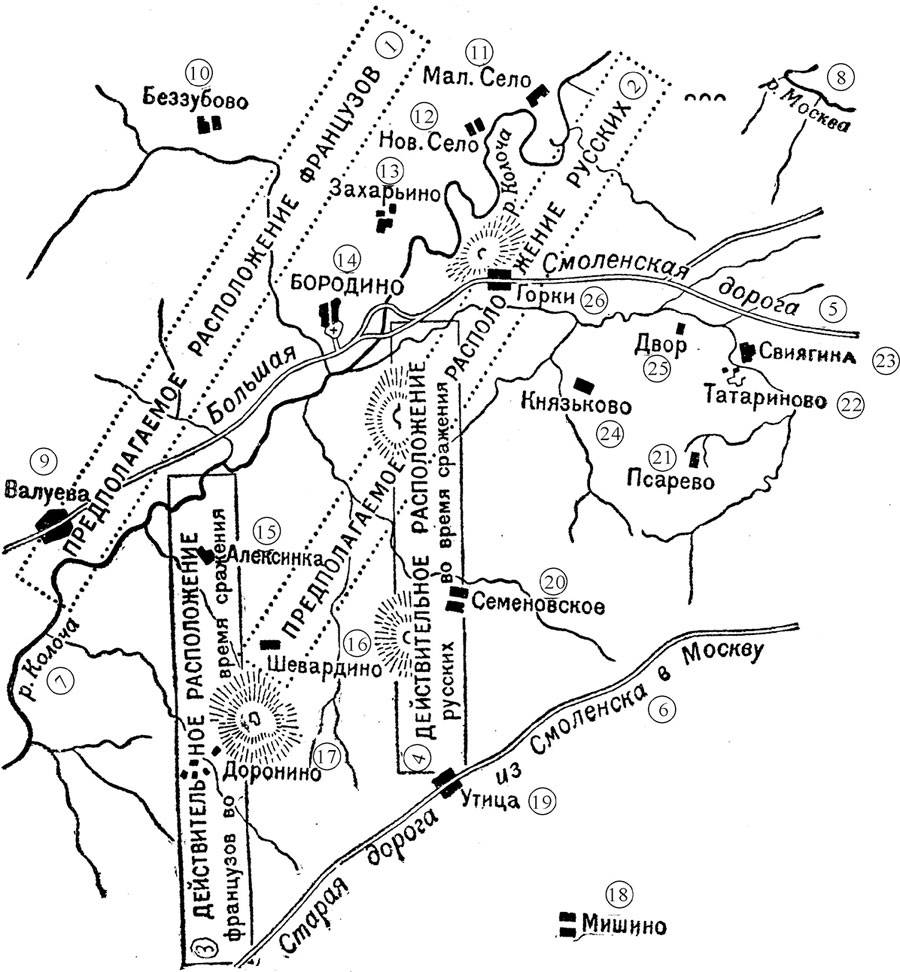
\includegraphics[scale=0.4]{picture/战争与和平1.jpeg}
    \refdocument{\small
        1. 设想中的法军阵地 
        2. 设想中的俄军阵地 
        3. 会战时法军实际阵地 
        4. 会战时俄军实际阵地 
        5. 斯摩棱斯克大道 
        6. 古斯摩棱斯克大道 
        7. 科洛恰河 
        8. 莫斯科河 
        9. 瓦卢耶沃 
        10. 别祖博沃 
        11. 小村 
        12. 新村 
        13. 扎哈里诺 
        14. 波罗金诺 
        15. 阿列克辛卡 
        16. 舍瓦尔金诺 
        17. 多罗尼诺 
        18. 米希诺 
        19. 乌季察 
        20. 谢苗诺夫斯科耶 
        21. 普萨列沃 
        22. 塔塔里诺沃 
        23. 斯维亚吉纳 
        24. 克尼亚兹科沃 
        25. 德沃尔 
        26. 戈尔基
    }
\end{figure}

\par 如果二十四日傍晚拿破仑没有前出至科洛恰河,也没有立刻下令在当晚进攻多面堡,而是在第二天早晨发起攻击,那么谁也不会怀疑,舍瓦尔金诺多面堡是我军阵地的左翼;会战就会像我们所预期的那样发生。在这种情况下,我们想必会更顽强地防守我们的左翼舍瓦尔金诺多面堡;我们会从中央或右翼进攻拿破仑,那么就会在预先选定并筑有坚固工事的阵地上进行一场大决战。但是因为对我军左翼的攻击发生在我军后卫部队撤退的当晚,即紧随格里德涅瓦战役之后就发动了攻击,也因为俄国军事将领不愿或来不及在二十四日当晚投入大决战,所以我们输掉了波罗金诺会战的第一个也是主要的一个战役,显然,这也就导致了二十六日的败绩。
\par 二十五日清晨舍瓦尔金诺多面堡失守之后,我们的左翼没有阵地了,于是被迫将左翼后撤,并急忙就地构筑左翼的防御工事。
\par 八月二十六日俄军只能据守尚未完工的薄弱的防御工事,不仅如此,这种不利局面还由于下述原因而加剧,俄国将领不承认既成事实(左翼阵地丢失,未来的整个战场已由右向左转移),仍然停留在由新村至乌季察的漫长阵地上,因而不得不在作战时才把自己的部队从右往左调动。在这种情况下,在整个会战期间,面对进攻我军左翼的全部法军,我军应战的兵力只及敌人的一半。(波尼亚托夫斯基进攻乌季察和乌瓦罗夫在右翼进攻法国人的战斗是与战局的发展无关的孤立行动。\footnote{军事史家认为,拿破仑的盟友波兰人波尼亚托夫斯基(1763—1813)将军所指挥的一个波兰军和乌瓦罗夫将军的骑兵军的参战,和整个战局的发展是有联系的。波尼亚托夫斯基曾短暂地占据乌季察,乌瓦罗夫和普拉东的几个团曾攻击法军左翼。})
\par 总之,波罗金诺会战完全不是像人们所描述的那样(他们在竭力掩饰我军将领的错误,并因而贬低我国军民的光荣业绩)发生的。波罗金诺会战并非在选定并加固的阵地上、在俄方兵力仅相对薄弱的情况下打的;在波罗金诺会战中,俄军在舍瓦尔金诺多面堡失守后,不得不在几乎没有防御工事的开阔地上迎击两倍于己的法军,也就是说,在这种条件下,不仅连续作战十小时相持不下是不可思议的,甚至坚持三小时而不致全军溃败也令人难以想象。
\paragraph*{二十}
\par 二十五日早晨,皮埃尔离开了莫扎伊斯克。皮埃尔出城时在大山的陡峭而崎岖的坡道上、在右边山顶的一座正在祈祷、鸣钟的教堂附近下车步行。跟在他后面的是以一队歌手为前导的骑兵团。载着昨天负伤的兵员的一列大车迎着他上山来。赶车的农民在两边跑来跑去,一边吆喝着鞭打马匹。每辆大车上都有三四个伤兵躺着或坐着。这些大车在陡坡的乱石路上颠簸。伤兵们苍白的脸上皱眉蹙额、紧抿双唇,牢牢地抓住栏杆,在大车上彼此碰撞着、震荡着。他们几乎人人都带着孩子般天真的好奇望着皮埃尔的白色礼帽和绿色常礼服。
\par 皮埃尔的车夫生气地大声嚷嚷,叫伤兵车队靠边走。唱着歌下山的骑兵团渐渐逼近皮埃尔的轻便马车,把路给堵住了。皮埃尔停下来,紧靠在山路边上。被山坡挡着的太阳照不到低洼处的路上,这里又冷又潮湿;在皮埃尔的头顶上是八月明媚的阳光,教堂的钟声欢快地四处飘荡。一辆运伤兵的马车停在皮埃尔附近的路边上。车夫穿一双树皮鞋气喘吁吁地跑到马车旁边,在没有轮箍的后轮下塞了石头,开始为自己的站在那里的小马整理后鞧。
\par 一位负伤的老兵有一条手臂包扎着,他跟在一辆大车后面走,没负伤的手抓着大车。
\par “怎么,老乡,把我们就丢在这里了,是吗?还是要把我们带到莫斯科去?”他说。
\par 皮埃尔只顾想心事,没有听见他的问题。他有时看看现在已和伤兵车队相遇的骑兵团,有时看看身旁的大车,大车上有三个伤兵,两个坐着,一个躺着,他觉得他所关心的问题的答案就在这里、就在他们身上。一个坐着的士兵想必是伤在脸上。他的头全都裹着纱布,半边脸肿得有婴儿的脑袋大。他的嘴和鼻子都歪在一边。这个士兵眼望教堂画着十字。另一个还是个小男孩,是新兵,浅色头发,肤色白皙,秀气的脸上好像没有一丝血色,他带着和善的、仿佛凝固的微笑望着皮埃尔;第三个俯卧在那里,看不到他的脸。骑兵的一队歌手正紧贴着大车走过去。
\par “远走他乡了……那个刺儿头……”
\par “在陌生的异乡漂泊……”他们声情并茂地唱着一首士兵舞曲。那高山上全部敲响的嘹亮的钟鸣仿佛在呼应着这舞曲,却另有一番欢乐的韵致。太阳灼热的光辉洒遍了对面山坡的顶部,更是另有一番欢乐的气象。但是在山坡下,在伤兵的大车旁,在皮埃尔所站的那匹气喘吁吁的小马附近,却是潮湿、阴暗而凄迷。
\par 面颊肿大的士兵望着骑兵的那一队歌手。
\par “唉,这些花花公子!”他责备说。
\par “现在别说当兵的,连农民也能看得到!把农民也赶来了,”一个站在大车旁的士兵带着凄然的微笑对皮埃尔说,“现在不分兵民了……这就是要全体民众一齐上,一句话——我们的背后是莫斯科。现在是要拼到底了。”尽管这个士兵的话不是讲得很清楚,皮埃尔还是听懂了他的意思,便赞同地点了点头。
\par 路通了,皮埃尔下山后继续骑马赶路。
\par 皮埃尔骑在马上张望着大路两边,希望能遇到熟人,可是到处只看到各兵种的陌生军人,他们都同样惊讶地看着他的白色礼帽和绿色常礼服。
\par 走了大约四俄里,他才遇到了第一个熟人,便高兴地同他打招呼。这个熟人是军队里的一位主任医生。他乘着轻便马车和皮埃尔迎面相逢,他和一个年轻医生坐在一起,认出皮埃尔便叫充当车夫的哥萨克停车。
\par “伯爵!伯爵大人,您怎么在这里?”医生问。
\par “就是想来看看……”
\par “是的,是的,值得一看……”
\par 皮埃尔下马,站在那里与医生攀谈,对他说明自己想参战的想法。
\par 医生建议皮埃尔直接去找殿下。
\par “您何必在这兵荒马乱的时候到处乱跑呢,”他和自己的年轻同伴递着眼色说,“殿下毕竟是了解您的,一定会亲切地接待您。就这么办吧,老兄。”医生说。
\par 医生显得疲惫而匆忙。
\par “您这样想吗……我还想问问您,阵地在哪里?”皮埃尔说。
\par “阵地?”医生说。“这我就不知道了。您到塔塔里诺沃去吧,那里有很多人在挖土。您可以到土冈上去:从那里就能看得一清二楚了。”医生说。
\par “从那里能看到吗?……要是您……”
\par 不过医生打断了他的话,朝自己的马车走去。
\par “我是愿意送您去的,真的,这是实话,可是我(他做了个万分紧急的手势)正赶着要去见军长。我们的情况怎么样啊?……您知道吗,伯爵,明天有一场硬仗:十万人之中少说也会有两万伤员;而我们的担架、病床、医士和医生连六千伤员也应接不暇。一万辆大车倒是有,可是还得有别的东西才行啊;就只能看着办了。”
\par 一个奇怪的想法使皮埃尔大吃一惊,就在那成千上万活生生的、健康的、愉快而惊讶地看着他的帽子的年轻和年老的人们之中,大概有两万人注定会负伤或阵亡(也许就是他见到过的那些人)。
\par “他们也许明天就要死了,他们怎么还能想那些与死亡无关的事呢?”由于某种神秘的精神联系,他突然活灵活现地想起了莫扎伊斯克山的坡道、运伤兵的大车,还有那夕阳斜照和骑兵的歌声。
\par “骑兵奔赴战场,却遇上了伤兵,他们一点也不考虑前途险恶,走过时还对伤兵们使眼色打趣。所有这些人之中有两万人难免一死,而他们却对我的帽子感到惊讶!奇怪呀!”皮埃尔想,继续朝塔塔里诺沃前进。
\par 大道左侧一个地主宅院附近有几辆马车、带篷大车、一群勤务兵和几个哨兵。殿下就在这里。可是等皮埃尔到了那里,他已经走了,司令部的人几乎全都走了。大家都在做礼拜。皮埃尔再往前到戈尔基去。
\par 皮埃尔上了坡道,进入一个乡村的小街,第一次看到了帽子上插着十字架、身穿白衬衣的农民民兵,他们大声说笑,兴奋而汗水淋漓地在大道右侧的一个长满野草的大土冈子上面干着活儿。
\par 他们有些人在用铁锹挖土,有些人用手推车在木板上运土,还有些人站在那里什么也不干。
\par 两个军官站在土冈上指挥他们。看到这些刚当上民兵显然还充满新奇感的农民,皮埃尔又想起了莫扎伊斯克的伤兵,这才明白了那位士兵所说的“\CJKunderdot{这就是要全体民众一齐上}”究竟是什么意思。这些在战场上干活的留着大胡子的农民的样子,他们那古怪、笨拙的靴子,那汗水淋漓的脖子,以及有些人解开衬衣的斜襟而露出的黝黑的锁骨,比他迄今的所有见闻都更强烈地影响了他,使皮埃尔深切地意识到了此刻的庄严和重要性。
\paragraph*{二十一}
\par 皮埃尔下了马车,走过那些干活的民兵,登上了土冈,医生对他说过,在那个土冈上整个战场即可一览无遗。
\par 这大约是上午十一点钟。太阳在皮埃尔的身后偏左,透过纯净稀薄的空气把大地呈半圆形而又逐层升高地展现在他面前,将这幅环形全景图照耀得熠熠生辉。
\par 斯摩棱斯克大道切入这半圆形,蜿蜒曲折地向左上方延伸,大道穿过位于土冈前方五百步、比土冈低的一个有白色教堂的村庄(那是波罗金诺村)。大道在村子下方通过一座桥,又经过几次下坡和上坡蜿蜒而上,通往约六俄里外的瓦卢耶沃村(现在拿破仑的行营设在那里)。在瓦卢耶沃那边,大道隐没于地平线上的一片泛黄的树林。在这座兼有桦树和枞树的树林里,在大道之右,在阳光下闪烁的科洛恰修道院的十字架和钟楼遥遥在望。沿着那蓝色的远方,在树林和大道的左右两边,处处可见烟雾迷蒙的篝火以及我军和敌军数量不等的部队。右面,科洛恰河和莫斯科河流经的地方多为山地和峡谷。远处,在那些峡谷之间,别祖博沃村和扎哈里诺村隐约可见。左面的地方比较平坦,有庄稼尚未收割的田野,可以看到一个被焚毁的村子在冒烟,那是谢苗诺夫斯科耶村。
\par 皮埃尔在右面和左面所看到的一切都那么难以捉摸,无论平原的左面还是右面都不能充分满足他的想象。到处都不是他希望看到的战场,而是田野、林间空地、军队、树林、篝火的烟、村庄、土冈、小河;不论皮埃尔怎样细心观察,他也不能在这片生气勃勃的大地上找到阵地,甚至不能区分我军和敌军。
\par “要问内行才行。”皮埃尔想,便转向一个军官,他正在好奇地打量着皮埃尔的身穿便服的胖大身躯。
\par “请问,”皮埃尔向军官问道,“前面那个村庄叫什么名字?”
\par “是叫布尔金诺吧?”军官说,他在问自己的一个同伴。
\par “是波罗金诺。”另一个纠正道。
\par 军官看来很高兴有机会说说话,便迎着皮埃尔走了过去。
\par “是我们的人在那里吗?”皮埃尔问。
\par “对,再过去一点就是法国人了,”军官说,“瞧,那就是他们,能看得见了。”
\par “哪里?哪里?”皮埃尔问。
\par “肉眼也看得见。看哪,那就是!”军官指着河对岸左面的烟雾说,这时他的脸上出现了凝重而严肃的表情,皮埃尔在他遇到的很多人的脸上都看到过这样的表情。
\par “啊,这是法国人!那里的呢?……”皮埃尔指了指左面的土冈,土冈附近出现了部队。
\par “那是我们的人。”
\par “啊,我们的人!那里的呢?……”皮埃尔指着远处的有一棵大树的另一个土冈,土冈旁就是峡谷里的一个村庄,村庄那里也有篝火的烟雾和一些发黑的东西。
\par “这又是\CJKunderdot{他}了,”军官说。(那是舍瓦尔金诺多面堡。)“昨天是我们的,现在是\CJKunderdot{他}的了。”
\par “那么我们的阵地呢?”
\par “阵地?”军官高兴地笑着说,“我可以清楚地告诉您,因为我方的几乎所有工事都是我建造的。您瞧,我们的中央在波罗金诺,就在那里。”他指了指前面那个有白色教堂的村子。“这里是科洛恰河的渡口。这里,看见吗,低洼处还堆放着一排排割下的干草,这里就是大桥。这是我们的中央。我们的右翼是在那里(他陡地指向右边一个遥远的峡谷),那里就是莫斯科河,我们在那里建造了三座火力很强的多面堡。左翼……”这时军官住口了。“知道吗,这很难给您讲清楚……昨天我们的左翼是在那里,在舍瓦尔金诺,瞧,就是有一棵橡树的那个地方;而现在我们的左翼撤到后面来了,现在您看,您看——看见吗,那个村子和烟?那是谢苗诺夫斯科耶,瞧,左翼就在这里,”他指着拉耶夫斯基土冈说,“不过未必会真的在这里打。他把部队调到这里来,是在使诈;他想必是要从莫斯科河右面包抄过来。哎,不管在哪里打,明天有很多人是回不来了!”军官说。
\par 在军官说话时,一个老士官走到他跟前,默默地等自己的长官把话说完;可是听到这里,他显然对军官的话不大满意,于是打断了他的话头。
\par “该去拿些土筐了。”他严肃地说。
\par 军官好像发窘了,他好像明白了,明天有很多人回不来这件事心里想想是可以的,但不该说出来。
\par “好,再把三连派去吧。”军官急忙说道。
\par “您是什么人,是医生吧?”
\par “不,我来随便看看。”皮埃尔回答说。于是皮埃尔又经过民兵身边往山下走了。
\par “啊,这些该死的!”跟在他后面的军官说道,捂着鼻子从干活的民兵们旁边跑过。
\par “他们来了!……抬着来了……那就是他们……马上就到……”突然响起了一阵嘈杂声,军官、士兵和民兵们都从路上拥了过去。
\par 东正教的庄严的游行队伍正从山脚下的波罗金诺上山来。在尘土飞扬的路上,摘下高筒帽、倒背长枪的步兵整齐地走在最前面。步兵后面是唱诗班的一片合唱声。
\par 士兵和民兵都光着脑袋赶到皮埃尔前头,迎着游行队伍跑去。
\par “抬着圣母来了!我们的保护神!……伊韦尔圣母!……”
\par “是斯摩棱斯克圣母。”另一个人纠正道。
\par 民兵们,无论村子里的还是在炮垒上干活的,全都把铁锹一扔,跑去迎接教会的游行队伍。在尘土飞扬的路上行进的是一个步兵营,跟在他们后面的是那些身穿法衣的司祭,一个头戴法冠的老者带领着全体教士和唱诗班。其后是官兵们抬着身披金属衣饰、面容呈黑色的巨幅圣母像。这幅圣母像是从斯摩棱斯克带出来的,此后即随着军队辗转各地。圣像的前后左右,到处是成群的光着脑袋的军人在走动、奔跑、叩头。
\par 到了山上,圣像停了下来;用毛巾托着圣像的人们换了班,教会执事重新点燃手提香炉,祈祷仪式开始了。炎热的阳光垂直地照射着;微微的清风吹拂着光头上的头发和点缀圣像的飘带;唱诗班的合唱声在野外轻柔地荡漾。一大群官兵和民兵环绕在圣像四周。在司祭和教会执事后面的一块腾空的地方站着几位要人。一位已谢顶的脖子上挂着圣乔治勋章的将军就站在一个教士的背后,他没有画十字(想必是德国人),耐心地等候祈祷结束,他认为有必要听完祈祷,也许是为了激发俄国人的爱国热情吧。另一位将军姿态威武,一只手在胸前不时地轻轻挥动,环顾着四周。站在一群农民中的皮埃尔,在这些要人中认出了几个熟人;但他不看他们,因为他正全神贯注于这群士兵和民兵的严肃的表情,他们都同样聚精会神地望着圣像。倦怠的教会执事们(他们已在吟诵第二十篇祷文了)开始懒散而习惯性地吟诵:“圣母,从灾难中拯救你的仆人吧,”司祭和助祭应声道:“上帝,我们祈求你的保佑,你的庇护是我们坚不可摧的屏障”——所有人的脸上又突然焕发出了同样的神采,意识到庄严的时刻即将来临,这神采他曾在莫扎伊斯克的山脚下见到,也间或在他今天上午所遇到的许许多多人的脸上见到过;这时只见人们频频俯首,头发随之飘舞,叹息声和十字架在胸前的碰击声不绝于耳。
\par 圣像周围的人群突然散开,挤到了皮埃尔身上。一个人正向圣像走来,从人们在他面前匆忙闪开的情形来看,想必是一位非常重要的人物。
\par 那是巡视阵地的库图佐夫。他在回塔塔里诺沃途中顺路来到了祈祷的地方。皮埃尔根据他那与众不同的特别的体型立刻认出了他就是库图佐夫。
\par 库图佐夫硕大的身躯套着一件长长的常礼服,背微驼,敞着白发苍苍的头,虚胖的脸上露出一只白色的眼球,他迈着起伏摇摆的步态走进了圈子里,站在一个教士身后。他以习惯的动作画了十字,以手触地,沉重地喘了口气,垂下了白发苍苍的头颅。库图佐夫身后站着本尼格森和随从。尽管总司令亲临,吸引了所有高官显贵的注意,民兵和士兵们仍目不斜视地继续祈祷。
\par 祈祷结束后,库图佐夫走到圣像前,沉重地跪地叩首,他想站起来了,却由于身体沉重、虚弱,好久也站不起来。他那白发苍苍的头颅因为吃力而微微扭动。他终于站起来了,孩子般天真地撅着嘴唇亲吻圣像,又以手触地深深地鞠躬。将军们都仿效他的榜样;然后军官以及他们身后的士兵和民兵们也都彼此拥挤着,脚步杂沓、喘着粗气互相碰撞着,神情激动地照着样儿做了起来。
\paragraph*{二十二}
\par 被挤得摇摇晃晃的皮埃尔在四处张望。
\par “伯爵,彼得·基里雷奇!您怎么在这里?”有人说。皮埃尔回头看了看。
\par 鲍里斯·德鲁别茨科伊用手掸了掸弄脏了的膝盖(大概也是在亲吻圣像时弄脏的),微笑着向皮埃尔走了过来。鲍里斯衣着优雅,带有几分英武的军人气概。他穿着长长的常礼服,肩上挂着鞭子,和库图佐夫一模一样。
\par 库图佐夫这时已来到村子里,坐在近处一栋房子的阴影里的一条长凳上,这条长凳是一名哥萨克跑着给他搬来的,另一名哥萨克又连忙铺上了毯子。一大群衣着考究的随从围绕着总司令。
\par 圣像在人群的簇拥下起动了。皮埃尔站在离开库图佐夫大约三十步的地方与鲍里斯谈话。
\par 皮埃尔说明了自己想参战和考察阵地的意图。
\par “您就这么办吧,”鲍里斯说。“我请您参观军营,本尼格森伯爵会在那里,您可以从那里把一切看得更清楚。我就是在他身边供职。我去向他报告您的情况。如果您想在阵地上到处走走,那就和我们一起去:我们马上就要到左翼去了。然后我们回来,我请您赏光在我那里过夜,咱们凑一个牌局。您不是认识德米特里·谢尔盖伊奇吗?他的驻地就在这里。”他指了指戈尔基的第三栋房子。
\par “不过我想看看右翼;听说右翼是很强的,”皮埃尔说,“我想骑马看看从莫斯科河起的全部阵地。”
\par “嗳,您以后还可以去看嘛,目前主要的是左翼……”
\par “是的,是的。鲍尔康斯基公爵的团在哪里,您能指给我看吗?”皮埃尔问道。
\par “安德烈·尼古拉耶维奇?我们正好要路过,我送您去见他。”
\par “左翼怎么样呢?”皮埃尔问。
\par “实话相告,只能在我们之间说说,我们左翼的情况如何只有天知道,”鲍里斯信赖地压低嗓音说,“本尼格森的设想完全不同。他的设想是加强那个土冈的防御,而不是像现在这样……可是,”鲍里斯耸了耸肩。“殿下不愿意,或许是听了别人的什么闲言碎语。要知道……”鲍里斯没有把话说完,因为这时库图佐夫的副官凯萨罗夫\footnote{派西·谢尔盖耶维奇·凯萨罗夫(1783—1844),1812年战争期间以上校军衔任第一和第二军军团的值班将军。}来找皮埃尔了。“啊!派西·谢尔盖耶维奇,”鲍里斯很自然地微笑着对凯萨罗夫说道,“我在向伯爵说明阵地的情况。真令人惊讶,殿下竟能如此准确地料定法国人的意图!”
\par “你们在谈左翼?”凯萨罗夫说。
\par “是呀,是呀,就是。我们的左翼现在是非常、非常强的。”
\par 尽管库图佐夫赶走了参谋部的所有冗员,但是鲍里斯在库图佐夫几经撤换之后仍能留在司令部。鲍里斯被安插在本尼格森伯爵身边。本尼格森伯爵和鲍里斯以往的上司一样,认为年轻的德鲁别茨科伊是一个不可多得的人才。
\par 在统领军队方面有截然不同的两派:库图佐夫派和参谋长本尼格森派。鲍里斯属于后一派。没有人能比他更善于在向库图佐夫表示卑躬屈节的敬意的同时,向人们暗示老头子不行,所有的事情都是本尼格森在领导。现在到了进行会战的决定性时刻,这个时候应当或者除掉库图佐夫而把指挥权交给本尼格森,或者即使库图佐夫打赢了会战,也要让人们意识到全部功劳都是本尼格森的。总之,明日一战,必将有人因功受奖,一批新人会脱颖而出。因此这一天鲍里斯整天都处于极度兴奋的期待之中。
\par 在凯萨罗夫之后,又有其他一些熟人来找皮埃尔,因而他来不及回答人们纷纷提出的有关莫斯科的问题,也来不及听完他们所讲述的新闻。所有人的脸上都流露出兴奋和不安。但是皮埃尔觉得,其中某些人之所以神情激动,主要是由于个人的得失问题,而他心中忘不了的是另一种神情,它涉及的不是个人问题,而是整体的生死存亡问题。库图佐夫注意到了皮埃尔和围在他身边的人们。
\par “您去把他叫来。”库图佐夫说。副官转达了殿下的意愿,于是皮埃尔朝长凳走了过去。不过在他之前一个普通的民兵走到了库图佐夫面前。那是多洛霍夫。
\par “这个人怎么在这里?”皮埃尔问。
\par “这个鬼东西哪里都敢闯!”有人回答道,“他是受过降职处分的。现在很想能出人头地。他提交过一些行动计划,还在夜里摸进了敌人的散兵线……不过是个好样的!……”
\par 皮埃尔在库图佐夫面前恭敬地脱帽、鞠躬。
\par “我敢肯定,要是我向殿下提出报告,您会把我赶走,或者您会说,您知道我要报告什么,即使如此,对我也没有什么坏处……”多洛霍夫说。
\par “不错,不错。”
\par “不过,要是我说对了,我就能给祖国带来利益,我甘愿为祖国效死。”
\par “不错……不错……”
\par “如果殿下需要一个置生死于度外的人,那就请您想到我吧……也许我能对殿下有用。”
\par “不错……不错……”库图佐夫反复说道,他眯细了那只含有笑意的眼睛看着皮埃尔。
\par 这时鲍里斯机敏地上前与皮埃尔并肩站在靠近首长的地方,神态极其自然,仿佛在接着刚才的话头似的对皮埃尔低声说道:
\par “民兵们干脆穿上干净的白衬衣,做好了牺牲的准备。这就是英雄主义啊,伯爵!”
\par 鲍里斯对皮埃尔这样说,显然是要让殿下听见。他知道,这些话一定会引起殿下的注意,果然,殿下对他说话了:
\par “你说民兵怎么了?”他问鲍里斯。
\par “殿下,他们为了明天决一死战而穿上了白衬衣。”
\par “啊!英勇卓绝、无与伦比的人民!”库图佐夫闭上眼睛摇着头说,“无与伦比的人民!”库图佐夫又一次感叹道。
\par “您想闻闻火药的气味吗?”他问皮埃尔,“是的,一种很好闻的气味。我有幸是您夫人的崇拜者。她身体好吗?我的住处可以供您使用。”接着像老年人常有的那样,库图佐夫开始茫然四顾,仿佛完全忘了他要说什么或做什么了。
\par 显然,他忆起了他想要了解的什么,便招招手,把自己副官的弟弟安德烈·谢尔盖耶维奇·凯萨罗夫\footnote{安德烈·谢尔盖耶维奇·凯萨罗夫(1782—1813),政论家、作家和语文学家。战争期间曾出版《俄罗斯人报》,广泛宣传库图佐夫的活动。}叫到身边。
\par “是什么呢,是什么呢,马林\footnote{马林是宫廷诗人和亚历山大一世的侍从武官。库图佐夫回忆他献给格拉科夫的诙谐诗。格拉科夫是陆军士官武备学校的历史教员,著述颇丰而缺少才华。库图佐夫曾任该校校长,两人相识。诗中写道:“你会,你会,作家,/你会一辈子都写些废话;/要是继续在军校执教,/到头来会当上个上校。”据说,托尔斯泰用这首诙谐诗主要是暗示自己对亚历山大一世的看法。}的诗说什么来着?那首诗是怎么说的,怎么说的呀?他写到格拉科夫:‘要是继续在军校中执教……’你说,你说呀。”库图佐夫说道,看来他就要笑了。凯萨罗夫朗读了那首诗……库图佐夫微笑着,随着诗的节拍点着头。
\par 皮埃尔从库图佐夫身边走开后,多洛霍夫来到他面前,握住了他的手。
\par “很高兴在这里见到您,伯爵,”他毫不在意有旁人在场,异常果断而郑重地大声说道,“天知道明天我们之中谁还能活下来,我很高兴有机会在此时告诉您,我为我们之间曾经有过的误会感到遗憾,但愿您不计前嫌。我请求您宽恕我。”
\par 皮埃尔面带微笑注视着他,不知对他说什么好。多洛霍夫含着涌上来的泪水,拥抱并亲吻了皮埃尔。
\par 鲍里斯对自己的将军说了什么,于是本尼格森伯爵转向皮埃尔,建议他和自己巡视前线。
\par “您会感兴趣的。”他说。
\par “是的,很有意思。”皮埃尔说。
\par 半小时后,库图佐夫到塔塔里诺沃去了,本尼格森带着随从去前线巡视,皮埃尔也在他的随从之中。
\paragraph*{二十三}
\par 本尼格森从戈尔基沿着大路往下走,到了桥边,一个军官曾在土冈上指着这座桥对皮埃尔说,它是我军阵地的中央,桥边岸上放着一排排割下来的发出干草气味的青草。他们过桥到达波罗金诺村,从那里向左拐,经过大批部队和炮群来到一个高大的土冈,民兵们在土冈上挖土。这是一座还没有名称的多面堡,后来被称为拉耶夫斯基多面堡或土冈炮台。
\par 皮埃尔没有特别注意这个多面堡。他不知道,这个地方将比波罗金诺战场上的任何地方都更使他难以忘怀。然后他们穿过一个峡谷前往谢苗诺夫斯科耶,士兵们正在这里拆走农舍和谷物烘干房的最后一批木料。然后他们下坡再上坡,往前经过一片仿佛被冰雹砸毁的黑麦地,沿着炮兵部队在坑坑洼洼的耕地上新踩出的道路到达尖顶堡,它也是还在构筑之中。
\par 本尼格森勒马站在尖顶堡上望着前方的(昨天还是我们的)舍瓦尔金诺多面堡,可以看到堡上有几个骑手。军官们说,拿破仑或缪拉在那里。人人都聚精会神地望着那几个骑手。皮埃尔也朝那里望着,竭力猜测,那隐约可见的几个人之中谁是拿破仑。最后骑手们下了土冈,消失不见了。
\par 本尼格森开始对向他走过来的一位将军说明我军的整个态势。皮埃尔听着本尼格森的话,集中自己的全部智力,想了解未来会战的实况,可是他懊丧地感到,自己智能有限而不能如愿。他感到茫然不解。本尼格森住口不说了,他注意到正在倾听的皮埃尔,突然向他问道:
\par “我想,您不感兴趣吧?”
\par “啊,相反,很有意思。”皮埃尔有些言不由衷地重复了一遍。
\par 他们从尖顶堡再向左转,沿着在浓密、低矮的桦树林中蜿蜒而过的小道前进。在树林中间,一只四腿雪白的褐色野兔跳到他们面前的路上,受惊于众多马匹的蹄声,这只惊慌失措的野兔在他们面前的路上向前跳了好久,引起了大家的注意和一阵哄笑声,只是在几个人向它吆喝之后,它才急忙逃往一边,在密林中消失了。他们在树林里又走了两俄里,来到林中的一片空地,图奇科夫一个军的部队在这里驻守左翼。
\par 在左翼的尽头,本尼格森大发议论并且作出了皮埃尔觉得非常重要的军事部署。图奇科夫部队的驻地前方是一片高地。这片高地上没有派驻部队。本尼格森大声抨击这个错误,他说,不占据制高点而把部队置于高地下面是荒唐的。有些将军也表达了同样的看法。一位将军以军人的非常激烈的语气说,这是让部队坐以待毙。本尼格森以自己的名义命令把部队调到了高地上。
\par 在左翼发出的这个命令使皮埃尔更加怀疑自己对军事的理解能力了。听了本尼格森和将军们对于把部队部署在山脚下的谴责,皮埃尔完全理解他们的意见,同意他们的看法;然而正因如此,他不能理解,那个把部队部署在山脚下的人怎么会犯下如此显而易见的重大错误。
\par 皮埃尔不知道,这支部队并不是为防守阵地而部署的,像本尼格森所以为的那样,而是布置在暗处作为伏兵,也就是说,为了不让敌人发觉而对行进中的敌军发起突然袭击。本尼格森不了解这一点,他根据自己的想法把部队调往前方,却没有把这一点告知总司令。
\paragraph*{二十四}
\par 安德烈公爵在二十五日的这个晴朗的八月的夜晚支着臂肘躺在克尼亚兹科沃村的一个遭到破坏的仓房里,位于本团驻地的边上。他从破墙的豁口望着沿围墙一带有三十年树龄的桦树,桦树下部的枝条都被砍光了;望着耕地上那些散乱的燕麦垛和灌木丛,那一带冒着缕缕炊烟,那是士兵行军灶的所在地。
\par 无论安德烈公爵现在觉得他的生活多么艰难,多么于人无益,多么难以忍受,他还是像七年前在奥斯特利茨会战前夕那样感到激动而愤怒。
\par 关于明天会战的命令已经发布,他也接到了这个命令。此刻他已无事可做。但是一些最简单、最明确,因而也是最可怕的思绪不让他有片刻的安宁。他知道,明日之战将是他所参与过的所有战争中最可怕的一次,生平第一次感到了死亡的可能,这种可能性与多事的人生无关,也不涉及对别人的影响,这种只涉及他自己,只涉及他的内心感受的死亡的可能性鲜明地、几乎确定无疑地、可怕地赫然浮现在他的想象之中。站在这个想象的高度,过去使他苦恼和关心的一切突然被冷冷的白光所照耀,没有阴影、没有前景、没有轮廓的差异。他曾把全部生活想象成一盏幻灯,在人为的照明下久久地透过玻璃注视着它,现在他陡然在白昼的亮光下,没有玻璃的折射,看清了那些涂抹得很拙劣的画面。“是的,是的,这就是那些曾经使我激动、神往和痛苦的虚假的形象,”他对自己这样说,一面在想象中逐一回忆着自己生活的幻灯中的主要画面,现在是在白昼冷冷的白光——明确的死的观念——中审视着它们。“这就是那些涂抹得很拙劣的形象,它们曾被想象为美好而神秘的东西。荣誉、社会福祉、对女性的爱以及祖国本身——对我而言,这些画面曾显得多么伟大,充满了多么深刻的含意!这一切在这个早晨的冷冷的白光下是何等粗糙、苍白而拙劣,我觉得这个早晨的曙光是为我而升起的。”他生活中的三个大不幸特别引起他的注意:他对女性的爱、父亲的亡故和法国人占领半个俄国的入侵。“爱情!……这个少女,我觉得她洋溢着神秘的魅力。我是多么爱她啊!我拟定过有关爱情和幸福牵手的富于诗意的计划。啊,可爱的少年!”他悻悻地说出了声,“不言而喻!我曾相信一种理想的爱情,它能在我离开的整整一年里使她保持对我的忠诚。好像寓言中温柔的小鸽子,她应当因为与我离别而憔悴。而这一切却简单得多……这一切是太简单了,可恶至极!”
\par “父亲在童山也曾大兴土木,以为那是他的地方,他的土地,他的空气,他的农民;拿破仑一到,对他的存在一无所知,把他像路上的小木片一样一脚踢开,于是他的童山和他的全部生活都毁于一旦。而玛丽亚公爵小姐却说这是上天给予的考验。既然他已经不在了,而且不会再有这个人了,那么考验还有什么意义呢?永远不会再有他这个人了!他不在了!那么这是对谁的考验呢?祖国,莫斯科的毁灭!明天我会被打死——甚至不是被法国人而是被自己人打死,昨天就有一个士兵在我耳边擦枪走火,于是法国人来了,抓住我的双脚和脑袋丢到坑里,以免我在他们的鼻子底下发臭,于是形成新的生活条件,别人同样会习以为常,而我不会知道了,因为我不在了。”
\par 他看了看那一排桦树,它们那凝然不动的黄、绿、白色的树皮在阳光下闪烁。“死亡,明天我会被打死,我就不在了……眼前的一切都在,而我却不在了。”他鲜活地想象着没有自己的生活。于是这些桦树及其闪光和阴影、这朵朵白云、这缕缕炊烟——周围的一切对他来说都变了,变成一种可怕而有威胁性的东西。一阵寒气掠过他的脊背。他迅速起身,走出仓房,开始在户外踱步。
\par 仓房后面传来了人声。
\par “谁在那里?”安德烈公爵叫道。
\par 多洛霍夫从前的连长,现在因为部队缺少军官而当上了营长的红鼻子大尉季莫欣畏缩地走进了仓房。跟着进来的是副官和团部军需官。
\par 安德烈公爵连忙站起来,听了军官们按其职责要向他汇报的情况,又向他们发出一些指示,正准备让他们离开,这时仓房外响起了一个熟悉的声音。
\par “见鬼!”那个人被什么东西绊了一下说。
\par 安德烈公爵朝外面看了看,只见皮埃尔正向他走过来,他被地上的一根木头绊了绊,差点儿跌了一跤。安德烈公爵不愿见到自己圈子里的人,尤其是皮埃尔,皮埃尔会使他想起自己在最后一次莫斯科之行中的所有那些备受折磨的时刻。
\par “啊,是您!”他说,“什么风把您吹来了?真没想到。”在他这样说的时候,在他的眼里和整个面部的表情中有一种更甚于冷淡的东西——那是敌意,皮埃尔立刻就注意到了。他怀着极其兴奋的心情朝仓房走来,可是见到安德烈公爵的表情,他觉得拘谨而尴尬了。
\par “我来了……随便走走……您知道……我是来……我觉得很有意思,”皮埃尔说,这一天已经多少次无聊地重复了“很有意思”这个字眼。“我想亲眼看看战争。”
\par “是呀,是呀,共济会的弟兄们是怎样谈论战争的呢?该怎样预防战争呢?”安德烈公爵讥讽地说,“哎,莫斯科怎么样了?我的家人呢?他们到底到了莫斯科没有?”他严肃地问道。
\par “到了。朱丽·德鲁别茨卡娅对我说的。我去拜访他们,可是未能见到。他们已经到莫斯科近郊的庄园去了。”
\paragraph*{二十五}
\par 军官们想告辞了,不过安德烈公爵似乎不愿和自己的朋友单独相对,便挽留他们坐下喝茶。长凳和茶水端来了。军官们不免惊讶地望着身材肥硕的皮埃尔,听他讲述莫斯科的情况,以及他有幸巡视的部队的部署。安德烈公爵默然不语,面有愠色,所以皮埃尔主要不是对鲍尔康斯基,而是对和善的营长季莫欣说话。
\par “这么说,您已经了解了部队的整个部署?”安德烈公爵打断了他的话。
\par “是的,不过怎么说呢?”皮埃尔说,“我不是军人,我不敢说我已经有了充分的了解,但我对部队的部署大体上还是知道的。”
\par “那么您所知道的已经比任何人都多了。”安德烈公爵说。
\par “啊!”皮埃尔透过眼镜困惑地望着安德烈公爵说,“您说说,您对库图佐夫的任命有什么看法?”他说。
\par “我对这个任命感到非常高兴,我所知道的,仅此而已。”
\par “那么您告诉我,您对巴克莱·德·托利的看法如何?在莫斯科,天知道人们在怎样谈论他。”
\par “你问他们吧。”安德烈公爵指着军官们说。
\par 皮埃尔带着宽厚的微笑疑问地看了看季莫欣,因为大家都自然而然地把头转向了他,脸上都带着同样的表示疑问的微笑。
\par “大人,自从殿下就任以来,人们就看到了光明。”季莫欣有些胆怯地说道,不断地看看安德烈公爵的脸色。
\par “为什么这样说呢?”皮埃尔问。
\par “禀告大人,就拿木柴和饲料来说吧。我们是从斯文齐亚内撤退的,一路上不准动一根树枝或干草或别的什么。要知道,我们一走,全都留给\CJKunderdot{他}了,不是吗,大人?”他转向自己的公爵说道,“可就是不准。我们团有两位军官还为了这种事受到了军法审判。嘿,殿下就任以后,这个问题就好办了。大家看到了光明……”
\par “他为什么要禁止动用木柴和饲料呢?”
\par 季莫欣不好意思地看看大家,不知道该怎样回答这个问题。于是皮埃尔把这个问题向安德烈公爵提了出来。
\par “就为了我们丢给敌人的地方不致遭到破坏,”安德烈公爵气愤地嘲笑道。“这是很有道理的:不能允许掠夺地方,不能放纵部队趁火打劫。就是在斯摩棱斯克他的议论也是对的,他说法国人可能对我们实行迂回包抄,他们拥有更强大的兵力。然而他不能理解,”安德烈公爵仿佛脱口而出地尖声叫道,“然而他不能理解,我们是第一次在那里为俄罗斯的土地而战,我军士气之高昂是我从未见过的,我们连续两天击退了法军,而这个胜利使我军战斗力增强了十倍。他命令撤退。于是所有的努力和伤亡全都白费。他不是想背叛,他竭力要尽可能把事情做好,对一切都深思熟虑;可是正因如此,他是不中用的。他现在不中用,恰恰是因为他认真而细心地周密考虑所有的问题,正如任何一个德国人都会做的那样。怎么对你说呢……嗯,你的父亲有一个德国仆人,他是非常好的仆人,能比你更好地满足他的一切需求,那就让他效力吧。可是如果父亲病危,你就会赶走仆人,开始用自己生疏、笨拙的双手照料父亲,这比一个训练有素然而不相干的外人更能使父亲得到安慰。对巴克莱也是如此。当俄国健康的时候,外人是可以用的,而且他是个很不错的大臣。可是俄国一旦面临危险,那就需要自己人、亲人。你们在俱乐部里却异想天开,说他是叛徒!而诬陷他是叛徒,只能使人们后来因为错误地责难他而心怀愧疚,又把他从叛徒捧为英雄或天才,这就更加不对了。他是个忠实而且很正派的德国人……”
\par “不过人们说,他是高明的统帅。”皮埃尔说。
\par “我不懂高明的统帅是什么意思。”安德烈公爵嘲讽地说。
\par “高明的统帅,”皮埃尔说,“嗯,是这样的人,他能预见所有的偶然性……嗯,能料到敌人的意图。”
\par “这是不可能的。”安德烈公爵说,仿佛在谈一个早有定论的问题。
\par 皮埃尔惊讶地看了看他。
\par “不过,”他说,“人们都说,作战就像下棋。”
\par “是的,”安德烈公爵说,“不过有一个小小的差别,下棋时你可以对每一步棋详加斟酌,不受时间限制,还有一个差别,那就是马永远比小卒子强,两个小卒子总比一个小卒子强,而在战场上一个营有时比一个师还强,有时却不如一个连。没有人能够知道部队之间的力量对比。相信我的话吧,”他说,“要是问题取决于参谋部的军事部署,那么我就会留在那里研究军事部署,不,我有幸在这里工作,在团里和这些先生在一起,而且我认为,明天的战斗实际上将取决于我们而不是他们……胜败从来不取决于也不会取决于阵地、武器装备,甚至不取决于部队的数量;而阵地是最无关紧要的。”
\par “那取决于什么呢?”
\par “取决于心情,我的、他的,”他指了指季莫欣,“每个士兵的心情。”
\par 安德烈公爵望了望季莫欣,后者惊讶而困惑地看着自己的指挥官。现在安德烈公爵一反矜持、沉默的故态,显得异常激动。看来他忍不住要把蓦然出现在心里的想法痛快地说出来。
\par “赢得战役的是决心要打赢的人。为什么我们在奥斯特利茨战役中打败了?我们的伤亡几乎与法国人相等,但是我们很早就对自己说,我们打败了,于是真的败了。我们之所以会那样说,是因为我们没有必要在那里打仗:都想赶快离开战场。‘我们打败了——那就逃跑吧!’——我们就逃跑了。如果我们在傍晚前不说这句话,那么天知道会发生什么情况。而明天我们是不会这样说的。你说我们的阵地左翼弱,右翼拉得太长,”他接着说,“这都是废话,毫不相干。明天我们将面对的是什么局面呢?千百万各种各样的偶然性将在顷刻间决定于逃跑或准备逃跑的是他们还是我们,被打死的是这个人还是那个人;而现在所做的一切不过是儿戏而已。实质在于,今天和你巡视阵地的那些人,不仅无助于战局的演变,而且在起着干扰作用。他们关心的只是个人的渺小的得失。”
\par “在这样的时候?”
\par “在\CJKunderdot{这样的时候},”安德烈公爵重复道,“对他们来说,在这样的时候才正好可以吹毛求疵、暗算对手,为自己再谋得一枚十字勋章或一条绶带。我对明天的展望是这样:十万俄军和十万法军将迎头搏杀,毫无疑问,在二十万之众的这场搏杀中,谁在战斗中更勇猛,更忘我,谁就会获胜。我可以告诉你,无论如何,无论上层怎样搅局,我们一定能打赢明天的会战。明天,无论如何,我们一定能打赢这场会战!”
\par “对,大人,这才是真理,毫无疑问的真理,”季莫欣说,“现在谁还顾惜自己呢!您信吗,我营战士不喝酒了,他们说现在不是时候。”大家都默然不语。
\par 军官们站了起来。安德烈公爵和他们走到仓房外,向副官发出了最后一些指示。军官们走后,皮埃尔来到安德烈公爵面前,正想交谈,离仓房不远的路上响起了三匹马的马蹄声,安德烈公爵朝那个方向一望,认出了沃尔措根和克劳塞维茨\footnote{克劳塞维茨(1780—1831),德国军事理论家,普鲁士将军。1812年春离开普鲁士,加入俄军,先后担任帕伦和乌瓦罗夫的骑兵军军需官。著有《战争论》一书。},后面跟着一名哥萨克。他们在近处驰过,皮埃尔和安德烈无意中听到了以下的谈话:
\par “战争应当转移到广阔地带。对这个观点我十分赞赏。\footnote{原文为德文。}”一个说。
\par “是的,”另一个说,“既然目的在于削弱敌人,就不能考虑私人的损失。”\footnote{原文为德文。}
\par “就是嘛。\footnote{原文为德文。}”第一个人赞同地说。
\par “是呀,转移到广阔地带,\footnote{原文为德文。}”他们走后,安德烈公爵嗤之以鼻,气愤地重复道。“我的父亲、儿子和妹妹所在的童山就是在广阔地带\footnote{原文为德文。}。这对他来说是无所谓的。这就是我对你所说的——这些德国先生们不会赢得明天会战的胜利,只会尽其所能地起破坏作用,因为在他那德国人的脑袋里只有一文不值的议论,而在他们的心里没有明天所需要的唯一的东西——季莫欣的那种心情。他们把整个欧洲都交给了\CJKunderdot{他},还来教训我们——好出色的老师!”他又尖声叫道。
\par “那么您认为,能打赢明天的会战?”皮埃尔问。
\par “是的,是的,”安德烈公爵漫不经心地说,“我会做一件事情,如果我有权决定的话,”他又说道,“我就不留俘虏。什么是收容俘虏?这是骑士精神。法国人毁了我的家园,又要去毁灭莫斯科,每时每刻都在侮辱我。他们是我的敌人,我认为他们全都是罪犯。季莫欣和全军将士也都是这样想的。对他们必须处以死刑。既然他们是我的敌人,就不可能成为朋友,不管他们在蒂尔西特说得多么好听。”
\par “是的,是的,”皮埃尔双目炯炯地看着安德烈公爵说道,“我完全、完全同意您的看法!”
\par 皮埃尔觉得,从莫扎伊斯克山起整天困扰着他的那个问题完全清楚了,彻底解决了。他现在懂得了这场战争和即将进行的会战的全部意义和重要性。他在这一天所看到的一切,他匆匆瞥见的人们脸上那些凝重、严峻的表情都对他闪耀着新的光辉。他懂得了物理学上所谓的潜热(latente),他见到的所有那些人的心里都有一份爱国主义的潜热,它说明,为什么所有这些人都平静而似乎轻率地视死如归。
\par “不留俘虏,”安德烈公爵继续说道,“这一点会改变整个战争并减少战争的残酷性。否则我们就是在玩战争游戏——这是很恶劣的,我们故作仁慈,如此等等。这种故作仁慈和多愁善感,就像一个小姐的仁慈和多愁善感,她看见屠宰牛犊子就头晕;她十分善良,见不得流血,可是她津津有味地吃着蘸了调味汁的小牛肉。有的人对我们谈论战争法规、骑士精神、谈判、怜悯不幸者等等。全是废话。我在一八〇五年见识过骑士精神和谈判:尔虞我诈罢了。他们掠夺别人的家园,发行伪币,最坏的是他们杀我子女、父母,却说什么战争法规和对敌人的仁慈。不留俘虏,而是要杀人并拼命厮杀。谁像我一样经历了那么多痛苦,谁就会这样想……”
\par 安德烈公爵本来觉得,敌人是否会像占领斯摩棱斯克那样占领莫斯科是无所谓的,这时由于喉咙的一阵痉挛而住口不说了。他默默地来回踱步,而双眼好像发热病似的闪闪发光,在他又开始说话时,他的嘴唇也在颤抖。
\par “要是在战争中没有假慈悲,我们就只有在值得一战的时候才会像现在这样投入必死的战斗。那么就不会因为帕维尔·伊万内奇得罪了米哈伊尔·伊万内奇而发生战争。像现在这样的战争,那才叫战争。那时部队的士气就会和以往不同了。那时拿破仑统率下的所有这些威斯特伐利亚人和黑森人\footnote{1807年拿破仑在德国领土上建立威斯特伐利亚王国,其领土除了威斯特伐利亚本身,还包括黑森选侯区等地。拿破仑军队中有27000名威斯特伐利亚士兵。}就不会跟着他入侵俄国,我们也不会跑到奥地利和普鲁士去打仗,自己却不知道为何而战。战争不是亲善,而是人生最可恶的事情,必须明白这一点而不要玩弄战争。必须十分严肃地接受这种可怕的必然性。要点是:抛弃谎言,战争就是战争,不是儿戏。否则战争就成了游手好闲的浮浪子弟所喜爱的娱乐……军人阶层是最可敬的阶层。而什么是战争,为了取得战事的胜利需要什么,军人的风尚又是什么呢?战争的目的是杀人,战争的手段是间谍活动、叛变、策反、使居民倾家荡产、为了军队的给养而对他们实施掠夺和盗窃;是所谓军事计谋的欺诈和谎言;军人阶层的风尚是没有自由,即遵守纪律、游手好闲、愚昧无知、残酷无情、腐化堕落、好酒贪杯。尽管如此,这却是人人尊敬的最崇高的阶层。除了中国皇帝,所有的皇帝都身穿军服,谁杀的人多,他们就奖励谁……人们就像明天那样,会彼此逼近,相互残杀,使数以万计的军人阵亡、致残,然后就为了杀死许多人(还要夸大数字)而进行感恩祈祷,宣布胜利,认为杀人愈多功劳愈大。上帝在怎样看着他们、听着他们哪!”安德烈公爵声音尖厉地叫道,“唉,亲爱的,近来我活得太累。我发觉,我懂得的太多啦。人是不能从分辨善恶的树上采果子吃的\footnote{典出《旧约·创世记》第3章。}……好了,不会太久了!”他加了一句,“不过你要睡了,我也该睡了,你到戈尔基去吧。”安德烈公爵突然说道。
\par “噢,不!”皮埃尔吃惊而满怀同情地看着他说。
\par “去吧,去吧,大战之前要好好睡一觉,”安德烈公爵又说。他快步走过去拥抱皮埃尔,吻了吻他。“再见了,你走吧,”他大声说,“我们还会再见吗,不会了……”于是他急剧地转身回仓房去了。
\par 天色已暗,皮埃尔看不清安德烈公爵脸上的表情是愤怒还是充满温情。
\par 皮埃尔默默地站了片刻,寻思该跟着他进去还是回家,“不,他不需要安慰!”皮埃尔很自然地认为,“不过我知道,这是我们最后一次见面了。”他沉重地叹了口气,骑马回戈尔基去了。
\par 安德烈公爵回到仓房在毯子上躺下,可是无法入眠。
\par 他闭上眼睛。一些形象交替浮现于他的脑海。有一段往事使他高兴地想了好久。他生动地回忆着彼得堡的一个傍晚。娜塔莎的神情又兴奋又激动地对他讲,去年夏天她去采蘑菇,怎样在大森林里迷了路。她不大连贯地描述着大森林的荒凉、自己的心情、她和她遇见的养蜂人的交谈,她随时都会停下来说:“不,不行,我讲不好;不,您是不会明白的,”安德烈公爵不断地安慰她说他明白,其实他真的明白她所想说的一切。娜塔莎不满意自己的叙述,她觉得,她当天所体验到的、很想尽情倾诉的那种激情洋溢的诗意的感受没有表达出来。“那位老人是那么可亲,森林里又那么幽暗……他有一双那么善良的……不,我讲不好,”她说,激动得满脸绯红。现在安德烈公爵露出了笑容,这就是当时他看着她的眼睛而露出的快乐的微笑。“我是理解她的,”安德烈公爵想,“不仅理解,而且我所爱的正是她的这种心灵的魅力,这种发自心灵深处的真挚和坦诚,正是她的仿佛受到肉体束缚的心灵,我爱的正是她的这颗心……爱得那么热烈、那么幸福……”这时他蓦地想起了他的爱情的结局。“这一切\CJKunderdot{他}是不需要的。这一切\CJKunderdot{他}是看不到也理解不了的。在他眼里她是一个漂亮、\CJKunderdot{娇嫩}的小姑娘,他并不想把自己的命运和她结合在一起。可我呢?而他至今还快乐地活着。”
\par 安德烈公爵仿佛被人烫了一下似的一跃而起,又在仓房外来回踱步。
\paragraph*{二十六}
\par 八月二十五日,在波罗金诺会战前夕,法国皇帝的宫廷事务大臣德博斯\footnote{德博斯(1770—1835),法国作家和拿破仑的宫廷高级侍从。1805年起任宫廷事务大臣。}先生和法布维埃\footnote{法布维埃(1783—1855),法军大本营副官。}上校来到拿破仑皇帝在瓦卢耶沃的行营,他们之中前者来自巴黎,后者来自马德里。
\par 换上宫廷礼服后,德博斯先生吩咐人们在他前面抬着他给皇帝带来的箱子,走进了拿破仑营帐的第一个房间,在那里一面和周围的拿破仑副官们交谈,一面打开密封的箱子。
\par 法布维埃没有进营帐,站在营帐门前和相识的将军们谈话。
\par 拿破仑皇帝还没有从卧室出来,他的梳洗打扮快要结束了。他发出轻轻的呼哧呼哧声和哼哼声,不时把宽厚的背部或长满毛发的肥胖的胸脯转过来,让近侍用刷子为他刷身体。另一个近侍用手指捏着一个小玻璃瓶,在皇帝保养得很好的身体上喷洒香水,那表情仿佛在说,只有他才知道,香水要喷洒多少、往哪里喷洒。拿破仑的潮湿的短发散乱地落在前额上。他的那张脸尽管虚胖发黄,却流露出一种生理上的快感:“使点劲儿,再来……”他耸着肩,哼哼着,对给他刷身子的近侍说。一个副官走进卧室,向皇帝报告,在昨天的战斗中抓了多少俘虏,报告完毕便站在门口,等候着允许他走的命令。拿破仑皱着眉头悻悻地看了副官一眼。
\par “没有俘虏,”他重复了副官的说法,“他们迫使我们不得不将他们消灭,这对俄军更糟,”他说,“再来,使点劲儿。”他拱起背把肥胖的双肩凑过去说。
\par “行了!去叫德博斯进来,叫法布维埃也进来。”他对副官点了点头说。
\par “是,陛下。”于是副官从门口消失了。
\par 两个近侍很快地为陛下着装,于是他身穿近卫军的蓝制服,迈着坚定、迅捷的步伐走进了接待室。
\par 德博斯这时正手忙脚乱地把他带来的皇后的礼品安置在两把椅子上,正对着皇帝进来的门口。可是皇帝出人意料地很快就穿好衣服出来了,以至他来不及完全准备好这个意想不到的礼物。
\par 拿破仑立刻发觉他们在做什么,猜到他们还没有准备好。知道他们是要给他一个惊喜,不愿使他们扫兴。他假装没有看见德博斯先生,把法布维埃叫到了身边。拿破仑严肃地皱着眉头默然不语,听法布维埃对他讲着他的部队的英勇和忠诚,这支部队在欧洲另一端的萨拉曼卡作战,他们只有一个想法——无愧于自己的皇帝,只有一种恐惧——不能使皇帝满意。战役的结局很惨。拿破仑在法布维埃讲述时讥讽地评论几句,仿佛他从来不曾想过,离开他战事会有什么别的结果。
\par “我要在莫斯科挽回影响,”拿破仑说,“再见,”他补了一句,随即把德博斯叫去,这时德博斯已经把意想不到的礼物准备好了,把它稳妥地放在椅子上,又用盖布蒙上。
\par 德博斯按照法国宫廷的礼节深深鞠躬——,只有波旁王朝的旧臣才会这样鞠躬,他上前呈递了一封信。
\par 拿破仑愉快地转向他,揪了揪他的耳朵。
\par “您忙好啦,我很高兴。哎,巴黎人都在说什么呢?”他说,原来严厉的表情蓦地变得十分亲切。
\par “陛下,整个巴黎都因为您不在而懊恼,”德博斯回答道,他是应该这么说的。不过,拿破仑虽然知道德博斯应该说诸如此类的话,虽然他在头脑清醒的时候也知道这不是真话,他还是喜欢听德博斯这样说。他又宠信地揪了揪他的耳朵。
\par “很抱歉,让您跑了这么远的路。”他说。
\par “我曾期待,陛下,至少能在莫斯科城下找到您。”德博斯说。
\par 拿破仑微微一笑,漫不经心地抬头朝右面看了一眼。副官拿着金质鼻烟壶脚步轻快地送了过去。拿破仑接在手里。
\par “是的,您碰上了好机会,”他说,把打开的鼻烟壶凑到鼻子下面,“您是喜欢旅行的,三天后您就能见到莫斯科了。您大概没有想到能看见亚洲的京城。您会有一次愉快的旅行。”
\par 德博斯鞠躬致意,感谢对他爱好旅行的关心(在此之前他不知道自己有这个爱好)。
\par “啊!这是什么?”拿破仑说,他注意到,所有的近臣都望着盖布蒙着的什么东西。德博斯以近臣的乖巧,没有背对皇上,而是半转身后退两步,同时掀开盖布说:
\par “皇后给陛下的礼物。”
\par 这是热拉尔\footnote{热拉尔(1779—1837),接近法国宫廷的法国肖像画家。}用鲜艳的色彩所画的一幅男孩的肖像,这男孩是拿破仑和奥地利皇帝的女儿所生,不知为什么大家都称呼他罗马王\footnote{拿破仑之子约瑟夫·弗朗索瓦·夏尔(1811—1832)出生后即获得罗马王的封号。}。
\par 这是非常漂亮的鬈发男孩,目光像西斯廷圣母\footnote{西斯廷圣母是意大利画家拉斐尔(1483—1520)的名画,作于1515—1519年。}怀中的基督,画中的他在玩接球游戏\footnote{用长绳将小球系在木棒上,抛起小球,用棒尖或小碗去接。}。小球被画成地球,另一只手里拿的木棒是权杖的形状。
\par 画作中的所谓罗马王在用木棒戳地球,尽管画家这样描绘的用意并不十分清楚,然而拿破仑也像巴黎所有看过这幅画的人一样,显然觉得其中的寓意很清楚,而且非常喜欢。
\par “罗马王,”他用一个姿态优美的手势指着画像说,“妙极!”他以意大利人表情善变的特点,走到画像前做出沉思和温情脉脉的样子。他觉得,他此刻的一言一行都将载入史册。于是他觉得,他身为伟人,因而他的儿子才能在接球游戏中玩耍地球,而他此刻的最佳表现就是,和伟人的身份相反,要显示最普通的父爱。他的眼睛模糊了,随即跨前一步,回头看了一下椅子(椅子立刻跳到了他身后),面对画像坐下。一个手势——人们都蹑手蹑脚地出去了,让这位伟人独对自己的温情。
\par 他坐了不久,自己也不知为什么用手碰了碰画像上色彩浅而毛糙的地方,他站起来,又把德博斯和值班将军叫去。他吩咐把画像抬到营帐前,让站在营帐附近的老近卫军官兵能有幸看到他们所崇拜的皇上的儿子和继承人,一睹罗马王的风采。
\par 正如他的预期,在他和荣幸的德博斯共进早餐的时候,营帐前涌到画像跟前的老近卫军的官兵们发出了兴高采烈的欢呼。
\par “皇帝万岁!罗马王万岁!皇帝万岁!”传来了兴高采烈的声音。
\par 早餐后,拿破仑当着德博斯的面口授了发给全军的命令。
\par “简短有力!”拿破仑立刻亲自看了一字不改的公告后说道。命令是这样的:
\refdocument{
    \par 军人们!我们如此期盼的会战即将开始。胜利决定于你们。它为我们所必需;它将为我们提供所需要的一切:获得舒适的住宅和迅速返回祖国。你们就像在奥斯特利茨、弗里德兰、维捷布斯克、斯摩棱斯克那样战斗吧。让我们的后代自豪地回忆你们今天的战功。让他们在谈到你们每一个人的时候都会说:他参加了伟大的莫斯科之战!
}
\par “莫斯科之战!”拿破仑重复道,他邀请爱好旅行的德博斯先生和他去散步,随即走出营帐,向备好的马匹走去。
\par “陛下好意愧不敢当,”德博斯对邀请他做伴的皇帝说:他想睡觉了,而且他不会也不敢骑马。
\par 但是拿破仑朝这位旅行家点了点头,这就是说德博斯必须去。拿破仑走出营帐后,近卫军官兵在他儿子画像前的欢呼声更加响亮了。拿破仑皱起了眉头。
\par “把它撤走,”他用优雅庄严的姿态指着画像说,“让他看到战场还太早。”
\par 德博斯闭目垂首,深深地叹了口气,用这个姿态表明,他是善于珍视和领会皇帝的意思的。
\paragraph*{二十七}
\par 八月二十五日一整天,正如拿破仑的历史学家所说,他是在马背上度过的,他巡视地形、审阅他的元帅们呈交的作战计划、亲自给自己的将军们下达命令。
\par 俄军沿着科洛恰河部署的最初的战线被突破了,战线的一部分,即俄军左翼由于舍瓦尔金诺多面堡于二十四日失守而往后撤退。这段战线没有防御工事,也失去了河流的屏障,而且唯有在这段战线前面有一片比较开阔而平坦的地方。任何一个军人或非军人都能看出,法国人势必会向这部分战线发起进攻。看来对于这一点无需过多的考虑,无须法国皇帝及其元帅们那样操心、奔忙,更无须所谓天才的那种特别高超的军事才能,而人们是乐于把拿破仑称为天才的;然而后来描述这一事件的历史学家、当时围绕在拿破仑身边的军人以及他本人却有不同的看法。
\par 拿破仑巡视战场,深思熟虑地审视地形,独自赞赏或怀疑地摇着头,他不把指导他作出结论的深思熟虑的过程告诉身边的将军们,只是以命令的形式将最后结论传达给他们。被称为埃克米尔公爵的达武建议对俄军左翼实行迂回包抄,拿破仑听了说,不需要这样做,却并不解释为什么不需要。孔潘斯\footnote{孔潘斯伯爵(1769—1845),达武那个军的第五步兵师师长。}将军(他奉命进攻尖顶堡)建议率领自己的师穿过树林,拿破仑却表示同意,尽管埃尔兴根公爵,即内伊\footnote{内伊(1769—1815),在1805年乌尔姆一役后获得伯爵封号。在波罗金诺会战中指挥进攻尖顶堡的法军中央部队。}大胆指出,穿过树林是危险的,有可能使这个师陷于混乱状态。
\par 视察了舍瓦尔金诺多面堡对面的地形后,拿破仑沉思片刻,指着一些地方说,明天要布置两个炮兵连对付俄军的防御工事,而在相邻的一些地方要有一批野战炮。
\par 他在发出这些以及其他一些命令后回到了大本营,在他的口授下写就了作战部署。
\par 这个受到法国历史学家热情赞扬,其他历史学家也对之深怀敬意的作战部署,内容如下:
\refdocument{
    \par 黎明,夜里在埃克米尔公爵占据的平原上新布置的两个炮兵连向面前敌军的两个炮兵连开火。
\par 同时,第一军炮兵司令佩尔内蒂\footnote{佩尔内蒂(1766—1856),在波罗金诺会战中指挥第一军炮兵部队。}将军动用孔潘斯师的三十门大炮以及德赛和弗里昂师的八门榴弹炮向前推进、开火,向敌军炮兵阵地倾泻雨点般的榴弹,对该阵地作战的共有:
\par 近卫军炮兵部队的二十四门大炮
\par 孔潘斯师的三十门大炮
\par 弗里昂和德赛\footnote{弗里昂伯爵(1758—1829)、德赛伯爵(1764—1834),两位法国将军均参加了拿破仑在1805、1807、1809年所进行的战争。}师的八门大炮,
\par 共计六十二门大炮
\par 第三军炮兵司令富歇\footnote{富歇(1762—1827),法国将军。}将军把第三和第八军的所有榴弹炮共十六门摆在奉命向左翼防御工事轰击的炮兵阵地两侧,炮击该工事的总计有四十门大炮。
\par 索尔比埃\footnote{索尔比埃(1762—1827),法国将军。}将军应做好准备,接到命令后即以近卫军炮兵的全部榴弹炮火速向一个或另一个防御阵地发炮。
\par 在炮战中波尼亚托夫斯基公爵向村子开进,进入树林,包抄敌军阵地。
\par 孔潘斯将军穿过树林,夺取第一个防御工事。
\par 这样投入战斗后,将根据敌军的行动发布相应的命令。
\par 听到右翼的炮击声,左翼的炮击立即开始。看到右翼发起攻击,莫朗\footnote{莫朗(1771—1835),法国将军,他的师在开战初期首先渡过涅曼河进入俄国领土。}和总督\footnote{总督指博加尔内(1781—1824),拿破仑养子,意大利总督,1812年任法军第四军军长。}的两个师的步兵即猛烈开火。
\par 总督占领村子\footnote{指波罗金诺村。}并由三座桥梁过河,在一片高地上与莫朗和热拉尔\footnote{热拉尔(1773—1852),法国元帅。}的两个师协同行动,这两个师应在总督的统率下开赴多面堡,与其余各部进入前沿阵地。
\par 上述各项务必有条不紊地执行(le tout se fera avec ordre et méthode),尽可能保留预备队。
\par \rightline{一八一二年九月六日\footnote{此处用的是新历。},莫扎伊斯克附近皇帝行营}
}
\par 这个写得非常含糊而混乱的作战部署——如果我们不盲目敬畏拿破仑的天才而来评论他的命令的话——包括四点,即四项命令。其中的任何一项都不可能执行,也没有人执行。
\par 作战部署的第一个要求:\CJKunderdot{在拿破仑指定的地方布置的若干炮兵连以及与它们并排的佩尔内蒂和富歇的大炮共有一百零二门,一齐开火,向俄军尖顶堡和多面堡倾泻雨点般的炮弹}。这不可能做到,因为从拿破仑指定的地方发炮,炮弹打不到俄军工事,于是这一百零二门大炮徒然浪费弹药,除非直接指挥的军官违背拿破仑的命令,将大炮向前推移。
\par 第二项命令要求:\CJKunderdot{波尼亚托夫斯基开进村子和树林,包抄俄军左翼}。这是不可能的,也没有人这样做,因为波尼亚托夫斯基要开进村子和树林,就会在那里遇到挡住他的去路的图奇科夫,他也就不可能包抄俄军阵地,实际上也没有包抄。
\par 第三项命令要求:\CJKunderdot{孔潘斯将军经树林向前推进,以便占领第一个工事}。孔潘斯师未能占领第一个工事,而是被击退了,因为该师出了树林,不得不冒着榴霰弹整顿队伍,这是拿破仑没有料到的。
\par 第四项命令:\CJKunderdot{总督占领村子(波罗金诺村)并由三座桥梁过河,在一片高地上与莫朗和弗里昂的两个师}(没有说明,这两个师要在何时向何处推进)\CJKunderdot{协同行动,这两个师应在他的统率下开赴多面堡,与其余各部进入前沿阵地}。
\par 在某种程度上可以认为——如果撇开这段语无伦次的话不论,而是根据总督为执行给他的命令而作的种种尝试来看的话——他应当穿过波罗金诺而从左面向多面堡进攻,而莫朗和弗里昂的两个师应当同时从正面发起攻击。
\par 这一点和其他各点一样,没有执行也不可能执行。穿过波罗金诺后,总督在科洛恰河上被击退,而且无法再过河;莫朗和弗里昂的两个师未能攻克多面堡,他们被击退了,多面堡是在会战的最后时刻被骑兵占领的(对拿破仑来说,这大概是无法预料也是闻所未闻的)。总之,作战部署中的任何一项命令都没有执行,也不可能执行。不过作战部署中说,这样投入战斗后,将根据敌军的行动发布相应的命令,因此人们或许会认为,在会战过程中拿破仑曾下达过一切必要的命令;然而他没有也不可能这样做,在整个会战中拿破仑始终远离战火,因而(正如后来所表明的那样)他不可能了解会战的进展,也不知道他的任何一项命令在作战时都无法执行。
\paragraph*{二十八}
\par 很多历史学家说,法国人没有取得波罗金诺会战的胜利,是因为拿破仑感冒了,如果他不是患了严重的感冒,那么他在会战打响之前和之后所发布的命令就会更加英明,俄国也就灭亡了,于是世界的面貌便会大不相同。有些历史学家认为,俄国的形成是由于彼得大帝一个人的意志,法国从共和国变为帝国,以及法军入侵俄国也是由于拿破仑一个人的意志,对这些历史学家来说,所谓俄国之所以依然强大是由于拿破仑在二十六日患了严重感冒的看法,就必然是合乎逻辑的论断了。
\par 如果是否发动鲍罗金诺会战取决于拿破仑的意志,是否发布这个或那个命令也取决于他的意志,那么显然,对他的意志发生影响的感冒就可能是俄国得救的原因,而二十四日忘记给拿破仑拿防水靴子的高级侍从就是俄国的救星了。按照这种思路这个结论是无可置疑的——正如伏尔泰的结论也无可置疑一样,他嘲笑说(他自己也不知道在嘲笑谁),巴托罗缪之夜的大屠杀是由于查理九世胃部不适所致\footnote{出于法国国王查理九世及其母后卡特琳·美第奇的倡议,1572年8月23日夜(圣巴托罗缪节前夜)天主教徒对胡格诺派教徒(新教徒)进行大屠杀,史称“巴托罗缪之夜”,这一血腥事件发生在法国宗教战争时期。伏尔泰的哲理小说《切斯特菲尔德伯爵的耳朵和神父古德曼》中有上述说法。}。然而凡是不承认俄国的形成取决于彼得一世一个人的意志,也不承认法兰西帝国的建立以及对俄战争的发动取决于拿破仑一个人的意志的人,都会认为,前述论断不仅不正确、不合理,而且与人类的本性完全相悖。对什么是历史事件的原因这个问题有另一种回答,认为世界上事件的进程是上天前定的,取决于所有参与者的所有任意行为的偶合,而拿破仑对这些事件进程的影响只是一种表面的假象。
\par 认为巴托罗缪之夜的大屠杀,尽管查理九世曾发出命令,但并不是由于他的意志而发生的,他只是误以为这是他下令的结果,而鲍罗金诺八万人的相互残杀也不是出于拿破仑的意志(尽管他发布了有关发动和进行会战的命令),他只是误以为这是他的命令使然——这种看法无论初看起来多么奇怪,但是人类的尊严认可这种看法,人类的尊严告诉我,我们之中的任何人都和伟大的拿破仑同样是人,而且历史研究已经充分地证实了这种看法。
\par 在鲍罗金诺会战中,拿破仑没有向任何人射击,没有打死任何人。这都是士兵们干的。可见他并没有杀人。
\par 法军士兵在鲍罗金诺会战中去杀害俄军士兵不是由于拿破仑的命令,而是出于自愿。全体法军:饥饿褴褛而疲于奔命的法国人、意大利人、德国人、波兰人由于有军队堵住他们到莫斯科的去路而索性一不做二不休。要是这时拿破仑禁止他们和俄国人打仗,他们就会杀死他而去打俄国人,因为他们别无选择。
\par 当他们听到拿破仑在其命令中因他们可能致残或阵亡而安慰他们说,后代将缅怀他们也参加了莫斯科之战时,他们高呼“皇帝万岁!”正如他们看到绘画中拿着玩具用木棒戳地球的小男孩也高呼“皇帝万岁!”一样;同样,不论皇帝对他们说什么废话,他们都会高呼“皇帝万岁!”并投入战斗,希望作为胜利者而在莫斯科得到食物和休息。可见,他们并不是由于拿破仑的命令而残杀自己的同类。
\par 决定会战进程的也不是拿破仑,因为他的作战部署的任何要求都没有得到执行,而且在作战时他不知道前方发生了什么情况。可见,那些人在怎样互相残杀也并不决定于拿破仑的意志,而是与他毫不相干地在按照参加整个战争的几十万人的意志进行。拿破仑\CJKunderdot{只是误以为},全部战事都是在他的掌控之中。因此,对历史来说,拿破仑是否感冒的问题,比起一个最普通的辎重兵是否感冒来没有更多的意义。
\par 正因为八月二十六日拿破仑的感冒是没有影响的,因此作者们关于拿破仑的感冒使他的作战部署和战时的命令不如从前的说法是完全错误的。
\par 这里所摘录的作战部署比起从前打胜仗时的所有作战部署都毫不逊色,甚至还略胜一筹。设想中的战时命令也不会比过去逊色,而是和往常一样。可是人们却误以为作战部署和这些命令都不如从前,这是因为鲍罗金诺会战是拿破仑没有打赢的第一个战役。只要战争没有打赢,那么所有最出色、最深思熟虑的作战部署和命令就会被看得非常拙劣,于是军事学家都煞有介事地加以批评,只要战争打赢了,那么最拙劣的作战部署和命令也会被看得很高明,于是道貌岸然的人们便连篇累牍地论证这些拙劣命令的优越性。
\par 魏特罗在奥斯特利茨战役中所拟定的作战部署是此类作品中的典范,然而还是遭到谴责,而谴责的是它的完善和过于详细。
\par 拿破仑在鲍罗金诺会战中也很好地执行了自己作为当权者的任务,比在其他战役中还要好些。他没有做任何有害于会战进程的事情;他能采纳比较明智的意见;他没有反复无常造成混乱,没有惊慌失措也没有逃离战场,而是以其策略和丰富的战争经验镇定自若、当之无愧地起到了貌似指挥的作用。
\paragraph*{二十九}
\par 拿破仑在第二次忧心忡忡地巡视战线之后,回来说:
\par “棋子已经布好,博弈明天开始。”
\par 他吩咐给他拿来潘趣酒,叫来了德博斯,与他谈起巴黎,谈起他想对皇后宫中的人员做些变动,他对内臣之间的关系的一切细节的好记性使这位宫廷事务大臣大为惊讶。
\par 他关心琐事,打趣德博斯对旅行的爱好,随意地闲谈,好像一位高明自信的著名外科医生挽起袖子、围上围裙而别人在把病人绑到手术台上时那样:“事情都在我的手上和心里,明确而肯定,等到干正事的时候,我会干得比任何人都好,而现在我可以逗乐,我越是逗乐、安心,你们就越应该镇定而自信,惊讶于我的天才。”
\par 拿破仑喝了第二杯潘趣酒去休息了,他觉得明天将有一场大战,要在大战之前好好休息一下。
\par 他对面临的战役如此关切,以至无法入眠,于是不顾由于晚凉而加重的感冒,他在凌晨三点大声擤着鼻涕来到营帐的大间。他问俄国人走了没有?他得到的回答是,敌人的篝火还在原来的地方。他赞许地点了点头。
\par 值班副官走进了营帐。
\par “喂,拉普\footnote{拉普(1771—1821),拿破仑的战友,曾多次随军征战。},你觉得怎样,我们能打好今天这一仗吗?”他问道。
\par “毫无疑问,陛下。”
\par 拿破仑看了看他。
\par “您还记得吗,陛下,您在斯摩棱斯克曾对我说过一不做二不休。”
\par 拿破仑皱起眉头,以手支头坐在那里,默然良久。
\par “可怜的军队啊!斯摩棱斯克一战使我军遭到了重大伤亡。命运之神是个十足的妓女,拉普。我一直这样说,我也开始尝到她背叛的滋味了。不过近卫军,拉普,近卫军未受损伤吧?”
\par “是的,陛下。”
\par 拿破仑拿起一片药放进嘴里,看了看表。他不想睡,到天亮还早。为了消磨时间,已经没有什么命令可发布了,因为凡是该发布的都已发布,此刻正在付诸实施。
\par “干粮和大米都发给近卫军了?”拿破仑厉声问道。
\par “是的,陛下。”
\par “大米呢?”
\par 拉普回答说,他已将皇上关于大米的命令传达下去了,但拿破仑不悦地摇摇头,似乎不相信他的命令已得到执行。仆人把潘趣酒送了进来。拿破仑吩咐再拿一杯给拉普,自己默默地喝了几口。
\par “我没有胃口,也没有嗅觉,”他凑近杯子闻了闻说,“感冒让我厌烦透了。他们侈谈医学。什么医学,连感冒也治不好?科尔维扎尔\footnote{科尔维扎尔(1775—1821),拿破仑的第一个御医,以学术著作而驰名。}给了我这些药片,可是毫无用处。他们能治什么病呢?病是不可能治的。我们的身体是为生命活动而造的机器。它就是为此而构造的。让其中的生命不受干扰,让它自我保护,它就会比用药物干预做得更好。我们的身体好像能走一定时间的钟表;钟表匠不能把它打开,只能蒙上眼睛摸索着操作。我们的身体是为生命活动而造的机器。就是这样。”拿破仑仿佛开始下定义了,他是喜欢下定义的,突然,他又下了一个新的定义。“您知道吗,拉普,什么是军事艺术?”他问,“这种艺术就是要在某个特定时刻保持对敌人的优势地位。就是这样。”
\par 拉普没有吭声。
\par “明天我们要和库图佐夫打交道了!”拿破仑说,“我们等着瞧吧!您记得吗,他在布劳瑙指挥军队,三个星期里一次也没有骑上马去视察阵地。我们等着瞧!”
\par 他看看表。还只有四点钟。他不想睡,潘趣酒喝完了,仍然无事可做。他站起身,来回走了一趟,便穿上保暖的常礼服、戴上帽子走出营帐。夜黑暗而潮湿;勉强感觉得到的潮气从空中飘落。近处法国近卫军的篝火不太明亮,远处俄军战线上在烟雾中闪着火光。一片寂静,可以清晰地听到法军开始行动的簌簌声和脚步声,他们要去占据阵地了。
\par 拿破仑在营帐前走了几步,望望篝火,倾听着脚步声;一个身材高大、头戴毛茸茸的军帽的近卫军士兵在他的营帐旁站岗,看到皇帝出来,就像一根黑柱子一样站得笔挺,拿破仑在走过他身边时,在他对面站下了。
\par “哪一年入伍的?”他以习惯性的矫揉造作的军人气概粗豪而亲切地问道,他总是这样和士兵谈话。士兵回答了他。
\par “哦!是个老兵了!你们团领到大米了吗?”
\par “领到了,陛下。”
\par 拿破仑点点头,走开了。
\par 五点半拿破仑骑马到舍瓦尔金诺村去。
\par 天色放亮,晴空万里。被扔下的篝火在清晨的微光中渐渐燃尽。
\par 右边单独地响起了一声沉闷的炮击,炮声在一片寂静中掠过而沉寂。过了几分钟。响起了第二、第三声炮击,空气震动了。
\par 第一波炮声还没有消失,又响起接二连三的炮声,连绵不断的炮声融成一片而又彼此交错。
\par 拿破仑带着侍从们驰近舍瓦尔金诺多面堡下马。博弈开始了。
\paragraph*{三十}
\par 从安德烈公爵那里回到戈尔基后,皮埃尔吩咐驯马师把马匹准备好,明天一早叫醒他,立刻在鲍里斯让给他的隔板后的一个角落里睡着了。
\par 第二天早晨皮埃尔完全醒来时,农舍里已空无一人。小窗户上的玻璃在叮叮作响。驯马师站在那里使劲地不断推他。
\par “大人,大人,大人……”驯马师不看皮埃尔,一边叫一边固执地摇着他的肩膀,看来已失去了叫醒他的希望。
\par “怎么?开始了?到时候了吗?”皮埃尔醒了,问道。
\par “您听听这响成一片的炮声吧,”驯马师说,他是个退伍军人,“所有的人都走了,殿下早就过去了。”
\par 皮埃尔连忙穿好衣服跑到台阶上。户外明朗、凉爽、有露水,心情为之一爽。太阳刚刚冲破遮蔽它的乌云,一半被乌云挡住的阳光越过街道对面的屋顶投射在满是露水的大路的尘埃上、房屋的墙壁上、围墙的窗户上和皮埃尔的站在农舍旁的马匹身上。炮声在户外听得更清楚了。副官带着一名哥萨克从街道上驰过。
\par “该走了,伯爵,该走了!”副官大声说道。
\par 皮埃尔吩咐驯马师牵马跟在后面,沿着街道到土冈去,昨天他曾在这个土冈上观察战场。土冈上有一群军人。可以听到参谋部人员讲法语的谈话声,看得见白发苍苍的库图佐夫戴着他那有红箍的白色军帽,头发花白的后脑勺缩在肩膀里。库图佐夫用望远镜观察着前面的大道。
\par 皮埃尔沿着入口处的阶梯踏上土冈,纵目远眺,眼前的美景使他惊喜得发呆了。这仍然是他昨天在这土冈上所欣赏的那幅全景;但是现在这个地方到处有军队和炮火的硝烟,在皮埃尔身后偏左处升起的灿烂的太阳,在清晨纯净的空气中把斜斜的光芒洒遍大地,闪耀着金色和粉红色的炫目光辉,投下长长的阴影。在这幅全景的尽头,远方的树林仿佛用金黄、翠绿的宝石雕成,在地平线上显现出树冠隆起的曲线,在瓦卢耶沃村外,布满军队的斯摩棱斯克大道从这片树林中穿过。近处的金色田野和小树林在阳光下闪烁。前面和左右两边到处是军队。这一切都生动、壮观而出人意表。然而最使皮埃尔感到震撼的,是战场本身以及波罗金诺和科洛恰河两岸洼地的景象。
\par 在科洛恰河上,在波罗金诺及其两边,特别是左边,在沃伊纳河通过两岸沼泽地流入科洛恰河的地方笼罩着一片大雾,大雾在消融、弥漫,在灿烂的阳光下显得晶莹剔透,并赋予雾中所见的一切以神奇的色彩和轮廓。枪炮的硝烟与大雾相汇合,雾里、硝烟里处处闪烁着晨曦的闪光——忽此忽彼地闪烁在水上、露珠上和群集于河流两岸和波罗金诺村的部队的刺刀上。雾中可以看见一座白色教堂、波罗金诺的一些农舍的屋顶、有些地方的密集的士兵、有些地方的绿色弹药箱和炮群。这一切都在动或似乎在动,因为雾气和硝烟弥漫于整个空间。无论在波罗金诺附近雾气弥漫的低洼地区,还是在村外较高特别是稍左的地方,沿着整条战线在树林、洼地、高地之巅,都不断地凭空冒出大炮的硝烟,这一团团硝烟有时稀薄,有时浓密,时而单独、时而成群地冒出来,它们膨胀着、扩散着、缭绕着、交融着,弥漫于整个空间。
\par 这些大炮的硝烟以及,说来也怪,隆隆炮声产生了主要的景色之美。
\par “\CJKunderdot{噗}!”蓦地出现一团泛出紫色、灰色、乳白色的浓烟,接着“\CJKunderdot{砰}!”传来了这团烟的响声。
\par “噗——噗”升起了两团烟,彼此碰撞着、交融着;接着“砰——砰”证实了目之所见。
\par 皮埃尔再看第一团烟,刚才它是一个密实的圆球,现在它向一边飘移,已经化为几个小球了,于是“噗……(有个停顿)噗——噗”又冒出了三团烟,又冒出了四团,随即以相同的间隔对应地“砰……砰——砰——砰”,这悦耳、坚定、忠实的响声回应着。时而觉得这些烟在飘动,时而觉得它们是不动的,而是树林、田野和闪亮的刺刀在它们旁边跑过。左边,在田野和灌木丛那里不断地冒出大团的硝烟及其洪亮的回声,而在近些的洼地和树林里喷出了火枪的缕缕轻烟,也发出细小的回声。“特拉——嗒——嗒——嗒”,火枪声虽然密集,但比起大炮的轰鸣显得不规则而微弱。
\par 皮埃尔想到那里去,到那有这些硝烟、这些闪亮的刺刀和大炮,有军事行动和枪炮声的地方去。他回头看看库图佐夫和他的侍从们,以便把自己的感受和别人比较一下。果然,大家都和他一样,他觉得,他们是以同样的心情在注视着前方,注视着战场。所有人的脸上都焕发着一种感情的潜热(chaleur latente),这是皮埃尔昨晚所发现的那种感情,是他在和安德烈公爵的一席谈话之后所完全理解的那种感情。
\par “去吧,亲爱的,你去吧,基督与你同在。”库图佐夫眼睛不离战场,对站在身边的一位将军说。
\par 这位将军听到命令,便从皮埃尔身旁走了过去,走向下土冈的斜坡。
\par “到渡口去!”将军听到参谋人员问他去哪里,便冷冷地厉声说道。
\par “我也去,我也去。”皮埃尔想,就跟在将军后面走了。
\par 将军骑上了哥萨克牵来的马。皮埃尔来到自己的牵着几匹马的驯马师跟前。皮埃尔要了一匹比较温驯的马,爬上马背,抓住马鬃,撇开两腿用脚后跟紧夹着马腹,这时觉得眼镜要掉下来了,却不敢松开紧抓马鬃和缰绳的手,就这样跟在将军后面疾驰而去,站在土冈上看他的参谋人员都忍俊不禁。
\paragraph*{三十一}
\par 皮埃尔所追随的那位将军一下土冈就陡然左拐,从他的视线中消失了,皮埃尔闯进了他前面的步兵队伍。他左冲右突试图离开这支队伍;但到处是士兵,都同样地神情凝重,满腹心事,表面上看不出是什么事,但显然是重要的大事。他们都以不满的疑问目光看着这个头戴白色礼帽的胖子,不知道他为什么要让他的马踩他们。
\par “他干吗在队伍里乱闯!”一个士兵不满地叫道。另一个用枪托对他的马捣了一下,于是皮埃尔伏在马鞍上,勉强勒住受惊一闪的马,朝士兵前面比较开阔的地方驰去。
\par 他前面是一座桥,桥边站着另一批士兵在射击。皮埃尔来到了他们跟前。他无意中到达了科洛恰河上的大桥,它位于戈尔基和波罗金诺之间,法军在第一次战斗中(夺取波罗金诺村之后)正在进攻这座桥。皮埃尔看到他前面有一座桥,桥两边的草地和他昨天看到的三排散发着清香的干草那里,士兵们在硝烟里忙活;不过,尽管在这个地方枪声不断,他却怎么也没有想到,这就是战场。他没有听到四面八方子弹的呼啸声和从他头上飞过的炮弹声,而且很久没有看见死者和伤者,而很多人就是在他不远处倒下的。他脸上带着从未消失的微笑四处张望。
\par “这家伙干吗在前线乱闯?”又有人叫道。
\par “向左、向右拐呀。”人们对他嚷嚷。
\par 皮埃尔向右一拐,意外地碰到了他认识的拉耶夫斯基将军的副官。这个副官恼怒地看了皮埃尔一眼,看来也想对他嚷嚷,不过认出了他,对他点了点头。
\par “您怎么在这里?”他说着继续往前走。
\par 皮埃尔觉得这不是他应该待的地方,无事可做,担心又会妨碍别人,便跟在副官后面赶了上去。
\par “就在这里打,是吧?我可以和您一起走吗?”他问。
\par “等一等,等一等。”副官回答道,他来到站在草地上的胖胖的上校面前,把什么转交给他,这才朝皮埃尔转过身来。
\par “您怎么到这里来了,伯爵?”他笑着问他,“还是那么好奇?”
\par “是呀,是呀。”皮埃尔说。可是副官又拨转马头赶路了。
\par “这里还算好呢,”副官说,“可是在巴格拉季翁的左翼打得非常激烈。”
\par “是吗?”皮埃尔问,“这是在哪里?”
\par “您跟我到土冈上去吧,从那里能看到,我们炮台的情况还可以,”副官说,“怎么,您去吗?”
\par “去,我跟着您,”皮埃尔说,一边四面张望,寻找自己的驯马师。这时皮埃尔才第一次看到了那些蹒跚而行和躺在担架上的伤员。就在他昨天路过的有几排清香扑鼻的干草的草地上,一个士兵不自然地扭着头,一动不动地横躺在那几排干草上,高筒帽掉在地上。“这个人怎么没有抬走?”皮埃尔想问;可是看到副官回头看了一眼,脸色凝重起来,便不吭声了。
\par 皮埃尔没有找到自己的驯马师,和副官一起沿着河谷底部前往拉耶夫斯基土冈。皮埃尔的马落在副官后面,老是那样颠簸着他。
\par “您大概不习惯骑马吧,伯爵?”副官问。
\par “不,没什么,不过它好像跳得很厉害。”皮埃尔困惑不解地说。
\par “哦!……它是受伤了,”副官说,“在右前腿膝盖上部。想必是被子弹打中了。祝贺您,伯爵,”他说,“这是战火的洗礼。”
\par 他们在硝烟中沿着第六军阵地,在一个推到前面来发炮的炮兵连后面走,炮声震耳欲聋,终于来到一个不大的树林。树林里凉爽、寂静,散发着秋的气息。皮埃尔和副官下了马,徒步登山。
\par “将军在吗?”副官快登上土冈时问道。
\par “刚才还在,他来了。”有人指着右方回答道。
\par 副官回头看了看皮埃尔,好像不知道该拿他怎么办。
\par “您不用费心,”皮埃尔说。“我到土冈上去,可以吗?”
\par “那您去吧,在那里全都看得到,也不太危险。我会来找您的。”
\par 皮埃尔向炮兵阵地走去,副官也骑着马走了。他们再也没有见过面,皮埃尔很久以后才知道,这一天副官被炸掉了一条手臂。
\par 皮埃尔登上的土冈是一个著名的地方(俄国人叫它土冈炮台或拉耶夫斯基炮台,法国人称之为大型多面堡、致命的多面堡、中央多面堡),在它周围死了几万人,法国人认为它是整个阵地上最要紧的据点。
\par 这个多面堡就是三面挖有壕沟的土冈。在挖有壕沟的地方摆着十门正在射击的大炮,炮口都从围墙的窟窿里伸了出去。
\par 两边与土冈一字排开的大炮也都在不断地射击。在炮群稍后的地方驻守着步兵。登上这个土冈后,皮埃尔怎么也没有想到,这个挖了一些不大的壕沟、有几门大炮在射击的地方竟是整个战场上最要紧的地方。
\par 相反,皮埃尔觉得,这个地方(正因为他在这里)是战场上最无足轻重的地方之一。
\par 登上土冈后,皮埃尔在围绕着炮兵阵地的壕沟的一端坐下,带着下意识的高兴的微笑看着在他周围所发生的情况。有时皮埃尔仍旧带着那样的微笑站起身来,在炮兵阵地上散步,竭力不去妨碍士兵,他们在装填炮弹、滚动大炮、不断地带着图囊和炮弹从他身旁跑过。这个炮兵阵地上所有的大炮相继发射的隆隆炮声震耳欲聋,四周硝烟弥漫。
\par 刚才在掩护部队的步兵之间心情很不痛快,相反,这里在炮兵阵地上忙于作战的为数不多的几个人,为壕沟所局限而与其余的人隔开——这里可以感觉到一种普遍的活跃氛围,仿佛在家里一样。
\par 头戴白色礼帽的非军人皮埃尔的出现,最初使这些人很不高兴。从他身旁经过的士兵惊讶甚至惧怕地瞟着他的身影。一个比较年长的炮兵军官,有一双长腿的麻脸的高个子,仿佛要检查一下靠边的那门大炮,走到皮埃尔跟前好奇地看了他一眼。
\par 年轻圆脸的小军官,还完全是个孩子,显然是初出军校校门,非常卖力地指挥着两门归他管辖的大炮,他对皮埃尔的态度很严厉。
\par “先生,请您让开道,”他说,“待在这里不行。”
\par 士兵们看着皮埃尔,都不以为然地摇摇头。不过,后来大家都确信,这个头戴白色礼帽的人并没有做什么坏事,而是要么安静地坐在围墙的斜坡上,要么怯生生地微笑着,很有礼貌地给士兵让路,他在阵地上冒着敌人的炮火那样镇定自若地散步,就像在林荫道上一样,这时,对他抱有敌意的有所疑虑的心情渐渐地变了,变成一种亲切而戏谑的同情,士兵们就是这样同情自己身边的动物的,像部队喂养的狗啦、公鸡啦、山羊啦,等等。这些士兵立刻在心里把皮埃尔接纳到自己的大家庭里来,视如家人,还给他起了外号。他们以“我们的老爷”这个外号称呼他,彼此之间谈起他时亲切地取笑他。
\par 一颗炮弹在皮埃尔的两步开外炸得尘土飞扬。他一边掸着溅在身上的尘土,一边含笑四顾。
\par “您怎么不害怕呢,老爷,真是!”一个红脸膛宽肩的士兵对皮埃尔说,龇着一口雪白坚固的牙齿。
\par “难道你害怕?”皮埃尔问。
\par “怎么会不害怕呢?”士兵回答,“大炮一轰,肠子就炸飞了。不可能不害怕,”他笑着说。
\par 几个士兵神情愉快而亲切地停在皮埃尔身边。他们好像没有想到,他也会和大家一样讲话,这个发现使他们非常高兴。
\par “当兵是我们的本分。而他是老爷呀,太奇怪了。这位老爷真是好样的!”
\par “各就各位!”一个年轻的军官对围在皮埃尔身边的士兵们叫道。这个年轻的军官大概是第一次或第二次执行自己的职责,所以对士兵和长官都一丝不苟、循规蹈矩。
\par 隆隆炮声和密集的枪声在整个战场上响得更激烈了,特别是在左面巴格拉季翁的尖顶堡那里,可是皮埃尔所在的地方硝烟弥漫,几乎什么也看不见。何况对炮兵阵地上那些亲如家人(他们是和其余的人完全隔绝的)的士兵的观察引起了皮埃尔的全部注意。战场上的景象和声音最初在他身上所引起的下意识的愉悦和兴奋,现在被另一种心情所取代了,尤其是在看到那个孤单地躺在草地上的士兵之后。现在他坐在壕沟的斜坡上,观察着周围的人们。
\par 十点钟不到,炮兵阵地上大约有二十个人被抬走了;两门大炮被击毁,炮弹越来越频繁地落在炮兵阵地上,远处的子弹也越来越密集地呼啸着飞来。但是炮兵阵地上的士兵似乎毫不在意;四处传来愉快地说笑和逗乐的声音。
\par “加馅儿的\footnote{指装填火药的榴弹或炮弹。}!”一个士兵朝带着呼啸声飞来的榴弹叫道。“不是冲这儿!是冲着步兵!”另一个大笑补充道,他发现榴弹飞过去落在掩护部队的队伍里。
\par “怎么,它是你的相识?”另一个士兵对那个在炮弹飞过时蹲下的农民笑道。
\par 几个士兵聚集在围墙边观察前方的情况。
\par “散兵线也撤了,你看,他们在往后退。”他们指着围墙外说。
\par “去管好自己的事,”一个老士官对他们嚷道,“往后退是因为后面有事。”士官抓住一个士兵的肩膀,用膝盖顶了他一下。响起了一阵哄笑声。
\par “推到五号炮那里去。”有人在一旁叫道。
\par “干哪,齐心协力,学纤夫的样子。”传来了正在撤换一门大炮的士兵们欢快的喊声。
\par “嗨,我们老爷的礼帽差点儿被打掉了,”红脸膛爱说笑的士兵冲着皮埃尔笑道。“唉,这个坏东西。”他冲着炮弹责备地加了一句,它击中了轮子和一个人的腿。
\par “你们哪,真像狐狸!”另一个在嘲笑几个弓着腰的民兵,他们是到炮台上来抬伤员的。
\par “这碗饭不好吃吧?嘿,这些乌鸦,吓得发呆了!”有人向民兵叫道,他们面对被炸掉一条腿的士兵踟蹰不前。
\par “这个、这个,啥子、傻蛋,”有人学着农民的腔调,“他们受不了啦!”
\par 皮埃尔发觉,每落下一颗炮弹,每有一次伤亡,一种普遍的兴奋、激动的情绪便愈来愈强烈。
\par 就像酝酿暴风雨的乌云突然闪电狂舞一样,所有这些人的脸上(仿佛是要反抗眼前的情况)都越来越经常、越来越耀眼地喷发出内心的熊熊烈火的闪光。
\par 皮埃尔不看面前的战场,也不想知道那里的情况;他全神贯注地谛视这愈燃愈旺的烈火,这烈火也同样地(他感觉得到)在他的心里熊熊燃烧。
\par 十点钟布置在炮台前面的灌木丛和卡缅卡河沿岸的步兵掩护部队撤退了。从炮台上可以看得很清楚,他们是从炮台旁边往后跑,用火枪抬着伤员。一位将军带着随从上了土冈,和上校说了几句话,生气地看了看皮埃尔,又下了土冈,命令炮台后面的步兵掩护部队卧倒,以减少伤亡。此后炮台右面的步兵队伍里响起了鼓声、口令声,从炮台上可以看到,步兵队伍在向前挺进。
\par 皮埃尔从围墙后看着。有一个人的脸特别引起了他的注意。这个军官有一张年轻苍白的脸,他拖着军刀跟在末尾,仓皇四顾。
\par 步兵队伍在硝烟里隐没了,传来了悠长的呐喊声和火枪密集的射击声。几分钟后,成群的伤员和担架从那里过来。落在炮台上的炮弹更多了。有几个人躺在那里没有被抬走。几门大炮旁的炮兵更加忙碌和活跃起来。谁也不再注意皮埃尔了。有两次人们对他大声吆喝,因为他挡着路了。一个比较年长的军官紧皱双眉,大步流星地从一门炮走向另一门炮。年轻的小军官脸色更红了,更加卖力地指挥着士兵。士兵们传递炮弹、迅速转身、装填炮弹,干得热火朝天。他们走路时连蹦带跳,好像走在弹簧上。
\par 酝酿着暴风雨的乌云临近了,皮埃尔一直在谛视的熊熊烈火在所有人的表情中闪亮地燃烧。他站在年长的军官身边。稚气的小军官,把手举在帽檐上跑到年长的军官面前。
\par “报告,上校先生,火药只有八包了,您要下令继续开火吗?”他问。
\par “霰弹!”向围墙外瞭望的年长的军官没有回答,大声说道。
\par 突然发生了什么事;小军官哎哟一声,蜷缩着坐在地上,仿佛在飞行中被击落的鸟儿。在皮埃尔的眼里一切都变得怪异、模糊而阴沉了。
\par 炮弹一个接一个呼啸着相继击中胸墙、士兵和大炮。此前皮埃尔没有听到这些声音,现在却只听到这些声音了。炮台右侧士兵们在喊着“乌拉”奔跑,皮埃尔觉得他们不是在向前冲,而是在往后跑。
\par 一颗炮弹正好击中皮埃尔面前的围墙的边缘,泥土散落下来,一颗黑色小球在他眼前一闪而过,立刻噗的一声打中了什么。正想到炮台上来的民兵们掉头就跑。
\par “继续发射霰弹!”军官叫道。
\par 士官跑到年长的军官跟前,惊恐地小声说(就像宴会上管家在向主人报告,客人要的酒没有了),火药没有了。
\par “这些混蛋,在干些什么!”军官转身对着皮埃尔叫道。年长军官的汗湿的脸涨得通红,阴沉的双眼闪闪发光。“到预备队去,把弹药箱运来!”他一边生气地打量着皮埃尔,一边对自己的士兵大声说道。
\par “我去。”皮埃尔说。军官大步向另一边走去,没有理睬他。
\par “停止射击……等着!”他叫道。
\par 奉命去运火药的士兵碰到了皮埃尔。
\par “哎,老爷,你不该待在这里。”他说,朝土冈下跑去。皮埃尔跟在士兵后面跑,绕开了年轻的小军官坐着的地方。
\par 一颗、两颗、三颗炮弹飞临他的头顶上,落在他的身前、身旁和身后。皮埃尔跑到了土冈下面。“我到哪里去呢?”他突然想,这时他已经快要跑到绿色的弹药箱那里了。他犹豫不决地停下了脚步,不知往回走好还是往前走。突然一次可怕的撞击使他往后倒在地上。就在这一瞬间一团大火的火光照亮了他,也就在这同一瞬间响起了震耳欲聋、震得耳朵嗡嗡作响的轰鸣声、爆裂声和呼啸声。
\par 皮埃尔醒来时坐在地上,两手撑着地面。在他身边的那个弹药箱不见了;只有一些烧坏的绿色木板和破布散落在烧焦的草地上,一匹马拖着车辕的残骸从他身边跑开,另一匹马也像皮埃尔一样,躺在地上发出悠长、刺耳的嘶鸣。
\paragraph*{三十二}
\par 皮埃尔吓得魂不附体,跳起来跑回了炮台,觉得那是他逃避周围一切恐怖现象的唯一避难所。
\par 皮埃尔在走进战壕时,发现炮台上听不见炮声,不过有些人在那里活动。皮埃尔来不及弄清他们都是些什么人。他看到年长的上校背对着他扑在围墙上,好像在审视着下面的什么,还看见他见过的一个士兵在向前挣扎着,试图摆脱抓住他一条手臂的那些人,嘴里叫喊着“弟兄们!”此外还看到了一个怪现象。
\par 不过他还是没有想到,上校已经被打死,那个叫喊“弟兄们!”的人是俘虏,而他亲眼所见的是另一个士兵被人用刺刀捅进了背部。他刚跑进了战壕,一个面黄肌瘦、满脸是汗的身穿蓝军服的人就手握军刀向他扑了过来,嘴里在叫喊着什么。他们都看也不看就朝对方猛扑过去,皮埃尔为了自卫,以免被他撞倒,便本能地伸出双手抓住了这个人(那是法国军官),一只手抓住肩膀,一只手抓住喉咙。法国军官放开军刀,一把抓住了皮埃尔的衣领。
\par 有几秒钟他们两个都看着对方陌生的脸,两个都感到困惑,不明白他们都在干些什么,现在该怎么办。“是他俘虏了我,还是我俘虏了他呢?”两个都在这样想。不过,看来法国军官更倾向于认为自己被俘了,因为皮埃尔的强有力的手,被莫名的恐惧所驱动,越来越紧地掐着他的喉咙。这个法国人想说些什么,突然有一颗炮弹就在他们头顶上低低地发出了可怕的呼啸声,皮埃尔觉得,法国军官的头被削掉了:他那么快就低下了头。
\par 皮埃尔也低下头放开了手。不再想谁俘虏谁的问题了,法国人跑回炮兵阵地,皮埃尔向坡下跑,一路上在死尸和伤员之间跌跌绊绊,觉得他们好像在抓他的腿。但是他还没有到达坡下,跑步前进的俄军士兵便黑压压地迎面而来。他们跌跌撞撞地呐喊着,快乐而迅猛地扑上了炮台。(这就是那次冲锋,叶尔莫洛夫把它归功于自己,他说,只有靠他的勇气和幸运才能立此大功,据说在这次冲锋中,他把放在口袋里的圣乔治勋章也扔到了土冈上。)
\par 占据炮台的法国人逃走了。我们的部队带着“乌拉”的呐喊声把法国人赶到了炮台之外那么远的地方,以至很难让他们停下来。
\par 俘虏们被带下了炮台,其中有一个是受伤的法国将军,被军官们围在中间。成群的伤员,皮埃尔有的认识,有的不认识,这些俄国人和法国人痛得扭歪了脸,走着、爬着或躺在担架上离开炮台。皮埃尔登上土冈,他曾在这里度过一个多小时,接纳他的那个亲如家人的圈子里的人,他一个也没有找到。这里有很多他不认识的死者。不过有几个他是认识的。稚气的小军官还是那样蜷缩着坐在围墙边的血泊之中。红脸膛的士兵还在抽搐着,可是没有人把他抬走。
\par 皮埃尔从土冈上跑了下去。
\par “不,现在他们不会再这样干了,现在他们对自己的所作所为一定会大惊失色!”皮埃尔想,毫无目的地追随在一批批离开战场的担架之后。
\par 但是被硝烟遮蔽的太阳还很高,前面,尤其是在谢苗诺夫斯科耶的左边,仿佛有什么在硝烟中沸腾,射击的一片嗡嗡声、枪声和排炮的轰鸣非但没有减弱,反而加强到疯狂的程度,仿佛一个人在使尽最后的力气拼命叫喊。
\paragraph*{三十三}
\par 波罗金诺会战的主要战斗发生在波罗金诺和巴格拉季翁的尖顶堡之间数千俄丈的地区。(在这个地区之外,一方面,俄国人在中午以乌瓦罗夫的骑兵部队进行了一次佯攻,另一方面,在乌季察的那一边波尼亚托夫斯基和图奇科夫发生了冲突;不过和战场的中央地带相比,这只是两次孤立的小接触。)在波罗金诺和尖顶堡之间的田野上、树林旁、从两边都能看到的开阔地上发生了会战中的主要战斗,这次战斗是以最简单、最直截了当的方式进行的。
\par 会战以双方数百门大炮的轰击开始。
\par 后来整个战场硝烟弥漫,在这硝烟中有德赛和孔潘斯的两个师从右面(从法军方面看)向尖顶堡推进,总督的各个团从左边扑向波罗金诺。
\par 从拿破仑所在的多面堡到尖顶堡的距离是一俄里,到波罗金诺的直线距离是两俄里以上,因此拿破仑看不见那里所发生的情况,更何况硝烟和大雾混合在一起遮蔽了整个地区。扑向尖顶堡的德赛的师只有在走下峡谷之前才能看得见,峡谷隔在他们和尖顶堡之间。等到他们进入峡谷,尖顶堡上火枪和大炮的浓浓的硝烟遮蔽了峡谷对面的整个斜坡。在那里的硝烟中闪现着一些黑影,大概是士兵,有时看得到刺刀的闪光。不过他们是在行动还是站着不动,那些人是法国人还是俄国人,站在舍瓦尔金诺多面堡上是看不清的。
\par 光芒四射的太阳升起来了,斜斜的阳光直接照在拿破仑的脸上,他手搭凉棚观察着尖顶堡。尖顶堡前硝烟弥漫,因此时而觉得烟雾在动,时而又觉得是部队在动。有时可以在枪炮声中听到士兵的呐喊,但是无法知道他们究竟在做什么。
\par 拿破仑站在土冈上用望远镜观察,透过望远镜的小圆孔,他看到硝烟和士兵,有时是己方的士兵,有时是俄军士兵;可是当他放下望远镜又用肉眼看时,却不知道刚才所见到的一切是发生在什么地方。
\par 他走下土冈,在土冈前徘徊。
\par 他偶尔停下来倾听枪炮声,凝神注视着战场。不仅在他所站的低处,不仅在他的几个将军现在所站的土冈上,甚至就在尖顶堡上也无法弄清这个地方所发生的情况,尖顶堡上俄国人和法国人或同时出现,或不时地交替出现,死伤枕藉,活着的士兵都惊恐莫名或状似疯狂。这个地方在连续几个小时之内,在一刻不停的枪炮声中时而出现俄国人,时而出现法国人,时而是步兵,时而是骑兵;出现、倒下、射击、迎头相撞而又不知所措,叫喊着掉头逃跑。
\par 拿破仑派出的副官们以及他的元帅们的传令官不断地从战场上飞驰而来,向他报告战况;但所有这些报告都是过时的:既因为在激战中很难说此时此刻在发生什么情况,也因为很多副官并没有亲临战地,所说的只是从别人那里听来的传闻;此外还因为在副官驰过他和拿破仑之间的两三俄里时,情况已经发生了变化,因而他送来的消息已经过时。例如总督的副官飞马来报,已经夺取了波罗金诺,科罗恰河上的大桥也控制在法军手中。副官问拿破仑,他是否命令部队过河。拿破仑命令部队在对岸集结待命;可是不仅在拿破仑发出这个命令的时候,而且就在副官离开波罗金诺时,大桥已被俄军夺回并焚毁,这就发生在会战初期皮埃尔曾参加过的那次战斗中。
\par 副官脸色苍白、神情惊慌地从尖顶堡疾驰而来,向拿破仑报告冲锋受挫,孔潘斯受伤,达武阵亡,其实在副官听说法军受挫时,尖顶堡已被法军的另一支部队所占领,而达武活着,只是受了轻微的震伤。拿破仑就是根据这种必然失实的情报发号施令,这些命令或者在他发布之前已经执行了,或者不可能执行,也没有人去执行。
\par 元帅和将军们虽然离战场较近,但也和拿破仑一样,没有直接参战,只是偶尔进入子弹的射程之内,不经拿破仑的同意而做出自己的部署,擅自下令从哪里向哪里射击,骑兵向哪里奔袭,步兵向哪里跑步前进。但是甚至他们的命令也和拿破仑的命令一样,同样只是在极小的程度上而且很少得到执行。大多会出现与他们的命令相反的结果。奉命前进的士兵碰到霰弹的袭击,只好掉头逃跑;奉命原地驻守的士兵突然看到俄国人出现在自己对面便有时往后跑,有时冲向前去,于是骑兵在没有得到命令的情况下追击逃跑的俄国人。例如,两个团的骑兵途经谢苗诺夫斯科耶峡谷,刚踏上上坡便突然掉头飞跑。步兵的行动也是如此,有时会跑到完全不是命令所指定的地方去。所有关于何时向何处推移大炮、何时派步兵射击、何时派骑兵冲击俄国步兵的命令——所有这些命令都是与部队同进退的直接长官自己发出的,甚至不问一问内伊、达武和缪拉,更不用说拿破仑了。他们不怕因为违抗命令或擅自发号施令而受到处分,因为在战斗中事关每个人最宝贵的东西——自己的生命,有时觉得往后跑能得救,有时又觉得往前跑能得救,这些置身于激战之中的士兵是按照一时的冲动而采取行动的。实质上,所有这些前进和后退的行动都没有改善或改变部队的处境。他们彼此之间的所有袭击对他们几乎没有造成损害,而造成损害、死亡和伤残的是在这些人跑来跑去的地区乱飞的炮弹和子弹。那些士兵一旦离开炮弹和子弹乱飞的地区,就立刻被站在身后的长官们整编,受到纪律的约束,并在纪律的约束下重新被带入战区,在战区中他们又(在死亡的恐惧的驱使下)违反纪律,按照人们的一时冲动而东逃西窜。
\paragraph*{三十四}
\par 拿破仑的将军达武、内伊和缪拉离开这个战区很近,有时甚至深入该战区,好几次将大量建制完整的部队调到这里。然而和过去历次战役中必定会发生的情况相反,听不到敌军逃跑的消息,而大量建制完整的部队从\CJKunderdot{那里}回来时却溃不成军,惊慌失措。他们又重新加以整编,可是兵员越来越少了。中午缪拉派自己的副官去向拿破仑请求增援。
\par 拿破仑坐在土冈下喝潘趣酒,缪拉的副官来对他言之凿凿地说,如果陛下再给一个师,俄军就必败无疑。
\par “增援?”拿破仑严峻而惊讶地说,仿佛听不懂他的话似的望着这个有一头长而拳曲的黑发(他的发式和缪拉的一样)的少年副官。“增援!”拿破仑沉思半晌。“他们请求什么增援,手握占全军一半的重兵,而进攻的只是俄军薄弱的不设防的一翼!”
\par “您去告诉那不勒斯王,”拿破仑厉声说,“现在还不到正午,我还没有看清自己的棋局。去吧……”
\par 留一头长发的漂亮的少年副官手不离帽檐,倒吸一口凉气,又向那进行屠杀的地方驰去。
\par 拿破仑站起来,将科兰古和贝尔蒂埃叫来,和他们谈起了与作战无关的问题。
\par 在渐渐引起拿破仑兴味的谈话中,贝尔蒂埃的目光投向一位带着随从的将军,他正骑着汗湿的马向土冈驰来。这是贝利亚尔。他下马快步走到皇帝面前,开始坚决、大声地证明增援的必要性。他以人格起誓,只要皇帝再给一个师,就能打败俄国人。
\par 拿破仑耸了耸肩,一言不发,继续踱步。贝利亚尔和围着他的侍从将军们热烈地大声交谈起来。
\par “您的心情很急切啊,贝利亚尔,”拿破仑说,他又走到骑马赶来的将军面前。“在激烈战斗的氛围中容易犯错误。您再去看一看,然后再来见我。”
\par 贝利亚尔还没有从视线中消失,从战场上新派来的副官又从另一边策马赶到。
\par “说吧,又是什么事?”拿破仑以不断受到干扰而感到气愤的口气问道。
\par “陛下,公爵……”副官开始说。
\par “请求增援?”拿破仑做了个愤怒的手势说道。副官肯定地低下头,开始报告;但皇帝掉头不理,走了两步,停下,随即转身叫来了贝尔蒂埃。“要动用预备队了,”他微微摊开两手说道,“派谁去,您看呢?”他问贝尔蒂埃,问这个“我把他造就为雄鹰的一只雏鹅”,后来他曾这样称呼他。
\par “陛下,把克拉帕雷德的师派去吧?”贝尔蒂埃说,所有的师、团、营他都记得。
\par 拿破仑点了点头,表示同意。
\par 副官骑马到克拉帕雷德师去了。几分钟后,驻扎在土冈后面的青年近卫军开拔了。拿破仑默默地朝这个方向看着。
\par “不,”他突然对贝尔蒂埃说,“我不能派克拉帕雷德去。把弗里昂的师派去吧,”他说。
\par 虽然不派克拉帕雷德而改派弗里昂师没有任何好处,而且现在要阻止克拉帕雷德,再去派弗里昂显然会引起不便和迟误,但是命令被严格地执行了。拿破仑没有看出,他对自己的部队所起的作用,正是以自己的药物干预病情的医生的作用,对这种作用他是十分了解并正确地加以谴责的。
\par 弗里昂师也和其他师一样消失在战场的硝烟中了。副官们仍继续从各个方向疾驰而来,不约而同地说着同样的话。他们都请求增援,都说俄国人在坚守阵地,制造使法国部队消融的地狱之火。
\par 拿破仑坐在折叠椅上陷入了沉思。
\par 那个爱好旅行的德博斯先生从早晨起一直挨着饿,这时来到皇帝面前,大胆地恭请陛下用早餐。
\par “我希望,现在我已经可以向陛下恭贺胜利了。”他说。
\par 拿破仑默默地摇头表示否定。德博斯先生以为这是对胜利的否定,而不是对早餐的否定,便冒昧地以恭敬的戏谑口吻说,在可以进早餐的时候,世界上没有任何理由能妨碍用餐。
\par “去你的……”拿破仑突然沉下脸说,转开了头。德博斯先生的脸上露出了惋惜、后悔和喜悦的怡然自得的微笑走开了,向其他的将军们走去。
\par 拿破仑感到心情沉重,这很像赌徒的一种心理,一个疯狂扔钱却总是能赢的幸运的赌徒,有一天,恰恰在他精心算计了赌博的一切偶然性之后,却突然感到,他出牌时越是周密考虑,就越是会输。
\par 还是那些部队,还是那些将军,还是那样的战备,还是那样的作战部署,还是那样简短有力的公告,他自己还是那个人,这一点他知道,他知道他现在甚至比过去更有经验、也高明得多,甚至敌人也还是当初在奥斯特利茨和弗里德兰的那个敌人;然而可怕地猛然挥起的手臂落下时却奇怪地软弱无力。
\par 还是过去那些捷报频传的作战方法:集中全部炮火攻敌一点、预备队冲锋突破防线、铁骑突袭——所有这些方法都已经一一用上了,不仅没有取得胜利,反而从四面八方传来同样的坏消息:将军伤亡、迫切需要增援、俄军不可撼动、部队溃散。
\par 过去只消两三个命令、两三句话,将军和副官们便神情得意地前来报捷,宣布俘获成建制的军、成捆的敌军旗帜和鹰旗以及大炮和辎重,缪拉只是要求准许他派骑兵去收缴辎重。在洛迪、马伦戈、阿科莱、耶拿、奥斯特利茨、瓦格拉姆等地都是这样。现在他的军队好像已不复当年了。
\par 尽管获悉占领了尖顶堡,拿破仑却看出,这不是、完全不是他以往所有战役中的情况了。他看出,他周围那些富于战争经验的人们也都有和他一样的感受。人人都满面愁容,彼此回避着对方的目光。只有德博斯还不明白当前的情况意味着什么。拥有长期战争经验的拿破仑心知肚明,在长达八小时竭尽全力之后而进攻的一方不能赢得战役的胜利意味着什么。他知道,几乎败局已定,目前在会战的这个节骨眼上,任何一种微不足道的偶然事件都足以使他和他的军队遭到毁灭。
\par 他仔细回忆对俄国的这场战争,在这场战争中没有打赢过一次战役,两个月里没有俘获过旗帜、大炮和成建制的军,他望着周围人们暗暗发愁的面容,听着俄军不可撼动的消息——一种可怕的噩梦般的心情攫住了他,于是他不禁想起足以毁灭他的所有灾难性的事件。俄国人有可能进攻他的左翼,有可能在左翼实行中央突破,偶然飞来的炮弹有可能击毙他本人。这一切都是可能的。在以往的战役中他想到的只是能导致胜利的事件,现在无数不幸的事件却在他的想象中纷至沓来,而这一切都在他的意料之中。不错,这很像一场噩梦,人在梦里觉得有一个恶人在袭击他,于是他在梦里挥臂猛击,知道这可怕的一击足以致人死命,可是他觉得他的绵软无力的手臂却像破布似的落下,于是这个无助的人内心充满了难逃厄运的恐惧。
\par 俄国人进攻法军左翼的消息在拿破仑的心里所引起的就是这种恐惧。他坐在土冈下的折叠椅上,臂肘支在膝盖上垂首无语。贝尔蒂埃上前建议他到战线上走走,看看战况究竟如何。
\par “什么?您说什么?”拿破仑说,“好,吩咐给我牵马。”
\par 他骑上马向谢苗诺夫斯科耶驰去。
\par 拿破仑骑马经过的地方硝烟在渐渐消散,遍地只见马匹和兵员孤零零地或成群地躺卧在血泊里。无论拿破仑还是他的将军们还从未见过如此恐怖的景象,从未见过在如此狭小的地带有如此众多的死者。一连十个小时不绝于耳的隆隆炮声,赋予这个景象以特殊的音响效果(如同给活动画片配上了音乐)。拿破仑骑马登上谢苗诺夫斯科耶高地,透过硝烟看到了身穿颜色陌生的军服的队伍。那是俄国人。
\par 密集的俄军队伍驻守在谢苗诺夫斯科耶和土冈之后,他们的大炮不停地轰鸣,他们的防线硝烟弥漫。真正的战斗已经没有了。只是在继续杀人,这对俄国人和法国人来说,都不可能造成什么后果了。拿破仑又勒马陷入了刚才被贝尔蒂埃打断的沉思;他无法制止眼前、身边所发生的情况,而人们认为这一切都是由于他的领导和决定,挫败使他第一次觉得,这种情况是不应该发生的,是可怕的。
\par 一位将军策马来到拿破仑面前,冒昧地建议他把老近卫军投入战斗。站在拿破仑身边的内伊和贝尔蒂埃面面相觑,对这位将军的无谓的建议鄙夷地一笑。
\par 拿破仑低下头沉吟良久。
\par “我不能让自己的近卫军在离开法国三千二百俄里的地方死无葬身之地,”他说,于是拨转马头,回舍瓦尔金诺去了。
\paragraph*{三十五}
\par 库图佐夫垂下白发苍苍的头,沉重的身躯瘫坐在铺着毯子的长凳上,还是在皮埃尔早上看到他的那个老地方。他没有发布任何命令,只是对别人的建议表示同意或不同意。
\par “是的,是的,就这么办,”他对各式各样的建议都这样回答,“是的,是的,你去一趟,亲爱的,你就看着办吧,”他时而对这个,时而对那个亲信说;或者:“不,不行,还是等一等好。”他说。他倾听情报,在部下要求指示时便发出指示;但是在听取情报时,他对别人所说的内容似乎不感兴趣,他感兴趣的是报告时的表情、语气中的某种意味。他凭着多年的战争经验知道,也凭着老年人的睿智懂得,领导几十万与死亡搏斗的人不能一个人说了算,也知道,决定战争命运的不是总司令的命令,不是军队部署的地点,不是大炮和阵亡军人的数量,而是所谓士气的那种不可捉摸的力量,他密切注视着这种力量,并在力所能及的范围内加以引导。
\par 库图佐夫脸上的主要表情是集中而平静的注意和紧张,这种紧张几乎超越了疲惫衰老的身体所能承受的限度。
\par 上午十一时,他获悉法国人占领的尖顶堡再次被我军夺回,不过巴格拉季翁公爵受了伤。库图佐夫哎哟一声摇了摇头。
\par “你到彼得·伊万诺维奇公爵那里去,了解一下详细情况。”他对一个副官说,随即转向站在他身后的符腾堡亲王\footnote{符腾堡亲王(1771—1833),符腾堡大公,皇太后玛丽亚·费多罗夫娜的兄弟。}。
\par “殿下可否接掌第一军团的指挥权。”
\par 亲王走后不久,在他还没有到达谢苗诺夫斯科耶的时候,一个副官很快就从他那里回来了,他向殿下报告,亲王请求增派部队。
\par 库图佐夫皱起眉头,命令多赫图罗夫指挥第一军团\footnote{此处及上文所说的应为原来由身负重伤的巴格拉季翁所指挥的第二军团。},他说,在眼下这个重要关头,他离不开亲王,请他回来。当缪拉被俘\footnote{缪拉被俘是误传,被俘的是陆军准将波纳米将军。}的消息传来,参谋部人员都向库图佐夫祝贺的时候,他微微一笑。
\par “等一等吧,先生们,”他说,“战役打赢了,俘虏缪拉没有什么可奇怪的。但是等一等再高兴更好。”不过他派一名副官骑马去向部队传达了这个消息。
\par 谢尔比宁\footnote{谢尔比宁(1791—1876),军需处军官。}从左翼来报告,法军占领了尖顶堡和谢苗诺夫斯科耶,库图佐夫根据战场的声浪和谢尔比宁的脸色猜想到,这个消息不妙,他站起来仿佛要舒展一下腿脚,挽起谢尔比宁的手臂,把他带到一旁。
\par “你去一趟,亲爱的,”他对叶尔莫洛夫说,“看看能不能有所作为。”
\par 库图佐夫在戈尔基,在俄军阵地的中央。拿破仑对我军左翼的进攻几次被击退。在中央,法军未能从波罗金诺前进一步。乌瓦罗夫的骑兵迫使法国人从左翼败逃。
\par 两点多钟法国人的进攻停止了。库图佐夫在所有来自战场以及他身边的人们的脸上看到了极度紧张的表情。库图佐夫很满意当天取得了超过预期的战果。但是老人的体力不济了。他的头好几次低低地垂落,打起盹来。午餐为他安排好了。
\par 侍从武官沃尔措根骑马来到库图佐夫跟前,就是他在经过安德烈公爵身边时说,战争要在广阔的地带进行\footnote{原文为德文。},巴格拉季翁非常憎恨这个人。沃尔措根从巴克莱那里来报告左翼的战况。明智的巴克莱·德·托利看到成群逃离的伤兵和军队溃乱的背影,对整个战况掂量后断定,我军已经战败,于是派自己的爱将前来通知总司令。
\par 库图佐夫吃力地咀嚼着烤鸡,高兴地眯起眼睛看了看沃尔措根。
\par 沃尔措根大大咧咧地活动一下腿脚,嘴角挂着略带鄙夷的微笑走到库图佐夫面前,一只手稍微碰了碰帽檐。
\par 沃尔措根对殿下的态度有些故作轻慢,目的是要表明,他作为有高度教养的军人,让俄国人把这个无用的老朽奉为偶像,而自己知道是在和什么样的人打交道。“老先生(德国人在自己的圈子里这样称呼库图佐夫)过得挺自在,\footnote{原文为德文。}”沃尔措根想,他严厉地看了看放在库图佐夫面前的碟子,开始向老先生报告左翼的情况,他是根据巴克莱的指示和他自己的见解报告的。
\par “我军阵地的所有据点都落到了敌人手里,而且无法夺回,因为没有部队了;他们在逃跑,不可能加以阻止。”他报告道。
\par 库图佐夫停止咀嚼,惊讶地盯着沃尔措根,仿佛听不懂他在说什么。沃尔措根发觉老先生很激动,微笑道:
\par “我认为自己无权向殿下隐瞒我所看到的情况……部队完全处于瓦解的状态……”
\par “您看到了?您看到了?……”库图佐夫皱起眉头,迅速站起来逼近沃尔措根大声说,“您怎么……您怎么敢!……”他双手哆嗦地做着威胁的手势,气急败坏地大声喝道,“您怎么敢,亲爱的先生,对\CJKunderdot{我}说这种话。您什么也不懂。替我转告巴克莱将军,他的情报是错误的,会战的真实情况,我作为总司令比他更了解。”
\par 沃尔措根想表示异议,但是库图佐夫制止了他。
\par “敌人在左翼被击退,在右翼被击溃。如果您没有看清楚,不可以乱说。请您去见巴克莱将军,把我明天必定向敌人发动进攻的意图转告他,”库图佐夫严肃地说道。大家都没有吭声,只听见上气不接下气的老将军的沉重的呼吸声。“敌人到处被击退,为此我感谢上帝和我们英勇的军队,敌人被打败了,明天我们要把他们从俄国神圣的土地上赶出去。”库图佐夫画着十字说;突然热泪盈眶地抽泣了一声。沃尔措根耸了耸肩,撇着嘴默默地走到一边,对老先生的这种刚愎自用\footnote{原文为德文。}感到惊讶。
\par “瞧,他来了,我的英雄。”库图佐夫目视一位丰满英俊的黑发将军说,这时他正登上土冈。这是拉耶夫斯基,他整天都待在波罗金诺战场上的主要据点。
\par 拉耶夫斯基报告,部队坚守自己的阵地,法国人不敢再进攻了。
\par 库图佐夫听了用法语说:
\par “这么说来,您不像别人那样,认为我们应当撤退?”
\par “恰恰相反,殿下,在胜负难料的战斗中,胜利属于更顽强的一方,我看……”
\par “凯萨罗夫!”库图佐夫叫自己的副官。“你坐下写明天的命令。而你,”他对另一个副官说,“到前线去宣布,我们明天发起进攻。”
\par 在他和拉耶夫斯基谈话和口授命令的时候,沃尔措根从巴克莱那里回来报告,巴克莱·德·托利将军希望有一份书面命令,以确认该命令是元帅发布的。
\par 库图佐夫不看沃尔措根,吩咐写下这个命令,前任总司令希望有这样一份命令是为了握有充分的根据推卸自己的责任。
\par 一条不可捉摸的神秘的纽带维系着那种被称为军魂并构成战争主要动力的全军同仇敌忾的高昂士气,库图佐夫的话和他明日发动进攻的作战命令就是沿着这条神秘的纽带同时传遍部队的各个角落。
\par 传到这条纽带的最后一个环节时已远非原来的话和命令了。在全军各个角落口耳相传的说法和库图佐夫的话甚至迥然不同;但是他的话的意思都传达到了,因为库图佐夫所说的话不是出于机巧奥妙的思虑,而是出自总司令内心的感情,这种感情也同样地存在于每个俄国人的内心。
\par 得知我们明天要向敌人发起进攻的消息,大家但愿这是真的,从军队高层得到证实后,心情痛苦、彷徨的战士们便疑虑顿消,精神大振。
\paragraph*{三十六}
\par 安德烈公爵的团是预备队,一点钟之前在敌人猛烈的炮火下驻扎于谢苗诺夫斯科耶后面按兵不动。一点多钟,已伤亡二百多人的这个团推进到一片横遭践踏的燕麦地,在谢苗诺夫斯科耶和土冈炮台之间的这个地段当天已打死几千人,中午一点多钟敌军数百门大炮又集中火力向这个地段猛烈轰击。
\par 在原地不动,而且一枪未放,该团的兵员又伤亡了三分之一。前面特别是右面,在始终不散的硝烟中炮声隆隆,而前面硝烟弥漫于整个战区,从神秘的烟雾迷蒙的地方不断地飞出带着迅疾的呼啸声的炮弹和啸声悠缓的榴弹。有时仿佛要让人有喘息的时间,在一刻钟里炮弹和榴弹都从头顶上飞了过去,可是有时在一分钟里就夺走了几个人的生命,于是不断地拖开死者,抬走伤员。
\par 随着每一次新的打击,留给那些还没有被打死的人们的生存机会便愈来愈少。该团在三百步的距离之内以营为单位列成纵队,尽管如此全团官兵的心情都是一样的。全团的人都沉默寡言,心情忧郁。队伍中很少听到说话声,每次一听到有人被击中和呼唤“担架!”的声音,说话声便立刻停止。大部分时间官兵们都遵从长官的命令坐在地上。有的取下军帽,用心抚平褶皱,又把它揉皱;有的用手掌把干土揉碎,用来擦刺刀;有的把皮带揉得软和一些,勒紧带扣;有的仔细解开包脚布,重新裹上,再穿上靴子。有些人用耕地上的土块搭小房子或用麦秸编结小玩意。所有的人似乎都非常专注于这些活动。当有人负伤或阵亡时,当担架排成长队时,当我们的人退回来时,当透过硝烟看到大量敌人时,对这些情况谁都毫不在意。要是炮兵、骑兵向前推进,要是看到我们的步兵出动,四面八方便会响起赞叹的评语。但最吸引他们注意的还是那些与战斗毫无关系的闲事。这些在精神上饱受折磨的人们注意这些日常琐事,似乎可以得到休息。一个炮兵连在团的前面走过。炮兵一辆弹药车的拉边套的马踩到了套索,“喂,拉边套的马!……快把它管好!它会绊倒的……嗨,他们看不见……”全团都在队伍里叫喊。另一次引起大家注意的是一条尾巴竖得笔直的褐色小狗,天知道是从哪里钻出来的,它担心地一溜小快步跑到了队伍前面,突然一颗炮弹落在附近,小狗尖叫一声,夹起尾巴逃到了一边。全团发出了一阵哄笑和尖叫的声音。不过,这种消遣往往只持续几分钟,而官兵们已经不吃不喝、无所事事地始终在死亡的可怕威胁下站了八个多小时,苍白阴沉的脸色越来越苍白而愁眉不展。
\par 安德烈公爵和全团官兵一样阴沉而苍白,在燕麦地旁的草地上背着手、低着头在两条田埂之间走来走去。他无事可做,也不需要发号施令。一切听其自然。死者被拖到队列之外,伤员抬走了,于是队伍又自行合拢。如果士兵跑开了,立刻又急忙赶回来。安德烈公爵起初认为,自己有责任鼓舞士气,为他们做出榜样,不断地沿着队列走动;可是后来他确信,这些人是无需别人来教导他们的。他的全部精神力量,正如每个士兵一样,下意识地就是要避免想到眼前处境的可怖。他拖着脚步在草地上走动,踩得青草乱糟糟的,不时望望自己靴子上布满的尘土;他时而跨着大步,想踏上收割者留在草地上的足印,时而数着自己的脚步,计算他在两条田埂之间要走几趟才能凑满一俄里,时而采摘田埂上艾蒿的花朵,用手掌把花朵搓碎,闻着它那辛辣刺鼻的香气。昨天的所有思想活动都荡然无存了。他什么也不想。他那疲惫不堪的听觉仍在谛听那些声音,分辨着炮弹飞来的呼啸声和大炮的轰鸣,望望他看惯了的第一营官兵的脸,他在等待着。“又是它……这又是朝我们来的!”他想,谛听从硝烟掩蔽中的地方发射的东西渐渐临近的呼啸声。“一颗,两颗!又是一颗!打中了……”他停下脚步看了看队伍。“不,飞了过去。这一下打中了。”他又开始走动,使劲跨着大步,要十六步走到田埂那里。
\par 呼啸声和炮弹落地声!在离他五步的地方干土被翻起来,盖住了一颗炮弹。不由得一股凉气掠过他的脊背。他又看了看队伍。大概伤亡了很多人;一大群人聚集在第二营那里。
\par “副官先生,”他叫道,“命令他们不要聚在一起。”副官执行命令后,朝安德烈公爵走来。营长骑马从另一边也来了。
\par “当心!”传来了士兵的一声惊叫,仿佛一只啼叫着疾飞而来、落在地上的鸟儿似的,一颗榴弹在离开安德烈公爵两步的地方,在营长坐骑附近噗的一声落在地面。那匹马不问好歹,首先惊恐万状,打着响鼻人立而起,差点儿掀翻了少校,朝一旁疾驰而去。马的恐惧也感染了人。
\par “卧倒!”扑倒在地的副官大声叫道。安德烈公爵犹豫地站着。那颗榴弹冒着烟,像陀螺似的在他和躺倒的副官之间,在耕地和草地的交界处,在一丛艾蒿旁旋转。
\par “难道这就是死亡?”安德烈公爵想,他以全新的羡慕的目光看着青草、艾蒿和那个在旋转的黑色小球冒出的一缕袅袅轻烟。“我不能,我不想死,我爱生活,爱这青草、泥土、空气……”他在这样想,也知道,大家都在看着他。
\par “不害臊,军官先生!”他对副官说,“算什么……”他的话没有说完。与此同时响起了爆炸声以及仿佛打碎窗户时的碎片的啸声,闻到了一股呛人的火药味——安德烈公爵向一旁猛地一冲,扬起一只手扑倒在地。
\par 几个军官跑到了他身边。腹部右侧在草地上流了一大摊血。
\par 叫来的民兵们带着担架停在军官们身后。安德烈公爵俯卧在地,脸垂落在草地上,嘶哑、急促地喘着粗气。
\par “怎么都站着,过来!”
\par 农民们过来抬起他的肩膀和双腿,可是他痛苦地呻吟起来,农民们面面相觑,又把他放了下来。
\par “动手呀,放上去,反正是一回事了!”有人叫道。人们第二次托着肩膀把他放上了担架。
\par “我的天哪!天哪!这是怎么了?……击中了肚子!这就完了!我的天哪!”只听军官们在说,“就差头发丝那么一点儿,嗖的一声从耳边飞了过去。”副官说。农民们把担架放在肩上,沿着他们踩出的小路动身到包扎所去。
\par “你们的脚步要齐……嗨!……这些乡下人!”一个军官挡住农民的肩膀叫道,因为他们脚步不齐,弄得担架乱晃。
\par “你跟着我的步子走,好吗,赫维多尔,喂,赫维多尔。”前面的农民说。
\par “这下行了,挺好。”后面的农民合上了步子,高兴地说。
\par “是大人吗?啊?是公爵?”季莫欣跑过来,朝担架上望着,声音颤抖地问。
\par 安德烈公爵的头深陷在担架里,他睁开眼睛从担架里看了看讲话的人,又合上了眼。
\par 两个民兵把安德烈公爵抬到了树林边,那里有几辆载货马车和一个包扎所。包扎所是搭在桦树林旁边的三个帐篷,帐篷的帘幔全都卷了起来。载货马车和马匹就在桦树林里。马吃着饲料袋里的燕麦,乌鸦飞来啄食着散落的麦粒。乌鸦闻到血腥气,都急不可耐地发出哑哑的叫声,在桦树上飞来飞去。在帐篷周围不下于两俄亩的地方,躺着、坐着、站着身穿各种衣服、血迹斑斑的军人。在伤员们的四周站着一群群神情专注的沮丧的担架兵,维持秩序的军官们徒劳地要把他们从这个地方赶走。他们不听军官的劝告,拄着担架站在那里,凝神注视着眼前所发生的一切,仿佛试图理解这幅景象的深奥的含义。帐篷里时而传出声嘶力竭的惨叫,时而传出痛苦的呻吟。医士偶尔出来取水,指出要抬进去的伤员。伤员们在帐篷外挨次等候,他们在喘息、呻吟、哭泣、叫喊、骂人、要伏特加。有些人在说胡话。安德烈公爵作为团长,被抬着大步穿过那些尚未包扎的伤员,来到离帐篷更近的地方,等候吩咐。安德烈公爵睁开眼睛,好久也不明白他周围所发生的情况。他想起了草地、艾蒿、旋转着的黑色小球以及他对生活的激情洋溢的爱。在他两步开外,一个拄着树枝、头上裹着绷带的人站在那里大声说话,引起了大家的注意,那是一名高大、英俊、黑头发的军士。他被子弹击中了头部和一条腿。一群伤员和担架兵聚在他周围,贪婪地听他讲话。
\par “我们一个突击把敌人从这里赶走了,打得他们狼狈逃窜,国王自己也被抓到了。”军士的黑眼睛闪着炙热的光芒环视四周,大声说道,“要是预备队及时赶到,我的小兄弟,敌人就彻底报销了,所以我老实告诉你……”
\par 安德烈公爵也像讲述者周围的那些人一样,目光炯炯地看着他,心里得到了安慰。“不过,现在难道不是一切都无所谓了吗,”他想,“死后的世界会有什么,此生有过的又是什么呢?为什么我对生命这样难以割舍?此生是有过什么的,而我过去和现在都无法理解它。”
\paragraph*{三十七}
\par 一个医生的围裙和一双大手都沾满鲜血,他一只手的大拇指和小指之间夹着(以免沾上血污)一支雪茄从帐篷里出来。医生抬头四面张望,但不看伤员。他显然想稍微休息一下。他把头左右摇摆几次,叹息一声,垂下了目光。
\par “行,马上。”他听了医士指着安德烈公爵所说的话回答道,并吩咐把他抬进帐篷。
\par 一群候诊的伤员中有了怨声。
\par “看来在那个世界也是只有老爷们才能活命。”一个伤员说。
\par 安德烈公爵被抬进去放在一张刚刚收拾干净的桌子上,医士还在擦洗上面的污渍。安德烈公爵还不能清晰地分辨帐篷里的东西。四面八方痛苦的呻吟,大腿、腹部和背部的剧痛分散了他的注意力。他在周围所看到的一切,都融为一个总的印象——裸露的血淋淋的人体,它似乎填满了整个低矮的帐篷,正如几个星期之前,在八月那个炎热的一天,这同样的人体填满了斯摩棱斯克大道旁的肮脏的池塘。不错,这就是那同样的肉体,那同样的炮灰,当初看到它就大为惊骇,仿佛预感到了今日的情景。
\par 帐篷里有三张桌子。两张已被占用,安德烈公爵被放在第三张桌子上。有一会儿他被孤零零地放在那里,于是不由自主地看到了另外两张桌子上所发生的情况。一个鞑靼人坐在近些的桌子上,从扔在一旁的军服看,大概是哥萨克。四名士兵紧紧地抓住他。一个戴眼镜的医生在他褐色的肌肉发达的背部切割着什么。
\par “哼哟,哼哟,哼哟!……”鞑靼人发出像猪一样的哼哼声,突然,他抬起那张高颧骨、翘鼻子的黝黑的脸,龇着雪白的牙齿,开始挣扎、抽搐,发出尖利刺耳、经久不息的吼叫声。在旁边聚集着许多人的另一张桌子上,脸朝上躺着一个身躯肥硕的人,头向后仰(安德烈公爵觉得,拳曲的头发、头发的颜色和头型出奇的熟悉)。几个医士压在这个人的胸脯上,紧紧地抓住他。一条白皙的胖乎乎的大腿像发热病似的急速而频繁地不住颤抖。这个人在痉挛地号叫,气喘吁吁。两个医生(其中一个面色苍白,不停地哆嗦)默默地在这个人的另一条血红的大腿上做手术。戴眼镜的医生处理好鞑靼人,给他盖上一件军大衣,擦着手走到安德烈公爵跟前。
\par 他朝安德烈公爵的脸上看了看,急忙转过头去。
\par “脱衣服!怎么都站着?”他气愤地对医士们叫道。
\par 当一个医士卷着袖子的双手匆忙地为他解开衣扣脱衣服时,安德烈公爵想起了遥远的童年。医生低低地弯着腰察看伤口,轻轻地摸了摸,不禁长叹一声。然后他向别人做了个手势。腹内剧烈的疼痛使安德烈公爵失去了知觉。他醒来时,大腿的碎骨已经取出,切除了几小块碎肉,伤口也包扎好了。有人在向他脸上喷水。安德烈公爵刚睁开眼睛,医生就弯腰在他的嘴唇上亲吻了一下,随即匆忙地走开。
\par 在熬过剧痛以后,安德烈公爵有了一种很久不曾有过的幸福安详的感觉。他一生中最美好幸福的时光,特别是最遥远的童年,有人为他脱衣、让他躺在小床上的时候,保姆在他身边哼着曲儿哄他入睡的时候,他把头埋在枕头里,一想到活在世上就觉得自己倒霉的时候——都浮现在他的想象之中,甚至不像是往事,而是宛如现实。
\par 在安德烈公爵觉得其头型很熟悉的那个伤员身边,医生们在忙碌着;大家在鼓励他、安慰他。
\par “拿给我看看吧……噢——!噢!噢——!”可以听到他那由于恸哭而断断续续的、恐惧的、疼痛得无可奈何的呻吟。听到这样的呻吟,安德烈公爵想哭。也许是由于他即将毫无光彩地死去,也许是由于他难舍人世,由于这些一去不复返的童年往事,也许是由于他在受苦,别人也都在受苦,而这个人如此痛苦地在他面前呻吟,反正他想哭,想流下孩子般善良的、几乎是欣喜的泪水。
\par 给伤员看了套着靴子的那条切断的带着血痂的腿。
\par “噢!噢——!”他像女人一样号啕大哭。站在伤员面前遮挡着他的脸的医生走开了。
\par “天哪!这是怎么回事?他怎么会在这里?”安德烈公爵自言自语道。
\par 安德烈公爵认出了,刚才被锯掉一条腿的这个不幸的失声痛哭而渐渐虚弱的人就是阿纳托利·库拉金。人们把阿纳托利搂在怀里,递给他一杯水,他的颤抖、肿胀的嘴唇却含不住杯沿。“不错,是他;不错,这个人和我有某种密切而令人苦恼的关系,”安德烈公爵想,还不大明白他所面对的是什么人。“这个人和我的童年、我的生活有什么联系呢?”他这样自问,却找不到答案。突然,对童年世界,对纯洁和爱的世界的一种崭新的、意外的回忆出现在安德烈公爵的心里。他回忆中的娜塔莎还是他在一八一〇年的舞会上所见到的模样,纤细的颈项、纤细的手臂、时刻在期待欢乐的惊恐、幸福的神情,于是对她的爱和柔情比任何时候都更为生动而强烈地在他的心灵中复苏了。现在他想起了存在于他和这个人之间的关系,这个人肿胀的眼里热泪盈眶,正泪眼模糊地望着他。安德烈公爵把一切都想起来了,他的深感幸福的心里充满了对这个人的热忱的怜惜和爱。
\par 安德烈公爵再也忍不住了,他哭了,为人们、为自己、也为他们和自己的谬误而流下了充满爱和柔情的眼泪。
\par “对兄弟、对有爱心的人们的同情和爱,对仇视我们的人的爱,对敌人的爱——这就是上帝在人间所宣扬的那种爱,就是玛丽亚公爵小姐向我宣讲而我并不理解的那种爱;就是因为这种爱,我才对生命难以割舍啊,假如我能活下去,那么还能留在我心里的也就是这种爱了。但现在为时已晚。这一点我是知道的!”
\paragraph*{三十八}
\par 战场上死伤枕藉的可怕景象,加以头脑昏沉、二十位将军或死或伤的消息以及一向坚强的铁腕变得软弱无力的意识,对总是喜欢考察伤亡情况,以此考验自己的精神力量(他这样想)的拿破仑产生了出乎意料的影响。这一天战场的可怕景象战胜了他认为是自己的丰功伟绩之所系的精神力量。他急忙策马离开战场,回到了舍瓦尔金诺土冈。他的脸发黄、浮肿,心情沉重,眼神暗淡,鼻子通红,声音嘶哑,坐在折叠椅上不由自主地倾听着枪炮声,也不抬起眼睛来。他带着病态的愁容等待战斗结束,他认为自己是这场战斗的起因,然而却无力加以制止了。个人的人性的感情在一个短暂的时间内对生活中人造的幻影占了上风,而他长期来对这种人造的幻影是孜孜以求的。他在设身处地感受着他在战场上所目睹的苦难和死亡。头脑和胸口的沉闷提醒了他,自己也是可能遭到苦难和死亡的。此刻他既不想为自己取得莫斯科,也不想取得胜利和荣誉。(他还需要什么样的荣誉呢?)他现在唯一的希望是休息、平安和自由。但是他在谢苗诺夫斯科耶高地上的时候,炮兵指挥官向他提出建议,在那些制高点上布置几个炮兵连,以便对聚集在克尼亚兹科沃前面的俄军部队加强火力。拿破仑同意了,并命令给他送来有关这些炮兵连所发挥的作用的消息。
\par 副官来报告,根据皇帝的命令,两百门大炮一齐向俄国人开火,但俄国人仍在坚守。
\par “我军炮火使他们成群地遭到伤亡,而他们还在坚守。”副官说。
\par “他们还想要吗!……”拿破仑声音嘶哑地说。
\par “陛下?”没有听明白的副官又问。
\par “还想要,”拿破仑皱起眉头,嗓音沙哑地说,“那你们就再接再厉。”
\par 即使没有他的命令,事情也在如他所愿地照样进行,而他之所以下令,只是因为他以为别人都在等候他的命令。于是他又投入了他原来的那种人造的似乎伟大的幻影世界,于是他又开始扮演上天为他注定的那种残酷、可悲而又不堪重负的非人的角色。
\par 此人的理智和良心并非只是此时今日才受到蒙蔽,他面对现状比所有参与其事的人都承受着更为沉重的负担;他终其一生既不能理解真、善、美,也不能理解自己的行为的影响,这些行为太违反善和真理,太远离全部人性,以至他无法理解其影响。他无法放弃自己的受到半个世界赞扬的行为,因而不得不放弃真理、善以及全部人性。
\par 并非只是今天在巡视死伤遍地(他认为,这是由于他的意志所造成的)的战场的时候,望着那些人计算着,一个法国人换来了几个俄国人,看到一个法国人能换来五个俄国人,便自欺地以此作为得意的理由。并非只是在今天才在寄往巴黎的信中说,战场很壮观,因为战场上有五万具尸体;在圣赫勒拿岛,他在孤寂的独处中也说,他打算把闲暇的时间用来叙述他所从事的伟大事业,他这样写道:\footnote{下文是拿破仑的宫廷高级侍从和作家拉斯-卡斯与拿破仑谈话的记录,托尔斯泰摘自他的《圣赫勒拿岛记事》。}
\refdocument{
    \par 在俄国进行的战争本来可以是现代最得人心的战争:这是遵循健全理性和真正有益的战争,是谋求所有人的平安和安全的战争;纯粹是爱好和平的保守的战争。
\par 它是为了一个伟大的目标,为了结束偶然性和开创太平盛世。新的前景、新的工作便会展现,以保障所有人的富足安康。欧洲的体系将得以建立,问题只在于形成制度了。
\par 这些重大问题得到满意的解决,处处可以放心,我也就会有自己的\CJKunderdot{会议}\footnote{1814—1815年的维也纳会议迫使拿破仑接受俄国、奥地利、英国、普鲁士等盟国的条件。}和自己的\CJKunderdot{神圣同盟}\footnote{神圣同盟,1815年俄国、奥地利、普鲁士三国君主签署于巴黎,后受到欧洲其他国家君主的支持。}了。这都是从我这里剽窃的观念。在伟大君主们的这种集会上,我们可以像在家庭中一样为我们的利益而工作,并尊重人民的意见,如同文书尊重主人的意见那样。
\par 这样欧洲很快就会真正形成的同一个民族,任何人无论浪迹何方,永远都是置身于共同的祖国。
\par 我便会规定,所有的河流人人都可以航行,大海是公海,庞大的常备军一律缩编为君主的近卫军,如此等等。
\par 回到法国,回到伟大、强盛、壮丽、安定、光荣的祖国,我便会宣布它的疆域是不可变更的;所有未来的战争都是\CJKunderdot{防御性}的;任何新的扩张都是反民族的;我会让自己的儿子参与对帝国的统治;我的\CJKunderdot{独裁}就此终结,宪政从此开始……
\par 巴黎将是世界的首都,法国人成为各国人民羡慕的对象!……
\par 然后我就利用闲暇和暮年,在皇后的帮助下以及在我儿子接受帝王教育的时候,宛如一对真正的乡村夫妇,骑着自己的马逐渐走遍全国各地,接受投诉,秉公办理,在四面八方到处大兴土木,广施恩惠。
}
\par 他,上天注定要扮演各国人民刽子手的可悲的不自由的角色,却要自己相信,他的所作所为都是为了人民的福祉,自以为可以支配千百万人的命运,运用政权兴利除弊!
\refdocument{
    \par 在渡过维斯瓦河的四十万人之中,有一半是奥地利人、普鲁士人、萨克森人、波兰人、巴伐利亚人、符腾堡人、梅克伦堡人、西班牙人、意大利人和那不勒斯人。帝国军队其实有三分之一是荷兰人、波兰人、莱茵河沿岸居民、皮埃蒙特人、瑞士人、日内瓦人、托斯卡纳人、罗马人、第三十二师招募的居民、不来梅人、汉堡人等等;军队中说法语的未必有十四万人。
    \par 法国本身为远征俄国所付出的代价不足五万人;俄军在从维尔纳向莫斯科撤退途中的各次战役中伤亡的人数超过法军三倍;莫斯科大火使十万俄国人丧生,他们都在树林里死于饥寒;最后,俄军在从莫斯科到奥得河的行军中也饱受严酷季节的折磨;来到维尔纳后只剩下了五万人,而在卡利什已不足一万八千人。
}
\par 他自以为与俄国的战争是由于他的意志而发生的,战争的恐怖并不使他感到惊讶。他勇敢地承担了这个事件的全部责任,他丧失理智,认为可以为自己辩解的理由,居然是在几十万战死者之中法国人少于黑森人和巴伐利亚人。
\paragraph*{三十九}
\par 几万战死的军人身穿不同制服、姿势各异地躺在田野和草地上,这些田产和草地属于达维多夫家族\footnote{达维多夫,在莫斯科省拥有若干庄园的著名贵族家族。}和国有农民,几百年来波罗金诺、戈尔基、舍瓦尔金诺和谢苗诺夫斯科耶的村民同时在这些田野和草地上收割庄稼、放牧牲畜。在那些包扎站所在的一俄亩的地方,草地和土壤都浸透了鲜血。各部队成群受伤和没受伤的军人神色惊慌地蹒跚而行,从一边退往莫扎伊斯克,从另一边退往瓦卢耶沃。还有成群疲惫不堪、面有饥色的军人在官长的率领下向前方行进。其余的人仍留在原地继续射击。
\par 原来在早晨的阳光下刺刀闪烁、硝烟弥漫的田野那么美丽悦目,现在空中却笼罩着潮湿的阴霾,散发着火硝和鲜血的奇怪的腥臭味。出现了片片乌云,飘起了细雨,向死者和伤者洒落,向惊慌失措、疲惫不堪和满腹怀疑的人们洒落。细雨仿佛在说:“人们哪,够了,够了。快停下来……醒醒吧。你们这是在干什么呀?”
\par 双方饥饿、疲惫、受尽折磨的人们同样地开始怀疑,他们还应该互相残杀吗,人人的脸上都明显地有了动摇的迹象,每个人的心里都同样地出现了问题:“为什么、为了谁我要杀人而又被杀呢?你们爱杀谁就杀谁,你们为所欲为吧,我可不干了!”这个想法到傍晚已经在人人心里酝酿成熟。所有这些人随时都可能对自己的行为骇然失色,扔下一切就跑,不管跑到什么地方。
\par 可是,在会战接近尾声的时候,尽管人们已经觉得自己的行为非常可怕,尽管他们很愿意住手,一种不可理解的神秘力量还是在继续支配着他们,只剩下三分之一汗流浃背、沾满火药和血迹的炮兵了,尽管累得跌跌绊绊、气喘吁吁,仍在搬运弹药、装填炮弹、瞄准、安上引火线;于是双方的炮弹还是那样迅速而无情地飞来飞去,炸得血肉横飞,可怕的行径在继续进行,这种行径不是按照战士们的意志,而是按照那个领导军队和世界的人的意志进行的。
\par 谁看一看俄军的队尾的混乱情形,谁就会说,法国人只要再稍微努一把力,俄军就被消灭了;谁要是看一看法军的队尾,也会说,俄国人只要再稍微努一把力,法国人就彻底完了。但是法国人和俄国人都没有作出这种努力,于是战火慢慢地趋于熄灭。
\par 俄国人没有作出这种努力,因为并不是他们在进攻法国人。在会战之初他们只是驻守在通往莫斯科的大道上,堵住敌人,到会战后期,他们仍像在会战之初那样继续驻守。不过,即使俄国人的目的是要击退法国人,他们也不可能作出这最后的努力,因为俄国人的军队已经全部被击溃,没有一支部队不在战火中受到重创,即便是驻守原地,俄军也已经丧失了\CJKunderdot{一半}兵力。
\par 法国人带着对过去十五年战无不胜的记忆,怀有拿破仑不可战胜的信心,知道他们已控制了战场的一部分,而他们只损失了四分之一的兵员,还拥有两万毫发未伤的近卫军,因而是很容易作出这种努力的。为了把俄军从阵地上赶走而进行攻势作战的法国人是应当做出这种努力的,因为只要俄国人还像战前一样堵住到莫斯科去的大道,法国人的目的就没有达到,他们的一切努力和牺牲全都付诸东流。但是法国人并没有作出这种努力。某些历史学家说,拿破仑应当动用自己的毫发未伤的老近卫军,以便赢得会战的胜利。说拿破仑如果动用自己的近卫军,情况便会怎样,这就等于说,如果秋天变为春天,情况便会有所不同。这是不可能的。拿破仑没有动用自己的近卫军,不是因为他不想这样做,而是因为不可能这样做。法军的所有将军、军官、士兵都明白,当时是不可能这样做的,因为部队低落的士气不允许这样做。
\par 不是拿破仑一个人有过噩梦般的感觉,觉得可怕地挥起的手臂软弱无力地落了下来,而是法军所有的将军,所有曾参与和不曾参与的士兵,在有了以往历次战役的经验(那时只消十分之一的努力敌人便会逃跑)之后,这次面对敌人却都有一种畏惧的感觉,这个敌人在丧失\CJKunderdot{一半}兵力之后,在会战后期仍然像在会战初期那样岿然不动。进行攻势作战的法军的精神力量耗竭了。俄国人在波罗金诺所取得的胜利,不是根据夺取了多少面木杆上绑着布片的所谓军旗、先后占据了什么地方来评定的胜利,而是精神上的胜利,是迫使敌人承认自己的对手在精神上占有优势而自己处于劣势的胜利。法国人的入侵好比一头凶猛的野兽,在飞扑而来时受到了致命伤,觉得自己要死了;然而这头野兽是不可能停下来的,正如俄军不可能不避开两倍于己的敌军一样。在这次碰撞后,法军还能到达莫斯科;但是在这里无需俄军作出新的努力,这头野兽就会由于在波罗金诺受到了致命伤流血过多而死。波罗金诺会战的直接后果,就是拿破仑无缘无故地从莫斯科逃走、沿着古斯摩棱斯克大道往回跑、五十万大军的入侵的彻底失败、拿破仑帝国的灭亡,这个帝国首先在波罗金诺受到了精神上更强大的敌人的致命一击。

\subsubsection*{第三卷}

\paragraph*{一}
\par 运动的绝对不间断性是人的智力所不能理解的。人要理解任何一种运动的规律,只有当他从这种运动中任意截取若干单位加以考察时才有可能。然而人类的大部分错误正是由于把不间断的运动任意分割为间断性的单位而产生的。
\par 众所周知,古希腊有一个所谓的诡辩,说的是阿喀琉斯永远赶不上在他前面爬行的乌龟,尽管阿喀琉斯行走的速度是乌龟的十倍:当阿喀琉斯走完他和乌龟之间的距离时,乌龟在他前面爬行了这个距离的十分之一;阿喀琉斯走完这十分之一,乌龟爬行了百分之一,依此类推,以至无穷。古希腊人觉得这个问题是无法解决的。答案(阿喀琉斯永远赶不上乌龟)的荒谬完全是由于任意截取运动的间断性的单位,而阿喀琉斯和乌龟的运动都是不间断的。
\par 采取越来越小的运动单位,我们只是接近于问题的解决,却永远不能最终解决它。只有假设无穷小以及由无穷小至十分之一的级数,并取得该几何级数之和,我们才能解决问题。新的数学分支获得了处理无穷小的方法,于是关于运动的其他更为复杂的问题,过去觉得无法解决的现在也迎刃而解了。
\par 古希腊人所不知道的这个新的数学分支在考察运动问题时,运用无穷小的概念借以恢复运动的主要条件(运动的绝对不间断性),从而克服了过去人类智力所不可避免的错误,他们以考察运动的个别单位来代替对不间断运动的考察。
\par 在对历史运动规律的探索中,情况也完全一样。
\par 无数人的任意行为所形成的人类运动是不间断的。
\par 认识这一运动的规律是历史学的目的。可是为了研究无数人的任意行为之总和所形成的运动规律,人的智力却诉诸任意的、间断性的单位。历史学的第一种方法是从那些不间断的事件中任意抽取一个系列,孤立地加以考察,然而任何一个事件都没有也不可能有开端,总是一个事件不间断地产生于另一个事件。第二种方法是考察一个人——帝王、统帅的行为,把这种行为看做人类任意行为的总和,然而人类任意行为的总和从来不表现于个别历史人物的行动。
\par 历史科学在其发展过程中经常选取越来越小的单位作为考察的对象,竭力想通过这样的方法接近真理。但是不论历史学所选取的单位多么小,我们觉得,孤立地截取某个单位、假设某个现象有\CJKunderdot{开端}并假设所有人的任意行为都表现于某个历史人物的行为之中,这本身就是错误的。
\par 历史学的任何结论,无需批评家费什么力气就会灰飞烟灭,不留痕迹,这就是因为批评家选作考察对象的都是或大或小的间断性的单位;他有理由这样做,截取的历史单位永远都是任意性的。
\par 只有考察无穷小——历史的微分\footnote{这个概念表示不可分割的要素,某种“数学上的原子”。历史学家卢里耶认为,托尔斯泰的“历史的微分”恰好类似于古希腊原子论者的“不可分割的”单位,这就是历史运动中的无穷小的要素(见卢里耶《〈战争与和平〉中的历史的微分》,《俄罗斯文学》1978年第3期)。},即人们的各种同样的趋向,并应用求积分\footnote{“求积分”在俄语中还有“加以整合、一体化”的意思。}的方法(取这些无穷小之总和),我们才有希望认识历史规律。
\par 十九世纪最初十五年,欧洲出现了几百万人的异乎寻常的运动。人们放下自己的日常活动,从欧洲的一端奔向另一端,掠夺、互相杀戮、或狂喜或绝望,整个生活进程在几年中发生着变化,呈现为一种强劲的运动,它起初日渐高涨,后来渐渐微弱。这个运动的原因何在,或者说,它是按照什么规律发生的?——人类的理智在这样发问。
\par 为了回答这个问题,历史学家向我们讲述几十个人在巴黎市一座房子里的活动和讲话,并将这些活动和讲话称之为革命;然后讲了拿破仑以及某些支持和反对他的人的详细履历,介绍了其中一些人对另一些人的影响,并说:这就是运动发生的原因,也就是运动的规律。
\par 但人类的理智不仅不相信这种解释,而且干脆说,这种解释的方法不对,因为在这种解释中最无足轻重的现象被看做最重大的现象的原因。人们的任意行为的总和造就了革命和拿破仑,正是这些任意行为的总和曾容忍了又消灭了革命和拿破仑。
\par “但是每一次,只要有征服,就有征服者;每一次,只要国家有重大变革,就有伟大人物。”历史学这样说。而人类的理智回答道,不错,每当出现征服者时就会有战争,然而这不能证明,征服者是发生战争的原因,也不能证明,可以在个别人的活动中找到战争的规律。每一次当我望着自己的表,看见指针指向十点时,就听到邻近的教堂开始鸣钟,不过,尽管每当开始鸣钟时指针就指着十点,我却没有理由根据这一点就作出结论,说指针的位置是教堂的钟一齐响动的原因。
\par 每一次,当我看到机车启动时,就能听到汽笛声,看到阀门打开和车轮滚动;但是我没有理由根据这一点就作出结论,说汽笛声和车轮的滚动是火车启动的原因。
\par 农民说,暮春刮寒风是因为橡树吐新叶,确实,每年春天都在橡树吐新叶时刮寒风。虽然我不知道,为什么会在橡树吐新叶时刮寒风,但是我不能同意农民的看法,说刮寒风是橡树吐新叶的原因,就因为风力对吐新叶是不起作用的。我所看到的只是任何日常现象中常有的那些条件的巧合,而且我看到,不管我多么仔细地观察时针、机车的阀门和车轮以及橡树的新叶,我也无法了解鸣钟、机车启动和刮寒风的原因。为此我应该完全改变着眼点,去研究蒸汽、车轮与风的运动规律。历史学也应当这样做。而且已经有过这样的尝试了。
\par 为了研究历史规律,我们应当完全改变观察对象,应当撇开帝王、大臣和将军,而去研究那些影响着群众的同样的、无穷小的因素。谁也不能说,研究历史规律的这个途径能给人带来多少成果,但显而易见的是,唯有遵循这个途径才有可能捕捉到历史规律,而人类的智慧在这方面的付出,还不及历史学家们为描述帝王、统帅、大臣的活动以及阐述自己对这种活动的思考而付出的努力的百万分之一。
\paragraph*{二}
\par 欧洲说十二种语言的武装力量入侵俄国。俄国军民为避战撤退到斯摩棱斯克,又从斯摩棱斯克撤退到波罗金诺。法军以不断增强的冲力猛扑莫斯科,扑向行动的目的地。他们的冲力在接近目的地时越发增强,正如落体在接近地面时速度越来越快。背后是几千俄里忍饥挨饿、同仇敌忾的广阔地域;面前是离目的地几十俄里的路程。这一点拿破仑军队的每一名士兵都明白,入侵只是由于惯性而不由自主地迫近目的地。
\par 随着连续不断的撤退,俄军仇恨敌人的怒火愈燃愈旺;部队在撤退时集中、壮大起来了。在波罗金诺发生了冲突。双方的部队都没有溃散,但俄军在冲撞后立即后退是必然的,如同一个球与另一个冲力更大的球相碰必然会向后滚动一样;同样,急剧冲撞的入侵之球也必然会(尽管在冲突中已丧失全部力量)再向前滚一段距离。
\par 俄国人撤退一百二十俄里——退到了莫斯科那边,法国人到了莫斯科,在那里停了下来。在此后的五个星期里没有打仗。法国人按兵不动。好像一头受了致命伤的野兽,流血不止、舔着自己的伤口,他们在莫斯科停留了五个星期,无所作为,突然,没有任何新的原因就向后方逃跑:奔向卡卢加大道(他们胜利了,因为小雅罗斯拉韦茨附近的战场又被他们占据了),没有发动任何重大的战役又更快地逃往斯摩棱斯克,过了斯摩棱斯克、维尔纳、别列津纳河等等。
\par 八月二十六日晚,库图佐夫和全军官兵都深信,波罗金诺会战打赢了。库图佐夫就这样呈报了皇上。库图佐夫下令准备新的战斗、彻底击溃敌人,他这样做并不是想欺骗谁,而是因为他知道,敌人已被打败,这是每个参战的人也都知道的。
\par 可是当晚和第二天陆续传来遭到空前伤亡、丧失一半兵力的消息,因而已无力再战。
\par 发起新的战役是\CJKunderdot{不可能}的,因为情报还没有收集齐全,伤员还没有全部抬走,炮弹还没有补充,阵亡者还没有统计,代替阵亡官长的人员还没有指派,战士们还没有吃饱睡好。
\par 与此同时,就在战役结束后的第二天早晨,法军已经(按照运动的惯性,现在仿佛与距离的平方成反比地加快速度)自然而然地向俄军挺进。库图佐夫想在第二天发动进攻,全军官兵也想这样。但是要进攻,仅有进攻的愿望是不够的;还要有进攻的可能性,而这种可能性是不存在的。不得不昼夜撤退,然后又同样地不得不接二连三地昼夜撤退。最后在部队抵达莫斯科的九月一日,尽管部队的士气无比旺盛,然而迫于实际情况,部队只好撤到莫斯科的后方去。于是部队又一而再地昼夜撤退,莫斯科沦于敌手。
\par 有些人习惯性地以为,统帅在制定战争和战役计划时也像我们一样,可以坐在自己的书房里看着地图设想,在如此这般的战役中该怎样或自己会怎样进行部署,他们会问,为什么库图佐夫在撤退时不采取这样或那样的行动,为什么他不抢先占据菲利的阵地,为什么他不一下子退到卡卢加大道,为什么要放弃莫斯科,如此等等。习惯于这样想的人们忘记了或不了解,任何一位总司令的活动总是在一些不可避免的条件下进行的。我们自由自在地坐在书房里,看着地图分析某个战役,已知双方各有多少部队,地形也是已知的,并且从某个已知的时间点开始我们的设想,统帅的活动和我们在这种情况下所想象的毫无共同之处。总司令永远不会像我们那样,总是在一个事件\CJKunderdot{开始}时的条件之下考察事件。总司令总是处于一系列变动不居的事件中心,因而自始至终在任何时候都不可能全面思考变化中的事件的全部意义。事件随时在难以觉察地显现它的意义,而在事件的这种逐渐的、不断地显现过程中的每时每刻,总司令都处于极其复杂的博弈、阴谋、忧虑、制约、权力、方案、建议、威胁、欺骗的旋涡中心,经常不得不回答向他提出的不可胜数的、总是相互矛盾的问题。
\par 军事学者非常严肃地告诉我们,库图佐夫早在到达菲利之前就应该把部队调往卡卢加大道,甚至有人提出过这个方案。但是在总司令面前,尤其是在困难时刻,往往不是有一个方案,而是同时有几十个方案。这些基于战略和战术考虑的方案每一个都相互矛盾。总司令似乎只要从这些方案中选定一个就行。但是这一点他也无法做到。事件和时间是不等人的。假定二十八日有人建议他转移到卡卢加大道,然而这时副官从米洛拉多维奇那里疾驰而来,问他马上同法国人开战还是要撤退。他必须刻不容缓地马上发出命令。而撤退的命令使我们错过了通往卡卢加大道的那条弯道。在副官之后,军需官问粮草要运往哪里,而医院院长来问往哪里运送伤员;而来自彼得堡的信使送来了皇上的信件,断然不准放弃莫斯科,而总司令的对手,那个暗中找茬的人(这种人总是有的,不是一个,而是好几个)提出了一个新方案,它和开赴卡卢加大道的计划截然相反;而总司令本人需要睡眠和营养来保持体力;而一位可敬的将军错过了受奖的机会跑来发牢骚,而当地居民来恳求保护;派去视察地形的军官带来的报告,与在他之前派去的军官的说法完全相反;而侦察兵、俘虏和实地侦察的将军对敌情的描述各不相同。习惯于不理解或忘记任何一位总司令在行动中必然会碰到这些条件的那些人,譬如说,会向我们介绍部队在菲利的情况,并设想总司令在九月一日完全可以自由地决定放弃还是保卫莫斯科的问题,可是俄军在距离莫斯科五俄里时所处的情况,已经使这个问题不可能存在了。客观上这个问题是什么时候决定的呢?是在德里萨、斯摩棱斯克,最明显的是二十四日在舍瓦尔金诺、二十六日在波罗金诺以及在从波罗金诺向菲利撤退的每一天的每时、每刻决定的。
\paragraph*{三}
\par 俄军从波罗金诺撤退后驻守在菲利。前往视察阵地的叶尔莫洛夫来见元帅。
\par “在这个阵地上作战是不可能的。”他说。库图佐夫惊讶地看看他,要他再说一遍。等他说过了,库图佐夫拉起他的一只手。
\par “把手给我,”他说,他把这只手转动一下,以便搭脉,接着说:“你有病,亲爱的。想一想吧,你在说什么呀。”
\par 库图佐夫在波克隆山上,在离开多罗戈米洛沃哨卡六俄里的地方下了马车,在路边的一条长凳上坐了下来。一大群将军聚拢在他的周围。拉斯托普钦伯爵从莫斯科来到这里,也和他们一起来了。所有这些杰出人物分为几个圈子,交谈着阵地的利弊、部队的态势、拟议中的计划、莫斯科的状况,总之,谈的都是军事问题。大家都意识到,这是一次军事会议,尽管没有明说为什么召集他们,也没有说是开会。所有的谈话都保持在共同问题的范围之内。即使有人谈论或打听私人的事情,也是低声细语,而且立刻又回到共同的问题:没有戏谑,没有笑声,甚至在所有这些人之间都见不到笑容。显然,大家都在自我克制,竭力严格要求自己。所有的小组在交谈时都挤在靠近总司令的地方(他的长凳成为这些小圈子的中心),说话时总是设法让他能够听到。总司令听着,有时请周围说话的人把话再重复一遍,但他自己不介入谈话,也不发表任何意见。在听了某个圈子的谈论之后,他往往带着失望的样子扭开了头,仿佛他们所说的话完全不是他希望听到的。有些人在谈论选定的阵地,与其说在批评阵地本身,不如说在批评选定该阵地的人的智力;另一些人试图证明,早就犯了一个错误,前天就该应战了;还有一些人在谈论萨拉曼卡战役,刚刚到达的身穿西班牙军服的法国人克罗萨\footnote{克罗萨是1812年起在俄军服役的法裔军官。}介绍了这次战役的情况。(这个法国人和在俄军服役的一个德国亲王一起分析了萨拉戈萨\footnote{萨拉戈萨是西班牙城市,1808—1809年两度被法军围困,经两个多月的英勇抵抗于1809年2月陷落。}之围,也觉得保卫莫斯科是可行的。)第四个圈子里的拉斯托普钦伯爵说,他已经准备好要亲率莫斯科民兵与首都共存亡,但他还是不能不感到遗憾,他居然被蒙在鼓里,要是他早知道这些情况,那就是另一回事了……第五个圈子里的人们为了显示自己深刻的战略思考,在大谈部队今后应该采取的行动方向。第六个圈子的人纯粹是在胡说八道。库图佐夫的脸色越来越忧郁而悲伤。在所有这些谈话中,库图佐夫只意识到一点:保卫莫斯科完全\CJKunderdot{没有任何实际可能性},也就是说,不可能到如此程度,即使哪个发疯的总司令发出作战命令,也只能引起混乱,而不会有作战行动;这是因为所有的高级指挥官不仅承认这个阵地糟糕透顶,而且他们在谈话中只是在讨论阵地必将被放弃之后会发生什么情况。指挥官怎么能率领自己的部队奔赴他们认为糟糕透顶的战场呢?下级指挥官甚至士兵(他们也在议论)也承认阵地糟糕透顶,因而不可能带着这种失败情绪投入战斗。既然本尼格森坚持保卫阵地,而其他人还在对这个阵地议论纷纷,那么这个问题本身就已经失去意义了,只是成了挑起争端和耍阴谋的借口。对库图佐夫来说,这是昭然若揭的。
\par 本尼格森选定阵地后,热烈地大谈他对俄国的爱国主义(库图佐夫不能不皱着眉头听),坚持要保卫莫斯科。库图佐夫对本尼格森的意图了如指掌:在保卫战失败的情况下,可以归咎于库图佐夫,因为他不战而退,把部队带到了麻雀山,在获得胜利的情况下,则归功于自己;在他的意见被否决的情况下,他可以为自己洗刷放弃莫斯科的罪名。但此刻老人对这个耍阴谋的问题并不在意。他在意的是一个可怕的问题。而他在谁的谈论中也找不到对这个问题的答案。现在对他来说,唯一的问题是:“难道是我把拿破仑放到了莫斯科,我又是在什么时候铸成大错的呢?这是在什么时候造成的?难道是昨天晚上,在我派人向普拉托夫下达撤退命令的时候,或者是前天晚上,在我打盹而命令本尼格森主持一切的时候?也许还更早?……这个可怕的情况究竟是在什么时候造成的呢?莫斯科必须放弃。部队必须撤退,这个命令必须发布。”他觉得,发布如此可怕的命令,就等于放弃军队的指挥权。而他爱权力,习惯于掌权(普罗佐罗夫斯基公爵所享有的尊荣刺激了他的权力欲,他在土耳其曾是他的部属),不仅如此,他还确信,命中注定要由他来拯救俄罗斯,正因如此,他才能违反皇上的意旨而顺应民意地当选总司令。他确信,只有他能在如此困难的条件下继续统领军队,全世界只有他能无所畏惧地与不可战胜的拿破仑为敌。而他必须发布的命令却使他想起来就觉得可怕。然而必须作出决断,必须制止他周围的议论,这种议论开始具有一种过于放肆的性质。
\par 他把几位军衔最高的将军叫到身边。
\par “不管我的头脑好使不好使,反正没有人可以依靠了。”他说,他从长凳上站起来,骑马到菲利去了,他的马车都停在那里。
\paragraph*{四}
\par 下午两点钟,在农民安德烈·萨沃斯季亚诺夫家宽敞的、最好的屋子里召集会议。这个农民大家庭的男人、女人和孩子们都挤在门斗对面的一个没有烟囱的小木屋\footnote{这种小屋用火炉取暖,却没有烟囱;起初屋内烟雾腾腾,然后从窗洞慢慢冒出去。}里。只有安德烈的小孙女,六岁的小姑娘玛拉莎留在大房间的火炕上,殿下对她很亲切,喝茶时给了她一块糖。她腼腆而高兴地从火炕上看着将军们的脸、军服和十字勋章,他们鱼贯而入,在正中圣像下宽宽的长凳上落座。爷爷,玛拉莎在心里这样称呼库图佐夫,单独坐在火炕后面一个幽暗的角落。他坐着,把身子深深地埋进可以折叠的圈椅里,不断地哼哼着拉开常礼服的领子,尽管领扣已经解开,他好像还是觉得衣领勒着脖子。陆续进来的人走到元帅跟前;他和某些人握手,对某些人点头。副官凯萨罗夫想拉开库图佐夫对面的窗帘,可是库图佐夫生气地连忙向他摇手,凯萨罗夫明白了,殿下不愿让人看到他的脸色。
\par 在农家那张云杉木的桌子上放着一些地图、计划、铅笔和文件,围在桌子旁的人太多,于是勤务兵又搬来一条长凳放在桌边。在这条长凳上坐下的是新到的叶尔莫洛夫、凯萨罗夫和托尔。在圣像的正下方,坐在首位的是脖子上挂着圣乔治勋章、脸色苍白而有病容、高高的前额与光头融为一体的巴克莱·德·托利。他受寒热的折磨已有两天,这时恰好发冷,浑身酸痛。和他并排坐在一起的乌瓦罗夫在小声地(大家说话的声音都很小)对巴克莱说什么,一边很快地做着手势。矮小的圆滚滚的多赫图罗夫微微抬起眉毛,双手叠放在肚子上,仔细地听着。坐在另一边的是奥斯特曼-托尔斯泰,他一只手托着宽宽的脑袋,形容威猛、双目炯炯,似乎完全沉浸于自己的思绪。拉耶夫斯基带着急不可耐的表情,用习惯性的手势向前面卷着乌黑的鬓角,时而看看库图佐夫,时而看看门口。科诺夫尼岑坚定、漂亮、和善的脸上闪着和蔼、狡黠的微笑。他遇到了玛拉莎的目光,便对她使眼色,把小姑娘逗笑了。
\par 大家都在等候本尼格森,他以重新视察阵地为借口,在享用自己美味的午餐。从四点钟等到六点,在这段时间里一直没有开会,都在低声细语地讲些闲话。
\par 只是在本尼格森走进房间时,库图佐夫才从自己的角落里向桌前移动,但适可而止,让放到桌上来的几支蜡烛照不到他的脸。
\par 本尼格森以一个问题作为会议的开场白:“不战而放弃俄罗斯古老神圣的首都还是保卫它?”接着是持续很久的一片寂静。所有人的脸色都阴沉下来,在寂静中只听到库图佐夫气愤的呼哧声和咳嗽声。所有人的眼睛都在看着他。玛拉莎也看着爷爷。她离他最近,看到他的脸上布满了皱纹:他似乎就要哭了。不过为时不久。
\par “\CJKunderdot{俄罗斯神圣古老的首都}!”他突然说道,用气愤的声音重复本尼格森的话,从而指出这种话的虚伪性。“请允许我告诉您,大人,这个问题对俄国人是没有意义的。(他那沉重的身躯向前一扑。)不能这样提出问题,这样的问题是没有意义的。我召集这些先生来讨论的问题,是军事问题。问题如下:‘拯救俄罗斯要靠军队。甘冒丧失军队和莫斯科的风险而应战有利,还是不战而放弃莫斯科有利?’正是在这个问题上我希望知道诸位的意见。”(他向圈椅的椅背上一仰。)
\par 辩论开始了。本尼格森还不认为他的这一局博弈已经输了。他是认可巴克莱和其他人关于不可能在菲利进行保卫战的意见的,现在却满怀俄罗斯爱国主义和对莫斯科的爱,建议趁夜将部队从右翼调往左翼,并在第二天袭击法军右翼。意见有了分歧,赞成和反对的争论不休。叶尔莫洛夫、多赫图罗夫和拉耶夫斯基赞同本尼格森的意见。他们是出于要在放弃首都之前牺牲的热情,或出于个人的其他考虑,可是这几位将军似乎不明白,此次会议是不可能改变事态的必然进程的,不明白现在莫斯科已被放弃了。其余的将军们是了解这一点的,因而把莫斯科问题撇在一边,在谈论部队撤退中应采取的方向。玛拉莎目不转睛地看着眼前的情况,对这个会议的意义有了另一种理解。她觉得,这只是“爷爷”和“长襟”个人之间的争执,她见本尼格森穿着长襟常礼服便叫他“长襟”。她看到,他们在交谈时都发火了,心里站在爷爷一边。在谈话中她发觉,爷爷用调皮的目光向“长襟”很快地看了一眼,此后她高兴地看到,爷爷对“长襟”说了什么,使本尼格森无话可说:本尼格森突然满脸通红,气呼呼地在房间里走来走去。对本尼格森发生了这么大影响的话,是库图佐夫以平静、温和的语气就本尼格森的建议的利弊所发表的意见,他的建议是:趁夜将部队从右翼调往左翼,以便进攻法国人的右翼。
\par “诸位,”库图佐夫说,“我不能赞同伯爵的计划。在敌人的近距离内调动军队总是危险的,军事史证明了这个看法。譬如……(库图佐夫仿佛在沉思,寻求恰当的战例,并以天真开朗的目光看着本尼格森。)就拿弗里德兰战役\footnote{见第2部第2卷第17章注。}来说吧,我想,伯爵还记得很清楚,这个战役之所以不大成功,就是因为我军在离开敌人太近的地方重新编队……”接着是片刻的沉默,不过大家都觉得这段时间很漫长。
\par 辩论重新开始,不过时常冷场,觉得不必多谈了。
\par 在一次冷场时库图佐夫长叹一声,好像准备讲话。大家都转身望着他。
\par “总之,诸位,看来要由我为后果承担责任了,”他说。他缓缓地欠起身来,走到桌前。“诸位,我听取了你们的意见。有些人会有异议。但是我(他停顿了一下)以我的皇上和祖国赋予我的权力宣布,我——命令撤退。”
\par 此后,将军们庄严、肃穆、小心翼翼地开始走散,好像刚参加了葬礼似的。
\par 有几位将军完全不像在会议上发言时那样声音洪亮,而是低声地向总司令说着什么。
\par 家里早就在等玛拉莎吃晚饭了,她背朝外小心地从火炕上爬下来,一双小小的赤脚不断踩着火炕的突出处,随即在将军们的大腿之间钻过去,从门口溜出去了。
\par 将军们走了以后,库图佐夫臂肘支在桌子上坐了很久,一直在想那个可怕的问题:“什么时候,究竟是什么时候铸成大错,以致不得不放弃莫斯科呢?是什么时候犯了决定性的错误,那是谁的错?”
\par “这一点,这一点我不曾料到,”他对进来见他的副官施奈德说,这时已是深夜,“这一点我不曾料到!这一点我没有想到!”
\par “您应该休息了,殿下。”施奈德说。
\par “不!他们一定会像土耳其人一样吃马肉,”库图佐夫没有理会施奈德,用胖乎乎的拳头捶着桌子大声说道,“他们也会吃马肉,只要……”
\paragraph*{五}
\par 同时,与库图佐夫相反,在比军队不战而退更为重大的事件,即在放弃和焚毁莫斯科的这个事件中,以该事件领导者自居的拉斯托普钦的所作所为却完全不同。
\par 放弃和焚毁莫斯科的事件,与部队在波罗金诺会战后不战而退到莫斯科后方同样是不可避免的。
\par 每个俄国人不是基于思辨,而是基于我们和我们父辈内心的感觉,在这一切发生之前就能预言它必将发生。
\par 从斯摩棱斯克开始,在俄罗斯土地上的所有城镇和乡村,无需拉斯托普钦伯爵及其传单的参与,到处发生了与莫斯科相同的情况。人民从容不迫地等待着敌人,没有暴动,没有骚乱,没有把任何人撕成碎片,而是平静地等待着自己的遭遇,感到自己有力量在最艰难的时刻采取应有的行动。等到敌人临近,比较富有的居民走了,把财产弃之不顾;比较贫穷的居民留了下来,焚烧和摧毁遗留的一切。
\par 俄罗斯人的心灵意识到这种情况会发生,而且任何时候都会发生。这种意识,不仅如此,还有对莫斯科将被占领的预感始终存在于一八一二年莫斯科的俄罗斯人社会。那些早在七月和八月初就从莫斯科出走的人们表明,他们是估计到莫斯科会被占领的。那些扔下房屋和一半财产,带上能带走的一切出走的人们,这样做是出于潜在的(latent)爱国主义,这种爱国主义不是表现于豪言壮语,不是表现于为了拯救祖国而杀死孩子等不正常的行动,而是不为人知地、朴实地、出自本能地表现出来,因而总是会产生极其强有力的效果。
\par “逃避危险是可耻的;只有胆小鬼才会逃离莫斯科。”有人对他们说。拉斯托普钦在其传单中向他们宣称,从莫斯科出走是耻辱。他们羞于被叫做胆小鬼,羞于出走,但他们还是走了,知道他们应当走。为什么他们要走呢?不能设想,他们是因为拉斯托普钦说到拿破仑在被征服的土地上的骇人听闻的暴行而害怕了。他们走了,最先走的是富有的有教养的人们,他们很了解,维也纳和柏林都完好无损地保存了下来,居民和有魅力的法国人一起度过愉快的时光,那时俄国的男人,尤其是女人们,是那么喜爱法国人。
\par 他们之所以走,是因为对俄国人来说,不存在生活于法国人统治下的莫斯科好不好的问题。法国人的统治是不可接受的:这比什么都糟。他们在波罗金诺会战之前就陆续离去,在波罗金诺会战之后走得更快,不理睬保卫首都的号召,无视莫斯科总督要抬着伊韦尔圣母像投入战斗的意向以及要用来毁灭法国人的气球,也不理会拉斯托普钦在其传单中的所有胡言乱语。他们知道,应当投入战斗的是军队,如果他们不行,那么要带领夫人小姐和家仆到三山门去和拿破仑作战是不可想象的,必须出逃,\footnote{拉斯托普钦曾在传单里号召莫斯科居民手拿武器到城南的三山门地区迎击敌人。拉斯托普钦指定要在1812年9月1日“消灭那个恶徒”。}不管抛弃自己的财产是多么痛心。他们走了,不去想这座宏伟富饶的首都的崇高意义,它被居民所遗弃,而且显然会被焚毁(一座被遗弃的用木料建筑的大都市必然会烧成灰烬);他们每个人都是为了自己而离去的,然而正是由于他们走了,一个辉煌的壮举才得以完成,它将永远是俄罗斯人民最崇高的荣耀。那位模糊地意识到她不是波拿巴奴仆的太太,唯恐人们会根据拉斯托普钦的命令阻挡她,早在六月就带着自己的黑奴和小丑们从莫斯科动身去了萨拉托夫乡下,从而真正是在朴实地干着拯救俄国的伟大事业。而拉斯托普钦伯爵时而羞辱出走的人们,时而疏散政府机关,时而把毫无用处的武器发给一群酗酒的败类,时而抬着圣像游行,时而禁止奥古斯丁\footnote{奥古斯丁,即维诺格拉茨基(1766—1819),其职衔是德米特罗夫主教,著名的宗教作家和传道士,1812年实际主持莫斯科教区。}转移圣骨和圣像,时而强征莫斯科的所有私人车辆,时而动用一百三十六辆马车运走莱皮希制造的气球,时而暗示他要放火焚毁莫斯科,时而声称他已烧了自家的房屋,并写了致法国人的公告,正气凛然地指责他们毁了他的孤儿院;时而把焚烧莫斯科的功劳据为己有,时而又加以否定,时而命令民众抓捕一切奸细送交他本人,时而又责备他们这样做,时而把莫斯科的所有法国人驱逐出境,时而把莫斯科全体法国侨民的核心人物奥贝尔·舍尔玛夫人留在城内,却又没有任何特殊原因就下令逮捕并流放邮政局的可敬的老局长克柳恰廖夫\footnote{克柳恰廖夫(1754—1820),共济会员,长期担任莫斯科邮政局长。};时而要召集民众到三山门与法国人作战,时而又为了摆脱那些人而诱使他们杀人,自己却从后门溜走;时而说,他要与莫斯科共存亡,时而在纪念册上写自己参加战斗的法文诗\footnote{我生而为鞑靼人。我想做个罗马人。法国人叫我野蛮人。俄国人却叫我乔治·当丹。——作者注。乔治·当丹是莫里哀的喜剧《乔治·当丹》的主人公。这出喜剧是庆祝路易十四凯旋的,曾在凡尔赛宫演出。}——这个人不了解当前事件的意义,只想有所作为,一鸣惊人,完成某种爱国主义的英雄壮举,于是像个孩子一样,在放弃和焚毁莫斯科这样雄伟而不可逆转的事件中嬉戏,妄想用他的小手促进或阻挠把他也席卷而去的人民的洪流。
\paragraph*{六}
\par 海伦随宫廷从维也纳回到彼得堡,陷入了困境。
\par 在彼得堡海伦享有一位大臣的特殊庇护,他在国家占有最高的要职之一。而在维也纳她已经和一个年轻的外国王子过从甚密。当她回到彼得堡时,王子和大臣都在彼得堡,两个都向她声明自己的权利。于是海伦在自己的生涯中面临一个崭新的课题:与两个都保持亲密的关系而不冒犯其中的任何一个。
\par 别的女人觉得棘手甚至无法解决的问题,从来没有使别祖霍娃伯爵夫人皱一皱眉头,难怪她享有最聪明的女人的名声。要是她开始掩饰自己的行为,用狡猾的手段摆脱窘境,这样就会因为意识到自己有过错而把事情搞糟;可是恰恰相反,海伦就像一位真正的大人物,立刻就能随心所欲地把自己置于正确的一方,真诚地相信自己是正确的,同时把所有其余的人都置于有过错的一方。
\par 第一次当年轻的外国人胆敢抱怨她的时候,她高傲地抬起美丽的脑袋,略微转身对着他,强硬地说道:
\par “这就是男人们的自私和冷酷!不会有更好的表现。一个女人为你们奉献自己;她很痛苦,而您就这样报答她。殿下,您有什么权利要求我交代自己的依恋和友情呢?这个人对我来说胜似父亲。”
\par 外国人想说什么。海伦打断了他。
\par “不错,也许他对我并不是完全抱有父亲的感情;可是我不应该因此就对他闭门不纳啊。我不是男人,不能以怨报德。但愿殿下知道,内心的感情我只向上帝和我的良心倾诉。”她讲完了,一只手轻按高高挺起的美丽的胸脯举目望天。
\par “不过,您听我把话说完吧,看在上帝分上。”
\par “您娶我吧,那我就是您的奴隶了。”
\par “可这是不可能的呀。”
\par “您不肯屈尊和我谈婚论嫁,您……”海伦说,她哭了。
\par 外国人开始安慰她。海伦满眼含泪说(仿佛一时忘情),什么也不能妨碍她嫁人,这是有先例的(当时这样的先例还很少,但是她举出了拿破仑和其他显要人物),还说她从来不是自己丈夫的妻子,只是一个牺牲品。
\par “可是法律、宗教……”外国人说,他已经心软了。
\par “法律、宗教……想出这些东西有什么用呢,连这件事也办不到!”海伦说。
\par 这个大人物很惊讶,这样简单的道理他怎么就想不到呢,于是去向耶稣会那些关系密切的教友请教。
\par 几天后,海伦在自己石岛的别墅举办了一个令人神往的游乐会,会上有人给她介绍了已届中年、头发雪白、黑眼睛炯炯有神的令人着迷的若贝尔先生,一个穿短袍的耶稣会士\footnote{穿短袍的耶稣会士是尚未担任神职的教士,担任神职后改穿长袍。},他在花园里,在彩灯闪烁、乐声缭绕中和海伦久久地畅谈对上帝、基督、慈祥的圣母的爱,以及统一的真正的天主教给予今生和来世的慰藉。海伦感动了,好几次她和若贝尔先生都热泪盈眶、嗓音颤抖。一个舞伴来邀请海伦跳舞,打断了她和她未来的信仰的维护者的交谈;不过第二天若贝尔先生就一个人在晚上来到了海伦家里,从此就是她家的常客了。
\par 一天,他把伯爵夫人带到天主教教堂,她被领到祭坛前,于是在祭坛前跪倒。已届中年、令人倾倒的法国人把双手放在她头顶上,后来她自己说,她觉得仿佛有一阵清风吹拂,直透她的心底。人们向她解释说,这是天惠。
\par 然后一个穿长袍的神甫被领到她面前,听了她的忏悔,赦免了她的罪孽。第二天给她送来了一个匣子,内有圣餐,供她在家里享用。几天后海伦高兴地得知,现在她已加入了真正的天主教教会,日内教皇将亲自了解她的情况,并给她发一份文件。
\par 这个时期在她周围和对她所做的一切,这么多聪明人对她的关心,而且以如此令人愉快而又风雅的方式表现出来,以及现在她那鸽子般纯洁的形象(这个时期她一直穿着洁白的连衣裙、扎着白色缎带),都使她十分得意;然而得意之余她一分钟也没有忘记自己的目的;往往如此,在耍花招方面蠢人会使比较聪明的人吃亏上当,她很清楚,他们的一言一行主要是想让她成为天主教徒,然后为了耶稣会机构的利益而向她要钱(向她暗示过),海伦在付款之前,坚持要为她履行各种必要的手续,以便解除她和丈夫的婚姻关系。在她看来,任何宗教的作用就是要在满足人的愿望时保持一定的体面。为了这个目的,她在和听取忏悔的神甫的一次谈话中坚决要求他回答一个问题,就是她的婚姻对她究竟有多大的约束。
\par 他们坐在客厅的窗前。薄暮时分。窗口花香扑鼻。海伦身穿露肩和露胸的白色连衣裙。神甫保养得很好,丰满的下巴刮得溜光,有一张讨人喜欢的坚毅的嘴巴,一双白皙的手谦和地放在膝上,他坐在靠近海伦的地方,嘴角挂着微妙的笑意,安静地以陶醉于她的美貌的眼神不时看看她的脸,就他们感兴趣的问题阐述着自己的观点。海伦带着不安的微笑望着他的鬈发、因刮光胡子而发青的丰满的双颊,时刻期待他的谈话能有一个新的转折。不过,神甫尽管面对自己女弟子的美貌和亲近而显然感到赏心悦目,却醉心于论述的技巧。
\par 信仰指导者的推论如下。由于不了解您的行为的意义,您向一个人发誓忠于婚姻,他结了婚却不相信婚姻的宗教意义,亵渎了它。这婚姻就失去了它应有的约束双方的意义。尽管如此,您的誓言对您是有约束力的。您背弃了它。您这样做犯了什么罪呢?是可以饶恕的罪,还是不可赎的罪?是可以饶恕的罪,因为您的行为没有恶意。如果你现在为了生儿育女而再次结婚,那么您的罪就是可以饶恕的。可是问题又分为两个方面:首先……
\par “但是我认为,”不耐烦的海伦带着迷人的微笑突然说道,“我既然信奉了真正的宗教,那么错误宗教强加于我的婚姻对我就没有约束力了。”
\par 信仰的维护者大为惊讶,哥伦布的鸡蛋就这样容易地在他面前竖起来了\footnote{传说哥伦布悟到,要把鸡蛋竖在桌上,把它的一端敲碎即可。}。他赞赏自己女弟子神速的长进,却不能放弃自己苦心建立的论证体系。
\par “我们来分析一下这个问题吧,伯爵夫人,”他微笑着说,开始反驳自己教女的论断。
\paragraph*{七}
\par 海伦知道,从宗教观点来看,这个问题很简单也很容易解决,她的指导者们处处刁难,只是因为他们顾忌世俗当局对这个问题的看法。
\par 因此海伦决定,要在社交界为这件事做好舆论准备。她引起了年老大臣的醋意,又对他说了对第一个追求者说过的那些话,即这样提出问题,若要获得拥有她的权利,唯一的办法是娶她为妻。这位年老的要人最初也像前面那个年轻人一样,听了撇下活着的丈夫出嫁的建议大吃一惊;但是海伦坚信,这和姑娘出嫁是同样简单而自然的,这种毫不动摇的信念对他起了作用。要是海伦自己稍微露出一点动摇、羞愧、诡秘的迹象,那么她的事情无疑就会办砸了;然而不仅没有一点诡秘、羞愧的迹象,而且相反,她单纯、天真而和颜悦色地告诉自己亲近的朋友们(而这样的朋友遍及整个彼得堡),王子和大臣都向她求婚,而她两个都爱,很怕伤害了其中的任何一个。
\par 一种流言立刻在彼得堡散布开了,不是说海伦要和丈夫离婚(如果散布这样的流言,很多人就会反对这种非法的企图),而是干脆说,不幸的、迷人的海伦很困惑,在两个人之中不知嫁谁好。这已经不是可不可以的问题了,问题仅仅在于嫁谁更有利,宫廷对此会有什么看法。确实有一些守旧的人,不能上升到理解这个问题的高度,认为这个意图是对婚姻的神圣性的亵渎;但这样的人很少,而且他们默不作声,大多数人感兴趣的是海伦的幸运和选谁更好的问题。至于撇下活着的丈夫嫁人好不好,没有人谈论,因为在那些比咱们聪明(据说是这样)的人看来,这个问题显然已经解决了,怀疑这个问题已得到正确的解决是要冒风险的,会显得愚蠢,不懂得上流社会的处世之道。
\par 这一年夏天玛丽亚·德米特里耶夫娜·阿赫罗西莫娃到彼得堡来看望自己的一个儿子,只有她敢于直言,发表与社会舆论相反的意见。在舞会上遇到海伦,玛丽亚·德米特里耶夫娜把她拦在大厅中央,在一片寂静中对她粗声说道:
\par “你们这儿有人要撇下活着的丈夫嫁人了。你大概以为,这种新鲜事儿是你发明的吧?人家赶在前面了,少奶奶。早就有人发明了。在所有的……那里就是这么干的。”玛丽亚·德米特里耶夫娜边说边卷着自己宽大的袖子并严厉地环视四周,以她惯常的威风凛凛的姿态穿过大厅。
\par 玛丽亚·德米特里耶夫娜在彼得堡尽管大家都惧怕她,却把她看做丑角,所以在她的话里只注意那个难听的字眼,在彼此之间小声地重复它,揣度这个字眼正是她所说的话的精髓之所在。
\par 瓦西里公爵最近对自己说过的话特别健忘,往往上百次地重复同样的话,只要碰见自己的女儿,每一次都说:
\par “海伦,我有话要对你说。”他把她领到一边,往下拽着她的一只手说,“我听说你有一些打算,关于……你知道的。是呀,我亲爱的孩子,你知道,你父亲的心总是感到快乐,只要你……你承受了这么多……不过,亲爱的孩子……按你的心意去做吧。这就是我的忠告。”他掩饰着永远不变的激动,把自己的面颊在女儿面颊上紧贴一下,走开了。
\par 比利宾依旧保持着绝顶聪明的声誉,他是海伦的无私的朋友,一个永远会出现在出色女人身边的朋友,一个永远不会成为情人的男朋友,比利宾曾在亲密的小圈子里对自己的朋友海伦说明了自己对整个这件事的看法。
\par “听我说,比利宾(海伦对比利宾这样的朋友总是直呼其姓),”她用戴着几枚戒指的白皙的手碰了碰他的燕尾服的袖子。“您就像对自己的姐妹一样告诉我,我该怎么办?在两个人当中要谁?”
\par 比利宾抬起眉头,额上起了皱纹,唇边含笑沉思起来。
\par “您知道吗,您并没有使我感到意外,”他说,“作为一个真正的朋友,我对您的事考虑了很久。您要明白:如果您嫁给王子(他是个年轻人),再想成为另一个人的妻子就不可能了,”他扳下一根手指,“何况宫廷也会不满(您知道,这里牵涉到亲族关系)。如果嫁给老伯爵,那么您将是他晚年的幸福,将来……王子娶一位大臣的遗孀就不失身份了。”于是比利宾松开了额上的皱纹。
\par “这才是真正的朋友!”海伦容光焕发地说道,又用手挨着比利宾的袖子。“可是要知道,我两个人都爱,不想伤害任何一个。为了这两个人的幸福,我愿牺牲自己的生命。”她说。
\par 比利宾耸了耸肩,表示面对这样的苦恼,连他也爱莫能助了。
\par “好样的女人!这才叫毫不含糊地提出问题。她想同时做三个人的妻子。”比利宾想。
\par “不过请告诉我,您丈夫对这件事是怎么看的?”他问,由于声誉卓著,他不怕提这样幼稚的问题会掉价。“他同意吗?”
\par “噢!他太爱我了!”海伦说,不知怎么她觉得皮埃尔也是爱她的。“他为了我是不惜一切的。”
\par 比利宾皱起额上的皱纹,他的妙语呼之欲出了。
\par “甚至不惜离婚?”
\par 海伦笑了。
\par 对拟议中的婚姻的合法性敢于怀疑的人之中还有海伦的母亲,库拉金娜公爵夫人。她经常忌妒自己的女儿而苦恼不堪,而现在这种忌妒涉及公爵夫人最贴心的男人了,她一想起来就无法容忍。她请教一位俄国神甫,丈夫活着时离婚再嫁的可能性如何,神甫告诉她,这是不可以的,还给她指出了福音书中的一段文字,那里(神甫觉得)明确指出,丈夫活着时离婚再嫁是不容许的,她听了很高兴。
\par 公爵夫人拥有这些她觉得无可辩驳的论据后,清早就到自己女儿的家里去了,以便和她单独谈谈。
\par 听了母亲的不同意见后,海伦温和而讥讽地微微一笑。
\par “说得很明确啊:凡娶离婚妇女为妻者……”老公爵夫人说。
\par “哎哟,妈妈,别说蠢话了。您什么也不懂。处于我的地位是有应尽的义务的。”海伦改说法语了,她总是觉得,她的问题用俄语说不清楚。
\par “但是,孩子……”
\par “哎哟,妈妈,您怎么就不明白呢,神父是有权赦免的……”
\par 这时寄居在海伦家里的女伴进来向她禀报,王子殿下在大厅里,想见她。
\par “不行,您去对他说,我不愿见他,他把我气死了,因为他不遵守诺言。”
\par “伯爵夫人,对任何错误都要慈悲为怀啊。”一个浅色头发的长脸高鼻子的年轻人走进来说道。
\par 老公爵夫人恭敬地站起来行了屈膝礼。进来的年轻人没有理会她。公爵夫人朝女儿点了点头,向门口飘然而去。
\par “不,她是对的,”老公爵夫人想,她的所有信念都因这位殿下的出现而消失了。“她是对的。可是,我们在那一去不复返的青年时代,怎么就不明白这个道理呢?而这个道理是如此简单。”老公爵夫人在坐上马车时这样想道。
\par 八月初海伦的事情完全确定了,于是她给丈夫(她认为他是很爱她的)写了一封信,信中说,她有意和NN结婚,她已信奉唯一真正的宗教,请他履行一切必要的离婚手续,递交此信的人将向他转告离婚手续的有关情况。
\par “在此我祈祷上帝,但愿您,我的朋友,处于上帝神圣而坚强有力的庇护之下。您的朋友海伦。”
\par 这封信送到皮埃尔家里的时候,他正在波罗金诺战场上。
\paragraph*{八}
\par 在波罗金诺会战已近尾声时,皮埃尔第二次从拉耶夫斯基炮台跑下来,和成群的士兵经过峡谷前往克尼亚兹科沃,走到包扎所他看到鲜血,听到叫喊和呻吟,便急忙继续朝前走,夹杂在成群的士兵之中。
\par 现在皮埃尔心里只想赶快摆脱这一天给他留下的种种可怕的印象,回到平常的生活环境,躺在房间里自己的床上平静地进入睡乡。他觉得,只有在平常的生活环境里,他才能认识自己,才能理解自己的见闻和感受。可是哪里也没有这种平常的生活环境。
\par 虽然在皮埃尔所走的这条路上没有炮弹和子弹的呼啸,但是四面八方的景象还是和战场上一样。还是那些苦楚、疲惫、有时冷漠得出奇的脸,还是那鲜血、军大衣和枪炮声,尽管枪炮声很远,却仍然令人恐惧;此外闷热难当,尘土飞扬。
\par 皮埃尔在莫扎伊斯克大道上走了大约三俄里,在路边坐了下来。
\par 暮色四合,隆隆炮声沉寂了。皮埃尔以手支头躺下,他这样躺了很久,望着身旁在昏暗中人影幢幢。他老是觉得,有一颗炮弹带着可怕的呼啸声向他飞来;他不时战栗着欠起身来。他记不得在这里待了多久。半夜,三个士兵拖来一些树枝,在他身旁安顿下来,开始生火。
\par 士兵们瞟了瞟皮埃尔,生着了火,坐上一口锅,把面包干掰碎放进锅里,又放了腌猪油。油腻食物的香气和油烟气混合在一起。皮埃尔欠起身来,叹了口气。士兵们(一共三个人)不理会皮埃尔只顾自己吃,彼此交谈着。
\par “你是什么人?”一个士兵突然问皮埃尔,正如皮埃尔所想的那样,这个问题显然意味着:要是你想吃,我们就给你,不过你得说说,你是不是一个正派人?
\par “我?我?……”皮埃尔说,觉得必须尽可能降低自己的身份,显得更平易近人。“我实际上是民兵军官,不过我的部队不在这里;我是来参战的,却找不到我的人了。”
\par “瞧你!”一个士兵说。
\par 另一个士兵摇了摇头。
\par “好吧,要是你想吃,就吃点糊糊吧!”先说话的那个士兵说,他把木勺舔了舔递给皮埃尔。
\par 皮埃尔坐到火边,开始吃糊糊,这就是那锅里的食物,他觉得他一辈子也没有吃过这么好吃的东西。他弯腰舀了满满一勺子糊糊,贪婪地吃了一勺又一勺,他的脸被火光照得很清楚,这时士兵们都默默地望着他。
\par “你是要去哪里?你说吧!”一个士兵又问。
\par “我要去莫扎伊斯克。”
\par “看样子你是贵族老爷?”
\par “是的。”
\par “怎么称呼?”
\par “彼得·基里洛维奇。”
\par “好,彼得·基里洛维奇,走吧,我们送你去。”
\par 士兵们和皮埃尔一起在漆黑的夜里前往莫扎伊斯克。
\par 他们走到莫扎伊斯克,开始爬城里陡峭的山坡,这时公鸡已经啼晨。皮埃尔和士兵们走在一起,完全忘了他的客栈是在山脚下,他已经走过头了。他一定想不起来了(他是那么心神恍惚),幸亏他的驯马师在半山腰碰上了他,驯马师满城找他,这时正要回自己的客栈。驯马师看到他的帽子在黑暗中闪着白光,这才认出了皮埃尔。
\par “大人,”他说,“我们已经不抱希望了。您怎么步行呢?您去哪里呀,请回吧!”
\par “啊,对了。”皮埃尔说。
\par 士兵们停了下来。
\par “怎么,找到自己人了?”他们中的一个问。
\par “那好,再见了!彼得·基里洛维奇,还能见面吗?再见了,彼得·基里洛维奇!”其余的人说道。
\par “再见了。”皮埃尔说,和自己的驯马师朝客栈走去。
\par “要赏他们!”皮埃尔想,一把抓住了口袋。“不,不必,”一个声音在对他说。
\par 客栈的上房已没有地方,全都住满了人。皮埃尔走到院子里,蒙着头在自己的马车里躺了下来。
\paragraph*{九}
\par 皮埃尔的头一挨上枕头,就觉得睡意沉沉,可是突然就像真的一样,清楚地听到嘭、嘭、嘭的炮声和炮弹落地声,闻到一股血腥气和火药味,于是死亡的恐惧紧紧地攫住了他。他惊恐地睁开眼睛,从军大衣中抬起头来。户外静悄悄的。只听见一个勤务兵在大门口踩着泥浆边走边和客栈老板谈话。皮埃尔头顶上,在木屋的幽暗的屋檐下,几只鸽子在扑腾着,因为他欠起身来时惊动了它们。整个院子弥漫着和平环境的、此刻使皮埃尔感到亲切的客栈的刺鼻气味,以及干草、马粪和焦油的气味。在两个幽暗的屋檐之间是一片纯净的星空。
\par “谢天谢地,都过去了,”皮埃尔想,又蒙上了头。“啊,怕得好厉害,我这样害怕真可耻!而他们……\CJKunderdot{他们}始终都是那么从容镇定……”他想,在皮埃尔的思想上,\CJKunderdot{他们}是指士兵——那些在炮台上的、请他吃糊糊的、向圣像祈祷的士兵。\CJKunderdot{他们}——这些奇怪的,他至今所不了解的\CJKunderdot{他们},在他的思想上和所有其余的人都明显地截然不同。
\par “要做一个士兵,普通的士兵!”渐渐沉入睡乡的皮埃尔想,“要全身心地投入他们的集体生活,深入体验足以造就他们的一切。可是怎样抛下这外在的人,这多余的、可怕的包袱呢?有一个时期我是可以这样做的。我可以从父亲身边跑开,只要我愿意。我还可以在同多洛霍夫决斗后被降为士兵。”于是在皮埃尔的想象中闪过俱乐部的午餐,他在餐桌上向多洛霍夫要求决斗,闪过在托尔若克遇见的恩师。于是皮埃尔又想起了共济会分会的隆重的聚餐。这次聚餐是在英国俱乐部举行的。一个熟悉的、亲近的、尊贵的人坐在餐桌的一端。这是他呀!这是恩师。“他不是死了吗?”皮埃尔想,“是的,他死了;可我不知道他还活着。听说他死了,我是多么遗憾,他又活了,我是多么高兴哪!”餐桌的一边坐着阿纳托利、多洛霍夫、涅斯维茨基、杰尼索夫以及这样的一些人(梦中的皮埃尔在心里把这一类人也明确地界定为他称之为\CJKunderdot{他们}的一类人),这些人,阿纳托利和多洛霍夫,在大声叫着、唱着;但透过他们的叫声可以听到恩师不停地说话的声音,而他的说话声也像战场上的隆隆炮声一样深沉而连绵不断,不过,这声音又悦耳又令人愉快。皮埃尔不明白恩师在说什么,但是他知道(在梦里思想的范畴也是那么清晰),恩师谈到了善,他说,要做\CJKunderdot{他们}那样的人是有可能的。\CJKunderdot{他们}都质朴、善良而神情坚定地从四面八方围绕着恩师。不过,他们尽管善良,却都不看皮埃尔,也不认识他。皮埃尔想引起他们的注意,想说话。他欠起身来,可是就在这时他的大腿感到一阵凉意,露了出来。
\par 他觉得难为情,用手遮着大腿,果然,军大衣已从大腿上滑了下去。皮埃尔立刻整理大衣,睁开眼睛,眼前还是那些屋檐,那些柱子,那个庭院。不过现在一切都是蓝盈盈的,很明亮,蒙着一层露珠和寒气的点点闪光。
\par “天亮了,”皮埃尔想,“可是不对呀。我是要倾听并理解恩师的话的。”他又盖上军大衣,但是聚餐的情景和恩师都不见了。剩下的只是语言所明确表述的想法,这些想法有人讲过或者是皮埃尔自己反复思考过的。
\par 皮埃尔后来在回忆这些想法时,尽管这些想法都是当天的种种感受的产物,他却坚信另外有人对他讲过。他觉得,他在清醒时决不会这样想,也不会这样表达自己的想法。
\par “战争是迫使人的自由服从上帝的法则的最艰苦卓绝的方式,”一个声音在说,“纯朴就是对上帝的恭顺。\CJKunderdot{他们}是纯朴的。\CJKunderdot{他们}不说,而是在做。说是银,沉默是金。一个人怕死,就会一无所有。谁不怕死,一切就属于他。不经过艰难困苦,人就不了解自己的局限性,也不能认识自己。最困难的事情(皮埃尔在梦里继续说着或听着)是要善于在自己的心里把万事万物的意义结合起来。把一切都结合起来?”皮埃尔自问,“不,不是结合。想法是不可能结合的,而是要\CJKunderdot{洞彻}事理——这就对了!是的,\CJKunderdot{要洞彻,要洞彻}!”皮埃尔满怀喜悦地对自己反复说道,他觉得,正是这句话,也只有这句话才表达了他想表达的意思,他感到困惑不解的问题也就能迎刃而解了。
\par “是的,要洞彻,要洞彻。”
\par “要套车,要套车了,大人!大人,”有一个声音在反复说,“要套车,要套车了……”
\par 这是急于要叫醒皮埃尔的驯马师的声音。阳光直射在皮埃尔的脸上。他看了看肮脏的客栈,在院子中央士兵们在井边给几匹瘦马饮水,几辆大车正从院子里出去。皮埃尔厌恶地扭头闭上了眼睛,急忙又倒在马车的座位上。“不,我不要这些,我不想看也不想知道这些,我想理解在睡梦中向我启示的一切。再有一秒钟,我就全都明白了。我该怎么做呢?洞彻,可是怎样才能洞彻一切呢?”于是皮埃尔骇然地感到,他在睡梦中所见、所思的一切已经烟消云散。
\par 驯马师、车夫和客栈老板对皮埃尔说,有一位军官骑马送来消息,说法国人已逼近莫扎伊斯克,我们的人正在撤走。
\par 皮埃尔起来了,他吩咐套车追赶他,自己先沿着穿过城市的路步行而去。
\par 部队正在出城,留下了大约一万名伤员。在民房的院子里和窗口都能看到伤员,有些伤员聚集在街道上。街道上在那些运送伤员的大车旁,可以听到叫骂斗殴的声音。皮埃尔的马车赶来了,他让一位相识的受伤的将军上车,和他一起驶往莫斯科。皮埃尔在路上获悉了自己内弟和安德烈公爵的死讯。
\paragraph*{十}
\par 三十日皮埃尔回到莫斯科。几乎就在城门口遇到了拉斯托普钦伯爵的副官。
\par “我们在到处找您,”副官说,“伯爵一定要见您。他请您立刻去见他,有要事相商。”
\par 皮埃尔家也不回,雇了出租马车去见总督了。
\par 拉斯托普钦伯爵这天早晨才从自己在索科尔尼基的郊区别墅回到城里。伯爵府的前厅和接待厅都挤满了奉命前来以及向他请示的官员。瓦西里奇科夫\footnote{瓦西里奇科夫(1777—1847),在波罗金诺会战中以上将军衔在拉耶夫斯基部下指挥一个步兵师。}和普拉托夫已见过伯爵,对他说了,保卫莫斯科已无可能,不得不放弃。这些消息虽然还瞒着市民,但是官员、各机关的负责人也和拉斯托普钦伯爵一样,知道莫斯科即将沦于敌手;他们为了推卸责任,都跑来请示总督,他们掌管的部门该如何处理。
\par 皮埃尔走进接待室时,来自军中的信使正好从伯爵那里出来。
\par 信使对人们向他提出的问题绝望地摇摇手,穿过大厅走了。
\par 皮埃尔在接待厅等候的时候,以倦怠的目光扫视着房间里大大小小的官员,其中有老人和青年、军官和文官。看来人人都心怀不满,焦虑不安。皮埃尔走近一群官员,其中有一个是他认识的。他们和皮埃尔打过招呼,又继续交谈。
\par “怎么疏散了又叫回来呢,这倒没什么;可是在这种情况下出了事谁也无法负责。”
\par “看看吧,他是怎么写的。”另一个指着拿在手里的印刷品说。
\par “这是另一回事。对老百姓应该这样。”前一个说。
\par “这是什么?”皮埃尔问。
\par “是一份新的传单。”
\par 皮埃尔拿在手里看了起来:
\refdocument{
    \par 公爵殿下为了更快地与向他靠拢的部队会合,已过了莫扎伊斯克,驻扎在可以固守的地方,敌人一时不会向他发动进攻。已从这里给他送去了四十八门大炮和炮弹,殿下说,他要保卫莫斯科直至流尽最后一滴血,甚至准备进行巷战。弟兄们,你们别看政府机关已停止办公:秩序必须整顿,我们要通过自己的法庭对付那些恶棍!万一情况有变,我将召集城乡青年。大约在两天之内我会发出号召,现在不需要,我就不说了。可以拿斧子,拿长矛也不错,最好用三齿大叉:法国人不比一捆黑麦重。明天午后我要抬着伊韦尔圣母像到叶卡捷琳娜医院去看望伤员。我们要在那里祈求疗伤圣水:伤员很快就能康复;我现在也很健康:本来我一只眼有病,现在我睁大两只眼看着呢。
}
\par “不过有些军人对我说,”皮埃尔说,“在城里是无法作战的,阵地……”
\par “是呀,我们也是这么说。”前一个官员说。
\par “这是什么意思:本来我一只眼有病,现在睁大两只眼看着?”皮埃尔问。
\par “伯爵害了麦粒肿,”副官微笑道,“我对他说,有些人来问他怎么了,他很不安。怎么样,伯爵,”副官突然面带微笑向皮埃尔问道,“我们听说,您家里有些烦心的事儿?似乎伯爵夫人,您的妻子……”
\par “我什么也没有听到,”皮埃尔冷淡地说,“您听说什么了?”
\par “不,您知道,往往是无稽之谈。我只是听说。”
\par “您究竟听说什么了?”
\par “有人说,”副官脸上又挂着那同样的微笑说,“伯爵夫人,您的妻子准备到国外去。大概是瞎说。”
\par “可能吧,”皮埃尔说,漫不经心地看看周围。“这人是谁?”皮埃尔指着一个身材不高的老人问,他穿着一件干净的蓝色束腰呢大衣,雪白的大胡子,雪白的眉毛,脸色红润。
\par “他?他是商人,是一家小旅馆的老板韦列夏金。也许您听说了关于传单的故事吧?”
\par “啊,这就是韦列夏金?”皮埃尔说,他端详着老商人坚定平静的面容,在他脸上寻觅着背叛的形迹。
\par “这不是那个韦列夏金。这是那个写传单的韦列夏金的父亲,”副官说,“那个小的关在拘留所,看来不会有好下场。”
\par 一个佩戴星形勋章的小老头和一个脖子上挂着十字勋章的德裔官员来到了两个交谈者身旁。
\par “您要知道,”副官说,“这件事很复杂。两个月之前出现了这份传单。有人向伯爵告发。他下令调查。加夫里洛·伊万内奇便多方追查,这份传单共经过六十三个人的手。他去问一个人:‘这份传单是谁给您的?’‘是某某。’他去找那个人:‘您的这份是谁给的?’这样一直追查到韦列夏金……一个不学无术的小商人,您知道,那种初出道的小商人,”副官微笑道,“问他:‘是谁给你的?’其实我们知道是谁给他的。除了邮政局长,还能有谁。唉,看来他们串通好了。他说:‘没谁给我,是我自己写的。’对他又是威胁又是好言相劝,他坚持说,自己写的。于是就这样报告了伯爵。伯爵吩咐把他叫去。‘你的这份传单是谁给的?’‘是我自己写的。’嗬,您是了解伯爵的!”副官高傲而愉快地微笑道,“他暴跳如雷,想想也是:这个小商人这样公然撒谎,顽固不化!……”
\par “哦!伯爵希望他供出克柳恰廖夫,我知道!”皮埃尔说。
\par “完全不是,”副官吃惊地说道,“克柳恰廖夫本来就有些过失,所以才被流放了。可是问题在于,伯爵被激怒了。‘你怎么写得出来?’他从桌上拿起那张《汉堡报》\footnote{《汉堡报》,指汉堡出版的法文报纸《汉堡新闻》。}。‘你看看吧。不是你写的,是你翻译的,而且译得很糟糕,因为你,傻瓜,不懂法文。’您猜怎么着?他说:‘我什么报也不看,是我写的’,‘这样的话,你就是叛徒,我要把你送交法庭审判,你会被吊死。说:是谁给你的?’‘我没有看到过什么报纸,是我写的’,结果就是这样。伯爵把他的父亲也叫来了,他还是毫不松口。只好送交法庭,好像是判他服苦役\footnote{米哈伊尔·韦列夏金(1790—1812),被控翻译和散发《汉堡新闻》上的《拿破仑致普鲁士国王的信》和《拿破仑在德累斯顿对莱茵同盟诸王公的讲话》而判处终身在涅尔琴斯克服劳役,另据拉斯托普钦的建议处以鞭刑。}。现在父亲是来为他求情的。可是小家伙不争气!您知道这种商人子弟,讲究衣着,拈花惹草,在哪里听了几次讲演就不知天高地厚。他真是胆大妄为!他父亲在石桥那里有一家小旅馆,就在这小旅馆里,你知道吗,挂着上帝一手握权杖、一手握金球的大幅圣像;他把这幅圣像拿回家挂了好几天,他还干了什么事啊!他找了个彩色写生画的混蛋画家……”
\paragraph*{十一}
\par 这个新故事讲到一半,皮埃尔被叫去见总督。
\par 皮埃尔走进了拉斯托普钦伯爵的办公室。拉斯托普钦在皮埃尔进来后皱起眉头,揉了揉前额和眼睛。一个身材不高的人在说着什么,一见皮埃尔进来就住口不说,出去了。
\par “啊!您好,伟大的战士,”那个人出去后,拉斯托普钦立刻说,“您当之无愧的光辉业绩我们都听说了!不过我要说的不是这些。亲爱的,只是在我们之间说说,您是共济会员吗?”拉斯托普钦伯爵厉声问道,似乎这有什么不妥,但他愿意宽恕。皮埃尔没有吭声。“亲爱的,我洞悉一切,但我知道,共济会员良莠不齐,我希望您不是那种以拯救人类为名而要毁灭俄国的人。”
\par “是的,我是共济会员。”皮埃尔回答。
\par “瞧瞧,亲爱的。我想您不会不知道,斯佩兰斯基和马格尼茨基两位先生已被打发到他们应该去的地方了\footnote{见第2部第3卷第5章及《尾声》第2卷第10章注。};克柳恰廖夫先生也是这样,还有其他一些人也一样,他们打着建造所罗门宫殿的旗号而干着破坏祖国宫殿的勾当。您可以理解,惩罚他们是有原因的,如果本地的邮政局长不是有害分子,我也不会流放他。现在我了解到,您派了自己的马车去送他出城,甚至还为他保管文件。我喜欢您,对您没有恶意,而且我比您年长一倍,我像父亲一样忠告您,和这种人停止一切交往,自己尽快离开这里。”
\par “可是,伯爵,克柳恰廖夫有什么罪呢?”皮埃尔问。
\par “我有权知道,而您无权过问。”拉斯托普钦大声叫道。
\par “如果指责他散发拿破仑的宣传品,那么这一点并没有确实的证据,”皮埃尔说(他不看拉斯托普钦),“而韦列夏金……”
\par “确实。”拉斯托普钦突然皱起眉头打断皮埃尔,他的叫嚷声更大了。“韦列夏金是变节者和叛徒,他会受到应有的惩处,”拉斯托普钦恶狠狠地说道,仿佛人们在想起夙怨时那样。“不过我不是请您来过问我的事情,而是要奉劝您,要说是命令您也可以。我请您不要再和克柳恰廖夫这种人交往,并立刻离开这里。不管谁犯糊涂,我都要让他清醒过来。”大概他突然意识到,他好像是在对别祖霍夫吼叫,而这个人并没有什么过错,于是友好地握起皮埃尔的手,接着说:“我们正面临共同的灾难,我没有时间对所有来见我的人都殷勤有礼。有时简直晕头转向!总之,亲爱的,您有什么打算呢,您个人方面?”
\par “没什么打算。”皮埃尔回答,仍然没有抬起眼睛,也没有改变沉思的神情。
\par 伯爵皱起了眉头。
\par “是友好的忠告,亲爱的。赶快设法离开,这就是我要对您说的话。听劝的人是有福的!再见了,亲爱的。噢,还有,”他从门里向他高声叫道,“听说伯爵夫人落入了耶稣会神父们的魔掌,是真的吗?”
\par 皮埃尔没有答理就离开了拉斯托普钦,他那双眉紧锁、满面怒容的样子还从来没有人见到过。
\par 他在暮色苍茫中回到家里。这天晚上约有八个各种各样的人来访。委员会秘书、他那个营的上校、总管、管家以及各种有求于他的人。他们都是有事来找皮埃尔,需要他解决。皮埃尔茫无头绪,对这些事一概不感兴趣,对所有的问题一味敷衍搪塞,但求能摆脱这些人。最后,他独自留下了,于是拆阅妻子的来信。
\par “\CJKunderdot{他们}——炮台上的士兵,安德烈公爵被打死了……那位老人……纯朴是对上帝的恭顺。要经历艰难困苦……万物的意义……要洞彻……妻子要嫁人了……要忘记并理解……”于是他走到床前,和衣而卧,立即睡着了。
\par 第二天早晨他醒来时,管家来禀告,拉斯托普钦伯爵特派一名警官来了解,别祖霍夫伯爵是不是走了或正要走了。
\par 约有十个各种各样的人有事来求皮埃尔,都等在客厅里。皮埃尔急忙穿好衣服,不是去见那些等他的人,而是走向后门的台阶,从那里出了院子的大门。
\par 从那时起直至莫斯科被毁,尽管多方寻找,但别祖霍夫家的人就再也没有见到皮埃尔,也不知道他在哪里。
\paragraph*{十二}
\par 到九月一日,即在敌军进入莫斯科的前夕,罗斯托夫一家还留在城里。
\par 自从彼佳参加奥博连斯基的哥萨克团,前往该团正在组建的地点白采尔科维之后,伯爵夫人就一直担惊受怕。现在,在这个夏天,她第一次产生了可怕的、明确的想法:她的两个儿子都参加战争了,离开了她的庇护,每一个都可能在今天或明天被打死,也可能像她认识的一位太太的三个儿子那样全都阵亡。她试图要求把尼古拉调到自己身边,想亲自去找彼佳,把他安插在彼得堡的什么地方,可这两件事却都是不可能办到的。彼佳要回来,只能随团调过来,或把他调入另一个服现役的团。尼古拉在某地的部队里,在他写信详述自己和玛丽亚公爵小姐的相遇后就再无音讯。伯爵夫人彻夜难眠,一入睡就梦见两个儿子被打死了。几经商量和交涉,伯爵终于找到了安抚伯爵夫人的办法。他把彼佳从奥博连斯基的团调进了正在莫斯科附近组建的别祖霍夫的团。尽管彼佳还在服兵役,但是经过这样的调动,伯爵夫人总算看到有一个儿子在自己的卵翼之下而得到了安慰,她希望能妥为安置,使自己的彼佳不再离开她,把他永远安置在无论如何也不会遭到战火的岗位上。在只有尼古拉处于危险之中时,伯爵夫人觉得(她甚至为此而自责),她爱长子胜于爱所有其余的孩子;而当顽皮、学习差、随意损坏家里的东西、惹得人人生厌的小儿子彼佳,这个有一双愉快的黑眼睛、面色红润、两颊微微长出髭须的翘鼻子彼佳落入险境,和那些可怕、冷酷的大男人为伍,这些人\CJKunderdot{好像}在那里打仗而且乐此不疲——这时妈妈又觉得,她是爱他胜于、远胜于爱自己所有的孩子。盼望中的彼佳应当回到莫斯科的日子越近,伯爵夫人就越是焦急不安。她已经觉得,永远等不到这个幸福的时刻了。不仅索尼娅,连受宠的娜塔莎,甚至丈夫都使她见了心烦。“我哪里顾得上他们,我谁也不需要,除了彼佳!”她想。
\par 在八月的最后几天罗斯托夫家收到了尼古拉的第二封信。信寄自沃罗涅日省,他是奉命到那里去采购军马。这封信没有使伯爵夫人感到安心。知道一个儿子脱离危险,她更为彼佳担心了。
\par 尽管从二十日起,罗斯托夫家的几乎所有熟人都动身离开莫斯科了,尽管大家都劝伯爵夫人尽快离开,可是她什么话也听不进,直至她宠爱的宝贝儿子彼佳回来。八月二十八日彼佳回来了。母亲迎接他时的过分的柔情使十六岁的军官感到不快。虽然母亲向他隐瞒要把他留在自己的卵翼之下的意图,但是彼佳明白了她的企图,便本能地怕和母亲过分亲热,失去男子气概(他暗自这样想),他对她很冷淡,回避她,在莫斯科期间他只和娜塔莎做伴,他对她娜塔莎一向怀有一种特别的、近乎恋情的手足之情。
\par 向来大大咧咧的伯爵,到八月二十八日还没有做好动身的任何准备,预期从梁赞省和莫斯科省各村庄来起运家财的大车三十日才到。
\par 从八月二十八日到三十一日整个莫斯科的人都在忙忙碌碌、川流不息。每天都有波罗金诺战场上的成千上万的伤员从多罗戈米洛沃城门运进来并分送莫斯科各处,成千上万的大车载运居民和财物从其他城门驶出。无视拉斯托普钦的传单,或独立于这些传单,或盲从这些传单,极其矛盾而离奇的新闻在全城到处流传。有的说,已下令任何人不得出城;相反,有的说,教堂里的所有圣像都抬走了,要强迫所有的人离开;有的说,在波罗金诺会战后又打了一个战役,将法国人打败了;相反,有的说,俄军已被全歼;有的说,莫斯科的民兵将由神职人员领头开赴三山门;有的人悄悄地说,奥古斯丁被禁止出城,叛徒们被逮捕,农民造反了,在抢劫出城的人们,等等。不过这只是说说,实际上无论离开的人还是留下的人(尽管决议放弃莫斯科的菲利会议还没有召开)全都意识到,但并不明说,莫斯科一定会陷落,自己必须尽快离开并抢救自己的财产。他们意识到一切都会突然被炸得粉碎,变得面目全非,但直到九月一日还没有发生任何变化。这就像一个被押上刑场的罪犯,明知就要死了,还是在四处张望,还整一整没戴好的帽子,莫斯科也是这样自然而然地继续过着自己的日常生活,尽管知道毁灭的时候快到了,那时人们在生活中相沿成习的人际关系将毁于一旦。
\par 在莫斯科陷落前的这三天里,罗斯托夫一家都在忙于各种琐事。一家之主伊利亚·安德烈伊奇伯爵不断地在城里奔波,到处搜集流言蜚语,在家里就匆忙地发出一些准备动身的一般性的、浮泛的指示。
\par 伯爵夫人在督促女仆收拾财物,她满腹牢骚,不时去找避开她的彼佳,忌妒他对娜塔莎的态度,因为他老是和娜塔莎在一起消磨时光。只有索尼娅一个人在安排实际事务:整理行装。可是最近索尼娅特别忧伤,沉默寡言。尼古拉的那封谈到玛丽亚公爵小姐的信,使伯爵夫人当着她的面就兴致勃勃地说,她认为玛丽亚公爵小姐和尼古拉的相遇是天作之合。
\par “鲍尔康斯基是娜塔莎的未婚夫的时候,”伯爵夫人说,“我从未高兴过,而我一直希望,而且我有预感,尼科连卡有一天会娶一位公爵小姐为妻。这样该有多好啊!”
\par 索尼娅觉得,这是实情,罗斯托夫家改善境况的唯一机会就是与富家女结亲,公爵小姐是一位好配偶。不过这使她很痛苦。她尽管痛苦,或者说,也许正是由于内心痛苦,她把安排下人收拾东西装箱的所有繁难的杂务都揽在自己身上,整天忙个不停。伯爵和伯爵夫人有什么吩咐就来找她。相反,彼佳和娜塔莎不但不帮父母的忙,反而大部分时间都在家里干扰别人,惹人生厌。几乎整天都能听到他们在家里奔跑、叫嚷和没来由地哈哈大笑。他们欢笑、快乐并不是有什么值得笑的原因;可是他们心里感到欢畅、快乐,因而不管发生什么事都成了他们快乐和欢笑的原因。彼佳快乐,是因为他少小离家,回来时已是(正如大家对他所说的)血气方刚的男子汉;他快乐是因为他待在家里,因为他从白采尔科维来到了莫斯科,在白采尔科维不可能很快就投入战斗,而在莫斯科日内就要打仗了;他快乐主要是因为总是能左右他心情的娜塔莎很快乐。而娜塔莎之所以快乐,是因为她忧郁得太久了,现在没有什么会勾起她的伤心事,而且她身体也好了。她快乐还因为有人在欣赏她(别人的欣赏是齿轮的润滑剂,是她的身体机器能灵活运转所必需的),彼佳就在欣赏她。不过,他们快乐主要是因为战争就在莫斯科城下,因为人们要在城门口投入战斗,因为正在分发枪支,因为车马行人都行色匆匆,总之,正在发生非同寻常的大事,这总是令人兴奋的,尤其是对年轻人而言。
\paragraph*{十三}
\par 八月三十一日是星期六,罗斯托夫家里好像全都翻得底朝天了。所有的门都大开着,所有的家具都搬了出去或挪了地方,镜子、画儿都摘了下来。房间里都乱放着箱子、干草、包装纸和绳子。农民和家仆们搬着东西脚步沉重地走在镶木地板上。院子里挤满了农民的大车,有些大车装得满满的,有些还空着。
\par 大批家仆和赶大车来的农民的说话声、脚步声和彼此呼应声在院子里和家里喧嚣着。伯爵一早就出去了。伯爵夫人由于忙乱和喧闹而头痛欲裂,头上敷着醋躺在新装修的休息室里。彼佳不在家(他去找一个战友,打算和他从民兵转入作战部队)。索尼娅在大厅里包装水晶玻璃器皿和瓷器。娜塔莎在自己空荡荡的房间里坐在地板上,四周乱扔着衣裙、缎带和围巾,她一动不动地看着地板,手里拿着一条旧连衣裙,就是她第一次在彼得堡舞会上穿的那件(现在已过时的)连衣裙。
\par 娜塔莎在家里什么事也不干,觉得不好意思,因为大家都忙得不可开交。有几次她从早上就试着想做点事;可是她干什么都不上心;而她要不是全心全意地全力以赴,就什么都不会做,也做不好。她在索尼娅身旁站了一会儿,看她包装瓷器,想帮忙,但立刻就扔下,回去收拾自己的东西去了。开头她高兴地把自己的衣裙和缎带分送给女仆,可后来剩下的还得收拾,又觉得索然无味了。
\par “杜尼亚莎,亲爱的,你来收拾吧?好吗?好吗?”
\par 杜尼亚莎很乐意地答应她照办,娜塔莎便在地板上坐下,拿起那条旧连衣裙沉思起来,而她所想的和她眼下应当关心的事情毫不相干。把娜塔莎从沉思中惊醒的是隔壁女仆室的姑娘们的说话声和她们匆匆赶往后门口的脚步声。娜塔莎站起来向窗外望了望。街道上停着长长的一列运送伤员的大车。
\par 姑娘们、男仆们、女管家、保姆、厨师、前导马驭手和几个小厨子站在院子的大门口望着那些伤员。
\par 娜塔莎拿一块白手绢蒙在头发上,两只手拽着手绢的两只角,来到了街道上。
\par 当过女管家的老太婆玛夫拉·库兹米尼什娜离开大门口的人群,走到一辆支着粗席篷的大车跟前,与躺在那里的一个脸色苍白的青年军官交谈。娜塔莎向前走了几步,又害羞地停了下来,仍然拽着手绢,听女管家在说什么。
\par “怎么,这么说,您在莫斯科一个亲人也没有?”玛夫拉·库兹米尼什娜说。“您要是能在哪一户人家落脚就好了……就到我们这儿来也行哪。主人家就要走了。”
\par “不知道准不准呢,”军官声音虚弱地说,“长官来了……您问问吧。”他指着一个胖胖的少校说,少校顺着街道上的那一列大车回来了。
\par 娜塔莎吃惊地朝受伤的军官的脸上看了一眼,立刻迎着少校走了过去。
\par “伤员可以在我们家住下吗?”她问。
\par 少校微笑着举手敬礼。
\par “您要让谁住下呀,小姐?”他眯缝着眼睛微笑道。
\par 娜塔莎平静地把自己的问题重复了一遍,虽然她仍然抓着自己的手绢的两只角,但是她的神色和态度是十分认真的,少校不笑了,起初他沉吟片刻,仿佛在问自己,究竟能不能这样做,然后作了肯定的回答。
\par “行哪,怎么不行,可以。”他说。
\par 娜塔莎微微低头致意,快步回到玛夫拉·库兹米尼什娜那里,后者站在军官身边,正满怀怜惜和同情地与他说着话。
\par “可以,他说可以!”娜塔莎低声说道。
\par 军官的篷车拐进了罗斯托夫家的院子,于是几十辆载着伤员的大车开始应市民的邀请,纷纷拐进波瓦尔街上各家的院子,驶往住宅的门口。看来娜塔莎很喜欢在正常的生活条件之外与这些新来的军人交往。她和玛夫拉·库兹米尼什娜一起竭力让尽可能多的伤员拐进自家的院子。
\par “还是应该向老爷子禀告一声。”玛夫拉·库兹米尼什娜说。
\par “没关系,没关系,说不说还不是一样!我们搬到客厅去住一天。可以把我们这一边的房子全让给他们。”
\par “嗨,小姐,瞧您说的!就是让他们住厢房、住空屋、住保姆的房间,也得问一声哪。”
\par “好吧,我去问。”
\par 娜塔莎回到家里,踮脚走进了门半开的休息室,休息室里有一股醋味和霍夫曼滴剂\footnote{霍夫曼滴剂,是2份乙醚和3份酒精的合剂,发明者是德国医生霍夫曼(1660—1762)。}的气味。
\par “您在睡觉吗,妈妈?”
\par “嗐,睡什么觉!”伯爵夫人醒来说,她刚才在打盹。
\par “妈妈,亲爱的,”娜塔莎说,她在母亲面前跪下,亲昵地把脸贴在她脸上。“怪我,原谅我吧,我再也不敢了,是我吵醒了您。是玛夫拉·库兹米尼什娜叫我来的,我们家里来了一批伤员,是军官,您允许吗?他们无处可去啊;我知道您会允许的……”她一口气很快地说道。
\par “什么军官?来了什么人?莫名其妙。”伯爵夫人说。
\par 娜塔莎笑了,伯爵夫人也虚弱地微微一笑。
\par “我就知道嘛,您一定会允许的……那我就去告诉他们。”于是娜塔莎吻了吻母亲,站起来向门口走去。
\par 她在大厅里遇到了带着坏消息回来的父亲。
\par “我们耽搁得太久了!”伯爵不由自主地悻悻然说道,“俱乐部关门了,警察局也要撤走了。”
\par “爸爸,我把伤员请到家里来没关系吧?”娜塔莎问他。
\par “当然没关系,”伯爵漫不经心地说,“这不成问题,现在请你们别管那些小事了,要去帮忙收拾东西动身,动身,明天就动身……”于是伯爵又这样吩咐了管家和仆人。回来的彼佳在吃午饭时讲了自己听到的新闻。
\par 他说,今天民众在克里姆林宫领了枪支,尽管拉斯托普钦的传单里说,他将在两天之内发出号召,然而已明确发布命令,全体民众要在明天手执武器开赴三山门,那里会有一场大战。
\par 伯爵夫人胆怯而恐惧地不时望着儿子说话时快乐而又非常激动的神情。她知道,只要她露出一句口风,要求彼佳不参加这次战斗(她知道,他是期盼眼前这场战斗的),他就会说什么男子汉啦、荣誉啦、祖国啦——男人们的那种固执却又令人无法反驳的废话,那就糟了,她希望做好安排,在此之前就动身,把彼佳作为自己的保护人带在身边,因此她对彼佳什么也没有说,而是在饭后把伯爵叫去,含泪恳求他赶快把她带走,如果行的话,当夜就走。在此之前她一直表现得无所畏惧,现在出于女性本能的那种爱的狡狯,却说要是今夜不走,她会怕得要命。不用装,她现在真的是惶惶不可终日。
\paragraph*{十四}
\par 曾去看望自己女儿的绍斯太太说起在肉商街的酒店里看到的情形,使伯爵夫人更加害怕了。她回来时在街上看到有一群醉鬼在酒店那里闹事,走不过去。她雇了出租马车从小胡同绕道回家;车夫对她说,那些人在砸酒店里的酒桶,他们是有人指使的。
\par 午饭后罗斯托夫家所有的人都极其兴奋,急忙开始收拾财物,准备动身。老伯爵立刻着手办事,午饭后一直不停地从家里走到院子里,又从院子里走到家里,对那些忙着做事的人胡乱吆喝,催他们干得更快些。彼佳在院子里发号施令。索尼娅由于伯爵的命令自相矛盾而无所适从,完全傻了。人们嚷着、吵着、喧闹着,在院子和房间里跑来跑去。娜塔莎以她特有的激情洋溢的天性也立刻投入工作。起初人们对她的干预抱着不信任的态度。总是以为她在闹着玩,不愿听她支使;但是她顽强而激烈地要求别人服从她,因为别人不服从而生气,几乎要哭了,不过终于争取到了大家对她的信任。她的第一个功绩是装壁毯,这件事使她付出了极大的努力,并为她树立了威信。伯爵家有很多贵重的戈布兰花毯\footnote{戈布兰花毯,上有神话、文学题材的绘画。产自法国。}和波斯壁毯。娜塔莎来参与其事的时候,大厅里放着两只打开的箱子:一只箱子几乎装满了瓷器,另一只装着壁毯。几张桌子上还摆满了瓷器,而且还在从储藏室搬运过来。要用第三只箱子了,已经派人去取。
\par “索尼娅,等一等,就这样也都能装得下。”娜塔莎说。
\par “不行,小姐,已经试过了。”餐厅管事说。
\par “不,请等一下。”于是娜塔莎开始从箱子里取出用纸包着的盘子和碟子。
\par “盘子要放在这里,放在壁毯里。”她说。
\par “还有那么多壁毯呢,三只箱子能装下就不错了。”餐厅管事说。
\par “请等一下嘛。”娜塔莎迅速而灵巧地挑选起来。“这不要了,”她说的是那些基辅产的碟子,“这是要的,放到壁毯里去,”她说的是那些萨克森产的盘子。
\par “行啦,娜塔莎;得了吧,我们来装。”索尼娅埋怨道。
\par “哎呀,小姐!”管家说。但娜塔莎不肯罢休,她把所有的东西都倒了出来,又开始很快地重新装进去,她决定,那些劣等的家用毯子和多余的餐具干脆不要了。箱子倒空后,又开始重装。果然,那些不值得带走的、不值钱的东西几乎全都剔除后,所有贵重的东西都装进了两只箱子。只是装满壁毯的那只箱子盖不上。要是拿掉一些东西就行了,但娜塔莎坚决不肯。她这样装、那样装,往下压紧,又叫餐厅管事和她带来装箱的彼佳来压箱盖,自己也拼命使劲儿。
\par “何必呢,娜塔莎,”索尼娅对她说,“我看你是对的,你把上面的一条拿掉算了。”
\par “不要,”娜塔莎叫道,她一只手拢着散落在汗津津的脸上的头发,一只手使劲压下那些壁毯。“你压呀,彼季卡,使劲!瓦西里伊奇,使劲压!”她叫道。壁毯总算压下去了,箱子也盖上了。娜塔莎拍着手大声尖叫,高兴得泪流满面。不过这瞬息即逝。她立刻又投入了新的工作,大家对她已完全信任了,有人对伯爵说,娜塔莉娅·伊里尼什娜改变了他的命令,他也不生气了,仆人们也来请示娜塔莎:大车要不要用绳子捆扎一下,车上的东西装够了没有。由于娜塔莎的吩咐,工作干得热火朝天:大家把不需要的东西扔下,而把最贵重的物品装得妥妥帖帖。
\par 可是不管大家多么忙碌,直到深夜还是没有完全装好。伯爵夫人睡着了,伯爵把动身的时间推迟到早晨,也去睡了。
\par 索尼娅和娜塔莎睡在休息室,衣裳也没有脱。
\par 这天夜里还有一个伤员经过波瓦尔街,站在院子大门口的玛夫拉·库兹米尼什娜让他拐进了罗斯托夫家。玛夫拉·库兹米尼什娜觉得,这个伤员是一位很重要的人物。载着他的是一辆带弹簧的四轮马车,挡布围得严严实实,车篷放下了。一个可敬的老年近侍和马车夫一起坐在驭座上。一个医生和两名士兵乘坐的马车跟在后面。
\par “请到我们这儿来,请吧。主人家就要走了,房子全都空着。”老太婆对那个老仆人说。
\par “也好,”近侍叹着气说,“我们也不指望能到家了!我们自己的家也在莫斯科,就是太远,而且家里一个人也没有。”
\par “欢迎到我们这儿来,我们主人家里什么也不缺,请吧,”玛夫拉·库兹米尼什娜说,“怎么,伤势很重吗?”她问。
\par 近侍挥了挥手。
\par “不指望能到家了!要去问一下医生。”近侍从驭座上下来,走到后面的马车跟前。
\par “好。”医生说。
\par 近侍又走到伤员的马车旁,朝里面张望一下,摇了摇头,吩咐车夫拐进院子,自己站在玛夫拉·库兹米尼什娜身边。
\par “我主耶稣基督!”她说。
\par 玛夫拉·库兹米尼什娜建议把伤员抬进屋里。
\par “主人不会说什么……”她说。但要避免抬着伤员上楼梯,于是把伤员抬进了厢房,安置在绍斯太太住过的房间里。这个伤员是安德烈·鲍尔康斯基公爵。
\paragraph*{十五}
\par 莫斯科的末日到了。这是明媚宜人的秋季。适逢星期天。同平常的星期天一样,所有的教堂都敲钟召唤人们做祷告,似乎还没有人能理解,等待莫斯科的是怎样的遭遇。
\par 只有社会情况的两个指标说明了莫斯科的处境,一是平民百姓,即贫民阶层,二是物价。人数众多的一大群工人、仆役、农民,其中混杂着官吏、学生和贵族,这天一清早就涌往三山门。在那里站了一会,没有等到拉斯托普钦,确信莫斯科将被放弃,这群人便分散到了莫斯科的饭馆酒肆。这一天的物价也能说明问题。枪支、黄金、大车和马匹的价格一路上涨,而纸币和城市日用品的价格一路下跌,到中午竟出现了这样的情况,呢绒之类的贵重商品,出租马车运出去后一半归车主所有,而农民的一匹马要价五百卢布;至于家具,镜子、青铜器皿都白给。
\par 在罗斯托夫家的有名望的老宅里,原有生活条件的瓦解表现得并不明显。在仆人方面,大量仆役中仅有三人在夜里失踪;但没有任何东西失窃;而在物价方面,来自各个乡村的三十辆大车成了一笔巨大的财富,很多人都很羡慕,愿出高价向罗斯托夫家求购。这些大车不仅有人高价求购,而且从昨天和九月一日清晨起,受伤的军官们派出的勤务兵和仆人,住在罗斯托夫家和邻近几家的蹒跚而行的伤员本人都纷纷来到罗斯托夫家的院子,请罗斯托夫家的仆人为他们求情,把大车给他们,以便离开莫斯科。一个仆人听到这样的请求,虽然同情伤员,还是断然拒绝,他说,他甚至不敢向伯爵提起这件事。不管滞留的伤员多么可怜,显而易见的是,给了一辆大车,就没有理由不再给一辆,最后连自家的马车也得给。三十辆大车救不了所有的伤员,而在大难临头的时候不能不为自己和自己的家庭着想。仆人是这样为自己的老爷考虑的。
\par 伊利亚·安德烈伊奇伯爵在九月一日早晨醒来,轻手轻脚地走出卧室,以免惊醒凌晨才入睡的伯爵夫人,他穿着浅紫色的绸长衫来到台阶上。大车都捆扎好了,停在院子里。几辆轻便马车停在台阶旁。管家站在门口,在同一个老勤务兵和一个面色苍白、吊着一条伤臂的青年军官说话。管家见到伯爵,郑重而严厉地示意军官和勤务兵赶快离开。
\par “怎么样,都准备好了吗,瓦西里伊奇\footnote{瓦西里伊奇是管家的父称,与上文餐厅管事的父称相同。}?”伯爵问,他揉着自己的秃顶,和善地看着军官和勤务兵,向他们点头致意。(伯爵喜欢见到新面孔。)
\par “要马上套车都行,大人。”
\par “太好了,等伯爵夫人醒了就动身!你们有事吗,先生们?”他问军官,“是住在我家里的吧?”军官稍微走近一些,他那苍白的脸蓦地涨得通红。
\par “伯爵,帮帮忙,请允许我……看在上帝分上……在你们的大车上挤一挤。我在这里一无所有……让我待在运货的大车上吧……怎么都行……”军官的话还没有说完,勤务兵就为自己的主人向伯爵提出了同样的请求。
\par “噢,行,行,行,”伯爵连忙说道,“我非常、非常乐意。瓦西里伊奇,你去安排一下,腾出一辆或两辆大车,这个……怎么办呢……需要……”伯爵吞吞吐吐地仿佛在下命令。可是就在这时军官的感激之情溢于言表,已使他难以收回成命了。伯爵往周围一看,只见院子里、大门口、厢房的窗口都有伤员和勤务兵的身影。他们都望着伯爵,缓缓地向台阶走过来。
\par “大人,请您到画廊去:关于那里的画儿您有什么吩咐?”管家说。于是伯爵和他进屋去了,他重申自己的命令,不要拒绝伤员们搭车的要求。
\par “嗯,这样吧,有些东西可以卸下来。”他悄悄地低声说道,好像怕被人听见似的。
\par 九点钟伯爵夫人醒了,她过去的侍女,现在为伯爵夫人充当宪兵头子的马特廖娜·季莫菲耶夫娜来向自己过去的小姐报告,玛丽亚·卡尔洛夫娜\footnote{玛丽亚·卡尔洛夫娜,绍斯太太的名字和父称。这与上文不一致。第2部第4卷第10章为路易莎·伊万诺夫娜。}很生气,又说小姐们的夏季衣裳不能留在这里。伯爵夫人问,绍斯太太为什么生气,这才知道,她的一个箱子从大车上卸下来了,下人们正在解开所有大车上的绳子,要卸下财物,捎上伤员。为人憨厚的伯爵吩咐过了,要把他们都带走。伯爵夫人派人把自己的丈夫请来。
\par “这是怎么回事,我的朋友,我听说又要把东西卸下来?”
\par “你知道吗,我亲爱的,我正要告诉你呢,我亲爱的伯爵夫人……一个军官来找我,求我拨几辆大车给伤员。这不是什么难事啊;他们留下来怎么办呢,你想想看!……说实话,军官们就等在院子里,当初是我们主动邀请人家的……你知道,我是想,说实话,我亲爱的,你瞧,我亲爱的……就把他们捎上吧……何必急着走呢?……”伯爵怯生生地说道,只要涉及钱财,他总是这样说话。伯爵夫人听惯了他的这种口气,它所涉及的必定是使子女破产的事情,诸如修建画廊、暖房,组织家庭戏剧演出或乐队——她听惯了,因而总是认为有义务抗拒他用这种怯生生的口气所说的一切。
\par 她装出她那顺从的惨兮兮的样子对丈夫说:
\par “你听我说,伯爵,你已经让他们在家里白住了,现在又要放弃我们的全部财物——这都是子女的。要知道你自己说过,家里有价值十万卢布的财产。我的朋友,我不同意就是不同意。你看着办吧!伤员的问题有政府解决。他们是知道的。你看:对门的洛普欣家,三天前就把东西全都运走了。瞧人家是怎么干的。只有我们是傻瓜。你就是不可怜我,也要可怜孩子们哪。”
\par 伯爵双手乱摇,一言不发地走出了房间。
\par “爸爸,你们这是怎么了?”跟着他走进母亲房间的娜塔莎问道。
\par “没什么!与你何干!”伯爵生气地说。
\par “不,我听见了,”娜塔莎说,“妈妈为什么不愿呢?”
\par “与你何干?”伯爵叫道。娜塔莎走到窗前,陷入了沉思。
\par “爸爸,贝格来了。”她望着窗外说。
\paragraph*{十六}
\par 罗斯托夫家的女婿贝格已是脖子上挂着弗拉基米尔勋章和安娜勋章的上校了,仍担任第二军副参谋长兼参谋长第一处副处长的安稳而舒适的职务。
\par 他在九月一日从部队来到莫斯科。
\par 他在莫斯科没有什么事;不过他发现部队里人人都想请假到莫斯科来,在这里忙活。他认为自己也应该请假,处理一些家庭事务。
\par 贝格乘着他的精致的轻便马车来到岳父门前,驾车的一对膘肥体壮的黑鬃黄褐色马和某位公爵所拥有的完全一样。他注意地看看院子里的那些大车,走上台阶,取出一方清洁的手绢打了个结。
\par 贝格脚步轻快而迫不及待地从前厅跑进客厅,拥抱伯爵,亲吻了娜塔莎和索尼娅的手,连忙问起妈妈的健康。
\par “现在还谈什么健康?哎,你讲讲吧,”伯爵说,“部队的情况怎么样?在撤退还是要再打一仗?”
\par “爸爸,唯有永恒的上帝,”贝格说,“能决定我们祖国的命运。军队士气旺盛,现在领袖们,不妨这样说,正在会商大计。结果会怎样,还不清楚。不过我可以概括地告诉您,那种英雄气概,真正古代俄罗斯军队的那种大无畏精神,他们——它(他纠正道)在二十六日一战中的表现或者说体现非语言所可形容……我告诉您,爸爸(他捶了一下自己的胸脯,就像一位将军在他面前讲述时那样,不过晚了一点,捶胸脯应该是在讲到‘大无畏精神’的时候),我坦白地告诉您,我们这些当官的不仅不需要督促士兵或诸如此类的行动,而且我们勉强才能阻止这些、这些……对,英勇的、古代的功勋,”他说得很快,好像在说绕口令。“我告诉您吧,巴克莱·德·托利将军总是冒着生命的危险冲在部队的前面。我们一个军布置在山坡上。您简直想象不到!”于是贝格讲起了他记在心里的各种故事,这都是他在这个时期听来的。娜塔莎目不转睛地看着贝格,仿佛要在他的脸上找到某个问题的答案,这使他很不自在。
\par “总之,俄国军人所表现的这种英雄气概是难以想象、值得赞美的!”贝格说,他打量着娜塔莎,似乎想博得她的好感,以微笑回应她注视的目光……“‘俄罗斯不是在莫斯科,而是在俄罗斯子孙的心里!’是吧,爸爸?”贝格说。
\par 这时伯爵夫人神情疲惫而厌倦地从休息室出来了。贝格连忙跳起来,吻了吻伯爵夫人的手,向她问安,又摇着头表示同情,站在她身边。
\par “是的,妈妈,我实话告诉您,现在对每个俄国人来说,都是困难而悲伤的时候。不过何必这样不安呢?您要走还来得及……”
\par “我不明白,人们都在干些什么,”伯爵夫人转身对丈夫说,“我刚才听说,还什么都没有准备好。总得有个人去安排啊。可惜米坚卡不在。简直没完没了!”
\par 伯爵想说什么,不过看来他忍住了。他从椅子上站起来,朝门口走去。
\par 贝格这时好像要擤鼻涕似的拿起手绢,他望着那个结子沉吟起来,忧郁而意味深长地摇着头。
\par “爸爸,我对您有个重要的请求。”他说。
\par “嗯?……”伯爵停下脚步问了一声。
\par “我刚才坐车经过尤苏波夫商号,”贝格笑着说,“管理员我是认识的,他跑出来问我要不要买什么东西。您知道,我出于好奇就进去了,那里有一个小柜子和梳妆台。您知道,薇罗奇卡\footnote{薇罗奇卡是薇拉的爱称。}多想要这些东西,为这件事我们还争吵过。(贝格谈起小柜子和梳妆台,不禁因为自家设施完善而用得意的腔调说道。)那么精致的东西!抽开一看,还装有英国式的暗锁,您知道吧?薇罗奇卡早就想要了。我很想给她一个意外的惊喜。我看到府上院子里有那么多农民。请您派一个给我吧,我付大价钱给他,而且……”
\par 伯爵皱起眉头,咳嗽了一声。
\par “去求伯爵夫人吧,我管不着。”
\par “要是您觉得为难,那就算了。”贝格说,“我只是为了薇罗奇卡才很想买它。”
\par “哎哟,你们都给我滚吧,滚吧,都给我滚!……”老伯爵叫道,“头都晕了。”他随即走出了房间。
\par 伯爵夫人哭了。
\par “是呀,是呀,妈妈,这是很困难的时候!”贝格说。
\par 娜塔莎和父亲一起出去了,好像在费劲地考虑着什么,起初跟在他后面,后来跑到楼下去了。
\par 彼佳站在台阶上,在给那些要离开莫斯科的仆人分发武器。那些满载的大车还停在院子里。其中有两辆已经卸载,一个军官在勤务兵的搀扶下,正在往其中的一辆大车上爬。
\par “你知道为什么吗?”彼佳问娜塔莎(娜塔莎明白,彼佳的意思是:父母为什么吵架)。她没有回答。
\par “因为爸爸要把所有的大车都用来运送伤员,”彼佳说,“是瓦西里伊奇告诉我的。在我看来……”
\par “在我看来,”突然,娜塔莎几乎是满脸怒气地冲着彼佳叫嚷起来,“在我看来,这太可恶,太卑鄙,太……我不知道该怎么说!难道我们是一伙德国人吗?……”她由于失声痛哭而喉头哽咽,她怕削弱和白白浪费自己的怒气,急忙转身向楼上冲去。贝格坐在伯爵夫人身边,亲人般彬彬有礼地劝慰她。伯爵拿着烟斗在房间里走来走去,这时娜塔莎气歪了脸,宛如一阵狂风扑进了房间,疾步走到母亲面前。
\par “这是可恶的!这是卑鄙的!”她大声叫道,“您不可能下这样的命令。”
\par 贝格和伯爵夫人困惑不解,惊恐地看着她。伯爵在窗口停下脚步仔细听着。
\par “妈妈,不可以这样;您看看院子里的情况吧!”她大声叫道,“他们走不了啦!……”
\par “你怎么了?他们是谁?你要怎样?”
\par “伤员,就是他们!不可以这样,妈妈;这太不像话……不,妈妈,亲爱的,这样不行,请原谅我,亲爱的……妈妈,对我们来说,要运走的那些东西算得了什么,您就看看院子里的情况吧……妈妈!……这是不能容忍的!……”
\par 伯爵站在窗前,没有转过脸来,听着娜塔莎的话。他突然鼻子一酸,把脸贴在窗子上。
\par 伯爵夫人瞅了瞅女儿,看到了她为母亲而感到羞愧的脸色,看到了她的焦躁,这才明白,现在丈夫为什么不回头看她,于是她茫然四顾。
\par “哎哟,你们想怎么做就怎么做吧!我妨碍过谁吗!”她说,还没有马上认输。
\par “妈妈,原谅我!”
\par 但是伯爵夫人推开女儿,走到伯爵面前。
\par “亲爱的,按你的意思去安排吧……我不了解情况嘛。”她说,面有愧色地垂下眼睛。
\par “鸡蛋……鸡蛋教训母鸡啦……”伯爵满含幸福的泪水说,他拥抱着妻子,她也乐意地把含羞的脸埋在丈夫的怀里。
\par “爸爸,妈妈!我去安排行吗?行吗?……”娜塔莎问,“所有最必需的东西我们还是要带走的……”娜塔莎说。
\par 伯爵朝她点头同意,娜塔莎便以玩捉人游戏的速度穿过大厅跑到前厅,又沿着楼梯跑到了院子里。
\par 人们聚集在娜塔莎身边,不敢相信她所传达的奇怪的命令,直至伯爵亲自来以妻子的名义加以认可,这个命令就是,所有的大车都用于运送伤员,箱子全都送进仓库。听明白了命令后,大家高兴地急忙投入新的工作。现在仆人们不仅不觉得奇怪,而是相反,觉得这是理所当然的;正如一刻钟之前,谁也不觉得留下伤员、带走财物是奇怪的,而是觉得这是理所当然的。
\par 家里所有的人,仿佛因为没有早些着手这件事而要加以弥补似的,都欢快地、急匆匆地为安置伤员而忙活起来。伤员们缓慢地从各自的房间里出来,苍白的脸上喜笑颜开地围在那些大车旁。在邻近的几家也传开了有大车的消息,于是其他各家的伤员也陆续来到罗斯托夫家的院子。许多伤员都请求不要卸下东西,让他们待在箱笼上面就行。但是卸载的活儿既已开始也就停不下来了。全都留下或留下一半,觉得无所谓了。那些没有搬走的箱子放在院子里,里面是头天夜里那么费劲地装进去的餐具、青铜器皿、绘画、镜子,人们还一直在寻找可以卸下的东西,腾出一辆又一辆大车。
\par “还可以带四个人,”管家说,“我把自己的马车交出来,要不他们怎么办呢?”
\par “把装我的衣柜的大车给他们吧,”伯爵夫人说,“杜尼亚莎跟我坐马车。”
\par 装衣柜的大车也交出来了,派到隔两户人家的地方去接伤员。家里所有的人和仆役都兴高采烈。娜塔莎深感幸福,她激情洋溢而又生气勃勃,这种精神状态是她久已不曾有过的了。
\par “把它捆在哪里呢?”仆人们把一个箱子搁在马车后面的狭窄的脚镫上说,“至少还要一辆大车。”
\par “那是什么?”娜塔莎问。
\par “是伯爵的书。”
\par “丢下吧。瓦西里伊奇会把它拿走的。不必带了。”
\par 轻便马车里挤满了人;大家在发愁,彼得·伊里奇坐哪里呢。
\par “他坐到驭座上去。你就坐在驭座上吧,彼佳?”娜塔莎大声叫道。
\par 索尼娅也在不停地忙着;不过她忙活的目的和娜塔莎相反。她在收拾要留下的东西;她按照伯爵夫人的吩咐一一登记,并设法把尽可能多的东西带走。
\paragraph*{十七}
\par 一点多种,罗斯托夫家的四辆满载的轻便马车停在门口。伤员的大车一辆接一辆驶出院子。
\par 载着安德烈公爵的带弹簧的四轮轻便马车从台阶旁驶过的时候,引起了索尼娅的注意,她正和一个女仆在停在门口的带弹簧的高大轿式马车上为伯爵夫人安排座位。
\par “这是谁的马车?”索尼娅从马车的窗口探头问道。
\par “您难道不知道吗,小姐?”女仆回答说,“公爵受伤了,他是在我们这儿过夜的,也和我们一起走。”
\par “这是谁呢?姓什么?”
\par “就是咱们家从前的姑爷,鲍尔康斯基公爵呀!”女仆叹着气说道,“听说快要死了。”
\par 索尼娅跳出马车,跑去找伯爵夫人。伯爵夫人已穿上旅行装,披着披巾,戴着女式帽子;她满面倦容,在客厅里来回走动,她在等候家人,以便关起门来大家坐一会儿,做行前祷告。娜塔莎不在房间里。
\par “妈妈,”索尼娅说,“安德烈公爵在这里,听说他受伤快要死了。他和我们一起走。”
\par 伯爵夫人吃惊地睁大了眼睛,一把抓住索尼娅的手,回头看了一眼。
\par “娜塔莎?”她问。
\par 对索尼娅和伯爵夫人来说,这个消息最初只有一个很单纯的意思。她们了解自己的娜塔莎,对她听到这个消息会有什么反应的担心压倒了对那个人的任何同情,尽管她们是喜爱他的。
\par “娜塔莎还不知道;可他是和我们一起走啊。”索尼娅说。
\par “你说他快要死了?”
\par 索尼娅点点头。
\par 伯爵夫人搂着索尼娅哭了。
\par “天意难测啊!”她想,觉得在眼前所发生的一切之中,人们原来看不到的那万能的手开始显露了。
\par “哎,妈妈,全都准备好了。你们在说什么?……”娜塔莎跑了进来,生气勃勃地问道。
\par “没什么,”伯爵夫人说,“准备好了就出发吧。”伯爵夫人朝自己的手提包弯下腰,想遮掩忧伤的神色。索尼娅搂着娜塔莎吻了吻她。
\par 娜塔莎疑问地看了看她。
\par “你怎么了?发生了什么事?”
\par “没有……没什么……”
\par “是对我很糟糕的事吗?……是什么啊?”敏感的娜塔莎问。
\par 索尼娅叹了口气,什么也没有回答。伯爵、彼佳、绍斯太太、玛夫拉·库兹米尼什娜、瓦西里伊奇都进了客厅,于是关上门,大家坐下,谁也不看谁,默默地坐了几秒钟。
\par 伯爵第一个站起来,长叹一声,开始朝圣像画十字。大家也都这样做了。然后伯爵开始拥抱留在莫斯科的玛夫拉·库兹米尼什娜和瓦西里伊奇,在他们拉他的手臂亲吻他的肩头时,他轻轻地拍着他们的背,含糊地说着亲切慰勉的话。伯爵夫人到供奉圣像的祈祷室去了,索尼娅看到她面朝零散地留在墙壁上的几幅圣像跪在那里(那些世代相传的最宝贵的圣像是要随身带走的)。
\par 那些要离开的仆人们,佩带着匕首和马刀,把裤腿塞进靴筒,腰间紧束着皮带和宽腰带,在台阶上和院子里向留下的人们告别。
\par 往往如此,要动身时总是会有很多东西忘记了或没有安放妥当,两个跟班等了很久了,他们站在敞开的车门和踏板两边,准备搀扶伯爵夫人上车,而这时女仆们拿着靠垫、小包裹从家里送进轿式马车、轻便马车,又往回跑。
\par “老是记不住!”伯爵夫人说。“你知道,这样我是没法坐的。”于是杜尼亚莎咬着牙,也不答话,带着抱怨的神气冲上马车重新收拾座位。
\par “哎呀,这些人哪!”伯爵摇着头说。
\par 伯爵夫人只允许老车夫叶菲姆为她驾车,他坐在高高的驭座上,甚至不回头看身后的那些事儿。他凭十三年来的经验知道,不会很快就对他说:“走吧!”等到说了,还会有一两次要他停车,又派人去取遗忘的东西,这以后还会再一次停车,伯爵夫人亲自把头伸到窗口,以基督的名义请他上下坡时务必小心。他了解这一点,所以他比他的马儿(尤其是左边的枣红马“雄鹰”,它刨着蹄子,烦躁地咬着马嚼子)更有耐心地等着动身。终于所有的人都坐好了;踏板收起来翻进了车里,车门啪的一声关上,派人取来了放贵重物品的小匣子,于是伯爵夫人探头说了该说的话。这时叶菲姆慢慢地从头上摘下帽子,开始画十字。前导马驭手和所有的仆人都同样地做了。
\par “上帝保佑!”叶菲姆戴上帽子说。“驾!”前导马驭手催动马匹。车辕右边的马拉紧了套具,强韧的弹簧咯吱一响,车厢晃了晃。一个仆人赶上去跳上了驭座。轿式马车从院子里驶上坑洼不平的街道时颠了一下,其他轻便马车也都颠了一下,于是车队沿着街道往上坡驶去。轿式马车、轻便马车里的人都朝对面的教堂画着十字。留在莫斯科的仆人们走在马车两侧为他们送行。
\par 现在,当娜塔莎靠近伯爵夫人坐在马车里,望着被遗弃的惊恐不安的莫斯科的沿街墙壁在身旁缓缓移动的时候,她感受到一种少有的喜悦。她在马车里把头探出窗外,望望后面又望望走在前面的伤员的长长的车队。她看得到几乎走在最前面的安德烈公爵那辆轻便马车的密闭的车篷。她不知道谁在马车里,每当她想弄清车队所到的地区时,便抬起眼睛搜索那辆马车。她知道,它走在所有车辆的前面。
\par 在库德林诺,和罗斯托夫家的车队同样的几支来自尼基塔街、普列斯尼亚和波德诺文斯科耶的车队走到一起来了,在花园街上马车和大车已分成两排行驶。
\par 在绕过苏哈列夫塔楼时,娜塔莎好奇而迅速地打量着以车马代步和步行的民众,突然高兴地惊叫道:
\par “天哪!妈妈,索尼娅,你们快看,那是他!”
\par “谁呀?谁呀?”
\par “你们看,真的是他,别祖霍夫!”娜塔莎说,她把身子探出车窗,看着一个高大肥胖的人,他穿着马车夫的束腰长衫,从步态和架势看显然是乔装打扮的贵族老爷,他和一个身穿粗呢军大衣的脸色发黄、没有胡子的小老头并肩走到了苏哈列夫塔楼的拱门下。
\par “真的,是别祖霍夫,穿着束腰长衫,身边还有个老小孩!”娜塔莎说。“你们看,你们看!”
\par “不是,这不是他。可能吗,瞎说什么。”
\par “妈妈,”娜塔莎说,“不是他,您砍了我的头!我保证是他。停一停,停一停!”她对车夫吆喝道;但车夫不能停车,因为又有一批大车和马车从小市民街出来了,在向罗斯托夫一家大喊大叫,要他们快走,别堵住别人的道。
\par 果然,虽然比刚才更远了许多,罗斯托夫一家还是看到了皮埃尔,或者说看到了一个非常像皮埃尔的人,穿着束腰长衫,神情严肃地低着头在街上走着,身边有一个貌似仆人的身材矮小、没有胡须的老头子。这个小老头注意到了有人从马车里向他探头张望,便恭敬地碰了碰皮埃尔的胳膊肘,指着马车对他说了什么。皮埃尔好久都不明白他在说什么;看来他是太专注于自己的心事了。后来他终于明白了,朝指示的方向看去,认出了娜塔莎,当即在一阵冲动之下,向马车快步走去。可是走了十来步之后,他似乎想起了什么,停住了脚步。
\par 从马车里探头张望的娜塔莎脸上洋溢着略带嘲讽的温情。
\par “彼得·基里雷奇,过来呀!我们认出您了!这太令人惊讶了!”她大声说道,一边向他伸出了手。“您这是怎么了?怎么成了这个样子?”
\par 皮埃尔握住伸过来的手,一边走(因为马车在继续往前走)一边腼腆地吻了吻它。
\par “您怎么了,伯爵?”伯爵夫人吃惊而又满怀同情地问道。
\par “怎么了?怎么了?为什么?你们别这样问我,”皮埃尔说,回头看了看娜塔莎,她那神采焕发的喜悦的目光(他不看她也能感觉得到)美妙地注视着他。
\par “您到底怎么了,是要留在莫斯科?”皮埃尔沉吟未答。
\par “留在莫斯科?”他犹豫地说,“是的,留在莫斯科。再见了。”
\par “嗨,我但愿是个男人,我一定会和您一起留下来。嗨,那该多好!”娜塔莎说。“妈妈,只要您答应,我就留下。”皮埃尔神情恍惚地看了娜塔莎一眼,想说什么。不过伯爵夫人打断了他的话:
\par “我们听说,您到过战场了?”
\par “是的,我到过,”皮埃尔回答道,“明天又要打仗了……”他还想说下去,可是娜塔莎打断了他:
\par “您到底是怎么了,伯爵?您不像您自己了……”
\par “唉,您不要问了,不要问我了,我自己也不知道。明天……不说了!再见,再见,”他说,“可怕的时代!”于是他落在马车后面,走上了人行道。
\par 娜塔莎还久久地探头窗外,对他绽开温情而又微带讥讽的喜悦的微笑。
\paragraph*{十八}
\par 皮埃尔从家里消失以后,已经在已故巴兹杰耶夫的空屋里住了两天。经过是这样的。
\par 皮埃尔在回到莫斯科与拉斯托普钦伯爵见面后的第二天醒来时,很久不知身在何处,对于别人曾向他提出的要求也都茫然。仆人向他报告,有很多人在客厅里等他,在其他人的姓名中还提到了一个法国人,他带着海伦·瓦西里耶夫娜伯爵夫人的信件来见他,这时一种错综复杂的绝望的心情突然向他袭来,他是很容易受到这种心情的侵袭的。他突然觉得,现在一切都完了,一切都乱成一团,一切都崩溃了,没有正邪之分,前途一片黑暗,没有任何摆脱这种境况的出路。他不自然地微笑着,不停地嘟囔着什么,时而无可奈何地坐到沙发上,时而站起来走到门边,透过缝隙窥探接待室,时而挥舞着双手退回来,拿起书本。管家再次来禀告皮埃尔,带来伯爵夫人信件的法国人很希望见他一面,哪怕只见一分钟也行,另外巴兹杰耶夫的遗孀派人来请他去接收书籍,因为巴兹杰耶娃太太本人到乡下去了。
\par “啊,行,马上,你等一等……要不……不,你去说,我马上就来。”皮埃尔对管家说。
\par 但是管家刚出去,皮埃尔就拿起桌上的帽子,从书房的后门走了。走廊里没有人。皮埃尔穿过长长的走廊来到楼梯口,他皱着眉头,双手揉搓着额头,下楼到达第一个平台。看门人站在正门的门口。从皮埃尔所在的平台另有一道楼梯通向后门。皮埃尔沿着这道楼梯走到院子里。谁也没有看到他。可是他刚走出院子的大门,街道上站在几辆轻便马车旁的车夫们和管院子的人就看见了他,向他脱帽致敬。皮埃尔感觉到了向他投来的目光,但他的行动很像一只为避人耳目而把头藏进灌木丛的鸵鸟;他低头加快脚步,沿着街道走了。
\par 这天早晨,皮埃尔觉得,在他所面临的种种事务中,整理约瑟夫·阿列克谢耶维奇·巴兹杰耶夫的书籍文件是最要紧的。
\par 他雇了碰到的第一辆出租马车,吩咐车夫去大牧首塘,巴兹杰耶夫遗孀的家就在那里。
\par 他张望着四面八方从莫斯科涌出的车队,不断挪动肥胖的身躯,以免从震得咯吱作响的旧马车上滑下去,皮埃尔好像逃学的顽童有一份好心情,和车夫闲聊起来。
\par 车夫告诉他,今天在克里姆林宫分发枪支,明天要把全体民众赶到三山门外,那里将有一场大决战。
\par 到了大牧首塘,皮埃尔开始寻找巴兹杰耶夫的家,他很久没有去过了。他来到篱笆门前。听到敲门声来应门的格拉西姆,就是那个脸色发黄、没有胡须的小老头,皮埃尔五年前在托尔若克见过他和约瑟夫·阿列克谢耶维奇在一起。
\par “在家吗?”皮埃尔问。
\par “由于目前的情况,索菲娅·丹尼洛夫娜带着孩子们到托尔若克乡下去了,大人。”
\par “我还是要进去,我要整理一下书籍。”皮埃尔说。
\par “请吧,欢迎您,已故主人——愿他早升天国!——的弟弟马卡尔·阿列克谢耶维奇留在这里,对了,您是知道的,他有个嗜好。”
\par 马卡尔·阿列克谢耶维奇,正如皮埃尔所知,是约瑟夫·阿列克谢耶维奇的一个疯疯癫癫、嗜酒如命的兄弟。
\par “是的,是的,我知道。进去吧,进去吧……”皮埃尔说,进了屋。一个高大、秃顶、红鼻子的老人身穿睡袍,光脚穿着一双套鞋站在前厅里;看见皮埃尔,他生气地嘀咕着什么,到走廊里去了。
\par “很聪明的一个人,现在您瞧,大不如前了,”格拉西姆说,“您到书房去吗?”皮埃尔点点头。“书房自从封门以后,就原封未动。索菲娅·丹尼洛夫娜吩咐过,要是您派人来,就把那些书都给您。”
\par 皮埃尔走进了那个阴暗的书房,恩师生前他曾那样惶恐地进去过。书房积满灰尘,约瑟夫·阿列克谢耶维奇去世后就从未动用过,更显得阴沉沉的。
\par 格拉西姆打开一扇百叶窗,踮着脚走了出去。皮埃尔在书房里走了一圈,又走到放手稿的书橱前,从这些曾被共济会奉为最重要的圣物的手稿中取出一本。这是苏格兰文件的真本,上有恩师的评注和解说。他在积满灰尘的书桌边坐下,把手稿放在面前,翻开、合上,最后推在一边,双手托腮陷入了沉思。
\par 格拉西姆几次小心翼翼地向书房张望,只见皮埃尔始终那样坐着。两个多小时过去了。格拉西姆大着胆子在门口弄出一些响声,想引起皮埃尔的注意。皮埃尔没有听见。
\par “要把出租马车打发走吗?”
\par “噢,是的,”皮埃尔清醒过来说,连忙站了起来。“你听着,”他说,他抓住格拉西姆上衣的一颗纽扣,一双炯炯有神、湿润而热情的眼睛从上到下打量着小老头。“你听着,你知道明天要打仗吗?……”
\par “听说了。”格拉西姆回答道。
\par “我请你对谁也不要说我是谁。你要照我说的去做……”
\par “遵命,”格拉西姆说,“您要用餐吗?”
\par “不要,但我需要别的东西。我需要一套农民的衣裳和一支手枪。”皮埃尔说,蓦地涨红了脸。
\par “遵命,大人,”格拉西姆想了想说道。
\par 皮埃尔在恩师的书房里独自度过了这一天的其余时间,格拉西姆听见,他不安地从一个角落走到另一个角落,自言自语地说着什么,他是在为他就地准备的床铺上过夜的。
\par 格拉西姆是生平见过许多怪事的仆人,因而见怪不怪,对皮埃尔前来寄宿并不感到惊讶,而且他似乎因为有人可以服侍而心满意足。他当晚就为皮埃尔搞来了一件束腰长衫和一顶帽子,并答应第二天去买所要的手枪,甚至也不问问自己,要这些东西何用。这天晚上,马卡尔·阿列克谢耶维奇穿着套鞋吧嗒、吧嗒地两次走到门口,站在那里讨好地望着皮埃尔。但只要皮埃尔向他转过身去,他便又羞又气地掩上睡袍的前襟急忙走开。就在皮埃尔穿着格拉西姆为他搞来并蒸洗过的马车夫的束腰长衫,和他一起到苏哈列夫塔楼附近去买手枪的时候,遇见了罗斯托夫家的人。
\paragraph*{十九}
\par 九月一日夜发布了库图佐夫的命令,要求俄军穿过莫斯科向梁赞大道撤退。
\par 第一批部队是在夜间行动的。在夜间行军的部队不慌不忙,缓慢而从容地向前推进;但是黎明时分,行进的部队在接近多罗戈米洛沃大桥时,只见在自己前头的另一个地方,拥挤的人群在匆匆过桥,乱纷纷的人群挤满了对岸的大街小巷,而在自己身后,看不到尽头的部队汹涌而至。于是无缘无故的匆忙而惊慌的情绪弥漫于全军。大家都向桥头扑去,拥上大桥、浅滩和渡船。库图佐夫吩咐自己的车夫退往后面的街道,绕道渡河。
\par 九月二日早晨十点不到,在多罗戈米洛沃门外的广大地区只剩下了后卫部队。大军已在莫斯科河对岸和莫斯科城外。
\par 就在这时,在九月二日晨十时,在自己部队的簇拥下的拿破仑站在波克隆山上眺望展现在他面前的景象。从八月二十六日到九月二日,从波罗金诺会战到敌人进入莫斯科,在这惊心动魄的难忘的一个星期里,天天都是秋季那非凡的、永远令人惊奇的天气,这时低低的太阳比春天还要热力四射,这时一切都在稀薄、纯净的空气中耀眼地闪闪发光,这时呼吸着秋天芬芳的空气,顿觉胸膛充满活力和凉意,这几天甚至夜夜温暖如春,在幽暗温暖的夜里,天空令人又惊又喜地不断洒落金色的星星。
\par 九月二日早晨十时就是这样的天气。灿烂的晨晖神话般地奇妙。从波克隆山上远眺,莫斯科与它的河流、花园和教堂在广阔的地域上展开,而它的无数教堂的圆顶宛如星星闪耀着若隐若现的光芒,这仿佛就是莫斯科的生命的悸动。
\par 看到这座奇特的城市及其前所未见的非凡的建筑样式,拿破仑产生了有些忌妒和不安的好奇心,人们在见到与他们毫无渊源的异国生活样式时往往会有这样的心情。显然,这座城市正焕发着她那充沛的生命力。根据某些无法言传的迹象,可以在远处准确无误地分辨出有生命的躯体和僵死的尸体,因此拿破仑在波克隆山上看到了城市的生命的悸动,仿佛感觉到了这个巨大、美丽的躯体的呼吸。
\par “这座有无数教堂的亚洲城市,莫斯科,他们的圣城莫斯科!这就是它,终于亲临这座名城!到时候了!”拿破仑说,他下了马,吩咐把这个莫斯科的地图摊在他面前,又把翻译官勒洛梅·迪德维尔\footnote{勒洛梅·迪德维尔,拿破仑的秘书之一。}叫到身边。“被敌人占领的城市就像失去贞操的姑娘,”拿破仑想(他在斯摩棱斯克的时候也对图奇科夫\footnote{帕·阿·图奇科夫(1775—1858),俄国将军,1812年8月7日在俄军放弃斯摩棱斯克后的一次战斗中受重伤被俘。1814年获释。他是斯摩棱斯克会战中的英雄尼·阿·图奇科夫的兄弟。}这样说过)。于是他从这个视角看着躺在他面前的这位他还从未见过的东方美人。他自己也觉得奇怪,他很久以来就梦寐以求,以为不可能实现的愿望,终于实现了。他在明媚的晨晖中时而望望这座城市,时而看看地图,核对着这座城市的地形。占有她的信心使他既激动而又顿生惧意。
\par “但是难道能有别的结果吗?”他想,“看,这座京城就在我的脚下,等待着自己未来的命运。现在亚历山大在哪里,又在想些什么呢?奇特、美丽、庄严的城市!奇特、庄严的此刻!在他们的心目中我何等人物啊!”他想到了自己的部队。“看,她就是给所有这些信心不足的人们的奖赏,”他想,环视着已经到达和即将到达以及正在列队的部队。“我只要一句话,一个手势,就足以毁灭历代沙皇的这座古都。然而我的仁慈总是会宽容战败者。我应当宽宏大度,不愧为伟人。可是不,说我在莫斯科,这不是真的,”他突然这样想,“可是她就躺在我的脚下啊,她那金色的圆顶和十字架正在阳光下闪烁和颤动。不过我要爱惜她。我要在野蛮和专制的古碑上写下正义和仁慈的伟大碑文……正是这一点将使亚历山大无比痛苦,我是了解他的。(拿破仑觉得,眼前所发生的一切,其主要意义就在于他和亚历山大个人之间的斗争。)从克里姆林宫的高处——是的,那是克里姆林宫,是的——我要给他们颁布正义的法律,向他们表明真正的文明的含义,我要让俄罗斯世袭贵族世代感恩戴德地铭记自己的征服者的名字。我要告诉代表团:我过去和现在都不愿打仗;我只是在和他们的宫廷的错误政策作战,我喜爱并尊敬亚历山大。我不愿利用战胜的幸运使敬爱的皇上受到屈辱。至于世袭贵族,我要告诉他们:我不要战争,我要和平和我的全体臣民的幸福安康。不过我知道,他们的到来将使我受到鼓舞,我的谈话会像平时说话一样:明确、庄严而大度。可是我真的是在莫斯科吗?是的,她就在这里!”
\par “把世袭贵族们领来见我。”他转身对侍从们说。一位将军带领出色的随从们立即骑马出发,找世袭贵族去了。
\par 两个小时过去了。拿破仑用毕早餐,又站在波克隆山上的老地方等候代表团。他对世袭贵族的谈话,已明确地拟就了腹稿。这篇谈话充满了尊严和拿破仑所理解的大度。
\par 拿破仑在莫斯科的行动中所要表现的豁达的气度,使他本人为之倾倒。他在心里决定了在沙皇的宫殿里召开会议的日子,届时俄国的大臣们将和法国皇帝的大臣们齐聚一堂。他在考虑,要任命一个善于笼络人心的总督。知道在莫斯科有很多慈善机构后,他决心要对所有这些机构广布恩泽。他想,正如在非洲要披着带白绸风帽的斗篷坐在清真寺里,在莫斯科就要像沙皇那样乐善好施。为了彻底打动俄国人的心,他和每个法国人一样,除了提及\CJKunderdot{我亲爱的、温柔的、可怜的母亲}外,就想不出任何有感情色彩的话,因此他决定,要下令在所有这些机构用大字题写:献给我亲爱的母亲的机构。不,干脆写:我的母亲之家——他暗自决定。“不过,难道我是在莫斯科吗?是的,她就在我眼前。可是这么久了,本城的代表团怎么还没有到呢?”他想。
\par 与此同时,在侍从们的后面,将军和元帅们在焦急地小声商议。奉命去找代表团的人已经回来了,说莫斯科已是空城,人都走光了。商议的人都面色苍白、焦躁不安。他们害怕的不是莫斯科已被居民遗弃(尽管这个情况非常严重),而是怎样向皇帝交代,怎样对他说明,他等世袭贵族是白等了这么久,除了成群的醉鬼就没有人了——怎样说才能使皇帝陛下不致陷入那种可怕的、法国人所谓的可笑的境地。有的说,无论如何要搞个代表团来,有的表示异议,强调要小心而巧妙地使皇帝在思想上有所准备,再向他说明实情。
\par “终究是要告诉他的……”侍从先生们说,“不过,诸位……”使情况复杂化的是,皇帝在考虑表示豁达大度的种种计划时,耐心地在地图前走来走去,不时手搭凉棚眺望通往莫斯科的大路,得意而傲然地微笑着。
\par “这可太难堪了……太那个了……”侍从先生们耸着双肩说,不敢说出所暗指的那个可怕的字眼:太可笑了……
\par 这时皇帝倦于徒劳的等候,以其演员的嗅觉意识到,庄严的时刻由于拖延太久而开始丧失其庄严性,于是做了个手势。一声号炮响过,把莫斯科团团围住的部队开始向莫斯科进军,拥往特维尔门、卡卢加门、多罗戈米洛沃门。人马你追我赶,越来越快地跑步前进,隐没于他们所扬起的尘雾之中,空中响彻了一片呐喊的轰鸣声。
\par 拿破仑卷入了部队的洪流,和部队一起来到多罗戈米洛沃门,但在那里又停了下来,他下了马,在度支部\footnote{度支部,彼得一世时的财政部。}的围墙外久久徘徊,等候着代表团。
\paragraph*{二十}
\par 莫斯科这时已是空城。城里还有人,还剩下原有居民的五十分之一\footnote{史载:在拿破仑入侵前的1812年7月1日,莫斯科有居民198914人。拉斯托普钦曾向库图佐夫报告,在拿破仑占据莫斯科的初期有居民近1万人,而在其末期已不足3000人。},但它是空的了。它是空的,正如即将被遗弃的失去母蜂的蜂箱是空的一样。
\par 失去母蜂的蜂箱里已没有生命了。但表面看上去,它好像还和其他蜂箱一样是有生命的。
\par 在中午炎热的阳光下,失去母蜂的蜂箱也和那些有生命的蜂箱一样,有蜜蜂在周围快乐地飞舞;它也从远处散发着蜂蜜的香味,也有蜜蜂飞进飞出。但只要仔细观察就能看出,这个蜂箱里已没有生命。蜜蜂不像在有生命的蜂箱里那样飞舞,不正常的气味和声音会使养蜂人大吃一惊。养蜂人敲一敲病态的蜂箱的箱壁,引起的不再是原来那种蓦然出现、协同一致的回应,不是几万只蜜蜂的一片嗡嗡声,它们不再威严地收紧尾部,以快速飞舞的翅膀在空中发出生气勃勃的声音了——回应他的是在空箱子里的各处沉闷地发出分散零落的蜂鸣声。蜂巢孔不像原来那样散发出蜂蜜和毒汁的醉人的芳香,也没有了蜂群密集所散发的热气,而蜂蜜的气味混合着空巢的腐朽气息。蜂巢孔上不再有准备誓死自卫、翘起尾部的毒刺示警的工蜂。不再有蜂群劳动的那种均匀、轻微、仿佛沸腾似的颤动声,只有杂乱无章的零散的嘈杂声。在这个蜂箱上胆怯而鬼祟地飞进飞出的是一些长圆形身体上沾满蜂蜜的黑色贼蜂;它们不蜇人,一有危险就溜掉。从前蜜蜂只是带着花粉飞进而空身飞出,现在却是带着蜂蜜飞出来。养蜂人打开下层,观察蜂箱的底部。从前肥肥的蜜蜂彼此抓住蜂脚,仿佛一条条悬垂到箱底的黑黢黢的鞭子,它们在驯服地劳动着,不停地发出分泌蜂蜡的簌簌声,而现在只见无精打采的干瘦的蜜蜂在蜂箱的箱底和箱壁上懒洋洋地乱爬。箱底原来糊着一层蜂胶,由扇子般的蜂翅清扫干净的底板上,现在散落着零星的蜂蜡、蜂屎以及没有清除的将死、已死的蜜蜂,一些半死不活的蜜蜂在微微动弹着腿脚。
\par 养蜂人打开上层,观察蜂箱的顶部。他看到的不是密密层层的蜜蜂填满蜂巢的所有缝隙在焐着幼蜂,而是看到了那些制作精巧复杂的蜂巢,但它已不是当初那原封不动的样子了。一切都荒废了,玷污了。黑色的贼蜂在蜂巢间快速地偷偷地乱窜;自家的蜜蜂干瘦、短小、萎靡,仿佛衰老了,缓缓地爬动着,谁也不妨碍,什么愿望也没有,已丧失了生命的意识。雄蜂、胡蜂、大黄蜂、蝴蝶飞来飞去,在蜂箱的外壁上乱撞。在沾有死去的幼蜂和蜂蜜之间的某些地方,偶尔从不同方向传来气急败坏的嗡嗡声;某处的两个蜜蜂在按照老习惯和记忆清理蜂房,勉为其难地把死去的蜜蜂或大黄蜂拖走,自己也不知道为什么要这样做。在另一个角落,两个老蜜蜂在懒洋洋地打架,或清除自身的污秽,或彼此喂食,自己也不知道,这样做是出于友爱还是出于敌意。在第三个地方,一群蜜蜂互相拥挤着在攻击一个受害者,撞击它,折磨它。于是那个虚弱或死去的蜜蜂便缓缓地,像一片羽毛轻飘飘地落到一堆尸体上。养蜂人掀开当中的两片蜂蜡,想看看蜂巢。从前看到的是成千上万只蜜蜂背靠背围成密密麻麻的层层黑圈,守护着繁衍后代的最高秘密,而现在只看到几百只蜜蜂的萎靡的、半死的、寂然无声的残骸。它们几乎都不知不觉地死了,待在它们曾经守护,而今已不复存在的圣地上。它们散发着腐朽和死亡的气息。只有几只在动,慢腾腾地飞了起来,落入敌人的手里后,连蜇它一口的力气也没有就死了。其余那些死去的蜜蜂像鱼鳞一样轻轻地掉下来。养蜂人关上蜂箱,用粉笔在木座上做了标记,择日把它拆除烧掉。
\par 莫斯科就是这样的一座空城,当时疲惫、不安的拿破仑脸色阴沉地在度支部的围墙外徘徊,等候着代表团,虽然代表团出迎只是表面文章,但拿破仑认为这是不可或缺的礼节。
\par 在莫斯科的各个角落,人们还在百无聊赖地活动,维持着老习惯,自己也不明白在干些什么。
\par 当有人小心翼翼地对拿破仑说明,莫斯科已经空了,他生气地看了看报告这个消息的人,转过身来继续默默地徘徊。
\par “备车。”他说。他和值班副官并排坐上马车,往城郊驰去。
\par “莫斯科空了。多么难以置信!”他自言自语道。
\par 他没有进城,而是驻跸于多罗戈米洛沃门外的一家郊区旅店。
\par 这出戏剧黯然收场。
\paragraph*{二十一}
\par 俄军于深夜两点至次日两点通过莫斯科,带走了最后离开的居民和伤员。
\par 部队行军中最拥挤的情况发生于石桥、莫斯科河大桥和亚乌扎桥上。
\par 当部队在克里姆林宫附近兵分两路聚集在莫斯科大桥和石桥上的时候,大量士兵利用停顿和拥堵的机会离开桥边,悄悄地经瓦西里升天大教堂和博罗维茨门窜回高坡上的红场,他们凭着某种嗅觉意识到在红场上可以不劳而获。同样的人群仿佛在抢购廉价商品似的,挤满了商场的所有通道和过道。但是没有商场雇员招揽顾客的亲切、甜蜜的话语,没有叫卖的小贩,没有成群的花枝招展的女顾客,只有不带枪的士兵的清一色的军装和军大衣,他们默默带着货物出去,又空手进来挤进人群。商人和掌柜的(他们人数很少)失魂落魄地穿行于士兵之间,打开店铺又关上门,然后亲自与伙计们把自己的商品搬往别处。在商场不远处站着一队鼓手,在击鼓集合部队。但趁机盗窃的士兵们听到鼓声不是像往常那样应声集合,而是相反,跑到离鼓手更远的地方去了。在士兵当中,在店铺和过道里可以看到一些身穿灰色束腰长衫和剃光头的人。两个军官,一个军服上扎着武装带,骑一匹瘦马,一个身穿军大衣,徒步,站在伊利因卡街的拐角上谈话。第三个军官骑马向他们急驰而来。
\par “将军命令,务必立刻把所有的人都赶出来。怎么这样,太不像话!一半士兵都跑散了。”
\par “你去哪里?……你们去哪里?……”他朝三名步兵喝道,他们没有带枪,撩起军大衣的下摆从他身旁钻进了人群。“站住,混蛋!”
\par “瞧,您就集合吧!”另一个军官说道,“这是办不到的;我们赶快走吧,别让剩下的人都跑光了,情况就是这样!”
\par “怎么走啊?人都站在那里,挤在桥上动不了。要不要布置一条散兵线,防止剩下的人也都跑散了?”
\par “快到那里去吧!把他们赶走!”级别较高的军官叫道。
\par 扎着武装带的军官下了马,叫上一名鼓手,和他一起走进了拱门。几名士兵打伙儿拔腿就跑。一个鼻翼两旁长着红色粉刺的商人,丰腴的脸上带着镇静的成竹在胸的神气,夸张地挥舞着双手,急忙来到那个军官面前。
\par “长官,”他说,“请保护我们吧。这些不值钱的东西我们决不计较,我们乐意奉送!请笑纳,我马上把呢子送来,给贵客拿两块也行,我们乐意!因为我们心甘情愿,可是这样不行,简直是在抢劫!求您了!能不能派兵警卫呢,哪怕让我们把店铺锁上也行……”
\par 几个商人聚集在军官身边。
\par “嗨,瞎叨叨什么呀!”其中一个瘦瘦的神色严峻的商人说。“脑袋掉了,就不计较头发了。谁要什么就拿呗!”他有力地一挥手,侧身对着军官。
\par “您说说倒容易,伊万·西多雷奇,”第一个商人悻悻地说,“求您了,长官。”
\par “说什么呢!”瘦子叫道,“我这里三间铺子里的货物值十万卢布。部队走了,还能保得住吗。唉!人是无力回天的!”
\par “求您了,长官,”第一个商人鞠躬说道。军官站在那里满腹疑虑,看来拿不定主意。
\par “这和我有什么相干!”他突然叫道,沿着一排铺面走了过去。在一家打开的店铺里传出了斗殴和叫骂的声音,在军官快要走到那里的时候,门里突然窜出一个穿着灰色粗毛料外衣、剃了光头的人,他是被人搡出来的。
\par 这个人弯下身子从商人和军官身边溜了过去。军官对这家商铺里的士兵们痛加训斥。但就在这时莫斯科大桥上传来了一大群人的可怕的叫喊声,于是军官跑到了广场上。
\par “怎么了?怎么了?”他问,但他的战友已向叫喊的方向驰去,正经过瓦西里升天大教堂。军官骑上马跟着他去了。在他接近桥头时,他看到了从前车上卸下的两门大炮、在桥上行进的士兵、几辆翻倒的大车、几个神色惊慌的人和士兵们的笑脸。两门大炮旁停着一辆套着两匹马的马车。马车的车轮后蜷伏着四条带颈圈的灵\UncommonChar{𤟥}。马车上的东西堆积如山,顶端有一个农妇坐在四脚朝天的童椅旁,绝望地发出刺耳的尖叫。战友们把人群叫嚷和农妇尖叫的起因告诉了这位军官,原来叶尔莫洛夫将军碰到了这一群人,得知士兵都分散到商铺里去了,而这群市民却堵着大桥,便下令从前车上卸下大炮,并做出示范动作,要炮轰大桥。人群撞翻大车、互相踩踏、绝望地叫嚷起来,他们彼此拥挤着让开了通道,于是部队得以前进。
\paragraph*{二十二}
\par 这时城内却空了。街道上几乎见不到人。大门和店铺都上了锁。有些地方,在那些小酒店附近可以听到个别的叫喊声和醉汉的歌声。没有人骑马坐车,也很少听到步行的声音。波瓦尔街上寂然无声,阒无一人。罗斯托夫家的大院子里,到处是喂马剩下的干草、车队留下的马粪,一个人也见不到。在留下全部财产的罗斯托夫家,有两个人在大客厅里。那是管院子的伊格纳特和小厮米什卡,后者是瓦西里伊奇的孙子,他和爷爷留在了莫斯科。米什卡打开古钢琴,用一根手指戳着琴键。管院子的人双手叉腰,高兴地微笑着站在大镜子前面。
\par “真好玩!啊?伊格纳特叔叔!”孩子说,突然用双手拍着琴键。
\par “瞧你!”伊格纳特应声道,他看着镜子里自己的脸笑得越来越开朗,不禁感到惊奇。
\par “没良心的!真是,没良心的!”悄悄进来的玛夫拉·库兹米尼什娜在他们身后说,“哎呀,胖脸蛋的东西,还龇牙咧嘴地笑。你们在干些什么呀!什么都还没有收拾呢。瓦西里伊奇简直累坏了。你就等着瞧吧!”
\par 伊格纳特整理一下腰带,他不笑了,顺从地垂下眼睛,走出了房间。
\par “婶婶,我再玩一小会儿。”孩子说。
\par “我叫你玩。小淘气鬼!”玛夫拉·库兹米尼什娜朝他扬起手叫道,“去给爷爷把茶炊坐上。”
\par 玛夫拉·库兹米尼什娜掸去灰尘,把古钢琴盖上,长叹一声出了客厅,从外面把门锁上了。
\par 来到院子里,玛夫拉·库兹米尼什娜寻思起来,现在到哪里去呢,到厢房去找瓦西里伊奇喝杯茶,还是到储藏室去把没有收拾好的地方再收拾一下?
\par 寂静的街道上传来疾步而来的声音。脚步停在便门前;响起了门闩鼻的碰击声,有人想推门进来。
\par 玛夫拉·库兹米尼什娜走到便门跟前。
\par “找谁?”
\par “我找伯爵,伊利亚·安德烈伊奇·罗斯托夫伯爵。”
\par “您是谁呀?”
\par “我是军官。我需要见他。”一个俄罗斯贵族悦耳的声音说。
\par 玛夫拉·库兹米尼什娜开了便门。一个大约十八岁的圆脸军官走进院子,脸型酷似罗斯托夫家族。
\par “他们走了,少爷。是昨天傍晚走的。”玛夫拉·库兹米尼什娜亲切地说。
\par 青年军官站在便门那里,仿佛迟疑不决,究竟进来还是不进来,咂了一下嘴。
\par “哎呀,糟糕!……”他说,“昨天来就好了……哎呀,真可惜!……”
\par 玛夫拉·库兹米尼什娜这时同情地细心打量着她所熟悉的这个年轻人的罗斯托夫家族的脸型,以及他身上的破旧的军大衣和军靴。
\par “您找伯爵有什么事吗?”她问。
\par “可就是……有什么办法呢?”军官懊恼地说,他抓住便门,似乎打算走了。他又迟疑不决地站住了。
\par “您知道吗?”他突然说,“我是伯爵的亲戚,他对我一向很好。这不,您看(他带着和善、愉快的讪笑看了看自己的斗篷和靴子),都穿破了,又没有钱;所以我想请伯爵……”
\par 玛夫拉·库兹米尼什娜不让他把话说完。
\par “请您稍候,少爷。就一会儿。”她说。军官刚把手从便门上放下,玛夫拉·库兹米尼什娜已经转过身去,迈着老太婆急匆匆的步子,朝后院自己的厢房走去。
\par 在玛夫拉·库兹米尼什娜跑回去的时候,军官低头望着自己的破靴子咧嘴一笑,在院子里来回踱步。“多可惜,没有见到叔叔。这老大娘真好!她到哪里去了呢?我要打听一下,要走哪些街道能抄近路追赶我们的团,部队现在快到罗戈日门了吧?”青年军官这时在想。玛夫拉·库兹米尼什娜面带惊恐而又坚决的神色,手里拿着卷起来的方格小手绢,从拐角处来了。还离开几步的时候,她翻开手绢,从里面拿出一张二十五卢布的白色纸币,急忙递给军官。
\par “要是伯爵大人在家,不用说,他会,准定的,像对亲人一样,就会……眼下……”玛夫拉·库兹米尼什娜不好意思了,发慌了。但是军官没有谢绝,从容接了纸币,向玛夫拉·库兹米尼什娜表示感谢。“要是伯爵在家,”玛夫拉·库兹米尼什娜仍然歉疚似的说道,“基督与您同在,少爷!上帝保佑您。”玛夫拉·库兹米尼什娜说,一边躬身相送。军官仿佛在自嘲似的,微笑摇头,他沿着空荡荡的街道朝亚乌扎桥的方向,几乎是跑步追赶自己的部队去了。
\par 而玛夫拉·库兹米尼什娜在关上的便门前还泪眼模糊地站了好久,若有所思地摇着头,觉得对她不认识的这个小军官蓦然涌起一股母性的关爱和怜惜之情。
\paragraph*{二十三}
\par 在瓦尔瓦尔卡的一座未完工的楼房内可以听到醉汉们的叫喊声和歌声,因为底层是酒店。在不大的肮脏的房间里,有十来个作坊工人坐在几张桌子旁的条凳上。他们全都醉了,汗水淋漓、双目无神,在铆着劲儿张大嘴巴唱一首歌。他们各唱各的调,唱得很费劲、很卖力,显然并不是因为想唱,而只是为了证明他们醉了,可以纵情玩乐。其中一个是浅色头发、身材高挑的小伙子,穿着一件干净的蓝色粗呢长外衣,站在他们身边。他那长着细巧、挺直的鼻子的容貌可以说很漂亮,可惜紧抿的薄嘴唇在不停地翕动,一双无神的眼睛阴沉而呆滞。他站在那些唱歌的人们身边,看来挺自负,庄重而生硬地在他们头顶上挥动一只袖子卷到肘部的白白的手臂,不自然地使劲揸开肮脏的五指。外衣的袖子不断滑下来,于是小伙子又用左手使劲地把它卷起来,似乎这是特别重要的,这只青筋突起、不断挥动的白白的手臂一定要裸露出来。在唱歌中途,门廊里和台阶上传来了冲突和打人的声音。高个儿小伙子把手臂一挥。
\par “停!”他用命令的口气叫道,“打起来了,伙计们!”他到台阶上去了,一边继续卷着袖子。
\par 工人们跟在他后面。在酒店里喝酒的工人们,这天早晨在高个儿小伙子的带领下,从作坊里拿了几张皮子来给酒店掌柜,这才换到了酒喝。邻近的铁匠铺里的铁匠们听到酒店里闹哄哄的,以为有人砸了酒店,便要强行冲进来。在台阶上起了冲突。
\par 酒店掌柜在门口和一个铁匠争斗,铁匠猛地挣脱酒店掌柜,脸朝下倒在了马路上。
\par 另一个铁匠在向门里闯,用胸脯挤压酒店掌柜。
\par 卷起了袖子的小伙子边走边在硬闯的铁匠脸上打了一拳,又大声狂叫:
\par “伙计们!我们的人被打了!”
\par 这时第一个铁匠从地上爬起来,在打破的脸上使劲抓得满脸是血,用哭腔叫嚷起来:
\par “救命!打死人了!……打死一个人了!弟兄们!……”
\par “哎哟,天哪,要打死人了,打死一个人了!”从邻居家的大门里出来的一个妇人尖叫起来。一群人聚集在满脸是血的铁匠身旁。
\par “你对别人的掠夺还少吗,连衬衣都要扒掉,”有一个声音对酒店掌柜说道,“你为什么要把人给打死了?土匪!”
\par 高个儿小伙子站在台阶上,一双昏暗的眼睛时而盯着酒店掌柜,时而盯着两个铁匠,仿佛在考虑,现在该去和谁打架。
\par “杀人犯!”他突然向酒店掌柜吼道,“伙计们,把他捆起来!”
\par “什么,你捆起我来了!”掌柜推开向他扑来的人们,大声叫道,又一把抓下自己的帽子,朝地下一摔。这个动作仿佛有一种神秘的威吓作用,朝掌柜围了上来的工人们犹豫不决地住手了。
\par “老弟,我是很懂治安条例的。我要告到警察分局去。你以为我不敢?现在不允许任何人抢劫!”掌柜捡起帽子叫道。
\par “去呀,怎么呢!去呀……怎么呢!”酒店掌柜和高个儿小伙子你一句、我一句,于是两个人一起沿着街道朝前走。血迹斑斑的铁匠和他们并排走着。工人们和旁观者说着、嚷着跟在他们后面。
\par 在马罗谢伊卡的拐角附近,在一座百叶窗紧闭、挂着一个鞋匠招牌的高大房屋的对面,站着二十来个神情沮丧的鞋匠,他们消瘦、疲倦,穿着工作衫和破旧的粗呢长外衣。
\par “他应该结清拖欠的工钱!”一个长着稀疏的胡须、形容消瘦的工匠皱着眉头说,“他喝了我们的血,解雇前就该清账。他对我们连哄带骗,拖了整整一个星期。现在到了最后关头却一走了之。”
\par 看到民众和一个血迹斑斑的人,这个工匠住口不说了,所有的鞋匠都好奇地急忙挤进了行进中的人群。
\par “这些人是到哪里去?”
\par “那还用说,去找长官。”
\par “怎么,难道我们的军队当真没有打赢?”
\par “你在想什么呢!听听别人怎么说吧。”
\par 只听人们有问有答地交谈着。酒店掌柜利用人越来越多的机会,有意落在人们后面,回自己的小酒店去了。
\par 高个儿小伙子没有发觉自己的敌人酒店掌柜已经溜了,他挥舞着赤裸的手臂说个不停,以吸引大家的注意。人们大多是朝他挤过去,想从他那里得到所有感兴趣的问题的答案。
\par “他应该维持秩序,维护法律,这是长官的职责啊!我的话对吗,同胞们?”高个儿小伙子说,露出一丝难以觉察的微笑。
\par “他以为长官也没有了?没有长官还行吗?要不盗案还会少吗。”
\par “说什么废话!”人群中有人接茬道。“怎么,莫斯科这就要放弃了!人家对你说的是玩笑话,你就当真了。难道我们的部队还少吗。才不会让敌人进城呢!政府当局会采取措施的。你听听,人家在怎么说。”有人指着高个儿小伙子说。
\par 在唐人街的一堵墙边,另有一小群人围着一个身穿粗毛呢军大衣、手里拿着文件的人。
\par “有指示了,宣读指示了!宣读指示了!”人们嚷了起来,于是大伙儿都朝着宣读指示的人拥了过去。
\par 穿着粗毛呢军大衣的人读的是八月三十一日的传单。当人群围着他时,他似乎不好意思了,不过他依照挤到他跟前的高个儿小伙子的要求,拿着传单声音微微颤抖地从头读起。
\par “我明日一早就去见公爵殿下,”他读道(“殿下!”高个儿小伙子嘴角含笑,微微皱眉,庄重地重复了这个词),“和他商谈并采取行动,协助部队消灭凶恶的敌人;我们要把他们彻底……”他接着读并停顿了一下(“看见了吧,”小伙子得意地大声说道,“他会解开所有的疑团……”)“铲除,让这些不速之客死无葬身之地;我午饭前回来,并投入工作,把事情做好、做到底,消灭那些暴徒。”
\par 最后这句话是在鸦雀无声中读完的。高个儿小伙子沮丧地垂下了头。显然,谁也不能理解这最后的一句话。尤其是“我午饭前回来”这样的话看来甚至使宣读者和听众都感到痛心。民众的期望值已调整到了很高的程度,而这样的话太简单,毫无必要地过于浅显;这种话是我们每个人都可能说的,因而出自最高当局的指示就不能说。
\par 大家都沮丧地默然无语。高个儿小伙子翕动嘴唇,身子微微摇晃起来。
\par “问问他吧!……这就是他本人吗?……当然,我打听过了!……那倒也好……他会给予指示的……”人群的后几排突然响起了说话声,于是大家都注意到了,坐着轻便马车的警察局长在两名龙骑兵的护卫下驶到了广场。
\par 警察局长这天早晨奉伯爵之命去焚毁几条驳船,他由于这趟差使弄到了一大笔钱,此刻钱就装在他的口袋里。他看到一大群人朝他拥过来,便吩咐车夫停车。
\par “你们是什么人?”他喝问道,那些人正零零落落地、畏缩地朝马车走过来。“你们是什么人?我问你们呢?”警察局长没有得到回答,又问了一遍。
\par “长官,他们,”那个身穿粗毛呢军大衣的小公务员说道,“长官,他们响应伯爵大人的公告,不惜性命地前来效力,不是伯爵大人所说的什么骚乱……”
\par “伯爵没有走,他在这里,会对你们做出安排的,”警察局长说,“走吧!”他向车夫吩咐道。人们都站住了,聚集在那些听到长官讲话的人身边,望着远去的马车。
\par 警察局长这时惊慌地回头看了一眼,对车夫说了什么,于是他的那几匹马跑得更快了。
\par “他在骗人,伙计们!你带我们去见伯爵本人!”高个儿小伙子大声叫道。“别放他走,伙计们!让他讲讲清楚!揪住他!”人们叫了起来,于是大伙儿在马车后面猛追。
\par 大伙儿在警察局长后面人声鼎沸地朝卢比扬卡跑去。
\par “这么说,老爷和商人们都走了,就让我们等死?怎么,我们是狗吗?”人群中这样的声音更多了。
\paragraph*{二十四}
\par 九月一日晚,和库图佐夫见面后,拉斯托普钦伯爵很苦恼也很委屈,因为他没有受到参加军事会议的邀请,对于他参加保卫首都的建议,库图佐夫丝毫不予理会,而且他惊讶地发现军营里有了一种新的看法,认为首都的安宁和民众的爱国热情问题不仅是次要的,而且完全是多余的、毫无意义的——对这一切感到苦恼、委屈和惊讶的拉斯托普钦伯爵回到了莫斯科。晚饭后伯爵在长沙发上和衣躺下,十二点多钟车夫来叫醒他,给他带来了库图佐夫的一封信。信中说,部队要撤退到莫斯科后方的梁赞大道,问伯爵可否派一批警官引导部队穿过莫斯科。这个消息对拉斯托普钦来说已不是新闻。不仅昨天在波克隆山上与库图佐夫会晤时,而且早在波罗金诺会战之后,当所有到莫斯科来的将军都众口一词地说不能再打、当每晚都在伯爵的允许下运走公家财产,而居民已撤离一半的时候——拉斯托普钦伯爵就知道莫斯科要放弃了;然而尽管如此,这个消息是和库图佐夫的命令一起以便笺的形式通知他的,又是他在深夜好梦正酣的时候收到的,因而还是使他感到惊讶和愤怒。
\par 后来拉斯托普钦伯爵在其回忆录中解释他在这个时期的活动时几次提到,他当时有两大目的:保持莫斯科的安宁和撤出城里的居民。如果承认这两个目的,那么拉斯托普钦的全部活动就是无可非议的。为什么不把莫斯科的珍贵物品、武器、弹药、火药、粮食运走?为什么成千上万的居民被骗,以为莫斯科不会放弃,以至倾家荡产?——为的是保持首都的安宁,拉斯托普钦伯爵可以这样辩解。为什么要运走政府机关成捆的无用文件、莱皮希的气球以及其他东西?——为的是留下一座空城,拉斯托普钦伯爵可以这样辩解。只要承认有什么在威胁民众的安宁,那么任何行动都是可以自圆其说的。
\par 所有骇人听闻的恐怖活动都以关心民众的安宁为借口。
\par 拉斯托普钦伯爵在一八一二年对莫斯科民众的安宁的担心有什么根据呢?认为城里有暴动的趋势理由何在?居民在纷纷逃离,撤退中的部队布满全城。民众怎么会因此而造反?
\par 在敌人入侵时,不仅莫斯科,全国都没有发生过任何迹近暴动的情况。九月一日和二日还有一万余人留在莫斯科,除了有一群人奉总督之命聚集于总督府的庭院之外没有发生任何事件。显然,在波罗金诺会战之后,当放弃莫斯科已成为显而易见的或至少是可能的趋势时,如果拉斯托普钦不分发枪支和传单去煽惑民众,而是采取措施运走所有珍贵物品、火药、弹药和金钱,并向民众明白宣布城市将被放弃,那么就更没有理由认为民众会发生骚乱。
\par 拉斯托普钦是一个容易冲动的多血质的人,他总是周旋于官场的上层,虽有爱国热情,却对他企图控制的民众毫无认识。从敌人占领斯摩棱斯克的最初时刻起,拉斯托普钦就在想象中为自己塑造了民众情绪——俄罗斯民心的引导者的角色。他不仅以为(每个行政长官都会有这样的看法),他在支配着莫斯科居民的外在行动,而且他还以为,他在通过公告和传单引导着他们的情绪,这些公告和传单是以民众所蔑视的粗俗语言写成的,当他们从上层人物的口中听到这种语言时觉得无法理解。拉斯托普钦很喜欢扮演民众情绪的引导者这个漂亮角色,简直乐此不疲,因而不得不放弃这个角色、不得不毫无英雄气概而黯然放弃莫斯科使他措手不及,他陡然失去了立足的根基,全然不知所措了。他虽然知道,但是直至最后一分钟也不相信莫斯科会被放弃,没有采取任何应对措施。居民出逃是违反他的意愿的。而撤离政府机关是伯爵迫于官员们的要求,不得已而同意的。他本人只是忙于扮演他为自己所设定的角色。性情急躁、容易冲动的人往往如此,他早就知道莫斯科即将放弃,然而只是在理智上知道,可是内心却全然不信,他的思绪不能适应这种新的形势。
\par 他努力而坚决地投入活动(这种活动有多大益处、对民众有多大影响——这是另一个问题),他的全部活动只有一个目的,就是要在民众中激起他本人的那种感情——基于爱国热情的对法国人的仇恨和对自己的信心。
\par 可是当事件具有了真正历史性的规模时,当仅仅以语言表达自己对法国人的仇恨已嫌不足,甚至已不可能以战斗来表达这种仇恨时,当自信心已无益于应对莫斯科问题时,当全体居民像一个人那样抛弃财产,洪流般地涌出莫斯科,以这种消极的行为显示民族感情的宏伟力量时——这时拉斯托普钦所选定的角色突然变得毫无意义了。他突然觉得自己成了软弱无力、孤独而可笑的人物,失去了立足的根基。
\par 从睡梦中醒来,接到库图佐夫冷淡的、命令口气的便笺时,拉斯托普钦越是觉得自己犯了大错误,便越是恼怒。一切都留在莫斯科了,这一切恰恰是托付于他,而他应当及时运走的全部国家财产。这时要全部运走已不可能了。
\par “这是谁的过错,是谁造成的呢?”他想,“当然,不是我。我把一切都准备好了,我维护了莫斯科的安宁!而他们把事情弄到如此地步!坏蛋,叛徒!”他想,并不好好地想一想这些坏蛋和叛徒是谁,但是觉得必须憎恨这些莫须有的叛徒,他们是使他的处境如此尴尬而可笑的罪魁祸首。
\par 这一夜拉斯托普钦伯爵通宵达旦地发布命令,因为莫斯科到处有人来向他请求指示。伯爵的亲信从未见过他这样阴沉和愤怒。
\par “大人,世袭领地管理局来了几个人,他们代表局长请示……宗教事务所来人了,参政院来人了,大学来人了,儿童收容所来人了,助理主教派人……来问……关于消防队您有什么指示?监狱长来了……精神病院院长来了……”值班人员整夜不停地向伯爵报告。
\par 伯爵对所有这些问题都愤怒地给予简短的回答,表示现在不需要他的指示了,他精心准备的一切已被某些人所破坏,那些人将为眼前所发生的一切承担全部责任。
\par “好吧,你去告诉这个笨蛋,”他对世袭领地管理局的询问回答道,“叫他留下来看管好自己的文件。关于消防队,你哪来这些废话好问?不是有马吗,让他们骑到弗拉基米尔去。不要留给法国人。”
\par “大人,疯人院的监督来了,您有什么指示?”
\par “什么指示?让他们全都走吧,还有什么好说的……把城里的那些疯子都放掉。现在我们的军队是疯子在指挥了,这都是上帝的安排。”
\par 有关狱中戴足枷的囚犯问题,伯爵气冲冲地朝监狱长吼道:
\par “怎么,要不要给你两营押送兵,可是哪里有啊?把他们全放了,不就完了!”
\par “大人,有两个政治犯:梅什科夫和韦列夏金。”
\par “韦列夏金!他还没有被绞死?”拉斯托普钦叫道,“把他给我带来。”
\paragraph*{二十五}
\par 早晨近九时,部队已开始穿城而过,没有人再来向伯爵请示了。能走的都自己走了;那些留下的人都自行决定他们该干些什么。
\par 伯爵吩咐给他牵来马匹,准备到索科尔尼基去,于是他抱着双臂坐在自己的办公室里,愁眉不展、脸色发黄、黯然无语。
\par 每一位行政长官在风平浪静的平时都觉得,他治下的平民百姓完全是由于他的努力才得以行动起来,每一位行政长官都觉得,正是这种为民众所需要的意识才是对他所付出的努力和辛劳的主要奖赏。可以理解,在历史的海洋微波不兴的时候,作为统治者的行政长官在自己的一叶小舟上用篙子撑在民众的大船上而自行前进,一定会觉得,是他的努力在推动他用篙子撑着的大船。然而一旦风暴乍起,海上浪涛汹涌,大船自动行进了,这样的误解就不可能存在了。大船在独立地破浪前行,篙子已经够不到行进中的大船,于是统治者突然从主宰者、力量源泉的地位上跌落下来,变成一个渺小、无用、软弱无能的人。
\par 拉斯托普钦感觉到了这一点,而这一点激怒了他。
\par 被人群拦住的警察局长和前来报告马匹已准备就绪的副官一起进来见伯爵。两人都脸色苍白,警察局长报告了执行任务的情况,又说有一大群老百姓在伯爵的庭院里要求见他。
\par 拉斯托普钦一言不发,站起来快步走到豪华亮堂的客厅,来到阳台门口,他抓住门把手,又放开,走到窗口,从这里可以看到整个人群。高个儿小伙子站在人群的前几排,神色严峻,正挥舞着双手说什么。血迹斑斑、脸色阴沉的铁匠站在他身边。透过关闭的窗户只听见人们说话的一片嗡嗡声。
\par “马车准备好了吗?”拉斯托普钦离开窗口问。
\par “准备好了,大人。”副官说。
\par 拉斯托普钦又走到阳台门口。
\par “嗯,他们有什么要求?”他问警察局长。
\par “大人,他们说,他们是按照您的命令,集合起来去打法国人,在叫嚷有人背叛。不过这是一群暴徒。我是勉强逃脱的。大人,我冒昧建议……”
\par “您走吧,我自己知道该怎么办,”拉斯托普钦气冲冲地叫道。他站在阳台门边望着人群。“看吧,他们对俄国干了些什么!他们对我干了些什么!”拉斯托普钦想,感到他的心里正升起难以抑制的怒火,他认为某些人对所发生的一切是难辞其咎的。正如性情急躁的人所常有的那样,他已经怒火中烧了,但他还要寻找发泄怒火的对象。“瞧这些败类,这些民间的人渣,”他望着人群想,“他们太愚蠢了,竟将这批贱民煽动起来。他们需要牺牲品,”他望着挥舞双臂的高个儿小伙子这样想。他之所以会产生这样的想法,正是因为他自己需要这个牺牲品、这个泄愤的对象。
\par “马车准备好了吗?”他又一次问道。
\par “准备好了,大人,关于韦列夏金您有什么吩咐?他在台阶上等着呢。”副官说。
\par “啊!”拉斯托普钦叫了一声,仿佛突然想起什么而大吃一惊似的。
\par 于是他迅速开了阳台门,步伐坚定地来到阳台上。嘈杂声蓦地沉寂下来,人们纷纷摘下帽子,所有的目光都投向露面的伯爵。
\par “你们好,孩子们!”伯爵很快地高声说道,“谢谢你们到这里来。我马上就出来见你们,不过我们首先要处理一个歹徒。我们必须惩办这个歹徒,他使莫斯科陷于毁灭。请你们等我一会!”于是伯爵砰的一声关上阳台门,又那样迅速地回到屋里。
\par 人群里掠过一阵满意和赞赏的低语声。“这么看来,他一定会惩办所有的坏蛋!你还说法国人……他会向你讲清楚的!”人们说,仿佛在互相埋怨不该太多疑。
\par 几分钟后,一位军官急忙走到大门外发出命令,龙骑兵都站得笔挺。人群立刻从阳台那里向台阶拥去。拉斯托普钦愤怒地快步走到台阶上,一边环顾四周,好像在找什么人。
\par “他在哪里?”伯爵问,他话音刚落,只见从屋角转出一个年轻人,他走在两名龙骑兵之间,长着细长的脖子,剃光一半的脑袋已长满了头发。这个年轻人穿着一件曾经很时新的、蒙着蓝色呢面子的旧狐皮袄和一条肮脏的粗麻布囚裤,裤脚塞在没刷过的细瘦的靴筒里。细瘦、软弱的腿上带着沉重的脚镣,使年轻人步履艰难地蹒跚而行。
\par “啊!”拉斯托普钦连忙把自己的视线从身穿狐皮袄的年轻人身上移开,指着最低的一级台阶说。“把他带到这里来!”年轻人拖着铿锵作响的脚镣,艰难地跨上给他指定的台阶,他用手指拉着皮袄的太紧的领子,把细长的脖子转动两次,于是叹口气,驯服地把素来不劳动的娇嫩的双手交叠在自己的腹部。
\par 年轻人在最低的一级台阶上安顿下来的这几秒钟之内,沉默的氛围持续着。在拥向同一个地点的人群的最后几排可以听到呼哧声、呻吟声、碰撞声和脚步的杂沓声。
\par 拉斯托普钦皱着眉头,用手摩挲着脸,等他在指定的地点站好。
\par “孩子们!”拉斯托普钦以金属般清脆的声音说道,“这个人,韦列夏金——就是使莫斯科遭到毁灭的那个坏蛋。”
\par 穿着狐皮袄的年轻人把手腕叠放在腹部,微微弓着腰驯服地站着。他那神情绝望、由于剃过脑袋而显得畸形的瘦削、年轻的面孔低低地垂在胸前。听到伯爵开口说话,他就慢慢地抬起头来,自下而上地望着伯爵,似乎想对他说什么,或至少迎视他的目光。但拉斯托普钦不看他。年轻人细长的脖子上、耳后青筋突起,像一根绳子,满脸涨得通红。
\par 所有的目光都投向了他。他看了看人群,他在人们脸上所看到的表情仿佛使他燃起了希望,于是悲哀而胆怯地微微一笑,又垂下脑袋,在台阶上调整了一下脚步。
\par “他背叛自己的沙皇和祖国,投靠波拿巴,俄国人中只有他玷污了俄罗斯人的名声,由于他莫斯科正在遭到毁灭,”拉斯托普钦以平稳而严厉的语气说道;但他突然自上而下地朝那个保持着驯服的姿态站在那里的韦列夏金迅速地瞥了一眼。这一瞥仿佛把他给气炸了,他举起一只手,几乎是对众人大声吼叫道:“由你们来审判他吧!我把他交给你们了!”
\par 人们沉默着,只是彼此挤得越来越紧。互相依靠、在这被毒化的闷人的气氛中呼吸、动一下的力气也没有,等待着某种未知的、莫名其妙的、可怕的后果,令人难以忍受。那些站在前几排的人耳闻目睹眼前所发生的一切,惊愕得目瞪口呆,用尽所有力气承受着背后的人们的挤压。
\par “打死他!……让叛徒灭亡,别让他玷污俄罗斯人的名声!”拉斯托普钦叫道。“砍了他!我命令!”人群听到的不是拉斯托普钦的话语,而是他愤怒的咆哮,都沉痛地呻吟起来,他们朝前面拥过来,不过又停住了脚步。
\par “伯爵!……”在重又降临的片刻的沉寂中响起了韦列夏金的胆怯而又庄重的声音。“伯爵,上帝在我们头上……”韦列夏金抬起头来说,他细长的脖子上一条粗大的青筋又充血了,脸上很快地涌起血红的颜色,随即又消退了。他想说的话未能说完。
\par “砍了他!我命令!……”拉斯托普钦吼道,突然脸色苍白得和韦列夏金一样。
\par “拔出马刀!”一名军官向龙骑兵们叫道,他自己也抽出了马刀。
\par 人群中掀起了一股更汹涌的人潮,人潮波及了前几排后,推动他们摇摆不定地直逼台阶。高个儿小伙子脸色铁板,举起的手臂停在空中,呆立在韦列夏金身边。
\par “砍哪!”军官几乎是耳语般地对龙骑兵们说道,于是一名士兵突然恼怒得扭曲了脸,用刀背在韦列夏金的头上砍了下去。
\par “啊!”韦列夏金短促而惊讶地叫了一声,吃惊地环顾四周,仿佛不明白为什么要这样对他。同样的惊讶和恐怖的呻吟声也从人群中掠过。
\par “主啊!”不知是谁在悲伤地叹息。
\par 可是韦列夏金在脱口而出的惊叫后,痛得惨叫起来,这声惨叫断送了他的性命。那种紧张到极限的人类感情的屏障一直在阻碍着人群的盲动,这道屏障瞬间被摧毁。罪行既已开始,必然会进行到底。如怨如诉的悲戚的呻吟被人群残忍的怒吼声所淹没。人群后几排掀起的不可遏止的浪涛,仿佛能摧毁一切船只的最大的七级浪,朝前几排汹涌而至,冲垮了他们并吞没了一切。砍人的龙骑兵想再砍一刀。韦列夏金双手抱头,带着惊恐的叫声猛地窜向人群。被他撞到的高个儿小伙子用双手掐住韦列夏金的细脖子,带着野性的呐喊和他一起滚倒在黑压压的怒吼的人群脚下。
\par 一些人殴打、撕扯着韦列夏金,另一些人在殴打、撕扯着高个儿小伙子。被挤压的人们以及那些全力救助高个儿小伙子的人的喊叫只会激起人群的暴怒。龙骑兵们很久未能把浑身是血、被打得半死的工人解救出来。尽管人们带着狂热的急躁情绪竭力要完成业已开始的暴行,但那些殴打、掐脖子、撕扯韦列夏金的人们也很久未能把他弄死;而人群从四面八方挤压过来,和裹在中间的他们一起,好像一个整体在蠕蠕而动,使他们既无法打死他,也无法扔下他。
\par “用斧头劈,怎么样?……挤死人了……叛徒,出卖基督!……他活着……生命力真强……恶人活该受罪。用门闩打吧!……他还活着吗?”
\par 等到受害者已不再挣扎,号叫声变成了均匀、悠长的呼哧声,人们这才急匆匆地围着遍体血污躺在地上的死尸移动脚步。人人都上前看看暴行的结果,于是骇然带着责难和惊讶往后挤。
\par “主啊,民众简直是野兽,哪里有人的活路啊!”人群中有人说,“小伙子还很年轻呢……大概是个商人吧,这就是民众干的好事!有人说,这不是那个人……怎么不是那个人……听说另一个人被打得只剩一口气了……唉,民众啊……就不怕作孽……”还是那些人,现在又这样说了,他们带着痛苦和怜悯的表情看着发青的脸上沾满血污和尘土、细长的脖子被劈开的尸体。
\par 一名细心的警官认为陈尸于大人的庭院颇为不雅,便命令龙骑兵把尸体拖到街道上去。两个龙骑兵抓住伤痕累累的腿,拖着尸体走了。细长脖子上的一颗剃了头发的血迹斑斑、沾满尘土的失去生命的头颅在地上转动着被拖走了。民众彼此拥挤着避开尸体。
\par 在韦列夏金倒下,人群发出狂叫声在他身边挤成一团而微微波动时,拉斯托普钦的脸色突然发白,他没有走向有马车等他的后门口,而是自己也不明所以地垂下头沿着通往底层房间的走廊快步走去。伯爵脸色苍白,而且好像患热病似的止不住下巴颏发抖。
\par “大人,这边走……您要去哪里?……请这边走,”他身后一个颤抖、惊恐的声音说道。拉斯托普钦伯爵连说话的力气也没有了,他顺从地转身朝着为他指引的方向走去。后门口停着一辆带弹簧的四轮马车。远处人群吼叫的声浪在这里也能听到。拉斯托普钦伯爵急忙坐上马车,吩咐驶往郊区索科尔尼基的住宅。来到肉商街,已听不到人群的喊叫声,伯爵开始后悔了。他现在不满地想起了,他在自己下属面前所表现的焦急和恐惧。“民众是可怕的,令人厌恶,”他用法语想道,“他们像狼一样,只有用鲜肉喂饱他们,才能使他们满足。”“伯爵!上帝在我们头上!”他突然想起了韦列夏金的话,一股瘆人的凉气掠过了拉斯托普钦伯爵的脊背。不过这种感觉转瞬即逝,拉斯托普钦伯爵鄙夷地自嘲起来。“我肩负着与众不同的职责。必须满足民众的要求。过去和现在都有很多受害者为了社会福祉而成为牺牲品。”于是他开始想到他对自己的家庭所肩负的全部责任,想到了自己的(被托付于他的)首都和他自己——不是想到费多尔·瓦西里耶维奇·拉斯托普钦(他认为,费多尔·瓦西里耶维奇·拉斯托普钦是在为社会福祉而牺牲自己),而是想到作为总督、作为行政当局的代表和被沙皇授予全权的自己。“如果我只是费多尔·瓦西里耶维奇,那么我的人生道路就完全不同了,然而我必须捍卫总督的生命和尊严。”
\par 拉斯托普钦在马车的柔软的弹簧座上轻轻摇晃,已听不到人群可怕的喧闹声,他在生理上得到了安适,于是像常有的那样,在生理上得到安适的同时,智力便为他臆造一些理由,使他在精神上也感到安适。使拉斯托普钦心里安适的想法并不新奇。自从有了人类社会,人们开始自相残杀以来,从来没有任何人在对自己的同类犯下罪行时不以这样的想法来安慰自己。这个想法就是社会福祉,它意味着为他人造福。
\par 一个没有贪欲的人从来不知道这种福祉为何物;然而一个犯下罪行的人总是清楚地知道这种福祉是什么。现在拉斯托普钦也是知道的。
\par 他在思想上不仅不谴责自己所采取的行动,而且还找到了自鸣得意的理由,认为他成功地利用了这个机遇——既惩处了罪犯,也安抚了民众。
\par “韦列夏金是被判处死刑的人,”拉斯托普钦想(尽管参议院只是判处韦列夏金服劳役)。“他是叛徒和变节者;我不能让他逍遥法外,何况这是一石二鸟;我为了安抚民众而把受害者交给他们,也处决了恶人。”
\par 回到自己的郊区住宅,处理了家庭事务,伯爵完全安心了。
\par 半小时后,伯爵坐在驾着几匹快马的马车上经过索科尔尼基田野,他不再回首往事,只是在考虑和想象将要发生的事情。他现在是驶往亚乌扎桥,他听说库图佐夫就在那里。拉斯托普钦伯爵在心里酝酿着要对库图佐夫说的愤怒的、讽刺的话,斥其欺骗。他要暗示这个接近宫廷的老狐狸,由于放弃莫斯科,由于俄国遭到毁灭(这是拉斯托普钦的想法)而发生的一切不幸,其责任将完全落在他这个昏聩无能的老头子的头上。拉斯托普钦在预想对他说些什么的时候,坐在马车上愤怒地扭动身躯,怒目四顾。
\par 索科尔尼基田野一片荒凉。只是在它的尽头,在养老院和精神病院附近有一些身穿白衣的人们,还有几个那样的人零星地走在田野上,挥舞着双手大声叫嚷。
\par 其中一个朝拉斯托普钦伯爵的马车横插过来。拉斯托普钦伯爵本人、他的车夫和几名龙骑兵都带着不安的恐惧和好奇看着这些被放出来的疯子,尤其是向他们跑过来的那个。
\par 这个疯子摇摇晃晃地迈动细长的腿,穿着飘飘然的白大褂飞跑,他目不转睛地盯着拉斯托普钦,对他声音嘶哑地嚷着什么,还用手势叫他停车。疯子长满一绺绺蓬乱的胡须的阴沉而庄重的脸又黄又瘦。他那乌黑闪亮的瞳仁在红里透黄的眼白上贴近下眼皮不安地频频闪动。
\par “站住!停车!我说!”他刺耳地尖叫道,又气喘吁吁地用威严的语气和手势嚷着什么。
\par 他赶上马车,和马车并排地跑着。
\par “我被杀死三次,又三次从死人堆里复活。他们用石头砸我,把我钉在十字架上……我将复活……复活……复活。他们摧残我的尸体。天国将化为废墟……我要摧毁它三次,又三次重建。”他叫道,嗓音提得越来越高。突然,拉斯托普钦伯爵脸色煞白,白得就像在人群扑向韦列夏金的时候那样。他扭开了头。
\par “走,快走!”他对车夫叫道,声音在打战。
\par 马车疾驰而去;可是拉斯托普钦伯爵很久还听到身后渐渐远去的声嘶力竭的狂叫,而眼前只看到身穿狐皮袄的叛徒那张惊讶、恐惧、沾满血污的脸。
\par 尽管这一切记忆犹新,但是拉斯托普钦现在已经感觉到,这样的回忆将深深地、带着斑斑血迹嵌入他的内心。他现在清楚地感觉到,这回忆的血色印痕将永难磨灭,相反,可怕的回忆将越来越狰狞而令人痛苦地活在他的心里,直至他生命的终结。他现在觉得,仿佛听到了他当初说话的声音:“砍了他,否则我要你们的脑袋!”“我为什么要这样说呢!好像是无意中说的……我可以不说的嘛(他想),那就什么事都不会发生了。”他看到了那个砍人的龙骑兵惊慌而又突然变得冷酷的脸,以及身穿狐皮袄的孩子投向他的胆怯的无声责难的目光……“不过我这样做并不是为了自己。我不得不这样做。一个贱民、恶人……社会福祉。”他想。
\par 部队还挤在桥边。天气很热。库图佐夫阴沉而沮丧地坐在桥边的一条长凳上,用鞭子在沙地上随意画着,这时一辆马车向他隆隆驶来。一个身穿将军制服、头戴缀有羽饰的军帽的人,闪动着不知是愤怒还是惊惧的目光,来到库图佐夫面前,开始用法语对他说着什么。这是拉斯托普钦伯爵。他对库图佐夫说,他到这里来,是因为莫斯科和首都已不复存在,只剩下军队了。
\par “如果殿下不说,您不会不战而放弃莫斯科,那么形势就会不同,眼下的情况就不可能发生!”他说。
\par 库图佐夫看着拉斯托普钦,仿佛不明白对他所说的话的意思,竭力想解读此刻写在这个对他说话的人的脸上的某种特殊的含意。拉斯托普钦赧然住口。库图佐夫微微摇头,他没有从拉斯托普钦的脸上移开视线,轻轻地说:
\par “是的,我不会不战而放弃莫斯科。”
\par 库图佐夫这样说的时候,是在考虑完全不同的问题,还是明知这些话毫无意义而故意说的呢,不过拉斯托普钦伯爵什么也没有回答,急忙从库图佐夫身边走开。真是怪事!莫斯科总督,高傲的拉斯托普钦伯爵,居然拿起一根马鞭走到桥头,开始大声吆喝着驱赶那些挤在一起的大车。
\paragraph*{二十六}
\par 午后三点多,缪拉的部队开进莫斯科。骑马走在前面的是一队符腾堡的骠骑兵,那不勒斯王亲自带领大批侍从骑马走在后面。
\par 在阿尔巴特街中心附近,在圣尼古拉显灵教堂旁,缪拉勒马等候先头部队送来有关“克里姆林”城堡的军事情报。
\par 有些留在莫斯科的居民聚集在缪拉周围。他们都胆怯而困惑地望着这个古怪的、装饰着羽毛和金饰的长发披肩的长官。
\par “怎么,这就是他们的沙皇吗?还不错!”人们在悄悄地说。
\par 翻译官骑马来到一小群人跟前。
\par “把帽子摘下来……帽子。”人们在互相关照。翻译官问一个年老的仆人,克里姆林远不远?仆人莫名其妙地听着陌生的波兰口音,以为翻译官说的不是俄语,不懂他在说什么,躲到别人背后去了。
\par 缪拉走近翻译官,叫他问一下,俄国的军队在什么地方。有一个俄国人听懂了他们的话,随即几个声音同时回答了翻译官。法军先头部队的一名军官前来向缪拉报告,城堡的大门被堵起来了,也许那里有伏兵。
\par “好。”缪拉说,又转向自己的一名侍从,命令调出四门轻炮轰击大门。
\par 马匹拉着大炮从跟随缪拉的纵队中快步驶出,沿着阿尔巴特街行进。来到弗兹德维任卡大街的尽头后,在广场上停下整队。几个法国军官指挥将几门大炮摆开,用望远镜观察克里姆林宫。
\par 克里姆林宫里敲响了晚祷的钟声,钟声惊动了法国人,他们以为这是在号召拿起武器。几个步兵士兵向库塔菲亚大门跑去。大门里堆放着原木和挡板。一个军官刚带着一队士兵冲向大门,大门里便发出了两声枪响。站在大炮旁的将军向那个军官发出口令,军官又带着士兵往回跑。
\par 大门里又发出了三声枪响。
\par 一发子弹击中了法军士兵的腿,随即从挡板后面响起了人数不多的奇异的喊声。那个法国将军和官兵们的脸上原有的愉快、平静的表情,像听到号令一样陡地变为迎接艰苦战斗的顽强而专注的表情。从元帅到最后一名士兵,对他们所有的人来说,这个地方不是弗兹德维任卡、莫霍瓦亚、库塔菲亚和圣三一门,而是新战场的一个新的战斗地点,很可能是一场血战。人人都做好了作战的准备。大门里的喊声停止了。大炮都推到了前面。炮兵们吹掉了点火杆上的炭渣。军官下令“开炮!”于是相继发出了两颗炮弹的呼啸声。霰弹噼噼啪啪地打在石门、原木和挡板上;只见两团硝烟在广场上飘动。
\par 轰击砖石结构的克里姆林宫的隆隆炮声沉寂之后不久,法军头顶上传来了一种奇怪的声音。宫墙上空出现了一大群寒鸦,群鸦乱噪并发出扇动几千只翅膀的喧闹声,在空中盘旋。和这种声音一起,有人在大门口发出了孤单的呐喊声,从硝烟中出现了一个人的身影,没有戴帽子,穿着农民的束腰长衫。他手持火枪向法国人瞄准。“开炮!”炮兵军官又下令道,于是同时响起了一声枪响和两次炮声。硝烟又遮没了大门。
\par 挡板后面已毫无动静,于是法军步兵的几个官兵朝大门走去。大门口躺着三个伤员和四个死者。两个穿束腰长衫的人在低地上沿着宫墙逃往兹纳缅卡。
\par “把这些清除掉,”军官指着原木和几具尸体说;几个法国人打死伤员,把尸体都扔到了下面的围墙外。没有人知道这些人是谁。“把这些清除掉,”是针对他们而说的,他们被扔了出去,后来怕他们发臭才草草掩埋。只有梯也尔为纪念他们而娓娓动听地写了几行献词:“这些不幸的人们挤满了神圣的城堡,拿起军火库的枪支朝法国人射击。其中有些人被马刀砍死了,人们从克里姆林宫里清除了他们。”\footnote{引自梯也尔《执政府和帝国时代的历史》。}
\par 缪拉得到报告,道路已经扫清。法军进入库塔菲亚门,开始在参议院广场扎营。士兵们把参议院的椅子从窗口扔到广场上用来生火。
\par 另一批部队穿过克里姆林宫,驻扎在马罗谢伊卡、卢比扬卡、波克罗夫卡等地。第三批部队驻扎在弗兹德维任卡、兹纳缅卡、尼古拉街和特维尔街。由于找不到房屋的主人,法国人不像是分布于城市中的民居,而像是分布于城市中的军营。
\par 尽管衣衫褴褛、饥疲交加,而且减员三分之一,法国人在开进莫斯科时还是队伍整齐的军队。他们虽然疲惫不堪、极度虚弱,但仍然是一支有战斗力的令人生畏的部队。然而这支部队只是在士兵们分散到各家各户去之前还是部队。军人一旦分散于无主的殷实的民居,部队便彻底瓦解了,他们成了非兵非民、介乎两者之间的趁火打劫的流寇。五个星期之后,当原来的那些军人走出莫斯科的时候,他们已经不再是一支部队了。他们成了一群乌合之众,人人都运走或随身携带着许多他们觉得贵重或必需的财物。这些军人在走出莫斯科的时候,不再以攻城略地为目的了,只是要保持既得利益。这就像一只猴子把手伸进颈口狭小的瓦罐抓了一把胡桃,为了不失去抓到的东西而不肯松开拳头,因而害了自己,法国人在走出莫斯科的时候,由于携带着掠夺来的大量财物,显然会遭到毁灭,可是他们不可能丢弃这些财物,正如猴子不可能放弃手里的那把胡桃一样。法军任何一个团队在进入莫斯科某个街区的十分钟之后,就没有一个士兵和军官了。在住宅的窗口可以看到穿着军大衣和中筒皮靴的人们,他们喜笑颜开地在房间里踱步;在地窖和地下室里同样的一些人在擅自支配粮食;在庭院里这样的人在打开或砸开干草棚和马厩的大门;这些人在厨房里生火,卷起袖子烤面包、揉面和熬汤,吓唬、逗弄和爱抚那些妇女和儿童。在店铺和商号里到处都有许多这样的人;但部队已不复存在。
\par 当天法军的指挥官们接二连三地发布命令,禁止部队分散到城里去,严禁对居民施加暴力和趁火打劫,要求当晚全体集合点名;但是不管采取什么措施,原来组成部队的那些人还是在这座设备齐全、物产丰富的空城里四处游荡。一群食草动物成群地走在光秃秃的旷野,只要碰到水草丰美的牧场,立刻便不可阻挡地散开了,法军部队也是这样不可阻挡地分散在这座富裕的城市里。
\par 莫斯科没有居民了,士兵们像水渗入沙地一样无孔不入地渗入了莫斯科,从他们首先进入的克里姆林宫宛如拦不住的星光向四面八方扩散开来。一些骑兵走进一座留有全部财产的商人住宅,发现那里不仅有足够的单马栏,而且还有富余的,不过还是一起去占据了另一座住宅,觉得那里更好。一些人占据着几座住宅,用粉笔标出由谁占用,因而与别的队伍争吵甚至斗殴。还没有得到安置的士兵们跑到大街上巡视城市,听说有东西扔下,便冲往可以白拿贵重物品的地方。指挥官们去阻止士兵,自己也不由自主地卷入了同样的行动。在车市上,几家车行还有马车,于是将军们聚集在那里为自己挑选带敞篷的四轮马车和四轮轿式马车。留下的居民们邀请长官到自己家里来,希望免遭抢劫。财富触目皆是,无穷无尽;在法国人所占据的地区四周,还有他们所不了解的、未被占据的地方,法国人觉得,那里的财富更多。于是莫斯科把他们吸引到越来越远的地方去。大水淹没干旱的土地,于是大水和干旱的土地都消失了;同样,贪婪的军队进入一座富裕的空城,于是军队毁灭了,富裕的城市也毁灭了;结果是垃圾遍地,发生了大火和士兵的抢劫行为。
\par 法国人把莫斯科大火归咎于拉斯托普钦的野蛮的爱国主义。俄国人则归咎于法国人的暴行。说到莫斯科大火的起因,如果是指要由某个人或某些人承担罪责,那么这样的起因其实是没有的,也不可能有。莫斯科之所以被焚毁是由于它所处的条件,在这样的条件下,任何一座用木头建造的城市必将毁于大火,而不取决于城里是否有一百三十条简陋的消防水龙。莫斯科必将毁于大火是由于居民都走了,它就像一连几天不断有火星散落在上面的一堆刨花一样,必然会燃烧起来。一座用木头建造的城市,尽管其中有作为房屋主人的居民,有警察局,夏天还几乎每天都发生火灾,现在没有居民了,住宿者是外国的军队,他们抽烟斗,还在参议院广场上用参议院的椅子生火,一天两次为自己烧吃的,那么这座城市就不可能不被焚毁。在和平时期只要有部队驻扎在某个地区的一些村庄的农舍里,这个地区发生火灾的次数立刻就会增加。那么外国军队驻扎在一座用木头建造的空城里,试问发生火灾的可能性又会增加多少呢?拉斯托普钦的野蛮的爱国主义和法国人的暴行在这个问题上是毫无罪责的。莫斯科之所以燃烧起来,是由于敌军士兵抽烟斗、生火做饭、燃起篝火以及住宿者的粗心大意,因为他们并不是房屋的主人。即使有人纵火(这一点是很可疑的,因为谁也没有理由要纵火,而纵火无论如何又麻烦又危险),也不能认为纵火就是莫斯科大火的起因,因为没有纵火犯结果也一样。
\par 法国人谴责拉斯托普钦的兽行,而俄国人谴责暴君拿破仑,后来又把英勇纵火的火把硬塞入本国民众的手中,尽管这种做法令人感到得意,但是不能不看到,大火的这种直接起因是不存在的,因为莫斯科必定会被焚毁,正如一个乡村、工场和任何一座房屋,主人走了而让外人闯入为所欲为、生火做饭,必定会被焚毁一样。莫斯科是居民焚毁的,这倒是真的;但不是那些留在莫斯科的居民,而是那些离开了莫斯科的居民。被敌军占领的莫斯科,不像柏林、维也纳以及其他城市那样完好无损地保留下来,只是因为莫斯科的居民没有向法国人献上面包和盐以及城门钥匙,而是离开了莫斯科。
\paragraph*{二十七}
\par 法国人在莫斯科的无孔不入的渗透,直至九月二日傍晚才到达皮埃尔现在所居住的街区。
\par 皮埃尔在孤独而不平凡地度过最近两天之后,处于一种近似疯狂的状态。他全身心地被一种想法所控制。他自己也不知道,起于何时何故,然而这挥之不去的想法对他的控制竟如此强烈,以至他对往事完全失忆,而对现状茫然不解。他的所见所闻在他面前都仿佛发生在梦里。
\par 皮埃尔从自己家里出走,就是为了摆脱生活中对他的种种要求的纷扰,他身陷其中而难以自拔。他以整理故人的书籍文件为借口到约瑟夫·阿列克谢耶维奇家里去,只是为了寻求躲开烦恼的避风港,而对约瑟夫·阿列克谢耶维奇的回忆和他沉浸于永恒、平静而庄严的沉思的内心世界相联系,这个内心世界是和他觉得自己被卷入其中的令人忐忑不安的纷扰完全对立的。他寻求平静的避风港,而在约瑟夫·阿列克谢耶维奇的书斋里确实找到了。他在死寂的书房坐下,双手支在故人布满尘埃的书桌上,这时他的心里便平静而意味深长地浮起一个又一个回忆,他回忆起最近这些日子,特别是回忆起波罗金诺会战以及他觉得自己渺小、虚伪的那种难以描述的心境,而另一种人是那么真诚、质朴、有力量,这种人是以“\CJKunderdot{他们}”这个称呼铭刻在他的心里的。当格拉西姆把他从沉思中惊醒的时候,他有了一个想法,要参加他知道的拟议中的民众保卫莫斯科的行动。为此目的他立刻要求格拉西姆为他物色一件农民穿的束腰长衫和一支手枪,并向他宣布,自己要隐姓埋名地留在约瑟夫·阿列克谢耶维奇家里。后来在这独自虚度(皮埃尔几次徒劳无益地试图把注意集中于共济会的手稿)的第一天里,他几次模糊地忆起曾经有过的关于自己和波拿巴的名字的奥妙关系的想法;不过他,俄国人别祖霍夫(l'Russe Besuhof)注定将终结\CJKunderdot{兽}的政权的这种想法只是偶然地、不留痕迹地在他心头闪过的一种臆想。
\par 买来束腰长衫后(目的只是为了参加民众保卫莫斯科的战斗),皮埃尔遇见罗斯托夫一家,娜塔莎对他说:“您要留下来?啊,这真是太好了!”——这时他心里蓦地闪过一个念头,觉得留下来真的很好,即使莫斯科失守他也要留下来,去执行注定要由他完成的使命。
\par 第二天他抱着不惜牺牲和在任何方面也不落后于\CJKunderdot{他们}的决心和民众一起到三山门去了。不过,等回到家里,确信不会保卫莫斯科了,他突然感到,他过去觉得只是一种可能性的设想,现在成了一种不可避免的必然性了。他要隐姓埋名留在莫斯科,等候并刺杀拿破仑,或者自己不免一死,或者结束整个欧洲的不幸,在皮埃尔看来,唯有拿破仑是使整个欧洲遭到不幸的罪人。
\par 皮埃尔了解一名德国大学生一八〇九年在维也纳行刺拿破仑的详情细节,也知道这个大学生被枪毙了。在实行自己的意图时要冒生命的危险,这一点使他越发兴奋起来。
\par 两种同样强烈的心情使皮埃尔受到自己的意图的不可抗拒的吸引。第一种是由于意识到民众普遍遭到不幸而要作出牺牲和忍受苦难的心情,在这种心情的支配之下,他在二十五日驰往莫扎伊斯克,并深入战斗最激烈的地方,现在又从家中出逃,放弃惯常的奢华、舒适的生活,在硬沙发上和衣而卧,与格拉西姆吃同样的饭菜;第二种心情是隐约的、俄国人所特有的对一切受条件制约的、人为的、世俗的东西,对大多数人视为人世间最高福祉的东西的蔑视心情。皮埃尔第一次是在斯洛博达宫体验到了这种异样而诱人的心情,当时他突然觉得,财富、权力、生命以及人们孜孜以求的一切如果说有什么价值,那么其价值仅仅在于它可以在放弃这一切的时候给人带来无上的快乐。
\par 那是这样一种心情,在它的影响之下,一个志愿兵喝掉最后一个戈比,一个醉汉没有任何明显的原因打碎了镜子和玻璃,而他明知要因此而赔掉他的最后一笔钱;在它的影响之下,人会干出疯狂的(从世俗眼光来看)事情,仿佛要试一试自己的权力和力量,仿佛在宣布,对生活有超越于世俗条件之上的最高裁判。
\par 自从皮埃尔在斯洛博达宫第一次体验到这种心情的那一天起,他就不断地处于这种心情的影响之下,不过只是现在才找到了充分满足它的机会。此外,皮埃尔此刻坚持自己的意图而决不放弃,还因为他在这条道路上所已经做过的一切。他的离家出走,他的束腰长衫和手枪,他还向罗斯托夫一家宣称他要留在莫斯科——如果他现在也和别人一样离开莫斯科,他所做的这一切便显得可鄙而又可笑(对这一点皮埃尔是很敏感的)了。
\par 皮埃尔的身体状况,像通常那样,是和精神状况相符的。难以下咽的粗茶淡饭,这些天喝的伏特加,没有葡萄酒和雪茄,在没有被褥的短沙发上熬过的两个几近失眠的夜晚——这一切使皮埃尔始终处于迹近癫狂的兴奋状态。
\par 已是午后一点多钟。法国人已进入莫斯科。皮埃尔知道,但是他没有采取行动,只是在想着自己的事情,逐一设想未来的所有最微末的细节。皮埃尔在其梦想中没有逼真地想象行刺过程本身和拿破仑之死,而是满怀忧伤和快乐,非常鲜明地想象着自己的牺牲和大无畏的英勇精神。
\par “是的,一人为大家,我应当不成功便成仁!”他想,“是的,我要迎上去……然后突然……用手枪还是匕首呢?”皮埃尔想,“不过,反正都一样。‘处决你的不是我,而是上帝之手’,我要这样说(皮埃尔想的是他在刺杀拿破仑的时候要说的话)。好吧,你们逮捕我、处决我吧,”接着皮埃尔神情忧伤而坚定,垂下头自言自语道。
\par 当皮埃尔站在房间中央这样独自议论的时候,书房的门开了,门口出现了一向胆怯而此刻形容大变的马卡尔·阿列克谢耶维奇的身影。他的睡衣敞开着。脸色通红,有些臃肿。看来他是喝醉了。他看到皮埃尔,起初有些尴尬,不过发现皮埃尔的脸色也显得尴尬便立刻振作起来,一双细瘦的腿摇摇晃晃地走到房间中央。
\par “他们害怕了,”他声音嘶哑,信赖地说,“我说:我决不投降,我说……这样说对吗,先生?”他沉思起来,突然看到桌上有一把手枪,出人意料地迅速抓在手里,跑进了走廊。
\par 跟在马卡尔·阿列克谢耶维奇后面走的格拉西姆和看管院子的人在走廊里拦住他开始夺取手枪。皮埃尔来到走廊,带着怜悯和厌恶的表情望着这个半疯的老头子。马卡尔·阿列克谢耶维奇皱着眉头使劲抓住手枪,嗓子嘶哑地大声叫嚷,看来他在想象着某种激动人心的场合。
\par “拿起武器!冲啊!别想,你是夺不去的!”他叫道。
\par “行了,您哪,行了,做做好事,请放下吧。好了,请放下,老爷……”格拉西姆小心地拽着马卡尔·阿列克谢耶维奇的胳膊肘,使劲往门口拉。
\par “你是什么人?波拿巴!……”马卡尔·阿列克谢耶维奇大声嚷道。
\par “这样不好,老爷。您回屋里休息一会。请把枪给我。”
\par “滚开,卑鄙的奴才!别碰我!看到吗?”马卡尔·阿列克谢耶维奇晃着手枪叫道。
\par “抓住他。”格拉西姆对看管院子的人悄声说。
\par 马卡尔·阿列克谢耶维奇被抓住双手拖往门口。
\par 门廊里充满了不成体统的喧闹声和一个气喘吁吁的声音的嘶哑的呼哧声。
\par 突然,又从台阶上传来了女人的一声刺耳的尖叫,随即厨娘跑进了走廊。
\par “他们来了!我的老天爷!……真的,是他们。四个人,骑着马!……”她叫道。
\par 格拉西姆和看管院子的人松手放开了马卡尔·阿列克谢耶维奇,于是在静静的走廊里可以清楚地听到有几个人在敲门。
\paragraph*{二十八}
\par 皮埃尔暗自决定,在实现自己的意图之前决不暴露自己的身份,还要假装不懂法语。他站在走廊的半开的门口,打算在法国人进来之前立即躲起来。但是法国人进来了,皮埃尔还是没有从门口走开:按捺不住的好奇心使他留了下来。
\par 进来的是两个人。一个是军官,身材高挑的雄赳赳的美男子,另一个看来是士兵或勤务兵,瘦小敦实,脸晒得黑黑的,两颊深陷,神情木讷。军官拄着拐杖,一瘸一拐地走在前面。军官走了几步,似乎认定这座住宅不错,便停下脚步,转向站在门口的士兵们,以长官的口气大声吩咐他们把马匹牵进来。办完这件事,军官英姿勃勃地高高抬起臂肘,理一理胡须,用手触及军帽敬礼。
\par “大家好!”他愉快地说,微笑着环视四周。
\par 谁也没有答话。
\par “您是主人吗?”军官问格拉西姆。
\par 格拉西姆带着疑问的表情吃惊地看着法国人。
\par “房子,房子,借住一下,”军官说,他面带温和的微笑自上而下地看着比他矮的老头子。“法国人都是和善的小伙子。见鬼,我们是好相处的,老人家。”他又说,拍拍吃惊的、不吭声的格拉西姆的肩膀。
\par “怎么了!难道这里也没有人会说法语?”他又说,一边环顾四周,目光与皮埃尔相遇。皮埃尔从门口闪开了。
\par 军官又转向格拉西姆。他要求格拉西姆让他看看房间。
\par “老爷不在,您的话……我不明白……”格拉西姆说,他把话倒着说,想使自己的话好懂些。
\par 法国军官微笑着在格拉西姆的鼻子前面摊开双手,表示自己也不懂他在说什么,又一瘸一拐地朝皮埃尔站着的门口走来,皮埃尔想走开,避开他,但就在这时他看到,马卡尔·阿列克谢耶维奇拿着手枪从敞开的厨房门探出身子。马卡尔·阿列克谢耶维奇带着疯子的狡黠打量一下法国人,举枪瞄准。
\par “冲啊!!!”醉鬼按着手枪的扳机大叫一声。法国军官朝叫声转过身来,就在这刹那之间皮埃尔向醉鬼猛扑过去。在皮埃尔抓住并托起手枪的时候,马卡尔·阿列克谢耶维奇的一根手指终于碰到了扳机,于是震耳欲聋的枪声响起,硝烟向大家扑面而来。法国人脸色煞白,回头朝门口冲去。
\par 皮埃尔忘了自己要假装不懂法语的意图,夺下手枪扔在一边,跑到法国人面前,用法语和他交谈起来。
\par “没有伤着您吧?”他问。
\par “好像没有,”军官摸摸身上说,“不过这一次可真险,”他指着墙上被打掉的灰泥说。“他是什么人?”军官严肃地望着皮埃尔问道。
\par “啊,发生这样的事,我感到非常遗憾,”皮埃尔很快地说道,完全忘了自己想扮演的角色。“这是个不幸的疯子,他不知道自己在干些什么。”
\par 军官走到马卡尔·阿列克谢耶维奇跟前,一把抓住他的衣领。
\par 马卡尔·阿列克谢耶维奇耷拉着嘴唇,好像要睡着了,靠在墙上摇晃着。
\par “匪徒,你会受到惩罚的。”法国人放开手说。
\par “我们胜利者是宽大的,但是我们不会饶恕敌对分子。”他神色阴沉而庄严地做了一个漂亮、有力的手势补充道。
\par 皮埃尔继续用法语劝说这个法国人不要和神志不清的醉汉计较。法国人默默地听着,没有改变阴沉的脸色,却突然微笑着转向皮埃尔。他默默地看了他几秒钟。漂亮的脸上出现了演悲剧的那种温柔的表情,伸出了手来。
\par “您救了我的命。您是法国人。”他说。对这个法国人来说,这个论断是不容置疑的。只有法国人才会采取伟大的行动,而拯救他,第十三轻骑兵团大尉朗巴尔先生的生命无疑是一个极其伟大的行动。
\par 可是不管这位军官的论断和以它为根据的信念多么不容置疑,皮埃尔还是认为不得不令他失望。
\par “我是俄国人。”皮埃尔很快地说。
\par “得,得,得,这话您对别人去说吧,”法国人在自己的鼻子前摇着一根手指微笑说,“现在您把这一切都对我说说吧……很高兴能遇到自己的同胞。噢!我们该怎样处置这个人呢?”他加了一句,他对皮埃尔已经像对自己的弟兄一样了。法国军官的表情和声调仿佛在说,即使皮埃尔不是法国人,既然他得到了这个举世最崇高的称号,是决不会拒绝的。对最后一个问题,皮埃尔再次说明,马卡尔·阿列克谢耶维奇是怎样的人,说明就在他们到来之前,这个失去理智的醉汉拿走了子弹上膛的手枪,几个人没有来得及把手枪夺下来,请求对他的行为不予追究。
\par 法国人挺起胸膛,摆了个俨然帝王的姿态。
\par “您救了我的命。您是法国人。您要我宽恕他吗?我宽恕他了。把这个人带走。”法国军官迅速而有力地说道,他挽起因为救了他的命而被他封为法国人的皮埃尔的胳膊,和他一起朝屋里走去。
\par 院子里的士兵们听到枪声,走进门廊问发生了什么事,准备惩处肇事者;但军官严厉地制止了他们。
\par “必要时会叫你们的。”他说。士兵们走了。勤务兵已经抽空到厨房去了一趟,他来到军官跟前。
\par “大尉,他们厨房里有浓汤和烤羊肉,”他说,“要拿来吗?”
\par “拿来,葡萄酒也拿来。”大尉说。
\paragraph*{二十九}
\par 法国军官和皮埃尔一起进了屋。皮埃尔认为自己有义务再次向大尉声明,他不是法国人,随即就想离开,但法国军官听也不愿听。他是那么谦恭、亲切、温和,而且真心感激他的救命之恩,使皮埃尔感到盛情难却,只好和他在他们走进的第一个房间——大厅里坐下。至于皮埃尔声称他不是法国人,大尉显然不能理解,他怎么会拒绝这样荣耀的称号呢,于是耸了耸肩说,既然他一定要说自己是俄国人,那就只好这样了,不过尽管如此,对他的救命之恩的感激之情将永远把他们联系在一起。
\par 要是这个人稍微有些理解别人心情的能力,就能猜得到皮埃尔此时的感受,皮埃尔大概就会离他而去;但是这个人对自己身外的一切显然缺乏洞察力,这一点使皮埃尔安心留下了。
\par “不论您是法国人或隐姓埋名的俄国公爵,”法国人说,打量着皮埃尔的肮脏却考究的内衣和手上的戒指。“您对我有救命之恩,因而我希望与您友好相处。法国人既不会忘记别人的侮辱,也不会忘记别人的帮助。我希望做您的朋友。别的我就不多说了。”
\par 这个法国人的声音、表情、姿态表现了如许善意和高尚气度(按法国人的理解),皮埃尔对法国人的微笑下意识地报以微笑,握住了他伸过来的手。
\par “我是第十三轻骑兵团大尉朗巴尔,因九月七日之战\footnote{指波罗金诺会战。}荣膺荣誉团勋章。”他作了自我介绍,忍不住扭捏地翕动胡须下面的嘴唇露出得意的微笑。
\par “现在可否劳驾告诉我,我有幸在和谁这样愉快地交谈,而不是体内带着那个疯子的子弹待在包扎所里?”
\par 皮埃尔说,他不能说出自己的姓名,接着脸上一红,想捏造一个,并说明不能说出真姓名的原因,不过法国人连忙打断了他的话。
\par “您不必说了,”他说,“我理解您,您是军官……也许还是校官。您为反对我们而服兵役。这不关我的事。多亏有您我才活了下来。我知道这一点就足够了,我是您的忠实的朋友。您是贵族?”他以询问的口气又加了一句。皮埃尔垂下了头。“您的名字呢?我一句也不多问了。皮埃尔先生,您是说?……好极了,我要知道的就是这些。”
\par 从俄国地窖里拿来了烤羊肉、煎蛋、茶炊、伏特加和法国人自己带来的葡萄酒,朗巴尔邀请皮埃尔共进午餐,并且像一个健康、饥饿的人那样又馋又快地吃了起来,用一口坚固的牙齿迅速地咀嚼着,不停地咂嘴说好吃,好吃极了!他面色绯红,满脸是汗。皮埃尔饥肠辘辘,高兴地接受了邀请。勤务兵莫雷尔端来一锅热水,把一瓶红葡萄酒放进热水里。此外他拿来了一瓶克瓦斯,这是从厨房里拿来供品尝的。法国人都知道这种饮料,还给它起了一个名称。他们把克瓦斯叫做猪猡柠檬汁,莫雷尔很赞赏他在厨房里找到的这种猪猡柠檬汁。不过大尉已经有了葡萄酒,这是他在部队经过莫斯科时搞到的,因此他把克瓦斯让给莫雷尔,自己抓起了那瓶波尔多葡萄酒。他用餐巾裹着瓶颈给自己和皮埃尔斟了酒。填饱肚子后的葡萄酒使大尉更加活跃了,他在餐桌上喋喋不休。
\par “是呀,我亲爱的皮埃尔先生,我理当点一支好大的蜡烛为您祈祷,感谢您出手相救……让我摆脱了这个疯子……您知道吗,我身上的子弹已经够多了。这儿(他指着腰侧)在瓦格拉姆挨了一枪,在斯摩棱斯克又挨了一枪。”他指了指面颊上的一个伤疤。“这条腿,您看见了吧,走动不方便了。这是七日在莫斯科附近的激战中受的伤。噢!真壮观!应当看一看,那是一片火海啊。你们让我们尝到了厉害。你们是可以夸耀一番的。说真的,尽管握有这张王牌(他指了指勋章),可我还是愿意一切从头再来一次。我为那些没有看到这场面的人感到惋惜。”
\par “当时我在那里。”皮埃尔说。
\par “哦,真的吗!这就更好了,”法国人说,“应当承认,你们是勇猛的对手。见鬼,巨大的多面堡岿然不动。你们迫使我军付出了沉重的代价。我到过那里三次,这就像现在您看到我一样真实。我们三次攻到炮台,三次都像不堪一击的纸人一样被击溃。说实话,你们的掷弹兵真棒。我看到他们的队伍六次合拢,像去参加检阅一样迈步前进。了不起的人们!我们的那不勒斯王在这方面是行家,朝他们大呼:‘好样的!’哈哈,您也是我辈军人!”他沉默片刻后笑着说,“这就更好,这就更好,皮埃尔先生。在战斗中令人生畏……而对美女……”他微笑着挤挤眼,“却殷勤备至,这就是法国人,皮埃尔先生,难道不是吗?”
\par 大尉的快乐显得那么天真善良,又纯真又得意,皮埃尔自己也几乎要愉快地看着他挤挤眼了。大概“殷勤备至”这句话使大尉想起了他在莫斯科的情况。
\par “顺便说说,请您告诉我,是不是所有的女人都离开了莫斯科?怪事,她们怕什么呢?”
\par “如果俄军进入巴黎,难道法国妇女不离开巴黎吗?”皮埃尔说。
\par “哈,哈,哈!……”法国人拍着皮埃尔的肩膀,快活而轻狂地哈哈大笑。“瞧他!说出了这样的话,”他说。“巴黎?……可是巴黎……巴黎……”
\par “巴黎是世界的首都……”皮埃尔替他把话说完了。
\par 大尉看了看皮埃尔。他有一个习惯,就是在谈话中间停下来,用亲切含笑的眼睛凝神一瞥。
\par “嗯,要不是您对我说您是俄国人,我就敢打赌您是巴黎人。您有一种,一种……”他说了这句恭维话,又默默地一瞥。
\par “我到过巴黎,在那里待了好几年。”皮埃尔说。
\par “哦,这就对了。巴黎!……不了解巴黎的人是野蛮人。巴黎人在两里外你就能认得出来。巴黎——那就是塔尔玛\footnote{塔尔玛(1763—1826),法国悲剧演员。}、迪舍努瓦\footnote{迪舍努尔(1777—1835),法国女悲剧演员。}、波蒂埃\footnote{波蒂埃(1775—1838),法国喜剧演员。}、索邦\footnote{索邦,即巴黎大学。}、林荫道。”他发觉这个结论比起前一个结论来显得软弱无力,便连忙补充道:“全世界只有一个巴黎。您到过巴黎,仍然还是俄国人。这样也好,我还是同样地敬重您。”
\par 几天来皮埃尔孤独地度过思绪暗淡的日子,又加上葡萄酒的影响,此刻和这个快活而和善的人交谈不觉高兴起来。
\par “不过我们还是回头来谈谈你们上流社会的妇女吧,据说她们非常漂亮。法国军队到了莫斯科,她们却要躲到草原上去,真是个傻主意!她们错过了一个绝妙的机会。你们的农民这样做我能理解,可你们是有教养的人,应当更了解我们。我们占领了维也纳、柏林、马德里、那不勒斯、罗马、华沙,占领了世界各国的首都……人们怕我们,又爱我们。更接近地了解我们是没有害处的。何况皇帝……”他说,但皮埃尔打断了他的话。
\par “皇帝,”皮埃尔重复道,他的脸上突然流露出忧伤和惶惑的表情。“皇帝是怎样的人?……”
\par “皇帝?他是宽厚、仁慈、公正、秩序、天才的化身——这就是皇帝!这是我朗巴尔对您说的。别看我现在这样,八年前我是他的敌人。我的父亲是伯爵和流亡者。但是他这个人征服了我。他使我五体投地。我目睹他给法国带来的伟大和光荣,不能不折服。当我明白了他的追求,当我看到他在为我们准备胜利的桂冠时,我对自己说:这才是君主,于是我决心效忠于他。就是这样。噢,是的,我亲爱的朋友,这是一位古往今来最伟大的人物。”
\par “现在他在莫斯科?”皮埃尔犹豫了一下,面带负罪的神色问。
\par 法国人对皮埃尔的负罪的神色瞥了一眼,冷然一笑。
\par “不,他明天入城。”他说,又接着讲自己的故事。
\par 门口几个人的叫嚷声和莫雷尔的到来打断了他们的谈话,莫雷尔向大尉报告,来了几个符腾堡的骠骑兵,要把他们的马拴在大尉拴马的院子里。麻烦是那些骠骑兵听不懂对他们说的话。
\par 大尉吩咐把他们的上士叫来,厉声问他是哪个团的,他们的团长是谁,为什么竟要占用已被占用的民房。那个不大懂法语的德国人报出了本团的番号和团长的姓名,以回答前两个问题;但他没有听懂最后一个问题,便夹杂着蹩脚的法语回答说,他是团部专管部队宿营的,奉团长之命占用这一带的所有民房。皮埃尔是懂德语的,他给大尉翻译了德国人所说的话,并向符腾堡骠骑兵转述了大尉的回答。德国人听明白后让步了,带走了自己的士兵。大尉走到台阶上,大声发布了一些命令。
\par 大尉回到房间时,皮埃尔坐在原来的座位上,双手抱着头。他的脸上有一种痛苦的表情。此刻他确实很痛苦。大尉出去后,皮埃尔独自留下的时候猛然醒悟,意识到了自己的处境。莫斯科被敌军占领,这些幸运的战胜者在莫斯科作威作福,而自己受到他们的庇护——不管这一切使皮埃尔多么心情沉重,但此刻使他深受折磨的并不是这些。他是因为意识到自己的软弱而痛苦不堪。几杯葡萄酒下肚,又和这个和颜悦色的人交谈,使他这些天来的专注、阴沉的心绪荡然无存,而这种心情是他实行自己的意图所必需的。手枪、匕首、农民穿的外衣都准备好了,拿破仑明天就要进城。皮埃尔仍然认为,行刺暴君是有益的正义之举,但皮埃尔感到,他不会那样做了。为什么?——他不知道,但是似乎有一种预感,他是不会去实行自己的意图的。他努力抗拒这种软弱的心情,但模糊地感到,他克服不了它,原有的那种复仇、行刺和自我牺牲的阴沉的思绪在接触到第一个人后就已烟消云散。
\par 大尉跛着脚,吹着口哨,走进了房间。
\par 法国人的絮聒原来使皮埃尔感到有趣,现在却使他反感了。他吹的曲调、他的步态和捻胡须的手势——这一切都使皮埃尔有一种受辱的感觉。
\par “我马上就走,不再和他说一句话。”皮埃尔想。他在这样想,不过还是坐在那里不动。一种奇怪的软弱的感觉把他钉在自己的座位上:他想站起来就走,可是做不到。
\par 相反,大尉好像很愉快。他在房间里来回走了两趟。他的眼睛炯炯有神,胡子微微翘起,仿佛有了一个有趣的想法而暗自微笑。
\par “好极了,”他突然说,“这个符腾堡的骠骑兵团长!他是德国人;却是个值得尊敬的小伙子。可惜是德国人。”
\par 他在皮埃尔对面坐下。
\par “这么说,您懂德语?”
\par 皮埃尔看着他没有吭声。
\par “避难所德语怎么说?”
\par “避难所?”皮埃尔反问道,“在德语中,避难所是Unterkunft。”
\par “您是怎么说的?”大尉怕听错了,又很快地问。
\par “Unterkunft。”皮埃尔重复了一遍。
\par “Onterkoff。”大尉说,用含笑的眼睛对皮埃尔看了几秒钟。“那些德国人是挺笨的。不是吗,皮埃尔先生?”他下了结论。
\par “哎,再来一瓶莫斯科的波尔多葡萄酒吧,好吗?莫雷尔会给我们再温一瓶的。莫雷尔!”大尉快活地叫道。
\par 莫雷尔拿来了几支蜡烛和一瓶葡萄酒。上尉在烛光下看了看皮埃尔,对方沮丧的脸色看来使他大吃一惊。朗巴尔带着真诚的关切和同情来到皮埃尔身边,俯下身来。
\par “这是怎么了,您很忧伤?”他拍拍皮埃尔的手说,“也许我惹得您不高兴了?不,说实话,您是不是对我有什么意见?”他一再问道,“或许和处境有关?”
\par 皮埃尔没有答话,亲切地望着法国人的眼睛。这种同情的表现使他感到欣慰。
\par “说真的,且不说您有恩于我,而且我是把您看做朋友的。我能为您做些什么吗?您就吩咐吧。我们是生死之交。我是把手放在心口对您这样说的。”他拍着胸脯说道。
\par “谢谢。”皮埃尔说。大尉凝神看了看皮埃尔,那神态就像他知道避难所在德语中怎么说时一样,他陡然容光焕发。
\par “噢!那就为我们的友谊干杯吧!”他快活地叫道,斟满了两杯酒。皮埃尔举起酒杯一饮而尽。朗巴尔也干了,再一次握握皮埃尔的手,随即把臂肘支在桌上,摆出一副沉思和伤感的样子。
\par “是呀,我的朋友,这就是命运无常啊。”他开腔了,“当初谁能告诉我,我将成为龙骑兵的一名士兵和大尉,为我们曾称之为波拿巴的人效命疆场呢。然而我不是追随他来到了莫斯科吗。应当告诉您,我亲爱的,”他接着说,语调忧伤,不疾不徐,仿佛要讲一个长长的故事,“我们家族是法国最古老的世家之一。”
\par 于是大尉以一个法国人轻浮而纯真的坦诚对皮埃尔讲了自己祖先的历史,讲了自己的童年、少年和长大成人的故事,以及自己所有的亲戚关系、财产关系和家庭关系,当然啦,“我可怜的母亲”在这个故事中起着重要的作用。
\par “但这一切只是刚刚迈入生活,而生活的实质是爱情。是爱情!不是吗,皮埃尔先生?”他越发兴奋地说道,“再来一杯。”
\par 皮埃尔又喝了一杯,还给自己斟了第三杯。
\par “噢,女人哪,女人!”于是大尉激动得闪闪发光的眼睛望着皮埃尔,开始讲起爱情和自己的艳遇。他的艳遇很多,这是不难相信的,只要看一看这个军官得意的漂亮的脸蛋,以及他谈起女人时的兴奋劲儿就行。尽管朗巴尔的爱情故事都带有被法国人视为爱情的特殊魅力和诗意之所在的那种淫秽性质,但大尉在讲述自己的故事时真挚地相信,只有他才体验并领悟到了爱情的全部魅力,又那么引人入胜地描述女人,使皮埃尔不禁好奇地听了起来。
\par 显然,这个法国人所迷恋的爱情,既不是皮埃尔对自己的妻子所有过的那种低级、粗俗的爱情,也不是他自己所吹嘘的他对娜塔莎的那种浪漫的爱情(这两种爱情朗巴尔都同样地藐视——前者是车夫的爱情,后者是傻瓜的爱情);这个法国人所崇尚的爱情,主要在于对女性的不正常的关系,在于那种赋予感情以主要魅力的种种畸形特点的组合。
\par 大尉这样讲了自己的一段动人的爱情故事,他爱上一位迷人的三十五岁的侯爵夫人,同时爱上了天真美丽的十七岁的女孩子,迷人的侯爵夫人的女儿。母女俩彼此谦让的结果是母亲作出牺牲,提议让自己的女儿做自己情夫的妻子,虽然这已是对很久之前的往事的追忆,却还是使大尉激动不已。然后他讲了一个情节,在这个情节中丈夫当了情夫,而他(情夫)当了丈夫,又讲了对德国的回忆中的几个趣闻,在那里避难所被说成Unterkunft,那里的丈夫们喝白菜汤,姑娘们头发的颜色太浅。
\par 大尉记忆犹新的最后一个情节发生在波兰,他讲得手舞足蹈,满面绯红,在那里他曾救了一个波兰人的性命(在大尉的故事中总是不断遇到救命的情节),于是这个波兰人把自己迷人的妻子(她有一颗巴黎女人的心)托付于他,而他本人去投效法国军队。大尉很幸福,迷人的波兰女人想跟他逃走;但是大尉豁达大度,把妻子交给了丈夫,对他说:“我挽救了您的性命,又在挽救您的名誉!”大尉重复了这句话,擦了擦湿润的眼睛,他抖动了一下,仿佛要抖落在这动人的回忆中的眷恋之情。
\par 这是人之常情,皮埃尔在这有了酒意的夜晚,听着大尉的故事,不禁注意地聆听大尉所说的一切,心领神会,同时不知何故蓦然勾起自己个人的一系列回忆。听着这些爱情故事,他意外地想起了他自己对娜塔莎的爱情,逐一追忆这份爱情的画面,在心里拿来和朗巴尔的故事相对比。在听到义务与爱情的斗争的故事时,皮埃尔仿佛看到了在苏哈列夫塔楼附近与自己爱慕的对象的最后一次相逢的所有最微小的细节。这次相逢当时对他并没有什么影响;他甚至一次也不曾回忆它。可是现在他觉得,这次相逢意义重大而且富于诗意。
\par “彼得·基里雷奇,过来呀,我认出您了。”他仿佛听到了她所说的话,仿佛眼前看到了她的眼睛、微笑、旅行包发帽和露出的一绺头发……这一切都令他感动,情意绵绵。
\par 讲完迷人的波兰女人的故事,大尉向皮埃尔提了一个问题,问他是否有过这种为爱情而自我牺牲和忌妒合法丈夫的感情。
\par 皮埃尔被这个问题所触动,抬起头来,觉得心头的情愫不吐不快;他开始说明,他对男女之爱的理解有所不同。他说,他一生只爱着一个女人,而这个女人永远不可能属于他。
\par “你呀!”大尉说。
\par 然后皮埃尔说明,他从少年时代就爱上了这个女人;但不敢想她,因为她年纪太小,而且他是个没有名分的私生子。后来等到他有了名分和财产,他还是不敢想她,因为他太爱她了,把她看得高于全世界,尤其高于自己。讲到这里他问大尉:这一点他是否理解?
\par 大尉做了个手势,表示即使他不理解,也要请他说下去。
\par “柏拉图式的爱情,虚无缥缈。”他叽咕道。是有了酒意,还是需要向人倾诉,还是考虑到这个人不认识也不可能认识他的故事中的任何人物,还是所有这些因素都起了作用,皮埃尔的话匣子终于打开了。于是他口齿不清、闪着情欲的目光望着远方,讲了他的全部经历:自己的婚姻、娜塔莎爱上他最好的朋友的经过、她的变心以及自己和她的并不复杂的所有交往。在朗巴尔的追问下,他还讲了起初想隐瞒的情况——他在上流社会的地位,甚至对他讲了自己的真实姓名。
\par 皮埃尔的故事中使大尉最为吃惊的是,皮埃尔非常富有,在莫斯科有两幢豪宅,他扔下这一切却没有离开莫斯科,而是隐姓埋名留在城里。
\par 已是深夜,他们一同走到街道上。天气暖和而晴朗。住宅左首,在彼得罗夫卡闪耀着莫斯科第一场大火的火光。右首高悬一弯新月,新月的对面是在皮埃尔的心里与他的爱情相联系的那颗明亮的彗星。格拉西姆、厨娘和两个法国人站在院子的大门口。可以听到他们的笑语喧哗,尽管他们彼此之间语言不通。他们在看城里的大火。
\par 在一座巨大的城市里,远处不大的火光没有什么可怕的。
\par 皮埃尔望着高高的星空、月亮、彗星和火光,涌起了一阵愉悦的感动。“嗬,这多么好啊。嗬,还需要什么呢?!”他想。突然,他想起了自己行刺的企图,他的头发晕了,觉得很难受,只好靠在院墙上,以免跌倒。
\par 他没有和自己的新朋友告别,踉踉跄跄地离开大门口回到自己的房间,在沙发上躺下,立刻就睡着了。
\paragraph*{三十}
\par 以车马代步和徒步逃跑的居民以及撤退的部队怀着不同的心情从各条道路上望着九月二日开始的第一场莫斯科大火。
\par 这天夜里罗斯托夫家的车队停留在离莫斯科二十俄里的梅季希村。九月一日他们动身太迟,沿途车马和部队十分拥挤,而且遗忘的东西又多,只好派人去取,因此决定在莫斯科城外五俄里的地方过夜。第二天早晨迟迟才动身,又多次不得不停止前进,因而只到了大梅季希村。晚上十点钟,罗斯托夫一家以及与他们同行的伤员都分散到了这个大村子的各家各户的院子和农舍。罗斯托夫家的下人、车夫和伤员们的勤务兵把主人安排好,自己吃了晚饭,又给马匹添上草料,就到门口去了。
\par 拉耶夫斯基的副官负伤躺在相邻的农舍里。他的手腕被击碎,他身受可怕的剧痛,不断凄惨地呻吟,这呻吟声在黑暗的秋夜听起来非常瘆人。第一夜这个副官就在罗斯托夫一家停留的院子里过夜。伯爵夫人说,这呻吟声使她一夜未能合眼,于是在梅季希村搬到了更简陋的农舍去了,只是为了离开那个伤员远一些。
\par 一个仆人在暗夜里从门口一辆马车的高高的车厢后面发现了另一处不大的火光。原来的一处火光是早就有的,大家都知道那是小梅季希村在燃烧,纵火的是马莫诺夫的哥萨克们。
\par “而这是另一场大火啊。弟兄们。”一个勤务兵说。
\par 大家的注意力都转向了这片火光。
\par “听说,马莫诺夫的哥萨克放火烧了小梅季希村。”
\par “他们!不,这不是梅季希村,是更远些的地方。”
\par “快看呀,好像就在莫斯科。”
\par 两个仆人走下台阶,绕到一辆马车那边坐在踏板上。
\par “这有些偏左!不用说,梅季希村是在那里,而这完全是在另一边。”
\par 有几个人附和了第一种意见。
\par “瞧,火势很旺,”一个说,“伙计们,这是莫斯科的大火:不是在苏谢夫街,就是在罗戈日街。”
\par 谁也没有搭茬。所有的这些人都很久地默默看着远处这场新的大火熊熊燃烧的火苗。
\par 老头子丹尼洛·捷连季伊奇,伯爵的侍仆(大家都这样称呼他)来到人群跟前大声呼唤米什卡。
\par “你没见过吗,傻瓜……伯爵叫人,却没人应声;快去把衣裳收起来。”
\par “我刚去打了水。”米什卡说。
\par “您是怎么想的,丹尼洛·捷连季伊奇,这火光好像是在莫斯科吧?”一个仆人说。
\par 丹尼洛没有答理他,大家又沉默了好久。火光在蔓延、飘动,不断地扩大。
\par “上帝保佑!……有风,天气又干燥……”又有人说。
\par “看,火势更旺了。天哪!能看得见飞着的乌鸦了。主啊,宽恕我们这些有罪的人吧!”
\par “说不定能扑灭大火。”
\par “谁去救火呢?”这是一直不吭声的丹尼洛·捷连季伊奇在说话,他的声音平静而缓慢。“就是莫斯科啊,弟兄们,”他说,“是她,我们圣洁的母亲……”他的声音中断了,突然发出老年人的哽咽声。大家仿佛就等着这声哽咽,这才明白了眼前这片火光对他们所具有的含义。于是响起了一片叹息、祈祷和伯爵老侍仆的低声啜泣。
\paragraph*{三十一}
\par 侍仆回来报告伯爵,莫斯科燃起了大火。伯爵穿上睡袍出去观看。跟他一同出去的还有尚未脱衣就寝的索尼娅和绍斯太太。只有娜塔莎和伯爵夫人留在房间里(彼佳已不再和家里的人在一起:他随自己的团出发了,正开赴特罗伊察)。
\par 伯爵夫人听到莫斯科燃起大火的消息哭了。娜塔莎面色苍白,目光呆滞,坐在圣像下的长凳上(她一到这里就坐在那里了),对父亲的话丝毫没有理会。她在倾听隔着三栋屋子也能听到的那个副官不断呻吟的声音。
\par “啊,多么吓人!”挨了冻,又受了惊吓的索尼娅从院子里回来说。“我想,整个莫斯科要烧光了,那火光真吓人!娜塔莎,你来看哪,现在从窗口就能看到,”她对妹妹说,看来想分散她的注意力。可是娜塔莎看了看她,好像不明白她在说什么,两眼又盯住了炉子的一角。娜塔莎从早晨起就处于这种呆若木鸡的状态,因为索尼娅使伯爵夫人又惊讶又气恼,她这天早晨不知为什么认为有必要告诉娜塔莎,说安德烈公爵受了伤,就在他们的车队里。伯爵夫人对索尼娅大发脾气,她是很少这样生气的。索尼娅哭着请求原谅,现在似乎想竭力弥补自己的过失,在不停地向妹妹献殷勤。
\par “你来看哪,娜塔莎,大火好吓人。”索尼娅说。
\par “哪里的大火?”娜塔莎问,“啊,是的,是莫斯科。”
\par 她似乎为了不让索尼娅扫兴,也为了摆脱她的纠缠,便把头凑近窗口,随便看了看,显然什么也没有看到,随即又坐到了自己原来的位置上。
\par “你没有看到吧?”
\par “不,真的,我看到了。”她用祈求让她安静的语气说道。
\par 伯爵夫人和索尼娅都明白,莫斯科、莫斯科大火,无论什么,对娜塔莎当然都是没有意义的。
\par 伯爵又走到隔板后面躺下了。伯爵夫人来到娜塔莎面前,用手背碰碰她的头,她在女儿有病时就是这样,然后用嘴唇碰碰她的额头,好像要知道是否有热度,又吻了吻她。
\par “你受凉了。你浑身在打战。你还是躺下吧。”她说。
\par “躺下?好的,我躺下。我马上就躺下。”娜塔莎说。
\par 娜塔莎自从今天早晨得知安德烈公爵受了重伤,与他们同行,她只是在最初的时候提了很多问题,他到哪里去?情况怎样?他的伤势有没有危险?她能不能去看他?人们对她说,她不能去看他,他伤势很重,不过没有生命危险,她显然不相信他们所说的话,但是她确信,不管她怎么说,只会得到同样的回答,此后便不再多问,也不说话了。一路上娜塔莎瞪大了眼睛——伯爵夫人很熟悉她的这双眼睛,很害怕她此刻的眼神——一动不动地坐在马车的角落里,现在也是这样坐在她的那条长凳上。她心里在打什么主意,想作出决定,或者现在已经下定决心了——这一点伯爵夫人知道,却不知道究竟是什么主意,正是这一点使她感到害怕和苦恼。
\par “娜塔莎,脱衣裳吧,亲爱的,就睡在我的床上。”(只有伯爵夫人一个人的床上铺了被褥,绍斯夫人和两位伯爵小姐都睡在铺着干草的地板上。)
\par “不,妈妈,我就在地板上睡。”娜塔莎气呼呼地说,她走到窗前打开了窗户。从打开的窗口更清楚地传来了那个副官的呻吟声。她把头伸到夜里潮湿的空气中,于是伯爵夫人看到,她那清瘦的肩膀哭得在颤抖,不断撞击着窗框。娜塔莎知道,那不是安德烈公爵在呻吟。她知道,安德烈公爵躺在他们的同一个大院子里,就在门廊相通的另一间小木屋里;但这可怕的不停的呻吟还是使她伤心地痛哭起来。伯爵夫人和索尼娅交换了一个眼色。
\par “睡吧,亲爱的,睡吧,我的女儿,”伯爵夫人说,轻轻地拍着娜塔莎的肩头。“唉,你就去睡吧。”
\par “啊,好的……马上,我马上就睡,”娜塔莎说,急忙脱衣裳、解裙带。她扔下连衣裙,穿上短衫,盘腿坐在地铺上,把不太长的细辫子甩到胸前,开始重新编辫子。细长的手指习惯性地、迅速而灵巧地解开辫子重编,扎上。娜塔莎的头以习惯性的动作时而转向一边,时而转向另一边,但是那双狂热的眼睛一动不动地直视前方。晚妆结束,娜塔莎在门口一侧铺在干草上的被单上轻轻地躺下。
\par “娜塔莎,你睡到当中来。”索尼娅说。
\par “不,我就在这里,”娜塔莎说,“你们都睡吧。”她气愤地加了一句,随即把脸埋在枕头里。
\par 伯爵夫人、绍斯太太和索尼娅连忙脱衣就寝。房间里只留了一盏灯照明。可是两俄里外的小梅季希村的大火照得户外亮堂堂的,在马莫诺夫的哥萨克砸开的斜对面的小酒馆里,在街道上,人们醉醺醺地大声喧嚷,还可以听到那个副官在不住声地呻吟。
\par 娜塔莎久久地谛听室内室外传到耳边的声音,却纹丝不动。她起先听到母亲的祈祷和叹息、床在她身下的咯吱声、绍斯太太的熟悉的带啸音的鼾声、索尼娅的细微的呼吸声。后来伯爵夫人叫了娜塔莎一声。娜塔莎没有答应。
\par “她好像睡着了,妈妈。”索尼娅轻声说道。伯爵夫人沉默片刻,又叫了一声,不过已经没有人答理她了。
\par 此后不久,娜塔莎听到了母亲均匀的呼吸声。娜塔莎纹丝不动,尽管她伸在被子外面的一只赤裸的小脚在光光的地板上冻得生疼。
\par 墙缝里一只蟋蟀在叫,仿佛在庆祝它打败了所有的对手。远处一只公鸡打鸣,附近的公鸡也都应声啼叫。小酒馆里的喧嚷静息了,只听到副官还在那样呻吟。娜塔莎欠起了身子。
\par “索尼娅,你睡着了吗?妈妈?”娜塔莎低声叫道。谁也没有回答。娜塔莎缓慢而小心地站起身来,画了十字,一只狭长、柔韧的光脚板小心地踏在肮脏、冰凉的地板上。地板咯吱一响。她迅速挪动脚步,像小猫一样跑了几步,抓住冰凉的门把手。
\par 她觉得,有什么沉重的东西在有节奏地撞击着农舍的四壁:这是她的心在跳动,那颗吓得麻木、由于恐惧和爱而破碎的心。
\par 她开门跨过门槛,踏上门廊里潮湿、冰凉的泥地。寒气袭来,她的精神为之一振。她用赤脚触摸着一个睡在地上的人,跨过他的身子,打开了安德烈公爵躺着的木屋的门。木屋里很暗。床上躺着人,床后的角落里,有一支结了很大烛花的蜡烛放在木凳上。
\par 从早晨起,当她得知安德烈公爵的伤势及其处境后,就决定要见到他。她不知道为什么要这样做,但是她知道,相见会很痛苦,因而更坚定地认为相见是必要的。
\par 她整天唯一的期盼,就是能在晚间见到他。但是当这个时刻终于到来时,她感到骇然,不知道会看到怎样的景象。他残废成什么样子了?他的身体还残留了什么呢?他是否就像副官的不停的呻吟那样?是的,他是那样。在她的想象中他就是副官那骇人的呻吟的化身。当她看到角落里的模糊的身影,并且把他在被子里拱起的膝盖当做肩膀时,她的想象中出现了一个可怕的躯体,骇然地停住了脚步。但是一种不可抗拒的力量吸引她向前走。她小心地迈出一步、又一步,终于出现在一间不大的堆满杂物的木屋中央。木屋里的圣像下,在拼凑在一起的长凳上躺着另一个人(那是季莫欣),还有两个人躺在地板上(那是医生和侍仆)。
\par 侍仆欠起身来低声说了什么。季莫欣的一条伤腿痛得他睡不着,正睁大眼睛看着一个姑娘奇怪地出现在屋里,她穿着白衬衫、短上衣,戴着睡帽。侍仆睡眼惺忪地惊问:“您要什么,有事吗?”——这只是使娜塔莎更快地走向躺在角落里的身影。不管多么可怕,不管那个躯体多么不像人样,她还是要见他。她绕过侍仆:烛花掉了下来,于是她清楚地看到了把双手放在被子上躺着的安德烈公爵,依然还是她一向所见到的模样。
\par 他还是素来那样;不过他的红扑扑的脸色,特别是从翻开的衬衫领子里露出来的孩子般稚嫩的脖子,使他有一种特别的、天真无邪的、孩子气的样子,这可是她在安德烈公爵身上从未见到过的。她走上前去,用少女快捷而柔韧的动作跪倒在地。
\par 他微笑着向她伸出了手。
\paragraph*{三十二}
\par 安德烈公爵在波罗金诺战场上的包扎所里醒来后已过去了七天。这几天他几乎经常处于昏迷状态。据随行医生的看法,高烧不退和肠子受损后的炎症会夺去他的生命。但在第七天他高兴地吃了一片面包,喝了些茶,医生发现他的热度减退了。安德烈公爵是清晨恢复知觉的。离开莫斯科后的第一天,夜里相当暖和,安德烈公爵便留在马车里过夜;可是到了梅季希村,伤员自己要求把他抬出来,还要茶喝。在把他抬往木屋时所造成的剧痛使安德烈公爵大声呻吟起来,又失去了知觉。他被安置在行军床上后,闭着眼睛一动不动地躺了很久。后来他睁开眼睛低声问:“茶呢?”这种对生活细节的记忆力使医生大吃一惊。他按了按脉,发觉脉搏比较正常,这使他既惊讶又担心。医生之所以担心是因为他凭经验知道,安德烈公爵不可能活了,即使眼下不死,不久以后也会更痛苦地死去。与安德烈公爵同行的有他团里的红鼻子少校季莫欣,他也是在波罗金诺会战中腿上负伤,后来在莫斯科与他会合。跟随他们的有一位医生以及安德烈公爵的侍仆、车夫和两名勤务兵。
\par 给安德烈公爵端来了茶。他贪婪地喝着,一双眼睛非常兴奋地望着面前的那扇门,仿佛竭力要理解或想起什么。
\par “我不想多喝了。季莫欣在吗?”他问,季莫欣在长凳上爬到他跟前。
\par “我在,大人。”
\par “伤势怎么样?”
\par “我的伤势吗?没什么。倒是您呢?”
\par “能不能给我拿本书来?”他说。
\par “什么书?”
\par “福音书!我身边没有。”
\par 医生答应给他找一本,开始询问公爵感觉如何。安德烈公爵不大乐意,但理智地回答了医生的所有问题,然后说,他需要垫一个靠枕,否则很别扭也很痛。医生和侍仆掀起盖在他身上的军大衣,从伤口散发出一股肌肉腐烂的难闻的气味,他们不禁皱起了眉头,开始察看那个可怕的地方。医生看了伤口很不满意,他作了一些变动,帮伤员翻了个身,他又呻吟起来,翻身时的剧痛又使他失去知觉,说起了胡话。他老是在说,要快些把那本书给他找来,放在他那里。
\par “这又不是什么难事!”他说,“我没有这本书,请你们找一本来吧,暂时放在这儿。”他用哀求的声音说。
\par 医生到门廊里洗手去了。
\par “唉,你们简直没心肝,真是,”医生对往他手上淋水的侍仆说,“我只是一时没有照看到啊。你们是让他直接压在伤口上了。这有多痛,我感到奇怪,他怎么能忍受得了。”
\par “我主耶稣基督啊,我们好像是垫过的,”侍仆说。
\par 安德烈公爵第一次明白了他在哪里、发生了什么事,于是回想起他受了伤,马车停在梅季希村的时候曾要求把他移进木屋。他又痛得迷糊了,第二次苏醒过来是在小木屋里,他喝了茶,这时回忆起他所遭遇的一切,又极其鲜明地想起了他在包扎所时候,那时他眼看自己所厌恶的人遭到痛苦而产生了那些给他带来幸福的新想法。现在这些想法又占据了他的心灵,尽管这些想法还不清晰、不明确。他回忆起现在他拥有了一种新的幸福,而这幸福是和福音书有某种联系的。所以他才想要福音书。可是他的伤口所遭到的重压以及重新翻身又扰乱了他的思绪。他第三次清醒过来已是在万籁俱寂的深夜。周围的人都睡了。从门廊传来蟋蟀的叫声,街上有人在叫喊、唱歌,蟑螂在桌子和圣像上乱爬,一只秋天的大苍蝇在他的床头和蜡烛旁飞来撞去,这支结了一个大烛花的蜡烛就放在他身边。
\par 他的神志不大正常。一个健康的人通常是同时思考、感受并回忆无数对象,但是他有能力选定某个系列的想法或现象,并把自己的全部注意力集中于这个系列。健康的人在凝神深思时,可以分神对进来的人说句应酬话,随即又返回自己的思绪。安德烈公爵的神志在这方面却不大正常。他的心灵的全部力量比任何时候都更活跃、更鲜明,但是它们的活动是他的意志所无法控制的。各式各样的思绪和想象同时影响着他。有时他的思维突然开始活动,而且那么有力、鲜明而深刻,达到在健康状态下所不可能达到的程度;可是思维在其活动中会突然中断,被某种突如其来的想象所代替,便没有能力返回原来的思维了。
\par “是的,我得到了一种新的幸福的启示,人的这种幸福是不可剥夺的,”他躺在半明不暗的木屋里想,非常激动地瞪大眼睛凝视着前面。“这种幸福不取决于物质力量,不取决于外在的物质条件对人的影响,只是心灵中的幸福,爱的幸福!人人都能理解它,但是只有上帝才能觉悟爱的真谛,制定爱的法则。然而上帝是怎样规定这法则的呢?儿子怎么了?……”思路突然中断,于是安德烈公爵听到了一种声音(他不知道他是在谵妄中还是在现实中听到的),他听到一种轻微的耳语般的声音在不停地、有节奏地重复着:“噼唧——噼唧——噼唧”,然后是“唧——唧”又是“噼唧——噼唧——噼唧”,接着又是“唧——唧”。与此同时,在这耳语般的乐音的伴奏下,安德烈公爵觉得,在他的脸的上方,在正中央,正在用细细的针或薄木片建造一座奇特的空中楼阁。他觉得(尽管这使他感到沉重),他必须努力保持平衡,才能使建造中的这座空中楼阁不致倒塌;不过它还是在倒塌,接着又在有节奏的耳语般的乐音中慢慢地建造起来。“它在往高处伸展了!伸展了!伸展得更高了!还在伸展”,安德烈公爵自言自语道。在倾听耳语般的声音、看着这座在伸展着和用针建造中的空中楼阁的同时,安德烈公爵也间或看到有一圈红晕的烛光,听到蟑螂乱爬的沙沙声、苍蝇碰在枕头和他脸上的簌簌声。每当苍蝇碰到他脸上时就会引起一阵难受的感觉;但他同时又感到惊讶,苍蝇冲击到耸立在他脸上的楼阁的范围之内,怎么没有使楼阁遭到破坏呢。不过,此外还有一个重要的现象,这就是横卧于门边的一个白色的东西,那是一座狮身人面女怪的雕像,它也使他感到压抑。
\par “不过,那也许是我放在桌上的衬衫,”安德烈公爵想,“这是我的腿,那是门;可是怎么老是有什么东西在伸展、在建造呢,还有这噼唧——噼唧——噼唧、唧——唧,又是噼唧——噼唧——噼唧……够啦,请停止吧,别再烦我啦。”安德烈公爵心情沉重地央求着谁。突然,思维和感觉又以非凡的明快和活力浮现出来了。
\par “是的,爱(他又完全清晰地想道),但不是有所求、有所希冀和有什么原因的爱,而是我第一次所体验到的那种爱,当时我看见了自己的情敌,而我仍然爱他。我体验到了那种爱的感情,这种爱是心灵的本质,这种爱不需要对象。我现在也体验到了这种无上幸福的心情。爱邻人,爱自己的敌人。爱一切,于上帝的一切表现中爱上帝。人类之爱可以爱亲人;然而唯有上帝之爱才能爱敌人。当我感到我在爱着那个人的时候,我因此而觉得那么快乐。他怎么样了?还活着吗?……人类之爱能由爱转变为恨;唯有上帝之爱是不可改变的。无论什么,即使是死亡,无论什么都不能破坏这种爱。这种爱是心灵的本质。而我生平恨过那么多人。在所有人当中,我所最爱和最恨的都莫过于她。”于是他生动地回忆起娜塔莎,但是不像过去那样仅仅想象她那悦目的美貌;而是第一次想象她内心的感受。他现在第一次明白了自己拒婚是何等残忍,明白了自己与她决裂的残酷性。“但愿我能再见到她哪怕一次。就一次,看着那双眼睛说……”
\par 又是噼唧——噼唧——噼唧、唧——唧、噼唧——噼唧——噼唧——砰,苍蝇撞了一下……于是他的注意力突然飞到了现实与幻觉交融的另一个世界,那里正在发生一种特别的现象。在这个世界里还是那样在建造一直不倒的空中楼阁,还是有什么东西在伸展,还是亮着有一圈红晕的蜡烛,门边还是横卧着宛如狮身人面女怪的衬衫;不过在这一切之外,只听咯吱一声,扑进一阵清新的风,一个新的白色狮身人面女怪竖立着出现在门前。只见这个狮身人面女怪的头部有一张娜塔莎的苍白的脸和一双闪闪发光的眼睛,他刚才正想着她呢。
\par “噢,这种没完没了的幻觉多么烦人!”安德烈公爵想,竭力要从自己的想象中赶走这张脸。可是他面前的这张脸却生气勃勃,而且离他越来越近了。安德烈公爵很想回到原先的纯思维的境界,却办不到,幻觉在吸引他落入自己的氛围。耳语般的声音在继续有节奏地喋喋不休,有什么东西在压抑他,在伸展,那张奇怪的脸已经在他面前。安德烈公爵集中全力想清醒过来;他动了动,却突然耳鸣眼花,好像一个沉入水底的人一样失去了知觉,等他清醒过来,活生生的娜塔莎本人,在世界上所有的人之中,他最想用他现在所领悟的那种新的、纯洁的上帝之爱去爱的那个娜塔莎正双膝着地跪在他面前。他明白了,这是活生生的真实的娜塔莎,他没有惊讶,而是不露声色地乐在心里。娜塔莎跪在地上,惊恐但呆若木鸡地(她不能动弹了)望着他,强忍悲伤没有痛哭失声。她的脸苍白而凝然不动,只有脸的下部在颤抖不已。
\par 安德烈公爵轻松地叹息一声,微笑着伸出手来。
\par “是您?”他说,“多么幸运!”
\par 娜塔莎迅速而小心地膝行而前,小心地捧着他的手,低下头来开始亲吻它,双唇稍微地频频接触。
\par “请您饶恕!”她仰视着他小声说,“饶恕我吧!”
\par “我爱您。”安德烈公爵说。
\par “请您饶恕……”
\par “饶恕什么呢?”安德烈公爵问。
\par “饶恕我的行为。”娜塔莎以勉强听得见的声音断断续续地说,又开始亲吻那只手,双唇更加频繁地轻触着它。
\par “我比过去更爱你,爱得更深。”安德烈公爵说,一边用手托起她的脸,以便能看着她的眼睛。
\par 那双满含幸福泪水的眼睛,充满同情和爱的喜悦怯生生地看着他。娜塔莎的消瘦、苍白、嘴唇肿胀的脸难看得很,简直显得可怕。但安德烈公爵没有看到这张脸,他看到的是神采奕奕的眼睛,那双眼睛太美了。他们后面响起了说话声。
\par 侍仆彼得已从睡梦中醒来,他叫醒了医生。因为腿痛而一直睡不着的季莫欣早就看清了所发生的一切,他用被单裹着自己赤裸的身子,蜷缩在长凳上。
\par “这是怎么回事?”医生从自己的铺上欠身说,“您请走吧,小姐。”
\par 这时一个女仆在敲门了,她是忽然想起女儿的伯爵夫人派来的。
\par 娜塔莎像一个在梦中被唤醒的梦游症患者走出了房间,她回到自己的木屋号啕大哭,扑倒在自己的地铺上。
\par 从这天起罗斯托夫一家在以后的行程中每到休息和过夜的地方,娜塔莎都寸步不离受伤的鲍尔康斯基,医生不得不承认,他没有想到一个少女在护理伤员时会这样有耐心而又心灵手巧。
\par 尽管想到安德烈公爵可能在旅途中死在她女儿的怀抱里(据医生说,这是很可能的),伯爵夫人十分担惊受怕,却无法阻止娜塔莎。虽然由于伤员安德烈公爵和娜塔莎现在所确立的亲密关系,人们不禁会想,在伤员渐渐康复的情况下,原有的未婚夫妻的关系将会恢复,但是谁也没有提及这一点,尤其是娜塔莎和安德烈公爵:不仅鲍尔康斯基,而且整个俄国的生死存亡问题都还悬而未决,其他的那些设想也就顾不上了。
\paragraph*{三十三}
\par 九月三日皮埃尔迟迟才醒。他头痛,穿在身上睡觉的衣裳使他很难受,而且心里模糊地意识到头天做了不光彩的事情;这不光彩的事情就是昨天同朗巴尔大尉的谈话。
\par 时针指着十一点,不过户外很阴暗。他起身,揉了揉眼睛;看到格拉西姆又拿来放在书桌上的那支枪柄雕花的手枪,皮埃尔这才想起他是在哪里,以及他今天就要采取的行动。
\par “该不会迟了吧,”皮埃尔想,“不会,\CJKunderdot{他}进入莫斯科大概不会早于十二点。”皮埃尔没有费心去考虑他所面临的情况,而是急于尽快地投入行动。
\par 皮埃尔整一整衣衫,把手枪抓在手里已经准备走了。不过这时他突然想到,他走在大街上怎样带枪呢,总不能拿在手里吧。这样大的手枪甚至很难藏在宽大的长衫下面。无论插在裤带里还是塞在腋下都不可能不被人发觉。何况手枪里的子弹已经打掉了,皮埃尔还没有来得及重新装上。“无所谓,就用匕首,”皮埃尔对自己说,尽管在考虑实现自己的企图的方法时,他曾一再暗自认定,一八〇九年那个大学生的主要错误就在于他想用匕首行刺拿破仑。不过,皮埃尔的主要目的似乎并不在于完成既定目标,而是要向自己证明,他没有放弃自己的意图,而且在为实现它而竭尽所能;皮埃尔急忙拿起匕首藏在背心里,这把套着绿鞘、刀刃有缺口的钝匕首是他在苏哈列夫塔楼那里和手枪一起买来的。
\par 皮埃尔系好长衫的腰带,压低帽子,竭力悄然避开大尉,穿过走廊来到街道上。
\par 他头天晚上不大在意的那场大火一夜之间火势扩大了许多。莫斯科已经四处起火。同时在燃烧的有车市、莫斯科河南岸、外商商场、波瓦尔街、莫斯科河上的驳船和多罗戈米洛沃大桥旁的木柴市场。
\par 皮埃尔要经过几条小巷到波瓦尔街、阿尔巴特街,再到圣尼古拉显灵教堂,他心里早已决定要在教堂附近完成自己的任务。大部分房屋都大门紧闭,百叶窗也都关着。大街小巷都空荡荡的。空气中散发着一股焦味儿和刺鼻的烟味。偶尔遇到神色惊慌、胆怯的俄国人和走在街中心的法国人,他们与居民不同,自有一种过惯军营生活的派头。俄国人和法国人都惊讶地看着皮埃尔。除了高大肥胖的体型,除了那奇怪的阴沉而专注的神情,以及受难者的脸色和身影,俄国人之所以审视他,是因为不明白这个人究竟属于哪个阶层。法国人惊讶地目送着他,是因为其他俄国人都惊恐或好奇地看着法国人,而皮埃尔对他们却丝毫不予理会。在一栋住宅的大门前,三个法国人正在向一些俄国人解释什么,见对方听不明白,便拦住皮埃尔,问他懂不懂法语?
\par 皮埃尔摇了摇头,继续走路。在另一条小巷里,一名站在绿色弹药箱旁的哨兵向他猛喝一声,而皮埃尔只是在哨兵再次威严地喝阻,并发出拿起枪来的声音时才明白过来,他必须从街道对面绕行。他对周围的一切听而不闻,视若无睹。他怀着自己的意图,仿佛怀里揣着一种可怕而陌生的东西,匆忙而忧心忡忡地赶路,唯恐——他记取了昨夜的经验教训——它会化为乌有。但皮埃尔注定不能把自己的意图完好无损地带到目的地。何况即使他在途中没有被耽搁,他也不可能实现自己的意图,因为拿破仑早在四个多小时之前就从多罗戈米洛沃门外经阿尔巴特街到达了克里姆林宫,此刻正心情极坏地坐在克里姆林宫沙皇的办公室里发布各种详尽的命令,要求立即采取相应措施扑灭大火、防止抢劫行为并安抚民众。可是皮埃尔对此一无所知;他全神贯注于当前的行动而又深感苦恼,人们在固执地要完成不可能办到的事情时往往如此——他不可能办到并不是因为事情太难,而是因为这种事情违反他的天性;他苦恼不堪,很怕在关键时刻一时心软,因而丧失对自己的尊重。
\par 他虽然对周围的一切听而不闻、视若无睹,却下意识地辨认着道路,没有走错通往波瓦尔街的小巷。
\par 皮埃尔离波瓦尔街越来越近了,烟雾也随之而愈来愈浓,大火甚至烤得热了起来。从那些屋顶下不时蹿出火舌。街道上的人更多了,这些人也更加惊慌不安。不过,皮埃尔虽然觉得周围有些异样,却没有注意到他正在走向大火。他走在一条经过大片建筑工地的小路上,这条小路一边靠近波瓦尔街,另一边靠近格鲁津斯基公爵家的花园,突然,皮埃尔听到了就在他身边的一个女人凄惨的哭声。他站住了,仿佛从睡梦中醒来似的抬起了头。
\par 在小路的一旁,有一些家用物品堆放在落满尘土的枯草上:褥子、茶炊、圣像和几个箱子。箱子旁,一个瘦瘦的中年妇女坐在地上,上排的几颗长长的龅牙突出在外面,她穿着宽大的黑色外衣,戴着黑色包发帽。这个女人摇晃着身子在念叨什么,哭得声嘶力竭。两个十到十二岁的女孩穿着很脏的短连衣裙和短外衣,苍白、恐惧的小脸上带着惶惑的神气望着母亲。一个大约七岁的小男孩穿着粗呢子外套,戴着别人的大檐帽,在老保姆的怀里哭泣。一个赤脚的邋遢女仆坐在箱子上,拆散灰白色的发辫,揪下烧焦的头发用鼻子嗅着。女人的丈夫身材不高、微驼,身穿文官制服,留一部轮形络腮胡子,端正地戴在头上的帽子下面露出平整的鬓角,他脸色呆板地搬开一摞箱子,从箱子里取出一些衣服。
\par 女人看到皮埃尔,几乎扑倒在他的脚下。
\par “亲人哪,正教的基督徒啊,救人哪,帮帮我们吧,亲爱的!……谁来帮帮我们吧,”她放声大哭地说,“一个小姑娘!……我的女儿!……我的小女儿丢了!……烧死啦!噢—噢—噢!我疼你是为了……噢—噢—噢!”
\par “够了,玛丽亚·尼古拉耶夫娜,”丈夫低声对妻子说,看来只是要在外人面前为自己辩解。“大概是姐姐把她带走了,要不还能在哪里!”他加了一句。
\par “木头!恶棍!”女人恶狠狠地叫道,她突然不哭了。“没心肝的东西,自己的孩子也不爱惜。别人早就把她从火里救出来了。可他是个木偶,不是人,不是父亲。您是高尚的人,”女人抽泣着对皮埃尔急切地说道。“邻家起火了,火头向我们家蹿了过来。女仆大叫着火了!连忙收拾东西。就这样穿着随身衣裳逃了出来……瞧,带出来的就是这些……只有上帝的慈悲和一张陪嫁的床了,别的全都烧光了。我急忙找孩子,卡捷奇卡不在。天哪!噢—噢—噢!”于是她又放声大哭。“我亲爱的孩子啊,烧死啦!烧死啦!”
\par “她在哪里,在哪里呀?”皮埃尔问。看到他脸上关切的表情,女人明白了,这个人是会帮助她的。
\par “大爷!亲爹!”她双手搂着他的腿叫道,“我的恩人,你总算让我有了盼头……阿尼斯卡,去呀,死丫头,带路呀。”她生气地张大嘴巴对女仆嚷道,这样一来她的几颗长牙就更加暴露出来了。
\par “带路,带路,我……我……我去救人。”皮埃尔气急败坏地连忙说道。
\par 邋遢女仆从箱子后面走了出来,她挽起辫子,叹了口气,迈动肥大的光脚丫子沿着小路朝前走。皮埃尔仿佛从昏迷中突然醒了过来。他的头抬得更高了,他的眼睛生气勃勃地闪着光彩,迈开大步跟着女仆,又赶到她前面走上波瓦尔街。整条街道都弥漫着黑压压的浓烟。有些地方浓烟中在冒着火舌。一大群人挤在大火跟前。一个法国将军站在街道中心,对周围的人们说着什么。皮埃尔在女仆的陪同下快要走到将军所站的地方了;可是几个法国士兵拦住了他。
\par “这里不准通行。”一个声音叫道。
\par “走这里,大叔!”女仆说,“我们走小巷,从尼库林街过去。”
\par 皮埃尔扭头就走,不时连蹦带跳地跟上她。女仆跑过街道向左拐进一条小巷,走过三栋屋子,进了右首院子的大门。
\par “这就到了。”女仆说,她穿过院子,打开木板围墙的便门,停下来给皮埃尔指了指一间正在燃烧的木板厢房,亮闪闪的大火散发着熏人的热气。它的一边已经倒塌,另一边在燃烧,闪亮的火苗从窗洞里和屋檐下冒出来。
\par 皮埃尔走进便门时,热浪扑面而来,他不觉停住了脚步。
\par “哪一栋,哪一栋房子是你们家的?”他问。
\par “哎——哟!”女仆指着那间厢房哀号起来,“就是那一间,它本来是我们的下房。烧死啦,我的小宝贝卡捷奇卡,我看不够的小姐呀,哎——哟!”阿尼斯卡看着大火哀号道,她觉得有必要也表露一下自己的感情。
\par 皮埃尔朝厢房闯了过去,可是火势太猛,他不觉围着厢房绕了个弧形,出现在一座楼房附近,它只是一边的屋顶着了火,旁边有一群法国人在挤来挤去。皮埃尔起初不明白,这些拖着东西的法国人在干什么;不过,看到面前的一个法国人在用一把钝了的短剑打一个男仆,夺取他手里的狐皮大衣,皮埃尔这才模糊地明白了,他们是在这里抢劫,但是他顾不上想这些。
\par 墙壁和天花板噼啪作响和轰然倒塌的声音,火苗的呼啸声和咝咝声以及人们闹哄哄的喧嚷声,眼前时而滚滚浓烟遮云蔽日,时而冒出摇曳不定、闪耀着点点火花的乳白色轻烟,有的地方火苗密集宛如禾捆,有的地方又像金色的鳞片吞没一堵又一堵墙壁,热浪、烟雾和快速奔走所引起的感觉,对皮埃尔产生了大火通常会令人兴奋的作用。这种作用对皮埃尔特别强烈,是因为皮埃尔目睹这场大火,觉得自己已摆脱了使他感到压抑的那些想法。他觉得自己年轻、开朗、灵巧而又果断。他从楼房一边绕着厢房跑,正要跑进厢房的还没有倒塌的部分,这时就在他的头顶上突然响起了几个人的叫喊声,随即一个沉重的东西落在他身旁,发出坼裂声和丁零当啷的响声。
\par 皮埃尔回头一望,只见楼房的窗口有几个法国人,他们刚才扔下了一个五斗橱抽屉,里面装满了金属物品。站在下面的其他法国兵走到了抽屉跟前。
\par “这家伙要干什么。”一个法国人朝着皮埃尔吼道。
\par “有一个孩子在屋子里,你们看到过孩子吗?”皮埃尔说。
\par “这家伙在啰唆什么呢?你滚开。”响起了好几个人的声音,一个法国兵大概是担心皮埃尔从他们手里抢走抽屉里的银器和青铜器皿,气势汹汹地逼近了皮埃尔。
\par “一个孩子?”楼上的一个法国人叫道,“我听到过花园里有尖叫声。也许是他的孩子。好啦,要讲人道。我们都是人嘛……”
\par “孩子在哪里?在哪里?”皮埃尔问。
\par “这里来!这里来!”法国人站在窗口,指着屋后的花园对他大声说道,“您等一等,我马上下来。”
\par 果然,片刻后法国人,一个脸上有颗黑痣的黑头发小伙子只穿着衬衫,从底层的窗口跳了出来,他拍拍皮埃尔的肩膀,和他一起朝花园跑去。
\par “喂,你们快点,”他向自己的同伴们喊道,“火势逼人了。”
\par 跑到屋后铺着沙子的小道上,法国人拉一下皮埃尔的手,给他指了指圆形草地。长凳下躺着一个身穿粉红色小连衣裙的三岁女孩。
\par “瞧,您的孩子。啊,是个女孩,那更好,”法国人说,“再见,胖子。要讲人道。我们都是人嘛,不是吗。”于是这个脸上有颗痣的法国人转身向自己的同伴们跑了过去。
\par 皮埃尔高兴得喘不过气来了,他奔向女孩,想把她抱在怀里。可是看到陌生人,那个害瘰疬病、很像母亲、样子惹人厌的女孩大声叫嚷起来,拔腿就跑。不过,皮埃尔抓住她把她抱了起来;她绝望地、恶狠狠地尖声叫嚷,用一双小手扳皮埃尔的手,又用沾满鼻涕的嘴咬它。一种恐惧和厌恶的感觉攫住了他,他在接触到某种小动物时就曾有过这样的感觉。不过他克制自己,没有丢下孩子,抱着她跑回楼房。可是已经不可能原路返回了;女仆阿尼斯卡已经不见了,于是皮埃尔怀着怜悯和厌恶的心情,尽可能温柔地搂紧在苦难中抽泣不止的湿漉漉的女孩,跑着穿过花园另找出口。
\paragraph*{三十四}
\par 等到皮埃尔跑遍各家院子和小巷,终于抱着孩子回到格鲁津斯基家的花园时,他在波瓦尔街的拐角上,起初竟没有认出刚才他为了找孩子而离开的地方:那地方挤满了人,堆满了从家里搬出来的日用什物。除了几个俄国人家庭和他们从大火里抢救出来的财产,这时还有几个穿着各种衣服的法国士兵。皮埃尔没有注意他们。他急于找到那个文官家庭,把女儿交给母亲,再去救助别的什么人。皮埃尔觉得,他还有很多事需要赶快去做。由于热气逼人和长时间的奔走而非常兴奋的皮埃尔这时觉得,那种年轻、活跃和果断的感觉比他跑去救孩子时更强烈了。现在女孩已安静下来,一双小手揪着皮埃尔的长衫坐在他的手臂上,像一只小野兽那样向周围张望。皮埃尔不时看看她,微微露出了笑容。他觉得,他在这张受惊的病态的小脸上看到了感人的天真和天使般的纯洁。
\par 那个文官和他的妻子已经不在原来的地方了。皮埃尔在人群中快步走来走去,打量着他遇到的人们的各不相同的脸。他偶尔注意到一个格鲁吉亚人或亚美尼亚人的家庭,这个家庭有一位东方人脸型的年纪很大的漂亮老人,穿一件崭新的吊面儿皮袄和一双新靴子,还有一位同样脸型的老妇人和一个年轻妇女。皮埃尔觉得,这个非常年轻的女子简直是东方美的极致,她那线条清晰的弯弯的黑眉毛,那白里透红、娇艳非凡的长脸蛋冷若冰霜。在到处乱扔的日用什物之间,在广场上的人群之中,她身穿华丽的女式缎子外套,裹着鲜艳的浅紫色头巾,令人想起被抛到雪地上的娇嫩的温室植物。她坐在老妇人稍后的角落里,一双长着长长的睫毛的乌黑的椭圆形大眼睛凝然不动地看着地下。看来她知道自己很美,并为此而担惊受怕。皮埃尔陡然惊艳,在沿着围墙匆匆走过时,几次回头看她。走到围墙边,皮埃尔还是没有找到他要找的人,便停下脚步四处张望。
\par 皮埃尔抱着孩子的身影现在更引人注目了,几个俄国男人和女人聚集到了他身旁。
\par “你在找人吗,亲爱的?您本人是贵族吧?这是谁的孩子?”人们问他。
\par 皮埃尔回答说,孩子是一个女人的,她穿着宽大的黑色外衣,带着几个孩子坐在这个地方,他问是否有人认识她,知道她到哪里去了。
\par “这孩子想必是安费罗夫家的,”年老的助祭对一个麻脸女人说,“上帝保佑吧,上帝保佑吧。”他又以惯常的男低音说。
\par “哪里是安费罗夫家的!”女人说,“安费罗夫家的人早晨就走了。这孩子要么是玛丽亚·尼古拉耶夫娜的,要么是伊万诺夫家的。”
\par “他说的是一个女人,而玛丽亚·尼古拉耶夫娜是一位夫人。”看院子的仆人说。
\par “你们是认识她的吧,长着大龅牙,瘦瘦的。”皮埃尔说。
\par “就是玛丽亚·尼古拉耶夫娜。这些豺狼闯到这儿来的时候,他们到花园里去了。”女人指着那些法国兵说。
\par “噢,上帝保佑。”助祭又说。
\par “您到那里去吧,他们就在那儿。您要找的人就是她。她一直在伤心落泪,”女人又说。“就是她。您从这边走吧。”
\par 不过皮埃尔没有听这个女人说话。他已经有几秒钟目不转睛地看着几步之外正在发生的事情。他在看着那些亚美尼亚人和走到他们跟前的两个法国兵。一个士兵是机灵的矮个子,身穿蓝色军大衣,腰间束一根绳子。他头戴高筒帽,光着两只脚。另一个士兵使皮埃尔特别吃惊,他是瘦高个子,驼背,浅色头发,行动缓慢,表情痴呆。这个人穿着起绒粗毛呢外套和蓝色长裤,脚上套着一双破旧的大皮靴。没有靴子、穿着蓝色军大衣的矮个子法国人走到亚美尼亚人跟前说了句什么,立刻伸手抓住了老人的两只脚,于是老人马上急匆匆地开始脱靴子。穿外套的另一个法国兵站在亚美尼亚美女的对面,双手放在口袋里,一动不动地默默注视着她。
\par “你来抱,抱着孩子,”皮埃尔把女孩递给那个女人,用命令口气急忙说道。“你交给他们,把孩子交给他们!”他几乎是对女人大声叫嚷,一面把哭叫着的女孩放在地上,又回头看了看那些法国人和亚美尼亚人。老人已经光着脚坐在那里了。矮个子法国人脱下他的最后一只靴子,拿两只靴子交互拍打着。老人在低声抽泣,嘴里说着什么,不过皮埃尔对这些只是匆匆一瞥;他的全部注意力都集中于那个穿外套的法国人,这时他正缓慢地摇晃着身子逼近那个年轻的女人,从口袋里抽出手来,用双手卡住她的脖子。
\par 美丽的亚美尼亚女人仍然一动不动地坐着,垂下长长的睫毛,仿佛没有看见也没有感觉到士兵的粗暴行径。
\par 在皮埃尔冲过他和法国兵相距几步的距离时,穿外套的瘦高个子抢劫犯已在拉扯亚美尼亚女人戴在脖子上的项链,于是年轻的女人双手捂着脖子尖声大叫。
\par “放开这个女人!”皮埃尔嗓音沙哑地怒喝一声,双手抓住高个子驼背士兵的双肩把他甩开。士兵跌倒在地,爬起来就跑。但是他的同伴扔下靴子,拔出短剑威胁地逼向皮埃尔。
\par “喂,喂!老实点!”他叫道。
\par 皮埃尔盛怒如狂,此时他已忘乎所以,而力气大了十倍。他扑向光脚的法国兵,在他拔出短剑之前已把他打翻在地,在他身上挥拳猛揍。周围的人群发出了一阵赞叹的呐喊,就在这时从街角出现了法国枪骑兵的巡逻队。枪骑兵迅速赶到,包围了皮埃尔和法国兵。以后的情况皮埃尔不记得了。他记得他打了人,有人打了他,最后他感到自己的双手被捆住了,一群法国兵站在他四周,搜他的身。
\par “中尉,他有一把匕首。”这是皮埃尔听明白的第一句话。
\par “啊,武器!”军官转身对那个与皮埃尔一起被抓起来的光脚的法国人:
\par “好了,好了,你法庭上陈述一切吧,”军官说。然后他问皮埃尔:“你会说法语吗?”
\par 皮埃尔的一双充血的眼睛环视周围,没有回答。他的脸色大概显得非常可怕,因为军官低声说了什么,又有四个枪骑兵离开队列,把皮埃尔夹在中间。
\par “你会说法语吗?”他又问了一遍,站得离他远远的。“把翻译叫来。”一个穿着俄国便服的小矮子从队伍里出来了。皮埃尔根据他的衣着和声音立即认出他是莫斯科一家商店的法国人。
\par “他不像平民。”翻译打量一下皮埃尔说。
\par “噢,噢!他很像是纵火犯,”军官说,“您问他,他是什么人?”他加了一句。
\par “你是什么人?”翻译问。“你要回答长官。”他说。
\par “我不告诉你们,我是谁。我是你们的俘虏。把我带走吧。”皮埃尔突然用法语说道。
\par “啊!啊!”军官皱着眉头说,“好吧,开步走!”
\par 枪骑兵附近聚集了一群人。站得离他最近的是那个抱着女孩的麻脸女人;巡逻队动身的时候,她走上前来。
\par “这是要把你带到哪里去呀,亲爱的?”她说,“女孩,要是这个女孩不是他们家的,我该把她往哪里送呢?”女人问。
\par “这个女人要干什么?”军官问。
\par 皮埃尔像喝醉了酒似的。看到他救出的女孩,他那狂热的情绪更强烈了。
\par “她要干什么?”他说。“她怀里抱的是我的亲生女儿。是我从大火里救出来的,”他说。“再见!”他自己也不知道,怎么会脱口而出说了这句假话,于是夹在法国人之间,迈开坚定、庄重的步伐走了。
\par 这支法国巡逻队是按照迪罗内尔\footnote{迪罗内尔将军(1771—1849)在法军占领莫斯科期间任城防司令。}的命令派往莫斯科大街小巷的巡逻队之一,任务是要制止抢劫,特别是要抓捕纵火犯。这一天法军上层普遍认为,莫斯科大火是有人纵火的结果。这支巡逻队巡视了几条街道,被抓的还有五六个有嫌疑的俄国人,其中有一个小店主、两个神学校学生、一个干粗活的仆人和一个看院子的,另有几个抢劫犯。不过在所有这些可疑的人之中,嫌疑最大的是皮埃尔。当他们被带到祖波夫土围子,在一栋设有拘留所的大房子里过夜时,皮埃尔在严密看守下被单独隔离。



\subsection*{第四部}


\subsubsection*{第一卷}

\paragraph*{一}
\par 这个时期在彼得堡的上层,鲁缅采夫、法国人、玛丽亚·费多罗夫娜、皇储等各派之间的复杂斗争进行得空前激烈,而压倒这一切的是宫中雄蜂\footnote{蜂巢中雄蜂什么也不干,比喻不劳而获的寄生虫。}的嗡嗡声,历来如此。彼得堡平静奢华的生活依然如故,只关心生活的浮华和假象;置身于这样的生活中,要作出很大的努力才能意识到局势的危险和俄国人民的困难处境。还是那样的朝觐、舞会,还是那样的法国剧院,还是那样的宫廷中的利害之争,还是那样的功名利禄和阴谋的角逐。只有最高层在努力提醒人们,要注意目前局势的艰难。人们在私下小声议论,在这样艰难的局势下,两位皇后\footnote{两位皇后,一位是保罗皇帝的遗孀,即皇太后,另一位是亚历山大一世的妻子伊丽莎白·阿列克谢耶夫娜。}还在彼此对着干。皇太后玛丽亚·费多罗夫娜关心她管辖下的慈善机构和教育机构的福利,指示将所有的贵族女子中学迁往喀山,这些学校的东西已包装妥当。皇后伊丽莎白·阿列克谢耶夫娜却以她固有的爱国热情对向她请示的人回答说,她不能对国家机关发指示,因为那是关乎皇上的旨意的;至于她本人可以决断的问题,她说她将最后一个离开彼得堡。
\par 八月二十六日,在波罗金诺会战这一天,安娜·帕夫洛夫娜举行了一个晚会,晚会上的精彩之处是要宣读至圣者\footnote{至圣者是对主教的尊称,指莫斯科的都主教普拉东(彼得·格奥尔吉耶维奇·列夫申;1737—1812)。}的一封信,这封信是他派人向皇上献出上帝虔诚的仆人谢尔吉\footnote{上帝虔诚的仆人谢尔吉指被列为圣徒的谢尔吉·拉多涅日斯基(1314—1392),谢尔吉圣三一修道院的创建人和院长。}的画像时写的。这封信被奉为教会爱国辞令的典范。预定由瓦西里公爵亲自来宣读,他是以朗诵技巧著称的。(他曾为皇后朗诵。)人们认为朗诵的技巧在于词句响亮、悦耳,时而是绝望的呼号,时而是温柔的絮语,却完全不取决于词义,因而何时呼号,何时絮语完全出于偶然。这次宣读,正如安娜·帕夫洛夫娜的所有晚会一样是具有政治意义的。有几个重要人物出席晚会,一定要使他们因为经常出入法国剧院而感到羞愧,并激起他们的爱国热情。已经聚集了相当多的人,不过安娜·帕夫洛夫娜看到客厅里该来的人还没有到齐,因而没有安排朗读,而是在引领一般性的谈话。
\par 这一天彼得堡的热门新闻是别祖霍娃伯爵夫人的病情。伯爵夫人几天前突然患病,错过了几次聚会,她本来是这些聚会引以为荣的人物,听说她现在不接待任何人,而且辞退了平常为她治病的几位彼得堡的名医,却信赖一个意大利医生用一种特别的新方法为她治疗。
\par 大家都很清楚,美丽的伯爵夫人的病因是由于不便同时嫁两个丈夫,意大利医生的治疗就是要排除这种不便;不过有安娜·帕夫洛夫娜在场,不仅谁也不敢想到这一点,而且似乎谁也不知道。
\par “据说伯爵夫人很虚弱。医生说是患了心绞痛。”
\par “心绞痛?噢,这种病很凶险。”
\par “有人说,她得了这种病,两个情敌和解了……”
\par 人们高兴地重复着心绞痛这个词儿。
\par “听说,老伯爵很令人伤感。他听医生说病情危险,像孩子一样哭了起来。”
\par “噢,这是莫大的损失。这样有魅力的女人。”
\par “你们在说可怜的伯爵夫人吧,”安娜·帕夫洛夫娜走过来说,“我派人去探问了她的病情。说是好些了。噢,毫无疑问,她是世界上最有魅力的女人。”安娜·帕夫洛夫娜带着对自己的这种激情的讪笑说道。“我们属于不同的阵营,然而这无碍于我对她和她的贡献的尊敬。她太不幸了。”安娜·帕夫洛夫娜接着又说。
\par 一个不谨慎的年轻人认为,安娜·帕夫洛夫娜已经用这些话稍微揭开了伯爵夫人生病的秘密内幕,竟然表示惊讶,为什么不请有名的医生呢,一个江湖郎中为伯爵夫人治疗,也许会用一些带有危险性的药物。
\par “您的消息也许比我的更可靠,”安娜·帕夫洛夫娜突然刻薄地攻击这个阅世不深的年轻人,“可是我从可靠来源获悉,这个医生学识渊博、深谙医道。他是西班牙王后的御医。”安娜·帕夫洛夫娜说得年轻人哑口无言后转向了比利宾,他在另一个圈子里谈论奥地利人,他皱起了额上的皮肤,正准备松开它,说一个警句。
\par “我发现这简直太妙了。”他讲的是一份外交文件,和文件一起送到维也纳去的还有彼得堡的英雄(在彼得堡人们这样称呼维特根施泰因)所缴获的奥地利军旗\footnote{维特根施泰因于1812年7月在克利亚斯季齐打败不久前的盟军奥地利的军队,当时他们在拿破仑的统率下作战。}。
\par “什么,在说什么呢?”安娜·帕夫洛夫娜问他,从而引起一片寂静,以便都能听到警句,这个警句她已经知道了。
\par 于是比利宾把由他草拟的外交急件的原话重复了一遍:
\par “皇帝将奥地利军旗奉还,这是误入歧途的友军的旗帜,皇帝是在它们不该出现的道路上获得的。”比利宾说完,额上的皮肤也舒展开了。
\par “妙极,妙极。”瓦西里公爵说。
\par “那是在华沙大道上吧,或许是。”伊波利特公爵突然响亮地说道。大家都转头看他,不明白他在说什么。伊波利特公爵也愉快地讶然四顾。他和大家一样,不明白自己的话是什么意思。他在自己的外交生涯中不止一次发觉,这样突然冒出来的话往往语惊四座,于是他每有机会话到嘴边便脱口而出。“也许会有很好的效果,”他想,“即使不合适,他们也会打圆场的。”果然,在笼罩着难堪的沉默的时候,安娜·帕夫洛夫娜等着要教训的那个缺乏爱国精神的人到了,于是她微笑着举起手指向伊波利特吓唬一下,便邀请瓦西里公爵到桌前来,为他拿来两支蜡烛和文稿,请他开始宣读。此时鸦雀无声。
\par “最仁慈的皇帝陛下!”瓦西里公爵庄严地高声朗读道,并扫视人群,仿佛在问,对此谁有什么反对的话要说吗。但谁也没有说什么。“先朝故都莫斯科,这座新的耶路撒冷,将迎接\CJKunderdot{自己}的基督,”他突然把重音放在\CJKunderdot{自己}上,“像母亲把宵衣旰食的儿子揽入怀里,透过眼前的黑暗,预见到你强大国家的无上荣光,欣然吟唱:‘和撒那\footnote{和撒那,古希伯来语,原意为“求你施救”,古犹太教徒和今基督教徒用以表示颂扬、祈福、祝愿。},将来的人有福了!’”最后这句话瓦西里公爵是用哭腔朗读的。
\par 比利宾在细心察看自己的指甲,看来许多人都很惶恐,仿佛在问,他们有什么罪过呢?安娜·帕夫洛夫娜的声音好像老太婆在领圣餐时祷告似的,已经抢先低声地重复道:“让这个胆大妄为、厚颜无耻的歌利亚……”她轻轻地说。
\par 瓦西里公爵继续读了下去:
\par “让这个胆大妄为、厚颜无耻的歌利亚从法国边境向俄国的疆土散布死亡的恐怖吧;温顺的信仰,这俄国大卫的机弦\footnote{据《旧约·撒母耳记上》第17章,非利士人与以色列人两军对峙,歌利亚从非利士营中出来骂阵,信仰耶和华的大卫用机弦甩去石子打中歌利亚的额。},将出其不意地打破他那傲慢嗜血的头颅。谨将古代热心于祖国福祉、信仰虔诚的谢尔吉像奉献于皇帝陛下。我体力日衰,无缘得见天颜,深以为憾。我热忱祷告上苍,愿全能的上帝光耀正义之师,得遂陛下宏愿。”
\par “铿锵有力!文采斐然!”响起了对朗读者和撰稿者的一片赞叹之声。在这篇讲话的鼓舞下,安娜·帕夫洛夫娜的宾客又就祖国的形势谈论了很久,对日内即将进行的会战作出种种预测。
\par “你们会看到,”安娜·帕夫洛夫娜说,“明天是皇上的诞辰,我们一定能得到消息。我有美好的预感。”
\paragraph*{二}
\par 安娜·帕夫洛夫娜的预感真的应验了。翌日,皇宫举行皇帝陛下诞辰祈祷时,沃尔康斯基公爵被叫出教堂,接到库图佐夫公爵的信件。这是库图佐夫在会战当天写于塔塔里诺沃的报告。库图佐夫写道,俄军寸步不退,法军伤亡远多于我军,他的报告在战场上匆匆写就,未及统计最后战果。如此说来,这是一场胜仗。于是当即在教堂为造物主的护佑、为胜利举行了感恩祈祷。
\par 安娜·帕夫洛夫娜的预感应验了,城里整个上午洋溢着喜庆的气氛。大家都认为这是最后的胜利,有些人已经谈到要俘获拿破仑本人,推翻他的统治,为法国另立新君。
\par 远离战争,在宫廷的生活环境里,事态是很难得到全面而充分的反映的。在全部事件中,人们的关注自然而然地围绕着某种个别事件。例如现在近臣们的主要快乐与其说在于我们获得了胜利,不如说在于胜利的消息恰好在皇上的诞辰传来。这似乎是一个意外的惊喜。在库图佐夫报告的消息中也谈到俄军的伤亡,列举了阵亡者图奇科夫、巴格拉季翁和库塔伊索夫等人。在坏消息方面,彼得堡这里人们的关注也自然而然地围绕着一个事件——库塔伊索夫之死。这个人大家都认识,他是皇上的爱将,很年轻,为人又风趣。这一天大家一见面就说:
\par “真奇怪。正好在祈祷的时候。库塔伊索夫之死是多么大的损失啊!唉,太遗憾了!”
\par “关于库图佐夫我对你们说什么来着?”现在瓦西里公爵以预言家的自豪说道,“我总是说,只有他才能战胜拿破仑。”
\par 可是第二天没有来自军中的消息,于是人心惶惶。近臣们因为皇上在毫无音讯中感到烦恼而烦恼。
\par “皇上是怎样的心情啊!”近臣们说,现在已经不像前天那样赞扬,而是责备库图佐夫了,因为他是皇上寝食不安的原因。这一天瓦西里公爵也不再因为他赏识库图佐夫而自鸣得意,话题一涉及库图佐夫,他便默不作声。此外,这天傍晚仿佛一切坏消息都凑到了一起,让彼得堡的人们惊慌失措,凑到一起来的还有一个可怕的新闻:海伦·别祖霍娃伯爵夫人意外地死于人们曾津津乐道的那种可怕的病症。在人数众多的场合人们都一本正经地说,别祖霍娃伯爵夫人是死于心绞痛的可怕发作,而在私密的小圈子里却详述内情说,西班牙王后的御医给海伦开了一种小剂量服用的药,这种药能产生那种不便明言的效果。可是海伦因为老伯爵怀疑她,又因为她写信给丈夫(这个该死的好色之徒皮埃尔),丈夫却置之不理而痛苦不堪,突然大剂量吞服了给她开的药,于是在饱受折磨中因抢救不及而死亡。据说,瓦西里公爵和老伯爵本想抓住那个意大利医生;不过意大利人把不幸的死者的那些便条拿给他们看,他们当即放了他。
\par 一般的谈话都集中于三个话题:皇上的不明真相、库塔伊索夫的牺牲和海伦之死。
\par 在收到库图佐夫的报告后的第三天,莫斯科的一个地主来到彼得堡,于是莫斯科沦陷的消息便在全城传开了。这简直太可怕了!皇上是怎样的心情啊!库图佐夫是叛徒,瓦西里公爵在人们因他女儿去世而前来向他吊唁的时候谈到他过去赞扬的库图佐夫(他在悲痛中忘记了自己过去所说的话,这是情有可原的),他说,对一个腐化的瞎老头子是不能抱有任何别的指望的。
\par “我只是觉得奇怪,怎能把俄国的命运寄托于这样的一个人。”
\par 这个消息暂时还没有得到官方的证实,对它还是可以怀疑的,可是第二天拉斯托普钦伯爵的报告到了,内容如下:
\refdocument{
    \par 库图佐夫公爵派副官给我送来一封信,他在信中要求我派遣警官将军队送到梁赞大道。他说,他怀着遗憾的心情放弃莫斯科。陛下!库图佐夫的行动决定着首都和陛下帝国的命运。得知放弃莫斯科,俄国举国震动,这个城市体现了俄国的伟大,有陛下祖先的陵墓。我将追随军队而去。我已运走了一切,唯有为我祖国的命运大恸。
    \par 收到这个报告后,皇上派沃尔康斯基公爵向库图佐夫传达旨意如下:
    \par 米哈伊尔·伊拉里翁诺维奇公爵!八月二十九日以来我没有看到您的任何报告。而在此期间,我接到了经由雅罗斯拉夫尔送达的莫斯科总督九月一日的可悲的情报,获悉您决定全军撤离莫斯科。您可想而知,这个情报对我发生了怎样的影响,而您的沉默更使我大惑不解。今派遣侍从将军沃尔康斯基公爵奉旨前来,向您了解军队的情况以及您采取如此可悲的决定的原因。
}

\paragraph*{三}
\par 莫斯科放弃九天后,库图佐夫派出的专使带着放弃莫斯科的正式消息抵达彼得堡。这个专使是法国人米绍,他不懂俄语,不过,虽然是个外国人,但在内心深处却是俄国人,他在谈到自己时这样说。
\par 皇上立即在石岛行宫的办公室接见这位专使。米绍在会战前从未到过莫斯科,而且不懂俄语,然而当他出现在我们最仁慈的君主(他这样写道)面前时,他充满了同情的感动,他带来的是关于莫斯科大火的消息,那火光照亮了他的道路。
\par 尽管米绍先生悲痛的缘由一定与俄国人有所不同,但是当米绍被引进皇上办公室的时候,他的神色是那么悲伤,皇上不禁立刻问他:
\par “您给我带来了什么消息?是坏消息吗,上校?”
\par “是很坏的消息,陛下,”米绍垂头叹息道,“莫斯科放弃了。”
\par “难道把我的故都不战而拱手相让吗?”皇上突然发火,很快地说道。
\par 米绍恭敬地报告了他奉库图佐夫之命要转达的话,就是说,当时要在莫斯科城下作战是不可能的,只有两者必居其一的选择——或者丧失军队和莫斯科,或者只丧失莫斯科,因而元帅只能选择后者。
\par 皇上默默地听了,他没有看米绍。
\par “敌人进城了吗?”他问。
\par “是的,陛下,现在这时候城市已化为一片火海。我离开时只见烈焰飞腾。”米绍果断地说;可是看了皇上一眼,米绍大惊,想不到会这样。皇上呼吸沉重而急促,下嘴唇在颤抖,一双漂亮的蓝眼睛顿时热泪盈眶。
\par 不过,这样只持续了一分钟。皇上突然皱起眉头,仿佛在因为自己软弱而自责。接着抬起头来,语气坚定地对米绍说:
\par “根据目前的事态,我明白,上校,”他说,“上帝还要求我们作出更大的牺牲……我愿服从他的旨意;但是您要告诉我,米绍,您离开时,不战而丢弃我的故都的军队状况如何?是否发现有士气低落的迹象?……”
\par 看到自己这位最仁慈的君主已经平静下来,米绍也安心了,不过,皇上的这个直率的重大现实问题自然也要求率直的回答,而他对这个问题还没有来得及准备好答词。
\par “陛下,您允许我像一个真正的军人那样直言不讳吗?”他这样说道,以便赢得时间。
\par “上校,这是我一贯的要求,”皇上说。“您不要有任何隐瞒,我一定要了解全部真相。”
\par “陛下!”米绍已经准备好了自己的回答,他轻松而恭敬地玩了一个文字游戏,他唇边挂着微妙的、难以觉察的微笑说道:“陛下!我离开时,全军上自指挥官,下至最普通的士兵,全都处于极大的、绝望的恐惧之中……”
\par “怎么会呢?”皇上严厉地皱起眉头,打断了他的话。“我的俄罗斯人会在挫折面前士气低落吗?……决不会!……”
\par “陛下,”他神色谦恭而又调皮地说,“他们害怕的只是陛下出于内心的仁慈决定签订和约。他们渴望重新投入战斗,以死向陛下证明对您的无限忠诚……”这位俄罗斯人民的全权代表说。
\par “啊!”皇上拍着米绍的肩膀,眼睛闪着亲切的光芒平静地说,“您使我放心了,上校。”
\par 皇上低头沉吟片刻。
\par “好了,您回部队去吧,”他身姿笔挺,神态亲切而庄严地对米绍说,“您要告诉我们英勇的官兵,要在您所到之处告诉我的所有臣民,等到我不再有一兵一卒的时候,我将亲自统率我的可爱的贵族和善良的农民,直至拼尽我国的资源。敌人对这一切是估计不足的,”皇上越来越激昂地说,“但是如果天意注定,”他仰天说道,漂亮、温顺的眼睛洋溢着内心的感慨,“本朝不能再继承我祖先的皇统,那么在耗尽我所掌控的所有资源之后,我会让胡子长到这里(皇上用手比了比胸前),宁可去和我的最后一个农民分食一颗土豆,也决不在使我的祖国和我亲爱的人民蒙羞的条约上签字,人民所付出的牺牲我是懂得珍惜的!……”皇上语气激越地说了这些话,蓦然转过身去,仿佛不愿让米绍看到他涌入眼眶的泪水,走到了办公室深处。他在那里站了一会儿,又大步回到米绍面前,用有力的动作紧握他的前臂。皇上漂亮、谦和的脸涨得通红,目光炯炯,闪耀着决心和愤怒的光芒。
\par “米绍上校,请不要忘记我在这里对您所说的话;也许有一天我们会愉快地回忆起今日的交谈……或是拿破仑或是我,”皇上拍着胸脯说,“从此我们不可能同日为王。我现在认清他的为人了,他已经骗不了我……”于是皇上紧皱双眉,默然不语。听了这些话,看到皇上下定决心的眼神,虽然身为外国人,但在内心深处却是俄国人的米绍在这庄严的时刻对他所听到的一切深感鼓舞(他后来这样说),于是他用如下的话语既表达了自己的心情,也表达了俄国人民的心情,他自认为是俄国人民的全权代表。
\par “皇上!”他说。“陛下此刻是在签署保持人民荣誉和拯救欧洲的宣言!”
\par 皇上点头让他走了。
\paragraph*{四}
\par 那时俄国已丧失一半国土,莫斯科市民纷纷逃往遥远的外省,民兵部队相继奋起保卫祖国,我们这些没有生活在当时的人自然会觉得,所有的俄国人不论老少都在作出自我牺牲,忙于救国或为祖国的危亡而痛哭流涕。对当时的描述都概莫能外地只谈自我牺牲、爱祖国、绝望、痛苦和俄国人的英雄气概。其实并非如此。我们的感觉之所以有误,是因为我们只着眼于历史过程的利害得失,而看不到当时人们的个人的、人性的需求。其实个人的现实需求比共同的利害得失重要得多,以致对共同的利害得失感觉不到(甚至完全不予理会)。当时的人们大多不去注意战事的进展,而只是被个人的现实需求所驱使。正是这些人才是当时最有益的活动家。
\par 那些试图理解战事的进展,抱着自我牺牲和英雄主义精神渴望参战的人们却是最徒劳无益的社会成员;他们把一切都看颠倒了,他们想做的所有好事,结果都事与愿违,比如皮埃尔、马莫诺夫等人组建了民兵团,而这些民兵团却在乡村进行抢劫,太太小姐们提供了裹伤用的纱布,这些纱布就从未到达伤员的手里,如此等等。有些人甚至由于喜欢自作聪明、表达自己的情绪而对俄国的当前形势妄作解人,他们在其言论中不由自主地带有自己的伪善和谎言的痕迹,毫无根据地憎恨和谴责别人,指责他们犯了谁也不可能犯的过错。在历史事件中最忌品尝认识之树的果实。只有无意识的活动才会带来成果,而在历史事件中发挥作用的人是并不理解该事件的意义的。如果他试图理解这个事件,那么他就会遭到失败,无果而终。
\par 当时发生于俄国的事件,一个人越是直接参与其中,便越不会注意该事件的意义。在彼得堡和远离莫斯科的外省省会,女士们和身穿民兵制服的男子都为俄国和故都的灾难而痛哭,大谈自我牺牲等等;而在撤离莫斯科的军队中几乎不谈也不想莫斯科,望着城里的大火,没有人发誓要向法国人复仇,而是想着就要发下来的三分之一军饷,想着下一个宿营地,想着随军女商贩马特廖什卡等等。
\par 尼古拉·罗斯托夫并没有抱定自我牺牲的宗旨,而是偶然直接而持久地参加了保卫祖国的行动,因为他在服役时恰逢战争爆发,因而他看待当时在俄国所发生的一切,既不悲观失望,也不费神思索。若问他对俄国的目前形势有什么想法,他会说,他没有什么可想的,因为这应该由库图佐夫和其他那些人去考虑,不过他听说,各团都在整顿补充,看来要持久地打下去了,在目前的情况下,过上两年他是不难升任团长的。
\par 因为他这样看待战事,所以他在得到消息要奉命出差到沃罗涅日去为全师采购马匹时,他非但不因为失去一次参战的机会而懊恼,反而兴高采烈,这种心情他毫不掩饰,他的战友们也都很能理解。
\par 在波罗金诺会战的几天前,尼古拉拿到了款项和文件,于是他派了几名骠骑兵打前站,自己乘上驿站马车前往沃罗涅日。
\par 具有相同的体验,即一连几个月处于军事和战斗生活的氛围中的人,才能领会尼古拉的那种畅快的心情。他离开了部队的储备饲料、运载军粮的大车和野战医院陆续到达的地区;他脱离了士兵、行李车和军营所在地的肮脏环境,眼前看到的是乡村和农夫农妇、地主宅院、放牧着牲畜的田野、在驿站的屋子里熟睡的驿站长。他是那么快乐,仿佛生平第一次看到了这一切。特别是那些妇女使他长久地感到快乐和惊奇,她们年轻、强健,身边也没有十来个军官献殷勤,看到他这个过路的军官同她们调笑又开心又得意。
\par 夜里尼古拉心情十分愉快地来到沃罗涅日的一家旅店,要了他在军中久未品尝的美味,第二天他把脸刮得干干净净,穿上很久不曾穿过的军礼服,骑马去向长官报到。
\par 民兵司令是一位年老的文职将军,看来他为自己的军衔和军职而洋洋得意。他气冲冲地(他认为这才是军人本色)接待尼古拉,煞有介事地详加盘问,仿佛他有这个权利,又仿佛在讨论战局似的,表示赞同与否。尼古拉心情极佳,只觉得他的样子真逗。
\par 他离开民兵司令去见省长。省长是一个矮小活跃的人,亲切而又平易近人。他向尼古拉介绍了可以搞到马匹的几个养马场,推荐了城里的一个马贩子和离城二十俄里的一个地主,他们都有好马,他还答应尽力协助。
\par “您是伊利亚·安德烈耶维奇伯爵的儿子吧?我的妻子和您的母亲很要好。我家每逢星期四都有聚会;今天星期四,欢迎您来,不必拘礼。”省长在他告辞时说。
\par 尼古拉离开省长,要了驿站的马车,带上司务长直奔二十俄里外那个地主的养马场。在初到沃罗涅日的这个时期,尼古拉有一份轻松愉快的好心情,往往如此,一个人自己心态良好,便会事事如意。
\par 尼古拉去找的地主是当过骑兵的老鳏夫、相马的行家、猎人,拥有铺着地毯的客厅、百年佳酿、陈年匈牙利葡萄酒和骏马。
\par 尼古拉三言两语就花六千卢布买下了十七匹清一色的(他这样说)公马,作为自己选购军马的样品。午饭后,多喝了几杯匈牙利葡萄酒的尼古拉和地主热烈拥吻,对他已经友好地以“你”相称了,随即沿着崎岖不平的路疾驰而回,不停地催促车夫,要赶上省长家的晚会。
\par 尼古拉换了衣服,洒了香水,又用冷水淋头,虽然迟了点儿,不过总算到了,对省长说了一句陈词滥调:迟到总比不到好。
\par 这不是一次舞会,也没有人说要跳舞;不过大家都知道,卡捷琳娜·彼得罗夫娜要在古钢琴上弹奏华尔兹圆舞曲和苏格兰民间舞曲,自然是要跳舞的,所以人人都冲着这一点,像参加舞会一样盛装而来。
\par 一八一二年外省的生活和往常完全一样,只有一个区别,就是省城里由于来了许多莫斯科的富裕家庭而更加热闹了,而且正像当时俄国在各方面的表现一样,显而易见地有一种特殊的豪放不羁的——天不怕地不怕、对一切都满不在乎的态度,还有就是人们之间必不可少的那种平常的应酬话,从前谈的是天气和共同的熟人,现在谈的是莫斯科、军队和拿破仑。
\par 在省长家聚会的都是沃罗涅日的上层人士。
\par 女宾很多,有几位是尼古拉在莫斯科的旧相识;不过男士中能多少与他匹敌的人一个也没有,这个圣乔治勋章获得者、采购军马的骠骑兵军官、为人谦和而又具有良好教养的罗斯托夫伯爵是出类拔萃的。男人中有一个被俘的意大利人是法军军官,尼古拉觉得,有这个俘虏在场更提高了他这位俄军英雄的地位。他好像是一种战利品。尼古拉感觉到了这一点,他觉得别人也都是这样看待这个意大利人的,于是尼古拉自尊而得体地向这个军官表示了关心和同情。
\par 尼古拉身穿骠骑兵军服进来了,向周围散发着一股香水和葡萄酒的气息,他自己说,也几次听到别人对他说:迟到总比不到好,他一进来就被人们围在中间;所有的目光都集中在他身上,他立即感到,自己在外省进入了对他恰如其分的、向来令人愉快的那种成为大众宠儿的境界,而现在,他在长期军旅生涯之后更是为之欣然陶醉。非但在驿站、旅店和地主的客厅里有那些受到他的注意便受宠若惊的年轻女仆,而且在这里,在省长家的晚会上也有(尼古拉觉得)无数年纪轻轻的少妇和容貌姣好的少女迫不及待地盼望受到尼古拉的注意。少妇少女向他撒娇卖俏,几位老太太第一天就开始张罗,要给这个年轻浪子骠骑兵军官说亲,让他变得更稳重一些。其中的一位就是省长夫人,她像近亲一样接待尼古拉,并称呼他“尼古拉”和“你”。
\par 卡捷琳娜·彼得罗夫娜果然开始弹奏华尔兹圆舞曲和苏格兰民间舞曲了,于是舞会开始,尼古拉以其灵巧的舞姿甚至倾倒了省会的整个社交界。他那特别的、奔放的舞姿甚至使所有的人吃惊。尼古拉本人对自己今晚的舞姿也有些感到惊奇。他从来没有在莫斯科这样跳过舞,甚至会认为这种过于放肆的舞姿不雅,格调不高;但他觉得在这里有必要用某种不平常的表现让人们惊讶,他们会以为这是流行于京城,而他们在外省还没有见识过的。
\par 尼古拉整晚最青睐的是一位体态丰满、容貌可人的金发碧眼女子,她是省城里一位官员的妻子。快乐的年轻人都以为别人的妻子是为他们而生的,罗斯托夫抱着这种天真的看法,和这位太太寸步不离,同时友好地、有点儿神秘兮兮地与她的丈夫周旋,仿佛两人虽未明言,却心照不宣,他们,即尼古拉和这个丈夫的妻子一定会情投意合。然而这个丈夫似乎并不认同这种看法,对罗斯托夫面有愠色。可是尼古拉的善意的天真是那么异乎寻常,以至那个丈夫有时会不由自主地受到尼古拉的快乐心情的感染。不过到晚会临近尾声的时候,随着妻子的脸色越来越红润而兴奋,她丈夫的脸色就越来越忧伤而苍白,仿佛夫妻俩共有一分兴奋,妻子兴奋的分量增多,丈夫的兴奋也就相应地减少了。
\paragraph*{五}
\par 尼古拉一直面带微笑,坐在圈椅里微微弯腰,俯就金发女子,对她天花乱坠地说着恭维话。
\par 尼古拉矫健地变换着紧裹在马裤里的双腿的姿势,浑身散发着香水味儿,欣赏着自己的女伴,也欣赏着自己以及在紧绷的马裤下显露的自己双腿的漂亮线条,对金发女子说,他想从沃罗涅日这里拐走一位太太。
\par “哪一位太太呢?”
\par “仙女般迷人的太太。她的眼睛(尼古拉看了看对方)是蓝色的,嘴像红珊瑚,肌肤白皙……”他向肩膀瞥了一眼,“身躯像狄安娜……”
\par 丈夫面色阴沉地走到他们跟前,问妻子他在说什么。
\par “啊!尼基塔·伊万内奇。”尼古拉彬彬有礼地站起来说。仿佛想把尼基塔·伊万内奇也拉到他的玩笑中来,将自己要拐走一个金发女子的想法也告诉了他。
\par 丈夫的笑容很凄凉,妻子笑得很愉快。善良的省长夫人不以为然地走了过来。
\par “安娜·伊格纳季耶夫娜要见见你,尼古拉,”她说,在提到安娜·伊格纳季耶夫娜时她的声音很特别,尼古拉立刻就明白了,这位太太是个重要人物。“我们走吧,尼古拉。你不是允许我这样称呼你的吗?”
\par “噢,是的,伯母。她是谁?”
\par “安娜·伊格纳季耶夫娜·马利温采娃。她听自己的姨侄女提到过你,说你救了她……能猜到她是谁吗?……”
\par “我救过的人可不少!”尼古拉说。
\par “你救了她的姨侄女鲍尔康斯卡娅公爵小姐。她在沃罗涅日这里,和姨母住在一起。嗬!脸红了!怎么,莫非?……”
\par “我可没有想过,您别说了,伯母。”
\par “好吧,好吧。噢!瞧你!”
\par 省长夫人带他去见一位戴着圆筒女帽、身材高大肥胖的老太太,她和城里几位显要人物的牌局刚刚结束。这是玛丽亚公爵小姐的姨母马利温采娃,一个没有子女的孀居的富婆,一直住在沃罗涅日。罗斯托夫来到她身边时,她正站在那里结算赌账。她庄重而高傲地眯起眼睛看了看他,又继续责骂那个赢了她钱的将军。
\par “很高兴见到你,亲爱的,”她向他伸出手来说,“欢迎到舍下去。”
\par 她谈了谈玛丽亚公爵小姐和她已故的父亲,看来马利温采娃不喜欢他,她又向尼古拉详细询问安德烈公爵的情况,似乎对他也没有好感,高傲的老太太再次重申她的邀请,便让他走了。
\par 尼古拉答应拜访,在鞠躬告退时脸又红了。在想起玛丽亚公爵小姐的时候,罗斯托夫自己也不明白,怎么会感到腼腆甚至恐惧。
\par 罗斯托夫离开马利温采娃后想再去跳舞。但矮小的省长夫人把胖乎乎的小手放在他的袖子上说,她要和他谈谈,随即把他带到了休息室,休息室里的人都马上出去了,以免妨碍省长夫人。
\par “你知道吗,亲爱的,”省长夫人和善的小脸上表情严肃地说,“她和你十分般配。你愿意我给你做媒吗?”
\par “您说谁呢,伯母?”尼古拉问。
\par “我说的是公爵小姐。卡捷琳娜·彼得罗夫娜说公爵小姐名叫莉莉,我看好像不是。你愿意吗?我相信你的妈妈会感谢我的。真的,多好的姑娘,没说的!她并不丑。”
\par “一点也不丑,”尼古拉好像生气似的说,“伯母,我作为一个军人,从不强求什么,也从不拒绝。”尼古拉来不及想一想就随口说道。
\par “那你要记住啊:这可不是戏言。”
\par “怎么是戏言呢!”
\par “好,好,”省长夫人仿佛自言自语道,“还有一点,我的朋友,你对那个金发女子过分献殷勤了。丈夫的样子怪可怜的,真的……”
\par “噢,不,我和他是朋友。”尼古拉心地单纯地说,他简直想不到,这样愉快地消遣会使别人感到不悦。
\par “可是我对省长夫人说了什么蠢话啊!”吃晚饭时尼古拉突然想起。“她真的会去做媒的,那么索尼娅呢?……”向省长夫人告辞时,她又笑嘻嘻地对他说:“喂,你可得记住啊。”这时他把她领到了一边。
\par “是这样,我要如实地告诉您,伯母……”
\par “说吧,说吧,我的朋友;我们就在这里坐下谈。”
\par 尼古拉突然有一种愿望,也觉得有必要对这个几乎陌生的女人倾诉自己内心的想法(这些想法他对母亲、妹妹和朋友也不会讲);后来当尼古拉想起这没有来由、无法解释而又给他带来重要结果的敞开心扉的冲动时,觉得(人们往往会这样觉得)那不过是一时糊涂而已;其实这敞开心扉的冲动以及其他一些小事的凑合,对他和他的全家都产生了重大的结果。
\par “是这样,伯母。妈妈早就想为我娶一个富有的姑娘,可是这种为金钱而结婚的想法使我很反感。”
\par “噢,是的,我理解。”省长夫人说。
\par “不过说到鲍尔康斯基公爵小姐,那就是另一回事了。首先,我对您实话实说,我很喜欢她,她很合我的心意,其次,我在那种情况下遇见她之后很奇怪,我常常会想,这是天意。特别是请您想一想:妈妈早就有这么个想法了,可是以前我没有机会见到她,不知怎么,就是无缘相见。等到娜塔莎成了她哥哥的未婚妻,要知道,那时我是不可以考虑娶她的。想不到,我和她相遇恰巧是在娜塔莎的婚约解除以后,可后来老是……对了,我想告诉您。这些话我对谁也没有说过,以后也不会对别人说。只是对您说了。”
\par 省长夫人感激地握了握他的臂肘。
\par “您认识我的表妹索菲吧?我爱她,答应过娶她,我是会娶她的……所以您看,这件事就不必提了。”尼古拉语无伦次地红着脸说。
\par “亲爱的,亲爱的,你怎么这样想呢?要知道,索菲一无所有啊,而你自己说过,你爸爸的境况很糟糕。而你的妈妈呢?这会伤透她的心的,这是一。再说索菲,如果她是个通情达理的姑娘,她以后的日子怎么过啊?母亲绝望,家业一败涂地……不,亲爱的,你和索菲都要明白这一点。”
\par 尼古拉默然不语。他听到这样的一些说法心里很高兴。
\par “伯母,这毕竟是不可能的,”他沉吟半晌,叹口气说,“公爵小姐哪里还会嫁给我呢?何况她现在是在居丧期间。难道可以考虑婚嫁吗?”
\par “难道你以为,我叫你马上就结婚?一切都得按规矩办。”省长夫人说。
\par “您是多么出色的媒人哪,伯母……”尼古拉亲吻着她胖乎乎的小手说。
\paragraph*{六}
\par 玛丽亚公爵小姐与罗斯托夫分别之后来到莫斯科,找到了侄子、家庭教师和安德烈公爵的一封信,他规定了他们前往沃罗涅日的路线,去找姨母马利温采娃。迁徙的操劳、对哥哥的担心、新居生活的安顿、新结识的人们、侄子的教育——这一切压倒了玛丽亚公爵小姐心里的一种仿佛受到诱惑的感觉,这种诱惑在父亲患病期间和亡故之后,特别是在与罗斯托夫相遇之后曾使她深受折磨。她很悲伤。现在,在平静的生活环境中过了一个月之后,在她心里与俄国的危亡相联系的丧父之痛愈来愈强烈了。她很不安:想到她剩下的唯一亲人哥哥所面临的种种危险,便坐卧不宁。她为侄子的教育操心,经常觉得自己对他无能为力;不过她保持着内心的和谐,这是因为她意识到,她已经抑制了随着罗斯托夫的出现而蠢蠢欲动的个人的梦想和希望。
\par 省长夫人在晚会的第二天来见马利温采娃,和姨母商谈自己的打算(她附带说明,尽管在目前情况下谈不到正式求亲,但毕竟可以让两个年轻人见面,增进了解)并得到姨母的同意后,省长夫人当着玛丽亚公爵小姐的面讲起了罗斯托夫,称赞他,还说在提到玛丽亚公爵小姐时,他脸红了——这时,玛丽亚公爵小姐不是感到高兴,而是有了一种病态的心情:她内心的和谐不复存在了,又激起了心愿、疑虑、责难和希望。
\par 从获得这个消息到罗斯托夫来访的这两天里,玛丽亚公爵小姐不断考虑,她对罗斯托夫应采取什么态度。有时她决定,他来拜访姨母时她不到客厅去,她身穿重孝是不宜见客的;有时她想,在他为她所做的一切之后,这样很失礼;有时她不禁觉得,她姨母和省长夫人对她和罗斯托夫一定有某种打算(她们的眼神和话语有时似乎在证实这样的猜想);有时她对自己说,只有她想入非非,才会对她们有这样的想法:她们不会不记得,她重孝在身,此时谈婚论嫁乃是对她和悼亡的亵渎。在考虑出去见他的时候,玛丽亚公爵小姐设想着他对她说的话和她要对他说的话;而她觉得,这些话要么不合情理地冷淡,要么包含着太多的含义。她最担心的是在与他相见时会显得腼腆,她感到,一旦见到他,她难免会害羞而暴露自己的情意。
\par 不过,在星期天午祷后,仆人在客厅通报罗斯托夫伯爵光临时,公爵小姐并没有显得腼腆;她只是脸上微现红晕,眼睛闪现着从未有过的光彩。
\par “您见过他吗,姨妈?”公爵小姐声音平静地问道,自己也不知道,她怎么会表现得这样平静而自然。
\par 当罗斯托夫走进客厅时,公爵小姐把头垂下片刻,仿佛让客人有时间与姨母寒暄,然后恰好在罗斯托夫转向她的时候,她抬起头来,一双神采奕奕的眼睛迎着他的目光。她面带愉快的微笑,充满自尊、举止优雅地欠起身来,向他伸出纤细柔美的手,说话时第一次发出了令人耳目一新的女性的胸音。布里安娜小姐在客厅里,她困惑而惊奇地望着玛丽亚公爵小姐。她是卖弄风情的行家,在与自己心仪的人相见时,她也不可能应付得更为出色。
\par “也许是一身黑色孝服非常适合于她,也许是她真的变得非常漂亮了,只是我不曾注意到罢了。主要的是——那么优雅得体!”布里安娜小姐想。
\par 要是玛丽亚公爵小姐此刻也能想一想,她会比布里安娜小姐更惊讶于自己身上的变化。从她见到这张亲切可爱的面庞那一刻起,一种新的生命活力便主宰了她,使她不由自主地说话和行动。自从罗斯托夫进来,她的面容蓦然起了变化。如同四面雕花彩绘的灯笼,本来显得粗糙、晦暗而拙劣,一旦从里面点亮,这件繁复精巧的艺术品便突然出人意料地显出了它那惊人的美:玛丽亚公爵小姐的面容就是这样突然起了变化。她至今所经历的全部纯洁的内心活动第一次流露于外。她对自己不满的所有内心活动、她的痛苦、对善的追求、她的温顺、她的爱和自我牺牲精神——现在这一切都在她闪亮的眼睛、优雅的微笑、脸上柔美的轮廓里闪耀着光辉。
\par 罗斯托夫把这一切都看得清清楚楚,仿佛对她的一生都已一目了然。他觉得,他面前的这个人是出类拔萃的,比他生平见过的人都更为优秀,主要的是,也比他自己更为优秀。
\par 谈话是极其普通而无关紧要的。他们谈到战争,自然而然地和大家一样,夸大自己对这个事件的忧伤,谈到最后的一次相遇,不过尼古拉总是竭力岔开话题,谈到善良的省长夫人以及尼古拉和玛丽亚公爵小姐的亲属。
\par 玛丽亚公爵小姐没有谈哥哥,她姨母刚讲起安德烈,她就把谈话引到了别的话题上。显然,关于俄国的不幸,她可以随口敷衍,然而哥哥是她太贴心的人,她不愿也不能泛泛而谈。
\par 尼古拉注意到了这一点,一般地说,洞察力非其所长,然而他总能发现玛丽亚公爵小姐性格上的一切细微之处,而这些细微之处都在证实他的看法:她是一个十分特殊、不同凡俗的人。尼古拉也像玛丽亚公爵小姐一样,每当有人对他谈起公爵小姐,甚至在想到她的时候,就会脸红、害羞,而有她在座的时候,他却觉得无拘无束,他所说的并不是预先准备好的那些话,而是即兴发挥,却又总是讲得十分得体。
\par 在尼古拉短暂拜访的时候,像通常有孩子在场那样,尼古拉会跑到安德烈公爵年幼的儿子身边,爱抚他,问他想不想当骠骑兵?他把小男孩抱起来,高兴地搂着他旋转,又回头看看玛丽亚公爵小姐。感动、幸福而又含羞的目光在追随着恋人怀里的她心爱的小男孩。这眼神尼古拉也注意到了,他仿佛懂得了这眼神的含义,高兴得脸上泛起红晕,满心欢喜地亲着孩子。
\par 玛丽亚公爵小姐由于在守孝期间不便出门,而尼古拉认为经常在他们家出入不合礼数;不过省长夫人仍然在尽力作伐,她向尼古拉转达公爵小姐赞扬他的话,又往回传话,她坚持要尼古拉向玛丽亚公爵小姐表明感情。为了这次表白,她安排两个年轻人于午祷之前在主教那里见面。
\par 尽管罗斯托夫对省长夫人说,他不会向公爵小姐作任何表白,但他答应赴约。
\par 罗斯托夫当初在蒂尔西特不允许自己怀疑,大家公认的好事是否真好,现在也完全一样,在经过短暂然而真诚的内心斗争之后,他在试图按照自己的理智安排自己的生活和驯服地听从环境的支配之间选择了后者,并决定完全服从一种力量的支配,这种力量正在(他感觉得到)不可抗拒地引导着他。他知道,在向索尼娅有所承诺之后,又向公爵小姐表白感情,这未免是他所谓的卑鄙。他知道,他决不会干出卑鄙的行径。但是他也知道(也不是知道,而是在内心深处意识到了),现在听从环境和引导者们的支配,他不仅不是在干什么坏事,而且是在做一件非常、非常重要的事情,一件在他的一生中还从未做过的重要的事情。
\par 在他和玛丽亚公爵小姐的这次见面之后,尽管他的生活方式表面上依然如故,但所有以往的娱乐都对他失去了吸引力,他时常思念玛丽亚公爵小姐;但是他对她的思念总是不同于对他在上流社会所邂逅的那些贵族小姐们的千篇一律的思念,不同于他长期来对索尼娅所曾经有过的激情洋溢的思念。对所有的贵族小姐,他几乎像任何一个正派的年轻人那样,把她们视为未来的妻子,试着设想所有适合于她们的婚后生活的条件:家常穿的宽松的白色连衣裙、妻子侍弄的茶炊、妻子的轿式马车、孩子们、爸爸和妈妈、他们和她的关系等等,而这些对未来的想象使他心满意足;可是当他想到有人为他作伐的玛丽亚公爵小姐时,他对未来的婚后生活却从未有过任何想象。倘若他试图想象,结果却总是不如意、不真实。他感到的只是惶恐不安。
\paragraph*{七}
\par 关于波罗金诺会战和我军伤亡的可怕消息,以及莫斯科陷落的更加可怕的消息于九月中旬传到沃罗涅日。玛丽亚公爵小姐只从报纸上得知哥哥受伤,没有任何关于他的确切的报道,尼古拉听说(他本人没有见到她),她准备去寻找安德烈公爵。
\par 得到波罗金诺会战和放弃莫斯科的消息后,罗斯托夫所感受到的并不是绝望、愤怒、复仇之类的心情,而是突然觉得,沃罗涅日的一切都使他感到烦闷、恼火,不知怎么老是觉得愧疚、尴尬。他觉得他所听到的所有谈话都是虚伪的;他不知道该如何评判这一切,觉得只有回到团里,他才能重又对一切都有明确的见解。他急于结束购买马匹的工作,时常对自己的仆人和司务长无缘无故地发火。
\par 在尼古拉回部队的前几天,大教堂要为俄军获胜举行感恩祈祷,尼古拉也去参加了。他站在省长稍后的地方,保持着做祷告的庄重的态度,心里想着各种各样的事情,一直坚持到祈祷终了。感恩祈祷结束后,省长夫人把他叫了去。
\par “你看见了公爵小姐吗?”她说,用头部动作指点站在唱诗班后面的一身黑衣的女子。
\par 尼古拉立刻认出了玛丽亚公爵小姐,与其说是根据女式礼帽下露出的侧影,不如说是根据霎时袭上心头的那种谨慎、担忧和怜悯的感觉。玛丽亚公爵小姐显然沉浸于自己的思绪,在出教堂之前画着最后的十字。
\par 尼古拉惊奇地看着她的脸。这还是他以前所见到的那张脸,脸上还是流露着敏锐的、内在的精神活动的一般表情;不过现在它闪耀着完全异样的光辉。脸上是哀思、祷告和希冀的令人为之动容的神情。像往常有她在场时那样,尼古拉不等省长夫人的建议,便朝她走了过去,也不问问自己,他在教堂这里去接近她好不好,是否得体,他走到她面前告诉她,他听说了她的不幸,由衷地向她表示同情。刚听到他的声音,她的脸上就闪耀着灿烂的光辉,照亮了她悲喜交集的面容。
\par “我想对您说明一点,公爵小姐,”罗斯托夫说,“如果安德烈·尼古拉耶维奇公爵不幸阵亡,那么作为一位团长,他的阵亡会立刻在报上公布的。”
\par 公爵小姐看着他,不明白他在说什么,但她欣慰地看到了他脸上充满同情的沉痛的表情。
\par “我知道很多例子,被弹片(报上说是榴弹)击中,要么当即致命,要么相反,伤势很轻,”尼古拉说,“应该抱有希望,我相信……”
\par 玛丽亚公爵小姐打断了他的话。
\par “噢,那就太……”她激动得没有把话说完,动作优雅地(正如她在他面前的一切举止)低下头,跟着姨母走了。
\par 这天晚上尼古拉没有出门做客,留在家里与出售马匹的人们结清了几笔账。事情处理完,再要出门已经太晚了,不过睡觉还嫌太早,于是尼古拉在房间里久久地独自来回踱步,考虑着自己的生活,这在他是罕有的。
\par 玛丽亚公爵小姐在斯摩棱斯克给他留下了愉快的印象。当时他在那种特殊的情况下与她相遇,而他的母亲有一个时期恰恰把她指定为他的富有的配偶,所以她就特别引起了他的注意。在沃罗涅日,在他前去拜访的时候,她给他的印象不仅是愉快的,而且极富感染力。他在那一次所发现的她特有的那种心灵美使他感到震惊。不过他准备走了,并不因为离开沃罗涅日会失去与公爵小姐见面的机会而感到惋惜。可是今天在教堂里与玛丽亚公爵小姐的相逢,深深地铭刻在他的心里,深得超乎他的预料,深得他为了保持内心的平静而不敢相信。那苍白、清秀、哀伤的脸,那光芒四射的眼神,那娴静优雅的举止,主要的是——她的面容处处流露的那深沉的温柔的哀思使他惶恐,促使他同情。在男人身上,尼古拉看不得崇高的精神生活的表现(因此他不喜欢安德烈公爵),他轻蔑地称之为玄学、想入非非;但在玛丽亚公爵小姐身上,正是这种表现了与尼古拉格格不入的精神世界之全部深度的哀思,使他感觉到了不可抗拒的魅力。
\par “一定是人品极好的姑娘!这就是天使啊!”他自言自语道。“为什么我不是自由之身,我何必对索尼娅操之过急呢?”于是他不由得将两人作了对比:一个姑娘的精神天赋贫乏,而另一个拥有丰富的精神天赋,这些天赋是尼古拉所没有的,因而他才给予那样崇高的评价。他试着想象,如果他是自由的,情况会怎样。他会怎样向她求婚,而她会怎样成为他的妻子?不,这是他无法想象的。他惊慌失措了,在他的想象中没有出现任何清晰的形象。他早就勾画了和索尼娅在一起的未来的生活画面,而且一切都简单明了,正因为这一切都是出于想象,因为他了解索尼娅的一切;但是却无法想象和玛丽亚公爵小姐在一起的未来生活,因为他不了解她,只是爱她。
\par 关于索尼娅的幻想含有某种愉快、嬉戏的成分。可是要想象玛丽亚公爵小姐却总是很难,甚至有些惶惑不安。
\par “她是在怎样祈祷啊!”他回忆起来。“看来她是在全心全意地祈祷。是的,这是力能移山的祈祷,我相信她的祈祷一定会发生效力。为什么我不向上帝祈祷呢?”他想起来了。“祈求什么呢?祈求自由,摆脱与索尼娅的关系。她说得对,”他想起了省长夫人的话,“我娶她为妻,除了不幸,不会有任何别的结果。一团糟,妈妈的痛苦……家境……一团糟,可怕的一团糟!何况我也并不爱她。是的,那不是真正的爱。我的上帝!让我摆脱这可怕的绝境吧!”他突然开始祈祷。“是的,祈祷能移山,但是要有信仰,不能像我和娜塔莎小时候那样祈祷,要求把雪变成糖,还跑到院子里去尝尝,雪是不是变成了糖。不,我现在不是为小事祈祷,”他说,他把烟斗放在墙角,双手交叠,站在圣像前。对玛丽亚公爵小姐的回忆使他满怀柔情,他开始祈祷了,他久已不曾这样祈祷过。他两眼含泪,喉头哽咽,这时拉夫鲁什卡拿着文件走了进来。
\par “笨蛋!没有叫你,怎么闯了进来!”尼古拉迅速改变姿势说。
\par “省长,”拉夫鲁什卡睡眼惺忪地说,“派了信使来,有您的信。”
\par “哦,好,谢谢,你去吧!”
\par 尼古拉收到两封信。一封是母亲的,一封是索尼娅的。他从笔迹看出来了,他首先拆开索尼娅的信。他只看了几行,就脸色发白,又惊又喜地瞪大了眼睛。
\par “不,这不可能!”他说出声来。他坐不住了,手里拿着信,边看边在房间里走来走去。他先把信浏览一下,然后又看了一遍、两遍,他耸起两肩,摊开双手,停在房间当中目瞪口呆。刚才他虔诚地祈求上帝,深信上帝会遂其所愿,现在他的愿望实现了;不过尼古拉对这件事十分惊讶,仿佛这件事太异乎寻常,他仿佛从未期待这样的事会发生,而这件事来得这么快又仿佛恰恰说明,这不是他祈求上帝的结果,而是由于平常的偶然巧合。
\par 这个限制罗斯托夫自由的似乎解不开的死结,被索尼娅的一封出乎意料的(罗斯托夫这样觉得)、无缘无故的来信解开了。她在信中写道,近来发生的种种不幸的情况、罗斯托夫家在莫斯科的财产丧失殆尽、伯爵夫人一再表示希望尼古拉能和鲍尔康斯卡娅公爵小姐结婚、他最近的沉默和冷淡——这一切迫使她下决心拒绝他的承诺,给他以完全的自由。
\par “我的心情太沉重了,因为我想到,我可能成为引起家庭的不幸或纷争的原因,而这个家庭是有恩于我的,”她写道,“我的爱以我所爱的人们的幸福为唯一目的;因此我恳求您,尼古拉,承认您是自由的并知道,无论如何,谁也不会像您的索尼娅这样深情地爱着您。”
\par 两封信都寄自特罗伊察。另一封信是伯爵夫人写来的。这封信叙述了最近几天在莫斯科的情况,出逃、大火、全部财产被毁。伯爵夫人在信中顺便提到,安德烈公爵和其他伤员一起与他们同行。他的病情很危险,不过现在医生说,比较有希望了。索尼娅和娜塔莎像两个助理护士一样服侍他。
\par 第二天尼古拉带着这封信去见玛丽亚公爵小姐。无论尼古拉还是玛丽亚公爵小姐都一字不提“娜塔莎服侍他”这句话可能意味着什么;不过由于这封信,尼古拉和公爵小姐突然更亲近了,几乎像有亲戚关系一样。
\par 第二天尼古拉送玛丽亚公爵小姐去雅罗斯拉夫尔,几天后他也回部队去了。
\paragraph*{八}
\par 索尼娅写给尼古拉使他的祈祷得以应验的那封信写于特罗伊察。写这封信的缘由是这样的:关于尼古拉娶一位富家闺女的想法使老伯爵夫人越来越着迷。她知道索尼娅是这段婚姻的主要障碍。最近,特别是在尼古拉写信讲到他在鲍古恰罗沃遇见玛丽亚公爵小姐以后,索尼娅在伯爵夫人家里的日子就越来越难过了。伯爵夫人不放过任何一个机会向索尼娅作出侮辱性的或冷酷无情的暗示。
\par 但是在离开莫斯科的前几天,因为所发生的一切而百感交集、心情激动的伯爵夫人把索尼娅叫到跟前,没有责怪她,也没有强迫她,而是含泪哀求她,要她牺牲自己,断绝和尼古拉的关系,从而报答这个家庭为她所做的一切。
\par “要是你不答应我,我是永远不会安心的。”
\par 索尼娅歇斯底里地号啕大哭,她哭着回答说,她一定做到,她愿意做任何事情,可就是没有直接答应下来,她心里不可能断然决定,满足对她的要求。为了抚养和教育她的这个家庭的幸福,是应当牺牲自己的。为他人的幸福而牺牲自己已成为索尼娅的习惯。她在家里的处境决定了,只有通过牺牲才能显示自己的价值,所以她习惯于也乐于牺牲自己。但是过去她在所有的自我牺牲的行动中都高兴地意识到,她牺牲自己就能在自己和别人的心目中提高自己的地位,因而更加配得上她生命中的至爱尼古拉;而现在她的牺牲却在于,要放弃作为对她的牺牲的全部奖赏、构成她生活的全部意义的东西。于是她生平第一次对那些人有了怨气,他们施恩于她是要让她受到更痛苦的折磨;她激起了对娜塔莎的忌妒,娜塔莎从来没有任何类似的遭遇,从来不需要牺牲什么,只是要别人为她作出牺牲,却仍然得到所有人的爱。索尼娅第一次感到,从她对尼古拉的平静、纯洁的爱情中突然滋长了凌驾于规范、道德和宗教之上的情欲;在情欲的驱使下,在寄人篱下的生活中学会深藏不露的索尼娅无意中笼统而含糊其辞地搪塞了伯爵夫人,从此回避和她交谈,决心等待与尼古拉重逢,而在这次重逢中,不是要给他自由,而是相反,要把自己和他永久地结合在一起。
\par 罗斯托夫一家在莫斯科最后几天的忙碌和恐惧压倒了索尼娅心里的那种使她感到压抑的阴暗的想法。她很高兴能在实际操劳中得到解脱。但是当她了解到安德烈公爵就在他们家里时,尽管她对他和娜塔莎满怀真挚的怜悯,觉得上帝不愿让她和尼古拉分手的迷信观念还是让她喜不自胜。她知道,娜塔莎只爱安德烈公爵一个人,而且一直爱着他。她知道,现在两个人在这样可怕的情况下重逢,一定会旧情复燃,那么尼古拉由于他们之间的这种亲戚关系是不可以娶玛丽亚公爵小姐的。尽管在这最后几天以及在出走后的头几天所发生的一切是那么骇人听闻,认为天意在干预她的个人问题的这种想法、这种意识还是使索尼娅满怀喜悦的心情。
\par 在圣三一大修道院,罗斯托夫一家在旅途中第一次停下来休息了一天。
\par 修道院把客舍的三个大房间分给罗斯托夫一家,安德烈公爵占用了其中的一间。这一天伤势大有起色。娜塔莎坐在他那里。伯爵和伯爵夫人坐在隔壁的房间里彬彬有礼地与修道院长谈话,他是来看望自己的两位旧交和施主的。索尼娅也坐在那里,她非常好奇,很想知道安德烈公爵和娜塔莎在谈些什么。她从门后听着他们说话的声音。安德烈公爵的房门开了。娜塔莎神情激动地走了出来,没有注意欠身相迎并拢起右手的宽大袖子的修道院长,她来到索尼娅面前抓住了她的手。
\par “娜塔莎,你怎么了?你过来呀。”伯爵夫人说。
\par 娜塔莎走过去接受祝福,修道院长劝她向上帝和上帝的侍者祈求保佑。
\par 修道院长走后,娜塔莎立刻拉着女友的手,和她到一个空房间里去。
\par “是吗,索尼娅?他会活着吗?”她说。“索尼娅,我多么幸福,又多么忧伤!索尼娅,亲爱的——还是老样子啊。但愿他能活着。他不能……因为,因……为……”娜塔莎放声大哭。
\par “是的!这我知道!感谢上帝,”索尼娅说,“他会活着的!”
\par 索尼娅的激动不亚于自己的女友——由于自己的恐惧和悲伤,也由于自己从未向人诉说的心事。她哭着亲吻娜塔莎,安慰她。“但愿他能活着!”她想。两个朋友哭了一会儿,说了一会儿话,擦干眼泪后来到安德烈公爵的房门口。娜塔莎小心地推开门,向房间里看了一眼。索尼娅和她并肩站在半开的门前。
\par 安德烈公爵高高地躺在三个靠枕上。苍白的脸是安详的,眼睛闭着,看得出,他的呼吸很均匀。
\par “哎呀,娜塔莎!”索尼娅突然叫出声来,抓住表妹的手从门口往后退。
\par “什么?什么?”娜塔莎问。
\par “这是我看到过的,看到过的,瞧……”索尼娅说,她脸色发白,嘴唇在颤抖。
\par 娜塔莎轻轻关上门,和索尼娅退往窗口,还是不明白她说的是什么。
\par “你记得吗,”索尼娅神色惊骇而凝重地说,“记得吗,我曾代替你看镜子……在快乐村,在圣诞节节期……记得我看到了什么吗?”
\par “是的,是的!”娜塔莎瞪大眼睛说道,模糊地想起,当时索尼娅谈到过安德烈公爵,看到他躺着。
\par “你记得吗?”索尼娅接着说道,“我当时看到了就对大家说过,对你和杜尼亚莎都说过。我看到他躺在床上,”她说,在讲到每个细节时都竖起一根手指打着手势,“闭着眼睛,盖的被子就是粉红色的,两只手交叠在一起。”索尼娅说,随着她对眼前所见到的细节的描述,她深信这些细节就是她当时所\CJKunderdot{看到}的。当时她什么也没有看到,但是她说看到了,讲的都是她临时想出来的;但是她觉得,她当时所杜撰的一切都和任何其他的回忆一样是真实的。她当时所说的是,他回头看着她微微一笑,身上盖的东西是红色的;她不仅记得,而且确信不疑,她当时就说过而且看到了,他盖着一条粉红色的,正是粉红色的被子,而他的眼睛是闭上的。
\par “是的,是的,就是粉红色的。”娜塔莎说,她现在也仿佛记得,当时说的是粉红色,认为这是预言中主要的奇异和神秘之处。
\par “不过这意味着什么呢?”娜塔莎若有所思地说道。
\par “嗨,我不知道,这一切真奇怪!”索尼娅抱着头说。
\par 几分钟后,安德烈公爵摇铃叫人,娜塔莎进了他的房间;而索尼娅体验到一种少有的激动和感动,她逗留在窗前,反复思量着这件事的种种奇异之处。
\par 这天有机会往部队寄信,伯爵夫人在给儿子写信。
\par “索尼娅,”伯爵夫人见表侄女从她身边走过,便从信纸上抬起头来说。“你不给尼科连卡写封信吗?”伯爵夫人轻轻地说,声音颤抖了一下,从她透过眼镜往外看的疲惫的目光里,索尼娅看出了伯爵夫人这句话的全部含义。这目光表现的是恳求,是担心被拒绝的恐惧,是不得不有求于人的羞惭,以及在遭到拒绝后无法化解的怨恨。
\par 索尼娅走到伯爵夫人面前,双膝跪地,亲吻她的手。
\par “我写,妈妈。”她说。
\par 这一天所发生的一切,特别是她刚才看到的占卜的神秘应验,使她的心软化了,满怀激动和感慨。现在她既然知道,在娜塔莎和安德烈公爵恢复关系后,尼古拉不可以娶玛丽亚公爵小姐为妻,便高兴地感到,自我牺牲的心情回归了,她在生活中是乐于并习惯于拥有这种心情的。她两眼含泪,高兴地意识到自己在采取舍己为人的行动,由于泪水模糊了那双温柔的天鹅绒似的黑眼睛而几次搁笔,终于写好了使尼古拉阅后大为震惊的那封感人的信。
\paragraph*{九}
\par 在皮埃尔被带进去的拘留所里,逮捕他的官兵们是敌视他的,同时也尊重他。在他们对他的态度中既有对他究竟是什么人(是不是一个很重要的人物)的疑虑,也有他们个人不久前与他争斗所产生的敌意。
\par 不过第二天早晨换班后,皮埃尔感到,对新来的看守他的官兵而言,他已不再具有原来对那些逮捕他的官兵们的意义了。的确,在这个身穿农民式束腰长衫的高大的胖子身上,看守者看到的已不再是与抢劫犯和押送兵拼命搏斗、庄严地声称他拯救了一个孩子的那个活生生的人,而只是根据最高长官的命令逮捕、羁押的第十七个俄国人了。要说皮埃尔身上有什么与众不同的地方,那就是他毫不畏惧、凝神沉思的样子和使法国人也感到惊讶的一口流利的法语。尽管如此,皮埃尔当天就和其他被捕的嫌疑犯给关到了一起,因为一个军官需要他所住的那个单独的房间。
\par 和皮埃尔拘押在一起的所有俄国人都是底层的民众。他们看出皮埃尔是贵族老爷就疏远他了,尤其是因为他会说法语。皮埃尔满腹忧伤地听着他们对自己的冷嘲热讽。
\par 第二天傍晚皮埃尔得知,所有这些被拘留的人(他大概也在其中)都要因纵火罪受审。第三天皮埃尔和别人一起被带到一栋屋子里,那里坐着一个白胡子法国将军、两个上校和其他几个肩上披着三色绶带的法国军人。对皮埃尔也像对别人一样,提出了通常向受审者提出的几个似乎不涉及人间善恶的明确而固定的问题:你是什么人?到过哪里?有什么目的?如此等等。
\par 这些问题撇开生死攸关的案件的实质,也排除揭示其实质的可能性,像法庭上提出的所有问题一样,其目的只是要设置一条溜槽,审判者希望受审者的回答沿着这条溜槽滑下去,把他引向既定目标,即判定有罪。一旦他所说的话不符合判定有罪的目标,就采用多种溜槽,于是水可以流向它要去的任何地方。此外,皮埃尔体验到了所有法庭上的受审者都会有的感受;不知道为什么要向他提出这样的一些问题而感到困惑。他觉得,只是出于宽容或出于礼貌吧,才会使用这种设置溜槽的招数。显然,所有的回答都要引向定罪。他知道,他处于这些人的权力的支配之下,是权力把他带到了这里,是权力使他们能迫使他回答问题,这次相聚的唯一目的就是要判定他有罪。因此,既然拥有定罪的权力和企图,也就无需在提问和审判中耍弄诡计。显然,所有的回答都会导致有罪的认定。对于在逮捕他时他在干什么这个问题,皮埃尔有些凄惨地回答说,在把他从火中救出的孩子送交孩子的父母。为什么同抢劫者打架?皮埃尔回答,他在保护一个女人,保护受欺凌的妇女是每个人应尽的责任,而且……他被制止了:这与案件无关。有人看到他在起火的楼房的院子里,为什么待在那里?他回答,去看看莫斯科发生了什么事。他又被制止:不是问他到哪里去,而是问他为什么待在火场附近。他是什么人?又向他提出了第一个问题,他曾说对这个问题不愿回答。他又回答说,他不能告诉他。
\par “记录下来,这样不好。很不好。”面色红润的白胡子将军对他厉声说。
\par 第四天祖博夫土堡也几处起火。
\par 皮埃尔和其他十三个人被带到克里木浅滩一个商人住宅的车棚里。走在街道上时,皮埃尔被烟呛得很难受,似乎全城上空都弥漫着烟雾。四处都起火了。皮埃尔那时还不明白莫斯科被焚毁的意义,骇然地看着各处的大火。
\par 皮埃尔在克里木浅滩附近一座住宅的车棚里又度过了四天,在这些日子里,皮埃尔从法国士兵的谈话里得知,所有拘押在这里的人每天都在等候元帅的决定。皮埃尔未能从士兵的口中打听到是哪个元帅。对一个士兵来说,元帅显然是权力的一个最高的、有些神秘的环节。
\par 这最初的几天,在九月八日把被捕的人们带去接受第二次审讯之前,是皮埃尔最难熬的日子。
\paragraph*{十}
\par 九月八日,从看守们毕恭毕敬的态度来看,一位很重要的军官走进了关押犯人的车棚。这大概是参谋部的军官,他手里拿着俄国人的名单逐一点名,把皮埃尔叫做不说出自己姓名的人。他冷漠而懒洋洋地打量一下全体犯人,命令一名看守的军官,在把他们带到元帅那里去之前要让他们衣着得体、收拾整齐。一个小时后,一个连的士兵来把皮埃尔和其他十三个人押往圣女广场\footnote{圣女广场位于新圣女修道院旁边。}。这是雨后初晴、阳光明媚的一天,空气也非常清新。烟雾不像从祖博夫土堡的拘留所把皮埃尔带走的那一天那样在低处弥漫;清新的空气中腾起一个个烟柱。哪里也看不到熊熊大火了,不过四面八方都升腾着烟柱,整个莫斯科,皮埃尔的眼界所及都是一片瓦砾场。四面八方都可以看到乱放着炉子和烟囱的空地,有些地方可以看到砖房被烧焦的断垣残壁。皮埃尔仔细打量着那些瓦砾场,认不出城市中的那些熟悉的街区了。有些地方可以看到侥幸保全的教堂。克里姆林宫没有遭到破坏,从远处可以看到它的白色的塔楼和伊凡大帝钟楼。近处,新圣女修道院的圆顶愉快地闪烁着,那里传来的召唤祈祷的钟声显得格外清脆。这钟声使皮埃尔想起,今天是星期日和圣母诞生的节日。可是看来没有人会庆祝这个节日了:遍地是火灾留下的废墟,只是偶尔碰到一些衣衫褴褛、神色惊慌,见到法国人便躲躲闪闪的俄国民众。
\par 显而易见,俄国人的家园遭到了破坏和毁灭;但是在俄国人的生活秩序被摧毁之后,皮埃尔不自觉地意识到,法国人在这片家园被毁的废墟上已建立了他们自己的完全不同却坚不可摧的秩序。皮埃尔意识到这一点,是根据那些押送他和其他犯人的士兵们队伍整齐、警觉而愉快地行进的样子;他意识到这一点,是根据一个法国重要官员坐在由一名士兵驾驭的双套轻便马车上驶过的样子。皮埃尔意识到这一点,是根据从广场左侧传来的欢快的军乐声,而使他意识到并懂得了这一点的,主要是今天早晨来的那个法国军官清点犯人时所宣读的名单。皮埃尔只是被几个士兵逮捕,和别的几十个人一起被押送到这个地方、那个地方;看来他们可能已忘记了他的情况,把他混同于别的那些人了。然而并非如此:他在受审时的回答又以他的称呼的形式回到了他的头上:不说出自己姓名的人。皮埃尔现在就是顶着这个使他感到恐惧的名字被他们押送到什么地方去,他们脸上的神情说明,他们深信不疑,所有其他的被捕者和他都是他们所要找的人,现在要把他们押送到该去的地方。皮埃尔感到自己是微不足道一片木屑,落在他所不了解但运转正常的机器轮子下面。
\par 皮埃尔和其他犯人被带到了圣女广场右边离修道院不远的一座带有大花园的白色巨宅前面。这原是谢尔巴托夫公爵的府邸,过去皮埃尔常来这里和主人相聚,他从士兵们的谈话中得知,现在这是埃克米尔大公达武元帅的驻地。
\par 他们被带到台阶前,然后被逐个地单独带进屋内。皮埃尔是第六个被带进去的。皮埃尔经过他所熟悉的玻璃走廊、门斗、前厅,被带进了低矮狭长的书房。一个副官站在书房门口。
\par 达武坐在房间尽头的一张桌子旁,鼻子上架着一副眼镜。皮埃尔走到了他跟前。达武没有抬起眼睛,看来在核对放在他面前的一份文件。达武没有抬起眼睛,低声问道:
\par “您是什么人?”
\par 皮埃尔沉默着,因为他没有力气说话。在皮埃尔的心目中,达武不只是一个法国将军。皮埃尔知道,达武是以残忍闻名的人物。他像一个严厉的老师,只愿意暂时耐住性子等待回答,看着他冷冷的脸色,皮埃尔感到,任何一秒钟的迟延都可能要他付出生命的代价;但他不知道该说什么。他不敢造次地说出他在第一次受审时所说的话;而宣布自己的身份和地位却觉得既危险又可耻。皮埃尔沉默着。可是在皮埃尔拿定主意之前,达武已经抬起头来,把眼镜推到脑门上,眯起眼睛向皮埃尔凝神注视了一下。
\par “这个人我认识。”他不紧不慢地冷冷地说,显然意在恐吓皮埃尔。刚刚掠过皮埃尔脊背的一股凉气像钳子一样夹住了他的脑袋。
\par “您不可能认识我,将军,我从来没有见过您……”
\par “这是俄国奸细。”达武打断了他的话,对皮埃尔不曾注意到的房间里的另一个将军说。于是达武转过身去。皮埃尔一时情急迅速说道:
\par “不,殿下,”他说,蓦地想起达武是一位大公。“不,殿下,您不可能认识我。我是一名警官,不曾离开过莫斯科。”
\par “您的姓名?”达武又问。
\par “别祖霍夫。”
\par “谁能向我证明,您不是在说谎?”
\par “殿下!”皮埃尔大声叫道,他的语气不是气恼,而是在恳求。
\par 达武抬起眼睛,向皮埃尔凝神注视。他们彼此对视了几秒钟,这对视的目光挽救了皮埃尔。这目光超越了战争和审判的一切条件,在两人之间建立了人性的关系。他们在此刻隐隐约约地百感交集,终于悟到他们两人都是人类之子,彼此是兄弟。
\par 放在达武面前的是一份名单,人的案件和生命是用编号来称谓的,当他刚从名单上抬起头来的时候,皮埃尔最初在他的眼里只是一种情况。达武会枪毙他而不觉得做了什么昧心的坏事;但现在他已经把他看做一个人了。他沉吟片刻。
\par “您怎样向我证明您的话是真实的呢?”达武冷冷地问。
\par 皮埃尔想起了朗巴尔,便说出了他的团的番号、他的姓名和那栋房子所在的街道。
\par “您不是您所说的那种人。”达武又说。
\par 皮埃尔声音发抖,断断续续地列举证据来证明自己供词的真实性。
\par 但这时副官进来向达武报告了什么。
\par 达武听到副官报告的消息顿时容光焕发,开始扣上纽扣。他好像完全忘了皮埃尔。
\par 当副官提醒他关于这个犯人的问题时,他皱起眉头,朝皮埃尔的方向一摆头说,把他带走。可是要带到哪里去呢?皮埃尔不知道是带回车棚还是带往准备好的刑场,在通过圣女广场时难友们曾把那个刑场指给他看过。
\par 皮埃尔回头一看,只见副官又在询问什么。
\par “对,当然!”达武说,不过“对”是什么意思,皮埃尔不知道。
\par 皮埃尔记不得他走了多久,在走向哪里。他处于完全麻木、神志不清的状态,对周围的一切视而不见,他和别人一起移动脚步,直至大家都停了下来,他也止住了脚步。这段时间皮埃尔的脑海里一直盘旋着一个想法。他在想,是谁,究竟是谁判了他死刑?这不是在委员会审问他的那些人,他们之中没有人愿意这样做,显然也无权这样做。这不是达武,他那么有人情味地看着他。再有一分钟,达武就会明白,他们的行为是恶劣的,但是进来的副官干扰了这一分钟。而这个副官显然并无恶意,不过他是可以不进来的。究竟是谁判他有罪、要杀害他、剥夺他的生命呢——他,这个有回忆、有追求、有希望、有思想的皮埃尔?这是谁干的?皮埃尔觉得,没有人要这样干。
\par 这是秩序,是情势所造成的。
\par 是一种秩序在杀害他皮埃尔,剥夺他的生命、一切,将他彻底消灭。
\paragraph*{十一}
\par 犯人们被带着从谢尔巴托夫公爵的住宅笔直往下走,沿着新圣女修道院左侧的圣女广场来到竖着一根柱子的菜园里。柱子后面有一个挖好的大坑和新挖出来的泥土。在土坑和柱子附近,一大群人站成半圆形。人群中少数是俄国人,多数是拿破仑部队的闲散军人:穿着各种制服的德国人、意大利人和法国人。柱子的左右两旁是法军的队列,他们身穿蓝军服,头戴高筒帽,脚蹬中筒皮靴,佩戴着红肩章。
\par 犯人们按名单上的次序排列(皮埃尔排在第六的位置),被带到柱子跟前。两旁的几名鼓手突然击起鼓来,皮埃尔感到,他的心仿佛随着这鼓声被猛地撕掉了一块。他失去了思考和想象的能力。他只能看和听。他只有一个愿望,但愿必定会发生的可怕的事情赶快了结。皮埃尔环顾自己的难友,打量着他们。
\par 靠边的两个是剃光头的囚犯。一个又高又瘦;另一个肤色黝黑,头发蓬乱,肌肉发达,有一个扁平的鼻子。第三个是家奴,大约有四十五岁,头发花白,胖胖的身体保养得很好。第四个是农民,很漂亮,有一部宽而密的浅褐色大胡子和一双乌黑的眼睛。第五个是工场工人,一个面黄肌瘦的小伙子,十八岁左右,穿着工作服。
\par 皮埃尔听见一些法国人在商议,怎样执行枪决,是每次一个还是每次两个?“每次两个。”级别较高的军官冷冷地说。士兵的队伍里起了一阵骚动,显而易见,所有的人都很匆忙——不像是忙于去做一件大家都能理解的事情,而像是忙于去结束一种不可避免而又不得人心、令人不解的行动。
\par 一个肩上披着三色绶带的法国官员走到犯人横队的右边,用俄语和法语宣读了判决书。
\par 然后四个法国人分为两组走向犯人,根据军官的命令抓住站在边上的两个囚犯。囚犯走到柱子跟前停住脚步,在拿来头套之前默默地看着周围,好像一头受伤的野兽看着渐渐走近的猎人。一个犯人一直在画着十字,另一个在搔脊背,动着嘴唇,好像在笑。士兵们手忙脚乱地给他们蒙上眼睛,套上头套,把他们捆在柱子上。
\par 十二名射击手持枪迈着有节奏的坚定的步伐从队列里出来,走到离开柱子八步的地方停下,皮埃尔扭开头,不想看下去。突然响起噼啪声和轰隆声,皮埃尔觉得这些声音比最可怕的霹雳还要响,于是他转头望了望。他看到了硝烟,看到了几个脸色苍白、双手颤抖的法国人在土坑边忙活。另外两个被带了出来。这两个人也用那样的眼神看着大家,徒劳地只是用眼神默默地哀求保护,看来他们不理解,也不相信将要发生的事情。他们不相信,因为只有他们才知道,自己的生命对他们意味着什么,因而他们不理解也不相信,有人会夺去这生命。
\par 皮埃尔不想看,又把头扭开。可是又仿佛可怕的爆炸声震破了他的耳鼓,随着这声爆炸他看见了硝烟、鲜血和那些脸色苍白而惊骇的法国人,他们又在柱子旁忙活,用颤抖的双手彼此推搡。皮埃尔沉重地喘息着环顾四周,仿佛在问:这是怎么回事?与皮埃尔的视线相遇的所有的目光里也都有这同样的问题。
\par 在所有俄国人的脸上,在法国士兵、军官的脸上,在所有人的脸上,皮埃尔都毫无例外地看到了他心里也有的那同样的惊讶、恐惧和斗争。“这到底是谁干的?他们都和我一样感到悲痛啊。是谁干的呢?是谁?”皮埃尔的心里刹那间闪过这个问题。
\par “八十六团射击手,出列!”有人大喝一声。站在皮埃尔身边的第五个人被带走了——只带走了他一个。皮埃尔不知道,他已经得救,他和所有其余的人被带到这里来只是陪绑。他没有感到高兴,也没有感到安心,而是越来越恐惧地看着眼前的情况。这第五个是穿着工作服的工人。法国人的手刚碰到他,他就骇然跳开,一把抓住了皮埃尔(皮埃尔浑身一震,挣脱了他的手)。这个工人走不动路了。他被架着胳膊拖着走,于是他大声叫嚷着什么。他被带到了柱子跟前,这时他突然不吭声了。他仿佛突然明白了什么。也许是他觉得嚷也无益,也许是觉得别人是不会打死他的,不过他还是站到了柱子旁,等着和其他人一样被蒙上眼睛,于是像一头受了枪伤的野兽,用闪亮的眼睛打量着周围。
\par 皮埃尔再也不能让自己扭开头闭上眼睛了。他和整个人群的好奇和激动在目睹第五次残杀时达到了顶点。这第五个人和其他人一样,似乎很平静;他掩上衣襟,用一只光脚蹭着另一只光脚。
\par 在给他蒙上眼睛的时候,他自己整理了一下后脑勺上打的结子,因为勒得太紧。后来在叫他靠在血淋淋的柱子上时,他往后一仰,不过觉得这样很别扭,便调整一下姿势,两只脚平稳地站好,安详地靠在柱子上。皮埃尔目不转睛地望着他,没有放过任何一个细微的动作。
\par 大概曾传来口令声,大概曾响起八支枪的射击声。可是后来皮埃尔无论怎样竭力回忆,也没有听到枪响。他只看到工人不知怎么突然倒在捆绑他的绳索上,有两处冒出了鲜血,绳索由于身体的重量而松开了,于是工人不自然地垂着脑袋,拳曲着两条腿坐倒在地。皮埃尔跑到了柱子跟前。谁也没有阻拦他。工人身旁有几个惊恐而脸色苍白的人在忙活。一个年长的留短须的法国人在解开绳索时下巴颏在哆嗦。尸体倒下了。几名士兵笨拙而匆忙地把尸体拖到柱子后边,推下了土坑。
\par 显然,所有的人无疑都知道,他们是罪犯,必须赶快把自己犯罪的痕迹掩盖起来。
\par 皮埃尔朝土坑里望了望,看到工人躺在那里,双膝抬起靠近脑袋,一个肩膀比另一个肩膀高些。这个肩膀在抽搐,在均匀地起伏着。但是一锹又一锹的泥土已撒落在他的全身。一个士兵很生气,凶狠而歇斯底里地朝皮埃尔吆喝了一声,叫他回去。皮埃尔没有明白他的意思,还是站在柱子旁,也没有人来赶他走。
\par 在土坑已经填平的时候,传来了一声口令。皮埃尔被带回原处,列队站在柱子两旁的法军九十度转身,步伐整齐地从柱子旁边走过。带着打光了子弹的枪支站在圈子中央的二十四名射击手,在各自的连队经过时跑步归队。
\par 皮埃尔目光茫然地望着那些射击手成双地从圈子里跑出来。除了一个,全都归队了。一个年轻的士兵脸色惨白,高筒帽歪在脑后,他放下枪,还站在他刚才面对土坑举枪射击的地方。他像个醉汉,时而跨前几步,时而倒退几步,支撑着歪歪倒倒的身子。一个当士官的老兵跑出队伍,抓住年轻士兵的肩膀,把他拽进了连队。那群俄国人和法国人开始散了。全都默然不语,垂头丧气地走着。
\par “这是他们纵火得到的教训。”一个法国人说。皮埃尔回头一看,说话的是一名士兵,他想在这场惨剧中找点儿理由聊以自慰,却办不到。他没有把开始说的话说完,一摆手走了。
\paragraph*{十二}
\par 行刑后,皮埃尔和其他受审者被隔开了,单独留在一个破败肮脏的小教堂里。
\par 傍晚,看守他的士官带着两名士兵走进教堂,向皮埃尔宣布,他被赦免了,现在要到关押战俘的板棚去。皮埃尔不明白他在说什么,站起来就跟着士兵们走了。到了一片空地上用烧焦的木板、原木和薄板草草搭建的几间简易板房那里,他被带进其中的一间。在黑暗中二十来个各种各样的人围住了皮埃尔。皮埃尔看着他们,不明白这都是一些什么人,他们要干吗,想要他怎样。他听了他们对他所说的话,却得不出任何结论和要领,因为他不明白这些话的意思。他自己在回答向他提出的问题,却想象不出是谁在听他说话,会怎样理解他的回答。他看着那些人的脸和模糊的身影,觉得他们全都一样无聊。
\par 从皮埃尔看到那些人违心地进行可怕的屠杀那一刻起,在他心里支撑着一切并使一切富于生气的那根弹簧仿佛突然被抽掉,于是一切都倒塌了,变成一堆毫无价值的废物。虽然他还没有意识到,但是他对世界的美好、对人类和自己的良心以及对上帝的信仰已经破灭。这种心情皮埃尔过去也曾有过,但从来不像现在这样强烈。从前,当皮埃尔产生这种怀疑时,其根源在于他自身的过错。那时皮埃尔由衷地感到,要摆脱这种绝望和怀疑,问题在于自己。但是现在他觉得,世界在他的心目中崩溃,只剩下毫无意义的一片废墟,并不是由于他的过错。他觉得,能否恢复对生活的信心并不取决于他。
\par 人们在黑暗中站在他周围。大概他身上有什么引起了他们很大的兴趣。人们对他讲述着什么,打听着什么,后来带着他到什么地方去,最后他出现在板房的一个角落和那些人挤在一起,从不同方向传来他们有说有笑的声音。
\par “这时,伙计们……就是那个亲王,\CJKunderdot{他}(特别加重这个词的语气)……”板房的对角有一个人在说。
\par 皮埃尔一动不动默默地坐在墙边的干草上,时而睁开眼睛,时而闭上眼睛。可是只要他一闭上眼睛,他的眼前就会出现那个工场工人的可怕的、因其纯朴而特别可怕的脸色,以及那些被迫杀人的刽子手们因张皇失措而更加可怕的脸色。于是他又睁开眼睛,在黑暗中茫然四顾。
\par 一个身材矮小的人弓着腰坐在他身边,皮埃尔最初是闻到一股强烈的汗味,这才注意到有这个人,他只要一动弹,身上就会散发出这种汗味。这个人在黑暗中摆弄他的一双脚,尽管皮埃尔看不见他的脸,却感觉到这个人在不停地打量他。在黑暗中仔细一看,才知道他在脱鞋。他脱鞋的样子引起了皮埃尔的兴趣。
\par 他解开扎在一只脚上的绳子,细心地把绳子卷起来,马上又着手摆弄另一只脚,一边抬头看皮埃尔。一只手在挂绳子的时候,另一只手已经在解开另一只脚上的绳子了。就这样,这个人仔细地,用毫不迟延地一个接一个的圆形的、利索的动作脱掉鞋子,把鞋子挂到钉在他脑袋上方的橛子上,拿起一把小折刀削着什么,然后合上小刀,放在枕头下面,随即坐得舒服一些,双手抱膝,直勾勾地盯着皮埃尔。皮埃尔觉得,这些利索的动作,他在角落里的这种井井有条的安排,甚至这个人身上的气味都有一种令人愉快、安心的圆形的东西,于是他目不转睛地看着他。
\par “您遭了不少罪吧,老爷?啊?”这个身材矮小的人突然说。他的悦耳的声音是那么亲切而纯朴,皮埃尔想回答了,可是他的下巴颏颤抖起来,他感到自己已热泪盈眶。为了不让皮埃尔有时间露出窘态,这个矮小的人就在那一瞬间用他那悦耳的声音说起话来。
\par “哎,小鹰,别忧伤,”他用俄国老太太的那种温柔悦耳的抚慰语气说道,“别忧伤:忍得一时,长命百岁!要这样才行,我亲爱的。我们待在这里,感谢上帝,没有人欺负。这里也是有坏人也有好人。”他说,还说着话就灵活地身体前倾站了起来,咳嗽着到什么地方去了。
\par “瞧,小坏蛋来了!”皮埃尔听到了板房另一头那亲切的声音。“小坏蛋来了,它还记得呢!好,好,行啦。”于是这个士兵推开向他扑过来的小狗,回到自己的位子上坐了下来。他手里拿着用布片包着的东西。
\par “您吃点儿吧,老爷,”他说,又恢复了原来的恭敬的口气,一边打开布包,递给皮埃尔几个烤土豆。“午餐供应的是稀粥。这些土豆倒是挺好的。”
\par 皮埃尔整整一天没有吃东西,觉得土豆闻起来喷香。他谢过士兵,吃了起来。
\par “怎么,就这样吃吗?”士兵微笑着说,拿起了一个土豆。“你要这样。”他又拿来小折刀,在自己的手掌上把土豆切成两半,从布片里拿了点盐撒上递给皮埃尔。
\par “这些土豆挺好的,”他又说了一遍,“你这样吃吃看。”
\par 皮埃尔觉得,他从来没有吃过这么好吃的东西。
\par “不,我吃什么都行,”皮埃尔说,“可是为什么他们要枪毙这些不幸的人呢!最后一个只有二十岁。”
\par “啧啧……”矮子说,“罪过,真是罪过……”他很快地加了一句,仿佛他的话都是准备好的,会无意中脱口而出。他接着说:“这是怎么搞的,老爷,您怎么会留在莫斯科呢?”
\par “我没有想到,他们来得这么快。我不是有意留下来的。”皮埃尔说。
\par “他们怎么会逮捕你呢,小鹰,是从你家里逮捕的?”
\par “不,我是去看火灾的,他们当场抓住我,当纵火犯审判。”
\par “哪里有审判,哪里就没有公正。”矮子插话道。
\par “你早就在这里了?”皮埃尔咀嚼着最后一个土豆问。
\par “我吗?我是上星期天在莫斯科的医院里被逮捕的。”
\par “你是什么人,是士兵?”
\par “阿普歇伦团的士兵。我得了寒热病,差点儿死了。什么消息也不告诉我们。我们二十来个人躺在病床上。突然祸从天降。”
\par “怎么样,你在这里苦闷吗?”皮埃尔问。
\par “怎么会不苦闷呢,小鹰。我名叫普拉东,卡拉塔耶夫是姓,”他补了一句,看来是要让皮埃尔便于称呼他。“在部队里都叫我小鹰。怎么会不苦闷呢,小鹰!莫斯科,她是众城之母啊。看着这一切怎么会不苦闷呢。不过,虫子吃白菜,自己先受害——这是老人们讲的。”他很快地补充道。
\par “什么,你说什么来着?”皮埃尔问道。
\par “我?”卡拉塔耶夫说道,“我说,不是靠我们的智慧,而是要靠天意。”他说,以为这是在重复他说过的话。立刻又接着说:“老爷,您家里怎么样,有世袭领地吗?府邸也有?这么说,是个富贵人家!妻子也有吧?父母两位老人家还健在?”他问,虽然皮埃尔在黑暗中看不见,但是他感觉得到,士兵在这样问的时候含蓄、亲切的微笑使他的双唇皱了起来。看来,得知皮埃尔失去双亲,特别是没有母亲使他很伤感。
\par “妻子要和睦相处,丈母娘要礼尚往来,可是没有比亲生母亲更亲的了!”他说。“嗯,有孩子了吧?”皮埃尔的否定的回答看来又使他伤感了,他连忙说:“不用愁,你们都年轻,上帝保佑,孩子会有的。不过夫妻要和睦……”
\par “可现在无所谓了。”皮埃尔不禁说道。
\par “嗳,亲爱的人哪,”普拉东不赞成了,“讨饭也好,坐牢也好,都要甘愿承受。”他坐得舒坦些,咳嗽一声,看来准备发表长篇谈话。“是这样,我亲爱的朋友,那时我还住在家里,”他开始说道,“我们老爷的世袭领地很富饶,土地很多,农民的日子过得挺好,我们家的生活也不错。连老爷子一家七口都下地收割。生活得很好。都是真正的基督徒。想不到……”于是普拉东·卡拉塔耶夫讲了一个长长的故事,说他怎样到别人家的林子去偷木材,碰上了看林人,遭到鞭打、审判,被送去当兵——“怎么样呢,小鹰,”他在微笑,说话的声音也变了,“以为倒了大霉,原来却是一件幸事!要不是我出事了,就该弟弟去当兵。而弟弟家里连大带小有五个孩子——我呢,你瞧,撇在家里的只有老婆一个人。有过一个女儿,在我入伍之前就死了。后来回家乡休假,我就告诉你吧。到家一看,他们的生活比过去更好了。院子里满是牲口,婆娘们都在家,两个兄弟出去挣钱了。只有最小的弟弟米哈伊洛在家。老爷子就说:‘我呀,’他说,‘所有的孩子都一样:咬哪个指头都一样疼。当时要不是普拉东去当兵,米哈伊洛就得去。’他把我们都叫去,你信不信,他让我们都站在圣像前面。‘米哈伊洛,’他说,‘过来,朝他磕头,还有你,媳妇,也来磕个头吧,孙子女也要磕头。你们明白了吗?’他说。是呀,我亲爱的朋友。命运弄人。我们却老是说:这不好,那不好。朋友,我们的幸福就像拉网中的水:拉的时候鼓得满满的,拉出来一看——什么也没有。就是这样啊。”于是普拉东坐到他自己的干草上去了。
\par 普拉东沉默片刻,站了起来。
\par “怎么,看样子你想睡了吧?”他说,他开始很快地画着十字,嘴里念叨着:
\par “主啊,耶稣基督,圣徒尼古拉,弗罗拉和拉夫拉,主耶稣基督,圣徒尼古拉!弗罗拉和拉夫拉,主耶稣基督——保佑和拯救我们吧!”他最后说,叩了头,站起身来,叹了口气在自己的干草上坐下。“就这样了。主啊,但愿你放下的是石头,拿起来的是面包。”他说完便把军大衣拉到身上躺了下来。
\par “你念的是什么祷词?”皮埃尔问。
\par “怎么了?”普拉东说(他已经快要睡着了)。“我念什么祷词?向上帝祷告啊。难道你不祷告吗?”
\par “不,我也祷告,”皮埃尔说,“你怎么说到弗罗拉和拉夫拉\footnote{弗罗拉和拉夫拉,两位圣徒,被认为是家畜的庇护者。}呢?”
\par “当然啦,”普拉东很快地回答道,“是马的节日呀。牲口也要爱惜才对,”卡拉塔耶夫说,“你瞧,小坏蛋缩成了一团。它暖和过来了,这个小狗崽子。”他说,摸了摸腿旁的小狗,又翻了个身,马上就睡着了。
\par 外面,从远处的什么地方传来了哭喊的声音,从板房的缝隙可以看到火光;不过板房里很静也很暗。皮埃尔很久没有睡,在黑暗中睁着眼睛躺在自己的地方,倾听着躺在他身旁的普拉东的均匀的鼾声,于是他感到,在他的心里,此前被摧毁的世界,现在以新的美好的面貌,在新的不可动摇的基础上正在建立起来。
\paragraph*{十三}
\par 皮埃尔进入并在其中待了四个星期的板房里有被俘的二十三个士兵、三个军官和两个官吏。
\par 后来在皮埃尔的想象中他们都像在雾里一样模糊不清,可是普拉东·卡拉塔耶夫永远留在皮埃尔的心里,是他最深切而珍贵的回忆,是一切俄罗斯的、善良的和圆形的东西的体现。第二天黎明,当皮埃尔看到自己的邻人时,最初的那个圆形的印象完全得到了印证:普拉东身穿用绳子束腰的法国军大衣、头戴大檐帽和脚穿树皮鞋的整个身形是圆形的,脑袋完全是圆的,背部、胸脯、肩膀,甚至仿佛随时准备拥抱什么的那两条臂膀也是圆形的;愉快的笑容和一双温柔的褐色大眼睛也是圆形的。
\par 根据普拉东·卡拉塔耶夫所讲的很久以前他作为一名士兵参加行军打仗的故事来看,他该是五十出头。他自己不知道,因而怎么也讲不清他有多大岁数了;不过他的牙齿都是完整的好牙,笑的时候(他时常会笑)总是露出一口白而亮的坚固的牙齿,形成两个半圆形;他的胡子和头发没有一根是白的,而他的全身都有一种柔韧、特别是坚强和耐劳的样子。
\par 他的脸上尽管有一些细小的弧形皱纹,却有一种纯真和青春的气息;他的声音是愉快而悦耳的。但是他说话的主要特点是直率、利落。看来他从来不考虑他说了什么,也不考虑他要说什么;这就使他的快捷而恰当的语调自有一种特殊的、不可抗拒的说服力。
\par 在被俘初期,他体力充沛、手脚麻利,似乎不知道什么叫疲劳和病痛。每天早晨和傍晚躺下时说:“主啊,但愿你放下的是石头,拿起来的是面包。”清晨起来,总是那样耸起双肩说:“躺下——缩成一团,起来——浑身抖一抖。”确实,他只要一躺下,就马上睡得死死的,像一块石头,只要浑身抖一抖,就一秒钟也不耽搁,立刻着手工作,像孩子起来就伸手抓玩具一样。他什么都会做,不是很好,但也不差。他烤、煮、缝、刨、缝制靴子,样样都会。他总是在忙,只是在夜晚才喜欢说说话、唱唱歌。他唱歌不像歌手那样,知道有人在听他唱,而是像鸟儿在歌唱,显然是因为需要发出这些声音,正如有时需要伸伸懒腰、遛遛弯儿一样;而这些声音几乎总是像女人一样尖细、柔和而又凄凉,这时他的神色往往是很严肃的。
\par 他被俘后留起了大胡子,看来他抛弃了一切异己的、士兵的特点,自然而然地恢复了以前的农民的民间习气。
\par “休假的士兵,衬衣露在裤子外。”他时常说。他不大乐意讲他当兵的时光,不过并不抱怨,而且常说他当兵时一次也不曾挨过打。他要是讲起来,大多是讲自己在农民生活中,即他所说的“基督徒”\footnote{在俄语中,“农民”和“基督徒”的发音相近。}生活中的陈年往事,看来他非常珍惜这些回忆。他说话时常用俗语,不是士兵们所说的大多猥亵、出格的俗语,而是一些民间格言,孤立地看,好像没有什么意思,要是说得切合时宜,就会立刻显出具有深刻智慧的含义。
\par 他的话常常前后抵触,却又都是有道理的。他喜欢说话,而且很会说话,话里点缀着一些亲昵的字眼和俗语,皮埃尔觉得,这些俗语都是他自己杜撰的;但是他的讲述的主要魅力在于,他的话所涉及的一些最简单的事情,有时正是皮埃尔看到而没有注意的事情,经他一讲就会具有一种严肃、优美的特点。他喜欢听一个士兵每晚讲的童话(都是同样的一些童话),不过他更喜欢听现实生活中的故事。他听这些故事的时候愉快地微笑着,时而插话、提问题,以便弄懂故事中的优美之处。皮埃尔所理解的眷恋、友谊、爱情,卡拉塔耶夫是完全没有的;但是他有爱心,而且满怀爱心地对待他在生活中所遇到的一切,尤其是人——不是某个特定的人,而是出现在他眼前的那些人。他爱自己的小狗,爱难友,爱法国人,爱他身旁的皮埃尔;但是皮埃尔觉得,卡拉塔耶夫尽管对他那么体贴、温柔(他不由自主地对皮埃尔的精神生活报以应有的温情),在分手时却不会有片刻的惜别之情。于是皮埃尔对卡拉塔耶夫也开始怀有这同样的感情。
\par 普拉东·卡拉塔耶夫在所有其他俘虏的心目中是一个最普通的士兵;他们叫他小鹰或普拉托沙,善意地取笑他,常派他去取邮包。但是对皮埃尔来说,这个人在第一夜给他留下的印象是纯朴和正义的一种不可思议的、圆形的和永恒的体现,这个印象永久地保存了下来。
\par 普拉东·卡拉塔耶夫除了自己的祷词,什么也记不住。他说话时,似乎开了头就不知道要怎样收尾。
\par 有时皮埃尔对他的话感到惊讶,请他把说过的话重复一遍,普拉东却怎么也想不起片刻之前所说的话,同样,他也不能用言语向皮埃尔说明自己的一首心爱的歌曲。歌里是:“亲爱的、小白桦树、我心里烦闷。”可是这些词句表达不出任何意思。他不理解也无法理解从语流中单独抽取出来的词句的含义。他的每句话和每个行动都是他所不理解的活动的表现,这种活动就是他的生活。而他的生活,在他自己看来,作为孤立的生活是没有意思的。它只有作为他经常意识到的整体的一部分才有意思。他的话和行动都均衡、必然而直接地流露出来,就像花香从花朵上飘散出来一样。他无法理解,孤立的行动或言辞会有什么价值和意义。
\paragraph*{十四}
\par 玛丽亚公爵小姐从尼古拉那里得知她的兄长和罗斯托夫一家都在雅罗斯拉夫尔的消息后,不顾姨母的劝阻,立刻准备前去,而且不是一个人走,还要带上侄儿。这是不是有困难,有没有可能,她不问也不想知道:她的责任不仅是要亲自守在也许已经病危的兄长身边,而且要竭尽所能给他把儿子带去,于是她动身了。至于安德烈公爵本人为什么没有把情况通知她,玛丽亚公爵小姐认为,这是因为他太虚弱,不能动笔,或者是因为他觉得,如此长途跋涉对她和他的儿子太艰难、太危险。
\par 玛丽亚公爵小姐在几天之内便做好了上路的准备。在她的车队中有一辆是公爵的高大轿式马车,这是她乘到沃罗涅日来的,另外还有几辆轻便马车和板车。同行的有布里安娜小姐、尼科卢什卡、家庭教师、老保姆、三个女仆、吉洪、一个年轻的男仆,还有姨母派给她使唤的一个跟班。
\par 沿着平时的道路朝莫斯科的方向走根本不可能,玛丽亚公爵小姐不得不绕道而行:经过利佩茨克、梁赞、弗拉基米尔、舒亚,这条路很长,由于沿途没有驿马又很难走,在梁赞附近还很危险,据说那里出现了法军。
\par 在这艰难的旅途中,布里安娜小姐、德萨尔和玛丽亚公爵小姐的女仆们都对她的坚定和活动能力感到惊讶。她睡得比谁都晚,起床比谁都早,任何艰难困苦都不能使她裹足不前。多亏她的行动和毅力鼓舞了她的旅伴们,他们在第二个星期的末尾终于驶近雅罗斯拉夫尔。
\par 玛丽亚公爵小姐在沃罗涅日的最后一段时间是她一生中最幸福的美好时光。对罗斯托夫的爱已经不再使她感到困扰和不安了。这份爱充满了她的心灵,成为她自己的不可分割的一部分,于是她不再加以抗拒了。最近玛丽亚公爵小姐确信——虽然她没有明确而肯定地把这句话说出来,但是她确信,他是爱她的,她也爱他。她是最后一次与尼古拉见面时确信这一点的,当时他来告诉她,她的哥哥和罗斯托夫一家在一起。尼古拉没有一句话暗示,现在(在安德烈公爵康复的情况下)他和娜塔莎原有的关系可能恢复,但是玛丽亚公爵小姐从他的脸色看出,这一点他知道,也想到过。尽管如此,他对她的那种体贴、温柔和爱慕的态度非但没有改变,他似乎反而很高兴,现在他和玛丽亚公爵小姐的这层亲戚关系使他可以更自由地向她表达自己的友爱之情,玛丽亚公爵小姐有时就是这样想的。玛丽亚公爵小姐知道,这是她第一次也是最后一次爱一个男人,她感到,她是爱他的,在这样的关系中觉得又幸福又安心。
\par 不过,在这方面的内心的幸福感不仅无碍于她为了兄长而满怀悲伤,恰恰相反,在这方面的内心的安宁使她更能沉浸于对兄长的感情。在离开沃罗涅日的初期这种感情是如此强烈,以至同行的人看着她憔悴、绝望的脸色都认为,她一定会在路上病倒。然而正是旅途的艰难和操劳使她那样事必躬亲,暂时地忘记了她的悲伤,增添了她的活力。
\par 像旅途中常有的那样,玛丽亚公爵小姐只想着旅行本身,却忘了旅行的目的。可是离雅罗斯拉夫尔渐渐地近了,她可能面对的情况又凸显出来,已经不是多日之后,而是当天晚上就要面对那种情况了,这时玛丽亚公爵小姐激动不安的情绪达到了极限。
\par 跟班被预先派了出去,以便在雅罗斯拉夫尔打听罗斯托夫家的人在哪里落脚,安德烈公爵的情况如何。他在城门口迎接驶入的高大轿式马车,看到从窗口探头看他的玛丽亚公爵小姐惨白的脸色,不禁大吃一惊。
\par “都打听到了,公爵小姐。罗斯托夫家的人住在广场上商人布龙尼科夫的家里。不远,就在伏尔加河岸边。”跟班说。
\par 玛丽亚公爵小姐很惊讶,疑问地看着他的脸,不明白他在对她说什么,不明白他为什么不回答主要的问题:她哥哥怎样了?布里安娜小姐替玛丽亚公爵小姐提出了这个问题。
\par “公爵怎样了?”她问。
\par “公爵大人和他们都住在那座房子里。”
\par “这么说,他还活着,”公爵小姐想,她悄声问,“他怎样了?”
\par “人们说,情况还是那样。”
\par “还是那样”是什么意思,公爵小姐不想问了,只是对七岁的尼科卢什卡悄悄地匆匆一瞥,他坐在她前面,正兴高采烈地望着城市,她把头低下再也没有抬起来,直至沉重的轿式马车吱吱作响、摇摇晃晃地在什么地方停了下来。响起了放下踏板的声音。
\par 车门打开了。左面是水——一条大河,右面是台阶;台阶上都是人,那是仆人们和一个面色红润、梳一条乌黑的大辫子的姑娘,她看到玛丽亚公爵小姐时,令人不快地假意微笑着(这是索尼娅)。公爵小姐跑上了楼梯,假意微笑的姑娘说:“这里来,这里来!”于是公爵小姐出现在客厅里的一位有东方人脸型的老妇人面前,她深情地快步迎了上来。这是伯爵夫人。她搂着玛丽亚公爵小姐开始亲吻她。
\par “我的孩子!”她说,“我早就喜欢您,知道您了。”
\par 玛丽亚公爵小姐虽然非常激动,却也明白,这是伯爵夫人,应该对她说点儿什么。她自己也不明所以,竟以同样的语气礼貌地说了几句法语,随即问道:“他怎样了?”
\par “医生说没有危险。”伯爵夫人说,可是在她这样说的同时,却叹息着举目望天,而这个姿态所表达的意思是和她的话相矛盾的。
\par “他在哪里?可以见他吗,可以吗?”公爵小姐问。
\par “等一下,公爵小姐,等一下,我的朋友。这是他的儿子?”她说,一边转向尼科卢什卡,他正和德萨尔走了进来。“我们都能住得下,房子很大。啊,多么可爱的孩子!”
\par 伯爵夫人把公爵小姐领到客厅里。索尼娅在和布里安娜小姐说话。伯爵夫人爱抚着小男孩。老伯爵进来了,向公爵小姐表示欢迎。老伯爵从公爵小姐最后一次见到他以后,变化非常大。那时他是一个机敏、愉快、自信的小老头,现在好像成了可怜的、被遗弃的人。他在和公爵小姐说话的时候,不断左顾右盼,似乎在问大家,他这样做有什么不妥吗。莫斯科和他的庄园遭到毁灭后,他脱离了习以为常的轨道,仿佛丧失了自我价值的意识,觉得在生活中已没有他的位置。
\par 尽管心里十分焦急,尽管唯一的愿望是赶快见到兄长,而在她渴望见到他的此刻,人们却缠着她,还假意称赞她的侄儿,使她很气恼,尽管如此,公爵小姐还是注意到了她周围所发生的一切,感到有必要暂时服从她置身其中的这种新秩序。她知道,这一切是不可避免的,也使她感到很难受,可是她并不怪他们。
\par “这是我的表侄女,”伯爵夫人向她介绍索尼娅,“您不认识她吧?”
\par 公爵小姐转向她,竭力压制心里对这位姑娘所激起的敌意,吻了吻她。但是她的心情沉重起来,因为周围所有人的情绪与她的心情是那么格格不入。
\par “他在哪里?”她又向大家问道。
\par “他在楼下,娜塔莎和他在一起,”索尼娅回答道,脸上泛起了红晕。“已经派人去探问了。我想,您倦了吧,公爵小姐?”
\par 公爵小姐的眼里涌出了气恼的泪水。她扭过头去,又想问伯爵夫人,到他那里去怎么走,这时门口响起了轻盈、急切、仿佛很快乐的脚步声。公爵小姐回头一看,见到了几乎是跑着进来的娜塔莎,就是很久以前在莫斯科见面时,她很不喜欢的那个娜塔莎。
\par 公爵小姐还来不及抬头朝这个娜塔莎的脸看一眼,心里就明白了,这是她的真正的患难之交,是她的知心的朋友。她迎着她扑过去,搂着她,伏在她的肩头哭了。
\par 娜塔莎坐在安德烈公爵的床头,一听说玛丽亚公爵小姐来了,就轻轻地走出他的房间,迈着急速的、玛丽亚公爵小姐听来仿佛很欢快的脚步跑来见她。
\par 当她跑进房间的时候,她那激动的脸上只有一个表情——爱的表情,那是对他、对她、对贴近心爱的人的一切的无限的爱,为别人感到惋惜、痛苦并激情洋溢地希望奉献自己的一切,以便帮助他们的表情。可以看出,这时在娜塔莎的心里完全没有想到自己以及自己与他的关系。
\par 敏感的玛丽亚公爵小姐第一眼看到娜塔莎的脸,就明白了这一切,于是伏在她的肩头悲喜交集地泪如雨下。
\par “我们走吧,到他那里去,玛丽。”娜塔莎说,把她领到另一个房间去。
\par 玛丽亚公爵小姐抬起头来,擦干眼泪,朝她转过身来。她感到,可以从她这里了解一切,澄清一切。
\par “怎么……”她开始问,却又突然打住。她觉得,不能用语言来提问或回答。娜塔莎的脸色和眼神会把一切表达得更清楚、更深刻。
\par 娜塔莎望着她,似乎有些担心和疑虑——要不要把她所知道的全都说出来;她仿佛觉得,面对这双光芒四射、直透她心底的眼睛,不能不说出她所看到的全部、全部实情。娜塔莎的嘴唇颤抖了一下,嘴的周围出现了难看的皱纹,于是她双手捂着脸,痛哭失声。
\par 玛丽亚公爵小姐全都明白了。
\par 但她还是抱着希望,用她自己也信不过的语言问道:
\par “他的伤口怎样了?总的情况怎么样?”
\par “您,您……会看到的。”娜塔莎只能这样说了。
\par 她们在楼下靠近他房间的地方坐了一会,让哭声停下来,能神色平静地进去见他。
\par “全部病情的发展过程是怎样的?他早就觉得恶化了吗?这是在什么时候发生的?”玛丽亚公爵小姐问道。
\par 娜塔莎说,初期因发烧和伤口剧痛曾有过危险,不过在特罗伊察时这种情况过去了,医生只担心一样——坏疽。不过这个危险也过去了。来到雅罗斯拉夫尔以后,伤口开始化脓(娜塔莎知道有关化脓等等的所有情况),医生说,化脓可能是正常现象。出现了寒热病症状。医生说,这种症状不太危险。
\par “可是两天之前,”娜塔莎说,“\CJKunderdot{这}就突然发生了……”她在强忍哭声。“我不知道是什么原因。不过您会看到,他变成了什么样子。”
\par “衰弱了?瘦了?……”公爵小姐问。
\par “不,不是的,不过更糟糕。您会看到的。噢,玛丽,玛丽,他这个人太好了,他不能,不能活下去了……因为……”
\paragraph*{十五}
\par 当娜塔莎以习惯性的动作推开他的门,让公爵小姐走在自己前面的时候,公爵小姐已经感到哭声就要从喉咙里冲出来了。不管她怎样预先做好准备,想竭力保持平静,可是她知道,见到他是忍不住会哭的。
\par 玛丽亚公爵小姐明白,娜塔莎的话“\CJKunderdot{两天之前这在他的身上发生了}”意味着什么。她明白,这意思是,他突然变得柔和了,这种柔和、心软正是死亡的前兆。她在走近门口时,脑海里已经浮现出她自幼就熟悉的安德留沙那温柔、谦和、多愁善感的面容,这样的面容在他身上已很罕见了,因而总是会对她产生强烈的影响。她知道,他会像父亲临终时那样,轻言细语地对她说些温情脉脉的话语,而这是她所难以承受的,她一定会在他身边放声大哭。不过,或迟或早这是免不了会发生的,于是她走进了房间。痛哭声越来越近地涌向她的喉头,同时她的一双近视眼越来越清晰地分辨着他的身形、探寻着他的容貌,终于看到他的脸,与他的目光相遇了。
\par 他躺在长沙发上,身边围着几个靠枕,穿着灰鼠皮睡袍。他消瘦而苍白。一只骨瘦如柴、白皙透明的手拿着手绢,另一只手的手指轻轻地触摸着新长出的细细的胡须。他的眼睛看着进来的人。
\par 看到他的面容,接触到他的目光,玛丽亚公爵小姐突然放慢了脚步,感到泪水突然干了,哭声也停止了。捕捉到他的表情和眼神后,她突然腼腆起来,觉得自己犯了个错误。
\par “我有什么过错呢?”她自问。“你的过错在于,你活着并想着一个活人,可我!……”他的冷峻的目光在这样回答。
\par 当他缓缓地打量着妹妹和娜塔莎时,他那深邃的、不是外向而是内向的目光里几乎是含有敌意的。
\par 他和妹妹按照他们的习惯,手挽手地亲吻了一下。
\par “你好,玛丽,你是怎么到这里来的?”他说,他的声音和他的目光一样平静而生分。倘若他绝望地大声尖叫,这叫声也决不会像这说话声那样,使玛丽亚公爵小姐感到那么恐怖。
\par “尼科卢什卡也带来了?”他还是平静而缓慢地说道,显然在努力回忆。
\par “现在你身体怎么样?”玛丽亚公爵小姐说,自己也对她说的话感到吃惊。
\par “我的朋友,这要去问医生,”他说,看来又作了一次努力,想显出亲切的样子,他只动着嘴唇说(看得出,他完全没有去想他所说的话):“亲爱的朋友,谢谢你来看我。”
\par 公爵小姐握了握他的手。她的握手使他难以觉察地微微皱起眉头。他沉默着,她也不知道说什么好。她终于明白了他在这两天里所发生的变化。在他的话语里、声调里,特别是在这冷冷的、几乎含有敌意的目光里都可以感觉到对一个活人来说非常可怕的那种疏远尘世的精神状态。看来他现在很难理解尘世的一切;同时也可以感觉到,他之所以不理解人间的一切,并不是因为他失去了理解力,而是因为他领悟了某种别的、活着的人领悟不到也不可能领悟的玄机,这玄机占据了他的整个心灵。
\par “你看,命运多么奇怪地让我们相聚在一起!”他打破沉默,指着娜塔莎说。“她一直在服侍我。”
\par 玛丽亚公爵小姐听着,却不明白他在说什么。他,温柔体贴的安德烈公爵,怎么能在彼此相爱的恋人面前说这种话呢!如果他想活下去,他就不会用这样冷淡、唐突的口吻说这种话。如果他不知道他要死了,那么他怎么会不怜惜她,怎么能在她面前这样说呢!这只能有一个解释,就是对他来说一切都无所谓了,而他觉得无所谓是因为他得到了一种更高的启示。
\par 谈话是冷淡、缺乏联系、断断续续的。
\par “玛丽是经过梁赞来的。”娜塔莎说。安德烈公爵没有注意到,她称呼他的妹妹玛丽。娜塔莎在他面前这样称呼她之后,才第一次注意到了。
\par “那又怎么样?”他说。
\par “她听说,莫斯科被烧掉了,完全烧掉了,好像……”
\par 娜塔莎连忙打住:她没法说了。他显然在努力听,却办不到。
\par “是的,烧掉了,都这么说,”他说,“很可惜。”于是他望着前方,漫不经心地用手指捋着胡子。
\par “你遇见过尼古拉伯爵吗,玛丽?”安德烈公爵突然说,看来是想让她们高兴一下。“他写信来,说他非常爱你,”他平淡而安详地接着说道,看来没有能力充分理解他的话对活着的人所具有的复杂意义。“如果你也爱他,那就太好了……你们就可以结婚了……”他略微加快语速说道,仿佛非常高兴,因为找了好久,终于找到了想说的话。玛丽亚公爵小姐听到了他的话,但这些话对她没有任何别的意义,除了说明他这时离开尘世已多么遥远。
\par “何必讲我的事呢!”她看了娜塔莎一眼,平静地说。娜塔莎感觉到了她投向自己的目光,不过没有回看她。大家又都沉默了。
\par “安德烈,你想……”玛丽亚公爵小姐突然说,声音颤动了一下,“你想见到尼科卢什卡吗?他老是想你。”
\par 安德烈公爵第一次难以觉察地微微一笑,可是玛丽亚公爵小姐是熟悉他的神情的,她惊骇地明白了,这不是愉快的、对儿子的温情的微笑,而是在温和地暗中嘲笑,在他看来,玛丽亚公爵小姐是在使用最后一个招数,想激发他的感情。
\par “是的,我很高兴能见到尼科卢什卡。他身体好吗?”
\par 尼科卢什卡被带到安德烈公爵面前时,他吃惊地看着父亲,但是没有哭,因为谁也没有哭,安德烈公爵亲了亲他,显然不知道对他说什么好。
\par 尼科卢什卡被领走的时候,玛丽亚公爵小姐再次走到哥哥跟前吻了吻他,便再也忍不住了,哭了起来。
\par 他凝神看了看她。
\par “你是为尼科卢什卡哭吗?”他问。
\par 玛丽亚公爵小姐哭着,肯定地低下了头。
\par “玛丽,你知道福音……”可是他突然不说了。
\par “你说什么?”
\par “没什么。你不要在这里哭。”他说,还是用那种冷冷的目光看着她。
\par 玛丽亚公爵小姐哭起来的时候,他明白,她是因为尼科卢什卡将失去父亲而哭。他作了很大的努力,竭力想迫使自己回归生活,并采取她们的观点。
\par “是的,她们会觉得这很遗憾!”他想了想。“其实这是很平常的!”
\par “你们看那天上的飞鸟,也不种,也不收……你们的天父尚且养活它。”\footnote{出自《新约·马太福音》第6章第26节。}他自言自语道,想把这话也说给玛丽亚公爵小姐听。“可是不行,她们会按自己的意思去理解,她们理解不了!这是她们所无法理解的,她们所珍视的所有这些感情,所有我们的思想,我们觉得十分重要的所有这些思想全都是——\CJKunderdot{不必要的}。我们不可能相互理解。”
\par 安德烈公爵年幼的儿子只有七岁。他刚学会识字,还什么也不懂。在这一天之后,他有了丰富的人生阅历,学到了知识、观察能力和经验;然而即使他当时就掌握了后来所学到的所有这些能力,也不可能对他在父亲、玛丽亚公爵小姐和娜塔莎之间所看到的那个场景有更好、更深入的了解。他理解了一切,却没有哭,他走出房间,默默地来到跟在他后面的娜塔莎跟前,一双若有所思的漂亮的眼睛腼腆地看了看她;微微翘起的红润的上嘴唇颤抖了一下,他把头靠在娜塔莎身上哭了。
\par 从这天起,他回避德萨尔,回避对他很亲热的伯爵夫人,或者独自坐着,或者怯生生地走到玛丽亚公爵小姐和娜塔莎面前,安静而腼腆地依偎着她们。他爱娜塔莎似乎更胜于爱自己的姑姑。
\par 玛丽亚公爵小姐从安德烈公爵那里出来以后,完全理解了娜塔莎的神色间向她所流露的一切,她和娜塔莎不再谈到挽救他的生命的希望了。她俩轮流守在他的沙发旁边,也不再哭泣,而是不断地祈祷,一心向着永恒的、神秘莫测的他,他在濒死者这里的存在是显然的。
\paragraph*{十六}
\par 安德烈公爵不仅知道他要死了,而且感到他正在死亡,已经死了一半。他意识到在与尘世的一切疏远,而生存有一种愉快而奇异的轻松感。他不急也不惊慌不安,等待着他将面临的东西。那威严的、永恒的、不可知而遥远的东西,他在自己的一生中都不断地感觉到它的存在,现在它是离他很近的,而且——由于他体验到了生存的那种奇异的轻松感——几乎是可以理解和感觉得到的。
\par 从前他害怕结束。他曾两次体验到害怕死亡、害怕结束的这种寝食不安的可怕的感觉,而现在他已经不能理解这种恐惧了。
\par 他第一次体验到这种感觉,是有一颗榴弹在他前面像陀螺一样旋转的时候,他看着麦茬地、灌木丛、天空,知道死亡就在他面前。当他受伤后醒来时,在他的心里,爱的花朵仿佛刹那间摆脱了抑制它的生活压力而绽放了,那是永恒的爱,不取决于今生的无限广泛的爱,他已经不害怕死亡,也不想到死亡了。
\par 受伤后在痛苦孤独和半昏迷状态中度过的那些时光,他愈是深入探究这新的、他所发现的永恒的爱的原理,便愈是摈弃尘世生活。爱一切,爱所有人,永远为爱而牺牲自己,就意味着谁也不爱,意味着脱离这尘世的生活。而他愈是深入领会这一爱的原理,便愈是摒弃生命,并因而更彻底地消灭那不偏不倚地横亘于生死之间的可怕障碍。在这初期,他想起他必将死去的时候,他对自己说:死就死吧,死了更好。
\par 可是在梅季希的那个夜晚,他在半昏迷中只见面前出现了他所怀念的姑娘,他捧起她的手紧贴在自己的唇间,流下了无声的、欢乐的泪水,于是对一个女性的爱不知不觉地潜入他的心底,使他又留恋生活了。欢乐和忐忑不安的思绪开始影响他了。回想起他在包扎所里见到库拉金的那一刻,现在他已不能恢复当初的那种感情:他是否活着的问题使他非常苦恼。他不敢提这个问题了。
\par 他的病情一直按自然规律发展着,但是娜塔莎所说的:\CJKunderdot{这在他身上发生了},是在玛丽亚公爵小姐到达的前两天出现的。这是生与死之间在精神上进行的最后一次斗争,结果是死亡占了上风。这是突然出现的意识,意识到他还珍惜生命,在他的想象中这生命就是对娜塔莎的爱,同时也是对不可知的东西的恐惧的最后一次发作,这次发作被制伏了。
\par 这是一天晚上。他像平时饭后一样,有轻微的寒热症状,他的思想非常清晰。索尼娅坐在桌旁。他打起了瞌睡。突然他充满了幸福感。
\par “噢,这是她进来了!”他想。
\par 果然,在索尼娅的位置上坐着刚才蹑手蹑脚进来的娜塔莎。
\par 自从她开始服侍他,他总是能这样自然地感觉到她在附近。她坐在圈椅上,侧面对着他,用自己的身子为他遮住烛光,一边在织袜子。(有一次安德烈公爵对她说,谁也不能像那些会织袜子的老保姆那样服侍病人,织袜子这活儿有一种安抚人心的作用,打那以后她就学会了织袜子。)她的纤细的手指迅速地摆弄着时而相碰的织针,他可以清楚地看到她低着头若有所思的面部侧影。她动了动,线团从她的膝盖上滚了下去。她一惊,回头望了望他,小心翼翼地以柔和而准确的动作弯下腰捡起了线团,又原样坐好。
\par 他一动不动地望着她,看出她在这样活动之后需要深深地喘一口气,可是她没有这样做,而是停下手中的活计,缓缓地呼吸。
\par 在圣三一大修道院他们曾谈到过去,当时他对她说,要是他能活下来,他将因为负伤而永远感谢上帝,因为负伤使他又能与她相逢;不过,打那以后他们就没有谈到过未来。
\par “这可能吗?”现在他看着她,听着织针相碰的轻微的金属声,这样想道。“难道命运这样奇怪地使我与她相逢,就是要让我死吗?……难道向我启示生命的真谛,就是要让我在虚妄中生活?我爱她胜过世上的一切。可我怎么办呢,既然我爱她?”他说,由于在病痛中养成的习惯不禁呻吟了一声。
\par 听到这声音,娜塔莎放下袜子,向他探过身去,突然看到了他闪亮的眼睛,于是脚步轻盈地向他走过去,弯下腰来。
\par “您没有睡?”
\par “没有,我早就在看着您;您一进来我就感觉到了。没有人能像您一样,给我带来这样柔和的宁静……这样的光明。我真高兴得想哭。”
\par 娜塔莎向他靠得更近些。她的脸上洋溢着得意的喜悦。
\par “娜塔莎,我太爱您了。胜过世上的一切。”
\par “那么我呢?”她把脸转开了一会儿。“为什么要说太呢?”她问。
\par “为什么要说太?……嗯,您是怎么想的,您心里有怎样的感觉,坦率地说,我能活着吗?您看呢?”
\par “我深信不疑,我深信不疑!”娜塔莎几乎喊叫起来,激情洋溢地握住他的双手。
\par 他沉默片刻。
\par “那该多好啊!”于是他捧起她的手吻了吻。
\par 娜塔莎感到又幸福又激动;不过,她当即想起不可以这样,他是需要安静的。
\par “可是您怎么不睡觉呢?”她压抑着自己的喜悦说道。“您好好地睡吧……求您了。”
\par 他握了握她的手放开了,她走到蜡烛那里,又原样坐好。有两次她回头看他,他的眼睛迎向她闪着光彩。她给自己规定了织袜子的任务,在完成这个任务之前不再回头看。
\par 果然,此后不久他就闭上眼睛睡着了。他睡了不久,突然一身冷汗地惊醒了。
\par 刚才在渐渐入睡时,他仍然在想着他这个时期老是在想的问题——生与死的问题。想得更多的是死。他觉得自己离它更近。
\par “爱?爱是什么?”他想。“爱在干扰死亡。爱是生命。我之所以能理解我所理解的一切、一切,只是因为我心中有爱。是爱把一切联系在一起。爱是上帝,而死亡——对我这样一个爱的分子而言,就意味着回归普遍和永恒的本原。”他觉得这些想法是一种慰藉。然而这只是一些想法而已,好像太偏于个人的、理智的方面——没有显而易见的昭示。依旧是惶惑和不解。他睡着了。
\par 他梦见他躺在房间里,是他实际上躺卧的房间,不过没有受伤,身体是健康的。很多各种各样的渺小、冷漠的人出现在安德烈公爵面前。他在和他们谈话,进行一些无聊的争论。他们准备到什么地方去了。安德烈公爵模糊地想起,这一切都很无聊,他还有别的更重要的事情,但他还在讲一些使他们感到惊讶的空洞的俏皮话。所有这些人都开始渐渐地悄悄隐没,只剩下了关门的问题。他站起来朝门口走去,要插上门闩,再把门锁上。\CJKunderdot{一切}都取决于他是否来得及锁门。他在走,心里很急,他的腿没有动,他知道来不及锁门了,但还在拼命地鼓足全身的力气。他充满了难以忍受的恐惧。这恐惧就是对死亡的恐惧:\CJKunderdot{它}就站在门外。但就在他无力而笨拙地朝门口爬去的同时,那可怕的东西已经在另一边推门,想硬闯进来。一种非人的东西——死神——要破门而入了,必须把门堵住。他拼尽全力顶着门,要锁门已经不可能了,哪怕能把门堵住也好;但是他力量薄弱,行动笨拙,在那个可怕的东西的推挤下,门开了又关上。
\par 它又从那边推了一下。最后的超自然的努力终归徒劳,两扇门无声地开了。\CJKunderdot{它}进来了,它就是\CJKunderdot{死神}。于是安德烈公爵死了。
\par 但就在他死去的那一瞬间,安德烈公爵想起他在睡觉,于是就在死去的那一瞬间,他振作一下,醒了过来。
\par “是的,这是死亡。我死了——我醒了。是的,死亡——觉醒!”他心里豁然开朗,至今遮掩着不可知的东西的帷幕终于在他心灵的视线之前掀开了一角。他感到,此前他心里被束缚的力量仿佛得到了解放,有了一种轻松感,这种轻松感从此就没有离开过他。
\par 当他一身冷汗地醒来时,他在沙发上动了动,娜塔莎走过去问他怎么了。他没有回答,也不明白她的意思,用一种奇异的目光看了看她。
\par 这就是在玛丽亚公爵小姐到达的两天之前,在他身上所发生的变化。从这天起,医生说,折磨人的寒热病恶化了,但是娜塔莎对医生的话不感兴趣:她看到了那些可怕的、对她来说更不容置疑的精神征兆。
\par 从这天起,在安德烈公爵身上在脱离梦境的觉醒的同时也开始了脱离生命的觉醒。他觉得,这种觉醒相对于生命的延续时间,并不慢于相对于梦境的延续时间的梦的觉醒。
\par 在这相对缓慢的觉醒中没有任何可怕和剧烈的现象。
\par 他最后的时日过得平淡而简单。在他身边寸步不离的玛丽亚公爵小姐和娜塔莎都感觉到了这一点。她们没有哭泣,也不感到震惊,她们意识到了,在这最后的时刻,她们所服侍的已经不是他了(他已经不在了,已经离她们而去),而是他留下的最贴近的回忆——他的尸体。她俩的这种意识是那么强烈,以致死亡的外在的、可怕的一面对她们已不起作用,觉得没有必要再激起内心的伤痛。她们无论在他面前或背后都不再哭泣,彼此之间也不再谈到他。她们感到,她们所领悟的一切是无法用语言来表达的。
\par 她俩都看到,他怎样缓慢而平静地离开她们,愈来愈深地下沉到彼处的什么地方,她俩都知道,这是不可避免的,而且也是好事。
\par 给他举行了忏悔和领圣餐的仪式;大家都来向他告别。当儿子被带到他跟前时,他把嘴唇贴在他的脸上,随即转过头去,不是因为他感到难受或不舍(玛丽亚公爵小姐和娜塔莎都明白这一点),只是因为他以为,对他的要求就是这些了;不过,当人们告诉他要为孩子祝福时,他按要求做了,并回头望望,仿佛在问,是否还需要他做什么。
\par 在灵魂快要离开肉体、发生最后的抽搐时,玛丽亚公爵小姐和娜塔莎就在那里。
\par “这就完了?!”玛丽亚公爵小姐说,这时他的身体已有几分钟一动不动,渐渐冷却,躺在她们面前。娜塔莎走过去看看死者的眼睛,急忙把眼睛合上。合上后她没有亲吻眼睛,而是恭敬地吻着他留下的最贴近的回忆。
\par “他去了哪里?这时他在哪里呢?”
\par 为他净身、穿衣、入殓后安放在桌子上,人们上前告别,都哭了。
\par 尼科卢什卡哭,是由于撕心裂肺般痛苦的困惑。伯爵夫人和索尼娅哭,是因为可怜娜塔莎,也因为他不在了。老伯爵哭,是因为想到自己不久也要走这可怕的一步。
\par 娜塔莎和玛丽亚公爵小姐也哭了,不过她们哭,不是由于自己个人的悲伤;她们哭是由于充满她们心灵的满怀敬意的感动,意识到了在她们面前所发生的死亡的简单而庄严的秘密。




\subsubsection*{第二卷}

\paragraph*{一}
\par 现象的全部原因之总和是人类的智力所不可企及的。但找出原因是人类的一种内心需求。人类的智力不深入探究现象得以产生的无数复杂的条件,而其中任何一个条件都可能被单独地看做原因,于是抓住最初的、最易于理解的一种近似条件说:这就是原因。在历史事件中(这里观察的对象是人类的活动),这种最原始的近似条件便是神的意志,后来是占有最显要的历史地位的人们,即历史上的英雄人物的意志。但只要深入考察任何一个历史事件的实质,即深入考察参与该事件的广大群众的活动,便不难确信,历史上英雄人物的意志非但不能引导群众的活动,反而经常是被引导的。表面看来,对历史事件的意义怎样理解都无所谓。可是,一个人说,西方民族向东方进军,是因为拿破仑要这么干,另一个人说,这个事件之所以发生,是因为该当发生,其区别正如有些人硬说,地球是固定不动的,行星环绕地球运行,另一些人则说,他们不知道地球固定在什么东西上,但知道地球和其他行星的运行都是受规律的支配。历史事件除了一切原因的这个唯一的原因之外,没有也不可能有别的原因。但是存在着支配事件发展的种种规律,其中有些是未知的,有些是我们摸索出来的。要发现这些规律是可能的,只要彻底放弃在个人意志中寻找原因的做法,正如发现行星的运行规律是可能的,只要不再把地球想象为固定不动的东西。
\par 历史学家认为,在波罗金诺会战、莫斯科被敌军占领并被焚毁之外,一八一二年战争最重要的军事行动是俄军由梁赞大道向卡卢加大道和塔鲁季诺营地的运动,即所谓的向红帕赫拉后方的迂回。历史学家们把建立这一天才功勋的荣誉归于不同的人\footnote{叶尔莫洛夫认为迂回的想法是本尼格森提出的,波格丹诺维奇猜想这个想法可能是托尔提示的。想必还有其他说法。苏联历史学家认为是库图佐夫亲自制订了迂回计划。},并为这一功勋究竟属于谁而争论不休。甚至外国的,甚至法国的历史学家在谈到这次迂回时都称颂俄国统帅们的天才。可是,为什么军事著作家们及其后的所有人都认为,使俄国得到拯救而拿破仑遭到毁灭的这次\CJKunderdot{迂回},是某一个人经过深思熟虑的决策呢?——这是很难理解的。首先,很难理解,这次行军的谋略和天才表现在哪里;因为要懂得军队的最佳位置(在没有受到攻击的时候)是在粮食较多的地方,这是无需多费心思的。任何一个人,甚至一个十三岁的笨孩子也不难懂得,一八一二年从莫斯科撤退后,军队的最佳位置是在卡卢加大道。总之,首先,很难理解,历史学家们是经过怎样的推理,认为这次行军是深思熟虑的结果。其次,更难理解,历史学家们究竟从哪里看出,这次行军对俄国人是挽救,而对法国人是毁灭性的;因为在这次行军的同时及其前后若发生其他情况,那就很可能会使俄军遭到毁灭而拯救了法军。如果说这次行动后,俄军的处境有所改善,那么无论如何不能由此得出结论说,这次行动就是情况改善的原因。
\par 倘若没有其他条件的配合,这次迂回不仅不能带来什么好处,反而会毁了俄军。如果莫斯科没有毁于大火,那么情况会怎样?要不是缪拉不知俄军去向呢?\footnote{库图佐夫起初从莫斯科沿梁赞大道撤退,于1812年9月5日转向图拉大道,只留两个哥萨克团继续沿梁赞大道撤退,缪拉未能识破这一假象。拿破仑到9月中旬才确定了俄军主力的所在地。}要不是拿破仑按兵不动呢?要是俄军在红帕赫拉附近根据本尼格森和巴克莱的建议打上一仗呢?倘若俄军在红帕赫拉后方行进时,法军攻击他们,情况又会如何?倘若后来拿破仑在进抵塔鲁季诺时进攻俄军,哪怕只用他进攻斯摩棱斯克的十分之一的兵力,那么情况又会怎样?倘若法国人进军彼得堡,那又会产生什么后果?……在所有这些假设中,迂回的拯救作用就会转变成自我毁灭。
\par 第三,最不可理解的是,研究这段历史的人们故意不愿看到,这次迂回不能归因于任何个人,是任何人都不曾预见到的,这次行军正如在菲利的撤退一样,实际上谁也不曾对它有过完整的设想,而是一步又一步、一个事件接一个事件、一个瞬间接一个瞬间地从无数极其错综复杂的条件中逐渐形成的,只是在这次行军终于完成而成为既成事实之后,这时它才完整地呈现了出来。
\par 在菲利的军事会议上,不言而喻,俄军将领的优先考虑是沿着下诺夫哥罗德大道直线后撤。证据是会议上的多数主张就是这样,主要的是会后总司令与主管军需的兰斯科伊\footnote{兰斯科伊(1754—1831),参政员,1812年主管俄国军队的军需部门。}的谈话。兰斯科伊向总司令报告,军粮主要是在奥卡河沿岸的图拉省和卡卢加省征集的,如果退往下诺夫哥罗德,那么在军队和储备的军粮之间就隔着一条宽阔的奥卡河,初冬时节要运送给养过河往往是不可能的。这是第一个迹象,说明必须偏离原来以为最合理的退往下诺夫哥罗德的那条直线。于是部队采取偏南的方向,走梁赞大道,这里离开储备的军粮更近些。后来由于法国人按兵不动,甚至不知俄军去向,由于考虑到要保护图拉的养马场,主要是由于靠近我方储备的军粮更为有利,部队不得不更加偏向南方,向图拉大道转移。在帕赫拉后方冒险转往图拉大道后,俄军将领曾想留在波多利斯克\footnote{库图佐夫的部队于9月8日、9日占据了以波多利斯克为中心的防御阵地。最初就是预定要在这里与敌军接战。},根本没有想到塔鲁季诺的阵地;可是,由于情况的千变万化,原来不知俄军去向的法军重又出现,由于作战计划的需要,主要是由于卡卢加的军粮充足,我军不得不再向南移,转往我军粮道的中心地带,从图拉大道转往卡卢加大道向塔鲁季诺进发。正如无法回答莫斯科是何时放弃的问题一样,何时及何人决定向塔鲁季诺转移的问题也是无法回答的。只是部队在各种因地制宜的力量的作用下已经来到塔鲁季诺之后,人们才开始要自己相信,这正是他们需要并早就预见到的结果。
\paragraph*{二}
\par 著名的迂回不过是俄军一直在朝着与进攻相反的方向直线后撤,在法国人的进攻停止后,才偏离起初采取的那条直线,看到敌人没有跟踪追击便自然而然地向粮食充裕的地方转移。
\par 假如设想俄军不是由天才统帅所指挥的军队,而只是一支干脆没有指挥官的军队,那么这支军队也别无选择,只能是掉头向莫斯科运动,从粮食较多、地区较富饶的方向绕个弧形。
\par 这次从下诺夫哥罗德大道向梁赞大道、图拉大道、卡卢加大道转移是十分自然的,俄军趁火打劫的散兵游勇就是朝这个方向逃走,彼得堡也是要求库图佐夫朝这个方向调动自己的军队。
\par 库图佐夫在塔鲁季诺接到皇上的一封几乎是申斥的信,指责他把军队带到梁赞大道,并给他指定了卡卢加对面的一个位置,他在接到皇上的信时已经在那个位置上了。
\par 在整个战争期间以及在鲍罗金诺会战中受到撞击的俄军,像球一样朝撞击的方向滚开,在撞击力消失也没有受到新的撞击的情况下,这个球便自然地处于它所在的地方。
\par 库图佐夫的功绩不在于什么天才的所谓战略机动,而在于只有他能理解正在发生的事件的意义。只有他在当时就已经理解了法国人按兵不动的意义,只有他一个人在继续强调鲍罗金诺会战是一场胜利;只有他——按说这个身为总司令的人是应当倾向于进攻的——只有他竭尽全力阻止俄军进行无益的战斗。
\par 在鲍罗金诺受伤的那头野兽躺在某个地方,跑开的猎人把它留在了那里;可是它还活着吗,还有力量吗,或者只是躲了起来呢,猎人是不知道的。突然传来了这头野兽的呻吟声。
\par 法军这头受伤的野兽表明它即将死亡的呻吟,就是派洛里斯东到库图佐夫的大营来求和。
\par 拿破仑向来相信,好的未必真的好,而他心里的想法一定是好的,于是他把突然想到而又毫无意义的话写给了库图佐夫。他写的是:
\refdocument{
    \par 库图佐夫公爵,我派我的一位侍从将军前来见您,以便与您商谈许多重大的问题。请殿下相信他对您所说的一切,\CJKunderdot{尤其是在他开始表达我很久以来对您所怀有的尊敬和特别的仰慕之情的时候}。在此我祈求上帝将您置于自己神圣的庇护之下。
    \par \rightline{莫斯科,一八一二年十月三日}
    \par \rightline{拿破仑}
}
\par “如果我被视为任何协定的主谋,我会受到诅咒的:我国人民的意志就是这样。”库图佐夫这样回答道,并继续竭尽全力阻止部队发动进攻。
\par 法军在莫斯科大肆抢劫,而俄军安静地驻扎于塔鲁季诺的一个月里,两军(士气和人数)的力量对比发生了变化,其结果是兵力的优势转移到了俄方。尽管俄国人不了解法军的态势及其兵员数量,\footnote{托尔斯泰的这个论断显然是值得商榷的。米洛拉多维奇指挥下的俄军后卫部队自9月14日起与缪拉所指挥的法军经常交火。库图佐夫知道法军已重新部署,并采取了必要的反制措施。参见波格丹诺维奇:《一八一二年卫国战争史》,俄文版第2卷,第349—352页。}力量对比一旦发生变化,进攻的必要性便立刻通过无数迹象表现了出来。这些迹象是:洛里斯东被派来求和,塔鲁季诺的军粮充裕,各处传来法军无所作为和内部混乱的情报,我军各团补充了新兵,天气晴朗,部队得到充分休息后急于求战并已集结待命,对久已不知下落的法军情况的好奇,现在俄军前哨部队在驻扎于塔鲁季诺的法军附近到处游动的勇敢精神,农民和游击队轻易击败法国人的消息,这种情况所引起的忌妒,只要法国人还在莫斯科,人人心里所怀有的复仇的决心,而且(这是主要的)每个士兵的心里虽然不大清楚却已意识到了,现在兵力的对比已经发生了变化,优势是在我方。兵力对比发生重大的变化,进攻就是必要的了。于是就像时针转满一圈,自鸣钟立即准确地报时并发出音乐声一样,在军队的上层,与兵力的重大变化相应地表现了自鸣钟的剧烈活动、吱吱声和音乐声。
\paragraph*{三}
\par 俄军受库图佐夫及其参谋部和皇上在彼得堡的双重领导。彼得堡早在获悉莫斯科被放弃之前就制订了整个战争的详细作战计划,并送达库图佐夫作为指导性文件。尽管该计划是在认定莫斯科还在我方手中时制订的,这个计划还是得到了参谋部的认可并付诸实施。库图佐夫在信中只是说,远距离佯动总是难以执行的\footnote{库图佐夫对彼得堡制订的计划持怀疑态度,尤其是关于“佯动”的部分,即要求部队到俄国境外去牵制敌人。}。于是为了解决这个难题,又发下新的指令,并派员监视他的行动据实上报。
\par 此外,俄军参谋部这时在进行大改组。阵亡的巴格拉季翁和愤而辞职的巴克莱\footnote{1812年9月16日库图佐夫下令西线第一、第二军团合并,巴克莱因职权受到限制,不久借口有病退役。}的遗缺需要填补。人们在非常严肃地考虑怎样安排更好:А取代Б,而Б取代Д,或相反由Д取代А,等等,仿佛这样做除了让А和Б感到满意外,还能有什么别的作用。
\par 由于库图佐夫和自己的参谋长本尼格森互相怀有敌意,由于皇上亲信的参与以及这些调动的情况,参谋部里异乎寻常地进行着错综复杂的派系斗争:在一切可能的调动和组合中А暗算Б,Д暗算С,如此等等。在所有这些暗算中,阴谋的目的主要在于军事,所有这些人都想领导军事行动;然而军事行动并不取决于他们,而是完全像它应有的那样进行着,即永远不会符合人们的臆想,而取决于群众的态度的实质。所有这些臆想彼此对立、相互纠缠,也不过是应当会发生的事情在上层的忠实反映而已。
\par “米哈伊尔·伊拉里翁诺维奇公爵!”皇上在十月二日的信中写道,这封信是在塔鲁季诺战役后接到的。“从九月二日起,莫斯科沦于敌手。您最近的报告写于二十日;在此期间,您不仅没有为抗击敌人、解放故都采取任何行动,据您最近的报告,甚至还再次撤退。谢尔普霍夫已被敌军的先遣支队占领,因为拥有军队如此需要的养马场而闻名的图拉也处于危险之中。根据温岑格罗德将军的报告来看,敌人拥兵一万的一个军正沿着彼得堡大道向前推进,拥有数千人的另一个军也在向德米特罗夫移动。第三个军已沿着弗拉基米尔大道进发。兵力相当雄厚的第四个军驻扎于鲁扎和莫扎伊斯克之间。拿破仑本人在二十五日之前仍在莫斯科。根据所有这些情报来看,既然敌人已派出几支强大的部队而分散了自己的兵力,既然拿破仑本人及其近卫军还在莫斯科,那么要说您的当面之敌兵力很雄厚,使您不可能进行攻势作战,这可能吗?相反,可以确有把握地认为,他用于追击您的只是几支小部队,至多是一个军,其兵力大大弱于您所统率的军队。看来,您可以利用这种形势,以优势兵力向弱于您的敌人发动攻击并加以歼灭,至少迫使他们后退,把敌人目前所占领的大部分省会保留在自己手中,并从而解除图拉及我国其他内地城市所面临的危险。敌人如能派出一个军的强大兵力直逼彼得堡,威胁这座兵力薄弱的京城,那么责任将落在您的肩上,因为以您所统率的军队采取积极果断的行动,是完全有办法防止这个新的灾难的。请记住,您还必须对放弃莫斯科而使祖国蒙羞负责。您凭经验知道,我是随时准备嘉奖您的。我将一如既往,但我和国家有权期待您尽心竭力、坚定不移,期待您屡建战功,深信您的智慧、您的军事天才和您所统率的部队的勇敢精神将不负所望。”
\par 不过,说明兵力的实际对比在彼得堡已有所反映的这封信还在路上的时候,库图佐夫已无法阻止他的军队发动进攻,战役已经打响了。
\par 十月二日,哥萨克沙波瓦洛夫用火枪打死了一只兔子,又打伤了另一只。在追赶受伤的兔子时,沙波瓦洛夫深入树林,碰上了毫无戒备的缪拉军队的左翼。这个哥萨克笑着对战友们讲,他差点儿落到了法国人手里。一个少尉听到这个故事,报告了他的长官。
\par 哥萨克被叫去盘问了一番;哥萨克的指挥官们想利用这个机会抢夺马匹。可是其中的一位认识高级军官,把这件事告诉了参谋部的一位将军。最近参谋部的情况很紧张。几天前叶尔莫洛夫去找过本尼格森,求他利用自己对总司令的影响力让他发动一次进攻。
\par “如果我不了解您,我会以为您嘴上这样说,其实不想打仗。只要我提出什么建议,殿下一定会采取相反的行动。”本尼格森回答道。
\par 派出去的骑兵侦察小分队证实了哥萨克的消息,这说明时机完全成熟了。绷紧的弦松开了,于是零件吱吱作响,自鸣钟奏响了音乐。尽管有虚假的权力、有智慧、有知人之明,库图佐夫还是考虑到了可以直接奏报皇上的本尼格森的意见书\footnote{本尼格森于10月3日向库图佐夫递交了意见书,提出可以向缪拉的前卫部队发动进攻。}和将军们一致表达的愿望,他揣测这其实就是皇上的愿望,也考虑到了哥萨克带来的消息,已经无法阻止不可避免的行动了,于是他下令做他认为无益有害的事情——这是无奈之举。
\paragraph*{四}
\par 本尼格森关于必须发动进攻的意见书,以及哥萨克关于法军左翼不设防的情报只是必须下令进攻的最后两个迹象,于是进攻的时间定于十月五日。
\par 十月四日早晨库图佐夫签署了作战部署,托尔把它读给叶尔莫洛夫听,建议他作进一步的安排。
\par “好,好,现在我没有时间,”叶尔莫洛夫说,随即走出了木屋。托尔起草的作战部署很好。也是像奥斯特利茨的作战部署那样写的,不过用的不是德语:
\par “第一纵队开赴\footnote{原文为德文。}某地和某地,第二纵队开赴\footnote{原文为德文。}某地和某地”等等。纸上谈兵的所有这些纵队都要在指定的时间到达指定的地点消灭敌人。一切都像所有的作战部署一样考虑得很周到,也像所有的作战部署一样,实际上没有一个纵队能在指定的时间到达指定的地点。
\par 作战部署准备了必要的若干份以后,叫来了一个军官,派他去把文件交给叶尔莫洛夫执行。这个年轻的骑兵军官是库图佐夫的传令官,他接到这个重要任务感到很得意,便到叶尔莫洛夫的住处去了。
\par “他出去了。”叶尔莫洛夫的勤务兵说。传令官到叶尔莫洛夫常去的一位将军家去找他。
\par “他没有来,将军也不在家。”
\par 传令官骑上马又到另一家去。
\par “他不在这里,走了。”
\par “我就怕要因为迟误而受到申斥了!真倒霉!”传令官想。他找遍了营地。有的说,曾看到叶尔莫洛夫和其他几位将军到什么地方去,有的说,他大概又回家了。传令官午饭也不吃,一直找到晚上六点钟。哪里也找不到叶尔莫洛夫,谁也不知道他在哪里。传令官在一个战友那里随便吃了点东西,又到前卫部队去找米洛拉多维奇。米洛拉多维奇也不在家,不过这里有人对他说,米洛拉多维奇在基金\footnote{基金(1772—1834),1812年任值班将军。}将军的舞会上,叶尔莫洛夫大概也在那里。
\par “这是在什么地方呢?”
\par “瞧,就在叶奇基诺。”一个哥萨克军官指着远处的一座地主宅院说。
\par “那里怎么了,布置了警戒线?”
\par “派了我们的两个团进行警戒,那里在饮酒狂欢,热闹极了!有两个乐队和三个合唱队。”
\par 传令官向警戒线那边的叶奇基诺走去。在走近那座宅院时,远远地就听到了和谐、欢快的士兵舞曲。
\par “在—草地—上……在—草地上!……”传来了歌唱声以及口哨声和托尔班琴\footnote{一种拨弦乐器。}的伴奏声,不时被人们的叫喊声所淹没。传令官听到这些声音心里很高兴,可又担心犯了错误,这么久还没有把奉命传达的重要命令送到。已经八点多钟了。他下马走上台阶,进了前厅,这是位于敌我两军之间保存完好的一座高大的地主住宅。仆人们端着葡萄酒和菜肴在配餐室和前厅奔忙。合唱队的歌手们站在窗下。传令官被领进了门,于是他立刻看到全军所有的最重要的将领都在一起,叶尔莫洛夫引人注目的魁梧身影也在其中。所有的将军都敞开了常礼服,他们站成半圆形,脸色通红,兴致勃勃,开怀大笑。大厅中央,一位个子不高、脸色通红的英俊的将军在敏捷而灵巧地跳着特列帕克舞步。
\par “哈哈哈!好样的,尼古拉·伊万诺维奇!哈哈哈!……”
\par 传令官觉得,在这样的时候带着重要的命令进来,那是错上加错,于是想再等一等;可是一位将军看见了他,知道他的来意后就告诉了叶尔莫洛夫。叶尔莫洛夫板着脸来到传令官跟前,听了他的报告,接过文件,什么话也没有对他说。
\par “你以为他是偶然出来的吗?”这天晚上参谋部的同事在谈到叶尔莫洛夫时对近卫重骑兵的一个军官说道。“这是在耍花招,是故意这样的。要捉弄一下科诺夫尼岑\footnote{科诺夫尼岑当时也是库图佐夫总部的值班将军,派军官把作战部署送交叶尔莫洛夫的就是他。}。你瞧着吧,明天会乱成一锅粥!”
\paragraph*{五}
\par 第二天清晨,年老体衰的库图佐夫起床,祷告,穿衣,想起他必须去领导他并不赞同的战役而心情沮丧地坐上马车,从塔鲁季诺后面五俄里的列塔舍夫卡前往各参战纵队集结的地点。一路上库图佐夫时而昏昏欲睡,时而清醒过来倾听着右面有没有枪炮声,战斗是否已经打响?但还是万籁俱寂。潮湿阴晦的秋晨刚刚破晓。在接近塔鲁季诺的时候,库图佐夫看到马车前面有几个骑兵牵着马横穿大路去饮马。库图佐夫注意地看了看他们,停下马车,问他们是哪个团的?这些骑兵所属的纵队早该埋伏在前面很远的地方了。“也许是搞错了。”年老的总司令想。可是再往前走,库图佐夫看到了一些步兵团,枪都架着,士兵们穿着衬裤在抱柴火烧饭。叫来了一个军官。军官报告说,没有接到任何有关出动的命令。
\par “怎么会……”库图佐夫开始说,却又立刻打住,命令把长官叫来。他爬下马车,垂着头喘气,一声不吭地等候着,不停地走来走去。当总参谋部的军官艾兴奉命来到时,库图佐夫气得脸红脖子粗,不是因为这个军官有什么过错,而是因为他是发泄怒气的一个合适的对象。这位老人浑身发抖,喘不过气来,处于一种狂怒的状态,在他气得要躺在地上打滚的时候,就会出现这种状态,他冲到艾兴跟前,挥舞着双手威胁他,喊叫着,用脏话破口大骂。另一个军官布罗津上尉偶然来到这里,也无缘无故地落到了同样的下场。
\par “这又是谁在捣乱?把坏蛋们毙了!”他嘶哑地叫道,挥舞着双手,身子在摇晃。他感到一种肉体上的痛苦。他身为总司令、殿下,人人都恭维他说,俄国从来没有人像他这样大权在握,而他竟然被置于如此不堪的境地——成为全军的笑柄。“枉然为了今日而那样操心、祈祷,枉然那样夜不能寐,反复思考!”他想到了自己。“在我还是少不更事的小军官时,也没有人敢这样戏弄我……可现在!”他仿佛挨了体罚似的感受到一种肉体上的痛苦,不能不通过愤怒和痛苦的喊叫把它发泄出来;但不久他就体力不济,于是茫然四顾,觉得他讲了很多不得体的话,坐上马车,默然不语地回去了。
\par 发泄了怒气,也就恢复了平静,于是库图佐夫有气无力地眨巴着眼睛,听着别人的表白和辩解(这一天叶尔莫洛夫本人没有来见他),以及本尼格森、科诺夫尼岑和托尔坚持要把被耽误的行动改到第二天去完成的意见。于是库图佐夫又不得不表示同意。
\paragraph*{六}
\par 第二天傍晚部队在指定地点集结完毕,并于夜间出动。这是乌云密布但无雨的秋夜。土地潮湿但并不泥泞,部队在万籁俱寂中前进,只是偶尔可以隐约地听到炮车的铿锵声。严禁喧哗、吸烟和漏出火光;不让马匹嘶鸣。措施的神秘性增加了它的魅力。士兵们快乐地行进着。有些纵队停了下来,架起枪,在冷冰冰的土地上躺了下来,以为已经到达了目的地;另一些(占多数)纵队走了一夜,显然是走错了方向。
\par 只有奥尔洛夫-杰尼索夫伯爵率领自己的哥萨克(一支人数最少的部队)准时到达了指定的地点。这支部队停留在紧靠树林的空地上,在一条从斯特罗米洛瓦村通往德米特罗夫斯科耶的小路上。
\par 在黎明前小睡的奥尔洛夫伯爵被叫醒了。带来了一个从法军军营投奔过来的人。这是波尼亚托夫斯基那个军的一名波兰士官。士官用波兰语解释说,他来投奔,是因为部队亏待他,按说他早该是军官了,他比谁都勇敢,所以离开他们,要让他们受到惩罚。他说,缪拉在离开他们一俄里的地方过夜,只要给他一百名护送兵,他就能活捉缪拉。奥尔洛夫-杰尼索夫伯爵和自己的战友们商量了一下。这个建议太诱人了,令人无法拒绝。人人都自告奋勇地要去,都主张试一试。经过多次争论和考虑后,格列科夫少将决心带两个哥萨克团跟士官去。
\par “你可要记住,”奥尔洛夫-杰尼索夫伯爵在放士官走时对他说,“要是你撒谎,我就下令把你像狗一样吊死,假如说的是真话——赏一百枚金币。”
\par 士官态度坚决,对这些话不予理睬,跨上马与迅速做好准备的格列科夫走了。他们消失在树林里。奥尔洛夫伯爵在破晓的寒气中瑟缩着,因为把责任揽在自己身上而忐忑不安,他送走格列科夫,走出树林,开始观察敌人的营地,这时它在晨曦和即将熄灭的篝火的微光中隐约可见。我方有几个纵队应该出现在奥尔洛夫-杰尼索夫伯爵右方的开阔的斜坡上。奥尔洛夫伯爵朝那里看着;可是,尽管很远就能看到他们,那几个纵队却踪影全无。在法军的营地上,奥尔洛夫-杰尼索夫伯爵仿佛觉得,有人在活动,特别是他的眼尖的副官也这么说。
\par “唉,说真的,太迟了,”奥尔洛夫伯爵看了看敌人的营地说。他恍然大悟——我们所信托的人从我们眼前消失,我们往往会这样——他恍然大悟,而且深信不疑,这个士官是个骗子,他撒了谎,他拉走两个团就是要破坏我们的突然袭击,天知道他把那两个团带到哪里去了。怎么可能在大批部队中抓走总司令呢?
\par “说真的,他骗了我们,这个坏蛋。”伯爵说。
\par “可以把他们叫回来。”一个随从说,他也像奥尔洛夫-杰尼索夫伯爵一样,看了敌人的营地后,对这个行动抱着怀疑态度。
\par “啊?是吗?……您是怎么想的,就让他们去?还是要?”
\par “您是要命令他们回来?”
\par “把他们叫回来,叫回来!”奥尔洛夫伯爵看看表,突然果断地说道。“太迟了,天要亮了!”
\par 于是副官在树林里策马去追格列科夫。格列科夫回来后,奥尔洛夫-杰尼索夫伯爵由于这次行动被取消,白等了这么久步兵纵队还是没有出现,敌人又近在眼前,心情很激动(他的部队人人都有这样的感受),决定发起进攻。
\par 他低声发出了口令:“上马!”士兵们各就各位,画了十字……
\par “上帝保佑!”
\par “乌拉—拉—拉!”树林里响彻了呐喊的嗡嗡声,于是一个骑兵连又一个骑兵连就像从口袋里倒出来似的,哥萨克们兴高采烈地举起长矛,飞快地策马跃过小溪,冲向敌营。
\par 第一个看到哥萨克的法国人发出了一声绝望的惊叫——于是敌营里所有的人都光着身子,睡意蒙眬地扔下大炮、火枪和马匹,仓皇逃窜。
\par 如果哥萨克跟踪追击,不去注意身后和周围的东西,他们就能俘获缪拉和那里的一切了。指挥官们但愿如此。可是在哥萨克接触到战利品和俘虏的时候,就没有人能叫得动他们了。谁也不听号令。当即抓了一千五百名俘虏,缴获了三十八门大炮、军旗以及哥萨克最看重的马匹、鞍子、被服和各种物品。这一切都要处理,俘虏和大炮要移交,战利品要分配,彼此之间难免要争吵甚至斗殴:哥萨克们都在干着这些事儿。
\par 没有受到追击的法国人渐渐地清醒过来,奉命集合,开始还击。奥尔洛夫还在等待步兵纵队,没有继续进攻。
\par 与此同时,由本尼格森指挥、托尔管理的步兵纵队根据“第一纵队开赴\footnote{原文为德文。}”等作战部署,按照规定出发,总算来到了一个去处,不过那不是给他们指定的地方。于是像常有的那样,高高兴兴地出发的人们开始走走停停;有了怨言,意识到出了差错,又往回走。骑马驰过的副官和将军们叫嚷、发火、争吵,说完全走错了方向,而且误了时间,在责骂谁,如此等等,终于都把手一挥,走吧,总得朝什么地方走啊。“反正能走到!”果然,他们走到了,却不是该去的地方,有些人倒是走到了,可是已经太晚,他们来得毫无益处,只是给敌人当靶子而已。托尔在这次战役中扮演了魏罗特在奥斯特利茨的角色,他卖力地从一个地方驰往另一个地方,发现到处都不是预期的那样。他在树林里碰到了巴戈武特的军,这时已经天色大亮,这个军早就应该在奥尔洛夫-杰尼索夫的那个地方了。情绪激动、因屡屡受挫而感到痛心、认为这都是别人的错的托尔,骑马来到军长跟前严加训斥,声称为此就该枪毙他。巴戈武特是一位勇敢、镇静的老将军,也由于多次驻足不前和局面混乱、矛盾重重而饱受折磨,出乎所有人的意料,他竟一反常态地勃然大怒,对托尔出言不逊。
\par “我不要任何人来教训我,至于率军奋战、出生入死,我决不落于人后。”他说,并率领一个师出发了。
\par 走上枪林弹雨的战场后,勇敢而心情激动的巴戈武特不考虑此时投入战斗是否有利,而且仅有一个师的兵力,便身先士卒,率领自己的部队冒着敌人的炮火往前直冲。危险、炮弹、子弹正是他在盛怒之下所需要的东西。最初的子弹有一颗打死了他,随后的子弹打死了很多士兵。他的这个师在炮火下徒劳无益地坚持了一段时间。
\paragraph*{七}
\par 与此同时,另一个纵队应从正面向法国人发起进攻,但库图佐夫在这个纵队里。他清楚地知道,违反他的意愿发动的这个战役除了混乱不会有别的结果,因而他尽可能利用其权力制止部队。他按兵不动。
\par 库图佐夫默默地骑着自己的灰色小马,懒洋洋地回答着发起袭击的建议。
\par “你们老是把袭击挂在嘴上,看不到我们不可能进行复杂的兵力调动。”他对请战的米洛拉多维奇说。
\par “我们未能在早晨活捉缪拉,也未能准时到达指定地点:现在毫无办法了!”他这样回答另一个人。
\par 有人向库图佐夫报告,在原来空无一人的法军后方,现在有了波兰人的两个营。他向身后的叶尔莫洛夫瞟了一眼(他从昨天起还没有和他说过话)。
\par “瞧,有人要求进攻,提出各种方案,一动起手来,却什么也没有准备好,反而是得到警报的法国人采取了预防措施。”
\par 叶尔莫洛夫听了这些话,眯起眼睛微微一笑。他明白,对他来说暴风雨已经过去了,库图佐夫对他只是点到为止。
\par “他这是在取笑我呢。”叶尔莫洛夫轻轻地说,用膝盖碰了碰站在他身旁的拉耶夫斯基。
\par 此后不久,叶尔莫洛夫走上前去,恭敬地向库图佐夫报告:
\par “时机还没有丧失,殿下,敌人没有逃走。也许您会下令进攻吧?否则近卫军连硝烟也看不到了。”
\par 库图佐夫什么也没有说,可是得到缪拉的部队正在撤退的情报后,他下令进攻了;不过每前进一百步就停三刻钟。
\par 整个战役仅限于奥尔洛夫-杰尼索夫的哥萨克部队所取得的战果;其余的部队只是白白地伤亡了好几百人。
\par 由于这次战役库图佐夫获得了钻石勋章,本尼格森也获得钻石勋章\footnote{库图佐夫被授予镶有几枚钻石的金剑和桂冠,本尼格森获得圣安德烈僧团的钻石勋章。}和十万卢布,其余的人也都按照军衔得到了皆大欢喜的奖励,在这次战役后,参谋部又有了新的变动。
\par “瞧,\CJKunderdot{我们这里总是}这样,一切都不符合要求!”塔鲁季诺战役后,俄国的军官和将军们说,现在人们也在这样说,暗示有某个蠢人造成了这种混乱的情况,而我们是不会这样的。可是这样说的人们,要么是不了解他们所谈到的这件事,要么是在自欺欺人。任何一次战役——塔鲁季诺战役、波罗金诺战役、奥斯特利茨战役——都不是按照其主持者的预先设计进行的。这是一个极其重要的前提。
\par 无数不受约束的力量(人在任何时候都不像在事关生死的战争中那样不受约束)作用于战役的发展方向,而这种发展方向从来都是无法预知的,从来不会和某一种力量的方向相一致。
\par 如果方向不同的多种力量同时作用于某个物体,那么该物体的运动方向不可能和其中的任何一种力量的方向相一致;总是沿着距离最短的中间线运动,这在力学中以力的平行四边形的对角线来表示。
\par 在历史学家,尤其是法国历史学家的描述中,我们发现,历次战争和战役都是按照预先确定的计划进行的,而我们能由此得出的唯一结论就是:这些描述是与事实不符的。
\par 显然,塔鲁季诺战役没有达到托尔的目的,他的设想是按照作战部署将部队依次投入战斗,也没有达到奥尔洛夫伯爵可能想俘虏缪拉的目的,或本尼格森和其他人可能想一举歼灭敌人一个军的目的,或某个军官希望在战斗中立功、某个哥萨克想缴获比他已经缴获的更多战利品的目的,如此等等。但是,如果目的在于实现后来所完成的一切,实现全体俄国人民的普遍愿望(将法国人逐出俄国并消灭其军队),那么塔鲁季诺战役正是由于它的种种不协调的现象而恰恰是战争这个阶段所需要的。很难甚至不可能设想,这次战役能有什么结局会比它现有的结局更符合目的。在投入的兵力最少、混乱现象极其严重、伤亡最微不足道的情况下取得了整个战争期间最大的战果,实现了由撤退向进攻的转变,暴露了法军的虚弱,而且正是这次打击促使拿破仑的军队望风而逃。
\paragraph*{八}
\par 拿破仑在取得莫斯科河战役\footnote{指波罗金诺战役(莫斯科河流经该战区)。}的辉煌胜利后进入莫斯科;胜利是无可置疑的,因为那片战场留在了法军后方。俄军撤退,放弃了故都。拥有充足的粮食、武器、炮弹和无数财富的莫斯科掌握在拿破仑的手中。俄军兵力只及法军一半,有一个月之久不曾作反攻的尝试。拿破仑的地位是极其优越的。为了以超过敌人一倍的优势兵力猛攻俄军残部并加以歼灭,为了谈出有利的和约,或在遭到拒绝后发兵威胁彼得堡,甚至为了在进攻受挫的情况下退回斯摩棱斯克或维尔纳,或驻守莫斯科——总之,为了保持法军当时所处的优越地位,似乎是不需要特殊的天才的。为此只需要做一些最普通而容易办到的事情:不容许部队抢劫;准备过冬的服装,莫斯科现有的服装就足够供应全军;正当地征集莫斯科现有的可以供应部队半年以上(根据法国历史学家的记载)的粮食。拿破仑,这位所有天才中最有天才并手握兵权的人物,据历史学家的记述,这些事他一件也没有做。
\par 他不仅不这样做,而且相反,他利用手中的权力,在所有可供选择的行动路线中选择了最愚蠢、最致命的路线。拿破仑有很多可行的选择:在莫斯科过冬,向彼得堡进军,进攻下诺夫哥罗德,偏北或偏南沿着库图佐夫后来所走的路线掉头撤退——不管怎样考虑,也不可能想出比拿破仑更愚蠢、更致命的做法:他在莫斯科驻扎到十月,听任部队劫掠这座城市,然后,举棋不定地考虑是否要保留城防部队,从莫斯科出动,逼近库图佐夫\footnote{即逼近驻扎于塔鲁季诺的俄国军队。}而没有开战,向右拐到小雅罗斯拉韦茨又没有抓住突破的意外机遇,不走库图佐夫走过的大路,而是退往莫扎伊斯克,而且走的是遭到破坏的斯摩棱斯克大道——想不出比这更愚蠢、对部队更具毁灭性的路线了,后来的结果就证明了这一点。让最高明的战略家们来出谋划策,又假定拿破仑的目的在于毁灭自己的军队而另外拟定一系列行动,或许这样才能同样毫无疑义地,并且不以俄军的行动为转移地使法军遭到全军覆没的下场,一如拿破仑之所为。
\par 天才的拿破仑这样做了。可是,说拿破仑使自己的军队遭到毁灭,是因为他想要这样,或者是因为他很愚蠢,这样说是不对的,正如说拿破仑率领自己的部队直抵莫斯科,是因为他想要这样,还因为他非常聪明,是一位天才的统帅。
\par 在这两种情况下,他的个人行动并不比任何一个士兵的个人行动更有影响力,只是因为符合了事物的发展规律而已。
\par 历史学家完全错误地(只是因为结果不能证明拿破仑的行动是正确的)对我们说,在莫斯科时拿破仑的精力衰退了。其实他完全像以前及以后的一八一三年那样,尽心竭力地为自己和自己的军队谋取最大的利益。这个时期拿破仑的活动还是那样令人叹服,比起在埃及、意大利、奥地利和普鲁士的时候毫不逊色。我们并不确切地知道,拿破仑在四千年的历史看着他的伟人风范\footnote{1798年7月20日拿破仑于交战前夕在因巴贝村和金字塔之间对部队发表讲话说:“士兵们!四千年的历史今天从这些高高的金字塔上看着你们!”}的埃及时,他的天才究竟在何等程度上是真实的,因为所有这些伟大的功勋都只是法国人向我们描述的。我们不能准确地判断他在奥地利和意大利所表现的天才,因为关于他在那里的活动的资料想必都是取自法国和德国的文献;军队不战而降,要塞不攻自破的不可思议的现象想必使德国人倾向于承认他的天才,以作为对在德国境内进行的那场战争的唯一解释。而我们,谢天谢地,没有理由为了给自己遮羞而承认他的天才。为了有权简单而直率地看待问题,我们是付了代价的,我们决不会出让这个权利。
\par 他在莫斯科的活动像在所有的地方一样,是令人惊叹的,是天才的。自从他进入莫斯科直至他离开莫斯科,他发布一批又一批命令、制订一批又一批计划。没有居民,没有代表团迎接,以及莫斯科的大火都没有使他惊慌失措。他始终没有忽略自己军队的利益、敌军的行动、俄国各族民众的福利、巴黎的政务、外交上对当前媾和条件的考虑。
\paragraph*{九}
\par 在军事方面,拿破仑进入莫斯科后立即严令塞巴斯蒂亚尼\footnote{塞巴斯蒂亚尼(1775—1851),法军元帅。}将军密切注意俄军动向,将几个军的部队派往交通要道,并命令缪拉找到库图佐夫。然后他想方设法加强克里姆林宫的防御;然后根据全俄地图制订未来的天才的作战计划。在外交方面,拿破仑叫来被抢劫一空、衣不蔽体、不知怎样从莫斯科脱身的雅科夫列夫\footnote{雅科夫列夫(1767—1846),著名作家赫尔岑的父亲,赫尔岑在《往事与回忆》中描述了拿破仑召见他父亲的情况,见该书第1卷第1章。}上尉,向他详细说明自己的政策和宽宏大度,又给亚历山大皇帝写了一封信,说他认为自己有义务向自己的朋友和兄弟通报拉斯托普钦在莫斯科管理不善的情况,于是把雅科夫列夫派到彼得堡去了。他对图托尔明\footnote{图托尔明(1751—1815),退役陆军少将,儿童收容所所长。}也详细说明自己的展望和宽宏大度后,把这个小老头也派到彼得堡去谈判。
\par 在司法方面,在大火发生后立即下令逮捕纵火犯并处以死刑。还下令焚毁坏蛋拉斯托普钦的房屋,以示惩戒。
\par 在行政方面,给莫斯科颁布了一部宪法,成立了市政府,并发布公告如下:
\refdocument{
    \begin{center}
        \par 莫斯科的居民们!
    \end{center}
    \par 你们的灾难是深重的,但皇帝兼国王陛下要制止灾难肆虐。惊人的先例已让你们懂得,他是如何严惩违抗和反叛的。已采取严厉措施,务必彻底制止骚乱,恢复社会治安。由你们自己选举、对你们关怀备至的行政当局将组成你们的市政府或市政领导机关。它将关心你们,关心你们的疾苦和福利。它的成员一律肩披红色绶带,以资识别,市长还要系白色腰带。不过在公余时间,他们只在左臂套上红袖箍。
    \par 市警察局已按原有规章成立,通过他们的努力秩序已有所改善。政府任命了两名总监,或称警察局长,以及二十名警官,或称警察署长,后者分管市区的各个地段。你们可以根据他们左臂上佩戴的白色袖章认出他们。一些宗教信仰不同的教堂开放了,在那里可以自由地举行祈祷仪式。现在每天都有你们的同胞回家,已经发出命令,要让他们回家后能根据困难的情况获得应有的帮助和补贴。这些都是政府为了恢复秩序、改善你们的处境所采取的措施;不过,为了达到这个目的,你们要努力与政府合作,如果可能的话,就忘掉你们所遭到的不幸,希望能有一个不那么残酷的命运,要相信,倘若有人胆敢侵犯你们的人身安全和剩余财产,那么等待他们的将是不可避免的可耻的死亡,最后,不要怀疑,你们的生命财产一定会得到保护,因为这是古往今来最伟大和最公正的君主的意愿。不分民族的士兵们和居民们!你们要重建社会信任,这是国家幸福的源泉,要兄弟般地和睦相处,互助互让,团结起来,挫败心怀叵测的人们的企图,这样你们很快就会不再流泪了。
}
\par 在军粮供应方面,拿破仑规定各部队轮流到莫斯科去抢劫居民,把食粮储存起来,以确保未来的军粮供应。
\par 在宗教方面,拿破仑下令召回神甫,恢复教堂里的祈祷仪式。
\par 在商业方面,并为征集军粮,到处张贴了如下布告:
\refdocument{
    \begin{center}
        \par 布告
    \end{center}
    \par 安分守己的莫斯科居民们,因战乱逃离城市的工匠和工人们,以及因无端恐惧而仍然滞留于荒郊野外的流离失所的庄稼汉们,你们听着!京城已归平静,秩序正在恢复。你们的乡亲勇敢地陆续走出了自己的避难所,因为他们看到,他们是受到尊重的。任何侵害他们及其私有财产的暴力行动都立刻受到惩罚。皇帝兼国王陛下保护他们,也不把你们之中的任何人视为敌人,除了那些违抗他的旨意的人们。他希望结束你们的苦难,让你们回到自己的宅院和家庭。遵照他的仁慈的意图,平安地回到我们这里来吧。居民们!抱着信任的态度回家吧:你们很快就能找到谋生的方法。手艺人和勤劳的工匠们!回来从事你们的手工劳动吧:家人、店铺、警卫人员都等待着你们,你们的劳动会得到应有的报酬!最后,还有你们,因为恐惧而躲进丛林的农民们,出来吧,放心地回你们的农舍吧,完全可以相信,你们一定会得到保护。城里设立了粮栈,农民可以把余粮和田间作物运到那里去。政府采取下列措施,确保农民可以自由买卖:(一)自即日起,农民以及莫斯科郊区的庄稼人和居民可以把自己多余的农产品毫无风险地运进城里,即运到粮栈所在地莫霍瓦亚街和狩猎用品商场,不论何种农产品都可出售(限于两个指定粮栈的经营范围)。(二)这些粮食按买卖双方商定的价格予以收购;若卖方不能按他们所要求的合理价格出售,则有权将粮食运回自己的村子,任何人不得以任何方式加以阻挠。(三)规定每逢周日和周三进行大宗粮食的集市贸易;为此每逢周二和周六在各条大路上布置足够数量的部队,并保持适当距离,以便保护运粮车队。(四)将采取同样的措施,以保证农民及其车辆、马匹在回村的路上通行无阻。(五)立即采取措施,以便恢复日常贸易。城乡居民以及工人和工匠们,不论你们属于什么民族!现在号召你们奉行皇帝兼国王陛下的仁慈的旨意,与他共同促进社会的福祉。请向陛下表示你们崇高的敬意和信任,毫不迟疑地与我们团结合作!
}
\par 在激励士气和鼓舞人心方面,不断举行阅兵式,广泛地论功行赏。皇帝骑马巡视街道,安抚民众;而且尽管政务繁忙,还亲自到根据他的命令建立的剧院去观赏戏剧。
\par 在表现帝王崇高品德的行善方面,拿破仑也是全力以赴。他吩咐在慈善机构题写我的母亲之家,以这个行动将儿子的孝心和君王的伟大美德结合在一起。他参观了儿童收容所,把他白净的手伸给他所救助的孤儿们亲吻后,与图托尔明亲切交谈。此外,根据梯也尔花言巧语的描述,他曾吩咐用他印制的俄国假币给自己的部队发饷。“为了以一种与他和法国军队相称的行动,使这个措施显得更加高尚,他命令对遭受火灾的人们给予救助。但是由于食品的价格太贵,不能发给大多怀有敌意的异国民众,所以拿破仑认为最好是给他们发钱,让他们到其他地方去买粮食;于是他下令给他们发纸卢布。”
\par 在军纪方面,不断地发布关于严惩玩忽职守和制止抢劫的命令。
\paragraph*{十}
\par 但是很奇怪,所有这些命令、举措和计划虽然并不逊色于在类似情况下所发布的其他指令,却没有触动问题的实质,如同表盘上脱离机件的时针,因为没有咬住齿轮而在任意地、无目的地空转。
\par 在军事方面,关于他的天才的作战计划,梯也尔说,他的天才还从未有过任何更深刻、更高明、更惊人的创造,并与费恩\footnote{费恩(1778—1837),拿破仑的秘书,著有两卷本《1812年手记》。}先生争论,企图证明这一计划的拟订不是在四日,而是在十月十五日,可是这一计划没有也不可能付诸实施,因为它没有任何切实可行的地方。为加固克里姆林宫的防御而夷平清真寺(拿破仑这样称呼瓦西里升天大教堂),完全是无益之举。在克里姆林宫地下埋设地雷,只是有助于在皇帝离开莫斯科时执行他的旨意,把克里姆林宫炸掉,即敲打一下让孩子摔痛的地板。让拿破仑费尽心机的对俄军的追击暴露了一个匪夷所思的现象。法国将领不知道俄国的六十万大军究竟在哪里。按照梯也尔的说法,完全是由于缪拉的精明,或许也是由于缪拉的天才吧,总算大海捞针似的找到了俄国的这支六十万大军。
\par 在外交方面,无论在图托尔明面前,还是在主要只关心能否得到一件军大衣和一辆马车的雅科夫列夫面前,他所申述的关于他宽大、公正的论据都白费了:亚历山大没有接见这两个使者,也没有对他们的使命作出回应。
\par 在司法方面,枪毙几名含冤而死的纵火犯之后,莫斯科的另一半也烧掉了。
\par 在行政方面,成立市政府未能制止抢劫,只是让这个市政府的某些官员捞到了好处,他们在维持治安的幌子下在莫斯科巧取豪夺,或保护自己免遭抢劫。
\par 在宗教方面,在埃及通过拜访清真寺\footnote{为了拉拢埃及,拿破仑宣布尊重伊斯兰教信仰和古兰经,承认清真寺不可侵犯。}轻而易举地摆平问题的做法,在这里毫无效果。在莫斯科找到的两三个司祭试图执行拿破仑的旨意,可是其中一个在祈祷时挨了一名法国兵的狠狠的一顿耳光,关于另一个,法国官员是这样报告的:“我找到并请来主持午前日祷的司祭,把教堂打扫干净,锁了起来。当夜就有一些人又来砸门撬锁,撕毁经书,制造混乱。”
\par 在商业方面,为勤劳的工匠和全体农民张贴的布告没有引起任何反响。勤劳的工匠没有露面,而农民们抓捕那些带着布告走得太远的警官,并加以杀害。
\par 在建立剧院娱乐民众和部队方面,事情也同样地以失败告终。建立在克里姆林宫和波兹尼亚科夫\footnote{波兹尼亚科夫家族是16世纪以来俄国著名的商人家族。}家的剧院当即关门,因为男女演员遭到了抢劫。
\par 慈善活动也没有带来预期的结果。真假纸币充斥于莫斯科,都不值钱了。那些搜刮钱财的法国人只要黄金。不仅拿破仑那么仁慈地分发给不幸的人们的纸币一文不值,而且白银也要降价才能换取黄金。
\par 然而当时最高当局政令废弛的最惊人的表现,莫过于拿破仑在制止抢劫、恢复纪律方面所作出的努力。
\par 看看各级军官的报告吧。
\refdocument{
    \par “尽管明令禁止,城里的抢劫仍在继续。秩序尚未恢复。没有一个商人在从事合法经营。只有随军商贩敢出售商品,而且卖的也都是抢来的东西。”
    \par “我的管区的一部分继续遭到第三军士兵的抢劫,他们不满足于夺走躲藏在地下室里的不幸的居民们的一点可怜的财物,还残忍地用马刀砍伤他们,我曾亲眼看到过多次。”
    \par “没有新情况,只是士兵们还在抢劫和盗窃。十月九日。”
    \par “盗窃和抢劫在继续。我区有一个盗窃团伙,必须采取强有力的措施制止其盗窃活动。十月十一日。”
}
\par “皇帝非常不满,尽管明令禁止抢劫,却只见近卫军的那些趁火打劫的士兵成群结队地回到克里姆林宫。在老近卫军里,骚乱和抢劫在昨天、昨夜和今天更是变本加厉。皇帝痛心地看到,这些奉命保卫陛下的精挑细选的士兵,本当成为遵纪守法的榜样,却桀骜不驯到如此程度,以至哄抢储存军用物资的地窖和仓库。有些人堕落到不听哨兵和卫队军官的规劝,谩骂和殴打他们。”
\refdocument{
    \par “宫廷司仪官强烈地抱怨,”总督写道,“士兵们置所有的禁令于不顾,在所有的院子里,甚至在皇帝住所的窗外随地大小便。”
}
\par 这支军队像一群放纵的牲口,脚下践踏着可以使它们免予饿死的饲料,在莫斯科每多待一天就更接近于崩溃和灭亡。
\par 但这群牲口还停留在原地不动。
\par 它们只是在突然惊恐万状的时候才开始奔跑,引起这种恐惧的是辎重在斯摩棱斯克大道上被敌军截获和关于塔鲁季诺战役的消息。就是拿破仑在阅兵时意外接到的这个关于塔鲁季诺战役的消息,正如梯也尔所说,激起了他惩罚俄国人的欲望,于是他下令出征,这也正是全军的要求。
\par 离开莫斯科的时候这支军队的士兵们带上了大肆劫掠所得到的所有东西。拿破仑也随身携带着自己的珍宝。看到大批马车拥塞在队伍里,拿破仑不禁大吃一惊(这是梯也尔说的)。但是凭着自己的战争经验,他没有下令把所有多余的马车烧掉,像他当初在逼近莫斯科时处理一位元帅的马车那样,而是看了看士兵们乘坐的带弹簧的四轮马车和四轮轿式马车说,这样很好,这些马车以后可用来运送军粮和伤病员。
\par 整个军队的状态就像一头受伤的野兽,它觉得自己快要死了,却不知道自己在干什么。研究拿破仑及其军队从进入莫斯科到全军覆没为止的高明的策略及其目的,无异于研究一头受了致命伤的野兽临死前的跳跃和抽搐的意义。受伤的野兽常常闻到火药味就冲向开枪的猎人,往返奔突,自己加速自己的死亡。拿破仑在他的整个军队的压力下也在这样做。塔鲁季诺战役的火药味惊动了这头野兽,于是它朝枪响处冲去,逼近了猎人,掉头往后跑,又往前冲,又往后跑,终于还是像任何野兽一样往后逃走了,沿着最不利、最危险的道路,然而是循着熟悉的旧脚印。
\par 我们以为拿破仑是这整个行动的领导者(正如野蛮人以为,船头上雕刻的人像是领导这艘大海船的力量),其实拿破仑在这整个活动期间像个孩子,他拉着系在马车里的细带子,以为是他在赶车。
\paragraph*{十一}
\par 十月六日清晨,皮埃尔走出了板棚,回来时站在门口逗弄在他身旁转来转去的一条浅紫色的小狗,它腰身很长,长着弯曲的短腿。这条小狗就待在他们的板棚里,夜里和卡拉塔耶夫躺在一起。它大概从来不属于任何人所有,现在也没有主人,没有什么名字。法国人叫它阿佐尔,爱讲故事的士兵叫它费姆加尔卡,卡拉塔耶夫和其他人都叫它灰毛,有时叫它长耳朵。虽然它没有主人,没有名字,也不是名种,甚至毛色也很晦暗,这条浅紫色的小狗却似乎一点也不觉得自卑。毛茸茸的圆圆的尾巴像鸵鸟翎子一样挺直地竖着,弯曲的短腿很听它的使唤,它仿佛不屑于把四条腿都用上,常常优美地提起一条后腿,用三条腿灵巧而快捷地奔跑着。什么东西都能引起它的兴致。它时而快乐地尖声吠叫着仰面躺下,时而若有所思、神态肃然地晒太阳,时而活蹦乱跳地玩着木片或麦秸。
\par 皮埃尔现在的衣着是一件有破洞的脏衬衫,这是他原有的衣服中仅剩的一件了,一条士兵的军裤,为了保暖按照卡拉塔耶夫的建议用绳子在脚踝处扎着裤脚,一件长衫,一顶农民的软帽。这时皮埃尔的身体有了很大的变化。他不再显得那么胖了,尽管还保持着家族遗传的魁梧有力的样子。脸的下部长满了络腮胡子;头上现在满是虱子的蓬乱的长发拳曲着,好像戴了一顶帽子。眼神坚定、平静,显得生气勃勃而又成竹在胸,从前皮埃尔的目光里从未有过这样的表情。从前在他的目光里所表现的那种懒散,变成了精力充沛、随时准备行动和反抗的振奋。他光着双脚。
\par 皮埃尔时而看着下面的田野,今天早上曾有许多马车和骑手在这片田野纵情驰骋,时而眺望河流对岸的远方,时而看看装腔作势要咬他一口的小狗,时而看着自己的光脚,高兴地把两只光脚摆成不同的姿势,一边活动着肮脏粗大的脚趾。每当他望着自己的光脚时,他的脸上就会掠过期待和得意的微笑。这双光脚使他回忆起在这个时期的感悟,他很喜欢这样的回忆。
\par 一连几天都是宁静、晴朗、清晨略有霜冻的好天气——所谓初秋的艳阳天。
\par 户外阳光和煦,这融融暖意以及在空气中还能感觉得到的早晨的霜冻那料峭寒意,令人特别舒坦。远近万物都闪烁着神奇晶莹的光辉,这是只有在秋季的这个时节才会有的。远处,有村落、教堂和一座高大的白色建筑物的麻雀山遥遥在望。光秃的树木、黄沙、碎石、鳞次栉比的屋顶、教堂的绿色尖顶、远处白色建筑物的棱角——都格外分明、纤毫毕现地镂刻在纯净透明的天空。近处可以看到一座被法军占用、外墙半被烧焦的贵族府邸的熟悉的断壁残垣,院墙边还有丁香花丛。甚至这座残破、肮脏,在阴天觉得不堪入目的丑陋的房屋,此刻在明媚的阳光静静地照射下也似乎是一派美丽而令人欣慰的景象。
\par 一个法国军士像居家一样敞着怀,头戴便帽,叼着烟斗,从板棚的拐角处出来,友好地眨一眨眼,走到皮埃尔跟前。
\par “太阳多好,啊,基里尔先生?(所有的法国人都这样称呼皮埃尔。)简直像春天一样。”于是军士靠在门上,把烟斗递给皮埃尔,尽管他每次把烟斗递过去总是被皮埃尔谢绝。
\par “要是能在这样的天气行军打仗……”他开始说道。
\par 皮埃尔问他,关于部队出发听到了什么消息,于是军士告诉他,几乎所有的部队都要出发了,今天就会有处理俘虏的命令。在皮埃尔所在的板棚里有一个士兵索科洛夫病危,皮埃尔对军士说,应该把这名士兵安排好。军士说,皮埃尔可以放心,这儿有流动医院和常驻医院呢,对伤病员会做出安排的,总之,所有可能发生的情况,长官都会考虑到。
\par “还有,基里尔先生,只要您对上尉说句话就行,您是知道的。他这个人……什么都会牢记在心。上尉来巡查时,您对他说吧;他会为您做任何事情……”
\par 军士提到的那个上尉,常来和皮埃尔促膝长谈,对他关怀备至。
\par “我可以当着圣多马\footnote{圣多马是耶稣的十二门徒之一。}发誓,有一天他对我说过:基里尔是有学问的人,会说法语;这是个俄国贵族,他遭到了不幸,可他是个人物。他明白事理……如果他有什么需求,不可拒绝。一个人有了点知识,就会爱学习,爱有教养的人。我说的是您呢,基里尔先生。日前要不是您,结果会很糟。”
\par 军士又闲聊了一会儿才走。(军士所提及的日前发生的事情,是指俘虏和法国人之间的斗殴,皮埃尔在这场斗殴中成功地使自己的难友们冷静下来。)几名俘虏听了皮埃尔和军士的谈话,马上就问他,军士说了什么。皮埃尔对自己的难友们说,军士讲部队就要出发了,这时板棚的门口来了一个面黄肌瘦、衣服破旧的法国士兵。他迅速而又胆怯地把几根手指举向前额表示敬礼,问皮埃尔,替他做衣服的士兵普拉托什在不在这个板棚里。
\par 一个星期前,法国人得到了一批皮革和麻布,便交给被俘的士兵们缝制靴子和衬衫。
\par “做好了,做好了,小鹰!”卡拉塔耶夫说,手里捧着一件叠得整整齐齐的衬衫出来了。
\par 卡拉塔耶夫因为天热,也为了干活方便,只穿着一条裤子和一件黑得像污泥的破衬衫。他像工匠那样,用韧皮纤维把头发束了起来,这样他的圆脸就显得更圆也更招人喜爱了。
\par “说一不二。说星期五做好,就一定办到。”普拉东说,一边笑容满面地把他做好的衬衫展开。
\par 这个法国人不安地回头望了望,似乎克服了疑惧,很快地脱下上装,穿上了衬衫。法国人在上装里面没有穿衬衫,那又黄又瘦的光身子上只有一件长长的、油乎乎的、绣了几朵花的绸背心。看来法国人很怕那些看着他的俘虏会笑他,急忙把脑袋伸进衬衫。俘虏们谁也没有吭声。
\par “瞧,正合身。”普拉东边说边抻着衬衫。法国人把脑袋和手臂伸进去之后,头也不抬,只顾打量身上的衬衫,仔细地瞅着针脚。
\par “怎么样,小鹰,这里可不是裁缝铺,称手的工具也没有啊;常言道:空手捉不到虱子。”普拉东说,他满面笑容,看来很欣赏自己的活计。
\par “好,好,谢谢,麻布在哪儿,有剩下的吧?”
\par “你要是贴身穿,那就更合适了,”卡拉塔耶夫说,仍然在欣赏自己的手艺。“一定是又好又舒坦……”
\par “谢谢,谢谢,亲爱的,下脚料在哪儿,”法国人又微笑着说道,他拿出钞票付给了卡拉塔耶夫,“把下脚料给我吧……”
\par 皮埃尔看出来了,普拉东是不想听懂法国人所说的话,于是他袖手旁观。卡拉塔耶夫收下钱,道了谢,继续欣赏自己的活计。法国人坚持要下脚料,请皮埃尔翻译他所说的话。
\par “他要下脚料干吗?”卡拉塔耶夫说。“给我们倒是很不错的包脚布。好吧,就给他。”于是卡拉塔耶夫突然脸上变色,伤心地从怀里拿出一卷边角料递给法国人,眼也不瞟他。“唉。”卡拉塔耶夫叹了口气,掉头就走。法国人看着麻布沉思起来,他疑问地抬头看了皮埃尔一眼,皮埃尔的目光似乎使他明白了什么。
\par “普拉托沙,喂,普拉托沙,”法国人突然涨红了脸,尖声叫道。“你拿去吧,”他交出边角料说,转身走了。
\par “瞧这个人哪,”卡拉塔耶夫摇着头说,“都说他们不是基督徒,也还是有良心的。老人们说得对:穷汉大方,富人小气。自己是个穷光蛋,却把东西送人。”卡拉塔耶夫若有所思地含笑看着边角料,沉默了一会儿。“朋友,能做成很不错的包脚布呢。”他说,回到板棚里去了。
\paragraph*{十二}
\par 皮埃尔被捕已有四个星期。尽管法国人曾提议把他从士兵的板棚调进军官们住的板棚,他还是留在了他第一天被带进去的板棚里。
\par 在遭到浩劫和兵燹的莫斯科,皮埃尔经历的灾难几乎达到了一个人所能忍受的极限;但是,由于他不曾意识到的自己坚强、健康的体质,特别是由于灾难之来是难以觉察的,甚至很难说究竟始于何时,所以他不仅轻松地承受了自己的境遇,而且感到心情愉快。正是在这个时期他获得了过去求之不得的平静和自得。他在自己的生活中曾久久地到处寻求这种平静和内心的和谐,波罗金诺战役中士兵们的这个特点曾使他感到震惊——他曾在行善中,在共济会里,在上流社会的寻欢作乐中,在借酒浇愁中,在自我牺牲的英雄壮举中,在对娜塔莎的浪漫爱情中寻求;也曾在思索中寻求,然而所有这些探索和尝试都使他大失所望。他终于获得这种平静和内心的和谐,自己也没有想到,完全是通过对死亡的恐惧、灾难和他在卡拉塔耶夫身上所得到的启示。他在行刑时所亲身体验到的那可怕的时刻,仿佛从他的想象和记忆中永久地抹去了悲天悯人的情怀,过去他觉得这种情怀是值得自豪的。他不再考虑俄罗斯、战争、政治和拿破仑了。他十分清楚,这一切都与他无关,不在其位不谋其政。“俄罗斯和夏天——不相干,”他重复着卡拉塔耶夫的话,这句话奇怪地使他安心了。他现在觉得,他企图刺杀拿破仑以及关于神秘数字和《启示录》中的兽的计算是不可理解的,甚至很可笑。他对妻子的憎恨以及怕自己的名声被玷污的担心,现在他觉得不值一提了,而且滑稽可笑。他何必在意这个女人在那里过她喜欢的生活呢?那些人是否知道,他们的一个犯人是别祖霍夫伯爵,这究竟与谁,尤其是与他有什么相干?
\par 现在他时常想起自己与安德烈公爵的谈话,而且完全赞同他的见解,不过对安德烈公爵的想法的理解有些不同。安德烈公爵说出来的想法是,幸福往往只是一种反面的东西,他在这样说的时候带有苦涩和嘲讽的意味。仿佛他的话里透露的是另一种意思——我们之所以被赋予追求正面幸福的渴望,只是要让我们的追求得不到满足而饱受折磨。但皮埃尔毫无言外之意地认为他的话是对的。皮埃尔现在觉得,没有痛苦,需求能得到满足,因而可以自由活动,即自由选择生活方式,无疑是人的无上幸福。只有在这里,只是现在,皮埃尔才第一次充分地感受到了这样的快乐:想吃就吃,想喝就喝,想睡就睡,冷了有保暖的衣服,想说说话、听听别人的声音就找人聊天。各种需求——好的食物、清洁、自由——的满足,在他被剥夺了这一切的现在,使皮埃尔觉得这就是完满的幸福了,而活动的选择,即生活,在这种选择如此有限的现在,使皮埃尔觉得选择是那么轻而易举的事情,以致他忘记了,生活过于舒适会消灭需求得到满足的幸福感,而对活动的选择的广泛自由,教育、财富和在上流社会的地位使他在生活中所享有的那种自由,他忘记了,正是这种自由使得对活动的选择难以想象地艰难,甚至会消灭需求本身和从事活动的可能性。
\par 皮埃尔的所有梦想现在都倾向于他获得自由的时候。可是此后终其一生,皮埃尔都激情洋溢地想到、谈到这被囚禁的一个月,以及只有在这个时期才体验到的那种一去不复返的强烈而快乐的心情,主要的是心灵的完全平静、内心的全然自由。
\par 当他第一次清晨起身,在晨曦中走到板棚外,首先看到新圣女修道院的幽暗的圆顶和十字架,看到落满灰尘的草叶上的寒露,看到麻雀山的峰峦和蜿蜒于河上、隐没于淡紫色远方的林木葱茏的河岸,当他感触到清新的空气,听到从莫斯科飞过田野的群鸦乱噪,当后来阳光在东方喷薄而出,一轮红日的边缘庄严地从云彩后面浮现,于是教堂圆顶、十字架、露珠、远方、河流全都在欢乐的阳光中闪闪烁烁的时候——皮埃尔心里萌生了一种新的、从未有过的、觉得生活欢乐而又充实的情感。
\par 这种情感在他被囚禁期间,不仅从未离弃过他,而且相反,随着他的处境日益艰难而越发强烈。
\par 这种直面人生、精神振奋的心情由于受到大家的赞誉而更加坚定了,他进入这个板棚不久,难友们就对他有了很高的评价。皮埃尔由于懂几种外语,由于法国人对他所表示的敬意,由于为人朴实,有求必应(他每周按军官待遇领到三个卢布),由于把钉子摁进木板墙而向士兵们所显示的力量,由于和难友们相处的谦和态度,由于他们觉得不可思议的那种无所事事、静坐沉思的本领,他被难友们视为有些神秘的高人。一些同样的特点,在他从前所处的上流社会,即便不是对他有害,也使他感到不自在,比如他的力气、对舒适生活的轻蔑、漫不经心、质朴,在这里,在这些人之间,却使他几乎被奉为英雄。皮埃尔感到,他们的这种看法使他负有难以推脱的义务。
\paragraph*{十三}
\par 十月六日夜,准备出发的法军开始行动,他们拆除厨房和板棚、装载马车,于是部队和辎重出动了。
\par 早晨七时,法国押送队身穿行军服,头戴高筒帽,携带枪支、背囊和大口袋站在板棚前面,法语谈话声夹杂着许多骂人话震荡于整个队列。
\par 板棚里大家都准备好了,已穿好衣服、束上腰带、穿了鞋子,只等出发的命令。有病的士兵索科洛夫消瘦、苍白、眼圈发黑,衣服鞋子也没穿,独自坐在自己那里,一双瘦得鼓出的眼睛疑问地望着对他不理不睬的难友们,低声而慢悠悠地呻吟着。看来,他呻吟主要不是因为病痛——他得的是痢疾,而是因为他会被单独留下而感到恐惧和悲伤。
\par 皮埃尔穿着卡拉塔耶夫用法国人拿来绱鞋底的一块包茶叶的皮子给他做的鞋子,腰上系一根绳子,来到病人面前蹲了下来。
\par “怎么了,索科洛夫,他们并不是全部撤走啊!还有一座医院在这里。也许你的情况比我们还要好些呢。”皮埃尔说。
\par “啊,天哪!啊,我没命了!啊,天哪!”士兵的呻吟声更响了。
\par “我马上再去问问他们。”皮埃尔说,站起来朝板棚的门口走去,在皮埃尔快到门口的时候,昨天请皮埃尔抽烟斗的那个军士带着两名士兵从外面来了。军士和士兵都穿着行军服,背着背囊,头戴高筒帽,紧扣在帽子上的金属鳞片使他们的容貌变得陌生了。
\par 军士是奉长官之命来关门的。要在把人放出去之前清点俘虏的人数。
\par “军士,这个病人怎么办呢?……”皮埃尔说;可是就在他说话的时候,他怀疑起来,这是他所熟悉的那个军士呢,还是素不相识的另一个人:此时的军士完全不像他本人了。此外,在皮埃尔说话的时候,两旁突然响起了击鼓的声音。军士听了皮埃尔的话皱起了眉头,骂骂咧咧地把门砰的一声关上。板棚里昏暗起来;两旁刺耳的鼓声压倒了病人的呻吟。
\par “这是它,又是它!”皮埃尔对自己说,不由得一股凉气掠过他的脊背。在军士变样的容貌上,在他说话的声音里,在激动人心、压倒一切的鼓声中,皮埃尔辨认出了那迫使人们违心地残杀同类的神秘而冷漠的力量,他曾在行刑时见识过这种力量的作用。害怕这种力量,竭力回避它,向那些成了它的工具的人们提出请求或进行规劝是徒劳无益的。现在皮埃尔明白了这一点。必须等待和忍耐。皮埃尔不再到病人那里去了,也不回头看他。他默默地皱着眉头站在板棚的门边。
\par 当板棚的门打开的时候,俘虏们像羊群一样彼此挤压着堵在出口处,皮埃尔挤到他们前面,朝上尉走过去,军士曾一再要他相信,这个上尉是愿意为他做任何事情的。上尉也穿着行军服,那冷冷的脸色也透露出他在军士的话语和鼓声中所认出的“它”。
\par “走啊,走啊。”上尉说,严厉地皱起眉头望着拥挤在他身旁的俘虏们。皮埃尔知道,他想求情是徒劳的,但还是走到了上尉跟前。
\par “喂,又是什么事啊?”军官冷冷地回头一望,仿佛没有认出他来,问道。皮埃尔谈起了那个病人。
\par “他能走的,见鬼!”上尉说。“你们走啊,走啊。”他继续说道,没有看皮埃尔。
\par “那可不行,他快要死了!……”皮埃尔还想说什么。
\par “你要怎样?!”上尉愤怒地皱起眉头,向皮埃尔叫道。
\par 嘚啦—哒—哒—咚,咚、咚,鼓声在响。于是皮埃尔明白了,那神秘的力量已经完全控制了这些人,现在说什么也无济于事。
\par 他们把被俘的军官和士兵分开,命令军官走在前面。军官有三十来人,皮埃尔也在其中,士兵有三百来个。
\par 从其他板棚里放出来的这些被俘的军官都是陌生人,衣着比皮埃尔好得多,他们都用怀疑和疏远的目光看着皮埃尔和他的那双鞋。有一个军官走在离皮埃尔不远的地方,看来他受到自己的被俘难友们的普遍尊敬,这是一个胖胖的少校,身穿喀山长衫,腰间束一条毛巾,有一张虚胖、发黄、气呼呼的脸。他一只手拿着烟荷包揣在怀里,一只手拄着长烟袋杆。他气喘吁吁,上气不接下气,嘴里嘟嘟囔囔,在生所有人的气,因为他觉得好像有人在推他,因为在不必着急的时候,大家偏要急匆匆地赶路,在没有什么值得惊讶的时候,大家偏要大惊小怪。另一个矮小瘦削的军官和所有的人都搭讪,他在估计他们现在是被带到什么地方去,今天能走多远。一个穿着毡靴和军需机关制服的官员跑来跑去,从各个方向仔细观察被烧毁的莫斯科,大声报告自己见到的情况,说什么东西被烧掉了,眼前看到的莫斯科的这个或那个部分都是什么地方。还有一个军官听口音是波兰人,正在和军需机关的官员争论,向他证明,他把莫斯科的几个街区搞错了。
\par “你们在争论什么呢?”少校生气地问。“尼古拉街也好,弗拉斯街也好,反正都一样;你们看,全都烧光了,这可就完了啊……您挤什么呀,难道没有路好走了吗。”他生气地对跟在他后面的人说,而这个人根本就没有碰到他。
\par “哎呀呀,他们都干了些什么呀!”不过时而从这边,时而从那边传来了观看火场的俘虏们的说话声。“莫斯科河南岸地区、祖博沃全都烧了,看哪,克里姆林宫也烧掉了一半……我对你们说过的,整个莫斯科河南岸地区都烧了,果真是这样。”
\par “喂,您知道烧了,还有什么好说的!”少校说。
\par 在经过哈莫夫尼基(莫斯科少数几个没有被烧毁的街区之一)的教堂时,一群俘虏突然涌往一边,随即发出一片恐怖和极端厌恶的惊叹声。
\par “瞧这些坏蛋!真是丧尽天良!是个死人,就是死人嘛……脸上还抹了什么呢。”
\par 皮埃尔也朝教堂走了过去,引起惊叹声的东西就在那里,他模糊地看到有什么东西靠在教堂的围墙上。他从看得更清楚的难友口中得知,那是一具尸体,被竖着放在围墙边,脸上还抹着烟炱。
\par “走开,该死的……走……这些鬼东西……”响起了押送人员的叫骂声,一些法国兵又凶巴巴地挥舞着短剑,驱散了围观死人的俘虏们。
\paragraph*{十四}
\par 在通过哈莫夫尼基街区的各条巷子时,只有俘虏们和押送队在一起走,后面跟着属于押送人员的马车和大车,可是到了粮食商店一带,他们卷进了一支庞大的、密集行进的炮兵辎重车队,其间还混杂着一些私人车辆。
\par 到了桥头,大家都停了下来,等候走在前面的车马行人过去。在桥上,俘虏们只见前后都是望不到尽头的其他正在行进的辎重车队。右边,在卡卢加大道拐弯的地方,在涅斯库奇诺耶旁边,部队和辎重车队络绎不绝,直至隐没于远方。这是走在所有部队前面的博加尔内的那个军;后面,源源而来的内伊的部队和辎重车队沿着滨河街过石桥。
\par 俘虏们所属的达武部队经过克里木浅滩,一部分已经到达卡卢加街。但是辎重车的队伍太长,博加尔内的最后的车队还没有走出莫斯科踏上卡卢加街,内伊的部队已经从大奥尔登卡出来了。
\par 俘虏们过了克里木浅滩之后,每走几步就要停下来,然后再走,这时马车和士兵越来越多地从四面八方挤了过来。从桥头到卡卢加街的几百步距离走了一个多小时,到了莫斯科河南岸地区的街道与卡卢加街汇合的广场后,被挤成一堆的俘虏们只得停下来,在那个十字路口站了好几个钟头。只听四面八方都是宛如大海的潮声般经久不息的车轮声和脚步声、经久不息的怒叫声和喝骂声。皮埃尔被挤得紧贴在一座烧焦的房子的墙壁上,这声浪在他的想象中是与鼓声一起回响的。
\par 几个被俘的军官为了看得清楚些,爬上了皮埃尔附近的一座烧焦的房子的墙上。
\par “人真多啊,这么多的人!……他们的大炮上堆满了东西!你看:都是皮货……”他们七嘴八舌地说道。“瞧这些坏蛋,抢了多少东西……你看后面的那个人,他的大车上……那可是圣像上的东西啊,真的!这大概是一些德国人。还有我们的一个农民呢,真的!……噢,这些卑鄙的家伙!……瞧,他背得太多,路也走不动了!哎哟,还有轻便马车呢——连马车也抢!……瞧,他舒舒服服地坐在一摞箱子上。天哪!……他们打起来了!……”
\par “狠狠地打他的耳光,打他的耳光!这样等到晚上也走不了啦。你看,你们看哪……那可能就是拿破仑。你看到吗,那些马多么华贵!都带有姓名首字母的花体字和皇冠形的纹章。这是一座活动房。他的一个口袋掉下来了,他没有看见。又打架了……一个女人带着婴儿,模样挺俊。是啊,这还用说,他们才不会放过你呢……你看哪,数也数不过来。都是一些俄国姑娘,真的是姑娘们!她们坐在轻便马车上多舒坦哪!”
\par 又一股好奇的浪潮,就像在哈莫夫尼基的教堂旁那样,把俘虏们推向大路,皮埃尔由于身材高大,越过别人的头顶看到了使俘虏们如此好奇的景象。混杂在炮弹车之间的三辆轻便马车上,服饰艳丽、涂脂抹粉的女人们挤坐在一起,尖声尖气地叫嚷着什么。
\par 自从皮埃尔意识到神秘力量出现之后,没有什么能使他感到奇怪或可怕了:无论是为了找乐子而抹上烟炱的尸体,还是这些匆忙赶路的女人们,或是莫斯科大火留下的瓦砾场。现在皮埃尔所见到的一切,几乎都不会给他留下任何印象——仿佛他的一颗心已准备迎接艰苦的斗争,不愿接受有可能削弱他的决心的任何印象。
\par 女人们的车队过去了,随之而来的又是连绵不断的大车、士兵、载重马车、士兵、炮弹车、轻便马车、士兵、弹药箱、士兵,还有不时出现的女人们。
\par 皮埃尔看到的不是单独的个人,而是人流。
\par 所有这些人和马仿佛都被一种无形的力量驱赶着。在皮埃尔观察他们的一个小时里,他们从各条街道缓缓而来,都同样地只想赶快通过;他们都同样地在和别人挨挨挤挤时发火、打架;龇牙咧嘴、皱着眉、彼此都同样地口出污言秽语,所有人的脸上都是逞强斗狠和残忍、冷漠的表情,早晨皮埃尔在击鼓声中曾在军士的脸上看到这种表情而大吃一惊。
\par 已是天色向晚的时候,押送队队长集合自己的队伍,叫嚷着、争吵着挤进了辎重车队,于是被团团围在中间的俘虏们总算走上了卡卢加大道。
\par 他们走得很快,一路不曾休息,只是在太阳快要下山的时候才停了下来。一支又一支辎重车队相继涌了过来,人们开始做过夜的准备。大家都似乎心里有气,牢骚满腹。很久都能听到四面八方的怒骂声、恶狠狠的叫嚷和吵架声。一辆跟在押送队后面的轻便马车撞上了押送队的大车,车辕把大车撞坏了。几名士兵从不同方向朝大车跑过来;有的拍打着轻便马车的马头,把它们拉开,有的自己人打了起来,皮埃尔看到有一个德国人被短剑刺中头部,受了重伤。
\par 在秋季寒冷的暮色中停留于荒野,在经过出发时的匆忙和奔走后,看来所有这些人现在都有一种猛然醒悟的懊丧。停下来后,大家仿佛都明白了,他们还不知道要到哪里去,这一路上会遭受很多的艰难困苦。
\par 这次中途休息时,押送人员对俘虏的态度比出发时更恶劣了。在这次休息时第一次把马肉作为荤菜分发给俘虏们吃。
\par 可以看出,从军官到每一个士兵似乎人人都对每个俘虏怀有私仇,那么突然地改变了过去的那种友好的态度。
\par 这种仇恨情绪在清点俘虏人数时发现一名俄国士兵失踪后更加强烈了,那个士兵走出莫斯科时在忙乱中假装腹痛趁机逃脱。皮埃尔曾看到,一个法国人因为一名俄国士兵远离大路而饱以老拳,还听到他的朋友上尉因为一名俄国士兵逃跑而申斥军士,威胁要把他送交军事法庭。军士推托说该士兵有病,走不动了,上尉说,上峰有令,掉队者就地枪决。皮埃尔感到,在行刑时使他心灰意冷而在拘押期间不易觉察的那种注定不祥的力量现在又控制着他的生死了。他觉得很可怕;但他感到,随着这种要置他于死地的不祥力量的肆虐,不取决于它的生命力在他的心里茁壮和坚强起来。
\par 皮埃尔晚饭吃了黑麦糊和马肉,与难友们谈了一会儿。
\par 皮埃尔和难友们谁也不谈他们在莫斯科所看到的情况,不谈法国人的粗暴态度,也不谈已向他们宣布的就地枪决的命令。大家仿佛要对抗恶化的处境,都特别活跃而快乐。他们谈着自己个人的往事,行军中看到的可笑场景,岔开有关目前形势的话题。
\par 太阳早就下山了。天空这里那里出现了明亮的星星;正在升起的一轮满月的火红的光晕遍布天际,于是巨大的红色月球奇特地在灰色雾霭中晃动。周围显得很亮。暮色已尽,夜还没有降临。皮埃尔站起来离开自己的新难友,在篝火之间朝大路的另一边走去,他听说被俘的士兵都在那里。他想和他们谈谈。法国哨兵在路上拦住了他,命令他回去。
\par 他掉头就走,但没有回到篝火旁的难友们那里,而是向一辆卸了套的马车走去,那里空无一人。他在车轮边的冰凉的土地上盘腿坐下,低下头来,久久地静坐沉思。一个多小时过去了。谁也没有来惊动皮埃尔。突然,他用浑厚而和善的声音哈哈大笑起来,这笑声那么响亮,引得人们从不同方向朝着这古怪的、显然是独自一人的笑声转过头来。
\par “哈哈哈!”皮埃尔在笑。于是他自言自语地说出声来:“那个士兵不放我过去。他们抓住我关了起来。让我在囚禁中度日。我是谁?我?我——就是我不朽的灵魂!哈哈哈!……哈哈哈!……”他笑得流出了眼泪。
\par 有一个人站了起来,他走过来想看看,这个古怪的大个子独自在笑什么。皮埃尔不笑了,他站起来走得离这个好奇的人更远些,游目四顾。
\par 刚才篝火噼啪作响、人声鼎沸的一望无际的野营都渐渐地静了下来;通红的篝火也渐渐熄灭而暗淡了。一轮明月高挂在天空。刚才看不见的营地外的树林和田野,现在已展现在远方。而在这些树林和田野的更远处,是明亮、摇曳、令人神往的无边无际的地平线。皮埃尔仰望天空,仰望远去的、闪烁的繁星深处。“这一切都是我的,这一切都在我心里,这一切就是我!”皮埃尔想。“而他们想把这一切都抓起来塞进用木板隔开的板棚!”他冷然一笑走了,要到自己的难友们那里去安排睡下。
\paragraph*{十五}
\par 十月初,又有一名军使带着拿破仑的信与媾和的建议来见库图佐夫,信上注明发自莫斯科,其实这时拿破仑已经在库图佐夫面前不远的地方,在古卡卢加大道上。库图佐夫对这封信的回答和对洛里斯东送交的第一封信的回答是一样的:他说,媾和是不可能的。
\par 此后不久,收到在塔鲁季诺左侧活动的多罗霍夫\footnote{多罗霍夫(1762—1815),俄军中将,俄军从莫斯科撤出后,奉库图佐夫之命指挥约有两千人的游击队。这支游击队出色地完成了一系列消灭敌人的部队和运输物资的作战行动。1812年12月28日多罗霍夫的游击队攻克法军后方的城市韦列亚。}游击队的报告,在福明斯科耶出现了布鲁西埃\footnote{布鲁西埃(1766—1844),法国将军,1812年指挥博加尔内军的一个师。}师的部队,该师孤立于其他部队,不难予以歼灭。士兵和军官们又要求采取行动了。参谋部的将军们兴奋地想起在塔鲁季诺轻易取得的胜利,坚决要求库图佐夫采纳多罗霍夫的建议。库图佐夫认为,任何进攻都是不必要的。结果采取了折中的办法;向福明斯科耶派遣了一支不大的部队,其任务是突袭布鲁西埃。
\par 由于奇怪的偶然性,接受这个任务的——后来事实证明,这是一项极其艰巨而重要的任务——是多赫图罗夫,就是那个十分谦虚、身材矮小的多赫图罗夫,谁也没有向我们描述过,他怎样制订作战计划,怎样在部队前策马飞驰,怎样把十字勋章扔在炮台上等等,人们认为而且直言不讳,说他不够果断,缺乏洞察力,但就是这个多赫图罗夫,我们发现,在俄法两军从奥斯特利茨战役到一八一三年的历次战斗中,哪里情况危急,哪里就有他在坐镇指挥。在奥斯特利茨,他在奥格斯特堤坝坚持到最后,在人们逃的逃,死的死,后卫部队里没有一个将军的情况下,他集合各团的残余兵力,挽救了可能挽救的一切。患有热病的他,率领两万人的部队前往斯摩棱斯克保卫这个城市,抗击拿破仑全军。在斯摩棱斯克,他在莫洛赫城门因热病发作刚要打个盹,被轰击斯摩棱斯克的排炮声惊醒,于是斯摩棱斯克坚持了整整一天。在波罗金诺会战的那一天,当巴格拉季翁阵亡,我军左翼部队伤亡达十分之九,而法军集中全部大炮向那里轰击的时候——派去的不是别人,正是这个不够果断、缺乏洞察力的多赫图罗夫,库图佐夫本想派别人去,但急忙纠正了这个错误。身材矮小、性情温和的多赫图罗夫骑马去了,于是波罗金诺成了俄军的最高荣誉。诗歌和散文给我们描写了很多英雄,但是对多赫图罗夫几乎一字不提。
\par 多赫图罗夫又被派往福明斯科耶,从那里再被派到小雅罗斯拉韦茨,一个是和法国人打最后一仗的地方,另一个是法国人已明显地开始走向灭亡的地方,于是又有人给我们描写了这个战争阶段的很多天才和英雄,可是对多赫图罗夫只字不提,或讲得很少,或闪烁其词。正是对多赫图罗夫的这种沉默最明显不过地证明了他的优越之处。
\par 自然,一个不懂机器的人,看到它在运转会觉得,这部机器最重要的部件是那片偶然落进机器里的微微震颤的刨花(其实它在妨碍机器的运转)。一个人不懂机器的结构,就不可能懂得,不是这片起破坏作用的碍事的刨花,而是那无声地转动着的小小的传动齿轮才是机器最重要的部件之一。
\par 十月十日,多赫图罗夫在前往福明斯科耶的半道上停在阿里斯托沃村,为准确地执行命令做准备,就在这一天法国的全部军队迅猛地开到缪拉的阵地,看来是要发动一次战役,却又无缘无故地突然向左拐上新卡卢加大道,开始进入原来只有布鲁西埃驻扎的福明斯科耶。这时在多赫图罗夫指挥下的除了多罗霍夫之外还有菲格纳和谢斯拉文的两支不大的部队。
\par 十月十一日傍晚,谢斯拉文带着一名被俘的法国近卫军到阿里斯托沃村来见长官。俘虏说,今天进入福明斯科耶的是整个法国大军的前卫部队,拿破仑就在那里,军队从莫斯科出发已是第五天。当天晚上,一个从博罗夫斯克来的家仆说,他看到有一支庞大的部队进了城。多罗霍夫游击队的哥萨克们报告,他们曾看到法国近卫军在通往博罗夫斯克的路上行进。根据这些消息显然可以断定,在他们想找到一个师的地方现在驻扎着全部法军,他们从莫斯科出来,走了一条出人意料的路线——古卡卢加大道。多赫图罗夫不想采取任何行动,因为他现在不了解他的任务是什么。他奉命突袭福明斯科耶。可是原来驻扎在福明斯科耶的只有布鲁西埃,而现在却是法国的全部军队。叶尔莫洛夫主张相机行事,但多赫图罗夫坚持要等候殿下的命令。决定向参谋部呈送一份报告。
\par 为此选派了聪明的军官博尔霍维季诺夫,除了呈交书面报告,他必须口头汇报整个情况。夜里十一点多钟,博尔霍维季诺夫得到文件和口头命令后,在一名哥萨克带着备用马匹陪送下向总参谋部疾驰而去。
\paragraph*{十六}
\par 这是一个黑暗、温暖的秋夜。小雨已经下了四天。博尔霍维季诺夫两次换马,在泥泞难行的路上以一个半小时狂奔三十俄里,于深夜一点多钟到达列塔舍夫卡。他在农舍旁下马,篱笆墙上挂着一个牌子:“总参谋部”,于是他扔下缰绳,走进了黑洞洞的门廊。
\par “快请值班将军!情况紧急!”他在黑暗的门廊里对一个气喘吁吁地站起来的人说。
\par “从晚上起大人就觉得很不舒服,三夜不曾合眼,”勤务兵的声音在辩护地小声说道,“您就先叫醒上尉吧。”
\par “情况紧急,奉多赫图罗夫将军的派遣。”博尔霍维季诺夫说,他摸到敞开的门走了进去。勤务兵赶到他前面去叫人。
\par “大人,大人,来了一个信使。”
\par “什么事,什么事?是谁派来的?”一个昏昏欲睡的声音问道。
\par “是多赫图罗夫和阿列克谢·彼得罗维奇\footnote{阿列克谢·彼得罗维奇是叶尔莫洛夫的名字和父称。}派我来的。拿破仑已经到了福明斯科耶。”博尔霍维季诺夫说,他在黑暗中看不见向他问话的人,不过听声音料想这不是科诺夫尼岑。
\par 被叫醒的人打着哈欠,伸了伸懒腰。
\par “我真不想叫醒他,”他说,一边在摸索着什么。“他身体不大好!也许就是一些谣言吧。”
\par “这是报告,”博尔霍维季诺夫说,“我奉命立刻呈交值班将军。”
\par “请等一下,让我把灯点上。你这该死的,把东西塞到哪儿去了?”刚才伸懒腰的人在问勤务兵。这是科诺夫尼岑的副官谢尔比宁。“找到了,找到了。”他连忙说。
\par 勤务兵在打火,谢尔比宁在摸索着烛台。
\par “唉,这些讨厌的东西。”他厌烦地说。
\par 博尔霍维季诺夫借助一点微光看见了拿着蜡烛的谢尔比宁的年轻的脸,还看见前面角落里睡着一个人。那是科诺夫尼岑。
\par 火绒点燃的硫黄木片冒出蓝色继而变成红色的火焰,谢尔比宁点亮了脂油蜡烛,在烛台上啃蜡烛的蟑螂立刻四散逃走,他打量了一下信使。博尔霍维季诺夫满身泥浆,他用袖子擦拭,抹得脸上也都是污泥。
\par “是谁的报告?”谢尔比宁接了报告,问道。
\par “消息是可靠的,”博尔霍维季诺夫说,“俘虏、哥萨克和侦察兵都异口同声地反映了同样的情况。”
\par “没办法,只好叫醒他了,”谢尔比宁说,他站起来走到一个戴着睡帽、盖着军大衣的人跟前。“彼得·彼得罗维奇!”科诺夫尼岑没有动弹。“到总参谋部去!”他说,微微一笑,知道这样说一定能把他惊醒。果然,戴着睡帽的头立刻抬了起来。科诺夫尼岑因发烧两颊绯红,他那英俊、坚定的脸上片刻间还保留着远离现实的梦幻般的神情,不过随即陡地一震;他的脸上又是平时的镇静而坚定的表情了。
\par “说吧,什么事?是谁派来的?”他毫不急躁,但立即就这样问道,由于光线的刺激而眨着眼睛。科诺夫尼岑一边听着军官的报告,一边拆开信封,看了起来。他一看完,就把穿着毛袜的脚放到地板上,开始穿鞋。然后脱掉睡帽,梳理一下鬓角,戴上了军帽。
\par “你是火速赶来的吧?我们去见殿下。”
\par 科诺夫尼岑当即明白了,送来的消息非常重要,不能耽搁。这消息是好是坏,他没有想,也不向自己提出这样的问题。他对此不感兴趣。他观察战局不是用智慧、推理,而是另有一种视角。他心里有不曾说出来的深刻的信念,一切都会很好;但对此不可轻信,更不必说出来,只要做好自己的工作就行。而他在做自己的一份工作时是全力以赴的。
\par 彼得·彼得罗维奇·科诺夫尼岑像多赫图罗夫一样,仿佛只是出于礼貌才被列入所谓一八一二年的英雄——诸如巴克莱、拉耶夫斯基、叶尔莫洛夫、普拉托夫、米洛拉多维奇之流的名单,他像多赫图罗夫一样名声在外,被认为是才能和知识都很有限的人,也像多赫图罗夫一样,科诺夫尼岑从未制订作战计划,但总是出现在最困难的地方,自从被任命为值班将军,他总是敞着门睡觉,命令每一个奉命前来的人叫醒自己,在作战时总是亲临前线,以致库图佐夫为此而责备他,不敢把他派出去,因而他和多赫图罗夫一样,是那些不起眼的齿轮之一,它们无声无息地构成机器的最重要的部件。
\par 从农舍走进潮湿的黑夜里,科诺夫尼岑皱起了眉头,部分是由于头痛加剧,部分是由于一种不愉快的想法,他想到,参谋部里那些有权有势的人们,尤其是在塔鲁季诺战役后与库图佐夫为敌的本尼格森,现在听到这个消息会怎样兴风作浪;他们会提出建议,争论不休,发布命令而又朝令夕改。正是这种预感使他心情沉重,尽管他知道,这是不可避免的。
\par 果如所料,他顺路把这个消息告诉托尔之后,托尔马上就对与他同住的一位将军讲起自己的种种设想,科诺夫尼岑满面倦容地默默听着,只得提醒他,应该去见殿下了。
\paragraph*{十七}
\par 库图佐夫像所有的老年人一样,夜里很少睡觉。白天他常常会突然打起盹来;可是夜里他和衣躺在自己的床上,大部分时间不是在睡觉,而是在考虑问题。
\par 现在他就是这样躺在自己的床上思索着,用一只胖乎乎的手支撑着受过伤的沉重的大脑袋,习惯性地睁着一只眼注视着暗处。
\par 自从与皇上通信、在参谋部里最有权力的本尼格森处处回避他以来,库图佐夫比较安心了,因为没有人再会迫使他参与毫无益处的进攻。给库图佐夫留下沉痛回忆的塔鲁季诺战役及其前夕的教训,想必对本尼格森也是起了作用的,他想。
\par “他们应该懂得,如果进攻,我们只会遭到失败。耐心和时间——这才是我克敌制胜的勇士!”库图佐夫想。他知道,苹果没有成熟时不应该去摘,等到它成熟了,自己会掉下来,没有成熟就摘下来,会损坏苹果和苹果树,自己吃了也会倒牙。他如同一个有经验的猎人,知道野兽已经受伤,只有俄国举全国之力才能使它伤成这样,然而是否足以致命,这还是一个有待解决的问题。现在根据洛里斯东和贝泰勒米被派来求和以及游击队的报告,库图佐夫几乎认定它的伤势是致命的。但是还需要证据,必须等待。
\par “他们想跑去看看,他们是怎样把它打死的。等一等吧,会看到的。老是要出击,老是要进攻!”他想。“为什么呢?老是想立功受奖啊。好像打仗有什么乐趣似的。他们就像孩子,无法理解当前的情况,就因为他们都想证明他们多么会打仗。可现在问题不在这里。
\par “这些人向我提出了多么高明的策略啊!他们想出两三个偶然情况(他想起了彼得堡制订的总计划),就以为他们把所有的偶然情况都考虑到了。而偶然情况是不可胜数的!”
\par 在波罗金诺给予敌人的打击是不是致命的一击,这个问题悬在库图佐夫的心里已经有整整一个月了。一方面,法国人占领了莫斯科。另一方面,库图佐夫全身心地感觉到,他和全体官兵集中全力给予敌人的可怕打击无疑是致命的。但是无论如何需要证据,他等证据已等了一个月,随着时间的推移,他越来越不耐烦了。那些不眠之夜躺在自己的床上,他所做的正是那些年轻的将军们所做的事情,正是他曾对他们加以指责的事情。他设想足以表明拿破仑确定无疑地已经灭亡的一切可能的偶然情况。他像年轻人一样设想着这些偶然情况,不过有一个区别,他不把任何东西建立在这种假设之上,而且他作出的假设不是两个、三个,而是数以千计。他越往下想,假设就越多。他设想着拿破仑的军队,全军或其某个部分可能采取的各种行动——进军彼得堡,向他进攻或迂回,还设想了这样一种情况(这是他最担心的),即拿破仑用他的办法来对付他,驻军于莫斯科耐心地等着他。库图佐夫甚至设想拿破仑的军队会向梅登和尤赫诺夫撤退;但是有一个已经发生的情况是他未曾料到的,拿破仑的部队在撤出莫斯科的最初的十一天里失魂落魄地到处乱窜——这个现象使库图佐夫那时仍然不敢想的事情成为可能:全歼法军。多罗霍夫关于布鲁西埃师的报告,游击队传出的关于拿破仑军队陷入绝境的消息,关于法军准备离开莫斯科的传闻——这一切都在肯定一种推测,即法军已被打败,准备逃跑。不过这只是推测而已,觉得这个推测具有重大意义的是年轻的将军们,而不是库图佐夫。他凭借六十年来的经验知道,对传闻应赋予怎样的分量,他知道,抱有某种希望的人会把所有的消息汇总,仿佛能证实他们的希望是有根据的,他也知道,在这种情况下,人们很愿意忽略相反的现象。库图佐夫越是希望法军已被打败,便越是不敢轻信这一点。这个问题占据了他的全部心思。其余的一切对他来说只是习惯性地应付日常活动。对日常活动的这种习惯性的应付和屈从是与参谋部的人员谈话,在塔鲁季诺给斯塔尔夫人\footnote{斯塔尔夫人(1766—1817),法国女作家,与拿破仑长期不和,1802年流亡国外。1812年住在俄国,曾与库图佐夫通信,对他被任命为俄军总司令表示欢迎。}写信,看小说,授予奖赏等等。只有他一个人预见到的法军的灭亡才是他唯一的心愿。
\par 十月十一日夜,他以手支头躺在床上想着这件事。
\par 隔壁房间里有了动静,传来了托尔、科诺夫尼岑和博尔霍维季诺夫的脚步声。
\par “喂,谁在那里?进来,进来!有什么新闻吗?”元帅在叫他们。
\par 在仆人点蜡烛的时候,托尔讲了消息的内容。
\par “这消息是谁带来的?”库图佐夫问,蜡烛点燃后,他那冷峻而严厉的脸色使托尔大吃一惊。
\par “这是无可怀疑的,殿下。”
\par “你去叫他,叫他来!”
\par 库图佐夫把一条腿从床上放下来坐着,大肚子压在另一条弯着的腿上。他眯起那只独眼,想把来使看得更清楚些,仿佛要在他的面容上看出他想知道的东西。
\par “你说,你说,朋友,”他用老年人的轻声细语对博尔霍维季诺夫说道,一边掩上胸前敞开的衬衫。“过来,离我近些。你给我带来了什么消息呢?啊?拿破仑从莫斯科逃走了?这是真的吗?啊?”
\par 博尔霍维季诺夫首先详细地报告他奉命汇报的一切。
\par “你说,快些说,别让我着急。”库图佐夫插话道。
\par 博尔霍维季诺夫说完了,便默默地等候指示。托尔开始要说什么,但库图佐夫打断了他的话头。他自己想说些什么,可是他突然眯缝着眼睛,满脸起了褶子;他向托尔挥了挥手,转身朝着相反的方向,面对农舍的由于挂着圣像而显得幽暗的上座。
\par “主啊,我的造物主啊!你听到了我们的祈祷……”他双手交叠,声音颤抖地说道。“俄国得救了。感谢你,主啊!”他哭了。
\paragraph*{十八}
\par 自从接到这个消息直至战争结束,库图佐夫的全部活动就是利用权力、狡计甚至恳切的请求,以便阻止自己的部队徒劳无益地进攻、出击或与垂死的敌人发生冲突。多赫图罗夫向小雅罗斯拉韦茨开进,但库图佐夫及其全军迟迟不动,并下令撤离卡卢加,他觉得撤退到卡卢加的后方是可行的。
\par 库图佐夫到处撤退,但敌人不等他撤退就掉头朝反方向逃跑了。
\par 拿破仑的历史学家们向我们描述他向塔鲁季诺和小雅罗斯拉韦茨转移的高明之处,并设想他如果来得及深入富庶的南方各省,情况会怎样。
\par 但是,且不说拿破仑可以畅通无阻地向南方的那些省份开进(因为俄军给他让开了大路),历史学家们忘记了一点,即拿破仑军队的覆灭是无可挽回的,因为它自身已具备了必然灭亡的条件。这支军队在莫斯科找到了充足的粮食而不能保住它,反而把它踩在脚下,这支军队来到斯摩棱斯克没有采购粮食,而是纷纷抢粮,为什么这样的一支军队到了卡卢加省就能恢复元气呢?须知这里的居民和莫斯科的居民是同样的俄国人,这里的火也同样能把点燃的东西烧毁。
\par 这支军队在任何地方都不可能恢复元气。它从波罗金诺会战和抢劫莫斯科之时起,自身已带有崩溃的化学因素。
\par 这支今非昔比的军队的士兵和自己的长官们一起逃跑,自己不知道要去哪里,他们只有一个愿望(拿破仑和每个士兵都一样):自己尽快摆脱当前的绝境,他们都意识到已陷入绝境了,尽管这种意识还有些模糊。
\par 正因如此,在小雅罗斯拉夫韦茨的会议上,当那些将军们假装商议军情、提出各种意见的时候,憨厚的老兵穆通\footnote{作者这样称呼穆通·巴泰勒米(1779—1816),巴泰勒米伯爵是拿破仑的老战友之一,在10月13日的军事会议上拿破仑最后征求穆通的意见。后者毫不迟疑地回答说,应该赶快沿着最近、最熟悉的道路从俄国撤退。}最后一个发表的意见堵住了所有人的嘴,他说出了大家的心声,认为应该赶快撤退,对大家都意识到的这个真理谁也没有发表任何不同的意见,甚至拿破仑也没有异议。
\par 虽然大家都知道应该撤退,可是还羞于承认应该逃跑。需要有一个外部的推动来克服这种羞耻感。而这个推动来得正是时候。这就是法国人所谓的皇帝的乌拉\footnote{指俄军冲锋时的呐喊。}。
\par 会议后的第二天,拿破仑假称要巡视部队以及过去和未来的战场,清晨骑马带着随从的元帅们和卫队走在部队设防地带的当中。在战利品附近窜来窜去的哥萨克们无意中碰到了皇帝本人,差点儿就抓住了他。要说这次未能抓到拿破仑,那么救了他的也就是毁了法国人的东西:战利品。无论在塔鲁季诺还是在这里,哥萨克们见到战利品就扑过去,对人却视而不见。他们没有注意拿破仑,只顾去抢战利品,拿破仑才得以脱身。
\par 既然顿河之子差点儿就能在大军之中抓住皇帝本人,那么显然已无计可施,只能沿着最近的熟路赶快逃跑了。拿破仑已是四十岁的大腹便便的男人,觉得自己不像从前那样灵活而大胆了,他懂得其中的意味。他受到哥萨克们的极大惊吓后立刻赞同穆通的意见,据历史学家们说,他下令向斯摩棱斯克大道撤退。
\par 至于拿破仑同意穆通的意见,部队也开始后撤,这并不能证明命令是拿破仑下的,而是证明了,影响全军、促使它走上莫扎伊斯克大道的力量,同时也对拿破仑起了作用。
\paragraph*{十九}
\par 一个在行动中的人总是会为自己设定一个行动的目标。为了走一千俄里,他必定会想,有什么好处在一千俄里之外等着他。必须想象有一个神赐的福地,才会有行动的力量。
\par 神赐的福地对法国人来说,进攻时是莫斯科,撤退时是故乡。但是故乡太远,而要走一千俄里的人一定要忘掉最终目标,对自己说:“今天我要走四十俄里,到达休息和过夜的地方。”于是在最初的行程中这休息的地方会压倒最终目标而把所有的向往和希望都吸引到自己身上。单个人所表现的愿望,在一群人之中总是表现得更为强烈。
\par 对沿着古斯摩棱斯克大道后撤的法国人来说,终极目标故乡过于遥远,而所有那些在人群中倍加强烈的向往和希望,都趋向于最近的目标——斯摩棱斯克。不是因为他们知道,斯摩棱斯克有大量粮食和生力军,不是因为有人对他们这样说过(相反,军队的高层和拿破仑本人都知道,那里缺粮),而是因为唯有如此他们才有行动的力量,才能忍受眼前的艰难困苦。他们,那些知道和不知道的人,都同样地在欺骗自己,把斯摩棱斯克视为神赐的福地而奋力前进。
\par 踏上大道后,法国人以惊人的毅力和闻所未闻的速度奔向自己臆想中的目标。除了共同的追求把这群法国人结合为一个整体,并赋予他们以某种毅力这个原因之外,还有另一个原因把他们结合在一起。这个原因在于他们的数量。他们的庞大数量本身,好像在物理学的引力定律中那样,把那些作为单个原子的人们都吸引到自己身边。他们以其十万之众仿佛整个国家似的向前移动。
\par 其中的每一个人都只有一个愿望——当俘虏,摆脱所有的恐怖和不幸。可是,一方面,共同奔向斯摩棱斯克的强烈愿望把每个人都引向同一个方向;另一方面,一个军不可能向一个连投降当俘虏,尽管法国人利用每一个机会相互摆脱,稍有合适的借口就投降,可是这样的借口并不常有。他们的数量本身和密集、迅速的行动使他们缺乏投降的机会,也使俄国人不仅很难,而且几乎不可能阻遏法国人的庞大群体全力投入的这种行动。物体的机械断裂不可能超过一定限度地加速正在发生的物体分解过程。
\par 一团雪不可能在瞬间融化。有一定的时间限度,早于这个时限无论怎样加温也不可能使雪融化。相反,越是加温,残雪就越是坚硬。
\par 俄国的军事首长中,除了库图佐夫,没有人懂得这个道理。当法军沿着斯摩棱斯克大道逃跑的路线确定以后,科诺夫尼岑在十月十一日夜所预料的情况开始出现了。所有的高级将领都想一展身手,要切断、拦截、俘虏和击退法军,而且全都要求进攻。
\par 库图佐夫一个人把自己的全部力量(每一位总司令的这种力量都不是很大)用于反对进攻。
\par 他不能对他们说我们现在可以说的话:何必再打,何必挡住他们的去路,何必增加自己的伤亡,何必不人道地追杀那些不幸的人们呢?何必如此,既然那支部队从莫斯科到维亚济马不经过战斗就消耗了三分之一的兵员?不过他凭着老年人的智慧,讲了一些估计他们能理解的话,他对他们谈了谈金桥\footnote{金桥(Pont d'or),法国俗语,意思是:给敌人留一条退路。},于是他们嘲笑他,诋毁他,又大发脾气,对已被打死的野兽气壮如牛。
\par 在维亚济马附近,叶尔莫洛夫、米洛拉多维奇、普拉托夫等人离法军很近,克制不住切断并击退法国的两个军的欲望。为了通报自己的作战意图,他们派人给库图佐夫送去的信封里没有报告,只有一张白纸。
\par 不论库图佐夫如何尽力阻止,我们的部队还是发起了冲锋,力图挡住敌人的去路。据说,几个步兵团奏乐击鼓向前冲锋,毙敌数千,自己也伤亡了几千人。
\par 至于切断——既没有切断,也没有击退过谁。法军为了避免危险,更紧地收缩了兵力,继续在慢慢消亡中走着通往斯摩棱斯克的死亡之路。



\subsubsection*{第三卷}

\paragraph*{一}
\par 波罗金诺会战及其后的莫斯科被占领和法国人不战而逃,是最可资借鉴的历史现象之一。
\par 所有的历史学家都同意,国家和民族在彼此之间发生冲突时,其对外活动表现为战争;军事上取得或大或小的胜利,直接增强或削弱这些国家和民族的政治力量。
\par 不论多么奇怪,历史的记述是,某个国王或皇帝和另一个皇帝或国王发生争执,于是集合军队向敌人的军队开战,获得胜利,打死了三千、五千或一万人,因而征服了一个有几百万人的国家和民族;不论多么难以理解,为什么仅占全民族力量百分之一的一支军队的失败会迫使该民族屈服——所有的历史事实(据我们所知的历史)都证明,下述论断是正确的,一个民族的军队对另一个民族的军队取得或大或小的胜利,是这些民族的势力扩大或削弱的原因,或至少是重要的标志。军队获得胜利,战胜的民族的权利立即扩大而有损于战败的民族。军队打了败仗,这个民族立即就会依照战败的程度而丧失其权利,在自己的军队彻底失败的情况下,则彻底屈服。
\par 自古至今概莫能外(据历史记载)。拿破仑的所有战争都是这个法则的证明。依据奥地利军队战败的程度,奥地利相应地丧失了权利,而法国的权利和势力则得到扩张。法国人在耶拿和奥尔施泰特的胜利使普鲁士丧失了独立。
\par 可是出人意料的是,一八一二年法国人在莫斯科附近获得胜利,占领了莫斯科,此后不曾有过新的战役,而灭亡的不是俄国,却是法国的六十万大军以及拿破仑帝国。为了迁就历史法则而歪曲事实,硬说波罗金诺会战的战场留在俄国人手中,在莫斯科被占领后发生的几次战役消灭了拿破仑的军队——这样牵强附会是不行的。
\par 法国人在波罗金诺取得胜利后,非但没有进行过大的决战,甚至比较重要的战役也不曾有过,法国军队就灭亡了。这说明了什么?如果这是中国历史上的一个事例,那么我们会说,这不是信史(历史学家在遇到不符合他们的尺度的历史现象时就使用这种遁词);如果问题涉及只有少量部队参加的一次短暂的冲突,那么我们会把这个现象看做一个例外;然而这个事件就发生在我们的父辈眼前,对他们来说,这是祖国生死存亡的问题,而且这场战争是一切已知战争中最伟大的战争……
\par 一八一二年从波罗金诺会战到驱逐法国人的这个战争阶段证明,赢得战争不仅不是征服的原因,甚至也不是征服的固有标志;证明决定各民族命运的力量不在于征服者,甚至不在于军队和战争,而在于某种别的东西。
\par 法国的历史学家们在描述法军放弃莫斯科之前的情况时说,这支伟大的军队一切正常,只有骑兵、炮兵和辎重队例外,因为没有干草喂马匹和牛羊。这个困难是无法解决的,因为郊区的农民把自己的干草烧掉也不肯给法国人。
\par 赢得战役并没有带来通常的结果,因为卡尔普和弗拉斯这两个农民在法国人撤走后,带着大车来到莫斯科抢劫城里人,丝毫没有表现出个人的什么英雄情怀,而无数这样的农民不愿为了约许给他们的好价钱而把干草运到莫斯科来,宁可放火烧掉。
\par 让我们设想一下,有两个人要按照击剑的全部规则持剑决斗:击剑持续了很长时间;其中一个突然感到自己受了伤——他明白,这可不是儿戏,而是关乎他的生死,于是弃剑不用,顺手抄起一根大棒挥动起来。想象一下吧,对手为了达到目的非常合理地使用着最顺手、最轻便的武器,又醉心于骑士传统,他想撇开事情的实质,坚决要求按照全部击剑规则决定胜负。可以想象得到,这样来描述这场决斗会产生多么混乱而模糊不清的说法。
\par 要求按照击剑规则决斗的剑客是法国人;他的弃剑而抄起大棒的对手是俄国人;竭力要按照击剑规则解释一切的是记述这个事件的历史学家。
\par 从斯摩棱斯克大火后开始了一场不符合过去的任何战争传统的战争。焚毁城乡、打后即撤、在波罗金诺奋力一击而又退却、莫斯科的放弃和大火、抓捕趁火打劫的散兵游勇、拦截运输物资、开展游击战——所有这一切都是背离规则的。
\par 拿破仑感觉到了这一点,他摆好剑客的正确姿势停留在莫斯科,看到的不是剑而是举在自己头上的大棒,从这时起他就不断地向库图佐夫和亚历山大皇帝抱怨,说战争违反了所有的规则(好像杀人也有什么规则似的)。尽管法国人抱怨不遵守规则,尽管一些地位很高的俄国人不知怎么觉得用大棒战斗不好意思,而要完全按照规则摆出第四种或第三种架势,用第一种架势巧妙地跨出一个箭步等等,人民战争的大棒还是以其全部威严而雄伟的力量,不理会任何人的口味和规则,但目标明确,不问是谁只要是法国人就傻气而干脆地狠揍,直至彻底粉碎敌人的入侵为止。
\par 这样的民族有福了,他们不像法国人在一八一三年那样,完全按照规则鸣放礼炮,倒持剑柄,优雅而彬彬有礼地把剑交给宽大为怀的胜利者,而这样的民族是有福的,他们在经受考验的时刻,不问别人在类似情况下怎样按规则行事,干脆而轻松地抡起大棒狠揍,直至心中的屈辱之感和复仇的渴望被蔑视和怜悯所取代。
\paragraph*{二}
\par 对所谓战争规则的最明显和最有利的背离之一是零散的人们对挤在一起的人群采取行动。此类行动经常在具有人民性的战争中表现出来。这种行动就是不以集群对抗集群,而是化整为零,击敌一部,打了就跑,以免遭到大部队的进攻,然后再待机出击。西班牙游击队\footnote{西班牙游击队于1808—1814年抵抗拿破仑的军队。}是这样做的;高加索的山民是这样做的;俄国人在一八一二年是这样做的。
\par 人们把这种作战方式称为游击战,以为这样的称呼可以说明它的意义。其实这种作战方式不仅不符合,而且直接违反众所周知并被公认为绝对正确的战术原则。这个原则要求,进攻时应集中兵力,以优势兵力对付敌人。
\par 游击战(历史证明这种作战方式是经常取得胜利的)直接违反这个原则。
\par 这个矛盾现象是由于军事科学把兵力等同于部队的数量。军事科学认为,部队越多,兵力就越强。大军团总是占据优势。
\par 这样说来,军事科学就像力学那样,只根据力与其质量的关系来考察力,就会说,兵力的对比相等或不相等,是由于其数量的相等或不相等。
\par 力(动量)等于质量乘以速度之积\footnote{牛顿的第二定律,在1687年出版的《自然哲学的数学原理》一书中首次提出。}。
\par 在战争中兵力也是数量乘以某种东西,即乘以某种未知数x之积。
\par 军事科学在历史上看到部队的数量与其实力不相符、小部队战胜大部队的无数实例,便含糊地承认有一种未知的乘数存在,时而在几何图形中,时而在武器装备中,时而——这是最常见的做法——在统帅的天才中竭力想把这个未知的乘数找出来。但是代入所有这些乘数的值都得不出与历史事实相符的结果。
\par 实际上只要放弃为吹捧英雄而确立的对高级将领的指挥在战时的作用的错误观点,就能找到这个未知数x。
\par 这个x是部队的士气,即组成这支部队的全体官兵对投入战斗、甘冒危险的愿望究竟有多大,完全不取决于指挥战斗的人是不是天才,是三线作战还是两线作战,使用的是大棒还是一分钟打出三十发的火枪。对战斗具有最大愿望的人总是置身于对战斗最有利的条件。
\par 部队的士气是乘以数量而得出兵力的那个乘数。军事科学的任务就是要求出部队士气这个未知乘数的值。
\par 要完成这个任务是可能的,但是我们不能再把兵力借以表现的条件,诸如统帅的命令、武器装备等等代入整个未知数x的值,不能把它们本身看做乘数的值,而要承认这个未知数的整体,即投入战斗、甘冒危险的愿望究竟有多大。只有这样,在用方程式表示一定的历史事实时,才有望通过这个未知数的相对值的比较而确定未知数本身的值。
\par 十个人、十个营或师与十五个人、十五个营或师作战,打败了后者,毙俘其全部,而自己伤亡了四个;那么一方的损失是四,另一方是十五。由此可见四等于十五,即:4x=15y。由此可见,x∶y=15∶4。这个方程式没有表示未知数的值,但是它表示了两个未知数的比例。将取自历史的不同单位(战役、战争、战争阶段)代入这个方程式可得出一系列数字,想必这一系列数字中是包含着规律的,要发现这些规律是可能的。
\par 关于投入大量兵力进攻、分散撤退的战术原则只是无意中证明了一个真理,即部队的力量取决于它的士气。率领人们冒着炮火前进比起摆脱追兵需要有更多的纪律,因为要维护这样的一些纪律,只有在集群行动中才有可能。可是这个原则忽略了部队的士气,因而往往是不正确的,尤其是在士气十分高昂或低落的地方——在所有的人民战争中。
\par 法国人在一八一二年退却时,虽然在战术上应当分散自卫,可是却挤成一团,因为部队的士气急剧低落,只有集群才能把部队维系在一起。反之,俄国人应当集群进攻,实际上却化整为零,因为士气大振,人们无需军官号令就自动地打击法国人,也无需强迫而甘愿效力,奋不顾身。
\paragraph*{三}
\par 所谓的游击战开始于敌人进入斯摩棱斯克。
\par 早在我国政府正式认可游击战\footnote{亚历山大一世于1812年7月6日发表宣言,宣布全民武装,准许农民拿起武器。}之前,已有成千上万的人——掉队的趁火打劫者、饲料采购员——被哥萨克和农民消灭。他们打死这些人是自发的,正如一群狗自发地咬死闯进来的一条疯狗。杰尼斯·达维多夫\footnote{杰尼斯·达维多夫(1784—1839),在波罗金诺会战的前几天,他作为骠骑兵团长向巴格拉季翁提出了游击战的计划。}以其俄国人的敏感首先理解了这可怕的大棒的意义,它消灭法国人而不管什么战争艺术的规则,为这种战争方式合法化迈出第一步的荣誉是属于他的。
\par 八月二十四日组建了达维多夫的第一支游击队,此后其他游击队也陆续组建起来,随着战局的发展,游击队日益增多。
\par 游击队零星地消灭那支伟大的军队。他们打扫枯树——法国军队——的自动掉下来的落叶,有时也摇撼那棵枯树。十月,在法国人向斯摩棱斯克逃跑时,这种大小不等、性质各异的队伍已有几百个。有些队伍仿效正规军,拥有步兵、炮兵、参谋部和生活设施;有些是清一色的哥萨克骑兵;有些是小股的步兵和骑兵混合的队伍;有些是默默无闻的农民和地主的武装。有一支以教会执事为首的队伍一个月就抓了几百名俘虏。一个村长的老婆瓦西里萨\footnote{瓦西里萨·科任娜,斯摩棱斯克省瑟乔夫县人。}打死了数以百计的法国人。
\par 十月下旬游击战达到了高潮。游击战初期,游击队员们对自己的大胆感到吃惊,时刻担心会被法国人抓获或包围,因而马不卸鞍,人几乎从不下马,随时防备着敌人的追捕,现在这个时期过去了。现在这场战争的情况已经很明朗,大家都清楚,对法国人可以采取什么行动,不可以采取什么行动。现在只有那些设有参谋部的游击队司令还按照常规在离开法国人很远的地方活动,他们还认为有很多事是不可以做的。至于早已开始活动并在近处窥探法国人的小股游击队,他们认为可以干的事情,那些大游击队的司令们连想也不敢想。而在法国人之间钻来钻去的哥萨克和农民们已经认为,现在干什么都可以。
\par 十月二十二日,参加了游击队的杰尼索夫和自己的部队斗志昂扬。从早晨起他就带着自己的队伍开始行动了。他整天在靠近大路的树林里监视着载有骑兵物资和俄国俘虏的一支庞大的法国运输队,这支有重兵保护的运输队远离其他部队,这个消息是来自侦察兵以及往斯摩棱斯克押送的俘虏。得到这个消息的不仅有杰尼索夫和在他附近活动的多洛霍夫(他也率领着一支不大的游击队),还有设有参谋部的大部队的司令们:他们全都了解这支运输队的情况,而且正如杰尼索夫所说,都对它摩拳擦掌。这些大部队的两位司令——一个是波兰人,另一个是德国人\footnote{杰尼斯·达维多夫在其日记中说的不是“德国人”,而是奥尔洛夫-杰尼索夫伯爵,侍从将军,他指挥所有哥萨克的游击队;“波兰人”指奥扎罗夫斯基伯爵(1776—1855),骑兵将军,1812年被任命为一支独立游击队的司令。}——几乎同时邀请杰尼索夫参加他们各自的队伍,去袭击运输队。
\par “不,老兄,我也是有胡子的人了。”杰尼索夫看了他们的信说,于是写信告诉德国人,尽管他满心愿意在如此英勇而著名的将军麾下效力,却不得不放弃这样的幸运,因为他已经接受了波兰将军的指挥。他给波兰将军也写了一封同样措辞的信,说他已经接受了德国人的指挥。
\par 杰尼索夫这样处理,是打算不报告上司,和多洛霍夫用他们有限的兵力袭击并俘获这支运输队。十月二十二日,运输队走在从米库林诺村到沙姆舍沃村的路上。从米库林诺到沙姆舍沃的道路左侧都是大树林,有些地方树林一直延伸到路边,有些地方离开道路有一俄里以上。杰尼索夫带着队伍整天在这些树林里转悠,时而深入林中,时而来到林边,密切地注视着行进中的法国人。早晨,离米库林诺不远,在树林挨近道路的地方,杰尼索夫部队的哥萨克们夺取了法国人的两辆陷入泥泞的载有骑兵马鞍的载重马车,拉进了树林里。从那时起直到晚上,部队没有进攻,只是注视着法国人的行动。这时不能惊动他们,要让他们安心抵达沙姆舍沃,那时再与多洛霍夫会合,傍晚他要到树林里守林人的小屋那里来(离沙姆舍沃一俄里)一起商量,然后在黎明时突然两面夹击,将他们一举歼灭。
\par 在米库林诺后方两俄里处,在树林紧挨着路边的地方,有六个哥萨克留守,只要一看见有新的法军纵队出现,必须立刻报告。
\par 在沙姆舍沃前面,多洛霍夫也要这样监视道路,以便了解,距离多远还有法军的其他部队。运输队里估计有一千五百人。杰尼索夫有二百人,多洛霍夫可能也有这么多。但敌人数量上的优势未能吓阻杰尼索夫。他需要知道的只有一点,这些部队究竟是什么部队;为此杰尼索夫必须抓个\CJKunderdot{舌头}来(即从敌军的纵队里抓个俘虏)。早晨袭击载重马车时太匆忙,把在场的法国人全都打死了,活捉的只有一个少年鼓手,他是掉队的,怎么也说不清纵队里的究竟是什么部队。
\par 杰尼索夫认为再次袭击很危险,会惊动整个纵队,于是他把自己部队里的农民吉洪·谢尔巴特派到前面的沙姆舍沃去,可能的话,哪怕把法军打前站的一个设营员抓来也好。
\paragraph*{四}
\par 这是一个秋雨绵绵的暖和的日子。天空和地平线都是一片浑水的颜色。时而仿佛烟雾迷蒙,时而下着斜斜的大雨。
\par 杰尼索夫骑着一匹腰腹紧缩的瘦瘦的纯种马,身披斗篷,头戴羊皮高筒帽,雨水顺着帽子和斗篷往下淌。他和他的歪着头、抿着耳朵的马一样,在斜雨下哭丧着脸,忧虑地注视着前方。他那消瘦的满是浓密的黑胡茬的脸上仿佛带有怒气。
\par 与杰尼索夫并辔而行的是一个哥萨克大尉,骑着膘肥体壮的顿河马,也身披斗篷、头戴羊皮高筒帽,他是杰尼索夫的战友。
\par 还有一个人是哥萨克大尉洛瓦伊斯基,也身披斗篷、头戴羊皮高筒帽,身材长而扁,活像一块木板,白净的脸,淡黄色的头发,一双眼睛小而亮,脸色和骑马的姿势都显得镇静自若。虽然说不出这匹马和骑者有什么特点,但是对这个大尉和杰尼索夫一眼就能看出,杰尼索夫湿淋淋的很不舒服——杰尼索夫是一个骑在马上的人;而大尉却像平时一样舒适而镇静,他不是一个骑在马上的人,而是人和马融为一体、力量增强了一倍的怪物。
\par 在他们稍前的地方步行的是一个穿着灰长衫、戴着白色尖顶帽、浑身湿透的农民向导。
\par 稍后处,一个身穿法国蓝色军大衣的年轻军官,骑着有一条大尾巴和蓬松的鬃毛、嘴唇磨出了血的瘦弱的吉尔吉斯小马。
\par 骑马和他并排走的是一名骠骑兵,他身后马屁股上带着一个身穿破烂的法国军服、头戴蓝色尖顶帽的少年。少年用冻得通红的双手搂着骠骑兵,不停地摆动着自己的一双光脚,想让它们暖和起来,他扬起眉毛惊讶地打量着周围。这是早晨被俘的法军鼓手。
\par 后面是骠骑兵们和跟随其后的哥萨克们的长长的队伍,他们三个或四个一起行进在坎坷不平、黏黏糊糊的林间小道上,有的披着斗篷,有的穿着法国军大衣,有的把马衣顶在头上。棕红色和枣红色的马都被雨水淋得像黑马一样。马鬃淋湿后,马脖子就显得出奇的细。马身上冒着热气。衣服、马鞍、缰绳都像泥土和布满道路的落叶一样潮湿、滑腻、萎靡。人们蜷缩着骑在马上,竭力一动也不动,想把流到躯体上的水焐热,不让冰凉的雨水再流到坐垫下、膝盖下和脖子里。在哥萨克的队列中央,两辆套着法国马并加套了几匹带鞍子的哥萨克马的载重马车在树根和树枝上磕磕碰碰地轰然作响,在积水的车辙里哗哗地驶过。
\par 杰尼索夫的马为了绕开路上的水洼,往旁边一闪,把他的膝盖撞在树上。
\par “嘿,鬼东西!”杰尼索夫龇着牙恶狠狠地叫道,用鞭子抽了它两三下,溅了他和同伴们一身泥浆。杰尼索夫心情不好,因为下雨和饥饿(从早晨到现在谁也没有吃过东西),主要是因为一直没有多洛霍夫的消息,派去抓舌头的人也没有回来。
\par “未必还会有今天这样的袭击运输队的机会了。单独袭击太危险,可是推迟到明天——战利品就会被某个大游击队从我们的鼻子底下夺走。”杰尼索夫想,他不断地向前面张望,只盼能看到多洛霍夫派来的人。
\par 来到一条林间通道后,杰尼索夫勒住了马,沿着这条通道可以朝右面看到很远的地方。
\par “有人来了。”他说。
\par 哥萨克大尉朝杰尼索夫指的方向看了看。
\par “来的是两个,一个军官和一个哥萨克。不过要是中校本人来了,那就不是我们所\CJKunderdot{预期}的了。”大尉说,他喜欢用一些哥萨克们不熟悉的字眼。
\par 来人走下山坡不见了,几分钟后才又出现。走在前面的军官鞭策疲惫的坐骑快跑,他蓬头垢面,浑身湿透,裤子在膝盖以上鼓了起来。哥萨克站在马镫上紧跟着他。军官是个年纪轻轻的少年,有一张宽宽的红润的脸和一双灵动、快活的眼睛,他策马来到杰尼索夫面前,递给他一封淋湿的信。
\par “是将军的信,请原谅,信打湿了……”
\par 杰尼索夫皱着眉头接了信,开始拆信封。
\par “老是听人说危险、危险,”在杰尼索夫看那封信时,军官对哥萨克大尉说道。“不过我和科马罗夫,”他指着那名哥萨克说,“是有准备的。我们每人有两把手枪……这是怎么回事?”他看见了法军鼓手问道,“是俘虏吗?你们已经打过仗了?可以和他说说话吗?”
\par “罗斯托夫!彼佳!”这时杰尼索夫匆匆浏览了递给他的信,叫道。“你怎么不说你是谁呢?”于是杰尼索夫微笑着转身向军官伸出了手。
\par 这个军官是彼佳·罗斯托夫。
\par 彼佳一路上都在准备,对杰尼索夫不提往日的相识,而要保持一个大人和军官应有的态度。可是看到杰尼索夫含笑相迎,彼佳立刻便容光焕发,高兴得脸也红了,于是忘记了准备好的官样文章,讲起怎样从法军附近经过,怎样为接到这个任务而高兴,说他已经在维亚济马参加过战斗了,一个骠骑兵怎样在那里立了功。
\par “好了,很高兴见到你。”杰尼索夫打断了他的话,又露出了满腹心事的神情。
\par “米哈伊尔·费奥克利特奇,”他转身对哥萨克大尉说,“这又是那个德国人的信。这个人是他的部下。”于是杰尼索夫告诉大尉,刚才接到的这封信是德国将军再次要求联手袭击运输队。“要是我们明天不动手,他们就会从我们的鼻子底下把东西抢走。”他断然地说。
\par 在杰尼索夫和大尉说话的时候,彼佳因为杰尼索夫语气冷淡而局促不安,以为这种语气是因他的裤子而起,为了不被人发觉,他悄悄地在军大衣下面整理着蓬乱的裤子,尽可能更好地保持军人的气派。
\par “大人有什么指示?”他对杰尼索夫说,把手举向帽檐,恢复了副官对将军的做派,这是他早已准备好的,“也许我应该留在大人身边听候调遣?”
\par “指示?……”杰尼索夫若有所思地说。“你能不能等到明天再走?”
\par “噢,请指示……我可以留在您身边吗?”彼佳兴奋地叫道。
\par “将军究竟是怎样命令你的——叫你立刻回去?”杰尼索夫问。彼佳脸红了。
\par “他没有什么命令啊。我想是可以的吧?”他用疑问的口吻说。
\par “好吧,行。”杰尼索夫说。于是他转向自己的部属,命令部队开往守林人小屋附近的指定地点休息,骑着吉尔吉斯马的军官(这个军官执行副官的职责)去寻找多洛霍夫,了解他在哪里,晚上来不来。杰尼索夫本人带着哥萨克大尉和彼佳前往朝向沙姆舍沃的林边,以便观察明天要袭击的法军驻地。
\par “喂,大胡子,”他对农民向导说,“带路去沙姆舍沃。”
\par 杰尼索夫、彼佳和哥萨克大尉在几名哥萨克和带着俘虏的骠骑兵的陪同下向左拐,通过峡谷驰往树林的边缘地带。
\paragraph*{五}
\par 小雨停了,只有雾水和树枝上的雨水在滴落。杰尼索夫、哥萨克大尉和彼佳默默地跟着戴尖顶帽的农民,他轻快而无声地迈开穿着树皮鞋的外八字脚,踩着树根和潮湿的落叶把他们带往林边。
\par 这个农民经过长长的慢坡来到一片高地上,停下来四处张望,随即朝一排枝叶稀疏的树木走了过去。站在一棵树叶还没有脱落的大橡树旁神秘地招了招手。
\par 杰尼索夫和彼佳放马过去。从农民所站的地方看得到法国人。紧挨着树林的是一片向下延伸的半坡春麦地。右面,在陡峭的谷地那边是一个小村子和地主的屋顶坍塌的住宅。在村子和地主的住宅里,在整个土冈上,在水井和池塘边,在从桥头到村子的不过二百俄丈的上坡道上,到处可以看到雾气弥漫中的成群的人。可以听到显然不是俄国人的吆喝马匹赶车上坡和彼此呼应的声音。
\par “把俘虏带来。”杰尼索夫说,仍目不转睛地盯着那些法国人。
\par 一名哥萨克下马将小鼓手抱下来,和他一起来到杰尼索夫跟前。杰尼索夫指着法国人问,这都是什么部队。那孩子把冻僵的手伸进衣袋,扬起眉毛惊惧地望着杰尼索夫,看来很愿意说出他所知道的一切,可是他的回答却前言不搭后语,杰尼索夫问什么,他就肯定什么。杰尼索夫皱起眉头,转身对大尉讲了自己的设想。
\par 彼佳迅速地转动脑袋,不时地看看小鼓手、杰尼索夫、哥萨克大尉,以及村子里和上坡道上的法国人,竭力不放过任何重要的迹象。
\par “多洛霍夫来也好,不来也好,必须动手了!……啊?”杰尼索夫说,眼睛里倏地闪过快活的光彩。
\par “这倒是动手的好地方。”大尉说。
\par “派步兵从洼地过去——通过沼泽地,”杰尼索夫接着说道,“他们要悄悄地逼近花园;您带着哥萨克们从那里绕过去,”杰尼索夫指着村子后面的一片树林说,“而我和骠骑兵从这里出击。以枪声为号……”
\par “走谷地不行,那是一片泥潭,”哥萨克大尉说,“马匹会陷进去的,要偏左一些绕过去……”
\par 就在他们这样低声交谈时,下面在谷地里从池塘那边响起了枪声,冒出一股白烟,又是一声枪响,传来了半山腰上几百名法国人仿佛很快活的齐声呐喊。在最初的一刹那,杰尼索夫和哥萨克大尉一齐后退,他们离得太近,以为这枪声和呐喊声是冲他们来的。其实枪声和呐喊声与他们无关。谷地里有一个身穿红色衣服的人在沼泽地上跑。法国人显然是在朝他射击,冲他呐喊。
\par “这是我们的吉洪嘛。”哥萨克大尉说。
\par “是他!就是他!”
\par “这个大骗子。”杰尼索夫说。
\par “他能逃掉!”哥萨克大尉说。
\par 他们称之为吉洪的人跑到小河边,扑通一声跳进了水里,只见水花四溅,消失片刻后,他全身衣服被水浸得发黑,又手脚着地钻了出来,爬起来就跑。追他的那些法国人都停住了脚步。
\par “真机灵。”哥萨克大尉说。
\par “这个鬼东西!”杰尼索夫还是那样气恼地说道。“他直到现在都在干些什么呢?”
\par “这是谁呀?”彼佳问。
\par “是我们的侦察兵。我派他去抓舌头的。”
\par “哦,对了。”彼佳听了杰尼索夫的第一句话就点头说道,仿佛他全都明白了,其实他一句也没有听懂。
\par 吉洪·谢尔巴特是部队里最能干的人之一。他是格扎季附近的波克罗夫斯科耶村的农民。杰尼索夫在活动初期来到波克罗斯科耶,照例把村长叫来,问他们对法国人的情况知道些什么,这个村长和所有的村长一样,好像怕惹祸似的回答说,他们毫不知情。杰尼索夫向他们说明,他的目的是要打击法国人,当他再问起法国人到他们这里来过没有时,村长说,\CJKunderdot{匪徒}们确实来过,不过他们村子里只有吉什卡\footnote{吉什卡是吉洪的小名。}·谢尔巴特处理这些事。杰尼索夫吩咐把吉洪找来,对他的行动表示赞许,当着村长的面讲了几句话,说祖国的儿子们都应当忠于沙皇和祖国,对法国人要同仇敌忾。
\par “我们对法国人没有干什么坏事,”吉洪说,他听了杰尼索夫的这些话似乎有些胆怯。“我们只是,这么说吧,一时兴起与伙伴们闹着玩。我们确实打死了二十来个\CJKunderdot{匪徒},别的坏事没有干过……”
\par 第二天杰尼索夫把这个农民完全给忘了,他走出波克罗夫斯科耶时,有人向他报告,吉洪缠着部队,请求把他留在部队里。杰尼索夫吩咐把他留下。
\par 吉洪开头干些生火、挑水、剥马皮之类的粗活,不久就表现了对游击战的很高的兴致和才干。他每到夜晚就出去找战利品,每次都能带回来法国人的一些服装和武器,只要给他下命令,他也能抓个俘虏押送回来。杰尼索夫把吉洪调离原来的工作,出去时开始把他带在身边,并将他列入哥萨克的编制。
\par 吉洪不喜欢骑马,总是步行,却从来不落在骑兵后面。他的武器是一把短火枪、一支长矛和一柄斧子,他带短火枪大多是为了逗趣,他用斧子好像狼用它的牙齿一样,狼用牙齿捉身上的跳蚤或咬断大骨头都同样地轻松自如。吉洪抡起斧子劈开原木,抓住斧头削个小木橛儿或雕个小木勺都同样地十拿九稳。在杰尼索夫的部队里,吉洪占有与众不同的特殊地位。在碰到难活、脏活的时候,比如用肩膀扛起陷入泥浆的马车,抓住马尾拖出沼泽地里的马,剥马皮,潜入法军的中心地带,要一天走五十俄里等等——这时大家就指着他窃笑。
\par “他这个鬼东西才不会出什么事呢,强壮得像一匹骟马。”人们这样说他。
\par 有一次,一个法国人在吉洪抓他时,拿手枪朝他开了一枪,击中了背部的软组织。吉洪只是用白酒内服外涂治伤,这次负伤成了全队最有趣的笑料,吉洪也乐意让他们取笑。
\par “怎么,老兄,不抓俘虏了吧?打成了驼背了?”哥萨克们笑着对他说,吉洪故意弓着腰,做出一副怪相,假装在生气,用最可笑的粗话骂法国人。这次事故对吉洪只有一个影响,自从负伤后他就很少带俘虏回来了。
\par 吉洪是这支部队里最有用、最勇敢的人。谁也不像他发现了那么多袭击的机会,谁也不像他俘获和击毙那么多法国人;由于这个缘故他成了所有哥萨克和骠骑兵的开心果,他自己也乐意充当这个角色。这一回杰尼索夫在夜里就派他到沙姆舍沃去抓舌头。可是,或者因为他不满足于只抓一个法国人,或者因为他睡了一整夜,白天钻进灌木丛,闯进了法军的中心地带,于是正如杰尼索夫从山上看到的那样,他被敌人发现了。
\paragraph*{六}
\par 杰尼索夫和哥萨克大尉又谈了谈第二天的袭击,现在眼看法国人这么近,他似乎已下定决心要打这一仗了,于是拨转马头往回走。
\par “喂,老弟,现在我们去把身上的衣服烘烘干吧。”他对彼佳说。
\par 快到守林人的小屋时,杰尼索夫勒马向树林里张望。树林里,在林木之间,有一个人迈开两条长腿,摆动两条长胳膊,轻松地跨着大步走来,他身穿短袄,脚上穿着树皮鞋,头戴喀山帽,肩背火枪,腰里别着一把斧子。这个人看到杰尼索夫,急忙把什么东西扔进了灌木丛,摘下帽檐耷拉着的湿帽子,走到长官面前。这是吉洪。他满是麻子和皱纹的脸上有一双细长的小眼睛,脸上焕发着自鸣得意的神采。他高高地昂着头,仿佛忍着笑似的盯着杰尼索夫。
\par “说,你到哪里去了?”杰尼索夫问。
\par “到哪里去了?去抓法国人呗。”吉洪用嘶哑但悦耳的男低音勇敢而匆忙地回答道。
\par “为什么你要在白天去?蠢驴!怎么,没抓到?……”
\par “抓倒是抓了一个。”吉洪说。
\par “人在哪里?”
\par “那还是在天刚亮的时候最先抓到的,”吉洪叉开穿着树皮鞋的扁平的外八字脚接着说道,“我就把他带进了树林里。我一看,他不行。我想,再去抓一个好些的吧。”
\par “你瞧,这个大骗子,果然是这样,”杰尼索夫对哥萨克大尉说,“你怎么不把这个人带来呢?”
\par “干吗要带他啊,”吉洪生气地连忙接话道,“他是不中用的。难道我还不知道您需要什么样的人?”
\par “这个鬼东西!……后来呢?……”
\par “我又去抓其他法国人,”吉洪接着说,“我这样爬到树林里,就地卧倒。”吉洪突然柔韧地扑倒在地,实际表演他是怎样卧倒的。“碰巧来了一个,”他继续说。“我这样一把抱住他。”吉洪轻巧地一跃而起。“走,我说,去见团长。他嚷了起来。而他们有四个人。全都拔剑向我冲了过来。我拿斧子这样迎了上去:什么,我说,你们敢这样。”吉洪双手一挥大声喝道,威严地皱着眉头,挺起胸膛。
\par “怪不得我们在山上看到,你在沼泽地上那么急匆匆地蹚着水逃跑。”哥萨克大尉眯细一双闪亮的眼睛说。
\par 彼佳很想笑,可是他看到大家都忍着没有笑。他很快地把目光从吉洪的脸上移向哥萨克大尉和杰尼索夫,不明白这是怎么回事。
\par “你不要装傻,”杰尼索夫很生气,轻轻地咳嗽一声说,“为什么没有把第一个俘虏带来?”
\par 吉洪开始一手挠背,一手挠头,他的脸突然拉长了,露出一脸的傻笑,这一笑显出他缺了一颗牙(所以他才有了谢尔巴特\footnote{俄文是шербатый,意为“有豁口的”。}这个绰号)。杰尼索夫微微一笑,彼佳快活地放声大笑起来,吉洪自己也跟着笑了。
\par “说什么呢,他是个毫无用处的家伙,”吉洪说,“身上的衣服也不像样子,怎能带他来呢。他又很粗鲁,大人。他说:‘那怎么行,我可是一位将军的儿子,我不去。’”
\par “你这个蠢驴!”杰尼索夫说。“我是要盘问他……”
\par “我问过他了,”吉洪说,“他说:不大了解。‘我们,’他说,‘人很多,可都是窝囊废;只是,’他说,‘徒有虚名。你们狠狠地吆喝一声,’他说,‘就能把他们全都抓起来’。”吉洪说完了,高兴而坚定地看了杰尼索夫一眼。
\par “我狠狠地抽你一百皮鞭,看你还敢不敢装蒜。”杰尼索夫厉声说。
\par “何必生气呢,”吉洪说,“怎么,我没见过您要的那些法国人吗?等天黑我给您送人来,随便要什么样的,哪怕要三个也行。”
\par “嗨,我们走吧。”杰尼索夫说,他骑马来到守林人的小木屋那里,一路上气得皱着眉头一声不吭。
\par 吉洪躲到后面去了,彼佳听见哥萨克们和他在笑,还嘲笑他往灌木丛里扔掉了什么靴子。
\par 在吉洪的话语和嬉笑声使他忍俊不禁之后,彼佳突然明白了,这个吉洪杀了一个人,心里很不以为然。回头看了看被俘的小鼓手,他的心似乎被刺得痛了一下。不过这种不以为然的感觉转瞬即逝。他感到必须把头抬得更高一些,振作起来,他郑重其事地向哥萨克大尉详细询问明天的作战行动,为的是要无愧于他置身其中的这个集体。
\par 被派出去的军官在路上碰到了杰尼索夫,带来的消息说,多洛霍夫本人马上就到,他那里一切顺利。
\par 杰尼索夫突然高兴起来,他把彼佳叫到身边。
\par “来,对我讲讲你自己的情况吧。”他说。
\paragraph*{七}
\par 彼佳离开莫斯科,与家人分手后回到了自己的团里,此后不久被派到指挥一支大游击队的将军那里当传令官。自从被提升为军官,特别是调进作战部队参加了维亚济马战役之后,彼佳经常有一种庆幸而兴奋的心情,为他成了一个大人而感到高兴,往往激动而迫切地唯恐错过任何一个真正英勇作战的机会。他为他在军队中所见到和体验到的一切而感到非常幸福,可是与此同时他总是觉得,在那些没有他的地方正在发生最真实、最英勇无畏的战斗。于是他迫不及待地要赶往那些没有他的地方。
\par 十月二十一日他的将军表示要派一个人到杰尼索夫的游击队去,这时彼佳那样急切地请求派他去,使将军实在无法拒绝。不过,在打发他去的时候,将军想起了彼佳在维亚济马战役中的疯狂行动,当时彼佳没有沿着大路到派他去的地方去,而是驰往前线,投身于战火之中,在那里用自己的手枪射击了两次——因此在派他去时将军曾严令他不得参与杰尼索夫的任何军事行动。所以在杰尼索夫问他可否留下时,彼佳才不禁脸红,支吾其词。在来到树林的边缘地带之前,彼佳认为他必须严格执行命令,立即回去。可是当他看到了法国人,看到了吉洪,知道夜里必定进行袭击之后,他像年轻人那样很快地改变了看法,暗自认定,他向来尊敬的将军——是个窝囊废、德国人,杰尼索夫才是英雄,哥萨克大尉也是英雄,吉洪也是英雄,他认为在危险时刻离开他们是可耻的。
\par 杰尼索夫带着彼佳和哥萨克大尉来到守林人小屋的附近,已是暮色四合的时候。在昏暗中可以看到备好鞍子的马匹,哥萨克和骠骑兵们在一片空地上搭建窝棚,在林中的沟壑里(为了不让法国人看到烟)燃起通红的火。一个哥萨克卷起袖子在小屋的门廊里剁羊肉。小屋里,杰尼索夫部队的三个军官在用门板搭桌子。彼佳把湿衣服脱下交给人拿去烘干,立即开始协助军官们安排饭桌。
\par 十分钟后,铺上桌布的饭桌安排好了。桌上有伏特加、装在一个军用水壶里的朗姆酒、白面包以及烤羊肉和盐。
\par 和军官们一起坐在桌旁,用流着油的双手撕着喷香的肥羊肉,彼佳孩子般地激动,他温情脉脉地爱着所有的人,因而相信别人也同样地爱他。
\par “您是怎么想的,瓦西里·费多罗维奇,”他对杰尼索夫说,“我在您这儿逗留一天没有关系吧,”他不等回答,自己就回答道:“我是奉命来了解情况的,我这就是在了解呀……不过您要让我去最……去主要的……我不需要奖赏……我心里就是想……”彼佳一咬牙,把抬起的头往上一昂,抡起手臂。
\par “去最主要的……”杰尼索夫含笑重复道。
\par “只是求您一件事,把一个小分队完全交给我吧,让我来指挥,”彼佳接着说,“这对您来说有什么难的呢?噢,您要小刀?”他转问一个想要切羊肉的军官。随即把自己的小折刀递了过去。
\par 军官称赞了他的这把小刀。
\par “那就请您留着用吧,我有好多这样的小刀……”彼佳红了脸说。“天哪!我完全忘了,”他忽然叫道,“我有极好的葡萄干,知道吧,就是无核的那种。我们那里有一个新来的随军商贩——那些东西多好啊。我买了一磅。我爱吃甜食。你们要吗?……”于是彼佳跑进门廊找自己的哥萨克,拿来了几袋葡萄干,大约有五磅。“吃吧,先生们,吃吧。”
\par “也许您需要咖啡壶吧?”他转向哥萨克大尉。“我在我们的随军商贩那里买了一把,真好!他有非常好的东西出售。而且他很诚实。这是主要的。我一定派人给您送一把来。还有,你们的打火石也许用完了,磨损了——这是常有的事啊。我带来了,我的就在这里……”他指了指袋子。“有一百个呢。我买得很便宜。请吧,要多少拿多少,要不全都拿去……”彼佳猛然大吃一惊,他是不是吹得太过火了,他住口了,脸也涨得通红。
\par 他开始回想,还干了什么傻事没有。在逐一回忆这一天的经历时,他想起了法国小鼓手。“我们倒过得挺好,可他怎么样呢?他被塞到哪里去了?给他吃了东西吗?没有受欺负吧?”他想。可是一想起他刚才关于打火石胡吹了一通,现在就有了顾虑了。
\par “问一问总可以吧,”他想,“他们会说:自己还是个孩子,倒可怜起孩子来了。明天我要让他们看看,我是怎样的孩子!要是我问一问,这样做是否得体呢?”彼佳想,“嘿,无所谓!”于是立刻脸上泛起红晕,惶恐地望着军官们,看他们会不会露出嘲笑的神情,说道:
\par “可以把那个被俘的孩子叫来吗?给他点吃的……也许……”
\par “是啊,可怜的小家伙,”杰尼索夫说,看来他并不认为这个提议有什么不得体的地方。“把他叫来。他的名字叫樊尚·博斯。去叫。”
\par “我去叫。”彼佳说。
\par “你去叫,你去叫。可怜的小家伙。”杰尼索夫又说了一遍。
\par 杰尼索夫这样说的时候,彼佳正站在门边。彼佳从军官们中间挤过来,走到杰尼索夫跟前。
\par “让我吻吻您吧,亲爱的,”他说,“啊,太好了!多好啊!”于是他吻了吻杰尼索夫,向外面跑去。
\par “博斯!樊尚!”彼佳站在门口大声喊道。
\par “您在找谁,先生?”黑暗中有人问。彼佳回答说,要找今天被俘的那个法国孩子。
\par “啊,韦先尼?”一个哥萨克说。
\par 他的名字樊尚已经变了样:哥萨克叫他韦先尼,农民和士兵叫他韦谢尼亚。这两种叫法都使人想起春天,和年纪轻轻的少年的形象是吻合的。
\par “他在篝火旁烤火。喂,韦谢尼亚!韦谢尼亚!韦先尼!”黑暗中传来连续不断的呼唤声和笑声。
\par “这孩子很机灵,”站在彼佳身边的一个骠骑兵说,“我们刚才给他吃过了。他饿坏了!”
\par 黑暗中响起了脚步声,小鼓手光着脚在泥泞中吧嗒吧嗒地来到了门口。
\par “啊,是您!”彼佳说。“想吃吗?别怕,他们不会难为您的,”他又说,胆怯而亲切地碰碰他的手。“进来,进来。”
\par “谢谢,先生。”小鼓手几乎是用童音颤抖地说,开始在门槛上擦着自己的脏脚。彼佳有很多话想对小鼓手说,可就是不敢说。他在门廊里犹豫不决地站在他身边。后来在黑暗中抓住他的手握了握。
\par “进来,进来。”他只是耳语般地柔声说。
\par “唉,我能为他做些什么呢!”彼佳自言自语道,他推开门,把孩子让到自己前面。
\par 小鼓手走进木屋后,彼佳在离他远些的地方坐了下来,认为太关注他是有失体面的。他只是摸着口袋里的钱,不知道把这些钱拿给小鼓手是否得体。
\paragraph*{八}
\par 按照杰尼索夫的命令,给小鼓手拿来了伏特加和羊肉,杰尼索夫还吩咐给他穿上俄式长衫,把他留在部队里,以免和俘虏们一起被送走。彼佳对小鼓手的注意因为多洛霍夫的到来而被吸引开了。彼佳在军中听到很多关于多洛霍夫非凡勇敢和对法国人异常冷酷的故事,因此多洛霍夫一走进木屋,彼佳便目不转睛地看着他,心情越来越振奋,他把抬起的头一扬,决心要配得上甚至与多洛霍夫这样的人为伍。
\par 多洛霍夫外表的朴实使彼佳大为讶异。
\par 杰尼索夫身穿哥萨克上衣,留着大胡子,胸前挂着显圣者尼古拉的圣像,用说话的态度并通过一切方式显示自己地位的特殊性。相反,当初在莫斯科身穿波斯服装的多洛霍夫,现在却是一副循规蹈矩的近卫军军官的打扮。他的脸刮得干干净净,身穿近卫军的棉上装,纽襻上别着圣乔治勋章,端正地戴着普通的军帽。他在墙角脱下潮湿的斗篷,走到杰尼索夫面前,和谁也没有打招呼,立刻就问到正题。杰尼索夫向他讲了两支大游击队对他们的运输队所抱有的企图,讲到彼佳被派来以及他是怎样回答两位将军的。然后杰尼索夫讲了他所知道的法军的全部情况。
\par “情况是这样,不过必须知道,那是什么部队,有多少人,”多洛霍夫说,“必须去一趟。没有确切地了解他们的人数就贸然投入战斗是不行的。我喜欢按部就班地办事。现在,诸位有谁愿意和我到他们的军营去走一趟呢。我随身带着几套军服。”
\par “我,我……我和您去!”彼佳叫道。
\par “根本不需要你去,”杰尼索夫说,又转向多洛霍夫,“我是无论如何不放他走的。”
\par “这就奇了!”彼佳大声叫道,“为什么我就不能去呢?……”
\par “就因为没有必要。”
\par “啊,那可不行,因为……因为……我要去,就是要去。您带我去吗?”他问多洛霍夫。
\par “为什么不呢……”多洛霍夫漫不经心地回答道,他在注视着法军鼓手的脸。
\par “这个花花公子早就在你这里了?”他问杰尼索夫。
\par “是今天抓到的,可他什么也不知道。我把他留在自己身边了。”
\par “那么你把其余的那些俘虏都藏到哪里去了?”多洛霍夫问。
\par “什么藏到哪里去了?是凭收条交人的!”杰尼索夫突然涨红了脸叫道。“我敢说,没有一个人的死亡能归罪于我。对你来说,派兵把三十个或三百个人押送到城里去,难道,恕我直言,比玷污一个军人的荣誉更难吗?”
\par “一个十六岁的年轻伯爵说这些慈悲为怀的话倒也合情合理,”多洛霍夫冷冷地讽刺道,“而你是不该这么说的。”
\par “怎么,我没说什么呀,我只是说,我一定要跟您去。”彼佳怯生生地说道。
\par “至于我和你,老弟,该是抛弃这种慈悲心肠的时候了,”多洛霍夫继续说道,仿佛谈论这个激怒杰尼索夫的话题特有乐趣。“为什么你要把这个人留在身边?”他摇着头说。“因为你可怜他?我们知道你的那些收条。你送走一百个人,到达目的地的只有三十个。其他的人不是饿死就是被打死了。干脆不留俘虏,还不是一样?”
\par 哥萨克大尉眯着闪亮的眼睛,点头赞同。
\par “是一样,没什么可说的。可我不愿揽在自己身上。你说他们反正得死。好吧,你说得对。可是并非因我而死。”
\par 多洛霍夫笑了。
\par “谁没有给他们这些人下过二十次命令要抓捕我呢?要是抓到了——抓到我和有骑士风度的你,同样都会给吊死在杨树上。”他沉默了片刻。“不过要去办正事了。把我的带着马褡子的哥萨克派去吧!我有两套法国军服。怎么,你跟我去?”他问彼佳。
\par “我?是呀,是呀,一定去。”彼佳朝杰尼索夫瞟了一眼,大声说道,脸红得要掉眼泪了。
\par 在多洛霍夫和杰尼索夫争论该怎样处置俘虏的时候,彼佳又感到发窘、着急了;可是又未能好好领会他们所谈的问题。“要是有名望的大人都这样想,那就是说,应当这样,就是说,这样做是对的,”他想,“主要的是,不能让杰尼索夫以为我会听他的,以为他可以指挥我。我一定要和多洛霍夫到法国军营去。他能去,我也能。”
\par 对杰尼索夫劝他不要去的所有说辞,彼佳都回答说,他也喜欢按部就班地办事,而不是毫无准备地碰运气,而且他从来不考虑自己个人的安危。
\par “因为——您得承认——要是不确切地了解那里有多少人,这也许会决定几百人的生死,而现在只是我们这三个人,再说,我很想这样做,一定、一定要去,您就不要拦我了,”他说,“那样只会适得其反……”
\paragraph*{九}
\par 彼佳和多洛霍夫穿上法国军大衣,戴上高筒帽,骑马前往杰尼索夫视察营地的林间通道,在漆黑的夜色中走出树林,便往下朝谷地走去。来到下面后,多洛霍夫吩咐陪他来的几名哥萨克等在这里,随即沿着大路朝桥头疾驰而去。彼佳激动得神采飞扬,与他并辔驰骋。
\par “要是我们落入敌手,我决不活着投降,我有一把手枪。”彼佳低声说。
\par “不要讲俄语,”多洛霍夫很快地悄声说道,就在这时传来了喝问声:“什么人?”同时响起了拉枪栓的声音。
\par 血涌到了彼佳的脸上,他一把抓住手枪。
\par “我们是六团枪骑兵。”多洛霍夫说,没有加快也没有减慢马的行进速度。一名哨兵的黑色身影站在桥上。
\par “口令?”多洛霍夫勒马缓步而行。
\par “告诉我,热拉尔上校在这里吗?”他说。
\par “口令!”哨兵没有回答,挡着路说。
\par “军官巡视散兵线,哨兵是不问口令的……”多洛霍夫叫道,他勃然大怒,放马撞向哨兵,“我问你,上校在这里吗?”
\par 多洛霍夫不等闪在一旁的哨兵回答,便策马慢步登山。
\par 多洛霍夫发现一个穿越道路的人的黑影,便拦住这个人问他,指挥官和军官们在哪里?这个人是肩背口袋的士兵,他停下来走到多洛霍夫的马跟前拍拍它,简单而友好地说,指挥官和军官们在山坡的更高处,在右边一座农场的院子里(他把地主庄园叫做农场)。
\par 多洛霍夫一路走过去,道路两旁都是法国人在篝火边说话的声音。他拐向地主家的院子。进了院门后,他下马来到一个烈火熊熊的大篝火那里,有几个人坐在篝火周围大声交谈。边上的一口锅里煮着什么东西,一个头戴尖顶帽、身穿蓝色军大衣的士兵跪在地上,被火光照得通亮,正拿着通条在锅里搅拌着。
\par “噢,这个鬼东西是不会听命于人的。”一个军官说,他坐在篝火那一边的阴影里。
\par “他会把他们臭骂一顿……”另一个笑着说。两个都不作声了,朝黑暗中传来多洛霍夫和彼佳的脚步声的地方张望,他们正牵着马走近篝火。
\par “你们好,先生们!”多洛霍夫清楚地大声说。
\par 军官们在篝火的阴影里骚动起来,一个脖子很长的高个子军官绕过篝火来到多洛霍夫面前。
\par “是您吗,克莱芒?”他问。“从哪里来的呀,鬼东西……”不过他没有说下去,发觉自己认错了人,于是微微皱眉,像对陌生人那样同多洛霍夫打了招呼,问他有什么可以效劳的地方。多洛霍夫说,他和同伴在追赶自己的团,随即转向大家,问军官们是否知道六团的什么情况。大家都一无所知;这时彼佳觉得,军官们都抱有敌意,怀疑地打量着他和多洛霍夫。有几秒钟全都沉默着。
\par “要是你们打算在这里吃晚饭,那就来得太迟了。”篝火后面有人含蓄地笑道。
\par 多洛霍夫回答说,他们不饿,还要赶夜路呢。
\par 他把两匹马交给在锅里搅拌食物的士兵,走到篝火旁,在长脖子军官身边蹲了下来。这个军官目不转睛地看着多洛霍夫,又问他是哪个团的?多洛霍夫没有回答,仿佛没有听到这个问题,他从口袋里拿出法式短烟斗抽了起来,问军官们,在他们前面的路上是不是有遭遇哥萨克的危险。
\par “这些强盗到处都是。”篝火那一边的一个军官回答道。
\par 多洛霍夫说,哥萨克只是对他和同伴这样掉队的人员才是可怕的,不过,哥萨克未必敢袭击大部队吧,他疑问地加了一句。谁也没有回答他。
\par “好了,现在他要离开了。”彼佳站在篝火前听他说话,每一分钟都在这样想。
\par 可是多洛霍夫又开始了中断的谈话,而且直接问起他们每营有多少人,共有几个营,抓了多少俘虏。在问到他们部队里的俄国俘虏时,多洛霍夫说:
\par “带着这些死尸是个大麻烦。不如把这帮歹徒全都毙了。”随即那么怪异地大笑起来,以至彼佳觉得,法国人马上就会识破骗局,不由自主地从篝火边后退了一步。谁也没有回应多洛霍夫的话和笑声,一个不见其人的法国军官(他蒙着军大衣躺着)欠起身来,对一个同伴小声说了什么。多洛霍夫站起来呼唤士兵牵马。
\par “他们会把马给我们吗?”彼佳想,不由得向多洛霍夫靠拢。
\par 两匹马牵来了。
\par “再见,先生们。”多洛霍夫说。
\par 彼佳想说声晚安,却未能把这句话说完。军官们在小声地彼此交谈着。多洛霍夫好久没有骑上躁动不安的马;后来骑着马缓步走出院门。彼佳和他并辔而行,法国人是不是在后面追赶他们呢?彼佳很想回头看一下,却又不敢。
\par 来到路上后,多洛霍夫没有朝田野往回走,而是沿着村子走。他在一个地方停下,侧耳倾听。
\par “你听见了吗?”他问。
\par 彼佳听出那是俄国人的声音,看到一堆篝火旁有俄国俘虏们的黑色身影。往下走到桥头后,彼佳和多洛霍夫从一言不发、沉着脸在桥上走来走去的哨兵身旁经过,终于到达了谷地,哥萨克们在那里等着他们。
\par “好,现在再见了。告诉杰尼索夫,黎明时以第一声枪响为号。”多洛霍夫说完要走了,但是彼佳伸手抓住了他。
\par “不!”他叫道,“您真是一位英雄。噢,真好!真出色!我非常爱您。”
\par “好了,好了。”多洛霍夫说,可是彼佳不肯松手,多洛霍夫在黑暗中看到彼佳向他俯过身来。他是要亲吻。多洛霍夫吻了吻他,笑了,于是拨转马头消失在夜色中。
\paragraph*{十}
\par 回到守林人的小屋,彼佳在门廊里碰到了杰尼索夫。杰尼索夫焦急不安,怪自己不该放走彼佳,这时正在等他。
\par “谢天谢地!”他叫道。“啊,谢天谢地!”他听着彼佳激动的讲述,又说了一遍。“你这个鬼东西,为了你我一宿没睡!”他说。“好了,谢天谢地,现在你去睡吧。天亮前我们还能打个盹儿。”
\par “好的……不,”彼佳说,“我还不想睡。我很了解自己,要是睡着了,那就完了。再说,我已经习惯了,在战斗之前我是不睡觉的。”
\par 彼佳在小屋里坐了一会儿,高兴地回忆着此行的详情细节,生动地想象着明天的情况。后来他发现杰尼索夫睡着了,便站起来到外面去。
\par 户外还是很暗。小雨停了,不过树木还在滴水。在小屋附近可以影影绰绰地看到哥萨克的窝棚和拴在一起的马匹。在一个小板棚那边有两辆载重马车显得黑糊糊的,马车旁站着几匹马,峡谷里闪着一处即将熄灭的火光。哥萨克和骠骑兵并没有全都睡下:有些地方可以听到耳语般的轻轻的说话声,应和着水点滴落和近处马匹咀嚼的声音。
\par 彼佳走出门廊,在黑暗中环顾四周,向载重马车走去。马车下有人在打鼾,马车周围有几匹备好鞍子的马在咀嚼着燕麦。彼佳在黑暗中认出了自己的马,他叫它卡拉巴赫\footnote{卡拉巴赫是阿塞拜疆的一个地名,该地产马。},其实这是一匹乌克兰马,他走到它跟前。
\par “喂,卡拉巴赫,明天我们要好好干。”他说,嗅着它的鼻孔并吻着它。
\par “怎么,少爷,您没有睡?”坐在马车下面的哥萨克说。
\par “没有;啊……利哈乔夫,好像是这样叫的吧?我刚回来。我们到法国人那里去了一趟。”于是彼佳不仅详细地对他讲了自己此行的经过,还讲了他为什么要去,以及为什么他认为:宁可冒生命的危险也不能贸然行事。
\par “我说,您还是睡一觉吧。”哥萨克说。
\par “不,我习惯了,”彼佳回答道,“怎么样,你手枪里的打火石好使吗?我这儿有。要不要?你拿吧。”
\par 哥萨克从马车下探出头来,想更近地仔细看看彼佳。
\par “因为我习惯了,总是按部就班地办事,”彼佳说,“有些人很马虎,不做好准备,后悔就晚了。我不喜欢这样。”
\par “这是实话。”哥萨克说。
\par “还有一件事,亲爱的,请你把我的马刀磨得锋利些;使得钝了……(但是彼佳怕说谎话了)它还不曾开刃呢。可以吗?”
\par “当然可以。”
\par 利哈乔夫站起身来,在马褡子里摸索了一会儿,不久彼佳就听到了磨刀霍霍的声音。他爬上马车坐在边上。哥萨克在马车下面磨刀。
\par “怎么样,弟兄们都睡了吗?”彼佳问。
\par “有的睡了,有的就像我们这样。”
\par “喂,那个孩子呢?”彼佳说。
\par “韦先尼?他在那里,在门廊里躺着呢。受过惊吓的人睡得更香甜。他好高兴啊。”
\par 此后彼佳沉默了很久,倾听着各种声音。黑暗中传来了脚步声,出现了一个黑色身影。
\par “你在磨什么呢?”这个人走到马车前问道。
\par “为这位少爷磨马刀。”
\par “这是好事,”这个人说,彼佳看出他是骠骑兵。“一个杯子忘在这里了吧?”
\par “就在车轮旁边。”
\par “看样子天快亮了。”他说,打着哈欠走了过去。
\par 彼佳本该知道,他是在树林里,在离开大道一俄里的杰尼索夫的游击队里,坐在从法国人那里缴获的载重马车上,旁边拴着几匹马,哥萨克利哈乔夫坐在他下面为他磨马刀,右面一个很大的黑点是守林人的小屋,左下方一个闪亮的红色斑点是即将熄灭的篝火,刚才来拿杯子的人是一个想喝水的骠骑兵;可是他对这些不知道,也不想知道。他是在一个奇妙的仙境里,这里的一切都与现实毫无相似之处。那个大黑点也许真的是守林人的小屋,也许却是通往大地最深处的一个洞穴。红色斑点也许是一团火,也许却是一头巨大怪兽的一只眼睛。也许他现在真的是坐在马车上,但很可能不是坐在马车上,而是坐在高得吓人的塔上,从塔上掉下去,掉到地上要一天、一个月——老是往下掉,却永远掉不到可以落脚的地方。也许马车下坐的就是一个普通的哥萨克利哈乔夫,但很可能这是谁也不知道的世上最勇敢善良、最奇异、最不同凡响的人物。也许那真的是来取水又到谷地去的骠骑兵,但也许他刚从视线中消失,便彻底消失,再也没有他这个人了。
\par 不管彼佳现在看到什么,都不会感到奇怪。他是在一个奇妙的仙境里,在这里什么都是可能的。
\par 他仰首望天。天上也和人间一样奇妙。天色放晴了,云彩在树梢上迅速飘过,仿佛是要展现星星。有时觉得,天色放晴,露出了幽暗、纯净的天空。有时觉得,那些黑点是片片乌云。有时觉得,天空在头顶上高高地、高高地升起;有时天幕低低地垂落,仿佛伸手可及。
\par 彼佳闭上眼睛,轻轻地摇晃起来。
\par 水点在滴落。有低低的说话声。马在嘶鸣,互相冲撞。有人在发出鼾声。
\par “霍嗤,嗤,霍嗤,嗤,”马刀在磨刀石上发出啸声。彼佳蓦地听到了音乐的和谐的合奏,在演奏一曲陌生的庄严悦耳的颂歌。彼佳的音乐天赋不亚于娜塔莎而胜过尼古拉,可是他从未学过音乐,也没有想到过音乐,因而蓦然出现在他脑海中的旋律便显得特别新颖而富于魅力。音乐声越来越清晰可闻。曲调在发展,从一种乐器的风格转为另一种乐器的风格。出现了所谓的赋格\footnote{赋格是拉丁文fuga的音译,意为“追逸”、“遁走”。西洋复调曲式之一。},不过彼佳对什么叫赋格毫无概念。每一种乐器都时而像小提琴,时而像小号——但是比小提琴和小号更美、更清纯——每种乐器都有自己的特点,还没有奏完一个曲调,便融入另一种乐器,后者几乎在开始同样的演奏,又融入第三种、第四种乐器,于是它们都合而为一,又各自遁走,于是又合而为一,时而融合为庄严的教堂音乐,时而融合为明快的华丽而喜庆的格调。
\par “噢,是的,我这是在梦里,”彼佳的身子朝前一冲,说道。“这是我耳朵里的声音。也许这就是我的音乐。嗬,又开始了。来吧,我的音乐!来呀!……”
\par 他闭上了眼睛。于是四面八方,仿佛来自远方的音乐忽隐忽现,开始彼此协调、遁走、融合,一切又结合成那悦耳的庄严颂歌。“噢,这是多么美呀!完全如我所愿。”彼佳自言自语道。他试图指挥这乐器的大合奏。
\par “喂,轻些、轻些,现在要柔和。”声音都听从了他的要求。“喂,现在要饱满些,高兴些。再欢快些。”于是从某个深处升起渐渐增强的庄严的声音。“喂,加入声乐!”彼佳命令道。于是从远方首先传来男声,然后是女声。歌声在从容而激昂的努力中增强、增强。彼佳惊喜交集地倾听着这美妙非凡的歌声。
\par 歌声和庄严的胜利进行曲融合在一起,这时水点在滴落,马刀在发出嗤、嗤、嗤的啸声,马匹又在互相冲撞和嘶鸣,而这一切并没有破坏合唱,而是融入其中。
\par 彼佳不知道这延续了多久:他体验到一种无上的喜悦,一直对自己的喜悦感到惊讶,并且因为没有人与他共享而惋惜。利哈乔夫的温和的声音惊醒了他。
\par “磨好了,大人,您可以把法国人劈成两半。”
\par 彼佳醒了。
\par “天已经亮了,真的,天亮了!”彼佳叫道。
\par 原来看不见的马现在连马尾也看得见了。透过光秃秃的树枝可以看到淡淡的乳白色。彼佳浑身一震,跳起身来,从口袋里摸出一个卢布,给了利哈乔夫,试着挥一挥马刀,插进了刀鞘。哥萨克们在解开马匹,收紧马肚带。
\par “瞧,指挥官来了。”利哈乔夫说。
\par 杰尼索夫从守林人的小屋里出来了,他把彼佳叫到身边,下令集合。
\paragraph*{十一}
\par 大家在天色微明中迅速找到自己的马,收紧了马肚带,按小队集合。杰尼索夫站在守林人的小屋旁,发出最后的命令。响起了步兵几百只脚的脚步声,他们沿着大路走在前面,迅速隐没在黎明前雾气弥漫的树木之间。哥萨克大尉在向哥萨克们发布指示。彼佳牵着马,迫不及待地等候着上马的命令。他那冷水洗过的脸上,尤其是那双眼睛洋溢着火热的激情,神经紧张的寒噤不断地掠过他的脊背,全身都在迅速而均匀地颤抖。
\par “喂,你们都准备好了吗?”杰尼索夫说。“把马都牵过来。”
\par 马都牵来了。杰尼索夫对一名哥萨克大发脾气,因为马肚带没有束紧,他大骂一通后上了马。彼佳踏上马镫。那匹马习惯性地想咬一下他的脚,可是彼佳仿佛感觉不到身体的分量,一跃上马,向杰尼索夫走去,一边回头张望身后在黑暗中出动的骠骑兵。
\par “瓦西里·费多罗维奇,您有什么任务给我吗?求您了……看在上帝分上……”他说。杰尼索夫好像忘记了有彼佳这个人。他回头看了他一眼。
\par “我对你有一个请求,”他严厉地说,“服从我的命令,不准到任何地方去乱闯。”
\par 一路上杰尼索夫没有和彼佳再说一句话,只顾默默地走。来到树林的边缘地带后,田野上已经明显地亮了起来。杰尼索夫对哥萨克大尉小声地说了什么。于是哥萨克们开始从彼佳和杰尼索夫身旁走过去。等他们全都过去后,杰尼索夫催动坐骑下山。马匹蹲下后腿,马蹄直打滑,驮着自己的骑者到下面的谷地去。彼佳骑马走在杰尼索夫身边。他全身的颤抖愈来愈剧烈。天越发亮了,只有雾气遮掩着远处的景物。杰尼索夫下到谷底,回头看了一眼,对站在他身旁的哥萨克点了点头。
\par “发信号!”他说。
\par 一名哥萨克抬起手开了一枪。就在那一瞬间前面响起了奔驰的马蹄声、来自不同方向的呐喊声以及枪声。
\par 就在最初的马蹄声和呐喊声响起的同一瞬间,彼佳猛地催动坐骑,放松缰绳,不理会向他吆喝的杰尼索夫,往前方疾驰而去。彼佳觉得,在第一声枪响的那一刻,天色陡然亮得恍如白昼。他驰往桥头。哥萨克们在前面的路上奔驰。在桥上他和一名掉队的哥萨克撞在一起,又继续奔驰。前面有些人——那大概是法国人——从道路的右面往左面跑。有一个倒在彼佳马腿下的泥泞里。
\par 在一个农舍旁有一群哥萨克在忙着什么。人群中响起了一声惨叫。彼佳放马过去,他第一眼看到的是一个法国人的惨白的、下巴颏哆嗦着的脸,他手里抓着刺向他的长矛的木杆。
\par “乌拉!……弟兄们……是咱们的人……”彼佳大声说道,给暴躁起来的马放开缰绳,沿着街道向前疾驰。
\par 只听前面有枪声。哥萨克、骠骑兵以及在道路两边奔跑的衣衫褴褛的俄国俘虏都在大声地乱嚷着什么。一个没有帽子、红脸膛上满是褶皱、身穿蓝色军大衣的剽悍的法国人在用刺刀抵挡几个骠骑兵。彼佳赶到时法国人已经倒下了。“又迟了一步。”这个念头一闪而过,于是彼佳驰往枪声密集的地方。密集的枪声来自他和多洛霍夫昨夜去过的那个地主的宅院。法国人埋伏在篱笆后面长满灌木丛的花园里,朝聚集在院门边的哥萨克射击。在快到院门时,彼佳在硝烟中看到了多洛霍夫苍白发青的脸,他在向士兵们叫嚷着什么。“迂回过去!等候步兵!”他大声叫道,这时彼佳已经到了他身旁。
\par “等候?……乌拉—拉—拉!……”彼佳大声呐喊,没有片刻的迟疑,向枪声密集、硝烟更浓的地方飞驰而去。一阵排枪响过,子弹呼啸,凌空而过或打中了什么。哥萨克们和多洛霍夫紧跟彼佳,策马奔进了宅院的大门。法国人在摇曳的浓烟中有的扔下武器,从灌木丛里迎着哥萨克跑出来,有的逃往山下的池塘。彼佳骑着马在地主的宅院里奔驰,他没有握住缰绳,却奇怪而快速地舞动双手,越来越向马鞍的一侧倾斜。他的马闯到在晨曦中阴燃的篝火跟前陡然停住,于是彼佳落马,沉重地倒在潮湿的土地上。哥萨克们看到,他的手和脚都很快地抽搐着,头却一动不动。子弹打穿了他的脑袋。
\par 一个军衔最高的法国军官用长剑挑着手绢从屋后出来,向多洛霍夫宣布法军投降,多洛霍夫同他交谈几句后,下马走到摊开双手躺在地上不动的彼佳跟前。
\par “死了。”他皱起眉头说,朝院门走去,迎着向他驰来的杰尼索夫。
\par “打死了?!”杰尼索夫大叫,远远地就看到彼佳躺在地上,那是他所熟悉的必死无疑的姿势。
\par “死了,”多洛霍夫又说了一遍,仿佛说出这句话能使他得到快感,他快步走向被已经下马的哥萨克包围的俘虏们。“我们不留俘虏!”他朝杰尼索夫大声叫道。
\par 杰尼索夫没有回答;他骑马来到彼佳跟前,下马用颤抖的双手捧起彼佳沾满鲜血和污泥的已经发白的脸。
\par “我爱吃甜食。极好的葡萄干,全都拿去吧。”他在回忆着。哥萨克们听到一声犬吠似的声音,惊讶地回过头来,杰尼索夫发出这样的声音很快地扭开头,走到篱笆边,紧紧地抓住篱笆。
\par 在杰尼索夫和多洛霍夫解救出来的俘虏中有皮埃尔·别祖霍夫。
\paragraph*{十二}
\par 从莫斯科出发后,一路上法国当局再也不曾有过任何关于皮埃尔所在的那批俘虏的命令。十月二十二日,与这批俘虏同行的已经不是从莫斯科出发时的那支部队和辎重车队。在行军的最初几天跟在他们后面的载运干粮的辎重车队,一半被哥萨克截获,另一半走到前面去了;原来走在前面的步行的骑兵已一个不剩,全部消失。最初几天可以看到的前面的炮兵部队不见了,在那里的现在是朱诺\footnote{朱诺(1771—1813),法国元帅,1812年指挥威斯特伐利亚人的一个军。}元帅的一支庞大的运输车队,由威斯特伐利亚人护送。跟在俘虏后面的是运送骑兵用具的车队。
\par 从维亚济马出发的法国部队原来分为三个纵队行进,现在全都混在一起了。离开莫斯科后,皮埃尔在第一次中途休息时所看到的混乱状态现在已到了无以复加的地步。
\par 他们行进的大路两旁到处是死马;从各部队掉队的衣衫褴褛的人们在不断地变动,时而加入行进中的纵队,时而又掉队了。
\par 在行军中有过几次虚假的警报,于是押送兵们端起枪胡乱射击,挤挤撞撞地拼命逃跑,后来又集合起来,因为虚惊一场而互相谩骂。
\par 这三个走在一起的庞大集群——骑兵一伙、俘虏一伙和朱诺的运输队——毕竟还构成某种单位,尽管三者的人数都在迅速地减少。
\par 起初有一百二十辆马车的骑兵车队,现在剩下的已不足六十辆;其余的都被抢走了或是被扔掉了。朱诺的运输队也有几辆马车被丢弃或被抢走。有三辆马车被达武那个军的掉队士兵拥上来一抢而光。皮埃尔从那些德国人的谈话中听说,护送运输队的人比押送俘虏的人还多,他们的一个同伴德国籍士兵被元帅亲自下令枪毙,因为在他那里找到了一把属于元帅的银汤匙。
\par 在这三个集群中,人数减少得最多的是俘虏。离开莫斯科时的三百三十人,现在剩下的还不到一百。俘虏比骑兵的马鞍和朱诺的行李更使押送的士兵受累。他们明白,马鞍和朱诺的那些汤匙可能会有点用处,可是为什么挨饿受冻的押送兵要站岗放哨,看守那些同样挨饿受冻的俄国人呢,他们沿途大批死亡或掉队,而掉队者是奉命要就地枪毙的——这不仅费解,而且令人反感。因而自己处境凄惨的押送人员似乎很怕屈服于内心对俘虏的怜悯之情而使自己的处境更加恶化,于是对俘虏的态度特别阴沉而严厉。
\par 在多罗戈布日,押送兵把俘虏锁在马厩里,出去抢劫自己的仓库,有几个被俘的俄国士兵在墙脚下挖洞逃跑,可是被法国人抓住枪毙了。
\par 离开莫斯科时曾规定被俘的军官和士兵分开走,这个规定早就废除了;凡是能走的都在一起走,从昼夜赶路的第三天起,皮埃尔已经又和卡拉塔耶夫会合了,还有认定卡拉塔耶夫是自己主人的那条浅紫色的罗圈腿小狗。
\par 走出莫斯科的第三天,卡拉塔耶夫曾在莫斯科的医院卧病治疗的寒热病发作,随着卡拉塔耶夫渐渐虚弱,皮埃尔开始疏远他了。皮埃尔不知为什么,但自从卡拉塔耶夫病体虚弱,皮埃尔就必须勉强自己才能走到他跟前。在向他走过去时,听到他在中途休息时总是躺着发出的那种微弱的呻吟,闻到卡拉塔耶夫身上散发的现在变得很难闻的气味,皮埃尔便走开,离他远些,也不去想他。
\par 被拘禁在板棚里的时候,皮埃尔不是凭理智,而是凭切身经验,全身心地感悟到,人是为幸福而生的,幸福在于人本身,在于人的自然需求得到满足,而一切不幸并非来自匮乏,而是来自过剩;不过现在,在最近这三个星期的行军中,他又感悟到一个新的令人宽慰的真理——世上没有什么是可怕的。他认识到,因为没有一种境遇,人在其中是幸福和完全自由的,所以也没有一种境遇,人在其中是完全不幸和不自由的。他认识到,痛苦有限度,自由也有限度,而这种限度很接近;一个人因为他的粉红色被子里卷进一片枯叶而痛苦,正如他现在这样直接睡在潮湿的地上、身子一边冷一边热而痛苦一样;过去他穿上狭窄的舞鞋而痛苦,正如他现在赤裸着(因为他的鞋早就破得不能穿了)布满化脓的伤口的双脚走路而痛苦一样。他认识到,在他觉得是根据自己的意愿娶了自己的妻子之后,他并不比现在这样被关在马厩里过夜更自由。在他后来也称之为痛苦,但当时几乎没有感觉到痛苦的种种遭遇之中,主要的是那双磨破的伤口结了痂的光脚。(马肉又好吃又有营养,用来代替食盐的火药甚至有一股矿物盐的扑鼻香气,天气不太冷,白天走路时还很热,夜里有篝火;虱子咬得浑身暖洋洋的。)就是这双脚,在初期使他很难受。
\par 在行军的第二天,皮埃尔在篝火旁察看了化脓的伤口,认为无法走路了;可是别人都站起来后,他也跛着脚走了,等到身子暖和过来,走路却不疼了,不过到晚上这双脚看上去就更可怕了。但是他不看自己的脚,想着别的事情。
\par 皮埃尔只是现在才懂得了人的强大的生命力,以及转移注意力所具有的解救作用,这很像蒸汽锅炉中的安全阀门,蒸汽的密度超过一定标准时,安全阀门便把多余的蒸汽排放出去。
\par 他没有看到,也没有听到,掉队的俘虏被枪毙,尽管这样死去的俘虏已有一百多人。他不去想卡拉塔耶夫,这个人日渐虚弱,显然不久就会遭到同样的命运。皮埃尔更不会想自己。他的处境越困苦,前途越可怕,他就越是不理会他的处境而沉湎于快乐和欣慰的思绪、回忆和想象。
\paragraph*{十三}
\par 二十二日中午,皮埃尔沿着一条路滑难行的泥泞的山道上山,望着自己的脚和坎坷不平的路。他偶尔抬头看看他周围熟悉的人群,又看着自己的脚。两者都是他非常熟悉的。浅紫色的罗圈腿小狗灰毛在路边欢快地奔跑,为了显示它的灵巧和得意,不时蜷起一条后腿,用三条腿跳跃,然后又撒开四条腿吠叫着扑向落在尸体上的一群乌鸦。灰毛比在莫斯科时更快活、更肥胖了。四面八方遍地都是各种动物——从人到马的腐烂程度不等的肉体;行进的人们不让野狼靠近,灰毛总是可以尽情地吃个够。
\par 从早晨起小雨就下个不停,似乎眼看就要雨过天晴了,可是在短暂的放晴之后,雨下得更大了。被雨水浸透的道路已经不再吸水,于是雨水就像小溪一样沿着车辙流淌。
\par 皮埃尔在数着脚步走路,每走三步就扳下一根手指,一边四处张望,怕被别人看见。他在心里对雨说:下吧,下吧,下得更大些吧!
\par 他觉得,他什么也没有想;其实在他内心的某个深远的角落在想着某种重要而令人欣慰的东西。这就是他从昨晚和卡拉塔耶夫的谈话中所吸取的微妙的精神上的启示。
\par 昨天在夜间宿营时皮埃尔在熄灭的篝火旁冻僵了,他站起来走到最近的一个烧得较旺的篝火那里。普拉东就坐在这堆篝火边,他像穿法衣那样连头裹着军大衣,用他那口齿伶俐、悦耳但病弱的声音向士兵们讲述一个皮埃尔所熟悉的故事。时间已过午夜。这时卡拉塔耶夫通常在寒热病发作后缓了过来,显得特别活跃。朝篝火走过去时,听到普拉东的病弱的声音,看到他被火光照亮的可怜的病容,皮埃尔的心仿佛被刺痛了。他对这个人的怜悯使他吃了一惊,想走开,可是没有别的篝火了,于是皮埃尔坐到篝火旁,竭力不去看他。
\par “你身体怎么样?”他问。
\par “身体怎么样?抱怨生病——上帝就不会赐你一死。”卡拉塔耶夫说,立刻又接着讲他的故事。
\par “就这样,我的老弟,”普拉东继续说道,消瘦、苍白的脸上笑意盈盈,眼睛里闪着一种特别的快乐的光芒。“瞧,我的老弟……”
\par 皮埃尔早就知道这个故事了,卡拉塔耶夫曾有五六次对他一个人讲过,而且总是怀有一种异样的喜悦。但是不管皮埃尔多么熟知这个故事,他现在还是像第一次那样凝神倾听,卡拉塔耶夫讲的时候似乎怀有的那种安详的喜悦也感染了皮埃尔。这个故事讲的是一个年老的商人,他和一家人过着体面的敬神的生活,有一天他和一个富商朋友结伴前往马卡里耶。
\par 在客栈住下后,两个商人都睡着了,第二天却发现商人的朋友被杀并遭到抢劫。在老商人的枕头底下找到了一把带血的刀。商人被审判,处以鞭刑,又撕破鼻孔——卡拉塔耶夫说这是按常规行事——然后被流放服苦役。
\par “瞧,我的老弟(皮埃尔来时卡拉塔耶夫正讲到这里),这个案子过了大约十年或更久。小老头在苦役中度日。他老老实实地服从,不做坏事。只求上帝赐他一死。好吧。于是有一天夜里,他们这些苦役犯就像你我这样相聚在一起,小老头也在。话题涉及他们谁由于什么缘故、犯下了什么罪孽而在这里受苦。他们讲了起来,有的杀了一个人,有的杀了两个,有的是纵火犯,有的是逃亡的农奴,没有干过别的坏事。大家问小老头:老爷爷,你为什么在这里受苦呢?他说,我呀,亲爱的老弟们,在这里受苦是因为自己和人间的罪孽。可我没有杀过人,没有拿过别人的东西,倒是救济过穷苦的乡亲们。我呀,亲爱的老弟们,是个商人;家里很有钱。如此这般,他讲了下去。于是对他们有头有尾地讲了案子的全部经过。他说,我并不为自己悲伤。这是上帝对我的惩罚。他说,我只是可怜自己的老伴和孩子们。于是小老头哭了,哭得很伤心。碰巧杀了那个商人的人就在他们中间。他问:老爷爷,这事发生在哪里?是什么时候的事,发生在几月里?他全都问到了。他的心痛了起来。于是他走到小老头面前,扑通一声跪倒在地。他说,老人家,你是在为我遭罪啊。千真万确;弟兄们,这个人是无辜受苦。他说,那是我干的,趁你睡觉时我把刀放在你的枕头底下。他说,爷爷,看在基督分上,宽恕我吧。”
\par 卡拉塔耶夫沉默了,高兴地含笑看着篝火,拨弄一下劈柴。
\par “小老头就说:上帝会宽恕你,而我们所有的人在上帝面前都是有罪的,我是由于自己的罪孽而在受苦。他流下了伤心的泪水。你想得到吗,小鹰,”卡拉塔耶夫说,脸上焕发着越来越灿烂的激动的微笑,仿佛在他现在要说的话里才包含着这个故事的主要魅力和全部意义。“你想得到吗,小鹰,这个杀人犯自己向当局自首了。他说,我杀害了六条人命(他是个大恶人),可是我最可怜的是这个小老头。让他不要因为我而哭泣吧。他自首了:录了口供,按照程序发了公文。那地方很远,还要对案子进行审理,所有的公文都要按部就班地抄录,就是说要抄送各有关当局。案子惊动了沙皇。终于等到了沙皇的谕旨:将商人释放,并按照判决给予奖赏。公文到了,要侦讯小老头。这个无辜被冤的小老头在哪里呢?沙皇的谕旨颁布了。开始找人。”卡拉塔耶夫的下巴颏抖了一下。“而他已经得到了上帝的宽恕——他死了。事情就是这样,小鹰。”卡拉塔耶夫讲完了,他默默含笑,久久地望着前面。
\par 不是这个故事本身,而是它的神秘含义、卡拉塔耶夫讲故事时激情洋溢的喜悦以及这喜悦的神秘意义,正是这些此刻朦胧而感人地充满了皮埃尔的心灵。
\paragraph*{十四}
\par “各就各位!”突然有人叫道。
\par 在俘虏和押送人员之间出现了兴奋的慌乱和对某种幸运而庄严的事态的期待。到处响起了口令声,出现了一队服装漂亮、骑着骏马的骑兵,他们让马儿小跑着从左面绕开俘虏们。人人都神情紧张,人们在最高当局莅临时往往如此。俘虏们都挤在一起,他们被人从路上推开了;押送人员已经整齐地排好了队伍。
\par “皇帝!皇帝!元帅!公爵!”脑满肠肥的卫兵们刚骑着马过去,就响起了一辆驾着纵列的灰色马匹的四轮轿式马车隆隆驶过的声音。皮埃尔一眼看到了一个头戴三角帽的人神色安详、相貌英俊、白皙丰满的脸。这是一位元帅。元帅的目光投向皮埃尔的引人注目的硕大身躯,从元帅皱眉扭过头去的表情中皮埃尔看出了他同情而又想掩饰这种同情的心态。
\par 一个管理车队的将军满脸通红、神色惊慌,赶着自己的瘦马奔驰在轿式马车的后面。有几个军官走到了一起,士兵们站在他们周围。他们的脸色都激动而紧张。
\par “他说什么了?什么?什么?……”皮埃尔听他们在说。
\par 在元帅驶过时,俘虏们都挤在一堆,于是皮埃尔看到了卡拉塔耶夫,今天早晨他还没有看到过他。卡拉塔耶夫穿着自己的军大衣,背靠一棵白桦树坐着。在他的脸上,除了昨天讲无辜受苦的商人的故事时的那种喜悦和感动的表情外,还洋溢着一种安详而庄严的神情。
\par 卡拉塔耶夫用他那和善的、现在闪着泪花的圆眼睛看着皮埃尔,仿佛在召唤他,有话想对他说。但是皮埃尔太为自己担心了。他假装没有看到他的目光,急忙走开。
\par 俘虏们又动身上路时,皮埃尔回头看了一眼。卡拉塔耶夫坐在路边的一棵白桦树下;两个法国人站在他身旁说着什么。皮埃尔没有再回头。他微微跛着脚向山上走去。
\par 后面,从卡拉塔耶夫所坐的地方传来了一声枪响。皮埃尔清楚地听到了枪声,可是就在他听到枪声的那一瞬间,皮埃尔想起,他在元帅驶过之前开始的计算到斯摩棱斯克还有多少路程的工作尚未完成。于是他又计算起来。两个法国兵从皮埃尔身边跑了过去,一个手里拿着从肩上卸下的还在冒烟的枪。他们两个都脸色苍白,脸上的表情——其中一个曾胆怯地看了看皮埃尔——和他在刑场上的那个年轻士兵脸上所看到的颇为相似。皮埃尔看了拿枪的士兵一眼,想起前天这个士兵在篝火上烘衬衫时把衬衫烧掉了,大伙儿都笑话他。
\par 后面,从卡拉塔耶夫所坐的地方传来了小狗的吠叫声。“这个蠢东西,在叫什么呢?”皮埃尔想。
\par 与皮埃尔并排走的那些士兵难友们,都和他一样,没有回头看那个传来枪声,此后又传来小狗吠叫声的地方;但人人都神色冷峻。
\paragraph*{十五}
\par 押送的一切,即俘虏和元帅的运输车队都停在沙姆舍沃村。大家都在篝火旁挤成一堆。皮埃尔走到一个篝火边,吃了些烤马肉,背对篝火躺了下来,立刻睡着了。他又做梦了,这是他在波罗金诺战役后在莫扎伊斯克睡下时所做的同样的梦。
\par 现实中的事件又和梦境混合在一起了,又有一个人,好像是他自己,又好像是另一个人,在对他讲述一些想法,讲的甚至就是在莫扎伊斯克对他讲过的那些想法。
\par “生命就是一切。生命就是上帝。一切都在迁移,一切皆动,而这运动即上帝。只要生命尚存,就有自我意识中的神性的喜悦。要爱生命,爱上帝。在自己的苦难中,在无辜受苦中爱这生命是最难、也是最幸福的。”
\par “卡拉塔耶夫!”皮埃尔想起了他。
\par 在皮埃尔的想象中突然活灵活现地出现了一位早已被忘却的温和的老教师,他在瑞士教过皮埃尔地理。“等一等。”小老头说。他把一个地球仪指给皮埃尔看。这个地球仪没有比例尺,是一个活跃的变化的球体。整个球面布满密密麻麻的点。所有的点都在动,在迁移,时而几个点合而为一,时而一个点分成好多点。每个点都在竭力流动,尽可能占据最大的空间,可是其他各点也是这样,因而挤压它,有时把它消灭,有时与它融合。
\par “这就是生命。”老教师说。
\par “这是多么简单明了啊,”皮埃尔想,“我过去怎么就不明白呢。”
\par “上帝在中央,每个点都企图扩张,力求在最大范围内反映上帝。它增大、融合、收缩,从球面上消灭、沉入深处又重新浮现。你就看这个卡拉塔耶夫吧,他不断流动而又消失了。你明白吗,我的孩子,”教师说。
\par “你明白吗,你见鬼去吧。”有一个声音在叫嚷,于是皮埃尔醒了。
\par 他欠身坐了起来。篝火旁蹲着一个法国人,他刚才推开了一个俄国士兵,在烤一块穿在通条上的肉。袖子是卷着的,青筋毕露、长满汗毛、手指很短的通红的双手在灵巧地转动着通条。在炭火的火光中可以清楚地看到一张双眉紧锁、神色阴沉的褐色的脸。
\par “他无所谓。”他嘟囔道,迅速地朝站在他身后的士兵转过身来。“……强盗。真的!”
\par 转动通条的士兵阴沉地瞟了皮埃尔一眼。皮埃尔扭开头,望着阴暗的地方。被法国人推开的那个被俘的俄国士兵坐在篝火旁,用手拍着什么。皮埃尔凑近一看,原来是那只浅紫色的小狗,它摇着尾巴坐在士兵身边。
\par “啊,它来了?”皮埃尔说。“啊,普拉……”他话到嘴边没有说出来。在他的想象中突然同时出现了互相联系的回忆,他想起了普拉东坐在白桦树下投向他的目光、在那里响起的枪声、小狗的吠叫、从他身边跑过的两个法国人的内疚的脸色、一支拿在手里冒着烟的枪、在这个宿营地没有卡拉塔耶夫这个人,于是他眼看就能明白过来:卡拉塔耶夫已被打死了。可是就在这一瞬间,他心里天知道从哪里冒出了关于那个晚上的回忆。那是在夏天,他和一个漂亮的波兰女人在基辅的自家阳台上共度黄昏。他终于未能把当天的种种回忆联系起来,并从中得出结论。皮埃尔闭上了眼睛,于是夏日的自然景色和关于沐浴、关于液态的变化的球体的回忆混合在一起了,他沉入了水里,水淹没了他的头顶。
\par 日出前他被密集的、响亮的枪声和呐喊声惊醒了。法国人都从皮埃尔身边跑了过去。
\par “哥萨克!”其中一个叫道,片刻后一群俄国人把皮埃尔围在中间。
\par 皮埃尔很久不明白自己的处境。他听到四面八方都是难友们的欢呼声。
\par “弟兄们!亲人哪,战友们!”老兵们在哭喊着,拥抱着哥萨克和骠骑兵们。骠骑兵和哥萨克把俘虏们围在中间,急急忙忙地有人递上衣服,有人递上靴子,有人递上面包。皮埃尔坐在他们当中号啕大哭,一句话也说不出;他搂着第一个向他走来的士兵,哭着吻他。
\par 多洛霍夫站在倒塌的宅院门口,让一群被缴械的法国人从自己身旁过去。眼前所发生的一切使法国人很激动,他们在大声交谈,可是当他们经过多洛霍夫身边时,他用鞭子轻敲自己的皮靴看着他们,那冷冷的毫无表情的目光令人不寒而栗,谈话声戛然而止。另一边站着多洛霍夫的一名哥萨克,他在清点俘虏的人数,满一百便用粉笔在大门上画一条线。
\par “多少了?”多洛霍夫问清点俘虏的哥萨克。
\par “快满一百了。”哥萨克回答说。
\par “快走,快走。”多洛霍夫催促道,这句话是他向法国人学来的,在迎视走过的俘虏时,他的目光闪着冷酷的光芒。
\par 杰尼索夫脸色阴沉,他摘下羊皮高筒帽,跟在哥萨克们后面,他们抬着彼佳·罗斯托夫的遗体走向花园里挖好的墓穴。
\paragraph*{十六}
\par 自从十月二十八日严寒袭来\footnote{1812年10月28日拿破仑向西撤退,将自己的大本营迁往斯摩棱斯克。当时气温降到零下12度,到11月1日更降到零下17度。},法国人的逃跑更是悲剧性的了,士兵们沿途受冻或在篝火旁热得要死,皇帝以及国王和公爵们身穿裘皮大衣坐在带弹簧的四轮马车上,带着抢来的财物继续行驶。然而就其实质而言,法军逃跑和瓦解的过程在撤离莫斯科以后没有丝毫变化。
\par 从莫斯科到维亚济马,拥有七万三千人的法军,不计近卫军(他们在整个战争期间除了抢劫什么也不干),只剩下了三万六千人(其中战斗减员不超过五千人)。这是级数的第一项,据此可以用数学的准确性确定以后各项。
\par 从莫斯科到维亚济马,从维亚济马到斯摩棱斯克,从斯摩棱斯克到别列津纳河,从别列津纳河到维尔纳,法军都按同比减员和消亡,不论寒冷的程度如何,不论怎样追击和拦截,也不取决于其他任何孤立的条件。过了维亚济马,法军不再分为三路纵队,而是混合在一起,并且这样走到最后。贝尔蒂埃给皇上写了一封信(众所皆知,将领们在报告军情时会多么远离真相)。他写道:
\refdocument{
    \par 我认为有责任向陛下报告三天来我在行军中视察的各军的情况。他们几乎完全溃散。只有四分之一的士兵跟着军旗走,其余的都各自四处流窜,设法寻找食物和逃避勤务。大家只想着斯摩棱斯克,希望在那里能得到喘息的机会。近日有很多士兵扔下枪支弹药。不论陛下今后的意图如何,但为陛下计,务必要在斯摩棱斯克集结军队,并剔除步行的骑兵、徒手的军人、多余的辎重和一部分炮兵,因为现在炮兵和部队的数量已不成比例。需要征集粮食并休整数日;士兵由于饥饿和劳累已精疲力竭;近日来很多人死于路上和宿营地。这种灾难性的情况在日益加剧,使我们不能不担心,如果不迅速采取措施防患于未然,我们很快就会在战时无兵可用。十一月九日\footnote{此信写于新历11月9日,旧历为10月28日。},离斯摩棱斯克三十俄里处。
}
\par 拥入他们心目中的神赐福地斯摩棱斯克之后,法国人为了粮食而互相残杀、抢劫自己的仓库,把仓库洗劫一空后便继续逃跑。
\par 大家都在走,自己也不知道,他们要去哪里,目的何在。天才的拿破仑就更不知道了,因为没有人给他下命令。但是他和他的近臣毕竟还保持着久已形成的习惯:草拟命令、书信、报告和议事日程;彼此称呼:“陛下,我的表兄弟,埃克米尔公爵,那不勒斯王”等等。但命令和报告只是纸上的东西,根本没有执行,因为不可能执行,尽管彼此以陛下、殿下、表兄弟相称,然而他们心里明白,他们都是作恶多端的卑鄙小人,现在是受到报应的时候了。尽管他们装模作样,似乎在关心军队,其实他们每个人都只关心自己,想着怎样逃走,保住性命。
\paragraph*{十七}
\par 在从莫斯科返回涅曼河的战争中,俄法两军的行动很像在捉迷藏,捉迷藏的两个人都蒙着眼睛,其中一个不时摇铃,把自己的方位通知要捉他的人。起初那个躲藏的人摇铃是因为不怕对手,等到情况不妙时,他就竭力悄悄地走了,想逃离自己的敌人,往往因为想逃而和敌人撞了个正着。
\par 拿破仑的军队开头还让人知道自己的行踪——这是在沿着卡卢加大道撤退的初期,不过后来他们走上斯摩棱斯克大道就用手按着铃中的小锤逃跑了,他们以为在逃离对手,却往往正好撞上了俄国人。
\par 法国人和追赶他们的俄国人都跑得很快,又由于马匹跑得疲惫不堪,大致了解敌军态势的主要工具——骑兵侦察小分队已不复存在。此外,由于两军都经常而迅速地变换位置,即使有什么消息也不可能及时送到。假定二日送来消息说。敌军一日在某个地方,那么三日在有可能采取某种措施的时候,敌军已经走了两昼夜的路程,处于完全不同的位置了。
\par 一支军队在逃,另一支在追。从斯摩棱斯克出发,法国人面前有很多条不同的路可走;看来在驻扎四天之后,法国人能弄清敌人在哪里,能想出什么有利的办法,作出某种新的决定。可是在四天的停留之后,这群乌合之众不是向右,也不是向左,而是不进行任何机动,不假思索地沿着那条最坏的老路逃往克拉斯诺耶和奥尔沙——一路踩着他们留下的旧的足迹。
\par 法国人料想敌人在后面,而不是在前面,在逃跑中拉长了距离,前后相距二十四小时的路程。跑在最前面的是皇帝,然后是国王们,再后是公爵们。俄军以为拿破仑会向右渡过第聂伯河,这是唯一明智的选择,于是也向右走上通往克拉斯诺耶的大道。于是在这里,就像捉迷藏一样,法国人碰到了我军的先头部队。突然看到敌军,法国人惊慌失措,由于突然受惊而发愣,但是后来又开始逃跑了,扔下跟在自己后面的战友们。在这里,仿佛在俄军队列中穿行似的,法军各部一连三天相继通过,先是总督,然后是达武,再后是内伊。他们都各不相顾,扔下自己的全部重装备、大炮和一半兵员,只顾逃跑,总是在夜里从右边沿着半弧形绕开俄军。
\par 内伊走在最后(尽管他们处境可悲,或者说正是由于这种处境,他们很想敲打一下让他们摔痛的地板,所以他曾忙于炸毁不妨碍任何人的斯摩棱斯克城墙),率领一个军的上万人马走在最后的内伊,只带着一千人到奥尔沙来见拿破仑,他抛弃了所有的人和大炮,在夜里偷偷地潜入树林、渡过第聂伯河。
\par 他们开始从奥尔沙沿着大路逃往维尔诺,同样是在和跟踪追击的军队捉迷藏。在别列津纳河上又是一片混乱,很多人淹死了,很多人投降,但过了河的都继续逃跑。他们的主帅穿上裘皮大衣,坐上雪橇,撇下自己的战友们一个人逃了。能逃的也都逃了,不能逃的只有投降和死亡。
\paragraph*{十八}
\par 法国人在逃跑途中的这场战争中,他们所做的一切都只能是自取灭亡;这群乌合之众的任何一次军事行动,从拐上卡卢加大道直至主帅逃离军队,都是毫无意义的——看来,在这个战争时期,把群众性的行动都归因于一个人的意志的历史学家们已经不可能按照自己的理解来描写这次撤退了。然而并非如此。历史学家关于这次战争所写的书堆积如山,处处描写拿破仑的部署及其深谋远虑的计划——指导部队行动的谋略,以及他的元帅们的天才部署。
\par 从小雅罗斯拉韦茨撤退时,他本来有一条通往富庶地区的路可走,他还可以走一条平行的路,即库图佐夫后来追击他的那条路,不必沿着遭到破坏的路撤退,而历史学家却按照某种深思熟虑的意图来向我们解释这次撤退。还按照同样深思熟虑的意图来描写他从斯摩棱斯克到奥尔沙的撤退。然后又描写他在克拉斯诺耶的英雄气概,说他准备迎战并亲自指挥,手拿桦木手杖来回踱步说:
\par “我当皇帝已经当够了,现在是做将军的时候了。”尽管如此,他在说了这句话以后立刻又继续逃跑,让他身后的溃散的部队听任命运的摆布。
\par 然后向我们描写了元帅们,特别是内伊的精神的伟大,他精神的伟大就在于夜间绕道潜入树林、渡过第聂伯河,丢下军旗、大炮和十分之九的部队逃往奥尔沙。
\par 最后,伟大的皇帝终于脱离了英勇的军队\footnote{拿破仑于1812年12月5日回巴黎,将自己的军队托付于缪拉。},历史学家居然把这次逃跑描述为伟大的、天才的行动。这最后一次临阵脱逃的丑行,在人类的语言中被斥为卑鄙至极,每个孩子都要学会引以为耻,甚至这样的行动在历史学家的笔下也得到了辩护。
\par 当如此冗长的历史记述已不可能拉得更长的时候,当一种行为已明显地违反全人类所推崇的善乃至公正的时候,历史学家的笔下出现了“伟大”这个自圆其说的概念。伟大仿佛排除了辨别善恶的可能。对伟人而言,无所谓恶。没有任何骇人听闻的恶行可以用来责难一个伟人。
\par “这是伟大的!”历史学家说,于是善和恶都不见了,只有“伟大”和“不伟大”。伟大的就是好的,不伟大的就是不好的。按他们的理解,伟大是他们称之为英雄的那种特殊动物的属性。拿破仑穿着暖和的裘皮大衣逃回家去,不仅遗弃了身陷绝境的战友们,而且遗弃了(在他看来)由他带来的官兵,觉得这很伟大,于是他安心了。
\par “崇高(他认为自己是崇高的)离可笑只有一步之遥,”\footnote{拿破仑于1812年12月在华沙与法国驻萨克森王国公使谈话时曾这样说。}他说。于是五十年来全世界都在说:“崇高!伟大!拿破仑伟大!崇高离可笑只有一步之遥。”
\par 谁也不曾想过,承认不以善恶的尺度来衡量的伟大,只不过是承认自己的卑微和无法衡量的渺小。
\par 我们信奉基督所赐予的善恶的尺度,对我们来说,没有什么是不可衡量的。哪里没有纯朴、善和真理,哪里就没有伟大。
\paragraph*{十九}
\par 俄国人读到关于一八一二年战争最后阶段的记述,谁不感到恼怒、不满和迷惑而心情沉重呢。谁不给自己提出这样的问题呢:为什么不俘虏、消灭全部法国人,既然所有的三个军团曾以优势兵力包围了他们,既然饥寒交迫、溃不成军的法国人成群地投降,而(史书告诉我们)俄国人的目的正是要拦截、切断并俘虏全部法国人。
\par 俄军曾以兵员少于法军的部队投入波罗金诺会战,为什么俄军从三面包围法国人并以俘虏他们为目的,却没有达到自己的目的呢?难道法国人对我们具有如此巨大的优越性,以至我们以优势兵力包围了他们还是不能取胜?怎么会发生这种情况呢?
\par 史书(以历史为名的书)对这些问题回答说,这种情况之所以发生,是因为库图佐夫,还有托尔马索夫、奇恰戈夫以及某人、某人没有采取这样、那样的军事行动。
\par 可是他们为什么没有采取这些行动?如果没有达到既定目的应归咎于他们,那么为什么不对他们加以审判和惩处?但是,即使假定俄军\CJKunderdot{受挫}应归咎于库图佐夫和奇恰戈夫等人,仍然无法理解,为什么俄军在克拉斯诺耶和别列津纳河上处于那样的条件下(在这两个地方俄国人都集中了优势兵力),还是未能俘虏法军及其元帅、国王和皇帝,既然这正是俄国人的目的所在?
\par 把这个奇怪的现象归咎于库图佐夫阻碍进攻是没有道理的,因为我们知道,在维亚济马和塔鲁季诺库图佐夫的意志都未能阻止部队发动进攻。
\par 为什么俄军以劣势兵力在波罗金诺战胜了鼎盛时期的敌人,而在克拉斯科耶和别列津纳河上虽然集中了优势兵力却败于法国人溃不成军的乌合之众?
\par 如果俄国人的目的在于切割法军并俘获拿破仑及其元帅们,而这个目的非但没有实现,而且为达到这个目的所进行的所有尝试,每一次都遭到极其可耻的失败,那么法国人把战争的最后阶段说成一系列胜利就是完全正确的,而俄国历史学家认为俄军所向无敌就是完全错误的。
\par 俄国军事史学家迫于逻辑的必然而得出了这样的结论,在热情歌颂勇敢、忠诚等等之余,迫不得已地承认,法国人从莫斯科的撤退是拿破仑的一系列胜利和库图佐夫的一连串失败。
\par 可是,把民族的自尊完全放在一边,也可以看出,这个结论本身就包含着矛盾,因为法国人的一系列胜利导致了他们的完全覆灭,而俄国人的一连串失败却导致彻底消灭敌人,光复失地。
\par 这个矛盾的根源在于,历史学家根据帝王和将军们的书信,根据战报、报告、计划等等来研究事件,认定一八一二年战争后期的目的是切割敌军,俘虏拿破仑及其元帅和军队,其实这个目的纯属虚构,是不曾有过的。
\par 这个目的从未有过,也不可能有,因为它毫无意义,而且根本不可能实现。
\par 这个目的毫无意义,第一,因为拿破仑的溃散的军队正竭尽全力逃离俄国,这符合每个俄罗斯人的愿望,何必还要对全速逃跑的法国人采取各种军事行动呢?
\par 第二,阻挡把全部精力都用于逃跑的人是没有用的。
\par 第三,为了消灭法军而损失自己的兵力是没有意义的,因为法军无需外因就以那样一种级数自行消亡,即使路上毫无阻碍,他们带过边界的人数也不可能多于他们在十二月带出去的人,即全军的百分之一。
\par 第四,想俘虏皇帝、国王和公爵是没有意义的,俘虏这些人将为俄军的行动造成极大的困难,当时一些最精明的外交家(约·迈斯特尔\footnote{迈斯特尔伯爵(1753—1821),法国政治活动家,1803—1817年间任撒丁国王派驻俄国的全权代表,著有哲学著作和回忆录。}等人)是承认这一点的。想俘虏法国人的几个军就更没有意义了,当时自己的部队在到达克拉斯科耶时已减员一半,要押送几个军的俘虏还得派出几个师的兵力,何况自己的士兵也不能经常得到充足的给养,已有的俘虏在大批地死于饥饿。
\par 关于切割敌军并俘获拿破仑及其军队的整个深谋远虑的计划,很像是一个菜园主的计划,他要从菜园里赶走一头践踏他的菜畦的牲口,却跑到园门口去打它的头。要为这个菜园主辩护,只能说他当时很生气。可是关于计划的那些制订者却不能这样说,因为他们并不是践踏菜畦的受害者。
\par 再说,要切割拿破仑的军队不仅没有意义,而且是不可能的。
\par 这是不可能的,第一,因为经验说明,在一次战役中,几个纵队在五俄里之内的行动就永远不会和计划一致,所以要奇恰戈夫、库图佐夫和维特根施泰因准时在指定地点会合,其可能性太小了,等于不可能,库图佐夫就是这样想的,他在接到计划时就说,远距离牵制不会得到预期的结果。
\par 第二,不可能,因为要克服拿破仑部队向后方逃跑的惯性力量,必须拥有比俄国人现有的部队多得无法比拟的部队。
\par 第三,这是不可能的,因为军事用语“切割”没有任何意义。可以切割一块面包,而不是切割军队。切割军队,即挡住它的去路,是绝对不可能的,因为周围总有足够的地方可供迂回,而且有夜色的掩护,在夜里是什么也看不见的,军事学者根据克拉斯科耶和别列津纳河上的战例就可以对此深信不疑。
\par 第四,这是主要的,说不可能是因为,一八一二年的战争是在亘古未有的可怕条件下进行的,俄军在追击法国人的过程中已竭尽全力,若要更有所作为,自己势必也会灭亡。
\par 俄军在从塔鲁季诺到克拉斯诺耶的进军中,由于伤病和掉队损失了五万兵员,即相当于一个大省会的人口。军队的一半是在没有作战的情况下丧失的。
\par 在这个战争阶段,部队没有皮靴和皮大衣,给养不足,没有伏特加,整月地夜宿于零下十五度的雪地里;白天只有七八小时,其余的时间都是纪律不起作用的黑夜;不像在战斗中,官兵只有几个小时被带进已经没有纪律可言的出生入死的战场,而是整月地挣扎在饥寒交迫的死亡线上;部队一个月就伤亡一半——关于这个战争阶段,历史学家却喋喋不休地对我们说,米洛拉多维奇应当向某地侧进,而托尔马索夫要进军某地,奇恰戈夫则应当向某地转移(在雪深过膝的地方转移),某人要怎样击溃并切割敌军,等等。
\par 伤亡一半的俄国军队做到了可能做到的一切,而且为了达到无愧于人民的目标做到了应当做到的一切,至于有些俄国人坐在暖和的房间里主张做一些不可能做到的事情,这不是他们的过错。
\par 事实和历史记述之间的这种奇怪的、现在难以理解的矛盾,只是由于历史学家在写到这个事件的时候,写的是将军们的美好感情和说空话的历史,而非事件本身的历史。
\par 他们对米洛拉多维奇的空话、某个将军所获得的嘉奖以及他们的种种猜测兴致勃勃,而对留在医院和坟墓里的那五万人的问题甚至不感兴趣,因为这不属于他们的研究范围。
\par 然而只要不去理会那些报告和将军们的计划,而深入了解直接投身于事件之中的那几十万人的活动,那么原来觉得无法解决的所有问题就会立刻迎刃而解,得到不容置疑的解答。
\par 切割拿破仑的军队这个目的从来不曾有过,只是存在于十来个人的臆想中。不可能抱有这样的目的,因为这个目的是没有意义的,而且也不可能实现。
\par 人民的目的只有一个:清除入侵者,收复失地。这个目的,第一,在自然而然地实现,因为法国人在逃跑,只要不去阻碍他们就行。第二,不断消灭法军的人民战争在实现这个目的。第三,俄国大军也在实现这个目的,他们尾随法国人,随时准备在法国人停止逃跑时动用武力。
\par 俄国军队应当起到鞭子对奔跑的牲口的作用。一个有经验的赶牲口的人知道,最有用的办法是举着鞭子吓唬它,不要在牲口奔跑时鞭打它的脑袋。





\subsubsection*{第四卷}

\paragraph*{一}
\par 一个人看到动物死亡会感到恐惧:在他的心目中,自己身为一种动物,实质上也显然会归于寂灭,不再存在。倘若死去的是人,而且是朝夕相处的心爱的人,那么除了对生命的寂灭感到恐惧外,还会感到五内俱裂,受到心灵上的创伤,这种创伤和肉体上的创伤一样有时使人痛不欲生,有时渐渐治愈,但永远是心里的痛,受不了外界的触动和刺激。
\par 安德烈公爵死后,娜塔莎和玛丽亚公爵小姐也都有这样的心情。她们在精神上仿佛被死亡的愁云惨雾压得直不起腰来、眯起眼睛,不敢正视生活的面貌。她们小心翼翼地保护着伤口,以免受到触动而伤感和痛苦。一切,无论大街上迅速驶过的马车,还是女仆来叫吃饭或问她们要准备什么衣裳,尤其是一句虚情假意、无关痛痒的同情话都会刺痛伤口,仿佛是一种亵渎,破坏了她们所需要的宁静——她俩在宁静的氛围中谛听在想象中尚未停息的森严的哀乐,也妨碍她们谛视曾在刹那间展现于她们面前的那神秘的一望无垠的远方。
\par 她俩只有在单独相处时才不会受到亵渎和伤害。她们很少交谈。即使说话也都是最无关紧要的话题。她俩都避免提及有关未来的任何事情。
\par 她们觉得,承认还会有未来就是在亵渎对他的怀念。她们尤其小心翼翼地在谈话中回避可能涉及死者的一切。她们觉得,她们的那些经历和感受是无法用语言来表达的。她们觉得,在谈话中提及他的任何生活细节都有损于曾在她们心目中所显示的那种奥秘的伟大和神圣。
\par 不断地约束言谈,经常竭力回避有可能涉及他的任何谈论:这样在各方面都严守不可说的界限,及时打住,从而使她们所感受到的一切更加清晰而鲜明地呈现于她们的想象之中。
\par 但是纯粹的、完全的哀伤也像纯粹的、完全的欢乐一样,是不可能持久的。玛丽亚公爵小姐是自己命运的独立自主的主人,是侄子的监护人和教养者,这种处境使她首先脱离了她在最初的两个星期里所处的哀伤的状态。她收到了亲戚的来信,需要答复;尼科连卡所住的房间有些潮湿,他开始咳嗽了。阿尔帕特奇到雅罗斯拉夫尔来汇报情况,建议并力劝迁往莫斯科的弗兹德维任卡,那里的住宅完好无损地保存了下来,只要稍微修缮一下就行。生活没有停顿不前,还得活下去。不论玛丽亚公爵小姐多么难于割舍她至今所处的那种独处内省的境界,不论把娜塔莎一个人撇下使她多么惋惜,还似乎于心不忍,然而家务事要求她的参与,于是她不由自主地投身其中。她和阿尔帕特奇核算账目,和德萨尔商谈侄子的问题,还要为迁往莫斯科做必要的安排和准备。
\par 自从玛丽亚公爵小姐开始准备迁走,连娜塔莎也被疏远后,娜塔莎就形单影只了。
\par 玛丽亚公爵小姐建议伯爵夫人让娜塔莎跟她到莫斯科去,母亲和父亲都高兴地同意了,因为他们发觉,娜塔莎的体力日渐虚弱,换个环境,得到莫斯科的医生们的关注,对她是有益的。
\par “我哪儿也不去,”娜塔莎听到这个建议时回答道,“只求你们不要管我。”她说,随即跑出了房间,强忍泪水,与其说那是悲伤的泪水,不如说是恼怒和气愤的泪水。
\par 自从娜塔莎觉得自己被玛丽亚公爵小姐疏远而独自悲伤,大部分时间都孤单地留在自己的房间里,蜷曲着双腿坐在长沙发的一角,用她那纤细的手指使劲地撕扯或揉搓着什么,固执地把目光凝注于她的视线所停留的地方。这样的孤独使她身心疲惫,深受折磨;然而这孤独是她所需要的。只要有人进来找她,她就很快地站起来,改变姿势和眼神,拿起一本书或针线活,显然在迫不及待地等这个来打扰她的人出去。
\par 她老是觉得,她马上就能理解和参透她那心灵的视线带着可怕的、难解的问题所凝注的那个疑团。
\par 十二月末,身穿黑色毛料连衣裙,随便地把辫子盘成发髻,消瘦而苍白的娜塔莎蜷曲着双腿坐在长沙发的一角,使劲地把腰带的末梢揉成一团又松开,眼睛望着门的一角。
\par 她在望着他所去的地方,那生命的彼岸。她过去从未想过、觉得遥远而难以置信的生命的彼岸,现在对她来说,却比只有空虚和破坏或苦难和亵渎的生命的此岸更近、更亲,而且更易于理解了。
\par 她在望着他所在的地方,她知道他在那里;可是她只能看到他在这里时的样子。她又看见了他在梅季希、圣三一修道院、雅罗斯拉夫尔的模样了。
\par 她看到他的脸,听到他的声音,并重温他的话和自己对他说的话,有时为自己也为他设想他们在当时可能说而未说的话。
\par 只见他穿着天鹅绒皮袄,用消瘦苍白的手支着头躺在圈椅上。他的胸脯可怕地瘪了下去,双肩耸起。他双唇紧闭,目光炯炯,苍白的额上有一条皱纹忽隐忽现。他的一条腿在难以觉察地迅速抖动。娜塔莎知道,他在和剧烈的疼痛作斗争。“怎么这样痛呢?为什么会痛?他意识到什么了?他是多么痛啊!”娜塔莎想。他发觉她在注意他,于是抬起眼睛,面无笑容地说起话来。
\par “这是很可怕的,”他说,“一辈子把自己和一个在痛苦中挣扎的人结合在一起。”于是他用试探的目光——娜塔莎现在看到了这目光——看了她一眼。娜塔莎当时总是不假思索地回答他;她说:“不可能老是这样,这会过去的,您会好起来——完全康复。”
\par 她现在重新看着他,并体验着她在当时的所有心情。她回忆着他在讲这几句话时的久久凝视的悲伤而冷峻的目光,明白了这久久凝视的目光所包含的责备和绝望。
\par “我表示同意,”娜塔莎现在对自己说道,“如果他永远这样在痛苦中挣扎,的确是很可怕的。我当时这样说,只是因为这对他来说是很可怕的,他却误会了我的意思。他误以为这\CJKunderdot{对我来说}是很可怕的。他当时还想活下去——害怕死亡。可我这样粗鲁而愚蠢地对他说了这样的话。我不是这样想的。我想的完全不同。要是我把心里所想的告诉他,我就会说:即使他要死了,也要一直在我眼前慢慢死去,比起现在这样我会感到幸福的。现在……现在我还有什么,还有谁呢。他知道这一点吗?不。他不知道,也永远不会知道了。现在已经永远、永远无法挽回了。”于是他又对她说了那几句话,可是现在娜塔莎在自己的想象中给他的回答是不一样的。她制止他说:“对您而言是很可怕的,但并非对我而言。您要知道,分担您的痛苦是我无上的幸福。”于是他拿起她的手紧紧地握着,就像他在死前四天那个可怕的晚上那样紧紧地握着。于是她在自己的想象中又对他说了另一些温柔的、情深意切的话语,这些话她本来可以当时就对他说,而她现在才说:“我爱你……爱你……我是爱你的,我爱你呀……”她说,痉挛地紧握双手,猛烈地咬紧牙关。
\par 甜蜜的苦涩袭上心头,她已经热泪盈眶,可是她突然自问:她这是在对谁说话呢?他在哪里,现在他是\CJKunderdot{谁}?于是一切又隐没了,只剩下冷漠的、残酷无情的困惑,于是她又双眉紧锁,谛视他所在的地方。她觉得,她眼看就要参透那个秘密了……可是就在古怪的谜底似乎正在向她揭示的时候,响起了猛地转动门把手的刺耳的声音,女仆杜尼亚莎带着罕见的慌张的神情冒失地快步闯进了房间。
\par “请您到爸爸那里去,快,”杜尼亚莎带着异乎寻常的急切的表情说,“很不幸,是彼得·伊里奇,有信。”她哽咽着说。
\paragraph*{二}
\par 除了一般地疏远所有人的心情,娜塔莎在这个时期还有一种特别疏远家里人的心情。对她来说,所有的亲人,父亲、母亲、索尼娅都是那么亲近、熟悉,那么平淡乏味,她觉得,他们所有的谈话和感情都是对她近来生活于其中的那个世界的亵渎,因此对他们不仅冷淡,而且抱有敌意。她听到杜尼亚莎讲到彼得·伊里奇,讲到不幸,可是不明白这些话是什么意思。
\par “他们会有什么不幸,能有什么不幸呢?他们总是过着因循守旧、相安无事的日子。”娜塔莎在心里对自己说道。
\par 她来到大厅,父亲正疾步走出伯爵夫人的房间。他满面皱纹,泪如雨下。看来他跑出那个房间,就是要尽情地放声痛哭。看到娜塔莎,他绝望地扬起双手,突然痛苦地抽搐着泣不成声,胖乎乎的和善的脸哭得变了形。
\par “彼……彼佳……你去,你去,她……她……叫你……”于是他像孩子一样哭着,两条虚弱无力的腿小步跑到椅子跟前,两手捂着脸,几乎是跌坐在椅子上。
\par 突然仿佛有一股电流掠过娜塔莎的全身。她的心好像挨了重重的一击,剧痛难忍。她感到一阵可怕的疼痛;她觉得肝肠寸断,就要死了。然而剧痛过后,她感到,她在生活中的禁忌蓦地解除了。看到父亲,听到门里传出的母亲那骇人的粗野的号叫,她霎时忘了自己和自己的悲伤。她跑到父亲跟前,可是他无力地挥着手,指着母亲的房门。玛丽亚公爵小姐脸色苍白,下巴颏在发抖,从门里出来拉着娜塔莎的一只手,对她说着什么。娜塔莎没有看见她,也没有听到她的声音。她快步走进房间,停了片刻,仿佛在克制自己的冲动,然后跑到母亲面前。
\par 伯爵夫人躺在圈椅上,奇怪而笨拙地挺着身子,以头撞墙。索尼娅和女仆们拉着她的手臂。
\par “叫娜塔莎,叫娜塔莎!……”伯爵夫人吼道。“不是真的,这不是真的……他在撒谎……叫娜塔莎!”她推开周围的人吼道。“你们都滚开,这不是真的!打死了!哈—哈—哈!……不是真的!”
\par 娜塔莎单膝跪在圈椅上,朝母亲俯下身子,搂着她,猛一使劲扶她站了起来,把她的脸转向自己,紧紧地偎依在她的怀里。
\par “妈妈!……亲爱的!……我在这儿呢,我的朋友。妈妈。”她一刻不停地对她小声地说着话。
\par 她不放母亲出去,温柔地拦住她,叫人拿来枕头、水,解开或撕开母亲身上的衣裳。
\par “我的朋友,亲爱的……妈妈,亲爱的妈妈,”她不停地小声说着话,吻着她的头、手、脸,觉得自己的泪水不可遏止地像小溪似的流淌,刺激得鼻子和面颊发痒。
\par 伯爵夫人攥着女儿的手,闭上眼睛,安静了一会儿。突然她异常迅速地站起来,茫然四顾,看到娜塔莎,便使出浑身的力气搂住她的头,随后把她那痛得皱起了眉头的脸转向自己,久久地凝视着它。
\par “娜塔莎,你是爱我的,”她信任地小声说道,“你不会骗我吧?你能对我说出全部真相吗?”
\par 娜塔莎热泪盈眶地看着她,脸上只有对宽恕和爱的祈求。
\par “我的朋友,妈妈。”她反复地说,想竭尽自己的爱的全部力量,但求能分担压在母亲身上的过于沉重的悲哀。
\par 在与现实的无能为力的斗争中,母亲不愿相信,在她的青春年少的爱子被打死后,她还能活下去,于是又在疯狂世界中逃避现实。
\par 娜塔莎不记得这一天、一夜,随后的一天、一夜是怎么过的,她不睡觉,也不离开母亲一步。娜塔莎的执著、耐心的爱,不是作为劝解,不是作为安慰,而是作为生命的召唤,仿佛随时都环绕在伯爵夫人的周围。第三夜伯爵夫人安静了几分钟,于是娜塔莎在圈椅的扶手上用臂肘支着头,闭上了眼睛。床咯吱一声响了一下。娜塔莎睁开了眼睛。伯爵夫人坐在床上,轻轻地说着话。
\par “尼科连卡,你来了我是多么高兴啊。你累了,想喝茶吗?”娜塔莎走到她面前。“你更漂亮了,长成男子汉了。”伯爵夫人拉着女儿的手继续说道。
\par “妈妈,您在说什么呀!……”
\par “娜塔莎,他不在了,永远没有他了!”于是伯爵夫人搂着娜塔莎,第一次哭了起来。
\paragraph*{三}
\par 玛丽亚公爵小姐推迟了行期。索尼娅和伯爵都想方设法替代娜塔莎,可是不行。他们看到,只有她一个人能使母亲免于疯狂的绝望。娜塔莎三个星期足不出户地待在母亲身边,睡在她房间里的圈椅上,给她喂水喂饭,还不停地和她说话,她不停地说着,因为只有她那温柔、亲切的声音能使伯爵夫人得到安慰。
\par 母亲的心灵创伤是无法愈合的。彼佳之死夺走了她的生命的一半。彼佳的死讯传来时,她是一个精力充沛、生气勃勃的五十岁的女人,一个月后她从自己的房间出来,已是半死的、与生活隔绝的老太婆了。但是夺走伯爵夫人半条命的创伤,这个新的创伤却使娜塔莎焕发了生机。
\par 精神实体被撕裂而产生的心灵创伤,和肉体上的创伤一样,不管看来多么奇怪,在深重的创伤痊愈,而且伤口也似乎完全愈合之后,心灵的创伤也和肉体的创伤一样,只有靠内部迸发的生命力才能真正痊愈。
\par 娜塔莎就是这样痊愈的。她以为她的一生已经完了。但是对母亲的爱突然向她表明,她的生命的本质——爱仍然活在她的心里。爱觉醒了,生命也觉醒了。
\par 安德烈公爵的弥留的日子把娜塔莎和玛丽亚公爵小姐联系在一起。新的不幸使她们更亲近了。玛丽亚公爵小姐推迟了行期,在最近的三个星期里像服侍有病的孩子一样服侍着娜塔莎。在母亲的房间里度过的这几个星期,娜塔莎由于过度劳累已感到体力不支。
\par 有一天,玛丽亚公爵小姐在中午发觉娜塔莎畏寒发抖,就把她带到自己房里,让她睡在自己的床上。娜塔莎躺下了,可是在玛丽亚公爵小姐放下窗帘,转身要走的时候,娜塔莎把她叫到了自己身边。
\par “我不想睡。玛丽,陪我坐坐。”
\par “你累了,还是设法睡一觉吧。”
\par “不行,不行。你怎么把我带到这里来了?她会找我的。”
\par “她已经好多了。今天她讲话很清楚。”玛丽亚公爵小姐说。
\par 娜塔莎躺在床上,在房间里的微弱的光线中端详着玛丽亚公爵小姐的脸。
\par “她像他吗?”娜塔莎在想。“是呀,又像又不像。不过,她不同,很陌生,完全是另一种人,彼此不了解。而她爱我。她有什么想法呢?一片好心。可是究竟如何?她是怎么想的?她怎样看我?是的,她为人极好。”
\par “玛莎,”她说,怯生生地把她的一只手拉过去。“玛莎,你不要把我想得很坏。不这样想?玛莎,亲爱的。我多么爱你啊。让我们真正地、真正地成为朋友吧。”
\par 于是娜塔莎搂着玛丽亚公爵小姐,吻着她的手和脸。玛丽亚公爵小姐对娜塔莎这样表达感情既害羞又高兴。
\par 从这天起,在玛丽亚公爵小姐和娜塔莎之间建立了只有在女性之间才会有的那种热烈而又充满柔情的友谊。她们不断地互相亲吻,彼此说着温柔的话语,而且大部分时间都在一起度过。要是一个出去了,另一个就会感到不安,急于和她相聚。她俩在一起比分开独自待着时感到彼此更和谐。在她们之间建立了超乎友谊的感情:这是觉得相聚在一起才能活下去的一种特殊的感情。
\par 有时她们整整几小时都默然不语;有时已经躺在被窝里了,说起话来能说到天亮。她们说的大多是遥远的往事。玛丽亚公爵小姐会谈到自己的童年、自己的母亲、自己的父亲、自己的梦想;娜塔莎过去由于不了解,心安理得地摒弃这种虔诚、顺从的生活,摈弃基督徒献身精神的诗意境界,现在她觉得自己和玛丽亚公爵小姐之间有了爱的纽带,也就爱上了玛丽亚公爵小姐的过去,了解了自己过去所不了解的一个生活侧面。她不想把顺从和献身精神应用于自己的生活,因为她习惯于追求其他的乐趣,但是她理解了并爱上了在别人身上的、她过去所不了解的这种美德。玛丽亚公爵小姐听了娜塔莎的童年和少女时代的故事,在她面前也展现了过去所不了解的一个生活侧面,以及对生活,对享受生活的信心。
\par 她们仍然绝口不提\CJKunderdot{他},以免在她们看来会破坏她们所怀有的崇高的感情,而关于他这样三缄其口,其结果是她们难以置信的,竟渐渐地把他忘却了。
\par 娜塔莎瘦了,脸色更苍白了,身体很虚弱,使她高兴的是,大家都经常在谈论她的健康。不过,有时她不仅会突然感到对死亡的恐惧,而且怕体弱多病,怕失去美丽,于是有时会不由自主地细心打量着自己的手臂,对瘦骨伶仃感到惊讶,或在早晨望着镜子里自己的瘦长的、在她看来很可怜的脸。她觉得这是正常的,同时又感到害怕和忧伤。
\par 有一次她很快地走到楼上,累得气喘吁吁,她不由得立刻就给自己想出楼下的什么事,又从那里跑上楼来,想试试自己的体力,观察自己的表现。
\par 又有一次她召唤杜尼亚莎,她的声音若断若续地有些哆嗦。她又叫了她一声,尽管已经听到了她的脚步声,这一次是用她唱歌时的胸音叫她的,并倾听着自己的声音。
\par 她不知道,大概也不会相信,就在覆盖在她心灵上的一层似乎无法穿透的淤泥下面,已有纤细、柔弱的嫩草即将冲破淤泥,它们会扎下根来,以其充满活力的幼苗覆盖着压在她心头的悲伤,使它很快就会消失于无形。伤口是从内部愈合的。
\par 一月末,玛丽亚公爵小姐要到莫斯科去了,伯爵坚持要娜塔莎和她同去,以便求医问药。
\paragraph*{四}
\par 库图佐夫在维亚济马未能阻止自己的部队击溃、切割等等的渴望而与敌人发生冲突之后,法国人继续逃跑,俄国人在后面追赶,在到达克拉斯诺耶之前不曾有过战事。法国人跑得太快,跟在后面的俄军赶不上他们,骑兵和炮兵的马匹都跑不动了,关于法军动向的情报总是与事实不符。
\par 俄军官兵以一昼夜四十俄里的速度连续行军,已筋疲力尽,不可能跑得更快了。
\par 要了解俄军疲惫的程度,就要弄清下述事实意味着什么,在离开塔鲁季诺后的整个行军途中伤亡的人数不超过五千,被俘的不到一百,而俄军从塔鲁季诺出发时拥兵十万,到克拉斯诺耶只剩下了五万人。
\par 俄国人在法国人后面猛追,这对俄军发生了毁灭性的作用,正如逃跑对法军所起的作用一样。其区别仅仅在于,俄军的行动不是被迫的,没有悬在法军头上的那种灭亡的危险,而且法国人掉队的伤员是落在敌人手里,而掉队的俄国人是留在祖国境内。拿破仑军队减员的主要原因是逃跑的速度太快,俄军相应的减员足以证明这一点。
\par 库图佐夫的全部活动,正如在塔鲁季诺和维亚济马一样,其目的就是——在他的权力所能控制的范围内——不要(像俄国的将军们在彼得堡和军队中所希望的那样)阻滞法国人的这种自取灭亡的行动,而要加以促进,并减缓自己部队的行动。
\par 但是除此之外,自从部队由于快速追赶而出现了疲劳和大量减员的情况,库图佐夫又想到了减缓部队的追赶速度、待机而动的另一个理由。俄军的目的是跟踪法国人。法国人的撤退路线我们是不知道的,因此我们的部队在法国人后面跟得越紧,就越是会多走冤枉路。只有在跟踪时保持一定距离,才能沿着最短的路线跟踪而避免法国人所走的之字形弯路。将军们所建议的所有高明的军事行动都表现于调动部队、增加行军的距离,而唯一合理的目的恰恰在于减少行军的距离。在从莫斯科到维尔纳的整个战争期间,库图佐夫的行动都是遵循这个目的——不是偶一为之,不是暂时现象,而是一贯如此,一次也没有背离这个目的。
\par 库图佐夫不是凭着智慧和学识知道,而是凭着一个俄罗斯人的全身心的感应知道并感觉到了每个俄国士兵都感觉到的事实,法国人被打败了,敌人正在逃跑,必须把他们逐出国境;但同时他也和士兵们同样地感觉到,以闻所未闻的速度在这样的季节行军打仗是多么艰苦。
\par 可是将军们,尤其是非俄裔的将军们希望立功受奖,一鸣惊人,想为了某种目的而俘获某位公爵或国王——这些将军们觉得现在,当任何战斗都令人厌恶、毫无意义的时候,他们觉得现在正是进行战斗和打败某人的大好时机。当人们接二连三地呈递作战计划时,库图佐夫只是耸着肩膀,因为士兵们鞋子破了,没有皮上衣,处于半饥饿状态,在一个月里未经战斗已减少了一半,而且他们即使在敌人继续逃跑的最好情况下,要走到边界还必须走漫长的路程,比已经走过的路程还要长。
\par 这种渴望立功受奖、调动军队击溃和切割敌人的情绪在俄军遭遇法军时表现得特别急切。
\par 在克拉斯诺耶就发生了这种情况,他们想在那里找到法军三个纵队中的一个,却碰到了拿破仑本人及其一万六千人的部队。尽管库图佐夫千方百计要避免这次危害极大的冲突,以保存自己的实力,俄军疲惫不堪的部队还是一连三天在克拉斯诺耶连续打击法国人的已溃不成军的乌合之众。
\par 托尔拟定了作战部署:第一纵队开赴某地\footnote{原文为德文。}等等。像往常一样,结果一切都不符合部署的要求。符腾堡亲王欧根在山上向从一旁逃跑的成群的法国人猛烈开火,要求增援,援军却迟迟不至。法国人在夜里绕开俄国人,四散躲进树林,偷偷地各自溜走。
\par 米洛拉多维奇曾说,他根本不想过问部队的给养,在需要这支部队时总是找不到它,他自称是“无可指责的无畏骑士”,热衷于同法国人交谈,他派军使要求法国人投降,既浪费了时间,也没有采取他奉命采取的行动。
\par “弟兄们,我把这个纵队赠送给你们了,”他骑马向部队走来,指着法国人对骑兵们说。于是骑兵们骑着勉强能动的不成样子的瘦马,用马刺和马刀驱赶它们用小快步前进,费了好大劲接近了作为赠品的那支纵队,即一群饥寒交迫的法国人;作为赠品的这支纵队立即扔下武器投降,他们早就想投降了。
\par 他们在克拉斯诺耶抓了两万六千俘虏,缴获了几百门大炮,还有一根手杖,所谓的元帅权杖\footnote{达武元帅的权杖是在克拉斯诺耶之战的第一天在缴获的辎重车队里找到的。},于是争论谁的表现更突出,对结果都很满意,不过觉得很遗憾,未能生擒拿破仑或哪怕某一位英雄、元帅,他们为此而互相指责,尤其是指责库图佐夫。
\par 这些人被自己的欲望所支配,只是最可悲的必然性规律的盲目实行者而已;可是他们却以英雄自居,自以为干了一番值得自豪的高尚事业。他们责难库图佐夫,说他从战事一开始就对他们战胜拿破仑起了干扰作用,说他只想满足自己的私欲,不愿离开亚麻布厂\footnote{亚麻布厂是卡卢加省的一个村庄,库图佐夫和俄军主力曾驻扎在这里。},因为驻扎在那里很舒服;在克拉斯诺耶他之所以制止军事行动,只是因为打听到拿破仑在那里,惊慌失措了;可以设想,他和拿破仑是有勾结的,被拿破仑收买了\footnote{见威尔逊《笔记》。——作者注(威尔逊(1777—1849),英国将军,曾任英国盟军驻俄军司令部代表。)},等等。
\par 不仅那些受私欲支配的同时代人这样说。后代和史书把拿破仑奉为伟人,至于库图佐夫,外国人认为他是狡猾、好色、老迈虚弱的宫廷仆从;俄国人说他是面目不清的人物,是仅仅因为有个俄国人的名字才有点儿用处的傀儡……
\paragraph*{五}
\par 一八一二年和一八一三年,人们直接指责库图佐夫犯了错误。皇上对他很不满。不久前奉旨编撰的史书说,库图佐夫是宫廷中的狡猾的说谎者,对拿破仑闻风丧胆,他在克拉斯诺耶和别列津纳河上所犯的错误断送了俄军对法国人大获全胜的光荣。\footnote{见波格丹诺维奇所著1812年史对库图佐夫的评述,以及关于克拉斯诺耶战役的结果不能令人满意的论断。——作者注}
\par 这不是俄国的精英们不予承认的所谓伟大人物、伟人的命运,而是那些罕有的、永远孤独的人们的命运,他们领会了上帝的旨意,并以其个人的意志服从于它。平庸之辈的仇恨和蔑视是对这些人的惩罚,原因在于他们领悟了最高规律。
\par 对俄国历史学家来说——说来奇怪而可怕,拿破仑这个历史的最微不足道的工具,在任何时候、任何地方,甚至在流放中也没有表现出人格的尊严——这个拿破仑却是赞美和赞叹的对象;他是伟大的。至于库图佐夫,这个人在其一八一二年的活动中自始至终,从波罗金诺到维尔纳,没有一言一行违背自己的初衷,在历史上成为献身精神和真正认识到事件的深远意义的非凡典范——在他们看来,库图佐夫却是面目不清、无足轻重的人,他们似乎总是有点儿羞于谈论库图佐夫和一八一二年。
\par 然而很难想象一个历史人物,他的活动能这样坚持不懈地服从于一个既定目的。很难设想一个更值得尊重、更符合全民意志的目的。更难在历史上找到另一个范例,一个历史人物给自己设定的目的,能像库图佐夫在一八一二年所竭力追求的那个目的一样得到如此完美的实现。
\par 库图佐夫从来不谈什么四千年的历史从金字塔上看着\footnote{指拿破仑在远征埃及期间所说的话(见本书1169页注)。},不谈他对祖国的奉献,不谈他打算完成或已经完成的工作,总之,根本不谈他自己,他不摆老资格,总是表现为最平常和最普通的人,讲一些最平常和最普通的事务。他给自己的女儿们和斯塔尔夫人写信,看小说,喜欢与漂亮的女人们相处,同将军、军官和士兵们开玩笑,从来不反驳想要向他证明什么的人。在亚乌扎桥上,当拉斯托普钦伯爵骑马来见库图佐夫,当面责问他,谁应该对莫斯科的沦陷负责,并质问道:“您不是答应过,不会不战而放弃莫斯科吗?”库图佐夫回答说:“我决不会不战而放弃莫斯科,”而此时莫斯科已经放弃了。当阿拉克切耶夫奉旨前来,对他说应当任命叶尔莫洛夫为炮兵司令时,库图佐夫回答说:“是的,我刚才自己也这样说过。”而他片刻之前所说的话完全不同。当时只有他能深刻理解事件的重大意义,而又置身于头脑糊涂的庸人之间,拉斯托普钦伯爵把莫斯科的灾难归罪于自己还是归罪于他,与他何干?至于任命谁当炮兵司令,他就更不放在心上了。
\par 这位老者凭着人生阅历,深信思想和表达思想的言辞并非推动人们的动力,因此不仅在这些场合,而且常常会说些毫无意义的话——想到什么就说。
\par 然而正是这个如此忽视自己的言谈的人,在其全部活动中没有一句话违背他在整个战争期间所奔赴的那个唯一的目的。显然,在各种不同的情况下,尽管痛心地认为,没有人能理解他,还是会不由自主地一再说出自己的想法。他和周围人们的重大分歧产生于波罗金诺会战,从那时开始,只有他说,\CJKunderdot{波罗金诺会战是我军的胜利},而且直至去世前一直在口头上,在奏章和报告中重复这句话。只有他说,\CJKunderdot{失去莫斯科不等于失去俄国}。他对洛里斯东的和谈建议答复道,\CJKunderdot{议和是不可能的,因为这是人民的意志};只有他在法国人撤退时说,\CJKunderdot{我们的一切军事行动都是不必要的;一切听其自然,结果会比我们所希望的更好;要给敌人留一座金桥\footnote{见本书1199页注。};塔鲁季诺战役、维亚济马战役、克拉斯诺耶战役都是不必要的;必须留有兵力直抵边境;他决不会为了十个法国人而牺牲一个俄国人。}
\par 唯有他,被人们描述为宫廷仆从、为了取悦于皇上而向阿拉克切耶夫说谎的这个人——唯有他,这个宫廷仆从,不怕失宠于皇上,在维尔纳说,\CJKunderdot{到国境外继续作战有百害而无一利}。
\par 但嘴上说说还不足以证明,他在当时已了解事件的意义。他的行动也都始终不渝地服从于同一个目的,其目的体现于如下三个行动:第一,集中自己的全部兵力对抗法军,第二,打败他们,第三,逐出俄国,同时尽可能减轻人民和部队的灾难。
\par 他,这个行动迟缓、以耐心和时间为箴言、反对果断行动的库图佐夫,正是他决定进行波罗金诺会战,并使备战活动笼罩在无可比拟的斗志昂扬的氛围之中。在奥斯特利茨战役开始前就说这将是一场败仗的这个库图佐夫,在波罗金诺的时候,尽管将军们纷纷扬言,波罗金诺会战打败了,尽管史无前例地在一场获胜的战役之后部队不得不撤退,他却力排众议,至死都认定波罗金诺会战是我军的胜利。他一个人在撤退期间始终坚持不进行在当时毫无益处的战斗,不挑起新的战争,不越过俄国边界。
\par 现在,只要不把十来个人的头脑里曾经有过的目的强加于广大群众的行动,要了解事件的意义是不难的,因为整个事件及其后果都摆在我们的面前。
\par 但是这位老人怎么能在当时就抵制所有人的意见猜到了,在当时就这样正确地猜到了人民对事件的意愿的意义,在其全部活动中一次也不曾违背人民的意愿呢?
\par 对正在发生的现象的这种非凡的洞察力来源于人民的感情,他心里保持着这种感情的全部纯真和力量。
\par 只是由于承认他有这种感情,人们才不得不违背沙皇的意志,以如此独特的方式把一位失宠的老者选为人民战争的代表。正是这种感情使他达到了崇高的人性的高度,他身为总司令,把自己的全部力量不是用于对人的摧残和杀戮,而是用于对人的拯救和怜悯。
\par 这位质朴、谦逊,因而真正伟大的人物不是欧洲式英雄的虚假模式所能容纳的,这种似乎在支配着别人的英雄不过是史书的虚构而已。
\par 奴仆眼中无伟人,因为奴仆对伟人有自己独特的理解。
\paragraph*{六}
\par 十一月五日是所谓克拉斯诺耶战役的第一天\footnote{此次战役开始于两天前,当时米洛拉多维奇将军的一个军进攻勒扎夫卡镇的法军。11月5日俄军已攻克克拉斯诺耶,迫使拿破仑向奥尔沙撤退。}。傍晚前,将军们经过很多争吵和失误,都走到了不该去的地方;在派出几名副官带着更正的命令奔赴各地后,情况已很清楚,敌人到处在逃跑,不可能再有战事了,库图佐夫骑马离开克拉斯诺耶前往多布罗耶,总部已于当天迁至该地。
\par 天气晴朗,寒气袭人。库图佐夫带着对他不满、在他背后窃窃私议的众多将领,骑着他的肥壮的小白马走在前往多布罗耶的路上。一路上当天被俘的法国人(这一天俘虏了七千人)聚集在篝火旁取暖。离多布罗耶不远处,一大群衣衫褴褛、胡乱地把衣服束在身上的俘虏们发出嗡嗡的谈话声,站在路上长长的一列卸下的大炮旁。在总司令临近时,谈话声停止了,所有的眼睛都注视着库图佐夫,他头戴红箍白帽,微拱的双肩上披着棉大衣,在路上缓缓地走过来。一个将军在向库图佐夫报告,大炮和俘虏是在哪里俘获的。
\par 库图佐夫仿佛满腹心事,没有听见将军的话。他不满地眯缝着眼睛,细心地凝神注视着俘虏们的身影,觉得他们的样子异常凄惨。大部分法国士兵的脸都因为鼻子和面颊冻伤而破了相,几乎所有人的眼睛都红肿化脓了。
\par 一小群法国人就站在路边,两个士兵——其中一个脸上布满了化脓的伤口——在用双手撕着一块生肉。在他们投向骑马经过的人们的匆匆一瞥中,在满脸伤口的士兵看看库图佐夫、立刻扭头去撕生肉的凶狠的表情中有一种可怕的兽性的东西。
\par 库图佐夫对这两个士兵细心地看了好久;他更加紧锁双眉,眯起眼睛,沉思地摇了摇头。在另一个地方,他发现一个俄国士兵在笑着拍拍一个法国人的肩头,对他亲切地说着什么。库图佐夫又带着那同样的神情摇了摇头。
\par “你说什么?什么?”他问将军,那位将军在继续报告,并请总司令注意竖立在普列奥布拉任斯基团的队列前的几面被缴获的法国军旗。
\par “啊,军旗!”库图佐夫说,似乎勉强放下了挥之不去的心事。他茫然四顾。几千只眼睛从四面八方注视着他,等他讲话。
\par 他在普列奥布拉任斯基团前面勒马停下,长叹一声,闭上了眼睛。随从中有人招招手,叫手持军旗的士兵们跨前几步,将旗杆竖在总司令周围。库图佐夫沉默了几秒钟,看来处于自己的地位不能不有所表示,似乎不大乐意地抬起头来开始说话。一群群军官环绕在他周围。他注意地扫视一下军官们,认出了其中的某些人。
\par “感谢大家!”他转向士兵又转向军官们说道。他的周围笼罩在一片寂静之中,他缓缓说出的话语清晰可闻。“感谢大家艰苦卓绝地效命疆场。我们获得了完全的胜利,俄罗斯是不会忘记你们的。永恒的光荣属于你们!”他默然四顾。
\par “把那只鹰的头垂下,垂下,”他对一名士兵说,这个士兵手持法国的鹰旗,无意中把鹰旗垂向普列奥布拉任斯基团的军旗。“垂得更低些,更低些,这就对了。乌拉!弟兄们,”他用下巴颏朝士兵们迅速地一摆说道。
\par “乌拉—拉—拉!”响起了几千人的吼声。
\par 士兵们欢呼时,库图佐夫弯着腰低下头来,他的眼睛闪着温和的、仿佛嘲讽的光辉。
\par “是这样,弟兄们。”他在欢呼声沉寂后说……
\par 他的声音和表情突然变了:似乎说话的不是总司令了,而是一位普通的老人,显然,他此刻要把最想说的话告诉自己的伙伴们。
\par 在一群军官和士兵的队列中起了一阵骚动,想把他此刻要说的话听得更清楚些。
\par “是这样,弟兄们。我知道你们很艰苦,可是有什么办法呢!忍耐一下吧,不要再等很久了。我们把客人送出国门就可以休息了。沙皇不会忘记你们的功劳。你们很艰苦,但你们毕竟是在自己的国家;而他们——看看他们落到了什么地步,”他指着俘虏们说。“比最可怜的乞丐还不如。在他们强大的时候,我们是不惜生命的,而现在也可以怜惜一下他们了。他们也是人哪。是不是啊,弟兄们?”
\par 他环顾四周,在向他投来的坚毅的、恭敬而略感困惑的目光中看出,自己的话得到了共鸣:他嘴边眼角挂着老年人的温和的粲然微笑使他的脸上越来越光彩照人。他沉默片刻,仿佛困惑不解地垂下了头。
\par “可是再说了,是谁请他们来的?他们这是活该,莫……还……进了莫……”他突然抬头说道。于是把马鞭一挥,在整个战争期间第一次策马飞驰而去,离开了快乐地哈哈大笑、高呼“乌拉”的乱了队形的战士们。
\par 库图佐夫的话未必能为部队所理解。也许没有人能复述元帅这番话的内容,开头语气庄严,后来却像一个好心的老人在谈家常;然而正是这种、正是与对敌人的怜悯和对自己的正义事业的自觉相结合的这种胜利者的庄严感情,而又用这种、恰恰用这种老年人的好心的责骂表达出来——正是这种感情深藏在每个士兵的心里并化为经久不息的欢呼。此后,一位将军问总司令,是否要吩咐马车来接他,库图佐夫在回答时突然抽泣了一声,看来心情非常激动。
\paragraph*{七}
\par 十一月八日是克拉斯诺耶战役的最后一天;部队到达宿营地时天已经黑了。整天都是严寒无风的天气,飘着稀疏的雪花;傍晚时天色开始晴朗。透过片片雪花可以看到暗紫色的星空,寒气更加逼人了。
\par 离开塔鲁季诺时有三千人,现在只有九百人的火枪团,是最先到达指定宿营地的几个团之一,宿营地在大路上的一个村子里。迎接这个团的设营员们宣称,所有的农舍都被死伤的法国人以及骑兵和各级指挥部占用了。只有一座农舍是留给团长的。
\par 团长骑马来到自己的农舍。该团穿过全村,把火枪架在村边几座农舍旁的大路上。
\par 这个团像一头多足巨兽一样开始安排自己的洞穴和食物。一部分士兵走在没膝深的雪地里,分散到村子右边的桦树林里,林子里立刻响起了斧子的伐木声、枝丫的断裂声和士兵们的欢声笑语;一部分士兵在该团的车辆马匹集中的地方忙碌着,他们拿出大锅、干粮、给马匹上饲料;还有一部分士兵分散在村子里,为指挥部的工作人员安排住处,抬走农舍里的法军尸体,拖来木板、干柴和屋顶上的干草,用来生篝火或编成挡风的篱笆。
\par 村边的农舍后面,十四五个士兵在欢叫着摇晃一个板棚的高大的篱笆,板棚的棚顶已经拆掉了。
\par “来吧,来吧,一起来,推!”几个人大声叫道,于是在黑暗的夜色里,落满一层雪花的高大的篱笆发出冰雪的咔嚓声晃动起来。下面的几根木桩频频发出断裂声,于是篱笆和推篱笆的士兵们终于一齐倒下。响起了一阵响亮、快乐而粗野的叫骂声和哄然大笑声。
\par “两个人一组,一齐上!把撬杠拿过来!就这样。你到哪里去?”
\par “来吧,一齐干……等一等,弟兄们……喊个号子吧!”
\par 大家都不吭声了,只听一个柔和悦耳的声音轻轻地唱了起来。在第三节末尾,紧随最后一个声音结束,二十个人齐声呼叫道:“嗬—嗨!行啦!一齐干哪!使劲,弟兄们!……”不过,尽管他们同心协力,篱笆还是移动得很少,在一片寂静中只听到沉重的喘息声。
\par “喂,你们六连的!鬼东西!来帮一把啊……你们也用得着咱们的。”
\par 六连正在往村子里去的二十来个人都跑过来帮着拖,于是长约五俄丈、宽约一俄丈的篱笆弯曲起来,在喘着粗气的士兵们的肩上压着、刺着,沿着村子的街道向前移动了。
\par “你走呀,怎么了……要倒啦,哎哟……你怎么站住了?真是……”
\par 逗乐的难听的骂人话一刻也没有停过。
\par “你们在干吗?”突然一个军人跑过来官气十足地责问道。
\par “长官都在这儿;将军本人就在屋里,你们这些鬼东西却在这儿骂娘。瞧我怎么收拾你们!”上士吼道,在碰到的第一个士兵的背上猛击了一掌。“小声点儿不行吗?”
\par 士兵们不敢吭声了。那个挨了打的士兵轻轻地哼了几声,擦着脸上的血,他是撞在篱笆上把脸划破的。
\par “瞧这个鬼东西,打人这么狠!打得满脸都是血。”他在上士走后畏怯地叽咕道。
\par “你不乐意?”一个人笑着说;士兵们压低说话的声音又继续往前走。到了村外,他们又大声说话了,话里又夹着那些无聊的骂人话。
\par 在士兵们经过的一座农舍里,高级军官聚在一起喝茶,热烈地谈论着过去的这一天以及他们所设想的未来的军事行动。他们设想向左侧进,切断总督\footnote{11月4日博加尔内的一个军曾被包围。他率领残部成功突围,退往克拉斯诺耶。}的退路,将他俘虏。
\par 士兵们拖来篱笆的时候,各处的行军灶已经生了火。木柴噼啪作响,雪在融化,在这片被占用的、积雪已被踩结实的空地上人影幢幢。
\par 到处都有人在挥动斧子干活。一切都在自动进行,无需上级的命令。人们拖来过夜用的木柴,为长官搭建窝棚,用大锅烧煮食物,整理枪支和装备。
\par 八连拖来的篱笆在北边竖成半圆形,用枪架支撑着,在篱笆前燃起了一堆篝火。敲了点名鼓,点了名,吃了晚饭,各自在篝火旁安置过夜——有的在修补鞋子,有的在抽烟斗,有的脱光了衣服在用蒸气杀虱子。
\paragraph*{八}
\par 当时俄国士兵生活条件的艰苦几乎是无法想象的——没有保暖的靴子,没有皮袄,没有房子住,露宿在零下十八度的雪地上,甚至没有充足的粮食,因为往往供应不上。看来士兵们会呈现出一幅极其凄惨而令人沮丧的景象。
\par 恰恰相反,即使在最优越的物质条件下,部队也从未表现得如此快乐而活跃。这是因为部队每天都在淘汰那些变得消沉和软弱的人们。所有在体力和精神上软弱的人都落在了后面:留下的都是部队的精华——就精神力量和体力而言都是如此。
\par 在竖起挡风篱笆的八连这里聚集的人最多。两个上士都坐到他们这里来了,他们的篝火也烧得最旺。他们要求,谁想坐在篱笆下面谁就要带木柴来。
\par “喂,马克耶夫,你怎么……是躲起来了还是被狼吃了?去拿木柴呀,”一个红脸膛、红头发的士兵被烟熏得眨巴着眯起的眼睛,大声叫道,自己却不肯离开篝火。“你跑一趟吧,乌鸦,去拿木柴来,”这个士兵又对另一个说。红头发不是士官,也不是上等兵,可他是个健壮的士兵,就对身体比他弱的那些人发号施令。被叫做乌鸦的那个身材瘦小的尖鼻子士兵顺从地站起来,去执行命令了,但这时一个年轻士兵的清秀、英俊的身影已经走进了篝火的火光之中,他抱来了一大捆木柴。
\par “拿过来吧。嗬,这下好了!”
\par 木柴被折断,扔进火里,人们用嘴吹,用军大衣的下摆扇,于是火苗咝咝作响、发出迸裂的噼啪声。士兵们凑近篝火,抽起烟斗来。抱来木柴的那个年轻英俊的士兵两手叉腰,开始在原地快速而灵巧地跺着冻僵的双脚。
\par “啊,妈妈,露珠儿冰凉,可它多美呀,我还拿起了火枪……”他边跳边唱,仿佛每唱一个音节都在打嗝儿。
\par “喂,鞋底要掉下来了!”红头发叫道,他发现跳舞者的一只鞋底耷拉着。“跳舞真费鞋啊!”
\par 他不跳了,把耷拉着的皮底撕下来扔进了火里。
\par “可不是吗,老兄,”他说;随即坐下来,从背囊里拿出一块法国产的蓝呢子,开始裹脚。“脚都冻得麻木了。”他加了一句,把两只脚朝篝火伸过去。
\par “就要发新的了。听说,打完这一仗,给所有的人发双份皮革。”
\par “瞧,狗崽子彼得罗夫还是掉队了。”一个上士说。
\par “我早就看出来了。”另一个说。
\par “是啊,这么个兵……”
\par “听说,三连昨天一天就少了九个人。”
\par “是的,你想,脚冻坏了,还怎么走呢?”
\par “唉,都在说空话!”上士说。
\par “难道你也想那样吗?”一个老兵说,他是在责备刚才说脚冻坏了的那个人。
\par “那你是怎么想的呢?”被叫做乌鸦的那个尖鼻子士兵突然隔着篝火欠起身来,用尖细、颤抖的声音说道。“胖子拖瘦了,瘦的只有死路一条。就说我吧。我挺不住了,”他突然对上士坚决地说,“你吩咐把我送到医院去吧,浑身酸痛,难受极了;要不,反正是要掉队的……”
\par “好了,不谈了,不谈了。”上士平静地说。
\par 瘦小的士兵不吭声了,谈话仍在继续。
\par “今天抓到的法国人还少吗;可是说真的,谁的脚上也没有像样的靴子,徒有其名而已。”一个士兵谈起了新的话题。
\par “全都被哥萨克脱掉了。为团长腾房子的时候,是他们把尸体抬出去的。看上去真惨哪,弟兄们,”刚才跳舞的士兵说。“把他们翻动一下,有一个还活着呢,你信不信,他在嘟囔着什么,说的都是他们的话。”
\par “那些人真干净,弟兄们,”第一个人说,“那么白净,就像白桦树一样,还有些人威仪凛然,真奇怪,是贵族吗。”
\par “你是怎么想的?他把各阶层的人都召集来了。”
\par “我们的话他们一句也不懂,”跳舞的士兵面带困惑的微笑说,“我问他:‘你是哪个国家的?’他却叽里咕噜地说着他们的话。不可思议的人们!”
\par “说来也怪,弟兄们,”对他们的白净感到惊讶的人接着说道,“莫扎伊斯克附近的农民说,他们去收拾死人,就在战役发生的那个地方,他说真想不到,算来他们那些死者躺在那里有一个月了。他说,想不到他们就像干净的白纸一样躺在那里,一点儿气味也没有。”
\par “怎么,是因为天气冷吧?”
\par “亏你想得出!天气冷!那时还很热呢。要是因为冷,那我们的人也就不会发臭了。可是,他说,走到我们的人那里,他说,却全都腐烂生蛆了。他说,只好用手绢蒙住鼻子,还得把头扭开,就这样拖着走;真叫人受不了。而他们的人,他说,就像一张白纸,一点儿气味也没有。”
\par 大家都不吭声了。
\par “大概是吃的不一样,”上士说,“他们吃的都是老爷们吃的东西。”
\par 谁也没有异议。
\par “那个农民还说,在莫扎伊斯克附近,就在战役发生的地方,他们这些农民从十个村子里被赶了来,运了二十天,也没有把那些死人运完。他说,这些豺狼……”
\par “这才是一次真正的战役呢,”老兵说,“唯有它是值得回忆的;后来的一切……只是折磨人罢了。”
\par “说得对,大叔,前天我们冲了上去,他们不等我们靠近就赶紧扔下武器,跪倒。嘴里说:‘饶了我们吧。’这只是一个例子。听说,普拉东两次抓到拿破仑本人。可是听不懂话。抓是抓到了:可倒好,在手里装得像小鸟一样,却飞了,就这么飞了。要打死他都没有机会。”
\par “我看你呀,基谢廖夫,就会吹。”
\par “怎么是吹呢,千真万确。”
\par “要是落在我手里,抓住了就把他埋进土里。再插上一根杨木橛子。否则他又要害死多少人。”
\par “终究会有这么一天,他别想再活在世上。”老兵打着哈欠说。
\par 谈话声沉寂了,士兵们开始躺下。
\par “瞧,天上的星星,好多啊,亮闪闪的!你会说,这是婆娘们铺开了亮闪闪的麻布。”一个士兵说,他在欣赏银河。
\par “弟兄们,这是五谷丰登的预兆啊。”
\par “木柴还是不够。”
\par “背后烤暖了,胸前又凉了。真是怪事!”
\par “啊,天哪!”
\par “你挤什么,要让你一个人烤火,是吗?瞧他……只顾自己。”
\par 在渐渐静下来的时候,响起了一些人的鼾声;其余的人在翻身烤火,偶尔交谈几句。从远在百步开外的篝火那里传来了一阵愉快的哄然大笑的声音。
\par “听,五连在笑什么呀,”一个士兵说,“那里的人可真多!”
\par 一个士兵站起来朝五连走去。
\par “怪不得在笑,”他回来说,“那里来了两个法国人。一个完全冻僵了,另一个那么醉态可掬,真够呛!他在唱歌呢。”
\par “哦?去看看……”几个士兵到五连去了。
\paragraph*{九}
\par 五连的宿营地紧挨着一片树林。雪地上燃烧着一堆巨大的篝火,把冰霜压弯的树枝照耀得亮晶晶的。
\par 已是深夜,五连的士兵听到了在树林里踏雪而来的脚步声和树枝的断裂声。
\par “弟兄们,有熊。”一个士兵说。大家都抬起头来倾听,这时两个衣着怪异的身影彼此搀扶着从树林里出来,走进了篝火的亮光里。
\par 这是躲在树林里的两个法国人。他们嗓音嘶哑地说着士兵们不懂的话,来到了篝火跟前。一个身材高些,戴着军官的帽子,看来虚弱不堪。他想在篝火旁坐下,却突然倒在地上。另一个是矮小敦实的士兵,腮帮子上裹着一块头巾,身子结实一些。他扶起自己的同伴,又指着自己的嘴说了什么。士兵们围绕着两个法国人,给病人铺了一件军大衣,又给两个人拿来了薄粥和伏特加。
\par 身子虚弱的法国军官是朗巴尔;裹着一块头巾的是他的勤务兵莫雷尔。
\par 莫雷尔喝了伏特加和一碗薄粥后,突然异乎寻常地高兴起来,对不懂他的话的士兵们絮絮叨叨地说个不停。朗巴尔拒绝进食,用手支着头躺在篝火旁,发红的眼睛茫然地望着俄国士兵们。他偶尔会发出悠长的呻吟,又默不作声了。莫雷尔指着肩头,向士兵们暗示他是军官,不能让他挨冻。一个俄国军官来到篝火跟前,派人去问团长,可否让一个法国军官到他那里去取暖;回来的人说,团长吩咐把军官带去,于是转告了朗巴尔,叫他过去。他站起来想走,可是摇晃了一下,要不是站在一旁的士兵扶住他,他就跌倒了。
\par “怎么了?你不想去?”一个士兵对朗巴尔嘲弄地眨眨眼说。
\par “唉,傻瓜!你胡说些什么!毕竟是乡巴佬,真的,乡巴佬。”周围响起了对这个开玩笑的士兵的一片指责声。人们围绕着朗巴尔,两个人手搭着手把他抬起来送往团长的屋子。朗巴尔被抬着走的时候搂着两个士兵的脖子,凄切地说:
\par “噢,多好的小伙子!噢,我善良的、善良的朋友们!真是好人哪!噢,我善良的朋友们!”他像孩子一样把头倚在一个士兵的肩上。
\par 这时莫雷尔被士兵们环绕着坐在最好的位置上。
\par 莫雷尔,这个矮小敦实的法国人,一双红肿的眼睛里眼泪汪汪,他在军帽外像农妇那样裹着头巾,穿着一件女人的短皮袄。他好像喝醉了,一只手搂着坐在他身边的士兵,用嘶哑的声音断断续续地唱着一首法国歌。士兵们望着他捧腹大笑。
\par “喂,喂,你教教我,怎么唱?我很快就能学会的。怎么唱?……”莫雷尔搂着的那个诙谐的歌手说。
\par 万岁,亨利四世,
\par 万岁,这个勇敢的君王!——
\par 莫雷尔挤挤一只眼唱道。
\par 这个混世魔王……
\par 那个士兵挥起手,模仿法语的发音学唱了一遍,果真合上了曲调。
\par “瞧,真像!呵—呵—呵!……”周围发出了一阵粗野、快活的大笑声。莫雷尔也皱着眉头笑了。
\par “喂,再来,再来!”
\par 他有三个本领
\par 喝酒、打仗、
\par 向女人献殷勤……
\par “也很好听。你唱,你唱,扎列塔耶夫!……”
\par “丘……”扎列塔耶夫在费劲地学。“丘—丘……”他使劲撅起嘴唇,拉长声音,“莱特里普塔拉,德布德巴,伊德特拉瓦加拉,\footnote{这是模仿法语歌词的发音。}”他唱道。
\par “嗬,不错!简直就像法国人!哎哟……呵—呵—呵!怎么样,你要不要再吃一点?”
\par “再给他些粥吧,饿狠了不是一下子就能吃饱的。”
\par 又给他拿来了粥,莫雷尔笑嘻嘻地喝着第三碗粥。年轻的士兵们都面带高兴的微笑望着莫雷尔。老兵们觉得忙于这些琐事有失体面,躺在篝火的另一边,但不时用胳膊肘支起身子,含笑看着莫雷尔。
\par “他们也是人哪,”其中一个说,一边把身上的军大衣裹好。“艾蒿也是从根上长的嘛。”
\par “噢!天哪,天哪!满天星斗,多极啦!寒流要来了……”于是大家都不说话了。
\par 星星仿佛以为,现在谁也看不见它们了,便在漆黑的天空戏耍起来。它们时隐时现,在忙不迭地悄声交谈着某种可喜而神秘的事情。
\paragraph*{十}
\par 法军在按照数学的等差级数逐渐消亡。记述颇多的横渡别列津纳河之役只是法军灭亡的中间阶段之一,并非战局的决定性事件。关于别列津纳河,过去和现在都有很多记述,就法国而言,只是因为法军过去逐次遭到的灾难,在别列津纳河的被突破的大桥上,突然集中地表现于一时、表现为一个令所有人都刻骨铭心的悲惨景象。就俄国而言,关于别列津纳河有过那么多谈论和记述,只是因为在远离战区的彼得堡制订了(又是那个普富尔)诱使拿破仑在别列津纳河上落入战略陷阱的计划。大家深信不疑,一切都会按照计划所设想的那样实现,因此坚持认为,正是横渡别列津纳河之役使法国人遭到了毁灭。其实横渡别列津纳河的结果,从法国人被俘获的大炮和俘虏来看,远不像克拉斯诺耶之役那样对法国人具有毁灭性,数字可资佐证。
\par 横渡别列津纳河的唯一意义在于,它显然无可置疑地证明了,所有拦截敌人的计划都是错误的,而唯一可以实现的,库图佐夫和全军(群众)所要求的作战方式才是正确的,即仅仅跟踪敌人。法国人的乌合之众经常在加速逃跑,竭尽全力地逃往目的地。他们像受伤的野兽一样逃窜,要挡住他们的去路是不可能的。足以证明这一点的,主要不是渡河的安排,而是人们在桥上的行动。几座大桥被截断后\footnote{1812年11月17日晨,几座横跨别列津纳河的大桥在法军残部过河以后被法军纵火焚毁。},失去武器的士兵、莫斯科居民以及在法军运输队中的妇女儿童全都在惯性力量的驱使下拒不投降,而是往前逃上小船,跳进冰冷的河水。
\par 这样逃跑是合乎情理的。逃跑的人和跟踪追击的人的处境都同样地恶劣。留在自己人之间,患难中的每个人都希望能得到同伴的帮助,能保持他们在自己人之间所占有的一定地位。若投降了俄国人,他的患难依旧,可是在分配生活必需品时却处于更不利的境地。法国人无需确切的情报,说俄国人虽然非常愿意救助俘虏,却无能为力,有一半俘虏已死于饥寒;他们意识到情况不可能不是这样。那些最富于同情心的俄军长官、对法国人抱有好感的人们以及在俄军效力的法国人都对俘虏爱莫能助。毁灭法国人的是俄军的灾难性的处境。不可能从饥饿、有用的士兵手中夺取面包和衣服,发给无害、无辜、并不遭到痛恨然而无用的法国人。有些人倒是这样做了;然而这只是少数的例外。
\par 后面只有死路一条;前面还有希望。大船失火,无法获救,只能弃船集体逃生,法国人就是这样在竭尽全力地集体逃窜。
\par 法国人逃得越远,他们的残部的处境越是悲惨,俄军将领的贪欲便越发强烈,在彼得堡的计划寄予厚望的别列津纳河战役之后尤其如此,他们互相指责,特别指责库图佐夫。他们认为,彼得堡的别列津纳河作战计划功亏一篑应归咎于他,于是对他的不满、蔑视、嘲弄便愈演愈烈。不言而喻,这种嘲弄和蔑视是以表面恭敬的形式表现出来的,这种表现形式使库图佐夫无法质问,为什么要指责他,指责他什么。那些人不和他严肃地谈话;在向他报告和请示的时候装出一副可怜相,而在他背后却挤眉弄眼,处处都千方百计地欺骗他。
\par 所有这些人正因为不能理解他,才认为和老头子多说无益;他永远也不可能懂得他们的计划的高明之处;他只会说金桥,说他不能带一帮衣不蔽体的流浪汉打出国境等等,用空话搪塞(他们认为这些都是空话)。这一切他们已经听他说过了。而他所说的一切,比如要等候给养,士兵们没有靴子,全都那么简单,而他们所提出的建议却非常复杂而聪明,显然,他们觉得,他已老迈昏聩,只有他们才是不掌权的天才统帅。
\par 尤其是在杰出的海军上将奇恰戈夫和彼得堡的英雄维特根施泰因会师之后,这种情绪和参谋部的诽谤达到了无以复加的地步。库图佐夫看出了这一点,只能叹息着耸耸肩。只有一次,那是在别列津纳河战役之后,他勃然大怒,给单独向皇上打报告的本尼格森写了一封信如下:
\refdocument{
    \par 鉴于贵体欠安,请阁下见此信后即前往卡卢加,静候皇帝陛下的旨意和任命。
}
\par 可是刚打发了本尼格森,战争初期在军中任职、后被库图佐夫调离的康斯坦丁·巴甫洛维奇大公就来到了军中。现在大公到军中来通知库图佐夫,皇帝陛下对我军战绩平平、行动迟缓深感不满。皇帝陛下日内即将亲临部队。
\par 老人在宫廷事务中和在军事上同样富有经验,这个于同年八月违背皇上旨意被选为总司令的库图佐夫,这个将皇储和大公调离军队的人,这个利用自己的权力决定抗旨放弃莫斯科的人,这个库图佐夫当即明白,他的时代结束了,他的角色演完了,他的徒有虚名的权力也已告终。他不只是根据宫廷的态度明白了这一点。一方面,他看到他在其中发挥作用的战事已经结束,感到自己的使命已经完成了。另一方面,他恰恰在此时觉得,自己衰老的身体感到一种生理上的倦怠,需要在生理上得到休息。
\par 十一月二十九日库图佐夫来到维尔诺,如他所说,来到了自己亲爱的维尔纳。他曾两次在维尔纳担任总督\footnote{库图佐夫曾于1799—1801年和1809—1811年两度出任立陶宛总督。}。在完好无损的富庶的维尔纳,除了他久已被剥夺的舒适的生活,库图佐夫还找到了一些老朋友和对往事的回忆。于是他突然将军务和国务一概置之不理,只要周围沸腾的贪欲不来干扰他,他便沉浸于平静而熟悉的生活,仿佛正在发生和将要发生的历史事件都与他毫不相干。
\par 奇恰戈夫是最热烈地主张切断和击溃敌人的人之一,奇恰戈夫曾先后要到希腊和波兰去实行牵制,但就是不愿执行命令到他该去的地方去,奇恰戈夫以敢于向皇上直陈己见闻名,奇恰戈夫认为自己有恩于库图佐夫,因为他在一八一一年曾奉命撇开库图佐夫与土耳其签订和约,他得悉和约已经签订,便向皇上坦承,签订和约的功劳属于库图佐夫;正是这个奇恰戈夫最先在维尔纳站在库图佐夫即将进驻的城堡前迎接库图佐夫。奇恰戈夫身穿海军文官制服,佩带短剑,将军帽夹在腋下,向库图佐夫呈递队列报告和城门钥匙。年轻人对昏聩的老者的那种貌似谦恭的蔑视溢于言表,奇恰戈夫已经知道了针对库图佐夫的责难。
\par 与奇恰戈夫谈话时,库图佐夫顺便告诉他,在鲍里索夫从他那里夺走的几车餐具完好无损,会归还他的。
\par “您想对我说,我没有餐具用餐……相反,即使您要举行宴会,我也有足够的餐具供您使用。”奇恰戈夫涨红了脸说,他说每句话都想证明自己的正确,因而以为库图佐夫也关注这一点。库图佐夫面带微妙、通达的微笑,耸了耸肩回答说:“我想说的只是我说出来的意思。”
\par 在维尔纳,库图佐夫违抗皇上的旨意,制止了大部分部队的行动。据库图佐夫身边的人说,他这次在维尔纳期间异常消沉,身体也大不如前。他无心处理军务,凡事都推给自己的将军们,他无所事事地打发日子,等候着皇上。
\par 皇上带着自己的随从托尔斯泰伯爵、沃尔康斯基公爵、阿拉克切耶夫等人,于十二月七日从彼得堡出发,十二月十一日到达维尔纳,乘坐旅行雪橇直奔城堡。尽管天气严寒,城堡前站着身穿全套礼服的将军和参谋部军官共百余人以及谢苗诺夫团的仪仗队。
\par 一名信使在马车上驾着三匹浑身冒汗的马向城堡驰来,赶在皇上前面高呼:“皇上驾到!”科诺夫尼岑冲进门廊向库图佐夫报告,他正在小小的门卫室里等候。
\par 一分钟后,老人高大肥胖的身躯穿着全套礼服,胸前挂满勋章,武装带紧束着肚子,摇摇摆摆地来到台阶上。库图佐夫戴上军帽,拿起手套,侧着身子吃力地逐级迈下台阶,走下台阶后,他把准备面呈皇上的报告拿在手里。
\par 奔走忙碌、轻言细语、三驾马车还在狂驰而过,所有的目光都投向驶来的雪橇,皇上和沃尔康斯基的身影隐约可见。
\par 这一切由于五十年来的习惯使老将军惶恐而激动;他惊慌而匆忙地摸摸身上,正一正军帽,就在皇上跨出雪橇的那一刻,立即向他抬起眼睛,振作精神并挺直腰板,呈上报告,用从容、奉承的语气说起话来。
\par 皇上从头到脚迅速地打量一下库图佐夫,霎时皱起眉头,不过立刻克制自己,张开双臂上前拥抱老将军。又由于习惯成自然的旧印象,也由于符合他的心意,这个拥抱像素来那样打动了库图佐夫:他抽泣了一声。
\par 皇上向军官们问好,向谢苗诺夫团的仪仗队问好,又握了握老人的手,和他并肩向城堡走去。
\par 和元帅单独留下的时候,皇上对他表示不满,责怪他在追击敌人时行动迟缓,在克拉斯诺耶和别列津纳河犯了错误,并把自己关于出国远征的设想通知了他。库图佐夫既不提出异议,也不发表意见。七年前他在奥斯特利茨战场上聆听皇上命令时的那种顺从和茫然的神情,现在又出现在他的脸上。
\par 库图佐夫从书房出来,低着头以沉重、蹒跚的步态穿过大厅时,有人叫住了他。
\par “殿下。”那个人说。
\par 库图佐夫抬起头来,久久地望着托尔斯泰伯爵的眼睛,伯爵用银盘托着一个小物件站在他面前。库图佐夫似乎不明白有什么事。
\par 他仿佛突然想了起来,虚胖的脸上闪过一丝难以觉察的微笑,于是恭敬地俯身拿起银盘上的东西。这是一枚一级圣乔治勋章。
\paragraph*{十一}
\par 翌日元帅举行宴会和舞会,皇上亲临。库图佐夫被授予了一级圣乔治勋章;皇上向他表达了崇高的敬意;但皇上对元帅的不满尽人皆知。礼节还是遵守的,皇上首先做出了遵守礼节的榜样;然而人人都知道,老头子犯了错误,已经毫无用处。在舞会上,库图佐夫按照叶卡捷琳娜女皇时代的惯例,在皇上步入舞会大厅时,吩咐人将缴获的军旗投掷于他的脚下,皇上不悦地皱起了眉头,说了几句话,有人听到话里有“老丑角”这样的字眼。
\par 皇上对库图佐夫的不满在维尔纳加剧了,特别是因为库图佐夫不愿或不能理解今后战争的意义。
\par 翌日晨皇上召集军官,对他们说:“你们不只是拯救了俄国;你们拯救了欧洲。”——于是大家都明白了,战争并未结束。
\par 唯有库图佐夫不愿理解这一点,并公开说出了自己的意见,认为新的战争不会改善俄国的处境,也不可能增加俄国的光荣,只会使俄国的处境恶化,降低他认为俄国现在已拥有的崇高荣誉。他竭力向皇上证明,难以组建新的部队;谈到人民的艰难处境,可能遭到挫败等等。
\par 元帅有这样的情绪,自然只能成为今后战争的障碍和绊脚石。
\par 为了避免和老头子发生冲突,自然而然地找到了解决办法,那就是如同在奥斯特利茨和战争初期巴克莱当权时那样,从总司令脚下抽掉他立足的权力的基础,不惊动他,也不向他宣布,把权力转移到皇上本人的手中。
\par 为此目的,逐步改组了参谋部,于是库图佐夫参谋部的全部实权被剥夺而归于皇上。托尔、科诺夫尼岑、叶尔莫洛夫被调任其他职务。人们大声嚷嚷,说元帅身体非常虚弱,健康受到了严重损害。
\par 他身体虚弱才必须让位于取代他的人。而他的身体也确实虚弱。
\par 当需要库图佐夫的时候,他自然而简单地逐步从土耳其来到彼得堡的税务局召集民兵,再来到军中,现在库图佐夫的角色扮演完了,一个符合要求的新的活动家同样会自然而简单地逐步出现在他的位置上。
\par 一八一二年的战争,除了俄罗斯人心中所珍视的人民意义之外,还应当具有另一种意义——欧洲意义。
\par 西方民族涌往东方,随之而来的应当是东方民族涌往西方,这场新的战争需要一位具有不同于库图佐夫的特性和观点、被其他动机所推动的新的活动家。
\par 亚历山大一世对于东方民族涌往西方并恢复原有国界是一位必要的人物,正如库图佐夫对于拯救俄国及其荣誉是必要的人物一样。
\par 库图佐夫不理解欧洲、均势、拿破仑意味着什么。他不可能理解这一点。俄国人民的代表,在敌人被消灭、俄国获得解放和登上荣誉的巅峰之后,他这个俄国人作为俄国人已无事可做。人民战争的代表没有什么可留恋的了,只是有死而已。于是他死了\footnote{库图佐夫在俄军出国作战期间于1813年4月16日病逝于德国小镇邦茨劳。}。
\paragraph*{十二}
\par 皮埃尔像大多数人一样,只是在艰苦和紧张过去以后,才感觉到了当初被囚禁时物质生活的艰苦和紧张是多么难以忍受。他在被解救而获得自由之后来到了奥廖尔,在到达的第三天,正准备前往基辅时,他病倒了,在奥廖尔卧病了三个月;医生说,他患了急性胆囊炎。医生为他治疗,给他放血、服药,他最终恢复了健康。
\par 皮埃尔从获得自由到生病之前所经历的一切,几乎没有给他留下什么印象。在他的记忆中只有时而下雨、时而下雪的灰暗阴沉的天气,内心的苦闷和腰腿酸痛;只有人们在遭受不幸和苦难的一般印象;记得军官和将军们出于好奇问这问那,使他不胜其烦,记得自己为了搞到马车和马匹而到处奔波,主要是还记得,这个时期自己丧失了思考和感悟的能力。在获得自由的那一天,他曾看到彼佳·罗斯托夫的尸体。也就是在这一天,他得知安德烈公爵在波罗金诺战役之后还活了一个月以上,不久前才在雅罗斯拉夫尔死于罗斯托夫的家里。也就是在这一天,杰尼索夫把这个消息告诉皮埃尔,在谈话中提到海伦之死,他以为皮埃尔早就知道了。这一切当时只是使皮埃尔感到奇怪。他觉得他无法理解所有这些消息的意义。他当时只是急于要赶快、赶快离开人们在互相残杀的地方,到一个平静的避风港去安心休息,好好考虑一下他在这个时期所了解到的那些奇怪或新鲜的事情。可是他一到奥廖尔就病倒了。皮埃尔从病中清醒过来时,看到身边有自己的两个仆人捷连季和瓦西卡,他们是从莫斯科赶来的,还有大公爵小姐,她住在叶利茨的皮埃尔的庄园里,得到他获救和生病的消息,便来到他身边服侍他。
\par 皮埃尔只是在康复期间才逐渐地摆脱了最近几个月来已习以为常的那些印象,逐渐地习惯于明天没有人会赶他到什么地方去,谁也不会强占他的温暖的床铺,而且一定会有午餐、下午茶和晚餐。然而在睡梦中他还很久都看见自己置身于俘虏的生活环境。皮埃尔也是这样逐渐地理解了他在脱离囚徒生活后所听到的新闻:安德烈公爵之死、妻子之死、法国人的覆灭。
\par 在康复期间,皮埃尔心里充满了快乐的自由感,这是人所固有的那种不可剥夺的、充分的自由,他第一次意识到这种自由是在离开莫斯科后第一次中途休息的时候。他感到惊讶,这种不以外在条件为转移的内心的自由,现在它的周围仿佛又有了太多的、过于奢侈的外部自由。他独自在一个陌生的没有熟人的城市里;谁对他都没有任何要求;谁也不能派他到什么地方去。凡是他想要的,他都有;过去使他经常苦恼不堪的关于妻子的想法也不再出现了,因为她已经不在人世。
\par “噢,多好!太好了!”当蒙着清洁的桌布、摆上香喷喷的肉汤的餐桌挪到他面前时,或者当他夜里在柔软、洁净的床铺上躺下就寝时,或者当他想到妻子和法国人都不复存在时,他就这样对自己说。“噢,多好!太好了!”于是他按照老习惯向自己提出了问题:那么,以后怎么办呢?我要做些什么呢?他立刻回答自己说:什么也不做。就这样活着。噢,太好了!
\par 他过去为之深感苦恼、不断探求的东西——人生的目的,现在对他来说已经不存在了。现在对他来说,这个未知的人生目的并非此时此刻偶然地不存在,而是他感到,人生的目的是没有的,也不可能有。正是这种目的的阙如使他充分地、高兴地意识到了自由,此时这种意识就是他的幸福。
\par 他不可能有目的,因为他现在有了信仰——不是对某种法则、言论、思想的信仰,而是对永生的、随时可以感知的上帝的信仰。过去他在为自己设定的目的中寻求上帝。因而寻求目的实际上就是在寻求上帝。他在自己的囚徒生活中不是凭言论,不是凭推理,而是凭直觉突然领悟到了保姆早就对他说过的话:上帝就在眼前,就在这里,他无处不在。他在囚徒生活中认识到了,卡拉塔耶夫心中的上帝比共济会所信奉的宇宙建筑师更加伟大、无限和不可测度。他此时的感觉就像一个人在自己的脚下找到了要找的东西,却一直在望着离自己很远的地方。他一生都在越过别人的头顶遥望远处,而他本来是不必极目远望的,只需要看着自己的面前。
\par 他过去在任何地方都看不到伟大、不可测度和无限的东西。他只是觉得,它应当在某个地方,便去寻找它。他在近处的、明白易懂的一切之中只看到有限的、渺小的、平淡无奇而没有意义的东西。他拿起思想上的望远镜眺望远方的某处,在那里这种渺小而平淡无奇的东西远远地隐没在雾霭里,他之所以觉得它伟大而无限,只是因为它模糊不清。欧洲社会、政治、共济会、哲学、慈善事业就是这样呈现于远方。但是,即使在那时,在他自认为软弱动摇的时候,他的思想也曾深入探索那个远方,在那里他所看到的也同样是渺小、平淡无奇而没有意义的东西。现在他学会了在一切之中看到伟大、永恒和无限的东西,因而很自然,为了能看到它,能享受直观它的喜悦,他扔掉了在此之前用来越过人们的头顶瞭望的望远镜,喜悦地观察着自己周围永远处于变化之中的这永远伟大、不可测度和无限的生活。他愈是在近处观察,便愈是安详而幸福。从前使他的空中楼阁不断倒塌的那个可怕的问题“为什么?”——现在对他来说已不存在了。现在对这个为什么的问题,他心里永远有一个现成的简单的答案:因为有上帝,没有上帝的旨意,人的一根头发也不会掉下来。
\paragraph*{十三}
\par 皮埃尔的外在行为方式几乎没有任何变化。从外表看,他还是和过去完全一样。他还和过去完全一样地心不在焉,仿佛他所关注的不是眼前的事,而是他所特有的某种东西。他过去和现在的神态之间的区别在于,过去,当他忽略眼前的事,忽略别人对他所说的话时,他会痛苦地皱起眉头,仿佛很想看清楚离他很远的某种东西,可就是无法看清。现在他还是那样忽略别人对他所说的话,忽略眼前的事;然而现在他露出难以觉察的、仿佛带有嘲讽意味的微笑,注视着他眼前的事物本身,倾听着别人对他所说的话,不过,他显然是别有所见、别有所闻的。过去他虽然为人善良,却很不幸;因而人们很自然地会疏远他。现在爱生活的微笑经常浮现于他的唇边嘴角,而且他的眼睛闪耀着对人们的关切——仿佛在问:他们都像他那样感到满意吗?因而有他在场人们都很愉快。
\par 过去他话多,还非常急躁,很少听别人的意见;现在他不那么爱说话了,而且很善于倾听,所以人们都很乐意向他诉说自己的隐衷。
\par 大公爵小姐一向不喜欢皮埃尔,自从老伯爵去世,她觉得自己受到皮埃尔的眷顾之后,对他就特别抱有敌意。她到奥廖尔来本意是要向皮埃尔表明,尽管他刻薄寡恩,她还是认为自己有义务来服侍他,可是使她感到气恼和奇怪的是,在奥廖尔短暂逗留之后,她很快就发觉,她喜欢他了。皮埃尔并没有刻意讨公爵小姐的欢心。他只是好奇地观察她。过去公爵小姐感到,他看她的目光含有讽刺和冷漠,于是对他也像对别人一样怀有戒心,只显示自己在生活中好斗的一面;相反,现在她感到,他仿佛在渐渐地成为她生活中的知己了;于是她起初还心存疑虑,后来却满怀感激之情向他流露了自己性格中深藏不露的善良的一面。
\par 最狡猾的人也不能更巧妙地博得公爵小姐的信任,激起她对美好的青春年华的回忆并给予同情。而皮埃尔的狡猾之处仅仅在于,他在凶狠、冷漠、自命清高的公爵小姐的心里唤起了人性的情感,并从而得到慰藉。
\par “是的,他是一个非常、非常善良的人,只要不是在坏人而是在我这样的人的影响之下。”公爵小姐自言自语道。
\par 皮埃尔身上所发生的变化,他的仆人捷连季和瓦西卡也注意到了。他们觉得他更加平易近人了。捷连季替主人脱了外衣,往往拿着靴子和衣服道过晚安还迟迟不愿离去,等着看老爷会不会有话要说。皮埃尔发现他想说说话,多半会留下捷连季。
\par “好吧,你就说说……你们是怎样搞到食物的?”他问。于是捷连季讲起莫斯科的灾难、已故的老伯爵,他把衣服拿在手里站着讲了很久,或者听皮埃尔讲故事,在他往前厅去的时候,高兴地觉得主人对自己很亲切,自己对他也很友好。
\par 为皮埃尔看病的医生每天都来探望他,虽然他作为医生认为自己有义务显得行色匆匆,表示他的每一分钟对病人都非常重要,却又在皮埃尔那里一坐就是几个小时,讲一些他喜爱的故事以及他对病人,尤其是女病人的心理特点的观察。
\par “是啊,和他这样的人谈话是很愉快的,他不像我们这里的那些外省人。”他说。
\par 有几个被俘的法国军官住在奥廖尔,医生把其中的一个年轻的意大利军官带来了。
\par 这个军官时常来看望皮埃尔,大公爵小姐就嘲笑意大利人对皮埃尔所表现的那种温柔的感情。
\par 看来意大利人只有到皮埃尔这里来谈谈才会感到高兴,他会讲起自己的过去、自己的家庭生活、自己的恋爱并发泄他对法国人特别是拿破仑的愤怒。
\par “倘若所有的俄国人哪怕多少有点儿像您,”他对皮埃尔说,“那么和您这样的人兵戎相见——简直是一种亵渎。法国人使您受到如此深重的灾难,而您对他们甚至连仇恨也没有。”
\par 皮埃尔现在博得意大利人的热烈爱戴,只是由于他激发了他内心的美好情愫并加以欣赏。
\par 在皮埃尔逗留于奥廖尔的后期,他的一个老相识,一八〇七年介绍他入会的共济会员维拉尔斯基伯爵来看他。维拉尔斯基娶了一个在奥廖尔省拥有几处大庄园的俄国富婆,临时在城里的粮食部门任职。
\par 听说皮埃尔在奥廖尔,维拉尔斯基虽然和他并无深交,却来拜访他,向他表示友好和亲近,人们在沙漠中邂逅往往会有这样的表示。维拉尔斯基在奥廖尔颇感寂寞,能遇到一个自己圈子里的人,而且在他看来还是志趣相投的人,感到很高兴。
\par 可是维拉尔斯基不久就惊讶地发现,皮埃尔太落后于现实生活了,自以为是地断定,皮埃尔陷入了冷漠和利己主义而不能自拔。
\par “您颓废了,亲爱的,”他对皮埃尔说。尽管如此,维拉尔斯基觉得,现在和皮埃尔相处比过去更愉快了,因而每天都来看他。皮埃尔现在望着维拉尔斯基,听着他的谈吐,想到他本人就在不久之前还是这样的一个人,觉得奇怪而不可思议。
\par 维拉尔斯基是有家庭的已婚男人,既要管理妻子的庄园,又要忙于公务和照顾家庭。他认为所有这些活动都在干扰他的生活,而且所有这些活动都是可鄙的,因为其目的只是要谋求他个人和家庭的利益。军事、行政、政治、共济会方面的种种考虑经常吸引着他的注意。皮埃尔并不设法去改变他的观点,也不责备他,而是以他现在的那种经常平静而快乐的嘲讽欣赏着他所如此熟悉的这种奇怪现象。
\par 皮埃尔在和维拉尔斯基、大公爵小姐、医生以及他现在所碰到的所有人的交往中,有一个新的特点为他赢得了所有人的好感;这就是承认每个人都可以按自己的方式思考、感知并坚持自己的观点;承认要说服一个人改变信念是不可能的。每个人的这种合乎情理的特点,过去曾使皮埃尔焦躁和恼怒,现在却是他同情和关心人的基础。人们的观点与生活之间以及观点与观点之间的分歧乃至完全对立只会使皮埃尔感到高兴,引起他的嘲讽和谦和的微笑。
\par 在实际事务中,皮埃尔突然感到,他现在有了重心了,而过去是没有的。过去每次碰到金钱问题,特别是他作为富豪经常会遇到的有人要钱的时候,往往使他陷入犹豫不决的烦恼和困惑。“这笔钱给还是不给呢?”他问自己。“我有钱,而他需要钱。可是另一个人更需要啊。究竟谁更需要呢?也许两个都是骗子?”他过去在所有这些思虑中找不到任何出路,于是他只要有钱可给便有求必应。过去,每当问题涉及他的财产,有人说必须这样做,有人说必须那样做的时候,他也会同样地感到无所适从。
\par 使他惊奇的是,现在他发现,所有这些问题都再也不会引起疑虑和困惑了。现在他心里有了一个裁判,在按照他自己所不了解的规则裁定什么事应当做,什么事不应当做。
\par 他还是像过去那样对金钱问题漠不关心;然而现在他毫无疑问地知道,什么该做,什么是不该做的。让这个新裁判处理的第一个问题,是被俘的法军团长所提出的请求,他来向皮埃尔大谈自己的功绩,最后几乎是强硬地要求皮埃尔给他四千法郎,以便寄给妻儿。皮埃尔毫不为难就加以拒绝了,后来觉得很奇怪,过去似乎无法解决的难题,竟轻而易举地解决了。同时,他在拒绝团长的要求时当即决定,在离开奥廖尔时,必须使巧计让意大利军官收下一笔钱,看来他是很需要这笔钱的。皮埃尔对妻子的债务问题和是否修复莫斯科的住宅和别墅问题的处理,对他来说,是新的证据,证明他所确立的关于实际事务的观点是正确的。
\par 他的总管到奥廖尔来了,皮埃尔和他对收支情况的变化算了一笔总账。按照总管的计算,莫斯科大火使皮埃尔损失了大约二百万卢布。
\par 总管为了减轻这些损失,给皮埃尔又算了另一笔账。虽然遭到这些损失,但他的收入不仅没有减少,反而有所增加,如果他拒绝偿付伯爵夫人留下的债务,也不去修复莫斯科的住宅和近郊别墅的话,因为皮埃尔没有义务为伯爵夫人还债,而住宅和别墅每年要开销八万卢布,却毫无收益。
\par “对,对,这是实情,”皮埃尔高兴地笑着说,“对,对,我才不花这种冤枉钱呢。兵燹之灾反而使我更富有了。”
\par 但是萨维利奇一月从莫斯科来,他谈到莫斯科的情况,谈到建筑师提交给他的修复住宅和近郊别墅的预算,听口气,这事似乎已经定了。与此同时皮埃尔接到了瓦西里公爵和其他熟人从彼得堡写来的信。信里都提到妻子的债务。于是皮埃尔认定,他曾如此欣赏的总管的计划其实不妥,他必须到彼得堡去将妻子的事情了结并在莫斯科安家。为什么必须这样做,他不知道;但他毫无疑义地知道,必须这样做。由于这个决定,他的收入减少了四分之一。但必须这样做;这一点他意识到了。
\par 维拉尔斯基要到莫斯科去,他们约定一起走。
\par 皮埃尔在奥廖尔养病期间始终感到快乐、自由、生机勃勃;不过,当他在旅途中置身于自由的天地,看到成百上千的新面孔时,这种感觉就更强烈了。他在旅途中一直像学生在度假一样兴高采烈。所有的人,马车夫、驿站长、路上或村子里的农民,对他来说,全都有了一种新的意义。同行的维拉尔斯基不断地埋怨俄国贫穷、愚昧、落后于欧洲,他的指摘只是使皮埃尔更高兴了。在维拉尔斯基看到一潭死水的地方,皮埃尔看到的是异常强大的活力,它在皑皑白雪中,在这广袤的土地上支撑着这完整、独特、统一的民族的生命。他没有反驳维拉尔斯基,而是仿佛赞同似的(因为假装赞同是避免徒劳无益的争论的最简便的方法),面带愉快的微笑听着他的谈话。
\paragraph*{十四}
\par 很难解释,蚂蚁为什么要在被捣毁的蚁巢中匆匆来去,要去何方,有些蚂蚁拖着谷粒、蚁卵和死蚂蚁从蚁巢出来,另一些蚂蚁在返回蚁巢——为什么它们要彼此冲撞,你追我赶,彼此争斗呢,同样,很难解释,在法国人撤走后,俄国人为什么纷至沓来,聚集在曾被叫做莫斯科的地方。望着分散在残破的蚁巢周围的蚂蚁,尽管蚁巢被彻底捣毁,可是从无数蠕动着的蚂蚁的坚韧、毅力可以看出,一切都被摧毁了,只除了某种坚不可摧的、非物质的、构成蚁巢的全部力量的东西。莫斯科也是如此,十月里尽管没有政府机关,没有教堂,没有圣地,没有财富,没有房屋,但莫斯科还在,他仍然是八月里的那个莫斯科。一切都被摧毁了,除了某种非物质的、但强大而坚不可摧的东西。
\par 人们从四面八方往敌人被肃清的莫斯科蜂拥而来,他们抱有形形色色的个人动机,初期的动机大多是出于粗野的本能。只有一个动机是人们所普遍具有的,那就是要到曾经被称为莫斯科的地方去有所作为。
\par 一周后莫斯科已有一万五千居民,两周后就有了两万五千人,这是趋势。不断增加的结果,到一八一三年秋,人数已超过一八一二年的居民人口\footnote{1814年之前不久,莫斯科有居民近16万人。}。
\par 最早进入莫斯科的俄国人是温岑格罗德部队的哥萨克\footnote{1812年10月10日,温岑格罗德将军本人在当时仍被法国人占领的莫斯科被俘,10月11日,在莫蒂埃的部队撤走后,温岑格罗德的副手伊洛瓦伊斯基少将率领若干团的哥萨克进入莫斯科。}、邻近各村的农民以及逃离莫斯科、躲在周边地区的居民。进入惨遭兵燹的莫斯科的俄国人发现莫斯科已被抢劫一空,自己也开始抢劫。他们在继承法国人的所作所为。农民的大车队到莫斯科来,是要把丢弃在莫斯科残破的民居和街道上的东西运往乡下。哥萨克把能运走的东西都运到自己的营地;各家的主人把他们在别人家里找到的东西全都拿走,借口这本来就是他们的东西而运回自己的家里。
\par 可是在第一批抢劫者之后又来了第二批、第三批,于是抢劫由于抢劫者的人数日益增多而变得越来越困难,开始采取比较固定的方式。
\par 法国人初到时莫斯科已是一座空城,但是还保留着城市正常运转的所有形式,具有商业、手工业、市容维护、行政管理、宗教等各种城市功能。这些形式已失去了生命,但它们还存在。有市场、铺子、商店、货栈、集市,多半都有商品供应;有工场和作坊;有摆设豪华的宫殿和豪宅;有医院、监狱、政府机关、教堂。法国人的占领愈久,这些城市运转的形式便愈是受到摧残,终于一切都化为浑然一体、萧条冷落的大劫掠场。
\par 法国人的抢劫持续得越久,对莫斯科的财富和抢劫者的力量的破坏就越大。俄国人光复故都是从抢劫开始的,俄国人的抢劫持续得越久,参与抢劫的人越多,莫斯科的财富和城市的正常生活的恢复就越快。
\par 除了抢劫者,各种各样的人——房产主、僧侣、大小官吏、商人、手工业者、农民,有的出于好奇,有的为执行公务,有的带着个人的打算,——像血液流向心脏一样,从四面八方流向莫斯科。
\par 一周后,赶着空车想来运走财物的农民已经被官员制止,强迫他们把尸体运往城外。其他农民听说同伴的遭遇后,便带着面包、燕麦和干草到城里来卖,竞相压价出售,结果价格比从前还便宜。木匠为了赚大钱,每天都成群结队到莫斯科来,他们到处在盖新房或修理被烧坏的旧屋。商人们开始在板棚里做买卖。饭店、客栈在被大火烧焦的房屋里开张。僧侣在很多没有毁于大火的教堂里恢复祈祷仪式。施主们送来了被劫走的教会物品。官员们在狭小的房间里安放自己的带呢面的桌子和文件柜。最高当局和警方负责分发法国人留下的财物。有些房子里留下了很多从各家各户运来的东西,于是房东就抱怨说,把所有的东西都运到多棱宫\footnote{多棱宫是克里姆林宫中的宫殿之一。}去是不合理的;另一些人坚决认为,法国人把各家各户的东西搜刮到一处,因此就把在那里找到的所有东西都交给房东是不公平的。有人骂警察;有人向警察行贿;有人根据被焚毁的公家财产申报十倍的预算;有人在申请救济。拉斯托普钦伯爵在写自己的传单。
\paragraph*{十五}
\par 一月底,皮埃尔来到莫斯科,住在完好无损的厢房里。他走访了拉斯托普钦伯爵和几个回到莫斯科的熟人,准备第三天到彼得堡去。大家都在庆祝胜利,在劫后复苏的故都一切都显得欣欣向荣。大家很欢迎皮埃尔,人人都希望见到他,都向他详细地打听他的见闻。皮埃尔觉得,他对自己所遇到的所有人都怀有一种特殊的友好感情;不过现在他对所有人都抱着谨慎的态度,以免自己会受到什么束缚。他对向他提出的所有问题,不论重要与否,都同样模棱两可地回答;人们问他:他想住在哪里?要盖新房吗?他什么时候到彼得堡去,能否带一只小箱子去?——他总是回答说:嗯,也许,我想,如此等等。
\par 他听说罗斯托夫一家在科斯特罗马,可是很少会想起娜塔莎。即使想起她,也不过是对遥远往事的愉快回忆而已。他觉得自己不仅摆脱了生活环境的束缚,而且也摆脱了那段感情,觉得他当初只是故作多情而已。
\par 他在来到莫斯科的第三天,在德鲁别茨科伊家里听说,玛丽亚公爵小姐在莫斯科。安德烈公爵的死亡、苦难和临终的日子常使皮埃尔挂心,现在重又鲜活地浮现于他的心头。他在午餐桌上得知玛丽亚公爵小姐在莫斯科,住在弗兹德维任卡的未被焚毁的房子里,当天晚上就去拜访她了。
\par 在去见玛丽亚公爵小姐的路上,皮埃尔不断地想到安德烈公爵,想到自己和他的友谊以及各次见面的情况,尤其是在波罗金诺的最后一次相见。
\par “难道他就带着他当时的那种恶劣情绪死了?难道他在临终前没有得到生活的启示?”皮埃尔在想。他想起了卡拉塔耶夫,想起了他的死,不由得开始比较这两个人,从他对这两个人的爱慕之情,以及他俩的生和死来看,他们是如此不同而又如此相似的两个人。
\par 皮埃尔在抵达老公爵的府邸时心情十分沉重。这座府邸完好无损地保存了下来。府邸内部能看到破坏的痕迹,但府邸的特征依然如故。年老的侍仆迎接皮埃尔时脸色冷峻,仿佛在暗示客人,府里的秩序并没有因为公爵亡故而有所改变,他说,公爵小姐已经回自己的房间了,星期天是她的接待时间。
\par “去通报一声吧,也许会接待的。”皮埃尔说。
\par “遵命,”侍仆回答道,“请到肖像室\footnote{贵族府邸中悬挂肖像(主要是祖先的肖像)的房间。}稍候。”
\par 几分钟后侍仆和德萨尔出来见皮埃尔。德萨尔以公爵小姐的名义转告皮埃尔,她很高兴能见到他,若不见怪,请他上楼到她的房间去。
\par 公爵小姐坐在点着一支蜡烛的低矮的小房间里,还有一个人穿着黑色连衣裙和她在一起。皮埃尔记得,公爵小姐身边总是有几个女伴。这些女伴是谁,是些什么人,皮埃尔不知道也不记得了。“这是她的一个女伴。”他朝身穿黑色连衣裙的女士瞟了一眼想道。
\par 公爵小姐迅速地起身相迎,向他伸出手来。
\par “是啊,”在他吻了她的手之后,她审视着他那容貌大变的脸说道,“我们又相逢了。他在临终前的最后时刻还时常谈起您呢。”她说,把自己的目光从皮埃尔身上移向腼腆的女伴,她的腼腆使皮埃尔陡然吃了一惊。
\par “我知道您脱险是多么高兴啊。这是很久以来我们所得到的唯一令人高兴的消息。”公爵小姐又更加不安地回望女伴,正想说什么,可是皮埃尔打断了她的话。
\par “您可以想象得到啊,我对他的情况一无所知,”他说,“我以为他牺牲了。我所了解的一切,都是从别人那里辗转打听到的。我只知道,他和罗斯托夫一家意外相逢……天意难测啊!”
\par 皮埃尔说得很快,很兴奋。他瞟一眼女伴的脸,看到了向他投来的亲切、好奇的凝视的目光,于是像谈话中常有的那样,他不知怎么觉得这位身穿黑色连衣裙的女伴是亲切、善良而善解人意的姑娘,她是不会妨碍他和玛丽亚公爵小姐倾心交谈的。
\par 可是当他在最后一句话里提到罗斯托夫一家时,玛丽亚公爵小姐脸上的困惑表现得更明显了。她把目光又从皮埃尔的脸上迅速瞟向身穿黑色连衣裙的女士说:
\par “难道您没有认出来?”
\par 皮埃尔又瞟一眼女伴的苍白、清瘦的脸,乌黑的眼睛和古怪的小嘴。有一种亲密的、久已忘却的、更甚于亲切的情愫,透过这双凝眸注视的眼睛在瞅着他。
\par “不,这是不可能的,”他想,“这严峻、消瘦而苍白的略显苍老的脸?这不可能是她啊。只是有相似之处而已。”但这时玛丽亚公爵小姐说道:“这是娜塔莎啊。”于是有一双凝视的眸子的那张脸,像正在打开的生锈的门一样艰难地、费力地绽开了微笑,于是从这扇生锈的门里有一股幸福的气息蓦地向皮埃尔袭来,这是他久已忘却的幸福,这幸福是他不曾想到的,尤其是在此刻。这蓦然袭来的幸福的气息使皮埃尔完全陶醉了。当她嫣然微笑的时候,就不可能再有怀疑了:这是娜塔莎,而他是爱她的呀。
\par 在最初的瞬间,皮埃尔就不由自主地既向她、也向玛丽亚公爵小姐,主要是向他自己道出了他自己也懵然不知的秘密。他的脸上快乐而又充满苦涩地泛起了红晕。他想掩饰自己的激动。不过,他越是想掩饰,就越是明白无误地,比最明确的语言更加明白无误地向自己、也向她和玛丽亚公爵小姐道出了他对她的爱。
\par “不,这只是因为太意外而已。”皮埃尔想。可是他刚要和玛丽亚公爵小姐接着刚才的话谈下去的时候,他又瞟一眼娜塔莎,于是他的脸上泛起了更鲜艳的红晕,他的心里更加又惊又喜,激情满怀。他语无伦次了,只好住口不说。
\par 皮埃尔没有注意娜塔莎,是因为他怎么也没有料到会在这里遇见她,不过他没有认出她,是因为自从最后一次见到她以来,她的变化实在太大了。她瘦了,脸色苍白了。然而这不是无法认出她的原因:他在进来的最初瞬间未能认出她,是因为过去在这张脸上,在这双眼睛里总是闪耀着热爱生活、发自内心的喜悦的微笑,可是刚才,他进来第一次抬头看她的时候,却看不到一丝笑意;只有一双专注、善良和忧伤而含有疑问的眼睛。
\par 皮埃尔的羞涩反映在娜塔莎的心里不是羞涩,而是满心欢喜,这心情使她的整个面庞都焕发出难以觉察的神采。
\paragraph*{十六}
\par “她是在我家做客,”玛丽亚公爵小姐说,“伯爵和伯爵夫人日内就到。伯爵夫人的情况很不好。不过娜塔莎自己也需要看医生。她是被迫跟我来的。”
\par “是啊,谁家没有烦恼呢?”皮埃尔转向娜塔莎说。“您知道吗,这正好是在我们获救的那一天。我看见了他。多么出色的孩子!”
\par 娜塔莎望着他,对他的回应只是她的眼睛睁得更大、更有光彩了。
\par “有什么安慰的话可说、可想呢?”皮埃尔说。“没有。为什么这样朝气蓬勃的好孩子会死呢?”
\par “是的,在我们这个时代没有信仰是很难活下去的……”玛丽亚公爵小姐说。
\par “对,对,这是千真万确的真理。”皮埃尔连忙打断了她的话。
\par “为什么呢?”娜塔莎注意地看着皮埃尔的眼睛问。
\par “什么为什么?”玛丽亚公爵小姐说。“只要一想到有他在那里等着……”
\par 娜塔莎不等玛丽亚公爵小姐把话说完,又用疑问的目光望着皮埃尔。
\par “就因为,”皮埃尔接着说,“一个人只有信仰上帝在主宰我们,才能经受得住她和……您所遭到的这种损失。”皮埃尔说。
\par 娜塔莎已经张嘴想说什么了,可是又突然打住。皮埃尔急忙扭开头,又转向玛丽亚公爵小姐问起自己朋友最后几天的情况。现在皮埃尔的羞涩几乎消失殆尽;可是与此同时,他觉得自己原有的自由也全都消失了。他现在觉得自己的一言一行都受到法官的审判,对他来说,这个法官的审判比世界上任何人的审判都更珍贵。他现在说话,在话出口的同时就在想象他的话会给娜塔莎留下什么印象。他并不故意讲一些她可能爱听的话;但是不管他说什么,他都会从她的角度来评判自己。
\par 玛丽亚公爵小姐像平时一样,不大乐意讲安德烈公爵在他们见面时的情况。可是皮埃尔的那些问题、他的兴奋而不安的目光、他那激动得微微抽搐的面颊使她渐渐地热衷于细节的描述,这些细节她自己是很怕回忆的。
\par “是的,是的,是这样,是这样……”皮埃尔说,他整个身躯俯向玛丽亚公爵小姐,贪婪地倾听着她所说的故事。“是的,是的;这么说他安静了?变得温和了?他总是将他的全部精神力量都用于他的追求:成为一个完人,因而他是不会害怕死亡的。他身上所具有的某些缺点——如果他真的有缺点的话——其原因并不在他身上。这么说他变得温和了?”皮埃尔说。“他能和您相逢是多么幸福啊。”他突然转向娜塔莎热泪盈眶地看着她说。
\par 娜塔莎的脸上突然抽搐了一下。她皱起眉头,霎时垂下眼睛。她犹豫了片刻:说还是不说呢?
\par “是的,这是幸福,”她用胸音低声说,“对我而言,这的确是幸福。”她沉默了片刻。“他……他……他也说,这是他所希望的,在我走到他面前时他这样说过……”娜塔莎的声音蓦地中断。她脸上泛起红晕,握紧放在膝上的双手,看来在努力克制自己,突然她抬起头来,开始很快地说道:
\par “在离开莫斯科的时候,我们还什么都不知道。我不敢打听他的情况。突然索尼娅告诉我,他和我们在一起。我什么也没有想,我无法想象他的处境;我只是需要见到他,和他待在一起,”她浑身颤抖,气喘吁吁地说道。她不容别人插嘴,一口气讲了她还从来没有对任何人说过的故事:她在旅途中以及在雅罗斯拉夫尔度过的那三个星期里所经历的一切。
\par 皮埃尔张口结舌地听着她的故事,满含泪水的眼睛凝视着她。在听她讲话时,他既不想安德烈公爵,不想死亡,也不想她所说的话。他在听她讲话时,只是为她此刻在说话时所感受到的那种痛苦而怜惜她。
\par 公爵小姐想忍住泪水而双眉紧锁,她坐在娜塔莎身边,第一次听到自己的哥哥和娜塔莎在最后的这些日子里的爱情故事。
\par 这个痛苦与欢乐交织的故事,看来是娜塔莎所迫切需要的。
\par 她在讲的时候,把不值一提的细节和深藏内心的隐秘都掺和在一起,看来她的话永远也说不完了。她有好几次在重复着一些同样的话。
\par 门外响起了德萨尔的声音,他问可否让尼科卢什卡进来道声晚安。
\par “我讲完了,完了……”娜塔莎说。在尼科卢什卡进来的时候,她很快地站起来,几乎是朝门口奔了过去,头碰在挂着帘子的门上,不知是碰痛了还是心里难受,她呻吟着冲出了房间。
\par 皮埃尔望着她出去的那扇门,就是不明白,怎么整个世界突然只剩下了他一个人。
\par 玛丽亚公爵小姐把他从迷茫中唤醒,让他注意到走进房间里的侄儿。
\par 尼科卢什卡的面貌很像他父亲,这一点在皮埃尔心软的此刻对他产生了极大的影响,他吻了吻尼科卢什卡,急忙取出手绢,站起来走到窗口去。他来向玛丽亚公爵小姐告辞,不过她挽留了他。
\par “不,我和娜塔莎有时到凌晨两点多钟也不睡;请您再坐一会儿。我这就吩咐准备晚饭。您先到楼下去吧;我们马上就来。”
\par 在皮埃尔走出房间之前,公爵小姐对他说:
\par “她这样谈到他还是第一次呢。”
\paragraph*{十七}
\par 皮埃尔被领进了灯火通明的大餐厅;几分钟后传来了脚步声,公爵小姐和娜塔莎走了进来。娜塔莎很平静,不过,没有笑容的严峻的表情现在又出现在她的脸上了。玛丽亚公爵小姐、娜塔莎和皮埃尔都同样地有一种羞涩之感,这是在严肃而推心置腹的谈话结束之后往往会有的心情。要继续原来的谈话已无可能;谈些身边琐事又觉得有些不好意思,而沉默是不愉快的,因为心里很想谈谈,这种沉默倒像是有意装出来的。他们默默地走到餐桌前,侍者们将椅子拉开又推上。皮埃尔铺开凉爽的餐巾,决定打破沉默,他抬头看了看娜塔莎和玛丽亚公爵小姐。这时两位姑娘显然也有了同样的决定:她俩的眼睛神采奕奕,对生活感到满意,承认除了痛苦也有欢乐。
\par “您要喝伏特加吗,伯爵?”玛丽亚公爵小姐说,这句话顿时驱散了过去的阴霾。
\par “给我们讲讲您自己吧,”玛丽亚公爵小姐说,“人们讲了您那么不可思议的怪事。”
\par “是的,”皮埃尔带着他已成习惯的谦和、嘲讽的微笑回答道。“他们甚至对我本人讲了我做梦也不曾想到过的怪事。玛丽亚·阿勃拉莫夫娜把我请到她家里,对我老是讲些我有过或可能有过的事情。斯捷潘·斯捷潘内奇也教会了我,该怎样讲故事。总之,我发现做一个有趣的人是很舒心的(我现在就是一个有趣的人);人们把我请去,对我讲我的故事。”
\par 娜塔莎微微一笑,想说些什么。
\par “我们听说,”玛丽亚公爵小姐打断了她的话头,“您在莫斯科损失了两百万卢布。这是真的吗?”
\par “我的财富却增加了两倍。”皮埃尔说。尽管妻子的债务和盖房子的花销改变了他的境况,皮埃尔还是在说,他的财富增加了两倍。
\par “我真正得到的东西,”他说,“那就是自由……”他认真地说道,可是又不想说下去了,因为他觉得这是一个太自私的话题。
\par “您还在盖房子吗?”
\par “是的,这是萨维利奇的主意。”
\par “请告诉我,您留在莫斯科的时候还不知道伯爵夫人已经去世了吧?”玛丽亚公爵小姐说,却立刻羞红了脸,发觉在他说得到了自由之后紧接着提出这个问题,她就把某种意思强加于他所说的话了,而他的话本来也许是没有这个意思的。
\par “还不知道,”皮埃尔回答道,显然并不认为玛丽亚公爵小姐对他所说的自由的解释有什么不妥。“我是在奥廖尔知道的,您简直无法想象,我是多么震惊。我们不是模范夫妻,”他瞟了娜塔莎一眼,发现她很想知道他对自己的妻子会有什么反应,便很快地说道。“但是她的死讯使我极为震惊。两个人吵架,总是双方都有过错。面对一个去世的人,自己的过错会突然变得极其沉重。再说,她就那么死了……没有朋友,没有慰藉。我非常、非常可怜她,”他说完了,满意地发现,娜塔莎的脸上流露出喜悦和赞赏的神情。
\par “是啊,您又是单身汉和择偶对象了。”玛丽亚公爵小姐说。
\par 皮埃尔突然面红耳赤,很久都竭力不看娜塔莎。当他决心看她一眼时,只见她的脸色冷淡、严峻甚至轻蔑,他觉得是这样。
\par “不过,您真的如别人所说,见到过拿破仑,和他说过话吗?”玛丽亚公爵小姐问。
\par 皮埃尔笑了。
\par “这是从未有过的事。人们都以为,当了俘虏就是拿破仑的座上客了。我不仅没有见到过他,而且不曾听说过他。我接触到的都是底层的人。”
\par 晚餐快结束了,起初不愿谈自己的囚徒生活的皮埃尔,逐渐兴致勃勃地讲了起来。
\par “不过,您是为了行刺拿破仑才留在莫斯科的,这总是真的吧?”娜塔莎微笑着问他。“我当时就猜到了,我们是在苏哈列夫塔楼那里相遇的;记得吗?”
\par 皮埃尔承认这是真的,从这个问题开始,在玛丽亚公爵小姐特别是娜塔莎的问题的慢慢引导下,他详细地谈起了自己的奇异经历。
\par 起先皮埃尔带着他现在用来看别人、特别是看自己的那种嘲讽、温和的目光讲自己的经历;不过后来,在讲到他所目睹的惨状和灾难时,他不知不觉地着魔了,在回忆中勾起了强烈的印象,因而激动但不露声色地讲了起来。
\par 玛丽亚公爵小姐面带谦和的微笑时而看看皮埃尔,时而看看娜塔莎。她在这全部故事中看到的只是皮埃尔和他的善良。娜塔莎用手臂支着头,带着与故事一起变化的面部表情,目不转睛地注视着皮埃尔,看来在和他一起体验着他所说的一切。不仅她的眼神,而且她所发出的惊呼和简短的问题都在向皮埃尔表明,她从他的故事中所理解的正是他想要传达的东西。看得出,她不仅理解了他所说的内容,而且理解了他想说而未能用语言来表达的意思。关于他因为保护妇女和儿童而被捕的情节,皮埃尔是这样讲的:
\par “那景象可怕极了,孩子们被扔下不管,有些孩子在大火里……我亲眼看到一个孩子被拖了出来……有人在抢妇女身上的东西,扯她们的耳环……”
\par 皮埃尔脸红了,一时语塞。
\par “这时巡逻队来了,所有那些不曾抢劫的人,所有的男人都被抓了起来。我也是其中之一。”
\par “您想必没有全都说出来;您想必做过什么事情吧……”娜塔莎说道,她沉默了一会儿,“想必是做了好事。”
\par 皮埃尔接着讲了下去。在讲到行刑的时候,他想绕开那些骇人的细节;可是娜塔莎要求他不要有任何遗漏。
\par 皮埃尔要讲到卡拉塔耶夫了(他已经从桌旁站起来,在来回踱步,娜塔莎的目光追随着他),他停住了脚步。
\par “不,你们无法理解,我向这个文盲、怪人学到了什么。”
\par “不,不,您说吧,”娜塔莎说,“他在哪里呀?”
\par “他几乎就是当着我的面被打死的。”于是皮埃尔开始讲他们在撤退途中的最后一段时光,讲到卡拉塔耶夫的病(他的嗓音在不住地颤抖)和死。
\par 皮埃尔在讲自己的经历了,他还从来没有对任何人这样讲过,还从来没有这样独自回忆过。他现在仿佛在他的所有经历中都看出了崭新的意义。现在,当他对娜塔莎讲述所有这一切的时候,他体验到了女性在听男人说话时所能给予的那种罕有的愉悦——不是那些\CJKunderdot{聪明}的女人,她们在听的时候,或者竭力把听来的话记住,以便充实自己的头脑,一有机会就向别人复述一遍,或者把听来的话和自己的话糅合在一起,赶紧把自己的小脑袋里炮制出来的聪明言论拿出来炫耀一番;而是真正的女性所给予的愉悦,她们具有一种天赋,善于从男人的表现中抉择、吸收一切优秀的东西。娜塔莎自己并不知道,她简直就是注意力的化身:她不放过皮埃尔的一句话、嗓音的一个颤动、一个眼神、脸上肌肉的一次抽搐、一个手势。她能敏锐地领悟还没有说出口的话,并把它直接收入自己敞开的心扉,一边猜想着皮埃尔全部内心活动的隐秘含义。
\par 玛丽亚公爵小姐是理解这个故事的,也产生了共鸣,但是她现在看到了另一件事情,这件事吸引了她的全部注意力;她看出来了,娜塔莎和皮埃尔之间的爱情和幸福是可能的。她的这个第一次出现的想法使她满心欢喜。
\par 已是深夜三时。侍仆们脸色抑郁而阴沉地来调换蜡烛,不过谁也没有理会他们。
\par 皮埃尔的故事讲完了。娜塔莎一双闪亮的眼睛仍然兴奋地紧盯着皮埃尔,仿佛想弄清他还有什么别的想法,也许还没有说出来。羞怯而幸福的皮埃尔不时腼腆地抬头看她,考虑这时可以说些什么,把谈话转移到其他话题上。玛丽亚公爵小姐默然不语。谁也没有想到已是深夜三点,该睡觉了。
\par “人们说什么不幸和苦难,”皮埃尔说,“不过,要是现在有人问我,要像被捕前那样生活,还是把这一切再重新经历一遍?我但愿再尝尝被俘和吃马肉的滋味。我们以为,我们一旦被抛出生活的常轨,就一切都完了;其实这只是新的美好生活的开端。只要还活着,就会有幸福。来日方长啊。我这话是对您说的,”他转向娜塔莎说。
\par “是的,是的,”她说,这是在回答一个完全不同的问题,“我不抱什么希望了,只想把一切再从头经历一遍。”
\par 皮埃尔凝神看了看她。
\par “是的,我别无所求了。”娜塔莎肯定地说。
\par “错,错,”皮埃尔大声叫道,“我活着并且想活下去,这没有什么不对;您也一样。”
\par 娜塔莎突然垂下头,抱头痛哭。
\par “你这是怎么了,娜塔莎?”玛丽亚公爵小姐问。
\par “没什么,没什么,”她对皮埃尔含泪一笑,“再见,该睡了。”
\par 皮埃尔起身告辞。
\par 玛丽亚公爵小姐和娜塔莎像平时一样一同回到卧室。她们谈了谈皮埃尔所说的事情。玛丽亚公爵小姐没有谈自己对皮埃尔的看法。娜塔莎也没有提他。
\par “好了,再见,玛丽,”娜塔莎说,“你知道吗,我常常担心,我们怕亵渎自己的感情而不谈\CJKunderdot{他}(安德烈公爵),会渐渐地忘记他的。”
\par 玛丽亚公爵小姐长叹了一声,这声长叹说明,她承认娜塔莎的话是对的;不过在口头上她还是表示不同意。
\par “难道能忘记吗?”她说。
\par “我今天把一切都说出来,觉得很痛快;既感到难受、痛苦也感到痛快。非常痛快,”娜塔莎说,“我相信,他确实是爱他的。因此我才对他说了这一切……我这样对他说,没有什么不妥吧?”她突然红着脸问。
\par “对皮埃尔?噢,没关系!他这个人很好。”玛丽亚公爵小姐说。
\par “你知道吗,玛丽?”娜塔莎突然露出调皮的微笑说,玛丽亚公爵小姐很久没有看到她这样笑了。“他变得干净、光润、容光焕发了;宛如刚刚出浴,你明白吗?精神上的出浴。是吗?”
\par “是的,”玛丽亚公爵小姐说,“他更出色了。”
\par “那短短的燕尾服和剪短的头发;就像,简直就像从浴室出来一样……爸爸有时……”
\par “我知道,\CJKunderdot{他}(安德烈公爵)没有像爱他那样爱过别人。”玛丽亚公爵小姐说。
\par “是的,而他和他却并不相同。据说,完全不同的男人才会成为朋友。大概真的是这样。他和他没有什么相似之处,是吧?”
\par “是的,不过也是极好的人。”
\par “好吧,再见。”娜塔莎说。那调皮的微笑仿佛被遗忘了似的,久久地留在她的脸上。
\paragraph*{十八}
\par 这一天皮埃尔很久未能入睡;他在房间里来回踱步,时而皱眉思索某个难题、蓦地耸肩发怔,时而露出幸福的微笑。
\par 他想到安德烈公爵、娜塔莎,想到他们的爱情,时而为她的过去而吃醋,因此又时而责备、时而原谅自己。已是早晨六时了,他还在房间里走来走去。
\par “可是怎么办呢。既然非如此不可!怎么办呢!只能这样了。”他对自己说,连忙脱衣就寝,既感到幸福和激动,也不无怀疑和疑虑。
\par “不论这幸福显得多么奇怪、多么不可能,都必须为了与她结为夫妻而竭尽所能。”他对自己说。
\par 早在几天之前,皮埃尔就决定在星期五这一天到彼得堡去。星期四他醒来时,萨维利奇来向他请示收拾行装的事情。
\par “去彼得堡?什么彼得堡?谁在彼得堡?”他不由得这样问道,不过只是在暗中问自己。“是的,有过这么回事,那是在这个情况的很久、很久之前了,我有什么事准备去彼得堡来着,”他在回忆。“为什么不去呢?说不定我真的该去。他多么和善细心,把什么都记在心里!”他想,望着萨维利奇的苍老的脸。“多么愉快的笑容!”他想。
\par “怎么,你还是不想获得自由吗,萨维利奇?”皮埃尔问。
\par “大人,我要自由干吗?从前伺候老伯爵——愿他升入天国,现在伺候您都不会受委屈。”
\par “那孩子们呢?”
\par “孩子们也一样能过,大人:有这样的老爷是有好日子过的。”
\par “要是我有了继承人呢?”皮埃尔说。“突然我结婚了……这是很可能的啊,”他情不自禁地含笑加了一句。
\par “我斗胆说一句,这是喜事啊,大人。”
\par “他想得真轻巧,”皮埃尔想,“他不知道这有多可怕,多危险。太早了或太晚了……可怕!”
\par “您有什么吩咐?明天动身吗?”萨维利奇问。
\par “不;行期要稍微推迟一点。到时候我会告诉你的。给你添麻烦了,对不起,”皮埃尔说,又望着萨维利奇的笑容想:“这可真奇怪,他不知道,现在没有什么彼得堡了,首先要解决的是那个问题。不过,他也许是假装不知道吧。和他谈谈?他会怎么想呢?”皮埃尔想。“不,以后再说吧。”
\par 吃早饭时皮埃尔对大公爵小姐说:他昨天去拜访玛丽亚公爵小姐,您猜得到吗?他在那里碰到了娜塔莉·罗斯托娃。
\par 看样子大公爵小姐觉得,这个消息和皮埃尔见到安娜·谢苗诺夫娜一样,没有什么不平常的地方。
\par “您认识她吗?”皮埃尔问。
\par “我见过公爵小姐,”她回答道,“我听说,有人作伐要把她嫁给小罗斯托夫。这对罗斯托夫家是一件大好事啊;据说他们完全破产啦。”
\par “不,您认识罗斯托娃吗?”
\par “当时只听说了那个故事。很可怜。”
\par “不,要么她是真不明白,要么是在装糊涂,”皮埃尔想,“对她最好也不要说了。”
\par 大公爵小姐也在为皮埃尔准备路上的食物。
\par “他们这些人真好,”皮埃尔想,“现在他们何必还做这些事呢,这对他们肯定不会再有什么好处了。全都是为了我啊;这真是令人惊叹。”
\par 就在这一天,警察局长来见皮埃尔,请他派可靠的人到多棱宫去领取今天要发还失主的财物。
\par “瞧,这一位也是,”皮埃尔望着警察局长的脸想,“多么光荣、英俊的警官,又这样善良!\CJKunderdot{现在}这个时候还在干这些小事。人们还说他不诚实、捞好处。胡扯!不过,为什么不捞呢?他就是这样被教育出来的。大家都在这么干嘛。这样惹人喜爱的和善的容貌,还冲着我笑。”
\par 皮埃尔走了,他到玛丽亚公爵小姐家去吃午饭。
\par 他沿着街道经过火灾遗址,为房屋废墟之美而惊叹。火炉的烟囱和断垣残壁彼此掩映,蜿蜒于被焚毁的街区,使人想起莱茵河和古罗马的圆形剧场\footnote{莱茵河两岸还保留着很多中世纪城堡的遗迹,圆形剧场保留了围墙和一部分内部设施。}。迎面而来的出租马车的车夫和乘客、打造房屋木架的木匠以及商人和摊贩都喜气洋洋地看着皮埃尔,好像在说:“哟,他来了!看看他能怎么样。”
\par 在驶进玛丽亚公爵小姐的住宅时,皮埃尔怀疑起来,他昨天是否真的到过这里,和娜塔莎见过面、谈过话。“也许这都是我的虚构吧,也许我进去后谁也找不到。”可是他还没有走进房间,就凭着霎时失去自由而感觉到了她的存在。她还穿着那条有柔和皱襞的黑色连衣裙,梳着昨天那样的发式,却完全变了一个人。如果她昨天像今天这样,那么他在走进房间的时候,一定会马上就认出她来了。
\par 她还是他从她孩提时代以及后来成为安德烈公爵未婚妻时所熟悉的那个样子。她的眼睛闪耀着愉快的、疑问的光彩;脸上是亲切的古怪而调皮的表情。
\par 皮埃尔吃了午饭,也许会整晚坐在那里;可是玛丽亚公爵小姐要去做彻夜祈祷了,皮埃尔只好跟着她们一起去。
\par 第二天皮埃尔很早就来了,吃了午饭,坐了整整一个晚上。尽管玛丽亚公爵小姐和娜塔莎显然都很欢迎这位客人;尽管皮埃尔的全部人生意义现在都集中于这座住宅,可是到傍晚他们就把什么都谈到了,于是谈话不停地从一个无聊的话题转到另一个无聊的话题,还时常中断。这天晚上皮埃尔坐得太久了,以至玛丽亚公爵小姐和娜塔莎彼此在使眼色,显然在等他快些走。皮埃尔看出了这一点,可就是迈不动步走人。他觉得心情沉重、尴尬,但他老是坐在那里,因为要他站起来走人,他\CJKunderdot{办不到}啊。
\par 玛丽亚公爵小姐觉得这可没有个头了,首先站起来抱怨偏头痛,开始告辞。
\par “这么说,您明天去彼得堡?”她问。
\par “不,我不去,”皮埃尔又惊讶又仿佛生气似的急忙说道,“噢,您是说去彼得堡?明天;不过我并不就此告别。明天还要来,看有什么事要托我去办。”他说,红着脸站在玛丽亚公爵小姐面前,就是不肯离开一步。
\par 娜塔莎和他握手告别,走了。相反,玛丽亚公爵小姐却没有走,她在圈椅上坐下,用她那神采奕奕的深邃的目光严厉而专注地看了看皮埃尔。此前她显然流露的倦态,现在已一扫而光。她沉重地长叹了一声,仿佛准备了一篇长长的谈话。
\par 皮埃尔的困窘和腼腆在娜塔莎走后立刻烟消云散,一变而为激动和兴奋。他把圈椅迅速地拉到贴近玛丽亚公爵小姐的地方。
\par “是的,我就是有话要对您说,”他说,就像回答问话似的回答了她的目光。“公爵小姐,您帮帮我吧。我该怎么办呢?我可以抱有希望吗?公爵小姐,我的朋友,您听我说。我全都知道。我知道,我配不上她;我知道,现在不可以谈婚论嫁。但是我愿意做她的兄长。不,我不愿意……我办不到啊……”
\par 他停了下来,用手擦了擦脸和眼睛。
\par “好吧,是这样,”他接着说道,看来在努力克制自己,想说得有条理一些。“我不知道,是什么时候爱上她的。但我只爱她一个人,一辈子只爱着她一个啊,我太爱她了,没有她,我无法想象自己怎么生活。现在我不敢向她求婚;可是一想到,也许她是有可能成为我的人的,而我却没有抓住这个机会……机会……就害怕极了。您告诉我吧,我可以抱有希望吗?告诉我吧,我该怎么办呢?亲爱的公爵小姐。”他说,沉默片刻后碰了碰她的手,因为她没有回答。
\par “我在考虑您对我所说的话,”玛丽亚公爵小姐回答道,“我想告诉您,您的话是对的,现在和她谈婚论嫁……”公爵小姐打住了。她想说的是,现在和她谈婚论嫁是不行的;但是她打住了,因为她三天来根据娜塔莎突然发生的变化认为:皮埃尔如果向她表白爱情,娜塔莎非但不会怪罪,而且这正是她所希望的。
\par “现在和她谈……是不行的。”玛丽亚公爵小姐还是这样说了。
\par “可是我该怎么办呢?”
\par “这事儿您就托付给我吧,”玛丽亚公爵小姐说,“我知道……”
\par 皮埃尔看着玛丽亚公爵小姐的眼睛。
\par “说呀,说呀……”他说。
\par “我知道,她是爱……她会爱您的。”玛丽亚公爵小姐纠正道。
\par 她还来不及把这句话说完,皮埃尔就跳了起来,神色惊慌地抓住了玛丽亚公爵小姐的一只手。
\par “为什么您这样想?您认为,我可以抱有希望?您认为?!……”
\par “是的,我认为,”玛丽亚公爵小姐含笑说道,“您写信给她的父母吧。其他的事情就交给我。等到合适的时候,我会对她说的。我希望这样。我的心告诉我,这事能成。”
\par “不,这不可能!我多么幸福啊!但这是不可能的……我多么幸福啊!不,不可能!”皮埃尔亲吻着玛丽亚公爵小姐的手说。
\par “您到彼得堡去吧;这样好些。我会给您写信的。”她说。
\par “去彼得堡?动身?好吧,对,动身。不过明天我能来看你们吗?”
\par 第二天皮埃尔来告辞。娜塔莎不像前几天那样活跃;可是这一天,有时看看她的眼睛,皮埃尔就感到,他要消失了,不论他还是她都不存在了,有的只是一种幸福感。“果真?不,不可能。”他每次见到她的一个眼神、手势,听到她的一句话,就这样对自己说,内心充满了快乐。
\par 当他向她告别,握着她那纤细、消瘦的手时,不由得把它放在自己的手里握得更久了一些。
\par “难道这手、这脸、这眼睛,这使我感到陌生的女性美的珍宝——难道这一切将永远是我的,是习以为常的,就像我对自己一样熟悉?不,这是不可能的!……”
\par “再见,伯爵,”她对他大声说道,“我殷切地盼望着您。”她又小声地加了一句。
\par 这朴实的话语以及说话时的眼神和表情,在此后的两个月里成为皮埃尔无尽的回忆、解读和幸福梦想的对象。“我殷切地盼望着您……对,对,她是怎么说的?是的,我殷切地盼望着您。噢,我多么幸福!这是怎么了,我是多么幸福啊!”皮埃尔自言自语道。
\paragraph*{十九}
\par 皮埃尔现在的心情和他在向海伦求婚的类似情况下所有过的心情迥然不同。
\par 他没有像当初那样,怀着痛苦的羞耻感重复他说过的话,没有自言自语:“啊,为什么我没有这样说呢?为什么、为什么我当时要说:‘我爱您’?”相反,现在他在自己的想象中重复她的和自己的每句话,并回忆说话时的面容、微笑的所有细节,不想增一分也不想减一分:只想如实重现。对他所采取的行动究竟好不好的疑虑现在连影子也没有了。只有一个可怕的疑虑有时会出现在他的心里。这一切该不是梦吧?玛丽亚公爵小姐是不是看错了?我太高傲自负了吧?我相信是真的;不过玛丽亚公爵小姐对她一说,她也可能一笑置之,回答说:“真奇怪!他想必糊涂了。难道他不知道,他是很普通的一个人,而我呢?……我是与众不同的。”
\par 唯独这个疑虑是皮埃尔时常会有的。现在他也不拟订什么计划了。他觉得眼前的幸福是那么不可思议,一旦这个愿望成真,那就不可能再有什么别的未来了。一切到此结束。
\par 皮埃尔陷入了一种突发的快乐的癫狂状态,他本来认为,这种状态是不可能出现在自己身上的。他觉得,不只是对他个人,而是对整个世界来说,生活的全部意义就在于他的爱情以及她对他的可能的爱情。有时他觉得,所有的人都在忙于一件事——为了他未来的幸福而奔忙。他有时觉得,他们全都像他自己一样快乐,只是在竭力掩饰这种快乐而已,假装在忙于别的事务。在他看来,人们的一言一行都在暗示他的幸福。他那意味深长、暗示某种默契的幸福的眼神和微笑往往使迎面而来的人们感到惊讶。可是当他明白别人可能不知道他的幸福时,他会由衷地可怜他们,强烈地希望向他们说明,他们所从事的一切都是无聊的琐事,不值一提。
\par 当人们建议他出任公职,或讨论某些全局性的国家大事和战争,预料所有人的幸福都将取决于某个事件的这样或那样的结局时,他总是面带温和的、表示同情的微笑听着,而他的奇谈怪论往往语惊四座。不过,皮埃尔觉得,无论是能理解人生的真谛,即能理解他的感情的那些人,还是那些显然不能理解这一点的不幸的人们——所有的人在这个时期都被他内心的感情所发出的灿烂光辉所照耀,因而他在遇到任何一个人的时候,都能毫不费力地立刻看到他身上的美好的、值得爱护的优点。
\par 他在处理亡妻的案卷和文件时,对她没有任何恶感,只是因为她不曾享有他现在所了解到的幸福而为她感到惋惜。瓦西里公爵现在因为获得新的职位和星章而特别高傲,而在皮埃尔的心目中,他是一个令人感动的善良而可怜的老人。
\par 后来皮埃尔时常回忆这个陶醉于幸福的疯狂时期。他在这个时期对人和环境所形成的见解,永远被他奉为圭臬。他后来不仅不放弃这些对人、对事的观点,而且相反,他在彷徨和矛盾的时候便诉诸他在这个疯狂时期所形成的观点,而这个观点永远被证明是正确的。
\par “也许,”他想,“那时我真的是又古怪又可笑;然而我当时并不像看上去那样疯狂。相反,那时我比任何时候都更聪明、更有洞察力,而且凡是生活中值得去理解的东西,我都能理解,因为……我是那么幸福。”
\par 皮埃尔的疯狂在于,他不像过去那样,在人们身上看到他所谓的优点后才认为自己有理由去爱他们,而是他的心充满了爱,于是他在毫无理由地爱着别人的时候找到了他们值得爱的无可置疑的理由。
\paragraph*{二十}
\par 在那第一个晚上,娜塔莎在皮埃尔走后带着快乐的讪笑说,他就像、简直就像刚刚出浴,穿着常礼服,头发也剪过了,从这一刻起,她自己也不了解的某种潜在的、不可遏止的东西在娜塔莎的心里苏醒了。
\par 面貌、步态、眼神、嗓音——她身上的一切都突然起了变化。出乎她自己的意料之外,生命的活力、幸福的憧憬都浮现了出来,并要求得到满足。从第一晚起,娜塔莎似乎把她的经历全都忘了。从那时起,她一次也没有抱怨自己的处境,对过去一句不提,已经不怕拟订未来的娱乐计划了。她很少谈到皮埃尔,但是当玛丽亚公爵小姐提起他的时候,她的眼睛里燃起了久已熄灭的火花,唇间绽放了古怪的微笑。
\par 娜塔莎身上所发生的变化,起初使玛丽亚公爵小姐感到惊讶;可是等她明白了其中的含义,这变化就让她伤心了。“难道她对哥哥竟如此薄情,很快就把他忘了,”玛丽亚公爵小姐独自考虑所发生的变化时,曾这样想。不过,当她和娜塔莎在一起的时候,她既不生她的气,也不责备她。娜塔莎的生命活力苏醒了,显然,它是那样不可遏止,那样出乎她自己的意料之外,玛丽亚公爵小姐在和她相处中感到,她甚至在心里也无权责备她。
\par 娜塔莎那样全身心地沉浸于新的感情,她没有掩饰,她现在不再悲伤了,而是感到高兴和喜悦。
\par 玛丽亚公爵小姐深夜和皮埃尔详谈后回到自己的房间,娜塔莎站在门口迎候她。
\par “他讲啦?是吗?他讲啦?”她反复问道。高兴,同时又因为自己这样高兴而请求原谅的怪可怜的表情留驻在娜塔莎的脸上。
\par “我本来想在门外偷听;可是我知道,你会告诉我的。”
\par 对玛丽亚公爵小姐来说,不管娜塔莎望着她的那种眼神多么合情合理,多么感人;不管看到她那么激动多么令人同情;娜塔莎的话最初还是冒犯了玛丽亚公爵小姐。她想起了哥哥,想起了他的爱情。
\par “可是有什么办法呢?她不可能不是这样。”玛丽亚公爵小姐想;于是她神情忧伤而又有几分严厉地把皮埃尔对她所说的话全都转告了娜塔莎。听说他准备到彼得堡去,娜塔莎大惑不解。
\par “要去彼得堡?”她又说了一遍,仿佛不明白这是什么意思。可是仔细地看了看玛丽亚公爵小姐伤心的表情,总算猜到了她伤心的原因,突然放声大哭。“玛丽,”她说,“你教我怎么做吧。我不愿成为一个坏女孩。你怎么说,我就怎么做;你教我吧……”
\par “你爱他吗?”
\par “是的。”娜塔莎低声说。
\par “那你哭什么?我为你感到高兴。”玛丽亚公爵小姐说,她已经因为这些眼泪而完全原谅娜塔莎的快乐了。
\par “这不是很快就能办的事,但总有这么一天。你想,我成了他的妻子,而你嫁给尼古拉,那是多么幸福啊。”
\par “娜塔莎,我曾请求过你,不要提这件事。我们只谈你。”
\par 她们沉默了一会儿。
\par “为什么要去彼得堡呢!”娜塔莎突然说,接着连忙自己回答自己:“不,不,这是必需的……是吧,玛丽?这是必需的……”


\subsection*{尾声}



\subsubsection*{第一卷}


\paragraph*{一}
\par 一八一二年后又过了七年。欧洲的波涛汹涌的历史海洋归于平静。它仿佛微波不兴;但推动人类的神秘力量(说这种力量神秘,是因为这种力量的运动规律是我们所未知的)在继续起着作用。
\par 虽然历史海洋的表面似乎风平浪静,但是人类也和时间一样处于连续不断的运动之中。人们结成的各种不同的集团时分时合;总是在酝酿着国家形成和解体以及民族迁徙的原因。
\par 历史的海洋不是像过去那样波澜壮阔地从此岸涌往彼岸:它是在深处沸腾。历史人物不是像过去那样宛如波浪从此岸扑向彼岸:他们现在似乎是在原地打转。历史人物过去是作为军队的统帅,发布战争、征讨、行军作战的命令,以反映广大群众的历史运动,现在是通过政治和外交的意图,通过法律和条约来反映在深处沸腾的运动……
\par 历史人物的这种活动,历史学家称之为反动。
\par 在描述这些历史人物的活动时,在历史学家看来,这些人是他们所谓的\CJKunderdot{反动}的原因,对他们进行严厉的谴责。那个时代的所有著名人物,从亚历山大一世和拿破仑到\CJKunderdot{斯塔尔夫人}、福季\footnote{福季,俗家姓斯帕斯基(1792—1838),俄国宗教活动家。曾任尤里耶夫修道院院长,与阿拉克切耶夫关系密切,对亚历山大一世的政策有过影响。}、谢林\footnote{谢林(1775—1854),德国哲学家。}、费希特\footnote{费希特(1762—1814),德国哲学家。}、夏多布里昂\footnote{夏多布里昂(1768—1848),法国作家,积极参加国家的政治活动。在其政论作品《论波拿巴和波旁王朝》中对拿破仑帝国的灭亡表示欢迎。}等人,都曾受到他们的严厉审判,根据他们促进了\CJKunderdot{进步}还是为\CJKunderdot{反动}张目而予以辩护或谴责。
\par 按照他们的描述,俄国这个时期也出现了反动现象,而这个反动现象的始作俑者是亚历山大一世——然而也正是在他们的笔下,这同一个亚历山大一世曾是实施自由主义创举治理和拯救俄国的主要倡导者。
\par 在目前的俄国出版物中,从中学生到渊博的历史学者没有一个人不暗示,亚历山大一世在位的这个时期犯了错误。
\par “他应该采取这样和那样的行动。在这样的情况下,他的做法是好的,而在那样的情况下就不好了。他在位的初期和一八一二年干得非常漂亮;可是他的有些做法是不好的,诸如赐给波兰一部宪法\footnote{在1814至1815年的维也纳会议之后,俄、奥、普三国重新瓜分波兰,产生了附属于俄国的波兰王国。亚历山大一世于1815年11月签署了波兰王国宪法。},建立神圣同盟,放权给阿拉克切耶夫\footnote{阿拉克切耶夫作为国务会议军事司司长,从1815年起将整个国务会议以及大臣委员会和当时俄国最高国家权力机关沙皇办公厅的领导权集中到自己手中。},宠用戈利岑\footnote{戈利岑开始与亚历山大一世的宠臣阿拉克切耶夫平起平坐,他是正教院总监、圣经协会会长,从1817年起任宗教事务和国民教育大臣。}和神秘主义,后来又宠用希什科夫\footnote{希什科夫这时担任俄国科学院院长,鼓励学术、政治和文化方面的保守倾向。}和福季。他直接指挥前线部队,这样做不好;他解散了谢苗诺夫团\footnote{谢苗诺夫团的士兵因受到虐待,于1820年10月发生哗变。主谋受到严惩,该团随即被解散。},这样做不好,如此等等。”
\par 历史学家根据自己所掌握的关于人类福祉的知识对他进行的种种谴责,要全部罗列出来,能写满十个印张。
\par 这些谴责意味着什么?
\par 亚历山大一世受到历史学家赞赏的那些行动,诸如治国的自由主义创举、与拿破仑的斗争、他在一八一二年所表现的坚定、一八一三年的出征,与亚历山大受到谴责的那些行动,诸如神圣同盟、重建波兰、二十年代的反动,不是同出一源——造就了亚历山大的个性的血统、教育、生活方式等同样的条件吗?
\par 这些谴责的实质何在?
\par 实质在于像亚历山大一世这样的历史人物,一个处于人类权力可能达到的顶峰、仿佛一切炫目的历史光芒都集中于一身的人物;一个受到与权力形影不离的阴谋、欺骗、阿谀、自我陶醉的那种世间最强烈的影响的人物;一个在生活中时刻都觉得自己对欧洲所发生的一切都负有责任的人物,这个人物不是虚构的,而是一个活生生的人,他和任何人都一样,有他个人的习惯、欲望和对真善美的追求——这个人在五十年前并不缺乏美德(历史学家没有因此而责备过他),而是不具备现在的从年轻时起就研究学问,即阅读书籍、讲义并摘录在小本子里的教授们所具有的那种关于人类福祉的观点。
\par 然而即使假定,亚历山大一世在五十年前关于各族人民的福祉的观点有错误,那么自然而然地也就应当假定,评判亚历山大的历史学家关于什么是人类福祉的观点同样也会随着时间的推移而露出破绽。这个假定是自然而必要的,因为我们在注视历史的发展时看到,每过一年、每出现一个新的著作家,关于人类福祉的观点就会发生变化;于是原来是福的东西,十年后却成了祸;反之亦然。不仅如此,我们可以在历史上同时找到关于祸福的完全对立的观点:一些人把波兰宪法和神圣同盟视为亚历山大的功绩,另一些人却因此而责备他。
\par 我们不能说,亚历山大和拿破仑的活动有益或有害,因为我们无法说明,他们的活动对什么是有益的,对什么是有害的。如果有人不喜欢这种活动,那么他之所以不喜欢它,只是因为它不符合他的狭隘的祸福观。不管我认为一八一二年我父亲在莫斯科的房子免于兵燹,或俄军的荣耀,或彼得堡及其他大学的兴建,或波兰的自由,或俄国的强大,或欧洲的均势是不是福,认为欧洲的某种教育制度是不是一种进步,我都必须承认,任何一位历史人物的活动,除了这些目的之外,还有其他更为广泛的、我所不了解的目的。
\par 但是我们姑且认为,所谓的科学有可能调和一切矛盾,并且对历史人物和历史事件有衡量善恶的不变的尺度。
\par 姑且认为,亚历山大可以采取完全不同的行动。姑且认为,他可以按照那些批评他的人、那些武断地侈谈人类运动终极目标的人的指点,根据现在那些批评家所提供的民族、自由、平等、进步的纲领(别的纲领看来是没有的)执政。姑且认为,这个纲领是可能有的,而且已经制订出来。那么所有反对政府当时的方针的那些人的活动——历史学家认为正当和有益的活动还剩下什么呢?这样的活动就不会有了;生活就不会有了;什么都不会有了。
\par 如果假定人类的生活可以受理性的支配,那么生活的可能性便不复存在。
\paragraph*{二}
\par 如果像历史学家那样假定,伟大人物在领导人类达到一定的目的,其目的或是为了俄国或法国的伟大,或是为了实现欧洲的均势,或是为了传播革命思想,或是为了普遍的进步,或是为了其他的什么,那么没有\CJKunderdot{机遇}和\CJKunderdot{天才}这两个概念便无法解释历史现象。
\par 如果说本世纪初欧洲战争的目的是造就俄国的伟大,那么没有以往的所有那些战争和这次入侵,这个目的也是可以达到的。如果目的是造就法国的伟大,那么这个目的没有革命和帝国制度也是可以达到的。如果说目的是传播思想,那么印刷术可以比士兵做得好得多。如果目的是文明的进步,那么很容易断定,除了消灭人及其财富,还有其他更合理的传播文明的途径。
\par 为什么事情这样而不是那样发生了?
\par 因为它这样发生了。“\CJKunderdot{机遇}创造时势;\CJKunderdot{天才}利用时势。”历史这样说。
\par 然而什么是\CJKunderdot{机遇}?什么是\CJKunderdot{天才}?
\par \CJKunderdot{机遇}和\CJKunderdot{天才}这两个词不表示任何实际存在的东西,因而无法下定义。这些词只表示对现象的某种程度的理解。我不知道,为什么会发生这样的现象;我想,我是不可能知道的;因此我不想知道,就说:这是\CJKunderdot{机遇}。我看到有一种力量发挥了一般人类的能力所不可企及的作用;我不明白为什么会这样,就说:这是\CJKunderdot{天才}。
\par 对羊群来说,那只每晚被羊倌赶进一个单独的羊栏喂养,因而比别的羊肥一倍的羊想必就是天才了。于是每晚恰恰是这只羊没有进公共的羊圈,而是到单独的羊栏去吃燕麦,恰恰又是这只羊膘肥体壮要作为肉羊屠宰的情况,就被视为天才与一系列不寻常的偶然性的惊人巧合。
\par 但是只要这些羊不再认为,对它们所做的一切都是为了达到它们羊的目的;只要假定,它们所发生的事情也可能具有它们所无法理解的目的,它们立刻就能看出喂肥那只羊的事件的统一性和连贯性。它们即使不会知道喂肥它的目的何在,至少也会知道,在那只羊身上所发生的一切并非出于偶然,于是它们也就不需要\CJKunderdot{机遇}、\CJKunderdot{天才}这些概念了。
\par 只要不再理会眼前的易于理解的目的,并且承认终极目的是我们无法理解的,我们就能看出历史人物生活中的一贯性和合目的性;我们就会发现他们能发挥一般人类的能力所不可企及的作用的原因,也就不需要\CJKunderdot{机遇}和\CJKunderdot{天才}这些字眼了。
\par 只要承认,欧洲各民族骚动的目的不是我们所能知道的,我们所能知道的只是起初发生于法国,然后发生于意大利、非洲、普鲁士、奥地利、西班牙和俄国的杀戮的事实,而由西向东和由东向西的运动就是这些事件的实质和目的,我们不仅不需要在拿破仑和亚历山大的性格中寻找特殊性和\CJKunderdot{天才性},而且不需要再把这些人想象为异于常人的人;因而不仅不需要用\CJKunderdot{偶然性}来解释那些造就了历史人物的渺小事件,而且十分清楚的是,所有这些渺小的事件都有其必然性。
\par 放弃对终极目的的探求,我们就能清楚地懂得,正如不可能为任何一种植物想出比它自己的花朵和种子更适合于它的其他花朵和种子一样,我们也不可能想出另外两个人,其全部经历竟能在如此程度上、在极其微末的细节上适合于他们所面临的使命。
\paragraph*{三}
\par 本世纪初欧洲事件的主要现实意义是欧洲各民族群众由西而东和以后由东而西的军事行动。这个运动的肇始是由西而东的运动。西方各民族为了完成他们所完成的直抵莫斯科的军事行动,他们:第一,必须形成庞大的军事集团,足以和东方的军事集团相抗衡;第二,必须放弃一切既有的传统和习惯;第三,在完成自己的军事行动时,必须有一位为首的人物,他要能既替自己也替他们为这个军事行动中即将发生的欺骗、掠夺和屠杀进行辩护。
\par 从法国大革命开始,一个旧的不够强大的集团在崩溃;旧的习惯和传统在消亡;具有新的规模的集团以及新的习惯和传统在逐步形成,将要在未来运动中处于为首地位并对行将发生的事件承担起全部责任的那个人在准备着。
\par 这个人没有信念,没有旧习惯,没有传统,没有名望,甚至不是法国人,\footnote{指拿破仑,他是科西嘉岛阿亚克肖市的土著,出生于拥有小领地的贵族家庭。}仿佛被极奇怪的偶然性所推动,在使法国风雨飘摇的各派力量之间艰难前行,他并不依附于其中的任何一派,却很快地身居要职。
\par 同僚的愚昧无知,对手的软弱无能,这个人的公然说谎以及才智有限却张扬自信,把他推上了军事首脑的地位。意大利军队的出色的士兵\footnote{1876年春,拿破仑曾指挥意大利军队。拿破仑的军事荣誉是在他与皮埃蒙特和奥地利的军队的一系列战役中获得的。}、敌人的缺乏斗志、孩子气的大胆和自信给他赢得了军事上的荣誉。无数的所谓偶然性到处如影随形地跟随着他。他失宠于法国的统治者\footnote{1794年7月27日热月政变和罗伯斯比尔被处死后,拿破仑一度被黜退,被监禁了近两个星期。}对他反而有利。他试图改变自己命中注定的道路,却屡次受挫;他未能如愿加入俄军,也未能被派往土耳其\footnote{拿破仑因受到冷遇,曾于1794年8月末向共和国军事委员会请求派他去土耳其当军事顾问。}。在意大利战争时期,他几次濒临绝境,每次都意外地转危为安。
\par 他在意大利的时候,俄军,这支能使他的军事荣誉黯然失色的军队,却由于种种外交考虑而未能出兵欧洲。
\par 从意大利回来后,他发现巴黎政府已处于分崩离析之中,在这一过程中政府中的人员都不可避免地会被清洗和消灭。对他来说,摆脱险境的机会不知不觉地出现了,这就是毫无疑义、无缘无故的远征非洲的行动\footnote{拿破仑认为,要打垮英国必先占领埃及。这次远征开始于1798年5月。}。那些所谓的偶然性又跟随着他了。难以攻克的马耳他不战而降;所有鲁莽的指挥都侥幸获胜。敌人的舰队后来不曾放过任何一艘小艇,却放走了整整一支军队。\footnote{海军统帅纳尔逊指挥的英国地中海舰队在暴风雨中放过了从土伦出发的拿破仑的小型舰队。后来又是拿破仑走运:英国舰队赶过了头,没有发现他的小舰队。}在非洲对那些几乎手无寸铁的居民实施了一系列暴行。而实施这种暴行的人们,尤其是他们的那个领导者硬说这样做很好,是一种光荣,很像恺撒和马其顿王亚历山大\footnote{据说拿破仑曾刻意模仿著名的政治家和军事统帅,尤其是恺撒和马其顿王亚历山大。},是一件好事。
\par 有一种\CJKunderdot{光荣}和\CJKunderdot{伟大}的典范,就是不仅不认为自己干过任何坏事,而且对自己的任何罪行都引以为自豪,并赋予它以不可理解的、超自然的意义。这个人和他的那批手下所遵循的这种典范在非洲发挥得淋漓尽致。他做什么都很顺利。鼠疫没有传染到他身上。杀害俘虏的残暴行为\footnote{见本书第1部第1卷第4节注。}没有归罪于他。他离开非洲和患难中的战友\footnote{1799年8月拿破仑没有督政府的命令而擅自离开处境十分困难的军队。}这种孩子般冒失、没有理由、不高尚的行为被说成了他的功绩,而敌人的舰队又两次放过了他。当他完全陶醉于为他带来成就感的罪行,已为扮演他的角色做好准备,毫无目的地来到巴黎时,一年前可能毁了他的共和政府的分崩离析现在已达到极点,现在他作为不受党派牵连的新人出现只会提高他的地位。
\par 他没有任何计划;顾虑重重;但各派都来纠缠他,要求他入伙。
\par 唯有这个人,他在意大利和埃及树立了光荣和伟大的典范,充满了狂热的自我崇拜,有敢于犯罪和公然说谎的本领——唯有他才能适应时局的需要。
\par 他是一个位置所需要的人,这个位置也正在等着他,因而几乎不取决于他的意愿,也无视他优柔寡断、毫无计划以及所犯的种种错误,硬是把他卷进了以掌握政权为目的的阴谋,阴谋终于得逞\footnote{指1799年的雾月政变,法国从督政府时期进入执政府时期,拿破仑为执政之一。1800年初,拿破仑自任第一执政。}。
\par 他被推上统治者们的会议\footnote{拿破仑利用新获得的巴黎武装力量指挥官的权力,于11月10日来到巴黎郊区的圣克鲁,那里在举行元老院和五百人院的会议。但两院代表拒绝成立几位执政所要求的新政府。五百人院会议宣誓效忠共和宪法。波拿巴被赶出会议大厅。他最后诉诸武力,将代表驱散。}。他惊慌失措地想要逃走,认为自己完了;他假装昏厥;说了一些毫无意义的话,很可能为他招来杀身之祸。但是法国那些原来机敏高傲的统治者们现在觉得大势已去,比他更惶恐不安,所说的话都不是他们为了保住政权和打倒他而该说的。
\par \CJKunderdot{偶然性},数以百万计的\CJKunderdot{偶然性}使他获得政权,所有的人仿佛都约好了似的在致力于巩固这个政权。\CJKunderdot{偶然性}造就了当时法国统治者的性格,使他们都服从他;\CJKunderdot{偶然性}造就了保罗一世\footnote{俄皇保罗一世(1754—1801)希望法国大革命的成果会毁于拿破仑本人之手,于1800年开始接近他,从而破坏了与英国和普鲁士的联盟。}的性格,使他承认他的政权;\CJKunderdot{偶然性}造成了一个反对他的阴谋,而这个阴谋不仅无害于他,反而加强了他的政权\footnote{1803年有保皇派倾向的农民领袖卡杜达尔等人策划反拿破仑的阴谋,其目的是恢复波旁王朝的统治。拿破仑利用粉碎阴谋加强了自己的权力,并于翌年称帝。}的地位。\CJKunderdot{偶然性}让当甘公爵落到了他的手上\footnote{见本书0005页注③。},无意中使他遭到杀害,从而比任何其他手段都更有力地向芸芸众生证明了,他是有权势的,因为他有实力。\CJKunderdot{偶然性}造成了这样的结果,拿破仑集中全部兵力要远征英国,显然这会使他遭到毁灭,永远也不可能实现自己的意图,而他却偶然地向马克的奥地利军队发起了进攻,后者不战而降。\CJKunderdot{偶然性}和天才使他打赢了奥斯特利茨战役,于是一种情况\CJKunderdot{偶然地}发生了,所有的人,不只是法国人,而是整个欧洲,只有不参与以后事件的英国除外,所有的人尽管过去都不齿于他的作恶多端,现在却承认他的政权、他自封的称号以及他的伟大和光荣的典范了,仿佛人人都觉得这种典范是美好而合理的。
\par 仿佛在为以后的行军测量距离和进行准备似的,西方武装力量于一八〇五、一八〇六、一八〇七和一八〇九年几次挥师东进,日益壮大。一八一一年,在法国成立的一个武装集团与中欧各民族联合成为一个庞大的集团。随着这个集团的壮大,为军事行动的首脑辩护的力量也在继续发展。在大举进军之前的十年准备时期,此人与欧洲的所有头戴王冠的人物交往频繁。真面目被揭露的世界统治者们拿不出任何合理的典范与拿破仑的毫无意义的\CJKunderdot{光荣}和\CJKunderdot{伟大}的典范相抗衡。他们在他面前竞相展示自己的卑劣。普鲁士国王把自己的妻子送去博取伟人的欢心;奥地利皇帝认为,此人肯让皇家女儿侍候枕席乃是莫大的荣幸;教皇是各民族圣物的维护者,却通过自己的宗教活动来抬高这个伟人的身价。与其说是拿破仑本人在为完成自己的使命而进行准备,不如说是周围的一切都在使他做好准备,为正在和即将发生的事件负起全部责任。凡是他的言行,没有一个举措,没有一个恶行或低级的欺骗不被他周围的人们吹嘘成伟大的业绩。德国人能为他想出的最好的庆典就是庆祝耶拿和奥尔施泰特之战的胜利\footnote{1806年10月拿破仑在耶拿和奥尔施泰特大败普鲁士军队。}。不仅他伟大,他的祖先、兄弟、养子、妹夫也无不伟大。一切都是为了剥夺他的最后一点理性,让他去扮演他那可怕的角色。等他准备好了,武装力量也准备好了。
\par 侵略军直奔东方,到达了最后的目的地莫斯科。故都被占领;俄军的损失比敌军在以前从奥斯特利茨到瓦格拉姆的历次战争中所遭到的损失更大。然而在此之前始终以一连串不断的胜利把他引向既定目标的\CJKunderdot{偶然性}和\CJKunderdot{天才}突然消失了,出现了无数相反的\CJKunderdot{偶然性}——从波罗金诺战场上的感冒到严寒的降临和焚毁莫斯科的那最初的火花;而\CJKunderdot{天才}也被无与伦比的愚蠢和卑劣所代替。
\par 侵略军逃跑了,又往回闯,再逃跑,现在所有的偶然性不是在经常成全他,而是在和他作对了。
\par 由东向西的反向运动与此前的由西向东的运动有引人注目的相似之处。在由东向西的大规模行动之前,在一八〇五、一八〇七、一八〇九年也同样有过试探性的行动;也同样有中欧民族参加到行动中来;中途也同样有过动摇,在接近目的地时也同样地加快了速度。
\par 最后的目的地巴黎到了。拿破仑的政府和军队被摧毁。拿破仑本人已失去意义;他的所作所为显然既可怜又可憎;可是又出现了一个无法解释的偶然性:盟国憎恨拿破仑,认为他是自己的一切灾难的罪魁祸首;他的权力被剥夺,他的暴行和阴谋被揭露,他应当像十年前或一年后那样,被盟国视为不受法律保护的匪类。可是由于某种奇怪的偶然性,谁也没有看清这一点。他的角色还没有演完。这个十年前和一年后被视为不受法律保护的匪类的人被流放到离法国有两天航程的岛上\footnote{盟军进入巴黎后,拿破仑被迫于1814年4月宣布退位。盟国保留了拿破仑的皇帝称号,并将厄尔巴岛交给他管辖。},将该岛和一支近卫军交给他管辖,不知为什么还给了他几百万法郎。
\paragraph*{四}
\par 各民族的运动开始风平浪静。大规模的运动退潮了,于是在平静的海面上形成了一圈圈波纹,外交家们穿梭其间,还以为使运动平息下来的是他们。
\par 可是平静的海面又风波乍起。外交家们觉得,他们和他们的分歧是造成这次新的冲突的原因;他们预料在他们的君主之间将发生战争;他们觉得局势是无法控制的。不过,他们预感到的风波并不是来自他们所预料的方向。兴起的还是原来的波浪,还是来自运动的那个起点——巴黎。这是从西方发起的运动的回光返照;这次回光返照应当解决似乎无法解决的外交难题,并结束这个时期的军事行动。
\par 使法国遭到毁灭的那个人没有阴谋、没有士兵,独自回到了法国\footnote{拿破仑于1815年3月1日登陆法国,不开一枪而“征服”了它,开始了他的百日复辟,直至兵败滑铁卢。}。任何一个看门人都能把他抓起来;但是由于奇怪的偶然性,不仅谁也没有抓他,而且大家都兴高采烈地欢迎一天前还在诅咒、一个月后还会诅咒的那个人。
\par 这个人对共同演好最后一幕还是必要的。
\par 落幕了。最后一场戏演完了。演员被叫去卸装:不再需要他了。
\par 在以后的几年中,这个人孤单地待在自己的岛上,自己为自己演着可怜的喜剧,小题大做地耍阴谋、说假话,为自己的行为辩护,而这时已用不着辩护了,他向全世界表明,当一只无形的手牵引着他的时候,被人们看做一种力量的究竟是个什么东西。
\par 主持人在收场后把脱掉戏装的演员指给我们看。
\par “看看吧,你们曾经信赖的是什么人!这就是他!现在你们明白了吧?推动你们的并不是他,而是\CJKunderdot{我}。”
\par 可是被运动的力量所迷惑的人们很久都不能理解这一点。
\par 亚历山大一世是由东而西的反向运动的领导人物,他的一生表现了更大的一贯性和必然性。
\par 脱颖而出,成为这个由东而西的运动的领导者的人,需要具备什么条件呢?
\par 需要有正义感、对欧洲事务的关切,不过这是没有直接关系、不被小利所诱惑的关切;需要对同盟者——当时欧洲的各国君主占有道德优势;需要谦和而有魅力的个性;需要有反对拿破仑的个人恩怨。这一切亚历山大一世无不具备;这一切都是他生平无数的所谓\CJKunderdot{偶然性}所造就的:包括教育、自由主义的创意、身边的顾问们以及奥斯特利茨、蒂尔西特和爱尔福特。
\par 在人民战争期间,这个人无所作为,因为不需要他。但是欧洲大战的必然性一旦出现,这个人物当即出现在自己的位置上,他联合欧洲各国人民,领导他们奔赴一个目的。
\par 目的达到了。在一八一五年的最后一战之后,亚历山大处于人类权力所可能达到的顶峰。他怎样使用这个权力呢?
\par 亚历山大一世是欧洲和平的缔造者,他从青年时代起就一心一意追求本国各族人民的福祉,是在自己祖国实行自由主义新举措的首倡者,现在,当他拥有莫大权力,因而有可能为自己的人民造福的时候,在拿破仑在流放中拟定各种幼稚可笑和骗人的计划,声称他若拥有权力要怎样造福人类的时候,亚历山大一世在完成自己的使命、感觉到上帝引导自己的无形之手后,突然认识到这虚幻的权力是何等渺小,于是厌弃它,把它交给了他所鄙视的那些小人,只说:
\par “‘荣耀不要归与我们,不要归与我们,要归在你的名下!\footnote{见《旧约·诗篇》第115篇:“耶和华啊,荣耀不要归于我们,不要归于我们,要因你的仁慈和诚实归在你的名下。”根据亚历山大一世的旨意,这句话刻在1812年卫国战争纪念章上。}’我和你们一样,也是人;你们就让我像普通人一样生活吧,让我想想自己的灵魂和上帝。”
\par 从太阳到以太的每个原子都是自身完整的球体,同时又只是其规模之大令人无法理解的整体的一个原子,同样,每一个人都抱有自己个人的目的,同时他抱有这个目的只是为了服务于人所无法理解的普遍目的。
\par 一只落在花瓣上的蜜蜂蜇了一个孩子。这个孩子怕蜜蜂了,他说,蜜蜂的目的就是要蜇人。诗人在欣赏钻进花萼的蜜蜂,他说,蜜蜂的目的是要闻花香。养蜂人发现蜜蜂采集花粉带进蜂房,便说蜜蜂的目的是采蜜。另一个养蜂人更贴近地观察蜂群的生活后说,蜜蜂采集花粉是为了喂养幼蜂和蜂王,而蜂王的目的在于繁育后代。植物学家发现蜜蜂携带花粉从雌雄异株植物的花瓣上飞到雌蕊上使它受粉,于是植物学家认为授粉就是蜜蜂的目的。另一个人在观察植物杂交时看到,蜜蜂有助于杂交,于是这位新的观察者可以说,这就是蜜蜂的目的。但是蜜蜂的最终目的不能归结于人的智力所能发现的所有这些目的中的任何一个。人类的智力越是在发现这些目的的过程中得到提高,便越是会发现,最终目的是不可企及的。
\par 人所能做的只是观察蜜蜂的生活和其他生活现象之间的适应性。就历史人物和各族人民的目的而言,也是如此。
\paragraph*{五}
\par 一八一三年娜塔莎嫁给别祖霍夫,她的婚礼是老罗斯托夫家的最后一件喜事。这一年伊利亚·安德烈耶维奇去世,世道总是这样,他一死旧家庭也就随之瓦解。
\par 最近这一年所发生的事情,如莫斯科的大火和出逃,安德烈公爵之死和娜塔莎的绝望,彼佳之死,伯爵夫人的悲伤——这一切就像一个又一个打击相继落在老伯爵的头上。他似乎不理解,而且觉得自己无法理解所有这些事件的意义,于是在精神上低下了自己苍老的头颅,仿佛在等待并祈求新的打击来结束他的生命。他时而神色惊慌,惘然若失,时而又反常地活跃和亢奋。
\par 娜塔莎的婚礼使他暂时地忙于表面的事务。他预订午宴、晚餐,看来很想表现出快乐的样子;可是他的快乐不像过去那样有感染力了,而是在了解他、爱他的人心里激起怜悯和同情。
\par 在皮埃尔偕新婚妻子走后,他安静了下来,开始抱怨寂寞。几天后他病倒了。从生病的最初几天起,尽管医生百般安慰,但是他明白,他的病不会有起色了。伯爵夫人在他床头的圈椅上衣不解带地度过了两个星期。她每次拿药给他,他都抽泣着默默无语地亲吻她的手。在临终的一天,他痛哭失声,为家业败落请求妻子和不在身边的儿子宽恕——他认为这是他的主要罪过。领了圣餐、行了终敷礼后,他平静地死了,第二天前来参加葬礼的旧友新交在罗斯托夫家租赁的住宅里济济一堂。所有这些人曾多少次出席他家的宴请和舞会,多少次嘲笑过他,现在都同样地怀着内疚和感动,仿佛在向谁辩解:“是啊,不管怎么说,他真是再好不过的人。这样的人现在是见不到了……谁又没有弱点呢?……”
\par 就在伯爵的家业陷入困境,简直无法想象这样再过一年结果会怎样的时候,伯爵意外地撒手人世。
\par 尼古拉接到父亲亡故的噩耗时,正在巴黎的俄军部队里。他立刻申请退役,不等批复就请假回到了莫斯科。财务状况在伯爵去世的一个月之后完全清楚了,各种零星债务的数额之大令人吃惊,债务比财产高出一倍。
\par 亲友都劝尼古拉放弃遗产。但是在尼古拉的心目中对父亲的怀念是神圣的,放弃遗产就是对父亲的一种责难,因此他不听放弃遗产的主张,把遗产和偿还债务的义务一同继承了下来。
\par 伯爵慷慨善良的天性有一种无形的巨大影响力,使债主们在伯爵生前长期来不好意思开口,这时却突然上门讨债了。这样就往往会形成竞争,比赛谁能先拿到钱,而像米坚卡等人一样持有礼金票据的那些人现在成了最苛刻的债主。债主们不让罗斯托夫有片刻的安宁,那些似乎曾对给他们造成损失(如果确有其事的话)的老伯爵心存怜悯的人,这时都毫不留情地跑来找年轻的继承人,他对他们并无亏欠,是自愿承担还债的责任的。
\par 尼古拉所设想的周转办法全都行不通;庄园被半价拍卖,还是剩下一半债务没有还清。尼古拉接受了妹夫别祖霍夫主动借给他的三万卢布,偿还了一部分债务,他承认这些都是当初借现金欠下的真正的债务。为了不至于像债主们所威胁的那样,因为剩下的债务被关进监狱,他又重新担任公职。
\par 如果进入军界,他将是递补团长的第一人选,但是不行,因为母亲现在抓住儿子不放,这是她最后的生趣了;因此,尽管他不愿留在莫斯科的旧相识的圈子里,尽管他对文职感到厌烦,他还是在莫斯科担任了文职部门的工作,他脱下心爱的军服,同母亲和索尼娅住在西夫采夫·弗拉热克的一套小小的住宅里。
\par 娜塔莎和皮埃尔这时住在彼得堡,不大了解尼古拉的情况。尼古拉向妹夫借钱后竭力隐瞒了自己艰难的处境。尼古拉的处境特别困难,还因为他的一千二百卢布的薪水不仅要用来维持自己以及索尼娅和母亲的生活,还要不让母亲发觉他们是多么贫困。伯爵夫人不能理解,没有她自幼就习惯的豪华的条件怎么能生活,她不断地提要求,不明白这对儿子来说是多么困难,她时而要派一辆轻便马车去接一位相识的夫人,而他们家已经没有马车了,时而为自己要美味的食品、为儿子要葡萄酒,时而要钱,因为她要给娜塔莎、索尼娅和尼古拉本人购买令人惊喜的礼品。
\par 索尼娅料理家务,侍候表婶,给她朗读,忍受她的任性和不露声色的厌恶,并协助尼古拉向老伯爵夫人隐瞒贫困的家境。尼古拉眼看她为母亲所做的一切,觉得自己欠了她无法偿还的人情债,钦佩她的耐心和忠诚,但总是设法疏远她。
\par 他心里仿佛在责备她过于完美、无可指摘。她拥有令人器重的一切;但是她缺少能使他爱上她的东西。他觉得自己越是看重她,就越是不爱她。现在他抓住她在信中答应给他自由的诺言,与她保持距离,仿佛他们之间曾经有过的一切早已被忘却,而且一去不复返了。
\par 尼古拉的处境每况愈下。从自己的薪水里攒点钱的想法不过是空想罢了。他不仅未能攒钱,还为了满足母亲的要求又零星地借钱花。他看不到摆脱困境的任何出路。他的几位女亲戚向他提出的娶富家女为妻的想法使他很反感。另一条出路——母亲之死——他根本就不曾想过。他什么也不想,也不抱任何希望;在内心深处为自己身处困境而毫无怨言感到一种忧郁、坚强的喜悦之情。他竭力回避过去的旧相识,不要他们的同情,不接受使他感到屈辱的帮助,回避任何消遣和娱乐,甚至在家里除了陪母亲摆牌阵也什么都不干,只是默默地在房间里踱步,不停地抽烟斗。他仿佛在竭力保持自己的忧郁的心绪,他觉得自己只有在这种心绪中才能忍受眼下的处境。
\paragraph*{六}
\par 玛丽亚公爵小姐是在冬初来到莫斯科的。她听到城里的流言蜚语,得知罗斯托夫一家的处境,知道“儿子在为母亲作出牺牲”,城里的人都在这样说。
\par “我知道他就是这样的人,”玛丽亚公爵小姐自言自语,高兴地感到自己是爱他的。她回想起自己和这个家庭的几乎是亲戚般的友好关系,认为自己有义务去拜访他们。可是想起自己在沃罗涅日和尼古拉的交往,又胆怯起来。不过,她竭力克制自己,在来到莫斯科的几周之后终于到罗斯托夫家去了。
\par 第一个遇见她的是尼古拉,因为要去见伯爵夫人必须通过他的房间。尼古拉在见到她的最初瞬间,脸上流露的不是玛丽亚公爵小姐所期待的喜悦,而是公爵小姐过去不曾见到过的冷淡、默然和高傲。尼古拉问候了她的健康,陪她去见母亲,坐了约有五分钟便走出了房间。
\par 公爵小姐从伯爵夫人的房间出来的时候,尼古拉又遇见了她,他特别庄重而冷淡地把她送到前厅。在她谈到伯爵夫人的健康时,他一句也没有答理。“这与您何干?请不要来烦我。”他的眼神仿佛在这样说。
\par “她何必来串门?她要干吗?这些小姐和繁琐的客套真叫我受不了!”他当着索尼娅的面说道,看来在公爵小姐的马车驶离大门后,他忍不住发牢骚了。
\par “噢,怎么能这样说呢,尼古拉!”索尼娅说,勉强掩饰着自己高兴的心情。“她人又好,妈妈又很喜欢她。”
\par 尼古拉一言不发,但愿不要再谈到公爵小姐。但自从她来访后,老伯爵夫人每天都要提到她好几次。
\par 伯爵夫人称赞她,要求儿子去回访,说自己很想时常见到她,可是每当讲到她的时候,总是心情不佳。
\par 在母亲谈到公爵小姐的时候,尼古拉竭力保持沉默,可是他的沉默激怒了伯爵夫人。
\par “她是难得的好姑娘,”她说,“你应该去看看她。总算也有人见见面;要不,老是和家里人待在一起,我想你会觉得烦闷的。”
\par “可我不想去,妈妈。”
\par “以前你是愿意见她的,现在却不想去了。亲爱的,我实在不明白你是什么意思。时而感到烦闷,时而又谁也不想见。”
\par “我可没说过,我感到烦闷。”
\par “什么,你自己说过,连她也不想见。她是很优秀的姑娘,你一向很喜欢她;现在却突然有了什么因由。什么都瞒着我。”
\par “不是这样,妈妈。”
\par “我又不是叫你做什么不愉快的事情,不过是请你作一次回访。这似乎也是礼节的要求……我求过你了,既然你有秘密瞒着妈妈,以后我就不管了。”
\par “好吧,我去,听您的。”
\par “我无所谓;我是为你着想。”
\par 尼古拉咬着髭须叹气,摆开纸牌,想引开母亲的注意力。
\par 第二天、第三天,直至第四天老是在重复这个话题。
\par 玛丽亚公爵小姐到罗斯托夫家拜访,意外地受到尼古拉的冷遇后暗自承认,她不愿先到罗斯托夫家去是对的。
\par “我知道不会有什么别的结果,”她求助于自己的傲气说。“我和他毫不相干,不过是想看看老太太,她一向对我很好,我对她是心怀感激的。”
\par 不过,这些想法并不能使她得到宽慰;每当想起这次拜访,一种追悔莫及的心情就使她深感苦恼。尽管她决心不再到罗斯托夫家去,想把这一切都忘掉,她还是觉得,自己时常会神思恍惚。当她自问,是什么使她苦恼的时候,她不得不承认,使她苦恼的是她和尼古拉的关系。他那冷淡的、礼貌性的口气并非出自他对她的感情(这一点她是知道的),而是在掩盖着什么。她必须弄清楚,他在掩盖什么;她感到,在此之前她是不能安心的。
\par 冬季中旬的一天,她坐在教室督促侄儿做功课,仆人通报罗斯托夫来访。她决心不暴露自己内心的秘密,也不流露羞涩之态,把布里安娜小姐请来和她一起走进了客厅。
\par 她一看尼古拉的脸色,就知道他来只是要尽到礼节性的义务,于是决定严格地保持同样的态度。
\par 他们谈起伯爵夫人的健康,谈起共同的熟人和最近的战争消息,在礼节所要求的十分钟过去、客人可以离去的时候,尼古拉立即起身告辞。
\par 公爵小姐在布里安娜小姐的协助下出色地经受住了谈话的考验;可是就在最后一刻,在他站起来的瞬间,她是那么倦于谈论与她无关的话题,又想到为什么唯有她的生活那么缺少欢乐而无限伤感,她一时若有所失,光芒四射的眼睛直视前方,一动不动地坐着,竟没有发觉尼古拉已经站起来了。
\par 尼古拉看了看她,想假装对她茫然若失的神态视而不见,转而对布里安娜小姐讲了几句话,又瞟了公爵小姐一眼。她仍然一动不动地坐着,温柔的脸上流露出内心的苦涩。他蓦地对她满怀怜惜之情,模糊地觉得,自己也许就是她满腹哀愁的起因。他很想帮助她,对她说几句宽慰的话;可是他想不出该对她说什么才好。
\par “再见了,公爵小姐。”他说。她醒悟过来,突然满面绯红,长叹了一声。
\par “啊,对不起,”她说,仿佛刚从梦中醒来似的。“您就要走了,伯爵。好吧,再见!给伯爵夫人的靠枕呢?”
\par “您等一下,我马上拿来。”布里安娜小姐说,随即出去了。
\par 两人默然无语,偶尔面面相觑。
\par “是啊,公爵小姐,”尼古拉终于忧伤地含笑说道,“好像就是不久之前的事啊,可是自从鲍古恰罗沃一别,多少光阴已经流逝。当时我们都觉得多么不幸哪——可是我愿付出任何代价,只要能回到那个时候……然而已无可挽回了。”
\par 在他这样说的时候,公爵小姐神采奕奕的目光凝视着他的眼睛。她仿佛在竭力探究他话里的隐秘含义——那足以说明他对她的感情的弦外之音。
\par “是的,是的,”她说,“不过您没有什么可追悔的,伯爵。据我现在对您的生活的了解,您永远会欣然回忆眼下的生活,因为您目前在生活中所表现的奉献精神……”
\par “我不能接受您的赞扬,”他连忙打断了她的话,“相反,我在不断地埋怨自己;不过这是一个非常乏味,而且令人懊丧的话题。”
\par 他的目光又露出了原来的冷淡而漠然的表情。但是公爵小姐已经在这个目光中又看到了她所了解、所爱的那个人,于是她现在只对那个人说话。
\par “我原以为,您会允许我对您这样说,”她说,“我和您……以及您的家庭这样亲近,所以我以为,您不会认为我的关切是不合时宜的;可是我错了,”她说。她的话音突然颤抖了一下。“我不知道这是为什么,”她恢复常态后接着说,“您从前不是这样的……”
\par “这个\CJKunderdot{为什么}有几千个理由(他在\CJKunderdot{为什么}这个字眼上特别加重语气)。谢谢您,公爵小姐,”他低声说,“有时很难受啊。”
\par “原来如此!原来如此!”玛丽亚公爵小姐的心里有一个声音在说。“不,我爱他不仅仅是因为这快乐、和善、坦诚的眼神,不仅仅是因为这英俊的外貌;我看到了他高尚、坚强、勇于奉献的心灵,”她在自言自语,“不错,他现在很穷,而我非常富有……不错,就是由于这个原因……要是没有这个原因的话……”她回想他过去的温柔,看着他现在善良、忧伤的面容,突然明白了他态度冷淡的原因。
\par “为什么呢,伯爵,为什么?”她突然不由自主地几乎叫嚷起来,一边在逼近他。“告诉我,为什么?您应当告诉我。”他沉默着。“伯爵,我不明白您的\CJKunderdot{为什么},”她接着说,“但是我很难过,我……我向您承认这一点。您不知为什么要让我失去您的友情。我感到很痛心。”她的眼睛和话音里都满含着泪水。“我生活中的幸福太少了,任何损失都使我难受……请原谅我吧,再见。”她突然失声痛哭,向门外走去。
\par “公爵小姐!您等一下,看在上帝分上,”他大声叫道,竭力想拦住她。“公爵小姐!”
\par 她回过头来。有几秒钟他们默默地四目相对,于是遥不可及和不可能的事变成了近在眼前的、可能的、不可避免的了。
\paragraph*{七}
\par 一八一四年秋天,尼古拉娶了玛丽亚公爵小姐,并偕妻子、母亲和索尼娅迁往童山。
\par 三年内,他没有出售妻子的产业就还清了其余的债务,在一位表姐去世给他留下一笔不大的遗产后,他把欠皮埃尔的钱也还了。
\par 又过三年,快到一八二〇年了,尼古拉的财务状况已经改观,他在童山附近添置了一个不大的庄园,并且正在为赎回父亲的快乐村而进行谈判,这是他心向往之的梦想。
\par 他由于需要而开始经营农业以后,很快就对经营管理产生了浓厚的兴趣,以至经营管理成了他心爱的职业,也几乎成了他独一无二的活动。尼古拉是一个朴实的地主,不喜欢新办法,尤其是成为时尚的英国的那一套,他嘲笑经营管理的理论著作,不喜欢代价高昂的生产,不喜欢播种贵重作物,总之,不从事任何独立的经营。在他的心目中总是只有\CJKunderdot{庄园的整体},而不是它的任何一个独立的部门。在庄园里主要的东西不是土壤和空气中的氮和氧,不是特别的犁和粪肥,而是能使氮、氧、粪肥和犁发挥作用的那个主要的生产工具,即农民的劳动力。当尼古拉着手经营并深入钻研其各个部门时,特别吸引他的注意的是农民;在他看来,农民不只是生产工具,也是生产的目的和顾问。他起初认真观察农民,努力去了解他们的要求、了解他们对好和坏的看法,自己只是假装在发号施令,其实他只是在向农民学习劳作、语言和对好坏的判断。只是在了解了农民的爱好和追求,学会了用农民的语言说话,觉得自己与农民亲密无间的时候,他才开始大胆地管理农民,即对农民履行要求于他的职责。因而尼古拉的经营管理带来了极其辉煌的成果。
\par 尼古拉在接手管理庄园时,立即凭着某种天赋的洞察力,正确无误地指定了庄园主管、村长和农民代表,这些人正是农民自己所要选举的人,如果他们能进行选举的话,而他指定的这些领头人是从不更换的。在研究粪肥的化学成分之前,在热衷于考虑\CJKunderdot{借方}和\CJKunderdot{贷方}(他喜欢戏谑地这样说)之前,他首先向农民了解牲畜的数量,并千方百计地加以扩大。他维护农民的大家庭,不允许分家。对懒惰、堕落、衰弱的人他都同样地加以排斥,设法将他们调离团队。
\par 在播种、收割干草和庄稼时,他对自己和农民的地都一视同仁。像尼古拉那样趁早精耕细作、屡获丰收的地主是很少见的。
\par 他不喜欢和家仆们打交道,称之为\CJKunderdot{寄生虫},大家都说他纵容他们,把他们都惯坏了;要对家仆做出什么安排,特别是要进行处罚时,他往往沉吟不决,而且要和全家人商量;不过,只要有可能让家仆代替农民被送去当兵,他是毫不犹豫的。对涉及农民的所有安排,他从来不会有任何疑虑。他的任何安排,他知道,一定会得到所有人的赞同,只有个别人例外。
\par 他决不会仅仅根据个人的好恶去刁难、处罚一个人或优待、奖赏一个人。他也许说不出奖罚的标准是什么;但是在他心里这个标准是明确而不可动摇的。
\par 他碰到什么挫折或不合理的事情常常会说:“\CJKunderdot{我们俄国的老百姓哪}。”觉得他对农民简直无法容忍。
\par 可是他全心全意地热爱\CJKunderdot{我们俄国的老百姓}和他们的风俗习惯,正因如此他才理解并掌握了唯一能带来良好效果的经营方式和方法。
\par 伯爵夫人玛丽亚因为他的这种爱而对丈夫心怀忌妒,又因为不能分享这种爱而感到惋惜,却不能理解这个使她感到陌生的世界给他带来的快乐和烦恼。她不能理解,当他黎明起身,在田间和打谷场上度过整个早晨,从播种、割草或收庄稼的农活中回到她身边来喝早茶时,怎么会那样兴致勃勃、喜气洋洋。她不明白他在赞赏什么,他是那么兴高采烈地谈到善于经营的富裕农民马特维·叶尔米申,说他带领全家通宵运回新收割的庄稼,别人家还没有收割,而他家的圆圆的庄稼垛却已经全都堆好了。她不明白,温暖的细雨密密地落在干旱的麦苗上,他怎么会那样高兴地从窗口走上阳台,嘴角含笑,欣喜地眨着眼睛,或者在收割时节带着浓浓雨意的乌云被风吹散,他晒得黑里透红,浑身冒汗,头发上带着一股艾蒿和毛连菜的气味从打谷场上跑来时,怎么会那么高兴地搓着双手说:“再有一个晴天,我和农民的一切都已经入仓了。”
\par 她更不能理解,当她向他转达某些农夫或农妇向她提出的关于解除他们的劳动的要求时,他这个心地善良、随时准备满足她的愿望的人怎么会沮丧得近乎绝望,这样善良的尼古拉怎么会固执地加以拒绝,生气地求她不要多管闲事。她感到,他有一个他所热爱的特殊世界,这个世界的行事法则是她所不了解的。
\par 她有时很想能理解他,对他谈到他为手下的民众谋福利的功劳,他生气地回答道:“哪有这种事,我连想也没有想过;我是不会为他们的福利做什么的。别人的福利等等全都是幻想和女人家的想入非非。我要做的是不让我们的孩子沿街乞讨;我要在我活着的时候整顿家业;如此而已。为此就要有制度,要雷厉风行……就是这样!”他信心十足地握紧拳头说。“不言而喻,还要办事公道,因为农民要是缺衣少食,只有一匹瘦马,他就既不能为自己也不能为我发挥什么作用。”
\par 也许正因为他从来不想为别人、为行善做什么事,所以他的所作所为总是卓有成效:他的家业迅速扩大;邻近的农民都来求他买下他们,在他死后很久民间对他持家有方还保留着敬若神明的记忆。“是一位好东家……先想到农民,然后才想到自己。可是也决不纵容姑息。一句话,好东家!”
\paragraph*{八}
\par 有一点使尼古拉在经营管理方面深感苦恼,这就是脾气暴躁和骠骑兵喜欢动手打人的老习惯。初期他觉得这没有什么可指责的,不过在婚后第二年他对这种惩治方式的看法突然有了转变。
\par 夏季的一天从鲍古恰罗沃叫来了顶替德龙的村长,有人揭发他有各种欺诈行为和玩忽职守。尼古拉来到台阶上见他,在村长回答了几句后,门廊里就响起了怒斥和打人的声音。尼古拉回家吃早饭,走到低头绣花的妻子面前,像平时一样对她讲起这天早晨他所关切的事情,顺便也谈到鲍古恰罗沃的村长。伯爵夫人玛丽亚的脸上一阵红一阵白,抿着嘴唇,还是低头坐着,对丈夫的话一句也没有搭理。
\par “这个厚颜无耻的坏蛋,”他说,一想起来就冒火。“嘿,他本来可以告诉我,他喝醉了没看到……你这是怎么了,玛丽?”他突然问。
\par 玛丽亚伯爵夫人抬起头想说什么,可是又急忙低下头抿紧嘴唇。
\par “你不舒服吗?你怎么啦,我的朋友……”
\par 长得不漂亮的玛丽亚伯爵夫人在哭的时候总是楚楚动人。她从不因为痛苦或气恼而哭泣,总是由于悲伤和怜悯而落泪。她哭的时候,泪光闪闪的眼睛自有一种令人倾倒的魅力。
\par 尼古拉刚握起她的一只手,她就忍不住哭了。
\par “尼古拉,我看到了……他是不对,可你,你何必呢!尼古拉!……”于是她双手捂着脸。
\par 尼古拉不吭声了,脸涨得通红,从她身边走开,在房间里默默地走来走去。他知道她为什么会哭了;可是他在心里还不能立刻就同意她的看法,把他自幼就习以为常、认为再平常不过的举动看做恶劣行为。
\par “这是虚情假意、妇人之见,还是她的见解正确呢?”他这样自问。他未能独自解决这个问题,再一次注视她的痛苦而又深情款款的面容,于是猛然醒悟,她是对的,而他早就该反省自己的错误了。
\par “玛丽,”他走到她面前轻轻地说,“永远不会这样了;我向你保证。永远,”他声音颤抖地重复了一遍,像孩子在请求宽恕似的。
\par 伯爵夫人更加泪如雨下,拉起丈夫的手亲吻。
\par “尼古拉,你什么时候把浮雕宝石打碎了。”为了改换话题,她看着他的手说,这只手上戴着镶有拉奥孔\footnote{希腊神话中特洛伊的祭司。因警告特洛伊人勿中木马计而触怒雅典娜,和两个儿子同被巨蟒缠死。}头像的戒指。
\par “今天;就是为那件事。唉,玛丽,不要对我再提它了。”他又涨红了脸。“我向你郑重保证,不会再这样了。就让它永远提醒我吧。”他指着打碎的戒指说。
\par 从此在与村长或管家发生争执时,只要血涌上面颊,双手攥起拳头,尼古拉便转动手上的戒指,在触怒他的人面前垂下眼睛。不过,一年总有一两回他会忘乎所以,于是来到妻子面前承认错误,又许下诺言说,不会有下次了。
\par “玛丽,你想必会轻视我吧?”他问她。“这是我活该。”
\par “要是你觉得自己忍不住了,就走开吧,赶紧走开。”玛丽亚伯爵夫人忧伤地说,竭力安慰丈夫。
\par 在省里的贵族社会,大家敬重尼古拉,却并不喜欢他。他对贵族的利益不感兴趣。于是一些人认为他高傲,另一些人说他愚蠢。整个夏季,从春播到秋收,他都忙于农事。秋天他以忙于农事的同样实干的认真态度投入狩猎活动,带领自己的狩猎队出门一两个月。冬天他巡视其他一些乡村,认真阅读。他的读物主要是每年花一定金额订阅的历史著作。正如他所说,他为自己收集了可观的藏书,并规定要阅读他购置的所有书籍。他郑重其事地坐在书房里读书,起初把读书看做一种任务,后来阅读成了学习的习惯,从中获得一种特殊的乐趣,并意识到读书是很严肃的事情。除了因事外出,冬天的大部分时间他都待在家里,享受家庭的天伦之乐,介入母亲和孩子们之间的小事儿。他和妻子越来越亲密无间,每天都能发现她的新的心灵美。
\par 索尼娅从尼古拉结婚后就住在他家。早在结婚之前,尼古拉就把自己和索尼娅过去的关系告诉了未婚妻,表示自责并赞扬她。他请求玛丽亚公爵小姐亲切地善待她。玛丽亚伯爵夫人完全了解丈夫的过错;感到自己也对不起索尼娅;她想,是她的财富影响了尼古拉的选择,索尼娅是无可指责的,很想能爱她;可是非但不爱她,反而常常发现自己对她怀有恶感,而且无法克服。
\par 有一天她和自己的朋友娜塔莎谈起索尼娅,觉得自己对她是不公正的。
\par “你知道吗,”娜塔莎说,“你常读福音书,那里有一个地方就是直接讲索尼娅的。”
\par “什么?”玛丽亚伯爵夫人惊讶地问。
\par “‘凡有的,还要加给他;没有的,连他所有的,也要夺过来’\footnote{见《新约·路加福音》第19章第26节。},记得吗?她就是那个‘没有的’,为什么?我不知道;她所没有的也许是私心,我不知道,但是她所有的是要被夺走的,于是一切都被夺走了。我有时非常可怜她;从前我很希望尼古拉能娶她为妻;可我总是好像有预感,这是不可能的。她是一朵\CJKunderdot{无实花},知道吗,像草莓上开的那种?我有时可怜她,有时又想,她并没有意识到这一点,不像我们能意识到。”
\par 尽管玛丽亚伯爵夫人向娜塔莎说明,福音书上的这几句话不能这样理解,可是看着索尼娅,她不禁同意了娜塔莎所作的解释。确实,索尼娅似乎并不为自己的处境而感到苦恼,反而完全安于自己的\CJKunderdot{无实花}的命运。看来,她所珍惜的与其说是人,不如说是整个家庭。她如同一只小猫,不是依恋人,而是依恋家。她服侍老伯爵夫人,宠爱和娇惯孩子,总是愿意竭尽绵薄为别人效劳;可是人们虽然接受了她的效劳,却不由自主地鲜有感激之情。
\par 童山庄园的重建已经结束,但其气派和已故公爵在世时已不可同日而语。
\par 困难时期开工建造的房屋只能因陋就简。建立在原来的石头地基上的巨宅是木质结构,只是内部粉刷了一下。这座宽敞的大房子地板没有油漆,摆设着极普通的硬沙发和圈椅,以及自家的木匠用自家的桦木制作的桌椅。屋内很宽敞,有不少下房和客房。罗斯托夫和鲍尔康斯基家的亲戚有时会全家到童山来做客,他们驾着自家的十六匹马、带着几十名仆人驱车而来,一住就是几个月。此外,一年四次,每逢主人们的命名日和生日就有贺客上百人来住上一两天。一年的其余时间过着不容更改的有规律的生活,从事日常的活动,按时享用家常的茶点、早餐、午餐和晚餐。
\paragraph*{九}
\par 这是冬季圣尼古拉节\footnote{冬季圣尼古拉节为12月6日,另有夏季圣尼古拉节为5月9日。}的前一天,即一八二〇年十二月五日。这一年入秋后娜塔莎和丈夫带着孩子们在哥哥家做客。皮埃尔到彼得堡去了,他说有特别重要的事情要在那里待上三个星期,现在已经过去了六个多星期。估计随时都可能回来。
\par 十二月五日,除了别祖霍夫一家,在罗斯托夫家做客的还有尼古拉的一位老朋友,退役将军瓦西里·杰尼索夫。
\par 尼古拉知道,在他过命名日的六日这一天有客人要来,他必须脱下紧身外衣、穿上常礼服和狭窄的尖头长筒靴到他新建的教堂去,然后接受祝贺,以茶点招待客人,谈谈贵族选举和收成;不过在节日的前一天,他觉得还可以像平时一样过。午饭前尼古拉检查了内侄名下的梁赞庄园总管的账目,写了两封事务方面的信,又到打谷场、牲口棚和马厩去看了看。估计明天纪念建堂节\footnote{在这里“建堂”的意思是为圣尼古拉而建立教堂。}大家会喝醉了,他采取了一些应对措施后来到餐厅,没有来得及和妻子单独交谈几句便坐上了有二十副餐具的长餐桌,家里所有的人都围坐在桌旁。在座的有母亲、和她住在一起的老太太别洛娃、妻子、三个孩子、男女家庭教师各一名、内侄和他的家庭教师、索尼娅、杰尼索夫、娜塔莎、她的三个孩子和他们的一个女家庭教师,还有老公爵的建筑师,在童山养老的米哈伊尔·伊万内奇。
\par 玛丽亚伯爵夫人坐在餐桌的另一端。丈夫刚在自己的位子上坐下,就凭他取下餐巾后把面前的茶杯和酒杯一推的动作,玛丽亚伯爵夫人便认定他心情不佳,他有时会这样,特别是在喝汤之前和工作后直接来就餐的时候。伯爵夫人很了解他的这种情绪,在她心情愉快的时候,她会平静地等他喝了汤,这才和他说话,要他承认他是无缘无故地闹情绪;可是今天她完全忽略了自己观察的心得;她觉得痛心,他无缘无故地生她的气使她深感不幸。她问他到哪里去了。他回答了。她又问,事情都顺利吗。他觉得她的语调不正常,便不高兴地皱起眉头,漫不经心地回答了一句。
\par “可见我没有看错,”玛丽亚伯爵夫人想,“他为什么生我的气呢?”玛丽亚伯爵夫人从他回答的语调中听出,他对自己没有好感,急于结束谈话。她感到自己的话很生硬;可是她忍不住又问了几个问题。
\par 由于餐桌上有杰尼索夫在座,大家很快就热烈地交谈起来,玛丽亚伯爵夫人就没有再和丈夫说话。当大家离开餐桌去向老伯爵夫人道谢的时候,玛丽亚伯爵夫人把手伸过去,又吻了吻丈夫,问他为什么生她的气。
\par “你总是有一些古怪的想法;我根本就没有生气。”
\par 但\CJKunderdot{总是}这个字眼似乎在这样回答玛丽亚伯爵夫人:不错,我在生气,就是不想说。
\par 尼古拉和妻子非常和睦,甚至出于忌妒希望他们闹别扭的索尼娅和老伯爵夫人也找不到趁机责备的理由;不过他们之间也会有反目的时候。有时,恰恰是在一段最幸福的时期之后,他们会突然产生疏远感和敌意;这种心情往往出现在玛丽亚伯爵夫人怀孕期间。现在她正处于这样的时期。
\par “哎,先生们、女士们,”尼古拉大声说道,似乎心情很愉快(玛丽亚伯爵夫人觉得,这是在故意气她),“我六点钟就起床了。明天又会很累,现在要去休息一下。”他没有对玛丽亚伯爵夫人再说什么,就到小休息室去在沙发上躺下。
\par “瞧,总是这样,”玛丽亚伯爵夫人想。“他向所有的人打招呼,就是不和我说话。我晓得,我晓得,他讨厌我。尤其是在这种情况下。”她看了看自己圆鼓鼓的肚子和镜子里自己蜡黄、苍白的脸,一双眼睛显得比任何时候都大。
\par 于是一切都不如她的意了:无论是杰尼索夫的喊声、笑声还是娜塔莎的说话声,特别是索尼娅漫不经心地向她投来的那种目光。
\par 索尼娅永远是玛丽亚伯爵夫人生气的第一个借口。
\par 她陪客人坐了一会儿,对他们的谈话听而不闻,悄悄地出来,到儿童室去了。
\par 孩子们坐在椅子上驶往莫斯科,邀请她一起去。她坐下和他们做游戏,可是关于丈夫、关于他无缘无故生气的想法一直困扰着她。她站起来走了,吃力地踮着脚到小休息室去。
\par “也许他没有睡,我要和他谈谈。”她对自己说。大孩子安德留沙学她的样,踮着脚跟在她后面。玛丽亚伯爵夫人没有发现他。
\par “亲爱的玛丽,他好像在睡觉;他累了。”索尼娅(玛丽亚伯爵夫人觉得,到处都能碰到她)在大休息室说。“安德留沙会吵醒他的。”
\par 玛丽亚伯爵夫人回头一看,只见安德留沙跟在后面,觉得索尼娅说得对,正因如此她才怒气勃发,看来是勉强忍着没有出言奚落。她一声不吭,为了不听她的话,只是做个手势,叫安德留沙别出声,还是让他跟着,她走到了门口。索尼娅进了另一扇门。从尼古拉睡觉的房间里传来他的均匀的呼吸声,妻子熟悉这声音的极细微的变化。她听着这呼吸声,看着面前他那光洁漂亮的前额、胡子、整个面庞,在夜深人静的时候,她时常久久凝视他睡梦中的这张脸。尼古拉突然动了动,干咳了一声。就在这时安德留沙在门里叫了起来:
\par “爸爸,妈妈在这儿呢。”
\par 玛丽亚伯爵夫人吓得脸也白了,开始给儿子打手势。他不出声了,玛丽亚伯爵夫人觉得可怕的沉寂大约延续了一分钟。她知道,尼古拉不喜欢别人吵醒他。突然门后又响起了叹气声、动弹声,还有尼古拉不满的说话声:
\par “一刻也不让人安静。玛丽,是你?你怎么把他带来了?”
\par “我只是过来看看,我没有看到……对不起……”
\par 尼古拉咳嗽一声,不说了。玛丽亚伯爵夫人从门口走开,送儿子到儿童室去。五分钟后,三岁的黑眼睛的小娜塔莎,父亲宠爱的女儿,听哥哥说爸爸睡在小休息室里,便背着母亲去找爸爸了。黑眼睛的小女孩大胆地把门吱的一声推开,有力地迈动小小的光脚跑到沙发跟前,仔细地看看背对她躺着的父亲的姿势,踮起脚在父亲放在脑袋下的手上吻了一下。尼古拉转过身来,脸上挂着爱怜的微笑。
\par “娜塔莎,娜塔莎!”门口响起了玛丽亚伯爵夫人惊恐的低语声,“爸爸要睡觉。”
\par “不,妈妈,他不想睡了,”小娜塔莎很有信心地回答说,“他在笑。”
\par 尼古拉放下脚,把女儿抱起来。
\par “进来,玛莎。”他对妻子说。玛丽亚伯爵夫人走进房间,坐在丈夫身边。
\par “他跟在我后面跑过来,我没有看到。把你给吵醒了,”她怯生生地说,“我很……”
\par 尼古拉一只手抱着女儿,看了看妻子,发现她脸上有抱歉的神情,便用另一只手搂着妻子,吻了吻她的头发。
\par “可以亲吻妈妈吗?”他问娜塔莎。
\par 娜塔莎羞怯地微微一笑。
\par “再来。”她说,用命令的手势指着刚才尼古拉吻妻子的地方。
\par “我不知道,你怎么会以为我心情不好。”尼古拉说,他知道妻子的心里是有这个疑问的。
\par “你无法想象,你那样对我,我会感到多么不幸、孤单。我老是觉得……”
\par “玛丽,够了,别说蠢话。你怎么不害臊。”他愉快地说。
\par “我觉得,你是不会爱我的,我这样丑……老是这样……而现在……又是这样怀着……”
\par “噢,你真可笑!人不是因为好看才可爱,而是因为可爱才好看。只有马尔维娜之类的女人,人们才因为她们漂亮而爱她们;难道我爱妻子吗?我不爱,不过说真的,我不知道怎么对你说才好。在没有你的时候,或者在我们之间像现在这样有了芥蒂,我会坐立不安,什么也干不了。若问,我爱自己的手指吗?我不爱,可你把它割掉试试……”
\par “不,我不是这样,不过我能理解。这么说,你没有生我的气?”
\par “可生气啦。”他微笑说,站起来理一理头发,在房间里踱起步来。
\par “你知道吗,玛丽,我想什么来着?”现在他们和睦如初了,于是他开始在妻子面前说出自己的想法。他不问她是否愿意听;他无所谓。既然他有了一个想法,她也会有什么想法的。于是对她讲,他想挽留皮埃尔到开春再走。
\par 玛丽亚伯爵夫人听了他的话,说了自己的意见,现在轮到她说出自己的想法了。她的想法和孩子有关。
\par “现在就可以看出女人的韵味了,”她指着娜塔莎用法语说道,“你们责怪我们女人缺乏逻辑性。她的话就是我们的逻辑。我说;爸爸要睡觉,而她说:不,他在笑。她是对的。”玛丽亚伯爵夫人露出幸福的微笑说。
\par “是的,是的!”尼古拉用一只强有力的手臂高高地托起女儿,让她坐在自己的肩上,搂住两条小腿,扛着她在房间里走来走去。父女俩的脸上都是一副傻傻的幸福的神气。
\par “知道吗,你也许不大公平。你太宠爱这个孩子了。”玛丽亚伯爵夫人悄悄地用法语说。
\par “是的,可是有什么法子呢?……我竭力不表露出来……”
\par 这时门廊和前厅传来了门的转动声和脚步声,好像是外面有人来的声音。
\par “有人来了。”
\par “我猜这是皮埃尔。我去看看。”玛丽亚伯爵夫人说,她出去了。
\par 她出去后,尼古拉竟扛着女儿在房间里跑着兜圈子。他喘不过气来了,把笑咯咯的小女孩从肩上放下,搂在怀里。他的奔跑使他想起了跳舞,于是他看着孩子喜滋滋的小圆脸在想,等他老了带她出门,像去世的父亲带着女儿跳丹尼洛·库珀舞那样和她跳玛祖卡舞时,她会是什么模样。
\par “是他,是他,尼古拉,”几分钟后,玛丽亚伯爵夫人回来说。“我们的娜塔莎现在活跃了。该看看她是多么高兴,马上又怎样埋怨他,怪他没有按时回来。喂,赶快去呀,去吧!你们也该分开了。”她说,含笑望着依偎着父亲的女孩。尼古拉牵着女儿的手出去了。
\par 玛丽亚伯爵夫人独自留在休息室里。
\par “从来、从来就不会相信,”她小声地自言自语,“我能这样幸福。”她眉开眼笑;可是就在这时她叹息了一声,深邃的目光里有了一种淡淡的轻愁。除了她所体验到的幸福之外,仿佛还有尘世生活中无缘得到的另一种幸福,此刻她不由自主地想了起来。
\paragraph*{十}
\par 娜塔莎是在一八一三年早春出嫁的,到一八二〇年已有三个女儿和她热烈期盼的一个儿子,现在她亲自给儿子喂奶。她胖了,身材显得宽大了,在这位健壮的母亲身上已很难看出当初那个苗条、活泼的娜塔莎。她面部的线条已经定型,神情平静柔和、泰然自若。她的脸上已没有从前赋予她以迷人魅力的那种不断燃烧的青春的火焰。现在往往只能看到她的脸和身体,而内心的激情完全不见了。可以看到的只是一个健壮、美丽、多育的女人。在她身上很少能看到当年燃烧的火焰。除了像现在这样在她丈夫回来的时候,在孩子病愈或者在她和玛丽亚伯爵夫人一起回忆安德烈公爵的时候(她从来不在丈夫面前提到他,怕引起他的忌妒),在她偶然受到什么触动而歌唱的时候——这是非常罕见的,婚后她就完全放弃了唱歌的爱好。在这些罕有的时刻,当她发胖的美丽身躯里燃起往昔的火焰时,她就比从前还要有魅力。
\par 婚后娜塔莎和丈夫住在莫斯科、彼得堡或莫斯科郊区的乡下,或住在母亲的家里,也就是住在尼古拉这里。在上流社会很少能见到年轻的别祖霍娃伯爵夫人了,见到她的人也对她不大满意。她既不亲切,也不动人。并不是娜塔莎喜欢孤独(她不知道她是否喜欢孤独;她甚至觉得,她是不喜欢离群索居的),而是她在怀孕、生育、给孩子喂奶的同时还要分分秒秒地参与丈夫的生活,为了满足这些需要,她不得不放弃社交活动。所有认识婚前的娜塔莎的人都对她身上的变化感到惊讶,觉得很怪。只有老伯爵夫人凭着母亲的直觉,了解娜塔莎的一切激情都源于对家庭和丈夫的需要,她曾在快乐村这样大声嚷嚷,这与其说是在开玩笑,不如说是实话实说。母亲对不了解娜塔莎的那些人的惊讶感到惊讶,反复地说,她一向知道,娜塔莎会成为贤妻良母。
\par “不过她对丈夫和孩子们爱得太过分了,”伯爵夫人说,“这简直荒唐。”
\par 娜塔莎不理睬才智之士,尤其是法国人所宣扬的金科玉律,说什么姑娘出嫁后不可变成邋遢女人,不可放弃自己的才华,要比婚前更注意修饰,要像以前诱惑别的男人一样诱惑自己的丈夫。相反,娜塔莎立刻抛弃了自己所有的迷人之处,其中有一项是具有非凡魅力的,即歌唱。她之所以抛弃它,就因为它太能迷人了。她真的变成了所谓的邋遢女人。娜塔莎既不关心自己的风度,也不关心谈吐的文雅,也不关心怎样风姿绰约地出现在丈夫面前,也不怕自己的严格要求会使丈夫尴尬。她所做的一切都与那些金科玉律背道而驰。她觉得,过去本能教会她施展的魅力,现在只会在丈夫的眼里显得可笑,从最初的一刻起,她就把自己整个儿地奉献于他了,就是说,她奉献了整个心灵,其中没有一个角落是没有对他敞开的。她觉得,她和丈夫的结合不是依靠当初把他吸引到自己身边的崇高感情,而是依靠某种别的难以捉摸却牢固可靠的东西,就像自己的灵魂和她的肉体的结合一样。
\par 她觉得,为了吸引丈夫而梳着蓬松的发式,穿上筒式连衣裙,唱着浪漫歌曲,就像为了让自己满意而梳妆打扮一样奇怪。为了取悦于别人而梳妆打扮,也许会使她高兴吧,她不知道,可就是没有时间啊。她不去唱歌,不关心自己的服饰,不考虑自己的谈吐,主要原因就在于完全无暇顾及。
\par 大家知道,人能全身心地沉浸于一个对象,不论它显得多么微不足道。大家也知道,没有任何一种微不足道的对象,在对它的悉心关注下不会无限地膨胀起来。
\par 娜塔莎完全沉浸于其中的对象是家庭,这就是丈夫和孩子,她要使丈夫完完全全地属于她,属于这个家,而对孩子要尽到怀胎、生育、喂奶和教育的责任。
\par 她对自己所关注的对象不是在理智上关注,而她越是整个心灵、全身心地投入,这个对象就越是在她的悉心关注下膨胀起来,使她更觉得自己的力量薄弱而渺小,因而她把全部力量都集中于一点,还是来不及把她觉得该做的事情全都做好。
\par 关于妇女权利、夫妻关系及双方的自由和权利的探讨和争论,在当时已和现在毫无二致,不过还没有称之为\CJKunderdot{问题};但是娜塔莎对这些问题不仅不感兴趣,而且根本无法理解。
\par 在当时也和现在一样,只对那些人而言才存在这些问题,他们在婚姻中看到的只是彼此从对方所得到的满足,即只看到婚姻的基础,而不是它在家庭中所具有的全部意义。
\par 这些争论和现在的这些问题,如同怎样才能从饮食中获得更大满足的问题一样,无论在当时还是在现在,对另一些人而言是不存在的,他们认为饮食的目的在于营养,而夫妇生活的目的在于家庭。
\par 如果饮食的目的在于身体的营养,那么突然享用双倍饮食的人也许会得到更大的满足,却不能达到目的,因为双倍饮食是肠胃所无法消化的。
\par 如果婚姻的目的在于家庭,那么拥有很多妻子或丈夫的人也许会得到很多满足,但无论如何不能拥有家庭。
\par 如果饮食的目的在于营养,而婚姻的目的在于家庭,那么全部问题的解决只能是:饮食不能超过肠胃的消化能力,而拥有妻子或丈夫的数量不能超过家庭的需要,即只能是一夫一妻。娜塔莎需要一个丈夫。她有了一个丈夫。于是丈夫给了她家庭。因而她不仅不需要另一个更好的丈夫,而且她既然把全部心力都用于为这个丈夫和家庭服务,也就不可能想象也没有兴趣去想象,在另一种情况下会怎么样。
\par 娜塔莎根本不喜欢社交,但因此也就更加珍惜亲人们——玛丽亚伯爵夫人、哥哥、母亲和索尼娅的团聚。她珍惜这样一些人的聚会,在他们面前,她可以蓬头散发、穿着睡袍大步流星地从儿童室出来,满面喜色地展示没有绿斑而带有黄斑的尿布,听大家安慰她说,现在孩子的身体好多了。
\par 娜塔莎变得很邋遢,她的衣裳、她的发式、她的牛头不对马嘴的谈话、她的忌妒——她忌妒索尼娅,忌妒家庭女教师,忌妒所有漂亮和不漂亮的女人——成了身边所有人平时的笑料。普遍的看法是,皮埃尔对妻子唯命是从,情况也的确如此。从婚后的最初几天起,娜塔莎就宣布了自己的要求。皮埃尔非常惊讶于妻子的这个崭新的看法,即他在生活中的每一分钟都属于她和家庭。皮埃尔对自己妻子的要求感到惊讶,却又觉得荣幸,并欣然服从。
\par 皮埃尔的顺从表现在他不仅不敢向别的女人献殷勤,而且不敢面带微笑和别的女人说话,不敢为了消磨时间而随便到俱乐部去或参加宴会,不敢任意挥霍,不敢长期外出,除非有正事要办,妻子把他研究科学也列为正事,她对科学一窍不通,不过认为科学非常重要。作为交换,皮埃尔在自己家里拥有全权,不仅可以自由行动,而且可以支配全家。娜塔莎在自己家里甘愿做丈夫的奴隶;只要皮埃尔在书房里从事研究——看书或写作,全家就踮着脚走路。只要皮埃尔表现出某种爱好,他的爱好经常会得到满足。只要他有什么愿望,娜塔莎就会跳起来跑去付诸实施。
\par 全家都完全秉承想象中的皮埃尔的旨意,即娜塔莎所竭力揣摩到的丈夫的愿望。生活方式、居住地点、交往、人情关系、娜塔莎的家务、孩子的教育——不仅全都按照皮埃尔明白表示的意图行事,而且娜塔莎还竭力揣摩,从皮埃尔的言谈所表露的想法中可以得出什么结论。她能准确地猜到皮埃尔的愿望的实质何在,一旦猜到,便坚决按照既定办法执行。等到皮埃尔本人已经想违反自己的愿望时,她会用他曾经有过的想法来反驳他。
\par 譬如说,在皮埃尔和娜塔莎永远难忘的非常苦恼的时期,他们在生下第一个体质虚弱的孩子后,不得不先后换了三个奶妈,娜塔莎由于绝望而病倒了,有一天皮埃尔把他完全同意的卢梭的想法告诉她,雇用奶妈是违反自然而有害的。第二个孩子降生,尽管母亲、医生和丈夫本人都反对她喂奶,因为这在当时是闻所未闻的有害的事情,她却坚持己见,从此亲自给所有的孩子喂奶。
\par 在生气的时候常有这样的情况,夫妻争论了很久,争论后皮埃尔惊喜地发现,妻子不仅在言谈中,而且在行动上体现了她在争论中反对过的想法。他不仅发现了这个想法的体现,而且发现,这个想法已清除了皮埃尔在表达思想时由于冲动和争辩而附加的多余的东西。
\par 在结婚的七年之后,皮埃尔高兴而坚定地感到,他不是个坏人,他有这样的感觉是因为他看到了反映在妻子身上的自己。他觉得,在自己身上一切好的和坏的都混合在一起,两者都含混不清。然而反映在妻子身上的都是真正好的方面;所有不太好的东西都被扬弃了。这种反映不是由于逻辑思维,而是通过另一种途径——神秘的、直接的反映。
\paragraph*{十一}
\par 两个月前,皮埃尔已在罗斯托夫家做客,接到费多尔公爵的来信,请他前往彼得堡讨论重大问题,这些问题已引起彼得堡一个团体的成员们的关切,皮埃尔是该团体的主要创始人之一。
\par 娜塔莎对丈夫的所有信件都看,她也看了这封信。尽管丈夫不在家会使她心情沉重,她还是亲自建议他到彼得堡去。对丈夫的抽象的纯理论工作,她虽然不能理解,却非常重视,唯恐会妨碍丈夫的这些活动。皮埃尔看完信,忧郁地向他投来疑问的目光,她的回应是让他前去,不过要向她说明准确的归期。于是规定了四个星期的期限。
\par 从皮埃尔在两个星期前过期不归时起,娜塔莎就始终处于担心、忧伤和恼怒的心情之中。
\par 对现状不满的退役将军杰尼索夫是最近两个星期来的,他看到娜塔莎又惊讶又伤感,仿佛在看他曾经爱过的人的一幅画得不像的肖像。沮丧和抑郁的眼神、答非所问、絮絮叨叨地讲儿童室的情况,这就是他在当年迷人的女巫面前所看到和听到的一切。
\par 娜塔莎在这个时期总是忧心忡忡、怒形于色,尤其是在母亲、哥哥、索尼娅或玛丽亚伯爵夫人为了安慰她,竭力为皮埃尔开脱,为他迟迟不归想出种种理由的时候。
\par “他的那些蠢话、废话,”娜塔莎说,“他的那些不会有任何结果的想法,还有那些荒谬的团体。”她所说的都是她对其重要性深信不疑的那些事情。她到儿童室去给自己唯一的男孩彼佳喂奶去了。
\par 没有人能像这个才三个月的小生命那样,说出这么多使她得到安慰和合乎情理的话来,他躺在她的怀里,她感觉到他的小嘴的吮吸和小鼻子的呼吸。这个小东西在说:“你在生气,你在忌妒,你很想报复他,可我就是他啊。我就是他啊……”无话可说。这是再真实不过的了。
\par 在这惶恐不安的两个星期里,娜塔莎常常跑到孩子这里来找安慰,忙着照料他,结果喂的奶过多,他生病了。孩子的病使她大为惊骇,同时这也恰好是她所需要的,忙于服侍孩子减轻了她对丈夫的牵挂。
\par 她正在喂奶,这时大门口响起了皮埃尔的雪橇声,知道怎样让太太高兴的保姆悄悄地快步走来,喜滋滋地进了门。
\par “他来了?”娜塔莎很快地小声问道,她动也不敢动,怕惊醒了正要入睡的孩子。
\par “来了,太太。”保姆小声说。
\par 血涌上了娜塔莎的面颊,两条腿不由得动了一下;可是不能跳起来就跑啊。孩子又睁开小眼睛看了看。“是你在这里。”他仿佛在说,又懒洋洋地吧嗒着小嘴。
\par 娜塔莎轻轻地抽出乳头,摇了摇孩子,把他交给保姆,快步朝门口走去。可是在门口她停住了脚步,仿佛有些内疚,她一时高兴,那么快就放开了孩子,于是回头望了望。保姆抬起臂肘,正隔着小床的栏杆把孩子放到小床上。
\par “您走吧,走吧,太太,您放心地走吧。”保姆带着主仆之间所形成的亲昵神态笑嘻嘻地小声说。
\par 于是娜塔莎脚步轻松地朝前厅跑去。
\par 杰尼索夫拿着烟斗从书房来到大厅,这时才第一次认出了娜塔莎。她那变了样的脸上焕发着灿烂的喜悦的神采。
\par “他来了!”她一边跑一边对他说,于是杰尼索夫觉得,他也因为皮埃尔来了而兴高采烈,其实他不大喜欢这个人。娜塔莎跑进前厅,看见了身穿皮大衣,正在解下围巾的高大身影。
\par “是他!是他!真的是他!他回来了!”她这样自言自语,猛扑过去,拥抱他,紧紧地搂着,把头依偎在他胸前,然后又把他略微推开,看着皮埃尔的挂着霜花的红扑扑的、喜气洋洋的脸。“是的,这是他;他是又幸福又得意……”
\par 突然她想起了两个星期来她所忍受的等待的煎熬,她脸上快乐的神采消失了;她皱起眉头,于是责难和怨言向皮埃尔倾泻而出。
\par “是呀,你倒好!你很高兴,你在外面寻欢作乐……可我呢?你哪怕想想孩子也好啊。我在喂奶,我的奶水变质了。彼佳快要死啦。你倒是很快活。是呀,你很快活。”
\par 皮埃尔知道,他是没有过错的,因为他不可能早些回来;他知道,她这样大发脾气是不成体统的,也知道,两分钟后这一切就会过去;主要的是,他知道自己的确很高兴,很愉快。他很想笑笑,可就是不敢。他装出一副可怜巴巴、惊慌失措的神气,弯腰曲背。
\par “我回不来,真的!彼佳怎么了?”
\par “现在没事了,我们走吧。你怎么不害臊!要是你能看到,没有你我是什么样子就好了,我是多么难受啊……”
\par “你身体好吗?”
\par “我们走吧,走吧。”她说,抓住他的手不放。他们到自己的房间去了。
\par 尼古拉和妻子来找皮埃尔时,他正在儿童室把睡醒的婴儿托在自己右手的大巴掌上逗他。孩子咧开没有牙的小嘴,宽宽的小脸上露出快乐的笑容。暴风雨早已过去,娜塔莎的脸上闪耀着灿烂、欢快的阳光,感动地望着丈夫和儿子。
\par “和费多尔公爵都商量好了吗?”娜塔莎问。
\par “是的,谈得好极了。”
\par “看到吧,他能抬着(娜塔莎是说孩子能抬着头)。哼,他把我吓坏了!”
\par “见到公爵夫人了吗?听说,她是爱那个人的,这是真的?”
\par “是的,你要知道……”
\par 这时尼古拉和玛丽亚伯爵夫人进来了。皮埃尔没有放下手上的孩子,弯腰和他们亲吻,回答他们的询问。尽管有很多有意思的问题需要商谈,可是戴着睡帽、摇晃着脑袋的孩子显然吸引了皮埃尔的全部注意力。
\par “多可爱!”玛丽亚伯爵夫人看着孩子说,她在逗他。“我真不懂,尼古拉,你怎么不明白,这些小家伙是多么可爱啊。”
\par “我不明白,不懂,”尼古拉冷冷地看着孩子说,“就是一团肉呗。我们走,皮埃尔。”
\par “主要的是,他真是一个温柔体贴的父亲,”玛丽亚伯爵夫人为自己的丈夫辩护道,“不过等孩子长到一岁左右……”
\par “不,皮埃尔很会哄孩子,”娜塔莎说,“他说,他的大手长得正好可以托着孩子的屁股。你们看看。”
\par “嘿,才不是呢。”皮埃尔突然笑呵呵地说,顺手把孩子交给了保姆。
\paragraph*{十二}
\par 如同每个真正的家庭,在童山的住宅里有几个各不相同的人群生活在一起,这些人群各自保持着自己的特点,而又互相谦让,融为一个和谐的整体。家里发生的每个事件,或喜或悲,对所有这些人群都同样重要;但每个人群对某一事件都各自有其悲喜的原因而不取决于其他人群。
\par 例如皮埃尔的到来是可喜的重要事件,它也就这样反映在所有的人群之中。
\par 仆人们是主人最忠实的裁判,因为他们的评判不是根据言谈和流露的感情,而是根据行动和生活方式,他们欢迎皮埃尔的到来,是因为他们知道,有他在,尼古拉伯爵就不会每天去忙于农事,而且会更快活、更和善,还因为人人都能得到丰厚的节日礼物。
\par 孩子和家庭女教师欢迎皮埃尔的到来,是因为谁也不会像皮埃尔那样,把他们都吸引到共同的生活中去。只有他会在古钢琴上弹奏一种苏格兰舞曲(他只会这一支乐曲),在它的伴奏下,如他所说,可以跳各种各样的舞,而且他一定会给大家带来礼品。
\par 尼科连卡现在已是十五岁的聪明少年,他羸弱多病,有一头淡褐色的鬈发和一双漂亮的眼睛,他也很高兴,因为皮埃尔叔叔(他这样称呼他)是他钦佩和热爱的对象。谁也没有鼓励他特别地去爱皮埃尔,而且他只是偶尔见到他。他的教育者玛丽亚伯爵夫人竭尽全力,要使尼科连卡像她那样爱她的丈夫。尼科连卡是爱姑夫的,不过他的爱带有轻视的意味。而他对皮埃尔是崇拜。他不愿像尼古拉姑夫那样成为骠骑兵和圣乔治勋章的获得者,他想成为像皮埃尔那样有学问和聪明善良的人。有皮埃尔在座,他的脸上总是焕发着喜悦的光辉,皮埃尔和他说话,他会脸红,会呼吸急促。他不会漏掉皮埃尔所说的任何一句话,然后与德萨尔一起或独自回忆和领会皮埃尔每一句话的含义。皮埃尔过去的生活,在一八一二年之前所遭到的不幸(他根据所听到的话为自己营造了富于诗意的想象),他在莫斯科的惊险经历,被俘,普拉东·卡拉塔耶夫(这是听皮埃尔讲的),他和娜塔莎的爱情(这个少年对娜塔莎也怀有一种特别的爱),主要的是他和尼科连卡已经不记得的父亲的友谊——所有这一切使皮埃尔成了他心目中的英雄和圣贤。
\par 从他偶尔听到的关于他父亲和娜塔莎的谈话中,从皮埃尔谈到故人时激动的情绪中,从娜塔莎谈到他而不慎流露的脉脉柔情中,刚开始对爱情有了朦胧的意识的少年形成了一种看法,认为他父亲是爱娜塔莎的,临终时把她托付给了自己的朋友。少年已经不记得的这位父亲在他的心目中是他无法想象的神,每当想起他总是屏息凝神,眼睛里满含着悲伤和激动的泪水。少年由于皮埃尔的到来而感到幸福。
\par 客人们欢迎皮埃尔,因为这个人能给任何聚会带来活跃和融洽的氛围。
\par 家里所有的成年人,且不说妻子,都欢迎这个朋友,有他在,大家生活得更轻松而从容。
\par 老太太们因为他会带来礼物,主要是因为娜塔莎又会眉开眼笑而欢迎他。
\par 皮埃尔意识到了不同的人群对自己的这些不同的看法,急忙去满足每一个人的期待。
\par 皮埃尔这个神不守舍的健忘的人,现在按照妻子开列的单子把东西全都买来了,既没有忘记岳母和内兄的委托,也没有忘记送给别洛娃的衣料和侄儿们的玩具。结婚初期他觉得妻子的这个要求很奇怪,他答应买什么东西就一定要做到,而且一样也不能忘记,第一次出门他把这件事忘得干干净净,她那愁眉不展的样子使他大吃一惊。不过后来他总算习惯了。他知道,娜塔莎自己从来不要什么,至于给别人买什么东西,只有在他主动提出时她才加以认可。现在他在为全家购物时,竟意外地感到孩子般的快乐,再也不会忘记什么。如果他受到妻子的责备,那一定是买了多余的和太贵的东西。在皮埃尔看来,娜塔莎除了邋遢、懒散等公认的缺点或毛病之外,还很吝啬。
\par 自从在开销很大的大家庭里生活以来,皮埃尔惊讶地发现,他的开支比过去减少了一半,而且他最近主要是由于前妻的债务而恶化的经济状况开始好转了。
\par 开支少了,是因为生活受到了约束:皮埃尔不再过那种随时可能使他处境恶化的挥金如土的豪华生活,也不想过了。他感到,现在他的生活方式已经永远确定下来、至死不变了,他无权改变它,因而生活开支也就少了。
\par 皮埃尔面带愉快的微笑把礼物拿了出来。
\par “怎么样?”他问,像布店伙计那样铺开一块印花布。娜塔莎把大女儿抱在膝上坐在他对面,把闪闪发亮的眼睛从丈夫身上很快地移向印花布。
\par “这是给别洛娃的?很好。”她摸摸布的质地说。
\par “大概要一个卢布一尺吧?”
\par 皮埃尔报出了价钱。
\par “太贵,”娜塔莎说。“嗯,孩子们和妈妈会多么高兴哪。不过你不该给我买这个。”她加了一句,忍不住笑嘻嘻地欣赏着一把镶有几颗珍珠的金梳子,这种梳子当时刚开始流行。
\par “是阿杰利撺掇我的,她说:买吧,买吧。”皮埃尔说。
\par “我什么时候戴它呢?”娜塔莎把它插在发辫里。“带玛申卡出门时戴吧;说不定那时又会时兴这个。好了,我们走吧。”
\par 他们带上礼物先去儿童室,再去见伯爵夫人。
\par 皮埃尔和娜塔莎腋下夹着小包走进客厅时,伯爵夫人像平时一样,在和别洛娃摆牌阵。
\par 伯爵夫人已经年过六十。她的头发全白了,戴着睡帽,睡帽的镶边把脸裹在中间。她的脸布满皱纹,上嘴唇瘪了进去,两眼暗淡无神。
\par 儿子和丈夫那么快地相继去世后,她觉得自己是一个偶然被遗忘在这个世界上的失去目的和意义的人。她吃、喝、睡、起床,可是这不能算是生活。她的生活没有给她留下任何印象。她对人生别无所求,只图安静,而能让她安静的只有死亡。可是在死亡来临之前,她不得不活着,即消磨自己的时间和残余的生命力。在她身上最明显的是只有在年幼的孩子和年迈的老者身上才能看到的特点。在她的生活中看不到任何外在的目的,显而易见的只是练习自己的各种爱好和能力的需要。她需要吃、睡、思考、说话、哭泣、工作、生气等等,只是因为她有胃,有大脑,有肌肉、神经和肝脏。她这样做,不是由于某种外在的原因,这不同于那些充满活力的人们,他们在这样做的时候,除了他们所追求的目的之外,看不出还有别的目的,就是有生命力要使用。她说话,只是因为她在生理上需要活动一下肺和舌头。她像孩子一样哭泣,因为她需要擤擤鼻涕,如此等等。对充满活力的人们而言的目的,对她来说显然只是借口。
\par 例如早晨,尤其是头一天吃了荤腥的话,她会有发发脾气的需要,于是她就找一个最近便的借口——别洛娃耳朵聋。
\par 她在房间的另一头声音很轻地对她说话。
\par “亲爱的,今天好像暖和些了。”她小声地说道。别洛娃回答说:“当然,他们都来了。”这时她就生气地叽咕道:“我的天哪,又聋又蠢!”
\par 另一个借口是鼻烟,她觉得鼻烟太干、太潮或者研磨得不好。这样发发脾气之后,胆汁涌上面颊,脸色发黄了,因此她的侍女可以根据可靠的迹象,知道什么时候别洛娃的耳朵又要聋了,鼻烟又要发潮了,什么时候她的脸色会发黄。正如她需要让胆汁发挥作用一样,她有时也需要让残余的脑力发挥作用,为此就以摆牌阵为借口。当需要哭泣的时候,就拿已故的伯爵做文章。当需要担忧的时候,借口就是尼古拉及其健康;当需要说说刻薄话的时候,那么玛丽亚伯爵夫人就成了借口。当需要练练发音器官的时候——这往往是在昏暗的房间里休息消化之后的六点多种——那么借口就是要对同样的一些听众讲讲同样的一些故事。
\par 老太太的这种情况,家里的人都了解,不过谁也不说,大家都努力满足她的这些需要。只是在尼古拉、皮埃尔、娜塔莎和玛丽亚偶尔面面相觑、忧伤地似笑非笑之中表现了对她的情况的理解。
\par 不过,这面面相觑的目光还另有含义;这目光仿佛在说,她已经完成了人生的使命,现在看到的她不能代表她的全部,有一天我们都会像她一样啊,我们心甘情愿地顺从她,为了这位曾经的亲爱的人,曾经像我们一样充满活力而现在这样可怜的人,我们要约束自己。记住,人总是要死的。\footnote{原文为拉丁文。}
\par 在全家人当中只有那些极坏、极蠢的人和幼小的孩子才不明白这个道理而疏远她。
\paragraph*{十三}
\par 皮埃尔和妻子来到客厅时,老伯爵夫人正像平常一样,需要摆牌阵来从事脑力活动,因此尽管她按照老习惯,说着她在皮埃尔或儿子回来时总要说的话:“该回来了,该回来了,让我们等得太久啦。好了,谢天谢地。”在把礼物交给她时,她又说了另外两句讲惯了的话:“礼轻情义重,亲爱的,谢谢,还给我这个老太婆带礼物……”——可是,皮埃尔这时来似乎惹得她不大高兴,因为这使她分心,牌阵还没有摆完呢。她摆完了牌阵才来看礼物。礼物是一个精致的牌盒、一个绘有几个牧羊女的蓝色带盖的塞夫尔瓷杯和一个绘有已故伯爵肖像的金质鼻烟壶,这幅肖像是皮埃尔在彼得堡专门请一位微型画家画的。(老伯爵夫人早就想要这样的鼻烟壶了。)她现在不想哭,所以她冷漠地看了看肖像,对牌盒更感兴趣。
\par “谢谢你,朋友,你让我得到了安慰,”她像平常一样说道,“不过你自己回来,这样最好。要不简直不像话;你哪怕管管自己的老婆也好。你不在家她就像个疯子。她对什么都不闻不问,”这些都是她时常讲的话。“你瞧,安娜·季莫费耶夫娜\footnote{安娜·季莫费耶夫娜是别洛娃的名字和父称。},”她加了一句,“女婿给我买了牌盒。”
\par 别洛娃称赞了她的礼物,也很喜欢自己的印花布。
\par 虽然皮埃尔、娜塔莎、尼古拉、玛丽亚和杰尼索夫有很多事情要谈,而在老伯爵夫人面前有些事是不便谈的,并不是要瞒她什么,而是因为她落伍了,要是在她面前谈起来,就不得不回答她不时插进来的问题,把已经对她讲过好几回的话再说一遍:某某死了、某某结婚了,这些她是不可能再记住的;不过他们还是像平时一样,坐在客厅里的茶炊旁喝茶,由皮埃尔回答老伯爵夫人的问题,都是一些她自己不需要了解、别人也不感兴趣的问题,比如告诉她,瓦西里公爵老了,伯爵夫人玛丽亚·阿列克谢耶夫娜向她问好,还记着她呢,等等。
\par 喝茶时始终在进行这种谁也不感兴趣、然而不可避免的谈话。索尼娅坐在茶炊旁,家里的成年人都聚在圆桌和茶炊周围喝茶。孩子和男女家庭教师已经喝过茶了,隔壁休息室里传来他们的说话声。喝茶时大家都坐在自己坐惯的地方;尼古拉坐在靠近炉子的小圆桌旁,他的茶点都送到那里去。老猎犬米尔卡躺在他身边的圈椅上,它脸上的毛全白了,鼓鼓的黑眼睛显得更加突出,它是第一个米尔卡所生。杰尼索夫身穿将军常礼服坐在玛丽亚伯爵夫人身旁,他的头发、胡须和络腮胡子全都花白了。皮埃尔坐在妻子和老伯爵夫人之间。他在讲一些估计老太太会感兴趣、能听懂的事情。他谈到外面社会上的一些事件,谈到一些人,他们曾构成老伯爵夫人的同龄人的圈子,这些同龄人曾是一个真实、活跃的单独的小圈子,但现在大多流落世界各地,像她一样消磨余生,拾取昔日播种如今剩下的残穗。但在老伯爵夫人的心目中他们,这些同龄人,是一个特殊的重要而真实的世界。娜塔莎从皮埃尔活跃的情绪中看出,他的彼得堡之行很有意义,有很多话要说,就是不敢在老伯爵夫人面前讲。杰尼索夫不是家庭的一员,不明白皮埃尔的顾忌,此外他心怀不满,对彼得堡的情况很感兴趣,因而不断地要求皮埃尔讲讲不久前发生在谢苗诺夫团的事件,谈谈阿拉克切耶夫或圣经协会。皮埃尔有时情不自禁地讲了起来,但尼古拉和娜塔莎总是把话题拉回到伊万公爵和玛丽亚·安东诺夫娜伯爵夫人的健康问题上来。
\par “究竟怎么样了,那种疯狂,那个戈斯纳\footnote{戈斯纳(1773—1858),巴伐利亚的牧师,神秘主义者,1820年被选为圣经协会会长。}和塔塔里诺娃\footnote{塔塔里诺娃(1783—1856),于1817年在彼得堡创立宗教神秘主义教派的“宗教协会”,该派集会采取狂热的宗教娱神活动的形式,有集体和个人的舞蹈,与会者往往达到神魂颠倒的程度。},”杰尼索夫说,“难道还是那样?”
\par “还是那样?”皮埃尔大声说道,“有过之而无不及。圣经协会嘛,现在就是整个政府。\footnote{除了最有影响的人物阿拉克切耶夫、戈利岑之外,圣经协会的成员及其同情者还有内政大臣科丘别伊伯爵、马格尼茨基、彼得堡总督米洛拉多维奇、教育区督学鲁尼奇等人。}”
\par “这是在说什么呢,我亲爱的朋友?”老伯爵夫人喝完了茶问,看来在用过茶点后,想找个借口发发脾气。“你怎么会说到政府呢,我不懂。”
\par “您知道吗,妈妈,是这样,”尼古拉插了进来,他知道要怎样翻译成母亲的语言,“亚历山大·尼古拉耶维奇·戈利岑公爵组织了一个团体,据说这样一来他就很有势力了。”
\par “阿拉克切耶夫和戈利岑,”皮埃尔冒失地说,“现在就是整个政府。而且大权在握!他们觉得处处都是阴谋,简直草木皆兵!”
\par “怎么,亚历山大·尼古拉耶维奇有什么错?他是一位很可敬的人物。我当初在玛丽亚·安东诺夫娜家里见过他,”老伯爵夫人生气地说,大家不答茬儿,她就更生气了,又说:“现在对什么人都品头论足。就说福音书协会吧,有什么不好?”她神情严峻地朝休息室里自己的那张桌子从容走去。
\par 在一片伤感的寂静中,从隔壁房间传来了孩子们的欢声笑语。显然,在欢乐的孩子们之间激起了一阵骚动。
\par “好了,好了!”孩子们那里响起了小娜塔莎的快乐的尖叫声。皮埃尔与玛丽亚伯爵夫人和尼古拉对看一眼(娜塔莎总是在他的视野之内),高兴地微微一笑。
\par “这悦耳的声音太美妙了!”他说。
\par “这是安娜·马卡罗夫娜把袜子织好了。”玛丽亚伯爵夫人说。
\par “啊,我去看看,”皮埃尔跳起来说。“你知道吗,”他在门口停住脚步说,“为什么我特别喜欢这种声音?这声音首先告诉我,一切都好。今天我坐雪橇来,离家越近,越忐忑不安。走进客厅,只听安德留沙笑声朗朗——这就意味着,家里一切都好。”
\par “知道,我知道这种心情,”尼古拉附和道,“我不能去,袜子是要送给我的一件意外的礼物。”
\par 皮埃尔走进孩子们的房间,笑声和叫喊声更响亮了。“喂,安娜·马卡罗夫娜,”传来了皮埃尔的声音,“您到中间来,听我的口令——一、二,等我说到三,你就站到这里。你是注意的中心。好,一、二……”房间里响起了孩子们兴高采烈的喧嚷声。
\par “两只,两只!”孩子们大声叫道。
\par 那是两只袜子,安娜·马卡罗夫娜按照只有她知道的秘密,能用织针同时编结两只袜子,袜子织好后,她总是在孩子们面前得意洋洋地把一只袜子从另一只袜子里抽出来。
\paragraph*{十四}
\par 此后不久,孩子们都来道晚安。孩子们和大家亲吻,男女家庭教师鞠躬告退。只有德萨尔和他的学生留了下来。他低声叫自己的学生下楼去。
\par “不,德萨尔先生,我要请求姑母让我留在这里。”尼科连卡·鲍尔康斯基也低声回答道。
\par “姑姑,请允许我留下来。”尼科连卡走到姑母跟前说。他的脸上流露出恳求、激动和非常兴奋的神情。玛丽亚伯爵夫人看了看他,转向皮埃尔。
\par “有您在这里,他就不肯离开了……”她对他说。
\par “待会儿我就把他给您送过去,德萨尔先生;晚安。”皮埃尔把手伸向瑞士人说,随即微笑着转向尼科连卡。“我们好久不见了。玛丽,他长得越来越像了。”他转向玛丽亚伯爵夫人加了一句。
\par “像父亲?”少年问,他陡然满面绯红,炯炯有神的眼睛充满喜悦地仰望着皮埃尔。皮埃尔对他点点头,继续讲被孩子们打断的故事。玛丽亚伯爵夫人在十字布上绣花;娜塔莎目不转睛地盯着丈夫。尼古拉和杰尼索夫不时站起来要烟斗抽烟,向一直坐在茶炊旁神情落寞的索尼娅要茶喝,详细询问皮埃尔。一头鬈发的病弱的少年目光炯炯地坐在没有人注意的角落,露在翻领外的细脖子上的长着鬈发的脑袋转向皮埃尔所在的地方,他偶尔颤抖一下,小声地暗自说着什么,看来体验到了一种新的强烈的感情。
\par 话题围绕着当时出自最高行政机关的流言蜚语,大多数人一般都认为这种流言蜚语对内政具有极其重要的意义。杰尼索夫由于仕途失意而对政府不满\footnote{这里反映了这个人物的原型杰尼索夫·达维多夫的命运。达维多夫由于自由思想而失宠于俄国政府。他在卫国战争时期所建立的功勋没有得到官方应有的承认。他曾徒劳地请求调往高加索在叶尔莫洛夫指挥下的现役部队服役。终于在1823年被迫退役。},高兴地打听他估计是发生在彼得堡的种种愚蠢行为,并以尖酸刻薄的措辞对皮埃尔的话加以评论。
\par “从前应当做个德国人,现在应当与塔塔里诺娃和克吕德讷夫人共舞,阅读……埃卡茨豪森之流的作品\footnote{杰尼索夫在暗示1812年德国人在俄军将领中的霸道,以及现在对俄国上层代表人物中的德裔宗教狂的盲目崇拜。塔塔里诺娃娘家姓布克斯格夫登;身为传教士的女作家瓦尔瓦拉·克吕德讷(1764—1825)娘家姓菲京戈夫;卡尔·埃卡茨豪森是德国神秘主义作家。}。噢!把我们的好汉波拿巴再放出来吧!他会把所有的乌烟瘴气一扫而光。这像话吗,把谢苗诺夫团交给丘八施瓦尔茨\footnote{1820年3月施瓦尔茨上校被任命为谢苗诺夫团团长,此人以丘八作风著称。}?”他大声叫道。
\par 尼古拉虽然不像杰尼索夫那样把形势看得一团漆黑,却也认为议论政府是一件正当而重要的事情,他认为,А被任命为某部大臣,Б被任命为某地总督,皇上说了什么,而大臣又说了什么,这一切都是意义重大的。他认为应当予以关心,并向皮埃尔打听。在这两位谈伴的盘问之下,话题脱离不了政府上层的流言蜚语之类的陈词滥调。
\par 但是娜塔莎很了解自己丈夫的态度和思想,看出皮埃尔早就想把谈话引上另一条途径,却不能如愿,他想说出自己内心的想法,也就是他专程到彼得堡去与自己的新朋友费多尔公爵商谈的想法;于是她提出一个问题来帮助他:和费多尔公爵谈得怎么样?
\par “你们谈了什么?”
\par “还是那个老话题,”皮埃尔环顾四周说。“大家都看到,情况太糟糕了,决不能听之任之,正直的人们都有责任竭尽所能地加以制止。”
\par “正直的人们能做些什么呢?”尼古拉微微皱起眉头说。“能做些什么呢?”
\par “听我说……”
\par “我们到书房去吧。”尼古拉说。
\par 娜塔莎早就猜到会来叫她喂奶,这时听到保姆的呼叫声,便到儿童室去了。玛丽亚伯爵夫人和她一起走了。男人们都到书房去,尼科连卡·鲍尔康斯基趁叔叔不注意也来到书房,坐在靠近窗子的阴影里,身边是一张书桌。
\par “说吧,你能做些什么呢?”杰尼索夫问。
\par “老是在空想。”尼古拉说。
\par “听我说,”皮埃尔开始说道,他没有坐下,时而在房间里走动,时而停住脚步,说话时口齿不清,打着迅速有力的手势。“听我说。彼得堡的局势是这样的:皇上不过问任何事情。他完全沉浸于那种神秘主义(皮埃尔现在不原谅任何人的神秘主义了)。他只求安静,而能给他安静的只有那些丧尽天良和人格、胡作非为的人们:马格尼茨基、阿拉克切耶夫之流\footnote{原文为意大利文。}……要是你自己置农事于不顾,只求安静,那么你的庄园管理人越残酷,你就越能更快地达到目的,这种说法你能同意吗?”
\par “喂,你说这些是什么意思?”
\par “意思是一切都会完蛋。法庭贪赃枉法,军队靠的是棍棒:队列操练、军屯\footnote{阿拉克切耶夫于1817年根据亚历山大一世的旨意,在诺夫哥罗德、哈尔科夫、赫尔松等省建立军屯。}——使人受尽折磨,教育被扼杀。新生的、正直的力量受到摧残!大家都看到,不能再这样下去了。弦绷得太紧一定会断,”皮埃尔说(自从有政府以来,人们审视任何一个政府的作为后总是这样说)。“我在彼得堡对他们讲了我的想法。”
\par “对谁说了?”杰尼索夫问。
\par “啊,您知道是谁,”皮埃尔双眉紧锁、意味深长地看着他说:“是费多尔公爵和他们所有的人。热心教育和慈善事业\footnote{这是与十二月党人秘密团体“幸福同盟”有联系的“俄国文学爱好者自由协会”的主要格言。},不言而喻,这都是好事。宗旨非常好,如此而已;但在目前形势下需要别的东西。”
\par 这时尼古拉发现了他的外甥。他的脸色阴沉下来;他向少年走了过去。
\par “你怎么在这里?”
\par “干吗?随他去吧,”皮埃尔拉着尼古拉的手说,又接着说道:“这是不够的,我对他们说:现在需要别的东西。你们与其坐等绷紧的弦即将绷断;大家与其等候不可避免的灾难性的巨变——不如尽可能动员更多的人,更紧密地携起手来对抗普遍的灾祸。所有的新生力量都在受到蛊惑而投向那边、日益腐化。有的惑于女色,有的惑于地位,有的受到虚荣和金钱的引诱而转投那个阵营。像你们和我这样独立而自由的人就会一个不剩了。我对他们说:你们要扩大团体的规模;口号不再是道德,而是独立和行动。”
\par 尼古拉离开外甥,气愤地挪过一把圈椅坐下听皮埃尔说,不满地咳嗽几声,脸色越来越阴沉。
\par “行动的目的何在?”他大声问道。“你们对政府采取什么态度?”
\par “告诉你吧!采取助手的态度。团体可以是公开的,只要政府允许它存在。它不仅不敌视政府,而且是真正保守派的团体。这是名副其实的绅士团体。我们只是为了明天普加乔夫\footnote{普加乔夫(1726—1775),18世纪俄国农民起义领袖。}不会来屠杀你我的孩子,阿拉克切耶夫不会把我流放到军屯的地方——我们只是为此而携手战斗,唯一的宗旨是争取普遍幸福和普遍安全。”
\par “好;然而秘密团体自然是敌对和有害的势力,它只能产生罪恶。”尼古拉提高嗓门说道。
\par “为什么?难道拯救了欧洲的道德同盟\footnote{道德同盟是1808年在哥尼斯堡成立的秘密政治团体,其宗旨是在反对法国占领普鲁士的斗争中恢复德国的“民族精神”。俄国十二月党人的第一个秘密组织“救国同盟”在制订政治纲领和策略时曾借鉴道德同盟的章程。}(那时还不敢说俄国拯救了欧洲)产生了什么有害的后果?这是道德同盟,是友爱和互助;这是被钉在十字架上的基督所宣扬的。”
\par 在谈话的过程中进来的娜塔莎高兴地望着丈夫。她不是因为他所说的话而高兴。她对他的话甚至不感兴趣,因为她觉得,这一切都那么简单明了,而且她早就了然于胸(她有这样的感觉,是因为她了解这一切的根源所在——皮埃尔的整个心灵)。不过,她还是高兴地望着他那生气勃勃、热情洋溢的身影。
\par 更加高兴而且充满激情地望着皮埃尔的是那个被大家遗忘、翻领里露出细脖子的少年。皮埃尔的每一句话都使他心情激动,于是他在无意中用手指的痉挛的动作折断了偶然落在手里的火漆和鹅毛笔,那原是放在姑父的书桌上的。
\par “完全不是你所想的那样,德国的道德同盟和我所主张的团体究竟如何,我刚才已经说过了。”
\par “嘿,卖香肠的家伙觉得道德同盟好。可我不了解,也没什么好说的。”响起了杰尼索夫的语气坚决的大嗓门。“一切都很糟糕,令人厌恶,这我同意,不过我不了解道德同盟,就是不喜欢什么\CJKunderdot{暴动}\footnote{俄语“暴动(бунт)”和德语“同盟(bund)”谐音,这里是故意把同盟说成暴动。},就是这样!我能跟你们走吗!”
\par 皮埃尔微微一笑,娜塔莎笑出了声,但是尼古拉更加皱紧眉头,开始向皮埃尔证明,在可预见的未来看不到任何灾难性巨变的可能,他所说的危险只存在于他的想象中。皮埃尔则证明相反的看法,由于皮埃尔的智力更强,也更敏锐,尼古拉感到自己理屈词穷。这就使他更加恼怒,因为他不是根据推论,而是根据比推论更有力的某种东西,知道自己的看法无疑是正确的。
\par “我要对你说,”他说,用一个痉挛的动作把烟斗挪到嘴角,最后又干脆扔了它。“我无法向你证明。你说我们这里一切都很糟糕,会发生灾难性的巨变;我看不出这一点;可是你说宣誓效忠是有条件的,关于这一点我要告诉你:你是我最好的朋友,你是知道的,但是如果你们组织秘密团体,对抗政府,不管这个政府怎样,我的责任就是服从它。倘若阿拉克切耶夫此刻命令我指挥一个骑兵连向你们挥刀砍杀,我会毫不犹豫地执行命令。随便你怎么看。”
\par 此话一出,大家都尴尬地沉默了。娜塔莎首先发言,她维护丈夫,攻击哥哥。她的维护既缺乏说服力,也很笨拙,然而她的目的达到了。谈话重新恢复,但是已没有尼古拉说最后几句话时的那种令人不快的敌对语气。
\par 大家站起来去吃晚饭的时候,尼科连卡·鲍尔康斯基走到皮埃尔跟前,他脸色苍白,两眼闪闪发亮。
\par “皮埃尔叔叔……您……不……如果爸爸活着,他会同意您的看法吧?”他问。
\par 皮埃尔突然明白了,在他说话时,这个少年的思想感情曾发生多么特殊的独立、复杂而激烈的活动啊,于是想起自己所说的那些话,悔不该让这个少年听到。可是必须回答他的问题。
\par “我想是的。”他不大情愿地说,从书房出去了。
\par 少年低下头,仿佛这时才第一次注意到,他在书桌上闯的祸。他红着脸走到尼古拉跟前。
\par “姑父,对不起,这是我在无意中干的。”他指着折断的火漆和鹅毛笔说。
\par 尼古拉气得哆嗦了一下。
\par “好了,好了。”他说,把火漆和鹅毛笔的碎片都扔到了桌子底下。看来他勉强压住了心头的怒气,扭开了头。
\par “你根本就不该待在这里。”他说。
\paragraph*{十五}
\par 晚餐桌上的谈话不再涉及政治和秘密团体,相反,谈起了尼古拉最喜欢的话题——对一八一二年的回忆,这个话题是杰尼索夫提起的,皮埃尔在谈话中显得特别亲切而滑稽。分手时亲人们的关系极其融洽。
\par 晚餐后尼古拉在书房脱了外衣,给等了好久的管家做了一些指示,穿着睡衣来到卧室,这时他的妻子还趴在书桌上写东西。
\par “你在写什么呢,玛丽?”尼古拉问。玛丽亚伯爵夫人的脸红了,怕自己写的东西不能得到丈夫的理解和赞同。
\par 她宁愿不让他看到自己所写的东西,可是同时又很高兴被他撞见了,不得不告诉他。
\par “这是日记,尼古拉,”她说,把蓝色封面的小本子递给他,上面写满了笔迹坚挺、粗大的字。
\par “日记?……”他略带嘲笑的意味问,接过了小本子。写的是法文:
\refdocument{
    \par 十二月四日。今天大儿子醒来后不愿穿衣服,路易丝小姐派人来叫我。他任性而又倔强。我试着吓唬他,他却更加大发脾气。我假装不理他,和保姆去照料别的孩子起床,对他说,我不喜欢他了。他很久都不吭声,好像感到惊讶。后来只穿着衬衣就向我扑过来,放声大哭。我安慰了好久他才平静下来。显然,惹我生气是最使他难受的。后来,在我晚上给他字条时,他又吻着我伤心地哭了起来。对他只要动之以情什么事都好办。
}
\par “什么字条?”尼古拉问。
\par “我每晚给大些的孩子一张字条,上面记着他们的行为。”
\par 尼古拉看了看那双望着他的光彩四射的眼睛,继续翻阅日记。日记里记录了母亲觉得孩子的生活中值得注意的一切,表现了孩子的性格并引发了关于一般教育方法的思考。这大多是一些微不足道的小事,但是无论母亲还是现在第一次翻阅这本儿童生活日记的父亲都不这样看。
\par 十二月五日是这样记的:
\refdocument{
    \par 米佳在餐桌上淘气。爸爸吩咐不给他馅饼吃。于是没有给他;可是他那么可怜而贪婪地看着别的孩子吃!我想,为了惩罚孩子而不给他东西吃,会助长孩子的贪婪。要告诉尼古拉。
}
\par 尼古拉放下小本子,看了看妻子。一双闪亮的眼睛在疑问地(他是否赞同这样记日记)望着他。毫无疑问,尼古拉对妻子不仅赞赏,而且钦佩。
\par “也许不必学究式地这样做,也许根本就不需要,”尼古拉想;然而这种内心的永远不知疲倦的关切,是以培养孩子精神上的善为唯一目的,使尼古拉的钦佩之情油然而生。如果他能意识到自己的心情,那么他会发现,他如此坚定、温柔而自豪地爱着妻子,其主要原因就在于他总是惊讶于她的善良,惊讶于尼古拉几乎觉得高不可攀的她的那种崇高的精神境界,而他的妻子总是生活在这样的精神境界之中。
\par 尼古拉因为她这样聪明、优秀而感到骄傲,就精神境界而言,意识到自己在她面前的渺小,因而使他更加欣喜的是,她和她的心灵不仅属于他,而且成为他自身的一部分。
\par “我非常、非常赞同,我的朋友,”他神情郑重地说。沉默了一会儿,他说:“今天我的表现很不好。你当时不在书房。我和皮埃尔争论起来,我发了火。这是不可容忍的。他是像孩子一样天真的人。要不是有娜塔莎管着他,真不知道他会出什么事。你想想看,他为什么到彼得堡去……他们在那里组织了……”
\par “是的,我知道,”玛丽亚伯爵夫人说,“娜塔莎对我讲过。”
\par “啊,你知道了,”尼古拉接着说道,他一想起这场争论就暴躁起来。“他想说服我,每一个正直的人都有责任起来反对政府,而效忠的誓言和职责……可惜你不在场。他们反而都来攻击我,包括杰尼索夫和娜塔莎……娜塔莎太可笑了。她把丈夫管得服服帖帖,可是一碰到争论,她就没有自己的话了——她就完全用皮埃尔的话说了起来。”尼古拉补充了一句,屈服于评论最亲近的人的那种无法克服的欲望。尼古拉忘了,他关于娜塔莎所说的话,句句都适用于他和妻子的关系。
\par “是的,这一点我注意到了。”玛丽亚伯爵夫人说。
\par “我对他说,职责和效忠高于一切,天知道他这时说了些什么。可惜你当时不在;你会怎么说呢?”
\par “我看你是完全正确的。我对娜塔莎就是这么说的。皮埃尔说,人们在受苦受难、腐化堕落,帮助他人是我们的责任。当然,他是对的,”玛丽亚伯爵夫人说,“但是他忘了,我们还对亲人负有责任,这是上帝给我们的指示,我们可以自己去冒险,可是不能拿孩子冒险。”
\par “是啊,是啊,我也是这样对他说的。”尼古拉接口道,他真的觉得,他说过这些话。“他还是固执己见,大谈爱他人和基督教,而且都是当着尼科连卡说的,他这时溜进了书房,把东西全都搞坏了。”
\par “噢,你知道吗,\CJKunderdot{尼古拉},尼科连卡时常让我犯愁,”玛丽亚伯爵夫人说,“他是那样一个与众不同的孩子。我很担心,我会为了自己的孩子而冷落他。我们都有孩子了,人人都有亲人;而他却形单影只。他老是独自沉思。”
\par “瞧你说的,我看你不必为了他而责备自己。一个温柔体贴的母亲为儿子所做的一切,你都为他做了。当然,我看了也很高兴。他是很好、很好的孩子。今天他听皮埃尔讲话好像听得有些忘乎所以。你想想看:我们要出来吃晚饭了;我一看,他把我桌上的东西都折成了碎片,他马上就告诉了我。我从来没有听到他说过一句假话。一个很好、很好的孩子!”尼古拉又说了一遍,他心里不喜欢尼科连卡,不过总是愿意承认他是个好孩子。
\par “毕竟和母亲不同,”玛丽亚伯爵夫人说,“我感到是不同的,这使我很苦恼。他是极好的孩子;不过我非常为他担心。人际交往对他是有好处的。”
\par “好吧,不会等太久了;今年夏天我就带他去彼得堡,”尼古拉说,“皮埃尔仍然是个幻想家,”他接着说,又想起了书房里的谈话,看来这次谈话使他非常激动。“那些事与我有什么相干,阿拉克切耶夫不好等等,那些事究竟与我有什么相干,我结婚了,负债累累,会坐牢的,还有母亲,她看不到这一点,也不能理解。再说,现在有了你、孩子、事业。难道我愿意从早到晚在办公室忙忙碌碌?不,我知道我必须工作,为的是安慰母亲,报答你,不让孩子们像我当初那样一贫如洗。”
\par 玛丽亚伯爵夫人想对他说,人不是靠吃饱肚子就行,他把这些\CJKunderdot{事务}看得太重了;但是她知道,说这些是没有用处的。她只是拉起他的手吻了吻。他把妻子的这个举动看做对自己的见解的赞同和肯定,于是默默地想了一会儿,接着说出自己的想法。
\par “你知道吗,玛丽,”他说,“今天伊里亚·米特罗方内奇(这是管家)从坦波夫乡下来,他说有人愿出八万卢布买我们的树林。”于是尼古拉兴致勃勃地说,短期内就有可能赎回快乐村。“再过十年,我就能给孩子们留下上万家产。”
\par 玛丽亚伯爵夫人听着,对丈夫所说的话全都明白。她知道,他在这样说出自己的想法时,有时会问她,他说了什么,发现她心有旁骛,就会生气。可是她为此要付出很大的努力,因为他所说的话一点也引不起她的兴致。她望着他,并不是心有旁骛,而是别有所感。她感到对这个人怀有温婉而充满柔情的爱,他从来不能理解她所理解的一切,她仿佛因此而更强烈地、带有某种温柔的情欲色彩爱着他。这种感情占据了她的整个心灵,妨碍她细致地了解丈夫的计划,此外她还会闪过一些与他所说的话毫无关联的想法。她想的是内侄(丈夫说他在皮埃尔说话时情绪激动,这使她大为惊讶),想起他的温柔、敏感的性格的种种特点;她在想到内侄时,也想到了自己的孩子。她没有对内侄和自己的孩子进行比较,但是她比较了自己对他们的感情,忧伤地发现,自己对尼科连卡的感情是有所欠缺的。
\par 有时她会想,这种差别是由于年龄的关系;但是她觉得,自己在他面前是有罪过的,于是暗下决心要予以纠正,做到不可能做到的事——此生要爱自己的丈夫、孩子、尼科连卡以及所有其他的人,就像基督爱人类那样。玛丽亚伯爵夫人的心灵永远在追求无限、永恒和完美,因而永远不能平静。她的脸上出现了为肉体所累的心灵的那种隐秘而崇高的受难的表情。
\par “我的天哪!每当她流露这样的神情,我就会觉得,她要是死了,我们可怎么办哪。”他想,于是站在圣像面前开始做晚祷。
\paragraph*{十六}
\par 娜塔莎单独和丈夫在一起,他们的谈话也是只有在夫妻之间才会进行的那种谈话,也就是说,彼此之间的了解和思想交流特别明快,违反一切逻辑规则,没有判断、推理和结论的中介,而是一种完全特殊的谈话方式。娜塔莎是那么习惯于用这种方式和丈夫谈话,以至于皮埃尔的逻辑思路对她来说,就是她与丈夫产生不和的准确预兆。当皮埃尔开始证明什么,理性而平静地说话,而她也如法炮制时,她知道这一定会引起争吵。
\par 他们单独留下后,娜塔莎大睁着欣喜的眼睛,轻轻地走到他跟前,蓦地抱住他的头,把它搂在自己的胸前说:“现在整个儿、整个儿都是我的,我的!你跑不掉啦!”从这时起就开始了这种违反一切逻辑规则的谈话,他们同时谈起了各种不同的话题,这本身就违反了逻辑。这样同时涉及很多问题,不仅无碍于明确的了解,恰恰相反,这是他们完全了解对方的可靠迹象。
\par 在梦里一切都不真实、不合理、矛盾,除了支配梦境的感情,在这种违反一切议论规则的交流中也像在梦里一样,一贯而明确的不是语言,而只是支配着他们的感情。
\par 娜塔莎对皮埃尔谈到哥哥的生活状况,谈到丈夫不在家她是多么痛苦,简直不是人过的日子,谈到她更爱玛丽了,说玛丽在各方面都比她优秀。在这样说的时候,她真诚地表白,她能看到玛丽的优越,不过她在谈到这一点的同时,要求皮埃尔还是要更喜欢她,而不是玛丽和其他女人,现在,尤其是在他看到很多彼得堡的女人之后,应该重新表态。
\par 皮埃尔在回答娜塔莎时告诉她,他在彼得堡的晚会和午宴上与女人们相处是多么难受。
\par “我完全不会和女人交谈了,”他说,“简直无聊。何况我当时那么忙。”
\par 娜塔莎注意地看了他一眼,接着说:
\par “玛丽太了不起了!”她说。“她多么了解孩子啊。她好像能看到他们的内心。就说昨天吧,米坚卡淘气……”
\par “啊,他那么像他的父亲。”皮埃尔插了一句。
\par 娜塔莎明白,他为什么会提到米坚卡像尼古拉:他想起自己和内兄的争论感到不快,想听听娜塔莎的意见。
\par “尼科连卡是有这个毛病,凡是没有被所有人都接受的东西,他是无论如何不会赞同的。可我了解,你所重视的是要开辟一个活动舞台。”她说,重复着皮埃尔曾经说过的话。
\par “不,主要是对尼古拉来说,”皮埃尔说,“思想和讨论都是游戏,几乎就是消磨时间。瞧,他收集图书并规定,不读完已有的书就不买新书——西斯蒙第、卢梭和孟德斯鸠的书都不买,”皮埃尔笑眯眯地补充道。“你是知道的,我对他多么……”他开始缓和自己的语气;但是娜塔莎打断了他的话,让他明白,不必如此。
\par “你说,对他来说思想是游戏……”
\par “是的,对我来说,其余的一切才是游戏。我在彼得堡见到任何人总觉得精神恍惚。当我耽于思想的时候,其余的一切就是游戏了。”
\par “噢,很可惜,我没有看见你怎样和孩子们打招呼,”娜塔莎说,“谁最高兴?大概是丽莎吧?”
\par “是的,”皮埃尔说,又接着原来的话头说了下去。“尼古拉说,我们无须思考。可我办不到。且不说我在彼得堡就感觉到(现在我可以说了),没有我那一切就会分崩离析,大家都在拉帮结派。但是我成功地团结了所有的人,而且我的思想简单明确。我并没有说我们要对抗什么。我们可能犯错误。我是说:让一心向善的人们团结起来,高举一面旗帜:将美德贯彻于行动。谢尔盖公爵这个人很好,而且很聪明。”
\par 娜塔莎不会怀疑,皮埃尔的思想是伟大的思想,但有一点使她感到困惑。这就是他竟然是她的丈夫。“社会所需要的一位如此重要的人物,同时也是我的丈夫?怎么会这样呢?”她想向他表示自己的怀疑。“哪些人能断定,他是否真的聪明过人?”她问自己,把皮埃尔非常尊重的人都放在心里过了一遍。根据他的自述,在所有这些人当中他最尊重的是普拉东·卡拉塔耶夫。
\par “你知道我在想什么吗?”她问,“在想普拉东·卡拉塔耶夫。他怎么样?他现在会拥护你吗?”
\par 皮埃尔对这个问题一点不感到奇怪。他了解妻子的思路。
\par “普拉东·卡拉塔耶夫?”他问,沉吟起来,看来真的在用心考虑,卡拉塔耶夫在这个问题上会有什么看法。“他是不会理解的,不过我想他会拥护。”
\par “我非常爱你!”娜塔莎突然说。“非常爱你。非常!”
\par “不,他不会拥护,”皮埃尔想了想说,“他会赞赏我们的家庭生活。他很希望看到一切都井井有条、幸福安宁,我会自豪地让他看看我们的生活。你刚才说到分别。你简直无法相信,分别后我对你怀有多么特殊的感情……”
\par “啊,原来……”
\par “不,不是那个意思。我对你的爱是始终不渝的。不可能更爱了;而那是一种特殊的……嗯,是的……”他没有说完,因为他们相遇的目光表白了一切。
\par “真荒唐,”娜塔莎突然说,“说什么蜜月和结婚初期最幸福。相反,现在才是最美好的时光。只要你不离开。记得我们的争吵吗?总是我不对。总是我。我们为什么吵起来的——我甚至不记得了。”
\par “是个老问题,”皮埃尔微笑说,“吃醋……”
\par “不许说,我可受不了,”娜塔莎大声说。她的眼睛里闪着冰冷、凶悍的光芒。“你见到她了?”她沉吟片刻,又问。
\par “没有,即使见到也认不得了。”
\par 他们沉默了一会儿。
\par “啊,你知道吗?你在书房说话时,我看着你,”娜塔莎说,看来她想驱散临近的乌云。“嘿,你和男孩(她这样称呼儿子)就像两滴水一样相像。啊,该到他那里去了……我想到了……可就是舍不得走。”
\par 他们有几秒钟相对无语。然后蓦地同时转身相向,说起话来。皮埃尔神情得意而兴奋;娜塔莎面带平静、幸福的微笑。既然迎头相撞,他俩就停下来给对方让路。
\par “不,你要说什么?说呀,说呀。”
\par “不,你说,我没啥,都是一些傻话。”娜塔莎说。
\par 皮埃尔接着话头说了下去。他继续自鸣得意地谈论他在彼得堡的成功。此刻他觉得,他负有给整个俄国社会和全世界指出新方向的使命。
\par “我只是想说,所有产生巨大影响的思想都是简单的。我的全部思想就在于,既然那些为非作歹的人们联合起来,形成一股力量,那么正直的人们也应当照此办理。就是这么简单。”
\par “是啊。”
\par “你想说什么来着?”
\par “我没啥,一些傻话。”
\par “不,还是说吧。”
\par “真的没什么,都是小事,”娜塔莎说,脸上的笑容更灿烂了,“我只是想讲讲彼佳:今天保姆要把他从我怀里抱走,他笑了起来,眯起眼睛紧紧地依偎着我——大概以为他躲起来了。可爱极了。他在哭呢。好了,再见!”于是她朝门外走去。
\par 这时楼下在尼科连卡·鲍尔康斯基的单间卧室里,像平时一样点着一盏油灯(孩子怕黑暗,这是他的一个改不掉的缺点)。德萨尔高卧在四个靠垫之上,罗马式的鼻子发出均匀的呼吸声。尼科连卡刚醒来,出了一身冷汗,大睁双眼坐在床上,直视前方。可怕的梦惊醒了他。他梦见自己和皮埃尔戴着头盔——普卢塔克的插图本著作\footnote{可能是指普卢塔克的法文版插图本《名人录》(有1811年的巴黎版),其中有将领和统帅戴头盔的画像。}中所画的那种。他和皮埃尔叔叔走在一支大部队的前面。这支部队是由布满空中的白色斜线组成的,宛如秋天飘荡的蛛网,德萨尔称之为圣母的丝线。荣誉就在前面,它和那些线是一样的,不过更密实一些。他们——他和皮埃尔——轻松愉快地飞奔,越来越接近目标。突然,牵动他们的线松弛了,纠缠在一起;感到很沉重。尼古拉·伊里奇神态威严而严厉地站在他们面前。
\par “这是你们干的?”他指着折断的火漆和鹅毛笔问。“我爱你们,但是阿拉克切耶夫命令我,谁第一个往前走,我就打死他。”尼科连卡回头看看皮埃尔;可是皮埃尔已经不见了。皮埃尔原来是父亲安德烈公爵,父亲没有形象和形体,但是他在那里,尼科连卡望着他,感到一种温情脉脉的爱恋:觉得自己绵软无力,柔若无骨。父亲爱抚他,怜惜他。但是姑父尼古拉·伊里奇逼近了他们。尼科连卡害怕极了,于是他醒了。
\par “父亲,”他想,“父亲(尽管家里有两幅酷似的画像,尼科连卡却从来没有把安德烈公爵想象为常人的形象),刚才父亲和我在一起,并且爱抚我。他赞扬我,赞扬皮埃尔叔叔。不论他说什么,我一定照办。穆西乌斯·斯凯沃勒\footnote{穆西乌斯·斯凯沃勒,古罗马传说中的英雄。伊特拉斯坎国王率军围攻罗马,他潜入敌营行刺,被捕受审时把手伸入烈火,表示对酷刑的蔑视。国王见其英勇大惊,将他释放,并撤走围攻罗马的军队。}烧自己的手。但是为什么在我的生活中就不会有这种事呢?我知道,他们希望我学习。我会学习的。但是有一天我会停止学习;那时我就要采取行动了。我只求上帝一件事:让我也和普卢塔克笔下的人物有同样的际遇,我也会采取同样的行动。我要做得更好。大家都会知道我,爱我,钦佩我。”尼科连卡突然觉得泪水堵住胸口,于是痛哭失声。
\par “您身体不舒服吗?”听到了德萨尔的声音。
\par “不,”尼科连卡回答说,在靠枕上躺下。“他是一个善良的好人,我爱他,”他想到德萨尔。“而皮埃尔叔叔!噢,多么杰出的一个人!父亲呢?父亲,父亲!是的,我要有一番连\CJKunderdot{他}也感到满意的作为……”




\subsubsection*{第二卷}


\paragraph*{一}
\par 历史学的研究对象是各民族和人类的生活。直接用语言捕捉和把握,即直接描述一个民族的生活看来是不可能的,更不用说全人类的生活了。
\par 古代历史学家为了描述和捕捉似乎无法捕捉的民族生活,都运用同样的方法。他们描述统治民族的个别人的活动;在他们看来,这种活动就是整个民族的活动的表现。
\par 若问个别人怎样能使民族按照自己的意志行事,而这种意志本身又被什么所支配,古人对第一个问题的回答是:承认神的意志使民族服从一个杰出人物的意志;对第二个问题的回答是:承认那位神在引导这个杰出人物的意志去实现预定目标。
\par 对古人来说,这些问题的解决就是相信神在直接参与人类的活动。
\par 近代史在理论上推翻了这两个原理。
\par 看来,既然推翻了古人的信仰,否定人服从神的意志,否定各民族被引向既定目标,那么近代史应该研究的就不是权力的表现,而是形成权力的原因。但是近代史没有这样做。近代史在理论上推翻了古人的观点,在实践中仍然在遵循那些观点。
\par 为代替具有神赐权力并直接受神的意志引导的人,近代史提出了具有超人的非凡能力的英雄,或干脆提出具有各种不同属性的人,从君主到领导群众的新闻记者。为代替犹太人、希腊人、罗马人等民族的符合神的意志的目标——古人视之为人类运动的目标,近代史提出了自己的目标,即法兰西、德意志、英吉利民族的福祉的目标,并在高度抽象中视之为全人类文明幸福的目标,所谓人类,通常是指那些占据着欧洲大陆西北角的小小地盘的民族。
\par 近代史推翻了古人的信仰,却没有提出取代它的观点,于是情势的逻辑迫使历史学家在臆想中推翻了帝王的神赐权力和古代的天命观之后,又殊途同归,承认(一)民族是由个别人领导的;(二)存在着民族和人类运动的一定目标。
\par 从吉本\footnote{吉本(1737—1794),英国启蒙派历史学家,著有六卷本《罗马帝国衰亡史》。}到巴克尔\footnote{巴克尔(1821—1862),英国实证主义历史学家,著有《英国文明史》。}的近代历史学家的所有著作,尽管表面上有分歧,有新颖的观点,其基础都不可避免地是这两个古老的原理。
\par 第一,历史学家描述个别人的活动,认为他们在领导人类(一个认为领导人类的只是君主、统帅、大臣;另一个认为除了君主和演说家之外还有学问渊博的改革家、哲学家和诗人)。第二,历史学家知道,人类在被引向什么目标(一个认为这个目标是罗马、西班牙、法国的强盛;另一个认为是世界之一角的自由、平等和某种文明,而这个世界就是所谓的欧洲)。
\par 一七八九年巴黎局势动荡;动荡的发展、扩大,演变为由西向东的运动;这个运动几次朝向东方,与由东向西的反向运动发生冲突;一八一二年这个运动达到自己的极限——莫斯科,又以引人注目的对称形式发生了由东向西的反向运动,像前一运动一样,也卷入了中欧各民族。反向运动到达了西方运动的出发点——巴黎,于是归于平息。
\par 在这二十年间,大量土地荒芜了;房屋被焚毁;贸易改变了方向;千百万人有的穷了,有的富了,有的迁徙,千百万信奉爱他人的教规的基督徒相互残杀。
\par 这一切意味着什么?为什么会发生这种事?是什么迫使这些人焚烧房屋并残杀同类?这些事件的原因何在?是什么力量迫使人们采取这样的行动?在碰到过去那个时期的运动的遗迹和传说时,人类会不由自主地向自己提出这些朴质而合情合理的问题。
\par 为了解决这些问题,人类的健全理性会诉诸历史科学,这门科学就是以各民族和人类的自我认识为目的。
\par 假如历史学接受古人的观点,就会说:神为了奖赏或惩罚自己的人民,赐予拿破仑权力,并引导他的意志去实现神自己的目标。这个回答是充分而明确的。可以信仰或不信仰拿破仑的作用来自神授;不过,对信仰者来说,这个时期的全部历史都昭然若揭,不可能有任何矛盾之处。
\par 但近代史不可能这样回答问题。科学不承认古人关于神直接参与人类活动的观点,因而近代史的回答应当是不同的。
\par 近代史在回答这些问题时说:你们想知道,这个运动意味着什么,它为什么会发生,是什么力量造成了这些事件吗?请听:
\refdocument{
    \par 路易十四是非常骄傲自大的人;他有哪些情妇和哪些大臣,他治国无方。路易十四的后继者也都是平庸之辈,也都不善理政。他们有哪些宠臣和哪些情妇。当时有些人发表了一些著作。十八世纪末,有二十来个人聚集在巴黎,他们说,人人都是平等和自由的。因此全法国的人开始互相砍杀或把人淹死。那些人杀死了国王和其他很多人。就在这时法国有一个天才人物——拿破仑。他到处战无不胜,就是说杀人如麻,因为他是很有天才的。他不知为什么跑去杀非洲人,他杀人得心应手,而且又狡诈又聪明,回到法国后,就命令大家服从他。于是大家都服从他了。当上皇帝后,他又跑到意大利、奥地利和普鲁士去杀人。在那些地方也杀人如麻。俄国是亚历山大皇帝在位,他决定恢复欧洲的秩序,便与拿破仑作战。但在一八〇七年他突然与拿破仑和好了,而在一八一一年又闹得不可开交,于是他们又开始杀人如麻。拿破仑率领六十万人进入俄国,占领莫斯科;后来他又突然逃离莫斯科,于是亚历山大皇帝接受施泰因等人的建议,联合欧洲起兵反对欧洲安宁的破坏者。拿破仑的盟国突然都变成了他的敌人;他们的武装力量开始进攻集结了生力军的拿破仑。盟军战胜拿破仑,进入巴黎,迫使拿破仑退位,把他流放到厄尔巴岛,没有剥夺他的皇帝称号,并给予他种种礼遇,虽然五年前\footnote{《尾声》第1卷第3节为“十年前”。}和一年后大家都认为他是不受法律保护的匪类。于是路易十八\footnote{路易十八(1755—1824),路易十六的兄弟,1814至1824年在位。}即位,此前法国人和盟国都一味嘲笑他。拿破仑在老近卫军面前洒泪退位,前往流放地。然后高明的国家要人和外交家们(特别是塔列兰\footnote{在维也纳会议上战败国法国外交大臣塔列兰利用盟国的矛盾,提出要恢复1792年的法国疆界。},他抢先坐到显要的席位上,因此而扩大了法国的疆界)在维也纳商谈,此次商谈决定了各国人民的幸与不幸。外交家和君主们突然又差点儿闹翻了;他们已经准备再次命令部队相互残杀;但这时拿破仑带着一个营来到法国,本来仇恨他的法国人却都立刻臣服于他。盟国的君主们大为震怒,又起兵与法国人作战。天才的拿破仑被打败,被流放到圣赫勒拿岛上,人们突然又认为他是匪类了。在那里,他在流放中远离几个心上人和心爱的法国,在悬崖上慢慢死去,把自己的伟大业绩留给后人。欧洲发生了政治上的反动,各国君主又开始蹂躏自己的人民了。
}
\par 不要以为,这是对历史著述的讽刺和丑化。相反,这是对\CJKunderdot{全部}历史学,从回忆录、国别史到世界史和当时的一种新的\CJKunderdot{文化}史所提供的自相矛盾、文不对题的回答的最温和的表述。
\par 这些回答的奇怪和可笑,是由于近代历史学像一个聋子在回答谁也没有向他提出的问题。
\par 如果历史学的目的是描述人类和各民族的运动,那么首先要回答推动各民族的力量是什么的问题,不回答这个问题,其余的一切便无从理解。对这个问题,近代史津津乐道的或是拿破仑的天才,或是路易十四的骄傲,或是某某写了什么书。
\par 这一切很可能是真实的,人类愿意加以认可;但人类问的不是这些。这一切可能是有意义的,假如我们承认神的权力,它以自己为基础,永远在始终如一地通过拿破仑们、路易十四们和作家们治理自己的各族人民;但我们是不承认这种权力的,因此在讲拿破仑们、路易十四们和作家们之前,必须说明这些人和各民族的运动之间的本质联系。
\par 如果以另一种力量来代替神的权力,那就必须说明这种新的力量是什么,因为历史学的全部意义恰恰在于阐明这种力量。
\par 历史学仿佛以为,这种力量是不言自明和众所周知的。可是,虽然很愿意承认这种新的力量是众所周知的,在读了大量历史著作之后却不由自主地会对此感到困惑,因为历史学家自己对这种新的力量的理解就各不相同。
\paragraph*{二}
\par 推动各民族的力量是什么?
\par 某些传记作家和各别民族的历史学家把这种力量理解为英雄和统治者所固有的权力。据他们的描述,事件之所以发生,完全是由于拿破仑们、亚历山大们或各别历史学家所描述的那些人物的意志。这类历史学家对推动事件发展的力量问题的回答是令人满意的,但仅仅在只有一个历史学家在处理每一个事件的情况下才是如此。一旦具有不同观点的不同民族的历史学家开始描述同一个事件,他们所作出的回答就完全失去意义了,因为其中的每个人对这种力量的理解不仅各不相同,而且往往是完全对立的。一个历史学家认定,事件的产生是由于拿破仑的权力;另一个认定,该事件的产生是由于亚历山大的权力;第三个认定,是由于其他某个人的权力。此外,这类历史学家甚至在解释同一个人的权力是基于什么力量时,彼此之间也会发生矛盾。波拿巴派的梯也尔说,波拿巴的权力基础是他的美德和天才。共和派的朗弗雷\footnote{朗弗雷(1828—1877),法国政论家和历史学家,所著《拿破仑一世史》写到1811年为止。}说是基于他的狡诈和对人民的欺骗。因此这类历史学家在彼此否定对方的论点,从而否定了关于造成事件的力量的概念,不能对历史的本质问题作出任何回答。
\par 世界史学家涉及的是所有的民族,他们似乎认为各别史学家关于造成事件的力量的观点是不正确的。他们不承认这种力量是英雄和统治者所固有的权力,而认为它是各种被支配的很多力量起作用的结果。在描述战争和对一个民族的征服时,世界史学家不是在一个人的权力中,而是在介入事件的很多人的相互作用中寻找事件的原因。
\par 根据这个观点,历史人物的权力作为很多力量的产物,看来不能被视为独立造成事件的力量。与此同时,世界史学家在大多数情况下运用的权力概念,又把权力看做一种独自造成事件并成为其原因的力量。据他们的描述,历史人物有时是自己时代的产物,因而他的权力只是各种不同的力量起作用的结果;有时他的权力又是造成事件的力量。例如格维努斯\footnote{格维努斯(1805—1871),德国历史学家、文学史家,施洛塞尔的学生,篇幅宏大的《维也纳会议以来的十九世纪史》的作者。}、施洛塞尔\footnote{施洛塞尔(1776—1861),德国历史学家,海德堡大学教授,史学界海德堡派的奠基人。主要著作有《十八世纪史》和十九卷的《世界史》。}等人有时要证明,拿破仑是一七八九年的革命和思想的产物,有时又直截了当地说,一八一二年的远征以及他们所不喜欢的其他事件都是拿破仑的错误意志的产物,一七八九年的革命思想本身的发展由于拿破仑的专横而被扼杀了。革命思想和普遍情绪造就了拿破仑的权力。拿破仑的权力又镇压了革命思想和普遍情绪。
\par 这个奇怪的矛盾并非偶然。它不仅随处可见,而且世界史学家们的全部叙述都是由这种连续不断的一系列的矛盾所构成。这种矛盾的产生是由于世界史学家在进入分析的领域后半途而废了。
\par 为了找到构成合力的各种力量,必须使构成合力的各种力量之总和等于合力。世界史学家却从来不遵守这个条件,因此,为了说明合力,他们不得不假设,除了数量不足的力量之外还存在着某种作用于合力的不明力量。
\par 各别史学家在描述一八一三年的远征或波旁王朝的复辟时,直截了当地说,这些事件是亚历山大的意志所决定的。但世界史学家格维努斯推翻各别史学家的这个观点,力求证明,一八一三年的远征和波旁王朝的复辟,除了亚历山大的意志还有其他原因,即施泰因、梅特涅、斯塔尔夫人、塔列兰、费希特、夏多布里昂等人的活动。显然,这位历史学家将亚历山大的权力分解为它的组成部分:塔列兰、夏多布里昂等人的权力,其总和,即夏多布里昂、塔列兰、斯塔尔夫人及其他人的相互作用,显然还不等于全部合力,即千百万法国人臣服于波旁王朝的现象。夏多布里昂、斯塔尔夫人等人在彼此之间所说的那些话,只能说明他们之间的关系,而不能说明千百万人的臣服。因此,为了说明,怎样从他们的这种关系引申出千百万人的臣服,即从等于一个А的组成部分引申出等于一千个А的合力,历史学家又不得不容忍他所否定的那种权力,承认它是各种力量起作用的结果,也就是假设存在着一种作用于合力的不明力量。世界史学家就是这样做的。因此他不仅与各别史学家相矛盾,而且自相矛盾。
\par 乡村居民根据他们想要雨天还是晴天,由于不了解雨的成因,便说风吹散了乌云或风吹来了乌云。世界史学家也是这样;有时他们想这样说,因为这样说才符合他们的理论,便说权力是事件的结果;有时由于需要证明别的什么,又说权力造成事件。
\par 第三种历史学家,所谓的\CJKunderdot{文化}史学家,追随有时承认作家和女士是造成事件的力量的世界史学家的足迹,但是对这种力量却有完全不同的理解。他们认为这种力量在于所谓的文化,在于智力活动。
\par 文化史学家完全合乎逻辑地追随自己的奠基者世界史学家,既然可以用某些人彼此之间的这种或那种关系来解释历史事件,那么为什么不可以用哪些人写了什么书来解释历史事件呢?这些历史学家从任何实际现象所具有的大量特征中抽出了智力活动这个特征,并说这个特征就是原因。尽管他们竭力证明,事件的原因在于智力活动,但是只有做出巨大的让步才能同意,在智力活动和民族运动之间有某些共同之处,但是无论如何不能假设,智力活动能引导人们的行动,因为这样一些现象,诸如人人平等的宣传引发了法国大革命的残酷屠杀,由于宣传博爱而产生了凶残的战争和酷刑,都不能证实这种假设。
\par 不过,即使假定充斥于这些历史叙述的复杂离奇的议论都是正确的;假定各民族受到所谓\CJKunderdot{思想}这种难以界定的力量的支配,历史的本质问题或者仍然没有得到解答,或者要在前述君主的权力和世界史学家所加上的顾问及其他人的影响之外,再补充一种新的力量——\CJKunderdot{思想},而思想和群众的关系是需要解释的。可以理解,拿破仑拥有权力,因而事件得以发生;退一步还可以理解,拿破仑和其他各种影响力一起是事件的原因;然而论社会契约的书怎么会导致法国人相互残杀——若不说明这种新的力量和事件的因果关系,就无法理解了。
\par 无疑,同时存在的一切都是有联系的,因而有可能在人们的智力活动和他们的历史运动之间找到某种联系,正如可以在人类运动和商业、手工业、园艺等随便什么东西之间找到这种联系一样。但是为什么文化史学家认为,人们的智力活动是全部历史运动的原因和表现,这就难以理解了。导致历史学家得出这个结论的只能是如下原因:(一)历史是学者写的,因此他们自然乐于承认,他们这个阶层的活动是整个人类运动的基础,正如商人、农民和士兵也乐于这样想(这一点不可能表达出来,因为商人和士兵不写历史);(二)精神活动、教育、文明、文化、思想——这些概念都是含糊的、不明确的,打着它们的旗号便于使用意义更含糊,因而很容易纳入任何理论的词句。
\par 不过,且不说这些历史论述的内在价值(也许它们对某些人或某种目的是有用的),所有世界史越来越与之合流的文化史,其特殊性在于,它详细而认真地分析各种宗教、哲学、政治学说,视之为事件的原因,可是一旦着手描述现实的历史事件,例如一八一二年的远征,就不由自主地把它描述为权力的产物,干脆说,这次远征是拿破仑的意志的产物。在这样说的时候,文化史学家不由自主地陷入自相矛盾的境地,或是在证明,他们所想出的那种新的力量并不是历史事件的表现,而理解历史事件的唯一可能在于他们似乎不愿承认的权力。
\paragraph*{三}
\par 一辆机车在行驶。问:它为什么能动?一个农民说:是鬼在推它。另一个说:机车行驶是因为它的车轮在动。第三个硬说:动的原因在于被风吹走的烟。
\par 农民是驳不倒的。要驳倒他,必须有人能向他证明没有鬼,或者另一个农民说,不是鬼,而是一个德国人在推机车。只有那时他们才能从矛盾中看出,他们两个都不对。但是说动的原因是车轮的那个人自己就能驳倒自己,因为他既然走进分析的领域,他就应当继续走下去:他应当说明车轮在动的原因。在找到机车在动的最终原因,即找到锅炉里被压缩的蒸汽之前,他无权停止寻找原因的脚步。至于用向后飘动的烟来解释机车行驶的那个人,他发现关于车轮的解释说明不了原因,便抓住首先看到的特征,把它说成原因。
\par 能解释机车运动的唯一概念,是与可见的运动相等的力的概念。
\par 能借以解释各民族的运动的唯一概念,是与各民族的全部运动相等的力的概念。
\par 然而不同的历史学家把这个概念理解为完全不同的力量,而且都是与可见的运动不相等的力量。有些人在这个概念中看到的是英雄所直接固有的力量——像农民看到机车中的鬼;另一些人看到的是从其他力量中衍生出来的力量——像车轮的转动;还有一些人看到的是智力的影响——像飘动的烟。
\par 只要写的还只是个别人的历史——不论是恺撒、亚历山大\footnote{指马其顿王亚历山大。}还是路德\footnote{路德(1483—1546),德国宗教改革运动的著名活动家,德国新教的创始人。}和伏尔泰,而不是参与事件的\CJKunderdot{所有人}、毫无例外的\CJKunderdot{所有人}的历史,那么在描述人类的运动时,能迫使人们致力于同一个目标的力量的概念就是不可或缺的。而历史学家所知道的唯一的这样的概念便是权力。
\par 这个概念是唯一的把手,借助它才能在现在这种叙事方式中掌握历史材料,谁要是像巴克尔那样折断这个把手而又不知道使用历史材料的其他方法,他就失去了使用历史材料的最后的可能性。世界历史学家和文化史学家自己表面上弃绝权力的概念,却又处处在使用它,从而最好地证明了,权力概念对解释历史现象是不可或缺的。
\par 迄今为止,历史科学对人类问题来说很像流通货币——纸币和硬币。传记和各别民族史好像纸币。它们可以使用和流通,令人满意地行使自己的职能,对任何人都不会有害,甚至有益,直至出现一个问题,它们是用什么来保值的。只要忘记英雄的意志怎样造成事件这个问题,梯也尔之流的历史著述是有意义、有教益的,此外还颇有诗意。然而正如对纸币的实际价值会产生怀疑,或是因为印制纸币很容易而开始大量发行,或是因为人们想用纸币兑换黄金,同样,对这类历史著作也会产生怀疑,或是因为它们大量泛滥,或是因为有人天真地问:是什么力量使拿破仑做成了这件事?也就是说,他想用流通的纸币来兑换真金——一个有效的概念。
\par 世界历史学家和文化史家很像这样一些人,他们承认纸币效用有限,决定用延展性不及黄金的金属制造硬币,以代替纸币。硬币果然很\CJKunderdot{硬},但只是\CJKunderdot{硬}而已。纸币还能骗过无知的人;但不值钱的硬币是骗不了任何人的。正如金子只有在它不仅可以用于流通,而且有实际用途时才是真金一样,世界历史学家也只有在一种情况下才是真金,即能够回答历史的本质问题:权力是什么?世界历史学家对这个问题的回答是自相矛盾的,而文化史学家干脆撇开它,完全是答非所问。正如与金子相似的金属筹码只能在同意承认它是金子的人们聚会时使用,在不了解金子属性的人们之间流通一样,不回答人类本质问题的世界历史学家和文化史学家为了自己的某些目的而成为流通于大学和爱好严肃读物的读者群之中的硬币,他们是把这些著作称为严肃读物的。
\paragraph*{四}
\par 古人认为神使民众的意志服从于一个特定的人,并使他的意志服从于神,历史学摒弃这一观点便不能前进一步而不遇到矛盾,二者必择其一:或者回到原来对神直接参与人类事务的信仰,或者明确解释造成历史事件的那种力量,即权力的含义。
\par 回到前者是不可能的:信仰已被摧毁,因此必须解释权力的含义。
\par 拿破仑命令召集军队投入战争。这个观念我们已习以为常,我们十分熟悉这个观点,因此我们觉得,为什么拿破仑说了那些话,六十万人便走向战场的问题是毫无意义的。他拥有权力,所以他的命令得到了执行。
\par 这个回答是完全可以接受的,只要我们相信,他的权力是神所赐。可是我们一旦不承认这一点,那就必须说明,个人对其他人所拥有的这种权力是什么。
\par 这种权力不可能是体力占优势的强者对弱者所具有的那种直接权力,其优势是以使用和威胁使用体力为基础的,如赫拉克勒斯\footnote{赫拉克勒斯是希腊神话中的大力士。}的权力;这权力也不可能是基于精神力量的优势,像某些过于天真的历史学家所想象的那样,他们说,历史活动家都是英雄,具有非凡的精神力量和智力以及所谓的天才。且不说道德品质毁誉不一的拿破仑之类的英雄人物,历史已经说明,统治千百万人的路易十一和梅特涅的精神力量都没有任何异于常人之处,相反,道德上在很多方面还不如在他们统治下的千百万人中的任何一个。
\par 既然权力不是源于当权者的生理和精神品质,那么显然,这种权力的根源是存在于这个人之外——存在于当权者和群众的关系之中。
\par 法学正是这样理解权力的,法学是历史的兑换处,要把历史的权力观兑换成真金。
\par 权力是群众意志的总和在明确同意或默许下被移交给群众所选择的统治者。
\par 法学论述的是,应如何组织国家和权力,如果这一切是可以组织的话,这在法学领域是十分明确的,然而要把权力的这个定义应用于历史,还要详加解释。
\par 法学看待国家和权力,如同古人看待火,以为是某种绝对存在的东西。可是就历史而言,国家和权力其实只是现象,正如就当代的物理学而言,火并不是元素,而是一种现象。
\par 由于史学观点和法学观点的这一基本分歧便产生了如下情况,法学可以按照自己的见解详细论述应如何组织国家,以及什么是存在于时间之外的一成不变的权力;然而它对史学的权力问题提不出任何解答,因为史学所涉及的权力是随着时间而变动不居的。
\par 如果权力是移交给统治者的群众意志的总和,那么普加乔夫是不是群众意志的代表?如果不是,那么为什么拿破仑一世就是代表呢?为什么拿破仑三世\footnote{拿破仑三世(1808—1873),拿破仑一世的侄子,于1840年曾试图夺取法国政权。他在布洛涅森林被捕,判处终身监禁于城堡,但越狱逃往比利时。1851年12月2日发动军事政变后称帝,建立法兰西第二帝国。}在布洛涅被捕时是罪犯,而后来他所逮捕的那些人成了罪犯?
\par 参与宫廷政变的有时只是两三个人,是群众的意志移交给了新人吗?在国际关系中,人民群众的意志移交给了自己的征服者?一八〇八年,莱因联盟\footnote{莱因联盟是1806年德意志西部和南部国家在拿破仑的“保护”下结成的联盟,参加联盟的1806年有11国,1811年有36国。奥地利和普鲁士等四国不包括在内。联盟各国推行拿破仑法典。1813年拿破仑在莱比锡战役失败后,联盟瓦解。}的意志移交给了拿破仑?一八〇九年我军和法国人结盟与奥地利作战,俄国人民群众的意志移交给了拿破仑?
\par 对这些问题可以有三种解答:
\par 或者(一)承认群众意志总是无条件地把权力移交给他们所选择的一个或几个统治者,因此任何新权力的出现,任何反对现有权力的斗争只能被视为对真正权力的破坏。
\par 或者(二)承认群众意志是有条件地,在明确规定、众所周知的条件下将权力移交给统治者,指出对权力的一切压制、冲击甚至摧毁都是由于统治者没有遵守他们获得权力的上述条件。
\par 或者(三)承认群众意志是有条件地移交给统治者,然而条件是未知的、不明确的,因而很多权力的崛起、斗争及其衰亡只能是由于这些统治者或多或少地执行了那些未知的条件,群众意志根据这些条件离弃一些人而被移交给另一些人。
\par 历史学家对群众和统治者的关系的解释不外乎这三种。
\par 有些历史学家过于天真,不了解权力的含义问题,前述各别历史学家和传记作家仿佛承认,群众意志的总和是无条件地移交给历史人物的,因而在描述某一权力时,这些历史学家和传记作家就把这一权力看做绝对的真正的权力,任何反抗这个真正的权力的其他力量都不是权力,而是破坏权力的暴力。
\par 他们的理论对原始和平时期是合适的,要应用于人民生活复杂、动荡的时期便无能为力,因为这时各种力量同时兴起并相互斗争,保皇派历史学家会证明,国民公会\footnote{国民公会是法国大革命时期建立的最高立法机关。存在于1792年9月至1795年10月。}、督政府\footnote{督政府是1795至1799年法国大资产阶级专政的政府。}和波拿巴是对权力的破坏,而共和派和波拿巴派则分别证明,国民公会或帝国才是真正的权力,其余的一切都是对权力的破坏。显然这是在相互否定,这些历史学家对权力的解释只能哄骗年幼无知的孩子。
\par 另一些历史学家承认这种历史观是错误的,他们说,权力是建立在群众意志的总和有条件地移交给统治者的基础之上,历史人物只有在执行人民的意志以默认的方式给他们规定的纲领的条件下才能拥有权力。然而这些条件是什么,这些历史学家没有说,即使说也是莫衷一是。
\par 每一位历史学家都根据他们对什么是人民运动的目的的见解,认为上述条件是争取法国或其他某个国家的公民的尊严、富足、自由和教育。且不说历史学家对这些条件的看法上的矛盾,即使假定有一个符合这些条件的举国公认的纲领,我们还是发现,这个理论几乎总是与历史事实相抵触。如果移交权力的条件是争取人民的富足、自由和教育,那么为什么路易十四和伊万四世\footnote{伊万四世(1530—1584),即伊万雷帝,俄国沙皇,1547至1584年在位。}安然度过自己的当政时期,而路易十六和查理一世\footnote{查理一世(1600—1649),英国国王,在17世纪英国资产阶级革命中被推翻和处死。}却被民众处以死刑?历史学家对这个问题的回答是,路易十四违反纲领的行为反映在路易十六身上。但是它为什么不反映在路易十四和路易十五身上,而要反映在路易十六身上呢?反映的期限是多久?对这些问题没有也不可能有答案。这种历史观也不足以解释,为什么意志的总和在几个世纪都不曾离弃自己的统治者及其继承人,却突然在短短的五十年间相继移交给国民公会、督政府、拿破仑、亚历山大、路易十八、又移交给拿破仑、查理十世\footnote{查理十世(1757—1836),法国国王,1824至1830年在位。}、路易-菲力普\footnote{路易-菲力普(1773—1850),法国国王,1830至1848年在位。1848年二月革命时被推翻。}、共和政府。在解释人民的意志如此迅速地离弃一个人而移交给另一个人,尤其是在国际关系、征战、结盟中的这种现象时,这些历史学家不得不承认,这种现象的一部分已不是正常的意志移交,而是某个外交家、君主或党派领袖的狡诈、错误或诡计所造成的偶然现象。因此很大一部分历史现象,如内讧、政变、征服,在这些历史学家看来,已不是自由意志移交的产物,而是一个或几个人的意志的误导的产物,也就是说,是对权力的破坏。因此这类现象在历史学家看来,也是对理论的背离。
\par 历史学家很像一个植物学家,他注意到某些植物由种子萌生时有一对子叶,于是断定,所有生长中的植物只有分为两片子叶才能生长;认为棕榈、蘑菇甚至橡树完全分枝、分叉后也没有像两片子叶的东西,是背离了理论。
\par 还有一些历史学家认为,群众意志是有条件地移交给历史人物,但这些条件是我们所未知的。他们说,历史人物拥有权力只是因为他们在执行被移交给他们的群众意志。
\par 但是在这种情况下,既然推动人民的力量在于人民自身,而不在于历史人物,那么这些历史人物的意义何在?
\par 这些历史学家说,历史人物反映群众的意志;历史人物的行动是群众行动的代表。
\par 但是在这种情况下便出现一个问题,反映群众意志的是历史人物的全部行动,或仅仅是其行动的某一方面?如果像某些人所设想的那样,历史人物的全部行动都是群众意志的反映,那么拿破仑、叶卡捷琳娜之类的历史人物的充斥着宫廷流言蜚语的详情细节的传记就是人民生活的反映了,这显然是荒谬的;如果像某些自封的历史哲学家所设想的那样,历史人物的行动只有某个方面是人民生活的反映,那么为了确定历史人物的哪个方面的行动是人民生活的反映,就先要了解人民的生活状况。
\par 这类历史学家遇到这种难题,想出了极其含糊、难以捉摸的一般性的抽象概念,可以最大限度地把大量事件归入其中,并说这种抽象概念概括了人类运动的目的。最普通的、几乎被所有的历史学家所接受的一般性抽象概念是:自由、平等、教育、进步、文明、文化。把某一抽象概念定为人类运动的目的后,历史学家便研究身后留下最多文献的人物——帝王、大臣、统帅、著作家、改革家、教皇、新闻记者等,研究的范围是所有这些人物在他们看来,对这一抽象概念的实现是起了促进还是阻碍作用。但是没有什么可以证明,人类的目的是自由、平等、教育或文明,而且群众与统治者和人类启蒙者的关系只是基于任意的假设,认为群众意志的总和总是被移交给引人注目的人物,因此千百万人背井离乡、焚烧房屋、抛弃农耕、相互残杀的行动从来没有在对十来个人的活动的描述中得到反映,因为这些人是不焚烧房屋、不从事农耕、不杀害同类的。
\par 历史所走过的每一步都在证明这一点。上世纪末西方各民族的动乱和涌往东方,能用路易十四、路易十五、路易十六及其情妇和大臣的活动来说明吗?能用拿破仑、卢梭、狄德罗\footnote{狄德罗(1713—1784),法国哲学家、文学家、《百科全书》主编。}、博马舍\footnote{博马舍(1732—1799),法国著名剧作家,代表作有《塞维利亚的理发师》、《费加罗的婚姻》。}等人的生活来说明吗?
\par 俄国民众向东方的喀山、西伯利亚移动,能在病态性格的伊万四世的生活细节及其与库尔布斯基\footnote{库尔布斯基(1528—1583),俄国政治活动家和政论作家。在与伊万四世的长达15年(1564—1579)的通信中曾谴责他残酷和处死无辜。}的通信中得到反映吗?
\par 在历次十字军东征时期各民族的东进能通过对戈弗雷\footnote{戈弗雷(约1060—1100),第一次十字军东征的领导者之一(1096—1099)。占领巴勒斯坦后成为耶路撒冷王国的统治者。}之流、历朝路易国王及其情妇们的研究来说明吗?对我们来说,西方各民族没有任何目的、没有领导、有一群流民和隐修士彼得\footnote{隐修士彼得(约1050—1115),法国人,在第一次十字军东征中领导贫民支队。}追随的东进至今无法理解。更无法理解的是,这次东进在历史活动家们明确提出解放耶路撒冷这个合理的神圣目标之后却戛然而止。教皇、国王和骑士们激励民众去解放圣地;可是民众不愿去,因为过去激励民众东进的那个未知的原因已不复存在。戈弗雷之流和抒情歌手们的历史显然容纳不下各族人民的生活。因而戈弗雷之流和抒情歌手们\footnote{指中世纪德国骑士阶层的抒情诗人和歌手们,他们美化骑士的军事生活和十字军东征。}的历史也就只是戈弗雷之流和抒情歌手们的历史,而各族人民的生活及其动机的历史依然是不可知的。
\par 作家和改革家的历史对人民生活的说明就更少了。
\par 文化史向我们说明作家和改革家的动机、生活条件和思想。我们知道了脾气暴躁的路德说了哪些话;知道了多疑的卢梭写了哪些书;可是我们不知道,宗教改革后各族人民为什么会相互厮杀,在法国大革命期间为什么会相互处以死刑。
\par 如果像近代史学家那样,将这两种历史结合在一起,那么它只能是帝王和作家们的历史,而非各族人民生活的历史。
\paragraph*{五}
\par 人民的生活不是几个人的生活所能容纳的,因为没有发现这几个人和人民之间有什么联系。理论认为,人民意志的总和被移交给历史人物是这种联系的基础,然而这种理论只是没有被历史经验所证实的假设。
\par 关于群众意志的总和被移交给历史人物的理论,也许在法学领域可以说明很多问题,也许对达到自己的目的是必要的;可是在应用于历史时,只要出现革命、征战、内讧,只要历史开始演变,这一理论就什么也说明不了。
\par 这个理论似乎是无法反驳的,因为人民意志的移交不可能得到检验:这种移交从来就不曾有过。
\par 不论发生什么事件,不论谁是事件的为首者,这种理论总是可以说,某人成为事件的为首者,是因为群众意志的总和被移交给他了。
\par 这种理论对历史问题的回答,类似这样一个人的回答,他看到畜群在朝着一个方向走,既不注意野外各处牧场的质量,也不注意有牧人在驱赶,便根据哪一只牲畜走在前头来判断畜群向这个或那个方向走的原因。
\par “畜群朝这个方向走,是因为走在前头的牲畜在领着它们,所有其余的牲畜的意志的总和移交给了畜群的这个统治者。”这是第一类历史学家的回答,他们认为权力的移交是绝对的。
\par “如果走在畜群头里的牲畜更换了,那么这是因为所有牲畜的意志的总和离弃了一个统治者而移交给了另一个,就看这领头的牲畜是不是朝着整个畜群所选定的方向走。”另一类历史学家这样回答,他们认为群众意志的总和是在某些条件下移交给统治者的,而这些条件是已知的。(在这种观察方式下往往会有这样的情况,观察者根据他所选择的方向,认为领头者在改变方向时已不是前面的那个,而是侧面的有时甚至是后面的一个。)
\par “如果为首者不断更换,整个畜群也不断改变方向,那么原因在于,为了朝我们已知的方向走,畜群把自己的意志移交给那些引人注目的牲畜,因此为了研究畜群的动向,就必须观察走在畜群四周的所有引人注目的牲畜。”第三类历史学家这样说,他们认为从君主到新闻记者的所有历史人物都是自己时代的表现。
\par 群众意志被移交给历史人物的理论只是在变换词句——只是把问题换成另一种说法。
\par 历史事件的原因是什么?是权力。权力是什么?权力是移交给某个人的群众意志的总和。群众意志在什么条件下移交给某个人?条件是这个人要反映所有人的意志。这就是说,权力是权力。这就是说,权力是一个其意不明的空洞的字眼。
\par 如果人类的知识领域仅限于抽象思维,那么在批评\CJKunderdot{科学}对权力所作出的说明之后,人类就会得出结论,权力只是空话,实际上并不存在。但是对认识现象来说,人除了抽象思维之外还有经验作为工具,他可以用经验来检验思维的结果。经验说明,权力不是空话,而是实际存在的现象。
\par 且不说对人类共同活动的任何描述都离不开权力概念,权力的存在已被历史所证明,也被对现代事件的观察所证明。每当发生一个事件,总会出现一个或一些人,看来事件就是由于他们的意志而得以完成。拿破仑三世下令,法国人就去了墨西哥\footnote{拿破仑三世多次发动侵略战争。1862—1867年参加对墨西哥的武装干涉,以失败告终。}。普鲁士国王和俾斯麦下令,部队便开赴波希米亚\footnote{指普鲁士政府于1866年发动的普奥战争。自1862年起普鲁士政府首脑是号称“铁血宰相”的俾斯麦(1815—1898)。}。拿破仑一世发布命令,部队就开进了俄国。亚历山大一世发布命令,法国人便臣服于波旁王朝。经验告诉我们,不论发生什么事件,它总是和一个或几个发号施令的人有关。
\par 由于承认神参与人类事务的这种老习惯,历史学家想把当权者的意志的表达看做事件的原因;但是这个结论既没有被推理所证明,也没有得到经验的证实。
\par 一方面,推理表明,一个人的意志的表达——他的话语只是战争或革命之类的事件中的广泛活动的一部分,因此,若不承认有不可理解的超自然的力量,即奇迹,就不能设想,话语是千百万人的行动的直接原因;另一方面,即使承认话语有可能成为事件的原因,历史也说明,历史人物的意志的表达在多数情况下没有产生任何作用,这就是说,他们的命令往往不仅没有得到执行,而且有时甚至会产生与他们的命令相反的结果。
\par 不承认神参与人类事务,我们就不能把权力看做事件的原因。
\par 从经验来看,权力只是存在于个别人表达自己的意志和其他人执行这个命令之间的一种依存关系。
\par 为了阐明这种依存关系的条件,我们首先重提意志表达的概念,表达意志的是人而非神。
\par 如果神发布命令,表达自己的意志,像古人的史书所说的那样,那么这个意志的表达是不取决于时间也没有任何缘由的,因为神和具体事件没有任何关联。但是谈到在时间中行动并相互联系的人的命令,即意志的表达,我们为了阐明命令和事件的关系,必须(一)恢复事件得以发生的条件;事件在时间中发展的连续性;(二)恢复发布命令的人和执行他的命令的那些人之间的那种必然联系的条件。
\paragraph*{六}
\par 只有不受时间制约的神的意志的表达才能涉及几年或几百年后将要发生的一系列事件,也只有不受任何东西的激发的神才能单凭自己的意志决定人类运动的方向;而人是在时间中行动并亲自参与事件的。
\par 恢复第一个被忽略的条件,即时间的条件,我们就可以看到,任何一个命令没有前一个命令就不可能执行,前一个命令为后一个命令的执行创造了可能性。
\par 任何一个命令都不会自行出现,也不会涵盖一系列事件;每个命令都源于另一个命令,而且从来不会涉及一系列事件,总是只涉及一个事件的某个方面。
\par 例如我们说拿破仑命令部队投入战争,这时我们是把一系列连续的、彼此依存的命令结合成一个同时表达的命令。拿破仑不可能命令出征俄国,也没有下过这样的命令。他今天命令起草致维也纳、柏林和彼得堡的什么文件;明天给陆军、海军、军需部门发布什么指示和命令,如此等等——不可胜数的命令构成了适合一系列事件的一系列命令,这一系列事件导致法军进攻俄国。
\par 拿破仑在位期间一直想下令远征英国\footnote{拿破仑曾拟订入侵不列颠群岛的计划。},对自己的任何一件事情都没有付出过这么多的努力和时间,尽管如此,在整个在位期间甚至一次也不曾做过实现自己企图的尝试,却远征俄国,而他曾一再信誓旦旦地说,他认为与俄国结盟更为有利,这种情况之所以发生,是由于前期的那些命令不适合,后来的命令才是适合一系列事件的。
\par 一个人为了命令能切实执行,必须发出有可能执行的命令。然而要知道一个命令是否有可能执行是做不到的,不仅对千百万人参加的拿破仑对俄国的入侵来说是这样,对一个极其简单的事件来说也是如此,因为一个命令在执行中总是会遇到无数障碍。任何一个得到执行的命令总是来自不可胜数的没有得到执行的命令中的一个。所有不可能执行的命令都因为和事件没有关联而没有得到执行。只有那些有可能执行的命令,由于构成了适合于一系列事件的一系列连续的命令,才得到了执行。
\par 我们有一个错误的观念,认为在事件之前发出的那个命令就是事件的原因,这是因为事件发生后,千百道命令中那些与事件相关联的命令都得到了执行,这时我们却忘记了那些因为不可能执行而没有执行的命令。此外,我们在这方面的失误的主要根源在于,在历史的陈述中,整个一系列各种各样的无数细小的事件,例如导致法军进攻俄国的一切都根据这一系列事件所产生的结果概括为一个事件,并把整个一系列命令概括为一个单一的意志表达。
\par 我们说,拿破仑想远征俄国,就这样做了。实际上我们在拿破仑的全部活动中从未找到表现这种意志的任何迹象,我们看到的是,他的一系列命令或意志的表达,其目的是各种各样的或不明确的。在拿破仑的一系列的、无数的不曾执行的命令中,关于一八一二年远征的一系列命令却执行了,不是因为这些命令和那些不曾执行的命令有什么不同,而是因为这一系列命令与导致法军入侵俄国的一系列事件不谋而合;正如模板上能绘出这样或那样的图形,不是由于在模板上的某处设色和怎样设色,而是在模板上所雕出的图形上各处都设色。
\par 因此,我们在时间中考察命令和事件的关系,就会发现,命令在任何情况下都不可能是事件的原因,两者之间存在着某种确定不移的依存关系。
\par 要理解这种依存关系,必须恢复不是神而是人所发出的命令的另一个被忽略的条件,即发布命令的人是亲自参与事件的。
\par 发布命令的人和接受他的命令的人的这种关系,就是所谓的权力。这种关系可以陈述如下:
\par 为了进行共同的活动,人们总是会联合为一定的团体,共同行动所定的目的虽有差别,参加行动的人们之间的关系是始终如一的。
\par 联合为这种团体后,人们之间会形成如下的关系:人数最多的那部分人,直接参与也最多,人数最少的那部分人,对他们联合进行的共同行动的直接参与也最少。
\par 在人们为进行共同活动而结成的各种团体中,最严厉、最固定不变的团体之一是军队。
\par 在军队的构成中有军衔最低的人员:列兵,他们的人数总是最多;军衔依次较高的人员是军士、士官,他们的人数少于前者;军衔更高的人员,人数也更少,以此类推,直至集中于一人之手的最高军事权力。
\par 军事组织完全可以用圆锥体来表示,列兵构成其底部的最大直径;军衔较高,占有的底部也较小,然后是军队的高层直至圆锥体的顶部,统帅构成其顶点。
\par 人数最多的士兵和下级军官构成圆锥体的最低点和底部。士兵自己直接进行烧杀抢掠,他们总是奉上级的命令采取这些行动;自己从来不下命令。士官(士官的人数就少些了)较少参加实际行动;不过可以下命令了;军官更少参加实际行动,下命令的时候也更多;将军已经只向部队发出行动的命令、指示目标,几乎从来不使用武器。统帅已经从不直接参加实际行动了,只是对广大官兵的行动作一般性的指示。
\par 在从事共同活动的任何团体中,人们的关系都是这样,农业、商业和一切机关概莫能外。
\par 总之,只要不人为地区分圆锥体的融为一体的各点和军阶,或任何一个机关或共同事业的名称和地位,从低层到高层可以看出一种规律,按照这个规律,人们为了采取共同行动总是会形成这样的关系:人们越是直接参加实际行动,就越是不可能发号施令,他们的人数也就越多;人们对实际行动的直接参与越少,就越能发号施令,他们的人数也就越少;这样由低层上升到最后一个人,他对事件的直接参与最少,因而最有可能使自己的活动仅限于发号施令。
\par 发布命令的人和接受他的命令的人的这种关系,就是所谓的权力这个概念的实质。
\par 恢复一切事件得以发生的时间条件,我们发现,命令只有在它涉及相应的一系列事件时才能得到执行。恢复下令者和执行者发生联系的必要条件,我们发现,就其特性而言,如果发布命令者对实际事件的参与最少,那么他们的活动就专注于发号施令。
\paragraph*{七}
\par 在一个事件发生时,人们会表达对这个事件的看法和愿望,因为事件是很多人共同行动的产物,所以在那些看法或愿望中总有一个会实现,哪怕是近似的实现。其中的一个看法实现了,这个看法就和事件有了关系,好像是在它之前发出的命令似的。
\par 人们要拖一根木头。每个人都发表自己的看法,要怎样拖,拖到哪里去。人们拖开了木头,结果表明,这件事是像其中一个人所说的那样完成了。这是他的命令。这就是原始形态的权力。
\par 在工作中动手较多的人,就会较少地考虑他所做的事情、设想共同活动可能产生的结果并发布命令。较多发布命令的人,由于自己在动嘴,显然就会较少动手。在人们为了一个目的而展开活动的更大的群体中,会更明显地区分出一类人,他们对共同活动的直接参与越少,用于发号施令的活动就越多。
\par 一个人在单独行动时,凭经验总是有一系列设想,他觉得这些设想曾指导他过去的活动,是他当前活动的理由,并且能指导他对未来行动的预测。
\par 群体也是这样做的,让那些不参加行动的人对他们的共同活动提出设想、理由和预测。
\par 由于我们已知或未知的原因,法国人开始相互杀戮。于是为事件提出相应的辩解的理由说,人们所表达的意志是这一切对法国的福祉,对自由和平等都是必要的。人们停止相互杀戮,对这一事件提出的理由是,必须统一权力、抵抗欧洲等等。人们从西方奔向东方,残杀同类,对这一事件说的是法国的光荣、英国的卑劣等等。为事件辩护的这些理由没有任何普遍意义,它们是自相矛盾的,比如承认人的权利而又杀人,为了污辱英国而到俄国去杀人无数。然而这些理由对当时来说是有其必然意义的。
\par 这些理由是要为那些制造事端的人开脱道义上的责任。这些暂时性的目的就像在火车前头沿着铁轨清扫道路的刷子一样:它们是要为人们的道义责任扫清道路。没有这些理由就无法解释在考察每个事件时都会提出的极其简单的问题:千百万人怎么会集体犯罪,进行战争、屠杀等等?
\par 在目前欧洲国家和社会的这种复杂的生活形态中,能想出任何一个事件不是由国家、大臣、议会、报刊所策划、指示和发动的吗?有什么共同行动不是以国家统一、民族、欧洲均势、文明作为辩解的理由呢?因此任何一个已经发生的事件都必定会符合有人表达过的某种愿望,于是事件得到了辩解,被看做一个或几个人的意志的产物。
\par 大船不论驶向何方,在它前面总能看到被它劈开的波浪的水流。对船上的人来说,这水流是唯一可以觉察的运动。
\par 只有时刻都切近地注视水流,并比较水流的运动和船的运动,我们才会确信,水流的运动在每个瞬间都是由船的运动所决定的,我们之所以会产生错觉是因为我们不自觉地处于运动之中。
\par 只要时刻注视历史人物的运动(即恢复一切运动的必要条件——运动在时间中的连续性的条件),毫不忽略历史人物和群众的必然联系,我们就能看到同样的情形。
\par 轮船朝一个方向行驶时,在它前面的是那同一条水流;轮船经常改变方向时,在它前面奔流的水流也经常改变。但是不论大船转向何方,到处都有水流处于船的运动的前面。
\par 不论发生什么事情,总是觉得,这件事是预料之中的,是由人发动的。不论船怎样改变航向,水流既不引导也不加速它的运动,只是在它前面翻腾,而从远处看去,我们却觉得,水流不仅在任意运动,而且在引导船的运动。
\par 只考察历史人物的意志的表达——作为涉及事件的命令——历史学家认为事件取决于命令。考察事件本身以及历史人物与群众的联系,我们却发现,历史人物及其命令取决于事件。这个结论的确凿证据是,不论有多少命令,事件也不会发生,如果没有其他原因的话;可是事件——不论什么事件——一旦发生,那么从各种人物不断表达的所有那些意志中就能找到这样一些意向,就其含义和时间而言是涉及事件的命令。
\par 得出这个结论后,我们可以直接而肯定地回答历史的那两个本质问题了。
\par (一)权力是什么?
\par (二)什么力量产生各族民众的运动?
\par (一)权力是某个人对其他人的一种关系,在这种关系中,这个人越少参与行动,就越多地对正在进行的共同活动表达意见、预测和进行辩护。
\par (二)产生各族民众的运动的不是权力,不是智力活动,甚至不是这两者的结合,像历史学家所想象的那样,而是参与事件的\CJKunderdot{所有}人的活动,他们总是这样结合在一起,对事件的直接参与最多的那些人,承担的责任也最小;反之亦然。
\par 在精神方面,权力似乎是事件的原因,在体力方面,服从权力的那些人似乎是原因。但是精神活动离开体力活动是不可思议的,因而事件的原因既不是前者,也不是后者,而是两者的结合。
\par 换言之,就我们所考察的现象而言,原因的概念是不适用的。
\par 在上述分析中,我们遇到了无限循环,这是人类的智力在任何思维领域都会达到的一种极限,如果对问题不是抱儿戏态度的话。电产生热,热产生电。原子相吸,原子相斥。
\par 谈到热和电的相互作用以及原子,我们说不出为什么会发生这种情况,于是我们说,这是因为不可能不是这样,因为应当这样,或者说这是规律。历史现象也是如此。为什么会发生战争和革命?我们不知道;我们只知道,为了进行这种或那种活动,人们会联合为某种团体,并全体参与;于是我们说,情况就是这样,因为不可能不是这样,或者说,这是规律。
\paragraph*{八}
\par 如果史学涉及的是外部现象,那么提出这个简单明了的规律就已经足够,我们的讨论也就结束了。然而历史规律是涉及人的。物质的微粒不可能对我们说,它根本感觉不到相吸和相斥的需要,相吸和相斥是谎言;而人是历史研究的对象,他直截了当地说:我是自由的,不受规律的约束。
\par 人的意志自由问题即使不提出来,历史所走过的每一步也都能感觉到这个问题的存在。
\par 所有进行严肃思考的历史学家都会不由自主地接触到这个问题。史学的一切矛盾和模糊不清的地方,这门科学所走的错误道路都是由于这个问题没有得到解决而产生的。
\par 如果每个人的意志都是自由的,可以想怎样就怎样,那么整个历史就是一系列毫无联系的偶然现象。
\par 哪怕一千年里千百万人之中有一个人能自由行动,即为所欲为,那么他的一个违反规律的自由行动就足以毁掉全人类存在任何规律的可能性。
\par 即使只有一个支配人们行动的规律,那么就不可能有自由意志,因为人们的意志必须服从这个规律。
\par 这个矛盾包含着意志自由的问题,从远古起这个问题就引起了人类最优秀的思想家们的关注,而且从远古起就提出了这个问题的全部重大意义。
\par 问题在于,不论从什么观点——神学、史学、美学或哲学观点来看做为观察对象的人,我们发现他和万物一样都服从普遍的必然性规律。如果从自身来看我们所意识到的自己,我们就会感到自己是自由的。
\par 这个意识是完全独立并且不依存于理性的自我意识的根源。人通过理性来观察自己;但是他只能通过意识来了解自己。
\par 没有对自我的意识,任何观察和理性的应用都是不可思议的。
\par 人为了进行了解、观察、推论,先要意识到自己是有生命的。有生命的人所了解的自己不是别的,只能是有所希冀的人,即意识到自己的意志。人意识到构成其生命的实质的自己的意志,而他所意识到的不是别的,只能是意志的自由。
\par 如果让自己处于观察之下,人就会看到,他的意志总是在遵循同一个规律(不论他观察的是进食的需要还是脑力活动或别的什么),对自己意志的这种始终如一的遵循不可能有别的看法,只能看做对意志的限制。凡是不自由的东西,是不可能受到限制的。人觉得他的意志受到限制,恰恰是因为他意识到他的意志是自由的。
\par 您说:我不自由。而我把手抬起又放下。人人都明白,这个非逻辑性的回答是对自由的无可辩驳的证明。
\par 这个回答是不受理性支配的意识的表现。
\par 如果自由的意识不是独立并且不依存于理性的自我认识的根源,它就会服从推理和经验;然而实际上这样的服从是从来没有也不可能有的。
\par 一系列经验和推理在向每个人说明,他作为观察对象是服从某些规律的,于是人服从这些规律,并且从来不反抗他所认识到的引力或神秘莫测的规律。但是同样的一系列经验和推理在向他说明,他在自己内心所意识到的完全的自由是不可能存在的,他的任何行动都取决于他的体质、他的性格和作用于他的动机。但是人从来不接受这些经验和推理的结论。
\par 从经验和推理中认识到,石头是向下落的,人毫不怀疑地相信这一点,并且在所有的情况中都预期他所认识到的规律会实现。
\par 但是,人同样无可置疑地认识到,他的意志是服从规律的,他却不相信也不可能相信这一点。
\par 不论经验和推理多少次向人表明,在同样的条件下,以同样的性格,他会采取和过去同样的行动,他第一千次在同样的条件下,以同样的性格开始行动,其结果总是一样,他还是深信不疑,他可以想怎么做就怎么做,就像不曾有过经验一样。任何人,野蛮人和思想家,不论推理和经验怎样不容置辩地向他证明了,在同样的条件下不可能想象有两种行为,他仍然觉得,没有这个毫无意义的想象(它构成自由的实质),他就无法想象自己的生活。他觉得,不论它怎样不可能,但它是存在的;因为没有这种自由的想象,他不仅不能理解生活,而且连一分钟也活不下去。
\par 他活不下去是因为人们的一切追求,在生活中的一切动机都是对扩大自由的追求。富和贫,荣誉和默默无闻,权力和受权力支配,坚强和软弱,健康和卧病,教养和愚昧,劳动和闲散,饱和饥,美德和罪恶都只是自由的多少不等而已。
\par 想象一个没有自由的人,那只能是失去生命的人。
\par 如果在理性看来,自由的概念只是一种无聊的矛盾,例如可以在同一瞬间采取两种行动或从事没有原因的活动,那么这只能证明意识不属于理性的范围。
\par 这种不可动摇、不容置辩、不属于经验和推理范围的自由意识,被所有的思想家所承认,也毫无例外地是所有的人都能感觉得到的,没有它任何关于人的想象都是不可思议的,这种意识构成了问题的另一个方面。
\par 人是全知全能的至善的上帝的造物。罪恶这个概念源于人的自由意识,那么罪恶是什么?这是神学的问题。
\par 人的行为服从统计学所表现的普遍的、不变的规律。人的社会责任的概念源于自由意识,那么人的社会责任是什么?这是法学的问题。
\par 人的行为源于他的天生性格和作用于他的动机。源于自由意识的良心和行为善恶的意识是什么?这是伦理学的问题。
\par 人在与人类的共同生活的联系中服从于决定人类生活的规律。但是这同一个人独立于这种联系之外,又是自由的。应当怎样看待各族人民和人类以往的生活——把它看做人们的自由活动的产物还是不自由的活动的产物?这是史学的问题。
\par 只有在我们这个自以为是地普及知识的时代,才会借助于发达的印刷术这个强有力的工具传播愚昧落后的观点,将意志自由的问题移置于这样的基础之上,在这个基础上问题本身就不可能存在。当代大多数所谓的先进人物,即一群无知之徒认为,研究问题的一个方面的自然科学家的著作是在解决整个问题。
\par 灵魂和自由是没有的,因为人的生命表现于肌肉的运动,而肌肉的运动是以神经的活动为条件;灵魂和自由是没有的,因为我们是在不可知的时期从猴子变来的——他们在这样说,这样写,这样著书立说。根本没有想到,几千年前所有的宗教、所有的思想家不仅已经承认而且从未有人否定过他们现在用生理学和比较动物学力求加以证明的必然性规律\footnote{作者在《尾声》这一部分的异文中对他当时的自然科学成就的批判性的看法较少,肯定了动物学(达尔文)、生理学(谢切诺夫)、心理学(冯特)等的积极意义。}。他们看不到,自然科学在这个问题上的作用只是阐明问题的一个方面的工具。因为在观察者看来,理性和意志只是大脑的分泌物(secretion),人根据普遍规律可以在不可知的时期从低级动物发展而来,这只能从一个新的侧面来说明几千年前已被所有的宗教和哲学理论所承认的真理,即从理性的角度看,人是受必然性规律制约的,但丝毫没有推动问题的解决,因为问题还有另一个基于自由意识的对立的方面。
\par 如果说人是在不可知的时期从猴子变来的,那么这和人是在某个时期用泥土造出来的一样,是可以理解的(在第一种情况下X是时间,在第二种情况下X是过程),至于人的自由意识与人所服从的必然性规律如何结合的问题,是不可能用比较生理学和动物学来解决的,因为在青蛙、家兔和猴子身上,我们只能观察到肌肉、神经的活动,而人不仅有肌肉、神经的活动,还有意识。
\par 想解决这个问题的自然科学家及其崇拜者很像一群粉刷工,他们被叫去粉刷教堂的一面墙,却趁工头不在,一时兴起把窗户、神像、脚手架以及还没有砌上墙裙的墙壁全都粉刷了一遍,他们都很高兴,因为用粉刷工的眼光来看,一切都显得平整而光滑。
\paragraph*{九}
\par 史学解决自由和必然性的问题,对研究这个问题的其他知识门类是占有优势的,史学中的这个问题并不涉及人的意志的本质本身,而是只涉及这种意志在过去的一定条件下表现出来的表象。
\par 史学在解决这个问题时,它和其他科学的关系是经验科学和思辨科学的关系。
\par 史学的研究对象不是人的意志本身,而是我们的关于意志的表象。
\par 史学与神学、伦理学和哲学不同,对它来说,不存在自由和必然性这对矛盾的结合的无法揭开的秘密。史学考察人的生活表象,这对矛盾的结合已经在生活的表象中实现了。
\par 在实际生活中,每个历史事件、人的每个活动都可以了解得很清楚,不会感到有丝毫的矛盾,尽管每个事件看来一部分是自由的,一部分是必然的。
\par 为了解决自由和必然性怎样结合、两个概念的本质是什么的问题,历史哲学可以而且应当走一条与其他各门科学相反的道路,史学不是先给自由和必然性的概念本身下定义,再把生活现象归入既有的定义,而是要从史学所研究的总是依存于自由和必然性的大量现象中得出自由和必然性概念的定义。
\par 不论我们怎样考察许多人或一个人的活动的表象,我们对表象的理解只能是:它部分地是人的自由的产物,部分地是必然性规律的产物。
\par 不论是谈论各民族的迁徙和野蛮人的入侵,还是拿破仑三世的命令,还是某一个人的行动,他在一个小时前出去散步,在散步的几个方向中选中了一个——我们都看不到任何矛盾。指导这些人的行动的自由和必然性的程度,对我们来说是可以明确界定的。
\par 由于我们考察现象的观点不同,往往对自由的多少的看法也不同;但有一点是永远相同的,每个人的行动在我们看来都是自由和必然性的某种结合。在我们所考察的每个行动中,我们都能看到一定成分的自由和一定成分的必然性。而且在任何一种行动中,我们看到的自由多些,必然性就少些;必然性多些,自由就少些,永远如此。
\par 由于考察一种行动的观点不同,自由与必然性的对比会少些或多些;但两者总是成反比。
\par 一个溺水的人抓住别人,使他被淹死了,或一位喂奶的疲惫、饥饿的母亲偷窃食物,或一个习惯于服从纪律的人在队列里奉命杀死一个没有抵抗力的人——在了解他们所处的情况的人看来,他们的过错较小,这就是说,他们较少自由而较多的是对必然性规律的服从;在不了解那个人自己就要淹死了,那位母亲饥饿难忍,那个士兵是在队列里等等的人看来,他们是比较自由的。同样,一个人二十年前杀了人,此后在社会上平静地生活,并不危害他人——在二十年后来审查他的行为的人看来,他的行为较多的是受必然性规律的支配,而在这个行为发生的一天后来审查这同一个行为的人看来,他的行为是比较自由的。同样,一个疯子、醉汉或非常冲动的人的每个行动,在了解他们当时的精神状态的人看来,是较少自由而必然性较多,在不了解情况的人看来,是自由较多而必然性较少。在所有这些场合,自由的概念扩大或缩小,必然性的概念便相应地缩小或扩大,根据考察该行为时的观点而定。总之,必然性越多,自由就越少。反之亦然。
\par 宗教、人类的健全理性、法学和史学本身都同样地了解必然性和自由之间的这种对比关系。
\par 在所有的事例中,我们关于自由和必然性的观念扩大或缩小,都毫无例外地只有三个根据:
\par (一)行为者与外部世界的关系;
\par (二)与时间的关系;
\par (三)与产生行为的原因的关系。
\par 第一个根据或多或少是我们可见的与外部世界的关系,是或多或少明确了解到的每个人在与同时存在的一切的关系中所处的一定的地位。由于这个根据,一个就要淹死的人比站在陆地上的人显然较少自由而较多地受必然性的支配;由于这个根据,一个生活在居民稠密地区,与其他人有密切联系的人的行为,一个受到家庭、公务、事业的束缚的人的行为,比单身独居的人的行为无疑较少自由而较多地受到必然性的支配。
\par 如果我们考察一个人,不理会他和周围一切的关系,我们就会觉得,他的每个行为都是自由的。但是,只要我们多少能看到他和周围的一切的关系,看到他和任何一个东西的联系——一个在和他说话的人,一本他正在看的书,一件他正在从事的工作,甚至他周围的空气,甚至落在他四周东西上的光线——我们就可以看到,其中的任何一个条件都对他有影响,哪怕只是在支配他的活动的某个方面。我们对这些影响能看到多少,我们关于他的自由的观念就会缩小多少,而关于制约他的必然性的观念就会扩大多少。
\par 第二个根据是:人和世界的或多或少可见的时间关系;或多或少可以了解到的人的行为发生的时间点。由于这个根据,第一个人出现,其结果是人类的诞生,他的出现显然比现代人的结婚较少自由。由于这个根据,几个世纪前的人们的生活和活动与我是有时间上的联系的,在我看来他们的生活和活动不可能和我还不知其后果的现代生活一样自由。
\par 在这方面,关于自由和必然性的多或少的观念的渐变性取决于行为的发生和对它的评判之间相距的时间长或短。
\par 如果我考察我在一分钟之前的行为,现在我处于大致相同的条件下,我会觉得我的行为无疑是自由的。可是,如果我在考虑一个月之前的行为,那么因为自己已处于不同的条件,我会不由自主地承认,假如这个行为不曾发生,那么这个行为所产生的很多有益的、愉快的甚至必要的后果就不会有了。如果我回忆更遥远的过去,比如十年前或更久之前的行为,那么我的行为的后果就更加显而易见;于是我会难以想象,假如这个行为没有发生,情况会怎样。我愈是把回忆往前推,或者把评判推迟也一样,我关于行动自由的论断就愈是可疑。
\par 关于自由意志在人类共同活动中的参与度的认识的这种级数,我们在历史中也能找到。我们觉得,已经发生的现代事件无疑是所有著名人物的活动的产物;可是对更遥远的事件我们已能看到它所产生的必然后果,此外我们无法想象任何其他结果。我们愈是把对事件的考察往前推,我们就愈是觉得,很难把它看做任意的产物。
\par 在我们看来,奥普战争无疑是狡诈的俾斯麦等人的行动的产物。
\par 拿破仑的历次战争虽然已令人起疑,但我们还是觉得,那是英雄们的意志的产物;然而我们已经把十字军东征看做占有其应有地位的事件,没有它欧洲的近代史是不可思议的,尽管十字军东征的编年史家还是把这个事件只看做某些人的意志的产物。至于欧洲的民族大迁徙,当代已没有人会认为,欧洲的全然改观是由于阿提拉\footnote{阿提拉(?—453),匈奴帝国国王,434—453年在位,匈奴各氏族的盟主,曾征服东罗马帝国,占有欧洲的广大地区,为匈奴帝国的极盛时期。病死后匈奴帝国迅即瓦解。}的一意孤行。我们愈是把史学的观察对象往前推移,人们制造事件的自由就愈显得可疑,而必然性规律就愈是显而易见。
\par 第三个根据是我们对无限的因果联系能了解多少,无限的因果联系构成理性的一个必然的要求,每一个需要了解的现象都处于无限的因果联系之中,因此人的每个行为都占有一定的位置,它是以前的那些行为的结果和以后的那些行为的原因。
\par 由于这个根据,自己和别人的行为,一方面,我们愈是了解从观察中得出的使人受其制约的生理、心理规律和历史规律,愈是准确地看出行为的生理、心理原因或历史原因;另一方面,被观察的行为本身越简单,我们考察其行为的那个人的性格和智力越不复杂,那么在我们看来,这行为就越自由,受到必然性的制约就越少。
\par 当我们完全不了解行为的原因时,无论恶行、善行甚或无所谓善恶的行为,就认为这种行为有极大成分的自由。对恶行我们首先要求加以惩罚;对善行我们会非常赞赏。对无所谓善恶的行为,我们认为它极大地表现了个性、独特性、自由。但是我们哪怕了解了无数原因中的一个原因,我们就认为有某种必然性的成分,于是我们较少地要求惩罚恶行,较少地承认善行的功绩,较少地承认表面独特的行为的自由。罪犯若是成长于恶人之间,这就减轻了他的罪过。父母的自我牺牲、有可能得到奖赏的自我牺牲,比没有原因的自我牺牲更易于理解,因而觉得这种牺牲较少值得同情,也较少自由。对于一位教派和党派的创始人和发明家,我们要是了解他的活动的酝酿过程和条件的话,就会较少地感到惊讶。如果我们拥有一系列丰富的经验,如果我们的观察经常是在人们的行为中探索因果之间的相互关系,那么越是能把因果正确地联系起来,就越是会觉得人们的行为较多必然性而较少自由。如果被考察的行为很简单,我们又有大量这样的行为可供观察,那么我们对这种行为的必然性的认识就更充分了。不诚实的父亲的儿子的不诚实的行为,落入某种环境的女人的丑行,酒鬼又开始酗酒等等行为,我们愈是了解其原因,就愈是觉得他们的行为是不自由的。如果我们考察其行为的那个人的智力发展水平很低,像个孩子、疯子或傻子,那么我们了解了其行为的原因及其不复杂的性格和智力,就会看到必然性的成分极大,而自由的成分极小,于是我们只要知道了即将发生的行为的原因,就能预言他的行为。
\par 在所有的立法中,关于刑事无责任能力和减罪条件的规定就是基于这三个根据。责任能力大或小,就看对受审者所处的条件的了解多或少、行为发生的时间和审判之间相隔的时间长或短以及对行为原因的了解多或少。
\paragraph*{十}
\par 总之,我们关于自由和必然性的观念在渐渐缩小和扩大,就看和外部世界的联系多或少,时间间隔的长或短,对原因的依存多或少,我们是在因果联系中考察人的生活现象的。
\par 如果我们考察人的这样一种情况,他在这种情况中与外部世界的联系最多,评判的时间和行为发生的时间的间隔最长,而且行为的原因最易于了解,那么我们便会得到必然性最多和自由最少的观念。如果我们所考察的人对外部条件的依存最少;如果他的行为就发生在不久之前,而且他的行为的原因是我们所难以了解的,那么我们便会得到必然性最少和自由最多的观念。
\par 但是在这两种情况下,无论我们怎样改变自己的视角,无论怎样研究这个人和外部世界的联系或觉得这种联系多么难以了解,无论怎样延长或缩短时间的间隔,无论我们觉得其中的原因多么清楚或难以理解——我们任何时候都不可能发现完全的自由或完全的必然性。
\par 第一,无论我们怎样想象人不受外部世界的影响,也永远不能得出空间自由的概念。人的任何行动都必定会受到周围情况和人体自身的制约。我把手抬起又放下。我觉得我的行动是自由的。然而我自问,我能朝所有的方向抬手吗,我看到,我是朝障碍较少的方向抬手的,这里所说的障碍既指周围情况中的障碍,也指我身体结构中的障碍。如果我在所有可能的方向中选择了一个,那是因为这个方向的障碍较少。为了我的行动的自由,必须设想这个行动不会碰到任何障碍。为了想象一个人是自由的,就要想象他是处于空间之外,这显然是不可能的。
\par 第二,我们无论怎样使评判的时间接近于行动的时间,永远也不能得出时间自由的概念。因为如果我在考察发生在一秒钟之前的行动,我还是不得不承认行动的不自由,因为它被局限于它发生的那个瞬间。我能抬起手来吗?我抬起了手;然而我自问,我能在刚才过去的那个瞬间不抬起手来吗?为了确信这一点,我在下一个瞬间没有抬手。然而我并不是在我问及自由时的那个最初的瞬间没有抬手。时间过去了,我是无力挽回的,我当时抬起的那只手,我当时做这个动作所置身其中的空气,已不是现在围绕着我的空气,也不是我现在不动的这只手了。第一个动作发生的那个瞬间已一去不复返,在那个瞬间我只能做一个动作,不管我做了什么动作,这个动作只能是一个。我在下一分钟没有抬手,不能证明我当时也可以不抬手。由于我的动作在同一瞬间只能有一个,所以它不可能是别的动作。要把这个动作想象为自由的,就要想象它是发生在现在,发生在过去和未来之间,即发生在时间之外,而这是不可能的。
\par 第三,无论了解原因有多么困难,我们也决不会想象完全的自由,即没有原因。无论我们觉得表现于自己和别人的任何行动中的意志的原因多么难以了解,理性的第一个要求便是推测和寻找原因,没有原因任何现象都是不可思议的。我为了采取一个不取决于任何原因的行动而抬起手来,然而我想采取一个没有原因的行动,这本身就是我的行动的原因。
\par 但是,即使想象一个人完全被排除于一切影响之外,只考察他当下的没有任何原因的瞬间行动,因而承认必然性的无穷小的残余等于零,我们也决不会认为人是完全自由的;因为一个不受外部世界的影响、处于时间之外、不受因果制约的生物已经不是人了。
\par 同样,我们也永远无法想象人的行为会没有自由的参与而只是服从必然性的规律。
\par 第一,我们关于人置身其中的空间条件的知识无论怎样扩大,这种知识永远不可能是完全的知识,因为这些条件的数量是无穷大的,正如空间是无限的一样。因此,既然所能确定的不是影响人的所有条件,也就没有完全的必然性,而有一定成分的自由。
\par 第二,无论我们怎样延长我们所考察的现象和评论之间的时间的间隔,这间隔总是有限的,而时间是无限的,因而在这方面也不可能有完全的必然性。
\par 第三,任何一个行动的因果系列无论多么易于了解,我们也永远不能认识整个系列,因为这个系列是无限的,因而我们也永远不能把握完全的必然性。
\par 但是除此之外,即使承认最小的自由的残余等于零,认为在某些事例中,例如垂死的人、胎儿、白痴完全没有自由,我们也就因此而否定了所考察的人的概念本身;因为只要没有自由,也就没有人。因此关于人的行为只受必然性规律的制约而没有自由的极小残余的观念是不能成立的,正如关于人的行为完全自由的观念是不能成立的一样。
\par 总之,为了想象只受必然性的制约而没有自由的人的行为,我们就要假定能了解\CJKunderdot{无穷}数量的空间条件、\CJKunderdot{无穷}大的时间间隔和\CJKunderdot{无穷}的因果系列。
\par 为了想象人完全自由而不受必然性规律的制约,我们就要想象他独自处于\CJKunderdot{空间之外}、\CJKunderdot{时间之外}和\CJKunderdot{因果制约之外}。
\par 在第一种情况下,如果没有自由的必然性是可能的,我们就只能以必然性本身来给必然性下定义,即只能得到一个没有内容的形式。
\par 在第二种情况下,如果没有必然性的自由是可能的,我们就只能承认在空间、时间和因果联系之外的绝对自由,绝对自由正因为是绝对的和没有限制的,因而是空无或一个没有形式的内容。
\par 总之,我们回到了形成人的全部宇宙观的那两个根据,即不可理解的生命的本质和规定这个本质的规律。
\par 理性说:(一)空间和赋予它可见性的所有形式——物质——是无限的,而且不可能不是这样。(二)时间是一刻不停的无限运动,而且不可能不是这样。(三)因果联系不可能有开端也不可能有终结。
\par 意识说:(一)我是唯一的,凡是存在的一切都只是我;由此可见,我是包容空间的;(二)我以现在这个不动的瞬间衡量奔流的时间,我只是在这个瞬间才意识到自己是有生命的;由此可见,我是在时间之外;(三)我在原因之外,因为我觉得自己是自己生命的一切表现的原因。
\par 理性表现必然性规律。意识表现自由的本质。
\par 不受任何限制的自由是人的意识生命的本质。没有内容的必然性是人的理性及其三个形式。
\par 自由是考察的对象。必然性是考察者。自由是内容。必然性是形式。
\par 只有把认识的彼此作为形式和内容而相关的两个根源分离,它们才是孤立的,成为相互排斥和不可理解的自由概念和必然性概念。
\par 只有把两者结合才会有关于人的生活的明确的表象。
\par 在作为形式和内容而结合并相互规定的这两个概念之外,不可能有生活的任何表象。
\par 我们关于人们的生活所了解的一切都只是自由和必然性,即意识和理性规律的一定关系。
\par 我们关于外部自然界所了解的一切都只是自然力和必然性或生命的本质和理性规律的一定关系。
\par 自然界的生命力存在于我们之外,不是我们所能意识到的,于是我们把这种力量称为引力、惯性、电力、畜力等等;但人的生命力是我们所能意识到的,我们称之为自由。
\par 然而正如我们能感觉到的引力,它自身是无法了解的,我们对引力只能有一定程度的了解,就看对它所服从的必然性规律了解到什么程度(从一切物体都有重量的最初认识到牛顿定律\footnote{牛顿(1642—1727),英国物理学家,建立了成为经典力学基础的牛顿运动定律,在天文学方面发现万有引力定律。}),同样,每个人都能意识到的自由的力量,它自身是无法了解的,我们对它只能有一定程度的了解,就看我们对它所服从的必然性规律能了解到什么程度(从知道人人会死,到认识极其复杂的经济规律或历史规律)。
\par 任何知识都只是将生命的本质归结为理性规律。
\par 人的自由和任何其他力量的不同之处在于,前者是人所能意识到的;然而对理性来说,它和任何其他力量没有任何区别。引力、电力或化学亲和力之间的区别仅仅在于,理性给这些力量所下的定义不同。完全一样,对理性来说,人的自由的力量和其他自然力的区别也仅仅在于,这个理性给它所下的定义不同。而没有必然性的自由,即没有给它下定义的理性规律的自由,与引力、热力或植物的生命力是没有任何区别的——对理性来说,它只是生命的一种瞬间的、无法定义的感觉。
\par 正如推动天体运行的力量的无法定义的实质以及热力、电力、化学亲和力或生命力的无法定义的实质构成天文学、物理学、化学、植物学、动物学等等的内容一样,自由的力量的实质构成史学的内容。但是正如任何一门科学的对象都是生命的这种未知的实质的表现,而这种实质本身是形而上学的对象一样,人的自由的力量在空间、时间和对原因的依存中的表现构成史学的对象,而自由本身是形而上学的对象。
\par 在经验科学中,我们把已知的东西称为必然性规律;把我们未知的东西称为生命力。生命力所表达的只是我们关于生命实质的知识之外的未知部分。
\par 史学也是如此:我们把已知的东西称为必然性规律;把未知的东西称为自由。对史学来说,自由所表达的只是我们关于人的活动规律的知识之外的未知部分。
\paragraph*{十一}
\par 史学在与外部世界的联系中考察人的自由的表现,而世界是在时间和因果联系中发展的,这就是说,史学以理性规律来规定这种自由,因此史学仅仅在某种程度上是科学,就看理性规律能在何种程度上规定这种自由。
\par 就史学而言,承认人的自由是足以影响历史事件的力量,即承认这种力量不受理性规律的制约——这就等于天文学承认天体运行的力量是自由的。
\par 承认这一点就否定了存在规律的可能性,即否定了存在任何知识的可能性。哪怕只有一个自由运行的天体,开普勒\footnote{开普勒(1571—1630),德国天文学家,提出行星运动的三定律,为牛顿发现万有引力定律打下了基础。}和牛顿的定律就不复存在,关于天体运行的任何观念亦不复存在。只要人有一个行动是自由的,就不会有任何历史规律,也不会有关于历史事件的任何观念。
\par 就史学而言,存在着人的意志运动的不同路线,路线的一端隐没于未知领域,另一端是人在当下的自由意识在空间、时间和因果联系中的运动。
\par 这种运动的舞台愈广阔地展现在我们眼前,这种运动的规律就愈明显。捕捉和确定这些规律乃是史学的任务。
\par 根据科学现在对自己的对象的看法,按照科学现在所走的路子在人的自由意志中寻求现象的原因,科学要表现规律是不可能的,因为不论我们怎样限制人的自由,只要我们承认它是不受规律制约的力量,规律就不可能存在。
\par 只有对这种自由加以无限的限制,即把它看做无穷小的量,我们才会确信,原因是完全不可企及的,于是史学不再探索原因而以探索规律为己任。
\par 对这种规律的探索早就开始了,史学应当掌握的新的思想方法是在旧史学由于把原因不断细化而日趋没落的同时培养出来的。
\par 人类的各门科学都有过这样的过程。数学这门最精密的科学在得出无穷小后便放弃了细化过程,而开始了对未知的无穷小的归纳过程。数学撇开原因概念而探索规律,即探索一切无穷小的因素的共同属性。
\par 尽管形式不同,其他科学也有过这样的思维过程。牛顿发表引力规律时,他没有说太阳或地球具有吸引的属性;他说,从极大到极小的任何物体都具有一种似乎在彼此吸引的属性,这就是说,他撇开运动的原因问题,表述了从无穷大到无穷小的一切物体的共同属性。各门自然科学也都是这样做的:它们撇开原因问题而探索规律。史学也站在这条道路上。既然史学的研究对象是各族人民和人类的运动,而不是要表述人们的生活细节,那么它就应当撇开原因概念,去寻求一切相等并紧密结合的无穷小的自由元素的共同规律。
\paragraph*{十二}
\par 自从哥白尼\footnote{哥白尼(1473—1543),波兰天文学家,创立日心说,否定了在西方统治了一千余年的地心说。}的日心说(即“地动说”)创立并得到论证后,只要承认运动的不是太阳而是地球,就足以推翻古人的全部宇宙学说。可以否定日心说而坚持对天体运行的旧观点,但是不否定它,似乎就不可能继续研究托勒密\footnote{托勒密(约90—168),古希腊天文学家,创立地心说,主张地球居中央不动,日、月、行星和恒星都环绕地球运行,称为地心体系,又叫托勒密体系。本书第4部第2卷第1章一开始就提到哥白尼的日心说和托勒密的地心说的对立。}体系。然而在哥白尼的日心说创立以后,人们在很长的时期内仍然在继续研究托勒密体系。
\par 自从有人首先提出并论证了,出生或犯罪的数量服从于数学定律,一定的地理条件和政治经济条件决定这样或那样的政体,居民和土地的一定关系产生各种民族运动——从那时起,实质上已经摧毁了过去的史学借以建立的基础。
\par 可以否定这些新的规律而坚持原来的历史观,但是不否定它们,似乎就不可能在研究中继续把历史事件看做人的自由意志的产物。因为如果由于某种地理条件、民族条件或经济条件而建立了某种政体或出现了某种民族运动,那么被我们看做建立了政体或激起了民族运动的那些人,他们的意志就不可能被看做原因了。
\par 然而人们继续在既研究原来的史学,也同样地研究统计学、地理学、政治经济学、比较语文学和地质学的定律,而这些定律与原来的史学论点是直接抵触的。
\par 在自然哲学中新旧观点之间进行了长期而顽强的斗争。神学捍卫旧观点,指责新观点违反了神的启示。真理获胜后,神学又稳固地立足于新的基础。
\par 目前新旧历史观也在进行长期而顽强的斗争,神学也是在捍卫旧的历史观,指责新的历史观违反神的启示。
\par 在这两个事例中,双方在斗争中都意气用事而抹杀真理。一方的斗争是为几个世纪才建立起来的大厦感到恐惧和惋惜,另一方的斗争是激烈地要加以破坏。
\par 与新出现的自然哲学的真理进行斗争的人们觉得,如果他们承认这个真理,对上帝、创造天地、约书亚的奇迹\footnote{《旧约》的《约书亚记》描述了约书亚在长期战争中的三大奇迹:他率领以色列人要渡过约旦河,河水断流,被以色列人包围的耶利哥城的城墙突然坍塌,然后耶稣使日月停止运行,不让敌人在夜色的掩护下躲藏起来。}的信仰便会遭到破坏。哥白尼日心说和牛顿定律的保卫者,例如伏尔泰,觉得天文学的定律是违反宗教的,于是用万有引力定律作为反对宗教的武器。
\par 现在也同样地觉得:只要承认必然性规律,关于灵魂、善恶的概念以及所有建立在这些概念上的国家机关和宗教机构便会崩溃。
\par 现在也和当初的伏尔泰一样,必然性规律的自告奋勇的捍卫者们都用必然性规律作为反对宗教的武器;其实,和天文学中的哥白尼学说一样,史学中的必然性规律非但没有摧毁,反而加强了国家机关和宗教机构的基础。
\par 当初的天文学问题和现在的史学问题是一样的,观点的全部区别都基于承认还是不承认对现象的感知是唯一的绝对标准。在天文学中这就是地球不动;在史学中这就是个人的独立性——自由。
\par 正如天文学要承认地球在运行,其难点在于要放弃对地球不动以及行星运行的直接感觉,史学要承认个人服从于空间、时间规律和因果联系,其难点也在于要放弃对自己个人的独立性的直接感觉。但是,正如天文学的新观点说:“不错,我们感觉不到地球的运行,可是承认它不动,我们便陷于谬误;而承认我们感觉不到的运行,我们便能得出规律。”新的历史观也这样说:“不错,我们感觉不到我们的依存性,可是承认我们的自由,我们便会陷于谬误;而承认自己依存于外部世界、时间和因果联系,我们便能得出规律。”
\par 在第一个事例中,必须放弃对地球在空间不动的感觉而承认我们感觉不到的运动;在当前的事例中,同样必须放弃并不存在的自由而承认我们感觉不到的依存性。



\subsubsection*{关于《战争与和平》一书的几句话\footnote{发表于《俄国档案》杂志1868年3月号,这时小说末尾的第5、6部(按最初的划分)尚未付印。作者原想给作品写一篇序,保存有几种详细提纲的草稿。随着小说的写作和发表,根据最初的一些反应,需要写的不是序,而是后记,作者在1869年的一封信里曾把这篇文章称为《说明》。文章第6点写于小说《尾声》中有关“伟人”在历史事件中的作用的论述之前。}}

\par 我在优越的生活环境里,付出五年连续不断的辛勤劳动的作品即将问世之际,想在本书的序言中谈谈我对它的看法,以此对读者可能产生的困惑预先作些说明。我希望,读者不要在我的书中碰到或寻找我不愿或不善于表达的东西,而恰恰要把注意集中于我想表达,却认为不便细说(限于作品的条件)的地方。我的时间和才能有限,不允许我把一切都表达得如我所愿地完美,承蒙这本专门杂志的好意,我可以在这里哪怕简略地对可能感兴趣的读者谈谈作者对自己的作品的看法。
\par 一、《战争与和平》是什么?它不是长篇小说,更不是长诗,更不是历史纪实。《战争与和平》是作者希望也能够通过一种形式来表达的东西,它现在借以表达的就是这种形式。作者的这种忽视散文艺术作品的约定俗成的形式的声明也许显得过于自负,如果这是有意为之而又没有先例的话。俄罗斯文学史从普希金时代起,不仅提供了这种有悖于欧洲形式的许多先例,而且连一个相反的例子也没有。从果戈理的《死农奴》到陀思妥耶夫斯基的《死屋手记》,在俄罗斯文学的新时期没有一部散文艺术作品——只要略微超脱平庸——能完全纳入长篇小说、长诗或中篇小说的形式。
\par 二、本书第一部发表后,有些读者曾向我表示,在我的作品中时代特征表现得不够鲜明。对于这种责备,我有如下异议。我知道,在我的这部长篇小说里找不到的那种时代特征是什么——那就是农奴制的恐怖,将妻子禁闭在家里,用鞭子抽打成年的儿子,萨尔蒂科娃\footnote{萨尔蒂科娃(1730—1801)对待农奴特别残忍。}现象等等;存在于我们的想象中的那个时代的特征,我认为是不真实的,因而不想表现它。在研究信件、日记和传说时,我发现所有那些令人胆寒的暴行都无过于我现在或在任何时候所发现的。在那个时代也有爱情、忌妒、对真理的追求、德行以及对情欲的贪恋;也有深奥的精神生活,在上层社会有时甚至表现得比现在更为雅致。如果说在我们的印象中形成了一种看法,认为那个时代的特征就是专横和暴力,那么这只是因为在传说、笔记和中长篇小说中流传下来的都是暴力和蛮横的突出事例。下结论说那个时代的主要特征是蛮横,这是不对的,正如一个人隔着山冈只看见树梢,便下结论说,那个地方除了树木便一无所有。那个时代的特征(也和任何时代的特征一样)来源于上层和其他阶层比较疏远、占统治地位的哲学、教育的特点和使用法语的习惯等等。这个特征我是竭尽所能地加以表现的。
\par 三、俄国作品中使用法语的问题。为什么在我的作品里不仅俄国人,而且法国人也部分地说俄语,部分地说法语?责备俄国作品里的人物用法语说话和写作,这就像一个人在看一幅画,责备画上有现实中不存在的黑斑(暗影)。某些人以为画家在画面上所画的暗影是现实中所没有的黑斑,这不是画家的错。如果暗影画得草率、粗糙,那才是画家的错。我研究本世纪初的那个时代,在描写一定阶层的俄国人以及拿破仑和如此直接地卷入当时的生活的法国人时,不免过于迷恋法国人思维方式的表现形式。因此我不否认我画的暗影或许草率、粗糙,不过,我但愿那些觉得拿破仑时而说俄语,时而说法语很可笑的人知道,他觉得可笑,只是因为他们就像那个看画像的人,眼里看到的不是有明暗对比的相貌,而是鼻子底下的黑斑。
\par 四、人物的姓氏鲍尔康斯基、德鲁别茨科伊、比利宾、库拉金等与俄国某些名门的姓氏很相似。把非历史人物和某些历史人物放在一起,让拉斯托普钦伯爵同普龙斯基公爵、斯特列利斯基或其他虚构的双姓或单姓的公爵或伯爵谈话,我听起来觉得很别扭。鲍尔康斯基或德鲁别茨科伊虽然并不是沃尔康斯基或特鲁别茨科伊,但在俄国贵族的圈子里听起来比较熟悉和顺耳。我无法给所有的人物都杜撰一个像别祖希和罗斯托夫这样听起来不觉得虚假的姓氏,为了绕开这个难题,只能采用一些听惯了的俄罗斯姓氏,再改动其中的一两个字母。如果因为虚构的姓氏和真实的姓氏相似而引起误解,以为我要描写某个真实的人,我会感到非常遗憾;尤其是因为那种描写现在或过去的真人真事的文学活动和我所从事的文学活动毫无共同之处。
\par 玛·德·阿夫罗西莫娃和杰尼索夫是仅有的两个人物,我偶然不假思索地给他们取的姓名很接近于当时社交界的两位很有代表性的可爱的真实人物。这是我的一个错误,起因是这两位真实人物特别有代表性;不过我在这方面的错误仅限于写了这两个人物;读者想必会同意,他们的故事纯属虚构。所有其余的人物都是杜撰的,甚至没有传说或现实中的固定原型。
\par 五、我对历史人物的描写与历史学家的叙述的差别问题。差别的产生并非偶然,而是必然的。历史学家和艺术家对某个历史时代的描述有两个完全不同的对象。如果历史学家试图表现历史人物的完整性,表现他和生活各方面的全部复杂关系,那是不对的,如果艺术家总是想表现人物的历史意义,也就无法完成这个任务。库图佐夫并不总是骑白马,手拿望远镜指着敌人。拉斯托普钦并不总是手持火炬纵火焚烧沃罗诺沃村的房子\footnote{这是拉斯托普钦在莫斯科近郊的房子,沃罗诺沃村位于卡卢加大道旁。参见第4部第3卷第5章。}(他甚至从未这样做过),玛丽亚·费多罗夫娜皇太后也并不总是身披银鼠皮斗篷站在那里手按法典;而他们在民众的想象中就是这样。
\par 在历史学家的心目中,就人物在促进某个目标的实现而言,是英雄;在艺术家的心目中,就这个人物对生活各方面的适应而言,不可能也不应当是英雄,而应当是普通人。
\par 历史学家有时不得不歪曲真相,把历史人物的一切行动都纳入他强加于这个人物的某种理念。艺术家则相反,认为这种理念的单一性本身就与自己的任务相矛盾,他竭力要理解并表现的不是活动家,而是人。
\par 在对事件本身的描述中差别更为明显,也更为重要。
\par 历史学家着眼于事件的结果,艺术家着眼于事件中的事实本身。历史学家在描述战役时说:某部左翼向某个村庄进攻,打退了敌人,但被迫撤退;于是发起冲锋的骑兵击溃了,等等。历史学家不可能不这样写。然而对艺术家来说,这些话是毫无意义的,甚至没有触及事件本身。艺术家根据自己的经验或根据信件、回忆录、口述形成自己对已发生的事件的认识,于是(以战役为例)历史学家敢于作出的有关这支或那支部队的行动的结论往往会与艺术家的结论截然相反。所获得的结果的差别也可以用双方汲取资料的来源来解释。历史学家(仍以战役为例)的主要资料来源是部队指挥官和总司令的报告。艺术家从这种来源中汲取不到任何东西,对他来说,它们什么也不能说明,什么也不能解释。不仅如此,艺术家对它们是弃而不用的,认为其中必然会有谎言。更不必说,在每次战役中敌对双方对战役的描述几乎总是完全相反的;每一方对战役的描述都必然会有谎言,因为需要用几句话来描述成千上万人的行动,而这些人分散在几俄里的地域,由于恐惧、羞耻、死亡的影响而在精神上极度亢奋。
\par 在战役的描述中通常是说,某部被派去向某个据点发起进攻,后来奉命撤退等等,似乎是在假设,在练兵场上使几万人服从一个人的意志的纪律,在生死攸关的战场上也能同样地起作用。上过战场的人都知道,这是不对的\footnote{在本书第1部关于申各拉本战役的描写发表后,有人向我转告了尼古拉·尼古拉耶维奇·穆拉维约夫-卡尔斯基关于这样描写战役所说的话,他的话证实了我的看法。穆拉维约夫总司令说,他从来没有读到过对战役的如此准确的描写,他根据自己的经验深信,在作战时总司令的命令是无法执行的。——作者注。穆拉维约夫-卡尔斯基(1794—1866),俄国将军,曾参加1812年的战争,1854至1855年任高加索总督。};然而作战报告就是基于这种假设,对战争的描述又以作战报告为依据。在一个战役结束之后立刻,甚至在第二天、第三天,在作战报告写好之前,去访问所有的部队,向所有的士兵、高级和下级军官询问战况吧;所有这些人都会对您讲述切身体验和见闻,于是您会形成一种壮丽、复杂、无限纷繁而又沉重、模糊的印象。您不可能向任何人,尤其不可能向总司令了解到当时的整个情况。可是两三天后开始呈递作战报告,饶舌者大谈他们不曾见到的情况;最后形成总的报告,根据这个总报告又形成全军的共识。每个人都轻松地打消自己的怀疑和问题而接受这个不符合实际的、但明确而且总是能使人的虚荣心得到满足的报告。一两个月后再去问问参加过这次战役的人吧,您在他的讲述中已经感觉不到曾经有过的那种新鲜生动的素材了,而他是按照作战报告讲的。鲍罗金诺会战的很多活下来的聪明的参战者就是这样对我讲那次会战的。人人讲的都一样,大家都是按照米哈伊洛夫斯基-丹尼列夫斯基、格林卡\footnote{格林卡,参见本书0807页注。}等人的不符合实际的描述讲的;甚至讲的细节也都一样,尽管他们在相距几俄里的地方。
\par 在塞瓦斯托波尔失守后,炮兵司令克雷扎诺夫斯基给我送来所有炮台的炮兵军官的报告,要求我把这二十多份报告综合为一份。我很遗憾,没有把这些报告抄录下来。那是天真的、不可避免的军事谎言的绝妙典型,人们就是根据这种谎言去描述的。我想,当时编写这些报告的我的朋友们在读了这几行后,想起他们当初怎样按照长官的命令描写他们不可能了解的情况,一定会发笑。凡是有过战争体验的人都知道,俄国人在战场上多么能干,却不大会撰写那种必然会有浮夸的谎言的报告。大家知道,在我们的部队里,草拟作战报告和其他报告的职务大多是由异族人承担的。
\par 我说这些话是要表明,在历史学家用作素材的战争描述中必然会有谎言,从而也表明,艺术家和历史学家对历史事件的理解往往产生分歧是不可避免的。但是除了对战争的描述必然会有的假话外,我还在我所关切的那个时代的历史学家的著述中发现一种(也许是因为习惯于将事件分门别类,加以简短的陈述并适应事件的悲剧性)特殊的辞藻华丽的语言风格,在这种辞藻华丽的语言中,假话和歪曲不仅波及对事件的描述,而且波及对事件意义的理解。研究梯也尔和米哈伊洛夫斯基-丹尼列夫斯基所写的那个时代的两部主要历史著作,我常常感到困惑,这些书怎么能出版、阅读。且不说对同样一些事件的描述都语气严肃而深沉,引证各种材料,而两人的看法却截然相反,我在他们的著作中还看到这样一些描述,想到这两本书是那个时代仅有的文献并且拥有数以百万计的读者,简直哭笑不得。这里只从著名历史学家梯也尔的书中引用一个例子。在讲到拿破仑带来了假币后,他说:“为了以一种与他和法国军队相称的行动,使这个措施显得更加高尚,他命令对遭受火灾的人们给予救助。但是由于食品的价格太贵,不能发给大多怀有敌意的异国民众,所以拿破仑认为最好是给他们发钱,让他们到其他地方去买粮食;于是他下令给他们分发纸卢布。”\footnote{这段话作者在本书正文里也引用过,见第4部第2卷第9章。}
\par 单独地看,这段文字使人目瞪口呆,不能说是不道德,但简直是毫无实际意义;但是从全书看来并不令人惊讶,因为它完全符合总的辞藻华丽、激昂慷慨而又空洞无物的语言风格。
\par 总之,艺术家和历史学家的任务是完全不同的,我的书中对事件和人物的描写与历史学家有分歧是不足为怪的。
\par 但是艺术家不应忘记,人民关于历史人物和事件的观念的形成不是基于空想,而是基于历史学家所能搜罗的历史文献;因此,艺术家在对历史人物和事件有不同的理解和认识的同时,也要像历史学家一样,以历史文献为依据。\CJKunderdot{在我的这部长篇小说里,凡是涉及历史人物的言行的地方,都不是出于臆造,而是利用资料,我在写作期间所积累的资料构成了我的大量藏书,我觉得不必在此罗列书名,然而我随时可以使用需要援引的书籍。}
\par 六、最后,第六个也是对我来说最重要的看法涉及的是,所谓的伟人在历史事件中,据我看来,只起着很渺小的作用。
\par 研究如此悲惨、充满重大事件而离我们又如此之近的时代,而关于它的如此复杂多样的传说至今仍盛传不衰,我深感我们的智力显然难以了解正在发生的事件的原因。说一八一二年的事件起因于拿破仑的侵略野心和亚历山大·巴甫洛维奇皇帝的坚定的爱国主义精神(人们会觉得这是显而易见的)是没有意义的,正如说罗马帝国的衰亡起因于某个野蛮人率领自己的民族涌往西方,而那时的某个罗马皇帝昏庸无能,或者说人们在挖掘的一座大山轰然倒塌是由于最后一名工人铲了一下。
\par 千百万人相互残杀并杀了五十万人的事件不能归因于一个人的意志,正如一个人不能铲倒一座山,一个人也不能使五十万人死亡。那么究竟是什么原因呢?有些历史学家说,原因是法国人的侵略野心和俄国的爱国主义。另一些历史学家还谈到拿破仑的大军传播了民主的基本思想、俄国和欧洲结盟的必要性等等。但是千百万人怎么会开始相互残杀呢,是谁命令他们这样做的?似乎人人都明白,这对谁都没有好处,对谁都只有坏处;为什么他们还要这样做呢?关于这个没有意义的事件的原因可以而且也真的进行了无数的回顾和推论;可是解释极多,而且所有的解释都一致地指向同一个目标,这只能证明,解释的数量是无限的,其中没有一个堪称原因。
\par 为什么千百万人相互残杀,既然亘古以来人们就知道,这无论在肉体上还是精神上都是伤害?
\par 因为这是不可避免的需要,人们满足这个需要就是在实行本能的、动物界的规律,蜜蜂在入秋时彼此蜇死对方就是在实行这条规律,雄性动物按照这条规律而进行殊死的搏斗。对这个可怕的问题不可能有别的回答。
\par 这个真理不仅昭然若揭,而且是每个人与生俱来的,所以这个真理无需证明,然而人还有其他的感觉和意识,使他确信,他在采取行动的每个瞬间都是自由的。
\par 从普遍的观点审视历史,无疑会确信有亘古长存的规律,事件就是按照这个规律发生的。从个人的观点看则又不然。
\par 杀人的人,下令渡过涅曼河的拿破仑,要求安排职务、把手抬起又放下的您和我,我们所有的人无疑都确信,我们的每个行动都是基于合理的原因和我们的意愿,行动总是这样或那样地取决于我们,这个信念是我们每个人所固有的,也是我们每个人所极为珍视的,因此尽管史学和犯罪统计学的结论都向我们证明,别人的行为都是不由自主的,我们还是把我们的自由的意识扩展到我们的一切行动。
\par 这个矛盾似乎是无法解决的:采取某个行动时,我深信我是在按照自己个人的意愿行动;从这个行动参与人类共同生活的角度来审视它(就其历史意义而言),我认为这个行动是注定的和必然的。错误在哪里呢?
\par 心理学的观察说明,人在回溯往事时有能力在霎时间用一系列臆造的自由论断去支持既成事实(我打算在别的地方更详细地阐述这一点),这证实了一种假设,即在采取某一类行动时人的自由意识是错误的。但心理学的观察也证明,在另一类行动中人的自由意识不是回溯性的,而是瞬间的和无可置疑的。不管唯物主义者怎么说,我无疑可以采取或放弃某个行动,只要这个行动只涉及我一个人。我现在无疑可以按照我个人的意志把手抬起和放下。我现在可以停止写字。您现在可以停止阅读。毫无疑问,我现在可以按照我个人的意志并毫无阻碍地神游美洲或思考一个数学题。我可以体验自己的自由,抬起手并在半空中用力地把手放下。我这样做了。可是我身边站着一个孩子,我在他头上抬起手来,想同样用力地把手朝孩子放下。我\CJKunderdot{不能}这样做。有一条狗向这个孩子扑来,我\CJKunderdot{不能}不朝狗抬起手来。我站在队列里,不能不追随团队的行动。我在战斗中不能不和自己的团队一起冲锋,周围的人都在逃跑,我不能不逃跑。我站在法庭上做被告的辩护人,不能不说话或不知道要说什么。有东西朝我的眼睛扑来,我不能不眨眼。
\par 总之,有两类行动。一类取决于我的意志,一类不取决于我的意志。导致矛盾的错误之所以发生,只是因为自由意识对涉及我个人、涉及我的高度抽象的存在的行动才是合情合理的,我却错误地把自由意识移用于我和其他人共同采取并依赖于别人的意愿和我的意愿相一致的行动。要确定自由和依存性的界限是很困难的,而确定这个界限是心理学的唯一的、实质性的任务;但是在观察我们最大的自由和最大的依存性的表现的条件时不能不看到,我们的活动和其他人的活动的联系越抽象因而越少,活动就越自由,反之,我们的活动和其他人的联系越多,活动就越不自由。
\par 和其他人的最强有力的、不可分割的、沉重而经常的联系是支配其他人的所谓权力,这种权力的真正意义只是对其他人的最大依存。
\par 对也好错也好,反正我在写作过程中对这一点是确信不疑的,自然,我在描述一八〇七年,特别是最突出地表现了先验规律的一八一二年的历史事件\footnote{应当指出,几乎所有写到1812年的作家都在这个事件中看到某种非同寻常的、先天注定的东西。——作者注}时,不会承认那些人的活动的意义,他们自以为在主导事件,而在事件中所进行的自由活动比所有参加事件的人都少。我对这些人的活动感兴趣只是要用它来注解我认为在主导历史的先验规律和上述心理规律,后者使行动最不自由的人在想象中臆造一系列追溯性的论断,其目的就是要向他自己证明他是自由的。








% \clearpage

\chapter{林海音}

% 

\section{城南旧事}


\par 书名:城南旧事
\par 作者:林海音
\par 出版社:中国青年出版社
\par 出版时间:2012-12
\par ISBN:9787515312354








\subsection{冬阳·童年·骆驼队}

\par 骆驼队来了,停在我家的门前。
\par 它们排列成一长串,沉默地站着,等候人们的安排。天气又干又冷,拉骆驼的摘下了他的毡帽,秃瓢儿上冒着热气,是一股白色的烟,融入干冷的大气中。
\par 爸爸在和他讲价钱。双峰的驼背上,每匹都驮着两麻袋煤。我在想,麻袋里面是“南山高末”呢?还是“乌金墨玉”?我常常看见顺城街煤栈的白墙上,写着这样几个大黑字。但是拉骆驼的说,他们从门头沟来,他们和骆驼,是一步一步走来的。
\par 另外一个拉骆驼的,在招呼骆驼们吃草料。它们把前脚一屈,屁股一撅,就跪了下来。
\par 爸爸已经和他们讲好价钱了。人在卸煤,骆驼在吃草。
\par 我站在骆驼的面前,看它们吃草料咀嚼的样子,那样丑的脸,那样长的牙,那样安静的态度。它们咀嚼的时候,上牙和下牙交错地磨来磨去,大鼻孔里冒着热气,白沫子沾满在胡须上。我看得呆了,自己的牙齿也动了起来。地磨来磨去,大鼻孔里冒着热气,白沫子沾满在胡须上。我看得呆了,自己的牙齿也动了起来。
\par 老师教给我,要学骆驼,沉得住气的动物。看它从不着急,慢慢地走,慢慢地嚼,总会走到的,总会吃饱的。也许它天生是该慢慢的,偶然躲避车子跑两步,姿势就很难看。
\par 骆驼队伍过来时,你会知道,打头儿的那一匹,长脖子底下总系着一个铃铛,走起来,“当、当、当”地响。
\par “为什么要系一个铃铛?”我不懂的事就要问一问。
\par 爸爸告诉我,骆驼很怕狼,因为狼会咬它们,所以人类给它戴上铃铛,狼听见铃铛的声音,知道那是有人类在保护着,就不敢侵犯了。
\par 我的幼稚心灵中却充满了和大人不同的想法,我对爸爸说:
\par “不是的,爸!它们软软的脚掌走在软软的沙漠上,没有一点点声音,你不是说,它们走上三天三夜都不喝一口水,只是不声不响地咀嚼着从胃里反刍出来的食物吗?一定是拉骆驼的人类,耐不住那长途寂寞的旅程,所以才给骆驼戴上了铃铛,增加一些行路的情趣。”
\par 爸爸想了想,笑笑说:
\par “也许,你的想法更美些。”
\par 冬天快过完了,春天就要来,太阳特别的暖和,暖得让人想把棉袄脱下来。可不是么?骆驼也脱掉它的绒袍子啦!它的毛皮一大块一大块地从身上掉下来,垂在肚皮底下。我真想拿剪刀替它们剪一剪,因为太不整齐了。拉骆驼的人也一样,他们身上那件反穿大羊皮,也都脱下来了,搭在骆驼背的小峰上。麻袋空了,“乌金墨玉”都卖了,铃铛在轻松的步伐里响得更清脆。
\par 夏天来了,再不见骆驼的影子,我又问妈:
\par “夏天它们到哪儿去?”
\par “谁?”
\par “骆驼呀!”
\par 妈妈回答不上来了,她说:
\par “总是问,总是问,你这孩子!”
\par 夏天过去,秋天过去,冬天又来了,骆驼队又来了,但是童年却一去不还。冬阳底下学骆驼咀嚼的傻事,我也不会再做了。
\par 可是,我是多么想念童年住在北京城南的那些景色和人物啊!我对自己说,把它们写下来吧,让实际的童年过去,心灵的童年永存下来。
\par 就这样,我写了一本《城南旧事》。
\par 我默默地想,慢慢地写。看见冬阳下的骆驼队走过来,听见缓慢悦耳的铃声,童年重临于我的心头。
\par \rightline{一九六〇年十月}



\subsection{惠安馆}







\subsubsection*{一}

\par 太阳从大玻璃窗透进来,照到大白纸糊的墙上,照到三屉桌上,照到我的小床上来了。我醒了,还躺在床上,看那道太阳光里飞舞着的许多小小的、小小的尘埃。宋妈过来掸窗台,掸桌子,随着鸡毛掸子的舞动,那道阳光里的尘埃加多了,飞舞得更热闹了,我赶忙拉起被来蒙住脸,是怕尘埃把我呛得咳嗽。
\par 宋妈的鸡毛掸子轮到来掸我的小床了,小床上的棱棱角角她都掸到了,掸子把儿碰在床栏上,格格地响,我想骂她,但她倒先说话了:
\par “还没睡够哪!”说着,她把我的被大掀开来,我穿着绒褂裤的身体整个露在被外,立刻就打了两个喷嚏。她强迫我起来,给我穿衣服。印花斜纹布的棉袄棉裤,都是新做的,棉裤筒多可笑,可以直立放在那里,就知道那棉花够多厚了。
\par 妈正坐在炉子边梳头,倾着身子,一大把头发从后脖子顺过来,她就用篦子篦呀篦呀的,炉子上是一瓶玫瑰色的发油,天气冷,油凝住了,总要放在炉子上化一化才能擦。
\par 窗外很明亮,干秃的树枝上落着几只不怕冷的小鸟,我在想,什么时候那树上才能长满叶子呢?这是我们在北京过的第一个冬天。
\par 妈妈还说不好北京话,她正在告诉宋妈,今天买什么菜。妈不会说“买一斤猪肉,不要太肥”。她说:“买一斤租漏,不要太回。”
\par 妈妈梳完了头,用她的油手抹在我的头发上,也给我梳了两条辫子。我看宋妈提着篮子要出去了,连忙喊住她:
\par “宋妈,我跟你去买菜。”
\par 宋妈说:“你不怕惠难馆的疯子?”
\par 宋妈是顺义县的人,她也说不好北京话,她说成“惠难馆”,妈说成“灰娃馆”,爸说成“飞安馆”,我随着胡同里的孩子说“惠安馆”,到底哪一个对,我不知道。
\par 我为什么要怕惠安馆的疯子?她昨天还冲我笑呢!她那一笑真有意思,要不是妈紧紧拉着我的手,我就会走过去看她,跟她说话了。
\par 惠安馆在我们这条胡同的最前一家,三层石台阶上去,就是两扇大黑门凹进去,门上横着一块匾,路过的时候爸爸教我念过:“飞安会馆”。爸说里面住的都是从“飞安”那个地方来的学生,像叔叔一样,在大学里念书。
\par “也在北京大学?”我问爸爸。
\par “北京的大学多着呢,还有清华大学呀!燕京大学呀!”
\par “可以不可以到飞安——不,惠安馆里找叔叔们玩一玩?”
\par “做唔得!做唔得!”我知道,我无论要求什么事,爸终归要拿这句客家话来拒绝我。我想总有一天我要迈上那三层台阶,走进那黑洞洞的大门里去的。
\par 惠安馆的疯子我看见好几次了,每一次只要她站在门口,宋妈或者妈就赶快捏紧我的手,轻轻说:“疯子!”我们便擦着墙边走过去,我如果要回头再张望一下时,她们就用力拉我的胳臂制止我。其实那疯子还不就是一个梳着油松大辫子的大姑娘,像张家李家的大姑娘一样!她总是倚着门墙站着,看来来往往过路的人。
\par 是昨天,我跟着妈妈到骡马市的佛照楼去买东西,妈是去买擦脸的鸭蛋粉,我呢,就是爱吃那里的八珍梅。我们从骡马市大街回来,穿过魏染胡同、西草厂,到了椿树胡同的井窝子,井窝子斜对面就是我们住的这条胡同。刚一进胡同,我就看见惠安馆的疯子了,她穿了一件绛紫色的棉袄,黑绒的毛窝,头上留着一排刘海儿,辫子上扎的是大红绒绳,她正把大辫子甩到前面来,两手玩弄着辫梢,愣愣地看着对面人家院子里的那棵老洋槐。干树枝子上有几只乌鸦,胡同里没什么人。
\par 妈正低头嘴里念叨着,准是在算她今天共买了多少钱的东西,好跟无事不操心的爸爸报账,所以妈没留神已经走到了“灰娃馆”。我跟在妈的后面,一直看疯子,竟忘了走路。这时疯子的眼光从洋槐上落下来,正好看到我,她眼珠不动地盯着我,好像要在我的脸上找什么。她的脸白得发青,鼻子尖有点红,大概是冷风吹冻的,尖尖的下巴,两片薄嘴唇紧紧地闭着。忽然她的嘴唇动了,眼睛也眨了两下,带着笑,好像要说话,弄着辫梢的手也向我伸出来,招我过去呢。不知怎么,我浑身大大地打了一个寒战,跟着,我就随着她的招手和笑意要向她走去。——可是妈回过头来了,突然把我一拉:
\par “怎么啦,你?”
\par “嗯?”我有点迷糊。妈看了疯子一眼,说:
\par “为什么打哆嗦?是不是怕——是不是要溺尿?快回家!”我的手被妈使劲拖拉着。
\par 回到家来,我心里还惦念着疯子的那副模样儿。她的笑不是很有意思吗?如果我跟她说话——我说:“嘿!”她会怎么样呢?我愣愣地想着,懒得吃晚饭,实在也是八珍梅吃多了。但是晚饭后,妈对宋妈说:
\par “英子一定吓着了。”然后给我沏了碗白糖水,叫我喝下去,并且命令我钻被窝睡觉……
\par 这时,我的辫子梳好了,追了宋妈去买菜,她在前面走,我在后面跟着。她的那条恶心的大黑棉裤,那么厚,那么肥,裤脚缚着。别人告诉妈说,北京的老妈子很会偷东西,她们偷了米就一把一把顺着裤腰装进裤兜子,刚好落到缚着的裤脚管里,不会漏出来。我在想,宋妈的肥裤脚里,不知道有没有我家的白米?
\par 经过惠安馆,我向里面看了一下,黑门大开着,门道里有一个煤球炉子,那疯子的妈妈和爸爸正在炉边煮什么。大家都管疯子的爸爸叫“长班老王”,长班就是给会馆看门的,他们住在最临街的一间屋子。宋妈虽然不许我看疯子,但是我知道她自己也很爱看疯子,打听疯子的事,只是不许我听我看就是了。宋妈这时也向惠安馆里看,正好疯子的妈妈抬起头来,她和宋妈两人同时说“吃了吗?您!”爸爸说北京人一天到晚闲着没有事,不管什么时候见面都要问吃了没有。
\par 出了胡同口往南走几步,就是井窝子,这里满地是水,有的地方结成薄薄的冰,独轮的水车来一辆去一辆,他们扭着屁股推车,车子吱吱扭扭地响,好刺耳,我要堵起耳朵啦!井窝子有两个人在向深井里打水,水打上来倒在一个好大的水槽里,推水的人就在大水槽里接了水再送到各家去。井窝子旁住着一个我的朋友——和我一般高的妞儿。我这时停在井窝子旁边不走了,对宋妈说:
\par “宋妈,你去买菜,我等妞儿。”
\par 妞儿,我第一次是在油盐店里看见她的。那天她两只手端了两个碗,拿了一大枚,又买酱,又买醋,又买葱,伙计还逗着说:“妞儿,唱一段才许你走!”妞儿眼里含着泪,手摇晃着,醋都要洒了,我有说不出的气恼,一下蹿到妞儿身旁,叉着腰问他们:
\par “凭什么?”
\par 就这样,我认识了妞儿。
\par 妞儿只有一条辫子,又黄又短,像妈在土地庙给我买的小狗的尾巴。第二次看见妞儿,是我在井窝子旁边看打水。她过来了,一声不响地站在我身边,我们俩相对笑了笑,不知道说什么好。等一会儿,我就忍不住去摸她那条小黄辫子了,她又向我笑了笑,指着后面,低低的声音说:
\par “你就住在那条胡同里?”
\par “嗯。”我说。
\par “第几个门?”
\par 我伸出手指头来算了算:
\par “一,二,三,四,第四个门。到我们家去玩。”
\par 她摇摇头说:“你们胡同里有疯子,妈不叫我去。”
\par “怕什么,她又不吃人。”
\par 她仍然是笑笑的摇摇头。
\par 妞儿一笑,眼底下鼻子两边的肉就会有两个小漩涡,很好看,可是宋妈竟跟油盐店的掌柜说:
\par “这孩子长得俊倒是俊,就是有点薄,眼睛太透亮了,老像水汪着,你看,眼底下有两个泪坑儿。”
\par 我心里可是有说不出的喜欢她,喜欢她那么温和,不像我一急宋妈就骂我的:“又跳?又跳?小暴雷。”那天她跟我在井窝子边站一会儿,就小声地说:“我要回去了,我爹等着我吊嗓子。赶明儿见!”
\par 我在井窝子旁跟妞儿见过几次面了,只要看见红棉袄裤从那边闪过来,我就满心的高兴,可是今天,等了好久都不见她出来,很失望,我的绒褂子口袋里还藏着一小包八珍梅,要给妞儿吃的。我摸摸,发热了,包的纸都破烂了,黏糊糊的,宋妈洗衣服时,我还得挨她一顿骂。
\par 我觉得很没意思,往回家走,我本来想今天见妞儿的话,就告诉她一个好主意,从横胡同穿过到我家,就用不着经过惠安馆,不用怕看见疯子了。
\par 我低头这么想着,走到惠安馆门口了。
\par “嘿!”
\par 吓了我一跳!正是疯子。咬着下嘴唇,笑着看我。她的眼睛真透亮,一笑,眼底下——就像宋妈说的,怎么也有两个泪坑儿呀!我想看清楚她,我是多么久以前就想看清楚她的。我不由得对着她的眼神走上了台阶。太阳照在她的脸上,常常是苍白的颜色,今天透着亮光了。她揣在短棉袄里的手伸出来拉住我的手,那么暖,那么软。我这时看看胡同里,没有一个人走过。真奇怪,我现在怕的不是疯子,倒是怕人家看见我跟疯子拉手了。
\par “几岁了?”她问我。
\par “嗯——六岁。”
\par “六岁!”她很惊奇地叫了一声,低下头来,忽然撩起我的辫子看我的脖子,在找什么。“不是。”她喃喃地自己说话,接着又问我:
\par “看见我们小桂子没有?”
\par “小桂子?”我不懂她在说什么。
\par 这时大门里疯子的妈妈出来了,皱着眉头怪着急地说:“秀贞,可别把人家小姑娘吓着呀!”又转过脸来对我说:
\par “别听她的,胡说呢!回去吧!等回头你妈不放心,嗯——听见没有?”她说着,用手扬了扬,叫我回去。
\par 我抬头看着疯子,知道她的名字叫秀贞了。她拉着我的手,轻摇着,并不放开我。她的笑,增加了我的勇气,我对老的说:
\par “不!”
\par “小南蛮子儿!”秀贞的妈妈也笑了,轻轻地指点着我的脑门儿,这准是一句骂我的话,就像爸爸常用看不起的口气对妈说“他们这些北仔鬼”是一样的吧!
\par “在这儿玩不要紧,你家来了人找,可别赖是我们姑娘招的你。”
\par “我不说的啦!”何必这么嘱咐我?什么该说,什么不该说,我都知道。妈妈打了一只金镯子,藏在她的小首饰箱里,我从来不会告诉爸爸。
\par “来!”秀贞拉着我往里走,我以为要到里面那一层一层很深的院子里去找上大学的叔叔们玩呢,原来她把我带进了他们住的门房。
\par 屋里可不像我家里那么亮,玻璃窗小得很,临窗一个大炕,炕中间摆了一张矮桌,上面堆着活计和针线盒子。秀贞从矮桌上拿起了一件没做完的衣服,朝我身上左比右比,然后高兴地对走进来的她的妈妈说:
\par “妈,您瞧,我怎么说的,刚合适!那么就开领子吧。”说着,她又找了一根绳子绕着我的脖子量,我由她摆布,只管看墙上的那张画,那画的是一个白胖大娃娃,没有穿衣服,手里捧着大元宝,骑在一条大大的红鱼上。
\par 秀贞转到我的面前来,看我仰着头,她也随着我的眼光看那张画,满是那么回事地说:
\par “要看炕上看去,看我们小桂子多胖,那阵儿才八个月,骑着大金鱼,满屋里转,玩得饭都不吃,就这么淘……”
\par “行啦行啦!不——害——臊!”秀贞正说得高兴,我也听得糊里糊涂,长班老王进来了,不耐烦地瞪了秀贞一眼说她。秀贞不理会她爸爸,推着我脱鞋上炕,凑近在画下面,还是只管说:
\par “饭不吃,衣服也不穿,就往外跑,老是急着找她爹去,我说了多少回都不听,我说等我给多做几件衣服穿上再去呀!今年的衬褂倒是先做好了,背心就差缝钮子了。这件棉袄开了领子马上就好。可急的是什么呀!真叫人纳闷儿,到底是怎么档子事儿……”她说着说着不说了,低着头在想那纳闷儿的事,一直发愣。我想,她是在和我玩“过家家儿”吧?她妈不是说她胡说吗?要是过家家儿,我倒是有一套玩意儿,小手表,小算盘,小铃铛,都可以拿来一起玩。所以我就说:
\par “没关系,我把手表送给小桂子,她有了表就有一定时候回家了。”可是——这时我倒想起妈会派宋妈来找我,便又说:“我也要回家了。”
\par 秀贞听我说要走,她也不发愣了,一面随着我下了炕,一面说:“那敢情好,先谢谢你啦!看见小桂子叫她回来,外面冷,就说我不骂她,不用怕。”
\par 我点了点头,答应她,真像有那么一个小桂子,我认识的。
\par 我一边走着一边想,跟秀贞这样玩,真有意思;假装有一个小桂子,还给小桂子做衣服。为什么人家都不许他们的小孩子跟秀贞玩呢?还管她叫疯子?我想着就回头去看,原来秀贞还倚着墙看我呢!我一高兴就连跑带跳地回家来。
\par 宋妈正在跟一个老婆子换洋火,房檐底下堆着字纸篓、旧皮鞋、空瓶子。
\par 我进了屋子就到小床前的柜里找出手表来。小小圆圆的金表,镶着几粒亮亮的钻石,上面的针已经不能走动了,妈妈说要修理,可一直放着,我很喜欢这手表,常常戴在手上玩,就归了我了。我正站在三屉桌前玩弄着,忽然听见窗外宋妈正和老婆子在说什么,我仔细听,宋妈说:
\par “后来呢?”
\par “后来呀,”换洋火的老婆子说,“那学生一去到如今就没回来!临走的时候许下的,回他老家卖田卖地,过一个月就回来明媒正娶她。好嘛!这一等就是六年啦!多傻的姑娘,我眼瞧着她疯的……”
\par “说是怎么着?还生了个孩子?”
\par “是呀!那学生走的时候,姑娘她妈还不知道姑娘有了,等到现形了,这才赶着送回海甸义地去生的。”
\par “义地?”
\par “就是他们惠安义地,惠安人在北京死了就埋在他们惠安义地里。原来王家是给义地看坟的,打姑娘的爷爷就看起,后来又让姑娘她爹来这儿当长班,谁知道出了这么档子事儿。”
\par “他们这家子倒是跟惠难有缘,惠难离咱们这儿多远哪?怎么就一去不回头了呢?”
\par “可远喽!”
\par “那么生下来的孩子呢?”
\par “孩子呀,一落地就裹包裹包,趁着天没亮,送到齐化门城根底下啦!反正不是让野狗吃了,就是让人捡去了呗!”
\par “姑娘打这儿就疯啦?”
\par “可不,打这儿就疯了!可怜她爹妈,这辈子就生下这么个姑娘,唉!”
\par 两个人说到这儿都不言语了,我这时已经站到屋门口倾听。宋妈正数着几包红头洋火,老婆子把破烂纸往她的大筐里塞呀塞呀!鼻子里吸溜着清鼻涕。宋妈又说:
\par “下回给带点刨花来。那——你跟疯子她们是一地儿的人呀?”
\par “老亲喽!我大妈娘家二舅屋里的三姐算是疯子她二妈,现在还在看坟,他们说的还有错儿吗?”
\par 宋妈一眼看见了我,说:
\par “又听事儿,你。”
\par “我知道你们说谁。”我说。
\par “说谁?”
\par “小桂子她妈。”
\par “小桂子她妈?”宋妈哈哈大笑,“你也疯啦?哪儿来的小桂子她妈呀?”
\par 我也哈哈笑了,我知道谁是小桂子她妈呀!

\subsubsection*{二}

\par 天气暖和多了,棉袄早就脱下来,夹袄外面早晚凉就罩上一件薄薄的棉背心,又轻又软。我穿的新布鞋,前头打了一块黑皮子头,老王妈——秀贞她妈,看见我的新鞋说:
\par “这双鞋可结实呦——把我们家的门槛儿踢烂了,你这双鞋也破不了!”
\par 惠安馆我已经来熟了,会馆的大门总是开着一扇,所以我随时可以溜进来。我说溜进来,因为我总是背着家里的人偷着来的,他们只知道我常常是随着宋妈买菜到井窝子找妞儿,一见宋妈进了油盐店,我就回头走,到惠安馆来。
\par 我今天进了惠安馆,秀贞不在屋里。炕桌上摆着一个大玻璃缸,里面是几条小金鱼,游来游去。我问王妈:
\par “秀贞呢?”
\par “跨院里呢!”
\par “我去找她。”我说。
\par “别价,她就来,你这儿等着,看金鱼吧!”
\par 我把鼻子顶着金鱼缸向里看,金鱼一边游一边嘴巴一张一张地在喝水,我的嘴也不由得一张一张地在学鱼喝水。有时候金鱼游到我的面前来,隔着一层玻璃,我和鱼鼻子顶牛儿啦!我就这么看着,两腿跪在炕沿上,都麻了,秀贞还不来。
\par 我翻腿坐在炕沿上,又等了一会儿,还不见秀贞来,我急了,溜出了屋子,往跨院里去找她。那跨院,仿佛一直都是关着的,我从来也没见过谁去那里。我轻轻推开跨院门进去,小小的院子里有一棵不知什么树,已经长了小小的绿叶子了。院角地上是干枯的落叶,有的烂了。秀贞大概正在打扫,但是我进去时看见她一手拿着扫帚倚在树干上,一手掀起了衣襟在擦眼睛,我悄悄走到她跟前,抬头看着她。她也许看见我了,但是没理会我,忽然背转身子去,伏着树干哭起来了,她说:
\par “小桂子,小桂子,你怎么不要妈了呢?”
\par 那声音多么委屈,多么可怜啊!她又哭着说:
\par “我不带你,你怎么认得道儿,远着呢!”
\par 我想起妈妈说过,我们是从很远很远的家乡来的,那里是个岛,四面都是水,我们坐了大轮船,又坐大火车,才到这个北京来。我曾问妈妈什么时候回去,妈说早着呢,来一趟不容易,多住几年。那么秀贞所说的那个远地方,是像我们的岛那么远吗?小桂子怎么能一个人跑了去?我替秀贞难过,也想念我并不认识的小桂子,我的眼泪掉下来了。在模模糊糊的泪光里,我仿佛看见那骑着大金鱼的胖娃娃,是什么也没穿啊!
\par 我含着眼泪,大大地倒抽了一口气,为的是不让我自己哭出来,我揪揪秀贞裤腿叫她:
\par “秀贞!秀贞!”
\par 她停止了哭声,满脸泪蹲下来,搂着我,把头埋在我的前胸擦来擦去,用我的夹袄和软软的背心,擦干了她的泪,然后她仰起头来看看我笑了,我伸出手去调顺她揉乱的刘海儿,不由得说:
\par “我喜欢你,秀贞。”
\par 秀贞没有说什么,吸溜着鼻涕站起来。天气暖和了,她也不穿缚腿棉裤了,现在穿的是一条肥肥的散腿裤。她的腿很瘦吗?怎么风一吹那裤子,显得那么晃荡。她浑身都瘦,刚才蹲下来伏在我的胸前时,我看那块后脊背,平板儿似的。
\par 秀贞拉着我的手说:
\par “屋里去,帮着拾掇拾掇。”
\par 小跨院里只有这么两间小房,门一推吱吱扭扭的一串尖响,那声音不好听,好像有一根刺扎在人心上。从太阳地里走进这阴暗的屋里来,怪凉的。外屋里,整整齐齐地摆着书桌,椅子,书架,上面满是灰土,我心想,应该叫我们宋妈来给掸掸,准保扬起满屋子的灰。爸爸常常对妈说,为什么宋妈不用湿布擦,这样大掸一阵,等一会儿,灰尘不是又落回原来的地方了吗?但是妈妈总请爸爸不要多嘴,她说这是北京规矩。
\par 走进里屋去,房间更小一点,只摆了一张床、一个茶几。床上有一口皮箱,秀贞把箱子打开来,从里面拿出一件大棉袍,我爸爸也有,是男人的。秀贞把大棉袍抱在胸前,自言自语地说:
\par “该翻翻添点棉花了。”
\par 她把大棉袍抱出院子去晒,我也跟了去。她进来,我也跟进来。她叫我和她把箱子抬到院子太阳底下晒,里面只有一双手套、一顶呢帽和几件旧内衣。她很仔细地把这几件零碎衣物摊开来,并且拿起一件条子花纹的褂子对我说:
\par “我瞧这件褂子只能给小桂子做夹袄里子了。”
\par “可不是,”我翻开了我的夹袄里给秀贞看,“这也是用我爸爸的旧衣服改的。”
\par “你也是用你爸爸的?你怎么知道这衣服就是小桂子她爹的?”秀贞微笑着瞪眼问我,她那样子很高兴,她高兴我就高兴,可是我怎么会知道这是小桂子她爹的?她问得我答不出,我斜着头笑了,她逗着我的下巴还是问:
\par “说呀!”
\par 我们俩这时是蹲在箱子旁,我很清爽地看着她的脸,刘海儿被风吹倒在一边,她好像一个什么人,我却想不出。我回答她说:
\par “我猜的。那么——”我又低声地问她,“我管小桂子她爹叫什么呀?”
\par “叫叔叔呀!”
\par “我已经有叔叔了。”
\par “叔叔还嫌多?叫他思康叔叔好了,他排行第三,叫他三叔也行。”
\par “思康三叔,”我嘴里念着,“他几点钟回家?”
\par “他呀,”秀贞忽然站起来,紧皱着眉毛斜起头在想,想了好一会儿才说,“快了。走了有个把月了。”
\par 说着她又走进屋,我再跟进去,弄这弄那,又跟出来,搬这搬那,这样跟出跟进忙得好高兴。秀贞的脸这时粉嘟嘟的了,鼻头两边也抹了灰土,鼻子尖和嘴唇上边渗着小小的汗珠,这样的脸看起来真好看。
\par 秀贞用袖子抹着她鼻子上的汗,对我说:“英子,给我打盆水来会不会?屋里要擦擦。”
\par 我连忙说:
\par “会,会。”
\par 跨院的房子原和门房是在一溜沿的,跨院多了一个门就是了,水缸和盆就放在门房的房檐下。我掀开水缸的盖子,一勺勺地往脸盆里舀水,听见屋里有人和秀贞的妈说话:
\par “姑娘这程子可好点了吗?”
\par “唉!别提了,这程子又闹了,年年开了春就得闹些日子,这两天就是哭一阵子笑一阵子的,可怎么好!真是……”
\par “这路毛病就是春天犯得凶。”
\par 我端了一盆水,连晃连洒,泼了我自己一身水,到了跨院屋里,也就剩不多了。把盆放在椅子上,忽然不知哪儿飘来炒菜香,我闻着这味儿想起了一件事,便对秀贞说:
\par “我要回家了。”
\par 秀贞没听见,只管在抽屉里翻东西。
\par 我是想起回家吃完饭还要到横胡同去等妞儿,昨天约会好了的。
\par 又凉又湿的裤子,贴在我的腿上,一进门妈妈就骂了:
\par “就在井窝子玩一上午?我还以为你掉到井里去了呢!看弄这么一身水!”妈一边给我换衣服,一边又说:“打听打听北京哪个小学好,也该送进学堂了,听说厂甸那个师大附小还不错。”
\par 妈这么说着,我才看见原来爸爸也已经回来了,我弄了一身水,怕爸爸要打骂我,他厉害得很,我缩头看着爸爸,准备挨打的姿势,还好他没注意,吸着烟卷在看报,漫应着说:
\par “还早呢,急什么。”
\par “不送进学堂,她满街跑,我看不住她。”
\par “不听话就打!”爸的口气好像很凶,但是随后却转过脸来向我笑笑,原来是吓我呢!他又说:“英子上学的事,等她叔叔来再对他说,由他去管吧!”
\par 吃完饭我到横胡同去接了妞儿来,天气不冷了,我和妞儿到空闲着的西厢房里玩,那里堆着拆下来的炉子、烟筒,不用的桌椅和床铺。一只破藤箱子里,养了最近买的几只刚孵出来的小油鸡,那柔软的小黄绒毛太好玩了,我和妞儿蹲着玩弄箱里的几只小油鸡。看小鸡啄米吃,总是吃,总是吃,怎么不停啊!
\par 小鸡吃不够,我们可是看够了,盖上藤箱,我们站起来玩别的。拿两个制钱穿在一根细绳子上,手提着,我们玩踢制钱,每一踢,两个制钱打在鞋帮上嗒嗒地响。妞儿踢时腰一扭一扭的,显得那么娇。
\par 这一下午玩得好快乐,如果不是妞儿又到了她吊嗓子的时候,我们不知要玩到多么久。
\par 爸爸今天买来了新的笔和墨,还有一叠红描字纸。晚上,在煤油灯底下,他教我描,先念那上面的字:“一去二三里,烟村四五家,亭台六七座,八九十枝花。”
\par 爸爸说:
\par “你一天要描一张,暑假以后进小学,才考得上。”
\par 早上我去惠安馆找秀贞,下午妞儿到西厢房里来找我,晚上描红字,我这些日子就这么过的。
\par 小油鸡的黄毛上长出短短的翅膀来了,我和妞儿喂米喂水又喂菜,宋妈说不要把小鸡肚子撑坏了,也怕被野猫给叼了去,就用一块大石头压住藤箱盖子,不许我们随便掀开。
\par 妞儿和我玩的时候,嘴里常常哼哼唧唧的,那天一高兴,她竟扭起来了,她扭呀扭呀比来比去,嘴里唱着:“……开哀开门嗯嗯儿,碰见张秀才哀哀……”
\par “你唱什么?这就是吊嗓子吗?”我问。
\par “我唱的是打花鼓。”妞儿说。
\par 她的兴致很好,只管轻轻地唱下去,扭下去,我在一旁看傻了。她忽然对我说:“来!跟我学,我教你。”
\par “我也会唱一种歌,”不知怎么,我想我也应当现一现我的本事,一下子想起了爸爸有一回和客人谈天数唱的一首歌,后来爸曾教了我,妈还说爸爸教我这种歌真是没大没小呢!
\par “那你唱,那你唱。”妞儿推着我,我却又不好意思唱了,她一定要我唱,我只好结结巴巴地用客家话念唱起来:
\par “你听着——想来么事想心肝,紧想心肝紧不安!我想心肝心肝想,正是心肝想心肝……”
\par 我还没数完呢,妞儿已经笑得挤出了眼泪,我也笑起来了,那几句词儿真拗嘴。
\par “谁教你的?什么心肝想心肝,心想心肝想的,哈哈哈!这是哪国的歌儿呀!”
\par 我们俩搂在一堆笑,一边瞎说着心肝心肝的,也闹不清是什么意思。
\par 我们真快乐,胡说,胡唱,胡玩,西厢房是我们的快乐窝,我连做梦都想着它。妞儿每次也是玩得够不够的才看看窗外,忽然叫道:“可得回去了!”说完她就跑,急得连“再见”都来不及说。
\par 忽然一连几天,横胡同里接不到妞儿了,我是多么的失望,站在那里等了又等。我慢慢走向井窝子去,希望碰见她,可是没有用。下午的井窝子没那么热闹了,因为送水的车子都是上午来,这时只有附近人家自己推了装着铅桶的小车子来买水。
\par 我看见长班老王也推了小车子来,他一趟一趟来好几趟了,见我一直站在那里,奇怪地问我:“小英子,你在这儿发什么傻?”
\par 我没有说什么,我自己心里的事,自己知道。我说:
\par “秀贞呢?”我想如果等不到妞儿,就去找秀贞,跨院里收拾得好干净了。但是老王没理我,他装满了两桶水,就推走了。
\par 我正在犹豫着怎么办的时候,忽然从西草厂口上,转过来一个熟悉的影子,那正是妞儿,我多高兴!我跑着迎上去,喊道:“妞儿!妞儿!”她竟不理我,就像不认识我,也像没听见有人叫她。我很奇怪,跟在她身边走,但她用手轻轻赶开我,皱着眉头眨眼,意思叫我走开。我不知道是怎么回事,但是她身后几步远有一个高大的男人,穿着蓝布大褂,手提着一个脏了的长布口袋,袋口上露出来我看见是胡琴。
\par 我想这一定是妞儿的爸爸。妞儿常说“我怕我爹打”、“我怕我爹骂”的话,我现在看那样子就知道我不能跟妞儿再说话了,便转身走回家,心里好难受。我口袋里有一块化石,可以在砖上写出白字来,我掏出来,就不由得顺着人家的墙上一直画下去,画到我家的墙上。心里想着如果没有妞儿一起玩,是多么没有意思呢!
\par 我刚要叫门,忽然听见横胡同里咚咚咚有人的跑步声,原来是妞儿气喘着跑来了,她匆匆忙忙神色不安地说:“我明儿再来找你。”没等我回答,她就又跑回横胡同了。
\par 第二天早晨,妞儿来找我,我们在西厢房里,蹲下来看小油鸡。掀开藤箱盖子,我们俩都把手伸进去摸小鸡的羽毛,这样摸着摸着,谁也没说话。我本是要说话的,但是没有出声,只是心里在问她:“妞儿,为什么好多天没来找我?”“妞儿,是你爸爸很厉害不许你来吗?”“妞儿,昨天为什么不许我跟你说话?”“妞儿,你一定有什么难受的事吧?”真奇怪,这些话都是我心里想的,并没有说出口,可是她怎么知道的,竟用眼泪来回答我?她不说话,也不用袖子去抹眼,就让眼泪滴答滴答落在藤箱里,都被小油鸡和着小米吃下去了!
\par 我不知怎么办好了,从侧面正看见她的耳朵,耳垂上扎了洞用一根红线穿过去,妞儿的耳朵没有洗干净,边沿上有一道黑泥。我再顺着她的肩膀向下看,手腕上有一条青色的伤痕,我伸手去撩起她的袖口看,她这才惊醒了,吓得一躲闪,随着就转过头来向我难过地笑笑。早晨的太阳,正照到西厢房里,照到她的不太干净的脸上,又湿又长的睫毛,一闪动,眼泪就流过泪坑淌到嘴边了。
\par 忽然,她站起来,撩开袖口,撩起裤角,轻轻地说:
\par “看我爸爸打的!”
\par 我是蹲着的,伸出手正好摸到她的腿上那一条条肿起的伤痕。我轻轻地摸,倒惹得她哭出声音来了。她因为不敢放声,嘤嘤地小声哭,真是可怜。我说:
\par “你爸爸干吗打你?”
\par 她当时说不出话来,哭了好一会儿才说:
\par “他不许我出来玩。”
\par “是因为在我家待太久了?”
\par 妞儿点点头。
\par 因为在我家玩久了,害得她挨打,我又难过,又害怕,想到那个高大的男人,我不由得说:
\par “那么你快回去吧!”她站着不动,说:
\par “他一早出去还没回来。”
\par “那么你妈呢?”
\par “我妈也拧我,她倒不管我出来的事。爸爸也打她。打了她,她就拧我,说是我害的。”
\par 妞儿哭了一阵子好些了,又跟我说这说那的,我说我从来没见过她的妈妈,妞儿说她的妈妈有点跛,一天到晚就是坐在炕头上给人缝补衣服赚钱。
\par 我告诉妞儿,我们从前不住在北京,是从一个很远的岛上来的,她也说:
\par “我们从前也不住在这儿,我们住在齐化门那边。”
\par “齐化门?”我点点头说,“我知道那地方。”
\par “你怎么会也知道齐化门呢?”妞儿奇怪地问我。
\par 我想不出我是怎么知道的,但我的确知道,好像有什么人大清早曾带我去过那里,而且我也像看见了那里的样子似的,不,不,不是,我所看见的很模糊,也许那是一个梦吧?因此我就回答妞儿说:
\par “我梦见过那个地方,有没有城墙?有一天,有一个女人抱着一个包袱,大清早上,偷偷地向城墙走去……”
\par “你是讲故事吧?”
\par “也许是故事,”我斜着头又深深地想了想,“反正我知道齐化门就是了。”
\par 妞儿笑了笑,手伸过来搂着我的脖子,我的手也伸过去搂住她的。但当我捏住她的肩头,她轻轻喊了一声“痛!痛!”
\par 我的手连忙松开,她又皱着眉说:“连这儿都给我抽肿了!”
\par “什么抽的?”
\par “掸子。”停了一下她又说,“我爸,还有我妈,他们……”但她顿住不说了。
\par “他们怎么样?”
\par “不说了,下回再跟你说。”
\par “我知道,你爸爸教你唱戏,要你赚钱给他们花。”这是我听宋妈跟妈妈讲过的,所以一下子就给说出来了。“要你赚钱还打你,凭什么!”我说到后来气愤起来了。
\par “喝喝,你瞧你什么都知道,我不是要跟你说唱戏的事,你哪儿知道我要跟你说什么呀!”
\par “到底要说什么呢?说嘛!”
\par “你这么着急,我就不说了。你要是跟我好,我有好些话要跟你说,就是不许你跟别人说,也别告诉你妈。”
\par “我不会,我们小声地说。”
\par 妞儿犹豫了一会儿,伏在我的耳旁小声而急快地说:
\par “我不是我妈生的,我爸爸也不是亲的。”
\par 她说得那样快,好像一个闪电过去那么快,跟着就像一声雷打进了我的心,使我的心跳了一大跳。她说完后,把附在我耳旁的手挪开,睁着大眼睛看我,好像在等着看我听了她的话,会怎么个样子。我呢,也只是和她对瞪着眼,一句话也说不出。
\par 我虽然答应妞儿不讲出她的秘密,可是妞儿走了以后,我心里一直在想着这件事,我越想越不放心,忽然跑到妈妈面前,愣愣地问:
\par “妈,我是不是你生的?”
\par “什么?”妈奇怪地看了我一眼,“怎么想起问这话?”
\par “你说是不是就好了。”
\par “是呀,怎么会不是呢?”停一下妈又说,“要不是亲生的,我能这么疼你吗?像你这样闹,早打扁了你了。”
\par 我点点头,妈妈的话的确很对,想想妞儿吧!“那么你怎么生的我?”这件事,我早就想问的。
\par “怎么生的呀,嗯——”妈想了想笑了,胳膊抬起来,指着胳肢窝说:
\par “从这里掉出来的。”
\par 说完,她就和宋妈大笑起来。

\subsubsection*{三}

\par 我手里拿着一个空瓶子和一根竹筷子,轻轻走进惠安馆,推开跨院的门,院里那棵槐树,果然又垂着许多绿虫子,秀贞说是吊死鬼,像秀贞的那几条蚕一样,嘴里吐着一条丝,从树上吊下来。我把吊死鬼一条条弄进我的空瓶里,回家去喂鸡吃,每天可以弄一瓶。那些吊死鬼装在小瓶里,咕囊咕囊地动,真是肉麻,我拿着装了吊死鬼的瓶子,胳膊常常觉得痒麻麻的,好像吊死鬼从瓶里爬到我的手上了,其实并没有。
\par 我在把吊死鬼往瓶里装的时候,忽然想到了妞儿,心里很不安。她昨天又挨揍了,拿了两件衣服偷偷地找我,进门就说:
\par “我要找我亲爹亲妈去!”她的脸有一边被打得红肿了。
\par “他们在哪儿呢?”
\par “我不知道,到齐化门,再慢慢地找。”
\par “齐化门在哪儿呢?”
\par “你不是说你也知道那地方吗?”
\par “我是说我好像做梦梦见过那地方的。”
\par 妞儿把两件衣服塞在西厢房的空箱子里,很有主意地抹干了眼泪,恨恨地说:
\par “我非找着我亲爹不可。”
\par “你知道他长得什么样子吗?”我真佩服她,但觉得这是一件太大太大的事。
\par “我一天一天地找,就会找到我亲爹跟我亲娘。他们的样子我心里知道。”
\par “那么——”我也不知道要说什么,因为我一点主意也没有。
\par 妞儿临走的时候说,她不定哪天就要偷偷地走了,但一定会先来这里跟我说一声,并且带走存在这里的两件衣服。
\par 我昨天一直在想妞儿的事,心里很不舒服,晚上就吃不下饭了,妈妈摸摸我的头说:
\par “好像有点热,不吃也好,早点去睡。”
\par 我上了床,心里还是不舒服,又说不出,就哭起来了,妈妈很奇怪,她说:
\par “哭什么?哪儿不舒服?”我不知怎么一来竟哭着说:
\par “妞儿她爸爸啊……”
\par “妞儿她爸爸?怎么啦?她爸爸怎么着你啦?”宋妈也过来了,她说:
\par “那个不是东西的,准是骂了我们英子了,还是打了你啦?”
\par “不是!”我忽然觉出我说了什么糊涂话,便撒赖地哭喊:“我要找我爸爸!”
\par “是要找你爸爸呀!唉!吓人!”宋妈和妈妈都笑了。妈妈说:
\par “你爸爸今天去看你叔叔,回来得晚点,你先睡吧!”她又对宋妈说:“英子一生下来,就给她爸爸惯的,一不舒服,爸爸抱着睡。”
\par “羞不羞?”宋妈用一个手指头划我的脸,我不理她,转过脸冲着墙闭上眼睛。
\par 今天我早晨起来就好得多了,不像昨天那样不安心。但是现在又想起妞儿,手里不由得停止了捉虫子的工作,呆呆地想,不知道什么时候,妞儿就会离开我。
\par 我把瓶子扔在树下,站起来走到窗下向里看。秀贞正在里屋床前的一把杌凳上坐着,面向着床,我只看到她那小平板儿似的背影,辫子也没梳好。她比手划脚,又扬手轰苍蝇,其实哪里有苍蝇?我轻轻地走进屋里,在外屋桌旁靠着,傻看她在干什么,只听她说:
\par “我准知道你昨儿晚上没吃饭就睡觉了,是不是?那怎么行!”
\par 咦!真奇怪,秀贞怎么知道我昨晚没吃饭就睡觉了呢?我倚在里屋的门框说:
\par “谁告诉你的?”
\par “啊?”她回过头来看见我愁眉不展的样子,很正经地对我说:
\par “还用人告诉我吗?这碗粥一动也没动呀!”说完指着床旁茶几上的一个碗和一双筷子。
\par 我这才知道秀贞说的不是我。自从天气暖和了,打开一向深闭的跨院门以后,秀贞就一天到晚在这两间屋里出出进进,说着那我又懂、又不懂的话。最先我以为是秀贞跟我玩“过家家儿”,后来才又觉得并不是假装的事情,它太像真事了!
\par 秀贞又向着那空床发呆看了一会儿,转过头来,轻手轻脚地拉着我走到屋外来,小声地说:
\par “睡着了,让他睡去吧!这一场病也真亏他,没亲没故的!”
\par 外屋书桌上摆着那缸春天买的金鱼,已经死了几条,可是秀贞还是天天勤着换水,玻璃缸里还加了几根水草,红色的鱼在绿色的水草中钻来钻去,非常好玩。我怎么知道鱼是红的草是绿的呢?妈妈教过我,她说快考小学了,老师要问颜色,要问住在哪儿,要问家里有几个人。秀贞还养了一盒蚕,她对我说过:
\par “你要上学,我们小桂子也该上学了,我养点蚕,吐了丝,好给小桂子装墨盒用。”
\par 有几条蚕已经在吐丝了,秀贞另外把它们放在一个蒙了纸的茶杯上,就让它们在那纸上吐丝。真有趣,那些蚕很乖,就不会爬到茶杯下面来。另外的许多蚕还在吃桑叶。
\par 秀贞在打扫蚕屎,她把一粒粒的蚕屎装进一个铁罐里,她已经留了许多,预备装成一个小枕头,给思康三叔用。因为他每天看书眼睛得保养,蚕屎是明眼的。
\par 我在旁边静静地看着鱼缸,看着吐丝。院子里的树,正靠在窗下,这屋里荫凉得很,我们俩都不敢大声说话,就像真的屋里躺着一个要休息的病人。
\par 秀贞忽然问我:
\par “英子,我跟你说的事记住没有?”
\par 我一时想不起是什么事,因为她对我说过的事,真真假假的太多了。她说过将来要我跟小桂子一块去上学,小桂子也要考厂甸小学。她又告诉我从厂甸小学回家,顺着琉璃厂直到厂西门,看见鹿犄角胡同雷万春的玻璃窗里那对大鹿犄角,一拐进椿树胡同就到家了。可是她又说过,她要带小桂子去找思康三叔,做了许多衣服和鞋子,行李都打点好了。
\par 我最记得秀贞说过的话,还是她讲的生小桂子的那回事。有一天,我早早溜到这里找秀贞,她看见我连辫子都没梳,就端出梳头匣子来,从里面拿出牛角梳子,骨头针和大红头绳,然后把我的头发散开来,慢慢地梳。她是坐在椅子上的,我就坐在小板凳上,夹在她的两腿中间,我的两只胳膊正好架在她的两腿上,两只手摸着她的两膝盖,两块骨头都成了尖石头,她瘦极了。我背着她,她问我:
\par “英子,你几月生的?”
\par “我呀?青草长起来,绿叶发出来,妈妈说,我生在那个不冷不热的春天。小桂子呢?”秀贞总把我的事情和小桂子的事情连在一起,所以我也就一下子想起小桂子。
\par “小桂子呀,”秀贞说,“青草要黄了,绿叶快掉了,她是生在那不冷不热的秋天。那个时光,桂花倒是香的,闻见没有?就像我给你擦的这个桂花油这么香。”她说着,把手掌送到我的鼻前来晃一晃。
\par “小——桂——子。”我吸了吸鼻子,闻着那油味,不由得一字字地念出来,我好像懂得点那意思了。
\par 秀贞很高兴地说:
\par “对了,小桂子,就是这么起的名儿。”
\par “我怎么没看见桂花树?这里哪棵树是桂花?”我问。
\par “又不是在这屋子里生的!”秀贞已经在编我的辫子了,编得那么紧,拉得我的头发根怪痛的,我说:
\par “为什么用这么大的力气呀?”
\par “我当时要是有这么大力气倒好了,我生了小桂子,浑身都没劲儿,就昏昏沉沉地睡,睡醒了,小桂子不在我身边了。我睡觉时还听见她哭,怎么醒了就没了呢?我问,孩子呢?我妈要说什么,我婶儿接过去了,她瞥了我妈一眼,跟我和和气气地说:你的身子弱,孩子哭,在你身边吵,我抱到我屋去了。我说,噢。我又睡着了。”秀贞说到这儿停住了,我的辫子已经扎好,她又接着说:
\par “仿佛我听我妈对我婶说:不能让她知道。真让人纳闷儿,到底是怎么档子事儿?我怎么到这儿就接不下去了呢?是她们把孩子给——?还是扔——绝不能够!绝不能够!”
\par 我已经站起来,脸冲着秀贞看,她皱着眉头,正呆呆地想。她说话常常都会忽然停住了,然后就低声地说“真让人纳闷儿,到底是怎么档子事儿?”的话。她收梳头匣子的时候,我看见我送小桂子的手表在匣子里,她拿起手表,放在掌心里,又说:
\par “小桂子她爹也有个大怀表死了当了,当了那个表,他才回的家,这份穷,就别提了!我当时就没告诉他我有了。反正他去个把月就回来,他跟我妈说,放心,他回家卖了山底下的白薯地,就到北京来娶我。千山万水,去一趟也不容易,我要是告诉他我有了,不也让他惦记着!你不知道他那情意多深!我也没告诉我妈我有了,就不出口,反正人归了他了,等嫁了再说也不迟……”
\par “有了什么了?”我不明白。
\par “有了小桂子呀!”
\par “你不是刚说什么没有了吗?”我更不明白。
\par “有了,没了,有了,没了,小英子,你怎么跟我乱扰?你听我给你算。”她把我给小桂子的表收起来,然后用手指捏着算给我听:
\par “他是春天走的。他走的那天,天儿多好,他提着那口箱子,都没敢多看我,他的同乡同学,有几个送他到门口儿的,所以他就没好再跟我说什么。好在头天晚上我给他收拾箱子的时候,我们俩也说得差不多了。他说,惠安的日子很苦,有办法的都到海外谋生去了,那儿的地不肥,不能种什么,白薯倒是种了不少。他们家,常年吃白薯,白薯饭,白薯粥,白薯干,白薯条,白薯片,能叫外头去的人吃出眼泪来。所以,他就舍不得让我这个北边人去吃那个苦头儿。我说可不是,我妈就生我独一个儿,跟了你去吃白薯,她怎么舍得我!他说,你是个孝女,我也是个孝子,万一我母亲扣住了我,不许我再到北京来了呢?我说,那我就追你去。
\par “送他到门口,看他上了洋车,抬头看看天,一块白云彩,像条船,慢慢地往天边儿上挪动,我仿佛上了船,心是飘的,就跟没了主儿似的。
\par “我送他出去,回到屋里来,恶心要吐,头也昏,有点儿后悔没告诉他这件事,想追出去,也来不及了。
\par “日子一天天地捱,他就始终没回来,我肚子大了,瞒不住我妈,她急得盘问我,让我说不出道不出的,可是我也顾不得害臊了,就都告诉了我妈。我说,他总有一天会回来,他不回来,我去!我妈听了拿手堵住我的嘴,直说:姑娘,可别这么说了,这份丢人呀!他真要是不回来,咱们可不能嚷嚷出去,就这么,把我送回了海甸。
\par “小桂子生下来,真不容易,我一点劲儿都没有,就闻着窗户外头那棵桂花树吹进来的一阵阵香气,我心说,生个女的就叫小桂子。接生的老娘婆叫我咬住了辫子,使劲,使劲,总算落了地,呱呱哭声好大呀!”
\par 秀贞说到这儿,喘了一大口气,她的脸色变青了,故事接不下去,就随便说了,她说:
\par “小英子,你不心疼你三婶吗?”
\par “谁是三婶?”
\par “我呀!你管思康叫三叔,我就是你三婶,你还算不过这账来。叫我一声。”
\par “嗯——”我笑了,有些难为情,但还是叫了她,“三婶。秀贞。”
\par “你要是看见小桂子就带她回来。”
\par “我怎么知道小桂子什么样儿?”
\par “她呀,”秀贞闭上眼睛想着说,“粉嘟嘟的一个小肉团子,生下来我看见一眼了,我睡昏过去那阵儿,听我妈跟老娘婆说,瞧!这真是造孽,脖子后头正中间儿一块青记,不该来,非要来,让阎王爷一生气用指头给戳到世上来的!小英子,脖子后头中间有指头大一块青记,那就是我们小桂子,记住没有?”
\par “记住了。”我糊里糊涂地回答。
\par 那么,她现在问我说的事记住没有,就是这件事吗?我回答她说:“记住了,不是小桂子那块青记的事吗?”
\par 秀贞点点头。
\par 秀贞把桌上的蚕盒收拾好,又对我说:
\par “趁着他睡觉,咱们染指甲吧。”她拉我到院子里。墙根底下有几盆花,秀贞指给我看,“这是薄荷叶,这是指甲草。”她摘下来了几朵指甲草上的红花,放在一个小瓷碟里,我们就到房门口儿台阶上坐下来。她用一块冰糖在轻轻地捣那红花。我问她:
\par “这是要吃的吗?还加冰糖?”
\par 秀贞笑得咯咯的,说:
\par “傻丫头,你就知道吃。这是白矾,哪儿来的冰糖呀!你就看着吧。”
\par 她把红花朵捣烂了,要我伸出手来,又从头上拿下一根卡子,挑起那烂玩意儿,堆在我的指甲上,一个个堆了后,叫我张着手不要碰掉,她说等它们干了,我的手指甲就变红了,像她的一样,她伸出手来给我看。
\par 我的手,张开了一会儿,已经不耐烦了,我说:
\par “我要回家去了。”
\par “你回家非弄坏了不可,别走,听我给你讲故事儿。”她说。
\par “我要听三叔的故事。”
\par “小声点儿,”她向我摆手,轻轻地说,“让我先看看他醒过来没有,他要不要喝水。”她进去了一下,又出来了,坐下后,手支撑在大腿上托着下巴颏儿,忽然向着槐树发起呆来。
\par “说呀!你。”我说。
\par 她惊了一下,“嗯?”好像没听见我的问话,但跟着眼泪掉下来了,“还说呢,人都没影儿了,都没影儿了!老的!小的!”
\par 我一声不响,她自己抽抽噎噎地哭了一会儿,才又大喘了一口气,望着我笑了,那泪坑!我就觉得在什么地儿看见过秀贞这个人,这个脸。
\par 秀贞用手指抹抹泪,拉过我的手托在她的手上,这样,我就轻松点,不觉得张开染指甲的手很累了。她又侧起身子看着跨院门,好像在张望什么人。她自言自语地说:
\par “就是这时节他来的,一卷铺盖,一口皮箱,搬进了这小屋里。他身穿一件灰大褂,大襟上别着一支笔。我正在屋里没打扫完呢!爹领他进来的,对他说,‘会馆里正院房子都住满了,陈家二老爷让给您腾出这两间小屋来。’他说:‘好,好,这样就很好。’爹给他打开行李,把那床又薄又旧的棉被摊开,我心想,他怎么过这北京的大冬天?小英子,住在会馆念书的学生,有几个有钱的?有钱的就住公寓去了。我爹常说,想当年,陈家二老爷上京来考举,还带着个小碎催伺候笔墨呢!二老爷中了举,在北京做官,就把这间会馆大翻修了一回,到如今,穷学生上京来念书,都是找着二老爷说话。二老爷说,思康是他们乡里的苦学生,能念出书来,要我们把堆煤的这两间小屋收拾了给他住。
\par “我还在赶着擦玻璃呢,没正眼看他。我爹对他说,这床被呀!过不了冬。爹真爱管人家的事,他准是不好意思了,就乱嗯嗯啊啊的没说出什么来。爹又问他在哪家学堂,他说在北京大学,喝!我爹又说了,这道不近,沙滩儿去了!可是个好学堂呀!
\par “爹帮着他收拾那几件破行李,就出去了,临走看见我还在擦玻璃,他说,行啦,姑娘。我跟出来了,回头看了他一眼,谁知道他也正抬眼看我呢!我心里一跳,迈门槛儿时差点摔出去!看他那模样儿,两只眼儿到底有多深!你还没看清楚他,他就把你看穿了。回到屋里来,我吃饭睡觉,眼前都摆着他的两只那么样看人的眼睛。这就是缘分,会馆一年到头,来来往往的大学生多了,怎么我就——我就……咳!”
\par 秀贞的脸微微地红涨,抬起我的手,看我染的指甲干了没有,她轻轻地吹着我的指甲,眼皮垂下来,睫毛像一排小帘子,她问我:
\par “小英子,你明白了吗?缘分?”她并不一定要我回答她,我也没打算回答她,只是心里想着,这样的长睫毛,有一个人也有的,我想到西厢房我那位爱哭的朋友了。秀贞又接着唠叨:
\par “我天天给他送开水去,这件事本该是我爹做的。早晚两趟,我们烧了大壶开水,送到各屋里给先生们洗脸,泡茶。爹走惯了正院,总是把跨院给忘了。有时候思康就自己到我们窗根底下来要。‘长班,’他就是这么轻轻地叫一声,‘有滚水吗?’爹这才想起来,赶紧给人家补送去。有时爹倒是没等叫就想起来了,可是他懒得再走,就支使我去。一来二去,这件差事——到跨院送开水,仿佛就该是我做的了。
\par “我送水,一句话也没跟他说过,我进了屋,他在书桌前坐着,就着灯看书呢,写字呢,我就绷着脸儿,打开那茶壶盖儿,刷——的,就听见开水灌进壶的声儿。他胆子小着呢,连眼都不敢斜过来,就那么搭着眼皮坐着。有一天,我也好新鲜,往前挪了一步,微探着身子看他写什么,谁知他也扭过头来了,说:‘认得字吗?’我摇了摇头。打这儿起,我们俩就说话了。”
\par “那时小桂子在哪儿呢?”我忽然想起这个跟秀贞有关系的人。
\par “她呀!”秀贞笑了,“还没影儿呢!对了,小桂子到底哪儿去了?你给找着没有?那是我们俩的命根子呀!我还没跟你说完呢,他有一天拉起我的手,就像我这么拉你的手,说:‘跟了我吧!’他喝了点儿酒,我也迷糊了,他喝酒是为的取暖,两间屋子,生一个小火,还时有时无的。那天风挺大,吹得门框直响,我爹跟我娘回海甸取地租去了,让舅妈来陪我,她睡了,我就溜到这跨院里来。他的脸滚烫,贴着我的脸,他说了好多话,酒气喷着我,我闻也闻醉了。
\par “他常爱喝点儿酒,驱驱寒意,我就偷偷地买了半空儿花生,送到他的屋里来,给他下酒喝。北风打着窗户纸,响得吹笛儿似的。我握着他的手,暖乎乎的,两个人就不冷了。
\par “他病了,我一趟一趟地跑,可瞒不住我妈了。那天我端着粥,要送给他吃,妈说:‘避点儿嫌疑,姑娘,懂得不懂得?’我一声也没言语。”
\par 我从秀贞的眼里,仿佛看见了躺在里屋床上的思康三叔了;他蓬着头发,喝水也没力气,吃饭也没力气,就哼哼着。
\par “后来呢?好了没有?”我不由得问。
\par “不好怎么走的?我可直要倒下了!原来是小桂子来了!”
\par “在哪里?”我转回头去看跨院门,并没有人影儿。在我的幻想中,跨院门边,应当站着一个女孩子:红花的衫裤,一条像狗尾巴似的黄毛辫子,大大的眼睛,一排小帘子似的长睫毛,一闪一闪的,在向我招手呢!我头有点昏,好像要倒下来,闭了一下眼睛,再睁开,门那边,果然有个影子,越走越近了,那么大的一个东西,原来--原来是秀贞的妈正向我招手,她说:
\par “秀贞,怎么让小英子在老爷儿里晒着?”
\par “刚才这地方没太阳。”秀贞说。
\par “快挪开,这边儿不是有荫凉吗?”老王妈过来拉起我。
\par 那幻影在我眼中消失了,我忽然又想起秀贞还没讲完的故事。我说:
\par “妞儿,不,小桂子在哪儿呢?我刚说的?”
\par 秀贞扑哧笑了,指着她的肚子:
\par “在这儿呢,还没生呢!”
\par 秀贞的妈是来这院里晾衣服。一根绳子从树枝上牵到墙那边,王妈正一件件地往上晾。
\par 秀贞看了说:
\par “妈,裤子晾在靠墙边去吧,思康出来进去的不合适。”
\par 王妈骂说:
\par “去你的!”
\par 秀贞被她妈妈骂一句,并不生气,又对我说:
\par “我妈倒是也疼思康,她跟我爹说,咱们没儿子,你这老东西又没念过书,有个读书识字的人在咱们家也是好事儿。我爹这才答应了。我刚才说到哪儿啦!噢,他好了我不是病了吗?他就说都是他害的我,他不是说要娶我,教我念书吗?就在这时候,他家里来了电报,他妈病了,叫他赶快回去……”
\par “小英子,”王妈忽然截住秀贞的话,对我说,“你怎么那么爱听她那颠三倒四的废话?也真怪,小孩子都怕她,躲着她,就是你不。”
\par “妈,您别搅,我这儿还没说完呢!我还有事托小英子呢!”
\par 老王妈不理她,只顾对我说:
\par “小英子,该回去了,刚才我听见宋妈在胡同里叫你,我不敢说你在这儿。”
\par 老王妈说完拿着空盆走了。秀贞看见她妈妈走出了跨院门,才又说:“思康这一去,有……”她扳着手指头算,“有一个多月了,有六年多了,不,还有一个多月就回来,不,还有一个月我就生小桂子了。”
\par 不管是六年,还是一个多月,秀贞跟我一样的算不清楚。她这时把我的手拿起来看看,便把指甲上的干烂花剔开,哟,我的指甲都是红的了!我高兴极了,直笑直笑,摆弄着我的手。
\par “小英子,”她又低声说,“我有件事托你,看见小桂子就叫她来,一块儿找她爹去,我们要是找到她爹,我病就好了。”
\par “什么病?”我看着秀贞的脸。
\par “英子,人家都说我得了疯病,你说我是不是疯子?人家疯子都满地捡东西吃,乱打人,我怎么会是疯子,你看我疯不疯?”
\par “不,”我摇摇头,真的,我只觉得秀贞那么可爱,那么可怜,她只是要找她的思康跟妞儿——不,跟小桂子。
\par “他们怎么都走了不回来了呢?”我又问。
\par “思康准是让他妈给扣住了。小桂子呢,我也纳闷是怎么档子事儿,没在海甸,没在我婶儿屋里。我一问,妈急了,说:‘扔啦!留那么一个南蛮子种儿干吗?反正他也不回来了,坑人!’我一听,登时就昏倒了,醒了,他们就说我是疯子。小英子,我千托万托你,看见小桂子就带她来,我什么都预备好了,回去吧。”
\par 我听得愣了,脑子里好像有一幅画,慢慢越张越大,我的头也有点不舒服似的,我一边答应:“好好,好好。”一边跑出跨院,跑出惠安馆,一路踢着小石块,看着我手上的红指甲,回到了家。

\subsubsection*{四}

\par “看你脸晒得那么红!快来吃饭。”妈妈看见我满头大汗地回来,并没有太责备我。
\par 但是我只想喝水,不想吃饭,我灌了几杯凉开水下去,坐到饭桌上,喘着气,拿起筷子,可是看我自己的指甲玩。
\par “谁给你染的?”妈问。
\par “小妖精,小孩子染指甲,做唔得!”爸爸也半生气地说。
\par “谁给你染的?”妈又问。
\par “嗯——”我想了一下,“思康三婶。”我不敢,也不肯说秀贞是疯子。
\par “跑到外面去认什么阿叔阿婶!”妈给我挟了一碟子菜,又对我说,“你叔叔说,还有一个月就要考小学了,你到底会数到什么数了?算算看,不会数就考不上的。”
\par “一,二,三……十八,十九,二十,二十六……”我的脑筋实在有些糊涂,只想扔下筷子去床上躺一会儿,但是我不肯这样做,因为他们会说我有病了,不许我出去。
\par “乱数!”妈妈瞪了我一眼,“听我给你算,二俗,二俗录一,二俗录二,二俗录三,二俗录素,二俗录五……”
\par 在旁边伺候盛饭的宋妈首先忍不住笑了,跟着我和爸爸都哈哈大笑起来,我乘此扔下筷子,说:
\par “妈,听你的北京话,我饭都吃不下了,二十,不是二俗;二十一,不是二俗录一;二十二,不是二俗录二……”
\par 妈也笑了,说:
\par “好啦好啦,不要学我了。”
\par 我没有吃饭,爸妈都没注意。大概刚才喝了凉开水,人好些了,我的头已经不晕了。爸妈去睡午觉,我走到院子里,在树下的小板凳上坐着,看那一群被放出来的小油鸡。小油鸡长得很大了,正满地啄米吃,树上蝉声“知了知了”地叫,四下很安静。我捡起一根树枝子在地上画,看见一只油鸡在啄虫吃,忽然想起在惠安馆捉的那瓶吊死鬼忘记带回来。
\par 我虽这样想着,但是竟懒得站起身来,好像要困了,不由得闭上了眼睛,随着俯下身子来,两手抱住头,深深地埋在大腿上。
\par 在这像睡不睡的梦中,我的眼前一片迷乱:在跨院的树下捉蚕,吊死鬼在玻璃瓶里蠕动着,一会儿又变成了秀贞屋里桌上的蚕,仰着头在吐丝,好像秀贞把蚕放在我的胳膊上爬,一发痒,猛睁开眼抬起头来看,原来是两只苍蝇在我的胳膊上飞绕。我扬扬手哄开苍蝇,又埋头睡下了。这回是一盆凉水,顺着我的脊背浇下来,凉飕飕的,我抱紧了头,不行,又是一盆凉水从脖子上灌下来,又凉又湿,我说冷啊!旁边有人咯咯地笑,我挣扎着站起来,猛下子醒了,睁开眼,闹不清这是什么时候了!因为天好像一下子暗了,记得我坐这里的时候是有阳光的呀!站在我面前的是妞儿,她在笑,我还觉得背脊是湿的冷的,用手背向后面去摸,却又不是湿的。但身上还是有些凉意,不禁打了一个哆嗦,随着又打了两个喷嚏,妞儿笑容收敛了,说:
\par “你怎么啦?傻呵呵的睡觉直说梦话。”
\par 我好像还没醒来,要站不住,便赶快又坐下来。这时雷声响了,从远处隆隆地响过来。对面的天色也像泼了墨一样的黑上来,浓云跟着大雷,就像一队黑色的恶鬼大踏步从天边压下来。起了微微的风,怪不得我身上觉得凉。我不由得问妞儿:
\par “你冷不冷?我怎么这么冷。”
\par 妞儿摇摇头,惊疑地看着我,问:
\par “你现在的样子真特别,好像吓着了,还是挨打了?”
\par “没有,没有,”我说,“爸爸只打我手心,从来不会像你爸爸打你那么凶。”
\par “那你是怎么了呢?”她又指指我的脸,“好难看啊!”
\par “我一定是饿的,中午没吃饭。”
\par 这时雷声更大了,好大的雨点滴落下来,宋妈到院子来收衣服,把小鸡赶到西厢房里。我和妞儿也跟着进来。宋妈把小鸡扣好在鸡笼里,就又跑出去,嘴里还说着:
\par “要下大雨了,妞儿回不去。”
\par 宋妈出去了以后,可不是,雨立刻下大了。我和妞儿倚着屋门看下雨。雨声那样大,噼噼啪啪地打落在砖地上,地上的雨水越来越多了,院角虽然有一个沟眼,但是也挤不过那么多的雨水。院子的水涨高了,漫过了较低的台阶,水溅到屋门来,溅到我们的裤脚上了,我和妞儿看这凶狠的雨水看呆了,眼睛注视着地上,一句话也不讲。忽然妈妈在北屋里窗内向我说话又扬手,话我听不见,扬手的意思是叫我们不要站在门口被雨溅湿了。我和妞儿便依着妈妈的手势进屋来,关上了门,跑到窗前向玻璃外面看。
\par “不知道要下多久?”妞儿问。
\par “你可回不去了。”我说完,连着又打了两个喷嚏。
\par 我望着屋里,想找个地方倒下来,最好有一床被让我卧在里面。屋里虽然有旧床铺,但床上堆了箱子和花盆,并且满是灰尘。我受不住了,不由得走向床那边去,靠在箱子上。忽然想起妞儿存在空箱里的两件衣服,便打开拿了出来。
\par 妞儿也过来了,她问:
\par “你要干吗?”
\par “帮我穿上,我冷了。”我说。
\par 妞儿笑笑说:
\par “你好娇啊!下一点雨,就又打喷嚏,又要穿衣服的。”
\par 她帮我穿上一件,另一件我裹在腿上。我们坐在一块洗衣板上,挤在墙角,这样我好像舒服一些。但是妞儿却心疼被我裹在腿上的衣服,说:
\par “我就这两件衣服,别给我拉扯坏了呀!”
\par “小气鬼,你妈给你做了好多衣服呢!借我一件都舍不得!”也许我的头又发晕,不知怎么,嘴里说妞儿的妈,心里可想到秀贞屋里炕桌上一包小桂子的衣服。
\par 妞儿瞪大了眼,指着她自己的鼻子说:
\par “我妈?给我做好多衣服?你睡醒了没有?”
\par “不是,不是,我说错了,”我仰起头,靠在墙上,闭上眼,想了一下才说:
\par “我是说秀贞。”
\par “秀贞?”
\par “我三婶。”
\par “你三婶,那还差不多,她给你做了好多衣服,多美呀!”
\par “不是给我做,是给小桂子做的。”我转过头,对着妞儿的脸看,她的一个脸,被我看成两个脸,两个脸又合成一个脸。是妞儿,还是小桂子,我分不清了,我心里想的,有时不是我嘴里说的,我的心好像管不住我的嘴了。
\par “干吗这么瞪我?”妞儿惊奇地把头略微闪躲了我一下。
\par “我在想一个人,对了,妞儿,讲讲你爸跟你妈的故事吧!”
\par “他们有什么可讲的!”妞儿撇了一下嘴,“我爸爸在前清家有皇上的时候,不用做事,一天到晚吃喝玩乐,后来前清家没有了,他就穷了,又不会做事,把钱全花光了,就靠拉胡琴赚钱,他教我唱戏,恨不得我一下子就唱得跟碧云霞那么好,那么赚钱。——嘿!小英子,我现在上天桥唱戏去了,围一圈子人听,唱完了我就捧着个小箩筐跟人要钱,一要钱人都溜了,回来我爸爸就揍我!他说,给钱的都是你爷爷,你得摆个笑脸儿,瞧你这份儿丧!说着他就拿棍子抡我。”
\par “你说的那个碧云霞也在天桥唱呀?”
\par “哪儿呀!人家在戏园子里唱,城南游艺园,离天桥也不远,听碧云霞的才都是大爷哪!可是我爸爸常说,在戏园子唱的,有好些是打天桥唱出来的。他就逼着我学,逼着我唱。”
\par “你不是也很爱唱吗?怎么说是他逼的。”
\par “我爱随我自己,愿意唱就唱,愿意给谁听就给谁听,那才有意思。就比如咱们俩在这屋里,我唱给你听。”
\par 是的,我想起刚认识妞儿的那天,油盐店的伙计要她唱,她眼睛含着泪的那样子。
\par “可是你还得唱呀!你不唱赚不了钱怎么办!”
\par “我呀,哼!”妞儿狠狠地哼了一声,“我还是要找我亲爹亲妈去!”
\par “那么你怎么原来不跟你亲爹亲妈在一起呢?”这是我始终不明白的一件事。
\par “谁知道!”妞儿犹豫着,要说不说的样子。外面的雨还是那么大,天像要塌下来,又像天上有一个大海的水都倒到地上来。
\par “有一天,我睡觉了,听我爸跟我妈吵架。我爸说:‘这孩子也够拗的,嗓门儿其实挺好,可是她说不玩就不玩,可有什么办法呢!’我那瘸子妈说:‘你越揍她,越不管事儿。’我爸说:‘不揍她,我怎么能出这口气!捡来的时候还没冬瓜大,我捧着抱着带回家,而今长得比桌子高了,可是不由人管了。’我妈说:‘你当初把她捡回来就错了主意,跟亲生亲养的到底不一样,说老实话,你也没按亲生那么疼她,她也不能拿你当亲爹那么孝顺。’我爸叹了口气,又说:‘一晃儿五六年了!我那天也真邪行,走到齐化门,屎到屁门了。’我妈说:‘是呀,你说一大早儿捡点煤核来烧,省得让人看见怪寒碜的,每天你不都是起来先出恭才漱口洗脸吗?那天你忙得没上茅房,饶着煤没捡回来,倒捡了个不知谁家的私生的小崽子来。’我爸又说:‘我想着找城根底下蹲蹲吧,谁知道就看见个小包袱了呢!我先还以为我要发邪财了,打开一看,敢情是她,活玩意儿,小眼还骨碌骨碌直转哪!’我妈妈说:‘哼!你如今打算在她身上发财,赶明儿唱得跟碧云霞那么红,可不易。'……”
\par 我又闭上眼睛,仰头靠着墙在听妞儿絮絮叨叨地说,我好像听过这故事,是谁讲的呢?还说大清早就把那孩子裹包裹包扔到齐化门城根去?也许我是做梦,我现在常常做梦,宋妈说我白天玩疯了晚饭又吃撑了,才又咬牙又撒癔症的。是吗?我就闭着眼问妞儿:
\par “妞儿,你跟我说了好几遍这故事啦!”
\par “胡说,我跟谁也没说过。我今儿头一回跟你说。你有时候糊里糊涂的,还说要上学呢!我瞧你考不上。”
\par “可是,我真是知道的呀!你生的那时候,正是青草要黄了,绿叶快掉了,那不冷不热的秋天,可是窗户外头倒是飘进来一阵子桂花的香气……”
\par 妞儿推推我,我睁开眼,她奇怪地问:
\par “你在说什么?是不是又睡着了撒癔症?”
\par “我刚才说了什么?”我有些忘了,刚才也许是在梦中。
\par 妞儿摸摸我的头,我的胳膊,她说:“你好烫啊!衣服穿多了吧!把我的衣服脱下来吧!”
\par “哪里热,我心里好冷啊!冷得我直想打哆嗦!”我说着,看自己的两条腿,果然抖起来。
\par 妞儿看着窗外说:
\par “雨停了,我该回去了。”
\par 她要站起来,我又拉住她,搂住她的脖子说:
\par “我要看你后脖子上的那块青记,小桂子,你妈说你后脖子有块青记,让我找找……”
\par 妞儿略微地挣开我,说:“你怎么今天总说小桂子小桂子的?你现在这样儿,就像我爸爸喝醉了说胡话一样!”
\par “是呀!你爸爸就爱喝口酒,冬天为的驱驱寒意,那天风挺大,你妈给他打了点酒,又买了半空儿花生。……”
\par 我糊里糊涂地说着,拉开妞儿那条狗尾巴小辫儿,可不是,可不是,恍恍惚惚地,我看见在那杂乱的黄头发根里面,中间是有一块指头大的青记。我浑身都抖起来了。
\par 妞儿把她的脸贴在我的脸上,惊奇地说:
\par “你怎么啦?你的脸好热啊!都红了,是不是病了?”
\par “没有,我没病,”我这时精神起来了,但是妞儿把我搂在她的怀里,我正好看到妞儿尖尖的下巴。她低下头来,一对大眼睛里,忽然含满了泪。我也好像有什么委屈,实在我是觉得头发重,支持不住了。妞儿这么搂着我,抚摸着我,一种亲爱的感觉,使我流出泪来了。妞儿说:
\par “英子,好可怜,身上这么烫!”
\par 我也说:
\par “你也好可怜,你的亲爹、亲妈——啊,妞儿,我带你找你的亲妈去,你们再一块儿去找你亲爹。”
\par “上哪儿找去?你睡觉吧,我怕你,你别瞎说了。”说着,她又搂紧我,拍哄我。但是我听了她的话,立刻从她怀里挣扎起来,喊着说:
\par “我不是瞎说!我是知道你亲妈在哪儿,就在不远,”我又搂着她的脖子附在她耳旁小声说:“我一定要带你去,你亲妈说的,教我看见你就带你去,就是,不错,脖子后面有块青记的嘛!”
\par 她又奇怪地望着我,好一会儿才说:
\par “你的嘴好臭,一定是吃多了上火。可是,真有这回事吗?……你说我亲妈?”
\par 我看着她那惊奇的眼睛,点点头。她的长睫毛是湿的,我一说,她微笑了,眼泪流到泪坑上!我觉得难过,又闭上眼,眼前冒着金星,再睁开眼,她变成秀贞的脸了,我抹去了眼泪再仔细看,还是妞儿的。我这时又管不住我的嘴了,我说:
\par “妞儿,晚上你吃完饭来找我,咱们在横胡同口见面,我就带你上秀贞那儿去,衣服你也不用带,她给你做了一大包袱,我还送了你一只手表,给你看时候。我也要送秀贞一点东西。”
\par 这时我听见妈在叫我。原来雨停了,天还是阴的。妞儿说:
\par “你妈叫你呢!咱们先别说了,那就晚上见吧!”说着她就站起身,匆匆地推门出去了。
\par 我很高兴,所以有一股力气站起来了,脱下妞儿的衣服,扔在鸡笼上。我推门出去,院子里一阵凉风吹着我,地上满是水,妈妈叫我顺着廊檐走,可是我已经蹚水过来了。妈妈拉起我的手,刚想骂我吧,忽然她又两手在我手上,身上,头上乱按,惊慌地说:
\par “怎么浑身这样烧,病了,看是不是?中午从太阳底下晒回来,脸通红,刚才又淋了雨,现在又蹚水。水,总是要玩水!去躺下吧!”
\par 我也觉得浑身没有力气了,随着妈妈拖我到小床来。她给我脱了湿的鞋,换了干的衣服,把我安置在床上躺下来,裹在软绵绵的被里,我的确很舒服,不由得闭上眼睛就睡着了。
\par 醒来的时候,觉得热了,踢开了被。这时屋里漆黑,隔着布帘子空隙,可以看见外屋已经点了灯。我忽然想起一件要紧的事,大声叫:
\par “妈,你们是不是在吃饭?”
\par “这样混,她居然要吃饭呢!”是爸爸的声音。跟着,妈妈进来了,端进来煤油灯放在桌上。我看见她的嘴还动着,嘴唇上有油,是吃了“回肉”吗?
\par 妈妈到床前来,吓唬着我说:“爸爸要打你了,玩病了还要吃。”
\par 我急了,说:
\par “我不是要吃饭,我今天根本一天没吃饭呀!就是问问你们吃饭了没有?我还有事呢!”
\par “鬼事!”妈妈把我又按着躺下,说:“身上还这样热,不知你烧到多少度了,吃完饭我去给你买药。”
\par “我不吃药,你给我药吃,我就跑走,你可别怪我!”
\par “瞎说!等一会儿宋妈吃完饭,叫她给你煮稀粥。”
\par 妈不理会我的话,她说完就又回外屋去吃饭了。我躺在床上,心里着急,想着和妞儿约会好吃完饭在横胡同口见面,不知她来了没有?细听外面又有淅淅沥沥的雨声,虽然不像白天那样大,可是横胡同里并没有可躲雨的地方,因为整条胡同都是人家的后墙。我急得胸口发痛,揉搓着,咳嗽了,一咳嗽,胸口就像许多针扎着那么痛。
\par 妈妈这时已经吃完饭,她和爸爸进来了。我的手按着嘴唇,是想用力压着别再咳嗽出来,但是手竟在嘴上发抖;我发抖,不是因为怕爸爸,我今天从下午起一直在抖;腿在抖,手也抖,心也抖,牙也抖。妈妈这时看见我发抖的样子,拿起我放在嘴唇上的手,说:
\par “烧得发抖了,我看还是你去请趟山本大夫吧!”
\par “不要!不要那个小日本儿!”
\par 爸爸这时也说:
\par “明天早晨再说吧,先用冰毛巾给她冰冰头管事的。我现在还要给老家写信,赶着明早发出去呢!”
\par 宋妈也进来看我了。她向妈妈出主意说:
\par “到菜市口西鹤年堂家买点小药,万应锭什么的,吃了睡个觉就好。”
\par 妈妈很听话,她向来就听爸爸的话,也听宋妈的话,所以她说:
\par “那好吆,宋妈,我们俩上街去买一趟。英子,乖乖地躺着,吃了药赶快好了好上学。等着,我还顺便到佛照楼给你带你爱吃的八珍梅回来。”
\par 现在,八珍梅并不能打动我了,我听妈和宋妈撑了伞走了,爸爸也到书房去了,我满心想着和妞儿的约会。她等急了吗?她会失望地回去了吗?
\par 我从被里爬出来,轻手轻脚地下了地,头很重,又咳嗽了,但是因为太紧张,这回并没有觉到胸口痛。我走到五屉橱的前面站住了,犹豫了一会儿,终于大胆地拉开了妈妈放衣服的那个抽屉,在最里面,最下面,是妈妈的首饰匣。妈妈开首饰匣只挑爸爸不在家的时候,她并不瞒我和宋妈的。
\par 首饰匣果然在衣服底下压着,我拿了出来打开,妈妈新打的那只金镯在里面!我心有点儿跳,要拿的时候,不免向窗外看了一眼,玻璃窗外黑漆漆的,没有人张望,但我可以照到自己的影子,我看见我怎样拿出金镯子,又怎样把首饰匣放回衣服底下,推合了抽屉,我的手是抖的。我要给秀贞她们做盘缠,妈妈说,二两金子值好多好多钱,可以到天津,到上海,到日本玩一趟,那么不是更可以够秀贞和妞儿到惠安去找思康三叔吗?这么一想,我觉得很有理,便很放心地把金镯子套在我的胳膊上面了。
\par 我再转过头,忽然看玻璃窗上,我的影子清楚了,不!吓了我一跳,原来是妞儿!她在向我招手,我赶快跑了出去,妞儿头发湿了,手上也有水,她小声对我说:
\par “我怕你真在横胡同等我,我吃完饭就偷偷跑出来了。我等了你一会儿,想着你不来了,我刚要回去,听见你妈跟宋妈过去了,好像说给谁买药去,我不放心你,来看看,你们家的大门倒是没闩上,我就进来了。”
\par “那咱们就去吧!”
\par “上哪儿去?就是你白天说的什么秀贞呀?”
\par 我笑着向她点了头。
\par “瞧你笑得怕人劲儿!你病糊涂了吧!”
\par “哪里!”我挺起胸脯来,立刻咳嗽了,赶快又弯下身子来才好些,我把手搭在她的肩上说:“你一去就知道了,她多惦记你啊!比着我的身子给你做了好些衣服。对了,妞儿,你心里想着你亲妈是什么样儿?”
\par “她呀,我心里常常想,她要思念我,也得像我这么瘦,脸是白白净净的……”
\par “是的,是的,你说得一点儿都没错儿。”我俩一边说着,一边向门外去,门洞黑乎乎的,我摸着开了门,有一阵风夹着雨吹进来,吹开了我的短褂子,肚皮上又凉又湿,我仍是对她说:
\par “你妈妈,她薄薄的嘴唇,一笑,眼底下就有两个泪坑,一哭,那眼睫毛又湿又长,她说:‘小英子,我千托万托你……'”
\par “嗯。”
\par “她说,小桂子可是我们俩的命根子呀!……”
\par “嗯。”
\par “她第一天见着我,就跟我说,见着小桂子,就叫她回来,饭不吃,衣服也不穿,就往外跑,急着找她爹去……”
\par “嗯。”
\par “她说,叫她回来,我们娘儿俩一块儿去,就说我不骂她……”
\par “嗯。”
\par 我们已经走到惠安馆门口了,妞儿听我说,一边“嗯,嗯”地答着,一边她就抽答着哭了,我搂着她,又说:
\par “她就是……”我想说疯子,停住了,因为我早就不肯称呼她是疯子了,我转了话口说:“人家都说她想你想疯啦!妞儿,你别哭,我们进去。”
\par 妞儿这时好像什么都不顾了,都要我给她做主意,她只是一边走,一边靠在我的肩头哭,她并没有注意这是什么地方。
\par 上了惠安馆的台阶,我轻轻地一推,那大门就开了。秀贞说,惠安馆的门,前半夜都不闩上,因为有的学生回来得很晚,一扇门用杠子顶住,那一半就虚关着。我轻声对妞儿说:
\par “别出声。”
\par 我们轻轻地,轻轻地走进去,经过门房的窗下,碰到了房檐下的水缸盖子,有了响,里面是秀贞的妈,问:
\par “谁呀?”
\par “我,小英子!”
\par “这孩子!黑了还要找秀贞,在跨院里呢!可别玩太晚了,听见没有?”
\par “嗯。”我答应着,搂着妞儿向跨院走去。
\par 我从没有黑天以后来这里,推开跨院的门,吱扭扭的一声响,像用一根针划过我的心,怎么那么不舒服!雨地里,我和妞儿迈步,我的脚碰着一个东西,我低头看是我早晨捉的那瓶吊死鬼,我拾起来,走到门边的时候,顺手把它放在窗台上。
\par 里屋点着灯,但不亮。我开开门,和妞儿进去,就站在通里屋的门边。我拉着妞儿的手,她的手也直抖。
\par 秀贞没理会我们进来,她又在床前整理那口箱子,背向着我们,她头也没回地说:
\par “妈,您不用催我,我就回屋睡去,我得先把思康的衣服收拾好呀!”
\par 秀贞以为进来的是她的妈妈,我听了也没答话,我不知道怎么办好了,我想说话,但抽了口气,话竟说不出口,只愣愣地看着秀贞的后背,辫子甩到前面去了,她常常喜欢这样,说是思康三叔喜欢她这样打扮,喜欢她用手指绕着辫梢玩的样子,也喜欢她用嘴咬辫梢想心事的样子。
\par 大概因为没有听我的答话吧?秀贞猛地回转身来“哟!”地喊了一声,“是你,英子,这一身水!”她跑过来,妞儿一下子躲到我身后去了。
\par 秀贞蹲下来,看见我身后的影子,她瞪大了眼睛,慢慢地,慢慢地,侧着头向我身后看,我的脖子后面吹过来一口一口的热气,是妞儿紧挨在我背后的缘故,她的热气一口比一口急,终于哇的一声哭出来,秀贞这时也哑着嗓子喊叫了一声:
\par “小桂子!是我苦命的小桂子!”
\par 秀贞把妞儿从我身后拉过去,搂起她,一下就坐在地上,搂着,亲着,摸着妞儿。妞儿傻了,哭着回头看我,我退后两步倚着门框,想要倒下去。
\par 秀贞好一会儿才松开妞儿,又急急地站起来,拉着妞儿到床前去,急急地说道:
\par “这一身湿,换衣服,咱们连夜地赶,准赶得上,听!”是静静的雨夜里传过来一声火车的汽笛声,尖得怕人。秀贞仰头听着想了一下又接着说:“八点五十有一趟车上天津,咱们再赶天津的大轮船,快快快!”
\par 秀贞从床上拿出包袱,打开来,里面全是妞儿,不,小桂子,不,妞儿的衣服。秀贞一件一件一件给妞儿穿上了好多件。秀贞做事那样快,那样急,我还是第一回看见。她又忙忙叨叨地从梳头匣子里取出了我送给小桂子的手表,上了上弦给妞儿戴上。妞儿随秀贞摆弄,但眼直望着秀贞的脸,一声也不响,好像变呆了。我的身子朝后一靠,胳膊碰着墙,才想起那只金镯子。我撩起袖子,从胳膊上把金镯子取下来,走到床前递给秀贞说:
\par “给你做盘缠。”
\par 秀贞毫不客气地接过去,立刻套在她的手腕上,也没说声谢谢,妈妈说人家给东西都要说谢谢的。
\par 秀贞忙了好一阵子,乱七八糟的东西塞了一箱子,然后提起箱子,拉着妞儿的手,忽然又放下来,对妞儿说道:“你还没叫我呢,叫我一声妈。”秀贞蹲下来,搂着妞儿,又扳过妞儿的头,撩开妞儿的小辫子看她的脖子后头,笑道:“可不是我那小桂子,叫呀!叫妈呀!”
\par 妞儿从进来还没说过一句话,她这时被秀贞搂着,问着,竟也伸出了两手,绕着秀贞的脖子,把脸贴在秀贞的脸上,轻轻而难为情地叫:
\par “妈!”
\par 我看见她们两个人的脸,变成一个脸,又分成两个脸,觉得眼花,立刻闭住眼扶住床栏,才站住了。我的脑筋糊涂了一会儿,没听见她们俩又说了什么,睁开眼,秀贞已经提起箱子了,她拉起妞儿的手,说:“走吧!”妞儿还有点认生,她总是看着我的行动,并伸出手来要我,我便和她也拉了手。
\par 我们轻手轻脚地走出去,外面的雨小些了,我最后一个出来,顺手又把窗台上的那瓶吊死鬼拿在手里。
\par 出了跨院门,顺着门房的廊檐下走,这么轻,脚底下也还是噗吱噗吱的有些声音。屋里秀贞的妈妈又说话了:
\par “是英子呀?还是回家去吧!赶明儿再来玩。”
\par “嗳。”我答应了。
\par 走出惠安馆的大门,街上漆黑一片,秀贞虽提着箱子拉着妞儿,但是她们竟走得那样快,秀贞还直说:
\par “快走,快走,赶不上火车了。”
\par 出了椿树胡同,我追不上她们了,手扶着墙,轻轻地喊:
\par “秀贞!秀贞!妞儿!妞儿!”
\par 远远的有一辆洋车过来了,车旁暗黄的小灯照着秀贞和妞儿的影子,她俩不顾我还在往前跑。秀贞听我喊,回过头来说:“英子,回家吧,我们到了就给你来信,回家吧!回家吧……”
\par 声音越细越小越远了,洋车过去,那一大一小的影儿又蒙在黑夜里。我扒着墙,支持着不让自己倒下去,雨水从人家房檐直落到我头上、脸上、身上,我还哑着嗓子喊:
\par “妞儿!妞儿!”
\par 我又冷,又怕,又舍不得,我哭了。
\par 这时洋车从我的身旁过去,我听车篷里有人在喊:
\par “英子,是咱们的英子,英子……”
\par 啊!是妈妈的声音!我哭喊着:
\par “妈啊!妈啊!”
\par 我一点力气没有了,我倒下去,倒下去,就什么都不知道了。



\subsubsection*{五}


\par 远远地,远远地,我听见一群家雀在叫,吱吱喳喳、吱吱喳喳。那声音越来越近了……不是家雀儿,是一个人,那声音就在我耳边。她说:
\par “……太太,您别着急了,自己的身子骨也要紧,大夫不是说了准保能醒过来吗?”
\par “可是她昏昏迷迷的有十天了!我怎么不着急!”
\par 我听出来了,这是宋妈和妈妈在说话。我想叫妈妈,但是嘴张不开,眼睛也睁不开,我的手,我的脚,我的身子,在什么地方哪?我怎么一动也不能动,也看不见自己一点点?
\par “这在俺们乡下,就叫中了邪气了。我刚又去前门关帝庙给烧了股香,您瞧,这包香灰,我带回来了,回头给她灌下去,好了您再上关帝庙给烧香还个愿去。”
\par 妈妈还在哭,宋妈又说:
\par “可也真怪事,她怎么一拐能拐了俩孩子走?咱们要是晚回来一步,咱们英子就追上去了,唉!越想越怕人,乖乖巧巧的妞儿!唉!那火车,俩人一块儿,唉!我就说妞儿长得俊倒是俊,就是有点薄相……”
\par “别说了,宋妈,我听一回,心惊一回。妞儿的衣服呢?”
\par “鸡笼子上扔的那两件吗?我给烧了。”
\par “在哪儿烧的?”
\par “我就在铁道旁边烧的。唉!挺俊的小姑娘!唉!”
\par “唉!”
\par 两个人唉声叹气的,停了一会儿没说话。
\par 等再听见茶匙搅着茶杯在响,宋妈又说话了:
\par “这就灌吧?”
\par “停一会儿,现在睡得挺好,等她翻身动弹时再说。——家里都收拾好了?”妈问。
\par “收拾好了,新房子真大,电灯今天也装好了,这回可方便喽!”
\par “搬了家比什么都强。”
\par “我说您都不听嘛!我说惠安馆房高墙高,咱们得在门口挂一个八卦镜照着它,你们都不信。”
\par “好了,不必谈了,反正现在已经离开那倒霉的地方就是了。等英子好了,什么也别跟她说,回到家,换了新地方,让她把过去的事儿全忘了才好,她要问什么,都装不知道,听见了没有?宋妈。”
\par “这您不用嘱咐,我也知道。”
\par 她们说的是什么,我全不明白,我在想,这是怎么回事儿?有什么事情不对了吗?我想着想着觉得自己在渐渐地升高,升高,我是躺在这里,高、高、高,鼻子要碰到屋顶了,“呀!”我浑身跳了一下,又从上面掉下来,一惊疑就睁开了眼睛。只听宋妈说:
\par “好了,醒了!”
\par 妈妈的眼睛又红又肿,宋妈也含着眼泪。但是我仍说不出话,不知怎么样才可以张开嘴。这时妈妈把我搂抱起来,捏住我的鼻子,我一张嘴,一匙水就一下给我灌了下去,我来不及反抗,就咽下了,然后我才喊:
\par “我不吃药!”
\par 宋妈对妈说:
\par “我说灵不是?我说关帝老爷灵验不是?喝下去立刻就会说话。”
\par 妈给我抹去嘴边的水,又把我弄躺下来。我这时才奇怪起来,看看白色的屋顶,白色的墙壁,白色的门窗和桌椅,这是什么地方?我记得我是在一个……我问妈妈说:
\par “妈,外面在下雨吗?”
\par “哪儿来的雨,是个大太阳天呀!”妈说。
\par 我还是愣愣地想,我要想出一件事情来。
\par 这时宋妈挨到我身边来,她很小心地问我:
\par “认得我吗?英子!”
\par 我点点头:“宋妈。”
\par 宋妈对妈笑笑。妈又说:
\par “你发烧病了十天了,爸爸和妈妈给你送到医院来住,等你好了,我们就回到新的家去,新的家还装了电灯呢!”
\par “新的家?”我很奇怪地问。
\par “新的家,是呀!我们的新家在新帘子胡同,记着,老师考你的时候,问你家住在哪儿?你就说,新——帘——子胡同。”
\par “那么……”有些事情我实在想不起来了,所以要说什么,也不能接下去,我就闭上眼睛。妈说:
\par “再睡会儿也好,你刚好还觉得累,是不是?”妈妈说着就摩抚我的嘴巴,我的眼皮,我的头发,忽然一个东西一下碰了我的头,疼了一下,我睁开眼看,是妈妈手上套的那只——那只金镯子!我不由得惊喊了一声:“镯子!”妈没说什么,把金镯子又推到手腕上去。我的眼睛直望着妈妈的金镯子,心想着,这只金镯子不是——不就是我给一个人的那只吗?那个人叫什么来着?我糊涂了,但不敢问,因为我现在不能把那件事情记得很清楚。我怎么就生病,就住到这医院里来了呢?我是一点儿也不清楚。
\par 妈妈拍拍我说:
\par “别发呆了,看你发烧睡大觉的时候,多少人给你送吃的、玩的东西来!”
\par 妈妈从床头的小桌上拿起来一个很好看的匣子,放在枕边,一边打开来,一边说:
\par “匣子是刘婆婆给你买的,留着装东西用,里面,喏,你看,这珠链子是张家三姨送你的。喏,这只自动铅笔是叔叔给你的。你自己玩吧!”她便转头跟宋妈说话去了。
\par 我随着妈妈的说明,一件件从匣里拿出来看,我再摸出来的是一只手表,上面镶了几颗钻,啊!这是我自己的东西!但是——我手举着表,一动也不动地看着,想着,它怎么会在这只匣子里?它不是,也被我送给人了吗?
\par “妈!”我不禁叫了一声,想问问。妈回过头看见,连忙接过表去,笑着说道:
\par “看,这只表我给你修理好了,你听!”
\par 妈把表挨近我的耳朵,果然发出小小滴答滴答的声音。然而这时我想起了一些事情,我想起了一个人,又一个人。她们的影子,在我眼前晃。
\par “妈!”我再叫一声还想问问。
\par 妈妈慌忙又从匣子里拿出别的玩意来哄我:
\par “喏,再看这个,是……”
\par 我忽然想起好些事情来了,我跟一个人,还有一个人的事情,但是妈妈为什么那样慌慌忙忙地不许人问?现在我是多么的思念她们!我心里太难受,真想哭,我忽然翻身伏在枕头上,就忍不住大声地哭起来。嘴里喊:“爸爸!爸爸!”
\par 妈妈和宋妈赶着来哄我,妈妈说:
\par “英子想爸爸了,爸爸知道多高兴,他下班就会来看你!”
\par 宋妈说:
\par “孩子委屈喽,孩子这回受大委屈喽!”
\par 妈妈把我抱起来搂着我,宋妈拍着我,她们全不懂得我!我是在想那两个人啊!我做了什么不对的事吗?我很怕!爸爸,爸爸,你是男人,你应当帮助我啊!我是为了这个才叫爸爸的。
\par 我哭了一阵子很累了,闭上眼睛偎在妈妈的怀里。妈妈轻轻摇着我,低声唱她的歌:
\par “天乌乌,要落雨,老公仔举锄头顺水路,顺着鲫仔鱼要娶某,龟举灯,鳖打鼓……”
\par 她又唱:
\par “饲阉鸡,阉鸡饲大只,刣给英子吃,英子吃不够,去后尾门仔眯眯哭!”那轻轻的摇动使我舒服多了,听到这里,我不由得睁开眼笑了。妈妈很高兴地亲着我的脸说:
\par “笑了,笑了,英子笑了。宋妈已经把家里的油鸡杀了给你煮汤喝呢!”
\par 宋妈从桌底下拿出一只小锅,打开来还冒着热气,她盛了一碗黄黄的汤还有几块肉,递到我面前,要我喝下去。我别过脸去不要看,不要吃。碗里是西厢房的小油鸡吗?我曾经摸着它们的黄黄软软的羽毛,曾经捉来绿色的吊死鬼喂它们,曾经有一个长长睫毛大眼睛里的泪滴落在它们的身上……我不说什么,把头钻进妈妈的胸怀里。妈妈说:
\par “她不想吃,再说吧,刚醒过来,是还没有胃口。”
\par 我在医院住了十几天,刚可以起床伏在楼窗口向下面看望,爸爸就雇来一辆马车,把我接回家。
\par 马车是敞篷的,一边是爸,一边是妈,我坐在中间,好神气。前面坐了两个赶马车的人,爸爸催他们快一点,皮鞭子抽在马身上,马蹄子嘚嘚嘚嘚,嘚嘚嘚嘚,一路跑下去。马车所经过的路,我全不认识。这条大街长又长,好像前面没尽没了。
\par 我觉得很新鲜,转身脸向着车后,跪在座位上,向街上呆呆地看。两边的树一棵棵地落在车后面,是车在走呢?是树在走呢?
\par 我仰起头来,望见了青蓝的天空,上面浮着一块白云彩,不,一条船。我记得她说:“那条船,慢慢儿地往天边上挪动,我仿佛上了船,心是飘的。”她现在在船上吗?往天边儿上去了吗?
\par 一阵小风吹散开我的前刘海,经过一棵树,忽然闻见了一阵香气,我回头看妈妈,心里想问:“妈,这是桂花香吗?”我没说出口,但是妈妈竟也嗅了嗅鼻子对爸说:
\par “这叫做马缨花,清香清香的!”她看我在看她,便又对我说:“小英子,还是坐下来吧,你这样跪着腿会疼,脸向后风也大。”
\par 我重新坐正,只好看赶马车的人狠心地抽打他的马。皮鞭子下去,那马身上会起一条条的青色的伤痕吗?像我在西厢房里,撩起一个人的袖子,看见她胳膊上的那样的伤痕吗?早晨的太阳,照到西厢房里,照到她那不太干净的脸上,那又湿又长的睫毛一闪动,眼泪就流过泪坑淌到嘴边了!我不要看那赶车人的皮鞭子!我闭上眼,用手蒙住了脸,只听那嘚嘚的马蹄声。
\par 太阳照在我身上,热得很,我快要睡着了,爸爸忽然用手指逗逗我的下巴说:
\par “那么爱说话的英子,怎么现在变得一句话都没有了呢?告诉爸,你在想什么?”
\par 这句话很伤了我的心吗?怎么一听爸说,我的眼皮就眨了两下,碰着我蒙在脸上的手掌,湿了,我更不敢放开我的手。
\par 妈妈这时一定在对爸爸使眼色吧?因为她说:
\par “我们小英子在想她将来的事呢!……”
\par “什么是将来的事?”从上了马车到现在,我这才说第一句话。
\par “将来的事就如英子要有新的家呀,新的朋友呀,新的学校呀……”
\par “从前的呢?”
\par “从前的事都过去了,没有意思了,英子都会慢慢忘记的。”
\par 我没有再答话,不由得在想西厢房的小油鸡,井窝子边闪过来的小红袄,笑时的泪坑,廊檐下的缸盖,跨院里的小屋,炕桌上的金鱼缸,墙上的胖娃娃,雨水中的奔跑……一切都算过去了吗?我将来会忘记吗?
\par “到了!到了!英子,新帘子胡同的新的家到了!快看!”
\par 新的家?妈妈刚说这是“将来”的事,怎么这样快就到眼前了?
\par 那么我就要放开蒙在脸上的手了。













\subsection{我们看海去}




\subsubsection*{一}

\par 妈妈说的,新帘子胡同像一把汤匙,我们家就住在靠近汤匙的底儿上,正是舀汤喝时碰到嘴唇的地方。于是爸爸就教训我,他绷着脸,瞪着眼说:
\par “讲唔听!喝汤不要出声,窣窣窣的,最不是女孩儿家相。舀汤时,汤匙也不要把碗碰得当当当地响……”
\par 我小心地拿着汤匙,轻轻慢慢地探进汤碗里,爸又发脾气了:
\par “小人家要等大人先舀过了再舀,不能上一个菜,你就先下手。”他又转过脸向妈妈:
\par “你平常对孩子全没教习也是不行的……”
\par 我心急得很,只想赶快吃了饭去到门口看方德成和刘平踢球玩,所以我就喝汤出了声,舀汤碰了碗,菜来先下手。我已经吃饱了,只好还坐在饭桌旁,等着给爸爸盛第二碗饭。爸爸说,不能什么都让佣人做,他这么大的人,在老家时,也还是吃完了饭仍站在一旁,听着爷爷的教训。
\par 我乘着给爸爸盛好饭,就溜开了饭桌,走向靠着窗前的书桌去,只听妈妈悄悄对爸爸说:
\par “也别把她管得这么严吧,孩子才多大?去年惠安馆的疯子把她吓得那么一大场病,到现在还有胆小的毛病,听见你大声骂她,她就一声不言语,她原来不是这样的孩子呀!现在搬到这里来,换了一个地方,忘记以前的事,又上学了,好容易脸上长胖些……”
\par 妈妈啊!你为什么又提起那件奇怪的事呢?你们又常常说,哪个是疯子,哪个是傻子,哪个是骗子,哪个是贼子,我分也分不清。就像我现在抬头看见窗外蓝色的天空上,飘着白色的云朵,就要想到国文书上第二十六课的那篇《我们看海去》:
\refdocument{
    \par 我们看海去!
    \par 我们看海去!
    \par 蓝色的大海上,
    \par 扬着白色的帆。
    \par 金红的太阳,
    \par 从海上升起来,
    \par 照到海面照到船头。
    \par 我们看海去!
    \par 我们看海去!
} 
\par 我就分不清天空和大海。金红的太阳,是从蓝色的大海升上来的呢?还是从蓝色的天空升上来的呢?但是我很喜欢念这课书,我一遍一遍地念,好像躺在船上,又像睡在云上。我现在已经能够背下来了,妈妈常对爸爸、对宋妈夸我用功,书念得好。我喜欢念的,当然就念得好,像上学期的“人手足刀尺狗牛羊一身二手……”那几课,我希望赶快忘掉它们!
\par 爸爸去睡午觉了,一家人都不许吵他,家里一点儿声音都没有,但是我听到街墙传来“嘭!嘭!”的声音,那准是方德成他们的皮球踢到墙上了。我在想,出去怎样跟他们说话,跟他们一起玩呢?在学校,我们女生是不跟男生说话的,理也不理他们,专门瞪他们,但是我现在很想踢球。
\par 好妈妈,她过来了:
\par “出去跟那两个野孩子说,不要在咱们家门口踢球,你爸爸睡觉呢!”
\par 有了这句话就好了,我飞快地向外跑,辫子又钩在门框的钉子上了,拔起我的头发根,痛死啦!这只钉子为什么不取掉?对了,是爸爸钉的,上面挂了一把鞋掸子,爸爸临出门和回家来,都先掸一掸鞋。他教我也要这样做,但是我觉得我鞋上的土,还是用跺脚的法子,跺得更干净些。
\par 宋妈在门道喂妹妹吃粥,她头上的簪子插着薄荷叶,太阳穴贴着小红萝卜皮,因为她在闹头痛的毛病。开街门的时候,宋妈问我:
\par “又哪儿疯去?”
\par “妈叫我出去的。”我理由充足地回答她。
\par 门外一块圆场地,全被太阳照着,就像盛得满满的一匙汤。我了不起地站到方德成的面前说:
\par “不许往我们家墙上踢球,我爸爸睡觉呢!”
\par 方德成从地上捡起皮球,傻呵呵地看着我。
\par 在我们家的斜对面,是一所空房子,里面没有人家住,只有一个看房的聋老头子,也还常常倒锁了街门到他的女儿家去住。宋妈不知从哪儿听来的,说这所房子总租不出去,是因为闹鬼。妈妈听了就跟爸爸说:“北京城怎么这么多闹鬼的房子?”
\par 在闹鬼房和另一所房的中间,有一块像一间房子那么大的空地,长满了草,前面也有看来我都能迈过去的矮破砖墙,里面的草长得比墙高。这块空地听说原来是闹鬼房子的马号,早就塌了,没有人修,就成一块空草地。
\par 我看着那片密密高高的草地,它旁边正接着一段闹鬼房子的墙,便对傻方德成他们说:
\par “不会上那边踢去,那房里没住人。”
\par 他们俩一听,转身就往对面跑去。球儿一脚一脚地踢到墙上又打回来,是多么的快活。
\par 这是条死胡同,做买卖的从汤匙的把儿进来,绕着汤匙底儿走一圈,就还得从原路出去。这时剃头挑子过来了,那两片铁夹子“唤头”弹得嗡嗡地响,也没人出来剃头。打糖锣的也来了,他的挑子上有酸枣面儿,有印花人儿,有山楂片,还有珠串子,是我最喜欢的,但是妈妈不给钱,又有什么办法!打糖锣的老头子看我站在他的挑子前,便轻轻对我说:
\par “去,去,回家要钱去!”
\par 教人要钱,这老头子真坏!我心里想着,便走开了。我不由得走向对面去,站在空草地的破砖墙前面,看方德成和刘平他们俩会不会叫我也参加踢球。球滚到我脚边来了,我赶快捡起来扔给他们。又滚到更远一点儿的墙边去了,我也跑过去替他们捡起来。这一次刘平一脚把球踢得老高老高的,他自己还夸嘴说:“瞧老子踢得多棒!”但是这回球从高处落到那片高草地里了。
\par “英子,你不是爱捡球吗?现在去给我们捡吧!”刘平一头汗地说。
\par 有什么不可以?我立刻就转身迈进破砖墙,脚踏在比我还高的草堆里。我用两手拨开草才想起,球掉到哪里了呢?怎么能一下就找到?不由得回头看他们,他们俩已经跑到打糖锣的挑子前,仰着脖子在喝那三大枚一瓶的汽水。
\par 我探身向草堆走了两步,是刘平的声音喊我:“留神脚底下狗屎,英子!”
\par 我听了吓得立刻停住了,向脚底下看看,还好,什么都没有。我拨开左面的草,右面的草,都找不到球。再向里走,快到最里面的墙角了,我脚下碰着一个东西,捡起来看,是把钳子,没有用,我把它往面前一丢,当的一声响了,我赶快又拨开面前的草,这才发现,钳子是落在一个铜盘子上面,盘子是反扣着的。真奇怪!我不由得蹲下来,掀开铜盘子,底下竟是叠得整整齐齐的一条很漂亮的带穗子的桌毯,和一件很讲究的绸衣服。我赶紧用铜盘子又盖住,心突突地跳,慌得很,好像我做了什么不对的事被人发现了,抬头看看,并没有人影,草被风吹得向前倒,打着我的头,我只看见草上面远远的那块蓝色的海,不,蓝色的天。
\par 我站起身来往出口的路走,心在想,要不要告诉刘平他们?我走出来,只见他们俩已经又在地上弹玻璃球了,打糖锣的老头子也走了。刘平头也没抬地问我:
\par “找着没有?”
\par “没有。”
\par “找不着算了,那里头也太脏,狗也进去拉屎,人也进去撒尿。”
\par 我离开他们回家去。宋妈正在院子里收衣服,她看见我便皱起眉头(小红萝卜皮立刻从太阳穴上掉下来了!)说:
\par “瞧裹得这身这脸的土!就跟那两个野小子踢球踢成这模样儿?”
\par “我没有踢球!”我的确没有踢球。
\par “骗谁!”宋妈撇嘴说着,又提起我的辫子,“你妈梳头是有名的手紧,瞧!还能让你玩散了呢!你说你够多淘!头绳儿哪?”
\par “是刚才那门上的钉子钩掉的。”我指着屋门那只挂鞋掸子的钉子争辩说。这时我低头看见我的鞋上也全是土,于是我在砖地上用力跺上几跺,土落下去不少。一抬头,看见妈妈隔着玻璃窗在屋里指点着我,我歪着头,皱起鼻子,向妈妈眯眯地笑了笑。她看见我这样笑,会原谅我的。



\subsubsection*{二}

\par 第二天,第三天,好几天过去了,方德成他们不再提起那个球,但是我可惦记着,我惦记的不是那个球,是那草地,草地里的那堆东西。我真想告诉妈或者宋妈,但是话到嘴边又收回去了。
\par 今天我的功课很快地就做完了,两位数的加法真难算,又要进位,又要加点,我只有十个手指头,加得忙不过来。算术算得太苦了,我就要背一遍“我们看海去”,我想,躺在那海中的白帆船上,会被太阳照得睁不开眼,船儿在水上摇呀摇的,我一定会睡着了。“我们看海去,我们看海去”,我收拾铅笔盒的时候,这样念着;我把书包挂在床栏上,这样念着;我跳出了屋门槛儿,这样念着。
\par 爸和妈正在院子里,妈妈抱着小妹妹,爸爸在剪花草;他说夹竹桃叶子太多了,花就开得少,该去掉一些叶子;又用细绳儿把枝子捆扎一下,那几棵夹竹桃,就不那么散散落落的了。他又给墙边的喇叭花牵上一条条的细绳子,钉在墙高处,早晨的太阳照在这堵墙上,喇叭花红紫黄蓝的全开开了,但现在不是早晨,几朵喇叭花已经萎了。
\par 妈妈对爸爸说:
\par “带把锁回来吧,贼闹得厉害,连新华街大街上还闹贼呢!”
\par 爸爸在专心剪裁花草,鼻孔一张一张的,他漫不经心地说:“新华街,离咱们这里还远呢!”然后抬头看见我,“是不是?英子!”
\par 我点点头,那空草地在我眼前闪了一下。
\par 小妹妹这时从妈妈的身上挣脱下来,她刚会走路,就喜欢我领她。我用跳舞的步子带着她走,小妹妹高兴死啦!咯咯地笑,我嘴里又念着“我们看海去”,念一句,跳一步舞,这样跳到门口。宋妈刚吃过饭,用她那银耳挖子在剔牙,每剔一下,就啧啧地吸着气,要剔好大的工夫,仿佛她的牙很重要!小妹妹抱住她的腿,她才把耳挖子在身上抹了抹,插到她的髻儿上去。
\par 宋妈抱起小妹妹走出街门了,她对妹妹说:“俺们逛街去喽!俺们逛街街去喽!”宋妈逛大街的瘾头很大,回来后就有许多新鲜事儿告诉妈妈:神妖贼怪,骡马驴牛。
\par 宋妈走远去了,小妹妹还在向我招手,天还没有黑,但是太阳不见了,只有对面空房子的墙角上,还有一丝丝光。再看过去,旁边的空草地上,也还有一片太阳闪着亮,草被风吹得轻轻地动,我看愣了,不由得向它走过去。我家隔壁的门前,停了一个收买破烂货的挑子,却不见人,大概是到谁家收买破烂去了吧!这时门前的空地上,一个人也没有。
\par 我走向空草地,一边迈过破墙,一边心里想,如果被宋妈或者什么人看见我到这里来的话,我就说,我要找那个皮球的,本来嘛!
\par 我没有专心找球,但也希望能看到它,我的脚步是走向那个神秘的墙角。我屏住气,拨动着高草,轻轻地向前探着脚步,我是怕又踩到什么东西。
\par 那些东西,能够还在这地方吗?我那天怎么不敢多看一看,立刻就返身退出来了呢?现在这些东西如果还在这地方的话,我又怎么办呢?当然没有办法,我只是想看一看,因为我喜欢奇怪的事。
\par 但是当我拨开那一丛草的时候,使我倒抽了一口气,惊奇地喊了一声:
\par “哦!”
\par 有一个人蹲在草地上!他也惊吓地回过头来“哦”了一声。瞪着眼望了我一阵,随后他笑了:
\par “小姑娘,你也上这儿来干吗?”
\par “我呀,”我竟答不出话来,愣了一下,终于想出来了,“我来找球。”
\par “球?是不是这个?”他说着,从身后的一堆东西里拿出一个皮球,果然是刘平他们丢的那个。我点点头,接过球来便转身退出去,但是他把我叫住了:
\par “嗯——小姑娘,你停停,咱们谈谈。”
\par 他是穿着一身短打裤褂,秃着头,浓浓的眉毛,他的厚嘴唇使我想起了会看相的李伯伯说过的话:“嘴唇厚厚敦敦的,是个老实人相。”我本来有点怕,想起这句话就好多了。他说话的声音仿佛有点发抖,人也不肯站起来,但是我知道他身后有一堆东西,不知道是不是那天的铜茶盘什么的。他说:
\par “小姑娘,你几岁啦?念书了没有?”
\par “七岁,在厂甸附小一年级。”常常有人问我同样的话,所以我能一下子就回答出来。
\par “喝!那是好学堂。谁接你送你上学呀?”
\par “我自己。”回答了以后,想起爸爸,所以我又说:“爸爸说,小孩子要早早养成自立的本事,现在,你知道不知道,新华街城墙打通了,叫做兴华门,我就不用绕顺治门啦!”
\par “小姑娘会说话,家教好,”他不住地点头。“你爸爸说得对,小孩子要早早地就学着自个儿,嗯——自个儿管自个儿的本事,唉——!”他忽然低头长长地叹一口气,又抬头望着我,笑笑问道,“你猜我是来干吗?”
\par “你呀我猜不出,”我摇摇头,但又忽然想起来了,“你是不是来这里拉屎?”
\par “拉屎?”他睁大了眼睛,“对啦,对啦,我是来出恭的啦!”
\par “不讲卫生!”
\par “我们这路人,没有卫生。”
\par 我又低头斜着眼望了一下他的背后,他好像在想什么,愣了一会儿,从短褂口袋里掏出了一把玻璃球,都是又圆又亮的汽水球:
\par “哪,这些个给你。”
\par “我不要!”这种事一点儿也不能坏我的心眼儿。爸爸说过,不许随便拿人家的东西。
\par “是我给你的呀!”他还是要塞到我手里,但是我的手掌努力张开着,并不拳起来,球没法落在我手里,就都掉在草地上了。我又说:
\par “人家给的也不能随便要。”
\par “这孩子!”他也很没有办法的样子,随后他又问我,“你们家知道你上这儿来吗?”
\par 我摇摇头。
\par “你回去要告诉你们家里的人看见我了吗?”
\par 我还是摇头。
\par “那好,可千万别跟人说看见我了呀!我也是好人。”
\par 谁又说他是坏人了呢?他的样子使我很奇怪!我猜想他不是来拉屎的,那堆东西,跟他有关系。
\par “回去吧!快黑了!”他指指天,乌鸦飞过去了。
\par “那你呢?”我问他。
\par “我也走呀,你先走。”他掸掸身上落下的碎草,好像要站起来,接着又说:“可别说出去呀,小姑娘,你还小,不懂事,等赶明儿,我跟你慢慢地谈,故事多着呢!”
\par “讲故事?”
\par “是呀!我常常来,我看你这小姑娘是好心肠,咱们交个道义朋友,我跟你讲我弟弟的故事儿呀,我的故事儿呀。”
\par “什么时候?”说到讲故事,我最喜欢。
\par “遇见了,咱们就聊聊,我一个人儿,也闷得慌。”
\par 他说的话,我不太懂,但是我觉得这样一个大朋友,可以交一交,我不知道他是好人,还是坏人,我分不清这些,就像我分不清海跟天一样,但是他的嘴唇是厚厚敦敦的。
\par 我转身向外拨动高草,又回过头来问他:
\par “明天你要来吗?”
\par “明天?不一定。”
\par 他正拿一个包袱摊开来包些东西,草下面很暗了,看不清,但是可以听见当当的声音,准是那个铜盘子碰着掉在地上的汽水球了。那些是他的东西吗?
\par 我走出了破砖墙,眼前这块地方还是没有人,但远远的我看见宋妈领着小妹妹回来了,我赶快向家里跑,路过隔壁的人家,看见那收破烂的挑子还摆在那里。
\par 我和宋妈同时到了家门口,便牵了小妹妹的手走进家门去,这时院子里的电灯亮了,电灯旁边的墙上爬着好几条蝎虎子,电灯上也飞绕着许多小虫儿。茶几已经摆在花池子旁边了,上面准是一壶香片茶,一包粉包烟,爸爸要在藤椅上躺好久好久,跟妈妈谈这谈那,李伯伯也许会来。
\par 我把皮球放在茶几上,随手便把粉包烟拿起来打开,抽出里面的洋画儿,爸爸笑笑问我:
\par “封神榜的洋画儿存完全了没有?”
\par “哪里会!那张姜子牙永远不会有。三只眼的杨戬我倒有三张啦!”
\par 爸爸摸摸我的头笑着对妈妈说:
\par “这孩子,也知道什么姜子牙啦,杨戬啦!”
\par 我也不知道是怎么个心气儿,忽然问爸爸:
\par “爸,什么叫做贼!”
\par “贼?”爸爸奇怪地望着我,“偷人东西的就叫贼。”
\par “贼是什么样子?”
\par “人的样子呀!一个鼻子俩眼睛。”妈回答着,她也奇怪地望着我:
\par “怎么问起这个来了?”
\par “随便问问!”
\par 我说着拿了小板凳来放在妈妈的脚下,还没坐下来呢,李伯伯也进来了,于是妈妈就赶我:
\par “去,屋里跟小妹妹玩去,不要在这里打岔。”




\subsubsection*{三}

\par 我洗脸的时候,把皮球也放在脸盆里用胰子洗了一遍,皮球是雪白的了,盆里的水可黑了。我把皮球收进书包里,这时宋妈走进来换洗脸水,她“哟”了一声,指着脸盆说:
\par “这是你的脸?多干净呀!”
\par “比你的臭小脚干净!”我说完扑哧笑了。我也不知为什么会想到宋妈的脚,大概是因为她的脚裹得太严紧了。妈妈说过,那里面是臭的。
\par 宋妈也笑了,她说:
\par “你嘴厉害不是?咬不动烧饼可别哭呀!”
\par 咬不动烧饼,实在是我每天早晨吃早点的一件痛苦的事。我的大牙都被虫蛀了,前面的又掉了两个,新的还没长出来,所以我就没法把烧饼麻花痛痛快快地吃下去。为了慢慢地吃早点,我迟到了;为了吃时碰到虫牙我痛得哭了。那么我就宁可什么也不吃,饿着肚子上学去。
\par 我把书包背挂在肩膀上,自己上学去。出了新帘子胡同照直向城门走去,兴华门虽然打通了,但是还没有做好,城门里外堆了一层层的砖土,车子不通行,只有人可以走过。早晨的太阳照在土坡上,我走上土坡,太阳就照满我的全身,我虽然没吃早点,但很舒服,就在土坡上站了一会儿,看着来来往往的行人。手扶着书包正碰着鼓起来的皮球,不由得想到了空草地里的情景,那个厚厚嘴唇的男人,他到底是干吗的?
\par 我呆想了一会儿,便走下土坡来,出了兴华门,马上就到学校了。
\par 五年级的童子军把着校门,他们的样子多凶啊!但是多让人羡慕啊!我几时能当上童子军呢?
\par “书包里是什么?”童子军指着我的书包问。
\par 我吓了一跳。
\par “是皮球,还给刘平的。”我说话都有点哆嗦了,我真怕他们。
\par 童子军对我很好,他没有检查,手一挥,放我进去了。我可看见他从别的同学的裤袋里查出蚕豆来,查出山楂糖来,全给没收了。不许带吃的。
\par 进了教室,我掏出皮球来给刘平,他愣着,大概忘了,我说:
\par “是你们那天丢的皮球呀!”
\par 他这才想起来,很高兴地接过去,也不说声谢谢。
\par 有一些同学们在吵吵闹闹,他们说,欢送毕业同学全校要开个游艺会,在大礼堂,每一班都要担任游艺会的一项表演节目,吵的就是我们这班会表演什么呢?我真奇怪,他们的消息是从哪里得来的?我怎么就不知道这些事情?
\par 在上课的时候,果然老师告诉我们,一二年级的同学不会表演整出的话剧什么的,只好唱唱歌,跳跳舞。教跳舞唱歌的韩老师要从一、二、三年级的同学里,挑出几个人来,合着演唱《麻雀与小孩》。啊!那是多么好听好看的一出歌舞啊!老师会选谁呢?会选我吗?我心跳了,因为我喜欢韩老师!她是我们附小韩主任的女儿。她冬天穿着一件藕荷色的旗袍,周身镶了白兔皮的边,在大礼堂里教我们跳舞,拉圈儿的时候,她刚好拉着我的手。她的手又热又软,我是多么喜欢她,她喜欢我吗?……
\par “……还有林英子,当小麻雀。”
\par 啊!我还在做梦呢,什么也没听见,什么?真的是在叫我的名字吗?
\par “林英子,从明天起,下了课要晚一点儿回家,每天都由韩老师教你们,到三甲的教室去,听明白了没有?记住,要告诉家里一声。”
\par 我只觉得脸热,真高兴死了,同学们会多么羡慕我啊!去跟三年级的大同学一起跳舞,虽然我当的是小小麻雀,只管飞来飞去,并不要唱什么。
\par 我觉得时间过得真慢,因为我要赶快回家告诉妈妈,不要告诉臭小脚宋妈,她一定会抱妹妹来看游艺会,我才不要她来!下课的时候,同学都围着我,问我跳舞那天穿什么衣裳?害怕不害怕?女同学都跑过来搂着我,好像我是她们每一个人的好朋友。
\par 好容易放学该回家吃午饭了,我加快了脚步,抢在同学的前面走出来。进了兴华门,过了高高低低的土坡,再走一小段路,就进新帘子胡同了。胡同里的第三家,是所大房子,平常大门关得严严的,今天却难得地敞开了,门口围着许多人,巡警也来了,不知道是什么事。但我下午还要上学,不能挤进人堆里去看,赶快跑回家来。
\par 宋妈正在气喘呼呼地跟妈讲什么,妈惊奇地瞪着眼听,又摇头,又啧啧。
\par “这回可大发了,偷了有三十件,八成是昨天天好拿出来晒衣服,让贼给瞄上了。”
\par “从外面怎么能看得见呢?不是黑大门的那家吗?我路过也难得看见他们打开门,总是阴森森的。”
\par “今天大门一敞开,咱们才看见,真是天棚石榴金鱼缸,院子可豁亮啦!”
\par “现在怎么样了呢?”
\par “巡警在那儿查呢!走,珠珠,咱们再看去,”宋妈领着小妹妹,回头看见了我,“小英子,你去不去看热闹?”
\par “热闹?人家丢了那么多东西,多着急呀,你还说是热闹呢!”我撇了她一嘴。
\par “好心没好报!”宋妈终于又抱着妹妹走了。
\par 我在饭桌上告诉妈妈,我参加表演《麻雀与小孩》的事,妈妈很高兴,她说要给我缝一件最漂亮的跳舞衣。
\par 我说:“缝好了就锁在箱子里,不要被贼偷走啊!”
\par “不会的,别说这丧话!”妈说。
\par 我忍不住又问妈:
\par “妈,贼偷了东西,他放在哪里去呢?”
\par “把那些东西卖给专收贼赃的人。”
\par “收贼赃的人什么样儿?”
\par “人都是一个样儿,谁脑门子上也没刻着哪个是贼,哪个又不是。”
\par “所以我不明白!”我心里正在纳闷儿一件事。
\par “你不明白的事情多着呢!上学去吧,我的洒丫头!”
\par 妈的北京话说得这么流利了,但是,我笑了:
\par “妈,是傻丫头,傻,‘ㄕㄚ’傻,不是‘ㄙㄚ’洒。我的洒妈妈!”说完我赶快跑走了。



\subsubsection*{四}

\par 因为放学后要练习跳舞,今天回来得晚一点儿。在兴华门的土坡上,我还是习惯地站了一会儿。城墙上面的那片天,是淡红的颜色了,海在这时也会变成红色的吗?我又默默地背起“我们看海去!我们看海去!……金红的太阳,从海上升起来……”那么现在不可以说是“金红的太阳,从天上落下去”吗?对的,我将来要写一本书,我要把天和海分清楚,我要把好人和坏人分清楚,我要把疯子和贼子分清楚,但是我现在却是什么也分不清。
\par 我从土坡上下来,边走边想,走到家门口,就在门墩儿上坐下来,愣愣地没有伸手去拍门,因为我看见收买破烂货的挑子又停在隔壁人家门口了。挑挑子的人呢?我不由得举起脚步走向空草地那边去。这时门前的空地上,只见远远地有一个男人蹲在大槐树底下,他没有注意我。我迈进破砖墙,拨开高草,一步步向里走。
\par 还是那个老地方,我看见了他!
\par “是你!”他也蹲在那里,嘴里咬着一根青草。他又向我身后张望了一下。招手叫我也蹲下来。我一蹲下来,书包就落在地上了。他小声地说:
\par “放学啦?”
\par “嗯。”
\par “怎么不回家?”
\par “我猜你在这里。”
\par “你怎么就能猜出来呢?”他斜起头看我,我看他的脸,很眼熟。
\par “我呀!”我笑笑。我只是心里觉得这样,就来了,我并不真的会猜什么事,“你该来了!”
\par “我该来了?你这话是什么意思?”他惊奇地问。
\par “没有什么意思呀!”我也惊奇地回答,“你还有故事没跟我讲哪!不是吗?”
\par “对对对,咱们得讲信用。”他点点头笑了。他靠坐在墙角,身旁有一大包东西,用油布包着,他就倚着这大包袱,好像宋妈坐在她的炕头上靠着被褥垛那样。
\par “你要听什么故事儿?”
\par “你弟弟的,你的。”
\par “好,可是我先问你,我还不知道你叫什么名儿呢?”
\par “英子。”
\par “英子,英子,”他轻轻地念着,“名儿好听。在学堂考第几?”
\par “第十二名。”
\par “这么聪明的学生才考十二名?应当考第一呀!准是贪玩分了你的心。”
\par 我笑了,他怎么知道我贪玩?我怎么能够不玩呢!
\par 他又接着说:
\par “我就是小时候贪玩,书也没念成,后悔也来不及了。我兄弟,那可是个好学生,年年考第一,有志气。他说,他长大毕了业,还要漂洋过海去念书。我的天老爷,就凭我这没出息的哥哥,什么能耐也没有,哪儿供得起呀!奔窝头,我们娘儿仨,还常常吃了上顿没下顿呢!唉!”他叹了口气,“走到这一步上,也是事非得已。小妹妹,明白我的话吗?”
\par 我似懂,又不懂,只是直着眼看他。他的眼角有一堆眼屎,眼睛红红的,好像昨天没睡觉,又像哭过似的。
\par “我那瞎老娘是为了我没出息哭瞎的,她现在就知道我把家当花光了,改邪归正做小买卖,她不知道我别的。我那一心啃书本的弟弟,更拿我当个好哥哥。可不是,我供弟弟念书,一心要供到让他漂洋过海去念书,我不是个好人吗?小英子,你说我是好人?坏人?嗯?”
\par 好人,坏人,这是我最没有办法分清楚的事,怎么他也来问我呢?我摇摇头。
\par “不是好人?”他瞪起眼,指着自己的鼻子。
\par 我还是摇摇头。
\par “不是坏人?”他笑了,眼泪从眼屎后面流出来。
\par “我不懂什么好人,坏人,人太多了,很难分。”我抬头看看天,忽然想起来了,“你分得清海跟天吗?我们有一课书,我念给你听。”
\par 我就背起“我们看海去”那课书,我一句一句慢慢地念,他斜着头仔细地听。我念一句,他点头“嗯”一声。念完了我说:
\par “金红的太阳是从蓝色的大海升上来的吗?可是它也从蓝色的天空升上来呀?我分不出海跟天,我分不出好人跟坏人。”
\par “对,”他点点头很赞成我,“小妹妹,你的头脑好,将来总有一天你分得清这些。将来,等我那兄弟要坐大轮船去外国念书的时候,咱们给他送行去,就可以看见大海了,看它跟天有什么不一样。”
\par “我们看海去!我们看海去!”我高兴得又念起来。
\par “对,我们看海去,我们看海去,蓝色的大海上,扬着白色的帆……还有什么太阳来着?”
\par “金红的太阳,从海上升起来……”
\par 我一句句教他念,他也很喜欢这课书了,他说:
\par “小妹妹,我一定忘不了你,我的心事跟别人没说过,就连我兄弟算上。”
\par 什么是他的心事呢?刚才他所说的话,都叫做心事吗?但是我并不完全懂,也懒得问。只是他的弟弟不知要好久才会坐轮船到外国去?不管怎么样,我们总算订了约会,订了“我们看海去”的约会。





\subsubsection*{五}


\par 妈妈那淡青色的头纱,借给我跳舞用。她在纱的四角各缀上一个小小铃儿,我把纱披在身上,再系在小拇指上,当做麻雀的翅膀。我的手一舞,铃儿就随着呤呤地响,好听极了。
\par 举行毕业典礼那天,同时也开欢送毕业同学会,爸妈都来了,坐在来宾席上,毕业同学坐在最前面,我们演员坐在他们后面。童子军维持秩序,神气死了,他们把童子军棍拦在礼堂的几个出入门口,不许这个进来,不许那个出去。典礼先开始了,韩主任发毕业证书,由考第一的同学代表去领取,那位同学上台领了以后,向韩主任鞠躬,转过身来又向台下大家一鞠躬,大家不住地鼓掌。我看这位领毕业文凭的同学很面熟,好像在哪里见过。唉!我真“洒”!每天在同一个学校里,当然我总会见过他的呀!
\par 我们唱欢送毕业同学的离别歌:“长亭外,古道边,芳草碧连天,问君此去几时来,来时莫徘徊……”我还不懂这歌词的意思,但是我唱时很想哭的,我不喜欢离别,虽然六年级的毕业同学我一个都不认识。
\par 轮到我们的“麻雀与小孩”上场了,我心里又高兴,又害怕,是我第一次登台,一场舞跳完,就像做梦一样,台下是什么样子,我一眼也不敢看,只听见嗡嗡嗡的还夹着鼓掌声。
\par 我下了台,来到爸妈的来宾席。妈妈给我买了大沙果,玉泉山的汽水和面包,我随便吃啦喝啦,童子军管不了喽!我并不愿意老老实实地坐在爸妈身边,便站起来,左看右看的,也为的让人家看看我就是刚才在台上的小麻雀。忽然,一晃眼,我看见一个熟悉的脸影,是坐在前边右面来宾席上的。他是?他侧过头来了,果然是他!我不知怎么,竟一下子蹲了下去,让前面的座位遮住我,我的脸好发烧,好像发生了什么事情。
\par 我低下头想,他怎么也来了?是不是来看我?在那青草丛里,我对他讲过学校要开游艺会和我要表演的事了吗?如果他不是来看我,又是来看谁的呢?
\par 我蹲在妈妈的脚旁太久,妈妈轻轻地踢了我一脚说:
\par “起来呀!你在找什么?”
\par 我从座位下站起身,挨着妈妈坐下来,低头轻轻地吃沙果,眼睛竟不敢向右前方看去。妈妈笑笑说:
\par “你不是说今天是特别日子,童子军不管同学吃零食的事吗?为什么还这么害怕?”
\par “谁说怕!”我把身子扭正过来。
\par 这个大沙果是很难吃完的,因为我的牙!我吃着沙果,一边看台上,一边想事。我想起来了,被我想起来了,他的弟弟!一定是他的考第一的弟弟在我们学校,就是考第一领毕业证书的那个!我差点儿喊出来,幸亏沙果堵在嘴上,我只能从鼻子里“哼——”了一声。
\par 游艺会仿佛很快地就闭幕了,我们都很舍不得地离开学校回家。回家来,我还直讲游艺会的事情,说了又说,说了又说,好像这一天的快乐,我永远永远都忘不了。爸爸很高兴,他说我这次期考竟进到十名以内了,要买点儿东西鼓励我,爸说:
\par “要继续努力啊!一年年地进步上去,到毕业的时候,要像今天那个考第一的代表同学那样领毕业证书。想一想,那位同学的爸爸坐在来宾席上,该是多么高兴呀!”
\par “他没有爸爸!”我突然这样喊出来,自己也惊奇了,他准是我所认为的那个人的弟弟吗?幸亏爸爸没有再问下去。但是这时却引起我要到一个地方去的念头。晚饭吃过了,天还不太晚,我溜出了家门。
\par 在门外乘凉的人很多,他们东一堆、西一堆地在说话,不会有人注意我。我假装不在意地走向空草地去。草长得更高,更茂盛了,拨开它,要用点力气呢!草里很暗,我不知道为什么要到这里来,也不知道他在不在,我只是一股子说不出的劲儿,就来了。
\par 他没有在这里,但是墙角可还有一个油布包袱,上面还压了两块石头。我很想把石头挪开,打开包袱看看,里面到底是些什么东西,但是我没有敢这么去做。我愣愣地看了一会儿,想了一会儿,眼睛竟湿了。我是想,夏天过去,秋天、冬天就会来了,他还会常常来这里吗?天气冷了怎么办?如果有一天,他的弟弟到外国去读书,那时他呢?还要到草地来吗?我蹲下来,让眼泪滴在草地上,我不知道为什么会这么伤心。我曾经有过一个朋友,人家说她是疯子,我却是喜欢她。现在这个人,人家又会管他叫什么呢?我很怕离别,将来会像那次离别疯子那样地和他离别吗?
\par 地上有一个东西闪着亮,我捡起来看,是一个小铜佛,我随便地把它拿在手里,就转身走出草地了。
\par 经过大槐树底下的时候,一个戴着草帽穿着对襟短褂的男人向我笑眯眯地走来,他说:
\par “小姑娘,你手里拿的是什么玩意儿呀?我看看行吗?”
\par 有什么不行呢,我立刻递给他。
\par “这是哪儿来的?你们家的吗?”
\par “不是,”我忽然想起这不是我家的东西,我怎么能随便拿在手里呢!于是我就指着空草地说:
\par “喏,那里捡来的。”
\par 他听了点点头,又笑眯眯地还给我,但是我不打算要了,因为回家去爸爸知道在外面捡东西也会骂的,我便用手一推,说:
\par “送给你吧!”
\par “谢谢你哟!”他真是和气,一定是个好人啦!


\subsubsection*{六}

\par 天气闷热,晚上蚊子咬得厉害,谁知半夜就下了一场大雨,一直下到大天亮。我们开完游艺会放三天假,三天以后再到学校去取作业题目,暑假就开始。今天不用上学了。
\par 雨把院子刷洗了一次,好干净!墙边的喇叭花被早晨的太阳一照,开得特别美。走到墙角,我忽然想起了另一个墙角。那个油布包袱,被雨冲坏了吗?还有他呢?
\par 我想到这儿,就忍不住跑出去,也不管会不会被别人看见。青草还是湿的,一拨开,水星全打到我的身上来,脸上来。
\par 他果然在里面!但他不是在游艺会上的样子了,昨天他端端正正地坐在礼堂里,腰板儿是直的,脖子是挺的。现在哪!他手上是水和泥,秃头上也是水珠子。他坐在什么东西上,两手支撑着下巴,厚厚的上嘴唇咬着厚厚的下嘴唇,看见我去了,也没有笑,他一定是在想他的心事,没有理会我。
\par 好一会儿,他才问我:
\par “小英子,我问你,你昨天有没有动过这包袱?”
\par 我摇摇头。斜头看那包袱,上面压着的石头没有了,包袱也不像昨天那样整齐。
\par “我想着也不是你,”他低下头自言自语地,“可是,要是你倒好了。”
\par “不是我!”我要起誓:“我搬不动那上面的石头。”我停了一下终于大胆地说道:“而且,昨天学校开游艺会,你也知道。”
\par “不错,我看见你了。”
\par 我笑笑,希望他夸我小麻雀演得好,但是他好像顾不得这些了,他拉过我的手,很难过地说道:
\par “这地方我不能久待了,你明白不?”
\par 我不明白,所以我直着眼望他,不点头,也不摇头。他又说:
\par “不要再到这儿找我了,咱们以后哪儿都能见着面,是不是?小妹妹,我忘不了你,又聪明,又伶俐,又厚道。咱们也是好朋友一场哪!这个给你,这回你可得收下了。”
\par 他从口袋掏出一串珠子,但是我不肯接过来。
\par “你放心,这是我自个儿的,奶奶给我的玩意儿多啦!全让我给败光了,就剩下这么一串小象牙佛珠,不知怎么,挂在镜框上,就始终没动过,今天本想着拿来送给你的,这是咱们有缘。小英子,记住,我可不是坏人呀!”
\par 他的话是诚实的,很动听,我就接过来了,绕两绕,套在我的手腕上。
\par 我还有许多话要跟他说呢,比如他的弟弟,昨天的游艺会,但是他扶着我的肩膀:
\par “回去吧,小英子,让我自个儿再仔细想想。这两天别再来了,外面风声仿佛——唉,仿佛不好呢!”
\par 我只好退出来了,我迈出破砖墙,不由得把珠串子推到胳膊上去,用袖子遮盖住,我是怕又碰见那个不认识的男人来要了去。

\subsubsection*{七}


\par 一天过去,两天过去,到了我到学校取暑假作业题目的日子了。
\par 美丽的韩老师正在操场上学骑车,那是一种时髦的事情呀!只有韩老师才这么赶时髦。她骑到我的面前停下了,笑笑对我说:
\par “来拿作业呀?”
\par 我点点头。
\par “暑假要快乐地过,下学期很快就开学了,那时候,你作业做好了,你的新牙也长出来了,兴华门也可以通车子了!”
\par 她的话多么好听,我笑了。但是想起牙,连忙捂住嘴,可是太好笑了,我的新牙虽然没有长出来,可也要笑,我就哈哈地大笑起来,韩老师也扶着车把大笑了。
\par 我和几个同路的同学一路回家,向兴华门走,土坡儿已经移开了许多,韩老师说得不错,下学期开学,一定可以有许多车辆打这里通过,韩老师当然也每天骑了车来上课啦。她骑在车上像仙女一样,我在路上见了她,一定向她招手说:“韩老师,早!”
\par 走进新帘子胡同,觉得今天特别热闹似的,人们来来往往的,好像在忙一件什么事。也有几个巡警向胡同里面走去。又是谁家丢了东西吗?我的心跳了,忽然觉得有什么不幸。
\par 越到胡同里面,人越多了。“走,看去!”“走,看去!”人们都这么说,到底是看什么呢?
\par 我也加紧了脚步,走到家门口时,看见家家的门都打开了,人们都站在门口张望,又好像在等什么,有的人就往空草地那面走去,大槐树底下也站满了人。
\par 我家门墩上被刘平和方德成站上去了。宋妈抱着珠珠也站在门口,妈妈可躲在大门里看,她这叫规矩。
\par “怎么啦,宋妈?”我扯扯宋妈的衣襟问。
\par “贼!逮住贼啦!”宋妈没看我,只管伸着脖子向前探望着。
\par “贼?”我的心一动,“在哪儿?”
\par “就出来,就出来,你看着呀!”
\par 人们嗡嗡地谈着,探着头。
\par “来啦!来啦!出来啦!”
\par 我的眼前被人群挡住了,只看见许多头在钻动。人们从草地那边拥着过来了。
\par “就是他呀!这不是收买破铜烂铁的那小子吗?”
\par 前面一个巡警手里捧着一个大包袱,啊!是那个油布包袱!那么这一定是逮住他了,我拉紧了宋妈的衣角。
\par “好嘛!”有人说话了。“他妈的,这倒方便,就在草堆里窝赃呀!”
\par “小子不是做贼的模样儿呀!人心大变啦!好人坏人看不出来啦!”
\par 一群人过来了,我很害怕,怕看见他,但是到底看见了,他的头低着,眼睛望着地下,手被白绳子捆上了,一个巡警牵着。我的手满是汗。
\par 在他的另一边,我又看见一个人,就是那个在槐树下向我要铜佛像的男人!他手里好像还拿着两个铜佛像。
\par “就是那个便衣儿破的案,他在这儿憋了好几天了。”有人说。
\par “哪个是便衣儿?”有人问。
\par “就是那戴草帽儿的呀!手里还拿着贼赃哪!说是一个小姑娘给点引的路才破了案……”
\par 我慢慢躲进大门里,依在妈妈的身边,很想哭。
\par 宋妈也抱着珠珠进来了,人们已经渐渐地散去,但还有的一直追下去看。妈妈说:
\par “小英子,看见这个坏人了没有?你不是喜欢做文章吗?将来你长大了,就把今天的事儿写一本书,说一说一个坏人怎么做了贼,又怎么落得这么个下场。”
\par “不!”我反抗妈妈这么教我!
\par 我将来长大了是要写一本书的,但绝不是像妈妈说的这么写。我要写的是:
\par “我们看海去”。













\subsection{兰姨娘}






\subsubsection*{一}


\par 从早上吃完点心起,我就和二妹分站在大门口左右两边的门墩儿上,等着看“出红差”的。这一阵子枪毙的人真多。除了土匪强盗以外,还有闹革命的男女学生。犯人还没出顺治门呢,这条大街上已挤满了等着看热闹的人。
\par 今天枪毙四个人,又是学生。学生和土匪同样是五花大绑在敞车上,但是他们的表情不同。要是土匪就热闹了,身上披着一道又一道从沿路绸缎庄要来的大红绸子,他们早喝醉了,嘴里喊着:
\par “过二十年又是一条好汉!”
\par “没关系,脑袋掉了碗大的疤瘌!”
\par “哥儿几个,给咱们来个好儿!”
\par 看热闹的人跟着就应一声:
\par “好!”
\par 是学生就不同了,他们总是低头不语,群众也起不了劲儿,只默默地拿怜悯的眼光看他们。我看今天又是枪毙学生,便想起这几天妈妈的忧愁,她前天才对爸爸说:
\par “这些日子,风声不好,你还留德先在家里住,他总是半夜从外面慌慌张张地跑来,怪吓人的。”
\par 爸爸不在乎,他伸长了脖子,用客家话反问了妈一句:
\par “惊么该?”
\par “别说咱们来往的客人多,就是自己家里的孩子、佣人也不少,总不太好吧?”
\par 爸爸还是满不在乎地说:
\par “你们女人懂什么?”
\par 我站在门墩儿上,看着一车又一车要送去枪毙的人,都是背了手不说话的大学生,不知怎么,便把爸妈所谈的德先叔联想起来了。
\par 德先叔是我们的同乡,在北京大学读书,住在沙滩附近的公寓里,去年开同乡会和爸认识的。爸很喜欢他,当做自己的弟弟一样。他能喝酒,爱说话,和爸很合得来,两个人只要一碟花生米,一盘羊头肉,四两烧刀子,就能谈到半夜。妈妈常在背地里用闽南话骂这个一坐下就不起身的客人:“长屁股!”
\par 半年以前的一天晚上,他慌慌张张地跑到我们家,跟爸爸用客家话谈着。总是为一件很要命的事吧,爸把他留在家里住下了。从此他就在我们家神出鬼没的,爸却说他是一个了不起的新青年。
\par 我是大姐,从我往下数,还有三个妹妹,一个弟弟,除了四妹还不会说话以外,我敢说我们几个人都不喜欢德先叔,因为他不理我们,这是第一个原因。还有就是他的脸太长,戴着大黑框眼镜,我们不喜欢这种脸。再就是,他来了,妈要倒霉,爸要妈添菜,还说妈烧不好客家菜,酿豆腐味儿淡啦!白斩鸡不够嫩啦!有一天妈高高兴兴烧了一道她自己的家乡菜,爸爸吃着明明是好,却对德先叔说:
\par “他们福佬人就知道烧五柳鱼!”
\par 凭了这些,我们也要站在妈妈这一头儿。德先叔每次来,我们对他都冷冷的,故意做出看不起他的样子,其实他并不注意。
\par 虽然这样,看着过“出红差”的,心里竟不安起来,仿佛这些要枪毙的学生,跟德先叔有什么关系似的,还没等过完,我便跑回家里问妈:
\par “妈!德先叔这几天怎么没来?”
\par “谁知道他死到哪儿去了!”妈很轻松地回答。停一下,她又奇怪地问我:“你问他干吗?不来不更好吗?”
\par “随便问问。”说完我就跑了,我仍跑回门外大街上去,刚才街上的景象全没有了,恢复了这条街每天上午的样子。卖切糕的,满身轻快地推着他的独轮车,上面是一块已经冷了的剩切糕,孤零零地插在一根竹签上。我八岁,两个门牙刚掉,卖切糕的问我买不买那块剩切糕,我摇摇头,他开玩笑说:
\par “对了,大小姐,你吃切糕不给钱,门牙都让人摘了去啦!”
\par 我使劲闭着嘴瞪他。
\par 到了黄昏,虎坊桥大街另是一种样子啦。对街新开了一家洋货店,门口坐满了晚饭后乘凉的大人小孩,正围着一个装了大喇叭的话匣子。放的是“百代公司特请谭鑫培老板唱《洪羊洞》”,唱片发出沙沙的声音,针头该换了。二妹说:
\par “大姐,咱们过去等着听《洋大人笑》去。”我们俩刚携起手跑,我又看见从对街那边,正有一队光头的人,向马路这边走来,他们穿着月白竹布褂,黑布鞋,是富连成科班要到广和楼去上夜戏。我对二妹说:
\par “看,什么来了?咱们还是回来数烂眼边儿吧!”
\par 我和二妹回到自己家门口,各骑在一个门墩儿上,静等着,队伍过来了,打头领队的个子高大,后面就是由小到大排下去。对街《洋大人笑》开始了,在“哈哈哈”的伴奏中,我每看队伍里过一个红烂着眼睛的孩子,便喊一声:
\par “烂眼边儿!”
\par 二妹说:“一个!”
\par 我再说:“烂眼边儿!”
\par 二妹说:“两个!”
\par 烂眼边儿,三个!烂眼边儿,四个!……今天共得十一个。富连成那些学戏的小孩子,比我们大不了多少,我们喊烂眼边儿,他们连头也不敢斜一斜,默默地向前走,大褂的袖子,老长老长,走起路来,甩搭甩搭的,都像傻子。
\par 我们正数得高兴,忽然一个人走近我的面前来,“嘿”的一声,吓我一跳,原来是施家的小哥,他也穿着月白竹布大褂。他很了不起地问我:
\par “英子,你爸妈在家吗?”
\par 我点点头。
\par 他朝门里走,我们也跟进去,问他什么事,他理也不理我们,我准知道他找爸妈有要紧的事。一进卧室的门,爸妈正在谈什么,看见小哥进来,他们仿佛愣了一下。小哥上前鞠躬,然后像背书一样地说:
\par “我爸叫我来跟林阿叔林阿婶说,如果我家兰姨娘来了,不要留她,因为我爸把她赶出去了。”
\par 这时妈走到通澡房的门口,我听见里面有哗啦哗啦的水声。爸爸点头说:
\par “好,好,回去告诉你爸爸,放心就是了。”
\par 小哥又一深鞠躬告退了,还是那么正正经经,看也不看我们一眼。小哥走后,爸爸窣窣窣地喝着香片茶,妈在点蚊香,两人都没说话。澡房的门打开了,呀!热气腾腾中,走出来的正是施家的兰姨娘!她是什么时候来的?她穿着一身外国麻纱的裤褂,走出来就平平衣襟,向后拢拢头发,笑眯眯地说:
\par “把在他们施家的一身晦气,都洗刷净啦!好痛快!”
\par 妈说:
\par “小哥刚才来了,你知道吧?”
\par “怎么不知道!”兰姨娘眉毛一挑,冷笑说:“说什么?他爸把我赶出来?怪不错的!我要走,大少奶奶还直说瞧她面子算了呢!这会儿又成了他赶我的喽!啧啧啧!”她的嘴直撇,然后又说:“别人留我不留,他也管得了?拦得住?走,秀子,跟我到前院去,叫你们家宋妈给我煮碗面吃。”说着她就拉着二妹的手走出去了。爸爸一直微笑地看着兰姨娘,伸长了脖子,脚下还打着拍子。
\par 妈脸上一点笑容都没有,兰姨娘出去了,她才站在桌子前,冲着爸的后背说:
\par “施大哥还特意打发小哥来说话,怎么办呢?”
\par “惊么该?”爸的脑袋挺着。
\par “怕什么?你总是招些惹事的人来!好容易这几天神出鬼没的德先没来,你又把人家下堂的姨奶奶留下了,施大哥知道了怎么说呢?”
\par “你平常跟她也不错,你好意思拒绝她吗?而且小哥迟来了一步,是她先进门的呀!”
\par 这时兰姨娘进来了,爸妈停止了争论,妈没好气地叫我:
\par “英子,到对门药铺给我买包豆蔻来,钱在抽屉里。”
\par “林太太,你怎么,又胃疼啦?林先生,准又是你给气的吧?”兰姨娘说完笑嘻嘻的。
\par 我从抽屉里拿了三大枚,心里想着:豆蔻嚼起来凉苏苏的,很有意思。兰姨娘在家里住下多么好!她可以常常带我到城南游艺园去,大戏场里是雪艳琴的《梅玉配》,文明戏场里是张笑影的《锯碗丁》,大鼓书场里是梳辫子的女人唱大鼓,还要吃小有天的冬菜包子。我一边跑出去,一边想,满眼都是那锣鼓喧天的欢乐场面。


\subsubsection*{二}

\par 兰姨娘在我们家住了一个礼拜了,家里到处都是她的语声笑影。爸上班去了,妈到广安市场买菜去了,她跟宋妈也有说有笑的。她把施家老伯伯骂个够,先从施伯伯的老模样儿说起,再说他的吝啬,他的刻薄,他的不通人情,然后又小声和宋妈说些什么,她们笑得吱吱喳喳的,奶妈高兴得眼泪都挤出来了。
\par 兰姨娘圆圆扁扁的脸儿,一排整整齐齐的白牙,我最喜欢她左边那颗镶金的牙,笑时左嘴角向上一斜,金牙便很合适地露出来。左嘴巴还有一处酒窝,随着笑声打漩儿。
\par 她的麻花髻梳得比妈的元宝髻俏皮多了,看她把头发拧成两股,一来二去就盘成一个髻,一排茉莉花总是清幽幽,半弯身地卧在那髻旁。她一身轻俏,掖在右襟上的麻纱手绢,一朵白菊花似的贴在那里。跟兰姨娘坐在一辆洋车上很舒服,她搂着我,连说:“往里靠,往里靠。”不像妈,黑花丝葛的裙子里,年年都装着一个大肚子。跟妈坐一辆洋车,她的大肚子把我顶得不好受,她还直说:“别挤我行不行!”现在妈又大肚子要生第六个孩子了。
\par 有了兰姨娘,妈做家事倒也不寂寞,她跟妈有诉说不尽的心事,奶妈,张妈,都喜欢靠拢来听,我也“小鱼上大串儿”地挤在大人堆里,仰头望着兰姨娘那张有表情的脸。她问妈说:
\par “林太太,你生英子十几岁?”
\par “才十六岁。”妈说。
\par 兰姨娘笑了:
\par “我开怀也只十六岁。”
\par “什么开怀?”我急着问。
\par “小孩子别乱插嘴!”妈叱责我,又向兰姨娘说,“当着孩子说话要小心,英子鬼着呢,会出去乱说。”
\par 兰姨娘叹了口气:
\par “我十四岁从苏州被人带进了北京,十六岁那什么,四年见识了不少人,二十岁到底还是跟了施大这个老鬼……”
\par “施大哥今年到底高寿了?”妈打岔问。
\par “管他多大!六十,七十,八十,反正老了,老得很!”
\par “我记得他是六十——六十几来着?”妈还是追问。
\par “他呀,”兰姨娘扑哧笑了,看看我,“跟英子一般大,减去一周甲子,才八岁!”
\par “你倒也跟了他五年了,你今年不是二十五岁了么?”
\par “别看他六十八岁了,硬朗着呢!再过下去,我熬不过他,他们一家人对付我一个人,我还有几个五年好活!我不愿把年轻的日子埋在他们家。可是,四海茫茫,我出来了,又该怎么样呢?我又没有亲人,苏州城里倒有一个三岁就把我卖了的亲娘,她住在哪条街上,我也记不得了呀!就记得那屋里有一盏油灯,照着躺在床上的哥哥,他病了,我娘坐在床边哭,应该就是为了这病哥哥才把我卖的吧!想起来梦似的,也不知道是我乱想的,还是真的……”
\par 兰姨娘说着,眼里闪着泪光,是她不愿意哭出来吧,嘴上还勉强笑着。
\par 妈不会说话,笨嘴拙舌的,也不劝劝兰姨娘。我想到去年七月半在北海看烧法船的时候,在人群里跟妈妈撒开了手,还急得大哭呢,一个人怎么能没有妈?三岁就没了妈,我也要哭了,我说:
\par “兰姨娘,就在我们家住下,我爸爸就爱留人住下,空房好几间呢!”
\par “乖孩子,好心肠,明天书念好了当女校长去,别嫁人,天底下男人没好的!要是你爸妈愿意,我就跟你们家住一辈子,让我拜你妈当姐姐,问她愿意不愿意?”兰姨娘笑着说。
\par “妈愿意吧?”我真的问了。
\par “愿——意呀!”妈的声音好像在醋里泡过,怎么这么酸!
\par 我可是很开心,如果兰姨娘能够好久好久地停留在我们家的话。她怎么也说我要当女校长呢?有一次,我站在对街的测字摊旁看热闹,测字的先生忽然从他的后领里抽出一把折扇,指着我对那些要算命的人说:“看见没有?这个小姑娘赶明儿能当女校长,她的鼻子又高又直,主意大着呢!有男人气。”兰姨娘的话,测字先生的话,让人听了都舒服得很,使我觉得自己很了不起。
\par 爸对兰姨娘也不错,那天我跟着爸妈到瑞蚨祥去买衣料,妈高高兴兴地为我和弟弟妹妹们挑选了一些衣料之后,爸忽然对我说:
\par “英子,你再挑一件给你兰姨娘,你知道她喜欢什么颜色的吗?”
\par “知道知道,”我兴奋得很,“她喜欢一件蛋青色的印度绸,镶上一道黑边儿,再压一道白芽儿……”我比手画脚说得高兴,一回头看见坐在玻璃柜旁的妈,妈正皱着眉头在瞪我。伙计早把深深浅浅的绸子捧来好几匹,爸挑了一色最浅的,低声下气地递到妈面前说:
\par “你看看这料子还好吗?是真丝的吗?”
\par 妈绷住脸,抓起那匹布的一端,大把地一攥,拳头紧紧的,像要把谁攥死。手松开来,那团绸子也慢慢散开,满是皱痕,妈说:
\par “你看好就买吧,我不懂!”
\par 我也真不懂妈为什么忽然跟爸生气,直到有一天,在那云烟缭绕的鸦片烟香中,我才也闻出那味道的不对。
\par 那个做九六公债的胡伯伯,常来我家打牌,他有一套烟具摆在我们家,爸爸有时也躺在那里陪胡伯伯玩两口。
\par 兰姨娘很会烧烟,因为施伯伯也是抽大烟的。是要吃晚饭的时候了,爸和兰姨娘横躺在床上,面对面,枕着荷叶边的绣花枕头,上面是妈绣的拉锁牡丹花,中间那份烟具我很喜欢,像爸给我从日本带回来的一盒玩具。白铜烟盘里摆着小巧的烟灯,冒着青黄的火苗,兰姨娘用一只银签子从一个洋钱形的银盒里挑出一撮烟膏,在烟灯上烧得嗞嗞地响,然后把烟泡在她那红红的掌心上滚滚,就这么来回烧着滚着,烧好了插在烟枪上,把银签子抽出来,中间正是个小洞口。烟枪递给爸,爸嘬着嘴,对着灯火窣窣地抽着。我坐在小板凳上看兰姨娘的手看愣了,那烧烟的手法,真是熟巧。忽然,在喷云吐雾里,兰姨娘的手,被爸一把捉住了,爸说:
\par “你这是朱砂手,可有福气呢!”
\par 兰姨娘用另一只手把爸的手甩打了一下,抽回手去,笑瞪着爸爸:
\par “别胡闹!没看见孩子?”
\par 爸也许真的忘记我在屋里了,他侧抬起头,冲我不自然地一笑,爸的那副嘴脸!我打了一个冷战,不知怎么,立刻想到妈。我站起来,掀起布帘子,走出卧室,往外院的厨房跑去。我不知道为什么要在这时候找母亲。跑到厨房,我喊了一声:“妈!”背手倚着门框。
\par 妈站在大炉灶前,头上满是汗,脸通红,她的肚子太大了,向外挺着,挺得像要把肚子送给人!锅里油热了,冒着烟,她把菜倒在锅里,才回过头来不耐烦地问我:“干吗?”我回答不出,直着眼看妈的脸。她急了,又催我:“说话呀!”
\par 我被逼得找话说,看她呱呱呱地用铲子敲着锅底,把炒熟的菜装在盘子里,那手法也是熟巧的,我只好说:
\par “我饿了,妈。”
\par 妈完全不知道刚才的那一幕使我多么同情她,她只是骂我:
\par “你急什么?吃了要去赴死吗?”她扬起锅铲赶我,“去去去,热得很,别在我这儿捣乱!”
\par 在我的泪眼中,妈妈的形象模糊了,我终于“哇”的一声哭了出来。宋妈把我一把拉出厨房,她说什么?“一点都不知道心疼你妈,看这么热天,这么大肚子!”
\par 我听了跳起脚尖哭。
\par 兰姨娘也从里院跑出来,她说:
\par “刚才不是还好好的吗?这会儿工夫怎么又捣乱捣到厨房来啦!”
\par 妈说:
\par “去叫她爸爸来揍她!”
\par 天快黑了,我被围在家中女人们的中间,她们越叫我吃饭,我越伤心;她们越说我不懂事,我越哭得厉害。
\par 在杂乱中,我忽然看见一个白色的影子从我身旁擦过,是——是多日不见的德先叔,他连看都不看我一眼,直往里院走。看着他那轻飘飘白绸子长衫的背影,我咬起牙,恨一切在我眼前的人,包括德先叔在内。

\subsubsection*{三}

\par 第二天早晨,我是全家最迟起来的人,醒来我还闭着眼睛想,早点是不是应当继续绝食下去?昨天抽大烟闹朱砂手的事,给我的不安还没有解开,她使我想到几件事:我记得妈跟别人说过,爸爸在日本吃花酒,一家挨一家,吃一整条街,从天黑吃到天亮。妈就在家里守到天亮,等着一个醉了的丈夫回来。我又记得我们住在城里时,每次到城南游艺园听夜戏回来,车子从胭脂胡同韩家潭穿过时,宋妈总会把我从睡梦中推醒:“醒醒,醒醒,大小姐!看,多亮!”我睁开眼,原来正经过辉煌光亮的胡同,各家门前挂着围了小电灯扎彩的镜框,上面写着什么“弟弟”“黛玉”“绿琴”等等字样,奶妈跟我说过,兰姨娘没到施伯伯家,也是在这种地方住。她们是刮男人的钱、毁男人的家的坏东西!因为这样,所以一看到爸和兰姨娘那样的事,觉得使妈受了委屈,使我们都受了委屈。把原来喜欢兰姨娘的心,打了大大的折扣,我又恨,又怕。
\par 我起床了,要到前院去,经过厢房时,一晃眼看见兰姨娘正在墙前的桌上摸骨牌,玩她的过五关斩六将,我装着没看见,直走过去,因为心中还恨恨的。
\par “英子!”兰姨娘隔着窗子在叫我。
\par 我不得不进屋了,兰姨娘推开桌上的骨牌,站起来拉着我的手,温柔地说:
\par “看你这孩子,昨天一晚上把眼睛都哭肿了,饭也没吃。”她抚摩着我的头发,我绷着劲儿,一点笑容都没有。她又说:
\par “别难过,后天就是七月十五了,你要提什么样的莲花灯,兰姨娘给你买。”
\par 我摇摇头,她又自管自地接着说:
\par “你不是说要特别花样的吗?我帮你做个西瓜灯,好\UncommonChar{𠲎}?要把瓜吃空了,皮削脱,剩薄薄格一层瓤子,里面点上灯,透明格,蛮有趣。”
\par 兰姨娘话说多了,就不由得带了她家乡的口音,轻轻软软,多么好听!我被她说得回心转意了,点点头。
\par 她见我答应了也很高兴,忽然又闲话问我:
\par “昨天跟你爸瞎三话四,讲到半夜的那只四眼狗是什么人?”
\par “四眼狗?”我不懂。
\par 兰姨娘淘气地笑了,她用手掌从脸上向下一抹,手指弯成两个圈,往眼上一比:
\par “喏!就是这个人呀!”
\par “啊——那是我德先叔。”
\par 这时,不知是什么心情,忽然使我站在德先叔这一边了,我有意把德先叔叫得亲热些,并且说:
\par “他是很有学问的,所以要戴眼镜。他在北京大学念书,爸说,他是顶、顶、顶新的新青年,很了不起!”我挑着大拇指说,很有把兰姨娘卑贱的身份硬压下去的意思。
\par “原来是大学生呀!”兰姨娘倒也缓和了,“那么就是你妈说过,常住在你们家躲风声的那个大学生喽?”
\par “是。”
\par “好,”兰姨娘点点头笑说,“你爸爸的心蛮好的,三六九等的人都留下了。”
\par 我从兰姨娘的屋里出来,就不由得往前院德先叔住的南屋走去。我有权利去,因为南屋书桌抽屉里放着我的功课,我的小布人儿,我的《儿童世界》,德先叔正占用那书桌,我走进去就不客气地拉开书桌抽屉,翻这翻那,毫无目的。他被我在他身旁闹得低下头来看。我说:“我的小刀呢?剪子呢?兰姨娘要给我做西瓜灯哪!”
\par “那个兰姨娘是你家什么人?我以前怎么没见过?”我多么高兴兰姨娘引起他的注意了。
\par “德先叔,你说那个兰姨娘好看不好看?”
\par “我不知道,我没看清楚。”
\par “她可看清楚你了,她说,你的眼睛很神气,戴着眼镜很有学问。”我想到“四眼狗”,简直不敢正眼朝他脸上看,只听见他说:
\par “哦?——哦?”
\par 吃午饭的时候,德先叔的话更多了,他不那样旁若无人地总对爸一个人说话了,也不时转过头向兰姨娘表示征求意见的样子,但是兰姨娘只顾给我夹菜,根本不留神他。
\par 下午,我又溜到兰姨娘的屋里。我找个机会对兰姨娘说:
\par “德先叔夸你哩!”
\par “夸我?夸我什么呀?”
\par “我早上到书房去找剪刀,他跟我说:‘你那个兰姨娘,很不错呀!'”
\par “哟!”兰姨娘抿着嘴笑了,“他还说什么?”
\par “他说——他说,他说你像他的一个女同学。”我瞎说。
\par “那——人家是大学堂的,我怎么比得了!”
\par 晚饭桌上,兰姨娘就笑眯眯的了,跟德先叔也搭搭话。爸更高兴,他说:
\par “我这人就是喜欢帮助落难的朋友,别人不敢答应的事,我不怕!”说着,他就拍拍胸脯。爸酒喝得够多,眼睛都红了,笑嘻嘻乜斜着眼看兰姨娘。妈的脸色好难看,站起来去倒茶,我的心又冷又怕,好像我和妈妈要被丢在荒野里。
\par 我整日守着兰姨娘,不让她有一点机会跟爸单独在一起。德先叔这次住在我们家倒是少出去,整日待在屋里发愣,要不就在院子里晃来晃去的。
\par 七月十五日的下午,兰姨娘的西瓜灯完成了。一吃过晚饭,天还没有黑,我就催着兰姨娘、宋妈,还有二妹,点上自己的灯到街上去,也逛别人的灯。临走的时候,我跑到德先叔的屋里,我说:
\par “我和兰姨娘去逛莲花灯,您去不去?我们在京华印书馆大楼底下等您!”说完我就跑了。
\par 行人道上挤满了提灯和逛灯的人,我的西瓜灯很新鲜,很引人注意。但是不久我们就和宋妈、二妹她们走散了,我牵着兰姨娘的手,一直往西去,到了京华印书馆的楼前停下了,我假装找失散的宋妈她们,其实是在盼望德先叔。我在附近东张西望一阵没看见,便失望地回到楼前来,谁知德先叔已经来了,他正笑眯眯地跟兰姨娘点头,兰姨娘有点不好意思,也点头微笑着。德先叔说:
\par “密斯黄,对于民间风俗很有兴趣。”
\par 兰姨娘仿佛很吃惊,不自然地说:
\par “哪里,哄哄孩子!您,您怎么知道我姓黄?”
\par 我想兰姨娘从来没有被人叫过“密斯黄”吧,我知道,人家没结过婚的女学生才叫“密斯”,兰姨娘倒也配!我不禁撇了一下嘴,心里真不服气,虽然我一心想把兰姨娘跟德先叔拉在一起。
\par “我听林太太讲起过,说密斯黄是一位很有志气的,敢向恶劣环境反抗的女性!”德先叔这么说就是了,我不信妈这样说过,妈根本不会说这样的话。
\par 这一晚上,我提着灯,兰姨娘一手紧紧地按在我的肩头上,倒像是我在领着一个瞎子走夜路。我们一路慢慢走着,德先叔和兰姨娘中间隔着一个我,他们在低低地谈着,兰姨娘一笑就用小手绢捂着嘴。
\par 第二天我再到德先叔屋里去,他跟我有的是话说了,他问我:
\par “你兰姨娘都看些什么书,你知道吗?”
\par “她正在看《二度梅》,你看过没有?”
\par 德先叔难得向我笑笑,摇摇头,他从书堆里翻出一本书递给我说:“拿去给她看吧。”
\par 我接过来一看,书面上印着:《易卜生戏剧集:傀儡家庭》。
\par 第三天,我给他们传递了一次纸条。第四天我们三个人去看了一次电影,我看不懂,但是兰姨娘看了当时就哭得欷欷的,德先叔递给她手绢擦,那电影是李丽吉舒主演的《二孤女》。第五天我们走得更远,到了三贝子花园。
\par 从三贝子花园回来,我兴奋得不得了,恨不得飞回家,飞到妈的身边告诉她,我在三贝子花园畅观楼里照哈哈镜玩时,怎样一回头看见兰姨娘和德先叔手拉手,那副肉麻相!而且我还要把全部告诉妈!但是回到家里,卧室的门关了,宋妈不许我进去,她说:
\par “你妈给你又生了小妹妹!”
\par 直到第二天,我才溜进去看,小妹妹瘦得很,白苍苍的小手,像鸡爪子,可是那接生的产婆山田太太直夸赞,她来给妹妹洗澡,一打开小被包,露出妹妹的鸡爪子,她就用日本话拉长了声说:“可爱亻礻!可爱亻礻!(可爱呀!可爱呀!)”
\par 妈端着一碗香喷喷的鸡酒煮挂面,望着澡盆里的小肉体微笑着。她没注意我正在床前的小茶几旁打转。我很喜欢妈生小孩子,因为可以跟着揩油吃些什么,小几上总有鸡酒啦,奶粉啦,黑糖水啦,我无所不好。但是我今天更兴奋的是,心里搁着一件事,简直是非告诉她不可啦!
\par 妈一眼看见我了:
\par “我好像好几天没看见你了,你在忙什么呢?这么热的天,野跑到哪儿去了?”
\par “我一直在家里,您不信问兰姨娘好了。”
\par “昨天呢?”
\par “昨天——”我也学会了鬼鬼祟祟,挤到妈床前,小声说:“兰姨娘没告诉您吗?我们到三贝子花园去了。妈,收票的大高人,好像更高了,我们三个人还跟他合照了一张相呢,我只到那人这里……”
\par “三个人?还有一个是谁?”
\par “您猜。”
\par “左不是你爸爸!”
\par “您猜错了,”看妈的一副苦相,我想笑,我不慌不忙地学着兰姨娘,用手掌从脸上向下一抹,然后用手指弯成两个圈往眼上一比,我说:
\par “喏!就是这个人呀!”
\par 妈皱起眉头在猜:
\par “这是谁?难道?难道是?——”
\par “是德先叔。”我得意地摇晃着身体,并且拍拍我的新妹妹的小被包。
\par “真的?”妈的苦相没了,又换了一副急相,“到底是怎么回事?你说,你从头说。”
\par 我从四眼狗讲到哈哈镜,妈出神地听我说着,她怀中的瘦鸡妹妹早就睡着了,她还在摇着。
\par “都是你一个人捣的鬼!”妈好像责备我,可是她笑得那么好看。
\par “妈,”我有好大的委屈,“您那天还要叫爸揍我呢!”
\par “对了,这些事你爸知道不?”
\par “要告诉他吗?”
\par “这样也好,”妈没理我,她低头呆想什么,微笑着自言自语地说。然后她又好像想起了什么,抬起头来对我说:
\par “你那天说要买什么来着?”
\par “一副滚铁环,一双皮鞋,现在我还要加上订一整年的《儿童世界》。”我毫不迟疑地说。

\subsubsection*{四}


\par 爸正在院子里浇花,这是他每天的功课,下班回家后,他换了衣服,总要到花池子花盆前摆弄好一阵子。那几盆石榴,春天爸给施了肥,满院子麻渣臭味,到五月,火红的花朵开了,现在中秋了,肥硕的大石榴都咧开了嘴向爸笑!但是今天爸并不高兴,他站在花前发呆。我看爸瘦瘦高高,穿着白纺绸裤褂的身子,晃晃荡荡的,显得格外的寂寞,他从来没有这样过。
\par 宋妈正在开饭,她一趟趟地往饭厅里运碗运盘,今天的菜很丰富,是给德先叔和兰姨娘送行。
\par 我正在屋里写最后的大字。今年暑假过得很快乐,很新奇,可是暑假作业全丢下没有做,这个暑假没有人管我了。兰姨娘最初还催我写九宫格,后来她只顾得看《傀儡家庭》了,就懒得理我的功课。九宫格里填满了我的潦草的墨迹,一张又一张的,我不像是写字,比鬼画符还难看。我从窗子正看到爸的白色的背影,不由得停下了笔,不知怎么,心里觉得很对不起爸。
\par 我很纳闷儿,德先叔和兰姨娘是怎么跟爸提起他们要一起走的事呢?我昨天晚上要睡觉时一进屋,只听到爸对妈说:
\par “……我怎么一点儿都不知道?”
\par 我不知道爸说的是什么事,所以起初没注意,一边换衣服一边想我自己的事:还有两天就开学了,明天可该把大字补写出来了,可是一张九个字,十张九十个字,四十张三百六十个字,让我怎么赶呀!还是求求兰姨娘给帮忙吧。这时又听见妈说:
\par “这种事怎么能叫你知道了去!哼!”妈冷笑了一下。
\par “那么你知道?”
\par “我?我也不知道呀,德先是怎么跟你提起的?”
\par “他先是说,这些日子风声又紧了,他必得离开北京,他打算先到天津看看,再坐船到上海去。随后他又说:‘我有一件事要告诉大哥的,密斯黄预备和我一齐走。'……”我这时才明白是讲的什么事,好奇地仔细听下去。
\par “哼!你听德先讲了还不吃一惊!”妈说。
\par “惊么该!”爸不服气,“不过出乎意料就是了,你真一点都不知道,一点都没看出来?”
\par “我从哪儿知道呢?”妈简直瞎说!停了一下妈又说:“平常倒也仿佛看出有那么点儿意思。”
\par “那为什么不跟我说?”
\par “哟!跟你说,难道你还能拦住人家不成,我看他们这样很不错。”
\par “好固然好,可是我对于德先这种偷偷摸摸的行为不赞成。”
\par 妈听了从鼻子里笑了一声,一回头看见了我,就骂我:
\par “小孩子听什么!还不睡去!”
\par 爸坐在那儿,两腿交叠着,不住地摇,我真想上前告诉他,在三贝子花园门口合照的相,德先叔还在上面题了字:“相逢何必曾相识”,兰姨娘给我讲了好几遍呢!可是我怕说出来爸会骂我,打我。我默默地爬上床,躺下去,又听妈说:
\par “他们决定明天就走吗?那总得烧几样菜送送他们吧?”
\par “随便你吧!”
\par 我再没听到什么了,心里只觉得舍不得兰姨娘,眼睛勉强睁开又闭上了。梦里还在写大字,兰姨娘按着我的右肩头,又仿佛是在逛灯的那晚上,我想举笔写字,她按得紧,抬不起手,怎么也写不成……
\par 可是现在我正一张又一张地写,终于在晚饭前写完了,我带着一嘴的黑胡子和黑手印上了饭桌,兰姨娘先笑了:
\par “你的大字倒刷好了?”
\par 我今天挨着兰姨娘坐,心中只觉依依不舍,妈直让酒,向兰姨娘和德先叔说:
\par “你们俩一路顺风!”
\par 爸不用人让,把自己灌得脸红红的,头上的青筋一条条像蚯蚓一样地暴露着,他举着酒杯伸出头,一直到兰姨娘的脸前,兰姨娘直朝后躲闪,嘴里说:
\par “林先生,你别再喝了,可喝不少了。”
\par 爸忽然又直起身子来,做出老大哥的神气,醉言醉语地说:
\par “我这个人最肯帮朋友的忙,最喜欢成全朋友,是不是?德先,你可得好好待她哟!她就像我自家的妹子一样哟!”爸又转过头来向兰姨娘说:“要是他待你不好,你尽管回到我这里来。”兰姨娘娇羞地笑着,就仿佛她是十八岁的大姑娘刚出嫁。
\par 宋妈在旁边侍候,也笑眯着,用很新鲜的眼光看兰姨娘。同时还把洒了双妹花露水的毛巾,一回又一回地送给爸爸擦脸。
\par 马车早就叫来停在大门口了。我们是全家大小在门口送行的,连刚满月的小妹妹都抱出大门口见风了。
\par 黄昏的虎坊桥大街很热闹,来来往往的,眼前都是人,也有邻居围在马车前等着看新鲜,宋妈早就告诉人家了吧!
\par 兰姨娘换了一个人,她的油光刷亮的麻花髻没有了,现在头发剪的是华伦王子式!就跟我故事书里画的一样:一排头发齐齐的齐着眉毛,两边垂到耳朵边。身上穿的正是那件蛋青绸子旗袍,做成长身坎肩另接两只袖子样式的,脖子上围一条白纱,斜斜地系成一个大蝴蝶结,就跟在女高师念书的张家三姨打扮得一样样!
\par 她跟爸妈说了多少感谢的话,然后低下身来摸着我的脸说:
\par “英子,好好地念书,可别像上回那么招你妈生气了,上三年级可是大姑娘啦!”
\par 我想哭,也想笑,不知什么滋味,看兰姨娘跟德先叔同进了马车,隔着窗子还跟我们招手。
\par 那马车越走越远越快了,扬起一阵滚滚灰尘,就什么也看不清了。我仰头看爸爸,他用手摸着胸口,像妈每次生了气犯胃病那样,我心里只觉得有些对不起爸,更是同情。我轻轻推爸爸的大腿,问他:
\par “爸,你要吃豆蔻吗?我去给你买。”
\par 他并没有听见,但冲那远远的烟尘摇摇头。







\subsection{驴打滚儿}


\par 换绿盆儿的,用他的蓝布掸子的把儿,使劲敲着那个两面的大绿盆说:
\par “听听!您听听!什么声儿!哪找这绿盆去,赛江西瓷!您再添吧!”
\par 妈妈用一堆报纸,三只旧皮鞋,两个破铁锅要换他的四只小板凳,一块洗衣板;宋妈还要饶一个小小绿盆儿,留着拌黄瓜用。
\par 我呢,抱着一个小板凳不放手。换绿盆儿的嚷着要妈妈再添东西。一件旧棉袄,两叠破书都加进去了,他还说:
\par “添吧,您。”
\par 妈说:“不换了!”叫宋妈把东西搬进去。我着急买卖不能成交,凳子要交还他,谁知换绿盆儿的大声一喊:
\par “拿去吧!换啦!”他挥着手垂头丧气地说,“唉!谁让今儿个没开张哪!”
\par 四只小板凳就摆在对门的大树阴底下,宋妈带着我们四个人——我,珠珠,弟弟,燕燕——坐在新板凳上讲故事。燕燕小,挤在宋妈的身边,半坐半靠着,吃她的手指头玩。
\par “你家小栓子多大了?”我问。
\par “跟你一般儿大,九岁喽!”
\par 小栓子是宋妈的儿子。她这两天正给我们讲她老家的故事:地里的麦穗长啦,山坡的青草高啦,小栓子摘了狗尾巴花扎在牛犄角上啦。她手里还拿着一只厚厚的鞋底,用粗麻绳纳得密密的,正是给小栓子做的。
\par “那么他也上三年级啦?”我问。
\par “乡下人有你这好命儿?他成年价给人看牛哪!”她说着停了手里的活儿,举起锥子在头发里划几下,自言自语地说:“今年个,可得回家看看了,心里老不顺序。”她说完愣愣的,不知在想什么。
\par “那么你家丫头子呢?”
\par 其实丫头子的故事我早已经知道了,宋妈讲过好几遍。宋妈的丫头子和弟弟一样,今年也四岁了。她生了丫头子,才到城里来当奶妈,一下就到我们家,做了弟弟的奶妈。她的奶水好,弟弟吃得又白又胖。她的丫头子呢,就在她来我家试妥了工以后,被她的丈夫抱回去给人家奶去了。我问一次,她讲一次,我也听不腻就是了。
\par “丫头子呀,她花钱给人家奶去啦!”宋妈说。
\par “将来还归不归你?”
\par “我的姑娘不归我?你归不归你妈?”她反问我。
\par “那你为什么不自己给奶?为什么到我家当奶妈?为什么你挣的钱又给人家去?”
\par “为什么?为的是——说了你也不懂,俺们乡下人命苦呀!小栓子他爸没出息,动不动就打我,我一狠心就出来当奶妈自己挣钱!”
\par 我还记得她刚来的那一天,是个冬天,她穿着大红棉袄,里子是白布的,油亮亮的很脏了。她把奶头塞到弟弟的嘴里,弟弟就咕嘟咕嘟地吸呀吸呀,吃了一大顿奶,立刻睡着了,过了很久才醒来,也不哭了。就这样留下她当奶妈的。
\par 过了三天,她的丈夫来了,拉着一匹驴,拴在门前的树干上。他有一张大长脸,黄板儿牙,怎么这么难看!妈妈下工钱了,折子上写着:一个月四块钱,两副银首饰,四季衣裳,一床新铺盖,过了一年零四个月才许回家去。
\par 穿着红棉袄的宋妈,把她的小孩子包裹在一条旧花棉被里,交给她的丈夫。她送她的丈夫和孩子出来时,哭了,背转身去掀起衣襟在擦眼泪,半天抬不起头来。媒人店的老张劝宋妈说:
\par “别哭了,小心把奶憋回去。”
\par 宋妈这才止住哭,她把钱算给老张,剩下的全给了她丈夫。她又嘱咐她丈夫许多话,她的丈夫说:
\par “你放心吧。”
\par 他就抱着孩子牵着驴,走远了。
\par 到了一年四个月,黄板儿牙又来了,他要接宋妈回去,但是宋妈舍不得弟弟,妈妈又要生小孩子,就又把她留下了。宋妈的大洋钱,数了一大垛交给她丈夫,他把钱放进蓝布袋子里,叮叮当当的,牵着驴又走了。
\par 以后他就每年来两回,小叫驴拴在院子里墙犄角,弄得满地的驴粪球,好在就一天,他准走。随着驴背滚下来的是一个大麻袋,里面不是大花生,就是大醉枣,是他送给老爷和太太——我爸爸和妈妈的。乡下有的是。
\par 我简直想不出宋妈要是真的回她老家去,我们家会成了什么样儿?老早起来谁给我梳辫子上学去?谁喂燕燕吃饭?弟弟挨爸爸打的时候谁来护着?珠珠拉了屎谁给擦?我们都离不开她呀!
\par 可是她常常要提回家去的话,她近来就问我们好几次:“我回俺们老家去好不好?”
\par “不许啦!”除了不会说话的燕燕以外,我们齐声反对。春天弟弟出麻疹闹得很凶,他紧闭着嘴不肯喝那芦根汤,我们围着鼻子眼睛起满了红疹的弟弟看。妈说:
\par “好,不吃药,就叫你奶妈回去!回去吧!宋妈!把衣服、玩意儿,都送给你们小栓子、小丫头子去!”
\par 宋妈假装一边往外走一边说:
\par “走喽!回家喽!回家找俺们小栓子、小丫头子去哟!”
\par “我喝!我喝!不要走!”弟弟可怜兮兮地张开手要过妈妈手里的那碗芦根汤,一口气喝下了大半碗。宋妈心疼得什么似的,立刻搂抱起弟弟,把头靠着弟弟滚烫的烂花脸儿说:
\par “不走!我不会走!我还是要俺们弟弟,不要小栓子,不要小丫头子!”跟着,她的眼圈可红了,弟弟在她的拍哄中渐渐睡着了。
\par 前几天,一个管宋妈叫大婶儿的小伙子来了,他来住两天,想找活儿做。他会用铁丝给大门的电灯编灯罩儿,免得灯泡被贼偷走。宋妈问他说:
\par “你上京来的时候,看见我们小栓子好吧?”
\par “嗯?”他好像吃了一惊,瞪着眼珠,“我倒没看见,我是打刘村我舅舅那儿来的!”
\par “噢,”宋妈怀着心思地呆了一下,又问:“你打你舅那儿来的,那,俺们丫头给刘村的金子他妈奶着,你可听说孩子结实吗?”
\par “哦?”他又是一惊,“没——没听说。准没错儿,放心吧!”
\par 停了一下他可又说:
\par “大婶儿,您要能回趟家看看也好,三四年没回去啦!”
\par 等到这个小伙子走了,宋妈跟妈妈说,她听了她侄子的话,吞吞吐吐的,很不放心。
\par 妈妈安慰她说:
\par “我看你这侄儿不正经,你听,他一会儿打你们家来,一会儿打他舅舅家来。他自己的话都对不上,怎么能知道你家孩子的事呢!”
\par 宋妈还是不放心,她说:
\par “我打今年个一开年心里就老不顺序,做了好几回梦啦!”
\par 她叫了算命的来给解梦。礼拜那天又叫我替她写信。她老家的地名我已经背下了:顺义县牛栏山冯村妥交冯大明吾夫平安家信。
\par “念书多好,看你九岁就会写信,出门丢不了啦!”
\par “信上说什么?”我拿着笔,铺一张信纸,逞起能来。
\par “你就写呀,家里大小可平安?小栓子到野地里放牛要小心,别尽顾得下水里玩。我给做好了两双鞋一套裤褂。丫头子那儿别忘了到时候送钱去!给人家多道道乏。拿回去的钱前后快二百块了,后坡的二分地该赎就赎回来,省得老种人家的地。还有,我这儿倒是平安,就是惦记着孩子,赶下个月要来的时候,把栓子带来我瞅瞅也安心。还有……”
\par “这封信太长了!”我拦住她没完没了的话,“还是让爸爸写吧!”
\par 爸爸给她写的信寄出去了,宋妈这几天很高兴。现在,她问弟弟说:
\par “要是小栓子来,你的新板凳给不给他坐?”
\par “给呀!”弟弟说着立刻就站起来。
\par “我也给。”珠珠说。
\par “等小栓子来,跟我一块儿上附小念书好不好?”我说。
\par “那敢情好,只要你妈答应让他在这儿住着。”
\par “我去说!我妈妈很听我的话。”
\par “小栓子来了,你们可别笑他呀,英子,你可是顶能笑话人!他是乡下人,可土着呢!”宋妈说的仿佛小栓子等会儿就到似的。她又看看我说:
\par “英子,他准比你高,四年了,可得长多老高呀!”
\par 宋妈高兴得抱起燕燕,放在她的膝盖上。膝盖头颠呀颠的,她唱起她的歌:
\par “鸡蛋鸡蛋壳壳儿,里头坐个哥哥儿,哥哥出来卖菜,里头坐个奶奶,奶奶出来烧香,里头坐个姑娘,姑娘出来点灯,烧了鼻子眼睛!”
\par 她唱着,用手扳住燕燕的小手指,指着鼻子和眼睛,燕燕笑得咯咯的。
\par 宋妈又唱那快板儿:
\par “槐树槐,槐树槐,槐树底下搭戏台,人家姑娘都来到,就差我的姑娘还没来;说着说着就来了,骑着驴,打着伞,光着屁股挽着髻……”
\par 太阳斜过来了,金黄的光从树叶缝里透过来,正照着我的眼,我随着宋妈的歌声,斜头躲过晃眼的太阳,忽然看见远远的胡同口外,一团黑在动着。我举起手遮住阳光仔细看,真是一匹小驴,嘚、嘚、嘚地走过来了。赶驴的人,蓝布的半截褂子上,蒙了一层黄土。哟!那不是黄板儿牙吗?我喊宋妈:
\par “你看,真有人骑驴来了!”
\par 宋妈停止了歌声,转过头去呆呆地看。
\par 黄板儿牙一声:“窝——哦!”小驴停在我们的面前。
\par 宋妈不说话,也不站起来,刚才的笑容没有了,绷着脸,眼直直瞅着她的丈夫,仿佛等什么。
\par 黄板儿牙也没说话,扑扑地掸他的衣服,黄土都飞起来了。我看不起他!拿手捂着鼻子。他又摘下了草帽扇着,不知道跟谁说:
\par “好热呀!”
\par 宋妈这才好像忍不住了,问说:
\par “孩子呢?”
\par “上——上他大妈家去了。”他又抬起脚来掸鞋,没看宋妈。他的白布袜子都变黄了,那也是宋妈给做的。他的袜子像鞋一样,底子好几层,细针密线儿纳的。
\par 我看着驴背上的大麻袋,不知里面这回装的是什么。黄板儿牙把口袋拿下来解开了,从里面掏出一大捧烤得倍儿干的挂落枣给我,咬起来是脆的,味儿是辣的,香的。
\par “英子,你带珠珠上小红她们家玩去,挂落枣儿多拿点儿去,分给人家吃。”宋妈说。
\par 我带着珠珠走了,回过头看,宋妈一手收拾起四个新板凳,一手抱燕燕,弟弟拉着她的衣角,他们正向家里走。黄板儿牙牵起小叫驴,走进我家门,他准又要住一夜。他的驴满地打滚儿,爸爸种的花草,又要被糟践了。
\par 等我们从小红家回来,天都快黑了,挂落枣没吃几个,小红用细绳穿好全给我挂在脖子上了。
\par 进门来,宋妈和她丈夫正在门道里。黄板儿牙坐在我们的新板凳上发呆,宋妈蒙着脸哭,不敢出声儿。
\par 屋里已经摆上饭菜了。妈妈在喂燕燕吃饭,皱着眉,抿着嘴,又摇头叹着气,神气挺不对。
\par “妈,”我小声地叫,“宋妈哭呢!”
\par 妈妈向我轻轻地摆手,禁止我说话。什么事情这样重要?
\par “宋妈的小栓子已经死了,”妈妈沙着嗓子对我说,她又转向爸爸,“唉!已经死了一两年,到现在才说出来,怪不得宋妈这一阵子总是心不安,一定要叫她丈夫来问问。她侄子那次来,是话里有意思的。两件事一齐发作,叫人怎么受!”
\par 爸爸也摇头叹息着,没有话可说。
\par 我听了也很难过,但不知另外还有一件事是什么,又不敢问。
\par 妈妈叫我去喊宋妈来,我也感觉是件严重的事,到门道里,不敢像每次那样大声吆喝她,我轻轻地喊:
\par “宋妈,妈叫你呢!”
\par 宋妈很不容易地止住抽噎的哭声,到屋里来。妈对她说:
\par “你明天跟他回家去看看吧,你也好几年没回家了。”
\par “孩子都没了,我还回去干么?不回去了,死也不回去了!”宋妈红着眼狠狠地说;并且接过妈妈手中的汤匙喂燕燕,好像这样就表示她待定在我们家不走了。
\par “你家丫头子到底给了谁呢?能找回来吗?”
\par “好狠心呀!”宋妈恨得咬着牙,“那年抱回去,敢情还没出哈德门,他就把孩子给了人,他说没要人家钱,我就不信!”
\par “给了谁,有名有姓,就有地方找去。”
\par “说是给了一个赶马车的,公母俩四十岁了没儿没女的,谁知道是真话假话!”
\par “问清楚了找找也好。”
\par 原来是这么一回事儿,宋妈成年跟我们念叨的小栓子和丫头子,这一下都没有了。年年宋妈都给他们两个做那么多衣服和鞋子,她的丈夫都送给了谁?旧花棉被里裹着的那个小婴孩,到了谁家了?我想问小栓子是怎么死的,可是看着宋妈的红肿的眼睛,就不敢问了。
\par “我看你还是回去。”妈妈又劝她,但是宋妈摇摇头,不说什么,尽管流泪。她一匙一匙地喂燕燕,燕燕也一口一口地吃,但两眼却盯着宋妈看。因为宋妈从来没有这个样子过。
\par 宋妈照样地替我们四个人打水洗澡,每个人的脸上、脖子上扑上厚厚的痱子粉,照样把弟弟和燕燕送上了床。只是她今天没有心思再唱她的打火链儿的歌儿了,光用扇子扑呀扑呀扇着他们睡了觉。一切都照常,不过她今天没有吃晚饭,把她的丈夫扔在门道儿里不理他。他呢,正用打火石打亮了火,吧嗒吧嗒地抽着旱烟袋。小驴大概饿了,它在地上卧着,忽然仰起脖子一声高叫,多么难听!黄板儿牙过去打开了一袋子干草,它看见吃的,一翻滚,站起来,小蹄子把爸爸种在花池子边的玉簪花给踩倒了两三棵。驴子吃上干草子,鼻子一抽一抽的,大黄牙齿露着。怪不得,奶妈的丈夫像谁来着,原来是它!宋妈为什么嫁给黄板儿牙,这蠢驴!
\par 第二天早上我起来,朝窗外看去,驴没了,地上留了一堆粪球,宋妈在打扫。她一抬头看见了我,招手叫我出去。
\par 我跑出来,宋妈跟我说:
\par “英子,别乱跑,等会儿跟我出趟门,你识字,帮我找地方。”
\par “到哪儿去?”我很奇怪。
\par “到哈德门那一带去找找——”说着她又哭了,低下头去,把驴粪撮进簸箕里,眼泪掉在那上面,“找丫头子。”
\par “好的。”我答应着。
\par 宋妈和我偷偷出去的,妈妈哄着弟弟他们在房里玩。出了门走不久,宋妈就后悔了:
\par “应当把弟弟带着,他回头看不见我准得哭,他一时一刻也没离开过我呀!”
\par 就是为了这个,宋妈才一年年留在我家的,我这时仗着胆子问:
\par “小栓子怎么死的?宋妈。”
\par “我不是跟你说过,冯村的后坡下有条河吗……”
\par “是呀,你说,叫小栓子放牛的时候要小心,不要就顾得玩水。”
\par “他掉在水里死的时候,还不会放牛呢,原来正是你妈妈生燕燕那一年。”
\par “那时候黄板——嗯,你的丈夫做什么去了?”
\par “他说他是上地里去了,他要不是上后坡草棚里耍钱去才怪呢!准是小栓子饿了一天找他要吃的去,给他轰出来了。不是上草棚,走不到后坡的河里去。”
\par “还有,你的丈夫为什么要把小丫头子送给人?”
\par “送了人不是更松心吗?反正是个姑娘不值钱。要不是小栓子死了,丫头子,我不要也罢。现在我就不能不找回她来,要花钱就花吧。”宋妈说。
\par 我们从绒线胡同穿过兵部洼,中街,西交民巷,出东交民巷就是哈德门大街。我在路上忽然又想起一句话。
\par “宋妈,你到我们家来,丢了两个孩子不后悔吗?”
\par “我是后悔——后悔早该把俺们小栓子接进城来,跟你一块儿念书认字。”
\par “你要找到丫头子呢,回家吗?”
\par “嗯。”宋妈瞎答应着,她并没有听清我的话。
\par 我们走到西交民巷的中国银行门口,宋妈在石阶上歇下来,过路来了一个卖吃的也停在这儿。他支起木架子把一个方木盘子摆上去,然后掀开那块盖布,在用黄色的面粉做一种吃的。
\par “宋妈,他在做什么?”
\par “啊?”宋妈正看着砖地在发愣,她抬起头来看看说:
\par “那叫驴打滚儿。把黄米面蒸熟了,包黑糖,再在绿豆粉里滚一滚,挺香,你吃不吃?”
\par 吃的东西起名叫“驴打滚儿”,很有意思,我哪有不吃的道理!我咽咽唾沫点点头,宋妈掏出钱来给我买了两个吃。她又多买了几个,小心地包在手绢里,我说:“是买给丫头子的吗?”
\par 出了东交民巷,看见了热闹的哈德门大街了,但是往哪边走?我们站在美国同仁医院的门口。宋妈的背,汗湿透了,她提起竹布褂的两肩头抖落着,一边东看看,西看看。
\par “走那边吧。”她指指斜对面,那里有一排不是楼房的店铺。走过了几家,果然看见一家马车行,里面很黑暗,门口有人闲坐着。宋妈问那人说:
\par “跟您打听打听,有个赶马车的老大哥,跟前有一个姑娘的,在您这儿吧?”
\par 那人很奇怪地把宋妈和我上下看了看:
\par “你们是哪儿的?”
\par “有个老乡亲托我给他带个信儿。”
\par 那人指着旁边的小胡同说:
\par “在家哪,胡同底那家就是。”
\par 宋妈很兴奋,直向那人道谢,然后她拉着我的手向胡同里走去。这是一条死胡同,走到底,是个小黑门,门虽关着,一推就开了,院子里有两三个孩子在玩土。
\par “劳驾,找人哪!”宋妈喊道。
\par 其中一个小孩子便向着屋里高声喊了好几声:
\par “姥姥,有人找。”
\par 屋里出来了一位老太太,她耳朵聋,大概眼睛也快瞎了,竟没看见我们站在门口,孩子们说话她也听不见,直到他们用手指着我们,她才向门口走来。宋妈大声地喊:
\par “您这院里住几家子呀?”
\par “啊啊,就一家。”老太太用手罩着耳朵才听见。
\par “您可有个姑娘呀!”
\par “有呀,你要找孩子他妈呀!”她指着三个男孩子。
\par 宋妈摇摇头,知道完全不对头了,没等老太太说完,便说:
\par “找错人了!”
\par 我们从哈德门里走到哈德门外,一共看见了三家马车行,都问得人家直摇头。我们就只好照着原路又走回来,宋妈在路上一句话也不说,半天才想起什么来,说:“英子,你走累了吧?咱们坐车好不?”
\par 我摇摇头,仰头看宋妈,她用手使劲捏着两眉间的肉,闭上眼,有点站不稳,好像要昏倒的样子。她又问我:
\par “饿了吧?”说着就把手巾包打开,拿出一个刚才买的驴打滚儿来,上面的绿豆粉已经被黄米面湿溶了。我嘴里念了一声:“驴打滚儿!”接过来,放在嘴里。
\par 我对宋妈说:
\par “我知道为什么叫驴打滚儿了,你家的驴在地上打个滚起来,屁股底下总有这么一堆。”我提起一个给她看,“像驴粪球不?”
\par 我是想逗宋妈笑的,但是她不笑,只说:
\par “吃罢!”
\par 半个月过去,宋妈说,她跑遍了北京城的马车行,也没有一点点丫头子的影子。
\par 树阴底下听不见冯村后坡上小栓子放牛的故事了;看不见宋妈手里那一双双厚鞋底了;也不请爸爸给写平安家信了。她总是把手上的银镯子转来转去地呆看着,没有一句话。
\par 冬天又来了,黄板儿牙又来了。宋妈让他蹲在下房里一整天,也不跟他说话。这是下雪的晚上,我们吃过晚饭挤在窗前看院子。宋妈把院子的电灯捻开,灯光照在白雪上,又平又亮。天空还在不断地落着雪,一层层铺上去。宋妈喂燕燕吃冻柿子,我念着国文上的那课叫做《雪》的课文:
\refdocument{
    \par 一片一片又一片,
    \par 两片三片四五片,
    \par 六片七片八九片,
    \par 飞入芦花都不见。
}
\par 老师说,这是一个不会做诗的皇帝做的诗,最后一句还是他的臣子给接上去的。但是念起来很顺嘴,很好听。
\par 妈妈在灯下做燕燕的红缎子棉袄,棉花撕得小小的、薄薄的,一层层地铺上去。妈妈说:“把你当家的叫来,信是我叫老爷偷着写的,你跟他回去吧,明年生了儿子再回这儿来。是儿不死,是财不散,小栓子和丫头子,活该命里都不归你,有什么办法!你不能打这儿起就不生养了!”
\par 宋妈一声不言语,妈妈又说:
\par “你瞧怎么样?”
\par 宋妈这才说:
\par “也好,我回家跟他算账去!”
\par 爸爸和妈妈都笑了。
\par “这几个孩子呢?”宋妈说。
\par “你还怕我亏待了他们吗?”妈妈笑着说。
\par 宋妈看着我说:
\par “你念书大了,可别欺侮弟弟呀!别净跟你爸爸告他的状,他小。”
\par 弟弟已经倒在椅子上睡着了,他现在很淘气,常常爬到桌子上翻我的书包。
\par 宋妈把弟弟抱到床上去,她轻轻给弟弟脱鞋,怕惊醒了他。她叹口气说:“明天早上看不见我,不定怎么闹。”她又对妈妈说:“这孩子脾气犟,叫老爷别动不动就打他;燕燕这两天有点咳嗽,您还是拿鸭梨炖冰糖给她吃;英子的毛窝我带回去做,有人上京就给捎了来;珠珠的袜子都该补了。还有……我看我还是……唉!”宋妈的话没有说完,就不说了。
\par 妈妈把折子拿出来,叫爸爸念着,算了许多这钱那钱给她;她丝毫不在乎地接过钱,数也不数,笑得很惨:
\par “说走就走了!”
\par “早点睡觉吧,明天你还得起早。”妈妈说。
\par 宋妈打开门看看天说:
\par “那年个,上京来的那天也是下着鹅毛大雪,一晃儿,四年了!”
\par 她的那件红棉袄,也早就拆了;旧棉花换了榧子儿,泡了梳头用;面子和里子,给小栓子纳鞋底了。
\par “妈,宋妈回去还来不来了?”我躺在床上问妈妈。
\par 妈妈摆手叫我小声点儿,她怕我吵醒了弟弟,她轻声地对我说:
\par “英子,她现在回去,也许到明年的下雪天又来了,抱着一个新的娃娃。”
\par “那时候她还要给我们家当奶妈吧?那您也再生一个小妹妹。”
\par “小孩子胡说!”妈妈摆着正经脸骂我。
\par “明天早上谁给我梳辫子?”我的头发又黄又短,很难梳,每天早上总是跳脚催着宋妈,她就要骂我:“催惯了,赶明儿要上花轿也这么催,多寒碜!”
\par “明天早点儿起来,还可以赶着让宋妈给你梳了辫子再走。”妈妈说。
\par 天刚蒙蒙亮,我就醒了,听见窗外沙沙的声音,我忽然想起一件事,赶快起床下地跑到窗边向外看。雪停了,干树枝上挂着雪,小驴拴在树干上,它一动弹,树枝上的雪就被抖落下来,掉在驴背上。
\par 我轻轻地穿上衣服出去,到下房找宋妈,她看见我这样早起来,吓了一跳。我说:
\par “宋妈,给我梳辫子。”
\par 她今天特别的和气,不唠叨我了。
\par 小驴儿吃好了早点,黄板儿牙把它牵到大门口,被褥一条条地搭在驴背上,好像一张沙发椅那么厚,骑上去一定很舒服。
\par 宋妈打点好了,她用一条毛线大围巾包住头,再在脖子上绕两绕。她跟我说:
\par “我不叫你妈了,稀饭在火上炖着呢!英子,好好念书,你是大姐,要有个样儿。”说完她就盘腿坐在驴背上,那姿势真叫绝!
\par 黄板儿牙拍了一下驴屁股,小驴儿朝前走,在厚厚雪地上印下了一个个清楚的蹄印儿。黄板儿牙在后面跟着驴跑,嘴里喊着:“嘚、嘚、嘚、嘚。”
\par 驴脖子上套了一串小铃铛,在雪后的清新空气里,响得真好听。




\subsection{爸爸的花儿落了\ 我也不再是小孩子}


\par 新建的大礼堂里,坐满了人;我们毕业生坐在前八排,我又是坐在最前一排的中间位子上。我的衣襟上有一朵粉红色的夹竹桃,是临来时妈妈从院子里摘下来给我别上的。她说:
\par “夹竹桃是你爸爸种的,戴着它,就像爸爸看见你上台时一样!”
\par 爸爸病倒了,他住在医院里不能来。
\par 昨天我去看爸爸,他的喉咙肿胀着,声音是低哑的。我告诉爸,行毕业典礼的时候,我代表全体同学领毕业证书,并且致谢词。我问爸,能不能起来,参加我的毕业典礼?六年前他参加我们学校的那次欢送毕业同学同乐会时,曾经要我好好用功,六年后也代表同学领毕业证书和致谢词。今天,“六年后”到了,我真的被选做这件事。
\par 爸爸哑着嗓子,拉起我的手笑笑说:
\par “我怎么能够去?”
\par 但是我说:
\par “爸爸,你不去,我很害怕,你在台底下,我上台说话就不发慌了。”
\par 爸爸说:
\par “英子,不要怕,无论什么困难的事,只要硬着头皮去做,就闯过去了。”
\par “那么爸不也可以硬着头皮从床上起来到我们学校去吗?”
\par 爸爸看着我,摇摇头,不说话了。他把脸转向墙那边,举起他的手,看那上面的指甲。然后,他又转过脸来叮嘱我:
\par “明天要早起,收拾好就到学校去,这是你在小学的最后一天了,可不能迟到!”
\par “我知道,爸爸。”
\par “没有爸爸,你更要自己管自己,并且管弟弟和妹妹,你已经大了,是不是?”
\par “是。”我虽然这么答应了,但是觉得爸爸讲的话很使我不舒服,自从六年前的那一次,我何曾再迟到过?
\par 当我在一年级的时候,就有早晨赖在床上不起床的毛病。每天早晨醒来,看到阳光照到玻璃窗上,我的心里就是一阵愁:已经这么晚了,等起来,洗脸,扎辫子,换制服,再到学校去,准又是一进教室被罚站在门边。同学们的眼光,会一个个向你投过来。我虽然很懒惰,却也知道害羞呀!所以又愁又怕,每天都是怀着恐惧的心情,奔向学校去。最糟的是爸爸不许小孩子上学乘车的,他不管你晚不晚。
\par 有一天,下大雨,我醒来就知道不早了,因为爸爸已经在吃早点。我听着,望着大雨,心里愁得了不得。我上学不但要晚了,而且要被妈妈打扮得穿上肥大的夹袄(是在夏天!)和踢拖着不合脚的油鞋,举着一把大油纸伞,走向学校去!想到这么不舒服的上学,我竟有勇气赖在床上不起来了。
\par 等一下,妈妈进来了。她看我还没有起床,吓了一跳,催促着我,但是我皱紧了眉头,低声向妈哀求说:
\par 北平国立女子师范大学旧址的校门前
\par “妈,今天晚了,我就不去上学了吧?”
\par 妈妈就是做不了爸爸的主意,当她转身出去,爸爸就进来了。他瘦瘦高高的,站在床前来,瞪着我:
\par “怎么还不起来,快起!快起!”
\par “晚了!爸!”我硬着头皮说。
\par “晚了也得去,怎么可以逃学!起!”
\par 一个字的命令最可怕,但是我怎么啦!居然有勇气不挪窝。
\par 爸气极了,一把把我从床上拖起来,我的眼泪就流出来了。爸左看右看,结果从桌上抄起鸡毛掸子倒转来拿,藤鞭子在空中一抡,就发出咻咻的声音,我挨打了!
\par 爸把我从床头打到床角,从床上打到床下,外面的雨声混合着我的哭声。我哭号,躲避,最后还是冒着大雨上学去了。我是一只狼狈的小狗,被宋妈抱上了洋车——第一次花五大枚坐车去上学。
\par 我坐在放下雨篷的洋车里,一边抽抽搭搭地哭着,一边撩起裤脚来检查我的伤痕。那一条条鼓起的鞭痕,是红的,而且发着热。我把裤脚向下拉了拉,遮盖住最下面的一条伤痕,我最怕被同学耻笑。
\par 虽然迟到了,但是老师并没有罚我站,这是因为下雨天可以原谅的缘故。
\par 老师教我们先静默再读书。坐直身子,手背在身后,闭上眼睛,静静地想五分钟。老师说:想想看,你是不是听爸妈和老师的话?昨天的功课有没有做好?今天的功课全带来了吗?早晨跟爸妈有礼貌地告别了吗?……我听到这儿,鼻子抽搭了一下,幸好我的眼睛是闭着的,泪水不至于流出来。
\par 正在静默的当中,我的肩头被拍了一下,急忙地睁开了眼,原来是老师站在我的位子边。他用眼势告诉我,教我向教室的窗外看去,我猛一转头看,是爸爸那瘦高的影子!
\par 我刚安静下来的心又害怕起来了!爸为什么追到学校来?爸爸点头示意招我出去。我看看老师,征求他的同意,老师也微笑地点点头,表示答应我出去。
\par 我走出了教室,站在爸面前。爸没说什么,打开了手中的包袱,拿出来的是我的花夹袄。他递给我,看着我穿上,又拿出两个铜板来给我。
\par 后来怎么样了,我已经不记得,因为那是六年以前的事了。只记得,从那以后,到今天,每天早晨我都是等待着校工开大铁栅校门的学生之一。冬天的清晨站在校门前,戴着露出五个手指头的那种手套,举了一块热乎乎的烤白薯在吃着。夏天的早晨站在校门前,手里举着从花池里摘下的玉簪花,送给亲爱的韩老师,她教我跳舞。
\par 啊!这样的早晨,一年年都过去了,今天是我最后一天在这学校里啦!
\par 当当当,钟响了,毕业典礼就要开始。看外面的天,有点阴,我忽然想,爸爸会不会忽然从床上起来,给我送来花夹袄?我又想,爸爸的病几时才能好?妈妈今早的眼睛为什么红肿着?院里大盆的石榴和夹竹桃今年爸爸都没有给上麻渣,他为了叔叔给日本人害死,急得吐血了。到了五月节,石榴花没有开得那么红,那么大。如果秋天来了,爸还要买那样多的菊花,摆满在我们的院子里、廊檐下、客厅的花架上吗?
\par 爸是多么喜欢花。
\par 每天他下班回来,我们在门口等他,他把草帽推到头后面抱起弟弟,经过自来水龙头,拿起灌满了水的喷水壶,唱着歌儿走到后院来。他回家来的第一件事就是浇花。那时太阳快要下去了,院子里吹着凉爽的风,爸爸摘下一朵茉莉插到瘦鸡妹妹的头发上。陈家的伯伯对爸爸说:“老林,你这样喜欢花,所以你太太生了一堆女儿!”我有四个妹妹,只有两个弟弟。我才十二岁……
\par 我为什么总想到这些呢?韩主任已经上台了,他很正经地说:
\par “各位同学都毕业了,就要离开上了六年的小学到中学去读书,做了中学生就不是小孩子了,当你们回到小学来看老师的时候,我一定高兴看你们都长高了,长大了……”
\par 于是我唱了五年的骊歌,现在轮到同学们唱给我们送别:
\par “长亭外,古道边,芳草碧连天。问君此去几时来,来时莫徘徊!天之涯,地之角,知交半零落,人生难得是欢聚,惟有别离多……”
\par 我哭了,我们毕业生都哭了。我们是多么喜欢长高了变成大人,我们又是多么怕呢!当我们回到小学来的时候,无论长得多么高,多么大,老师!你们要永远拿我当个孩子呀!
\par 做大人,常常有人要我做大人。
\par 宋妈临回她的老家的时候说:
\par “英子,你大了,可不能跟弟弟再吵嘴!他还小。”
\par 兰姨娘跟着那个四眼狗上马车的时候说:
\par “英子,你大了,可不能招你妈妈生气了!”
\par 蹲在草地里的那个人说:
\par “等到你小学毕业了,长大了,我们看海去。”
\par 虽然,这些人都随着我的长大没有了影子了。是跟着我失去的童年一起失去了吗?爸爸也不拿我当孩子了,他说:
\par “英子,去把这些钱寄给在日本读书的陈叔叔。”
\par “爸爸!——”
\par “不要怕,英子,你要学做许多事,将来好帮着你妈妈。你最大。”
\par 于是他数了钱,告诉我怎样到东交民巷的正金银行去寄这笔钱——到最里面的台子上去要一张寄款单,填上“金柒拾圆也”,写上日本横滨的地址,交给柜台里的小日本儿!
\par 我虽然很害怕,但是也得硬着头皮去。——这是爸爸说的,无论什么困难的事,只要硬着头皮去做,就闯过去了。
\par “闯练,闯练,英子。”我临去时爸爸还这样叮嘱我。
\par 我心情紧张,手里捏紧一卷钞票到银行去。等到从高台阶的正金银行出来,看着东交民巷街道中的花圃种满了蒲公英,我高兴地想:闯过来了,快回家去,告诉爸爸,并且要他明天在花池里也种满蒲公英。
\par 快回家去!快回家去!拿着刚发下来的小学毕业文凭——红丝带子系着的白纸筒,催着自己,我好像怕赶不上什么事情似的,为什么呀?
\par 进了家门来,静悄悄的,四个妹妹和两个弟弟都坐在院子里的小板凳上,他们在玩沙土,旁边的夹竹桃不知什么时候垂下了好几个枝子,散散落落的很不像样,是因为爸爸今年没有收拾它们——修剪、捆扎和施肥。
\par 石榴树大盆底下也有几粒没有长成的小石榴,我很生气,问妹妹们:
\par “是谁把爸爸的石榴摘下来的?我要告诉爸爸去!”
\par 妹妹们惊奇地睁大了眼,她们摇摇头说:“是它们自己掉下来的。”
\par 我捡起小青石榴。缺了一根手指头的厨子老高从外面进来了,他说:
\par “大小姐,别说什么告诉你爸爸了,你妈妈刚从医院来了电话,叫你赶快去,你爸爸已经……”他为什么不说下去了?我忽然觉得着急起来,大声喊着说:
\par “你说什么?老高。”
\par “大小姐,到了医院,好好儿劝劝你妈,这里就数你大了!就数你大了!”
\par 瘦鸡妹妹还在抢燕燕的小玩意儿,弟弟把沙土灌进玻璃瓶里。是的,这里就数我大了,我是小小的大人。我对老高说:
\par “老高,我知道是什么事了,我就去医院。”我从来没有过这样的镇定,这样的安静。
\par 我把小学毕业文凭,放到书桌的抽屉里,再出来,老高已经替我雇好了到医院的车子。走过院子,看到那垂落的夹竹桃,我默念着:
\par 爸爸的花儿落了,
\par 我也不再是小孩子。







% \clearpage

\chapter{刘心武}

% 


\section{钟鼓楼}


\par 书名:钟鼓楼
\par 作者:刘心武
\par 出版社:人民文学出版社
\par 出版时间:2013-09
\par ISBN:9787020099566


\begin{center}
\par 谨将此作呈献
\par 在流逝的时间中,已经和即将
\par 产生历史感的人们。
\end{center}



\subsection*{并非开头(从一百年前,到一九八二年十二月十二日)}

\subsubsection*{0.这一段完全可以跳过去不读。不过读读也无妨。}

\par 大约一百多年前。清朝光绪皇帝载湉登基不久。
\par 是一个月黑夜。
\par 在北京北城,离钟楼、鼓楼不远的一所贝子府中,忽然有一声凄厉的惨叫。
\par 贝子虽是逊于亲王、郡王、贝勒的第四等贵族,但那府第也颇为轩昂华丽。值夜的仆人和巡更的更夫听见了那声转瞬即逝的惨叫,慌忙行动起来,点燃了许多摇曳着红舌的蜡烛,动用了若干盏羊角提灯,立即在全府中进行了紧急巡查。回廊曲折、花木蓊翳的后花园自然是巡查的重点。
\par 天上没有半点星光,阵阵小风掠过,厅堂檐角的“铁马”发出杂沓的音响。
\par 被惊动的主持家务的姨娘和府内总管,在议事厅里听取了各路仆人的搜寻报告:各处门户皆无异常,整个邸宅没有发现任何侵入的人和物。
\par 于是,那声短暂的惨叫被怀疑为掠过府邸上空的“夜猫子”的嚎声,那当然属于“不祥之兆”,需得加倍小心——姨娘当场吩咐,天一亮便到隆福寺和白云观请僧、道来府禳解。
\par 一切似乎又归于正常。多燃的灯烛相继熄灭,多余的人等相继散去,值夜的照常坐屋值夜,巡更的照常绕着府墙打更。
\par 天上密布的紫云裂开一道缝隙,一束蛋青色的月光泻向地面。
\par 贝子府渐渐现出了它的轮廓。北城的所所房屋渐渐显出了它们的轮廓。高耸在北城正北端的钟楼和鼓楼,也渐渐显出了它们那雄伟的轮廓。
\par 鼓楼——又称谯楼——上,传来交更的阵阵鼓声,打破了这夜空的寂寥。一群流萤从鼓楼的墙体下飞过。
\par 这似乎是一个普普通通的夜晚。同它的前一夜一样,并且同它的后一夜也将大同小异。
\par 天光渐渐放亮。
\par 随着天色由晶黄转为银蓝,沉睡了一夜的城市苏醒过来。鼓楼前的大街上店铺林立,各种招幌以独特的样式和泼辣的色彩,在微风中摆动着;骡拉的轿车交错而过,包着铁皮的车轱辘在石板地上轧出刺耳的声响;卖茶汤、豆腐脑、烤白薯的挑贩早已出动自不必说,就是修理匠们,也开始沿着街巷吆喝:“箍桶来!”“收拾锡拉家伙!”……卖花的妇女走入胡同,娇声娇气地叫卖:“芍药花——拣样挑!”故意在鼻子上涂上白粉的“小什不闲”乞丐,打着小钹,伶牙俐齿地挨门乞讨……而最古怪的是卖鼠夹鼠药的小贩,一般是两人前后同行,手里举着一面方形白纸旗,上头画着老鼠窃食图,前头一位用沙哑的声音吆喝:“耗子夹子——夹耗子!”后头一位用粗嗄的声音相呼应:“耗子药!花钱不多,一治一窝!”……
\par 钟鼓楼西南不远,是有名的什刹海。所谓“海”,其实就是浅水湖,一半种着荷花,一半辟为稻田。据说因为沿“海”有许多寺庙庵堂,所以得“什刹海”之名。“什刹海”又分前海和后海,二“海”之间,有一石砌小桥,因形得名,人称银锭桥。银锭桥畔,有一小户人家,专卖豆汁。
\par 豆汁并非豆浆。将绿豆用水浸发后,磨成原汁,使之发酵,分解出可供制作粉丝的淀粉后,再滤出“黑粉子”和“麻豆腐”,最后所剩的一种味道酸涩的浊液,便是豆汁——未学会饮用者,特别是南方迁入北京的居民,往往仅啜一口便不禁作呕,然而老北京们却视它为最价廉物美的热饮,许多人简直是嗜之入迷。百年后的今天,北京仍有不少人酷爱此物,甚至有那漂洋过海侨居国外多年的北京人,虽然早已遍尝世上各种美味佳肴,但一旦回到北京,提出的首批愿望之一,便是:“真想马上喝到一碗热豆汁!”
\par 话说当年银锭桥畔那家小铺,所卖豆汁极有口碑。经营者为一对年过半百的老实夫妇,他们的豆汁发得好、漂得净、质量醇正,而且经营有方,为顾客们想得极为周到。有那家道已然没落的旗人老太太,为了节省几个铜板,到了店铺并不买那热好的熟豆汁,而是买下生豆汁,用陶钵装回家再热熟了吃——店主夫妇对她们也一视同仁,笑脸相迎,毫不怠慢。北京人喝热豆汁时,讲究吃这么几种东西:咸菜、焦圈、烧饼。这家店铺的咸菜颜色正、模样俊、味道香,咸菜丝有辣的、不辣的、宽条的、窄条的几种,而且还供应用苤蓝切成的骰子块,浇上辣椒油,夏天更用冰镇,随要随取,真是粗菜细作了。那焦圈炸得不温不火,金红脆薄,夹在层次分明、芝麻粒盖面的芝麻酱烧饼中,就着喝那热豆汁,对嗜好者来说,真有销魂夺魄之感。
\par 但就是这对卖豆汁的夫妇,前几日却惨遭不幸。
\par 他们有一独生女儿,年方二八。父母钟爱此女,既不让她“当垆”,更不令她制作,宠为掌上明珠,满足她的一切要求。这女儿长得十分美丽——自然是按当时的审美标准衡量。她有着一张鹅蛋脸,双眼细而长,鼻梁平塌而鼻头圆白,一张地道的樱桃小口,上唇的轮廓线呈明显的M形,下巴偏右侧有一颗不大不小的黑痣。
\par 时值丁香盛开的初夏,母亲带着女儿,从丰台姥姥家归来,临近什刹海时,已是夕阳落山之际。满湖新张开的绿荷,在晚风中瑟瑟抖动,岸柳如丝,拂在姑娘的身上,同她腰系的汗巾,以及汗巾上的槟榔香袋相纠缠,姑娘不由得站在湖边,娇喘微微,同母亲暂歇一时;好在再拐两个弯儿,便到银锭桥了。
\par 不料事情坏就坏在她们娘儿俩那一歇。
\par 她们所歇的地方,南边是一片栽满绿荷的湖水,北边隔着一条车道,是一家有名的饭馆——会贤楼。那饭馆是两层楼的格局,楼檐下挂着一溜黑地金字的长牌子,牌子下垂着红布条儿,大有古人所谓“青旗在望”的意思。楼上楼下都是十二开间,全部是磨砖对缝的墙体,楼上还有宽大的绿油栏杆画廊,雅座中的贵客,可以凭栏眺望,对景品酌。
\par 偏偏那天有一佻达男子在二楼上凭栏狂饮。他透过绿柳垂丝,一眼望到了那位卖豆汁夫妇的女儿。
\par 那佻达男子,便是开头我们提到的那个贝子府的主人,即贝子本人。此人好穿青洋绉衣服,随身总带着一把铁股大折扇,打开来扇面超过半圆,上面画着一只狂浪的黑蝴蝶,凌驾在一片血珠般的花丛上。他两手十指上起码戴着五枚戒指,其中两只是有倒须钩的铁戒指——由此可知其人秉性如何。
\par 当那卖豆汁夫妇的女儿在湖边心情怡悦地歇息时,她万没想到大祸即将临头。当天她穿着一件藕丝单衫,立在晚风中,衬着碧波绿荷,恰似一朵素雅的出水芙蓉。偏她频频伸出纤指,理着被晚风吹乱的鬓发,更显得袅娜多姿,楚楚动人。那贝子从楼上望去,顿时酥掉了半边身子……
\par 当那姑娘同母亲回到家中,夫妻父女还来不及叙谈时,贝子已在一群侍从簇拥下,闯入了他们家中。贝子自恃亮出自己的身份后,别说提出要纳那姑娘为妾,就是强要她进府当个“通房”大丫头,卖豆汁的夫妇怕也不得不屈从。
\par 谁知当姑娘和母亲惊恐万分地回避后,那父亲却丝毫不为所动,只是严正地说:“我们高攀不上。我们夫妇二人,只有这么一个女儿,我们只要能招进个白衣女婿,把这豆汁铺维持下去,就心满意足了。”
\par 贝子和他的豪奴们悻悻然而去。
\par 惨剧便发生在第二日凌晨。可怜的姑娘!她同她的父母虽然彻夜未眠,心存忧惧,但总还以为尚有侥幸摆脱贝子纠缠的可能;天光透进窗牖后,那姑娘对着一面当年价格极昂的玻璃镜子——是她家的贵重物品之一——正细细地进行晨妆,忽然贝子府的一群豪奴破门而入,二话不说,架起她就往外拖。姑娘失声哭喊起来,拚死挣扎着,父母亲闻声慌忙从滤豆汁的灶房中跑了过来,本能地扑上去抢救——可怜那父亲被豪奴一铁尺击中头部,顿时晕倒在地,母亲跌倒在门槛之内,大声呼救时,女儿已被豪奴们架入了马车;邻居们闻声围到了门外,开始还不乏挺身质询、援救之人,但为首的豪奴叉腰那么一嚷,人们便都敢怒而不敢言了。那豪奴嚷的是:“奉贝子爷钧命,来此搜捕逃妾!谁敢多管闲事,上前试试长着几个脑袋!”
\par 那日午正时分,钟楼悠悠然地撞着钟,什刹海银锭桥一带,人们仍像往日一样地照常活动着。走过来了用一对小铜碗(名曰“冰盏儿”)相击、卖酸梅汤和炒红果的小贩,又走过来了手持梭子(名曰“唤头”)、发出嗡嗡响声的剃头匠,还过来了一位卖“仙鹤灯”的……不远的街巷中——也许是烟袋斜街,或许是鸦儿胡同中,传来了墩鼓、号筒、唢呐、韵锣、海笛等乐器和鸣的声音,一定是哪家娶新媳妇的花轿已经过来了……
\par 然而那卖豆汁的夫妇却处在极度的痛苦之中。父亲养伤卧在床上,虽有富于同情心的邻居前来帮忙照顾,但他一时怕难痊愈,昏迷中不时吐出絮絮的呓语……母亲已处于半癫狂状态,她跌坐在银锭桥头,一边拚出全部力气嚎啕大哭,一边时断时续地发出最严厉的诅咒……
\par 据目击者说,就在钟楼鸣钟中止不久,忽然出现了一位骑马的少年,他身穿一袭华美的长袍,头上戴一顶前面嵌着美玉的便帽,手里拿着一根镶着翡翠的马鞭,看去似乎是个书生,可是眉宇间却洋溢着一股雄武的英气;他在卖豆汁的那位母亲面前下了马,和蔼地问她为何在此恸哭。周围的人们帮着那位近乎癫狂的母亲,把事情的经过告诉了他。
\par 那美少年听完,不禁双眉倒竖,切齿有声。人们听见他说:“老妈妈,不要哭了。你等着听好消息吧!”待人们回过神来时,只听见一阵远去的马蹄声,只留下一股异常的香气。人们几疑刚才所见的纯系幻觉中的人物。
\par 但几天以后,便发生了开头所写的那件事——在一个月黑夜里,贝子府中忽然发出了一声短暂的惨叫。
\par 当晚贝子府的人们没有查出个所以然来。第二天天光大白以后,人们才发现贝子从昏死中苏醒了过来,凄厉地呻吟着——原来他的双目不知被谁剜去了,脸上是两个骇人的血洞。据说在床帐上还发现了一张纸条,上头写着十六个字:“抉汝眸子,汝其猛省。刀光霍霍,已盘汝顶。”
\par 到这天上午,贝子府中发生的事情便传遍了钟鼓楼、什刹海一带。邻居们自然争先恐后地去报告了那卖豆汁的夫妇。
\par 是谁剜去了那恶贝子的双目,卖豆汁的夫妇和左近的邻居们都心中有数。
\par 但据贝子府里所传,直到府里的人听见贝子的呻吟声,开门进去以前,他那居室的门窗都关合得极为严密,毫无被撬开过的痕迹,整个府第的所有门窗,也都如此……
\par 岁月悠悠。钟鼓楼依然雄踞着。
\par 银锭桥畔那卖豆汁的夫妇,不知后来同女儿团聚没有?他们那爿小小的豆汁铺,百年之后,不知尚有余痕可辨否?
\par 那座贝子府,据说如今成了一所中学。当师生们处在笑语喧哗的校园中时,有谁还会想到,曾经有过那么一个月黑夜,在那阴森森的府邸中,曾出过那么一桩怪事:有一位放荡无忌的贝子,在门窗密合的情况下,被人剜去了双目,发出过一声凄厉可怖的惨叫……
\par 这事自然成了一桩茶余饭后的谈资,虽经百年,如今到钟鼓楼、什刹海一带去查访,还能听到老北京们的娓娓传述,当然,各自加以不同的作料,安排不同的结局,因而构成不同的“版本”。
\par 然而,在钟鼓楼边生息不已的人们之中,像这传说中那种纯善与极恶的人只是极少数;呈现于钟鼓楼下的大量生活场景,也并非都是“月黑杀人夜”或“风高放火天”。因此,我现在呈献给读者的这部小说,竟并不循着这离奇的传说朝下发展,而将钟鼓楼下那平凡琐屑却蕴含更丰富的一面,向读者加以展现,想来不会使亲爱的读者们见怪吧?
\par 往下读,读者们就会发现,这本书的内容,离你非常之近。
\par 远的东西,常使我们感到神秘。近的东西,常让我们觉得平淡。但关键是能否有所发现。无论远近、高低、大小、上下,倘能有所发现,都能给我们带来收获,带来快乐。让我们试一试吧!
\par 请记住,在北京城中轴线的最北端,屹立着古老的钟鼓楼。
\par 鼓楼在前,红墙黄瓦。
\par 钟楼在后,灰墙绿瓦。
\par 鼓楼胖,钟楼瘦。
\par 尽管它们现在已经不再鸣响晨钟暮鼓了,但当它们映入有心人的眼中时,依旧巍然地意味着悠悠流逝的时间。
\par 时间流到了一九八二年十二月十二日那一天……
\par 在钟鼓楼附近的一条胡同中,有个四合院;四合院中有个薛大娘——请看、请看……


\subsection*{第一章 卯(晨5时—7时)}


\subsubsection*{1.钟鼓楼下,有一家人要办喜事。最操心的是谁?}

\par 薛大娘洗漱完,用发散着香胰子气味的手,郑重其事地撕下了月份牌上的日历,于是,那个让她又盼又怕、又喜又忧的日子,便在新的一页红日历上,赫然宣布了出来:
\begin{figure}[htb]
    \centering
    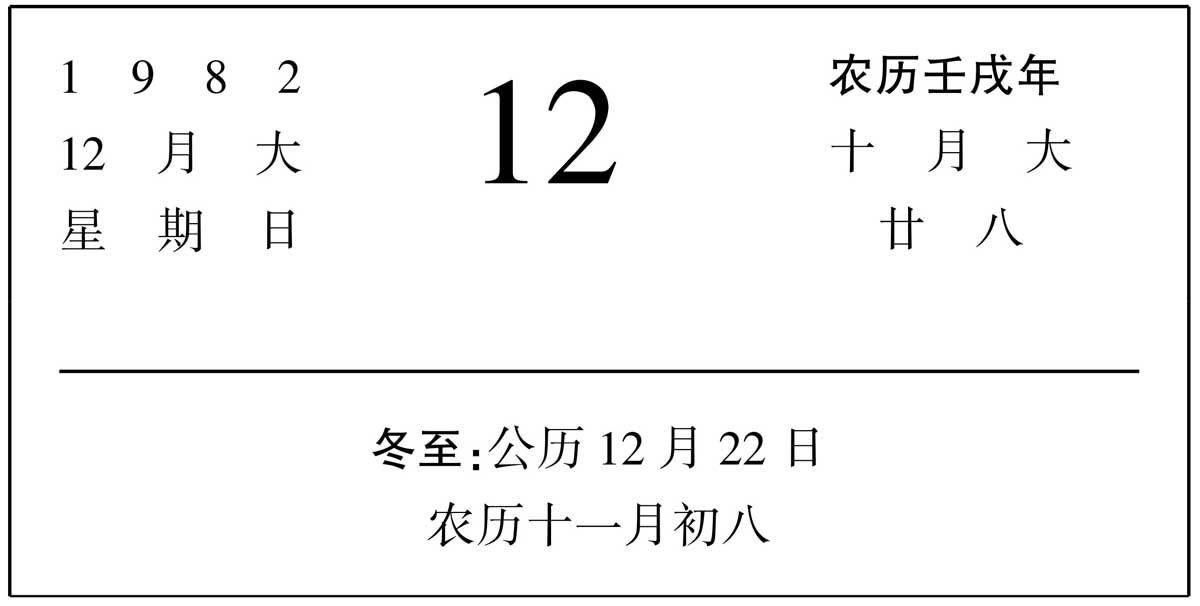
\includegraphics[scale=0.4]{picture/钟鼓楼1.jpeg}
\end{figure}
\par 对于薛大娘来说,一日二十四小时的记时法,新的一日从午夜零点开始的概念,虽说经过这些年子女们谈话的熏陶,也算懂得,但从心理习惯上来说,她还是把天光透进院落,算作一日的起始。
\par 今天,薛大娘的小儿子薛纪跃办喜事。
\par 薛大娘在那页被朦胧的天光照亮的日历面前,愣了好几秒钟。同北京许许多多同龄的老市民一样,薛大娘现在绝不是一个真正迷信的人,她知道迷信归根结蒂都是瞎掰,遇上听人讲述哪里有个老太太信神信鬼闹出乱子,她还会真诚地拍着大腿笑着说几句嘲讽的话;但她又同许许多多同龄的老市民一样,内心还揣着个求吉利的想法。现在北京并没有人摆摊算卦,办喜事也没有什么人再那么讲究生辰八字,偶尔听说外地农村里竟然还有因为算生辰八字酿成儿女悲剧的事,薛大娘一类的人也会跟着叹息。但在选择什么日子办喜事这样的问题上,北京城时下却确凿存在着一定的讲究。是谁倡导的?谁传播的?你缕不清。不仅像薛大娘这样的老市民,就是薛纪跃这样的新市民,也都颇为重视这个讲究。什么讲究呢?就是得选个阴历、阳历月、日都是双数的日子。这当然是一种最原始不过的迷信心理:怕逢上单数会生出不吉利的丧偶的后果。世界上的事情就是这样,你可以比较轻易地涤荡繁缛的迷信习俗,却很难消除存在于人们内心中的原始迷信心理。薛大娘在副食店卖过二十多年的菜,头年才退休回家,她的文化水平恰到能够流畅地阅读日历的程度。在那张红色的日历面前,她把那些偶数读了几遍,心中漾出一种安适感。只是日历下面的小注略让她不快,不仅有个“十一”的数字瞧去刺眼,所预告的“冬至”这个节气似乎也不那么喜幸。不过,这几丝不快,很快也便被日历上所笼罩的红色驱散了。
\par 薛大娘离开日历,看了看仍在床上酣睡的薛纪跃,本想过去把他唤醒,临到挪动脚步又生出了怜惜之情。让他再多睡一会儿吧,今儿个指不定得把他累成个什么样儿呢!
\par 薛大娘走出屋子。院子里很静,没有人影。按过去以十二地支划分一昼夜的计算法,那正当卯时\footnote{十二地支为:子、丑、寅、卯、辰、巳、午、未、申、酉、戌、亥。子时相当于半夜二十三点至一点,余类推。}。薛家住着这个四合院里院的两间西房。虽说他们早已接出去了一间厨房,但今天要办喜事,厨房支派不开,所以昨天便搭好一个用汽车苫布构成的棚子,好让今天来帮忙的大师傅有用武之地。
\par 薛大娘原以为老伴在苫布棚里,及至走进去一看,并没老伴的身影,便知道他是到什刹海后海边遛弯儿、打八卦拳去了。难道今天这个日子也不能停它一次?薛大娘不禁有点埋怨。薛大娘在苫棚里检查着备好的各种原料和半成品——洗净切好的白菜、油菜和胡萝卜,裹上鸡蛋面粉炸过一道的小黄花鱼,发了一夜的木耳、黄花和笋干……请到的大师傅据说曾在同和居掌过红案,他今天弄出来的“四四到底”(十六个菜),肯定谁也挑不出碴儿来!
\par 薛大娘心神不定。帮忙的大师傅没到还情有可原——现在天刚冒亮儿,人家兴许住得挺远,总得过一阵儿;可大儿媳妇昭英怎么还不露面?半年前大儿子薛纪徽和儿媳妇孟昭英还跟薛大娘他们住一块。那时候,两间屋子,薛大娘老两口和小儿子薛纪跃住一间,薛纪徽和孟昭英带着女儿小莲蓬住另一间。薛纪徽是开130卡车的司机,孟昭英是同一单位的出纳,他们打结婚那天起就跟单位要房子,总算在今年春上要到了一间——住那间的技术员搬入了新居民区的单元楼,这间便倒给了他们。他们搬了出去,这才腾出了给弟弟薛纪跃成家的居室。北京城里就是这个形势,一个萝卜一个坑。薛纪徽两口子搬得并不算远,就在恭俭胡同那边住,离这儿不过两站来地。说好让他们一早就来帮忙的,可你瞧,天光眼见着越来越亮了,却还不见影儿。薛大娘心里只怨着孟昭英,这是她的一种心理习惯。两口子带着孙女来了,儿子叫没叫爹妈她不计较,媳妇要是忘了叫,或者叫迟慢了、声音听去不顺不甜了,薛大娘便会老大的不痛快;一般来说她倒并不发作,但面对着媳妇时,她却肯定不会现出哪怕是一丝笑纹。此刻她走出苫棚,朝院门迈步,心里直嘀咕:这个昭英,小叔子办喜事,在你心里头就那么没分量吗?还等着你去女家迎亲呢,你就不能早点儿来效力?
\par 薛大娘走出里外院之间的垂花门,迎面遇上了荀磊。荀磊是个俊俏的小伙子,今年二十二岁,比薛纪跃小三岁。他家住在一进门右首小偏院中,父亲荀兴旺原是东郊一家大工厂的老工人,头年退休后办了个个体户执照,在后门桥那里摆摊给人修鞋。说起来真是鸡窝里飞出了金凤凰,这荀磊完全不像他父母那样五大三粗黑皮糙肉,竟长得细皮白肉苗条秀气。长相好倒还不算什么,他上小学起就肯好好念书,中学毕业后居然出乎全院人的意料,被外事部门直接招去,送到国外培训,今年夏天回来后,被分配在某重要部门当翻译,据说,将来还有机会出国工作呢!
\par 这时候荀磊手里提着两个剪贴得十分精美的黄底子的大红囍字,满脸笑容地迎住薛大娘说:“大娘,您过过目,要合适,我这就贴去!”
\par 薛大娘喜出望外。她因为心里头堆满了事儿,倒把这个节目忽略掉了。院门口昨晚上就由薛师傅贴上了一对红囍字,不过刚贴上,就被才下班回来的荀磊偏着头评论说:“这字剪得不匀称,衬底也不好看。今天晚上我帮你们另做一对,明天早上先给你们看看,要觉着好,我就帮你们换上。”这不,他倒真做出了一对。
\par 薛大娘仔细地瞧了瞧荀磊高举起的囍字,确实是好,笔道匀实、黄红辉映不说,光那边框里的喜鹊闹梅图案,就难为他怎么剪得出来!
\par “哟,好!真好!够多喜幸!”薛大娘拊着掌赞道,“小磊子,你可真是个人精!”
\par “那我就弄糨糊给贴去啦!”荀磊高高兴兴地扭身回屋取糨糊去了。
\par 薛大娘走出了院门,心情大畅。
\par 这院子在北京北城的一条胡同里。此刻站在院门口,可以看见钟楼和鼓楼的剪影,从浅绿色的丝绸般的天光中,清晰地显现出来。那钟楼甍脊西端的兽头,一九七六年地震时震落了,只剩下东端的兽头,还在天光中翘着上弯的铁须;那鼓楼木构楼殿的支柱,有一根明显地显露出来,给本来过分凝重的剪影,增添了一点轻盈灵动的韵味。
\par 薛大娘抬头仰望着这溶入她的生活、她的灵魂的钟鼓楼。钟鼓楼仿佛也在默默地俯视着她住的那条古老的胡同、陈旧的院落和她本人。在差不多半分钟里,历史和命运就那么无言地、似乎是无动于衷地对望着。
\par 但薛大娘很快便把眼光移向了胡同进口处。为什么昭英还不来?

\subsubsection*{2.地安门大街上,来了一位给婚事帮厨的人。他为什么不要茶壶?}
\par 地安门的十字路口,显得过分宽阔。那是因为当年有座庞大的地安门,五十年代初将它拆除了,修成十字路口,所以成了这样。不知道为什么,三十年来,人们始终没有在那宽阔的街心,开辟一个转盘式的大花坛。人们净忙着干别的了。现在也还是这样。天还没有大亮,这里已经热闹起来。当然不是那种公园或商场式的热闹,而是一种缺乏色彩的、严肃的热闹——人们急匆匆地赶着去上班。公共汽、电车里挤得满满当当。车站上既有循规蹈矩排队候车的人,也有无视公德、几乎站到快车道上、打算车到便往上跳的小伙子们。而构成总体气氛的关键,还是那些骑自行车的人。多数骑自行车的人只是被动地随着车流前进,但总有少数屁股不怎么沾车座的小伙子,蛇形地快速穿过每一个能利用的车隙,惊心动魄地飞驰向前。
\par 这天总算比平日景况稍松缓一点。因为是星期日,机关干部和学生们退出了清晨的这股人潮。不过需要通过这个十字路口去做工、售货、办事的人还是不少。北面高踞的鼓楼和南面屹立的景山,仿佛都在薄明中凝望着这里,它们也许在沉思:为什么这里的生活既有惊人的变迁,也有似乎是单调的重复?
\par 路喜纯在自行车的车流中,不慌不忙地均匀蹬车,边想心事边随车流向前。
\par 这是个二十六岁的小伙子,从他的年龄来说,他或许要算胖子,但其实他的脸蛋、胳膊、胸脯都还是紧绷绷而富有弹性的,只不过比一般的同龄人鼓胀而缺乏棱角罢了。他在崇文门外花市附近的一家小饭馆工作。那小饭馆可以说是北京市最基层最不起眼、甚而会被某些自命高雅的人视为最低级最不屑一顾的社会细胞。但“麻雀虽小,五脏俱全”,其实整个北京城的阴晴风雨、喜怒悲乐,都能从那小小的饭馆中找到清晰而深刻的回响。
\par 路喜纯已然父母双亡。常有人问及他的父母,他总是极简单地回答。倘若有人多问几句,他便仿佛不高兴起来。他那故去的双亲,似乎有着某种神秘的色彩。
\par 其实说起来也很平常。路喜纯的父亲生前是个蹬平板三轮车的运输工人,母亲一直是个家庭妇女。他父母收入虽然不多,对他这个独生子却保证着绝不低于一般富裕家庭的供应,因此,上小学时,那位戴眼镜的班主任老师常以他为例,来教育全班同学:“新旧社会两重天。要是在旧社会,路喜纯还不得穿着破衣烂衫,到垃圾堆拾煤核儿去吗?……”这位老师还曾到他家里去,动员他父亲到班上去忆苦思甜。那天路喜纯父亲正就着一头大蒜喝酒——他每天下了班回来总得喝上三两白干。出乎老师、也出乎路喜纯意料,父亲不但予以拒绝,还紫涨着脸,瞪着发红的眼睛,说出了这样蛮不讲理的话:“甭拿咱们开心!甭跟我来这套!”母亲赶紧来打圆场,说他那是发酒疯,“甭搭理他!”老师扫兴地走了,从此讲话不再以路喜纯为例。路喜纯为这事深深地感到困惑。不久,父亲便脑溢血去世了。
\par 父亲去世后,母亲挑起了生活的重担。原来,母亲做挑花活不过是补助家用,这以后她每月几乎要多领两倍的活计,每天都要做到晚上十点来钟。通过她的努力,路喜纯的生活水平一点没有下降。但在路喜纯的记忆之中,他母亲绝不是文艺作品中惯常描写的那种手持慈母线的贤良形象。她都快五十岁了,每天起码还要照十多次镜子。她又很爱给自己拔痧,经常在额头上、太阳穴旁,用食指和中指的指缝,使劲揪出排列整齐的紫红印子来。他们难得吃肉,但母亲顿顿饭后总要坐到屋门口去,用炕笤帚苗剔牙。有时候母亲还要同邻居吵架,尽管这种时候不多,而且往往母亲确实占了几分理,但母亲吵架时那种豁出去的劲头,以及夹带着的那些极难听的脏话,事后总要让路喜纯偷偷地害上几天臊。母亲是一九七二年冬天查出来有肝癌的,一九七三年春天便去世了。
\par 路喜纯家住着院里一间南屋。父母双亡后,邻居们原以为这间屋子很快便会变成无处下脚的鸡窝,甚至会成为胡同里小流氓们的聚会之所。谁想料理完母亲的丧事,仅仅十六岁的路喜纯却在三天之内,使那间房子焕然一新。他先到街道上开了证明,去信托商店卖掉了家里的一套磁撢瓶、磁帽筒和一个硬木炕桌,取得了一笔对他来说相当丰厚的现款。然后,他便重新粉刷了屋墙,用草根刷子刷净了每一件家具,重新把屋子布置起来。他在窗明几净的屋子里,沉着地等待有关部门给他安排工作。当他手头只剩五块多钱时,给了他通知,让他去那家小饭馆。
\par 按某些人从旁推论,路喜纯是北京市民中的所谓“胡同串子”\footnote{住在胡同中的没有教养的青少年。},最易堕落而难以教化,然而除了偶然有颇令人迷惑不解的行为外,他竟不但没有堕落,反而生活得非常正派。在他生活道路上给过他强烈影响、给予他这样去生活的启示人,一共有两个。一个是他中学时的老师嵇志满,一个是他们那个小饭馆的何师傅。嵇老师并非什么知名的优秀教师,何师傅在饮食行业中也并非突出的先进人物,但他们灵魂中那些健康的、向上的东西,偏偏集中地流注到了路喜纯的灵魂之中。
\par 先是为了尽可能不去上山下乡,后是因为安排就业困难,路喜纯所在的那个小饭馆里的年轻人,竟然大多是从后门安排进去的。这也许会让那些对小饭馆的前门也不屑一顾的人们哑然失笑吧。从某种意义上来说,我们这座北京城里的市民尽管共享着同一个空间和同一份时间,但人们所生活的层次毕竟有所不同。路喜纯所在的这一层也许并非最底层,但即使在最底层里,也会有许许多多同上面那些层次相通的东西。因为是饮食基层店经理安排来的,因此便在同事们面前趾高气扬,这同因为是某个“大人物”的侄子而进了市府机关,便令某些人格外尊敬三分,又有什么不同呢?路喜纯到了饭馆便想学掌勺炒菜,谁知那个差使至今轮不到他——因为那是红案,比去做主食的白案似乎要高出一档。在饭馆这个天地里,路喜纯的来路和背景都还不足以使他获得那个位置,于是乎一个总噘着嘴的比他“来路硬”的小伙子便占据了那个岗位——偏偏那小伙子满心满意想找个机会调到高一个层次的行业中去,他还不乐意学那个红案呢;但饭馆的小头头却宁愿要他学红案而不要路喜纯学。
\par 路喜纯为自己这样的遭遇和身边这样的现实深深地痛苦过。他那痛苦的价值,比一位大学毕业生学非所用的痛苦的价值低吗?比一位有才华的作家的呕心沥血之作被退稿的痛苦低吗?比一位高级干部的正确的改革计划遭到保守者抵制的痛苦低吗?不见得吧。特别是当那个小伙子并不虚心听取老师傅指教,漫不经心地把菜炒得黑糊糊焦烘烘,因而引来顾客的抗议时,路喜纯便格外痛苦,有时他会禁不住把馒头机泻下的馒头,拣起来捏得湿面滋出每一条指缝,然后再重重地把那团面甩回到机器里去……
\par 前几天路喜纯还去学校找过嵇老师,向他倾诉过内心的痛苦。嵇老师是教数学的。路喜纯在那所中学上学时,还是“四人帮”得势的时期。从那时的数学课上学不到多少知识,但从课下的谈话中,路喜纯却从嵇老师那里获得了不少实实在在的真理。嵇老师总是给他讲历史,特别是近代史。嵇老师所讲的,往往都是历史课上听不到的。他记住了嵇老师一句几乎是口头禅的话:“你要有历史的眼光!”
\par 嵇老师一直住在学校一角的一间小屋中。不知为什么他总没有结婚。但路喜纯每次去,却几乎又总会在嵇老师那凌乱的宿舍中发现一位女客,有的显得很年轻,长得未必漂亮,打扮得可真时髦;有的徐娘半老,穿着朴素,却风韵犹存。这回去又遇上了一位,不老不少,圆脸庞,鼓眼睛,说话嗓门挺大。瞧那做派,简直跟嵇老师熟得不能再熟,路喜纯跟嵇老师说话的时候,她就坐在嵇老师床上,抽着一根烟,极随便地翻阅着嵇老师的一本集邮册,还不时发出像男人那样粗嗄的笑声。
\par 路喜纯倾诉了他的苦闷。嵇老师照例没有什么特殊的表情,他用捏在手里的一个圆形塑料立体梳,慢慢梳理着日渐稀疏的头发,待路喜纯说完了,便从桌上取过一本书来,递给路喜纯,简单地说:“你看看这个。”
\par 那是一册纸已发黄的《文史资料选编》,路喜纯翻开,溜了一下目录,有什么溥佳的《清宫回忆》、溥杰的《回忆醇亲王府的生活》以及《清宫太监回忆录》之类。看这些东西,能解决什么问题呢?
\par “你看看这个。”嵇老师慢腾腾地对路喜纯说,“你要有历史的眼光。世界上的事,没有一刀切的时候,没有一切都合理都美满的时候,问题是你怎么看发展趋势,怎么跟残留的旧东西抗争……你以为一九一一年的辛亥革命以后,成了民国,到处就都是民国景象了么?旧事物的惯性是很强的。直到一九二四年,也就是末代皇帝溥仪被轰出紫禁城前后,北京的钟楼还在鸣钟报时呢!这还不算什么,你知道吗?钟鼓楼‘定更’以后,街上还要出来‘手打梆子腚摇铃’的人;‘腚摇铃’就是腰上系个铃铛,他们是巡夜的;谁领着他们巡夜?还是由清朝九门提督衙门的巡街老爷们领着,前头打着名叫‘气死风’的灯笼,一路顺街那么走下去……那时候,五四运动已经过去五年,中国共产党也已经成立三年,震撼世界的二七大罢工也已经发生过,但北京的街头,居然还有这种景象……这本书还能告诉你更多的这种事,你看看吧。”
\par 他拿回去看了。他惊讶地发现,溥佳的所谓《清宫回忆》,写的是一九一九年以后的事,也就是说,那许多丑恶的封建景象,在民国以后居然长时间“依然故我”;而溥杰关于醇亲王府的回忆,更告诉他直到很晚,那王府内部依旧保持着森严的等级制度;至于几位老太监的回忆,更令他目瞪口呆,其中一位的父亲为了让儿子能进宫而使家庭状况有所改变,竟亲手为儿子血淋淋地“净身”,然后将儿子卖给了专为宫里提供太监的内务府官员。这事实本身已令人发指,发生的时代呢?已是民国以后!读完了这些文史资料,掩卷深思,路喜纯的心理状态渐趋平衡——他何必对眼前的某些阴暗的东西那么痛不欲生呢?时代的步伐既然迈进得这么快,它所来不及清扫的旧时代积垢必然显得更加触目惊心,问题确实在于你要有历史的眼光,冷静、沉着地去对待这些东西。因此,自己所在的小饭馆里有那么一个小头头,仍旧有着一双为旧时代所污染的势利眼,这又有什么稀奇呢?
\par 这位势利眼不让路喜纯上红案,当红案的何师傅却偏偏把路喜纯收为了私人徒弟,把他带到家里去,不但教他做一般的席面菜,还教给了他几样“绝活”。何师傅原是同和居的掌勺师傅,为让儿子顶替,他提前二年退休了,退休后为了补差,这才到了离他家不远的这个小饭馆。其实还有好几家仅次于同和居的大饭馆争着请他去当教席,甚至答应给他很高的“补助”,他却一一谢绝了。他说:“也该让进小饭馆的人吃到点好菜。”就是四毛八分钱的烧豆腐,他也精心地制作,使那小饭馆几个月后便颇有点口碑,不过,那口碑的前半句是夸赞,后半句却是“质量不稳定”五个字。不稳定的因素之一便是那好噘嘴的小伙子。路喜纯多么想替他来为饭馆挣个“质量稳定”的声誉啊,但至今还不能如愿……
\par 路喜纯常往何师傅家跑,翻着菜谱请教细节时,何师傅一般只是咬着烟嘴,皱眉摇头,难得迸出一两句指点的话来;可一旦路喜纯带去了原料,在他家小厨房里摆弄起来时,何师傅就把烟嘴搁到一边,眉飞色舞地一连串地支上嘴了……当一盘芙蓉鸡片,或者一盘糟溜鱼片,色香味俱佳地呈现在白磁盘中时,何师傅总让路喜纯给他同院的邻居端去,他说:“咱们的玩意灵不灵,让人家尝了发话!”邻居们惊喜之余总要报之以答礼,或是一盘水果,或是一碟蜜饯。何师傅不让路喜纯谢绝,他主动接过来,拿出“二锅头”,坐下约路喜纯就着水果、蜜饯喝上一盅,边喝,边指出他今天制作过程中还有哪些失误。路喜纯发现,菜谱上所写的那些,常有含混乃至谬误之处,何师傅的言传身教,比任何精印的菜谱都要有价值……
\par “甭跟那起人置气\footnote{赌气的意思。}, ”何师傅常在喝一口酒后,用手背抹抹嘴唇,安慰路喜纯说,“有你掌勺的时候……”
\par 何师傅真是喜欢他这个徒弟。不过,路喜纯有时候也确实让人感到奇怪——头些天他们饭馆不知从哪儿弄来了二十个大磁壶,除了留下几个在厨房里装酱油、醋以外,剩下的作为福利每人分上一个,别人都把壶收下了,惟独路喜纯不要。何师傅跟他说:“别嫌式样老,用它晾凉白开,比那玻璃凉水瓶还实用,你就拿回去吧!”他还是不要;问他为个什么,他又不说;别人硬把那壶塞到他怀里,他不接,壶摔到地上碎成几半;大伙都说可惜,他却一声不吭地转身走开了。
\par 除了这种偶然出现的令人费解的表现,路喜纯总体来说是一个心地纯正、力求上进的好青年。他渴望着何师傅所说的那样一个时候早日到来,他将不仅要掌勺,还要掌握整个饭馆,他要兴利除弊,让饭馆彻底改变面貌,使每一个进去的顾客都能一辈子忘不了它。
\par 为此,他不放过每一次练功的机会。今天,他就是顶替何师傅,到钟鼓楼那边,去帮薛家操持婚宴的。听说这家人备的料相当齐全,打下手的人也不会短缺,他将施展出自己的浑身解数,让那家人及其亲友吃得眉开眼笑!


\subsubsection*{3.一位正在苦恼的京剧女演员。人家却请她去迎亲。}
\refdocument{
    \par 愁人月色凄又冷,
    \par 风吹铁马乱人心。
    \par 痴心的人儿你休怨嗔,
    \par 比翼双飞入梦频。
    \par 愿效鸿飞心意定,
    \par 你只要带定了那绿绮琴……
}
\par 澹台智珠哼唱着《卓文君》中的二黄原板转散板,朝院门走来。喊完嗓又练了一套剑,现在她觉得声带松弛润适,浑身关节也都舒张和谐;但随着聚精会神喊嗓练功的阶段结束,她那心底里的一股忧郁,却又随着渐次混杂的朝市之声,丝丝缕缕地旋了上来。
\par ……这《卓文君》,排得出来吗?吴祖光先生编的《凤求凰》,已经由别的团排出来公演了,基本上是张派的唱法。按说这参考荀先生演出本改编的《卓文君》,将融合程派和欧阳予倩演出风格的特点,与他们的演出绝不会重复,可负责剧目的副团长的态度还是那么暧昧,同剧组的人也是七上八下,乐队的人也不那么积极。他们都怎么说来着?啊,对了,有说“这玩意排出来能叫座吗?”有说“编新不如述旧,只要有人买票,咱们就老演那几出,不是也一样过日子吗?”……是呀,如今武戏、热闹戏最上座,《卓文君》这类文戏一般都相形见绌,何况按澹台智珠的意思,还要把韩世昌、白云生的昆腔艺术适当地糅合进去,创造出一种她所谓的“诗意气氛”,这样排出来究竟票房那儿会是个什么行情,也真难说!不过,她可不甘心总是《豆汁记》,总是《玉堂春》,总是《武家坡》;就是前一阵新排出来反应相当不错的《木兰从军》,她也觉得可以先搁一搁;她渴望着在舞台上不断有新的创造,渴望着不但对老观众有新启发,而且还能吸引来一批年轻的新观众……难呀,难!其实她想做的不过是一个忠于艺术、忠于观众的演员尽自己义务的事,可在一些人的眼里,倒好像她是想把天上的月亮当月饼吃!这“一些人”不仅团里有,家里也有,爱人李铠竟也来阻拦。当然,他是出于另一番心思,可他那心思,让澹台智珠怎么尅化得开啊!他现在起床了吗?因为昨晚的争吵,他还在折磨自己吗?……
\par 快走拢院门,澹台智珠眼前猛地一亮,她瞥见了张贴在院门两旁的囍字,这才想起今天是薛师傅家二小子娶媳妇的好日子。她回想起昨晚所看见的囍字,和现在看见的不同;今天的黄底红框,框中还剪出精巧的喜鹊闹梅的图案;可见人家对今天这桩喜事的重视到了一种什么程度——连这样一个细节,也不断地在加以调整。倘若他们团里那些搞舞台美术的同志,也能有这种刻意求精的精神,那该多好哇!
\par 澹台智珠进了院,到了家门。她家住在进大门往左首走的外院,屋门斜对着进里院的垂花门。她轻轻拉开屋门,走了进去,先把木剑挂在门边,然后对着墙上的大镜子,卸下裹住整个头部的鹅黄色拉毛加长围巾,把围巾顺手搭在椅背上,伸出双手整理着她那浓密油黑的头发。
\par 她家住着三间南房。这当中的一间,是吃饭、会客兼她练功用的。东边一间她跟爱人李铠住,西边一间是公公婆婆带着儿子小竹和女儿小梅住。
\par 她听见西边有咳嗽声,忙停止摆弄头发,掀开花布门帘,走了进去。婆婆早些日子带着还没上学的小梅到大姑家去了,还没回来。西屋里现在只有公公和小竹。公公原是玉器行业上的钻眼工,如今七十挂零了,自然早已退休。他同一般的老人不一样,睡得迟,起得也不早。他有一定的文化,嗜好是戴着老花镜,一字一句地读章回小说,不管是古人还是今人写的,只要是章回体的,他都爱读。最近他在读金寄水写的一本《司棋》,那薄薄的一本书,他已读了十来天,却还只读了不到一半。虽说读得慢,他记得却很真。
\par 澹台智珠进去时,公公已经穿妥衣服,小竹却还在床上拥被傻睡。
\par 澹台智珠大声问公公:“您着凉了吗?”
\par 公公又咳嗽了两声,摆摆手说:“不碍事。家里存的有枇杷露,一会儿我倒出点喝,压一压准好。”
\par 澹台智珠过去拍了拍小竹肩膀,催他起床,又扭过头对公公说:“我这就给你们热粥去。”她心里想,再煎点鸡蛋裹馒头片,这顿早点总该能对付过去了。
\par 公公显然是想说点什么,可又下不了决心。澹台智珠看出他的心思,便不好抬脚离去。
\par 公公虚咳了两声,从枕边拿起那本《司棋》来,对澹台智珠说:“你要排新戏,何不就拿这司棋的故事,排上一出呢?”
\par 澹台智珠大声回答:“爸,您当有个题目,就能开排吗?头一条,得有人写本子,本子弄妥了,还得创腔……哪一样是容易的?”她本来还打算列举更多的困难,可叹了一口气后,也就作罢。她意识到——公公想对她说的,绝对不是这关于新戏码的事。
\par 公公到底还是忍不住了,他尽可能以最和蔼的语气问:“昨儿个晚上……李铠他……又跟你闹别扭啦?”
\par 澹台智珠觉得血涌到了脸上。虽说公公耳朵背,到底这三间屋通着,她昨晚上跟李铠闹气的事,怎么也难隐瞒过去。她偏过头望望坐在床上揉眼睛的小竹,强作笑颜,对公公轻描淡写地说:“唉,我们年轻夫妻,吵几句也是平常的事。夫妻没有隔夜仇,您别操心!”
\par 公公却郑重其事地宣布:“我得叫过李铠来训训!你们也都不算年轻了,总这么窝里头闹,算是怎么回事?我们老人听着难受事小,对孩子能有什么好影响?就是邻居们听见,也怪没脸的……唉,放着好日子不好好过,李铠你犯的什么浑啊!”
\par 虽说公公把责备最后都坐实到李铠身上,澹台智珠听了心里却有如针刺。是啊,为什么她和李铠掰到了这步田地?
\par “爸,您别为我们操心。”澹台智珠垂下眼帘,忍住就要涌出的泪花,转身往外走,一边说,“我这就热粥去。”
\par 往常做饭基本上全由婆婆操持,婆婆不在,公公要接过这摊事去,被李铠阻止住了。李铠坚持要澹台智珠做,这也是他们夫妻间矛盾的一个方面。
\par 澹台智珠本想往堂屋门外的厨房,可她走到堂屋门前,却忍不住转回身,移步到了她和李铠住的东屋门前,她在门前愣了几秒钟,才推门走了进去。
\par 李铠睡在床上,头发乱蓬蓬的。他那颗头仿佛特别重,把枕头压得沉下一个大坑,枕头的四个角翘得老高,仿佛在为重压而叹息。他一只粗壮的胳膊撂在被子外面,黑黝黝的皮肤紧绷绷的,皮下的肌肉结实而富有弹性,在上臂中部,有两个很大的牛痘疤,仿佛是嵌在皮上的两片水萝卜。在他身上,散发出一股浓郁的烟草味道。
\par 澹台智珠走过去,用自己那尚未叠起的被子,盖住了李铠的手臂。
\par 望着沉睡的李铠,以及床头柜上那烟缸中满得冒尖的烟头,澹台智珠心里迷乱不堪。她忘记了去热粥,一屁股坐在了床边的软椅上。
\par 他们为什么又闹了这么一场呢?为什么这一切仿佛是不可避免的呢?
\par ……昨晚演出结束,她只不过比往常稍晚了十分钟走出剧场后门,结果,便不见来接她回家的李铠的身影。
\par 那剧场是在一个胡同里面。昨天的戏散得本来就比较晚,加以又是冬天,观众们很快便烟消云散了,同剧组的同志们也转眼便各奔归程,可是当她走拢“老地方”,却头一回不见了李铠的身影,她呼叫、跺脚,急得干哭,竟仍然没有李铠出现,只好自己一个人朝胡同外小跑,一边跑一边使劲撸开大衣袖子看表——末班公共汽车已经过去,怎么办?难道一步步走回家去?
\par 啊,有谁知道,几十分钟以前还在台上嬉笑欢舞的喜剧角色,现在竟是这般的凄苦孤单!
\par 冷风钻进澹台智珠的围巾、领口、袖口,她浑身哆嗦,刹那间,她觉得平日她所看重的一切——事业、名气、荣誉、永恒的艺术价值……等等,等等,都没有丝毫的意义,她是这么的不幸,生活对于她来说,究竟还有什么乐趣、什么吸引力?
\par ……猛然间,从岔胡同里窜出一个人影,是想拦路抢劫,还是想硬施无礼?澹台智珠几乎就要呼救了,可她在惶急恐怖中定眼一看,那却分明是李铠。
\par “你……你为什么不等我?”澹台智珠真想凑上去打他两记耳光。
\par 李铠却更其仇视地瞪着她,质问:“你为什么卸完装还不出来?”
\par 澹台智珠解释说:“我只不过跟他们说了说关于排《卓文君》的事儿……”
\par 李铠粗暴地打断她,恶狠狠地、一泻无余地说:“我就知道你是盯上那个小白脸了!什么东西!他那眼神我瞅着就不对头,到底你们两个还是勾上了……你怎么不跟到他家去?”
\par 澹台智珠觉得这比挨了耳光还疼,她流着眼泪,嗓子眼里噎着一团火辣辣的恶气,愤激地辩驳说:“你别撒疯!你那全是没凭没据的瞎猜!你知道他比咱们大出一辈去,他都快当爷爷了……要不是他能演司马相如,我连理都不愿意理他……他有狐臭,你知道吗?……你怎么糊涂成了这样?! ”
\par ……她决定不理他,自己走回家去。他还是推过来自行车,终于让她坐到了后座上。当他驮着她骑回家时,她不得不一如既往地搂住他宽厚的后背。可是这后背头一回让她觉得陌生、冰冷。她该怎么办、怎么办呢?
\par 回到屋子里,他们两人都觉得头上的屋顶是沉重的,屋里的一切东西——特别是床头上那张他俩头挨头的十二吋彩色结婚照,全都显得格外令人不能忍受。
\par “……不能再这么下去了,咱们得坐下来、坐下来、坐下来……心平气和地好好谈谈了。”澹台智珠大衣也没脱,坐到沙发上,对李铠说。
\par 李铠直到她说够三个“坐下来”,才坐到了床边。他一坐下便立即开始抽烟,一根接着一根……
\par 当澹台智珠当年从戏校毕业的时候,她怎想得到今天会过这样一种生活呢?
\par 她分到了一个不错的剧团。她用全副身心向老演员学戏。她在台上拼命地演,以至于一位评论家不得不在一篇评论文章中说:“她的素质很好,感受力也强,但还缺乏修养。她不懂得,艺术贵在含蓄,她却总是演得太满,须知过火与发瘟同样令人不快……”正当她努力地提高自己的修养,向蕴藉含蓄的境界努力时,“文化大革命”开始了,她作为“封资修的黑苗子”被冲击,因为讲错了一句话,又被打成了“现行反革命”……她觉得一切都失去了意义,失去了希望,于是,有一天她趁着看守打盹,把看守拿来搁在躺椅下的小半瓶“敌敌畏”喝了下去……她没能死成,她经历了昏迷、呆滞、麻木、消沉、痛苦、绝望……又渐渐回转为冷静、认命、无求、开通、企望……一九七七年春天,她开始重新练功,人们惊异地看到,她那一度嘶哑得惊人的嗓音,竟恢复得比当年更显阔亮,她那似乎已然僵硬的腰身腿脚,竟复原得又可以像当年一样地满台扑跌;到了这一二年,连她自己也没想到,她的号召力竟大大超过了当年,即使在最不适时的日期最不方便的场子演出,也总能卖出七成以上的戏票,这在京剧观众锐减的形势下,应当说已经相当不错了;她的戏装照和便装照不时出现在报刊上,电台请她录音并讲话,电视台请她录像,唱片社为她灌制了唱片,戏迷们甚至跑到后台去请她签名,拉她合影……还是那位评论家,发表新的评论说:“按说她的素质不算太好,感受力也未必最强,但她靠着厚积的修养,在一笑一颦之间,在一歌一吟之际,却丝丝入扣、动人心弦地展现出了角色的内心,使我们获得了一种形神兼备而无斧凿痕迹的美感……”
\par 倘若她的遭际仅是这样简单地否极泰来,那生活的滋味便太寡淡了。她在一九七三年,也就是她自杀未死的五年之后,结婚成了家。当她从戏校毕业时,她曾暗暗地对自己说:你已经嫁给了舞台,你不能重婚!那绝非一句戏言,那意味着她把艺术看得比什么都重。但当她一九七二年以半残废的身心被“落实政策”到一家纽扣厂当包装工时,她在心里又暗暗对自己说:舞台把你甩了,你是永远回不去了,找个丈夫,结婚吧!人家给她介绍了李铠,一位憨厚强壮的车工。头一回见面,她就把自己的一切都跟他讲了,李铠的双眼明显地变得湿润起来。正是望着那双湿润的眼睛,她萌发了对李铠的爱情,她需要有人把她当妻子爱,她也需要爱一个具体的叫做丈夫的人。
\par ……一九七六年年底,又一次“落实政策”,她回到了剧团。一九七九年春节她重登舞台,当她第一回迎着观众踏上红氍毹时,真是百感交集!记得那时候李铠的兴奋与欢欣绝不亚于她自己,包括公公婆婆,也都扬眉吐气,引以为荣。她总是演大轴戏,戏散得晚,李铠就总到剧场后门等着她,骑自行车把她驮回家去。开始,李铠不进后台,还仅仅是因为不好意思,后来……从什么时候开始的?澹台智珠恨自己竟没有及早察觉,李铠的不进后台,渐渐转化为一种既自卑又自傲的复杂心理……
\par 也许,是从那回电台编辑来家里访问,开始转化的吧?
\par 那位女编辑大声地问:“您爱人是哪个行当上的?唱小生的吗?唱须生的?”
\par 澹台智珠告诉她:“他不是演员……”
\par 那位女编辑仍旧大声地问:“他是场面上的?司鼓?拉琴?”
\par 澹台智珠便又告诉她:“他不是我这行的。”
\par 该女编辑竟还要大声地问:“他在哪个文化部门工作?”
\par 澹台智珠坦然地说:“他不在文艺部门工作。他在工厂。”
\par 死心眼的女编辑不知好奇心盛还是有一种猜测的癖好,竟又大声地连问:“啊,在工厂工作?哪个工厂?工程师?技术员?……”
\par 结果是李铠从里屋走出来,板着脸对那位女编辑说:“我是车工。二级工。干力气活的。”
\par ……如果仅仅是一种自卑感,那倒也好办。问题是李铠渐渐受不了澹台智珠在台上同风流小生眉目传情、插科打诨,乃至于当场拜堂……特别是最近澹台智珠又接连换了两个配戏的小生,并且酝酿着要排《卓文君》,李铠非常清楚,卓文君所钟情于司马相如的,究竟是些什么……
\par 昨晚他俩回到屋里的一场争吵,已经绝非头一回了,却是迄今为止最激烈的一回。其实这种争吵照例由三部曲构成。首先是双方气顶气地说一些仇恨的话,而且都归结到“干脆离婚”这样一个命题上;然后,便都极其不冷静地互相追究对方的错误,明明对方已经解释清楚了,也偏要硬找出“破绽”来加以推翻;当双方都被这种既无味又无望的争吵压得喘不过气来时,总有一个人,而且往往总是开头最蛮横最强硬的李铠,突然崩溃下来,要求和解……昨晚也是这样。当澹台智珠头脑已经发木,只是固执地质问李铠:“你为什么这么恨我?为什么?”李铠却突然一下子扑到她面前,把她拉起来紧紧搂住,狂乱地用火烫的嘴唇亲着她的脸、眼睛、额头、鼻子和嘴,喘得像头熊似地呓语般地说:“我爱你爱你爱你爱你爱你……如果你不爱我了,我就杀了你,然后自杀!……”澹台智珠挣扎着,拼命想推开他,不顾一切地回答说:“我不爱你,不爱不爱不爱……你杀了我吧!”而李铠却突然又一下子“扑通”地跪在她身前,紧紧地抱住她的双腿,把脸埋到她大衣的下摆上,闷声闷气地哭泣着说:“智珠……你原谅我,原谅我原谅我……你要我怎么着都行,可就是别离开我,别……”
\par 这下澹台智珠完全清醒了。她赶忙把李铠扶起来,紧紧地搂住他那粗壮的身躯,安慰他说:“你该有多傻!多傻!我爱你,这不是明摆着的事儿吗?我怎么会离开你?你为什么想到这种事?那是不可能的,绝不可能!……”
\par 于是他们上床睡觉。李铠像一个带着镣铐的罪人,他每一个动作都充溢着忏悔和痛苦……澹台智珠尽力让自己理智,她吞服了安眠药片,并且想到:明早要照常喊嗓子练功,也要满足李铠的自尊心:由她来为全家做饭,以证明她在这个家庭中毕竟只是一个普通的媳妇……
\par 当澹台智珠清早从外面回来,见过公公,坐到仍在沉睡的李铠面前时,她痛苦地意识到:尽管他们又一次和好了,但那感情的创痕却永难完全平复……而造成李铠那种心态的外在因素,却依然存在,并且不可逃避……
\par 澹台智珠忽然听到有一种呼唤她的声音,她站起来,定了定神,这才听出是里院的薛大娘在门外叫她。
\par 她赶忙走了出去,在几秒钟里,把自己的神情体态调整成欢快活泼的模样。
\par “哟,薛大娘,快进屋坐!我这正想着给您道喜去哩!”她一出门便主动对薛大娘这么说。
\par “不啦,”薛大娘拉过她一只手,端详着她,无限爱慕、无限信赖地说,“智珠呀,我有个事要劳你的大驾啦!”
\par “什么事呀?薛大娘,您尽管说吧,凡是我能做得到的……”澹台智珠爽快地应答着。
\par 薛大娘先唠叨了一番:“你看我们家今天的事儿!一大早就不顺心。我们那昭英都这时候了还没影儿!好容易托人请了个同和居的大师傅,谁知又说有病来不了,临时支派了个愣小伙子来应付我们……纪跃他这才刚起,那西服裤子才上身,就给溅上了洗脸水,眨眼就要成家的人了,还那么毛手毛脚没个稳重劲儿……我急得这心都快蹿到嗓子眼儿了,可我们那老头子还不紧不慢地迈着方步,磨磨唧唧地说什么‘甭急,车到山前必有路’,你瞧瞧!……”
\par 澹台智珠不得要领,只好微笑着问:“我能帮点什么忙呀?”
\par 薛大娘一手握着澹台智珠的右手,一手拍着她那只手的手背,诚心诚意地说:“智珠呀,你是个‘全可人’\footnote{“全可人”即全福人。“可”轻读为ke。},上有老,下有小,你们夫妻和美,儿女双全,你又大难不死,越唱越红……今天我们昭英迎亲去,想请你也陪着辛苦一趟……”
\par 没等薛大娘说完,澹台智珠便干脆利落地答应说:“那有什么说的!什么时候去,您让昭英来招呼我,我是一定拾掇得干干净净,打扮得喜气洋洋,给您把新媳妇妥妥当当地接进新房!”
\par 薛大娘满意地转身去了。澹台智珠这才猛然想起,昨天散戏以后,她约了乐队的几个同事来家吃午饭,昨晚上那么一闹,竟使她把这档子事忘记了。她可该怎么办啊?怎么跟睡醒觉的李铠宣布这件事,恳求他不要当着那些人暴露出他们的矛盾?家里肉也没有,菜也不够,可怎么着手准备?原本这工夫若赶紧去地安门菜市场采购还来得及,可又刚答应了薛大娘要去迎亲,说不定没多会儿人家就来叫自己出发,这可怎么是好?即便打发小竹去采购吧,那公公和李铠难道能备出一餐像样的客饭来?……唉,生活啊,你为什么充满了这么多的烦忧?自己的生活,又为什么常常被别人的生活插进来搞乱?
\par 澹台智珠呆立在大镜子前,一筹莫展。


\subsubsection*{4.一位局长住在北房。他家没有自用厕所。}
\par 门洞里很黑。好几家都把用不着的家具堆放在门洞两边,连顶棚上也挂得有谁家坐破了可还舍不得扔的旧藤椅,这就让小院的这个“咽喉地带”大有“一夫当关,万夫莫开”的味道。
\par 张秀藻端着盛炸油饼和豆沙包的小竹笸箩,在门洞里迎面遇上了荀磊。荀磊不知为什么一手拿着斜放着小刷子的糨糊碗,另一手提着两张大纸,他是要张贴什么呢?
\par 瞬间,张秀藻只觉得自己喉头发涩,心脏的跳动明显地失去了均匀。已经有好几个月了,她严厉地命令自己,倘若“狭路相逢”,见到荀磊,只能是微微扬起下巴,淡然地点一下头,然后不动声色地擦身而过。但因为她家住在里院最后面的北房中,而荀磊却住在过了这门洞的右首偏院中,再加上她平日在清华大学水利系上学,只有星期天才回来(有时连星期天也不回来),所以,她实践这种自我命令的机会,这几个月里也仅仅三次而已——现在自然可以增添一次;但正当她扬起了下巴,就要以全副的矜持向荀磊微微点头时,荀磊却笑吟吟地、热情地对她说:“你能帮帮我吗?”
\par 显然,荀磊是要她帮着去张贴那样东西。荀磊的这一句问话,使张秀藻积蓄已久的自尊和高傲顿然动摇。在相视沉默的两秒钟里,她清楚地看出了荀磊眼睛里充满着纯洁、真挚而又善良、聪慧的光芒——这眼光对她来说真是勾魂摄魄,令她心醉神迷;在她所处的生活环境里,像荀磊这种年龄的小伙子们,确实还没有哪一个具有这样两扇使她觉得格外可钦可爱的“心灵窗户”。难道她可以面对着这样的两扇窗户,冷淡地说出拒绝的话么?
\par 张秀藻的嘴唇抖动着,几乎就要吐出“好吧”两个字了,荀磊却快活地笑着道歉说:“啊,对不起!瞧我……你还拿着早点呢!快给家里送去吧,我一个人也能贴……”
\par 张秀藻简直伤心极了。她手里为什么要捧着那么个小笸箩呢?荀磊刚才为什么没看见它,而现在才在一瞥之中注意到呢!难道她不能把小笸箩暂时放到大门边的石座上吗?那石座子上原来有一对小狮子,在一九六六年的夏天,被胡同里的“红卫兵”极其艰苦地用凿子凿掉了……是的,她或许就应当那么做,去帮助荀磊一起贴他手里拿的东西……可是荀磊现在却歉然地对她笑着,放弃了他原来的请求,并且斜过了身子,绅士风度十足地给她让路……
\par 张秀藻克制住自己,微微扬起下巴,以再明显不过的冷淡姿态,朝荀磊轻轻一点头,斜签着身子穿过了门洞……
\par 如果她的心里绷着一百条弦,那么现在每一条弦都在颤动着,而且并非和谐的颤动……她想立刻寻找一个角落,坐下来,用双手捧住腮,一个人静静地安抚自己的心弦,使它们重归于和谐……
\par 但她不能实现自己的愿望。刚进垂花门,那薛师傅家为办婚事所搭的苫布棚,便触目惊心地扑进她的眼睛。固然这苫布棚昨天她一回家便见到了,刚才出院去买早点时也经过了它的旁边,但那些时候它还没有生命。此刻就不一样了,薛师傅正弯着腰在苫布棚外生一个煤球炉——显然,今天他们需要不止一个火——苫布棚里正传出紧张的剁肉的声音,并且飘出了一种混杂的令她气闷的气味……
\par 也不知怎么,薛大娘就站到她面前,满脸客气地问:“秀藻呀,你爸今天一大早又要出门哇?”
\par 张秀藻没有心思对薛大娘笑,但她父母从小就给予了她那样的教养——在任何情况下都不能使主动来搭话的人扫兴,她便强颜欢笑地对薛大娘说:“是呀,吃完这早点,估计送他去飞机场的汽车也就该到了。薛大娘,您家大喜呀!有什么要我帮忙的事,您尽管说!”
\par 薛大娘把一大把高级杂拌糖撒到了张秀藻手里的小笸箩中,诚心诚意地说:“你爸你妈都有公事,我们纪跃就不去打搅他们啦。这点糖,意思意思吧……”
\par 张秀藻赶紧说:“谢谢啦!哟,这糖挺高级呀,您给得太多啦!”
\par 薛大娘抿嘴一笑,大声地说:“唉,过几年你还我们的时候,不得更高级呀!咱们先说在头里——到时候你就给这么点儿,我们还不干呢!”
\par 张秀藻实在笑不出来了。薛大娘当然是百分之一百的善意,但她受不了,受不了!荀磊的面容身姿在她眼前浮动着。她办事的时候?她跟谁去办事呢?
\par “瞧您说的!”张秀藻勉强地应付着。
\par 薛大娘没有看出她的心思,笑着转身朝别处去了。张秀藻赶紧朝家里走去。她需要回到自己的床边,坐下来,一个人呆着……
\par 但是她回到家里,仍然不能实现她的愿望。
\par 张秀藻家住着这个四合院尽里边的三间大北房。房外有相当宽阔的廊子,一部分也就改造成了她家的厨房。她父亲张奇林今年五十五岁,解放前上大学时参加了地下党,一九四八年从北平到了解放区;一九四九年随着解放军进了城,后来被安排到国务院一个部里工作,先当副科长、科长,“文化大革命”前升到副处长;“文化大革命”中部长被打成“叛徒”,他算部长的“黑爪牙”,也受到冲击,下放到干校养了六年猪;粉碎“四人帮”后回到原机关,被任命为处长,前不久又被提升为一个局的正局长。七七年他们全家从干校回北京时,因为原来的宿舍早已被别人占了,住了很长时间的招待所,直到七九年机关行政处才把他家安排到了这个院里。据行政处处长老傅说,他费了老大的劲,绕了好几个弯儿,才用属于他们机关的四间较小的平房,从房管部门手里倒换出了这么三间大北房。他们刚住进去时,也真满意。张秀藻的一个哥哥一个姐姐都在外地工作,在北京的就只是张奇林夫妇和张秀藻三个人,三间合起来有五十多平方米的细灰顶、花砖地大北房,他们住着当然宽松舒适。回想起在干校时,先是三人分别编在不同连队住集体宿舍,十八个人一间屋子,开始几个月睡的还是地铺;后来虽然准许全家合住了,也只是一间很小的简易平房,跟今天的情况比较起来,那真是一个地下,一个天上了。
\par 但住了一阵以后,便感觉到这住房有个极大的缺陷——没有自家专用的厕所。要上厕所,还得出院子去上斜对过的公厕。行政处及时地给他们家安装了电话,引进了自来水管,也一直打算给他们修个专用厕所,但勘查了一番以后,发现从他们屋里到廊子中的任何位置,都很难顺利地安装出一条通向胡同外暗沟的排粪管道,这事便搁置起来了。于是乎从去年起,张秀藻的妈妈向老傅提出了换住新居民区单元房的要求。老傅手里也确实掌握着一些统建分下来的这种住房,加以今年张奇林升为正局长,老傅来看望时,更明确表示:下一批统建统分房下来,一定马上给他们换上两套两间的单元——当然,格局层次都必定是最好的。
\par 对这件事,张奇林的态度是无可无不可。张秀藻的妈妈于咏芝却越来越急迫。她是个医生,院里人都管她叫于大夫。她近来常向张奇林提起搬家的事。头天晚上,张秀藻从西郊回来,吃完晚饭,一家人坐在沙发上看电视新闻,当荧光屏上出现了新住宅区的景象时,于大夫忍不住又提起这事说:“老傅也不知道说话算不算数。”
\par 张奇林笑笑说:“他对我说话一向算数。不过,依我想,我们换个三间的单元也就可以了。”
\par 于大夫不以为然:“局级干部配备四间,这是规定嘛。”
\par 张奇林仍然笑笑说:“土规定。”
\par 于大夫争辩了:“这规定不算过分嘛。你们局除了你,有几个局级干部没住上四间?”
\par 张奇林并非争论,而是发表感想说:“平房好啊。我们这平房比楼房住着舒服。”
\par 于大夫点出主题:“可厕所呢?天天上公共厕所,多不卫生!”
\par 张奇林仍旧微笑着:“院里的老住户,一向就这么上厕所,我看他们都比咱们结实啊!”
\par 于大夫有点急了:“那么说,你不搬了是不是?我可住不下去了,没有厕所不说,洗澡也不方便啊!”
\par 张奇林全身松弛地倚在沙发上,眼睛望着电视屏幕,还是不紧不慢地说:“干校的公共厕所多简陋,我们不是照样过了六年了吗?至于洗澡……”
\par 于大夫不等他说完,便欠起身子来,急躁地说:“话怎么能这么说呢?那是迫不得已啊……我知道你想说什么,洗澡,可以到洗澡堂去洗。可你知道吗?现在洗澡堂晚上都权充旅店,净是些跑单帮的买卖人在那儿过夜,他们有的有虱子,虱子掉在卧榻上,谁顾得上杀灭?他们刚走,澡堂就开始接待洗澡的人了!我们女部情况还好一点,据说男部简直不像样子!”
\par 张奇林一边听着一边微微点头,表示并不反对她的议论。但忽然笑容变得更明显了,他想起了头年夏天的一个小镜头:晚上他去厕所小便,还没走进去就听见哗哗的水响,进去一看,原来薛家老大光着身子,从厕所的水龙头那儿接出根皮管子来,在给自己冲澡……看到这情景他感触很多,觉得自己真该更努力地工作,来更快地改善北京广大市民的生活条件——虽然他的工作只能间接地起到这一作用;此刻他眼前晃动着薛家老大那结实的身躯,以及那湿淋淋的快活的面容,忍不住笑了,便对爱人说:“上公共厕所、公共澡堂,弊病再多,总还有一个好处,就是可以接触群众、接触社会。关起单元门来自己什么都解决了,好处再多,也总还有一个弊病,容易脱离群众、脱离社会。”
\par 于大夫摇头说:“你以为你住进单元房,电话铃响的次数就会减少吗?敲门的就会减少吗?而且到那儿找你也许更方便,你瞧着吧,甭说茶叶,光开水我们也供应不上的!”
\par 张奇林点头,同意她的估计,但解释说:“我说的接触群众、接触社会,主要不是指接触本单位的群众,处理本单位的事情,而是说接触像咱们院里的这些邻居,接触咱们钟鼓楼这一带的社会。这虽然同我们的工作没有直接关系,可接触一下和完全不接触,到底不一样啊。它至少可以丰富我们的见闻,丰富我们的思想,促使我们不是从一点上,也不是从一条线、一个平面上观察、考虑问题,而是立体地去观察、考虑问题……”
\par 于大夫把脊背靠回到了沙发背上,这次是她微微点头了。张秀藻在一旁听到这儿,才插话说:“爸,那要是明天傅叔叔来电话,让咱们搬到单元楼去,咱们该怎么办呢?”
\par 张奇林笑笑说:“那就搬过去吧。”
\par 张秀藻忍不住问:“咦,那您刚才说的接触群众、接触社会的问题,可怎么解决呀?”
\par 张奇林坦然地说:“关键毕竟还不是住在哪儿。关键是自己本身要有这个要求。搬走了,一是可以回这儿来串门,二是可以在那里结识新的邻居、建立新的社会关系嘛!”
\par 全家的认识渐趋统一,大家心情都舒畅起来,只是于大夫还忍不住对张奇林说:“你说是这么说,到时候你忙个手脚朝天,哪还有回这儿来串门的工夫?只怕你在那儿也结识不了几个新邻居!”
\par 电视机前的这场谈话,很能代表张秀藻他们家的家庭气氛。这种家庭气氛的控制器掌握在爸爸张奇林的手中。他总是那么冷静、理智,却又不让人感到过分僵硬和缺乏人情。即使在“文化大革命”受冲击最厉害的时候,他至少在外部形态上没有露出一点惊慌失措。张秀藻记得很清楚,那时候她才七岁,不懂得世界上发生了什么事,她和妈妈,还有哥哥、姐姐,有一天都被“勒令”到一个广场上去参加批斗会,先是揪出部长和一些副部长、局长、副局长来,然后就揪“黑爪牙”,里面就有她爸爸。她被那场面吓坏了,因为每个“黑帮”都被剃了光头、挂上了大黑牌,并被“喷气式”地撅着。像她爸爸那样的“黑爪牙”,当晚还是许可回家的。妈妈见他回来,光流眼泪,不敢多说话。哥哥姐姐被迫表示“划清界限”,搬到学校住去了。这天晚上楼里发生了大骚动,有个被揪的“黑爪牙”想不开,自杀了。第二天爸爸去部里以前,全楼已经都知道了这自杀的事。妈妈望着爸爸,惊怕担忧得至于哆嗦起来。爸爸却冷静地对妈妈宣布说:“我不会。”只有那么三个字——张秀藻至今回忆起来,那神态语音还清清楚楚。接着,他问张秀藻:“你还有多少块糖?”张秀藻那时有个糖罐,她便打开盖子,数了数说:“二十六块。”爸爸弯下腰,摸着她的头说:“这糖,都留给爸爸吃吧。一天一块。”张秀藻把糖罐捧得高高地说:“干吗一块?爸爸你吃吧,一天多少块都行。吃完了,咱们再买呀!”妈妈听着只是擦眼泪,爸爸却冷静到极点地说:“咱们家以后没钱买糖了。这糖给我留着。我需要,你要藏好,我回来了你喂我。一天一块都太浪费了。你今天要做一件事,把糖纸全剥了,扔了,把每块糖全用小刀切成两半。这样,我就能一个半月里全有糖吃了。”说完,他坦然地走了。他每天晚上回来,俯首让张秀藻欠起脚,喂他那半块糖吃……他没有自杀,没有神经错乱,没有沮丧,没有妥协。等这一切都成为过去,当他们搬进这三间北房以后,当二十吋的日立牌彩色电视机运到的头一天,他们全家——不止三口,因为哥哥、嫂子正巧回来探亲——坐在电视机前的沙发上,当电视中恰好出现了糖果的画面时,张秀藻不由得引动爸爸去回忆:“爸,您还记得那时候,您白天挨斗,晚上回来,我喂您吃糖的情形吗?”妈妈一听这话眼睛就红了,哥哥嫂嫂都望着爸爸,只等他开口;爸爸却不动声色地呷了一口茶,问张秀藻:“你把今天的晚报给弄到哪儿去了?”……
\par 张秀藻的爸爸张奇林就是这么样的一个人。说实在的,她不太理解他。他的内心里究竟都装着些什么?同样,张奇林也未必理解女儿,特别是今天的女儿。


\subsubsection*{5.一个女大学生的单相思。那小伙子确实可爱。}
\par 话说张秀藻这天早晨捧着小竹笸箩,把买来的早点送进了家门,她因为在门洞里遇上了荀磊,弄得方寸已乱,满心满意想把早点往桌上一搁,推说自己在早点铺里吃过了,便到左边自己的屋里一坐,整理一下自己的思绪;谁知她刚进屋,妈妈就告诉她:“刚来了电话——今天飞往法兰克福的班机推迟到下午四点钟起飞,你爸上午不走了。”而爸爸则已经脱去了原来穿妥的出国服装,换上了家常打扮,坐在饭桌旁说:“秀藻呀,你一会儿没事吧?吃完早点,你来帮我整理一下书橱吧——两年没整理过了,今天上午倒是个意外的机会。”
\par 张秀藻真想托辞拒绝,比如说自己不舒服,或者说学校里留的作业还没弄完,但多年来父母对她的教养,使她难以撒出哪怕是这样一种谎来。而她又绝不能说出她是被荀磊弄得心猿意马的真情。她默默地坐到了饭桌旁,接过妈妈递过的热粥,点了点头。
\par 整理书橱!为什么偏偏是整理书橱?
\par ……就是在爸爸那高大充实的书橱前,她头一回见到荀磊的。
\par 那是今年夏天的一个傍晚,她从西郊回来,刚进屋,就听见爸爸在唤她。她走进爸爸妈妈的那间屋,头一眼就看见了一个清俊的小伙子,站在了爸爸的书橱前,手里捧着一本英文书,正翻着。
\par 爸爸从旁介绍说:“秀藻,这就是咱们院的传奇人物——荀磊啊!”
\par 荀磊这时把眼睛从书上移开,抬起来径直望着张秀藻。张秀藻吃惊了——这双眼睛为什么这样熟悉,又这样新奇?
\par ……是的,荀磊恐怕不仅在这个小院里算得上是个传奇人物,在钟鼓楼一带,乃至在整个北京市,也算得是传奇人物吧?
\par 他比张秀藻大两岁,一九六〇年生人。一九六〇年是什么岁月?“大跃进”带来的恶果不仅使农村里饿死了人,也给城市里的居民带来了物质生活的大匮乏。那时候,荀磊的爸爸正是负担最重的时候:他奶奶还活着,要赡养;他妈妈所在的街道工厂紧缩了,又重新成了家庭妇女,而他的两个姐姐当时还小。荀磊的爸爸荀兴旺师傅一个人要养活五个人。那时候荀师傅只有三十多岁,正身强力壮,但他食量大,定量不够,因此上班干活时,当中总得停下几次,好把腰带多扣紧一个眼儿。当时全家都宠着荀磊,但毕竟营养不良,他都一岁半了,还不怎么会说话,而且头颅显得过大,囟门长久发软……
\par 正像钟鼓楼下流行过的顺口溜所说的那样,荀磊那茬人是“生出来就挨饿,一上学就停课,出校门就插队,回了城没工作。”咱们党的几次失误和转折后的困难时期,恰好发生在他们个人命运的几个关键时刻,这一事实也毋庸讳言。与这样的命运抗争,克服客观因素带来的缺陷,发挥出主观因素的全部力量,自然并不是一桩容易的事。但荀师傅指导着他所有的孩子,特别是荀磊,这样去做了。不管社会上如何乱,他要求他的孩子学文化、“懂人事”、“不许出去瞎起哄”。在小学里,荀磊成了乱哄哄的教室中少数能认真听讲的学生。当他下课后居然拿着课本,站到老师面前,眨着一双明亮的眼睛,有礼貌地提出几个没弄懂的问题,要老师解答时,老师心里一阵酸楚,一阵欣慰,把他悄悄引到自己的宿舍,不但回答了他的问题,还诚心诚意地给他补充了一些知识——那都是当时被从教学内容中粗暴删刈掉的。一九七三年至一九七六年上初中时,学校里的文化课几起几落,不过总算设置了英语课,那英语教师据说有历史问题,饱受过一番冲击,让他重执教鞭不过是“控制使用”,所以他站到讲台上时真是如履薄冰、如临深渊。市民的子弟们有几个学得下英语的?教了半学期,默写二十六个字母竟还有一多半不及格。那英语课他最后简直是闭着眼睛教了——下头像茶馆一样,几个连本国语也不要学的学生爽性在教室后头打起扑克牌来……而就在这样的混乱当中,他发现总有一个声音跟着他念,那便是坐在第一排的荀磊,他从最贫瘠的知识土壤中,贪婪地吮吸着所能获得的每一点每一滴营养……
\par 据薛大娘他们回忆,在那几年里,院里头好像就没有荀磊这么个孩子似的。他一下学便坐在他家所在的那个小偏院里念书,偶尔提个水桶到公共自来水管那儿接水,脸儿白白净净的,见人羞怯地笑着打招呼,懂礼得让人反倒觉得他古怪。又据澹台智珠回忆,有一回她不知为什么事去找荀师傅的爱人荀大嫂——那时她沦落到纽扣厂,大约是家里炉火灭了去借块发火煤——进了他家小院,便看见荀磊坐在小板凳上聚精会神地读着什么,她俯身一细看,发现荀磊读的竟是一叠过了时的台历,她不免问他哪儿找来的这种东西?荀磊脸儿涨得通红,像希望能“坦白从宽”似地说:“珠阿姨,是胡同里拣废纸的胡爷爷给我的——人家扔了不要的。”她从荀磊手里抽出几张来一看,原来那是头年用过的台历,每篇底下都有一点文字,或者引点语录、谚语,或者有点历史、地理知识,或者有点人物介绍,现在回忆起来,那些文字编得都很不精当,很粗糙,而且整体受着当时极“左”路线的制约,可荀磊在实在找不到书读时,他就连那用过的台历也视为珍宝,用心地揣摩……澹台智珠因而深深地感动,她内心里萌动着的重新喊嗓、练功的念头,被这偶然的接触激发起来……倘若连石缝中的小草也在这样顽强地伸展自己的身躯,那么,已经开过花的小树,难道就甘心在寒霜侵袭中凋敝吗?
\par 如今常有人问荀师傅:“您是怎么教育小磊子的?”他说不出来。真觉得没得说。也常有人问荀磊:“你爸爸是怎么把你教育成这样的?”他也说不出来。真觉得无从说起。一切似乎都是无形的。当然也有令他难忘的一些情景,可那值得一说吗?比如,大约是一九六九年吧,爸爸带他到厂里的淋浴室洗澡。当时,爸爸同车间的一位师傅,全身的汗毛都很重,他戏谑地用粗大的手指拧了一下荀磊的屁股,荀磊出于本能,声音尖锐地骂出了两句话:“你妈×!砸烂你狗头!”那师傅尴尬地笑着,荀师傅却过来关掉了荀磊头上的喷头,绷着脸,训斥荀磊说:“你说什么来着?你听着:任什么时候也不准骂人!更不许学那些瞎胡闹的脏话!”并命令他:“给你大爷说‘对不起’! ”荀磊低着头,嘴唇紧抿着,成了一道线,半天不言语。那师傅忙把他那喷头也停了,笑着说:“老荀,你也真是,这年头大姑娘都骂街,谁不说两句‘砸烂’、‘油炸’、‘清蒸’?算了算了算了!”谁知荀师傅竟气得脸色铁青,厚厚的胸脯绷得像两块铸铁,瓮声瓮气地宣布:“我不管它什么年头,我的儿子就得正正经经像个人样!”荀磊抬眼望着爸爸,那是全裸的爸爸,身上有解放石家庄时,作为一个最普通的士兵挂上的彩——锁骨边上一处,腰上一处,他小小的心灵忽然像被电击了一般战栗起来,于是他大声地向那师傅说:“大爷,我不对,我错了!”那师傅听了他这话,看着他父子那情景,猛地转过身去,拧开了喷头,让喷泻的热水,掩盖住就要涌出的热泪……
\par 一九七六年荀磊升入了高中,他要求父亲给他买个袖珍半导体收音机,荀师傅毫不犹豫地给了他钱,让他去买。想到这孩子多年来从未跟家长要过买冰棍的钱,荀师傅心里不知怎的有点难过。荀磊每天用那收音机听英语广播。同学们都觉得他很滑稽:“小磊子想吃天鹅肉呢!吃外语饭,进外事部门,头一条得有门子!就凭他那爹妈……哈!”这话后来竟至于当着荀磊的面说,荀磊只是安详地微笑着,他真的是向往什么外事部门吗?其实他连哪些部门算外事部门也不甚了了。他只不过是觉得在那种气氛下,惟有这英语广播讲座还听得下去,况且,他牢牢记住了爸爸有一天讲的话:“技不压身。”
\par 一九七八年,高中毕业前夕,某外事部门在北京几个区的中学里招收培训人员,条件之一是必须具有优异的外语成绩。学校的那位英语教师竭力推荐荀磊应考。英语教师的“历史问题”那时已经澄清,他只不过是一九四八年去台湾中学教过半年书,绝不是什么坏人。他到哪儿都是教中学,教英语,说他以此谋生也好,说他以此服务于社会也好,总之对他完全可以放心。他让荀磊天天晚上都到他家,悉心地给荀磊辅导;当荀磊进了考场时,他在那大门外背着手焦躁地踱来踱去,以至于别人以为他得了精神病……
\par 考完了,荀磊回忆出全部考题和自己的答法,老师拿笔的手颤抖着,给他预测得分——他能得八十四分。老师说,这即使不是最高分,也一定在录取线之上了。
\par 但消息不断传来。许许多多的人——不仅考生本人,还有他们的家长及其亲友——利用各种从最原始到最现代化的手段,涌向这个部门的“后门”:请客送礼、以位易位(你给我安排一个,我给你安排一个)、热线要挟、秘书传话……乃至坐着小轿车来“御驾亲征”、拿着“上方宝剑”(某大人物开的条子)来当场“宣谕”,如此等等,不一而足。部门中有人敢言,有人敢怒,但“后门”仍然堵不死,一个又一个考得相当差乃至根本没参加考试的人获得了“录取通知”。后来有人给报社写了信,信登在了“读者来信”栏,加上了很严厉的“编者按”。老师和荀磊捧读那张报纸时的心情,可想而知。
\par 这场招考据说以“后门进入率百分之七十四”收场。总算不是百分之一百。完全没有后门,没有背景,父母只是最普通的劳动群众的考入者,据说只有荀磊一个人。他是第一名。他的英文考试得了八十七分,老师还给少算了三分。第二名是六十四分,他这个第一名同那第二名的差距居然多达二十三分!连参加招考工作的一位工作人员后来也说:“如果我们连荀磊也不要,那可真是没有天理良心了!”
\par 考入的这批青年人在国内培训了一年,后来便送到英国学习。荀磊一直保持着第一名的位置,并且总是把第二名甩开相当一段距离。连最嫉妒他的同伴也说他有一种“语言天才”,并且有人归结为“遗传基因”。“天才”? “基因”?在泰晤士河畔,听着威斯特敏斯特寺的钟声,荀磊回想起九岁时淋浴室中的那一幕,泪水涌到了他的眼眶,又被他咽进了咽喉。他的灵魂颤动着,他感到从来没有这样强烈地爱过自己的祖国——那是具体已极的、实实在在的祖国,有尘土飞扬的小胡同,古老的、顶脊上长着枯草的钟鼓楼,四合院黑乎乎的门洞,门洞顶上挂着一对旧藤椅,锁骨下和腰上有着枪伤的爸爸,爱做鸡蛋炸酱面给大家吃的妈妈,善良的安心于服务工作的姐姐们,以及那些可爱的邻居,从珠阿姨家传出来的胡琴声和咦呀的西皮流水腔,还有英语老师那似乎总是吃惊的表情……那就是他“天才”的来源,就是他的“基因”。他一定要好好地为祖国做一个正正经经的、有切实贡献的人……
\par 在英国的学业结束了。同伴们都迫不及待地要坐飞机回国,因为回去后将有另一场战斗——争取分配到一个可心的下属部门,从事可意的具体工作。荀磊却取得大使馆同意,乘火车回国。他渡过了英吉利海峡,穿越了整个欧洲,并且横切过整个苏联,经过了西伯利亚,历时半月,终于回到了北京,回到了钟鼓楼附近的这条胡同,这个古老的四合院……他发现这里一切似乎都没有变化,门洞里依旧挂着那一对旧藤椅,院中樗树(臭椿)上的蝉鸣还是那么一种声调,公共自来水管水击桶底的声音也还是那么琤琮有韵……可是毕竟也有比较显著的变化,原来里院北房换了一家姓张的来住,据说是位局长,有好几大橱的书,其中还有不少英文书。于是他便在等待分配具体工作的那段时间里,跑去借书看……
\par 张秀藻在自家的书橱前,头一回见到荀磊后,不知为什么,第二天总忍不住同爸爸妈妈议论他。妈妈说:“是个奇迹。他那么个家庭,又碰上这么个年月,居然能自学外语成才,说出去人家怕都不信……不过,他这事也许不适于宣传吧?牵扯我们的阴暗面太多了是不是?”爸爸却另有见解:“是牵扯不少阴暗面,而且是大阴暗面,‘穷跃进’啦,‘停课闹革命’啦,‘知识越多越反动’啦,走‘后门’啦,干部子弟特殊化啦……可小磊子成才的经历本身,也就说明我们这个社会还有足以战胜阴暗面的光明力量,这个力量有时也许是零散的、不起眼的、无形的……可它到底还是有胜利的时候……”张秀藻对爸爸妈妈这种一本正经的议论并不怎么感兴趣,她发表感想说:“多聪敏呀——不坐飞机,而是坐火车回来;火车车窗提供给他的,不知要比飞机舷窗能提供给他的,超过多少倍!何况他们去的时候,已经坐过了飞机……他说他记了一本《乘火车回国日记》,真想向他借来看看!”爸爸妈妈都说:“那你就去借吧!”
\par 第二个星期日,她便去荀磊家借,荀磊爽快地借给了她。她当晚便读了。后来又带到学校,每晚偷偷重读一部分。她惊讶地发现,虽然他们以前并不认识,而且各自的生活经历也有那么多的差别,可他们对生活的看法,却有着那么多相通的地方……她把那本日记压在枕下,头一次体验到失眠的滋味,一颗少女的心,在胸腔里被爱慕和向往煎熬着……
\par 又一个星期日,她去荀磊家还那本日记,发现荀磊的小屋里还有另一个人,那是一位同她年龄相仿的少女,高高的额头(北京叫“奔儿头”),深深的眼窝,油黑的大眼仁,鲜红的厚嘴唇,个子不高,体态轻盈,头上梳着时下已经不多见的短辫,穿着一件质地、样式一看就不同于国货的衬衫;头一眼望去,张秀藻心里本能的反应是:啊,华侨,要么外籍华人,他们搞外事活动的人,所以有这种人来往……可稍一冷静,她就看出那少女同荀磊的关系很不一般,同时心里也就清醒了:荀磊即使已经分了具体工作,也不会把工作对象引到家里来啊……
\par “我来给介绍一下,这位是我的朋友冯婉姝,这位是我的邻居张秀藻。”分明是荀磊的声音,响在了耳边。
\par 张秀藻同冯婉姝的手握到了一起。当双方把手松开以后,张秀藻觉得脚下的地在往下陷,而头上的屋顶变成了一股烟。她知道一切都绝望了:她仅仅是邻居,而人家才是朋友!
\par 张秀藻心海里波涛翻涌,张奇林竟然一点也没有发觉。他让她帮着整理书橱。在这样一个清晨,当她走进右边屋里时,怎能不勾起她头一回见到荀磊的回忆,那是怎样清晰的一幅似乎可摸可触的图画啊:荀磊就站在那个位置,手里正翻着一本英文书,而窗外的阳光,正斜射进来,铺到了他的肩头……
\par “秀藻,你怎么了?不舒服吗?”妈妈看出来点苗头。但她仅仅是从生理的角度进行观察。
\par “不,没有。没。”张秀藻挺起胸脯,勇敢地走到了书橱前,镇静地问爸爸:“咱们从哪边开始?”




\subsection*{第二章 辰(上午7时—9时)}

\subsubsection*{6.一位令人厌烦的热心人。}
\par “哟,你们这味儿可不对呀!”
\par 随着声音,一个人走进了薛家的苫棚。
\par 路喜纯正在弄凉菜,薛大娘正在火上炒米。薛大娘一听这话音,心里头就“咯噔”一下,老大的不自在。她头也不回,一边使劲用锅铲翻米,一边敷衍地招呼着:“他詹姨起来啦?”
\par 被叫做“他詹姨”的,是一位四十八岁的妇女,名叫詹丽颖,住在这个四合院里院的两间东屋里,她家恰好同薛家屋对屋。她其实是一个非常值得同情的人——在她的生活道路上,遭遇过那么多不公正的打击,乃至于一般人难以忍受的惩罚——可是,无论是过去还是现在,同情她的人总是不多。为什么呢?……
\par 按说人家薛家办喜事,薛大娘又是个相当讲究吉利的老人,你到人家那边去,头一句话无论如何不该是“你们这味儿可不对”,可詹丽颖想不到这一点。她绝对是善意的,并且,愿意以一切方式来帮忙操弄,可她就那么个做派——这星期日的早晨她睡了个懒觉,刚刚起床,洗了脸,漱了口,拿把梳子正在梳头。也许因为心情特别好的缘故吧,她的嗅觉似乎比任何时候都灵敏——闻出对过的炒米似乎散发出了焦煳的气味,便立即跑过去,仍旧用梳子梳着头,甩着嗓门建议说:“快往里头洒点醋!快呀!”
\par 正拌凉菜的路喜纯,瞟了这位詹姨一眼,心想真是越外行越敢支嘴,不过他搞不清薛家同这位詹姨的关系,所以,一时便没有张嘴发话。
\par 薛大娘被詹丽颖的几嗓子弄得慌了手脚。詹丽颖光咋唬还不算,还把头直伸到锅上来嗅,一边嗅还一边继续梳她的头发,薛大娘厌恶得恨不能用锅铲敲她两下——她那头屑不知掉进了锅里多少,有这么管闲事的吗?
\par 詹丽颖却一点没有觉察出别人对她的厌恶——她一生就吃亏在总不能及时体察出这一点,而及时抑制自己的言行——她把梳子往头发上一插,自己抄起案上的醋瓶子,揪开瓶盖就要往锅里倒醋。
\par “别倒别倒,”路喜纯不得不站过来干预了,他从詹丽颖手里夺过醋瓶子,解释说,“倒醋可解不了这味儿。等一会进锅蒸的时候,拌一点辣椒末、洒一点酒,味儿自然就正了。”
\par 他本以为把醋瓶子这么一夺,对方非生气不可,谁知那詹姨跟他脸对脸以后,却忽然瞪圆眼睛,嘻开嘴巴,满面笑容地惊呼起来:“咦,你不是嵇志满教过的那个学生吗?”
\par 路喜纯倒给她弄得一愣。冷静地一想,对了,在嵇老师宿舍里,见过这位妇女。原来她也住在这个院里。嵇老师那么个稳稳当当的人,怎么会有这么个咋咋唬唬的朋友呢?何况还是个女的!
\par 薛大娘见詹姨同这位请来掌勺的小师傅拉上了近乎,心里更不受用。她有意用炒勺重重地敲打着锅边,提醒着詹丽颖不要碍别人的事。詹丽颖却浑然不觉,甩着嗓门同路喜纯问答了几句以后,才仿佛忽然想起什么来似的,管自跑回自家屋里去了。
\par “你们怎么认识的?”詹丽颖那边合上了门,薛大娘便问路喜纯。
\par “咳,就见过一回。您这街坊可真够各\footnote{“各”,在这里读ɡě,不像一般人那么正常,称为“各”。}的!”路喜纯可不觉得认识这位詹姨光彩。
\par “她呀,怎么说呢?真不招人喜欢,”薛大娘忍不住压低声音对路喜纯说,“她当过右派!”
\par 在薛大娘心目当中,尽管新政策几乎已经给当年所有的“右派分子”都改正了,她还是觉得戴过“右派”帽子是桩丢人的事。路喜纯却一听“她当过右派”,反而对这位詹姨生出了几分敬重。近年来的小说、电影、电视剧等文艺作品当中所出现的“右派”形象,几乎都是些品质高尚、才学超群的人物,因此给了路喜纯这一茬人这样的感受——戴过“右派”帽子,实在是一桩光荣的事。这位詹姨,别看咋咋唬唬的,说不定倒是个女中豪杰呢!难怪嵇老师肯同她交朋友……
\par 詹丽颖的确当过“右派”。她究竟是怎么个情况呢?是像一九五八年到一九六六年之间那些文艺作品所写的那样,曾经时刻企盼着台湾的蒋介石“反攻大陆”吗?是像“文化大革命”期间的那些文艺作品所写的那样,曾经同“走资派”勾结在一起,对抗过“革命造反派”对“反革命修正主义路线”的冲击吗?抑或是像一九七七年某些文艺作品所写的那样,曾经躲在阴暗的角落里,操纵着名为“革命造反派”实为“四人帮”的爪牙们,向被诬为“走资派”而实际上是革命的老干部夺权吗?要不,就像近年来那些文艺作品所写的那样,曾经为捍卫真理而遭受了沉重打击,但在人民群众的关怀和支持下经受住了二十多年的磨难,终于使那颗忠于革命、挚爱祖国的心得到了大家的承认和景仰吗?
\par 她全然不是那么个情况。
\par “反右”期间,她已从大学毕业,分到了设计院当技术员。她的专业水平在设计院中至少属于中上之列,工作态度总的来说也无可挑剔,然而她这人的性格实在不讨人喜欢。
\par 她哑嗓子、大嗓门,说话惊惊咋咋。这倒罢了,头一条她最爱夸张,什么事情经她嘴里一说,不夸张十倍以上绝不罢休。比如她就曾经在设计院的工休时间甩着嗓门大声宣布:“嘿,知道吗?党委办公室新来了个副主任,是位部长夫人,个子那个矮啊——真叫‘三寸丁谷树皮’,北京土话叫‘地出溜’……”即使真是这样,她这种谈吐也是不礼貌的表现,更何况当人们都看到这位副主任以后,发现人家只不过是个子稍矮而已,体态还是自成比例的,并且也并非部长夫人,而是一位副局长的夫人。你想当同志们再听詹丽颖报道类似消息时,能不怀疑吗?当他们耳边一而再、再而三地出现詹丽颖的这种聒噪时,能不厌烦吗?
\par 再一条她不懂得理解别人、体贴别人。固然她从未有意去伤害过别人,但她说出的话,总在无意之间让别人难以忍受。她会没心没肺地对一位为自己发胖而感到羞赧的女同事大声地宣布:“哟,你又长膘啦?你爱人净弄什么好的给你吃,把你揣得这么肥啊?”这还不算什么,人家刚死去了丈夫,正在悲痛之中,她却把这档子事忘了,非拽人家去看电影,还是部外国喜剧片,人家说不想去,她便嘻嘻哈哈地揉着人家肩膀说:“装什么假正经哟!谁不想开开心,乐一乐?你不去,我可要‘拉娘配’啦!”弄得人家只好跟她撂下脸来;她恍然以后,也并不道歉,只是歪歪嘴,便又缠另一位去了。在这类小事中,她究竟得罪了多少人,连她自己也算不清。
\par 最要命的一条是她不懂好歹。任性起来,不仅跟争吵的对象闹个天翻地覆,去从中劝和的人,包括那明明是站在她一边维护她的人,她也一概不认,有时反而把那本是向着她的人,激怒得成为了她最主要的争吵者。比如有回在食堂打饭,她跟盛菜的一位女炊事员争吵了起来。她本是占理的——她指出菜里有条青虫,严辞批评了食堂,要求给她另盛别的菜,而那位女炊事员只把她碗中的青虫挑出去完事,强辞夺理地为食堂辩护——这时那位曾被她讥为“三寸丁谷树皮”的副主任,正好排队排在她后面,为了支持她对食堂的批评,便站拢售菜的窗口,对那位炊事员说:“小詹的批评虽然态度急躁了一点,可你们食堂的工作确实——”话没说完,反倒被詹丽颖气呼呼地截断了:“我态度急躁?我倒犯错误了?我就该心平气和地把那条虫子吞进肚子去吗?他们熬出一锅虫子你们也不管是不是?倒怪我急躁了?那条虫子要盛在你碗里,你要不比我急躁才怪!……”那位副主任开始还耐心地对她说:“小詹同志,你冷静一点嘛。你对食堂的批评,我是支持的嘛……”可詹丽颖居然又截断了她的话,又气势汹汹地发泄了一通火气,弄得那位副主任也脸红气粗起来:“詹丽颖同志,我们饭后再谈好不好?后面的同志还等着打菜呢!”詹丽颖竟把搪瓷碗里的菜往地上一泼,气冲冲地扭身跑出了食堂。旁观者们对她是怎么个印象,她连想也没想。
\par “反右”运动起来了。她难免有些按当时的标准衡量算是错误的言论,这些言论属于可划“右派”可不划“右派”之列,在衡定她是否属于“右派分子”的天平上,如果根据她出身并不算坏和她工作中表现尚属努力,撤下一个砝码,她便偏到了“不划”一边,但最后却因为她上述的性格弱点在人们心目中形成的恶感,反给她加上了一个砝码,于是她便偏到了“应划”一边。当在设计室召开了她的批判会,并宣布她为“右派分子”时,她才头一回失去了大嗓门和任性的劲头,变得像个石头人一般。划“右”以后她当了一段时间的晒图员,后来便被送往农村劳动改造。临去农村的时候,那位办公室副主任找她个别谈话。她问:“我该怎么改造呢?我究竟主要该改造什么呢?”副主任见她眼里噙着泪水,动了恻隐之心,见屋里没有别人,便诚恳地对她说:“你怕主要是个修养问题。你太缺乏修养了。你吃的就是这个亏。”说完,便打开办公桌抽屉,拿出一本刘少奇同志的《论共产党员的修养》,递给了她。她惶恐地接了过来,心想,我是反动派了,人家还让我看共产党员该怎么修养,以前真不该对人家那样……心里一感动,她便放开嗓子痛哭起来,这一哭倒把那副主任吓坏了,忙过去把办公室门打开,好让从走廊上路过的人看见和听见自己是怎样在同詹丽颖谈话;当詹丽颖放纵完自己的感情,听到那副主任已经变换了诚恳的劝谕口气,而是冷冰冰地在训斥自己时,不由得纳闷,刚才不是还那样吗?怎么……
\par 詹丽颖从此经受了二十多年的改造。她干过最粗笨的活,忍受过最粗鄙的侮辱,被人们当面无数次地训斥批判,也被人们背后无数次地戳脊梁骨;她写过铺开来大概能绕北京城一周的该写和不该写、真诚和半真诚乃至虚伪的检查;她对社会和人生都有了更接近于正确和更趋向于深刻的认识,然而她的性格却变化不大——这真是一件万分遗憾的事。后来接收她的各个单位,只要求她改造思想,而并不要求她改造性格。在她后来的生活道路上,竟再没有遇上过像那位矮个子的办公室副主任式的人物,现在回想起来,惟有那位副主任看透了她究竟吃的是什么亏。
\par 更糟糕的是,倘若说过去的境遇多少总能使她对自己的性格弱点无形中有所抑制,那么,四年前她那“右派”问题的彻底平反,反倒使她固有的性格弱点更加放纵地显现出来。正像当年在设计院定她成为“右派”时,很少有人同情她一样,当她因落实政策而重新回到那所设计院时,也很少有人对她表现出抚慰和亲近。那惟一的一位比较能理解她和帮助她的副主任,不幸已在“文化大革命”中逝世。在她的生活历程中,再获得那样的一位上级或同事,并不是件容易的事。
\par 对于人来说,最难以改造的确实莫过于性格。对于描写一个人来说,最难以表现充分的也莫过于性格。谁的性格只有一种成分,呈现出的只是一种状态呢?詹丽颖性格中那些不良的因素,使她倒了大霉,然而她性格中的另一些因素——与没心没肺并存的豪爽,与出语粗俗并存的能够吃苦耐劳,与任性纵情并存的不记仇不报复,与咋咋唬唬并存的乐于助人……却也使得她获得了爱情。在她六二年摘了“右派”帽子之后,经人介绍,她同在四川工作的一位搞冶金的技术员结婚了。那位技术员也是个“摘帽右派”。他们每年只能相聚一个月左右,因此双方来不及细察对方性格上的弱点,而只从对方表现出来的性格优势上获得一种甜蜜的满足。现在他们都被评为工程师,并有了结束两地分居状态的最大可能。詹丽颖听说北京市中学缺少外语师资,外地可胜任中学外语教学任务的大学毕业生,最容易调入北京,因此积极地展开了活动,去找当年大学同志嵇志满,也正是为了验证这方面的消息。
\par 找嵇志满,本是为了解决她自己的问题,可是谈话之间,知道嵇志满这么多年竟然还没结婚,她又突然勃发出一种热情,不管人家嵇志满是怎么个想法,积极地为嵇志满介绍起对象来。
\par 詹丽颖就是这么个人,她常以人家最不欢迎的方式去热情地帮助别人。此刻又一次如此——她兴冲冲地跑回自己家,找出来一塑料口袋的炒米粉,又兴冲冲地跑到薛家权作厨房的苫棚中,一把夺过薛大娘手里的擀面杖——其时薛大娘正在案板上把炒好的米粒碾碎,——又一把将自己带去的炒米粉口袋撕开,把那炒米粉倒在案板上,大声地笑着说:“甭费那份力气啦!瞧我这个,多黄多香!这是我们那口子秋天探亲时候,带回来的,够你们蒸一大锅米粉肉吧!”
\par 她做派唐突,本来惹人讨厌,但当薛大娘用手捧起一些炒米粉,凑拢鼻际嗅了嗅以后,却又不禁感念她的善意,那真是地道的四川米粉啊!敢情人家四川人行事精细,连这蒸米粉肉的米粉也有现成的卖,早知如此,又何必现炒生米呢?
\par 薛大娘脸上有了笑容,对詹丽颖说:“你们那口子大老远带来的,不容易,你自己留着用吧……”詹丽颖满脸真诚、浑身热情,连连说:“哪的话,哪的话,我让他再捎一百袋一千袋不也是容易的事?他敢不给我捎来吗?今天是纪跃的好日子,我贡献点这个算得了什么呀?还有什么用得上我的地方,您可别客气,您发话就是!”
\par 薛大娘爱听这样的话,她脸上的笑纹更多了,把那炒米粉指给路喜纯看,问:“就使她这个吧?”路喜纯看了,点点头说:“使上吧。您炒的那些个也使上,不用擀碎了,合弄到一块使,多蒸会儿就是。”
\par 正在这时,薛大娘听见一声唤:“妈!”她朝苫棚外一看,原来是儿媳妇孟昭英牵着孙女小莲蓬来了。

\subsubsection*{7.婆媳之间的矛盾,难道真是永恒的吗?帮厨的倒勾起了一桩心事。}
\par 薛大娘一见孟昭英,气便不打一处来。
\par “你怎么这时候才到?你要心里头搁不下我们,你有能耐别来!”
\par 孟昭英估计到婆婆会埋怨自己,但一张嘴话便这么难听,却颇出乎她的意料。她尽可能忍住涌动在胸中的委屈,解释说:“一早起来小莲蓬就嚷嚷不舒服,给她试了试表,三十七度二,低烧。能让孩子烧着不管吗?我心里火急火燎的,早点没吃,就牵着她去厂桥门诊部,挂了个头一号,人家一开诊就给她瞧了,还算好,心肺正常,说着感冒初起……”
\par 孟昭英说这些话的时候,薛大娘伸手摸了摸小莲蓬的额头,只觉得汗津津的,也未见得发热。小莲蓬叫着:“奶奶!我要吃鱼!”她看见了苫棚里钢种盆\footnote{北京人把铝称为“钢种”。“钢种盆”即铝盆。}中的黄花鱼,不禁有点馋,毕竟那季节鱼很不好买,她家已经好久没有吃到了。薛大娘听她嚷“吃鱼”,便知她算不上有什么病,因为真要感冒起来,头一条就厌烦荤腥。薛大娘心里头忖度着孙女儿身体状况的时候,发现孟昭英身后并没有跟进来大儿子薛纪徽,不禁大声地问:“徽子呢?他怎么没跟你们一块儿来?”
\par 孟昭英便告诉她:“一早就加班去了,说跑完一趟就收车,收了车赶紧来咱们这儿。”
\par 一早就加班去了!薛大娘听见这话,心里只是心疼儿子,不由得对孟昭英更加反感。她尽情地数落起来:“你也太贤慧了!大礼拜天的,你还让他加班去!你们就缺那么点子加班费吗?你不知道小跃子今儿个办事呀?你成心让咱们家团不成圆是不?我一大早就到门口等你,左等右等不见影儿,敢情你打了这么多埋伏!……”
\par 孟昭英哪容得婆婆这么数落!毕竟她是新一代的儿媳妇,经济上独立,人格上自主,她凭什么要咽下这口气?于是她把脸一绷,扬起声音,振振有词地辩解说:“他自个儿要去,能怪着我吗?我跟他说了嘛,你要不一早赶到家去,妈准得埋怨。他说,埋怨就让她埋怨吧——这话要是我编出来的,我舌头今儿个就烂在嘴里。他说现在不比过去,干多干少都成,他们组得完成定额,组里的大老赵病了,他当组长不带头顶班,成吗?他顶上午一趟,小齐顶下午一趟,他说他昨儿个就安排了,不能再变。他非要去,我能拽住他不让他去吗?一大早起来小莲蓬就低烧,我跟他说了,他管吗?他光让我带着孩子去门诊部,自个儿甩手走人了。我头没梳,早点没吃,带孩子看完病就往这儿奔,我容易吗?……”
\par 孟昭英是个伶俐人,她要讲起理来,一句跟一句,句句都站得住,薛大娘在媳妇的这种攻势面前,只觉得对方忤逆,话可是顶不上去了。在屋里呆着的薛师傅,听见了婆媳二人的声息,知道又是一见面就闹矛盾,赶忙走出屋来,心里琢磨着该怎么打个圆场,让双方都有台阶可下。谁知他没来得及开口,一旁的詹丽颖却插了进去,以抱打不平的口吻对薛大娘说:“大娘呀,您就消消气吧!这算不了什么!如今的年轻人,有几个能体谅老人心的!”
\par 薛大娘正感到气淤语塞,詹丽颖这话一出来,倒让她解气,她不由得长叹了一声,一时间换气不匀,她不禁又连续咳嗽起来。
\par 孟昭英对詹丽颖一贯没有好感,见她这么多管闲事,便毫不客气地说:“詹姨,您没有调查研究就没有发言权!我们怎么不体谅老人了?您换到我的位置上试试,要依着您那脾气,您能像我这么心平气和地解释吗?您早就翻儿\footnote{“翻儿”,翻脸的意思。}了!”
\par 薛师傅在一旁直着急,真怕那詹丽颖再撂下几句着三不着两的话来。谁知詹丽颖听了孟昭英的话,反倒呵呵地仰脖笑了起来,笑完大表赞同地说:“可不,要我是你,我准跟大娘顶撞得七窍冒烟!嘿,我这个脾气哟!”说完,竟径自把小莲蓬一牵,宣布说:“小莲蓬,跟你詹奶奶吃糖去!”拉着小莲蓬回她家去了。
\par 薛师傅借这个空档,赶紧走过来,若无其事地说:“昭英来啦,屋里先喝茶去吧!”
\par 孟昭英笑吟吟地叫了声“爸”,自动下台阶地说:“我来晚啦,茶不忙喝,先洗洗手,帮助弄菜吧!”
\par 孟昭英洗完了手,走进苫棚,薛大娘也便恢复了常态,向她交待完应当给路喜纯搭哪些下手,自己便离去了。薛大娘还是那么个习惯,只要媳妇一到,她就不再弄菜烧饭。孟昭英早就对她这种心理和做派有所腹诽。不过既然回到家中,孟昭英也总是主动进厨房操办。为了求得一种心理上的平衡,她一边在苫棚里忙着,一边扬声对屋里的婆婆说:“妈呀,您得便去詹姨那儿招呼一声——小莲蓬衣兜里装着药呢,让詹姨按药袋子写的哄小莲蓬吃药,可别吃错了!”当她看见婆婆的身影向对过詹姨家移动时,不由得在心里说:对呀,我年轻,多干点活应该。可不能因为我是媳妇,你是婆婆,就什么都得我干,你在那儿享受着;谁跟谁都是平等的,家里的事,得大伙分担着干!
\par 孟昭英一边干着活,一边跟喜纯聊了起来,开头不过是些应酬话,聊上一阵以后,她觉得这小伙子的一些想法,倒跟她挺合拍。
\par 她说:“我跟我们那口子结婚的时候,哪有这么个排场。瞧今儿个,请你们饭馆里的大师傅来帮忙不说,还非得倒腾出什么四四十六盘,不许重了样儿……等一会汽车还得到呢!原来说让我们那口子借辆小轿子\footnote{指小轿车。}开,后来又说大伯子开车不合适,让他给走个后门,请个开小轿子的朋友给捧捧场。我们那口子不干。你不知道,他思想进步着呢,他不是请不来,再严的制度,开公车的司机也能插空儿跑几趟私活,可他楞不干。为这事我婆婆急得抹了好几回眼泪——她疼她大儿子,觉得他不孝顺,也不像对我似地呲儿\footnote{“呲儿”,训斥的意思。}上一顿。她就光是抹眼泪,小叨唠,我们那口子让她给哭软了心,收起了那些个‘勤俭办婚事’的套话,一拍大腿说:‘您别这么哭天抹泪的了。依您的意思,咱们小跃子结婚也用小轿子接新娘——咱们租出租汽车去,我出钱!’这不,一会儿出租汽车就该到了,先奔咱们这儿,我们坐进去,到女家迎亲,再打那儿坐回来,这么三跑两跑的,得多少钱!……”
\par 路喜纯说:“是啊!得不老少。听说为了不让坐小轿车办婚事的风盛起来,叫这号车收的费,比一般用车要高出好些!”
\par 孟昭英说:“可不!反正我们两口子两个月的奖金,全得搭进去了!就这么着敲竹杠,想租你还不定租得上呢!头几个月就得去预约,我们那口子说是不走后门,其实也还是走了——不走后门去预约,起码得过春节时候见。多亏找人说了话,这才定在了今天!”
\par 路喜纯说:“不过,我觉得结婚毕竟是一辈子里头的大事儿,弄得像个样儿,也应该。人家天天坐,咱一辈子兴许就这么一回,还是自个儿花钱,坐坐小轿车,在家里摆几桌像样的菜,喝点吃点,热闹热闹,也不为过。只要量力而行,不为这个捅下窟窿就成。”
\par 孟昭英笑了:“其实我心里也是这么个意思。你当我就不羡慕他们吗?我要能跟我们那口子再结一次婚,这回我也得坐回小轿车,上王府井中国照相馆,来张十六吋的彩色礼服照,那大纱巾一披,大纱裙子一穿,手上套着白手套,再攥把鲜亮的花儿,够多来劲儿!”
\par 路喜纯赞同地说:“可不,我路过照相馆,就爱看橱窗里头摆的结婚照。就是丑人,把礼服那么一穿,姿势那么一摆,也有了个派头。新郎的手套不往手上戴,只把它叠着攥在手心,谁设计的这号做派?真够帅的!”
\par 孟昭英便直截了当地问他:“你照过啦?”
\par 路喜纯脸红了,忙张罗着说:“嫂子您歇着去吧,剩下的活儿我全包了,左不过肉片、菜码先过过油,只等头批客人到,咱们就下锅开炒。”
\par 这时恰好薛大娘在屋里招呼孟昭英,显然是小轿车预定来到的时间逼近了,孟昭英便对路喜纯笑笑,出苫棚进屋去了。
\par 路喜纯把米粉肉蒸到火上,暂且无事,他坐在了为他准备的椅子上,歇息一阵。他发现一旁的凳子上有为他沏好的茶和准备着的一包烟。他呷了一口已经变凉的茶,搁下茶缸,想了想,便从那包牡丹牌香烟里,抽出一支来,点燃,徐徐地吸了一口。他平时并不抽烟,然而,不知为什么,刚才同这位素昧平生的嫂子聊了那么一通之后,他觉得自己神情多少有点恍惚,似乎只有抽一支烟,才能恢复平静。
\par 他照过那种相了吗?他将会去照那种相吗?为什么对一个几乎是陌生的人,他公布了自己爱在照相馆橱窗前停步的隐私?如果他有一天去照那种相,谁是他的伴侣呢?难道会是她吗——那个圆脸庞的、貌不出众的妇女?她就住在他们饭馆附近,几乎天天早上来买油饼,用一个缺了瓷的搪瓷钵子,每次都买四个,一次没有多过,一次也没少过。她来买油饼时似乎总没来得及梳头,头发蓬松甚至紊乱,脸上总笼罩着一种梦幻般的神情。
\par 路喜纯并没有马上注意到她。到这里来买油饼的常客很多。只是有一天,轮到她那里凑巧只有三个了,而新的一锅因为某种技术上的原因,需要等待比平日更长的时间才能炸出来,她便立在售货的窗口外,捧着那只搪瓷钵子,发呆。忽然间来了一个头发和胡子似乎都好久没理的壮汉,走拢她身前便粗声粗气地埋怨,她似乎辩解了几句,对方骂了一声,拽住她胳膊把她往外拉,搪瓷钵子不慎掉在了地下,发出一声锐响,又听得“啪”的一声,似乎是那男的打了女的,女的虽然哭着,抱怨着,却还是随着那男的去了。路喜纯冲出操作间,想追出去跟那个壮汉评理,被一位顾客拦住了。那顾客告诉他:“人家是两口子。那男的是个浑球,女的是个受气包。他们家的事,谁也插不进去,由他们去吧!”
\par 后来路喜纯听人说,他们俩原是在同一处农村插队的。有一回,插队的知青们到邻村看电影,那男的同几个男伙伴一起走。那女的不知为什么一个人也在往前走。他们都不怕路远,翻过一座虽不算高但也颇费脚力的小山,去看那部电影。那时候在那种地方,就是需要翻两座再高的山,他们也会去看那部电影。天渐渐黑了。几个男的嘴里不干不净地聊着。忽然间他们打起赌来,赌谁敢“拍婆子”\footnote{指找女流氓鬼混。},他们实在不是天生的流氓,因为烦闷无聊,因为好胜心无处发泄,他们在那么个特定的环境中竟然赌上了这个!其中一个就说:我敢!你们看那边就有个“婆子”,我就去“拍”她!于是他们商定了赌注:一瓶当地产的白酒。那男的离开同伴,去追那女的去了。开始表示出骑士的风度,说要保护她,陪她去看那部电影;后来献殷勤,将自己家里寄来的,珍藏许久而仅剩不多的糖果,递到了她的手中;最后……当他们看完电影归来时,他在野地里便占有了她。不久她怀孕了,那位男子站出来承认了错误,并表示愿立即同她结婚。她便同他结婚了。他们有了一个儿子,后来他们一起办回了城里,各自都分到了一个工作。那女的在新的生活中,复苏了她的自尊和理智,她提出了离婚的要求,甚至告到了法院,但法院说她丈夫即便当年确有诱奸的罪行,现在也早已过了追究刑事责任的年限;而男方单位的领导和街道办事处,为维护家庭这个社会基本细胞的稳定计,又都采取了劝和的态度。这位女性陷入了深深的痛苦和迷惘。她的生活全貌究竟如何?不得其详,路喜纯只是看见她每天早晨捧着那只搪瓷钵子,若有所失地来买油饼。每当路喜纯帮助售货时,他总要用竹夹子翻来翻去,尽可能挑出四个炸得最鼓胀、最匀净、最金黄锃亮的油饼,搁到她那个搪瓷钵子里。他发现每当这时,她的一双眼睛便仿佛从梦中醒来,充满感激地盯着他。他真想对她说:“你会离开厄运,得到幸福的,准的!”然而他始终没有机会对她说这样的话。
\par 他甚至不知道她的名字,只推算出来,她比自己要大三至四岁。
\par 有一天,他会同她到王府井中国照相馆去,照那样一张相吗?她穿着白纱裙,把下摆上的套环套到手腕上提着,而他穿着西服,手里攥着一双手套,站在她的身旁……这想法荒唐吗?构成犯罪意识了吧?就连最知心的嵇老师和何师傅,他也从未向他们吐露过。他向谁也不会吐露。而且每当这种隐秘的念头浮在心头,他便自己将它压制下去——“这是十足的胡思乱想,”他对自己说,“像抽烟一样有害。”
\par 然而,在别人结婚他来帮厨的这一天,他却抽着烟,心头又一次浮上来这个幻想。
\par 他被烟呛住了,不禁咳嗽起来。


\subsubsection*{8.不但当了喇嘛可以结婚,结了婚的人也可以去当喇嘛。}
\par 出租汽车定在八点半到。眼下挂钟上已经是八点二十了。为了不误今天的每一个环节,薛大娘头晚有意把它拨快了十分钟,凡事赶早不赶晚。薛大娘耸起耳朵,捕捉着胡同里传来的每一种声音——尽管薛师傅早被打发到门口去看望,以防开车的司机找不到这个院门,她还是不放心,总觉得惟有她能最先听到汽车的喇叭声,并安排好迎亲的一切细节。
\par 薛师傅老老实实地在大门口候着。按说他可以带马扎\footnote{X形折叠小凳。}去坐在那里,或者干脆坐到大门旁的石狮子座上,反正小轿车进了胡同站起来也来得及。可他不,他微微叉开腿,双手背在身后,挺着脖颈朝胡同口伫望着。这时候从他们那个院门口路过的人,大多是本胡同的居民,有的跟他打个招呼,道声喜,他便笑容满面地点头应着;有的不怎么熟识,人家并不跟他打招呼,只是互相压低声音议论着:“瞧见了吗?老喇嘛给儿子娶媳妇呢!”“嘻,敢情老喇嘛是个‘花和尚’! ”他耳朵一点不聋,听得真真切切,可脸上仍然保持着宽厚的微笑,心里也并不愠怒。
\par 薛师傅是当过喇嘛。他不明白有的人,特别是一些年轻人,为什么把当喇嘛这件事看得那么神秘。他出生在哈德门(即崇文门)外虎背口胡同一个城市贫民家庭,起名薛永全,排行老五。父亲是拉排子车给人运货的,母亲是为绢花行剪花瓣的。对于他们那样一个家庭来说,凡能\UncommonChar{𫗫}口的事由都是一种职业。他的大哥给人养马,那些马是专为了东便门外蟠桃宫赶会时租给人跑圈的;他的二哥自小便瞎了一只眼,是个“独眼龙”,后来成了乞丐,在乞丐帮的“杆头”\footnote{传说清朝康熙皇帝曾赏给北京职业乞丐头领一根雕龙紫檀木杖,正名称“大梁”,俗名叫“杆头”,以树立头领的威信,约束众多乞丐,稳定社会秩序。故后来乞丐头领称为“杆头”,当职业乞丐叫“在杆儿上”。}指派下每天敲着牛胯骨,沿街唱着数来宝:“那边要了这边要,掌柜的吃饭我来到……唉,掌柜的,您别生气,早给一个早早的去!”他的两个姐姐,一个嫁给了靠耍“顸胳膊根儿”在庙会上混的人物;另一个嫁给了专往乡下收猪鬃然后再进城倒卖给刷子行的小掮客。这些兄长所做的事,在薛永全所生活的那个社会层次中,人们并不以为有多大的贵贱差别,包括二哥的乞讨,既然纳入了“杆头”的管辖之下,当然也算一种正经职业。因此,当薛永全学徒的那家绢花行在竞争中倒闭后,大姐夫给他走门子,使隆福寺的住持喇嘛奥金巴收容了他时,不仅全家为之庆贺,周围的邻居们也只有艳羡与嫉妒:在隆福寺这样的大寺庙中当喇嘛,该是多么好的一种职业啊!真没想到,几十年后,依然是那类家庭的后裔,却全然不能理解那时他们祖辈父辈的价值观念了。薛纪跃就一直不许父亲把当过喇嘛的事讲出去,包括即将娶进门来的这位新娘子,薛纪跃也一再叮嘱父亲不要同她提起这一段——然而,她并不是偶尔一来的客人,她将长期同公婆一起生活,纵使薛永全两口子和薛纪跃绝口不提,大儿子薛纪徽是并不避讳父亲这段历史的,孟昭英更难免在妯娌闲话中提及,又何况还有知根知底的邻居,更何况邻居中又有詹丽颖那号没心没肺而又出言无忌的人物。看起来,薛永全当过喇嘛这段历史,早晚有可能引出点家庭的风波哩!
\par 回忆起当喇嘛时的往事,薛师傅并不感到屈辱,只是觉得悲凉。说实在的,隆福寺里的喇嘛,当年并不受到社会的歧视,只是像他那样的小喇嘛,生活实在清苦。解放后,当他由一个喇嘛变为一个摊贩,最后又进而变为公私合营和国营商场的售货员后,有一回商场的领导找他谈话。那位领导全然不了解喇嘛是怎样生活的,提出的问题,似乎全是从一种简单化的猜想出发,使薛永全感到惊讶;而薛永全那老老实实的回答,反过来又引起了对方更强烈的惊奇。他们之间的谈话有一段是这样的:
\par “老喇嘛奥金巴是不是常常欺压你们小喇嘛?他打你打得厉害吗?”
\par “奥金巴从不打我们。他就是教我们念经,带着我们外出念经去。”
\par “念经的时候他是不是坐一边歇着,主要让你们小喇嘛站着念去?”
\par “他跟我们一块儿念。那时候阔人家办丧事,一般都要请两三棚经。再阔点的请四棚,和尚一棚、喇嘛一棚、道士一棚、尼姑一棚。最阔的请五棚,和尚加一棚。念经全是坐着念。上午八点多钟一到就念,念一个来钟头,上午三遍,下午一点以后,再来两遍。”
\par “主家给的钱,你们小喇嘛能得着吗?都让那奥金巴独吞了吧?”
\par “我们能得着。奥金巴领着念,他叫‘正座’,他多拿半份钱。比如我们得三块,他得四块五。”
\par “你不觉得那是剥削吗?他为什么拿那么多呢?”
\par “倒没觉得他剥削了咱。咱的经是他教的呀。《归一经》、《白度母》、《绿度母》、《心经》他都给教会了。还有《供师经》,特长,他也给教会了。他还教会了我吹‘刚咚’\footnote{“刚咚”应读为ɡánɡ dònɡ。}。那是从西藏传来的喇叭,两米多长,只能发两个音,一个高音,一个低音。没点力气还吹不响哩!”
\par “听你这么一说,你们当年过得倒挺不错哩!”
\par “倒是不挨打受骂。可后来那票子不值钱,棒子面都一天涨好几回价,甭说我们是勒紧裤腰带过日子,奥金巴也不宽绰,所以他那大儿子跑出城去,参加了解放军……”
\par “这是真的吗?奥金巴倒也这么跟我们说过,可他那大儿子怎么不回来找他?也没封信来?”
\par “假不了。有人跟天津见过奥老大,穿着咱解放军的军装,听说还当了个排长哩!”
\par “你掏心里话,究竟是解放前好呢还是现在好?”
\par “还用说吗?当然解放了好哇!最起码的,提着粮食口袋往粮店去,这心里踏实了不是?”
\par 薛永全的这种认识,听起来是肤浅的,然而却是稳定而坚实的。在以后充任国家售货员的工作中,他认认真真,兢兢业业,心满意足,无所奢求。为了让薛纪跃“顶替”,他在两年前办了退休手续,后来便到一所仓库充任看守挣“补差”。在那看守的岗位上,他依然保持着那样一种心境和工作态度,他觉得这样的日子应当知足。因此,即使在最易于沉入冥想的时间里,他意识的潜流中,也很少浮现出往昔喇嘛生涯中的那些斑驳陆离的画面,而更多的是为将来真正退休后的生活,作出多种色彩丰富的揣想,比如一大缸带斑马纹的热带“神仙鱼”在悠悠游动,一只开了嘴的画眉在装妥铜钩的圆笼中嘤嘤鸣啭,一对油褐饱满的核桃在手掌中咯咯打转……等等。
\par 此刻薛师傅在门口等着那迎亲的小轿车来,心中毕竟不免小有感慨。坚持要小轿车的是老伴。他理解她的心情。直到这几年还总有人问他:“嘿,喇嘛跟和尚不一样,许娶媳妇,对不?”他只是和蔼地点头肯定着,心里却觉得问话的人少见多怪,岂止当了喇嘛许娶媳妇,娶了媳妇的人也可以当喇嘛啊。他自己不就是这样吗?还没到隆福寺,正在那绢花行里当徒弟时,才十七岁,他就娶媳妇了。媳妇是父亲给说定的——岳父原是跟父亲一样拉排子车的,后来换了个好点的事由,在中南海里头给当官的推火车——这事说起来怕如今的人们都不信了:民国初年中南海里还保留着晚清修建的一箍节铁路,上头有火车车厢,但并无火车头,怎么让它开动呢?就靠力伕来推。薛师傅的岳父当年就推过一段那火车,其待遇在一般城市贫民眼中简直是“得儿蜜”\footnote{极为甜美幸福的意思。}了。娶进这样一位“火车司机”的女儿,自然不能草率从事。在家里头搭“喜棚”宴请“五服”固然做不到,烦“跑海的”到“冷庄子”\footnote{旧社会帮着联络喜筵的人叫“跑海的”。“冷庄子”是只应红白喜事、不卖零市的饭庄。}去订席也力不从心,最后还是决定就在屋里摆三桌自馔菜肴意思意思。婚宴可以从简,迎娶仪式却万不能马虎。于是薛家尽其所有,从轿行租了一套轿子。如今电影上演旧时北京娶媳妇,往往只有一顶轿子出现,其实一顶哪儿够!新娘子得有一顶八抬或四抬的红轿自不待说,娶亲太太(男方的姨、姑、嫂一类人物)和送亲太太(女方的姨、姑、嫂一类人物)还得有一顶四抬或二抬的绿轿,随轿而行的,还有各色执事:打伞的、打扇的各两人,打旗的四人,打锣的、打鼓的、吹唢呐的、吹号的若干人,哪一样不得花钱?一场婚事完毕,薛家捅了好大一个窟窿。薛永全母亲本来就有病,天天得煎一砂锅中药吃。为及早补上这个窟窿,她自从媳妇进门就断了药,结果薛永全进隆福寺不久,她便病逝了。当媳妇的呢,每当看见别人娶亲的花轿和执事队伍喧嚣而过,却总要比出几项自己当年过门时的不足,如那打出的凤尾扇,别人用的是真孔雀毛的,所镶的小镜子闪闪发光,而自己当年所用的只是野雉毛的,所镶的小镜子则像长出“萝卜花”的眼睛珠,够多窝心!你也不能说她的叨唠都毫无道理,同样是活在世上的人,凭什么她所享受到的就该比别人少?本以为时过境迁,这种心理状态,薛大娘不该再有了;在“文革”期间,当老大薛纪徽和孟昭英结婚时,小两口可真是做到了“移风易俗,勤俭办婚事”,什么小轿车,连想都没想过,散了一点喜糖完事。那时候薛大娘也确乎心平气和,一句抱怨的话没有。可如今轮到薛纪跃办事,她内心里的那种意识,却又浓浓地浮到了上面来。可见把一个人的意识压抑下去并不困难,而要把它改造过来,却是相当困难,而且是很难考察清楚的一件事情。
\par 薛大娘把小轿车的到来,当做这天婚事中的头一桩大事。她在屋里催促着孟昭英梳头整装,并亲自用一把崭新的棕丝炕笤帚,给孟昭英的棉袄掸土,其实孟昭英那织锦面的丝棉袄和外头的紫红提花纺绸罩衫都并无尘土可掸。薛大娘耸起耳朵捕捉着胡同里的汽车喇叭声,那声音始终没有出现,但她却忽然判断出:“来了!”真不知她是怎么听出小轿车开拢院门的声音的。她撇下炕笤帚,一边催着孟昭英出门,一边扭头嘱咐薛纪跃:“你再拾掇拾掇吧,一会儿人家可就真来啦!”薛纪跃也不知是出于无聊还是出于惶惑,坐在一把闪闪发光的镀铬折椅上,手里拿着一盘新买的录音带,低头研究那封套上的曲目。他已经穿妥了新得扎眼的藏青色西装,打好艳红底子带金龙图案的领带,脚上是一双锃光发亮的三接头黑皮鞋。对于母亲的叮嘱,他不屑于作出反应,他还有什么好拾掇的?他盼着该经受的一切早一点结束,就像录音带在录音机里快速卷动一样——何必慢悠悠地走上一遍?
\par 薛大娘和孟昭英一并出了屋。她让孟昭英快几步先到院门外去,她自己则要去澹台智珠家请澹台智珠出马。
\par 这时薛师傅在大门口迎住了那辆停靠过来的出租汽车。他弯下腰朝里一看,大吃一惊:怎么车里坐满了人呢?


\subsubsection*{9.京剧女演员只好从迎亲行列中退出。}
\par 从出租汽车里出来了三个神色仓皇的男人。他们一下车便直奔院内,对薛师傅和迎出门来的孟昭英连斜眼一瞥的兴趣也没有。薛师傅和孟昭英都不禁愕然。薛师傅正想凑拢车窗问问司机这究竟是怎么回事,司机却开动车子,显然是要掉头离去。薛师傅一时间懵了,呆呆地站在了大门口,活像一尊石雕。孟昭英总算及时恍然,忙过去对公公说:“爸,这不是咱们要的那辆车。”
\par 那三人原来是澹台智珠的同事。为首的一个长着一张马脸,但皮肤白皙,头发墨黑(有经验的人一眼就能看出,那是用染发水染过的),鬓角留得很长,戴着一副金丝边的眼镜,穿着一件织有古钱图案的赭色绸面对襟皮袄,领口没有系拢,露出里面的一条绸子围巾,那绸子围巾是蓝底子的,上面似乎印满白色的书法作品。他便是将同澹台智珠合演《卓文君》的小生演员濮阳荪。另外两个,矮胖的一位是拉二胡的,干瘦的一位是弹阮的。他们急匆匆奔向澹台智珠的家门,恰巧澹台智珠穿好了衣服,正同薛大娘准备同到院门之外,双方劈面遇上。
\par 澹台智珠一望见这三个人,便觉是不祥之兆。她请乐队的五位主力来吃饭,为何只来了两位?而且最主要的两位——拉京胡的老赵和打板鼓的老佟,竟然都没有来,弹琵琶的小秦也不见影儿。而她并没有邀请的濮阳荪,偏出乎意料地飘然而至,这不是乱了板眼吗?
\par 濮阳荪一见澹台智珠,先耸眉惊叫起来:“哟,智珠,你这是意欲何往呀?”
\par 澹台智珠恨不能一下子把对方问个明白,但薛大娘就在自己身边,已允诺承担的迎亲任务怎好就此推脱,便对三位来客笑笑说:“真不巧,我得出去一趟,你们先进屋坐吧,我去去就回来!”
\par 濮阳荪并不放过她,依然表情丰富地盯问:“你究竟哪儿去呀?有什么事比咱们的事更火烧眉毛呀?”
\par 澹台智珠只好望望身边的薛大娘,解释说:“我帮邻居点忙,给迎迎新娘子去。”
\par 濮阳荪连瞥薛大娘一眼的兴致也没有,只是双手一拍,又伸出右手食指一转一指,指定澹台智珠说:“你呀,真真是‘商女不知亡国恨’! ”
\par 澹台智珠一惊,心情更加慌乱,不由得连问:“究竟出什么事了?你们光瞎咋唬,能不能说个明白,到底是怎么啦?”
\par 拉二胡的那位便在濮阳荪身后说:“老赵、老佟另攀高枝啦!”
\par 弹阮的那位也在濮阳荪一旁说:“快想辙吧,要不咱们可就散摊啦!”
\par 澹台智珠心里“咯噔”一下,仿佛有什么东西沉落并断裂在那里。啊,她曾有过的最坏估计,果然在今天成了现实!
\par 薛大娘从三个陌生人一出现便感到不安,及至听见看见他们跟澹台智珠这么一说,澹台智珠那么一皱眉、一发愣,心里不由得比澹台智珠更其慌乱。迎亲的小汽车已经停在门口了,这可怎么是好?她巴不得澹台智珠撂下那头暂且不管,及时同昭英出发往女家去迎亲。可眼下的形势显然容不得澹台智珠跺脚走人。她只得赔出个笑脸对澹台智珠说:“智珠呀,那你就先把这几位师傅让进家坐吧。我们在大门口等你一会儿。你安顿好赶紧来吧!”又对那三位陌生人说:“让您三位师傅受屈啦,我们求智珠帮个忙,不一会儿就能回来。”
\par 澹台智珠同那三位来客进了她家以后,薛大娘赶紧走出院外,使她大吃一惊的是院门口并没有停着小轿车,只有薛师傅和孟昭英翁媳二人呆立在那里,引颈朝胡同口外眺望。她眼前不由得一暗,心想今儿个是冲撞了谁呢?怎么就没有一档子事儿顺心?……
\par 澹台智珠让三位客人落座以后,顾不得沏茶招待,忙让他们“细细道来”。原来那拉京胡的老赵和打板鼓的老佟,今儿个一早就让一位资历、待遇、名气都比澹台智珠略胜一筹的演员接到家里去了。虽说详情不清,但那位澹台智珠得叫做“师姐”的角儿“鱼竿钓鱼”\footnote{戏剧界行话,把主演、场面挖走都叫“鱼竿钓鱼”。},是再清楚不过了,而老赵和老佟的“不地道”,也由此暴露无遗。拉二胡的和弹阮的二位在“汇报”中一方面表白着自己对澹台智珠的“忠心”,鄙薄着那老赵、老佟二位的“不义”,一方面也并不隐讳他们的观点:“虽说一块儿合作是为了事业,到底谁也不爱喝见不着油星子的清汤。”是呀,澹台智珠理解他们的心情。给谁伴奏不是一样干活?跟着那位“师姐”,时不时能到全聚德、丰泽园“聚餐”,到家里对戏,也总有啤酒、汽水、冷切\footnote{肉肠、火腿等不必加热的熟食。}、糕点、水果招待;“师姐”记性还特别好,知道你有个上幼儿园的儿子,就时不时往你手里塞块巧克力;知道你有个老母亲牙口不好,逢年过节兴许就提个西式寿糕去拜访;而且“师姐”香港、海外都有许多的关系,能说动那边请她去搞访问演出,出访时乐队自然都能跟着去开眼……跟着我澹台智珠呢?我倒有那个善待他们的心,可就凭我跟李铠这点工资,能给他们那么多好处吗?我老不能出国演出,乐队不等于总跟着我忌洋荤吗?澹台智珠想到这里,心里说不出是自卑还是愤慨,只觉得鼻子发酸。她想到老赵、老佟二位前一阵子在她面前起誓的情景,就更不能自持。当时他们都对她说:“咱们一块儿合作,为的是艺术。咱们一块儿创出新腔来,不比吃烤鸭子痛快?”可当他们的玩意经她点拨趋向成熟之际,他们就变心了!他们甘心被那“师姐”当做花木挖走!他们的良心给撂到哪个旮旯里去了?
\par 濮阳荪看出澹台智珠的惶急愤怨,便把坐椅朝她身前挪了挪,诚心诚意地出主意说:“智珠呀,‘亡羊补牢,犹未为晚’。只要拿定了主意,今儿个晚上我去老赵、老佟家里,约他们明儿个晚上到八面槽‘萃华楼’会齐,你我加上二胡、琵琶、大阮三个,对他们俩动之以情,喻之以理,毕竟你们合作了多年,我就不信他们能那么下作——见利忘义!”
\par 澹台智珠心里也有跟那位“师姐”争个短长的想法,那边固然有比自己多的利,自己终究有比那边硬的理;再说前些时灌唱片拿到的一百块钱酬金还没有动,只要自己改进一下原先“抠门儿”\footnote{吝啬的意思。}的作法,舍得在关键时刻“出血”,老赵、老佟也不至于就无所顾眷——他们同自己合作已达到驾轻驭熟的程度,跟那位“师姐”去,且得“夹生”一段……不过,澹台智珠在心里也本能地掐算了一下,“萃华楼”可是甲级饭庄,要包桌的话,七个人一桌就得七十元,酒水还在外;要是去了临时点菜,一是座位没有保证,二是被请的人会觉得自己小气,三是未必就能省钱……加上饭后叫出租汽车把他们分头送回去,那一百块灌片的酬金怕都不够使,少不得还要拿活期存折去银行里取个三十五十的……啊呀,李铠会怎么说呢?他那买一架日本柯尼卡牌“傻瓜”照相机的计划,难道又得推迟吗?
\par 澹台智珠想到这些,只觉得力不从心,不免心灰意懒起来。她蜷缩在沙发中,双手搓揉着那鹅黄拉毛围脖的穗子,恹恹地说:“算了算了,人各有志,就由他们去吧!反正团里还得另给我找人,总不能让我上不了台吧!”
\par 二胡和大阮一听这话,便连连摇头,争着说:“不能让老赵、老佟走啊!”“咱们得想法子拢住他们啊!”
\par 濮阳荪扬起眉毛,拔高嗓门说:“气可鼓不可泄!智珠呀,实跟你说吧,只要明儿个晚上他们到了‘萃华楼’,你就看我的吧,我袖子里揣着个‘杀手锏’哩——我把你那‘师姐’的老底儿一抖落,老赵、老佟一准叽哩骨碌地回到你身边,瞧着吧!”说着从丝棉袄的袖口里抽出一方雪白的手绢来,仿佛那便是足以制胜的“杀手锏”;他用那手绢往脸上轻轻地按了一通以后,强调地说:“让老赵、老佟明儿个晚上跟咱们坐到一张桌子边上,是关键的关键!”
\par 正说着,李铠打外头回来了。李铠起床以后,失悔头晚上对澹台智珠的粗暴,因此表现得格外温驯。澹台智珠把中午请客吃饭的事和上午为薛家迎亲的事告诉他以后,他主动表示可以立即去地安门菜市场等处跑一圈。此刻他便是从外面采购归来。他不但从地安门菜市场买到了上好的瘦肉和难得见到的蒜苗,还从后门桥自由市场买回了一只母鸡和两条鲤鱼;碰巧又在那里遇上了卖红肖梨的,他想起澹台智珠爱吃红肖梨甚过鸭梨和雪花梨,忙为她买了三斤,加上别的一些东西。他右手中的草编筐和左手中的网兜全部胀得滚圆欲破。
\par 李铠进院门之前,自然看到了薛师傅、薛大娘和孟昭英,同他们打了招呼。薛大娘还嘱咐他:“我们的车这就快来了,你让智珠早点出来吧。”他满嘴应承:“没错儿!”
\par 谁知他一进得屋门,呈现他眼里的,却是完全没有预料到的情景。
\par 他首先没有料到乐队的人会提前到达。再说,怎么那个最见不得的濮阳荪竟昂然在座!不是并没有请他吗?他一听说濮阳荪即将同澹台智珠合排《卓文君》,便给智珠递过话:“那个阴阳人你可别给招到家里头来!”智珠当时便发誓般地说:“我让他来算我发疯!”只是还解释了几句:“他那个人台上犯酸台下也犯酸,是让人起腻,可如今小生难找,他跟俞振飞俞老板请教过,到底唱、做上还有点功底,人其实还不是歪人。你别乱说人家,什么阴阳人不阴阳人的,传出去影响不好!”后来那濮阳荪也确实没来过他们家。怎么今天——偏偏是今天——却来了?来了还不算,看他坐的那位置、那做派!
\par 当时澹台智珠坐在沙发中,隔着茶几,另一边的沙发中是二胡,大阮坐在饭桌边的一把椅子中,独有濮阳荪不伦不类地坐在饭桌和茶几之间,而且把他坐的那把折椅拉得贴近澹台智珠所坐的沙发。李铠进屋时,其余三个人都不由得把眼光偏向屋门望着李铠,惟有他依然盯着澹台智珠,眉飞色舞,比着手势,在那里高谈阔论。李铠面对着这样的现实,怎能不火?
\par 李铠朝饭桌迈了几步,“咚”地把手里的菜筐和网兜往桌上一撂。这时濮阳荪才注意到他。濮阳荪扭头望了他一眼,竟没意识到他是澹台智珠的爱人,以为他大概是澹台智珠兄弟一类的家属,连微笑一下、点个头的注目礼也未行,便又朝着澹台智珠,自顾自地议论起来:“你那‘师姐’她呀——本是个银样镴枪头,你可用不着犯怵……”
\par 澹台智珠打李铠一进屋,便意识到头上的阴云更加浓重,她该怎样向他解释?他能听进她的解释吗?
\par 二胡、大阮本是熟人,他们在李铠走到饭桌前时都笑着同他打了招呼。李铠眼里并没有他们,他只恶狠狠地盯住了濮阳荪和澹台智珠。澹台智珠从李铠眼里看出了雷鸣前的电光,忙从沙发上站起来,打断濮阳荪的话头,尴尬万分地介绍说:“濮阳荪,这位是我的爱人——李铠。”
\par 濮阳荪听了这话,圆睁双眼,立刻站了起来,朝李铠拱手致意说:“哟!敢情您就是智珠的那口子呀——小生这厢有礼了!”
\par 李铠真恨不能啐他一口,强忍了几秒钟,才改为瓮声瓮气地说:“你是谁呀?你到这儿干什么来了?”
\par 濮阳荪一听这话,方知得罪了人,刚才的伶牙俐齿,顿时变成了张口结舌。他窘得满脸红紫,不知道该怎么应付这个场面。
\par 李铠当然早就认得濮阳荪,濮阳荪在此以前确实并不认识李铠。濮阳荪其实是个善良而胆小的人,他已经五十多岁了,出生在一个官僚家庭,受家里熏陶,从小酷爱京剧。解放前夕他正在辅仁大学上学,学的专业是化学,醉心的却是票戏。他一生不问政治,只要能过戏瘾,他便感到满足。二十一岁的时候,他花钱请了几位名艺人,为他在一个堂会上配戏。那是他精神生活所达到的一个高峰,至今回忆起来,还不禁心荡神驰。他最早学的是花旦,师法的是筱翠花的路子;后来又改攻青衣,《三堂会审》是他的拿手好戏;到解放后他干脆下了海,因为剧团里缺小生,他便又转了小生,虽说一直是给二流旦角配戏,他倒也怡然自得。“文化大革命”中因为“京剧革命”革掉了小生小嗓这个行当,他便在“样板戏”中充当零碎杂角,演个村民甲或匪军丙什么的。粉碎“四人帮”以后,他又演上了小生,因为小生演员奇缺,他在团里的地位居然扶摇直上,近来竟有两三个挑大轴的旦角约他配戏。他忘掉了自己的年龄和经受过的烦恼,兴致勃勃地投入了频繁的排演和演出活动,产生出一种“恢复了艺术青春”的感觉。半年前,他还不惜自费去了趟上海,以“程门立雪”的虔诚,感动了高龄的俞振飞,得到接见晤谈三十多分钟的殊荣。回京后他一提及这位老前辈便称“俞师”,这回同澹台智珠排演《卓文君》,他便声称要在台上“重现俞师当年风貌”。对于澹台智珠,他评价颇高,认为是团里如今最有前途的旦角演员,“融四大名旦之长,文武昆乱不挡,大红大紫指日可待”。他关心的确实只是如何把那出司马相如与卓文君同为主角的新戏码早日推出,而对澹台智珠绝无邪念。因此他在与澹台智珠接触时从未问过她的爱人是谁,直到刚才他急匆匆赶到澹台智珠家中时,他脑海里也没有与她的爱人相会的思想准备,所以一旦李铠以这种毫无掩饰的厌恶面目对待他时,他便大吃一惊,手足无措了。
\par 澹台智珠见李铠一点面子也不给,张口便伤人,又是当着二胡和大阮,传出去岂不又成了团里的一桩“新闻”,不觉胸中也生出了一团火气,压了几秒钟,怎么也压不下去,便爽性也把一腔火发泄出来,绷着脸对李铠说:“你吃了枪药还是怎么的?懂不懂得好歹?人家濮阳荪是赶着来给我报信的!我的事业受损失,对你有什么好处?对一家子有什么好处?”
\par 濮阳荪听了这话,才找着跟李铠求和的话语,忙说:“李铠同志,您误会了,我们来完全是好心好意。有人要挖澹台智珠的墙脚,您说我们能知情不报吗?”
\par 二胡和大阮也忙着站起来,你一句我一句地向李铠解释。李铠听明白了以后,先生出一些后悔的情绪——毕竟人家并无恶意;但及至听到濮阳荪那个明儿个晚上在“萃华楼”请客的建议,却又恢复了厌恶与嫌怨——他们拿着我们家的钱不当回事儿,而且,那话里话外分明意味着并不需要我也去趟“萃华楼”,当这么个演员的丈夫,岂不是太窝囊了吗?于是,在一种复杂的感情中,他依旧铁青着脸,暴躁地说:“甭跟我说这些了!我这儿不是你们团的排演场,有事没事甭往我这儿乱窜!”
\par 这话一出来,就把二胡和大阮也得罪了。澹台智珠急得直打哆嗦。在西边屋呆着的公公听到外边闹得不像话了,只好踱了出来,训斥李铠说:“有你这么说话的吗?四十多岁的人了,一点涵养也没有!甭说人家是好心好意,就是找错门的生人,也不能像你这么说话!”说完忙对客人们赔笑,招呼说:“坐,都坐下吧!有话慢慢说。”又嘱咐智珠:“给客人沏水吧!我跟李铠到厨房拾掇东西去。”三位客人看在老人的面子上,又坐下了。澹台智珠转身去酒柜上找杯子、茶叶筒,借沏水的工夫平静一下情绪。李铠却仍旧站在饭桌前生气,他眼睛盯着饭桌上从网兜中滚出的两个红肖梨,思绪混乱而痛苦。
\par 正在这时,薛大娘推门而进,她兴冲冲地招呼澹台智珠说:“智珠呀,我们那车总算来啦!你跟昭英这就去吧!”
\par 澹台智珠被这声音一惊,手里的一只玻璃杯不慎掉到了地上,“咣\UncommonChar{𪠽}”一声,大家都不禁一颤。薛大娘愣了一下,忙打着哈哈排解说:“不碍的,‘碎碎(岁岁)平安’嘛!一会儿让新娘子赔您个新的!”可让她不解的是,澹台智珠转过身以后,满脸烦恼不说,眼里还潮乎乎的。难道她家出了什么事吗?
\par “薛大娘,真对不起,”澹台智珠果然面对她发话了,“我不能跟昭英迎亲去了,我遇上了一档子紧急的事……”
\par 薛大娘听到这话,心里只觉“咯噔”一声,又是一个不顺利!今儿一定是冲磕着什么了,要不怎么竟没有一档子事顺当?惶急中她也不及细问,讪讪地说了句:“那……我们就不麻烦您啦!”转身出了澹台智珠家,直奔大门外而去。
\par 彼时大门外的小轿车旁,已然站满了人。除薛师傅和孟昭英而外,还有詹丽颖牵着小莲蓬,荀磊,澹台智珠家的小竹(他早就跑到胡同里抖空竹去了),以及邻居的一些大人孩子。小轿车前面横档上潦草地挂着一条红绸,当中扎着一个球,球上立着一个塑料制成的囍字,那颜色不知为什么是洋红的,看上去与大红的绸子很不协调。司机从前窗探出头来,催促着上车。
\par 见薛大娘身后并未随来澹台智珠,薛师傅和孟昭英不禁忙问:“怎么?她去不了吗?”
\par 薛大娘心慌意乱地说:“人家家里又有了急事,不去了……唉,谁让我爹妈当年就生了我一个闺女呢,小跃子连个亲姨都没有!让我临时抱哪只佛脚去!”
\par 孟昭英倒没觉得这有什么了不起的,她拉开车门说:“妈,那就我一个人去吧。一个人去也行呀!”
\par 詹丽颖的心肠顿时又热了起来,她把小莲蓬送到薛大娘身边,自报奋勇地说:“嗨,这您有什么犯难的?我还不就等于您的亲妹子吗?小徽子、小跃子我都是瞧着长大的嘛,他们打小就叫我詹姨,这詹姨难道就白叫了吗?智珠去不成,我去!”说完,她就要随着孟昭英往汽车里钻。
\par 薛大娘没想到半道上杀出她这么个“程咬金”来。且不说詹丽颖脾性不佳,她父亲头年才在老家得肝癌去世,又至今都没解决夫妻两地分居的问题,原来没请她帮着迎亲并不是忽略了她,而是有意排斥的结果。她竟毫无自知之明,硬要往那迎亲的小轿车里头钻!薛大娘只觉得胸口发闷,她不顾体统地一把抓住詹丽颖胳膊,阻挠她进入汽车,连连地说:“她詹姨,不麻烦您啦!不麻烦您啦!”
\par 詹丽颖呢,却全然误解了薛大娘的心思。她以为薛大娘原来请了澹台智珠而没有请她,只不过是图澹台的名气和相貌,并不知道她同澹台智珠之间还有“全可人”和“缺陷人”的重大差别。她以为薛大娘之所以拉扯她真是出于过意不去,于是,她大声嬉笑着,挣脱了薛大娘,同孟昭英一起坐进了小汽车。司机见人已坐进,便毫不迟疑地开动了车子。不一会儿那车子便远去了,把心里忐忑不安的薛大娘抛在了院门口。在薛大娘身后,是心情各异的一群大人和孩子。
\par 生活,在钟鼓楼附近的这所小院周围活泼地流动着。胡同里谁家养的一群鸽子飞上了冬日的晴空,传来一片鸽翅扇动的声音。



\subsubsection*{10.一位修鞋师傅。他希望有个什么样的儿媳妇?}
\par 北京城中轴线所穿过的地方,由北而南,依次有:钟楼、鼓楼、后门桥、地安门(门已拆除不存)、景山、故宫、天安门广场、正阳门、前门外大街、珠市口、天桥、永定门(门亦拆除不存)。其中外地人所最不熟悉的,恐怕就是后门桥了。该桥在鼓楼和地安门之间的街道中段,古时叫万宁桥,又名澄清闸。从什刹海前海流出的水,穿过此桥,拐向东南,经东步粮桥进入皇城东南,再汇入到通惠河——永定河的支流中去。现在此桥还存有汉白玉的桥栏,只是桥下已经无水,成为一座旱桥了。什刹海前海中的水如今不再往后门桥下流,而是经暗沟流入北海公园的北海,再经中海、南海,汇入天安门前的金水河,又经过一段暗沟,汇入到东便门的泡子河中,再泄入到通惠河里去。
\par 后门桥当年的景色,据志书记载,颇富野趣。元朝有个张翥吟诗曰:“立马金桥上,荷香出苑池。石桥秋雨后,瑶海夕阳时。深树栖鸦早,微波浴象迟。烦襟一笑爽,正喜好风吹。”如今的后门桥,却完全是闹市景象了。桥西有一家“合义斋”饭馆,除卖正餐炒菜外,附设小卖部,专营北京风味食品炒肝和灌肠。桥东则有一家食品店、一家牛肉面馆,新近还出现了一家青年人合资经营的“燕京书店”。这样,后门桥两侧可以说物质、精神两种食粮都不匮乏了。
\par 荀磊的父亲荀兴旺师傅,就在后门桥西南的人行道上摆他的修鞋摊。整个摊子由两只油漆桶和几扇可以折叠的木板组成,收拢可以放到自行车后架上驮走,打开则有一两米长,上面陈列着备用的大小鞋钉、铁掌、皮料、人造革料、模压塑料块以及成型的鞋底、鞋跟,等等。摊子摆开后,荀师傅便将一幅印有“修理皮便鞋”字样并附有个体营业执照号码的白布,系在摊前。没有活时,他便端坐在摊后,戴着一顶帽子(冬天是栽绒帽,春秋是布便帽,夏天是短檐草帽),膝上搭着一块厚重的劳动布;修鞋时必不可少的“独角蛟”(铁制,下头有供脚踩着以便固定的横向底座,上头是竖向的一个厚铁脚掌,以便将待修的鞋套上去操作)倚在两腿之间,手里握着一只用麻栗疙瘩自制的大烟斗,悠闲地抽着叶子烟;来了活路时,他便将那大烟斗搁下,麻利地操作起来。
\par 这天荀师傅八点多出摊,摆开摊就来了不少大活——有打前后掌带换跟的,有缝前帮带粘内垫的,送活的人还都挺急,巴不得立时就能修好上脚。荀师傅拿过活就做,和颜悦色地对他们说:“过一个钟头来拿吧,我尽可能给整旧如新。”人家走了,他戴个老花镜,两眼只瞧着“独角蛟”上的鞋,一双布满老茧的手忙个不停。
\par 荀师傅做活的时候,不但看不见周围的一切,也听不见周围的声响。所以,当那辆里头坐着孟昭英和詹丽颖的迎亲汽车驶过后门桥时,他一点也没有发觉。
\par 街上的另一个人却注意到了那辆汽车,而车里的人也看到了她,她们之间甚至还匆匆地打了个招呼。那便是骑着自行车由南而北的冯婉姝。
\par 冯婉姝和荀磊在同一个单位工作。她刚从北京外语学院西语系毕业。他俩语种不一,工作内容有时却相通。他们俩真是一见钟情,热恋之中,他们只顾互相欣赏,虽然说了许许多多的话,却全然没有问及过对方的家庭。在向家庭公开关系之前,他们活动的地点,一不是电影院和剧场,二不是公园。他们专找那种不用买票、出入方便、易被人们忽略的“小风景”去缠绵。常去的地方有故宫后面的筒子河边、王府井大街斜对过的正义路林荫道、什刹海的银锭桥畔、中国美术馆东侧的绿地……等等。他们在荫蔽的角落里紧紧地拥抱,互相微闭着眼睛寻找对方火烫的嘴唇,心里弥漫着浓郁的诗意。等最热烈的感情迸发完以后,他们渐趋冷静,于是,不知是从哪天开始,荀磊向冯婉姝学起西班牙语来,而冯婉姝也便向荀磊请教起英语来。他们的学习方式是充满了戏谑的,比如荀磊问:“西班牙人怎么称呼月亮和星星?”冯婉姝告诉他了,他熟记几遍后,冯婉姝便反问他:“英国人怎么称呼枫树和红叶呢?”他答了,冯婉姝也熟记了几遍,于是双方开始造句。荀磊用西班牙语说:“我爱月亮、星星,不爱你。”冯婉姝便紧接着用英语说:“我爱枫树上的红叶,讨厌你。”双方语法上自然都有错误,于是互相激烈地指责,其间荀磊会用英语咕哝一句,冯婉姝便会追问他究竟何意;而冯婉姝也会用西班牙语娇嗔一句,荀磊也便忍不住逼问她究竟埋怨的是什么。这样,闹到最后,他们双方又都学会了不少单词和句式,于是一个伸展着腰肢,一个摇晃着披肩发,都说“累死了”,然后少不得便紧紧地依偎在一起,把西班牙语和英语混杂一起说:“我爱你,爱得要死!”
\par 他们当然谁也没有死。他们活得有滋有味。终于有一天,他们理智起来了,认识到爱情的归宿必然是一个由他们两人组成的家庭,而这个家庭又必然要同他们各自已有的家庭相联系,于是他们这才开始介绍自己和询问对方的家庭情况。他们是不是太浪漫了一点呢?是不是太超凡脱俗了一点呢?也许,使他们这样处理个人感情的主要因素,是由于他们都读了太多的西方人文主义的文学作品吧?
\par 荀磊告诉冯婉姝说:“我父亲是个修鞋匠。”
\par 冯婉姝笑嘻嘻地说:“别臭吹了!你有什么资格自比安徒生?”丹麦童话大师安徒生是鞋匠的儿子。冯婉姝确确实实没有丝毫鄙弃修鞋匠的意识,无论是丹麦的还是中国的,修鞋匠在人格上与她,与所有的人,都是绝对平等的。但她过去完全没有这样的思想准备——她觉得就凭荀磊那地道的英国绅士风度,他父亲起码也得是个中学教师。
\par 荀磊重复地说:“我父亲真的是个修鞋匠。”
\par 冯婉姝一看荀磊眼神,就明白他并不是开玩笑。于是她收敛了嬉笑,把靠在他肩膀上的脑袋调整得更舒适,闭上眼睛说:“你爱他吗?把他的情况细说说吧!”
\par 荀磊便抚着她一头柔软的长发,徐徐地对她说:“我父亲叫荀兴旺。我们老家是河北博野。我爷爷早就去世了,奶奶带着我两个姑姑和我爸过日子,苦得不得了。爸爸后来就加入了八路军。那时候他才十四岁,枪比他人还高半头。后来他是解放军里最普通的战士,参加过解放石家庄的战斗。你知道八一电影制片厂前些时候拍过一部故事片,就叫《解放石家庄》吗?你自然不知道。你照例不看这样的电影。我也一样。主要是这样的片子艺术上贫血贫得太厉害了,对吧?可电视上放这部电影的时候,我爸爸看得津津有味。他坐在我们家他自己打制的沙发上,手里攥着他那麻栗疙瘩旋成的大烟斗,脑袋前伸着,聚精会神地从头看到尾,一边看还一边评论着:‘对!就是那样!……不对!瞎掰!当时哪是那样!’电视上好像不止播过一次,他次次都是这么个看法。说来也怪,跟他一块儿打仗的战友,牺牲了不知多少,他却连重伤也没落下。他还拼过刺刀哩。你不信吗?我信。因为我爸嘴笨,说实话都费劲,说瞎话那就非把他难死不行。他有一回跟我们讲他拼刺刀的事,就那么三两句话,听得我心里怦怦直跳。不是真拼过的人讲不出那话来。他说到那时候眼里只有敌人的肚子,那肚子东躲西闪,可他非把刺刀插进那肚子里不行,扎进去拽出一嘟噜肠子来,他就高兴了。他就那么出生入死地在第一线战斗。我奶奶和我两个姑姑,那一阵整天站在村口守着,一有担架队过来,他们就挨过去,一个一个掀开被子认,始终没有见着我爸爸。她们就哭了。人家问她们为什么哭,两个姑姑说:‘高兴的。俺弟弟杀了敌人,可他没挂彩。’奶奶却说:‘糟了。怕是牺牲在那儿,抬不回来了。’仗打完了,爸爸回到家里,奶奶和姑姑让他脱光了膀子,见他果然一点没残,高兴得了不得。爸爸左肩窝、右腰根、左腿肚子上各有一处弹片划出的伤痕,左腿肚子削去的肉最多,可那毕竟算不了什么。爸爸要是留在部队,继续南下,说不定就当上南下干部了。那就不知道会娶个什么样的老婆,养出些什么样的孩子来,反正没有我了。可土改以后家里没有劳力,他就解甲归田了。种了几年地,我两个姑姑先后出阁了,城里招工,我爸就进城当了工人,后来把奶奶也接进了城。我爸先学木工,后学钳工,他这人手巧,想做什么能成什么,后来一直升到了七级。八级工到头,他只差一级。他们厂也没有八级的,他算技术最高的了。
\par “你一定觉得奇怪,我爸爸成分、经历这么好,可他怎么会不是党员?他不是。据说他出师的时候,厂里党委书记挺动感情地对他们车间党支部书记说,荀兴旺你们不发展,你们究竟想发展谁?可车间支部书记为难。我爸是个出名的孝子,奶奶爱吃豆面糕,近处没有,歇礼拜那天我爸就骑车跑遍全城,不买到豆面糕绝不罢休。这当然不会成为问题。可后来奶奶去世了,当时北京市已经大力提倡火葬,党团员都要带头,家里死了人要送去火葬,可我爸无论别人怎么劝,也不忍心把奶奶火葬,到底他还是买了棺材,想法子把奶奶送回老家土葬了。党支部书记觉得这事很难辩解,确实是落后的表现,所以不同意发展我爸入党。再有我爸原来是个文盲,进厂后进扫盲班,费了老大力气,认字也不多。后来补文化课,补到初小程度就再提不高了。他不爱看书,只爱鼓捣东西,比如打个家具、安装个管道、编个渔网、修理个自行车、修个鞋、旋个烟斗什么的,弄出来样样让行家佩服,可一叫他看书他就头疼。他一生只精读过两本书,一本是《苦儿流浪记》,这本书我听他讲过,不是法国那个马洛写的那本,好像是解放初印的一种诉苦材料;另一本是《鲁班学艺》,据他说他得到的那本书页已被撕破,他是一页页拼拢一起,一字一字读下来的。他一生最佩服的是两个人,一个古人一个今人。古人就是鲁班,今人就是彭德怀。因为我爸文化始终提不高,党支部认为是学习不够努力造成的,所以后来也就一直没有发展他入党。我爸这个人人缘特好,但人人又都认为他绝不是入党、做官的材料。‘文化大革命’起来了,他哪派都不是,哪派也都不积极找他。往外派工宣队,没他的事儿。‘支农小分队’他也没参加过。他就是在车间干活。车间停产了,他也去,甚至只剩他一个人了,他也在那儿呆着,擦擦这儿,扫扫那儿。他就是那么个木头人似的模样。其实他心里很有主见。他平生最喜欢看的一出戏就是《白毛女》。他说还在部队里的那阵,参加土改,他天天在文工团演《白毛女》的时候站在台上‘压台’,只要一演到逼死杨白劳那场,他就忍不住流眼泪。有一回有坏人捣乱,在场子里喊反动口号,我爸从台上一个雄鹰展翅扑下去,追了半里路,抓住了那个坏人,要不是别的人起来劝阻,我爸当场就会把他毙了。‘文化大革命’开始以后,有人告诉他,说江青说了,歌剧《白毛女》是毒草,他连惊讶和愤慨都没有,因为他根本不信。后来知道真把歌剧《白毛女》否定了,他也并不激动,他认定那不过是一时的说法,他坚信歌剧《白毛女》是好的。后来组织大家看芭蕾舞剧《白毛女》,看到喜儿被抢,他照样感动,他跟人家说:‘《白毛女》还是好的吧?我就知道打不倒它。’人家便跟他解释:这个《白毛女》同那个《白毛女》有质的不同,那个反动,这个革命,比如那里头的杨白劳软弱无能,这里头的杨白劳英勇不屈,等等。他却全然听不进去,人家费老大劲说完了,他却表态说:‘我看差不离,就是这里不用那脚尖子跳,兴许更顺眼。’你说拿他有什么办法!粉碎‘四人帮’以后,重演歌剧《白毛女》,他在电视里看了,照样流眼泪。我跟他说:‘如今芭蕾舞跳的那种不能演了。’他不以为然,对我说:‘干吗不演了?我看也挺好。就是少用脚尖子走路,兴许更好。’你看,他什么时候都保持他个人的看法。我爱我爸,就是因为他有这么一个稳定的、厚实的、淳朴的人格。他用他的这种人格力量,启示了我,使我的灵魂善良、纯净。
\par “那么,你要问我了,他不是七级钳工吗?怎么又当了修鞋匠呢?那是前年的事。他才五十四岁,可他提前退休了,为的是让我二姐进厂去顶替。这就要说到我家里别的人了。先说我母亲。她就是咱们北京郊区顺义县的人,是我爸的师傅把她介绍给我爸的。他们也是一见钟情,认识不久便结婚了。后来我妈妈也进厂当了工人。我们家开头就住在工厂一间十多平方米的平房中。一排一排的那种简易平房,一间屋子住一家人。我家人口最多的时候是六口人,我奶奶,我爸我妈,两个姐姐,还有一个哥哥——那哥哥七岁的时候得病死了。全家挤着睡,连个收音机都没有。过春节的时候买张年画贴到墙上,一年里头把画上的每个细节都看熟,那大概便是我家的文化生活了。后来奶奶去世,姐姐们长大,三年困难时期,我妈生下了我。说起来要多亏一场意外的火灾,不知哪家生炉子不小心,把屋子引着了,结果牵三连四,救火车又一时开不过来,把厂里那片宿舍区烧光了。作为善后的结果,我们家和另一家被安排进了如今住的这个小偏院。头年厂里盖了新楼,我们两家都属住房困难,我爸把进楼的权利让给了那家,我们留在了小偏院中,那家的那间屋归了我们,我们现在总算有两间屋了。我妈渐渐从一个农村妇女变成了一个典型的北京市民。她现在显得比我爸年轻很多(其实她比爸爸只小三岁),每天回到家头一件事是大洗大涮,用立体梳子梳她那烫过的头发,抹银耳珍珠霜。她有两身西装,一身是专门到王府井蓝天服装店做的,逢到休息的那天,她便穿得整整齐齐,有时候手上还戴个粉红的假宝石戒指,沏茶喝水以前要把杯子洗涮得很仔细。尽管她这样,你一眼看上去,还是有股天然的土气。我也爱我的妈妈。我觉得她过了那么多年苦日子,把我们姐弟三个拉扯大不容易,现在喘过气来了,讲究一点,是一种自我意识复苏的表现,是可喜的。别看她有这种似乎俗气的一面,干起家务事来,她还是那么能吃苦,那么麻利。你一看见她干活,便能感觉到她天性便是热爱劳动,并且渴望通过劳动来达到她的理想境界的。她把屋子总整理得特别利索,一尘不染。床单、被褥、窗帘、沙发上铺的浴巾等等并不见脏,她便把它们取下来,泡进洗衣盆,挽起袖子,露出两条比我还粗壮的胳膊,愉快地洗涤起来,望着那些溢出盆外的肥皂泡,她仿佛格外感到幸福。据大姐回忆,当年我们家是乱作一团的,妈妈也顾不得收拾,如今有两间屋子可以供她细心拾掇了,难怪她那么心满意足。她的审美观当然是受她成长的环境和所具有的文化水平制约的。你到我家一看就能明白。每一样东西都是她精心挑选来的。其实我们家附近的百货商场什么都能买到,但她为了买一块窗帘布,却宁愿跑到西单、大栅栏去,细细地比较、挑拣,然后汗淋淋地回来。现在挂在我们家外屋窗户上的窗帘就是她的作品:布料是浅蓝底子的,上头有深蓝的松树和褐色的白鹤图案,下头用爱丽纱细心地镶上了花边。而沙发上铺的浴巾呢?棕红色的底子上是两个鲜红的散花的仙女。还有盖在酒柜和饭桌上的塑料布……你一看就会感到‘怯’\footnote{土里土气的意思。},但我以为你应当和我一样尊重我妈的审美趣味,看久了,你甚至会体验到一种质朴的以浓烈的色块和明快的配搭取胜的民俗美。现在里屋是我的世界。我那些从英国带回来的东西,我妈看不惯,就像我看不惯她选择的窗帘布一样,可她也尊重我。我把一只绘有抽象派图画的挂盘挂在床头上,每回妈妈收拾屋子的时候都要发笑:‘天哪,这能叫画儿吗?’但她并没取下它,而是用鸡毛掸子小心地拂去上面的灰尘。我妈便是这样的一个人。她也快退休了。她说她退休以后,要好好养一点花。我想那时候,我们家小院一定能变成了美丽的花园。
\par “我两个姐姐的情况几句话就能说清楚。大姐插队回来当了售货员,大姐夫也是售货员。二姐从兵团回来待了一阵业,后来当临时工,顶替我爸进厂以后,在十四层的宿舍楼里开电梯,去年她也结了婚,我二姐夫是厂里的电工。
\par “怎么样,你都听进去了吗?听腻了吗?”
\par 冯婉姝把脑袋从荀磊肩上挪开,两手梳理着披肩长发,感叹地说:“听得津津有味。一个完整的世界。一个我过去所不了解的世界。一个我即将踏进去的神秘的世界。”
\par 不久,她的确迈步进入了这个世界。
\par 那天,她比约定的时间提前半小时,骑车前往荀磊家。路过后门桥时,她看到了鞋摊,看到了荀师傅本人。那头一眼的印象,便使她对这位未来的公公无比敬爱。
\par 一般的人,看到冯婉姝的打扮做派,总会把她划入所谓“现代派”青年一流,似乎她所欣赏的,只能是洋味儿的人物,比如电影演员,一定只欣赏法国的阿兰·德隆和日本的山船敏郎,其实不尽然。冯婉姝自小在心目中,就崇敬、爱戴两个银幕形象,一个是《平原游击队》里郭振清扮演的李向阳,一个是《上甘岭》里高宝成扮演的张连长,除去别的因素之外,她觉得那两个人物从外形上看也是最美的。当她长大并且当了翻译以后,她仍然保持着那样一种看法,并且对自己经久不息的鉴赏激情上升到了理性——那两个银幕形象凝聚着一种和中华民族古老历史以及苍茫大地相联系的,经过世世代代的劳动者审美意识筛选的男性美。有一回她同一位来自拉丁美洲的褐发女郎交谈,惊讶地发现,那位偶然看过中国影片《平原游击队》的女郎,竟然也坦率地承认:“李向阳真可爱!我爱这样的男人!你要见到那位扮演李向阳的演员,请你转告他,我是多么崇拜他!我要热烈地吻他!”她一点也不觉得这种热情可鄙可笑。美的事物,人们总是欣赏的。
\par 当她骑着小轱辘的自行车接近那鞋摊时,呈现在她眼里的荀师傅,便兼有着李向阳和《上甘岭》中张连长的神韵。那荀师傅脸上皮肤因为长久露天作业,近乎酱黑色,但轮廓线极刚劲,眉毛浓黑,印堂宽阔,眼睛极其有神,鼻子高矮适中,人中长而明确,嘴唇厚实,下巴上还有个浅浅的窝儿。满街有多少明眸皓齿、衣衫华丽的俊俏男子,可谁注意到这后门桥一隅的鞋摊主人,远比他们都更富有阳刚的魅力呢?冯婉姝从荀师傅身上,认出了荀磊那之所以使她一见倾心的素质——别看荀磊细皮白肉,宛如出生在另一种家庭的翩翩少年,他那结实的骨架,那眉宇间透出的自尊感,那下颚和下巴线条体现出的阳刚之气,分明都来自他父亲的遗传基因啊!
\par 冯婉姝不觉在鞋摊前停下了车子。当时荀师傅正给一位中年妇女补好了一只鞋,冯婉姝听见那妇女问:“多少钱?”
\par 荀师傅用一把小刷子,挤了一丁点黑鞋油在上头,用小刷子把补好的一只鞋跟刷黑——这其实是完全可以免去的一环,他这样做只是为了让自己心理上得到满足:他做得的每一样活都是漂漂亮亮的——刷完了,他边递过那只鞋边说:“你给两毛钱吧!”
\par “哟,这么贵呀!”那中年妇女拿过鞋子,用挑剔的目光检验着,唠叨起来:“这么块小料就值两毛钱吗?现在什么都涨价!钉这么块鞋跟也得掏两毛钱!”
\par 荀师傅一边往他那大烟斗里装烟,一边说:“那你就拿走吧,拿走吧。”
\par 这倒出乎那中年妇女的意料。她迟疑了一下,掏出一毛钱递过去,说:“哪能不给钱呢?给你一毛吧!”
\par 荀师傅没有接。他点燃烟斗,吸了一口说:“你拿走吧。这块料一毛钱也不值啊。”
\par 那中年妇女想了想,便又掏出个五分的钢镚儿,扔到鞋摊上,说:“那就给五分吧!”
\par 荀师傅立刻把那五分钢镚儿拾起来,投入中年妇女臂中挽的菜篮里,心平气和地对她说:“你拿走吧。我一分钱也不收你的。”
\par 那中年妇女虽然讪讪的,却终于并不付钱,转身走了。
\par 冯婉姝把这一幕看在眼里。她更喜欢这位未来的公公了。她理解他的心情:他希望人们尊重他的劳动。他并不需要施舍。他收的不是料钱而是手工钱。
\par 荀师傅一抬眼,发现了她:“姑娘,你鞋怎么了?”
\par 冯婉姝对他微笑着。她脚上是一双坡跟凉鞋。她真希望那鞋有什么毛病,然而那双鞋偏新得令人遗憾。可是她又有什么必要非得装扮成修鞋人,来接近这位长辈呢?难道她不可以开诚布公地同他对话吗?
\par 她索性把车子支在摊旁,坐到摊边的一个马扎上,开门见山地对荀师傅说:“您是荀师傅吧?我叫冯婉姝,我是荀磊的对象。”
\par 荀师傅一下子被她弄懵了。李向阳如果遇到这个情况,一定不会像他那样慌乱。他颧骨泛红了,把烟斗放下,又拿起来,戴上老花镜,又把它取下,憋了半天,才说出一句话来:“小磊子的对象是你啊,你叫什么名儿?”
\par 冯婉姝又说了一遍自己的名字,并且把每个字的写法和发音都告诉了他,但显然他只记得住她姓冯,而弄不清她名字那两个字究竟是什么。
\par “小磊子昨儿个晚上才给我们打招呼,说他对象今儿个来家。原来是你啊。”荀师傅克服了最初的慌乱,恢复了尊严感,盯住冯婉姝端详着,慈祥地说:“你还没去家里吧?你先家去吧,多玩会儿。小磊子他妈给大伙包饺子吃。我今天也早点收摊回去,吃饺子。你南方人吧?爱吃饺子吗?茴香馅的吃得惯吗?”
\par 冯婉姝点着头。其实她最怕茴香了。芹菜、香菜和茴香她家从来不吃。她发现荀师傅那鞋摊上有许多铁罐头盒,里头都搁着一块吸铁石,把一堆钉子吸在一起,活像是蜷缩的刺猬。“多有意思啊!”她拿起一个“刺猬”来瞧,活泼地笑了。
\par 荀师傅见她那身打扮,本以为她会瞧不起修鞋匠,她这么一个动作,使荀师傅心里轻松了许多。他们今后真要成为翁媳吗?他们能和睦相处吗?
\par 从那以后,半年多过去了。冯婉姝常到荀家,路过后门桥时,只要荀师傅在摆摊,她也总要停车坐坐。她对荀师傅愈加敬爱,因为她不断从他身上发现出闪光的东西,这闪光的东西又不断照亮着荀磊的形象。然而荀师傅对她始终仅止是容纳而已——她显然并不符合荀师傅心目中所渴望的儿媳妇形象。她渐渐也意识到了这一点。
\par 这天,和煦的冬阳照耀着后门桥,使人们感觉这个冬天真是出奇地温暖。冯婉姝同那迎亲的小轿车相遇以后,便推车来到了荀师傅的摊前。荀师傅发现了她,点着下巴示意让她坐下,手里继续着修补工作,和蔼地问她:“吃过早点啦?”
\par 冯婉姝坐到马扎上,笑着说:“都什么时候了,还能没吃!薛家接亲的小汽车都开过去了。”
\par 荀师傅眼里望着“引路猴”(缝鞋的锥针),仿佛是无意地说:“今儿个家里可有好吃的!”
\par 冯婉姝猜测:“又是螃蟹吗?冰冻的海螃蟹?昨天我们甘家口商场也卖来着。”
\par “不是那个。”荀师傅不知为什么让“引路猴”扎了一下手,这在他来说是万次不遇的事儿,他哆嗦了一下,恢复勾线,有点犹豫地宣布,“是我们的家乡菜。你去了就知道了。今天……咱们家有‘郄’\footnote{河北一些地方把“客”读成“郄”(qiè)。}来。”
\par “谁呀?”冯婉姝猜测着,“大姑从老家来啦?二姑从唐山来啦?”她虽然还不好意思称荀师傅夫妇为爸爸、妈妈,但荀磊的两个姑妈她早就叫上了大姑、二姑。
\par “都不是。是你没听说过、更没见过的人。打我们老家那边来的!”
\par 冯婉姝漫不经心地应着:“是吗?那是得好好招待招待啊!”
\par 来了两个修鞋的,冯婉姝把马扎让给修鞋的坐。她对荀师傅说:“我先去啦。您有什么话要我捎回去吗?”
\par 荀师傅想了想,欲说又止,摆摆手,让她骑车去了。
\par 荀师傅在以后的一段时间里,修鞋不像往日那么麻利。他心里搁着一桩心事。今天要来的是他当年战友的女儿。那战友也是冀中人,名叫郭墩子,他们前后脚参的军,一块儿在枪林弹雨中出生入死,一块儿奇迹般地活了下来,后来又一块儿进城当了工人。一九六〇年,他们两人的妻子都怀了孕,正是困难时期,工厂缩减,郭墩子决定全家迁回农村,他认为领下一笔退职金,回去以后继承祖屋,开辟一个新的局面,也许会比在城里生活得好些。临走前,荀师傅给他饯行,把全家所有的肉票,在那一顿全用上了。干了两杯二锅头,他俩回忆起当年战场上的情谊来。有一回荀师傅被炮弹震晕了,是郭墩子把他背回到安全地带,用尿把他浇醒的。这类事只有身受的人才能体验到其不可计算的价值。他们都不知该如何向对方表达出自己内心的情谊,于是在谈到双方妻子都有着身孕一事时,几乎是不约而同地说:“要是一个小子,一个闺女,长大了就让他们成亲!”这件事过去二十多年了,他们再没机会见面,只通过几封简单的信。纷纭的世事冲淡了他们酒桌上的誓言,然而并没减弱他们双方内心里的情分。他们果然是一个生了小子,一个生了闺女。转眼一对男女都二十多岁了。前两天荀师傅忽然接到一封信,正是那郭墩子的闺女写的。看来她的文化水平也就同荀师傅相平。她称荀师傅为大爷,短短的几行文字里,报告了他好几件事:一是她父亲不幸已在十多年前去世了,二是她母亲最近身体还好,三是她母亲让她进京找她荀大爷来。她还说了动身的日期。那么,恰是今天到达。头晚上荀师傅又把这封信从胸兜里掏出来一句句看了半天。这闺女为什么不写清楚呢?她父亲是得什么病过去的?为什么那么多年里都不告诉这边一声?她母亲身体究竟如何?是不是怕这边担心,有了病也不说?她这回来究竟是怎么打算?是来看看大爷,请求一点经济上的帮助,还是另有什么深意?夜晚枕畔,荀师傅把自己揣想到的都跟老伴说了。老伴——其实还不算老——只嫌他怎么躺下了还抽那烟斗,呛人!对于即将来临的这个农村姑娘,却充满了最浓厚的同情和善意。她说:“咱们就把她留下,当闺女待。现在咱们家也不困难了,有咱们的就有她的。大伙都活动活动,给她找个临时工干干,要不帮她找个心善的人家,当保姆,让她攒下一笔钱再回去,说不定还能在我们厂里给她找个对象。让我把厂里光棍们挨个儿想一想……”荀师傅说:“也不知她妈在她后头又有几个孩子,她走了她妈有没有人照顾。她妈兴许跟她说了我们哥儿俩当年的誓言,是让她把咱们这儿当婆家来奔的。”老伴并没有他那种心理压力,轻松地说:“嗨,就算那样也没啥。如今农村的人也懂得婚姻自由的理儿。她一见咱们磊子有了对象,自然断了那个念头。只要咱们善待她,她回去了她妈准高兴。”荀师傅却嗞嗞地抽了半天烟斗,心里头嘀咕着:“她是个乡下姑娘,就算磊子能善待她,小冯能吗?小冯要露出些个轻视她的意思,她心里能好受!那我不是对不起郭墩子了吗?再说……”他没有按逻辑再往下想,在他潜意识的深处,他是觉得应当把这个农村姑娘按誓言娶给荀磊的,并且,他想象中的这位媳妇的模样、做派,处处都比冯婉姝更合他的心意……
\par 后门桥一带热闹起来。阳光斜照到鼓楼庞大的身躯上,巍巍鼓楼俯视着芸芸众生,它在沉思着什么?





\subsection*{第三章 巳(上午9时—11时)}

\subsubsection*{11.新郎并不一定感到幸福。}
\par “好好的,你怎么又给‘掐’了?”薛大娘实在忍不住,责备薛纪跃,“你留神别把录音机鼓捣哑了!”
\par “妈,坏不了!”薛纪跃没心思向母亲解释。他坐在崭新的电镀架折椅上,神经质地摆弄着录音机。
\par 录音机是新的,录音带也是新的。这盘新带子是朱逢博的独唱曲,带电子琴的小乐队伴奏。薛纪跃自己也说不清,他为什么此刻不能耐心地把每一首歌听完。他已经好几次中途把停止键按下,又按快进键让带子转到下首歌,可是当那首歌从某一音符突然响起时,他又不能容忍开头的不完整,于是便又按停止键,又进行短暂的快退,往往退又退得多了,使他更加烦躁……朱逢博被他折腾得总那么颠三倒四地忽而尖啸而出,忽而戛然而止,难怪本打算在这一天里容忍薛纪跃一切的薛大娘,也禁不住当面抱怨起来。
\par 终于,薛纪跃似乎把兴趣稳定在一首充满了气声和颤音的歌曲上。薛大娘怜惜地望了他一眼,吁出一口气,继续忙她的一摊子事去了。
\par 薛纪跃呆呆地坐在那里,心里很乱。此刻他没有逻辑清晰的理智思维,他的头脑里淤塞着一大堆互相纠结、冲撞的散乱思绪。他知道那终于不可避免的局面即将来临,那似乎是他盼望已久的,可也确凿是他忧惧以待的……
\par ……没有电脑选曲的功能,就是差劲!虽说是四喇叭的,但牌子不硬;牌子硬的如今并不难买,自己工作的那个商场交电组就有,可实在太贵!交电组的许师傅劝过自己,“干吗要四喇叭?买个俩喇叭的‘三洋’,听着比你要的这个不差,既经听,又省钱……”自己确实动摇了,可潘秀娅坚定不移:“就得四喇叭!”
\par 薛纪跃朝屋子四面望望,他感到潘秀娅的这种“四喇叭精神”无处不在。
\par 不过,潘秀娅——这位一会儿便要坐着出租小轿车来的新娘子,绝不是那种不知天高地厚、贪心不足的人。她从她那个家庭里摔打出来,她首先知道地有多厚。她爹她妈一共生了六个孩子,仨小子仨闺女,她是老五,底下还有一个待业的弟弟。她爹是一家洗染店的工人,她妈一年有三季推着小木车到十字路口卖冰棍。论经济情况,她家比薛家穷得更多、更透,从来一分钱都恨不能掰成两半儿使。就拿吃菜来说,黄瓜从来是单等到拉秧以后一毛钱一大堆了,才舍得买来吃,那些又短又弯、肚子又胖粒儿又大的黄瓜,她家吃了该有多少?拌着吃、熬着吃、擦成丝儿拌馅吃……所以,她倒不是那种手里有了钱就当水泼的人。她自打到照相馆当营业员以后,也就知道了天有多高。她们那个照相馆有时候包揽外出照团体照的生意,她给摄影师傅打下手,去过大机关,见过大场面。去得早了,有时候人家客气,还拉到茶话会乃至宴席上入座,见着过好多的名人、阔主儿,那号场面上再贵重的东西也不足为奇……可她知道,自己够不着人家那个生活标准,痴心妄想没有用,白坑害了自己。她就是这么个不仅知道天有多高地有多厚,并且量着天和地的尺寸办事情的人。
\par 看吧,现在这间新房里的东西,除了人家赠送的,全是依着她那满打满量的尺寸置备的。她自己拿出二百块钱来,父母再给她三百,哥哥姐姐们包下了全部床上用品和锅碗瓢盆,不再拿钱;薛纪跃没有私房,挣工资以后钱都交给他妈,用的时候再问他妈要,但他爹妈有一个专为他立的存折,拿出来办事的时候是七百八十几元,刨去留着摆席、散糖的三百元,置家当的钱不到五百元;这统共一千来元置家费到了潘秀娅手里,她使用起来就好比吹一只彩色的气球,她要把那气球吹胀到最大的限度,但又决不让它爆掉。她所购置的东西说出去都得是最中听的,而且要尽量实惠。双人床一定要弹簧软垫、两边上人的那种,即便够不上正经八百的“席梦思”,总也不能要她哥哥姐姐家里还在耐心使用的那号光板床;大立柜一定要三开的;沙发一定得葛丝沙发布“全包”的(真皮的不敢问津,但人造革的决不能要);写字台一定得“两头沉”;五斗橱一定得是带靠背镜的;折叠桌一定得是能方变圆、圆变方的(但不必买电镀架的,因为搭上塑料桌布以后,谁去看那支架?烤漆的就行);折叠椅却一定得是带电镀架的;酒柜一定得是一头高一头矮、双拉门上不是粘着拉手而是电磨凹槽的……就是脸盆架,也一定得是带高挑毛巾架和双皂筐的。这就难怪她同薛纪跃去买录音机时,宁愿牌子软一点,也非得要四喇叭的不可了。
\par 薛纪跃也曾同她争论过:“我宁愿要俩喇叭的名牌货,也不要四喇叭的杂巴凑!”她呢,针锋相对地掀着嘴唇说:“我宁要小羊头,不要大牛尾!”
\par 好嘛!眼下这屋里倒是塞满了“小羊头”——大面上听去全是擦着天的高档货,其实,双人床是薛纪跃跟她几乎跑遍了城里所有的家具店,把腿都跑细了一半,才终于在永定门附近买下的,好处就是那里卖的是处理品,褥面上有点污损,比别处便宜十块钱。“床单一铺就看不见了不是?”潘秀娅这么对薛纪跃说,倒好像她中了什么彩似的。三开大立柜和全包沙发是在天坛墙根那儿的农贸市场,打一位满嘴黄板牙的农民手里买下的。其它不是托人情买的并无疵点的所谓“次品”,便是挑了又挑、比了又比、犹豫来又犹豫去、最后仅仅为了便宜个块儿八毛的,才大老远买下,又麻烦薛纪徽他们给运回来的……
\par 薛师傅和薛大娘对潘秀娅的这份精打细算倒是看在眼里、喜在心里。岂止是喜在心里,他们不仅当着薛纪跃、当着潘秀娅本人,而且当着薛纪徽和孟昭英两口子,夸赞了不止一次。有回薛大娘夸过了头,显出有点横着比的意思,还惹得孟昭英圆方脸变成了长方脸。又岂止是拿话夸呢?他们还舍得拿出三百来块钱,单给潘秀娅买了块瑞士雷达牌镀金小坤表!这事直到此刻还瞒着薛纪徽两口子……
\par 当然,买表这事的来龙去脉薛纪跃一个人最清楚。就潘秀娅那一头来说,你也很难说她如同农村姑娘那样公开地要了彩礼。同许许多多搞对象的人一样,在双方基本相中了对方以后,他们便双双在公园遛弯儿,一遛二遛,渐渐地坐在一起的时候比走在一起的时候多了,又渐渐地不光是说话,而进入到身体接触的阶段——那最最初级的阶段,便是互相抓着手腕子看对方的手表,当然不是看几点几分,而是边看边问:什么牌的?值多少钱?谁给买的?走得准不准?……潘秀娅很快便掌握了关于薛纪跃那块表的信息:港装石英电子表,头两年又稀罕又时髦,大概是小一百块买下的,现在一点没旧,却顶多只值四五十块了;是他上班头一天,薛师傅亲自带他到商场钟表部,郑重其事地给他买的;可见他都那么大了,父母还把他当心肝宝贝儿;这也难怪,他们家统共才俩儿子嘛,他又是小的,守在身边的时间最多……潘秀娅手腕上的那块呢?薛纪跃研究了半天也没弄明白,潘秀娅诈唬地说:“我这可是瑞士雷达表!”他认不出那表盘上的拉丁字母是什么意思,他不懂汉语拼音,当然更不懂外文,所以他就当真了。他哼出电视上播放雷达表广告时的那种曲调,末了说:“嗬,你可真够帅的,雷达表!”潘秀娅把手腕子从他手中猛地抽出,心里一阵酸楚、一阵悸动,她告诉他:“什么雷达!外地杂牌货!二嫂走后门买来的,说是内部试销的新产品,六十块钱。她刚给我的时候我还美滋滋的,对她千恩万谢,给了她六张十块的新票子,谁知道不到仨月这表就自由散漫得不行,快起来一天能快上半拉钟头,慢起来一天能慢十多分钟。我拿去修理,人家说你这号表不管修,杂牌货,有的零件精密度不过关。你说可气不可气!更可气的还在后头呢。我听人家说,这表后门‘试销’的时候,一块才卖五十块钱,敢情我那二嫂还赚了我十块钱!我跟她吵了一架,打那以后只要我在家,她就不敢来……你瞧我的命多苦,我爹我妈才不管给买表哩,我要想戴好表,就得自个儿拼着命去挣!就是真跟你‘那个’了,你能给我买块好表?……”这时候薛纪跃就挺起了胸脯:“给你买!买块雷达的!”潘秀娅竟闻声扑到了他怀里,倒把他吓了一跳。可潘秀娅随即也就抽回了身子,冷静地问:“你有那么多钱吗?”薛纪跃红着脸说:“反正想买就能有。”于是他们下一次会面的主要活动内容,就成了去王府井大街上的雷达表经销修理部……后来,当他们准备结婚的时候,薛纪跃便告诉她:“我爹我妈要给你买一块瑞士雷达小金表,可得在咱们结婚那天才能给你戴——为的是求个吉利。这是他们老人的讲究,咱们就随了他们吧。不过,你事前可别跟他们问起这件事,一来显得你不好,二来要让昭英嫂子知道了,非添乱不成……”从那天起,一只闪闪发光的瑞士小金表,便不断在潘秀娅的想象中和梦境中出现。
\par 从薛师傅薛大娘这头来说,他们原本并无给新媳妇买金表当见面礼的宏愿,可经不住薛纪跃一次又一次的动员。当他们同意给新媳妇买表,但只打算买一百多块钱的国产表时,薛纪跃便暗示他们,这有可能让他跟潘秀娅的关系拉吹:“不是人家贪财,是我们丢份儿!”最后,老两口细细地合计一番,觉得从长远看,给小儿媳妇买块金表也值当。他们拿出薛纪跃名下的那个活期存折以后,手头没有什么活动钱了,只有一个每月存入十元、为期五年的“零存整取”折子。这折子不早不晚,恰在昨天终于到期。老两口结伴去储蓄所取出了那笔款子,去的时候心境倒还平静,往家返的时候薛大娘不禁百感交集。她说心口发紧,身子发沉,薛师傅只好挽着她,小步小步挪回家中。其实她生理上并无病变,而是心理上失去了平衡。她觉得自己的手腕子那里突然格外地空虚。当年她临上轿子的时候,才戴上了一对银镯子,可那是对什么的镯子啊,说是银的,其实起码掺了三成锡!后来徽子和跃子他们那死去的大姐得了急病,把那对镯子褪下来送进当铺,连付药钱都换不来!解放后好多年了,直到小徽子上中学的时候,老薛换了块上海牌全钢表,才把解放初置的一块苏联半钢表给了她,她的手腕子才算跟手表这玩意结了缘。那表越走越慢,后来干脆死活不走了,修理去不值当,扔了又觉着可惜,她便搁在了大衣柜的小抽屉里,和一些掉了珠花的铜簪子、已经一半发黑的银耳挖勺什么的为伍……她以往是怎么熬过来的啊,如今的新媳妇可真大不一样了,进了婆家门就有块三百来块钱的小金表等着她!她戴上那表,能孝顺公婆吗?能善待小跃子吗?认出几点几分不难,称出人心好歹不易啊!……尽管回到家里以后,薛大娘心里头还不是滋味,但她脸上、嘴上却没含糊——她庄重地数出了足够的一沓十元钞票,嘎崩脆地交到了薛纪跃手中,催薛纪跃快去快回。薛纪跃立即骑车去王府井,买回了一块瑞士雷达牌镀金小坤表。
\par 此刻,薛大娘暂且忘记了小金表的事,她且到屋外苫棚里张罗饭菜,并让薛师傅赶紧到马凯餐厅去取事先订好的啤酒。
\par 薛纪跃却在一种不能自已的心绪中,忽然离开了录音机,走到了那带靠背镜的五斗橱边,近乎本能地拉开了右边第二个抽斗。那抽斗里露出两样东西:一个织锦面的大照相册——是同院荀磊送来的礼物;还有,便是配好镀金绞丝表带的那块雷达牌镀金小坤表。这块表的外形是潘秀娅亲自相中的那一种——想当日他俩在王府井那家表店里,埋头在那些钢化玻璃罩前,从罩下亮闪闪的样品中挑选、评比了好久,直到薛纪跃的兴致已经消耗得点滴不剩了,潘秀娅才终于宣布:“我要戴上这一块!”
\par 现在那一块便放在了这个抽斗中。荀磊送来的那照相册原本有一个硬纸壳的封套,但薛纪跃故意把照相册从封套中取了出来,把这块金表搁在了亮蓝底子带银亭子、红牡丹、绿芭蕉、紫山石图案的织锦封面上,衬托得金表更加豪华光艳。
\par 薛纪跃在观看那只小金表时,眼睛不觉瞥到了搁在抽斗后部的一本小册子——中国青年出版社出版的“青年修养通讯”之一《什么样的爱情最美好》,那是商场团委书记杨及光送给他的。他和潘秀娅置办的家具里没有书架,实际上他们也简直没有什么书值得有个书架来存放,所以这本小册子便在这只抽斗里栖了身——这并非有意的安排,只不过是薛纪跃一个漫不经心的动作所形成的结果。薛纪跃想把那本书取出来另放一个地方,可终于又懒得那样做。他关上了抽屉,灿烂的金表和红色的书名在他的视觉储留中重叠在了一起,弄得他心绪更其不安。
\par 一扬头,薛纪跃从五斗橱上的靠背镜中看到了自己。他对自己的面容吃了一惊。难道这个人便是今天的新郎吗?在新郎的背后显现出一张罩着粉红色床罩的双人床,难道……那神秘莫测的时刻,真是一分一秒地逼近了吗?
\par 那本《什么样的爱情最美好》薛纪跃翻过一遍,他希图在某一页上能看到一段文字,恰好回答着他心底的疑虑,然而……没有;不但这本书上没有,他翻过好多本书,都没有;他也曾试图去请教那些有可能为他提供答案的人,可末了不是碰了钉子,便是他自己话到了唇边又吐不出来……
\par 薛纪跃这一茬人,顶着初中毕业文化水平的名儿,实际上连小学也没有上完;他们刚上到小学三年级便遇上了“文化大革命”,在小学里混到七〇年,然后到中学里转悠了一圈,便打起行李卷上山下乡了。原来薛纪跃是分配去插队,薛师傅费了好大劲,走后门把他换成了去内蒙古生产建设兵团,图的是兵团管得严,免得薛纪跃学坏。
\par 薛纪跃所去的那个连队,确实管得严。薛纪跃被分配在大食堂干活,现在回忆起来,那好几年的日子怎么就像一整天似的——漫长而单调的一天。后来有一个跟他一个团但不在一个连队的战友,跟薛纪跃同届的,近两年成了一个挺走红的诗人。薛纪跃偶然看到了他在杂志上登出的组诗,不禁惊讶这位战友怎么能从那段生活中发现那么多的诗情画意,而且组诗的最后一首叫作《我要归去》,以激昂的感情倾诉着对曾是兵团的那块土地的思念,并表示要立即回到那里去,“让我的灵魂成为你的音符,溶化于新时代的豪迈旋律!”那当然完全是一种真诚的精神升华,不过,写出这种诗句的诗人也当然绝没有真的把户口转回去——薛纪跃在商场遇见了他,他拿到了一笔可观的稿费,正打算买一架星海牌中型钢琴。
\par 薛纪跃一点也不羡慕这位兵团战友。他觉得他们从来就不是一种人,因而用不着去同他相比。兵团里还出了另外一些人才,有后来考上研究生的,有成了著名演员的,有写出整本书来的……但薛纪跃知道,那些战友的父母几乎都是知识分子,有党内的知识分子(还担任着一定的领导职务),有党外的知识分子,学校停课了,人家家里没有停课;薛纪跃这号的市民子弟带到兵团的木箱里只装着薛师傅、薛大娘这种市民家长为他准备的换洗衣物和日用杂品,而那些兵团战友带到兵团的行李中有整箱、整捆的书。当年在兵团搞宣传、写材料、参加文艺宣传队的编写演出的,其中有一些是他们;前几年在报上、刊物上发表作品对那段生活进行无情揭露、深刻反思的也多半是他们;而近来迸发出强烈的回归情思的,又有一些是他们……他们有着一种精神上的优势,在兵团的几年生活对他们来说是一种宝贵的体验,他们从而有了取之不尽、用之不竭的精神资本。但他们毕竟是少数中的少数。绝大多数的还是薛纪跃这类的青年,几年的兵团生活对他们来说是一种精神上的荒芜,使他们本来就不丰腴的灵魂变得更加贫瘠。
\par 几年单调、枯燥的兵团生活中,有两件身外事给薛纪跃留下的印象最深。
\par 一件,是在伙房里收拾鲜鱼时,视觉上所受到的强烈刺激。他们连队附近有一个水泡子,水泡子里有一种鱼,能长到一尺来长,有点像胖头鱼,可没那么肥实。当地的农民都不吃那种鱼,据说他们有一种迷信心理,认为吃了那鱼不吉利。连队后来实在没有荤菜吃,连长就发动兵团战士们破除迷信,撒网打那鱼吃。网上的鱼送到了伙房,薛纪跃负责收拾那鱼,剖开第一条以后,他看见那鱼从嘴巴到肠子根里,寄生着一种白乎乎的绦虫,让他禁不住一阵恶心;他以为那不过是碰巧了,谁知剖开第二条、第三条……每一条鱼肚子里全寄生着那样的绦虫;他拒绝再剖下去,并建议不要给大家吃那些鱼,谁知连长却满不在乎地说:“怕什么?鱼肠扔了就是,鱼肉照样吃!”
\par 薛纪跃回到北京以后,直到现在还怕吃鱼肉,他一见到鱼,就不免立即联想到那些绦虫,有时他在噩梦里,还会被蠕动的绦虫吓得叫喊起来。
\par 另一件,是连队里的一对老兵团战士结婚。连长主持了他们的婚礼,大家胡吃海塞了一顿,喝了整整一打白酒。第二天一早,那新娘子找到连长告状,告她的爱人,什么罪名呢?她气愤地对连长说:“连长!他……他昨晚上要跟我耍流氓!”连长先是愣住,随后便忍不住仰脖大笑起来……这事半小时内便传遍了连队,薛纪跃也随着大伙哄笑了一阵,但笑完了他心里也怦怦乱跳。说实在的,对这男女之间的事情,他的无知程度与那位新娘子其实相差无几……
\par 在许多年里,我们对青年人实际上是进行着一种清教徒式的教育,“文化大革命”当中这种教育方式达到了巅峰状态,社会学、伦理学、心理学……等一大批社会科学学科固然早经取消,到后来连对青年人进行必要的生理知识传授也没有了,这就导致了三种结果:一种是反而造成了一部分青年人因为性放纵而堕落;另一种是造就了一小部分真诚的性封闭、性冷感的无知、畸形青年,那位认为丈夫的爱抚是“耍流氓”的兵团新娘,便是一个活生生的例子;第三种是绝大多数,他们只好靠着本能、靠着揣测、靠着长辈及过来人的暗示,从混混沌沌逐渐朝明白处摸索。当然,许许多多的人最后都无师自通,从必然王国进入自由王国了,不过也有一些人在摸索中受挫,形成心理障碍,又找不到办法排除,于是便会陷于深深的苦闷与惶惑。
\par 此刻的薛纪跃,恰属于第三种人中的后一类。
\par ……那是粉碎“四人帮”以后,兵团已经土崩瓦解,薛纪跃也已办妥了回城手续,在一个风雪之夜,纯粹是出于女性方面的主动,薛纪跃陷入了那种事里,但他没有成功。这次惨痛的失败在他心里留下了一个难以愈合的伤口……
\par 那件事,当然纯属他和她个人生活中最最隐秘的部分。至今他不怨她,相信她也不会怨他。当然他愿今生今世再不与她相逢,相信她也抱着同样的愿望。他将永不说出她来,她也将永不说出他去。
\par 然而这件事却给薛纪跃带来了永无休止的自疑、自卑以及随之而来的心理反馈——强作自信与强摆男子汉气派。
\par 粉碎“四人帮”以后,爱情恢复了它在社会生活中和思想言论中的正常位置,《什么样的爱情最美好》这类小册子应运而生,大受欢迎,也解决了不少青年人的不少问题;然而对薛纪跃这种心态的青年人进行心理治疗的紧迫性,似乎尚未被普遍地认识,或者感觉到了,而又迫于一种世代相传的习俗不能有所行动——据说,清朝的小皇帝大婚前还要到喇嘛庙里看“合喜”金刚,以接受这方面的启蒙教育,我们什么时候才能为薛纪跃这样的社会成员,提供方便而可靠的咨询方式呢?
\par 此刻站在新房的五斗橱边的新郎薛纪跃,只觉得心里头往外涌着一种异样的滋味,那似乎本是这个日子里所不该有的……
\par 他抬眼望着挂在五斗橱上方墙壁的十六吋着色结婚照,那是在潘秀娅他们照相馆,动用了最好的人力和最充分的物力,经过反复布置、摆弄才拍成的。披白纱着长裙、怀抱花束的潘秀娅,满脸洋溢着真正的幸福感,而西服革履、油头粉面的自己呢?现在望去,那份自豪和自足的劲头却透着虚伪……
\par 其实他才二十五岁,何必那么着急?潘秀娅也二十五岁,她那个二十五可比不了自己的二十五,她着急,她抓住了“牌子不硬,可好赖是四喇叭”的货色就不撒手;自己多半是在一种古怪的心理状态下才顺势走到今天这一步的:要向各方面,向自己,证明薛纪跃是一个货真价实的男子汉……
\par “嘿,哥儿们,发哪门子呆哪!”忽然响起一个粗鲁的声音,薛纪跃转回身去,他看见一个粗短的身躯,一张粗俗的面孔,不禁一惊。
\par 来的那个人是卢宝桑。


\subsubsection*{12.一位农村姑娘带着厚礼走来。}
\par 郭杏儿手腕上有表,可她还没养成伸腕看表的习惯。再说她双手都拿着东西,想看也费力。她习惯性地凭天光估量着:几点啦?她望着高耸在眼前的鼓楼,心里盘算着:这时候也不知人家在不在家?闯进去合适不合适?
\par 冬日温柔的阳光,亲吻着郭杏儿汗津津、红喷喷的脸庞。
\par 郭杏儿一大早就抵达了北京站。光是出站通过的那条镶着瓷砖的长长地道,就给了她一种新奇而神秘的感觉。那条地道的尽头处装有日本精工表的灯光告示箱,上面有一行四方四正的黑字:“欢迎您到北京来!”这个告示箱据说是日本商人“免费赠予”的,其实是让人家不花钱而作了大广告,并伤害了中国旅客的民族感情,难怪许多人忍不住给有关部门写信,给报纸写文章,强烈要求撤换那份广告,后来那份广告也果然被撤换了;不过,郭杏儿路过那份广告时,却并没有产生类似的义愤,她只朦胧地感到那种灯光广告发散着一种她以前未曾体验过的城市气氛(用她的语言说就是“城里味儿”),而这种气氛是她梦寐以求的。
\par 郭杏儿落生以后直到如今,不光是头一回进北京,而且是头一回进城。当然,如果把到过只有一条“大十字”街的县城也算作进城的话,那么勉强可以算是第二回。其实村里跟她那么大的姑娘,没进过城的多矣,本没什么好惭愧的,问题在于郭杏儿的父亲郭墩子是一九六〇年打城里返回村里去的,而且,严格来说,郭杏儿是她娘在城里就怀下的,她得算是城里的姑娘落生在了乡村。自打她懂事以后,她就不断听父亲讲起城里的事——而且不是一般的城里,是首都北京!父亲经常这样开口讲话:“这事要是到了北京呀……”“这东西要搁到北京去呀……”“这干部要跟北京的干部比呀……”“这个理要拿到北京去论呀……”使得郭杏儿在意识里不仅觉得北京的人和物非同一般,就是道理,好像也另有一个,更神圣,更伟大。
\par 但是郭杏儿命苦。她娘生下她以后,就一直是病病歪歪,隔一年生下她弟弟枣儿以后,更是整整有一年卧病不起,虽有她爹拼命地挣工分,生产队对他们也算相当照顾,但是整个村的生产始终上不去,连没灾没病的人家都受紧,他们那日子穷窘得就更没法提了。好容易她娘缓过劲来了,她爹那茁壮的身子,有一天却突然垮了下来——他全身浮肿,一直肿到连眼睛也睁不开,终于在杏儿九岁、弟弟枣儿七岁的时候合了眼。那正是“文化大革命”闹得如火如荼的时候,他们那个村里也闹腾了一番什么“夺权”、“反夺权”,把生产队的干部也挂牌子斗了一通;高音喇叭就安在杏儿她家墙外的电线杆上,整天哇啦哇啦吵个不停……后来杏儿、枣儿大了,她娘告诉他们说:“你们爹生是让那高音喇叭气死的!”娘又叹息说:“亏得你们爹脾气倔,回村以后指派也好、选举也好,让他当那队干部他死活不干,要不,病成那样说不定也得揪出去斗……”
\par 有人来劝杏儿、枣儿娘改嫁,她给人家沏上茶,还留人家吃饭,可任凭人家千言万语,她只是一句话:“俺一个人能把杏儿、枣儿拉扯大。”杏儿早熟。她十二岁就不再去学校上学,天天坚持下地干活。她很快成了枣儿的另一个家长,而且往往比娘还更显得强而有力。
\par 杏儿争强好胜。当她只能拿“娃娃分”(即队里给未成年的劳力定的低值工分)时,她去找队长争辩:“俺干的一点不比大嫂大姐们少,干吗少给俺工分?”可是当她十四岁上终于拿到“妇女分”(即队里给妇女壮劳力定的低于男劳力的工分)时,她又去找队长争辩:“俺干的比哪个大小爷儿们差?干吗不给俺满分?”所以“批林批孔”那阵,公社把她树成了“争取男女同工同酬”的典型。结果却使得队里干部对她极度反感,于是专派她去干那最脏最苦最累、而且往往是妇女不适于干的活。当然也不能只派她一个去,每次总要搭配上几个其他的女劳力,这样又弄得那几个女劳力对她不满:“让杏儿一个人去‘典型’吧,俺们不要这路同工同酬!”事实证明,“大锅饭”形式的“同工同酬”除了具有理论上的某种瑰丽色彩而外,并不能真正调动起农村妇女的劳动积极性。有一天杏儿也不干了,她跑去找公社书记说:“俺要求同酬,可不能完全同工!”书记大吃一惊,忙问:“怎么啦?”杏儿瞪圆了眼睛说:“没什么,就因为俺是个女的!”她这个“典型”因而崩溃。
\par 杏儿想多挣工分,早点让家里富裕起来,确实并不是为她自己,她是为了枣儿,为了枣儿也就是为了娘。她知道娘的心思,娘再疼她,也跟疼枣儿有区别。她早晚是要离开家的,而枣儿却必须永远留在娘的身边。她和娘供枣儿上完小学,又供他上中学。她和娘为枣儿攒着一笔钱,从一块钱起头,慢慢地往上增添……
\par 村里有的姑娘,七竿子八棒槌攀上了城里的亲,还并没能嫁到那里去,只不过去逛了一趟,回到村里那劲头啊,就像当过了西太后似的。有一回下地当中打歇儿,一个叫红桃的姑娘——她不久前刚到石家庄去过一趟——掏出一张照片让大家伙传看,那可是在城里照的!背景是座高楼,有人数了数,足足有六层。再高的楼他们也从电影上见过,问题是红桃就站在那高楼前头,并且说她在石家庄的那几天就住在那楼里,这就不一样了;据红桃说,楼里人不睡炕,睡床,那床软得不行,她睡不惯,人家就拿来个大铁篦子似的东西,只有半人高,说让她睡那个,那咋睡得下呢?她正疑惑呢,人家就把那“铁篦子”打开了,敢情那叫“折叠床”,连支子都是现成的,睡着不那么软了,可也不踏实,她到第三夜才习惯下来……她还形容了半天无轨电车。有个人问她:“咋叫无轨呢?”她眨了眨眼,笑着说:“破除迷信呗,没有鬼,不闹鬼呗!”在一旁早就见不得她那张狂劲的杏儿忍不住开口了:“你懂啥呀?无轨就是没有轨道!”可有人问:“啥叫轨道呢?”轮到杏儿眨眼了,她只觉得心里头有那么个意思,可嘴上就是讲不出来,憋了个大红脸。这样,不但红桃扬着声音嘲笑她,在场的人也都哄笑起来。杏儿急了,便大声嚷:“俺爹还去过北京呢,你们忘了俺家有他的相片啦?”她家躺柜上头的镜框里,正当中的两张就是她爹在北京天安门广场上照的。一张背景是天安门,单是她爹一个人,另一张是她爹和荀大爷,两人表情过分严肃地站在那里,毫无必要地采取了严格的立正姿势……凡到过她家的乡亲们自然都见过那两张照片,可这毕竟不同于杏儿自己去过北京,因此他们还是都捧着红桃而鄙夷杏儿。红桃更火上浇油地讥讽说:“杏儿你别在姐姐前头夸见识,你连咱们县上还没去过吧?有鬼没鬼还用不着劳动你来给大家伙嚼舌头!”
\par 杏儿打那天起就下决心一定要进城。七七年麦秋以后,听说县里设了自由市场,杏儿就挽上一筐鸡蛋,要去县城。娘不让她去,说就在五里外的公社镇上卖了算了,可她偏要去二十多里外的县城。她果然一步一步地走着去了,并且在县城边上的自由市场很快卖完了她的一筐鸡蛋。她原不是为卖蛋而来的,所以卖完蛋她就赶紧进城去逛——县城让她失望,因为那县城除了一处叫做“大十字”的街道以外,其余的地方并不比公社所在的镇子强。那“大十字”不过是以四座三层楼房为标志的一个十字路口,各自向东西南北延伸出几十米的商业区,便消融在农村式的房屋中了。杏儿进了东北角的“百货大楼”,倒是有不少让她眼儿发亮、心儿发痒、拳儿发紧的新鲜商品,特别是那薄得透明,或红或绿之中还闪着金丝银丝光芒的纱巾,红桃脖子上常示威性地绾着一条——是她从石家庄带回来的。杏儿真想买下一条呀,红桃那条是浅粉的,自己要买就买上一条碧绿的,跟她斗斗,看谁的俏、谁的艳——杏儿手里卖蛋得来的钱有二十来块呢,买下一条那样的纱巾不成问题;可想到家里的情况,想到枣儿下学期的书本费,想到枣儿嘴唇上滋出来的小胡子,特别是想到为枣儿盖房子攒下的钱还不够买砖瓦的数儿,杏儿便强咽着唾沫,离开了那挂着一溜纱巾的柜台……杏儿不知不觉地登上了三楼,忽然有人大声地叱责她:“你怎么上这儿来啦?下去!”杏儿这才发觉三楼原来是办公的地方,而且在二楼通往三楼的楼梯那儿立着个木牌子:“顾客止步”。她脸红耳热地赶紧转身返回二楼,让她不堪忍受的一声呵斥从她背后传来:“真不懂事!瞎胡窜!”
\par 杏儿的头一回入城经历给她心灵上带来的不是慰藉而是屈辱。她一边往家走一边重整她的自尊心。如果说她爹给予了她一笔可贵的遗产,那么这遗产就是一种高度的自尊,而同自尊相联系的便是一种甘愿为比自己弱小的人提供援助的豪爽。她想那粗暴斥责她误上三楼的人才是真正的不懂事——她爹跟她讲过,她印象很深,北京有条大街叫王府井,王府井当中有座百货大楼,百货大楼从一层到三层都卖货;准是那关于北京百货大楼的印象使得她朝三楼走去,只怪这县里的“百货大楼”没气派,也是暴露出这县里的人没见识——在北京王府井的百货大楼,人人自然都一直要逛到三楼的!
\par 当她路过城边的自由市场时,只见围了一大群人,她本能地挤过去看,只见当中是一个比娘还老的妇人,在那儿向围着的人哭诉——她好不容易卖出了两只活鸡,得了四块钱,为的是给老伴买药,却不想一出市场,那四块钱就让人给掏了……杏儿没有诉诸理智,她只是被老妇人那只皱缩得像鸡爪子似的手,以及那只手所擦拭的翻着红眼睑的一双混浊的眼睛所打动,便一下子挤到了最前面,从怀里取出包钱的手绢包,打开手绢,从自己的那一叠里,取出两块钱来,递到了老妇人手中。她只简单地说:“大娘,俺给您补上一半。再多俺也不能了。俺娘还等俺送钱回去呢。”旁边的人嗡嗡地议论起来,杏儿一边挤出人群一边高声地说:“不要脸的贼儿,良心让狗给叼了!瞅见了吗?俺这儿还有钱呢,有种的到俺这儿试试——咱们今儿个算个总账!”
\par 她扬长而去。人们在背后望着她,以为她会武术;那老妇人手里攥着那两块钱,比丢了钱时还发懵,竟忘了追上去向她道谢。
\par 可杏儿走迷了路。越迷她越慌张,毕竟她是头一回出那么远的门。当太阳渐渐睡进远山,田原的色彩变得暗淡时,她急得流出了眼泪。
\par 终于,绕了好大一个弯子,她才认准了回村的路。天眼看就要黑下来了,杏儿的心像吊桶一般上上下下。她突然感到她十八年所生活的村落是那么渺小,离开城市竟有那么遥远。她从未有过的那么一种孤独感、空虚感袭上了心头。她被什么东西绊了一下,一个趔趄没立住,摔倒在地,筐子滚得老远。她爬起来,就势坐在一个土埂上,爽性哭出了声来。
\par 就在这时,有一个声音传入她的耳中:“郭——杏——! ”“杏儿——姐!”
\par 这亲切的声音给了她无限的温暖,无限的力量,她一下子跳起来,迎着那声音跑了过去……
\par 当杏儿终于和枣儿汇合到一起时,她见到的是枣儿一张惶急烦怨的脸。当她和枣儿进到家门时,娘二话没说,伸手就给了她脸上一巴掌。这是多少年来娘头一回动怒打她,可她觉得这一巴掌是那么甜蜜,蕴含着那么多深切的关怀和难以形容的挚爱。她迫不及待地扑进了母亲的怀抱,尖着嗓子大叫了一声:“娘!”
\par 第二天娘原谅了她的一切,包括那舍出两块钱的慷慨行为。
\par 八〇年麦秋后,他们村实行了包产到户的责任制,二十岁的杏儿成了家里名副其实的顶梁柱。枣儿高中毕业,试着考了大学,没考上——原也没指望考上,但杏儿一定要枣儿去试试,结果那回他们那个区没有一个人考上,所以大家都心平气和。杏儿和枣儿不让娘再下地干活,杏儿把地里的活儿包了,由她做主,让枣儿在家里养上了鹌鹑。枣儿有文化,买了养鹌鹑的书,能看懂,能照办,还能针对当时当地的情况灵活掌握,结果成了村里的小专家,带动起五六户一块儿养起鹌鹑来。县里的食品公司跟他们订了合同,他们不但提供鹌鹑蛋,还提供种鹌鹑和肉鹌鹑。娘在家里专管做饭,还喂了一口猪、十来只鸡,那猪喂着为了过年时宰来自家吃,那鸡喂着为了自家吃蛋。杏儿家眼见着富裕起来,到杏儿进京之前,她家原有的三间房整修了不算,还给枣儿盖齐了三间带廊子的新瓦房。枣儿成了村里最拔尖的几个姑娘的争夺对象,只要他自己下定决心,挑准了人儿,娘和杏儿立时就能给他风风光光地办妥喜事。
\par 是秋收后一个天高气爽的日子,娘、杏儿和枣儿坐在院里柳树下吃饭,杏儿问起枣儿:“你究竟想把谁娶到娘身边来啊?要是红玉,俺可别扭。”红玉是红桃的妹子,随红桃到石家庄去给干部当过保姆,杏儿觉得她们姐俩都太张狂,过去一心想嫁个城里人,如今红桃嫁了村里腰包最鼓的张木匠,红玉一天恨不能往枣儿的鹌鹑窝边来三趟。
\par 枣儿红着脸,笑着说:“姐你放心,她是剃头匠的挑子……”说到这儿,朝杏儿望望,脸更红了,终于,把憋在肚子里多少天不好意思说出来,可又不能不说的话吐出了口:“姐,不办完你的事儿,俺的事儿说啥也不能办。”
\par 娘也望着杏儿,叹出了一口气来。
\par 杏儿心里热烘烘的。娘早私下跟她盘算过。娘也曾提出来,先把她风风光光地送出去,再把枣儿的媳妇风风光光地接进来。杏儿跟娘表白过:“俺不是还没恋上哪个人儿吗?再说,不把枣儿的事从头到尾操持完了,您说俺能先走吗?俺走了就是人家家的人了,回来操持碍手碍脚的,哪能像现在这样甩得开?”娘听了点头。就在那种情况下,娘开始提到了荀大爷,提到了荀大爷生下的跟杏儿同年的磊子哥,提到了杏儿她爹跟荀大爷的非同一般的关系,自然也就提到了当年两个口盟兄弟的“指腹为婚”。在以往生活贫窘的情况下,娘没心思提起这些事,偶尔提及,也只作为一种单调生活中的玩笑式的点缀;然而当家里生活富裕起来以后,娘便觉得原有的差距大大地缩短了,因而那梦幻般的设想,也似乎有了一定的可能性。近来娘嘴里常忽然间冒出这类的话来:“你们荀大爷不知道是不是还住在钟鼓楼那边?”“你们磊子哥不知道找上个什么工作?”“荀大嫂不知娶进了儿媳妇没有?”……
\par 杏儿越来越成为一家之主,她早用不着在娘和枣儿面前害臊,这天枣儿既然当着姐姐面提起了姐姐的婚事,她便爽性给他们一个明确的回答,并提出了自己的计划:“枣儿的事俺操持,俺的事说实在的也不宜再拖。俺虚岁都上二十四了,咱们村有几个俺这么大还没出阁的?两个巴掌都凑不齐了。可你们也知道俺眼皮沉,心气高。俺要找就得找个可心可意的。俺这辈子还有个心愿,就是进趟北京城。所以俺打算大秋以后去趟北京,一来看望看望荀大爷荀大妈,二来为枣儿置办点鲜亮的家当,三来呢……也撞撞俺的大运。”
\par 娘和枣儿听她说一句点一下头。就这样,杏儿进京了。她提了老大一个旅行袋,旅行袋里有十盒鹌鹑蛋。按说她出了火车站该直奔钟鼓楼那边去,可是走到公共汽车站一看,站牌上写着的站名里净是让她心荡神驰的站名:王府井、天安门、中山公园……她不由得自己不直奔天安门。她在天安门前排队照了两张像,一张用天安门作背景,另一张用人大会堂作背景。照后一张时,她下意识地想:“这张该是两个人并排站着照啊……”她提着个大旅行袋逛了中山公园,又拐进了故宫,糊里糊涂地从东华门钻了出来,正懊悔自己不该瞎胡窜时,偶然听到身旁的人谈话,才知道王府井就在前面不远的地方,于是她兴致勃勃地走到了王府井,无限激动地走进了百货大楼,她一口气登上了三楼,还下意识地在三楼那儿跺了跺光亮如镜的水磨石地板,内心里得到了一种极大的满足。她从三楼往一楼逛,她想起了娘告诉她的话:“你荀大爷喜欢喝酒,你荀大妈最喜欢吃甜的。”于是她在一楼买了四瓶最贵的白酒,想方设法把它们塞在了旅行袋的边上,又去买了三个装在漂亮的盒子里的花蛋糕。这样尽管当她走出百货大楼成了一副怪样子——一手里直提着个鼓鼓囊囊的旅行袋,一手弯臂提着三盒捆扎在一起的花蛋糕,行走格外累赘,她心里却美不可言。她想她这样走进荀大爷家门时,该可以完全问心无愧了。
\par 她在热心的人们指引下,来到了8路汽车站,并且恰好遇上了一辆不算太挤的车,又顺利地坐到了鼓楼跟前。剩下的事,就是找那条胡同和那个院门了。
\par 啊,这就是鼓楼。鼓楼比她想象的还大,这让她高兴。在鼓楼后身她发现了一口大铁钟。那一定是打钟楼上取下来的。大铁钟也没个亭子存身,就那么暴露着,让她觉着可惜。她看见了钟楼。她觉得钟楼真秀气。不知为什么,她觉得可以把钟鼓楼比做一对夫妻,鼓楼是夫,钟楼就是妻。他们永远那么紧挨着,不分离。她经过了一个叫“一品香”的小烟酒店,问了好几次路,拐了好几个弯,才终于找到了荀大爷住的那条胡同。
\par 当她走进那条胡同时,她不禁有些惊讶,原来北京不尽是那么宏伟壮丽,也有这种狭窄、灰暗的地方……她找到了那个院门,院门口站着一群人,其中不少是小孩子,有个孩子用一根竹竿挑着一挂鞭炮,仿佛随时准备燃放。她很快便看见了大门两边贴出的红囍字。不知怎么搞的,她的心下意识地一紧,一路上她都没觉得手里的东西沉重,刹那间却顿感胳膊疼痛……怎么这么巧,今天磊子哥他——
\par “你是贺喜来的吧?”挑着鞭炮的小竹主动跟她搭话,“快进去吧,新娘子这就快到啦!”
\par 这时薛纪跃的大姑一家早已到达,并站在了等候迎亲小轿车的人群中。那大姑看出来这位姑娘不像城里人,而且薛家亲朋中并无这样一个角色,便走拢前去问她:“姑娘,你找谁呀?”
\par 杏儿回过神来,对她说:“俺找荀家,荀兴旺是俺大爷……”
\par “啊,你是荀师傅的侄女呀?对对对,是这个院,你进门往右边拐,你大爷就住右边那个小偏院。”
\par 杏儿便进院去了。她仍未从误会中解脱出来,但她已经恢复了自尊。她想她一定不能透露出半丝不自然的神情,她一定要大大方方、诚心诚意地给磊子哥贺喜,并且她决心给磊子哥补上一份厚礼。
\par 在那古老的门洞里,两只毫无用处但又舍不得毅然扔掉的藤椅吊在上方,在那个位置上,今天早晨里院北屋纤秀的大学生张秀藻曾经有过短暂的停留,并产生过剧烈的感情波动;此刻却又是另一个姑娘——从几百公里外的乡村来到的粗壮的郭杏儿,右手提着沉甸甸的旅行袋,左手拎着三盒捆在一起的花蛋糕,止步凝神,心头掀动着风风雨雨……
\par 劈劈啪啪,门外猛地响起鞭炮声。迎亲的小轿车到了。


\subsubsection*{13.婚宴上来了一位不寻常的食客。你知道当年北京的“丐帮”吗?}
\par 北京市民的嫁娶风俗,到了一九八二年,还是薛纪跃、潘秀娅式的居多。“旅行结婚”主要还是流行于干部和知识分子子女之中,“集体婚礼”虽经报上一再宣传提倡,参加者在嫁娶的总人数中所占比例究竟寥寥。当然,正像每棵柳树都不仅不同于杨树、桑树、榆树……它们与别的柳树又有所不同,薛纪跃潘秀娅式的嫁娶一般都分下列步骤:一、小轿车迎亲。车到男方门口要放鞭炮、撒五彩纸屑。门口自然要贴红囍字。二、在男家成亲。主要招待男方的亲友,其中主要的亲友要留下吃饭。女方家如离得远,一般只有女方的送亲人员(一般是嫂子、姑姑、姨之类人物)到场,女方的父母及其他亲友该天一般并不到场。三、当天或第二天男方随女方“回门”, “回门”一般就不坐小轿车而改为骑自行车或乘公共电汽车了。女方家里招待女方的亲友,其中主要的亲友一般也要留下吃饭,但排场花费一般都逊于男方家中。四、一般在一周后,两对亲家和一对新人,加上最直系的亲属,在一起聚餐——自然以在男方家中居多,但也有汇聚到女方家中的。到此,嫁娶活动也便“曲终奏雅”了。
\par 在这同一流派中自然又有对各个环节的不同处理方式:有的迎亲时绝不满足于一辆小轿车而要搞成一个“车队”——那自然都不是租的出租汽车而是动用公车,一般是一至二辆小轿车,外加二至三辆“小面包”或小吉普;有的不是在男方家里摆宴而是到饭馆包席,以这种办法行事时,一般男女双方的家长和双方的至亲好友都同时到场,“回门”的环节依然保留,但一般也就不再宴请来客,而只以茶水糖果招待——采取这种方式时,在饭馆包饭的花费双方家长都要负担,当然,一般男方要出大头。
\par 薛纪跃成亲这天,不算担负迎亲任务的嫂子孟昭英,头一个到达的亲友竟是卢宝桑,这实在是一种不祥之兆。
\par 薛纪跃看见卢宝桑不仅扫兴,而且厌恶,但他无可奈何,只好强颜欢笑,从五斗橱边走开,招呼卢宝桑说:“你呀!坐吧!吃糖!”卢宝桑不仅穿得邋邋遢遢,而且胡子拉碴,毫不掩饰他对主人尊严的漠视,一屁股歪坐在新沙发上,望望茶几上的糖果碟,甩着嗓门说:“谁他妈吃你这破糖!送我包烟是正经。”
\par 薛纪跃扔给他一包过滤嘴的“礼花”,他接到手里一看,撇撇嘴,把那整包烟往茶几上一撂,伸直脖子抗议:“就他妈给我抽这个?去去去,把你那三五牌的掏出来,我知道你小子有,你他妈不给我抽留着给谁抽?”
\par 薛纪跃确实有几包三五牌的英国烟,是潘秀娅的娘家人捣腾外汇兑换券买来的,可他实在不愿意拿出来招待卢宝桑,便沉下脸说:“你别嘴里不干不净的好不好?就这个,不爱抽你别抽!”
\par 卢宝桑瞪了薛纪跃一眼,“噗哧”一声乐了,歪头又从茶几上抓过那包“礼花”烟来,打开取出一支,从兜里掏出个打火机来,“吧哒”打出老高的火苗儿,点燃了那支烟,遂舒舒服服地仰脖靠在沙发上,小孩嘬奶般地抽了起来。薛纪跃注意到他手里玩弄着的那只打火机,是只外国造、超薄型的,也不知镀了种什么合金,表面光滑锃亮。这只高级打火机和他那身邋遢的衣装,在薛纪跃眼里不但并不显得矛盾,而且,薛纪跃感到两者配在一起,倒恰恰最能体现出卢宝桑之为卢宝桑。
\par 卢宝桑那么大模大样、心安理得地坐在沙发上,带着最佳竞技状态的食欲和一副功能健全的肠胃,准备在婚宴上大吃一顿,在他自己来说,也实在是具有最最充分的资格。
\par 卢宝桑的父亲叫卢胜七,卢胜七的妹妹嫁给了薛纪跃大姑妈的小叔子,所以卢宝桑也管薛纪跃的大姑妈叫姑妈。依此类推,他管薛纪跃的父亲叫大爷,管薛纪跃的母亲叫大妈,他跟薛纪徽和薛纪跃也就是平辈的兄弟了。自家兄弟今儿个结婚,他难道不该来吗?
\par 还不光是这么一层关系,如今他跟薛纪徽、孟昭英在一个单位,所以他又是薛纪跃兄嫂的同事——还不光是一般的同事,薛纪跃、潘秀娅置办家具时,他这个搬运工可尽了大力,往这屋里搬那三开大立柜时,摆放时,都是他吆喝着指挥的。难道他还不够哥儿们吗?
\par 卢宝桑今年已经二十九了,还打着光棍。在他身上,家庭——或者说家族——的那种潜移默化的影响,是很明显的。
\par 似乎还没有哪个社会学研究者,来研究过北京的市民。这里说的市民不是广义的市民——从广义上说,凡居住在北京城的人都是北京市民;这里说的市民是指那些“土著”,就是起码在三代以上就定居在北京,而且构成了北京“下层社会”的那些最普通的居民——这“下层社会”自然是一个借用的语汇。在新中国成立以后,北京城的任何一个居民,人格上都是平等的,并且已不存在剥削者和被剥削者、压迫者和被压迫者的层次区分,因此,要准确一点地表述,就应当这样概括他们的特点:一、就政治地位来说,不属于干部范畴;二、就经济地位来说,属于低薪范畴;三、就总体文化水平来说,属于低文化范畴;四、就总体职业特征来说,大多属于城市服务性行业,或工业中技术性较差、体力劳动成分较重的范畴;五、就居住区域来说,大多还集中在北京城内那些还未及改造的大小胡同和大小杂院之中;六、就生活方式来说,相对而言还保留着较多的传统色彩;七、就其总体状况的稳定性而言,超过北京城的其他居民——因为不在“官场”,所以没有“宦海浮沉”的戏剧性变化;因为不涉“文坛”一类的“名利场”,所以也没有多少荣辱明灭的敏锐感觉;他们离政治较远,既没有被当做过打击、批判的重点,也没有被当做过平反起复、落实政策的对象。文学艺术也很少把他们当做描写重点。有的人干脆鄙夷地称他们为“小市民”,或一言以蔽之曰:芸芸众生。
\par 但他们的存在及其素质,实在是强有力地影响着北京城的总体社会生态景观,所以倘全面致力于北京城物质文明和精神文明的提高,就不能不研究他们、体察他们,从而引导他们、开化他们。请每一个自我感觉是外在于“小市民”的“大市民”考虑一下:你的生活离得开“小市民”吗?你不可避免地要在商店里遇见他,在公共电汽车上遇见他,在人行道上遇见他,在公园里和影剧院里遇见他,在饭馆里和冷饮部里遇见他……一句话,你其实是离不了他。你之所以能保持一种“大市民”的优越感,恰恰是由于有许许多多的“小市民”在社会上为你以及你引以为同类的人,填补着你以及你引以为同类的人所不甘、不屑去填补的社会空隙——并且绝非小而无碍的空隙。
\par 人们总是一再抱怨:服务行业的一些服务人员,服务态度怎么总是不好?工厂的一些青工,“小市民”子弟,怎么总是那么粗野、颟顸、放纵?通过思想教育、批评表扬、奖励惩罚乃至于“严肃处理”等等手段,当然也解决了不少问题,然而,人们似乎还需要从他们当中大多数人的社会属性和特殊文化、心智、心理、教育结构上,去进行细致的研究,从而摸索出一套与之相适应的教化手段来,恐怕才能更有效地解决问题。
\par 当然,他们当中的情况又人各有异。
\par 卢宝桑是怎么个情况呢?
\par 卢宝桑的父亲和母亲,都属于北京城内世代的城市贫民。
\par 到晚清时候,北京城内最下层的贫民大体上分布在两个区域:一个区域是内城的钟鼓楼一带,所谓丐帮(乞丐集团),大体上就麇集于此,每天白天由此向东、西、南三个方向推进,四处求乞,晚上再返回钟鼓楼附近的“营盘”(门洞、街檐、穿堂、窝棚);另一个区域就是外城的天桥一带,天桥虽然也有乞丐,但其主体却是各色耍把式的人物,他们不大流动,一般就居住在龙须沟、储子营一线往南的杂院破屋中。
\par 卢宝桑还记得他的爷爷,他爷爷一九五七年才得病死去。他记得最清楚的一点,就是爷爷晚上有穿着鞋睡觉的习惯——等他长大了他才知道,那是因为当年一到冬天,乞丐们难以生存,晚上便聚集到“火房子”中去过夜。所谓“火房子”,就是摇摇欲坠的颓败官房(当年可能是官府巡街的“执金吾”们碰头的地方),房中已片物无存。乞丐们在房中挖一个坑,拾一些树棍点燃一堆火,围烤之后,便不分男女老幼地胡乱躺下一睡。因为有鞋的乞丐怕无鞋的乞丐将自己的破鞋穿走,所以一概穿着鞋睡觉。据说当时丐帮的帮规是:凡别的乞丐到了手、上了身的东西,其他乞丐如果强夺、偷拿,便要处死;但凡别的乞丐脱了手、离了身的东西,当面捡走、取走却都名正言顺。
\par 卢宝桑的爷爷一度当过“杆头”,即“花子杆儿”。如今有出京剧《豆汁记》还经常演出,戏里面那金玉奴的父亲金松,便是个“杆头”,而且是个好人。所以卢宝桑由《豆汁记》而对京剧好感,又由《豆汁记》而对跟薛大爷他们同院的澹台智珠好感,并由此又使他那粗粝的灵魂中增添了一点朦胧的温柔——这且不去说它。
\par 卢宝桑爷爷那一辈的乞丐,是把求乞当做一种职业的,同当年钟鼓楼的当铺以苛酷著名一样,当年钟鼓楼的乞丐也有“刁民难惹”的声威。逢到官商富民有婚嫁寿喜的红事,丐头便率先跑去“祝贺”,门房、账房倘若不予理睬,甚而驱赶叱骂,那么过不了多久,在丐头指挥下,众乞丐便会轮番跑去骚扰,花样迭出,直到门外来宾与门内主人不堪忍受,命令门房、账房散钱施舍,他们方会渐次收兵。
\par 当年的乞丐有“软乞”、“硬乞”、“花乞”、“惨乞”诸种不同的求乞方式,大有京剧分生、旦、净、末、丑不同行当的意味,而同一行当中则又分化出不同的门类,如京剧旦行中又有正旦、青衣、花旦、闺门旦、泼辣旦、玩笑旦、武旦、刀马旦等等,各种行乞行当中又分出许多种不同的求乞花样。所谓“软乞”,多为老弱妇女乞丐,以哀求哭喊达到目的,针对不同的对象,口中数来宝式地吐出诸如此类的话语:“太太给我两个钱,太太长寿万万年。”“乌龟上门来,老板大发财。”“老爷大施恩,抱子又抱孙。”……“软乞”中又分“坐乞”和“叫街”两种,“叫街”在游动中有时也收起哭腔露出凶相,喊出诸如“不给财,我不来,你剩下残钱买棺材!”“你不给,我不乞,看你子死急不急!”一类的怪话,但毕竟还属于软磨的范畴,与“硬乞”不同。“硬乞”的多为青壮年男子,嘴上不一定有那么多功夫,主要靠动作、行为取得效果。一般又把他们的求乞方法称为“做街”,如手执两把长刀或两块整砖,不断拍击裸露的胸部,使胸部红肿见血;又如口衔数枚长钉,手持砖头一块,当众把长钉插入头部一个肉疙瘩中,以砖头击砸,钉缝中鲜血迸流,凄厉可怖;再如用一条带铁钩的铁链,将铁钩剜入锁骨之中,拖着铁链行走,铁链尾端往往还缀着一个铁球,击地当当有声……“花乞”者是借用一些最原始的杂技手段,如舞“莲花落”(手执一竹竿,每节挖几个眼孔,眼孔内贯几个制钱,边舞边乞)、打“玉鼓”(手持一个竹筒,一边绷着猪尿脬,以手指弹拍出变化的节奏)、“点凤头”(在印堂中插一根粗针,针尖顶住一只粗碗,一面摆动一边求乞)、耍青蛇、拿大顶……等等。“惨乞”则是指残废乞丐的求乞,如“看照壁”(下肢残缺,以烂布系着膝盖、护着臂部,坐在地上移动)、“翻太岁”(手足全残,在烂泥中翻滚)、“解粮草”(残废乞丐倒卧小木车中,两乞丐伴前挽后)、“驮石头”(男丐背负残废女丐过市)……等等。
\par 同薛家同院的荀兴旺师傅,小时候也跟着母亲要过饭,但那是农村荒年穷苦农民临时性的谋生方式,与北京城内当年丐帮的职业性乞讨的生活方式,有着质的不同。实际上这两种人不仅心态不同,所呈现出的外在相貌往往也有很大的区别。
\par 卢宝桑的父亲卢胜七,成年以后大体上属于“硬乞”的行当;北京解放的时候他已经三十六岁,还没成亲,直到一九五〇年被政府救济安置,当了蹬平板三轮车的工人,才算有了个真正能有益于社会的固定职业;一九五二年他奔四十岁去的时候,才娶上了卢宝桑的娘,而她当时也已经三十五岁了。这一对晚婚的夫妻在婚后第二年有了卢宝桑这么个独生子。
\par 曾经在北京市内的货运事业中起过重大作用、并至今仍起着一定作用的平板三轮运输业,长期以来属于合作社即集体所有制性质,细细考察起来,其中的三轮车工人,经历纯洁的城市贫民固然占一定比重,但也不乏两股旧社会的沉淀物:一种即是卢胜七式的贫民,贫则贫矣,而又并无劳动资历,大都是过去的乞丐、混混、破落户的败家子弟等号人物;另一种则是解放前下层军官、警察、帮闲中罪行较轻、民愤不大的那伙人,经过一段审查、教育,或宣布为管制分子,或免予法律处分,因他们与上一类人物一样,并无一技之长,所以其中一部分也安置到了平板三轮运输工人的队伍之中。这两种人有着若干共同点:缺乏劳动习惯,精于抽烟喝酒;缺乏自尊自爱,惯于谈男说女;贪小利却又讲义气,善挥霍却又能吃苦……当然,绝非人人都是这样,而随着中华人民共和国对他们的消化、改造,他们中的多数人也确在不断地发生着弃糟粕、增精华的可喜蜕变。
\par 但是,把他们完全消化、改造为新人绝非易事,须知改造溥仪、改造战犯也有他较易入手的一面——他们有文化,可以作哲理性的思考,政治立场一旦转变,倏忽可成可爱可敬之人;改造社会沉淀物却有极其艰难的一面——他们没有文化,却有着一肚子垃圾,即使他们政治上没有问题了,他们也还可能散发出可厌可鄙的气息。
\par 有一回在鼓楼边烟袋斜街里的鑫园浴池,卢胜七、薛永全、荀兴旺仨人恰好遇到了一块。仨人在最烫的池子里泡够了身子以后,就都到外头卧榻上躺着歇息。这时候如果有人注意观察他们,就会发现他们尽管一眼望去都不属于干部、知识分子,而属于劳动群众范畴,但各自在体貌、气质上,又有着明显的差异。
\par 荀兴旺师傅皮肤黧黑、粗糙,但肌肉饱满、匀实、紧凑,整个体态给人一种粗犷而充实的美感。这主要不是因为他比他们要小上几岁,而是因为他是一个从小从事正常体力劳动的生产者和战斗员,开头是种地,后来是当解放军,最后当产业工人。
\par 薛永全师傅皮肤白中透黄,体态略偏肥胖,但又处处显露出艰辛生活所留下的痕迹——他把两块雪白的大浴巾那么一围、一披,再往卧榻上那么一躺,你就是不知道他当过喇嘛,也能不由自主地联想到寺院中的卧佛,那形象很难说美,却也绝不丑陋,也就是说,望去还是顺眼的。
\par 卢胜七的皮肤是一种很难形容的土褐色,脑门上有个畸形的肉疙瘩,那是当年搞“硬乞”时,有意培植起来以供铁钉插入的;右胸上有个怪模怪样的伤疤,则是当年在“硬乞”中钩以铁钩的所在……和他的许多蹬平板三轮的同行一样,他们从三四十岁才开始从事正常的体力劳动,因此,一方面他们不可能再根本改变早已完成发育的体型,另一方面他们的骨骼、肌肉系统又不得不拼命尽力为适应新的负荷而变形、增生,因此他们的体型大都变得格外古怪。卢胜七就是如此:胸肌并不发达,而腹肌紧凑,上膊精瘦而下膊粗大,腿部青筋暴凸,整体形象令人不禁联想起一只螳螂或蜘蛛来。
\par 他们的气质就更加不同。荀兴旺要了壶茶,就用浴池的茶叶,服务员来冲水时,他亲切而自然地同服务员搭话;从他的表情上可以明白无误地看出,他觉得服务员同自己是阶级兄弟,现在人家为他服务,另一场合他也许就为人家服务。薛永全也要了壶茶,也买的浴池的茶叶,但他只将袋茶的封口撕开三分之一,倒入壶中一半茶叶,然后将纸袋折好,将另一半茶叶留下,以备带回家中;当服务员冲水时,他欠身连道“劳驾您哪”,礼数极为周到,但多少显得有点世故。卢胜七可大不一样了。他是自带的茶叶,用小扁铁筒装着——待人家的茶都沏好了以后,他才取出那茶叶筒,连连对人家说:“用我这沏吧,用我这沏吧,我这是一块二一两的正庄货……”人家自然辞谢,他便把人家的茶壶端过来,掀开盖儿看不算,还把鼻子凑拢去闻,龇牙咧嘴地说:“不灵不灵,这五毛钱一两的色儿不正,味儿不纯,喝了拉嗓子眼儿。”评论完了把自己的茶叶筒盖子打开,硬凑到人家鼻子底下让人闻:“闻闻我这是什么味儿!”他高声吆喝着催叫服务员,让人家来给他冲茶,人家端来了茶壶,他拉过来从壶盖检查到壶嘴,挑出了一大串毛病……当人家往壶里冲水时,他斜倚着,微闭着眼,分明是在享受着一种伺候……
\par 卢宝桑的父亲卢胜七跟薛永全、荀兴旺就这么着大不相同。
\par 卢胜七一九八二年已经六十九岁了。他早已退休。他养了一只画眉、一只蜡嘴,为它们置备了精致而昂贵的鸟笼、食罐、罩幔等器物,前者养着为听鸣唱,后者养着为观衔球。卢宝桑总成不了家,跟父母合住,便把他那间屋的整堵墙排满了自焊的方形鱼缸,养的都是热带鱼,有神仙、吻嘴、蓝曼龙、虎皮、斑马、玻璃帆船、五彩金凤……等许多品种,鱼缸里还栽培着玉簪、皇冠、如莲、香蕉、牛舌、菊花……等各类水草。由此可见他们父子二人的物质、精神生活,毕竟与祖辈已有了很大的不同,但从丐头爷爷身上所渗透下来的一种乞丐心态,以及从父亲卢胜七身上散发出来的“硬乞”精神,却还是不难从卢宝桑身上寻到烙印。
\par 而卢宝桑之所以成为卢宝桑,却还不仅受熏陶于父系,也受熏陶于母系。
\par 他母亲卢黄氏,出身于天桥——即与钟鼓楼遥相对应的南城贫民集团。据说从敌伪时期到解放前夕,天桥有所谓“八大怪”,他们当中有:“大金牙”(拉洋片儿的,徒弟叫“小金牙”); “云里飞”(唱小戏的,穿戴的是纸糊的行头); “蹭油儿”(卖一种去油污的东西,边唱边卖); “管儿张”(用小竹笛放入鼻子里吹,能奏出各种曲调来); “王半仙”(同闺女一起变戏法,主要的节目是舞白纸条,纸条能在他们父女手里里外蹦、上下套); “宝三”(表演中幡、摔跤的);孙洪亮(卖虫子药,边卖边唱,后来居然成为一霸,购置了铺面,欺压百姓,解放后被镇压); “大兵黄”(曾在军阀军队中当过下级军官,身板特奘\footnote{北京人把特别健壮称为“奘”,音zhuǎn。},他每天在天桥摆一圈凳子,卖点跌打损伤药,但他既不表演杂耍,也不表演武艺,而是坐在那里,甩开嗓门大骂,骂时局,骂贪官,骂污吏,因为他骂得有理,骂得痛快,所以天天有人坐成一圈听他叫骂。他穿一身陈旧的灰军装,山东德州口音,撂着辈儿骂脏话,竟因此得名)。卢宝桑的母亲,传说就是“大兵黄”的女儿,不过人们也只是私下窃议,除了派出所的户籍警,似乎也没有人敢去当面问她,而户籍警对此好像也从未产生过多余的兴趣。不管这传闻确否,从卢宝桑母系那儿,他确实又熏出了一种敢说敢骂、敢打抱不平的气概。
\par 且说在薛纪跃办喜事那天,卢宝桑作为首先到达的亲友,一进门就给薛家带来了诸多不快。他来的最直接的目的是为了大吃大喝一番,他也并不掩饰这一点,所以他迈进了新房,见到薛纪跃并无什么贺喜的例话,先问薛纪跃索要三五牌香烟;未能遂愿后,他只好降格地权抽“礼花”;在沙发上坐了一会儿,他便站起来在屋里转悠,最后转到五斗橱前,踮着脚尖研究着墙上的结婚照。忽然他“嗤”地乐出了声来,那是一种阴阳怪气的闷笑;笑完他挨近薛纪跃身边,凑拢薛纪跃耳朵问:“怎么着!没先玩玩?我看她够你招呼一气的!”
\par 薛纪跃脸刷地红了,气急败坏地把他一推:“去你的!胡唚!”
\par 卢宝桑宽容地冲薛纪跃挤了挤眼,便叼着烟卷出了新房。他麻利地拐进了充当临时厨房的苫棚。
\par 薛大娘见了他,不得不敷衍:“哟,宝桑来啦!你爹你妈怎么没一块儿来呀?”
\par 卢宝桑嬉皮笑脸地说:“薛大妈,给您道喜啦!我爹我妈倒想来呀——可您跟大爷不是没请他们吗?”
\par 薛大娘扬着嗓门应付:“哟,咱们两家还用得着虚礼儿吗?还用下帖子呀。知道了信儿,自然就该来呀——你们不也没‘随份子’吗?我就不挑这个礼儿,咱们谁跟谁呀,光你帮着搬家具,那股子牛劲,就顶别人俩仨‘份子’哩!”所谓“随份子”,就是亲友们给喜家的小额现金,一般少则两元多则二十元。薛大娘点到这个问题,让卢宝桑脸上有点挂不住,他忙假装参观厨房中的种种景象,结果自然就同正铺摆大冷盘的路喜纯对上了眼。
\par 路喜纯早从声音听出是他,四目相遇后,路喜纯便微笑着对他说:“你又到这儿足撮\footnote{放开胃口吃别人请叫“足撮(cuō)”。}来啦?”
\par “哥儿们!”卢宝桑没想到今天薛家请来的大师傅竟是路喜纯,他不由“惊呼热中肠”,一巴掌拍到路喜纯的肩膀说,“是你呀!你可得好好地露一手啊。这是我大爷大娘家,我二兄弟办喜事,看在我面子上,你也不能含糊呀!”
\par 薛大娘不由问:“你们什么时候认识的呀?”
\par 卢宝桑抢着回答:“他爹原先跟我爹在一块儿蹬平板三轮。他妈我也见过,两人前后脚都‘嗝儿屁’\footnote{“嗝儿屁”,死的鄙称。又说成“嗝屁潮凉”;旧时代北京小市民认为人死时先要打一个嗝,再放一个屁,然后七窍流水(潮),最后全身冰凉。}了。他跟我一样,还是条光棍儿!”
\par 这话一出来,薛大娘心里又添了点不自在。经过三个多小时的考察,她本已对路喜纯的手艺和做派产生了信任和好感;可卢宝桑一揭“底儿”,原来这路喜纯偏是个父母双亡的光棍汉,真不巧!他那晦气,该不会通过饭菜,传到咱薛家来吧?
\par 路喜纯微微地摇头,心里连连叹气。他太了解卢宝桑了,他们俩小学时候还是同学。卢宝桑原来比他高两个年级,后来蹲班蹲到他在的那个班。他最见不得卢宝桑那既不尊重别人也不自尊的丑态。他们在小学四年级的时候赶上了“文化大革命”,小学高年级学生也学着中学、大学生的“造反派”揪斗校长、老师,卢宝桑那时候比一般六年级的学生大一岁,个头已经基本长足,显得身粗力大,开头,他也戴个大红袖章,以“红五类”自居,那时他似乎确有这个本钱。据说他爸爸卢胜七,在解放后镇压钟鼓楼一带的恶霸时,帮着行刑的解放军捆绑恶霸,拖着恶霸拉向法场,表现得非常革命,非常勇敢。所以,在揪斗校长、老师的批斗会上,他总扮演那揪着人家“坐飞机”的角色。他除了撅人家胳膊、按人家脑袋,还要想出其他各种各样恶毒而刁钻的办法来侮辱人,如猛踩人家脚背啦,揪耳朵让人家偏仰着脸“示众”啦,拿墨水瓶往人家衣领里灌墨水啦……他干这些事时还爱一边朝台下的“革命师生”扮鬼脸儿。后来,他更把这种虐待狂的劲头施加到同学身上,他让那些“黑五类”家庭出身的同学用脑门顶着墙上的钉子罚站,用别针把他们的“认罪书”别到他们的胸脯肉上。可是,过了没多久,不知怎么的,卢宝桑的爸爸卢胜七在单位里被揪出来了。路喜纯去看过大字报,当时看不懂,后来才弄明白,原来有人揭发他,解放前夕北京的大学生进行“反饥饿、反内战”、抗议国民党反动政策的示威大游行时,国民党的军警收买了一批流氓打手,让他们放手冲撞游行队伍,打跑一个学生给一个馒头,被收买的打手中就有卢胜七,他一次就挣了十八个馒头!这事被揭露出来以后,卢宝桑顿时由“红五类”变为了“黑五类”。让路喜纯感到奇怪的是,卢宝桑并没流露出什么悲苦忧伤,这倒还罢了——在学校后来那些批批斗斗的荒诞场面中,卢宝桑竟往往不等别人揪他,便自动站到被批斗的位置上,高高地撅起屁股,双臂向后高抬,有一回他还自己当众打自己的耳光……回忆起来,最最令路喜纯不能容忍的,是正当他在台下默默地同情着卢宝桑时,一瞥之中,卢宝桑却斜着脸儿朝他吐舌头出怪相!
\par 长大以后,路喜纯常把卢宝桑当做一面镜子,来检验自己的灵魂。他可以原谅卢宝桑以往的愚昧,他也可以容忍卢宝桑现在未能涤尽的恶习,但他自己却无论如何要引以为戒,他要永远尊重别人的人格,更要尊重自己的人格。
\par 路喜纯真不乐意卢宝桑出现在这家的婚宴上,他所精心烹制的这些菜肴,肯定要遭到卢宝桑的荼毒!比如这个铺放美观精巧的尺二冷盘,当中是土豆泥垫出的两颗套在一起的心,上面用金糕条镶嵌出了一个鲜红闪亮的囍字,周围用火腿、虾片、蛋卷丝、猪头肉、黄瓜盅、西红柿花、松花蛋瓣……等等组成了彩色的对称图案。这冷盘上了桌子,是应当“一看”、“二品”之后才“三报销”的,但你怎能保定卢宝桑不一筷子就把它搅个稀巴烂呢?唉!
\par 卢宝桑却全然不能体察路喜纯的心情,他在路喜纯面前油然生出一种优越感来——此刻路喜纯是伺候人的,而他自己恰是被路喜纯所伺候的宾客之一。他油腔滑调地命令着:“你小子可不许在这儿留一手啊!你‘丫挺的’\footnote{“丫头生的”的快读,即私生子之意,骂人话。}把你的本事全给咱倒腾出来!”
\par 这时,薛纪跃的大姑一家来了,卢宝桑闻声出去同薛大娘一起招呼着——原不是生人,且不说薛永全和大姑他们那死去的二弟当年也是乞丐帮的,当年在隆福寺混的大姑父,跟卢宝桑母亲家,不也是有过来往的吗?卢宝桑心里浮出这七穿八达的亲友关系,更觉得他今天在这儿吃香喝辣是名正言顺了。
\par 忽然薛永全师傅汗涔涔地提着个鼓鼓囊囊的草包回得家来,大家乱哄哄地互相招呼着。薛师傅不无焦急地对薛大娘说:“你看这事儿——马凯餐厅说今儿个运啤酒的车不来了,昨儿个他们剩得不多,一会儿有两桌华侨包饭,全得上。咱们的啤酒可就全黄了!”
\par 薛大娘不由唠叨起来:“你看!我就知道你没一样事能办成!昨儿个我说早点把它买回来搁着,你不干,说什么搁屋里头酒要坏,搁屋外头瓶子要裂,还是搁人家餐厅冰箱里最好——你看今儿个怎么样?人家不认账了吧?……”
\par 薛师傅遂说:“我从马凯餐厅那儿一路找到地安门,今儿个都没啤酒,我只好在地安门商场买了十瓶‘麦精露’……”
\par “那玩意儿哪行呀!”卢宝桑激昂地插进去说,“没有啤酒还办什么事儿!小跃子他们两口子往后能顺顺溜溜过日子吗?”
\par 薛大娘心里像塞了团烂泥。又是一档子不吉利!北京市民的这种婚礼,三种酒缺一不可也是一种风俗——白酒如果实在弄不到八大名酒之一,至少也得有“龙凤酒”,这代表富贵;葡萄酒也不可缺,但必须是三块五以上一瓶的“北京红葡萄酒”,这代表兴旺发达;啤酒必须充分供应,这代表和顺美满。现在却居然出现了“三缺一”的严重危机!
\par 正当薛大娘一筹莫展时,卢宝桑宣布说:“我就不信‘马凯’他们那儿真的没货!准是他们见大爷面善,就他妈的糊弄大爷。你们等着,我去一趟,我就不信端不来一箱!大爷,给我钱,给我装酒的家伙,我这就去!”
\par 薛大娘心乱如麻。她跺着脚说:“秀娅怕这就要到了——门口也不知都有谁守着,放鞭炮、撒花纸的孩子别偏这时候没影儿了。”
\par 大姑便赶紧带着薛纪跃的表姐、表侄等人往大门外去。
\par 这时薛师傅把二十块钱和两个大网兜给了卢宝桑,卢宝桑便一溜烟地出征马凯餐厅去了。
\par 薛大娘和薛师傅暂且进到他们自己的房中,薛大娘拿起炕笤帚,先把自己的衣服掸扫干净,然后又给薛师傅掸扫……
\par 没过一会儿,门口传来了响亮的鞭炮声。薛大娘扽扽衣裳角,庄重地走出自己的住房,又走进新房之中。薛师傅跟在她的后面。


\subsubsection*{14.新娘子终于被迎到了新房中。有的售货员为什么故意冷落顾客?}
\par 迎亲小轿车的司机很不高兴。干这类差事他可不是头一回,也遇上过不少“格涩”\footnote{形容人脾气古怪,不好相处。}的顾主,但今天这趟可真把他折腾得够呛。
\par 潘秀娅家住在一条挂有“此巷不通行”标志的小胡同中。那胡同相当狭窄,小轿车开到胡同口,自然也就停住了。孟昭英和詹丽颖便下车走进去迎新娘子。
\par 潘秀娅家满屋子都是人,也来不及细认,但很快孟昭英和詹丽颖也就看出来,这一群人的主心骨是那位潘秀娅叫她“七姑”的干巴老太太。
\par 七姑是特意从广安门外赶来,充当女家的“送亲姑妈”的。潘秀娅的两个姐姐出嫁时,都是她充任这个极其重要的角色,这回潘秀娅出阁,她不仅当仁不让,而且大有戏曲舞台上的名角儿出演“封箱戏”的气派。除了新娘子潘秀娅,人群里就数她穿戴打扮得整齐。她人过六十,脸上的皱纹是无法掩饰的,但她把尽管日渐稀疏、却还不露头皮的短发细心染过,又施以不知多少的头油,并从上到下弄出一点似有若无的波纹,这样一来,便顿收奇效——离远点看,你会以为她不过刚到五十。孟昭英和詹丽颖到达时,她正给新娘子检查装束。新娘子潘秀娅这天穿着一身近似苹果绿的带隐条的西式女服,是在王府井雷蒙服装店定做的,上身翻开的斜领里,露出水红色、大尖领的化纤衬衫,斜领下端插着朱红的绢花,绢花下缀着烫有“新娘”字样的燕尾签。七姑认为那绢花的花瓣张开度不够,正在细心地一瓣瓣调整。
\par 孟昭英和詹丽颖进屋后,大家闹嚷嚷地见礼完毕,詹丽颖便大声感叹说:“新娘子好漂亮呀!我要是小伙子,都巴不得要娶你!”
\par 七姑闻声盯了她一眼。心想薛家怎么找这么个人来迎亲?张嘴就没个分寸!不过,她暂不动声色,只是问:“‘小轿子’在门口了吗?”
\par 詹丽颖满不在乎地说:“嗨,你们这条死胡同!汽车开不进来,车在胡同口外面等着。就走出去上车吧——新娘子,我们可要把你拐跑罗!”说着便伸手去挽潘秀娅胳膊。
\par 七姑把詹丽颖伸出的手给挡了回去。她意识到自己今天的责任格外重大。这位“詹姨”竟如此无礼!什么“死胡同”、“拐跑”——多不吉利的言辞!再说,迎亲的“小轿子”不开到门口,那怎么能行?于是,她脸上现出极其严肃的表情,语气坚决地说:“得让‘小轿子’开到门口来,这胡同够宽的,能开进来。”
\par 人们七嘴八舌地议论着。孟昭英说:“开倒能开进来,可胡同里没法子掉头呀!”
\par 七姑坚定不移地说:“就得开进来!能开进来就能开出去!告诉你们说吧,就是拆几座房子,也得让它开到门口来!”她嘱咐潘秀娅:“秀丫,你坐下候着。我去给张罗去!我就不信他开不进来!”说完便气度轩昂地朝屋外走去。孟昭英、詹丽颖及潘家的一些人不由得随她到了胡同口。
\par 司机本来不肯把车开进胡同,但七姑一张利嘴,把理、利、情熔为一炉,不由司机不照办:“我说师傅,你甭强调客观,你们那章程,当我不知道吗?你就该开车到户,要不我找你们领导反映去……你多开几步对你有啥坏处?不还能多收点钱吗?你服务到家了,我们给你写封表扬信寄去,你这月奖金不就稳拿了?……我说小伙子,你怕自个儿还没办过事吧?人一辈子就办这么一回事儿,到你办事的时候,你愿意含糊吗?帮衬帮衬我们,赶明儿你办事的时候,准能逢凶化吉,遇阴转晴……”当然,在七姑说这篇话时,潘家的人也就给司机递过去了整包的好烟,司机虽然没接,但他们把那烟扔到司机座椅边上的“小斗”中时,司机也便默受了。
\par 最后,司机不但把车开进了胡同,而且完全采取了七姑的方案:不是开进去倒出来,而是倒进去再开出来。七姑的苦心大家一琢磨也都恍然,不由不对她肃然起敬。惟独詹丽颖只觉得好玩,还不能同七姑的情绪取得完全的共鸣。
\par 小轿车在潘家和潘家邻居们的一片欢喧声中开出了胡同。车上,詹丽颖坐在司机旁的前座上,后面当中是新娘,新娘左边是七姑,右边是孟昭英。
\par 新娘潘秀娅的心情不能用“激动”这个词来形容,她处在一种平静的满足感中。孟昭英虽说握住新娘子一只手,微笑着,心里想的却是自己的女儿小莲蓬——也不知她现在怎么样了?七姑盘算着一会儿该怎么样为女家争得最充分的脸面——只有在这样的精神活动中,她才能体验到人生的真正乐趣。
\par 詹丽颖从前座上扭过身子,望着新娘子,照例毫无顾忌地评头论足:“咳呀,你这身西服剪裁得可真不错,可就是颜色嘛——跟你里头的衬衫太不协调!干吗非这么桃红柳绿地搭配?该有点中间过渡色的东西点缀点缀,平衡一下才好……”她这人总是想到什么就干什么,车子开到一处地方,她招呼司机说:“师傅师傅,边上停停,我得办件急事!”司机以为她要下车方便,只好朝边上靠去,七姑大吃一惊:“这是怎么个碴儿?不能停!不能停!”
\par 司机不能不心烦。你们究竟有没有准主意?究竟听谁的才对?他车子既然已经靠近马路边了,那里又正好是准停车处,也就不顾七姑的抗议,停了下来。詹丽颖麻利地开门跳了出去,笑嘻嘻地对司机说:“三分钟!保准回来!”便在人群中消失了。
\par 七姑大声抱怨起来:“这是怎么着说的?迎亲的‘小轿子’怎么能中间随便停下?这可有个不好的讲头,可要不得!”她质问孟昭英:“你婆婆是怎么搞的?找了这么个着三不着两的人物来迎亲?他们院里就再没有合适的‘全可人’了?”
\par 孟昭英解释说:“原先请的是澹台智珠,您听说过吧?唱京剧的名角儿,可不像她这么风风火火地没个稳重劲儿……要不,咱们走吧,甭等她了——她指不定又要兴出个什么怪来呢……”
\par 七姑只是咬着牙叹气,心想扔下她也不是个事儿——迎亲的半路上撤了个迎亲的主儿,那讲头可更不吉利……
\par 三分钟过去了,詹丽颖没有回来。五分钟过去了,还是没有影儿。不光司机抱怨,七姑愠怒,孟昭英着急,新娘子潘秀娅也沉不住气了……到第八分钟的时候,詹丽颖飘然归来。她拉开门坐进车中,呼哧带喘,正当七姑就要冲她发作时,她却笑吟吟地把一样东西递给七姑,解释说:“我上下班总路过这家百货商店,早留下了印象——他们卖的这号别针不俗,我看今天新娘子的这身打扮上,还就缺这么个别针……七姑您有眼力,您给瞧瞧这花样、手工怎么样?您这就给她戴上吧,您能戴得恰到好处……”
\par 司机继续开车向前,七姑接过了一个漂亮的织锦面小首饰盒,打开一看,里头是一个亮闪闪的领针,银丝弯成的变形叶片上,缀着些琥珀色和蓝紫色的假宝石,确实精巧雅致,遂转怒为喜,赞叹地说:“哟,敢情您买这个去啦?真不赖呀……”
\par 七姑便把那领针给新娘子别上,孟昭英也夸赞说:“詹姨说得真对,秀娅别上这个,西服跟衬衫就不那么显得扎眼了。这别针就是‘中间过渡色’吧?单看着似乎不那么艳丽,往领口这儿一别,嗬,电影明星似的!”
\par 潘秀娅便由衷地致谢说:“詹姨,这少说也得好几块吧?您不是早就送过礼了吗?又买这个——真让人过意不去!”
\par 詹丽颖爽朗地大笑着:“那有什么!快别说这个!小跃子是我眼瞧着长大的,他跟你办事,我当姨的有什么舍不得?我要早想到这个,还能从从容容地给你挑个更好看的哩……”
\par 小轿车里的气氛,顿时达到一个喜幸、融洽的高峰。
\par 但是詹丽颖这人既能在一个举动里让人对她敬爱有加,也能在一句话上使人对她生烦生厌。
\par 小轿车加速向钟鼓楼而去。詹丽颖想到刚才的即兴采买,发议论说:“算我这回运气好,进门走拢柜台就买上了……可真是千载难逢——以前我去商店买东西,不是遇上售货员在柜台里头光顾互相说话,你喊也不搭理你,就是遇上他在那儿来回来去数一叠钞票、单据,硬不抬头……真讨厌死了!”
\par 潘秀娅低下了头。不是害臊,而是不快——这詹姨是怎么回事儿?她难道忘了,我潘秀娅也是站柜台的嘛!
\par 潘秀娅在照相馆里属于营业组。她并不会照相,也不懂暗房技术,她们营业组就是在柜台里头接待顾客,或给要照相的顾客开票,或收验底片、开出冲洗加印的票据,或根据顾客递上的票据交付洗印好的成品……同时也兼卖一点照相器材和胶卷、相册什么的,也兼办出租相机的手续。比起一般商店,他们每天接待的顾客人次不算太多,工作不算太紧张,可潘秀娅和几个年龄差不多的营业员,恰好有詹丽颖所指出的两个习惯——潘秀娅就常常是顾客站拢柜台外面,已经开始向她发话,她也明明瞧见了,却偏要扭过头去,跟同事用一种在家里聊天式的语气,接着刚才的一个什么话碴儿,当着顾客的面絮絮地说上那么一会儿,比如议论他们馆里刚散发完的电影票:“……你瞧多缺德!他们暗房组又把好票全拿去了,给咱们的全是后排的边座儿!我这张更倒霉了,我就知道这座儿紧挨着厕所,味儿着呢!我要跟大老王换,你猜怎么着,他冲我学猫叫——恶心劲儿的,那么大岁数了,也不怕寒碜……”顾客这时候必然不耐烦了,或以假咳嗽提醒,或放大嗓门叫唤,有的更干脆指责起来:“嘿,你们这叫什么服务态度?怎么不理人哪?”她这才转过脸来,懒懒地问:“你要什么呀?”……点款、点单据,说起来确也有相当的必要性,特别是百货商场一类地方,每个营业组一天要定时向银行交一次款,但潘秀娅身在其中,深知可以用点款、点单据大大地怠慢一番顾客——她点款点单据时就专爱站在柜台边上、最接近顾客的地方,顾客来了必然要同她搭话,希望她停下来予以接待。她呢,则越发点得起劲,故意连眼皮也不抬一下。有的顾客不免就要嚷嚷起来,追究她的服务态度,先是她,后来又必然有其他同事凑拢来,向那顾客理直气壮地申明:“这是我们的业务,你懂吗?不清点行吗?清点的时候就没必要理你!”有的顾客或者还要质问:“你们既然清点的时候不接待顾客,那干吗不到后头清点去?”她和同事们照例是反击曰:“我们爱在哪儿清点就在哪儿清点,你管得着吗?”……
\par 起码在北京,柜台服务人员的这两种表现构成了服务态度当中的常见病、多发病和顽症,不知有没有人从这类表现入手,探察过潘秀娅他们之所以出现这类表现的特殊心态?(这两种表现又主要集中体现在青年柜台服务人员身上。)
\par 倘若有人盯着潘秀娅问:“你怎么会有这两种表现呢?”她怕只能回答说:“我也不知道。”再问:“那你们哪儿学来的呢?”她怕也只能回答说:“没有人专门教给我,是我看来的——在我没工作之前,我还在柜台外边当顾客的时候,人家就那么对待我的。”倘再紧盯着问下去:“那时你不会觉得好受吧?为什么一旦你站到柜台里头去了,你就跟着学起这套做派来了呢?”她一定答不出来了,真的答不出来。因为她没有深入思考一件事的习惯。换句话说,像她这样的青年,不太具备进行哲理性思维的能力,对于所面临的这个世界和流逝着的人生,她只有一种高于本能而低于哲理的“浅思维”。
\par 这就又不能不追溯到她的出生教养,以及她本身的生活经历,还有对她施以有形、无形影响的具体社会环境。
\par 她同薛纪跃一样,也是出生在一个典型的小市民家庭。而且这曾经是一个经济上更其拮据的小市民家庭。她的父亲早年是在庙会中做小买卖的摊贩,他所经营的那些商品现在已经绝迹。如他曾吹制发卖过“吥吥噔”——这是一种劣质玻璃做的儿童玩具,呈喇叭形或葫芦形,儿童把类似瓶口的一头含入嘴中,一呼一吸地吹气,因那容器的底部很薄,所以能随气流的冲击“吥吥”作声;当然,这种玩具很容易吹破,对儿童的呼吸道有弊无利,弄不好还会割破儿童的手,所以早已被淘汰。又如他曾磨制发卖过“香面子”——就是采集各种有香味的植物,焙干后研磨成细末儿,装入碎绸缝的荷包,卖给人拴在身上以除汗味、臭味,卖的时候照例吹嘘说拌入了麝香,其实除了挂在摊头以充样品的荷包中确有一点麝香外,其余的都全部只是植物香料。这东西后来也被时代所淘汰。他也还卖过其他一些类似的小东西,直到解放后庙会活动结束。后来他才到洗染店当了店员,去年退了休。潘秀娅的母亲说起来还是下嫁给她父亲的。母亲家虽说也是在庙会上摆摊卖货的,但那摊、那货,都要气派得多。潘秀娅的姥爷是经营假发的,每年冬天庙会萧条期,他就肩上扛个褡裢,到关外去——一直走到图们江边,收购妇女发辫。据说当年以“鲜族”(即朝鲜族)妇女的头发最好,因为他们当时的风俗是妇女不到结婚不剪发——所以潘秀娅姥爷要跑那儿收购去。开春后,姥爷回来了,便加工收购来的头发,制成各种辫儿、髻儿、纂儿……然后拿到庙会上发卖。据说那头发要以黑中透黄的才算上品,乌黑的反卖不出价儿,因为头发越黑则越脆,不坚牢。这样一种经营当然是卖“吥吥噔”和“香面子”者所不能比拟的,因此,潘秀娅母亲嫁过来以后,很长时间都有一种优越感。直到潘秀娅姥爷去世以后,母亲除了季节性地卖一阵冰棍,基本上只是个无职业的家庭妇女,家里主要指靠潘秀娅父亲挣工资过日子,这才渐渐消了锐气。
\par 这样的一种家庭,文化水平既不高,经济上又长期不宽裕,家里人的言谈话语中,自然不会有什么哲理的意味;而且,这样的小市民在解放前生活虽然动荡、艰辛,对旧社会一般却又并无深仇大恨。到了新社会,他们生活安定、温饱有靠,所以对共产党、对社会主义,是感激的、满意的;不过相对来说,他们又居于城市居民中物质、精神两方面都较匮乏的层次,所以他们一般也绝无昂奋、敏锐的政治情绪。即使在“文化大革命”的狂热气氛中,他们最关心的,主要还是粮店的粮食会不会涨价、购货本上所规定的一两芝麻酱的供应能不能兑现?只要这类生活中最基本的实际利益不被动摇,那么,无论报纸上在批判谁,或在给谁平反,他们都无所谓。由此可见,“浅思维”是他们这一群体的基本素质,并成之有因。
\par 这批小市民的子女,大多数同他们的父母辈一样,或沉淀在北京城庞大的服务性行业之中,或成为工交系统中体力劳动成分较重的那部分工作的承担者。当然,其中也有受惠于我们社会所提供的可能性、得力于自身的发奋努力、而成为干部和知识分子的,但那实在只是少数。一些干部和知识分子的子女,虽在“文化大革命”中成批地加入了工、农、兵的行列,其中一部分还加入了服务性行业,但随着一九七七年以后的社会生活变化,他们又大批地涌进、调入了大学、行政机关、科研机构、文化部门……留在服务性行业中的尤其罕见;即使留下,也大都或进入科室,或从事有关的科研,比如潘秀娅他们那个照相馆,惟一留下的一位知识分子子弟,是报上发表过表扬性文章的(表扬其父母支持孩子在服务性行业坚持工作),在照相馆中也是从事着修版技术(特别是“开眼技术”——即在被摄者眼睛闭合的底片上,为被摄者“开眼”,这是在团体照中常出现的问题,因无法请被摄者重摄,所以必须在底片上施“开眼术”),而绝非像潘秀娅一样站柜台边“伺候人”。
\par 把握住了这样一种总体背景,我们就不难理解潘秀娅式的售货员为何会经常互相交谈冷落顾客(或干脆扎堆聊天),以及为何会经常在柜台上清理货款、单据而俨然自得了。
\par 这种精神状态,实际上是他们“浅思维”中的一种心理反抗方式。如果我们用“深思维”透视一下的话,便会理解到,他们可以从相互交谈不理顾客(或边热烈交谈,边冷淡而迟慢地应付顾客)之中,取得一种心理平衡,显示出他们一群的独立价值,使顾客意会到不是他们有求于顾客,而是顾客有求于他们,即不是他们该伺候人,而是顾客该为获得某项服务付出一定的人格代价。同样的,当着顾客的面来回来去地清点款项与单据,则可以显示出他们工作的庄重性、严肃性以及特别容易被顾客忽略的技术性,从而获得一种心理补偿(谁说我们的工作光是取取拿拿?)……
\par 在社会主义服务性行业中,的确有那样一些全心全意为顾客服务的先进人物。他们之所以先进,归根结蒂是他们对自身、对社会,能作一种进入哲理状态的深入思考,他们把站柜台当做献身一项伟大事业的光荣手段,所以他们绝不会有潘秀娅式的表现。而潘秀娅他们所以总不能由“浅思维”进入“深思维”,说到底还是因为文化水平低下。比如说,潘秀娅就没有三维空间的概念;她也全然不清楚中国的近代发展史(且不论近代以前的历史知识);看一部电影《巴黎圣母院》她觉得有趣,但故事究竟发生在哪一国的什么时代,她弄不清楚;她虽然在照相馆工作,但照相术究竟是怎么一回事,感光材料究竟为什么有成像的能力,她至今还是稀里糊涂……看来要让她这样的市民青年形成社会主义觉悟,树立共产主义理想,甚至需要从普及天文知识、生物发展史和简要中国历史知识入手,因为归根结蒂,社会主义——共产主义,是一门科学,也就是说,是一种文化,并且是一种高级的文化。
\par 在一九八二年十二月十二日那一天,我们这个星球上的文明正在继续向前推进。在一些科技、生产发达的国家,电脑已经开始走向普及;在我们祖国,许多现代化的重点工程已进入紧张的全面施工阶段;北京城也在分秒不停地跑步前进,二环路上的立体交叉桥已经全部竣工,一座座新的建筑像春笋般拔地而起……但是,潘秀娅,这北京城里最平凡的一个社会成员,却以仍不能进行哲理性思考的灵魂,迈进了她人生中的一个新的阶段。
\par 经过一九六六年到一九七六年的思想禁锢,一九七八年才有人公开呼吁在社会生活中给爱情以位置,但一九七九年便有人对爱情提出了很高的哲理性标准:“爱,是不能忘记的。”一九八〇年,报刊上、银幕上出现了一股爱情热,以至于人们不是担心爱情找不到它的位置,而是抱怨爱情过多地占有了位置;一九八一年以后,更出现了五花八门的关于爱情的见解和表现,一些勇敢者甚而开始研讨起婚外爱情和爱情的“合理可变性”这类问题来;不少时髦青年在这愈演愈烈的时代潮流中,根据自己的理解选择着自己信服的理论,并大胆地付诸实践……
\par 但这一切对于潘秀娅这类的青年市民来说,却影响甚微。无论作家们的精心结撰还是评论家们的揄扬贬斥,潘秀娅都全然不知,因为她除了电影杂志,不看别类杂志,而看电影杂志时又主要是看图片;照相馆订的有报纸,她也看,但主要是看电影广告和漫画。
\par 对于她来说,自从过了二十二岁,“男大当婚,女大当嫁”的“浅意识”就支配着她积极地行动起来。对于她来说,这件事的意义很简单:她要在够得着的范围内,找一个尽可能好一点的对象。她缺少想像力,更谈不到有什么罗曼蒂克的情绪,她绝不具备那种看了《水晶鞋和玫瑰花》这部英国影片,就在入睡时把自己幻化为“灰姑娘”的气质。她是非常实际的。二十二岁到二十三岁这两年里,她觉得自己应当向知识分子这个领域冲击。尽管就知识分子这方面来说,那时候还呼吁着给他们“落实政策”,但潘秀娅这样的姑娘不但早在心目中给他们落实了政策,而且一直企盼着能成为他们圈子中的一员。她曾在照相馆的那位专攻“开眼术”的小伙子身上下过功夫,勇敢到在他卧病在床时,提着水果去他家探望;但她不光从那小伙子的态度上看出来,更从小伙子父母的眼神里看出来,她那个打算是根本不可能实现的。她及时地知难而退。她明白了她的两个姐姐为什么到头来都嫁给了工人。进了二十四岁范畴以后,她频繁地通过介绍人同国营工厂的小伙子见面,有见过一面、两面、三面……至五、六面的,她看上别人而别人看不上她的不多,大半是别人愿意同她搞下去而她及时地刹了车——那几个小伙子不是个子太矮,便是家里负担太重;要么就是刚进公园便想动手动脚,让她讨厌……接近二十五岁时,她才把选择范围降至与她平齐的行业中。她大嫂是百货公司开“蹦蹦车”\footnote{三轮摩托卡车。}的驾驶员,经常往商场运送化妆品一类的小百货,因此熟悉了商场卖香皂牙膏的售货员们,薛纪跃便是其中之一。他总是自觉地帮着卸货,显得格外憨厚、质朴。潘秀娅的大嫂再细一打听,这小伙子父母都是正派人,都拿着退休金,一个哥哥早独立了,家里没有别的杂人,又有房子可供他结婚,家庭条件可算相当不错;小伙子比潘秀娅大七个月,身高一米七五,脸庞长得相当水灵,跟生人说话时还有点爱脸红,显见脾气也不错——于是乎她便给小姑子牵上了线。潘秀娅在同薛纪跃逛了三次公园、到薛家去过两次以后,就明确地表了态:她乐意。
\par 爱情!潘秀娅甚至没用这个词汇进行过思维,在她的思维中只有“对象”这个概念;“我爱你”这个简单的句子,在她同薛纪跃搞对象的过程中,双方也都没有使用过,他们只说过:“我乐意。”
\par 她要结婚。她要成家。成家过日子。她的对象既要“拿得出去”,又不至于在外头瞎胡闹、在家里跟她犯别扭。这样的对象她找着了。就像四喇叭的录音机她置备了一样,虽然牌子软点,但毕竟属于四喇叭一档的。
\par 今天她正式结婚了。什么“生活翻开了新的一页”、“爱情的花儿将结出爱情的果实”、“生活的航船啊,从今你有了两个并肩的舵手”……这一类的哲理思考和诗意情绪,潘秀娅一点也没有。
\par 可是坐在小轿车里,她心里还是高兴的。詹丽颖的某些不恰当的话语固然令她不快,但那浮上来的不快,很容易被迎面而来的喜庆之风吹走。这不是已经开进胡同了吗?劈劈啪啪的鞭炮声,及时地响了起来。七姑小声地叨唠着:“怎么就挑着一挂炮?该在大门两边一边一挂才对头哟!”潘秀娅既感激七姑对她的维护,也满意婆家的安排。放了鞭炮就好。“牌子软点,可总是四喇叭的呀!”







\subsection*{第四章 午(中午11时—1时)}

\subsubsection*{15.北京人这样结婚。}
\par 新娘子到了,亲友们也差不多到齐了,于是新房中的那张折叠桌便被抬至了中央,并且张开了翅膀(从方变圆),准备着承载第一次光荣的负荷。
\par 当然,光是新房这样一个空间,一张圆桌,是不能解决问题的。薛永全老两口的住房,自然也辟为了接待室,并且把那张陈旧的八仙桌,也同时抬到了房间中央。
\par 这并不意味着,薛家这次的婚宴仅仅是两桌的水平——因为这只是第一轮,所请的,大都是至亲好友,或不可缺少的人物;下午两三点至六七点,还将有更多的亲友来贺,其中除执意不吃者外,两边大约总得再各摆两桌,算上当中入席、加菜的人数和盘数,总计要达八桌左右。
\par 参加第一轮婚宴的宾客,在新娘子到来前后已陆续光临。他们当中有:新娘子的“送亲姑妈”七姑;薛纪跃已故大爷的大儿子薛纪奎(即薛纪徽和薛纪跃的亲堂兄);薛纪跃的大姑妈,大姑妈的二闺女和女婿(即薛纪跃的表姐和表姐夫)以及他们的两个孩子;薛纪跃二姑妈的大儿子(即薛纪跃的表哥,二姑一家现在只有他在北京工作);薛纪跃他们售货组的组长佟师傅(一位四十多岁的瘦弱男子,薛永全认为他对促成这门亲事发挥了作用,特意请来参加吃头轮婚宴);介绍人吴淑英(潘秀娅的大嫂,她这天并不休息,上午送完货,把“小蹦蹦”暂停在薛家院门口,中午吃完婚宴,下午她还要继续上班);薛大娘原单位的王经理(一位五十多岁的胖汉子,因薛大娘娘家无人,特请他来代表薛大娘方面的亲友捧场助兴);薛永全当年的结拜兄弟殷大爷(他比薛永全大五岁,但看上去还相当硬朗),他还带来个十来岁的孙子;当然,还有头一个莅临婚宴现场的那位卢宝桑。
\par 薛大娘只觉得眼睛、耳朵、嘴巴、腿脚都不够使唤。招呼着这个,又迎接着那个;心里纳闷着大儿子薛纪徽为何还不到来,嘴里却大声呼唤着不肯来就席的对门“詹姨”;刚对王经理的到场满脸堆笑,一瞥之中见到了卢宝桑又禁不住笑纹顿消……她真想清点一下究竟到了多少宾客,却怎么也算不准数儿,心里头真是又甜又涩、又喜又急。张罗中劈面遇到了孟昭英,遂发泄地说:“你看看,你看看,就耍我一个人哩,你们倒挺自在——都一边呆着看热闹!”孟昭英知道她这话三分埋怨的老伴,七分埋怨的媳妇,其实全是冤枉。公公何尝不在那里竭诚待客,自己更是手脚不停地忙碌,但在这么个场合也不好同她争辩,便淡然一笑,继续去尽自己为嫂的义务。
\par 七姑以一双锐利的眼睛,衡量着眼前的一切。来宾中有富态的领导干部(王经理),有文质彬彬的知识分子(薛纪跃的表姐夫),有相貌温厚的老实人(薛纪跃的堂兄),这她比较满意,但那“愣头青”\footnote{粗鲁的人。}(卢宝桑)是怎么回事儿?那糟老头(殷大爷)又是哪门子亲戚……她心中不免为侄女抱屈——头轮喜酒,怎么就来了这号人物?新房中摆桌子时,她执意要“全桌全椅”,就是不能让桌子一边挨着床铺、以床当座儿,结果孟昭英不得不再临时去向邻居们借凳子。关于是铺着桌布摆席好,还是撤下桌布摆席好,她本来并无定见,但当薛大娘说了声“撤下那桌布吧,那塑料玩意儿怕烫!”她便立时假笑着,扬声纠正说:“不能撤!瞧那桌布上的大朵红花多喜幸,铺着摆席吧!”她这天原是扮演站在女家立场“挑眼”的角色,这是北京市民婚嫁风俗中照例不可少的一个重要角色。她想到潘秀娅嫁了以后,她那个家族已无女可嫁,因此对正在扮演的这个角色格外珍视,就如一位向观众进行告别演出的著名演员,她既有驾轻驭熟之感,也有“美人迟暮”之慨。“哟——”她又发现了男家一项本不应有的疏忽,立即向薛永全提了出来,“这俩果盘倒挺是样儿的,可那果子能这么摆吗?”薛永全一听就明白她的意思,立即调整五斗橱上的两个果盘——原来每个盘里都各有梨和苹果,无意之中竟隐含着“离分”(梨分)的凶兆;调整为一盘梨一盘苹果以后,似乎便合情合理了。七姑心里也暗暗计算着究竟到了多少人,可人们处于流动状态,她也总得不出个准数儿来。
\par 倒是帮着弄菜的路喜纯,冷眼旁观中统计出了第一轮两桌婚宴的总人数,计:主方六人(应为七人,不过薛纪徽仍未到来),客方十三人;总共十九人中,成人十五人,儿童四人。
\par 薛纪跃在这乱哄哄的场面中,只觉得眼花缭乱,头脑发胀,活像一个不会游泳的人掉在了水塘里,心慌意乱,六神无主。他尽量透过一片聒噪的人声去捕捉录音机中传出的歌声,仿佛那是一根稻草,抓住它多少是个慰藉;但听来听去,不知为什么只有一句“幸福不是毛毛雨”粘在了心上,怎么也摆脱不开……幸福不是毛毛雨,那是什么呢?是瓢泼大雨?他倒宁愿是毛毛雨……唉,这时候要能一个人跑到什刹海去,静静地往湖边的栅栏上一靠,该有多好哇!
\par 潘秀娅却怡然自得。她的利益,自有七姑予以保障。这就好比一个向保险公司交纳了款项的人,自然不会惧怕火灾。面对着眼前人影交错、欢声喧腾的局面,她仿佛是一只飞入花丛的蝴蝶,她将在不动脑筋的情况下尽情享受这良辰美景……特别是她想到了那只即将戴到腕上的瑞士雷达镀金小坤表,便不仅对丈夫,而且对公公、婆婆充满了前所未有的亲切感,因此对丈夫此刻的局促,公公一时的疏忽,婆婆的过分忙乱,也就都一概予以宽容。
\par 诸位来客的心情各异。有诚心诚意来贺喜,并将全始全终地呆上一天的,如薛纪跃的大姑妈;有本身并无感情可言,但主人盛情难却,所以也就抱“不吃白不吃”宗旨而来的,如王经理;有虽来真情祝贺,但患有胃溃疡症,对宴席望而生畏的,如佟师傅;有主要是冲着长辈而来,对薛纪跃其实非常隔膜的,如殷大爷;有一到场便感到腻烦,恨不能道完喜、撂下礼物就告辞,却又碍于情面,不得不坐下与宴的,如那位戴眼镜的表姐夫——他是薛氏姻亲中惟一的一位知识分子,“文革”前的大学毕业生,现在某设计院的助理工程师;当然,也有完全是为了足撮一顿、摆好了架势要大吃大喝到底的卢宝桑……
\par 冷盘摆上来了。新房中的一桌,当中是有红囍字的大拼盘,然后是四个中冷盘、四个小冷盘;薛永全老两口屋里的一桌则只有四个中冷盘。七姑对新房中的冷盘目验了一番,觉得大拼盘确实既喜幸,又漂亮,量也足,四个中冷盘是一盘肠子(买的现成货,有蒜肠、茶肠、蛋清肠,切得均匀,摆得也讲究)、一盘拌粉丝(看得出里头拌有黄瓜丝和火腿丝)、一盘煎花生米(颗粒大,显见原是留种用的,煎得火候恰到好处)、一盘卸好的德州脱骨扒鸡(买的现成货,但看来鸡个头不小,颜色也正);小冷盘是炸带鱼、炸素虾、松花蛋和黄瓜西红柿。七姑大体上是满意的,只是指出黄瓜西红柿量少了点,不过想到时令所在,这两样蔬菜的价格已远远超过肉类,便也不多挑剔。
\par 经过一番骚乱,其中包括固请、谦让、挪移、调整……两屋的座次终于排定。新房中的一桌,除新郎新娘面南而坐外,靠着新郎的是薛永全,靠着新娘的是七姑,其次是:王经理、佟师傅、吴淑英、表姐夫、殷大爷、薛宝奎、薛大娘(座位虚设,因她还得到苫棚中张罗),和本来不应在座而偏在座的卢宝桑。隔壁房中的那桌,由大姑主持,而孟昭英虚设座位,奔走于苫棚和两屋之间。
\par 酒瓶子盖陆续被打开。有白、红、啤三样都喝的,有只喝两样的,有只喝啤酒的,有申明什么酒都不能沾唇的……但最后每人跟前还是至少都有两个斟满不同酒的酒杯。啤酒是卢宝桑从什刹海银锭桥畔的“烤肉季”弄来的,尽管只有五瓶,但他能马到擒来,确也很不简单——他一边给大家往玻璃杯里倒着啤酒,一边夸耀着自己刚才的“战功”,内心里洋溢着一种该他敞开肠胃吃喝的自豪感。
\par 北京市民的家宴式婚礼,在解放前,不消说有着极其繁琐的仪式:女方一下轿,便要立即拜堂,早先都是先对着“天地码儿”(神像)拜,后来有的改为先对着大红囍字拜;此外还有拜高堂、拜姑嫜、夫妻对拜……等无数的拜(所谓拜,严格来说,是要跪下磕头的);此后是入洞房、揭盖头、坐床、更衣……还要“吃饺子”(这是一种仪式,司仪喂一个饺子,问:“生不生?”要答:“生。”)、吃“长寿面”(一小碗,但面条极长,有只以一根煮成的)……待所有仪式过完,新郎新娘大都已经精疲力尽,但真正的婚宴,到那时方才开始——新郎新娘少不得还要打起精神,应酬与宴的亲友。解放后,北京市民的婚礼受到才入城干部们的影响,轿子、盖头、“天地码儿”之类的讲究不消说迅速消亡了,但婚宴上的仪式也并不简单,大体上分以下几个环节:一、鞠躬:对领袖像三鞠躬、对家长三鞠躬、对主婚人三鞠躬、对来宾三鞠躬、相互三鞠躬,最后司仪者还要得意地说:“给我三鞠躬!”这样一来,共计总要鞠十八个以上的躬;二、主婚人(一般是单位领导)致贺辞;三、家长讲话;四、来宾致贺;五、请新郎新娘“坦白”恋爱经过;六、闹堂。其中第五项,曾很使一些新郎新娘难堪,但对比于解放前的婚仪,最具革命性、新颖感、人情味的,恰是这个环节。新郎新娘闯过了这一环节,那么,下边的闹堂——如让他们共咬一块糖果啦、共争一只苹果啦(由一未婚小青年站在椅子上,用细线拴一只苹果,不断引逗,新郎新娘应欠脚、跳跃争夺苹果)……等等,就都不至于怯场了。这一格局大体上维系到“文革”之前。“文革”中,不少人采取“静悄悄”的方式结婚,就是除了父母、兄弟姊妹等最直系的亲属,旁系亲属和朋友一概都不惊动,关起门来吃一餐后,也不过分头向有关的人散一点糖果而已,所以人们往往发出这样的惊叹:“怎么,他们已经结婚了么?”“你都办完事了?怎么事前连个招呼也不打?”当然,也有举行正式婚礼的,则一般包括下列几项仪式:一、对领袖像挥动“小红书”, “敬祝万寿无疆!”凡三次;一九七一年以前,则还要依样“敬祝永远健康!”三次;二、请“革委会”(或“工宣队”、“军宣队”)领导讲话(一般都鼓励新婚夫妇“在无产阶级专政下继续革命”);三、由“革委会”(或“工宣队”、“军宣队”)赠送礼品——一般都是用红丝带扎结的“红宝书”,这可能已是新婚夫妇所得到的第四套、第五套;四、新婚夫妇表态(一般本着“三忠于”、“四无限”的精神,表示要“千万不忘……”、“活学活用……”);五、余兴,或背诵“老三篇”,或演唱“革命样板戏”。这种婚礼当然是不设宴席的,一般只有糖果、茶水,更有只以“一杯清茶”而体现其“破四旧,立四新”的彻底性的。“文革”之后,北京市民的结婚方式趋向多样化,或旅行结婚,或集体婚礼,或餐馆包席,或家中摆宴,或登记后不搞任何活动,或先参加集体婚礼再家中摆宴而后外出旅行……但有一个动向是值得注意的,便是无论取何种方式办喜事,都大大精减或干脆免去了具体的仪式,便是集体婚礼,有的也并不搞太多的鞠躬行礼,像这天薛纪跃在家中办喜事,就连七姑也不要求新郎新娘鞠躬行礼,只要开始喝酒后,小两口懂得按次序一一敬酒,大家便都心满意足。
\par 正当薛纪跃在父亲的指示下,站起来给七姑斟酒时,詹丽颖忽然风风火火地跑了进来;刚才薛大娘一再邀她来同席共饮,她笑着摆手谢绝,现在却又忽然兴之所至,不请自来;她端来了一盘四川泡菜,乐呵呵地往桌上一放,宣布说:“今天你们油水大,给你们端盘这个来,去去油、爽爽口!我自己泡的,比绒线胡同四川饭店的强,不信你们都试试!”
\par 七姑不免吃惊——这个“孙二娘”,迎亲当中就给添了不少乱,现在又来搅合!泡菜也能往喜宴上端吗?而且原来桌上的冷盘恰恰是九份,九九归一,是个吉利的数儿,你这么胡乱端来一盘,破了“九”,岂不坏事?
\par 薛永全和薛大娘忙招呼詹丽颖坐下,薛大娘更站起身来,把她往自己的座位上按,詹丽颖却并不入座,只是笑得两眼眯成缝儿,命令薛纪跃和潘秀娅说:“快快快,新人双双敬我詹姨一杯,你们以后过日子,用得着我詹姨的时候多哩!”
\par 薛纪跃没来得及给七姑把酒斟满,便遇上这么个局面,他不由斜举着酒瓶发愣;薛大娘赶紧把自己的酒杯递往薛纪跃那边,潘秀娅乖巧地接了过去,放在薛纪跃手中的瓶口边,薛纪跃这才明白,立刻往里斟酒,结果没控制好,酒溢了出来,詹丽颖哈哈大笑:“满出来好!满出来好!”潘秀娅把酒杯敬上去,她接过来,仰脖而尽,放下酒杯,抹抹嘴唇,说了声:“祝你们白头到老!我也有客,不奉陪了!”便像来时一样,风风火火而去。
\par 七姑心里很不痛快。她想这节骨眼上,非给薛家指明礼数不可——直接责怪他们亲热“詹姨”不利,她放眼一望,恰有一个老大的题目好做文章,于是便嗽嗽嗓子,故作惊疑地扬声说:“哟——秀娅连对门的邻居都敬过了,怎么还不给大伯子敬上一杯呀?”薛永全老两口一听这话,脸就红了——大儿子薛纪徽也真是现眼,亲兄弟办喜事,怎么这时候还不见影儿呢?
\par 潘秀娅一时没明白七姑的意思,便站起来给薛纪奎斟酒点烟,薛纪奎连连谦让着。七姑鼻子里哼了几声,见孟昭英正好端来热菜,便爽性直截了当地问她:“我说大嫂子呀,难为你忙前忙后的——你们那口子哪儿去啦?也不来帮上一手。”孟昭英只好苦笑:“他帮我?什么时候钟鼓楼又敲起钟打起鼓来,许差不离!”
\par 但因为第一轮的四盘热菜端上了桌,大家的注意力自然被吸引到了菜盘上,七姑发动的攻势便未能取得更强烈的效果。
\par 路喜纯为他们提供的第一轮热菜是:炒木樨肉,茄汁肉片,葱爆羊肉,海米菜花。彼时卢宝桑已经独喝了两瓶啤酒,两杯白酒,早已觉得冷盘下酒不够滋味,所以四盘热菜刚放定,他便一筷子戳进首先相中的茄汁肉片,因用力过猛,竟把那油腻的番茄汁弄得溅起老远,有一滴不偏不倚,恰落在表姐夫的袖口上。那表姐夫在席上本已烦腻不堪,面前的小盘中堆满了主人夹送的食物,他吃得很少,酒更是一滴不沾,只想着何时才能退席,求得在另一屋中与宴的爱人谅解,早点归家;他偏又是个极讲究穿戴的人,这天穿的一件“麦尔登”呢料上装,是才从服装店取出不久的新衣,他落座后主人几次劝他脱下这外套,但他考虑到里面穿的是件282全毛高级粗线织就的素白毛衣,更不经脏,所以屡次申明“不热,不热”,没有脱;他吃菜时拈夹、运送和咀嚼都十分小心,除了维持一定的风度外,保证不弄脏外套也是原因之一;没想到旁边的卢宝桑一筷子插进菜中,偏把带油的番茄汁溅到了他衣袖之上——他不免“啊呀!”一声,满桌的人不由得都把眼光集中到了他那儿。七姑首先响亮地表示同情:“哟——这是怎么说的,好好的上等毛料,怪可惜了\footnote{“了”在这里要重读,并儿化——“了儿”。}的!”表姐夫想发作,究竟碍于情面,一时没有发作出来,只是抻着弄污的衣袖,皱眉发愣。这时候卢宝桑千不该万不该地掏出了他自己那块又皱又脏的手绢,猛地伸到表姐夫的衣袖前,“迅雷不及掩耳”地把那污渍一擦,并且嬉皮笑脸地说:“对不起您啦!您宰相肚皮里能撑船,甭跟我一般见识!”七姑当即尖叫了起来:“哟——这不把那油全渍进去了吗?更难洗净啦!”表姐夫满脸紫涨,不由得恨了卢宝桑一眼,但究竟不好为这件事当众发怒,少不得强忍一时,转过脸对主人说:“算了吧,算了吧……”薛纪跃这时忍不住对卢宝桑说:“宝桑你也别太那个了——菜还多着呢,你急个什么呀!”薛永全也微笑说:“宝桑兄弟留着点胃口吧,好菜还在后头哩!”卢宝桑不光两片嘴唇闪着油光,连脸上、额头上也油晃晃的——原来他已经吃得出汗,他满不在乎地又夹了一筷子茄汁肉片,边咀嚼着边说:“你们有多少菜我也吃得下,谁让爹妈给了我一副好下水哩!”说完又扭身缠着王经理,让人家跟他划拳。王经理只觉得他活像马戏团的小丑,不过主客双方都已举杯互敬几巡,似乎也没有再多的话好说,喝闷酒到底无聊,于是便点头应允。别人尚未反应过来,他二人便“三仙寿呀,四喜财呀,六六顺呀,八匹马呀——”大呼大叫地拇战起来。表姐夫觉得场面实难忍受,推说去看看两个孩子,离了席;七姑正待向薛永全甩出新的“闲话”,孟昭英等端来了第二轮热菜:宫保肉丁,清炖狮子头,赛螃蟹,蘑菇油菜(按“蘑菇菜心”的菜谱做的,因没那么多菜心,所以大菜叶也用上不少)。这四样菜的色彩配搭得更加巧妙:酱红、粉白、嫩黄、碧绿。七姑本想再挑点眼儿,一看,一尝,便也不由得打听:“这掌勺儿的是哪个灶上的?”薛大娘忙答:“虽是个年轻的,可跟同和居的红案学过,手艺还过得去——这还都是肉菜,一会儿上鸡、鸭、鱼,您再看看怎么样。”薛永全补充说——也兼道歉:“今儿个没上海味,如今好的淡菜太贵,次的买来又不值当,不如把鸡、鸭、鱼、肉伺弄好了实惠。”七姑倒也通情达理:“山珍海味咱们玩不起,能把鸡、鸭、鱼、肉伺弄好就不赖。”
\par 潘秀娅趁满桌的人都没往他们这儿看,贴拢薛纪跃耳边,小声问:“表呢?”
\par 薛纪跃朝五斗橱瞅了一眼,屋子毕竟小,生上火炉,摆下宴席就更显拥挤。卢宝桑坐的那把椅子,几乎就紧挨着五斗橱,于是他便也向潘秀娅耳语:“你急什么?能飞了吗?”说时孟昭英恰好进来,他便朝这位嫂子𠴂了一下嘴,潘秀娅会意,便低下头去吃菜。
\par 薛大娘忙活了半天,终于坐下来正经吃上了菜,她正好瞧见了小两口耳语的情景,心中不禁开出了朵花儿。对她来说,一生的艰辛,仅这一瞥中所见,便已报答了许多。


\subsubsection*{16.一位不爱搭理人的技术情报站站长。}
\par 中国的社会习俗,起码直到一九八二年年底,还并不把未经预约地到家里拜访,视为缺乏礼貌。拜访者既往往不以为失当,被拜访者也常常不以为奇怪。当然,这是仅就社会心理的平均状态而言。细加考察,则似乎又与文化水平的高低有关。在农村,农民之间互相串门,是连敲门一类的程序都无需有的,拿脚就可以往门里迈,进屋不用让,不但可以就坐,还可上炕。在工人之间,倘是近邻,敲门一类的讲究也可以免去,但一声呼唤却不可少,倘是远造,则势必敲门,但可以敲得“梆梆梆”山响,不必那么文质彬彬地轻叩。一到干部,特别是知识分子,敲门这一环节便不能含糊了,敲得急了、重了,主人会感到不快,敲得小了、轻了,里面没有反应时,下一步如何敲,客人不由得要加以节制——一般是由轻渐重、由短而渐长(一九八三年后,门铃开始渐次出现,到一九八四年,电子音乐门铃渐趋流行,不过按门铃的心情,与敲门无异)。主方听见了敲门声或门铃声,开门前往往还要问:“谁呀?”“哪一位呀?”(一九八二年以前,门镜——即可由里望外而不能由外望里的“窥视镜”,尚未普及,装上的,多为外国货——或自己有出国机会时,从海外带回,或托亲友从海外购来;一九八三年初始有从日本进口的门镜,约十元一只;有了门镜后,问话自然可以取消。)开门时,也往往先开一缝,看清楚了,才让进来,倘来客是找这家的另一个人,而另一人并不在,则往往申明完“出去了”或“不知什么时候回来”,便将门关闭——偶或也客气一句:“不进来坐坐吗?”但客人一看那眼神、表情便都知趣,必答曰:“不啦,不啦。”
\par 随着北京四合院的逐步消亡、居民楼的大量涌现,表面上看,人们的居住空间挨得紧密了,但人们的自然联系也随之淡化,邻居之间大有“老死不相往来”的趋势。客人来造访时,那一扇紧闭的单元门,便缺乏杂居的四合院院门的那种随和感,而显得冰冷无情。
\par 且说正当薛家婚宴达到觥筹交错的高潮时,他们那个院的院门前,来了个中年男子。他眼看就要往门里迈步了,却又抽回了脚去,接着,他便在院门外徘徊起来。看见有人骑车过来了,他生怕别人看出他的窘态,遂装作不过是偶然路过那里的样子,徐徐朝胡同另一边走去,但走了一段,却又折了回来……
\par 此人五短身材,其貌不扬,但衣衫整洁,戴一顶蓝呢鸭舌帽,一望而知,是个知识分子。
\par 他叫庞其杉,是院里张奇林所领导的那个局所属技术情报站的新任站长。为了确定庞其杉是否适宜担任这个职务,前些时张奇林他们局党组有过一次很激烈的争论。
\par 庞其杉一九六三年毕业于中国科技大学,今年四十二岁。他一毕业就分配到这个系统从事技术情报工作。他专业外语水平颇高,工作也一贯认真负责,又正当精力最充沛的壮年期,提拔他为技术情报站站长,本没有什么好犹豫的。但他这人有个致命的缺点,就是单位里有一种普遍的反应,说他不爱搭理人。比如,人家在楼道里、甬路上跟他“狭路相逢”,他老远就把眼皮顺下去,及至临近了,不管人家跟他打没打招呼,他竟含含糊糊地低着头跟人家错肩而去;又比如,局里召开某种会议,他去得略早,坐在了那里,别人后去了,坐在他旁边,会议还没开始,按说可以随便聊聊,他却绝不主动同人搭话,别人和他谈话,他只是有问必答而已,显得非常冷淡。因此,他在单位里毫无人望可言,甚至传达室的工友也讨厌他——他在取信时总是默默而进,取完信又默默而出,难得露出一点笑容。因为他不爱搭理人,有人判定他狂妄自大,有人认为他清高过头,总之是思想意识方面存在问题。他早在一九六三年就向党支部递交过入党申请书,自然党支部从未考虑过发展他的问题。没想到到了一九八二年,新调整好的局领导班子作出的首批决定之一,便是提拔庞其杉为情报站站长。情报站一共十一个人,只有三个党员——一位是体弱多病的秦大姐,解放初期的大学毕业生,只懂俄语;另外两位都还不到三十岁,一个是当“工农兵学员”时入的党,一个是参军时入的党,他们的外语水平都比较差,老实说,干这个技术情报工作原比较勉强——总不能单因为他们是党员,就提拔他们当站长吧?由于情报站党员一贯少,所以向来是同其它科室的党员合组一个支部,新的局党委酝酿技术情报站新站长人选时,支部里争论也很激烈,有的支委提出这样的问题:“提庞其杉当站长,是不是意味着我们不久也得把他发展进来呢?他够条件吗?”秦大姐倒总为他辩护:“庞其杉多年来一直还是有入党要求的,过去我们帮助他不够,今后可以改进我们的工作嘛——就算他还不够入党的条件,他担任情报站站长还是合适的。我五十出头了,身体又不好,又只懂得俄文,局限性比较大。庞其杉不仅英文很好,法文、德文方面的资料也能处理,他这些年看的原版书很多,对我们这个领域的发展状况和趋向有鸟瞰能力。所以,我认为我们还是应当把他推到站长的岗位上去。”当局党组听到不少尖锐的反对意见,张奇林也犹豫不决时,他找秦大姐长谈了一次。两人冷静地分析庞其杉的问题,他究竟是怎么回事儿?秦大姐沉吟地说:“情报站的人员调进调出,流动性大,自组建后一直没挪动的,仔细想来也就是我和庞其杉两人。据我多年的观察,庞其杉的这种性格,的确有他那知识分子家庭给他打下的烙印——反正我凭知识吃饭,用不着为什么人折腰,所以清高、孤傲;此外,也有他个人生活道路上一些遭遇的因素,比如,我恍惚听说他在大学时有过一次失恋,痛苦得险些自杀。这些人生的变故可能也促使他的性格变得更加内向、冷化。可是,有一个情况我必须向您指出:庞其杉一旦同你相熟了,他也会变得非常活泼健谈,而且使你出乎意料地感到他非常坦率、非常热心……打个比方说,他好比是一块硬糖,扔到一个水杯里以后,他不会马上溶化,他在很长一段时间里,只能向最靠近他的一些地方,飘散出他的甜味……这个比方不那么准确,但很能说明问题:他的可溶性未必很小,但他的溶解过程却只能是缓慢的、渐进的。除了这种理智的分析,我有时对他的性格还有一种朴素的感性的认识——那很简单,就是我觉得他之所以不爱搭理人,特别是不爱搭理刚刚调进我们情报站的人,不爱搭理外科室的人,不爱搭理不相熟的人,只不过是他感到特别不好意思罢了……从心理学角度上看,是不是有那么一种人——他们未必有多么深刻的道德品质上的原因,而仅仅是出于一种无法排遣的羞涩,从而不能同周围的人融洽相处?”张奇林后来把秦大姐这番话介绍给了党组的其他同志,反应是摇头、哂笑和漠然。弄得张奇林也疑惑起来:能像秦大姐那么去分析一个干部吗?……
\par 张奇林的女儿张秀藻,有时会在全家看电视剧时,忽然问张奇林:“爸爸,在你们党委里头,你是改革派还是保守派呢?”——提出这样的问题并不奇怪,因为在反映当代社会生活的电视剧里,几乎照例总有那么两、三种类型化的干部——除了“改革派”和“保守派”,往往还少不了“糊涂派”(或叫“和稀泥派”)。张奇林遇到这类问题,往往总是微微一笑,所答非所问地说:“没那么简单啊。”是的,生活本身并不像某些电视剧表现得那么简单。不过张奇林并不想批评任何一部电视剧,他也几乎从未完整地看过一部电视剧。他倒想看,但他没有那个时间——即使回到了家中,难得暂时地坐到电视机前,也难免不是电话便是人来,把他又引回到繁忙的工作中去。
\par 关于庞其杉是否适宜提拔为技术情报站长的争论,新党委的成员们恰恰是出于改革心切,才决定加倍重视技术情报站的工作,才为站长人选的问题展开了那么激烈的争论。这场争论直到十月份才宣告结束,庞其杉的任命终于被确定下来。
\par 任命宣布以后,出现了微妙的情况:情报站内部的反映——无论持赞同还是持保留态度——倒都并不强烈,而局里的其他部门,又尤其是一些党员同志,却普遍认为这是局里的新领导班子择人不善,他们甚至在机关食堂里吃饭时也议论这件事说:“看吧,情报站这下非乱套不行!”可是一个来月过去了,情报站却不但没有出现混乱,反而比以往更能发挥作用。在一次全局大会上,由情报站向大家介绍国外科技发展最新趋向,庞其杉作为一个“穿针引线”的主持者,先致开场白,又在每一位情报站同志介绍情况前后作引入性与过渡性的发言,最后再作总结发言,使一些颇为深奥、新奇的信息,舒舒服服、清清楚楚地输入到大家的脑中。散场后,一些原来对庞其杉持有不良印象的人,开始发出这样的感叹:“原来他也不是总那么死眉瞪眼……”
\par 可庞其杉在走廊上遇见了人,仍旧不能主动打招呼。就在前几天,在走廊上远远看见了张奇林,张奇林刚想主动招呼他,他呢,却突然拐进厕所里去了——显然,他不但改不了不爱搭理人的毛病,而且,也依然害怕别人仅仅出于礼貌来搭理他。
\par 现在,他出现在了张奇林所住的院子门外。他自己也觉得自己古怪。他已这么大个人了,为什么还不能战胜那连他自己也憎恶的、莫名其妙的羞涩感?正是为了跟自己这种根深蒂固的羞涩感搏斗,这天早上他才故意从家里骑车到机关去,故意钻进传达室里去取信,并且满心满意想用一个微笑、一句随和的话,使传达室的祁大爷多少改变一点对他的固有印象。但祁大爷受够了他的冷淡,怎知他今天内心里的省悟?见他进去了,连眼皮也不鿃他一下,管自去干别的,他只好仍旧默默地把自己的信取走,又默默地出得屋去……在他上楼去情报站时(他也确实需要到情报站取一本外文小册子),在楼梯上迎面遇上了行政处处长老傅。老傅主动同他打了个招呼,他先是习惯性地把眼光一挪,随即,他痛恨自己的劣根性难移,又拼足力气将眼光运回到老傅身上,老傅这时已同他错肩,内心里已经浮起了“这个庞其杉呀,真是没治……”的想法,庞其杉却终于从口中呐出了“老傅!”的招呼,并且更直望着老傅的脸说:“您、您星期天还来、来……”老傅倒被庞其杉的这种“反常”状态弄得吃了一惊,略一定神,遂对他说:“我有事呀!今天张局长不是出国吗?我要送他去机场。原来今天一早就出发的,现在改成下午两点到他家去接他了。我再落实一下小车和司机的事。你怎么也来啦?”庞其杉心头这才松弛一点,涨红了脸说:“我、我来取本书。”要不是老傅知道他性格古怪,见了他那表情,非以为是遇上了贼不可。庞其杉为了进一步同自己的羞涩搏斗,便有意又同老傅攀谈了几句。他才知道张奇林这回要去一个月左右,第一站先到西德,然后到法国,再到美国,最后经香港回到北京。
\par 庞其杉从办公室里取出了那本小册子,慢慢往楼下走的时候,心中忽然跳出了一个念头,觉得自己应当赶快去找一趟张奇林——趁他还没有前往机场的时候。他自己也说不清,那必要性究竟是在于他将提出的一项请求,还是在于他对自己性格弱点进行一次强攻。
\par 庞其杉骑车到了鼓楼附近,把车存在了鼓楼前路西的百货商场门口。他进到商场,一顿瞎转,为的是稳定自己的情绪,鼓足去拜访张奇林的决心。他偶然从商场的一面镜子里看到了自己——不禁愧疚、自卑得无以复加。他想:如果我是一个女性,或者是一个瘦弱、纤秀型的男子,那么,我的这种羞涩症也许还能让别人理解,并且自己内心也不至于这样痛苦;可是,我却有着这样一个躯壳:粗矮的身材,微凸的肚子,脸上——怎么说呢?按最冷静、最客观的描述,也只能称为“块块横肉饱胀”,是的,一点也不错,尤其眼下的那两块,甚至可以取下来,当做文学家笔下的“横肉”标本,而存入“文学博物馆”一类的地方;谁能理解,谁能相信呢?——这么一个粗笨的躯壳中,竟依附着如此羞赧的一个灵魂!……他在一阵战栗中离开了那面镜子,只觉得身上阵阵发冷。他想到就在前两天,当他在走廊上远远看到张奇林时,还身不由己地一下子拐进了厕所,可是在厕所里他又劈面遇上了另一位同志,人家已往外走,似乎向他点了点头,他呢,惶惑中照例把头一低,擦身而过,往里而去了……
\par “这是一种病态。”他对自己下判断说,“这就是病。”可是至少在他们局的合同医院里,并没有治疗他这病症的部门。他曾从外文书刊中查找过有关的资料,用以同自己对比衡量,但那除了增添烦恼,并无什么好处——心理症状这个东西,似乎最难以自疗,而必须求助于真正有水平的心理医师的耐心排解,方能消除。说来也怪,他这种病态的羞赧心理,一到家中,一迈进门槛之内,便不复发作,同爱人,同孩子,同来访的至亲好友,他有说有笑,甚至还很有几分幽默;但一走出家门,特别是一来到半生不熟的人们中间,总不免“故态复萌”……
\par 当秦大姐先有意透露给他、随即张奇林在机关找他当面说明,他将被任命为技术情报站站长时,他主要是什么心情呢?谁也猜不透——大吃一惊?受宠若惊?无动于衷?惶惑不安?都不是!他在心里对自己说:“的的确确,我最合适。我知道该怎么部署下一阶段的工作。该给我这种支配权。我能使我们这个情报站以最快的速度获取世界上有关的最新信息,并且及时地加以分析整理,提供给上面用以决策。我能。”他的确能。当他在站里布置任务、指导年轻同志、检查大家工作、组织资料分析、审阅情报资料清样时,他并不羞涩;然而一离开具体的业务,进入到一般的人与人交往活动中,他便手足无措了。人们对此并不能予以谅解,因此反过来影响着他对站内同志的业务领导,以及同局里其他部门的协调;他感受到了,所以他决心矫正自己性格上的畸态,然而,难。
\par 他出了百货商场,在存车处旁边发了一会儿愣,决定就把自行车存在那里,徒步走到张奇林家去。他是担任站长以后,才知道张奇林家庭住址的。他给张奇林往家里发过一封信,提出关于增加情报站编制的问题,张奇林曾大感惊异——不是他那封信的内容,而是他写信的举动。因为,情报站和张奇林的办公室就在同一座楼中,他完全可以去找张奇林面谈,并且,无论是办公室还是家中,张奇林都有电话,他也无妨打个电话,可是他不,他写信。庞其杉就是这么个人,他宁愿写信,而尽量避免面谈,甚至避免打电话——他那大学时期的爱情悲剧,至少从表面现象上看,便是由他这种令人难以理喻的古怪行为造成的。
\par 但是今天庞其杉决定同自己的病态心理搏斗。他知难而进。他终于走到了张奇林家的院门前。那院门旁停着一辆三轮摩托卡。这算什么心理反应?仅仅那么一辆并无生命的三轮摩托卡,便使他突然又羞涩起来——他想,这里面毕竟有着与自己完全陌生的生活,他能蹚进去而不显得古怪吗?而且,他闻到了一股浓烈的烹调气息——他下意识地看看手表,啊,已经十一点多,既未经预约,又临近午饭时间,他这样闯到张奇林面前,岂不是太突兀、太失礼吗?
\par 他都要迈进门去了,又退了出来;他在门口、在胡同中,徘徊了一阵。他看见一个健壮的汉子,从那院门里突然走了出来,不知为什么,显得怒气冲冲,步子踏得很重,双腿倒换得很快地从他身边掠了过去。那是院里澹台智珠的丈夫李铠。庞其杉自然不认识他。可是李铠的出现和远去,却使庞其杉一下子松弛了下来。显然,人们到处生活,到处的人们在生活中都有自己独特的喜、怒、哀、乐,心理上处于不平衡状态的又何尝是自己一人呢?原不必那样自怨自艾。他这才又鼓起勇气朝院门走去。他这才发现院门两边贴着囍字,而且院门前地下布满鞭炮的纸屑。迈进大门以后,他的心一下子沉静无比——他想:我来找老张原是有重要的事啊,的的确确,那件事是重要的,非常重要。

\subsubsection*{17.局长接待了不速之客,并接到一封告发信。}
\par “于大夫!有人找你们老张!”
\par 于大夫听见这惊心动魄的一嚷,心里好不自在。
\par 甩着嗓门嚷的是詹丽颖。庞其杉进得院子以后,判定张奇林不会住在外院,走进里院,发现闹嚷嚷的,有一家人正在办喜事,一时也搞不清这里院都有些什么人家,张奇林究竟是居于其中,还是还有第三进院落……他便向恰好在院中穿行的詹丽颖打听,詹丽颖指给他屋门的同时,就那么嚷了起来。
\par 于大夫巴不得快些搬进楼房,原因之一,便是可以避免这种让人“一找一个准儿”的搅扰。她已经叮嘱了张奇林,一定从国外带回电子门铃和窥视镜来,一旦搬进楼房中的新居,他们的第一件事,便是装上那两样必不可少的东西。那时候,自然也不会有詹丽颖式的吆唤传入耳中了。
\par 尽管于大夫隔着门玻璃已经看见了走拢的庞其杉,她还是没有主动把门打开;直到庞其杉停在门前用手指弯敲了敲门玻璃,她才把门拉开,上下打量着这位初访者问:“你找谁?”
\par 庞其杉脸红了,但他背光站着,于大夫并没有发觉,也没有听出他的声音很不自然:“我找张奇林同志……老张……我们张局长……”
\par 于大夫用尽可能和婉的语气说:“真不巧,他马上就要出发,参加一个代表团,到国外去……”
\par “我知道,我知道。”庞其杉语气变得急促起来,于大夫听了不大高兴,觉得这人未免浮躁。其实庞其杉是在拼命地鼓舞自己——无论如何,这回要坦然自若,要达到目的……他甚而一下子提高了声调:“我知道他下午就飞走。我找他……是有件要紧的事。真的,很要紧……”
\par 于大夫冷笑了。来找老张的人,每一个照例都说自己有要紧的事,她见得多了,其实,有的不过是为了一些鸡毛蒜皮的事情,还有的来谈什么“第三者介入”问题、离婚问题……往往把老张弄得精疲力竭而毫无收益。眼前的这位为何而来?看样子,所谓“很要紧”的事情,无非是职称问题、工资问题、调动问题……于是她淡然地说:“老张一会儿就出发了。你有什么要紧的事,跟别的局领导去说吧。”
\par 于大夫简直就要把门关上了,老张却从屋里走了出来,并一直走到了门前。他从于大夫肩膀上望过去,认出果真是庞其杉后,不禁惊喜交加地说:“啊,是其杉啊!我听声音像你,果然是你!请进请进!”
\par 于大夫这才让开,并且把客人交给张奇林,自己拐进了厨房中。女儿张秀藻正在厨房中下面条,问母亲:“谁呀?”于大夫叹口气说:“谁晓得?你看,有人消息就那么灵通,飞机晚飞半天,也不放过你爸爸,还往我们这儿找。”张秀藻问:“这时候来,留他吃饭吗?”于大夫叹出更重的一口气:“唉,我们两个先吃吧。留不留,看一会儿的形势。”
\par 形势是明朗的——朝着必然留饭的方向稳步发展。
\par 张奇林非常想知道,这个素来不能主动搭理人、宁愿写信也不愿打电话和面谈,并且前几天还在迎面相逢时拐入厕所的知识分子,怎么这时候突然找到了自己家中?对于局里来的人,张奇林一贯总是单刀直入地问:“怎么啦?有什么事吗?”但面对着庞其杉,他却压抑住了直接询问他“你有什么事?”的冲动,只是主动给他泡茶,并且先同他闲扯:“你注意到了吧?我们院子今天格外热闹——有人办喜事。新郎官和新娘子都穿着西装,打扮得很漂亮的……”
\par 庞其杉本等着“你有什么事?”这句问话,没想到落座之后,张奇林仿佛并不以他的突然造访为怪,反把他当做常客似的,扯上了闲篇。庞其杉最不善于应付的,就是这种场面。他在沙发上挺直着脊背,双掌紧贴,插入并紧的双腿之中,望着对面的张奇林,一时竟不知该说句什么才好。
\par 张奇林继续以随随便便的语气同他闲聊,以解除他那不必要的局促:“外面不算冷吧?北京今年怕又有一个暖冬……我这屋安的是所谓‘土暖气’,我爱人、女儿她们张罗着弄的,好像效果还好。你要觉得热,就把短大衣脱掉吧……”
\par “还好,不热……”庞其杉内心里仿佛有两个“我”。一个“我”指着另一个“我”,嘲笑说:“你有什么不好意思的呢?难道你是一个小偷,遇上了警察吗?”另一个“我”双手抱肩,仿佛衣衫单薄,不胜寒冷,蜷缩在一处墙角,为自己辩护说:“我确实是无辜的,我自己也不知道为什么……”
\par 张奇林望着庞其杉,在心里不禁感叹道:理解一个人,该有多么难哪!要有一把什么样的钥匙,才能打开庞其杉那性格之锁呢?说实在的,多半就是由于这位庞其杉的刺激,他才到局图书资料室去借了两本书:一本心理学方面的,一本介绍国外“行为科学”的;可是直到现在,他还都只翻过一下前言和目录而已——实在是没有时间……啊,对了,张奇林在心里对自己说:“对庞其杉这样的人,还是应该直截了当地同他谈论他的专业,在那个天地里,他的心理状态才会是最明澈、通畅的……”于是,他便主动跟庞其杉说:“你们最近一期《情报资料》上,关于国外S. P.方面研制动向的材料,我感到非常有意思。今天下午我随部里一个团飞法兰克福,我们在西德小作停留,然后经巴黎去美国,到了美国,我一定争取去见识一下你们材料里介绍的那种最新系列……”
\par 果然,一听这话,庞其杉眼睛陡地亮了,他立即接过话茬说:“其实,根据阿尔温·托夫勒在《第三次浪潮》那本书里的分析,我们这份材料里所介绍的S. P.系列,依然属于人类‘第二次文明浪潮’范畴中的东西——固然,它可能是S. P.在这个范畴中所达到的一个巅峰;但所谓人类文明的‘第三次浪潮’,将改变一切大规模、标准化的系列生产,而导致部分定制或完全定制的‘短期’性生产……”
\par “我注意到了这一点。”张奇林不由高兴地说:“你来得正好,我正想向你这样的内行请教。最近我刚看了两份部里提供的文摘,一份是美国学者米多斯等人执笔写成的、罗马俱乐部的研究报告《增长的极限》,一份就是托夫勒的《第三次浪潮》。我的直感是,米多斯他们所敲的警钟我们不能充耳不闻,但他们的悲观主义是站不住脚的;托夫勒的论述具有雄辩性,很有吸引力,很值得我们参考,但是,他有些论述未免武断,尤其是谈到第三世界发展的部分……听秦大姐说,这两本书你都读过原文版,你能不能把托夫勒对西方出现的所谓‘小企业爆炸’的评价,先扼要地给我介绍一下?因为我读的那份文摘,这部分恰恰过于简单……”
\par 庞其杉手也从腿缝中抽出来了,背也靠到沙发上了。他无拘无束地侃侃而谈起来:“我很难冷静地介绍他的观点,因为,我认为他对西方‘小企业爆炸’的论述,是再偏颇不过的。首先他的前提就不那么站得住脚——最近我看到一个关于美国企业状况的资料,不错,一九五〇年,美国的新企业才有九万三千个,而一九八〇年却有六十万个;不过,这些小企业在爆炸性产生的同时,也在不断地成批倒闭,一般来说,一年内就要倒闭百分之三十,两年内要倒闭百分之五十,五年内倒闭率竟高达百分之八十……所以,我认为西方‘小企业’的生灭是一个相当复杂的经济现象,很难轻率地作出评价……啊,我这样讲不符合您的要求了。好吧,我先来客观地介绍一下托夫勒有关的观点……”
\par 他们就这样,越谈越投机、越谈越融洽了。当张秀藻把煮好的面条端上饭桌、于大夫走过去招呼他们吃面时,他们双方竟都已达到所谓“谈笑风生”的精神状态。
\par 可是一旦从那样的交谈领域里退出,并且面临着被邀与主人同桌吃饭这样的处境,庞其杉立刻又变得惶惑无措了。他从沙发上站起来,笨拙地辞谢着:“不用不用,我不饿、不饿……”
\par 张奇林力劝他吃面,甚而至于去牵他的胳膊,他却死活不吃。但他这时却突然意识到,他之所以来这里的那最重要的目的,竟仍未能落实。是必须落实的时候了!于是他凭借着刚才交谈中形成的、尚未大量消退的心理顺势,大声地对张奇林说:“张局长,我来找您,实在是为了这么件事——我从外文期刊的广告上看到,今年美国新出版了一本比托夫勒《第三次浪潮》更轰动的书,我问过了几个图书馆,他们都还没有进这本书。您这回去美国,最好先弄到一本——这本书是美国社会预测学家约翰·奈斯比特写的,书名的中文含义是《大趋势——改变我们生活的十个新方向》……”说到这儿,他便从口袋中取出钢笔和一个小本,俯身在饭桌上,把那著者和书名的英文原文写了出来;写完了,撕下那张纸递给张奇林,便边告辞边往外走。张奇林怎么也留不住他,只好把他送出去,送到院中时,张奇林还不住地说:“你看你,吃了面再走嘛,有什么关系呢?局里常有同志来,赶上什么就随便吃点什么……”可是庞其杉竟一径走到院门外了,张奇林只好同他握手告别:“我一定想办法弄到奈斯比特的书。欢迎你以后常来。回国后见!”庞其杉同张奇林握别后,头也不回地快步朝胡同外走去,心里忽然非常轻松,又非常充实……
\par 张奇林转身回屋时,恰好遇上从偏院里出来的荀磊。荀磊一见他就笑了:“真巧!张叔叔,我正要去您家——”
\par 张奇林忙说:“去吧去吧,今天秀藻在家,你们年轻人正好一块儿谈谈。”
\par 荀磊却说:“我们家来客了。要不是有客来,我早给您送去了——”说着,递给张奇林一封信。
\par 给张奇林的信件,一般总是寄到机关;给于大夫的一般也总是寄到医院;张秀藻现在也从学校那里收信。所以,这边的邮递员难得给他家送信——因为院里并没有信箱,邮递员来了,循例在门洞里大喊一声:“信——”(或者“报纸——! ”)于是要么是荀家,要么是澹台家,便出来个人,先接过去,然后义务地送往各家。
\par 张奇林接过那封信,心里不禁有些纳闷,谁来的呢?除了前不久曾收到过一封刚送走的那位庞其杉的来信,他不记得近年来有谁往这个院里给他写过信。
\par 张奇林回到家中,拆开那封信,一边吃肉末挂面,一边看信,只见信上写着:
\refdocument{
    \par \leftline{张局长:}
    \par 知道您很忙,但不得不打搅您。您局行政处处长傅善读,在分配统建房屋的过程中,用巧妙的“倒空”手段,卡掉了您局中年知识分子的居住面积,为并非您局的所谓“名画家”洛玑山提供了一套住房,此事不知是得您默许,还是他真的把您蒙在了鼓中?不过,有一点我们是很清楚的,就是您家的客厅中,现在也挂着洛玑山请您“雅正”的“杰作”——所画山水人物固然很美,但同样的构图,这位洛玑山起码已重复过十次;而该人用他的“名画”行贿所得的住房,据我们所知已有三处之多。恳盼您能以爱党之心,克服藏画之癖——自己洗手洗澡,并明察傅善读的所作所为。我们除向部纪律检查委员会揭露此事外,特再专门写信给您,希望您能以党性自律!
    \par 出于某种您能够理解的原因,我们在给部纪律检查委员会的信中,列举了具体证据,并署上了真实姓名,而给您的这封信,有关部分却暂付阙如。请相信我们的善意,并请海涵。
    \par 致
    \par \leftline{敬礼!}
    \par \rightline{两个外单位群众}
    \par \rightline{1982年12月11日}
}
\par 看完一遍,张奇林又看一遍。面条吃不下去了,他不由得朝壁上所挂的那幅画望去——那幅装裱得颇为精致的国画,画的是晚唐诗人于\UncommonChar{𣸣}《山村晓思》的诗意,上面有画家草书的原诗:“开门省禾黍,邻翁水头住。今朝南涧波,昨夜西川雨。牧童披短蓑,腰笛期烟渚。”后面是措辞亲昵的题款:“壬戌晚春为奇林兄却乏走笔玑山抱惭敬请雅正”,并在题款后和右下角“计白当黑”处各钤下一方形阴文章和一葫芦形阳文章。这幅画挂上的半年多来,张奇林确从有意无意的凝视中,收到过“却乏”的效果;不错,这幅画是老傅携来的,当时自己竟未能深想,展看之后,欣然地收下了。洛玑山是在宾馆中认识的,很自然地认识的——张奇林在宾馆中参加一个涉外会议,而洛玑山正应邀为宾馆作画——他俩的住房恰好挨在一起,在餐厅进餐时也常常同桌……当然,张奇林并未主动向他求过画,倒不是有什么顾忌,实在是心里并没产生过那样的想法,自己的客厅里挂不挂画本是无所谓的一件事;但老傅把画送来了,也就收下了,也就挂上了,也就时而看看……没想到这里面竟打着埋伏!
\par “咦,你怎么啦?怎么不吃面,在那儿发愣呀?”于大夫发现张奇林神色不对头,忙过去问,“都是刚才那个庞什么把你搅的吧?怎么又冒出来一封信?面条味道太淡了吧?要不要我给你加一点味精酱油?……”
\par “啊,不用。”张奇林赶忙把面条几下吃完,把信折起来,放进衣袋中。他镇静下来,换坐到沙发上,抽上一支烟,仰靠着沙发背,微合着眼皮。
\par “你干脆到床上靠靠。老傅不是两点钟来接你吗?我一点半叫你好了。”于大夫一边收拾碗筷一边说,“反正行李都收拾好了,也就是到时候换换衣服。”
\par “啊,不用。”张奇林睁开眼睛,振作起来。他和颜悦色地对爱人说:“到了飞机上,有的是时间养神。现在我不如抓紧读一点书。”他站起来,朝里屋走去,走到门边,扭回身来嘱咐说,“我走了以后,你让秀藻把那张画取下来吧,卷起来,暂且搁到柜子里。”
\par 于大夫微微有点吃惊:“为什么?挂在那儿不是很好吗?你怕挂坏了?是听说洛玑山的画儿越来越值钱?可我们又不拿他这幅画儿当存款,挂旧了就挂旧了吧,怕什么?”
\par 张奇林笑笑说:“他这画儿有什么价值!同样的构图,人家说他至少画过十回。你们就取下来吧,我自有道理。”说完,踱进里屋看书去了。
\par 当然,他的心情并不能平静。他打开那本心理学著作,很难读下去。除了内在的原因,外在的环境也使他不能安心读书——院子里,办喜事的薛家那边,传来了一阵更其刺耳的喧哗声。


\subsubsection*{18.农村姑娘和城里姑娘为什么谈不拢?}
\par “吃饸饹!”
\par 这顿午饭,在荀家引起了每个人不同的心理反应。反应虽然不同,其强烈的程度却是相差无几的。
\par 郭杏儿到达荀家时,只有荀大妈一人在家。呈现在她眼前的一切,使她吃惊,使她惶惑。原来她朦胧地觉得,城里人一切方面都该比乡下人强;可是踏进荀大爷家门,定睛一看,他们住的房子竟如此狭小,不仅比为枣儿新盖的房子小,就是跟自己家的旧房子比,把里外两间搭上厨房全算上,也远顶不上它们一半大。小还不算,房子的走向也差劲。她不明白荀大爷他们为什么不把房门和窗户开在南墙上,直接通向胡同,使这房子变成北房。置身在城里大爷家的小屋子里,她感觉好多东西跟屋子的比例都不相称,这使她从心底浮上来一种由衷的自豪——所以跟荀大妈没说上十来句话,她就一个劲儿地邀请大爷跟大妈“到俺们家住一阵去”。但落座没有多久,当她观察得更加仔细时,她却又逐渐自卑起来了,因为这屋子虽小,里头的家具摆设,却似乎样样都比她以前所见过的同类东西精致美观。比如她所坐的那张长沙发,就功能、形状来说,对她固然算不上什么稀奇事,镇子上的农贸市场,如今就有人摆出这号“沙发折叠床”在那儿卖;可荀大爷家的这张沙发腿底下有比生核桃还大的电镀球,能毫不费力地拉过来推过去,这可就不一般了;再说沙发面的颜色就跟核桃仁外头那层膜儿似的,透着油亮,手摸着又软和又细腻,上头就跟钉着钉子似的,形成一个一个的窝儿,看着比平绷的面子新奇多了,四边、拐角的地方,全都那么匀称自然,一点不露缝缝钉钉的痕迹……枣儿结婚,闹着也要置沙发,看起来,要置就该置个这样的!其余的家具,像大立柜、小衣柜、酒柜……也全都比杏儿以往看见过的做工细、模样俊;就连荀大妈用来给自己沏茶倒水的茶具,端过来、揭开盖让自己吃糖的糖盒……也都显得瓷儿细,画儿精,形状俏,色彩美。
\par “吃点这个糖吧——这叫酒心巧克力!”
\par 接过荀大妈递到手里的糖,低下眼睛一看,分明是条金鱼儿;剥去那支楞着“鱼尾”的糖纸,没想到里头竟是酱黑的——杏儿只知道牛奶糖是最好的糖,好糖都是白色的,越白越好;酱黑就酱黑吧,大妈给的,要痛痛快快地吃——杏儿咬了一口,没想到舌尖上又甜又苦又辣,还滋出了一包子水来,洒在了她的衣服上。荀大妈笑了:“那外头是巧克力,里头是酒,洒出来点不要紧,酒不脏衣!”
\par 杏儿觉得那糖不好吃。她问多少钱一斤,荀大妈告诉她:“四块八一斤。贵吧?你荀大爷跟我也嫌又贵又不中吃,还不又是你那磊子哥买的。你坐的这沙发也是他挑来的,比一般的贵好几十块哩——他如今除了工资,不也还有些个‘外快’吗。他搞点子翻译,就是把那外国人写的东西,变成咱们中国字儿,他时不时能得着三十五十的,叫做‘稿费’。他每月整份工资都交给我,稿费我就不要他的了;他可是有点大手大脚,自己花钱泼洒不算,家里要置东西,他总让置最好的。他说:贵出来的那部分由他补。他也真那么做了。你不看看他的窝儿么?”
\par 荀大妈便带她去参观磊子哥的房间。推门一进去,杏儿就傻眼了。如果说外间屋给她的感觉,还只不过是比她自己家精致美观,这里间屋可就连比也不好比了,她由惊奇而不快,由陌生而鄙薄。屋子顶棚的犄角上,挂着两个黑匣子,说是什么“音箱”,任凭什么箱也不该那么怪里怪气地悬着呀,何况黢黑黢黑的,多丧气!墙上挂个盘子,已经让人觉着半疯,那盘子上画的也不知道是人是狗、是云是树,东一笔色儿,西一团线线,十足的胡闹!书橱占了一面墙,嗬,那么多书,中国书,洋书。书是好东西,看不懂也知道它们比金银珠宝还珍贵,可那些点缀在书橱里的摆设,可真让人皱眉发愣:一箍节树根,在俺们村只配捅到灶里烧火,磊子哥却把它摆在亮闪闪的玻璃门里,神码子似地供着;一些个石头子儿,俺们村东河滩上一捧一堆,磊子哥却也宝贝似地摆在那儿;还有几件瓷器,方脑袋的牛,怪模样的鹿,瞅上去还只不过是扎眼,那瓷夜猫子怎么能也搁书橱里呢?多不吉利、多不喜幸呀!……
\par “你猜咱们一会儿吃什么?”杏儿不知不觉之中,又随荀大妈来到了厨房。这厨房盖得倒挺大,而且从里外两间屋都有门通进去,厨房里不但有煤气罐、煤气灶以及做饭的全套家什,也还有地漏以及洗脸池子和洗衣机,并且当中支开了铺着白塑料桌布的圆饭桌,做得了饭可以就在那里吃。杏儿的眼光把整个厨房打量了一圈之后,最后随着荀大妈的声音落在了煤气灶一侧的小柜上——“咱们今儿个中午吃饸饹!专为你来才做的,是你大爷的主意!”
\par 啊,在那小柜上,的确有一架饸饹床子——杏儿走过去一看,心里不由得惊疑慌乱起来。大爷为什么要让俺吃饸饹呢?说实在的,这几年日子越来越好,细米白面早不觉得金贵,棒子面窝头,贴饼子连吃上几顿,枣儿就要嚷嚷起来,娘便赶紧张罗着给他包韭菜鸡蛋馅饺子吃,谁还光吃那荞麦面、白薯面、红高粱面搅合着压出来的饸饹呢?杏儿家的饸饹床子早就撂在仓房旮旯里,几乎被人遗忘了,那铁皮打孔做成的漏子,怕已经生锈了吧?可眼巴巴地找到北京城,进了荀大爷家,他们给自己准备的头一顿饭,却是饸饹!
\par “你大爷他这是念旧。我跟磊子哥乍一听觉得可乐,细一想就明白了他的心思。他不光是要跟你一块吃饸饹,他也要你磊子哥……跟着吃。你琢磨他那个心劲儿吧……这饸饹床子,是他头几天现做的,你大爷别的优点没有,就有那么两条:心实,手巧……”说着,荀大妈便搁上一团酱色的面,压了起来,并且笑着对杏儿解释说:“不像,是吧?因为找不着白薯面、高粱面,就单用的荞麦面——粮店里买的,如今我们这儿的粮店也卖点杂粮,给居民们倒换口味。一会儿吃的时候,咱们不光拌上葱、醋、蒜……咱们还拌烤羊肉呢,哈……咱们吃荤饸饹!”
\par 杏儿听完这番话,觉得自己一下子完全明白了荀大爷的心思,说到底,这不就是对待如同亲闺女般的儿媳妇的做派吗?疑云飘散,心里大畅,杏儿卷起袖子,挨过去说:“大妈,让俺来吧,俺压得比您好哩!”
\par 荀大妈并不客气,她乐呵呵地说:“杏儿你压得准比我强,你先洗洗手,你就压吧,我再张罗别的去。”
\par 杏儿正压着饸饹,荀师傅回来了。他今天本不想出摊,出了摊也心神不宁,早想收摊回家,可是头天有个顾客修的一双皮鞋,本来说好头天傍晚去取的,荀师傅等他等到天黑,他也没去;荀师傅心想今天是个星期日,人家肯定会去取的,自己要是不去,不把人家涮了吗?宁让别人对自己失约,自己可得对人守信,这是荀师傅做人的准则。于是他早上照常出摊了,十点来钟,那顾客果然来了——顾客喜出望外,并且对荀师傅的手艺连连赞美。他是中央民族乐团的器乐演员,他今晚便要随团外出演出,这双皮鞋他是打算穿到外地去的,现在整旧如新、交件及时,让他如何不高兴!他走了,荀师傅准备收摊,可是又来了一位女顾客,高跟皮鞋的跟扭掉了,能眼看着她一拐一拐地往北边另找修鞋的地方吗?荀师傅便又替她细心地修复加固了那只高跟……
\par 杏儿听见了荀师傅推车进院的声音,她从厨房的玻璃窗往外一望,立即认出了那向往已久的荀大爷。她虽然仅仅从家里的旧相片上见过他,而且是二十几年前的他,可是如今呈现在她眼前的这位长辈,不但那通体的形象,就是一举手一投足,竟也同她在梦中、想像中见到的丝毫不差!她停止了压饸饹的动作,僵立在那里,她心里觉着应当飞跑出去,像叫亲爹那样地迎上去叫一声“大爷”,可两条腿却如同灌了铅似地,挪动不开……
\par 荀师傅一进屋,老伴就大声地向他报告说:“杏儿早到啦!你看,她心多实——听她娘说你爱喝酒,好酒一买就是四大瓶;听说我爱吃甜的,奶油蛋糕一买就是仨!还给咱们带来十盒鹌鹑蛋——是杏儿她弟弟枣儿养的鹌鹑下的……你怎么才收摊?快洗洗去吧!杏儿在厨房里压饸饹呢……杏儿呀,你大爷家来啦!”
\par 杏儿这才从厨房里出来,站到了荀师傅面前。她满心满意要表达出最强烈最真切的感情来,事到临头却只是低着头,红着脸,怯怯地叫了声:“大爷!”
\par 她荀大爷呢,本也满心满意要表达出最强烈最真切的感情来,待杏儿真地站在眼前了,却也只是憨憨地说了声:“好呀,杏儿你来啦!”便挪脚走进厨房,洗手洗脸去了。
\par 荀大妈赶紧让杏儿再到沙发上坐下,让她喝茶、吃糖,自己走进了厨房,来到正洗涮着的荀大爷身边。她就知道他会问,果然,老伴发话了:“磊子呢?磊子怎么不在家呆着?”
\par 荀大妈便压低声音告诉他:“出去啦。跟小冯一块儿出去啦。”
\par 荀大爷知道小冯是什么时候来的。他没想到小冯一到便把磊子勾出去了。他有点生气。他不主张把真相瞒着杏儿,他觉得磊子和小冯应当大大方方地在家里等着接待杏儿。躲避杏儿,便也是看不起他,他容不得。
\par 荀大妈从他脸上看出了他的心思,忙又低声解释说:“是我让他们先出去转转的,是我的主意——我让他们到‘烤肉季’买点烤羊肉来,拌饸饹吃。我想着,还是咱们先把磊子有了对象的事,先跟杏儿说了,再让他们见面的好。要是杏儿一迈进咱们家门坎,就瞅见小冯跟磊子在一块儿,没个思想准备,该受刺激了……”
\par 荀大爷便闷声不响,只管用毛巾重重地擦着脸。
\par 当荀大爷在沙发对面的一把藤椅上坐定,点燃了烟袋锅,便同杏儿对谈起来。他们不善言辞,甚至也不善运用表情,倘若这时有一个不知底里的人在场旁听,甚至会纳闷:他们的一问一答何以会那么平淡无味,声调和节奏何以会那样平缓迟慢。然而他们双方的心都像熟透了的豆荚儿,一碰便无保留地裂开,迸出来的都是实实在在的奉献。
\par 听到郭墩子在混乱的世事中病逝的情景,荀大爷的眼睛并未潮湿,只是嘬那烟嘴的时间明显地延长了,而发出一种异样的吧唧声,喷出的烟也似乎更稠更浓……杏儿觉得这比泪水和话语都更让她动心。听到如今杏儿一家的兴旺发达,荀大爷的笑容也仅是浅浅地浮在颜面的皱纹中,他先细细地询问枣儿的婚事到了怎么个眉目,然后,他嘬了好一阵烟嘴,终于下定决心对杏儿明说:“杏儿,好孩子,我对不起你爹,没照应你们。你来晚了点。你磊子哥他如今有了对象了。一会儿你能亲眼见着,你别在意。你就如同我跟你大妈的亲闺女,这儿就是你的家,什么都有你一份,你随便怎么着都成……”他说到这儿说不下去了,便光是吧唧吧唧地嘬烟,眼睛也不看着杏儿,而是望着墙上的年画《娃娃牵桃》。
\par 杏儿的心里一下子沉重起来。她早有猜测,早有预感,并且当她进院时,她简直以为磊子哥今天正好结亲了,可是当她进到屋里,得到荀大妈的热诚欢迎时,当她向荀大妈问到“磊子哥不在家吗?”荀大妈乐呵呵地告诉她:“刚出去,一会儿就回来”时,她也确实又浮现了一些幻想,一些希望。现在,真情实况终于显现出来了,她的心确实有点装载不下。可是,难道她能眼见着面前的亲人,为她而感到罪过吗?她杏儿难道是红桃那样的小人,专算计着往高枝儿上飞吗?
\par 杏儿迅速地镇定下来。她调动起全部的自尊、温情和理智,忽然语气活泼地对荀大爷说:“大爷,您说哪去了。过去俺们两家断了联系,那不是一因为穷二因为乱吗?这回娘让俺来北京,一是为了看望大爷大妈,姐姐哥哥们,二是为了给枣儿置办点鲜亮的家当。俺要不把您这儿当成自个儿家,俺早住店去了,能一下车就奔这儿来吗?磊子哥有了对象,太好了。不是说笑话,要搁在前几年,听见磊子哥成亲,俺们可啥也送不起;如今磊子哥要是办事儿呀,俺们可送得起重礼哩!就是不会挑样子,怕的是不合他的意……磊子哥啥时候办?俺把礼钱撂在这儿,让哥哥嫂子自己去买可心可意的东西吧!……”
\par 杏儿的这种表现,倒让荀大爷吃了一惊。他这才把眼光投向杏儿,杏儿确实坦然地向他微笑着。不知怎么的,杏儿这一刹那的形象,映进他的心中,竟使他格外地感到遗憾——他的儿媳妇,本应当就是这样的相貌,这样的脾性,这般地厚道啊!
\par 就在这时候,荀磊和冯婉姝双双回家来了。
\par 冯婉姝一进屋,立即改变了荀家的气氛。不用别人介绍,她一见到杏儿,便爽朗地走过去,伸出右手说:“你就是郭杏儿吧?我是冯婉姝,见着你真高兴!”
\par 杏儿赶紧从沙发上站起来,尽可能地表现得大方自然——可她毕竟不习惯握手,到头来还是冯婉姝主动抓过她的手去,紧紧地握住,摇了几摇。
\par 冯婉姝十分放松而声音响亮地叫过了“大爷”和“大妈”,便活泼地跑进了厨房,嘻嘻哈哈地从荀大妈手里接过了饸饹床子的压柄,快活地压了起来,一边尖声叫着:“吃饸饹罗!吃饸饹罗!”
\par 荀大爷微微地皱着眉,嘬着烟嘴。杏儿坐回沙发上,一时不知该干什么。冯婉姝的声音在他们听来,显然都觉着刺耳。突然,荀磊的屋子里传来了一种洪亮的音乐声,那是荀大爷所不喜欢、杏儿所不习惯的西洋管弦乐——俄罗斯作曲家鲍罗丁的名曲《弦乐队夜曲》。那是荀磊和冯婉姝出去前,冯婉姝利用录音机的电脑设备搞的定时选曲,此刻到时应验了,所以乐声大作。那录音机是荀磊从英国带回来的,所以具有那样的功能。乐曲刚一放送,便听到了冯婉姝拍掌欢呼的声音:“怎么样?我说咱们准能赶回来吧?”
\par 忽然冯婉姝又跑进了外屋,主妇般地招呼着:“快去入座吧,今天中午可有好吃的!”没等荀大爷和杏儿站起来,她发现了酒柜上杏儿带来的东西,便走过去一一鉴赏。当她见到鹌鹑蛋时,高兴地欢呼起来:“呀!蛋中之王——营养第一!真好看,跟工艺品似的!”当她见到那三盒花蛋糕时,她不禁先倒吸了一口气,然后便一泻无余地高声评论说:“杏儿,杏儿,你的心真实在——城里人哪有这么送蛋糕的啊!这儿没冰箱,今天吃不完,搁着都要搁坏的!”
\par 冯婉姝这时并没觉察到,她的这些言谈举动都让荀大爷不满、郭杏儿难堪。
\par 大家围坐到厨房的圆桌四周了。荀大妈准备了几样下酒菜,可是荀大爷说:“晚上再喝吧。今天中午就吃饸饹好。”大家便都不喝酒,都吃刚从锅里捞出来的饸饹。荀磊要往父亲的碗里拨从“烤肉季”买来的烤羊肉,荀大爷把碗躲开,说:“我不要。我就这么吃,你给杏儿多拨点吧。”荀磊便给杏儿拨。杏儿不看荀磊,只是连说:“够了,够了,俺吃不多。”荀大妈问大家:“怎么样?像不像?好不好吃?”冯婉姝头一个回答,她用热烈的语气赞叹着:“好吃!真好吃!我真没想到会这么好吃!”
\par 这时候那《弦乐队夜曲》才停了下来。荀大爷心里头不那么闹腾了,他只望着低头吃饸饹的杏儿,问她:“你们如今还兴吃棉花籽攥疙瘩\footnote{在这里“攥”要读成zuǎn。}吗?”杏儿抬起头来,点了点下巴。冯婉姝好奇地问:“什么什么?棉花籽也能吃?”杏儿便告诉她:“咋不能吃?把棉花籽和玉米面合着,在锅里煮,煮的时候趁水还没热,用手把它们攥成一疙瘩一疙瘩的,这样煮得就有干有稀了,这就叫棉花籽攥疙瘩。头些年俺们总吃,如今粮食多了,没什么人吃它了。”冯婉姝又问:“好吃吗?”杏儿说:“咋不好吃?吃着挺香的。”冯婉姝还问:“吃着挺香,那干吗不吃了呢?”杏儿低头不答。冯婉姝又问了一遍,荀大妈忍不住了,便对冯婉姝说:“乡下人说香,是饿了找食儿,能进嘴填满肚子就算香。那棉花籽攥疙瘩我也吃过,吃的时候倒真不难吃,可吃了它呀,拉不出屎来!”荀磊说:“妈,正吃饭呢,您偏提这个。”荀大妈笑笑说:“小冯偏打破砂锅问到底呗!”冯婉姝格格地笑出了声来。
\par 荀大爷的心思却全在杏儿和杏儿她爹她娘身上。他问杏儿:“如今还有人攒树叶吃吗?”冯婉姝忍不住又插话:“树叶也能吃?”杏儿告诉大家:“也还有人攒树叶吃,可那样的人不多了。要吃就吃柳树叶,把柳树叶在缸里泡几个过儿,换它十来次水,去掉苦味儿,捞出来晒干了,存起来吃。吃的时候和在玉米面、白薯面里头,贴饼子、蒸窝窝头吃。粮食不够的时候,树叶也能顶点事儿。如今粮食不紧了,吃的人也少了。有人还吃,只是习惯问题,俭省惯了,苦惯了,舍不得吃净粮食。俺爹在的时候,俺们家就常吃。俺爹要还在,他准还得让俺们多少吃点……”
\par 荀大爷听到这儿,周围的议论都进不去耳朵了。他眼前仿佛又站着当年的战友郭墩子。郭墩子打仗勇敢,可学习上实在迟笨。在识字班里他成绩最差,唱歌也五音不全。可是记得在土改一开始的时候,郭墩子默写那首《翻身歌》,却得了七十八分,错的字比哪回都少;而且,当他粗声粗气地唱着《翻身歌》时,尽管调门不准,听着你是不能不动心的:
\refdocument{
    \par 边区的天是蓝蓝的天,
    \par 以后的生产大改变。
    \par 有了房子有了地,
    \par 吃的穿的不困难,
    \par 嘿!吃穿不困难!
    \par 人穷不是天行的穷,
    \par 清算总账挖穷根,
    \par 封建剥削铲除尽。
    \par 不要忘了共产党,
    \par 不要忘了救星毛泽东!
}
\par 可是挖去了穷根并没能马上富裕起来。大家都经历了一番周折。荀师傅回想起一九五〇年,他和郭墩子在天安门东边劳动人民文化宫门口重逢的情景。他们都是因为家里劳力不够,又遇上旱灾,收成不好,才跑到北京来找工作的。那时候不少自流进京的农民在天安门广场等着人招雇,他和郭墩子都被在文化宫里举办的一个展览会招为了临时工,白天在文化宫里干活,晚上就睡在文化宫东门外不远的马噶喇庙里。那庙原是清朝的一座王府,后来改为佛寺,正名叫普庆寺。解放初,许多农村来的临时工,晚上就聚在那里住宿,大家你帮我,我帮你。荀兴旺和郭墩子没带被褥,每晚可都没冻着过,总有人主动让他们合睡在褥子上,合盖着棉被窝……后来,大量的农民被北京的工厂和建筑部门招为了正式工人,他们的生活有了一个很大的变化,但富裕的过程依旧还是缓慢的,反复难料的……他们所在的单位,时而扩展、合并、膨胀、跃进;时而收缩、精简、停滞、撤销……荀师傅不禁又回忆起一九六〇年,郭墩子在单位号召工人回乡的情况下,决定退职还乡以后,聚在他家喝酒的情景。那一晚下酒用的是伊拉克蜜枣,吃的是打卤面——那在当时算是盛宴了。关于磊子和杏儿的婚约,就是在那一晚议定的。郭墩子和他都很认真,他们觉得除了这样做,无法表达出他们互相间的兄弟情谊……没想到,自那一别之后,他们竟再也无法聚到一桌喝酒了,而生活在不知不觉之中,竟发生了那么多意想不到的变化……不管怎么说,如今两家人同千千万万家一样,总算也都富裕起来了……唉,郭墩子不该去啊,他要能看见今天的富裕日子,看见杏儿、枣儿如今出落得一表人材,该有多好!哥儿俩再聚在一块儿喝酒,桌上的酒菜,心里的话语,该比以往的滋味香,比以往的滋味酽!……
\par 荀大妈发现老伴神色有点不对头,不由得问:“你怎么啦?”
\par 荀大爷回过神来,淡淡地说:“胸口有点发闷。我歇歇去,你们慢慢吃吧。”他站起身来,特别嘱咐杏儿说:“家来了,你别外道。跟你磊子哥,还有小冯,你们年轻人,说说笑笑的多好。”
\par 杏儿有点着急:“大爷您怎么了?碍事不碍事?”
\par 荀大妈便对她说:“不要紧的。老毛病儿。头十来年前搞‘战备劳动’的时候落下的。你大爷这人就是那么个实性子人。当时到火车站卸水泥,打车皮上往下卸的就两个人。在底下扛的倒有十好几个,人家那位卸的悠着劲干,你大爷可心急,他不歇气地一顿猛卸,不到最后一口袋不停手。他们四十五分钟卸了一整车皮的水泥,恰好是四十五吨,合算一分钟就卸了一吨。这么干了个把月,他就犯了胸痛,后来到医院去查,说是肌肉拉伤,治来治去,到今儿也不断根,时不时地发闷,一阵阵地抽搐着疼。他歇歇也就好点儿。”
\par 大家吃完收拾好厨房里的一切,荀大妈便去外屋照顾荀大爷,荀磊遂把杏儿请到他屋里坐。杏儿随荀磊和冯婉姝进了里屋。荀磊请她和冯婉姝坐到单人沙发上,自己坐在一张折椅上。荀磊打开了电视机,为不影响隔壁屋的父亲歇息,他把音量调得很低。那一天的午间电视,正播放卫星传送的第三届世界俱乐部杯(即丰田杯)足球决赛:英格兰的阿斯顿·维拉队对乌拉圭的佩纳罗尔队。荀磊打开电视时,球赛已近尾声,场面显得极其激烈,不时展现的观众席,更像一锅煮沸的粥。
\par 电视对杏儿已不是什么新奇的东西。枣儿就已经买了一台上海金星牌的十吋黑白电视机,天天晚上娘和杏儿都到他屋里去看。村里也已经有一家置备了十四吋的彩色电视机——就是红桃嫁过去的那家。不过,坐在这二十吋的大彩电面前,仔细地观看清晰艳丽的图像,对杏儿来说毕竟还是头一回——可惜那节目一点不合她的口味。她不理解,冯婉姝那么个姑娘,怎么会跟小伙子似的,迷什么足球比赛。瞧她那模样:随着球场上的争夺,她瞪圆了眼睛,双手捏在胸前,嘻开嘴巴,不时发出惊呼和叹息……磊子哥喜欢她,难道就是因为她能跟小伙子似地欣赏足球比赛吗?
\par 节目不好,电视机显见不错。杏儿不由得问:“磊子哥,你这机子真好,是打百货大楼买的吗?”
\par 荀磊便告诉她:“是我从英国带回来的。我工作以前,到英国学习了两年。”
\par 杏儿恍然大悟:怪不得磊子哥这屋的东西,都有那么股子洋味儿。英国……杏儿努力地回忆着学过的地理知识,却怎么也想不出英国究竟在中国的哪边,是个什么样的形状,她单知道英国离中国很远很远。唉呀,磊子哥是出过洋的人了,自己更般配不上,别说人家有了这位对象,就是没有,自己也该收拾起那些个胡思乱想……杏儿生怕自己脸上露出了什么不对头的神色,她定定神,便说:“磊子哥,这英国机子不赖啊,瞅着又真又艳哩!”
\par 冯婉姝插进来告诉她:“这不是英国货,这是‘索尼’牌,日本货。”不待她反应过来,冯婉姝又议论道:“日本这个‘经济动物’可真厉害!如今他们小汽车赛过了美国,手表赛过了瑞士,音响设备赛过了荷兰,光学器材赛过了西德……你看,到了英国,想买物美价廉的电视机,挑来挑去也还是东洋货!”说到这儿停顿一下,不待荀磊开口,却又指着电视屏幕继续议论说:“看,丰田汽车公司为了扩大他们的影响,舍得花大把的钱搞这么个‘丰田杯足球赛’。从电视上看球赛,要是事先没听见解说,你很难判断出这球赛究竟是在哪国举行——因为球场周围的广告,不外总是什么丰田汽车、日立电器、佳能相机、富士胶片……他们的广告真是无孔不入!”
\par 杏儿听了这番议论,不能消化。忽然冯婉姝关掉了电视,顺着刚才的议论说:“赛完啦!底下发奖,没看头——我才不给丰田汽车公司捧场呢!”说着站起来,对荀磊说,“听点好听的吧,声音放低点,别影响了你爸。”自己到厨房去了。
\par 荀磊便开动录音机,用低音量放出了德彪西的曲子《海的素描》。杏儿这才体会到那吊在两个屋角的音箱的功能。不过她觉得这曲子要多难听有多难听。这一切,从录音机到音箱到曲子,肯定也是磊子哥从英国带回来的啦。她觉得磊子哥离自己更远了,因而心里反倒更加安定。
\par 冯婉姝端来了两杯热腾腾的咖啡,她递给荀磊和杏儿各一杯。杏儿也不知那是什么喝的,只是客气着:“您喝吧!”冯婉姝朝厨房摆摆头说:“我也有。你接着吧。”
\par 杏儿接过了咖啡,她不知那是什么东西。荀磊对她说:“这是咖啡,速溶咖啡。给你加好糖了,趁热喝吧。”
\par 杏儿呷了一口。她皱起了眉头。同绝大多数头一回喝咖啡的中国人一样,她觉得不仅难喝,简直恶心。人干吗要喝这号苦水儿?
\par 冯婉姝端来了自己的咖啡,并且端来了三牙切好的花蛋糕,她把装蛋糕的盘子送到杏儿面前,笑嘻嘻地说:“这是你请我们的客。正好用咖啡下着吃。”
\par 杏儿拾起一牙花蛋糕,咬了一口,啊,真好吃!这花蛋糕她也是头一回吃,没想到竟如此好吃。她心里头不由发笑:洋人们也真叫逗,做出的糕点这么好,沏出的“茶”这么糟,怎么偏把这两样东西就合着吃呢!
\par 冯婉姝并不知道荀磊和杏儿“指腹为婚”的事,荀磊打算杏儿走了以后再把这个“秘密”告诉她。冯婉姝因此只把杏儿当成荀家的一位乡下亲戚。一边喝着咖啡,冯婉姝一边建议说:“杏儿杏儿,你给我们讲讲你们村里的事吧。”她确实想通过杏儿知道一些农村里的情况。
\par 杏儿不是不愿意讲,可她实在不会讲。打哪儿讲起呢?讲什么呢?她把咖啡搁在茶几上,红着脸,在腿缝上搓着一双粗大的手,仿佛一个没准备好功课的学生,遇到老师抽查的情景儿。
\par 荀磊便引出话题:“农村实行责任制以后,情况究竟怎么样?”
\par 杏儿一时也答不出来。她很不善于概括。
\par 冯婉姝便快嘴快舌地说:“农民不愁吃穿了,一部分农民富起来,这我们都亲眼看见了——杏儿你们家就是个例子嘛。这方面一会儿再说。你给我们说说问题的一面吧……”
\par 杏儿想了想,便说:“问题有呀。刚把责任田分下来的时候,俺们村就闹了矛盾嘛。有一户他分的地挨着井,他的地老得浇,庄稼长得壮,别人就嫉妒,后来,就有那赌气的人,半夜里跑去,把那口井给填了……”
\par 冯婉姝惊讶得眉毛飞动起来,笑出了声:“啊,有这种事!那后来怎么办呢?井填了,不是大家都浇不成地了吗?”
\par 杏儿告诉她:“是呀。大家伙就再想别的法子呗。这井如今也还没有淘出来。如今大家伙手里钱多了,耍钱的也就多了……”
\par “耍钱?”冯婉姝不懂。
\par “就是赌博。”荀磊帮杏儿解释,“迷信,赌博,这在农村都是难免的。农民手里越有钱,就越难避免——除非不仅让他们有钱,还让他们有文化……”
\par “对了,杏儿,我问你——”冯婉姝便认真地问,“我从报纸上,获得了两种不同的信息,一种是通讯报道,告诉我农村如今富裕了,农民渴求文化知识的愿望也增强了,他们纷纷把退了学的孩子又送回到了学校去;另一种是‘读者来信’,农村小学教师写的,他说如今又出现了农民让孩子退学,去抓现钱的动向,感到很着急……杏儿你们村究竟是怎么个情况呢?你给我们输送点第一手信息吧!”
\par 杏儿听不大懂她的问题,她反问,“啥叫‘信习’? ”
\par “信息就是传播出来的知识,消息,信号……如今我们人类已经进入了信息社会——”冯婉姝热心地、滔滔不绝地向杏儿讲解起来。杏儿分明并不感到兴趣,只是低头,搓手,勉强地听着。
\par 荀磊从一旁看着这两位同代的少女,心里不禁感慨起来。一个小时以前,他只感觉到她们外在的差异:都可以算是浓眉大眼,但杏儿在顾盼间的神情,总让你联想到农村那艳红的窗花;而冯婉姝的一颦一笑,却让你联想到贺绿汀的钢琴曲《牧童短笛》的旋律。她们的皮肤都偏黑,但杏儿的皮肤是黄中带黑,毛孔粗大,让人一见便意识到那是同农村的光照、沃土、劳作分不开的;冯婉姝的皮肤则是红中泛黑,细腻光润,让人一见便意识到那是得之于水上运动、野足登山……她们的衣着当然更展宽了她们气质上的差异。别的不用说了,就拿她们的毛线衣来说吧,杏儿的是洋红小开领的细线腈纶衫,胸口上有着黄线和绿线绣出的花儿叶儿;冯婉姝的却是紫罗兰掺麻灰、青黛的杂色拉毛高领衫,那高领又大又软,卷在她脖子下面,显得十分潇洒……半个小时以前,荀磊开始明确地意识到她们心理上的差异;而此刻,荀磊又观察出了她们在更深刻意义上的差别。这种差别,也许会酿成尖锐的矛盾……也许最终有一天会正面冲突起来?当然,那不仅是她和她,她们和她们……说到底,那也许是两种文化之间的矛盾和冲突?
\par 的确是这样。冯婉姝尽管属于城市青年知识分子中最能接近低文化劳动群众的人,尽管她因热爱荀氏家庭而“爱屋及乌”地对杏儿充满了最大限度的善意,在眼下输出知识的尝试中却也不由得烦躁起来。她因为杏儿的摇头、咬嘴唇、发愣,而不得不一再地把自己所企图传播的知识范畴加以收缩、简化、浅退……然而,无论是“信息工具”还是“电子技术”这一类词汇,也无论是“比如这电视机就是一部信息接收器”,还是“你们农村烧饭的柴禾便是一种能源”这类推衍,杏儿都全然不知究竟何意。冯婉姝的心理状态滑到了这样一种边缘:她究竟还值不值得尊重眼前的这位同代人?她对我们这个民族的未来究竟还该不该持有一种乐观的展望?杏儿呢?尽管杏儿已属于农村青年中最富自尊感和进取心的人,尽管她因热爱荀大爷荀大妈而兼及荀磊并惠及这位冯婉姝,在眼下冯婉姝那没完没了的灌输和时不时插入的“你明白了吗?”“懂吗?”“能理解吗?”这类逼问面前,她心底里却泛起了一种古老的、难以抑制的对占有知识优势的城里人的一种厌恶……乃至于仇恨。
\par 当冯婉姝用急促的语气又一次提到“电脑”时,杏儿终于按捺不住了。她扬起头,突然截断冯婉姝说:“啥‘电脑’‘猴脑’的!俺就吃过猪脑、羊脑。俺知道那‘电脑’有啥用?俺就知道村外野地里还有叫涝稆的野菜,你吃过吗?赶明儿你吃吃去。告诉你吧,吃了涝稆肿脸!”
\par 冯婉姝愕然。
\par 在一旁静观的荀磊虽然有些思想准备,也没想到杏儿突然暴露出了一种村野式的蛮横无礼。
\par 幸好这时候荀大妈走了进来,她招呼杏儿说:“杏儿呀,你累了吧?走,跟大妈那屋歇歇去。我都给你预备好啦!”
\par 杏儿便随荀大妈到了外屋。原来荀大妈已经在屋当中拉了个挺像样的布帘儿,把屋子隔成了两间,那长沙发正好隔在外间,长沙发已被打开成了一张宽大的床,并且已经铺好了单子,搁上了枕头和被褥。荀大妈把杏儿引到沙发跟前,对她说:“杏儿,你睡一觉吧。睡醒了,咱们晚上包饺子吃——你大爷现在胸不疼了,正养神呢,他说晚上吃饺子,咱们今天吃一整天的家乡饭!”
\par 杏儿躺下了。沙发床太软,她觉得不舒坦。荀大妈在枕巾上洒了花露水,她闻着也不习惯。她自己也说不出是为什么,进京的兴奋感突然消失了。她发痴地想念起娘和枣儿来。娘这时候在干啥呢?枣儿的鹌鹑没犯病吧?枣儿啊,你可别忘了给娘沏蜂蜜水儿喝,你可得提防红玉的纠缠……


\subsection*{第五章 未(下午1时—3时)}

\subsubsection*{19.本书的一个大主角——四合院。}
\par 北京还有多少个大体完整的四合院?不知道哪个部门掌握着精确的数字。现在人们开始认识到保护野生动物的重要性,一九八〇年玉渊潭栖落过几只白天鹅,其中一只被路过的青年工人用汽枪击毙,曾引起过公众的广泛激愤。其实,国内野生天鹅的数字,大大高于明清以来建成的四合院的数字,但直到目前,对于粗暴地对待四合院的行为——毫不吝惜地加以阉割、毁损乃至拆除,除了少数研究古代建筑史的专家外,人们似乎大都心平气和。四合院,尤其北京市内的四合院,又尤其是明清建成的典型四合院,是中国封建文化烂熟阶段的产物,具有很高的文物价值。从某种意义上说,它是研究封建社会晚期市民社会的家庭结构、生活方式、审美意识、建筑艺术、民俗演变、心理沉淀、人际关系以及时代氛围的绝好资料。从改造北京城的总体趋向上看,拆毁改建一部分四合院是必不可免的,但一定要有意识地保留下一批尚属完整的四合院,有的四合院甚至还应当尽可能恢复其原来的面貌。如果能选择一些居民区,不仅保护好其中的四合院,而且能保护好相应的街道、胡同,使其成为依稀可辨当年北京风貌的“保留区”,则我们那文化素养很高的后人,一定会无限感激我们这一代北京人的。
\par 公元一千九百八十二年十二月十二日,其中薛家正举行婚礼的这个位于北京钟鼓楼附近的小院,便是一个虽经一定程度毁损,有所变形,然而仍堪称典型的一个四合院。
\par 所谓四合院,顾名思义,就是由四组房屋以方形组合而成的院落。没有到过北京四合院的人,顾名思义之余往往会产生这样的想法:这样的院落有什么稀奇呢?岂不单调、寡味?
\par 其实不然。它在方正之中又颇富于变化,在严谨寡淡之中又蕴含着丰富多彩。
\par 即以我们已经迈入并且初步熟悉了的这个院落为例。它是坐北朝南的。这是四合院最理想、最正规的方位。当然,在东西走向的街道胡同中,胡同南面的四合院,不得不采取与它相反而对称的格局,为了使院内最深处的正房成为冬暖夏凉的北房,南墙上往往要开出一排南窗,因而正房后面必有一个窄长的小院;如果办不到这点,或只好以南房为正房,或将挨着院门的一溜北房作为正房,而改变进门以后的院落格局。总之,在东西走向的胡同中,路北的四合院一般总显得比路南的四合院优越。据说当年路北和路南的四合院之间的差价,有时会相当惊人。如果是在南北走向的街道胡同中,或走向不正的斜街中——如离钟鼓楼不远的大、小石碑胡同,白米斜街一类地方,则往往采取这样的盖造法:顺着街道胡同的走向设一个大门,进门以后,并不是四合院本身,等于留出一块“转身”的地方,然后再按东西走向街道胡同的格局,盖出院门朝南的四合院来,这样,里面的房屋便不至于也呈南北走向或斜向了;当然,也有按街道胡同走向盖的,这种四合院的价值,在当年不消说要等而下之了。
\par 我们已经迈入其中的这个四合院不仅方位最为典型,其格局、布置也堪称楷模。如果说整个院落是一个正方形或准正方形,那么,四合院的院门绝不会开在正面的当中,它一般都开在其东南角(如果是与其相反而对称的那种四合院,则开在其西北角)。这院门的位置体现出封建社会中的标准家庭(一般是三世同堂)对内的严谨和对外的封闭。院门一般都是“悬山”式的高顶,顶脊两边翘出不加雕饰的“鸱吻”。地基一般都打得较高,从街面到院门,一般都设置三至五级的石阶,石阶终端是有着尺把高厚门槛的大门,双开厚木门的密合度极高,想透过门缝窥视里面,几乎是不可能的。当年门上都镌刻、漆饰着“忠厚传家久,诗书继世长”一类的门联。门上有门钹(类似民族乐器中的钹,故名。钹钮上挂着叶形的金属片,供来客叩击叫门)。门边往往有一对小石座,或下方上狮,或整个雕为圆鼓形。
\par 明清之际的四合院,一般并不是贵族公卿的正式住宅;看过《红楼梦》就知道,贵族的府邸无论其规模、建制、格局都与一般单纯的四合院有极大的差别;只有当贾琏那样的贵公子要私纳尤二姐时,才会在花枝胡同(此胡同今天还在,距钟鼓楼不过数里)去找一个四合院暂住。一般说来,四合院是没有贵族身份的中层官吏、内务府当差的头面人物、商人、士绅、业主、名流,以及从平民中涌现的暴发户和从贵族社会中离析出来的破落户这类人物居住的地方。有时电影、戏剧和图画中把四合院的院门表现为顶上砌有琉璃瓦、门板上装有“铜钉”(即铜铸圆碗形门饰)、门上装的不是门钹而是狴犴含环,显然都是一种毫无根据的臆想。封建社会等级之森严,也反映在建筑格局的严格规定上,即使是贵族府邸,也不能乱用琉璃瓦和乱用门饰。以清朝为例,它的贵族有亲王、郡王、贝勒、贝子和公五等,而公又分为镇国公和辅国公,辅国公又分为“入八分辅国公”和“不入八分辅国公”。什么是“八分”呢?就是八种特殊的标志:一、朱轮(所乘骡马车车轮可漆成红色);二、紫缰(所骑马匹可用紫色缰绳);三、宝石顶(官帽上可饰以宝石);四、双眼花翎(官帽上可饰此种花翎);五、牛角灯(可用此种灯照明);六、茶搭子(盛热水的器物,略同今日之暖瓶,可享用此物);七、马坐褥(乘马时可用此物);八、门钉(府门上可饰以“铜钉”,而钉数又有细致的规定)。由此可见,并非贵族住宅(至少不是贵族正式住宅)的四合院,其院门上是绝不能饰以铜钉的。
\par 推开四合院的院门以后,是一个门洞,门洞前方,是一道不可或缺的影壁,影壁既起着遮避视线的作用,又调剂着因门洞之幽暗、单调所形成的过于低沉、郁闷的气氛。影壁一般以浅色水磨青砖建成,承接着日光,显得明净雅致。影壁上方一定都仿照房屋加以“硬山”式长顶,顶脊两端也有向上翘起的“鸱吻”。影壁当中一般都有精致的砖雕,或松鹤延年,或和合万福(雕出两对蝙蝠张翅飞舞),或花开富贵,或刘海戏金蟾……有的不雕图像而雕题字,简单的就雕个“福”字,复杂点的一般也不超过四个字,而以两个字的居多,如“吉祥”、“如意”、“福禄”之类。除了壁心有砖雕,有的四角、底座还有细琐的雕饰,或回纹草,或莲花盏,与中心图案题字相呼应。有的还在影壁右侧种上藤萝或树木,春夏秋三季,或紫藤花开,或绿荫如盖,或秋叶殷红,使人一进院门便眼目为之一爽。
\par 我们所迈进的这个四合院,如今门洞中堆着若干杂物,门洞顶上还吊着一对破旧的藤椅——这对藤椅前面已多次提到,下面还要提及它的主人;门洞前面的影壁,中心的砖雕已被毁损,不过影壁右侧的一株樗树还在,而且已经有水桶般粗、三层楼那般高。
\par 在门洞和影壁的东边,有一道墙,墙上有很大一部分是门;那四扇屏门虽是对开的,但每扇又可折叠为对等的两半,关闭时,便呈现出四块门板的形象;可以辨认出来,当年门板漆的是豆绿色,而每块门板上方,各有一个红油“斗方”(即呈菱形状态的正方形),每个“斗方”上显然各有一字,四个字构成一个完整的意思——如今已无从稽考。从这道门进去,是一个附属性的小偏院,现在为荀兴旺师傅一家所住,南边是两间不大的屋子,北边是里院东屋的南墙,东边则是与别院界开的院墙。当年这个小偏院是供仆役居住的。标准的四合院,一般都少不了这样一个附属性的小院。而小院的院门,不知为什么,绝大多数都采取这样一种轻而薄且一分为四的样式——也许,是以此显示出它在全院中地位的低微,并便于仆役应主人召唤而随时奔出。
\par 从影壁往西,是一个狭长的前院。南边有一溜房屋,一共是五间,但分成了两组,靠东的三间里边相通,现在为京剧演员澹台智珠一家居住,靠西的两间,现在住着另外一家——我们下面还要讲到他们——值得注意的是,有一道南北向的墙,又把那两间房屋及前面的空地隔成了另一个小院,与现在荀兴旺师傅家的小院遥相对应。不过,那墙上的门换了一种样式,现在我们看到的是月洞门(即正圆形的院门;有的四合院则是瓶形门、葫芦门)。这个小院,当年是为来访的亲友准备的,那两间南屋,一般都作为客房。而院内的厕所,当年也设在那个小院之中,一般是设在小院的西北角上。小院的北面是里院西屋的南墙,西面则是与邻院隔开的界墙。
\par 外院澹台智珠所住的三间南屋,过去是作为外客厅和外书房使用的。民国以后,又常把最东头的一间隔出来,把门开在门洞中,并在靠近院门处开一个窗户,由男仆居住,构成“门房”(即传达室)。
\par 里院外院之间,自然有墙界开,而当中的院门,则是所谓“垂花门”。它的样式,一反总院门的呆板严肃,而活泼俏丽到轻佻的地步——它的特点,是在“悬山”式的瓦顶之下,饰以倒垂式的雕花木罩,木罩左右两端的突伸处,精心雕出花瓣倒置的荷花或西番莲;整个木罩的雕刻、镶嵌极为精致,而又在不同部分饰以各种明艳暖嫩的油彩,并在可供绘画处精心绘制出各种花鸟虫鱼、亭台楼阁、瓶炉三事、人物典故……四合院中工艺水平最高、最富文物价值的部分,往往就是这座垂花门。可惜保护完好的高水平垂花门如今所存已经不多,而且仍在不断沦丧。我们所进到的这个四合院,垂花门尽管彩绘无存、油漆剥落,但大体上还是完好的,在相当大的程度上尚能传达出昔日的风韵。
\par 垂花门所在的那堵界墙,原来下半截是灰色的水磨砖,上半截是雪白的粉墙,墙脊上还有精致的瓦饰;现在已经面目全非,不仅墙脊上的瓦饰早被人们拆去当做修造小厨房的材料,整堵墙比当年也矮了一尺还多——七十年代初搞“深挖洞”时,砌防空洞的砖头不够,居委会下命令让各院都拆去了一些这类界墙以作补充。讲究的四合院,这里外院的界墙上,往往还嵌着一些透景的变形窗,或扇面形,或仙桃形,或双菱连环,或石榴朝天……我们讲到的这个四合院,当年也还没有那么高级。
\par 垂花门的门板早已无存——据说当年的垂花门一般也不上门板;垂花门两侧原来也有一对石座,今亦无存;垂花门里侧当年有四块木板构成的影壁(可装可卸),也早已不知踪影;进垂花门后原有“抄手游廊”,即由垂花门里面门洞通向东西厢房并最终合抱于北面正房的门廊——到过颐和园的乐寿堂两厢,便不难想象其面貌,当然,它绝不会有那般轩昂华丽——现在除了北面正房部分的门廊尚属完整外,其余部分仅留残迹,而南面垂花门两边部分连痕迹俱无——“深挖洞”时因烧砖缺乏木料,那部分走廊的木质部分已全部捐躯于砖窑的灶孔之中。
\par 当年四合院的里院,才是封建家庭成员的正式住宅。现在张奇林一家所住的高大宽敞的三间北房,是当年封建家长的住处,当中一间是家长接受晚辈晨夕问安的地方,也是接待重要或亲密客人的内客厅,往往又兼全家共同进膳的餐厅;两边则是卧室。北房一般绝不止三间,我们所进入的这个四合院就有五间北房;不过另外两间一在东头一在西头,不仅比当中的三间较为低矮凹缩,而且由于已被东西厢房部分遮挡,所以采光也较差劲,这两间较小较暗的房屋叫“耳房”;有的四合院“耳房”还向后面呈L形延伸过去,当年一般是作为封建家长的内书房、“清赏室”(从摩挲古玩到吸食鸦片都可使用)的;讲究一点的四合院,两边耳房外侧又有短垣与外面断开,墙上嵌月洞门或瓶形门,门上并有砖雕横匾,对应地题为“长乐未央,益寿延年”或“西园翰墨,东壁图书”。现在,东西耳房当然都与张奇林家隔断,并且居住着互有联系的一老一少——我们下面也要描述到他们那独特的存在。
\par 一般四合院,也就到此为止了。需要补充的,不过是东西耳房一侧,往往还设置厨房和储藏室。有的较气派的四合院,正房和耳房后面尚有小小的花园,最后面不是以界墙与邻院隔断,而是有一排罩房代替界墙的作用。我们进入的这个四合院,并没有罩房,而且与邻院隔开的界墙,仅与正房相距二尺而已。
\par 当年四合院的东西厢房,是供偏房,即姨太太或子女孙辈居住的。当儿孙辈绵绵孳生,一个四合院已居住不下时,则只好另置新院移出一房或几房儿孙,不然,只能把外院的南屋也统统辟为居室,将就着住了。四合院的所谓“合”,实际上是院内东西南三面的晚辈,都服从侍奉于北面的家长这样的一种含义。它的格局处处体现出一种特定的秩序,安适的情调,排外的意识与封闭性的静态美。当年里院有大方砖砌出的十字形甬路,甬路切割出的四块土地上,有四株朱砂海棠——如今仅存一株,而且已大受损伤;不过,后来补种了一株枣树,现在倒长得有暖瓶般粗了。在正房的阶沿下,当年在石座上有两只巨大的陶盆,里面种着荷花。沿着“抄手游廊”,点缀着些盆花,吊着些鸟笼。如今这类画面也都消逝殆尽了。
\par 我们已经知道,如今西屋靠北头的两间,住着正在为小儿子办喜事的薛家,南头那一间呢?门时常锁着,那位女主人并不每天回来,她另有住处。而东屋北头的两间,住着那位说话永远聒噪夸张的詹丽颖。南头那间住着一对年轻的夫妇,他们都是工厂的工人,这天上早班去了,所以暂且锁着屋门。
\par 为了获得一个对今日这个四合院更准确的印象,我得提醒读者,几乎每家都在原有房屋的前面,盖出了高低、大小、质量不同的小厨房;而所谓“小厨房”,则不过是七十年代以来,北京市民对自盖小屋的一种约定俗成的称谓;它的功用,越到后来,便越超过了厨房的性能,而且有的家庭不断对其翻盖和扩展,有的“小屋”已全然并非厨房,面积竟超过了原有的正屋,但提及时仍说是“小厨房”;因为从规定上说,市民们至今并无在房管部门出租的杂院中自由建造正式住房的权利,但在房管部门无力解决市民住房紧张的情势下,对于北京市民自六十年代末、七十年代初掀起的这股建造“小厨房”、并在七十年代末已基本使各个院落达到饱和程度的风潮,也只能是从睁一只眼闭一只眼到心平气和地默许。“小厨房”在北京各类合居院落(即“杂院”,包括由大王府、旧官邸改成的多达几进的“大杂院”和由四合院构成的一般“杂院”)雨后春笋般地出现,大大改变了北京旧式院落的社会生态景观。这是我们在想象今天北京的四合院面貌时,万万不能忽略的。
\par 我们所进入的这个四合院,目前除了张奇林家通了自用的自来水管外,其余各家都还公用一个自来水管,它的位置,在垂花门外面的西侧。进入冬季以后,为了防止水管冻住,每次放水前,要先把水管附近的表井(安装水表的旱井)盖子打开,然后用一个长叉形的扳子,拧开下面的阀门,然后再放水;接完水后,如果天气尚暖,可暂不管,以便别家相继接水;到了傍晚,或天气甚为寒冷时,则必须“回水”——先用嘴含住放水管管口,用力吹气,把从管口到井下阀门之间的淤水,统统吹尽(使淤水泄入到旱井中),然后,再关上井下闸门,盖上井盖,这样,任凭天气再冷,水管也不会上冻了。对于当今这样用水的成千上万的北京杂院居民来说,这里所讲述的未免多余而琐屑,但是,几十年后的新一代北京居民们呢?如果我们不把今天人们如何生活的真实细节告知他们,他们能够自然而然地知道吗?即如仅仅是六十年前的北京,我们可以估计出来当时许多居民是买水吃的,但那卖水的情景究竟如何呢?可以方便查阅到的文字资料实在很少,我们往往需要通过老前辈的口传,才得以知晓其细节的。当年在北京卖水的大都是山东人,聚居于前门肉市街一带(那里的水井多且水质好),除了用小驴拉木质大水车往远处卖水外,还有用小木推车在近处卖水的。小推车两边各挂一只木桶,前面还有一副对联:“一轮明似月,两腿快如风。”最有趣的是横批:“借光二哥”。为什么不写“借光大哥”呢?因为都是山东人,忌讳“武大郎”。了解了这些细节,当年北京市民的生活图景,便凸现在我们眼前。我们从中所体味到的,绝不仅仅是当年人们的生活方式,而是一种特定的文化发展阶段的剖面观——是的,我们对“文化”这个词汇的理解应当超出狭义的规范,实际上,一定的生活方式,它所具有的所有细节,便构成一种特定的文化,不仅包括人们的文字著述、艺术创作,而且包括人们的衣、食、住、行乃至社会存在的各个方面。
\par 现在我们走进了钟鼓楼附近的这个四合院,我们实际上就是面对着二十世纪八十年代初北京市民社会的特定文化景观。对于这个院落中的这些不同的人们的喜怒哀乐、生死歌哭,以及他们之间的矛盾差异、相激相荡,我们或许一时还不能洞察阐释、预测导引,然而在尽可能如实而细微的反映中,我们也许能有所领悟,并且至少可以为明天的北京人多多少少留下一点不拘一格的斑驳资料。
\par 生活,在这个小院中毫无间断地流动着。一九八二年十二月十二日这一天已经进入了下午。我们已经认识的那些人物远未展示出他们的全部面目,而新的人物仍将陆续进入我们的视野。世界·生活人。有待于我们了解和理解的真多啊!


\subsubsection*{20.一位女士的罗曼司。她为什么向一位邮迷要走了一枚“小型张”?}
\par 詹丽颖怀着一种沾沾自喜的情绪,离开了她的住房。对面薛家又来了许多贺喜的人,屋里已经装不下,有的只能簇拥在门口,门内传出阵阵哄笑的声音。詹丽颖轻快地走出了院门,院门外,三轮摩托卡已经开走,但又架满了一溜自行车。詹丽颖朝胡同外走去,她往位于鼓楼前大街东侧的“春茗茶庄”而去,那茶庄在方砖胡同和帽儿胡同之间的街面上,紧挨着大华玻璃商店。詹丽颖说是去买茶叶,其实,那不过只是一个脱身的借口——她是有意让嵇志满和慕樱两个人单独在一起聊聊。
\par 詹丽颖自摘掉“右派”帽子之后,早就时不时地自充“红娘”,揽管这一类的闲事。有管成的例子,有先管成后闹散而管不起的例子。不管哪一例,在詹丽颖来说,都能从中获得一种心理上的满足——她不把自己那过热的心肠和过剩的精力投入到这类无私地为别人牵线或调解的活动之中,便简直活不下去。这也许是她的一种天性。
\par 给嵇志满介绍对象,对她来说可绝非“管闲事”的性质。嵇志满是她大学时的同学,虽然不是一个系的,但在周末舞会上一起跳过舞,颇为熟识。嵇志满毕业后分配工作不佳——到中学当了一名数学教员。后来他们各有各的命运,双方近乎相互忘却。这两年他们才又挂上了钩——詹丽颖找他,原是为爱人调动的事,找他打听一下北京中学里是否确实缺乏外语师资;嵇志满对詹丽颖的出现淡然处之,詹丽颖却对嵇志满仍旧独身无家的境况大为惋叹,于是她不管嵇志满主观上是否有那种要求,热情得有如“东来顺”里涮羊肉的特号火锅,积极地给他介绍起对象来。她很快便发现,前些时换房换到这院西屋的那位慕樱女士,便是最值得与嵇志满撮合的理想伴侣——尽管慕樱离过婚,但她并无老人、孩子的牵挂,本人也是受过高等教育的知识分子,目前在一个国家机关的医务室当大夫;看上去那形象颇有点像当年的电影明星王丹凤,穿着极为雅洁脱俗,稍加接触,便觉得她性格也温柔可爱;她因现在独身一人,不愿为生火做饭浪费光阴精力,所以时常就在单位食堂就餐,在医务室中就宿,她在这院里的那间西屋,经常是“铁将军”把门;她既是新近迁来,又不常回家,所以院里的人们对她几乎都不熟识,惟独号称“见面熟”的詹丽颖,不仅当人家回家时毫不客气地跑去串门,更几次把人家生拉硬拽到自己家中作客,结果在詹丽颖的主观意识上,她与慕樱已堪称“一见如故”。
\par 当她兴冲冲地找到嵇志满,不歇气地一连鼓吹了半个小时的慕樱,终于因口干舌燥而停下喝茶时,嵇志满不由得一边握着圆形梳子梳理着稀疏的头发,一边提出了一系列问题。他提问的语气和节奏是平缓迟慢的,詹丽颖的驳辩却激昂急促——
\par “你说她那个姓,不是穆桂英的穆,而是羡慕的慕,怎么姓得这么怪?她要姓慕容,叫慕容樱,倒还可以理解,《百家姓》上有慕容这么个复姓……”
\par “唉呀,姓名不过就是个符号嘛。坐标系的横轴为什么非叫XX′,竖轴非叫YY′呢?”
\par “她为什么同她那丈夫离婚呢?她原来那丈夫,是干什么的?”
\par “据她自己说,确实是因为双方性格不合——那是个狂躁型,打过她的。明白了吗?打人的!她那原来的丈夫在一个街道医院的药房里管发药。他俩是好说好散的,孩子她让给了男方。”
\par “这位慕樱女士一定是位眼光很高的人物。我不过是个穷酸的中学教师,怕很难进入她的视野。”
\par “你干什么妄自菲薄?你现在已经是名牌中学的三级教师,怎么还说穷酸?而且,财经学院不是还要调你去吗?你去了,只要开课,把课时上满,评个副教授还不是易如反掌?”
\par “你知道这件事上我自己兴趣并不大,我在中学呆惯了。这间宿舍也住惯了。而且,说到底,我一个人过,也过惯了。”
\par “可你将来老了怎么办?就退休在这间屋里?!你该找个伴儿了,慕樱是个多么理想的伴侣啊!”
\par “听你的形容,她漂亮得就跟王丹凤似的……这屋里有镜子,我常照,我知道我自己什么模样……”
\par “嘿呀!你还不知道我这个人吗?我形容起什么事来,总是夸张的嘛!她哪里真有王丹凤那个水平呢?她只不过是会打扮,头发做得好,另外,眼睛比较大,嘴唇比较富于表情,有那么点神韵罢了!其实就她的个头来说,还有点偏矮呢!再说,你哪里懂得我们女人家看男人的眼光,那种油头粉面的‘奶油小生’,没有几个女人喜欢!像你这样,个头一米八〇,肩膀宽宽的,脸上有棱有角,男子汉气概十足,就算有点谢顶,才不难看哩!我就知道慕樱她心目中所渴求的,恰恰是你这样的富有成熟感的男子汉……”
\par “啊呀,你这不又夸张了吗?要是我真那么可爱,你不先要来追求我了吗?你爱人在四川知道了,不得跑来找我决斗吗?”
\par “你这个人呀,急死人!我不跟你废话了。你说吧,见不见?”
\par “我想,还是不见的好。”
\par 詹丽颖听到这儿,真地生了气,一摔门走了。
\par 但这只是她头一回去动员的情景。她这个人其实是最不记仇的——何况对于嵇志满也无仇可记。嵇志满不仅于她无仇,而且于她有恩——她爱人调动的事,由于有嵇志满从中活动,越来越有眉目,嵇志满所在的那所中学,数学教员有余而英语教员紧缺,因此同意上面教育部门将嵇志满调到财经学院而接收詹丽颖爱人……原有的热心加上报答的情绪,詹丽颖一而再、再而三地去动员嵇志满,最后嵇志满总算答应下来——这个星期日中午到她家,与慕樱见上一见。
\par 其实,推动嵇志满去见上一见的“原动力”,是詹丽颖偶然提及的一个情况:慕樱也是个集邮爱好者。在嵇志满的精神生活中,集邮已经成了极其重要的一块美妙园地。不懂得集邮的人,是很难理解这一点的。
\par 因此,按事先的约定,他到詹丽颖家时,是带着两本集邮册去的——那当然只占他全部收藏的十分之一。那是两本“机动册”——即专门用来与别的爱好者交流的。一册插着挑出来供鉴赏的邮票,另一册插着专供与别人交换的邮票。
\par 詹丽颖为组织这次会见,头一天便去西单绒线胡同的四川饭店装回了一只樟茶鸭子,储入了冰箱,并制成了一大钵火腿沙拉。她为这天的午餐,拟定了一个“中西合璧”的食谱:先上一道奶油番茄汤,她冰箱中有奶油粉和番茄酱,到时候一调一烹即成;随后上火腿沙拉,大家喝“味美思”酒;然后上热好的樟茶鸭子,用盘子上米饭,叉筷并用;最后,她还每人供应一份自制的水果冰激凌。因为这一餐菜肴大都早已是成品和半成品,所以她早上得以“懒起画蛾眉,弄妆梳洗迟”,并且还有参与薛家迎亲事宜的闲心。当嵇志满和慕樱二人先后悄悄来到她家以后,她手脚麻利地几下就开出这顿别具风味的午餐——当中她还点缀以泡菜,并且更以多余的热情和精力,端出一盘跑到对门婚宴上去增添了一点花絮。
\par 席间嵇志满和慕樱都由衷地赞美詹丽颖对这一餐的精心设计。慕樱由樟茶鸭子说到饮食疗法,提及前些时在崇文门大街“蜀乡餐厅”新添的滋补膳食,所谓“食借药力,药助食威”;她极为内行地闲闲道及了诸如白果排骨、杜仲腰花、枸杞雪花鸡、香砂牛肉丝……的滋补对症;嵇志满则由广东人入席也先喝汤后吃菜、与西餐程序相靠,说到近代史上西方生活方式——实质上也就是西方文明——的逐步渗入,由此又论及所谓“西学东渐”所遇到的“合理反抗”和“无形消融”,以及通过大胆、主动吸收西方文明的精华,在强健、发展我们民族固有文明的基础之上,出现一种崭新的中华文明的可能性……詹丽颖看着、听着、张罗着,心想:“这不是最最理想的一对么?真是天作之合!”及至餐后喝咖啡时,不用她引导,嵇志满便与慕樱坐拢一处共同鉴赏议论邮票的情景一出现,她便借口家中没有茶叶了,需要立即外出采购,飘然引去。
\par 其实詹丽颖所获得的印象,全是错觉。她这人一生不能知己,更不能知人。
\par 她对慕樱的了解,严格来说,几乎等于零。
\par 慕樱是怎样一个人呢?
\par 凡知道慕樱底里的人,大率分成尖锐对立的两派,一派视慕樱为时代潮流的峰尖人物,觉得她的头上几乎有着一个灿烂的光环;另一派则视慕樱为不齿于人类的狗屎堆,一提及她的事情,便怒不可遏。
\par 慕樱的出现,以及知情者围绕她所产生的激烈争论,的确是北京当代社会生态景观中万万不可忽视的一隅。
\par 也许将来的北京人,对她这样的人物不会觉得有什么新意,并且丧失了争论的兴致和必要;但是,他们至少应当知道,这一切究竟是怎么曾经从波层下面,涌升到浪尖之上的。
\par 慕樱原来不叫这个名字。她出生在南方一个僻远的小镇上。一九五八年春天,正当她即将中学毕业的时候,她在报上读到一篇几乎占据一整版的通讯。通讯介绍了一位那个时代的英雄人物——抗美援朝战争中的残废军人,拿出自己的全部复员费,白手起家,在北京一条胡同中办起了一个街道工厂。他领导着一群原来的家庭妇女,和一些街道上的残废人,生产出了极其有价值的产品,放了“卫星”。慕樱永远记得她头一回读到这篇通讯的情景,那是午休的时候,在校园中的一株老桑树下,熟透了的桑葚偶尔落到报纸上,留下一些殷紫的印迹。通讯写得好极了,用了散文诗般的语言。配合通讯,登出了那位英雄的照片。慕樱久久地望着那张照片,她毫不犹豫地生出热烈恋慕之心。她是校广播站的广播员。下午两节课后的“听广播时间”里,她向全校师生朗读了那篇通讯,朗读中她的眼泪几次落到报纸上,与那桑葚的印迹混在一起。她那天的声音特别富于感情,通过她的声音,这篇通讯使不少师生双眼潮湿,深受感染。
\par 那是一个真诚的时代。至今回忆往事,慕樱仍旧寻觅不出自己内心中哪怕是一丝一毫的虚伪。她当晚就给北京的英雄写了一封长信。她先打一遍草稿,修改后又工楷誊抄,临到落款的时候,她署上了“慕英”两个字。第二天早晨上学的路上,她郑重地把这封信投入了供销社门口悬挂的绿色邮箱中。她记得很清楚,因为她那封信太厚了,以至往里投放时不那么顺畅。细细考究起来,她那封信其实是超重的,她没有贴足邮票——然而邮局并未退还给她……她一生的命运,竟从此出现了一个巨大的转折。
\par 十天后她收到了英雄的来信。信很短,但内容非常扎实。体现出了英雄的谦逊热诚以及对中学生们的关怀鼓励。因为她去信时在信封上写下了自己家庭的住址,所以这封寄给“慕英同学”的回信准确无误地到达了她的手中。她立即把信拿到了学校——她记得,跑向学校的中途,她因为过于激动,竟摔了一跤。英雄的回信当天便被公布在了黑板报上,构成她家乡那所中学历史上最为轰动的一件事。
\par 由此她同北京的英雄保持了通信联系。不久,报纸上登出了关于那位英雄的第二篇通讯。还是原来那位记者写的。依旧是散文诗般的语言,但更细腻也更动人——大约因为英雄的主要业绩上次已经写完,这回主要是写他如何克服个人生活上的困难。尽管通讯也写到周围人们对他的关怀照顾,但给慕樱印象最深的,却是他晚上回到家里,自己给自己缝补衣衫的细节——因为他左眼残废,右眼视力也不佳,引线穿针常常要重复几十次上百次才能成功……仅仅这一个细节,就足令慕樱时时在眼前幻化出英雄那既令人崇拜又令人怜惜的形象,她自然而然地在下一封信中向英雄表示:她愿飞向他的身边,照顾他的生活,并贡献出她的一切。
\par 她没有想到英雄会很快地给了她那样一封回信——约她到北京见面。她吃了一惊,因为她本以为自己不配。绝对不配。然而她去了。家里人和母校的代表把她一直送到了百里以外的火车站,在一种腾云驾雾般的感觉里,她抵达了北京前门火车站,在站台上等着她的是报社的编辑和那位写通讯的记者。她最早的一封信本是寄给报社,由报社转给英雄的。现在英雄把接待她的事宜也委托给了报社。
\par 她觉得自己在幸福的海洋中游泳。绚丽的印象纷至沓来。住招待所,瞻仰天安门,参观那家出名的街道工厂,出席“城市人民公社”的一个赛诗会……对她来说都是崭新的人生体验。当然,最高潮是与英雄的会见。英雄对她一见钟情。尽管她刚刚十八岁,尽管她户口还在外地,尽管英雄比她大了整整十二岁……英雄向她正式求婚,她毫不犹豫地应允。于是,一路绿灯——房管所立即给英雄换了最好的房子,她的户口顺利地转到了北京,报社和工厂联合为他们举办了隆重而光彩的婚礼;而婚礼后的第八天,报纸上便登出了那位记者所写的第三篇通讯,散文诗般的语言传达出更能撩人心弦的魅力,这回配发的照片上,是她正在英雄身边为英雄缝补衣衫。
\par 她死心塌地地跟英雄过。她感到满足。开头,一些单位请英雄作报告,她陪着他去。她分享着他的荣誉。后来,英雄身上未除净的弹片引起了胸膜炎,住院治疗,她在陪住照料之余,只身应邀到幼儿园、小学校一类单位,代替英雄作报告,她简直是独享了他的荣誉。英雄得到了最好的治疗,康复回家了。英雄虽然一目失明、身有残存弹片,并且一条腿稍跛,但体质仍然相当健壮。不久他们有了儿子。国家进入了三年困难时期,相对来说,他们并不怎么困难。他们享受着一定的特殊照顾。生活好像永远会那么幸福而平静地流淌过去。
\par 但是,她逐渐产生了继续学习的想法。英雄真诚地支持她。孩子送进了街道托儿所,破格地提前享受了全托。她被保送到了医学院。然而,万没有想到,在医学院里,她的生活由渐变到突变,又有了一个惊人的转折。
\par 回首往事,她感慨万端。最初,她是学校里最老实、最用功也最受尊敬的学生。她本不是正式考入的,底子薄,理解力一时跟不上,学习非常吃力。在学校里,除了课堂、实验室、图书馆、宿舍,她几乎哪儿也不去。一到星期六下午,她便回家。星期日她准时返校上晚自习。一板一眼,丝毫不乱。
\par 但她终于有了变化。从哪一天、从什么事情上变起的?说不清。或许一切都是从那件紫罗兰色的布拉吉引起的?同宿舍的金鹂鸣,是个上海人,聪敏伶俐,精力过剩。有一天她自己缝制成了一件紫罗兰色的布拉吉,请慕樱替她试穿一下,她好从旁观察,以便进一步加以改进。她俩身高、体态相差不多。慕樱手里拿着讲义,温驯地穿上了,继续背讲义,而金鹂鸣把她转来扭去,不时用别针别住这里、那里。突然,金鹂鸣走远几步,双手在胸前一握,惊叫起来:“慕英——天哪!”慕樱吓了一跳,讲义掉到了地下。莫名其妙之中,金鹂鸣已经把她拉出了屋子,一直拉到楼门口的大镜子面前,激动地朝镜子里指去——慕樱永生永世难忘那关键的一瞥:那是一次震撼、一次启蒙、一次“创世记”、一次“失乐园”——她第一回发现了一个原来隐蔽着的自己!她原来竟可以显得那么婀娜多姿,那么光彩照人!偏巧一些路过的同学好奇地围了过来。金鹂鸣爽性进一步为慕樱调整了短发的样式,并且当场让另一位同学脱下了半高跟皮鞋,让慕樱换上——周围的同学们不约而同地爆发出了一阵欢呼和惊叹……
\par 对于金鹂鸣她们来说,这个晚上一过,这件事便也撂到脑后了。慕樱呢?她似乎也撂在了脑后。她依旧穿她的短衫、长裤、她的带扣襻的布鞋。但她心上却仿佛蹿出了一片春草,那是原来所没有的。回到家里,当她意识到自己在大衣柜的穿衣镜面前有较长的停留时,她脸红了。
\par 隔了很久她才穿上了第一件自己的布拉吉。英雄毫无反应——既没有赞赏也没有皱眉。金鹂鸣为她的那件布拉吉进行了细致的加工。慕樱像小偷一样,跑到楼门口的大镜子面前,左觑右望,证实无人,这才匆匆然而又死死地照了一会儿镜子。
\par 她依然非常用功。同学们也依然把她视为一位特别值得尊敬的同学。
\par 又是一个星期六,金鹂鸣拉她去看一个画展,她犹豫了一下,跟着去了。在美术馆里她和金鹂鸣走散了。她竟颇为惶惑。结果遇上了葛尊志。她当然认识他——他是系团总支书记,经常在系里的团员大会上作鼓动性的发言。他自然也认识她,并且首先表现出对她的尊敬和关怀——他发现她似乎对造型艺术非常隔膜,便陪着她从一个厅到另一个厅细细地参观,结合着对一些重点画幅的讲解,巧妙地向她灌输了一整套的美术知识。出了美术馆,他耐心地把她送到了电车站,并一直看着她上了车,这才离去。
\par 她一幅画也没有记住,却记住了他那天的言谈风貌。
\par 从外人看来,一切都变化得很快。从她自己来说,一切变化都是极其缓慢的、不知不觉的。她有一天在家里,惊讶地发觉,她头一回受不了英雄嘴里的蒜味,而他从来都是每餐必吃生蒜的呀。她劝他不仅每天早晨要刷牙,每天临睡时也要刷牙。不知为什么她的语气反常地强硬起来,而他头一回同她有了争吵。有一个星期六她没有回家。金鹂鸣劝她参加学校里的周末舞会——其实以前金鹂鸣也劝过,而这一回只不过是重复以前的话语,并没有采取什么特殊的“勾引”手段,慕樱竟破例地穿着布拉吉去了。她本来对自己说:我坐坐、看看就走。可是她一坐便坐了很久。她为自己以前从不参加这种活动而感到惊奇。当她看到葛尊志彬彬有礼地邀请别的女同学当舞伴,并同那女同学游云般地飘动在舞池中时,她心上生出了一种过去没有体味到的心理。后来她才知道,那就是嫉妒。外系的男同学走过来邀她跳舞,她生硬地加以拒绝,同时感到羞愧。
\par 又一次期考过去,她成绩中平。金鹂鸣塞给她一本美国小说《红字》,劝她“松弛一下”。她一口气读完,不禁格外紧张。她开始自己到图书馆借阅小说。读了《青春之歌》,她再看见葛尊志,总觉得他就是卢嘉川。
\par 回到家里,她感到气闷。她讲的,他不感觉兴趣。他讲的,她也不感觉兴趣。那位记者当年所写的三篇通讯,早已被广大读者忘怀。新的英雄层出不穷。而她丈夫所领导的那家街道工厂,因为产品已无销路,又逢精减潮流,并入了另一家街道工厂,丈夫担任了那个厂子的副厂长,刚一去,就与正厂长闹上了矛盾。
\par 正当她的视野迅猛扩展时,他的光彩却急剧暗淡下来。不是他们自己,而首先是邻居们,开始提出了这样的问题:他们是否般配?他们是否能够长久?
\par 后来爆发了第一次伤感情的争吵。导火线是一桩琐屑而无聊的事。
\par 她故意连续两个星期六都没有回家。她开始觉得往昔的荒唐。她竟愚昧到不能区分崇拜和恋爱,献身精神和满足情欲,阶级情谊和夫妇之乐。她可以让一个思想品质高尚的英雄支配她的精神,她凭什么非得让一个独眼跛腿的粗笨男子占有她的身体?
\par 她在大食堂里勇敢地凑到了葛尊志身边,并且以必被羞辱而不悔的气概,请他陪自己参观一个新的美术展览会。对方既非受宠若惊,也未怫然拒绝,而是近乎漫不经心地应允了。
\par 她同葛尊志来往渐渐频密。她实实在在地爱上了他。
\par 有一天傍晚,她从图书馆出来,突然看见葛尊志同另一位女同学颇为亲密地走在一起,并且顺着甬路朝小树林那边缓缓而去。她的心仿佛被揪了一下。她本能地转到一株大树后面,佯装在那里默诵外语,其实是监视着葛尊志和那位女同学的行动。葛尊志倒背着手,那位女同学手里摆弄着一杈树叶,在小树林边上走过去绕过来。似乎谈得十分惬意,那景象在她心中煽起越冒越高的火苗。夜色苍茫中,葛尊志同那女同学终于顺着甬路走了回来,并且在一个小岔道上分了手。她不记得自己是怎样地走到了葛尊志的面前,发出了怎样的质问,并且也不记得葛尊志是如何向她解释的——单记得葛尊志脸上那惊诧莫名的表情,那表情犹如一面雪亮的镜子,照出了她非破釜沉舟不可的处境……她也不记得是怎样把葛尊志引回了小树林,走入了小树林深处,单记得他们两个面对面愣愣地站定后,葛尊志问她:“慕英同志,你怎么了?”她竟陡地扑上去搂定了他,歇斯底里地说:“我要你爱我!我要我要我要……”葛尊志先像化石般僵住,随后便把她的胳膊解开,让她站回去,声音颤抖地说:“那怎么行!那怎么行!”可是,当他们四目电光般交击后,葛尊志却又陡然扑过去搂住了她,吻着她的额头,喃喃地说:“行行行行……”
\par 事情败露了。葛尊志被开除出党,自然不仅革除了团总支书记职务,而且从此中止了他那原本颇为辉煌的前程。甚至还株连到金鹂鸣——她受到团内警告的处分。系里乃至院里的领导轮番找慕英谈话,指出她是受到了腐蚀,她应当立即从迷误中醒悟过来,并使她同英雄的感情“恢复到历史上最高水平”。
\par 这时候已面临毕业分配。突然出现了校方未预料到的局面,英雄主动提出来同慕英离婚——这恰恰是她提出过而校方根本不予支持的请求。英雄毕竟是英雄。至今慕樱还感念他这一点。她不爱他,但她永远尊敬他。是他给了她一个进入更广阔的天地的机会。他们好说好散,孩子给了英雄,她不要。她什么也不要。
\par 葛尊志分了一个最坏的工作——到一家街道医院药房管配药和发药。她分的也好不了多少——到另一家街道医院看门诊。
\par 他们在一片舆论谴责中结合了。她改名为慕樱。他们只有一间小小的住房,经济上相当拮据。但在她来说,失去的毋宁说是沉重的包袱,获得的分明是情爱的满足。不久便开始了“文化大革命”。他们这只小小的爱情航船,客观上不在漩涡的中心,主观上又格外小心地回避,得以较为平稳地向前浮动。他们有了一个女儿。虽说是“贫贱夫妻百事哀”,倒也还能不断地“柳暗花明又一村”。葛尊志自己动手,盖起了“小厨房”,又打出了满堂的家具。他的那些美术知识,点点滴滴地溶解在了建设小家庭的事业中。邻居们谁也想象不到,他当年曾是大学一个系里的团总支书记,能够坐在麦克风前面,用江河奔腾般的话语,把一年级新生的双眼逼湿。邻居们都说他是“家庭妇男”——连饭也基本上由他来做。慕樱得以有大量的时间读书——都是从熟识的患者那里借来的,当时违禁的西洋古典小说。当葛尊志在院子里为新打成的酒柜上漆时,她也许正坐在躺椅上读没有封皮的《简爱》;当葛尊志正在厨房中照着菜谱炒鱼香肉丝时,她也许正仰靠在沙发上,手里捏着一本刚读完的《娜娜》,闭目冥思……她确实非常满足,而且是一种开化的满足——包括性生活的满足。慕樱再回想起同英雄度过的那些夜晚,不禁毛骨悚然。谢天谢地,她斩断了应当斩断的,拴系了应当拴系的。
\par 记得是一九七五年初冬的一天上午,慕樱懒洋洋地应付着门诊,当她叫到齐壮思这个名字以后,从门外走进来一个人——她第一眼看到他,便不由眼睛一亮。她过眼的人多矣,而像齐壮思这样的人,还是头一回置身于她视野的最前方。
\par 这是一位六十来岁的男子汉。身材魁梧,五官充满阳刚之气,这倒也还不算什么,最让慕樱一下子产生类似触电那种反应的,是他体态、气度中所体现出的一种尊贵的威严。那是无论那位独眼的英雄,还是葛尊志,以及她所接触过的其他男人,都不具备的。她本能地感觉到,这是一位有着特殊身份的人物——他按说是不应当到这湫隘简陋的街道医院来就诊的……
\par 慕樱早就习惯于那样工作:连头也不抬地问一声:“你怎么啦?”患者还没说完,她便不耐烦地命令:“把衣服解开!”给患者前胸后背潦草地听诊了不足一分钟,不容患者把向她提出的问题说出口,便从消毒杯中取出压舌板,命令患者:“把嘴张开!”然后把压舌板惩罚式地往患者舌头上一压,潦草地用手电筒照照、望望;然后,不管患者是继续自述病情也好,向她询问自己的病究竟是怎么回事也好,求她开出某几种想要的药也好……她一概不听不管,刷刷刷地开上了处方,并且签上了可以猜测为任何符号的名字,“嗤啦”一声撕下来,递给患者;然后无情地对门外呼唤:“五十四号——×××! ”
\par 面对着齐壮思,她不由得自觉自愿地改变了既往的作风。她详尽地询问、仔细地听诊,还让他躺到高脚床上——再叩按他的肝脾……并且给他开了各个项目的化验单。
\par 临末了她对齐壮思说:“眼下看来您只是上呼吸道感染……”
\par 齐壮思抬起一双浓眉,问:“还没有转成肺炎吗?”
\par 她肯定地说:“没有。不要紧的。您来得及时。再拖一拖就难说了。”
\par 齐壮思沉稳地向她道谢,出去了……
\par 中午吃饭的时候,她打听出来,齐壮思没有作任何一项化验,他只是取了处方上的药,便离开了医院,而且,他没有公费医疗的“三联单”,他是自费来看病的。
\par 她朦胧地期望着他再来看病,他却一直没有再来。然而她终于打探到了他的身份——他是一个经历多次批斗的“走资派”,现在还“挂着”,目前住在附近他大女儿家中,因为已不能享受医疗上的特殊照顾,也不愿到公费医疗关系的医院露面,所以有了病便抗,抗不过便自己到药房买药吃,实在觉得有可能转成大症了,这才跑到街道医院来自费门诊……
\par 既然他就住在街道医院附近,总该能够遇上他的……在有意与无意之间,一个晴和的冬日里,她果然在一处街角的人行道上与他迎面相遇。齐壮思穿着一件旧损了的黑呢子大衣,脖子上围了一条又厚又长的灰蓝色毛线围巾,仿佛正在无目的地散步……慕樱主动叫住了他,他先是一愣,然后认出了她来。她询问了他的身体状况,劝他还是去进行各项化验,并且关心到他的饮食起居……末了她问他住在哪里,表示自己可以义务地到他家里为他定期进行检查。他蔼然地婉谢了——没有告诉她他的住处,他们便分手了。他们其实什么正经话也没说,但不知为什么,这次邂逅给慕樱留下了不可磨灭的印象。后来回味起来,她竟觉得他们似乎谈了很多很多……
\par 几个月后,出现了“天安门事件”。起初,仅仅是出于好奇,她同葛尊志去天安门观览了那壮丽的场面——他们头一回去时,看到的还仅仅是各种各样的花圈挽幛,还没有出现单纯的诗词。他们的感情与广场上的气氛相共鸣。后来,慕樱自己去了两次。开始出现诗词了,头一批诗词紧扣悼念周总理这个题目,文句上推敲得也比较仔细,看见别人拿着小本抄,慕樱自己也忍不住掏出纸笔,抄录了几首读来最能动情的。她回到家里,把抄来的诗词读给葛尊志听,葛尊志说好。但广场的诗词在那几天里不仅以几何级数增加着,而且迅速溢出了单纯悼念周总理的范畴,开始有越来越露骨地抨击江青、张春桥之流的文字——有的出于激愤难遏,已完全谈不到是诗词,而成为赤裸裸的诅咒。按系统下达了上面的指示——不要再到天安门广场去。葛尊志是出于怯懦?出于麻木?他不再去。慕樱是出于勇敢?出于激愤?她照常去。在这场人民悼念周总理的活动被镇压的前两天,慕樱在天安门广场的人丛中遇到了齐壮思。她点头招呼了他。他便也点头招呼了她。他们不即不离地在广场上转了一周。后来,齐壮思顺着东单方向走去,慕樱尾随着他。当齐壮思拐进正义路街心绿地时,慕樱快步撵上了他。齐壮思微笑地望着慕樱,两眼闪着锐利的光,仿佛要穿透她的心肺。
\par 慕樱把自己抄录的一整册天安门诗词递到他的手中,对他说:“我知道您怕有人专门盯着您,您活动不像我这么方便——您没抄,我差不多好的全抄了,您拿回家看去吧!”
\par 齐壮思接过了她的那个红皮笔记本,坐到旁边的石凳上,从怀里取出老花镜戴上,立即展读起来。她听见他喃喃地赞叹说:“人民!人民!”
\par 可是齐壮思没有读完,便把那个本子还给了她,对她说:“谢谢你——你留着吧。我儿孙们也抄了,也会给我看的。”
\par 齐壮思摘下眼镜,收进怀里,沉思着。
\par 慕樱问他:“可是他们眼里根本没有人民——人民又能怎么样呢?”
\par 齐壮思站起来,依旧沉默着。后来她才理解,正义路边上就是公安部。
\par 齐壮思继续朝东单走去,她随他朝前走,齐壮思终于打开了话匣子。他给她讲哲学,讲历史唯物主义。他的话言简意赅,鞭辟入里,虽然没有实指,却句句都有最具体的针对性。末了他对她说:“不管出现多少艰难曲折,归根到底,决定历史发展趋向的,还是人心的向背。春天到了,花总要开的。”
\par 她怀着昂奋的心情回到家里,葛尊志正在擦他的皮鞋,满屋子弥漫着一股浓烈的鞋油气味。那双皮鞋是他们结婚时购置的,全牛皮,三接头,葛尊志几乎每个星期总要细心地擦拭一番——不管是穿了,还是没穿。明明已经擦得很光很亮,葛尊志却还要一再地用一块不知从哪儿找来的麂皮,细细地一分一分地挪动着揉擦。这情景往日慕樱都能忍受,这天却突然觉得触目惊心,她不由得一进门就责备他:“你怎么搞的?你就没有别的事可干吗?——你知道天安门广场那儿有多少人在忧国忧民,在勇敢抗争吗?你怎么这么麻木,这么庸俗!”葛尊志仍旧耐心地擦拭着,淡然地说:“我怎么不知道。可那又有什么用呢?不是已经通知不让去了吗?你也少去惹麻烦吧!”慕樱激动得一把从他手中抢过了皮鞋,猛地朝屋角拽去……
\par 但是他们没有就那么破裂。个人生活在接踵而来的大起大落、大转大折的社会变化中匆匆流逝……
\par 回顾这以后的那段生活,慕樱越发觉得自己问心无愧。同许多人抨击她道德上堕落相反,她觉得她自己在感情上已完全成熟。
\par 如今她不相信简单的直线式的因果论。一个人是不可能事先拟定好一个既定目标,然后沿着一条直线达到目标的。人们所达到的目标,往往并非他的初衷。决定一个人命运走向的,往往是一批复杂的矩阵因素。混乱中产生出秩序,不自觉中升华出悟性。
\par 粉碎“四人帮”以后,一个炎热的夏日,她匆匆地到王府井大街“中央普兰德”洗染店去取一套衣服。隔着玻璃门,她忽然在人丛中看见了那位英雄,以及他和她的已经长大的儿子,还有一位肥硕的妇女——从三个人一同前行的姿态上,不难判断出她是何人——慕樱心里一阵悸动。多少往事涌回了心头。她热爱过那位英雄,那位独眼、跛腿的英雄。现在他戴着一副墨镜,似乎干缩、伛偻了,走路也更加吃力。她回想起那张使她认识他的报纸,那个历史性的中午,以及那棵大桑树和桑葚在报纸上染出的殷紫的印迹。他们两个谁捉弄了谁呢?……她更久久地注视着她的儿子,我的天,马上就要高中毕业了吧?她竟会有那么大的一个儿子!……都说她心狠,她自己也承认:她似乎缺乏妇女应有的天性——母爱,然而缺乏并不等于没有。她望着那五官酷似英雄的儿子,眼里涌出了泪水。
\par 又有一天,已经入秋了,那时候盒式录音带刚刚流行,街上常有年轻人提着录音机,哇啦哇啦地一路响过来。邓丽君的流行曲,“阿波罗”的电子乐,气声演唱法,电子震荡形成的蛙音……构成了那一阶段的特定气氛。就在那样一种气氛中,慕樱在前门外新大北照相馆门口遇上了多年不见的金鹂鸣。金鹂鸣首先尖叫起来,然后搂住她在人行道上转了一圈。她心里一阵内疚,金鹂鸣为她受过处分,而且影响到后来的分配——可是她还没有开口说出致歉的话,金鹂鸣却已经挽住她的胳膊滔滔不绝地同她叙起了旧来。金鹂鸣把她拉到了“老正兴”饭馆,登上二楼,点了两个上海风味的名菜,同她边吃边聊。原来金鹂鸣现在根本不认为当年出现的事态是灾难与不幸——她笑嘻嘻地说:“对于我来说,他们是把鱼儿扔进了水里!”金鹂鸣毕业后被分到了一个部里的医务室当大夫,这虽然断绝了她医学事业上的前程,却使她获得了相对的清闲与舒适。现在她就要调回上海,与她的爱人和孩子团聚——而且,她父亲,一位上海知名的工商业者,政策得到了落实,她家将重新享有一栋花园洋房,并且已经领到了一大笔“退赔”……她对现实心满意足。她邀请慕樱到上海去玩,全家都去,就住到她们家中,她将在著名的“红房子”西餐馆,请慕樱全家吃番茄葡国鸡与法式烤大虾。她们快活地回忆起大学生活中那些有趣的细节,回忆到那件紫罗兰色的布拉吉,以及金鹂鸣拉着她跑到楼门口去照大镜子的场面……唉,生活啊生活,倘若当年没有那一些偶然的、琐屑的事件,慕樱的性格、心理、情思、向往……是不是会朝着另外的方向发展、变化呢?谁能说清!谁能?
\par 这次重逢的结果,是金鹂鸣帮慕樱调到了那个部里的医务室,由她取代了金鹂鸣的角色。慕樱去报到不久,齐壮思便被任命为那个部的负责人之一。
\par 现在指责慕樱的人,把她形容为一个阴谋家,硬说她之所以“混”入部医务室,是勾引齐壮思的计策之一。实际上确实不是那么回事。然而,慕樱却也认为,就算她确实是冲着齐壮思而去的,又怎么样呢?
\par 一天,晚饭后,女儿到胡同里跟小朋友跳“猴皮筋”去了,慕樱本着上述原则,冷静地招呼葛尊志说:“你坐下,我要好好地跟你谈一谈。”
\par 葛尊志正在收拾碗筷,不经意地说:“谈什么?再说吧——我先把碗洗了。”
\par “你搁下,一会儿我来洗。”慕樱的表情声调令葛尊志吃了一惊,“你坐下,我觉得不能不直截了当地跟你谈谈了……”
\par 葛尊志坐到她对面,事到临头竟然还懵懵懂懂。
\par 慕樱觉得她自己心里充满了最圣洁最高尚的悟性。她平静而庄重地对葛尊志说:“我不爱你了。我曾经爱过你,我感谢你承受过我也许是过分热烈的爱,而且我永远不会忘记你为我作出的重大牺牲。可是,我现在不爱你了,一点爱情也没有了——”
\par 葛尊志瞪圆了眼睛。这突如其来的打击令他目眩神昏。
\par “我知道你听见了我这些话,心里一定会很痛苦。可是我要是向你隐瞒这一切,那我就是不道德的……”
\par 葛尊志嚷了起来:“你怎么回事?我怎么你啦?”
\par 慕樱冷静到残酷的地步,继续往下说:“我们都应该冷静地面对现实。现实就是这样:我不爱你了,我爱上了另一个人,非常、非常热烈地爱上了另一个人……”
\par “你怎么可以?! ”葛尊志仿佛被她当胸刺进了一刀,“你怎么干得出来?!你——”
\par “现在不是可以不可以的问题,而是面对着这个事实,我们应该怎么办?……”
\par 葛尊志粗暴地大吼一声:“婊子!”他的脸先涨得通红,尔后变得煞白煞白,他激动地拍着桌子问:“他是谁?什么人?”
\par 她便冷静地告诉他,是齐壮思。她扼要地把从几年前初次接触起,她对齐壮思的爱情的萌生、发展和达到炽烈的过程,讲了一遍。
\par 葛尊志不能接受这个事实。他像发疟疾般浑身打颤。这几年他感觉到了她对他的情意的衰退,包括她在他怀抱中的性冷感,但是他万没有想到她是在另外爱着一位部长级干部!
\par “你跟他……上过床啦?”葛尊志瞪视着慕樱,喘着粗气问。
\par 慕樱却从容不迫地回答说:“还没有。我甚至还没有正式向他表示。可是我相信他会爱我。你不要那么激动。你要懂得,我对他的爱,主要是一种精神上的爱,超出了一般的情欲,超出了生儿育女,安家过日子……”
\par 葛尊志不等她说完,便伸出手去,重重地打了她一记耳光,并且咬牙切齿地咒骂她:“不要脸!贱货!”
\par 她高姿态地冷笑着,立即站起来收拾手提箱。葛尊志突然扑在桌上痛哭失声。
\par 邻居们闻声赶来,乱哄哄地询问着、劝说着。慕樱觉得这些芸芸众生何足道哉,只是坐着冷笑。葛尊志被人扶着靠到沙发上,只是一阵阵咬牙,羞于如实讲出刚才所发生的事。女儿突然回到家里,看到这意外的景象,“哇”的一声哭了起来。慕樱把女儿揽过去。当她抚摸着女儿头发时,心忽然软了下来——多亏了女儿这根线的维系,她当天没有出走。当晚她支开折叠床,睡在了厨房。第二天她委托同院的一位大妈多多看顾女儿,提着手提箱进驻了部里的医务室。
\par 她在生活中又一次破釜沉舟。这一次她更坚决、更果敢也更无畏。当晚她敲响了齐壮思的家门。齐壮思新搬进那一套住房不久。他十年前就逝去了妻子。他的大女儿一家同他合住。保姆来开的门,慕樱被直接引进了齐壮思的房间,其余的人都没有注意她——几乎每天晚上都有这样或那样的人来找齐壮思,他们无法也无必要一一加以注意。
\par 齐壮思对于她的到来,略略有些吃惊。但他心里还是欢迎的。齐壮思一上任就发现慕樱调到了部机关的医务室工作,他去取过药,随便地坐着聊过十分钟、一刻钟——主要是了解她本人以及她所听到的关于部党组工作的反应,也兼及一些临时想到的话题,如窗台上的蟹爪莲为什么开得不旺?慕樱家里都养了些什么花?等等。有一回部里在外地召开一个大型的会议,他点名让慕樱带着医疗箱也去了。慕樱几乎每天都要到他住房中为他量一次血压——当然也为别的老同志量,但给他量完后,慕樱总要多坐上一会儿,他也喜欢她多坐上一会儿。他觉得她提出的一些意见、建议颇有见地;她欢欣地捕捉着他言谈话语中那些闪光的哲理……她已经如痴如醉地爱上了他。他呢?他在搞改革,他的精神承载着太重的负荷,他没有时间和精力恋爱……因此也就没有察觉出她那蘑菇云般升腾膨胀的爱情。
\par 然而齐壮思是一个七情六欲都很健全的人,他是一员“儒将”。他的文化修养很高。那晚慕樱走进他的屋子时,他正坐在案前鉴赏邮票!
\par 慕樱难忘那晚陡然闪进她眼帘的镜头:微俯的头颅、浓密的灰发、宽阔的前额、斜柄长方形的放大镜、闪光的镊子、摊开的集邮册……
\par 他请她坐,很自然地请她看他的藏票——她才知道,他早在解放区时就集邮,直到一九六六年上半年以前,大体上没有中断过。但“文革”中抄家时把他的集邮册也一起抄走了,粉碎了“四人帮”后他已将此事淡忘,前些天却突然辗转归还了他的四大本集邮册,这天晚上他还是第一次忙中偷闲地“重温旧梦”。
\par “小慕你运气真好。你一来就赶上了眼福,”齐壮思慈蔼地对她说,“我这里有的收藏,海内外的集邮迷们都是巴不得坐飞机来望上一眼的……”
\par 慕樱本已觉得齐壮思代表着一个更广阔、更深邃、更丰富、更诱人的世界,在这集邮册面前,她更坚定了这样的信念:她必须进入这个世界、享用这个世界……
\par 她本聪慧,又有爱情作为海绵,短短的一个多小时里,问答谈话之中,她便吸收了大量的集邮知识。
\par 她明白了什么叫盖销票、大全张、小本票、四联票、对开票、小型张、首日封、实际封……
\par 齐壮思原来藏有数张光绪四年中国第一次发行的邮票——“大龙票”,现在集邮册里没有了。显然,是检查者认为“反动”抽出销毁了……她很快理解了齐壮思为什么会频频叹息。
\par 她翻过一通以后,便懂得了什么叫专题集邮——齐壮思所列的专题真有意思,首先,有“艰辛的历程”,用一张张各个解放区的邮票,配合以解放后发行的涉及革命历程和革命圣地的邮票,展示了从太平天国起义到中华人民共和国成立的全过程;其次,有“壮丽山河”、“艺术瑰宝”、“体育之光”、“五彩缤纷”……
\par 她一页页翻着,一枚枚赏着,竟忘了所为何来。
\par 电话铃响了。齐壮思拿起电话,他几分钟后便回到了改革的潮峰之中,搁下电话,他问慕樱:“你来,有什么事吗?”
\par “我要离婚了——”慕樱对他说。
\par 齐壮思不解地望着她。他进入不了情况。部里的工作人员离婚的事他不管。他只是本能地问:“为什么?”
\par 慕樱便直望着他,干脆地说:“因为我不爱我丈夫了。我爱你。随你把我怎么样,反正我爱你。”
\par 齐壮思明显地一惊,但那只是一种受到意外干扰的反应。他依然不失其固有的沉稳与威严。慕樱爱的就是这种气魄和风度。她恨不得立即把她的嘴唇贴到他的手背——其时齐壮思那只汗毛颇重的、肥实厚重的右手正搁在案子上;他用那只手的手指敲了敲案子,冷静地望着慕樱说:“原来是这样。你回去吧。我没有时间和精力卷入这类的事情。请你务必克制一下,不要打扰我。”
\par 慕樱从齐壮思家里出来以后,没有坐车,顶风一直走回了部里。她感激齐壮思的坦率。她理解他的处境。她并不企望他马上作出反应。她跟所爱的和所不爱的都说清楚了,她沉浸在一种自我道德完善的快感中。
\par 几天后部机关里便传开了慕樱闹离婚的事,人们到医务室来看病取药时,表情大都十分不自然。有的女同志竟不但背后戳她的脊梁骨,还当面给她冷面白眼,她却安之若素,服务态度比往常更好。
\par 最后她终于又一次离成了婚。她表示什么也不要。葛尊志倒主动去换房站,用他们那两间房(其中一间是葛尊志找人帮着盖起来的),换成了两处单间的房屋,她选择了现在这个四合院的那间西屋。她觉得自己又一次获得了解放,赢得了自由。
\par 针对单位里许多人对她的訾议,她爽性利用一家刊物组织问题讨论的机会,寄去了一篇系统地阐述她的观点的文章。她坚定地认为:婚外爱情是合理的,爱情的多变性是由爱情这种东西的本质决定的;如果爱情消失了,那么再维系婚姻关系便是虚伪,是真正地不道德;要求爱情专一,是要求“从一而终”的封建礼教的陈腐观念;最严肃、最纯真、最道德的爱情,便是敢于爱自己真爱的,敢于对曾经爱过现在不爱的坦率地说出“不爱”,乐于迅速及时地脱离已经没有爱的关系;只要不是强迫性的感情关系,都是合理的,因而也都是道德的;离婚率与再婚率的上升,同居关系的公开化,不但不是“世风日下”的表现,恰恰是文明程度的提高……那篇文章被删去了一半,并显然是作为一种非正确意见“聊备一格”地刊登了出来;她因此收到了上百封读者来信,有一小半是骂她的,其余的都是声援与赞扬。
\par 她在那篇文章里说:“责备爱情的多变,就如同责备世界本身丰富多彩一样。一个关在屋子里不出去的人,他自然只能从狭小的天地去发现可爱的对象;一旦他走出了屋子,来到了田野,他必定会发现更加可爱的东西;而一旦他从平原登上了山岗,视野进一步得到拓展,他又必定会发现更高一级的美……随着视野的扩大、选择机会的增多,人们不断升华着自己的爱情,这是再自然不过的事。问题不在爱情的多变,而在对所爱的对象是否采取了胁迫的获取方式,对所不爱的妻子或丈夫是否能在尊重人格的基础上妥善地解除法律关系……”
\par 慕樱离婚以后,她既不回避齐壮思,也不干扰齐壮思。她知道,过不了多久,齐壮思便会离休退居第二线。经历过对独眼英雄的盲目热爱、对葛尊志的世俗情爱,她升华到了对齐壮思的超凡的精神恋爱。她等着他。她觉得,他其实也在等着她。
\par 她以积极认真的工作,蔼然可亲的态度,不计诟骂的大度,又渐渐中和了一部分人对她的厌恶。她觉得自己是一只凤凰,正在圣洁的爱情之火中涅槃。
\par 她开始集邮。她特别注意搜集“文革票”和新票。对“文革”前的旧票她采取慎重的态度。曾有人想以十八张一套的特S44“菊花”票,换取她搞到的一张W2“毛主席万岁”票,被她拒绝了。对方很是吃惊,因为W2票并不是什么不得了的奇货,而凑齐一套S44“菊花”票谈何容易!她不收“菊花”票的道理其实很简单,因为她记得很清楚——他有。
\par 尽管她很少回到小院那间西屋去住,并且尽量少同院里邻居们接触,结果还是逃不过詹丽颖的纠缠。既然詹丽颖并没有读过她发表的那篇文章,也不知道她的历史,更不真正了解她的现状,她好像也不必把自己的一切向詹丽颖公开——兼之詹丽颖跟她说,嵇志满这个人是个集邮迷,他们两人至少可以有集邮方面的共同语言,谈不成对象还可以交换邮票嘛,她才勉强答应了同嵇志满见一见的安排。说实在的,她不能同詹丽颖搞得太僵,毕竟她们现在是门对门的邻居。
\par 詹丽颖买茶叶去了。慕樱相当内行地鉴赏着嵇志满带来的邮票,她对嵇志满带来的一套特S15“首都名胜票”大加赞赏,特别是嵇志满有一张异版天安门票,与一般的天安门票明显不同——它的画面上,天际有被晨光穿透的霞云。慕樱用嵇志满带来的放大镜对着那张异版天安门票看了半天。她微笑着对嵇志满说:“去年这张票的国际价格已经达到了两千五百美元。”嵇志满吃了一惊:“是呀,这一套的各张,包括一般的天安门票,始终都只是六美元一张。你也有国外出的邮票目录?你都有哪几种?”慕樱有,是她求金鹂鸣给她弄来的,金鹂鸣的弟弟已经去了美国,继承他们叔父的遗产。她微笑着告诉嵇志满:“英国特威尔和铁尔雷尔编的世界邮票目录,美国斯克托编的中国邮票目录,港版杨乃强编的中华人民共和国邮票图鉴,我都有,所以知道一点。”嵇志满不由得油然生羡,他只有日本出版的一本,而且版本旧了一点。
\par 慕樱姿态优雅地继续欣赏着嵇志满的藏票,轻声曼语地议论说:“我们这样的人,集邮自然不是为了谋利;但是知道一下邮票市场的动态,倒也可以增加一点对政治经济学的领悟……”忽然她翻到了一整套C94“梅兰芳的舞台艺术”,不禁怦然心动。这一套包括面值4分的梅兰芳便装照,面值8分的《战金山》和《游园惊梦》,面值10分的《霸王别姬》,面值20分的《穆桂英挂帅》,面值22分的《天女散花》,面值30分的《生死恨》,面值50分的《宇宙锋》,以及一枚面值三元的小型张《贵妃醉酒》。慕樱清清楚楚地记得,齐壮思偏偏没有那枚小型张,并且跟她叹息过:“当年不知怎么搞得漏收了,将来离休后,一定要想方设法寻访出一枚来,哪怕忍痛用全套十五张的‘牡丹’去换……”后来慕樱查过国外出的邮票目录,前两年这枚小型张在国际市场上已升值到五百美元,而全套“牡丹”也不过才一百多美元;价高还在其次,你根本就难得见到,没想到这位嵇志满却有保护得极完好的一枚……
\par 慕樱禁不住用放大镜对着那枚小型张出神。嵇志满从旁望去,颇有巧遇知音之感——詹丽颖也翻过他的集邮册,就全无此种内行眼光;他渐渐对慕樱生出更多的好感来,看来她这人确实不俗,知识颇为丰富,鉴赏力颇高,说话得体,举止娴雅……他开始有了进一步了解她的欲望,便问道:“您的姓氏比较少见,您祖上就姓这个慕么?”
\par 慕樱回过神来,敷衍地答道:“啊,不,这名字是我上大学的时候乱取的……一时的兴致……”
\par 嵇志满问:“您能不能把您藏品中的精华,也让我饱饱眼福呢?”
\par 慕樱笑了:“光您这么一小点藏品,就把我那所有的全给扫荡了;我其实刚开始集邮不久,主要是新票,一点稀奇的没有……不过,冒昧地问一句,如果您愿出让这枚《贵妃醉酒》小型张,别人得拿什么样的票给您,您才肯呢?”
\par 嵇志满应声答道:“这一张我是无论如何不肯割爱的!”
\par 慕樱那两根细长黑亮的眉毛往上一弓,活泼地说:“如果我非要呢?”
\par 嵇志满望着她,愣住了。他没有想到她会有这种要求、这种态度、这种表情、这种声调……啊呀,据詹丽颖说,慕樱已经年过四十,可从她的外貌上看,顶多不过三十岁,而从她这种娇憨、妩媚的做派上看,她就活像刚刚二十几岁的女大学生!嵇志满的心乱了。难道他今天会以柳下惠的气概而来,以罗米欧的柔肠而归了么?
\par 慕樱两眼亮星似地,闪闪望定他,重复地以半天真半挑逗的语气问:“是呀,如果我非要呢?”
\par 嵇志满的心更乱了。刚才她说:“别人得拿什么样的票给您……”现在她重复地说:“如果我非要……”是呀,她要,性质似乎就不同了;不过,唉呀,要好好想想,如果她真的愿意跟自己好下去,那么,他们有什么必要互相交换、馈赠邮票呢?他们的藏票,归根结蒂不是会集中到一起的么?……那么,她这是索取信物的表示?她的感情,发展得岂不又太快?当然,更大的可能,她这只不过是开个玩笑罢了,一个爱开点文雅的玩笑的女人!但在生活中,遇上如此有趣的女性的几率并不高啊……嵇志满曾自认为具有“历史的眼光”,可在这小小的现实面前,他的眼光却缺乏足够的穿透力!
\par “啊,既然你那么喜欢,那,我就让给你吧——”嵇志满挺起胸,赴汤蹈火般地说。他有意没有再称她为“您”,而称了“你”。
\par “真的吗?太感谢您了!”慕樱当真用镊子取出了那张《贵妃醉酒》,并且激动得声音微微打颤地说:“我当然不能白白拿走……您说吧,我是给您一套文革盖销‘语录’票,还是给您一张一九四九年的纪C3A——东北地区贴用的‘世界工联亚洲澳洲工会会议纪念’票?或者,您都拿走……”
\par 当詹丽颖拿着茶叶回来,未进家门,先隔窗窥望时,她觉得她所看到的情景,已经充分地说明——“啊哟,太好啦,一见钟情啰!”


\subsubsection*{21.不需要排演《铸钟记》,而需要立即干点别的……}
\par 午后的鼓楼前大街,显得格外热闹。
\par 这条大街,如今的正式名称是“地安门外大街”。因为地安门早在解放初便已拆除,不成其为一个标志,而巍峨的鼓楼至今仍屹立在这条街北边,并且今后一定会当做珍贵的文物保留下去,所以,这条街其实不如还是叫“鼓楼前大街”的好。地安门的拆除是不足惜的。不熟悉旧日北京的人,也许会产生一种误会,以为地安门也是一座像天安门或者前门箭楼那样的建筑。不是的。它是一座单层的三拱门庑殿顶式的建筑,无甚特色。现在在北京的各个“坛”——如天坛、地坛、日坛、月坛……还都保留着这种样式的门,当年的地安门只不过是比它们体积更大罢了。
\par 大约下午一点多钟的时候,澹台智珠出现在这条大街的最北头——也就是钟鼓楼脚下。她两眼充满一种怨怒、焦急、惶乱、迷惘交织的神情。
\par 昨晚丈夫李铠同她的厮闹,本已使她精疲力尽,谁想到一大早又得到了给她操京胡的老赵和司板鼓的老佟双双“叛变”的消息;她本是要在中午请包括老赵、老佟在内的整个伴奏乐队在家里吃“团结餐”的,结果这一顿午饭却成了地地道道的“分裂餐”!
\par 濮阳荪当然是个致乱的因素。尽管这人品质不一定坏,而且今天来找她的确是出于一片好心,可也难怪李铠眼皮夹不下他。
\par ……经过一番混乱,误会本已消除,十一点左右,大家围桌坐定,边吃边议:如何方能战胜澹台智珠的那位“师姐”,让老赵和老佟“幡然悔悟”?连李铠似乎也已经“进入情况”,理解了明晚在“萃华楼”“出血”的必要性和迫切性;谁知濮阳荪几杯汾酒下肚,竟渐渐胡言乱语起来!……
\par ……一开始,濮阳荪还只不过是语句酸腐,他想出的那个点子,倒也无妨存以备用:“咱们拉回了佟、赵二位,大家更要鼓舞起来。《木兰从军》的成绩当更巩固,《卓文君》一炮打红自不待言,此外还可再接再厉,另排新戏。今天路过钟楼,倒勾起我一段回忆。鄙人当年在辅仁大学就读,辅大校址,离此不远——就在什刹海前海西边的定阜大街。什刹海前海北沿,昔日有‘会贤楼’饭庄,我少不得常去随意便酌。在那饭桌之上,听得一段‘铸钟娘娘’的故事,煞是动人。话说乾隆年间,重修钟楼之际,铸钟匠姓邓名金寿,有女杏花,年方二八,窈窕聪慧,侠骨香风。金寿连铸数钟,皆不理想,眼看期限将近,一筹莫展。杏花怕父亲误期获罪,奋身投炉,遂得精铜,铸出一钟,声洪音清。投炉时其父阻拦未成,只捉得绣花鞋一只。乾隆得知此事,敕封杏花为‘金炉圣母’,民众遂在铸钟厂前建庙,叫她为‘铸钟娘娘’。传说昔日每晚鸣钟时,阖城母亲尽对小儿女说:‘睡吧睡吧,钟楼敲钟啦,铸钟娘娘要她那只绣花鞋啦……’智珠,你看拿这故事,编上一出《铸钟记》,你饰杏花,岂不妙哉?……”
\par 当时拉二胡的和弹阮的二位,不禁哄然叫好。连澹台智珠的公公也说:“确有这么一个传说。现在鼓楼西大街上,不还有铸钟胡同吗?鼓楼后身,还有钟库胡同。现在鼓楼后墙根下,还放着一口废弃的大铁钟,更可见那好钟非一次铸成。对了,鼓楼前大街上,后门桥往南,路东天汇大院和拐棒胡同当间,现在不还有条小小的死胡同,叫‘杏花天胡同’吗?莫不是那杏花归天以后,存灵彼处?”
\par 澹台智珠听了,虽然觉得不无可供考虑的余地,但兴致毕竟不高。她淡淡地说:“说起来容易,编排起来可就不那么简单了。比如‘杏花投炉’一场,唱腔身段谁给设计?”
\par 濮阳荪却兴致勃勃,他手舞足蹈地说:“唱腔你自创嘛!身段包在我的身上。这‘投炉’一场,你要边唱边舞,边舞边唱,幽咽婉转,满台扑跌。啊,清朝故事,水袖难用——我倒心生一计,何不学吾师筱翠花于老板,踩跷出场?想我当年,仿吾师筱翠花于老板出演《海慧寺》,过足了踩跷之瘾,博得了满堂彩声……如今我虽人老珠黄,少不得重作冯妇——智珠,我来教你跷功,你只要拜我为师,我是毫无保留,把手传技,包你一月速成!……”
\par 濮阳荪说到这儿,李铠已经明显愠怒,一个人仰脖干了一杯白酒,布着血丝的双眼瞪着濮阳荪,仿佛随时都要爆发。别人都只望濮阳荪,没有发觉这个“险情”,惟有澹台智珠仅用双眼余光一瞥,便已亮然于心。她便正色对濮阳荪说:“算了,别瞎扯了。这戏我是演不了的。你自己去演那杏花吧。”
\par 濮阳荪毫不知趣,仍旧滔滔不绝:“退回二十年去,我怕真还当仁不让。如今我甘拜下风,权作绿叶。你既饰那邓杏花,我便饰一穷书生,两人自然青梅竹马,两小无猜,早定姻缘,只待花烛……谁知杏花决意投炉,书生劝阻无效——呀,那‘投炉’一场,可效‘梁祝化蝶’,来个双人舞蹈,岂不令观众神迷心醉?……”
\par 李铠忽然站起来,一下子走出了房门。澹台智珠忍不住想大声唤住他——但又不能断定:他是不是仅仅出去方便一下?何况李铠这一回的动作,竟毫无声响,饭桌边的其他人,因为都被濮阳荪的高谈阔论吸引住了,暂时谁也没有发觉……
\par 澹台智珠咽回了对李铠的呼唤,冷冷地截断了濮阳荪的谈话,劝大家多喝一点鸡汤……
\par 李铠竟一去不返。连濮阳荪也觉察出气氛不对。二胡和大阮知趣地站起来道谢,濮阳荪方知自己酒后失态。他们草草地告辞而去。临出门前,濮阳荪提醒澹台智珠:“明儿个下午,一准‘萃华楼’会齐,不见不散啊!”
\par 客人们走后,澹台智珠瘫在沙发上,仿佛不仅骨头散了架,灵魂也散了架。
\par 公公耐心地收拾残局,又让小竹到胡同里去找他爸爸,却并不惊动澹台智珠——既不劝她回屋靠靠,也不对她说几句宽慰的话。他知道眼前最好是让媳妇自便。澹台智珠仰靠在沙发上,微闭双目,似睡非睡,就那样呆了好久……
\par 当公公洗刷完全部碗筷,蹑手蹑脚地回到自己那间屋里,倚在床上歇息时,澹台智珠却忽然站了起来,她几下围好那条鹅黄色的拉毛加长大围巾,急促地走出了屋门,跑出了院子……
\par 她倚靠在沙发上的那段时间,大脑非但没有休息,反而好像一张同时放映着几部影片的银幕,往事今景,杂沓相叠;又如同公园中越转越快的大型电动“登月火箭”游戏机,幻化出许多“救急解危”的场面,轮番比较,莫衷一是……
\par 她不能坐待凋敝,她必须采取行动!
\par 冲到了胡同里,她忽然又闹不清自己究竟是要采取什么行动。
\par 李铠何在?薄幸郎!难道现在要做的事情,是去找他?真是冤家对头,管他作甚!……那么,自己刚才想到的顶顶要紧的,究竟是干什么呢?啊,对了,打电话!事不宜迟,这就去打……
\par 澹台智珠朝胡同里的公用电话快步走去。公用电话在一个副食代销店里,她推门进去,只见一个小伙子正打着,一个大姑娘和一个半老头正等着,便站也没站,转身出来。她走出胡同,另觅公用电话,于是不知不觉地来到了鼓楼脚下。鼓楼斜对面,鼓楼西大街路南把口的地方,立着好大好高一幅宣传画,下面写着一行脸盆那么大的字:“为了幸福的今天和美好的明天……”澹台智珠虽然常从那里经过,以往却从未注意过这幅宣传画,现在猛地扑入她的眼帘,使她陡然一惊……“幸福的今天和美好的明天”?这对她不啻是一个辛辣的讽刺!她再定一定神,才发现那幅宣传画的主题不过是“一对夫妇只生一个好”。她苦笑了。
\par “哟,这不是智珠吗?你这是到哪儿去呀!”她听见一个声音呼唤着她,偏过身一看,原来是同院的邻居海老太太。海老太太住在院内北边的西耳房中,她过继的一个孙子海西宾住院内北边的东耳房中,祖孙二人相依为命。海老太太彼时正坐着自带的小马扎,在鼓楼墙根下晒太阳。那里每到晴和的冬日午后,便有住在附近的一些老人聚在一起晒太阳。老头子居多,老太太较少,他们一般都自带坐具。有的还带着鸟笼,没有地方悬挂,便托在手中,累了,便站起来,垂下鸟笼前后晃动,原地“遛鸟”。也有带象棋来的,棋盘往地下一铺,便俯首鏖战起来,不仅交战双方聚精会神,就是观战的,也完全忘却了身后大街上的车水马龙。更多的自然是有一搭没一搭地扯闲篇,也有兴致高起来,或扬声侃侃而谈,或执意抬杠不止的。在北京的许多街道上,都有这种老人聚会的角落,类似西方的“老人俱乐部”,或“老人公寓”中的“公共起坐间”。他们构成了一个个相对独立、也相对稳定的“社会生态岛”。没有进入他们行列的壮年、青年、少年、儿童,虽然时常从他们的“岛屿”边缘驶过自己的“生命之船”,对他们却大都视而不见、听而不闻。比如澹台智珠,就始终没有意识到这个鼓楼根下,有着这样一个定时浮现的“人海孤岛”。
\par “老人岛”上的老人,一般是不主动招惹周围人海中的过客的,即便是路经的邻居;偶尔招呼,他们也并不改变原有的姿势,因为被招呼者大都比他们辈分小。但这天海老太太却不但热情地招呼着澹台智珠,更破格地从马扎上站了起来。
\par 澹台智珠只得打叠起精神,勉强微笑着应答说:“海奶奶,您在这儿歇歇?”
\par 海老太太先不跟她对话,而是招呼一旁的一位干瘦老头说:“老胡,这不就是澹台智珠吗?”
\par 那老头在海老太太招呼澹台智珠时已然从小凳上站了起来,听了这话,忙凑拢澹台智珠身前,激动地说:“咱们就住一条胡同,可难得见着你呀——又上什么新戏码呢?昨儿个我还跟‘匣子里’听您的《木兰从军》来着,嗓音真脆!真有点子当年尚小云的味道!”
\par 海老太太对澹台智珠说:“这老爷子是咱们胡同7号大院里的老胡,孩子们都管他叫胡爷爷……刚才我们扯闲篇还提到你呢……老胡当年不光听过尚老板的戏,还听过绿牡丹、芙蓉草的戏哩!都是在烟袋斜街口外头那儿听的。当年那地方叫‘北城游艺园’,早先光有单弦、大鼓、相声什么的,曹宝禄、魏喜奎、王佩臣……都跟那儿唱过。王佩臣的‘醋熘大鼓’,听着真跟吃‘八达杏’似的……后来才有戏班子偶尔来露露。对了,于连泉于老板——筱翠花,当年也跟这儿露过;也有次一路的,像梁小鸾、黄玉华……咳呀,瞧我,一扯就扯个老远,成了‘十八扯’了!”海老太太说话一贯虚虚实实,没准谱儿,这澹台智珠是知道的,她只“嗯”、“哈”地敷衍着。谁知海老太太意犹未尽,又冲着胡爷爷自豪地说:“智珠在我们院最仁义了,别看是个名角儿,一点儿也不拿大\footnote{摆架子叫“拿大”, “不拿大”就是没架子。};你以后想看智珠的什么戏,甭客气,给我递个话,我去找智珠,她一准儿不驳我的面子,准有你的票!……”说到这儿又转过头来向澹台智珠:“智珠,是不是呀?”
\par 澹台智珠便对胡爷爷说:“您别客气,您想看就让海奶奶带话儿……您看了多给提意见!”
\par 胡爷爷感激几至于涕零:“哟,那可——让我怎么说好呢?算我福气,遇上好人了呗!”
\par 海老太太还要叨唠什么,澹台智珠忙对他们说:“我得赶着办点事儿去,改日再聊吧!您二位歇着,歇着!”
\par 两位老人频频向她哈腰点头:“你忙吧,忙吧!慢走,慢走!”
\par 澹台智珠便横穿过马路,朝前走去。她估计那二位老人一定还望着她的背影,便加快了脚步。
\par 这场遭遇,冲淡了澹台智珠原来的烦恼。她边走边想:自己有一天,不也会老的吗?你看海老太太如今一张脸就像核桃壳儿,瘪着个嘴说话,实在难看;可是她也一定有过二八青春,也想必有过引以自豪的年月……但今天这一切都成为了过去,她只能倚仗着回忆,倚仗着从我澹台智珠身上“借光”,才能使自己和别人确定她的价值……人生都有个从盛到衰的过程,谁能永远处在峰尖上?自己已经年过四十,还能蹦跶几天?何必把眼前的事情看得那么了不起?……她又想:人老了,退出竞争了,倒也是件好事。那胡爷爷,不就是经常在胡同里翻垃圾桶、捡废纸的那个老头吗?他捡了好多年了,听说他就靠卖那捡来的废纸为生——对了,听同院詹丽颖说过,他有儿子,但儿子儿媳妇对他都不好,让他一个人住在一间只有四平方米大的小屋里;儿子屋里有电视,却不欢迎他去看,嫌他身上有味儿,只给了他一个早该淘汰的小半导体收音机,电池还得他自己掏钱买,怪不得他只听过我的唱,而没从电视上看见过我的演出呢……詹丽颖这人真活跃,其实她搬到这儿比我还晚几年,怎么就知道胡同里那么多的事儿!……不过,胡爷爷一到那鼓楼根下,到了老人堆中,看来也就同别的老人平起平坐;对了,刚才一瞥之中,不是看到吴局长了吗?他正跟人杀象棋呢。吴局长现在不是局长了,他离休了,就住在隔壁院里;他还当着区商业局局长时,不还来找过我,请我到他们局的先进工作者发奖会上清唱吗?后来我把整个剧组都带去了,给他们演了出《柜中缘》,那时候他主持大会,好神气啊!可现在他也加入了这个“老头会”,跟卖过菜的、蹬过三轮的、糊过顶棚的……乃至于还捡着烂纸的胡爷爷一起晒太阳、聊天、下棋!……人生也真有意思,没长大的时候,大家都差不多,一块儿玩,一块儿闹;越往大长,差别就越显,人跟人就竞争上了;可到老了的时候,瞧,就又能差不多了,又一块儿玩,一块儿聊……
\par 澹台智珠这么胡思乱想着,走过了“马凯餐厅”,走过了烟袋斜街街口,走过了百货商场,一直走到义溜胡同边上了,才猛地清醒过来——啊,我是来找公用电话的啊,怎么竟把自己火烧眉毛的事情撂一边去了!
\par 义溜胡同旁边,是地安门邮局的报刊杂志门市部,也兼卖供应集邮爱好者的成套邮票。澹台智珠发现自己陷在了一群青少年居多的“邮迷”中。她早听说这二年兴起了“集邮热”,几乎每发行一套新票,人们都要抢购一通。老实人天不亮就到邮票发售处排长队,刁钻鬼想出许多种办法“捷足先登”,竟有一买就买几十元上百元的,据说有的十几岁的中学生,也一买就至少是一个“大全张”;跟邮局里的营业员熟识时,买零票能得着“边票”(带印张边缘部分的邮票), “边票”当中又有什么“色谱边票”、“署名边票”、“编号边票”……也不知道都图的是什么?难道真是为了欣赏吗?为了艺术吗?看来不少人是把邮票当成了“不会贬值的信用券”、“利息最高的储蓄单”,有的人简直就是为了倒买倒卖,从中渔利。一张刚从门里面买下的新票,一出门就能八分的卖一毛五,一毛的卖三毛——因为外面总有懒得排队而获票心切的“邮迷”。真不像话!听詹丽颖说,同院那位不常回家的慕大夫,也是个“邮迷”呢,难道她也会拿着个集邮本儿,站到这种人群当中,从事“现场交易”吗?想来不至于吧?她那么一个文文静静的女同志,搞医务的,怎么也迷上了邮票呢?世界上的事情,就总这么新鲜!……
\par 一个把头发烫得全是波浪的小伙子,凑到澹台智珠面前,鿃鿃眼问:“您有‘猴票’吗?出不出?……”
\par 澹台智珠慌忙躲开了:“我可不集邮,我是过路的!”
\par 她想:真讨厌!想办件事就这么难——总有人打岔!她本能地横穿过马路,来到大街东面,啊,邮局!正好——她推门走了进去。太好了!玻璃隔音间里的公用电话正好闲着,总算是吉人自有天相!
\par 走进隔音间,她从衣兜里掏出小小的通讯录,立即查到了她们团长家里的电话号码。
\par 其实她早该来打这个电话。尽管团长一贯宠着“师姐”,毕竟他得秉公办事;倘若容忍“师姐”这种“挖墙脚”的卑劣行为,看吧,不要多久,团里肯定大乱!
\par 她怕占线。团长家电话十打九占,咦,这回倒一打就通了。她听见那边问:“哪一位呀?”
\par 她仿佛不是在打电话,而是面对着团长本人,晃着脑袋,娇嗔地说:“我呀!您连我的嗓音都听不出来了吗?我还没‘塌中’哪!”
\par 也许是那边电话线出了毛病,团长竟一个劲儿地问:“谁?我听不真——哪一位?”
\par “哟!”澹台智珠嗲声嗲气地说,“您真听不出来吗?奴家澹台智珠是也!”
\par “啊啊——”对方告诉她,“你找你们团长吧?他不在呀,他出去了——我是他家里人。你晚上再来电话吧!”
\par 对方“夸搭”把电话挂断了。澹台智珠不觉一愣。细一想,那声音也确乎不是团长。自己竟没弄清接电话的是谁就撒上了娇!她回忆到自己刚才的声音,想象出自己刚才的贱相,蓦地脸红了。
\par 她曾经反省过她们——不仅她一个,包括几乎所有戏校毕业出来的女孩子们——在领导面前的这种娇态。当她们刚毕业的时候,才十九二十岁。当她们初放光华的时候,也不过二十出头,那时候在领导面前说话嗲气一点,做派佻达一点,似乎还情有可原——年纪既轻,且又是唱戏的职业……可是,很奇怪,当她们已经三十几四十岁以后,不少人却还时时不自觉地延续着这种在领导面前的撒娇做派,她本以为自己算其中较为清醒的,没曾想临到打这个电话,却把劣根性暴露无遗!呸!贱相,真是何苦!真是丢人!
\par ……团长不在家,怎么办呢?……干脆,直接给那“师姐”打个电话,她家楼下就有公用电话,自己的通讯录上有她的电话号码,直截了当地向她发出质问,看她怎么回答!
\par 一不做,二不休,打!她拨通了电话,让传呼者去叫“师姐”。传呼者非要她说出她这里的电话号码,让她先挂上,等“师姐”来了再打给她,她只好照办。
\par 她站在电话隔音间里,等“师姐”给她回电话。时间过得真慢。她既盼那电话快点打来,又怕电话铃过早地响起来——即将要“短兵相接”了,她的战略战术却还没有确定!
\par 她听见一阵响声。偏头一看,原来是隔音间外面有人等着打电话,嫌她站在里头发呆,敲那玻璃门催她要打快打。
\par 她心里更加烦乱起来。她忽然悟出——“师姐”是不会给她回电话的,“师姐”哪会那么愚蠢呢?她刚才要不挂断电话,拿着话筒让传呼的人去把“师姐”叫下来,那倒还可能让“师姐”上当……现在怎么办呢?
\par 她盲目地翻动着通讯录,忽然,她心头一动——她立即拿起电话,拨了一个号码。当她在家里仰靠在沙发上时,她也闪过这个念头:给一位著名的评论家打电话。这位评论家曾经写过关于京剧旦角表演艺术的评论,对她也有所提及,并且他们在戏曲界的一些座谈会、茶话会上多次聚谈过,对她很是关怀,很有鼓励……她想,也许到头来这位有着相当权威性的评论家,在这关键时刻能给予她宝贵的帮助?……
\par 电话一打就通了。评论家的女儿接的电话,说她父亲刚刚开始午睡。
\par 澹台智珠顾不得许多了,她恳求地说:“如果他还没睡着,劳驾你给请一下……我实实在在是有急事!”
\par 那女儿叫去了。评论家真是个好人,他很快便来同澹台智珠通话。
\par 澹台智珠激动地把整个情况讲了一遍,倾诉出了自己的全部苦恼和困惑:“……我该怎么办呢?是认倒霉,听凭团里随便再给我拨个京胡和小鼓来,凑合着演呢?还是跟那没良心的冤家争夺到底,把那老赵和老佟拢住?还是干脆撂挑子,吹灯拔蜡?……跟您说实在的吧,出现这号情况,我认为不是偶然的。我的思想全乱了,也不知道该怎么认识!您看,我把难题出给您了,我知道您本来是只管就戏论戏,不管搭班子这些个机构问题……可我实在是没辙了,万般无奈,求您给我捋捋思路,想想辙……”
\par 评论家坦率地在那边说:“唉呀,这倒真是个原来没有接触过的新问题呢。现在改革之风吹遍了各个角落,你们团的这种动向,我看也是无风不起浪啊!究竟该怎么组织艺术生产?怎么既鼓励志同道合的艺术追求,又防止相互拆台?怎么既打破平均主义的‘大锅饭’,又保证年轻的艺术家有一定的经济上的竞争能力?怎么确定合理竞争的起跑线?……确确实实都很需要仔仔细细地研究讨论!不过,澹台智珠同志,我以为你倒也不必这么苦恼,这么慌乱,更不必悲观。我以为波动一下是好事,听说你们团这些年年年亏损——”
\par “可不是,”澹台智珠证实说,“年年月月要国家补贴!”
\par “所以说,不搞体制改革不得了啊!”评论家对她说,“你应当站得高一点,看得远一点,想得深一点。‘挖墙脚’当然是不对的。‘不辞而别,另上别船’确实也让人恼火。可是这种波动也恰恰说明,原来的体制是脆弱的,经不起风吹雨打的……当然,我一下子也还想不清楚,或者,我们当面细谈谈?”
\par 澹台智珠高兴而且感激,她说她巴不得现在就去拜访,评论家表示欢迎。打完电话出来,澹台智珠几乎忘记交费。
\par 可是,当她走出邮局,来到喧阗的街头时,她的心情又灰暗下来了。评论家的那些话语,当时听着,颇有顿开茅塞的感觉,但此刻一想到“师姐”那傲慢的嘴脸,心里又堵上了石头。改革团里的弊端,让“波动”朝着健康的方向发展,谈何容易!
\par 评论家住得离鼓楼很远,需要乘坐公共汽车,澹台智珠朝汽车站走去。蓦地,她想到了李铠。李铠回家了吗?如果他仍旧没有回家,会在哪里?在干什么?天哪,他会不会干出荒唐事来?小竹呢?怎么刚才跑出家来的时候,没看看小竹在不在他姥爷屋里;小竹该不会找不到爸爸,倒把自己弄丢了吧?唉,事业,生活,你们可真太沉重了,让我怎么禁受得起!
\par 一阵风迎面吹来。澹台智珠把围巾围得更紧。她走到了车站。



\subsubsection*{22.一位编辑遇上了一个文学青年。}


\par 一九八二年十二月十二日那天的《北京日报》第四版广告栏中,有这样一则广告:
\refdocument{
    \par \begin{center}
        寻人
    \end{center}
    \par \noindent 苏德佑,男,36岁,身高1.60米左右,辽宁鞍山人。身穿青布棉袄,劳动布工作裤,脚穿黑胶靴,挎黄帆布包,精神不正常,于11月14日离家赴京并带大量自写诗稿,至今无音讯。如有见到者请通知鞍山大孤山矿选矿厂苏德华。
}
\par 当天《北京日报》的读者中,大约很少有注意到这则广告的,读到而产生出一种惶恐感的,更绝无仅有——那仅有的一位,便住在我们已经相当熟悉的那个钟鼓楼附近的小四合院中。
\par 前面我们介绍这个四合院时,提到在前院的西边,有个用带月洞门的短墙另隔出来的小院。那小院里住着一对中年夫妇,男的叫韩一潭,是个有着三十年经验的诗歌编辑,女的叫葛萍,是个有着二十七年教龄的小学教师。他们的独生女儿韩向红已经三十岁出头,早已结婚另过,外孙子都快满五周岁了。
\par 由于韩一潭夫妇那住房的位置,位于这个四合院的“死角”,且又有一道短墙将他们的居住区与其余部分隔开,加上他们生性不喜交际,所以尽管他们一结婚就住进了这个小院,却始终未与院里其他住户打成一片。一九八二年年初,住里院北屋的张奇林晚饭后翻阅《光明日报》时,看到一篇揄扬优秀编辑的文章。那篇文章里介绍到“辛勤的淘金者韩一潭”,说韩一潭每天要审阅近千首自发投诗,大都味同嚼蜡,毫无新意,但他坚持一首首认真地读下去,偶尔发现一首闪光的好诗,他便高兴得情不自禁,立即报送主编,予以扶持……有一回他刚读完一首只有十二行的好诗,便被叫走开会去了,开完会回来,他发现办公桌被好心的同事整理了一番——因为窗外的风把他满桌散乱的纸张刮到了地下,人家便为他拾起垛齐;他从那垛齐的稿堆中再寻那首好诗,怎么也找不着了,非常懊丧,有人劝他不要找了,因为来稿者不过是无名小卒,其诗文只有十二行,按编辑部规定是可以不予回音、不予退稿的;他却不能忘怀,他费时一下午,翻遍桌上、抽屉中所有的纸片,去寻觅那首小诗,竟毫无踪影……第二天,他下了更大的决心,甚至趴到地上,搜寻柜橱下面,终于从柜橱下蛛网密布的角落里,找到了那首小诗。最后那首小诗被发表了出来,给作者极大的鼓舞,在首次成功的激励下,那作者的创作热情一发不可收拾,后来又陆续发出了许多短诗,组诗,目前竟俨然成为所在省份的一颗文学新星。当记者问到韩一潭从这桩事中总结出什么经验时,韩一潭风趣地说:“我的经验教训是——必须去买一方镇纸,压住我桌上的每一篇稿纸,不让它们被风刮跑。”他那办公桌上,后来果真出现了一方铜制镇纸……张奇林读完有关韩一潭的报道,不禁感叹地说:“各行各业都需要韩一潭这种伯乐啊,我们局里要多几个韩一潭,事情就好办多了嘛!”当时他的女儿张秀藻在一旁咯咯咯地笑了:“爸,您知道吗?韩一潭就住在咱们院里!”张奇林吃了一惊:“邻居?”张秀藻笑得更凶了:“爸,您的官僚主义真够可以的!韩一潭就住咱们前边西小院里,您到现在才知道!”
\par 那篇报道的功效,首先是编辑部每天的诗稿暴增,而且来稿要么在信封上就写明是寄“韩一潭同志亲收”,要么就在里面附上给韩一潭的信;其实报道见报前,韩一潭已经不看自发来稿了,编辑部新分来了两个“工农兵学员”,自发来稿后来由他们处理——他们却聪敏地把所有附有写给“敬爱的韩老师”信件的诗稿,看也不看地都送到韩一潭的案头,用那镇纸镇住;而当韩一潭把径寄他而实在无暇过目的诗稿转给他们时,他们又总是任其积压,因为编辑部早就对作者声明了嘛——“来稿勿寄私人,以免延误”。这话换个角度说,就是“凡寄私人,延误勿赦”。这种情况,自然是成百上千纯朴的自发投稿者们想象不到的。
\par 那篇报道的功效还不止于此。报道发表后的半个月,一天傍晚,韩一潭同葛萍正在吃晚饭,忽然澹台智珠的公公把一个年轻人带到他们那里,对他们说:“韩编辑,葛老师,你们的亲戚打东北来啦!”
\par 他俩朝那年轻人望去,大吃一惊——他们并无那样一位亲戚。后来他们弄清楚了,那年轻人并未自称是他们的亲戚,只是说他要找“韩伯伯”,澹台智珠的公公看那年轻人带着行李,说话带东北口音,遂误以为他是他们家从东北来的亲戚。
\par 韩一潭忙撂下饭碗,迎上去问那年轻人:“你找我吗?”
\par 年轻人反问:“您是韩一潭韩伯伯吗?”
\par 韩一潭点头:“对,我就是。”
\par 年轻人把手里提的旅行包一撂,伸出两只手来,抓住韩一潭的右手,紧紧握住,眼里竟涌出了泪花:“韩伯伯,我可找着您了!”
\par 韩一潭有所憬悟,他忙问:“你从哪儿来?你找我有什么事?”
\par 就是一般的亲戚,见着韩一潭也不会那般亲热,年轻人弯腰拉开旅行包的拉锁,取出了一个大塑料包来,透过包装,可以看出里头全是又大又整的干蘑菇。他把那一大口袋干蘑菇搁到饭桌上,就毕恭毕敬地招呼葛萍说:“您是师母吧?师母您受累啦!”
\par 葛萍还没明白这是怎么回事,她只是发愣。
\par 韩一潭心里说不出来是高兴还是恼怒,他对这事态还缺乏足够的思想准备。他不由得再一连串地问:“你是文学青年吧?你是怎么找到我这来的?你从哪儿得着我家地址的?你是不是想请我给你看稿子?……”
\par 不一会儿也便全都弄清。他是东北一个县里的文学青年。他酷爱诗歌。他自然早就尝试着给报刊投稿,从《诗刊》和《人民日报》的副刊,到他们地区的刊物和报纸副刊,全都投过,但一首也未被刊登,并且几乎一律石沉大海……关于韩一潭的那篇报道自然给予了他极大的鼓舞,他说他读时流出了热泪——看来绝不是说谎,他感到他在“黑暗王国”中看到了“一线光明”,所以毅然投奔韩一潭来了。下了火车,他先找到编辑部,传达室告诉他编辑部的人这天都外出听报告去了——这也是事实;他便要求传达室的人告诉他韩一潭的家庭地址,传达室的人犹豫了好久,经不住他一再恳求,最后告诉了他,所以他现在才好不容易地找了来……
\par 葛萍出于一种女性的同情心,问他:“你还没吃晚饭吧?”
\par 他坦率地说:“找不着韩伯伯,我什么也吃不下呀。”
\par 葛萍便请他吃饭,菜不够了,便下厨房为他去现炒了一大碟鸡蛋。
\par 韩一潭请他坐到茶几边的沙发上,问他:“你带了些作品来吧?”
\par 那年轻人便拖过他那沉甸甸的旅行袋来,“嗤溜”一声拉开整个拉锁,从里面取出了一叠又一叠的诗稿来,一边往茶几上放,一边介绍他的创作说:“这是我的《抒情诗一百首》,这是我的组诗《泥土的爱》,这是我的抒情长诗《天空颂》,这是我的叙事诗《草原上的普罗米修斯》的第一部,这是我的诗剧《爱琴海的波涛》……”
\par 全部取出以后,他那诗稿足有一尺来高。
\par 韩一潭望着那一尺来高的诗稿,仿佛自己被宣判了重刑,惊惶得说不出话来。
\par “韩伯伯,您一定要给我审阅,给我发表!您一定要指导我,扶植我!”年轻人恳挚地呼吁着。
\par 葛萍端来了炒好的鸡蛋,请年轻人坐到饭桌那里去吃晚饭。年轻人并不推辞,坐过去吃了,他显然非常之饿,吃得狼吞虎咽。
\par 葛萍对那一尺来高的诗稿,一时倒没大注意,她对年轻人说:“你慢慢吃。不够还可以来点方便面。”又趁便问:“你北京都有什么亲戚呀?”
\par 年轻人边吃边答:“除了韩伯伯和您,我在北京没亲戚啊。”
\par 韩一潭心往下一沉,葛萍还没大明白,她又问:“那你这回是干什么来呀?出差办事吗?你住哪个招待所呢?”
\par 年轻人反倒露出吃惊的神色,他宣布说:“我就是找韩伯伯来的呀。我打算先在这儿住一个月,然后……”
\par 葛萍这才感到事态严重,她慌忙再问:“你有工作吗?你哪个单位的?”
\par 年轻人若无其事地说:“有哇。我是县农机局修建队的。我们那单位的领导全是些个‘土老帽儿’,懂个啥呀?他们不支持我搞文学创作,还打击我——”
\par 韩一潭忍不住跟上去问:“你来北京,跟单位里请假了吗?”
\par 年轻人把嘴一撇:“请假?我根本不‘勒’(理)他们!”
\par 葛萍着起急来:“你这怎么行呢?你这不成了‘盲流’了吗?”
\par 年轻人吃完最后一口饭,用手背抹抹嘴唇说:“我不发表出作品来,绝不回去!”
\par 韩一潭心里长毛,一时不知该怎么把这位闯入者打发出去。
\par 葛萍又问:“你家里知道你来北京的事吗?”
\par 年轻人说:“咋不知道。我吵了一架才出来的。”
\par 葛萍责备他说:“你怎么能这样?你爸你妈现在该多着急啊!”
\par 年轻人笑了:“我爸我妈?我爸我妈早就没啦!”
\par 葛萍愕然:“那你跟家里什么人吵?”
\par 年轻人忽然激动起来:“跟谁?跟我老婆!她是个庸俗不堪的小市民!对诗歌简直一窍不通!诗盲!典型的诗盲!我跟她现在完完全全没有一丝一毫的共同语言!我早就提出来跟她离婚,她死不答应,简直是我的一副镣铐!韩伯伯,您想想,带着镣铐跳舞,该有多难?我写出这些诗来,容易吗?每一行,每一字,都是我红玛瑙般的血、白铱金般的汗啊!现在我算痛快了,让她在那发散着酸白菜气息的小窝里哭泣吧!‘仰天大笑出门去,我辈岂是蓬蒿人!'……”
\par 葛萍连连摇头:“啧啧啧……你怎么能这样!你们有了孩子啦吧?”
\par 年轻人昂起下巴:“孩子?谁是我的孩子?”说着朝茶几上一尺来高的诗稿一指:“这才是我的孩子!她也给我生了一个女儿,那是肉,我要的是灵——是诗!我后悔当年不该结婚,不该要所谓的孩子。从文学史上看,多少诗人因为结婚形成悲剧啊,普希金,陆游……我一定要砸烂那世俗的镣铐,做一个插翅飞翔的自由自在的缪斯!……”
\par 韩一潭、葛萍面面相觑。这一对老老实实、本本分分的知识分子,在家中还没遇上过如此棘手的局面。
\par 韩一潭只好冒着惹怒对方、招来不测的风险,严肃到紧张地步地说:“年轻人,你这种不跟单位请假就擅离职守的行为,我们不能支持。你应当赶快回去。我们屋子很小,而且我们也不留人住宿,所以,你今晚还是另找地方去住吧——我们附近有个鑫园浴池,晚上接待过夜的旅客,你如果钱不够,我们可以负担。你最好明天一早就坐火车回去——”
\par 那年轻人简直不能相信自己的耳朵,不能相信自己的处境,他瞪圆了眼睛,气冲冲地问韩一潭:“你是韩一潭?! ”
\par 韩一潭愣了一愣:“怎么了?”
\par “你原来是这么个人!”年轻人气愤地说,“报上把你吹成一朵花!原来你这么粪\footnote{假货,不中用的意思。}!什么伯乐!什么‘沙里淘金不惮烦’!骗人!伪君子!”他确实感到上当受骗了,这个世界,怎么充满了如此多的陷阱!他激动地拍着桌子说:“这是怎么搞的?如果你们根本不想发现千里马,那干什么登那狗屁文章骗人?! ”
\par 葛萍吓坏了。她觉得家里来了个精神病患者。她家从来是安谧、宁静的。她家从无逸出常轨的事。今天怎么竟出现了这种局面!
\par 韩一潭很狼狈,他简直不知道该怎么跟眼前这位年轻人从ABC说起。他一时竟口吃起来:“你你你怎么这样不冷静!你冷冷冷静一点!你应该懂得,文学创作并不像你想象的那么简单……无论如何,你不应擅离职守,抛弃家室,这么样地跑到北京来……而且,就算你有的作品达到发表水平,也不可能马上给你刊登出来。你知道吗,一般的文学刊物,周期都是很长的,拿月刊来说,现在是三月,这一期一月里就把稿子发到工厂去了;这一期印出来的时候,四月那一期已经看校样了,五月的那一期稿子已经发去排字了,六月的大体上已经编好了,七月的已经开始着手编了……你的稿子以最快的速度录用,编进六月那一期的可能性也不大,恐怕最早也要七月那一期才能刊用了;你看,即使能用,最快也还要等三四个月,你难道真的就在北京那么等着吗?如果要印成诗集,出单本的长诗,那至少要等一年以上才能见书……这还说的是马上录用,如果你达不到水平,那就等多久也没用……你还是回去吧!”
\par 年轻人万万没想到他所面临的世界是这般冷酷,他陷入了深深的痛苦之中,但他丝毫不减自信,他宣誓般地说:“我选择的这条道路,我走完了!三四个月怕什么?一年两年怕什么?我就是不发出作品不罢休!我向诗坛宣战!不登上诗坛,我死不瞑目!”
\par 韩一潭目瞪口呆,不由问:“那你怎么生活呢?在北京你住哪儿呢?钱花完了你拿什么吃饭呢?何况北京市也不允许‘盲流’的人在这里呆着不走……”
\par “怎么生活?”年轻人突然爆发出一阵轻蔑的笑声,“我来找‘辛勤的淘金者’,我以为他关心的是金子,闹半天他满脑子庸俗的垃圾——‘怎么生活?’对于诗人来说,除了作诗,还有什么生活可言呢?我宁愿流浪街头,拣香烟盒子当纸,拣火柴棍当笔,也要写诗。我是决不再回那个让我想起来就作呕的单位,再不进那个充满酸白菜气味的小窝了!啊啊啊——你别再问我,我告诉你吧,我能在北京生活下去,我知道你所说的那个生活的意思——你的意思不就是挣钱吗?在你们看来,挣钱,吃饭就是生活;那么,好,我告诉你,我会理发,我可以买一套理发的工具——那点钱我还有,我每天到自由市场去,给那些摆摊的农民理发,我不但能挣出吃饭的钱来,我还能挣出买稿纸的钱来的。韩编辑!你别那么看着我,我不会向你借钱的!告诉你吧,没有你,我照样能发表作品,能出名,咱们走着瞧吧!”
\par 局面僵在了那里。韩一潭毕竟心软,他望望那一尺来高的诗稿,叹口气说:“你既然找到我这里来了,我就挑着看看吧——其实我并没有什么水平,而且,文学这个东西,又尤其是诗,究竟怎么算好,怎么算坏,其实是很难说的……另外,希望你一定谅解我,你拿来这么多诗,我实在是无法一一拜读的。我每天都要上班,编辑部里做不完的事,常常还要带回家里,用业余时间做……”
\par 年轻人看韩一潭拿起了他的诗稿,打算看,气平了一点,便说:“行行行,您忙,我谅解。您挑着看看吧!”
\par 韩一潭摘下眼镜,凑拢年轻人的稿子,仔细一看,心里不禁一动。那叠稿子装订得极其工美,光封面上的美术字标题就一定耗费了不少精力,里面的诗一行行全用印刷体书写,一点涂改也没有。的的确确,那诗稿凝聚着年轻人“红玛瑙般的血”和“白铱金般的汗”。但是他首先读到的那个诗剧《爱琴海的波涛》, “序诗”的一开头四行就让他莫名其妙:
\refdocument{
    \par 当巴黎圣母院的钟声,
    \par 把恺撒大将从睡梦中惊醒,
    \par 当飘忽、氤氲、叆叇的狂飙,
    \par 把爱琴海从摇篮中震惊……
}
\par 韩一潭不禁皱眉对年轻人说:“你怎么可以这样写呢?罗马大将恺撒,是纪元前的人物,而巴黎圣母院好像是纪元后十二世纪才有的,前后差了一千多年,那钟声怎么可能听见?更何况一个在西欧,一个在南欧……既然‘飘忽’,怎么可能是‘狂飊'?而且,‘氤氲’、‘叆叇’这些词太生僻,更不必堆砌……”
\par 年轻人不以为然:“我写的是诗,又不是历史,又不是中学的作文考卷,我怎么不能这样抒发我的感情?”
\par 韩一潭放下这一叠,取出另一叠,一边说:“写诗,也要从你熟悉的生活出发,你长期生活在中国的一个县城,何必非去写希腊、罗马呢?”
\par 年轻人忙指着他手里的那一叠说:“这就是写我熟悉的生活嘛,我在内蒙插过队!”
\par 韩一潭一看,这回是叙事长诗《草原上的普罗米修斯》。前面是长诗的目录,第一章是“月夜的维纳斯”,第二章是“山谷中的阿波罗”,第三章是“毡房中的安娜·卡列尼娜”,而第四章竟是“马背上的阿童木”!他没敢把目录看完,更不敢往里翻——他过目的荒唐之作多矣,但这位年轻人的大作,真可谓“更向荒唐演大荒”!
\par “韩伯伯,”年轻人对他恢复了尊称,期望地盯住他,恳求地说,“您给提出不足之处吧,意见越尖锐越好!”
\par 韩一潭真不知该说什么才好。他只好搁回这一叠,再抽出那最底下的一叠来,这回的这一叠是《抒情诗一百首》,他随便翻到一页,阿弥陀佛,这回总算摆脱了洋神洋人的纠缠,诗句颇为晓顺流畅……但是,啊呀,怎么似曾相识?头两句好像是李瑛的,中间几句好像是艾青的,末尾两句又好像是舒婷的……
\par 正当韩一潭一筹莫展时,葛萍和詹丽颖进屋来了。葛萍感到事情不对头以后,便盘算着怎么才能打发走这个半疯的文学青年。去报告派出所,似乎还不值当,找居委会,恐怕一时又说不清,想来想去,还是只得求邻居协助;但全院除了收房租水电费而来他们家串过门的,似乎仅有詹丽颖一人。于是,当年轻人还在发泄他的不满时,葛萍便溜出了屋子,去找詹丽颖,求她来想法子把那年轻人打发掉。詹丽颖一听葛萍的描述,立即甩着大嗓门说:“这还得了?一分钟也不能让他在你们那里呆下去!你们太善良了,你们准知道他就是个写诗的吗?现在什么怪事没有!搞不好他是个诈骗犯、抢劫犯、流窜犯!你们一对书生,他要真的下手作案,你们手无缚鸡之力,岂不遭殃!走!我去帮你们轰走他!”说着便站起来随同葛萍直奔他们家。
\par 詹丽颖一进屋,还没把那年轻人打量清楚,便粗声大气地说:“嘿!小伙子,你哪来的?这么晚了,原来根本不认识,你怎么能总在这儿呆着?你知道这是哪儿吗?这是首都北京,治安是抓得最紧的。行啦,你快走吧,要不,等派出所民警来了,那你可就想走也走不了啦!”
\par 年轻人被詹丽颖的气派震慑住了。他也搞不清她是什么人,见她那阵式,只感到恐慌。于是他便主动把所有诗稿都放回他那只旅行包,拉上拉锁,气急败坏地说:“我走我走。我现在总算知道北京,知道诗坛,知道所谓的‘淘金者’是什么玩意了!”他一跺脚,很快地出了屋,并且出了院。
\par 韩一潭、葛萍还没回过劲来时,詹丽颖却自得其乐地拊掌哈哈大笑起来。
\par 从这以后,韩一潭回到家中,一听见脚步声朝他家那个小偏院走来,便如同惊弓之鸟。他嘱告单位传达室的同志,务必不要再把他家的地址,随便告诉来访的人。甚至每接到一个陌生人打来的电话,他也变得敏感而紧张,常常通话好一阵了,确证对方的身份并非文学青年,这才承认自己就是韩一潭。
\par 再过一阵,他开始接到骂他的信。来信的文学青年质问他为什么不但不给回信,而且还“贪污”了他们的诗稿?其实他一开始是尽量回信的,但后来回不胜回,即使他每天二十四小时不吃不睡不做任何别的事,他也回不完每天接到的雪片般的来信。开头凡寄给他个人的诗稿,他都自费给作者寄回,后来形势发展到他实在无力负担,如果一律自费退回,那他每月的伙食费全部用上也还不够。后来他把寄给他私人的诗稿也混在编辑部的退稿中,由公家“邮资总付”,尽管编辑部里并没有人发出微词,他自己却总觉得不好意思;再以后,他才任寄给他个人的信稿积压起来,结果就招来了怨恨和辱骂。
\par 记者又一次来找他,说要专为他写篇“淘金者续篇”,把他吓坏了。他哀求那位记者万万不要再给他增添烦恼和恐惧。
\par 到了秋天以后,寄到编辑部让他“亲收”的稿件和附有写给“敬爱的韩老师”信件的稿件,才渐渐少了起来。
\par 有一个星期天,女儿女婿带了外孙子来,大家聚餐,葛萍烧出的一盘菜很受欢迎,女儿挟起菜里的大蘑菇问:“妈,这蘑菇哪儿买的?真好!”葛萍说:“咳,春天那会儿,一个年轻的诗歌作者硬搁在咱们家的……”
\par 韩一潭一听,只觉得嗓子眼里发噎,他埋怨道:“原来你让我们吃的是这个——我怎么能收他的东西!”
\par 葛萍辩解说:“谁愿意要他的东西呀!那天他走的时候,咱们不是都忘了把这包蘑菇退还给他了吗?他走了以后,我把这包蘑菇往碗柜里一扔,后来简直忘得一干二净,前几天收拾碗柜,才又发现。我倒也想过,该给他退回去,可他地址呢?你记得吗?我总不能把它扔了吧,上好的蘑菇,扔了让邻居发现,不得说咱们家抽风?再说,确实是他自愿送的,你毕竟也还给他看了几首诗,提了点意见嘛……”
\par 韩一潭摇头说:“你当教师的人,怎么说出这么没原则的话来?看过人家的诗,提过意见,就该受礼吗?何况他那个人根本不正常,无论如何你不该让我们吃他这蘑菇的……”
\par 葛萍心想自己操劳半天,好容易烧出这么个菜来,却遭此批评,实在扫兴,便赌气地说:“你坚持原则,你别吃!”
\par 女儿便插话说:“爸,你行了!你坚持原则,我见识过!你就一辈子那么坚持原则吧!”说完挟了一个蘑菇,喂到儿子嘴中:“来,吃蘑菇!蘑菇好吃!”
\par 女儿的脸色很难看。韩一潭低下头,心里发堵。他的脸不由得变成了猪肝般颜色。
\par “你坚持原则,我见识过!”女儿这话,像锥子一样刺伤了他的灵魂。
\par ……那是一九六八年。女儿十七岁,临高中毕业,赶上了“文化大革命”。
\par 在那“红色风暴”之中,他们一家三口全都迷迷瞪瞪。韩一潭诚惶诚恐,惟求自保。葛萍庆幸自己教的只是一、二年级的学生,免受五、六年级学生的胡闹式“冲击”。女儿不是“红卫兵”,却也还算不上“黑崽子”,又不敢当“逍遥派”,每天到学校里去参加运动,完全是随波逐流。但毕竟年轻幼稚,“近朱者则言赤,近墨者则道黑”……有一天中午,女儿回到家中,大家围桌吃饭时,忽然散布了一些听来的关于江青的传闻和坏话。韩一潭和葛萍都吓坏了,两人异口同声,严厉地斥责了女儿一番,弄得三个人全都没吃饭就丧失了食欲。葛萍那天要参加一个区里的批斗会,提前走了,剩下韩一潭和女儿两人。韩一潭不知怎么的,心里越想越发毛。那时候他家隔壁住的还不是澹台智珠一家,而是一个工厂里的“造反派”头头,韩一潭总觉得女儿的“恶攻”一定已被隔壁听去。况且他心里也确实感到女儿的“恶攻”罪孽深重,万万不能容忍。他想出路只有一条——争取“坦白从宽”。于是乎……他竟带着哭哭啼啼的女儿,去到派出所“自首”!
\par 现在连他回想起来,也觉得简直不像人世间能有的事!倘若这事发生在别人身上,如今写成小说,写成叙事诗,写成回忆录,把稿子交给他看,他一定会提出意见:“请不要胡编乱造!你这情节缺乏合理性!”
\par 然而,那竟的的确确是真的!
\par 而且,还有更其令人难以相信的细节——他是骑着自行车,把女儿驮在车后,去到派出所的。他骑着车,女儿坐在后头!他为什么要骑车去?为的是快一点到达派出所?快一点葬送女儿?女儿当时怎么不逃走?怎么竟顺从地坐到了车架子上?怎么虽然呜呜咽咽感到万分委屈,却又跟他一起到了那派出所?
\par 一九六八年。记住那一年。确确实实出现了那么一件极其怪诞、极其荒谬的事。他,和他亲生的、惟一的女儿。那一年他已经三十九岁,而女儿才刚刚十七。
\par 那时候的派出所是什么状况?一百个派出所可能出现一百种状况。“砸烂公检法”嘛。原有的政策可以完全抛到一边。他的女儿进入派出所以后,会是什么命运?从逮捕法办到交给革命群众“游斗”,从被活活打死到被迫自尽,全都可能!当然,韩一潭把女儿主动送去,心里想的确实是哀求“从宽”,能不能训斥一顿便罢?能不能开一两次批判会便放她“过关”?能不能只是“文斗”而不要“武斗”? ……
\par 真像做梦一样。偏他们去的那个派出所里净是好人。当时派出所似乎军管了。在一间接待室里,有两个穿军装的人。他们不动声色地听完满头流汗的父亲那语无伦次的“自首”,不动声色地望着抖成一团的犯有“恶攻”罪的女儿,最后竟连一句训斥也没有,只是互相对望了一眼以后,一前一后地说:“行啦行啦,回去吧,回去吧,以后注意就行啦!”“去吧去吧,别来啦,别来啦!”
\par 事情出乎韩一潭意料,就那么了结了。他再用自行车把女儿驮回了家中。他望着与邻居相隔的那一堵墙壁,心里踏实了许多。女儿却哭得喘不过气来,她到这时才体会到刚才所发生的一切所包含着的凶险。她之所以得以逢凶化吉,完完全全是出于一种不近当时情理的偶然。
\par 从此女儿对韩一潭失却了敬爱。而且这种感情与年龄的增长恰成正比。早在“四人帮”倒台前韩一潭就恳求过女儿的宽恕,女儿在一定程度上也确实宽宥了他,但要想使女儿像对母亲那样地对他微笑、注目、说话、扶持……却不再可能了。甚至当他五十岁那年因病住院,女儿来医院探望时,也只是例行公事般地问问他:“好点吗?吃什么药?打什么针?伙食还好吗?”全无一点亲热感,就仿佛她是受什么人委托,而不得不来应付差事的一个原本毫不相干的人。
\par 大悲哀。这种大悲哀只有他自己才能真正体味到。这是由他的生活道路所决定的。
\par 他一九二九年出生在一个破落的官僚家庭。他父亲是个沉浸在往昔的“故都春梦”之中,而实际上却“劫后桃花”般凋敝沉沦的小职员;祖父一死,大家庭分崩离析,父亲更其潦倒——因此他高中未及毕业,便去当了一名文书。解放后,他报考了华北革命大学,那实际上是个短训班性质的学校。当时各行各业急需干部,“革大”及时地把各种各样的干部输送到有关的部门,韩一潭被分配来当了一名编辑。他一当便是三十年,编辑部的头头换了好几茬儿,他却在历次的“改朝换代”中都被留用了下来。
\par 他成了编辑部里资历最深的编辑,主要的原因,在于温驯。听命于领导,一丝不苟地照办,开头似乎还不过是出于他的天性;后来,经过目睹一个个“带刺儿的”、“搞独创”的同事在政治运动中被打下去,他的驯顺无争更大程度是基于人生经验的宝贵积累。领导要发配合“三反”、“五反”的诗,他便去挑这方面的诗;领导急需补发几首配合“肃反”的诗,他便连夜去组稿,并且不仅组来了诗,还组来了相应的漫画;领导说可以根据上面的精神,显示一下他们“鸣放”的姿态,他便挑出几首颇具“大鸣大放”气派的来稿,请领导审处;领导说现在要“吹响‘反右’的号角了”,他便很快组来了“反右”的“阶梯诗”;领导说该赶快出一个“大跃进民歌专辑”,他便一口气读了六千首,精选出三十首;后来到了“三年困难时期”,领导说现在大家生活艰苦,诗歌无妨轻松一点,他便组编了《夏夜圆舞曲》、《欢快的溪流》、《红叶,红叶,你真美》、《山村闻笛》……等一批颇让读者眼目一新的短诗、组诗,有的还被作曲家谱曲,广泛流布;再后来领导说“不能任修正主义文艺思潮泛滥了”,他便退回上述诗歌作者的无数来稿,写信恳劝他们“跟上时代的步伐”,于是他又发现了一批更新的作者,发表了他们一系列的“革命化”作品;一直到一九六六年七月,整个编辑部彻底垮台前夕,他还编发了一首工人业余作者所写的《铁帚横扫“三家村”》。经过两年左右的“斗、批、改”,三年左右的“干校”生活,一九七三年编辑部一恢复,新领导首批调回的老编辑里,便有他在内。为什么?除了知道他好使用外,也看重他对情况的熟悉——某个作者是怎么个来历,过去曾出现过哪些作品,引起过何种反应,编辑部遇到某种情况过去是怎么处理的,……诸如此类的问题,领导只要提出,他便可以立即答复,犹如一具活的资料库。从那以后到一九七八年,他编的诗歌从内容上看,可以说几乎在不断地拐直角:抒发“同党内走资派斗争到底”的“战斗豪情”;颂扬工人民兵在“四·五”事件中“打得好”;讴歌“无产阶级文化大革命就是好来就是好”;鼓吹“亿万人民奋起反击‘右倾翻案风’”;欢呼“大快人心事,粉碎‘四人帮’”; “缅怀革命老前辈,丰功伟绩永不忘”;在“四·五精神”的召唤下,展望光辉灿烂的未来;为“十来个大庆”而“百灵般欢唱”;宣布“‘凡是’,这不是唯物论者的语言”;欢唱“喜迎‘老包’到垅头”;隆重推出《爱富歌》……
\par 主编更迭,人事沧桑,有的撤职流放,有的抱惭而退,有的去而不返,有的转一圈却又回来……周围的同事也常常来来去去,然而总有那么几个老编辑“江流石不转”,长满青苔般地锈在那里,韩一潭便是其中之一。
\par 除了听话,驯服,可充“活资料库”,他业务上内行、熟稔,也是公认的。说句公道话,他是颇具艺术眼光的。同一内容的诗歌,他总能精筛细选,严格地淘汰掉那些缺乏艺术气息的,辛苦地淘沥出那些艺术性较高的;并且极善于加工,有时让他缩一句、换一字,便立奏点铁成金的奇效,作者佩服,主编满意,他自己也引以自豪。
\par 但是他自己却从不写诗。他甘当一个实实在在的编辑。对于那些当着编辑,却醉心于写诗,想把编辑这个岗位当块跳板,伺机跳入专业诗人圈子的同事,他内心里是很不以为然的。他可以容忍猫头鹰,容忍豚鼠,却不能容忍蝙蝠。
\par 不知不觉之中,他已两鬓苍苍。“敢将十指夸针巧,不把双眉斗画长。”他已经习惯了一种恬淡平和、有所遵循的生活。过去他自然也有过惶恐,有过游移,有过失落感,但那都只是暂时的。比如“文化大革命”风暴袭来的头两个月,忽而“造反派”“揭竿而起”,昔日的领导威风扫地,令他不知该皈依“叛军”还是该奋起“保皇”;忽而又进驻了“工作队”使他庆幸自己未随“游鱼”也未近“走资派”;忽而“工作队”又被押上了批斗台而“造反派”又“一分为二”,你砸我打,惊心动魄……但好在这一切都不过有如疾风过境,很快形势也就明朗:“中央文革”是最高权威,紧跟“两报一刊社论”便无差池,他觉得自己又有所遵循了,便兢兢业业地当起“顺民”来。那一时期他所订阅的《红旗》杂志上,划满了他悉心捧读留下的一道道红线……
\par 不知怎么搞的,这几年他内心里却又浮起了惶恐和失落感,冷静想来,实在是因为这几年涌现在他眼前的斑驳世态,撞击着他心扉的汹涌思潮,令他实在应接不暇,难以消化,而又无所遵循……
\par 一个年龄既轻、资历既浅的作者,居然可以出版《×××选集》,而且在扉页上登出照片、手迹,这是“文革”前所不可想象的,当年知名如秦牧、杨沫、郭小川、杜鹏程……谁能这样出书呢?哪里印过他们的照片呢?并且,这种年、资两匮的作者,居然还被各地请来请去,坐飞机,住宾馆,发表演说,游山逛水,甚而派往国外,扬名他洲……入情吗?合理吗?
\par 录音机,流行曲;李谷一,苏小明;喇叭裤,登山褛;男高跟,披肩发;铁臂阿童木,银耳珍珠霜;白兰牌洗衣机,雪花牌电冰箱;“我是日立宝宝”, “领导世界新潮流”; “胡风同志作了书面发言”, 《西方现代派文学作品选》;落地式定时十六吋电风扇,梅花形淡红色镶花大吊灯;大型明星“美人头”挂历,精印法国印象派画家画集;“万元户”买汽车,“个体户”雇工人;梅花鹤翔桩,海灯二指禅;“深圳最新豪华住宅——高嘉花园——即日开始发售……可迁移内地亲属入住……”, “樋屋奇应丸——主要成分:人参、牛黄、麝香、熊胆——功效卓著,群众信赖……香港付款,内地取货……”唉,真是“信息大爆炸”,可让韩一潭如何禁受得起!什么对?什么错?什么好?什么坏?什么只能一时?什么能够长久?什么沾而无碍?什么务必远离?
\par 天下从此多事。韩一潭从此多忧。而对这种世态,夜深人静时,辗转反侧中,他心头竟时时泛起一种酽酽的怀旧情绪……
\par 可是生活毕竟还是安定的,而且他家同别的家庭一样,近一二年也开始走向了“电气化”。一九八二年十二月十二日那天下午,当他坐在沙发上翻阅当天的《北京日报》时,他的爱人葛萍便在厨房中开动洗衣机洗衣服。洗衣机开动后的声响固然大了一点,但听来也还是愉快的。葛萍开了洗衣机,回到屋中,坐到案前批改学生的作文,心情也颇为怡悦。
\par 韩一潭读报读到了广告栏中的那一则“寻人启事”,不由惶惑起来——又是一个东北青年,“离家赴京并带大量自写诗稿”,奔谁而来?真令人不寒而栗。
\par 他不禁呼唤爱人:“葛萍,糟糕,咱们一定得注意——”
\par 葛萍只顾批改作文,并不搭理他。
\par 韩一潭便大声地读出那“寻人启事”来,把其中最富威胁性的句子,重复了两遍。
\par 葛萍这下紧张了:“是么?怎么好呢?这回,咱们无论如何不能让他进到屋里!”
\par “是呀,是呀,”韩一潭说,“他要再拿出蘑菇什么的,咱们一定要马上退还他,坚决不能让他往咱们桌子上搁!往窗台上搁也不行!”
\par 两个人议论了一阵,有备无患,以逸待劳,总算渐渐松弛了下来。
\par 葛萍改出了三四本作文,韩一潭连当晚东铁匠营俱乐部由中国评剧院一团戴月琴、李德琪主演《狐仙小翠》的广告也浏览到了,厨房中的洗衣机也停了下来。这时,忽然有人用手指敲着他们屋门上的玻璃。
\par 两口子不由得惊悚地朝门外望去,依稀是个男子汉的身影,心里便一齐发出悲鸣:“糟糕!果然来了!”
\par 可怎么办呢?



\subsubsection*{23.一个小流氓朝钟鼓楼下走来。凶多吉少。}
\par “无产阶级文化大革命”,对于许多成年人来说,仿佛不过是昨天的事。由于这场长达十年的动乱扭转,切断了大量过去正在发展中的事态,所以,当动乱过去,人们在“拨乱反正”的过程中接续以往的线索时,往往不得不把这十年暂时当作一个空白,就仿佛时间到了一九六六年夏天突然冻结,而到了一九七六年秋天,才又复苏似的。前几年报纸上时常把实际早已超过三十五岁、乃至逼近五十岁的作家称作“青年作家”,便是一例。因为人们——包括他们自己——都觉得他们的实际生命,需要从实际年龄中扣除掉一个“十”。
\par 可是在“文化大革命”爆发的那一年出生的人,到一九八二年却已经整整十六岁,并且经历了他个人生活史中的幼年、童年、少年等阶段,而开始向青年时代演进。他们静悄悄地生长着。
\par 现在那其中的一个,便在鼓楼前的大街上从南朝北走。
\par 他的名字叫姚向东。和他同龄的人之中,有许许多多的向东,卫东,立东,颂东(还有卫彪、学青之类,不过都迅即改掉了)……在他们上幼儿园的时候,阿姨教给他们“打倒叛徒内奸大工贼”的歌谣;在他们小学快毕业的时候,老师又给他们讲刘少奇爷爷的丰功伟绩。在“开门办学”的日子里,他们参加“迈社会主义步,堵资本主义路”的活动,老师为提高他们的觉悟,组织他们看电影《青松岭》,回来开会批判电影中那个搞“自搂”的钱广;而在初中毕业的前夕,“分数挂帅”的浪潮汹涌澎湃,老师为了让他们尽可能考上“重点高中”,锻炼作文的能力,又组织他们看了电影《柳暗花明》,回来写观后感,批判极“左”路线对农民合理愿望的粗暴践踏……原来社会向他们灌输“爱情”和“金钱”是羞耻的观念;如今社会上充斥着无处不见的“爱情”,并且通过对“万元户”的宣传,使他们懂得了钱越多越光荣的道理……小小的年龄,贫乏的经验,尚未发育完全的中枢神经系统,承受如此巨大的、频密的、戏剧性的大转折,他们会产生一些什么问题,出现一些什么心态,导致一些什么后果?似乎我们的教育学家、社会学家、心理学家……一时都还来不及进行细致的专题研究。在我们的社会生态群落中,不管你对他们这一茬人忽视还是重视,反正他们无止息地生长着、活动着。
\par 话说姚向东穿着一件米黄色的羽绒登山服,双手插在登山服的斜兜里,咽着唾沫,百无聊赖地从南往北走。
\par 他是被从家里轰出来的。起因,便是他穿在身上的那件登山服。
\par 姚向东的父亲,六十年代末从部队转业到区级机关当保卫干部,对姚向东一向是管束得很严的。在姚向东四五岁的时候,父亲就向他灌输着“长大参军当兵”的意识;母亲是机关的打字员,自然也盼着姚向东快快长大,快快入伍,她为姚向东缝制了仿国防绿的小军装,衣领上还缀以红布仿制的领章,自然还有小小的军帽,帽子上别着真正的红五星帽徽——是姚向东父亲从老战友那里,特意为儿子要来的。一直到十来岁左右,姚向东内心里充盈着这样的优越感、自豪感和自信心——“我爸当过解放军,我长大了也要当解放军!我爸有的是老战友,只要我长大,我爸一句话,我就能当上兵!”
\par 姚向东刚上小学的时候,放学的路上,遇见过小流氓抢帽子的场面——一个戴着国防绿军帽的中学生在人行道上走着,突然一个小伙子骑着车飞快地窜来,经过那中学生身边的一瞬间,伸手抓走了他头上的绿军帽;中学生叫喊时,骑车的人已然拐进了前面的街巷中,不见踪影。这惊心动魄的场面,即使姚向东隐隐觉得抢帽子的人真“盖”\footnote{“盖”、“盖了”、“盖帽”、“盖了帽啦”,都是了不起的意思。},又使他进一步意识到一切与“国防绿”有关的东西的珍贵。
\par 可是姚向东上到小学四年级以后,周围的社会生活发生了很大的变化。小流氓们不再抢国防绿军帽了,并且中学生们也都渐渐不以穿绿军制服、戴绿军帽为时髦。少年儿童们不知从什么时候起又流行穿一身蓝——蓝制服、蓝裤子,配一双雪白的球鞋,仿佛那便是“帅”字的体现。冬天,开始时兴戴栽绒帽子,穿皮茄克——没有真皮的,人造革的也凑合。小流氓们又抢开了栽绒帽子。又一个冬天,栽绒帽子过时了,剪羊绒帽子方兴未艾,小流氓们的抢劫目标又一次转换。到一九八二年的这个冬天,登山服开始流行。似乎再没有人盼望着参军当兵。功课上有点希望的,盼望着考上大学。像姚向东这号小学毕业后没能考上重点中学,初中毕业后又没能考上重点高中,而功课又越来越差的少年,既不再艳羡入伍当兵,考大学又明摆着毫无希望,毕业后更势必要待业家中,心中便不免茫茫然,没着没落。
\par 对于儿子的管教,姚向东父母倒也一直没有放松。尤其是父亲,见到儿子不争气的表现,除了一顿急风暴雨般训斥,气急之时,甚至脱下鞋子,用鞋底乱抽乱打——往往要做母亲的一边遮拦,一边哭喊,方才罢休。教子无效,方法不妥固然是一个因素,而本身对迅速变化的社会生活的不理解不适应,牢骚满腹,苦闷难遣,当着儿子讲怪话,却又不许儿子说怪话;儿子提出问题,回答不了,便拿儿子撒气;对儿子讲的道理越来越抽象、干瘪……是令儿子不服管教的更主要的因素。儿子在父母的面前,渐渐变得虚伪。
\par 姚向东所在的那个学校,是所“非重点”中学,老师们——尤其是班主任——工作还是相当努力的。一方面,他们花大力气把一部分尚有学习积极性的学生调动起来,让这些学生在题海中苦航,争取能爆出冷门——考上大学,既为学生们自己争气,也为学校争光,倘若这样的学生逐年增多,那么,他们这所中学便有希望进入“重点”的行列;另一方面,他们也想尽各种办法把姚向东这号的“后进生”管束起来,让他们在校内不至于吵闹,在校外不至于被派出所拘留。不过,由于教育从来不是万能的,而他们对姚向东这号学生的管教又未免失之于粗糙,姚向东在老师们面前,也渐渐变得虚伪。
\par 这天中午,临到吃饭的时候,姚向东母亲才发现,儿子身上穿的那件登山服,并不是她给他买的那件腈纶棉的,而俨然是羽绒的——尽管颜色很相近,衣兜和风帽的样式也相差不多。她不禁问道:“怎么回事?你这衣服哪儿来的?”
\par 姚向东满不在乎地说:“跟同学换着穿的。”
\par 母亲训斥说:“哪有换着穿的道理?人家这件是羽绒的,比你那个贵上一半,你给人家穿坏了,咱们怎么个赔法?你那件腈纶棉的穿着不是一样暖和?干嘛非追求时髦?”
\par 偏这时候姚向东父亲从里屋走了出来,一听,一看,不禁怒火中烧。姚向东原有一件棉袄,是用父亲过去的军棉袄拆洗改做的,姚向东套着蓝制服穿了几天,便吵着要换件登山服,说什么:“现在谁穿这样的破棉袄?我们同学个个都有登山服!”当时虽然生气,倒也没有发作。确实,如今中小学生穿登山服的很多,家长们似乎都挺有钱,有的更给孩子买真正的皮茄克穿。比起来,自己和姚向东他妈大概是家长中最穷酸的——两人都在事业单位,干拿工资,没有一点外快,负担又重——双方都得按月给老人寄钱,姚向东的姐姐刚从幼儿师范毕业,分到幼儿园工作,还没转正,仅能自给自足;这么个经济情况,姚向东吵闹着要买登山服,他母亲自然只能是给他去买件腈纶棉的,没想到这小子现在越来越不知足,竟把同学的羽绒登山服弄来穿在自己身上,这简直是贪得无厌!
\par 姚向东父亲一见姚向东穿着别人登山服的那副赖相,便忍不住大喝一声:“不要脸!你给我脱了!”
\par 母亲忙上去拦住他,劝慰说:“你的血压!你先别急,慢慢给他讲道理!”又扭头冲着姚向东说:“还不快跟你爸认错!吃完饭,你就去跟人家换去。听见了吗?”
\par 姚向东觉得母亲是在护着自己,有恃无恐地坐到饭桌前,嘟囔着说:“什么不得了的!我们净换着穿。”说着便拿起了筷子……
\par 父亲一见,越发怒不可遏,使劲一顿脚,宣布说:“你别吃饭!我这个家不养你这号少爷!你滚!”
\par 姚向东便站起来,耸耸肩膀,转身走出了家门,对于背后传来的父亲和母亲那纠缠在一起的喊叫声,几乎是完全无动于衷。
\par 姚向东一通儿瞎转悠。在什刹海前海小花园里,他挤到亭子边听了听戏——那里常有一些市民聚集清唱京剧,姚向东感兴趣的自然不是京剧本身,而是那些拉琴、唱戏的人那种逗哏的模样;又到什刹海前海的冰面上,霸道地“借”一个同龄人的冰鞋,溜了一阵野冰;忽然感觉饿得难受,便下意识地来到了鼓楼前的大街上。
\par 鼓楼前的大街,即地安门外大街,从南到北分布着不少的饭馆。从历史上看,北京著名的饭馆,大部分布在南城,又尤其是前门外一带,除所谓“四大兴”——“福兴居”、“万兴居”、“同兴居”、“东兴居”——而外,如煤市街的“致美斋”,大栅栏的“厚德福”,陕西巷的“醉琼林”,韩家潭的“杏花春”等等,也都颇为著名;当然西城、东城也有一些数得上的饭馆,西单一带曾有包括“大陆春”、“新陆春”、“同春园”、“淮阳春”、“庆林春”、“鹿鸣春”、“四如春”、“方壶春”在内的所谓“八大春”;西四南有“同和居”,西华门外有“万福楼”,东城隆福寺街有“福全馆”,东四北有“同和楼”;北城一带,据说清末民初烟袋斜街内的“庆云楼”,白米斜街内的“庆和堂”,什刹海畔的“会贤楼”,都曾盛极一时。到了一九八二年年末,南城、西城、东城的饭馆虽有不少变化,一流的大饭馆仍保留了不少,而北城,又特别是钟鼓楼一带,除鼓楼边上的“马凯餐厅”和银锭桥头的“烤肉季”较为著名而外,大都沦为一般。不过,虽然如此,那鼓楼前大街上饭馆的种类却颇为齐全。过去有人把本世纪初的北京饭馆分成几类:只卖包子、饺子、馄饨、馅饼、米粥之类的切面铺;只卖猪肉、羊肉菜肴的“二荤铺”;标榜“应时小卖,随意便酌,四时佳肴,南北名点”的小馆子;供应小型宴饮的中等饭庄;饭店、酒楼、会堂合为一体的大饭庄;经营西餐的“番菜馆”;总计七种。除后两种暂付阙如外,前五种在如今的鼓楼前大街上都还存在,并且每种之内又还有所变化。
\par 十六岁的姚向东自然绝不会知道,也不会探究鼓楼前大街上饭馆的盛衰增减,但是,由于他感到饿了,所以,当他无目的地从街南朝街北走去时,他的嗅觉却有意识地捕捉着从那些饭馆中逸出的气息。
\par 在这条大街最南头,马路东边十字路口拐角处,有一家门面颇大,品种颇全的国营小吃店,还有一家门面极小、专卖“褡裢火烧”的个体小吃店。按说姚向东既然肚子饿了,搜索出他衣裤兜里的所有“钢镚儿”\footnote{金属分币。}来,还是能从那两家买到足以果腹的食品的,但姚向东此刻却没注意到它们——他走在大街西边,西边十字路口拐角处是新开张不久的“天津狗不理包子铺”,大约刚有一屉三鲜馅包子出笼,从那包子铺里飘散出好一股诱人的暖烘烘的香气。姚向东不由得登上包子铺面前的台阶,隔着门玻璃朝里面望去。嗬,怎么那么多的人,坐着的还没吃上,背后已经站着等座儿的人,饭桌上堆满盘子、筷子,也没人及时地收拾。从饭堂深处飘出一阵阵像雾一样的白气,好闻真是好闻,可谁有耐心进去排队买票、等座儿?何况把兜里的钱全掏出来,说不定还买不下二两——姚向东想到这儿,叹了口气,跳下台阶,继续朝前走。
\par 往前,过了“光明药店”和“长青轻纺服务部”,有个“露明园馄饨馆”,里头人倒不多,姚向东却吹着口哨管自走了过去。他可不稀罕馄饨。他想吃正经的炒菜。怎么才能弄到一张“钢铁”\footnote{“钢铁”,指印有钢铁工人形象的五元人民币。}呢?如果能弄到一张“团结”\footnote{“团结”,指印有各民族大团结图画的十元人民币。},那就更“盖帽儿了”。不知不觉他已经走过了白米斜街,走过了“虹光服装店”和“北京文物商店收购部”,并且走过了后门桥,来到了“合义斋”饭馆门前。正当他朝饭馆大门走去时,忽然传来了一声尖脆的呼唤:“小拽子!”\footnote{在这里“拽”要读zuāi; “子”读如英文字母“Z”。}
\par 那自然是叫他。姚向东扭过头去一看,原来是同班同学,外号叫“阿臭”的,骑着辆亮闪闪的二六小女车,捏闸停在了马路边。
\par 姚向东便走拢去同阿臭搭话。
\par 阿臭是个圆脑袋、圆身子的胖小子,戴着一顶剪绒帽子,穿着一件式样新颖的皮茄克。他咧开大嘴,依旧尖脆地问:“小拽子!你他妈的跟这儿踅磨什么啦?”
\par “小拽子”即姚向东,一把抢过阿臭的剪绒帽子扣到自己头上,喜出望外地说:“你丫挺的,管他妈什么闲事!你这他妈是到哪儿‘拍婆子’去?”
\par 阿臭伸手去够小拽子头上的帽子,小拽子躲闪着。阿臭不满地说:“你他妈的骗了‘小羊子’的这身衣服还不够,又他妈的跟我犯贱来了,还我!我他妈的还有事呢!”
\par 小拽子便趁机要挟说:“我他妈的还没吃饭呢,你丫挺的管我饭钱,我就还你帽子!”
\par 两人的对话实在不雅,略作记录,以存资料,兹不再赘。总之,在一种既粗野又亲昵、既蛮横又义气的交谈授受之中,小拽子终于归还了阿臭的帽子,而阿臭也终于借给了小拽子一元钱。
\par 阿臭这绰号的来历,是因为其人爱放屁。小拽子呢?所谓“拽子”,是北京新俚语中,对一手一足萎缩的小儿麻痹后遗症患者的称谓。早在小学时,姚向东因为曾跟在一位这样的残废人身后,把那人走动的姿势模仿得惟妙惟肖,故而在一群男同学的哄笑声中,获得了小拽子的绰号,后来竟一直沿用到高中。
\par 对于当代青少年中污言鄙语的消除清扫问题,人们很少作过专题研究。大都采取了两种简单的办法,一是对污秽鄙下的语言实行回避和禁止,一是灌输以规范化的文明语言。这当然也能取得一些表面效果,但究竟不是治本之方。
\par 姚向东上小学的时候,原是很听老师和家长的话,不骂人,不说脏话的。但儿童在成长期中,对于语言本身,也有一种游戏的兴趣。姚向东记得,他上一年级时,同学之间私下里就流行着这样一首“歌谣”:
\refdocument{
    \par 结巴磕子赶大车,
    \par 一赶赶到核特哥,
    \par 核特哥,是你哥,
    \par 你哥是我大拇哥!
}
\par “结巴磕子”是“口吃者”的意思,“结巴磕子赶大车”这一句还勉强有讲,其余几句完全没有意义,不过是追求一种节奏和音韵上的快感。本来,儿童文学工作者,以及老师和家长,是应当抓住儿童们的这个特点,因势利导,编出内容优美生动而又琅琅上口的歌谣,以满足孩子们的这种快感的;不幸的是,姚向东上小学的时候,老师净教他们一些政治性极强而念起来索然无味的“革命儿歌”,其结果是,孩子们因厌弃课堂上强灌的,便在课下“反其道而行之”,自编自诵起越来越多的“地下儿歌”。开始,这类“地下儿歌”还只不过是单纯的音节和韵脚游戏,如:
\refdocument{
    \par biāji biāji biā,
    \par 摔个大马趴\footnote{“马趴”是脸朝下摔倒。}!
    \par 马趴没摔好,
    \par 摔个仰巴脚\footnote{“仰巴脚”是屁股着地摔倒。}!
    \par 医生来看病,
    \par 真是不高兴,
    \par 打了biāji针,
    \par 吃了biāji药——
    \par 看你以后还闹不闹!
}
\par 后来,由于社会上庸俗因素的渗入,这类“地下儿歌”便渐渐糟糕起来,而老师、家长们往往满足于儿童和少年表面的听话,驯服,对于存在着另一个儿童和少年们独自相处的世界,以及在那一世界中存在着另一套语言和另一套做派,长期予以漠视。结果,当少年人肩膀渐渐展宽,嗓音渐渐变粗,胆量也渐渐变大,开始公然当着大人们“撒野”时,老师和家长才慌了神儿,可是到那时候再来扭转,分明已属“亡羊补牢”。
\par 语言不美的另一个心理根源,便是自尊心的匮乏。姚向东从小就看惯了戴高帽子游街一类的“揪斗”场面,被“揪斗”者的尊严自然扫地委尘,那些气势汹汹的斗人者在他眼中也并无尊严可言——龇牙咧嘴,声嘶力竭,粗暴蛮横,不顾体统……姚向东那颗小小的心不禁暗暗自问:我长大了,是当被斗的,还是当斗人的呢?当然要当那斗人的!为实践这个愿望,在小学三年级时,就曾在一次“批斗大会”的游戏中,让同伴们“把三反分子阿臭押上来”;然后他便掳袖伸拳,模仿着斗人的“造反派”头头那架势,把“阿臭”一顿乱斗,最后横眉立目地宣布:“……现行反革命,帽子拿在群众手中!”一九七六年以后,家长、老师本应在重建孩子的自尊心方面花大力气,但在时代的大转折中,姚向东的父亲尚不能使自己的心理保持平衡,又哪能去顾及孩子的心理卫生?而对孩子的点滴咎错也暴跳如雷,乃至连骂带打,只能是使姚向东原已十分脆弱的自尊堤防,全然崩塌。老师在考试制度的重大变化面前,不得不把分数和升学率当做一个最实际的追求目标,逢到姚向东这号学生的粗言秽语和调皮捣蛋,便也只是简单地予以弹压,而在情急之中,又难免施以讽刺——“瞧你那副小流氓样儿!”焉知这样一来,姚向东的自尊不但更荡然无存,还增添了一种“心理反馈”——“小流氓就小流氓,真当给你们看看,怎么着?! ”
\par 结识小流氓,原是容易的事。公共厕所、溜冰场、游泳池、邮局门口倒换邮票的人群,足球场入口外等候退票的人丛……都是小流氓们经常麇集出没的所在。姚向东的堕落,便开始于厕所中递来的一支烟、溜冰场上的一次蓄意冲撞、游泳池畔的借用“鸭蹼”……而他最初的不法行为,也便是跟着“哥儿们”到邮局门口和足球场外,用“花纸头”\footnote{假邮票。}和废球票骗取了一块钱以内的“赚头”,然后一气吃了五个冰激凌,闹了两天肚子。
\par 就在这一九八二年的夏天,他曾混进一个小院,捧出一盆碧绿青翠、两尺来高的山影,一溜烟地跑到什刹海后海边上,将那盆山影“咕咚”一声抛入了水中。他并不需要那盆山影,他毁灭一个美好的事物,仅仅是为了赢得“哥儿们”的喝彩。
\par ……此刻他拿着“阿臭”给他的一元钱,晃着肩膀进到了“合义斋”。照例是客满,不过等座的还不算多。他一眼望到了最近那张桌子当中的一个热气腾腾的砂锅,浮面上漂着一簇簇油星,露出一些豆腐块的棱角。他想自己就该买那样一个砂锅来吃。但随即他也就发现,围在那桌旁吃饭的,不是别人,竟是班主任王老师一家!没错,那年纪大的娘儿们准是王老师的老婆,那两个学生模样的一男一女,准是王老师的儿子女儿。他们倒都挺美的,正用瓷勺儿舀那砂锅里的热汤喝……
\par 他的眼光同王老师的眼光接触上了。王老师比他还要尴尬。老师最怕学生看见自己吃、喝、拉、撒、睡。而姚向东对老师的神圣感的第一次幻灭,便是二年级时他的班主任老师有一天突然当众到痰盂边呕吐——原来老师也会肚子疼,也会生病,也会呕吐,也会出丑……
\par “王老师!”姚向东富于挑逗性地率先招呼了老师。
\par 王老师仍旧尴尬,脸涨得通红,仿佛一个当众被人抓住的小偷。姚向东觉得很吃惊,也觉得很有趣。在他呼唤了王老师以后,王老师的老婆孩子全都扭过脖子来望着他,目光里全带出老大的不愉快。王老师迟疑了几秒钟,才点点头呼应说:“姚向东啊!你……来吃饭哪?”
\par “不,”姚向东乖巧地回答,“我家来了客啦,我妈让我来买点下酒菜回去……”
\par “啊,那好,你买吧,买吧,买吧……”王老师满脸笑容,格外亲热地说。
\par 其实在这个地方,姚向东买什么本用不着他的批准,可是不知怎么搞的,姚向东格外谦恭起来。他对王老师连连点头,这才朝买酒菜的柜台走去。
\par 王老师的爱人一边咀嚼着,一边对王老师夸赞说:“你这学生还很懂礼貌嘛!”
\par 王老师伸手去挟菜,自得地说:“其实,这还是个后进的哩……”
\par 姚向东并没听见这两句话,可他总觉得王老师在扭头望着自己。他本不需要什么酒菜,可是他还是花八毛钱买了一个小拼盘,申明“带走”,让服务员给他包了起来。
\par 出得饭馆,姚向东才感到后悔。他需要的是砂锅豆腐,而不是什么干巴巴的下酒菜!他信步穿过了马路,在后门桥东南侧,有一家没写字号的饭馆,他推门走了进去,那里正卖牛肉汤面。姚向东肚子里咕咕直叫,顾不得再加挑拣,他搜索出衣袋里的全部零钱,买了一碗牛肉汤面,然后把那包“下酒菜”一古脑儿全扣在了面条上;其实那“下酒菜”也不过是些牛肉片儿,还有一撮煮花生。他呼噜呼噜吃得飞快。因为碗里堆的东西太多,面汤溢了出来,顺着塑料桌布流下了一道小小的瀑布,待他发觉,已经为时过晚——牛肉汤把他身上那件羽绒登山服下摆污染了一大片。姚向东于惊讶痛惜中骂出声来。
\par 这件羽绒登山服,是班上的班主席杨强强的。说来也怪,姚向东这么个后进生,偏跟杨强强那么个共青团员混得不错。杨强强父母都是中央实验话剧院的演员。杨强强初中时功课本来不错,谁想考高中时作文跑了题,没能考上重点学校,倒成了姚向东者流的同学。王老师把杨强强跟姚向东安排到一个座位,原是让杨强强帮助姚向东,可姚向东并没感觉到杨强强对他有什么帮助。杨强强只是劝他看一些课外书。姚向东看不下去。杨强强借他的那本《卓娅和舒拉的故事》,他还没看到卫国战争爆发,就再也看不动了。杨强强借他《三国演义》,他看着吃力,坦率地说:“看这字书,不如看小人书。”杨强强便对他说:“我有全套《三国演义》小人书,四十八本。”姚向东要看,杨强强说:“不外借。要看,跟我到家坐着看。”姚向东跟着去了杨强强家,杨强强端出个纸匣子来,果然是全套“三国”小人书,那还是杨强强的父母“文革”前给他哥哥买的,一直珍藏到如今。姚向东每次去看两三本,看得津津有味。杨强强是惟一几乎不叫姚向东外号的男生。跟姚向东他们一块儿聊天时,杨强强自己不带脏字,但对姚向东他们嘴里的“他妈的”、“丫挺的”,却也从不指摘。老师管束姚向东时,总说:“不许你这样!”“不准你那样!”老师让杨强强帮助姚向东,杨强强总从正面说:“你干嘛不这样呢?”“你那样不好吗?”比如在杨强强家看小人书看得入迷了,杨强强便会说:“你歇会儿不好吗?”“你干嘛不作几道几何题呢?”姚向东非要抄杨强强的作业,杨强强也就让他抄,只是说:“你至少弄懂一道,不也好吗?”便不多不少只给姚向东讲上一道。杨强强真随和,真不让人讨厌。班上选班主席的时候,王老师看上的本是一位女生,结果姚向东突然积极为杨强强竞选,全部男生都投了杨强强的票,加上一部分女生也拥护杨强强,杨强强便当上了班主席。
\par 姚向东的父母或许会以为,今天姚向东穿在身上的这件羽绒登山服,是姚向东诈骗来的。真的不是。昨天放学后去杨强强家,姚向东跟他杀了一盘军棋,玩得挺痛快;临走的时候,姚向东实在觉得杨强强这件登山服比自己那件帅,心里痒痒,便提出来:“咱们换着穿一天吧!”杨强强也就点头答应了。就这么穿回了家。有什么大惊小怪的?
\par 可是这件登山服让“丫挺的”牛肉汤给染了。真熬淘\footnote{“熬淘”,读作āo tɑo,败兴、倒霉的意思。}!要是别人的,也就管他去,可杨强强对自个儿真不错,起码,那四十八本的“三国”小人书,别人舍得拿出来让你看个够吗?
\par 姚向东出了清真面馆,心情要多坏有多坏。真想跟迎面走来的人吵上一架。吵架有的是理由,“你他妈干嘛照\footnote{“照”,就是拿眼睛看(带有挑衅)的意思。}我?”这就可以纠缠到底。可迎面来的是个解放军,四个衣兜的。团级?师级?红帽徽,红领章,那曾是姚向东小小心灵朝夕向往的。现在当军官得先上军官学校,又得凭“分”。“分儿,分儿,学生的命根儿。”姚向东没这个命根儿,他真倒霉!
\par 清真面馆旁边是个信托商店——“益民信托商店”。它如今在北京市越来越有名气,快跟东华门大街的“中昌信托商店”齐名了。姚向东盲目地钻了进去。这里卖各种家具,堆着好多弹簧床和双人折叠沙发床。新来了一批电镀衣架,衣架顶上可以安灯泡,兼当落地灯。姚向东对这些东西自然毫无兴趣。啊,也卖衣物——登山服!羽绒的!衣袖上还有带拉链的小兜!真帅!那兜是装什么玩意的?还有黑底金字的标签,都是英文字母,也不知啥意思,也许杨强强认得出来,他英文行……唉呀,四十五块钱一件!够贵的!要是能有那么一笔钱,把它买下来,那就好了,可以拿着去找杨强强,“哥儿们!我把你的登山服弄脏了,咱们好汉做事好汉当!䁖兮䁖兮\footnote{瞧一瞧。这其实是外来语。民国初年,一些北京市民模仿英美人说look,后又由“䁖客䁖客”转音“䁖兮䁖兮”。}——赔你的!比你那还帅!怎么着?‘官盖了’\footnote{“官盖了”是“盖了帽了”的最高形容格。}吧?”
\par 姚向东在一种难以譬喻的惆怅心情中出了信托商店,继续朝北走去。啊,帽儿胡同。杨强强就住在帽儿胡同里——那里有一片文化部盖的宿舍楼,中央实验话剧院的人分了不少单元。去找杨强强吗?就这么着去?那多丢人现眼!姚向东边想边横穿过了马路。先离帽儿胡同越远越好!就这样,他懵懵懂懂地走拢了位于这条街尽西北角的“马凯餐厅”。餐厅里窜出一股奇特的香味。姚向东痛感自己并没有吃饱,他下意识地推门走了进去。楼下只卖快餐,楼上有雅座卖炒菜。他在楼梯口看了下菜牌,那些菜肴尽管他几乎都没尝过,但光看名目也就足令他流涎三尺:
\begin{gather*}
    \begin{matrix}
        \text{去骨东安鸡} &  \text{油焖大虾} \\
        \text{炸黄雀肉片} &  \text{松鼠鱼} \\
        \text{红烧海参}   &  \text{红烧狗肉} \\
        \text{酸辣鱿鱼片} &  \text{熘嫩鳝丝} \\
        \text{…………}&
    \end{matrix}
\end{gather*}
\par 他更感到——如果兜里有张“钢铁”或“团结”该有多好。但他现在已经几乎一文不名。他拖着脚步走出了“马凯餐厅”,一口接一口地咽着唾沫。
\par 他朝钟鼓楼跟前走去。他也不知道自己目的何在。他脑中浮现出了那盆碧绿的山影。


\subsubsection*{24.婚宴上也会有惊险场面。信不信由你。}
\par 第三轮热菜端上来了。
\par 一盘桃仁鸡丁,是按“仿膳”的规格烹制的——路喜纯怕薛家一时找不到核桃,自己特意用塑料袋装来了三两核桃仁——搁到桌上时,热油还在滋滋地响;一盘香酥鸭,在鸭嘴里,路喜纯还插上了一朵用胡萝卜刻出的玫瑰花,并且陪衬上了几片芹菜叶;一盘松鼠鱼,鱼虽然不算太大,但鱼背上的刀口和浇汁都足以证明制作的“地道”;一盘栗子白菜,栗子大而黄,白菜肥而青,与前三样相配,虽素净而照样引人流涎。
\par 这四盘一定定,本是专门来挑眼的七姑反倒头一个发出了由衷的赞叹:“哟——多气派,多喜幸,我们秀丫一进门就遇上这么个‘红案’,真是福气不浅哪!”
\par 薛师傅听了这话,心里高兴。他望着那条色、香、味俱佳的松鼠鱼,更是感慨万千。他想起小的时候,家里过年,桌子当中也有一条鱼,也浇着热腾腾的汁液——不过那鱼本身只是一条不能吃的木头鱼!家里穷哇,买不起鱼,却又不愿失去“年年有余”的吉兆,所以就用了那么个法子。当时周围的穷邻居们,几乎家家都那么“吃鱼”,据说是从江浙一带传来的习俗。木鱼当年“吃”过后,洗刷干净,挂起来,第二年春节时还用。薛师傅当年“吃”过的那一条,在他出生之前便已存在,直到他进隆福寺当了喇嘛,才不再“吃”它。后来那木鱼不知被家里哪位兄姊弟妹继承了,想必不会保留至今……薛师傅忽然想问问薛纪跃的大姑妈,大姑妈不在眼前——她仍在隔壁屋中主持那边的婚宴;而薛纪跃大姑妈的二闺女和女婿,已然带着两个孩子告辞而去,虽经薛师傅和薛大娘一再挽留,由于那女婿态度格外坚决,到底还是先走了,连这难得的松鼠鱼也没来得及尝上一尝……薛师傅只听得耳边新媳妇甜甜地召唤:“爸,您吃这鱼!”他挟起一块腮边肉,郑重地搁进嘴里,细细地咀嚼中,品味出了人生那最微妙的滋味……
\par 潘秀娅在这闹嚷嚷的婚宴上尽管感到头脑有点发闷,心里倒一直满溢着幸福与自豪。特别是她所在的那个照相馆的同事们曾一度到场致贺——他们强调刚吃过饭,肚子里再装不下东西,虽经主人一再劝让,只是每人喝了一盅喜酒,或坐或立地嬉闹了一阵,便告辞而去——那位如今以“开眼技术”高超而在照相业当中小有名气的教授之子,也随同到场。潘秀娅想起自己对他曾经存在过的想法,想起他和他那知识分子家庭对自己的客气的拒绝,想到他的婚事至今似乎仍然没有着落……不知怎的,竟当着众人,端起一杯白酒,扬着嗓子对他说:“来,咱俩干上一杯!”他慌了,失去了平时的气派,连连摆手讨饶:“白酒可不行,我一点儿也不行……我喝葡萄酒吧!”周围的人一齐起哄,哪容他弃白就红?到底逼得他紧眨眼、慢皱鼻地同潘秀娅对干了一杯白酒。潘秀娅从中得到了一种极大的满足,她差一点把心里的这个想法说出来——“你是该\CJKunderdot{开开眼}喽……”
\par 第三轮热菜消耗得也很快。卢宝桑刚嚼完一大块香酥鸭腿,又集中全力向松鼠鱼进攻。潘秀娅发现身边的薛纪跃吃得很少,而且根本不往鱼盘子伸筷子,以为他是觉着鱼少,善意地留给别人吃,便主动给他挟了一大块鱼肉,放入他面前的盘中,劝他说:“你也吃点,味儿真叫不错!”这镜头落入卢宝桑眼中,卢宝桑赶紧用胳膊肘一捅汗淋淋的王经理,冲王经理挤挤眼,用当年庙会上“拉洋片儿”的腔调唱着说:“你往那边瞧来往那边看,那边的小两口真不善——”
\par 薛纪跃在那盘松鼠鱼端上桌时,便禁不住从胃中泛出一阵阵恶心。那松鼠鱼的头被炸得焦褐油亮,鱼眼暴突,鱼嘴微张,使他蓦地联想到当年在兵团中当炊事员时,为那水泡子中捞起的鱼剖肚的情景——那些鱼从口腔到肛门,贯穿整个鱼肠,全长着整条的寄生虫……他真希望那盘松鼠鱼快一点让大家收拾干净,眼光尽量不去同它接触。谁知潘秀娅竟偏偏把他回避不及的东西,巴巴地挟进了他鼻下的盘中。他本能地一惊,身子往后一仰,胃里头翻江倒海,恶浪直往食管里涌,耳边再听见卢宝桑那浪声浪气的聒噪,加以已然半醉的王经理随之发出的嗄哑粗鲁的笑声,便顿失控制,“哇”的一声呕吐起来……
\par 这一吐,破坏了整个婚宴的气氛,引起了一场可想而知的混乱。最感到刺心的是薛大娘。她从潘秀娅惊诧的表情,七姑责难的眼光,以及与宴诸亲友扫兴的反应中,感受到一种奇耻大辱。她一面慌忙让大侄子薛纪奎把薛纪跃扶出去刷衣、漱口,一面朝每一个人急促地解释着:“我们跃子原没这个毛病,他可是万年没往外吐过东西,他兴许是稍微有点儿醉了。往常喝酒他可从没出过这号事儿,这可真是一时的岔子……”虽然她一再地解释,七姑却耸起眉毛,当着众人质问起潘秀娅来:“他以前跟你说过,他那胃有毛病吗?你们登记之前,检查过身体吗?他那胃怕得照个片子,检查一下吧?你原来真是一点儿也不清楚他那胃有毛病?”这串问题一出来,薛师傅和薛大娘忙在一旁作答:“跃子胃蒂根\footnote{蒂根,与“压根”一样都是根本的意思。}没有毛病啊!他这可真是一时吃岔了……”婚宴上的气氛,竟突然紧张起来。
\par 潘秀娅倒没把薛纪跃的突然呕吐看得那么严重,她不认为他的胃一定有什么毛病。她低头检查着自己西服上装的下摆,她觉得薛纪跃呕吐时把秽物溅到了自己衣裳上,这是此刻最令她不快的一个因素——啊,还好,衣服、裤子上似乎都没沾上秽物。可是,啊呀!高跟鞋上,却分明有着令人恶心的斑点!她立即试图弯下腰去擦拭,但手头又无任何可供擦拭的东西。她的脸涨得通红,嘴不知不觉中噘起老高,在婚宴中头一回显得不快与烦躁。
\par 孟昭英在极度疲惫中,强打精神来收拾残局。她内心里尽管腻烦透顶,表情上倒还保持着浅浅的微笑,嘴里一边不断地安慰着大家:“没事儿,没事儿,跃子弟喝几口热茶解解酒准好……瞧,这不几下就拾掇好了吗?大家伙接碴儿吃香喝辣吧……”她手脚也确实麻利,几下便擦净了桌子,扫净了地面,并且及时地将卫生纸递给了潘秀娅,让她得以擦拭溅在高跟鞋上的污点……
\par 薛纪奎扶着薛纪跃回到了屋里。薛纪跃坦率地对大家说:“我没啥!我没喝醉,我的胃也没毛病,我就是讨厌那鱼——我不吃鱼,也不乐意见着鱼……”
\par “好\UncommonChar{𫪁}——您不喜欢,咱来包园儿\footnote{把剩下的东西全包下叫“包园儿”。},让您眼不见为净……”卢宝桑闻声站起,将整盘鱼端到自己面前,顿时就着盘子大嚼起来。连身旁的王经理也觉得他未免失礼,推着他膀子劝他:“我说兄弟,你消停点行不?”
\par 七姑却觉得这件事不能就此了结。不吃鱼,忌讳鱼,这还了得?“鱼”就是“余”啊!没有富余,难道受穷?她立即问潘秀娅:“你们搞对象的时候,他说过这一条吗?这可是大毛病,不该瞒人哪!”
\par 潘秀娅不及回答,席面上顿时又发生了变化——又来了许多贺喜的人,有与薛家有关系的,也有原先想不到竟会露面的,有的确实是专程而来,大多数看得出不过是顺脚兼顾——他们或是逛完北海公园而来,还带着半大不小的孩子;或是将去百货公司采购物品,手里拎着空的提兜……有的来客薛家认识而潘秀娅全然陌生,也有的来客只有潘秀娅认识而其余全然不知其身份;甚至有的薛家也仅有一人认识,而其余成员并不熟悉。因为是错杂而入,所以有的也来不及向大家介绍。屋子小,坐不下,有的便只是站一站,喝上一杯递到手中的酒,有的随便尝一两口菜,有的仅只是接过一块由新郎或新娘剥去包装的喜糖……真是乱哄哄、闹嚷嚷,令人眼花缭乱,应接不暇。
\par 在这混乱的场面中,出现了姚向东。
\par 姚向东本是偶然走进这条胡同的。他进胡同不久便发现了这家婚事——院门口贴着大红囍字,院门旁支着许多辆自行车,地面上布满鞭炮残屑,院门里飘出诱人的气味——其时路喜纯正为蒸好的米粉肉揭锅,香味甚浓……
\par 恰好来了一群贺喜的人,嘻嘻哈哈地朝院里涌去。姚向东当机立断,混入其中,很快便达到了婚宴的最前沿。
\par 开头,姚向东还有点紧张,他恐怕有什么人突然攥住他的胳膊问:“你是谁?你干什么来了?”进了屋子,他缩在屋角,心里怦怦跳得好响。但几分钟后,他便看出,人们之间仿佛并不全都认识,而且也没有谁会来盘问自己,心里渐渐踏实。
\par 卢宝桑这时候已经有六分醉意。他突然想再喝一点啤酒,伸手去取身后的啤酒瓶,发现啤酒早已喝光,不禁顿感扫兴。正当主人与众多的贺喜者应酬时,他突然大喊一声:“他妈的啤酒还有没有?! ”王经理忙拉住他,劝他说:“算啦算啦,咱俩凑合着喝麦精露吧。”说着给他和自己各斟了一杯“麦精露”,卢宝桑端起来喝了一口,脸上五官皱成一团,他一边骂着:“他妈的,什么破玩意儿!是人喝的吗?”一边顺势揪过恰好站到身边的姚向东,站起身来,不由分说地把那杯子凑拢姚向东唇边,硬往姚向东嘴里灌起“麦精露”来。姚向东原以为是自己引起了怀疑,魂儿差点飞出了躯壳。喝了几口“麦精露”后,才知道是对方半醉,而自己被认定为客人中的一员,不觉暗喜。他两眼朝卢宝桑身后的五斗橱望去,那最上头的两只抽屉,关得不那么严实,把他的心搔得痒痒难熬,那里头会有什么东西?他想起有一回在厕所里蹲坑聊天,一位“小佛爷”\footnote{“佛爷”,即扒手。}所公布的“经验”——在举行婚礼的人家,那新五斗橱上边的抽屉里,往往搁着来贺喜的客人所赠的“份子钱”,不消说大都是“钢铁”和“团结”;今天他倘若随手捞上几张,便足够他买下信托商店里的那件登山服来……
\par 卢宝桑强灌完姚向东,脚下踉踉跄跄没站稳,他转过身来,敲敲桌子,用更大的声量吼了一声:“啤酒!”因为屋里声浪嘈杂,他这一吼竟然仍无反应,使他内心更感空虚;他便朝屋外走去,王经理站起来拦他,无效;他几步便挤出了屋门,钻入了苫棚,直逼到路喜纯面前。惟有在路喜纯面前,他内心里才感到充实——因为他今天明明白白是被伺候的,而路喜纯明明白白是伺候人的。
\par 路喜纯满头大汗,累得两眼发粘,可心情却处于最怡悦的状态。他为自己的手艺受到主客一致称赞而感到自豪。他特别注意七姑的反应。他知道,倘若连七姑都不得不发出赞叹,那么他今天的劳动便的的确确是创造了一种美。三轮热菜上过,美的高潮已经过去,他为婚宴所准备的第四轮热菜不再以华美取胜,而是三样实惠的下饭菜肴:米粉肉、红炖牛肉、蒜苗肉丝,以及“曲终奏雅”的拔丝苹果。在第三轮热菜和第四轮热菜之间,他该把一大钵精心烹制的“四喜汤”亲自端上去——按北京民间喜宴惯例,他把那汤往桌心一放,主人便应立即奉献红纸包裹的“汤封”(里面一般是偶数张的贰元钞票,少者两张,多者至八张,十张),而送亲的七姑之类人物,便应在这时起立告退。他想:自己实在不是为了“汤封”而来,是否当场辞掉“汤封”呢?但倘若执意不收“汤封”,主人也许反倒会不愉快起来,看来还是只好放下……或者,这“四喜汤”是否在四轮热菜全上过之后再往外端呢?因为他很愿意让七姑见识见识他的拔丝苹果。他所提供的拔丝苹果将不仅保证能拔出长长的、透亮的糖丝,而且,每一块炸出的苹果都将闪烁着金子般的光泽……那时,七姑又将发出怎样的惊叹呢?
\par 正当路喜纯在那里盘算着这些时,卢宝桑突然出现在他的眼前。路喜纯一见他便问:“宝桑,你怎么这就醉了?我还有四菜一汤没上呢!”
\par 卢宝桑抱怨地说:“他妈的连一口啤酒也没有了!真他妈的差劲儿!啤酒都不给预备足了,‘抠门大仙儿’\footnote{“抠门大仙儿”形容人吝啬得出了奇。}! ”
\par 路喜纯提醒他说:“啤酒不还是你给买来的吗?不是人家‘抠门儿’,是买不着嘛。”
\par 卢宝桑这才恍然。不过,他心里郁着一股闷气,非发泄不可,他一巴掌拍到路喜纯脖子后头,吆喝着:“你丫挺的,好好伺候咱们!”又伸手抓起汤钵中的大汤勺,舀起一勺汤就往嘴边送。路喜纯抢过汤勺,勺里的汤一半泼在了地上;路喜纯把另一半倒回汤钵,搁稳勺子,端起汤钵的两只耳朵,躲开身子,好言好语地劝慰卢宝桑说:“你八成是醉了!宝桑,你来足撮一顿我没意见,你也难得这么个口福。可你也别太没个模样了,要让人家看得起自个儿,先得自尊自重——回屋吧,你前头走,我后头进去上汤。这汤够多的,你到席面上再盛到你那碗里,慢慢地喝!”
\par 卢宝桑悻悻地瞪着路喜纯,不挪脚,路喜纯犹豫着。这时孟昭英来了,她对路喜纯说:“大拨客人走了,光剩下坐席的几个,我看你就把汤送上去吧。你能歇歇,我也能松口气儿。”
\par 路喜纯便端着汤钵朝宴席而去。
\par 这时薛师傅和薛大娘正把大拨的客人送至院门,席面上突然冷清起来——只剩下新郎新娘、七姑、薛纪奎、王经理、殷大爷几个;薛纪跃二姑妈的大儿子,以及他们售货组的组长佟师傅,当时也随大拨客人告辞离去。人稀了,新房中的物件“水落石出”般凸现出来,只见各处都搁着杂乱而花哨的礼品,其中不少是廉价而无实用价值的“样子货”,如粗糙的仕女形塑料花瓶,描金涂银、然而杯口欠圆的处理陶瓷盖杯,图案奇突的“外转内”亚麻枕巾(其实是擦餐具的抹布)……等等。自然都是成双成对的,有的歪搁在五斗橱、床头柜上,有的摊放在床铺和茶几上,倒也五彩斑斓,蔚为奇观。路喜纯端着那一钵汤迈进门坎以后,眼中所见,便是这么个情景。
\par 薛师傅和薛大娘送完客回来,见路喜纯正要上汤,慌忙回到座位。他们都很重视宴席中的这一环节,这意味着婚宴从饮酒到吃饭的转折,而女家送亲人员,将到此告退,儿媳妇从此便正式成为了这个家庭中的一个稳定的成员。
\par 路喜纯待二位老人坐定,这才郑重地把汤钵放到桌心。他搓着手,诚恳地说:“今儿个我是尽了最大的力了,我弄得的这些个玩意儿哪一样不地道,不可口,诸位多多包涵。这汤是‘四喜汤’,怎么个四喜?夫妻恩爱这是一喜,上下和睦又是一喜,邻里友爱也是一喜,还有咱们祖国早日实现四个现代化,这更是最最要紧的一喜。希望大家伙趁热多喝,喜上加喜!”
\par 路喜纯一番话说得满席喝彩赞叹。薛大娘后悔包好的“汤封”里只放了十二块钱,真是薛家命里该着有福,遇上了这么个好“红案”!她想跟薛师傅临时商议一下,是不是再给这小伙子往红包里添上四张贰元的?七姑本来把厨师上汤视为最大的恨事,及至听了路喜纯那么一番话,竟也欢笑起来。新郎新娘对视了一眼,心里漾起蜜般的波纹……惟独只有一个人并不领情,那便是从苫棚踅回宴席的卢宝桑。他见满屋的人都以感激、赞赏的眼光望着路喜纯,心里好生嫉妒,便借着酒劲,斜着眼睛,哑着嗓子命令路喜纯说:“给我盛汤!”
\par 路喜纯没理卢宝桑,他只是劝薛师傅、薛大娘和七姑先尝他烹的这钵“四喜汤”,新娘便给公婆盛,而新郎随即便给七姑盛。当三位老人呷了一口汤,齐声赞“鲜”时,其余的人方开始用自己的瓷勺去舀汤。这时卢宝桑用五个指头盖住自己的碗,一捏一提一顿,搁到了路喜纯面前,青筋暴突地又一次命令他:“给我盛汤!”
\par 路喜纯仍然没理卢宝桑。这时新郎新娘开始给路喜纯敬酒,感谢他今天的辛劳,其余的人都随声呼应;薛纪跃将斟满白酒的酒杯,朝路喜纯递去;路喜纯刚要接过那酒杯,卢宝桑突然气不忿地伸手将薛纪跃手中的酒杯一打,酒杯“乒”地掉在了桌上,洒了一桌子酒。卢宝桑身边的王经理正待劝阻他“不要胡来”,卢宝桑却已经冲着路喜纯大声喊了出来:“你他妈的跟这儿卖什么好儿?你的老底儿我最清楚!你爹是‘大茶壶’!你他妈的是‘小茶壶’! ”
\par 薛纪跃和潘秀娅听不懂这话,但一见路喜纯的脸色,也便慌了神儿——路喜纯竟仿佛被人重重地朝胸口打了一拳,脸上的血猛地飞散了,变得煞白煞白,嘴唇哆嗦着,脖子上的筋暴起老高……
\par 几位上了年纪的人,却一下子听明白了卢宝桑的话。旧社会下等妓院里的杂工,俗称“大茶壶”,是社会最底层最让人瞧不起的下等角色——他不但要伺候嫖客,还要伺候妓女,除了为他们收拾房间床铺,跑腿买烟卷零食,还经常要提着个裹有棉花套的大茶壶,去给各屋续水,“大茶壶”的称谓便由此而来。几位上了年纪的人原不必相信卢宝桑的话,但路喜纯在卢宝桑嚷出那话后的反应,却又使他们不得不作出这样的判断:这个能烹出如此鲜美可口的“四喜汤”的小伙子,竟果真是个“大茶壶”出身!薛师傅心中只是遗憾,薛大娘除了遗憾还有一种迅速膨胀的不快,七姑顿时把对路喜纯的好感驱赶走了一大半,她心里嘀咕着:“好呀,你们薛家真够大意的,你们找了个什么人来掌勺啊!菜做得好又怎么样呢?‘大茶壶’的儿子可万万不能让他接近这婚嫁酒宴呀!”想到这儿,她竟至于立即感到反胃。
\par 路喜纯此刻全身的每一根神经都在痛苦地痉挛。他是在父母去世之后,才知道他们的真实身世的。解放前父亲是天津一家下等妓院里的杂工,而母亲当年竟是一个卖入娼门的妓女!那卢宝桑的父亲卢胜七,恰是提供有关情况的一个关键人物。那是在他母亲去世不久,他彻底成为一个孤儿时,卢胜七作为他父母的老相识,并且作为他父亲生前的同事,来他家看望他,一边喝着他沏的茶,一边慢慢地讲给他听的。卢胜七那回来看他确实出于好意,给他提来了一捆富强粉挂面,临走还给他留下了五块钱。正是从那次谈话中,路喜纯知道了“大茶壶”意味着什么。他想起小时候有一回在外头淘气,汗淋淋地跑回家中,渴得不行,尖着嗓子问父亲要凉白开喝,他伸手指着桌上的茶壶,没嚷“凉白开”,而是嚷着:“茶壶!大茶壶!”正在喝酒的父亲竟不但没递给他那茶壶,还突然伸手重重地打了他一巴掌,使他小小的心灵深受刺激——他很长时间都困惑不解,父亲虽是个粗人,脾气不好,对他却一贯是怜爱依顺的,他那回并未犯什么错误,为什么父亲竟动手打得他脸蛋肿起老高?更奇怪的是,母亲一贯是护持他的,有回父亲不小心把他绊倒在地,母亲为此叨唠了父亲足足有一个钟头;可是当父亲这一巴掌甩在他脸上以后,母亲却并未如他所期待的那样,把他搂进怀中,数落父亲,反倒配合父亲似的,暴躁地把他臭骂了一顿,说他一天到晚就知道瞎跑胡玩,“人嫌狗厌”……待父母双亡之后,卢胜七来过,他才恍然。啊,“大茶壶”——这三个字里包含着父母多少血泪与屈辱!怪不得班主任请父亲去学校“忆苦思甜”,父亲不是一般地拒绝,而是闷声闷气地说:“甭拿我开心!”他的那些遭遇,可怎么讲得出口哇?他的苦,只能就着烧酒,咽进心底,深埋起来!啊,父亲!你这曾提着大茶壶在社会的最底层挣扎的父亲,我爱你!我也爱我那同样被知根知底的人所瞧不起的母亲!母亲啊!你脸上的那些皱褶,你额头、太阳穴、脖子上所掐出的那些“紫红的花瓣”,你那粗哑的嗓子里冒出的那些鄙俗的语汇,都掩不住你心底的善良与温厚;你同父亲在解放后才结合,你们好不容易生下我来,在对往事的缄默中含辛茹苦地抚养我成长,这恩情,这心意,我该怎样地报答?啊,亲爱的双亲,你们的所谓“不名誉”,是那个远去的社会强加给你们的,我不承认!谁敢污辱你们,我一定不把他轻饶!……
\par 心里翻腾着钢水般的愤懑,路喜纯用全身心恨着卢宝桑,他的拳头捏得格格作响,指甲简直就要嵌入掌心,看样子他就要挥出那钢浇铁铸般的拳头,直奔卢宝桑的下巴了。卢宝桑面对着这样一个路喜纯,酒醒了一大半,背上沁出了一片冷汗,可是为了防备对方那狂暴的一击,他本能地用双手撑住了餐桌的桌沿,倘若路喜纯那一拳飞将过来,他便下决心把整个桌面掀起朝路喜纯扣过去……这形势在座的每一个人一瞬间都洞若观火,哑然中都感到心脏堵到了嗓子眼儿……
\par 路喜纯的拳头就要挥起来了。在这千钧一发的当口,他的眼睛的余光扫到了新郎和新娘——薛纪跃缩起了脖子,潘秀娅依偎到了丈夫的胳膊上,两人的眼里充满了恐怖与绝望……
\par 路喜纯忽然转身消失于屋门之外。事后追忆起来,包括卢宝桑在内,谁都说不清他是怎么突然一下子就跑开了的。
\par 足足几秒钟过去,屋里的人才回过神来。薛师傅不由得颤声斥责卢宝桑说:“宝桑,你真不像话!”薛大娘揉着胸口呼应说:“宝桑,你瞎闹什么?”薛纪跃一反这以前的懦弱萎缩,激动地指着卢宝桑说:“你足撮一气还不够,还在这儿胡说八道,你走人!”七姑“各打五十大板”地尖声评论说:“这是怎么回子事哟?瞧你们请来的这些个人!”……
\par 卢宝桑见路喜纯消失了,忽然又蛮横起来。他想我反正左右不是人儿了,干脆闹它个天翻地覆,我的双手既然没有离开桌沿,趁势将饭桌掀它一掀,岂不痛快?想到这儿,他便龇牙咧嘴地吼了一声:“走人就走人!”随着这一声吼,他的双手眼看就要完成那掀桌子的动作,桌边的人全都站了起来,几乎同时发出了惊呼;可是说时迟、那时快,只见一个人抢上一步来到他跟前,伸出右手两根手指头朝他身上点了一点,他便突然翻着眼睛,面条般瘫了下去;王经理忙顺势扶住他,让他瘫靠在了五斗橱上。
\par 那走拢卢宝桑身前,伸出两根指头对他“点穴”的,便是薛师傅的结拜兄弟殷大爷。在此之前,他在宴席上一声不吭,几乎被同桌的人们忽略。他的这一点,使与宴的人们又受到一次刺激。潘秀娅一时间以为卢宝桑被他点死了,吓得紧偎在薛纪跃怀里,干哭起来。
\par 殷大爷却两手互相掸掸说:“不碍的,他一会儿就能回过来。回过来他准就老实了。”又不慌不忙地回到座位上,招呼大家说:“喝汤吧。再喝几口汤,我看就盛上饭吃饭吧。”
\par 七姑吁出一口气来,她扯平衣襟,准备告辞,可一看潘秀娅那余悸未消的可怜相,又犹豫起来,她能就这么着撇下秀丫走开吗?……
\par 在屋外苫棚里,路喜纯坐在小板凳上,双手抱头,把头埋向大腿,闷声闷气地哭泣着。孟昭英在他身旁弯下腰,搜索着心里所能想出的最温存的话语,劝慰着他。可孟昭英怎知道此刻路喜纯心里所翻腾着的思绪?路喜纯本是条硬汉子,他很少哭泣,他本来是完全可以通过狠狠地揍卢宝桑一顿,以泄他心中的愤懑的,可是他在拳头就要飞出之际,忽然意识到他今天对更多的人所承担的义务。他所为何来?不为“汤封”,不为赞誉,为的是创造美,并将这美无私地奉献给这个举行婚礼的家庭,以及他们的亲友……不错,他出身低贱,他的父亲,当年的确曾是“大茶壶”,他的母亲,当年的确曾是“窑姐儿”,即使在解放后,翻了身,过上了人的生活,这样的身世经历也不便于公开地“忆苦思甜”。这是多么大的悲哀!那远去的社会不仅将屈辱刻在了他父母心中,更波及到了他这一代!可是他要强,越是从这种屈辱中诞生,他越是要自尊自重。他不堕落!他不消沉!他要在自己那平凡的岗位上,正正派派地为这个社会贡献出自己的汗水;他要在这种施展自己技艺的义务劳动中,认认真真地为普通的群众奉献出自己精心创造出的美来……可是他竟遭到了这般残酷的污辱!为了使这举行婚宴的一家不至于陷入丑恶混乱的漩涡,他只得强咽苦果,抽身回到这里,可是他必须痛痛快快地排泄出胸中淤积的悲苦和愤懑。啊,他,一条硬铮铮的汉子,竟闷声闷气地抱头痛哭起来!他哭,不是怨恨父母给他留下的屈辱,而是更加痛惜父母的早逝,他也为自己长期不理解父母而感到愧疚……
\par 孟昭英回到屋里,报告大家说:“人家路师傅为了成全咱们,躲一边去忍气吞声,小伙子够有多好!”并提醒薛大娘说:“妈,还不快给人家送上‘汤封’,安慰安慰人家!”
\par 薛大娘便让薛纪跃拉开五斗橱抽屉,取出“汤封”来——她在开宴前用红纸包好,搁在了薛纪跃放瑞士雷达牌小金表的那只抽屉里。薛纪跃过去开抽屉时,她趁便征求薛师傅意见:“再给他添上八块吧,我看他怪不容易的!”
\par 薛师傅没来得及回答,便听见薛纪跃一声异样的惊呼:“唉呀!金表跟‘汤封’全都没啦!”
\par 满屋的人——瘫在五斗橱下的卢宝桑除外——全都又一次陷于惊诧之中。



\subsubsection*{25.行政处处长对别人的告发哑然失笑。}
\par 眼看就到两点半了,接张奇林去机场的小汽车居然还没有到,于大夫又一次打电话到机关,值班员说傅善读确实已乘车出发来接,那为什么这个时候还没抵达?真让人着急!
\par 张奇林已经穿妥了西装、皮鞋和大衣,双手背在身后,在客厅里踱过来踱过去。飞机四点钟起飞,现在离起飞仅仅只有一个半钟头了。就算小汽车立即到达,立即坐上出发,路上总得半个来钟头,进到机场,办出境手续,托运行李,接受检查,穿过隔离区,到达候机厅,进入飞机舱,最快也总还要四十多分钟,所以现在真是一分一秒地接近了误机的临界值。一贯遇事沉着镇静的张奇林,此刻在踱步中也明显地流露出焦躁与烦怨。
\par 傅善读今天是怎么一回事呢?自从张奇林主管这个局以来,同傅善读接触中,一直感到他这人办事妥帖精细,很可信用。难道傅善读今天的反常,同中午接到的那封告发信有一定关系?想到这里,张奇林不由得往墙上一瞥——那幅洛玑山为他“却乏走笔”的山水画已经按照他的吩咐,由女儿张秀藻取下收起,现在墙上只留下一块长条的白痕。傅善读为洛玑山搞房子,图的是什么呢?就为图他那同一构思多次复制的“作品”吗?洛玑山贪得无厌地弄房子,又图的是什么呢?他除了画画儿,还想当“二房东”吗?张奇林感到困惑。他深感世界上的事物之间是一个复杂的网络结构,只盯住一个“网结”是不足以知人论事的,必须把握住一组矩阵网络,才能作出近似判断……然而那封告发信所揭发的实际仅仅只是一个“网结”,有关“网络”的真相究竟如何呢?……傅善读会不会是故意晚来,以回避我的询问?可不管他怎样晚来,从这里开往机场的一路上,我在汽车中总还是要问到他的;即使我问完还不足以作出判断,问一问心理上总能平衡一点……
\par 张秀藻被于大夫派往院门外了望——尽管这实际上起不了什么作用,于大夫还是让她去,她也驯顺地去了。当她走到外院时,她的眼光不由得朝东边小偏院瞥去——那四扇屏门半开半掩,似乎透露出无限的神秘。冯婉姝一定来了吧?她同荀磊此刻在做什么?一起听音乐,还是一起看书?张秀藻并不嫉妒,但感到一阵阵酸辛的怅惘。她想,世界上还有什么事比这个更令人痛苦——你爱他,他却不爱你。她觉得那种原来爱过、后来不爱了的情况,究竟还比这种境遇好些,因为心中总还有可供细细咀嚼的甜蜜的回忆……要不是身后突然来了一个莽撞的少年,急匆匆地撞了她一下,从她身边头也不回地大步朝院外走去,她也许还会伫立在那里,继续任自己的感情涨潮……那少年穿着一件米黄色的登山服,双手插在斜兜中,仿佛喝醉了酒的模样,不消说,又是薛家婚宴上的食客。薛家怎么净是这种大叫大嚷、粗鲁无礼的亲友呢?撞了人家,头也不回,连声道歉也不会,径自晃着肩膀大步流星地走了,真不害臊!……张秀藻还未挪步,又听得身后人声嘈杂,原来是薛师傅和薛大娘在送一群客人,她赶忙快步走出了院门,闪到了一边。到了院门外她想起她那了望的职责,便把手搭在眼上,朝胡同口望去,胡同口那边冷清清的,并没有什么小汽车的影子……
\par 于大夫一看腕上的表已指示着两点半,便对张奇林建议说:“干脆叫辆出租汽车吧。这个老傅,办的什么事!出国任务他都敢给你耽误,还说给安排房子哩!这种人!”说着抓起了电话。可就在她拨出租汽车总站的电话号码时,傅善读气咻咻地到了。
\par 于大夫还未来得及开口埋怨傅善读,傅善读却先一叠声地谢罪:“怪我,怪我,怪我……不该让小王从美术馆那边过来,谁想得到今天那儿偏出了车祸呢?到了地安门,偏又遇上个大红灯……”说着便主动去提旅行箱,又问张奇林:“你还有几件行李?咱们这就开路!”
\par 张奇林见傅善读来了,心里安定下来。一个半小时里,足能办完登机的一切事宜。由于整个身心的陡然松弛,他忽然感到要小解一次。于是他对傅善读说:“你来了就好。稍安勿躁,我方便一下再走。”
\par 傅善读劝止说:“到机场再方便吧。机场厕所干净。”
\par 于大夫也说:“看把你裤子溅脏了——鞋底更不用说。唉,我们这个厕所啊!”
\par 张奇林却憋不住。他想了想,便沉着地脱下大衣,又进到里屋,套上一条平时穿的裤子,换上一双平时穿的鞋,走了出来,笑着说:“瞧,我这样就保险了。”说完竟出门而去。
\par 傅善读被张奇林这举动惊住了。一位马上就要上飞机出国访问的局长,如此费劲地去上胡同里的公共厕所!于大夫也感到今天的事态真是触目惊心,她抓紧机会对傅善读说:“你瞧瞧,老傅!什么事儿!还把我们窝在这儿,这么着上厕所!上这种厕所!你亏心不亏心啊!”
\par 傅善读赌咒发誓地说:“于大夫,我确确实实给你们预备好两个单元了。要不,送完老张回来,咱们先坐车去看看房子?看着老张上个厕所都这么艰苦,你以为我心里好受?”
\par 张秀藻本来心不在焉,随傅善读进屋以后,她本能地提起爸爸的一个小手提箱,只等着一齐再往院外走。她的脑海里,鲜明地浮现着的,仍是东外院的四扇屏门——可是当张奇林上厕所的举动呈现在眼前以后,她的心仿佛被敲击了一下,脑海里的四扇屏门倏地淡化开去。虽然爸爸身影消失了,但那上身穿着笔挺的西装,下身却套着一条旧裤子,脚上临时又换成一双旧鞋的古怪形象,却仿佛牢牢地粘在了她脑中……啊,爸爸!她忽然觉得自己的爸爸非常可爱,一个能这样坦然无怨、心平气和地去胡同里简陋的公厕方便的爸爸,该是一个多好的爸爸!爸爸在她眼前有过许许多多的举动,也许,今天的这个貌似微不足道,甚至有些滑稽的举动,恰恰最能在她的心目中树起牢固的威信——作为共产党员和革命干部的威信。
\par 张奇林却完完全全仅是为了解决一个生理上的需求。他从胡同公厕回来,动作紧凑地洗了手,脱掉了旧裤子,换上了皮鞋,又穿上大衣,然后便操起桌上的公文包,说了声:“走吧!”大家便一齐朝院外走去。出了垂花门,穿过狭隘的大门洞,来到街上,把行李放进了汽车后箱,张奇林和于大夫都坐进去以后,傅善读招呼张秀藻说:“上车吧!”张秀藻笑笑说:“我不去机场了。”张奇林和于大夫也都在车里说:“她早说好不去了。孩子大了,她有她的事了。”于是傅善读麻利地钻进了前座,把门一撞,车子便开动起来。张秀藻朝车子挥了挥手,车子开远了,她看看手腕上的表——两点三十八分。
\par 张秀藻返身走进了院门,来到四扇屏门旁边。她忽然觉得听到了荀磊和冯婉姝的笑声,还有朦朦胧胧的、似有若无的音乐作为陪衬,她的心仿佛被紧紧地捏了一把。在一种惘然若失的精神状态中,她恹恹地朝里院走去。刚到垂花门边上,忽然从垂花门里走出了詹丽颖和一位有点谢顶的、戴眼镜的中年男子,张秀藻同詹丽颖对笑了一下,便错肩而过。詹丽颖那粗大的嗓门正甩着这样的话语:“……好哇!演过了‘贵妃醉酒’,下头就该演‘凤还巢’了嘛!……”张秀藻也无心去听詹丽颖在说着什么,只是觉得她这人未免有点聒噪……再往里走,路过薛家苫棚时,她感觉到似乎有男人的哭声——那是一种闷住的低沉而浑厚的悲声,使她非常惊异。谁呢?怎么能在办喜事时哭呢?她并无细加探究的欲望,但她感受到了生活本身的复杂性和多样性。她想,在这立体推进、交叉互感的生活中,她还是应当理智,应当坚强,而不能让心中那隐秘的爱湖冲决堤坝,淹没掉她的事业心……于是,当她回到家中以后,她洗了个脸,轻轻地哼着歌儿,毅然地坐到了书桌旁,打开了专业英语课本和笔记……
\par 张奇林乘坐的小汽车开过了鼓楼,从鼓楼东大街直奔东直门。张奇林和于大夫坐在后座上,傅善读坐在前座上。当张奇林沉吟着考虑如何就那封信的内容询问傅善读时,于大夫已经就即将搬去的新居向傅善读提出了一连串问题,从卫生间澡盆的规格一直问到了窗外是否已经植上了树、植的什么树。傅善读扭过身子,双手扶住座椅靠背,热情地一一作答……
\par 小汽车眼看出了东直门,开上了通往天竺机场的公路,时间不多了,张奇林便打断于大夫和傅善读的交谈,郑重其事地说:“老傅,我要正式地同你谈谈。”
\par 傅善读显然并无思想准备,他显得有些吃惊:“正式?”
\par 张奇林望定扭过身来的傅善读。这是一位典型的“老总务”,不知为什么,张奇林觉得到处管行政事务的干部都有着同样的风度、同样的表情——尽管他们外貌上往往差异很大。老傅身材瘦小紧凑,两眼却炯炯有神,不说话时,薄薄的嘴唇闭得很紧,一开口说话,嘴唇果断地掀动着,腮上的一个伤疤,仿佛也在一动一动,说出的每句话似乎都有着足够的统计数字作为后盾,不容辩驳。
\par 张奇林决定开门见山。他说:“今天中午我接到了一封群众来信,检举了你,而且也牵扯到我……”于是他几乎是把那封信逐字重述了一遍。
\par 于大夫原不知有这回事,听了大吃一惊。她才明白张奇林为什么让把家里挂的那幅画取下。这是张奇林他们单位的事,她当然不好插嘴。不过在这么个小汽车里,时间又这么紧迫,张奇林一下子把问题端到傅善读面前,会不会弄成个尴尬的局面?她心情紧张地望着傅善读,既怕他怫然色变,也怕他无地自容……她心里不免埋怨张奇林:这问题就不能搁到回国后再往外端吗?
\par 出乎张奇林和于大夫意料,傅善读听完那封告发信的内容,竟是哑然失笑的样子。他极其轻松——甚而还挟带着几分愉快地说:“信上说的完完全全都是事实。只不过没把事实说全就是了——我这回‘卡’出来的住房不是一套而是两套,嘿嘿,我还想再‘卡’出第三套来呢!”
\par 张奇林愕然。傅善读见张奇林现出那么个难看的表情,便以一种安慰的语调说:“你从来没直接管过分房子的事,没深入过这个领域,难怪你听见风就是雨。其实,对于我们做实际工作的人来说,那信上说的事儿,不过是我们这一行的日常生活……”
\par 张奇林不得不承认,傅善读所驰骋的那个领域,对他来说,只是一堆抽象的模糊的概念。局里的“分房委员会”不由他抓。固然局党组要讨论通过住房上给予特殊照顾的中年知识分子名单,但他们所讨论的只是人而不是房——他们只作出应当优先给谁分配住房的决定,至于实际安排,那就是傅善读他们的事了。
\par 张奇林问:“你是怎么卡掉中年知识分子住房的?这关系到落实党的知识分子政策,你怎么敢这么干?”
\par 傅善读笑嘻嘻地反问:“咱们局哪一位该给房的中年知识分子没得着房?”
\par 张奇林一想,也确实没有来告这种状的。似乎每一位分房名单上有名的人都分到了住房。他想起那封告发信上的措词,也并不是说傅善读卡掉了谁应得的整套住房,而只是说他“卡掉了您局中年知识分子的居住面积”。
\par 傅善读见张奇林发愣,便进一步说明:“咱们局的住房来源,一是接受统建房的分配,一是自盖自分。先说第一种,统建房有不同的规格,都号称三间一套,有五十平米的,也有三十平米的;都号称两间一套,有三十平米的,也有二十三平米的;有全是南窗的,也有全是北窗的,自然也有各种两面开窗的;有的大而粗,有的小而精;有的房子好地段差,有的房子差地段好;有愿把三间一套换成一个两间一套、一个独间一套的;有愿把楼房换成平房的……我们管这摊事的,说实话,确有以权谋私的角色;不过,也是实话——我们搞所谓的倒换,主要还是为本单位着想。比如说,这回一共分给了咱们统建房二十八个单元、一千一百三十二平米,除去可以倒的旧房不算,按说可以安排二十八户入住;可是我不能就这么着死板地安排,比如说,给你们家,我就不能安排成一个三大间的单元,而要安排成两个两大间的单元,这样,我手里的房子就不够分了。也不光是你家,这类需要变通的例子还有,比如有的该分房子的人家,婆媳实在不合,我要尽心为他们服务,就该把一个两大间的单元,尽量换成两个独间的单元,于是乎我就要同别的单位的同行联系——我不去联络他们也会主动找上门来,我们之间——往往也不是双边,而是三边、四边,半公开地进行倒换;倒换的结果,比如这回我手里的状况,就挺让人满意,凡该安排住房的我全安排了,还多出两套来——怎么多出来的?自然是因为我卡掉了一些住户的米数,不过那米数极其有限,也就一二平米,三四平米而已,但我积少成多的结果,便多出了两个单元来;少了米数的住户也许还得到了另外的好处,比如阳台大,层次好,采光足……你说我坑害了谁呢?我完完全全是一片好心!……”
\par 张奇林怀疑地问:“你这个好心我还不完全明白,那洛玑山跟咱们单位毫无关系,你怎么能让他住进一套呢?这总是违反原则的吧?”
\par 傅善读起劲地掀动着嘴唇,振振有辞地说:“那洛玑山不过是借住,我并没有给他住房证,算不上违反了什么原则。咱们给他提供方便,他给咱们帮忙,这实际上是一种协作嘛……”
\par 张奇林大惑不解:“协作?一个单位和一个私人协作?”
\par 傅善读只觉得张奇林迂腐无知,他不禁调侃地说:“你这个官僚主义者!‘不知有汉,无论魏晋’!刚才说了,咱们局的住房,一靠统建统分,一靠自盖自分。盖房子你当跟搭积木那么容易?地皮问题,设计问题,材料问题,施工力量问题……头疼的事多了!你以为那洛玑山不过是有几管毛笔的等闲人物?咱们局这回盖宿舍楼的水暖设备,要没洛玑山帮忙,能那么顺当地到手吗?”
\par 张奇林觉得傅善读越说越像“天方夜谭”,不禁问道:“他还兼营水暖设备公司?”
\par 傅善读笑了:“你真能开玩笑!他自然只会画那么两笔画儿!可现在哪个宾馆、招待所不想要他的画儿?都抢着请他去画,房子没盖起来,要多大的画儿,挂在什么部位,早都跟他定好了……所以他能替咱们说情,从宾馆工地匀出点过剩的水暖设备来。咱们欠了人家的情,借套富余的单元给他用用,还不应该吗?……”见张奇林仍然瞪着眼睛,傅善读又补充说:“你放心,这里其实并没有什么不干不净的事情。那水暖设备都是按官价转让、接收的,手续完备,洛玑山从中没拿一分钱的‘回扣’。”
\par 张奇林仍对洛玑山反感:“他自得一套住房,还不算拿‘回扣’吗?而且人家说他像这样的住房已经弄到了三套,也太贪得无厌了!”
\par 傅善读却不以为然:“他的情况我太清楚了。别看他名声在外,他那个单位可根本不拿他当回事儿,说他年轻,资历浅,还不够照顾的份儿,分给他的住房,就是那么个又小又窄的单元。他上有老,下有小,家里根本摆不开画案,他也是逼得没有办法,才这么弄了三个单元——你以为是什么大三间的单元?三处我都去过,一处在塔式楼的第十五层,是个独间的,他当了画室,他说他不能总是到宾馆里去画订货,他想静下心来搞一点真正的创作,所以得有个自己的画室;再一处是个半地下室,他安排他老母和女儿住,以减少自家的拥挤;第三处就是我借给他的,也不过是个两间的单元,他布置出来会会客,藏一点书和美术资料,如此而已。说实在的,以他现在的这个水平,如果到国外去,他能混得满不错嘛!买一栋楼住住,搞它一座带花园的别墅,怕都不是什么难事,可人家并没有那么个想法,能忍心说他贪得无厌吗?……”
\par 张奇林听了傅善读一番话,暂且无言。他心里思忖着:即便傅善读所说的全是真情实况,看来这里面也还是有一定的问题。什么样的问题呢?恐怕是住房修建、分配体制本身的问题。人们合理的物质需求,社会上人们之间互通有无的交换关系,看来采取压抑的办法、遏制的办法,终究只能是造成更多的矛盾和不必要的人力物力消耗。十年前,按规定农民不许贩卖花生米,但城市居民们还是几乎家家都有花生米——一个地下的花生米供求网顽强地存在着。现在爽性允许农民贩卖花生米,让花生米供求网公开化、合法化了,供求双方的身心都得以免除多余的耗损,生活不是变得更明朗更轻松了吗?什么时候城市住房问题也能摆脱人为的脚枷,把解决的步子迈得更清爽、更迅捷呢?……
\par 傅善读见张奇林的表情渐渐由严峻而温和,便主动地说:“老张,你还没问我:你那另一套卡出来的单元,派了什么用场呢?告诉你吧——分给了你们新任命的技术情报站站长庞其杉。原来‘分房委员会’认为他的‘分数’不够,他还得再等上一阵子才行,可是我手头多出这么一套以后,马上就把他安排了——他一上任就住进了新房,工作能不安心吗?你看,那封告状信其实倒是封表扬信——我欢迎部纪律检查委员会赶快来检查,越检查,我越心安理得哩!”
\par 张奇林笑笑说:“你这只是一面之词。我看纪委会一定会来检查的。我想检查的结果,也许不会仅限于简单地确定一下是非……”他忽然想到他出发前让家里人取下了洛玑山的那幅山水条幅,想到条幅取下后墙上留下的一长溜白痕,忍不住又说:“不过,那个洛玑山把一个构思画来画去地重复,毕竟不高明……”
\par 傅善读仍旧为洛玑山辩护:“中外古今,画家重复一个题材的例子多的是,不信,你看看齐白石留下的画儿,有多少虾米,多少菊花?……”
\par 于大夫见他俩的谈话越来越轻松,也便不再紧张。她朝车窗外望望,提醒他们:“行啦行啦,等老张回国以后你们再抬杠吧。看,到天竺机场啦!”
\par 小汽车拐进了机场专用车道,不一会儿,又飞快地旋上了候机楼前的回旋坡道……





\subsection*{第六章 申(下午3时—5时)}

\subsubsection*{26.钟鼓楼下的“老人俱乐部”。}
\par 一过下午三点,照射到鼓楼东墙根的阳光,便显得格外宝贵,因为至多还有半个来小时,这冬日的阳光便不再具有暖意了。
\par 在鼓楼东墙根下“负暄”\footnote{晒太阳。}的老人们,一到这时辰,心情便不免沉郁起来。他们留恋带有暖意的阳光,不那么愿意,甚或很不愿意回到那属于晚辈统治的家里。即便在家里得到尊重和孝敬的老人,一想到又要同谈得投机、玩得默契的女伴分手,心里也怅怅的。
\par 胡爷爷自然是最怕“老爷儿”\footnote{“老爷儿”,即太阳。}偏西的一位,因为“老爷儿”一偏西,便是“老人会”的散场,他拖着疲惫的脚步回家之后,见到的将是儿子那张冷漠的脸,儿媳妇那对白果一般的眼球,以及在饭桌上的这类遭遇:孙子将一块肉挟起来,对他说:“爷爷,给!”而儿媳妇将那块肉接过去,喂进孙子口中,假笑着说:“爷爷好吃素,爷爷要你吃!”他呢,便连自己挟一块肉吃的勇气也没了……
\par 胡爷爷同海老太太坐在一起,犹如小孩子嘴里含着一块几乎化成了薄片儿的糖果,舍不得让它消失一般,你一言我一语地竞相咂摸着这钟鼓楼边的往事,仿佛在这样一种炽烈的怀旧中,他们便能够让时间停住似的。
\par 咂摸得最久,并且百提不厌的,自然是那关于一百多年前的“豆汁姑娘”的传说。论起来,胡爷爷和海老太太还是那传说中有关人物亲友的后裔呢。
\par 胡爷爷的祖上,原是银锭桥畔那经营豆汁铺的老夫妇的近邻,老夫妇的独生女儿被恶贝子抢走的情景,胡爷爷祖上是亲见的,因此多年来讲起这段事,胡爷爷总用着权威的口吻。据胡爷爷说,那贝子自从被神秘地剜去双目后,惧怕连性命也失去,便放还了那被抢的姑娘。姑娘的父母,后来果然给她招进了一名白衣女婿,是个瓦工。庚子年间,那年老的夫妇都已去世,这对夫妇连同他们的五个子女,都成了“义和团”的团民。每当有人说那昔日被抢过的妇人,入“义和团”后当了“红灯照”时,胡爷爷总要予以纠正:“不是红灯照,是蓝灯照。我爷爷当年跟他家熟得不能再熟,他家的豆汁我家随便喝,我家的芸豆窝头蒸得好,他家也随便拿;所以究竟是怎么个情景儿,得听我爷爷的——我爷爷说,义和团的女团民,只有那年轻没出阁的,才叫红灯照,结了婚的妇人就叫蓝灯照,还有寡妇们,叫青灯照。”后来呢?据胡爷爷说,“义和团”失败后,那瓦工被捕去杀了头,英勇牺牲了,那妇人便带着子女逃往了外地。究竟逃到了哪儿?他就说不清了,因为他爷爷没告诉他。不过,至今胡爷爷仍能到银锭桥畔,指认当年那家豆汁铺和他家祖上居室的位置——自然早已成为了别姓的住屋。
\par 海老太太呢,却是与那传说中的反面角色有亲缘关系。据说那恶贝子的一个庶出的妹妹,便是海老太太的姥姥。这样论起来,那被义士剜去双目的贝子,海老太太还该叫他舅姥爷呢。这种关系倒并未使海老太太在参与讲述那传说时有什么羞愧之感。因为据她说,那舅姥爷岂止是欺压府外的良民,就是府内,他也不仅是虐待奴婢,对海老太太的姥姥——他庶出的妹子,也是想骂就骂,说打就打的。因此,每当讲到她那舅姥爷在那个月黑夜里,门窗未动而双目被剜的情节时,她甚至比胡爷爷等人更觉解气,还每每要发一通“恶有恶报”的议论。再说,与海老太太有亲缘关系的满清贵族及其后裔还很多,有的支持过辛亥革命,有的解放后成为政协委员,还有那论起来得叫她舅妈、表婶的,人家都成了共产党员了。因此,海老太太的亲戚关系里是既有坏蛋也有好人——这也是社会上绝大多数人都有的状况,不足为怪的。人们自然常向海老太太打听她那舅姥爷的下场,她总是凿凿有据地说:“出了那档子事没多久,他就得疯病死了。临死的时候,他直嚷:‘烫!烫!’问他:‘炕烫?火盆烫?’他说:‘豆汁烫!豆汁烫!’敢情他总觉得有人端着热豆汁往他身上泼……”对这类描述,人们自然只是姑妄听之。
\par 那传说中笼罩着神秘色彩的侠义少年,他究竟从何方而来?又往何方而去?他何以能够不动门窗而潜入恶贝子寝室,从容地将其双目剜去?这些问题,胡爷爷和海老太太便只能同大家一样,凭着想象去猜测了——他们都失去了权威性。但几种传说的“版本”中,都有这个细节:在恶贝子双眼被剜的那天傍晚,那骑马的美少年,曾光顾过鼓楼大街上的“北豫丰”烟庄。“北豫丰”烟庄的位置究竟在哪儿呢?这个问题,海老太太和胡爷爷以前就争鸣过,这天不知怎么搞的,聊着聊着,他俩又抬起杠来。
\par 海老太太说:“那‘北豫丰’烟庄,就在如今‘炊事用具供应部’那儿,门脸正对着烟袋斜街。买妥烟料的主儿,一迈出‘北豫丰’的门坎,抬头就能望见烟袋斜街把口的‘双盛泰’烟袋铺,那门口挂着好大的烟袋幌子——您忘啦?足有四五尺长,底下坠着红布……”
\par 胡爷爷说:“那咋不记得?幌子上还箍着铜箍儿,小风过来不带晃摇的……可‘北豫丰’蒂根就不在这鼓楼南大街上,它是在鼓楼东大街,如今‘民康回民小吃部’斜对过……瞧您那点子记性!”
\par 海老太太便扬起嗓子说:“我记性差?凡我经过的事儿,拾起来全能全枝全叶的……我倒试试您吧——当年烟袋斜街里的‘忠和当’,门脸在哪块儿?”
\par 胡爷爷脖子都直了:“街中间,庙对门,门脸朝北——我能忘了它?早年可没少跟它打交道!”他忽然回忆起,民国十三年夏天,紫禁城里建福宫遭回禄,从钟鼓楼一带都能望见宫里的红光,后来内务府派了几十个库丁去收拾废墟。他当年不到二十岁,也是其中的一个。以往在库里干完活,出库房时,不但要脱光衣衫,还要双脚蹦过一条尺把高的长板凳,同时还得立即将双手一拍,叫喊一声,守候在那里的主管点了头,才让穿上衣衫回家。这是为了防止库丁将库中财宝藏在口中、手中、胯下、肛门和腋窝盗出。但到建福宫收拾火灾现场,一来露天作业,监督不便;二来人手不够,还另雇了一些力伕来应急,难于管理;三来当时皇室已然衰败凋敝,威风早已不似当年;故而库丁和力伕们都有了可乘之机。在干活的过程中,他同别的库丁、力伕一样,也趁便拾了一些熔成团块的金银,偷偷藏在裤裆里,混出神武门以后,便赶紧到“忠和当”去当当——后来才知道是吃了大亏,原该拿到钱庄去的,可他只跟当铺打过交道,钱庄的门坎从来没有迈过……想到这里,他不由得考问海老太太:“您记性好,您该记得早先故宫里头着大火的事儿吧?……”
\par 海老太太不等他问完便用劲地说:“敢情\footnote{“敢情”与别的词语构成句子时,相等于“原来是”、“真叫是”、“可不是”……一类意思,单用时是一种表示充分肯定的语气词。}!那一年春上我出的阁,那场大火,记得是阴历五月十四晚半晌着起来的。第二天我跟我们掌柜的逛‘荷花市场’,一进大堤,满耳朵听见的全是那大火的事……”
\par 海老太太一提起“荷花市场”,胡爷爷便把那建福宫大火的事撂一边了。“荷花市场”!这四个字勾起了他多少既酸辛又甜蜜的回忆。他不由得又同海老太太一问一答地议论起当年的“荷花市场”来。海老太太在这话题中,同样也既回味到青春的乐趣,又反刍出人生的苦涩。
\par 所谓“荷花市场”,是民国初年到三十年代末那二十几年里,在这钟鼓楼西南的什刹海出现的一种临时市场,每年从阴历五月初五开市,至阴历七月十五收摊。当时的什刹海前海遍植荷花,海西是一条颇宽的土堤,堤东是一片稻田,“荷花市场”的中心区便在这土堤之上,所谓“东边荷花西边稻,棚架半在水中泡”——市场的商棚,大都用杉篙木板扎搭,一半搭在岸上,一半搭在水中,上面或罩以席顶,或铺着可展可收的苇帘,当然也有因陋就简——覆以旧布缝缀的伞篷的。胡爷爷当年也曾一度在著名的“德利兴”棚铺中学徒,到那“荷花市场”中给人搭过棚架;而海老太太的掌柜的,得意时却是“荷花市场”中携眷游逛的人物,潦倒以后,一度又在“荷花市场”中摆摊给人测字相面……
\par 胡爷爷和海老太太兴高采烈地回忆了一翻“荷花市场”的盛时景象……那“八宝莲子粥”,用糯米和上好粳米煮成,煮得腻笃笃的,盛在小碗里,中间混着鲜莲子、鲜藕、鲜鸡头米,上面再堆上雪花绵白糖、青丝红丝……小碗又搁在冰桶里,用那从窖中取出的天然冰块偎着,取出来的时候,凉飕飕的,称作“冰盏儿”,你说该有多么爽口!还有“苏造肉火烧”,是拿花生油、鲜鸡蛋和细罗面烤成的,皮儿一层又一层,层层不乱,薄薄的皮儿下,露出里头的萝卜丝瘦肉末馅儿,一两算你两个,真勾人的“哈喇子”\footnote{口涎。}! ……吃的如是丰富多彩,那些耍货\footnote{玩具。}更让人眼花缭乱!上头泥塑、下头猪鬃扎脚的“鬃人儿”,搁在铜盘子里,一敲盘边,它们就连转带舞,别提有多么逗哏;还有各式各样的风筝,“黑锅底”、“沙燕”、“蜻蜓”、“蜈蚣”、“孙悟空”、“美人”……都不稀奇,最有趣的是“蝴蝶送饭”——它附在大风筝之上,大风筝放起老高以后,把它挂在风筝线上,能眼见着自动升上去,上去老高了,拴着线香头的小爆竹一响,绷线震断,它那翅膀便能一合,“嗤溜”滑将下来——你说巧也不巧?……
\par 他们又回忆到当年“荷花市场”上售卖的几种灯:“荷花灯”,并不真用荷花制作,而是用高粱秸破篾,圈成一个小西瓜大的圆圈,上面贴一圈用粉纸剪好压凹的花瓣,下面再贴一圈用绿纸剪成的六七寸长的流苏,中间点上一支小蜡烛,孩子们入夜后用一根小棍挑着,边玩边唱:“荷花灯,荷花灯,今儿个点了明儿个扔……”他们小时都点过,也都扔过的;“荷叶灯”,用真荷叶一张,当中插蜡烛,点上举过头玩;“河灯”,用一小块厚厚的圆木头,周围糊一圈纸,中间放一个泥捏的小油灯盏,点上后,搁进什刹海,任其漂流;最令人难忘的是“蒿子灯”,拔一棵青蒿,把许多点燃的线香头一一系在青蒿的枝叶间,手举根部,摇来摇去,在昔日昏暗的庭院里、胡同中,点点红星晃动着,袅袅香烟飘散着,引出正当青春年少的他们多少非分的幻想!……
\par “啊,二位说时,不就是当年‘雨来散’里的玩意儿吗?”一位一手提着鸟笼,一手揉着核桃、身板比他们硬朗的主儿,听他俩聊得起劲,凑过来搭话。
\par “雨来散”?对!当年的“荷花市场”逢上下雨,自然散摊,所以确有“雨来散”的俗称。海老太太和胡爷爷一听见“雨来散”这仨字儿,心中顿时充满了无限的怅惘。“荷花市场”逢雨便散,人生呢?缘分呢?……唉唉,往事真不堪回首!
\par 那过来插话的,便是卢宝桑的父亲卢胜七。他比胡爷爷和海老太太要小十来岁,对于他来说,“荷花市场”实在没给他留下什么好印象。他记得那时候他还不到二十岁,在轿行里等着当随行的执事——他们丐帮中的小伙子常去干这个,当然轮不到他们打伞、打扇,只能是在执事行列的尾部打打旗。旗有几种:青龙旗、白虎旗、朱雀旗、玄武旗;他受雇时只能是打那绣着龟身蛇尾的“玄武神”的玄武旗,走在最后。那年夏天他天天去轿行等候,天天落空,也不知怎么搞的,那年夏天阔主儿们都不娶媳妇!于是他头一回跟着父辈去“荷花市场”搞“硬乞”。他把一个大铁钩子钩进锁骨,拖着个坠铁球的铁链,从堤南走到堤北,竟然只有人指点观看,而并无人施舍一枚铜板!从那以后他就恨上了什刹海,每从湖边过,他总忍不住要往湖里啐一口痰!现在他听见胡爷爷和海老太太坐在那儿你一句我一句地赞美“荷花市场”,心中好不以为然,点出那“荷花市场”不过是“雨来散”之后,他又把右掌心的核桃揉得哗啦哗啦乱响,大声地说:“当年那什刹海有什么好的!别看海心里有那么点荷花装样子,海边上堆着多大一圈垃圾杂物?那住海边的人家,有的还见天地往里倒屎尿盆子,那股子味儿!打那里头窜出来的蝇子蚊子就别提有多少了!你们二位岁数都比我大,该比我早看见过‘鼓楼冒烟儿’? ……”
\par 胡爷爷和海老太太一听,一齐点头呼应:“可不是,有一回这鼓楼顶上蹿起一丈多高的‘黑烟’,街面上的人都当是里头着火了,嚷的嚷,跑的跑……”“是有那么档子事儿!后来不是把那消防队都叫来了吗?消防队的人爬上去一细看,咳,闹了半天,哪是什么‘黑烟’,是成团的蚊子搅成了那么个‘通天柱’! ”
\par “瞧,那时候咱们这块儿有多埋汰\footnote{脏、丑。}!说那路面是‘无风香炉灰,有雨墨盒子’,真是一点也不假!”卢胜七突然焕发出一种忆苦思甜的热情,指着斜对面街上的店铺说,“要是当年,甭说别的字号了,就那‘泰麟菜蔬商店’,那‘和成楼生熟肉铺’,咱们敢进去吗?”
\par 海老太太接上去说:“敢情!自打日本人来了以后,那物价就光见涨不见落!我还记得日本人来了以后印的那票子,一边有个孔夫子像,一边有条龙,瞅着就跟豆纸\footnote{手纸。}似的,‘毛’得厉害!……”胡爷爷抢着说:“可不!那是‘华北准备银行’的票子,外号‘小被窝’嘛。当年大伙不都这么说吗:‘孔子拜天坛,十块当一元!'……再后来那国民党的‘法币’,就更不能提了,日本投降以后,‘光复’的头一年,一百块‘法币’还能买俩鸡子儿,过了没两年,一百块‘法币’合算只能买上一个煤球儿!那是些什么日子啊!……”
\par 说到这儿,恰好一辆长车身的8路公共汽车从他们面前的街道上驶过,海老太太便见景生情地接着进行新旧对比:“那时候打咱们这块儿出门有多难!都到民国多少年了,这街上才有了当当车\footnote{当当(音dānɡ)车:当年北京人对有轨电车的称呼。},那司机一边开车一边踩铃儿,当当地响,真吵人!……”胡爷爷跟上去说:“可不,我记得司机踩出的那调调是:当当当,当当当当,当,当当……没错吧?那当当车的车票倒不算贵,可左等右等,等得你脑门流油儿了,它才开过来;这也不怪它,铺的是单轨嘛,每到一站,这边的车先开到拐出的‘耳朵’\footnote{一小段复轨。}上去候着,等那边的车开过来,错过去了,才能再从‘耳朵’上拐出来,接碴儿朝前开……那车厢后头,时不时还总吊着几个蹭车的,瞅着真悬乎!那时候有话嘛——‘人力车,坐不起;当当车,等不起。’哪像今天这样,公共汽车、无轨电车好几路,车又大,来得又勤,想去西单、王府井、天安门、动物园……上车走人,多省事儿!……”说到这儿,胡爷爷脸朝着卢胜七,兴奋地问:“你说是不?”
\par 卢胜七却忽然沉默。因为胡爷爷关于当当车的话语,勾起了他最不愉快的思绪——远不仅仅是不愉快,说实在的,那是他最大的耻辱,也是他最大的困惑,并且还是他最大的恐惧……三十六年前,他曾被国民党特务所收买,就在这鼓楼的前头,去追打那些进行“反饥饿、反内战”游行的青年学生,而所获得的代价,不过是每打一个学生得到一个馒头……当游行队伍被冲散以后,有一个留长发的大学生跳到正在行驶的当当车后踏板上,一手㧟着车门,一手散发传单。卢胜七在打红了眼的情况下,竟疯狂地冲向当当车,伸手去拉拽那大学生,企图把他拉下车来;没想到那大学生竟伸腿踢他,拼死抵抗,他便上去抱住那大学生的腿,生把那大学生从车上扯了下来;两人滚倒在地,扭作了一团,在几秒钟里,他俩的脸离得那么样地近,两人的眼珠几乎都要从眼眶里蹦出来——显然,他俩从此谁也忘不了谁了……可是后来也不知怎么一来,那大学生被人救走,卢胜七倒挨了几脚,疼得钻心——救护大学生的,好像倒并非是参加游行示威的人,而是几个路过的壮工。卢胜七站起身来骂了一阵,啐了一阵唾沫,便晃着肩膀领馒头去了。
\par 解放后,卢胜七隐瞒了他这段丑恶的历史,直到“文化大革命”当中,才被揭发出来。他确实是知罪认罪,他明白了,那当年散发传单的共产党人,不怕流血牺牲地同国民党英勇斗争,正是为了使他那样的乞丐不再过那不像人样的生活……可是他很快又陷于惊诧与困惑。有一天大街上开过某国家机关游斗“走资派”的大卡车,那最后一辆卡车上有个挂黑牌的“黑爪牙’,那模样,似乎分明便是当年同他滚作一团的那个共产党大学生!这是怎么回事呢?当年国民党特务花一个馒头代价让他去打的人,怎么今天反倒被共产党自己“打倒在地,还踏上一万只脚”了呢?……
\par 又过了几年,“四人帮”倒台了,卢胜七偶然去亲戚薛永全家串门,在垂花门那儿,他恰巧同住北房的张奇林打了个照面,张奇林倒没什么反应,他心里可怦怦乱跳——他觉得那人恰恰就是当年㧟着当当车车门散传单的那位,也就是前几年让人给挂着黑牌子当“黑爪牙”游街的那位……他假作无意地问了一下薛永全,薛永全告诉他,人家眼下是国务院的正局级干部,说不定过两天就升副部长、部长!卢胜七那天没敢喝酒,背上直冒冷汗,出了薛家的屋,低着头一溜烟地快步蹿出了院子,从此再不敢去那院串门……可他回家后几次细细回忆,又觉得跟薛永全住同院的那位张局长,似乎并不是当年那个同自己扭成一团的大学生,因为那大学生眉心有个如同黄豆般大的黑痦子,而张局长眉心却分明平平整整、干干净净……
\par 卢胜七的突然沉默,使胡爷爷和海老太太的谈兴受挫。吹来一阵小风,带来阵阵寒意。卢胜七晃着鸟笼,揉着核桃,踱了开去。胡爷爷和海老太太朝下棋的那一群望去,那一群倒还丝毫没有散摊的意思。当天的《北京晚报》已经开始发卖,他们有人已经买到了《北京晚报》,并且已经根据晚报四版上的“星期棋局”《步步为营,稳健入杀》,摆上了林宏敏对邬正伟的残局,一步步地进行着复验……而那位前区商业局的吴局长,则正同身边的一位白髯老人同猜晚报三版上的“口字谜”。他很快便猜出“一字四个口,五谷样样有”是“田”字,但让“奇形怪状一个口,口字隐约藏里头”给难住了……
\par 既然人家都没有走,海老太太也舍不得这就回家。太阳眼瞅着失去了那最后的火力,寒意一秒一秒地扩散着,她望着眼前的大街,只见依然是车水马龙、人头攒动,不禁想起早年的一首“京华竹枝词”:
\refdocument{
    \par 暮鼓晨钟不断敲,
    \par 苦心婆口总徒劳。
    \par 满城人竞功名热,
    \par 犹向迷津乱渡桥。
}
\par 她既然熟记这首“竹枝词”,想必是已“看破红尘”,达到“顿悟”境界了吧?其实不然……
\par 胡爷爷尤其不愿回家,他是能在这鼓楼根多捱一会儿便要多捱一会儿。见海老太太吁出一口气来,他怕她这就要起身离去,便立刻找出个话茬来搭讪:“您那个院儿,许快给落实政策了吧?”
\par 海老太太叫他这么一问,心里得到很大满足,遂庄重地点头说:“可不。中央有精神嘛。中央圣明啊!如今的中央,事事讲个‘理’字,能不拥护吗?……”
\par 其实,海老太太并非那个四合院的房主。胡爷爷不清楚这一点,仅仅根据前些时海老太太的某种口气,以及她那特殊的气派,便作出了这样的估计。他已经几次把她当做那四合院的房主同她对话,她竟默认了,并且渐渐地形成一种心理状态,就仿佛她真是那四合院的房主似的。
\par 海老太太父系祖上,据说属满族正白旗中赫舍里氏一支,当年也确是一个既富且贵的大家族。但自从她十来岁以后,她那个大家庭便处于迅速地分崩离析、潦倒没落之中。她出阁以后,夫家原是蒙军旗,公公和丈夫都在蒙藏院里挂职,倒还过了两三年小康生活;但因为后来公公去世,丈夫随即被蒙藏院裁员,去参与一桩投机生意又蚀了本,家道便一天天衰落下去;后来丈夫仅凭着家传的一本《麻衣相术》,在什刹海、后门桥一带摆摊给人测字相面,勉强维持生计;不想日占时期丈夫又一命呜呼,她未曾生育,成了一个无依无靠的寡妇。她只好自谋生路——先到辅仁大学附属女子中学的女生宿舍当了几年传达,又到一个私立托儿所当了几年保育员。解放后那私立托儿所一直存在到一九五二年,才被政府接管。后来,她又转到另一个托儿所干了几年,才从那托儿所退休。她的一生基本上是清寒的,哪里来的房产呢?她现在所住的四合院,不过是当年她娘家堂兄弟一度拥有过的房产罢了。但解放后没几年,那堂兄弟也就将那所院子卖给了房管局,因为她同原来的房主有那么一种亲戚关系,又因为她是该院中居住历史最长的住户,长期形成由她代收代缴全院房租水电费的习惯,房管局有什么事也总是先找她联系,院里有什么事需同房管局打交道也总是由她出面;因而久而久之,人们总模模糊糊地觉得她似乎便是这所四合院的房主,逢到这几年北京市开始着手落实私房政策,不仅外院的胡爷爷,就是同院的某些住户,也以为海老太太属于应得到落实政策的房主之一。
\par 海老太太很喜欢人们这样看待她。比如此刻胡爷爷那样发问,她回答时,心里便充满一种自豪和喜悦。不过,她避免使用直接肯定的词句,因为她曾经捅过漏子,险些触犯法律。她不想越过“雷池”,去重蹈覆辙……
\par 那是一九五二年,正当她所在的那个托儿所由私立转为公立的前夕,有一天她按着报纸上登的文章,向孩子们讲志愿军的英雄故事,讲着讲着,讲到一位英雄的牺牲,她因为确实感动,哭了起来。几个大孩子跟着哭了,有一个伶俐的小姑娘便走拢她膝前问她:“海阿姨,您干嘛哭了?”她便说:“我想着那当妈的,知道她儿子牺牲了,心里该多难过啊!”这话被那小姑娘传给了家长,传走了样:“我们海阿姨的儿子牺牲了,她心里难过!”家长觉得这事不能没有表示,送孩子时,便找到托儿所所长说:“你们这儿海阿姨的儿子,是个最可爱的人,最近不幸牺牲了,我们知道了心里非常难过,我们要当面向海阿姨表示我们的慰问!”托儿所所长是位民主人士,一位善良的老太太,她开头有点疑惑:“海阿姨不是无儿无女吗?”可后来一想,海阿姨来所后工作任劳任怨,人是很本分的,可能旧社会里她有过私生子,怕说出来找不着工作,所以以前隐瞒了;如今新社会了,这不但不能算什么问题,反倒说明海阿姨的身世格外令人同情;更何况她还将惟一的儿子,贡献给了伟大的抗美援朝事业……于是所长立即领着那家长去慰问海阿姨,别的一些家长闻知也纷纷拥了上去。开头,海阿姨支吾否认,所长认为她是出于羞涩和谦逊,越发慰问得动情而恳挚,后来,海阿姨半推半就地接受了这慰问……
\par 事情滚雪球般越滚越大。家长们纷纷送来慰问信、慰问品乃至于成束的鲜花。附近的小学校闻讯来请海阿姨去作报告,“哪怕讲一点海叔叔小时候的最小最小的小故事也成。”海阿姨在这样一种情况下,竟在自己心中迅速地塑造出了一个烈士儿子来。他随自己姓,叫海京生,他从小热爱劳动,是非分明,有一年冬天他路过什刹海,见一个小朋友掉进了冰窟窿,他便毫不犹豫地跑去救出了那小朋友来……开头,海阿姨的讲述还仅仅像冬天的枯树,并且她上台后总是显得非常紧张;后来,她的讲述变得枝繁叶茂,并且“台风”也越来越轻松自如,她常常率先被自己的讲述所感动,泣不成声……结果,连她自己也坚信确有过海京生这么一个嫡亲的儿子。
\par 报社来了位记者,采访了她。随即关于英雄母亲和英雄儿子的报道见了报,还配发了她的照片。报道发表一周以后,便飞来了上千封信,无数的中小学生争先恐后地向她表示:“海妈妈,您失去了一个海京生,您却能得到千万个海京生!我们都是您的儿子!向英雄的妈妈致敬!”她在信堆面前既感到幸福,也感到恐惧……
\par 于是有关的部门里爆发了一场争论。有人拿着报纸,发出了疑问:这位英雄所在的部队,究竟是什么番号?为什么竟至今不将英雄牺牲的通知,寄给我们这个有关的部门?难道他们只注意通知家属,而忽略了向我们上报吗?也有人作出判断:肯定是我们工作中出现了疏忽和差错,弄丢了有关的通知单和材料,我们应当立即给海阿姨补发“烈士家属证明书”,并向她赔礼道歉……有人主张立即去找海阿姨当面问个清楚,有人认为那样做会导致侮辱烈属的后果,触犯众怒……
\par 足足过了三个月,经过有关部门的仔细调查,才作出了最后的判断:并无海京生烈士其人,这位海阿姨是个骗子。怎么办呢?诉诸法律,以示儆戒?还是批评教育,以观后效?研究的结果,是认为这位海阿姨除了满足自身的虚荣心,似乎并无其他企图,而且她的种种表现,也并未造成什么不良后果——倒是倘若当众揭发出她来,反会使群众(特别是中小学生)思想混乱,所以,最后便决定将此事“静悄悄地解决”。
\par 有关部门正式找海阿姨谈话。头一个来钟头里,她怎么也绕不过弯儿来,看样子她确实不是“负隅顽抗”,她是被自己心造的幻影控制住了。她一会儿哭一会儿笑,倾诉着对她那“海京生”的母爱与悼念……后来她才渐渐回到现实。当她终于弄明白她确实并没有什么“海京生”以后,她突然既不哭也不笑了,而是痴痴地发呆。
\par 她被严厉地训斥了一顿,并从那个托儿所调到了远在另一城区的另一托儿所。她在那一托儿所中渐渐恢复了往昔的正常面目,并渐渐地被人们所忘怀,那“海京生”在她心目中也渐渐淡化成一股轻烟。
\par 她再不敢那样大胆妄为地自娱了。但在一定的限度内,她仍然渴求着人们对她产生一种高于她本人实际情况的估计,她仍然时时坠入令她聊以自满的种种想象中。
\par 在北京的胡同杂院里,具有海老太太这种心态的人物,为数不算太少。
\par 海老太太退休以后,一个人生活十分寂寞,于是从娘家最小的亲弟弟那里,过继了海西宾为孙。海西宾四岁来到海老太太身边,如今已经二十四岁。海老太太打小对他溺爱,他从中学毕业,分到园林局当工人以后,虽说至今月月一发下工资,必及时送到海老太太手中,对海老太太不可谓不孝顺,但能够当面点出海老太太吹牛撒谎的,也就是海西宾一人。海老太太有时想起西宾的不留情面,未免暗自伤心。比如头几年海老太太的一对旧藤椅坏了,修理吧太费钱,扔了吧她又舍不得,便让海西宾把它吊到院门的门洞上方,海西宾对奶奶的支使,一般总是服从,奶奶让吊,他便搭个人字梯去吊。他在梯子上干活,奶奶在梯子下张望,这时住东偏院的荀大嫂路过,不由得问:“嗨,这椅子要不能使了,处理了算啦!您吊在这儿存着它干嘛呀?”海老太太便郑重其事地说:“这椅子哪能随意处理呀?您知道谁来坐过吗?康大姐坐过!”荀大嫂因为常看电视里的“新闻联播”,一听这话不免惊奇:“哟!康大姐来过咱们院呀?什么时候来的?我们家怎么一点信儿也没有?”荀大嫂自然是把康大姐理解为全国妇联主席康克清同志,海老太太要的也是这个效果——其实,来过她家,坐过这藤椅的康大姐,只不过是海西宾他们单位的工会主席。当时海西宾忙着干活,没注意这个话茬,谁知几天以后,院里便传开了——尤其是詹丽颖,她到水管子那儿接水,逢人便议论说:“康克清康大姐来过咱们院,看望过海奶奶,看起来,海奶奶这个人不简单呢!”并且直接询问过海西宾:“你奶奶当年是不是参加过革命?后来一定挨了错误路线的棒子吧?原来跟我一个命啊——现在也彻底平反了吧?康大姐打算怎么安排她呢?”海西宾又急又气,脸涨得通红,声明说:“哪里哪里!根本没那么回事儿!”回到家里,他便批评海老太太说:“奶,您瞎造些个什么舆论啊!一个人往脸上贴金,能好看么?我看咱们实实在在地过日子,比什么都强!您要再胡编这号瞎话,我可就跟您分开过了——我害不起这份臊!”海老太太吓得缩起肩膀,脸色发白,哆哆嗦嗦地说:“我也没说啥啊,是他们在那儿猜度……西宾呀,你可不能跟我这么说话,我把你拉扯大,容易吗?”说着便掏手绢,抹眼泪,海西宾不得不又安慰她:“您别再瞎吹就行。您想您这么一大把年纪了,我能离开您吗?就是个邻居,我也该照顾您呀……”
\par 这天正当海老太太和胡爷爷在鼓楼根下舍不得离开时,海西宾从外头骑车回家,路过那块儿,他刹住车踩着马路牙子,招呼二位老人说:“奶!胡爷爷!太阳没劲了,还不家里歇着去!”海老太太说:“这就家去!”胡爷爷也笑着点头:“就家去,就家去。”
\par 海西宾骑车走了,胡爷爷望着他那肩宽腰细的背影,艳羡地对海老太太说:“您真有福呀!西宾这孩子多懂礼!连我也沾上了他的孝心……”他想到自己的儿子儿媳妇,他们也曾带着孩子,逛完公园或是商场,打这鼓楼根附近走过,可他们要么根本就不拿眼皮儿夹他;要么看见了也装作没看见,根本不搭理;孙子倘若想叫他,儿子儿媳妇便会赶紧把孙子拉走,显然是怕周围的人们发觉,他这个糟老头子同他们那油光水滑的一家有着那么个关系。唉,如今这样的儿孙也不算稀奇,倒是海西宾那样的难得!可海西宾要跟上一辈的人物比,那孝心也还是淡多了……胡爷爷想到这里,禁不住对海老太太说:“要说孝子,你们院的荀兴旺,那可真是个大孝子。他没搬到你们院的时候,我就见过他。那是解放初,我在他们工厂门口的小饭铺烧火。每月荀兴旺他们厂里开支那天的晌午,他老娘总站在我们饭铺门口,等荀兴旺出来;荀兴旺拿着工资出来以后,立时就把他老娘领进饭铺,给他老娘叫上几个肉菜,再要上两个雪白的大花卷儿,坐在一边,瞅着他老娘吃——他自己不吃,他在工厂食堂吃窝头咸菜;老娘吃完了,他给完了钱,再留下自个儿抽叶子烟的钱,就把那剩下的所有的钱,都交给他老娘;他老娘把那钱用土帕子包起来,揣在怀里,稍歇一会儿,他就搀着他老娘,往家里去……我问过他:‘你干嘛月月让你娘到我们这儿来吃上一顿?’他说:‘你不知道,小时候娘牵着我讨口的时候,我就立下了这个誓,如今我月月能见着娘吃上一顿好的,心里头舒服!'……您瞧瞧!像荀兴旺这号孝子,如今好找么?”
\par 海老太太听罢也赞叹道:“跟那戏台上演的,也差不离儿啊!”说着站起身来,提起了马扎,用“知足长乐”的口气说:“如今不指望荀兴旺那样的啦,能像我们西宾对我,也就凑合!”
\par 胡爷爷也站起身来,拾起小板凳,恋恋不舍地望着昏黄的夕阳,企图多少再延缓一下归去的速度,喃喃地续接着海西宾这个话题叨唠着:“敢情!你们西宾可有出息。有出息哇!中学一毕业就有了个好工作不是?一工作就见上了‘中央首长’不是?……”
\par 海老太太听到这话,未免不快。不错,海西宾一九七五年中学一毕业就到了园林局,没工作几个月他就见着过一次江青,那时候海老太太确实跟胡爷爷显摆过……可如今胡爷爷干嘛提起这档子事呢?真是哪壶不开提溜哪壶!海老太太便道了声“明儿个见!”管自转身朝家里走去……


\subsubsection*{27.“哪里哪里”。江青也是本书中的一个角色。}
\par 在单位里,大伙都管海西宾叫“哪里哪里”。
\par 这外号的来历,便同他与江青的一次接触有关。
\par 海西宾那一茬的孩子,中学是在“文革”中上的。当时强调“教育要革命,学制要缩短”,所以初中、高中都压缩成了两年,统共四年的中学生活里,因为“不但要学文,还要学工、学农、学军,批判资产阶级”,所以正经在课堂里上课的时间,归里包堆也就半年。当时实行春季入学、春季毕业。一九七五年春节前,海西宾糊里糊涂地就高中毕业了,因为他算独生子女,所以没有上山下乡,而且很快地分到了工作——他被分配到园林局系统,一开头,是在某公园里当花工。
\par 那所公园那时虽然久已不对一般群众开放,但某些获有特权的人物,却可以随时进入游览,因此公园内的花木设施,保养维护得倒比以往更加精心。就是小卖部,也时时货源充足,天天窗明几净。
\par 那年五月中旬一天的下午,公园领导接到电话通知,说“中央首长”过一会儿便要莅临公园游览,让他们赶紧准备一下。电话里虽然没说那“中央首长”是谁,公园领导却只当是江青要来——因为倘若能让江青满意,那么其他任何“中央首长”都不至于皱眉了——他立即进行了紧急动员,人们随即手忙脚乱地进行准备……公园里顿时充满了一种紧张而惶恐的气氛。
\par 海西宾原是花木组的,可是小卖部那天当班的售货员脸上正发“青春痘”,公园领导便临时把五官端正、白净斯文的海西宾换到了柜台里头——领导估计江青至多不过是从小卖部门前过一过,不会去买东西,所以觉得柜台里头安排个俊俏的小伙子就行;对于海西宾并无售货经验这一点,他当时完全忽略。
\par 来的果然是江青。
\par 不知为什么,那一天江青的心情似乎特别愉快。她当天的日程里,本来并无到这公园游览一项,只是因为在她下午的两个活动项目之间,尚有一些富裕的时间,并且在从头一个活动地点奔赴后一个活动地点的途中,恰好要路过这个公园,所以她兴之所至,嘱咐下面为她安排好这样一次小小的随喜。
\par 那一天气候宜人,杨柳依依,芍药灿灿,蝴蝶知趣地上下飞舞,小鸟活泼地叽喳鸣啭。江青在公园领导陪同下闲庭信步,面带微笑,言谈蔼然。转过芍药圃,穿过紫藤架,前面有株小叶枫,公园领导一见,心里“咯噔”一声,额上顿时冒汗——那树上有一大杈全然枯萎,还缀着些头年秋天的枯叶,花木组的人竟没有将它及时锯去,现在赫然映入了江青眼中,是可忍,孰不可忍?
\par 江青果然止步凝视,脸上的笑纹渐次消止。公园领导觉得全身血液变为了沥青,脚底下仿佛是个吸人的泥潭……偏这时一只小鸟落在了附近,啼叫得格外婉转清脆!
\par 江青微偏着头,凝视着那小叶枫的树冠,足足有两秒钟之久……最后,公园领导听见江青这样说:“满树翠绿,衬着一杈枯叶,倒显得分外别致。”
\par 公园领导如获大赦,激动得喉头抽动,晕晕乎乎地过了好一阵,才发觉自己已经随着江青折回。路过小卖部,江青忽然兴致勃勃地走进去,一直走到柜台前面。柜台里放着各式各样的点心,江青低头望望——谁也解释不清,可那分明是真的——她忽然高兴地说:“这些点心很可爱!多少钱一斤?”
\par 海西宾当时不满十七岁,他倒不像公园领导那么“怵上”。他站在那里原不过是摆样子的,点心他一次也没卖过,所以江青这么问他,他便老老实实地回答说:“多少钱一斤,标签上都写着呢。”
\par 海西宾这话一出口,公园领导几乎立即晕死。江青听了这么一句回答,果然生气,她训斥海西宾说:“你们怎么能这么对待顾客呢?亏得今天来的是我,还认得字。要是农村来的贫下中农呢?你让人家看标签,行吗?”
\par 海西宾脸红了,像面对着老师,他惭愧地点头。江青看到他那腼腆幼稚的模样,忽而又微笑了,这时围随在江青身后的人们都听见江青对海西宾说:“小伙子,改了就好。这些点心,你一样给我称一点吧!”
\par 公园领导站在一旁,只觉得自己是死而复生。他心里暗暗祷告:“海西宾呀,你底下可别再惹出祸来呀……”
\par 海西宾拿起秤盘,拿起夹子,就要弯腰夹点心了,却忽然憨憨地问:“一点……一点是多少呢?”
\par 江青先是双眉一立,而后又突然拊掌发笑……公园领导在这紧急当口以最快的速度进入了柜台,把海西宾推到了一边,自己亲自为江青称起点心来。他每样往秤盘里夹进两块,把秤盘放到台秤上以后,他哆哆嗦嗦地移动着码子,等秤标升起以后,他胡乱地报了一个斤数,又胡乱地报了一个钱数……江青自然早已抽身走开,由随员付了钱,收了包好的点心。事毕,公园领导立即奔出小卖部,去继续陪同江青——他惊叹那天的运气,江青竟并未因小卖部中的事故申斥追究他,而是心旷神怡地问:“听说你们这儿夏天有郁金香?”他忙趋身回答:“有,有,欢迎首长开花的时候来参观。”江青叹口气说:“想来啊,只是哪有那么多的时间……”
\par 公园领导一时来不及处置海西宾。海西宾被推开以后,知道自己犯了错误,便走出了小卖部,可又不知该到哪儿去呆着,于是懵懵懂懂地站在了一株松树下,下垂的两手勾在一起,凝固在了一个稍息的姿势上。
\par 江青又散了散步,便转身朝红旗轿车走去,偏偏海西宾又进入了她的视野。公园领导见海西宾如此不知趣——竟然呆立在江青上车的必经之路上,真恨得牙痒,他的精、气、神本已几乎耗尽,当他眼瞅着江青停下脚步,朝海西宾招手时,更感到大限已到,简直马上要瘫作一堆黄泥了……
\par 海西宾见江青朝他招手,本能地走拢过去。江青那天那时的心情真是格外地好,她拍拍海西宾的肩膀,脸上的表情简直只有“慈祥”二字方才般配,语气更是谆谆然好不动听:“小伙子,你的服务态度不行呀,业务上也不熟悉,你这样子怎么能为人民服务呢?要好好改进呀……”
\par 海西宾自然连连点头。
\par 江青又问他:“多大啦?”
\par 他答:“十七了。”
\par 江青感叹地说:“唉呀!这么年轻!真是初升的太阳呀,希望都在你们身上啦!”
\par 海西宾低着头,不知该说什么才好。又一次还阳的公园领导,这时真想替海西宾说几句感激“中央首长”勉励的话,可实在不便于代庖……
\par 江青意犹未尽,她又问:“初中毕业啦?”
\par 海西宾说:“我都高中毕业啦。”
\par 江青笑了起来,大发感慨:“啊呀,看不出你都高中毕业了,真了不起呀!你的文化水平,比我还高呢!我就没上过高中!高中毕业生,那要算小知识分子啦!你才十七岁,已经是个知识分子啦!”
\par 就在这时候,海西宾说出了那句传诵至今的话:“哪里哪里……”
\par 事情过去七年了。回想起来,像做梦一样。事情发生的当天,海西宾的表现便被汇报到了上一级机关。一周后,有关机关专为该公园小卖部的“事故”发过一个通报,通报最后强调,除应对公园中的青年职工加强“政治思想教育”外,还应“及时地将不适宜在首长、外宾常到的地方工作的人员调开,以避免类似的事故再次出现。”通报发出的第二天,海西宾被调出了公园,分配到一个管行道树的绿化大队,他所在的那个绿化小队管理的街道,除非特殊情况,是与首长和外宾都无缘的。后来海西宾又调动过几次,但无论他调到哪里,有关他与江青接触的传闻,都先他而至,并且年轻的伙伴们都不叫他的名字,只叫他“哪里哪里”。
\par 海西宾虽然被调离了公园,那公园领导却常以江青同海西宾的交谈为例,来说明“中央首长对青年园林工人的关怀与教育”,所以传到海老太太耳中后,便不免引以为荣,向胡爷爷等“老人会”的成员炫耀,便是那时期的常课。
\par 但很快便发生了翻天覆地的变化。江青倒台了。一九七七年,掀起了揭发批判“四人帮”的高潮,当年公园中所发生的那一幕,理所当然地被判定为“江青大搞特权的一例”。并且还有一位剧作家,由同院的韩一潭陪着,找到海西宾家中,说是打算创作一个有江青登场的剧本,请他提供素材。海西宾把他经过的那桩事从头到尾说了一遍,剧作家很是失望,并且表示怀疑:“那正是江青一伙变本加厉迫害知识分子的时候,江青能用赞叹的口气提到知识分子吗?”海西宾不会撒谎,不会虚构,也不会隐瞒,他只能陈述事实,剧作家提出的质疑,他无法作答——当然他也知道江青一伙绝对是以压抑迫害知识分子为其特点的,院里詹姨的遭遇,便是活生生的一例,不过那天江青在他面前,确实是那样说的,他也确实答曰:“哪里哪里。”
\par 那位剧作家后来果然写了一出揭露“四人帮”的戏,里面有个角色虽然换了名字,分明就是表现江青。她在台上不时发出狞笑,每句话都仿佛从牙缝里挤出来似的,让观众恨得切齿。韩一潭、葛萍、詹丽颖,还有海老太太和海西宾,同被邀去观看了首场演出,他们都觉得那出戏不错,十分佩服剧作家的才能。海西宾看完骑车回家,一路上回味着戏里的场面,他感到戏里还缺少一点东西。究竟缺个什么?他想不透,更说不出。
\par 现在海西宾长大成人,渐渐能作比较深入的思考。他觉得剧作家真不该轻视、摒弃他所提供的素材。当然不一定把公园里的那档子事直接搬进作品。但是,江青一伙的作恶,从那档子事也可以反证出来——除了他们个人品质上的问题以外,也还有一些更深刻、更微妙的因素在起作用。从中其实可以引出更值得儆戒的教训。
\par 有一天他便把这想法,同韩叔叔说了。韩一潭鼓励他说:“你想得这么深入,何不自己动手来写呢?现在像你这样的青年作家很多,你也二十出头了吧?既然遇上了这么清明的政治气候,你应当抓紧机会,立一番事业。现在成名成家不但不是罪恶,还受到鼓励。你看咱们院的年轻人,除了薛纪跃可能受家里条件限制,发展不大以外,荀磊和他那对象小冯,都奔着翻译家的目标去呢;张秀藻过几年准是个博士,最后一定当总工程师……就是人到中年的澹台智珠和詹丽颖,一个奔着表演艺术家的目标而去,一个起码也要争取评上个高级工程师,谁也不甘落寞……西宾呀,不要再‘哪里哪里’啦,早一点确立好你的志向吧!”
\par 海西宾却微微一笑,淡然处之。上面要把他调回公园,说也算是对他落实政策,他谢绝了。搞街道绿化也很好嘛。绿化队里的工作也有技术高低之分,许多年轻人都抢技术高的工种,海西宾却主动提出来负责用大皮管子浇水这项又苦又累的非技术工作。连海老太太也说他“冒傻气”,他却平静地说:“奶,不能个个都去成名成家,都拣高枝儿站。我知道我这块料能有多大出息,我觉着我干现在这个就挺好。”
\par 有人断言:八十年代的中国青年,其最突出的特点便是富于进取心和竞争性。这话不知其统计学方面的依据是否充分,海西宾显然应被摒除在这一概括之外。不过,难道海西宾的那种对名利的超然态度,以及那种自得其乐的生活方式,其中不也沉淀着某种八十年代新一代才会出现的心态吗?
\par 海西宾的业余爱好是武术。
\par 海西宾打小就属于瘦弱型。到他工作以后,也还是属于书生型。他是直到一九七九年,才突然焕发出一种对武术的热情,开始练起来的。不明就里的人,或许会以为他是受《少林寺》一类影片的影响,或被李连杰那种武术明星所吸引,才迷恋此道的。其实不然。
\par 在当代北京城中,实际上存在着两个武坛。一个是体委主持的,运动员们常被选派参加各种正式的比赛,获奖者享有公开的荣誉,常常在电视屏幕上出现,有的更被请去拍电影,以某种武艺高超的银幕形象为人所津津乐道。另一个是民间自为的,每天清晨活跃于各公园、绿地,其中的佼佼者尽管几乎从不为宣传机构所知,但在北京市的武术迷心目中,往往比前一个武坛的明星,还有着更崇高更神圣的威望。当然,这两个武坛相互之间并无冲突,而且也不乏交叉重叠的例子。
\par 海西宾的习武,主要是受后一武坛的吸引。
\par 海西宾每天上班,必骑车经过月坛公园。有一天他路过得早,见一位老人正在树林中的一块平地上练“地躺拳”,身段意态实在优美夺人,不禁刹车叫好,后来更爽性进到树林,饱览那老人练武。当天二人只淡淡交谈了几句,算不上真正相识。从那第二天起,海西宾天天起个大早,赶到月坛与那老人相会,渐渐相熟,又渐渐由旁观到求教,后来竟爽性拜那老人为师,习起武来。
\par 那老人名段雁勤,虽已年近八十,看上去却只有六十开外。
\par 段雁勤在民间武坛享有极高荣誉,他让海西宾先向晚他一辈的民间武术家学基本功,介绍海西宾认识了越来越多的师傅。基本功过了关,海西宾便一门又一门地学习起来。在月坛公园由雷慕尼教会了“陈氏太极”,马长青教会了弹腿功;又到宣武公园拜“花斑豹”富宝堃为师,学了几套形意拳;再到礼士路小花园拜许增繁为师,学会了原地转圈的“八卦拳”;后来又到历史博物馆东侧,向打磨厂食堂做切糕的厨师杨起顺杨师傅,学了一套“白猿通臂拳”……几年下来,最后经过段爷爷指点,海西宾已然把所谓“内家”的“太极”、“形意”、“八卦”和“外家”的“查”、“洪”、“炮”、“花”等“长拳”都练到了相当的水平。
\par 海老太太叨唠他:“西宾呀,你练那玩意图啥呀?你可别练完了跟人家打架去,给我惹事儿!”
\par 海西宾一笑。他给奶奶惹过事儿吗?
\par 单位领导在大会上表扬他:“海西宾练就了一身硬功夫,同盗窃国家苗木的坏人面对面斗争,保护了国家财产,擒拿了犯罪的歹徒,他的思想行为,值得全局青年职工们学习……”
\par 海西宾喃喃自语:“哪里哪里……”北京市能有多少胆大妄为地趁着夜深人静,潜入苗圃偷窃苗木的歹徒呢?海西宾又能有多少次在值夜班时遇上他们的机会呢?而对付那些外强中干的歹徒,又何用把武术练到这种程度呢?就算海西宾勇斗歹徒的精神值得局里的青年职工们学习,他那武术水平,一般人又怎么能、而且何必要向他去看齐呢?
\par “‘哪里哪里’是想上电影呢!那《武林志》的导演是谁?怎么没把咱们的‘哪里哪里’找去?他还拍不拍功夫片?咱们把‘哪里哪里’献出去!”同伴们常这样拍肩推背地调侃他。
\par 他跟大伙一块儿嘿嘿嘿地笑。他上电影?天下还有比这更滑稽的事吗?拍成了,电影院门口准得排长队——退票!
\par “‘哪里哪里’是为姑娘们练哩!哪个姑娘不喜欢武艺高强的硬汉!何况咱们的‘哪里哪里’并非五大三粗,而是‘儒将风范’! ”队里的技术员汪大哥甚至于当着姑娘们也这么打哈哈。
\par 对此海西宾保持沉默。他当然并无那样的动机,但确实收到了那样的效果。他常常接到偷偷递来的情书。有一次一个姑娘竟大胆地把情书通过邮局寄到他家。海老太太接到了信,因为老眼昏花,便请詹丽颖代读。詹丽颖打开信一看,没开读便笑得前仰后合……
\par 从此海老太太少不了对海西宾的盘问。海西宾总这么跟她说:“奶,您放心,准给您娶个跟我一般孝顺的。”
\par 目前海西宾已经有了一个意中人,正处于热恋之中。一九八二年十二月十二日这天,他一大早便骑车出去同她相会,下午四点来钟才转回家来——要不是为了赶着回家看四点零五分开播的电视节目“足球赛选播”,他也许还要同她多缠绵一会儿。她目前尚未向严厉的父母公开她的爱情,所以他们晚上还不能从容相会,而海西宾也没还作出把她带来见奶奶的决定。
\par 海西宾推车进了院子,刚把车抬过垂花门,便看见一个醉醺醺的汉子连哭带嚷地从薛家新房中冲出来,冲出几步后,又扭过头去骂:“你们他妈的诬赖好人。你们他妈的一窝子喇嘛才是贼!老喇嘛!小喇嘛!你们他妈的留点神,我他妈的跟你们没完!我非找人来把你们这喇嘛庙砸了不成!咱们走着瞧!”
\par 那醉汉是卢宝桑。随着他冲出薛家新房大吵大闹,院里一时淤满了人。薛家的两间屋子里自然涌出人来,詹丽颖和张秀藻也不禁出屋观望,海西宾身边又站过来了外院那澹台智珠的公公和荀大嫂。大家尽管心情各异,但有一个感慨却是共同的:好好的一桩喜事,怎么弄成了这样!
\par 新郎薛纪跃,处在一种极度亢奋的情绪中,尽管旁边的人拼命拉住他,他还是挣扎着要扑过去。他头发散乱,西装不整,喜花摇摇欲坠,声嘶力竭地嚷着:“卢宝桑,你甭走!你把雷达表交出来!要不咱们一块儿去派出所!……”
\par 卢宝桑却朝他欠着脚、耸着身子,大声地嚷:“谁他妈偷了表谁是三孙子!去派出所!去不着!不让走?姥姥\footnote{姥姥:北京俚语,意谓根本不可能,表示藐视。}! ”嚷完,扇着肩膀,从海西宾身边一晃而过。海西宾当时产生了一种揪住他的冲动,却又抑制住了——毕竟情况不明、是非难辨。就在卢宝桑走出去的一瞬间,海西宾看到了站在人群中的殷大爷。啊,今儿个殷大爷也来薛家做客了……
\par 薛纪跃到底被人们连劝带拉地送回新房中去了。詹丽颖自然早已走过去向薛大娘细究根源。荀大嫂也过去同薛师傅说话——她倒先不打听来龙去脉,而是立即劝薛师傅往开了想:“凡有喜酒必有醉人,小小不言的事儿,过去了就当它仨葱俩蒜……底下咱们接碴热闹。走,我去帮你们张罗……”张秀藻退回了屋去,心思不能马上回到功课上,她不仅感到烦恼,而且为自己同这些人之间的相互不能理解,产生出一种淡淡的哀愁。她不久将搬到另一种环境中去,远离那粗鄙庸俗的一群,那是她的福气吗?可荀磊却是过去、现在,以及相当长的一段将来,都始终处于这样一种氛围之中,荀磊是怎么忍受下这一切的呢?……澹台智珠的公公目睹了邻居家的纠纷,联想到自家的内乱,心里发紧。他退回家中,在堂屋里踱来踱去,李铠和智珠怎么都一去不返呢?就连小竹,也好久不见踪影,他是该去寻觅他们,还是该淘米准备晚饭呢?……
\par 海西宾看见殷大爷的时候,殷大爷也同时看见了他。卢宝桑走后,他二人自然凑到了一起。殷大爷是段雁勤最得意的高徒,海西宾跟他学过一段“大成拳”。据说殷大爷五十来岁的时候,他的“大成拳”居全城民间武坛首位,有“隔山打老牛”的功夫。如今殷大爷家住南城龙潭湖一带,在那里挂牌正骨,声誉极高。殷大爷挨近海西宾以后,简单扼要地对他说:“出去的那位叫卢宝桑。现在弄不清他偷没偷薛家的雷达表。他现在又醉又浑。你要得便,出去远远地跟着他,盯着他点,看他都往哪儿去,干了什么。你只远远跟着就行,可不许惊了他,更不能动他。他要进了住家院子,你就回来。我等你的信儿。”
\par 海西宾跟殷大爷本有师徒之谊,再说薛家的事情也该管管,听了这话,便把车头掉转,又朝院外而去。那“足球赛选播”的电视节目,他自然已经弃诸脑后了。


\subsubsection*{28.新郎的哥哥终于露面。关于“装车”和“卸车”。院内的“水管风波”。}
\par 北京现在还有多少酒馆?
\par 卖饭兼卖酒的地方不能算酒馆。必得是以卖酒为主,附带卖酒菜的地方,才能算酒馆。据老人们说,当年北京城酒馆颇多,而地安门外、鼓楼之前那二里长的街面上,不但酒馆的数量可观,其种类也相当齐全。
\par 北京市民现在不怎么喝黄酒了,而当年京师酒肆之中,“南酒店”却占相当的比例;店中出售“女贞”、“花雕”、“封缸”、“状元红”……等不同流派的黄酒,同时也把“竹叶青”当做一种陪衬,附带出售;与黄酒相适应的酒菜则备有火腿、糟鱼、醉蟹、蜜糕、松花蛋……等物。另一种“京酒店”,早期只供应雪酒、冬酒、涞酒、木瓜酒、干榨酒、良乡酒……后来渐渐加添上声名鹊起的汾酒、西凤酒、泸州大曲、贵州茅台……虽已名不副实,但老年人叫惯了,仍叫“京酒店”;再后来因为又变化为主要出售北京郊区自产的“二锅头”,以“价廉物美”来维系住一批常客,所以倒也终于“返璞归真”。这“京酒店”供应的酒菜,早年多是咸栗肉、干落花生、核桃、榛仁、蜜枣、山楂……夏季添加莲子、鲜藕、菱角、杏仁……似乎是以素食为主;后来渐渐素食减少,而变为咸鸭蛋、酥鱼、兔脯、驴肉……到了如今,则以“小肚”\footnote{猪膀胱裹肉、粉。“肚”在这里读dǔ。}、猪蹄、各类肉肠和粉肠为主了。当年还有一种“药酒店”,现在北京市民常把黄酒叫“料酒”或“药酒”,但早年的“药酒店”,所卖的酒并非黄酒而是各种露酒,如玫瑰露、茵陈露、苹果露、山楂露……另外,如莲花白酒、绿豆烧酒、“五加皮”……一类的烧酒,也多在这种酒店中出售。这种酒店往往并不准备酒菜,沽酒者大都也是购回再饮。如今北京市民一般是不怎么喝露酒的,他们把黄酒、白酒、啤酒以外的带酒精饮料统称为“色儿酒”, “色儿酒”中只有红葡萄酒一种受到欢迎。至于专门出售威士忌、白兰地一类洋酒的“酒吧”,除了某些一般市民不能随意入内的大饭店中设置过外,市面上似乎始终阙如。
\par 当年的鼓楼前大街,义溜胡同附近有一家规模不小的酒肆。“义溜”其实是“一绺儿”的谐音,因为那胡同狭窄得两个人迎面相遇,必得侧身谦让才能通过,所以人称“一绺儿”。“一绺儿”在号称“大胡同三千六,小胡同赛牛毛”的北京城内,似乎本不值一提,但因为当年它附近有名的酒肆饭馆颇为不少,酒徒食客为抄近路常斜肩而过,故而名声颇著。从鼓楼前大街穿过“一绺儿”胡同,便可直抵那酒肆门前,门上挂着黑地金字大匾:“天香楼”。进了大门,迎面立柱上是一副对联:“四座了无尘事在,八窗都为酒人开”。当时有首“竹枝词”曰:
\refdocument{
    \par 地安门外赏荷时,
    \par 数里红莲映碧池;
    \par 好是天香楼上坐,
    \par 酒阑人醉雨丝丝。
}
\par 这说的是夏天,其实冬季生意更好,又尤其是元宵节前后。“一绺儿”胡同南侧,挨着后门桥,有座火神庙,现在遗痕犹在。本世纪二十年代以前,每逢元宵灯节,据说庙中都要烧“火判”,即将中空的泥塑神像,填以薪炭,燔火燃烧,不但使其体腹红透,而且还要“鼻头出火耳生风”。这自然要吸引无数的市民去观看,其中一部分在观览之余,便不免要到“天香楼”中痛酌一番。如今年过七十的北城市民,忆起当年景象,往往还能形容个淋漓尽致。海老太太和胡爷爷在鼓楼根下一边晒太阳一边聊天时,就不知把这话题炒过多少遍“回锅肉”。
\par 然而随着时代的变迁,北京饭馆的数量一度大大减少,酒馆一度濒于绝迹。到粉碎“四人帮”之后,饭馆的数量和种类才有所增添,酒馆也略有恢复。当然,旧时代里酒馆的繁多乃是一种畸形的社会生态,那一“传统”本不值得大力继承,但适当地向市民提供一点“随意便酌”的场所,开设一些管理得当的专卖酒类和酒菜、备有坐席的酒馆,看来也还是必要的。一九八二年年末的钟鼓楼一带,这样的酒馆出现了一家。它位于鼓楼后面、钟楼前方的钟楼湾胡同之中,是一所平房,叫“一品香烟酒店”。里面设有四五张方桌、十多张方凳,除了供应各种烟酒而外,还供应煮花生米、拌海蜇皮、“小肚”、粉肠、茶肠、蒜肠、蛋香肠、午餐肠、茶叶蛋、猪头肉、拌粉丝……一类下酒菜。因为它的位置处于僻静的小胡同之中,所以光顾的酒客很少有偶然路过的生人,多是附近的居民或在附近上班的职工,售货员与酒客大半相熟,酒客之间也大半相熟,于是乎酒馆中常常充满了一种活泼而融洽的气氛。
\par 且说一九八二年十二月十二日那天下午四点多钟,海西宾骑着自行车,遵殷大爷之嘱追寻卢宝桑的行踪,结果是发现卢宝桑摇摇晃晃地钻进了“一品香”。海西宾在“一品香”门前下了车,把车支好、锁好,隔着玻璃窗朝里面望去。原来同院澹台智珠的爱人李铠早在里面,卢宝桑进去后立即看到了李铠,显然是大声地吆喝着,一溜歪斜地走了过去;李铠站起来扶住了他,显然是在颇为惊讶地询问……
\par 海西宾正犹豫着:要不要进到“一品香”去?忽然有人在叫他:“西宾!”
\par 海西宾转过头一看,是薛纪跃的哥哥薛纪徽,骑着辆自行车迎面而来。
\par 薛纪徽本不打算下车,他那声招唤不过是一种礼貌的表示,但海西宾打个手势,让他下了车。海西宾问他:“你怎么这时候才来?”
\par 薛纪徽明显地疲惫不堪,简单地解释说:“加班。”
\par 海西宾便对他说:“今天是什么日子,你还加班?你们家乱套了!宴席上吵了起来,说是有人偷了你们家的雷达表……”说着用下巴指指“一品香”里头:“跃子怀疑是他干的,可现在也没掌握什么证据……反正我也闹不清,你快去吧!你去了,能顶大用。”
\par 薛纪徽莫名其妙,他朝“一品香”里望去,只看到了李铠,他心想:这怎么可能?一定是误会!不过,海西宾的表情语气,都使他感受到一种不祥,他便说了声:“好,我赶紧去!”说时抬腿上车,恨不能立刻到达。
\par 海西宾望着薛纪徽那宽厚敦实的脊背迅速远去,心中涌出了一股酽酽的同情。他蓦地回忆起前年夏天,胡同里一群小伙子都到什刹海边乘凉,不知怎么地大家伙哄着让他跟薛纪徽摔跤。当时他刚学会一点武术,总想找个机会比试比试,便也拿话挑逗,激得薛纪徽站起身来,向他应战。薛纪徽说:“咱们也甭摔。我站在这儿,你就想法子把我撂倒吧。我要倒了,就算你赢。”说罢双腿微张,双手叉腰,挺起了厚笃笃的胸脯。海西宾使出了多种手段,又是掌推臂扳,又是腿勾腰顶,活像一条白龙缠磨一座铁塔,竟始终不能把薛纪徽撂倒。周围的小伙子们又叫又嚷,看得好不高兴。最后海西宾只好抱拳称服:“徽子哥,您说吧——我该输给您点什么?”薛纪徽笑笑说:“‘哪里哪里’,你给我跟大伙练套拳看看吧!”海西宾便练了套刚串下来的“陈氏太极”,练到“收式”,薛纪徽便带头鼓掌,大伙哄然叫好之后,薛纪徽说:“还是‘哪里哪里’有功夫。我其实一点功夫没有。我的本钱不过就是敦实。”海西宾从此记住了这句话,他觉得,他需要向薛纪徽学习的,正是那可贵的“敦实”;而敦实绝不仅仅体现在那一身铁疙瘩般的腱子肉上,敦实,这主要是一种严肃认真地做人的态度……
\par 从名字上就可以看出,薛纪徽是随中华人民共和国的国徽出世的。一九五〇年九月二十日,毛泽东主席发布命令,公布中华人民共和国国徽的那天傍晚,薛纪徽诞生在隆福寺的一间配殿中。来给薛大娘接生的是协和医院的一位助产士——要搁在解放前,薛永全是不敢到隆福寺东边的孙家坑胡同去请他的;当他知道把薛大娘送往医院已为时甚晚后,便提着医药箱赶到了薛大娘床前,顺利地接下了薛纪徽。他拒绝收费,并且说:“您以前来找我,我也会来的。在医院外头为产妇服务,我概不收费。”他是个基督徒,他说的是真心话。但薛永全仍然把这一切看做是共产党解放了北京所带来的福气。他跟薛大娘不满二十岁就结了婚,在生薛纪徽之前生过三个男孩一个女孩,都是请庙会上的喜婆给接的生。三个男孩有两个都是生下来还活着,可让脐带绕住了脖子,喜婆硬是解不下那脐带来,生瞅着给憋死了;有一个难产死在腹中;女孩子倒是顺产,却生下来刚仨月,就由隆福寺街上“修绠堂”书铺的掌柜牵线,送给了一个没有女儿的官宦人家,后来音讯全无。
\par 父母感念共产党,感念中华人民共和国的成立,所以给这惟一成活的男孩取名为薛纪徽。生下薛纪徽以后,薛大娘身体垮了下来,不久查出有肺结核,但是随着隆福寺大庙在解放后逐渐成为一所正式的大型商场,薛永全由一个喇嘛成为了商场中的正式职工,他家的经济状况空前好转,薛大娘到北池子“防痨协会”定期诊治,几年后终于痊愈。薛大娘身体康复以后,又生下了薛纪跃。三十多年过去,两个儿子都健壮地长大成人,并且如今都安家立业。薛永全夫妇按说该彻底地扬眉吐气。
\par 但是任何社会、任何家庭都不可能凝固在一种状态中。在流逝的时间里,社会生活中总是充满了矛盾冲突,作为个人,他在自己的命运发展中,总是既会有喜乐,也会有哀愁。
\par 薛纪徽十六岁时赶上了“文化大革命”,那时他刚上到初中三年级。他是学校中最早的“红卫兵”战士之一,他狂热地信仰过“无产阶级专政下继续革命的理论”,他在“大串连”中极大地开拓了视野,他厌恶“打、砸、抢”,他为坚持“要文斗,不要武斗”而同其他“红卫兵”战士爆发过激烈的争论,他同情那他认为仅仅是犯了错误而并非“顽固不化的走资派”的校长和党支部书记,他对“中央文革”越来越极端的过激言论感到困惑……然而这所有的一切,在他心灵上所刻下的印迹,对他人生观形成所产生的影响,都不如那期间他所目睹的“装车”、“卸车”的场面更富于刺激性和震撼力。
\par 什么叫“装车”和“卸车”?
\par 装卸的并非货物,车子也并非是载重卡车。
\par 在薛纪徽他们住的那条胡同附近,还有一条更整齐的胡同,胡同里有个保护得很完整的四合院,四合院里住着一位有身份的人物。当时该人不但已经年逾古稀,而且大脑已然软化;他身躯肥胖,腿脚极为不便,说实在的,早该谢绝一切邀请,不再外出活动。然而,在“文革”打倒一大片的狂潮之中,不知怎么的,他偏幸存,并在“五一”、“十一”一类的盛典中,仍能接到上天安门城楼的通知。每到那一天,天安门城楼上的活动正式开始前四十分钟,便有一辆小轿车来接他,而附近的一些居民,便会默默地围成一个半径颇大的圆圈,来看有关人员和他的家属,如何将他装进车去。薛纪徽便是那围观者中的一员。
\par 小轿车的车门口径,于那臃肿的老人本已不适,加以他神情恍惚、屈身不便,因而每回有关人员和他的家属,不得不如同装载一件笨重而易脆的珍贵物品般大费周折。先是一个年轻人从那边车门进到车里,伸臂准备接应,然后再由三个人将那老人扶到这边车门,有的帮助他屈身,有的轻轻按下他的头颅,有的几乎是搂住他,将他往车门里运送。老人通过那车门,终于被塞进车里,往往要费去十几分钟,而这时在围观者的一片沉寂之中,老人所发出的生理性呻吟:“啊——啊啊——啊啊啊——”(他一定被挤压得极其痛苦),以及据说是那老人女儿的镇定而威严的指挥声:“慢点!慌什么!好,用劲!怕什么?甭怕他叫唤,用劲往里推!你那边用劲往里拉!别瞎拽他胳膊!托住他身子!爸,您叫唤什么?!这不就快坐进去了吗?……”那情景真是惊心动魄。
\par 小轿车开走了,围观的人们并不全都散去,有一部分留在那胡同口上,窃窃私议着。他们都摸准了规律,在“装车”这个节目结束的半个多小时以后,必定便会接演“卸车”这个节目。
\par 那位老人到了天安门城楼,还有一次快速卸装。他上了城楼,陪同他的人让在场的新华社记者在一份事先打印好的名单上,用铅笔在他的名字后面划上一个对钩,于是等他气息略平,便不等那活动结束,又把他装车运回家中。车子到了他家口,有关人员和他的家属,便又在他那位已经五十多岁的女儿指挥下,对他实行最后的“卸车”。“卸车”按说要比装车困难得多,但速度却总比“装车”要快,指挥者的声调也变得急促僵硬:“别怕!拽你的!从里头推呀!爸,您嚷什么?这不马上就下来了吗?好,快点架进去!快!……”
\par 那位老人自己对这样被人“装卸”是否心甘情愿,不得而知。他的女儿对此事的想法,却表述得明明白白——有一次“装车”时特别不顺,大约是老人的一个孙子忍不住说:“我看去不了就别去了吧!”担任现场指挥的那位女儿立时焦躁地驳斥说:“别去了?!晚上新闻联播里没了他的名字,他又明明没死,人家不得说他给打倒啦?告诉你说吧,只要有一回没上去,咱们留在北京的还好说,那外地的几窝子,立时就得让人欺侮个臭死!……”说着亲自猛力地将老人往车门里推,使老人发出了一声空前的惨叫。你也不能说那当女儿的手狠心冷,她声音打颤地叫着:“爸!”还当着众人流下了眼泪……这些话语传入薛纪徽耳中,这些情景映入薛纪徽眼里,他觉得生活给他上了极其丰富、极其深刻、也极其令他痛心的一课。
\par 每次“装车”、“卸车”的演出结束以后,过不了几个小时,附近一些单位架设的高音喇叭里,便会传来电台广播员那圆润洪亮的宣布名单的声音,当终于宣布到那位老人的名字的时候,薛纪徽常常紧紧地咬着他的牙关,心弦酸辛地颤动。
\par 他没有上山下乡。他那一届的学生,赶上了一次市内的分配,他分配到了现在的单位,先当搬运工,后来学会了开车,当了一三〇卡车的司机。
\par 早在“四人帮”垮台之前,他就在心中否定了“文化大革命”,并不是他对“文化大革命”的“理论”和政治实质有什么透彻、准确的认识,他只是从切身的感受中总结出了一点:这场“革命”不实在。那“装车”、“卸车”的场面,尤其给了他这样一个启示。
\par 他给自己立下了一个信条:他得实在。他痛恨虚伪甚于谬误。他对事物最严厉的批评是:“甭装孙子!”
\par 现在薛纪徽骑车赶赴弟弟薛纪跃的婚宴,他以极其疲惫的身心,面临着难以应付的局面。
\par 最能体谅他的,是父亲;其次也许是弟弟。但新娘子是否能体谅他呢?他今天为什么非得去加班呢?这对她来说,岂不是一种轻视吗?在她的一生中,这也许是她惟一一次担任主角的时刻,可是他这个大伯子却似乎偏偏觉得不必凑趣……还有母亲,没有比母亲更讲究吉利、更在乎面子的人了,纵使她对自己一贯是挚爱和引以为荣的,今天自己的表现,怎样耐心地解释恐怕也获得不了她的理解!她会问:“就算非加班不成,得晚来一会儿,那怎么一晚就晚到这个份儿上?”可以告诉她:半路上,让人把车给截住了——那也是北京市跑运输的车,司机急得头上冒汗,那地方前不着村后不着店,可他那车就是开不动了。他截着薛纪徽的车,苦苦地向他求援:“我截到你这儿,已经是十九辆了,要么根本不停,要么停下听两耳朵就冲我摆手……大哥,我可全仗着您了!”薛纪徽说服了车组的搬运工,下车去帮他检查,完了又躺到车子底盘下面帮他修理,费了老鼻子劲,才帮他修好……母亲听了这些会怎么说呢?一定会说:“你不能告诉他,你今儿个家里还有事吗?你不管,他就再遇不上帮忙的人吗?他说截了十几辆也不灵,你就信他的?他为了让你心软,总得往苦里说噢,你就那么心实!……”是的,他心实,他不能看着别人犯愁不管;他听不得那些撇下有难的人不管、自顾自地跑车的无情行径;他不能容忍自己因为要赶早回来参加跃子婚宴,便见义而不勇为……他图个什么?感激?表扬?私下的报答?公开的奖赏?都不是,他图的是问心无愧——他感到眼前的政治、经济、文化和社会生活的各个方面都越来越少虚伪,越来越更实在,在这样一个扎扎实实地实现四个现代化的时代里,他更必须敦敦实实地对待国家,对待他人,对待自己……
\par 同海西宾的相遇,使他的精神负荷更其沉重。倘若婚宴一帆风顺,他的迟到不过是一般的缺陷;然而怎么会乱了套?什么雷达表?谁的?什么人偷了它?老李怎么会跟这种事沾边?……想到父亲的懦弱,母亲的迷信,弟弟的幼稚,他心里一阵酸痛——他们是多么需要他在场控制住局面啊!而在关键时刻,他却迟迟不到……
\par 快!快去!驱赶走每块肌肉、每根神经中的疲惫,重新抖擞起全身心的精、气、神,去实实在在地做一个称职的儿子、兄长和大伯子……
\par 薛纪徽到了新房门外,紧张的心弦稍有放松——一切似乎都还正常嘛。新房中的宴请仍在进行,虽说不上笑语喧哗,倒也还算热闹。苫棚中传出炒菜的声音,飘散出蒜苗肉丝的味道。而且女儿小莲蓬带着油嘴圈儿,恰巧从新房中跳了出来,一见他便高兴地大喊:“爸!”又扭过身去通知里面:“奶奶!我爸来啦!”
\par 薛纪徽赶紧进屋,劈面便见着了母亲。
\par 此刻薛大娘心里真是酸苦辣咸俱全,惟独少去了甜味。雷达表丢失后的一场风波,引得原先的客人纷纷告辞而去,只剩下殷大爷还在。王经理等人告辞时尽管说了不少劝慰的话,到底让薛大娘脸面上无光。七姑是愤愤然、恨恨然而去的,而且临去时当着薛家人向潘秀娅撂下了这样的话:“我今儿个不回自个儿家了,我这就找你爹妈去;明儿个你们回门的时候,要还没把事情弄明白了,秀娅呀,你就先甭回这儿,你先跟娘家住着!”……薛大娘真是哭不得嚷不得争不得辩不得,而正在这时,偏又来了一茬新的客人,薛大娘要脸,她不愿让家丑外扬,少不得强颜欢笑,布置孟昭英赶紧收拾前茬婚宴的残局,重摆新宴——菜肴自然相对从简,端上来的不过只是木樨肉、摊黄菜、芹菜肉丝、蒜苗肉丝、红烧小黄鱼、菠菜炒粉丝……薛师傅讪讪地向新来的客人解释着:新娘子累了,暂时在那屋歇着,呆一会儿准来给大家点烟敬酒;薛纪跃是真地醉了,他傻笑着,胡乱地应答着人们的祝贺与调侃……他们商场的团干部杨及光,完全是出于好心,即席为薛纪跃朗诵了宋朝秦观的一首《鹊桥仙》词:“……柔情似水,佳期如梦,忍顾鹊桥归路!两情若是久长时,又岂在朝朝暮暮!”但在那样一种场合和气氛中,有谁听得懂他嘴里吟出的句子呢?他试图把最后两句展开议论一下,可是谁又能有听他讲解的耐心呢?在一阵乱哄哄的碰杯劝酒声中,他也只好作罢……
\par 薛纪徽和母亲面对面站住。薛纪徽等待着母亲的质问、申斥、唠叨、埋怨……然而母亲并没有一句话,只是痴痴地望着他,那眼里充盈着无尽丰富的哀愁、烦怨、渴求、期待……薛纪徽的心针刺般发疼了。
\par 新房中的宴客们并不清楚薛纪徽是才刚到来,薛大娘和薛师傅出于面子也并不当众盘问薛纪徽为何姗姗来迟;薛纪跃在酒醉后失去了逻辑思维,见到哥哥只是拿起酒杯嚷着:“哥!咱俩干一杯!”……所以薛纪徽竟顺利地渡过了第一道难关,迅速地在新房中同大家达到了协调;他自己稍觉难为情的,只是他的衣衫对比于其他的人,未免显得寒碜——他实在来不及再回趟自己的家,换上一身鲜亮的礼服。
\par 在席面上应酬了一会儿,他便出屋进到苫棚,打算了解一下所谓雷达表被窃究竟是怎么回事儿——孟昭英果如他所料,正在苫棚中帮厨。薛纪徽原来作好了被母亲、弟弟乃至于父亲埋怨的思想准备,对孟昭英却完全放心,难道她还会责难他吗?他万没想到,偏偏是孟昭英,一见到他便毫无保留地发泄出了全部怨气。她不顾路喜纯在场,先是顿着脚埋怨:“你还知道来哩!你干脆别来不更痛快!小莲蓬病死了你也不管是不是?我累死了你才痛快是不是?我是你们家的苦力!童养媳也比我强!我还活着干嘛?干脆一头撞死拉倒!”说着她竟激动地抽泣起来。
\par 薛纪徽慌神了。他不知该怎么安慰她。他忽然洞察了她的贤淑辛勤和她在见到他以前的拚命克制。他的良心在一阵阵地抽搐。他为那么多人都考虑到了,偏忽略了她!这心地善良的、用全身心爱他的妻子!
\par 他也顾不得那对他来说全然陌生的路喜纯在场,走过去从后面抱住了孟昭英那抖动的肩膀。沙哑地说:“是我不好!你回家再骂我吧……我知道你实在不容易,难为你上上下下忙活了一天……”孟昭英用手绢堵住鼻子,抽噎得更加厉害,他只得疼爱地抚摩着她那浑圆的肩膀,劝慰地说:“行了行了行了……我都明白。生活就是这样,谁也不容易……都得互相谅解才成……我以后再不会撇下你一个人了,重担子咱们一块儿挑……”
\par 路喜纯别过头去,给煮好的鹑鹌蛋剥皮。鹌鹑蛋是荀大嫂送过来的,她建议先给新娘子吃上几个,压压惊。
\par 薛纪徽见孟昭英稍趋平静,便抓紧询问:“那雷达表是怎么回事儿?我在胡同里遇上了西宾,他说咱们这儿刚才闹了一场……”
\par 孟昭英突然又激动起来,把肩膀一晃,甩脱开薛纪徽的双手,既委屈又鄙夷地说:“鬼知道是怎么一回事儿!敢情早先一直保密,瞒着我——哼,谁稀罕哩!我算什么?听使唤就行了呗!人家可是金枝玉叶,腕子上有了不锈钢的,还嫌不够派头,给预备着雷达镀金小坤表哩!要不是我跟这儿碍事,早拿出来给戴上了!……说是跟那五斗橱抽屉里搁着,人家路师傅给上‘四喜汤’,说那‘汤封’也在抽屉里头,拉开一看,‘汤封’跟表都没影儿了!这就闹腾了起来!……说是宝桑挨着那抽屉坐,准是他偷了,要搜人家。宝桑能让搜吗?闹得个天翻地覆!……宝桑也不是东西,满嘴胡唚,把路师傅也给伤了……新娘子这会儿还跟你妈那屋哭呢,我这眼泪值几个钱?你快去吧,可别让你弟妹委屈大发\footnote{这里“发”读作fā。“大发”,过了限度的意思。}了!……”
\par 薛纪徽本想这就去见见新娘子,想法子调解一下。听了孟昭英后几句话,却又不能立时挪脚离去,只得拉过孟昭英一只手来握住,揉搓着说:“别这样,别……凡是想开点,都能闹清楚的……一家子人,还是要谅解着点,要团结……”
\par 在新房隔壁,薛师傅和薛大娘的住室中,亲友们都已回避,摆宴的桌子上杯盘狼藉,也不及收拾;潘秀娅坐在床边,心里比孟昭英更委屈、更烦怨,她眼泪汪汪,撇着嘴角,随着低头揉搓衣角,原来落在头发上的五彩纸屑,不断地飘到膝上……薛纪跃的大姑和詹丽颖一左一右地坐在她身边,劝慰着她。大姑笨嘴拙腮,詹丽颖粗声大气,都不得要领。
\par 潘秀娅只觉得自己是受了骗。什么雷达表?真有吗?真为我买了,怎么不早让我戴上?怎么那么巧,一拿“汤封”,就连雷达表也飞跑了?更可气的是,敢情薛纪跃他爹当年是个喇嘛庙里的喇嘛!喇嘛不就是和尚吗?和尚不是不许结婚吗?不是不许吃荤吗?……这下可好,自个儿嫁到了个喇嘛家!传到单位里去,人家非拿我开心不可!光凭这一条,就得白踩咕\footnote{又说成“踩祸”,糟蹋的意思。}我一顿!大嫂也是,你给介绍的时候,怎么不把这一点弄个清楚?薛纪跃就更不像话,你干嘛隐瞒?还有,你不能吃鱼,见鱼就吐,究竟是个什么毛病?……怪不得你没见上我几次就说你“愿意”! ……七姑走了,生是给逼走的——十六道菜刚上到十二道,就把汤端上来了,准是事先跟那大师傅串通好的!那是个什么大师傅啊!“大茶壶”的儿子!恶心!还有那个什么宝桑,真现眼!没准确实给我买了块雷达表,没准真让他给偷走了。你说我怎么就那么倒霉!薛家净是这号亲戚!将来还得了吗?动不动就来足撮一顿!谁供得起?还顺手牵羊!那个什么殷大爷也够呛,阴阳怪气的,会点穴!说是薛纪跃他爹当年的把兄弟,我看准也是个喇嘛!我真嫁到个喇嘛庙里来了!妈呀!这可怎么得了啊……
\par 想到这里,潘秀娅爽性捂脸痛哭起来。
\par 詹丽颖搂住她,摇晃着她,劝慰她说:“咳!你遇上的这些个事算得了什么?一点小小的误会!一点小小的损失!你们这些年轻人,身在福中不知福!我像你这么大的时候才惨呢!打成了‘右’!那什么滋味?下放!劳改!批斗!检查!……你这点挫折算得了什么!快别流‘自来水儿’了,听你詹姨的话,洗洗脸,整整头,抻抻衣服,喷喷香水,高高兴兴,活活泼泼,重上喜宴!……”
\par 詹丽颖的话语并不能解释潘秀娅心中的疑虑,但她的一片热心肠毕竟还是能给人温暖的,潘秀娅在她的臂弯中稍趋平静……
\par 这时小竹突然跑了进来:“詹姥姥,您在这儿!我爷爷替您盖了戳子——您的电报!”说着递给她一个薄薄的封套。
\par 詹丽颖双眉一耸,接过来顾不上道谢,立即拆开看那电文,只见有六个字:
\par 兄病速来惠娟
\par 惠娟是她爱人的亲妹妹。詹丽颖这一惊非同小可。她立即置新娘于不顾,也不跟那大姑解释一声,捏着电报便头也不回地奔回了自己家中。她坐到自家床上,又把电文看了两遍,发了半分钟愣,便猛地倒在床上,把枕巾扯过来,下意识地把枕巾一角塞进嘴里嚼着。
\par “兄病速来”!什么病?难道……她忽然想到年初爱人来探亲,她煮好元宵给他吃,他曾说过:“咽起来觉得自己是只北京填鸭……”他的食管是不是那时候就有了问题?而且他明显地日渐消瘦!……太可怕了!她整天都干了些什么啊!为别人的事瞎忙!却偏偏对自己的爱人掉以了轻心!她还觉得别人都是悲剧性人物哩——嵇志满可怜,慕樱孤单,薛家失窃,新娘子委屈,韩一潭优柔寡断,澹台智珠力不从心……可闹了半天最大的悲剧是在自己身上!偏偏在这政治上得到彻底解放、事业上出现发展前景、家庭即将团圆的时刻,袭来了阴森森的病魔!这袭击一定急促而猛烈,否则不会由惠娟署名来电——啊!会不会已经……!人们在那种情况下,总还要仅仅说“病”而不说……的!
\par 詹丽颖猛地坐了起来,她把那封电报紧紧地攥在手心里,心乱如麻。她该怎么办?啊,她必须立即行动,刻不容缓!
\par 对了,她得立刻去打电话——往四川打长途,找惠娟,找爱人单位的领导……她还得立刻给本单位领导打电话请假。她不能等到明天,她今天就该搭晚车走;要么,她就该立即去弄到一张明天或后天的飞机票……
\par 她急匆匆地跑出了屋子,刚往垂花门冲了几步,又突然扭回身,朝张奇林家奔去;奔到门前她就使劲地用手指头弯敲门上的玻璃,还一边叫着:“于大夫!我用用您家的电话!”她突然发现了门上的锁——原来惟一留在家中的张秀藻刚刚出去——她急恼之中不禁把那门锁用力地拨弄了一下。她又转身大步朝院外走去。刚出垂花门,一个瘦小的男人迎着她说:“詹姨,您瞧这是什么事儿——打了水不管回水,水管子冻上了,我们可怎么办?”她一反常态,听也不要听,绕过对方身子,一径冲出了院门。出了院门,扑面一阵冷风,她才意识到忘记了戴围脖,并且没有锁屋门,但她并不转去,而是义无返顾地奔向了公用电话……
\par 在詹丽颖离开了新娘子以后,薛纪徽才进那屋去,同新娘子见了面。他诚恳地说:“让你受委屈了!我们确实有不周到的地方,尤其是我,不该现在才来……可是,小潘,时间长了你就明白,我们一家子都是实诚人,不会亏待你的……咱们团结起来,实实在在地过日子,不好吗?表丢了,咱们可以再买一块;谁得罪了谁,咱们可以赔礼道歉……遇事干嘛往窄处想呢?生活的路,宽得很嘛!小潘,世上没有十全十美的人和事,没有现成的幸福,全靠想得开,靠相互谅解,靠争取,靠奋斗……唉,我也说不好,反正,你心领就是了!……”
\par 潘秀娅毕竟是个本性淳朴的人,她对生活,对人和事,本无过分的苛求,听了大伯子这番恳挚的话语,她停止了抽噎。
\par 孟昭英端了一碟鹌鹑蛋进来,连筷子一起递到潘秀娅手中,对她说:“吃吧。外院荀大婶送给咱们家的。特为你煮的。吃了补精神。要嫌淡,我给你拿盐去!”
\par 薛纪徽和潘秀娅都抬眼望着孟昭英,两个人心里都挺感动。薛纪徽更觉得孟昭英心地仁厚。她仅仅是冲自己最贴心的丈夫发泄心中郁结的浊气,在其他人面前,她还是竭诚地尽她的义务。难道他今后不该加倍地怜爱她么?……
\par 小院中的生活一波未平一波又起。住在同詹丽颖一墙之隔的那间东屋的小两口回来了。两个人都是街道工厂的工人,身材都瘦小单薄。在这个四合院里,他们的收入最少,负担却最重——他们每月得分别给双方的老人五块钱,此外,他们的儿子才三岁多,平时搁在姥姥那儿,因此还得多给姥姥三十块钱。他们像许多类似的北京市民一样,过着一种把每一分钱都算计得极其精细的生活。他们屋里只安了一个六瓦的小日光灯,而且尽量做到能不开就不开。他们绝对不吃零食,从未见过他家来过客人,更不消说从未请人来他家吃过哪怕是一碗炸酱面。
\par 每月他家的电表顶多只走一个字,逢到海西宾来收水电费,他们一听说因为总电表中有多出的度数,需得各家均摊补齐,便会一遍又一遍地诅咒“偷电的耗子”;因为除了张奇林家,其余各家都合用一个水龙头,由一个水表显示总用量,他们在用水上倒不那么节约;但是倘若别的人家洗衣服用水量大了,或者冬天放完水不及时回水,使水管上冻,不得不在烧热管子的过程中浪费掉一部分自来水,因而使得各家水费均摊额上升时,他们也总要久久地生气、抗议、痛心……
\par 这天他们上完早班,拿着工会发的电影票到圆恩寺电影院看完《真没有想到》和《心灵的呼声》两部短片,回到家里,便分头张罗家务——男的叫梁福民,他提着水桶去水管那儿接水;女的叫郝玉兰,她坐在小厨房里,把入冬前买来的储存白菜,耐心地一棵棵倒腾着重新码过。他们小厨房里有一口水缸,能盛四桶水,为怕万一上冻把缸撑破,每天他们只往里面盛两桶水;他们储存了一百斤一级菜、二百斤二级菜,为了保证能吃一冬,他们逢到晴和的日子,便耐心地把一棵棵白菜都拿到院里晾晒,并且每隔三两天,郝玉兰都要把它们重码一遍,不但绝不允许那白菜“烧心”,就是菜帮子,也尽量不让它坏掉……他们生活上的节俭,主要集中在吃上,同许许多多的北京市民一样,他们具有所谓“从牙缝里省出来的精神”;他们穿得并不坏,屋里的家具和床上用品也并不比别家逊色,而且也购置了十二吋黑白电视机——尽管一般情况下他们并不使用它,只在有特别好的节目和把儿子接回来时,开上那么一阵;平日晚上他们宁愿骑车去厂里看俱乐部的彩色电视——至于对他们的儿子,他们花钱却相当大方,让儿子穿戴得漂漂亮亮自不必说,偶尔还买回昂贵的广柑和巴拿马香蕉,让孩子得意地站在院心里美滋滋地享受……两个月前他们有过一次壮举:带孩子去香山看了一次红叶,据郝玉兰对詹丽颖说,他们光吃冷饮就花了八毛钱!回来时他们一家三口全都红光满面,对生活感到十二万分的满足。
\par 但是这天他们却陷入了烦恼。梁福民在水管子那儿提水,水管子竟冻住了!显然,这是因为薛家这天用水量极大,一大早便将水井下的阀门打开,因为要随接随用,又仗恃着中午比较暖和,便一直没有关掉阀门回水,谁想下午四点钟一过,气温一分一秒地迅速往零度下降,待梁福民来接水时,便出了问题!
\par 梁福民跑回厨房,对郝玉兰说:“水管子上冻了。我可没精神去烧开它。凑合着用缸里的剩水吧!”郝玉兰生气地说:“缸里只剩个底儿,烧了开水就焖不了米饭,哪能凑合?都是薛家自私,光顾他们方便!今儿个他们也不知用了几吨水,下月咱们还得为他们掏水钱!甭跟他们客气,找他们家去!让他们把水管子给烧开!”
\par 梁福民抹不开面子,光是怄气,并不动窝。他叹口气说:“今儿个也不知是怎么的了,水管子上了冻,我跟詹姨说,她那么个热心人,忽然比那水管子还冷,根本不搭理我,扭头走人了……”郝玉兰便停止码白菜,站起身来,气恼地说:“敢情他们各家刚才家里都有人,都把水提足了,所以不着急……你这个‘杵窝子’\footnote{在家里气壮,出了家门在社会上懦弱无能的人。},你不敢去找,我去!”说着拍拍围裙,甩着手走出小厨房。刚迈出去,恰可好薛大娘从新房出来,郝玉兰气呼呼地冲着薛大娘说:“嘿!你们家得负责啊!你们光顾自个儿得用,打开水管子不给回水,这会儿冻得梆梆硬,让我们到哪儿接水去?”
\par 薛大娘这天遇上的窝心事本已一大笸箩,新房中所接待的第三茬客人酒饭都已消耗到一半,可新娘子还没露面,客人们不免七嘴八舌,纷纷要求新娘子“下凡”一见。薛大娘脸上堆笑,心中叫苦,正出得新房,要去那边屋里撞撞大运——看新娘子是否已经回心转意,能够重返新房把局面应付下来,不曾想刚迈出门坎,斜刺里却杀出了个郝玉兰!
\par 薛大娘一愣。闯入她眼帘的郝玉兰,瘦小干枯,小鼻子小眼,本不标致,再加上怒容满面,双手叉腰,出言不逊,顿使她从胃里泛出一股秽气。薛大娘在这天里本是立誓任凭什么海鬼夜叉来捣乱,也一律要好言好语相待的,在郝玉兰这突然袭击面前,却一时失去了控制。特别是她想到院里别家对跃子的喜事都送了像样的礼品:张局长和于大夫他们是一个自动压水的热水瓶,海老太太和海西宾他们是一个带哨嘴的搪瓷“叫壶”,詹丽颖和慕樱合送的是一套香港出的化妆用品,澹台智珠家送的是一个白瓷观音,韩编辑和葛老师送的是一听上海金鸡饼干,荀师傅家送的不止一样,最值钱的是一盏有机玻璃座子的台灯……惟独梁福民和郝玉兰,只拿了一卷一九八三年的电影挂历来敷衍——薛大娘知道,那挂历是他们厂子里发给他们的……
\par 薛大娘一口气堵在喉咙口,不能不吐出来。她用训斥晚辈的口吻对郝玉兰说:“有你这么说话的吗?没瞅见我们家正在办红喜吗?什么事儿不能好好地商量?干嘛那么横鼻子竖眼的?”
\par 郝玉兰却觉得是薛大娘亏待了她家。她不知道,她跟梁福民清晨五点半骑车去上班以后,薛大娘也曾捧着喜糖来找过他们,见门锁着,只得退回,还曾跟孟昭英说:“小梁小郝他们有小小子,得多给他们点喜糖,下午他们回来,我要忘了你给我补上!”……郝玉兰此刻面对着愠怒的薛大娘,心想你们家办红喜有什么了不起!抠门儿大仙!得了我们一份崭新的挂历,连张糖纸也没让我们见着!稀罕你呢!咱们“人穷志不短”,喜糖不要你的,上了冻的水管子可得给咱们乖乖地烧开!
\par 两个邻居便在那么个心理背景下,你一嗓子我一嗓子地争吵起来。
\par 海老太太闻声赶来劝架。她站到薛大娘和郝玉兰当中,倚老卖老地说:“都给我少说两句吧!再往下你一嘴我一嘴的,跟当年护国寺庙会里头‘年儿’耍把式、‘仓儿’说相声差不离啦!当年‘天元堂’的‘黑驴张’卖眼药,也没像你们这么吆喝过!成啦成啦,薛大妹子你该忙活什么快忙活去吧!小玉兰你这嘴也真太不饶人,什么不得了的事儿,值当你脸上这么白一块红一块的!不就是要打水吗?走,我带你去于大夫家,先跟她那儿打两桶……啊,锁门了,那也用不着犯难,让福民到我那儿先匀一桶去使,不就结啦!……”
\par 薛纪徽和孟昭英闻声出了屋,薛大娘转身劈面见着孟昭英,一腔怒气和幽怨又冲着媳妇发泄起来:“啊,我跟这当院让人踩咕,你倒一边躲着受用去了!你把那水管子一打开就撒手走人,连眼皮儿也不往那边夹一下,眼下水管子冻上了,你算痛快了吧?什么时候公鸡下蛋,石头开花,你许才能生出个良心来!”
\par 薛大娘气头上把话撂得这么重,薛纪徽心都蹦到了嗓子眼儿,他想孟昭英这下还不得跟婆婆锅铲对汤瓢地大干一场。连海老太太和郝玉兰也惊呆了。几个人都禁不住把目光集中到孟昭英身上……
\par 孟昭英本也一股气顶到了脑门上,可她看到婆婆那满脸抖动的皱纹,看到婆婆耳边那在寒风中抖动的几根白发,心中忽然闪电般划过一个念头:二三十年后,我也不就这样了吗?谁也不容易啊!可怜婆婆一大早起来就跑出跑进,可遇上的净是窝心的事!……想到这儿,出乎所有人的意料,她不但并不针锋相对地还击,反而跨上一步去,搀住薛大娘说:“妈,您别生气,是我不好,我这就烧水管子去……妈,您保重,您可千万别气出病来……”
\par 薛大娘在惊讶中清醒过来,她望着媳妇,只见媳妇两个眼圈塌陷着,灰黑灰黑!婆媳二人的手接触到了一起,像阴阳极般突然紧紧地攥住,两个人鼻子都酸了,薛大娘的老眼里涌出了泪花……还有什么说的!在这个世界上,还有谁比她们更该将心比心?还有谁比她们更该相依相靠?
\par 郝玉兰在薛家婆媳的这种表现中突然感到难堪。她扭身走回自家厨房,只见梁福民在那里捧着一个纸包发愣。梁福民见她回来,便说:“回来得好!你也太错怪人了!瞧,小莲蓬送来的,她说是她妈嘱咐她的,一瞅见咱们回来,就给咱们送来……还说她奶奶说了,咱们家有小小子,所以要多给点!”郝玉兰接过那纸包,摊在案板上一看,是包喜糖,真不老少,净是带金银纸的,光“酒心巧克力”,就有六七块之多!她心里一阵阵往上蹿着惭愧……
\par 薛纪徽立即去取劈柴,好把冻住的水管子烧通,路喜纯对他说:“大哥,您让我去。我能让它通得快点。”薛纪徽这才注意到他。他感到惊奇,因为一般来帮厨的“红案”都不会有这样的热心肠。他见路喜纯有着一张善良而质朴的面容,不知那双眼睛是让油烟熏着了,还是落入了烟灰被使劲揉擦过,显得异样地红肿……他感动地对路喜纯说:“咱俩一块儿去吧,你有什么巧法子,教给我点,以后再冻住了,我也好依法行事儿。”
\par 路喜纯下到水井里操作,薛纪徽蹲在水井边上给他打下手,两人合作得很顺当……
\par 正当梁福民和郝玉兰在小厨房里越来越感到尴尬时,海西宾给他们提来了一桶水,对他们说:“我奶让我给你们送的,用吧!”


\subsubsection*{29.老编辑被一位“文坛新人”气得发抖。}
\par 去敲韩一潭家门的人,并不是当天《北京日报》“寻人”广告里的那个“诗疯子”。葛萍开了门,一看见那人,便不禁笑着说:“嗬,稀客稀客,今天刮了什么风,把你给吹来了。”
\par 来人四十岁出头,头上戴着花格呢鸭舌帽,身上穿着烤花人字呢大衣,大衣里露出银灰色的纯羊毛围巾,脚下是一双美国乃基公司出品的“蛋饼纹”厚坡底运动鞋,打扮得既考究而又潇洒。
\par 韩一潭一见他进来,便有一种说不出的别扭。但也只得站起来招呼他。
\par 来人却大有“宾至如归”的气派。他笑嘻嘻地说:“是西北风把我刮来的,六七级。”说着把帽子、大衣、围巾脱下,转了转身子,没找到衣架,便把那三样东西小心翼翼地放到了空着的沙发上,自己要往饭桌边的折叠椅上坐。葛萍忙过去把他那三件衣装捧起来,请他坐进沙发,对他说:“你这些高级服装,我先给你搁里屋大床上吧!”
\par 来人便坐进沙发,见韩一潭还站着,反朝他打了个“请”的手势,韩一潭也便坐进茶几另一边的沙发。
\par 韩一潭问他:“怎么样?最近忙着弄什么呢?”
\par 来人却只顾打量韩家的房间,指点着说:“老韩,该革新一下啦——进门的地方置个衣架嘛!窗户底下,添个长沙发……里外屋之间,如果不挡屏风,至少应该挂个门帘,不要让客人看见你们的床铺……”
\par 韩一潭说:“我哪能那么讲究?不像你,有那么多稿费!”
\par 来人一个劲摇头!“哪里哪里,我到手的也有限,最近推上去的那个电视剧,我们是三个人署名嘛,三一三十一,你想能有多少?”
\par 葛萍给他端来一杯热茶,搁到茶几上。他勾着脖子看看,问:“花茶?绿茶?红茶?乌龙?”
\par 葛萍说:“就是一般的花茶。”
\par 来人笑着说:“你该多准备几种。国外主人招待客人,总是发问:Coffee or tea? Which do you prefer?\footnote{英语:咖啡还是茶?你喜欢哪一样?}客人点了什么,才给什么……”
\par 葛萍一拍巴掌:“嗬!咱们中国人可没那么多讲究!”
\par 来人继续对他们说:“如果来的客人不止一个,有人要了咖啡,有人要了茶,有人说什么也不要;你该给咖啡的给了咖啡,该给茶的给了茶,那什么也不要的人,按中国待客的规矩,总也得给他杯咖啡或茶,可要是你给端过去了,人家就会不高兴——”
\par 葛萍惊奇地问:“那为什么呀?”
\par 来人耸起眉毛说:“你不尊重人家嘛。人家说不要就不要。有那中国人,到了外国人家里,人家问他喝什么,他说不渴,不喝,其实是客气话,他心里是想喝的,等着人家给他倒——因为在中国你说不渴不喝人家也总是要给你倒水的。结果,人家就只给要的人倒,不给他倒,他只好干渴着,忍着……人家就是尊重你的个人意志嘛!主人问客人:‘味道好不好?’你说:‘唉呀,不好!真不好!’主人会很高兴,因为你说了实话,坦率;如果你说客气话:‘好,真好!’可喝了几口就不喝了,人家又会生气,因为你不真诚……”
\par 葛萍不免问他:“你是刚出国回来还是怎么着?知道得这么清楚!”
\par 来人端起茶来,呷了一口,叹声气说:“我?哪就轮着我了呢?我还不是听×××说的,昨晚上我刚在他家喝了‘人头马柯涅克’,那酒名气不小,其实不如‘峨塔白兰地’! ”
\par 韩一潭就知道他的“包袱”要在这时候抖落,他与其说是炫耀关于西方社会的社交习俗,不如说是宣告他目前深入文坛所达到的程度。他所说到的×××,是文坛上眼下极红的作家之一,刚从国外访问归来,韩一潭虽然早就跟×××认识——那时候这位来客还不知道跟哪儿窝着呢——但始终没有达到与其促膝共饮什么“人头马柯涅克”的地步。现在的文坛就是这样让你眼花缭乱——闪光的金子和如同金子般闪光的碎玻璃片,比“文革”前的十七年都有成几何级数的增长。
\par 葛萍毕竟单纯一些,她坐到折叠椅上,面对着来客,同他对谈起来。来客既然提到×××,她便很自然地问及他对×××一篇新作的评价,对方欣然作答——不过,先引用了若干著名评论家的意见,有的还并不是公开发表的文章和言论,而是:“上星期我到他家,他正好刚看完×××的那一篇,他也是先问我印象如何……”以及:“……他让我别给他传出去,他呵呵地笑着说:‘传出去,人家又该说我定调子了!'……”葛萍竟坐在那里,如聆佛音。
\par 韩一潭皱着眉,只觉得耳膜刺痛,闷闷地抽烟。
\par 这位来客有一个响亮的笔名,叫龙点睛。算起来,韩一潭跟他认识也有六七年了。他头一回来韩一潭家,是一九七五年年底,戴着个栽绒双耳帽,穿一身朴素的中山装。韩一潭一听他是从工厂来的,又说是刚开完支部会,便自然而然地对他肃然起敬。他拿出一卷诗来,毕恭毕敬地说:“请韩老师给我改改!”韩一潭当时就看了他那十几首诗,主题都是“捍卫革命样板戏”,以当时的标准而论,写得相当“有激情”,而且也比较生动、形象,只是不够洗练。韩一潭看完,便在灯下一首一首地给他讲自己的印象,肯定他的优点,提出修改的建议……送走他后,第三天便接到了他的来信和改好的诗,信中说:“因为参加‘支农小分队’,马上要奔赴农业第一线,来不及当面倾诉我的感激之情了……几首诗请您全权修改并予以处理……您现在、将来、永远都是我的老师,我将永远在您的亲切指导下,为繁荣无产阶级革命文艺事业,贡献出我的一切力量!”
\par 这以后他们常来常往。尽管韩一潭几次把他的诗推荐出去,几次都未能发表出来,他却毫无怨言,每次见到韩一潭总是说:“您千万别对我失去信心!我就算是块顽石,有您的耐心辅导,也总能琢成个砚台的——哪怕是只配给小学生描红模用的砚台!”
\par 一九七七年,他一首十二行的短诗终于经韩一潭力争在刊物上发表了出来。第一回见到自己的作品印成了铅字,那激动的心情真难以形容,他那灵感的闸门,在油墨的香味启动下猛地打开了,于是乎诗情如黄果树大瀑布般地奔泻不停,到一九七九年,他发表的短诗已达二十七首。进入一九八〇年后,他及时地意识到:凭着写诗闯入文坛远比凭着写小说闯入文坛费力而迟慢,于是他“试着写起小说来”,而在这一年里,他也就发表出了他的第一个短篇小说。
\par 他认识的编辑自然不止韩一潭一个了。他出入于若干编辑部。他出席了某些文学方面的座谈会。因此他不那么经常去韩一潭家了。这也都不足为奇。
\par 但是他变了。对于韩一潭来说,他的变化不是渐变而是突变。一九八〇年深秋,有一天龙点睛来到了韩一潭他们单位,韩一潭恰好在一进楼的走廊头上遇上了他。龙点睛戴着个米黄色的鸭舌帽,穿着件上海“大地牌”的新风雨衣。尽管韩一潭颇有一段时间没见着他了,但那天劈面遇上还是很高兴的。韩一潭刚想问他怎么这时候跑来了?并想领他到自己所在的那间办公室坐坐,没想到龙点睛却只是淡然对韩一潭点了个头,连第二句话都没有,只是直截了当地问:“你们主编在哪间屋?”
\par 韩一潭一愣,但也本能地将主编的办公室指给了他。他便绕过韩一潭,径直地朝主编办公室走去了。
\par 没有“伏笔”,没有“铺垫”,弄得韩一潭毫无思想准备,尴尬不堪。回到自己办公室,韩一潭心神不定,他想:或许龙点睛同主编谈完,还是会到自己办公室来的,哪怕仅仅是敷衍一下。然而龙点睛却并没有来。
\par 不用韩一潭说他的坏话,龙点睛在文艺界很快成了一个名声不雅的人物——当然主要是在文艺界的“下层”,即一般的编辑和一般的作者心目之中。大家都说他是一分才能九分钻营,两分写作八分活动,三分成绩七分吹嘘。但由他署名或有他署名的作品却源源不断地发表出来,品种由诗歌小说而散文评论,而电影和电视剧本。还有人说他是“客厅作家”——即他几乎每晚都要涉足于一个客厅,当然不是韩一潭家里这种没有衣架和长沙发的客厅,而是文艺界领导或权威,主编或副主编,导演或副导演,文坛明星或新秀……的客厅,他从那里获得最新精神、最新消息、最新题材、最新技巧、最新动向和最新行情,难怪他能保持那么丰盈的灵感和那么丰盛的创作,也难怪有那么多人主动来找他合作或请他“联合署名”……
\par 到了这一九八二年的春天,他已由工厂调到了一个文艺单位,挂着工作人员的名,享受着准专业作家的待遇,并且在一次文艺界的大型茶话会上,穿着一身极其合体的棕色西服,走拢了韩一潭所在的那张圆桌;韩一潭别过脸去,不想主动理他,韩一潭他们那刊物的主编却主动伸出手去,同龙点睛握手,没想到龙点睛只把手同主编碰了一碰,连第二句话都没有,只是直截了当地问:“×××同志在哪桌呢?”
\par ×××同志是当时在场的身份最高的人物。主编心里一定很不痛快,可是不得不指给他:“在那边头一桌。”而龙点睛便头也不点一下地径直朝“那边头一桌”昂然而去了……
\par 没想到这天龙点睛却出乎意料地飘然而至,并且脱去大衣以后,显露出一身外国年轻小伙子打扮的衣装——上身是粗花呢的猎服,下身是有意做旧的牛仔裤——仪态万方地坐在沙发上,就仿佛他昨天才来过一样,轻松自如,谈笑自若。
\par 葛萍这两年里虽然也听韩一潭以贬斥的语气议论过龙点睛,但她毕竟并无切肤之痛,而且总觉得韩一潭对人未免求之过苛,加上龙点睛光临后似乎仍同以往一样亲热随和,便傻乎乎地同龙点睛热烈交谈。
\par 龙点睛在交谈中信口举例:“……比如苏联电影《湖畔奏鸣曲》,就标志着道德题材在全世界范围内的勃兴……”
\par 葛萍便不免问:“什么?什么奏鸣曲?”
\par 龙点睛于是挑逗性地反问道:“《湖畔奏鸣曲》都没看吗?《白比姆黑耳朵》呢?《秋天马拉松》呢?电影资料馆经常放嘛!老韩怎么就不把你带去看看呢?”
\par 葛萍便埋怨地说:“他呀!什么时候能想着我呢!再说他自己好像也不那么容易看上。他们那个编辑部呀,一点儿油水没有!”
\par 龙点睛又说:“其实苏联电影值得一看的也并不多。倒是像美国迈克尔·西米诺导演的《猎鹿人》、意大利索菲亚·罗兰主演的《意大利式婚礼》……真不应当错过!昨天我见着影协的头头们,还跟他们呼吁来着……”
\par 韩一潭实在听不下去了,便把烟头往烟缸里一捻,截断龙点睛的高谈阔论,开门见山地问他:“你今天找我,有什么事吗?”
\par 龙点睛也便开门见山地回答:“无事不登三宝殿。我是来把我的稿子拿走。”
\par 韩一潭一愣:“你的稿子?我这儿现在没有你的稿子呀!”
\par 龙点睛点头:“对。我现在没稿子搁你这儿。我说的是七年前的那几首诗,写在一摞信纸上的,我自己用‘骑马钉’钉在一块的……”
\par 韩一潭更加吃惊:“你要那个干什么?那是歌颂‘革命样板戏’的吧?难道现在还有用?”
\par 龙点睛坦率地说:“不光是歌颂‘革命样板戏’,还批判了‘右倾翻案风’。现在对我当然没有用,可丢在外头终究是块心病。”
\par 韩一潭心里一震。他说:“其实那不算什么问题。那时候不止你一个人写了那种东西,我们刊物上就发过不少,有的相当知名的诗人也写过,我还编过哩。那时候有那时候的具体情况嘛。你何必把这事放在心上?何况你的还不过是手稿,并没有发表出来。”
\par 龙点睛越发坦率:“如果发表出来了,那倒也就算了。不过既然没发表出来,我何必还让它飘在外头呢?你给我找一找吧,我要收回。”
\par 韩一潭望着龙点睛,心里打颤。他费好大劲才抑制住了心里的厌恶感。他嗓音发涩地说:“七年了。我也不知道把你那稿子搁在哪儿了,还有没有……”
\par 葛萍在他们说前几句话时,去厨房提开水壶去了,这时走回来给他们的茶杯添水,她觉得韩一潭不该怕麻烦,便发话说:“稿子?这十来年咱们什么时候扔过稿子?你那书架底下的柜橱里,不全是稿子吗?小龙当年的那稿子,准就在那里头……”
\par 龙点睛忙高兴地说:“嫂夫人真是治家能手,色色精细!老韩,就劳驾你给我找一找吧!”
\par 韩一潭心里要多别扭有多别扭。他坐着不动,问龙点睛:“对你来说,要回那稿子就那么重要?”
\par 龙点睛以一种推心置腹的口气说:“老韩,我瞒你干什么?我现在到了这个份儿上,还不得为自己争取一个最好的前景?看起来我这人才能有限,出点小名,挣大把的稿费,不算难;可要想独立创作,写出名篇,得奖走红,恐怕没多大希望。我的发展前途,说到头,还是当个文艺官僚的可能性最大。别看我比你资历浅,可是跟你比,我有三方面的优势:有党票——这是政治优势!虽说我是‘文革’中入的党,可经得起调查;我不是‘造反派’头头,没参加过‘打、砸、抢’,像我这样在‘文革’中入党的人多了,能都不算数?我还有作品——这是业务优势,‘内行领导内行’,我够不上后头那个‘内行’,总够得上头里那个‘内行’吧!我今年才四十出头——这是年龄优势!总起来说,我符合革命化、知识化、年轻化的提干条件,我看我没有道理错过这个机会!”
\par 韩一潭脸色发白,哆嗦着给他补充:“你还有更大的优势——能走上层路线……”
\par 龙点睛欣然赞同:“对。我需要他们,他们也需要我——我可以迅速及时地反映情况、汇报动向、提供建议、跑腿张罗……老韩呀,你其实早就在他们眼皮底下、鼻子跟前工作,可你这人,吃亏就吃亏在死性上,一点儿也不活泛……”
\par 韩一潭冷笑着说:“既然你有这么多的优势,又何必在乎几首没有发表出来的诗稿呢?就是你当年发表出来了,你这么多的优势,也足以把它抵消得干干净净嘛!”
\par 龙点睛爽性把话说到底:“当然!当年发了也就发了。可既然没有发出去,我也就没有必要让它再存留在这个世界上。我现在既然有这么多的优势,那我就爽性让自己更完美一点——我要一点渣儿也不留!”
\par 韩一潭瞪着他说:“我要是不给你呢?我要是找出来,给上面送去呢?”
\par 龙点睛满面不屑的笑容:“那对你有什么好处?而且那对我来说也只不过是一点小小的麻烦,不难排除的!你拦不住我上去,我上去了,即使不报复你,你能安心过日子吗?……咳,说到底,我对你算是摸透了,你根本就做不出那样的事来,要那么做,你韩一潭就不是韩一潭了……”
\par 在一旁的葛萍直到此刻,才意识到她的爱人正被人极其残酷地侮辱和蹂躏,但她的醒悟为时已晚。
\par 韩一潭突然跳起来,冲进里屋,扑到书架前,跪在地上,使劲拽开两扇橱门,把里头的一叠叠稿件疯狂地往外抛撒,一边狂乱地叫喊着:“你拿走吧拿走吧拿走吧!……”
\par 葛萍吓得心惊肉跳,她赶紧过去惶急地劝阻他:“一潭!你别这样!你干嘛?别激动!……”
\par 可是龙点睛极其冷静,他走过去,弯腰细心地辨认着,他竟很快认出了他那一摞手稿,并且立刻抓到了手中。他把手稿塞进裤兜,从床铺上抓起他的大衣、围巾和鸭舌帽,从容地微笑着说:“老韩!嫂夫人!别生气嘛!我不过是开开玩笑……我这么块料,能当什么文艺官僚?就算在我们那个破单位当上了主任什么的,又怎么能管到老韩这儿来?我不过是想把这几首破诗,拿回去当个纪念罢了……快别激动!小心身体!我先回避,改日再来负荆请罪!”
\par 说完,他竟抱着大衣,拿着围巾和鸭舌帽,径自飘然而去……
\par 可怜的韩一潭!他当了一辈子老黄牛般的编辑,三十年来提出了无数次的入党申请,兢兢业业,本本分分,却遭此一劫,心力交瘁!
\par 葛萍费了好大力气,才把韩一潭扶到床铺上和衣而卧,使他在假寐中平静下来;望着扔满一地的稿件,以及龙点睛在散乱的稿纸上所留下的“蛋饼纹”脚印,她不禁眼泪夺眶而出……
\par 居然又有人来敲她家的屋门!葛萍简直要晕倒过去。她走到外屋门边,烦躁地问:“谁呀?”她决定不管谁来,一律要严拒门外。
\par “姓荀的住在这儿吗?我找荀磊同志!”她听见门外的人这样说。
\par “错了错了!”她近乎粗暴地回答说,“荀家住在东边那个小院!你跑我们这儿来干什么?”事后回想起来,她感到愧疚,她干嘛对这位无辜的陌生人发泄她的满腔怒气呢?



\subsubsection*{30.以往一帆风顺的人也终于遇上了顶头风。}
\par 杏儿在厨房里拌饺子馅。荀兴旺坐在厨房里的一把藤椅上,抽着叶子烟,同她说话。
\par 饺子馅是茴香鸡蛋的。杏儿一边搅合着一边往里洒精盐,她说:“爹说过,他跟您都口重,别人觉着齁咸的东西,爹跟您吃着正可好。”
\par 荀兴旺微微点头。他咬着烟斗,喷出的烟雾罩着他那张棱角分明的脸庞。不知为什么,杏儿受不了枣儿抽烟卷的气味,可荀大爷抽烟斗的这气味,她一点也不讨厌。
\par 杏儿请求说:“大爷,您再讲点您跟俺爹的事,俺听不够呢!”
\par 荀兴旺想了想,才慢慢地说:“你爹水性比我好。那时候还没你磊子哥,没你,我跟你爹刚进厂不久,逢到礼拜天,就骑车到远处玩去。那高碑店水闸跟前,水深四丈七,闸上有个人,不小心把手表掉底下了,我跟你爹潜下去,帮人家捞。我下去没多大工夫就眼睛发酸、耳朵发紧,只见着底下净是打上游冲下来的水泥构件,露着钢筋钩子,挺让人发怵……我没找着表就浮上来了。你爹可是过了好一阵才从水里钻出来。嘿,他那胸脯可不像我那么大起大落,光咧着嘴乐,手里举着人家那块表……你说他能耐不能耐?”
\par 杏儿滗着馅里冒出的水儿,听得出神。她觉得能听荀大爷给她讲爹的这些事儿,是她这回进城最大的快乐。
\par 荀兴旺在这种零碎的回忆中,心灵也感受到一种特殊的慰藉。他又想出一段,沉静地说:“我们哥俩进了厂,开头都当木工。你爹可比我手笨。我头一天就打出了个四脚八叉的长板凳,扛着去办公室给厂长看;他忙活了一天,还对不上榫儿,急得满头冒出豌豆大的汗珠子……可他有股子犟劲儿,晚上他不睡觉,偷偷地又跑去干,第二天他那板凳也对出来了……”
\par 杏儿听得咯咯地笑,一双眼睛成了弯弯的月牙儿。
\par 荀兴旺又说:“我们哥儿俩都喜欢鲜亮好看的摆设。记得我们哥儿俩都娶了媳妇以后,从工棚里的临时住房往排房的宿舍里搬,两人一人一条扁担,一头是被窝卷衣服什么的,一头是个玻璃大盆景——是打东便门外头的白桥小市上买的,半米见方,里头是玻璃烧的菊花,买下的时候才花了两块来钱——你娘跟你磊子哥他妈,跟在我们哥儿俩的挑子后头走。那时候你娘怀里抱着个包袱,你大妈手里抱着个娃娃——还不是你磊子哥,是你莲大姐……”
\par 杏儿不禁问道:“那盆景咋都不见了呢?”
\par 荀兴旺感慨地说:“咳,还不是你们小孩子们淘气,给打坏了……你们倒都忘了,我还记得真着哩!……”
\par 杏儿和荀大爷在厨房里这么聊着,荀磊和冯婉姝却在荀磊屋里谈论着完完全全不同的话语。
\par 冯婉姝手里拿着本翻开的杂志,她刚看完那上面慕樱的文章,不由得问荀磊:“她就住你们里院?你见过她?”
\par 荀磊说:“照过面,点过头,可没说过话。她看上去文文静静的,没想到却有这么激进的观点。她的观点你接受吗?”
\par 冯婉姝思考着说:“她这文章写得挺漂亮,富于雄辩。可她这‘屋子里’、‘田野上’、‘山顶上’的比喻,其实是站不住的。爱情,这是一个人和另一个人之间的关系问题,而不是一个人和景物之间的关系问题。对于风景,对于物品,我们可以这样做——比如看腻了小桥流水,我便去欣赏高山大河;用腻了这只茶杯,我可以干脆把它砸碎了事……总之,有了更好的,自然可以立即舍弃旧的取用新的;可是,怎么能这样来对待另一个人呢?爱人,或者说爱过的人,不是一件穿旧了的衬衫,可以像脱衣服那样一脱一扔了事。人家也是一个活生生的人,一条活鲜鲜的命,有着一个具有同样价值的灵魂;既然爱过,相互享受过,那么,即便现在不爱了,不想维系原有的关系了,也必须承担道义上的责任,尽应尽的义务……”
\par “按你这么说,夫妻任何一方单方面提出离婚,都是不道德的了?即便一方爱情已经消失,也应当继续尽夫妻间的义务?……”荀磊争辩说。
\par “我当然不是那么个意思。”冯婉姝打着手势,寻找着最恰当的表述方式,“一件衬衫,甚至不脏不破你也可以弃之不顾,可是一个活人,尤其又是爱过的人,缔结过法律关系的人,即使你觉得他脏了破了,你也必须慎重……啊,这样说不合适,不是对方脏了破了,而是双方的关系上有了裂痕,痛苦的裂痕……那么,我认为,适当地克制自己的反方向感情,更多地为对方着想,做出恢复原有情感的努力……便都是应当遵循的道德标准,或者说,都应当是自己对自己作为一个人的最起码的人格要求……”
\par “可是倘若克制不住、恢复不了呢?那么到头来不是还得离异?而拖拖拉拉的离异,会给双方——尤其是被动的一方,造成更大的痛苦啊!”荀磊显然是同意冯婉姝的见解的,不过,他觉得要使这见解成立并胜过慕樱的观点,还必须从多方面对其进行锤炼……
\par 荀大嫂这时候从薛家回到了自己家中。自从听到那边吵闹起来,跑去劝解,她已经几去几回,这次她送去了鹌鹑蛋,回来对荀师傅说:“薛师傅老两口真可怜!新娘子闹别扭离了席,再也不回新房,闹不好没准还赌气回娘家——这可怎么了啊!没有比他们老两口更重脸面的了,要是闹大发了呀,薛师傅倒好说,薛大娘指不定会怎么着呢!我看她这就快晕死过去了……”
\par 荀师傅从嘴里取出烟斗,认真地说:“那新娘子究竟是闹个什么?要是一心想着那块小坤表,以为是老薛他们诓了她,那——干脆咱们先拿出钱来,让磊子这就给他们再买块来,让她先戴上,不就结啦?”
\par 荀大嫂一愣。可她立刻也就从老伴脸上,看出了他的心思。他准在想:如今的这号新媳妇,真够呛!你究竟嫁的是人,还嫁的是表?……可他也准在想:老薛老两口不容易!当年老薛在隆福寺里当喇嘛,逢上阔人家有丧事去念经,一大早去,上午三遍,下午两遍,天黑才散,他管吹那两米来长的“刚咚”,你当是轻松的事儿?也分不着多少的钱,还不是吃了上顿没下顿,拆了东墙补西墙,捱过一天算一天!……好不容易熬到解放,又撑过了那乱哄哄的“文化大革命”,正经八百地给跃子办喜事儿,偏遇上了这么糟心的事儿!咱们能眼见着撩开不管么?……
\par 荀大嫂便说:“你这主意不错。可咱们今儿个手头有那么多活动钱么?头几天不才把你这仨月挣的存了死期?”
\par 荀师傅说:“把活期折子里的全提出来,不够,干脆就破了那死期……”
\par 荀大嫂说:“银行也得干哪!人家准得说你们这不是瞎折腾吗?刚存上死期,没三天又后悔!……说不定还得让单位开证明,才让破……”
\par 杏儿这时便说:“大爷!大妈!不就是一块坤表吗?多少钱?五百够不够?俺先搁上,有了再还俺就是!”
\par 荀大嫂说:“哟!哪有让你掏钱的理儿!你大爷这本是管闲事!我们管下来不成问题,就是今儿个银行快关门了,折腾证明什么的来不及……”
\par 荀大爷却说:“就先用上杏儿的,明儿个我给杏儿补上。你去悄悄把老薛请来,我让他给磊子形容一下,那表究竟什么模样儿,好让磊子依着葫芦画个瓢——我的意思,是先让老薛一人知底,先甭让薛大嫂知道,跟他们家别的人就说,那表让咱们给找着了。”荀大嫂一拍巴掌:“对,就说是我打门洞里拣着的——显见是那顺手牵羊的临出门害了怕,给扔在那旮旯里了!”
\par 荀大嫂便去请薛师傅,杏儿去取出了三百块钱,荀师傅叫出了荀磊和冯婉姝。
\par 偏这时候,那错找到韩一潭家的人,被葛萍指点到了荀家,敲着他家的门。
\par 荀磊去开了门。门外是一个年纪比他大不了太多的年轻人。瘦高个儿,瘦长脸儿,皮肤黑黑的。
\par 来人一见荀磊便说:“你就是荀磊吧?找着你真不容易!你在家,这太好了!”
\par 荀磊把他让进自己屋,请他坐定,问:“您是——”
\par 来人忙对他自我介绍:“我姓赵,我是出版社的编辑。你不是给我们寄了一部译稿吗?”
\par “对。”荀磊自信地望着他,心想,总算有结果了——大概是来通知我已被录用;或者已由他们送专家审阅过,有些地方还要请我再加修订……
\par 冯婉姝闻声进了屋。她也确信这编辑是来报喜的。荀磊翻译那本书的全过程她都清楚,并且是他们两人一块儿到邮局寄出的——他们确信:不走后门,不拉关系,不靠取巧,不凭侥幸,而全以荀磊敏锐而适时的选题、通达而流畅的译笔、必要而准确的注释,便能使这部译稿被出版社欣然采用。
\par 但那编辑带来的却是噩耗——他从提包里取出了那本墨绿色布面精装的原著,和荀磊那一大摞抄录得整整齐齐的译稿,以同情的口吻宣布说:“我们编辑部主任,让我写封信,通过邮局退给你;可是我觉得还是应当自己亲自来一趟……”
\par 荀磊两颊的血色顿时消失了。他自从考上这个部门,各方面都一帆风顺,他自己没有清醒地认识到,从某种意义上说,这几年他颇有点“娇生惯养”,包括院里邻居们对他的赞誉和钦慕,实际上是促使他的自信心和自尊心如同玻璃般晶莹坚硬——然而同时也蕴含着可怕的脆弱。
\par 他不禁颤声地问道:“难道是这个选题不合适吗?”
\par 冯婉姝抢上去说:“说实在的,这个选题再好不过。目前国外这种‘非小说’的纪实性作品,不仅进入了‘畅销书’行列,专家们往往也予以很高评价。这本书对国内几个方面的人员都有很高的参考价值,我要是你们出版社,我一定抓住不放……”
\par 那位赵编辑一望而知,这位姑娘是荀磊的对象,她跟荀磊是“两位一体”,便对她说:“你们事先不同出版社打招呼,也不了解一下各有关出版社的选题计划,自己认准了就开译,译完了就寄出去——这气魄和勇气我很佩服——可这其实是很冒险的。因为像这类翻译书,我们一般是早在去前年就订好了今年的约稿、编发、出版计划,外稿是很难挤进来的……不过即便这样,你们的选题也还是命中了靶心——这本书属于无论如何应当及时翻译介绍过来的,哪怕是挤掉原来计划里的选题,也该把它安排进去……”
\par “既然如此,你们为什么不用呢?”荀磊觉得胸膛里像梗着一根筷子。他很久没有这么烦躁过了。
\par “难道是嫌译笔不行?你们可以找专家鉴定嘛!”冯婉姝激动地说,“你们找不到,我可以帮你们找!”
\par 赵编辑说明了真相:“我们主任并没看译稿,他不敢说这部稿子译得不好;那他凭什么行使了否决权呢?说穿了吧,他是看了我提供的关于译者的材料——他说:‘二十二岁?不行,太年轻了嘛!'——他仅仅是凭着一种思维习惯,就枪毙了这部稿子。就这么简单。他不相信二十二岁的人能翻译好这本书。或者说,即使你翻译得不错,他也觉得还轮不到由你来翻译这本书。这样的书他不能让你这种名不见经传的毛头小伙子来署上译者名字。就是这么回事儿。这原是编辑部内部的事儿,似乎不该跟你们说。可咱们是一代人。我觉得不能不明不白地把稿子退给你,我想我还是该来一趟,在退稿的同时把我个人的态度亮清楚——我认为我们主任的那种根深蒂固的论资排辈的思想,是不对的,是扼杀翻译人才的,也是对‘四化’不利的……可我眼下无能为力。我跟他争也没用,因为我在他眼里也是轻若鸿毛的——我也还不到三十岁,而且,并非持有正式文凭的大学毕业生,我不过是个‘工农兵学员’而已。”
\par 赵编辑一番坦率的表白,使荀磊心里淤积着越来越多的愤慨。年轻竟成了他成功的障碍!这怪诞的打击让他如何承受?他一时哑口无言。
\par 冯婉姝不平则鸣,她高声说:“你们主任叫什么名字?我去找他当面辩论!再不然,我就到出版局去告他!哪有这么压制年轻人的!再说,难道仅仅因为译者年轻,这个选题也就弃之不顾吗?”
\par 赵编辑苦笑着说:“选题他倒不想放弃。对了,他还让我在写退稿信时跟你撒谎呢——说我们早已将此书列入选题,已经联系好译者,所以不得已将你的译稿‘璧还’。其实他是在命令我给你退稿的同时,才布置我去找×××约稿,请他来翻译这本书的。这位×××先生你们当然知道,资历辈分都是过硬的——”
\par “可他未必能翻译好这本书!”冯婉姝截断他的话说,“我太了解他了。我父亲在大学里当党委副书记的时候,他是系里的副主任——学问不用说是有的,人也很好,可他自从三十多年前从国外回来,几乎再没有出去过。他所熟悉的,是古典的英语,或者说是五十年代以前的英语,对于这本书里所反映的生活、情绪,以及这本书所使用的当代英语,他肯定不如荀磊熟悉!”
\par “他自己也这样说。”赵编辑证实,“主任不让我告诉他,已经有人拿出了译稿。所以我只拿了原书去。他说他看过这本书了,他不喜欢,而且他最近身体不好,如果动手来译,起码要译上一年,我们再印上一年,等书出来,已经是一九八五年了,而这本书的参考价值,到那时恐怕起码得打七折……你们看,主任迷信他,他却并不领情!”
\par 荀磊和冯婉姝不禁冷笑着摇头、叹气。
\par 赵编辑便给他们打气:“不过,好在现在出版社很多,‘东方不亮西方亮’,你们不妨再拿到别的地方试试,像我们主任那样的人物固然到处都有,可毕竟也有开明的领导,敢于起用、支持新人。碰巧了,也许他就从此把你荀磊推上译坛,使你成为新时期的傅雷!”
\par 荀磊正想把胸中淤积的情绪倾吐一下,忽然听见父亲从厨房中高声呼唤自己:“磊子!”
\par 他便只好朝赵编辑道声“对不起”,赶紧去厨房。
\par 厨房里不仅坐着父亲和杏儿,还有薛师傅。
\par 父亲的脸色不知为什么很难看,荀磊还没进入情况,便听父亲闷声闷气地质问自己:“怎么叫唤你几次,你都不出来?”
\par 杏儿一旁为他解释:“磊子哥不是来了客(读qié)吗?您叫的时候,他们正聊着,没听清楚也不为怪……”
\par 父亲嘴里咬着烟斗,并不谅解他,“噗噗噗”地喷了几口烟,依旧闷声闷气地对荀磊说:“你架子就那么大?见了你薛大爷,叫唤一声都不会?”
\par 薛师傅忙说:“磊子一进来就冲我点头……”说时荀磊已经叫了一声“薛大爷!”他便笑着说:“这不,院里的孩子们就数磊子懂礼,您可别冤屈了他!”
\par 偏这时候冯婉姝探进个头来招呼着:“荀磊!你来!”
\par 荀师傅威严地咳嗽一声,命令荀磊说:“你给我站住!”
\par 冯婉姝吃了一惊,她一吐舌头,头缩回去了。
\par 薛师傅便亲热地招呼荀磊说:“磊子过来,坐我身边!你大爷有话给你说——是这么回事儿,你爹你妈真是如来的心肠,见我们家为着一块外国坤表闹炸了窝儿,给我们想了个救急的法子,还得让你劳动一趟……”
\par 薛师傅向荀磊形容那丢失的瑞士雷达镀金小坤表的款式时,冯婉姝把赵编辑送出了院门。当她回到荀家,进入厨房时,她发现荀师傅脸色仍旧阴沉,便过去解释说:“大爷,刚才来的是出版社的编辑,关系着荀磊的事业,所以我们多说了一会儿……”
\par 荀师傅冷冷地说:“事业!你们那事业就那么了不得?……我当过兵,我当兵的时候,就从来没想过要当总司令。能那么想吗?……”
\par 荀磊赶紧给冯婉姝递眼色,冯婉姝便不再说什么。
\par 薛师傅道谢着辞去了,他还要赶回婚宴,去把替他临时张罗的荀大嫂换下来。荀磊说了声:“爸,我去买啦!”也便出屋。冯婉姝赶紧过去跟杏儿说:“咱俩这就开始包吧!”杏儿心里忽然非常可怜冯婉姝,便亲热地说:“来,俺擀皮儿,你包。俺俩合包的准好吃——不让有一个下锅散馅的!”
\par 荀师傅噙着烟斗,走出了厨房,到自己屋里,坐到沙发上,靠着,想心事。他想起前些日子,磊子和小冯在他跟老伴面前,叽叽喳喳地议论着什么“事业”。小冯说起外国从前有个大人物——对了,说的是法国的名叫拿破仑的那么个皇帝——说过那么一句话:“一个不想当元帅的士兵,就不是个好士兵!”磊子跟小冯对那话简直崇拜得不行。老伴觉着新奇,跟他们打听,磊子跟小冯就你一句我一句地掰开了揉碎了解释给她听。老伴听了光是乐:“哟,要是当兵的都成了总司令,那谁还能指挥谁呢?”荀师傅听了心里却老大的别扭。他当年为什么去当兵?不当兵,不投共产党,他就得饿死!他当年为什么去打仗?不打败那国民党反动派,穷人就翻不了身!他从来没想过他要有什么个人的事业!他想过当总司令吗?他连争取当连长的想法也没有过。当他进入工厂以后,时常有师弟问他:“你怎么打完仗就回家了呢?你要留在部队,现在说小了不也得闹个正团级?”那倒不假,当年一块儿参军,后来留在部队的,如今都有当上正师级的主儿呢;不过他荀兴旺没有什么可后悔的。他在战场上是个普通的士兵,在工厂里是个普通的工人,如今他在后门桥那块儿是个普通的修鞋匠;他的血和汗流得正当,他为国家和群众出了力,他自己的生活也越来越好,他从来没为亏心事睡不着过觉,他自己看重自己,也得到了周围人们看重。像他这样生活,有什么不好呢?……可磊子和小冯他们,分明是不满足了。他们一天到晚踅摸着什么“事业”,总想拔尖儿,出人头地……当然他们倒也不是光为个人打算,听他们议论的那些个“事业”,倒也都是国家需要的;他们也不是想使奸耍滑,去坑蒙拐骗,他们好学习,好钻研,肯下苦功夫,敢干大事情……难说谁是谁非;但他们跟自己,分明已经是两套心思!唉,看起来,倒是杏儿那样的孩子,心思更跟自己贴近……
\par 荀兴旺的估计并不准确。在厨房里,两个姑娘一边包着饺子,一边聊天,当冯婉姝把荀磊惨遭不公正的退稿一事告诉给杏儿以后,杏儿竟比冯婉姝还要激动,她诚心诚意地说:“印那么一本书,得要多少钱?他们不给印,把稿子给我,俺跟枣儿给磊子哥印!……”






\subsection*{不是结尾 申酉之交(下午5时整)}



\subsubsection*{0.怎样认识时间?它是一个圆圈?一支飞箭?一条奔向大海的河流?一只骰子?一架不断加速的宇宙飞船?它真的可以卷折、弯曲?……时间流逝着,而钟鼓楼将永存。}
\par 钟鼓楼高高地屹立在京城北面。
\par 鼓楼在前,红墙黄瓦。
\par 钟楼在后,灰墙绿瓦。
\par 鼓楼在元代时名齐政楼,到明代永乐十八年(1420年),它才被改建于现在的位置。如今的鼓楼西边,还有一条“旧鼓楼大街”,所以要知道元代齐政楼的位置,并不困难。清朝接用了明朝的全部宫室坛庙,嘉庆五年(1800年)对鼓楼进行过一次大修,再次肯定了它镇守于全市中轴线北端的位置。据说当年鼓楼上面安置着二十四面更鼓,每面直径都有一米半左右,都是用整张的牛皮蒙制的。一九〇〇年“八国联军”入侵时,鼓楼亦被劫掠,如今二十四面更鼓仅余一面,而且鼓面上还留下了侵略者的刀痕。
\par 钟楼在元代时是万宁寺的中心阁,明代未动,清乾隆十二年(1745年)重建后,才呈现出今天的面貌。
\par 直到一九二四年以前,钟鼓楼都履行着向全城居民报告时辰的职责。
\par 用什么来计算时间?
\par 最早,在鼓楼上置有铜铸刻漏,据说是宋朝传下来的国宝。所谓刻漏,就是利用水在不同大小的铜壶中均匀滴漏,而度量出时间来的装置。据说当年的铜漏壶一共有四个,从上到下依次的名称是:天池、平水、万分、收水。漏壶之间安有铙神,设有机械,能按时击铙发声,每次击铙八声,颇为准确。铜壶中自然需经常添水,冬天为了防冻,则注入温水。可惜如今的鼓楼上仅有漏壶室,铜刻漏已荡然无存了。到了清朝,改用更香来计算时间,从精确度上说,似乎不但没有进步,反而是一种倒退。
\par 钟鼓楼怎样报时?
\par 白天,正午时分钟楼要鸣钟。
\par 夜晚,鼓楼要报出五个更次。第一更约在晚上八点,报这一更叫“定更”。然后每一更次击鼓一通,每次击十三下。二更约在夜里十点,三更约在午夜零点,四更约在深夜两点,五更约在凌晨四点。当年的文武百官听到三更鼓后便要准备起床,四更鼓后便要赶到午门外集合,五更鼓后便要鱼贯入朝,跪在太和殿前的称为“海墁”的地上“听旨”。
\par “定更”时不仅要击鼓,还要相应地撞钟。到四更报“子正”时,又要再相应地撞钟,这一次报时活动有个专门的称谓,叫“亮鼓”。
\par 在“定更”与“亮鼓”之间,每隔半个时辰(今天的一小时),钟楼还要独自撞钟一次。
\par “定更”与“亮鼓”的击鼓、撞钟法,是这样的:两名更夫到时候分别在钟鼓楼上,手提“孔明灯”,遥相对照,作为信号(当年人们称之为“对灯儿”),然后分别进入楼内击鼓、撞钟。击、撞都采取“紧十八、慢十八,不紧不慢又十八”的节奏,并重复两遍,共计一百零八下。击鼓在前,撞钟在后,悠悠然要持续好长一段时间。
\par 钟鼓楼沉默五十八年了,但在这一九八二年十二月十二日下午五点来临时,它们却雄姿依旧,仿佛随时都可以发出新的讯号……
\par 岁月悠悠。时间毫不间歇地流逝着。人们落生在这个世界上,最早意识到的是包围着自己的空间。这空间有着长度、宽度和高度,其中充满了各异的形态、色彩与音响……而后人们便意识到还有着一种与空间并存的东西,那便是摸不着、握不牢、拦不住的时间。在所存在的空间里度过着不断流逝的时间,这便构成了我们的生活,于是乎喜、怒、哀、乐,于是乎生、死、歌、哭……
\par 但每一个人都不可能是单独地存在着。他必与许许多多的人共存于一个空间之中,这便构成了社会。而在同一个社会中,人们的阶级意识不同,政治方向不同,经济利益不同,人生态度不同,道德品质不同,文化教养不同,性格旨趣不同,生理机制不同,竞争能力不同,机遇遭际不同……于是乎便相争相斗,相激相荡,相斥相离,相轻相嫉……同时也必定伴随着相依相靠,相汇相融,相亲相慕,相尊相许……而这种人类社会的流动变化,从整体角度来说,便构成了历史;从个体角度来说,便构成了命运。
\par 在匆匆流逝的时间里,已经和即将有多少人,意识到了一种神圣的历史感和庄重的命运感呢?
\par 但是,不同的人对时间的感受是各异的。
\par 薛永全师傅从荀家回到自己家,还没进到新房中,便突然感到一种晕眩。他扶住苫棚的撑架,喘起粗气。正好路过的海西宾看见这情景,忙过去扶住他,对他说:“薛大爷,您先到我屋里歇歇吧!”
\par 海西宾一个人住在里院北边的东耳房中,薛师傅想了想,也只有到他那儿歇歇合适,便由他扶着去了。
\par 海西宾让薛师傅靠在床上,自己去悄悄叫过了殷大爷来。
\par 殷大爷行医虽挂的是正骨的牌子,但对其它一般内外科病症,也能诊断施治。他给薛师傅号了号脉,便说:“不碍的。高血压上来了,加上你那个哮喘的根子没断,所以头晕、胸闷。我给你推拿·推拿,不一会儿准能松快。”说着,便解开薛师傅领扣,先给他按揉喉下的天突穴。
\par 海西宾已对殷大爷汇报过卢宝桑的动向,殷大爷判断说:“他进了‘一品香’?那他八成是让咱们给冤屈了。要身上真掖着雷达表,拽他进那儿他也不会去。”海西宾对殷大爷更加佩服。这会儿殷大爷给薛师傅推拿,他在旁边毕恭毕敬地瞧着,他想,不该光学打拳,也该跟殷大爷学学推拿正骨……
\par 薛永全合着眼,随着结拜兄弟的按揉推拿,心中浮出了一阵阵一片片时而朦胧时而清晰的思绪……
\par 在薛永全当喇嘛时,他一度相信时间是一个很大很大的圆圈。也就是说,时间是循环不已的。他从师傅奥金巴所教授的佛经中得知,那循环不已的时间是按“劫”划分为阶段的。每一次从开始到毁灭构成一“劫”,一“劫”中又包括“成”、“住”、“坏”、“室”四个小阶段,称为“四劫”,每到“坏劫”时,便有“水”、“火”、“风”三灾出现,于是乎世界归于毁灭。人只有皈依佛门,潜心养性,求得解脱,才能超出这种时间的轮回。倘不能解脱,便要无休止地在天、人、阿修罗、地狱、饿鬼、畜生这“六道”中如车轮般旋转不停地生死相续。
\par 现在的年轻人到佛寺去游玩,看到寺门外山墙上写着“法轮常转”的字样,往往不知何意,因而毫无联想。当年的薛永全看见它,却必有一种惊心动魄的感觉。
\par 既然时间是一个循环不已的大圆圈,那么,一圈转完之后,必有另一圈,因此存在着一个来世。当年的死囚被押赴菜市口行刑时,常常大声地嚷着:“二十年后又是一条好汉!”嚷者有这种自信,围观的人群中如薛永全者,也认为事乃必然。
\par 他虔诚地相信过“因果报应”。今世行善积德,来世必有好报。今世为非作歹,来世必为饿鬼、畜生。
\par 他的这种圆圈式的时间观念,为中华人民共和国的成立所动摇。他眼见着庙会中的恶霸得到了“现世报”,他自己同千千万万北京市的底层市民一样,充分地得到了人民政府的恩泽,温饱迅速而稳定地得到了保证,生活日趋富裕纯净,而眼前的北京城,随着时间的推移不断地发生着显著的变化:长安街和天安门广场的展拓,“十大建筑”的同时出现,公共汽车、无轨电车的急速发展,水井的废除和自来水的普及,“老爷”“太太”一类称呼的消失和“同志”“师傅”这种称呼的兴起……都不断地把他那圆圈式的时间观念扳成为直线式的时间观念。在商场的夜校中,他学了简明中国史,他才知道这直线式的时间那过去的一端是“从猿到人”,而未来的一端是“共产主义”。据大儿子薛纪徽有一次告诉他,实际上时间是既无头也无尾的,“从猿到人”以前还有“从虫到猿”,并且还有“从无生命到有生命”、“从无地球到有地球”……等等;而“共产主义”以后也还会有矛盾冲突,人类社会还会有发展变化,并且到最后地球还可能毁灭,而那时候的人类可能已经安全迁往宇宙中别的地方了……等等。他对薛纪徽所说的抱怀疑态度,不过,时间自“从猿到人”而奔向“共产主义”,是个并非封闭的圆圈而是一条向前发展的直线,这个观念毕竟在他的头脑中扎下了根来。
\par 对于国家来说,在眼下直线式奔流的时间里,是搞社会主义建设。“四海晏清,八荒率职”。“天下兴亡,匹夫有责”。薛永全心中有这样一种责任感。他自己在看守仓库的平凡工作中恪于职守,同时对于两个儿子,也时常嘱咐和督促他们为国家认真工作。对于他自己和他的家庭来说,在眼下直线式流逝的时间里,是“男大当婚”,但求有个“妻贤夫祸少,子孝父心安”的局面。薛纪徽两口子既已生下一女,但愿薛纪跃两口子再生下一男……
\par 没想到薛纪跃的这场婚事,竟闹出了如此风波。眼看又有一些重要的亲友要来贺喜,该铺排最后一茬酒宴了,新娘子却依旧呆在公婆屋中,不肯回到新房,而且更随时可能赌气跑回娘家!
\par 在眼前事态的刺激下,薛永全那旧有的时间观念,竟有所复萌。殷大爷给他按揉推拿着膻中穴时,他迷迷糊糊地想:难道是我·以往作的孽,报应在了今天?……他想起了当年把出生不久的亲女儿,经“修绠堂”书铺掌柜,送给那官宦人家的往事。这是他一生中所作出的最大的亏心事。是呀,那是“鬼子”撤退、国民党“接收”不久,隆福寺庙会虽说看上去热闹,可人们手里的钱“毛”得厉害,连庙会上原来最牛气的“金象为记”的卖梳篦的“金象张”,在奥金巴提着黄布口袋去收摊租时,也叫苦不迭,要求赊租。薛永全当时靠跟着奥金巴外出念经已然不能维持生活,便在每逢阴历一、二、九、十隆福寺有庙会的日子里,去哈德门\footnote{即崇文门。“哈”应读成hǎ。}外东晓市帮大摊主拉排子车运货,挣一点外快。可就在薛大娘生下那闺女不久,有一回他拉着排子车路过哈德门,被一辆美国兵开的吉普车撞得人仰车翻;那吉普车显见是故意把他那排子车撞翻的,当排子车上的货物滚了一地,薛永全摔得腰伤肘碎之时,吉普车上爆发出一阵开心的大笑……薛永全一要赔偿货主损失,二要看病吃药,实在养不活那闺女,才忍痛将她送给了别人。那由中间人隐去了真实姓名的官宦人家,原要送他一笔钱财,他同薛大娘都严词拒绝了。他们岂是出卖亲生骨肉的禽兽?他们实在是百般无奈,才让女儿去寻一条温饱有靠的生路!那官宦人家也严词拒绝了他们隔年与女儿相会一次的要求。
\par 自从女儿被抱走以后,三十多年来音信全无,解放后薛永全也曾试图打探出那家人的去向,因为中间人“修绠堂”的掌柜早已去世,竟毫无线索可寻。现在,在薛纪跃的婚宴出现风波时,不知怎的,薛永全忽然想到了那不知所终的亲闺女。她让人抱走时,还穿着一双薛大娘用旧袈裟布缝出来的虎头鞋!难道今天的事真是……报应?
\par 窗外传来一阵欢笑声。分明是从婚宴上传来的。其间突出着荀大嫂扬声逗趣的嗓音。啊,婚宴仍在喜幸的气氛中往下进行。这么说,也还够不上是遭了什么报应。荀磊不一会儿把那表买回来,新娘子一回心转意,一切又都能恢复正常……既如此,又何必胡思乱想呢?
\par “怎么样?好受点了吗?往开了想吧,过一会儿,就什么都好了……”殷大爷又开始用双拳给他按揉背俞。因为他现在是虚披着棉袄,海西宾怕他冻着,便把屋里的炉火捅得旺旺的。
\par 他确实感觉好受多了,同时,不仅承受着旺盛的炉火的热力,也承受着友情的温暖。他那几乎要弯成圆圈的时间观念,又反弹成了直线。他微微一笑,点点头……殷大哥原是在庙会中用三根木棍捆起架子,从架子顶上挂下两根皮条,靠脱光膀子练皮条把式\UncommonChar{𫗫}口为生的。他俩相交以后,无话不谈,引为知己,遂结拜为兄弟,他们之间,是可以托妻付子而完全放心的。是的,殷大哥说得对:“过一会儿,就什么都好了……”岂止殷大哥维护着自己,这小小年纪的海西宾,不也知道帮助人吗?更有那荀师傅一家,说起来非亲非故,不过是共用一个自来水管的里外院邻居,可他们对自个儿多有情义!这难道都是前世积德的善报吗?那么着解释太虚无缥缈!人家荀兴旺早年是个八路军,后来又一直是大厂子里的工人,人家真有那无产阶级的思想觉悟,真能做到同志之间互相关心、互相爱护、互相帮助啊……
\par 所以,寻思到头,身外的时间也好,世道也好,自身的寿数也好,命运也好,恐怕也还不是轮回往复那么个情况……
\par “事在人为”。而且“众人拾柴火焰高”。当殷大爷给薛永全拿着虎口时,他觉得自己身心都已恢复到健康状态。他微笑着说:“不碍的了。我该回去接碴张罗了。一切都能好起来的……”
\par  
\par 钟鼓楼原是一种公共报时器。它是以音响来报时的。
\par 如今钟鼓楼休息了,它们仅仅作为一种古迹而存在。至一九八二年年底,北京市的公共报时器共有两处,一处是北京火车站,·它有两个对称的钟楼;一处是西长安街的“电报大楼”,它高耸着一个钟楼。它们不仅能发出报时的音响,而且还朝东、西、南、北四个方向,以带“刻度”的钟面和长短指针随时显示着时间,精确度在五分钟以内。
\par 显然,作为一个社会活动频密繁忙的大都会,北京市可供行人仰望校时的公共报时器是太少了。应当再增添一些不同高度、不同种类、不同样式的露天公共报时器。尤其应当多多设置一些既比机械钟价廉而又能使精确度达到一秒之内的石英电子数码显示钟。
\par 公共报时器的稀少,精确度方面的粗放,从一个侧面说明了我们还不是那么善于珍惜时间。在不少机关里,“研究研究”、“考虑考虑”、“讨论讨论”……以及“别急,等一等”、“忙什么?候一候”……乃至于“那就下午再说吧”、“那就明天再办吧”……之类的“口头禅”,仍在继续流行,便是明显的例证。
\par 必须改变这种陋习。改革,首先要改革关于时间的观念。
\par 张奇林便是一个从这一点改起的改革家。
\par 现在是一九八二年十二月十二日的……什么时间?
\par 张奇林坐在波音747班机上,伸腕看着他的手表。那是一块上海钻石牌手表。当时指针指着十七点整。他很清楚,腕上的手表所显示的,仅仅是格林威治国际标准时间所规定的北京时间。现在飞机大体上是由东朝西飞,而地球正同时由西向东转。因此,现在究竟是几点钟,不能笼统地回答。
\par 那一刻,印度新德里正当下午十四点三十分,而苏联莫斯科却恰好是中午十二点。张奇林所要去往的西德法兰克福是上午十一点,法国巴黎是上午十点,而英国伦敦仅处于早上九点钟。至于飞机尾部所越离越远的一面,东京是十八点,夏威夷是二十三点,旧金山已是午夜一点,而纽约已到了凌晨四点钟。
\par 令张奇林痛心的是,尽管他所领导的那个局里的绝大部分干部,都持有大专的文凭,但真正具有科学的时间观念的人,却所占比例不大。
\par 什么是时间?
\par 从严格的科学定义上说,时间是“物质存在的一种客观形式,由过去、现在、将来构成的连绵不断的系统。是物质的运动、变化的持续性表现”。
\par 我们平时心中所想、口中所说的“时间”,实际上是指对上述的物质运动、变化的持续性表现的一种计量。这种计量,从人类社会初成之时,便以日月星辰的变化为依据,而渐趋细密精确。到了近代社会,世界各国都接受了“格林威治平时”的规定——即以英国伦敦格林威治天文台本初子午线为标准的地方平太阳时,为“世界时”。当然,让每一个人都弄懂什么叫“真太阳时”、“平太阳时”,都弄清世界时区的划分以及“标准时”和“地方时”的区别,那是很困难的事。但张奇林觉得,他手下的干部们至少应当知道,当代社会关于时间计量的精确度,已达到了怎样的一种水平,因而所谓“一寸光阴一寸金”的古语,在当代的价值观念面前,已经是如何地粗疏而失当!我们在日常生活中,把“一秒”当做最小的计时单位。究竟多久是“一秒”?有人说“嘀嗒”一声是一秒;有人说手表上的秒针移动一小格便是一秒;聪明点的人会说,一年、一月、一日、一小时的多少分之一是一秒。其实,由于地球的自转和公转都不是均匀的。因而以它们为基准建立的计量时间系统——“平太阳时”、“历书时”也不是均匀的。所以,要确定何谓一秒,必须另找更稳定的参数,于是近代的科学家们发现原子内部能级跃迁所发射或吸收的电磁波频率极为稳定,便据此为基准,建立了很均匀的计量时间系统,称为“原子时”。“原子时”的一秒的长度,规定为铯原子跃迁频率9,192,631,770周所经历的时间。这便是当前全世界公用的秒长,也即是人们计量时间所应用的基本单位。至于当今世界上的计时器,钟鼓楼般的报时,日晷般的显示,早已成·为一种陈迹;机械元件的钟表也渐渐只存在于人们的日常生活之中,而且越来越成为一种装饰性为主的物件;凡需求得精确的活动,都越来越依赖于石英钟,目前人类已制造出了每天误差不超过万分之一秒、频率稳定度高于$10^{-9}$的石英钟。即如当今世界百米赛跑的纪录,已精确到百分之一秒以上,倘若你能比世界冠军快上百分之一秒,那么你便是新的世界纪录的创造者;对于你来说,岂止是“一寸光阴一寸金”,那仅仅百分之一秒的价值,显然远在一寸金子的价值之上!
\par 一个国家机关,一个社会生产的指挥机构,如果不建立符合于当代社会发展的时间观念,怎么可能发挥它的指挥和协调作用?所以,张奇林一上任,他的头一个措施,便是在当天上午十点钟,进行了一次预先布置好的大抽查,抽查结果如下:当中央人民广播电台响起十点整的蜂鸣音时,机关办公楼门厅的电钟指着十点零三分,所抽查的几间办公室的壁钟分别是十点零一分、九点五十六分、十点零八分和十点十三分!而当时食堂的闹钟指着九点四十九分,司机班的值班室的座钟指着十点零六分。被抽查的个人计时器,与电台报时吻合的倒不少,但错前错后的也不乏其例,如行政处的傅善读,他腕上的名牌手表便足足慢了十分钟——经查实,不是表本身的质量问题,而是他在一次停走上弦时,根本就没把时间拨准。
\par 张奇林在十一点钟召开了全局紧急大会,宣布了抽查结果,并发表了慷慨激昂的演说。他宣布在中午十二点时,由广播室再播出一次中央台的报时音,同时要求全局所有的钟表在那报时的蜂鸣音中都要校准时刻。他大声地呼吁:“让我们从今天中午十二点起,以新的时间观念来抓紧工作!我们要时刻想到,全世界的科学技术、经济生活都在一秒复一秒地向前推进,我们在科学技术和生产建设的许多方面既然已经落在了别人后面,我们便应当有一种紧迫感,焕发出一种奋发突进的革命热情……从今天中午十二点起,我们要把‘研究研究’、‘考虑考虑’、‘讨论讨论’、‘等等看’、‘慢慢来’……这一类官僚主义的作风和语汇扔进垃圾箱!该研究的要立即研究!不该犹豫的要断然作出决策!该讨论要抓紧讨论,不要言不及义、推托扯皮!既然是该办的事就不要等!就不能慢!上午该办的事不要留到下午,今天该办的事不要拖到明天!如果是不需要办的事,不该办的事,那么就必须停办、拒办!……”
\par 他努力的结果,究竟怎么样呢?没有什么具体的“对立面”——如某些电视剧里所出现的尖嘴猴腮或脑满肠肥的“保守派”——来反对他,但是他遇到了更难对付的对手——那就是存在于很多人身上,乃至于他自己身上也不能说完全没有的那种东西,即习惯的惰力。
\par 他常常感到力不从心。而且,从工作实践当中,他极为震惊地发现,就整个世界范围而言,严格地来说,“时间就是金钱”,或“时间就是生命”这一类的概念也已经开始过时。因为许多事的成败,恰恰并不在于抓紧时间去一环环地做,而在于是否掌握住了有关的最新信息。为解决一个代号为G.S的最佳方案问题,局里专门成立了一个临时小组,由他亲自挂帅,真可以说是争分夺秒地进行了讨论、起草、修改、敲定——他们“仅仅”用去了十天时间,便形成了一个可交付实践的方案,效率不可谓不高。但随即就有技术情报组的庞其杉,主动递来一份材料,原来国外早有这种方案公开发表在杂志上,并且细节拟定得比他们的最后方案更加详尽、合理!他们仅仅是没有养成掌握和利用信息的习惯!倘若他们有这个习惯,不用开十天会,仅仅依靠一个灵便的情报系统,便能够在一天之内,或者几小时乃至十分钟之内,迅速地解决问题。这件事发生之后,他才下决心将原来“聊备一格”的技术情报组,升格为技术情报站,并且力排众议,把庞其杉这个人推到了站长的“宝座”上。他还计划迅速地用最先进的电脑设备,把这个至关重要的技术情报站武装起来。
\par 他真可谓是雄心勃勃。
\par 但是他从各方面都不断地遇到麻烦。今天中午接到的“告发信”,便是一例。固然傅善读把信上所揭发的问题,解释得“天衣无缝”,但要弄清整个情况,抓住事情的实质,显然既不能只相信那“两名外单位群众”,也不能光听信傅善读的“一面之词”。要处理好这个问题,时间似乎也并不是最关键的因素,重要的也还是信息——他所掌握的有关信息实在是极其有限,因此即便他在这飞机之上,乃至在出国的整个行程之中,不断地“抓紧”时间去分析、判断,也是无济于事的。既然如此,他也便决定干脆把这桩事“冷藏”起来。何况部里的纪律检查委员会自会抓紧时间调查处理,也许等他回国之时,事情便已然得到了较为圆满的解决。
\par “空中小姐”将银闪闪的小推车推到了他那排座位旁,他要了一杯纯净透明的矿泉水,同时揿了一下座椅上的按钮,使那盏光区只限于他那个座位的顶灯发出光亮。于是他一边啜着矿泉水,一边读起一份当天的《CHINA DAILY》(中国日报)来。
\par  
\par 空间是时间的载体,而时间又是空间的存在形式。一个空间,一个时间,谁也离不了。然而对于不同的人来说,有的对空间的关注超过了时间,有的对时间的重视又超过了空间。
\par 这天下午三点半以前,于大夫已经由傅善读陪同,乘小汽车从机场直接来到了团结湖居民区。张奇林一到机场,便到海关办手续,办完手续便进入了隔离区,因此于大夫在机场一共不过停留了十来分钟,张奇林所乘飞机尚未起飞,她却已经开始了对即将迁入的新居的考察。在离开机场时,她给家里挂了个电话,她让张秀藻火速赶到团结湖去,一同和她检验傅善读即将安排给他们家的新居,看是否满意,以便作出是待秀藻爸爸回来再说,还是不待他回来便搬入的决定。
\par 傅善读向管理员要来了钥匙,亲自带着于大夫去检验那两套相邻的单元。
\par 于大夫沉浸在对那居住空间详加检验的乐趣之中。
\par 三楼,这是最好层次。她很满意。
\par 两个相邻的单元,一个在右首门,有两间开窗能形成对流的房间,尽管小间面积略觉小了一些,但另有一个凹进去的小厅,除摆上饭桌吃饭,再铺排一张折叠床,安顿保姆,当不成问题。另一个在中门。一进门的门厅不算小,但所有窗户一律朝南,冬天固然温暖,夏天空气无法对流,却是一个不可忽视的缺点。两间的厨房都不够大,不过煤气灶的位置和高度倒还适宜;厕所一边是坐桶一边是蹲坑,这倒无所谓,只是多出来的地方并不富裕,倘若安放了洗衣机,便无法安放浴盆。壁橱尚可,阳台还嫌略小……看来搬入以前至少得先做两件事:请人用油漆漆出半截“墙裙”;把大屋顶上那简陋的碗形塑料罩的裸灯,改装为美观大方的全遮蔽型的吊灯……但两套住房如何分住呢?是在秀藻结婚之前,全家的卧室和餐厅都设在右首门中,把中门那套完全用来给老张充当书房和会客室呢,还是一开始就让秀藻独占一套?……盘算来,盘算去,于大夫忽然又觉得这样的两套还是不解决问题,如果能把其中一套换成三间一套的,就更好了……
\par 张秀藻很快地便来到了现场。她随着母亲在两个单元里转来转去,不过她心不在焉。真的很快就要搬到这里来了吗?那么,她将失去某种很重要的东西。是的,他不爱她,而且甚至于不知道她的单相思。她每次从学校里回到那个小院,甚至也不一定遇到上他,遇上他也往往只能有极其短暂而尴尬的那么一点点接触——就像今天早晨,她捧着装有油饼的小笸箩,而他拿着红囍字和糨糊,相逢在那吊着旧藤椅的门洞里一般……可是她仍舍不得切断同那个小院的联系。她知道,固然从理论上推导,她即便搬到了团结湖,也还可以回那个院子串门;但从实践上看,她是没有那种勇气的,并且那些原来的邻居们,一定会惊讶她何以会对他们恋恋不舍……
\par “你看,都快四点半了!老傅和司机小王在下头一定等得不耐烦了。”于大夫催促着张秀藻,“你倒是满意不满意呀?表个态呀!”
\par “妈,您满意就成,我是无所谓的……”张秀藻随口应答着。
\par “这两扇门开的真不合理,瞧,冰箱如果能放在这儿多好,可偏这边这扇门碍事儿……”于大夫还在细加检验。
\par 张秀藻甚至搞不清妈妈说的是哪扇门。
\par 她走到阳台上,望着由高高低低的楼房构成的天际轮廓线。不知怎么搞的,她心头涌出了前些天抄在日记本上的维克多·雨果的诗句:
\refdocument{
    \par 难道恋爱能自主?两人相悦为什么?
    \par 你询问流水吧,询问风儿的吹拂,
    \par 夜扑灯火的飞蛾,
    \par 熟透的葡萄上阳光的照射,
    \par 询问一切在歌唱、呼唤、期待、絮语的造物!
    \par 询问四月里欢闹的深鸟窝!
    \par 狂热的心叫道:“我自己怎么知道呢,我?”
}
\par 她觉得这首诗几乎每句都敲击得她心弦剧烈地颤动。她几乎吟出了声音来。可是想到她的情况并不符合“两人相悦为什么?”这起始的问句,一阵酸辛袭上心头。她眼里涌出了泪花。
\par “秀藻!你怎么又跑阳台上去了?快下楼吧!老傅怕都着急了!”于大夫大声地呼唤着……
\par 但傅善读彼时却并不希望她们马上下楼来。他正在楼下自行车存车处那儿的公用电话旁给洛玑山打电话。他为什么急着给他打电话?他们交谈着什么?除了他们双方,谁也弄不清。
\par  
\par 同一时间里,詹丽颖也在打电话。
\par 她也是跑到地安门邮局,才打上了公用电话。就是那个隔音间,就是那架电话,两个钟头以前,澹台智珠也利用过。
\par 她费了很大劲,才挂通了她爱人那个单位的长途。时逢星期日,单位里只有值班员,而值班员并不知道她爱人患病的事,但詹丽颖却一通上话便不管三七二十一地倾泻起她的愤慨与不满来:“你们怎么搞的?领导都跑哪里去了?怎么不管我爱人的死活?中央的知识分子政策,你们落实得也太差了!什么?不知道?凭什么不知道?!怎么可以不知道?!跟你们说吧,你们的心思我全明白——就因为我爱人要调走,你们就如此冷漠无情!哼,我要向中央反映!你们等着瞧吧!什么?……查一查?问一问?还查问个什么?我都接着电报了!等一等?等多久?你找领导去?好,我等!你去先告诉他们,我詹丽颖不是好欺负的!我到了就跟他们算账!不,一会儿就跟他们算帐!你告诉他们,我爱人有个三长两短,他们要负法律责任!”
\par 她气鼓鼓地挂了电话,等对方再打过来。
\par 隔音间外有人敲着玻璃门,催她快点。她爽性推开门,伸出头来,对那人说:“你别处打去吧!我有急事,这电话我包了!”
\par 那人是个头发花白的中年人,当即跟她争辩起来:“公用电话大家用,你一个人怎么能包下呢?何况你现在又不打……”
\par “我等长途。”詹丽颖理直气壮地说,“我不能让别人插进来。我的长途说不定马上就过来。”说完“砰”地关上了玻璃门。
\par 那人很不以为然。见她只是双臂合抱胸前,并无电话可接,便拉开玻璃门,探进了头去,商议地说:“我就几句话,你让我先打吧。反正误不了你的长途。”
\par 詹丽颖粗暴地说:“你别在这儿捣乱!”
\par “你这人怎么这么说话?”那人被激怒了,同她隔着张开的门缝争吵起来:“你霸着公用电话不让别人使,你才是捣乱!”
\par 詹丽颖毫不思索地“还击”,对方欲罢不能,便继续同她争吵,最后不但周围的顾客过来劝解,营业员也走出柜台来干预……
\par 四川的长途接过来了,那边刚说了一句:“领导没有找到……”詹丽颖便劈着嗓子叫喊起来:“岂有此理!简直是草菅人命!都干什么去了?搞特权去了!谋私利去了!享清福去了!……”
\par 结果,弄得那边接电话的人对她印象极为恶劣,甚而心里掠过了这样的念头:“这样的人!要是再有运动,非得整整她不可!”这边的顾客和营业员听她那么一顿乱叫乱嚷,也都认定她“人头太次”。
\par 唉,詹丽颖啊詹丽颖,你本是一个最善良最热情的人,即如今天这一整天,你为他人贡献出了多少无私的关怀、照拂、慰藉与援助!这不仅体现在精神上,也体现在物质上。然而你还是被你那糟糕的性格所误!俗话说:“水滴石穿,绳锯木断”,但悠悠的岁月,怎么就磨不掉你性格中那多余的“毛刺”? ……
\par 其实,詹丽颖的爱人是在他妹妹家发病的,妹妹、妹夫将他送进医院急诊后,妹妹便跑出医院给詹丽颖拍出了电报,并且给哥哥单位的领导打了电话,领导搁下电话马上就到医院去了;医生很快作了确诊:急性胆囊炎,并立即采取了应急措施……在医院办公室,詹丽颖爱人单位的领导及时地给詹丽颖所在的单位打了电话,让值班室作了电话记录——“因为詹丽颖的爱人急性胆囊炎发作,可能需要动手术,建议允准詹丽颖及时赴川……”——并嘱托值班人员明天一早便向他们领导汇报;这之后,又给詹丽颖住地所在的胡同的公用电话打了长途,但未得詹丽颖的回电——对方不知道詹丽颖正在地安门邮局,而詹丽颖也没想到对方已在医院……
\par 当然,出现这种事态,其中一个重要的原因,是我国电信事业的落后,即使是北京这样一座位居首位的城市,到一九八二年年末,电话也远未普及,不仅拥有电话的家庭所占比例极小,公用电话的数量也远不能满足市民要求。这说的还是用金属导线传递信息的电话。而就在那个时候,世界上一些国家已经研制成功了以光导纤维传递信息的电话,有的并开始投入了实际使用。这意味着一种体系性的变化。包括詹丽颖在内的中华民族啊,你将怎样追赶上去?……
\par 澹台智珠走出电梯时,劈面遇上了慕樱。
\par 两个新邻居互相点了点头。
\par 慕樱当时心情很好。她从院里出来以后,先去了部里医务室。其实医务室的小套间,才是她现在真正的家。她在那里仔仔细细地又梳洗打扮了一番。“女为悦己者容”,真是一点不错。中午去见嵇志满时,她一心所想的并不是怎样取悦于对方,而是如何体现出自己的尊严和教养,因此她把发式弄得比较服帖,裹了一条本色白的毛线围巾,外面穿了一件掐腰的薄黑呢大衣;脱去大衣,上身是玫瑰紫的西装外套,露出里面乳灰色的鸡心领毛衣,以及毛衣里面的浅褐色尖领衬衫;下身是深蓝色的弹力呢筒裤,脚上登一双与西装外套相呼应的玫瑰紫高跟鞋。现在她是来见齐壮思,因而从头到脚都予以改造,她力求显得年轻、潇洒而又不露雕琢痕迹。头发她使其蓬松开来,在双耳后形成一种抛物线的飘逸效果。围巾和大衣都为她所淘汰。她头上似乎是随便地扣着一顶浅蓝色的毛线便帽,上身只穿一件款式新颖的深蓝色“登山褛”,那“登山褛”上这里、那里缝缀着一些白色和灰色的装饰性条纹,并不对称,但显得既波俏又和谐。“登山褛”左边的袖子上有个带拉链的暗兜,正好可以放进一个硬封皮的“通讯录”,她用那“通讯录”将那张“梅兰芳舞台艺术”的“小型张”夹住,搁进了那暗兜之中。脱掉“登山褛”,里面是一件草绿色的粗线高领毛衣,不点缀任何装饰品,而以一种春草般的纯朴夺人心魄。下面是一条屁股包得相当紧的准牛仔裤——她自己设计、自己缝制的,表面上看,似乎是一条普通的劳动布工作裤,没有牛仔裤的那种宽镶边和外露的大裤兜,并且裤腿也不那么紧绷在身上,但实际上却深得牛仔裤之三昧,把她的身材衬托得格外袅娜、灵动。脚上,她故意穿了一双半旧的黑皮高跟靴。她没有带提包,手上只戴着一双与头上帽子相呼应的浅蓝色毛线手套。
\par 自从齐壮思向她提出:“请你不要打扰我。”那以后她也确实没有去打扰过他。甚至在部里办公大楼的走廊上迎面相遇,前后左右又没有什么别的人,她也仅只是对他坦然地笑笑,便各自走开。不过,她总觉得从齐壮思那双依旧饱蓄着雄狮般精力的眼睛里,朝她放射出了某种类似电流的光——毋庸理智地分析,凭直觉,她便深信他其实还是喜欢她的,他不让她打扰他,是因为他肩上承载着重要的事业,他有着一种高度的革命责任感,而并不是因为她的打扰会使他感到厌烦。因此,她觉得自己实际上享受着一种主动权。只要她并不过分,在某种情况下闯进他的生活打扰他一下,他甚至是会感到高兴的。当然,她必得量好尺寸,及时抽身,而绝不能急躁冒进。来日方长嘛!
\par 当她在地铁的站台和列车上,以及当她从大街走进这幢大楼并来到电梯之前,她感到周围不时有人朝她投来不那么友善的目光。她微微地昂着高傲的头颅。她知道那些人多半是在这样评价她:嗬,真时髦!
\par 当她在电梯门前,按亮了上行的揿钮后,她心中飘过了这样的思绪:是呀,我承认我时髦。可时髦有什么罪过呢?难道我落生在这个世界上,就该永远困守在老家那个灰色的小镇?就该永远把那种一圈大红、一圈大绿、一圈土黄、一圈宝蓝的袜子,认作是天下最美丽的袜子?……
\par 对于慕樱来说,时间是一支射出去的箭。原来,她在箭尾上,现在,由于她自身的努力,她已附着在箭头。在“时间运行”的过程中,箭头永远优于箭尾。在我们日常生活里,与时间紧密相联系的语汇究竟有多少?“时机”、“时尚”、“时宜”、“时势”、“时兴”……包括“时髦”,这都是“箭头”上的观念,慕樱以与这些观念合拍为荣。
\par 慕樱很早便把契诃夫名剧《万尼亚舅舅》里的这句台词,当作自己的“座右铭”:“人的一切都应当是美的:心灵,思想,面貌,衣裳。”但美的观念是因人而异的。在同一“时间之箭”上,“箭头”的观念往往与“箭尾”的观念截然不同。慕樱现在遵从“箭头”上的观念。即如爱情问题,她以为只要是真诚的爱,并排除了强迫手段,便无论施之于何人,都是合理而道德的。又如衣着打扮,她以为必须打破男穿男、女穿女,少穿少、老穿老……之类的框框,而应悉听尊便,只要自己和爱人满意,便无所谓合适与否。
\par 听到了电梯下落的声音,慕樱全身漾开激动的波纹。她事先没有给齐壮思打电话,但她坚信能够见到他,并被单独接待。她将使他大吃一惊——她不跟他说别的,而仅仅是谈论邮票。她将以一个纯粹的“邮友”身份出现在他的面前,这将是多么有趣的事!并且,她将并不白白奉送他那张“梅兰芳舞台艺术”的小型张,而是同他进行协商、交换!最后,她将率先申明她还有事要办,不等他作出反应,便立即飘然引去……
\par 电梯门打开了。在走出来的几个人里,有一个是同院的澹台智珠。慕樱本能地朝澹台智珠点了个头。慕樱没看过澹台智珠的戏。但她从詹丽颖那里得知了关于澹台智珠的各方面情况。她不能理解澹台智珠怎么能同一个工人生活了这样久。也许,是因为澹台智珠总演那种宣扬封建道德的戏,中毒太深了吧?……
\par 慕樱乘电梯升上去的时候,澹台智珠已经走出了楼门。在同慕樱相对一点头之后,澹台智珠心头也不由自主地浮出了一些对慕樱的想法。澹台智珠从詹丽颖那里知道,慕樱不仅和原是大学同学的丈夫离了婚,而且还放弃了孩子。仅这一点澹台智珠便不能理解。在澹台智珠的观念中,凡是因父母之命、媒妁之言,或因仗势霸占、坑蒙拐骗而造成的婚姻关系,都应予以破除;但倘若是自由恋爱而缔结的姻缘,便不能儿戏般地随意加以变化。王宝钏的苦守寒窑、白娘子的断桥责夫、赵艳容的金殿装疯……之所以具有永恒的感人力量,正在于爱情的忠贞和专一,这似乎也是世界上其他民族大多数人的恒定观念——否则,你就不好解释为什么罗米欧与朱丽叶的悲剧至今仍在催人泪下,而尽管奥赛罗残暴地掐死了苔丝特梦娜,观众仍对他充满了同情与痛惜……据说慕樱甩掉她丈夫的理由,是“没有共同语言”和对方的“庸俗浅薄”。这是一个说不清的问题。谁都可以用这两条理由来掩盖自己喜新厌旧、趋炎附势的卑鄙心理。《豆汁记》里的莫稽,不也可以用这条理由来为他抛弃金玉奴辩解吗?而李甲把杜十娘“转让”给孙富,也可以用这条理由来作为堂皇的依据;杜十娘的“怒沉百宝箱”,便不但不值得同情,反近于“无理取闹”了!……
\par 澹台智珠和慕樱这两个同龄的中年妇女,其爱情观和道德观就是这般地大相径庭。
\par 不过当她们在那电梯前短暂地相遇之后,她们各自对对方的“腹诽”,也就仅仅是一两分钟,她们有着各自的生活轨迹,有着各自的心绪与期望……
\par 原来澹台智珠还想同那位评论家继续交谈下去,但一下子又来了许多她所不熟悉的客人,因此她便告辞出来了。评论家一直把她送到电梯跟前。
\par “你不要慌乱。剧团肯定是要改革的,但不会是退回到旧社会的戏班子状态。”临分手时,评论家亲切地对她说,“你反映的情况,我一定帮你捅上去。至于明天晚上的宴请嘛,咱们一言为定——就按刚才商量好的方案办……”
\par 澹台智珠心里热乎乎的,真不知该怎样感谢这位评论家——他为人古道热肠,艺术见解却绝不墨守成规,他一贯鼓励澹台智珠在继承流派的过程中刻意求新,闯出新的独特的风格。
\par 电梯门开了,澹台智珠走了进去,评论家向她挥手致意,并且说:“代我问李铠好!你跟他说:明天他要不去,我会生气的!”
\par 澹台智珠心里更加感动。
\par ……当她一小时前来到评论家家里,向评论家倾诉出一切以后,评论家诚恳地对她说:“这样吧,明天你那个‘萃华楼’的宴请,改成到我家附近的那个‘燕云斋’吃涮羊肉吧。由我出资。你通知他们的时候就说,我看了你们前些时候演的《木兰从军》,想跟你们大家交换交换意见,热闹热闹——这也确实是我早有的打算,只是因为这一阵太忙,所以一直没有主动同你联系——我想‘板鼓’和‘京胡’都会来的吧?说实在的,你们本是个合作得很不错的艺术集体,我要为你们继续合作、攀登艺术高峰打气!当然,我也有相当尖锐的意见——从你们的创腔,到‘板鼓’的节奏处理,到你贴片子的方式……我都要坦率地直陈我的看法;同时,我还要带头慰劳李铠,没有他作为后盾,你也难在舞台上焕发出光彩!……就这么定下来吧——那‘燕云斋’虽说名不见经传,是个‘知青’办的小饭馆,可涮羊肉的质量和服务态度,都保证能让咱们满意;他们那个小经理,又恰巧是个京剧迷,现在年轻人里京剧迷不多呀,你看,明天晚上,大家不都能很快活的吗?”
\par 澹台智珠当时也曾提出:“哪有评论家破费请我们的呢?从来都是搞创作的请评论家,好贿赂出好话来啊!明天的钱一定还是由我来付……”
\par 评论家笑了,笑得很开心,笑完了他说:“你无意中说出了一句很有趣的话——好话都是贿赂出来的!那么,因为明天我主要是提意见,‘说坏话’,所以我得反过来付罚款,这不就顺理成章了吗?”说得澹台智珠也笑了。
\par ……澹台智珠朝地铁入口走去。她恢复了镇定与自信。她看了看腕上的手表,恰好是五点整。她忽然急迫地想把同评论家会见的情况告诉李铠。啊,李铠,亲爱的人!在这个万花筒般的世界上,说来说去,惟有你是最贴心的人!不仅是在我陷入绝望的境况下,你携住我无力的手,带我浮向了希望,就是在我重新赢得事业上的成就后,也惟有你,是真诚地爱着我的全体——从灵到肉,从作为一个妻子到作为一个演员——还记得那个例子吗?一位崇拜者到了后台,他本来大概不惜跪倒我的脚下,但当他发现卸了装的我竟有着一张浮肿的脸庞,而且我腿部的静脉曲张,竟到了每次演完必须立即按摩的地步……他不由得倒退了两步,双眼里明显地流露出惊诧与失望!原来他爱的只是台上的那个澹台智珠……又怎么能忘记那一回呢?为了开拓戏路,我试演了尚派名剧《失子惊疯》,一个“屁股座子”没有摔好使我身心都受到损伤,观众席中不仅发出一片惋叹,还有个别人喊了倒好;回到后台,几个同行也只是问:“你怎么搞的?”“平时练得不是不错吗?”惟有你,冲进后台的第一句话是:“你摔坏了吗?”那一晚,你坚持不让我坐在自行车后座上回家,而去为我叫来了出租汽车,当总务科居然拒绝报销那笔车费后,你毅然放弃了当月购买一双新皮鞋的计划……啊,李铠,你那宽厚的胸膛,是供我将养的田原;你那茁实的爱情,是滋润我心灵的甘泉!我不能失去你,犹如你不能失去我一般!亲爱的人儿,你现在在什么地方?我要立刻找到你,告诉你一切——咱们别怵“大师姐”,咱们有人支持,咱们能够渡过危机,咱们要试着搞真正的改革!……
\par 对于澹台智珠来说,时间仿佛是小溪奔向河流,河流奔向大海;而她便是一条从小溪出发,游向大海的鱼儿,现在她已经游入了河流。她知道,哪条鱼儿也不能凭借侥幸便顺流而下,因为还有险滩,有涡流,有钓钩,有网罟……通向大海的通路是公共用的,但只有那永远清醒、永远奋进的鱼儿,才有可能终于达到理想的境界……
\par  
\par 时代进步了,人们不再依赖钟鼓楼报时,即便公共计时器遍布每一个路口,人们也还是要拥有自己独享的计时器。几乎每一个家庭都有钟,几乎每一个成人都有表,而且有的家庭不止有一座钟,有的成人不止有一块表——随着普及型的廉价电子表上市,儿童们也开始拥有表了。
\par 荀磊没有按父亲的指示到王府井去,他到了地安门百货商场便到存车处存下了自行车。因为他估计薛大爷所说的那种雷达小坤表,地安门百货商场里就有货,更何况商场斜对过,辛安里胡同边上,还有一家专售钟表的钟表服务部;能就近解决问题,使那新娘子快些转嗔为喜,岂不是事半功倍吗?
\par 荀磊走进商场,寻找着售钟表的柜台。就在这时,他心中浮出了关于人与计时器关系的种种思绪。
\par 他知道,同院西耳房的海奶奶屋里,有一架紫檀木外壳的老式挂钟,上方雕着类似蚌壳、卷涡的装饰性图案,下方挡住钟摆的小门上,嵌着一块椭圆形的珐琅,上面绘有一枝嫩黄的洋玫瑰。那挂钟的外壳早已失去了光泽,有的接榫处明显松动,珐琅画的白底子已然变黄,那枝洋玫瑰的形态更显得格外古怪——令人想起一百年前的西欧情态,如枝型蜡台、鲸鱼骨撑起的长裙、带尖塔和吊桥的古堡……等等。那挂钟除了“文革”里的“破四旧”阶段一度摘下藏起,避了一阵难外,几十年里一直陪伴着海奶奶,忠实地与她共度着日日夜夜……但那挂钟早就停摆不走了,有一回海西宾把荀磊找去,向他请教:“你不是修过薛家的座钟吗?你给看看我奶奶这个,还能不能修好?你要没工夫,只要你说声能修,我就抱到地安门修理部去……”荀磊一看吃了一惊:“这是个古董啊!”海西宾问:“外国来的吗?”“不,晚清时候,咱们中国自己造的。”荀磊告诉他,“你别抱去,你要抱去,他们该动员你出售了——他们收购去倒也不为收藏,因为咱们中国历史太悠久了,不是明朝以前的东西简直算不上什么文物……他们将拿去卖外国人,卖高价,给国家挣外汇……可是我觉得没必要让外国人得着咱们那么多古董,即便是民国初年的东西……你留着吧!”他俩正说着,海奶奶回来了,顿时动了气,她叨唠说:“西宾,谁让你把它给取下来的?谁说我打算修它来着?都是你多事儿!甭修!就那么挂着挺好!不用它打点儿,我也能知道到了什么时辰!”看,这就是海奶奶同计时器的关系——她的余年已用不着计时器作精确度量,她所需要的,仅是那计时器所唤起的无尽的回忆!
\par 但就在海奶奶隔壁,张叔叔家里,却格外重视计时器的准确性,他家人人有手表自不必说,钟也不止一座——一进门的堂屋中高悬着个方形的棕色干电池电子走针钟;张叔叔的书房里,书桌是带日历、温度计的国产闹钟,书架里是日本八音电子音乐钟……另一边的卧室里,肯定还有别的钟,而且,他家所有的钟表几乎永远同中央人民广播电台的报时保持一致……
\par 人们对计时器的选择,反映出人们不同的需求、性格与情趣。詹阿姨家的座钟是通红的外壳,红得比鲜血加上火焰还更耀眼!澹台阿姨家的“鸟巢挂钟”大概是从信托行买回来的,每当报时的当口,一只布谷鸟便会转出木雕葡萄叶遮掩着的鸟巢,出来鸣叫。有一回给慕樱阿姨送信,她难得地在家,记得她那小衣柜上,是一架日本产的仿古钟——一个古希腊形态的女神,背上长着肉翅、手里举着一个天球,天球里嵌着一个钟面……看上去似乎是西欧的古董,其实那钟体不过是成本低廉的印刷电路……又何必去举别人家为例呢?父亲前些时还为他们屋买了一台新的座钟——是烟台产的老式木壳座钟,最上方有一匹扬着前蹄的金马,两边是顶端尖圆的长柱,下边是厚重的仿须弥座,钟摆前方的玻璃门上是牡丹花的图案。冯婉姝乍看见时,不禁笑着说:“唉呀!真‘怯’! ”荀磊忙提醒她:“小声点!”又对她解释说:“我爸早就盼着买这么个座钟了,开头是家里生活困难,买不起;后来是手里有钱,买不着;现在他终于买到了,就跟你终于弄到一张斯图加特芭蕾舞团演出《叶甫盖尼·奥涅金》的戏票一样……”冯婉姝这才朝厨房吐吐舌头,领会地点点头。
\par 是的,人们对计时器的选择,越来越着重于它的形态,甚至竟完全从一种超计时的审美需求出发,去对待计时器。薛家的新娘子就是如此,这块雷达小坤表,将体现出公婆对她的尊重和偏爱,体现出薛纪跃对她的钟情与信用,同时也将使她在同一水平线的同事、邻里、学友……中,赢得意外的赞叹与羡慕。荀磊深刻地领悟到这一点以后,便发誓即使必须跑遍全北京城,也一定要买到它。
\par 星期日的商场里,顾客稠密。荀磊正转动着身子寻找钟表柜台时,一个人从他身后飞快地走过,两人的胳膊肘重重地碰撞了一下。那人手里的一样什么东西,“叭哒”掉在了地上。
\par “啊,对不起!”荀磊忙对他说。
\par “呀!我的——稿子!不——”那人慌忙拾起了地上的东西。本是因为他慌忙走动,从后面撞着了荀磊,所以他直腰后本想也道一声“对不起”,但抬眼一看,面前不过是一个比自己年岁小许多的小伙子,便“哼”一声,扬长而去。
\par 那人是龙点睛。荀磊自然不认识。
\par 龙点睛从韩一潭家里拿到那份“留着究竟是个祸害”的诗稿,出得那个四合院以后,本是打算把诗稿带回家里再烧掉的,可是当他路过胡同口的那排浅绿色的垃圾桶时,他想:干脆就在这里撕成碎片,扔进垃圾桶算了,难道还会有人把它拣起来,拼接复原么?回家烧,妻子要问,还得费唇舌解释……于是,他便在那里撕将起来,谁知偏来了个老头——他不知道那是胡同里专门拾废纸的胡爷爷——一手拖着个小轱辘车,一手拿着根带“粘针”的竹棍,高声地对他说:“同志,您别撕,您就扔给我吧——”让他吃了一惊。他还是把那诗稿撕得粉碎,团起来扔进了垃圾桶,瞪了老头一眼,才快步离开那条胡同……他按原计划进了这百货商场,到照相用品柜台买了一个袋装式照相册,便急着赶回家去——他晚上约了一位编辑到家里“随便谈谈”,他打算赶在那编辑到达之前,把那些他与名家合拍的照片,都插进这个照相册中,这样,他在请编辑听新录的曼托瓦尼乐队演奏的名曲时,只要将相册递过去,使能坐收“尽在不言中”的效果……
\par 龙点睛的心情本是非常之好的,犹如雨过天霁般明丽,但与那位拾破烂的老头的相遇,究竟还是在他那晴和的心境上,抹了一道阴影,故而他的中枢神经里,仍迸射着“那稿件可别……”的意外火花,当与荀磊相撞、照相册落地之后,他急促中将“照相册”说成“稿子”,实在是并非偶然。
\par 但龙点睛冲出百货商场大门以后,也就将心中那道阴影驱逐。他望着大街上的车水马龙,心想:时不再来,机不可失,在这人生的战场上,我要抓紧一切机会不放啊!
\par 对于他来说,时间好比是一只握在拳中的骰子。
\par 荀磊在同龙点睛碰撞之后,对于龙点睛的失礼,倒无动于衷。但龙点睛口中呐出的“稿子”二字,却触动了荀磊的心事。在骑车出来时,他本是命令自己将惨遭退稿一事束之高阁的,此刻却禁不住又心潮起伏。
\par 仅仅是因为他年轻!他能够做、并且可以做得很好的事,仅仅是因为还轮不到他来做,便做成功了也遭到漠视!而最古怪的是,这事明明是国家需要尽早做成的,并且“有资格”去做的人,还没有去做,甚至也不打算去做,但他做了也还是不被承认!有的人宁愿留下空白,也要论资排辈!……
\par 荀磊因为陷入了沉思,一时盲目地在商场中转悠起来。他想:西服、领带、太阳镜、电子琴……这些东西几度被视为腐朽堕落,几度被批判取缔,但终究还是由一批年轻人带头使用推广,而站住了脚,渐渐成为平常事物,现在不是连党和国家的领导人,也穿起了西服吗?不是连讴歌革命战争的影片中,也采用电子琴伴奏插曲了吗?我们这古老的民族啊,你应当进一步以博大的胸怀,恢宏的气魄,收容、消化一切于我有用的新事物,并应当进一步甩开步子,赶上世界科学技术和生产发展的新潮流……
\par 荀磊想,尽管世界上仍旧以原有的秒、分、刻、时、日、月、年……来计量时间,但在我们的心目当中,应把现在和将来的时间,看做一个不断在加速运行的星际火箭。以往的世界,科学技术的进展是多么缓慢啊,信息传递的数量和速度又是多么可怜啊;而今天,电子计算机已经发展到了第五代,越来越接近人脑的功能!每天世界上科学论文的发表量,已达到了6000—8000篇,每隔二十个月,论文的数目就增长一倍!……
\par 怎么能懈怠呢?怎么能碰了钉子就罢休呢?荀磊握紧了拳头,他想:买表回去,立刻就找婉姝商量——明天把那译稿,另投到哪家出版社?或许,这次该亲自把稿子送到编辑部,爽性把自己的心情,向他们和盘托出?……
\par 不知不觉地,他已来到钟表柜台前。他一眼便看见,恰好有他所该买的那种表。啊,太好啦!他靠拢了柜台……
\par  
\par 人一饮酒,便幻入了仙境,时间于他们来说,便仿佛凝固。
\par 在“一品香”烟酒店里,李铠早已喝得半醉,他胸中淤积的闷气,使他恍若堕入了一个半明半暗的洞穴中,那洞穴很深,且充满了急转弯,他踉踉跄跄地朝前面走去,似乎总看见澹台智珠的背影一闪,裙子角一扫,却总撵不上她;而一只长着大长脸的蓝蝙蝠,总在他面前飞来舞去,切断着他的视线。他已经累得精疲力竭,却毫无撵上澹台智珠的希望——澹台智珠不知为什么是戏台上的装扮,似乎是《木兰从军》最后一场“对镜贴花黄”的扮相,李铠曾经对她说:“你这身行头比别的戏里的全强!”她曾经高兴地把双手一合:“真的吗?”可现在她连正脸也不给李铠看上一眼……
\par 忽然,李铠眼前出现了卢宝桑,卢宝桑亲热地招呼着他。他愣了愣神,心想这位是谁呢?啊,想起来了——常到薛家串门的那个“愣头青”嘛!一个人只能喝闷酒,两人凑在一块儿却能喝“逗闷子”\footnote{开心。}酒……想到这儿,他便忙站起来招呼卢宝桑。
\par 卢宝桑本是一肚子怨怒,路过这酒店,灵机一动钻进来,打算拼个死醉的,没想到一迈进门坎就看见了李铠;而一看见李铠他便联想到了澹台智珠,一想到澹台智珠他便又联想到了《豆汁记》,由《豆汁记》他又想到了金玉奴的父亲金松是个丐头;由这一点他又对澹台智珠产生出了一种特殊的亲近感;而当他落座以后,他又立即将这种亲近感奉献给了李铠——他倒没把李铠联想为那遭到棒打的“薄情郎”莫稽,人在电火般的联想中,常常具有这种精密的筛汰力。
\par 李铠没有料到,卢宝桑一杯酒下到肚里,便哇啦哇啦地夸上了“珠大姐”。他说几乎每次“珠大姐”露演《豆汁记》,他都要到场叫好,他夸完唱工夸做派,夸完扮相夸行头……滔滔不绝地说:“那金玉奴,真让珠大姐给演活了!珠大姐戏路子多宽!为人多厚道!观众想看《失子惊疯》,北京能上这出戏的人没有不是?杨荣环人家平日呆在天津,不随便到北京来露不是?咱们珠大姐为满足观众,嘿,带着病就上了台!那唱腔,那身段,尚小云活着也不过如是——也就单是一个‘屁股座子’生硬了点,嗬,台下就有那不要脸的起上了哄。什么玩意儿!你上台试试去!人家珠大姐本不是唱尚派戏的,串一出给你们开开眼,你就给脸不要脸了!散了戏,我在剧场门口憋着,那坏小子刚一出来,我就给了他一拳……”这么一路叨唠下去,倒也罢了,李铠感到困惑不解的是,卢宝桑夸来夸去竟夸出了这样的话:“姐夫!您说那金玉奴仁义不仁义?豆汁,剩饭,紧着给落难的人不是?她家要丢了手表什么的,能随便赖人家偷的吗?……珠大姐在台上丢了孩子,也没说让那个丫头寿春跑下台来,搜查我呀!……”
\par 卢宝桑扯着嗓门那么一聒噪,小酒店里的酒客们都知道了李铠的身份,立时就有好几位凑拢了过来,对他表示敬重和关怀,一位老人对他说:“敢情您是智珠的当家的呀!听说智珠晚上散了戏,都是您把她往家接的呀!我给您们俩道乏啦!我最喜爱看智珠的戏,她玩意儿磨炼得精呀!一出《木兰从军》,兼有梅派的典雅,程派的含蓄,荀派的活泼,尚派的火爆,不容易呀!”几位中年人一声接一声地问:“您那口子又在排什么戏哪?”“她创那新腔,您总是头一个饱耳福的吧?”“多年看不着《红拂传》了,智珠能给露露吗?”……李铠不及答腔,他们几个竟不知怎么地争辩起来了——啊,原来是其中一位说了句“《木兰从军》里的布景太实……”其他几位不同意,便抬上了杠。因为大家都在微醺状态以上,“酒言无忌”,几句话不合,竟至于满脸溅朱,几乎动起手来。
\par “成了成了!”卢宝桑站起来,吆喝他们说:“有什么意见,一个一个跟姐夫说!姐夫自会记下来,告诉给珠大姐,嘈嘈个什么劲儿!”
\par 便真有几位认认真真地挨着排向李铠诉说起他们的意见和建议来……
\par 李铠只觉得那幽长的山洞似乎终于到了尽头,长脸蓝蝙蝠不知飞到哪儿去了,而澹台智珠所装扮的女装木兰,终于停住了脚步,徐徐地朝他转过身来……
\par “行啦行啦!”卢宝桑又突然大喊起来,训斥那几个不知趣的酒客说,“人家姐夫还得回去跟珠大姐商量新戏码的事儿呢!谁像你们,有了闲工夫就泡在这儿,没结没完地灌呀、磨牙呀!……”
\par 李铠突然酒醒。他庄重地站了起来,抻抻衣襟说:“我真得回去了。各位,少陪!”
\par 人们纷纷热情地向他告别,仿佛欢送一位战功赫赫的英雄。
\par 李铠边朝门边走去,边下意识地从衣兜里摸出了一支香烟,搁进嘴里。但是他继续伸手在衣兜里摸索一通之后,却没有找到打火机和火柴——他出来得匆忙,本没有带。正当他在门前踌躇时,卢宝桑一个巴掌拍到他肩膀上,另一个巴掌扣到了他手心中,他听卢宝桑说:“给!姐夫你留着用!”
\par 李铠也没闹清楚怎么回事,便对卢宝桑笑笑,推门走了出去。
\par 李铠站在“一品香”门口。前面是鼓楼,后面是钟楼。一阵寒风从钟鼓楼中穿过,他不禁吐出了那支没点燃的香烟,打了一个嗝儿。他彻底地清醒了。
\par “爸!”突然跑过来小竹,两只小手冻得通红,眼里还噙着泪花儿,跑过来搂住了他的胳膊。“你跑这儿来干什么?”他严厉地问。
\par “爸!妈不知道到哪儿去了,你也不回家,爷爷着急哩,让我来找……”
\par “急什么,我不是在这儿吗!”他掏出手绢,弯腰给小竹擦着眼睛。
\par “爸,回家去吧!”小竹朝回家的方向拽着他的胳膊。
\par “怎么能回家!”他拍了一下小竹的后脑勺,更加严厉地说,“走,到鼓楼前头接你妈去!接着她,咱们再一块回家!”
\par 李铠挺起胸脯,牵着小竹朝鼓楼前走去。
\par 他招呼小竹时,一直都用的是右手。当他牵着小竹朝前走去时,他才意识到左手中还握着卢宝桑给他的那样东西。那是什么东西呢?凉飕飕、硬邦邦的,仿佛是一块手表……卢宝桑为什么要把它送给自己呢?
\par 李铠把拳起的左手伸到眼前,张开,于是,他才知道卢宝桑送给他的,是一个小巧玲珑的进口超薄型打火机。不用说,那一定是卢宝桑得来不易、最为珍爱的物品之一。他心里一时非常感动。
\par 李铠再从衣兜里掏出一支烟来,含在嘴中,用那打火机将烟点燃,深深地吸了一口……
\par  
\par 时间对每一个人一视同仁。如果说要做到“在真理面前人人平等”、“在法律面前人人平等”不那么容易,那么不用争取,在时间面前人人自然而然是平等的。
\par 不过,在平等的时间面前,不同的人却采取着不同的态度来消耗它,因而构成不同的遭际,形成不同的感受。
\par 路喜纯骑着自行车回家。当他又一次骑过地安门十字路口时,恰恰是下午五点钟。他为薛家的婚事付出了几乎长达十小时的劳动。临告别时,薛大娘、薛纪徽和孟昭英把他一直送到院门外。薛大娘非要给他“汤封”——原来的“汤封”丢了,薛大娘另包了一包——他诚恳地婉辞了,他说:“大娘,我来帮忙,图的是练练手艺,图的是让你们看着喜幸,闻着味香,吃着可口,你们和客人满意了,我心里头就痛快了……我要为‘汤封’来,有的菜我还不弄呢!”薛大娘非要把“汤封”塞给他,他躲闪着,倒是孟昭英一旁劝道:“妈,路师傅既是坚决不要,我看也就随他吧。其实,人家今儿个不光帮咱们弄了一天的菜,还无缘无故地受了一场气,咱们就是拿出多少钱财来,也赔补不起!我看,不如就打今儿个起交个朋友吧,欢迎路师傅赶明儿来串门!路师傅有什么要咱们帮忙的,来说上一声,咱们抬腿就去!……”薛纪徽也说:“难得遇上个路师傅这么个好人,还教给我们怎么让水管子化冻……路师傅啊,真是欢迎你来串门儿,不光来这儿,也欢迎你到我们那边的家去。我们那儿更好认,就在北海后门东边,恭俭胡同里头,你记下门牌号码……你可真去!”路喜纯便说:“不瞒你们说,我父母双亡,没个亲戚,你们要真不嫌弃,我赶明儿得空了,还真来!”薛大娘这才收起“汤封”,感动地说:“路师傅,小路!你就真来!我们就算你的一门子亲戚!”
\par 双方都没有想到,经过一天的接触,竟变得这般亲近。巍巍鼓楼怕也在俯瞰着他们,体味着这人生的滋味……
\par 临骑上车之前,路喜纯又诚恳地对他们说:“你们那个亲戚,卢宝桑,人头的确次,没个积极的生活目标,光知道足吃足喝,猛撮一顿;我早先就认识他,跟他一向合不来……可今儿个的事儿,我有个看法,就是那雷达表,兴许他的确没偷——他这人以前从没偷过东西,我想他不至于打今儿个变成了‘佛爷’,我希望你们不要太难为了他。他这人也有可怜的地方……有一阵子新房里来了好些个人,谁也认不全,是不是有那专门趁火打劫的,混在了里头?别冤枉了卢宝桑!……”
\par 路喜纯这话一出来,薛大娘他们更加感动。这个小伙子,卢宝桑把他得罪到那么个份儿上,他倒还怕卢宝桑遭冤枉!
\par 他们真是依依惜别。都是平凡的人,可胸中涌动着的,都是不平凡的感情……
\par 路喜纯就这样度过了他的一天。他创造了美,并让许多人享受到了这美,他自己也便获得了一种美感——当然,这其间也有对美的亵渎和伤害,但是天下创造美的事业,哪有一帆风顺的呢?路喜纯骑车往家里去,心里充满了快乐,并且充实了他的抱负……
\par 是的,现在在那个小饭馆里,他仍然只能上白案,并且经理对他,仍是那般地漠视,但这种情形,难道会永远存在下去吗?就是在白案上,他也还可以团结别的师傅,争取尽快打破目前品种单调的沉闷局面……他听何师傅说过,过去北京小吃里的好多品种都快失传,像包子类里的干丝包、三丁包、三冬包……蒸糕类里的千层糕、水晶糕、山楂蜜糕……为什么不能就在他们那个小饭馆,试着恢复几样呢?顾客肯定欢迎,而饭馆的收益肯定猛增!当然,实现起来肯定阻力重重,可嵇老师那话说得真对:要有历史的眼光!……
\par 在那夕阳收敛余光的冬日下午,路喜纯——一个普通又普通的北京青年,心情怡悦地、问心无愧地,骑车远离了钟鼓楼。
\par 可是另外一个人在同样的时刻,却心怀鬼胎、忐忑不安地滞留在钟鼓楼前的大街上。
\par 那便是姚向东。
\par 他双手插在登山服的口袋里,一只手攥着一把钞票,一只手攥着那块雷达小坤表。刚从薛家溜出来时,他心里一度充满了狂喜。他竟成功了!当他逃至鼓楼前大街上时,他觉得他简直是一个百万富翁,啊,“马凯餐厅”,等你四点半一供应晚餐,我要马上进去点几个名菜!都有什么来着?对了,“安东鸡”、“松鼠鱼”,还有什么“黄雀肉片”……怪有意思的!敢情还有用松鼠肉跟鱼肉一块儿做的菜!他大摇大摆地走进了烟袋斜街把口的食品店,让售货员给他包上五个奶油酥卷,售货员让他付款,他在衣兜里把那“汤封”的红纸弄开,掏出一张票子递了过去。售货员把钱找给了他,他拿起包着奶油酥卷的纸包,没走出店门就掏出一个大嚼起来。出了大门,他边吃边走,还没走拢后门桥,已经把五个奶油酥卷全塞进了肚子!他感到口渴,便横穿过马路,进了帽儿胡同口上的食品店,掏钱买酸奶;可就在这时候,他突然惊慌了——他听见一个声音在他旁边猛然响起:“你掉东西啦!”他扭头一看,是个岁数不小、身板壮实的男人,他低头一看,原来他从兜里带出来的一张红纸……他弯腰拾起那张红纸,忽然失去了买酸奶的勇气,很不自然地溜出了店门。他不敢回头,可总觉得那喊话的人在盯着他的后背……他一气溜到了后门桥南边,才停下来喘气。
\par 那人会不会是“雷子”\footnote{小流氓的黑话,指公安局的侦察员。}呢?越寻思越像!
\par 他胆战心惊地扭过头去,只见那人出了食品店,并没朝他这个方向张望,而是拐进了帽儿胡同,他吁出一口气来。可是他心里从这时候起便打上了小鼓,始终不停。
\par 他在文物商店收购部前头的石阶上坐了下来。马路对面恰好是“益民信托商店”。那里面有一件比杨强强这件还帅的登山服。只要他能把那手表卖出去,他就足能买下那件登山服。他的眼光移到了信托商店南门,那里写着:“收购部。谢绝参观。”据说到那里出售东西,得拿户口本、工作证一类的证件给人家看才行。姚向东倒有学生证,可能往外亮吗?他坐在那里,愣愣地望着对面,望着收购部,心里不禁懊丧起来。他两只插在衣兜里的手活像攥着两个滚烫的煤球,那块雷达小坤表更像是刚从煤炉子里夹出来的,还冒着红得发蓝、发白的火苗儿!
\par 姚向东站起身来,脚底下像踩着刚出轧机的钢板,懵懵懂懂地一会儿朝南边疯走,一会儿又穿过马路、朝北边彳亍……他不知道他该怎么办。
\par 小时候在胡同里做游戏,姚向东最爱装坏蛋——尤其是日本“鬼子”和德国纳粹士兵,他先是快活地哼着从电影上听来的日本“鬼子”进军的旋律:“嗒——嘀嗒——嗒嘀嗒嘀……”或者双脚使劲一并,学着从电影上看来的德国纳粹士兵的伸臂礼:“嗨——希特勒!”……他从假装自己是坏蛋、被好人追捕的过程中,获得了无穷无尽的乐趣!最后他心甘情愿被装扮成八路军和红军的同伴“击毙”——闭上眼睛,满脸怪相,扭曲着身子,毫不吝惜衣裤地全身滚落地上……
\par 但是此刻,他头一回偷了人家那么贵重的东西,他感到自己真地成为坏人了,却深刻地体验到了作为坏人的孤独与恐惧!
\par 街上走着那么多的行人,似乎个个都轻松自在,就连那个伛偻着腰的老头,还有那个不知道为什么跟在他妈妈后头哭着走的小娃娃,也都比自己神气。老头不怕有人盯着他,小娃娃哇哇使劲地哭,一点也不怕别人注意!
\par “小拽子!”
\par 一声呼唤,把姚向东吓得十足地双脚一跳。
\par 他扭头一看,是阿臭。
\par 阿臭照例把自行车定在马路边,一只脚踩住马路牙子,上下打量着他问:“你他妈怎么还跟这儿晃啊?”
\par 姚向东含含混混地说:“谁晃呢?我……想找杨强强去杀棋……”
\par 阿臭皱皱鼻子:“算了吧!蒙谁呢你!你要去帽儿胡同,怎么能往北走?你丫挺的准没干他妈的好事!”
\par 姚向东心惊肉跳。他略微沉沉气,心想,或者,干脆把手里攥的东西亮出来,让阿臭见识见识?阿臭那张嘴“横”\footnote{读作hènɡ,厉害的意思。}得不行,平时听他嘴里吐出来的“横”话,简直连钟鼓楼也敢拆,那么,干脆请他帮帮忙,把这块雷达表随便倒腾成几十块钱,由着他“吃贡”,不行么?
\par 阿臭还在骂骂咧咧地说着什么,他都没有听清。他趁阿臭停嘴,试探地说:“你他妈的甭跟我犯贫!这么着吧,我请你上‘马凯’,咱俩撮一顿,捎带脚求你个事儿!……”
\par 阿臭一听,两眼一瞪,脸上现出一个怪笑,放低嗓音说:“你他妈的当‘佛爷’了吧?中午不还跟我借的钱吗?这会儿就要请客!我可不沾你的‘包儿’\footnote{“沾包儿”,受牵连的意思。}! ”说完,蹬上车,飕飕飕地往前窜,眨眼的工夫就没影儿了。
\par 原来人家阿臭光是嘴上“横”,人家不沾这个“包儿”!
\par 姚向东顿时觉得双腿发软。他想,也许,还是走到什刹海边,像那回扔下那盆山影一样,把这表跟钱都扔进去算了——什刹海没有全冻成冰,银锭桥边上,就还有不小的一片水;扔进去,心里可以踏实点,再说,也就可以回家了——他很不愿意回那个家,想到母亲的吆喝、斥骂,父亲的巴掌、鞋底,他真想就在外头过夜。但这毕竟是寒冷的冬天,他不回家又到哪里去呢?难道坐车去北京站?……
\par 尽管自一九八〇年一月一日起,我国已开始施行《中华人民共和国刑法》,但像姚向东这样的中学生,还没有得到过正式的法律教育,他头脑中只有笼笼统统的极不准确的一些观念,什么派出所的民警夜里“掏窝”啦,给罪犯戴“小镏子”(手铐)啦,推了光头押到台上开批斗会啦,布告上的名字上头给划个红对钩啦……他并不清楚,《中华人民共和国刑法》第六十三条明确规定:“犯罪以后自首的,可以从轻处罚。其中犯罪较轻的,可以减轻或者免除处罚……”他其实完全可以折回薛家,交回那块雷达表,并交出兜里所有的钱——他花掉的并没有多少,所差的那一点,人家可能在原谅他的同时,干脆不要他补……如果他怕薛家的人不能谅解他,他也可以去派出所自首;可是姚向东却完全没有朝那个方向想……他给别人造成了痛苦,他也痛苦。
\par 天色晦暗下来,鼓楼渐渐成为一个巨大的剪影。
\par  
\par 张秀藻没有同母亲一起坐小轿车回家。送她母亲于大夫回家的傅善读不禁在车上问:“你们千金是怎么回事儿?对房子不满意吗?”于大夫摆摆手说:“你别在意!如今的大学生,就是这么个做派——人家要显示自己的独立性,不沾父母的光。”
\par 张秀藻的确是这么个心思,她不仅觉得不必沾光坐父亲单位的小轿车回家,就是那即将搬去的新居,在她心目中也明确地被认定为是属于爸爸妈妈的,她只不过是借住一时而已。一俟她毕业后独立,她是宁愿马上搬到低水平的集体宿舍去住的——不是她不喜欢小轿车的迅捷方便,更不是她拒绝享受宽敞明亮、设备齐全的住房的舒适,而是她认为,只有通过自己为国家的辛勤劳动和出色贡献,去逐步获得那一切,才能问心无愧。
\par 张秀藻坐公共汽车回家。同去时一样,她乘车和换车都出乎意料地顺利。她在鼓楼前下了8路公共汽车。
\par “张秀藻!”她忽然听见有人叫她。
\par 她一偏头,啊,是荀磊!一天之中,这是她同他的第二次邂逅。她的心顿时狂跳起来。
\par 荀磊却并不觉得这是什么奇遇。他从百货商场买好表,正骑车往回走。他凑巧在汽车站那里遇上了张秀藻,便本能地唤了她一声。
\par 张秀藻站住了。荀磊下了车,笑嘻嘻地问她:“你的表几点?我跟你对对!”
\par 在荀磊这方面来说,提出这个要求是再自然不过的事。尽管商场钟表部在卖定那块雷达表以后,照着柜台里的挂钟给对了个时间,而且荀磊也用自己腕上的表,同时给校正了一下,但毕竟都未必精确——张秀藻家的任何一个计时器却都是必定精确的,所以,荀磊见到张秀藻,不由得首先说了那么两句话。
\par 张秀藻原想矜持地同荀磊一点头,便庄重地朝前走去。但人家提出的这个要求,实在没有不予满足的道理。于是,她便伸出手腕,看着自己那块功能齐全的电子表,详尽地报告说:“一九八二年十二月十二日十六点五十八分三十四秒……”
\par 荀磊手里提着那块买来的表,尽可能精确地校正着。张秀藻一瞥之中,不禁纳闷:他怎么会拿着那么一块坤表呢?难道,是为冯婉姝买的?可是照他跟冯婉姝已经达到的关系,要为冯婉姝买表,他们应当一块儿去啊……
\par 荀磊没有觉察出张秀藻惊疑探询的目光,他把表校好以后,感慨地说:“十二月十二!双十二!唉呀,你看,我差点忽略了——这是爆发‘西安事变’的日子啊!多少周年啦?”
\par 张秀藻也一惊。是啊,一整天都快过完了,怎么总没能想起“西安事变”来!她心算了一下,立即呼应说:“那是一九三六年爆发的……到今天整整四十六周年了!”
\par 两个年轻人这时对望了一眼。有一种电火般的东西,撞击着他们的灵魂。他们同时意识到了一种超乎个人生命、情感和事业之上的无形而坚实的东西,那便是历史。
\par 荀磊建议说:“我推车陪你走回去吧。”
\par 张秀藻默默地点了点头。
\par 荀磊忽然觉得,有许多想法可以同这个同代人交流。当他们顺着鼓楼根行走时,荀磊议论说:“我想你一定跟我一样,已经有过那么一次醒悟——在无声无息流逝着的时间里,忽然产生了一种历史感……尽管从很小开始,大人就给我们上历史课,给我们讲历史,可是在很长的时间里,‘历史’这两个字在我心目当中,只是一门功课,只关系着一定的分数。比如,填空题:中日‘甲午海战’,发生在哪一年?‘八国联军’的‘八国’,是哪八国?……尽管我得过不少满分,可是,实话实说,很长的时间里,我其实并没有真正意识到什么是历史……直到我从英国回来,经过万里跋涉,终于又到达这钟鼓楼脚下,一眼望见了这鼓楼后身那口废弃的铁钟时,不知怎么搞的,我的心一下子狂跳起来,眼睛发热,嗓子眼发涩,我一下子产生了一种实实在在的历史感……你能明白我的意思吗?那是很难能用语言表述清楚的,那是一种思想、情感、知识、理想、意志和信心的综合效应……简单地说,就是我头一回万分清楚地意识到了,我在流逝的时间中所应奔赴的位置和我所应承担的责任……也许,那也就是所谓的使命感——一种把人类历史和个人命运交融在一起的神圣感觉……”
\par 张秀藻被深深地打动了。听了这番话,她对荀磊产生出一种超出爱之上的情感。这种情感一上涌,她的妒忌、怨艾、矜持、惶惑便迅速地消散了。在心弦的一阵强烈共鸣中,她忍不住激动地呼应说:“对极了!我觉得自己走向成熟的开始,也就是这种历史感和命运感的萌发。记得今年暑假我们一群同学到山西,在黄河壶口大瀑布面前,我就产生了类似你刚才说的那么一种感觉……当然,也许比起你的感受来,这只能说是朦朦胧胧的,可我自己很珍视它!……”
\par 眼看已经拐进他们住的那条胡同了。荀磊觉得应当把他们这偶然触发,然而很有兴味的谈话继续下去,便建议说:“干脆,你一会儿到我家吃饺子去吧。吃完饺子,咱们几个同代人畅开聊聊——不光有冯婉姝,还有我的一个……要算堂妹吧,打河北农村来的,她带来了好多农村的新信息,能大大地开拓咱们的思路……咱们就痛痛快快地聊聊这个主题:时间——历史——命运——使命……好吗?”
\par 张秀藻愉快地答应了。她忽然觉得维克多雨果的那篇爱情诗并不算怎么成功。倒是这位文豪在弥留之际留下的一句话,更为动人心魄:“人生便是白昼与黑夜的斗争。”现在她同荀磊,同冯婉姝,还有那位来自农村的同代人,他们所经受的日日夜夜,同雨果所处的那个时代、那个社会,该有多么不同啊;他们对斗争的理解,更不可能与那位异国的文豪相同。然而,当他们聚在一起时,她无妨借用雨果的这句“临终遗言”,来引出活泼而深入的讨论……想到这些,她对即将搬离那四合院,更有一种依恋不舍之情,并且为自己以往竟不能主动以同代人的身份亲近周围年轻的邻居们,而感到内疚。快走拢院门时,她鼓起勇气提议说:“要是你们家不嫌吵,干脆,我把海西宾也叫到你家去,正式开个‘同代人恳谈会’,好吗?”
\par “太好了!”荀磊高兴得把一只手拍到后脑勺上,欢呼起来,“你看,这不就翻开咱们小院历史上的新篇章了吗?历史,原本是可以由我们去创造的啊!”
\par 两个年轻人先后轻快地进入了院门。
\par  
\par 一九〇五年,伟大的科学家爱因斯坦提出了狭义相对论,从根本上动摇了原有的时间观念。他指出,两件事发生的先后或是否“同时”,在不同的观察系统看来是不同的。量度物体长度时,将测到运动物体在其运动方向上的长度要比静止时缩短;与此相似,量度时间进程时,将看到运动的时钟要比静止的时钟走得慢……
\par 那一年,在中国是清朝光绪三十一年。尽管独揽大权的慈禧太后勉勉强强地接受了铁路、电灯、照相术、机器船一类的西方科技成果,并且下诏中止了以八股文取士的科举制度,但几乎没有任何一个中国人能够知道并且理解爱因斯坦这一划时代的科学理论;高踞北京城北面的钟鼓楼,依然从极为落后的时间观念出发,粗糙地报告着时辰……
\par 一九一六年,爱因斯坦又提出了广义相对论,进一步说明空间和时间其实都是可以弯曲、压缩或延伸的,完全击败了古老的认为时间绝对的观念。
\par 那一年,清王朝虽已覆灭,但末代皇帝仍在紫禁城中继续过着帝王般的生活,同时野心家袁世凯从头年起就演出了一场称帝的闹剧,进步的中国人不得不花费很大的力气来同这种倒行逆施展开斗争……愚昧和迷信仍旧纠缠着我们这个古老的民族:钟鼓楼按老规矩击鼓撞钟,人们的时间观念毫无改进……
\par 从那以后,又有几十年过去了。中国发生了翻天覆地的变化。现在中国不但有自己的相对论研究学者,而且,越来越多的有知识的人开始建立起全面的时间观念——在宏观世界(即肉眼可见的世界)中,时间可以大体上看成是直线地、均匀地向前行进的,但在微观世界(分子、原子、各种基本粒子)和超宏观世界(宇宙中的星系)中,时间可就不一定是直线地、均匀地向前行进了,它有时会被反卷或弯折。据说有一种称为“速子”的基本粒子,它的运动速度竟比过去认为是不可逾越的光还快,因此,在观察“速子”的运动时,你甚至可以认为时间是在倒流;而在宇宙中有一种不可见的星体,称为“黑洞”,据说它是天体彻底的重力崩溃的产物,它的质量之大,密度之高,可以使进入它的重力场的一切物质和辐射“陷落”其中,因此它不但可以否定时间,甚而可以使时间在它的附近静止。假如我们地球派出一只飞船去探察“黑洞”,可能要一百万年以后,地球上的人才能得到飞船飞拢“黑洞”的消息,但飞船上的钟却可能只走了几分钟乃至几秒钟,飞行员当然简直一点儿也没有变老……
\par 啊,时间!你默默地流逝着。人类社会在你的流逝中书写着历史,个人生活在你的流逝中构成了命运。啊,北京城!北京的市民!钟鼓楼边的住户!该怎样来描述你们?人类社会,人的心灵,远比相对论所描述的物理世界复杂、深奥!总的规律是有的,但它将怎样体现在每一个具体的人身上?我们在一九八二年十二月十二日这天所认识的这些人物,将怎样继续生活下去?我们对他们的分析、预测和评价,将被时间所确认,还是将被时间所否定?
\par 薛纪跃和潘秀娅能否和谐相处、得到幸福?薛永全能否继续保持内心的平静?薛大娘和她的两个儿媳——特别是与二儿媳潘秀娅之间,是否仍将不断地爆发出微妙的矛盾冲突?薛纪徽终究还是会淡忘那“装车”、“卸车”的场面,而在新信息的刺激下更加奋发吧?荀兴旺夫妇将怎样送走杏儿,并将怎样看待他们那不可更易的儿媳冯婉姝?杏儿将怎样向母亲和枣儿交待首都之行,并将怀着怎样的情绪回忆这一段遭遇?荀磊在冯婉姝支持下将那译稿另投别处后,是否还会遇到困难?冯婉姝对荀磊的爱情,是否将永不衰减?张奇林夫妇搬入新居后,是否能保持同原来那些“小市民”们的联系?张秀藻经过那一晚的“同代人恳谈会”后,将会在她的笔记本上增添一些什么样的诗抄?庞其杉的情报站站长能不能当稳?傅善读和洛玑山的行为后来究竟得到怎样的评议?詹丽颖有可能改变她的性格吗?齐壮思将怎样对待慕樱的追求——特别是在他离休之后?而慕樱的爱情观和道德观,在社会的进一步发展中,是将遭到大多数人唾弃,还是将被大多数人宽容乃至接受?嵇志满从迷梦中惊醒后,将作出何种反应,并将有怎样的结局?澹台智珠能终于达到表演艺术家的高度吗?李铠能彻底摆脱心理上的暗影吗?韩一潭是否终于能勇敢地独立思考?龙点睛一定会“有志者事竟成”吗?海西宾难道永远保持对名利的淡薄?梁福民和郝玉兰何时能够改变他们那种低收入、低消费的生活习惯和心理状态?姚向东究竟是及时地被挽救过来,还是竟从此沉沦?卢宝桑是总也搞不上对象,总到处去“足撮”吗?路喜纯后来究竟跟谁一起到照相馆拍了礼服结婚照?胡爷爷还要捡多久废纸?海老太太的吹牛还会不会出圈?小莲蓬、小竹这些孩子长大了,将以怎样的眼光看待他们周围的世界?……
\par 看来,这一切都具有某种不确定性。
\par 然而有一点却是可以确定的——除非发生某种难以预料的灾变,北京的钟鼓楼将成为社会历史和个人命运的见证而永存。
\par 鼓楼在前,红墙灰瓦。
\par 钟楼在后,灰墙青瓦。
\par 钟鼓楼高高地屹立着,不断迎接着下一刻、下一天、下一月、下一年、下一代。
\par \rightline{一九八三年三月十七日开笔}
\par \rightline{一九八四年五月三十日竣稿}












% \clearpage

\chapter{鲁迅}




\section{鲁迅全集1}


\par 书名:鲁迅全集(全十八卷)
\par 作者:鲁迅
\par 出版社:人民文学出版社
\par 出版时间:2015-11
\par ISBN:9787020050338

\subsection{出版说明}


\par 《鲁迅全集》最早的版本,由鲁迅先生纪念委员会编辑,收入作者的著作、译文和部分辑录的古籍,共二十卷,于1938年印行。
\par 新中国成立后,我社重新编辑出版新的注释本《鲁迅全集》。这部《全集》只收作者自己的原创著作,包括创作、评论、文学史专著及部分书信,并加了必要的注释,共十卷,于1956年至1958年间印行。
\par 1981年,我社又在十卷本的基础上进行较大的增补和修订,增收了《集外集拾遗补编》、《古籍序跋集》、《译文序跋集》和日记,以及当时搜集到的全部书信,并对所收著作都加了注释;另加附集一卷,收作者著译年表、《全集》篇目索引和注释索引。全书共十六卷。
\par 本版《全集》以1981年版为基础进行修订,根据增补不足,修正错讹的原则,补入迄今搜集到并经确认的佚文佚信,收入《两地书》的鲁迅原信和《答增田涉问信件集录》。对原有注释作了增补和修改,所收著作又据作者生前审定(或写定)的文本作了校核。此外,作者翻译的外国作品和校辑的中国文史古籍,以及早期编著的《中国矿产志》(与顾琅合编)和生理课程讲义《人生象敩》等,分别编为《鲁迅译文集》(十卷)、《鲁迅辑录古籍丛编》(四卷)和《鲁迅自然科学论著》(一卷),另行出版。
\par 修订后的《鲁迅全集》共十八卷,吸纳了迄今鲁迅研究的新成果,是目前最为完备的《鲁迅全集》的新版本。
\par 《鲁迅全集》的编注工作,一直受到中央和国家的重视,得到众多高等院校、科研机构和鲁迅研究界的专家学者的协助,其中有的直接参加了编注定稿工作,也得到广大读者的关心和帮助。对他们为《全集》的出版所做的贡献,我们在此表示衷心的感谢。
\par 《鲁迅全集》注释涉及的范围十分广泛和繁杂,虽然作了努力,但疏漏还会难以避免,我们仍期待读者的指教。
\par \rightline{人民文学出版社}
\par \rightline{2005年9月}



\subsection{坟}

本书收作者1907年至1925年所作论文二十三篇。1927年3月由北京未名社初版,1929年3月第二次印刷时曾经作者校订。1930年4月第三次印刷改由上海北新书局出版。作者生前共印行四版次。


\subsubsection*{题记\footnote{本篇最初发表于1926年11月20日北京《语丝》周刊一〇六期,题为《〈坟〉的题记》。}}


\par 将这些体式上截然不同的东西,集合了做成一本书样子的缘由,说起来是很没有什么冠冕堂皇的。首先就因为偶尔看见了几篇将近二十年前所做的所谓文章。这是我做的么?我想。看下去,似乎也确是我做的。那是寄给《河南》\footnote{《河南》清末留日学生创办的杂志。1907年(清光绪三十三年)12月创刊于东京。初为月刊,后不定期出版。程克、孙竹丹等主编。发行人署名武人,总编辑刘炽等。1909年12月出至第九期被禁。1901年“辛丑条约”后至辛亥革命期间,中国留日学生所办杂志多以各省留日同乡会或各省留日同人的名义出版,内容偏重各省当时的政治、社会和文化问题,从事民族民主革命宣传和科学启蒙宣传,如《浙江潮》、《江苏》、《汉声》、《洞庭波》、《云南》、《四川》等。《河南》是其中的一种,作者在该刊发表的文章,有收入本书的《人之历史》等四篇,收入《集外集拾遗补编》的《破恶声论》和收入《鲁迅译文集》第十卷《译从补》的《裴彖飞诗论》(两篇都是未完稿)。}的稿子;因为那编辑先生有一种怪脾气,文章要长,愈长,稿费便愈多。所以如《摩罗诗力说》那样,简直是生凑。倘在这几年,大概不至于那么做了。又喜欢做怪句子和写古字,这是受了当时的《民报》\footnote{《民报》同盟会的机关杂志。1905年(清光绪三十一年)11月在日本东京创刊。初为月刊,后不定期出版,共出二十六期。初由胡汉民、张继等主编,自1906年8月第六号至十八号、二十三号至二十四号由章太炎主编。章太炎(1869—1936),名炳麟,号太炎,浙江余杭人,清末革命家、学者。他在《民报》发表的文章,喜用古字和生僻字句。这里说的受《民报》的影响,即指受章太炎的影响。}的影响;现在为排印的方便起见,改了一点,其余的便都由他。这样生涩的东西,倘是别人的,我恐怕不免要劝他“割爱”,但自己却总还想将这存留下来,而且也并不“行年五十而知四十九年非”\footnote{“行年五十而知四十九年非” 语出《淮南子·原道训》:“蘧伯玉年五十而有四十九年非。何者?先者难为知,而后者易为攻也。”},愈老就愈进步。其中所说的几个诗人,至今没有人再提起,也是使我不忍抛弃旧稿的一个小原因。他们的名,先前是怎样地使我激昂呵,民国告成以后,我便将他们忘却了,而不料现在他们竟又时时在我的眼前出现。
\par 其次,自然因为还有人要看,但尤其是因为又有人憎恶着我的文章。说话说到有人厌恶,比起毫无动静来,还是一种幸福。天下不舒服的人们多着,而有些人们却一心一意在造专给自己舒服的世界。这是不能如此便宜的,也给他们放一点可恶的东西在眼前,使他有时小不舒服,知道原来自己的世界也不容易十分美满。苍蝇的飞鸣,是不知道人们在憎恶他的;我却明知道,然而只要能飞鸣就偏要飞鸣。我的可恶有时自己也觉得,即如我的戒酒,吃鱼肝油,以望延长我的生命,倒不尽是为了我的爱人,大大半乃是为了我的敌人,——给他们说得体面一点,就是敌人罢——要在他的好世界上多留一些缺陷。君子之徒\footnote{这里的君子之徒和下文的所谓正人君子,指当时现代评论派文人。《现代评论》周刊是当时一部分留学英美的大学教授所办的同人杂志,1924年12月创刊于北京,1927年7月移至上海出版,至1928年12月停刊。主要刊登政论,同时也发表文艺创作、文艺评论。主要撰稿人有王世杰、高一涵、胡适、陈源(笔名西滢)、徐志摩、唐有壬等,也采用一些外来投稿。“正人君子”,是当时拥护北洋军阀政府的《大同晚报》在1925年8月7日的一篇报道中赞扬现代评论派的话;鲁迅在杂文中常引用来讽刺这一派文人。}曰:你何以不骂杀人不眨眼的军阀呢\footnote{这里说的不骂军阀和下文的“无枪阶级”,都见于《现代评论》第四卷第八十九期(1926年8月21日)署名涵庐(即高一涵)的一则《闲话》中,原文说:“我二十四分的希望一般文人彼此收起互骂的法宝,做我们应该做的和值得做的事业。万一骂溜了嘴,不能收束,正可以同那实在可骂而又实在不敢骂的人们,斗斗法宝,就是到天桥走走,似乎也还值得些!否则既不敢到天桥去,又不肯不骂人,所以专将法宝在无枪阶级的头上乱祭,那末,骂人诚然是骂人,却是高傲也难乎其为高傲罢。”按当时北京的刑场在天桥附近。}?斯亦卑怯也已!但我是不想上这些诱杀手段的当的。木皮道人\footnote{木皮道人 应作木皮散人,是明代遗民贾凫西的别号。贾凫西(约1590—约1676),名应宠,字思退,山东曲阜人,曾任刑部郎中。这里所引的话,见于他所著的《木皮散人鼓词》中关于周武王灭商纣王的一段:“多亏了散宜生定下胭粉计,献上个兴周灭商的女娇娃;……他爷们(按指周文王、武王父子等)昼夜商量行仁政,那纣王胡里胡涂在黑影爬;几年家软刀子割头不觉死,只等得太白旗悬才知道命有差。”}说得好,“几年家软刀子割头不觉死”,我就要专指斥那些自称“无枪阶级”而其实是拿着软刀子的妖魔。即如上面所引的君子之徒的话,也就是一把软刀子。假如遭了笔祸了,你以为他就尊你为烈士了么?不,那时另有一番风凉话。倘不信,可看他们怎样评论那死于三一八惨杀的青年\footnote{三一八惨案 1926年3月12日,冯玉祥所部国民军与奉系军阀作战,日本帝国主义出动军舰支持奉军,炮击国民军,并联合英美法意等国,于16日以最后通牒向北洋政府提出撤除大沽口国防设备等无理要求。3月18日,北京各界二万余人在天安门集会抗议,会后结队赴段祺瑞执政府请愿,要求拒绝八国通牒,段竟令卫队开枪射击,当场死四十七人,伤二百余人。惨案发生后,《现代评论》第三卷第六十八期(1926年3月27日)发表陈西滢评论此案的《闲话》,说爱国群众的被惨杀,是由于“居高位者的明令暗示”与“行凶”者的“惨苦残暴”,他们“都负有杀人的罪”;青年学生“还没有审判力”,做师长的“叫他们去参加种种他们还莫明其妙的运动”,“冒枪林弹雨的险,受践踏死伤的苦”,应当负“不加劝阻禁止”的“责任”;天安门抗议活动的主持者如果误听流言,宣布执政府的卫队已经解除了武装,“也未免太不负民众领袖的责任”,如果明知没有解除武装却故意那样说,“他的罪孽当然不下于开枪杀人者”;捏造和散布流言的人,“犯了故意引人去死地的嫌疑”,等等。参看《华盖集续编》中的《“死地”》、《空谈》等篇。}。
\par 此外,在我自己,还有一点小意义,就是这总算是生活的一部分的痕迹。所以虽然明知道过去已经过去,神魂是无法追蹑的,但总不能那么决绝,还想将糟粕收敛起来,造成一座小小的新坟,一面是埋藏,一面也是留恋。至于不远的踏成平地,那是不想管,也无从管了。
\par 我十分感谢我的几个朋友,替我搜集,抄写,校印,各费去许多追不回来的光阴。我的报答,却只能希望当这书印钉成工时,或者可以博得各人的真心愉快的一笑。别的奢望,并没有什么;至多,但愿这本书能够暂时躺在书摊上的书堆里,正如博厚的大地,不至于容不下一点小土块。再进一步,可就有些不安分了,那就是中国人的思想,趣味,目下幸而还未被所谓正人君子所统一,譬如有的专爱瞻仰皇陵,有的却喜欢凭吊荒冢,无论怎样,一时大概总还有不惜一顾的人罢。只要这样,我就非常满足了;那满足,盖不下于取得富家的千金云。
\par 一九二六年十月三十大风之夜,鲁迅记于厦门。






\section{鲁迅全集2}


\subsection{彷徨}

本书收作者1924年至1925年所作小说十一篇。1926年8月由北京北新书局初版,列为作者所编的《乌合丛书》之一。作者生前共印行十五版次。

\refdocument{
    \par 朝发轫于苍梧兮,夕余至乎县圃;欲少留此灵琐兮,日忽忽其将暮。
    \par 吾令羲和弭节兮,望崦嵫而勿迫;路漫漫其修远兮,吾将上下而求索。
    \par \rightline{屈原:《离骚》。\footnote{屈原(约前340—约前278)名平,字原,又字灵均,生于郢(在今湖北江陵)。战国后期楚国诗人。楚怀王时官左徒,由于他的政治主张不见容于贵族集团而屡遭迫害,后被顷襄王放逐到沅、湘流域,忿而作长诗《离骚》,以抒发其忿激心情和追求理想的决心。作者从《离骚》中引这几句诗作为本书的题辞,在1932年12月写的《〈自选集〉自序》(《南腔北调集》)中曾有过说明,可参看。诗中的苍梧,山名,又名九嶷山,在今湖南宁远境内,相传舜死后葬在这里;县圃,神话中昆仑山上神仙居住的地方;灵琐,神话中仙人宫阙的大门;羲和,神话中给太阳赶车的神;崦嵫,山名,神话中太阳住宿的地方。}}
}

\subsubsection*{祝福\footnote{本篇最初发表于1924年3月25日上海《东方杂志》半月刊第二十一卷第六号。}}

\par 旧历的年底毕竟最像年底,村镇上不必说,就在天空中也显出将到新年的气象来。灰白色的沉重的晚云中间时时发出闪光,接着一声钝响,是送灶\footnote{送灶 旧俗以夏历十二月二十四日为灶神升天的日子,在这一天或前一天祭送灶神,称为送灶。}的爆竹;近处燃放的可就更强烈了,震耳的大音还没有息,空气里已经散满了幽微的火药香。我是正在这一夜回到我的故乡鲁镇的。虽说故乡,然而已没有家,所以只得暂寓在鲁四老爷的宅子里。他是我的本家,比我长一辈,应该称之曰“四叔”,是一个讲理学的老监生\footnote{理学 又称道学,是宋代周敦颐、程颢、程颐、朱熹等人阐释儒家学说而形成的思想体系。它认为“理”是宇宙的本体,把“三纲五常”等封建伦理道德说成是“天理”,提出“存天理,灭人欲”的主张。监生,国子监生员的简称。国子监原是封建时代中央最高学府,清代乾隆以后可以通过援例捐资取得监生名义,不一定在监读书。}。他比先前并没有什么大改变,单是老了些,但也还未留胡子,一见面是寒暄,寒暄之后说我“胖了”,说我“胖了”之后即大骂其新党\footnote{新党 清末对主张或倾向维新的人的称呼;辛亥革命前后,也用来称呼革命党人及拥护革命的人。}。但我知道,这并非借题在骂我:因为他所骂的还是康有为\footnote{康有为(1858—1927)字广厦,号长素,广东南海人,清末维新运动领袖。他主张“变法维新”,改君主专制为君主立宪。1898年他与谭嗣同、梁启超等受光绪皇帝任用,参预政事,试行变法,因遭到以慈禧太后为首的封建顽固派的激烈反对而失败。康有为在变法失败后逃亡国外,组织保皇党,反对孙中山领导的民主革命运动;辛亥革命后又联络军阀张勋扶植清废帝溥仪复辟。}。但是,谈话是总不投机的了,于是不多久,我便一个人剩在书房里。
\par 第二天我起得很迟,午饭之后,出去看了几个本家和朋友;第三天也照样。他们也都没有什么大改变,单是老了些;家中却一律忙,都在准备着“祝福”\footnote{“祝福” 旧时江南一带每年年终的一种习俗。清代范寅《越谚·风俗》载:“祝福,岁暮谢年,谢神祖,名此。”}。这是鲁镇年终的大典,致敬尽礼,迎接福神,拜求来年一年中的好运气的。杀鸡,宰鹅,买猪肉,用心细细的洗,女人的臂膊都在水里浸得通红,有的还带着绞丝银镯子。煮熟之后,横七竖八的插些筷子在这类东西上,可就称为“福礼”了,五更天陈列起来,并且点上香烛,恭请福神们来享用;拜的却只限于男人,拜完自然仍然是放爆竹。年年如此,家家如此,——只要买得起福礼和爆竹之类的,——今年自然也如此。天色愈阴暗了,下午竟下起雪来,雪花大的有梅花那么大,满天飞舞,夹着烟霭和忙碌的气色,将鲁镇乱成一团糟。我回到四叔的书房里时,瓦楞上已经雪白,房里也映得较光明,极分明的显出壁上挂着的朱拓\footnote{朱拓 用银朱等红颜料从碑刻上拓下的文字或图形。}的大“夀”字,陈抟\footnote{陈抟(?—989)五代时亳州真源(今河南鹿邑)人。后唐长庆年间举进士不第,先后隐居武当山和华山修道。后人把他附会为“神仙”。}老祖写的;一边的对联已经脱落,松松的卷了放在长桌上,一边的还在,道是“事理通达心气和平”\footnote{“事理通达心气和平” 语出朱熹《论语集注》。朱熹在《季氏》篇中“不学诗无以言”和“不学礼无以立”语下分别注云:“事理通达而心气和平,故能言”;“品节详明而德性坚定,故能立”。}。我又无聊赖的到窗下的案头去一翻,只见一堆似乎未必完全的《康熙字典》,一部《近思录集注》和一部《四书衬》\footnote{《康熙字典》清代康熙年间张玉书、陈廷敬等奉旨编纂的一部大型字典,康熙五十五年(1716)刊行。《近思录》,是一部所谓理学入门书,宋代朱熹、吕祖谦选录周敦颐、程颢、程颐以及张载四人的文字编成,共十四卷。清初茅星来和江永分别为它作过集注。《四书衬》,清代骆培著,是一部解说“四书”(《论语》、《孟子》、《大学》、《中庸》)的书。}。无论如何,我明天决计要走了。
\par 况且,一想到昨天遇见祥林嫂的事,也就使我不能安住。那是下午,我到镇的东头访过一个朋友,走出来,就在河边遇见她;而且见她瞪着的眼睛的视线,就知道明明是向我走来的。我这回在鲁镇所见的人们中,改变之大,可以说无过于她的了:五年前的花白的头发,即今已经全白,全不像四十上下的人;脸上瘦削不堪,黄中带黑,而且消尽了先前悲哀的神色,仿佛是木刻似的;只有那眼珠间或一轮,还可以表示她是一个活物。她一手提着竹篮,内中一个破碗,空的;一手拄着一支比她更长的竹竿,下端开了裂:她分明已经纯乎是一个乞丐了。
\par 我就站住,豫备她来讨钱。
\par “你回来了?”她先这样问。
\par “是的。”
\par “这正好。你是识字的,又是出门人,见识得多。我正要问你一件事——”她那没有精采的眼睛忽然发光了。
\par 我万料不到她却说出这样的话来,诧异的站着。
\par “就是——”她走近两步,放低了声音,极秘密似的切切的说,“一个人死了之后,究竟有没有魂灵的?”
\par 我很悚然,一见她的眼钉着我的,背上也就遭了芒刺一般,比在学校里遇到不及豫防的临时考,教师又偏是站在身旁的时候,惶急得多了。对于魂灵的有无,我自己是向来毫不介意的;但在此刻,怎样回答她好呢?我在极短期的踌蹰中,想,这里的人照例相信鬼,然而她,却疑惑了,——或者不如说希望:希望其有,又希望其无……。人何必增添末路的人的苦恼,为她起见,不如说有罢。
\par “也许有罢,——我想。”我于是吞吞吐吐的说。
\par “那么,也就有地狱了?”
\par “阿!地狱?”我很吃惊,只得支梧着,“地狱?——论理,就该也有。——然而也未必,……谁来管这等事……。”
\par “那么,死掉的一家的人,都能见面的?”
\par “唉唉,见面不见面呢?……”这时我已知道自己也还是完全一个愚人,什么踌蹰,什么计画,都挡不住三句问。我即刻胆怯起来了,便想全翻过先前的话来,“那是,……实在,我说不清……。其实,究竟有没有魂灵,我也说不清。”
\par 我乘她不再紧接的问,迈开步便走,匆匆的逃回四叔的家中,心里很觉得不安逸。自己想,我这答话怕于她有些危险。她大约因为在别人的祝福时候,感到自身的寂寞了,然而会不会含有别的什么意思的呢?——或者是有了什么豫感了?倘有别的意思,又因此发生别的事,则我的答话委实该负若干的责任……。但随后也就自笑,觉得偶尔的事,本没有什么深意义,而我偏要细细推敲,正无怪教育家要说是生着神经病;而况明明说过“说不清”,已经推翻了答话的全局,即使发生什么事,于我也毫无关系了。
\par “说不清”是一句极有用的话。不更事的勇敢的少年,往往敢于给人解决疑问,选定医生,万一结果不佳,大抵反成了怨府,然而一用这说不清来作结束,便事事逍遥自在了。我在这时,更感到这一句话的必要,即使和讨饭的女人说话,也是万不可省的。
\par 但是我总觉得不安,过了一夜,也仍然时时记忆起来,仿佛怀着什么不祥的豫感;在阴沉的雪天里,在无聊的书房里,这不安愈加强烈了。不如走罢,明天进城去。福兴楼的清燉鱼翅,一元一大盘,价廉物美,现在不知增价了否?往日同游的朋友,虽然已经云散,然而鱼翅是不可不吃的,即使只有我一个……。无论如何,我明天决计要走了。
\par 我因为常见些但愿不如所料,以为未必竟如所料的事,却每每恰如所料的起来,所以很恐怕这事也一律。果然,特别的情形开始了。傍晚,我竟听到有些人聚在内室里谈话,仿佛议论什么事似的,但不一会,说话声也就止了,只有四叔且走而且高声的说:
\par “不早不迟,偏偏要在这时候,——这就可见是一个谬种!”
\par 我先是诧异,接着是很不安,似乎这话于我有关系。试望门外,谁也没有。好容易待到晚饭前他们的短工来冲茶,我才得了打听消息的机会。
\par “刚才,四老爷和谁生气呢?”我问。
\par “还不是和祥林嫂?”那短工简捷的说。
\par “祥林嫂?怎么了?”我又赶紧的问。
\par “老了。”
\par “死了?”我的心突然紧缩,几乎跳起来,脸上大约也变了色。但他始终没有抬头,所以全不觉。我也就镇定了自己,接着问:
\par “什么时候死的?”
\par “什么时候?——昨天夜里,或者就是今天罢。——我说不清。”
\par “怎么死的?”
\par “怎么死的?——还不是穷死的?”他淡然的回答,仍然没有抬头向我看,出去了。
\par 然而我的惊惶却不过暂时的事,随着就觉得要来的事,已经过去,并不必仰仗我自己的“说不清”和他之所谓“穷死的”的宽慰,心地已经渐渐轻松;不过偶然之间,还似乎有些负疚。晚饭摆出来了,四叔俨然的陪着。我也还想打听些关于祥林嫂的消息,但知道他虽然读过“鬼神者二气之良能也”\footnote{“鬼神者二气之良能也” 语出宋代张载的《张子全书·正蒙》,也见《近思录》。意思是:鬼神是阴阳二气自然变化而成的。},而忌讳仍然极多,当临近祝福时候,是万不可提起死亡疾病之类的话的;倘不得已,就该用一种替代的隐语,可惜我又不知道,因此屡次想问,而终于中止了。我从他俨然的脸色上,又忽而疑他正以为我不早不迟,偏要在这时候来打搅他,也是一个谬种,便立刻告诉他明天要离开鲁镇,进城去,趁早放宽了他的心。他也不很留。这样闷闷的吃完了一餐饭。
\par 冬季日短,又是雪天,夜色早已笼罩了全市镇。人们都在灯下匆忙,但窗外很寂静。雪花落在积得厚厚的雪褥上面,听去似乎瑟瑟有声,使人更加感得沉寂。我独坐在发出黄光的菜油灯下,想,这百无聊赖的祥林嫂,被人们弃在尘芥堆中的,看得厌倦了的陈旧的玩物,先前还将形骸露在尘芥里,从活得有趣的人们看来,恐怕要怪讶她何以还要存在,现在总算被无常\footnote{无常 佛家语,原指世间一切事物都在变异灭坏的过程中;后引申为死的意思,也用作迷信传说中“勾魂使者”的名称。}打扫得干干净净了。魂灵的有无,我不知道;然而在现世,则无聊生者不生,即使厌见者不见,为人为己,也还都不错。我静听着窗外似乎瑟瑟作响的雪花声,一面想,反而渐渐的舒畅起来。
\par 然而先前所见所闻的她的半生事迹的断片,至此也联成一片了。
\par 她不是鲁镇人。有一年的冬初,四叔家里要换女工,做中人的卫老婆子带她进来了,头上扎着白头绳,乌裙,蓝夹袄,月白背心,年纪大约二十六七,脸色青黄,但两颊却还是红的。卫老婆子叫她祥林嫂,说是自己母家的邻舍,死了当家人,所以出来做工了。四叔皱了皱眉,四婶已经知道了他的意思,是在讨厌她是一个寡妇。但看她模样还周正,手脚都壮大,又只是顺着眼,不开一句口,很像一个安分耐劳的人,便不管四叔的皱眉,将她留下了。试工期内,她整天的做,似乎闲着就无聊,又有力,简直抵得过一个男子,所以第三天就定局,每月工钱五百文。
\par 大家都叫她祥林嫂;没问她姓什么,但中人是卫家山人,既说是邻居,那大概也就姓卫了。她不很爱说话,别人问了才回答,答的也不多。直到十几天之后,这才陆续的知道她家里还有严厉的婆婆;一个小叔子,十多岁,能打柴了;她是春天没了丈夫的;他本来也打柴为生,比她小十岁:大家所知道的就只是这一点。
\par 日子很快的过去了,她的做工却毫没有懈,食物不论,力气是不惜的。人们都说鲁四老爷家里雇着了女工,实在比勤快的男人还勤快。到年底,扫尘,洗地,杀鸡,宰鹅,彻夜的煮福礼,全是一人担当,竟没有添短工。然而她反满足,口角边渐渐的有了笑影,脸上也白胖了。
\par 新年才过,她从河边淘米回来时,忽而失了色,说刚才远远地看见一个男人在对岸徘徊,很像夫家的堂伯,恐怕是正为寻她而来的。四婶很惊疑,打听底细,她又不说。四叔一知道,就皱一皱眉,道:
\par “这不好。恐怕她是逃出来的。”
\par 她诚然是逃出来的,不多久,这推想就证实了。
\par 此后大约十几天,大家正已渐渐忘却了先前的事,卫老婆子忽而带了一个三十多岁的女人进来了,说那是祥林嫂的婆婆。那女人虽是山里人模样,然而应酬很从容,说话也能干,寒暄之后,就赔罪,说她特来叫她的儿媳回家去,因为开春事务忙,而家中只有老的和小的,人手不够了。
\par “既是她的婆婆要她回去,那有什么话可说呢。”四叔说。
\par 于是算清了工钱,一共一千七百五十文,她全存在主人家,一文也还没有用,便都交给她的婆婆。那女人又取了衣服,道过谢,出去了。其时已经是正午。
\par “阿呀,米呢?祥林嫂不是去淘米的么?……”好一会,四婶这才惊叫起来。她大约有些饿,记得午饭了。
\par 于是大家分头寻淘箩。她先到厨下,次到堂前,后到卧房,全不见淘箩的影子。四叔踱出门外,也不见,直到河边,才见平平正正的放在岸上,旁边还有一株菜。
\par 看见的人报告说,河里面上午就泊了一只白篷船,篷是全盖起来的,不知道什么人在里面,但事前也没有人去理会他。待到祥林嫂出来淘米,刚刚要跪下去,那船里便突然跳出两个男人来,像是山里人,一个抱住她,一个帮着,拖进船去了。祥林嫂还哭喊了几声,此后便再没有什么声息,大约给用什么堵住了罢。接着就走上两个女人来,一个不认识,一个就是卫婆子。窥探舱里,不很分明,她像是捆了躺在船板上。
\par “可恶!然而……。”四叔说。
\par 这一天是四婶自己煮午饭;他们的儿子阿牛烧火。
\par 午饭之后,卫老婆子又来了。
\par “可恶!”四叔说。
\par “你是什么意思?亏你还会再来见我们。”四婶洗着碗,一见面就愤愤的说,“你自己荐她来,又合伙劫她去,闹得沸反盈天的,大家看了成个什么样子?你拿我们家里开玩笑么?”
\par “阿呀阿呀,我真上当。我这回,就是为此特地来说说清楚的。她来求我荐地方,我那里料得到是瞒着她的婆婆的呢。对不起,四老爷,四太太。总是我老发昏不小心,对不起主顾。幸而府上是向来宽洪大量,不肯和小人计较的。这回我一定荐一个好的来折罪……。”
\par “然而……。”四叔说。
\par 于是祥林嫂事件便告终结,不久也就忘却了。
\par 只有四婶,因为后来雇用的女工,大抵非懒即馋,或者馋而且懒,左右不如意,所以也还提起祥林嫂。每当这些时候,她往往自言自语的说,“她现在不知道怎么样了?”意思是希望她再来。但到第二年的新正,她也就绝了望。
\par 新正将尽,卫老婆子来拜年了,已经喝得醉醺醺的,自说因为回了一趟卫家山的娘家,住下几天,所以来得迟了。她们问答之间,自然就谈到祥林嫂。
\par “她么?”卫老婆子高兴的说,“现在是交了好运了。她婆婆来抓她回去的时候,是早已许给了贺家墺的贺老六的,所以回家之后不几天,也就装在花轿里抬去了。”
\par “阿呀,这样的婆婆!……”四婶惊奇的说。
\par “阿呀,我的太太!你真是大户人家的太太的话。我们山里人,小户人家,这算得什么?她有小叔子,也得娶老婆。不嫁了她,那有这一注钱来做聘礼?她的婆婆倒是精明强干的女人呵,很有打算,所以就将她嫁到里山去。倘许给本村人,财礼就不多;惟独肯嫁进深山野墺里去的女人少,所以她就到手了八十千\footnote{八十千 旧时以一千文钱为一贯或一吊,所以几千文钱也称为几贯或几吊,但也有些地方直称为多少千。八十千即八十吊。}。现在第二个儿子的媳妇也娶进了,财礼只花了五十,除去办喜事的费用,还剩十多千。吓,你看,这多么好打算?……”
\par “祥林嫂竟肯依?……”
\par “这有什么依不依。——闹是谁也总要闹一闹的;只要用绳子一捆,塞在花轿里,抬到男家,捺上花冠,拜堂,关上房门,就完事了。可是祥林嫂真出格,听说那时实在闹得利害,大家还都说大约因为在念书人家做过事,所以与众不同呢。太太,我们见得多了:回头人出嫁,哭喊的也有,说要寻死觅活的也有,抬到男家闹得拜不成天地的也有,连花烛都砸了的也有。祥林嫂可是异乎寻常,他们说她一路只是嚎,骂,抬到贺家墺,喉咙已经全哑了。拉出轿来,两个男人和她的小叔子使劲的擒住她也还拜不成天地。他们一不小心,一松手,阿呀,阿弥陀佛,她就一头撞在香案角上,头上碰了一个大窟窿,鲜血直流,用了两把香灰,包上两块红布还止不住血呢。直到七手八脚的将她和男人反关在新房里,还是骂,阿呀呀,这真是……。”她摇一摇头,顺下眼睛,不说了。
\par “后来怎么样呢?”四婶还问。
\par “听说第二天也没有起来。”她抬起眼来说。
\par “后来呢?”
\par “后来?——起来了。她到年底就生了一个孩子,男的,新年就两岁了。我在娘家这几天,就有人到贺家墺去,回来说看见他们娘儿俩,母亲也胖,儿子也胖;上头又没有婆婆;男人所有的是力气,会做活;房子是自家的。——唉唉,她真是交了好运了。”
\par 从此之后,四婶也就不再提起祥林嫂。
\par 但有一年的秋季,大约是得到祥林嫂好运的消息之后的又过了两个新年,她竟又站在四叔家的堂前了。桌上放着一个荸荠式的圆篮,檐下一个小铺盖。她仍然头上扎着白头绳,乌裙,蓝夹袄,月白背心,脸色青黄,只是两颊上已经消失了血色,顺着眼,眼角上带些泪痕,眼光也没有先前那样精神了。而且仍然是卫老婆子领着,显出慈悲模样,絮絮的对四婶说:
\par “……这实在是叫作‘天有不测风云’,她的男人是坚实人,谁知道年纪青青,就会断送在伤寒上?本来已经好了的,吃了一碗冷饭,复发了。幸亏有儿子;她又能做,打柴摘茶养蚕都来得,本来还可以守着,谁知道那孩子又会给狼衔去的呢?春天快完了,村上倒反来了狼,谁料到?现在她只剩了一个光身了。大伯来收屋,又赶她。她真是走投无路了,只好来求老主人。好在她现在已经再没有什么牵挂,太太家里又凑巧要换人,所以我就领她来。——我想,熟门熟路,比生手实在好得多……。”
\par “我真傻,真的,”祥林嫂抬起她没有神采的眼睛来,接着说。“我单知道下雪的时候野兽在山墺里没有食吃,会到村里来;我不知道春天也会有。我一清早起来就开了门,拿小篮盛了一篮豆,叫我们的阿毛坐在门槛上剥豆去。他是很听话的,我的话句句听;他出去了。我就在屋后劈柴,淘米,米下了锅,要蒸豆。我叫阿毛,没有应,出去一看,只见豆撒得一地,没有我们的阿毛了。他是不到别家去玩的;各处去一问,果然没有。我急了,央人出去寻。直到下半天,寻来寻去寻到山墺里,看见刺柴上挂着一只他的小鞋。大家都说,糟了,怕是遭了狼了。再进去;他果然躺在草窠里,肚里的五脏已经都给吃空了,手上还紧紧的捏着那只小篮呢。……”她接着但是呜咽,说不出成句的话来。
\par 四婶起初还踌蹰,待到听完她自己的话,眼圈就有些红了。她想了一想,便教拿圆篮和铺盖到下房去。卫老婆子仿佛卸了一肩重担似的嘘一口气;祥林嫂比初来时候神气舒畅些,不待指引,自己驯熟的安放了铺盖。她从此又在鲁镇做女工了。
\par 大家仍然叫她祥林嫂。
\par 然而这一回,她的境遇却改变得非常大。上工之后的两三天,主人们就觉得她手脚已没有先前一样灵活,记性也坏得多,死尸似的脸上又整日没有笑影,四婶的口气上,已颇有些不满了。当她初到的时候,四叔虽然照例皱过眉,但鉴于向来雇用女工之难,也就并不大反对,只是暗暗地告诫四婶说,这种人虽然似乎很可怜,但是败坏风俗的,用她帮忙还可以,祭祀时候可用不着她沾手,一切饭菜,只好自己做,否则,不干不净,祖宗是不吃的。
\par 四叔家里最重大的事件是祭祀,祥林嫂先前最忙的时候也就是祭祀,这回她却清闲了。桌子放在堂中央,系上桌帏,她还记得照旧的去分配酒杯和筷子。
\par “祥林嫂,你放着罢!我来摆。”四婶慌忙的说。
\par 她讪讪的缩了手,又去取烛台。
\par “祥林嫂,你放着罢!我来拿。”四婶又慌忙的说。
\par 她转了几个圆圈,终于没有事情做,只得疑惑的走开。她在这一天可做的事是不过坐在灶下烧火。
\par 镇上的人们也仍然叫她祥林嫂,但音调和先前很不同;也还和她讲话,但笑容却冷冷的了。她全不理会那些事,只是直着眼睛,和大家讲她自己日夜不忘的故事:
\par “我真傻,真的,”她说。“我单知道雪天是野兽在深山里没有食吃,会到村里来;我不知道春天也会有。我一大早起来就开了门,拿小篮盛了一篮豆,叫我们的阿毛坐在门槛上剥豆去。他是很听话的孩子,我的话句句听;他就出去了。我就在屋后劈柴,淘米,米下了锅,打算蒸豆。我叫,‘阿毛!’没有应。出去一看,只见豆撒得满地,没有我们的阿毛了。各处去一问,都没有。我急了,央人去寻去。直到下半天,几个人寻到山墺里,看见刺柴上挂着一只他的小鞋。大家都说,完了,怕是遭了狼了。再进去;果然,他躺在草窠里,肚里的五脏已经都给吃空了,可怜他手里还紧紧的捏着那只小篮呢。……”她于是淌下眼泪来,声音也呜咽了。
\par 这故事倒颇有效,男人听到这里,往往敛起笑容,没趣的走了开去;女人们却不独宽恕了她似的,脸上立刻改换了鄙薄的神气,还要陪出许多眼泪来。有些老女人没有在街头听到她的话,便特意寻来,要听她这一段悲惨的故事。直到她说到呜咽,她们也就一齐流下那停在眼角上的眼泪,叹息一番,满足的去了,一面还纷纷的评论着。
\par 她就只是反复的向人说她悲惨的故事,常常引住了三五个人来听她。但不久,大家也都听得纯熟了,便是最慈悲的念佛的老太太们,眼里也再不见有一点泪的痕迹。后来全镇的人们几乎都能背诵她的话,一听到就烦厌得头痛。
\par “我真傻,真的,”她开首说。
\par “是的,你是单知道雪天野兽在深山里没有食吃,才会到村里来的。”他们立即打断她的话,走开去了。
\par 她张着口怔怔的站着,直着眼睛看他们,接着也就走了,似乎自己也觉得没趣。但她还妄想,希图从别的事,如小篮,豆,别人的孩子上,引出她的阿毛的故事来。倘一看见两三岁的小孩子,她就说:
\par “唉唉,我们的阿毛如果还在,也就有这么大了。……”
\par 孩子看见她的眼光就吃惊,牵着母亲的衣襟催她走。于是又只剩下她一个,终于没趣的也走了。后来大家又都知道了她的脾气,只要有孩子在眼前,便似笑非笑的先问她,道:
\par “祥林嫂,你们的阿毛如果还在,不是也就有这么大了么?”
\par 她未必知道她的悲哀经大家咀嚼赏鉴了许多天,早已成为渣滓,只值得烦厌和唾弃;但从人们的笑影上,也仿佛觉得这又冷又尖,自己再没有开口的必要了。她单是一瞥他们,并不回答一句话。
\par 鲁镇永远是过新年,腊月二十以后就忙起来了。四叔家里这回须雇男短工,还是忙不过来,另叫柳妈做帮手,杀鸡,宰鹅;然而柳妈是善女人\footnote{善女人 佛家语,指信佛的女人。},吃素,不杀生的,只肯洗器皿。祥林嫂除烧火之外,没有别的事,却闲着了,坐着只看柳妈洗器皿。微雪点点的下来了。
\par “唉唉,我真傻,”祥林嫂看了天空,叹息着,独语似的说。
\par “祥林嫂,你又来了。”柳妈不耐烦的看着她的脸,说。“我问你:你额角上的伤疤,不就是那时撞坏的么?”
\par “唔唔。”她含胡的回答。
\par “我问你:你那时怎么后来竟依了呢?”
\par “我么?……”
\par “你呀。我想:这总是你自己愿意了,不然……。”
\par “阿阿,你不知道他力气多么大呀。”
\par “我不信。我不信你这么大的力气,真会拗他不过。你后来一定是自己肯了,倒推说他力气大。”
\par “阿阿,你……你倒自己试试看。”她笑了。
\par 柳妈的打皱的脸也笑起来,使她蹙缩得像一个核桃;干枯的小眼睛一看祥林嫂的额角,又钉住她的眼。祥林嫂似乎很局促了,立刻敛了笑容,旋转眼光,自去看雪花。
\par “祥林嫂,你实在不合算。”柳妈诡秘的说。“再一强,或者索性撞一个死,就好了。现在呢,你和你的第二个男人过活不到两年,倒落了一件大罪名。你想,你将来到阴司去,那两个死鬼的男人还要争,你给了谁好呢?阎罗大王只好把你锯开来,分给他们。我想,这真是……。”
\par 她脸上就显出恐怖的神色来,这是在山村里所未曾知道的。
\par “我想,你不如及早抵当。你到土地庙里去捐一条门槛,当作你的替身,给千人踏,万人跨,赎了这一世的罪名,免得死了去受苦。”
\par 她当时并不回答什么话,但大约非常苦闷了,第二天早上起来的时候,两眼上便都围着大黑圈。早饭之后,她便到镇的西头的土地庙里去求捐门槛。庙祝\footnote{庙祝 旧时庙宇中管理香火的人。}起初执意不允许,直到她急得流泪,才勉强答应了。价目是大钱十二千。
\par 她久已不和人们交口,因为阿毛的故事是早被大家厌弃了的;但自从和柳妈谈了天,似乎又即传扬开去,许多人都发生了新趣味,又来逗她说话了。至于题目,那自然是换了一个新样,专在她额上的伤疤。
\par “祥林嫂,我问你:你那时怎么竟肯了?”一个说。
\par “唉,可惜,白撞了这一下。”一个看着她的疤,应和道。
\par 她大约从他们的笑容和声调上,也知道是在嘲笑她,所以总是瞪着眼睛,不说一句话,后来连头也不回了。她整日紧闭了嘴唇,头上带着大家以为耻辱的记号的那伤痕,默默的跑街,扫地,洗菜,淘米。快够一年,她才从四婶手里支取了历来积存的工钱,换算了十二元鹰洋\footnote{鹰洋 指墨西哥银元,币面铸有鹰的图案。鸦片战争后曾大量流入我国。},请假到镇的西头去。但不到一顿饭时候,她便回来,神气很舒畅,眼光也分外有神,高兴似的对四婶说,自己已经在土地庙捐了门槛了。
\par 冬至的祭祖时节,她做得更出力,看四婶装好祭品,和阿牛将桌子抬到堂屋中央,她便坦然的去拿酒杯和筷子。
\par “你放着罢,祥林嫂!”四婶慌忙大声说。
\par 她像是受了炮烙\footnote{炮烙 亦作炮格,相传为殷纣王时的一种酷刑。据《史记·殷本纪》裴骃集解引《列女传》:“膏铜柱,下加之炭,令有罪者行焉,辄堕炭中,妲己笑,名曰炮格之刑。”}似的缩手,脸色同时变作灰黑,也不再去取烛台,只是失神的站着。直到四叔上香的时候,教她走开,她才走开。这一回她的变化非常大,第二天,不但眼睛窈陷下去,连精神也更不济了。而且很胆怯,不独怕暗夜,怕黑影,即使看见人,虽是自己的主人,也总惴惴的,有如在白天出穴游行的小鼠;否则呆坐着,直是一个木偶人。不半年,头发也花白起来了,记性尤其坏,甚而至于常常忘却了去淘米。
\par “祥林嫂怎么这样了?倒不如那时不留她。”四婶有时当面就这样说,似乎是警告她。
\par 然而她总如此,全不见有怜悧起来的希望。他们于是想打发她走了,教她回到卫老婆子那里去。但当我还在鲁镇的时候,不过单是这样说;看现在的情状,可见后来终于实行了。然而她是从四叔家出去就成了乞丐的呢,还是先到卫老婆子家然后再成乞丐的呢?那我可不知道。
\par 我给那些因为在近旁而极响的爆竹声惊醒,看见豆一般大的黄色的灯火光,接着又听得毕毕剥剥的鞭炮,是四叔家正在“祝福”了;知道已是五更将近时候。我在蒙胧中,又隐约听到远处的爆竹声联绵不断,似乎合成一天音响的浓云,夹着团团飞舞的雪花,拥抱了全市镇。我在这繁响的拥抱中,也懒散而且舒适,从白天以至初夜的疑虑,全给祝福的空气一扫而空了,只觉得天地圣众歆享了牲醴和香烟,都醉醺醺的在空中蹒跚,豫备给鲁镇的人们以无限的幸福。
\par \rightline{一九二四年二月七日。}







\clearpage


\chapter{马塞尔·普鲁斯特(Marcel Proust)}

% \input{book/追忆似水年华.tex}
% \clearpage


\chapter{玛格丽特·米切尔(Margaret Mitchell)}




\section{《Gone with the Wind》}

\par 书名:飘:英文版(全集)(世界名著精选)
\par 作者:[美]米切尔
\par 出版社:中国纺织出版社
\par 出版时间:2016-01
\par ISBN:9787518021123


\subsection*{序言}
\par 《飘》是美国女作家玛格丽特·米切尔(1900—1949)十年磨一剑的作品,称得上是一部经典的爱情巨著。它也是玛格丽特·米切尔短暂的一生中唯一的一部小说作品。故事讲述了美国南北战争和战后重建时期,女主人公郝思嘉曲折、哀婉的爱情与婚姻故事。美国南北战争前夕,生活在南方的少女郝思嘉,美貌而叛逆,她爱上了英俊的小伙子卫希礼,但卫希礼却选择了善良的媚兰。出于妒恨,郝思嘉嫁给了媚兰的哥哥查理。南北战争爆发后,卫希礼和查理应征入伍。查理不幸去世,郝思嘉成了寡妇。为了生活,战后的郝思嘉违心地同弗兰克结婚。不久之后,弗兰克去世,郝思嘉再次成为寡妇。郝思嘉不得已又和白瑞德结婚。不久,经过太多磨难的白瑞德对她已不太信任,下决心和她离婚。当爱离她而去时,郝思嘉才明白真爱自己和她所爱的人。
\par 《飘》就其性质来说,是取材于美国南北战争及战后南方重建时期的一部历史传奇。美国自建国以来,迄今不过短短二百多年,其间南北战争消灭了南方奴隶制度,为资本主义发展扫清了障碍,是美国历史上的一个重要里程碑。然而时至今日,美国社会中的种族歧视现象并未彻底消除,当年奴隶制留下的阴影,依旧时隐时现。现在我们回过头去,看看美国这一历史阶段中南部社会广阔的生活场景,会有助于加深对美国社会的理解。《飘》(Gone with the wind)书名直译应为“随风飘逝”,它出自书中女主人公郝思嘉之口,大意是说那场战争像飓风一般卷走了她的“整个世界”,她家的农场也“随风飘逝”了。郝思嘉以这一短语抒发了南方农场主的思想感情,作者用来作为书名,也表明了她对南北战争的观点,这与本书内容是完全一致的。
\par 本书的特点:
\par 1.本书的写作技巧富有高超的艺术性,对书中主要人物内心世界的刻画,鞭辟入里,发人深思。
\par 2.纯英文版,权威版本,原汁原味,本色地呈现原作真实的经典。
\par 《飘》既是一首人类爱情的绝唱,又是一幅反映社会政治、经济、道德诸多方面巨大而深刻变化的宏大历史画卷。




\clearpage


% % 飘【译林出版社2017版】
% \input{book/飘.tex}
% \clearpage






\chapter{茅盾}

% 


\section{子夜}

\par 书名:子夜:插图本
\par 作者:茅盾
\par 出版社:人民文学出版社
\par 出版时间:2019-07
\par ISBN:9787020144464










\subsection*{一}

\par 太阳刚刚下了地平线。软风一阵一阵地吹上人面,怪痒痒的。苏州河的浊水幻成了金绿色,轻轻地,悄悄地,向西流去。黄浦的夕潮不知怎的已经涨上了,现在沿这苏州河两岸的各色船只都浮得高高地,舱面比码头还高了约莫半尺。风吹来外滩公园里的音乐,却只有那炒豆似的铜鼓声最分明,也最叫人兴奋。暮霭挟着薄雾笼罩了外白渡桥的高耸的钢架,电车驶过时,这钢架下横空架挂的电车线时时爆发出几朵碧绿的火花。从桥上向东望,可以看见浦东的洋栈像巨大的怪兽,蹲在暝色中,闪着千百只小眼睛似的灯火。向西望,叫人猛一惊的,是高高地装在一所洋房顶上而且异常庞大的霓虹电管广告,射出火一样的赤光和青燐似的绿焰:Light,Heat,Power!\footnote{Light,Heat,Power!英语。意即光,热,力!}
\par 这时候——这天堂般五月的傍晚,有三辆一九三〇年式的雪铁笼汽车像闪电一般驶过了外白渡桥,向西转弯,一直沿北苏州路去了。
\par 过了北河南路口的上海总商会以西的一段,俗名唤作“铁马路”,是行驶内河的小火轮的汇集处。那三辆汽车到这里就减低了速率。第一辆车的汽车夫轻声地对坐在他旁边的穿一身黑拷绸衣裤的彪形大汉说:
\par “老关!是戴生昌罢?”
\par “可不是!怎么你倒忘了?您准是给那只烂污货迷昏了啦!”
\par 老关也是轻声说,露出一口好像连铁梗都咬得断似的大牙齿。他是保镖的。此时汽车戛然而止,老关忙即跳下车去,摸摸腰间的勃郎宁,又向四下里瞥了一眼,就过去开了车门,威风凛凛地站在旁边。车厢里先探出一个头来,紫酱色的一张方脸,浓眉毛,圆眼睛,脸上有许多小疱。看见迎面那所小洋房的大门上正有“戴生昌轮船局”六个大字,这人也就跳下车来,一直走进去。老关紧跟在后面。
\par “云飞轮船快到了么?”
\par 紫酱脸的人傲然问,声音宏亮而清晰。他大概有四十岁了,身材魁梧,举止威严,一望而知是颐指气使惯了的“大亨”。他的话还没完,坐在那里的轮船局办事员霍地一齐站了起来,内中有一个瘦长子堆起满脸的笑容抢上一步,恭恭敬敬回答:
\par “快了,快了!三老爷,请坐一会儿罢。——倒茶来。”
\par 瘦长子一面说,一面就拉过一把椅子来放在三老爷的背后。三老爷脸上的肌肉一动,似乎是微笑,对那个瘦长子瞥了一眼,就望着门外。这时三老爷的车子已经开过去了,第二辆汽车补了缺,从车厢里下来一男一女,也进来了。男的是五短身材,微胖,满面和气的一张白脸。女的却高得多,也是方脸,和三老爷有几分相像,但颇白嫩光泽。两个都是四十开外的年纪了,但女的因为装饰入时,看来至多不过三十左右。男的先开口:
\par “荪甫,就在这里等候么?”
\par 紫酱色脸的荪甫还没回答,轮船局的那个瘦长子早又陪笑说:
\par “不错,不错,姑老爷。已经听得拉过回声。我派了人在那里看着,专等船靠了码头,就进来报告。顶多再等五分钟,五分钟!”
\par “呀,福生,你还在这里么?好!做生意要有长性。老太爷向来就说你肯学好。你有几年不见老太爷罢?”
\par “上月回乡去,还到老太爷那里请安。——姑太太请坐罢。”
\par 叫做福生的那个瘦长男子听得姑太太称赞他,快活得什么似的,一面急口回答,一面转身又拖了两把椅子来放在姑老爷和姑太太的背后,又是献茶,又是敬烟。他是荪甫三老爷家里一个老仆的儿子,从小就伶俐,所以荪甫的父亲——吴老太爷特嘱荪甫安插他到这戴生昌轮船局。但是荪甫他们三位且不先坐下,眼睛都看着门外。门口马路上也有一个彪形大汉站着,背向着门,不住地左顾右盼;这是姑老爷杜竹斋随身带的保镖。
\par 杜姑太太轻声松一口气,先坐了,拿一块印花小丝巾,在嘴唇上抹了几下,回头对荪甫说:
\par “三弟,去年我和竹斋回乡去扫墓,也坐这云飞船。是一条快船。单趟直放,不过半天多,就到了;就是颠得厉害。骨头痛。这次爸爸一定很辛苦的。他那半肢疯,半个身子简直不能动。竹斋,去年我们看见爸爸坐久了就说头晕——”
\par 姑太太说到这里一顿,轻轻吁了一口气,眼圈儿也像有点红了。她正想接下去说,猛的一声汽笛从外面飞来。接着一个人跑进来喊道:
\par “云飞靠了码头了!”
\par 姑太太也立刻站了起来,手扶着杜竹斋的肩膀。那时福生已经飞步抢出去,一面走,一面扭转脖子,朝后面说:
\par “三老爷,姑老爷,姑太太;不忙,等我先去招呼好了,再出来!”
\par 轮船局里其他的办事人也开始忙乱;一片声唤脚夫。就有一架预先准备好的大藤椅由两个精壮的脚夫抬了出去。荪甫眼睛望着外边,嘴里说:
\par “二姊,回头你和老太爷同坐一八八九号,让四妹和我同车,竹斋带阿萱。”
\par 姑太太点头,眼睛也望着外边,嘴唇翕翕地动:在那里念佛!竹斋含着雪茄,微微地笑着,看了荪甫一眼,似乎说“我们走罢”。恰好福生也进来了,十分为难似的皱着眉头:
\par “真不巧。有一只苏州班的拖船停在里挡——”
\par “不要紧。我们到码头上去看罢!”
\par 荪甫截断了福生的话,就走出去了。保镖的老关赶快也跟上去。后面是杜竹斋和他的夫人,还有福生。本来站在门口的杜竹斋的保镖就作了最后的“殿军”。
\par 云飞轮船果然泊在一条大拖船——所谓“公司船”的外边。那只大藤椅已经放在云飞船头,两个精壮的脚夫站在旁边。码头上冷静静地,没有什么闲杂人;轮船局里的两三个职员正在那里高声吆喝,轰走那些围近来的黄包车夫和小贩。荪甫他们三位走上了那“公司船”的甲板时,吴老太爷已经由云飞的茶房扶出来坐上藤椅子了。福生赶快跳过去,做手势,命令那两个脚夫抬起吴老太爷,慢慢地走到“公司船”上。于是儿子,女儿,女婿,都上前相见。虽然路上辛苦,老太爷的脸色并不难看,两圈红晕停在他的额角。可是他不作声,看看儿子,女儿,女婿,只点了一下头,便把眼睛闭上了。
\par 这时候,和老太爷同来的四小姐蕙芳和七少爷阿萱也挤上那“公司船”。
\par “爸爸在路上好么?”
\par 杜姑太太——吴二小姐,拉住了四小姐,轻声问。
\par “没有什么。只是老说头眩。”
\par “赶快上汽车罢!福生,你去招呼一八八九号的新车子先开来。”
\par 荪甫不耐烦似的说。让两位小姐围在老太爷旁边,荪甫和竹斋,阿萱就先走到码头上。一八八九号的车子开到了,藤椅子也上了岸,吴老太爷也被扶进汽车里坐定了,二小姐——杜姑太太跟着便坐在老太爷旁边。本来还是闭着眼睛的吴老太爷被二小姐身上的香气一刺激,便睁开眼来看一下,颤着声音慢慢地说:
\par “芙芳,是你么?要蕙芳来!蕙芳!还有阿萱!”
\par 荪甫在后面的车子里听得了,略皱一下眉头,但也不说什么。老太爷的脾气古怪而且执拗,荪甫和竹斋都知道。于是四小姐蕙芳和七少爷阿萱都进了老太爷的车子。二小姐芙芳舍不得离开父亲,便也挤在那里。两位小姐把老太爷夹在中间。马达声音响了,一八八九号汽车开路,已经动了,忽然吴老太爷又锐声叫了起来:
\par “《太上感应篇》\footnote{《太上感应篇》书名。内容多取自东晋葛洪的《抱朴子》,是一部宣扬道家因果报应等迷信思想的书。}!”
\par 这是裂帛似的一声怪叫。在这一声叫喊中,吴老太爷的残余生命力似乎又复旺炽了;他的老眼闪闪地放光,额角上的淡红色转为深朱,虽然他的嘴唇簌簌地抖着。
\par 一八八九号的汽车夫立刻把车煞住,惊惶地回过脸来。荪甫和竹斋的车子也跟着停止。大家都怔住了。四小姐却明白老太爷要的是什么。她看见福生站在近旁,就唤他道:
\par “福生,赶快到云飞的大餐间里拿那部《太上感应篇》来!是黄绫子的书套!”
\par 吴老太爷自从骑马跌伤了腿,终至成为半肢疯以来,就虔奉《太上感应篇》,二十余年如一日;除了每年印赠而外,又曾恭楷手抄一部,是他坐卧不离的。
\par 一会儿,福生捧着黄绫子书套的《感应篇》来了。吴老太爷接过来恭恭敬敬摆在膝头,就闭了眼睛,干瘪的嘴唇上浮出一丝放心了的微笑。
\par “开车!”
\par 二小姐轻声喝,松了一口气,一仰脸把后颈靠在弹簧背垫上,也忍不住微笑。这时候,汽车愈走愈快,沿着北苏州路向东走,到了外白渡桥转弯朝南,那三辆车便像一阵狂风,每分钟半英里,一九三〇年式的新纪录。
\par 坐在这样近代交通的利器上,驱驰于三百万人口的东方大都市上海的大街,而却捧了《太上感应篇》,心里专念着文昌帝君\footnote{文昌帝君 道教奉为主宰人间功名禄籍的神。}的“万恶淫为首,百善孝为先”的诰诫,这矛盾是很显然的了。而尤其使这矛盾尖锐化的,是吴老太爷的真正虔奉《太上感应篇》,完全不同于上海的借善骗钱的“善棍”。可是三十年前,吴老太爷却还是顶括括的“维新党”。祖若父两代侍郎,皇家的恩泽不可谓不厚,然而吴老太爷那时却是满腔子的“革命”思想。普遍于那时候的父与子的冲突,少年的吴老太爷也是一个主角。如果不是二十五年前习武骑马跌伤了腿,又不幸而渐渐成为半身不遂的毛病,更不幸而接着又赋悼亡\footnote{赋悼亡 西晋文学家潘岳长于诗赋,其妻死后,曾赋悼亡诗三首,后因称丧妻为“赋悼亡”。},那么现在吴老太爷也许不至于整天捧着《太上感应篇》罢?然而自从伤腿以后,吴老太爷的英年浩气就好像是整个儿跌丢了;二十五年来,他就不曾跨出他的书斋半步!二十五年来,除了《太上感应篇》,他就不曾看过任何书报!二十五年来,他不曾经验过书斋以外的人生!第二代的“父与子的冲突”又在他自己和荪甫中间不可挽救地发生。而且如果说上一代的侍郎可算得又怪僻,又执拗,那么,吴老太爷正亦不弱于乃翁;书斋便是他的堡寨,《太上感应篇》便是他的护身法宝,他坚决的拒绝了和儿子妥协,亦既有十年之久了!
\par 虽然此时他已经坐在一九三〇年式的汽车里,然而并不是他对儿子妥协。他早就说过,与其目击儿子那样的“离经叛道”的生活,倒不如死了好!他绝对不愿意到上海。荪甫向来也不坚持要老太爷来,此番因为土匪实在太嚣张,而且邻省的共产党红军也有燎原之势,让老太爷高卧家园,委实是不妥当。这也是儿子的孝心。吴老太爷根本就不相信什么土匪,什么红军,能够伤害他这虔奉文昌帝君的积善老子!但是坐卧都要人扶持,半步也不能动的他,有什么办法?他只好让他们从他的“堡寨”里抬出来,上了云飞轮船,终于又上了这“子不语”的怪物——汽车。正像二十五年前是这该诅咒的半身不遂使他不能到底做成“维新党”,使他不得不对老侍郎的“父”屈服,现在仍是这该诅咒的半身不遂使他又不能“积善”到底,使他不得不对新式企业家的“子”妥协了!他就是那么样始终演着悲剧!
\par 但毕竟尚有《太上感应篇》这护身法宝在他手上,而况四小姐蕙芳,七少爷阿萱一对金童玉女,也在他身旁,似乎虽入“魔窟”,亦未必竟堕“德行”,所以吴老太爷闭目养了一会神以后,渐渐泰然怡然睁开眼睛来了。
\par 汽车发疯似的向前飞跑。吴老太爷向前看。天哪!几百个亮着灯光的窗洞像几百只怪眼睛,高耸碧霄的摩天建筑,排山倒海般地扑到吴老太爷眼前,忽地又没有了;光秃秃的平地拔立的路灯杆,无穷无尽地,一杆接一杆地,向吴老太爷脸前打来,忽地又没有了;长蛇阵似的一串黑怪物,头上都有一对大眼睛放射出叫人目眩的强光,啵——啵——地吼着,闪电似的冲将过来,准对着吴老太爷坐的小箱子冲将过来!近了!近了!吴老太爷闭了眼睛,全身都抖了。他觉得他的头颅仿佛是在颈脖子上旋转;他眼前是红的,黄的,绿的,黑的,发光的,立方体的,圆锥形的,——混杂的一团,在那里跳,在那里转;他耳朵里灌满了轰,轰,轰!轧,轧,轧!啵,啵,啵!猛烈嘈杂的声浪会叫人心跳出腔子似的。
\par 不知经过了多少时候,吴老太爷悠然转过一口气来,有说话的声音在他耳边动荡:
\par “四妹,上海也不太平呀!上月是公共汽车罢工,这月是电车了!上月底共产党在北京路闹事,捉了几百,当场打死了一个。共产党有枪呢!听三弟说,各工厂的工人也都不稳。随时可以闹事。时时想暴动。三弟的厂里,三弟公馆的围墙上,都写满了共产党的标语……”
\par “难道巡捕不捉么?”
\par “怎么不捉!可是捉不完。啊哟!真不知道哪里来的这许多不要性命的人!——可是,四妹,你这一身衣服实在看了叫人笑。这还是十年前的装束!明天赶快换一身罢!”
\par 是二小姐芙芳和四小姐蕙芳的对话。吴老太爷猛睁开了眼睛,只见左右前后都是像他自己所坐的那种小箱子——汽车。都是静静地一动也不动。横在前面不远,却像开了一道河似的,从南到北,又从北到南,匆忙地杂乱地交流着各色各样的车子;而夹在车子中间,又有各色各样的男人女人,都像有鬼赶在屁股后似的跌跌撞撞地快跑。不知从什么高处射来的一道红光,又正落在吴老太爷身上。
\par 这里正是南京路同河南路的交叉点,所谓“抛球场”。东西行的车辆此时正在那里静候指挥交通的红绿灯的命令。
\par “二姊,我还没见过三嫂子呢。我这一身乡气,会惹她笑痛了肚子罢。”
\par 蕙芳轻声说,偷眼看一下父亲,又看看左右前后安坐在汽车里的时髦女人。芙芳笑了一声,拿出手帕来抹一下嘴唇。一股浓香直扑进吴老太爷的鼻子,痒痒地似乎怪难受。
\par “真怪呢!四妹。我去年到乡下去过,也没看见像你这一身老式的衣裙。”
\par “可不是。乡下女人的装束也是时髦得很呢,但是父亲不许我——”
\par 像一枝尖针刺入吴老太爷迷惘的神经,他心跳了。他的眼光本能地瞥到二小姐芙芳的身上。他第一次意识地看清楚了二小姐的装束;虽则尚在五月,却因今天骤然闷热,二小姐已经完全是夏装;淡蓝色的薄纱紧裹着她的壮健的身体,一对丰满的乳房很显明地突出来,袖口缩在臂弯以上,露出雪白的半只臂膊。一种说不出的厌恶,突然塞满了吴老太爷的心胸,他赶快转过脸去,不提防扑进他视野的,又是一位半裸体似的只穿着亮纱坎肩,连肌肤都看得分明的时装少妇,高坐在一辆黄包车上,翘起了赤裸裸的一只白腿,简直好像没有穿裤子。“万恶淫为首”!这句话像鼓槌一般打得吴老太爷全身发抖。然而还不止此。吴老太爷眼珠一转,又瞥见了他的宝贝阿萱却正张大了嘴巴,出神地贪看那位半裸体的妖艳少妇呢!老太爷的心卜地一下狂跳,就像爆裂了似的再也不动,喉间是火辣辣地,好像塞进了一大把的辣椒。
\par 此时指挥交通的灯光换了绿色,吴老太爷的车子便又向前进。冲开了各色各样车辆的海,冲开了红红绿绿的耀着肉光的男人女人的海,向前进!机械的骚音,汽车的臭屁,和女人身上的香气,霓虹电管的赤光,——一切梦魇似的都市的精怪,毫无怜悯地压到吴老太爷朽弱的心灵上,直到他只有目眩,只有耳鸣,只有头晕!直到他的刺激过度的神经像要爆裂似的发痛,直到他的狂跳不歇的心脏不能再跳动!
\par 呼卢呼卢的声音从吴老太爷的喉间发出来,但是都市的骚音太大了,二小姐,四小姐和阿萱都没有听到。老太爷的脸色也变了,但是在不断的红绿灯光的映射中,谁也不能辨别谁的脸色有什么异样。
\par 汽车是旋风般向前进。已经穿过了西藏路,在平坦的静安寺路上开足了速率。路旁隐在绿荫中射出一点灯光的小洋房连排似的扑过来,一眨眼就过去了。五月夜的凉风吹在车窗上,猎猎地响。四小姐蕙芳像是摆脱了什么重压似的松一口气,对阿萱说:
\par “七弟,这可长住在上海了。究竟上海有什么好玩,我只觉得乱烘烘地叫人头痛。”
\par “住惯了就好了。近来是乡下土匪太多,大家都搬到上海来。四妹,你看这一路的新房子,都是这两年内新盖起来的。随你盖多少新房子,总有那么多的人来住。”
\par 二小姐接着说,打开她的红色皮包,取出一个粉扑,对着皮包上装就的小镜子便开始化起妆来。
\par “其实乡下也还太平。谣言还没有上海那么多。七弟,是么?”
\par “太平?不见得罢!两星期前开来了一连兵,刚到关帝庙里驻扎好了,就向商会里要五十个年青的女人——补洗衣服;商会说没有,那些八太爷就自己出来动手拉。我们隔壁开水果店的陈家嫂不是被他们拉了去么?我们家的陆妈也是好几天不敢出大门……”
\par “真作孽!我们在上海一点不知道。我们只听说共产党要掳女人去共。”
\par “我在镇上就不曾见过半个共军。就是那一连兵,叫人头痛!”
\par “吓,七弟,你真糊涂!等到你也看见,那还了得!竹斋说,现在的共产党真厉害,九流三教里,到处全有。防不胜防。直到像雷一样打到你眼前,你才觉到。”
\par 这么说着,二小姐就轻轻吁一声。四小姐也觉毛骨悚然。只有不很懂事的阿萱依然张大了嘴胡胡地笑。他听得二小姐把共产党说成了神出鬼没似的,便觉得非常有趣;“会像雷一样的打到你眼前来么?莫不是有了妖术罢!”他在肚子里自问自答。这位七少爷今年虽已十九岁,虽然长的极漂亮,却因为一向就做吴老太爷的“金童”,很有几分傻。
\par 此时车上的喇叭突然呜呜地叫了两声,车子向左转,驶入一条静荡荡的浓荫夹道的横马路,灯光从树叶的密层中洒下来,斑斑驳驳地落在二小姐她们身上。车子也走得慢了。二小姐赶快把化妆皮包收拾好,转脸看着老太爷轻声说:
\par “爸爸,快到了。”
\par “爸爸睡着了!”
\par “七弟,你喊得那么响!二姊,爸爸闭了眼睛养神的时候,谁也不敢惊动他!”
\par 但是汽车上的喇叭又是呜呜地连叫三声,最后一声拖了个长尾巴。这是暗号。前面一所大洋房的两扇乌油大铁门霍地荡开,汽车就轻轻地驶进门去。阿萱猛的从座位上站起来,看见荪甫和竹斋的汽车也衔接着进来,又看见铁门两旁站着四五个当差,其中有武装的巡捕。接着,砰——的一声,铁门就关上了。此时汽车在花园里的柏油路上走,发出细微的丝丝的声音。黑森森的树木夹在柏油路两旁,三三两两的电灯在树荫间闪烁。蓦地车又转弯,眼前一片雪亮,耀的人眼花,五开间三层楼的一座大洋房在前面了,从屋子里散射出来的无线电音乐在空中回翔,咕——的一声,汽车停下。
\par 有一个清脆的声音在汽车旁边叫:
\par “太太!老太爷和老爷他们都来了!”
\par 从晕眩的突击中方始清醒过来的吴老太爷吃惊似的睁开了眼睛。但是紧抓住了这位老太爷的觉醒意识的第一刹那却不是别的,而是刚才停车在“抛球场”时七少爷阿萱贪婪地看着那位半裸体似的妖艳少妇的那种邪魔的眼光,以及四小姐蕙芳说的那一句“乡下女人装束也时髦得很呢,但是父亲不许我——”的声浪。
\par 刚一到上海这“魔窟”,吴老太爷的“金童玉女”就变了!
\par 无线电音乐停止了,一阵女人的笑声从那五开间洋房里送出来,接着是高跟皮鞋错落地阁阁地响,两三个人形跳着过来,内中有一位粉红色衣服,长身玉立的少妇,袅着细腰抢到吴老太爷的汽车边,一手拉开了车门,娇声笑着说:
\par “爸爸,辛苦了!二姊,这是四妹和七弟么?”
\par 同时就有一股异常浓郁使人窒息的甜香,扑头压住了吴老太爷。而在这香雾中,吴老太爷看见一团蓬蓬松松的头发乱纷纷地披在白中带青的圆脸上,一对发光的滴溜溜转动的黑眼睛,下面是红得可怕的两片嘻开的嘴唇。蓦地这披发头扭了一扭,又响出银铃似的声音:
\par “荪甫!你们先进去。我和二姊扶老太爷!四妹,你先下来!”
\par 吴老太爷集中全身最后的生命力摇一下头。可是谁也没有理他。四小姐擦着那披发头下去了,二小姐挽住老太爷的左臂,阿萱也从旁帮一手,老太爷身不由主的便到了披发头的旁边了,就有一条滑腻的臂膊箍住了老太爷的腰部,又是一串艳笑,又是兜头扑面的香气。吴老太爷的心只是发抖,《太上感应篇》紧紧地抱在怀里。有这样的意思在他的快要炸裂的脑神经里通过:“这简直是夜叉,是鬼!”
\par 超乎一切以上的憎恨和忿怒忽然给与吴老太爷以长久未有的力气。仗着二小姐和吴少奶奶的半扶半抱,他很轻松的上了五级的石阶,走进那间灯火辉煌的大客厅了。满客厅的人!迎面上前的是荪甫和竹斋。忽然又飞跑来两个青年女郎,都是披着满头长发,围住了吴老太爷叫唤问好。她们嘈杂地说着笑着,簇拥着老太爷到一张高背沙发椅里坐下。
\par 吴老太爷只是瞪出了眼睛看。憎恨,忿怒,以及过度刺激,烧得他的脸色变为青中带紫。他看见满客厅是五颜六色的电灯在那里旋转,旋转,而且愈转愈快。近他身旁有一个怪东西,是浑圆的一片金光,荷荷地响着,徐徐向左右移动,吹出了叫人气噎的猛风,像是什么金脸的妖怪在那里摇头作法。而这金光也愈摇愈大,塞满了全客厅,弥漫了全空间了!一切红的绿的电灯,一切长方形,椭圆形,多角形的家具,一切男的女的人们,都在这金光中跳着转着。粉红色的吴少奶奶,苹果绿色的一位女郎,淡黄色的又一女郎,都在那里疯狂地跳,跳!她们身上的轻绡掩不住全身肌肉的轮廓,高耸的乳峰,嫩红的乳头,腋下的细毛!无数的高耸的乳峰,颤动着,颤动着的乳峰,在满屋子里飞舞了!而夹在这乳峰的舞阵中间的,是荪甫的多疱的方脸,以及满是邪魔的阿萱的眼光。突然吴老太爷又看见这一切颤动着飞舞着的乳房像乱箭一般射到他胸前,堆积起来,堆积起来,重压着,重压着,压在他胸脯上,压在那部摆在他膝头的《太上感应篇》上,于是他又听得狂荡的艳笑,房屋摇摇欲倒。
\par “邪魔呀!”吴老太爷似乎这么喊,眼里迸出金花。他觉得有千万斤压在他胸口,觉得脑袋里有什么东西爆裂了,碎断了;猛的拔地长出两个人来,粉红色的吴少奶奶和苹果绿色的女郎,都嘻开了血色的嘴唇像要来咬。吴老太爷脑壳里梆的一响,两眼一翻,就什么都不知道了。
\par “表叔!认得我么?素素,我是张素素呀!”
\par 站在吴老太爷面前的穿苹果绿色Grafton\footnote{Grafton 一种名贵的外国纱。——作者原注}轻绡的女郎兀自笑嘻嘻地说,可是在她旁边捧着一杯茶的吴少奶奶蓦地惊叫了一声,茶杯掉在地下。满客厅的人都一跳!死样沉寂的一刹那!接着是暴雷般的脚步声,都拥到吴老太爷的身边来了。十几张嘴同时在问在叫。吴老太爷脸色像纸一般白,嘴唇上满布着白沫,头颅歪垂着。黄绫套子的《太上感应篇》拍的一声落在地下。
\par “爸爸,爸爸!怎么了?醒醒罢,醒醒罢!”
\par 二小姐捧住了吴老太爷的头,颤抖着声音叫,竹斋伸长了脖子,挨在二小姐肩下,满脸的惊惶。抓住了老太爷左手的荪甫却是一脸怒容,厉声斥骂那些围近来的当差和女仆:
\par “滚开!还不快去拿冰袋来么?快,快!”
\par 冰袋!冰袋!老太爷发痧了!——一迭声传出去。当差们满屋子乱跑。略站得远些的淡黄色衣服的女郎拉住了张素素低声问:
\par “素!你看见老太爷是怎么一来就发晕了呢?”
\par 张素素瞪大了眼睛,说不出话来,她的丰满的胸脯像波浪似的一起一伏。那边吴少奶奶却气喘喘地断断续续地在说:
\par “我捧了茶来,——看见,看见,爸爸——头一歪,眼睛闭了,嘴里出白沫——白沫!脸色也就完全变了。发痧,发痧……是痰火么?爸爸向来有这毛病么?”
\par 二小姐一手掐住老太爷的人中,一面急口地追问那呆呆地站着淌眼泪的四小姐:
\par “四妹,四妹!爸爸发过这种病么?发过罢!你说,你说哟!”
\par “要是痰火上,转过一口气来,就不要紧了。只要转一口气,一口气!”
\par 竹斋看着荪甫说,慌慌张张地把他那个随身携带的鼻烟壶递过去。荪甫一手接了鼻烟壶,也不回答竹斋,只是横起了怒目前前后后看,一面喝道:“挤得那么紧!单是这股子人气也要把老太爷熏坏了!——怎么冰袋还不来!佩瑶,这里暂时不用你帮忙;你去亲自打电话请丁医生!——王妈!催冰袋去!”于是他又对二小姐摆手:“二姊,不要慌张!爸爸胸口还是热的呢!在这沙发椅上不是办法,我们先抬爸爸到那架长沙发榻上去罢。”这么说着,也不等二小姐的回答,荪甫就把老太爷抱起来,众人都来帮一手。
\par 刚刚把老太爷放在一张蓝绒垫子的长而且阔的沙发榻上,打电话去请医生的吴少奶奶也回来了。据她说:十分钟内,丁医生就可以到;而在他未到以前,切莫惊扰病人,应该让病人躺在安静的房间里。此时王妈捧了冰袋来。荪甫一手接住,就按在老太爷的前额,一面看着那个站在客厅门口的当差高升说:
\par “去叫几个人来抬老太爷到小客厅!还有,丁医生就要来,吩咐号房留心!”
\par 忽然老太爷的手动了一下,喉间一声响,就有像是痰块的白沫从嘴里冒出来。“好了!”——几张嘴同声喊,似乎心头松一下。吴少奶奶在张素素襟头抢了一方白丝手帕揩去了老太爷嘴上的东西,一面对荪甫使眼色。荪甫皱了眉头。竹斋和二小姐也是苦着脸。老太爷额角上爆出的青筋就有蚯蚓那么粗,喉间的响声更大更急促了,白沫也不住的冒。俄而手又一动,眼皮有点跳,终于半睁开了。
\par “怎么丁医生还不来?先抬进小客厅罢!”
\par 荪甫搓着手自言自语地说,回头对站在那里等候命令的四个当差一摆手。四个当差就上前抬起了那张长沙发榻,走进大客厅左首的小客厅;竹斋,荪甫,吴少奶奶,二小姐,四小姐,都跟了进去。阿萱自始就站在那里呆呆地出神,此时像觉醒似的,慌慌张张向四面一看,也跑进小客厅去了。砰——的一声,小客厅的门就此关上。
\par 留在大客厅里的人们悄悄地等候着,谁也不开口。张素素倚在一架华美硕大的无线电收音机旁边,垂着头,看地上的那部《太上感应篇》,似乎很在那里用心思。两个穿洋服的男客,各自据了一张沙发椅,手托住了头,慢慢的吸香烟;有时很焦灼地对小客厅的那扇门看一眼。
\par 电灯光依然柔和地照着一切。小风扇的浑圆的金脸孔依然荷荷地响着,徐徐转动,把凉风送到各人身上,吹拂起他们的衣裾。然而这些一向是快乐的人们此时却有一种不可名状的不安压住在心头。
\par 钢琴旁边坐着那位穿淡黄色衣服的女郎,随手翻弄着一本琴谱。她的相貌很像吴少奶奶,她是吴少奶奶的嫡亲妹子,林二小姐。
\par 呆呆地在出神的张素素忽然像是想着了什么,猛的抬起头来,向四面看看,似乎要找谁说话;一眼看见那淡黄色衣服的女郎正也在看她,就跑到钢琴前面,双手一拍,低声地然而郑重地说:
\par “佩珊!我想老太爷一定是不中用了!我见过——”
\par 那边两位男客都惊跳起来,睁大了询问的眼睛,走到张素素旁边了。
\par “你怎么知道一定不中用?”
\par 林佩珊迟疑地问,站了起来。
\par “我怎么知道?嗳——因为我看见过人是怎样死的呀!”
\par 几个男女仆人此时已经围绕在这两对青年男女的周围了,听得张素素那么样说,忍不住都笑出声来。张素素却板起脸儿不笑。她很神秘的放低了声音,再加以申明:
\par “你们看老太爷吐出来的就是痰么?不是!一百个不是!这是白沫!大凡人死在热天,就会冒出这种白沫来,我见过。你们说今天还不算热么?八十度哪!真怪!还只五月十七,——玉亭,我的话对不对?你说!”
\par 张素素转脸看住了男客中间的一个,似乎硬要他点一下头。这人就是李玉亭:中等身材,尖下巴,戴着程度很深的近视眼镜。他不说“是”,也没说“不是”,只是微微笑着。这使得张素素老大不高兴,向李玉亭白了一眼,她噘起猩红的小嘴唇,叽叽咕咕地说:
\par “好!我记得你这一遭!大凡教书的人总是那么灰色的,大学教授更甚。学生甲这么说,学生乙又是那么说,好,我们的教授既不敢左袒,又不敢右倾,只好摆出一副挨打的脸儿嘻嘻的傻笑。——但是,李教授李玉亭呀!你在这里不是上课,这里是吴公馆的会客厅!”
\par 李玉亭当真不笑了,那神气就像挨了打似的。站在林佩珊后面的男客凑到她耳朵边轻轻地不知说了怎么一句,林佩珊就嗤的一声笑了出来,并且把她那俊俏的眼光在张素素脸上掠过。立刻张素素的嫩脸上飞起一片红云,她陡的扭转腰肢,扑到林佩珊身上,恨恨地说:
\par “你们表兄妹捣什么鬼!说我的坏话?非要你讨饶不行!”
\par 林佩珊吃吃地笑着,保护着自己的顶怕人搔摸的部分,一步一步往后退,又夹在笑声中叫道:
\par “博文,是你闯祸,你倒袖手旁观呢!”
\par 此时忽然来了汽车的喇叭声,转瞬间已到大客厅前,就有一个高大的穿洋服的中年男子飞步跑进来,后面跟着两个穿白制服的看护妇捧着很大的皮包。张素素立刻放开了林佩珊,招呼那新来者:
\par “好极了,丁医生!病人在小客厅!”
\par 说着,她就跳到小客厅门前,旋开了门,让丁医生和看护妇都进去了,她自己也往门里一闪,随手就带上了门。
\par 林佩珊一面掠头发,一面对她的表哥范博文说:
\par “你看丁医生的汽车就像救火车,直冲到客厅前。”
\par “但是丁医生的使命却是要燃起吴老太爷身里的生命之火,而不是扑灭那个火。”
\par “你又在做诗了么?嘻——”
\par 林佩珊佯嗔地睃了她表哥一眼,就往小客厅那方向走。但在未到之前,小客厅的门开了,张素素轻手轻脚踅出来,后面是一个看护妇,将她手里的白瓷方盘对伺候客厅的当差一扬,说了一个字:“水!”接着,那看护妇又缩了进去,小客厅的门依然关上。
\par 探询的眼光从四面八方射出来,集中于张素素的脸上。张素素摇头,不作声,闷闷的绕着一张花梨木的圆桌子走。随后,她站在林佩珊他们三个面前,悄悄地说:
\par “丁医生说是脑充血,是突然受了猛烈刺激所致。有没有救,此刻还没准。猛烈的刺激?真是怪事!”
\par 听的人们都面面相觑,不作声。过了一会儿,李玉亭似乎要挽救张素素刚才的嗔怒,应声虫似的也说了一句:
\par “真是怪事!”
\par “然而我的眼睛就要在这怪事中看出不足怪。吴老太爷受了太强的刺激,那是一定的。你们试想,老太爷在乡下是多么寂静;他那二十多年足不窥户的生活简直是不折不扣的坟墓生活!他那书斋,依我看来,就是一座坟!今天突然到了上海,看见的,听到的,嗅到的,哪一样不带有强烈的太强烈的刺激性?依他那样的身体,又上了年纪,若不患脑充血,那就当真是怪事一桩!”
\par 范博文用他那缓慢的女性的声调说,脸上亮晶晶的似乎很得意。他说完了,就溜过眼波去找林佩珊的眼光。林佩珊很快地回看他一眼,就抿着嘴一笑。这都落在张素素的尖利的观察里了,她故意板起了脸,鼻子里哼一声:
\par “范诗人!你又在做诗么?死掉了人,也是你的诗题了!”
\par “就算我做诗的时机不对,也不劳张小姐申申而詈呵!”
\par “好!你是要你的林妹妹申申而詈的罢?”
\par 这次是林佩珊的脸上飞红了。她对张素素啐了一声,就讪讪地走开了。范博文毫不掩饰地跟着她。然而张素素似乎感到更悲哀,蹙着眉尖,又绕走那张花梨木的圆桌子了。李玉亭站在那里摸下巴。客厅里静得很,只有小风扇的单调的荷荷的声响。间或飞来了外边马路上汽车的喇叭叫,但也是像要睡去似的没有一丝儿劲。几个男当差像棍子似的站着。王妈和另一个女仆头碰头的在密谈,可是只见她们的嘴唇皮动,却听不到声音。
\par 小客厅的门开了,高大的身形一闪,是丁医生。他走到摆着烟卷的黄铜椭圆桌子边,从银匣里检了一枝雪茄烟燃着了,吐一口气,就在沙发椅里坐下。
\par “怎样?”
\par 张素素走到丁医生跟前轻声问。
\par “十分之九是没有希望。刚才又打一针。”
\par “今晚上挨不过罢?”
\par “总是今晚上的事!”
\par 丁医生放下雪茄,又回到小客厅里去了。张素素悄悄地跑过去,将小客厅的门拉上了,蓦地跳转身来,扑到林佩珊面前,抱住了她的细腰,脸贴着脸,一边乱跳,一边很痛苦地叫道:
\par “佩珊!佩珊!我心里难过极了!想到一个人会死,而且会突然的就死,我真是难过极了!我不肯死!我一定不能死!”
\par “可是我们总有一天要死。”
\par “不能!我一定不能死!佩珊,佩珊!”
\par “也许你和大家不同,老了还会脱壳;——可是,素,不要那么乱揉,你把我的头发弄成个什么样子!啊,啊,啊!放手!”
\par “不要紧,明天再去一次Beauty Parlour\footnote{Beauty Parlour 英语。意即美容馆。}——哦,佩珊,佩珊!如果一定得死,我倒愿意刺激过度而死!”
\par 林佩珊惊异地叫了一声,看看张素素的眼睛,这眼睛现在闪着异样兴奋的光芒,和平常时候完全不同。
\par “就是过度刺激!我想,死在过度刺激里,也许最有味,但是我绝对不需要像老太爷今天那样的过度刺激,我需要的是另一种,是狂风暴雨,是火山爆裂,是大地震,是宇宙混沌那样的大刺激,大变动!啊,啊,多么奇伟,多么雄壮!”
\par 这么叫着,张素素就放开了林佩珊,退后一步,落在一张摇椅里,把手掩住了脸孔。
\par 站在那里听她们谈话的李玉亭和范博文都笑了,似乎料不到张素素有这意外的一转一收。范博文看见林佩珊还是站在那里发怔,就走去拉一下她的手。林佩珊一跳,看清楚了是范博文,就给他一个娇嗔。范博文翘起右手的大拇指,向张素素那边虚指了一指,低声说:
\par “你明白么?她所需要的那种刺激,不是‘灰色的教授’所能给与的!可是,刚才她实在颇有几分诗人的气分。”
\par 林佩珊先自微笑,听到最后一句,她忽然冷冷地瞥了范博文一眼,鼻子里轻轻一哼,就懒洋洋地走开了。范博文立刻明白自己的说话有点被误会,赶快抢前一步,拉住了佩珊的肩膀。但是林佩珊十分生气似的挣脱了范博文的手,就跑进了客厅右首后方的一道门,碰的一声,把门关上。范博文略一踌躇,也就赶快跟过去,飞开了那道门,就唤“珊妹”。
\par 林佩珊关门的声音将张素素从沉思中惊醒。她抬起头来看,又垂下眼去;放在一张长方形的矮脚琴桌上的黄绫套子的《太上感应篇》首先映入她的眼内。她拿起那套书,翻开来看。是朱丝栏夹贡纸端端正正的楷书。卷后有吴老太爷在“甲子年仲春”写的跋文:
\par 余既镌印文昌帝君《太上感应篇》十万部,广布善缘,又手录全文……
\par 张素素忍不住笑了一声,正想再看下去,忽然脑后有人轻声说:
\par “吴老太爷真可谓有信仰,有主义,终身不渝。”
\par 是李玉亭,正靠在张素素坐椅的背后,烟卷儿夹在手指中。张素素侧着头仰脸看了他一眼,便又低头去翻看那《太上感应篇》。过一会儿,她把《感应篇》按在膝头,猛的问道:
\par “玉亭,你看我们这社会到底是怎样的社会?”
\par 冷不防是这么一问,李玉亭似乎怔住了;但他到底是经济学教授,立即想好了回答:
\par “这倒难以说定。可是你只要看看这儿的小客厅,就得了解答。这里面有一位金融界的大亨,又有一位工业界的巨头;这小客厅就是中国社会的缩影。”
\par “但是也还有一位虔奉《太上感应篇》的老太爷!”
\par “不错,然而这位老太爷快就要——断气了。”
\par “内地还有无数的吴老太爷。”
\par “那是一定有的。却是一到了上海就也要断气。上海是——”
\par 李玉亭这句话没有完,小客厅的门开了,出来的是吴少奶奶。除了眉尖略蹙而外,这位青年美貌的少奶奶还是和往常一样的活泼。看见只有李玉亭和张素素在这里,吴少奶奶的眼珠一溜,似乎很惊讶;但是她立刻一笑,算是招呼了李张二位,便叫高升和王妈来吩咐:
\par “老太爷看来是拖不过今天晚上的了。高升,你打电话给厂里的莫先生,叫他马上就来。应该报丧的亲戚朋友就得先开一个单子。花园里,各处,都派好了人去收拾一下。搁在四层屋顶下的木器也要搬出来。人手不够,就到杜姑老爷公馆里去叫。王妈,你带几个人去收拾三层楼的客房,各房里的窗纱,台布,沙发套子,都要换好。”
\par “老太爷身上穿了去的呢?还有,看什么板——”
\par “这不用你办。现在还没商量好,也许包给万国殡仪馆。你马上打电话到厂里叫账房莫先生来。要是厂里抽得出人,就多来几个。”
\par “老太爷带来的行李,刚才‘戴生昌’送来了,一共二十八件。”
\par “那么,王妈,你先去看看,用不到的行李都搁到四层屋顶去。”
\par 此时小客厅里在叫“佩瑶”了,吴少奶奶转身便跑了回去,却在带上那道门之前,露出半个头来问道:
\par “佩珊和博文怎么不见了呢?素妹,请你去找一下罢。”
\par 张素素虽然点头,却坐着不动。她在追忆刚才和李玉亭的讨论,想要拾起那断了的线索。李玉亭也不作声,吸着香烟,踱方步。这时已有九点钟,外面园子里人来人往,骤然活动;树荫中,湖山石上,几处亭子里的电灯,也都一齐开亮了。王妈带了几个粗做女仆进客厅来,动手就换窗上的绛色窗纱。一大包沙发套子放在地板上。客厅里的地毯也拿出去扑打。
\par 忽然小客厅里一阵响动以后,就听得杂乱的哭声,中间夹着唤“爸爸”。张素素和李玉亭的脸上都紧张起来了。张素素站起来,很焦灼地徘徊了几步,便跑到小客厅门前,推开了门。这门一开,哭声就灌满了大客厅。丁医生搓着手,走到大客厅里,看着李玉亭说:
\par “断气了!”
\par 接着荪甫也跑出来,脸色郁沉,吩咐了当差们打电话去请秋律师来,转身就对李玉亭说:
\par “今晚上要劳驾在这里帮忙招呼了。此刻是九点多,报馆里也许已经不肯接收论前广告,可是我们这报丧的告白非要明天见报不行。只好劳驾去办一次交涉。底稿,竹斋在那里拟。五家大报一齐登!——高升,怎么莫先生还没有来呢?”
\par 高升站在大客厅门外的石阶上,正想回话,二小姐已经跑出来拉住了荪甫说:
\par “刚才和佩瑶商量,觉得老太爷大殓的时刻还是改到后天上午好些,一则不匆促,二则曾沧海舅父也可以赶到了。舅父是顶会挑剔的!”
\par 荪甫沉吟了一会儿,终于毅然回答:
\par “我们连夜打急电去报丧,赶得到赶不到,只好不管了;舅父有什么话,都由我一人担当。大殓是明天下午二时,决不能改动的了!”
\par 二小姐还想争,但是荪甫已经跑回小客厅去了。二小姐跟着也追进去。
\par 这时候,林佩珊和范博文手携着手,正从大客厅右首的大餐室门里走出去,一眼看见那乱烘烘的情形,两个人都怔住了。佩珊看着博文低声说:
\par “难道老太爷已经去世了么?”
\par “我是一点也不以为奇。老太爷在乡下已经是‘古老的僵尸’,但乡下实际就等于幽暗的‘坟墓’,僵尸在坟墓里是不会‘风化’的。现在既到了现代大都市的上海,自然立刻就要‘风化’。去罢!你这古老社会的僵尸!去罢!我已经看见五千年老僵尸的旧中国也已经在新时代的暴风雨中间很快的很快的在那里风化了!”
\par 林佩珊抿着嘴笑,掷给了范博文一个娇媚的佯嗔。



\subsection*{二}


\par 清晨五时许,疏疏落落下了几点雨。有风。比昨晚上是凉快得多了。华氏寒暑表降低了差不多十度。但是到了九时以后,太阳光射散了阴霾的云气,像一把火伞撑在半天,寒暑表的水银柱依然升到八十度,人们便感得更不可耐的热浪的威胁。
\par 拿着“引”字白纸帖的吴府执事人们,身上是黑大布的长褂,腰间扣着老大厚重又长又阔整段白布做成的一根腰带,在烈日底下穿梭似的刚从大门口走到作为灵堂的大客厅前,便又赶回到大门口再“引”进新来的吊客——一个个都累得满头大汗了。十点半钟以前,这一班的八个人有时还能在大门口那班“鼓乐手”旁边的木长凳上尖着屁股坐这么一二分钟,撩起腰间的白布带来擦脸上的汗,又用那“引”字的白纸帖代替扇子,透一口气,抱怨吴三老爷不肯多用几个人;可是一到了毒太阳直射头顶的时候,吊客像潮水一般涌到,大门口以及灵堂前的两班鼓乐手不换气似的吹着打着,这班“引”路的执事人们便简直成为来来往往跑着的机器,连抱怨吴三老爷的念头也没有工夫去想了,至多是偶然望一望灵堂前伺候的六个执事人,暗暗羡慕他们的运气好。
\par 汽车的喇叭叫;笛子,唢呐,小班锣,混合着的“哀乐”;当差们挤来挤去高呼着“某处倒茶,某处开汽水”的叫声;发车饭钱处的争吵;大门口巡捕暗探赶走闲杂人们的吆喝;烟卷的辣味,人身上的汗臭:都结成一片,弥漫了吴公馆的各厅各室以及那个占地八九亩的园子。
\par 灵堂右首的大餐室里,满满地挤着一屋子的人。环洞桥似的一架红木百宝橱,跨立在这又长又阔的大餐室的中部,把这屋子分隔为前后两部。后半部右首一排窗,望出去就是园子,紧靠着窗,有一架高大的木香花棚,将绿荫和浓香充满了这半间房子;左首便是墙壁了,却开着一前一后的两道门,落后的那道门外边是游廊,此时也摆着许多茶几椅子,也攒集着一群吊客,在那里高谈阔论;“标金”,“大条银”,“花纱”,“几两几钱”的声浪,震得人耳聋,中间更夹着当差们开汽水瓶的嗤的声音。但在游廊的最左端,靠近着一道门,却有一位将近三十岁的男子,一身黄色军衣,长统马靴,左胸挂着三四块景泰蓝的证章,独自坐在一张摇椅里,慢慢地喝着汽水,时时把眼光射住了身边的那一道门。这门现在关着,偶或闪开了一条缝,便有醉人的脂粉香和细碎的笑语声从缝里逃出来。
\par 忽然这位军装男子放下了汽水杯子站起来,马靴后跟上的钢马刺碰出叮——的声音,他作了个立正的姿势,迎着那道门里探出来的一个女人的半身,就是一个六十度的鞠躬。
\par 女人是吴少奶奶,冷不防来了这么一个隆重的敬礼,微微一怔。但当这位军装男子再放直了身体的时候,吴少奶奶也已经恢复了常态,微笑点着头说:
\par “呀,是雷参谋!几时来的?——多谢,多谢!”
\par “哪里话,哪里话!本想明天来辞行,如今恰又碰上老太爷的大事,是该当来送殓的。听说老太爷是昨晚上去世,那么,吴夫人,您一定辛苦得很。”
\par 雷参谋谦逊地笑着回答,眼睛却在打量吴少奶奶的居丧素装:黑纱旗袍,紧裹在臂上的袖子长过肘,裾长到踝,怪幽静地衬出颀长窈窕的身材;脸上没有脂粉,很自然的两道弯弯的不浓也不淡的眉毛,眼眶边微微有点红,眼睛却依然那样发光,滴溜溜地时常转动,——每一转动,放射出无限的智慧,无限的爱娇。雷参谋忍不住心里一跳。这样清丽秀媚的“吴少奶奶”在他是第一次看到,然而埋藏在他心深处已有五年之久的另一个清丽秀媚的影子——还不叫做“吴少奶奶”而只是“密司林佩瑶”,猛的浮在他眼前,而且在啃啮他的心了。这一“过去”的再现,而且恰在此时,委实太残酷!于是雷参谋不等吴少奶奶的回答,咬着嘴唇,又是一个鞠躬,就赶快走开,从那些“标金”“棉纱”的声浪中穿过,他跑进那大餐室的后半间去了。
\par 刚一进门,就有两个声音同时招呼他:
\par “呀!雷参谋!来得好,请你说罢!”
\par 这一声不约而同的叫唤,像禁咒似的立刻奏效;正在争论着什么事的人声立刻停止了,许多脸都转了方向,许多眼光射向这站在门边的雷参谋的身上。尚在雷参谋脑膜上粘着的吴少奶奶淡妆的影子也立刻消失了。他微微笑着,眼光在众人脸上扫过,很快的举起右手碰一下他的军帽沿,又很快的放下,便走到那一堆人跟前,左手拍着一位矮胖子的肩膀,右手抓住了伸出来给他的一只手,好像松出一口气似的说道:
\par “你们该不是在这里讨论几两几钱的标金和花纱罢?那个,我是全然外行。”
\par 矮胖子不相信似的挺起眉毛大笑,可是他的说话机会却被那位伸手给雷参谋的少年抢了去了:
\par “不是标金,不是花纱,却也不是你最在行的狐步舞,探戈舞,或是《丽娃丽妲》歌曲\footnote{《丽娃丽妲》歌曲“Rio Rita”,当时流行的美国电影《丽娃丽妲》中的一支歌曲。},我们是在这里谈论前方的军事。先坐了再说罢。”
\par “哎!黄奋!你的嘴里总没有好话!”
\par 雷参谋装出抗议的样子,一边说,一边皱一下眉头,便挤进了那位叫做黄奋的西装少年所坐的沙发榻里。和雷参谋同是黄埔出身,同在战场上嗅过火药,而且交情也还不差,但是雷参谋所喜欢的擅长的玩意儿,这黄奋却是全外行;反之,这黄奋爱干的“工作”虽然雷参谋也能替他守秘密,可是谈起来的时候,雷参谋总是摇头。这两个人近来差不多天天见面,然而见面时没有一次不是吵吵闹闹的。现在,当这许多面熟陌生的人们跟前,黄奋还是那股老脾气,雷参谋就觉得怪不自在,很想躲开去,却又不好意思拔起腿来马上就走。
\par 静默了一刹那。似乎因为有了新来者,大家都要讲究礼让,都不肯抢先说话。此时,麇集在这大餐室前半间的另一群人却在嘈杂的谈话中爆出了哄笑。“该死!……还不打他?”夹在笑声中,有人这么嚷。雷参谋觉得这声音很熟,转过脸去看,但是矮胖子和另一位细头长脖子的男人遮断了他的视线。他们是坐在一张方桌子的旁边,背向着那架环洞桥式的百宝橱,桌子上摆满了汽水瓶和水果碟。矮胖子看见雷参谋的眼光望着细头长脖子的男人,便以为雷参谋要认识他,赶快站起来说:
\par “我来介绍。雷参谋。这位是孙吉人先生,太平洋轮船公司总经理。”
\par 雷参谋笑了,他对孙吉人点点头;接过一张名片来,匆匆看了一眼,就随便应酬着:
\par “孙先生还办皖北长途汽车么?一手兼绾水陆交通。佩服,佩服。”
\par “可不是!孙吉翁办事有毅力,又有眼光,就可惜这次一开仗,皖北恰在军事区域,吉翁的事业只得暂时停顿一下。——但是,雷参谋,近来到底打得怎样了?”
\par 矮胖子代替了孙吉人回答。他是著名的“喜欢拉拢”,最会替人吹,朋友中间给他起的诨名叫“红头火柴”,——并非因为他是光大火柴厂的老板,却实在是形容他的到处“一擦就着”就和红头火柴差不多。他的真姓名周仲伟反而因此不彰。
\par 当下周仲伟的话刚刚出口,就有几个人同声喊道:
\par “到底打得怎样了?怎样了?”
\par 雷参谋微微一笑,只给了个含糊的回答:
\par “大致和报纸上的消息差不多。”
\par “那是天天说中央军打胜仗罗,然而市面上的消息都说是这边不利。报纸上没有正确的消息,人心就更加恐慌。”
\par 一位四十多岁长着两撇胡子的人说,声音异常高朗。雷参谋认得他是大兴煤矿公司的总经理王和甫;两年前雷参谋带一团兵驻扎在河南某县的时候,曾经见过他。
\par 大家都点头,对于王和甫的议论表同情。孙吉人这时摇着他的长脖子发言了。
\par “市面上的消息也许过甚其词。可是这次来的伤兵真不少!敝公司的下水船前天在浦口临时被扣,就运了一千多伤兵到常州,无锡一带安插。据伤兵说的看来,那简直是可怕。”
\par “日本报上还说某人已经和北方默契,就要倒戈!”
\par 坐在孙吉人斜对面的一位丝厂老板朱吟秋抢着说,敌意地看了雷参谋一眼,又用肘弯碰碰他旁边的陈君宜,五云织绸厂的老板,一位将近四十岁的瘦男子。陈君宜却只是微笑。
\par 雷参谋并没觉到朱吟秋的眼光有多少不友意,也没留意到朱吟秋和陈君宜中间的秘密的招呼;可是他有几分窘了。身为现役军人的他,对于这些询问,当真难以回答。尤其使他不安的,是身边还有一个黄奋,素来惯放“大炮”。沉吟了一下以后,他就看着孙吉人说:
\par “是贵公司的船运了一千伤兵么?这次伤的人,光景不少。既然是认真打仗,免不了牺牲;可是敌方的牺牲更大!黄奋,你记得十六年五月我们在京汉线上作战的情形么?那时,我们四军十一军死伤了两万多,汉口和武昌成了伤兵世界,可是我们到底打了胜仗呢。”
\par 说到这里,雷参谋的脸上闪出红光来了;他向四周围的听者瞥了一眼,考察他自己的话语起了多少影响,同时便打算转换谈话的方向。却不料黄奋冷笑着说出这么几句尖利的辩驳:
\par “你说十六年五月京汉线上的战事么?那和现在是很不相同的呀!那时的死伤多,因为是拚命冲锋!但现在,大概适得其反罢?”
\par 就好像身边爆开了一颗炸弹,雷参谋的脸色突然变了。他站了起来,向四周围看看,蓦地又坐了下去,勉强笑着说:
\par “老黄,你不要随便说话!”
\par “随便说话?我刚才的话语是不是随便,你自然明白。不然,为什么你到现在还逗留在后方?”
\par “后天我就要上前线去了!”
\par 雷参谋大声回答,脸上逼出一个狞笑。这一声“宣言”式的叫喊,不但倾动了眼前这一群人,连那边——前半间的人们,也都受了影响;那边的谈话声突然停止了,接着就有几个人跑过来。他们并没听清楚是怎么一回事,只看见“红头火柴”周仲伟堆起满脸笑容,手拉着雷参谋的臂膊,眼看着孙吉人说:
\par “吉翁,我们明天就给雷参谋饯行,明天晚上?”
\par 孙吉人还没回答,王和甫抢先表示同意:
\par “我和雷参谋有旧,算我的东罢!——再不然,就是三个人的公份,也行。”
\par 于是这小小的临时谈话会就分成了两组。周仲伟,孙吉人,王和甫以及其他的三四位,围坐在那张方桌子旁边,以雷参谋为中心,互相交换着普通酬酢的客气话。另一组,朱吟秋,陈君宜等八九人,则攒集在右首的那排窗子前,大半是站着,以黄奋为中心,依然在谈论着前方的胜败。从那边——大餐室前半间跑来的几位,就加入了这一组。黄奋的声音最响,他对着新加进来的一位唐云山,很露骨地说:
\par “云山,你知道么?雷鸣也要上前线去了!这就证明了前线确是吃紧;不然,就不会调到他。”
\par “那还用说!前几天野鸡岗一役,最精锐的新编第一师全军覆没。德国军官的教练,最新式的德国军械,也抵不住西北军的不怕死!——可是,雷鸣去干什么?仍旧当参谋罢?”
\par “大概是要做旅长了。这次阵亡的旅团长,少说也有半打!”
\par “听说某要人受了伤,某军长战死,——是假呢,是真?”
\par 朱吟秋突然插进来问。唐云山大笑,眼光在黄奋脸上一掠,似乎说:“你看!消息传得广而且快!”可是他的笑声还没完,就有一位补充了朱吟秋的报告:
\par “现在还没死。光景是重伤。确有人看见他住在金神父路的法国医院里。”
\par 说这话的是陈君宜,似乎深恐别人不相信他这确实的消息,既然用了十分肯定的口吻,又掉转头去要求那位又高又大的丁医生出来作一个旁证:
\par “丁医生,你一定能够证明我这消息不是随便说说的罢?法国医院里的柏医生好像就是你的同学。你不会不知道。”
\par 大家的眼光都看定了丁医生了。在先,丁医生似乎摸不着头脑,不懂得陈君宜为什么要拉扯到他;但他随即了然似的一笑,慢慢地说:
\par “不错。受伤的军官非常多。我是医生,什么枪弹伤,刺刀伤,炮弹碎片伤,我不会不知道,我可以分辨得明明白白;但是讲到什么军长呀,旅团长呀,我可是整个儿搅不明白。我的职业是医生,在我看来,小兵身上的伤和军长身上的伤,根本就没有什么两样:所以弄来弄去,我还是不知道究竟有没有军长,或者谁是军长!”
\par 嗤!——静听着的那班人都笑出声来了。笑声过后,就是不满意。第一个是陈君宜,老大不高兴地摇着头。七嘴八舌的争议又起来了。但是忽然从外间跑来了一个人,一身白色的法兰绒西装,梳得很光亮的头发,匆匆地挤进了丁医生他们这一堆,就像鸟儿拣食似的拣出了一位穿淡青色印度绸长衫,嘴唇上有一撮“牙刷须”的中年男子,拍着他的肩膀喊道:
\par “壮飞,公债又跌了!你的十万裁兵怎样?谣言太多,市场人气看低,估量来还要跌哪!”
\par 这比前线的战报更能震动人心!嘴唇上有一撮“牙刷须”的李壮飞固然变了脸色,那边周仲伟和雷参谋的一群也赶快跑过来探询。这年头儿,凡是手里有几文的,谁不钻在公债里翻觔斗?听说是各项公债库券一齐猛跌,各人的心事便各人不同:“空头”们高兴得张大了嘴巴笑,“多头”\footnote{“空头”“多头”交易所中不同的投机方式。空头,即投机者估计证券或商品等投机对象有跌价趋势时,先抛售期货,待跌价后再买进,借以获得差额利润。因其以先抛售为基础,补进前手头空缺一笔证券或商品,故称“空头”。多头则趁将涨价时买进期货,待涨后伺机抛出以获利。因其抛出前手头多有一笔证券或商品,故称“多头”。二者均以买空卖空为特点。}们眼泪往肚子里吞!
\par “公债又跌了!停板了!”
\par 有人站在那道通到游廊去的门边高声喊叫。立刻就从游廊上涌进来一彪人,就是先前在那里嚷着“标金”“花纱”“几两几钱”的那伙人,都瞪大了眼睛,伸长了脖子,向这边探一下,向那边挤一步,乱烘烘地问道:
\par “是关税么?”
\par “是编遣么?”
\par “是裁兵么?”
\par “棺材边\footnote{那时做公债的人喜欢做关税,裁兵,编遣三种;然因市场变动剧烈,做此三种公债者,往往今日拥资巨万,明日即成为白手,故好事者戏称此辈做公债者为困在“棺材边”,言其险也。“棺材边”实为“关税,裁兵,编遣”三者第一字之谐音。——作者原注}!大家做吴老太爷哪!”
\par 这一句即景生情的俏皮话引得一些哭丧着脸儿的投机失败者也破声笑了。此时尚留在大餐室前半间的五六位也被这个突然卷起来的公债旋涡所吸引了。可是他们站得略远些,是旁观者的态度。这中间就有范博文和荪甫的远房族弟吴芝生,社会学系的大学生。范博文闭起一只眼睛,嘴里喃喃地说:
\par “投机的热狂哟!投机的热狂哟!你,黄金的洪水!泛滥罢!泛滥罢!冲毁了一切堤防!……”
\par 于是他猛的在吴芝生的肩头拍一下,大声问道:
\par “芝生,刚才跑进来的那个穿白色西装的漂亮男子,你认识么?他是一个怪东西呢!韩孟翔是他的名字,他做交易所的经纪人,可是他也会做诗,——很好的诗!咳,黄金和诗意,在他身上,就发生了古怪的联络!——算了,我们走罢,找小杜和佩珊去罢!那边小客厅里的空气大概没有这里那么混浊,没有那么铜臭冲天!”
\par 范博文不管吴芝生同意与否,拉住他就走。此时哄集在大餐室里的人们也渐渐走散,只剩下五六位,——和公债涨跌没有多大切身关系的企业家以及雷参谋,黄奋,唐云山那样的政治人物,在那里喝多量的汽水,谈许多的话。可是他们的谈话题材现在却从军事政治移到了娱乐——轮盘赌,咸肉庄\footnote{咸肉庄 当时上海指称一种变相的妓院。},跑狗场,必诺浴\footnote{必诺浴 即土耳其浴,亦称蒸汽浴。当时上海有些蒸汽浴室常以“女子按摩”招徕顾客。},舞女,电影明星;现在,雷参谋觉得发言很自由了。
\par 时间也慢慢地移近了正午。吊客渐少。大门口以及灵堂前的两班鼓乐手现在是“换班”似的吹打着。有时两班都不作声,人们便感到那忽然从耳朵边抽去了什么似的异样的清寂。那时候,“必诺浴”,“舞女”,“电影明星”,一切这些魅人的名词便显得格外响亮。
\par 蓦地大家的嘴巴都闭住了,似乎这些赤裸裸的肉感的纵谈在这猛然“清寂”的场合,有点不好意思。
\par 唐云山下意识地举起手来搔他那光秃秃的头顶,向座中的人们瞥了一眼,突然哈哈大笑。于是大家也会意似的一阵轰笑,挽回了那个出乎意料之外的僵局。
\par 笑声过后,雷参谋望着周仲伟,很正经地说:
\par “大家都说金贵银贱是中国振兴实业推广国货的好机会,实际上究竟怎样?”
\par 周仲伟闭了眼睛摇头。过一会儿,他这才睁开眼来忿忿地回答:
\par “我是吃尽了金贵银贱的亏!制火柴的原料——药品,木梗,盒子壳,全是从外洋来的;金价一高涨,这些原料也跟着涨价,我还有好处么?采购本国原料罢?好!原料税,子口税,厘捐\footnote{子口税、厘捐 子口税,旧时海关征收的一种国内关税。当时以海关所在口岸为“母口”,凡进出口货物除在口岸海关缴纳进出口税外,尚须缴纳一部分沿途所经各内地关卡应征的税金。内地关卡称“子口”,这部分税金即称作“子口税”。厘捐,亦称厘金税。旧中国的一种商业税。主要在水陆要道设立关卡征收。因其对货物课以百分之一的捐税(以后实际上大多超出百分之一),百分之一为一厘,故称“厘捐”。},一重一重加上去,就比外国原料还要贵了!况且日本火柴和瑞典火柴又是拚命来竞争,中国人又不知道爱国,不肯用国货,……”
\par 但是周仲伟这一套提倡国货的大演说只好半途停止了,因为他瞥眼看见桌子上赛银烟灰盘旁边的火柴却正是瑞典货的凤凰牌。他不自然地“咳”了几声,掏出一块手帕来揿在他的胖脸上拚命的揩。唐云山笑了一笑,随手取过那盒瑞典火柴来又燃起一根茄立克,喷出一口浓烟,在周仲伟的肩头猛拍了一下说:
\par “对不起,周仲翁。说句老实话,贵厂的出品当真还得改良。安全火柴是不用说了,就是红头火柴也不能‘到处一擦就着’,和你仲翁的雅号比较起来,差得远了。”
\par 周仲伟的脸上立刻通红了,真像一根“红头火柴”。幸而孙吉人赶快来解围:
\par “这也怪不得仲翁。工人太嚣张,指挥不动。自从有了工会,各厂的出品都是又慢又坏;哎,朱吟翁,我这话对么?”
\par “就是这么一回事!但是,吉翁只知其一,未知其二!拿我们丝业而论,目今是可怜的很,四面围攻:工人要加工钱,外洋销路受日本丝的竞争,本国捐税太重,金融界对于放款又不肯通融!你想,成本重,销路不好,资本短绌,还有什么希望?我是想起来就灰心!”
\par 朱吟秋也来发牢骚了。在他眼前,立刻浮现出他的四大敌人,尤其是金融界,扼住了他的咽喉;旧历端阳节转瞬便到,和他有往来的银行钱庄早就警告他不能再“通融”,他的押款一定要到期结清,可是丝价低落,洋庄清淡,他用什么去结清?他叹了一声,忿忿地又说下去:
\par “从去年以来,上海一埠是现银过剩。银根并不紧。然而金融界只晓得做公债,做地皮,一千万,两千万,手面阔得很!碰到我们厂家一时周转不来,想去做十万八万的押款呀,那就简直像是要了他们的性命;条件的苛刻,真叫人生气!”
\par 大家一听这话太露骨,谁也不愿意多嘴。黄奋似乎很同情于朱吟秋,却又忍不住问道:
\par “我就不明白为什么你们的‘厂经’专靠外洋的销路?那么中国的绸缎织造厂用的是什么丝?”
\par “是呀,我也不明白呢!陈先生,你一定可以回答这个问题。”
\par 雷参谋也跟着说,转脸看看那位五云织绸厂的老板陈君宜。
\par 可是这位老板不作声,只在那里微笑。朱吟秋代他回答:
\par “他们用我们的次等货。近来连次等货也少用。他们用日本生丝和人造丝。我们的上等货就专靠法国和美国的销路,一向如此。这两年来,日本政府奖励生丝出口,丝茧两项,完全免税,日本丝在里昂和纽约的市场上就压倒了中国丝。”
\par 雷参谋和黄奋跳起来大叫怪事。他们望着在座众人的脸孔,一个一个地挨次看过去,希望发见一些“同意”,可是更使他们纳罕的是这班人的脸上一点惊异的表示都没有,好像中国丝织业不用中国丝,是当然的!此时陈君宜慢吞吞地发言了:
\par “搀用些日本丝和人造丝,我们也是不得已。譬如朱吟翁的厂丝,他们成本重,丝价已经不小,可是到我们手里,每担丝还要纳税六十五元六角;各省土丝呢,近来也跟着涨价了,而且每担土丝纳税一百十一元六角九分,也是我们负担的。这还是单就原料而论。制成了绸缎,又有出产税,销场税,通过税,重重迭迭的捐税,几乎是货一动,跟着就来了税。自然羊毛出在羊身上,什么都有买客来负担去,但是销路可就减少了。我们厂家要维持销路,就不得不想法减轻成本,不得不搀用些价格比较便宜的原料。……大家都说绸缎贵,可是我们厂家还是没有好处!”
\par 接着是一刹那的沉默。风吹来外面“鼓乐手”的唢呐和笛子的声音,也显得异常悲凉,像是替中国的丝织业奏哀乐。
\par 好久没有说话的王和甫突然站起身来,双手一拍,开玩笑似的说道:
\par “得了!陈君翁还可以搀用些日本丝和人造丝。我和孙吉翁呢?这回南北一开火,就只好呆在上海看跑狗,逛堂子!算了罢,他妈的实业!我们还是想点什么玩意儿来乐一下!”
\par 他这话还没说完,猛的一阵香风,送进了一位袒肩露臂的年青女子。她的一身玄色轻纱的一九三〇年式巴黎夏季新装,更显出她皮肤的莹白和嘴唇的鲜红。没有开口说话,就是满脸的笑意;她远远地站着,只把她那柔媚的眼光瞟着这边的人堆。
\par 第一个发见她的是周仲伟。嘴里“啊哟”了一声,这矮胖子就跳起来,举起一双臂膊在空中乱舞,嘻开了大嘴巴,喊道:
\par “全体起立欢迎交际花徐曼丽女士!”
\par 男人们都愕然转过身去,还没准备好他们欢迎漂亮女子常用的那种笑脸,可是那位徐曼丽女士却已经扭着腰,用小手帕掩着嘴唇,吃吃地笑个不住。这时雷参谋也站起来了,走前一步,伸出右手来,微笑着说:
\par “曼丽,怎么到此刻才来?一定要罚你!”
\par “怎样罚呢?”
\par 徐曼丽又是一扭腰,侧着头,故意忍住了笑似的说,同时早已走到雷参谋跟前,抓住了他的手,紧捏一下,又轻轻揾着约有四五秒钟,然后蓦地摔开,回头招呼周仲伟他们。
\par 谈话自然又热闹起来,刚才发牢骚的朱吟秋和陈君宜也是满脸春色。乘着徐曼丽和别人周旋的时候,朱吟秋伸过头去在唐云山耳朵边说了几句。唐云山便放声大笑,不住地拿眼瞅着徐曼丽。这里,朱吟秋故意高声说:
\par “君翁,我想起来了。昨天和赵伯韬到华懋饭店开房间的女人是——”
\par 徐曼丽猛的掉转头来,很用心地看了朱吟秋一眼,但立刻就又回过脸去,继续她的圆熟的应酬,同时她尖起了耳朵,打算捉住朱吟秋的每一个字。
\par 不料接着来的却是陈君宜的声音:
\par “赵伯韬?做公债的赵伯韬么?他是大户多头,各项公债他都扒进。”
\par “然而他也扒进各式各样的女人。昨天我看见的,好像是某人家的寡妇。”
\par 朱吟秋故意低声说,可是他准知道徐曼丽一定听得很清楚。并且他还看见这位交际花似乎全身一震,连笑声都有点异样地发抖。
\par 雷参谋此时全神贯注在徐曼丽身上。渐渐他俩的谈话最多,也最亲热。不知他说了一句什么话,徐曼丽的脸上忽然飞起一片红晕来了;很娇媚地把头一扭,她又吃吃地笑着。王和甫坐在他们对面,看见了这个情形,翘起一个大拇指,正想喝一声“好呀!”突然唐云山从旁边闪过来,一手扳住了雷参谋的肩头,发了一句古怪的问话:
\par “老雷!你是在‘杀多头’么?”
\par “什么?我从来不做公债!”
\par 雷参谋愕然回答。
\par “那么,人家扒进去的东西,你为什么拚命想把她挤出来呢?”
\par 说着,唐云山自己忍不住笑了。朱吟秋和陈君宜竟拍起掌来,也放大了喉咙笑。徐曼丽的一张粉脸立刻通红,假装作不理会,连声唤当差们拿汽水。但是大家都猜测到大概是怎么一回事,一片哄笑声就充满了这长而且阔的大餐室。
\par 也许这戏谑还要发展,如果不是杜竹斋匆匆地跑了进来。
\par 仿佛突然意识到大家原是来吊丧的,而且隔壁就是灵堂,而且这位杜竹斋又是吴府的至亲,于是这一群快乐的人们立刻转为严肃,有几位连连打呵欠。
\par 杜竹斋照例的满脸和气,一边招呼,一边好像在那里对自己说:
\par “怎么?这里也没有荪甫啊!”
\par “荪甫没有来过。”
\par 有人这么回答。杜竹斋皱起眉头,很焦灼地转了一个身,便在一连串的“少陪”声中匆匆地走了。跟着是徐曼丽和雷参谋一前一后地也溜了出去。这时大家都觉得坐腻了,就有几位跑到大餐室后面的游廊找熟人,只剩下黄奋,唐云山和孙吉人三个,仍旧挤在一张沙发榻上密谈;现在他们的态度很正经,声音很低,而且谈话的中心也变成“北方扩大会议”\footnote{“北方扩大会议”一九三〇年七月,汪精卫和以邹鲁为首的西山会议派,联合冯玉祥、阎锡山等反蒋势力,在北平召开国民党第二届中央扩大会议,以对抗蒋介石召开的国民党第三次全国代表大会,史称“北方扩大会议”。}以及冯阎军的战略了。
\par 杜竹斋既然没有找得吴荪甫,就跑到花园里,抄过一段柏油路,走上最大的一座假山。在山顶的六角亭子里,有两位绅士正等得不耐烦。一个是四十多岁,中等身材,一张三角脸,深陷的黑眼睛炯炯有光;他就是刚才朱吟秋他们说起的赵伯韬,公债场上的一位魔王。他先看见了杜竹斋气咻咻地走上假山来,就回头对他的同伴说:
\par “仲老,你看,只有杜竹斋一个,光景是荪甫不上钩罢?”
\par 所谓“仲老”者,慢慢地拈着他的三寸多长的络腮胡子,却不回答。他总有六十岁了,方面大耳细眼睛,仪表不俗;当年“洪宪皇帝”若不是那么匆促地就倒了台,他——尚仲礼,很有“文学侍从”的资格,现在他“由官入商”,弄一个信托公司的理事长混混,也算是十分委屈的了。
\par 杜竹斋到了亭子里坐下,拿出手帕来擦干了脸上的细汗珠,这才看着赵尚两位说:
\par “找不到荪甫。灵堂前固然没有,太太们也说不知道。楼上更没有。我又不便到处乱问。不是你们叮嘱过留心引起别人的注意么?——你们先把事情说清楚了,回头我再和他商量罢。”
\par “事情就是组织秘密公司做公债多头,刚才已经说过了;两天之内,起码得调齐四百万现款,我和仲老的力量不够。要是你和荪甫肯加入,这件事就算定规了,不然,大家拉倒!”
\par 赵伯韬打起他的粤腔普通话,很快地说。他那特有的炯炯的眼光从深陷的眼眶里射出来,很留心地在那里观察杜竹斋的表情。
\par “我就不明白为什么你还想做多头。这几天公债的跌风果然是受了战事的影响,将来还可以望涨,但战事未必马上就可以结束罢?并且陇海,平汉两路,中央军非常吃紧,已经是公开的秘密了。零星小户多头一齐出笼,你就尽量收,也抬不起票价。况且离本月交割期不过十来天,难道到期你想收货么?那个,四百万现款也还不够!——”
\par “你说的是大家的看法。这中间还有奥妙!”
\par 赵伯韬截住了杜竹斋的议论,很神秘地微笑着。杜竹斋仰起头来闭了眼睛,似乎很在那里用心思。他知道赵伯韬神通广大,最会放空气,又和军政界有联络,或许他得了什么秘密的军事消息罢?然而不像。杜竹斋再睁开眼来,猛的看见赵伯韬的尖利而阴沉的眼光正射在自己脸上,于是突然一个转念在他脑筋上一跳:老赵本来是多头大户,交割期近,又夹着个旧历端阳节,他一定感到恐慌,因而什么多头公司莫非是他的“金蝉脱壳”计罢?——但是尚仲礼为什么也跟着老赵呢?老尚可不是多头呀!这么自己心里又一反问,杜竹斋忍不住对尚仲礼瞥了一眼。
\par 可是这位尚仲老神色很安详,翘起三根指头在那里慢慢地捋胡子。
\par “什么奥妙?”
\par 杜竹斋一面还在心里盘算,一面随口问;他差不多已经决定了敷衍几句就走,决定不加入赵伯韬的“阴谋”中间了,可是赵伯韬的回答却像一道闪电似的使他一跳:
\par “仲老担保,西北军马上就要退!本月份交割以前,公债一定要回涨!”
\par 虽然赵伯韬说的声音极低,杜竹斋却觉得正像晴天一霹雳,把满园子的嘈杂声和两班鼓乐手的吹打声都压下去了,他愕然望着尚仲礼,半信半疑地问道:
\par “哦——仲老看得那么准?”
\par “不是看的准,是‘做’的准呀!”
\par 尚仲礼捋着胡子低声回答,又笑迷迷地看了赵伯韬一眼。然而杜竹斋还是不明白。尚仲礼说的这个“做”字,自然有奥妙,并且竹斋素来也信托尚仲礼的“担保”,但目前这件事进出太大,不能不弄个明白。迟疑不定的神色就很显然地浮上了杜竹斋的山羊脸儿。
\par 赵伯韬拍着腿大笑,凑到杜竹斋的耳朵边郑重地说:
\par “所以我说其中有奥妙啦!花了钱可以打胜仗,这是大家都知道的。但是花了钱也可叫人家打败仗,那就没有几个人想得到了。——人家得了钱,何乐而不败一仗。”
\par 杜竹斋几乎不能相信自己的耳朵。他想了一想,猛然站起来,伸出手来,翘起一个大拇指在尚仲礼脸前一晃,啧啧地没口地恭维道:
\par “仲老,真佩服,满腹经纶!这果然是奥妙!”
\par “那你是一定加一股了。荪甫呢?你和他接洽。”
\par 赵伯韬立刻逼紧一步;看他那神气,似乎要马上定局。
\par 尚仲礼却看出杜竹斋还有点犹豫。他知道杜竹斋虽然好利,却又异常多疑,远不及吴荪甫那样敢作敢为,富于魄力。于是他就故意放松一步,反倒这么说:
\par “虽然是有人居间,和那边接洽过一次,而且条件也议定了,却是到底不敢说十拿九稳呀。和兵头儿打交道,原来就带三分危险;也许那边临时又变卦。所以竹翁还是先去和荪甫商量一下,回头我们再谈。”
\par “条件也讲定了么?”
\par “讲定了。三十万!”
\par 赵伯韬抢着回答,似乎有点不耐烦。
\par 杜竹斋把舌头一伸,嘻嘻地笑了。
\par “整整三十万!再多,我们不肯;再少,他们也不干。实足一万银子一里路;退三十里,就是三十万。”
\par 尚仲礼慢吞吞地说,他那机灵的细眼睛钉住了杜竹斋的山羊脸。
\par 经过了一个短短的沉默。终于杜竹斋的眼睛里耀着坚决的亮光,看看尚仲礼,又看看赵伯韬,三个人不约而同地大笑起来。接着,三个头便攒在一处,唧唧喳喳地谈得非常有劲儿。
\par 这时候,隔了一个鱼池,正对着那个六角亭子的柳树荫下草地上,三个青年男子和两位女郎也正在为了一些“问题”而争论。女郎们并不多说话,只把她们的笑声送到鱼池边,惊起了水面上午睡的白鹅。
\par “算了!你们停止辩论,我就去找他们来。”
\par 一位精神饱满的猫脸少年说,他是杜竹斋的幼弟学诗,工程科的大学生。
\par “林小姐,你赞成么?”
\par 吴芝生转过脸去问林佩珊。但是林佩珊装作不曾听得,只顾拉着张素素的手好像打秋千似的荡着。范博文站在林佩珊的旁边,不置可否地微笑。
\par “没有异议就算通过!”
\par 杜学诗一边叫,一边就飞步跑向“灵堂”那边去了。这里吴芝生垂着头踱了几步,忽然走近范博文身边,很高兴地问道:
\par “还有一个问题,你敢再和我打赌么?”
\par “你先说出来,也许并不成问题的。”
\par “就是四小姐蕙芳和七少爷阿萱的性格将来会不会起变化。”
\par “这个,我就不来和你赌了。”
\par “我来赌!芝生,你先发表你的意见,变呢,不变?”
\par 张素素摔开了林佩珊的手,插进来说,就走到吴芝生的跟前。
\par “赌什么呢,也是一个Kiss罢?”
\par “如果我赢了呢?我可不愿意Kiss你那样的鬼脸!”
\par 范博文他们都笑起来了。张素素却不笑,翘起一条腿,跳着旋一个圈子,她想到吴四小姐那样的拘束腼腆,叫人看着又生气又可怜;阿萱呢,相貌真不差,然而神经错乱,有时聪明,有时就浑得厉害。都是吴老太爷的“《太上感应篇》教育”的成绩。这么想着,张素素觉得心口怪不舒服,她倒忘记了赌赛,恰好那时杜学诗又飞跑着来了,后面两个人,一位是吴府法律顾问秋隼律师,另一位便是李玉亭。
\par 此时从对面假山上的六角亭子里送来了赵伯韬他们三个人的笑声。李玉亭抬头一看,就推着秋隼的臂膊,低声说:
\par “金融界三巨头!你猜他们在那里干什么?”
\par 秋隼微笑,正想回答,却被吴芝生的呼声打断了:
\par “秋律师,李教授,现在要听你们两人的意见。——你们不能说假话!我和范博文是打了赌的!问题是:一个人又要顾全民族的利益,又要顾全自己阶级的利益,这中间有没有冲突?”
\par “把你们的意见老实说出来!芝生和博文是打了赌的,这中间关系不浅!”
\par 杜学诗也在一旁帮着喊,却拿眼去看林佩珊。但是林佩珊装作什么都不管,蹲在草地上拣起一片一片的玫瑰花瓣来摆成了很大的一个“文”字。
\par 因为秋隼摇头,李玉亭就先发言:
\par “那要看是怎样身分的人了。”
\par “不错。我们已经举过例了。譬如说,荪甫和厂里的工人。现在厂丝销路清淡,荪甫对工人说:‘我们的“厂经”成本太重,不能和日本丝竞争,我们的丝业就要破产了;要减轻成本,就不得不减低工钱。为了民族的利益,工人们只好忍痛一时,少拿几个工钱。’但是工人们回答:‘生活程度高了,本来就吃不饱,再减工钱,那是要我们的命了。你们有钱做老板,总不会饿肚子,你们要顾全民族利益,请你们忍痛一时,少赚几文罢。’——看来两方面都有理。可是两方面的民族利益和阶级利益就发生了冲突。”
\par “自然饿肚子也是一件大事——”
\par 李玉亭说了半句,就又缩住,举起手来搔头皮。张素素很注意地看了他一眼,他也不觉得。全体肃静,等待他说下去。鱼池对面的六角亭子里又传过一阵笑声来。李玉亭猛一跳,就续完了他的意见:
\par “但是无论如何,资本家非有利润不可!不赚钱的生意根本就不能成立!”
\par 吴芝生大笑,回头对范博文说:
\par “如何?是我把李教授的意见预先猜对了。诗人,你已经输了一半!第二个问题要请你自己来说明了。——素素,留心着佩珊溜走呀!”
\par 范博文冷冷地微笑,总没出声。于是杜学诗就抢着来代他说:
\par “工人要加工钱,老板说,那么只好请你另就,我要另外招工人。可是工人却又硬不肯走,还是要加工钱。——这就要请教法律顾问了。”
\par “劳资双方是契约关系,谁也不能勉强谁的。”
\par 秋隼这话刚刚说完,吴芝生他们都又笑起来了。连范博文自己也在内。蹲在地下似乎并没有在那里听的林佩珊就跳起来拔脚想跑。然而已经太迟,吴芝生和张素素拦在林佩珊面前叫道:
\par “不要跑!诗人完全输了,你就该替诗人还账!不然,我们要请秋律师代表提出诉讼了。小杜,你是保人呀!你这保人不负责么?”
\par 林佩珊只是笑,并不回答,觑机会就从张素素腋下冲了出去,沿着鱼池边的虎皮纹碎石子路向右首跑。“啊——”张素素喊一声,也跟着追去了。范博文却拉住了吴芝生的肩膀说:
\par “你不要太高兴!保人小杜还没有下公断呢!”
\par “什么话!又做保人,又兼公断!没有这种办法。况且没有预先说明。”
\par “说明了的:‘如果秋律师和李玉亭的话语发生疑义的时候,就由小杜公断。’现在我认为秋律师和李教授的答复都有疑义,不能硬派我是猜输了的。”
\par “都是不负责任的话!没有说出个所以然来的浮话!”
\par 杜学诗也加进来说,他那猫儿脸突然异常严肃。
\par 这不但吴芝生觉得诧异,秋隼和李玉亭也莫明其妙。大家围住了杜学诗看着他。
\par “什么民族,什么阶级,什么劳资契约,都是废话!我只知道有一个国家。而国家的舵应该放在刚毅的铁掌里;重在做,不在说空话!而且任何人不能反对这管理国家的铁掌!譬如说中国丝不能和日本丝竞争罢,管理‘国家’的铁掌就应该一方面减削工人的工钱,又一方面强制资本家用最低的价格卖出去,务必要在欧美市场上将日本丝压倒!要是资本家不肯亏本抛售,好!‘国家’就可以没收他的工厂!”
\par 杜学诗一口气说完,瞪出一双圆眼睛,将身体摆了几下,似乎他就是那“铁掌”!
\par 听着的四位都微笑,可是谁也不发言。张素素和林佩珊的笑声从池子右首的密树中传来,一点一点地近了。范博文向那笑声处望了一眼,回头在杜学诗的肩头重重地拍一下,冷冷地说:
\par “好!就可惜你既不是资本家,也不是工人,更不是那‘铁掌’!还有一层,你的一番演说也是‘没有说出所以然来的浮话’!请不要忘记,我刚才和芝生打赌的,不是什么事情应该怎样办,而是看谁猜对了秋律师和李教授的意见!——算了,我们这次赌赛,就此不了而了。”
\par 最后的一句还没说完,范博文就迎着远远而来的张素素和林佩珊跑了去。
\par “不行!诗人,你想逃走么?”
\par 吴芝生一面喊着,一面就追。李玉亭和秋律师在后面大笑。
\par 可是正当范吴两位将要赶到林佩珊她们跟前的时候,迎面又来了三个人,正是杜竹斋和赵伯韬,尚仲礼;一边走,一边还在低声谈话。他们对这四个青年男女看了一眼,便不说话了,默默地沿着这池子边的虎皮纹石子路走到那柳荫左近,又特地绕一个弯,避过了李玉亭和秋律师的注意,向“灵堂”那方面去了。然而李玉亭眼快,已经看得明明白白;他拉一下秋律师的衣角,轻声说:
\par “看见么?金融界三巨头!重要的事情摆在他们脸上。”
\par “因为我们这里刚刚发生了一只‘铁掌’呀!”
\par 秋隼回答,又微笑。李玉亭也笑了。沉浸在自己思想中的杜学诗却是什么也没有听到,什么也没有看见。
\par 在“灵堂”阶前,杜竹斋碰到新来的一位吊客,——吴府远亲陆匡时,交易所经纪人又兼大亚证券信托公司的什么襄理。一眼看见了杜竹斋,这位公债里翻觔斗的陆匡时就抢前一步,拉住了杜竹斋的袖口,附耳低声说:
\par “我得了个秘密消息,中央军形势转利,公债马上就要回涨呢。目前还没有人晓得,人心总是看低,我这里的散户多头都是急于要脱手。你为什么不乘这当口,扒进几十万呢?你向来只做标金,现在乘机会我劝你也试试公债,弄几文来香香手,倒也不坏!”
\par 这一番话,在陆匡时,也许是好意,但正在参加秘密多头公司的杜竹斋却怕得什么似的,几乎变了脸色。他一面在听,一面心里滚起了无数的疑问:难道是尚仲礼的计划已经走漏了消息?难道当真中央军已经转利?抑或是赵伯韬和尚仲礼串通了在他头上来干新式的翻戏?再不然,竟不过是这陆匡时故意造谣言,想弄点好处么?——杜竹斋几乎没有了主意,回答不出话来。他偷偷地对旁边的赵伯韬使了个眼色。不,他是想严密地观察一下老赵的神色,但不知怎地却变成了打招呼的眼色了。即使老练如他,此时当真有点乱了章法。
\par 幸而来了一个救星。当差高升匆匆地跑到竹斋跟前说:
\par “我们老爷在书房里。请姑老爷就去!”
\par 杜竹斋觉得心头一松,随口说一句“知道了”,便转脸敷衍陆匡时道:
\par “对不起,少陪了,回头我们再谈。请到大餐间里去坐坐罢。高升,给陆老爷倒茶。”
\par 这么着把陆匡时支使开了,杜竹斋就带着赵尚两位再到花园里,找了个僻静地点,三个头又攒在一处,渐渐三张脸上都又泛出喜气来了。
\par “那么,我就去找荪甫。请伯韬到大餐间去对小陆用点工夫,仲老回去和那边切实接洽。”
\par 最后是杜竹斋这么说,三个人就此分开。
\par 然而杜竹斋真没料到吴荪甫是皱紧了眉尖坐在他的书房里。昨晚上吴老太爷断气的时候,荪甫的脸上也没有现在那样忧愁。杜竹斋刚刚坐下,还没开口,荪甫就将一张纸撩给他看。
\par 这是一个电报,很简单的几个字:“四乡农民不稳,镇上兵力单薄,危在旦夕,如何应急之处,乞速电复。费,巧。”
\par 杜竹斋立刻变了脸色。他虽然不像荪甫那样还有许多财产放在家乡,但是“先人庐墓所在”之地,无论如何不能不动心的。他放下电报看着荪甫的脸,只说了四个字:
\par “怎么办呢?”
\par “那只好尽人力办了去再看了。幸而老太爷和四妹,七弟先出来两天,不然,那就糟透了。目前留在那里的,不过是当铺,钱庄,米厂之类,虽说为数不小,到底总算是身外之物。——怎么办?我已经打电给费小胡子,叫他赶快先把现款安顿好,其余各店的货物能移则移,……或者,不过是一场虚惊,依然太平过去,也难说。但兵力单薄,到底不行;我们应该联名电请省政府火速调保安队去镇压。”
\par 吴荪甫也好像有点改常,夹七夹八说了一大段,这才落到主要目的。他把拟好了打给省政府请兵的电稿给竹斋过目,就去按背后墙上的电铃。
\par 书房的门轻轻开了。进来的却是两个人,当差高升以外,还有厂里的账房莫干丞。
\par 吴荪甫一眼看见莫干丞不召自来,眉头就皱得更紧些,很威严地喊道:
\par “干丞,对你说过,今天不用到这里来,照顾厂里要紧!”
\par 这一下叱责,把账房莫干丞吓糊涂了;回答了两个“是”,直挺挺僵在那里。
\par “厂里没有事么?”
\par 吴荪甫放平了脸色,随口问一句,他的心思又转到家乡的农民暴动的威胁上去了。然而真不料莫干丞却抖抖索索说出了这么一句话:
\par “就因为厂里有些不妙——”
\par “什么!赶快说!”
\par “也许不要紧,可是,可是,风色不对。我们还没布告减工钱,可是,工人们已经知道了。她们,她们,今天从早上起,就有点——有点怠工的样子,我特来请示——怎样办。”
\par 现在是吴荪甫的脸色突然变了,僵在那里不动,也不说话;他脸上的紫疱,一个一个都冒出热气来。这一阵过后,他猛的跳起来,像发疯的老虎似的咆哮着;他骂工人,又骂莫干丞以下的办事员:
\par “她们先怠工么?混账东西!给她们颜色看!你们管什么的?直到此刻来请示办法?哼,你们只会在厂里胡调,吊膀子,轧姘头!说不定还是你们自己走漏了减削工钱的消息!”
\par 莫干丞只是垂头站在旁边,似乎连气都不敢透一下。看着这不中用的样子,吴荪甫的怒火更加旺了,他右手叉在腰间,左手握成拳头,搁在那张纯钢的写字台边缘,眼睛里全是红光,闪闪地向四面看,好像想找什么东西来咬一口似的。忽然他发见了高升直挺挺地站在一边,他就怒声斥骂道:
\par “你站在这里干什么?”
\par “老爷刚才按了电铃,这才进来的。”
\par 于是荪甫方才记起了那电报稿子,并且记起了写字台对面的高背沙发里还坐着杜竹斋。此时竹斋早已看过电稿,嘴里斜含着一枝雪茄,闭了眼睛在那里想他自己的心事。
\par 荪甫拿起那张电稿交给高升,一面挥手,一面说:
\par “马上去打,愈快愈好!”
\par 说完,吴荪甫就坐到他的纯钢转椅里,拿起笔来在一张信纸上飞快地写了一行,却又随手团皱,丢在字纸簏里,提着笔沉吟。
\par 杜竹斋睁开眼来了,看见了荪甫的踌躇态度,竹斋就轻声说:
\par “荪甫,硬做不如软来罢。”
\par “我也是这个意思——”
\par 吴荪甫回答。现在他已经气平了,将手里的笔杆转了两下,回头就对莫干丞说:
\par “干丞,坐下了,你把今天早上起的事情,详细说出来。”
\par 摸熟了吴荪甫脾气的这位账房先生,知道现在可以放胆说话,不必再装出那种惶恐可怜的样子来了。他于是坦然坐在写字桌横端的一张弹簧软椅里,就慢慢地说:
\par “是早上九点钟光景,第二号管车王金贞,跑到账房间来报告第十二排车的姚金凤犯了规则,不服管理;当时九号管车薛宝珠要喊她上账房间,哪里知道,第十二排车的女工就都关了车,帮着姚金凤闹起来——我们听了王金贞的报告,正想去弹压,就听得一片声叫喊,薛宝珠扭着姚金凤来了,但是车间里的女工已经全都关了车——”
\par 吴荪甫皱了眉头,尖锐地看了莫干丞一眼,很不耐烦似的打断了莫干丞的报告,问道:
\par “简简单单说,现在闹到怎么一个地步?”
\par “现在车间里五百二十部车,只有一小半还在那里做工,——算是做工,其实是糟蹋茧子。”
\par 听到这最后一句,吴荪甫怒吼一声,猛的站起来;但倏又坐下,口音很快地问道:
\par “怠工的原因是?——”
\par “要求开除薛宝珠。”
\par “什么理由呢?”
\par “说她打人。——还有,她们又要求米贴。前次米价涨到二十元一石时曾经要求过,这次又是。”
\par 吴荪甫鼻子里哼了一声,转脸对杜竹斋说:
\par “竹斋——这丝厂老板真难做。米贵了,工人们就来要求米贴;但是丝价钱贱了,要亏本,却没有人给我丝贴。好!干丞,你回去对工人说,她们要米贴,老板情愿关厂!”
\par 莫干丞答应了一声“是”,但他的两只老鼠眼睛却望着吴荪甫的脸,显出非常为难的神气。
\par “还有什么事呢?”
\par “嗯,嗯,请三老爷明鉴。关厂的话,现在说出去,恐怕会闹乱子——”
\par “什么话?”
\par “这一回工人很齐心,好像预先有过商量的。”
\par “呸!你们这班人都是活死人么?事前怎么一点儿也不知道,临到出了事,才来向我讨办法!第二号管车王金贞和稽查李麻子都是领了津贴的,平常日子不留心工人的行动!难道我钱多,没有地方花,白养这些狗!”
\par 此时莫干丞忽然胆大起来了,竟敢回“三老爷”的话:
\par “他们两个也还出力,他们时时刻刻在那里留心工人的举动!可是——好像他们面孔上刻着‘走狗’两个字,到处碰壁,一点消息也探不出来。三老爷!工人们就像鬼迷了一般!姚金凤向来是老实的,此番她领头了。现在车间里一片声嚷闹:‘上次要求米贴,被你们一番鬼话哄过去了,今回定要见个你死我活!你们还想克减工钱么?我们要米贴,米贴。’听说各厂的情形都不稳。工人们都像鬼迷了一般!”
\par “鬼迷了么?哈,哈!我知道这个鬼!生活程度高,她们吃不饱!可是我还知道另外一个鬼,比这更大更厉害的鬼:世界产业凋弊,厂经跌价!……”
\par 吴荪甫突然冷笑着高声大喊,一种铁青色的苦闷和失望,在他的紫酱色脸皮上泛出来。然而只一刹那,他又回复了刚毅坚决的常态。他用力一挥手,继续说下去,脸上转为狞笑:
\par “好!你这鬼!难道我们就此束手待毙么?不!我们还要拚一下呢!——但是,干丞,怎么工人就知道我们打算克减工钱?一定是账房间里有人走漏了消息!”
\par 莫干丞猛一怔,背脊上透出一片冷汗。迟疑了片刻,他忽然心生一计,就鬼鬼祟祟地说:
\par “我疑心一个人。就是屠维岳。这个小伙子近来发昏了,整天在十九排车的女工朱桂英身上转念头,有人看见他常常在朱桂英家里进出——”
\par 此时书房门忽开,二小姐芙芳的声音打断了莫干丞的话。
\par “三弟,万国殡仪馆的人和东西都来了。可是,那个棺材,我看着不合式!”
\par 二小姐站在门边,一面说,一面眼看着她的丈夫。
\par “等一会儿,我就来。竹斋,请你先去看看——”
\par 但是杜竹斋连连摇手,从雪茄烟的浓烟中对二小姐说:
\par “我们就来,就来,时候还早呢!看了不对再去换,也还来得及。”
\par “还早么?十二点一刻了,外边已经开饭!”
\par 二小姐说着,也就走了,这里吴荪甫转脸朝莫干丞看了一眼,很威严地发出这样的命令来:
\par “现在你立刻回厂去出布告:因为老太爷故世了,今天下午放假半天,工钱照给。先把工人散开,免得聚在厂里闹乱子。可是,下半天你们却不能休息。你们要分头到工人中间做工夫,打破她们的团结。限今天晚上把事情办好!一面请公安局派警察保护工厂,一面呈报社会局。还有,那个屠维岳,叫他来见我。叫他今晚上来。都听明白了么?去罢!”
\par 打发开了莫干丞以后,吴荪甫就站起来,轻声叹一口气,自言自语地说:
\par “开什么厂!真是淘气!当初为什么不办银行?凭我这资本,这精神,办银行该不至于落在人家后面罢?现在声势浩大的上海银行开办的时候不过十万块钱……”
\par 他顿了一顿,用手去摸下颔;但随即转成坚决的态度,右手握拳打着左手的掌心:
\par “不!我还是要干下去的!中国民族工业就只剩下屈指可数的几项了!丝业关系中国民族的前途尤大!——只要国家像个国家,政府像个政府,中国工业一定有希望的!——竹斋,我有一个大计画,但是现在没有工夫细谈了,我们出去看看万国殡仪馆送来的棺材罢。”
\par “不忙!我还有事和你商量。”
\par 杜竹斋把半段雪茄从嘴唇边拿开,也站了起来,挨近吴荪甫身旁,就将赵伯韬他们的“密谋”从头说了一遍;最后他这么问道:
\par “你看这件事有没有风险?要是你不愿意插一脚,那么,我也打算不干。”
\par “每人一百万,今天先交五十万?”
\par 吴荪甫反过来问,并不表示对于这件事的意见,脸色异常沉静。
\par “这也是老赵他们的主张。老赵的步骤是:今天下午,就要卖出三百万,把票价再压低——”
\par “那是一定会压低的。说不定会跌落两三元。那时我们就补进?”
\par “不!明天前市第一盘,我们再卖出五百万,由赵伯韬出面!”
\par “哦!那就票价还要跌呢!老赵是有名的大户多头,他一出笼,散户多头就更加恐慌,拚命要脱手了,而且一定还有许多新空头会乘势跳落。”
\par “是呀。所以要到明天后市我们这才动手补进来。我们慢慢地零零碎碎地补进,就不至于引起人家的注意,到本月份交割前四五天,我们至少要收足五千万——”
\par “那时候,西北军退却的捷报也在各方面哄起来了!”
\par “不错。那时候,散户又要一窝蜂来做多头,而且交割期近,又碰着旧历端阳节,空头也急于要补进,涨风一定很厉害!”
\par “我们的五千万就此放出去做了他们的救苦救难观世音菩萨!”
\par 说到这里,吴荪甫和杜竹斋一齐笑起来;两个人的眼睛都闪着兴奋的光彩。
\par 笑过了后,吴荪甫奋然说:
\par “好!我们决定干一下罢!可是未免太便宜了老赵这个多头大户了。我们在公账之外,应得对他提出小小的条件。我们找他谈判去!”
\par 于是吴荪甫和杜竹斋就此离开了那书房。而那个久在吴荪甫构思中的“大计画”,此时就更加明晰地兜住了吴荪甫的全意识。


\subsection*{三}


\par 午后,满天乌云,闷热异常。已经是两点钟,万国殡仪馆还没把吴二小姐指定要的那种棺盖上装着厚玻璃可以看见老太爷遗容的棺材送来。先前送来的那口棺材,到底被二小姐和四小姐的联合势力反对掉了。入殓的时间不得不改迟一个小时。电话和专差,不断地向万国殡仪馆送去,流星似的催促着。吴府的上下人等,一切都准备好了,专等那口棺材来,就可以把这一天的大事了结。
\par 吊丧的宾客也已经散去了许多。只剩下几位至亲好友,或者是身上没有要紧事情的人们,很耐烦地等候着送殓,此时都散在花园里凉快的地方,一簇一簇地随便谈话。
\par 先前最热闹的大餐室前后,现在冷静了。四五个当差在那里收拾啤酒瓶和汽水瓶,扫去满地的水果皮壳。他们中间时时交换着几句抱怨的话:
\par “三老爷真性急,老太爷这样一件大事,一天工夫怎么办得了!”
\par “这就是他的脾气呀!——听高升说,早半天,三老爷在书房里大大的生气呢,厂里的账房莫先生险一些儿吓死了!——再说,你们看老太爷的福气真不差!要是迟两天出来,嘿!——听说早上来了电报,那边的乡下人造反了!——三老爷的生气,多半是为着这个!”
\par 说这话的,叫做李贵,本来是吴少奶奶娘家的当差,自从那年吴少奶奶的父母相继急病死后,这李贵就投靠到吴府来了。如果说吴府的三十多男女仆人也有党派,那么这李贵便算是少奶奶的一派。
\par “今天的车饭钱就开销了五百六十几块。汽水啤酒,吃掉了三十打。”
\par 另一个当差转换了谈话的方向。
\par “那么,三老爷回头给我们的赏钱,至少也得一千块了!”
\par 又是李贵的声音。听得了“一千块”这三个字,当差们的脸上都放红光了;但这红光只一刹那,就又消失了。根据他们特有的经验,知道这所谓“一千元”是要分了等级派赏,而且即使平均分配,则连拿“引”字帖的,伺候灵前的,各项杂差的,还有觉林素菜馆来的大批“火头军”,——总共不下一百人的他们这当差“连”,每人所得也就戋戋了。这么想着的他们四五人,动作就没有劲儿,反比没有提到赏钱以前更懒懒的了。他们一股子不平之气正还要发泄,忽然一个人走进来了。
\par 这是范博文,他那一脸没精打采的神气正不下于这些“失望”了的当差。站在屋子中间旋一个圈子,范博文喃喃地对自己说:
\par “怎么!这里也没有半个人!——喂,李贵,你看见佩珊二小姐么?”
\par 可是并没等李贵回答,范博文突然撒腿就跑,穿过了那大餐室的后半间,从后边的那道门跑到游廊上,朝四面看了一下,就又闯进那通到“灵堂”的门,睁大了他的找人的眼睛。“灵堂”里悄悄地没有声响;太太小姐们一个也不在,只有四五个“伴灵”的女仆坐在靠墙壁的凳子上,像一排黑色的土偶。吴老太爷的遗体停放在屋子中央,四围堆起了鲜花的小山;而在这鲜花“山”中,这里那里亮晶晶闪着寒光的,是五六座高大的长方形的机器冰。
\par 范博文忍不住打了一个寒噤,赶快钻过那白布的孝帏,跑到“灵堂”前石阶上松一口气,仰脸望着天空。一种孤伶无依,而又寂寞无聊的冷味,灌满了他的“诗人的心”了。
\par 石阶下,素牌楼旁边的一班“鼓乐手”,此时都抱着乐器在那里打瞌睡,他们已经辛苦了半天,现在偷空合一下眼,在储蓄精力准备入殓时最后一次的大紧张。
\par 范博文觉得什么都是不顺眼的,都是平凡恶俗。他简直有点生气了。恰在那时候,吴芝生从石阶下右首的柏油路上跑了来,满脸是发见了什么似的高兴的神气,看见范博文独自站在那里,一把拖住他就跑。范博文本能地跟着走,一面又是那句问话:
\par “你看见佩珊么?”
\par “回头再告诉你。可是此刻先跟我去看一件事——不!一幕活剧!”
\par 吴芝生匆匆地说,拖住范博文穿过了一排密茂的丁香树,来到花园最东端的幽静去处。这里有玻璃棚的“暖花房”,现在花房顶罩着芦帘的凉棚。花房左边是小小的三开间洋式平房,窗是开着,窗外都挂着日本式的印花细竹帘,一阵一阵的笑声从帘子里送出来。
\par “这是弹子房。我不爱这个!”
\par 范博文摇着头说。但是吴芝生立刻用手掩住了范博文的嘴巴,在他耳朵边轻声喝道:
\par “不要嚷!你看,他们打的什么弹子呀!”
\par 他们两个悄悄地走到一个窗子边,向里面窥望。多么快活的一群人呀!交际花徐曼丽女士赤着一双脚,袅袅婷婷站在一张弹子台上跳舞哪!她托开了两臂,提起一条腿——提得那么高;她用一个脚尖支持着全身的重量,在那平稳光软的弹子台的绿呢上飞快地旋转,她的衣服的下缘,平张开来,像一把伞,她的白嫩的大腿,她的紧裹着臀部的淡红印度绸的亵衣,全都露出来了。朱吟秋,孙吉人,王和甫,陈君宜他们四个,高高地坐在旁边的看打弹子的高脚长椅上,拍手狂笑。矮胖子周仲伟手里拿着打弹子的棒,一往一来地摆动,像是音乐队的队长。忽然徐曼丽像燕子似的从她所站的弹子台跳到另一张弹子台上去了。轰雷似的一声喝采!可是就在那时候,徐曼丽似乎一滑,腰肢一扭,屁股一撅,很像要跌倒;幸而雷鸣抢上前去贴胸一把抱住了她!
\par “不行,不行!揩油不是这么揩的罢?”
\par 唐云山跟着就上前干涉,他的光秃秃的头顶上,还顶着徐曼丽的黑缎子高跟鞋。
\par 于是一阵混乱。男人和女人扭在一堆,笑的更荡,喊的更狂。坐在那里旁观的四位也加入了。
\par 范博文把吴芝生拉开一步,皱起眉头冷冷地说:
\par “这算什么希奇!拚命拉了我来看!更有甚于此者呢!”
\par “可是——平常日子高谈‘男女之大防’的,岂非就是他们这班‘社会的栋梁’么?”
\par “哼!你真是书呆子的见解!‘男女之大防’固然要维持,‘死的跳舞’却也不可不跳!你知道么?这是他们的‘死的跳舞’呀!农村愈破产,都市的畸形发展愈猛烈,金价愈涨,米价愈贵,内乱的炮火愈厉害,农民的骚动愈普遍,那么,他们——这些有钱人的‘死的跳舞’就愈加疯狂!有什么希奇?看它干么?——还不如找林佩珊她们去罢!”
\par 这么说着,范博文掉转身体就想走,可是吴芝生又拉住了他。
\par 此时弹子房里换了把戏了。有人在逼尖了嗓子低声唱。吴芝生拉着范博文再近去看,只见徐曼丽还是那样站在弹子台上跳,然而是慢慢地跳。她一双高跟鞋现在是顶在矮胖子周仲伟的头上了;这位火柴厂老板曲着腿,一蹲一蹲地学虾蟆跳。他的嘴里“啧——啧——”地响着,可不是唱什么。逼尖了嗓子,十分正经地在唱的,是雷参谋。他挺直了胸膛,微仰着头;光景他唱军歌的时候,也不能比这时的态度更认真更严肃了。
\par 吴芝生回头对范博文看了一眼,猛的一个箭步跳到那弹子房的门前,一手飞开了那印花细竹软帘,抢进门去,出其不意地大叫道:
\par “好呀!新奇的刺激,死的跳舞呀!”
\par 立刻歌声舞姿以及那虾蟆跳都停止了,这荒乐的一群僵在那里。可就在这一刹那间,唢呐,笛子,大号筒的混合声音像春雷突发似的从外面飞进来了!这是哀乐!吴老太爷入殓的时间终于到了。朱吟秋第一个先跳起来,一边走,一边喊:
\par “时候到了!走罢!”
\par 经这一提醒,大家都拔起脚来就跑。周仲伟忘记了头上还顶着那双高跟鞋子,也跑出去了。徐曼丽赤着脚在弹子台上急得乱跳乱嚷。雷参谋乘这当儿,抱起了徐曼丽也追出来,直到暖花房旁边,方才从地上拣取那双小巧玲珑的黑缎子高跟鞋。
\par 这一伙人到了“灵堂”外时,那五层石阶级上也已经挤满了人了。满园子树荫间挂着的许多白纸灯笼此时都已经点上火了。天空是阴霾得像在黄昏时刻,那些白纸灯笼在浓绿深处闪着惨淡的黄光。大号筒不歇地“乌——都,都,都”地怪叫,听着了使人心上会发毛。有一个当差,手里拿着一大束燃旺了的线香,看见朱吟秋这一班老爷们挤上来,就分给每人一枝。
\par 范博文接过香来,随手又丢在地下,看见人堆里有一条缝,他就挤进去了。吴芝生也跟着,他却用手里的香来开辟一条路。
\par 唐云山伸长脖子望了一会儿,就回头对孙吉人使了个眼色:
\par “站在这里干什么?”
\par “回老地方去罢?”
\par “还是到大餐间去,我们抄后边的柏油路就行了。”
\par 挤在孙吉人旁边的周仲伟说。同时他又用眼光去征求王和甫以及陈君宜的同意。
\par “你们留意到么?少了人了:雷参谋和交际花!”
\par 朱吟秋鿃着眼睛说。但是突然一阵更响亮的哀乐声浪把他这话吞没了,而且陈君宜已经拉着他跟在周仲伟一班人的后面,抄过那大餐室前面的走廊。他们刚走过那架木香花棚的时候,看见雷鸣和徐曼丽正从树荫中走出来,匆匆地跑向“灵堂”前去了。
\par 大餐间里果然没有一个人。但通到“灵堂”去的正在大餐室前半间的那道门却关着。周仲伟跑过去拉开了这道门,扑面就闯进了大号筒,喇叭,唢呐,笛子的混合声,还有哭声和吆喝声。并且就在那门口,放着棺材以及其他的入殓用品。周仲伟赶快将门掩上,回身摇着头说:
\par “还是坐在这里罢。隔一道墙也还是一样!”
\par 一面说着,他又从各人手里收齐了线香,一古脑儿插进了摆在桌子上看样的福建脱胎朱漆花瓶,就把他的胖身体埋在沙发里了。好一会儿,大家都没有说话。
\par 朱吟秋坐在周仲伟对面,闭了眼睛,狂吸着茄立克,很在那里用心思的样子;忽然他睁开眼来,看着旁边的陈君宜说:
\par “节边收不起账,是受了战事的影响,大家都一样;难道你的往来钱庄不能通融一下么?”
\par “磋商过好几次了,总是推托银根紧啦,什么什么啦,我简直有点生气了。——回头我打算跟杜竹翁商量一下,或者他肯帮忙。”
\par 陈君宜一边回答,就叹了一口气;仿佛那位不肯通融的钱庄经理的一副半死不活的怪脸相,就近在咫尺,同时,一团和气的杜竹斋的山羊脸也在旁边晃;陈君宜觉得这是一线希望。不料朱吟秋却冷冷地摇着头,说了这么一句含糊的然而叫人扫兴的话:
\par “竹斋么?——哎!”
\par “什么!你看来不成功么?我的数目不大,十二三万也就可以过去了。”
\par 陈君宜急口问,眼光射住了朱吟秋的脸孔。还没得到朱吟秋的回答,那边周仲伟忽然插进来说:
\par “十二三万,你还说数目不大!我只要五六万,可是也没有办法。金融界看见我们这伙开厂的一上门,眉头就皱紧了。但这也难怪。他们把资本运用到交易所公债市场,一天工夫赚进十万八千,真是稀松平常——”
\par “对,对!周仲翁的话总算公平极了。所以我时常说,这是政治没有上轨道的缘故。譬如政治上了轨道,发公债都是用在振兴工业,那么金融界和实业界的关系就密切了。就不会像目前那样彼此不相关,专在利息上打算盘了。然而要政治上轨道,不是靠军人就能办到。办实业的人——工业资本家,应该发挥他们的力量,逼政治上轨道。”
\par 唐云山立刻利用机会来替他所服务的政派说话了。他一向对于实业界的大小老板都是很注意,很联络的;即使他的大议论早就被人听熟,一碰到有机会,他还是要发表。他还时常加着这样的结论:我们汪先生就是竭力主张实现民主政治,真心要开发中国的工业;中国不是没有钱办工业,就可惜所有的钱都花在军政费上了。也是在这一点上,唐云山和吴荪甫新近就成了莫逆之交。
\par 但是他们的谈话不得不暂时停顿。从隔壁“灵堂”传来了更震耳的哀乐声和号哭声,中间还夹着什么木器沉重地撞击的声音。
\par 这闹声一直在继续,但渐渐地惯了以后,大餐室里的人们又拾起那中断了的谈话线索。
\par 满心都在焦虑着端阳节怎么对付过去的朱吟秋,虽然未始不相信唐云山的议论很有理,可是总觉得离开他自己的切身利害太远了一些。他的问题很简单:怎样把到期的押款延宕过去,并且怎样能够既不必“忍痛”卖出贱价的丝,又可以使他的丝厂仍旧开工。总之,他的问题是如何弄到一批现款。他实在并没负债,虽然有押款十多万压在他背上,他不是现存着二百包粗细厂丝和大量的干茧么?金融界应该对于他的押款放心的。然而事实上金融界却当他一个穷光蛋似的追逼得那么急。
\par 这么想着的朱吟秋就不禁愤愤了,就觉得金融界是存心和他作对,而且也觉得唐云山的议论越发离开他的切身利害太远了;他鼻子里轻轻哼了一声,就冷冷地说:
\par “唐云翁,尽管你那么说,我总以为做标金做公债的人们别有心肝!未必政府发行了振兴实业的公债,他们就肯踊跃认购罢?银行的业务以放款为大宗,认购公债也是放款之一种;可是放款给我们,难道就没有抵押品,没有利息么?自然有的哪!可是他们都不肯放款,岂非存心——”
\par “哈,哈,哈,哈——”
\par 朱吟秋的牢骚被周仲伟的一阵笑声扰乱了。这位矮胖子跳起来叉开了两臂,好像劝架似的站在唐云山和朱吟秋中间,高声说道:
\par “你们不要争论了。做生意的人,都想赚钱,而且想赚得爽快!朱吟翁有他的苦处,银行家也有他们的困难——”
\par “可不是!他们的准备金大半变成了公债,那么公债起了跌风的时候,他们基本动摇,自然要竭力搜罗现款,——譬如说,放给朱吟翁的款子就急于要收回了。所以我说是政治没有上轨道的缘故哪。”
\par 唐云山赶快抢着又来回护他的主张了。这时周仲伟也在接下去说:
\par “刚才孙吉人先生有一个主意,很有道理,很有道理!不是随便开玩笑的!”
\par 这最后一句,周仲伟几乎是涨红了脸喊出来,居然把大家的注意都吸引住了。唐云山和朱吟秋的眼光都转到孙吉人那方面。陈君宜更着急,就问道:
\par “请吉翁讲出来罢!是什么办法?”
\par 孙吉人却只是微笑,慢慢地抽着雪茄烟,不肯马上就说。旁边的王和甫却耐不住了,看了孙吉人一眼,似乎是征求他的同意,便咳了一声,轻描淡写地说出孙吉人的“好主意”来:
\par “这件事,吉翁和我谈过好几回了。说来也平常得很,就是打算联合实业界同人来办一个银行,做自己人的金融流通机关。现在内地的现银都跑到上海来了,招股也还容易,吸收存款更不成问题,有一百万资本,再吸收一二百万存款,光景可以弄出一个局面来。如果再请准了发行钞票,那就更好办了。——只是这么一个意思,我们偶然谈起而已,并没放手进行。现在既经周仲翁一口喊了出来,就大家谈谈罢。”
\par 王和甫本来嗓子极响亮,此时却偏偏用了低调,而且隔壁“灵堂”的喧闹声,也实在太厉害,所以大家都尖起了耳朵来听,方才听明白了。当真“说来也平常”!实业界联合同业办银行,早已有过不少的先例;只不过孙吉人的主张是联合各业而非一业罢了。眼前这几位实业家就不是一业,他们各人的本身利害关系就彼此不尽相同。在静听王和甫慢慢地申说的时候,各位实业家的敏捷的思想就立刻转到这一层了;各人心里替自己打算的心计,就立刻许多许多地涌上来。王和甫说完了以后,大家竟默然无言,哑场了好半晌。
\par 最后还是并非实业家的唐云山先发言:
\par “办法是错不了的。总得要联络各方面有力的人,大规模组织起来。我有一个提议,回头邀吴荪甫来商量。这件事,少了他是不行的。咳,众位看来我这话对么?”
\par “对,对!我和孙吉翁本来就有这个意思。”
\par 王和甫接着说,他的声音又和平常一样响亮了。
\par 于是大家都来发表意见,渐渐地谈到具体办法方面去了。本身力量不很充足的陈君宜和周仲伟料想孙吉人——一位航商,王和甫——一位矿主,在银钱上总很“兜得转”;而孙王两位呢,则认定了洋行买办起家的周仲伟和陈君宜在上海的手面一定也很可观。但大家心里还是注意在吴荪甫。这位吴三爷的财力,手腕,魄力,他们都是久仰的。只有朱吟秋虽然一面也在很起劲地谈,一面却对于吴荪甫的肯不肯参加,有点怀疑。他知道吴荪甫并没受过金融界的压迫,并且当此丝业中人大家叫苦连天之时,吴荪甫的境况最好:在四五个月前,厂经尚未猛跌的时候,吴荪甫不是抛售了一千包洋庄么?因此在目前丝业中人大家都想暂时停工的时候,吴荪甫是在赶工交货的。不过吴荪甫也有一点困难,就是缺乏干茧。新茧呢,现在蚕汛不好,茧价开盘就大。自然他还可以用日本干茧,但自从东汇飞涨以后,日本干茧进口尽管是免税,划算起来,却也不便宜。——这一些盘算,在朱吟秋脑筋上陆续通过,渐渐使他沉入了深思,终于坐在一边不再发言。
\par 忽然一个新的主意在他思想中起了泡沫。他回头看看唐云山,恰好唐云山也正在看他。
\par “云翁,办银行是我们的自救,可是实业有关国计民生,难道政府就应该袖手旁观么?刚才云翁说,政府发行公债应该全数用在振兴实业——这自然目前谈不到,然而为救济某一种实业,发行特项公债,想来是应该办的?”
\par 朱吟秋就对唐云山说了这样的话。这是绕圈子的话语,在已经盘算了好半晌的朱吟秋自己,当然不会感得还欠明了。可是唐云山却暂时愣住了。他还没回答,那边通到“灵堂”去的门忽然开了,首先进来的是丁医生。照例搓着手,丁医生轻轻吁一口气说:
\par “完了,万国殡仪馆的生活还不差!施了彩色以后,吴老太爷躺在棺材里就和睡着一样,脸色是红喷喷的!——怎么?已经三点半了!”
\par 两个当差此时送进点心盘子来。汽水,冰淇淋,冰冻杏酪,八宝羹,奶油千层糕,以及各种西式糕点,摆满了一桌子。这些食品就把人们的谈话暂时塞住。
\par 丁医生将那些点心仔细看了一回,摇着头,一点也不吃。他的讲究卫生,是有名的。唐云山正想取笑他,忽然有一个女仆探头在大餐室后边的门口说:“请丁医生去。”原来是吴少奶奶有点不舒服。丁医生匆匆走后,前边门里却是吴荪甫来了,他特来向众人道谢。唐云山立刻放下手里的点心,站起来喊道:
\par “真来得凑巧!有大计画和你商量呢!是这位孙吉人先生和王和甫先生的提议。”
\par 孙王两位谦逊地笑了笑,就把刚才谈起想办银行的事,约略说了个大概。王和甫伸出右手的大拇指,斜指着唐云山哈哈地笑着,又加了几句:
\par “我们不过是瞎吹一顿,不料唐云翁立刻又拉上了您三爷了。今天您辛苦得很,我们改天再谈罢。”
\par “就是今天!办起事来,荪甫是不知道疲倦的!”
\par 唐云山反对。比谁都热心些的样子,他一面招呼大家都到大餐室的后半间里,一面就发挥他的“实业家必须团结,而使政治上轨道”的议论;他认为联合办银行就是实业家大团结的初步。
\par 吴荪甫先不发表意见,听任唐云山在那里夸夸而谈。眼前这几位实业家的资力和才干,荪甫是一目了然的;单靠这几个人办不出什么大事。但对于自己,荪甫从来不肯“妄自菲薄”,有他自己加进去,那情形当然不同了;他有手段把中材调弄成上驷之选。就是不知道眼前这几个人是否一致把他当首领拥戴起来。这么在那里忖量的吴荪甫就运动他的尖利的眼光观察各人的神色。只有朱吟秋显得比别人冷淡,并且不多说话。于是在众人的谈锋略一停顿的时候,吴荪甫就对朱吟秋说:
\par “吟翁,你以为怎样?照目前我们丝业的情形而论,几方面受压迫,我是很希望有那样一个调剂企业界的金融机关组织起来。”
\par “吓,荪翁说的哪里话呀!大家都是熟人,彼此情形全知道;眼前只有荪翁力量充足,我们都要全仗大力帮忙的。”
\par 朱吟秋这话原也是真情实理。所以陈君宜和周仲伟就首先鼓掌赞成了。吴荪甫却忍不住略皱一下眉头。现在他看准了朱吟秋他们三个并非热心于自己来办银行,却是希望别人办了起来对他们破例宽容地放款。他正想回答,那边孙吉人却说出几句精彩的话来了:
\par “诸位都不要太客气。兄弟原来的意思是打算组织一个银行,专门经营几种企业。人家办银行,无非吸收存款,做投机事业,地皮,金子,公债,至多对企业界做做押款。我们这银行倘使开办起来,一定要把大部分的资本来经营几项极有希望的企业。譬如江北的长途汽车,河南省内的矿山。至于调剂目前搁浅的企业,那不过是业务的一部分罢了。——只是兄弟一个人也还是心有余而力不足!”
\par 料不到孙吉人还藏着这一番大议论,直到此时方才说出来,陈君宜和周仲伟愕然相顾,觉得这件事归根对于他们并没多大好处,兴致便冷了一半。朱吟秋却在那里微笑;他听得孙吉人提到了什么长途汽车,什么矿山,他便老实断定孙吉人的办银行是“淴浴主义”\footnote{“淴浴主义”作者于一九二四年间在《淴浴》一文中曾说:“……和淴浴同性质的事甚多。最普通的如妓女嫁人之后,再重理旧业,便叫做淴浴,推而广之,……不专心求学,只想混个博士头衔的,便是在外国去淴海水浴,我看现在抱淴浴主义的人很多,……”淴浴,苏、沪一带方言,即洗澡。};他是最会以己之心度人之心的。
\par 只有吴荪甫的眼睛里却闪出了兴奋的光彩。和孙吉人尚属初交,真看不出这个细长脖子的小脑袋里倒怀着那样的高瞻远瞩的气魄。吴荪甫觉得遇到一个“同志”了。荪甫的野心是大的。他又富于冒险的精神,硬干的胆力;他喜欢和同他一样的人共事,他看见有些好好的企业放在没见识,没手段,没胆量的庸才手里,弄成半死不活,他是恨得什么似的。对于这种半死不活的所谓企业家,荪甫常常打算毫无怜悯地将他们打倒,把企业拿到他的铁腕里来。
\par 当下吴荪甫的尖利的眼光望定了孙吉人的脸孔,沉静地点着头;可是他还想要知道王和甫的气魄有多么大;他回过脸来看着左边的王和甫,故意问道:
\par “和翁的高见呢?”
\par “大致差不多。可是我们的目的尽管是那么着,开头办的时候,手段还得圆活些。要人家投资到专办新企业的银行,恐怕目前的局面还不行;开头的时候,大概还得照普通银行的办法。”
\par 王和甫仍是笑嘻嘻地说。他的老是带几分开玩笑似的笑嘻嘻,和孙吉人的沉默寡言是很相反的。他有北方人一般的诙谐气质,又有北方人一般的肯死心去干的气质。
\par 吴荪甫笑起来了;他把两个指头在他坐椅的靠臂上猛击一下,毅然说:
\par “好罢!有你们两位打先锋,我跟着干罢!”
\par “三爷又说笑话了。我和吉翁专听您的指挥。”
\par “哈,你们三位是志同道合,才均力敌!这三角恋爱准是成功的了!”
\par 唐云山插进来说,拍着腿大笑起来。但他立刻收住笑容,贡献了一个意见:
\par “依我看来,你们三位何不先组织起一个银团来——”
\par 这么说着,他又回头招呼着朱吟秋他们,——似乎怕冷落了他们三个:
\par “哎,——吟翁,君翁和仲翁,我这话对么?今天在场的就都是发起人。”
\par 静听着的三位,本来都以为孙吉人那样大而无当的计画未必能得吴荪甫赞成的,现在听出了相反的结果来,并且又凑着唐云山巴巴地来问,一时竟无言可答。莫说他们现时真无余力,即使他们银钱上活动得转,对于那样的太野心的事业,他们也是观望的。
\par 情形稍稍有点僵。恰好当差高升进来请吴荪甫了:
\par “杜姑老爷有请。在对面的小客厅。”
\par 吴荪甫似乎料到了是什么事,站起来说过“少陪”,立刻就走。但是刚刚跑出大餐室的门,后边追上了朱吟秋来,劈头一句话就是:
\par “杜竹翁那边到期的押款,要请荪翁居中斡旋。”
\par 吴荪甫眼睛一转,还没回答,朱吟秋早又接上来加一句:
\par “只要展期三个月,也是好的!”
\par “前天我不是同竹斋说过的么?大家都是至好,能够通融的时候就得通融一遭。只是据他说来,好像也困难。银根紧了,他怕风险,凡是到期的押款,他都要收回去,不单是吟翁一处——”
\par “那么我只有一条路了:宣告破产!”
\par 朱吟秋说这话时,态度异常严肃,几乎叫吴荪甫相信了;可是吴荪甫尖锐地看了朱吟秋一眼以后,仍然断定这是朱吟秋的外交手腕,但也不给他揭破,只是淡淡地说:
\par “何至于此!你的资产超过你的债务,怎么谈得到破产呢!”
\par “那么,还有第二条路:我就停工三个月!”
\par 这句话却使吴荪甫险一些变了脸色。他知道目前各丝厂的情形,就像一个大火药库,只要一处爆发了一点火星,立刻就会蔓延开来,成为总同盟罢工的,而他自己此时却正在赶缫抛售出去的期货,极不愿意有罢工那样的事出来。这一切情形,当然朱吟秋都知道,因而他这什么“停工三个月”就是一种威胁。吴荪甫略一沉吟,就转了口气:
\par “我总竭力替你说。究竟竹斋肯不肯展期,回头我们再谈罢。”
\par 不让朱吟秋再往下纠缠,吴荪甫就跑了,脸上透出一丝狞笑来。
\par 杜竹斋在小客厅里正等得不耐烦。他嗅了多量的鼻烟,打过两个喷嚏,下意识地走到门边开门一看,恰好看见吴荪甫像逃走似的离开了朱吟秋来了。吴荪甫那一股又忿恨又苦闷的神色,很使竹斋吃了一惊,以为荪甫的厂里已经出了事,不然,便是家乡又来了电报。他迎上来慌忙问道:
\par “什么事?——一波未平,一波又起么?”
\par 吴荪甫还是狞笑,不回答。关上了门,十分疲倦似的落在一张沙发里,他这才说:
\par “简直是打仗的生活!脚底下全是地雷,随时会爆发起来,把你炸得粉碎!”
\par 杜竹斋的脸色立刻变了。他以为自己的预料不幸而中了。可是吴荪甫突然转了态度,微微冷笑,什么都不介意似的又加了一句:
\par “朱吟秋这家伙——他也打算用手段了!嘿!”
\par “原来是朱吟秋呵!”
\par 杜竹斋心头一松,随即打了一个大喷嚏。
\par “是呀!你刚才看见的。他要求你那边的押款再展期三个月——好像还是至少三个月!这且不谈,他竟打算用手段,什么‘宣告破产’,什么‘停工’,简直是对我恫吓。他以为别人全是傻子,可以随他摆布的!”
\par “哦——你怎样回答他呢?”
\par “我说回头再谈。——可是,竹斋,你让他再展期么?”
\par “他一定不肯结清,那也没办法。况且说起来不过八万块钱,他又有抵押品,中等干经一百五十包。”
\par 杜竹斋的话还没说完,吴荪甫早已跳起来了,像一只正要攫食的狮子似的踱了几步,然后回到沙发椅里,把屁股更埋得深些,摇着头冷冷地说:
\par “何必呢?竹斋,你又不是慈善家;况且犯不着便宜了朱吟秋。——你相信他当真是手头调度不转么?没有的事!他就是太心狠,又是太笨;我顶恨这种又笨又心狠的人!先前B字级丝价还在九百两的时候,算来也已经可以归本,他不肯抛出;这就是太心狠!后来跌到八百五六十两了,他妄想还可以回涨,他倒反而吃进五十包川经;这又是他的太笨,而这笨也是由于心狠!这种人配干什么企业!他又不会管理工厂。他厂里的出品顶坏,他的丝吐头里,女人头发顶多;全体丝业的名誉,都被他败坏了!很好的一副意大利新式机器放在他手里,真是可惜!——”
\par “照你说,怎么办呢?”
\par 对于丝厂管理全然外行的杜竹斋听得不耐烦了,打断了吴荪甫的议论。
\par “怎么办?你再放给他七万,凑成十五万!”
\par “啊!什么!加放他七万?”
\par 杜竹斋这一惊愕可不小,身体一跳,右手中指上老大一堆鼻烟末就散满了一衣襟,但是吴荪甫微笑着回答:
\par “不错,我说的是七万!但并不是那八万展期,又加上七万。到期的八万仍旧要结账,另外新做一笔十五万的押款,扣去那八万块的本息——”
\par “我就不懂你为什么要这样兜圈子办?朱吟秋只希望八万展期呀!”
\par “你听呀!这有道理的。——新做的十五万押款,只给一个月期。抵押品呢,厂经,干经,灰经,全不要,单要干茧作抵押;也要规定到期不结账,债权人可以自由处置抵押品。——还有,你算是中间介绍人,十五万的新押款是另一家,——譬如说,什么银团罢,由你介绍朱吟秋去做的。”
\par 说完后,吴荪甫凝起了他的尖利的眼光,不转睛地望着杜竹斋的山羊脸。他知道这位老姊夫的脾气是贪利而多疑,并且无论什么事情不能爽爽快快地就答应下来。他只好静候竹斋盘算好了再说。同时他也忍不住幻想到一个月后朱吟秋的干茧就可以到他自己手里,并且——也许这是想得太远了一点,三个月四个月后,说不定连那副意大利新式机器也转移到他的很有经验而严密的管理之下了。
\par 但此时,小客厅后方的一道门开了,进来的是吴少奶奶,脸上的气色不很好。她悄悄地走到吴荪甫对面的椅子里坐下,似乎有话要说。吴荪甫也记起了刚才少奶奶心痛呕吐,找过了丁医生。他正想动问,杜竹斋却站起来打一个喷嚏,接着就说:
\par “照你说的办罢。——然而,荪甫,抵押品单要干茧也不稳当,假使朱吟秋的干茧抵不到十五万呢?”
\par 吴荪甫不禁大笑起来:
\par “竹斋,你怕抵不到十五万,我却怕朱吟秋舍不得拿出来作抵呢!只有一个月的期,除非到那时他会点铁成金,不然,干茧就不会再姓朱了:——这又是朱吟秋的太蠢!他那样一个不大不小的厂,囤起将近二十万银子的干茧来干什么?去年被他那么一收买,茧子价钱都抬高了,我们吃尽了他的亏。所以现在非把他的茧子挤出来不行!”
\par “你这人真毒!”
\par 吴少奶奶忽然插进来说,她的阴沉的病容上展出朝霞似的艳笑来。
\par 杜竹斋和荪甫互相看了一眼,同声大笑。
\par “这件事算是定规了——刚才找你来,还有一件事,……哦!是赵伯韬来了电话,那边第一步已经办好,第二步呢,据说市场上有变化,还得再商量一个更加妥当的办法。他在华懋第二号,正等我们去——”
\par “那就立刻去!还有一个银团的事,我们到车子里再谈罢。”
\par 吴荪甫干干脆脆地说,就和杜竹斋跑出了小客厅;一分钟后,汽车的马达声音在窗外响了。
\par 这里,吴少奶奶独自坐着,暂时让忽起忽落浮游的感念将她包围住。最初是那股汽车的声音将她引得远远的,——七八年前她还是在教会女校读书,还是“密司林佩瑶时代”第一次和女同学们坐了汽车出去兜风的旧事。那时候,十六七岁她们这一伙,享受着“五四”以后新得的“自由”,对于眼前的一杯满满的青春美酒永不会想到有一天也要喝干了的;那时候,读了莎士比亚的《海风引舟曲》(\textsl{The Tempest})\footnote{《海风引舟曲》莎士比亚的剧作之一,现译《暴风雨》。}和司各德的《撒克逊劫后英雄略》(\textsl{Ivanhoe})\footnote{司各德的《撒克逊劫后英雄略》司各德(Walter Scott,1771—1832),通译司各特,英国作家。《撒克逊劫后英雄略》,现译《艾凡赫》,是他所作的一部历史小说。}的她们这一伙,满脑子是俊伟英武的骑士和王子的影象,以及海岛,古堡,大森林中,斜月一楼,那样的“诗意”的境地,——并且她们那座僻处沪西的大公园近旁的校舍,似乎也就很像那样的境地,她们怀抱着多么美妙的未来的憧憬。特别是她——那时的“密司林佩瑶”,禀受了父亲的名士气质,曾经架起了多少的空中楼阁,曾经有过多少淡月清风之夜半睁了美妙的双目,玩味着她自己想象中的好梦。
\par 但这样的“仲夏夜的梦”,照例是短促的。父亲和母亲的相继急病而死,把“现实”的真味挤进了“密司林佩瑶”的处女心里。然而也就在那时候,另一种英勇的热烈悲壮的“暴风雨”,轰动全世界的“五卅运动”,牵引了新失去她的世界的“密司林佩瑶”的注意。在她看来庶几近于中古骑士风的青年忽然在她生活路上出现了。她是怎样的半惊而又半喜!而当这“彗星”似的青年突又失踪的时候,也曾使她怎样的怀念不已!
\par 这以后是——
\par 想到这里的吴少奶奶猛的全身一震,吃惊似的抬起头来向左右顾盼。小客厅里的一切是华丽的,投合着任何时髦女子的心理:壁上的大幅油画,架上的古玩,瓶里的鲜花,名贵的家具,还有,笼里的鹦鹉。然而吴少奶奶总觉得缺少了什么似的。自从她成为这里的主妇以来,这“缺少了什么似的”感觉,即使是时隐时现,可是总常在她心头。
\par 学生时代从英文的古典文学所受的所酝酿成的憧憬,这多年以来,还没从她的脑膜上洗去。这多年以来,她虽然已经体认了不少的“现实的真味”,然而还没足够到使她知道她的魁梧刚毅紫脸多疱的丈夫就是二十世纪机械工业时代的英雄骑士和“王子”!他们不像中古时代的那些骑士和王子会击剑,会骑马,他们却是打算盘,坐汽车。然而吴少奶奶却不能体认及此,并且她有时也竟忘记了自己也迥不同于中世纪的美姬!
\par “有客!”
\par 忽然笼里的鹦鹉叫了声不成腔的话语,将吴少奶奶从惘想中惊醒。小客厅的前右侧的门口站着一位军装的少年,腰肢挺得笔直,清秀而带点威武气概的脸上半含着笑意,眼光炯炯地:是雷参谋!
\par 吴少奶奶猛一怔。“现实”与“梦境”在她的意识里刹那间成为一交流,她几乎不能相信自己的眼睛。可是一鞠躬以后的雷参谋走近来了,受过训练的脚步声打入吴少奶奶的耳朵,她完全清醒过来了。同时“义务”和礼貌的习惯更把她挤得紧紧地,她本能地堆起笑容,站起来招呼:
\par “雷参谋!请坐。——是找荪甫罢,刚才出去。”
\par “我看见他出去。吴夫人。他留我在府上吃过夜饭再走。”
\par 雷参谋用柔和恭敬的声音回答,却并不就座,站在吴少奶奶跟前,相离有两尺左右,眼光炯炯地射定了吴少奶奶的还带几分迷惘的脸孔。
\par 吴少奶奶本能地微笑着,又本能地退一步,落在原来坐的沙发椅里。
\par 暂时两边都没有话。一个颇僵的沉默。
\par 雷参谋把眼光从吴少奶奶的脸上收回,注在地下,身体微微一震。突然,他的右手插到衣袋里,上前一步,依然微俯着头,很快地说了这么几句:
\par “吴夫人!明天早车我就离开上海,到前线去;这一次,光景战死的份儿居多!这是最后一次看见你,最后一次和你说话;吴夫人!这里我有一件东西送给你!”
\par 说到最后一句,雷参谋抬起头,右手从衣袋里抽出来,手里有一本书,飞快地将这书揭开,双手捧着,就献到吴少奶奶面前。
\par 这是一本破旧的《少年维特之烦恼》!在这书的揭开的页面是一朵枯萎的白玫瑰!
\par 暴风雨似的“五卅运动”初期的学生会时代的往事,突然像一片闪电飞来,从这书,从这白玫瑰,打中了吴少奶奶,使她全身发抖。她一手抢过了这本书,惊惶地看着雷参谋,说不出半个字。
\par 雷参谋苦笑,似乎叹了一口气,接着又说下去:
\par “吴夫人!这个,你当做是赠品也可以,当做是我请你保管的,也可以。我,上无父母,下无兄弟姊妹。我,又差不多没有亲密的朋友。我这终身唯一的亲爱的,就是这朵枯萎的白玫瑰和这本书!我在上前线以前,很想把这最可宝贵的东西,付托给最可靠最适当的人儿——”
\par 突然间吴少奶奶短促地喊一声,脸上泛起了红晕。
\par 雷参谋也是一顿,但立刻更急促更坚定地说下去:
\par “吴夫人!我选中了你!我想来你也同意!这朵花,这本书的历史,没有一刻不在我的心头!五年前,也是像今天这么一个不寻常的薄暮,也是这么一个闷热的薄暮,我从一位最庄严最高贵最美丽的人手里接受了这朵花——这是我崇拜她的报酬;这本书,《少年维特之烦恼》,曾经目击我和她的——吴夫人,也许你并不反对说那就是恋爱!可是穷学生的我,不敢冒昧;吴夫人,大概你也想得到,进一步的行动,那时事实上也不许可。那时候,那时候,——吴夫人,现在你一定明白了那时候为什么我忽然在我所崇拜的天仙面前失踪了:我是到广东,进了黄埔!我从广东打到湖南,我从连长到团长,我打开了长沙,打开了武汉,打开了郑州,又打开了北平;我在成千成万的死人堆里爬过!几次性命的危险,我什么东西都丢弃了,只有这朵花,这本书,我没有离开过!可是我从死里逃出来看见了什么呢?吴夫人,我在上海找了半年多,我才知道我的运气不好!现在,我的希望没有了,我的勇气也没有了,我这次上前线去,大概一定要死!——吴夫人,却是这本书,这朵枯萎的花,我不能让她们也在战场上烂掉!我想我现在已经找到了最适当的人,请她保管这本破书,这朵残花——”
\par 此时雷参谋的声音也有点抖了,几点汗珠透出他的额角。他回过一口气来,颓然落在最近的椅子里。吴少奶奶的脸色却已经转成灰白,痴痴地望着雷参谋,不作声,也不动。
\par 雷参谋苦笑着,忽然像和身子里的什么在斗争着似的把胸脯一挺,霍地站起来,又走到吴少奶奶跟前,带着半哑的声音慢慢地说:
\par “吴夫人!我有机会把这段故事讲给你听,我死也瞑目了!”
\par 说完,雷参谋举手行一个军礼,转身就走。
\par “雷鸣!雷鸣!”
\par 吴少奶奶猛的站起来,颤着声音叫。
\par 雷参谋站住了,转过身来。可是吴少奶奶再没有话。她的脸色现在又飞红了,她的眼光迷乱,她的胸部很剧烈地一起一伏。突然她伸开了两臂。雷参谋抢上一步,吴少奶奶便像醉迷似的扑在雷参谋胸前,她的脸恰靠在雷参谋肩头。雷参谋俯下头去,两个嘴唇接在一处。
\par “哥哥哟!”
\par 笼里的鹦鹉突然一声怪叫。
\par 偎抱着的两个人都一跳。吴少奶奶像从梦里醒过来似的猛然推开了雷参谋,抱着那本《少年维特之烦恼》飞步跑出了小客厅,又飞步跑到楼上自己房里,倒在床上,一股热泪顷刻湿透了洁白的绣花枕套。

\subsection*{四}

\par 就在吴老太爷遗体入殓的那天下午,离开上海二百多里水路的双桥镇上,一所阴沉沉的大房子里,吴荪甫的舅父曾沧海正躺在鸦片烟榻上生气。这位五十多岁的老乡绅,在本地是有名的“土皇帝”,自从四十岁上,他生了一位宝贝儿子以后,他那种贪财吝啬刻薄的天性就特别发挥。可惜他这位儿子虽名为“家驹”,实在还比不上一条“家狗”,因此早该是退休享福的曾沧海却还不能优游岁月,甚至柴米油盐等等琐细,都得他老人家操一份心。
\par 而最近两三年来,他的运气也不行。第一幅青天白日满地红的旗子在双桥镇上飘扬的时候,嚷得怪响亮,怪热闹,又怪认真的“打倒土豪劣绅”,确使曾沧海一惊,并且为万全计,也到上海住过几时。后来那些嚷嚷闹闹的年青人逃走了,或是被捕了,双桥镇上依然满眼熙和太平之盛,可是曾沧海的“统治”却从此动摇了;另一批并不呐喊着要“打倒土豪劣绅”的年青人已经成了“新贵”,并且一步一步地从曾沧海那里分了许多“特权”去。到现在,曾沧海的地位降落到他自己也难以相信:双桥镇上的“新贵”们不但和他比肩而南面共治\footnote{南面共治 古代以面向南为尊位,帝王之位南向,故称居帝位为南面。这里引申为同居于统治地位。},甚至还时时排挤他呢!“真是人老不值钱了!”——曾沧海被挤紧了的时候,只能这样发牢骚,同时用半个眼睛属望于他的宝贝儿子家驹。
\par 这天下午,曾沧海躺在花厅里的烟榻上生气,却并不是又受了镇上“新贵”们的排挤,而是因为吴荪甫打来的“报丧”急电到的太迟。这封急电递到他手里的一刹那间,他是很高兴的;想到自己无论如何是鼎鼎望族,常在上海报上露名字的吴荪甫是嫡亲外甥,而且打了急电来,——光景是有要事相商,这就比昨天还是拖鼻涕的毛小子的镇上“新贵”们很显见得根基不同了。但当他翻译出电文来是“报丧”,他那一股高兴就转为满腔怒气。第一,竟是一封不折不扣的普通报丧电,而不是什么商量地方上的大事,使他无从揣在怀里逢人夸耀;第二,是这电报到得岂有此理的太慢;第三,那位宝贝外甥吴荪甫也不把老舅父放在眼里了,只来了这么一通聊以塞责的电报,却并没专派一条小火轮来请他去。如果他还是往日那样的威焰,在此时一怒之下,大概那位耽误了他们曾吴两府要电的本地电报局长总该倒楣的了;但现在“人老不值钱”的曾沧海除了瞪眼睛吹胡子,更没有别的办法。
\par 他霍地从烟榻上爬起来,在屋子里踱了几步,拿起那张电报,到光线好些的长窗边再仔细看。愈看愈生气了,他觉得至少非要办一下那个“玩忽公务”的电报局长不可。但此时,他的长工阿二进来了,满头是汗,一身是泥。瞧着曾沧海的脸色不对,这阿二就站在一边粗声地喘气。
\par “哦,你回来了么?我当是七里桥搬了家,你找不到;——我还打算派警察去寻你呢!留心!你再放肆下去,总有一天要送你到局里去尝尝滋味!”
\par 曾沧海侧着头看定了阿二,冷冷地威吓地说。这样的话,他是说惯了的,——每逢阿二出去办事的时间耽搁得长久了一点,曾沧海总是这一套话语,倒并不是作真;但此时刚刚碰在他的气头上,加之阿二只顾站在那里抹脸喘气,竟不照向来的惯例,一进来就报告办事的结果,曾沧海可就动了真气。他提高了他那副干哑的嗓子,跺着脚骂道:
\par “畜生!难道你的死人嘴上贴了封皮么?——讨来了多少呢?”
\par “半个钱也没有。——七里桥今天传锣开会——”
\par 阿二突然缩住,撩起蓝布短衫的衣襟来,又抹脸儿。在他的遮黑了的眼前,立刻又涌现出那个几千人的大会,无数的锄头红旗,还有同样红的怕死人的几千只眼睛;在他耳边,立刻又充满了锽锽锽的锣声,和暴风似的几千条喉咙里放出来的咆哮怒吼。他的心像胀大了似的卜卜地跳得他全身发热气。
\par 可是这一切,曾沧海想也不会想到的。他看见阿二不说下去,就又怒冲冲地喝道:
\par “管他们开什么屁会!你是去讨钱的。你不对他们说么:今天不解清,明天曾老爷就派警察来捉人!你不对他们那些混账东西说么——什么屁会!”
\par “那么,你派警察去罢!你杀我的头,我也不去了!七里桥的人,全进了会,……他们看见我,就知道我是替你讨乡账去的,他们骂我,不放我回来,还要我……”
\par 阿二也气冲冲地说,而且对于他的“老爷”竟也称起“你”来了。这不是一件小事。然而一心关念着讨债不着的曾沧海却竟忽略了这个不懂规矩,他截断了阿二的话,拍着桌子怒喊:
\par “狗屁的会!陈老八,他是狗屁的农民协会的委员;他自己也放印子钱,怎么我放的债就让乡下人白赖呢!我倒要找陈老八去讲讲这个理!——哼!天下没有这种理!一定是你这狗奴才躲懒,不曾到七里桥去!明天查出来要你的狗命——”
\par “不是陈老八的那个会。是另一个。只有七里桥的自家人知道,镇上人还没听得过呢!他们今天第一次传锣开会,几千人,全是赤脚短衣,没有一个穿长衫的,全是道地的乡下穷人……”
\par 阿二忽然对于曾沧海的威吓全没怕惧,反而兴高采烈地说起来了;但他又突然住了嘴,为的他一眼看见曾沧海脸色变成死白,手指簌簌地抖,一个踉跄就躺在烟榻上,闭了眼睛,——这平常日子威风凛凛的老爷也会像斗败的公鸡似的垂头丧气,阿二在曾府做长工十年以来,还是第一次看见呢!
\par 阿二反倒没有了主意。他是一个老实人,一眼看着曾沧海那种“死相”,一面他就想到假使吓死了这个鸦片烟老头子,那他的罪过可不小,天上的菩萨要不要折他的寿?然而他是白担忧。躺在烟榻上的曾沧海猛的睁开眼来,眼是凶狠狠地闪着红光,脸色也已经变成铁青;他跳起来,随手抓住了鸦片烟枪气吼吼地抢前一步,照准阿二的头上就打过去,发狂似的骂道:
\par “你这狗奴才!你也不是好东西!你们敢造反么?”
\par 拍!——一声响,那枝象牙鸦片烟枪断成两段,可并没打中阿二的头。阿二挥起他的铜铁般的臂膊一格,就躲过去了。他浑身的血被这一击逼成沸滚。他站住了,睁圆了眼睛。曾沧海舞着那半段鸦片烟枪,咆哮如雷,一手抢起一枝锡烛台,就又劈面掷过去。烛台并没命中,但在掉到地下的时候,烛台顶上的那枝铜针却刺着了阿二的小腿。见了血了!忿火从阿二的眼睛中射出来。“打死那盘剥穷人的老狗!”——一句从七里桥听来的话蓦地又兜上阿二的心窝。他捏紧了拳头。如果曾沧海再逼上一步,阿二准定要干的!
\par 但此时忽然一片哭骂声从花厅后面爆发了,跟着便是一个妖媚的少年女子连哭带嚷闯进来,扑在曾沧海身上,几乎把这老头子撞倒在地。
\par “干什么?阿金!”
\par 曾沧海扶着桌子气急败丧地喊。那时候,又一位高大粗壮的少年妇人也赶进来了!听不清楚的嚷骂的沸声充满了这小小的三开间的花厅。曾沧海摇着头,叹一口气,便去躺在烟榻上闭了眼睛。虽然他是远近闻名的包揽诉讼的老手,但对于自己家里这两个女人——他的非正式的小老婆和他的儿媳中间的纠纷,他却永远不能解决,并且只能付之不闻不问。
\par 阿二已经走了。两个女人对骂。奶妈抱了曾沧海的孙子,还有一个粗做女仆,都站在花厅前滴水檐下的石阶边听着看着。曾沧海捧起另一枝烟枪,滋滋——地抽烟,一面在心痛那枝断成两半的象牙老枪,一面又想起七里桥的什么会了。现在他颇有点后悔刚才的“失态”;现在他的老谋深算走了这么一个方向:共产党煽动七里桥的乡下人开会,大概其志不在小罢?可是镇上有一营兵,还有保卫团,怕什么,借此正好请公安分局捉几个来办一下,——赖债的都算是共产党。……还有,镇上竟没人知道这回事,平常排挤他老人家顶厉害的那几位“新贵”也还睡在鼓中呢!——想到这里,曾沧海的黑而且瘦的脸上浮出笑容来了。他已经想好了追还他的高利贷本息的好方法,并且又算好了怎样去大大的揭露一下“新贵”们的糊涂混账;他们竟还不知道七里桥有了共产党,他们管的什么事哪!
\par “好!就是这么办。叫他们都尝尝老子的辣手!哈,哈!”
\par 曾沧海想到得意处将烟枪一放,忍不住叫了出来,又连声哈哈大笑。这枯哑的笑声在花厅里回荡,很单调地射进他的耳朵,他这才意识到两个女子的吵闹已经在不知什么时候无条件终止了。他愕然四顾,这才又发见阿金独坐在烟榻对面的方桌子边,用手帕蒙住了面孔,像在那里哭。
\par “阿金!”
\par 曾沧海低声唤着。没有回答。觉得为难了,曾沧海懒懒地坐了起来,正想走过去敷衍几句,阿金却突然露出脸来对曾沧海使一个白眼;她并没在那里哭,不过眼眶稍稍有点红。
\par “明天我就回乡下去;赖在这里挨骂挨打,真是贱骨头么?”
\par 阿金尖着声音说,猛的哭起来了;是没有眼泪的干哭。
\par “啊,啊!吵什么啊!我,没有力气和那种婆娘吵闹;回头等阿驹来,叫他去管束罢!是他的老婆,应该要他去管束!——叫阿驹打她一顿,给你出气罢。好了,好了,阿金!犯不着和那种蠢货一般见识。——你去看看燕窝粥炖好了没有。我要吃了出去办公事!”
\par 曾沧海一面说,一面就踱到了阿金身边,用他那染满烟渍的大袖子在阿金面上拂了几拂,算是替她揩眼泪。阿金把头扭了两扭,斜着眼睛,扑嗤一笑:
\par “哼,你的话,算得数么?”
\par “怎么不算数!我说要办什么人,就一定要办!我做老爷的,就不用自己动手。——上次你的男人吵上门来,不是我答应你重重办他么?后来不是就叫警察办了他么?不过自己的媳妇总不好送局去办,应该叫儿子办。回头阿驹来了,我就叫他结结实实打那个辣婆娘!我的话,向来说出算数。”
\par “嗳,说出算数!上月里就答应给我一个金戒指,到现在还没——”
\par “哎,哎,那另是一件事了!那是买东西,不是办人;——金戒指,究竟有什么好?戴在手上,不会叫手舒服。我把买金戒指的钱代你放在钱庄上生利息,不是好多了么?好了,快去看燕窝粥罢。等我出去了回来,就给你一个钱庄上的存折:一百块钱!还不好么?”
\par 似乎“一百”这数目确有点魔力,阿金带几分满足的意思,走了。这里曾沧海暗暗匿笑,佩服自己的外交手腕,再躺到烟榻上,精神百倍地烧起一个很大的烟泡来。
\par 可是烟泡刚刚上了斗,还没抽得半口,里边的吵闹又爆发了。这回却还夹着一个男子的叱骂声,是曾沧海的宝贝儿子出场了。曾沧海好像完全没有听得,郑重地捧着烟枪,用足劲儿就抽,不料里边沸沸扬扬的嚷骂声中却跳出一句又尖又响的话,直钻进了曾沧海的耳朵:
\par “不要脸的骚货!老的不够你煞火,又迷上了小的;我就让了你么?”
\par 这是儿媳的声音。接着却听得阿金笑。突然又是儿子狂吼,儿媳又哭又骂。以后就是混成一片的哭骂和厮打。
\par 曾沧海捧着烟枪忘记了抽,呆呆地在吟味那一句“老的不够煞火”。虽说这些事不比钱财进出,他颇能达观,然而到底心里有些酸溜溜地怪不舒服。此外更有一点使他老大扫兴:原来儿子的肯打老婆,却不是“敬遵严命”,而是别有缘故。这对于儿子的威权之失坠又使他渐渐感得悲哀了。
\par 俄而沉重的脚步声惊醒了曾沧海的沉思。儿子家驹,一个相貌极丑的野马似的十九岁青年,站在曾老头子的面前了。将手里的一本什么书拍的丢在一张椅子里,这曾家驹就在烟榻旁边的方凳上坐了,脸对着他的父亲。
\par “阿驹,吴府上老太爷死了。你的荪甫表哥有电报来。你在镇上反正没有事,明天就到上海去吊丧,带便托荪甫给你找个差使。”
\par 不等儿子开口,曾沧海就先把刚刚盘算好的主意慢慢地说了出来;可是什么“老的,小的,煞火”,还是在他心里纠缠不清。
\par “我不去!我有要紧使用,马上给我几十块钱!”
\par “什么!又来要钱了!哎,你不知道钱财来的不容易呀!什么使用?先要说个明白!”
\par 曾沧海吃惊地说,一骨碌就翻身坐起来。但是儿子并不立刻回答,先在腰间掏摸了一会儿,就掏出一小块黑色的硬纸片来,一直送到他老子的鼻子边,很傲慢地喊道:
\par “什么使用!我就要大请客啦!你看,这是什么东西?”
\par 曾沧海眼快,并又心灵,一瞧那黑色硬纸片,就知道是“中国国民党党证”;这一乐非同小可,他一手夺过来,揉了揉眼睛,凑在烟灯上仔细再看;可不是当真!“某省某县第某区党员证第二十三号”,上面还粘贴着曾家驹的小影。——“还是第二十三名呢!”老头子欣欣然自言自语地说,从烟盘里拿过那副老光眼镜来戴好了,又仔细验看那印在党证上面的党部关防的印文。末了,这才恭而敬之地踱到儿子跟前交还这证书,连声郑重嘱咐:
\par “收藏好了,收藏好了!”
\par 接着,他又呵呵大笑,拍着儿子的肩膀说:
\par “这就出山了!我原说的,虎门无犬种!——自然要大请客罗!今晚上你请小朋友,几十块钱怕不够罢?回头我给你一百。明晚,我们的老世交,也得请一次。慢着,还有大事!——抽完了这筒烟再说。”
\par 于是老头子兴冲冲地爬上烟榻,呼呼地用劲抽烟;曾家驹满脸得意,却拣不出话来吹,便也往烟榻上一横。他当真很小心地把党员证藏在内面衣服的口袋里。但他这重视党证的心理和曾沧海就有点不同;他知道有了这东西,便可以常常向老头子逼出大把的钱来放开手面花用。
\par 曾沧海一口气抽完了一筒烟,拿起烟盘里的茶壶来,嘴对嘴汩汩地灌了几口,放下了茶壶,轻声说道:
\par “阿驹!我探得了一个重要消息,正想上公安局去报告。现在就派你去罢!你刚进了党,正要露露脸,办一件大事,挂一个头功!——哈,机会也真凑巧,今天是双喜临门了!”
\par 听说是要他到公安分局去办什么事,曾家驹就愣住了。他瞪出一对圆眼睛,只顾呆呆地对着他父亲瞧。显然是他对于这件事十二分的不踊跃,并且也不知道怎样去和公安分局打交道。
\par “嗳,——还有几分上场怯!”
\par 曾沧海又爱惜又责备似的说,接连摇了两次头;于是他突又转口问道:
\par “阿驹,你知道镇上的私烟灯共有多少?前街杂货店里的三姑娘做的哪几户客人?还有,卡子上一个月的私货漏进多少?”
\par 曾家驹又是瞠目不能对答。他原也常逛私娼,例如前街的三姑娘之类;可是要问他某某私娼做的几户客人或是私烟灯有多少,漏税的私货有多少,那他是做梦也没想到。
\par 曾沧海拍着大腿呵呵地笑了:
\par “怎么?到底年青人不知道随时随地留心。嗳,阿驹,你现在是党老爷了,地面上的情形一点不熟悉,你这党老爷怎么干得下去呀!你自己不去钻缝儿,难道等着人家来请么?——不过,你也不用发忧,还有你老子是‘识途老马’,慢慢地来指拨你罢!”
\par 小曾的脸,现在红起来了,也许是听了老子的“庭训”,有点惭愧;但也许是一百块钱尚未到手,有点不耐烦。他堵起了嘴,总不作声。恰好那时候,他的老婆抱着小孩子进来了,满脸的不高兴,将小孩子放在一张椅子上,用一支臂膊扶着,转脸就对她的丈夫看,似乎有什么话要讲。
\par 但是小孩子不让她开口,哇哇地哭起来了;同时一泡尿直淋,淌满了一椅子,又滴到地上。
\par 曾家驹皱了眉头,脸上的横肉一条一条都起了棱,猛的一跳就从烟榻上坐起来,正想叱骂他的老婆,却瞥眼看见撒了一泡尿的小孩子的脚下有一本书,——正是他刚才带来的那一本,小孩子的两只脚正在这书面乱踢乱踏。
\par “嘿!小畜生!”
\par 曾家驹一声怒吼,纵步跳到孩子身边,粗暴地从孩子的脚下扯出那本书来看时,已经是又湿又破碎,不成样子了。孩子的身体一晃,几乎倒撞下椅子来,但是作怪地反倒停止了哭嚷,扑在母亲怀里,只把一张小嘴张得很大。
\par 从儿子手里看明白了那本湿淋淋的书原来是《三民主义》的时候,曾沧海的脸色陡的变了。他跳起来跺着脚,看着儿子的脸,连声叫苦道:
\par “糟了!糟了!这就同前清时代的《圣谕广训》\footnote{《圣谕广训》古代以天子诰诫臣下的诏令为“圣谕”。康熙十八年(1679)曾颁行上谕十六条;雍正时加以修订,定名《圣谕广训》。}一样的东西,应该供在大厅里天然几上的香炉面前,才是正办,怎么让小孩子撒了尿呀!给外边人晓得了,你这脑袋还保得住么?该死,糟了!”
\par 此时被吓噤了的孩子也哇的一声哭出来了。曾家驹原也不很了然于父亲的叫苦连天,但总之是觉得事情糟,而且很生气,一手揪住了老婆就打。孩子和母亲的哭声,小曾的叫骂,混成一片。曾沧海摇头叹气,只顾抽烟,随后想起还有大事须上公安分局去一趟,便在沸闹声中抖抖衣服走了。
\par 街上照常热闹。这双桥镇,有将近十万的人口,两三家钱庄,当铺,银楼,还有吴荪甫独力经营的电力厂,米厂,油坊。这都是近来四五年内兴起来的。
\par 曾沧海一面走,一面观看那新发达的市面,以及种种都市化的娱乐,便想到现在挣钱的法门比起他做“土皇帝”的当年来,真是不可同日而语了;如果这两三年的他,不走黑运,那么,在这繁华的局面下,怕不是早已捞进十万八千么?虽说现在已经有了卷土重来的希望,他仍然不免有点怅怅。他的脚步就慢起来了。到得太白楼酒馆的前面,因为人多,他简直站住了。
\par 忽然人丛中有一位拉住了曾沧海,劈头问道:
\par “这个时候你上哪里去呀?”
\par 曾沧海回头一看,认得是土贩李四;在某一点上,他和这李四原是不拘形迹的密友,但此时在众目昭彰的大街上,这李四竟拉拉扯扯直呼曰“你”,简直好像已经和曾沧海平等了,这在常以“鼎鼎望族”自夸的曾沧海委实是太难堪了。但是又不便发作。跟着双桥镇的日渐都市化,这李四的潜势力也在一天一天膨胀。有“土”斯有“财”,便也有“实力”:老地头蛇的曾沧海岂有不知道?因此他虽然老大不高兴,却竭力忍住了,反倒点头招呼,微笑着回答:
\par “到公安局去有点公事。”
\par “不用去了,今天是去一件搁一件的了!”
\par 李四很卖弄似的说,并且语气中还有几分自大的意味,好像他就是公安分局长。
\par “为什么?难道分局长换了人么?”
\par 曾沧海实在忍不下去了,也用了几分讥讽的口吻冷冷地反问。可是话刚出口,他又后悔不该得罪这位神通广大的李四。
\par 然而运气得很,李四并没觉到曾沧海的话中有核;他一把拉着曾沧海走到太白楼斜对面冷清些的地段,把嘴巴靠近曾沧海耳朵边,悄悄地说道:
\par “难道你没有听得风声么?”
\par “什么风声?”
\par “七里桥到了共匪,今晚上要抢镇!”
\par 曾沧海心里一跳,脸色也变了:但他这吃惊,并不是因为听说七里桥有共军,而且要抢镇;他是在痛心他的独得之秘已经不成其为“秘”,因而他的或他儿子的“头功”是没有指望了。可是他毕竟是老手,心里一跳以后,也就立刻镇静起来,故意摇头,表示不相信。
\par “你不相信么?老实告诉你,这个消息,现在还没有几个人知道。我是从何营长的小公馆里得来的。营长的姨太太已经避到县里去了。还是雇的王麻子的船,千真万确!”
\par 李四悄悄地又接着说,十分热心关切的样子。
\par 现在曾沧海的脸色全然灰白了!他这才知道局势是意外地严重。在先他听得长工阿二说七里桥的乡下人传锣开会,还以为不过是赤手空拳的乡下人而已,此时才明白当真还有枪炮俱全的共军。他的恐惧就由被人夺了“头功”一转而为身家性命之危了。他急口问:
\par “共匪有多少枪呢?”
\par “听说有百来枝枪罢。”
\par 曾沧海心下一松,想到他的邀功计划虽然已成画饼,可是危险也没有,他就笑了一笑,看着李四的鬼鬼祟祟的面孔,很坦然很大方地说:
\par “百来条枪么?怕什么!驻扎在这里的省防军就有一营!”
\par “一营!哼!三个月没关饷!”
\par “还有保卫团呢!”
\par “十个里倒有十一个是鸦片烟老枪!——劝你把细点,躲开一下罢,不是玩的!本来前两天风声就紧,只有你整天躲在烟榻上抱阿金,这才不知道。——也许没事。可是总得小心见机。不瞒你说,我已经吩咐我的手下人都上了子弹,今晚上不许睡觉。”
\par 这么说着,李四就匆匆地走了。
\par 曾沧海站着沉吟了一会儿,决不定怎么办。想到一动总得花钱,他就打算姑且冒险留着;想到万一当真出了事,性命危险,便也想学学何营长的姨太太。后来转念到“报功”总已不成,上公安局也没意思,便决定先回家再定办法。
\par 家里却有人在那里等。曾沧海在苍茫的暮色中一见那人颔下有一撮小胡子,便知道是吴府总管费小胡子费晓生。
\par “好了,沧翁回来了。无事不敢相扰,就为的三先生从上海来了信,要我调度十万银子,限三天内解去,只好来和沧翁相商。”
\par 费小胡子开门见山就提到了钱,曾沧海不禁呆了一下。费小胡子却又笑嘻嘻接着说:
\par “我已经查过账了。沧翁这里是一万二,都是过期的庄款。本来我不敢向沧翁开口,可是三先生的信里,口气十分严厉,我又凑不齐,只好请沧翁帮帮我的忙了,感谢不尽。”
\par 曾沧海的脸色陡然放下来了。他本来就深恨这费小胡子。据他平日扬言,费小胡子替吴府当了几年总管,已经吃肥了。他又说费小胡子挑拨他们甥舅间的感情,所以他做老舅父的只能在外甥的钱庄上挂这么区区一万多银子的账。现在看见费小胡子竟掮着“三先生”的牌头来上门讨索,曾沧海觉得非惩他一下不可了,当下就冷冷地回答:
\par “晓生兄,你真是忠心。我一定要告诉荪甫另眼看待你!——说来真叫人不相信,我的老姊丈一到上海就去世了!我这里来了急电,要我去主持丧事。——今晚上打算就动身。一切我和荪老三面谈,竟不必你费心了!”
\par “是。老太爷故世的消息,我们那里也接了电报,却不知道原来是请沧翁去主持丧事。”
\par 费小胡子笑着说,不提到钱了;可是他那淡淡的微笑中却含着一些猜透了曾沧海心曲似的意义。他站起来正要告辞,突然被曾沧海阻止:
\par “不忙。再坐坐罢,还有几句话呢!——嗳,荪老三要解十万银子去,想来是应急用;现在你调到了多少呢?你报个账给我听听。”
\par “不过半数。五万块!”
\par 费小胡子复又坐下,仍旧笑嘻嘻地说,可是那语调中就有对于曾沧海的盘问很不痛快的气味。这费小胡子也是老狐狸,很知道吴荪甫早就不满意这位老舅父。不过到底是吴荪甫的嫡亲舅父,在礼貌上费小胡子是不敢怠慢的;现在看见曾沧海居然又进一步,颇有“太上主人”自居的神气,费小胡子就觉得这位老舅父未免太不识相了。
\par 然而曾沧海的“不识相”尚有更甚于此:
\par “还只有五万!想来你没有解出去罢?拿来!今晚上我带了去!”
\par 费小胡子的眉毛一跳,简直不能相信自己的耳朵。他摸着颔下的小胡子,瞅着曾沧海的瘦脸儿。
\par 曾沧海却坚决地又接下去说:
\par “马上去拿来交给我。一切有我负责任!——你知道么?七里桥到了共匪,今晚上要抢镇,这五万银子决不能放在镇上过夜的。荪老三的事就和我自己的事一样,我不能袖手旁观。”
\par “哦——那个,今天一早就有这风声,我已经打电报给三先生请示办法。万一今晚上有什么风吹草动,这五万银子,我自有安排。这是我份内应尽的职务,怎么敢劳动沧翁呢!”
\par “万一出了事,你担的下这个责任?”
\par “担的下!沧翁的美意,心领谢谢!”
\par 费小胡子毅然回答,又站起身来想走。但他的眼珠一转,忽又坐下,转看着曾沧海那张又恨恨又沮丧的脸孔问道:
\par “沧翁从哪里得的消息,知道今晚上一定要出事呢?”
\par “何营长亲口告诉我的。他也是刚得了密报,而且——好像何营长也有点心慌。你知道王麻子的大船到县里是载的什么人?”
\par “是何营长的姨太太到县里回拜县长夫人。——哦,原来如此!然而沧翁恐怕还没知道就在今天两点钟的时候,何营长向商会担保镇上的治安他负完全责任。不过,他说,‘弟兄们已经三个月没关饷,总得点缀点缀,好叫他们起劲’;他向商会筹借三万块钱——”
\par “商会答应了么?”
\par “自然答应。已经送去了。——呀,天黑下来了,还有要事……沧翁什么时候动身?也许不能够赶到埠头上恭送了,恕罪,恕罪!”
\par 说着,费小胡子一揖到地,就急急忙忙地走了。
\par 曾沧海假意送到大厅的滴水檐前,就回转来大生气。他咬紧了牙关只是哼,在那座空廓落落的大厅上转圈子。过去的三小时内,他使了多少心计,不料全盘落空了。尤其是这最后的五万元不能到手,他把费小胡子简直恨同杀父之仇!
\par 他垂头寻思报复的计策,脚下就穿过了一条长廊,走到花厅阶前了。里面的烟榻上一灯如豆,那一粒淡黄色的火焰不住的在跳。他冒冒失失地闯进去,忽然一阵响动,那烟榻上跳起两个人影来,在烟灯的昏光下,他看得很清楚,一个是他的宝贝儿子家驹,另一个便是阿金。
\par “畜生!”
\par 曾沧海猛叫一声,便觉得眼前昏黑,腿发软,心里却像火烧。他本能地扶住了一张椅子,便软瘫在椅子里了。他的几茎稀胡子簌簌地抖动。
\par 到他再能够看清楚眼前的物象时,阿金已经不见了,只有曾家驹蹲在烟榻上像一匹雄狗,眼睛灼灼地望着他的老子。
\par 儿子的逆伦,阿金的无耻,费小胡子的可恶,又是七里桥共军的威胁:同时在曾沧海的脑子里翻滚,正不知道怎样咆哮发威才好。最后还是醋劲占了优势。曾沧海拉开他的破嗓子骂道:
\par “畜生!就算你嘴馋,有本事到外边去弄几个玩玩,倒也罢了,叫你在家里吃现成的么?混账!弄大了肚子,算是你的兄弟呢?算是你的儿子呀!阿金这骚货——”
\par 可是,砰,砰,砰,砰!从远处来,立刻愈繁愈密。这是枪声!像是大年夜的爆竹。曾沧海猛一跳,就发疯似的喊起来:
\par “完了!完了!糟了!糟了!——小畜生!还不赶快跑出去看看,在哪一方,离这里多少路?”
\par 曾家驹不作声,反把身体更缩得紧些。忽然一个人带哭带嚷跑进来,头发披了满面,正是阿金。一把扭住了曾沧海,这少年女子就像一条蛇似的缠在老头子身上,哭着嚷着:
\par “都是少爷害了我呀!我是不肯,他,他,——”
\par 曾沧海用尽力气一个巴掌将阿金打开,气得说不出话来。这时枪声更加近了,呐喊的人声也听得见了。曾家驹的老婆抱着小孩子也是哭哭啼啼的跑进来,后面跟着一长串女人:奶妈,粗做娘姨,丫头,都是慌做一团,乱窜乱叫。
\par 忽然枪声听不见了,只听得远远的哄哄的人声。花厅外边梧桐树上的老鸦拍得翼子扑扑地响,有几只还扑进花厅里来。一群女人也都不嚷叫了,只有小孩子还在哭。曾沧海觉得心头一松,瞥眼看见烟榻上还摆着那本淋过孩子尿的《三民主义》,他就一手抢了来,高顶在头上,扑通一声就跪了下去,急口地祷告道:
\par “总理在上,总理阴灵在上,保佑,保佑你的三民主义的信徒呀!”
\par 祷告还没完,枪声震耳而起,比前更密更响更近了。卜卜卜——机关枪声也起来了。曾沧海蹶然跃起,《三民主义》掉在地下。一声不响,这老头子没命地就往里边跑。可是正在这时候,阿二跑出来,当胸一撞,曾沧海就跌在地下。阿二什么也不管,只是气喘喘地叫道:
\par “躲到后面去罢!躺在菜园里!躺在地下!枪珠厉害!街上全是兵了!前门后门全是兵了!”
\par “什么?共匪打退了么?”
\par 不知是哪里来的力气,曾沧海一跃而起,拉住了阿二问。
\par “是兵和保卫团开火啦!兵和兵又打起来了!”
\par “放屁!滚你的罢!”
\par 曾沧海一听不对头,便又突然摆出老爷的威风来。可是猛一回头,看见院子里映得通红,什么地方起火了!卜卜卜——机关枪的声音跟着又来。曾沧海料来大事已去,便喝令媳妇和奶妈等快去收拾细软。他自己拿起那烟灯,跑到花厅右角的一张桌子边,打开一个文书箱,把大束的田契,借据,存折,都往口袋里塞。直到此时蹲在烟榻上不动也不作声的曾家驹霍地一跳过来,也伸手到文书箱里去捞摸了。忽然一片呐喊声像从他们脚边爆出来。曾沧海一慌,手里的东西都落在地下。他顾不得儿子,转身就往里面跑,薄暗中却又劈头撞着了一个人,一把扭住了曾沧海,尖着声音叫:
\par “老爷救救我呀!——”
\par 这又是阿金。同时一片火光飞也似的从外边抢进花厅来,火光中瞧见七八个人,都拿着火把。阿金立刻认出其中一人,正是她的丈夫,心里一慌,腿就软了,不知不觉地就坐在地下,捧着头,缩成了一团。曾沧海乘此机会,脸也不回地没命逃走,转瞬间就看不见了。
\par “不要脸,没良心的婆娘,老畜生在哪里?”
\par 阿金的丈夫抢前一步,怒声问。阿金只是哭。另外两个人已经捉住了曾家驹,推他到一个青年人的跟前。
\par “老狗逃到后面去了!”
\par “进宝!不用去追!我们放在后面的人都认得他!”
\par 几个人杂乱地嚷。这时候,曾家驹的老婆披散着头发,从里面冲出来,一眼看见丈夫被人捉住,便拚命扑过去。但已经有人从背后揪住了她的头发,猛力一捽,厉声问道:
\par “干什么?”
\par “干什么呀!你们捉我的男人干什么?”
\par 曾家驹的老婆坐在地下发疯似的叫。突然她回头看见阿金蹲在旁边,她就地一滚,便抓住了阿金,猛的在阿金肩头咬了一口,扭成一团打起来了。
\par “都是你这骚货闯下来的祸事呀!——老的,小的,全要,——打死你,打死你!”
\par 火把和喊声又从花厅后面来了。三个人拖着曾沧海,其中一个便是阿二。曾沧海满身是灰,只叫饶命。阿金的丈夫赶上去对准那老头儿的脸上就是一拳,咬紧着牙齿说:
\par “老狗!你也要命么?”
\par “打死他!咬死他!曾剥皮!”
\par 忿怒像暴风似的卷起来了。但是那位佩手枪的青年走过来拦住了众人,很威严地喝道:
\par “不要闹!先要审他!”
\par “审他!审他!老剥皮放印子钱,老剥皮强夺我们的田地!——”
\par “老狗强占了我的老婆!叫警察打我!”
\par “他叫警察捉过我们许多人了!我们要活活地咬死他!”
\par “哈!看来你又是国民党?”
\par 那位青年的声音朗朗地在纷呶的诅骂中响了起来。
\par 曾沧海心里一跳。不知道为什么,他忽然断定他是有了希望了;他振作起全身的精神,在熊熊的火把光中望着那位青年的面孔,奋然说:
\par “不是,不是!我最恨国民党!孙传芳时代\footnote{孙传芳时代 指一九二五至一九二七年初。当时北洋直系军阀孙传芳控制浙、闽、苏、皖、赣,并任五省联军总司令。},我帮助他捉过许多国民党,枪毙过许多!你不相信,你且去调查!——眼前的阿二他就知道!阿二,阿二——”
\par “可是你现在一定是!你的儿子干什么的?”
\par 青年截住了曾沧海的自辩,回头看着那个野马似的曾家驹。
\par “我不是!我不是!”
\par 曾家驹没命地叫。可是他的叫声还没完,那边打得疲倦了暂时息手的两个妇人中的一个——阿金,忽然跳起来,发狂似的喊道:
\par “你是,你是!你刚才还拿出一块黑纸片来吓我诱我,你害死人了,——进宝,饶了我呀!他们逼我吓我,他们势头大!”
\par 这时机关枪声又卜卜地从空中传来。佩手枪的青年转脸向外边看了一眼,就拔出手枪来,提高嗓子,发命令道:
\par “留两个人在这里看守。曾剥皮和他的儿子带走!”
\par 于是火把和脚步声一齐往外边去了。痴痴地坐在地下的曾家驹的老婆忽然跳起来,大哭着追上去。却在花厅檐前被什么东西一绊,她就跌倒了。留守的阿二和另一个农民赶上前拉起她来,好像安慰她似的厉声喊道:
\par “你发疯了么?不干你的事!冤有头,债有主!到后面去罢!不许乱跑!”
\par 当下曾沧海父子被拖着推着到了大街上,就看见三三五五的农民,颈间都围一条红布,手里拿着各式各样的武器,在大街上乱跑。迎面来了一伙人,没有枪,也带住一个人,却是李四。曾沧海正待抛过一个眼色去和李四打招呼,两下里一擦肩就过去了。曾沧海他们却是向西去,繁密的枪声也是从西面来。机关枪声每隔二三分钟便卜卜地怒吼着。所有的店铺和住户都关了门,从门缝里透出一点点的灯光来。
\par 劲风挟着黑烟吹来,有一股焦臭,大概是什么地方又起火了。
\par 转了一个弯,过不去了。前面不远就是宏昌典当的高墙。曾沧海父子和押着他们的七八个人被围裹在一大群杂色的队伍里了:有拿着各种各样的武器的农民,也有颈间束着红布条的兵,都挤在这街角。忽然从宏昌典当的高墙上放出一条红光来,卜卜卜——那火绳一样的东西向四面扫,蓦地,这“火绳”掠近曾沧海父子们所在的那个街角了!
\par “散——开!”
\par 有一个声音在人堆里怒喊。管押着曾沧海父子的人们也赶快躲到街边的檐下,都伏倒在地上。步枪声从他们身边四周围起来了。曾沧海已经像一个死人,只是眼睛还睁得很大。他儿子惊惶地痴痴的望着前面的机关枪火光。这时候,宏昌当的后面忽然卷起一片猛烈的枪声,一缕黑烟也从宏昌当的更楼边冲上天空,俄而红光一亮,火头就从浓烟中窜出来。宏昌当里起火了!机关枪声小些了,但同时一片震耳的呐喊,突然从这边爆起来:
\par “冲锋呀!冲锋呀!”
\par 无数的人形,从地上跳起来,从街角的掩蔽处,从店铺的檐下,冲出去,像一阵旋风。
\par 管押着曾氏父子的几个人也冲上前去。但立刻又退下两个来,他们拖住了曾氏父子向后退,可是还不到十多步远,宏昌当高墙上的机关枪最后一次又扫射过来,四个人都仆倒了。又一群农民和兵的混合队伍从后面飞奔而来,在这四个人身上踏过,直扑宏昌当。
\par 机关枪声渐渐稀薄了。
\par 曾家驹伏在地上,最初以为自己是死了;后来试把手脚动一下,奇怪!手脚依然是好好的,身上也没觉到什么痛。他坐起来看看他的身边。两个农民都没有声息。曾沧海蜷曲着身子,半个脸向上,嘴巴张得很大,嘴里淌出血来。曾家驹呆了一会儿,忽然跳起来,撒腿就跑。
\par 他慌慌张张跑进了一条冷僻小巷的时候,脚下绊着什么东西,他就跌倒了。可是像弹簧似的他又立刻跳了起来。他下意识地回头向宏昌当那方面看:火焰直冲高空,半边天都红了。枪声还是断断续续地响,夹着一阵一阵的呐喊。正在没有计较,他的脚又碰着了横在地下的那个东西,他本能地看了一眼,原来是一个死人,颈间束着红布条,手里还抓着一枝手枪。一个好主意忽然在曾家驹心头展开。他赶快从死人颈间解下那红布条,束在自己颈子上,又从死人手里捞得了那枝手枪,便再向前跑。
\par 现在枪声差不多没有了,只是那呼呼呼的火烧声,以及嘈杂的人声,从远远传来。这条小巷子却像死的一样,所有的人家都闭紧了大门,连灯光都没有一点。曾家驹一面走,一面像觅食的野狗似的向左边右边看。将近巷底的时候,他突然站住了。前面一所楼房闪着灯光。他踌躇了一会儿,便上前打门,眼里射出凶光来。
\par “你回来了么?阿弥陀佛!”
\par 一个青年女人的声音出来开门了。但当她看见是一个不相识者满脸杀气擎起手枪对准她,就狂喊一声,往里边跑。曾家驹追进去,一句话不说。追过了一个院子,在点着灯火的屋子前,那妇人就跌倒了。曾家驹也不管她,飞快地闯进屋子,迎面又看见一个老妇人的惊慌的皱脸在他眼前一晃,似乎还叫了一声“啊哟!”
\par 曾家驹又冲上楼去,跑进一间卧室,也点着灯,床上白布帐子低垂。曾家驹一手撩开帐子,就看见红喷喷的小孩子的脸儿露在绿绸的夹被外边。他旋风似的将这绿绸夹被扯了一下,突然又旋风似的赶到床前的衣橱前,打开橱门,伸手就在橱里掏摸。
\par “妈呀!妈呀!”
\par 床上的小孩子忽然哭着叫起来了。这声音使得曾家驹一跳。他慌慌张张举起手枪来对床上放射了。劈!——枪声在这小房间里更显得惨厉可怕。曾家驹自己也猛一惊,手枪就掉在楼板上了。可是床里的小孩子却哭得更厉害。同时,房外楼梯上脚步声音响了,带哭带嚷的青年妇人奔进房来。她扑到床上,抱起那孩子偎在怀里,便像一尊石像似的靠在床前的停火小桌子旁边,痴痴地对着曾家驹看。
\par 曾家驹下意识地拾取那手枪来,再对准那妇人和孩子;他的脸铁青,他的心卜卜地跳而且涨大。但此时那老妇人也抖索索地跑进来了,扑通跪在楼板上,喃喃地说:
\par “老爷大王!饶了命罢!……饶了命罢!首饰,钱……”
\par “拿来!快!”
\par 曾家驹迸出这么两句来,他自己也似乎心定了,手枪口便朝着楼板。
\par 青年妇人怀里的小孩子又哭出声音来,把头钻在妇人的胸口,低声叫“妈”了。直觉到自己的小宝贝还是活着,那青年妇人的惨白的脸上忽然浮出一丝安慰的微笑。
\par 曾家驹心里又是一跳。从这可爱的微笑中,他忽然认出眼前这妇人就是大街上锦华洋货店的主妇,是他屡次见了便引动邪念的那个妇人!他看看这妇人,又看看自己手里的手枪,走前一步,飞快地将这妇人揿倒在床上,便撕她的衣服。这意外的攻击,使那妇人惊悸得像个死人,但一刹那后,她立即猛烈地抗拒,她的眼睛直瞪着,钉住了曾家驹的凶邪的脸孔。
\par “大王!大王!饶命罢!饶命呀,饶了她罢!做做好事呀!”
\par 老妇人抖着声音没命地叫,跌跌撞撞地跑了来,抱住了曾家驹的腿,拚命地拉;一些首饰和银钱豁拉拉地掉在楼板上了。
\par “滚开!”
\par 曾家驹怒吼着,猛力一脚踢开了老妇人。也就在这时候,那年青妇人下死劲一个翻滚,又一挺身跳起来,发狂似的喊道:
\par “我认得你的!认得你的!你是曾剥皮的儿子!我认得你的!”
\par 曾家驹突然脸色全变了。他慌慌张张捞起那枝搁在床沿上的手枪,就对准那年青妇人开了一响。


\subsection*{五}


\par 隔了一天。
\par 双桥镇失陷的消息在上海报纸的一角里占了几行。近来这样的事太多了,报纸载不胜载,并且为镇定人心计,也只好少载;而人们亦渐渐看惯,正和上海本埠层见迭出的绑票案一样,人们的眼光在新闻上瞥了一下以后,心里只浮起个“又来了”的感想,同时却也庆幸着遭难的地方幸而不是自己的家乡。
\par 连年不断的而且愈演愈剧烈的内战和农村骚动,在某一意义上已经加强了有钱人们的镇定力,虽则他们对于脚底下有地雷轰发起来的恐怖心理也是逐渐的加强。
\par 吴荪甫看到了这消息时的心境却不是那么单纯。那时他刚刚吃过了早餐,横在沙发榻上看报纸;对面一张椅子里坐着吴少奶奶,说不出的一种幽怨和遐想,深刻在她的眉梢眼角。蓦地吴荪甫撩下了报纸,克勒一声冷笑。
\par 吴少奶奶心里猛一跳,定了神看着她的丈夫,脸色稍稍有点变了。神经过敏的她以为丈夫这一声冷笑正是对她而发,于是便好像自己的秘密被窥见了似的,脸色在微现灰白以后,倏地又转红了。
\par “佩瑶!——你怎么?——哼,要来的事,到底来了!”
\par 吴荪甫似乎努力抑制着忿怒的爆发,冷冷地说;他的尖利的眼光霍霍四射,在少奶奶的脸上来回了好几次:是可怖的撕碎了人心似的眼光。
\par 吴少奶奶的脸立刻又变为苍白,心头卜卜地又抖又跳;但同时好像有一件东西在胸脯里迸断了,她忽然心一横,准备着把什么都揭破,准备着一场活剧。她的神气变得异常难看了。
\par 然而全心神贯注在家乡失陷的吴荪甫却并没留意到少奶奶的神情反常;他站起来踱了几步,用力挥着他的臂膊,然后又立定了,看着少奶奶的低垂的粉颈,自言自语地说:
\par “哦,要来的事到底来了!——哦!双桥镇!三年前我的理想——”
\par “双桥镇?”
\par 吴少奶奶忽然抬起头来问。此时她觉到荪甫的冷笑和什么“要来的事”乃是别有所指,心头便好像轻松了些,却又自感惭愧,脸上不禁泛出红晕,眼光里有一种又羞怯又负罪的意味。她觉得她的丈夫太可怜了,如果此时丈夫有进一步的表示,她很想扑在丈夫怀里把什么都说出来,并且忏悔,并且发誓将永远做他的忠实的妻子。
\par 但是吴荪甫走到少奶奶跟前,仅仅把右手放在少奶奶的肩上,平平淡淡地说:
\par “是的。农匪打开了双桥镇了——我们的家乡!三年来我的心血,想把家乡造成模范镇的心血,这一次光景都完了!佩瑶,佩瑶!”
\par 这两声热情的呼唤,像一道电流,温暖地灌满了吴少奶奶的心曲;可是仰脸看看荪甫,她立刻辨味出这热情不是为了她,而是为了双桥镇,为了“模范镇的理想”,她的心便又冷却一半。她几乎要哭出来了。
\par “两三个月以前,我就料到镇上不免要受匪祸,——现在,要来的事,到底来了!……”
\par 吴荪甫又接着说,少奶奶的矛盾复杂的心情,他一点没有感到。他狞起眼睛望着空中,忽然转为忿怒:
\par “我恨极了,那班混账东西!他们干什么的?有一营人呢,两架机关枪!他们都是不开杀戒的么?嘿!——还有,混账的费小胡子,他死了么!打了电去没有回音,事情隔了一天,也不见他来个报告!直到今天报上登出来,我方才知道!我们是睡在鼓里,等人家来杀!等人家来杀!”
\par 突然跺了一脚,吴荪甫气忿忿地将自己掷在沙发榻上,狞起眉毛看看旁边的报纸,又看看少奶奶。对于少奶奶的不说话,现在他亦很不满意了。他把口气略放和平些,带着质问的意味说:
\par “佩瑶!怎么你总不开口?你想些什么?”
\par “我想——一个人的理想迟早总要失败!”
\par “什么话!——”
\par 吴荪甫斥骂似的喊起来,但在他的眼珠很威严地一翻以后,便也不再说什么,随手拿起一张报纸来遮在脸前了,——并不当真在那里看报,还在继续他的忿怒。而这忿怒,如他自己所确信,是合于“理性的”行为。刚强坚忍而富有自信力的他,很知道用怎样的手段去扑灭他的敌人,他能够残酷,他也能够阴柔,那时他也许咆哮,但不是真正意味的忿怒;只有当他看见自己人是怎样地糊涂不中用,例如前天莫干丞报告厂里情形不稳的时候,他这才会真正发怒——很有害于他的康健的忿怒。而现在对于双桥镇失陷这件事,则因为他的权力的铁腕不能直接达到那负责者,所以他的忿恨更甚。
\par 同时他又从双桥镇的治安负责者联想到一县一省以至全国最高的负责者,他的感想和情绪便更加复杂了。他掷下了报纸,眼睛看着脚下那新式图案的地毯,以及地毯旁边露出来的纹木细工镶嵌的地板,像一尊石像似的不动也不说话。
\par 只有笼里的鹦鹉刷动羽毛的声音,在这精美的客厅里索索地响。
\par 当差高升悄悄地推开门,探进一个头来;但是充满了这小客厅的严重的空气立刻将高升要说的话压住在舌头底下了。他不退,又不敢进,僵在门边,只能光着眼睛望到吴少奶奶。
\par “有什么事?”
\par 吴少奶奶也像生气似的问,一面把她的俏媚的眼光掠到她丈夫的脸上。吴荪甫出惊似的抬起头来,一眼看见高升手里拿着两张名片,就将手一挥,用沉着的声音吩咐道:
\par “知道了,请他们到大客厅!”
\par 于是他就站起来踱了几步,在一面大镜子前看看自己的神色有没有回复常态;最后,站在少奶奶跟前,很温柔地拍着少奶奶的肩膀说:
\par “佩瑶,——这两天来你好像心事很重,懒洋洋地提不起精神。不要操心那些事罢!我总有法子对付!你的身体向来单弱。”
\par 他抓起少奶奶的手来轻轻地捏着一会儿,似乎他要把他自己的勇气和自信力从这手掌传导给少奶奶。然后,也不等少奶奶的回答,他突然放下手,大踏步跑出去了。
\par 吴少奶奶往后仰在椅子里,她的头靠在椅背上,眼泪满了她的眼眶。她了解荪甫的意思,了解他的每一个字,但同时也感到自己的衷曲大概无法使这位一头埋在“事业”里的丈夫所了解。异样的味儿涌上她的心头,她不知道是苦呢,是甜呢,抑或是辣。
\par 吴荪甫微笑着走进了大客厅时,唐云山首先迎上前来万分慨叹似的说:
\par “荪甫!贵乡竟沦为匪区,省当道的无能,完全暴露了!”
\par “我们都是今天见了报,才知道。荪翁这里,想必有详细报告?究竟现在闹到怎样了?——听说贵镇上驻扎的军队也就不少,有一营人罢,怎么就会失手了呢!”
\par 王和甫也接上来说,很亲热地和荪甫握手,又很同情似的叹一口气。
\par 吴荪甫微笑着让客人坐了,然后镇静地回答:
\par “土匪这样猖獗,真是中国独有的怪现象!——我也是刚才看见报载,方才知道。现在消息隔绝,不明白那边实在的情形,也觉得无从措手呀,——可是,孙吉翁呢,怎么不来?”
\par “吉翁有点事勾留住了。他托我代表。”
\par 唐云山燃着一枝香烟,半抽半喷地说,烟气呛住喉咙,接连咳了几声。
\par “我们约定的时间不巧,恰碰着荪翁贵乡出了事;既然荪翁也是刚接到消息,那么总得筹画对付,想来今儿上午荪翁一定很忙,我们的事还是改一天再谈罢。”
\par 王和甫笑嘻嘻地看着吴荪甫,说出了这样洞达人情世故的话。但是唐云山不等吴荪甫表示可否,就抢着来反对:
\par “不成问题,不成问题!和翁,我担保荪甫一定不赞成你这提议!荪甫是铁铸的人儿,办事敏捷而又老辣;我从没见过他办一件事要花半天工夫!何况是那么一点小事,他只要眉头一皱,办法就全有了!不要空费时间,我们赶快正式开会罢!”
\par 唐云山把他一向办党办政治部的调子拿出来,惹得王和甫和荪甫都笑起来了。于是吴荪甫就把话引入了当前的正题目:
\par “竹斋方面,我和他谈过两次。他大致可以加入。但总得过了端阳节,他才能正式决定。——他这人就是把细得很,这也是他的好处。望过去八分把握是有的!前天晚上,我们不是决定了‘宁缺毋滥’的宗旨么?如果捏定这个宗旨,那么,朱吟秋,陈君宜,周仲伟一班人,只好不去招呼他们了,究竟怎样,那就要请和翁,云翁两位来决定了。”
\par “那不是人太少了么?”
\par 唐云山慌忙抢着问,无端地又哈哈大笑。
\par 吴荪甫微笑,不回答。他知道性急的唐云山一心只想拉拢大小不同的企业家来组织一个团体作政治上的运用,至于企业界中钩心斗角的内幕,唐云山老实是全外行。曾经游历欧美的吴荪甫自然也不是什么“在商言商”的旧人物,但他无论如何是企业家,他虽然用一只眼睛望着政治,那另一只眼睛,却总是朝着企业上的利害关系,而且是永不倦怠地注视着。
\par 此时王和甫摸着他的两撇细胡子,笑迷迷地在一旁点头;看见吴荪甫微微一笑而不回答唐云山的询问,王和甫就说:
\par “云翁的意思是恐怕别人家来拉了他们去罢?——这倒不必过虑。兄弟本来以为周仲伟和陈君宜两位是买办出身,手面总不至十分小,所以存心拉拢,后来荪甫兄说明白了,才知道他们两位只有一块空招牌。我们不论是办个银行,或是别的什么,总是实事求是,不能干买空卖空的勾当。——哎,荪翁,你说对不对?”
\par “得了!我就服从多数。——孙吉翁有一个草案在这里,就提出来好么?”
\par 唐云山又是抢着说,眼光在吴王二人脸上兜一个圈子,就打开他的文书皮包,取出一个大封套来。
\par 这所谓“草案”只是一张纸,短短几行字,包含着三个要点:一,资本五百万元,先收三分之一;二,几种新企业的计画——纺织业,长途汽车,矿山,应用化学工业;三,几种已成企业的救济——某丝厂,绸厂,轮船局,等等:这都是他们上次商量时已经谈过了的,现在不过由孙吉人写成书面罢了。
\par 吴荪甫拿着那“草案”,一面在看,一面就从那纸上耸起了伟大憧憬的机构来:高大的烟囱如林,在吐着黑烟;轮船在乘风破浪,汽车在驶过原野。他不由得微微笑了。而他这理想未必完全是架空的。富有实际经验的他很知道事业起点不妨小,可是计画中的规模不能不大。三四年前他热心于发展故乡的时候,也是取了这样的政策。那时,他打算以一个发电厂为基础,建筑起“双桥王国”来。他亦未始没有相当成就,但是仅仅十万人口的双桥镇何足以供回旋,比起目前这计画来,真是小巫见大巫了!
\par 这么想着的吴荪甫,便觉得双桥镇的失陷不算得怎样一回了不起的打击了,他兴奋得脸上的疱又一个一个冒着热气,把“草案”放在桌子上,他看着王和甫正想发言,不料唐云山又说出几句古怪的话来:
\par “刚才不是说过不去招呼朱吟秋他们么?然而‘草案’上的‘救济’项下却又列入了他们三个人的厂,这中间岂不是有点自相矛盾?——哈,哈,我是外行,不过想到了就总要问。”
\par 唐云山放低了声音,颇有几分鬼鬼祟祟的神气;似乎他虽则不尽明白此中奥妙,却也有几分觉得了。
\par 吴荪甫和王和甫都笑起来了。他们对看了一眼,又望着唐云山的似乎狡猾又似乎老实的脸孔。唐云山自己就放声大笑。他估量来未必能够得到回答了,就打算转变谈话的方向,郑重地从桌上拿起那份“草案”来,希望从这中间找出发言的资料。
\par 但是吴荪甫却一手抢了那“草案”去,对唐云山说:
\par “云山,你这一问很有意思,反正你不是外人,将来我们的银行或是什么,要请你出面做经理的,凡事你总得都有点门路,——我们不主张朱吟秋他们加入我们的公司,为的他们没有实力,加进来也是挂名而已,不能帮助我们的公司发达。可是他们的企业到底是中国人的工业,现在他们维持不下,难免要弄到关门大吉,那也是中国工业的损失,如果他们竟盘给外国人,那么外国工业在中国的势力便增加一分,对于中国工业更加不利了。所以为中国工业前途计,我们还是要‘救济’他们!凡是这份‘草案’上开列的打算加以‘救济’的几项企业,都是遵照这个宗旨定了下来的。”
\par 划然停止了,吴荪甫“义形于色”地举起左手的食指在桌子边上猛击一下。他这一番话,又恳切,又明晰,倒使得唐云山感觉到自己先前的猜度——以为中间有几分奥妙,未免太不光明正大了。不独唐云山,就是笑容不离嘴角的王和甫也很肃然。他心里佩服吴荪甫的调度真不错,同时忍不住也来发表一些公忠爱国的意见:
\par “对呀!三爷的话,真是救国名言!中国办实业算来也有五六十年了,除掉前清时代李鸿章,张之洞一班人官办的实业不算,其余商办的也就不少;可是成绩在哪儿呀?还不是为的办理不善,亏本停歇,结局多半跑到洋商手里去了。——云翁,你要知道,一种企业放在不会经营的冤大头手里,是真可惜又可叹!对于他个人,对于国家,都是一点好处也没有的。末了,徒然便宜洋商。所以我们的公司在这上头一定不能够含糊,——哪怕是至亲好友,我们还是劝他少招些烦恼,干干脆脆让给有本事的人去干多么好!”
\par 王和甫的话还没完,唐云山早又哈哈大笑起来了;他毕竟是聪敏人,现在是什么都理会过来了。
\par 于是他们三位接着便讨论到“草案”上计画着的几种新企业。现在,唐云山不但不复是“外行”,而且几乎有几分“专家”的气概了。他接连把孙总理遗著《建国方略》中“实业建设”\footnote{“实业建设”《建国方略》中分心理建设、物质建设(实业计划)及社会建设三部分。“实业建设”,即第二部分。}的文字背诵了好几段;他说:现在的军事一结束,真正民主政治就马上会实现,那么孙总理所昭示的“东方大港”和“四大干路”一定不久就可以完成,因而他们这公司预拟的投资地点应该是邻近“东方大港”和“四大干路”的沿线。他一面说,一面又打开他的文书皮包,掏出一张地图来,用铅笔在地图上点了好些黑点子,又滔滔地加以解释,末后他好像已经办完了一桩大事似的松一口气,对着王吴两位企业家说:
\par “赞成么?孙吉翁是很以为然的。回头我还可以就照我这番话作成书面的详细计画,将来银行开办,动手招股的时候,就跟招股广告一同登载,岂不是好!”
\par 王和甫没有什么不赞成,但也没有直捷表示,只把眼光钉在吴荪甫脸上,等待这位足智多谋而又有决断的“三爷”先来表示意见。
\par 然而真奇怪。向来是气魄不凡,动辄大刀阔斧的吴荪甫此时却沉着脸儿沉吟了。在他的眼光中,似乎“东方大港”和“四大干路”颇有海上三神山之概。他是理想的,同时也是实际的;他相信凡事必须有大规模的计画作为开始的草案,和终极的标帜,但如果这大规模计画本身是建筑在空虚的又一大规模计画上,那也是他所不取的。他沉吟了一会儿,终于笑起来说:
\par “好!可以赞成的。大招牌也要一个。可是,我们把计画分做两部分罢:云山说的是对外的,公开的一部分,也可以说是我们最终的目标。至于孙吉翁的原‘草案’便是对内的,不公开的一部分,我们在最近将来就要着手去办的。这么,我们公司眼前既有事业好做,将来‘东方大港’之类完成了的时候,我们的事业就更多了。王和翁,你说怎样?”
\par “妙极了!三爷的划算决不会错到哪里去的!哈!哈!”
\par 王和甫心悦诚服地满口赞成着。
\par 此时当差高升忽然跑进来,在吴荪甫的耳朵边说了几句。大家看见荪甫脸上的肌肉似乎一跳。随即荪甫站起来很匆忙地对王和甫,唐云山两位告了“少陪”,就跑出去了。
\par 大客厅里的两位暂时毫无动作。只有唐云山的秃顶,闪闪地放着油光,还有他抽香烟喷出来的成圈儿的白烟,像鱼吐泡沫似的一个一个从他嘴里出来往上腾。俄而他把半截香烟往烟灰盘里一丢,自言自语地说:
\par “资本五百万,暂收三分之一,——一百五十万光景;那,那,够办些什么事呀。”
\par 他看了王和甫一眼。王和甫好像什么也没有听得,闭了眼睛在那里养神,但也许在那里盘算什么。云山又拿过那张“草案”来看,数一数上面预拟的新企业计画,竟有五项之多,而且有重工业在内,便是他这“外行”看来,也觉得五百万资本无论如何不够,更不用说只有一百五十万了。他忘其所以的大叫起来:
\par “呀,呀!这里一个大毛病!大毛病!非等荪甫来详细商量不可!”
\par 王和甫猛一惊,睁开眼来,看见唐云山那种严重的神气,忍不住笑了。但是最善于放声大笑的唐云山此时却不笑。他只是一迭声叫道:
\par “你看,你看!五百万够么?”
\par 恰好吴荪甫也回来了。一眼看见了唐云山的神气,——右手的食指像一根铜尺似的直按在“草案”的第二项上,又听得他连声嚷着“五百万够么?”吴荪甫就什么都明白了,可是他正因为刚才竹斋来的电话报告公债市场形势不很乐观,心头在发闷,便由着唐云山在那里干着急。
\par 幸而王和甫也已经明白了是怎么一回事,就很简单地解释给唐云山听:
\par “云翁,事情是一步一步来的,这几项新企业,并非同时开办——”
\par “那么,为什么前天我们已经谈到了立刻要去部里领执照呢?”
\par 唐云山打断了王和甫的解释,眼睛望着吴荪甫。
\par “先领了执照就好比我们上戏园子先定了座位。”
\par 回答的还是王和甫,似乎对于唐云山的“太外行”有一点不耐烦了。
\par “再说句老实话,我们公司成立了以后,第一桩事情还不是办‘新’的,而是‘救济’那些摇摇欲倒的‘旧’企业。不过新座儿也是不能不赶早预定呀。”
\par 吴荪甫也说话了,沉重地落坐在一张椅子里。然而唐云山立刻又来了反问:
\par “不错,救济!如果人家不愿受我们的‘救济’呢?岂不是一百五十万的资本也会呆起来?”
\par “一定要他们不得不愿!”
\par 吴荪甫断然说,脸上浮起了狞笑了。
\par “云翁!银子总是活的。如果放到交易所公债市场上去,区区一百五十万够什么!”
\par “可不是!既然我们的公司是一个金融机关,做‘公债套利’也是业务之一。”
\par 吴荪甫又接上来将王和甫的话加以合理的解释。这可把唐云山愈弄愈糊涂了。他搔着他的光秃秃的头顶,对吴王两位看了一眼,似乎承认了自己的“外行”,但心里总感得他们的话离本题愈远。
\par 这时大客厅的门开了,当差高升侧着身体站在门外,跟着就有一个人昂然进来,却原来正是孙吉人,满脸的红光,一望而知他有好消息。唐云山首先看见,就跳起来喊道:
\par “吉翁,——你来得正好!我干不了!这代表的职务就此交卸!”
\par 孙吉人倒吃了一惊,以为事情有了意外的变化;但是吴荪甫他们却哈哈大笑,迎前来和孙吉人寒暄,告诉他已经商量得大致就绪,只待决定日子动手开办。
\par “吉翁不是分身不开么?怎么又居然赶来了?”
\par “原是有一个朋友约去谈点不相干的小事情,真碰巧,无意中找得我们公司的线索了——”
\par 孙吉人一面回答王和甫,在就近的一张摇椅里坐了,一面又摇着他的细长脖子很得意地转过脸去说:
\par “荪翁,你猜是什么线索?我们的公司在三天之内就可以成立哪!”
\par 这是一个不小的冲动!大家脸上都有喜色,却是谁也不开口,都把询问的眼光射住了孙吉人。
\par “开银行要等财政部批准,日子迁延;用什么银团的名义罢,有些营业又不能做;现在我得的线索是有一家现成的信托公司情愿和我们合作——说是合作,实在是我们抓权!我抽空跑来,就是要和大家商量,看是怎么办?大家都觉得这条路还可以走的话,我们就议定了条款,向对方提出。”
\par 孙吉人还是慢吞吞地说,但他的小脑袋却愈晃愈快。
\par 于是交错的追问,回答,考虑,筹划,都纷纷起来,空气是比前不同的热闹而又紧张了。吴荪甫虽然对于一星期内就得缴付资本二十万元一款略觉为难——他最近因为参加赵伯韬那个做多头公债的秘密组织,已经在往来各银行钱庄上,调动了将近一百万,而家乡的事变究竟有多少损失,现在又还没有分晓,因此在银钱上,他也渐渐感得“兜不转”了,可是他到底毅然决然同意了孙吉人他们的主张:那家信托公司接受了合作的条件后,他们三个后台老板在一星期内每人先缴付二十万,以便立刻动手大干。
\par 他们又决定了第一笔生意是放款“救济”朱吟秋和陈君宜两位企业家。
\par “孙吉翁就和那边信托公司方面切实交涉!这件事只好请吉翁偏劳了。”
\par 吴荪甫很兴奋地说,抱着必胜的自信,像一个大将军在决战的前夕。
\par “那么,我们不再招股了么?”
\par 唐云山在最后又这么问一句,满脸是希望的神色。
\par “不!——”
\par 三个声音同时很坚决地回答。
\par 唐云山勉强笑了一笑,心里却感得有点扫兴;他那篇实业大计的好文章光景是没有机会在报纸上露脸了。但这只是一刹那,随即他又很高兴地有说有笑了。
\par 送走了客人后,吴荪甫踌躇满志地在大客厅上踱了一会儿。此时已有十点钟,正是他照例要到厂里去办公的时间。他先到书房里拟好两个电报稿子,一个给县政府,一个也由县里“探投”费小胡子,便按电铃唤当差高升进来吩咐道:
\par “回头姑老爷有电话来,你就请他转接厂里。——两个电报派李贵去打。——汽车!”
\par “是!——老爷上厂里去么?厂里一个姓屠的来了好半天了,现在还等在号房里。老爷见他呢不见?”
\par 吴荪甫这才记起叫这屠维岳来问话,这已经是第二次了;第一次是让他白等了一个黄昏,此回却又碰到有事。他沉吟一下,就像很不高兴似的说道:
\par “叫他进来!”
\par 高升奉命去了。吴荪甫坐在那里,一面翻阅厂中职员的花名册,一面试要想想那屠维岳是怎样的一个人;可是模糊得很。厂里的小职员太多,即使精明如荪甫,也不能把每个人都记得很清楚。他渐渐又想到昨天自己到厂里去开导女工们的情形,还有莫干丞的各种报告——一切都显得顺利,再用点手段,大概一场风潮就可以平息。
\par 他的心头开朗起来了,所以当那个屠维岳进来的时候,他的常常严肃的紫脸上竟有一点笑影。
\par “你就是屠维岳么?”
\par 吴荪甫略欠着身体问,一对尖利的眼光在这年青人的身上霍霍地打圈子。屠维岳鞠躬,却不说话;他毫没畏怯的态度,很坦白地也回看吴荪甫;他站在那里的姿势很大方,他挺直了胸脯;他的白净而精神饱满的脸儿上一点表情也不流露,只有他的一双眼睛却隐隐地闪着很自然而机警的光芒。
\par “你到厂里几年了?”
\par “两年又十天。”
\par 屠维岳很镇静很确实地回答。尤其是这“确实”,引起了吴荪甫心里的赞许。
\par “你是哪里人?”
\par “和三先生是同乡。”
\par “哦——也是双桥镇么?谁是你的保人?”
\par “我没有保人!”
\par 吴荪甫愕然,右手就去翻开桌子上那本职员名册,可是屠维岳接着又说下去:
\par “也许三先生还记得,当初我是拿了府上老太爷的一封信来的。以后就派我在厂里账房间办庶务,直到现在,没有对我说过要保人。”
\par 吴荪甫脸上的肌肉似笑非笑地动了一下。他终于记起来了:这屠维岳也是已故老太爷赏识的“人才”,并且这位屠维岳的父亲好像还是老太爷的好朋友,又是再上一代的老侍郎的门生。对于父亲的生活和思想素抱反感的荪甫突然间把屠维岳刚才给与他的好印象一变而为憎恶。他的脸放下来了,他的问话就直转到叫这个青年职员来谈话的本题:
\par “我这里有报告,是你泄漏了厂方要减削工钱的消息,这才引起此番的怠工!”
\par “不错。我说过不久要减削工钱的话。”
\par “嘿!你这样喜欢多嘴!这件事就犯了我的规则!”
\par “我记得三先生的《工厂管理规则》上并没有这一项的规定!”
\par 屠维岳回答,一点畏惧的意思都没有,很镇静很自然地看着吴荪甫的生气的脸孔。
\par 吴荪甫狞起眼睛看了屠维岳一会儿。屠维岳很自然很大方地站在那里,竟没有丝毫局促不安的神气。能够抵挡吴荪甫那样尖利狞视的职员,在吴荪甫真还是第一次遇到呢;他不由得暗暗诧异。他喜欢这样镇静胆大的年青人,他的脸色便放平了一些。他转了口气说:
\par “无论如何,你是不应该说的。你看你就闯了祸!”
\par “我不能承认。既然有了要减工钱的事,工人们迟早会知道。况且,即使三先生不减工钱,怠工或是罢工还是要爆发,一定要爆发!”
\par “你这话是什么意思?”
\par “我的意思是——工人们也已经知道三先生抛售的期丝不少,现在正要赶缫交货,她们便想乘这机会有点动作,占点便宜。”
\par 吴荪甫的脸色突然变了,咬着牙齿喊道:
\par “什么!工人也知道我抛出了期丝?工人们连这个都知道了么?也是你说的么?”
\par “是的!工人们从别处听了来,再来问我的时候,我不能说谎话。三先生自然知道说谎的人是靠不住的!”
\par 吴荪甫怒叫一声,在桌子上猛拍一下,霍地站起来:
\par “你这混蛋!你想讨好工人!”
\par 屠维岳不回答,微笑着鞠躬,还是很自然,很镇静。
\par “我知道你和姓朱的女工吊膀子,你想收买人心!”
\par “三先生,请你不要把个人的私事牵进去!”
\par 屠维岳很镇定而且倔强地说,他的机警的眼光现在微露忿意,看定了吴荪甫的面孔。
\par 吴荪甫的脸色眼光也又已不同;现在是冷冷的坚定的,却是比生气咆哮的时候更可怖。从这脸色,从这眼光,屠维岳看得出他自己将有怎样的结果,然而他并不惧怕。他是聪明能干,又有胆量;但他又是倔强。“敬业乐业”的心思,他未始没有;但强要他学莫干丞那班人的方法博取这位严厉的老板的欢心,那他就不能。他微笑地站着,镇静地等候吴荪甫的最后措置。
\par 死样的沉默压在这书房里。吴荪甫伸手要去按墙上的电铃钮了,屠维岳的运命显然在这一按中就要决定了;但在刚要碰到那电铃时,吴荪甫的手忽又缩回来,转脸对着屠维岳不转睛地瞧。机警,镇定,胆量,都摆出在这年青人的脸上。只要调度得当,这样的年青人很可以办点事;吴荪甫觉得他厂里的许多职员似乎都赶不上眼前这屠维岳。但是这个年青人可靠么?这年头儿,愈是能干愈是有魄力有胆气的年青人都有些不稳的思想。这一点却不是一眼看得出来的。吴荪甫沉吟又沉吟,终于坐在椅子里了,脸色也不像刚才那样可怕了,但仍是严厉地对着屠维岳喝道:
\par “你的行为,简直是主使工人们捣乱!”
\par “三先生应该明白,这不是什么人主使得了的事!”
\par “你煽动工潮!”
\par 吴荪甫又是声色俱厉了。
\par 没有回答。屠维岳把胸脯更挺得直些,微微冷笑。
\par “你冷笑什么?”
\par “我冷笑了么?——如果我冷笑,那是因为我想来三先生不应该不明白:无论什么人总是要生活,而且还要生活得比较好!这就是顶厉害的煽动力量!”
\par “咄!废话!工人比你明白,工人们知道顾全大局,知道劳资协调;昨天我到厂里对她们解释,不是风潮就平静了许多么?工会不是很拥护我的主张,正在竭力设法解决么?我也知道工人中间难免有危险分子,——有人在那里鼓动煽惑,他们嘴里说替工人谋利益,实在是打破工人饭碗,我这里都有调查,都有详细报告。我也很知道这班人也是受人愚弄,误入歧途。我是主张和平的,我不喜欢用高压手段,但我在厂里好比是一家之主,我不能容忍那种害群之马。我只好把这种人的罪恶揭露出来,让工人们自己明白,自己起来对付这种害群之马!——”
\par “三先生两次叫我来,就为的要把这番话对我说么?”
\par 在吴荪甫的谈锋略一顿挫的时候,屠维岳就冷冷地反问,他的脸上依然没有流露任何喜惧的表情。
\par “什么!难道你另外还有想望?”
\par “没有。我以为三先生倒应该还有另外的话说。”
\par 吴荪甫愕然看着这个年青人。他开始有点疑惑这个年青人不过是神经病者罢了,他很生气地喊道:
\par “走!把你的铜牌子留下,你走!”
\par 屠维岳一点也不慌张,很大方地把他的职员铜牌子拿出来放在吴荪甫的书桌上,微笑着鞠躬,转身就要走了。可是吴荪甫忽又叫住了他:
\par “慢着!跟我一块儿上厂里去。让你再去看看工人们是多么平静,多么顾全大局!”
\par 屠维岳站住了,回过身来看着吴荪甫的脸,不住地微笑。显然不是神经病的微笑。
\par “你笑什么?”
\par “我笑——大雷雨之前必有一个时间的平静,平静得一点风也没有!”
\par 吴荪甫的脸色突然变了,但立刻又转为冷静。他的有经验的眼睛终于从这位年青人的态度上看出一些不寻常的特点,断定他确不是神经病者而是一个怪物了;他反倒很客气地问:
\par “难道莫干丞的报告不确实么?难道工会敢附和工人们来反对我么?”
\par “我并没知道莫干丞对三先生报告了些什么,我也知道工会不敢违背三先生的意思。但是三先生总应该知道工会的实在地位和力量?”
\par “什么?你说——”
\par “我说工会这东西,在三先生眼睛里,也许是见得有点力量,可是在工人一方面,却完全两样。”
\par “没有力量?”
\par “并不是这么简单。如果他们能得工人的信仰,他们当然就有力量;可是他们要帮助三先生,他们就不能得到工人的信仰,他们这所谓工会就只是一块空招牌——不,我应该说连向来的空招牌也维持不下去了。大概三先生也很知道,空招牌虽然是空招牌,却也有几分麻醉的作用。现在工人闹得太凶,这班纸老虎可就出丑了;他们又要听三先生的吩咐,又要维持招牌,——我不如明明白白说,他们打算暗中得三先生的谅解,可是面子上做出来却还是代表工人说话。”
\par “要我谅解些什么?”
\par “每月的赏工加半成,端阳节另外每人二元的特别奖。”
\par “什么!赏工加半成?还要特别奖?”
\par “是——他们正在工人中间宣传这个口号,要想用这个来打消工人的要求米贴。如果他们连这一点都不办,工人就要打碎他们的招牌;他们既然是所谓‘工会’,就一定要玩这套戏法!”
\par 吴荪甫陡的虎起了脸,勃然骂道:
\par “有这样的事!怎么不见莫干丞来报告,他睡昏了么?”
\par 屠维岳微微冷笑。
\par 过了一会儿,吴荪甫脸色平静了,拿眼仔细打量着屠维岳,突然问道:
\par “你为什么早不来对我说?”
\par “但是三先生早也不问。况且我以为二十元薪水办杂务的小职员没有报告这些事的必要。不过刚才三先生已经收回了铜牌子,那就情形不同了;我以家严和尊府的世谊而论,认为像朋友谈天那样说起什么工会,什么厂里的情形,大概不至于再引起人家的妒忌或者认为献媚倾轧罢!”
\par 屠维岳冷冷地说,眼光里露出狷傲自负的神气。
\par 觉得话里有刺,吴荪甫勉强笑了一笑;他现在觉得这位年青人固然可赞,却也有几分可怕,同时却也自惭为什么这样的人放在厂里两年之久却一向没有留意到。他转了口气说:
\par “看来你的性子很刚强?”
\par “不错,我没有别的东西可以自负,只好拿这刚强来自负了。”
\par 屠维岳说的时候又微笑。
\par 似乎并不理会屠维岳这句又带些刺的话,吴荪甫侧着头略想一想,忽然又大声说:
\par “赏工加半成,还要特别奖么?我不能答应!你看,不答应也要把这风潮结束!”
\par “不答应也行。但是另一样的结束。”
\par “工人敢暴动么?”
\par “那要看三先生办的怎样了。”
\par “依你说,多少总得给一点了,是不是?好!那我就成全了工会的戏法罢!”
\par “三先生喜欢这么办,也行。”
\par 吴荪甫怫然,用劲地看了微笑着的屠维岳一眼。
\par “你想来还有别的办法罢。”
\par “三先生试想,如果照工会的办法,该花多少钱?”
\par “大概要五千块。”
\par “不错。五千的数目不算多。但有时比五千更少的数目能够办出更好的结果来,只要有人知道钱是应该怎样花的。”
\par 屠维岳还是冷冷地说。他看见吴荪甫的浓眉毛似乎一动。可是那紫酱色的方脸上仍是一点表情都没流露。渐渐地两道尖利的眼光直逼到屠维岳脸上,这是能够射穿任何坚壁的枪弹似的眼光,即使屠维岳那样能镇定,也感得些微的不安了。他低下头去,把牙齿在嘴唇上轻轻地咬一下。
\par 忽然吴荪甫站起来大声问道:
\par “你知道工人们现在干些什么?”
\par “不知道。三先生到了厂里就看见了。”
\par 屠维岳抬起头来回答,把身体更挺直些。吴荪甫却笑了。他知道这个年青人打定了主意不肯随便说的事,无论如何是不说的;他有点不满于这种过分的倔强,但也赞许这样的坚定,要收服这个年青人为臂助的意思便在吴荪甫心里占了上风。他抓起笔来,就是那么站着,在一张信笺上飞快地写了几行字,回身递给屠维岳,微笑着说:
\par “刚才我收了你的铜牌子,现在我把这个换给你罢!”
\par 信笺上是这样几个字:“屠维岳君从本月份起,加薪五十元正。此致莫干翁台照。荪。十九日。”
\par 屠维岳看过后把这字条放在桌子上,一句话也不说,脸上仍是什么表情都没有。
\par “什么!你不愿意在我这里办事么?”
\par 吴荪甫诧异地大叫起来,不转睛地看着这个年青人。
\par “多谢三先生的美意。可是我不能领受。凭这一张纸,办不了什么事。”
\par 屠维岳第一次带些兴奋的神气说,很坦白地回看吴荪甫的注视。
\par 吴荪甫不说话,突然伸手按一下墙上的电铃,拿起笔来在那张信笺上加了一句:“自莫干丞以下所有厂中稽查管车等人,均应听从屠维岳调度,不得玩忽!”他掷下笔,便对着走进来的当差高升说:
\par “派汽车送这位屠先生到厂里去!”
\par 屠维岳再接过那信笺看了一眼,又对吴荪甫凝视半晌,这才鞠躬说:
\par “从今天起,我算是替三先生办事了。”
\par “有本事的人,我总给他一个公道。我知道现在这时代,青年人中间很有些能干的人,可惜我事情忙,不能够常常和青年人谈话。——现在请你先回厂去,告诉工人们,我一定要设法使她们满意的。——有什么事,你随时来和我商量!”
\par 吴荪甫满脸是得意的红光,在他尖利的观察和估量中,他断定厂里的工潮不久就可以结束。
\par 然而像他那样的人,决不至于让某一件事的胜利弄得沾沾自喜,就此满足。他踱着方步,沉思了好半晌,忽然对于自己的“能力”怀疑起来了;他不是一向注意周密而且量才器使的么?可是到底几乎失却了这个屠维岳,而且对于此番的工潮不能预测,甚至即在昨天还没有正确地估量到工人力量的雄大。他是被那些没用的走狗们所蒙蔽,所欺骗,而且被那些跋扈的工人所威胁了!虽则目前已有解决此次工潮的把握——而且这解决还是于他有利,但不得不额外支出一笔秘密费,这在他还是严重的失败!
\par 多花两三千块钱,他并不怎样心痛,有时高兴在总会里打牌,八圈麻雀输的还不止这一点数目;可是,因为手下人的不中用而要他掏腰包,则此风断不可长!外国的企业家果然有高掌远蹠的气魄和铁一样的手腕,却也有忠实而能干的部下,这样才能应付自如,所向必利。工业不发达的中国,根本就没有那样的“部下”;什么工厂职员,还不是等于乡下大地主门下的帮闲食客,只会偷懒,只会拍马,不知道怎样把事情办好。——想到这里的吴荪甫就不免悲观起来,觉得幼稚的中国工业界前途很少希望;单就下级管理人员而论,社会上亦没有储备着,此外更不必说了。
\par 像莫干丞一类的人,只配在乡下收租讨账;管车王金贞和稽查李麻子本来不过是流氓,吹牛,吃醋,打工人,拿津贴,是他们的本领;吴荪甫岂有不明白。然而还是用他们到现在,无非因为“人才难得”,况且有吴荪甫自己一双尖眼监视在上,总该不致于出岔子,谁料到几乎败了大事呀?因为工人已经不是从前的工人了!
\par 吴荪甫愈想愈闷,只在书房里转圈子。他从来不让人家看见他也有这样苦闷沮丧的时候,就是吴少奶奶也没有机会看到。他一向用这方法来造成人们对于他的信仰和崇拜。并且他又自信这是锻炼气度的最好方法。但有一缺点,即是每逢他闭门发闷的时候,总感到自己的孤独。他是一位能干出众的“大将军”,但没有可托心腹的副官或参谋长。刚才他很中意了屠维岳,并且立即拔用,付以重任了;但现在他忽然有点犹豫了:屠维岳的才具,是看得准的,所不能无过虑者,是这位年青人的思想。在这时代,愈是头脑清楚,有胆量,有能力的青年,愈是有些不稳当的思想,共产主义的“邪说”已经风魔了这班英俊少年!
\par 这一个可怕的过虑,几乎将吴荪甫送到完全的颓丧。老的,中年的,如莫干丞之流,完全是脓包,而年青的又不可靠,凭他做老板的一双手,能够转动企业的大轮子么?吴荪甫不由的脸色也变了。他咬一下牙齿,就拿起桌子上的电话筒来,发怒似的唤着;他决定要莫干丞去暗中监视屠维岳。
\par 但在接通了线而且听得莫干丞的畏缩吞吐的语音时,吴荪甫蓦地又变了卦;他反而严厉地训令道:
\par “看见了我的手条么?……好!都要听从屠先生的调度!不准躲懒推托!……钱这方面么?他要支用一点秘密费的。他要多少,你就照付!……这笔帐,让他自己将来向我报销。听明白了么?”
\par 放下电话耳机以后,吴荪甫苦笑一下。他只能冒险试用这屠维岳,而且只好用自己的一双眼睛去查察这可爱又可怕的年青人,而且他亦不能不维持自己的刚毅果断,不能让他的手下人知道他也有犹豫动摇的心情——既拔用了一个人,却又在那里不放心他。
\par 他匆匆地跑出了书房,绕过一道游廊,就来到大客厅上。
\par 他的专用汽车——装了钢板和新式防弹玻璃的,停在大客厅前的石阶级旁。汽车夫和保镖的老关在那里说闲话。
\par 小客厅的门半掩着。很活泼的男女青年的艳笑声从门里传出来。吴荪甫皱了眉头,下意识地走到小客厅门边一看,原来是吴少奶奶和林佩珊,还有范博文,三个头攒在一处。吴荪甫向来并不多管她们的闲事,此时却忽然老大不高兴,作势咳了一声,就走进小客厅,脸色是生气的样子。
\par 吴少奶奶她们出惊地闪开,这才露出来还有一位七少爷阿萱夹在吴少奶奶和范博文的中间,仍是低着头看一本什么书。
\par 吴荪甫走前一步,威严的眼光在屋子里扫射,最后落在阿萱的身上。
\par 似乎也觉得了,阿萱仰起脸来,很无聊地放下了手里的书。林佩珊则移坐到靠前面玻璃窗的屋角,吃吃地掩着嘴偷笑。本来不过想略略示威的吴荪甫此时便当真有点生气了;然而还忍耐着,随手拿起阿萱放下的那本书来一看,却原来是范博文的新诗集。
\par “新诗!你们年青人就喜欢这一套东西!”
\par 吴荪甫似笑非笑地说,看了范博文一眼,随手又是一翻,四行诗便跳进他的视野:
\refdocument{
    \par 不见了嫩绿裙腰诗意的苏堤,
    \par 只有甲虫样的汽车卷起一片黄尘;
    \par 布尔乔亚的恶俗的洋房,
    \par 到处点污了淡雅自然的西子!
}
\par 吴荪甫忍不住笑了。范博文向来的议论——伧俗的布尔乔亚不懂得至高至上神圣的艺术云云,倏地又兜上了吴荪甫的记忆。这在从前不过觉得可笑而已,但现在却因枨触着吴荪甫的心绪而觉得可恨了。现代的年青人就是这么着,不是浪漫颓废,就是过激恶化;吴荪甫很快地从眼前这诗人范博文就联想到问题中的屠维岳。然而要教训范博文到底有所不便,他只好拿阿萱来借题发挥:
\par “阿萱!想不到你来上海只有三天,就学成了‘雅人’!但是浪漫的诗人要才子才配做,怕你还不行!”
\par “但是有一句名言:天才或白痴,都是诗人。我在阿萱身上就看见了诗人的闪光。至少要比坐在黄金殿上的Mammon\footnote{Mammon 财神。——作者原注}要有希望得多又多!”
\par 范博文忽然冷冷地插进来说,同时用半只眼睛望着林佩珊打招呼。
\par 因为这是一句很巧妙的双关语,所以不但林佩珊重复吃吃地笑个不住,连吴少奶奶也笑起来了;只有阿萱和吴荪甫不笑。阿萱是茫然仰起了脸,荪甫是皱着眉头。虽然并非“诗人”,吴荪甫却很明白范博文这句话的意义;他恨这种卖弄小聪明的俏皮话,他以为最无聊的人方才想用这种口舌上的小戏法来博取女人们的粲笑。他狠狠地看了范博文一眼,转身就想走,却不料范博文忽又说道:
\par “荪甫,我就不懂你为什么定要办丝厂?发财的门路岂不是很多?”
\par “中国的实业能够挽回金钱外溢的,就只有丝!”
\par 吴荪甫不很愿意似的回答,心里对于这位浪漫诗人是一百二十分的不高兴。
\par “是么!但是中国丝到了外洋,织成了绸缎,依然往中国销售。瑶姊和珊妹身上穿的,何尝是中华国货的丝绸!上月我到杭州,看见十个绸机上倒有九个用的日本人造丝。本年上海输入的日本人造丝就有一万八千多包,价值九百八十余万大洋呢!而现在,厂丝欧销停滞,纽约市场又被日本夺去,你们都把丝囤在栈里。一面大叫厂丝无销路,一面本国织绸反用外国人造丝,这岂不是中国实业前途的矛盾!”
\par 范博文忽然发了这么一篇议论,似乎想洗一洗他的浪漫“诗人”的耻辱。
\par 但是吴荪甫并不因此而减轻他的不友意,他反而更觉得不高兴。企业家的他,自然对于这些肤浅的国货论不会感到满足。企业家的目的是发展企业,增加烟囱的数目,扩大销售的市场,至于他的生产品到外洋丝织厂内一转身仍复销到中国来,那是另一个问题,那是应该由政府的主管部去设法补救,企业家总不能因噎废食的呀!
\par “这都是老生常谈罢了。”
\par 吴荪甫冷笑着轻轻下了这么一个批评,耸耸肩膀就走出去了。但是刚跨出了小客厅的门,他又回头唤少奶奶出来,同她到对面的大餐间里,很郑重地嘱咐道:
\par “佩瑶,你也总得把阿珊的事放在心上,不要由她每天像小孩子似的一味玩笑!”
\par 吴少奶奶惘然看着她的丈夫,不很明白这话里的意思。
\par “博文虽然是聪明人,会说俏皮话,但是气魄不大。佩珊常和他在一处,很不妥当。——况且二姊曾经和我说过,她想介绍他们的老六学诗。依我看来,仿佛还是学诗将来会成点名目。”
\par “哦——是这件事么?由他们自己的意思罢!”
\par 吴少奶奶看了她丈夫好一会儿,这才淡淡地回答。她固然不很赞成范博文——这是最近两三天来她的忽然转变,但她也不赞成杜学诗,她另有她的一片痴想。
\par 吴荪甫怫然皱一下眉头,可是也就不再说下去了;他看了低眸沉思的少奶奶一眼,就跑出大餐间,跳上了停在大客厅阶前的“保险”汽车,带几分愠怒的口气吩咐了四个字:
\par “到总会去!”


\subsection*{六}


\par 范博文手里玩弄着林佩珊的化妆皮包,满脸是“诗人”们应有的洒脱态度,侧着头,静听林佩珊的断断续续而又含糊吞吐的轻声细语。虽则他们是坐在一丛扁柏的后面,既然躲避了游客的眼光,也躲避了将要西斜的太阳,可是不知道因为没有风呢,抑另有缘故,范博文的额角一次一次在那里渗透出细粒的汗珠。
\par 他们是在兆丰公园内的一个僻静凉快的地方,他们坐在那红油漆的长木椅上,已经半小时了。
\par 林佩珊这天穿了一件淡青色的薄纱洋服,露出半个胸脯和两条白臂;她那十六岁少女时代正当发育的体格显得异常圆匀,一对小馒头式的乳房隐伏在白色印度绸的衬裙内,却有小半部分露出在衬裙上端,将寸半阔的网状花边挺起,好像绷得紧紧似的。她一面说话,一面用鞋尖拨弄脚边的细草,态度活泼而又安详,好像是在那里讲述别人家的不相干的故事。
\par 她的说话声音渐渐低下去,终于没有了;嫣然一笑,她仰脸凝视东面天空突转绛色的一片云彩。
\par “说下去呀,珊妹!——我已经等了你好半天。”
\par 范博文跟着林佩珊的眼光也向天空望了一会儿以后,突然转过脸来,对着林佩珊说。他又一次揩去了额角上的汗珠,带几分焦灼的神气,不转睛地看定了林佩珊的俏脸。
\par 林佩珊也回看他,却是既不焦灼,也没兴奋,而是满眼的娇慵。忽然她扑嗤一笑,将双手一摊,作了个“完了”的手势,声音晶琅琅地回答道:
\par “没有了!已经讲完了!难道你还觉得不够么?”
\par “不是听得不够,是懂得不够呀!”
\par 范博文的说俏皮话的天才又活动起来了。林佩珊又一笑,伸了个懒腰,一支臂膊在范博文脸前荡过,飘出一些甜香。就像有些蚂蚁爬过范博文的心头,他身体微微一震,便把自己正想说的话完全忘记了。他痴痴地看着林佩珊的长眉毛,圆而小的眼睛,两片猩红的略略张开的嘴唇,半露的白牙齿,发光的颈脖,隆起的胸脯,——他看着,看着,脑膜上掠过许多不很分明的意念。但是当他的眼光终于又回上去注在林佩珊的脸上时,他忽然发见林佩珊的神情是冷静得和平常一样,和第三者一样;虽然是温柔地微笑着,可是这微笑显然不能加以特殊的解释。于是另一种蚂蚁爬的滋味又在范博文心头渗开来,他又忽然记起了他应该说的话了:
\par “我就不懂为什么荪甫不赞成你和我——”
\par “那是荪甫的事,不必再讲了!”
\par 林佩珊抢着说,打断了范博文的未尽之言。然而她的脸色和口气依然没有什么例外的不高兴,或例外的紧张。
\par 范博文心一跳,觉得奇怪。他等候了一会儿,看见林佩珊又不开口了,他便再问:
\par “我更不懂什么叫做现在便是瑶姊也不肯?”
\par “我也不懂呀!姊姊是怎么说,我就照样讲给你听。谁又耐烦去多用心思!”
\par 这摆明出来的好像是第三者的态度,却把范博文激怒了。他用了很大的努力,这才不再使用“诗意”的俏皮话,而是简简直直地对林佩珊说:
\par “你这是什么话呀!怎么瑶姊说什么,你就照样背一遍,又是不耐烦去多用心思?好像是和你不相干的事体!好像你不是你,弄成了别人去了!——珊妹,你应该有你自己!你自己的意思怎样呢?你一定要有你自己呀!”
\par “我自己就在这里,坐在你旁边。这好半天和你说话的,就是我自己!——但是说另外还有我自己呢,我就从来不知道,从来也就不想去知道。姊姊对我说了许多话,又叮嘱我要守秘密,但既然你问我,并且姊姊的话也带连着你在内,所以我到底照样背了一遍。你问我是什么意见?——好呀,我向来没有什么一定的意见。我觉得什么都好,什么也都有点不好。我向来是不爱管别人的什么意见。——怎么?你还不满意,还觉得不够么?——那就太难了!”
\par 林佩珊微笑着说了这么一大段。她的语调又温柔又圆浑,因而本来有点气恼的范博文听了以后似乎觉得心头很舒服。但有一点还是逃不过范博文的注意,就是林佩珊这番话,依旧不曾说出她自己对于那件事的态度——特别是她自己对于范博文的态度。
\par 范博文叹一口气,手支着头,看地下的草和林佩珊的玲珑圆凸的小腿。突然——不知道是什么动机,他将捏在他手里的林佩珊的化妆皮包打开,对着皮包上装就的小镜子看。不太圆,也不太尖,略带些三角形,很秀逸的脸儿,映出在那椭圆形的小镜子上了。脸是稍显得苍白,但正在这苍白中,有一些忧郁的,惹动神经质女郎们爱怜的情态。俄而镜子一动,那映像就不复是整个的脸,而是眉毛和眼睛这横断面了。眉浓而长,配着也是长长的聪明毕露的眼睛;可是整个眉与眼合起来,又有抑郁牢骚的神情夹在锋芒机警中间。总之是最能吸引二十岁左右多愁善感的女郎们的爱怜的一张脸!然而假使也能够博得活泼天真不知世上有愁苦的十五六岁少女们的喜欢,那是因为在这脸上还有很会说俏皮话的两片薄嘴唇,常常是似笑非笑地嘻开着。——范博文对镜看了一会儿,松一口气,关好了那化妆皮包,抬起头来又望林佩珊。温柔的微笑尚停留在林佩珊的眉梢嘴角。而且从她那明如秋水的眼瞳中,范博文似乎看见了他们俩已往的一切亲昵和无猜。难道这一切都能因为吴荪甫的“不赞成”就取消了么?都能因为吴少奶奶的“也不赞成”就取消了么?不能的!范博文忽然感得从未有过的兴奋,激发了从未有过的勇气了。他猛的抓住了林佩珊的手叫道:
\par “佩珊!佩珊!——珊!”
\par 似乎理解作也和往常一样的亲昵玩笑,林佩珊身体不动,也没开口,只用眼光答应了范博文的颇带些热情的呼唤。而这眼光中分明含有一些别的成分,分明是在想着什么别的事,并且和目前这情境相距很远。范博文却也并没觉得。他只感到林佩珊的手掌是比前不同地又温又软,而且像有一种麻辣辣的电力。虽则他们手拉着手是家常便饭,但此时却有点异样的诱惑力了;范博文侧过头去,很想出其不意地偷一个吻。可是刚把头贴近林佩珊的耳边,范博文的勇气突然消失了。林佩珊的娇嗔应该顾到。于是他把这动作转变为一句问话:
\par “瑶姊是现在不肯?为什么呢?”
\par “啊哟!我说过我也不懂呢!”
\par 林佩珊出惊似的急口回答,又笑了。然而这句话的婉媚的神情也是很显然的,范博文辨着这味儿,忽然以为这句回答的背后的意义仿佛竟是“一切由你,在我是照样的无可无不可的”,他忍不住心头发跳,脸上也有点热烘烘了。他贪婪地看着林佩珊,从脸到胸部,又从胸部到脸,一切都是充满着青春的诱惑的光彩和温润。这样的感想也突然飞过他的迷乱了的神经:如果用一点强迫,他这“珊妹”大概是无抵抗的罢?他差不多想来一个动作了,但不幸他们背后的扁柏丛中忽地起了一阵屑屑索索的声音,范博文全身一震,那野心便又逃走了。
\par 此时骤然吹来了一阵凉风。对面树上有什么鸟儿在叫。一群鸽子扑扑扑地飞到范博文他们跟前,在草地上像散步似的慢慢地走,又站住了,侧着头看他们。范博文的注意便移到了鸽子;并且觉得这些鸽子颇有“诗人”的风姿,便又想做一首短诗。
\par 始终若有所思的林佩珊忽然独自异样地笑了一声,轻轻摆脱了被范博文捏着的一只手,站起来说:
\par “我要回去了!这木椅子坐久了,骨头痛。”
\par 范博文的诗意立刻被打断了,他慌慌张张也站起来,看着林佩珊,不很明白为什么她突然要回去。虽然坐在这里对于他的“问题”的解决并没有多大帮助,——他两次的胆大的决定都终于成为泡影,但两个人悄悄地坐在这里,岂不是就很合于他“诗人”的脾胃。他真不愿意走。但是因为他向来没有反对过林佩珊的任何主张,现在他也不能反对,他只能对着林佩珊叹一口气。
\par 依照向来的习惯,他这无声的温柔的抗议,可以引出林佩珊的几句话,因而事情便往往就有转圜的可能性。但今天林佩珊却不同了,她从范博文手里取过了她的化妆皮包,就毫无情意地说道:
\par “我是要回去了!看着听着什么的,都叫我生气!”
\par 更不等范博文回答,也不招呼他同走,林佩珊旋转身体,很快地就向园子里的大路上跑去。几秒钟后,树木遮没了林佩珊的身形。范博文本能地向前挪移了几步,四顾张望,可是林佩珊已经跑得全无影踪。
\par 异样的惆怅将范博文钉住在那地点,经过了许多时候。他最初是打算一直跑出去,直到公园门口,再在那里等候他的“珊妹”;但男性的骄傲——特别是对于一个向来亲热淘气惯了的女子发生龃龉时候男性的负气,将范博文的脚拉住。
\par 像失落了什么似的,他在公园里走着。太阳西斜,游客渐多,全是成双作对的。他们把凝问而嘲笑的眼光射到范博文身上,嘈嘈哜哜地在他身边擦过,把欢笑的声浪充满在空气中。这一切,都使范博文又妒又恨,特别是那些男子都像他所憎厌的布尔乔亚大腹贾。在这批心满意得的人们面前,他真感得无地自容。
\par 回到吴公馆去再找林佩珊厮混么?范博文觉得那就是太不把自己当一个人!回到他自己在大来饭店包定的房间么?他又是一百二十个不愿意。他这位洒脱惯了的诗人在此时忽然感到有一个家——父母兄弟姊妹的家,到底也还有些用处。然而他没有。他成为世界上最孤独的人!于是诗人们在苦闷中常有的念头——“死”,便在他意识上一点一点扩大作用。他垂头踱着,他的丰富的想象就紧紧地抓住了这问题中的“死”。在这天堂般的五月下午,在这有女如云的兆丰公园,他——一个青年诗人,他有潇洒的仪表,他有那凡是女人看见了多少要动情的风姿,而突然死,那还不是十足的惊人奇事?那还不是一定要引起公园中各式各样的女性,狷介的,忧郁的,多情善感的青年女郎,对于他的美丽僵尸洒一掬同情之泪,至少要使她们的芳心跳动?那还不是诗人们最合宜的诗意的死?——范博文想来再没有比这更好的办法能使他的苦闷转为欣慰,使他的失败转为胜利!
\par 而眼前恰好便是那个位置适中的大池子。正是一个好去处,游公园的青年男女到此都要在长椅子上坐一下的。“做一次屈大夫罢!”——范博文心里这样想,便跑到那池子边。使他稍感扫兴的,是沿池子的长椅子上竟没有多少看得上眼的摩登女郎。几个西洋小孩子却在那里放玩具的小木船。穿白衣的女孩子和穿灰色衣的男孩子,捧起一条约有两尺长,很体面的帆船,放在池子里;船上的三道红色绸帆饱吃着风,那条船便很威严地向前进驶了。厚绿油一样的池水便冲开一道细细的白纹。放船的孩子们跟着这小帆船沿池子跑,高声嚷着笑着。
\par 诗兴忽又在范博文的心灵上一跳,他立刻得了两句好诗;什么“死”的观念便退避了三舍,他很想完成了腹稿中的这首诗。现在他还没想出第三句的时候,蓦地风转了方向,且又加劲,池子里的小帆船向左一侧,便翻倒了。
\par 这一意外的恶化,范博文的吃惊和失望,实在比放船的几个西洋孩子要厉害得多!人生的旅途中也就时时会遇到这种不作美的转换方向的风,将人生的小帆船翻倒!人就是可怜地被不可知的“风”支配着!范博文的心一横,作势地退后一步,身子一蹲,便当真想往池子里跳了!然而正当这时候,一个后悔又兜头扑上他的全心灵,并且这“后悔”又显灵为一个人的声音在后面叫唤着。
\par 范博文乘势伸直身子回头去看,原来不是别人,却是吴芝生,相离三尺光景,站在那里微笑。
\par 自己也不知道为什么,范博文脸上发红了。他偷眼打量吴芝生的神色,看明白了并没什么异样,这才松过一口气来,慢慢地走到吴芝生跟前,勉强笑了一笑,算是打招呼。
\par “就只有你一个人么?——嗳,独自看人家放小船么?”
\par 吴芝生好像是有意,又好像是无心,但确是带些不同的表情,冷冷地问着。
\par 范博文不作声,只勉强点一下头。可是吴芝生偏偏又追进一句:
\par “当真是一个人么?”
\par 范博文勉强再点头,又勉强逼出一点笑容。他很想跑开,但想到有吴芝生作伴,到底比起独自东闯西踱较为“有聊”,便又舍不得走。他唯一的希望是吴芝生换些别的话来谈谈。而居然“天从人愿”,吴芝生转换方向,叹一口气问道:
\par “你知道张素素的事么?张素素?前几天你不是说过她时常会流露‘诗人气分’——”
\par “什么?她的事!难道是传染了要命的流行病?”
\par “不是。她那样的人,不会生病!是和李玉亭弄得不好呢!这位李教授叫她‘失望’,她在那里愁闷!”
\par 范博文笑起来了。他心里真感谢吴芝生带来这么一个乐意的新闻。他的俏皮话便又冲到嘴唇边:
\par “就像一加一等于二,这是当然的结果!‘灰色’的教授自然会使得需要‘强烈刺激’的张小姐失望;但也犯不着有什么愁闷!那就很不配她的有时候会流露的诗人气分!”
\par “但是你还不知道李教授对于素素也感得失望呢!”
\par “什么!灰色的教授也配——”
\par “也有他很配的,例如在铜钱银子上的打算。”
\par “哦——又是和金钱有关系?”
\par “怎么不是呢!因为李教授打听出素素的父亲差不多快把一份家产花完,所以他也失望了。”
\par 范博文听了这话,张大了眼睛,好半晌不出声,然后忽地大笑起来耸耸肩膀说:
\par “我——我就看不起资产阶级的黄金!”
\par “因为资产阶级的黄金也看不起你的新诗!”
\par 吴芝生冷冷地回答,但故意装出十分正经的神气。范博文的脸上立刻变了颜色,——最初是红了一下,随后立即变成青白;恨恨地瞪了吴芝生一眼,他转身就走。显然他是动了真气。可是走不到几步,他又跑回来,拍着吴芝生的肩膀,摆出一副“莫开玩笑”的脸孔,放沉了声音说:
\par “我听说有人在那里设法把你和小珊撮合起来呢!”
\par 然而吴芝生竟不动声色,只是不经意地看了范博文一眼,慢声回答:
\par “我也听得一些相反的议论。”
\par “怎样相反的议论?告诉我!告诉我!”
\par “当今之世,不但男择女,女亦择男;不但男子玩弄女子,女子亦玩弄男子!”
\par 范博文的脸色又立刻变了,只差没有转身就走。他认定了今天于他不利,到处要碰钉子,要使他生气;并且他的诙谐天才也好像已经离开了他的身体,他自己也太会生气。可是吴芝生却装作什么都不理会,看定了范博文的脸,又郑重地说:
\par “老实告诉你吧!林佩珊是在等你!”
\par 范博文忍不住全身一震,以为林佩珊并没回家,还在公园里等着呢。他慌忙问道:
\par “在哪里等我?”
\par “自然在她心里。——等你得到了诺贝尔文学奖金!”
\par 这么说着,吴芝生自己也呵呵大笑起来了。范博文一声不响,转身就走;这回是当真走了,他跑到一丛树木边,一转身就不见了。吴芝生微笑着望了一会儿,也不免有点诧异这位“诗人”竟能一怒而去,再不回头。他又略候了一二分钟,断定范博文确是一去不复返了,他这才跑上了池子后面的一个树木环绕像亭子一样的土堆,叫道:
\par “四妹,时间不早了,要逛动物园,就得赶快走。”
\par 四小姐蕙芳正靠在一棵杨柳树上用手帕揉眼睛。她一声不响,只看了吴芝生一眼,就跟着他走。她的眼圈有点红润。走过一段路后,四小姐赶上一步,挨着吴芝生的肩膀,忽然轻声问道:
\par “九哥!——他是不是想跳水呢?神气是很像的。”
\par “我没有问他。”
\par “为什么不问呢!你应该问问他的。——刚才我们跟住他走了好许多路,不是看见他一路上疯头疯脑的,神气很不对么?我们进来时碰见林二妹,她也像有心事。……”
\par 吴芝生忽然大笑了。他看着他的堂妹子好半晌,这才说:
\par “范博文是不会自杀的。他的自杀摆在口头,已经不知有过多少次了。刚才你看见他像是要跳水,实在他是在那里做诗呢!——《泽畔行吟》的新诗。像他那样的诗人,不会当真自杀的。你放心!”
\par “啐!干我屁事!要我放心!不过——”
\par 四小姐脸红了,缩住了话,低着头只管走路。然而她的心里却不知怎地就深深印上了范博文的又温柔又可怜的影子。她又落在吴芝生肩后了。又走过一段路以后,四小姐低声叹一口气,忽然掉下一滴眼泪。
\par 四小姐这无名的惆怅也是最近三四天内才有的。她的心变成一片薄膜,即使是最琐细最轻微的刺激——任何人的欢乐或悲哀的波动,都能使她的心起应和而发抖。静室独坐的时候,她感到冰窖似的悲凉;但混在人堆里时,她又觉得难堪的威胁,似乎个个人都板起了得意的脸孔在威胁她。世界上只有她一人是伶仃孤独——她时常这么想。她渴要有一个亲人让她抱住了痛哭,让她诉说个畅快;来上海后这三四天就像三四年,她满心积了无数的话,无数的泪!
\par 也许就在自己正亦感得孤独的悲哀这简单的原因上,四小姐对于失意怅惘的范博文就孕育了深刻的印象罢?但是跟着吴芝生一路走去的时候,因为了自己的怅惘,更因为了一路上不断的游客和风景,她渐渐忘记了范博文那动人爱怜的愁容了。等到进了动物园,站在那熊栏前,看着那头巨大的黑熊像哲学家似的来来往往踱方步,有时又像一个大呆子似的直立起来晃了晃它那个笨重的脑袋,四小姐便连自己的怅惘也暂时忘却,她微笑了。
\par 吴芝生碰到一个同学,两个人就谈起来。那同学是一头茅草似的乱发,面貌却甚为英俊,一边和吴芝生谈话,一边常常拿眼睛去看四小姐;渐渐他们的谈话声音放低了,可是四小姐却在有意无意中捉到了一问一答的两句话:
\par “是你的‘绯洋伞’\footnote{“绯洋伞”是一个英国字的音译,意为“未婚妻”。——作者原注}罢?”
\par “不,——是堂妹子!”
\par 四小姐蓦地脸又红了。她虽然不知道什么叫做“绯洋伞”,但从吴芝生的回答里也就猜出一些意义来了;她羞答答地转过身子走开几步,到右首的猴子棚前。这是半间房子大小的铁条棚,许多大小不等的猴子在那里蹦跳。四小姐在家乡时也曾见过山东人变把戏的猴子;她到现在还记得很明白的是五六年前在土地庙的香市中看见一只常常会笑的猴子,一口的牙齿多么白!但这也是她最后一次快乐的纪念,此后就因为十四岁的她已经发育得和“妇人”一样,吴老太爷不许她再到香市那样的男女混杂的地方。现在她又看见了猴子,并且是那么多的猴子,她那童年的往事便在记忆中逆流转来。她惘然站在那猴子棚前,很想找出一只也是会笑的猴子。
\par 然而这些猴子中间并没一只会笑。似乎也有几分“都市人”的神经质,它们只是乱窜乱跳,吱吱地歇斯底里地叫。四小姐感到失望,正想转身去找吴芝生,却忽然看见一桩奇异的景象了。在棚角的一个木箱子上,有一只猴子懒洋洋地躺在那里,另一只猴子满脸正经的样子,替那躺着的猴子捉虱子:从它们那种亲爱的神气,谁也会联想到这一对猴子中间是有些特别的关系,是一对夫妇!四小姐看得呆了;像是快慰,又像是悲怆,更像是异常酸痒的味儿一齐在她心里翻滚!她不敢再看,却又舍不得不看,她简直痴了,直到吴芝生的声音惊醒了她:
\par “走罢!这里快要关门了!”
\par 四小姐猛一怔,回头痴痴地望着吴芝生,不懂他说的什么话。然后,一点红晕倏地从四小姐白嫩的面颊中央——笑时起一个涡儿的那地方透出来,很快地扩展到眉心眼梢。被人家窥见了隐秘时那种又含羞又惶恐的心情真逼得四小姐只想哭。她努力不让满积在眼眶里的泪珠往下掉,转过身去顺着脚尖走,也不说一句话。动物园里的游客差不多已经走光,她也不觉得;她走了几步,看见一张椅子,她就惘然坐下,低了头,把手帕掩在脸上。
\par “四妹,身上不爽快么?管动物园的人要来催我们走了。这里是五点钟就关门。”
\par 吴芝生站在四小姐旁边轻声说,显然他并没了解四小姐的心情。这是不足为奇的:常和林佩珊,张素素一般都市摩登女郎相处的吴芝生,当然无从猜度到四小姐那样的旧式“闺秀”的幽怨感触。但奇怪的是他这不了解反使得四小姐心头好像一松,而且他这温和关切的语调也使得四小姐感到若干慰藉;她露出脸来,从晶莹的泪光中看着吴芝生,勉强笑了一笑,同时也就站起来,带几分羞怯回答道:
\par “没有什么,——我们回去罢。”
\par 此时太阳已有一半没入地平线,凉风吹来,人们觉得精神异常爽快。男女游客一批一批地涌入这公园里来。照吴芝生的意思,还想再走走,或者到那个卖冰淇淋荷兰水的大芦席棚下喝一点什么。可是四小姐最怕人多,更怕那些成双作对的青年男女们射过来的疑问似的眼光的一瞥;她坚执要回家了,——虽然到了家里,她亦未必感到愉快。
\par 他们又走过那池子边。现在这里人很多,所有的长椅子都被坐满。却在一棵离池子不远的大树边,有一位青年背靠着树干,坐在草地上,头向下垂,似乎是睡着了。四小姐眼快,远远地就认得是范博文。她询问似的向吴芝生看了一眼。吴芝生也已经看见是范博文了,微笑着点一下头,就悄悄地跑到范博文的背后,隔着那棵树,猛伸出手去掩住了范博文的眼睛。
\par “放手呀!谁呢?——恶作剧!”
\par 范博文懒洋洋地很可怜似的说,身体一动也不动。四小姐跟在吴芝生背后,只是怔怔地看着。一会儿,她又轻盈地走到范博文的旁边。吴芝生把手更掩得紧些,却也忍不住笑出了声音来。
\par “吴芝生!——不会有第二个。猜得不对,就砍我的脑袋!”
\par “这不是你猜中,是我自己告诉你的。——再猜猜,还有谁?”
\par 这回范博文不肯猜了,用力挣扎,脸孔涨得通红。
\par “九哥。放了手罢!”
\par 四小姐心里老大不忍,替范博文说情了。同时范博文也已经挣脱了吴芝生的手,跳起来揉一揉眼睛,忽然转身抓住了四小姐的手,恭恭敬敬鞠躬说道:
\par “救命恩人!四小姐,谢谢你!”
\par 四小姐赶快摔脱了范博文的手,背转身去,脸上立刻从眼角红到耳根;但又忍不住小声问道:
\par “你没有回去?范先生。——坐在这里干么?”
\par “嗳——做诗。”
\par 范博文回答。于是他又忘记了一切似的侧着头,翻起眼睛看天,摆出苦吟的样子来。吴芝生看着觉得好笑,却没有笑出来,只对四小姐使了个眼色。范博文忽然叹一口气,把脚一跺,走到四小姐跟前,又说:
\par “我伤心的时候就做诗。诗是我的眼泪。也是愈伤心,我的诗愈精采!——但是芝生真可恶,打断了我的诗思。一首好诗只差一句。现在是整个儿全忘记了!”
\par 四小姐看着范博文一个字一个字地说出来,看着他的虽则苍白然而惹人怜爱的脸孔,于是四小姐的心忽然又抖动——是一种从未经验过的怪味儿的抖动。
\par “那么,请做诗罢,再会!”
\par 吴芝生冷冷地说,荡着一支臂膊,转身就走。四小姐似乎迟疑一下,但对范博文瞥了一眼以后,也就懒懒地跟在吴芝生背后。范博文瞪着眼直望四小姐他们的后影。及至那后影将要迷失在人丛中的时候,范博文蓦地大笑一声追上去,一伸手就挽住了吴芝生的右臂,带几分央求的意味说:
\par “不做诗了。我们一块儿走走不好么!”
\par “我们要回家去呢。”
\par 四小姐例外地先开了口,对范博文一笑,随即又很快地低下头去。
\par “我也到——吴公馆去罢!”
\par 范博文略顿一下,然后决定主意。
\par 一路上并没说得几句话,他们三位就到了吴公馆的前面,恰好那扇乌油大铁门正要关上,管门的看见了是四小姐他们,便又拉开门,笑嘻嘻地说:
\par “四小姐,镇上有人来呢;说是逃出来的。”
\par 这平平淡淡的两句话立刻将四小姐思想上的浮云驱走。她不由得“呀”了一声,赶快就跑进大门去。家乡不幸的消息虽然三天前就听得荪甫提起过,但好像太出意外,难以置信似的,四小姐总不曾放在心上。此时她仿佛骤然睁开眼来当真看见了无论如何难以相信的惨变,她的脸色也转成灰白。
\par 大客厅内挤了许多人,都是站着,嘈杂地在说话。最先映进四小姐眼帘的,却是费小胡子。这老头儿穿一件灰布长袍子,又要回答吴少奶奶,又要回答七少爷阿萱,简直是忙不过来。四小姐走到吴少奶奶身边,只听得费小胡子气喘喘地做着手势说:
\par “就是八点钟,呃,总有九点钟了;少奶奶,是九点钟!宏昌当火烧了。——没有何营长的两架机关枪,那些乱民,那些变兵,大概不会烧宏昌。少奶奶,你说不是么?机关枪就架在宏昌的更楼边——卜卜卜,真可怕!然而济得什么事呀!——”
\par “喂,喂,小胡子,到底我的一箱子小书呢?你总没说到我的一箱子小书!”
\par 阿萱扭住了费小胡子的臂膊,插进来说。
\par 费小胡子的眼睛一翻,怔怔地看着阿萱,不明白什么“小书”。吴少奶奶却笑了,四小姐也乘这空儿问道:
\par “当真是全镇都抢光了么?我不相信,那么大一个镇!就烧了宏昌当么?我们家里呢?”
\par “四妹,家里没烧。——费先生路上也辛苦了,让他息一息,等荪甫回来再谈罢。嗳,兵变!”
\par 吴少奶奶一面说,一面她的眼神忽然散乱,似乎有什么难以解决的问题忽然抓住了她的心了。她凝眸惘然呆立半晌,这才勉强收束心神,逼出一个苦笑,对费小胡子作了一个“请坐”的手势,就悄悄地走开了。
\par 这里阿萱还是缠住了费小胡子追问那一箱子小书。四小姐的注意却转到麇集在窗前的一群少年:范博文,吴芝生,杜学诗,还有一位不认识的洋服青年。他们都在那里听一个人讲述乱民和变兵如何攻打宏昌当。四小姐听来这人的声音很耳熟,但因为只看见他的背面,竟想不起是什么人了。俄而他转过一个侧形来,野马似的一张长脸,却又是缩鼻子,招风大耳朵,头发像鬃刷。四小姐立刻认出是曾家驹。她几乎喊出一声“啊哟!”她是最讨厌这曾家驹的,现在虽然因为他也是新从双桥镇逃来,仿佛有点乱离中相逢的好感,但仍是不大愿意见他,更不愿意和他攀谈了。踌躇了一会儿以后,四小姐就走进大餐间,拣一张靠近门口的椅子坐了,背向着曾家驹他们,却尖起了耳朵听他们谈话。
\par “那么,你是从变兵手里夺了手枪;又打死了几个乡下人,这才逃出来的?嘿!你倒真是了不得!”
\par 是范博文的冷冷的带着讥讽的声音。
\par “不错。我的手脚倒还来得。”
\par “可是尊大人呢?照你刚才所说那种力敌万夫的气概,应该可以保护尊大人出险!怎么你就单单保全了自己的一张皮呢?还有你的夫人,你的令郎,你也都不管?”
\par 杜学诗这话可更辣了,他那猫脸上的一对圆眼睛拎起了,很叫人害怕。
\par 料不到竟会发生这样的责难,吹了半天的曾家驹无论如何不能不忸怩了。但说谎是他的天禀,他立刻想得一个极冠冕堂皇的回答:
\par “哦——那个,他们都不碍事的。没有什么人认识他们,往相好人家一躲,不就完事了么?比不得我,在镇上名声太大,走去走来都是熟人,谁不认识曾家二少爷?”
\par “对了!正要请教曾二少爷在双桥镇上担任什么要职?光景一定是‘镇长’;再小,我知道你也不干,是吗?”
\par 又是范博文的刻薄的声调。他一面说,一面碰碰吴芝生的肩膀,又对杜学诗鿃眼睛。
\par 另外那位穿洋服的青年,——他是杜学诗的侄子,杜竹斋的长子新箨,刚刚从法国回来的,却站在一旁只管冷眼微笑,满脸是什么也看不惯的神色。
\par 这回曾家驹更显得忸怩了。他听得范博文说什么“镇长”,本来倒有点诧异;虽然他是一窍不通的浑虫,可是双桥镇上并无“镇长”之流的官儿,他也还明白。但当他对范博文细细打量一番,看见是一位穿洋服的昂藏不凡的人物,他立刻悟到一定是自己见识不广,这位姓范的话总不会毫无来历。于是他勉强一笑,也不怕自己吹牛吹豁了边,摆出了不得的神气,赶快正色答道:
\par “可不是么!就是镇——镇长。当真小事我也不干,那还用说!可是,我又是第二十三名的这个!”
\par 最后两个字是特别用力的。大家都不懂“这个”是什么。幸而曾家驹已经从口袋里掏出两张纸片来,一张是他的名片,另一张就是他新得的“党证”。他将这两样东西摊平在他那又黑又大的手掌上,在范博文他们的眼前移过,好像是请他们鉴赏。“党证”是脏而且皱了。名片却是簇新的,是曾家驹逃到县里过了三天,一夜之间赶办起来的。杜学诗劈手就抓了过来,正想细看,那边范博文却喷出一口大笑来。他的眼光快,不但看明白了一张是党证,还看明白名片上的一行小字是“某省某县第某区分部第二十三名党员”。
\par 杜学诗也看明白了,很生气似的把两张纸片扔在地下,就骂道:
\par “见鬼!中国都是被你们这班人弄糟了的!”
\par “啊哟!小杜!你不要作孽。人家看‘这个’是比老子老婆儿子还要宝贵哪!”
\par 没有说过一句话的吴芝生也加进来说,又鄙夷地射了曾家驹一眼,就挽了范博文的臂膊,走进大餐间去了。剩下的杜氏叔侄也跟了进去,砰的一声,小杜用脚将门碰上。
\par 这四个人一窝蜂拥到大餐间前面窗口的沙发榻里坐下,竟没看见独坐在门边的四小姐。他们刚一坐下,就放声大笑;杜学诗在哄笑中还夹着咒骂。范博文的座位刚好对着四小姐,就先看见了,他赶快站起来,挡在那三位面前说:
\par “你们猜一下,这里还有什么人?”
\par “还有一个却不是人,是印在你心上时刻不忘的poetic and love\footnote{“poetic and love”“诗意与恋爱”。——作者原注}的混合!”
\par 吴芝生脱口回答。可是范博文竟不反唇相稽,只把身子一闪开,涨红了脸的四小姐就被大家都看见了。吴芝生是第一个不好意思,他就站起来搭讪地说:
\par “四妹,我来给你介绍,这位是竹斋姊夫的少爷,杜新箨。”
\par “法国留学生,万能博士,会缫丝,也会养蜂,又是美术家,又是巴枯宁主义\footnote{巴枯宁主义 这里指无政府主义。它是十九世纪上半叶出现于欧洲的小资产阶级反动思潮,认为国家是产生一切罪恶的根源,因此主张废除一切国家,建立个人“绝对自由”的无政府社会。法国蒲鲁东、俄国巴枯宁(M.A.Бакунин,1814—1876)、克鲁泡特金都是它的主要代表。}者,又是——”
\par 范博文抢着替杜新箨背诵头衔,可是还没完,他自己先笑起来了。
\par 杜新箨不笑,却也不显得窘,很大方的样子对四小姐鞠躬,又伸出一只手去。可是看见四小姐的一双手却贴在身旁不动,而且回答的鞠躬也多少带几分不自在,这杜新箨柔和地一笑,便也很自然地收回手来。他回中国来仅只三天,但中国是怎样复杂的一个社会,他是向来了解的;也许就为的这一点了解,所以在法国的三五年中,他进过十几个学校,他试过各项的学科:园艺,养鸡,养蜂,采矿,河海工程,纺织,造船,甚至军用化学,政治经济,哲学,文学,艺术,医学,应用化学,一切一切,他都热心过几个星期或几天,“万能博士”的雅号就是这么来的;如果说他曾经在法国学得一些什么特殊的,那就是他自己方式的巴枯宁主义——“什么都看不惯,但又什么都不在乎”的那种人生观,而这当然也是他的“万能”中之一。
\par 他有理想么?他的理想很多很多。说得正确些,是当他躺在床上的时候,他有异常多的理想,但当他离开了床,他就只有他那种“什么都看不惯,但又什么都不在乎”的气质。他不喜欢多说话,但同时,确是个温柔可亲的人物。
\par 当下因为四小姐的被“发见”,那三位喜欢说话的青年倒有一会儿的沉默。杜新箨虽然不喜欢夹在人堆里抢话来说,可是大家都不出声的时候,他也不反对自己说几句,让空气热闹一点。他微笑着,轻描淡写地说:
\par “一个刚到上海的人,总觉得上海这地方是不可思议的。各式各样的思想,在上海全有。譬如外边的麦歇曾\footnote{“麦歇曾”法语。意即“曾先生”,杜新箨在法国留过学,故有此习惯。——作者原注},——嗳,你们都觉得他可憎,实在这样的人也最可怜。——四姨,你自然认识他,我这话可对?”
\par 四小姐真没想到这么一位比她自己还大几岁的绅士风的青年竟称她为“姨”,她不由得笑了一笑。看见四小姐笑,范博文也笑了,他在杜新箨的肩头拍一下说:
\par “大世兄老箨呀!我可不便忝居姻叔之列。”
\par “又是开玩笑,博文!——都是你们开玩笑的人太多,把中国弄糟了的!我是看着那姓曾的就不高兴,想着他就生气!不是他刚一到,我就对你们说这人准是混蛋?果然!我真想打他。要是在别的地方,刚才我一定打他了。”
\par 杜学诗拎起眼睛鼓着腮儿说。他就是生气时候那股劲儿叫人看着发笑。范博文立刻又来了一句俏皮话:
\par “对了!打他!你就顶合式打那曾野马。为的你虽然是‘铁掌’,幸而他也是天字第一号的厚脸!”
\par “可是杜少爷,曾家的老二就是顶讨人厌。贼忒忒的一双眼睛。——嗳,到底不晓得镇上怎样了!”
\par 四小姐好像深恐范博文和杜学诗会吵架起来,心里一急,就居然摆脱了腼腆的拘束,想出这样的话在中间岔开。于是谈话就暂时转到了双桥镇了。杜新箨照例不多开口,只是冷眼微笑,却也对于范博文的几次警语点头赞许。在某一点上,这两个人原是合得来的。杜学诗不满意他的侄儿,正和不满意范博文一样,他叫道:
\par “不许你再开口了,博文!议论庞杂就是中国之大患,只有把中国放在强有力的铁掌中,不许空谈,才有办法。什么匪祸,都是带兵的人玩忽,说不定还有‘养寇自重’的心理——”
\par “然而人人都得吃饭,那也是没有办法的。匪祸的普遍,原因就不简单。”
\par 吴芝生赶快又来驳他。他的始终坚持的意见是生产品分配的问题不解决,中国或世界总不免于乱。
\par “对了,人人都得吃饭。——唉,都是金钱的罪恶。因为了金钱,双桥镇就闹匪祸了;因为了金钱,资本家在田园里造起工厂来,黑烟蔽天,损坏了美丽的大自然;更因为了金钱,农民离开了可爱的乡村,拥挤到都市里来住龌龊的鸽子笼,把做人的性灵汩没!”
\par 范博文又发挥他的“诗人”的景慕自然。他一面说,一面望了四小姐一眼。四小姐不很懂得范博文这些话的意义,但又在范博文脸上闪着的那种忧悒感伤的色彩,就叫四小姐感得更深的趣味,她从心里笑出来。
\par 杜学诗噘起了嘴,正想不许范博文再开口,忽然有一个人闯进来,却是林佩珊,手里拿着化妆皮包,像是刚从外边回来。她的第一句话是:
\par “你们看见大客厅里有一匹野马不是?还有一尊土地菩萨。我疑心是走错了路了!”
\par 大家都哄然笑起来。林佩珊扭着腰旋一个半圆圈,看见了这里有范博文,也有杜学诗,她的活泼忽然消失;她咬着嘴唇微微一笑,就像一阵清风似的扫过大餐间,从后边的门出去了。
\par 她又跑上楼,直闯进她姊姊的房间。浅蓝色沙丁的第二层窗帏也已经拉上,房间里是黑魆魆的。林佩珊按墙上的电钮,一片光明就将斜躺在沙发上沉思的吴少奶奶惊觉。
\par 两姊妹对看了一下,没有说话。忽然林佩珊跳步向前,半跪在沙发榻前,挽住了吴少奶奶的粉颈,很急促地细声叫道:
\par “阿姊,阿姊!他,他,今天对我说了!怎么办哪?”
\par 吴少奶奶不明白妹子的意思,转眼看定她的像是慌张又像是愁闷的面孔。
\par “就是博文呀!——他说,他爱我!”
\par “那么你到底爱不爱他?”
\par “我么——我不知道!”
\par 吴少奶奶忍不住笑了。她把头摇一下,摇脱了林佩珊的一只手,正想说什么话,可是佩珊又加上了一句:
\par “我觉得每一个人都可爱,又都不可爱。”
\par “不要乱说!”
\par “这话不对么?”
\par “对也许对,但是不能够这么想。因为你总得结婚——总得挑定一个人——一个人,做你终身的伴侣。”
\par 林佩珊不作声了。她侧着头想了一想,就站起来懒洋洋地说:
\par “老是和一个人在一处,多么单调!你看,你和姊夫!”
\par 吴少奶奶出惊地一跳,脸色也变了。两件东西从她身旁滚落到沙发前的地毯上;一本破烂的《少年维特之烦恼》和一朵枯萎的白玫瑰花。吴少奶奶的眼光跟着也就注在这两件东西上,痴痴地看着,暂时被林佩珊打断了的啮心的焦扰,此时是加倍顽强地在揉她,箍她。
\par “你说姊夫不赞成博文不是?”
\par 林佩珊终于又问,但口气好像是谈论别人的事。
\par 吴少奶奶勉强抑住了心上翻滚着的烦闷,仰脸看她的妹子;过了一会儿,吴少奶奶方才回答:
\par “因为他已经找得比博文更好的人。”
\par “就是你说过的杜学诗么?”
\par “你自己的意思呢?”
\par “我不知道。”
\par 吴少奶奶听得又是一个“不知道”,又看见妹子的眼光闪闪有点异样,便以为妹子还是害羞,不由得笑了起来,轻声追问道:
\par “对阿姊也不好说真话么?你说一个字就行了。”
\par “我想来,要是和小杜结婚,我一定心里还要想念别人——”
\par 在这里,林佩珊一顿,脸色稍稍有些兴奋。吴少奶奶听着这样的话,却又禁不住心跳。可是林佩珊忽而吃吃地笑着,转过身去似乎对自己说:
\par “结婚的是这一个,心里想的又是别一个,——啊,啊,这多么讨厌的事呀!阿姊!阿姊!”
\par 林佩珊这样叫着,又跳过身来,把两手放在她姊姊的肩头,像一个小女孩子似的就将她自己的脸贴到她姊姊的脸上。吴少奶奶的脸热得像是火烧!林佩珊愕然退一步,看见她姊姊的脸色不但红中透青,而且亮晶晶的泪珠也挂在睫毛边了。林佩珊惊惶地看着,说不出半句话。渐渐地,吴少奶奶的脸色又转为可怕的苍白。她在泪光中看见站在面前的这位妹子分明就是她自己未嫁前的影子:一样的面貌身材,一样的天真活泼而带些空想,并且一样的正站在“矛盾生活”的陷坑的边上。难道两姊妹就连命运也要相同么?——吴少奶奶悲痛地这样想。她颤着声音迸出一句问话:
\par “珊!你心里是想的谁呢?博文罢?”
\par “也不是。我不知道!姊姊,我要哭!——我只想哭!”
\par 林佩珊突然抱住了吴少奶奶,急促地说,声音也有点发颤;可是她并没哭,只异样地叫了一声,忽然放开了手,笑了一声,便又纵纵跳跳跑出去了。
\par 吴少奶奶瞪眼看着房门上那一幅在晃荡的蓝色门帘,张大了嘴巴,似乎想喊,可是没有出声;两粒大泪珠终于夺眶而出,掉在她的手上。然后她又垂头看地毯上的那本破书和那朵枯萎了的玫瑰花,一阵难以抵挡的悲痛揉断了她的柔肠;她仆在沙发榻里,在迷惘的呻吟中,她失望地问自己道:
\par “珊?珊能够代替我么?——不能么?她心里有什么人罢?嗳,我的痴心!——听说陇海线上炮火厉害,打死了也就完了!完了!——可是,可是,他不说就要回上海么?呵!我怕见他!呵,呵,饶恕了我罢,放开我罢!让我躲到什么地方去罢!”



\subsection*{七}

\par 是三天以后了。从早上起,就没有一点风。天空挤满了灰色的云块,呆滞滞地不动。淡黄色的太阳光偶然露一下脸,就又赶快躲过了。成群的蜻蜓在树梢飞舞,有时竟扑到绿色的铁纱窗上,那就惊动了爬在那里的苍蝇,嗡的一声,都飞起来,没有去路似的在窗前飞绕了一会儿,仍复爬在那铁纱上,伸出两只后脚,慢慢地搓着,好像心事很重。
\par 铁纱窗内,就是那陈设富丽的吴公馆的小客厅。吴荪甫独自一人在那里踱方步。他脸上的气色和窗外的天空差不多。他踱了几步,便忽然站住,向客厅里的大时钟看了一眼,自言自语地说:
\par “十一点钟了!怎么不来电话。”
\par 他是焦急地盼望着赵伯韬和杜竹斋的电话。他们的公债投机就在今天决定最后的胜负!从前天起,市场上就布满了中央军在陇海线上转利的新闻。然而人心还是观望,只有些零星小户买进;涨风不起。昨天各报纸上大书特书中央军胜利,交易所早市一声开拍,各项债券就涨上二三元,市场中密密层层的人头攒挤,呼喊的声音就像前线冲锋,什么话也听不清,只看见场上伸出来的手掌都是向上的。可是赵伯韬他们仅仅放出二百万去,债价便又回跌,结果比前天只好起半元左右。这是据说大户空头还想拚一拚,他们要到今天看了风色再来补进。吴荪甫他们的胜负因此只在这十二小时之内便见分晓。明天是交割期!
\par 吴荪甫皱起眉头,望望外边阴霾的天空,随即表示了“随它去罢”似的微微一笑,就踱出小客厅,跑到他的书房里打电话给厂里的屠维岳。在这一条战线上,吴荪甫的胜利较有把握;但今天也是最后五分钟的决胜期。屠维岳和莫干丞就在今天上午要切实解决那已经拖延了快将一星期的半怠工。
\par 刚刚把电话筒拿到手里,书房的门开了,颔下有一撮小胡子的长方脸儿在门缝中探一下,似乎请示进止。吴荪甫挂上了电话筒,就喊道:
\par “晓生,进来!有什么确实消息没有?”
\par 费小胡子却不回答,挨身进来,又悄悄地将门关上,便轻着脚尖走到吴荪甫跟前,两只眼睛看着地下,慢吞吞地轻声说:
\par “有。不好呢!匪是退了,屯在四乡,商家都没有开市。省里派来的军队也还驻扎在县里,不敢开到镇上去,——”
\par “管他军队匪队!到底损失了多少?你说!”
\par 吴荪甫不耐烦地叫起来,心头一阵烦闷,就觉得屋子里阴沉沉的怪凄惨,一伸手便捩开了写字桌上的淡黄绸罩子的大电灯。一片黄光落在吴荪甫脸上,照见他的脸色紫里带青。他的狞厉的眼睛上面两道浓眉毛簌簌地在动。
\par “损失呢,——现在还没弄清。看得见的,可就不小了;宏昌当,通源钱庄,油坊,电厂,——”
\par “咄!统统抢了不是?——还用你再说!我要的,是一篇损失的细账,不要囫囵数目!难道你这次回镇去了三天就只带来这么几句话?三天!还没弄清?”
\par 吴荪甫愈说愈生气,就在书桌上拍了一下。他倒确不是为了损失太大而生气,不——一二十万金的损失,他还有略皱一下眉头,就坦然置之的气度;现在使他生气的,倒是费小胡子的办事不敏捷,不实际。再者,吴荪甫急于要知道家乡劫后残余究竟还有多少,庶几他能够通盘筹划来应付逼近旧历端阳节的渐见紧迫的经济。
\par 看见费小胡子不出声,吴荪甫接着又问:
\par “我们放出去的款子,估量是还可以收回几成呢?”
\par “这个——六成是有的。镇上市面还算没有多大的糟蹋。就只米店和布店统统抢空。另外各业,损失不多。我们放出去的账,总有六成可以收回。况且县里是没有遭难……”
\par “你为什么不早说呢!”
\par 吴荪甫又打断了费小胡子的话,口气却平和得多,而且脸上也掠过一丝笑影。他的三个问题——厂里的怠工,交易所里的斗争,以及家乡的变乱,总算有一个已经得了眉目:还有六成的残余。那就是说,还有六七万现款可以由他支配,虽然为数区区,可是好像调遣军队准备进攻的大将军似的,他既然明白了自己的实力,他的进攻的阵势也就有法子布置。
\par “电厂里坏了一架马达——”
\par 费小胡子慢吞吞地又说,眼睛仍旧看在地下。但是他这话还没完,猛然一个闪电在窗外掠过,接着就是轰隆隆一声响雷,似乎书房里的墙壁都震动了。奔马一样的豪雨也跟着就来。费小胡子的太低的语音就被这些大自然的咆哮声完全吞没。而正在这时候,一个人闯进书房来,山羊脸上缀满了细汗珠,那是杜竹斋。
\par “好大的雷呀!难怪电话也不灵了!荪甫,你的电话坏了罢?”
\par 杜竹斋一边走,一边说,在荪甫对面的沙发里坐下,就拿出一块大手帕来盖在脸上,用劲揩抹。这是他碰到什么疑难事件时常有的姿势,目的不仅是拭汗。
\par 吴荪甫看了杜竹斋一眼,就明白交易所里的情形未必顺利;他微微一笑,心里倒反安定起来。失败或胜利,只在一二分钟内就可以分晓,像他那样气魄远大的人照例是反倒镇静的。他回头对费小胡子摆一下手,就吩咐道:
\par “晓生,你要立刻回镇去,把现款统统收齐,有多少是多少,就立刻送来!电厂里坏了一个马达?我明天就派人去看,总该可以修理的。——今晚上你要赶到双桥镇!你去单雇一只汽油船,一点钟以前就要开船!好了,去罢!”
\par “是——”
\par 费小胡子哭丧着脸回答。他离开轮船还不到一个钟头,坐下来伸一个懒腰的工夫也没有,现在又要他立即再上什么汽油船去受震荡,而且是回到被武装农民团团包围着监视着的镇上,他真有点不情愿;但是吴荪甫的脾气,就是那么火急,而且毫无通融,费小胡子只好把一口怨气往肚子里吞,抖抖衣服就走了。这里,吴荪甫与杜竹斋就谈起交易所方面的经过来。
\par 电闪,雷鸣,雨吼,充满了空间,说话几乎听不到。吴荪甫就凭杜竹斋嘴唇运动的姿势,知道了一个大概。当杜竹斋的嘴唇皮略一停歇的时候,吴荪甫忽然冷笑着大声喊道:
\par “还有新空头跳落么?他们见鬼呀!”
\par “所以事情是奇怪!我从没见过这样发狂的市面!要看下午的一盘!”
\par “我们手上还有多少?”
\par “四五百万!我们一放,涨风马上就会变成回跌!不放出去呢,有什么办法?”
\par “统统放出去罢!反正没有亏本呀!”
\par “怎么不!你忘记了我们付出过三十万么?”
\par “自然记得。每人不到八万银子,就算是报效了军饷算了!”
\par 吴荪甫冷冷地说,站起来在书房里踱了几步。此时雷声已止,雨却更大,风也起了;风夹雨的声音又加上满园子树木的怒号,杜竹斋默然坐着,恍惚又在人声鼎沸的交易所市场里了:成千成百紧张流汗的脸儿浮在他眼前,空气恶浊到叫人脑昏目赤。而这一切,都是为的有他和赵伯韬等四个人在幕后作怪,而他们自己也弄成放火自烧身,看来是不得了的!杜竹斋摇一下头,忽然叹口气说道:
\par “我真不懂,许多大户空头竟死拚着不肯补进去!明天就是交割,今天上午还有新空头跳落!”
\par “什么新空头跳落,也许就是赵伯韬弄的玄虚罢?”
\par 忽然吴荪甫转过身来看定了杜竹斋说,同时将右手在桌子上拍一下。杜竹斋慌慌张张站起来,脸色也变了;他真是被交易所里的呼噪和汗臭弄昏了,始终不曾往那方面去猜度。他又气又发急:
\par “哦,哦!那个,也许是的!那真岂有此理了!”
\par “我们上了当了!哈哈!”
\par 吴荪甫仰天狞笑,大声叫起来。此时又有个霹雳像沉重的罩子似的落下来,所有的人声都被淹没。杜竹斋拿出雪茄来燃上了,猛抽了几口,慢慢地说:
\par “要真是那么一回事,老赵太不够朋友了,我们一定和他不干休的!但是,荪甫,且看午后的一盘;究竟如何,要到下午这一盘里才能明白,此时还未便断定。”
\par “只好这么希望了!”
\par “不是希望,还是有几分把握的!我就去找尚老头子去。吃过了中饭,我再到交易所看市面!”
\par 杜竹斋说着就站起来走了,吴荪甫跟着也离开了书房。但是走到大客厅阶前,正要上汽车的时候,杜竹斋忽又回身拉着吴荪甫到小客厅里,郑重地问道:
\par “费小胡子去了来怎么说呢?损失多少?”
\par “详细情形还是一个不明白。”
\par “你刚才不是叫他立刻回镇去么?”
\par “叫他回去收集残余,都调到上海来。我现在打算集中实力,拿那个信托公司作大本营来干一番!”
\par 吴荪甫微笑地回答,脸上的阴沉气色又一扫而光了。杜竹斋沉吟了半晌,然后又问:
\par “那么,朱吟秋方面,你是一定要积极进行的?你算定了没有风险?”
\par 吴荪甫不回答,只望了杜竹斋一眼。
\par “办厂什么的,我是外行;可是看过去,实业前途总不能够乐观。况且朱吟秋也不是糊涂虫,他的机器厂房等等现在值五十多万,他难道不明白,我们想用三十万盘过来,他怎么肯?他这人又很刁赖,要从他的手里挖出什么来,怕也是够麻烦的罢?前几天他已经到处造谣,说我们计算他;刚才从赵伯韬嘴里露出一点口风,朱吟秋也在和老赵接洽,想把他的机器抵借十几万来付还我们这边一个月后到期的茧子押款——”
\par 说到这里,杜竹斋略一停顿,弹去了手里的雪茄烟灰,转脸看看窗外。筷子粗细的雨条密密麻麻挂满在窗前,天空却似乎开朗了一些了。杜竹斋回过眼来,却看见吴荪甫的脸上虎起了狞笑,突然问道:
\par “老赵答应了他么?”
\par “大概还在考虑。目前老赵为的是正和我们打公司,表面上很客气;他对我表示,要是朱吟秋向他一方面进行的押款会损害到我们的债权,那他就拒绝——”
\par “竹斋!一定招呼老赵拒绝!”
\par “就是为此我要和你商量呀。我以为目前丝业情形不好,还是暂且保守。朱吟秋如果能够从老赵那里通融来还清了我们的十五万押款,我们也就算了罢。”
\par “不行!竹斋!不能那么消极!”
\par 吴荪甫陡的跳起来说。此时一道太阳光忽然从云块的罅隙中间射出来,通过了那些密密麻麻的雨帘,直落到小客厅里,把吴荪甫的脸染成了赭黄色。雨还是腾腾地下着,吴荪甫用了压倒雨声的宏亮嗓音继续叫道:
\par “我们用了九牛二虎之力,想把朱吟秋的茧子挤出来;现在眼见得茧子就要到手,怎么又放弃了呢?竹斋,一定不能消极!叫老赵拒绝!放款给朱吟秋,我们的信托公司有优先权,那是十五万的干茧押款合同上载明了的。竹斋,我们为了这一条,这才利息上大大让步,只要了月息五厘半。竹斋,告诉老赵,应当尊重我们的债权!”
\par 杜竹斋望着吴荪甫的面孔看了一会儿,然后从嘴角拔出雪茄来,松一口气说:
\par “只好办了一步再看了。眼前是交易所方面吃紧,我就去找尚老头子罢。”
\par 雨是小些了,却变成浓雾一样的东西,天空更加灰暗。吴荪甫心里也像挂着一块铅。公债市场瞬息万变,所以希望是并没断绝;然而据昨天和今天上午的情形看来,颇有“杀多头”的趋势,那就太可怪。这种现象,只有一个解释,就是已经走漏了消息!根本不大信任赵伯韬的吴荪甫,无论如何不能不怀疑赵伯韬内中又有鬼蜮的手段。“到公债市场去混一下,原不一定危险,可是和老赵共事,那危险性就很大了!”吴荪甫负着手踱方步,心里不住地这样想。
\par 钟上已经是十一点半了,预料中的屠维岳的告捷电话竟没来。吴荪甫不得不把赵伯韬和公债搁在一边,提起精神来对付工厂方面。他吩咐高升打电话去。可是他的电话当真坏了,叫不通。吴荪甫一怒之下,就坐了汽车亲自到厂里去视察。
\par 变成了浓雾的细雨将五十尺以外的景物都包上了模糊昏晕的外壳。有几处耸立云霄的高楼在雾气中只显现了最高的几层,巨眼似的成排的窗洞内闪闪烁烁射出惨黄的灯光,——远远地看去,就像是浮在半空中的蜃楼,没有一点威武的气概。而这浓雾是无边无际的,汽车冲破了窒息的潮气向前,车窗的玻璃变成了毛玻璃,就是近在咫尺的人物也都成了晕状的怪异的了;一切都失了鲜明的轮廓,一切都在模糊变形中了。
\par 吴荪甫背靠在车厢的右角,伸起一条左腿斜搁在车垫上,时时向窗外瞥一眼,很用力地呼吸。一种向来所没有的感想突然兜上他心头来了:他在企业界中是一员猛将,他是时时刻刻向前突进的,然而在他前面,不是半浮在空中的荒唐虚无的海市蜃楼么?在他周围的,不是变形了的轮廓模糊的人物么?正如他现在坐这汽车在迷雾中向前冲呀!
\par 于是一缕冷意从他背脊上扩散开来,直到他脸色发白,直到他的眼睛里消失了勇悍尖利的光彩。
\par 汽车开进厂里了,在丝车间的侧面通过。惨黄的电灯光映射在丝车间的许多窗洞内,丝车转动的声音混合成软滑的骚音,充满了潮湿的空间。在往常,这一切都是怎样地立即能够刺激起吴荪甫的精神,并且他的有经验的耳目怎样地就能够从这灯光从这骚音判断那工作是紧张,或是松懈。但此时虽然依旧看见,依旧听得,他的脑膜上却粘着一片雾,他的心头却挂了一块铅。
\par 直到保镖的老关开了车门,而且莫干丞和屠维岳双双站在车前迎接,吴荪甫这才慢慢地走下车来,他的灰白而狞厉的脸色使得莫干丞心头乱跳。吴荪甫冷冷地看了莫干丞一眼,又看看屠维岳,就一直跑进了经理办公室。
\par 第一个被叫进去问话的,是屠维岳。这个青年一脸冷静,不等吴荪甫开口问,他就先说道:
\par “三先生公馆里的电话出了毛病,十分钟前刚刚接通,那时三先生已经出来。可惜那电话修好得太迟了一点。”
\par 吴荪甫略皱一下眉头,却又故意微笑。他听出了屠维岳这番话的背后的意思是在说他这一来乃是多事。这个骄蹇自负的年青人显然以为吴荪甫不在家中守候捷报(那是预先约好了的),却急冲冲地跑到厂里来,便是对于部下的办事人还没有绝对信任的意思,那就不合于“用人不疑,疑人不用”的原则,那就不是办大事者的风度。吴荪甫拿眼睛看着屠维岳的面孔,心里赞许这个年青人的倔强和精明,可是在口头上他也不肯承认自己是放心不下这才跑了来的;他又微微一笑,就很镇静地说:
\par “现在不是快到十二点钟么?我料来我的前敌总指挥已经全线胜利了。我出其不意跑了来,要对俘虏们演说。”
\par “那还是太早一点。”
\par 屠维岳斩斩截截地回答,脸上依然是冷静得作怪。
\par “什么!难道我刚才听得车间里的响声还不是真正的开车,还是和前几天一样么?”
\par “请三先生去看一下就可以知道。”
\par 屠维岳放慢了声音说,却是那态度非常大方,非常坦白,同时又非常镇静。
\par 吴荪甫鼻子里哼了一声。他的眼光射在屠维岳脸上,愈来愈严厉,像两道剑。可是屠维岳挺直了胸脯,依然微笑,意外地提出了反问道:
\par “我要请示三先生,是否仍旧抱定了‘和平解决’的宗旨?”
\par “自然仍旧想‘和平解决’。可是我的耐性也有限度!”
\par “是!——限到今天为止,前天三先生已经说过。但女工们也是活的人,她们有思想,有感情,尤其糟的是她们还有比较复杂的思想,烈火一般的感情;譬如大前天她们还很信仰她们的一个同伴,第十二排车的姚金凤,可是今天一早起,就变了态度,她们骂姚金凤是走狗,是出卖了工人利益,情形就顿时恶化。三先生大概还记得这个姚金凤,瘦长条子,小圆脸儿,有几点细白麻粒,三十多岁,在厂里已经三年零六个月,这次怠工就是她开火——”
\par “我记得这个人。我还记得你用了一点手段叫她软化。”
\par “所以她今天就得了新头衔:走狗!已经是出名的走狗,就没有一点用处!我们前几天的工夫算是白花。”
\par 吴荪甫鼻子里哼了一声,不说话。
\par “我们的事情办得很秘密,只有三四个人知道;而且姚金凤表面上还是帮女工们说话。我敢说女工们做梦也不会想到她们的首领已经被三先生收买。所以明明白白是我们内部有人捣蛋!”
\par “吓!有那样的事!你怎么不调查?”
\par “我已经调查出来是九号管车薛宝珠泄漏了秘密,破坏了我们的计策!”
\par “什么?九号管车?她想讨好工人,她发昏了么?”
\par “完全是为的吃醋,她们两个是冤家。薛宝珠妒忌姚金凤得了功!”
\par “你去叫她们两个进来见我!”
\par 吴荪甫霍地站起来,声色俱厉下命令,可是屠维岳坐在那里不动。他知道吴荪甫马上就会省悟过来,取消了这个无意识的命令;他等待这位三先生的怒气过后再说话。吴荪甫尖利地看着屠维岳好半晌,渐渐脸色平了,仍旧坐了下去,咬着牙齿,自言自语地说:
\par “混账东西!比闹事的女工还可恶!不想吃我的饭么?——嗳,维岳,你告诉莫干丞,把姓薛的歇工!”
\par “三先生看来还有更好的办法么?”
\par “你有什么意见?你说!”
\par 吴荪甫的口吻又转严厉,似乎他的耐性真已到了限度。
\par “请三先生出布告,端阳节赏工一天,姚金凤开除,薛宝珠升稽查。”
\par 屠维岳挺直了胸脯,几乎是一个字一个字地说出来,吴荪甫等他说完,狞起眼睛望着空中沉吟了一会儿,忽然笑了一声,说道:
\par “你这是反间计么?你有把握?”
\par “有把握。今天从早上八点钟起,我就用了许多方法挽回薛宝珠弄出来的僵局。已经有点眉目了。端阳节赏工一天,三先生早就许可;现在还要请三先生允许的,就是姚金凤的开除和薛宝珠的升稽查这两件事情,将来仍旧可以收回成命,算是对工人们一个让步,就此解决了怠工风潮。我们好容易在女工中间种了一个根,总不能随便丢掉。”
\par 此时突然一声汽笛叫,呜——呜的,响彻了全厂,吴荪甫猛一惊,脸色稍稍有点变了。工人们在厂里暴动,也常常放汽笛为号,可不是么?但是他立即想到这是午饭放工,不是什么意外,他就乘势笑了一笑,算是默认了屠维岳的办法。
\par “今天下午,工潮可以结束,有几个办事得力的人该怎么奖励,请三先生吩咐罢。”
\par 屠维岳又接着说,拿出一张纸来放在吴荪甫面前。吴荪甫随便看了一眼,就皱起眉头问道:
\par “钱葆生和桂长林是工会里的人,也要另外奖励么?”
\par “是的。他们两个人的背景不同,所以又是两派。但此番他们还能够一致起来替三先生办事,——”
\par “一致?向我来要钱是一致的,争夺工会的时候就不一致;夹在怠工风潮中都想利用工人来打倒对方的时候,也不一致;老实说,此番工潮竟延长到将近一星期,小半的原因也就为的他们两个狗头不一致——不一致来替我办事,不一致来对付工人!”
\par “可是最近两三天来他们已经一致。尤其钱葆生听了我的调解,对桂长林让步。”
\par “那也不是真心替我办事,还是见风转篷的自私。我有钱不给这等人!”
\par 吴荪甫毅然驳斥了,随手抓取一枝笔来将钱葆生和桂长林的名字勾去,又在纸尾注了一个“阅”字,交还给屠维岳,站起来看看窗外来往的女工们,忽然想起一件事来,脸上便又罩满了阴影;但他立即恢复常态,一面吩咐屠维岳,一面走出办公室去:
\par “限到明天一定要解决这件事!我的耐性到今天为止!”
\par 这两句话,又是声色俱厉,所有攒集在办公室门外的职员们全都吓坏了。待到他们回味着这两句话的斤两时,吴荪甫坐的汽车已经啵啵地开出了厂门。有几个站在厂门边的女工,望着这威风凛凛的汽车发出了轻蔑的笑声。
\par 屠维岳立即召集了莫干丞以下四五个重要职员商量办法。内中有一个就是桂长林。工潮限在明天解决,而且吴荪甫的忍耐已到最后一步,这样的消息,已经传满了全厂。稽查和管车们都认为这是吴荪甫打算用强硬手段的表示;他们的精神就格外兴奋。他们都知道,如果“三先生”的政策由“和平”而转为“强硬”,那就是屠维岳“政权”的缩小或告终。他们对于屠维岳“政权”虽然不敢公然反对,但心里总是不很舒服。
\par 十分明了此种情形的屠维岳于是就先报告了吴荪甫对于钱葆生和桂长林的不满意,然后落到正文:
\par “现在三先生吩咐了三件事:端阳节赏工一天,姚金凤开除,薛宝珠升稽查。”
\par 大家都惊异地睁大了眼睛。桂长林忿忿地说:
\par “这不是打落水狗么?三先生欠公道。薛宝珠有什么功劳,升她?”
\par “姚金凤真冤枉!不过屠先生,你应该在三先生面前替姚金凤说几句好话;你对得住她么?你叫我去联络她。现在她落得一个开除,闯祸的薛宝珠反有升赏,这话怎么说出去呀!”
\par 二号管车王金贞也来打不平了;她是完全受三先生豢养的,她不敢反对三先生,只能抱怨屠维岳。
\par 可是屠维岳不回答,挺直了胸脯,很镇静地微笑。
\par “三先生骂我同钱葆生作对头,不错,钱葆生是我的死对头。工会的饭,大家都应该吃,钱葆生想一个人独吞,我一定要反对!三先生既然不管工会里的牛斗马斗,只要早点解决工潮,那么为什么又要升赏薛宝珠呢?薛宝珠捣乱,背后有钱葆生指使,是吃醋,是和我抬杠,谁不知道!”
\par 桂长林说了这么一大段,嘴边全是白沫,眼睛也红了。但他还算是客气。为的眼前这些人中间,只他自己是工会方面——吃工会的饭,其他各位全是吃吴荪甫的饭,自然不敢在屠维岳面前批评吴荪甫办的不对。
\par 屠维岳依然冷幽幽地微笑,总是不说话。莫干丞这时开口了:
\par “三先生要怎样办,我们只好照办。可是,屠先生,今天就要解决工潮,怎么办呢?”
\par “这才是我们要商量的正经事!”
\par 屠维岳发言了,他的机警的眼光看着稽查李麻子和另一位女管车。这两位也正在看着屠维岳,嘴边漾出微笑的影子。这两位算是屠维岳“执政”后新收的心腹。屠维岳把身子一挺,眼光在众人脸上掠过,大声说:
\par “姚金凤和薛宝珠的事,往后再谈。三先生向来是公道的。真心替三先生出力的人,我可以担保一定不会吃亏。三先生说过,今天一定要解决这件事。端阳节赏工一天,三先生已答应。就怕工人中的激烈分子何秀妹一班人,还是要闹事。我们只好不客气对付她们!老李,这件事交给你。只要吓她们一下就行。——”
\par “交给我就是了!”
\par 稽查李麻子抢着说,两道浓眉毛一挺。他是洪门弟兄\footnote{洪门弟兄 洪门,又称洪帮、红帮。原为清代以“反清复明”为宗旨的民间秘密结社之一,后逐渐演变,形成为社会罪恶势力。参加者称“洪门”或“洪门弟兄”。},他随时可以调动十来个弟兄出手打架。
\par “吓一下就行么?说得太容易呀!何秀妹一淘坏胚子是吓不倒的!”
\par 二号管车王金贞提出了消极的抗议。
\par 李麻子大大不服气,睁圆了眼睛,正想说话,却被屠维岳拦住:
\par “王金贞的话也有理。老李,你就看机会把何秀妹扣住,轧住她去看戏!此刻她出去吃中饭了,你马上就去办这件事,要做得手脚干净;你还没吃饭,账房里先拿十块钱去;办完了事,就请你弟兄们上馆子。——这件事要守秘密的!”
\par “守秘密?钱葆生和薛宝珠两个家伙就靠不住,反正不守了秘密倒有好处!”
\par 桂长林扁起了嘴唇,咕噜咕噜地说。
\par 李麻子从莫干丞手里拿了钱,就兴冲冲地走了。屠维岳钉住桂长林看了一眼,却并没说什么,就回过头去对第十号的女管车问道:
\par “阿珍,你办的事后来怎样呢?”
\par “有一半工人相信姚金凤是冤枉的。她们骂薛宝珠造谣,说她本来是资本家的走狗,她是使恶计。她们又说何秀妹她们想出风头,妒忌姚金凤。”
\par “办得好!何秀妹下半天不会到厂里来了,你就放出口风去,说何秀妹被莫先生请去看戏了,——”
\par “呀,呀,怎么有我呢?老兄,你不要捣鬼!”
\par 莫干丞急口地插进来说。桂长林,王金贞,连那个阿珍,都笑起来了。但是屠维岳不笑,他拍着莫干丞的肩膀很恳切地说:
\par “自然是你请她去看戏。你现在就要出去找李麻子。他一定在何秀妹住家的附近。你同他商量好了,专等那班白相人\footnote{白相人 旧时上海社会中一些游手好闲、不务正业,常以调戏妇女、寻衅滋事或敲诈勒索等不法行为为乐并赖以为生的人。白相,上海方言。玩的意思。}把何秀妹轧到冷静的地方,你就去救她。以后你就请她看戏。”
\par “她不肯去呢?”
\par “那就要你用点工夫了。你只说到戏园里躲一下,等那些白相人走散。你是老头子,她不会犯疑,一定肯去。”
\par “传开去给三先生知道了不是玩的!”
\par “三先生面前有我呢!去罢!阿珍,你就去办你的;不要露马脚!”
\par 现在房间里就剩了屠维岳,桂长林,王金贞三个人。屠维岳冷冷地微笑着,机警的眼光钉住在桂长林脸上。这是将近四十岁带几分流氓神气的长方脸儿,有一对细小不相称的眼睛。在屠维岳的锋芒逼人的眼光下,这张长方脸儿上渐渐显现了忸怩不安的气色。
\par 忽然屠维岳笑了一声,就冷冷地问道:
\par “长林,你当真要和钱葆生做死对头么?”
\par 没有回答,桂长林把身体一摇,两只手叉在腰里,凶狠狠地看了屠维岳一眼。
\par “你自己想想,你的实力比起钱葆生来差多少?”
\par “哼!他妈的实力!不过狗仗官势!”
\par “不错呀!就是这一点你吃了亏。你们的汪先生又远在香港。”
\par 桂长林立刻脸色变了,眼睛里的凶光就转成了疑惧不定的神气。
\par “你放心罢!这里只有王金贞,向来和你要好。我再告诉你,吴老板也和汪先生的朋友来往。说起来,也可以算是一条路上的人,你在厂里总应该尽力帮吴老板的忙,可不是么?”
\par “既然吴老板全明白,怎么开除了姚金凤,升赏了薛宝珠呢?还有,这一次工潮难道我没有替三先生出力么?我真想当面问问三先生。”
\par “这件事,三先生真办得不公道。屠先生,你去和三先生说说看罢,反正布告还没发。”
\par 王金贞插进来说。她自以为这话非常圆到,一面附和了桂长林,一面却也推重着屠维岳。却不料屠维岳突然把脸色一沉,就给了一个很严厉的回驳:
\par “不要再说三先生长,三先生短了!三先生管这些小事么?都是我姓屠的出条款!我说,姚金凤要开除,薛宝珠该升,三先生点了头,就算了!”
\par “那你就太不应该了!”
\par 桂长林跳起来喊,拳头也伸出来了。王金贞赶快拉他的衣角。屠维岳却仰脸大笑,似乎没有看见一个碗口大小的拳头在他的脸前晃。这拳头离屠维岳的脸半尺左右就自己缩回去了,接着就是一声恨恨的哼。屠维岳也不笑了,依然是一点表情也没有的冷静的脸色,又像吐弃了什么似的说道:
\par “咄,你这光棍!那么简单!你难道不会想想工人们听说薛宝珠得了升赏会发生什么举动?她们也要不平,群众就会反转来拥护姚金凤。——”
\par “可是姚金凤已经开除了,还要什么拥护!”
\par “长林!慢点说难道不行?我不是早就说过三先生总要给人家公道?——你们现在应该就去活动,在我面前噜囌,一点用处也没有。钱葆生的嘴巴,我们要公开的打他一次!你们要信任我是帮你们忙的!——明白了么?去罢!”
\par 屠维岳说完,就拿起一张纸来,写预定的布告。
\par 此时汽笛叫又响彻了全厂。女工们陆续进厂来了。车间里人声就像潮水一般汹涌起来,但这次的潮水却不知不觉走进了屠维岳布置好的那一条路。
\par 吴荪甫从工厂出去就到了银行公会。除了星期日是例外,他每天总到这里吃午饭,带便和朋友们碰碰头。在愉快的应酬谈笑中,他这顿午饭,照例要花去一小时光景。今天他走进了那华丽的餐室,却是兜头就觉得沉闷。今天和往常不同,没有熟识的笑容和招呼纷然宣布了他的进门。餐室里原也有七八个人,可都是陌生面孔。有几位夹在刀叉的叮\UncommonChar{𪠽}声中谈着天气,谈着战争,甚至于跑狗场和舞女,显出了没有正经事可说,只能这么信口开河地消磨了吃饭时的光阴。靠窗有三个人聚在一桌子,都是中年,一种过惯了吃租放债生活的乡下财主的神气满面可掬,却交头接耳的悄悄地商量着什么。吴荪甫就在这三位的对面相距两个桌子的地点拣定了自己的座位。
\par 窗外依然是稠浓的半雨半雾,白茫茫一片,似乎繁华的工业的上海已经消失了,就只剩这餐室的危楼一角。而这餐室里,却又只有没精打采沉湎于舞女跑狗的四五位新式少爷,三位封建的土财主,以及吴荪甫,而这时的吴荪甫却又在三条火线的威胁下。
\par 吴荪甫闷闷地松一口气,就吩咐侍者拿白兰地,发狠似的接连呷了几口。他夹在三条火线中,这是事实;而他既已绞尽心力去对付,也是事实;在胜负未决定的时候去悬想胜后如何进攻罢,那就不免太玄空,去筹划败后如何退守,或准备反攻罢,他目前的心情又不许,况且还没知道究竟败到如何程度,则将来的计画也觉无从下手;因此他现在只能姑且喝几口酒。他的心情有些像待决的囚犯了。
\par 酒一口一口吞下去,心头好像有点活泼起来了,至少他的听觉复又异常锐敏;那边交头密语的三位中间有一位嗓子略高些,几句很有背景的话便清清楚楚落进了吴荪甫的耳朵:
\par “到这地步,一不做二不休,我是打算拚一拚了!什么胜仗,是多头方面造谣。你知道赵某人是大户多头,他在那里操纵市场!我就不信他有那样的胃口吃得下!”
\par 说这番话的人,侧面朝着吴荪甫,是狭长的脸,有几茎月牙式的黄须。他的两个同伴暂时都不出声,一手托住下巴,一手拿着咖啡杯子出神。后来这两位同时发言了,但声音很小又杂乱,只从他们那神气上可以知道他们和那位月牙须的人发生了争论。这三位都是滚在公债投机里的,而且显然是做着空头。
\par 吴荪甫看表,到一点钟只差十分。陆续有人进来,然而奇怪的是竟没有一个熟人。他机械地运动着他的刀叉,心里翻上落下的,却只是那位月牙须狭长脸的几句话。这是代表了多数空头的心理么?吴荪甫不能断定。但市场情形尚在互相挤轧,尚在混沌之中,却已十分明白。他想到今天在此地所以碰不到熟人,也许原因就是为此。他一个人逗留在这里没有意思。于是他将菜盆一推,就想站起来走。不料刚刚抬起头来,就看见前面走过两个人,是熟面孔!一位是韩孟翔,交易所经纪人,而且是赵伯韬的亲信,又一位便是李玉亭。
\par 韩孟翔也已经看见吴荪甫,便笑了一笑,走近来悄悄地说了一句:
\par “相持不下,老赵发脾气!”
\par “什么——发脾气?”
\par 吴荪甫虽然吃惊,却也能够赶快自持,所以这句问话的后半段便依然是缓和到不惹人注意。
\par “他,小鱼不要,要大鱼;宁可没有!看罢,两点钟这一盘便见输赢!”
\par 韩孟翔还是低声说,又微笑转眼去看李玉亭。此时那边三位中的一位,白胖胖的矮子,陡的站起来,连声唤着“孟翔兄”。月牙须的一位和另一位依然头碰头地在那里说话。韩孟翔对吴荪甫点点头,就转身走到那边去了。热闹的谈话就开始,不用说是议论交易所市场的情形。
\par 这里,吴荪甫就请李玉亭吃饭,随便谈些不相干的事。吴荪甫脸上很有酒意了,忽然想起张素素的事,就问李玉亭道:
\par “前天听佩瑶说起,你和素素中间有了变化?”
\par “本来没有什么,谈不到发生变化。”
\par 李玉亭忸怩地回答,想起范博文和吴芝生他们说过的一些讥诮话,心里又不自在起来了。可是吴荪甫并没理会得,喝了一大口汽水,又笑着说:
\par “阿素是落拓不羁,就像她的父亲。机灵精明,又像她已故的母亲。玉亭,你不是她的对手!”
\par 李玉亭只是干笑着,低了头对付那条鸡腿。
\par 从那边桌子上送来了韩孟翔的笑声,随即是杂乱的四个人交错的争论。可是中间有一个沉着的声调却一点不模糊是这么一句:“云卿,你只要多追几担租米出来,不就行了么?”于是就看见那月牙须的狭长脸一晃,很苦闷地回答了一句:“今年不行,到处抗租暴动!”以后就又是庞杂的四个人同时说话的声音。
\par 吴荪甫皱一下眉头,把手罩在酒杯口上,看着李玉亭的脸孔问道:
\par “你听到什么特别消息没有?”
\par “听得有一个大计画正在进行,而且和你有关系。”
\par 李玉亭放下刀叉,用饭巾抹嘴,随随便便地说。
\par “同我有关系的大计画么?我自己倒不晓得呢!”
\par 吴荪甫也是随口回答,又轻快地微笑。他料想来李玉亭这话一定是暗指他们那个信托公司。本来这不是什么必须要秘密的事,但传扬得这么快,却也使吴荪甫稍稍惊讶了。然而李玉亭接着出来的话更是惊人:
\par “嗳,你弄错了,不是那么的。大计画的主动者中间,没有你;可是大计画的对象中间,你也在内。说是你有关系,就是这么一种关系。我以为你一定早就得了消息呢!”
\par “哦——可是我老实完全不知道。”
\par “他们弄起来成不成可没一定,不过听说确有那样的野心。简简单单一句话,就是金融资本家打算在工业方面发展势力。他们想学美国的榜样,金融资本支配工业资本。”
\par 吴荪甫闭起半个眼睛,微微摇一下头。
\par “你以为他们未免不量力罢?可是去年上海的银行界总赢余是二万万,这些剩余资本当然要求出路。”
\par “出路是公债市场;再不然,地产,市房。他们的目光不会跳出这两个圈子以外!”
\par 吴荪甫很藐视地说,他的酒红的脸更加亮晶晶起来了。他那轻敌的态度,也许就因为已经有了几分酒意。但是同样有几杯酒下肚的李玉亭却也例外地饶舌。他不肯服气似的说:
\par “荪甫,太把他们看得不值钱了。他们有这样的野心,不过事实的基础还没十分成熟罢了。但酝酿中的计画很值得注意。尤其因为背后有美国金融资本家撑腰。听说第一步的计画是由政府用救济实业的名义发一笔数目很大的实业公债。这就是金融资本支配工业资本的开始,事实上是很可能的——”
\par “但是政府发公债来应付军政费还是不够用,谈得上建设么?”
\par “那是目前的情形,目前还有内战。他们希望此次战事的结果,中央能够胜利,能够真正统一全国。自然美国人也是这样希望的。这希望恐怕会成为事实。那时候,你能说他们的计画仅仅乎是幻想么!有美国的经验和金钱做后台老板,你能说他们这计画没有实现的可能么?荪甫,金融资本并吞工业资本,是西欧各国常见的事,何况中国工业那么幼稚,那样凋落,更何况还有美国的金圆想对外开拓——”
\par “啊!这简直是断送了中国的民族工业而已!”
\par 吴荪甫勃然咬紧了牙关说。他的酒醒了,他再不能冷静地藐然微笑了,他的脸色转白,他的眼睛却红得可怕。李玉亭愕然不说话,想不到吴荪甫会这么认真生气。过了一会儿,好像要缓和那空气,他又自言自语地说:
\par “大概是不行的罢?美国还不能在世界上独行其是,尤其在东方,他有两个劲敌。”
\par “你说的是英国和日本?所以这次战事的结果未必竟能像金融界那样的盼望。”
\par 吴荪甫眼望着窗外惘然说。他此时的感想可真是杂乱极了。但有一点是确定的,就是刚才勃发的站在民族工业立场的义忿,已经渐渐在那里缩小,而个人利害的顾虑却在渐渐扩大,终至他的思想完全集中在这上面了。可不是李玉亭说的中国工业基础薄弱么?弱者终不免被吞并,企业界中亦复如此;吴荪甫他自己不是正在想吞并较弱的朱吟秋么?而现在,却发见自己也有被吞并的危险,而且正当他自己夹在三条火线的围攻中尚未卜胜败。吴荪甫这么想着想着,范围是愈缩愈小,心情是愈来愈暗淡了。
\par 忽然有人惊醒了他的沉思。原来又是韩孟翔,满脸高兴的样子,对吴荪甫打一个招呼,便匆匆地走了。那边桌子上的三位随即也跟着出去。叫做“云卿”的那位月牙须的狭长脸,很滞重地拖着脚步,落在最后。
\par “都上交易所去了。今天的交易所,正好比是战场!”
\par 李玉亭望着他们的背影,带几分感慨的意味,这么轻声说;同时又望了吴荪甫一眼。
\par 侍者拿上咖啡来了。吴荪甫啜了一口,便放下杯子,问李玉亭道:
\par “那些大计画的主动者光景是美国资本家,但中国方面是些什么人呢?干这引狼入室的勾当!”
\par “听说有尚仲礼和赵伯韬。”
\par 李玉亭头也不抬地一边喝咖啡,一边回答。吴荪甫的脸色骤然变了。又有老赵!吴荪甫觉得这回的当是上定了,立刻断定什么“公债多头公司”完全是圈套。他在鼻子里哼了一声,什么话也说不出来了。可是阴暗的心情反倒突然消散,只是忿怒,只是想报复;现在他估量来失败是不可避免,他反又镇定,他的勇气来了,他唯一盼望的是愈快愈好地明白了失败到如何程度,以便在失败的废墟上再建立反攻的阵势。
\par 和李玉亭分手后,吴荪甫就一直回家。在汽车中,他的思想的运转也有车轮那样快。他把李玉亭的那个消息重新细加咀嚼。近于自慰的感念最初爬进他的头脑。他不能相信真会有那样的事,而且能够如愿以偿。那多半是赵伯韬他们的幻想,加上了美国资产阶级的夸大狂。不是欧洲有一位学者曾经说过大战后美国资产阶级的夸大狂几乎发展到不合理么?而且全世界的经济恐慌不是也打击了美国么?……然而不然,美国有道威斯,又有杨格\footnote{道威斯、杨格 二人都是当时美国垄断资本家代表。道威斯(Charles Gates Dawes,1865—1951),第一次世界大战后,曾参加协约国解决德国赔款问题会议并制订了计划,被称为“道威斯计划”。杨格(Owen D.Young,1874—1964),当时因法国反对道威斯计划,各国代表复于一九二九年在巴黎集议。杨格以美国代表身分参加并草定了新计划,被称作“杨格计划”。}。难保没有应用在中国的第二道威斯计画。只要中国有一个统一政府,而且是一把抓住在美国佬的手里,第二道威斯计画怕是难免罢?那么,三强国在东方的利害冲突呢?——吴荪甫狞笑了。他想到这里,车子已经开进了他家的大门,车轮在柏油路上丝丝地撒娇。
\par 迎接他下车的,是又一阵暴雨。天色阴暗到几乎像黄昏。满屋子的电灯全开亮了。少奶奶,四小姐,杜竹斋的大少爷新箨,都在客厅里。吴荪甫匆匆地敷衍了几句,便跑进他的书房。他不愿意给人家看破他有苦闷的心事,并且他有一叠信札待复。
\par 几封完全属于事务上的信,都答复了;最后复的是无锡开纱厂的一个朋友,打算扩充纱锭,劝诱吴荪甫认股的一封长信。这刚碰在不适当的时机,吴荪甫满腔的阴暗竟从笔尖上流露出来了。写完后看一过,他自己也诧异怎么竟会说出那样颓丧的话。将信纸撕掉,他不敢再写,就再跑到前面的大客厅里。
\par 林佩珊正坐在钢琴前弹奏,那音调是异常悲凉。电灯的黄光落到她那个穿了深蓝色绸旗袍的颀长身体上,也显得阴惨沉闷。吴荪甫皱着眉头,正想说话,忽然听得少奶奶叹一口气。他回过脸去,眉头皱得更紧些,却看见少奶奶眼圈上有点红,并且滴下了两粒眼泪。同时却听得杜新箨幽幽地说:
\par “人生如朝露!这支曲就表现了这种情调。在这阴雨的天气,在这迷梦一样的灯光下,最宜于弹这一曲!”
\par 吴荪甫的脸色全变了。恶兆化成了犀利的钢爪,在他心上直抓。他狂怒到几乎要开口大骂,可是当差高升走上来又说了一句叫人心跳的话:
\par “老爷,厂里来了电话!”
\par 吴荪甫转身就往里边跑。厂里来的电话!不知是吉是凶?当他拿起听筒的时候,不知不觉手也有点抖了。但是一分钟后,他的脸上突然一亮,他用清朗的声音大声说:
\par “办得很好!——既然你再代请,桂长林就给他半个月的加薪罢!明天九点钟我到厂视察。”
\par 厂里的工潮已经解决,吴荪甫胜利了;他没有内顾之忧了!
\par 吴荪甫放下电话听筒,微笑着。此时暴雨已过,一片金黄色的太阳光斜射在书房的西窗上。从窗子里向外看,园子里的树叶都绿得可爱,很有韵律似的滴着水珠。吴荪甫轻松地走出书房,绕过一带走廊,在雨后冲得很干净的园子里的柏油路上走着,他觉得现在的空气是从来没有的清新。当他走近了大客厅前面的时候,听得汽车的喇叭呜呜地狂叫,一辆汽车直开到大客厅石阶前,车子还没停好,杜竹斋已经从车厢里跳出来了。他从来没有这样性急,这样紧张!
\par “竹斋,怎样了?”
\par 吴荪甫赶快上前问,心头忐忑得很。但不等杜竹斋回答,就知道是胜利;从疲劳中透露出来的得意,很明白地摆在杜竹斋的山羊脸上。一同跑上大客厅石阶的时候,杜竹斋轻声说:
\par “午后这一盘,空头们全来补进,涨风极厉害,几乎涨停板。我们先前如果多收二三百万,今天也是照样的脱手!可惜我们开头太把细了!现在,结算起来——”
\par “也罢,这是开市大吉!将来我们再干!”
\par 吴荪甫微微笑着说,太阳斜射在他的脸上,反映出鲜艳的红光,从早晨以来时隐时现的阴沉气色现在完全没有了。他已经突破了重围,在两条战线上都得了胜利;李玉亭报告的什么大计画——也不妨说是大阴谋,此时在这胜利光下也不再能够威胁吴荪甫了。



\subsection*{八}

\par 公债库券的涨风下,压碎了许多盲目的投机者。那天吴荪甫在银行公会餐室中看见的三个人就是投机失败了的份子;尤其是中间那位狭长脸,月牙须,将近五十岁的冯云卿,一交跌得厉害。
\par 半年前,这位冯云卿尚安坐家园享福。前清时代半个举人,进不了把持地方的“乡绅”班,他,冯云卿,就靠放高利贷盘剥农民,居然也挣起一份家产来。他放出去的“乡债”从没收回过现钱;他也不希罕六个月到期对本对利的现钱,他的目的是农民抵押在他那里的田。他的本领就在放出去的五块十块钱的债能够在二年之内变成了五亩十亩的田!这种方法在内地原很普遍,但冯云卿是有名的“笑面虎”,有名的“长线放远鹞”的盘剥者,“高利贷网”布置得非常严密,恰像一只张网捕捉飞虫的蜘蛛,农民们若和他发生了债务关系,即使只有一块钱,结果总被冯云卿盘剥成倾家荡产,做了冯宅的佃户——实际就是奴隶,就是牛马了!到齐卢战争\footnote{齐卢战争 又称江浙战争。指一九二四年九月间直系军阀齐燮元与皖系军阀卢永祥为争夺上海而爆发的战争。}那一年,冯云卿已经拥有二三千亩的田地,都是那样三亩五亩诈取巧夺来的,都是渗透了农民们的眼泪和血汗的。就是这样在成千成万贫农的枯骨上,冯云卿建筑起他的饱暖荒淫的生活!
\par 齐卢战争时,几个积年老“乡绅”都躲到上海租界里了;孙传芳的军队过境,几乎没有“人”招待,是冯云卿挺身而出,伺候得异常周到,于是他就挤上了家乡的“政治舞台”,他的盘剥农民的“高利贷网”于是更快地发展,更加有力;不到二年工夫,他的田产上又增加了千多亩。但此时他新纳的爱宠老九也就替他挥霍得可观。并且身边有了那样一位一泡水似的年青姨太太,冯云卿的精神也大不如前;所以最近内地土匪蜂起,农民骚动,冯云卿的胆大镇静,就远不如齐卢战争那年,他只好把所有的现款都搜括拢来,全家搬到上海,——一半是怕土匪和农民,一半也为的依顺了姨太太的心愿。
\par 现在他做“海上寓公”,也不能吃死本钱。虽说还有几千亩的田地,有租可吃,可是这年头儿不比从前那样四六折租稳可以到手的了;带出来的现钱虽有七八万,然而要在上海地方放印子钱,那么冯云卿还不够资格;存银行生利罢,息金太薄。连姨太太抽鸦片烟的费用也在内,冯云卿在上海公馆里每月将近一千元的开销,是很要费一番心思筹划的。幸而政府发行了多量的公债库券,并且“谢谢”连年不断的内战使得公债市场常有变化,挟了七八万现款的冯云卿就此走进了公债市场,半年来总算得心应手,扯起利息来,二分半是有的。他几乎自命是“公债通”了,真不料此番栽跟头一交,跌得他发昏,疑心是做了一场梦!
\par 交割下来他一算账,亏折得真不小呀!五万保证金,一文不见回来,并且三天之内还得补出三万多,经纪人韩孟翔昨天已经来催索过了。冯云卿这天从上午十一点半起身后就把一个算盘打过了不知多少遍,直到此刻已有两点钟,他忘记了吃早饭,还是想不出办法;尤其使他纳闷的,是想不通以后应该怎样去“做”公债。
\par 太阳光透过了那一排竹帘子,把厢房的前半间染上了黑白的条纹。稍微有点风,竹帘轻轻地摆动,那条纹似的光影也像水浪一般在室内的家具上动荡,幻成了新奇的黑白图案。冯云卿坐在靠窗的红木方桌旁边,左手指间夹着一枝香烟,右手翻阅他的账簿。光影的水浪纹在那账簿上一晃一晃的,似乎账簿上那些字都在那里跳舞了。冯云卿忽然烦躁起来,右手将账簿一拍,就站起来,踱到厢房后半间朝外摆着的红木炕榻上躺了下去,闭了眼睛,叹一口气。昨天他还是享福的有钱人,今天却变成了穷光蛋,而且反亏空了几万!是他自己的过失么?他抵死不承认的!——“运气不好!”他又叹一口气,在肚子里说。然而为什么二十多年来专走红运的他会忽然有此打击?冯云卿攒眉挤眼,总是不明白。蓦地有沉重的一声落在他头顶上的楼板,他全身一跳,慌慌张张坐了起来。接着就听得厢房后边女仆卧室里装的电铃叮令地响了足有三分钟。一定是姨太太醒来在那里唤人了!昨晚上姨太太又是到天亮才回来。这已是惯了的,冯云卿本来不以为意,但此时正因公债投机失败到破产的他,却突然满肚子的不舒服了。并且他又心灵一动,仿佛觉得自己的“运气不好”和姨太太的放浪多少有几分关系:几曾见戴了绿头巾的人会走好运的?
\par 冯云卿挪开脚步转一个身,几茎月牙须簌簌地抖动。他很想上楼去摆出点脸色来给姨太太看。然而刚踱了一步,他又站住了沉吟起来。有多少小姊妹的姨太太不是好惹的!……冯云卿咽下一口气,呆呆地看着炕榻后墙壁上挂的那幅寸楷的朱伯庐先生《治家格言》\footnote{朱伯庐先生《治家格言》朱柏庐(1617—1688),江苏昆山人。明代生员。《治家格言》亦名《朱子家训》。内容为以封建道德观念劝人勤俭持家、安分守己。}。他惘然沉入了冥想。
\par 高跟皮鞋声阁阁地由外而来,在厢房门边突然停止。门随即漾开,翩然跑进一位十七八岁的女郎;也是一张稍显得狭长了些的脸庞,可是那十分可爱的红嘴唇,不太尖也不太圆的下巴,以及那一头烫成波浪形松松地齐到耳根的长头发,却把脸庞的狭长“病”完全补救了。身上是淡青色印花的华尔纱长旗袍,深黄色绸的里子,开叉极高,行动时悠然飘拂,闪露出浑圆柔腴的大腿;这和那又高又硬,密封着颈脖,又撑住了下颏的领子,成为非常显明的对照。这位女郎看见冯云卿满脸沉闷对着那幅《治家格言》出神,也微微一怔,在门边站住了;但随即格勒一笑,袅着细腰跑到冯云卿跟前娇声说:
\par “爸爸!我要买几样东西——”
\par 冯云卿转过脸来,愕然睁大了眼睛。
\par “几样小东西。一百块也就马马虎虎够了。我马上要出去。”
\par 女郎又说,斜扭着腰,眼看着地下。忽然她转身飞跑到厢房的前半间,扑到方桌旁边,一手扭开了小风扇的开关,又一旋身把背脊对住那风扇,娇憨地又叫道:
\par “嗳,怎么不开风扇呢!爸爸,你脸上全是汗,——来!这里凉爽,——一百块,爸爸!”
\par 冯云卿苦着脸摇头,慢慢地踱到女儿面前,望着她半晌,然后打定了主意似的说:
\par “阿眉,你还没晓得这次公债里,我跌了一交!亏空三万多银子!大后天就是端阳,连零星店账都没有办法。刚才我查过老九章的折子,这一节也有五百多——”
\par “我只做了四五件衣服啊,爸爸!”
\par “哎,——不过今天你又要一百块,买什么呢?眉卿,你的零用比我还大!”
\par “比姨妈就小得多了!”
\par 眉卿噘起嘴唇回答,一扭腰便坐在就近的沙发榻里,望着她父亲的脸儿。这脸上现在是浮起了无可奈何而又惶恐的神色了。眉卿很知道父亲为什么惶恐,故意再加一句:
\par “嗳,要用,大家用;为什么单要我让她!”
\par “不要着急呀,你,阿眉!过一两天给你,好不好?”
\par 冯云卿勉强笑了一笑说。但是眉卿不回答;把一块印花小丝帕在手里绞着,她转过脸去看墙壁上的字画:那也是“中西合璧”的,张大千\footnote{张大千(1899—1983)四川内江人,现代画家。精于山水、花鸟和人物。}的老虎立轴旁边陪衬着两列五彩铜板印的西洋画,代表了春夏秋冬,都装在镂金边的镜框子里。透过竹帘来的太阳光射在镜框子的金边上,发出闪烁的返光。冯云卿跟着女儿的眼光也瞧那些画片,心里在忖量怎样打发女儿走,猛的那四幅春夏秋冬的铜板西洋画勾起他的又一桩心事来了。这四幅西洋画还是他搬进这屋子的时候,姨太太的一个结拜姊妹送的;姨太太有很多结拜姊妹,但送这画片的一位却不同等闲,她的那位“老爷”很有手面,在洪门中,辈份很高,冯云卿寓居上海的身家性命安全很要仰仗这位有力者的照拂。然而大后天就是端阳节,冯云卿竟忘记了送一份重礼给这位有力者,谢谢他手下的弟兄们佛眼相看。
\par 突然记起了这件大事的冯云卿就觉得女儿要求的一百元断乎没有法子应许她了。
\par “阿眉,好孩子,你要买的东西等过了节再买罢!你看,几家要紧的节礼还没送呢,你爸爸当真是手边紧得很——总是运气不好,公债没有做着。只有你一个独养女儿,难道我还存着偏心不是,阿眉——”
\par 说到这里,冯云卿哽咽住了,仰起了脸,不停手地摸着他的月牙须。
\par 沉默了半晌。只听得姨太太扫清喉咙的咳咳的声音从楼上飘下来。父女两个各自在想心事。眉卿觉得她的一百元未必有希望了,满心的阴悒;她安排得很好的佳节乐事,眼见得已成泡影,那么,这三天假期可怎么挨过去哟!难道成天躲在家里看张资平的三角恋爱小说?况且已经和人家约好了的,可怎么办!她恍惚看见约好了的那人儿摆出一种又失望又怀疑的不尴不尬的脸色!
\par 电铃声叮令地响了;一,二,三。冯云卿从沉思中惊觉来,望着窗外,却看见车夫阿顺已经开了大门,引进一个四十多岁圆脸儿戴着亮纱瓜皮小帽的男子进来。“啊,是何慎庵来了!”——冯云卿仿佛是对他的女儿说,一面就起身迎出去。可是那位来客脚快,早走进了厢房,嘴里喊着“云翁”,拱着的两手夹住一枝手杖,连连作揖。眉卿作一个六十度的鞠躬,竭力忍住了笑,方才仰起头来。她每次看见这位何慎庵的瓜皮小帽以及捧着手杖在一起作揖的神气,总忍不住要笑。
\par “阿眉,叫娘姨给何老伯倒茶来。”
\par 冯云卿一面说,一面就让何慎庵到朝外的炕榻上坐了。何慎庵目送着翩然出去的眉卿的后影,忽地眉毛一动,转脸对冯云卿郑重地说道:
\par “云卿,不是我瞎恭维,有这样一个女儿,真好福气呀!”
\par 冯云卿苦笑着,认为这是一句普通的应酬。他看了何慎庵一眼,暗暗诧异这位也是在公债中跌了一交的朋友居然还是那么“心广体胖”;他又看看站在对面墙角的那架大衣镜中反映出来的自己的面貌,觉得自己在这几天来苍老了至少十年。他忍不住叹一口气,轻声说:
\par “昨天韩孟翔来追讨那笔钱,我简直一点办法也没有。想起来,老韩对朋友总算不错;那天我们在银行公会吃中饭的时候看见他,不是他劝我们赶快补进么?早听他的话,这一回就不至于失脚。哎,——慎庵,那天你也有点失于计算;你的北洋派朋友不肯告诉你老实话——”
\par “总而言之,我们都是该死;人家做成了圈套,我们去钻!亏你还说韩孟翔够朋友,够什么朋友呀!他是赵伯韬的喇叭,他们预先做成了圈套,一个大阴谋,全被我打听出来了!”
\par 何慎庵冷笑着说,将手里的香烟头用力掷在痰盂里,拿起茶杯来喝了一口。
\par “什么?大阴谋?……难道打胜打败也是预定的圈套么?”
\par “岂敢!所以不是我们运气坏,是我们太老实!”
\par 冯云卿眼珠往上一翻,出了一身冷汗,那几茎月牙须又簌簌地抖了。他不能不相信何慎庵的话。他向来是惯叫农民来钻他的圈套的,真不料这回是演了一套“请君入瓮”的把戏。慢慢地转过一口气来,他用力捋着胡子,哭丧着脸说:
\par “那,那,我半世的辛苦,全是替他们做牛马!慎庵,你不知道我的几个钱,来得真不容易!为了三亩五亩田的进出,费的口舌可不少呢!乡下人的脾气是拖泥带水的,又要借债,又舍不得田;我要费许多周折,——要请他们上茶馆,开导他们,让他们明白我只是将本求利,并非强抢他们的田;——慎庵,我不是霸道的;譬如下乡讨租罢,我自然不肯短收半升八合,可是我并没带了打手去呀,我是用水磨工夫的。我这样攒积起了几千亩田,不比你做过县官的人弄钱是不费一点力;你在亩捐上浮收一些儿,在黑货上多抽一些儿,你一个月的收入就抵上我的一年……”
\par 冯云卿顿一下,猛吸了几口香烟,正想再往下说,那边何慎庵赶快阻止了他:
\par “这些旧话谈它干么!目前我要问:你还打算再做公债么?”
\par “再做?老实说我有点儿害怕呢!今天早上我想到债市变化太厉害,就觉得今后的公债难做;现在知道中间还有圈套,那就简直不能做了!况且此番一败涂地,我已周转不来,——不过,慎庵,你呢?”
\par “我是十年宦囊,尽付东流!昨天拿几件古玩到茶会上去,马马虎虎换了千把块钱,这端阳节算是勉强还可以过去。我算来你就不同。你有几千亩田,单就租米一项,也很可观——”
\par 何慎庵不得不煞住了话头。因为冯云卿蓦地站起来又坐了下去,瞪出两颗眼珠,呆呆地看着,白眼球上全是红丝,脸色变成了死灰,嘴角的肌肉忒忒地跳动个不住。何慎庵愕然张大了嘴巴,伸手抓头皮。过了一会儿,冯云卿下死劲抬起手来在炕几上重拍一下,从牙齿缝里迸出几句话语:
\par “租米?这年头儿谁敢下乡去收租米!不然,好好的五进大厅房不住,我倒来上海打公馆,成天提心吊胆怕绑匪?”
\par 于是他一歪身便躺了下去,闭着眼睛只是喘气。
\par “乡下不太平,我也知道一些。然而,云卿,你就白便宜那些狗头么?你很可以带了人下乡去!”
\par 沉默了一会儿以后,何慎庵这才慢吞吞地说,把他那亮纱瓜皮帽拿在手里仔细端相着,说了一句,就对那帽子上吹一口气,末后又掏出手帕来扑打了几下。他那油光的圆脸上浮着淡淡的笑意。
\par 躺在那里的冯云卿只回答一声叹息。他何尝不知道武装下乡收租这法门,可是他更知道现在的农民已非昔比,如果带去的武装少了一点,那简直是不中用,多了呢,他这位地主的费用也很大,即使收了若干租米来,总还是得不偿失:这样的经验,他已经受过一次了。“笑面虎”而工于划算的他,就准备让他的佃户欠一年租,希望来年“太平”,也就可以放出他“笑面虎”的老手段来,在农民身上加倍取偿!
\par 何慎庵燃起一枝香烟,抽了几口,也就转换谈话的方向:
\par “云卿,我们商量怎样翻本罢!”
\par “翻什么本?”
\par 冯云卿猛的坐起来,惊惶地反问。此时他的心神正在家乡,在他那些田产上飞翔;他仿佛看见黑簇簇的佃户的茅屋里冲出一股一股的怨气,——几千年被压迫被剥削的怨恨,现在要报复,现在正像火山爆发似的要烧毁所有的桎梏和镣锁。然而这一切,何慎庵并没感到,他微微一笑就回答道:
\par “三折肱成良医!\footnote{三折肱成良医 语出《左传》:“三折肱知为良医”。意为多次折断肱骨并经治疗后,能成为医治断肱的医生。亦即俗谓“久病能成医”的意思。}从什么地方吃的亏,还是到什么地方去翻本呀!”
\par “哦——你还是讲的做公债。”
\par “自然罗,难道你就灰心了不成?”
\par “倒不是灰心,是胆寒。你想,人家是做就了圈套等我们去钻!”
\par 冯云卿说着又叹一口气,几乎掉下眼泪来。但是何慎庵却忍不住要笑。他拿起身边的手杖,冲着冯云卿指了一下,又在空中画一个大圆圈,然后猛的倒转来在地板上戳得怪响,同时大声嚷道:
\par “得!得!云卿!我看你是一个觔斗跌昏了去了!怎么你想不到呢?——正因为人家是做定了圈套,公债里赚钱是讲究在一个‘做’字,并不在乎碰运气,所以我们要翻本也就很有几分把握……”
\par “慎庵——”
\par “你不要打岔:听我说!圈套是赵伯韬他们排布的,他们手脚长,在这上头,我们拚他们不过,可不是么?然而要是我们会钻狗洞,探得了他们的秘密,老兄,你说还怕翻不过本来?”
\par 何慎庵说到这里,非常得意,晃着脑袋,双手在大腿上猛拍一下,就站了起来,凑到冯云卿的面前,眯细了一双眼睛,正待说一句紧要话儿,却见冯云卿皱着眉头问道:
\par “请教这个狗洞怎样一种钻法?赵伯韬是老奸巨猾——”
\par “然而老赵是‘寡人有疾,寡人好色’,我们用女人这圈圈儿去,保管老赵跳不出!”
\par 何慎庵把嘴巴凑到冯云卿的耳朵边细声说着,就哈哈大笑起来。
\par 冯云卿睁大了眼睛,望着何慎庵发怔。他的眉毛还是皱着,他那灰白的脸上泛出浅浅一道红晕;他疑惑何慎庵那话有八分是开玩笑,他想来自己的姨太太每夜非到天亮不回来这件事一定连何慎庵也知道了。可是他只得假装痴呆,懒洋洋地打算把话岔开:
\par “啧,啧!好计策!不是十年宦海浮沉,磨老了的,就想不出来。慎翁,事成以后,可得让我沾点光呀!”
\par “不是这么说。这件事,云翁,还得你这一方面出力!我只能帮你筹划筹划。”
\par 何慎庵满脸正经地回答,嗓子低到几乎叫人听不明白。可是落在冯云卿的耳朵里,便和晴天的霹雳仿佛,他的脸色突然变了,心头不知道是高兴呢,抑是生气,——再不然,就是害怕,总之,跳得异常猛!他不知道怎样回答,只是瞪出了眼睛,看定了何慎庵那张笑嘻嘻的油光的圆脸。他又看见这圆脸儿蓦地摇了几摇,张开大嘴巴将一条焦黄的舌尖一吐,又缩了进去,悄悄地又说出一篇话来:
\par “外边人称赞老赵对于此道之精,有过这么两句话:是宝石,他一上眼就知道真假,是女人,他一上身就知道是不是原生货!他就爱玩个原生货。只要是大姑娘,他是一概收用,不分皂白。他在某某饭店包月的房间,就专门办的这桩公事。他常到某某屋顶花园巡阅,也为的是要物色人才!要勾上他一点儿也不难,只要——”
\par “只要——只要什么?”
\par 冯云卿慌忙问,立刻站了起来,听得很有兴味的神气也在他眉宇间流露出来了。
\par “只要一位又聪明又漂亮又靠得住的大小姐,像令爱那么样的。”
\par 何慎庵不慌不忙地回答,微微笑着;他这话仍旧很低声,但一字一句非常清楚。
\par 冯云卿喉间“呃”了一声,脸色倏又转为死白,不知不觉重复坐下,眼光瞅定了他朋友的那张胖脸。但是何慎庵神色不变,靠前一步,又悄悄地说:
\par “就只有这条路好走了!你怕不成功么!不怕的!我写包票!——云卿,有那么样一位姑娘,福气就不小呀……”
\par “慎庵!——”
\par “而且这件事一办好,后来的文章多得很呢;无论是文做,武做,老式做法,新式做法,都由你挑选。放心,我这参谋,是靠得住的;——云卿,说老实话:用水磨工夫盘剥农民,我不如你;钻狗洞,摆仙人跳,放白鸽\footnote{摆仙人跳,放白鸽 二者都指称旧时上海社会中以女色为诱饵,而后进行敲诈勒索的圈套。},那你就不如我了!”
\par 忽而格勒一笑,何慎庵拿起茶杯来喝了一口,背卷着手,转身去看墙上挂的一张冯云卿合家欢照片,那中间正有冯眉卿的亭亭倩影。何慎庵站在那里看了好半天,让冯云卿有充分的时间去考虑这个提议。此时太阳光忽然躲起来了,厢房里便显得很阴暗。女人的碎笑声从楼上传来,还夹着汩汩的自来水管放水的声音。从外边弄堂里来的则是小贩们叫卖着叉烧包子,馄饨面。
\par 只是冯云卿没有一毫声息。
\par 何慎庵侧过脸去望着斜对面的大衣镜。这躲在壁角的镜子像一道门似的,冯云卿的迟疑不决的面孔在那里一晃一晃地窥探。俄而那狭长脸的下部近须处起了几道皱纹了,上部那一双细眼睛骨碌一转,似乎下了决心。何慎庵忍不住转过身去,恰好冯云卿自言自语地吐出一句来:
\par “也给他一个圈套儿去钻,嗳?”
\par “这话就对了,云卿!”
\par 何慎庵赶快接着说,便坐在冯云卿的对面。但是冯云卿似笑非笑地扭一下嘴唇皮,蓦地又转了口风:
\par “慎庵,还是说正经话罢。你说公债的涨跌全看前方的胜败,可不是?然而也不尽然。大户头的操纵也很关重要;他们扳得转!老赵——嗳,怎么能探得他的秘密呢?慎庵,你是足智多谋的!”
\par 何慎庵不回答,眉毛一挺,放声大笑起来。他看透了冯云卿说的全是反面话,他知道自己的条陈已经打动了这老头儿的心,不过面子上不好公然承认罢了。他笑了一阵,就站起来拍着冯云卿的肩膀说:
\par “老兄,不要客气,你比我还差多少么?你斟酌着办罢!回头再见。”
\par 这里,冯云卿送到大门口,转身回来,站在那一丈见方的天井中对着几盆娇红的杜鹃和一缸金鱼出了一会神,忽然忍不住独自笑起来了。却是笑声方停,突又扑索索落下几点眼泪;他叠起两个指头向眼眶里一按,似乎不很相信掉的竟是眼泪。同时幻象在他润湿的眼前浮起来:那娇红的竟不是杜鹃,而是他女儿的笑靥,旁边高高耸立的,却是一缸的大元宝。他轻轻吁一口气,急步回到厢房里,沉重地把身体落在沙发上。
\par 他攒紧了眉头,打算把眼前各项紧急的事务仔细筹划一下。然而作怪得很,脑子里滚来滚去只有三个东西:女儿漂亮,金钱可爱,老赵容易上钩。他忽然发狠,自己打了一个巴掌,咬着牙齿在心里骂道:“老乌龟!这还成话么?——何慎庵是存心来开你的玩笑呀!大凡在官场中从前清混到民国的人,全是比狗还下作!你,冯大爷,是有面子的地主,诗礼传家,怎么听了老何的一篇混账话,就居然中心摇摇起来了呢?——正经还是从田地上想法!”于是他觉得心头轻松一些,背梁脊儿也挺得直些了,但是另一个怪东西又粘在他脑膜上不肯走:农民骚动,几千亩良田眼见得已经不能算是姓冯,却还得姓冯的完粮纳税。他苦着脸摇一下头,站起来向身边四周围看看;他不敢相信自己还坐在舒服的厢房里,他隐隐听得天崩地裂的一声轰炸,而且愈来愈近,愈加真切了!
\par 然而他亦不能再往下胡思乱想。有人把大门上的门环打得怪响。他吃了一惊,本能地踱出去,在门缝里一望,看明白确不是来追逼公债项下亏欠的韩孟翔或是交易所方面其他的关系人,他的脸上方才回复了一点血色。
\par 来客是李壮飞,有一撮最新式的牙刷须的中年男子,也是冯云卿在公债市场上结识的新交。
\par 冯云卿一面肃进这位新来的客人,一面仔细打量这位也是在公债里跌交的同病相怜者的神色;使他纳罕的,是这位李壮飞的嘴角边也浮着扬扬的浅笑,同刚才何慎庵来时相仿。冯云卿心里就不自在了。他惴惴然悬念着这位做过“革命”县长的李壮飞敢是也有什么叫人摇惑不决而且发生苦闷的离奇的计策!上了几岁年纪的冯云卿现在觉得他的骇震迷惑的心灵不能再增加什么刺激了。
\par 但是更使冯云卿吃惊的,是李壮飞一坐下来就发泄他自己的牢骚:
\par “喂,老冯,今儿我也忍不住要说句迷信话:流年不利。打从今年元旦起,所谋辄左!三月里弄到手一个县长,到差不满一个月,地方上就闹共匪,把一份差使丢了;一个月工夫,随便你怎么下辣手刮地皮,总捞不回本钱来罢?好!这总算见过差使的面!前月,更不成话了!满花了一万八千元,是一个税局长了,据说是肥缺,上头交下来的条子,就有十多个;吓,我兴冲冲地赶去上任,刚刚只有两天,他妈的就开火了!乱军委了一个副官来。不是我滚得快,也许还有麻烦呢!老冯,你看,这个年头儿,做官还有什么味儿——”
\par “可是你还没死心!科长,书记,你全都带在身边;你那旅馆里的包月房间简直就是县衙门!”
\par 冯云卿勉强笑了一笑说。他是勉强笑,为的这李壮飞不但做县长时候办公事常常用“革命手段”,就是朋友中间钱财上往来亦善于使用“革命手段”;所以名为“革命县长”。冯云卿虽尚未蒙惠顾,却也久闻大名,现在听得他诉苦,就不免存下几分戒备之心了。
\par 李壮飞接着也是一笑,又鬼鬼祟祟向四下里张望一下,这才低声说:
\par “不说笑话,——那几位,都是‘带挡相帮’,我不能不拖着走。可是那开支实在累死人。今回公债里,我又赔了一注。——你猜猜,节前我还缺多少?”
\par 果然是那话儿来了!冯云卿的心突地一跳,脸上变色,暂时之间回答不来。李壮飞似乎也理会到,脸儿一沉,口气就转得严肃了:
\par “云卿,不要误会呀!我知道你这次失败得厉害。可是你也未必就此歇手罢?我得了一个翻本的法门,特地来和你商量,——这法门,要本钱长,才有灵验。”
\par 但是冯云卿的脸色更加变得难看;所谓“翻本的法门”非但不能鼓动他,并且加浓了他那惶惑不安的程度。他翻白着眼睛,只管出神,半句话也没有。李壮飞冷笑一下,瞅着冯云卿的面孔,半晌后这才大声说:
\par “亏你叫做‘笑面虎’,却经不起丝毫风浪!——然而,也无怪其然。你是乡下土财主,过惯了是稳稳靠靠收租放债的生活;近代投机市场上今天多了几十万,明天又变成穷光蛋,那样的把戏,光景你是做梦也没有做到。好!云卿,我来充一回义务老师罢:做公债投机,全靠一字诀:泼!比方你做多头,买进十万裁兵,交割下来,你蚀光了;好!你再买进二十万,——就要这么滚上去干!你看政府发行公债也就是这个滚上去的方法。上半年是发行了两个七千万,下半年包你就有四个七千万丢到市场上,非这么着,政府的财政也就干不下——”
\par “可是这和我们做公债亏本什么相干呢?人家是——”
\par 冯云卿忍不住反问了,夹着叹一口气,便把后半段话缩住。李壮飞早又抢着说:
\par “嗨,嗨,你又来了!道理就在这里哪!市场上的筹码既然板定要陆续增加,市场的变化也就一天比一天厉害;只要政局上起点风潮,公债市场就受到影响。我们做公债的,就此有利可图了。你去问问老做公债的人,谁不愿意兵头儿多打几仗?要是政局平安,那么,你今天亏了本,就是真正亏本,没有明天翻本的希望;现在却是天天有大大翻一次本的希望。”
\par “想不到你是欢迎他们打仗——”
\par “也不一定。我做税局长,就不欢迎开火;现在税局长丢了,改做公债,自然主张又不同了。可是还有一层,——我们大家都做编遣和裁兵。政府发行这两笔债,名义上是想法消弭战争,但是实在呢,今回的战争就从这上头爆发了。战争一起,内地的盗匪就多了,共产党红军也加倍活动了,土财主都带了钱躲到上海来;现金集中上海,恰好让政府再多发几千万公债。然而有钱就有仗打,有仗打就是内地愈加乱做一团糟,内地愈乱,土财主带钱逃到上海来的也就愈加多,政府又可以多发公债——这就叫做发公债和打仗的连环套。老冯,现在你该明白了罢?别项生意碰到开火就该倒楣,做公债却是例外。包你打一千年的仗,公债生意就有一千年的兴隆茂旺!”
\par “壮飞,你看内地不能够再太平么?”
\par 冯云卿吐去了那含在嘴里有好半天的一口浓痰,慌慌张张问。
\par “呵!你——老冯,还有这种享福的梦想!再过一两年,你的田契送给人家也没人领情罢!”
\par 是冷冷的回答。冯云卿发急地望着李壮飞的饱满精悍的面庞,盼望他下面还有话;直到确定是再没有下文,并且李壮飞的神色又是那样肯定不含糊,冯云卿猛的耳朵边嗡然一声叫,神智便有些恍惚不清了。几天来他忖量不定的一个问题,算是得了回答——可是太凄惨的回答!好容易定下神来,他咬着牙齿说:
\par “那是政府太对不住我们有田产的人了!”
\par “也不尽然。政府到底还发行了无量数的公债,给你一条生财之道!而且是一下子捞进十万廿万也不算希奇的生财大道!”
\par 不知道是当真呢,还是故意,李壮飞依然冷静到十二分,笑嘻嘻地回答。冯云卿却已经伤心到几乎掉下眼泪来,然而从何慎庵来过后所勾起的疑难歧路,倒也得了个解决了:他,冯云卿,只好在公债上拚性命,拚一切了!他仰起脸来,声音抖抖索索地说:
\par “破产了!还谈得上发横财么!不过,——壮飞,你的什么法门呢?到底还没讲出来呀!”
\par 李壮飞尽吸着烟卷,将烟气一口一口吹到空中,并没作答。他知道已经收服了的老狐狸不怕他再脱逃。约莫经过了足有三分钟,李壮飞这才突然问道:
\par “云卿,你那些田地总该还可以抵押几文罢?乘早脱手!”
\par 现在是冯云卿翻着眼睛不回答,只微微点一下头。
\par “你不要误会。那是我好意,给你上条陈。——至于做公债的办法,简单一句话,我和你合股打公司;该扒进,该放空,你都听我的调度;亏了本的时候,两个人公摊,赚了钱,你得另外分给我三成的花红。不过还有一层也要先讲明:交保证金的时候也是你六成,我四成;——这算是我沾你的光。我手头现有三万两的庄票,拿去贴现太吃亏,说话又弄僵了,等到期是阳历下月十六——”
\par “讲到现款,我更不如你。”
\par 冯云卿赶快接上去说;一半是实情,一半也是听去觉得李壮飞的办法太离奇,心里便下了戒严令了。但是富于革命手段的李壮飞立刻冲破了云卿的警戒网:
\par “嗨,嗨,你又来了!没有现钱,不好拿田地去抵押么?我认识某师长,他是贵同乡,怂恿他在家乡置办点产业,我自信倒有把握。你交给我就是了。便是你节前要用三千五千,只管对我说就是了,我替你设法,不要抵押品。——只是一层,后天交易所开市,你如果想干,就得快!卖出或是买进,先下手为强!”
\par “据你说,应该怎样办呢?”
\par “好!一古脑儿告诉你罢!此番公债涨风里吃饱的,大家都知道是赵伯韬,然而内中还有吴老三吴荪甫,他是老赵的头脑。他有一个好朋友在前线打仗,他的消息特别快。我认识一个经纪人陆匡时,跟吴荪甫是亲戚,吴老三做公债多经过他的手;我和陆匡时订了条约,他透关节,我们跟着吴荪甫做,赚钱下来分给他一点彩头。你看,这条线不好么?云卿,迟疑是失败之母!”
\par 李壮飞说完,就站了起来,一手摸着他的牙刷须,一手就拿起了他那顶巴拿马草帽。
\par 此时楼上忽然来了吵骂的声音,两面都是女人,冯云卿一听就知道是女儿和姨太太。这一来,他的方寸完全乱了,不知不觉也站了起来,冲着李壮飞一拱手,就说:
\par “领教,领教。种种拜托。真人面前不说假话,节前我还短三五千银子,你老兄说过可以帮忙,明天我到你旅馆里来面谈罢!”
\par 李壮飞满口答应,又说定了约会的时间,便兴冲冲地走了。当下冯云卿怀着一颗怔忡不安定的心,转身踉踉跄跄跑上楼去,打算做照例的和事老。他刚跑到自己卧房门前,就听得房里豁浪一片响,姨太太连声冷笑。冯云卿脸色全白了,猛站住在房门口,侧着头抓耳朵。但他立即打定了主意,轻轻揭开门帏,闪身进去,却看见只有姨太太满脸怒容坐在鸦片烟榻上,小大姐六宝跪在地下拾一些碎碗盏,烟榻前淡青色白花的地毯湿了一大块,满染着燕窝粥。梳头娘姨金妈站在姨太太背后,微笑地弄着手里的木梳。
\par 冯云卿看见女儿不在场,心里就宽了一半。显然是女儿对姨太太取了攻势后就自己退去——所谓“坚壁清野”,因而姨太太只好拿小大姐六宝来泄怒了。
\par “嗳,你倒来了:恐怕你是走错了房间罢?你应该先去看看你的千金小姐。她吃亏了!”
\par 姨太太别转了面孔,却斜过眼光来瞅着冯云卿这么波俏地说着。
\par 冯云卿伛着腰苦笑,一面就借着小大姐六宝发话:
\par “吓!越来越不成话了。端惯了的东西也会跌翻么?还不快快再去拿一碗来,蹲在这里干什么?”
\par “你不要指着张三骂李四呀!”
\par 姨太太厉声说,突然回过脸来对着冯云卿,凶恶地瞪出了一双小眼睛。看见冯云卿软洋洋地陪笑,姨太太就又冷笑一声,接着说下去:
\par “连这毛丫头也来放肆了。滚热的东西就拿上来!想烫坏我么?料想她也不敢,还不是有人在背后指使么?你给我一句嘴清舌白的回话——”
\par “呃,呃;老九,犯不着那么生气。抽一筒烟,平平肝火罢。我给你打泡。金妈,赶快给姨太太梳头。今晚上九点钟明园特别赛。白公馆里已经来过电话。——老九,那边的五姨太请你先去打十二圈牌再上明园去。你看,太阳已经斜了,可不是得赶快,何必为一点小事情生气。”
\par 冯云卿一面说,一面就递眼色给姨太太背后的金妈;又振起精神哈哈一笑,这才躺到烟榻上拿起铁签子烧烟,心里却像压着一块石头似的怪难受。
\par “真的。大小姐看相是个大人了,到底还是小孩子,嘴里没轻重。姨太太有精神,就教训她几句;犯不着气坏了自己。——嗳,还是梳一个横爱司么?”
\par 金妈也在一旁凑趣解劝,同时用最敏捷的手法给姨太太梳起头来。姨太太也不作声。她的心转到白公馆的五姨太那里去了。这是她的小姊妹之一。而她之所以能够在冯云卿面前有威风,大半也是靠仗这位白府五姨太。冯云卿刚搬到上海来的时候,曾经接到过绑匪的吓诈信,是姨太太找着了白府五姨太这根线索,这才总算一个招呼打到底,居然太平无事。从此以后,冯云卿方才知道自己一个乡下土财主在安乐窝的上海时,就远不及交游广阔的姨太太那么有法力!从此对于姨太太的夜游生活便简直不敢过问了。
\par 当下小大姐六宝已经收拾好地毯上的碎碗片和粥粒,重新送进一碗不冷不热的燕窝粥来。金妈工作完毕,就到后厢房去整理姨太太的衣服。冯云卿已经装好了一筒烟,把烟枪放下,闭了眼睛,又想起何慎庵的条陈和李壮飞的办法来。他有了这样的盘算:如果李壮飞的话可靠,那岂不是胜似何慎庵的“钻狗洞”么?当然双管齐下是最妥当的了,但是——“诗礼传家”,这怎么使得!况且姨太太为的特殊原因,已经在家中占了压倒的优势,现在如果再来一个女儿也为的“特殊原因”而造成了特殊势力,那么,在两大之间,他这老头儿的地位就更难处了。但愿李壮飞的每一句话都是忠实可靠!然而——
\par 在这里,冯云卿的思想被姨太太的声音打断。姨太太啜着燕窝粥,用银汤匙敲着碗边说道:
\par “大后天就是端阳节了,你都办好了罢?”
\par “啊——什么?”
\par 冯云卿慌慌张张抬起头来问,一条口涎从他的嘴角边直淌下去,沾在衣襟上了。
\par “什么呀?啐!节上送礼哪!人家的弟兄们打过招呼,难道是替你白当差!”
\par “哦,哦,——这个——时时刻刻在我心上呢,可是,老九,你知道我做公债亏得一塌糊涂,差不多两手空空了,还短五六千。正要和你商量,看有没有门路——”
\par “喔——要我去借钱么?一万罗,八千呢?拿什么做押头?乡下那些田地,人家不见得肯收罢!”
\par “就是为此,所以要请教你哟。有一个姓李的朋友答应是答应了,就恐怕靠不住;只有三两天的工夫了,误了事那就糟糕,可不是?”
\par 姨太太等候冯云卿说完了,这才端起那碗燕窝粥来一口气喝了下去,扭着颈脖轻声一笑,却没有回答。丈夫做公债亏了本,她是知道的,然而就窘到那样,她可有点不大相信。要她经手借钱么?她没有什么不愿意。为的既然经过她的手,她就可以扣下一部分来作为自己过端阳节的各项使用。
\par 她拈起一根牙签剔了一会儿牙齿,就笑了笑说道:
\par “几千的数目,没有押头,自然也可以借到;就找白公馆的五阿姊,难道她不给我这一点面子。不过拿点押头出去给人家看,也是我们的面子。是么?——田契不中用。我记得元丰钱庄上还有一万银子的存折呢……”
\par “啊——那个,那个,不能动!”
\par 冯云卿陡的跳起来说,几乎带翻了烟盘里的烟灯。
\par 姨太太扁起嘴唇哼了一声,横在烟榻上拿起烟枪呼呼地就抽。
\par “元丰庄上那一笔存款是不能动的,嗳,老九,那是阿眉的。当初她的娘断七以后,由阿眉的舅父姑父出面讲定,提这一万块钱来存在庄上,永远不能动用本息,要到阿眉出嫁的时候,一古脑儿给她作垫箱钱呢!”
\par 冯云卿皱了眉头气喘喘地说着,同时就回忆到自己老婆死后便弄这老九进门来,那时候阿眉的舅父和姑父汹汹争呶的情形。而且从此以后,他的运气便一年不如一年,当真合着阿眉的舅父所说“新来这扁圆脸的女人是丧门相”,非倾家荡产不止。——这么想着,他忍不住叹一口气;又溜过眼光去看姨太太。但是姨太太的尖利的眼光也正在看他呢,他这一惊可不小,立刻把眼光畏涩地移到那滋滋作响的烟斗上,并且逼出一脸的笑容。他惟恐自己心里的思想被姨太太看透。
\par 幸而姨太太似乎并没理会,把烟枪离开嘴唇寸许,从鼻孔里喷出两道浓烟,她意外地柔和而且俏媚地说:
\par “嗳,就一心想做老丈人;办喜事,垫箱钱,什么都办好在那里,就等女儿女婿来磕头。我是没有那种福气,你自己想起来倒好像有——啐,你这梦几时做醒?”
\par “哦?——”
\par “哎,你是当真不知道呢,还是在我面前装假呢?”
\par 姨太太忽然格格地笑着说,显然是很高兴而不是生气。
\par “我就不懂——”
\par “是呀,我也不懂为什么好好的千金小姐不要堂而皇之出嫁,还不要一万多银子的垫箱钱——”
\par “老九!——”
\par 冯云卿发急地叫起来了。到底他听出话头不对而且姨太太很有幸灾乐祸之意,但是两筒烟到肚后的姨太太精神更好,话来得真快,简直没有冯云卿开口的余地。
\par “喊我干么?我老九是不识字的,不懂新法子。你女儿是读书的,会洋文,新式人;她有她的派头:看中了一个男人,拔起脚来一溜!新式女儿孝顺爹娘就是这么的:出嫁不要费爹娘一点心!”
\par 姨太太说着就放下了烟枪,也不笑了。却十分看不惯似的连连摇头。
\par “当真?”
\par 冯云卿勉强挣扎出两个字来,脸色全变了,稀松的几茎胡子又在发抖,眼白也转黄了,呆呆地看定了他的老九,似乎疑惑,又似乎惊怖。有这样的意思紧叩着他的神经:自由?自由就一定得逃走?但是姨太太却继续来了怕人的回答:
\par “当真么!噢,是我造谣!你自己等着瞧罢!一个下流的学生,外路人,奇奇怪怪的,也许就是叫做什么共产党——光景你也不肯答应他做女婿;你不答应也不中用,他们新派头就是脚底揩油!”
\par 好像犯人被判决了罪状,冯云卿到此时觉得无可躲闪了;喉头咕的一声,眼睛就往上挺,手指尖索索地抖。他闭了眼睛,当面就浮现出何慎庵那浮胖的圆脸和怪样的微笑;这笑,现在看去是很有讽刺的意味了!——“光景是何慎庵这狗头早已听到阿眉的烂污行为,他却故意来开老子的玩笑!”猛可地又是这样的思想在冯云卿神经上掠过,他的心里便又添上一种异样的味儿。他自己也有点弄不明白到底是在痛恨女儿的“不肖”呢,还是可惜着何慎庵贡献的妙计竟不能实行;总之,他觉得一切都失败,全盘都空了。
\par 此时有一只柔软的手掌,在他心窝上轻轻抚揉,并且有更柔软而暖香的说话吹进了他的耳朵:
\par “啧,啧,犯不着那么生气呀!倒是我不该对你说了!”
\par 冯云卿摇一下头,带便又捏住了那只在自己胸口摸抚的姨太太的软手;过了一会儿,他这才有气无力地说:
\par “家门不幸,真是防不胜防!——想不到。可是,阿眉从没在外边过夜,每晚上至迟十一二点钟也就回家了,白天又是到学校,——她,她,——就不懂她是什么时候上了人家的当?——”
\par 话是在尾梢处转了调子,显着不能轻信的意味。姨太太的脸色可就变了,突然抽回了那摆在冯云卿胸口的一只手,她对准冯云卿脸上就是一口唾沫,怒声叫道:
\par “呸!你这死乌龟!什么话!我就是天天要到天亮才回来,我有了姘头哪,你拿出凭据来给我看!”
\par 冯云卿白瞪着眼睛不作声。又酸又辣的一股味儿从他胸膈间直冲到鼻子尖;他的脸皮也涨红了,但立即转成为铁青;他几乎忍耐不住,正待发作一下,可是姨太太的第二个攻势早又来了:
\par “自然是轧姘头罗!白家五姨太和我是连裆。你自己去问罢!”
\par 这样说着,姨太太连声冷笑,身子一歪,就躺在烟榻上自己烧烟泡。“白家五姨太!——”这句话灌进冯云卿的耳朵比雷还响些!这好比是套在冯云卿头上的一根缰绳,姨太太轻轻一提,就暗示了即使她在外边轧姘头,也是有所恃而不怕的。现在冯云卿除了认罪陪笑而外,更没有别的法子。
\par 幸而姨太太急于要赴约,当下也就适可而止。冯云卿四面张罗着,直到姨太太换好了衣服,坐上了打电话雇来的汽车,头也不回地走了后,这才有时间再来推敲关于女儿的事情。他在房里踱了几步,脸色是苍白,嘴角是簌簌地抖;然而此时他的心情已经不是单纯的怨恨女儿败坏了“门风”,而是带几分抱怨着女儿不善于利用她千金之体。这样的辩解在他脑膜上来回了几次:“既然她自己下贱,不明不白就破了身,那么,就照何慎庵的计策一办,我做老子的也算没有什么对她不起;也没有什么对不起她已死的娘,也没有什么对不起我的祖宗!”渐渐他的脸上浮出了得意的浅笑了,可是只一刹那,他又攒紧了眉头。他的周到的思虑忽然想到万一他那已经有了情人的女儿不肯依他的妙计,可怎么办呢?老赵已经四十开外,虽然身躯粗壮,可没有一星儿漂亮的气味!
\par 有一只老鸦在窗外瓦面上叫了几声。冯云卿猛跳起来,咬紧着牙关自言自语说:
\par “要是她当真不依,那真是不孝的女儿,不孝的女儿!”
\par 他慌慌张张在房里转了几个圈子,看看那座电钟,正指着六点十分。一天算是过去了!他感觉到再不能延挨光阴,作势地咳了几声,便打定主意找女儿去谈判。
\par 冯眉卿正在自己房里写一封信,打算告诉她的朋友为什么她不能践约痛痛快快游玩一番。她不好意思说因为父亲不给钱,但适当的借口却又想不出来;她先用中文写,刚写了一半,自己看看也觉得不很通顺,便撕掉了,改用英文写。然而最可恶的是她现在要用的辞句,先生都没教过,英文读本上也找不到;她写了半行就搁浅了,用左手支着头,苦思了一会,然后又换着右手来支头,派克自来水笔夹在白嫩的中指和食指之间。她的两颊上飞染了嫣红,眼睛是水汪汪地,却带着几分倦态。末后,她不再去苦思索了,机械地在那张信笺上画了无数的小圆圈。这时候,房门上的旋锁响一下,她的父亲进来了。
\par 料不到是父亲,冯眉卿轻喊一声“啊唷”,就连头带臂都伏在书桌上,遮住了那张涂得不像样的信笺,格格地笑着。冯云卿也不说话,闪起他的细眼睛在房间里搜索似的瞥一下。没有什么特别惹注意的东西。琴书,手帕,香水瓶,小粉扑,胭脂管,散散落落点缀了满房间。终于他站在眉卿面前,忖量着怎样开始第一句。
\par 眉卿也抬起头来,已经不笑了,水汪汪的一双眼睛望着她父亲的脸。似乎这眼光含有怨意,冯云卿不便正面接受,便将脑袋略向右偏,却正对着眉卿那半扭转的上身所特别显现得隆起的乳房了。一种怪异的感想,便在冯云卿意识上扩展开来;他好像已经实地查明了这女儿已是妇人身,他同时便感得女儿这种“不告而有所与”的自由行动很损害了他的父权,他的气往上冲了,于是开口第一句便意外地严厉:
\par “阿眉!你——你也不小了!——”
\par 在这里,女儿娇憨地一声笑,又使得冯云卿不好意思再板起脸,他顿了一顿,口气就转为和缓:
\par “你今年十七岁了,阿眉!上海场面坏人极多,轧朋友总得小心,不要让人家骗了你——”
\par “骗了我?嗳,——我受过谁的骗哟?”
\par 眉卿站了起来反问,她的长眉毛稍稍皱一下,但她颊上的嫣红也淡褪了几分。冯云卿勉强一笑,口气再让步些,并且立即把说话的内容也加以修改:
\par “呃——骗你的钱呀!你想想看,一个月你要花多少钱?可不是一百五六十么?你一个人万万花不了那么多!一定有人帮同你在那里花,是不是?——”
\par “爸爸是要查我的账么?好!我背给你听。”
\par “不用背。哎,有几句正经话要同你说呢。这次交易所里,我是大亏本,一定就有人赚进,阿眉,你知道大大赚了一票的是谁?——是一个姓赵的,某某饭店里有他的包月房间,某某屋顶花园每天下午他去兜一趟圈子,四十来岁,一个威风凛凛的大个子。他收藏的宝石金刚钻!只看他两只手——”
\par 冯云卿忽然顿住了,接连着几个“哎”,却拖不出下文;他的迷惘的眼光只在他女儿脸上打圈圈儿。这是紧要关头了。当下他就不能决定是坦直地和盘托出好呢,或是绕一个圈子先逗动女儿的心,而更其作怪的,在这两个念头以外,还有潜伏着的第三念,他自己也有点弄不清楚,但显然在那里蠢动:他很情愿此时忽然天崩地裂,毁灭了他自己,他女儿,老赵,公债市场,以及一切。他看着女儿那一对好像微笑的亮晶晶的眼睛,又看着她那仿佛微有波动的胸脯,他立刻想象出了最不体面的一幕。而紧接着又来了他自己作主角的同样最不体面的一幕。似乎有人在他耳边说:“那个倒不是结发,随她胡调去;可是这个,却是你亲生的骨血呢!”他忍不住打一个冷噤,心直跳,险一些掉下眼泪。这都是刹那间的事,——快不到容冯云卿有所审择,有所决定。并且就在这一刹那间,冯眉卿很娇媚地一笑,扭了扭腰肢,脱口说道:
\par “噢——爸爸,你说的是赵伯韬哟!”
\par “呵——你!”
\par 冯云卿惊喊起来,一切杂乱的感想立刻逃散,只剩下一种情绪:惊奇而又暗喜。一句问话,似箭在弦,直冲到眉卿的脸上了,那声音且有点儿颤抖:
\par “你认识他么?怎样认识他的?”
\par “我的一个朋友——女朋友,认识这姓赵的。”
\par “嗳,姓赵的,赵伯韬?就是公债大王赵伯韬,有名的大户多头?威风凛凛的大个子?——”
\par “就是啦。不会错的!”
\par 眉卿不耐烦似的用拗声回答,拿起手帕来在嘴唇边抹了两下,嘻嘻地软笑。她不懂得父亲为什么那样慌张出惊,可是她也分明看得出父亲听说了是一个女朋友认识那个赵伯韬就有点失望的样子。然而她父亲的问话却还没有止境:
\par “哦,你的女朋友?阿眉,你的女朋友比你年纪大呢,还是小些?”
\par “恐怕是大这么三四岁。”
\par “那就是二十一二了。哪里人?出嫁了没有?”
\par “嗳——出嫁过。去年死了丈夫。”
\par “那是寡妇了。奇怪!慢着,阿眉,是怎样一个人品?我们家里来过没有?”
\par “爸爸!——你打听这些有什么用呢?”
\par “呃,我有用的;阿眉,我有用的。你说明白了,回头我告诉你是什么用处。快说:来过没有!”
\par 眉卿却不马上回答;她坐了下去,笑嘻嘻对着她父亲看,小手指在绞弄她的手帕,她忽然吃吃地艳笑着说道:
\par “来是没有来过,可是,爸爸,你一定看见过她,也许还认识她呢!”
\par “哦——”
\par “她常到交易所去。是比我略高一些,小圆脸儿,鼻梁旁边有几粒细白麻子,不留心是看不出来的。她的嘴唇生得顶好看。胸脯高得很,腰又细,走路像西洋女人。爸爸,你想起来了么?她是常到交易所的,她叫做刘玉英,她的公公就是交易所经纪人陆匡时——”
\par “喔,喔,陆匡时!今天老李说的如何如何的陆匡时!”
\par 冯云卿蓦地叫起来,样子很兴奋。他不住地点着头,似乎幸而弄明白了一个疑难的问题。一会儿后,他转脸仔细看着女儿,似乎把想象中的刘玉英和眼前的他的女儿比较妍媸。末后,他松一口气,惴惴然问道:
\par “可是她和赵伯韬带点儿亲?嗳,我是说你那个女朋友,姓刘的。”
\par 冯眉卿不回答,只怪样地笑了一声,斜扭着身子把长发蓬松的脑袋晃了几晃,眼睛看着地下。然后忽又扑嗤一笑,抬起眼来看着她父亲说道:
\par “管她有亲没亲呢!反正是——嗳,爸爸,你打听得那么仔细!”
\par 冯云卿也笑了,他已经明白了一切,并且在他看过去以为女儿也是熟惯了一切;他就觉得凡百无非天意,他亦只好顺天行事。这一观念既占了优势,他略略斟酌了字句,就直捷地对女儿说道:
\par “阿眉,我仔细打听是有道理的。那个赵伯韬,做起公债来就同有鬼帮忙似的,回回得手。这一次他捞进的,就有百几十万!这一次前方打败仗,做空头的人总是看低,谁知道忽然反转来,还是多头占便宜。阿眉,你爸爸一天工夫里就变做穷光蛋了!——可是你不用着急,还可以翻本的。不过有一层,我在暗里,人家在亮里,照这样干下去,万万不行。只有一个法子,探得了赵伯韬的秘密!这个姓赵的虽则精明,女人面上却非常专心,女人的小指头儿就可以挖出他肚子里的心事!阿眉,你——你的女朋友和老赵要好,可不是么?这就是天赐其便,让我翻本。我现在把重担子交给你了。你又聪明,又漂亮,——哎,你自然明白,不用我多说。”
\par 冯云卿重重地松一口气,嘻开了嘴,望着女儿干笑。但忽然他的心里又浮起了几乎不能自信的矛盾:一方面是惟恐女儿摇头,一方面却又怕看见女儿点头答应。可是眉卿的神色却自然得很,微微一笑,毫不为难地就点了一下头。她稍稍有点误解了父亲的意思,她以为父亲是要利用刘玉英来探取老赵的秘密。
\par 看见女儿已经点头了,冯云卿心就一跳,然而这一跳后,他浑身就异常轻松。他微微喟一声。大事既已决定!现在是无可改悔,不得不然的情势终于叫他走上了不得不然的路。
\par “万一刘玉英倒不愿意呢?”
\par 蓦地眉卿提出了这样的疑问。这话是轻声说的,并且她的脸上又飞起一道红晕,她的眼光低垂,她扭转腰肢,两手不停地绞弄她的小手帕。冯云卿不防有这一问,暂时怔住了。现在是他误解了女儿的意思。从这误解,也忍不住这样想:到底是年青的女孩儿,没有经验。此时眉卿也抬起头来看着她父亲,眼皮似笑非笑的,仿佛定要她父亲给一个明明白白的解答。冯云卿没奈何只好涎着脸皮说:
\par “傻孩子!这也要问呀!要你自己看风驶篷!再者,她是你的好朋友,你总该知道她的醋劲儿如何?看是不瞒她的好,就不用瞒她;不然的话,你做手脚的时候还是避过她的眼睛妥当些——”
\par “喔唷!”
\par 眉卿低喊一声,就靠在椅子背上,两手捧住了脸,格格地笑个不住。这当儿,冯云卿也就抽身走了;他惟恐女儿再有同样的发问,无论如何,要做父亲的回答这些问题,总有点不合宜。
\par 他刚到了楼下厢房,还没坐定,女儿也就来了;拿着蛇纹皮的化妆皮包,是立刻要出门的样子。
\par “爸爸,钱呢?出去找朋友,不带钱是不行的。”
\par 眉卿站在厢房门边说,好像不耐烦似的频频用高跟鞋的后跟敲着门槛。
\par 略一迟疑以后,冯云卿就给了一百块。他觉得还有几句话要嘱咐,但陪着女儿直到大门外,看她翩然跳上了人力车,终于不曾说出口。他怔怔地站在门口好一会儿,有几分得意,又有几分难受。待到他回身要进去的时候,猛看见大门旁的白粉墙上有木炭画的一个极拙劣的乌龟,而在此“国骂”左近,乌亮的油墨大书着两条标语:“参加五卅示威!”“拥护苏维埃!”冯云卿猛一口气塞上喉管来,立时脸色变了,手指尖冰冷,又发抖。他勉强走回到厢房里,就躺在炕榻上,无穷的怨恨在他心头叠起:他恨极了那些农民和共产党!他觉得都是因为这班人骚扰,使他不得不躲到上海来,不得不放任姨太太每夜的荒唐放浪;也因为是在上海,他不得不做公债投机,不得不教唆女儿去干美人计。这一切,在他看来,都是合逻辑的,而唯一的原因是农民造反,人心不古。他苦闷地叹一口气,心里说:
\par ——这,如今,老婆和女儿全都拿出去让人家共了!实行公妻的,反倒是在这上海,反倒是我,这真是从哪里说起?从哪里说起!




\subsection*{九}

\par 翌日就是有名的“五卅纪念节”,离旧历端阳只有两天。上海的居民例如冯云卿这般人,固然忙着张罗款项过节,忙着仙人跳和钻狗洞的勾当,却是另外有许多人忙着完全不同的事:五卅纪念示威运动!先几天内,全上海各马路的电杆上,大公馆洋房的围墙上,都已经写满了各色标语,示威地点公开:历史意义的南京路。
\par 华,法,公共租界三处军警当局,事前就开过联防会议了。“五卅纪念”这天上午九时光景,沿南京路,外滩马路,以至北四川路底,足有五英里的路程,公共租界巡捕房配置了严密的警戒网;武装巡捕,轻机关枪摩托脚踏车的巡逻队,相望不绝。重要地点还有高大的装甲汽车当街蹲着,车上的机关枪口对准了行人杂沓的十字街头。
\par 南京路西端,俗名泥城桥的一带,骑巡队的高头大马在车辆与行人中间奋蹄振鬣,有时嘴里还喷着白沫。
\par 此时,西藏路靠近跑马厅那一边的行人道上,有两男一女,都不过二十来岁,在向北缓缓地走;他们一面走,一面东张西望,又时时交换一两句简单的话语。两个男的,都穿洋服;其中有一位穿浅灰色,很是绅士样,裤管的折缝又平又直;另一位是藏青哔叽的,却就不体面,裤管皱成了腊肠式;女的是一身孔雀翠华尔纱面子,白印度绸里子的长旗袍。在这地点,这时间,又加以是服装不相调和的三个青年,不用说,就有点惹人注目。
\par 他们走到新世界饭店的大门前就站住了。三个一队的骑巡,正从他们面前过去,早晨的太阳光射在骑巡肩头斜挂着的枪管上,发出青色的闪光来。站在那里的三个青年都望着骑巡的背影,一直到看不见。忽然三人中的女郎带几分不耐烦的神气说道:
\par “往哪里走呢?在这条路上来来回回,已经是第三趟了哪!无——聊呀!站在一个地点等候罢,柏青,你又说使不得。况且此刻快要九点半了,还没见一些儿动静。巡捕戒备得那么严!看来今天的示威不成功了罢?”
\par “不要那么高声嚷哟,素素!对面有三道头来了。”
\par “哼!芝生,你那么胆小,何必出来!可是——密斯脱柏,当真你没有记错了时间和地点么?”
\par “错不了!小蔡告诉我的明明白白,是在泥城桥发动,直冲南京路,一直到外滩,再进北四川路,到公园靶子场散队。时间是十点。别忙,密司张,还差半个钟点哪!”
\par 是腊肠式裤管的青年回答。他就叫做柏青,同吴芝生是同学。当下他们站在这地点已在五分钟以上了,就有两个暗探模样的大汉挨到他们身边,乌溜溜的怪眼睛尽对他们看。张素素首先觉到,便将柏青的衣角拉一下,转身往西走了几步,将近跑马场的侧门时,回头对跟上来的吴芝生和柏青说道:
\par “看见么?那两个穿黑大衫的。模样儿就同荪甫公馆里的保镖像是一副板子里印出来。”
\par 说着,她忍不住扑嗤一声笑了起来。腻烦了平凡生活的她,就觉得眼前的事情有点好玩,而且刚才她在马路上来回地踱了三趟不见什么特别举动所引起来的厌倦心理也就消散了。昨天下午她听得吴芝生说起了有一个柏青拉他去参加示威的时候,她就预许给自己多少紧张,多少热烈;她几乎一夜不曾好生睡觉,今天赶早就跑到芝生他们校里催着出来;她那股热情,不但吴芝生望尘莫及,就是柏青也像赶不上。
\par 吴芝生他们回头去看,那两个穿黑大衫的汉子已经不见了,却有一辆满身红色的,有几分和银行里送银汽车相仿佛的大车子停在那地方了。一会儿,这红色汽车也开走了。喇叭的声音怪难听,像是猫头鹰叫。
\par “这就是预备捉人的汽车!”
\par 柏青告诉了张素素,同时他的脸上就添上一重严肃的表情。张素素微笑不答,很用心地在瞭望那南京路与西藏路交叉处来往的行人;她觉得这些匆匆忙忙的行人中间就有许多是特来示威,来这发动地点等候信号的。一股热气渐渐从她胸腔里扩散开来,她的脸有点红了。
\par 吴芝生也在那里东张西望。他心里暗暗奇怪,为什么不见相熟的同学?他看看西边跑马厅高楼上的大钟,还只有九点四十分。猛可地觉得肚子饿了,他转脸去看柏青,很想说“先去吃点儿东西好么?”但这话将到舌尖又被捺住,临时换了一句:
\par “前方打得怎样了?你有家信么?”
\par “听说是互有胜败。我家里让炮火打得稀烂,家里人都逃到蚌埠去了。万恶的军阀混战——”
\par 柏青说到这里,眼睛一瞪,以下的话就听不清楚了;一路公共汽车在他们面前停住,下来了七八个,站在他们左近的几个人也上去了,车又开走,这里就又只剩他们三人。一个印度巡捕走过来,向他们挥手,并且用木棍子的一头在柏青肩膀上轻轻点一下,嘴里说:“去!去!”于是他们就往东,再到新世界饭店大门口,再沿着西藏路向南走。
\par 现在这条路上的情形就跟先前很不相同!四个骑巡一字儿摆开,站在马路中央;马上人据鞍四顾,似乎准备好了望见哪里有骚扰,就往哪里冲。从南向北,又是两人一对的三队骑巡,相距十多丈路,专在道旁人多处闯。一辆摩托脚踏车,坐着两个西捕,发疯似的在路上驰过。接着又是装甲汽车威风凛凛地来了,鬼叫一样的喇叭声,一路不停地响着。然而这一路上的群众也是愈聚愈多了。和西藏路成直角的五条马路口,全是一簇一簇的忽聚忽散的群众。沿马路梭巡的中西印巡捕团团转地用棍子驱逐,用手枪示威了。警戒线内已经起了混乱了!
\par 吴芝生他们三位此时不能再站住,——一站住就来了干涉,只有向南走。将近一家皮件公司的门前时,有一个三十岁左右的西装男子从对面跑来,一伸手抓住了吴芝生的肩头就喊道:
\par “呵!老芝!不要往南跑!危险!”
\par 这人叫做柯仲谋,是律师秋隼的朋友,现充新闻记者,也是常到吴公馆的熟客。
\par 吴芝生还没回答,张素素早就抢上来问道:
\par “前面怎样?捉了人么?”
\par “哈,密司张,你也来了么?是参加示威呢,还是来赶热闹?要是来赶热闹,密司张,我劝你还是回到家里去罢!”
\par “你这话我就不懂!”
\par “然而我知道你一定懂。这种示威运动,不是反对,就是热烈地参加,成为主动。存了个看热闹的心思,那还是不来为是。密司张,我老实说,即使你不反对,却也未必会有多大的热心,——”
\par “那么,柯先生,你来做什么?”
\par 张素素又抢着反驳,脸色变了。柯仲谋那种把她看作娇怯不堪的论调,惹起她十二分的反感了!但是柯仲谋不慌不忙擎起手里的快照镜箱在张素素脸前一晃,这才微笑着回答:
\par “我么?我是新闻记者,我的职业是自由职业,我的立场也是自由主义的立场!”
\par 说完,他点一下头,晃着他的快照镜箱穿过马路去了。
\par 这里张素素冷笑一声,看看吴芝生,又看看柏青,仿佛说“你们也小觑我么?好,等我干一下!”恰在这时候,隔马路的一个人堆发生了骚动,尖厉的警笛声破空而起。张素素全身一震,更不招呼两个同伴,便飞也似的跑着,一直穿过马路,一直向那动乱的人群跑。可是还没到,那一堆人霍地分开,露出两个巡捕,拿起棍子,正在找人发威。张素素不由的收住了脚,犹豫地站着,伸长了脖子观望。突然,不远处响起了一声爆竹。这是信号!呐喊的声音跟着来了,最初似乎人数不多,但立即四面八方都接应起来。张素素觉得全身的血都涌上来,心是直跳。她本能地向前跑了几步,急切间不知道应该怎样。俄而猛听得一片马蹄声,暴风似的从后面冲来,她赶快闪在一边,看见许多人乱跑,又看见那飞奔的一队骑巡冲散了前面不远处的一堆群众,可是群众们又攒聚着直向这边来了。这是学生和工人的混合队,一路散着传单,雷震似的喊着口号。张素素的心几乎跳到喉头,满脸通红,张大了嘴,只是笑。蓦地她脑后起了一声狂吼:
\par “反对军阀混战!——打倒——”
\par 张素素急回头去看,原来是柏青。他瞥了张素素一眼,也不说话,就跑上前去,混在那群众队伍里了。这时群众已经跑过张素素的面前,大队的巡捕在后面赶上来,更远的后面,装甲汽车和骑巡;和张素素在一处的人们也都向北涌去。但是前面也有巡捕挥着棍子打过来了。这一群人就此四散乱跑。慌乱中有人抓住了张素素的手,带她穿过了马路。这是吴芝生,脸色虽然很难看,嘴角上却还带着微笑。他们俩到了新新公司门前,看见示威的主力队已经冲过南京路浙江路口,分作许多小队了。张素素松一口气,觉得心已经不跳,却是重甸甸地往下沉。她也不能再笑了,她的手指尖冰冷。然而继续不断的示威群众,七八人一队的,还在沿南京路三大公司\footnote{三大公司 指当时的永安、先施、新新三家百货公司。}一带喊口号。张素素他们站立的新新公司门前,片刻间又攒集了不少人了。从云南路那边冲出一辆捉人的红色汽车来,五六个巡捕从车上跳下来,就要兜捕那攒集在新新公司门前的那些人。张素素心慌,转身打算跑进新新公司去,那公司里的职员们却高声吆喝:“不要进来!”一面就关那铁栅。此时吴芝生已经跳在马路中间,张素素心一硬,也就跟着跑过去;到了路南的行人道上,她再抓住了吴芝生的手时,两只手都在抖,而且全是冷汗了。
\par 这里地上满散着传单,吴芝生和张素素踏着传单急忙地走。警笛声接连喈喈地叫。人声混乱到听不清是喊些什么。他们俩的脸色全变了。幸而前面是大三元酒家,门还开着。张素素,吴芝生两个踉踉跄跄地赶快钻进了大三元,那时一片声喊口号又在南京路上爆发了。张素素头也不回,一直跑上大三元的二楼。
\par 雅座都已客满。张素素他们很觉得失望。本来是只打算暂时躲避一下,但进来后却引起食欲来了。两个人对立着皱眉头。幸而跑堂的想出一个办法,请他们和一个单身客人合席。这位客人来了将近半小时,独占一室,并没吃多少东西,就只看报纸。最初那客人大概有点不愿意,但当张素素踅到那房间的矮门边窥探时,那客人忽然丢下报纸,大笑着站起来;原来他就是范博文。
\par 出惊地叫了一声,张素素就笑着问道:
\par “是你么?一个人!——躲在这里干什么的?”
\par “我来猜罢:你不是等候什么人,也不是来解决肚子问题,你一定是来搜集诗料,——五卅纪念示威运动!”
\par 吴芝生接口说,在范博文的下首坐了,就抓过那些报纸来看,却都是当天的小报,比火车上卖的全套还要齐全。
\par 范博文白起眼睛钉了吴芝生一眼,忽然叹一口气,转脸对张素素说:
\par “很好的题目,但是那班做手太不行!我算是从头看到底,——你说这房间的地位还差么?西起泥城桥,东至日升楼,半里示威一眼收!然而凭诗人的名义,我再说一句:那班做手太不行!难道我就只写猴子似的巡捕,乌龟一样的铁甲车?当然不能!我不是那样阿谀权势的假诗人!自然也得写写对方。从前荷马写《依利亚特》这不朽的史诗,固然着力表扬了希腊军的神勇,却也不忘记赞美着海克托的英雄;只是今天的事,示威者方面太不行!——但是,素素,我来此本意倒不在此,我是为了另一件事,——另一件事,却也叫我扫兴!”
\par “也是属于诗料的么?”
\par 张素素一面用小指头在点心单上随意指了几下给跑堂的看,一面就随口问。范博文却立刻脸红了,又叹第二口气,勉强点一下头,不作回答。这在范博文是“你再问,我就说!”的表示,张素素却不明白。她按照普通交际的惯例,就抛开了不得回答的题目,打算再谈到示威运动,她所亲身“参加”了的示威运动。但是最摸熟范博文性格的吴芝生忽然放开了报纸,在范博文肩头猛拍一下,威胁似的说:
\par “诗人,你说老实话!一个人鬼鬼祟祟躲在这里干什么?”
\par 范博文耸耸肩膀苦笑,是非常为难的样子。张素素笑了,却也有点不忍,正打算用话岔开,忽然那一道和邻室相通的板壁有人答答地敲着,又有女人吃吃匿笑的声音,带笑带问道:
\par “可是素素么?”
\par 分明是林佩珊的口音。范博文的脸色更加红了,吴芝生大笑。
\par 张素素似乎也悟到那中间的秘密,眼波往范博文脸上一溜,就往外跑;过了一会儿,她和林佩珊手拉手进来了,后面还跟着一个男子,那是杜新箨,手杖挂在臂上,草帽拿在手里。
\par 刚一进来,林佩珊娇慵无力似的倚在张素素肩头,从张素素的蓬松黑发后斜睨着范博文说道:
\par “博文!我要送你一盒名片,印的头衔是:田园诗人兼侦探小说家!好么?”
\par 一面说,一面她就扑嗤一声媚笑。大家也都笑起来了。范博文自己也在内。他忽然又高兴起来,先将右手掌扁竖了摆在当胸,冲着林佩珊微微一鞠躬,像是和尚们行礼,然后又和杜新箨握手微笑地问:
\par “你呢?老箨!送我什么?”
\par “我——送你一本Love's Labour's Lost\footnote{Love's Labour's Lost 英语。《爱的徒劳》。莎士比亚的喜剧。},莎士比亚的杰作。”
\par 杜新箨很大方地回答,附着个冷隽的微笑。他今天改穿了中国衣服,清瘦的身材上披一件海军蓝的毛葛单长衫,很有些名士遗少的气概。范博文略略皱一下眉头,却又用了似乎感谢的样子,笑了一笑说:
\par “我希望我在我们的假面跳舞中不会找错了我意中的伙伴。”
\par “那就好了。可是我不妨对你说,我是新来者,我还不能算是已经加入你们那假面跳舞会呢!”
\par 这么说着,杜新箨和范博文都会意似的哈哈笑起来。此时林佩珊和张素素两个正谈得异常热闹。吴芝生坐在她们两个对面,时时颔首。张素素是在演述她自己如何来参加示威,如何出险。虽则刚才身当其境时,她不但有过一时的“不知道应该怎样”,并且也曾双手发抖,出过冷汗,然而此刻她回忆起来,却只记得自己看见那一队骑巡并不能冲散示威的主力队,而且主力队反突破了警戒网直冲到南京路的那个时候,她是怎样地受感动,怎样地热血沸腾,而且狂笑,而且毫不顾虑到骑巡队发疯似的冲扫到她身边。她的脸又红了,她的眼睛闪闪地射出兴奋的光芒,她的话语又快利,又豪迈。林佩珊睁大了眼睛,手按在张素素的手上,猛然打断了素素的演述,尖声叫道:
\par “啊哟!素,了不得!是那种骑着红头阿三的高头大马从你背后冲上来么?喔,喔,喔,——芝生,你看见马头从素的头顶擦过,险一些踏倒了她么?嗳,素——呀!”
\par 吴芝生颔首,也很兴奋地笑着。
\par 张素素却不笑,脸色是很严肃的;她拿起林佩珊襟头作为装饰品的印花丝帕望自己额上揩拭一下,正打算再往下说,林佩珊早已抢着问了,同时更紧紧地捏住了张素素的一双手:
\par “素!你们的同伴就那么喊一声口号!啧啧!巡捕追你们到新新公司门前么?你们的同伴就此被捕?”
\par 林佩珊说着,就又转眼看着吴芝生的脸。吴芝生并没听真是什么,依然颔首。张素素不知就里,看见吴芝生证实了柏青的被捕,她蓦地喊一声,跳起来抱住了林佩珊的头,没命地摇着,连声叫道:
\par “牺牲了一个!牺牲了一个!只算我们亲眼看见的,我们相识的,已经是一个了!嗳,多么伟大!多么壮烈!冲破了巡捕,骑巡,装甲汽车,密密层层的警戒网!嗳,我永远永远忘记不了今天!”
\par “我也看见两个或是三个人被捕!其中有一个,我敢断定他是不相干的过路人。”
\par 那边范博文对杜新箨说,无端地叹一口气。杜新箨冷冷地点头,不开口。范博文回头看了张素素一眼,看见这位小姐被自己的热烈回忆激动得太过分,他忍不住又叹一口气,大声说:
\par “什么都堕落了!便是群众运动也堕落到叫人难以相信。我是亲身参加了五年前有名的五卅运动的,那时——嗳,‘The world is world,and man is man!’\footnote{“The world is world,and man is man!”英语。“世界像个世界,人像个人!”}嗳——那时候,那时候,群众整天占据了南京路!那才可称为示威运动!然而今天,只是冲过!‘曾经沧海难为水’,我老实是觉得今天的示威运动太乏!”
\par 张素素和林佩珊一齐转过脸来看着范博文发怔。这两位都是出世稍迟,未曾及见当时的伟大壮烈,听得了范博文这等海话,就将信将疑的开不得口了。范博文更加得意,眼睛凝视着窗外的天空,似乎被回忆中的壮烈伟大所眩惑所沉醉了;却猛然身边一个人喷出几声冷笑,这是半晌不曾说话的吴芝生现在来和范博文抬杠了:
\par “博文,我和你表同情,当真是什么都堕落了!证据之一就是你!——五年前你参加示威,但今天你却高坐在大三元酒家二楼,希望追踪尼禄(Nero)\footnote{尼禄(Nero Claudius Caesar,37—68)古罗马皇帝,以暴虐、放荡闻名。公元六四年罗马城的大火,传说他有唆使纵火的嫌疑。}皇帝登高观赏火烧罗马城那种雅兴了!”
\par 范博文慢慢回过脸来,不介意似的对吴芝生淡淡一笑,但是更热切地望着张素素和林佩珊,似乎在问:“难道你们也是这样的见解么?”两位女郎相视而笑,都不出声。范博文便有点窘了。幸而杜新箨此时加进来说话:
\par “就是整天占据了南京路,也不算什么了不得呀!这种事,在外国,常常发生。大都市的人性好动,喜欢胡闹——”
\par “你说是胡闹哟?嗳!——”
\par 张素素忿然质问,又用力摇着林佩珊的肩膀。但是杜新箨冷冷然坚决地回答:
\par “是——我就以为不过是胡闹。翻遍了古今中外的历史,没有一个国家曾经用这种所谓示威运动而变成了既富且强。此等聚众骚扰的行径,分明是没有教育的人民一时间的冲动罢了!败事有余,成事不足!”
\par “那么,箨先生,你以为应该怎么办才是成事有余,败事不足?”
\par 吴芝生抢在张素素前面说,用力将张素素的手腕一拉。杜新箨笑而不答,只撮起嘴唇,嘘嘘地吹着《马赛曲》。范博文惊讶地鿃着眼睛。林佩珊在一边暗笑。张素素鼓起小腮,转脸对吴芝生说:
\par “你还问什么呢!他的办法一定就是他们老六——学诗的什么‘铁掌’政策。一定是的!”
\par “刚刚猜错了,密司张。我认定中国这样的国家根本就没有办法。”
\par 杜新箨依然微笑着说。他这话刚出口,立刻就引起了张素素与吴芝生两个人的大叫。但是范博文却伸过手去在杜新箨的肩头拍一下,又翘起一个大拇指在他脸前一晃。恰在此时,跑堂的送进点心来,猛不防范博文的手往外一挥,几乎把那些点心都碰在地下。林佩珊的笑声再也忍不住了,她一边大笑,一边将左手扶住了椅子,右手揉着肚子。
\par “博文,你——”
\par 张素素怒视着范博文喊叫。然而范博文接下去对杜新箨说的一句话又使得张素素破怒为笑:
\par “老箨,你和令叔学诗老六,正是不可多得的一对。他是太热,你是太冷;一冷,一热,都出在贵府!”
\par “多谢你恭维。眼前已经是夏天,还是冷一点好。——吃点心罢!这,倒又是应该乘热。”
\par 杜新箨说着干笑一声,坐下去就吃点心。张素素好像把一腔怒气迁惹到点心上面了,抓过一个包子来,狠狠地咬了一口,便又丢下,盛气向着范博文问道:
\par “你呢?光景是不冷不热的罢?”
\par “他是一切无非诗料。冷,热,捉了人去,流了血,都是诗料!”
\par 吴芝生看见有机会,就又拿范博文来嘲笑了。诚然他和杜新箨更不对劲,可是他以为直接嘲讽范博文,便是间接打击杜新箨;他以为杜范之间,不过程度之差。这种见解,从什么时候发生,他自己也不知道;但自从杜范两位互争林佩珊这事实日渐明显以后,他这个成见也就逐渐加浓了。当下他既给了范博文一针,转眼就从杜新箨脸上看到林佩珊身上。杜新箨还是不动声色,侧着头细嚼嘴里的点心,林佩珊则细腰微折,倚在张素素坐的那张椅子背上,独自在那里出神。
\par 范博文不理吴芝生的讥讽,挨张素素的旁边坐了,忽又叹一口气轻声说:
\par “我是见了热就热,见了冷却不一定就冷。我是喜欢说几句俏皮话,但是我的心里却异常严肃;我常想做一些正经的严肃的事,我要求一些事来给我一下刺激!你们今天早上为什么不来招呼我一道走呢?难道你们就断定我不会跟你们一同去示威么?——呃,你们那位同伴,也许是被捕了,我很想认识他。”
\par 张素素笑了,一面换过饺子来吃,一面回答:
\par “你这话就对了。你早不说,谁知道你也要来的呢!不过有一层——”
\par 在这句上一顿,张素素忽然仰起脸来看看椅背后凝眸倦倚的林佩珊,怪样地笑着,同时有几句刁钻的话正待说出来,可是林佩珊已经脸红了。张素素更加大声笑。蓦地杜新箨拿起筷子在桌子上轻轻打着,嘴角上浮出冷冷的浅笑,高声吟起中国旧诗来了:
\refdocument{
    \par 容颜若飞电,时景如飘风;
    \par 草绿霜已白,日西月复东;
    \par 华鬓不耐秋,飒然成衰蓬!……
    \par 君子变猿鹤,小人为沙虫——\footnote{这是唐代诗人李白作《古风五十九首》之二十八中的诗句。}
}
\par 张素素听着皱了眉尖,鼻子里轻轻哼一声。此时房间的矮门忽然荡开,一个人当门而立,大鼻子边一对仿佛玻璃杯厚底似的近视眼镜突出在向前探伸的脑袋上,形状非常可笑。这人就是李玉亭。似乎他还没看明白房里有几个人,以及这些人是谁。张素素猛不防是李玉亭,便有几分不自在。吟诗的杜新箨也看见了,放下筷子,站起来招呼,一面笑嘻嘻瞥了张素素一眼,问李玉亭道:
\par “教授李先生,你怎么也来了?什么时候来的呀?光景是新拜了范博文做老师,学做侦探小说罢!”
\par “老箨,你这话该打嘴巴!”
\par 看见张素素倏然变色,范博文就赶快抢前说,又瞪了杜新箨一眼。李玉亭不明白他们的话中有骨,并不回答;他小心惴惴地往前挪了一步,满脸堆起笑容来说道:
\par “呀,你们五位!也是避进来的么?马路上人真多,巡捕也不讲理,我的眼睛又不方便,刚才真是危险得很——”
\par “什么!示威还没散么?”
\par 吴芝生急急忙忙问,嘴里还在嚼点心。
\par “没有散。我坐车子经过东新桥,就碰着了两三百人的一队,洋瓶和石子是武器,跟巡捕打起来了。不知道什么时候,有人拿传单望我的车子里撒。我那时只顾叫车夫赶快跑,哪里知道将到大新街,又碰到了巡捕追赶示威的人们,——吓,车子里的一叠传单就闯了祸!我拿出名片来,巡捕还是不肯放。去和巡逻的三道头\footnote{三道头 当时上海公共租界里的巡官,因他们制服的左袖上缀有三条倒人字形标记,故一般多称之为“三道头”。}说,也不中用。末后到底连我的包车夫和车子都带进捕房去。总算承他们格外优待,没有扣留我。现在南京路上还是紧张,忽聚忽散的群众到处全是,大商店都关上铁栅门——”
\par 李玉亭讲到这里,突然被打断了;范博文仰脸大笑,一手指着吴芝生,又一手指着张素素,正想代他们两个报告也曾怎样“遇险”,并且有几句最巧妙的俏皮话也已经准备好了,却是一片声呼噪蓦地从窗外马路上起来,接着就是杂沓的脚步声在这大三元二楼的各雅座爆发,顷刻间都涌到了楼梯头了。范博文心里一慌,脸色就变,话是说不出来了,身体一矮,不知不觉竟想往桌子底下钻,这时张素素已经跑到窗前去探视了,吴芝生跟在后面。李玉亭站在那里发急搓手。林佩珊缩到房角,眼睁得挺大,半张开了嘴巴,想说却说不出。
\par 惟有杜新箨似乎还能够不改常度;虽则脸色转成青白,嘴唇边还勉强浮出苦笑来。
\par “见鬼!没有事。人都散了。”
\par 张素素很失望似的跑回来说。她转脸看见林佩珊那种神气,忍不住笑了。佩珊伸长颈子问道:
\par “怎么一回事呀!素——你不怕吃流弹!”
\par 张素素摇头;谁也不明白她这摇头是表示不怕流弹呢,还是不知道街上的呼噪究竟是什么性质。林佩珊不放心,用眼光去追询杜新箨;她刚才看见杜新箨好像是最镇静,最先料到不会出乱子的。
\par “管他是什么事!反正不会出乱子。我信任外国人维持秩序的能力!我还觉得租界当局太张皇,那么严重警戒,反引起了人心恐慌。”
\par 杜新箨眼看着林佩珊和张素素说,装出了什么都不介意的神气来。
\par 李玉亭听着只是摇头。他向来以为杜新箨是不知厉害的享乐公子,现在他更加确定了。他忍不住上前一步,很严重地对杜新箨说:
\par “不要太乐观。上海此时也是危机四伏。你想,米价飞涨到二十多块钱一担,百物昂贵;从三月起,电车,公共汽车,纱厂工人,罢工接连不断。共产党有五月总暴动的计画——”
\par “那么实现了没有呢?今天是五月三十!”
\par “不错,五月可以说是过去了,但是危机并没过去呀!陇海,平汉两条铁路上是越打越厉害,张桂军\footnote{张桂军 指粤系军阀张发奎和桂系军阀李宗仁、白崇禧所属的部队。}也已经向湖南出动了,小张态度不明,全中国都要卷进混战。江浙交界,浙江的温台一带,甚至于宁绍,两湖,江西,福建,到处是农民骚动,大小股土匪,打起共产党旗号的,数也数不明白。长江沿岸,从武穴到沙市,红旗布满了山野,——前几天,贵乡也出了乱子,驻防军一营叛变了两连,和共匪联合。战事一天不停止,共党的活动就扩大一天。六月,七月,这顶大的危险还在未来呀——”
\par “然而上海——”
\par “噢,就是上海,危机也一天比一天深刻。这几天内发觉上海附近的军队里有共产党混入,驻防上海的军队里发现了共产党的传单和小组织,并且听说有一大部分很不稳了。兵工厂工人暗中也有组织。今天五卅,租界方面戒备得那么严,然而还有示威,巡捕的警戒线被他们冲破,你还说租界当局太张皇么?”
\par 李玉亭的话愈说愈低,可是听的人却觉得入耳更响更尖。杜新箨的眉头渐渐皱紧了,再不发言;张素素的脸上泛出红潮来,眼光闪闪地,似乎她的热情正在飞跃。吴芝生拉一下范博文的衣角,好像仍旧是嘲笑,又好像认真地说:
\par “等着吧!博文!就有你的诗题了!”
\par 范博文却竟严肃地点一下头,转脸看定了李玉亭,正待说些什么,可是林佩珊已经抢上先了:
\par “上海总该不要紧罢?有租界——”
\par 李玉亭还没回答,那边杜新箨接口说道:
\par “不要紧!至少明天,后天,下星期,下一个月,再下一月,都还不要紧!岂但上海,至少是天津,汉口,广州,澳门,几处大商埠,在下下下几个月内,都还不要紧!再不然,日本,法国,美国,总该不至于要紧!供我们优游行乐的地方还多得很呢,不要紧!”
\par 林佩珊扑嗤一声笑,也就放宽了心。她是个活泼泼地爱快乐的女郎,眼前又是醉人的好春景,她怎么肯为一些不可知的未来的危险而白担着惊恐。但是别人的心事就有点不同。李玉亭诧异地看了杜新箨一会儿,又望望吴芝生,范博文他们,似乎想找一个可与庄言的人。末后,他轻轻叹一口气说:
\par “嗯,——照这样打,打,打下去;照这样不论在前方,后方,政,商,学,全是分党成派,那恐怕总崩溃的时期也不会很远罢!白俄失去了政权,还有亡命的地方,轮到我们,恐怕不行!到那时候,全世界革命,全世界的资产阶级——”
\par 他不能再往下说了,他低垂着头沉吟。他很伤心于党政当局与社会巨头间的窝里翻和火併,他眼前就负有一个使命,——他受吴荪甫的派遣要找赵伯韬谈判一点儿事情,一点儿两方权利上的争执。他自从刚才在东新桥看见了示威群众到此刻,就时时想着那一句成语:不怕敌人强,只怕自己阵线发生裂痕。而现在他悲观地感到这裂痕却依着敌人的进展而愈裂愈深!
\par 忽然一声狂笑惊觉了李玉亭的沉思。是杜新箨,他背靠到门边,冷冷地笑着,独自微吟:
\par “且欢乐罢,莫问明天:醇酒妇人,——沉醉在美酒里,销魂在温软的拥抱里!”
\par 于是他忽然扬声叫道:
\par “你们看,这样迷人的天气!呆在这里岂不是太煞风景!我知道有几个白俄的亡命客新辟一个游乐的园林,名叫丽娃丽妲村,那里有美酒,有音乐,有旧俄罗斯的公主郡主贵嫔名媛奔走趋承;那里有大树的绿荫如幔,芳草如茵!那里有一湾绿水,有游艇!——嗳,雪白的胸脯,雪白的腿,我想起了色奈河边的快乐,我想起了法兰西女郎如火一般的热情!”
\par 一边说,一边他就转身从板壁上的衣钩取了他的草帽和手杖,他看见自己的提议没有应声,似乎一怔,但立即冷然微笑,走到林佩珊跟前,伸出手来,微微一呵腰,说道:
\par “密司林,如果你想回家去,我请密司张伴你——”
\par 林佩珊迷惘地一笑,又急速地溜一眼看看张素素他们四个,然后下决心似的点着头,就倚在杜新箨臂上走了。
\par 这里吴芝生对范博文使了个眼色。然而范博文居然扬扬一笑,转身看看李玉亭说:
\par “玉亭,不能不说你这大学教授狗屁!你的危言诤论,并不能叫小杜居安思危,反使得他决心去及时行乐,今夕有酒今夕醉!辜负了你的长太息而痛哭流涕!”
\par “无聊!说它干么!我们到北四川路去罢。芝生,不是柏青说过北四川路散队?”
\par 张素素叫着,看一看桌子上的碟子,拿一张钞票丢在碟子里,转身就走。吴芝生跟着出去。范博文略一迟疑,就连声叫“等一等”,又对李玉亭笑了一笑,也就飞奔下楼。
\par 李玉亭倚在窗口,竭目力张望。马路上人已经少了一些,吴芝生与范博文夹在张素素两边,指手划脚地向东去了。有一个疑问在他脑中萦回了一些时候:这三个到北四川路去干什么呢?……虽则他并没听清张素素的最后一句话,然而她那种神气是看得出来的;而况他又领教过她的性情和思想。“这就是现今这时代不可避免的分化不是?”他闷闷地想着,觉得心头渐渐沉重。末了,他摆开了一切似的摇着头,又往下看看街上的情形,便也离开了那大三元酒家。
\par 他是向西走。到华安大厦的门前,他看了一看手腕上的表,已经十点半,他就走进去,坐电梯一直到五楼。他在甬道中拿出自己的名片写了几个字,交给一个侍役。过了好久,那白衣的侍役方来引他进了一间正对跑马厅的一里一外两套间兼附浴室的精致客房。
\par 通到浴室的门半开着,水蒸气挟着浓香充满了这一里一外的套间,李玉亭的近视眼镜的厚玻璃片上立刻起了浮晕,白茫茫地看不清。他仿佛看见有一个浑身雪白毛茸茸的人形在他面前一闪,就跑进右首作为卧室的那一间里去了;那人形走过时飘荡出刺脑的浓香和格格的艳笑。李玉亭惘然伸手去抹一下他的眼镜,定神再看。前面沙发里坐着的,可就是赵伯韬,穿一件糙米色的法兰绒浴衣,元宝式地横埋在沙发里,侧着脸,两条腿架在沙发臂上,露出黑渗渗的两腿粗毛;不用说,他也是刚刚浴罢。
\par 赵伯韬并不站起来,朝着李玉亭随便点一下头,又将右手微微一伸,算是招呼过了,便转脸对那卧室的门里喊道:
\par “玉英!——出来!见见这位李先生。他是近视眼,刚才一定没有看明白。——呃,不要你装扮,就是那么着出来罢!”
\par 李玉亭惊异地张大了嘴巴,不懂得赵伯韬这番举动的作用。可是那浑身异香的女人早就笑吟吟地袅着腰肢出来了。一大幅雪白的毛布披在她身上,像是和尚们的袈裟,昂起了胸脯,跳跃似的走过来,异常高耸的乳房在毛布里面跳动。一张小圆脸,那鲜红的嘴唇就是生气的时候也像是在那里笑。赵伯韬微微笑着,转眼对李玉亭尖利地瞥一下,伸手就在那女人的丰腴的屁股上拧一把。
\par “啊唷……”
\par 女人作态地娇喊。赵伯韬哈哈大笑,就势推拨着女人的下半身,要她袅袅婷婷地转一个圈子,又一个圈子,然后用力一推,命令似的说道:
\par “够了!去罢!装扮你的罢——把门关上!”
\par 仿佛拿珍贵的珠宝在人面前夸耀一番,便又什袭藏好了似的,赵伯韬这才转脸对李玉亭说:
\par “怎么?玉亭!吓,你自己去照镜子,你的脸红了!哈哈,你真是少见多怪!人家说我姓赵的爱玩,不错,我喜欢这调门儿。我办事就要办个爽快。我不愿意人家七猜八猜,把我当作一个有多少秘密的妖怪。刚才你一进来看见我这里有女人。你的眼睛不好,你没有看明白。你心里在那里猜度。我知道。现在你可看明白了罢?也许你还认识她,你说不好么?西洋女人的皮肤和体格呢!”
\par 忽然收住,赵伯韬摇摇身体站起来,从烟匣中取一枝雪茄衔在嘴里,又将那烟匣向李玉亭面前一推,做了个“请罢”的手势,便又埋身在沙发里,架起了腿,慢慢地擦火柴,燃着那枝雪茄。他那态度,就好像一点心事也没有,专在那里享清福。李玉亭并不吸烟,却是手按在那烟匣边上,轻轻地机械地摸了一会儿,心里很在踌躇,如何可以不辱吴荪甫所付托的使命,而又不至于得罪老赵。他等候老赵先发言。他觉得最好还是不先自居于“交涉专使”的地位,不要自己弄成了显然的“吴派”。然而赵伯韬只管吸烟,一言不发,眼光也不大往李玉亭脸上溜。大约五分钟过去了,李玉亭再也捱不下,决定先说几句试探的话:
\par “伯翁,昨天见过荪甫么?”
\par 赵伯韬摇头,把雪茄从嘴唇上拿开,似乎想说话了。但一伸手弹去了烟灰,重复衔到嘴里去了。
\par “荪甫的家乡遭了匪祸,很受些损失,因此他心情不好,在有些事情上,近于躁急;譬如他和伯翁争执的两件事,公债交割的账目和朱吟秋的押款,本来就——”
\par 李玉亭在这“就”字上拖了一下,用心观察赵伯韬的神色;他原想说“本来就是小事”,但临时又觉得不妥当,便打算改作“本来就总有方式妥协”,然而只在这一吞吐间,他的话就被赵伯韬打断了。
\par “喔,喔,是那两件事叫荪甫感得不快么?啊,容易办!可是,玉亭,今天你是带了荪甫的条件来和我交涉呢,还是来探探我的口风?”
\par 猛不防是这么“爽快的办法”,李玉亭有点窘了;他确是带了条件来,也负有探探口风的任务,但是既经赵伯韬一口喝破,这就为难了,而况介于两大之间的他,为本身利害计,最好是两面圆到。当下他就笑了笑,赶快回答:
\par “不——是。伯翁和荪甫是老朋友,有什么话,尽可以面谈,何必用我夹在中间——”
\par “可不是!那么,玉亭,你一定是来探探我的口风了!好,我老实对你说罢。我这个人办事就喜欢办的爽快!”
\par 赵伯韬又打断了李玉亭的话头,炯炯的眼光直射在李玉亭脸上。
\par “伯翁那样爽快,是再好没有了。”
\par 被逼到简直不能转身的李玉亭只好这么说,一面虽有点抱怨赵伯韬太不肯体谅人,一面却也自感到在老赵跟前打算取巧是大错而特错。他应得立即改变策略了!但是赵伯韬好像看透了李玉亭的心事似的蓦地仰脸大笑,站起来拍着李玉亭的肩膀说:
\par “玉亭,我们也是老朋友,有什么话就说什么话。我是没有秘密的。就像对于女人——假使荪甫有相好的女人,未必就肯公之众目。嗳,玉亭,你还要看看她么?看一看装扮好了的她!——丢那妈,寡老!你知道我不大爱过门的女人,但这是例外,她不是人,她是会迷人的妖精!”
\par “你是有名的兼收并蓄。那也不能不备一格!”
\par 李玉亭觉得不能不凑趣着这么说,心里却又发急,惟恐赵伯韬又把正经事滑过去;幸而不然,赵伯韬嘉纳似的一笑,回到他的沙发里,就自己提起他和荪甫中间的“争执”,以及他自己的态度:
\par “一切已往的事,你都明白,我们不谈;我现在简单的几句话,公债方面的拆账,就照竹斋最初的提议,我也马马虎虎了;只是朱吟秋方面的押款,我已经口头答应他,不能够改变,除非朱吟秋自己情愿取消前议。”
\par 李玉亭看着赵伯韬的面孔,估量着他每一句话的斤两,同时就感到目前的交涉非常棘手。赵伯韬所坚持的一项正就是吴荪甫不肯让步的焦点。在故乡农民暴动中受了若干损失的吴荪甫不但想廉价吞并了朱吟秋的丝厂以为补偿,并且想更廉价地攫取了朱吟秋的大批茧子来赶缫抛售的期丝,企图在厂经跌价风潮中仍旧有利可图:这一切,李玉亭都很明白。然而赵伯韬的炯炯目光也似乎早已看透了这中间的症结。他掐住了吴荪甫的要害,他宁肯在“公债拆账”上吃亏这么两三万!李玉亭沉吟了一会儿,这才轻轻吁一口气回答:
\par “可是荪甫方面注意的,也就是对于朱吟秋的押款;伯翁容我参加一些第三者的意见,——”
\par “哈,我知道荪甫为什么那样看重朱吟秋方面的押款,我知道他们那押款合同中有几句话讲到朱吟秋的大批干茧!”
\par 赵伯韬打断了李玉亭的说话,拍着腿大笑。
\par 李玉亭一怔,背脊上竟透出一片冷汗;他替吴荪甫着急,又为自己的使命悲观。然而这一急却使他摆脱了吞吞吐吐的态度,他苦笑着转口问道:
\par “当然呵,什么事瞒得了你的一双眼睛!可是我就还有点不懂,哎,伯翁,你要那些干茧来做什么用处?都是自家人。你伯翁何必同荪甫开玩笑呢?他要是捞不到朱吟秋的干茧,可就有点窘,——”
\par 李玉亭的话不得不又半途停止;他听得赵伯韬一声干笑,又看见他仰脸喷一口雪茄烟,他那三角脸上浮胖胖的肌肉轻轻一下跳动。接着就是钢铁一般的回答,使得李玉亭毛发直竖:
\par “你不懂?笑话!——我办事就爱个爽快,开诚布公和我商量,我也开诚布公。玉亭,你今天就是荪甫的代表,我不妨提出一个办法,看荪甫他们能不能答应:我介绍尚仲礼加入荪甫他们的益中信托公司做总经理。”
\par “啊,这个——听说早已决定了推举一位姓唐的。”
\par “我这里的报告也说是姓唐的,并且是一个汪派。”
\par 听了赵伯韬这回答,李玉亭心里就一跳;他现在完全明白了:到底赵伯韬与吴荪甫中间的纠纷不是单纯的商业性质;他更加感得两方面的妥协已经无望,他瞪出了眼睛,望着赵伯韬,哀求似的姑且再问一句:
\par “伯翁还有旁的意见么?——要是,要是益中的总经理换了杜竹斋呢?竹斋是超然的!”
\par 赵伯韬微微一笑,立刻回答:
\par “尚老头子也是超然的!”
\par 李玉亭也笑了,同时就猛然省悟到自己的态度已经超过了第三者所应有,非得赶快转篷不行。他看了赵伯韬一眼,正想表白自己的立场始终是对于各方面都愿意尽忠效劳,然而赵伯韬伸一个懒腰,忽然转了口气说道:
\par “讲到荪甫办事的手腕和魄力,我也佩服,就可惜他有一个毛病,自信太强!他那个益中公司的计画,很好,可是他不先和我商量。我倒是有什么计画总招呼他,譬如这次的做公债。我介绍尚仲礼到益中去,也无非是想和他合作。玉亭,我是有什么,说什么;如果荪甫一定要固执成见,那就拉倒。我盼望他能够渡过一重一重的难关,将来请我喝杯喜酒,可不是更妙!”
\par 说到最后一句,赵伯韬哈哈大笑地站起身来,将两臂在空中屈伸了几次,就要去开卧室的那扇门了。李玉亭知道他又要放出那“迷人的宝贝”来,赶快也站起来叫道:
\par “伯翁——”
\par 赵伯韬转过身来很不耐烦似的对着李玉亭瞧。李玉亭抢前一步,陪起笑脸说:
\par “今晚上我做东,就约荪甫,竹斋两位,再请你伯翁赏光,你们当面谈一谈怎样?”
\par 赵伯韬的眼光在李玉亭脸上打了好几个回旋,这才似笑非笑地回答道:
\par “如果荪甫没有放弃成见的意思,那也不必多此一举了!”
\par “我以为这一点的可能性很大,他马上就会看到独脚戏不如搭班子好。”
\par 李玉亭很肯定地说,虽则他心里所忧虑者却正相反;他料来十之八九荪甫是不肯屈服。
\par 赵伯韬狂笑,猛的在李玉亭肩头重拍一下,先说了一句广东白,随即又用普通话大声喊道:
\par “什么?你说是马上!玉亭,我老赵面前你莫说假话。除非你把半年六个月也算作马上。荪甫各方面的布置,我略知一二;他既然下决心要办益中信托公司,至少六个月的活动力是准备好了的;但是,三个月以后,恐怕他就会觉得担子太重,调度不开了,——我是说钱这方面,他兜不转。那时候,银钱业对他稍稍收紧一些儿,他就受不了!目前呢,他正在风头上,他正要别人去迁就他。吓,他来迁就别人,三个月后再看罢!也许三个月不到!”
\par “哦——伯翁是从大处落墨,我是在小处想。譬如朱吟秋的干茧押款不能照荪甫的希望去解决,那他马上就要不得了。没有茧子就不能开工,不能开工就要——”
\par 赵伯韬耸耸肩膀狞笑。可是李玉亭固执地接着说下去:
\par “就要增加失业工人。伯翁,正月到现在,上海工潮愈来愈厉害,成为治安上一个大问题。似乎为大局计,固然荪甫方面总得有点让步,最好你伯翁也马虎些,对于朱吟秋的押款,你暂不过问。”
\par 李玉亭说完,觉得心头一松;他已经尽了他的职务,努力为大局计,在作和事老,不作拨火棒。他定睛看住了赵伯韬的三角脸,希望在这脸上找得一些“嘉纳”的表情。然而没有!赵伯韬藐然摇一下头,再坐在沙发里架起了腿,只淡淡地说了四个字:
\par “过甚其词。”
\par 立即李玉亭的脸上飞红,感得比挨了打还难受。而因为这是一片忠心被辜负,所以在万分冤屈而外,他又添上了不得其主的孤忿。可是他还想再尽忠告。他挺一下胸脯,准备把读破万卷书所得的经纶都拿出来邀取赵伯韬的垂听,却不料那边卧室的门忽然先开了一道缝,小而圆的红嘴唇,在缝内送出清脆的声音:
\par “要我么?你叫㖸!”
\par 这声音过后,门缝里就换上一只乌溜溜的眼睛。赵伯韬笑了笑,就招手。门开了,那女人像一朵莲花似的轻盈地飘过来,先对赵伯韬侧着头一笑,然后又斜过脸去朝李玉亭略点一点头。赵伯韬伸手在女人的雪白小臂上拧了一把,突然喊道:
\par “玉英,这位李先生说共产党就要来了,你害怕不?——”
\par “喔,就是那些专门写标语的小赤老\footnote{赤老 上海方言。鬼的意思。}么?前天夜里我坐车过长浜路,就看见一个。真像是老鼠呢,看见人来,一钻就没有影子。”
\par “可是乘你不防备,他们一变就成了老虎;湖南,湖北,江西,就有这种老虎。江苏,浙江,也有!”
\par 李玉亭赶快接上来说,心里庆幸还有再进“危言”的机会。但是立即他又失望了,为的那女人披着嘴唇一笑,卖弄聪明似的轻声咕嘟着:
\par “啧啧,又是老虎哪。哄孩子罢!——有老虎,就会有打虎的武松!”
\par 赵伯韬掉过头去朝李玉亭看了一眼,忽然严肃地说道:
\par “玉亭,你就回去把我的意思告诉荪甫罢。希望他平心静气地考虑一番,再给我答复。——老虎发疯,我要严防,但是决不能因为有老虎在那里,我就退让到不成话!明晚上你有工夫么?请你到大华吃饭看跳舞。”
\par 一面说,一面站起来,赵伯韬和李玉亭握手,很客气地送他到房门外。
\par 李玉亭再到了马路上时,伸脖子松一口气,就往东走。他咀嚼着赵伯韬的谈话,他又想起要到老闸捕房去交涉保释他的车夫和那辆车。南京路一带的警戒还是很森严,路旁传单,到处全是。汽车疾驶而过,卷起一阵风,那些传单就在马路上旋舞,忽然有一张飞得很高,居然扑到李玉亭怀里来了。李玉亭随手抓住,看了一眼,几行惊人的句子直钻进他的心窝:
\refdocument{
    \par ……军阀官僚豪绅地主买办资产阶级,在帝国主义指挥之下联合向革命势力进攻,企图根本消灭中国的革命,然而帝国主义以及中国统治阶级内部的矛盾亦日益加深,此次南北军阀空前的大混战就是他们矛盾冲突的表面化,中国革命民众在此时期,必须加紧——
}
\par 李玉亭赶快丢掉那张纸,一鼓作气向前跑了几步,好像背后有鬼赶着。他觉得眼前一片乌黑,幻出一幅怪异的图画:吴荪甫扼住了朱吟秋的咽喉,赵伯韬又从后面抓住了吴荪甫的头发,他们拚命角斗,不管旁边有人操刀伺隙等着。
\par “这就是末日到了,到了!”
\par 李玉亭在心里叫苦,浑身的筋骨像解散了似的,一颗心重甸甸地往下沉。


\subsection*{十}

\par 旧历端阳节终于在惴惴不安中过去了。商家老例的一年第一次小结账不得不归并到未来的“中秋”;战争改变了生活的常轨。
\par “到北平去吃月饼!”——军政当局也是这么预言战事的结束最迟不过未来的中秋。
\par 但是结束的朕兆此时依然没有。陇海线上并没多大发展,据说两军的阵线还和开火那时差不多;上游武汉方面却一天一天紧。张桂联军突然打进了长沙!那正是旧历端阳节后二天,阳历六月四日。上海的公债市场立刻起了震动。谣言从各方面传来。华商证券交易所投机的人们就是谣言的轻信者,同时也就是谣言的制造者,和传播者,三马路一带充满了战争的空气!似乎相离不远的昼锦里的粉香汗臭也就带点儿火药味。
\par 接着又来一个恐怖的消息:共产党红军彭德怀部占领了岳州!
\par 从日本朋友那边证实了这警报的李玉亭,当时就冷了半截身子。他怔了一会儿,取下他那副玻璃酒瓶底似的近视眼镜用手帕擦了又擦,然后决定去找吴荪甫再进一次忠告。自从“五卅”那天以后,他很小心地不敢再把自己牵进了吴荪甫他们的纠纷,可是看见机会凑巧时,他总打算做和事老;他曾经私下地怂恿杜竹斋“大义灭亲”,他劝竹斋在吴荪甫头上加一点压力,庶几吴赵的妥协有实现的可能。他说荪甫那样的刚愎自信是祸根。
\par 当下李玉亭匆匆忙忙赶到吴公馆时,刚碰着有客;大客厅上有几个人,都屏息侧立,在伺察吴荪甫的一笑一颦。李玉亭不很认识这些人,只其中有一个五十岁左右的小胡子,记得仿佛见过。
\par 吴荪甫朝外站着,脸上的气色和平时不同;他一眼看见李玉亭,招了招手,就喊道:
\par “玉亭,请你到小客厅里去坐一会儿;对不起。”
\par 小客厅里先有一人在,是律师秋隼。一个很大的公事皮包摊开着放在膝头,这位秋律师一手拈着一叠文件的纸角,一手摸着下巴在那里出神。李玉亭悄悄地坐了,也没去惊动那沉思中的秋律师,心里却反复自问:外边是一些不认得的人,这里又有法律顾问,荪老三今天有些重要的事情……
\par 大客厅里吴荪甫像一头笼里的狮子似的踱了几步,狞厉的眼光时时落到那五十岁左右小胡子的脸上,带便也扫射到肃立着的其他三人。忽然吴荪甫站住了,鼻子里轻轻哼一声,不能相信似的问那小胡子道:
\par “晓生,你说是省政府的命令要宏昌当也继续营业不是?”
\par “是!还有通源钱庄,油坊,电厂,米厂,都不准停闭。县里的委员对我说,镇上的市面就靠三先生的那些厂和那些铺子;要是三先生统统把来停闭了,镇上的市面就会败落到不成样子!”
\par 费小胡子眼看着地下回答;他心里也希望那些厂和铺子不停闭,但并非为了什么镇上的市面,而是为了他自己。虽则很知道万一荪甫把镇上的事业统统收歇,也总得给他费晓生一碗饭吃,譬如说调他到上海厂里,然而那就远不如在镇上做吴府总管那么舒服而且威风,况且他在县委员跟前也满口自夸能够挽回“三先生”的主意。
\par “嘿!他们也说镇上市面怎样怎样了!他们能够保护市面么?”
\par 吴荪甫冷冷地狞笑着说。他听得家乡的人推崇他为百业的领袖,觉得有点高兴了。费小胡子看准了这情形,就赶快接口说道:
\par “现在镇上很太平,很太平。新调来的一营兵跟前番的何营长大不相同。”
\par “也不见得!离市梢不到里把路,就是共匪的世界。他们盘踞四乡,他们的步哨放到西市梢头。双桥镇里固然太平,可是被包围!镇里的一营兵只够守住那条到县里去的要路。我还听说军队的步哨常常拖了枪开小差。共匪的人数枪枝都比从前多了一倍!”
\par 突然一个人插进来说;这是吴荪甫的远房侄儿吴为成,三十多岁,这次跟费小胡子一同来的。
\par “还听说乡下已经有了什么苏维埃呢!”
\par 吴为成旁边的一个二十多岁的青年也加了一句;他是那位住在吴公馆快将半个月的曾家驹的小舅子马景山,也是费小胡子此番带出来的。他的肩旁就贴着曾家驹,此时睁大了眼睛发怔。
\par 吴荪甫的脸色突然变了,转过去对吴为成他们看了一眼,就点了一下头。费小胡子却看着心跳,觉得吴荪甫这一下点头比喝骂还厉害些;他慌忙辩白道:
\par “不错,不错;那也是有的。——可是省里正在调兵围剿,镇上不会再出乱子。”
\par 吴为成冷笑一声,正想再说,忽然听得汽车的喇叭声从大门外直叫进来,接着又看见荪甫不耐烦地把手一摆,就踱到大客厅门外的石阶上站着张望。西斜的太阳光把一些树影子都投射在那石阶,风动时,这五级的石阶上就跳动着黑白的图案画。吴荪甫垂头看了一眼,焦躁地跺着脚。
\par 一辆汽车在花园里柏油路上停住了,当差高升抢前去开了车门。杜竹斋匆匆地钻出车厢来,抬头看着当阶而立的吴荪甫,就皱了眉尖摇头。这是一个严重的表示。吴荪甫的脸孔变成了紫酱色,却勉强微笑。
\par “真是作怪!几乎涨停板了!”
\par 杜竹斋走上石阶来,气吁吁地说,拿着雪白的麻纱手帕不住地在脸上揩抹。
\par 吴荪甫只是皱了眉头微笑,一句话也不说。他对杜竹斋看了一眼,就回身进客厅去,蓦地放下脸色来,对费小胡子说道:
\par “什么镇上太平不太平,我不要听!厂,铺子,都是我开办的,我要收歇,就一定得收!我不是慈善家,镇上市面好或是不好,我就管不了,——不问是省里或县里来找我说,我的回答就只有这几句话!”
\par “可不是!我也那么对他们说过来呀!然而,他们——三先生!——”
\par 吴荪甫听得不耐烦到了极点,忽地转为狞笑,打断了费小胡子的话:
\par “他们那一套门面话我知道!晓生,你还没报告我们放出去的款子这回端阳节收起了多少。上次你不是说过六成是有把握的么?我算来应该不止六成!究竟收起了多少!你都带了来么?”
\par “没有。镇上也是把端阳节的账展期到中秋了。”
\par “哼!什么话!”
\par 吴荪甫勃然怒叫起来了。这又是他万万料不到的打击!虽说总共不过七八万的数目,可是他目前正当需要现款的时候,七八万圆能够做许多事呀!他虎起了脸,踱了几步,看看那位坐在沙发里吸鼻烟的杜竹斋。于是公债又几乎涨停板的消息蓦地又闯进了吴荪甫的气胀了的头脑,他心里阴暗起来了。
\par 杜竹斋两个鼻孔里都吸满了鼻烟,正闭了眼睛,张大着嘴,等候打喷嚏。
\par “要是三先生马上把各店收歇,连通源钱庄也收了,那么,就到了中秋节,也收不回我们的款子。”
\par 费小胡子走前一步,轻声地说。吴荪甫耸耸肩膀,过一会儿,他像吐弃了什么似的,笑了笑说道:
\par “呵!到中秋节么?到那时候,也许我不必提那注钱到上海来了!”
\par “那么,三先生就怕眼前镇上还有危险罢?刚才为成兄的一番话,也未免过分一点儿。——省里当真在抽调得力的军队来围剿。现在省里县里都请三先生顾全镇上的市面,到底是三先生的家乡,况且收了铺子和厂房,也未必抽得出现款来,三先生还是卖一个面子,等过了中秋再说。宏昌当是烧了,那就又当别论。”
\par 费小胡子看来机会已到,就把自己早就想好的主意说了出来,一对眼睛不住地转动。
\par 吴荪甫不置可否地淡淡一笑,转身就坐在一张椅子里。他现在看明白了:家乡的匪祸不但使他损失了五六万,还压住了他的两个五六万,不能抽到手头来应用。他稍稍感到天下事不能尽如人意了。但一转念,他又以为那是因为远在乡村,而且不是他自己的权力所能完全支配的军队的事,要是他亲手管理的企业,那就向来指挥如意。他的益中信托公司现在已经很有计画地进行;陈君宜的绸厂就要转移到他们的手里,还有许多小工业也将归益中公司去办理。
\par 这么想着的吴荪甫便用爽利果决的口气对费小胡子下了命令:
\par “晓生,你的话也还不错;我总得对家乡尽点义务。中秋以前,除了宏昌当无法继续营业,其余的厂房和铺子,我就一力维持。可是你得和镇上的那个营长切实办交涉,要他注意四乡的共匪。”
\par 费小胡子恭恭敬敬接连答应了几个“是”,眼睛看在地下。可是他忽又问道:
\par “那么通源庄上还存着一万多银子,也就留在镇上——”
\par “留在那里周转自家的几个铺子。放给别家,我可不答应!”
\par 吴荪甫很快地说,对费小胡子摆一摆手,就站了起来,走到杜竹斋跟前去。费小胡子又应了一个“是”,知道自己的事情已完,也打算走了,可是他眼光一瞥,看见吴为成和马景山一边一个夹住了那野马似的曾家驹,仍然直挺挺地站在靠窗的墙边,他猛的记起另一件事,就乘着吴荪甫还没和杜竹斋开始谈话以前,慌慌忙忙跟在吴荪甫背后叫道:
\par “三先生!还有一点事——”
\par 吴荪甫转过脸来钉了费小胡子一眼,很不耐烦地皱了眉头。
\par “就是为成兄和景山兄两位。他们打算来给三先生办事的。今天他们跟我住在旅馆里,明天我要回镇去了,他们两位该怎么办,请三先生吩咐。”
\par 费小胡子轻声儿说着,一面偷偷地用眼睛跟吴为成他们两位打招呼。但是两位还没有什么动作,那边杜竹斋忽然打了一个很响的喷嚏,把众人都吓了一跳。
\par “大家都到上海来找事,可是本来在上海有事的,现在还都打破了饭碗呢!银行界,厂家,大公司里,都为的时局不好,裁员减薪。几千几万裁下来的人都急得走头无路。邮政局招考,只要六十名,投考的就有一千多!内地人不晓得这种情形,只顾往上海钻。我那里也有七八个人等着要事情。”
\par 杜竹斋像睡醒了似的,一面揉着鼻子,一面慢吞吞地说。吴荪甫却不开口,只皱着眉头,狞起了眼睛,打量那新来的两个人。和曾家驹站在一处,这新来的两位似乎中看一些。吴为成的方脸上透露着精明能干的神气,那位马景山也像不是浑人;两个都比曾家驹高明得多。或者这两个尚堪造就——这样的念头,在吴荪甫心里一动。
\par 做一个手势叫这两位过来,吴荪甫就简单地问问他们的学历和办事经验。
\par 费小胡子周旋着杜竹斋,拣这位“姑老爷”爱听的话说了几句,就又转身把呆在那里的曾家驹拉到客厅外边轻声儿说道:
\par “尊夫人要我带口信给你,叫你赶快回家去呢!”
\par “小马已经跟我说过了。我不回去。我早就托荪甫表兄给我找一个差使。”
\par “找到了没有呢?你打算做什么事?回头我也好去回复尊夫人。”
\par “那还没有找定。我是有党证的,我想到什么衙门里去办事!”
\par 费小胡子忍不住笑了,他想来这位不识起倒的曾老二一定把吴荪甫缠的头痛。
\par 那边小客厅内,此时亦不寂寞。秋律师把手里的一叠文件都纳进了公事皮包去,燃着了一枝香烟,伸一个懒腰,回答李玉亭道:
\par “你看,世界上的事,总是那么大虫吃小虫!尽管像你说的有些银行家和美国人打伙儿想要操纵中国的工业——想把那些老板们变做他们支配下的大头目,可是工厂老板像吴荪甫他们,也在并吞一些更小的厂家。我这皮包里就装着七八个小工厂的运命。明后天我掮着益中信托公司全权代表的名义和那些小厂的老板们接洽,叫他们在我这些合同上签了字,他们的厂就归益中公司管理了,实际上就是吴荪记,孙吉记,或者王和记了!——玉亭,我就不大相信美国资本的什么托辣斯那样的话,我倒疑惑那是吴荪甫他们故意造的谣言,乱人耳目!美国就把制造品运到中国来销售也够了,何必在乱烘烘的中国弄什么厂?”
\par “绝不是!绝对不是!老赵跟荪甫的冲突,我是源源本本晓得的!”
\par 李玉亭很有把握地说。秋律师就笑了一笑,用力吸进一口烟,挺起眼看那白垩房顶上精工雕镂的葡萄花纹。李玉亭跟着秋律师的眼光也向上望了一望,然后再看着秋律师的面孔,轻声儿问道:
\par “一下子就是七八个小厂么?荪甫他们的魄力真不小呀!是一些什么厂呢?”
\par “什么都有:灯泡厂,热水瓶厂,玻璃厂,橡胶厂,阳伞厂,肥皂厂,赛璐珞厂,——规模都不很大。”
\par “光景都是廉价收盘的罢?”
\par 李玉亭急口地再问。可是秋律师却不肯回答了。虽则李玉亭也是吴府上的熟人,但秋律师认为代当事人守业务上的秘密是当然的;他又洋洋地笑了一笑,就把话支了开去:
\par “总要没有内乱,厂家才能够发达。”
\par 说了后,秋律师就挟着他的公事皮包走出那小客厅,反手把门仍旧关上。
\par 那门关上时砰的一声,李玉亭听着忽然心里一跳。他看看自己的表,才得五点钟。原来他在这小客厅里不过坐了十分钟光景,可是他已经觉得很长久了;现在只剩了他一人,等候上司传见似的枯坐在这里,便更加感得无聊。他站起来看看墙壁上那幅缂丝的《明妃出塞》图\footnote{缂丝的《明妃出塞》图 缂丝,初版作“丝织”,即刻丝。明妃即王昭君,晋代避司马昭讳,改称明君或明妃。},又踅到窗边望望花园里的树木。停在柏油路上的那辆汽车,他认得是杜竹斋的,于是忽然他更加不安起来了;外边大客厅里有些不认得的人,刚才这里有法律顾问,此刻也走了,杜竹斋的汽车停在园子里,这一切,都不是证明了吴荪甫有重要的事情么?可是他,李玉亭,偶然来的时候不凑巧,却教在这里坐冷板凳,岂不是主人家对于他显然有了戒心?然而李玉亭自问他还是从前的李玉亭,并没有什么改变。就不过在几天前吃了赵伯韬一顿夜饭,那时却没有别的客人,只他和老赵两个,很说了些关连着吴荪甫的话语,如此而已!
\par 李玉亭觉得背脊上有些冷飕飕了。被人家无端疑忌,他想来又是害怕,又是不平。他只好归咎于自己的太热心,太为大局着想,一心指望那两位“巨人”妥协和平。说不定他一片好心劝杜竹斋抑制着吴荪甫的一意孤行那番话,杜竹斋竟也已经告诉了荪甫!说不定他们已经把他看成了离间亲戚的小人!把他看成了老赵的走狗和侦探,所以才要那么防着他!
\par 这小客厅另有一扇通到花园去的侧门。李玉亭很想悄悄地溜走了完事。但是一转念,他又觉得不辞而去也不妥。忽然一阵哄笑声从外边传来。那是大客厅里人们的笑声!仿佛那笑声就是这样的意思:“关在那里了,一个奸细!”李玉亭的心跳得卜卜的响,手指尖是冰冷。蓦地他咬紧了牙齿,心里说:“既然疑心我是侦探,我就做一回!”他慌忙走到那通连大客厅的门边,伛下了腰,正想把耳朵贴到那钥匙孔上去偷听,忽然又转了念头:“何苦呢!我以老赵的走狗自待,而老赵未必以走狗待我!”他倒抽一口气,挺直身体往后退一步,就颓然落在一张椅子里。恰好这时候门开了,吴荪甫微笑着进来,后面是杜竹斋,右手揉着鼻子,左手是那个鼻烟壶。
\par “玉亭,对不起!几个家乡来的人,一点小事情。”
\par 吴荪甫敷衍着,又微笑。杜竹斋伸伸手,算是招呼,却又打了个大喷嚏。
\par “哦——哦——”
\par 李玉亭勉强笑着,含糊地应了两声;他心里却只要哭,他觉得吴荪甫的微笑就像一把尖刀。他偷眼再看杜竹斋。杜竹斋是心事很重的样子,左手的指头旋弄他那只鼻烟壶。
\par 三个人品字式坐了,随便谈了几句,李玉亭觉得吴荪甫也还是往日那个态度,便又心宽起来,渐渐地又站定了他自己的立场了:一片真心顾全大局。于是当杜竹斋提起了内地土匪如毛的时候,李玉亭就望着吴荪甫的面孔,郑重地说道:
\par “原来岳州失陷不是谣传,倒是真的!”
\par “真的么?那也是意中之事!长沙孤城难守,张桂军自然要分兵取岳州。”
\par 吴荪甫随随便便地回答,又微笑了。杜竹斋在那边点头。李玉亭一怔,忍不住失声叫道:
\par “取岳州不是张桂军呢!是共党彭德怀的红军!荪甫,难道你这里没有接到这个消息?”
\par “谣言!故意架到共党头上的!”
\par 荪甫又是淡淡地回答,翻起眼睛看那笼里的鹦鹉剥落花生。
\par 李玉亭跟着吴荪甫的眼光也对那鹦鹉看了一眼,心里倒没有了主意,然而他对于日本人方面消息的信仰心是非常坚定的,他立刻断定吴荪甫是受了另一方面宣传的蒙蔽。他转眼看着杜竹斋,很固执地说:
\par “确是红军!荪甫得的消息怕有些作用。据说是正当张桂军逼近长沙的时候,共党也进攻岳州。两处是差不多同时失陷的!荪甫,平心而论,张桂军这次打湖南,不免是替共党造机会。可不是么,竹斋,他们就在陇海线上分个雌雄也算了罢,何必又牵惹到共党遍地的湖南省呢?”
\par 杜竹斋点头,却不作声。吴荪甫还是微笑,但眉尖儿有点皱了。李玉亭乘势又接下去说,神气很兴奋:
\par “现在大局就愈弄愈复杂了。大江的南北都是兵火。江西的共产党也在那里蠢动。武汉方面兵力单薄,离汉口六十里的地面就有共党的游击队!沙市,宜昌一带,杂牌军和红军变做了猫鼠同穴而居——”
\par “对了!前几天孙吉人那轮船局里有一条下水轮船在沙市附近被扣了去,到现在还查不出下落,也不知道是杂牌军队扣了去呢,还是共匪扣了去!”
\par 吴荪甫打断了李玉亭的议论,很不耐烦地站了起来,但只伸一伸腿,就又坐下去。
\par “孙吉翁可真走的黑运!江北的长途汽车被征发了,川江轮船却又失踪;听说还是去年新打的一条船,下水不满六个月,造价三十万两呢!”
\par 杜竹斋接口说,右手摸着下巴;虽然他口里是这么说,耳朵也听着李玉亭的议论,可是他的心里却想着另一些事。公债市场的变幻使他纳闷。大局的紊乱如彼,而今天公债反倒回涨,这是他猜不透的一个谜。这时,吴荪甫又站了起来,绕着客厅里那张桌子踱一个圈子,有意无意地时时把眼光往李玉亭脸上溜。李玉亭并没理会到,还想引吴荪甫注意大局的危险,应该大家和衷共济。可是他已经没有再发言的机会。一个当差来请吴荪甫去听电话,说是朱吟秋打来的。吴荪甫立刻眉毛一跳,和杜竹斋对看了一眼,露出不胜诧异的神气。李玉亭瞧来是不便再坐下去了,也就告辞,满心是说不出的冤枉苦闷。
\par 杜竹斋衔着雪茄,一面忖量朱吟秋为什么打电话来,一面顺步就走上楼去。他知道女客们在二楼那大阳台的凉棚下打牌,姑奶奶两姊妹和少奶奶两姊妹刚好成了一桌。阿萱和杜新箨在旁边观场。牌声历历落落像是要睡去似的在那里响。姑奶奶看见她的丈夫进来,就唤道:
\par “竹斋,你来给我代一副!”
\par 杜竹斋笑了笑,摇头,慢慢地从嘴唇上拿开那枝雪茄,踅到那牌桌边望了一眼,说道:
\par “你觉得累了么?叫新箨代罢!你们打多少底呀?”
\par “爸爸是不耐烦打这些小牌的!”
\par 杜新箨帮着他母亲,这样轻轻地向他的父亲攻击,同时向对面的林佩珊使了个眼色。
\par “姑老爷要是高兴,就打一副;不比得荪甫,他说麻将是气闷的玩意儿;他要是赌,就爱的打宝摇摊!”
\par 吴少奶奶赶快接口说,很温婉地笑着;可是那笑里又带几分神思恍惚。吴少奶奶近来老是这么神思恍惚,刚才还失碰了“白板”;就只六圈牌里,她已经输了两底了。这种情形,别人是不觉得的,只有杜新箨冷眼看到,却也不明白是什么缘故。
\par 那边杜姑奶奶已经站起来了,杜新箨就补了缺。他和林佩珊成了对家。吴少奶奶也站了起来,一把拉住了旁边的阿萱,吃吃地笑着说:
\par “看你和四妹两个新手去赢他们两位老手的钱!”
\par 刚笑过了,吴少奶奶又是眉尖深锁,怔怔地向天空看了一眼,就翩然走了。
\par 杜竹斋和他的夫人走到那阳台的东端,离开那牌桌远远的,倚在那阳台的石栏杆上,脸朝着外边。他们后面牌桌上的四个人现在打得很有劲儿,阿萱和林佩珊的声音最响。杜太太回头去望了一下,忽然轻声说:
\par “有一件事要跟你商量。刚才佩瑶悄悄地对我说,我们的阿新和他们的佩珊好像很有意思似的;阿新到这里来,总是和佩珊一块儿出去玩!”
\par “哦!随他们去罢。现在是通行的。”
\par “嗳,嗳!看你真是糊涂呀!你忘记了两个人辈份不对么?佩珊是大着一辈呢!”
\par 杜竹斋的眉头皱紧了。他伸手到栏杆外,弹去了雪茄的灰,吁一口气,却没有话。杜太太回头向那牌桌望了一眼,又接下去说:
\par “佩瑶也为了这件事担心呢。有人要过佩珊的帖子。她看来倒是门当户对——”
\par “哪一家?是不是范博文?”
\par “不是。姓雷的。雷参谋!”
\par “哦,哦!雷参谋!可是他此刻在江北打仗,死活不知。”
\par “说是不久就可以回来,也是佩瑶说的。”
\par 杜竹斋满脸透着为难的样子,侧过脸去望了那打牌的两个人一眼;过了一会儿,他方才慢吞吞地说:
\par “本来都是亲戚,走动走动也不要紧。可是,现在风气太坏,年青人耳濡目染——况且那么大的儿子,也管不住他的脚。太太!你就不操这份心也罢!”
\par “啧,啧!要是做出什么来,两家面子上都不好看!”
\par “咳,依你说,怎么办呢?”
\par “依我么?早先我打算替我们的老六做媒,都是你嫌她们林家没有钱——”
\par “算了,算了;太太,不要翻旧账。回头我关照阿新。不过这件事的要紧关子还在女的。要是女的心里拿得准,立得稳,什么事也生不出来。”
\par “她的姊姊说她还是小孩子,不懂得什么——”
\par “哼!”
\par 杜竹斋不相信似的摇头,可是也没多说。此时吴少奶奶又上阳台来了,望见杜竹斋夫妇站在一处,就好像看透了一定是为的那件事,远远地就送了一个迷惘的笑容来。她到那牌桌边带便瞧了一眼,就袅袅地走向杜竹斋夫妇那边,正想开口,忽然下边花园里当差高升大声喊上来:
\par “姑老爷!老爷请你说话!”
\par 杜竹斋就抽身走了。吴少奶奶微蹙着眉尖,看定了杜姑奶奶问道:
\par “二姊,说过了罢?”
\par 杜姑奶奶笑了一笑,代替回答。然后两个人紧靠着又低声谈了几句,吴少奶奶朗朗地笑了起来。她们转身就走到那牌桌边,看那四个青年人打牌。
\par 杜竹斋在书房内找见了吴荪甫正在那里打电话,听来好像对方是唐云山。他们谈的是杜竹斋不甚了解的什么“亨堡装出后走了消息”。末后,吴荪甫说了一句“你就来罢”,就把听筒挂上了。
\par 吴荪甫一脸的紧张兴奋,和杜竹斋面对面坐了,拿起那经纪人陆匡时每天照例送来的当天交易所各项债票开盘收盘价格的报告表,看了一眼,又顺手撩开,就说道:
\par “竹斋,明天你那边凑出五十万来——五十万!”
\par 杜竹斋愕然看了荪甫一眼,还没有回答,荪甫又接下去说:
\par “昨天涨上了一元,今天又几乎涨停板;这涨风非常奇怪!我早就料到是老赵干的把戏。刚才云山来电话,果然,——他说和甫探听到了,老赵和广帮中几位做多头,专看市场上开出低价来就扒进,却也不肯多进,只把票价吊住了,维持本月四日前的价格——”
\par “那我们就糟了!我们昨天就应该补进的!”
\par 杜竹斋丢了手里的雪茄烟头,慌忙抢着说;细的汗珠从他额角上钻出来了。
\par “就算昨天补进,我们也已经吃亏了。现在事情摆在面前明明白白的:武汉吃紧,陇海线没有进出,票价迟早要跌;我们只要压得住,不让票价再涨,我们就不怕。现在弄成了我们和老赵斗法的局面:如果他们有胃口一见开出低价来就扒进,一直支持到月底,那就是他们打胜了;要是我们准备充足——”
\par “我们准备充足?哎!我们也是一见涨风就抛出,也一直支持到月底,就是我们胜了,是么?”
\par 杜竹斋又打断了吴荪甫的话头,钉住了吴荪甫看,有点不肯相信的意思。
\par 吴荪甫微笑着点头。
\par “那简直是赌场里翻觔斗的做法!荪甫!做公债是套套利息,照你那样干法,太危险!”
\par 杜竹斋不能不正面反对了,然而神情也还镇定。吴荪甫默然半晌,泛起了白眼仁,似乎在那里盘算;忽然他把手掌在桌子角上拍了一下,用了沉着的声音说:
\par “没有危险!竹斋,一定没有危险!你凑出五十万交给我,明天压一下,票价就得回跌,散户头就要恐慌,长沙方面张桂军这几天里一定也有新发展,——这么两面一夹,市场上会转了卖风,哪怕老赵手段再灵活些,也扳不过来!竹斋!这不是冒险!这是出奇制胜!”
\par 杜竹斋闭了眼睛摇头,不说话。他想起李玉亭所说荪甫的刚愎自用来了。他决定了主意不跟着荪甫跑了。他又看得明明白白:荪甫是劝不转来的。过了一会儿,杜竹斋睁开眼来慢慢地说道:
\par “你的办法有没有风险,倒在其次,要我再凑五十万,我就办不到;既然你拿得那么稳,一定要做,也好,益中凑起来也有四五十万,都去做了公债罢。”
\par “那——不行!前天董事会已经派定了用场!刚才秋律师拿合同来,我已经签了字,那几个小工厂是受盘定的了;益中里眼前这一点款子恐怕将来周转那几个小工厂还嫌不够呢!”
\par 吴荪甫说着,眼睛里就闪出了兴奋的红光。用最有利的条件收买了那七八个小厂,是益中信托公司新组织成立以后第一次的大胜利,也是吴荪甫最得意的“手笔”,而也是杜竹斋心里最不舒服的一件事。当下杜竹斋枨触起前天他们会议时的争论,心里便又有点气,立刻冷冷地反驳道:
\par “可不是!场面刚刚拉开,马上就闹饥荒!要做公债,就不要办厂!况且人家早就亏本了的厂,我们添下资本去扩充,营业又没有把握,我真不懂你们打的什么算盘呀——”
\par “竹斋——”
\par 吴荪甫叫着,想打断杜竹斋的抱怨话;可是杜竹斋例外地不让荪甫插嘴:
\par “你慢点开口!我还记得那时候你们说的话。你们说那几个小工厂都因为资本太小,或者办的不得法,所以会亏本;你们又说他们本来就欠了益中十多万,老益中就被这注欠账拖倒,我们从老益中手里顶过这注烂账来,只作四成算,这上头就占了便宜,所以我们实在只花五六万就收买了估价三十万的八个厂;不错,我们此番只付出五万多就盘进八个厂,就眼前算算,倒真便宜,可是——”
\par 杜竹斋在这里到底一顿,吴荪甫哈哈地笑起来了,他一边笑,一边抢着说:
\par “竹斋,你以为还得陆续添下四五十万去就不便宜,可是我们不添的话,我们那五六万也是白丢!这八个厂好比落了膘的马,先得加草料喂壮了,这才有出息。还有一层,要是我们不花五万多把这些厂盘进来,那么我们从老益中手里顶来的四成烂账也是白丢!”
\par “好!为了舍不得那四成烂账,倒又赔上十倍去,那真是‘豆腐拌成了肉价钱’的玩意!”
\par “万万不会!”
\par 吴荪甫坚决地说,颇有点不耐烦了。他霍地站起来,走了一步,自个儿狞笑着。他万万料不到劝诱杜竹斋做公债不成,却反节外生枝,引起了竹斋的大大不满于益中。自从那天因为收买那些小厂发生了争论后,吴荪甫早就看出杜竹斋对于益中前途不起劲,也许到了收取第二次股款的时候,竹斋就要托词推诿。这在益中是非常不利的。然而要使杜竹斋不动摇,什么企业上的远大计画都不中用;只有今天投资明天就获利那样的“发横财”的投机阴谋,勉强能够拉住他。那天会议时,王和甫曾经讲笑话似的把他们收买那八个小工厂比之收旧货;当时杜竹斋听了倒很以为然,他这才不再争执。现在吴荪甫觉得只好再用那样的策略暂时把杜竹斋拉住。把竹斋拉住,至少银钱业方面通融款子就方便了许多。可是须得拉紧些。当下吴荪甫一边踱着,一边就想得了一个“主意”。他笑了一笑,转身对满脸不高兴的杜竹斋轻声说道:
\par “竹斋,现在我们两件事——益中收买的八个厂,本月三日抛出的一百万公债,都成了骑虎难下之势,我们只有硬着头皮干到哪里是哪里了!我们好比推车子上山去,只能进,不能退!我打算凑出五十万来再做‘空头’,也就是这个道理。益中收买的八个厂不能不扩充,也就是这个道理!”
\par “冒险的事情我是不干的!”
\par 杜竹斋冷冷地回答,苦闷地摇着头。吴荪甫那样辣硬的话并不能激发杜竹斋的雄心;吴荪甫皱了眉头,再逼进一句:
\par “那么,我们放在益中的股本算是白丢!”
\par “赶快缩手,总有几成可以捞回;我已经打定了主意!”
\par 杜竹斋说的声音有些异样,脸色是非常严肃。
\par 吴荪甫忍不住心里也一跳。但他立即狂笑着挪前一步,拍着杜竹斋的肩膀,大声喊道:
\par “竹斋!何至于消极到那步田地!不顾死活去冒险,谁也不愿意;我们自然还有别的办法。你总知道上海有一种会打算盘的精明鬼,顶了一所旧房子来,加本钱粉刷装修,再用好价钱顶出去。我们弄那八个厂,最不济也要学学那些专顶房子的精明鬼!不过我们要有点儿耐心。”
\par “可是你也总得先看看谁是会来顶这房子的好户头?”
\par “好户头有的是!只要我们的房子粉刷装修得合式,他是肯出好价钱的:这一位就是鼎鼎大名的赵伯韬先生!”
\par 吴荪甫哈哈笑着说,一挺腰,大踏步地在书房里来回地走。
\par 杜竹斋似信非信的看住了大步走的吴荪甫,并没说话,可是脸上已有几分喜意。他早就听荪甫说起过赵伯韬的什么托辣斯,他相信老赵是会干这一手的,而且朱吟秋的押款问题老赵不肯放松,这就证明了那些传闻有根。于是他忽然想起刚才朱吟秋有电话给荪甫,也许就为了那押款的事;他正想问,吴荪甫早又踱过来,站在面前很高兴地说道:
\par “讲到公债,眼前我们算是亏了两万多块,不过,竹斋,到交割还有二十多天,我们很可以反败为胜的,我刚才的划算,错不到哪里去;要是益中有钱,自然照旧可以由益中去干,王和甫跟孙吉人他们一定也赞成,就为的益中那笔钱不好动,我这才想到我们个人去干。这是公私两便的事!就可惜我近来手头也兜不转,刚刚又吃了费小胡子一口拗口风——那真是混蛋!得了,竹斋,我们两个人拼凑出五十万来罢!就那么净瞧着老赵一个人操纵市面,总是不甘心的!”
\par 杜竹斋闭了眼睛摇头,不开口。吴荪甫说的愈有劲儿,杜竹斋心里却是愈加怕。他怕什么武汉方面即刻就有变动不过是唐云山他们瞎吹,他更怕和老赵“斗法”,他知道老赵诡计多端,并且慓劲非常大。
\par 深知杜竹斋为人的吴荪甫此时却百密一疏,竟没有看透了竹斋的心曲。他一而再,再而三地,用鼓励,用反激;他有点生气了,然而杜竹斋的主意牢不可破,他只是闭着眼睛摇头,给一个不开口。后来杜竹斋表示了极端让步似的说了一句:
\par “且过几天,看清了市面再做罢;你那样性急!”
\par “不能等过几天呀!投机事业就和出兵打仗一般,要抓得准,干得快!何况又有个神鬼莫测的老赵是对手方!”
\par 吴荪甫很暴躁地回答,脸上的小疱一个一个都红而且亮起来。杜竹斋的脸色却一刻比一刻苍白。似乎他全身的血都滚到他心里,镇压着,不使他的心动摇。实在他亦只用小半个心去听吴荪甫的话,另有一些事占住了他的大半个心:这是些自身利害的筹划,复杂而且轮廓模糊,可是一点一点强有力,渐渐那些杂念集中为一点:他有二十万元的资本“放”在益中公司。他本来以为那公司是吸收些“游资”,做做公债,做做抵押借款;现在才知道不然,他上了当了。那么乘这公司还没露出败相的时候就把资本抽出来罢,不管他们的八个厂将来有多少好处,总之是“一身不入是非门”罢!伤了感情?顾不得许多了!——可是荪甫却还刺刺不休强聒着什么公债!不错,照今天的收盘价格计算,公债方面亏了两万元,但那是益中公司名义做的,四股分摊,每人不过五千,只算八圈牌里吃着了几副五百和!……于是杜竹斋不由得自己微笑起来,他决定了,白丢五千元总比天天提心吊胆那十九万五千元要上算得多呀!可是他又觉得立刻提出他这决定来,未免太突兀,他总得先有点布置。他慢慢地摸着下巴,怔怔地看着吴荪甫那张很兴奋的脸。
\par 似乎有什么东西在他心里打架,吴荪甫的神气叫人看了有点怕;如果他知道了杜竹斋此时心里的决定,那他的神气大概还要难看些。但他并不想到那上头,他是在那里筹划如何在他的二姊方面进言,“出奇兵”煽起杜竹斋的胆量来。他感到自己的力量不能奈何那只是闭眼摇头而不开口的杜竹斋了。
\par 但是杜竹斋在沉默中忽然站起来伸一个懒腰,居然就“自发的”讲起了“老赵”和“公债”来:
\par “荪甫!要是你始终存了个和老赵斗法的心,你得留心一交跌伤了元气!我见过好多人全是伤在这‘斗’字上头!”
\par 吴荪甫眉毛一挺,笑起来了;他误认为杜竹斋的态度已经有点转机。杜竹斋略顿一顿,就又接着说:
\par “还有,那天李玉亭来回报他和老赵接洽的情形,有一句话,我觉得很有道理——”
\par “哪一句话?”
\par 吴荪甫慌忙问,很注意地站起来,走到杜竹斋跟前立住了。
\par “就是他说的唐云山有政党关系!——不错,老赵自己也有的,可是,荪甫,我们何苦呢!老赵不肯放朱吟秋的茧子给你,也就借此藉口,不是你眼前就受了拖累——”
\par 杜竹斋又顿住了,踌躇满志地掏出手帕来揩了揩脸儿。他是想就此慢慢地就说到自己不愿意再办益中公司的,可是吴荪甫忽然狞笑了一声,跺着脚说道:
\par “得了,竹斋,我忘记告诉你,刚才朱吟秋来电话,又说他连茧子和厂都要盘给我了!”
\par “有那样的事?什么道理?”
\par “我想来大概是老赵打听到我已经收买了些茧子,觉得再拉住朱吟秋,也没有意思,所以改变方针了。他还有一层坏心思:他知道我现款紧,又知道我茧子已经够用,就故意把朱吟秋的茧子推回来,他是想把我弄成一面搁死了现款,一面又过剩了茧子!总而言之一句话,他是挖空了心思,在那里想出种种方法来逼我。不过朱吟秋竟连那座厂也要盘给我,那是老赵料不到的!”
\par 吴荪甫很镇静地说,并没有多少懊恼的意思。虽然他目下现款紧,但扩充企业的雄图在他心里还是勃勃有势,这就减轻了其他一切的怫逆。倒是杜竹斋脸色有点变了,很替吴荪甫担忧。他更加觉得和老赵“斗法”是非常危险的,他慌忙问道:
\par “那么,你决定主意要盘进朱吟秋的厂了?”
\par “明天和他谈过了再定——”
\par 一句话没有完,那书房的门忽然开了,当差高升斜侧着身体引进一个人来,却是唐云山,满脸上摆明着发生了重大事情的慌张神气。荪甫和竹斋都吃了一惊。
\par “张桂军要退出长沙了!”
\par 唐云山只说了这么一句,就一屁股坐在就近的沙发里,张大了嘴巴搔头皮。
\par 书房里像死一样的静。吴荪甫狞起了眼睛看看唐云山,又看看书桌上纸堆里那一张当天交易所各债票开盘收盘价目的报告表。上游局面竟然逆转么?这是意外的意外呢!杜竹斋轻轻吁了一口气,他心里的算盘上接连拨落几个珠儿:一万,一万五——二万;他刚才满拟白丢五千,他对于五千还可以不心痛,但现在也许要丢到二万,那就不同。
\par 过了一会儿,吴荪甫咬着牙齿嗄声问道:
\par “这是外面的消息呢,还是内部的?早上听你说,云山,铁军\footnote{铁军 指北伐战争中叶挺所率的国民革命军独立团,以英勇善战,所向无敌得名。}是向赣边开拔的,可不是?”
\par “现在知道那就是退!离开武长路线,避免无益的牺牲!我是刚刚和你打过电话后就接了黄奋的电话,他也是刚得的消息;大概汉口特务员打来的密电是这么说,十成里有九成靠得住!”
\par “那么外边还没有人晓得,还有法子挽救。”
\par 吴荪甫轻声地似乎对自己说,额上的皱纹也退了一些。杜竹斋又吁了一声,他心里的算盘上已经摆定了二万元的损失了,他咽下一口唾沫,本能地掏出他的鼻烟壶来。吴荪甫搓着手,低了头;于是突然他抬头转身看着杜竹斋说道:
\par “人事不可不尽。竹斋,你想来还有法子没有?——云山这消息很秘密,是他们内部的军事策略;目下长沙城里大概还有桂军,而且铁军开赣边,外边人看来总以为南昌吃紧;我们连夜布置,竹斋,你在钱业方面放一个空炮:公债抵押的户头你要一律追加抵押品。混过了明天上午,明天早市我们分批补进——”
\par “我担保到后天,长沙还在我们手里!”
\par 唐云山忽然很有把握似的插进来说,无端地哈哈笑了。
\par 杜竹斋点着头不作声。为了自己二万元的进出,他只好再一度对益中公司的事务热心些。他连鼻烟也不嗅了,看一看钟,六点还差十多分,他不能延误一刻千金的光阴。说好了经纪人方面由荪甫去布置,杜竹斋就匆匆走了。这里吴荪甫,唐云山两位,就商量着另一件事。吴荪甫先开口:
\par “既然那笔货走漏了消息,恐怕不能装到烟台去了,也许在山东洋面就被海军截住;我刚才想了一想,只有一条路:你跑香港一趟,就在那边想法子转装到别处去。”
\par “我也是这么想。我打算明天就走。公司里总经理一职请你代理。”
\par “那不行!还是请王和甫罢。”
\par “也好。可是——哎,这半个月来,事情都不顺利;上游方面接洽好了的杂牌军临时变卦,都观望不动,以至张桂军功败垂成,这还不算怎样;最糟的是山西军到现在还没有全体出动,西北军苦战了一个月,死伤太重,弹药也不充足。甚至于区区小事,像这次的军火,办得好好的,也会忽然走了消息!”
\par 唐云山有点颓丧,搔着头皮,看了吴荪甫一眼,又望着窗外;一抹深红色的夕照挂在那边池畔的亭子角,附近的一带树叶也带些儿金黄。
\par 吴荪甫左手叉在腰里,右手指在写字台上画着圆圈子,低了头沉吟。他的脸色渐渐由藐视一切的傲慢转成了没有把握的晦暗,然后又从晦暗中透出一点儿兴奋的紫色来;他猛然抬头问道:
\par “云山,那么时局前途还是一片模糊?本月底山东方面未必有变动罢?”
\par “现在我不敢乱说了。看下月底罢,——哎,叫人灰心!”
\par 唐云山苦着脸回答。
\par 吴荪甫突然一声怪笑,身体仰后靠在那纯钢的转轮椅背上,就闭了眼睛。他的脸色倏又转为灰白,汗珠布满了他的额角。他第一次感到自己是太渺小,而他的事业的前途波浪太大;只凭他两手东拉西抓,他委实是应付不了!
\par 送走了唐云山后,吴荪甫就在花园里踯躅。现在最后的一抹阳光也已经去了,满园子苍苍茫茫,夜色正从树丛中爬出来,向外扩张。那大客厅,小客厅,大餐间,二楼,各处的窗洞,全都亮出了电灯光。吴荪甫似乎厌见那些灯光,独自踱到那小池边,在一只闲放着的藤椅子里坐了,重重地吐一口气。
\par 他再把他的事业来忖量。险恶的浪头一个一个打来,不自今日始,他都安然过去,而且扬帆迈进,乃有今天那样空前的宏大规模。他和孙吉人他们将共同支配八个厂,都是日用品制造厂!他们又准备了四十多万资本在那里计画扩充这八个厂;他们将使他们的灯泡,热水瓶,阳伞,肥皂,橡胶套鞋,走遍了全中国的穷乡僻壤!他们将使那些新从日本移植到上海来的同部门的小工厂都受到一个致命伤!而且吴荪甫又将单独接办陈君宜的绸厂和朱吟秋的丝厂。这一切,都是经过了艰苦的斗争方始取得,亦必须以同样艰苦的斗争方能维持与扩大。风浪是意料中事;所谓“道高一尺,魔高一丈!”他,吴荪甫,以及他的同志孙吉人他们,都是企业界身经百战的宿将,难道就怕了什么?
\par 这样想着的吴荪甫不禁独自微笑了。水样凉的晚风吹拂他的衣襟,他昂首四顾,觉得自己并不渺小,而且绝不孤独。他早就注意到他们收买的八个厂的旧经理中有几位可以收为臂助,他将训练出一批精干的部下!只是下级办事员还嫌薄弱。他想起了今天来谋事的吴为成和马景山了。似乎这两个都还有一二可取之处,即使不及屠维岳,大概比那些老朽的莫干丞之类强得多罢?
\par 忽然他觉得身后有人来了,接着一阵香风扑进鼻子;他急回头去看,薄暗中只瞧那颀长轻盈的身段就知道是少奶奶。
\par “雷参谋来了个电报呢!奇怪得很,是从天津打来的。”
\par 吴少奶奶斜倚在荪甫的藤椅子背上,软声说;那声音稍稍有点颤抖。
\par “哦!天津?说了些什么话?”
\par “说是他的事情不久就完,就要回到上海来了。”
\par 吴少奶奶说时声音显然异样,似喜又似怕。然而吴荪甫没有留意到。他的敏活的神经从“天津”二字陡然叠起了一片疑云来了。雷参谋为什么会到了天津?他是带着一旅兵的现役军官!难道就打到了天津么?那么明天的公债市场!——刹那间的心旷神怡都逃走了,吴荪甫觉得浑身燥热,觉得少奶奶身上的香气冲心作呕了。他粗暴地站了起来,对少奶奶说:
\par “佩瑶,你这香水怪头怪脑!——嗳,进屋子里去罢!二姊还没走么?”
\par 也没等少奶奶回答,吴荪甫就跑了。一路上,他的脑筋里沸滚着许多杂乱的自问和自答:看来应得改做“多头”了?竹斋不肯凑款子可怎么好?拚着那八万元白丢,以后不做公债了罢?然而不行,八万元可以办一个很好的橡胶厂!而且不从公债上打倒赵伯韬,将来益中的业务会受他破坏!……
\par 大客厅里,姑奶奶在那里和小一辈的吴为成絮絮谈话。吴荪甫直走到姑奶奶跟前,笑着说:
\par “二姊,我和你讲几句话!”
\par 姑奶奶似乎一怔,转脸去望了那同坐在钢琴旁边翻琴书的林佩珊和杜新箨一眼,就点头微笑。吴荪甫一面让姑奶奶先进小客厅去,一面却对吴为成说道:
\par “你和马景山两个,明天先到我的厂里去试几天,将来再派你们别的事!”
\par “荪甫,还有一位曾家少爷,他候了半个多月了。也一块儿去试试罢?”
\par 吴少奶奶刚跑进客厅来,赶快接口说,对吴荪甫睃了一眼。吴荪甫的眉头皱了一下,可是到底也点着头。他招着少奶奶到一边附耳轻声说:
\par “我们到二姊面前撺怂着竹斋放胆做公债,你要说雷参谋是吃了败仗受伤,活活地捉到天津——嗳,你要说得像些,留心露马脚!”
\par 吴少奶奶完全呆住了,不懂得荪甫的用意;可是她心里无端一阵悲哀,仿佛已经看见受伤被擒的雷参谋了。荪甫却微微笑着,同少奶奶走进小客厅。但在关上那客厅门以前,他忽又想起了一件事,探出半个身体来唤着当差高升道:
\par “打个电话给陆匡时老爷,请他九点钟前后来一趟!”




\subsection*{十一}

\par 早上九点钟,外滩一带,狂风怒吼。夜来黄浦涨潮的时候,水仗风势,竟爬上了码头。此刻虽已退了,黄浦里的浪头却还有声有势。爱多亚路口高耸云霄的气象台上,高高地挂起了几个黑球。
\par 这是年年夏季要光顾上海好几次的风暴本年度内第一回的袭击!
\par 从西面开来到南京路口的一路电车正冲着那对头风挣扎;它那全身的窗子就像害怕了似的扑扑地跳个不住。终于电车在华懋饭店门口那站头上停住了,当先下来一位年青时髦女子,就像被那大风卷去了似的直扑过马路,跳上了华懋饭店门前的石阶级,却在这时候,一个漂亮西装的青年男子,臂弯挂了枝手杖,匆匆地从门里跑出来。大风刮起那女子的开叉极高的旗袍下幅,就卷住了那手杖,嗤的一声,旗袍的轻绡上裂了一道缝儿。
\par “猪猡!”那女子轻声骂,扭着腰回头一看,却又立即笑了一笑。她认识那男子。那是经纪人韩孟翔。女子便是韩孟翔同事陆匡时的寡媳刘玉英,一位西洋美人型的少妇!
\par “这么早呀!热被窝里钻出来就吹风,不是玩的!”
\par 韩孟翔带笑地鿃着眼睛说,把身子让到那半圆形石阶的旁边去。刘玉英跟进一步,装出怒容来瞪了韩孟翔一眼,忽又笑了笑,轻声说道:
\par “不要胡调!喂,孟翔,我记不准老赵在这里的房间到底是几号。”
\par 风卷起刘玉英的旗袍下幅又缠在韩孟翔的腿上了。风又吹转刘玉英那一头长发,覆到她的眉眼上。
\par 韩孟翔似乎哼了一声,伸手按住了自己头上的巴拿马草帽。过一会儿,他松过一口气来似的说:
\par “好大的风呀!——这是涨风!玉英,你不在这回的‘涨风’里买进一两万么?”
\par “我没有钱,——可是,你快点告诉我,几号?”
\par “你当真要找他么?号数倒是四号——”
\par 又一阵更猛烈的风劈面卷来,韩孟翔赶快背过脸去,他那句话就此没有完。刘玉英轻声地说了一句“谢谢你”,把头发往后一掠,摆着腰肢,就跑进那华懋去了。韩孟翔转过脸去望着刘玉英的后影笑了一笑,慢慢地走到对面的街角,就站在那边看《字林西报》\footnote{《字林西报》(North China Daily News)英国人在上海办的英文报纸。创刊于一八六四年七月,一九五一年三月停刊。}的广告牌。
\par “Reds threaten Hankow,  reported!”\footnote{“Reds threaten Hankow,  reported!”英语。“据报告,红军威胁汉口!”——作者原注}
\par 这是那广告牌上排在第一行的惊人标题。韩孟翔不介意似的耸耸肩膀,回头再望那华懋的大门,恰好看见刘玉英又出来了,满脸的不高兴,站在那石阶上向四面张望。她似乎也看见了韩孟翔了,蓦地一列电车驶来,遮断了他们俩。等到那电车过去,刘玉英也跑到了韩孟翔跟前,跳着脚说:
\par “你好!韩孟翔!”
\par “谁叫你那么性急,不等人家说完了就跑?”
\par 韩孟翔狡猾地笑着回答,把手杖一挥,就沿着那水门汀向南走,却故意放慢了脚步。刘玉英现在不性急了,跟在韩孟翔后边走了几步,就赶上去并着肩儿走,却不开口。她料来韩孟翔一定知道老赵的新地方,她打算用点手段从这刁滑小伙子的心里挖出真话来。风委实是太猛,潮而且冷,刘玉英的衣服太单薄,她慢慢地向韩孟翔身边挨紧来;风吹弄她的长头发,毛茸茸地刺着韩孟翔的耳根,那头发里有一股腻香。
\par “难道他没有到大华么?”
\par 将近江海关前的时候,韩孟翔侧着头说,他的左腿和刘玉英的右腿碰了一下。
\par “等到天亮也没见个影子——”
\par 刘玉英摇着头回答,可是兜头一阵风来,她咽住了气,再也说不下去了。她一扭腰,转身背着风,让风把她的旗袍下幅吹得高高地,露出一双赤裸裸的白腿。她咬着嘴唇笑了笑,眼波瞧着韩孟翔,恨恨地说:
\par “杀千刀的大风!”
\par “可是我对你说这是‘涨风’!老赵顶喜欢的涨风!”
\par “嗳,那么,你告诉我,昨晚上老赵住在哪里?我不会忘记你的好处!”
\par “嘻,嘻!玉英,我告诉你:回头我打听到了,我们约一个地方——”
\par “啐!——”
\par “哦,哦,那算是我多说了,你是老门槛,我们心照不宣,是不是!”
\par “那么快点说哟!”
\par 刘玉英眼珠一转,很妖媚地笑了。韩孟翔迟疑地望着天空。一片一片的白云很快地飞过。他忽然把胸脯一挺,似乎想定了主意,到刘玉英耳边轻轻说了一句,立刻刘玉英的脸色变了,她的眼睛闪闪地像是烧着什么东西。她露出她的白牙齿干笑,那整齐的牙齿好像会咬人。韩孟翔忍不住打一个寒噤,他真没料到这个皮肤像奶油一般白嫩的女人生气的时候有那么可怕!但是刘玉英的脸色立即又转为微红,抿着嘴对韩孟翔笑。又一阵风猛烈打来,似乎站不稳,刘玉英身体一侧,挽住了韩孟翔的臂膊,就势说道:
\par “谢谢你。可是我还想找他。”
\par “劝你省点精神罢!不要急,等他要你的时候来找你!我知道老赵脾气坏,他不愿意人家的时候简直不理你!只有一个徐曼丽是例外,老赵不敢不理她!”
\par 韩孟翔说的很诚恳,一面就挽着刘玉英顺步向前走。
\par 风刮得更凶猛了。呼呼的吼声盖倒了一切的都市的骚音。满天是灰白的云头,快马似的飞奔,飞奔!风又一刻一刻的更加潮湿而且冷。可是刘玉英却还觉得吹上身来不够凉爽,她的思想也比天空那些云头还跑得快。将到三马路口的时候,她突然站住了,从韩孟翔的臂弯中脱出她的右手来,她退一步,很妩媚地对韩孟翔笑了一笑,又飞一个吻,转身就跳上了一辆人力车。韩孟翔站住了望着她发怔。
\par “回头我打电话给你!”
\par 风吹来了刘玉英这一句,和朗朗的笑声。
\par 半小时后,刘玉英已经在霞飞路的一所五层“大厦”里进行她的冒险工作。她把写着“徐曼丽”三个字的纸片递给一个“仆欧”,就跟到那房门外,心里把想好了的三个对付老赵的计策再温习一遍。
\par 门开了。刘玉英笑吟吟地闪了进去,蓦地就一怔;和赵伯韬在一处的,原来不是什么女人,而是老头子尚仲礼!她立刻觉得预定的三个计策都不很合式了。赵伯韬的脸上也陡然变色,跳起来厉声喊道:
\par “是你么?谁叫你来的?”
\par “是徐曼丽叫我来的哟!”
\par 刘玉英仓卒间就只想出了这么一句。她觉得今天的冒险要失败。可是她也并没忘记女人家的“武器”,她活泼泼地笑着,招呼过了尚老头子,就在靠窗的一张椅子里坐着。风从窗洞里来,猛打着她的头,她也不觉得;她留心看看赵伯韬的表情,她镇定了心神,筹划新的策略。
\par “鬼话!徐曼丽就是通仙,也不能马上就知道我在这里!一定是韩孟翔这小子着了你的骗!”
\par 赵伯韬耸耸肩膀冷笑着,一口就喝破了刘玉英的秘密。刘玉英把不住心跳了;可是她也立刻料到老赵这几天来跟徐曼丽一定没有见过面,她这谎一时不会弄穿。而且她又有说谎的天才,她根据了韩孟翔所说老赵和徐曼丽的关系,以及自己平时听来的徐曼丽种种故事,立刻在心里编起了一套谎话。她不笑了,也摆出生气的样子来。
\par “真是‘狗咬吕洞宾’!来是我自己来的,可是你这地方,就从徐曼丽的嘴巴里听来的呀。昨晚上在大华里,我等你不来,闷得很,就跑进那跳舞厅去看看。我认识徐曼丽。可是她不认识我。她和一个男人叽叽咕咕讲了半天的话。我带便一听,——别人家一定不懂他们讲的是谁,我却是一听就明白。她,她——”
\par 刘玉英顿了一顿,决不定怎样说才妥当。刚好这时一阵风吹翻她的头发,直盖没了她的眼睛;借这机会,她就站起来关上那扇窗,勉强把自己的支吾掩饰了过去。
\par “她说我住在这里么?”
\par 赵伯韬不耐烦地问了。
\par “嗳,她告诉那男子,你住在这里,你有点新花样——”
\par “嘿嘿!你认识那男子么?怎样的一个?”
\par 赵伯韬打断了刘玉英的话,眼睛瞪得挺大。从那眼光中,刘玉英看出老赵不但要晓得那男子是谁,并且还在猜度那一定是谁。这是刘玉英料不到的。她第二次把不住心跳了。她蹙着眉尖,扭了扭颈子,忽然笑了起来说:
\par “呀,一定是你的熟人!不见得怎样高大,脸蛋儿也说不上好看,——我好像见过的。”
\par 赵伯韬的脸色突然变了。他对尚老头子使了个眼色。尚老头子拈着胡子微笑。
\par 刘玉英却觉得浑身忽然燥热。她站起来又开了身边那对窗,就当窗而立。一阵风扑面吹来,还带进了一张小小的树叶。马路旁那些树都像醉了似的在那里摇摆,风在这里也还很有威势!
\par “一定是吴老三!徐曼丽搅上了他,真讨厌!”
\par 赵伯韬眼看着尚仲礼轻声说,很焦灼地在沙发臂上拍了一掌。“吴老三?”刘玉英也知道是谁了。那是她当真见过的。并且她又记起公公陆匡时近来有一次讲起过吴老三的什么党派,而韩孟翔也漏出过一句:老赵跟老吴翻了脸。她心里一乐,几乎笑出声来。她这临时诌起来的谎居然合式,她心里更加有把握了。她决定把她这弥天大谎再推进一些。她有说谎的胆量!
\par “我早就料到有这一着,所以我上次劝你耐心笼络曼丽。”
\par 尚仲礼也轻声说,慢慢地捋着胡子,又打量了刘玉英一眼。赵伯韬转过脸来,又冷冷地问道:
\par “他们还说什么呢?”
\par “有些话我听去不大懂,也就忘记了,光景是谈论交易所里的市面。不过我又听得了一个‘枪’字,——嗳,就好像是说某人该吃手枪,我还看见那男子虎起了脸儿做手势——”
\par 刘玉英把想好的谎话先说了一部分,心里很得意;却不料赵伯韬忽然仰脸大笑起来,尚仲礼也眯细了老眼望着刘玉英摇头。这是不相信么?刘玉英心又一跳。赵伯韬笑声住了,就是一脸的严肃,霍地站起来,在刘玉英肩头猛拍一记,大声说道:
\par “你倒真有良心!我们不要听了!那边有一个人,你是认识的,你去陪她一会儿罢!”
\par 说着,赵伯韬指了一下左首的一扇门,就抓住了刘玉英的臂膊,一直推她进去,又把门关上。
\par 这是一间精雅的卧室,有一对落地长窗,窗外是月台。一张大床占着房间的中央,一头朝窗,一头朝着墙壁。床上躺着一个女人,脸向内,只穿了一身白绸的睡衣。刘玉英看着,站在那里发怔。从老赵突然大笑起,直到强迫她进这房间,一连串奇怪的事情,究竟主吉主凶,她急切间可真辨解不来!她侧耳细听外房他们两个。一点声响都没有!她在那门上的钥匙孔中偷看了一眼;尚老头子捋着胡子,老赵抽雪茄。
\par 通到月台去的落地长窗有一扇开着,风像发疟疾似的紧一阵松一阵吹来。床上那女人的宽大的睡衣,时时被吹鼓起来,像一张半透明的软壳;那新烫的一头长发也在枕边飘拂。然而那女人依旧睡得很熟,刘玉英定了定神,蹑着脚尖走到床头去一看时,几乎失声惊喊起来。那不是别人,却是好朋友冯眉卿!原来是这十六七岁的小姑娘害她刘玉英在大华空守了一夜!虽则刘玉英往常是这么想的:只要照旧捞得到钱,老赵有一万个姘头,也和她刘玉英不相干。可是现在她心里总不免酸溜溜,很想把冯眉卿叫醒来,问她是什么道理;——恰在这时候,冯眉卿醒了。她揉着眼睛,翻了个身,懒懒地把她的一双腿竖起来。她让她的睡衣滑落到腰部,毫无羞耻地裸露了她的大腿。
\par 刘玉英暗笑着,一闪身,就躲在那窗外的月台上了。她本想和冯眉卿开一个玩笑,也算是小小的报复,可是忽然有几句话飘进了她的耳朵,是赵伯韬的声音:
\par “你这话很对!他们讲的什么枪,一定是指那批军火。丢那妈!那一天很不巧,徐曼丽赖在我那里还没走,那茄门\footnote{茄门 英语German的音译,旧时我国上海等地对德国的俗称。}人就来了。是我一时疏忽,没有想到徐曼丽懂得几句英国话。……”
\par “本来女人是祸水。你也忒爱玩了,眼前又有两个!”
\par 这是尚老头子的声音。刘玉英听了,就在心里骂他“老不死!杀千刀!”接着她就听得赵伯韬大笑。
\par “光景那茄门人也靠不住。许是他两面讨巧。收了我们五万元运动费,却又去吴荪甫他们那里放口风。”
\par “丢那妈!可是,仲老,那五万元倒不怕;我们有法子挖回来。我们的信用顶要紧!这一件事如果失败,将来旁的事就不能够叫人家相信了!我们总得想办法不让那批军火落到他们手里!”
\par “仍旧找原经手人办交涉,怎样?……”
\par 忽然那靠近月台的法国梧桐树簌簌地一阵响,就扰乱了那边两位的谈话声浪。这半晌来颇见缓和的风陡地又转劲了。刘玉英刚好是脸朝东,那劈面风吹的她睁不开眼睛。砰!月台上那扇落地长窗自己关上。刘玉英吃了一惊。立即那长窗又自己引开了,刘玉英看见冯眉卿翘起了头,睁大着惊异的眼睛。两个人的眼光接触了一下就又分开,冯眉卿的脸红了,刘玉英却微笑地咬着嘴唇。
\par “你怎么也来了呢?玉英!”
\par 冯眉卿不好意思地说着,就爬下床来,抖一抖身上的睡衣。她跑到月台上来了。风戏弄她的宽大的睡衣,一会儿吹胖了,一会儿又倒卷了起来,露出她的肥白屁股。刘玉英吃吃地笑着说:
\par “眉!下边马路上有人看你!”
\par “大块头呢?——嗳,讨厌的风!天要下雨。玉英,你到过我家里没有?你怎么来的?”
\par 冯眉卿一手掖住了她那睡衣,夹七夹八地乱说,眼光只往刘玉英脸上溜。这眼光是复杂的:憎厌,惊疑,羞愧,醋意,什么都有。但是刘玉英什么都不介意。她一心只在偷听那边两个人的谈话。刚才她无意中拾来的那几句,引起了她的好奇,并且使她猛省到为什么老赵不敢不睬徐曼丽。
\par “真是讨厌的风!”
\par 刘玉英皱着眉尖,似乎对自己说,并没回答冯眉卿那一连串的问句;她尖起了耳朵再听,然而只能捉到模糊的几个字,拼凑不成意义。风搅乱了一切声响,风也许把那边两位的谈话吹到了别处去!刘玉英失望地叹一口气。
\par “玉英,你跟谁生气呀?我可没有得罪你——”
\par 冯眉卿再也耐不住了,脸色发青,眼光像会把人钉死。这是刘玉英料不到的,火辣辣一团热气也就从她心里冒起来,冲到了耳根了。但是一转念,她就自己捺住性子,温柔地挽住了冯眉卿的手,笑了笑说道:
\par “啧,啧!才几天不见,你已经换了一个人了,气派也大得多了!你跟从前不同了,谁也瞧得出来。今天我是来跟你贺喜的,怎么敢生气呀!”
\par 冯眉卿听到最后两句,脸上就飞起了一片红;她忽然一跳,用力挣脱了手,半句话也没有,转身跑进房里,就扑在床上了。刘玉英快意地微笑着,正也想进房里去,猛可地赵伯韬的声音又来了,很响很急,充满着乐观和自信的强烈调子:
\par “瞧着罢,吴荪甫拉的场面愈大,困难就愈多!中国人办工业没有外国人帮助都是虎头蛇尾。他又要做公债——哼!这一个月里,他先是‘空头’,后来一看长沙没有事,就变做‘多头’,现在他手里大概有六七百万。可是我猜想,下月期货他一定很抛出了些。他是算到山西军出动,津浦线大战,极早要在下月十号前后。哈,哈!吴荪甫会打算,就可惜还有我赵伯韬要故意同他开玩笑,等他爬到半路就扯住他的腿!”
\par 于是沉默了一会儿。以后就是急促的一问一答,两个人的声音混在一处,听不清语句。刘玉英怔怔地站着出神,不很明白老赵怎样去“扯”吴荪甫的“腿”;并且对于这些话,她也不感兴趣,她只盼望再听些关于徐曼丽的什么把戏。那边床上的冯眉卿却用毒眼望着刘玉英,把手帕角放在嘴里咬着出气。刘玉英笑了,故意负气似的一转身,背向着眉卿。这时却又听得尚仲礼的声音:
\par “那么你一定要跟他们拚了……你打算抛出多少呢?”
\par “这可说不定。看涨上了,我就抛出去,一直逼到吴老三坍台,益中公司倒闭!再有一层,仲礼,早就听说津浦路北段战略上要放弃,不过是迟早问题;今天是十七,到本月交割还有十天光景,如果到了那时当真我们赢不了,吴老三要占便宜,我们还可以把上月底的老法子反转来用一次,可不是?——”
\par 接着就是一阵笑声,而且这笑声愈来愈响愈近,忽然赵伯韬的脑袋在那边窗口探了出来,却幸而是看着下边马路。刘玉英全身一震,闪电似的缩进房里去,又一跳便在冯眉卿身边坐定,手按住了胸脯。
\par 冯眉卿恨恨地把两腿一伸,就在床上翻身滚开了尺多远,似乎刘玉英身上有刺。
\par “看你这一股孩子气!呀,到底为什么呢?我们好姊妹,肚里有一句,嘴上就说一句!”
\par 刘玉英定了神微笑地说,眼瞅着冯眉卿的背影,心里却颠倒反复地想着刚才偷听来的那些话语。她自然知道冯眉卿的嗔怒是什么缘故,可是她完全没有闲心情来吃这种无名之醋。她因为自己的“冒险”有了意外的成功,正在一心一意盘算着怎样也做个“徐曼丽第二”,而且想比徐曼丽更加巧妙地拿老赵完全“吃住”。她一面这么想着,一面伸手去扳转了冯眉卿的身体来,嘴里又说道:
\par “妹妹,你得相信我!眉!我今天来,一不是寻你生气,二不是找老赵说话。我是顺路进来看看你。我的脾气你总应该知道:自从他故世,我就什么都灰心;现在我是活一天就寻一天的快乐;我不同人家争什么!我们好姊妹,我一心只想帮衬你,怎么你倒疑心我来拆你的壁脚呢?”
\par “那么,你老实告诉我,是不是大块头叫你来的?”
\par “不是!我另外有点事情。”
\par 刘玉英笑着随口回答,心里却在盘算还是就此走呢,还是看机会再在老赵面前扯几句谎。
\par “大块头在外边房里么?”
\par 冯眉卿也笑了一笑,看住了刘玉英的面孔,等候回答,那眼光是稚气得叫人发笑。
\par “有一个客人在那里。——难道你不晓得么?”
\par 刘玉英把脸靠在冯眉卿的肩头轻声说,心里的问题还在决断不下。冯眉卿摇了摇头,没说什么,懒洋洋地抿着嘴笑。她一腔的醋意既已消散,渐渐地又感得头重身软。夜来她实在过度了一点儿。
\par 暂时的沉默。只有风在窗外呼呼地长啸。
\par “眉!我就走了。大块头有客人!明天我请你去看电影。”
\par 刘玉英说着,就开了门跳出去。她的主意打定了!可是很意外,只有尚老头子一个人衔着雪茄坐在那里出神。两个人对看了一眼,尚仲礼爱理不理似的摸着胡子笑。刘玉英立刻又改变了主意。她瞅了尚仲礼一眼,反手指一下那卧室的门,吃吃地艳笑着就出去了。
\par 她到了马路上时,就跑进一家店铺借打电话唤汽车。她要去找韩孟翔,“先把这小伙子吃住。”风仍在发狂地怒吼,汽车冲着风走;她,刘玉英,坐在车里,她的思想却比汽车比风都快些;她咬着嘴唇微笑地想道:“老赵,老赵,要是你不答应我的条款,好,我们拉倒!你这点小小的秘密,光景吴荪甫肯出价钱来买的!谁出大价钱,我就卖给谁!”
\par 刘玉英是一个聪明的女子。十七岁前读过几年书,中国文字比她的朋友冯眉卿高明些。对于交易所证券市场的经络,那她更是“渊源有自”。她的父亲在十多年前的“交易所风潮”中破产自杀;她的哥哥也是“投机家”,半生跑着“发横财”和“负债潜逃”的走马灯,直到去年“做金子”大失败,侵吞了巨款吃官司,至今还关在西牢里;她的公公陆匡时,她已故的丈夫,都是开口“标金”,闭口“公债”的。最近她自己也是把交易所当作白天的“家”,时常用“押宝”的精神买进一万,或是卖出五千;——在这上头,她倒是很心平的,她鉴于父亲哥哥甚至丈夫的覆辙,她很稳健,做一万公债能够赚进五六十元,她也就满意。
\par 她是一个女人,她知道女人生财之道,和男子不同;男子利用身外的本钱,而女子则利用身上的本钱。因此她虽则做公债的时候很心平,可是对于老赵这关系却有奢望。一个月前她忽然从韩孟翔的线索认识了老赵的时候,她就认定这也是一种“投机”。在这“投机”上,她预备捞进一票整的!
\par 现在正是她“收获”的时期到了。她全身的神经纤维都在颤抖,她脑子里叠起了无数的计画,无数的进行步骤。当她到了交易所时,她又这么预许给自己:“我这笔货,也可以零碎拆卖的,可不是!一个月来,做公债的人哪一个不在那里钻洞觅缝探听老赵的手法呢!”聪明的她已经把偷听来的材料加以分析整理,她的结论是:什么“军火”,什么茄门人,那是除了吴荪甫而外没有人要听的;至于公债,那是老赵不但要做“空”,并且还有什么老法子一定不至于吃亏。她不很明白什么是老法子,可是她十二分相信老赵很有些说得出做得到的鬼把戏。
\par 交易所里比小菜场还要嘈杂些。几层的人,窒息的汗臭。刘玉英挤不上去。她从人头缝里望见了韩孟翔那光亮的黑头发,可是太远了,不能打招呼。台上拍板的,和拿着电话筒的,全涨红了脸,扬着手,张开嘴巴大叫;可是他们的声音一点也听不清。七八十号经纪人的一百多助手以及数不清的投机者,造成了雷一样的数目字的嚣声,不论谁的耳朵都失了作用。
\par 台上旋出“编遣本月期”的牌子来了!于是更响更持久的数目字的“雷”,更兴奋的“脸的海”,更像冲锋似的挤上前去,挤到左,挤到右。刘玉英连原有的地位都保不住了,只好退到“市场”门口。她松过一口气后再进攻,好容易才杀开一条路,在“市场”进出口中间那挂着经纪人牌号和“本所通告”的那堵板壁前的一排木长椅里占了个座位。这里就好比“后方病院”似的,只有从战线上败退下来的人们才坐在这里喘气。这里是连台上那拍板人的头面都看不见的,只能远远地望到他那一只伸起了的手。
\par 刘玉英一看自己身上的月白纱衣已经汗透,胸前现出了乳头的两点红晕,她忍不住微笑了。她想来这里是发狂般的“市场”,而那边,“市场”牵线人的赵伯韬或吴荪甫却静静儿坐在沙发里抽雪茄,那是多么“滑稽”;而她自己呢,现在握着两个牵线人的大秘密在手心;眼前那些人都在暗里,只她在明里,那又多么“滑稽”!
\par 她斜扭着腰,抿着嘴笑了。和她同坐在那里的人们都没注意到她这奇货!他们涨红了脸,瞪出了红丝满布的眼睛,喳喳地互相争论。他们的额角上爆出了蚯蚓那么粗的青筋。偶或有独自低着头不声不响的,那一定是失败者:他那死澄澄的眼睛前正在那里搬演着卖田卖地赖债逃走等等惨怖的幻景。
\par 前面椅子里有两个小胡子,交头接耳地谈的很入神。刘玉英望过去,认识那月牙须的男子就是冯眉卿的父亲云卿。这老头儿沉下他那张青中带黑的脸孔,由着他那同伴唧唧哝哝地说,总不开口。忽然一个四十多岁圆脸儿的男子从前面那投机者的阵云中挤出来,跌跌撞撞挤进了这“后方病院”区域,抢到那冯云卿跟前,拉直了嗓子喊道:
\par “云卿,云卿!涨上了!一角,一角半,二角!步步涨!你怎么说?就这会儿扒进一万罢?”
\par “哈,哈,哈!扒进!可是我仍旧主张抛出两三万去!”
\par 冯云卿的同伴抢先说,就站了起来,打算挤出去,——再上那“前线”去。刘玉英看这男子不过三十多岁,有一口时髦的牙刷须,也是常见的熟面孔。这时冯云卿还在沉吟未决,圆脸的男子又挤回去仰起了脸看那川流不息地挂出来的“牌子”。这里,那牙刷须的男子又催促着冯云卿道:
\par “怎么样?抛出两万去罢!连涨了三天了,一定得回跌!”
\par “咳,咳!你尽说要回跌,慎庵尽说还要涨!我打算看一天风头再定!”
\par 冯云卿涨红了脸急口地说。可是那位圆脸男子又歪扭着嘴巴挤进来了,大声叫道:
\par “回跌了!回跌了!回到开盘的价钱了!”
\par 立刻那牙刷须的男子恨恨地哼了一声,站起来发狂似的挤上前去了。冯云卿瞪着眼睛做不得声。圆脸的男子挤到冯云卿身边,喘着气说道:
\par “这公债有点儿怪!云卿,我看是‘多’‘空’两面的大户在那里斗!”
\par “可不是!所以我主张再看一天风头。不过,慎庵,刚才壮飞一路埋怨我本月四号边没有胆子抛空,现在又掯住了不肯脱手;他说都是我误了事,那——其实,我们三个人打公司,我只能服从多数。要是你和壮飞意见一致,我是没得什么说的!”
\par “哪里,哪里!现在这价格成了盘旋,我们看一天也行!”
\par 叫做慎庵的男子皱着眉头回答,就坐在冯云卿旁边那空位里。
\par 看明了这一切,听清了这一切的刘玉英,却忍不住又微笑了。她看一看自己的手掌心,似乎这三人三条心而又是“合做”的一伙儿的命运就摆在她的手掌心。不,岂但这三位!为了那编遣公债而流汗苦战的满场人们的命运也都在她的手掌心!她霍地站了起来,旁若无人似的挤到冯云卿他们身边,晶琅琅地叫道:
\par “冯老伯!久违了,做得顺手么?”
\par “呀!刘小姐!——哦,想起来了,刘小姐看见阿眉么?她是前天——”
\par “噢,那个回头我告诉你;今天交易所真是邪气,老伯不要错过了发财机会!”
\par 刘玉英娇媚地笑着说,顺便又飞了一个眼风到何慎庵的脸上去。忽然前面“阵云”的中心发一声喊——那不是数目字构成的一声喊,而且那是超过了那满场震耳喧嚣的一声喊,立刻“前线”上许多人像潮水似的往后涌退,而这挤得紧紧的“后方病院”里便也有许多人跳起来想挤上前去,有的就站在椅子上。冯云卿他们吓得面如土色。
\par “栏杆挤塌了!没有事,不要慌!是挤塌了栏杆呢!”
\par 楼上那“挂牌子”的地方,有人探出半个身体把两手放在嘴边当作传声筒这么大声吆喝。
\par “啧,啧!真是不要命,赛过打仗!”
\par 刘玉英说着,松了一口气,用手轻轻拍着自己的胸脯;她那已经有六成干的纱衣这时一身急汗就又湿透。立刻那惊扰也过去了,“市场”继续在挣扎,在盘旋;人们用最后的力量来争“收盘”的胜利。何慎庵回过脸来看着刘玉英笑道:
\par “刘小姐,面熟得很,也是常来的罢?你是看涨呢看跌?我是看涨的!”
\par “也有人看跌呢!可是,冯老伯,你做了多少?可得意么?”
\par “不多,不多!三个人拼做廿来万,眼前是不进不出,要看这十天内做的怎样了!”
\par “阿是做多?”
\par “可不是!云翁算来,这六个月里做‘空’的,全没好处;我也是这个意思。上月里十五号前后那么厉害的跌风,大家都以为总是一泻千里的了,谁知道月底又跳回来——刘小姐,你听说那赵伯韬的事么?他没有一回不做准的!这一回,外场说他仍是多头!”
\par 何慎庵说到后面那几句时,声音很低,并且伸长了脖子,竟把嘴唇凑到刘玉英耳边;这也许是为的那几句话确须秘密,但也许为的刘玉英那一身的俏媚有吸引力。刘玉英却都不在心上,她斜着眼睛笑了一笑,忽然想起她的“零碎拆卖”的计划来了。眼前有这机会,何妨一试,而况冯云卿也还相熟。这样想着,刘玉英乘势便先逗一句道:
\par “嗳,是那么一回事呢!不过,我也听说一些来——”
\par “呵,刘小姐,你说阿眉呢?”
\par 冯云卿很冒失地打断了刘玉英的话,他那青黑的老脸上忽然有些红了。刘玉英看得很明白。她立即得了一个主意,把冯云卿的衣角一拉,就凑在他耳朵边轻声说道:
\par “老伯不知道么?妹子有点小花样呢!我在老赵那边见她来。老赵这个月好像又要发这么几十万横财!我知道他,他,——嗳,可是老伯近来做‘多’么?那个——”
\par 忽然顿住了,刘玉英转过脸来看着冯云卿微笑。她只能挑逗到这地步,实在也是再明白没有的了,可是冯云卿红着脸竟不作声。他那眼光里也没有任何“说话”。他是在听说眉卿确在老赵那里这话的时候,就心里乱得不堪;他的希望,他的未尽磨灭的羞耻心,还有他的患得患失的根性,都在这一刹那间爆发;刘玉英下面的话,他简直是听而不闻!
\par “老伯是明白的,我玉英向来不掉枪花,我也不要多,小小的彩头就行了!”
\par 刘玉英再在冯云卿耳朵边说,索性丢开那吞吞吐吐的绕圈子的句法了。这回冯云卿听得很明白,然而因为跟上文不接气,他竟不懂得刘玉英的意思,他睁大了眼睛发愣。他们的谈话,就此中断。
\par 这时“市场”里也起了变化。那种营业上的喧声,——那是由五千,一万,五万,十万,二十万,以及一角,一角五,一元等等几乎全是数目字所造成的雷一样的声音,突然变为了戏场上所有的那种夹着哄笑和叹息的闹烘烘的人声了!“前线”的人们也纷纷退下来,有的竟自出“市场”去了。编遣公债终于在跳起半元的收盘价格下拍过去了!
\par 台上那揭示板旋出了“七年长期公债本月期”来。这是老公债,这以下,都是北洋政府手里发行的老公债开拍;这些都不是“投机”的中心目标,也不是交易所主要的营业。没有先前那样作战似的“数目字的雷”了,场里的人散去了一小半。就在这时候,那牙刷须的李壮飞一脸汗污兴冲冲地跑回来了。他看了何慎庵一眼,又拍着冯云卿的肩膀,大声喊道:
\par “收盘跳起了半元!不管你们怎么算,我是抛出了一万去了!”
\par “那——可惜,可惜!壮飞!你呀!”
\par 何慎庵跳起来叫着,就好像割了他一块肉。冯云卿不作声,依然瞪着眼睛在那里发愣。
\par “什么可惜!慎庵,我姓李的硬来硬去,要是再涨上,我贴出来;要是回跌了呢?你贴出来么?”
\par “好呵!可是拿明天的收盘做标准呢?还是拿交割前那一盘?”
\par 何慎庵跟李壮飞一句紧一句地吵起来了,冯云卿依然心事很重地愣着眼。他有他的划算。他决定要问过女儿到底有没有探得老赵的秘密,然后再定办法。那时候,除了眼前这二十万外,他还打算瞒着他的两位伙计独自儿干一下。
\par 刘玉英在旁边看着何李两位觉得好笑。
\par “壮飞!你相信外边那些快报么?那是谣言!你随身带着住旅馆的科长科员不是也在那里办快报么?请问他们那些电报哪一条不是肚子里造出来的!你怎么就看定了要跌?”
\par “不和你多辩论,将来看事实;究竟怎么算法?”
\par 李壮飞那口气有些软了。何慎庵乘势就想再逼进一步,可是那边有一个人挤过来插嘴叫道:
\par “你们是新旧知县官开堂会审么?”
\par 这人正是韩孟翔,正是刘玉英此来的目的物;韩孟翔也许远远地瞧见了刘玉英这才来的。
\par 台上拍到“九六公债”了。这项差不多已成废纸的东西,居然也还有人做买卖,然而是比前更形清淡。
\par “呀!玉英!你怎么在这里了?找过了大块头么?你这!——”
\par 韩孟翔又转脸对刘玉英说,摇摇摆摆地挤到了玉英身边。刘玉英立刻对他飞了个眼风,又偷偷地把嘴唇朝冯云卿他们努了一下。韩孟翔微笑。刘玉英也就懒懒地走到前面去了。
\par “这一盘里成交多少,你有点数目么?”
\par 李壮飞靠到韩孟翔身边轻声问。于是这两个人踅到右边两三步远的地方,就站在那里低声谈话。这里冯云卿跟何慎庵也交头接耳了好半天。忽然那边李壮飞高声笑了起来,匆匆地撇开韩孟翔,一直走到前面拍板台下,和另一个人又头碰头在一处了。
\par 现在交易所的早市已经结束。市场内就只剩十来个人,经纪人和顾客都有,三三两两地在那里闲谈。茶房打扫地下的香烟头,洒了许多水。那两排经纪人房间里不时响着叮令的电话。有人拿着小本子和铅笔,仰起了脸抄录“牌子”上的票价升沉录。这些黑地白粉字的“牌子”站得整整齐齐,挂满了楼上那一带口字式的栏杆。一切都平静,都松弛了;然而人们的内心依旧很紧张。就像恶斗以后的短时间的沉默,人们都在准备下一场的苦战!
\par “嘿,嘿!刚才陆匡时说吴荪甫是做‘多’的!这总是奇怪!怎么?”
\par 突然李壮飞跑了来对冯云卿他们低声说,他那脸上得意的红光现在变成了懊恼的灰白。
\par 冯云卿和何慎庵对看了一眼,却不回答。过一会儿,三个人中间便爆发了短时间的细声的然而猛烈的争执。李壮飞负气似的先走了。接着何慎庵和冯云卿一先一后也离了那“市场”。在交易所的大门口,冯云卿又见刘玉英和韩孟翔站在那里说话。于是女儿眉卿的俏影猛的又在冯云卿心头一闪。这是他的“希望之光”,他在彷徨迷乱中唯一的“灯塔”!他忍不住微笑了。
\par 刘玉英看着冯云卿的背影,鄙夷地扁扁嘴。
\par 冯云卿迎着大风回家去。他坐在黄包车上不敢睁眼睛。风是比早上更凶猛了。一路上的树木又呐喊助威。冯云卿坐在车上就仿佛还在交易所内听“数目字的雷”。快到家的时候,他的心就异样地安静不下去,他自己问自己,要是阿眉这孩子弄不清楚,可怎么办呢?要是她听错了话,可怎么办呢?这是身家性命交关的事儿!
\par 但到了家时,冯云卿到底心定了。他信托自己的女儿,他又信托自己前天晚上求祖宗保佑时的那一片诚心。
\par 他进门后第一句话就是“大小姐回来了没有?”问这句话前,他又在心里拈一个阄:要是已经回来,那他的运气就十有八九。果然皇天不负苦心人!他的女儿也是刚刚回来,而且在房里睡觉。当下冯云卿的灰白脸上就满布喜气,他连疲倦也忘了,连肚子饿也忘了,匆匆地跑上楼去。
\par 女儿的房门是关着的,冯云卿猛可地又迟疑了;他决不定是应该敲门进去呢,还是等过一会儿让女儿自己出来。当然他巴望早一刻听到那金子一般的宝贵消息,以便从容布置;然而他又怕的刚回来的女儿关起了房门,也许是女孩儿家有什么遮掩的事情要做,譬如说换一换衬衣裤,洗一洗下身,——那么,他在这不干不净的当儿闯进去,岂不是冲犯了喜神,好运也要变成坏运!
\par 正这么迟疑不决站在那里,忽然迎面来了姨太太老九,手里捧着一个很饱满的皮夹,是要出门的样子。
\par “啊!你来得正好,我要问你一句话!”
\par 姨太太老九尖声叫着,扯住了冯云卿的耳朵,就扯进房里去了。
\par 一叠账单放在冯云卿的手里了;那是半个月前的东西,有米账,煤账,裁缝账,汽车账,长丰水果店和老大房糖食店的账;另外又有两张新的,一是电力公司的电费收据,一是上月份的房票。冯云卿瞪着眼睛,把这些店账都一一翻过,心里打着算盘,却原来有四百块光景。
\par “老九,米店,煤店,汽车行,不是同他们说过到八月半总算么?”
\par “哼!你有脸对我说!——我可没脸对他们说呀!老实告诉你:我统统付清了!一共四百三十一块几角,你今天就还我——我也是姊妹淘里借来的!”
\par “哎,哎!老九,再过几天好么?今天我身边要是有一百块,我就是老忘八!”
\par 冯云卿陪着笑脸说,就把那些票据收起来。
\par “没有现钱也不要紧。你只把那元丰钱庄一万银子的存折给我,也就算了。押一押!”
\par “那不行,嗳,老九。那可不行呢!再说,只有四百多块,怎么就要一万银子的存折做抵押——”
\par “啐;只有四百块!你昏了么?五阿姊那边的五千块,难道不是我经手的?你还说只有四百多!那是客气钱,人家借出来时为的相信我,连押头都不要;马上就要一个月到期,难道你好意思拖欠么?”
\par 姨太太剔起了两道细长的假眉毛,愈说愈生气,愈可怕了。
\par 冯云卿只是涎着脸笑。提起那五千元,他心里也有几分明白;什么五阿姊那边借来,全是假的,光景就是姨太太老九自己的私蓄。可是他无论如何不敢把这话叫亮。
\par 姨太太又骂了几句,忽然想起时候不早,也就走了。
\par 冯云卿好像逢了大赦,跳起来伸一个懒腰,又想了一想,就踱到女儿房外来。房门是虚掩着。冯云卿先提起喉咙咳了一声,然后推门进去。眉卿坐在窗边的梳妆台前,对了镜子在那里出神。她转过脸来,见是父亲,格勒一声笑,就立刻伏在那梳妆台上,藏过了脸。
\par 风在窗外呼啸。风又吹那窗前的竹帘子,拍拍地打着窗。
\par 冯云卿站在女儿身边,看着她的一头黑发,看着她的雪白后颈,看着她的半扭着的细腰,又看着她的斜伸在梳妆台脚边的一对浑圆的腿;末了,他满意似的松一口气,就轻声问道:
\par “阿眉!那件事你打听明白了么?”
\par “什么!”
\par 眉卿突然抬起头来说,好像吃惊似的全身一跳;不,她实在当真吃惊了,为的直到此时经父亲那么一问,她方才想起父亲屡次叮嘱过要她看机会打听的那件事,却一向忘记得干干净净了。
\par “哎!阿眉,就是那公债哟!他到底是做的‘多头’呢,还是‘空头’?——”
\par “哦!那个!不过,爸爸,你的话我有点不明白。”
\par 眉卿看着她父亲的脸,迟疑地说;她那小心里却异常忙乱:她是直说还没打听过呢,还是随随便便敷衍搪塞一下,或者竟捏出几句话来骗一骗。她决定了用随便搪塞的办法。
\par “我的话?我的哪些话你不明白?”
\par “就是你刚才说的什么‘多头’呀,‘空头’呀,我是老听得人家说,可是我不大明白。”
\par “哈,哈,那么你打听到了。傻孩子!‘多头’就是买进公债,‘空头’就是卖出。”
\par “那么他一定是‘多头’了!”
\par 眉卿忽然冲口说了这么一句,就吃吃地笑了。她自己并不觉得这句话是撒谎:老赵不是很有钱么?有钱的人一定买进,没有钱的人这才要卖出去呀!在眉卿的小姑娘心里看来,老赵而弄到卖什么,那就不成其为老赵,不成其为女人所喜欢的老赵了!
\par “呵,呵,当真么?他是‘多头’么?”
\par 冯云卿惟恐听错了似的再问一句,同时他那青黑的老脸上已经满是笑意了,他的心卜卜地跳。
\par “当真!”
\par 眉卿想了一想说,忍不住又吃吃地笑;她又害羞似的捧着脸伏在那梳妆台上了。
\par 这时窗外一阵风突然卷起了那竹帘子,拍的一声,直撩上了屋檐去了。接着就是呼呼的更猛烈的风叫,窗子都琅琅地震响。
\par 冯云卿稍稍一怔,但他立即以为这是喜讯;仿佛是有这么两句:“竹帘上屋面,主人要发财!”他决定了要倾家一掷,要做“多头”;他决定动用元丰钱庄上那“神圣的”一万银子,眉卿的“垫箱钱”;他从女儿房里跑出来,立刻又出门去了。




\subsection*{十二}


\par 吴荪甫那一脸不介意的微笑渐渐隐退了,转变为沉思;俄而他脸上的紫疱有几个轻轻地颤动,他额角上的细汗珠渐渐地加多。他避开了刘玉英的眼光,泛起眼白望着窗,右手的中指在桌面划着十字。
\par 窗外有人走过。似乎站住了,那窗上的花玻璃面就映出半个人头的影子。于是又走开了,又来了第二次的人头影子。突然卖“快报”的声音从窗前飞跑着过去:“阿要看到阎锡山大出兵!阿要看到德州大战!济南吃紧!阿要看到……关外通电……”接着又来了第二个卖“快报”的带喊带跑的声音。
\par 吴荪甫的眉毛似乎一跳,他蓦地站起来,在房中走一个半圆圈,然后站在刘玉英面前,站得很近;他那尖利的眼光钉住了刘玉英的粉脸,钉住了她那微带青晕的眼睛,好像要看到刘玉英的心。
\par 让他这么看着,刘玉英也不笑,也不说话,耐烦地等待那结果。
\par “玉英!你要听我的吩咐——”
\par 吴荪甫慢慢地说,一点游移的神气都没有,仍旧那么尖利地看着刘玉英,可是他又不一直说下去,好像在考虑应该先吩咐哪一些事情。刘玉英抿着嘴笑,知道那“结果”来了;她快乐到胸脯前轻轻跳动,她忍不住接口问道:
\par “可是我的为难地方,表叔都明白么?”
\par “我都明白了。你要防着老赵万一看破了你的举动,你要预先留一个退步,是不是?哦——这都在我身上。我们本来就带点儿亲,应该大家帮忙。玉英,现在你听我说:你先把韩孟翔吃住。我知道你有这本事。你不要——”
\par 刘玉英又笑了,脸上飞过一片红晕。
\par “你不要再打电话到处找我,也不要再到益中公司去找我!你这么办,老赵马上会晓得我和你有来往,老赵就要防你,——”
\par “这个我也明白,今天是第一趟找你,只好到处打电话;以后我要小心了。”
\par “哦,你是聪明人!那么,我再说第三桩:你去找个清静的旅馆包定一间房,我们有话就到那边碰头。我来找你。每天下午六点钟前后,你要在那里等候——办不到么?”
\par “就是天天要等候恐怕办不到。说不定我有事情绊住了脚。”
\par “那也不要紧。你抽空打一个电话到益中公司关照我就好了。”
\par “要是你也不在益中公司呢?”
\par “四点到五点,我一定在。万一我不在益中,你问明了是姓王的——王和甫,和——甫,你也可以告诉他。这位是北方人,嗓子很响,你大概不会弄错的。”
\par 刘玉英点头,抿着嘴笑。忽然那花玻璃的窗上又有人头影子一闪,接着是拍的一声响,那人头撞在窗上,几乎撞开了那对窗。吴荪甫猛转过脸去看,脸色有点变了。这时那花玻璃上现出两个人头影子,一高一矮,霍霍地在晃。吴荪甫陡的起了疑心,快步跑到那窗前,出其不意地拉开窗一望,却看见两张怒脸,瞪出了吃人似的眼睛,谁也不肯让谁。原来是两个瘪三打架。吴荪甫耸耸肩膀,关好了窗,回到桌子边就签了一张支票交给刘玉英,又轻声说:
\par “可不要这样的房间!太嘈杂!要在楼上,窗外不是走道!”
\par “你放心,我一定办得周到。可是,表叔,你吩咐完了罢?我有话——”
\par “什么话?”
\par 吴荪甫侧着头,眉毛稍稍一耸。
\par “徐曼丽那边,你得拉紧些,好叫老赵一直疑心她,一直不理她。那么着,我前回造的谣言不会弄僵,我这才能够常在老赵那里跑!要是你向来和徐曼丽不很熟,就请你赶快做熟她!”
\par 吴荪甫的眉头皱紧了,但也点一下头。
\par 窗外那两个瘪三忽然对骂起来,似乎也是为的钱。“不怕你去拆壁脚!老子把颜色你看!”——这两句跳出来似的很清楚。房里的吴荪甫也听着了,他的眉头皱得更紧些,看了刘玉英一眼,摇摇身体就站起来。但此时刘玉英早又提出了第二个要求:
\par “还有,表叔,韩孟翔我有法子吃住他,可是单靠我一张嘴,也还不够,总得给他一点实惠。老赵是很肯花钱收买的。表叔,你愿意给孟翔什么好处,先告诉我一个大略,我好看机会撺怂他。”
\par “这个,眼前我不能说定,明后天我们再谈罢。”
\par “那么,还有一句话——”
\par 刘玉英说着就吃吃地笑,脸也蓦地红了,眼波在吴荪甫脸上一溜,却不说下去。
\par “什么话呢?你说!”
\par 吴荪甫迟疑地问,看出了刘玉英那笑那眼光都有点古怪;他觉得这位女侦探的“话”太多,而且事已至此,他反倒对于这位女侦探有点怀疑,至少是不敢自信十二分有把握“吃得住”她。
\par “就是你到我那包定的房间来时用什么称呼!”
\par 刘玉英笑定了轻声说,她那乌亮的眼珠满是诱惑的闪光。
\par 听明白了原来只是这么一回事,吴荪甫也笑了一笑,可是他并没感到那强烈的诱惑,他松一口气,站起来很不介意似的回答:
\par “我们原是亲戚,我仍旧是表叔!”
\par 这么说着,吴荪甫一摆手,就匆匆地走了。他跑出那旅馆,坐进了汽车的时候,这才回味到刘玉英刚才那笑,那脸红,那眼波,那一切的诱惑性,他把不住心头一跳。可是他这神思摇惑仅仅一刹那,立刻他的心神全部转到了老赵和公债,他对那回过脸来请命令的汽车夫喝道:
\par “到交易所去!快!”
\par 现在是将近午后三点钟了。毒太阳晒得马路上的柏油发软,汽车轮辗过,就印成了各式各样的花纹。满脸黑汗在这柏油路上喊卖各式各样“快报”的瘪三和小孩子,也用了各式各样的声调高叫着各式各样矛盾的新闻。
\par 像闪电似的到交易所里一转而现在又向益中公司去的汽车里的吴荪甫,全心神在策划他的事业,忽然也发见自己的很大的矛盾。他是办实业的,他有发展民族工业的伟大志愿,他向来反对拥有大资本的杜竹斋之类专做地皮,金子,公债;然而他自己现在却也钻在公债里了!他是盼望民主政治真正实现,所以他也盼望“北方扩大会议”的军事行动赶快成功,赶快沿津浦线达到济南,达到徐州;然而现在他从刘玉英嘴里证实了老赵做的公债“空头”,而且老赵还准备用“老法子”以期必胜,他就惟恐北方的军事势力发展得太快了!他十二分不愿意本月内——这五六天内,山东局面有变动!而在这些矛盾之上再加一个矛盾,那就是益中公司的少数资本又要做公债又要扩充那新收买的八个厂!他自己在一个月前曾经用尽心机谋夺朱吟秋的干茧和新式丝车,可是现在他谋夺到了手,他的铁腕下多了一个“新厂”了,他却又感得是一件“湿布衫”,想着时就要皱眉头!
\par 这一切矛盾都是来得那么快,那么突兀,吴荪甫好像不知不觉就陷了进去了。现在他清清楚楚看到了,可是已经拔不出来了!他皱紧了眉头狞笑。
\par 然而他并不怎样沮丧。他的自信力还能够撑住他。眼前的那些矛盾是达到胜利的阶段,是必不可免的魔障——他这样自己辩解。岂不是为的要抵制老赵他们的“托辣斯阴谋”,所以他吴荪甫这才要和老赵“斗法”,想在公债市场上打倒老赵么?这是症结中的症结!吴荪甫就这么着替自己的矛盾加上一个“合理”的解释了。只是有一点:益中公司经济上的矛盾现象——又要做公债又要扩充那八个厂,须得有一个实际的解决才好!况且杜竹斋退出益中已经是不可挽回的了,指望中的银钱业帮助因此也会受到影响;这是目前最大的困难,这难关一定要想法打开,才能谈到第二步的办法!
\par 汽车停住了,吴荪甫的思想暂告一段落;带着他那种虽未失望然而焦灼的心情,他匆匆地跑进益中公司去了。
\par 楼下营业部里有一个人在那里提存款,汹汹然和营业部的职员争闹。是“印鉴”有疑问么?还是数目上算错?也值得那么面红耳赤!吴荪甫皱着眉头带便看了那提款人一眼,就直奔二楼,闯进了总经理办公室。虽说是办公室,那布置却像会议场;总经理的真正办公地方,却另有一个“机要房”,就在隔壁。当下吴荪甫因为跑急了,神色有点慌张;正在那办公室里促膝密谈的王和甫和孙吉人就吃了一惊,陡的一齐站起来,睁大了惊愕的眼睛。吴荪甫笑了一笑,表示并无意外。可是兜头来了王和甫的话,却使吴荪甫心跳。
\par “荪甫,荪甫!出了个不大不小的岔子了!四处打电话找你不到,你来的刚好!”
\par “我也是和甫接连几个电话逼来的。我们正在这里商量办法。事情呢,也不算怎么了不得;不过凑在我们眼前这兜不转来的当儿刚刚就发生,有点讨厌!——上星期我们接洽好的元大的十万银子,今天前途忽然变卦了,口气非常圆滑。就是这么一件事。”
\par 孙吉人接着说,依然是他那种慢慢的冷静的口吻,就只脸上透着几分儿焦灼。
\par 吴荪甫的一颗心也定下来了。事情虽然发生得太早一些,可不算十分意外;元大庄那笔款子本是杜竹斋的来头,现在竹斋既然脱离益中,那边不肯放款,也是人情之常。于是吴荪甫努力镇静,暂且搁起了心里的公债问题,先来商量怎样应付那忽然短缺了的十万元。
\par 这笔款子的预定用途是发付那八个厂总数二千五六百工人的工钱以及新添的各项原料。
\par 王和甫拿出许多表册单据来给吴荪甫,孙吉人他们过目,又简单地说明道:
\par “工钱方面总共五万多块,月底发放,还有五六天光景,这算不了怎么一回事。要紧的还是新进的那些货,橡胶,伞骨,电料,松香,硫酸,这一类总共得七万多块钱。都是两三天内就要付的。”
\par 吴荪甫摸着下巴沉吟,看了孙吉人一眼。是月底快到了,吴荪甫自己的厂以及现在归他管理的朱吟秋那个厂,也是要发放工钱的。他自己也得费点手脚去张罗。虽然他的企业是扩充了,可是他从来没有现在那么现款紧!就他的全部资产而论,这两个月内他是飞跃地增加,少说也有二十万;然而堆栈里的干茧就搁煞了十多万,加之最近丝价狂跌,他再不能忍痛抛售,这存丝一项也搁煞了十多万;而最后,平白地又在故乡搁住了十多万。所以眼前益中虽然只差得十万,他却沉吟又沉吟,摆布不下。
\par “那么,七万是明后天就要的;好,我去想法罢!——”
\par 孙吉人回看了吴荪甫一眼,就很爽利地担负起那责任来;吴荪甫的难处,他知道。他顿了一顿,翻着那些单据和表册,又接下去说:
\par “不过这样头痛医头,东挪西凑,总不是办法。我们八个厂是收进来了,外加陈君宜一个绸厂租给我们,合同订定了一年;我们事业的范围,说大不大,说小也不小了。我们总得有个通盘的划算。公司组织的时候实收资本八十万,后来顶进这益中,收买那八个厂,现在杜竹翁又拆股退出,就只存现款四十多万,陆续都做了公债。我早就想过,又要办那些厂,又要做公债,我们这点儿资本不够周转。两样中间,只好挑定一样来干。然而为难的是现在两样都弄成骑虎难下。”
\par “单办那八个厂,四十多万也就马马虎虎混得过。可是我们不打算扩充么?我们还多着一个陈君宜的绸厂。四十多万还是不够的!现在这会儿,战事阻断了交通,厂里出的货运不开,我们这个月里就得净赔开销;当真得通盘筹划一下!”
\par 王和甫因为是专管那些厂,就注重在厂这方面说。
\par 吴荪甫一边听,一边想,陡的脸上露出坚决的气色来。他对孙吉人,王和甫两位瞥了一眼,他那眼光里燃烧着勇敢和乐观的火焰。他这眼光常常能够煽旺他那两位同事的热情,鼓动他们的幻想,坚决他们的意志;他这眼光是有魔力的!他这眼光是他每逢定大计,决大疑,那时候儿的先声夺人的大炮!
\par 可是吴荪甫正待发言,那边门上忽然来了笃笃的两下轻叩。
\par “谁呀?进来罢!”
\par 王和甫转过脸去对着那门喊,很不耐烦似的站了起来。
\par 进来的是楼下营业部的主任,呵着腰,轻灵地蹑着脚尖快步跑到王和甫跟前,低声说道:
\par “又是一注没有到期的定期存户要提存款。我们拿新章程给他看,他硬不服;他说四个多月的利息,他可以牺牲,要他照‘贴现’的办法却不行。他在底下吵了好半天了。该怎么办,请总经理吩咐罢!”
\par 王和甫鼻子里轻轻哼了一声,且不回答那营业部主任,回头看着吴荪甫他们两位。这两位也都听明白了。吴荪甫皱一下眉头,孙吉人摸着下巴微笑。王和甫转脸就问那营业部主任道:
\par “多少数目?”
\par “一万。”
\par “哦——一万!算了罢,不要他照‘贴现’的办法了。真麻烦!”
\par 营业部主任微笑着点头,又轻灵地蹑着脚尖退了出去。装着耶耳厂自动关闭机的那扇门就轻轻地自己关上;嚓的一声小响以后,房里忽然死一样的沉寂。
\par “真麻烦!天天有那样的事!”
\par 王和甫自言自语地回到他的座位里,就燃着了一枝茄立克。他喷出一口浓烟,又接着说:
\par “这些零零碎碎的存户都是老公司手里做下来的!现在陆续提去有个六成了。”
\par “哦!——我们新做的呢?”
\par “也还抵得过,云山拉来了十多万,活期定期都有。吸收存款这一面,望过去很有把握。”
\par 王和甫一面回答着孙吉人,一面就又翻那些表册。
\par 吴荪甫笑了笑,他的眼光忽然变成很狞厉;他看看王和甫,又看看孙吉人,毅然说道:
\par “我们明天发信通知那些老存户,声明在半个月内他们要提还没到期的款子,我们可以特别通融,利息照日子算!吉人,你说对不对:我们犯不着去打这些小算盘!我看来那些老存户纷纷来提款子一定不是无缘无故的!光景他们听得了什么破坏我们信用的谣言。赵伯韬惯会造谣言!他正在那里想种种方法同我们捣蛋。他早就说过,只要银钱业方面对我们收紧一些,我们就要受不了;他这话不是随便说说的,他在那里布置,他在那里用手段!”
\par “对了!今天元大庄那变卦,光景也是老赵搅出来的。我听他们那口气里有讲究。”
\par 王和甫慌忙接口说。
\par “再拿竹斋这件事来讲罢,他退出公司的原因,表面上固然是为的他不赞成收买那八个厂,可是骨子里也未始不是老赵放的空气叫竹斋听了害怕。竹斋不肯对我明说,可是我看得出来。他知道了云山到香港去,就再三要拉尚仲礼进来。我一定不答应,第二天他就决定主意拆股了!”
\par “哈,哈;杜竹翁是胆小了一点儿,胆小了一点儿。可是杜竹翁实在也不喜欢办什么厂。”
\par 又是王和甫说,他看了孙吉人一眼。孙吉人点着头沉吟。有一个阴暗的影子渐渐在孙吉人心头扩大开来:正像杜竹斋实在不喜欢办什么厂,他,孙吉人,对于做公债之类也是没有多大兴味的,——并不是他根本憎恶这种“投机”事业,却是为的他精力不济,总觉得顾到了本行事业也就够累了;而现在,不但做公债和办厂两者都弄成骑虎难下之势,且又一步一步发见了新危险,一步一步证实了老赵的有计画的“经济封锁”已经成为事实;这种四面楚歌的境地,他想来当真没有多大把握能够冲得出去。可是除了向前冲,到底还有什么别的办法?
\par 然而孙吉人还是很镇静;他知道吴荪甫在那里等待他发表意见,他又知道王和甫没有任何一定的意见,于是冷静地看着吴荪甫那精神虎虎的紫脸孔,照例慢慢地说道:
\par “我们自己立定了脚跟就不怕。信用自信用,谣言自谣言;我们也要不慌不忙。荪甫主张不打小算盘,很赞成!那些老存户既然相信谣言,我们就放一个响炮仗给他们听听。可是我们的脚跟先得赶快站稳起来,先把那些厂的根基打好。我们来算一算:那些厂彻底整顿一下,看是能够节省多少开支;应该扩充的扩充一下,看是至少该添多少资本;刚才和甫说原定的四十五万恐怕不够,那么,我们把做公债的资本收了回来还是差一点,我们就得另外设法。不过究竟要用多少扩充费,开支上能够节省多少,还有眼前三两个月内销路未必会好,要净赔多少——这种种,应该算出一个切实的数目。”
\par “扩充费已经仔细算过,八个厂总共支配三十万。这是不能再少的了!”
\par 王和甫先拣自己主管的事回答,心里却在忖量公债方面的盈亏,因为那三十万全都做了公债去了。他转脸看着吴荪甫,正想问他公债的情形,吴荪甫却先说了:
\par “这一次拿公司里的资本全部做了公债,也是不得已。本月三号,我们只抛出一百万,本来是只想乘机会小小干一下,可是后来局面变了,逼得再做,就成了‘多头’;现在我们手里有一千万公债!照今天交易所早市收盘的价格,说多呢不多,三十万元的纯利扯来是有的!刚才我来这里以前,我已经通知我们的经纪人,今天后市开盘,我们先放出五百万去!”
\par 吴荪甫的脸上亮着胜利的红光,他踌躇满志地搓着手。
\par “可是,荪甫,光景还要涨罢?从十五号到今天,不是步步涨么?虽然每天不过涨上两三角。”
\par 王和甫慌忙接口说,也像吴荪甫一样满面全是喜气了。
\par “那不一定!”
\par 吴荪甫微笑地回答,但那口气异常严肃。他转过脸去看着孙吉人,他那眼光的坚决和自信能够叫顶没有主意的人也忽然打定了主意跟他走。他用了又快又清晰个个字像铁块似的声调说道:
\par “我们先要站定了自己的脚跟!可是我们好比打仗,前后全有敌人:日本人开在上海的那些小工厂是我们当面的敌人,老赵是我们背后的敌人!总得先打败了身前身后的敌人,然后我们的脚跟站得稳!我们那八个厂一定得赶快整顿:管理上要严密,要换进一批精明能干的职员去,要严禁糟蹋材料,要裁掉一批冗员,开除一批不好的工人!我看每个厂的预算应得削减二成!”
\par “就是这么着,从下月起,预算减二成!至于原来的办事人,我早就觉得都不行,可是人才难得,一时间更不容易找,就一天一天搁着;现在不能再挨下去了。和甫,你是天天巡视那八个厂的,你看是应该先裁哪一些人?”
\par 孙吉人依然很冷静地说,并且他好像忽略了吴荪甫那一席话里前半段的主要点;但是吴荪甫眼睛里的火——那是乐观的火,要和老赵积极奋斗的火,已经引燃到孙吉人的眼睛。这个,吴荪甫是看得非常明白;他紧抓住了这机会,立刻再逼进一步:
\par “刚才我说一千万公债我们已经放出了一半去。我们危险得很呢!老赵布置得很好,准备‘杀多头’!幸而他的秘密今天就泄漏。他的一个身边人把这秘密卖给我,两千块钱她就卖了,还答应做我们的内线,常给我们消息!据老赵的布置,月底交割前,公债要有一度猛跌!可是我们今天就放出了一半去,老赵是料不到的!明天我们就完全脱手,老赵的好计策一点没有用处!”
\par 吴荪甫一边说着,霍地站了起来;就像一个大将军讲述出死入生的主力战的经过似的,他兴奋到几乎滴下眼泪。他看着他的两个同事,微笑地又加一句:
\par “我们以后对付老赵就更加有把握!”
\par 于是整顿工厂的问题暂时搁起,谈话集中在老赵和公债。吴荪甫完全胜利了。他整饬了自己一方面的阵线,他使得孙吉人他们了解又做公债又办厂不是矛盾而是他们成功史中不得不然的步骤;他说明了消极的“自立政策”——不仰赖银钱业的放款,就等于坐而待毙;只有先战胜了老赵,打破了老赵指挥下的“经济封锁”,然后能真正“自己立定脚跟”!他增强了他那两个同事对于老赵的认识和敌意。他把益中公司完全造成了一个“反赵”的大本营!
\par 最后,他们又回到那整顿工厂问题。在这上头,他们自然要加倍努力。裁人,减工资,增加工作时间,新订几条严密到无以复加的管理规则:一切都提了出来,只在十多分钟内就大体决定了。
\par “开除工人,三百到五百;取消星期日加工;延长工作时间一小时;工人进出厂门都要受搜查;厂方每月扣留工资百分之十,作为‘存工’,扣满六十五元为度,将来解雇时,厂方可以发还:这一些,马上都可以办。可是最后一条——工钱打九折,怕的工人们要闹起来!可不是,取消星期日加工,已经是工钱上打了个九折;现在再来一个九折,一下里太狠了一点,恐怕他们当真要闹什么罢工怠工,反多了周折。我主张这一项暂且缓办,——哎,你们看是怎样?”
\par 王和甫搔着头皮迟疑地说,眼睛望着吴荪甫那紧绷绷的脸。
\par 吴荪甫微笑,还没开口,那边,孙吉人已经抢先发言,例外地说的很急:
\par “不,不!我们认真的地方认真,优待的地方也比别家优待。和甫,你没看见我们还有奖励的规则么?工作特别好,超过了我们预定的工作标准时,我们就有特别奖。拿灯泡厂来说罢,我们现在暂定灯泡厂的工人每人每日要做灯泡二百只,这个数目实在是很体恤的了;工人手段好,不偷懒,每天做二百五十只也很容易,那时我们就给他一角五分的特别奖,月底结算,他的工钱不是比原来还多么?”
\par “啊,啊,吉人,话是不错的;我们很优待。就可惜工人们不很懂理,扣了的,他们看得见,特别奖,他们就看不见!荪甫,不是我胆小怕事,当真我们得仔细考虑一下。”
\par 王和甫的口气依然不放松;他是专门负责管理那八个厂的,他知道那八个厂的二千多工人早已有些不稳的状态。
\par 吴荪甫他们两位暂时没有回答。这总经理办公室内又一次死一样的沉寂。外边马路上电车的声音隆隆地滚了来,又滚了去。西斜的太阳像一片血光罩住了房里的雪白桌布和沙发套。
\par 深思熟虑的神色在吴荪甫脸上摆出来了。他并没把什么怠工罢工当作一回事;他自己厂里常常闹这些把戏,不是屡次都很顺利的解决了么?但是他自己的那些经验就告诉他,必须厂里有忠心能干的办事员然后胜利有把握。而公司管理下这八个厂还没有那样的“好”职员,又况是各自独立的八个厂,那一定更感困难。王和甫的顾虑不能完全抹煞!
\par 这时孙吉人恰好又表示了同吴荪甫的思想“暗合”的意见:
\par “那么工钱九折一层,缓办个把月,也行。可是我们一定要赶快先把各厂的管理部整顿好!举动轻浮的,老迈糊涂的,都要裁了他!立刻调进一批好的来!我想荪甫厂里也许可以抽调几个人出来。我们预定一个月的工夫整顿各厂的管理部,再下一个月就可以布告工钱打九折。我们的特别奖励规则却是要立刻实行,好让工人们先知道我们是赏罚分明,谁的本事好,不偷懒,谁就可以抓大把的钱!”
\par 吴荪甫听着就点一下头。但是突然一阵急促而沉重的皮靴声像打鼓似的直滚到这办公室的门外,中间夹着茶房的慌张的呵问:“找谁呀?不要乱跑!”办公室里吴荪甫他们听了都一怔。同时那办公室的门已经飞开,闯进一个人来,满头大汗,挟着个很大的文书皮包,一伸腿把那门踢上,这人一边走,一边就喊道:
\par “阎军全部出动了!德州混乱!云山到香港去办的事怎样了,你们这里有没有他的电报?”
\par 这人就是黄奋,有名的“大炮”。
\par 吴荪甫的脸色立刻变了。王和甫却哈哈笑着跳了起来慌忙问道:
\par “当真么?几时的消息?”
\par “半个钟头前的消息,谁说是不真的!云山来了电报没有?”
\par 黄奋气咻咻地说着,用力拍他腋下的文书皮包,表示那“消息”就装在皮包里,再也不会错的。
\par “济南呢?要到济南,光景总有一场大战?”
\par 吴荪甫抢前一步问,他那浓眉毛簌簌地在跳了。
\par “四五天内就要打进济南。大战是没有的!大战要在津浦路南段!”
\par “四五天?哦!大战是没有的!嘿,嘿!”
\par 吴荪甫自言自语地狂笑着,退后一步,就落在沙发里了;他的脸色忽然完全灰白,他的眼光就像会吃人似的。津浦路北段的军事变化来得太快了!快到就连吴荪甫那样的灵敏手腕也赶不上呀!
\par 孙吉人也省悟到了;他重重地吁一口气,望了吴荪甫一眼,又看房里那座大钟,正是四点。他立刻想象到交易所里此刻也许正在万声的狂噪中跌停了板。他的心跳了,他不敢再往下想。
\par “没有电报来么?这才是怪!和甫,要是接到了,马上通知我呵!”
\par 黄奋一边说,一边就转身走了,同他来时一样的突兀。
\par 吴荪甫蓦地又跳了起来,牙关咬得紧紧地,圆睁着一双眼。他暴躁地大步走了个半圆,忽然转身站住了,面对着愕然的王和甫,和苦着脸沉思的孙吉人,很兴奋而又很慌乱地说道:
\par “我想来只有一个办法了。运动经纪人提早两天办交割!不是说还得四五天才能打进济南么?算是四天罢,那么,那么,提早两天办交割,刚好在济南陷落以前。那时候,那时候,市面上虽然有谣言,也许债价还不至于狂跌!提早两天办交割,就是大后天停市了,那,那,‘空头’明天不能再拚下去,我们剩下的五百万也是明天放出去,看来还可以扯一个不进不出!——哎,他们干什么的?忽然大军出动了!”
\par “幸而消息得的早。上次张桂军退出长沙的当儿,可不是我们早得消息就挽救了过来么?”
\par 孙吉人先对吴荪甫的办法表示了赞成,一半也是勉强宽慰自己。
\par “荪甫,就是这么办很好!赶快动手!”
\par 王和甫听明白了时,依然是兴高采烈;他很信仰吴荪甫的巧妙手段。
\par “那么,我先打一个电话找陆匡时来,——谋事在人;我们花一个草头,也许可以提前两天。”
\par 吴荪甫的口气镇定些了;他皱着眉头,一边说,一边看那大钟。现在真是“一寸光阴一寸金”的紧急时期!他狞笑了一声,就匆匆地跑到办公室隔壁的“机要房”打电话去了。
\par 这里,王和甫,孙吉人两个都不说话。孙吉人看着面前大餐桌上的花瓶,又仰脸去看墙上挂的“实业计画”的地图。他依然很镇静,不过时时用手摸着下巴。王和甫却有点坐立不安。他跑到窗前去望了一会儿,忽然又跑回来揿着电铃。立刻一个青年人探头在办公室门口用眼光向王和甫请示了。他是总经理下面文牍科的打字员。王和甫招手叫他进来;又指着靠窗的一架华文打字机,叫他坐下;然后命令道:
\par “我说出来,你打:新订本厂奖励规则。本厂——兹因——试行——科学管理法,——增进生产,——哎!不中用的,那么慢!增进生产,——并为奖励工友起见,——新订办法如下,——哎!快一点!新订办法,听明白了么?如下,——哎,换一行——”
\par “怎么样?荪甫!”
\par 那边孙吉人突然叫了起来。王和甫撇下那打字员,转身就跑,却看见吴荪甫两手抱在胸前,站在那大餐桌旁边,一脸的懊恼气色。王和甫哼了一声,就转身朝着那打字员的背脊喊道:
\par “不打了!你去罢!”
\par 办公室里又只有他们三个人了,吴荪甫咬着牙齿,轻轻说了一句:
\par “已经跌下了半元!”
\par 王和甫觉得全身的血都冻住了。孙吉人叹一口气。吴荪甫垂着头踱了一步,然后抬起狞厉的眼光,再轻声儿说下去:
\par “收盘时跌了半元。我们的五百万是在开拍的时候就放出去的,那时开盘价还比早市收盘好起半角;以后就一路跌了!我们那五百万算来还可以赚进十二三万,不过剩下的五百万就没有把握。谋事在人,成事在天!”
\par “也不尽然。还有明天!我们还是照原定办法去做。事在人为!”
\par 孙吉人勉强笑着说,他的声音却有些儿抖。
\par “对了!事在人为,还有明天!”
\par 王和甫也像回声似的说着,却不笑。突然他转身到那华文打字机上扯下了那张没有打好的“奖励规则”来,在手里扬了一扬,回头来大声说道:
\par “厂里的事,明天我就去布置!八个厂开除工人,三百到五百,取消星期日加工,延长工作时间一小时;扣‘存工’,还有——工钱打九折!明天就出布告!工人们要闹么?哼!我们关他妈的半个月厂门再说!还有我们租用的陈君宜那绸厂也得照样减薪,开除工人,延长工作!”
\par “对啦!事在人为!就那么办罢!”
\par 孙吉人和吴荪甫同声赞成了。他们三个人的脸现在都是铁青青地发光,他们下了决心要用一切可能的手段从那九个厂里榨取他们在交易所里或许会损失的数目;这是他们唯一的补偿方法!
\par 当天晚上九点钟,吴荪甫带着一身的疲乏回到家里了。这是个很热的晚上。满天的星,一钩细到几乎看不见的月亮。只在树荫下好像有点风。吴少奶奶他们都在园子里乘凉。他们把客厅里的电灯全都关熄,那五开间三层楼的大洋房就只三层楼上有两个窗洞里射出灯光,好像是蹲在黑暗里的一匹大怪兽闪着一对想吃人的眼睛。
\par 吴少奶奶他们坐在那池子边的一排树底下。那一带装在树干上的电灯也只开亮了一两盏,黑魆魆的树荫衬出他们四个人的白衣裳。他们都没说话。时时有一两声的低叹。
\par 忽然林佩珊曼声唱着凄婉的时行小曲《雷梦娜》;忽然又不唱了。
\par 阿萱轻声笑。那笑声幽幽地像是哭不出而笑的。池子里的红鲤鱼拨剌一响。
\par 四小姐蕙芳觉得林佩珊唱的那小曲听去很惬意,就像从她自己心里挖出来似的。她想来会唱的人是有福的;唱也就是说话。有话没处说的时候,唱唱就好像对亲近的人细诉衷肠。她又想着日间范博文对她说的那些话,她的心又害怕,又快活,卜卜地跳。
\par 沉默压在这池子的周围,在这四个人中间——四个人四样的心情在那里咀嚼那沉默的味道。忽然沉默破裂了!一个风暴的中心,从远处来,像波纹似的渐渐扩展到这池子边,到这四个人中间了。这是那边屋子里传了来的吴荪甫的怒声喝骂。
\par “开电灯!——像一个鬼洞!”
\par 接着,穿了睡衣的吴荪甫就在强烈的电灯光下凸显出来了。他站到那大客厅前的游廊上,朝四面看看,满脸是生气寻事的样子。虽然刚才一个浴稍稍洗去了他满身的疲乏,可是他心里仍旧像火山一样暴躁。他看见池子那边的四个白衣人了。“倒像是四个白无常!”——怒火在他胸间迸跃。恰好这时候王妈捧了茶盘从吴荪甫前面走过,向池子那边去;吴荪甫立刻找到讹头了,故意大声喝道:
\par “王妈!到那边去干么?”
\par “少奶奶他们都在池子边乘凉——”
\par 没等王妈说完,吴荪甫不耐烦地一挥手,转身就跑进客厅去了。他猛又感得自己的暴躁未免奔放到可笑的程度,他向来不是这样的。但是客厅里强烈的电灯光转使他更加暴躁。那几盏大电灯就像些小火炉,他感到浑身的皮肤都仿佛烫起了泡。并且竟没有一个当差伺候客厅。都躲到哪里去了?这些懒虫!吴荪甫发狂似的跳到客厅前那石阶级上吼道:
\par “来一个人!混蛋!”
\par “有。——老爷!——”
\par 两个声音同时从那五级的石阶下应着。原来当差高升和李贵都就站在那下边。吴荪甫意外地一怔,转脸去尖利地瞥了他们一眼,一时间想不出什么话,就随便问道:
\par “高升!刚才叫你打电话到厂里请屠先生来,打过了没有!怎么还不来!”
\par “打过了。老爷不是说叫他十点钟来么,屠先生为的还有一些事,得到十点半——”
\par “胡说!十点半!你答应他十点半?”
\par 吴荪甫突又转怒,把高升的话半路吓住。那边池子旁四个人中的林佩珊却又曼声唱那支凄婉的小曲了。这好比在吴荪甫的怒火上添了油。他跺着脚,咬紧了牙关,恨恨地喊道:
\par “混蛋!再打一个电话去!叫他马上来见我!”
\par 话还没说完,吴荪甫已经转身,气冲冲地就赶向那池子边去了。高升和李贵在后边伸舌头。
\par 池子边那种冶荡幽怨的空气立刻变为寂静的紧张了。那四个人都感觉到现在是那“风暴”的中心直向他们扫过来了,说不定要挨一顿没来由的斥骂。林佩珊顶乖觉,一扭腰就溜到那些树背后,掩着嘴忍住了笑,探出半个头,尖起了耳朵,睁大了眼睛。阿萱在这种事情上最麻木,手里还是托着他那只近来当作宝贝的什么“镖”,作势要放出去。四小姐蕙芳低着头看池子里浮到水面吐泡沫的红鲤鱼。很知道丈夫脾气的吴少奶奶则懒懒地靠在椅背上微笑。
\par 吴荪甫却并不立刻发作,只皱着眉头狞起了眼睛,好像在那里盘算先挑选什么人出来咬一口。不错,他想咬一口!自从他回家到现在,他那一肚子的暴躁就仿佛总得咬谁一口才能平伏似的。自然这不会是真正的“咬”;可是和真正的“咬”却有同样的意义。他狞视了一会儿,终于他的眼光钉住在阿萱手掌上那件东西。于是沉着的声音发问了。正像猫儿捉老鼠,开头是沉着而且不露锋利的爪牙。
\par “阿萱!你手里托着一件什么东西?”
\par 似乎心慌了,阿萱不回答,只把手里的“宝贝”呈给荪甫过目。
\par “咄!见你的鬼!谁教你玩这把戏?”
\par 吴荪甫渐渐声色俱厉了;但是阿萱那股神气太可笑,吴荪甫也忍不住露一下牙齿。
\par “哦,哦,——找老关教的。”
\par 阿萱口吃地回答,缩回他那只托着“镖”的手,转身打算溜走。可是吴荪甫立刻放出威棱来把他喝住:
\par “不许走!什么镖不镖的!丢了!丢在池子里!十七八岁的孩子,还干这些没出息的玩意儿!都是老太爷在世的时候太宠惯了你!暑假快要过去,难道你不打算下半年进学校念书!——丢在池子里!”
\par 一声响——东!阿萱呆呆地望着那一池的皱水,心疼他那宝贝。
\par 吴荪甫眉毛一挺,心头的焦躁好像减轻了些微。他的威严的眼光又转射到四小姐蕙芳的身上了。他知道近来四小姐和范博文好像很投契。这是他不许可的!于是暴躁的第二个浪头又从他胸间涌起。然而他却又转脸去看少奶奶。靠在藤椅背上的吴少奶奶仰脸迷惶地望着天空的星。近来少奶奶清瘦了一些,她那双滴溜溜地会说话的眼睛也时常呆定定,即使偶然和从前一般灵活,那就满眼红得像要发火。有什么东西在不断地咬啮她的心!这变化是慢慢来的,吴荪甫从没留意,并且即使他有时觉得了,也不理会;他马上就忘记。现在他忽然好像第一次看到,心头的暴躁就又加倍。他立刻撇下了四小姐,对少奶奶尖利地说道:
\par “佩瑶,嫡亲的兄弟姊妹,你用不着客气!他们干些什么,你不要代他们包庇!我最恨这样瞒得实腾腾地!”
\par 吴少奶奶迷惶地看着荪甫,抿着嘴笑,不作声。这把吴荪甫更加激怒了。他用力哼了一声,十分严厉地又接着说下去:
\par “譬如四妹的事。我不是老顽固,婚姻大事也可以听凭本人自己的意思。可是也得先让我晓得,看两边是不是合式;用不到瞒住了我!况且这件事,我也一向放在心上,也有人在我面前做媒;你们只管瞒住了我鬼混,将来岂不是要闹出笑话来么?”
\par “嗳,这就奇了,有什么鬼混呀!你另外看得有合式的人么?你倒说出来是谁呢?”
\par 吴少奶奶不能不开口了,可是吴荪甫不回答,霍地转身对四小姐正色问道:
\par “四妹,你心里有什么意思,趁早对我说罢!说明了好办事。”
\par 四小姐把脸垂到胸脯上,一个字也没有。她的心乱跳。她怕这位哥哥,又恨这位哥哥。
\par “那么,你没有;我替你做主!”
\par 吴荪甫感到冷箭命中了敌人似的满足,长笑一声,转身就走。但当他跑进了他的书房时,那一点满足就又消失。他还想“咬一口”,准对他的真正敌人“咬一口”。不是像刚才那样无所为的“迁怒”,而是为的要补偿自己的损失向可咬的地方“咬”一口!现在他的暴躁渐渐平下去了,心境转入了拚死命突围的顽强,残酷和冷静。然而同时也发生了一种没有出路的阴暗的情绪。他的心忽而卜卜地跳得很兴奋,忽而又像死了似的一动不动。他那飞快地旋转的思想的轮子,似乎也不很听从他意志的支配:刚刚想着益中公司总经理办公室内那一幕惊心动魄的谈话,突然拦腰里又闯来了刘玉英那诱惑性的笑,那眼波一转时的脸红,那迷人的低声的一句“用什么称呼”;刚刚在那里很乐观地想到怎样展开阵线向那八个厂堂而皇之进攻,突然他那铁青的脸前又现出了那八个厂二千多工人的决死的抵抗和反攻,——
\par 他的思想,无论如何不能集中;尤其是刘玉英的妖媚的笑容,俏语,眼波,一次一次闯回来诱惑他的筹划大事的心神。这是反常!他向来不是见美色而颠倒的人!
\par “咄!魔障!”
\par 他蓦地跳起来拍着桌子大呼。
\par “障!”——那书房的墙壁响出了回声。那书房窗外的树木苏苏地讥笑他的心乱智昏。他又颓然坐下了,咬紧着牙齿想要再一度努力恢复他的本真,驱逐那些盘踞在心头的不名誉的懦怯,颓废,以及悲观,没落的心情。
\par 可是正在这时候,书房门悄悄地开了,屠维岳挺直了胸脯站在门口,很大方地一鞠躬,又转身关了门,然后安详地走到吴荪甫的写字桌前,冷静地然而机警地看着吴荪甫。
\par 足有二三分钟,两个人都没有话。
\par 吴荪甫故意在书桌上的文件堆里抽出一件来低头看着,又拿一枝笔在手指上旋弄,让自己的脸色平静下去,又用了很大的力量把自己的心神镇定了,然后抬头对屠维岳摆一摆手,叫他坐下,用了很随便的口吻微笑地问道:
\par “第一次我打电话叫你来,不是说你有点事情还没完么?现在完了没有?”
\par “完了!”
\par 屠维岳回答了两个字;可是他那一闪一闪的眼光却说了更多的话,似乎在那里说:他已经看出吴荪甫刚才有过一时的暴躁苦闷,并且现在吴荪甫的故意闲整就好比老鹰一击前的回旋作势。
\par 吴荪甫眼光一低,不让当面这位年青人看透了他的心境;他仍旧旋弄手里的笔杆,又问道:
\par “听说虹口几个厂情形不好呢!你看来不会出事罢?出了事,会不会影响到我们闸北?”
\par “不一定!”
\par 屠维岳的回答多了一个字了;很机警地微笑。吴荪甫立刻抬起眼来,故意吃惊似的喊道:
\par “什么!你也说‘不一定’么?我以为你要拍拍胸脯说:我们厂不怕——哎,维岳,‘不一定’,我不要听,我要的是‘一定’!嗳?”
\par “我本来可以说‘一定’,可是我一进来后就嗅着一点儿东西;我猜想来三先生有一个扣减工钱的命令交给我,所以我就说‘不一定’了。——现在既然三先生要的是‘一定’,也行!”
\par 吴荪甫很注意地听着,眼光在屠维岳那冷静的脸上打圈子。过一会儿,他又问道:
\par “你都布置好了罢?”
\par “还差一点。可是不相干。三先生!我们这一刀劈下去,反抗总是免不了的;可是一两天,至多三天,就可以解决。也许——”
\par “什么!你是说会罢工么?还得三天才能解决?不行!工人敢闹事,我就要当天解决!当天!——也许?也许什么?也许不止三天罢?”
\par 吴荪甫打断了屠维岳的话,口气十分严厉了,态度却还镇静。
\par “也许从我们厂里爆出来那一点火星会弄成了上海全埠丝厂工人的总同盟罢工!”
\par 屠维岳冷冷地微笑着回答。这是最后的一瓢油,这半晌来吴荪甫那一腔抑制着的怒火立刻又燃旺了!他掷去手里的笔杆,狞视着屠维岳,发狂似的喊道:
\par “我不管什么总同盟罢工!我的厂里有什么风吹草动,我就是干干脆脆只要一天内解决!”
\par “那么三先生只好用武力——”
\par “对啦!我要用武力!”
\par “行!那么请三先生准我辞职!”
\par 屠维岳说着就站了起来,很坚决很大胆地直对着吴荪甫看。短短的沉默。吴荪甫的脸色渐渐从惊愕转成为不介意似的冷淡,最后他不耐烦地问道:
\par “你不主张用武力?你怕么?”
\par “不是!请三先生明白,我好像没有怕过什么!我可以老老实实告诉三先生:我很爱惜我一个月来放在厂里的一番心血,我不愿意自己亲手推翻一个月来辛辛苦苦的布置!可是三先生是老板,爱怎么办,权柄在三先生!我只请三先生立刻准我辞职!我再说一句,我并不是害怕!”
\par 屠维岳骄傲地挺直了胸脯,眼光尖利地射住了吴荪甫的脸。
\par “你的布置我知道,现在就要试试你的布置有没有价值!”
\par “既然三先生是明白的,我可以再说几句话。现在三先生吩咐我要用武力,一天内解决;我很可以照办。警察,包探,保卫团,都是现成的。可是今天解决了,隔不了十天两星期,老毛病又发作,那大概三先生也不喜欢,我替三先生办事也不能那么没有信用;我很爱惜我自己的信用!”
\par 于是吴荪甫暂时没有话,他又拿起那笔杆在手指上旋弄,钉住屠维岳看了好半天。屠维岳让他看,一点表情也不流露到脸上来;他心里却微感诧异,为什么吴荪甫今番这样的迟疑不决。
\par 吴荪甫沉吟了一会儿,终于又问道:
\par “那么,照你说,该怎么办?”
\par “我也打算用一点儿武力。可是要留到最后才用它!厂里的工人并不是一个印板印出来的;有几个最坏的,光景就是共产份子,一些糊涂虫就跟了她们跑。大多数是胆小的。我请三先生给我三天的期限,就打算乘那罢工风潮中认明白了哪几个有共产嫌疑,一网打尽她!那时候,要用一点武力!这么一转,我相信至少半年六个月的安静是有的。一个月来,我就专门在这上头用了心血!”
\par 屠维岳很镇静很有把握地说,微笑着。吴荪甫也是倾注了全心神在听。忽然他的眼珠一转,狞笑了一声,站起来大声兴奋地喊道:
\par “维岳!你虽然能干,可是还有些地方你见不到呀!那不是捉得完的!那好比黄梅天皮货里会生蛀虫一样,自然而然生出来!你今天捉完了,明天又生出来!除非等过了黄梅天!可是我们这会儿正遇着那黄梅天,很长,很长,不知道到什么时候才完的黄梅天!——算了!你的好计策留到将来再说。眼前的时势不许我们有那样的耐心了!”
\par 屠维岳鞠一个躬,不说话,心里想自己这一回“倒霉”是倒定的了;不是辞职,就是他在厂里的“政权”倒坍,钱葆生那一派将要代替他上台。可是吴荪甫突又暴躁起来,声色俱厉下命令道:
\par “罢工也好,不罢工也好,总同盟罢工也好,我的主意是打定了!下月起,工钱就照八折发!等丝价回涨到九百多两的时候,我们再说,——好了,你去罢!我不准你辞职!”
\par “那么,三先生给我三天的期限!”
\par “不!不!一天也不!”
\par 吴荪甫咆哮着。屠维岳脸上的肉轻轻一跳,他的眼光异样地冷峻了。然而意外地吴荪甫突又转了态度,对屠维岳挥手,不耐烦地接着说:
\par “傻子!你想跟我订合同么?看她们罢下工来情形怎样,我们再说!”
\par 屠维岳微笑着又鞠一个躬,不说话;心里却看准了吴荪甫这回不比从前,——有点反常,有点慌乱。他又想到自己这一回大概要“倒霉”。但他是倔强的,他一定要挣扎。

\subsection*{十三}

\par 还没有闪电。只是那隆隆然像载重汽车驶过似的雷声不时响动。天空张着一望无际的灰色的幕,只有直西的天角像是破了一个洞,露出小小的一块紫云。夕阳的仓皇的面孔在这紫云后边向下没落。
\par 裕华丝厂的车间里早就开亮了电灯。工作很紧张,全车间是一个飞快的转轮。电灯在浓厚的水蒸气中也都黄着脸,像要发晕。被丝车的闹声震惯了耳朵的女工们虽然并没听得外边天空的雷,却是听得她们自己中间的谈话;在她们中间也有一片雷声在殷殷然发动。她们的脸通红,她们的嘴和手一般地忙。管车们好像是“装聋”,却不“装哑”,有时轻轻说一两句,于是就在女工群中爆发了轻蔑的哄笑声。
\par 忽然汽笛声呜呜地叫了,响彻全厂。全车间一阵儿扰乱,丝车声音低下去,低下去,人声占了上风。女工们提着空饭篮拥出了车间,杂乱地在厂门口受过检查,拥出了厂门。这时候,她们才知道外边有雷,有暴风雨前的阴霾,在等着她们!
\par 厂里是静寂下去了,车间里关了电灯。从那边管理部一排房屋闪射出来的灯光就好像格外有精神。屠维岳坐在自己的房里,低着头;头顶上是一盏三十二支光的电灯,照见他的脸微微发青,冷静到像一尊石像。忽然那房门开了,莫干丞那慌张的脸在门边一探,就进来轻声叫道:
\par “屠世兄!刚才三先生又来电话,问起那扣减工钱的布告有没有贴出去呢!我回说是你的意思要等到明天发,三先生很不高兴!你到底是什么打算呀?刚才放工的时候,女工们嚷嚷闹闹的;她们又知道了我们要贴布告减扣工钱了,那不是跟上回一样——”
\par “迟早要晓得的,怕什么!”
\par 屠维岳微笑着说,瞥了莫干丞一眼,又看看窗外。
\par “明儿三先生生气,可不关我的事!”
\par “自然!”
\par 屠维岳很不耐烦了。莫干丞的一对老鼠眼睛在屠维岳脸上钉了一下,又缩缩颈脖,摆出了“那我就不管”的神气,转身就走了出去,把那房门很重的碰上。屠维岳微笑着不介意,可是现在他不能够再坐在那里冷静到像一尊石像了;他掏出表来看了一看,又探头到窗外去遥望,末后就开了房门出去。恰就在这时候,昏黑中赶来了两个人,直奔进屠维岳的房间。屠维岳眼快,已经看见,就往回走,他刚刚到了自己的房门外,背后又来一个人,轻轻地在屠维岳肩头拍一掌,克勒地笑了一声。
\par “阿珍!这会儿我们得正正经经!”
\par 屠维岳回过头去轻声说,就走进了房;阿珍也跟了进去。
\par 先在房里的是桂长林和李麻子,看见屠维岳进来,就一齐喊了声“哦”,就都抢着要说话。但是屠维岳用眼光制止了他们,又指着墙角的一张长凳叫他们两个和阿珍都坐了,他自己却去站在窗前,背向着窗外。那一盏三十二支光的电灯突然好像缩小了光焰。房里的空气异常严肃。雷声在外边天空慢慢地滚过。屠维岳那微微发青的面孔泛出些红色来了,他看了那三个人一眼,就问道:
\par “唔!姚金凤呢?”
\par “防人家打眼,没有叫她!你要派她做什么事,回头我去关照她好了!”
\par 阿珍抢先回答,她那满含笑意的眼光钉住了屠维岳的面孔;屠维岳只点一下头,却不回答阿珍,也没回答她那勾引性的眼光;他突然脸色一沉,嗓子提高了一些说:
\par “现在大家要齐心办事!吃醋争风,自伙淘里叽哩咕噜,可都不许!”
\par 阿珍做一个鬼脸,嘴里“唷”了一声。屠维岳只当没有看见,没有听到,又接着说下去:
\par “王金贞,我另外派她一点事去办了,她不能到,就只我们四个人来商量罢。——刚才三先生又打了电话来,问我为什么还没发布告。这回三先生心急得很,肝火很旺!我答应他明天一定发。三先生也明白我们要一点工夫先布置好了再开刀。他是说得明白的!可是我们的对头冤家一定要在三先生面前拆壁脚。我们三分力量对付工人,七分力量倒要对付我们的对头冤家!长林,你看来明天布告一贴出去就会闹起来的罢?”
\par “一定要闹的!钱葆生他们也是巴不得一闹,就想乘势倒我们的台!这班狗东西,哼!”
\par “屠先生!我们叫齐了人,明天她们要是闹起来,我们老实不客气,请她们到公安局里‘吃生活’;我们干得快,那怕钱葆生他们想要串什么鬼戏,也是来不及!”
\par 李麻子看见桂长林并没提出办法来,就赶快抢着说,很得意地伸开了两只大手掌,吐上一口唾沫,搓一搓,就捏起两个拳头放在膝头上,摆出动手打的姿势了。屠维岳都不理会,微微一笑,就又看着阿珍问道:
\par “阿珍!你怎么不开口?刚才车间里怎么一个样子?我们放出了那扣工钱的风声去,工人们说些什么话?薛宝珠,还有那个周二姐,造些什么谣言?你说!快点!”
\par “我不晓得!你叫姚金凤来问她罢!”
\par 阿珍噘起了嘴唇回答,别转脸去看着墙角。屠维岳的脸色突然变了。桂长林和李麻子笑了起来,对阿珍做鬼脸羞她。屠维岳的眼光红得要爆出火来,他跺了一脚,正要发作,那阿珍却软化了;她负气似的说:
\par “她们说些什么呀?她们说要‘打倒屠夜壶!’薛宝珠和周二姐说些什么呀?她们说‘都是夜壶捣的鬼!’,许许多多好听的话,我也背不全!——长林,你也不要笑。‘打倒’,你也是有份的!”
\par 这时窗外来了第一个闪电。两三秒钟以后,雷声从远处滚了来。陡的一阵狂风吹进房来,房里的四位都打了个寒噤。
\par 屠维岳突然摆一摆手,制止了李麻子的已经到了嘴边的怒吼,却冷冷地问道:
\par “钱葆生他们存心和我们捣蛋已经有了真凭实据了,我们打算怎么办?我是昨天晚上就对三先生说过,我要辞职。三先生一定不答应。我只好仍旧干。工会里分党分派,本来不关我的事;不过我是爱打不平的!老实说,我看得长林他们太委屈,钱葆生他们太霸道了!老李,你说我这话可对?”
\par “对!打倒姓钱的!”
\par 李麻子和桂长林同声叫了起来,阿珍却在一旁掩着嘴笑。屠维岳挺起了胸脯,松一口气,再说:
\par “并不是我们拆三先生的烂污,实在是钱葆生他们假公济私,抓住了工人替自己打地盘,他们在这里一天,这里一天不得安静!为了他们的一点私心,我们大家都受累,那真是太岂有此理了!明天他们要利用工人来反对我们,好呀,我们斗一下罢!我们先轰走了姓钱的一伙,再解决罢工;三天,顶多三天!”
\par “可是他们今天在车间里那么一哄,许多人相信他们了。”
\par 阿珍扁着嘴唇说。桂长林立刻心事很重地皱了眉头。他自己在工人中间本来没有多大影响,最近有那么一点根基,还是全仗屠维岳的力。屠维岳一眼看清了这情形,就冷笑一声,心里鄙夷桂长林的不济事。他又转眼去看李麻子。这粗鲁的麻子是圆睁着一双眼睛,捏紧着两个拳头,露骨地表示出他那一伙的特性:谁雇用他,就替谁出力。屠维岳觉得很满意了。他走前一步,正站在那电灯下,先对阿珍说:
\par “工人相信他们么?难道你,阿珍,你那么甜蜜的嘴,还抵不过薛宝珠么?难道姚金凤抵不过他们那周二姐么?她们会骗工人,难道你们不会么?工人们还没知道周二姐是姓钱的走狗,难道你们脸上雕着走狗两个字么?难道你们不好在工人面前剥下周二姐的面皮让大家认识个明白么?去!阿珍!你去关照姚金凤,也跟着工人们起哄罢!反对钱葆生,薛宝珠,周二姐!明天来一个罢工不要紧!马上去!回头还有人帮你的腔!去罢!我记你的头功!”
\par “谁希罕你记功劳呢!公事公办就好了。”
\par 阿珍站了起来,故意对屠维岳白了一眼,就走出去了。屠维岳侧着头想了一想,再走前一步,拍着李麻子的肩膀轻声问道:
\par “老李,今天晚上能够叫齐二十个人么?”
\par “行,行!不要说二十个,五十个也容易!”
\par 李麻子跳起来,高兴得脸都红了,满嘴的唾沫飞溅到屠维岳脸上。屠维岳笑了一笑。
\par “那就好极了!可是今晚上只要二十个,到工人们住家草棚那一带走走,——老李,你明白了罢?就在那里走走。碰到什么吵架的事情,不要管。可是有两个人要钉她们的梢:一个是何秀妹,一个是张阿新——那个扁面大奶奶的张阿新,你认识的罢?明天一早,你这二十个弟兄还要到厂里来。干些什么,我们明天再说。你先到莫先生那里拿一百块钱。好了,你就去罢!”
\par 现在房里就剩下屠维岳和桂长林两个人,暂时都没有话。雷声在天空盘旋,比先前响些了,可是懒松松地,像早上的粪车。闪电隔三分钟光景来一次,也只是短短的一瞥。风却更大了,房里那盏电灯吹得直晃。窗外天色是完全黑了。屠维岳看表,正是七点半。
\par “屠先生,这回罢工要是捱的日子多了,恐怕我们也要吃亏。账房间里新来的那三个人,姓曾的,姓马的,还有吴老板那个远房侄儿,背后都说你的坏话。好像他们和钱葆生勾结上了。”
\par 桂长林轻声儿慢慢地说,那口气里是掩饰不了的悲观。屠维岳耸耸肩膀微笑。他什么都不怕。桂长林闭起他的一只小眼睛,又轻声说:
\par “你刚才没有关照李麻子不要把我们的情形告诉阿祥,那是一个失着。阿祥这人,我总疑心他是钱葆生派来我们这里做耳朵的!李麻子却又和他相好。”
\par “长林,你那么胆小,成不得大事!此刻是用人之际,我们只好冒些儿险!我有法子吃住阿祥。难处还在工人一面。吴老板面前我拍过胸脯,三天内解决罢工,要把那些坏蛋一网打尽,半年六个月没有工潮。所以明天我让她们罢下工来,——自然我们想禁止也禁止不来,可是明天我还不打算就用武力。我们让她们罢了两天,让她们先打倒钱葆生一派,我们再用猛烈的手段收拾她们!所以,长林,你得努力活动!把大部分的工人抓到你手里来。”
\par “我告诉我的人也反对工钱打八折?”
\par “自然!我们先收拾了何秀妹她们,这才再骗工人先上工,后办交涉。我看准了何秀妹同张阿新两个人有花头,不过一定还有别人,我们要打听出来。长林,这一件事,也交给你去办,明天给我回音!”
\par 屠维岳说着又看了一次表,就把桂长林打发走,他自己也离开了他的房间。
\par 闪电瞥过长空,照见满天的乌云现在不复是墨灰的一片,而是分了浓淡;有几处浓的,兀然高耸,像一座山,愈近那根处愈黑。雷更加响了。屠维岳跑过了一处堆木箱的空场,到了一个房外。那是吴荪甫来厂时传见办事人的办公室,平常是没有人的,但此时那关闭得紧密的百叶窗缝儿里隐隐透着灯光。屠维岳就推门进去,房里的两个人都站了起来。屠维岳微笑,做手势叫她们坐下,先对那二号管车王金贞问道:
\par “你告诉了她没有?”
\par “我们也是刚来。等屠先生自己对她说。”
\par 王金贞怪样地回答,又对屠维岳使个眼色,站起来想走了。但是屠维岳举手在空中一按,叫王金贞仍旧坐下,一面他就转眼去看那位坐在那里局促不安的年青女工。这是二十来岁剪发的姑娘,中等身材,皮肤很黑,可是黑里透俏,一对眼睛,尤其灵活。在屠维岳那逼视的眼光下,她的脸涨成了紫红。
\par 屠维岳看了一会儿,就微笑着很温和地说:
\par “朱桂英,你到厂里快两年了,手艺很不差,你人又规矩;我同老板说过了,打算升你做管车。这是跳升,想来你也明白的罢?”
\par 朱桂英涨红了脸不回答,眼睛看在地下。她的心跳起来了,思想很乱;本来王金贞找她的时候,只说账房间里有话,她还以为是放工前她那些反对扣工钱的表示被什么走狗去报告了,账房间叫她去骂一顿,现在却听出反面来,她一时间就弄糊涂了。并且眼前这厂方有权力的屠维岳向来就喜欢找机会和她七搭八搭,那么现在这举动也许就是吊她的膀子;想到这一点,她更加说不出话来了。恰就在这当儿,王金贞又在旁边打起边鼓来:
\par “真是吴老板再公道没有,屠先生也肯帮忙,不过那也是桂英姐你人好!”
\par “王金贞这话就不错!吴老板是公道的,很能够体恤人。他时常说,要不是厂经跌价,他要亏本,那么前次的米贴他一定就爽爽快快答应了。要不是近来厂经价钱又跌,他也不会转念头到工钱打八折!不过吴老板虽然亏本,看到手艺好又规矩的人,总还是给她一个公道,跳升她一下!”
\par 屠维岳仍旧很温和,尖利的眼光在朱桂英身上身下打量。朱桂英虽然低着头,却感受到那眼光。她终于主意定了,昂起头来,脸色转白,轻声地然而坚决地说:
\par “谢谢屠先生!我没有那样福气!”
\par 这时外边电光一闪,突然一个响雷当头打下,似乎那房间都有点震动。
\par 屠维岳的脸色也变了,也许为的那响雷,但也许为的朱桂英那回答。他皱着眉头对王金贞使了个眼色。王金贞点着头做个鬼脸,就悄悄地走出去了。朱桂英立即也站了起来。可是屠维岳拦住了她。
\par “屠先生!你要干吗?”
\par “你不要慌,我有几句话对你讲——”
\par 朱桂英的脸又红得像猪肝一样了。她断定了是吊她的膀子了;在从前屠维岳还是小职员的时候,朱桂英确也有一时觉得这个小伙子不惹厌,可是自从屠维岳高升为账房间内权力最大者以后,她就觉得彼此中间隔了一重高山,就连多说几句话,也很不自在了;而现在这屠维岳骗她来,又拦住了不放她!
\par “我不要听!明天叫我到账房间去讲!”
\par 朱桂英看定了屠维岳的脸回答,也就站住了。屠维岳冷冷地微笑。
\par “你不要慌!我同女人是规规矩矩的,不揩油,不吃豆腐!我就要问你,为什么你不愿意升管车?并没有什么为难的事情派你做,只要你也帮我们的忙,告诉我,哪几个人同外边不三不四的人——共产党来往,那就行了!我也不说出去是你报告!你看,王金贞我也打发她避开了!”
\par 屠维岳仍旧很客气,而且声音很低;可是朱桂英却听着了就心里一跳,脸色完全灰白。原来还不是想吊膀子,她简直恨这屠维岳了!
\par “这个,我就不晓得!”
\par 朱桂英说着就从屠维岳身边冲出去,一直跑了。她还听得王金贞在后面叫,又听得屠维岳喝了一声,似乎唤住了王金贞;可是朱桂英头也不回,慌慌张张绕过了那丝车间,向厂门跑。
\par 离厂门四五丈远,是那茧子间,黑魆魆的一排洋房。朱桂英刚跑到这里,忽然一道闪电照得远远近近都同白天一样。一个霹雳当头打下来,就在这雷声中跳出一个人来,当胸抱住了她。因为是意外,朱桂英手脚都软了,心是卜卜地跳,嘴里喊不出声。那人抱住她已经走了好几步了。
\par “救命呀!你——”
\par 朱桂英挣扎着喊了,心里以为是屠维岳。但是雷声轰轰地在空中盘旋,她的喊声无效。忽然又一道闪电,照得远远近近雪亮,朱桂英看清了那人不是屠维岳。恰就在这时候,迎面又来了一个人,手里拿着避风灯,劈头拦住了喝问道:
\par “干什么?”
\par 这是屠维岳的声音了。抱着朱桂英的人也就放了手,打算溜走。屠维岳一手就把他揪住。提起灯来照一下,认得是曾家驹。屠维岳的脸色变青了,钉了他一眼。缓慢的拖着尾巴的雷声也来了。屠维岳放开了曾家驹,转脸看着朱桂英,冷冷地微笑。
\par “你不肯说,也不要紧,何必跑!你一个人走,厂门口的管门人肯放你出去么?还是跟王金贞一块儿走罢!”
\par 屠维岳仍旧很客气地说,招呼过了王金贞,他就回去了。
\par 朱桂英到了她的所谓“家”的时候,已经在下雨了;很稀很大的雨点子,打得她“家”的竹门唦唦地响。那草棚里并没点灯。可是邻家的灯光从破坏的泥墙洞里射过来,也还隐约分别得出黑白。朱桂英喘息了一会儿,方才听得那破竹榻上有人在那里哼,是她的母亲。
\par “什么?妈!病了么?”
\par 朱桂英走到她母亲身边,拿手到老太婆那叠满皱纹的额角上按了一下。老太婆看见女儿,似乎一喜,但也忍不住哭出声音来了。老太婆是常常哭的,朱桂英也不在意,只叹一口气,心里便想到刚才那噩梦一般的经过,又想到厂里要把工钱打八折的风声。她的心里又急又恨,像是火烧。她的母亲又哽咽着喊道:
\par “阿英,这年成——我们穷人,——只有死路一条!”
\par 朱桂英怔怔地望着她母亲,不作声。死路么?朱桂英早就知道她们是在“死路”上。但是从穷困生活中磨练出勇敢来的十九岁的她却不肯随随便便就只想到死,她并且想到她应该和别人活得一样舒服。她拍着她母亲的胸脯,安慰似的问道:
\par “妈!今天生意不好罢?”
\par “生意不好?呀!阿英!生意难做,不是今天一天,我天天都哭么?今天是——你去看罢!看我那个吃饭家伙!”
\par 老太婆忽然忿激,一骨碌爬了起来,扁着嘴巴,一股劲儿发恨。
\par 朱桂英检起墙角里那只每天挽在她母亲臂上的卖落花生的柳条提篮仔细看时,那提篮已经撕落了环,不能再用了。篮里是空的。朱桂英随手丢开了那篮,鼓起腮巴说:
\par “妈,和人家吵架了罢?”
\par “吵架?我敢和人家吵架么?天杀的强盗,赤老,平白地来寻事!抢了我的落花生,还说要捉我到行里去吃官司!”
\par “怎么无缘无故抢人家的东西。”
\par “他说我是什么——我记不明白了!你看那些纸罢!他说这些纸犯法!”
\par 老太婆愈说愈忿激,不哭了,摸到那板桌边擦一根火柴,点着了煤油灯。朱桂英看那篮底,还有几张小方纸印着几行红字。是包落花生用的纸。记得十多天前隔壁拾荒的四喜子不知从什么地方拾来了挺厚的一叠,她母亲用一包落花生换了些来,当做包纸用,可是这纸就犯法么?朱桂英拿起一张来细看,一行大字中间有三个字似乎很面熟;她想了一想,记起来了,这三个字就是“共产党”,厂门边墙上和马路边电杆上常见这三个字,她的兄弟小三子指给她认过,而且刚才屠维岳叫她进去也就问的这个。
\par “也不是我一个人用这种纸。卖熟牛肉的老八也用这纸。还有——”
\par 老太婆抖着嘴唇叫屈咒骂。朱桂英聪明的心已经猜透了那是马路上“寻闲食”的瘪三借端揩油;她随手撩开那些纸,也不和她母亲多说,再拾取那提篮来,看能不能修补了再用。可是陡的她提起了严重的心事,手里的柳条提篮又落在泥地上了,她侧着耳朵听。
\par 左右邻的草棚人家,也就是朱桂英同厂小姊妹的住所,嘈杂地在争论,在痛骂。雨打那些竹门的唦唦的声音,现在是更急更响了,雷在草棚顶上滚;可是那一带草棚的人声比雨比雷更凶。竹门呀呀地发喊,每一声是一个进出的人。这丝厂工人的全区域在大雨和迅雷下异常活动!另一种雷,将在这一带草棚里冲天直轰!
\par 朱桂英再也坐不定了,霍地跳了起来,正想出去,忽然她自己家的竹门也呀地响了,闯进一个蓝布短衫裤的瘦小子,直着喉咙喊骂道:
\par “他妈的狗老板!嫖婊子有钱!赌有钱!造洋房有钱!开销工钱就没有!狗老子养的畜生!”
\par 这人就是朱桂英的兄弟小三子,火柴厂的工人。他不管母亲和阿姊的询问,气冲冲地又嚷道:
\par “六角一天的工钱,今年春头减了一角;今天姓周的又挂牌子,说什么成本重,赔钱,再要减一角!”
\par 说着,他拿起破桌上那一盒火柴重重拍一下,又骂道:
\par “这样的东西卖两个铜子一盒,还说亏本!——阿姊,给我八个铜子,买大饼。我们厂里的人今夜要开会;我同隔壁的金和尚一块儿去!他妈的姓周的要减工钱,老子罢他妈的工!”
\par 老太婆听明白了儿子做工的那厂里又是要减工钱,就好像天坍了。小三子已经走了。朱桂英跟着也就出去。雨劈面打来,她倒觉得很爽快;她心里的忿火高冲万丈,雨到了她热烘烘的脸上似乎就会干。
\par 竹门外横满了大雨冲来的垃圾。一个闪电照得这一带的草棚雪亮,闪电光下看见大雨中有些人急急忙忙地走。可是闪电过后那黑暗更加难受。朱桂英的目的地却在那草棚的东头,隔着四五丈路。她是要到同厂的小姊妹张阿新“家”里,她要告诉这张阿新怎样屠维岳叫了她去,怎样骗她,怎样打听谁和共产党有花头。她的心比她的脚还要忙些。然而快到了那张阿新家草棚前的时候,突然黑暗中跳出一个人来抱住了朱桂英。
\par “桂英姊!”
\par 这一声在耳畔的呼唤,把朱桂英乱跳的心镇定了。她认识这声音,是厂里打盆的金小妹。十三岁的女孩子,却懂得大人的事情,也就是紧邻金和尚的妹子。那金小妹扭在朱桂英身上,又问道:
\par “阿姊你到哪里去?”
\par “到阿新姐那里去。”
\par “不用去了。她们都在姚金凤家里。我们同去!”
\par 两个人于是就折回来往左走。一边走,一边金小妹又告诉了许多“新闻”;朱桂英听得浑身发热,忘记了雨,忘记了衣服湿透。——姚金凤这回又领头!那么上次薛宝珠说她是老板的走狗到底是假的!还有谁?周二姐和钱巧林么?啊哟!那不是工会里钱葆生的妹子?这回也起劲!天哪,工人到底还是帮工人!
\par 不多时,她们就跑近了姚金凤的家。那也是草棚,但比较的整洁,并且有一扇木门。嚷叫的声音远远地就听得了。朱桂英快活得心直跳。上次“怠工”的时候,没有这么热闹,这么胆大;上次是偷偷地悄悄地商量的。
\par 金小妹抢前一步去开了门,朱桂英刚挤进去,就觉得热烘烘一股汗气。满屋子的声音,满屋子的人头。一盏煤油灯只照亮了几尺见方的空间,光圈内是白胖胖一张脸,吊眼皮,不是钱巧林是谁!
\par “都是桂长林,屠夜壶,两个人拍老板的马屁!我们罢工!明天罢工!打这两条走狗!”
\par 钱巧林大声嚷着,她那吊眼皮的眼睛落下一滴眼泪。
\par “罢工!罢工!虹口有几个厂已经罢下来了!”
\par “我们去同她们接头——”
\par “她们明天来冲厂,拦人,我们就关了车冲出去!”
\par 五六个声音这么抢着说。朱桂英只听清楚了最后说话的叫做徐阿姨,三十多岁胆小的女工。
\par “叫屠夜壶滚蛋!叫桂长林滚蛋!”
\par 钱巧林旁边伸出一个头来高声喊,那正是有名的矮子周二姐。但是立刻也有人喊道:
\par “叫钱葆生也滚出去!我们不要那骗人的工会!我们要自己的工会!”
\par 突然那嚷闹的人声死一样静了。许多汗污的脸转来转去搜寻那发言的人。这是何秀妹,满脸通红,睁大了眼睛,死钉住了钱巧林。可是这紧张的沉默立刻又破裂了。姚金凤那细白麻粒的小圆脸在煤油灯光圈下一闪,尖厉地叫道:
\par “不错!叫钱葆生滚出去!钱葆生的走狗也滚出去!周二姐是钱葆生的走狗!”
\par “骚货!你才是屠夜壶的走狗!”
\par 周二姐发狂似的喊着,跳起来就直扑姚金凤。两个人扭在一处了。但是旁的女工都帮助姚金凤,立刻分开了她们两个,把周二姐推得远远地,乱烘烘地嚷道:
\par “谁先动手,谁就没有理!”
\par “小姊妹!我说周二姐是钱葆生的走狗,我有凭据!她混进来要打听消息!”
\par 姚金凤气喘喘地说,两道眼光在众人脸上滚过,探察自己的话起了什么作用。
\par 纷乱的嚷闹起来了,谁也听不清谁的话语。但是大家又都知道大家的意思是一样的:周二姐不是好东西!在纷乱中,又有一个声音更响地喊着,那是张阿新:
\par “钱巧林也是来打听消息的!赶她出去!钱葆生的妹子不是好东西!”
\par “她还同新来厂里那个姓曾的吊膀子!姓曾的是老板的什么表弟!”
\par 又一个声音叫着。于是混乱开始。这时候钱巧林她们只要稍稍有点反抗的表示,就会挨一顿打的。钱巧林和周二姐却也没有防着这意外的攻击,顿时没有了主意。两个人心里明白:莫吃眼前亏。觑一个空儿,她们就溜走了。朱桂英乘这机会也就再挤进些,差不多挤到了张阿新的身边了。
\par “她们都逃走了!一定去报告,我们赶快散罢!”
\par 胆小的徐阿姨一边挤着,一边拉直了嗓子喊,想要叫大家听得。大家都听得了,但回答是相反的。
\par “不行,不行!怕什么!我们还没有讲定呢!”
\par “明天到车间里举好了代表,我们就冲出厂来!罢工!”
\par “我们再冲吴老板的‘新厂’,冲别家的厂!闸北的厂全冲一个光!”
\par “还是先和虹口那几个罢下来的厂接好头,她们来冲,我们关车接应!”
\par 又一个主张等人家来“冲”的急急忙忙说,恰正站在朱桂英旁边,朱桂英认得是陆小宝。
\par “呸,想等人家来冲,就是走狗!”
\par 何秀妹怒叫,对陆小宝的脸上噗的一口唾沫。陆小宝也不肯退让。两个人就对骂了几句。
\par 现在问题移到了等人家来“冲厂”呢,或是自己冲出去,又去“冲”别家的厂。那一屋子七八个人就分成了两派。何秀妹,张阿新她们,连朱桂英在内,主张自己冲出去。姚金凤也是这么主张。眼前这七八个人每人是代表了二排或是三排车的,所以她们今晚的决定,明天就可以实行。徐阿姨又请大家注意:
\par “快点!她们去报告了,一定有人来的!”
\par 恰在这时候,金小妹又从人缝里钻进来,慌慌张张说她看见有七八个“白相人”在近段走来走去,好像要找什么人似的。大家脸上都一愣。只有姚金凤心里明白,阿珍已经告诉她一切了;可是她也乘势主张大家散了,明天到车间里再定。她的“任务”已经达到,她也巴望早点和阿珍碰头,报告她的成功。
\par 雨小些了,外边很冷,散出来的人都打寒噤。朱桂英和张阿新,还有一个叫做陈月娥的,三个人臂挽着臂,挤得很紧,一路走。陈月娥在张阿新耳朵边悄悄地说:
\par “看来明天一定罢下来的!玛金还在那里等我们的回音。”
\par “我们马上就去!可是冷得很。衣服干了又湿!”
\par 张阿新也悄悄地回答。朱桂英在张阿新的左边也听得她们“要去”那话儿,就立刻想起了屠维岳用管车的位置来引诱她那件事。她正想说,猛看见路旁闪出一个黑大衫的汉子跟在她们后边走。她立刻推推张阿新的臂膊,又用嘴巴朝后努了一努。这时,陈月娥也看见了,也用肘弯碰着张阿新的腰,故意大声说:
\par “啊哟!乖乖!冷得很!阿新姐,我们要分路了,明天会!”
\par 三个人的连环臂拆散了,走了三条路。
\par 陈月娥走了丈把远,故意转个弯,留心细看,那黑大衫的汉子紧跟在张阿新的背后。陈月娥心里一跳,她知道张阿新是粗心的。她立刻站住了,大声喊道:
\par “阿新姐!你的绢头忘记在我手里了!”
\par 张阿新站住了,回转头来,也看见那黑大衫的汉子了,应了一声“明天还我”,就一直回家去了。黑大衫的汉子又从路旁闪出来,紧跟在后面。
\par 陈月娥看明白了自己背后确没有人钉梢,就赶快跑。她离开了那工人区域的草棚地带,跑进了一个龌龊的里。在末衖一家后门上轻轻打了三下,她一闪身就钻了进去。
\par 楼上的“前楼”摆着三只破床,却只有一张方桌子。两个剪发的年青女子都坐在桌子边低着头,在那昏暗的电灯光下写什么东西。陈月娥的脚步很轻,然而写字的两位都已经听得了。两个中间那个眼睛很有神采的女子先抬起头来,和陈月娥行了个注目式的招呼,就又低下头去,再写她的东西。她一面写,一面却说道:
\par “蔡真,你赶快结束!月大姐来了,时候也不早,我们赶快开会!”
\par “那就开过了会再写也不迟。”
\par 叫做蔡真的女子懒洋洋地伸一个懒腰,就搁下了笔。她站起来,又伸一个懒腰。她比陈月娥高些,也穿着短到腰际的白洋布衫和黑洋布大脚管裤子,像一个丝厂女工。不过她那文绉绉的脸儿和举动表明了她终究还是知识分子。她的眼睛好像睡眠不足,她的脸色白中带青。
\par 那一个也停笔了,尖利而精神饱满的眼睛先向陈月娥瞥了一下,就很快地问道:
\par “月大姐,你们厂里怎样了?要是明天发动起来,闸北的丝厂总罢工就有希望。”
\par 于是陈月娥很艰难地用她那简单的句子说明了白天厂里车间的情形以及刚才经过的姚金凤家的会议;她勉强夹用了几个新学会的“术语”,反复说,“斗争情绪很高”,只要有“领导”,明天“发动”不成问题。她的态度很兴奋,在报告中间时时停一下喘气,她的额角上布满了汗珠。
\par “和虹口方面差不多!明天你们一准先罢下来再去冲厂,造成闸北的丝厂总罢工!”
\par 蔡真检取了陈月娥报告中没有解决的问题,就很爽快地给了个结论。
\par 但是玛金,那个眼神很好的女子,却不说话,不转睛地尖利地看着那陈月娥,似乎要看出她那些“报告”有没有夸大。她又觉到那“报告”中包含些复杂的问题,然而她的思想素来不很敏捷,一时间她还只感到而已,并不能立刻分析得很正确。
\par 窗外又潇潇地下雨了,闪电又作。窗里是沉默的紧张。
\par “玛金,赶快决定!我们还有别的事呢!”
\par 蔡真不耐烦地催促着,用笔杆敲着桌子;在她看来,问题是非常简单的:“工人斗争情绪高涨”,因为目前正是全中国普遍的“革命高潮”来到了呀!因为自从三月份以来,公共租界电车罢工,公共汽车罢工,法租界水电罢工,全上海各工厂不断的“自发的斗争”,而且每一个“经济斗争”一开始后就立刻转变为“政治斗争”,而现在就已经“发展到革命高潮”:——这些,她从克佐甫那里屡次听来,现在已经成为她思想的公式了。
\par 而且这种“公式”听去是非常明快,非常“合理”,就和其他的“术语”同样地被陈月娥死死记住,又转而灌给了张阿新,何秀妹了;她们那简单的头脑和忿激的情绪,恰好也是此项“公式”最适宜的培养料。
\par 玛金却稍稍有点不同;她觉得那“公式”中还有些不对的地方,可是在学识经验两方面都不很充足的她,感是感到了,说却说不明白。并且她也不敢乱说。她常想从实际问题多研究,所以对于目前那陈月娥的报告就沉吟又沉吟了。她听得蔡真催促着,就只好把自己感到的一些意见不很完密地说出来:
\par “不要性急哟!我们得郑重分析一下。月大姐说今回姚金凤的表示比上回还要好,可是上一回姚金凤不是动摇么?还有,黄色工会里的两派互相斗争,也许姚金凤就是那桂长林的工具,她钻进来要夺取群众,夺取罢工的领导?这一些,我们先要放在估计里的!”
\par “不对!问题是很明白的:群众的革命情绪克服了姚金凤的动摇!况且你忽略了革命高潮中群众的斗争情绪,轻视了群众的革命制裁力,你还以为黄色工会的工具能够领导群众,你这是右倾的观点!”
\par 蔡真立刻反驳,引用了“公式”又“公式”,“术语”又“术语”;她那白中带青的脸上也泛出红来了。陈月娥在旁边听去不很了了,但是觉得蔡真的话很不错。
\par 玛金的脸也通红了,立即反问道:
\par “怎么我是右倾的观点?”
\par “因为你怀疑群众的伟大的革命力量,因为你看不见群众斗争情绪的高涨!”
\par 蔡真很不费事地又引用了一个“公式”。玛金的脸色倏又转白了,她霍地站起来严厉地说:
\par “我不是右倾的观点!我是要分析那复杂的事实,我以为姚金凤的左倾表示有背景!”
\par “那么,难道我们为的怕姚金凤来夺取领导,我们就不发动了么?这不是右倾的观点是什么?”
\par “我并没说就此不发动!我是主张先要决定了策略,然后发动!”
\par “什么策略?你还要决定策略么!你忘记了我们的总路线了!右倾!”
\par “蔡真!我不同你争什么右倾不右倾!我只问你,裕华丝厂里各派走狗工贼在工人中间的活动,难道不要想个对付的方法么?”
\par “对付的方法?什么!你打算联合一派去打倒另一派么?你是机会主义了!正确的对付方法就是群众的革命情绪的尽量提高,群众伟大的革命力量的正确地领导!”
\par “嗳,嗳,那我怕不知道么?这些理论上的问题,我们到小组里讨论,现在单讲实际问题。月大姐等了许久了。我主张明天发动罢工的时候,就要姚金凤取一个确定的态度——”
\par “用群众的力量严重监视她就好了!”
\par 蔡真举重若轻地说,冷冷地微笑。她向来是佩服玛金的;玛金工作很努力,吃苦耐劳,见解也正确;但此时她有些怀疑玛金了,至少以为玛金是在“革命高潮”面前退缩。
\par “当真不要怕姚金凤有什么花头。小姊妹们听说谁是走狗,就要打她!姚金凤不敢做走狗。”
\par 陈月娥也插进来说了。她当真有点不耐烦,特别是因为她不很听得懂蔡真她们那许多“公式”和“术语”,但她是一个热心的革命女工,她努力想学习,所以虽然听去不很懂,还是耐心听着。
\par “只怕她现在已经是走狗了!——算了,我们不要再争论,先决定了罢工后的一切布置罢!”
\par 玛金也撇开了那无断头的“公式”对“公式”的辩论,就从她刚才写着的那些纸中间翻出一张来,读着那上面记下了的预定节目。于是谈话就完全集中在事实方面了:怎样组织罢工委员会,哪些人?提出怎样的条件?闸北罢工各厂怎样联络一气?虹口各厂怎样接洽?……现在她们没有争论,陈月娥也不再单用耳朵。她们各人有许多话,她们的脸一致通红。
\par 这时窗外闪电,响雷,豪雨,一阵紧一阵地施展威风。房屋也似乎岌岌震动。但是屋子里的三位什么都不知道。她们的全心神都沉浸在另一种雷,另一种风暴里!



\subsection*{十四}

\par 雷雨的一夜过去了后,就是软软的晓风,几片彩霞,和一轮血红的刚升起来的太阳。
\par 裕华丝厂车间里全速力转动的几百部丝车突然一下里都关住了。被压迫者的雷声发动了!女工们像潮水一般涌出车间来,像疾风一般扫到那管理部门前的揭示处,冲散了在那边探头张望的几个职员,就把那刚刚贴出来的扣减工钱的布告撕成粉碎了。
\par “打工贼呀!打走狗呀!”
\par “活咬死钱葆生!活咬死薛宝珠!”
\par “工钱照旧发!礼拜日升工!米贴!”
\par 忿怒的群众像雷一样的叫喊着。她们展开了全阵线,愈逼愈近那管理部了。这是她们的锁镣!她们要打断这锁镣!
\par “打倒屠夜壶!”
\par “桂长林滚蛋!王金贞滚蛋!”
\par 群众杂乱地喊着,比第一次的口号稍稍见得不整齐。她们的大队已经涌到了管理部那一排房子的游廊前,她们已经包围了这管理部了。在她们前面是李麻子和他那二十个人,拿着自来水管的铅棒,在喝骂,在威吓。阿祥也在一处,频频用眼光探询李麻子。可是李麻子也没接到命令应该怎么办,他们只是监视着,准备着。
\par 突然,屠维岳那瘦削的身形出现在管理部门前了!他挺直了身体,依旧冷冷地微笑。
\par 群众出了意外的一怔。潮水停住了。这“夜壶”!好大胆呀!然而只一刹那,这群众的潮水用了加倍的勇气再向前逼进,她们和李麻子一伙二十人就要接触了,呼噪的声音比雷还响,狂怒的她们现在是意识地要对敌人作一次正面的攻击,一次肉搏!第一个火星爆发了!群众的一队已经涌上了管理部另一端的游廊。豁浪!玻璃窗打碎了!这是开始了!群众展开全阵线进攻,大混乱就在目前了!
\par 李麻子再不能等待命令了。他和他的二十人夹在一队群众里乱打,他们一步一步退却。
\par 屠维岳也退一步。从他身后忽然跳出一个人来,那是吴为成,厉声喝道:
\par “李麻子!打呀!打这些贱货!抓人呀!”
\par “打呀!——叫警察!开枪!”
\par 又是两个人头从窗里伸出来厉声大叫,这是马景山和曾家驹。
\par 这时候,李麻子他们一边退,一边在招架;五六个女工在混战中陷入了李麻子他们的阵线,正在苦斗突围。群众的大队已经上了游廊,管理部眼见得“守不住”了。然而恰在这时候,群众的后路起了纷扰。十多人一队的警察直冲进了群众的队伍,用刺刀开路。李麻子他们立即也转取了攻势,陷在他们包围中的五六个女工完全被他们抓住了。群众的大队往后退了一些,警察们都站在游廊上了。
\par 可是群众并没退走,她们站住了,她们狂怒地呼噪,她们在准备第二次的攻击。
\par 吴为成,马景山,曾家驹,他们三个,一齐都跳出来了,跺着脚大喊:
\par “开枪!剿除这些混蛋!”
\par 群众大队立刻来了回答。她们的阵线动了,向前移动了,呼噪把人们的耳朵都震聋了!警察们机械地举起了枪。突然,屠维岳挺身出来,对警察们摇手,一面用尽了力气喊道:
\par “不要开枪!——你们放心!我们不开枪,听我几句话!”
\par “不要听你的狗屁!滚开!”
\par 群众的队伍里有一部分怒吼着,仍旧坚定地向前移动。可是大部分却站住了。
\par 屠维岳冷冷地微笑,再上前一步,站在那游廊的石阶上了,大声喊道:
\par “你们想想,一双空手,打得过有刀有枪的么?你们骂我,要打倒我,可是我同你们一样,都靠这厂吃饭,你们想打烂这厂,你们不是砸了自己的饭碗么?你们有什么条款,回去举代表来跟我谈判罢!你们回去罢!现在是我一个人主张和平!你们再闹,要吃眼前亏了!”
\par 桂长林忽然也在旁边闪出来,直贴近那站住了而且静了下去的大队群众旁边,高声叫道:
\par “屠先生的话句句是好话!大家回去罢!工会来办交涉,一定不叫大家吃亏!”
\par “不要你们的狗工会!我们要自己的工会!”
\par 女工群里一片声叫骂。可是现在连那一小队也站住了。同时那大队里腾起了一片听不清楚的喧闹。这显然不复是攻势的呼噪,而是她们自己在那里乱烘烘地商量第二步办法了。俄而大队里一个人站了出来,正是姚金凤。她先向群众喊道:
\par “小姊妹!他们捉了我们五六个人!他们不放还,我们拚性命!”
\par 群众的回答是一阵叫人心抖的呼噪。然而群众的目标转移了!姚金凤立即走前一步看定了屠维岳的面孔说:
\par “放还我们的人!”
\par “不能放!”
\par 吴为成他们也挤出来厉声吆喝。李麻子看着屠维岳的脸。屠维岳仍旧冷冷地微笑,坚决地对李麻子发命令:
\par “放了她们!”
\par “人放还了!人放还了!大家回去罢!有话派出代表来再讲!”
\par 桂长林涨破了喉咙似的在一旁喊,在那群众的大队周围跑。欢呼的声音从群众堆里起来了,人的潮水又动荡;可是转了方向,朝厂门去了。何秀妹一边走,一边大喊“打倒屠夜壶!打倒桂长林!”可是只有百多个声音跟她喊。“打倒钱葆生!”——姚金凤也喊起来。那一片应声就是女工们全体。陈月娥和张阿新在一处走,不住地咬牙齿。现在陈月娥想起昨晚上玛金和蔡真的争论来了。她恐怕“冲厂”的预定计画也不能做到。
\par 然而群众的潮水将到了厂门的时候,张阿新高喊着“冲厂”,群众的应声又震动了四方。
\par “冲厂!冲厂呀!先冲‘新厂’呀!”
\par “总罢工呀!我们要自己的工会呀!”
\par 女工们像雷似的,像狂风似的,扫过了马路,直冲到吴荪甫的“新厂”,于是两厂的联合军又冲开了一个厂又一个厂,她们的队伍成为两千人了,三千人了,四五千人了,不到一个钟头,闸北的大小丝厂总罢工下来了!全闸北形势紧张,马路旁加了双岗!
\par 裕华丝厂工场内,死一般的沉寂了。工厂大门口站了两对警察。厂内管理部却是异常紧张。吴为成他们都攒住了屠维岳哄闹,说他太软弱。屠维岳不作声,只是冷静地微笑。
\par 汽车的喇叭声发狂似的从厂门口叫进来了。屠维岳很镇静地跑出管理部去看时,吴荪甫已经下车,脸上是铁青的杀气,狞起眼睛,简直不把众人看一下。
\par 莫干丞站在一旁,垂着头,脸是死白。
\par 屠维岳挺直了胸脯,走到吴荪甫跟前,很冷静很坦白地微笑着。
\par 吴荪甫射了屠维岳一眼,也没说话,做一个手势,叫屠维岳和莫干丞跟着他走。他先去看了管理部那一对打破的玻璃窗,然后又巡视了空荡荡的丝车间,又巡视了全厂的各部分,渐渐脸色好看些了。
\par 最后,吴荪甫到他的办公室内坐定,听屠维岳的报告。
\par 金黄色的太阳光在窗口探视。金黄色的小电扇在吴荪甫背后摇头。窗外移过几个黑影,有人在外边徘徊,偷听他们的谈话。屠维岳一边说话,一边都看明白了,心里冷笑。
\par 吴荪甫皱了眉头,嘴唇闭得紧紧地,尖利的眼光霍霍地四射。他忽然不耐烦地截断了屠维岳的说话:
\par “你以为她们敢碰动机器,敢放火,敢暴动么?”
\par “她们发疯了似的,她们会干出来!不过发疯是不能长久的,而且人散开了,火性也就过去了。”
\par “那么今天我们只损失了几块玻璃便算是了不起的好运道?便算是我们得胜了,可不是?”
\par 吴荪甫的话里有刺了,又冷冷地射了屠维岳一眼。屠维岳挺直了身体微笑。
\par “听说我们扣住了几个人——‘暴动有证’的几个人;想来你已经送了公安局罢?”
\par 吴荪甫又冷冷地问。但是屠维岳立刻猜透了那是故意这么问,他猜来早就有人报告吴荪甫那几个女工放走了,而且还有许多挑拨的话。他正色回答道:
\par “早就放走了!”
\par “什么!随随便便就放了么?光景你放这几个人就为的要保全我这厂?呵!”
\par “不是!一点也不是!‘捉是捉不完的’,前天三先生亲口对我说过。况且只不过五六个盲从的人,捉在这里更加没有意思。”
\par 屠维岳第二次听出吴荪甫很挖苦他,也就回敬了一个橡皮钉子。他挺出了胸脯,摆出“士可杀而不可辱”的神气来。他知道用这法门可以折服那刚愎狠辣的吴荪甫。
\par 暂时两边都不出声。窗外又一个黑影闪过。这一回,连吴荪甫也看见了。他皱一下眉头。他知道那黑影是什么意思。他向来就不喜欢这等鬼鬼祟祟的勾当。他忽然狞笑着,故意大声说:
\par “那么,维岳,这里一切事我全权交付你!可是我明天就要开工!明天!”
\par “我照三先生的意思尽力去办去!”
\par 屠维岳也故意大声回答,明白了自己的“政权”暂时又复稳定。吴荪甫笑了一笑挥着手,屠维岳站起来就要走了,可是吴荪甫突然又唤住了他:
\par “听说有人同你不对劲儿,当真么?”
\par “我不明白三先生这话是指的哪一方面的人。”
\par “管理部方面,你的同事。”
\par “我自己可是不知道。我想来那也是不会有的事。大家都是替三先生办事。在三先生面前,我同他们是一样的。三先生把权柄交给我,那我也不过是奉行三先生的吩咐!”
\par 屠维岳异常冷静地慢慢地说,心里却打一个结。他很大方地呵一呵腰,就走了出去。
\par 接着吴荪甫就传见了莫干丞。这老头儿进来的时候,腿有点儿发抖,吴荪甫一眼看见就不高兴。他故意不看这可怜相的老头儿,也没说话,只旋起了眼睛瞧那边玻璃窗上一闪一闪的花白的光影。他心里在忖度:难道那小伙子屠维岳当真不晓得管理部方面很有些人不满意他今天的措置?不!他一定晓得。可是他为什么不肯说呢?怕丢脸么?好胜!这个年青人是好胜的。且看他今天办的怎样!——吴荪甫忽然烦躁起来,用劲地摇一摇头,就转眼看着莫干丞,严厉地说道:
\par “干丞!你是有了一把年纪的。他们小伙子闹意见,你应该从中解劝解劝才是!”
\par “三先生——”
\par “哎!你慢点开口。你总知道,我不喜欢人家在我耳朵边说这个,说那个。我自有主意,不要听人家的闲话!谁有本事,都在我的眼睛里;到我面前来夸口,是白说的!你明白了么?你去告诉他们!”
\par “是,是!”
\par “我还听说曾老二和屠维岳为一个女工吃醋争风,昨天晚上在厂里闹了点笑话,有没有这件事?”
\par “那,那!——我也不很清楚。”
\par 莫干丞慌慌张张回答,他那脸上的神气非常可笑。实在他很明白这一件事,可是刚才给吴荪甫那一番堂而皇之的话语当头一罩,就不敢多嘴。这个情形,却瞒不过吴荪甫的眼睛。他忍不住笑了一笑说:
\par “什么!你也不很清楚!正经问你,你倒不说了。我知道你们账房间里那一伙人全是‘好事不惹眼,坏事直关心’!厂里一有了吃醋争风那样的事,你们的耳朵就会通灵!我听说这件事是屠维岳理亏,是他自己先做得不正,可是不是?”
\par 莫干丞的眼睛睁大了发怔。他一时决不定,还是顺着吴荪甫的口气说好呢,还是告诉了真情。最后他决定了告诉真情,他知道屠维岳现在还很得吴荪甫的信任。
\par “三先生!那实在是曾家二少爷忒胡闹了一些。——”
\par 吴荪甫点头微笑。莫干丞胆大些了,就又接着说下去:
\par “二号管车王金贞亲眼看见这一回事。屠先生没有漏过半个字,都是王金贞告诉我的。昨天晚上,屠先生派王金贞找一个姓朱的女工来问她女工里头哪几个跟共产党有来往,——就是在这间房里问的,王金贞也在场。后来那姓朱的女工出去,到茧子间旁边,就被曾家二少爷拦住了胡调。那时候有雷有雨,我们都没听得。可是屠先生和王金贞却撞见了。就是这么一回事。”
\par 吴荪甫皱着眉头不作声,心里是看得雪亮了。他知道吴为成的报告完全是一面之词。他猛然想起了把曾家驹,马景山两个亲戚,吴为成一个本家,放在厂里,不很妥当;将来的噜囌多着呢!
\par “哦!干丞,你去关照他们。这件事,以后不许再提!”
\par 吴荪甫说着,就摆一摆手,叫莫干丞退去。他侧着头想了一想,提起笔来就打算下一个条子:把吴为成他们三个调出厂去,分调到益中公司那八个厂里。“亲戚故旧塞满了一个厂,那厂断乎办不好的!”——吴荪甫心里这么想,就落笔写条子。可是正在这时候,一个人不召自来,恰就是吴为成。
\par “谁叫你进来的?是不是莫干丞?”
\par 吴荪甫掷笔在桌上,很严厉地斥问,眼光直射住了吴为成那显着几分精明能干的脸儿。吴为成就离那写字桌远远地站住了,反手关上了那门,态度也还镇静,直捷地就说:
\par “我有几句话对三叔讲。”
\par 吴荪甫立刻皱了眉头,但还忍耐着。
\par “刚才工会里的钱葆生告诉我,昨晚上工人开过会,在一个女工的家里。那女工叫做姚金凤。今天工人暴动,要打烂账房间的时候,这姚金凤也在内。对工人说要是我们不放那六个人,她们就要拚命的,也是这姚金凤!一个月前,厂里起风潮,暗中领头的,也是这姚金凤。听说后来屠维岳收买了她,可是昨天晚上工人开会就在她家里!她很激烈,她仍旧在暗中领头!”
\par 吴荪甫尖利地看着吴为成的脸儿,只淡淡地笑了一笑,不说什么。昨晚上工人开会,有姚金凤,这一点点事,屠维岳也已经报告过了;吴荪甫并不能从吴为成那话里得到什么新的东西。可是姚金凤那名字,暂时在吴荪甫思想上停留了一下。他记起来了:瘦长条子,小圆脸儿,几点细白麻子,三十多岁;屠维岳收买了后曾经出过一点小岔子,一个姓薛的管车,九号管车,泄漏了那秘密,可是以后仍旧挽救过来了。
\par “三叔,依我看来,这次风潮,是屠维岳纵容出来的;昨天他很有工夫去预先防止,可是他不做!今天他又专做好人!他和工会里一个叫做桂长林的串通,想收买人心!”
\par 吴荪甫的脸色突然变了。他到底听到了一些“新的”了!然而一转念后,他又蓦地把脸色一沉,故意拍一下桌子喝道:
\par “阿成,你这些什么话!现在我全权交给屠维岳办理,你在厂里,不要多嘴!——刚才你那些话,只能在我面前说,外边不准提起半个字!明白了么?去罢!”
\par 挥走了吴为成以后,吴荪甫拿起刚刚写好的字条看了一眼,就慢慢地团皱了,满脸是迟疑不决的神气。俄而他蹶然跃起,把那团皱的字条又展开来看一下,摇了摇头,就嗤的一声,撕得粉碎,丢在痰盂里。他到底又自己取消了“亲戚故旧不放在厂里”的决定。他抓起笔来,再写一个字条:
\refdocument{
    \par 本厂此次减薪,事在必行;一俟丝价稍有起色,自当仍照原定工薪发付,望全体工人即日安心上工,切勿误听奸言,自干未便。须知本厂长对于工会中派别纠纷,容忍已久,若再倾轧不已,助长工潮,本厂长惟有取断然措置!
    \par 此布。
}
\par 把字条交给了莫干丞去公布,吴荪甫也就要走了。临了上汽车的时候,他又严厉地吩咐屠维岳道:
\par “不管你怎么办,明天我要开工!明天!”
\par 午后一点钟了。屠维岳在自己房里来回踱着,时时冷笑,又时时皱着眉头。他这样焦躁不安,正因为他是在可胜可败的交点上。早晨工潮发动的时候,他虽然听得了许多“打倒屠夜壶”的呼声,可是他看得准,他有胜利的把握。自从吴荪甫亲自来了后,这把握就成疑问。尽管吴荪甫再三说“全权交给屠先生”,然而屠维岳的机警的眼光看得出吴荪甫这句话的真实意义却就是“全权交给你,到明天为止!”
\par 明天不能解决罢工,屠维岳就只有一条路:滚!
\par 并且吴荪甫这一回自始就主意不定,也早已被屠维岳看在眼里。像吴荪甫那样刚愎狠辣的人,一旦碰到了他拿不定主意,就很难伺候;这又是屠维岳看得非常明白的!
\par 忽然窗外闪过了人影。屠维岳立刻站住了,探头去窗外一看,就赶快跑出房外。外面那个人是桂长林,他们两个对看了一眼,并没说话,就一同走到莫干丞的房里,那已经是整整齐齐坐着三四个人,莫干丞也在内。
\par 屠维岳冷冷地微笑着,瞥了众人一眼,就先说话:
\par “三先生吩咐,明天一定要上工;现在只剩半天一夜了,局促得很!早半天我们找工人代表谈话,没有找到。她们不承认本来的工会,她们现在组织了一个罢工委员会。刚才我派长林和她们的罢工委员会办交涉,她们又说要听丝厂总同盟罢工委员会的命令。这是太刁难了!我们不管她们什么‘总’不‘总’,我们厂我们单独解决!现在第一件事,明天一定得开工!哪怕是开一半工,我们也好交代三先生!长林,你看明天能不能开工?她们现在到底有什么要求?”
\par 桂长林并不立刻回答。他看看屠维岳,又看看莫干丞,就摇着头叹一口气道:
\par “我是灰心了!从昨晚上到今朝,两条贱腿没有停过,但求太平无事,大家面皮上都有光;哪里知道还有人到老板面前拆壁脚!现在屠先生叫我来商量,我不出主意呢,人家要骂我白拿钱偷懒,我出了主意呢,人家又要说我存私心,同谁过不去。莫先生,你看我不是很为难么?”
\par 房间里沉静了。屠维岳皱着眉头咬嘴唇。莫干丞满脸的慌张。坐在墙角的阿珍却掩着嘴暗笑。她推了推旁边的王金贞,又斜过眼去瞟着屠维岳。她们全知道桂长林为什么发牢骚。李麻子却耐不住了:
\par “屠先生,你吩咐下来,我们去办,不是就结了么?”
\par “不错呀!屠先生吩咐下来吧!不过,长林,你有主意说说也不要紧,大家来商量。”
\par 王金贞也接口说,眼却看着莫干丞。这老头儿也有点觉得了。屠维岳慢慢地点着头,看了李麻子一眼,又转脸朝着桂长林。
\par “那么,我说几句良心话。老板亏本,工人也晓得。老板挂的牌子说得明明白白,工钱打八折,为的丝价太小,将来还好商量。工人罢工,一半为钱,一半也为了几个人;薛宝珠强横霸道,工人恨死了她,还有钱巧林,周二姐,也是大众眼里的钉!明天要开工不难,这三个人总得躲开几天才好!”
\par 桂长林一边慢吞吞地说,一边不转眼地看着莫干丞那惊愕的面孔,屠维岳也是一眼一眼地往莫干丞脸上溜。大家的眼光都射住了莫干丞了。莫干丞心慌,却也明白了;他是中间人,犯不着吃隔壁账,就赶快附和道:
\par “好,好!只要明天能开工,能开工!”
\par 屠维岳冷冷地微笑,知道这一番“过门”已经很够,再拖长也是多事,就要按照预定计画来发命令。他陡然脸色一沉,举起左手来,在空中虚按一下,叫大家注意,就严厉地说道:
\par “人家的闲话管不了那么多!我们有法子叫工人明天上工,我们就公事公办!阿珍,你和姚金凤碰过头么?什么罢工委员会里,除了姚金凤,还有些什么人?哪几个和姚金凤要好?”
\par “管她们还有几个人呢!不过是何秀妹,张阿新那一伙!跟金凤要好的有两个:徐阿姨,陆小宝。”
\par 阿珍噘起了嘴唇,斜着眼睛说,永不忘记卖弄她的风骚。屠维岳突然生气了。
\par “你办事太马虎!阿珍!罢工委员会是哪几个人,一定要打听明白!我派王金贞帮你的忙。你们先叫姚金凤拉住了姓徐的和姓陆的。告诉她们得小心!何秀妹一淘坏胚子是共产党,公安局要捉!明天不上工,吴老板要不客气了,有话上了工再说。你们召齐了各管车,大家分头到草棚里挨家挨户告诉她们,不要上人家的当!”
\par “那可不行!这时候到草棚里去拉人,老实是去讨一顿打!”
\par 王金贞和阿珍齐声叫了起来。
\par “怕什么!打就打!难道你们也要保镖的么?好,老李,你招呼你的手下人用心保护!”
\par 屠维岳很不耐烦地说,声色俱厉了,阿珍涨红了脸,还想分辩,可是王金贞在旁边拉她的衣角,叫她不要响。屠维岳也不再理她们两个,转脸就向桂长林问道:
\par “到底她们那什么总同盟罢工,背后是哪些人在那里搅?”
\par “还不是共产党乘机会捣乱罢了!虹口,闸北,总共大大小小百多家厂,现在都罢下来了。她们有一个总机关,听说是做在什么旅馆里,——今晚上可以打听到。”
\par “今晚上太迟了!我们今天下午就要打听明白!可是,长林,眼前另外有要紧的事派你去做。工人们仗着人多,胆子就大;要是我们邻近的几家厂不开工,我们这里的工人也就不肯爽爽快快听我们的好话。长林,你要赶快去同那几家厂里说好,明天大家一定开工。用武力强迫上工!请公安局多派几个警察!有人敢在厂门口‘拦’,就抓!”
\par “对,对!我们这里也这么办罢!屠先生,我早就想干干脆脆干她们一下!”
\par 李麻子听得要动武,就赶快插嘴说,两只大手掌在腿上拍一下。李麻子是粗人,从今天早上起,他就猜不透为什么屠维岳不肯用武力,如果不是他对于屠维岳还有“忠心”,他也要在背后说屠维岳的坏话了。现在他是再也耐不住,就表示了自己的意思,却仍旧很忠顺地望着屠维岳的脸色。
\par 屠维岳看着李麻子的脸孔,微微一笑,像是抚慰,又像是赞许。同时他又半解释半命令似的说:
\par “老李不要心急。你的拳头总要发一次利市!会打的人,不肯先出手;可不是?——还有,我们厂里不比别家,疙瘩太多,不看清楚了就动手,也许反倒弄僵了事情!吴老板向来是宽厚的,我们也得顺着他的意思。长林,你明白了罢?让别人家杀鸡,吓我们这里的猴子!”
\par “包在我身上,办的四平八稳!”
\par “那就好了!——莫先生,请你马上挂出牌子去,开除钱巧林,周二姐,薛宝珠!”
\par 屠维岳突然转向莫干丞,态度非常严厉。
\par 李麻子和王金贞她们也轻轻一怔。想不到刚才说的是“躲开几天”,现在变做了干干脆脆的“开除”。然而她们看见屠维岳那坚决的眼光,就明白这件事无可挽回;钱葆生他们一派,这次一定要倒霉!
\par 莫干丞也出意外,看着屠维岳那冷气逼人的脸,作不得声。过一会儿,他迟疑地摸着面颊骨说道:
\par “薛宝珠给她一点面子,请三先生调她到‘新’厂里去罢?”
\par “那是三先生的恩典,不关我们的事!我们这里仍得挂牌子开除!”
\par 屠维岳冷冷地回答,掉过脸去对桂长林他们四个人瞥了一眼,就又厉声接着说下去:
\par “各位都知道,昨天下午是薛宝珠她们三个先在车间里哄动工人们来反对工钱打八折!她们做不着吴老板的厂,专想利用工人报私仇,反对桂长林!可是她们平常日子做人太坏,她们尽管想讨好工人,工人们还是恨死了她们三个!现在我们要开除她们,一点私心也没有,就为的一则她们三个是捣乱分子,二则也要戳破几个出气洞,工人们这才明天肯上工!三先生不准我辞职,一定要我干下去,我只好做难人!要是靠大家帮忙,今晚上弄好,明天太平无事开工,我的辞职还是要请三先生照准!”
\par 莫干丞他们都面面相觑,不作声。
\par “时候不早了。大家赶快拚命去干,五点钟再给我回音!——老李,另外有一件事派你!”
\par 屠维岳威风凛凛地下了最后的命令,对李麻子做一个手势,就先走了。李麻子朝阿珍她们扮鬼脸,笑了一笑,也就赶快跟了出去。
\par 到了那管理部一带房屋的游廊的尽头,屠维岳就站住了。李麻子赶快抢前一步,站在屠维岳对面,嘻开了嘴巴,露出一口大牙齿。屠维岳的半个脸晒着太阳,亮晶晶地放油光;另一半却微现苍白。他侧着头想了一想,就把他那尖利的眼光射到李麻子脸上,轻声儿问道:
\par “钉了半天的梢,还是没有线索么?”
\par “没有。跟她们两个来来往往的,全是厂里的人;我们也钉梢,可是她们走来走去只在草棚那一带!”
\par “难道她们知道了有人钉梢么?”
\par “那个不会的!我那几个人都是老门槛,露不了风!”
\par “看见面生的人么?”
\par “没有。跟何秀妹,张阿新来往的,全是厂里人!”
\par 屠维岳又尖利地看了李麻子一眼,然后侧着头,闭了一只眼睛。他心里忖量起来一定是李麻子的手下人太蠢,露了形迹。他自己是早已看准了何秀妹,张阿新两个有“花头”。他眼珠一转,又问道:
\par “昨晚上她们两个从姚金凤家里出来和什么人同路?”
\par “哦!昨晚上么?何秀妹同陆小宝一路回去,两个人一路吵。张阿新另外同两个人一路走,不多几步,她们就分开了,走了三条路。”
\par “那两个是不是厂里人?叫什么?”
\par “是厂里人。也是姚金凤家里一同出来的。我没有看见她们。听我的伙计说,一个是圆脸儿,不长不短,水汪汪的一对眼睛,皮肉黑一点儿。那一个是什么模样儿就记不清;人是高一些。”
\par 屠维岳忽然冷冷地微笑了。小圆脸儿,水汪汪一对眼睛,黑皮肤,中等身材:他知道这是谁。
\par “她们路上不说话么?”
\par “对你说过她们只走了不多几步,就分开了。她们出来的时候,三个人臂膊挽臂膊,像煞很要好的样子。”
\par 李麻子也好像有点不耐烦了,用手背到嘴唇上去抹一下,睁大了眼睛看着屠维岳。
\par 一个人影在那边墙角一晃。屠维岳眼快,立刻跑前几步看时,却是阿祥。这一个新收用来的人,此番屠维岳还没派他重要的工作。他看见屠维岳就站住了。屠维岳皱一下眉头,就吩咐道:
\par “阿祥!全班管车都到草棚那边关照工人明天上工;老板出了布告,有话上了工再讲。你去看看,她们是不是全班都去了,有躲懒的,回来报告我!”
\par “要是闹了事,你不要客气;招呼一声就行了!草棚一带,我们有人!”
\par 李麻子也在一旁喊,张大了嘴巴笑。屠维岳也笑了一笑,随即满脸严肃地对李麻子说:
\par “我们也到草棚里去找一个人。你叫五六个人跟我们一道走!”
\par 屠维岳现在看准了那黑里俏的朱桂英一定也有“花头”,决定亲自去探险了。
\par 他们一路上看见警察双岗,保卫团巡行,三三两两的丝厂女工在路旁吵闹。太阳光好像把她们全身的油都晒到脸上来了,可是她们不怕,很兴奋地到处跑,到处嚷。靠近草棚一带,那空气就更加紧张了。女工们就好像黄昏时候的蚊子,成堆起哄。她们都在议论厂里开除了三个人。“工钱打八折就不讲了么?骗人呀!”——这样的叫声从乱烘烘里跳出来。
\par 屠维岳依然冷冷地微笑,和李麻子他们走进了那草棚区域。可是他的脸色更加苍白。他觉得四面八方有千百条毒眼光射到他身上。“夜壶!”“打倒夜壶呀!”最初不很响,也不很多;后来却一点一点多起来了,也响起来了。屠维岳偷偷地看了李麻子一眼,李麻子铁青着脸,咬紧了牙齿。
\par 黑大衫或是黑拷绸短衫裤的“白相人”也是三三两两地在这草棚区域女工堆里穿来穿去,像些黑壳的甲虫。他们都是李麻子的手下人,他们故意撞进了嚷闹的女工堆里,故意在女工们汗湿的绷得紧紧的胸口摸一把。这里,那里,他们和女工们起了冲突了。一片声喊打!可是一下子又平静下去了。女工们竭力忍耐,避免和这些人打架;而这些人呢,也没接到命令真真出手打。
\par 屠维岳低着头快走,叫李麻子引他到朱桂英住的草棚前了。
\par “屠夜壶来捉人了!”
\par 突然在那草棚的一扇竹门边喊出了这一声来。接着就是一个小小的身体一跳。那正是住在朱桂英隔壁的打盆女工金小妹。李麻子哼了一声,伸出粗黑的大手来,抢前一步,就要抓那个女孩子。可是金小妹很伶俐地矮着身体躲过,就飞也似的跑走了。屠维岳看了李麻子一眼,不许他再追;他们两个就一直闯进了朱桂英的家。带来的五六个人守在竹门外左近一带。
\par 等到屠维岳的眼睛习惯了那草棚里的昏黑光线时,他看见朱桂英站在面前,两道闪闪的眼光直钉住了他瞧。她那俏黑的圆脸上透着怒红,小嘴唇却变白。草棚里没有别的人,只是他们三个:朱桂英,李麻子,屠维岳。是一种紧张的沉默。草棚外却像潮水似的卷起了哄哄的人声,渐来渐响。
\par 屠维岳勉强笑了笑说:
\par “桂英!有人报告你是共产党!现在两条路摆在你面前,随你自己挑:一条是告诉我,还有什么同党,那我们就升你做管车;还有一条是你不肯说,你去坐牢!”
\par “我不是!我也不晓得!”
\par “可是我倒晓得了!另外两个人是何秀妹,张阿新——”
\par 朱桂英把不住心头一跳,脸色就有点变了。屠维岳看得很明白,就微笑地接着说:
\par “另外还有谁,可要你说了!”
\par “我当真不晓得。到警察所,我也是这句话!”
\par 朱桂英的脸色平静了些儿,嘴唇更加白,水汪汪的眼睛里满是红光。屠维岳轻轻冷笑一声,突然翻了脸,看着李麻子,厉声喝道:
\par “老李,搜一下!”
\par 这时候草棚外的喧扰也已经扩大。一片叫骂声突然起来,又突然没有,突然变成了人肉和竹木的击冲,拍剌!拍剌!咬紧了牙齿的嘶叫,裂人心肝的号呼,火一样蓬蓬的脚步声。然后又是晴天霹雳似的胜利的呼噪,一彪人拥进了草棚,直扑屠维岳和李麻子。昏黑中不出声的混斗!板桌子和破竹榻都翻了身!
\par 屠维岳仗一条板凳开路,从人肉缝中跳出来了。可是第二彪人从草棚外冲进来,又将他卷入重围。外边是震天动地的喊声。屠维岳和两个人扭打做一团。仓皇中他看清了一个正是张阿新。忽然李麻子拖着一个人,就将那人当作武器,冲开一条路,挣扎到屠维岳身边。于是包围着屠维岳的女工们就一齐转身去抢人。屠维岳乘这空儿,逃出了那草棚的竹门,扑面他又撞着了十来个的一伙。但这一伙却不是狂怒的女工,而是李麻子手下的人。女工的潮水紧跟着这一伙人卷上来。大混乱又在草棚前的狭路上开始!可是警笛的声音也在人声中尖厉地响了。女工们蓬乱的头发中间晃着警察制帽上的白圈儿。
\par 砰!砰!示威的枪声!
\par 李麻子也逃出重围来了,一手拖住那个女工。他对屠维岳狞笑。
\par 十多分钟以后,朱桂英家草棚左近一带已经平静。泥地上有许多打断的竹片,中间也有马桶刷子。竹门也打坏了,歪斜地挂在那里,像是受伤的翼膀。但在这草棚区域东首一片堆垃圾的空场上,又是嚷嚷闹闹的一个人堆。女工们正在开大会。警察人少,远远地站着监视。李麻子手下人也有八九个,散立在警察队的附近。
\par 这是暴风一般骤然来的集会!这又是闪电一般飞快地就结束的集会!这是抓住了工人斗争情绪最高点的一个集会!刚才“屠维岳捉人”那一事变,很快地影响到女工们内部的斗争。
\par “屠夜壶顶坏!他开除了薛宝珠她们,骗我们去上工!薛宝珠她们是屠夜壶的对头!他借刀杀人!他带了李麻子来捉我们!打倒屠夜壶!明天不上工!上工的是走狗!”
\par 张阿新站在一个垃圾堆上舞着臂膊狂呼。人层里爆发了雷一样的应声:
\par “上工的是走狗!”
\par “哄我们去上工的是走狗!”
\par “打走狗姚金凤!”
\par “工钱不照老样子,我们死也不上工!我们要屠夜壶滚蛋!要桂长林滚蛋!我们要开除王金贞,李麻子,阿珍,姚金凤,我们要讨回何秀妹!我们要——”
\par 张阿新的声音哑了,喊不成声,突然她身体一挫,捧着肚皮就蹲了下去。立刻旁边就跳出一个人来,那是陈月娥;她的脸上有两条血痕,那是和屠维岳揪打的时候抓伤了的,她用了更响的声音接着喊道:
\par “我们要改组罢工委员会!赶出姚金凤,徐阿姨,陆小宝!想要明天上工的,统统赶出去!”
\par “统统赶出去呀!”
\par 群众回答了震天动地的呼声。张阿新蹶然跳了起来,脸像猪肝,涨破了肺叶似的又喊道:
\par “没有丝厂总同盟罢工委员会的命令,我们不上工!小姊妹!总罢委的代表要对你们说一句话!”
\par 突然那乌黑黑的人层变做了哑噤。“总罢委”的代表么?谁呀!谁呀!女工们流汗的兴奋的红脸杂乱地旋动,互相用眼光探询,嘈杂的交谈声音也起来了。可是那时候,一个女工打扮的青年女子,一对眼睛好像会说话的女子,跳上了那垃圾堆了,站在张阿新和陈月娥的中间,这女子是玛金。
\par “小姊妹!上海一百零二个丝厂总罢工了!你们是顶勇敢的先锋!你们厂里的工贼走狗自己打架,可是他们压迫你们是一致的!欺骗你们是一致的!你们要靠自己的力量,才能得到胜利!打倒工贼!打倒走狗!组织你们自己的工会!没有总罢委的命令,不上工!”
\par “没有命令不上工呀!”
\par 张阿新和陈月娥领导着喊起来了。
\par “——不上工呀!”
\par 黑压压的人层来了回声。差不多就是真正的“回声”。玛金虽然努力“肃清”那些“公式”和“术语”,可是她那些话依然是“知识分子”的,不能直钻进女工们的心。
\par “小姊妹们!大家齐心呀!不上工!不上工!——散会!”
\par 陈月娥又大声喊着,就和张阿新,玛金她们跑下了那垃圾堆。女工们一边嚷着,一边就纷纷散去。正在这时候,公安局的武装脚踏车队也来了,还有大队的警察。但是女工们已经散了,只留下那一片空场。警察们就守住了这空场,防她们再来开会。一个月来华界早宣布了戒严,开会是绝对禁止的。
\par 姚金凤,阿珍她们早逃进厂里,一五一十报告了屠维岳。两个人前前后后攒住了屠维岳,要他替她们“做主”。
\par 屠维岳冷冷地皱着眉头,不作声。他在工人中间辛辛苦苦种的“根”,现在已经完全失掉了作用,这是他料不到的。他本来以为只要三分力量对付工人,现在才知道须得十分!
\par “不识起倒的一批贱货,光景只有用拳头!叫你们认得屠夜壶!”
\par 屠维岳咬着牙齿冷冷地自言自语着,就撇下了阿珍她们两个,到前边管理部去。迎面来了慌慌张张的莫干丞,一把拉住了屠维岳,口吃地说道:
\par “世兄,世兄;正找,找你呢!三先生在电话里动火,动火!到底明天,明天开工,有没有把握?”
\par “有把握!”
\par 屠维岳依然很坚决,很自信,冷冷的微笑又兜上了他的嘴唇。莫干丞怪样地鿃着半只眼睛。
\par “三先生马上就要来。”
\par “来干么!——”
\par 屠维岳耸耸肩膀轻声说;但立即又放下了脸色,恨恨地喊道:
\par “王金贞这班狗头真可恶!躲得人影子都不见了!莫先生,请你派人去找她们来,就在账房间里等我!莫先生,愈快愈好!”
\par 这么说着,屠维岳再不让莫干丞多噜囌,快步走了。他先到工厂大门一带视察。铁门是关得紧紧的了,两对警察是门岗。李麻子带着他的手下人在这里一带梭巡。那些人中间有几个像斗败了的公鸡似的坐在茧子间的石阶上。李麻子跑到屠维岳跟前,就轻声说道:
\par “刚才一阵乱打,中间也有钱葆生那一伙人,你知道么?”
\par “你怎么知道?”
\par “阿祥告诉我。”
\par 屠维岳冷笑了一声,狞着眼睛望望天空,就对李麻子说:
\par “现在用得到五十个人了!老李,你赶快去叫齐五十个人,都带到厂里来等我派用场。”
\par 屠维岳离开了那大门,又去巡视了后门边门,心里的主意也决定了,最后就又回到管理部。吴为成,马景山,曾家驹他们三个,头碰头地在管理部前的游廊上密谈。屠维岳不介意似的瞥了他们一眼,忽然转了方向,抄过那管理部的房子,到了锅炉房旁边堆废料的一间空房前,就推门进去。
\par 反剪着两手的何秀妹蹲在那里,见是屠维岳进来,立刻背过脸去,恨恨地把身体一扭。
\par 屠维岳冷冷地微笑着,仔细打量那何秀妹,静悄悄地不作声。忽然何秀妹偷偷地回过脸来,似乎想看一看屠维岳还在这里没有。恰好她的眼光正接触了屠维岳那冷冷的眼光。屠维岳忍不住哈哈笑了,就说道:
\par “何秀妹!再耐心等一会儿。过了六点钟,你们的代表和我们条件讲妥,就放你出去!”
\par 睁大了眼睛发怔,何秀妹不回答,可是也不再背过脸去了。
\par “代表是陆小宝,姚金凤;还有——你的好朋友:张阿新!”
\par 何秀妹全身一跳,脸色都变了,望着屠维岳,似乎等待他再说一点儿。
\par “张阿新是明白人。我同她真心真意讲了一番话,她就明白过来了。她是直爽的!她什么都告诉我了。她同你的交情实在不错。她拍胸脯做保人,说你是个好人,你也不过一时糊涂,上了共产党的当!可不是?”
\par 突然何秀妹叫了一声,脸色就同死人一样白,惊怖地看着屠维岳的面孔。
\par “你们一伙里还有几个人,都是好朋友,都是‘同志’,是不是?张阿新都告诉我了!你放心,我不去捉她们!我和你们小姊妹向来和气!不过,同共产党来往,警察晓得了要捉去枪毙的。何秀妹,你想想,那里头谁是明白人,劝得转来,我就帮她的忙!”
\par “哼!阿新!阿新!”
\par 何秀妹身体一抖,叫了起来,接着就像很伤心似的垂下了头。屠维岳咬着嘴唇微笑,他走前一步,伛着腰,用了听去是非常诚恳的声音说道:
\par “你不要错怪了阿新!不要怪她!你要是回心转来自己想想,也就明白了。上海许多趟的罢工风潮都和共产党有关系,可是末了捉去坐牢的,还是你们工人。共产党住在洋房里蛮写意。你们罢一次工,他们就去报销一次,领了几万银子,花一个畅心畅意。譬如那勾引你和阿新的女学生,你们都不知道她到底住在哪里,是不是?她住在大洋房里!她换了破衣裳跑来和你们开会。她出来开一次会,就可以领到十块二十块的车费。你们呢,你们白跑两条腿!她住在大洋房里。她家里的老妈子比你们阔气得多!有一回阿新碰见了她了。她就送阿新五块钱,叫她不要说出去。阿新没有对你说过罢?她还有点不老实。可是她和你的交情总算不错。她现在拍胸脯保你!”
\par 何秀妹低了头不作声。忽然她哭起来了。那哭的神气就像一个小孩子。蓦地她又抑住了哭声,仰起那泪脸来看着屠维岳,看着,看着,她的嘴角不住地扭动,似乎有两个东西在她心头打架,还没分输赢。屠维岳看准了何秀妹这嘴角的牵动是什么道理,他立刻满脸慈悲似的再逼进一步:
\par “秀妹!你不要怕!我们马上就放你出去。我们已经开除了薛宝珠,缺一个管车了,回头我去对三先生说,升你做管车。大家和气过日子,够多么好呢!”
\par 何秀妹脸红了,忽然又淌下两行眼泪,却没有哭声。
\par “可是,秀妹,你再想想,你们那一伙里谁是劝得转来的,我们去劝劝她去!”
\par 何秀妹的眼光忽然呆定了。她低了头,手指头机械地卷弄她的衣角。俄而她叹一口气,轻声说:
\par “你还是再去问阿新。她比我多晓得些。”
\par 再没有话了。何秀妹低着头,身体有点抖。屠维岳也看到话是说完了,耸耸肩膀,心里看不起这没用的共产党;他很骄傲地射了那何秀妹一眼,就转身跑了出去。他满心快活跑到了管理部那边,看见阿祥闲站在游廊前,就发命令道:
\par “阿祥!你到草棚里把张阿新骗来!骗不动,就用蛮功!快去,快回!”
\par 这时候,一辆汽车开进厂来了,保镖的老关跳下来开了车门。吴荪甫蹒跚地钻了出来,看着迎上前来的屠维岳就问道:
\par “那不是愈弄愈糟,怎么明天还能开车?”
\par “三先生,天亮之前有一个时候是非常暗的,星也没有,月亮也没有。”
\par 屠维岳鞠躬,非常镇定非常自信地回答。吴荪甫勉强笑了一笑,就在那停汽车的煤屑路上踱了几步,然后转身对跟在背后的屠维岳说道:
\par “你有把握?好!说出来给我听听。”
\par 这语气太温和了,屠维岳听了倒反不安起来,恐怕吴荪甫突然又变了态度。他想了一想,就把经过的事情拣重要的说了几句;他一边说,一边用心察看吴荪甫的脸色。西斜的太阳光照在吴荪甫的半个脸上,亮晶晶地发着油光,对照着他那没有太阳光的半个脸,一明一暗,好像是两个人。屠维岳松一口气,望望天空。东方天角有几块很大的火烧云。
\par “那么,捉来的那一个,何——何秀妹,你打算放了她,是不是?”
\par “我打算等到天黑,就放她出去。我派了人钉她的梢,那就可以一网打尽。”
\par 屠维岳回答,嘴唇边浮过一丝笑影。
\par “姑且这么办了去再看光景。可是——维岳,你再发一道布告,限她们明天上工!明天不上工的,一律开除!”
\par 吴荪甫忽又暴躁起来,不等屠维岳的回话,就钻进了汽车。保镖的老关在司机旁边坐定,那汽车就慢慢地开出厂去。两扇方铁梗的厂门一齐开直了,李麻子在旁边照料,吆喝他的手下人。但是那汽车刚到了厂门中间,突然厂外发一声喊,无数女工拥上前来,挡住了去路。立刻沿这厂门四周一带,新的混乱又开始。警察,李麻子和他的手下人,都飞跑着来了;可是女工们也立刻增加了两倍,三倍,四倍,五倍,——把厂门前的马路挤断了交通,把吴荪甫连那汽车包围得一动也不能动。车里的吴荪甫卜卜地心跳。
\par “你放了何秀妹,我们就放你!”
\par 女工们一边嚷,一边冲破了警察和李麻子他们的防线,直逼近那汽车。她们并没有武器,可是她们那来势就比全副武装的人狠得多又多!
\par 老关跳在车沿踏板上,满脸杀气,拔出手枪来了。女工们不退。同时有些碎石子和泥块从女工队伍的后方射出来。目标却不准确。女工们也有武器了,但显然还没有正式作战的意思。吴荪甫坐在车里,铁青着脸,一叠声喝道:
\par “开车!开足了马力冲!”
\par 汽车夫没有法子,就先捏喇叭。那喇叭的声音似乎有些效力。最近车前的女工们下意识地退了一步。车子动了,然而女工们不再退却。一片声呐喊,又是阵头雨似的碎石子和泥块从她们背后飞出来,落在车上。老关发疯似的吼一声,就举起手枪,对准了密集的女工。突然人堆里冲出一个人来,像闪电一般快,将老关的手膀子往上一托。砰!——这一枪就成为朝天枪。
\par 这人就是屠维岳。他撇下老关,立即转身对那汽车夫大声叫道:
\par “蠢东西!还不打倒车么?打倒车!”
\par 汽车退进了厂门。这一次没有先捏喇叭。车里的吴荪甫往后靠在车垫上,露出了牙齿狞笑。汽车夫赶快把车子调头,穿过了厂里的煤屑路,就从后门走了。这时候,一部分女工也冲进了前门,大部分却被拦住在铁门外。门里门外是旋风似的混乱。
\par 但是她们已经没有目标。门外那大队先被警察赶散,门里的二三十个,也被李麻子他们用武力驱逐出厂。
\par 天渐渐黑下来,又起了风。厂里厂外现在又平静了,但是空气依旧紧张,人们的心也紧张。厂门前加添了守卫。厂里账房间内挤满了人,王金贞和阿珍她们全班管车,乱烘烘地谈论刚才的事变。李麻子叫来的五十多人也排齐在游廊一带。白天过去了,只剩得一夜,大家都觉得明天开工没有把握。可是屠维岳那永远自信的态度以及坚定的冷冷的声音立刻扫除了那些动摇。他对全班管车说:
\par “不准躲懒!今晚上你们是半夜工!你们到草棚里拉人!告诉她们:明天不上工的就开除;没有人上工,吴老板就关厂!再到厂门前来闹,统统抓去坐牢!好好儿的明天上工,有话还可以再商量!去罢!不准躲懒!我要派人调查!”
\par 管车班里谁也不敢开口,只是偷偷地互相做眼色,伸舌头。
\par 屠维岳又叫了李麻子来吩咐:
\par “老李,你的人都齐了么?他们要辛苦一夜!不过只有一夜!你叫他们三个两个一队,分开了,在草棚前前后后巡查。你吩咐他们:看见有两三个女工攒在一堆,就撞上去胡调!用得到那拳头的时候用拳头,不要客气!要是女工们在家里开会,那就打进去,见一个,捉一个!女工们有跑来跑去的,都得钉梢!——你都听明白了么?这里是两百块钱,你拿去照人头分派!”
\par 屠维岳拿一卷钞票丢在李麻子面前,就转脸厉声喊道:
\par “阿祥呢?你把张阿新弄来了罢?”
\par 管车班的后面挤上了阿祥来,神气非常颓丧。屠维岳的脸色立刻放沉了。
\par “找来找去都没有。不知道躲到哪里去了。这烂污货!回头我再去找。”
\par 阿祥涨红了脸说,偷眼看一下李麻子,似乎央求他在旁边说几句好话。屠维岳嘴里哼了一声,不理阿祥,回头就对大家说道:
\par “各位听明白了么?坏东西已经躲过了一个!——可是,阿祥!你办事太马虎,放掉了一个要紧人!不用你再去找了!等一下,另外有事情派你!”
\par 说着,屠维岳就站了起来,摆一摆手。管车们和李麻子都出去了,只留下阿祥,不定心地等待后命。
\par 那时窗外已经一片暝色。乌鸦在对面车间屋顶上叫。屠维岳对阿祥看了一会儿,好像要看准这个人能否担当重大的责任。后来他到底决定了,眼光尖利地射在阿祥脸上说:
\par “我们放了何秀妹,你去钉她的梢!这一回,你得格外小心!”
\par 于是什么都分派定了,屠维岳亲自打电话给就近的警察署,请他们加派一班警察来保护工厂。
\par 晚上九点钟光景,吴公馆里不期而会的来了些至亲好友,慰问吴荪甫在厂里所受的惊吓。满屋子和满园子的电灯都开亮了,电风扇荷荷地到处在响。这里依旧是一个“光明快乐”的世界。
\par 吴少奶奶姊妹和杜姑奶奶姊妹在大餐间里拉开了牌桌。大客厅里吴荪甫应酬客人(内中有一位是刚回上海来的雷参谋),谈着两个月来上海的工潮。那是随便的闲谈,带几分勉强的笑。吴荪甫觉得自己一颗心上牵着五六条线,都是在那里朝外拉;尽管他用尽精力往里收,可是他那颗心兀自摇晃不定,他的脸色也就有时铁青,有时红,有时白。
\par 忽然大家同时不作声了,客厅里只有电风扇的单调的荷荷声,催眠歌似的唱着。牌声从大餐间传来,夹着阿萱的笑。接着,出来了两个人,一边走,一边争论着什么,那是杜家叔侄,学诗和新箨。
\par “你说我那些话是经不起实验的空想么?你的呢?你几时办过厂?你只会躺在床上想!”
\par 杜学诗盛气说,他那猫脸变成了兔子脸。虽然他比他侄儿反小了三四岁,并且也不是法国回来的什么“万能”博士,可是他在侄儿面前常常要使出老叔的架子来,他喜欢教训人家。杜新箨依然是什么也不介意,什么也看不惯的神气,很潇洒地把背脊靠在那大餐间通到客厅的那道门框上,微笑着回答道:
\par “那又是你的见闻欠广了。那不是我躺在床里想出来的。那是英国,也许美国,——我记不清了,总之是这两国中间的一国,有人实验而得了成效的。一本初步的经济学上也讲到这件事,说那个合资鞋厂很发达,从来没有工潮。——这不是经过实验了的么?”
\par “那么,我的主张也是正在实验而且有很大的成绩。你看看意大利罢!”
\par 杜学诗立即反唇回驳,很得意地笑了一笑。
\par “但是中国行不通。你去问问办厂的人就明白。”
\par “那么,你说的办法在中国行得通么?你也去问问办厂的人!荪甫是办厂的!”
\par 杜学诗的脸又拉长了;但生气之中仍然有些得意。他找到一个有资格的评判人了。于是他不再等新箨说话,也没征求新箨的意思是否承认那评判人,就跑前一步,大声喊道:
\par “荪哥!你叫你厂里的女工都进了股,同你一样做裕华的股东,办得到么?”
\par 这一问太突然了,半沉思中的吴荪甫转过脸来皱了一下眉头。坐在荪甫对面的李玉亭也愕然看着那满脸严重的杜学诗。然而李玉亭到底是经济学教授,并且他也听到了一两句杜家叔侄在大餐间门边的对话,他料着几分了。他本能地伸手摸一下头皮。这是他每逢要发表意见时必不可少的准备工作。但是杜学诗已经抢在先头说了。他的声调很急促,很重浊,显然他把眼前这件事看得很严重。
\par “我们是讨论怎样消弭工潮。新箨说,只要厂里的工人都是股东,就不会闹工潮。他举了英国一个鞋厂为例。我呢,说他这主张办不到!有钱做股东,就不是工人了!光有股东,没有工人,还成个什么厂!——”
\par 杜学诗一口气转不过来,蓦地就停止了。一片声的哄笑。连那边的杜新箨也在内。只有吴荪甫仅仅微露了一下牙齿,并没出声笑。
\par 这笑声又把大餐间里看打牌的人引出了两个来,那是吴芝生和范博文。似乎很知道大家为什么笑,这两位也凑在数内微笑。
\par “六叔弄错了!我的话不是这么简单的。”
\par 在笑声中,杜新箨轻轻地声明着。杜学诗的脸色立刻变得非常难看了。他转脸对新箨盛气说:
\par “那么请你自己来说罢!”
\par 杜新箨微笑着摇头,撮尖了嘴唇,就吹起一支法国小调来了。这在杜学诗看来,简直是对于他老叔的侮辱。他满脸通红了!幸而范博文出来给他们解围:
\par “我明白老箨的意思。他要一个厂里,股东就是工人,工人就是股东。股本分散了捏在工人手里,不在几个大股东手里。这也许是一个好法子。就可惜荪甫厂里的女工已经穷到只剩一张要饭吃的嘴!”
\par 吴荪甫忍不住也笑出来了。可是他仍旧不说话。这班青年人喜欢发空议论,他是向来不以为然的。
\par 雷参谋抽着香烟,架起了腿,也慢慢地摇头。他来上海也已经有两三天了,然而在前线炮火中的惊心裂胆,以及误陷入敌阵被俘那时候的忧疑委屈,还不曾完全从他脑膜上褪去;他对于战局是悲观的,对于自己前途也是悲观的。所以他是想着自己的事情摇头。
\par “可不是!新箨的主张简直不行!还是我的!我反对办厂的人受了一点挫折就想减少生产,甚至于关门。中国要发展工业,先要忍痛亏点儿本。大家要为国家争气,工人不许闹罢工,厂家不许歇业停工!”
\par 杜学诗觉得已经打败了新箨,就又再提出他自己的主张,要求满客厅的人倾听。但是扫兴得很,谁也不去听他了。新箨和范博文他们搭上了,走到客厅廊前石阶上谈别的事。吴荪甫,雷鸣和李玉亭,他们三个,虽然把“工人也进股”的话作为出发点又谈了起来,却是渐渐又折到战局的一进一退。杜学诗虎起了他的猫脸儿,一赌气,就又回到大餐间看她们打牌。
\par 这里三位谈着时局。吴荪甫的脸上便又闪着兴奋的红光。虽然是近来津浦线北段的军事变化使得益中公司在公债上很受了点损失,但想到时局有展开的大希望,吴荪甫还是能够高兴。他望着雷参谋说道:
\par “看来军事不久就可以结束罢?退出济南的消息,今天银行界里已经证实了。”
\par “哎!一时未必能够结束。济南下来,还有徐州呢!打仗的事,神妙不可测;有时候一道防线,一个孤城,能够支持半年六个月。一时怎么结束得了!”
\par 雷参谋一开口却又不能不是“乐观派”。吴荪甫却微微笑了。他虽然并没详细知道雷参谋究竟为什么从前线到了天津,又回了上海,可是他猜也猜个八九分了;而现在雷参谋又是那样说,荪甫怎么能够忍住了不笑。并且他也极不愿意到了徐州左近,又是相持不下。那和他的事业关系不小!他转过脸去看李玉亭,不料李玉亭忽然慌慌张张跳起来叫道:
\par “呵,呵!再打上六个月么?那还了得!雷参谋,那就不了!你想想,这目前,贺龙在沙市,大冶进出,彭德怀在浏阳,方志敏在景德镇,朱毛窥攻吉安!再打上六个月,不知道这些共匪要猖獗到怎样呢!那不是我们都完了!”
\par “那些流寇,怕什么!大军一到,马上消灭。我们是不把他们当一回事的!只有那些日文报纸铺张得厉害,那是有作用的。日本人到处造谣,破坏中央的威信。”
\par 雷鸣的“乐观”调子更加浓厚了,脸上也透露出勇气百倍的风采来。
\par 李玉亭不能相信似的摇了摇头,转脸又对吴荪甫严重地警告道:
\par “荪甫!你厂里的工潮不迟不早在此刻发生,总得赶快解决才好!用武力解决!丝厂总同盟罢工是共产党七月全国总暴动计画里的一项,是一个号炮呀!况且工人们聚众打你的汽车,就是暴动了!你不先下手镇压,说不定会弄出放火烧厂那样的事来!那时候,你就杀尽了她们,也是得不偿失!”
\par 吴荪甫听着,也变了脸色。被围困在厂门口那时的恐怖景象立即又在他眼前出现。电风扇的声音他听去就宛然是女工们的怒吼。而在这些回忆的恐怖上又加了一个尖儿:当差高升忽然引了两个人进来,那正是从厂里来的,正是吴为成和马景山,而且是一对慌张的脸!
\par 陡的跳了起来,吴荪甫在严肃中带几分惊惶的味儿问道:
\par “你们从厂里来么?厂里怎样了?没有闹乱子罢?”
\par “我们来的时候没有。可是我们来报告一些要紧消息。”
\par 吴为成他们两个同声回答,怪样地注视着吴荪甫的脸。
\par 于是吴荪甫心头松了一下,也不去追问到底是什么紧要消息值得连夜赶来报告,他慢慢地踱了两步,勉强微笑着,尖利地对吴为成他们睃了一眼,似乎说:“又是来攻讦屠维岳罢,嗳!”吴为成他们直挺挺地站在那里,不作声。
\par 雷参谋看见吴荪甫有事,就先告辞走了。李玉亭也跑到园子里找杜新箨他们那一伙去闲谈。大客厅里只剩下吴为成和马景山面面相觑,看不准他们此来的任务是成功或失败。牌声从隔壁大餐间传来。
\par “有什么要紧事呢?又是屠维岳什么不对罢?”
\par 吴荪甫送客回来,就沉着脸说;做一个手势,叫那两个坐下。
\par 然而此番吴为成他们并没多说屠维岳的坏话。他们来贡献一个解决工潮的方法;实在就是钱葆生的幕后策动,叫他们两个出面来接洽。
\par “三叔!钱葆生在工会里很有力量。工人的情形他非常熟;屠维岳找了两天,还没知道工人中间哪几个是共产党,钱葆生却早已弄得明明白白。他的办法是一面捉了那些共产党,一面开除大批专会吵闹的工人;以后厂方用人,都由工会介绍,工会担保;厂方有什么减工钱,扣礼拜天升工那些事,也先同工会说好了,让工会和工人接洽;钱葆生说,就是工钱打一个五折六折,他也可以担保没有风潮,——三叔,要是那么办,三叔平时也省些心事,而且不会历历落落只管闹工潮。那不是强得多么?他这些办法,早就想对三叔说了,不过三叔好像不很相信他,这才搁到今天告诉了我和景山。他这人,说得出就做得到!”
\par “明天开工这句话,恐怕屠维岳就办不到呢!工人们恨死了他!今天下午他到草棚里捉人,就把事情愈弄愈僵!那简直是打草惊蛇!现在工人们都说,老板亏本,工钱要打八折,可以商量;姓屠的不走,她们死不上工!现在全厂的工人就只反对他一个人,恨死了他!全班管车稽查也恨死了他!”
\par 马景山又补充了吴为成的那番话,两道贼忒忒的眼光忙乱地从吴荪甫脸上瞥到吴为成脸上,又从吴为成脸上瞥到吴荪甫脸上。吴为成满脸忧虑似的恭恭敬敬坐在那里点着头,却用半只耳朵听隔壁的牌响和林佩珊的晶琅琅的艳笑。
\par 吴荪甫淡淡地笑了一笑,做出“姑妄听之”的神气来,可是一种犹豫不决的色调却分明在他眼睛中愈来愈浓了。俄而他伸起手来摸着下巴,挺一挺眉毛,似乎想开口了,但那摸着下巴的手忽又往上一抄,兜脸儿抹了一把,就落下来放在椅子臂上,还是没有话。早就在他心头牵着的五六条线之外,现在又新添了一条,他觉得再没有精力去保持整个心的均势了。暴躁的火就从心头炎炎地向上冒。而在这时候,吴为成又说了几句火上添油的话:
\par “三叔!不是我喜欢说别人的坏话,实在是耐不住,不能不告诉三叔知道。屠维岳的法宝就是说大话,像煞有介事,满嘴的有办法,有把握!他的本领就是花钱去收买!他把三叔的钱不心疼的乱花!他对管车稽查们说:到草棚里去拉人!拉了一个来就赏一块钱——这样的办法成话么?”
\par 吴荪甫的脸色突然变了,对于屠维岳的信任心整个儿动摇了,他捶着椅臂大声叫道:
\par “有那样的事么?你这话不撒谎?”
\par “不敢撒谎!景山也知道。”
\par “呀!怎么莫干丞不来报告我?这老狗头半个字也没提过呀!”
\par “光景莫先生也不知道。屠维岳很专制,许多事情都瞒过了人家。”
\par 马景山慌忙接口说,偷偷地向吴为成挤了一个眼风。可是盛怒中的吴荪甫却完全没有觉到。他霍地站了起来,就对客厅外边厉声喊道:
\par “高升!你去打电话请莫先生来——哎,不!你打到厂里,请屠先生听电话!”
\par “可是三叔且慢点儿发作!现在不过有那么一句话,没有真凭实据,屠维岳会赖!”
\par 吴为成赶快拦阻,也对马景山使了个眼色。马景山却慌了,睁大着眼睛,急切间说不出话。
\par 吴荪甫侧着头想了一想,鼻子里一声哼,就回到座位里;然后又对那站在客厅门外候命令的高升挥手,暴躁地说道:
\par “去罢!不用打了!”
\par “最好三叔明天叫钱葆生来问问他。要是明天屠维岳开不了工,姑且试试钱葆生的手段也好。”
\par 吴为成恐怕事情弄穿,就赶快设法下台,一面又对马景山递一个暗号。
\par 大客厅里暂时沉默。外边园子里是风吹树叶苏苏作响,夹着李玉亭他们的哄笑。隔壁大餐间内是一阵洗牌的声音,女人的尖俏的嗓子杂乱地谈论着刚过去的一副牌太便宜了庄家。
\par 吴荪甫听着这一切的声响,都觉得讨厌;可是这一切的声响却偏偏有力地打在他心上。他心里乱扎扎地作不起主意来。一会儿,他觉得屠维岳这人本来就不容易驾驭:倔强,阴沉,胆子忒大;一会儿却又觉得吴为成他们的话也不能完全相信,他总得用自己的眼睛,不能用耳朵。最后他十分苦闷地摇着头,转眼看着吴为成他们两个。这两位的脸上微露出忐忑不安的样子。
\par “我知道了!你们去罢,不许在外边乱说!”
\par 仍是这么含糊地应用了阿家翁的口吻,吴荪甫就站起来走了,满心的暴躁中还夹带了一种自己也不能理解的异样的颓丧。
\par 他自己关在书房里了,把这两天来屠维岳的态度,说话,以及吴为成他们的批评,都细细重新咀嚼。然而他愈想着这些事,那矛盾性的暴躁和颓丧却在他心头愈加强烈了。平日的刚毅决断,都不知道躲到哪里去了,他自己也觉得奇怪。并且他那永不会感到疲倦的精力也像逃走了。他昏沉沉地乱想着,听得了窗外风动树叶的声音,他就唤回了在厂门前被围困时的恐怖;看见了写字桌上那黄绸罩台灯的一片黄光,他又无端的会想象到女工们放火烧了他的厂!他简直不是平日的他了!
\par 然而那些顽皮的幻象还是继续进攻着。从厂方而转到益中公司方面了!公债上损失了七八万,赵伯韬的经济封锁,那渴待巨款的八个厂,变成“湿布衫”的朱吟秋的乾和丝厂……一切都来了!车轮似的在他脑子里旋转。直到他完全没有清醒地思索的能力,只呻吟在这些无情的幻象下。
\par 忽然书房门上的锁柄一响。吴荪甫像从噩梦中惊醒,直跳了起来。在他眼睛前是王和甫胖脸儿微皱着眉头苦笑。吴荪甫揉一下眼睛再看,真真实实的王和甫已经坐下了。吴荪甫忘其所以地突然问道:
\par “呀,呀,和甫!我们那八个厂没有事罢?”
\par “一点事情,小事情——怎么,荪甫,你已经晓得了么?”
\par 吴荪甫摇摇头,心里还以为是做梦。他直瞪着眼睛,看定了王和甫嘴唇上的两撇胡子。
\par “眼前只是一点小事。无非是各处都受了战事的影响,商业萧条,我们上星期装出去的货都如数退了回来了。可是以后怎样办呢?出一身大汗拉来了款子,放到那八个厂里,货出来了,却不能销,还得上堆栈花栈租,那总不是永久的办法。”
\par 王和甫说完,就叹一口气,也瞪直了眼睛对吴荪甫瞧。
\par 原来是这么一回事,不是八个厂也闹罢工,吴荪甫心里倒宽了一半。但是这一反常的心宽的刹那过了后,就是更猛烈的暴躁和颓丧。现在是牵在他心上向外拉的五六条线一齐用力,他的精神万万支持不下,他好像感到心已片片碎了;他没有了主意,只有暴躁,只有颓丧。
\par 王和甫得不到回答,皱一下眉头,就又慢慢地说:
\par “还有呢!听说这次中央军虽然放弃济南,实力并没损伤。眼前还扼住了胶济路沿线。而且济南以下,节节军事重要地点都建筑了很坚固的防御工程。这仗,望过去还有几个月要打!有人估量来要打过大年夜。真是糟糕!所以我们八个厂就得赶快切实想法。不然,前头人跌下去的坑,还得要我们也跌下去凑一个成双!”
\par “要打过大年夜么?不会的!——嗳,然而也正难说!”
\par 吴荪甫终于开口了,却是就等于没说,一句话里就自相矛盾。这不是他向来的样子,王和甫也觉得诧异了。他猜想来吴荪甫这几天来太累了,有点精神恍惚。他看着吴荪甫的脸,也觉得气色不正;他失望似的吁一口气,就说道:
\par “荪甫,你是累得乏了,我不多坐。明天我们再谈罢。”
\par “不,不!一点也不!我们谈下去!”
\par “那么,——吉人和我商量过,打算从下月起,八个厂除原定的裁人减薪那些办法之外,老老实实就开‘半工’,混过了一个月,再看光景。——”
\par “哦,哦,开半日工么?不会闹乱子么?这忽儿的工人动不动就要打厂,放火!”
\par 吴荪甫陡的跳起来说,脸上青中泛红,很可怕,完全是反常的了。王和甫怔了一怔,但随即微笑着回答:
\par “那不会,你忘记了么?我们那八个厂多者三百左右的工人,少者只有一百光景,他们闹不起来的!荪甫,你当真是累坏了,过劳伤神,我劝你歇几天罢!”
\par “不要紧!没有什么!——那你们就开半日工!”
\par “绸厂要赶秋销的新货,仍旧是全天工。”
\par 王和甫又补足一句,看看荪甫委实有点精神反常,随便又谈了几句,就走了。
\par 现在满天都是乌云了。李玉亭他们也已经回去,园子里没有人,密树叶中间的电灯也就闭熄,满园子阴沉沉。只那大餐间里还射出耀眼的灯光和精神百倍的牌声。大客厅里的无线电收音机呜呜地响着最后一次的放送节目,是什么弹词。吴荪甫懒懒地回到书房里,这才像清醒了似的一点一点记起了刚才王和甫的那些话,以及自己的慌张,自己的弱点的暴露。
\par 这一下里,暴躁重复占领了吴荪甫的全心灵!不但是单纯的暴躁,他又恨自己,他又迁怒着一切眼所见耳所闻的!他疯狂地在书房里绕着圈子,眼睛全红了,咬着牙齿;他只想找什么人来泄一下气!他想破坏什么东西!他在工厂方面,在益中公司方面,所碰到的一切不如意,这时候全化为一个单纯的野蛮的冲动,想破坏什么东西!
\par 他像一只正待攫噬的猛兽似的坐在写字桌前的轮转椅里,眼光霍霍地四射;他在那里找寻一个最快意的破坏对象,最能使他的狂暴和恶意得到满足发泄的对象!
\par 王妈捧着燕窝粥进来,吴荪甫也没觉得。但当王妈把那一碗燕窝粥放在他面前的时候,他的赤热的眼光突然落在王妈的手上了。这是一只又白又肥的手,指节上有小小的涡儿。包围着吴荪甫全身的那股狂暴的破坏的火焰突然升到了白热化。他那一对像要滴出血来的眼睛霍地抬起来,钉住了王妈的脸。眼前这王妈已经不复是王妈,而是一件东西!可以破坏的东西!可以最快意地破坏一下的东西!
\par 他陡的站起来了,直向他的破坏对象扑去。王妈似乎一怔,但立即了解似的媚笑着,轻盈地往后退走;同时她那俊俏的眼睛中亦露出几分疑惧和忸怩,可是转瞬间,她已经退到墙角,背靠着墙了;接着是那指节上起涡儿的肥白的手掌按着了墙上的电灯开关,房里那盏大电灯就灭了,只剩书桌上那台灯映出一圈黄色的光晕,接着连这台灯也灭了,书房里一片乌黑,只有远处的灯光把树影投射在窗纱上。
\par 到那电灯再亮的时候,吴荪甫独自躺在沙发上,皱着眉头发愣。不可名状的狂躁是没有了,然而不知道干了些什么的自疑自问又占据在他心头。他觉得是做了一些奇怪的梦。渐渐地那转轮的戏法——明天开工怎样?八个厂的货销不去又怎样?屠维岳,钱葆生怎样?这一切,又兜回到他意识里。
\par 他狞笑一声,就闭了眼睛,咬着嘴唇。
\par 这时候,书房里的钟指着明天的第一个时辰。前边大餐间里还是热闹着谈笑和牌声。



\subsection*{十五}


\par 第二天早上,迷天白雾。马路上隆隆地推过粪车的时候,裕华丝厂里嘟嘟地响起了汽笛。保护开工的警察们一字儿排开在厂门前,长枪,盒子炮,武装严整。李麻子和王金贞带领着全班的稽查管车,布满了丝车间一带。他们那些失眠的脸上都罩着一层青色,眼球上有红丝,有兴奋的光彩。
\par 这是决战的最后五分钟了!这一班劳苦功高的“英雄”,手颤颤地举着“胜利之杯”,心头还不免有些怔忡不定。
\par 在那边管理部的游廊前,屠维岳像一位大将军似的来回踱着,准备听凯旋。他的神情是坚决的,自信的;他也已经晓得吴为成他们昨夜到过吴荪甫的公馆,但他是没有什么可怕的!他布置得很周密。稽查管车们通宵努力的结果也是使他满意的。只有一件事叫他稍微觉得扫兴,那就是阿祥这混蛋竟到此刻还不来“销差”。
\par 汽笛第二次嘟嘟地叫了,比前更长更响。叫过了后,屠维岳还觉得耳朵里有点嗡嗡然。丝车间那边的电灯现在也一齐开亮了,在浓雾中望去,一片晕光,鬼火似的。
\par 远远地跑来了桂长林,他那长方脸上不相称的小眼睛,远远地就钉住了屠维岳看。
\par “怎样了呀?长林!”
\par “女工们进厂了!三五个,十多个!”
\par 于是两个人对面一笑。大事定了!屠维岳转身跑进管理部,拿起了电话筒就叫吴荪甫公馆里的号头。他要发第一次的报捷电。吴为成,马景山,曾家驹他们三个,在旁边斜着眼睛做嘴脸。屠维岳叫了两遍,刚把线路叫通,猛可地一片喊声从外面飞来。吴为成他们三个立刻抢步跑出去了。屠维岳也转脸朝外望了一眼。他冷冷地微笑了。他知道这一片喊声是什么。还有些坚强的女工们想在厂门口“拦”人呀!这是屠维岳早已料到的。并且他也早已吩咐过:有敢“拦厂门”的,就抓起来!他没有什么可怕。他把嘴回到那电话筒上,可是线路又已经断了,他正要再叫,又一阵更响的呐喊从外面飞来;跟着这喊声,一个人大嚷着扑进屋子来,是阿珍,披散了头发。
\par “打起来了!打起来了!”
\par 阿珍狂喊着,就扑到屠维岳身边。电话筒掉下了,屠维岳发狠叫一声,一把推开阿珍,就飞步跑出去,恰在那游廊阶前又撞着了王金贞,也是发疯一样逃来,脸色死人似的灰白。
\par “拦厂门么?抓起来就得了!”
\par 屠维岳一直向前跑,一路喊。他的脸色气得发白了;他恨死了桂长林,李麻子那班人,为什么那样不济事。但是到了茧子间左近时,他自己也站住了。桂长林脸上挂了彩,气急败丧地跑来。那边厂门口,一群人扭做一团。警察在那里解劝,但显然是遮面子的解劝。那人堆里,好像没有什么女工,厂门外倒有几十个女工,一小堆一小堆地远远站着,指手划脚地嚷闹。桂长林拦住了屠维岳,急口叫道:
\par “去不得!我们的人都挨打了!去不得!”
\par “放屁!你们是泥菩萨么?李麻子呢?”
\par “那人堆里就有他!”
\par “这光棍!那样不了事呀!”
\par 屠维岳厉声骂着,挥开了桂长林,再向前跑。桂长林就转身跟在屠维岳的背后,还是大叫“去不得!”那边近厂门一条凳子上站着曾家驹,前面是吴为成和马景山;三个人满面得意,大声喝“打!”而在厂门右侧,却是那钱葆生和一个巡长模样的人在那里交谈。这一切,屠维岳一眼瞥见,心里就明白几分了;火从他心头直冒,他抢步扑到曾家驹他们三个跟前,劈面喝道:
\par “你们叫打谁呀,回头三先生来,我可要不客气请他发落!”
\par 那三个人都怔住了。曾家驹吼一声,就要扑打屠维岳;可是猛不防被桂长林在后面勾了一脚,曾家驹就跌了个两脚朝天。屠维岳撇下他们三个,早已跑到厂门口,一手扳住了钱葆生的肩膀向旁边一推,就对那巡长模样的人说:
\par “我是厂里的总管事,姓屠!那边打我们厂里人的一伙流氓,请你叫弟兄们抓起来!”
\par “哦——可是我们不认识哪些是你们厂里自家人呀!”
\par “统统抓起来就得啦!这笔账,回头我们好算!”
\par 屠维岳大叫着,又转脸去找钱葆生。可是已经不见。巡长模样的人就吹起警笛来;一边吹,一边跑到那人堆去。这时,人堆也已经解散了,十多个人都往厂门外逃。应着警笛声音赶来的三四个警察恰好也跑到了厂门前。屠维岳看见逃出去的十多人中就有一个阿祥,心里就完全明白了;他指着阿祥对一个警察说:
\par “就是这一个!请你带他到厂里账房间!”
\par 阿祥呆了一下,还想分辩;可是屠维岳就转身飞快地跑进厂里去了。
\par 这一场骚乱,首尾不过六七分钟,然而那躲在管理部内发抖的阿珍却觉得就有一百年。屠维岳回到了管理部时,这阿珍还是满脸散发,直跳起来,拉住了屠维岳的臂膊。屠维岳冷冷地看了阿珍一眼,摔开了她的手,粗暴地骂道:
\par “没有撕烂你的两片皮么?都像你,事情就只好不办!”
\par “你没看见那些死尸多么凶呀!他们——”
\par “不要听!现在没有事了,你去叫桂长林和李麻子进来!”
\par 屠维岳斩钉截铁地命令着,就跑到电话机边拿起那挂空的听筒来唤着“喂喂”。蓦地一转念,他又把听筒挂上,跑出管理部来。刚才是有一个主意在他心头一动,不过还很模糊,此时却简直逃得精光;他跺着脚发恨,他忿忿地旋了个圈子,恰好看见莫干丞披一件布衫,拖了一双踏倒后跟的旧鞋子,铁达铁达跑过来,劈头一句话就是:
\par “喂,屠世兄,阿祥扣住他干么?”
\par 屠维岳板起了脸,不回答。忽然他又冷笑起来,就冲着莫干丞的脸大声喊道:
\par “莫先生!请你告诉他们,我姓屠的吃软不吃硬!我们今天开工,他们叫了流氓来捣乱,算什么!阿祥是厂里的稽查,也跟着捣乱,非办他不可!现在三先生还没来,什么都由我姓屠的负责任!”
\par “你们都看我的老面子讲和了罢?大家是自己人——”
\par “不行!等三先生来了,我可以交卸,卷了铺盖滚;这会儿要我跟捣蛋的人讲和,不行!——可是,莫先生,请你管住电话,不许谁打电话给谁!要是你马虎了,再闯出乱子来,就是你的责任!”
\par 屠维岳铁青着脸,尖利的眼光逼住了莫干丞。他是看准了这老头儿一吓就会酥。莫干丞眯着他那老鼠眼睛还要说什么,但是那边已经来了李麻子和桂长林,后边跟着王金贞和阿珍。李麻子的鼻子边有一搭青肿。
\par “你慢点告诉三先生!回头我自会请三先生来,大家三对六面讲个明白!”
\par 屠维岳再郑重地叮嘱了莫干丞,就跑过去接住了桂长林他们一伙,听他们详细的报告。
\par 他们都站在游廊前那揭示牌旁边。现在那迷天的晓雾散了些了,太阳光从薄雾中穿过来,落在他们脸上。屠维岳听桂长林说了不多几句,忽然刚才从他脑子里逃走了的那个模糊的主意现在又很清晰地兜回来了。他的脸上立刻一亮,用手势止住了桂长林的话语,就对阿珍说道:
\par “你关照他们,再拉一次回声,要长,要响!”
\par “拉也不中用!刚才打过,鬼才来上工!”
\par 阿珍偏偏不听命令。屠维岳的脸色立刻放沉了。阿珍赶快跑走。屠维岳轻轻哼一声,回头看了桂长林他们一眼,陡的满脸是坚决的神气,铁一样地说出一番话:
\par “我都明白了,不用再说!一半是女工里有人拦厂门,一半是钱葆生那混蛋的把戏!这批狗养的,不顾大局!阿祥已经扣住了,审他一审,就是真凭实据!这狗东西,在我跟前使巧,送他公安局去!钱葆生,也要告他一个煽惑工人拦厂行凶的罪!本来我万事都耐着些儿,现在可不能再马虎!”
\par “阿祥是冤枉的罢?他是在那里劝!”
\par 李麻子慌慌张张替他的好朋友辩护了。实在他心里十二分不愿意再和钱葆生他们斗下去,只是不便出口。屠维岳一眼瞧去就明白了,蓦地就狂笑起来。桂长林蠢一些,气冲冲地和李麻子争论道:
\par “不冤枉他!我亲眼看见,阿祥嘴里劝,拳头是帮着钱葆生的!”
\par “哎,长林,冤家宜解不宜结,我劝你马马虎虎些!依我说,叫了钱葆生来,大家讲讲开。他要是再不依,好!我李麻子就不客气!嗳,屠先生,你说对不对?我们先打一个招呼,看他怎么说!”
\par 这时候厂里的汽笛又嘟嘟地叫了,足有三分钟,像一匹受伤的野兽哀号求救。
\par “现在到厂里的工人到底有多少?”
\par 屠维岳转换了话头,又冷冷地微笑了;但这微笑已不是往常的镇静,而是装出来的。
\par “打架前头我点过,四十多个。”
\par 王金贞回答,闷闷地吐一口气,又瞥了桂长林一眼。这桂长林现在是满额爆出了青筋,咬着牙齿,朝天空瞅。屠维岳又笑了一笑,感到自己的“政权”这次是当真在动摇了。尽管他的手段不错,而且对于李麻子极尽笼络的能事,然而当此时机迫切的时候,他的笼络毕竟敌不过李麻子和钱葆生的旧关系。他想了一想,就转过口气来说道:
\par “好罢!老李。冲着你的面子,我不计较!钱葆生有什么话,让他来和我面谈就是!不过今天一定得开工!我们现在又拉过回声了!我猜来钱葆生就在厂外的小茶馆里,老李,你去和他碰头!你告诉他,有话好好儿商量,大家是自己人;要是他再用刚才那套戏法,那我只好公事公办!”
\par “屠先生叫我去,我就去!顶好长林也跟我一块儿去!”
\par “不!此刻就是你一个人去罢。长林我还有事情派他去做。”
\par 屠维岳不等桂长林开口,就拦着说,很机警地瞥了李麻子一眼,又转身吩咐王金贞带领全班管车照料丝车间,就跑回管理部去了。桂长林跟着走。管理部内,莫干丞和马景山他们三个在那里低声谈话,看见屠维岳进来,就都闭了嘴不作声。屠维岳假装不理会,直跑到吴为成他们三个面前,笑着说道:
\par “刚才你们三位都辛苦了。我已经查明白源源本本是怎么一回事;光棍打光棍,不算什么,打过了拉拉手就完事。只有一点不好:女工们倒吓跑了。可是不要紧!过一会儿,她们就要来。”
\par 吴为成他们三个愣着眼睛,做不得声。屠维岳很大方地又对这三个敌人笑了笑,就跑出了那屋子。桂长林还在游廊前徘徊。看见屠维岳出来了,又看看四边没有人,桂长林就靠上前来轻声问道:
\par “屠先生,难道就这么投降了钱葆生?”
\par 屠维岳冷冷地笑了,不回答,只管走。桂长林就悄悄地跟了上去。走过一段路,屠维岳这才冷冷地轻声说:
\par “钱葆生是何等样的人?他配!”
\par “可是你已经叫李麻子去了。”
\par “你这光棍,那么蠢!我们先把他骗住,回头我们开工开成了,再同他算账!阿祥还关在后边空屋子里,他们捣乱的凭据还在我们手里!李麻子不肯做难人,我们就得赶快另外找人;这也要些工夫才找得到呢!”
\par “钱葆生也刁得很。你这计策,他会识破。”
\par “自然呀!可是总不能不给李麻子一点面子。我们给了,要是钱葆生不给,李麻子就会尽力帮我们。”
\par 于是两个人都笑了,就站在丝车间前面的空地上,等候李麻子的回话。
\par 这时候薄雾也已散尽,蓝的天,有几朵白云;太阳光射在人身上渐渐有点儿烫了。那是八点半光景。屠维岳昨夜睡的很迟,今天五点钟起身到此时又没有停过脚步,实在他有点倦了;但他是不怕疲倦的,他站着等了一会儿,就不耐烦起来,忽的又想起了一件事,他跳起来喊道:
\par “呀!被他们闹昏了,险一些儿忘记!长林!派你一个要紧差使!你到公安局去报告,要捉两个人:何秀妹,张阿新!你就做眼线!阿祥这狗头真该死!昨晚上叫他钉梢,他一定没有去,倒跟钱葆生他们做一路,今天来捣鬼!长林,要是何秀妹她们屋子里还有旁的人,也抓起来,不要放走半个!”
\par 说完,屠维岳就对桂长林挥手,一转身就到丝车间去。车间里并没正式开工,丝车在那里空转。女工已经来了一百多,都是苦着脸坐在丝车旁边不作声。全班管车们像步哨似的布防在全车间。屠维岳摆出最好看的笑容来,对迎上前来的阿珍做一个手势,叫她关了车。立刻全车间静荡荡地没有一点声音,只那些釜里盆里的沸水低低地呻吟。屠维岳挺直了胸脯,站在车间中央那交通道上,王金贞在左,阿珍在右;他把他那尖利的眼光向四周围瞥了一下,然后用出最庄重最诚恳的声调来,对那一百多女工训话:
\par “大家听我一句话。我姓屠的,到厂里也两年多了,向来同你们和和气气;吴老板叫我做总管事,也有一个多月了,我没有摆过臭架子。我知道你们大家都很穷,我自己也是穷光蛋;有法子帮忙你们的地方,我总是帮忙的!不过丝价老是跌,厂家全亏本,一包丝要净亏四百两光景!大家听明白了么?是四百两银子!合到洋钱,就得六百块!厂家又不能拉屎拉出金子来,一着棋子,只有关厂!关了厂,大家都没有饭吃;你们总也知道上海地面上已经关了二十多家厂了!吴老板借钱,押房子,想尽方法开车,不肯就关厂,就为的要顾全大家的饭碗!他现在要把工钱打八折,实在是弄到没有办法,方才这样干的!大家也总得想想,做老板有老板的苦处!老板和工人大家要帮忙,过眼前这难关!你们是明白人,今天来上工。你们回去要告诉小姊妹们,不上工就是自己打破自己的饭碗!吴老板赔钱不讨好,也要灰心。他一关厂,你们就连八折的工钱也没处去拿!要是你们和我姓屠的过不去,那容易得很,你们也不用罢工,我自己可以向吴老板辞职的!我早就辞过职了,吴老板还没答应,我只好做一天和尚撞一天钟!你们有什么话,尽管对我说,不要怕!”
\par 只有沸水在釜里盆里低声呻吟。被热气蒸红了的女工们的面孔,石像似的没有任何表情。她们心里也翻腾着沸滚的怨恨,可是并没升到脸部,只在她们的喉头哽咽。
\par 屠维岳感到意外的孤寂了。虽然这丝车间的温度总有九十度光景,他却觉得背脊上起了一缕冷冰的抽搐,渐渐扩展到全身。他很无聊地转一个圈子,耸耸肩膀,示意给王金贞她们“可以正式开车”,就逃了出去。
\par 在管理部游廊前,李麻子和另一个人站着张望。远远地看见屠维岳背了手踱着,李麻子很高兴地喊道:
\par “屠先生!找了你好一会儿了!葆生就在这里!”
\par 屠维岳立刻站住了,很冷静地望着李麻子他们微微一笑,就挺起胸膛,慢慢地走近这两个人。刚才他从丝车间里惹来的一身不得劲,现在都消散了,他的心里立刻叠起了无数的策略,无数的估量。现在是应付钱葆生,这比工人不同,屠维岳自觉得“游刃有余”,而且决不会感到冷冰冰的孤寂的味儿。
\par 钱葆生也没出声,只对屠维岳笑了一笑。这是自感着胜利的笑。屠维岳坦然装作不懂,却在心里发恨。
\par 他们三个人怀着三颗不同的心,默默地绕过了管理部一带房子。只有李麻子很高兴地大声笑着,说几句不相干的话。他们到了那没有人来的吴荪甫的办公室,就在那里开始谈判。钱葆生拿着胜利者的身分,劈头就把“手里的牌”全都摊开来:他要求屠维岳回复薛宝珠,钱巧林,周二姐三个人的工作;他要求调开桂长林;他又要求以后屠维岳进退工人,须先得他的同意;他又要求厂方的“秘密费”完全交给他去支配;——他末了郑重声明,这都是工会的意思。
\par “可是桂长林也是你们工会里的委员呀!”
\par 屠维岳冷冷地微笑着说,并没回答那些要求;他的既定方针是借这谈判去延长时间给自己充分准备,充分布置。钱葆生那紫膛脸上的横肉立刻起棱了,他捶着桌子大叫道:
\par “他妈的委员!不错,长林也是工会里委员,我们敷衍他,叫他做做!他妈的中什么用!委员有五六个呢!他一个人说什么,只算做放屁!我是代表大家的!”
\par “葆生,不要急!有话慢慢儿讲,大家商量!”
\par 李麻子插嘴说,按住了钱葆生那捶着桌子的拳头。屠维岳镇静地微笑着,就转了话头:
\par “算了!你们会里的事,你们自己去解决。我们谈厂里。三先生限定今天要开工。我们都是自己人,总得大家帮忙,先把工人收服,先开了工。况且现在上海丝厂女工总罢工,局面很紧,多延挨一天,也许要闹大乱子。你们工会里大概也不赞成闹出乱子来罢?当真闹了乱子,你们也要负责任!我们先来商量怎样全班开工。”
\par “对啦!先得弄好了这回的风潮!”
\par 看见钱葆生没有话,李麻子又插进来凑趣说了一句。屠维岳眼珠一转,赶快又转换了争点,冷冷地说:
\par “葆生,你的要求都不是什么大事情,都好商量。不过早上你那套把戏,有点冒失,动了众怒。三先生要是晓得了,一定动火。我不许他们去报告三先生。我们私下里先把这件事了结了罢。我们现在当面说定,不准再用今天早上那套把戏!自己人打架,说出去也难听,而且破坏了开工!”
\par “什么!你造谣!”
\par 钱葆生脸色变了,又要捶桌子;可是他那声色俱厉的态度后面却分明有点儿恐慌,有点儿畏缩。屠维岳立刻看明白了,知道自己的“外交手段”已经占了上风,就又冷冷地逼进一步:
\par “怎么是我造谣呢!厂里人好几个挨打,你看老李鼻子上还挂着招牌呀!”
\par “那是你们自己先叫了许多人,又不同我打招呼;人多手杂,吃着几记是有的。”
\par “我们叫了人是防备女工们拦厂的——”
\par “我的人也是防着女工们要拦厂!我的人是帮忙来的!”
\par “你简直是白赖了!现有阿祥做见证,你们开头就打厂里的人!我们的人赶散拦厂的女工,你们就扭住了我们厂里人打架!”
\par “阿祥是胡说八道!”
\par 钱葆生大叫,咬着牙齿,额角上全是黄豆大的汗粒了。他顿了顿,忽然也转了口气:
\par “早上的事已经完了,说它干么!现在我干干脆脆一句话问你:我的条款,你答应不答应?一句话为定,不要噜噜囌囌!工会里等着我回话!”
\par “可是我们先得讲定,不准再玩今天早上那套把戏!并不是我怕,就为的自家人打架,叫外边人听了好笑;况且自己人一打,就便宜了那班工人!”
\par “那么,你们也不要叫人!”
\par “我们叫了人来是防备女工闹事!我们不能不叫!老李,你说是么?”
\par “对,对!葆生,你放心,人都是我叫来的,怎么会跟你抬杠!”
\par “可不是!老李的话多么明亮!那就说定了,不许再弄出今天早上的事!葆生,请你先去关照好了你的人,——解散了他们,回头三先生来了,我把你的条款对他说,我们再商量。”
\par 屠维岳抓住这机会,就再逼进一步,并且带出了延宕谈判的第二步策略。李麻子也在旁边凑趣加一句:
\par “葆生,你就先去关照了他们不要再胡闹,让屠先生也放心。”
\par “不用关照的!没有我的话,他们不敢胡闹!”
\par 钱葆生拍着胸脯说。可是他这句话刚刚出口,突然远远地来了呐喊的声音。屠维岳脸色变了,立刻站了起来。同时就听得窗外一片脚步声,一个人抢进门来,是莫干丞,口吃地叫道:
\par “又,又,又出了事!”
\par 屠维岳下死劲钉了钱葆生一眼,似乎说“那不是你又捣乱么!”就一脚踢翻了椅子,飞也似的跑出去了。李麻子也跳起身来,满脸通红,一伸手揪住了钱葆生,满嘴飞出唾沫来,大声骂道:
\par “葆生,太不成话了!太不成话了!”
\par 钱葆生不回答,满脸铁青,也揪住了李麻子;两个人揪着就往外跑;钱葆生一面跑,一面挣扎出话来道:
\par “我们去看去!我们去看去!——他们这批混蛋该死!”
\par 他们两个人脚步快,早追上了屠维岳。他们远远地就看见厂门外乌黑黑一堆人。呼噪的声音比雷还响。他们三个人直冲上去看得明白时,一齐叫苦,立刻脸色都灰白了!这里大部分是疯老虎一般的女工!他们三个人赶快转身想溜,可是已经迟了!女工的怒潮把他们冲倒,把他们卷入重围!马路上呼噪着飞来了又一群女工,山一样的压过来,压迫到厂门里边的单薄的防线了。满空中飞响着这些突击者的口号:
\par “总罢工!总罢工!”
\par “上工是走狗!”
\par “关了车冲出来呀!”
\par 厂门里那单薄的防线往后退了。冲厂的女工们火一样的向前卷去。她们涌进那狭窄的小铁门,她们并且强力迫开了那大铁门了!这都是闪电那样快,排山倒海那样猛!可是蓦地从侧面冲过一彪人来,像钢剪似的把这女工队伍剪成了两橛。这是桂长林带着一班警察不迟不早赶到了!警笛的尖音从呼噪的雷声里冒出来了。砰!砰!示威的枪!砰!砰!实弹了!厂门里单薄的防御者现在也反攻了。冲厂的女工们现在只有退却。她们逼退了桂长林那一队,向马路上去了。
\par “追呀,捉呀!见一个,捉一个!”
\par 桂长林狂吼着。同时马路上四处都响起了警笛的凄厉的尖音;这是近处的警署得了报告,派警察赶来分头兜捕。桂长林带着原来的一班警察就直扑草棚区域,在每扇破竹门后留下了恐怖的爪印。他捉了二十多个,他又驱着二百多个到厂里去上工!
\par 屠维岳和钱葆生都在混乱中受了伤。钱葆生小腿上还吃着那两响“实弹”的误伤,牺牲了一层油皮。然而他仍旧不能不感谢桂长林来的时机刚好,救了他一条命。
\par 在屠维岳的卧室里,桂长林很高兴地说道:
\par “三百多工人开工了,你听那丝车的声音呀!何秀妹,张阿新,也捉到了;顺便多捉了十几个。冤枉她们坐几天牢,也不要紧!她妈的那班冲厂的骚货,全不要命!也不是我们厂里的,一大半是别家厂里的人!——可是,屠先生,你和钱葆生谈判得怎样了?”
\par “现在是我们胜了!长林,你打电话去告诉三先生!”
\par 屠维岳冷静地微笑着说,他陡然想起还有一个人的下落要问问,可是他那受伤的地方又一阵痛,他的脸变青了,冷汗钻出了额角,他就咬紧了牙关不作声。
\par 丝厂总同盟罢工中间一个有力的环节就这样打断了!到晚上七点钟光景,跟昏黑的暮色一齐来的,是总同盟罢工的势将瓦解。裕华丝厂女工的草棚区域在严密的监视下,现在像坟墓一般静寂了;女工们青白的脸偶然在暝色中一闪,低声的呻吟偶然在冻凝似的空气中一响,就会引起警戒网的颤动,于是吆喝,驱逐,暂时打破了那坟墓般的静寂!
\par 从这草棚区域的阴深处,一个黑影子悄悄地爬出来,像偷食的小狗似的嗅着,嗅着,——要嗅出那警戒网的疏薄点。星光在深蓝的天空鿃着眼。微风送来了草棚中小儿的惊啼。一声警笛!那黑影子用了缓慢的然而坚定的动作,终于越过了警戒线。动作就快了一点。天空的星鿃着眼,看着那黑影子曲曲折折跑进了一个龌龊的里,在末衖一家后门上轻轻打了三下。门开了一道缝,那黑影子一闪,就钻了进去。
\par 楼上的“前楼”摆着三只没有蚊帐的破床,却只有一张方桌子。十五支光电灯照见靠窗的床上躺着一个女子,旁边又坐着一个,在低声说话。坐着的那女子猛一回头,就低声喊道:
\par “呀!月大姐,你——只有你一个人么?”
\par “秀妹和阿新都捉去了,你们不晓得么?”
\par “晓得!我是问那个姓朱的,朱桂英罢,新加入的,怎么不来?”
\par “不能够去找她呀!险一些儿我也跑不出来!看守得真严!”
\par 陈月娥说着摇摇头,吐出一口唾沫。她就在那方桌旁边坐了,随手斟出一杯茶,慢慢地喝。床上那女子拍着她同伴的肩膀说道:
\par “跟虹口方面是一样的。玛金,这次总罢工又失败了!”
\par 玛金嘴里恨恨地响了一声,却不回答;她的一对很有精神的黑眼睛钉住了陈月娥的脸孔看。陈月娥显然有些懒洋洋地,至少是迷惘了,不知道当前的难关怎样打开。她知道玛金在看她,就放下茶杯转脸焦躁地问道:
\par “到底怎么办呀!快点对我说!”
\par “等老克来了,我们就开会。——蔡真,什么时候了呀?怎么老克还不来!连苏伦也不见。”
\par “七点二十分了!我也不能多等。虹口方面,八点半等我去出席!嗳!”
\par 躺在床上的蔡真回答,把身子沉重地颠了一颠,就坐了起来,抱住了玛金,轻轻地咬着玛金的颈脖。玛金不耐烦地挣脱了身,带笑骂道:
\par “算什么呢!色情狂!——可是,月大姐,你们厂里小姊妹的‘斗争情绪’怎样?还好么?这里闸北方面一般的女工都还坚决;今天上午她们听说你们厂里一部分上工,她们就自动地冲厂了!只要你们厂里小姊妹坚决些,总罢工还可以继续下去。你们现在是无条件上工,真糟糕!要是这一次我们完全失败,下次就莫想干!”
\par “这一次并没有完呢!玛金!我主张今晚上拚命,拚命去发动,明天再冲厂!背城一战!即使失败了,我们也是光荣的失败!——玛金!我细细想,还是回到我的第一个主张:不怕牺牲,准备光荣的失败!”
\par 蔡真抢着说,就跑到陈月娥跟前,蓦地抱住了陈月娥,脸贴着脸。陈月娥脸红了,扭着身体,很不好意思。蔡真歇斯底里地狂笑着,又掷身在床上,用劲地颠着,床架格格地响。
\par “小蔡,安静些!……光荣的失败!哎!”
\par 玛金轻轻骂着,在那方桌旁边坐了,面对着陈月娥,就仔细地质问她厂里的情形。可是她们刚问答了不多几句话,两个男子一先一后跑了进来。走在前面的那个男子拍的一声在方桌边坐下了,就掏出一只铁壳表来看了一眼,匆匆忙忙地发命令道:
\par “七点半了!快点!快点!玛金!停止谈话!蔡真!起来!你们一点也不紧张!”
\par “老克!你也是到迟了!快点!玛金,月大姐!八点半钟,我还要到虹口呀!”
\par 蔡真说着就跳了起来,坐在那新来的男子克佐甫的旁边。这是一位不到三十岁的青年,比蔡真还要高一点,一张清白的瘦脸,毫无特别记认,就只那两片紧闭的薄嘴唇表示了他是有主意的。和克佐甫同来的青年略胖一些,眼睛很灵活,眼眶边有几条疲倦的皱纹;他嘻开着嘴,朝玛金笑,就坐在玛金肩下。
\par 前楼里的空气紧张起来了。十五支光电灯的黄光在他们头顶晃。克佐甫先对那胖些的青年说:
\par “苏伦,你的工作很坏!今天下午丝厂工人活动分子大会,你的领导是错误的!你不能够抓住群众的革命情绪,从一个斗争发展到另一个斗争,不断地把斗争扩大;你的领导带着右倾的色彩,把一切工作都停留在现阶段,你做了群众的尾巴!现在丝厂总罢工到了一个严重的时期,首先得克服这尾巴主义!玛金,你报告闸北的工作!”
\par “快一点,简单一点,八点半我要走的!”
\par 蔡真又催促,用铅笔敲着桌子。于是玛金说了五分钟的话。她的态度很镇静,她提出了一个要点:压迫太厉害,女工中间的进步分子已经损失过半,目下群众基础是比较的薄弱了。克佐甫一边听,一边不耐烦地时时拿眼看玛金,又看手里的铁壳表;他的两片薄嘴唇更加闭得紧了。
\par “我反对玛金的结论!斗争中会锻炼出新的进步分子,群众基础要从斗争中加强起来!玛金那种恐惧的心理也就是尾巴主义的表现!”
\par 蔡真抢着说,射了她对面的苏伦一眼。现在蔡真是完全坚持着她自己心里的“第一个主张”了。因为那平淡无奇的克佐甫开头就指斥右倾,指斥尾巴主义,而蔡真觉得克佐甫总是什么都对的。
\par 克佐甫不作声,嘴唇再闭得紧些;他照例是最后做结论,下命令。
\par 被蔡真射了一眼的苏伦却同情着玛金的意见。自然他也不肯承认自己的尾巴主义,他用了圆活的口吻说:
\par “蔡真说的是理论,玛金说的是事实。我们也不应该忽略事实。老克说今天下午的活动分子大会里我犯了错误,我就承认是错误罢。可是今天的活动分子大会根本就不健全!到会的只有一半人,工作报告不切实,不扼要;发表意见又非常杂乱。这充分暴露了我们下级干部的能力太差,领导不起来!如果我犯了尾巴主义的错误,那么,目前下级干部整个是尾巴主义!直接指挥罢工运动的蔡真和玛金也做了下级干部的尾巴!”
\par “为什么我也是尾巴!——”
\par “不要说废话!赶快决定工作的步骤罢!月大姐有意见!”
\par 玛金阻住了蔡真和苏伦的争辩,引起克佐甫注意陈月娥。克佐甫略偏着头,对着陈月娥,眼睛睁得大大的。
\par “到底怎么办,快点对我说!我们厂里两个同志被捕了,只剩我一个!小姊妹们,小姊妹们今天上工,是强迫去的!只要我们有好办法,明天总还可以罢下来!到底怎么办呢,快点对我说!”
\par 陈月娥的神情很焦灼,又很兴奋;显然她对于克佐甫以及苏伦他们那些“术语”很感困难,并且她有许多意见却找不到适当的话语来表白。她觉得玛金的话很对,——不是何秀妹,张阿新都被捕,只剩她一个,力量就薄弱了么?然而她也不敢非议蔡真的话,因为她模糊地承认那些就是革命的经典。她很困难地说完了话,就把焦灼的盼望的眼光射住了克佐甫的脸。
\par 克佐甫那平淡无奇的瘦脸忽然严厉起来。他再看一次手里的铁壳表,就坚决地说道:
\par “你们全体动员,加紧工作,提高群众的斗争情绪,明天不上工!特别是裕华厂,明天一定要再罢下来!无论如何要克服一切困难,明天罢下来!你们对群众提出口号:反对资本家雇用流氓!反对捉工人!”
\par 刹那间的静默。衖堂里馄饨担的竹筒托托地响了几下。邻家小孩子的啼声。十五支光电灯的黄光在他们头上晃着。终于又起来了玛金的镇静的声浪:
\par “裕华厂里的基本队伍差不多损失光了,群众在严密的监视之下;还没有经过整理,不能冒险!”
\par “什么!要整理么?现在是总罢工的生死关头,没有时间让你去从容整理!只今晚上便是整理,便是发动新的斗争分子,展开新的攻势呀!”
\par “一个晚上万万不够!我们的组织完全破坏了,敌人的监视很严,——那是冒险!即使勉强干了起来,立刻就要被压迫,那就连我们现在剩下来这一点点基础都要完全消灭!”
\par 玛金很坚持,她的黑眼睛闪闪地朝大家看。克佐甫不作声了,薄嘴唇闭得紧紧地,也是同样的坚决。情形有点僵,那边蔡真忽然喊了一声,却没有话;在她心里曾经退避了的“第二个主张”此时忽然又闯出来和她所选定的“第一个主张”斗争了,她咬着嘴唇苦笑。陈月娥焦灼地睁大了眼睛。苏伦就出来作缓冲:
\par “玛金!你的主张怎样?说出来!”
\par “我主张总罢工的阵线不妨稍稍变换一下。能够继续罢下去的厂,自然努力斗争;已经受了严重损失的几个厂,不能再冒险,却要歇一口气!我们赶快去整理,去发展组织;我们保存实力,到相当时机,我们再——”
\par 玛金的话还没完,克佐甫就严厉地指责她道:
\par “你这主张就是取消了总罢工!在革命高潮的严重阶段前卑怯地退缩!你这是右倾的观点!”
\par “对呀!一方面破裂了总罢工的阵线,一方面又希望别的厂能够坚持,这是矛盾的!”
\par 蔡真赶快接口说,她心里就又是“第一个主张”胜利了。玛金的脸突然通红了,她依然坚持:
\par “怎么是矛盾?事实上是可能的!冒险去干,就是自杀!”
\par “要是有好的办法,我们厂明天可以罢下来。不过我们人已经少了,群众很怕压迫,倘使仍旧照前天的老法子来发动,就干不起来!顶要紧是一个好的新办法!”
\par 陈月娥眼看着玛金,也插进来说;她是用了很大的努力,才把她的意思表现成这么一个形式。可是克佐甫和蔡真都不去注意她的话。苏伦是赞成玛金的,也了解陈月娥的意思,他就再作一次缓冲:
\par “月大姐这话是根据事实的!她要一个好的新办法,就是指着策略的变换;月大姐,是么?我提出一个主张:裕华里的组织受了破坏,事实上必须整理,一夜的时候不够,再加一天,到后天再罢下来;那么,总罢工的阵线依然能够存在!”
\par “不行!明天不把斗争扩大,总罢工就没有了!明天裕华要是开工,工人群众全体都要动摇了!”
\par 蔡真激烈反对。玛金也再不能镇静了,立刻尖利地说:
\par “照这样说,可见这次总罢工的时机并没成熟!是盲动!是冒险!”
\par 克佐甫的脸色立刻变了,两手在桌子上拍一记,坚决地下命令道:
\par “玛金!你批评到总路线,你这右倾的错误是很严重的!党要坚决地肃清这些右倾的观点!裕华厂明天不罢下来,就是破坏了总罢工,就是不执行总路线!党要严格地制裁!”
\par “但是事实上不过把同志送到敌人手里去,又怎么说?”
\par 玛金还是很坚持,脸是通红,嘴唇却变白了。克佐甫怒吼一声,拍着桌子叫道:
\par “我警告你,玛金!党有铁的纪律!不许任何人不执行命令!马上和月大姐回去发动明天的斗争!任何牺牲都得去干!这是命令!”
\par 玛金低了头,不作声了。克佐甫严厉地瞅了她一眼,转脸就对蔡真和苏伦说:
\par “虹口方面要加紧工作,蔡真!坚决执行命令,肃清一切右倾的观点!刚才‘丝总’对这次斗争有几条重要的决议,苏伦,你告诉她们!”
\par 这么说了,克佐甫又看看手里的铁壳表,站起来就先走了。
\par 留在前楼的几位暂时都没有话。蔡真伸一个懒腰,转身就又倒在床上,那床架震得很响。苏伦看着那十五支光电灯微笑。陈月娥焦灼地望着玛金。外边衖堂里有两个人吵架,野狗狺狺地吠着。
\par 玛金抬起头来,朝陈月娥笑了一笑,又看看床上的蔡真,就唤道:
\par “蔡真!命令是有了——任何牺牲都得去干!我们来分配工作罢!时候不早了,紧张起来!”
\par “呀,呀!八点半我要到虹口去出席!不好了,已经快八点!”
\par 蔡真一面嚷着,一面就跳了起来,扑到玛金身上,顺手在那个像要瞌睡的苏伦头上打了一掌,却在玛金耳边喊道:
\par “玛金!玛金!有一团东西在我的心口像要爆裂哟!一团东西!爆裂出来要烧毁了一切敌人的东西!我要找到一个敌人,一枪把他打死!你摸摸我的脸,多么热!——可是,玛金,我们分配工作!”
\par 玛金不理蔡真,挺了挺胸脯,很严肃地对陈月娥说:
\par “月大姐,你先回去;先找朱桂英,再找要好的小姊妹;你告诉她们,虹口,闸北,许多厂里小姊妹决定不上工,明天裕华厂要是开工,她们要来冲厂的;大家总罢工援助你们,要是你们先就上工,太没有义气!再坚持一两天,老板们要让步!——月大姐,努力去发动,不要存失败的心理!再过半个钟头,我就来找你。哦——此刻是八点,极迟到八点半。你在家里等我。可不要拆烂污!我们碰了头,就同到总罢委代表会去!”
\par “对了!你们九点半钟到那个小旅馆,不要太早!我同虹口的代表也是九点半才能到呢!”
\par 蔡真慌忙接着说,又跳了开去,很高兴地哼着什么歌曲。
\par “好了!都说定了!闸北还有几个厂的代表,是阿英去接头的,也许要早到几分钟,让她们在那边等罢!月大姐,你先走罢!蔡真,你也不能再延挨了!记好!九点半,总罢委代表会!我在这里再等一下儿。要是再过一刻钟,阿英还不来,那她一定不来了,我们在代表会上和她接洽就是!”
\par “慢点儿走,蔡真!还有‘丝总’的决议案要你们传达到代表会!”
\par 苏伦慌忙说,就从口袋里摸出一张纸来。但是蔡真心急得很,劈手抢过那纸来望了一眼,就又掷还给苏伦,一面拉住了陈月娥的手,一面说道:
\par “鸡爪一样的字,看不清!你告诉玛金就得了!——月大姐,走!嗳,我真爱你!”
\par 房里只剩下苏伦和玛金了。说明那“决议案”花去了五六分钟,以后两个人暂时没有话。玛金慢慢地在房里踱着,脸上是苦思的紧张。忽然她自个儿点着头,自言自语地轻声说:
\par “当然要进攻呀,可是也不能没有后方;我总得想法子保全裕华里的一点基础!”
\par 苏伦转眼看着玛金那苦思的神气,就笑了一笑,学着克佐甫的口吻低声叫道:
\par “我警告你,玛金!——任何牺牲都得去干!这是命令!”
\par “嗳,你这小花脸!扮什么鬼!”
\par 玛金站住了,带笑轻声骂他。可是苏伦的态度突又转为严肃,用力吐出一口气,郑重地说:
\par “老实说,我也常常觉得那样不顾前后冒险冲锋,有点不对。但是有什么办法呢?你一开口提出了反对的意见,便骂你是右倾机会主义,取消主义;而且还有大帽子的命令压住你!命令主义!”
\par 玛金的机灵柔和的眼光落在苏伦的脸上了,好像很同情于苏伦的话。苏伦也算是半个“理论家”,口才是一等,玛金平时也相当的敬重他,现在不知道怎地忽然玛金觉得苏伦比平时更好,——头脑清楚,说话不专用“公式”,时常很聪明地微笑,也从不胡闹;于是玛金在平日的敬重外,又添上了几分亲热的感情了。
\par “怎么阿英还不来?光景是不来了罢!”
\par 玛金转换了话头,就去躺在那靠窗的床上,脸却朝着苏伦这边,仍旧深思地柔和地看着他。
\par 苏伦跟到了玛金床前,不转睛地看着玛金,忽然笑了一笑说:
\par “阿英一定不来了!她近来忙着两边的工作!”
\par “什么两边的工作?”
\par 苏伦在床沿坐下,只是嘻开着嘴笑。玛金也笑了,又问:
\par “笑什么?”
\par “笑你不懂两边工作。”
\par 玛金的身体在床上动了一下,怪样地看了苏伦一眼,很随便似的说:
\par “你不要造谣!”
\par “一点也不!不是她这几天来人也瘦了些么?你不见蔡真近来也瘦了些么?一样的原因。性的要求和革命的要求,同时紧张!”
\par 玛金笑了笑,很不以为然地摇了摇头。苏伦往玛金身边挨近些,又说道:
\par “黎八今天又在到处找你呀!”
\par “这个人讨厌!”
\par “他说要调你到他那里‘住机关’呢!他在运动老克答应他!”
\par “哼!这个人无聊极了!”
\par “为什么你不爱他?”
\par 玛金又笑了笑,不回答。过了一会儿,苏伦又轻轻地叹一口气说:
\par “小黄离开了上海就对我倒戈!”
\par 玛金又笑了,身子在床上扭了一扭,看着苏伦那微胖的脸儿,开玩笑似的问道:
\par “因此你近来就有点颓唐?”
\par “自然总不免有点难过——”
\par 玛金更笑得厉害,咳起来了;她拉开了领口的钮子,一边笑,一边咳。
\par “总不免有点难过,玛金,你说不是么?虽然恋爱这件事,我们并不看成怎样严重,可是总不免有点难过呀!便是近来许多同志的损失,虽然是为主义而牺牲,但是我想来总觉得很凄惨似的呀!”
\par 苏伦说着就低了头,玛金仍旧笑。
\par “哈,哈;苏伦,你不是一个革命者,你变成了一个小姑娘了!”
\par “哎!玛金!有时我真变做了小姑娘,玛金,玛金!需要一个人安慰我,鼓励我;玛金,你肯么?我需要——”
\par 苏伦抬起头来,一边抓住了玛金的手,一边就把自己的脸贴到玛金的脸上。玛金不动,小声儿笑着。
\par “玛金!你这,就像七生的炮弹头!”
\par 玛金忽然猛一翻身,推开了苏伦,就跳了起来说道:
\par “不早了!我得去找月大姐!——”
\par 说着,她又推开了诈上身来的苏伦,就跑到那边靠墙壁的一只床前,拣起一件“工人衣”正待穿上;苏伦突然抢前一步,扑到玛金身上,他是那么猛,两个人都跌在床上了。玛金笑了笑,连声喝道:
\par “你这野蛮东西!不行,我有工作!”
\par “什么工作!鬼工作!命令主义!盲动!我是看到底了!”
\par “什么看到底?”
\par “看到底:工作是屁工作!总路线是自杀政策,苏维埃是旅行式的苏维埃,红军是新式的流寇!——可是玛金,你不要那么封建……”
\par 突然玛金怒叫了一声,猛力将苏伦推开,睁圆了眼睛怒瞅着苏伦,跳起来,厉声斥责道:
\par “哼!什么话!你露出尾巴来了!你和取消派一鼻孔出气!”
\par 于是玛金就像一阵风似的跑下了楼,跑出了这屋子,跑出了那衖堂。
\par 满天的星都在玛金头上鿃眼睛。一路上,玛金想起自己和克佐甫的争论,想起了苏伦的丑态,心里是又怒又恨。但立刻她把这些回忆都撇开了,精神只集注在一点:她的工作,她的使命。草棚区域近了。她很小心地越过了警戒线,悄悄地到了陈月娥住的草棚左近。前面隐隐有人影。玛金更加小心了。她站在暗处不动,满身是耳朵,满身是眼睛。那人影到了陈月娥草棚前也就不动了。竹门轻轻地呀了一声。玛金心里明白了,就轻灵地快步赶到那竹门前,又回头望一眼,然后闪了进去。
\par 陈月娥和朱桂英都在。板桌上的洋油灯只有黄豆大小的一粒光焰。昏暗中有鼾声如雷,那是陈月娥的当码头工人的哥哥。玛金轻声问那两个道:
\par “都接头过了么?”
\par “接头过了。还好。——都说只要有人来冲厂,大家就关了车接应。”
\par 玛金皱一下眉头。外边似乎有什么响声。三个人都一怔,侧着耳朵听,可又没有了。玛金就轻声说:
\par “那么,我们就到代表会去!不过我还想找你们的小姊妹谈一谈。哪几个是好的,你们引我去!”
\par “不行!这里吃紧得很!你一走动,就有人钉梢!”
\par 陈月娥细声说,细到几乎听不清楚。可是玛金很固执,一定要她们引着去。朱桂英拉着陈月娥的衣襟说:
\par “我引她去罢。我来来往往还没有人跟。”
\par “你自己不觉得罢了!屠夜壶多么精细,会忘记了你!还是叫小妹同了去!”
\par 陈月娥说着,就推了玛金一把,叫她看草棚角近竹门边的一个小小的人形。那是金小妹,她尖起了耳朵听到要她同去,两只眼睛就闪闪地非常高兴。玛金点了一下头。
\par “小妹也不行!这孩子喜欢多嘴,他们也早就钉她的梢呢!”
\par 朱桂英又反对。玛金有点不耐烦了,说:
\par “不用再争,大家都去!桂英,你打头走,我离开你丈把路,月大姐也离开我丈把路,跟在我背后。谁看见了有人钉梢,谁先打招呼!”
\par 没有人再反对了,于是照计行事。她们三个走出陈月娥的草棚不多几步,就是一位意想中“进步分子”的家了,朱桂英先进去,接着是玛金正待挨身到那半开的竹门边,猛听得黑地里一声喝道:
\par “干什么!”
\par 陈月娥在后边慌了,转身就逃,可是已经被人家抓住。接着吹起警笛来了。李麻子和桂长林带着人,狂风似的摸进了那草棚,不问情由,见一个,捉一个。草棚区域立刻起了一个恐怖的旋涡。大约十分钟后,这旋涡也平息了,笑脸的女管车们登场,挨家挨户告诫那些惊惶的“小姊妹们”道:
\par “不要瞎担心!是共产党才要捉!你们明天上工就太太平平没有事了!吴老板迟早要给大家一个公道!”



\subsection*{十六}


\par 快天亮时,朱桂英的母亲躺在那破竹榻上渐渐安静了。一夜的哭骂,发疯似的在草棚区域寻女儿,几次要闯进厂里跟“屠夜壶”拚老命,——到这时候,这老太婆疲倦得再也不能动了。可是她并没睡着,她睁大了血红的老眼,虚空地看着;现在是狂怒落火,冷冰冰的恐怖爬上了她的心了。
\par 板桌上的洋油灯燃干了最后一滴油,黑下去,黑下去,灭了。竹门外慢慢透出鱼肚白。老太婆觉得有一只鬼手压到她胸前,撕碎了她的心;她又听得竹门响,她又看见女儿的头血淋淋地滚到竹榻边!她直跳了起来。但并不是女儿的头,是两个人站在她面前。昏暗中她认出是儿子小三子和贴邻金和尚;她好像心里一宽,立刻叫道:
\par “问到了么?关在哪里!刚才滚进来的,不是阿英的头么?”
\par “什么头!不是!——有人说解到公安局了,有人说还关在厂里,三人六样话!他妈的!”
\par 金和尚咬着牙齿回答。拍达!小三子踢开一只破凳,恨恨地哼一声。老太婆怔了一会儿,又捶胸跺脚哭骂。
\par 草棚区域人声动了。裕华厂里的汽笛威武地嘟嘟地叫。匆忙杂乱的脚步声也在外边跑过,中间夹着大声的吆喝,笑骂,以及白相人的不干净的胡调。
\par 忽然有一个瘦长身材很风骚的女人跑了进来。小三子认得她是姚金凤,忽地睁圆了眼睛,就想骂她。这时跟着又进来一个人,却是陆小宝,一把拉开小三子到竹门边,轻声说道:
\par “我替你打听明白了。桂英阿姐还在厂里。你去求求屠先生,就能够放。”
\par 小三子还没回答,却又听得那边姚金凤笑着大声说:
\par “怨来怨去只好怨她自己不好!屠先生本来看得起她,她自己不受抬举呀!不要怕!我去讨情。屠先生是软心肠的好人!不过也要桂英自己回心转意——”
\par 姚金凤的话没有完,小三子已经跳过来揪住了她,瞪出眼睛骂道:
\par “打你这骚货!谁要你来鬼讨好!”
\par 两个人就扭做了一团。金和尚把小三子拉开,陆小宝也拖了姚金凤走。老太婆追在后面毒骂:
\par “你们都是串通了害她!你们想巴结屠夜壶,自管去做他的小老婆!你们这两个臭货!垃圾马车!”
\par 老太婆一面骂,一边碰上了那竹门,回来堵起了嘴巴,也不再哭。她忽然没有了悲痛,满腔是刀子也砍得下的怨恨;她恨死了屠夜壶和姚金凤他们,也恨死了所有去上工的女工。并且这单纯的仇恨又引她到了模糊的骄傲:她的女儿不是走狗!
\par 小三子和金和尚也像分有了这同样的心情,他们商量另外一件事了。是金和尚先开口:
\par “不早了!昨天大家说好全伙儿到那狗养的姓周家里闹一顿,你去不去?”
\par “去!干么不去!他妈的‘红头火柴’要停工,叫他‘红头’变做黑头!打烂他的狗窝!”
\par “就怕他躲开了,狗窝前派了巡捕!”
\par “嘿!那不是大家也说好了的么?他躲开,我们守在他的狗窝里不走!”
\par 小三子怒声喊着,就在那破板桌上捶了一拳头。在旁边听着的老太婆明白了是怎么一回事,她忽然跳着脚大声嚷道:
\par “我也去!你们一个一个都叫巡捕抓去,我老太婆也不要活了!跟你们一块儿去!”
\par 一边嚷,一边她就扭住了她的儿子。是扭住!老太婆自己也不很明白她这“扭住”是为的要跟着一块儿去呢,还是不放儿子走。可是她就把儿子扭住了大嚷大哭,唬得金和尚没有办法。小三子涨红了脸,乱跳乱叫道:
\par “妈!你发昏了!不要你老太婆去!那有什么好玩的!”
\par 小三子使劲把老太婆推开,就拉着金和尚走了。
\par 金和尚他们一伙五六十个火柴厂工人到了老板周仲伟住宅附近的时候,已经日高三丈。周仲伟这住宅缩在一条狭衖里,衖口却有管门巡捕。五六十个工人只好推举八个代表进衖去办交涉。大部分的工人就在衖口等候,坐在水门汀上,撩起衣角擦汗水,又把衣角当扇子。
\par 小三子也是代表。他们八个人到了衖里,果然老板家的大门紧紧关着。八个代表在门外吵了半天,那宅子里毫无回响,就像是座空房。小三子气急了,伸起拳头再把那乌油大门捶得震天响,一面炸破了肺管似的叫道:
\par “躲在里头就算完事了么?老子们动手放你妈的一把火,看你不出来!”
\par “对啊!老子们要放火了!放火了!”
\par 那七个代表也一齐呐喊。并且有人当真掏出火柴来了。忽然这宅子的厢房楼月台上来了一阵狂笑。八个代表认识这笑声,赶快望上瞧,可不是周仲伟站在那边么!他披了一件印度绸短衫,赤着脚,望着下边的八个代表笑。这是挑战罢?八个代表跳来跳去叫骂。然而周仲伟只是笑。蓦地他晃着脑袋,蹑起了脚后跟,把他那矮胖的身体伏在月台的栏杆上,向着下边大声说道:
\par “你们要放火么?好呀!我要谢谢你们作成我到手三万两银子的火险赔款了!房子不是我自己的,你们尽管放火罢!可是有一层,老板娘躺在床上生病,你们先得来帮忙抬走老板娘!”
\par 周仲伟说着又哈哈大笑,脸都笑红了。八个代表拿他来没有办法,只是放开了嗓子恶骂。周仲伟也不生气;下边愈骂得毒,他就愈笑得狂;蓦地他又正正经经对下边的代表们叫道:
\par “喂,喂,老朋友!我教你们一个法子罢!你们去烧我的厂!那是保了八万银子的火险,再过半个月,就满期了!你们要烧,得赶快去烧!保险行是外国人开的;外国人的钱,我们乐得用呀!要是你们作成了我这八万两的外快,我当真要谢谢你们,鸿运楼一顿酒饭;我不撒谎!”
\par 八个代表简直气破了肚皮。他们的嗓子也叫骂哑了,他们对于这涎皮涎脸的周仲伟简直没有办法。而且他们只有八个人,就是想得了办法也干不起来。他们商量了一下,就跑回去找衖口的同伴们去了。
\par 周仲伟站在月台上哈哈笑着遥送他们八个,直到望不见了,他方才回进屋子去,仍旧哈哈地笑。他这“公馆”不过三楼三底的房子;自从他的火柴厂亏本以来,他将半边的厢房挪空了,预备分租出去,他又辞歇了一个饭司务,两个奶妈。“不景气”实在早已弥漫了他的公馆,又况他的夫人肺病到了第三期,今年甚至于在这夏季也不能起床;可是周仲伟仍旧能够时常笑。穷光蛋出身的他,由买办起家,素来就是一个空架子,他的特别本领就是“抖”起来容易,“躺”下去也快;随便是怎样窘迫,他会笑。
\par 当下周仲伟像“空城计”里的诸葛亮似的笑退了那八个代表,就跑到楼下厢房里,再玩弄他的一套“小摆设”。接长的两张八仙桌上整整齐齐摆好了全套的老派做寿的排场。明年八月里,他打算替自己做四十岁的大寿。他喜欢照前清老式的排场,大大地热闹一番;今儿早上没有事,他就搬出他那宝贝的“小摆设”来预先演习。正当他自己看着得意的时候,八个工人代表在外边嚷得太厉害,他不得不跑上月台去演了那一幕喜剧。现在他再看那“小摆设”,忽然想起夫人的“大事”也许要赶在他自己做寿之前就会发生,于是他就取消了做寿的排场,改换成老派的“开丧”来玩一下。他竖起了三寸高的孝帏,又把那些火柴盒子大小的乌木双靠椅子都换上了白缎子的小椅披;他一项一项布置,实在比他经营那火柴厂要热心得多,而且更加有计画!
\par 刚刚他把一对橘子大小的气死风甏灯摆好,想要竖立东辕门西辕门的时候,蓦地跑进两个客来,他这大工程就此不能继续。
\par 两个客人是朱吟秋和陈君宜,看了看那两张八仙桌上的小玩意,忍不住都笑起来了。周仲伟很满意似的搓搓手,也哈哈大笑。朱吟秋拍着周仲伟的肩头说道:
\par “仲翁,佩服你,真有涵养!不是贵厂的工人在外边请愿么?衖口挤满了人,跟巡捕吵架呢!”
\par “呀!真有那样的事么?我一点也不知道。对不起,少陪了,我要出去看一看。”
\par 周仲伟故意吃惊似的说,居然也不笑,把短衫的钮子扣好,就故意想跑出去。陈君宜一把拉住了他。
\par “不要出去!随他们去闹罢!仲翁,好汉不吃眼前亏;你这时不能露脸!”
\par “陈君翁这话很对!前天吴荪甫几乎连人连汽车都打得稀烂!工人的嚣张,简直不成话!——可是,仲翁,你这门生意也要弄到亏本停工,真是想不到的!你不比我们,你这生意是家家户户开门七件事少不来的,可不是?马路上的小瘪三,饭可以不吃,香烟屁股一定要抽,那就得招呼你一盒洋火的生意!”
\par 朱吟秋也接着说,从桌子上拿起那橘子大小的气死风甏灯来看了一眼,微微笑着。
\par 周仲伟却不回答,蓦地又哈哈笑起来,像癞虾蟆似的一跳,就跳到厢房后半间的一张书桌边,在一堆旧信里乱爬乱抓:末了,用他的肥指头夹出一件油印品来递给了朱吟秋他们两位,说道:
\par “请你们两位看看这是个什么,就明白我这生意真是再好也没有!”
\par 这是中华全国火柴业联合会通告各会员的公函,并附抄广东火柴行商业公会呈工商部的呈文。那公函是这样的:
\par 径启者:本会迭据广东土造火柴行商业公会函称,据该省及香港报纸宣传,瑞典商瑞中火柴公司借款与我国,以瑞典火柴在华专利若干年为借款条件等语,火柴商恐惧万分,请为调查答复,以释群疑等情,并附呈工商部稿一通前来;复据东三省火柴同业联合会函称,据日本火柴商口称,闻该国驻沪领事声称,吾国政府财政部有与瑞典火柴公司借款,默许种种权利之说,究否属实,请为探明示知等情;据此:查瑞典商与政府接洽借款之传闻,本年六月间,本会即已注意;嗣经一再调查,知此项传闻,并未成为事实,但传说纷纷,如不有政府方面之确切表示,恐各会员难免疑虑,故由本会据情呈询工商部,请求明白答复,一俟奉到批示,自当再行通知。兹将本会呈稿及广东土造火柴行商业公会呈稿分别抄录附上,并希查照为荷!
\par 周仲伟蹑起了脚尖,站在朱吟秋背后,一同念完那通告;又喘着气,大声朗诵那广东火柴行商业公会呈文中的警句:“惟吾国兵燹连年,商业凋零,已达极点;而政府以值此库款奇绌之秋,火柴入口原料,税外加税,厘里添厘,公债库券,负担重重,陷于万劫不复。乃该瑞典火柴托辣斯以压倒吾国土造火柴之时机已至,遂利用舶来火柴进口税轻,源源贬价运来,使我国成本较重之土造火柴无法销售,因此货积如山,不得不折本贱售,忍痛支持,以求周转。惟吾国土造火柴商人,资本微薄,难敌财雄势大横霸全球之瑞典火柴托辣斯,因而我国火柴业相继倒闭者,几达十分之五有奇!”——周仲伟摇着头,蓦地又哈哈大笑说道:
\par “可不是!朱吟翁,陈君翁,我这门生意真是再好也没有!要是不好,瑞典火柴托辣斯肯来转念头么?”
\par 陈君宜和朱吟秋对看着皱了眉头。他们两个局外人倒觉得周仲伟那哈哈的笑声就有几分像是哭,然而在周仲伟却是货真价实的笑。他是常常能够高声大笑的。不然,他决不能那么肥。
\par 这时候,周仲伟的包车夫慌慌张张跑进来报告工人们又举了十个代表要进衖堂来了。朱吟秋拉了一下陈君宜的衣角,站起来就想走。周仲伟却拦住了不放,大声叫道:
\par “再坐一会儿。我有几句正经话,要跟你们两位商量呢!十个代表怕什么!”
\par “不是那么说的!仲翁,你总得和工人代表开谈判,我和陈君翁闲身子夹在热闹里,没有意思。你有什么正经话,我们下午再谈,还不是一样的?”
\par “呀!不行!朱老哥,对不起;既然来了,再坐一会儿,奉屈你们两位充一下临时保镖罢!放心!我厂里的工人很文明,我待他们也很文明!万一惊动了你们两位,我赔不是。”
\par 周仲伟脸也涨红了,一边说,一边就拱手作揖,又拓开了两臂,把朱吟秋他们两个拦到椅子里,硬要他们坐下去。两位猜不透这“红头火柴”玩的什么把戏,忍不住都笑了;恰就在这笑声里,猛听得外边那一对乌油大门上蓬蓬地打得震天响,于是两位的笑脸立刻又变成了哭形。工人代表在门外面大声嚷骂了。“狗老板,贼老板!”一句句都很刺耳。陈君宜和朱吟秋也觉得难受,脸上直红到耳根,可是周仲伟依然笑嘻嘻地,拍一下胸脯,看着陈君宜他们的面孔说道:
\par “我说他们文明,可不是?文明透顶!骂几句不伤脾胃。陈君翁,我们从前做买办的时候,碰得不巧,大班发洋脾气,有时骂的还要恶毒些;然而工人们到底是中国人,我们也是中国人,他们骂我们,只算骂自己。”
\par “仲翁!你的涵养工夫真不错!光景打你一记耳光,你也不生气!”
\par 陈君宜挖苦着,却笑不出来。朱吟秋在旁边皱了眉头。周仲伟立刻晃一晃脑袋,很正经地回答:
\par “可不是!从前某某洋行的大班——是花旗人呢,或是茄门人,我就记不清;不管他,总之是外国人;他对我说:你们中国人真是了不起的宝贝,被人家打倒在地下了,你们倒觉得躺在那里就比站着舒服些;你们不用腿走路了,你们就满地滚!君翁,你说这话对不对?亏他摸透了中国人的脾气。中国人本来是顶会享福的!”
\par 大门外的呼噪这时更加凶猛。突然有两个人头爬在这厢房的朝南窗洞的铁栅栏外边,朝里面窥视。朱吟秋猛转脸看见,把不住心头一跳。人头也就下去了,接着是一阵更紧急更震耳的呼噪叫骂。厢房里几乎对面讲话听不到声音。朱吟秋松一口气,对周仲伟说道:
\par “不过,仲翁,你不要太写意!你还是打一个电话到捕房里,叫巡捕来赶他们走!”
\par “对呀,我也是这个主意。况且尊夫人病重,这样的惊吓,也究属不相宜!”
\par “不要紧!内人耳朵聋得很。再说一句笑话,内人保的寿险后天满期,要是当真今天出了事,就算皇天不负苦心人。哈,哈!——可是,他们吵了这半天,喉咙也哑了,我体恤他们,发放他们先回去。这可要借重朱吟翁和陈君翁两位一句话了!都是老朋友,帮忙一回!”
\par “仲翁!到底你玩的什么把戏呀?工人面前开玩笑,那可是险得很!”
\par 陈君宜慌慌忙忙说,就站了起来。朱吟秋也学着样。大门外的呼噪蓦地低落下去了。
\par “我担保,伤不了你们两位半根毫毛!只要我说什么,你们两位就答应什么,那就感恩不尽!”
\par 周仲伟还是不肯明白讲出来,哈哈笑着,就亲自去开了那大门,连声叫道:
\par “不要闹!不要闹!多吃饭,少开口:你们不晓得这句老古话么?现在大家有饭吃了!”
\par 大门外十个工人代表中间却又多了一个人。是武装巡捕,正在那里弹压。十个代表看见周仲伟出来,就一拥上前包围住,七嘴八舌乱嚷。周仲伟虽然是经过大阵仗的老门槛,到这时候也心慌了;他急得满头大汗,满脸通红,想不出先说哪一句话好。他也想逃,可是已经没有路了。
\par “不要吵呀!听周老板怎么说,你们再开口!一点规矩都不懂么?”
\par 那武装巡捕也挤进那十个代表的圈子来,大声吆喝。周仲伟立即胆壮一些,伸手到额角上抹下了一把汗,又咽下一口唾沫,就放大嗓子喊道:
\par “大家听呀!本老板是中国人,你们也是中国人,中国人要帮中国人!你们来干么?要我开工!对啦,厂不开工,你们要饿死,本老板也要饿死!你们不要吵闹,我也要开工。谢谢老天菩萨,本老板刚刚请到两位财神爷,——喏,坐在厢房里的就是!本老板借到了钱了,明天就开工!”
\par 周仲伟忍不住又哈哈笑起来,却也因为话说快了,呼吸急促,只笑了不多几声,就张大了嘴巴喘气,瞪出一对眼睛。代表中间有几个仍旧虎起了脸孔,却不作声。有几个就跑进大门去看看那厢房里到底有没有财神爷。周仲伟一眼瞥见,也赶快退进大门去,也顾不得还在喘气,就冲着那厢房叫道:
\par “陈行长,朱经理,请移步见见敝厂的工人代表!”
\par 朱吟秋忍住了笑,慢慢地踱到客堂里朝外站着,皱了眉头。跟着陈君宜也出来了,却带着笑容。
\par 那十个代表忽然都没有声音。他们自伙里用眼睛打招呼,似乎在商量那两位是不是真正的财神爷。
\par “好了,好了;周老板已经答应开工,你们回去!吵吵闹闹是犯章程的!再闹,就到行里去!”
\par 武装巡捕在门外厉声吆喝。但是周仲伟反倒拦住了那巡捕,笑嘻嘻对那十个代表拱拱手道:
\par “真要谢谢你们!不是你们那一吵,陈行长和朱经理还不肯借钱给我呢!现在好了,明天准定开工。本老板的话,有一句算一句!”
\par “不怕你躲到哪里去!”
\par 十个代表退出去的时候,小三子走在最后,这么骂着,又对准周公馆的大门上吐了一口唾沫。
\par 三位老板再回到厢房里,齐声大笑;周仲伟好像当真已经弄到了一笔款子,晃着他的胖脑袋,踱来踱去,非常得意。他本来有理想中的两条门路去借钱,现在得意之下,他的“扮演”兴趣忽又发作;他看了朱吟秋一眼,心里便想道:“这一位算他是东洋大班罢,”他忍不住又哈哈笑起来了。可是他的笑声还没住,忽然陈君宜很郑重地说:
\par “仲翁,你总得想一个办法。今天是开了玩笑,哄他们走了;明天他们又来吵闹,岂不是麻烦!”
\par “不错。明天他们再来,一定不肯像刚才那样文明了,仲翁,你得预先防着!”
\par 朱吟秋接口说,皱一下眉头。周仲伟却觉得朱吟秋这么一皱眉就更像那东洋大班,忍不住带笑喊道:
\par “办法么?哦!——办法就在你们两位身上!”
\par 陈君宜和朱吟秋都怔住了,特别是因为周仲伟那神气不像开玩笑。周仲伟也摆出最庄重的面孔来,接着说:
\par “我早就盘算过,当老板已经当厌了,谁要这破厂,我就让给他;可惜瑞典火柴托辣斯不想在中国办厂,不然,我倒愿意跟他们合作。刚才我对你们两位说,有几句正经话要商量;喏,正经话就来了。眼前我想好了两个门路:一条路是向来认识的一位东洋大班,他肯帮忙;另一条路就是益中公司。我是中国人,看到有什么便宜的事情总想拉给自家人:况且王和甫,孙吉人,吴荪甫,他们三位,也是老朋友,人情要卖给熟面孔,我是有这意思,就不知道他们怎样。哎,朱吟翁,陈君翁,你们两位跟益中公司合作得很好,你们看来他们买不买我的账呢?”
\par “哦——仲翁打算走这一着么?你是想出租呢出盘呀?他们可不做抵押!”
\par 陈君宜慢吞吞地回答,望了朱吟秋一眼。然而周仲伟这番话却勾起了朱吟秋的牢骚,并且朱吟秋生性多疑,又以为周仲伟是故意奚落他,便皱着眉头叹一口气,不出声。
\par “都可以!都可以!反正大家全是熟人,好商量!”
\par 周仲伟连声叫起来,仿佛陈君宜就是益中公司的代表,而他们这闲谈也就是正式办交涉了。陈君宜笑了一笑,觉得周仲伟太喉急,却也十分同情他;因此就又很恳切地说道:
\par “仲翁,你总该知道益中公司大权都在吴荪甫手里罢?这位吴老三多么精明,多么眼高!你找上门去的生意,他就更加挑剔!要是他看中了你的厂,想要弄你,可就不同了;他使出辣手来逼你,弄到你走头无路,末了还得去请求他!朱吟翁就受过他的气——”
\par “你还是去找东洋大班罢!跟吴老三办交涉,简直是老虎嘴里讨肉吃!”
\par 朱吟秋抢前说,恨恨地叹了一口气。
\par 周仲伟一肚子的如意算盘统统倒翻了。他涨红了脸,两只眼睛睁得铜铃那么大。本来他和那东洋大班接洽在先,为的条件太苛刻,他这才想到了益中公司;现在听了陈君宜和朱吟秋的论调,他这一急可不小。他有生以来第一次不能够哈哈笑了!然而他还没绝望。只要经济上他有少许利益,受点气他倒不介意。他抹去了额角上的一把汗,哭丧着脸,慌慌张张又问道:
\par “可是,陈君翁!出租是怎么一个办法?你们两位的厂都是出租的么?”
\par “不错,我们都是出租。朱吟翁把厂交了出去,自己就简直不管,按月收五百两的租金。我呢,照常管理厂务,名目是总经理,他们送我薪俸;外场当我还是老板,实在我件件事都得问过王和甫,——这也不算什么,王和甫人倒客气,够朋友!我的厂房机器都不算租金,另是一种办法:厂里出一件货,照货码我可以抽千分之十作为厂房机器生财的折旧。这都是他们的主意,你看,他们多么精明!”
\par “你那样出租的办法,我就十二分赞成,赞成!”
\par 周仲伟猛的跳起来叫着;他的希望又复活了,他又能够笑了。但是朱吟秋在旁边冷冷地给周仲伟的一团高兴上浇了一勺冷水;他说:
\par “恐怕你马上又要不赞成,仲翁!你猜猜陈君翁是多少薪俸?二百五十块!管理一座毛三百工人的绸厂总经理的薪俸只有二百五!吴老板他们真好意思开得出口!陈君翁,你也真是‘二百五’,我就不干!”
\par “没有法子呀!厂关了起来,机器不用,会生锈;那是白糟蹋了好机器!我有我的苦处,只好让他们沾点便宜去!况且自己在里边招呼,到底放心些。呵,仲翁,你说是不是?”
\par 周仲伟点了一下头,却不开口;他的胖脸上例外地堆起了严肃的神情,他在用心思。陈君宜那绸厂出租的办法很打动了这位周老板的心。尤其是照常做总经理,对外俨然还是老板这一点,使得周仲伟非常羡慕。这也不单是虚荣心的关系,还有很大的经济意味;年来周仲伟的空架子所以还能够支撑,一半也就靠着那有名无实的火柴厂老板的牌头,要是一旦连这空招牌也丧失,那么各项债务一齐逼紧来,周仲伟当真不了,不能够再笑一声。
\par 当下周仲伟就决定了要找益中公司试试他的运气,满拟做一个“第二的陈君宜”!
\par 他猛然跳起来拍着手,对陈君宜喊道:
\par “你这话对极了,机器搁着就生锈!不是广东火柴同业那呈文里说得很痛切:近年来中国人的火柴厂已倒闭了十分之五有奇!我是中国人,应得保护中国的国货工厂!东洋大班重利收买我,——虽说他是东洋人,中日向来亲善,同文同种,不是高鼻子的什么瑞典火柴大王,然而我怎么肯?我这份利益宁可奉送给益中公司,中国人理应招呼中国人!得了,我打算马上去找吴荪甫谈一谈!”
\par “何苦呢,仲翁!我未卜先知,你这一去,事情不成功,反倒受了一肚子的气!”
\par 朱吟秋冷冷地又在周仲伟的一团高兴上浇了一勺水。周仲伟愕然一跳,脸就涨红了。陈君宜赶快接口说:
\par “可以去试试。益中新近一口气收进了八个小厂,他们是干这一行的!不过,仲翁,我劝你不要去找吴老三,还是去找王和甫接洽罢;王和甫好说话些。他又是益中公司的总经理。”
\par 周仲伟松一口气,连连点头。他自己满心想做“陈君宜第二”,就觉得陈君宜的话处处中听有理。像朱吟秋那么黑嘴老鸦似的开口就是不吉利,周仲伟听了可真憋气。他向朱吟秋望了一眼,蓦地又忍不住笑起来,却在心里对自己说:“当真愈看愈像那东洋大班了!东洋人!坏东西!”
\par 午后一点钟,周仲伟怀着极大的希望在益中公司二楼经理室会见了王和甫。窗前那架华文打字机前坐着年青的打字员,机声匀整地响着。王和甫的神色有些儿焦灼,耳听着周仲伟的陈述,眼光频频向那打字员身上溜,似乎嫌他的工作太慢。忽然隔壁机要房里的电话铃隐约地响了起来,接着就有一个办事员走到王和甫跟前立正,行了个注目礼,说道:
\par “请总经理听电话!”
\par “对不起,周仲翁,我去接了电话来再谈。”
\par 王和甫不管周仲伟正说到紧要处,就抽身走了,机要房那门就砰的关上。
\par 周仲伟松一口气,抹了抹额角上的汗,拿起茶来喝了一口。他觉得这房里特别热,一进来就像闷在蒸笼里似的,他那胖身体上只管发汗,他说话就更加费力。电扇的风也是热惹惹地叫人心烦。他站起来旋一个圈子,最后站在那打字员的背后随便地看着。一道通告已经打好了一半,本来周仲伟也无心细看,可是那中间有一句忽然跳到了他眼前;他定睛看了一会儿,心里的一团希望就一点一点缩小,几乎消灭。那通告上说的就是八个厂暂开半日工,减少生产。
\par 再回到原座位里,周仲伟额角上的汗更加多了,可是他那颗爱快活的心却像冻僵了似的生机索然。他机械地揩着汗,眼睛瞪得挺大,钉住了那边机要房的小门,巴望王和甫赶快出来。
\par 五分钟过去了,十分钟也过去了;王和甫不见面。周仲伟虽然好耐性,却也感到坐冷板凳的滋味了。那个打字员已经完毕了手头的工作,伸一个懒腰,探头在窗口看马路上的时髦姑娘和大腹贾。
\par 周仲伟简直耐不住了,并且又热得慌,就打算去叫王和甫出来;可是匆忙中他走错了路,他跑向那经理室通到外边去的弹簧门边,伸手去门上弹了一下,方才觉得,忍不住独自哈哈笑了。而那道弹簧门居然被他笑开。扑鼻一股浓香!一男一女两张笑脸。都是周仲伟认识的:男是雷参谋,女是徐曼丽,臂膊挽着臂膊。
\par “呀!雷参谋!几时回上海的?真是意外!”
\par 周仲伟大声笑着招呼,满肚子的烦恼都没有了。没等雷参谋回答,他赶快又招呼着徐曼丽。一下里他那好像冻僵了的心重复生气蓬勃,能够出主意,能够钻洞觅缝找门路了。他立刻从徐曼丽联想到赵伯韬,联想到外场哄传的赵伯韬新近做公债又得手;并且,最重要的,也立即联想到那流传已久的老赵组织什么托辣斯,收买工厂!希望的火焰又在周仲伟心里烘烘地旺盛起来。他怪自己为什么那样糊涂,早没想到这位真正的财神爷!
\par 王和甫这时也出来了,一两句客套以后,就拉雷参谋到一边去,头碰头密谈。满心转着新念头的周仲伟抓住这机会,竭力和徐曼丽周旋。他的笑声震惊了四壁。徐曼丽抿着嘴微笑,说道:
\par “密司脱周,你代替主人招呼我了,‘红头火柴’,名不虚传!”
\par 周仲伟笑的更加有劲;忽然他收过了笑容,很郑重地说:
\par “密司徐!有一点小事情奉托!非你不办!一定要请你帮忙,事情是很小的。”
\par “哦——什么事呢?”
\par “哈,一点点小事情。我那爿火柴厂,近来受了战事影响,周转不来了;——”
\par “噢,噢!碰着打仗,办厂的人不开心呀!可是,密司脱周,你是有名的‘红头火柴’,市面上人头熟悉,怕什么!”
\par “不过今年是例外,当真例外!公债库券把现银子吸光了,市面上听说厂家要通融十万八千,大家都摇头。我当真有点兜不转了!我的数目不大。有五万呢,顶好;没有呀,两三万也可以敷衍。密司徐!请你帮忙帮忙罢!”
\par “阿唷唷!同我商量?你是开玩笑!嗳?”
\par “哪里,哪里,你面前我没有半句假话!我知道赵伯韬肯放款子,就可惜我这‘红头火柴’徒负虚名,和这位财神爷竟没有半面之交!今天我不知道哪里来的运气,碰到了你徐小姐了,这是我祖宗积德!就请你介绍介绍!有你的一句话,比圣旨还灵;老赵点一下头,我周仲伟就有救了!”
\par 周仲伟的话还没完,徐曼丽那红春春的俏脸儿陡的变了色。她尖利地白了周仲伟一眼,仿佛说“这你简直是取笑我!”就别转了头,把上半截身体扭了几扭。周仲伟一看情形不对,却又摸不着头路,伸伸舌头,就不敢再说。过一会儿,徐曼丽回过脸来,似笑非笑地拒绝道:
\par “赵伯韬这混蛋!我不理他!你要钻他的门路,另请高明罢!”
\par 周仲伟听着心里就一跳。簇新的一个希望又忽然破灭了。他那颗心又僵硬了似的半筹莫展。徐曼丽扭着细腰,轻盈地站了起来,嘲笑似的又向周仲伟睃了一眼。周仲伟慌慌张张也跳起来,还想作最后的努力;可是徐曼丽已经翩然跑开,王和甫却走过来拍着周仲伟的肩膀说道:
\par “仲翁!刚才我们谈到一半,可是你的来意我都明白了。当初本公司发起的宗旨,——就是那天吴府丧事大家偶然谈起的,仲翁也都知道;我们本想做成企业银行的底子,企业界同人大家有个通融。不料后来事与愿违,现在这点局面小得很,应酬不开!前月里我们收进了八个厂,目前也为的战事不结束,长江客销不动,本街又碰着东洋厂家竞争,没有办法,只好收缩范围,改开半天工了。所以今天仲翁来招呼我们,实在我们心长力短,对不起极了!”
\par “哎!中国工业真是一落千丈!这半年来,天津的面粉业总算势力雄厚,坐中国第一把交椅的了,然而目前天津八个大厂倒有七个停工,剩下的一家也是三天两头歇!”
\par 雷参谋踱到周仲伟身边,加进来说。周仲伟满身透着大汗,话却说不出;他勉强挣扎出几句来,自己听去也觉得不是他自己说的。他再三申述所望不奢,而且他厂里的销路倒是固定的,没有受到战事的影响。
\par “仲翁,我们都是开厂的,就同自家人一样,彼此甘苦,全都知道。实在是资本没有收足,场面倒拉开了,公司里没有法子再做押款。”
\par “那么,王和翁,就像陈君翁那绸厂的租用办法,也不行么?”
\par “仲翁,你这话在一个月以前来商量,我们一定遵命;现在只好请你原谅了!”
\par 王和甫斩斩截截地拒绝了,望着周仲伟的汗脸儿苦笑。
\par 希望已经完全消灭,周仲伟突然哈哈大笑着,一手指着雷参谋,一手指着王和甫,大声叫道:
\par “喂,喂,记得么?吴老太爷丧事那一天!还有密司徐曼丽!记得么?弹子台上的跳舞!密司徐丢失了高跟缎鞋!哈哈!那真是一出戏,一场梦!——可是和甫,什么原谅不原谅的,我们老朋友,还用着客套么!我说一句老实话,中国人的工厂迟早都要变成僵尸,要注射一点外国血才能活!雷参谋,你不相信么?你瞧着罢!哈哈,密司徐,这里的大餐台也还光滑,再来跳一回舞;有一天,乐一天!”
\par 雷参谋和徐曼丽都笑了,王和甫却皱着眉头变了色。当真是吴老太爷丧事那天到现在是一场大梦呀!他们发展企业的一场大梦!现在快到梦醒了罢?
\par “时候不早了,快点!荪甫约定是两点钟的!”
\par 徐曼丽蹙着眉尖对王和甫和雷参谋说,有意无意地又睃了周仲伟一眼。周仲伟并没觉到徐曼丽他们另有秘密要事,但是那“两点钟”三个字击动他的耳鼓特别有力。他猛然跳起来说一声“再会”,就赶快跑了。在楼梯上,他还是哈哈地独自笑着。还没走出益中公司的大门,他已经决定了要去找那个东洋大班,请他“注射东洋血”!他又是一团高兴了。坐上了他的包车后,他就这么想着:中日向来亲善,同文同种,总比高鼻子强些;爱国无路,有什么办法!况且勾结洋商,也不止是他一个人呀!
\par 一辆汽车开足了一九三〇年新纪录的速率从后面追上来,眨眨眼就一直往前去了。
\par 周仲伟看见那汽车里三个人:雷参谋居中,左边是徐曼丽,右边是王和甫。这三个会搅在一处,光景有什么正经要事罢?——周仲伟的脑子里又闪过了这样的意思,可是那东洋大班立即又回占了他的全部意识。他自个儿微笑着点头,他决定了最后的政策是什么都可以让步,只有老板的头衔一定要保住;没有了这个空招牌,那么一切债务都会逼紧来,他仍是不得了的!
\par 第二天,周仲伟的火柴厂果然又开工了。一张簇新的更加苛刻的新颁管理规则是周仲伟连夜抄好了的;两个不大会说上海话的矮子是新添的技师和管理员,也跟着周仲伟一块儿来。
\par 周仲伟满面高兴,癞虾蟆似的跳来跳去,引导那新来的两个人接手各部分的事务。末了,他召集了全厂的五六十工人,对他们演说:
\par “本老板昨天答应你们开工,今天就开了!本老板的话是有一句算一句的!厂里是亏本,可是我总要办下去;为什么?一来关了厂,你们没得饭吃;你们是中国人,本老板也是中国人,中国老板要帮忙中国工人!二来呢,市面上来路货的洋火太多了,我们中国人的洋钱跑到外国人荷包里去,一年有好几万万!我们是国货工厂,你们是中国人,造出国货来,中国工人也要帮忙中国老板!成本重了,货就销不出;你们帮忙我,就是少拿几个工钱,等本厂赚了钱,大家一齐来快活!中国老板亏了本,不肯关厂,要帮忙中国工人;中国工人也要拚命做工,减轻成本,帮忙中国老板!好了,国货工厂万岁万岁万万岁呀!”
\par 演说到最后几句,周仲伟这胖子已经很气急,几乎不能完卷;他勉强喊完,那最后的万岁万万岁的声音,就有点像是哭叫。他那涨红了的胖脸上,尽管是那么胖,却也梗出了青筋来;黄豆大的汗珠从他额角落下。
\par 五六十个工人就同石像似的没有表情,也没有声息。周仲伟喘着气苦笑一下,就挥挥手,解散了他的“临时讲演会”。不多一会儿,马达声音响动了,机器上的钢带挽着火柴杆儿,一小束一小束的密密地排得很整齐,就像子弹带似的,辘辘地滚着滚着。周仲伟的感想也是滚得远远的。他那过去生活的全部,一一从他眼前滚了过去了:最初是买办,然后是独立自主的老板,然后又是买办,——变相的买办,从现在开始的挂名老板!一场梦,一个循环!
\par 周仲伟忽然呵呵地大笑了。无论如何,他常常能够笑。



\subsection*{十七}

\par 没有风。淡青色的天幕上停着几朵白云,月亮的笑脸从云罅中探视下界的秘密。黄浦像一条发光的灰黄色带子,很和平,很快乐。一条小火轮缓缓地冲破那光滑的水面,威风凛凛地叫了一声。船面甲板上装着红绿小电灯的灯彩,在那清凉的夜色中和天空的繁星争艳。这是一条行乐的船。
\par 这里正是高桥沙一带,浦面宽阔;小火轮庄严地朝北驶去,工业的金融的上海市中心渐离渐远。水电厂的高烟囱是工业上海的最后的步哨,一眨眼就过去了。两岸沉睡的田野在月光下像是罩着一层淡灰色的轻烟。
\par 小火轮甲板上行乐的人们都有点半醉了,继续二十多分钟的紧张的哗笑也使他们的舌头疲倦,现在他们都静静地仰脸看着这神秘性的月夜的大自然,他们那些酒红的脸上渐渐透出无事可为的寂寞的烦闷来。而且天天沉浸颠倒于生活大转轮的他们这一伙,现在离开了斗争中心已远,忽然睁眼见了那平静的田野,苍茫的夜色,轻抚着心头的生活斗争的创痕,也不免感喟万端。于是在无事可为的寂寞的微闷而外,又添上了人事无常的悲哀,以及热痒痒地渴想新奇刺激的焦灼。
\par 这样的心情尤以这一伙中的吴荪甫感受得最为强烈。今晚上的行乐胜事是他发起的;几个熟朋友,孙吉人,王和甫,韩孟翔,外加一位女的,徐曼丽。今晚上这雅集也是为了徐曼丽。据她自己说,二十四年前这月亮初升的时候,她降生在这尘寰。船上的灯彩,席面的酒肴,都是为的她这生日!孙吉人并且因此特地电调了这艘新造的镇扬班小火轮来!
\par 船是更加走得慢了。轮机声喀嚓——喀嚓——地从下舱里爬上来,像是催眠曲。大副揣摩着老板们的心理,开了慢车;甲板上平稳到简直可以竖立一个鸡蛋。忽然吴荪甫转脸问孙吉人道:
\par “这条船开足了马力,一点钟走多少里呀?”
\par “四十里罢。像今天吃水浅,也许能走四十六七里。可是颠得厉害!怎么的?你想开快车么?”
\par 吴荪甫点着头笑了一笑。他的心事被孙吉人说破了。他的沉闷的心正在要求着什么狂暴的速度与力的刺激。可是那边的王和甫却提出了反对的然而也正是更深一层的意见:
\par “这儿空荡荡的,就只有我们一条船,你开了快车也没有味儿!我们回去罢,到外滩公园一带浦面热闹的地方,我们出一个辔头玩一玩,那倒不错!”
\par “不要忙呀!到吴淞口去转一下,再回上海,——现在,先开快车!”
\par 徐曼丽用了最清脆的声音说。立刻满座都鼓掌了。刚才大家纵情戏谑的时候有过“约法”,今晚上谁也不能反对这位年青“寿母”的一颦一笑。开快车的命令立即传下去了,轮机声轧轧轧地急响起来,船身就像害了疟疾似的战抖;船头激起的白浪有尺许高,船左右卷起两条白练,拖得远远的。拨剌!拨剌!黄浦的水怒吼着。甲板上那几位半酒醉的老板们都仰起了脸哈哈大笑。
\par “今天尽欢,应得留个久长的纪念!请孙吉翁把这条船改名做‘曼丽’罢!各位赞成么?”
\par 韩孟翔高擎着酒杯,大声喊叫;可是突然那船转弯了,韩孟翔身体一晃,没有站得稳,就往王和甫身上扑去,他那一满杯的香槟酒却直泼到王和甫邻座的徐曼丽头上,把她的蓬松长发淋了个透湿。“呀——哈!”吴荪甫他们愕然喊一声,接着就哄笑起来。徐曼丽一边笑,一边摇去头发上的酒,娇嗔地骂道:
\par “孟翔,冒失鬼!头发里全是酒了,非要你吮干净不可!”
\par 这原不过是一句戏言,然而王和甫偏偏听得很清楚;他猛的两手拍一记,大声叫道:
\par “各位听清了没有?王母娘娘命令韩孟翔吮干她头发上的酒渍呢!吮干!各位听清了没有?孟翔!这是天字第一号的好差使,赶快到差——”
\par “喔唷唷!一句笑话,算不得数的!”
\par 徐曼丽急拦住了王和甫的话,又用脚轻轻踢着王和甫的小腿,叫他莫闹。可是王和甫装做不晓得,一叠声喊着“孟翔到差”。吴荪甫,孙吉人,拍掌喝采。振刷他们那灰暗心绪的新鲜刺激来了,他们是不肯随便放过的,况又有三分酒遮了脸。韩孟翔涎着脸笑,似乎并没什么不愿意。反是那老练的徐曼丽例外地羞涩起来。她佯笑着对吴荪甫他们飞了一眼。六对酒红的眼睛都看定了她,像是看什么猴子变把戏。一缕被玩弄的感觉就轻轻地在她心里一漾。但只一漾,这感觉立即也就消失。她抿着嘴吃吃地笑。被人家命令着,而且监视着干这玩意儿,她到底觉得有几分不自在。
\par 王和甫却已经下了动员令。他捧住了韩孟翔的头,推到徐曼丽脸前来。徐曼丽吃吃地笑着,把上身往左一让,就靠到吴荪甫的肩膀上去了,吴荪甫大笑着伸手捉住了徐曼丽的头,直送到韩孟翔嘴边。孙吉人就充了掌礼的,在哗笑声中喝道:
\par “一吮!再吮!三——吮!礼毕!”
\par “谢谢你们一家门罢!头发是越弄越脏了!香槟酒,再加上口涎!”
\par 徐曼丽掠整她的头发,娇媚地说着,又笑了起来。王和甫感到还没尽兴似的,立刻就回答道:
\par “那么再来过罢!可是你不要装模装样怕难为情才好呀!”
\par “算了罢!曼丽自己破坏了约法,我们公拟出一个罚规来!”
\par 吴荪甫转换了方向了;他觉得眼前这件事的刺激力已经消失,他要求一个更新奇的。韩孟翔喜欢跳舞,就提议要徐曼丽来一套狐步舞。孙吉人老成持重,恐怕闯乱子,赶快拦阻道:
\par “那不行!这船面颠得厉害,掉在黄浦里不是玩的!罚规也不限定今天,大家慢慢儿想罢。”
\par 现在这小火轮已经到了吴淞口了。口外江面泊着三四条外国兵舰,主桅上的顶灯在半空中耀亮,像是几颗很大的星。喇叭的声音在一条兵舰上呜呜地起来,忽然又没有了。四面一望无际,是苍凉的月光和水色。小火轮改开了慢车,迂回地转着一个大圆圈,这是在调头预备回上海。忽然王和甫很正经地说道:
\par “今天下午,有两条花旗炮舰,三条东洋鱼雷艇,奉到紧急命令,开汉口去,不知道为什么。吉人,你的局里有没有接到长沙电报?听说那边又很吃紧了!”
\par “电报是来了一个,没有说起什么呀!”
\par “也许是受过检查,不能细说。我听到的消息仿佛是共匪要打长沙呢!哼!”
\par “那又是日本人的谣言。日本人办的通讯社总说湖南,江西两省的共匪多么厉害!长沙,还有吉安,怎样吃紧!今天交易所里也有这风声,可是影响不到市场,今天市场还是平稳的!”
\par 韩孟翔说着,就打了一个呵欠。这是有传染性的,徐曼丽是第一个被传染;孙吉人嘴巴张大了,却又临时忍住,转脸看着吴荪甫说道:
\par “日本人的话也未必全是谣言。当真那两省的情形不好!南北大战,相持不下,两省的军队只有调到前线去的,没有调回来;驻防军队单薄,顾此失彼,共匪就到处骚扰。将来会弄到怎样,谁也不敢说!”
\par “现在的事情真是说不定。当初大家预料至多两个月战事可以完结,哪里知道两个半月也过去了,还是不能解决。可是前方的死伤实在也了不起呀!雷参谋久经战阵,他说起来也是摇头。据他们军界中人估量,这次两方面动员的军队有三百万人,到现在死伤不下三十万!真是空前的大战!”
\par 吴荪甫说这话时,神气非常颓唐,闭了眼睛,手摸着下巴。徐曼丽好久没有作声,忽然也惊喊了起来:
\par “啊唷!那些伤兵,真可怕!哪里还像个人么!一轮船,一轮船,一火车,一火车,天天装来!喏,沪宁铁路跟沪杭铁路一带,大城小镇,全有伤兵医院;庙里住满了,就住会馆,会馆住满了,就住学校;有时没处住,就在火车站月台上风里雨里过几天!唉,上有天堂,下有苏杭;现在苏杭一带,就变做了伤兵世界了!”
\par “大概这个阳历七月底,总可以解决了罢?死伤那么重,不能拖延得很久的!”
\par 吴荪甫又表示了乐观的意思,勉强笑了一笑。可是王和甫摇着头,拉长了声音说:
\par “未必,——未必!听说徐州附近掘了新式的战壕,外国顾问监工,保可以守一年!一年!单是这项战壕,听说花了三百万,有人说是五百万!看来今年一定要打过年的了,真是糟糕!”
\par “况且死伤的尽管多,新兵也在招募呀!镇江,苏州,杭州,宁波,都有招兵委员;每天有新兵,少则三五百,多则一千,送到上海转南京去训练!上海北站也有招兵的大旗,天天招到两三百!”
\par 韩孟翔有意无意地又准对着吴荪甫的乐观论调加上一个致命的打击。
\par 大家都没有话了。南北大战将要延长到意料之外么?——船面上这四男一女的交流的眼光中都有着这句话。小火轮引擎的声音从轧轧轧而变成突突突了,一声声摏到这五个人的心里,增加了他们心的沉重。但是这在徐曼丽和韩孟翔他俩,只不过暂时感到,立即便消散了;不肯消散,而且愈来愈沉重的,是吴荪甫,孙吉人,王和甫他们三位老板。战争将要无限期延长,他们的企业可要糟糕!
\par 这时水面上起了薄雾,远远地又有闪电,有雷声发动。风也起了,正是东南风,扑面吹来,非常有劲。小火轮狂怒地冲风前进,水声就同千军万马的呼噪一般。渐引渐近的繁华上海的两岸灯火在薄雾中闪烁。
\par “闷死了哟!怎么你们一下子都变做了哑巴?”
\par 徐曼丽俏媚的声浪在沉闷的空气中鼓动着。她很着急,觉得一个快乐的晚上硬生生地被什么伤兵和战壕点污了。她想施展她特有的魔力挽回这僵局!韩孟翔是最会凑趣的,立刻就应道:
\par “我们大家干一杯,再各人奉敬寿母一杯,好么?”
\par 没有什么人不赞成。虽则吴荪甫他们心头的沉闷和颓唐绝非几杯酒的力量所能解决,但是酒能够引他们的愁闷转到另一方向,并且能够把这愁闷改变为快乐。当下王和甫就说道:
\par “酒都喝过了,我们来一点余兴。吉人,吩咐船老大开快车,开足了马力!曼丽,你站在这桌子上,金鸡独立,那一条腿不许放下来。——怕跌倒么?不怕!我们四个人守住了四面,你跌在谁的一边,就是谁的流年好,本月里要发财!”
\par “我不来!船行到热闹地方了,成什么话!”
\par 徐曼丽故意不肯,扭着腰想走开。四个男人大笑,一齐用鼓掌回答她。吴荪甫一边笑,一边就出其不意地拦腰抱住了徐曼丽,拍的一响,就把徐曼丽掇上了那桌子,又拦住了,不许她下来,叫道:
\par “各人守好了本人的岗位!曼丽,不许作弊!快,快!”
\par 徐曼丽再不想逃走了,可是笑得软了腿,站不起来。四个男人守住了四面,大笑着催她。船癫狂地前进,像是发了野性的马。徐曼丽刚刚站直了,伸起一条腿,风就吹卷她的衣服,倒剥上去,直罩住了她的面孔,她的腰一闪,就向斜角里跌下去。孙吉人和韩孟翔一齐抢过来接住了她。
\par “头彩开出了,开出了!得主两位!快上去呀!再开二彩!”
\par 王和甫喊着,哈哈大笑,拍着掌。猛可地船上的汽笛一声怪叫,把作乐的众人都吓了一跳,接着,船身猛烈地往后一挫,就像要平空跳起来似的,桌子上的杯盘都震落在甲板上。那五个人都晃了一晃。韩孟翔站得出些,几乎掉在黄浦里。五个人的脸色都青了。船也停住了,水手们在两舷飞跑,拿着长竹篙。水面上隐约传来了喊声:
\par “救命呀!救命呀!”
\par 是一条舢板撞翻了。于是徐曼丽的“二彩”只好不开。吴荪甫皱了眉头,自个儿冷笑。
\par 船上的水手先把那舢板带住,一个人湿淋淋地也扳着舢板的后梢,透出水面来了。他就是摇这舢板的,只他一个人落水。十分钟以后,孙吉人他们这小火轮又向前驶,直指铜人码头。船上那五个人依旧那么哗笑;他们不能静,他们一静下来就会感到难堪的闷郁,那叫他们抖到骨髓里的时局前途的暗淡和私人事业的危机,就会狠狠地在他们心上咬着。
\par 现在是午夜十二时了。工业的金融的上海人大部分在血肉相搏的噩梦中呻吟,夜总会的酒吧间里却响着叮叮\UncommonChar{𪠽𪠽}的刀叉和嗤嗤的开酒瓶。吴荪甫把右手罩在酒杯上,左手支着头,无目的地看着那酒吧间里进出的人。他和王和甫两个虽然已经喝了半瓶黑葡萄酒,可是他们脸上一点也不红;那酒就好像清水,鼓动不起他们的闷沉沉的心情。并且他们自己也不明白为什么这样闷沉沉。
\par 在铜人码头上了岸以后,他们到徐曼丽那里胡闹了半点钟,又访过著名的秘密艳窟九十四号,出一个难题给那边的老板娘;而现在,到这夜总会里也有了半个钟头了,也推过牌九,打过宝。可是一切这些解闷的法儿都不中用!两个人都觉得胸膛里塞满了橡皮胶似的,一颗心只是粘忒忒地摆布不开;又觉得身边全长满了无形的刺棘似的,没有他们的路。尤其使他们难受的,是他们那很会出计策的脑筋也像被什么东西胶住了——简直像是死了;只有强烈的刺激稍稍能够拨动一下,但也只是一下。
\par “唉!浑身没有劲儿!”
\par 吴荪甫自言自语地拿起酒杯来喝了一口,眼睛仍旧迷惘地望着酒吧间里憧憧往来的人影。
\par “提不起劲儿,吁!总有五六天了,提不起劲儿!”
\par 王和甫打一个呵欠应着。他们两个人的眼光接触了一下,随即又分开,各自继续他们那无目标的瞭望。他们那两句话在空间消失了。说的人和听的人都好像不是自己在说,自己在听;他们的意识界是绝对的空白!
\par 忽然三四个人簇拥着一位身材高大的汉子,嚷嚷笑笑进来,从吴荪甫他们桌子边跑过,一阵风似的往酒吧间的后面去了。吴荪甫他们俩麻痹的神经上骤然受了一针似的!两个人的眼光碰在一处了,嘴角上都露出苦笑来。吴荪甫仍旧自言自语地说:
\par “那不是么?好像是老赵!”
\par “老赵!”
\par 王和甫回声似的应了两个字,本能地向酒吧间的后进望了一眼。同时他又本能地问道:
\par “那几个又是谁呢?”
\par “没有看清。总之是没有尚仲礼这老头子。”
\par “好像内中一个戴眼镜的就是——哦,记起来了,是常到你公馆里的李玉亭!”
\par “是他么?嘿,嘿!”
\par 吴荪甫轻声笑了起来,又拿起酒杯来喝了一口。可是一个戴眼镜的人从里边跑出来了,直走到吴荪甫他们桌子前,正是李玉亭。他是特地来招呼这两位老板。王和甫哈哈笑道:
\par “说起曹操,曹操就到,怎么你们大学教授也逛夜总会来了?明天我登你的报!”
\par “哦,哦,秋律师拉我来的。你们见着他么?”
\par “没有。可是我们看见老赵,同你一块儿进来。”
\par 吴荪甫这话也不过是顺口扯扯,不料李玉亭的耳根上立刻红起了一个圈。仿佛女人偷汉子被本夫撞见了那样的忸怩不安也在他心头浮了起来。他勉强笑了一笑,找出话来说道:
\par “听说要迁都到杭州去呢!也许是谣言,然而外场盛传;你们没有听到么?”
\par 吴荪甫他们俩都摇头,心里却是异样的味儿,有点高兴,又有点忧闷。李玉亭又接着说下去:
\par “北方要组织政府\footnote{北方要组织政府 一九三〇年七月,汪精卫、邹鲁、冯玉祥、阎锡山等各派反蒋势力集中北平,召开国民党第二届中央扩大会议,以与蒋介石操纵的国民党第三次全国代表大会相抗衡。九月初,在北平成立另一“国民政府”,阎锡山被推为主席。},这里又有迁都杭州的风声,这就是两边都不肯和,都要打到底,分个胜败!荪甫,战事要延长呢!说不定是一年半载!民国以来,要算这一次的战事最厉害了;动员的人数,迁延的时日,都是空前的!战线也长,中部几省都卷进了旋涡!并且共匪又到处扰乱。大局是真正可以悲观!”
\par “过一天,算一天!”
\par 王和甫叹一口气说,他这样颓丧是向来没有的。李玉亭听着很难受,转眼去看吴荪甫,那又是惶惑而且焦灼的一张脸。这也是李玉亭从来不曾见过的。李玉亭忍不住也叹一口气,再找出话来消释那难堪的阴霾:
\par “可是近来公债市场倒立稳了,没有大跌风;可见社会上一般人对于时局前途还乐观呀!”
\par “哈哈!不错!”
\par 吴荪甫突然狞笑着说,对王和甫使了个眼色。王和甫还没理会到,李玉亭却先看明白了;他立刻悟到自己无意中又闯了祸,触着了吴荪甫他们的隐痛了。他赶快一阵干笑混了过去,再拿秋律师做题目,转换谈话的方向:
\par “南市倒了一家钱庄,亏空四十多万;存款占五分之四。现在存户方面公请秋律师代表打官司。荪甫,令亲范博文也吃着了这笔倒账!近来他不做诗,研究民诉法了。听说那钱庄也是伤在做公债!”
\par 吴荪甫点着头微笑,他是笑范博文吃着了倒账这才去研究法律。王和甫淡淡地说:
\par “没有人破产,哪里会有人发财!顶倒霉的是那些零星存户!”
\par “可不是!我就觉得近年来上海金融业的发达不是正气的好现象。工业发达才是国民经济活动的正轨!然而近来上海的工业真是江河日下。就拿奢侈品的卷烟工业来说,也不见得好;这两三年内,上海新开的卷烟厂,实在不算少,可是营业上到底不及洋商。况且也受了战事影响。牌子最老,资本最大的一家中国烟草公司也要把上海的制造厂暂时停工了。奢侈品工业尚且如此!”
\par 李玉亭不胜感慨似的发了一篇议论,站起身来想走了,忽然又弯了腰,把嘴靠在吴荪甫耳朵边,轻声说道:
\par “老赵有一个大计画,想找你商量,就过去谈谈好么?那边比这里清静些。”
\par 吴荪甫怔住了,一时间竟没有回答。李玉亭格格地笑着,似乎说“你斟酌罢”,就转身走了。
\par 望着李玉亭的背影,吴荪甫怔怔地沉入了冥想。他猜不透赵伯韬来打招呼是什么意思,而且为什么李玉亭又是那么鬼鬼祟祟,好像要避过了王和甫?他转脸看了王和甫一眼,就决定要去看看老赵有什么把戏。
\par “和甫,刚才李玉亭说老赵有话找我们商量,我们去谈谈罢。”
\par “哦!——就是你去罢!我到那里去看一路宝。老赵是想学拿破仑,打了一个胜仗,就提出外交公文来了!”
\par 两个人对看着哈哈笑起来,觉得心头的沉闷暂时减轻了一些了。
\par 于是吴荪甫一个人去会老赵;在墙角的一张小圆桌旁边和赵伯韬对面坐定了后,努力装出镇静的微笑来。自从前次“合作”以后,一个多月来,这两个人虽然在应酬场中见过好多趟,都不过随便敷衍几句,现在他们又要面对面开始密谈了。赵伯韬依然是那种很爽快的兴高采烈的态度,说话不兜圈子,劈头就从已往的各种纠纷上表示了他自己的优越:
\par “荪甫,我们现在应得说几句开诚布公的话。我们的旧账可以一笔勾销!可是,有几件事,我不能不先对你声明一下:第一,银团托辣斯,我是有分的,我们有一个整计画;可是我们一不拒绝人家来合作,二不肯见食就吞;我们并没想过要用全力来对付你,我们并不注意缫丝工业;荪甫,那是你自己太多心!——”
\par 吴荪甫笑了一笑,耸耸肩膀。赵伯韬却不笑,眼睛炯炯放光。他把雪茄猛吸一口,再说道:
\par “你不相信么?那也由你。老实说,朱吟秋押款那回事,我不过同你开玩笑,并不是存心捣你的蛋。要是你吃定我有什么了不起的计策,也不要紧,也许我做了你就也有那样的看法,我们再谈第二桩事情罢。你们疑心我到处用手段,破坏益中;哈哈,我用过一点手段,只不过一点,并未‘到处’用手段。你们猜度是我在幕后指挥‘经济封锁’,哎,荪甫!我未尝不能这么干,可是我不肯!自家人拚性命,何苦!”
\par “哈哈,伯韬!看来全是我们自己太多心了!我们误会了你?是不是?”
\par 吴荪甫狂笑着说,挺一下眉毛。赵伯韬依旧很严肃,立即郑重地回答道:
\par “不然!我这番话并非要声明我们过去的一切都是误会!我是要请你心里明白:你我中间,并没有什么不可解的冤仇,也不是完全走的两条路,也不是有了你就会没有我,——益中即使发达起来,光景也不能容容易易就损害到我,所以我犯不着用出全副力量来对付你们!实在也没有用过!”
\par 这简直是胜利者自负不凡的口吻了。吴荪甫再也耐不住,就尖利地回问道:
\par “伯韬!你找我来,难道就为了这几句话么?”
\par “不错,一半是为了这几句。算了,荪甫,旧账我们就不提,——本来我还有一桩事想带便和你说开,现在你既然听得不耐烦了,我们就不谈了罢。我是个爽快的脾气,说话不兜圈子,现在请你来,就想看看我们到底还能不能大家合作——”
\par “哦!可是,伯韬,还有一桩事要跟我说开么?我倒先要听听。”
\par 吴荪甫拦住了赵伯韬,故意微笑地表示镇定,然而他的心却异常怔忡不宁;他蓦地想起了从前和老赵开始斗争的时候,杜竹斋曾经企图从中调停,——“总得先打一个胜仗,然后开谈判,庶几不为老赵所挟制”:那时他是根据着这样的策略拒绝了杜竹斋的,真不料现在竟弄成主客易位,反使老赵以胜利者的资格提议“合作”,人事无常,一至于此,吴荪甫简直不能相信自己的耳朵。
\par 赵伯韬也微微一笑,似乎已经看透了吴荪甫的心情。他很爽利地说道:
\par “这第三桩事情倒确是误会。你们总以为竹斋被我拉了走,实在说,我并没拉竹斋,而我这边的韩孟翔却真真被你们钓了去了!荪甫,这件事,我很佩服你们的手腕灵敏!”
\par 吴荪甫听着,把不住心头一跳,脸色也有点变了;赶快一阵狂笑掩饰了过去,他就故意探问道:
\par “你只晓得一个韩孟翔么?我还收买得比韩孟翔更要紧的人呢!”
\par “也许还有个把女的!可是不相干。你肯收买女的,我当真感谢得很!女人太多了,我对付不开;嗨嗨!”
\par 现在是赵伯韬勉强笑着掩饰他的真正心情了。这也瞒不过吴荪甫的眼睛,于是吴荪甫也感到若干胜利的意味;他到底又渐渐恢复了他的自信力,他摆脱了失败的情绪,振起精神来,转取攻势。他劈头就把谈话转入那“合作”问题:
\par “你猜的很对!我们的收买政策也还顺利!伯韬,我想来就是你本人也可以收买的!我也是爽快的脾气,我们不说废话了,你先提出你的‘合作’条件来,要是可以商量的话,我一定开诚布公回答你!”
\par “那么,简简单单一句话,我介绍一个银团放款给益中公司!总数三百万,第一批先付五十万,条件是益中公司全部财产做担保!”
\par 吴荪甫很注意地听着,眼光射定了赵伯韬的面孔。忽然他仰脸大笑起来,耸耸肩膀。赵伯韬却不笑,悠然抽着雪茄,静待吴荪甫的回答。吴荪甫笑定了,就正色问道:
\par “伯韬!你是不是开玩笑?益中是抱的步步为营的政策,虽然计画很大,眼前却用不到三百万的借款!益中现在还搁着资本找不到出路呢!”
\par “不是这么说的。借款的总数是三百万,第一批先交五十万,第二批的交付,另定办法。你是老门槛,你自然明白这笔借款实在只有五十万,不过放款的银团取得继续借与二百五十万的优先权!”
\par “然而益中公司连五十万的借款也用不到!”
\par “当真么?”
\par “当真!”
\par 吴荪甫把心一横,坚决地回答。可是他这话刚刚出口,他的心立刻抖起来了。他知道自己从前套在朱吟秋头上的圈子,现在被赵伯韬拿去放大了来套那益中公司了;他知道经他这一拒绝,赵伯韬的大规模的经济封锁可就当真要来了,而益中公司在此战事未停,八个厂生产过剩的时候,再碰到大规模的经济封锁,那就只有倒闭或者出盘的了;他知道这就是老赵他们那托辣斯开始活动的第一炮!
\par 赵伯韬微笑着喷一口烟,又逼进一步道:
\par “那么,到底不能合作!益中公司前途远大,就这么弄到搁浅下场,未免太可惜了!荪甫,你们一番心血,总不能白丢;你们仔细考虑一下,再给我回音如何?荪甫,我们打开天窗说亮话,益中目前已经周转不灵,我早就知道。况且战事看去要延长,战线还要扩大,益中那些厂的出品,本年内不会有销路;荪甫,你们仔细考虑一下,再给我回音罢!”
\par “哦——”
\par 吴荪甫这么含糊应着,突然软化了;他仿佛听得自己心里梆的一响,似乎他的心拉碎了,再也振作不起来;他失了抵抗力,也失了自信力,只有一个意思在他神经里旋转:有条件地投降了罢?
\par 蓦地他站了起来,冷冷地狞笑。最后一滴力又回到他身上了,并且他也不愿意让老赵看清了他是怎样苦闷而且准备投降;他在老赵肩膀上重拍一下,就大声说:
\par “伯韬!时局到底怎样,各人各看法!也许会急转直下。至于益中公司,我们局内人倒一点不担心。有机会吸收资本来扩充,自然也好。明天我把你的意思提到董事会,将来我们再碰头罢。”
\par 接着又狂笑了一声,吴荪甫再不等老赵开口,就赶快走了。他找着了王和甫,把经过的情形说一个大概,皱了眉头。好半晌,两个人都不出声。后来王和甫从牙齿缝里迸出一句话来:
\par “明天早上我同吉人到你公馆里商量罢!”
\par 吴荪甫回家的时候已经一点半钟了。满天乌云遮蔽了星和月亮,吴公馆园子里阴森森地,风吹树叶,声音很凄惨。少奶奶她们全伙儿都没在家。男当差和女仆们挤在那门房里偷打小牌,嘈杂地笑着。直到吴荪甫汽车上的喇叭在大门外接连叫了两次,门房里那一伙男女方才听到。牌局立刻惊散了,男当差和女仆们赶快奔回他们各自的职守;然而吴荪甫已经觉得,因此他一下车来,脸色就非常难看。男女仆人偷打牌,他是绝对禁止的!
\par 而且少奶奶她们不在家,又使得吴荪甫火上添油地震怒起来。“公馆不像公馆了!”——他在客厅里叫骂,眼光扫过那客厅里的陈设,在地毯上,桌布上,沙发套上,窗纱上,一一找出“讹头”来喝骂那些男女当差。他的威厉的声浪在满屋子里滚,厅内厅外是当差们恐慌的脸色,树叶苏苏地悲啸;一切的一切都使得这壮丽的吴公馆更显得阴沉可怖,“公馆不像公馆了!”
\par 当差高升抱了一大捆新收到的素幛子(吴老太爷开丧的日子近了),很冒失地跑进客厅来请吴荪甫过目,然而劈头一个钉子就把高升碰得哭又不是,笑又不得。大家这才知道今晚上“三老爷”的火性不比往常!
\par 但是高升这番冒失,也就收束了吴荪甫的咆哮;他慢慢地往沙发上一横,便转入了沉思。他并不是在那里盘算着老太爷的开丧;那是五天以后的事,而且早就全权交托给姑奶奶和少奶奶去办理了。他是忽然想起了老太爷初丧那时候,他和孙吉人他们发愿组织益中公司的情形!故世的老太爷还没开丧,而他们的雄图却已成为泡影!
\par 这么想着,吴荪甫在幻觉中便又回到夜总会酒吧间墙角的那幕活剧;赵伯韬那些充满了威胁意味的话跟着吴荪甫的卜卜地跳着的心一个字一个字跳了出来。老赵的用意再明白也没有了,因而现在留给荪甫的路就只有两条:不是投降老赵,就是益中公司破产!只这两个念头,就同走马灯似的在吴荪甫脑子里旋转,不许他想到第三种方法;并且绝对没有挣扎反抗的泡沫在他意识中浮出来。现在的吴荪甫已经不是两个月前吴老太爷初丧时候的吴荪甫了!发展实业的热狂已经在他血管中冷却!如果他现在还想努力不使益中公司破产,那也无非因为他有二十多万的资本投在益中里,而也因这一念,使他想来想去觉得除了投降老赵便没有第二个法子可以保全益中——他的二十万资本了!
\par “然而两个月的心血算是白费了!”
\par 吴荪甫自言自语地哼出了这一句来,在那静悄悄的大客厅里,有一种刺耳的怪响。他跳起来愕然四顾,疑心这不是他自己的话。客厅里没有别人,电灯的白光强烈地射在他的脸上。窗外有两个当差的黑影蠕蠕地动着。吴荪甫皱着眉头苦笑。再躺在那沙发里,他忽然又记起了不久以前他劝诱杜竹斋的那一番话:“上海有一种会打算盘的精明鬼,顶了一所旧房子来,加本钱粉刷装修,再用好价钱顶出去;我们弄那八个厂,最不济也要学学那些专顶房子的精明鬼呀……而且只要我们粉刷装修得合式,鼎鼎大名的赵伯韬就是肯出大价钱的好户头呀!”这原是一时戏言,为的想拉住杜竹斋,但是现在却成了谶语了!吴荪甫想着又忍不住笑起来,觉得万事莫非前定,人力不能勉强!
\par 他倒心定些了。他觉得胆小的杜竹斋有时候实在颇具先见之明,因而也省了多少烦恼。他又进一步计算着益中公司的全部财产究竟值多少,和赵伯韬进行实际谈判的时候应该提出怎样的条件,是干干脆脆的“出顶”好呢,还是藕断丝连的抵押!他愈想愈有劲儿,脸上亦红喷喷了。他不但和两个月前打算进行大规模企业的时候是两个人,并且和三小时前在小火轮上要求刺激的时候也截然不同了!现在他有了“出路”。虽然是投降的出路,但总比没有出路好多罢!
\par 可是他这津津有味的冥想突然被扰乱了。四小姐蕙芳像一个影子似的踅到他的面前,在相离三尺许的地方站住了,很惶惑不安似的对住他瞧。
\par “哦——四妹么?你没有出去?”
\par 吴荪甫确定了是真实的四小姐而不是他的幻觉的时候,就随口问一句,颇有点不耐烦的神气。
\par 四小姐不回答,走到荪甫旁边的椅子里坐定了,忽然叹一口气。荪甫的眉头立刻皱了一下,几句严厉的话也已经冲到他嘴唇边,但到底仍旧咽了下去。他勉强笑了一笑,正想换用比较温和的话,四小姐却已经先开口:
\par “三哥!过了爸爸的开丧,我打算仍旧回乡下去!”
\par “什么!要回乡下去?”
\par 吴荪甫吃惊地说,脸色也变了。他真不懂四小姐为什么忽然起这怪念头,他的狞厉而惊愕的眼光钉住了四小姐那苍白得可怜的面孔。四小姐低了头,过一会儿,方才慢吞吞地回答:
\par “我是一向跟爸爸在乡下的,上海我住不惯——”
\par “两个月住过了倒反觉得不惯了么?哈哈!”
\par 吴荪甫打断了四小姐的话,大声笑了起来,觉得四小姐未免太孩子气。可是他这猜想却不对。四小姐猛抬起头来,尖利地看着她的哥哥。她这眼光也就有几分很像吴荪甫下了决心时的眼光那么威棱四射。她和她哥哥同禀着刚强的天性,不过在她这面是一向敛而不露。现在,她这久蕴的天性却要喷发!
\par “不惯!住过了觉得不惯,才是真的不惯!也不是房子和吃食不惯,是另一种不惯,我说不明白!天天像做乱梦一样,我心魂不定;可是天天又觉得太闲了,手脚都没有个着落似的!我问过珊妹她们,都不是这样的!想来就因为我是一向住乡下,不配住在上海!”
\par 四小姐例外地坚持她的意见,忽然眼眶红了,滴下几点眼泪来。
\par “哦——那么,四妹……”
\par 吴荪甫沉吟着,说不下去;他的脸色异常温和了。虽然他平日对待弟妹很威严,实在心里他是慈爱的,他常常想依照他自己认为确切不移的原则替弟妹们谋取一生的幸福,所以现在听得四小姐诉说了生活的苦闷,他也就如同身受那样难过,可是企业家的他,不能了解少年女郎的四小姐那种复杂的心灵上的变化和感情上的冲突!
\par 四小姐却就敏感得多。荪甫那温和的脸色使她蓦地感到了久已失去了的慈母的抚爱。这是十多年来第一次感到罢?她随侍老太爷十年之久,也不曾感到过这样温暖的抚爱。老太爷对待她始终就像一位传授道法的师傅,他们父女中间的内心生活是非常隔膜的,而现在,四小姐从哥哥那里得到这意外的慰藉,她的少女的舌头就又更加灵活起来。
\par “三哥!我刚到上海的时候,只觉得很胆小;见人,走路,都有一种说不出的畏怯。现在可不是那样了!现在就是总觉得太闷太闲;前些时,嫂嫂教我打牌,可是我马上又厌烦了。我心里时常暴躁,我心里像是要一样东西,可是又不知道到底要的是什么!我自己也不明白我要些什么;我就是百事无味,心神不安!”
\par “那么,你是太没有事来消磨工夫罢?那么,四妹,你今天为什么不跟嫂嫂一块儿去散散心呢?”
\par 吴荪甫的脸色更加温和了,简直是慈母的脸;可是他的企业家的心却也渐渐有点不耐烦。
\par “我不想出去——”
\par 四小姐轻声回答,吁一口气,就把余下的话都缩住了,往肚子里咽。无论如何,哥哥总是哥哥,况又是一向严厉的哥哥,有些复杂的女孩儿家的心情,她不好对这位哥哥讲。她低下了头,眼眶里又潮湿了;她眼前忽然浮起了幻象:一对青年男女,好像就是林佩珊和杜新箨罢,很自然地谈笑戏谑。她觉得那是很惬意的,然而她是孤单,并且她心里有一根线,不知道什么时候生根在那里的一根线,总牵住了她,使她不能很自然地和接近她的男子谈笑。她恨这根线,然而她又无法拔去这根线!她就是被这样感情上的矛盾冲突所磨折!她想躲避,眼不见,心不乱!可是她这样的苦闷却又无处可以告说。她咬一下嘴唇,再抬起头来,毅然说:
\par “三哥!我自己晓得,只有到乡下去的一法!也许还有别的法子,可是我现在想得起来的,只有到乡下去这个法子了!再住下去,我会发狂的!三哥!会发狂的!”
\par “哎,哎!真是奇怪!”
\par “我自己也知道太奇怪,我就是不明白为什么——”
\par “没有什么的!再住住就好了,就惯了!你看阿萱!”
\par 吴荪甫的语气稍稍严厉些了;他不耐烦地摇摇身体站了起来,就想结束了这毫无意味的交涉。可是四小姐却异常坚决,很大胆地和荪甫眼对眼相看,冷冷地回答道:
\par “不让我回乡下去,就送我进疯人院罢!住下去,我迟早要发疯的!”
\par “哎,哎!真是说不明白!这么大的人了,还是说不明白!可是我倒要问你,到乡下去,你住在哪里呢?”
\par “家里也好住的!”
\par “你一个人住在家里不是更加闷了么?”
\par “那么,四姨家里也好住!”
\par 吴荪甫摇着头,鼻子里哼了一声,踱起方步来。对于这妹子的执拗也没有办法,他是异常地震怒了!他,向来是支配一切,没有人敢拂逆他的命令的!他又始终不懂得四小姐所以要逃避上海生活的原因,他只觉得四小姐在老太爷的身边太久,也有了老太爷那种古怪的脾气:憎恨近代文明,憎恨都市生活;而这种顽固的憎恨,又是吴荪甫所认为最“不通”的。他突然站住了,转脸又问四小姐道:
\par “那么,你永远躲在乡下了么?”
\par “说不定!我想来一个人的性情常常会变的!不过现在我相信回到乡下去,比在上海好!”
\par 吴荪甫忍不住笑了起来,他觉得找到了一个根据点,可以反攻四小姐那顽固的堡寨了;但是他还没开口,忽然一片声汽车喇叭叫从大门外进来,当差高升在园子里高声喊道:
\par “少奶奶和林小姐他们都回来了!”
\par 接着就是错杂的笑语声和高跟皮鞋响。第一个跳进客厅来的,是阿萱,手里拿着一把戏台上用的宝剑。他显然并没料到荪甫也在客厅里,一边笑,一边很得意地舞弄他这名贵的武器。可是猛一转脸,他看见荪甫那狞厉的眼光射在他身上,于是手就挂下去了,然而还很大胆地嘻嘻笑着。吴荪甫皱了眉头,觉得眼前这宝剑就是上次那只“镖”的扩大;阿萱也敢公然举起叛逆的旗帜了,不许他玩什么镖,他倒去弄更加惹眼的长家伙,这还了得!
\par 这时少奶奶也进来了,一眼瞧去就知道荪甫要发作,赶快回护着阿萱说道:
\par “不是他自己要买这家伙,学诗送给他的。近来学诗也喜欢什么武侠了;刀呀,枪呀,弄了一大批!”
\par “姊姊,不是镇上费小胡子有一个电报来么?还搁在你的钱袋里呢!”
\par 林佩珊也在暗中帮忙阿萱,把话岔了开去。这就转移了吴荪甫的注意。阿萱捧着那宝剑赶快就走了。
\par 电报是说镇上同时倒闭了十来家商铺,老板在逃,亏欠各处庄款,总计有三十万之多,吴荪甫开在镇上那钱庄受这拖累,因此也是岌岌可危,请求立即拨款救济。吴荪甫的脸色变了,倒抽一口冷气,一言不发,转身就离开了那客厅,到书房里去拟回电;那是八个大字:“无款可拨,相机办理!”
\par 身边到处全是地雷!一脚踏下去,就轰炸了一个!——躺在床上的吴荪甫久久不能入睡,只有这样恐怖的感想反复揉砑他那发胀发热的脑袋。而且无论在社会上,在家庭中,他的威权又已处处露着败象,成了总崩溃!他额角上的血管突突地跳,他身下的钢丝软垫忽然变成了刀山似的;他身旁的少奶奶却又在梦中呻吟呜咽。
\par 渐渐地远处隐约响着汽笛叫,吴荪甫忽然看见四小姐又跑来闹着要回乡下去,说是要出家做尼姑,把头发剪得光光的;姑奶奶帮着妹子和小兄弟,一句一句话都派荪甫的不是,要荪甫分财产,让四小姐和阿萱自立门户;忽然又看见阿萱和许多人在大客厅上摆擂台,园子里挤满了三山五岳奇形怪状的汉子;而最后,荪甫又看见自己在一家旅馆里,躺在床上,刘玉英红着脸,吃吃地笑,她那柔软白嫩的手掌火一般热,按在他胸前,一点一点移下去,移下去了,……
\par 梦中一声长笑,荪甫两手一搂,就抱住了一个温软的身体,又听得细声的娇笑。吴荪甫猛睁开眼来,窗纱上全是斑剥的日影,坐在他身边的是穿了浴衣的少奶奶,对他微笑。吴荪甫忽然脸红了,赶快跳起身来,却看见床头小茶几上那托着一杯牛奶的赛银椭圆盘子里端端正正摆着两张名片:王和甫,孙吉人。那杯子里的热牛奶刚结起一张薄薄的衣。
\par 在小客厅里,吴荪甫他们三位开始最严重的会议了。把赵伯韬的放款办法详细讨论过以后,吴荪甫是倾向于接受,王和甫无可无不可,孙吉人却一力反对。这位老板摇着他的细长脖子,冷冷地说:
\par “这件事要分开来看:我们把益中顶给老赵,划算得通么?这是一。要不要出顶?这是二。荪甫,你猜想来老赵说的什么银团就是那谣传得很久的托辣斯罢,可是依我看去,光景不像!制造空气是老赵的拿手好戏!他故意放出什么托辣斯的空气来,好叫人家起恐慌,觉得除了走他的门路,便没有旁的办法!我们偏偏不去理他!”
\par “可是,吉人,那托辣斯一层,大概不是空炮;现在不是就想来套住了我们的益中么?”
\par “不然!尽管他当真要放款,那托辣斯还是空炮!老赵全副家当都做了公债了,未必还有力量同美国人打公司;也许他勾结了洋商,来做中国厂家的抵押款,那他不过是一名掮客罢了;我们有厂出顶,难道不会自己去找原户头,何必借重他这位掮客!”
\par “对呀!我也觉得老赵厉害煞,终究是变相的掮客!凡是名目上华洋合办的事业,中国股东骨子里老老实实都是掮客!”
\par 王和甫赞成了孙吉人的意见,吴荪甫也就不再坚持,但还是不很放心地说:
\par “要是我们找不到旁的主顾,那时候再去和老赵接洽呢,就要受他的掯勒,不去和他接洽呢,他会当真对我们来一个经济封锁,那不是更糟了么?吉人,你心里有没有别的门路?”
\par “现成的可没有,找起来总有几分把握。刚才我说这件事要分开来看,现在我们就来商量第二层罢,照现在这局面,益中还能够维持多少时候?”
\par 孙吉人这话刚出口,王和甫就很沮丧地摇头,吴荪甫摸着下巴叹气。用不到讨论,事情是再明白也没有的:时局和平无望,益中那八个厂多维持一天就是多亏一天本,所以问题还不在吴荪甫他们有没有能力去维持,而在他们愿意不愿意去维持。他们已经不愿意,已经对于企业灰心!
\par 他们三个人互相对看着笑了一笑,就把两个多月来热狂的梦想轻轻断送。他们还觉得藕断丝连的“抵押”太麻烦,他们一致要干干脆脆顶了出去。孙吉人假想中的主顾有两个:英商某洋行,日商某会社。
\par 过了一会儿,吴荪甫干笑着说:
\par “能进能退,不失为英雄!而且事情坏在战事延长,不是我们办企业的手腕不行!”
\par 王和甫也哈哈笑了,他觉得一件重担子卸下,夜里睡觉也少些乱梦。孙吉人却是一脸严肃,似乎心里在盘算着什么。忽然他拍一下大腿,很高兴地看着两位朋友,说道:
\par “八个厂出顶,机器生财存货原料一总作价六十万,公司里实存现款七万多,扯算起来,我们的血本是保得住的;现在我们剩一个空壳子的益中公司,吸收存款,等机会将来再干。上次云山来的电报不是说他在香港可以招点股么?我们再打电去,催他上劲,不论多少全是好的!——还有,荪甫!我们这次办厂就坏在时局不太平,然而这样的时局,做公债倒是好机会!我们把办厂的资本去做公债罢!再和老赵斗一斗!”
\par 吴荪甫一边听着,一边连连点头;热烘烘一团勇气又从他胸间扩散,走遍了全身,他的手指尖有点抖了。在公债方面,他们尚未挫折锐气。况且已经收买了女间谍,正该出奇制胜。当下吴荪甫就表示了决心:
\par “那就得赶快做,而且要大刀阔斧去做!这几天来,公债又回涨了一些,那是‘多头’们的把戏;战事迁延不决,关,裁,编三种债券都会跌到每万三千块;我们今天就抛出几十万去!”
\par “对呀!我也是这个意思。”
\par 王和甫也接着说,踌躇满志地摸着胡子。
\par 从前他们又要办厂,又要做公债,也居然稳渡了两次险恶的风波,现在他们全力来做公债,自然觉得游刃有余。他们没有理由不让自己乐观。因此他们这会议也就在兴奋和希望中结束。孙吉人最后奋然说:
\par “那么,我马上去找门路办交涉。八个厂的受主不论是一家或者几家,我们扣定的总数是五十二万;再少就拉倒,我们另找办法!益中公司仍旧办下去,专做信托。和甫!你接洽得有点眉目的十多万存款赶快去拉了来;‘储蓄’我们也要办。黄奋那边的消息,也交给和甫去联络。剩下一件要紧事,指挥公债市场,荪甫,这要偏劳你了!也只有你能够担当!”
\par 三个人分手后,吴荪甫立即打了几个电话。他先和经纪人陆匡时接洽,随后又叮嘱了韩孟翔一番话。公债市场的情形很使吴荪甫乐观,幸运之神还没有离开他。可是他打算再听听女间谍刘玉英的报告,然后决定抛出多少;于是他又四处打电话找这野鸟似的刘玉英,他连肚子饿也忘记了。
\par 十一点钟时,吴荪甫的汽车在园子里柏油路上慢慢地开动;车里的吴荪甫满脸红光。他要出去亲临公债市场的前线了!不料还没到大门,汽车引擎发生障碍,汽车夫摇了三次,那车只是咕咕地发喘,却一步不肯动。“这不是好兆!”素来自诩破除了迷信的吴荪甫也忍不住这样想。他赌气下了车,回到客厅里,但同时大门外忽然汽车喇叭响,一辆车开进来了,车里两个人是杜竹斋夫妇。
\par 杜姑奶奶特为吴老太爷开丧的事情来找荪甫,她劈头就说道:
\par “明天要在玉佛寺里拜皇忏\footnote{拜皇忏 即做道场。旧时的迷信习俗。由死者家属请僧人礼佛诵经,为死者超度亡魂的一种仪式。}了。今天我们先去看看那经堂去。”
\par “哦,哦,二姊,就托你代表罢!我有点要紧事情。要不是汽车出了毛病,我早已不在家里。”
\par 吴荪甫皱着眉头回答,眼看着杜竹斋,忽然想得了一个好主意:在公债上拉竹斋做个“攻守同盟”,那就势力更加雄厚,再不怕老赵逃到哪里去。可是怎样下说词呢?立刻吴荪甫的思想全转到这问题上了。
\par “也好。就是我和佩瑶去罢。可是明天九点钟开忏,你一定要去拈香的!佩瑶,四妹,阿萱,全得去!”
\par “呀!说起四妹,你不知道么,她要回乡下去呢!这个人,说不明白!”
\par 吴荪甫全没听清姑奶奶上半截的话,只有“四妹”两个字落在他耳朵里,就提起了他这项心事。
\par 姑奶奶却并不惊异,只淡淡地回答道:
\par “年青人都喜欢走动。上海住了几天就住厌了,又想到乡下去玩一回!”
\par “不光是去玩一回!二姊,我正想请你去劝劝她,也许她肯听你的话!怪得很!不知道她为什么!二姊,你同她一谈就明白了。也许是一种神经病!”
\par 吴荪甫乘机会把姑奶奶支使开,就拉住了杜竹斋,进行他的“攻守同盟”的外交谈判。他夸张地讲述战事一定要延长,公债基金要被提充军费,因而债价只有一天一天跌,做“空”是天大的好机会。他并没提议要和竹斋“打公司”,他只说做“空”如何有利,约竹斋取同一步骤。
\par 杜竹斋一边听,一边嗅着鼻烟,微笑地点头。




\subsection*{十八}

\par 四小姐蕙芳已经两天不肯出房门。老太爷开丧过后,四小姐不能达到“回乡下去”的目的,就实行她这最后的“抗议”,什么人也劝她不转,只好由她。
\par 老太爷遗下的《太上感应篇》现在又成为四小姐的随身“法宝”了。两个月前跟老太爷同来的二十八件行李中间有一个宣德炉和几束藏香,——那是老太爷虔诵《太上感应篇》时必需的“法器”,现在四小姐也找了出来;清晨,午后,晚上,一天三次功课,就烧这香。只有老太爷常坐的一个蒲团却找来找去不见。四小姐没有办法,只好将就着趺坐在沙发上。
\par 四小姐经过了反复的筹思,然后决定继承父亲这遗教。并不是想要“积善”,却为的希望借此清心寡欲,减轻一些精神上的矛盾痛苦。第一天似乎很有效验。藏香的青烟在空中袅绕,四小姐嘴里默诵那《太上感应篇》,心里便觉得已不在上海而在故乡老屋那书斋,老太爷生前的道貌就唤回到她眼前,她忽然感动到几乎滴眼泪。她沉浸在甜蜜的回忆里了,——在故乡侍奉老太爷那时的平淡恬静的生活,即使是很细小的节目,也很清晰地再现出来,感到了从未经验过的舒服。她嘴边漾出微笑,她忘记了念诵那《太上感应篇》的神圣的文句了。藏香的清芬又渐渐迷醉了她的心灵,她软软地靠在沙发背上,似睡非睡地什么也不想,什么都没有了。这样好久好久,直到那支香烧完,她方才清醒过来似的松一口气,微微一笑。
\par 就在如此这般的回忆梦幻中,四小姐过了她的静修的第一天,竟连肚子饿也没觉得。
\par 然而第二天下午,那《太上感应篇》和那藏香就不及昨天那样富有神秘的力量。“回忆”并不爽约,依然再来,可是四小姐的兴味却大大低落;好比多年不见的老朋友,昨天是第一次重逢,说不完那许多离情别绪,而今天便觉得无话可谈了。她眼观鼻,鼻观心,刻意地念诵那《感应篇》的经文,她一遍一遍念着,可是突然,啵啵的汽车叫,闯入她的耳朵,并且房外走过了男子的皮鞋响,下面大客厅里钢琴声悠扬宛妙,男女混合的快乐热闹的笑,——一一都钻进她耳朵而且直钻到她心里,蠕蠕地作怪。一支藏香烧完了,她直感得沙发上有刺,直感得房里的空气窒息也似的难当;她几次想跑出房去看一看。究竟要看什么,她又自己不明白。末后总算又坐定了,她捧着那名贵的恭楷的《太上感应篇》发怔,低声叹息了足有十来次,眼眶里有点潮湿。
\par 晚上,她久久方能入睡。她又多梦。往常那些使她醒来时悲叹,苦笑,而且垂涕的乱梦,现在又一齐回来,弄得她颠颠倒倒,如醉如迷;便在这短短的夏夜,她也瞿然惊觉了三四遭。
\par 翌日清晨她起来时,一脸苍白,手指尖也是冰凉,心头却不住晃荡。《感应篇》的文句对于她好像全是反讽了,她几次掩卷长叹。
\par 午后天气很热,四小姐在房里就像火烧砖头上的蚯蚓似的没有片刻的宁息。照例捧着那《太上感应篇》,点起了藏香,可是她的耳朵里充满了房外的,园子里的,以及更远马路上的一切声响;她的心给每一个声响作一种推测,一种解释。每逢有什么脚步声从她房外经过,她就尖起了耳朵听,她的心不自然地跳着;她含了两泡眼泪,十分诚心地盼望那脚步声会在她房门口停住,而且十分诚心地盼望接着就会来了笃笃的两下轻叩,而且她将去开了门,而且她盼望那叩门者竟是哥哥或嫂嫂——或者林佩珊也好,而且他们是来劝她出去散散心的!
\par 然而她是每次失望了。每次的脚步声一直过去了,过去了,再不回来。她被遗忘了,就同一件老式的衣服似的!于是对着那袅袅的藏香的青烟,捧着那名贵恭楷的《太上感应篇》,她开始恨她的哥哥,恨她的嫂嫂,甚至于恨那小鸟似的林佩珊。她觉得什么人都有幸福,都有快乐的自由,只她是被遗忘了的,被剥夺了的!她觉得这不是她自己愿意关在房里“静修”,而是人家强迫她的;人家串通了用这巧妙的方法剥夺她的人生权利!
\par 她记得在家乡的时候听说过一桩悲惨的故事:是和她家同样的“阀阅华族”\footnote{“阀阅华族”古代仕宦人家正门外的左右柱称阀阅,因常在其上榜贴功状,故称仕宦之家或高门贵族为“阀阅华族”。}的一位年青小姐,因为“不端”被禁锢起来不许见人面!也是说那位小姐自愿“静修”的呀!而且那位小姐后来就自己吊死了的!“那不是正和自家一模一样么?”——四小姐想着就觉得毛骨悚然。突然间昨夜的梦又回来了。那是反复做过好几次的老梦了,四小姐此时简直以为不是梦而是真实;她仿佛觉得三星期前那一个黄昏,大雷雨前的一个黄昏,她和范博文在花园里鱼池对面假山上那六角亭子里闲谈一会儿以后,当真她在黑暗的掩护下失却她宝贵的处女红了;她当真觉得那屡次苦恼她的大同小异的许多怪梦中间有一个确不是梦,而是真实;而这真实的梦就在那六角亭子里,那大雷雨的黄昏,那第一阵豪雨急响时,她懒懒地躺在那亭子里的藤睡椅上,而范博文坐在她对面,而且闭了眼睛的她听得他走到她身边,而且她猛可地全身软瘫,像醉了似的。
\par “嗳!——”四小姐猛喊一声,手里的《太上感应篇》掉落了。她慌慌张张四顾,本能地拾起了那《感应篇》,苦笑浮在她脸上,亮晶晶两粒泪珠挂在她睫毛边。她十分相信那荒唐的梦就是荒唐的真实;而且她十分肯定就是为了这荒唐,他们用巧妙的方法把她“幽禁”起来,而表面上说她“自愿”!而且她又觉得她的结果只有那照例的一着:自尽!吞金或者投缳!
\par 而且她又无端想到即使自己不肯走这条绝路,她的专制的哥哥终有一天会恶狠狠地走进来逼她的。她的心狂跳了,她的手指尖冰冷,她的脸却发烧。她咬紧着牙关反复自问道:“为什么我那样命苦?为什么轮到我就不应该?为什么别人家男女之间可以随随便便?为什么他们对于阿珊装聋装哑?为什么我就低头听凭他们磨折,一点儿没有办法!当真我就没有第二个办法?”她猛可地站了起来,全身是反抗的火焰。然而她又随即嗒然坐下。她是孤独的,没有一个人可以商量,没有一个人帮她的忙!
\par 突然有急促的脚步声到她房门口停住了。门上一声猛叩。四小姐无端认定了这就是她哥哥来逼她来了。她绝望地叹一口气,就扑在床上,脸埋在枕头里,全身的血都冰冷。
\par “四妹!睡着了么?”
\par 女子的尖音刺入四小姐的耳朵,意外地清晰。四小姐全身一跳,猛转过脸来,看见站在床前的却是那位元气旺盛的表姊张素素!真好比又是一个梦呀!四小姐揉一下眼睛再看,然后蓦地挺身跃起,一把抓住了张素素的手,忍不住眼泪直泻。在这时候,即使来者是一头猫,一条狗,四小姐也会把来当作亲人看待!
\par 张素素却惊异得只是笑。她就在床沿坐了,摇着四小姐的肩膀,不耐烦地问道:
\par “嗳?怎么哟!一见面就是哭?四妹!你当真有点神经病么?嗳,嗳,怎么你不说话!”
\par “没有什么!哎,没有什么。”
\par 四小姐勉强截住了那连串的泪珠,摇着头回答。她心里觉得舒畅些了,她明白这确不是梦而是真实,真实的张素素,真实的她自己。
\par “四妹!我真不懂你!他们全都出去了,满屋子就剩你一个!为什么你不出去散散心呢?”
\par “我不能够——”
\par 四小姐没有说完,就顿住了,又叹一口气,把张素素的手捏得紧紧地,好像那就是代替了她说话。
\par 张素素皱了眉尖,钉住了四小姐的面孔看,也不作声。无论如何,四小姐那全身的神情都不像有神经病!但是为什么呢,关起了房门寸步不动,尼姑不像尼姑,道士不像道士?张素素想着就有点生气。她忽然想起了吴老太爷故世那一天,她和范博文,吴芝生他们赌赛的事来了;她带着几分感慨的意味说道:
\par “四妹!前些时候,我们——芝生,博文,佩珊,还有杜家的老六,拿你来赌过东道呢!我们赌的是你在上海住久了会不会变一个样子。可是你现在这一变,我们谁也料不到!”
\par “你们那时候料想来我会变么?啊!素姊!你们料我怎样变呢?”
\par “那倒不很记得清了。总之,以为你要变样的。现在你却是变而不变,那就奇怪得很!”
\par “可是我自己知道已经不是住在乡下的我!——”
\par “咄!四妹!你是的!你有过一时好像不是了,现在你又回上了老路!”
\par 张素素不耐烦地喊起来,心里更加断定了四小姐一点没有神经病,荪甫他们的话都是过分。
\par “嗳!回上了老路么?可是从前我跟爸爸在乡下的时候,我同现在不同。素姊!我现在心里的烦闷,恐怕没有人能够懂!也没有人愿意来懂我!”
\par 四小姐很镇定地说,她那乌亮的眼睛里忽然满是刚强的调子。这是张素素第一次看见,她很以为奇。然而只一刹那,四小姐那眼光就又转成为迷惘惶惑,看着空中,自言自语地说道:
\par “哦——还拿我来赌东道呢!也有范博文在内。他,他怎么说呢?嗳!素姊,我问你——可是,问也没有意思。算了罢,我们谈谈别的!”
\par 张素素突然格格地笑了。猛可地她跳起来挽住了四小姐的颈脖,咬住了四小姐的耳朵似的大声叫道:
\par “为什么不问呢!为什么不要谈了呢!四妹!我知道的,我早就知道你注意博文!可是为什么那样胆小怕羞?荪甫干涉你,是不是?我也是早就知道的!你的事,他没有权力干涉,你有你的自由!”
\par 立刻四小姐的脸飞红了。多么畅快的话!然而她自己即使有在心头,也说不出口。她在心底里感激着张素素,她拉住了她的手,紧捏着,她几乎又掉眼泪。但是张素素蓦地一洒手,挺直了胸膛,尖利地看住了四小姐,郑重地又说道:
\par “你现在这么关起了房门不出来,捧着什么《太上感应篇》,就算是反抗荪甫的专制么?咄!你这方法没有意思!你这反抗的精神很不错,可是你这方法太不行!况且,我再警告你:博文这人就是个站不直的软骨头!他本来爱佩珊,他们整天在一块;后来荪甫反对,博文就退避了!四妹!你要反抗荪甫的专制,争得你的自由,你也不能把你的希望寄托在一个站不直的软骨头!”
\par 张素素说着就又笑了一声,双手齐下,在四小姐肩头猛拍了一记。四小姐没有防着,身子一晃,几乎跌在床里,她也忍不住笑了。但笑容过后,她立刻又是满脸严肃,看定了张素素,很想再问问范博文的“软骨头”,同时她又感到再问是要惹起张素素非笑的;现在她把素素看成了侠客,她不愿意自己在这位侠客跟前显得太没出息。终于她挣扎着表白了自己的最隐秘的意思:
\par “嗳!素姊!你是看到我心里的!我拘束惯了,我心里有话,总说不出口;我也没有一个人可以告诉,可以商量!我是盲子,我不知道哪一条路好走,我觉得住在这里很闷,很苦,我就只想要回乡下去;他们不许我回去,我就只想到关起门来给他们一个什么都不理!可是我这两天来也就闷得慌了!我也知道这不是办法!素姊,你教导我,还有什么别的办法没有?”
\par “哈哈哈……”
\par 张素素长笑着,一扭腰就坐在四小姐身边,捧住四小姐的面孔仔细看着。这脸现在是红喷喷地火热,嘴唇却是苍白,微微颤抖。张素素看了一会儿,就严肃地说道:
\par “那也在你自己。你要胆大老练,对荪甫说个明白!况且你应该去读书。要求荪甫,让你下半年进学校去读书!”
\par 四小姐用劲地摇着头,不出声。张素素睁大了眼睛诧异,眉尖也皱紧了。
\par “你不愿意去读书么?”
\par “不是的!恐怕没有我进得去的学校呢!中国古书,我倒读过几书橱,可是别的科学,我全不懂!”
\par “不要紧!可以补习的。可是四妹,你躲在房里越躲越短气!跟我到外边去走走罢!”
\par 张素素说着就拉了四小姐起来,催着四小姐洗一个脸快动身。在洗脸的时候,四小姐忍不住独自笑了起来,接着又偷偷地滴两点眼泪。这是快乐的眼泪,也是决心的眼泪!虽然还没知道究竟怎样办,但四小姐已经决定了一切听从张素素的教导去做!
\par 雇了一辆云飞\footnote{云飞 当时的一家出租汽车公司名。}汽车,张素素带着四小姐去吸新鲜空气了。这是三点多钟,太阳的威力正在顶点。四小姐在车中闭了眼睛,觉得有点头晕。并且她心里渐渐又扰乱焦躁起来。她的前途毕竟还是一个“谜”;她巴望这“谜”早早揭晓,可是她又怕。汽车从都市区域里窜出来,此时在不很平坦的半泥路上跑,卷起了辣味的晒热了的黄尘。两旁是绿油油的田野,偶然也有土馒头一样的荒坟。蓦地车身一跳,四小姐吃惊似的睁开了眼,看见自己身在乡间,就以为又是一个梦了;她定了定神,推着旁边的张素素,轻声问道:
\par “你看呀!没有走错了路么?”
\par 张素素微笑,不回答。这位感情热烈的女郎正也沉醉在自己的幻想中。她觉得今天是意外地成功,把四小姐带了走了;她正也忙着替四小姐设想那不可知的将来,——海阔天空的将来,充满着强烈鲜艳的色彩。
\par 从张素素的不出声,四小姐也就知道路并没走错,她们的目的地便是乡村。四小姐就觉得很高兴了。她专心观玩那飞驰过的田野,她的心魂暂时又回到了故乡。这里和她的故乡并没多少差异,就只多了些汽车在黄尘中发狂。但是四小姐猛可地叫一声,又推着张素素了。她们的汽车已经开得很慢,而且前面又有许多汽车,五颜六色的,停在柳树荫下。而且也有红嘴唇,细眉毛,赤裸着白臂的女人,靠在男子肩旁,从汽车里走出来。这里依旧是上海呀!
\par 跟着张素素下车,再跟着走进了一座怪样的园林以后,四小姐的惊异一步一步增加,累坠到使她难堪。这里只是平常的乡下景色,有些树,树上有蝉噪,然而这里仍旧是“上海”;男女的服装和动作,仍旧是四小姐向来所怕见而又同时很渴慕的。并且在这里,使得四小姐脸红心跳的事情更加多了:这边树荫下草地上有男女的浪笑,一只白腿翘起,高跟皮鞋的尖头直指青天;而那边,又是一双背影,挨得那么紧,那么紧!四小姐闭一下眼睛,心跳得几乎想哭出来。
\par 在一顶很大的布伞下,四小姐又遇到认识的人了。是三个。四小姐很想别转了脸走过,可是张素素拉住了她。
\par “啊哟!坐关和尚出关了么?这是值得大笔特书的!”
\par 大布伞下一个男子跳起来说,险一些把那张摆满了汽水瓶啤酒瓶和点心碟子的小桌子带翻。四小姐脸红了;而因为这男子就是范博文,那无赖的“梦境”突又闯回来,所以四小姐在一下脸红以后,忽然又转为死灰似的苍白。她的一双脚就像钉住在地上,她想走,却又走不动。她下死劲转过脸去,同吴芝生招呼。
\par “那么,博文,你做一首诗纪念这件事罢!题目是——”
\par “不行!别的诗人是‘穷而后工’,我们这范诗人却是‘穷而后光’!他哪里还能做诗!”
\par 不等李玉亭说出那题目来,吴芝生就拿范博文来挖苦了。范博文却不在乎,摇着头说:
\par “没有办法!诗神也跟着黄金走,这真是没有办法!”
\par 大家都笑了,连四小姐也在内,只有张素素似笑非笑地露一露牙齿,就皱了眉头问道:
\par “你们成群结党地来这里干什么?”
\par “可是你同四妹来这里也是成群结党干什么的?”
\par 吴芝生接口反问;他近来常和范博文在一处,也学会了些俏皮话了。
\par “我么?我是来换换空气。我又同了四妹来,是想叫她看看上海的摩登男女到乡下来干的什么玩意儿!”
\par “哦——那么,我们也是来看看的。因为李玉亭教授这几天来饭都吃不下,常常说大乱在即,我们将来死无葬身之地;今天我们带了他来,就想叫他看看亡命的俄国贵族和资产阶级怎样也在一天一天活下去。”
\par “咳,咳!老芝,很严重的一件事,你又当做笑话讲了!”
\par 李玉亭赶快提出抗议,机械地搔着头皮。张素素听着看着,都觉得可笑又可气。她拉了四小姐一把,打算走了。忽然范博文跳起来很郑重地叫道:
\par “你们听清了没有?李教授万事认真,而且万事预先准备。他这主意很对!你们看那边来的白俄罢,光景也是什么伯爵侯爵,活了半世只看见人家捧酒瓶开酒瓶,现在却轮到他自己去伺候别人,可是他也很快地就学会,他现在也能够一只手拿六个汽水瓶!”
\par “实在是到了我们那时候就连他们这点儿福气都没有!”
\par 李玉亭忽然很伤心似的说,惹得吴芝生他们又笑起来了。
\par “无聊极了!你们这三个宝贝!”
\par 张素素冷笑着,拉了四小姐,转身就走。她们到一个近河边的树荫下,也占定了一张小桌子喝汽水。这里很清静,她们又是面对着那小河;此时毒太阳当空,河水耀着金光,一条游船也没有。四小姐也不像刚才那样心神不定。她就有点不明白:喝汽水,调笑,何必特地找到这乡下来呢?这里一点也没有比众不同的风景!但是她也承认这乡下地方经那些红男绿女一点缀,就好像特别有股味儿。
\par 张素素却似乎感触很深,默默地在出神。过了一会儿,她自言自语地轻声说:
\par “全都堕落了!——然而也不足为奇!”
\par 于是她忽然狂笑,喝了一口汽水,伸一个懒腰,就拍着四小姐的肩膀问道:
\par “要是荪甫一定不让你去读书,怎样办呢?”
\par “那就要你教我!”
\par “我就教你跟他打官司!”
\par “哦——”
\par 四小姐惊喊着,脸也红了,眼光迟疑地望着张素素,似乎说“这,你不是开玩笑罢!”张素素的小眼睛骨嘟一翻,仰起了脸微笑。她看见自己所鼓动起来的人有点动摇了。然而四小姐也就接着说道:
\par “素姊!那是你过虑。事情不会弄到这样僵!况且也可以请二姊帮我说话。”
\par “好呀,——我是最后一步的说法。”
\par “但是素姊,我不愿意再住在家里了!一天也不愿意!”
\par “噢!——”
\par 现在是张素素吃惊地喊了一声。她猜不透四小姐的心曲。四小姐又脸红了,惶惑地朝四面看看,又盼望援救似的看着张素素。末后,似乎再也耐不住了,四小姐低下头去,轻声说:
\par “你不知道我在家里多少寂寞呀!”
\par “呀!寂寞?”
\par “他们全有伴。我是一个人!而且我总觉得心魂不定。再住下去,我会发疯!”
\par 张素素笑起来了。她终于猜到几分四小姐所苦闷的是什么。“光景大部分就是性的烦闷罢!”——张素素心里这么想,看了四小姐一眼,忍不住又笑了;并且也因为刚才把四小姐的反抗精神估量得太高了,此时便有点失望。然而四小姐那可怜的样子也使张素素同情;她想了一会儿,决不定怎样发付这位没有经验的女性。但在张素素还没想好主意的时候,四小姐自己却又坚决地说道:
\par “我不愿意再住在家里了!一天也不愿意!素姊,我要跟你同住,拜你做老师!”
\par 这是充满了求助的热望的呼声,感情丰富的张素素无论如何不能不答应。虽然她明知道自己也有“伴”,因而四小姐大概仍旧要感到寂寞苦闷,可是她也没有勇气说出来浇冷四小姐的一团高兴。
\par 太阳躲过了。小河那边吹来的风,就很有些凉意。四小姐觉得大问题已告解决,冥想着未来的自由和快乐。她并没知道张素素的生活底细,她仅仅知道素素本来在某大学读书,而现在暑假期内则住在女青年会的寄宿舍;可是她依赖着这位表姊就同自己的母亲一样。
\par 忽然水面上吹来了悠扬的歌声。四小姐听出这是她家乡的声音,并且很耳熟。她无意中对张素素笑了一笑。可是那歌声又来了,一点一点近来了,四小姐听出是四句:
\par 天地为炉兮,造化为工;
\par 阴阳为炭兮,万物为铜!
\par 四小姐记得这是《鵩鸟赋》\footnote{《鵩鸟赋》汉代贾谊所作的汉赋名篇。}上的词句,而且辨出那声音就是杜新箨。她忍不住出声笑了。她觉得那杜新箨很有风趣,而且立即也联想到林佩珊了。此时张素素也已经听明白,也笑了一笑,蓦地跳起来,就悄悄地走到河滩边,蹲在一棵树底下。四小姐忍住了笑,也学张素素的榜样。

\par 一条小船缓缓地汆来,正靠着四小姐她们这边的河岸。杜新箨打着桨,他的大腿旁边翘起了棕色的草帽边儿,淡黄色的帽带在风里飘。四小姐认得这是林佩珊的草帽!小船来的更近了,相离不过一丈。张素素拾了一块泥对准那小船掷过去了。
\par “啊哟!”
\par 是林佩珊的声音。那棕色的草帽动了一下。小船也立即停住了。张素素跳了起来,大声笑着叫道:
\par “你们太快活,太私心,怪不得有人要说寂寞了!”
\par 杜新箨和林佩珊一齐转过脸来,看见了张素素,却没有看见四小姐。在清朗的笑音中,桨声又响,船拢到岸边来了。蹲在树背后的四小姐听得林佩珊娇嗔地说:
\par “素!女革命家!你近来不是忙着大事情么?请你来一块儿玩,也要被你骂几声腐败堕落!”
\par “可是密司张,你这一下手榴弹真不错!有资格!”
\par “你们猜猜,还有谁?猜不着,把阿珊给我做俘虏!”
\par “喔唷唷!——你的同伴!知道是阿猫阿狗呢!”
\par 又是林佩珊的声音。四小姐觉得不好意思露脸了。同时听得那小船擦着岸边的野草苏苏地响。猛可地张素素格格地笑着跑了来,一把拉住四小姐推她出去。于是四小姐就呈现在林佩珊他们面前了。她红着脸招呼道:
\par “珊!这里你是常来的罢?也不见得怎样好玩!”
\par “啊哟!蕙姊,真真料不到!——佩服你了,素!女革命家的手段当真厉害,多少人劝她劝不转,你一拉就拉她到这里来了!”
\par 于是三位女郎的笑语声杂乱地混做一团。只有杜新箨把桨插在泥里,微笑着不说话。在他看来,一切变化都是当然的,都不算什么;四小姐所欲不遂,当然逃遁到《太上感应篇》,而现在又是当然的抛开《感应篇》,到这神秘的丽娃丽妲村。
\par 天空忽然响动了雷声。乌云像快马似的从四面飞来,在这小河上面越聚越厚了。
\par “要下雨呢!四妹,我们回去罢。”
\par 张素素仰脸看着天说,一手就挽住了四小姐的臂膊。
\par “怕什么!不会有大雨的。素,你们也到船里来玩一下。”
\par “不来!——要是你还嫌不热闹,范博文他们也就在那边,我代你跑腿去叫他们来罢!”
\par 张素素忽然对林佩珊放出尖刺来,长笑一声,就和四小姐走了。
\par 这里杜新箨望着张素素她们的后影,依然是什么都不介意似的微笑。他拿起桨来在河滩的树根上轻轻一点,那小船就又在水中央缓缓地淌着。风转劲了,吹得林佩珊的衣裳霍霍地响。林佩珊低了头,看水里的树影,一只手卷弄着衣角。过了一会儿,她抬头把眼光注在杜新箨的脸上,她的眼光似乎说:“怎么办呢?照这样下去!”杜新箨仍然微笑。
\par 他们这小船现在穿过一排柳树的垂条,船舷刮着什么芦苇一类的叶子,索索地响。林佩珊幽然叹一口气,身体挪前一些,就把头枕在杜新箨的腿上。桨从水里跳起来,横架在船舷上了,船自己慢慢地汆。林佩珊腿一翘,一声娇笑。
\par “可是,你总得想一个法子呀!……只要设法叫荪甫不反对我们的——那就行了!”
\par 林佩珊断断续续地细声说,水汪汪的眼睛看住了杜新箨的面孔。
\par “嗳嗳,怎么你总不说话?听得么?我说的是只要荪甫不反对!想一个什么方法——”
\par “荪甫这人是说不通的!”
\par “那么我们怎样了局?”
\par “过一天,算一天呀!”
\par “唷唷!过一天,算一天!混到哪一天为止呢?”
\par “混到再也混不下去,混到你有了正式的丈夫!”
\par “啐!什么话!”
\par “可是,珊!你细细儿一想就知道我这话并不算错。要他们通过是比上天还难;除非我们逃走,他们总有一天要你去嫁给别人,可不是么?然而你呢,觉得逃出去会吃苦,我呢,也是不很喜欢走动。”
\par “嗳,嗳,你倒说得好笑!就好像我们不曾有过关系似的!”
\par “不错,我们有过关系!但是珊呀!那算得了什么!你依然是你,不曾缺少了什么!你的嘴唇依然那样红,臂膊依然那样柔滑,你的眼睛依然那样会说话!你依然有十足的青春美丽,可以使得未来的正式丈夫快乐,也可以使得你自己快乐,难道不是么?”
\par 林佩珊听着忍不住笑起来了。可不是杜新箨这话也很有理么?在林佩珊那样的年纪,她那小小的灵魂里并没觉醒了什么真正意义的恋爱,她一切都不过是孩子气的玩耍罢了!一枝很长的柳条拂到林佩珊脸上了,她一伸手就折断了那柔条,放在嘴里咬一下,又吐出了,格格地又笑着问道:
\par “那么谁是我的正式丈夫呢?”
\par “这可还没知道。或者,博文,也好!”
\par “可是他们要把我给了你家的老六呀!”
\par “这倒不很有味!老六这人也是天字第一号的宝贝,他不行!然而也不要紧,人生游戏耳!”
\par 林佩珊笑着舀起一掌水来向杜新箨脸上洒,娇嗔地射了他一眼,却不说什么。船穿完了那密密的垂柳,前面河身狭一些了。杜新箨长笑一声,拿起桨来用劲刺到水里,水声泼剌剌地响,船就滴溜溜地转着圈子。
\par 五点钟光景,天下雨了。这是斜脚雨。吴公馆里的男女仆人乱纷纷地把朝东的窗都关了起来。四小姐卧房里那一对窗也是受雨的,却没有人去关。雨越下越大,东风很劲,雨点煞煞煞地直洒进那窗洞;窗前桌子上那部名贵的《太上感应篇》浸透了雨水,夹贡纸上的朱丝栏也都开始漶化。宣德香炉是满满的一炉水了,水又溢出来,淌了一桌子,浸蚀那名贵的一束藏香;香又溶化了,变成黄蜡蜡的薄香浆,慢慢地淌到那《太上感应篇》旁边。
\par 这雨也把游玩的人们催回家来。吴少奶奶是第一个。因为雨带来了凉意,少奶奶一到了家就换衣服。接着是林佩珊一个人回来了。她的纱衣总有四成湿,可是她不管,跑到楼上就闯进了四小姐的卧室。
\par 看明白只有那斜脚雨是这卧室的主人翁时,林佩珊就怔住了。她伸一下舌头,转身就跑,三脚两步,就跳进了她姊姊的房里,忽然笑得肚子痛,说不出话来。
\par 吴少奶奶是看惯她妹子的憨态的,也就不以为奇,兀自捧着一杯茶在那里出神。
\par 房里稍觉阴暗。骤雨打着玻璃窗,忒忒地响,园子里来了吴荪甫的汽车叫。林佩珊笑定了,就踅到吴少奶奶身边悄悄地问道:
\par “阿姊,你知道我们这里出了新闻么?你知道蕙芳四姊到哪里去了?”
\par 吴少奶奶似乎一惊,但立即又抿着嘴微笑,以为佩珊又在那里淘气撒谎。
\par “我刚才见过她。在丽娃丽妲看见了她!——”
\par 吴少奶奶却笑出声来了,以为一定又是佩珊撒谎逗着玩笑。她瞅了她妹子一眼,随手放下了那茶杯。
\par “不骗你!是真的!可是下了雨,大家全回来了,她却没有回来!她房里是一房间的水了!”
\par 林佩珊锐声叫着,忽然又曲倒了身子狂笑。吴少奶奶觉得妹子的开玩笑太过火了,皱一下眉头,正想说她几句,忽然房门一响,吴荪甫满脸怒容,大踏步进来,劈头第一句就是:
\par “佩瑶!怎么四妹跑走了你简直不知道?”
\par 这是声色俱厉的呵斥了。吴少奶奶方始知道妹子并没开玩笑,但对于吴荪甫的态度也起了反感,她霍地站了起来,就冷冷地回答道:
\par “她又不是犯人,又没交代我看守她;前几天她发怪脾气,大家都劝她出去逛逛,你们还抱怨我平常出去不邀她;今天她自己到丽娃丽妲去逛一回,你倒又来大惊小怪骂别人了!”
\par “那么你知道她出去的,为什么你不拦住她,要她等我回来了再走呢?”
\par “嗳,嗳,真奇怪!我倒还没晓得你不许她出去呀!况且她出去的时候,我也不在家;是阿珊看见她在丽娃丽妲。阿珊,可不是么?”
\par “咄!谁说不许她出去逛逛!可是她现在逃走了!‘逃走!’听明白了么?你看这字条!”
\par 吴荪甫咆哮着,就把一个纸团掷在少奶奶跟前。这是用力的一掷。那纸团在桌子上反跳起来,就掉在地下了。吴少奶奶把脚尖去拨一下,却也不去拾来看;她的脸色变了,她猛可地猜疑到刚才佩珊笑的蹊跷,敢怕是她看见四小姐和什么男子在丽娃丽妲?而现在四小姐又“逃走”了!这一切感想都是来的那么快,没有余闲给少奶奶去判断;她本能地再看着地下,想找那纸团。可是佩珊早就拾在手里,而且展开来了。寥寥的三行字,非常秀媚的《灵飞经》\footnote{《灵飞经》道教经名。这里指唐代书法家钟绍京节录经文写成的经帖,字体秀丽,人多用作练习小楷的范本。}体,确是四小姐的亲笔。
\par “那么,阿素来的时候,佩瑶,你已经出去了么?我想这件事都是阿素的花头!”
\par 吴荪甫说这话时的神情和缓些了。但蓦地又暴躁起来,劈手从少奶奶手里夺过那字条来,很仔细地再看着。少奶奶反倒心安些了,退一步坐在沙发里,就温柔地说道:
\par “这么一点事何必动火哟!不过四妹也古怪,一忽儿要做坐关和尚,一忽儿又要去读书,连家里都不肯住,倒去住什么七颠八倒的女青年会寄宿舍——”
\par “可不是!她要读书,只管对我说好了,难道我不准她么?何必留一个字条空身走,好像私逃!就是要先补习点功课,家里不好补习么?没有先生,可以请。跟阿素去补习?阿素懂得什么!”
\par “随她去罢。过几天她厌了,自然会回来的!”
\par 看见吴荪甫那一阵的暴怒已经过去,少奶奶又婉言劝着。林佩珊也插进来说:
\par “我碰到四姊和素素的时候,四姊和平常一样,不多说话。素素也没说起这桩事。光景是后来谈得高兴,就一块儿走了。不过前回觉得四姊很固执,现在却知道她又十分心活!”
\par 吴荪甫点着头,不再说什么,却背着手在房里踱,似乎还不肯放开,还在那里想办法。他现在有几分明白四小姐反抗的是什么了。这损伤他威严的反抗,自然他一定不能坐视,但是刚才听了佩珊的“四小姐心活”的议论,就又触起了吴荪甫的又一方面的不放心。他知道张素素“疯疯癫癫”爱管闲事,乱交朋友,如今那“非常心活”的四小姐却又要和张素素在一处,这危险可就不小!做哥哥的他,万万不能坐视呀!
\par 于是陡然站住了,吴荪甫转脸看着少奶奶;在薄暗中,他那脸色更显得阴沉,他的眼睛闪着怒火。他向少奶奶走进一步。这是一个“攫噬”的姿势了!少奶奶不懂得又是什么事情要爆发,心里一跳,忍不住背脊上溜过一丝的冰冷。但是凭空来了个岔子:王妈进来报告“有客”。吴荪甫的眼珠一翻,转身便走,然而将到房门边,他到底又站住了,回头对少奶奶说道:
\par “佩瑶!你马上到女青年会寄宿舍去同四妹来!好歹要把她叫回来!”
\par “何必这么性急呢!四妹是倔强的,今天刚出去,一定不肯回来。”
\par 吴少奶奶意外地松一口气,婉转地回答。却不料吴荪甫立即又是怒火冲天。他大声喝道:
\par “不用多说!你马上就去!好歹要把她叫回来!今天不把她叫回来,明天她永不会再回来!”
\par 只是这样命令着,也没说出理由来,吴荪甫就快步跑下楼去会客了。
\par 来客是王和甫,已经等得很不耐烦,一眼看是吴荪甫出来,连半句“寒暄”也都没有,只是慌慌张张地拉着到小客厅里,反手就将门碰上,这才很机密地轻声说道:
\par “一个紧要的消息!刚才徐曼丽来报告的!老赵知道我们做‘空头’,就使手段来和我们捣蛋了!这家伙!死和我们做对头!可是,据曼丽说,老赵自己也不了,也有点兜不转!”
\par 吴荪甫听王和甫说完,这才把屏住的那口气松了出来。眼前还没闹乱子,他放了一半心了。老赵“使手段”么?那已经领教过好几次了,算不了什么!可是老赵自己也感着经济恐慌么?活该!谁叫他死做对头的!——这么想着的吴荪甫倒又高兴起来,就微笑着答道:
\par “老赵死和我们做对头,是理之必然!和甫,你想想,我们顶出那八个厂的时候,不是活活把老赵气死么?那时我们已经分头和某某洋行某会社接洽定局,我们却还逗着老赵玩;末了,他非但掮客生意落空,一定还在他那后台老板跟前大吃排头呢!那一次,吉人的玩法真有趣!我们总算把老赵的牛皮揭开来让他的后台老板看看。老赵怎么不恨呢!——可是,和甫,怎么老赵自己也兜不转?”
\par “慢点儿!我先讲老赵跟我们捣蛋的手段。他正在那里布置。他打算用‘内国公债维持会’的名义电请政府禁止卖空!秋律师从旁的地方打听了来:他们打算一面请财政部令饬中央,中交各行,以及其他特许发行钞票的银行对于各项债券的抵押和贴现,一律照办,不得推诿拒绝;一面请财政部令饬交易所,凡遇卖出期货的户头,都须预缴现货担保,没有现货缴上去做担保,就一律不准抛空卖出——”
\par “这是无论如何办不到的!那就简直是变相的停住了交易所的营业!和甫,我想来这是老赵故意放这空气,壮‘多头’们的胆!”
\par 吴荪甫插口说,依然很镇静地微笑。但是王和甫却正相反;也不知道因为他是说急了呢,或者因为他是心里着急,总之他是满头大汗了。他睁大了眼睛,望着吴荪甫说完,就大声叫道:
\par “不然,不然!这已经够受了!况且还有下文!老赵还直接去运动交易所理事会和经纪人会,怂恿他们即日发一个所令要增加卖方的保证金呢!增加到一倍!荪甫,这是可以办到的!”
\par “呵!——当真么?‘多头’的保证金照旧么?”
\par 吴荪甫直跳了起来,脸色也变了。他又感到老赵毕竟不能轻视了。
\par “自然当真!这是韩孟翔报告的消息。陆匡时并且说,事情已经内定了,明天就有所令!”
\par “然而这也是不合法的!买卖双方,都是营业,何得歧视!这是不合法的!”
\par 吴荪甫摇着头说,额角上青筋直爆,却作怪地没有汗。王和甫拍着大腿叹一口气。
\par “尽管你说不合法,中什么用?荪甫,老赵他们处处拿出‘保全债信,维持市面’的大帽子来,他们处处说投机卖空的人是危害金融,扰乱市面;这样的大帽子压下去,交易所理事会当然只好遵命了!”
\par “这是明明吃瘪了‘空头’了,岂有此理呀!”
\par 吴荪甫咬紧了牙根说。他此时的恐慌,实在比刚才王和甫加倍了。
\par 暂时两个人都没有话了,皱着眉头,互相对看。汽车喇叭在园子里响,而且响出去了。“光景是佩瑶出去接四小姐罢?可是她为什么那样慢!”——吴荪甫耳听着那汽车叫,心里就浮起了这样的念头。随即他又想到了杜竹斋。这位姊丈是胆小的,在这种情形下他还敢抛空么?吴荪甫想来没有把握,他心里非常阴暗了。末后,王和甫再提起话头来:
\par “我和吉人商量过,他的看法也是跟你差不多:什么先得交了现货做担保然后能够卖出期货,光景是办不到的;却是保证金加倍一说,势在必行!这么着,老赵五千银子就抵上了我们的一万!转瞬到了‘交割’,他要‘轧空’是非常便当的!那不是我们糟了么?”
\par “那么我们赶快就补进如何?等老赵布置好了的时候,一定涨上了!”
\par “可是吉人的意见有点不同。他觉得此时我们一补进,就是前功尽弃;他主张背城一战!时局如此,债价决不会涨到怎样;我们冒一下险,死里求活!要是当真不幸,吉人说譬如沉了一条轮船,他的二十多万安心丢在水里了!——我觉得吉人这一说也是个办法。”
\par 王和甫坚决地说,一对圆眼睛睁得很大地直望住了吴荪甫。像这样有魄力很刚强的议论,若在两个月前,一定是从吴荪甫嘴里出来的,但现在的荪甫已非昔比,他动辄想到保守,想到妥协。目前虽经王和甫那么一激,吴荪甫还是游移,还是一筹莫展。他皱着眉头问道:
\par “可是我们怎么背城一战呢?我们八个厂顶得的五十多万,全做了空头了;我又是干茧存丝那两项搁浅了将近二十万;现款没有,可怎么办呢?”
\par “这个,我和吉人也商量过。办法是这样的:我们三个人再凑齐五十万,另外再由你去竭力撺怂杜竹翁,要他再做空头——那么两下一逼,或者可以稳渡难关!”
\par “竹斋这一层就没有把握。上次我同他约好同做空头,他倒居然抛出了三百万去,可是前天我方才晓得他早又补进了;一万头只赚到二十元,他就补进了!而且,这二十元的赚头也就是我们抛出那两百万去的时候作成了他的!和甫,你想这么胆小的人,拿他来怎么办!我们约他做攻守同盟,本想彼此提携,有福同享,有祸同当,不料他倒先来沾我们的光了,这还有什么可说!”
\par “可是荪甫,你仍旧去试试看。眼前离‘交割’近极了,即使竹斋不肯抛空,只要他不做多头,守中立,也就对于我们有莫大的好处了!”
\par 王和甫说着就哈哈笑起来,摸一下胡子,好像胜利极有把握。于是吴荪甫也只好答应了。接着他们又商量到他们三个人怎样拼凑五十万出来。王和甫不慌不忙叠着指头说:
\par “益中里新拉来的存款就有二十万光景,剩下三十万,我们每人十万,还怕筹不出来么?要是云山在香港招股有点眉目,赶这五六天里电汇这么二三十万来,那就更不用怕了!况且,——黄奋那边今天又有新消息,大局是利在做‘空’的;荪甫,这是难得易失的机会!怎么你近来少决断?”
\par 吴荪甫默然不响。过一会儿,他的脸上透出红气来,他的眼光一亮,就拍着椅臂厉声叫道:
\par “好呀!既然你和吉人都是那样好兴致,我也干!可是我当真现款干了。我打算拿我的厂去做一笔押款!还有我这住身房子,照地价算,也值十多万,简直就连厂一总去押了二十万罢!”
\par 王和甫哈哈大笑,翘起大拇指来冲着吴荪甫一扬,吴荪甫却又接着说:
\par “可是和甫!押地皮,我自己有门路;押厂,却非得吉人帮忙不办!”
\par “得了!我去对吉人说了,让他再和你面谈。那就定了,竹斋那边,你得竭力!”
\par 王和甫非常高兴地说着,就站起身走了。但在大客厅阶前正要钻进汽车,王和甫却又转脸叫道:
\par “荪甫!还有一句话!那个姓刘的女人,据说靠不住;她两头取巧!”
\par “哦——怎么知道她也替老赵做侦探?”
\par “是韩孟翔说的。徐曼丽也叫我们小心。曼丽又是雷参谋告诉她的。”
\par “那么我就防着她。——怎么她又粘上了雷参谋呢?”
\par 吴荪甫一边回答,点着头沉吟。王和甫哈哈笑着,就钻进汽车去了。
\par 这时大雨早止,天色反见明朗;天空有许多长条的黄云,把那天幕变成了一张老虎皮。吴荪甫站在那大客厅的石阶上沉吟,想起了公债市场上将要到来的“背城一战”,想起了押房子,押厂,——想得很多且乱,可是总有点懒懒地提不起精神来。他站在那里许久,直到少奶奶回来的汽车叫,方始把他提醒:他还得去找杜竹斋办“外交”。
\par “四妹到底不肯来!我看那边也还清静规矩,就让她住几天再说。”
\par 少奶奶下车来就气急喘喘似的说,以为荪甫不免还有一次发作。可是意外地荪甫只点一下头,就拉着少奶奶再进那车去,一面对汽车夫说道:
\par “到杜姑老爷公馆去!——姑老爷公馆!还没听明白!”
\par 少奶奶坐在荪甫旁边忍不住微笑了。她万万料不到荪甫去找姑老爷是为了公债事情,她总以为荪甫是要去把姑奶奶拉出来一同去找四小姐回家。而这,她又以为未免小题大做。并且她又居然感到四小姐这举动很可同情;她自己也何尝不觉得公馆里枯燥可厌呀!于是她脸上的笑影没有了,却换上了忧怨无奈的灰色。忽然她觉得自己的手被荪甫抓住了,于是她就勉强笑了一笑。


\subsection*{十九}


\par 大时钟镗镗地响了九下。这清越而缓慢的金属丝颤动的声音送到了隔房床上吴荪甫的耳朵里了,闭着的眼皮好像轻轻一跳。然而梦的黑潮还是重压在他的神经上。在梦中,他也听得清越的钟声;但那是急促的钟声,那是交易所拍板台上的钟声,那是宣告“开市”的钟声,那是吴荪甫他们“决战”开始的号炮!
\par 是为了这梦里的钟声,所以睡着的吴荪甫眼皮轻轻一跳。公债的“交割期”就在大后天,到昨天为止,吴荪甫他们已把努力搜刮来的“预备资金”扫数开到“前线”,是展开了全线的猛攻了;然而“多头”们的阵脚依然不见多大的动摇!他们现在唯一的盼望是杜竹斋的友军迅速出动。昨晚上,吴荪甫为此跟杜竹斋又磨到深夜。这已是第四次的“对杜外交”!杜竹斋的表示尚不至于叫吴荪甫他们失望。然而毕竟这是险局!
\par 忽然睡梦中的吴荪甫一声狞笑,接着又是皱紧了眉头,咬住了牙关,浑身一跳。猛可地他睁开眼来了,血红的眼球定定地发怔,细汗渐渐布满了额角。梦里的事情太使他心惊。惨黄的太阳在窗前弄影,远远地微风吹来了浑浊的市声。
\par “幸而是梦!不过是梦罢了!”——吴荪甫匆匆忙忙起身离床,心里反复这么想。然而他在洗脸的时候,又看见梦里那赵伯韬的面孔又跑到脸盆里来了;一脸的奸笑,胜利的笑!无意中在大衣镜前走过的时候一回头,吴荪甫又看见自己的脸上摆明了是一副败相。仆人们在大客厅和大餐室里乱烘烘地换沙发套,拿出地毯去扑打;吴荪甫一眼瞥见,忽然又想到房子已经抵出,如果到期不能清偿押款,那就免不了要乱烘烘地迁让。
\par 他觉得满屋子到处是幸灾乐祸的眼睛对他嘲笑。他觉得坐在“后方”等消息,要比亲临前线十倍二十倍地难熬!他也顾不得昨天是和孙吉人约好了十点钟会面,他就坐汽车出去了。
\par 还是一九三〇年新纪录的速率,汽车在不很闹的马路上飞驶;然而汽车里的吴荪甫却觉得汽车也跟他捣乱,简直不肯快跑。他又蓦地发见,不知道在什么时候连那没精打采的惨黄的太阳也躲过了,现在是濛濛细雨,如烟如雾。而这样惨淡的景象又很面熟。不错!也是这么浓雾般的细雨的早上,也是这么一切都消失了鲜明的轮廓,威武的气概,而且也是这么他坐在汽车里向迷茫的前途狂跑。猛可地从尘封的过去中跳出了一个回忆来了:两个月前他和赵伯韬合做“多头”那时正当“决战”的一天早上,也就是这么一种惨淡的雨天呀!然而现在风景不殊,人物已非了!现在他和赵伯韬立在敌对的地位了!而且举足轻重的杜竹斋态度莫测!
\par 吴荪甫独自在车里露着牙齿干笑。他自己问自己:就是赶到交易所去“亲临前线”,究竟中什么用呀?胜败之机应该早决于昨天,前天,大前天;然而昨天,前天,大前天,早已过去,而且都是用尽了最后一滴财力去应付着,去布置的,那么今天这最后五分钟的胜败,似乎也不尽恃人力罢?不错!今天他们还要放出最后的一炮。正好比决战中的总司令连自己的卫队旅都调上前方加入火线,对敌人下最后的进攻。但是命令前敌总指挥就得了,何必亲临前线呀?——吴荪甫皱着眉头狞笑,心里是有一个主意:“回家去等候消息!”然而他嘴里总说不出来。他现在连这一点决断都没有了!尽管他焦心自讼:“要镇静!即使失败,也得镇静!”可是事实上他简直镇静不下来了!
\par 就在这样迟疑焦灼中,汽车把吴荪甫载到交易所门前停住了。像做梦似的,吴荪甫挤进了交易所大门,直找经纪人陆匡时的“号头”。似乎尚未开市,满场是喧闹的人声。但吴荪甫仿佛全没看见,全没听到;他的面前只幻出了赵伯韬的面孔,塞满了全空间,上至天,下至地。
\par 比警察的岗亭大不了多少的经纪人号子里,先已满满地塞着一位胖先生,在那里打电话。这正是王和甫。经纪人陆匡时站在那“岗亭”外边和助手谈话。吴荪甫的来到,竟没有惹起任何人注目;直到他站在王和甫身边时,陆匡时这才猛一回头看见了,而王和甫恰好也把电话筒挂上。
\par “呵!荪甫!正找你呢!来得好!”
\par 王和甫跳起来说,就一把拉住吴荪甫,拖进那“岗亭”,又把他塞在电话机旁边的小角里,好像惟恐人家看见了。吴荪甫苦笑,想说,却又急切间找不到话头。可是王和甫弯着腰,先悄悄地问道:
\par “没有会过吉人么?——过一会儿,他也要上这里来。竹斋究竟怎样?他主意打定了么?”
\par “有八分把握。可是他未必肯大大儿干一下。至多是一百万的花头。”
\par 吴荪甫一开口却又是乐观,并且他当真渐渐镇定起来了。王和甫摸着胡子微笑。
\par “他能够抛出一百万去么?好极了!可是荪甫,我们自己今天却干瘪了;你的丝厂押款,到底弄不成,我和吉人昨天想了多少门路,也没有一处得手。我们今天只能——”
\par “只能什么?难道前天讲定了的十万块钱也落空么?”
\par “这个,幸而没有落空!我们今天只能扣住了这点数目做做。”
\par “那么,一开盘就抛出去罢?你关照了孟翔没有?”
\par “呀,呀!再不要提起什么孟翔了!昨晚上才知道,这个人竟也靠不住!我们本来为的想用遮眼法,所以凡是抛空,都经过他的手,谁知道他暗地里都去报告赵伯韬了!这不是糟透了么?”
\par 王和甫说这话时,声音细到就像蚊子叫。吴荪甫并没听得完全,可是他全都明白了,他陡的变了脸色,耳朵里一声嗡,眼前黑星乱跳。又是部下倒戈!这比任何打击都厉害些呀!过一会儿,吴荪甫咬牙切齿地挣扎出一句话来道:
\par “真是人心叵测!——那么,和甫,今天我们抛空,只好叫陆匡时过手了?”
\par “不!我们另外找到一个经纪人,什么都已经接洽好。一开盘,我们就抛!”
\par 一句话刚完,外边钟声大震,开市了!接着是做交易的雷声轰轰地响动,似乎房子都震摇。王和甫也就跑了出去。吴荪甫却坐着不动。他不能动,他觉得两条腿已经不听他做主,而且耳朵里又是嗡嗡地叫。黑星又在他眼前乱跳。他从来不曾这么脆弱,他真是变了!
\par 猛可地王和甫气急败丧跑回来,搓着手对吴荪甫叫道:
\par “哎,哎!开盘出来又涨了!涨上半块了!”
\par “呵——赶快抛出去!扣住了那十万块全都抛出去!”
\par 吴荪甫蹶然跃起大声说,可是蓦地一阵头晕,又加上心口作恶,他两腿一软,就倒了下去,直瞪着一对眼睛,脸色死白。王和甫吓得手指尖冰冷,抢步上前,一手掐住了吴荪甫的人中,一手就揪他的头发。急切间可又没得人来帮忙。正慌做一堆的时候,幸而孙吉人来了,孙吉人还镇静,而且有急智,看见身边有一杯冷水,就向吴荪甫脸上喷一口。吴荪甫的眼珠动了,咕的吐出一堆浓痰。
\par “赶快抛出去呀——”
\par 吴荪甫睁大了眼睛,还是这一句话。孙吉人和王和甫对看了一眼。孙吉人就拍着吴荪甫的肩膀说:
\par “放心!荪甫!我们在这里招呼,你回家去罢!这里人多气闷,你住不得了!”
\par “没有什么!那不过是一时痰上,现在好了!——可是,抛出去么?”
\par 吴荪甫忽地站起来说;他那脸色和眼神的确好多了,额角却是火烧一般红。这不是正气的红,孙吉人看得非常明白,就不管吴荪甫怎样坚持不肯走,硬拉了他出去,送上了汽车。这时候,市场里正轰起了从来不曾有过的“多头”和“空头”的决斗!吴荪甫他们最后的一炮放出去了!一百五十万的裁兵公债一下里抛在市场上了,挂出牌子来是步步跌了!
\par 要是吴荪甫他们的友军杜竹斋赶这当儿加入火线,“空头”们便是全胜了。然而恰在吴荪甫的汽车从交易所门前开走的时候,杜竹斋坐着汽车来了。两边的汽车夫捏喇叭打了个招呼,可是车里的主人都没觉到。竹斋的汽车咕的一声停住,荪甫的汽车飞也似的回公馆去了。
\par 也许就是那交易所里的人声和汗臭使得吴荪甫一时晕厥罢,他在汽车里已经好得多,额角上的邪火也渐渐退去,他能够“理性”地想一想了,但这“理性”的思索却又使他的脸色一点一点转为苍白,他的心重甸甸地定住在胸口,压迫他的呼吸。
\par 濛濛的细雨现在也变成了倾盆直泻。风也有点刺骨。到了家从车里出来时,吴荪甫猛然打一个寒噤,浑身汗毛都直竖了。阿萱和林佩珊在大餐间里高声儿嚷笑着,恰在吴荪甫走过的时候,阿萱冲了出来,手里拿一本什么书,背后是林佩珊追着。吴荪甫皱着眉头,别转脸就走过了。他近来已经没有精神顾到这些小事,并且四小姐的反抗也使他在家庭中的威权无形中缩小,至少是阿萱已经比先前放肆些了。
\par 到书房里坐定后,吴荪甫吩咐当差的第一个命令是“请丁医生”,第二个命令是“生客拜访,一概挡驾”!他还有第三个命令正待发出,忽然书桌上一封电报转移了他的注意,于是一摆手叫当差退出,他就看那电报。
\par 这是唐云山从香港打来的电报,三五十个字,没有翻出。吴荪甫拿起电报号码本子翻了七八个字,就把那还没发出的第三个命令简直忘记得精光了。可是猛可地他又想起了另一件事,随手丢开那电报,抓起电话筒来。他踌躇了一下,终于叫着杜竹斋公馆的号头。在问明了竹斋的行踪以后,吴荪甫脸上有点笑容了。万分之一的希望又在他心头扩大而成为百分之十,百分之二十,三十!
\par 而在这再燃旺的希望上又加了一勺油的,是唐云山那电报居然是好消息:他报告了事务顺手,时局有转机,并且他在香港亦已接洽好若干工商界有力份子,益中公司尚可卷土重来;最后,他说即日要回上海。
\par 吴荪甫忍不住独自个哈哈笑了。可不是皇天不负苦心人么!
\par 然而这一团高兴转瞬便又冷却。吴荪甫嘴角上虽则还挂着笑影,但已经是苦笑了。什么香港的工商界有力份子接洽得有了眉目,也许是空心汤圆罢?而且这样的“空心汤圆”,唐云山已经来过不止一次了!再者,即使今回的“汤圆”未必仍旧“空心”,然而远水救得近火么?这里公债市场上的决战至迟明天要分胜败呀!吴荪甫他们所争者就是“现在”;“现在”就是一切,“现在”就是“真实”!
\par 而且即使今回不是“空心汤圆”,吴荪甫也不能不怪唐云山太糊涂了。不是屡次有电报给他:弄到了款子就立即电汇来么?现在却依然只是一封空电报!即日要回上海罢?倒好像香港还是十八世纪,通行大元宝,非他自己带来不可似的!人家在火里,他倒在水里呀!
\par 这么想着的吴荪甫,脸上就连那苦笑的影子也没有了。一场空欢喜以后的苦闷比没有过那场欢喜更加厉害。刚翻完那电报的时候他本想打一个电话给孙吉人他们报告这喜讯,现在却没有那股勇气了。他坐在椅子里捧着头,就觉得头里是火烧一般;他站起来踱了几步,却又是一步一个寒噤,背脊上冷水直浇。他坐了又站起,站起了又坐,就好像忽而掉在火堆里,忽而又滚到冰窖。
\par 他只好承认自己是生病了。不错!自从上次他厂里罢工以来,他就得了这怪病,而且常常要发作。而刚才他在交易所里竟至于晕厥!莫非也就是初步的脑充血?老太爷是脑充血去世的!“怎么丁医生还没见来?该死!缓急之际,竟没有一个人可靠!”——吴荪甫无端迁怒到不相干的第三者了!
\par 突然,电话铃响了。唧令令那声音听去是多么焦急。
\par 吴荪甫全身的肉都跳了起来。他知道这一定是孙吉人他们来报告市场情形;他拿起那听筒的时候,手也抖了;他咬紧了牙关,没有力气似的叫了两声“喂”,就屏息静听那生死关头的报告。然而意外地他的眉毛一挺,眼睛里又有些光彩,接着他又居然笑了一笑。
\par “哦,——涨上了又跌么!——哦!跌进三十三块么?——哎,哎!——可惜!——看去是‘多头’的胃口已经软弱么?哈——编遣刚开盘么?——怎么?——打算再抛出二百万?——保证金记账?——我赞成!——刚才云山来了电报,那边有把握。——对了,我们不妨放手干一干!——款子还没汇来,可是我们要放手干一干!——哦,那么老赵也是孤注一掷了,半斤对八两!——哦,可见是韩孟翔真该死呀!没有他去报告了我们的情形,老赵昨天就要胆小!——不错!回头总得给这小子一点颜色看看!——竹斋么?早到了交易所了!——你们没有看见他么?找一找罢!——哦……”
\par 吴荪甫挂上了听筒,脸色突又放沉了。这不是忧闷,这是震怒。韩孟翔那样靠不住,最不该!况且还有刘玉英!这不要脸的,两头做内线!多少大事坏在这种“部下”没良心,不忠实!吴荪甫想起了恨得牙痒痒地。他是向来公道,从没待亏了谁,可是人家都“以怨报德”!不必说姓韩姓刘的了,就是自己的嫡亲妹子四小姐也不谅解,把他当作老虎似的,甚至逃走出去不肯回来!
\par 一阵怒火像乱箭一般直攒心头,吴荪甫全身都发抖了。他铁青着脸,咬紧牙齿在屋子里疾走。近来他的威严破坏到不成个样子了!他必须振作一番!眼前这交易所公债关口一过,他必须重建既往的威权!在社会上,在家庭中,他必须仍旧是一个威严神圣的化身!他一边走,一边想,预许给自己很多的期望,很多的未来计画!专等眼前这公债市场的斗争告一个有利的段落,他就要一一开始的!
\par 电话铃猛可地又响了,依然是那么急!
\par 这回吴荪甫为的先就吃过“定心丸”,便不像刚才那样慌张,他的手拿起那听筒,坚定而且灵快。他一听那声音,就回叫道:
\par “你是和甫么?——哦,哦,你说呀!不要紧!你说!”
\par 窗外猛起了狂风,园子里树声怒吼。听着电话的吴荪甫突然变了色,锐声叫道:
\par “什么!涨了么?——有人乘我们压低了价钱就扒进!——哦!不是老赵,是新户头?是谁,是谁?——呀!是竹斋么?——咳咳!——我们大势已去了呀!……”
\par 拍达!吴荪甫掷听筒在桌子上,退一步,就倒在沙发里,直瞪了眼睛,只是喘气。不料竹斋又是这一手!大事却坏在他手里!那么,昨晚上对他开诚布公那番话,把市场上虚虚实实的内情都告诉了他的那番话,岂不是成了开门揖盗么?——“咳!众叛亲离!我,吴荪甫,有什么地方对不起了人的!”只是这一个意思在吴荪甫心上猛捶。他蓦地一声狞笑,跳起来抢到书桌边,一手拉开了抽屉,抓出一枝手枪来,就把枪口对准了自己胸口。他的脸色黑里透紫,他的眼珠就像要爆出来似的。
\par 窗外是狂风怒吼,斜脚雨打那窗上的玻璃,达达达地。可是那手枪没有放射。吴荪甫长叹一声,身体落在那转轮椅子里,手枪掉在地下。恰好这时候,当差李贵引着丁医生进来了。
\par 吴荪甫蹶然跃起,对丁医生狞笑着叫道:
\par “刚才险些儿发生一件事,要你费神;可是现在没有了。既然来了,请坐一坐!”
\par 丁医生愕然耸耸肩膀,还没开口,吴荪甫早又转过身去抓起了那电话筒,再打电话。这回是打到他厂里去了。他问明了是屠维岳时,就只厉声吩咐了一句:“明天全厂停工!”他再不理睬听筒中那吱吱的声音,一手挂上了,就转脸看着丁医生微微笑着说:
\par “丁医生!你说避暑是往哪里去好些?我想吹点海风呢!”
\par “那就是青岛罢!再不然,远一些,就是秦皇岛也行!”
\par “那么牯岭呢?”
\par “牯岭也是好的,可没有海风,况且这几天听说红军打吉安,长沙被围,南昌,九江都很吃紧!——”
\par “哈哈哈,这不要紧!我正想去看看那红军是怎样的三头六臂了不起!光景也不过是匪!一向是大家不注意,纵容了出来的!可是,丁医生,请你坐一会儿,我去吩咐了几句话就来。”
\par 吴荪甫异样地狂笑着,站起身来就走出了那书房,一直跑上楼去。现在知道什么都完了,他倒又镇静起来了;他轻步跑进了自己房里,看见少奶奶倦倚在靠窗的沙发上看一本书。
\par “佩瑶!赶快叫他们收拾,今天晚上我们就要上轮船出码头。避暑去!”
\par 少奶奶猛一怔,霍地站了起来;她那膝头的书就掉在地上,书中间又飞出一朵干枯了的白玫瑰。这书,这枯花,吴荪甫今回是第三次看见了,但和上两次一样,今回又是万事牵心,滑过了注意。少奶奶红着脸,朝地下瞥了一眼,惘然回答:
\par “那不是太局促了么?可是,也由你。”



\subsection*{后记\footnote{初刊于一九三三年一月开明书店版《子夜》。}}
\par 右《子夜》十九章,始作于一九三一年十月,至一九三二年十二月五日脱稿;其间因病,因事,因上海战事,因天热,作而复辍者,综计亦有八个月之多,所以也还是仓卒成书,未遑细细推敲。
\par 但构思时间却比较的长些。一九三〇年夏秋之交,我因为神经衰弱,胃病,目疾,同时并作,足有半年多不能读书作文,于是每天访亲问友,在一些忙人中间鬼混,消磨时光。就在那时候,我有了大规模地描写中国社会现象的企图。后来我的病好些,就时常想实现我这“野心”。到一九三一年十月,乃整理所得的材料,开始写作。所以此书在构思上,我算是用过一番心的。
\par 现在写成了,自视仍复疏漏。可是我已经疲倦了,而神经衰弱病又有复发之势,我不遑再计工拙,就靦然出版了。
\par 我的原定计画比现在写成的还要大许多。例如农村的经济情形,小市镇居民的意识形态(这决不像某一班人所想象那样单纯),以及一九三〇年的“新儒林外史”,——我本来都打算连锁到现在这本书的总结构之内;又如书中已经描写到的几个小结构,本也打算还要发展得充分些;可是都因为今夏的酷热损害了我的健康,只好马马虎虎割弃了,因而本书就成为现在的样子——偏重于都市生活的描写。
\par 我仍得感谢医生诚实,药物有灵,使我今日还能在这里饶舌!
\par \rightline{茅盾}
\par \rightline{一九三二年十二月。}


\subsection*{再来补充几句\footnote{初刊于一九七七年十二月人民文学出版社版《子夜》。}}
\par 出版社要求我写个新的后记。我以为四十五年前此书初版的《后记》已经说明了写作经过以及此书之所以成为“半肢瘫痪”的原因;那么,“新”的后记又将说些什么呢?但是出版社却提出具体的要求:说说此书的写作意图。
\par 无可奈何,只好勉力试为之。
\par 一九三九年五月,我在乌鲁木齐,曾应新疆学院学生的要求,作了一次讲演。当时的讲演记录后来登载在《新疆日报》的副刊,加了个题目:《〈子夜〉是怎样写成的?》。解放后,外文出版局出版的英文本《子夜》把这个讲演记录的一部分译为英文,用《关于〈子夜〉》的题目登在本文的前页,算是代序。但是那次的讲演只是以《子夜》为引线,泛论了小说写作的如何必须有生活经验作基础,如何分析社会现象,确定主题思想,然后把握典型环境,创造典型环境中的典型人物。要说《子夜》的写作意图,无非如此这般。但意图同实践,总有距离。就《子夜》而言,它能完成意图的百分之几呢?那么,具体地简要地说来,不过如下:
\par 《子夜》的时代背景是一九三〇年春末夏初。这短短的时间内,有几件大事值得一提。第一,国民党内部争权的斗争,又一次爆发为内战。汪精卫、冯玉祥、阎锡山为一方,蒋介石为另一方,沿津浦铁路一带作战,其规模之大,战争的激烈,创造了国民党内战的纪录。老百姓遭殃自不待言,工商业也受到阻碍。第二,欧洲经济恐慌影响到当时中国的民族工业,一些以外销为主要业务的轻工业受到严重打击,濒于破产。第三,中国的民族资产阶级为了挽救自己,就加强了对工人的剥削。增加工作时间,减低工资,大批开除工人,成为普遍现象,这就引起了工人的猛烈反抗,罢工浪潮一时高涨。第四,处于三座大山残酷压迫下的农民,在共产党领导下武装起义,势已燎原。
\par 《子夜》原来的计画是打算通过农村(那里的革命力量正在蓬勃发展)与城市(那里敌人力量比较集中因而也是比较强大的)两者革命发展的对比,反映出这个时期中国革命的整个面貌,加强作品的革命乐观主义。小说的第四章就是伏笔。但这样大的计画,非当时作者的能力所能胜任,写到后来,只好放弃。而又舍不得已写的第四章,以致它在全书中成为游离部分。同时,单写城市工人运动,既已不能表现当时的革命主流,而当时的城市工人运动在李立三路线的错误指导之下,虽然声势浩大,敌人惊惶失措,而革命力量也蒙受了不少的损失,这就使小说的气氛,虽有悲壮之处,而大体仍然暗淡,显不出中国革命进行的伟大气魄与最后的必然胜利的前景。
\par 对于立三路线,小说是作了批判的,但不深入。也没有描写到当时地下党员中间反立三路线的斗争。
\par 以上种种,都与作者当时的生活经验有关。
\par 这本书写了三个方面:买办资产阶级,民族资产阶级,革命运动者及工人群众。三者之中,前两者是作者与有接触,并且熟悉,比较真切地观察了其人与其事的;后一者则仅凭“第二手”的材料,即身与其事者乃至第三者的口述。这样的题材的来源,就使得这部小说的描写买办资产阶级与民族资产阶级的部分比较生动真实,而描写革命运动者及工人群众的部分则差得多了。至于农村革命势力的发展,则连“第二手”的材料也很缺乏,我又不愿意向壁虚构,结果只好不写。此所以我称这部书是“半肢瘫痪”的。
\par 剩下一个问题不可以不说几句:这部小说的写作意图同当时颇为热闹的中国社会性质论战有关。当时参加论战者,大致提出了这样三个论点:一、中国社会依然是半封建半殖民地的性质;打倒国民党法西斯政权(它是代表了帝国主义、大地主、官僚买办资产阶级的利益的),是当前革命的任务;工人、农民是革命的主力;革命领导权必须掌握在共产党手中,这是革命派。二、认为中国已经走上资本主义道路,反帝、反封建的任务应由中国资产阶级来担任。这是托派。三、认为中国的民族资产阶级可以在既反对共产党所领导的民族、民主革命运动,也反对官僚买办资产阶级的夹缝中取得生存与发展,从而建立欧美式的资产阶级政权。这是当时一些自称为进步的资产阶级学者的论点。《子夜》通过吴荪甫一伙终于买办化,强烈地驳斥了后二派的谬论。在这一点上,《子夜》的写作意图和实践,算是比较接近的。
\par 当然,《子夜》的缺点和错误还很多,读者自知,这里就不噜囌了。
\par \rightline{一九七七年十月九日茅盾记于北京。}




% \clearpage














\chapter{三毛}



% 


\section{雨季不再来}


\par 书名:雨季不再来
\par 作者:三毛
\par 出版社:北京出版集团北京十月文艺出版社
\par 出版时间:2017-03
\par ISBN:9787530214732









\subsection{当三毛还是在二毛的时候}


\par 我之所以不害羞地肯将我过去十七岁到二十二岁那一段时间里所发表的一些文稿成集出书,无非只有一个目的——这本《雨季不再来》的小书,代表了一个少女成长的过程和感受。它也许在技巧上不成熟,在思想上流于迷惘和伤感;但它的确是一个过去的我,一个跟今日健康进取的三毛有很大的不同的二毛。
\par 人之所以悲哀,是因为我们留不住岁月,更无法不承认,青春,有一日是要这么自然地消失过去。
\par 而人之可贵,也在于我们因着时光环境的改变,在生活上得到长进。岁月的流失固然是无可奈何,而人的逐渐蜕变,却又脱不出时光的力量。
\par 当三毛还是二毛的时候,她是一个逆子,她追求每一个年轻人自己也说不出到底是在追求什么的那份情怀,因此,她从小不在孝顺的原则下做父母请求她去做的事情。
\par 一个在当年被父母亲友看做问题孩子的二毛,为什么在十年之后,成了一个对凡事有爱、有信、有望的女人?在三毛自己的解释里,总脱不开这两个很平常的字——时间。
\par 对三毛来说,她并不只是睡在床上看着时光在床边大江东去。十年来,数不清的旅程,无尽的流浪,情感上的坎坷,都没有使她白白地虚度她一生最珍贵的青年时代。这样如白驹过隙的十年,再提笔,笔下的人,已不再是那个悲苦、敏感、浪漫而又不负责任的毛毛了。
\par 我想,一个人的过去,就像圣经上雅各的天梯一样,踏一步决不能上升到天国去。而人的过程,也是要一格一格地爬着梯子,才能到了某种高度。在那个高度上,满江风月,青山绿水,尽入眼前。这种境界心情与踏上第一步梯子而不知上面将是什么情形的迷惘惶惑是很不相同的。
\par 但是,不能否认的是,二毛的确跌倒过,迷失过,苦痛过,一如每一个“少年的维特”。
\par 我多年来没有保存自己手稿的习惯,发表的东西,看过就丢掉,如果不是细心爱我的父亲替我一张一张地保存起来,我可能已不会再去回顾一下,当时的二毛是在喃喃自语着些什么梦话了。
\par 我也切切地反省过,这样不算很成熟的作品,如果再公之于世,是不是造成一般读者对三毛在评价上的失望和低估,但我静心地分析下来,我认为这是不必要的顾虑。
\par 一个家庭里,也许都有一两个如二毛当时年龄的孩子。也许我当年的情形,跟今日的青年人在环境和社会风气上已不很相同,但是不能否认的,这些问题在年轻的孩子身上都仍然存在着。
\par 一个聪明敏感的孩子,在对生命的探索和生活的价值上,往往因为过分执著,拼命探求,而得不着答案,于是一份不能轻视的哀伤,可能会占去他日后许许多多的年代,甚而永远不能超脱。
\par 我是一个普通的人,我平凡地长大,做过一般年轻人都做的傻事。而今,我在生活上仍然没有稳定下来,但我在人生观和心境上已经再上了一层楼,我成长了,这不表示我已老化,更不代表我已不再努力我的前程。但是,我的心境,已如渺渺清空,浩浩大海,平静,安详,淡泊。对人处事我并不天真,但我依旧看不起油滑;我不偏激,我甚而对每一个人心存感激,因为生活是人群共同建立的,没有他人,也不可能有我。
\par 《雨季不再来》是我一个生命的阶段,是我无可否认亦躲藏不了的过去。它好,它不好,都是造就成今日健康的三毛的基石。也就如一块衣料一样,它可能用旧了,会有陈旧的风华,而它的质地,却仍是当初纺织机上织出来的经纬。
\par 我多么愿意爱护我的朋友们,看看过去三毛还是二毛的样子,再回头来看看今日的《撒哈拉的故事》那本书里的三毛,比较之下,有心人一定会看出这十年来的岁月,如何改变了一朵温室里的花朵。
\par 有无数的读者,在来信里对我说——“三毛,你是一个如此乐观的人,我真不知道你怎么能这样凡事都愉快。”
\par 我想,我能答复我的读者的只有一点,“我不是一个乐观的人。”
\par 乐观与悲观,都流于不切实际。一件明明没有希望的事情,如果乐观地去处理,在我,就是失之于天真,这跟悲观是一样的不正确,甚而更坏。
\par 我,只是一个实际的人,我要得着的东西,说起来十分普通,我希望生儿育女做一个百分之百的女人。一切不着边际的想法,如果我守着自己淡泊宁静的生活原则,我根本不会刻意去追求它。对于生活的环境,我也抱着一样的态度。我唯一锲而不舍,愿意以自己的生命去努力的,只不过是保守我个人的心怀意念,在我有生之日,做一个真诚的人,不放弃对生活的热爱和执著,在有限的时空里,过无限广大的日子。如果将我这种做法肯定是“乐观”,那么也是可以被我接受和首肯的。
\par 再读《雨季不再来》中一篇篇的旧稿,我看后心中略略有一份怅然。过去的我,无论是如何的沉迷,甚而有些颓废,但起码她是个真诚的人,她不玩世,她失落之后,也尚知道追求,哪怕那份情怀在今日的我看来是一片惨绿,但我情愿她是那个样子,而不希望她什么都不去思想,也不提出问题,二毛是一个问题问得怪多的小女人。
\par 也有人问过我,三毛和二毛,你究竟偏爱哪一个?我想她是一个人,没法说怎么去偏心,毕竟这是一枝幼苗,长大了以后,出了几片清绿。而没有幼苗,如何有今天这一点点喜乐和安详。
\par 在我的时代里,我被王尚义的《狂流》感动过,我亦受到《弘一法师的传记》很深的启示和向往。而今我仍爱看书,爱读书,但是过去曾经被我轻视的人和物,在十年后,我才慢慢减淡了对英雄的崇拜。我看一沙,我看一花,我看每一个平凡的小市民,在这些事情事物的深处,才明白悟出了真正的伟大和永恒是在哪里,我多么喜欢这样的改变啊!
\par 所以我在为自己过去的作品写一些文字时,我不能不强调,《雨季不再来》是一个过程,请不要忽略了。这个苍白的人,今天已经被风吹雨打成了铜红色的一个外表不很精致,而面上已有风尘痕迹的三毛。在美的形态上来说,哪一个是真正的美,请读者看看我两本全然不同风格的书,再做一个比较吧!
\par 我不是一个作家,我不只是一个女人,我更是一个人。我将我的生活记录下来了一部分,这是我的兴趣,我但愿没有人看了我的书,受到不好的影响。《雨季不再来》虽然有很多幼稚的思想,但那只是我做二毛时在雨地里走着的几个年头,毕竟雨季是不会在三毛的生命里再来了。
\par 《雨季不再来》本身并没有阅读的价值,但是,念了《撒哈拉的故事》之后的朋友,再回过来看这本不很愉快的小书,再拿这三毛和十年前的二毛来比较,也许可以得着一些小小的启示。三毛反省过,也改正过自己在个性上的缺点。人,是可以改变的,只是每一个人都需要时间。我常常想,命运的悲剧,不如说是个性的悲剧。我们要如何度过自己的一生,固执不变当然是可贵,而有时向生活中另找乐趣,亦是不可缺少的努力和目标;如何才叫做健康的生活,在我就是不断地融合自己到我所能达到的境界中去。我的心中有一个不变的信仰,它是什么,我不很清楚,但我不会放弃这在冥冥中引导我的力量,直到有一天我离开尘世,回返永恒的地方。
\par 真正的快乐,不是狂喜,亦不是苦痛,在我很主观地来说,它是细水长流,碧海无波,在芸芸众生里做一个普通的人,享受生命一刹间的喜悦,那么我们即使不死,也在天堂里了。




\subsection{胆小鬼}


\par 这件事情,说起来是十分平淡的。也问过好几个朋友,问他们有没有同样的经验,多半答说有的,而结果却都相当辉煌,大半没有挨打也没有被责备。
\par 我要说的是——偷钱。
\par 当然,不敢在家外面做这样的事情,大半是翻父母的皮包或口袋,拿了一张钞票。
\par 朋友们在少年的时候,偷了钱大半请班上同学吃东西,快快花光,回去再受罚。只有一个朋友,偷了钱,由台南坐火车独自一人在台北流浪了两天,钱用光了,也就回家。据我的观察,最后那个远走高飞的小朋友是受罚最轻的一个,他的父母在发现人财两失的时候,着急的是人,人回来了,好好看待失而复得的儿子,结果就舍不得打了。
\par 小孩子偷钱,大半父母都会反省自己,是不是平日不给零用钱才引得孩子们出手偷,当然这是比较明理的一派父母。
\par 我的父母也明理,却忘了我也需要钱,即使做小孩子,在家不愁衣食,走起路来仍期望有几个铜板在口袋里响的。
\par 那一年,已经小学三年级了,并没有碰过钱,除了过年的时候那包压岁钱之外,而压岁钱也不是给花的,是给放在枕头底下给压着睡觉过年的,过完了年,便乖乖地交回给父母,将数目记在一个本子上。大人说,要存起来,做孩子的教育费。
\par 并不是每一个孩子都期待受教育的,例如我大弟便不,他也不肯将压岁钱缴还给父母。他总是在过年的那三天里跟邻居的孩子去赌扑克牌,赌赢了下半年总有钱花,小小年纪,将自己的钱支配得当当心心,而且丰满。
\par 在我们的童年里,小学生流行的是收集橡皮筋和《红楼梦》人物画片,还有玻璃纸——包彩色糖果用的那种。
\par 这些东西,在学校外面沿途回家的杂货铺里都有得卖,也可以换。所谓换,就是拿一本用过的练习簿交给老板娘,可以换一颗彩色的糖。吃掉糖,将包糖的纸洗洗干净,夹在书里,等夹成一大沓了,又可以跟小朋友去换画片或者几根橡皮筋。
\par 也因为这个缘故,回家来写功课的时候总特别热心,恨不能将那本练习簿快快用光,好去换糖纸。万一写错了,老师罚着重写,那么心情也不会不好,反而十分欢喜。
\par 在同学里,我的那根橡皮筋绳子拉得最长,下课用来跳橡皮筋时也最神气。而我的母亲总弄不懂为什么我的练习簿那么快就会用完,还怪老师功课出得太多,弄得小孩子回家来不停地写了又写。
\par 也就在那么一个星期天,走进母亲的睡房,看见五斗柜上躺着一张红票子——五块钱。
\par 当年一个小学老师的薪水大约是一百二十块台币一个月。五块钱的价值大约现在的五百块那么多了,也等于许多许多条彩色的橡皮筋,许多许多《红楼梦》里小姐丫头们的画片,等于可以贴一个大玻璃窗的糖纸,等于不必再苦写练习簿,等于一个孩子全部的心怀意念和快乐。
\par 对着那张静静躺着的红票子,我的呼吸开始急促起来,两手握得紧紧的,眼光离不开它。
\par 当我再有知觉的时候,已经站在花园的桂花树下,摸摸口袋,那张票子随着出来了,在口袋里。
\par 没敢回房间去,没敢去买东西,没敢跟任何人讲话,悄悄地蹲在院子里玩泥巴。母亲喊吃中饭,勉勉强强上了桌,才喝了一口汤呢,便听母亲喃喃自语:“奇怪,才搁的一张五块钱怎么不见了。”姐姐和弟弟乖乖地吃饭,没有答理,我却说了:“是不是你忘了地方,根本没有拿出来?”母亲说不可能的,我接触到父亲的眼光,一口滚汤咽下去,烫得脸就红了。
\par 星期天的孩子是要强迫睡午觉的,我从来不想睡,又没有理由出去,再说买了那些宝贝也不好突然拿回来,当天晚上是要整理书包的——在父母面前。
\par 还是被捉到床上去了,母亲不肯人穿长裤去睡,硬要来拉裤子,当她的手碰到我的长裤口袋时,我呼一下又涨红了脸,挣扎着翻了一个身,喊说头痛头痛,不肯她碰我。
\par 那个样子的确像在发高烧,口袋里的五块钱就如汤里面滚烫的小排骨一样,时时刻刻烫着我的腿。
\par “我看妹妹有点发烧,不晓得要不要去看看医生。”
\par 听见母亲有些担心地在低声跟父亲商量,又见父亲拿出了一支热度计在甩。我将眼睛再度闭上,假装睡着了。姿势是半斜的,紧紧压住右面口袋。
\par 夏天的午后,睡醒了的小孩子就给放到大树下的小桌边去,叫我们数柚子和芭乐,每个人的面前有一碗绿豆汤,冰冰的。
\par 姐姐照例捧一本《西游记》在看,我们想听故事,姐姐就念一小段。总是说,多念要收钱,一小段不要钱。她收一毛钱讲一回。我们没有钱,她当真不多讲,自己低头看得起劲。有一次大弟很大方,给了她两毛钱,那个孙悟空就变了很多次,还去了火焰山。平日大弟绝不给,我就没得听了。
\par 那天姐姐说《西游记》已经没意思了,她还会讲言情的,我们问她什么是言情,她说是《红楼梦》——里面有恋爱。不过她仍然要收钱。
\par 我的手轻轻摸过那张钞票,已经快黄昏了,它仍然用不掉。晚上长裤势必脱了换睡衣,睡衣没有口袋,那张钞票怎么藏?万一母亲洗衣服,摸出钱来,又怎么了得?书包里不能放,父亲等我们入睡了又去检查的。鞋里不能藏,早晨穿鞋母亲会在一旁看。抽屉更不能藏,大弟会去翻。除了这些地方,一个小孩子是没有地方了,毕竟属于我们的角落是太少了。
\par 既然姐姐说故事收钱,不如给了她,省掉自己的重负。于是我问姐姐有没有钱找?姐姐问是多少钱要找?我说是一块钱,叫她找九毛来可以开讲恋爱了。她疑疑惑惑地问我:“你哪来一块钱?”我又脸红了,说不出话来。其实那是整张五块的,拿出来就露了破绽。
\par 当天晚上我仍然被拉着去看了医生。据母亲说给医生的病况是:一天都脸红,烦躁,不肯讲话,吃不下东西,魂不守舍,大约是感冒了。医生说看不出有什么病,也没有发烧,只说早些睡了,明天好上学去。
\par 我被拉去洗澡,母亲要脱我的衣服,我不肯,开始小声地哭,脸通红的,哭了一会儿,发觉家里的工人玉珍蹲着在给洗腿,这才松了一口气。
\par 那五块钱仍在口袋里。
\par 穿了睡衣,钱跟过来了,握在拳头里,躲在浴室不出来。大弟几次拿拳头敲门,也不肯开。等到我们小孩都已上了床,母亲才去浴室,父亲在客厅坐着。
\par 我赤着脚快步跑进母亲的睡房,将钱卷成一团,快速地丢到五斗柜跟墙壁的夹缝里去,这才逃回床上,长长地松了口气。
\par 那个晚上,想到许多的梦想因为自己的胆小而付诸东流,心里酸酸的。
\par  
\par “不吃下这碗稀饭,不许去上学。”
\par 我们三个孩子愁眉苦脸地对着早餐,母亲照例在监视,一个平淡的早晨又开始了。
\par “你的钱找到了没有?”我问母亲。
\par “等你们上学了才去找——快吃呀!”母亲递上来一个煮蛋。
\par 我吃了饭,背好书包,忍不住走到母亲的睡房去打了一个转,出来的时候喊着:“妈妈,你的钱原来掉在夹缝里去了。”母亲放下了碗,走进去,捡起了钱说:“大概是风吹的吧!找到了就好。”
\par 那时,父亲的眼光轻轻地掠了我一眼,我脸红得又像发烧,匆匆地跑出门去,忘了说再见。
\par 偷钱的故事就那么平平淡淡地过去了。
\par 奇怪的是,那次之后,父母突然管起我们的零用钱来,每个小孩一个月一块钱,自己记账,用完了可以商量预支下个月的,预支满两个月,就得——忍耐。
\par 也是那次之后的第二个星期天,父亲给了我一盒外国进口的糖果,他没有说慢慢吃之类的话。我快速地把糖果剥出来放在一边,将糖纸泡在脸盆里洗干净,然后一张一张将它们贴在玻璃窗上等着干。
\par 那个下午,就在数糖纸的快乐里,悠悠地度过。
\par 等到我长大之后,跟母亲说起偷钱的事,她笑说她不记得了。又反问:“怎么后来没有再偷了呢?”我说那个滋味并不好受。说着说着,发觉姐姐弟弟们在笑,原来都偷过钱,也都感觉不好过,这一段往事,就过去了。




\subsection{吹兵}


\par 那天上学的时候并没有穿红衣服,却被一只疯水牛一路追进学校。
\par 跑的开始以为水牛只追一下就算了的,或者会改去追其他的行人,结果它只钉住我锲而不舍地追。哭都来不及哭,只是没命地跑。那四只蹄子奔腾着咄咄地拿角来顶——总是在我裙子后面一点点距离。
\par 好不容易逃进了教室,疯牛还在操场上翻蹄子踢土,小学的朝会就此取消了。同学很惊慌,害怕牛会来顶教室。
\par 晨操扩音机里没有音乐,只是一再地播着:“各位同学,留在教室里,不可以出来,不可以出来!”
\par 我是把那条牛引进学校操场上来的小孩子,双手抓住窗口的木框,还是不停地喘气。同学们拿出了童军棍把教室的门顶住。而老师,老师们躲在大办公室里也是门窗紧闭。
\par 就是那一天,该我做值日生。值日生的姓名每天由风纪股长写在黑板上,是两个小孩同时做值日。那个风纪股长忘了是谁,总之是一个老师的马屁鬼,压迫我们的就是她。
\par 我偶尔也被选上当康乐股长,可是康乐和风纪比较起来,那份气势就差多了。
\par 疯水牛还在操场上找东西去顶,风纪股长却发现当天班上的茶壶还是空的。当时,我们做小学生的时候,没有自备水壶等这等事的,教室后面放一个大水壶,共用一个杯子,谁渴了就去倒水喝,十分简单。而水壶,是值日生到学校厨房的大灶上去拿滚水,老校工灌满了水,由各班级小朋友提着走回教室。
\par 牛在发疯,风纪股长一定逼我当时就去厨房提水,不然就记名字。另外一个值日小朋友哭了,死不肯出去,她哭是为了被记了名字。我拎了空水壶开门走到外面,看也不看牛,拼着命就往通向厨房的长廊狂奔。
\par 等到水壶注满了滚水,没有可能快跑回教室,于是我蹲在走廊的门边,望着远处的牛,想到风纪股长要记名字交给老师算账,也开始蹲着细细碎碎地哭了。
\par 就在这个时候,清晨出操去的驻军们回来了。驻军是“国庆日”以前才从台湾南部开来台北,暂住在学校一阵的。
\par 军人来了,看见一只疯牛在操场上东顶西拱的,根本也不当一回事,数百个人杀声震天地不知用上了什么阵法,将牛一步一步赶到校外的田野里去了。
\par 确定牛已经走了,这才提起大茶壶,走三步停两步地往教室的方向去。也是在那么安静的走廊上,身后突然传来咻咻、咻咻喘息的声音,这一慌,腿软了,丢了水壶往地下一蹲,将手抱住头,死啦!牛就在背后。
\par 咻咻的声音还在响,我不敢动。
\par 觉得被人轻轻碰了一下紧缩的肩,慢慢抬头斜眼看,发觉两只暴突有如牛眼般的大眼睛呆呆地瞪着我,眼前一片草绿色。
\par 我站了起来——也是个提水的兵,咧着大嘴对我啊啊地打手势。他的水桶好大,一个扁担挑着,两桶水面浮着碧绿的芭蕉叶。漆黑的一个塌鼻子大兵,面如大饼,身壮如山,胶鞋有若小船。乍一看去透着股蛮牛气,再一看,眼光柔和得明明是个孩童。
\par 我用袖子擦一下脸,那个兵,也不放下挑着的水桶,另一只手轻轻一下,就拎起了我那个千难万难的热茶壶,做了一个手势,意思是——带路,就将我这瘦小的人和水都送进了教室。
\par 那时,老师尚未来,我蹲在走廊水沟边,捡起一片碎石,在泥巴地上写字,问那人——什么兵?那个哑巴笑成傻子一般,放下水桶,也在地上画——炊兵。炊字他写错了,写成——吹兵。
\par 后来,老师出现在远远的长廊,我赶快想跑回教室,哑巴兵要握手,我就同他握手,他将我的手上下用劲地摇到人都跳了起来,说不出有多么欢喜的样子。
\par 就因为这样,哑巴做了我的朋友。那时候我小学四年级,功课不忙。
\par 回家说起哑巴,母亲斥责我,说不要叫人哑巴哑巴,我笑说他听不见哪,每天早晨见到哑巴,他都丢了水桶手舞足蹈地欢迎我。
\par 我们总是蹲在地上写字。第一次就写了个“火”,又写“炊”和“吹”的不同。解释“炊”的时候,我做扇火的样子。这个“吹”就嘟嘟地做号兵状。哑巴真聪明,一教就懂了,一直打自己的头,在地上写“笨”,写成“茶”,我猜是错字,就打了他一下头。
\par 那一阵,对一个孩子来说,是光荣的,每天上课之前,先做小老师,总是跟一个大汉在地上写字。
\par 哑巴不笨,水桶里满满的水总也不泼出来,他打手势告诉我,水面浮两片大叶子,水就不容易泼出来,很有道理。
\par 后来,在班上讲故事,讲哑巴是四川人,兵过之前他在乡下种田,娶了媳妇,媳妇正要生产,老娘叫哑巴去省城抓药,走在路上,一把给过兵的捉去掮东西,这一掮,就没脱离过军队,家中媳妇生儿生女都不晓得,就来了台湾。
\par 故事是在“康乐时间”说的,同学们听呆了。老师在结束时下了评语,说哑巴的故事是假的,叫同学们不要当真。
\par 天晓得那是哑巴和我打手势、画画、写字、猜来猜去、拼了很久才弄清楚的真实故事。讲完那天,哑巴用他的大手揉揉我的头发,将我的衣服扯扯端正,很伤感地望着我。我猜他一定在想,想他未曾谋面的女儿就是眼前我的样子。
\par 以后做值日生提水总是哑巴替我提,我每天早晨到校和放学回家,都是跟他打完招呼才散。
\par 家中也知道我有了一个大朋友,很感激有人替我提水。母亲老是担心滚烫的水会烫到小孩,她也怕老师,不敢去学校抗议叫小朋友提滚水的事。
\par 也不知日子过了多久,哑巴每日都呆呆地等,只要看见我进了校门,他的脸上才哗一下开出好大一朵花来。后来,因为不知如何疼爱才好,连书包也抢过去代背,要一直送到教室口,这才依依不舍地挑着水桶走了。
\par 哑巴没有钱,给我礼物,总是芭蕉叶子,很细心地割,一点破缝都不可以有。三五天就给一张绿色的方叶子垫板,我拿来铺在课桌上点缀,而老师,总也有些忧心忡忡地望着我。
\par 也有礼物给哑巴,不是美劳课的成绩,就是一颗话梅,再不然放学时一同去坐跷跷板。哑巴重,他都是不敢坐的,耐性用手压着板,我叫他升,他就升,叫他放,他当当心心地放,从来不跌痛我。而我们的游戏,都是安静的,只是夕阳下山后操场上两幅无声无息的剪影而已。
\par 有一天,哑巴神秘兮兮地招手唤我,我跑上去,掌心里一打开,里面是一只金戒指,躺在几乎裂成地图一般的粗手掌里。
\par 那是生平第一次看见金子,这种东西家中没有见过,母亲的手上也没见过,可是知道那是极贵重的东西。
\par 哑巴当日很认真,也不笑,瞪着眼,把那金子递上来,要我伸手,要人拿去。我吓得很厉害,拼命摇头,把双手放在身后,死也不肯动。哑巴没有上来拉,他蹲下来在地上写——不久要分别了,送给你做纪念。
\par 我不知如何回答,说了再见,快步跑掉了。跑到一半再回头,看见一个大个子低着头,呆望着自己的掌心,不知在想什么。
\par 也是那天回家,母亲说老师来做了家庭访问,比我早一些到了家里去看母亲。
\par 家庭访问是大事,一般老师都是预先通知,提早放学,由小朋友陪着老师一家一家去探视的。这一回,老师突袭我们家,十分怪异,不知自己犯了什么错,几乎担了一夜的心。而母亲,没说什么。
\par 也因为老师去了家里,这一吓,哑巴要给金子的事情就忘了讲。
\par 第二天,才上课呢,老师很慈爱地叫我去她放办公桌的一个角落,低声问我结识那个挑水军人的经过。
\par 都答了,一句一句都回答了,可是不知有什么错,反而慌得很。当老师轻轻地问出:“他有没有对你不轨?”那句话时,我根本听不懂什么叫做鬼不鬼的,直觉老师误会了那个哑巴。不轨一定是一种坏事,不然老师为什么用了一个孩子实在不明白的鬼字。
\par 很气愤,太气了,就哭了起来。也没等老师叫人回座,气得冲回课桌趴着大哭。那天放学,老师拉着我的手一路送出校门,看我经过等待着的哑巴,都不许停住脚。
\par 哑巴和我对望了一眼,我眼睛红红的,不能打手势,就只好走。老师,对哑巴笑着点点头。
\par 到了校门口,老师很凶很凶地对我说:“如果明天再跟那个兵去做朋友,老师记你大过,还要打——”我哭着小跑,她抓我回来,讲:“答应呀!讲呀!”我只有点点头,不敢反抗。
\par 第二天,没有再跟哑巴讲话,他快步笑着迎了上来,我掉头就跑进了教室。哑巴站在窗外巴巴地望,我的头低着。
\par 是个好粗好大个子的兵,早晚都在挑水,加上两个水桶前后晃,在学校里就更显眼了。男生们见他走过就会唱歌谣似的喊:“一个哑巴提水吃,两个哑巴挑水吃,三个哑巴没水吃……”跟前跟后地叫了还不够,还有些大胆的冲上去推水桶将水泼出来。
\par 过去,每当哑巴兵被男生戏弄的时候,他会停下来,放好水桶,作势要追打小孩,等小孩一哄跑了,第一个笑的就是他。也有一次,我们在地上认字,男生欺负哑巴听不见,背着他抽了挑水的扁担逃到秋千架边用那东西去击打架子。我看了追上去,揪住那个光头男生就打,两人厮打得很剧烈,可是都不出声叫喊。最后将男生死命一推,他的头碰到了秋千,这才哇哇大哭着去告老师了。
\par 那是生平第一次在学校打架,男生的老师也没怎么样,倒是哑巴,气得又要骂又心痛般地一直替我掸衣服上的泥巴,然后,他左看我又右看我,大手想上来拥抱这个小娃娃,终是没有做,对我点个头,好似要流泪般地走了。
\par 在这种情感之下,老师突然说哑巴对我“不鬼”,我的心里痛也痛死了。是命令,不可以再跟哑巴来往,不许打招呼,不可以再做小老师,不能玩跷跷板,连美劳课做好的一个泥巴砚台也不能送给我的大朋友——
\par 而他,那个身影,总是在墙角哀哀地张望。
\par 在小学,怕老师怕得太厉害,老师就是天,谁敢反抗她呢?
\par 上学总在路上等同学,进校门一哄而入。放学也是快跑,躲着那双粗牛似的眼睛,看也不敢看地背着书包低着头疾走。
\par 而我的心,是那么的沉重和悲伤。那种不义的羞耻没法跟老师的权威去对抗,那是一种无关任何生活学业的被迫无情,而我,没有办法。
\par 终是在又一次去厨房提水的时候碰到了哑巴。他照样帮我拎水壶,我默默地走在他身边。那时,“国庆日”也过了,部队立即要开拔回南部去,哑巴走到快要到教室的路上,蹲下来也不找小石子,在地上用手指甲一直急着画问号,好大的“? ”画了一连串十几个。他不写字,红着眼睛就是不断画问号。
\par “不是我。”我也不写字,急着打自己的心,双手向外推。
\par 哑巴这回不懂,我快速地在地上写:“不是我!不是我!不是我!”
\par 他还是不懂,也写了:“不是给金子坏了?”我拼命摇头。
\par 又不愿出卖老师,只是叫喊:“不要怪我!不是我不是我不是我……”用喊的,他只能看见表情,看见一个受了委屈小女孩的悲脸。
\par 就那样跑掉了。哑巴的表情,一生不能忘怀。
\par 部队走时就和来时一般安静,有大卡车装东西,有队伍排成树林一般沙沙、沙沙地移动。走时,校长向他们鞠躬,军人全体举手敬礼道谢。
\par 我们孩子在教室内跟着风琴唱歌,唱“淡淡的三月天,杜鹃花开在山坡上,杜鹃花开在小溪旁……”而我的眼光,一直滑出窗外拼命地找人。
\par 口里随便跟着唱,眼看军人那一行行都开拔了,我的朋友仍然没有从那群人里找出来。歌又换了,叫唱“丢丢铜仔”,这首歌非常有趣而活泼,同学们越唱越高昂,都快跳起来了,就在歌唱到最起劲的时候,风琴的伴奏悠然而止,老师紧张地在问:“你找谁?有什么事?”
\par 全班突然安静下来,我才惊觉教室里多了一个大兵。
\par 那个我的好朋友,亲爱的哑巴,山一样立在女老师的面前。“出去!你出去!出去出去……”老师歇斯底里地将风琴盖子砰一下合上,怕成大叫出来。
\par 我不顾老师的反应,抢先跑到教室外面去,对着教室里喊:“哑巴!哑巴!”一面急着打手势叫他出来。
\par 哑巴赶快跑出来,手上一个纸包;书一般大的纸包,递上来给我。他把我的双手用力握住,呀呀地尽可能发出声音跟我道别。接住纸包也来不及看,哑巴全身装备整齐地立正,认认真真地敬了一个举手礼,我呆在那儿,看着他布满红丝的凸眼睛,不知做任何反应。
\par 他走了,快步走了。一个军人,走的时候好像有那么重的悲伤压在肩上,低着头大步大步地走。
\par 纸包上有一个地址和姓名,是部队信箱的那种。
\par 纸包里,一大口袋在当时的孩子眼中贵重如同金子般的牛肉干。一生没有捧过那么一大包肉干,那是新年才可以分到一两片的东西。
\par 老师自然看了那些东西。
\par 地址,她没收了,没有给我。牛肉干,没有给吃,说要当心,不能随便吃。
\par 校工的土狗走过,老师将袋子半吊在空中,那些肉干便由口袋中飘落下来,那只狗,跳起来接着吃,老师的脸很平静而慈爱地微笑着。
\par  
\par 许多年过去了,再看《水浒传》,看到翠屏山上杨雄正杀潘巧云,巧云向石秀呼救,石秀答了一句:“嫂嫂!不是我!”
\par 那一句“不是我!”勾出了当年那一声又一声一个孩子对着一个哑巴聋兵狂喊的:“不是我!不是我!不是我!”
\par 那是今生第一次负人的开始,而这件伤人的事情,积压在内心一生,每每想起,总是难以释然,深责自己当时的懦弱,而且悲不自禁。
\par 而人生的不得已,难道只用“不是我”三个字便可以排遣一切负人之事吗?
\par 亲爱的哑巴“吹兵”,这一生,我没有忘记过你,你还记得炊和吹的不同,正如我对你一样,是不是?我的本名叫陈平,那件小学制服上老挂着的名字。而今你在哪里?请求给我一封信,好叫我买一大包牛肉干和一个金戒指送给你可不可以?



\subsection{匪兵甲和匪兵乙}


\refdocument{
    \par 始终没有在排演的时候交谈过一句话——他是一个男生。
    \par 却就是那么爱上了他的,那个匪兵甲的人……
}
\par 那一年的秋天,我大约是十一岁或者十岁。是台北市中正国民小学的一个学生。
\par 每一个学期的开始,学校必然要举行一场校际的同乐会,由全校各班级同学演出歌舞、话剧和说双簧等等的节目。
\par 记得那一次的同乐会演出两出话剧,毕业班的学长们排练的是《吴凤传》。我的姊姊被老师选出来女扮男装,是主角吴凤。
\par 姊姊一向是学校中的风头人物,功课好,人缘好,模样好,而且从小学一年级开始,始终在当班长。她又有一个好听的绰号,叫做“白雪公主”。
\par 看见姊姊理所当然地扮演吴凤这样重要的人物,我的心里真有说不出的羡慕,因为很喜欢演戏,而自己的老师却是绝对不会想到要我也去演出的。
\par 说没有上过台也是不对的,有一年,也算演过歌舞剧,老师命我做一棵树。竖着比人还要大的三夹板,上面画的当然是那棵树。笔直地站在树的后面直到落幕。
\par 除了《吴凤传》之外,好似另外一出话剧叫做《牛伯伯打游击》。这两场话剧每天中午都在学校的大礼堂彩排。我吃完了便当,就跑去看姊姊如何舍身取义。她演得不大逼真,被杀的时候总是跌倒得太小心,很娘娘腔地叫了一声“啊——”
\par 吴凤被杀之后,接着就看牛伯伯如何打游击,当然,彩排的时候剧情是不连贯的。
\par 看了几天,那场指导打游击的老师突然觉得戏中的牛伯伯打土匪打得太容易了,剧本没有高潮和激战。于是他临时改编了剧本,用手向台下看热闹的我一指,说:“你,吴凤的妹妹,你上来,来演匪兵乙,上——来——呀!”
\par 我被吓了一大跳,发觉变成了匪兵。这个,比演一棵树更令人难堪。
\par 以后的中午时间,我的工作便是蹲在一条长板凳上,一大片黑色的布幔将人与前台隔开。当牛伯伯东张西望地经过布幔而来时,我就要唬一下蹦出来,大喊一声:“站住!哪里去?”
\par 有匪兵乙,当然,也有一个匪兵甲。甲乙两个一同躲着,一起跳出去,一齐大喊同样的话,也各自拿着一支扫把柄假装是长枪。
\par 回忆起来,那个匪兵甲的容貌已经不再清晰了,只记得他顶着一个凸凸凹凹的大光头,显然是仔仔细细被剃头刀刮得发亮的头颅。布幔后面的他,总也有一圈淡青色的微光在顶上时隐时现。
\par 在当时的小学校里,男生和女生是禁止说话也不可能一同上课的,如果男生对女生友爱一些,或者笑一笑,第二天沿途上学去的路上,准定会被人在墙上涂着“某年某班某某人爱女生不要脸”之类的鬼话。
\par 老师在那个时代里,居然将我和一个男生一同放在布幔后面,一同蹲在长板凳上,是不可思议的事情。
\par 始终没有在排演的时候交谈过一句话——他是一个男生。天天一起蹲着,那种神秘而又朦胧的喜悦却渐渐充满了我的心。总是默数到第十七个数字,布幔外牛伯伯的步子正好踩到跟前,于是便一起拉开大黑布叫喊着厮杀去了。
\par 就是那么爱上了他的,那个匪兵甲的人。
\par 同乐会过去了,学校的一切照常进行了。我的考试不及格,老师喝问为什么退步,也讲不上来。于是老师打人,打完后我撩起裙角,弯下腰偷偷擦掉了一点点眼泪。竹鞭子打腿也不怎么痛的,只是很想因此伤心。
\par 那个匪兵甲,只有在朝会的时候可能张望一下。要在队伍里找他倒也不难,他的头比别人的光,也比较大。
\par 我的伤心和考试、和挨打,一点关系也没有。
\par 演完了那出戏,隔壁班级的男生成群结队地欺负人,下课时间总是跑到我们女生班的门口来叫嚣,说匪兵乙爱上了牛伯伯。
\par 被误解是很难过的,更令人难以自处的是上学经过的墙上被人涂上了鬼话,说牛伯伯和匪兵乙正在恋爱。
\par 有一天,下课后走田埂小路回去,迎面来了一大群男生死敌,双方在狭狭的泥巴道上对住了,那边有人开始嘻皮笑脸地喊,慢吞吞地:“不要脸,女生——爱——男——生——”
\par 我冲上去要跟站第一个的男生相打,大堆的脸交错着扑上来,错乱中,一双几乎是在受着极大苦痛而又惊惶的眼神传递过来那么快速的一瞬,我的心,因而尖锐甜蜜地痛了起来。突然收住了步子,拾起掉到水田里的书包,低下头默默侧身而过,背着不要脸呀不要脸的喊声开始小跑起来。
\par 他还是了解我的,那个甲,我们不只一次在彩排的时候心里静悄悄地数着一二三四……然后很有默契地大喊着跳出去。他是懂得我的。
\par 日子一样地过下去,朝会的时刻,总忍不住轻轻回头,眼光扫一下男生群,表情漠漠然的,那淡淡的一掠,总也被另外一双漠漠然的眼白接住,而“国旗”就在歌声里冉冉上升了。总固执地相信,那双眼神里的冷淡,是另有信息的。
\par 中午不再去排戏了,吃完了饭,就坐在教室的窗口看同学。也是那一次,看见匪兵甲和牛伯伯在操场上打架,匪兵被压在泥巴地上,牛伯伯骑在他身上,一直打一直打。那是雨后初晴的春日,地上许多小水塘,看见牛伯伯顺手挖了一大块湿泥巴,啪一下糊到匪兵甲的鼻子和嘴巴上去,被压在下面的人四肢无力地划动着。那一霎,我几乎窒息死去,指甲掐在窗框上快把木头插出洞来了,而眼睛不能移位。后来,我跑去厕所里吐了。
\par 经过了那一次,我更肯定了自己的那份爱情。
\par 也是那长长的高小生活里,每天夜晚,苦苦地哀求在黑暗中垂听祷告的神,苦求有一日长大了,要做那个人的妻子。哀哀地求,坚定地求,说是绝对不反悔的。
\par 当我们站在同样的操场上唱出了毕业的骊歌来时,许多女生稀里哗啦地又唱又流泪,而女老师们的眼眶也是淡红色的。司仪一句一字地喊,我们一次一次向校长、主任、老师弯下了腰,然后听见一句话:“毕业典礼结束。礼——成。散——会。”
\par 没有按照两年来的习惯回一下头,跟着同学往教室里冲。理抽屉,丢书本,打扫,排桌子,看了一眼周遭的一切,这,就结束了。
\par 回家的路上,尽可能地跑,没命地狂跑,甩掉想要同行的女生,一口气奔到每天要走的田埂上去,喘着气拼命地张望——那儿,除了阳光下一闪一闪的水波之外,没有什么人在等我。
\par 进初中的那年,穿上了绿色的制服,坐公共汽车进城上下学,“总统府”的号兵和“国旗”一样升起。刻骨的思念,即使再回头,也看不见什么了。
\par 也是在夜间要祈祷了才能安心睡觉的,那个哀求,仍是一色一样。有一次反反复复地请愿,说着说着,竟然忘了词,心里突然浮上了一种跟自己那么遥远的无能为力和悲哀。
\par “当年,你真爱过牛伯伯吧?”
\par 我笑了起来,说没有,真的没有。
\par 许多许多年过去了,两次小学同学会,来的同学都带了家眷。人不多,只占了一个大圆桌吃饭。说起往事,一些淡淡的喜悦和亲,毕竟这都已成往事了。
\par 饭后一个男生拿出了我们那届的毕业纪念册来——学校印的那一本。同学们尖叫起来,抢着要看看当年彼此的呆瓜模样。那一群群自以为是的小面孔,大半庄严地板着,好似跟摄影师有仇似的。
\par “小时候,你的眉头总是皱着。受不了\UncommonChar{𫪘}! ”一个男生说。
\par “原来你也有偷看我呀?! ”顺手啪一下打了他的头。
\par 轮到我一个人捧着那本纪念册的时候,顺着已经泛黄了的薄纸找名单——六年甲班的。找到了一个人名,翻到下一页,对着一排排的光头移手指,他,匪兵甲,就在眼前出现了。
\par 连忙将眼光错开,还是吃了一惊,好似平白被人用\UncommonChar{𨱍}头敲了一下的莫名其妙。
\par “我要回去了,你们是散还是不散呀?”
\par 散了,大家喊喊叫叫地散了。坐车回家,付钱时手里握的是一把仔细数好的零钱。下车了,计程车司机喊住了我,慢吞吞地说:“小姐,你弄错了吧!少了五块钱。”没有跟他对数,道了歉,马上补了。司机先生开车走的时候笑着说:“如果真弄错倒也算了,可是被骗的感觉可不大舒服。”
\par 那天晚上,我躺在黑暗中,只能说一句话:“嗳,老天爷,谢谢你。”



\subsection{约会}

\par 一直到了初中二年级有了“生理卫生”课之前,我都不知道小孩子是从哪里来的。
\par 其实这个问题从小就问过母亲,她总是笑着说:“是垃圾箱里捡出来的呀!”我从来也知道这是母亲的闪烁之词。如果天下的垃圾都会幻化为小孩子,那些拾荒的人还敢去乱翻个不停吗?我们是垃圾变的?真是不可思议。
\par 到了小学五年级的时候,除了堂兄、弟弟和父亲之外,对于异性,只有遥遥相望,是不可能有机会去说一句话的。我们女生班的导师一向也是女的,除了一个新来的美术老师。他给我的印象深,也和性别有关。第一天上课时,男老师来,自我介绍姓名之后,又用台湾腔说:“我今年二十四岁,还是一枝草。”那句话说了还嫌不够,又在黑板上顺手画了一枝芦草。我们做孩子的立即哄笑起来。起码很明白地听出了他尚未成家的意思——很可怜自己的那份孤零就在这句话里显了出来。
\par “那我是一朵花呀!”我跟邻位的小朋友悄悄地说。老师第一天来就凶了人,因为上课讲话。他问我:“讲什么,说?! ”我站起来说我是一朵花。全班又笑得翻天覆地,老师也笑个不停,就没有罚。
\par 那时候我们在学校也是分派的,情感好的同学,因为好到不知要怎么办才能表明心迹,于是就去结拜姊妹。当然,不懂插香发誓等等,可是在校园一棵树下,大家勾手指,勾了七下,又报生辰,结了七个金兰。大姐的名字我仍然记得,就是当今政治大学总教官的太太,叫王美娟。我排最小,老七。
\par 义结姊妹以后,心情上便更亲爱了,上学走路要绕弯,一家一家门口去喊那人的名字,叫到她蹦出来为止。中午吃便当就不会把饭盒半掩半开地不给旁人看是什么菜了,大家打开饭盒交换各家妈妈的爱。吃饭也只得十五二十分钟,因为课业重。可是讲闲话必是快速地抢着讲,那段时光最是一生中最大的快乐。
\par 那时候,我们其中有一位发育得比较早的同学,在生理上起了变化,她的母亲特别到学校来,跟女导师讲悄悄话,她坐在位置上羞羞地哭。等到下课的时候,大家都围上去,问她到底是怎么回事,她死不肯讲,只是又哭。老师看见我们那个样子,就说:“好啦!这种小事情将来每个同学都要经历的,安静回座位去念书呀!不要再问了。”
\par 吃中饭时,我们就谈起来了。“她妈妈讲流血啊什么鬼的,我坐第一排,听到啦。”我说。“流血什么意思?”“就是完蛋了!”“怎么完?”“就是从此要当心了,一跟男生拉手,就死了。”“怎么会死?”“不是真死啦!傻瓜,是会生出一个小孩子来。”“小孩子是这样来的呀!”我们听得变色。
\par “没有那么简单,真笨!还要加亲吻的,不亲只拉手小孩子哪里会出来?”其中一个杨曼云就讲了。“一亲一吻,血跟男人就会混了,一混,小孩就跑出来了。”
\par 我们七个姊妹吓得很厉害,庆幸自己的血暂时还不会跟什么人能混,发誓要净身自爱,别说接吻了,连手也不要去跟人碰一下才能安全。从那次以后,在学校看见我那同住一个大家庭的小堂哥陈存,都不跟他讲话。
\par 虽然对于生小孩子这件事情大家都有极大的恐惧,可是心里面对那些邻班的男生实在并没有恶感。讲起男生来当然是要骂的,而且骂得很起劲,那只是虚张声势而已。
\par 其实,我们女生的心里都有在爱一个男生。
\par 这种心事,谁都不肯明讲。可是男生班就在隔壁,那些心中爱慕的对象每天出出进进,早也将他们看在眼里、放在心底好一阵子了。
\par 多看了人,那些男生也是有感应的,不会不知道,只是平时装成趾高气扬,不太肯回看女生。朝会大操场上集合时,还不是轻描淡写地在偷看。这个,我们女生十分了然。
\par 有一天我们结拜姊妹里一个好家伙居然跟邻班的男生讲了三两句话。等我们悄悄聚在一起时,才说,男生也有七个,约好以后的某一天,双方都到学校附近的一个小池塘边去。这叫做约会,男女的。我们也懂得很。
\par 问我们敢不敢去,大家都说敢。可是如何能够约时间和哪一天,实在不能再去问,因为众目睽睽,太危险了。
\par 没想到第二日,就有要跟我们约会的那群男生,结队用下课的时间在我们教室的走廊上骂架,指名骂我们这七个姊妹。不但骂,而且拿粉笔来丢我们,最后干脆丢进一个小布袋的断粉笔来。我们冲出去回骂,顺手捡起了那个白粉扑扑的口袋。围得密密的人墙——七个,打开袋子,里面果然藏着一张小纸片,写着——就在今天,池塘相会。
\par 事情真的来了,我第一个便心慌。很害怕,觉得今生开始要欺骗妈妈了,实在不想去做。我是六岁便进了小学的,年纪又比同学要小一些。男女之事,大人老讲是坏事,如何在六年级就去动心了?妈妈知道要很伤心的。倒没有想到老师和学校,因为我心中最爱的是妈妈。
\par 要面子,不敢临阵脱逃,下了课,这七个人背了书包就狂跑,一直跑一直跑,跑到那长满了遍地含羞草的池塘边去。也许女生去得太快了,池塘边男生的影子也没一个。当时,在台北市,含羞草很多的。我最喜欢去逗弄它们,一碰就羞得立即合上了叶子。等它合了好久好久,以为可以不羞了,我又去一触,刚刚打开的那片绿色,哗一下又闭起来了。
\par 就蹲在池边跟草玩,眼睛不时抬起来向远处看,眼看夕阳西下,而夜间的补习都要开始了,男生们根本没有出现。离开池塘时,我们七个都没有讲太多话,觉得自尊心受了伤害,难堪极了。
\par 也不敢去问人家为何失约,也不再装腔作势地去骂人了,只是伤心。那时候快毕业了,课业一日加重一日,我们的心情也被书本和老师压得快死了,也就不再想爱情的事情,专心念起书来。
\par 总也感染到了离愁,班上有小朋友开始买了五颜六色的纪念册,在班上传来传去。或留几句话,或贴一张小照片,写上一些伤感与鼓励的话语,也算枯燥生活中心灵上一些小小的涟漪。
\par 男生班里有一个好将——不是我中意的那个,居然将他一本浅蓝色的纪念册偷运进了我们七姊妹的书包里。我们想,生离死别就在眼前,总得留些话给别人,才叫义气,这个风险一定要冒一下的。于是,在家中大人都睡下的时候,我翻出了那本纪念册,想了一下就写——“沈飞同学:好男儿壮志凌云。陈平上。”写完我去睡觉了。纪念册小心藏进书包里,明日上学要传给另外的女生去写。
\par 第二天早晨,妈妈脸色如常,我匆匆去学校了。
\par 等到深夜放学回家,才见父母神色凝重地在客厅坐着。妈妈柔声可是很认真地问:“妹妹,昨天,你写的那本纪念册是给男生的,别以为我们不知道。好男儿壮志凌云,是什么意思?”我羞耻得立即流下了眼泪,细声说:“我想,他长大了要去当空军。”“他当空军?你怎么会知道?交谈过了吗?”我拼命地摇头,哪里晓得他要做什么,只因为他名字上就一个“飞”字,我才请他去凌云的。
\par 父母没有骂也没有打,可是我知道跟男生接触是他们不高兴的事。仍然拼命流泪。后来,父母说以后再也不许心里想这种事情,要好好用功等等,就放我上床去了。
\par 眼看毕业典礼都快来了,男生那一群也想赴死一战,又传了话过来,说,填好“初中联考志愿单”的第二天是个星期日,学校只那一次不必补习,要约我们七个去台北市延平北路的“第一剧场”看一次电影。
\par 我虽然已经被父母警告过了,可是还是不甘心,加上那时候铅笔盒底下一直放着拾块钱——足够用了。就想,反正又不跟男生去靠,更不拉手,看场电影了此心愿,回家即使被发现了受罚,也只有受下来算了。
\par 那时候,坐公共汽车好像是三毛钱一张票,电影要六块。我们七个人都有那些钱。也不知,女生看电影,在当时的社会是可以由男生付账的。
\par 很紧张地去了,去了六个,王美娟好像没有参加,反正是六个人。也没有出过远门,坐公车不比走路上学,好紧张的。我们没有花衣服,一律穿制服——白衣黑裙。
\par 延平北路那家“荣安银楼”老店旁的电线杆下,就聚着那群男生。我们怯怯地还没有走到他们面前,他们看见我们来了,马上朝“第一剧场”的方向走去。男生走,我们在好远的后面跟。等到窗口买票时,男生不好意思向售票小姐讲:后面来的女生最好给划同一排的票。他们买了票,看了我们几眼,就进去了。我们也买了票,进去坐下,才发现男生一排坐在单号左边,我们一排在双号右边好几排之后。
\par 那场电影也不知道在演些什么。起码心里一直乱跳,不知散场以后,我们和男生之间的情节会有什么发展。
\par 散场了,身上还有三块多钱。这回是女生走在前面,去圆环吃一碗仙草冰,男生没有吃,站得远远的,也在一根电线杆下等。后来,公车来了,同学都住一区的,坐同样的车回家,也是前后车厢分坐,没有讲话。
\par 下车,我们又互看了一次,眼光交错地在一群人里找自己的对象。那一场拼了命去赴的约会,就在男生和男生喊再见,女生跟女生挥手的黄昏里,这么样过去了。





\subsection{一生的爱}



\par 那时候,或说一直到现在,我仍是那种拿起笔来一张桌子只会画出三只脚,另外一只无论如何不知要将它搁在哪里才好的人。如果画人物或鸟兽,也最好是画侧面的,而且命令他们一律面向左看。向右看就不会画了。
\par 小学的时候,美术老师总是拿方形、圆锥形的石膏放在讲台上,叫我们画。一定要画得“像”,才能拿高分。我是画不像的那种学生,很自卑,也被认为没有艺术的天分。而艺术却是我内心极为渴慕的一种信仰,无论戏剧、音乐或舞蹈,其实都是爱的。
\par 就因为美术课画什么就不像什么,使我的成绩,在这一门课上跟数学差不多。美术老师又凶又严肃,总是罚画得不好的同学给他去打扫房间。那一年,我是一个小学五年级的孩子,放学了,就算不做值日的那一排要整理教室,也是常常低着头,吃力地提着半桶水——给老师洗地去啦!因为画不像东西。
\par 美术课是一种痛苦,就如“鸡兔同笼”那种算术题目一样。我老是在心里恨,恨为什么偏要把鸡和兔子放在一个笼子里叫人算它们的脚。如果分开来关,不是没有这种演算的麻烦了吗?而美术,又为什么偏要逼人画得一模一样才会不受罚?如果老师要求的就是这样,又为什么不用照相机去拍下来呢?当然,这只是我心里的怨恨,对于什么才是美,那位老师没有讲过,他只讲“术”。不能达到技术标准的小孩,就被讥笑为不懂美和术。我的小学美术老师是个不学无术的家伙,这,是现在才敢说给他的认识。
\par 本来,我的想象力是十分丰富的,在美术课上次次被扼杀,才转向作文上去发展了——用文字和故事,写出一张一张画面来。这一项,在班上是拿手的,总也上壁报。
\par 说起一生对于美术的爱,其实仍然萌芽在小学。
\par 那时候,每到九月中旬,便会有南部的军队北上来台北,等待十月十日必然的阅兵典礼。军人太多,一时没有地方住,便借用了小学的部分教室作为临时的居所。兵来,我们做小孩的最欢迎,因为平淡的生活里,突然有了不同的颜色加入,学校生活变得活泼而有生趣。下课时,老兵们会逗小孩子,讲枪林弹雨、血肉横飞又加鬼魅的故事给我们听。也偶尔会看见兵们在操场大树上绑一条哀鸣的土狗,用刺刀剥开狗的胸腔,拿手伸进去掏出内脏来的时候,那只狗还在狂叫。这惊心动魄的场面,我们做小孩的,又怕又爱看,而日子便很多彩又复杂起来了。
\par 每一年,学校驻兵的时候,那种气氛便如过年一样,十分激荡孩子的心。
\par 在学校,我的体育也是好的,尤其是单杠,那时候,每天清晨便往学校跑,去抢有限的几根单杠。本事大到可以用双脚倒吊着大幅度地晃。蝙蝠睡觉似的倒挂到流出鼻血才很高兴地翻下来,然后用脚擦擦沙土地,将血迹涂掉,很有成就感的一种出血。
\par 兵驻在学校的时候,我也去练单杠。
\par 那天也是流鼻血了,安静的校园里,兵们在蹲着吃稀饭馒头。我擦鼻血,被一个偶尔经过的少校看见了,认识那一颗梅花的意义。那个军官见我脸上仍有残血,正用袖子在擦,就说:“小妹妹,你不要再倒挂了,跟我去房间,用毛巾擦一下脸吧!”我跟他去了,一蹦一跳地,跟进了他独立的小房间;大礼堂后面的一个房内。那时,驻的兵是睡教室里的,有些低年级的同学让出了教室,就分上下午班来校,不念全天了。官,是独占一小间的。
\par 军官给我洗脸,我站着不动。也就在那一霎间,看见他的三夹板墙上,挂了一幅好比报纸那么大的素描画。画有光影,是一个如同天使般焕发着一种说不出有多么美的一张女孩子的脸——一个小女孩的脸。
\par 我盯住那张画,吃了一惊,内心就如初见杀狗时所生出的那种激荡,澎湃出一片汪洋大海。杀活狗和一张静态画是如此不同的一回事,可是没有别样的形容可以取代了。
\par 那是一场惊吓,比狗的哀鸣还要吓。是一声轻微低沉的西藏长号角由远处云端中飘过来,飘进了孩子的心。那一霎间,透过一张画,看见了什么叫做美的真谛。
\par 完全忘记了在哪里,只是盯住那张画看,看了又看,看了又看,看到那张脸成了自己的脸。
\par 那个军官见我双眼发直,人都僵了,以为是他本人吓住了我,很有些着急要受拖累,便说:“小妹妹,你的教室在哪里?快去上课吧!快出去啰!”我也是个敏感的孩子,听见他暗示我最好走开,便鞠了一个躬快步走了。
\par 自从那日以后,每堂上课都巴望着下课的摇铃声,铃声一响,我便快速地冲出教室往操场对面的礼堂奔跑,礼堂后面的小间自然不敢进去,可是窗口是开的。隔着窗户,我痴望着那张画,望到心里生出了一种缠绵和情爱——对那张微微笑着的童颜。
\par 也拉同学去偷看,大家都觉得好看,在窗外吱吱喳喳地挤着。看到后来,没有人再关心那幅画,只有我,一日跑上七八次地去与那位神秘的人脸约会。
\par 也是一个下课的黄昏,又去了窗口。斜阳低低地照着已经幽暗的房间,光线濛濛地贴在那幅人脸上,孩子同样微笑着。光影不同,她的笑,和白天也不同。我恋着她,带着一种安静的心情,自自然然滴下了眼泪。
\par 一次是看《红楼梦》,看到宝玉出家,雪地中遇见泊舟客地的父亲,大拜而别,那一次,落过泪。同一年,为了一个画中的小女孩,又落一次泪。那年,我十一岁半。
\par 美术老师没有告诉我什么是美,因为他不会教孩子。只会凶孩子的人,本身不美,怪不得他。而一次军队的扎营,却开展了我许多生命的层面和见识,那本是教育的工作,却由一群军人无意中传授了给我。
\par 十月十日过去了,军队要开回南部,也表示那张人脸从此是看不到了,军官会卷起她,带着回营。而我没有一丝想向他讨画的渴求,那幅最初对美的认知,已经深入我的心灵,谁也拿不去了。
\par 十二岁多一点,我已是一个初中学生了,仍上美术课,画的是静物,蜡做的水果。对于蜡做的东西,本身便欠缺一份真正水果的那份水分饱透而出的光泽和生命,是假的色和不自然的光,于是心里又对它产生了抗拒。也曾努力告诉自己——把水果想成是真的,看了想上去咬一大口的那种红苹果;用念力将蜡化掉,画出心中的水果来。可惜眼高手低,终是不成,而对于作为艺术家的美梦,再一次幻灭。这份挫败感,便又转为文字,写出“秋天的落叶如同舞倦了的蝴蝶”这样的句子,在作文簿上,得了个满堂红彩加上老师评语——“有写作潜能,当好自为之”的鼓励来。
\par 实在热爱的仍是画,只因不能表达内心的感受于万一,才被逼去写作文的。这件事,爱画的心事,使得我虽然没有再热心去上美术课,却注意起画册来了。
\par 我的二堂哥懋良,当时是与我父母同住的,因为大伯父与大伯母去了一阵香港。堂哥念师大附中时我尚在小学,只记得他在高中时,爱上了音乐,坚持不肯再上普通学校,并且当着我父亲——他叔叔的面前,将学生证撕掉,以示决心。大人当然拿他没有办法,只有忧心忡忡地顺着他,他去了作曲老师萧而化那边,做了私人的学生。
\par 我看的第一本画册,一巨册的西班牙大画家毕卡索的平生杰作,就是那个一天到晚弹琴不上学的二哥给我看的东西。
\par 二哥和我,都是家中的老二,他是大房的,我是二房的。我们两匹黑羊,成了好朋友。看见毕卡索的画,惊为天人。嗳!就是这样的,就是我想看的一种生命,在他的桃红时期、蓝调时期、立体画、变调画,甚而后期的陶艺里看出了一个又一个我心深处的生命之力和美。
\par 过不久,我也休学了,步上二哥的后尘。休学后被带去看医生,医生测验我的智商,发现只得六十分,是接近低能儿童的那种。
\par 我十三岁了,不知将来要做什么,心里忧闷而不能快乐。二哥说,他要成为一个作曲家——今天在维也纳的他,是一位作曲家。而我,也想有一个愿望,我对自己说:将来长大了,去做毕卡索的另外一个女人。急着怕他不能等,急着怕自己长不快。他在法国的那幢古堡被我由图片中看也看烂了,却不知怎么写信去告诉毕卡索,在遥远的地方,有一个女孩子急着要长到十八岁,请他留住,不要快死,直到我去献身给他。
\par 这一生,由画册移情到画家身上,只有专情地对待过毕卡索。他本人造型也美,而且爱女人,这又令我欣赏。艺术家眼中的美女,是真美女。毕卡索画下的女人,个个深刻,是他看穿了她们的骨肉,才有的那种表达。那时候,我觉得自己也美,只有艺术家才懂的一种美。
\par 可是人太小了。快长大的愿望不能由念力中使身材丰满,而我的心灵一直急着吸取一切能够使我更成熟的东西。回想起来,那些人为的间接人生体验,终因实际生活的直接经验太少,而无法自然结合,那是勉强不来的。急着长大,使我失落了今生无法再拾回的少女时代,虽说那是十分可惜的事,倒也没有真的后悔过。
\par 没有等到见到他,毕卡索死了。报上刊出一代巨星消失在今世的消息时,我的床畔早已有了另外许多许多画册,而且自己也开始在画画了。毕卡索的死,对我来说,也是一种教化,使我认知了艺术不死的真理,并没有为他的离世流下一滴眼泪。而我,由那时候开始,便没有想嫁艺术家了,一直再没有了这个念头。
\par 许多年过去了,西柏林展出了毕卡索“性爱素描”的全部作品。我一趟一趟地去展览会场流连,方知性爱的极美可以达到画中的那个深度。那不只是《查泰莱夫人的情人》这本书教给我唯一的感动,那又是毕卡索的另一次教化。今生再见一次惊心动魄,如同小学时操场上那个睁大了眼睛的孩子。
\par 过了又几年,西班牙巴塞隆纳城成立了“毕卡索美术馆”,我又去了那儿,在一幅又一幅名画真迹面前徘徊不舍。
\par 回想一生对于美术的挚爱,心中浮上的却是国民学校小房间中那个女童的脸。我知毕卡索的灵魂正在美术馆中省视着我,而我,站在那一张张巨著之前,感激的却是那个动了怜悯之心带我去擦血的军官。如果不是当年他墙上的一幅画,如何能够进入更深的殿堂之门?我猜想,毕卡索如果知道这一故事,也是会动心的。那个军官和小女孩的故事。



\subsection{紫衣}


\par 那封信是我从邮差先生那儿用双手接过来的。
\par 我们家没有信箱,一向从竹子编的篱笆洞里传递着信件。每当邮件来的日子,就会听见喊:“有信呀!”于是总有人会跑出去接的。
\par 那是多年前的往事了。当年,我的母亲才是一个三十五六岁的妇人。她来台湾的时候不过二十九岁。
\par 怎么记得是我拿的信也很清楚:那天光复节,因为学校要小学生去游行,所以没有叫去补习。上午在街上喊口号、唱歌,出了一身汗便给回家了。至于光复节邮差先生为何仍得送信这回事,就不明白了。
\par 总之,信交给母亲的时候,感觉到纸上写的必是一件不同凡响的大事。母亲看完了信很久很久之后,都望着窗外发呆。她脸上的那种神情十分遥远,好像不是平日那个洗衣、煮饭的妈妈了。
\par 在我念小学的时候,居住的是一所日本房子,小小的平房中住了十几口人。那时大伯父母还有四位堂兄加上我们二房的六个人都住在一起。记忆中的母亲是一个永远只可能在厨房才会找到的女人。小时候,我的母亲相当沉默,不是现在这样子的。她也很少笑。
\par 到了晚上要休息的时候,我们小孩子照例打地铺睡在榻榻米上,听见母亲跟父亲说:“要开同学会,再过十天要出去一个下午。两个大的一起带去,宝宝和毛毛留在家,这一次我一定要参加。”父亲没有说什么,母亲又说:“只去四五个钟头,毛毛找不到我会哭的,你带他好不好?”
\par 毛毛是我的小弟,那时候他才两岁多。
\par 于是才突然发现原来妈妈也有同学,那么她必然是上过学的啰!后来就问母亲,问念过什么书。说高中毕业就结了婚。看了《红楼梦》《水浒传》《七侠五义》《傲慢与偏见》《咆哮山庄》……在学校母亲打篮球校队,打的是后卫。
\par 听见母亲说这些话,看过我也正开始在看的书,禁不住深深地看了她一眼,觉得这些事情从她口里讲出来那么不真实。生活中的母亲跟小说和篮球一点关系也没有,她是大家庭里一个不太能说话的无用女子而已。在那个家里,大伯母比母亲权威多了。我真怕的人是大伯母。
\par 母亲收到同学会举办的郊游活动通知单之后,好似快活了一些,平日话也多了,还翻出珍藏的有限几张照片给我们小孩子看,指着一群穿着短襟白上衣、黑褶裙子的中古女人装扮的同学群,说里面的一个就是十八岁时的她。
\par 其中一张小照,三个女子坐在高高的水塔上,母亲的裙子被风卷起了一角,头发也往同一个方向飘扬着。看着那张泛黄的照片,又看见地上爬着在啃小鞋子的弟弟,我的心里升起一阵混乱和不明白,就跑掉了。
\par 从母亲要去碧潭参加同学会开始,那许多个夜晚补习回家,总看见她弯腰趴在榻榻米上不时哄着小弟,又用报纸比着我们的制服剪剪裁裁。有时叫姐姐和我到面前去站好,将那报纸比在身上看来看去。我问她,到底在做什么?母亲微笑着说——给你和姐姐裁新衣服呀!那好多天,母亲总是工作到很晚。
\par 对于新衣服这件事情,实在是兴奋的。小学以来,每天穿的就是制服,另外一件灰蓝条子的毛线背心是姐姐穿不了轮到我穿,我穿不了又轮大弟穿的东西,它在家里是那么的永恒不灭。直到后来长大了才知道向母亲讨,想留下背心做纪念。而当时,是深恶它的。
\par 从来没有穿过新衣服,眼睁睁地巴望母亲不再裁报纸,拿真的布料出来给人看。当我,有一天深夜放学回来,发觉母亲居然在缝一件白色的衣裳时,我冲上去,拉住布料叫了起来:“怎么是白的?!怎么是一块白布?! ”丢下书包瞪了不说话的人一眼,就哭了。灯下的母亲,做错了事情般地仍然低着头——她明明知道我要的是粉蓝色。
\par 第二天放学回来,发觉白色的连衣裙已经缝好了,只是裙子上多了一圈紫色的荷叶边。
\par “这种配法是死——人——色!”我说。“妹妹,妈妈没有其他的布,真的!请你不要伤心,以后等妈妈有钱了,一定给你别的颜色衣服……”母亲一面说一面拿起新衣要给我套上试试看,我将手去一挡,沉着脸说:“不要来烦!还有算术要做呢!”母亲僵立了好一会儿,才把衣服慢慢地搁在椅背上。
\par 姐姐是温驯又孝顺的,她穿上与我一模一样的新衣,不断地拿一面小镜子照自己。我偷看那件衣服,实在也是不太难看,心里虽然比较泰然,可是不肯去试它。
\par 姐姐告诉我,母亲的同学嫁的都是有钱人,那天去开同学会,我们小孩子会有冰淇淋吃。在那以前,吃过冰棒、仙草冰、爱玉冰,可是没有吃过真的冰淇淋。姐姐说,在大陆我们家每年夏日都吃那东西的。我总不能有记忆。
\par 母亲的同学会定在一个星期天的午后,说有一个同学的先生在公家机关做主管,借了一辆军用大车,我们先到爱国西路一个人家去集合,然后再乘那辆大汽车一同去碧潭。
\par 那时候,我乘过十二路公共汽车,还有三轮车。上学是用走路的。每年一度的旅行也是全年级走路,叫做——远足,是不坐车的。
\par 星期天我照例要去学校,姐姐在二女中,她可以放假。母亲说,那日仍然要去补习,到了下午两点整,她会带了姐姐和新衣服来学校,向老师请假,等我换下制服,就可以去了。
\par 为了那次的出门,母亲低着眼光跟大伯母讲过一两次,大伯母一次也没有答理。这些事情,我都给暗暗看到眼里去。这一回,母亲相当坚持。
\par 等待是快乐又缓慢的,起码母亲感觉那样。那一阵,她常讲中学时代的生活给我们听,又数出好多个同学的姓名来。说结婚以后就去了重庆,抗战胜利又来到了台湾,这些好同学已经失散十多年了。说时窗外的紫薇花微微晃动,我们四个小孩都在属于二房的一个房间里玩耍,而母亲的眼神越出了我们,盯住那棵花树又非常遥远起来。
\par 同学会那个清晨,我很早就起来了,趁着大人在弄稀饭,一下就把自己套进了那件并不太中意的新衣服里面去。当母亲发觉我打算不上学校,就上来剥衣服。我仍是被逼换上制服背着书包走了。姐姐陪我一路走到校门口,讲好不失信,下午两点钟会来接,一定会来接的。我不放心地看了姐姐一眼,她一直对我微笑又点头。
\par 中午吃便当的时候天色开始阴沉,接着飘起了小雨。等到两点钟,等到上课钟又响过好一会儿,才见母亲拿着一把黑伞匆匆忙忙由教务处那个方向的长廊上半跑地过来。姐姐穿着新衣服一跳一蹦地在前在后跟。
\par 很快被带离了教室,带到学校的传达室里去换衣服。制服和书包被三轮车夫,叫做老周的接了过去,放在坐垫下面一个凹进去的地方。母亲替我梳梳头发,很快地在短发上扎了一圈淡紫色的丝带,又拿出平日不穿的白皮鞋和一双新袜子弯腰给我换上。
\par 母亲穿着一件旗袍,暗紫色的,鞋是白高跟鞋——前面开着一个露趾的小洞。一丝陌生的香味,由她身上传来,我猜那是居家时绝对不可以去碰的深蓝色小瓶子——说是“夜巴黎”香水的那种东西使她有味道起来的。看得出,母亲今天很不同。
\par 老周不是我们私人家的,他是在家巷子口排班等客人的三轮车夫,是很熟的人。我和姐姐在微雨中被领上了车,位置狭窄,我挤在中间一个三角地带。雨篷拉上了,母亲怕我的膝盖会湿,一直用手轻轻顶着那块黑漆漆的油布。我们的心情并不因为天雨而低落。
\par 由舒兰街到爱国西路是一段长路。母亲和姐姐的身上还放着两个大锅,里面满盛着红烧肉和另一锅罗宋汤,是母亲特别做了带去给同学们吃的。前一天夜里,为了这两样菜,母亲偷偷地炖了很久都没进房睡觉。
\par 雨,越下越大,老周浑身是水,弯着身体半蹲式地用力踩车,母亲不时将雨篷拉开,向老周说对不起,又急着一下看表,一下又看表。姐姐很专心地护汤,当她看见大锅内的汤浸到外面包扎的白布上来时,就要哭了一般,说妈妈唯一的好旗袍快要弄脏了。
\par 等到我们看见一女中的屋顶时,母亲再看了一下表,很快地说:“小妹,赶快祷告!时间已经过了。快跟妈妈一起祷告!叫车子不要准时开。快!耶稣基督、天上的父……”我们马上闭上了眼睛,不停地在心里喊天喊地,拼命地哀求,只望爱国西路快快出现在眼前。
\par 好不容易那一排排樟树在倾盆大雨里出现了,母亲手里捏住一个地址,拉开雨篷跟老周叫来叫去。我的眼睛快,在那路的尽头,看见一辆圆圆胖胖的草绿色大军车,许多大人和小孩撑着伞在上车。“在那边——”我向老周喊过去。老周加速地在雨里冲,而那辆汽车,眼看没有人再上,眼看它喷出一阵黑烟,竟然缓缓地开动了。
\par “走啦!开走啦!”我喊着。母亲哗一下子将全部挡雨的油布都拉掉了,双眼直直地看住那辆车子——那辆慢慢往前开去的车。“老周——去追——”我用手去打老周的背,那个好车夫狂冲起来。
\par 雨水,不讲一点情面地往我们身上倾倒下来,母亲的半身没有坐在车垫上,好似要跑似的往前倾,双手牢牢地还捧住那锅汤。那辆汽车又远了一点,这时候,突然听见母亲狂喊起来,在风雨里发疯也似的放声狂叫:“——魏东玉——严明霞、胡慧杰呀——等等我——是进兰——缪进兰呀——等等呀——等等呀——”
\par 雨那么重地罩住了天地,母亲的喊叫之外,老周和姐姐也加入了狂喊。他们一直叫、一直追,钉住前面那辆渐行渐远的车子不肯舍弃。我不会放声,紧紧拉住已经落到膝盖下面去的那块油布。雨里面,母亲不停的狂喊使我害怕得快要哭了出来。呀——妈妈疯了。
\par 车子终于转一个弯,失去了踪迹。
\par 台北市在当年的一个星期天,那样的模糊和空虚。
\par 母亲废然倒身在三轮车靠背上。老周跨下车来,用大手拂了一下脸上的雨,将油布一个环一个环地替我们扣上。扣到车内已经一片昏暗,才问:“陈太太,我们回去?”母亲嗳了一声,就没有再说任何话。车到中途,母亲打开皮包,拿出手绢替姐姐和我擦擦脸,她忘了自己脸上的雨水。
\par 到了家,母亲立即去煤球炉上烧洗澡水,我们仍然穿着湿透的衣服。在等水滚的时候,干的制服又递了过来,母亲说:“快换上了,免得着凉。”那时她也很快地换上了居家衣服,一把抱起小弟就去冲牛奶了。
\par 我穿上旧制服,将湿衣丢到一个盆里去。突然发现,那圈荷叶边的深紫竟然已经开始褪色,沿着白布,在裙子边缘化成了一摊一摊朦胧的水渍。
\par 那件衣服,以后就没有再穿过它。
\par  
\par 许多年过去了,上星期吧,我跟母亲坐在黄昏里,问她记不记得那场同学会,她说没有印象。我想再跟她讲,跟她讲讲那第一件新衣,讲当年她那年轻的容颜,讲日本房子窗外的紫薇花、眼神、小弟,还有同学的名字。
\par 母亲心不在焉地淡然,听着听着,突然说:“天明和天白咳嗽太久了,不知好了没有——”她顺手拿起电话,按了小弟家的号码,听见对方来接,就说,“小明,我是阿娘(注:祖母)。你还发不发烧?咳不咳?乖不乖?有没有去上学?阿娘知道你生病,好心疼好心疼……”




\subsection{蝴蝶的颜色}

\par 回想起小学四年级以后的日子,便有如进入了一层一层安静的重雾,浓密的闷雾里,甚而没有港口传来的船笛声。那是几束黄灯偶尔挣破大气而带来的一种朦胧,照着鬼影般一团团重叠的小孩,孩子们留着后颈被剃青的西瓜皮发型,一群几近半盲的瞎子,伸着手在幽暗中摸索,摸一些并不知名的东西。
\par 我们总是在五点半的黑暗中强忍着渴睡起床,冬日清晨的雨地上,一个一个背着大书包穿着黑色外套和裙子的身影微微地驼着背。随身两个便当一只水壶放在另一个大袋子里,一把也是黑色的小伞千难万难地挡着风雨,那双球鞋不可能有时间给它晾干,起早便塞进微湿的步子里走了。
\par 我们清晨六点一刻开始坐进自己的位置里早读,深夜十一时离开学校,回家后喝一杯牛奶,再钉到家中的饭桌前演算一百题算术,做完之后如何躺下便不很明白了,明白的是,才一阖眼就该再起床去学校了。
\par 这是面对初中联考前两年整的日子。
\par 即使天气晴朗,也偶尔才给去操场升“国旗”,高年级的一切都为着学业,是不能透一口气的。早晨的教室里,老师在检讨昨夜补习时同学犯的错误。在班上,是以一百分作准则的,考八十六分的同学,得给竹教鞭抽十四下。打的时候,衣袖自动卷起来,老师说,这样鞭下去,皮肤的面积可以大一些。红红的横血印在手臂上成了日常生活的点缀。
\par 也不老是被抽打的,这要视老师当日的心情和体力情况而定,有时她不想拿鞭子,便坐着,我们被喊到名字的人,跑步上去,由她用力捏眼皮,捏到大半人的眼睛要一直红肿到黄昏。当老师体力充沛的时候,会叫全班原位坐着,她慢慢地走下讲台来,很用力地将并坐两个同学的头拼命地撞,我们咬着牙被撞到眼前金星乱冒、耳际一片嗡嗡的巨响还不肯罢手。也有时候,老师生气,说不要见我们,烈日下刚刚吃完便当,要跑二十五圈才可以回来,如果有同学昏过去了,昏了的人可以抬到医疗室去躺一会儿才回来继续上课。
\par 我们中午有半小时吃饭的时间,黄昏也有半小时吃另一个便当的时间,吃完了,可以去操场上玩十五分钟,如果是快速地吃。
\par 白天,因为怕督学,上的是教育部编的课本,晚上,买的是老师出售的所谓参考书——也就是考试题。灯光十分暗淡,一题一题印在灰黄粗糙纸张上的小字,再倦也得当心,不要看错了任何一行。同学之间不懂得轻声笑谈,只有伏案的沙沙书写声有如蚕食桑叶般地充满着寂静的夜。
\par 标准答案在参考书后面,做完了同学交换批改,做错了的没什么讲解,只说:明天早晨来了再算账,然后留下一大张算术回家去做。深夜十一点的路上,沉默的同学结伴而行,先到家的,彼此笑一笑,就进去了。
\par 每天清晨,我总不想起床,被母亲喊醒的时候,发觉又得面对同样的另一天,心里想的就是但愿自己死去。
\par 那时候,因为当年小学是不规定入学年龄的,我念到小学五年级时,才只有十岁半。
\par 母亲总是在我含泪吃早饭的时候劝着:“忍耐这几年,等你长大了才会是一个有用的人,妈妈会去学校送老师衣料,请她不要打你……”
\par 那时候,我的眼泪总是滴到稀饭里去,不说一句话。我不明白,母亲为什么这么残忍,而她讲话的语气却很温柔而且也像要哭出来了似的。
\par 有的时候,中午快速地吃完了便当,我便跑到学校角落边的一棵大树上去坐着,那棵树没有什么人注意它,有粗粗的枝桠可以踩着爬上去,坐在树荫里,可以远远地偷看老师的背影,看她慢慢地由办公室出来向教室走去。远看着老师,总比较安然。
\par 老师常常穿着一种在小腿背后有一条线的那种丝袜,当她踩着高跟鞋一步一步移动时,美丽的线条便跟着在窄窄的旗袍下晃动,那时候,我也就跳下树枝,往教室跑去。
\par 面对老师的时候,大半眼光不敢直视,可是明明显显地可以看到她鲜红的嘴唇还有胸前的一条金链子。在那种时候,老师,便代表了一种分界,也代表了一个孩子眼中所谓成长的外在实相——高跟鞋、窄裙、花衬衫、卷曲的头发、口红、项链……
\par 每天面对着老师的口红和丝袜,总使我对于成长这件事情充满了巨大的渴想和悲伤,长大,在那种等于是囚禁苦役的童年里代表了以后不必再受打而且永远告别书本和学校的一种安全,长大是自由的象征,长大是一种光芒,一种极大的幸福和解脱,长大是一切的答案,长大是所有的诠释……而我,才只有这么小,在那么童稚无力的年纪里,能够对于未来窥见一丝曙光的,就只有在那个使我们永远处在惊恐状态下女老师的装扮里。
\par 我的老师那时候二十六岁,而我一直期望,只要忍得下去,活到二十岁就很幸福了。
\par 常常在上课的时候发呆,常常有声音,比老师更大的空空茫茫的声音在脑海中回响——二十岁——二十岁——二——十——岁——想得忘了在上课,想得没有立即反应老师的问题,一只黑板擦丢过来,重重打上了脸颊;当时的个子矮,坐第一排的,那一次,我掩面从教室里冲出去,脸上全是白白的粉笔灰,并不知道要奔到哪里去!我实在没有方向。
\par 在校园的老地方,我靠住那棵大树,趴在凸出来的树根上哀哀地哭,想到那个两年前吊死的校工,我又一次想到死。风,沙沙地吹过,抚慰了那一颗实在没有一丝快乐的童心,我止了哭,跟自己说:要忍耐,妈妈会送衣料来给老师,就如其他带礼物来看老师的家长一样,一定要忍耐不可以吊死,如果可以忍到二十岁,那时候令人惊慌无比的老师和学校就一定有力量抵抗了。那时候,不会这么苦了,现在——现在才十一岁,而我的现在,实在过不下去了。于是,我又趴在地上,放声大哭起来。
\par 那一次,是被老师拉回教室去的,她用一条毛巾给我擦脸,笑笑地,擦完了,我向她鞠了一个躬,说:“老师,对不起。”
\par 作文课里,没有照题目写,我说:
\refdocument{
    \par 想到二十岁是那么的遥远,我猜我是活不到穿丝袜的年纪就要死了,那么漫长的等待,是一个没有尽头的隧道,四周没有东西可以摸触而只是灰色雾气形成的隧道,而我一直踩空,没有地方可以着力,我走不到那个二十岁……
}
\par 老师将作文念出来,大声问:“你为什么为了丝袜要长大?你没有别的远志吗?陈平,你的二十岁难道只要涂口红、打扮、穿漂亮衣服?各位同学,你们要不要学她?……”
\par 后来,老师要人重写,我回家又急出了眼泪。晚上放学总有一百题算术,实在来不及再写作文。简短地写了,整整齐齐地写说:将来长大要做一个好教师是我的志愿。老师是不可能懂得的,懂得一支口红并不只是代表一支口红背后的那种意义。
\par 每天晚上,当我进入睡眠之前,母亲照例提醒孩子们要祷告,而那时实在已是筋疲力尽了,我迷迷糊糊地躺下去,心里唯一企盼的是第二天学校失火或者老师摔断腿,那么就可以不再上学。第二天早晨,梦中祈求的一切并没有成真,我的心,对于神的不肯怜悯,总也觉得欲哭无泪的孤单和委屈。当年,我的信仰是相当现实的。
\par 有一天,老师照例来上早课了,她忘了算前一日考错题的账,只是有气无力地坐着,挥挥手叫我们自修、背地理。老师一直在查看她的桌子。然后突然问:“今天是谁最早到校?”大家说是陈平。她盯住我,问我进教室后做了什么,我说是被一只水牛一路追赶着没命跑进学校的,后来丢烧饼给牛吃,它还是追……“我不是问你这些,你动过了我的日记没有?有没有偷看?说!”我拼命摇头,涨红了脸,两手不知不觉放到背后去。那次没有被抽,而一个早晨的课却都上得提心吊胆,老师不时若有所思地望我一眼,她终于叫了我的名字,一叫名字,我就弹了起来。
\par “把这封信送到后面六年甲班的李老师那里去。”
\par 我双手接了信,发觉信封并没有粘上,是一封淡蓝的信。“不要再偷看,快快走。”老师说了一句。
\par 走到转弯的地方,我回了一下头,发觉老师在教室的窗口看我,加快了脚步,转了弯,老师看不见人影了,我快速地将信纸拉出来,看了一眼——既然一口咬定我偷看了,就偏偏偷看一次,免得冤枉。信上密密麻麻的全是日文,其中夹着两个汉字——魔鬼,看见她居然叫一个男老师魔鬼,我吓了一跳,匆匆折好信,快步向六年级的教室走去,双手交给李老师便回来了。
\par 我猜,我的老师和李老师一定为着某种特定的理由而成仇。
\par 那天吃完晚饭之后,班长气喘喘地打手势叫我们赶快出教室,我们放下了便当跟在她后面跑,偌大的校园在这黄昏的时候已经空旷了,只有补习的高年级是留下来的。
\par 昏暗的大礼堂里,老师坐着在弹风琴,琴凳上并坐着李老师,他的手环在弹琴女人的腰上。我们一群小孩闭住呼吸从窗缝里偷看。
\par 没有想到,六年级的一群男生正好走过,他们也不知我们在张望什么,大喊了一声:“吊死鬼来呀——”弹琴的老师猛一回头,站起来,我们拔腿便逃,彼此用力推挤着冲到自己的教室里。那时,老师也追来了,第一排的一位同学桌上放了一包没有糖纸包的那种硬水果糖,老师拿起袋子,一句话也不说便往我们丢,一时教室的空中飞满了糖雨,而我们笑不出来。那天晚上,就被打了,没有等到第二天早晨。打到很晚才给回去,半路上碰到拿手电筒来接的工人玉珍才知是深夜十二点了。我回去,又做了一百题算术才睡下。
\par 我慢慢明白了,老师正在受着恋爱的折磨。对于她每天体罚的事情也生了宽恕之心,想来这么打我们当做发泄必然是恋爱没有成功。又想,一个老打小孩的女人,怎么会有人爱她呢?其实,李老师是更狠的,他罚男生跪在一把破了布的雨伞骨头上,跪完了的男生要别人扶才站得起来。有一次看见一个是爬回座位的。
\par 恋爱是什么我大概明白了,它是一种又叫对方魔鬼又跟魔鬼坐在一起弹“堤边柳/到秋天/叶飘零……”的那种黄昏歌调。
\par 二十岁的年龄,除了可以穿丝袜之外,想来更有一些我们不知的东西——那种很抽象的东西,在里面潜伏着,而我,对于那份朦胧,却是想象不出的。我渐渐地顺服在这永无止境的背书默写和演算习题的日子里,不再挣扎。偶尔,想到如果不死,便可以长大,心里浮出的是一种无所谓的自弃和悲哀。
\par 督学还是来了,在我们补习的正当时,参考书被收去了,堆在教室的门外,老师的脸,比打人时还青白。我们静静地散课离校,一路上十分沉默,好似一个一个共犯,有些羞惭,有些担心,又有些自觉罪恶的喜上心头。
\par 第二天,老师红着眼睛说:“我给你们补习,也是为了使你们将来考上好的初中,做一个有用的人,这一点,想来你们是谅解的。至于补习费,老师收得也不多……”
\par 我专注地直视着老师,想到她的生活和作息,想到那偶尔一次的和男老师共弹风琴,想到她连恋爱的时间也不太多,心里对她和自身成年的未来,浮起了另一份复杂的怜悯与茫然。
\par 我从来没有恨过我的小学老师,我只是怕她怕得比死还要厉害。
\par 督学来过之后,我们有整整十天不用夜间补习,不但如此,也有躲避球可打,也有郊外美术写生,可以只提一个空便当盒在黄昏的时候一路玩回家,而回家的习题却是加多了。这并不要紧,那时候我念初二的姐姐还没有入睡,她学我的字体写阿拉伯字,她做一半,我做一半,然后祷告忏悔姐姐的代写作业,微笑着放心入睡。
\par 那只是十天的好日子而已,我一日一日地当当心心地计算,而日子却仍然改变了。有一天,老师笑吟吟地说:“明天带两个便当来,水彩和粉蜡笔不用再带了,我们恢复以往的日子。”听着听着,远方的天空好似传来了巨大的雷响,接着彤云满布,飞快地笼罩了整个的校园,而我的眼睛,突然感到十分干涩,教室里昏黄的灯光便一盏一盏半明半暗地点了起来。那两年,好似没有感觉到晴天,也就毕业了。
\par  
\par 暑日的烈阳下,父亲看榜回来,很和蔼地说:“榜上没有妹妹的名字,我们念静修女中也是一样好的。”
\par 我很喜欢静修女中,新生训练的时候,被老师带着穿过马路去对面的操场上玩球,老师没有凶我们,一直叫我们小妹妹。
\par 没有几天,我回家,母亲说父亲放下了公事赶去了另一所省女中,为着我联考分数弄错了的一张通知单。父亲回来时,擦着汗,笑着对我说:“恭喜!恭喜!你要去念台湾最好的省女中了。”一时里,那层灰色的雾又在呼呼吹着的风扇声里聚拢起来,它们来得那么浓,浓到我心里的狂喊都透不出去,只看见父母在很遥远的地方切一片淡红色的冰西瓜要给我吃。
\par 上了省中,父母要我再一次回到小学向老师再一次道谢培育之恩,我去了,老师有些感触地摸摸我的头,拿出一本日记簿来送给我,她很认真而用心地在日记的第一页上写下了几个正楷字,写的是:“陈平同学,前途光明。”
\par 日子无论怎么慢慢地流逝总也过去了,有一天我发觉已经二十岁,二十岁的那一年,我有两双不同高度的细跟鞋,一支极淡的口红,一双小方格网状的丝袜,一头烫过的卷发,一条镀金的项链,好几只皮包,一个属于自己的房间、唱机和接近两千本藏书。不但如此,那时候,我去上了大学,有了朋友,仍在画画,同样日日夜夜地在念书,甚而最喜欢接近数学般的逻辑课,更重要的是,我明白了初恋的滋味——
\par 想到小学老师赠给我的那几个字,它们终于在阳光下越变越鲜明起来。流去的种种,化为一群一群蝴蝶,虽然早已明白了,世上的生命,大半朝生暮死,而蝴蝶也是朝生暮死的东西,可是依然为着它的色彩目眩神迷,觉着生命所有的神秘与极美已在蜕变中彰显了全部的答案。而许多彩色的蝶,正在纱帽山的谷底飞去又飞来。就这样,我一年又一年地活了下来,只为了再生时蝴蝶的颜色。





\subsection{逃学为读书}


\par 两年多以前的夏天,我回国去看望久别的父母,虽然只在家里居住了短短的两个月,可是该见的亲友却也差不多见到了。
\par 在跟随父母拜访长一辈的父执时,总有人会忍不住说出这样的话来:“想不到那个当年最不爱念书的问题孩子,今天也一个人在外安稳下来了,怎不令人欣慰呢!”
\par 这种话多听了几遍之后,我方才惊觉,过去的我,在亲戚朋友之间,竟然留下了那么一个错误的印象,听着听着,便不由得在心里独自暗笑起来。
\par 要再离家之前,父亲与我挤在闷热的贮藏室里,将一大盒一大箱的书籍翻了出来,这都是我初出国时,特意请父亲替我小心保存的旧书,这一次选择了一些仍是心爱的,预备寄到遥远的加纳利群岛去。
\par 整理了一下午,父亲累得不堪,当时幽默地说:“都说你最不爱读书,却不知烦死父母的就是一天一地的旧书,倒不如统统丢掉,应了人家的话才好。”
\par 说完父女两人相视而笑,好似在分享一个美好的秘密,乐得不堪。
\par 算起我看书的历史来,还得回到抗战胜利复员后的日子。
\par 那时候我们全家由重庆搬到南京,居住在鼓楼,地址叫“头条巷四号”的一幢大房子里。
\par 我们是浙江人,伯父及父亲虽然不替政府机关做事,战后虽然回乡去看望过祖父,可是,家仍然定居在南京。
\par 在我们这个大家庭里,有的堂兄姐念中大,有的念金陵中学,连大我三岁的亲姐姐也进了学校,只有我,因为上幼稚园的年纪还不够,便跟着一个名叫兰瑛的女工人在家里玩耍。那时候,大弟弟还是一个小婴儿,在我的记忆里,他好似到了台湾才存在似的。
\par 带我的兰瑛本是个逃荒来的女人,我们家原先并不需要再多的人帮忙,可是因为她跟家里的老仆人,管大门的那位老太太是亲戚,因此收留了她,也收留了她的一个小男孩,名叫马蹄子。
\par 白天,只要姐姐一上学,兰瑛就把我领到后院去,叫马蹄子跟我玩。我本来是个爱玩的孩子,可是对这个一碰就哭的马蹄子实在不投缘,他又长了个癞痢头,我的母亲不知用什么白粉给他擦着治,看上去更是好讨厌,所以,只要兰瑛一不看好我,我就从马蹄子旁边逃开去,把什么玩具都让给他,他还哭。
\par 在我们那时候的大宅子里,除了伯父及父亲的书房之外,在二楼还有一间被哥哥姐姐称作图书馆的房间,那个地方什么都没有,就是有个大窗,对着窗外的梧桐树。房间内,全是书。
\par 大人的书,放在上层,小孩的书,都在伸手就够得到的地板边上。
\par 我因为知道马蹄子从来不爱跟我进这间房间,所以一个人就总往那儿跑,我可以静静地躲到兰瑛或妈妈找来骂了去吃饭才出来。
\par 当时,我三岁吧!
\par 记得我生平第一本看的书,是没有字的,可是我知道它叫《三毛流浪记》,后来,又多了一本,叫《三毛从军记》,作者是张乐平。
\par 我非常喜欢这两本书,虽然它的意思可能很深,可是我也可以从浅的地方去看它,有时笑,有时叹息,小小的年纪,竟也有那份好奇和关心。
\par “三毛”看过了。其他凡是书里有插图画的儿童书,我也拿来看看。记得当时家里有一套孩子书,是商务印书馆出的,编的人,是姐姐的校长,鼓楼小学的陈鹤琴先生,后来我进了鼓楼幼稚园,也做了他的学生。
\par 我在那样的年纪,就“玩”过《木偶奇遇记》《格林兄弟童话》《安徒生童话集》还有《爱的教育》《苦儿寻母记》《爱丽丝漫游仙境》……许多本童话书,这些事,后来长大了都问过父亲,向他求证,他不相信这是我的记忆,硬说是堂兄们后来在台湾告诉我的,其实我真没有说谎,那时候,看了图画、封面和字的形状,我就拿了去问哥哥姐姐们,这本书叫什么名字,这小孩为什么画他哭,书里说些什么事情,问来问去,便都记住了。
\par 所以说,我是先看书,后认字的。
\par 有一日,我还在南京家里假山堆上看桑树上的野蚕,父亲回来了,突然拿了一大沓叫做金圆券的东西给我玩,我当时知道它们是一种可以换马头牌冰棒的东西,不禁吓了一跳,一看姐姐,手上也是一大沓,两人高兴得不得了,却发现家中老仆人在流泪,说我们要逃难到台湾去了。
\par 逃难的记忆,就是母亲在中兴轮上吐得很厉害,好似要死了一般地躺着,我心里非常害怕,想帮她好起来,可是她无止无境地吐着。
\par 在台湾,我虽然年龄也不够大,可是母亲还是说动了老师,将我和姐姐送进国民学校去念书,那时候,我已经会写很多字了。
\par 我没有不识字的记忆,在小学里,拼拼注音、念念国语日报,就一下开始看故事书了。
\par 当时,我们最大的快乐就是每个月《学友》和《东方少年》这两本杂志出书的时候,姐姐也爱看书,我不懂的字,她会教,王尔德的童话,就是那时候念来的。
\par 初小的国语课本实在很简单,新书一发,我拿回家请母亲包好书皮,第一天大声朗读一遍,第二天就不再新鲜了。我甚至跑去跟老师说,编书的人怎么不编深一点,把我们小孩子当傻瓜,因为这么说,还给老师骂了一顿。
\par 《学友》和《东方少年》好似一个月才出一次,实在不够看,我开始去翻堂哥们的书籍。
\par 在二堂哥的书堆里,我找出一些名字没有听过的作家,叫做鲁迅、巴金、老舍、周作人、郁达夫、冰心这些字,那时候,才几岁嘛,听过的作家反而是些外国人,《学友》上介绍来的。
\par 记得我当时看了一篇大概是鲁迅的文章,叫做《风筝》,看了很感动,一直到现在还记得内容,后来又去看《骆驼祥子》,便不大看得懂,又看了冰心写给小读者的东西,总而言之,那时候国语日报不够看,一看便看完了。所以什么书拿到手来就给吞下去。
\par 有一日大堂哥说:“这些书禁了,不能看了,要烧掉。”
\par 什么叫禁了,也不知道,去问母亲,她说“有毒”,我吓了一大跳,看见哥哥们蹲在柚子树下烧书,我还大大地吁了口气,这才放下心来。
\par 又过了不知多久,我们住的地方,叫做朱厝仑的,开始有了公共汽车,通车的第一天,全家人还由大伯父领着去坐了一次车,拍了一张照片留念。
\par 有了公车,这条建国北路也慢慢热闹起来了,行行业业都开了市,这其中,对我一生影响最大的商店也挂上了牌子——建国书店。
\par 那时候,大伯父及父亲千辛万苦带了一大家人迁来台湾,所有的一些金饰都去换了金圆券给流掉了,大人并没有马上开业做律师,两房八个孩子都要穿衣、吃饭、念书,有的还要生病。我现在想起来,那时候家里的经济情形一定是相当困难的,只是我们做孩子的并不知觉而已。
\par 当我发现“建国书店”是一家租书店的时候,一向很听话的我,成了个最不讲理的孩子,我无止无休地缠住母亲要零钱。她偶尔给我钱,我就跑去书店借书。有时候母亲不在房内,我便去翻她的针线盒、旧皮包、外套口袋,只要给我翻出一毛钱来,我就往外跑,拿它去换书。
\par “建国书店”实在是个好书店,老板不但不租低级小说,他还会介绍我和姐姐在他看来不错的书,当时,由赵唐理先生译的,劳拉·英格儿所写的全套美国移民西部生活时的故事书——《森林中的小屋》《梅河岸上》《草原上的屋》《农夫的孩子》《银湖之滨》《黄金时代》这些本关联的故事简直看疯了我。
\par 那时候,我看完了“建国书店”所有的儿童书,又开始向其他的书籍进攻,先是《红花侠》,后是《三剑客》,再来看《基度山恩仇记》,又看《唐·吉诃德》。后来看上了《飘》,再来看了《简爱》《琥珀》《傲慢与偏见》《咆哮山庄》《雷绮表姐》……我跌入这一道洪流里去,痴迷忘返。
\par 春去秋来,我的日子跟着小说里的人打转,终于有一天,我突然惊觉,自己已是高小五年级的学生了。
\par 父母亲从来没有阻止过我看书,只有父亲,他一再担心我那种看法,要看成大近视眼了。
\par 奇怪的是,我是先看外国译本后看中国文学的,我的中文长篇,第一本看的是《风萧萧》,后来得了《红楼梦》已是五年下学期的事情了。
\par 我的看书,在当时完全是生吞活剥,无论真懂假懂,只要故事在,就看得下去,有时看到一段好文章,心中也会产生一丝说不出的滋味来,可是我不知道那个字原来叫做“感动”。
\par 高小的课程原先是难不倒我的,可是算术加重了,鸡兔同笼也来了,这使得老师十分紧张,一再地要求我们演算再演算,放学的时间自然是晚了,回家后的功课却是一日重于一日。
\par 我很不喜欢在课堂上偷看小说,可是当我发觉,除了这种方法可以抢时间之外,我几乎被课业迫得没有其他的办法看我喜欢的书。
\par 记得第一次看《红楼梦》,便是书盖在裙子下面,老师一写黑板,我就掀起裙子来看。
\par 当我初念到宝玉失踪,贾政泊舟在客地,当时,天下着茫茫的大雪,贾政写家书,正想到宝玉,突然见到岸边雪地上一个披猩猩大红氅、光着头、赤着脚的人向他倒身大拜下去,贾政连忙站起身来要回礼,再一看,那人双手合十,面上似悲似喜,不正是宝玉吗,这时候突然上来了一僧一道,挟着宝玉高歌而去——
\refdocument{
    \par 我所居兮,青埂之峰;我所游兮,鸿濛太空,谁与我逝兮,吾谁与从?渺渺茫茫兮,归彼大荒!
}
\par 当我看完这一段时,我抬起头来,愣愣地望着前方同学的背,我呆在那儿,忘了身在何处,心里的滋味,已不是流泪和感动所能形容,我痴痴地坐着、痴痴地听着,好似老师在很远的地方叫着我的名字,可是我竟没有回答她。
\par 老师居然也没有骂我,上来摸摸我的前额,问我:“是不是不舒服?”
\par 我默默地摇摇头,看着她,恍惚地对她笑了一笑。那一刹那间,我顿然领悟,什么叫做“境界”,我终于懂了。
\par 文学的美,终其一生,将是我追求的目标了。
\par 《红楼梦》,我一生一世都在看下去。
\par 又过了一年,我们学唱《青青校树》,六年的小学教育终成为过去,许多同学唱歌痛哭,我却没有,我想,这倒也好,我终于自由了。
\par 要升学参加联考的同学,在当时是集体报名的,老师将志愿单发给我们,要我们拿回家去细心地填。
\par 发到我,我跟她说:“我不用,因为我决定不再进中学了。”
\par 老师几乎是惊怒起来,她说:“你有希望考上,为什么气馁呢?”
\par 我哪里是没有信心,我只是不要这一套了。
\par “叫你妈妈明天到学校来。”她仍然将志愿单留在我桌上,转身走了。
\par 我没有请妈妈去学校,当天晚上,父亲母亲在灯下细细地读表,由父亲一笔一画亲手慎重地填下了我的将来。
\par 那天老师意外地没有留什么太重的家庭作业,我早早地睡下了,仰躺在被里,眼泪流出来,塞满了两个耳朵。
\par 做小孩子,有时候是一件很悲哀的事,要怎么过自己的一生,大人自然得问都不问你一声。
\par 那一个漫长的暑假里,我一点也不去想发榜的事情,为了得着一本厚厚的《大戏考》欣喜若狂,那一阵眼睛没有看瞎,也真是奇迹。
\par 回想起来,当时的我,凡事不关心,除了这些被人称为“闲书”的东西之外,我是一个跟生活脱了节的十一岁的小孩,我甚而没有什么童年的朋友,也实在忙得没有时间出去玩。
\par 最最愉快的时光,就是搬个小椅子,远远地离开家人,在院中墙角的大树下,让书带我去另一个世界。
\par 它们真有这种魔力。
\par 我是考取了省中的,怎么会进去的,只有天晓得。小学六年级那年,生活那么紧张,还偷看完了整整一大部《射雕英雄传》。
\par 这看完并不算浪费时间,可怕的是,这种书看了,人要发呆个好多天醒不过来。
\par 进了中学,看书的嗜好竟然停了下来,那时候我初次坐公车进城上学,四周的同学又是完全陌生的脸孔,一切都不再像小学一般亲切熟悉。新环境的惊愕,使我除了努力做乖孩子,不给旁人比下来之外,竟顾不了自己的心怀意念和兴趣。
\par 我其实是一个求知欲很强的人,学校安排的课程听上去是那么有趣,美术、音乐、英文、历史、国文、博物……在这些科目的后面,应该蕴藏了多少美丽的故事。数学,也不该是死板的东西,因为它要求一步一步地去推想、去演算,这和侦探小说是有异曲同工之妙的。
\par 我是这么地渴求新的知识,我多么想知道一朵花为什么会开,一个艺术家,为什么会为了爱画、爱音乐甘愿终生潦倒,也多么想明白,那些横写的英文字,到底在向我说些什么秘密……
\par 可惜我的老师们,从来没有说过这些我渴羡的故事。
\par 美术就是拿些蜡做的水果来,把它画得一模一样;音乐是单纯的唱歌;地理、历史,应该是最好玩的科目,可是我们除了背书之外,连地图都很少画。
\par 我最爱的英文老师,在教了我们一学期之后,又去了美国。
\par 数学老师与我之间的仇恨越来越深,她双眼盯住我的凶光,好似武侠小说中射来的飞镖一样。
\par 初一那年我的成绩差强人意,名次中等,不留级。
\par 暑假又来了,我丢下书包,迫不及待地往租书店跑,那时候,我们已搬到长春路底去居住,那儿也有租书店,只是那家店,就不及“建国书店”高贵,它是好书坏书夹杂着,我租书有年,金杏枝的东西,就没去错拿过它。
\par 也是在那个夏天,父亲晒大樟木箱,在一大堆旧衣服的下面,被我发觉了封尘多少年的宝藏,父母自己都早已忘了的书籍。
\par 那是一套又一套的中国通俗小说。
\par 泛黄的、优美细腻的薄竹纸,用白棉线装订着,每本书前几页有毛笔画出的书中人物,封面正左方窄窄长长的一条白纸红框,写着这样端正秀美的毛笔字——“水浒传”“儒林外史”“今古奇观”……
\par 我第一次觉着了一本书外在形式的美。它们真是一件件艺术品。
\par 发觉了父亲箱底那一大堆旧小说之后,我内心挣扎得很厉害,当时为了怕书店里的旧俄作家的小说被别人借走,我在暑假开始时,便倾尽了我的零用钱,将它们大部分租了下来,那时手边有《复活》《罪与罚》《死灵魂》《战争与和平》《卡拉马助夫兄弟们》,还有《猎人日记》与《安娜·卡列尼娜》……这些都是限时要归还的。
\par 现在我同时又有了中国小说。一个十二岁的中国人,竟然还没有看过《水浒传》,使我羞愧交加,更是着急地想去念它。
\par 父亲一再地申诫我:“再看下去要成瞎子了,书拿得远一点,不要把头埋进去呀!”
\par 我那一个夏天,是做了一只将头埋在书里的鸵鸟,如果问我当时快不快乐,我也说不出来,我根本已失去了自己,与书本融成一体了,哪里还知道个人的冷暖。
\par 初二那年,连上学放学时挤在公共汽车上,我都抱住了司机先生身后那根杠子,看我那被国文老师骂为“闲书”的东西。
\par 那时候我在大伯父的书架上找到了《孽海花》《六祖坛经》《阅微草堂笔记》,还有《人间词话》,也看租来的芥川龙之介的短篇,总而言之,有书便是好看,生吞活剥,杂得一塌糊涂。
\par 第一次月考下来,我四门不及格。
\par 父母严重地警告我,再不收收心,要留级了。又说,看闲书不能当饭吃,将来自己到底要做什么,也该立下志向,这样下去,做父母的怎么不担心呢。
\par 我哪里有什么立志的胸怀,我只知看书是世界上最最好玩的事,至于将来如何谋生,还远得很哪。
\par 虽然这么说,我还是有羞耻心,有罪恶感,觉得成绩不好,是对不住父母的行为。
\par 我勉强自己收了心,跟每一位老师合作,凡书都背,凡课都听,连数学习题,我都一道一道死背下来。
\par 三次数学小考,我得满分。
\par 数学老师当然不相信我会突然不再是白痴了,她认为我是个笨孩子,便该一直笨下去。
\par 所以,她开始怀疑我考试作弊。当她拿着我一百分的考卷逼问我时,我对她说:“作弊,在我的品格上来说,是不可能,就算你是老师,也不能这样侮辱我。”
\par 她气得很不堪,冷笑了一下,下堂课,她叫全班同学做习题,单独发给我一张考卷,给了我几个听也没有听过的方程式。
\par 我当场吃了鸭蛋。
\par 在全班同学的面前,这位数学老师,拿着蘸得饱饱墨汁的毛笔,叫我立正,站在她画在地下的粉笔圈里,笑吟吟恶毒无比地说:“你爱吃鸭蛋,老师给你两个大鸭蛋。”
\par 在我的脸上,她用墨汁在我眼眶四周涂了两个大圆饼,因为墨汁太多了,它们流下来,顺着我紧紧抿住的嘴唇,渗到嘴巴里去。
\par “现在,转过去给全班同学看看。”她仍是笑吟吟地说。
\par 全班突然爆出了惊天动地的哄笑,只有一个同学没有笑,低下头好似要流泪一般。
\par 我弄错了一点,就算这个数学老师不配做老师,在她的名分保护之下,她仍然可以侮辱我,为所欲为。
\par 画完了大花脸,老师意犹未尽,她叫我去大楼的走廊上走一圈。我僵尸般地走了出去,廊上的同学先是惊叫,而后指着我大笑特笑,我,在一刹那间,成了名人。
\par 我回到教室,一位好心的同学拖了我去洗脸,我冲脸时一句话都没有说,一滴泪都没有掉。
\par 有好一阵,我一直想杀这个老师。
\par 我照常上了几天课,照常坐着公共汽车晃去学校。
\par 有一天,我站在“总统府”广场的对面,望着学校米黄色的平顶,我一再地想,一再地问自己,我到底是在干什么?我为什么没有勇气去追求自己喜爱的东西?我在这儿到底是在忍耐什么?这么想着想着,人已走到校门口,我看一下校门,心里叹着:“这个地方,不是我的,走吧!”
\par 我背着书包,一坐车,去了六张犁公墓。
\par 在六张犁那一大堆土馒头里,我也埋下了我不愉快的学校生涯。
\par 那时候,我认识的墓地有北投陈济棠先生的墓园,有阳明山公墓,有六张犁公墓,在现在市立殡仪馆一带也有一片没有名字的坟场。这些地方,我是常客。世上再没有跟死人做伴更安全的事了,他们都是很温柔的人。
\par 逃学去坟场其实很不好玩,下起雨来更是苦,可是那儿安静,可以用心看书。
\par 母亲不知我已经不上学了,每天一样给我饭钱,我不吃饭,存了三五元,去牯岭街当时的旧书店(当时不放地摊的),买下了生平第一本自己出钱买下的书,上下两册,叫做《人间的条件》。
\par 我是不太笨的,旷课两三天,便去学校坐一天,老师看见我了,我再失踪三五天。
\par 那时家中还没有装电话,校方跟家长联络起来并不很方便。
\par 我看书的速度很快,领悟力也慢慢地强了,兴趣也更广泛些了,我买的第二本书,也是旧的,是一本《九国革命史》,后来,我又买进了国语日报出的一本好书,叫做《一千零一个为什么》,这本书里,它给小孩子讲解自然科学上的常识,浅浅的解释,一目了然,再不久,我又买下了《伊凡·傅罗姆》这本太感人的旧书,后来差不多从不吃饭,饭钱都换了书。在逃学完完全全释放的时光里,念我真正爱念的东西,那真是生命最大的享受。
\par 逃课的事,因为学校寄了信给家里,终于到了下幕的时候。
\par 当时,我曾经想,这事虽然是我的错,可是它有前因,有后果,如果连父母都不了解我,如果父亲也要动手打我,那么我不如不要活了。
\par 我休学了一年,没有人说过一句责备我的话。父亲看了我便叹气,他不跟我多说话。
\par 第二年开学了,父母鼓励我再穿上那件制服,勉强我做一个面对现实的人。而我的解释,跟他们刚好不太一样,面对自己内心不喜欢的事,应该叫不现实才对。
\par 母亲很可怜,她每天送我到学校,看我走进教室,眼巴巴地默默地哀求着我,这才依依不舍地离去,我低头坐在一大群陌生的同学里,心里在狂喊:“母亲,你再用爱来逼我,我要疯了!”
\par 我坐一节课,再拿起书包逃出校去,那时候我胆子大了,不再上坟墓,我根本跑到省立图书馆去,在那里,一天啃一本好书,看得常常放学时间已过,都忘了回家。
\par 在我初二下那年,父母终于不再心存幻想,将这个不成器的孩子收留在家,自己教育起来。
\par 我的逃学读书记也告一段落了。
\par 休学在家,并不表示受教育的终止。
\par 当时姐姐高中联考上榜了二女中,可是她实在受不了数学的苦难,又生性喜欢音乐,在经过与父母的恳谈和了解之下,她放弃了进入省中的荣誉,改念台北师范学校音乐科,主修钢琴,副修小提琴。也因为这一个选择,姐姐离家住校,虽然同在台北市里住着,我却失去了一个念闲书的好伴侣。
\par 姐姐住校去了,我独占了一间卧室,那时我已办妥休学手续,知道不会再有被迫进教室的压力,我的心情,一下子轻松了起来。
\par 那一年的压岁钱,我去买了一个竹做的美丽书架,放在自己的房间里,架上零零落落的几十本书,大半是父亲买回来叫我念的。
\par 每天黄昏,父亲与我坐在藤椅上,面前摊着《古文观止》,他先给我讲解,再命我背诵,奇怪的是,没有同学竞争的压力,我也领悟得快得多,父亲只管教古文,小说随我自己看。
\par 英文方面,我记得父亲给我念的第一本短篇小说集是奥·亨利写的《浮华世界》,后来又给我买了《小妇人》《小男儿》这些故事书,后来不知为了什么,母亲每一次上街,都会带英文的漫画故事给我看,有对话、有图片,非常有趣而浅近,如《李伯大梦》《渴睡乡的故事》(中文叫《无头骑士》吗)《爱丽丝漫游仙境》《灰姑娘》这些在中文早已看过的书,又同英文一面学一面看,英文就慢慢地会了。
\par 真的休学在家,我出门去的兴趣也减少了,那时很多同年龄的孩子们不上学,去混太保太妹,我却是不混的,一直到今天,我仍是个内心深爱孤静而不太合群的人。
\par 每一次上街,只要母亲同意,我总是拿了钱去买书,因为向书店借书这件事情,已不能满足我的求知欲了。一本好书,以前是当故事看,后来觉着不对,因为年龄不同了,同样一本书每再重看,领悟的又是一番境界,所以买书回来放在架上,想起来时再反复地去回看它们,竟成了我少年时代大半消磨时间的方法。
\par 因为天天跟书接近,它们不但在内容方面教育我,在外形方面,也吸引了我,一个房间,书多了就会好看起来,这是很主观的看法,我认定书是非常优雅美丽的东西,用它来装饰房间,再合适不过。
\par 竹书架在一年后早已满了,父亲不声不响又替我去当时的长沙街做了一个书橱,它真是非常的美丽,狭长轻巧,不占地方,共有五层,上下两个玻璃门可以关上。
\par 这一个书架,至今在我父母的家里放着,也算是我的一件纪念品吧!
\par 在我十五六岁时,我成了十足的书奴,我的房间,别人踏不进脚,因为里面不但堆满了我用来装饰房间的破铜烂铁,其他有很多的空间,无论是桌上、桌下、床边、地板上、衣橱里,全都塞满了乱七八糟的书籍,在性质上,它们也很杂,分不出一个类别来,总是文学的偏多了些。
\par 台湾的书买得不够,又去香港方面买,香港买不满足,又去日本方面买,从日本那边买的大半是美术方面的画册。
\par 现在回想起来,我每年一度的压岁钱和每周的零用,都是这么送给了书店。
\par 我的藏书,慢慢地在亲戚朋友间有了名声,差不多年龄的人,开始跑来向我借。
\par 爱书的人,跟守财奴是一色一样的,别人开口向我借书,我便心痛欲死,千叮万咛,请人早早归还,可惜借书不还的人是太多了。
\par 有一次,堂哥的学音乐的同学,叫做王国梁的,也跑来向我借书,我因跟二堂哥懋良感情至深,所以对他的同学也很大方,居然自己动手选了一大堆最爱的书给国梁,记得拿了那么多书,我们还用麻绳扎了起来,有到腰那么高一小堆。
\par “国梁,看完可得快快还我哦!”我看他拎着我的几十本书,又不放心地追了出去。
\par 国梁是很好的朋友,也是守信用的人,当时他的家在板桥,书当然也放在板桥。就有那么不巧,书借了他,板桥淹了一次大水,我的书,没有救出来。国梁羞得不敢来见我,叫别人来道歉,我一听到这个消息,心痛得哭了起来,恨了他一场,一直到他去了法国,都没有理他。而今想不到因为那一批书债,半生都过去了,国梁这个名字却没有淡忘,听说前年国梁带了法国太太回台,不知还记不记得这一段往事。我倒是很想念他呢。
\par 其实水淹了我的几十本书,倒给我做了一个狠心的了断,以后谁来借书都不肯了,再也不肯。
\par 在这些借书人里,也有例外的时候,我的朋友王恒,不但有借必还,他还会多还我一两本他看过的好书。王恒也是学音乐的,因为当年借书,我跟他结成挚友,一直到现在。
\par 那时候,台湾出版界并不如现在的风气兴旺,得一套好书并不很容易,直到“文星”出了小本丛书,所谓青年作家的东西才被比较有系统地做了介绍。我当时是一口气全买。那时梁实秋先生译的《莎士比亚全集》也出了,在这之前,虽然我已有了“世界”出版的朱生豪先生译的那一套,也有英文原文的,可是爱书成奴,三套比较着,亦是怡然。
\par 又过了不久,台湾英文翻版书雨后春笋般地出现了,这件事情在国际间虽然将台湾的名声弄得很坏,可是当时我的确是受益很多的。一些英文哲学书籍,过去很贵的,不可能大量地买,因为有了不道德的翻版,我才用很少量的金钱买下了它们。
\par 爱书成痴,并不是好事,做一个书呆子,对自己也许没有坏处,可是这毕竟只是个人的欣赏和爱好,对社会对家庭,都不可能有什么帮助。从另一方面来说,学不能致用,亦是一种浪费,很可惜,我就是这么一个人。
\par 父亲常常问我:“你这么啃书啃书,将来到底要做什么?不如去学一技之长的好。”
\par 我没有一技之长,很惭愧的,至今没有。
\par 离家之后,我突然成了一个没有书籍的人,在国外,我有的不过是一个小房间,几本教科书,架上零零落落。
\par 我离开了书籍,进入了真真实实的生活。
\par 在一次一次的顿悟里,那沉重的大书架,不知不觉化作了我的灵魂和思想,突然发觉,书籍已经深深植根在我身体里,带不带着它们,已不是很重要的事情了。
\par 在象牙塔里看书,实是急不得的,一旦机缘和功力到了某个程度,这座围住人的塔,自然而然地会消失的,而“真理”,就那么明明白白,简简单单地向人显现了。
\par 我从来没有妄想在书本里求功名,以至于看起书来,更是如鱼得水,“游于艺”是最高的境界,在那儿,我的确得到了想象不出的愉快时光,至于顿悟和启示,那都是混在念书的欢乐里一起来的,没有丝毫强求。
\par 而今在荷西与我的家里,两人加起来不过一千六百多本书,比起在父母家的盛况,现在的情形是萧条多了。
\par 望着架上又在逐渐加多的书籍,一丝甜蜜和些微的怅然交错地流过我的全身,而今我仍是爱书,可是也懂得爱我平凡的生活,是多少年的书本,才化为今日这份领悟和宁静。我的心里,悄悄地有声音在对我说:“这就是了!这就是一切了。”


\subsection{惑}


\par 黄昏,落雾了,沉沉的,沉沉的雾。
\par 窗外,电线杆上挂着一个断线的风筝,一阵小风吹过,它就荡来荡去,在迷离的雾里,一个风筝静静地荡来荡去。天黑了,路灯开始发光,浓得化不开的黄光。雾,它们沉沉地落下来,灯光在雾里朦胧……
\par 天黑了。我蜷缩在床角,天黑了,天黑了,我不敢开灯,我要藏在黑暗里。是了,我是在逃避,在逃避什么呢?风吹进来,带来了一阵凉意,那个歌声,那个缥缈的歌声,又来了,又来了,“我来自何方,没有人知道……我去的地方,人人都要去……风呼呼地吹……海哗哗地流……”我挥着双手想拂去那歌声,它却一再地飘进来,飘进我的房间,它们充满我,充满我……来了,终于来了。我害怕,害怕极了,我跳起来,奔到妈妈的房里,我发疯似的抓着妈妈,“妈妈!告诉我,告诉我,我不是珍妮,我不是珍妮……我不是她……我不是她,真的,真的……”
\par 已经好多天,好多天了,我迷失在这幻觉里。
\par 《珍妮的画像》,小时候看过的一部片子,这些年来从没有再清楚地记忆过它,偶尔跟一些朋友谈起时,也只觉得那是一部好片子,有一个很美、很凄艳、很有气氛的故事。
\par 大约在一年前,堂哥打电话给我,说是听到《珍妮的画像》要重演的消息。我说,那是一部好片子,不过我不记得什么了,他随口在电话里哼出了那首珍妮常唱的小歌——“我从哪里来,没有人知道,我去的地方……人人都要去,风呼呼地吹,海哗哗地流,我去的地方……人人都……”
\par 握着听筒,我着魔似的喊了起来,“这曲调,这曲调……我认识它……我听过,真的听过。不,不是因为电影的缘故,好像在很久,以前不知道在什么世界里……我有那么一段被封闭了的记忆,哥哥!我不是骗你,在另一个世界里,那些风啊!海啊!那些缥缈、阴郁的歌声……不要逼着问我,哥哥,我说不来,只是那首歌,那首歌……”
\par 那夜,我病了,病中我发着高烧,珍妮的歌声像潮水似的涌上来,涌上来。它们渗透全身,我被一种说不出的感觉强烈地笼罩着,这是了!这是了!我追求的世界,我乡愁的根源。
\par 从那次病复元后,我静养了好一阵,医生尽量让我睡眠,不给我时间思想,不给我些微的刺激,慢慢地,表面上我平静下来了。有一天忽然心血来潮,也不经妈妈的同意,我提了画具就想跑出去写生,妈听到声音追了出来,她拉住我的衣服哀求似的说:“妹妹,你身体还没好,不要出去吹风,听话!进去吧!来,听话……”忽然,也不知怎么的,我一下子哭了起来,我拼命捶着大门,发疯似的大喊:“不要管我,让我去……让我去……讨厌……讨厌你们……”我心里很闷,闷得要爆炸了。我闷,我闷……提着画箱,我一阵风似的跑出家门。
\par 坐在田埂上,放好了画架。极目四望,四周除了一片茫茫的稻田和远山之外,再也看不到什么。风越吹越大,我感觉很冷,翻起了夹克的领子也觉得无济于事。我开始有些后悔自己的任性和孟浪起来。面对着空白的画布我画不出一笔东西来,只呆呆地坐着,听着四周的风声。不知从什么时候开始,我觉得风声渐渐地微弱了,在那个之间却围绕着一片欲的寂静,慢慢地,远处像是有一种代替风声的音乐一阵阵地飘过来,那声音随着起伏的麦浪一阵一阵地逼近了……终于它们包围了我,它们在我耳旁唱着:“我从何处来,没有人知道,我去的地方,人人都要去……”
\par 我跳了起来,呆呆地立着,极度的恐慌使我几乎陷于麻木;之后,我冲翻了画架,我不能自主地在田野里狂奔起来。哦,珍妮来了!珍妮来了!我奔着,奔着,我奔进了那个被封闭了的世界里。四周一片黑暗,除了珍妮阴郁、伤感、不带人气的声音之外,什么都没有,空无所有,我空无所有了,我张开手臂向着天空乱抓,我向前奔着。四周一片黑暗,我要找寻,我找寻一样不曾失落的东西,我找寻……一片黑暗,万有都不存在了,除了珍妮,珍妮……我无止尽地奔着……
\par 当夜,我被一个农人送回家,他在田野的小沟里发现我。家里正在焦急我的不归,妈看见我的样子心痛得哭了,她抱住我说:“孩子,你怎么弄成这个样子!”我默默地望着她,哦!妈妈,我不过是在寻找,在寻找……
\par 迷迷糊糊地病了一个星期后,我吵着要起床。医生、爸、妈联合起来跟我约法三章,只许我在房中画静物,看书,听唱片,再不许漫山遍野地去瞎跑。他们告诉我,我病了,(我病了?)以后不许想太多,不许看太多,不许任性,不许生气,不许无缘无故地哭,不许这个,不许那个,太多的不许……
\par 在家闷了快一个月了,我只出门过一次,那天妈妈带我去台大医院,她说有一个好医生能治我的病。我们走着,走着,到了精神科的门口我才吃惊地停住了脚步,那么……我?……妈妈退出去了,只留下医生和我,他试着像一个朋友似的问我:“你——画画?”我点了点头,只觉得对这个故作同情状的医生厌恶万分——珍妮跟我的关系不是病——他又像是个行家的样子笑着问我:“你,画不画那种……啊!叫什么……看不懂的……印象派?”我简直不能忍耐了,我站起来不耐烦地对他说:“印象派是十九世纪的一个派别,跟现在的抽象派没有关系,你不懂这些就别来医我,还有,我还没有死,不要用这种眼光看我。”珍妮跟我的关系不是病,不是病,我明白的,我确实明白的,我只是体质虚弱,我没有病。
\par 珍妮仍是时时刻刻来找我,在夜深人静时,在落雨的傍晚,在昏暗的黎明,在闷郁的中午……她说来便来了,带着她的歌及她特有的气息。一次又一次我跌落在那个虚无的世界里,在里面喘息,奔跑,找寻……找寻……奔跑……醒来汗流满面,疲倦欲绝。我一样地在珍妮的歌声里迷失,我感到失落的狂乱,我感到被消失的痛苦,虽然如此,我却从那一刹那的感觉里体会到一种刻骨铭心的快乐,一种极端矛盾的伤感。
\par 不知什么时候开始,我已沉醉在那个世界里不能自拔,虽然我害怕,我矛盾,而我却诉说不出对那种快感的依恋。夜以继日的,我逃避,我也寻找,我知道我已经跟珍妮合而为一了,我知道,我确实知道。“珍妮!珍妮!”我轻喊着,我们合而为一了。
\par 照例,每星期二、五是我打针的日子,晚上,我拿了针药,关照了家里一声就去找那个从小就照顾我的医生——张伯伯。张伯伯关切地注视我,他说:“妹妹,你又瘦了!”我就像犯罪被揭穿了似的恐慌起来——我做错了什么呢?——我低下头嗫嚅地说:“张伯伯,我失眠,你知道,我经常睡不着,安眠药没有用——”他抬起我的下巴,轻柔,却是肯定地说:“你不快乐,为什么?”
\par “我不快乐?是吗?张伯伯,您弄错了,我快乐,我快乐……真的……我不快乐真是笑话了。珍妮来了,你知道,珍妮来了,我满足,我满足……虽然我不停地在那儿跑啊!跑啊!但我满足……真的……痛苦吗?有一点……那不是很好?我——哦!天啊,你不要这样看我啊!张伯伯,我真的没病,我很好……很好……”
\par 我发觉我在歇斯底里地说个不停,并且泪流满面,我抑制不住自己,我不能停止地说下去。张伯伯默默地拉着我的手送我回家,一路上他像催眠似的说:“妹妹,你病了,你病了,没有珍妮,没有什么珍妮,你要安静,安静……你病了……”
\par 打针,吃药,心理治疗,镇静剂,过多的疼爱都没有用,珍妮仍活在我的里面。我感觉到珍妮不但占有我,并且在感觉上已快要取而代之了,总有一天,总有一天我会消失的,消失得无影无踪。活着的不再是我,我已不复存在了,我会消失……
\par 三番两次,我挣扎着说,珍妮!我们分手吧!我们分手吧!她不回答我,只用她那缥缈空洞的声音向我唱着:“我从哪里来,没有人知道,我去的地方,人人都要去,风呼呼地吹,海哗哗地流,我去的地方……人人都要去……”
\par 唉!珍妮!我来了,我来就你。于是珍妮像一阵风似的扑向我,我也又一次毫无抵抗地被吸到她的世界里去,那个凄迷、空无一物的世界里。我又在狂跑……寻找……依恋着那颓废自虐的满足而不能自拔。
\par “我来自何方,没有人知道……我去的地方……人人都要去……风呼呼地吹……海哗哗地流……我去的地方,人人都要去……”珍妮!珍妮!我来了,我来就你……
\par  
\par (原载于一九六二年十二月二十日《现代文学》第十五期。)




\subsection{蓦然回首}

\par 这儿不是泰安街,没有阔叶树在墙外伸进来。也不是冬天,正是炎热的午后。
\par 我的手里少了那个画箱,没有夹着油画,即使是面对的那扇大门,也是全然陌生的。
\par 看了一下手表,早到了两分钟。
\par 要是这一回是看望别的朋友,大概早就嚷着跑进去了,守不守时又有什么重要呢!
\par 只因看的人是他,一切都不同了。
\par 就那么静静地站在门外的烈阳下,让一阵阵熟悉而又遥远的倦怠再次淹没了自己。
\par 我按铃,有人客气地领我穿过庭院。
\par 短短的路,一切寂静,好似永远没有尽头,而我,一步一步将自己踩回了少年。
\par 那个少年的我,没有声音也没有颜色的我,竟然鲜明如故。什么时候才能挣脱她的阴影呢!
\par 客厅里空无一人,有人送茶来,我轻轻道谢了,没有敢坐下去,只是背着门,看着壁上的书画。
\par 就是这几秒钟的等待,在我都是惊惶。
\par 但愿有人告诉我,顾福生出去了,忘了这一次的会晤,那么我便可以释然离去了。
\par 门开了,我急速地转过身去。我的老师,比我大不了多少的启蒙老师,正笑吟吟地站在我的面前。
\par 我向他跨近了一步,微笑着伸出双手,就这一步,二十年的光阴飞逝,心中如电如幻如梦,流去的岁月了无痕迹,而我,跌进了时光的隧道里,又变回了那年冬天的孩子——情怯依旧。
\par 那个擦亮了我的眼睛,打开了我的道路,在我已经自愿淹没的少年时代拉了我一把的恩师,今生今世原已不盼再见,只因在他的面前,一切有形的都无法回报,我也失去了语言。
\par  
\par 受教于顾福生老师之前,已在家中关了三年多,外界如何的春去秋来,在我,已是全然不想知觉了。
\par 我的天地,只是那幢日式的房子、父亲母亲、放学时归来的姊弟,而这些人,我是绝不主动去接触的。
\par 向街的大门,是没有意义的,对我,街上没有可走的路。
\par  
\par 小小的我,唯一的活动,便是在无人的午后绕着小院的水泥地一圈又一圈地溜冰。
\par 除了轮式冰鞋刺耳的声音之外,那个转不出圈子的少年将什么都锁进了心里,她不讲话。
\par 初初休学的时候,被转入美国学校,被送去学插花,学钢琴,学国画,而这些父母的苦心都是不成,没有一件事情能使我走出自己的枷锁。
\par 出门使我害怕,街上的人更是我最怕的东西,父母用尽一切爱心和忍耐,都找不出我自闭的症结。当然一周一次的心理治疗只有反抗更重,后来,我便不出门了。
\par 回想起来,少年时代突然的病态自有它的远因,而一场数学老师的体罚,才惊天动地地将生命凝固成那个样子。这场代价,在经历过半生的忧患之后,想起来仍是心惊,那份刚烈啊,为的是什么?生命中本该欢乐不尽的七年,竟是付给了它。人生又有几个七年呢!
\par 被送去跟顾福生老师学西画并不是父母对我另一次的尝试,而全然归于一场机缘。
\par 记得是姊姊的朋友们来家中玩,那天大概是她的生日吧!其中有一对被请来的姊弟,叫做陈缤与陈骕,他们一群人在吃东西,我避在一个角落里。
\par 陈骕突然说要画一场战争给大家看,一场骑兵队与印地安人的惨烈战役。于是他趴在地上开战了,活泼的笔下,战马倒地,白人中箭,红人嚎叫,篷车在大火里焚烧……
\par 我不挤上去看那张画,只等别人一哄跑去了院子里,才偷偷地拾起了那张弃在一旁的漫画,悄悄地看了个够。
\par 后来陈骕对我说,那只是他画着娱乐我们的东西而已,事实上他画油画。
\par 陈骕的老师便是顾福生。
\par 早年的“五月画会”稍稍关心艺术的人都是晓得的,那些画家们对我来说,是远天的繁星。
\par 想都不能想到,一场画中的战役,而被介绍去做了“五月”的学生。
\par 要我下决心出门是很难的。电话中约好去见老师的日子尚早,我已是寝食难安。
\par 这不知是休学后第几度换老师了,如果自己去了几趟之后又是退缩了下来,要怎么办?是不是迫疯母亲为止?而我,在想到这些事情的前一步,就已骇得将房间的门锁了起来。
\par 第一回约定的上课日我又不肯去了,听见母亲打电话去改期,我趴在床上静静地撕枕头套里的棉絮。
\par 仍然不明白那扇陌生的大门,一旦对我开启时,我的命运会有什么样的改变。
\par 站在泰安街二巷二号的深宅大院外,我按了铃,然后拼命克制自己那份惧怕的心理。不要逃走吧!这一次不要再逃了!
\par 有人带我穿过杜鹃花丛的小径,到了那幢大房子外另筑出来的画室里去。我被有礼地请进了并没有人,只有满墙满地的油画的房间。
\par 那一段静静的等待,我亦是背着门的,背后纱门一响,不得不回首,看见后来改变了我一生的人。
\par 那时的顾福生——唉——不要写他吧!有些人,对我,世上少数的几个人,是没有语言也没有文字的。
\par 喊了一声“老师!”脸一红,低下了头。
\par 头一日上课是空着手去,老师问了一些普通的问题:喜欢美术吗?以前有没有画过?为什么想学画……
\par 当他知道我没有进学校念书时,表现得十分的自然,没有做进一步的追问和建议。
\par 顾福生完全不同于以往我所碰见过的任何老师,事实上他是画家,也不是教育工作者,可是在直觉上,我便接受了他——一种温柔而可能了解你的人。
\par 画室回来的当日,坚持母亲替我预备一个新鲜的馒头,老师说那是用来擦炭笔素描的。
\par 母亲说过三天再上课时才去买,我竟闹了起来,怕三天以后买不到那么简单的东西。
\par 事实上存了几日的馒头也是不能用了,而我的心,第一次为了那份期待而焦急。这份童稚的固执自己也陌生得不明不白。
\par “你看到了什么?”老师在我身旁问我。
\par “一个石像。”
\par “还有呢?”
\par “没有眼珠的石像,瞎的。”
\par “再看——”
\par “光和影。”
\par “好,你自己先画,一会儿老师再来!”
\par 说完这话,他便走了。
\par 他走了,什么都没有教我,竟然走了。
\par 我对着那张白纸和画架发愣。
\par 明知这是第一次,老师要我自己落笔,看看我的观察和表达能有多少,才能引导我,这是必然的道理,他不要先框住我。
\par 而我,根本连握笔的勇气都没有,一条线也画不出来。
\par 我坐了很久很久,一个馒头静静地握在手里,不动也不敢离去。
\par “怎么不开始呢?”不知老师什么时候又进来了,站在我身后。
\par “不能!”连声音也弱了。
\par 老师温和地接过了我手中的炭笔,轻轻落在纸上,那张白纸啊,如我,在他的指尖下显出了朦胧的生命和光影。
\par 画了第一次惨不忍睹的素描之后,我收拾东西离开画室。
\par 那时已是黄昏了,老师站在阔叶树下送我,走到巷口再回头,那件大红的毛衣不在了。我一个人在街上慢慢地走。一步一步拖,回家没有吃晚饭便关上了房门。
\par 原本自卑的我,在跟那些素描挣扎了两个多月之后,变得更神经质了。面对老师,我的歉疚日日加深,天晓得这一次我是付出了多少的努力和决心,而笔下的东西仍然不能成形。
\par 在那么没有天赋的学生面前,顾福生付出了无限的忍耐和关心,他从来没有流露过一丝一毫的不耐,甚至于在语气上,都是极温和的。
\par 如果当时老师明白地叫我停课,我亦是没有一句话的。毕竟已经拖累人家那么多日子了。
\par 那时候,我们是一周上两次课,同学不多,有时全来,有时只有我一个。
\par 别人是下课了匆匆忙忙赶来画室,而我,在那长长的岁月里,那是一周两次唯一肯去的地方。虽然每一次的去,心中不是没有挣扎。
\par 有一日画室中只有我一个人,凝望着笔下的惨败,一阵全然的倦怠慢慢淹死了自己。
\par 我对老师说:“没有造就了,不能再累你,以后不要再来的好!”我低着头,只等他同意。
\par 又要关回去了,又是长门深锁的日子,躲回家里去吧!在那把锁的后面,没有人看出我的无能,起码我是安全的。
\par 老师听见我的话,深深地看了我一眼,微微地笑着,第一次问我:“你是哪一年生的?”
\par 我说了,他又慢慢地讲:“还那么小,急什么呢?”
\par 那时老师突然出去接一个电话,他一离开,我就把整个的上身扑倒在膝盖上去。
\par 我也不要做画家,到底要做什么,怎么还会小,我的一生要如何过去,难道要锁到死吗?
\par “今天不要画了,来,给你看我的油画,来,跟我到另外一间去,帮我来抬画——”老师自然地领我走出去,他没有叫我停课。
\par “喜欢哪一张?”他问。
\par 老师知道什么时间疏导我的情绪,不给我钻牛角尖。画不出来,停一停,不必严重,看看他的画,说说别的事情。
\par 那些苍白纤细的人体,半抽象半写真的油画,自有它的语言在呼应着我的心,只是当时不能诉说内心的感觉。
\par 以后的我,对于艺术结下了那么深刻的挚爱,不能不归于顾福生当年那种形式的画所给予我的启发和感动。
\par “平日看书吗?”老师问我。
\par “看的,不出门就是在看书,父亲面前也是有功课要背的。”我说。
\par “你的感觉很特别,虽然画得不算好——”他沉吟了一下,又问,“有没有试过写文章?”
\par “我没有再上学,你也知道——”我讷讷地说。
\par “这不相干的,我这儿有些书籍,要不要拿去看?”他指指书架。
\par 他自动递过来的是一本《笔汇》合订本,还有几本《现代文学》杂志。
\par “下次来,我们改画水彩,素描先放下了,这样好吗?”老师在送我出门的时候突然讲了这句话。
\par 对于这样一个少年,顾福生说话的口吻总也是尊重,总也是商量。即使是要给我改航道,用颜色来吸引我的兴趣,他顺口说出来都是温柔。
\par 那时候中国的古典小说、旧俄作家、一般性的世界名著我已看了一些,可是捧回去的那些杂志却还是看痴了去。
\par 波特莱尔来了,卡缪出现了。里尔克是谁?横光利一又是谁?什么叫自然主义?什么是意识流?奥德赛的故事一讲千年,卡夫卡的城堡里有什么藏着?D.H.劳伦斯、爱伦坡、芥川龙之介、富田藏雄、康明斯、惠特曼——他们排山倒海地向我噬了上来。
\par 也是在那狂风巨浪的冲击里,我看到了陈映真写的——《我的弟弟康雄》。
\par 在那几天生吞活剥的急切求知里,我将自己累得虚脱,而我的心,我的欢喜,我的兴奋,是胀饱了风的帆船——原来我不寂寞,世上有那么多似曾相识的灵魂啊!
\par 再见顾福生的时候,我说了又说,讲了又讲,问了又问,完全换了一个人。
\par 老师靠在椅子上微笑地望着我,眼里露出了欣喜。他不说一句话,可是我是懂的,虽然年少,我是懂了,生命的共鸣、沟通,不是只有他的画,更是他借给我的书。
\par “今天画画吗?”他笑问着我。
\par “好呀!你看我买的水彩,一大堆哦!”我说。
\par 对着一丛剑兰和几只水果,刷刷下笔乱画,自信心来了,画糟了也不在意,颜色大胆地上,背景是五彩的。
\par 活泼了的心、突然焕发的生命、模糊的肯定、自我的释放,都在那一霎间有了曙光。
\par 那是我进入顾福生画室的第三个月。
\par 每堂下课,我带回去的功课是他的书。
\par 在家里,我仍是不出门的,可是对父母和姊弟和善多了。
\par “老师——”有一日我在画一只水瓶,顺口喊了一句,自自然然的,“……我写文章你看好不好?”
\par “再好不过了。”他说。
\par 我回去就真的写了,认认真真地写了誊了。
\par 再去画室,交给他的是一份稿件。
\par 我跟着老师六个月了。
\par 交稿之后的上课日,那份畏缩又回来了,永远去不掉的自卑,在初初探出触角的时候,便打败了没有信心的自己。
\par 老师没有谈起我的稿子,他不说,我不问,画完画,对他倦倦地笑一笑,低头走了。
\par 下一周,我没有请假也没有去。
\par 再去画室时,只说病了,低头去调画架。
\par “你的稿件在白先勇那儿,《现代文学》月刊,同意吗?”
\par 这一句轻描淡写的话如同雷电一般击在我的身上,完全麻木了。我一直看着顾福生,一直看着他,说不出一个字,只是突然想哭出来。
\par “没有骗我?”轻得几乎听不见的声音了。
\par “第一次的作品,很难得了,下个月刊出来。”老师没有再说什么,他的淡,稳住了我几乎泛滥的感触。
\par 一个将自己关了近四年的孩子,一旦给她一个小小的肯定,都是意外的惊惶和不能相信——更何况老师替我去摘星了。
\par 那一场长长的煎熬和等待啊!等得我几乎死去。
\par 当我从画室里捧着《现代文学》跑回家去时,我狂喊了起来——“爹爹——”
\par 父母以为我出了什么事,踉跄地跑到玄关的地方,平日的我,绝对不会那么大叫的,那声呼唤,又是那么凄厉,好似要喊尽过去永不说话的哑灵魂一般。
\par “我写的,变成铅字了,你们看,我的名字在上面——”
\par 父亲母亲捧住那本杂志,先是愕然,再是泪光一闪。我一丢画箱,躲进了自己的房间。
\par 第二日,我还是照习惯在房间里吃饭,那几年我很少上大家的餐桌。姊弟们晚饭时讲学校的事使我局促,沉默的我总使全家的气氛僵硬,后来我便退了。
\par 不知不觉,我不上课的日子也懂得出去了。那时的长春路、建国北路和松江路都还没有打通,荒荒凉凉的地段是晚饭前散步的好地方,那儿离家近,一个人去也很安全。
\par 白先勇家原是我们的近邻,白家的孩子我们当然是面熟的。
\par 《现代文学》刊出我的短文过了一阵,我一个人又在松江路附近的大水泥筒里钻出钻进地玩。空寂的斜阳荒草边,远远有个人向我的方向悠悠闲闲地晃了过来,我静静地站着看了一下,那人不是白先勇吗?
\par 确定来的人是他,转身就跑,他根本不认识我的,我却一直跑到家里,跑进自己的房间里,砰一下把门关上了。背靠着门,心还在狂跳。
\par “差点碰上白先勇,散步的时候——”在画室里我跟顾福生说。
\par “后来呢?”
\par “逃走了!吓都吓死了!不敢招呼。”
\par “你不觉得交些朋友也是很好的事情?”老师问说。
\par 他这一问,我又畏缩了。
\par 没有朋友,没有什么朋友,唯一的朋友是我的老师和我的书。
\par 过了一阵,老师写了一个纸条给我,一个永康街的地址,一个美丽的名字——陈秀美。
\par 那张地址,搁了一个多月也没有动它。
\par 被问了好几次,说好已经转人介绍了,只等我去一趟,认识一下白先勇的女同学,交一个朋友。
\par 我迫不得已地去了,在永康街的那幢房子里,结识了我日后的朋友——笔名陈若曦的她。
\par 事隔多年,秀美再与我联络上,问起我,当年她笔下的“乔琪”曾否看见我自己旧日的影子?
\par  
\par 当年的老师,是住在家里的,他的画室筑在与正屋分开的院子里。
\par 谁都知道顾家有几个漂亮的女儿,有时候,在寂静的午后,偶尔会有女孩子们的笑声,滑落到我们的画室里来,那份小说世界里的流丽,跟我黯淡的生活是两岸不同的灯火,遥不可及。
\par 有一个黄昏,我提了油污斑斓的画箱下课,就在同时,四个如花似玉、娇娇滴滴的女孩儿也正好预备出门。我们碰上了。
\par 那一刹那,彼此都有惊异,彼此都曾打量,老师介绍说,都是他的姊妹。我们含笑打了招呼,她们上车走了。
\par 在回家的三轮车上,我低头看着自己没有颜色的素淡衣服,想着刚刚使人目眩神迷,惊鸿而去的那一群女孩,我方才醒觉,自己是一只什么样的丑小鸭。
\par 在那样的年纪里,怎么未曾想过外表的美丽?我的衣着和装扮,回忆起来只是一片朦胧,鲜艳的颜色,好似只是画布上的点缀,是再不会沾到身上来的。
\par 在我们的家里,姊姊永远在用功读书,年年做班长——她总是穿制服便很安然了。
\par 惊觉自己也是女孩子,我羞怯地向母亲要打扮。母亲带着姊姊和我去定做皮鞋,姊姊选了黑漆皮的,我摸着一张淡玫瑰红的软皮爱不释手。
\par 没有路走的人本来是不需鞋子的,穿上新鞋,每走一步都是疼痛,可是我近乎欣悦地不肯脱下它。
\par 那时,国外的衣服对我们家来说仍是不给买的。
\par 有一日父母的朋友从国外回来,送了家中一些礼物,另外一个包裹,说是送给邻近赵姊姊的一件衣服,请母亲转交。母亲当日忙碌,没有即刻送过去。
\par 我偷开了那个口袋,一件淡绿的长毛绒上衣躺在里面。
\par 这应该是我的,加上那双淡红的鞋,是野兽派画家马蒂斯最爱的配色。
\par 第二天下午,我偷穿了那件别人的新衣,跑到画室去了。
\par 没有再碰到顾家的女儿,在我自以为最美丽的那一刻,没有人来跟我比较。
\par 我当当心心地对待那件衣服,一不小心,前襟还是沾上了一块油彩。
\par 潜回家后,我急急地脱下了它,眼看母亲在找那件衣服要给人送去,而我,躲在房中怎么样也擦不掉那块沾上的明黄。
\par 眼看是没有别的法子,我拿起剪刀来,像剪草坪似的将那一圈沾色的长毛给剪掉了,然后折好,偷偷放回口袋中。母亲拿起来便给赵姊姊送新衣去了。
\par 当年的那间画室,将一个不愿开口,不会走路,也不能握笔,更不关心自己是否美丽的少年,滋润灌溉成了夏日第一朵玫瑰。
\par 《现代文学》作品的刊出,是顾福生和白先勇的帮助,不能算是投稿。
\par 我又幻想了一个爱情故事,一生中唯一不发生在自己身上的故事,悄悄试投《中央日报》,过不久,也刊了出来。
\par 没敢拿给老师看,那么样的年纪居然去写了一场恋爱,总是使人羞涩。
\par 在家里,我跟大家一起吃饭,也会跟弟弟惊天动地地打架了。
\par 可是我仍很少出门,每周的外出,仍是去泰安街,在那儿,我也是安全的。
\par 老师自己是一个用功的画家,他不多说话,可是在他的画里,文学的语言表达得那么有力而深厚,那时候他为自己的个展忙碌,而我并不知道,个展之后他会有什么计划。
\par 他的画展,我一趟一趟地跑去看,其中有两张,都是男性人体的,我喜欢得不得了,一张画名字已不记得了,可是至今它仍在我的脑海里。另一张,一个趴着的人,题为《月梦》。
\par 没有能力买他的画,我心中想要的好似也是非卖品。
\par 在去了无数次画展会场之后,下楼梯时碰到了老师,我又跟他再一起去看了一次,他以为我是第一次去,我也不讲。
\par 那时候,我学画第十个月了。
\par 顾福生的个展之后,我们又恢复了上课。
\par 我安然地跟着老师,以为这便是全部的生命了。
\par 有一日,在别的同学已经散了,我也在收拾画具的时候,老师突然说:“再过十天我有远行,以后不能教你了!”
\par 什么,什么,他在说什么?
\par 第一秒的反应就是闭住了自己,他再说什么要去巴黎的话,听上去好似遥远遥远的声音,我听不见。
\par 我一句话都没有说,只是对他笑了一笑。
\par “将你介绍给韩湘宁去学,他画得非常好,也肯收学生,要听话,我走了你去跟他,好吗?”
\par “不好!”我轻轻地答。
\par “先不要急,想一想,大后天你来最后一次,我给你韩湘宁的地址和电话——”
\par 那天老师破例陪我一直走到巷口,要给我找车,我跟他说,还不要回家,我想先走一段路。
\par 这长长的路,终于是一个人走了。
\par 一盏盏亮起来的街灯的后面,什么都仍是朦胧,只有我自己的足音,单单调调地回响在好似已经真空的宇宙里。
\par 那艘叫做什么“越南号”的大轮船,飘走了当年的我——那个居住在一颗小小的行星上的我,曾经视为珍宝的唯一的玫瑰。
\par 他是这样远走的,受恩的人,没有说出一句感谢的话。
\par  
\par 十年后的芝加哥,在密西根湖畔厉裂如刀的冬风里,我手中握着一个地址,一个电话号码,也有一个约定的时间,将去看一个当年改变了我生命的人。
\par 是下午从两百哩路外赶去的,订了旅馆,预备见到了他,次日清晨再坐火车回大学城去。
\par 我在密西根大道上看橱窗,蜷在皮大衣里发抖,我来来回回地走,眼看约定的时间一分一秒在自己冻僵的步子下踩掉。在那满城辉煌的灯火里,我知道,只要挥手叫一辆街车,必有一扇门为我打开。
\par 见了面说些什么?我的语言、我的声音在那一刻都已丧失。那个自卑的少年如旧,对她最看重的人,没有成绩可以交代,两手空空。
\par 约定的时间过了,我回到旅馆的房间里,黑暗的窗外,“花花公子俱乐部”的霓虹灯兀自闪烁着一个大都会寂寞冷淡的夜。
\par 那时候,在深夜里,雪,静静地飘落下来。
\par 第一次不敢去画室时被我撕碎的那一枕棉絮,是窗外十年后无声的雪花。
\par 那个漫天飞雪的一九七一年啊!
\par  
\par 我们走出了房子,经过庭院,向大门外走去。
\par 一个大眼睛的小女孩穿着冰鞋跌跌撞撞地滑着。
\par “这是八妹的孩子。”顾福生说。
\par 望着那双冰鞋,心中什么地方被一阵温柔拂过,我向也在凝望我的孩子眨眨眼睛,送给她一个微笑。
\par “画展时再见!”我向顾福生说。
\par “你的书——”
\par “没有写什么,还是不要看吧!”
\par “我送你去喊车——”
\par “不用了,我想走一走——”
\par 也是黄昏,我走在高楼大厦车水马龙的街上,热热暖暖的风吹拂过我的旧长裙,我没有喊车,慢慢地走了下去。
\par 这是一九八一年九月三日。
\par  
\par 注:《蓦然回首》也是白先勇的一篇文章,此次借用题目,只因心情如是,特此道谢!




\subsection{惊梦三十年}


\par 那天,我坐在一个铁灰桌子前看稿,四周全是人,电话不停地闹,冷气不够让人冻清醒,头顶上是一盏盏日光灯,一切如梦。
\par 电话响了,有人在接,听见对方的名字,我将手伸过去,等着双方讲话告一段落时,便接过了话筒。
\par “是谁?”那边问我。
\par 今生没有与他说过几句话,自是不识我的声音。
\par “小时候,你的家,就在我家的转角,小学一年级的我,已经知道了你。”我说,那边又要问,我仍霸住电话,慢慢地讲下去,“有一回,你们的老家人,站在我们的竹篱笆外面,呆看着满树盛开的芙蓉花。后来,他隔着门,要求进来砍一些枝桠分去插枝,说是老太爷喜欢这些花。
\par “后来,两家的芙蓉都再开谢了好多年,我们仍不说话。”
\par “白先勇——”我大喊起他的名字。
\par 这里不是松江路,也不是当年我们生长的地方。在惨白的日光灯下,过去的洪荒,只不过化为一声呼唤。
\par 小时候,白家的孩子,是我悄悄注意的几个邻居,他们家人多,进进出出,热闹非凡。而我,只觉得,我们的距离长到一个小孩子孱弱的脚步,走不到那扇门口。
\par 十年过去了,我们慢慢地长大。当时建国北路,没有拓宽,长春路的漫漫荒草,对一个自闭的少年而言,已是天涯海角,再远便不能了。
\par 就是那个年纪,我念到了《玉卿嫂》。
\par 黄昏,是我今生里最爱的时刻,饭后的夏日,便只是在家的附近散步,那儿往往不见人迹,这使我的心,比较安然。
\par 那时候,在这片衰草斜阳的寂静里,总有另一个人,偶尔从远远的地方悠然地晃过来——那必是白先勇。又写了《谪仙记》的他。
\par 我怕他,怕一个自小便眼熟的人。看到这人迎面来了,一转身,跑几步,便藏进了大水泥筒里去。不然,根本是拔脚便逃,绕了一个大圈子,跑回家去。
\par 散步的人,不只是白先勇,也有我最爱的二堂哥懋良,他学的是作曲,也常在那片荒草地上闲闲地走。堂哥和我,是谁也不约谁的,偶尔遇见了,就笑笑。
\par 过不久,恩师顾福生将我的文章转到白先勇那儿去,平平淡淡地交给了他,说是:“有一个怪怪的学生,在跟我学画,你看看她的文字。”这经过,是上星期白先勇才对我说的。
\par 我的文章,上了《现代文学》。
\par 对别人,这是一件小事,对当年的我,却无意间种下了一生执著写作的那颗种子。
\par 刊了文章,并没有去认白先勇,那时候,比邻却天涯,我不敢自动找他说话,告诉他,写那篇《惑》的人,就是黄昏里的我。
\par 恩师离开台湾的时候,我去送,因为情怯,去时顾福生老师已经走了,留下的白先勇,终于面对面地打了一个招呼。正是最艰难的那一刹,他来了。
\par 再来就是跳舞了,《现代文学》的那批作家们说要开舞会,又加了一群画家们。白先勇特别跑到我们家来叫我参加。又因心里实在是太怕了,鼓足勇气进去的时候,已近曲终人散,不知有谁在嚷:“跳舞不好玩,我们来打桥牌!”
\par 我默立在一角,心里很慌张,不知所措。
\par 那群好朋友们便围起来各成几组去分牌,叫的全是英文,也听不懂。过了一会儿,我便回家去了。
\par 那一别,各自天涯,没有再见面。这一别,也是二十年了。
\par 跟白先勇讲完电话的第二天,终于又碰到了。要再看到他,使我心里慌张,恨不能从此不要见面,只在书本上彼此知道就好。一个这么内向的人,别人总当我是说说而已。
\par 跳舞那次,白先勇回忆起来,说我穿的是一件秋香绿的衣裙,缎子的腰带上,居然还别了一大朵绒做的兰花。
\par 他穿的是什么,他没有说。
\par 那件衣服的颜色,正是一枚青涩的果子。而当年的白先勇,在我记忆中,却是那么的鲜明。
\par 那时候的我,爱的是《红楼梦》里的黛玉,而今的我,爱看的却是现实、明亮、泼辣,一个真真实实现世里的王熙凤。
\par 我也跟着白先勇的文章长大,爱他文字中每一个、每一种梦境下活生生的人物,爱那一场场繁华落尽之后的曲终人散,更迷惑他文字里那份超越了一般时空的极致的艳美。
\par 这半生,承恩的人很多,顾福生是一个转捩点,改变了我的少年时代。白先勇,又无意间拉了我很重要的一把。直到现在,对每一位受恩的人,都记在心中,默默祝福。
\par 又得走了,走的时候,台北的剧场,正在热闹“游园”,而下面两个字,请先勇留给我,海的那边空了一年多的房子,开锁进去的一刹那,是逃不掉的“惊梦”。
\par 三十年前与白先勇结缘,三十年后的今天,多少沧海桑田都成了过去,回想起来,怎么就只那一树盛开的芙蓉花,明亮亮地开在一个七岁小孩子的眼前。




\subsection{我的三位老师}


\par 提笔要写这三位绘画老师时,有关他们当年的“第一记忆”一种接一种跳了出来。
\par 恩师顾福生那么鲜明的一件正红V领毛线衣,就在台北市泰安街那条巷子的阴天黄昏里明亮亮地成为一种寂寂永恒。
\par 韩湘宁老师——一个不用长围巾的小王子。夏日炎热的烈阳下,雪白的一身打扮,怎么也不能再将他泼上任何颜色。
\par 彭万墀老师是一座厚厚实实的塑像,左手垂着,右手五指张开,平摆在胸前,不说话也不动。那一个冬天,看来看去,穿着的老是一件质地粗糙,暗蓝色圆口大毛衣。
\par 如果记忆不骗人——记忆并不骗人,那直觉而来的三种代表老师们的颜色,该当是滤掉一切杂质之后的一种清晰。
\par  
\par 当年,我是一个摸索不着人生边界的少年。那一年,千难万难克服了自卑,踏入了顾福生老师私下授课的画室。这些回忆和心态,在以前发表的文字中已经写过了,不敢再重复。
\par 初见顾福生,是阴天,以后凡是跟他有关连的日子,不是阴就是微雨,再不然,一片白雪茫茫。
\par 许多年过去了,半生流逝之后,才敢讲出。初见恩师的第一次,那份“惊心”,是手里提着的一大堆东西都会哗啦啦掉下地的“动魄”。如果,如果人生有什么叫做一见钟情,那一霎间,的确经历过。
\par 那时的我不能开口,因为没有内涵。老师也不大说话,要说的已经说给了满墙支离破碎的人体。他当时的画,许多被分解,被切开的身体和四肢,有些,贴上了纱布,有些并不去包扎。只有一幅,那么完整不被分割的人体,蜷伏在地上,好像睡去,好像安然,题名交给了生活之外的国度,叫做“月梦”。
\par 看见老师的时候,总是感觉一片薄薄的刀片,缓慢地在割着我,精准又尖锐的痛,叫也不想叫地一刀一刀被割进皮肤。
\par 看不见老师的时候——老师常常叫我自己画,他去另一个房间。我独自对着那些被支解的人体可以什么都不画,一直发呆到黄昏下课。
\par 那一年的成绩——我的,是一幅削瘦到分不出是男是女的灰白色人体背影,没有穿衣服,一块贴上去的绷带拉散着落在脚下。背景暗蓝,水渍一般往下流。
\par 老师看了一会儿画,突然问我那年几岁,我说十六,他没有讲什么,说可以再画,就离开了画室。
\par 明知这幅画根本没有自己,是照抄老师的,而老师宽厚,不说什么。我在画的右下角,慢慢地给自己签上了一个今生自取的名字——ECHO。一个回声。希腊神话中,恋着水仙花又不能告诉他的那个山泽女神的名字。
\par 也是同一年,我的第一篇文章被印成铅字,发表在《现代文学》上。是老师交给白先勇的。
\par 很重要的一年以后,老师走了。去了法国。当时,我偷偷写了好几张纸那么厚的信想交给他,终是交不出去而被撕掉。里面写什么,至今都还记得。幼稚,可是感人。
\par 顾福生老师到底教给了我什么,以前讲过了,可是讲也讲不出来,只知道今生如果没有他,今日不会如此壮壮烈烈地活着。而他,明明是一个寂淡又极精致的画家,留在我心中的颜色竟然是一片正红。
\par 红的寂寞,在于唯有在雪地或阴暗的背景里,才能显出那股鲜血的颜色。
\par  
\par 前几年在顾福生老师离台二十年之后回台开画展的那一阵,又见到了他。最后要离台的一天,我穿上一件平日绝对不上身,在巴黎买下的白丝衣裳,梳上了头发,端端正正地坐在他的对面,一同喝了一次晚茶。恭恭敬敬地坐在恩师对面,连椅背都没感到可以去靠一靠。桌子边,要送给他的,是一口袋的书——我交的成绩。
\par 那是今生最后一次见他了——我猜。分别时,向他微笑着,日本女子似的微微弯下身,轻轻地讲了一声:“老师,你是我的恩人。”说时,台北的华丽之夜簌簌地落下小雨来。
\par 家中存了老师三张画。一张童趣十足的拼图,一男一女拉着手,背后一条彩虹上又飞着一个好似长了翅膀的小女孩,左边一幢两层楼的房子有门有窗不够——还有阁楼天窗。整个背景用上黑底印小花的布,边上红圈圈,绿圈圈……明快又纯洁。这张画并没有展出过,反面用铅笔写着英文字:“我的家是你的家”。
\par 另一张水彩,一对老夫妇没有脸孔,两人中间一条红丝结将他们束在一起,背后右角一个圆,里面有人挂在十字架上。
\par 还有一张是版画,色调暗,两个天使护住一双地上的人影,很厚实的安然。
\par 台北的家,就永远挂这三张。老师变了,学生也变了。
\par 去年夏天,坐在旧金山码头边跟海鸥分食一小杯螃蟹碎肉,想到恩师就住在同一个城市里,心里安静又快乐。
\par 并没有想再去看望他。今生,有那三幅画,已经很富足而幸福了。并不止有这些,其中一张画的框子,还是老师亲手为我给装的。
\par  
\par 每看《小王子》这本书,总使我想到湘宁老师。
\par 是顾福生老师将我介绍去韩老师画室的。那时候别人都叫他“韩闭,韩壁”,很亲切的。我不敢问一问,那个bì到底是哪一个字?也从来不敢如此称呼他,即使在背后。
\par 湘宁老师总穿光明的白衬衫,画里最感动我的一张,在当年,是壮美—— 一匹白马,背景用色淡褐夹橄榄绿。大号的。
\par 湘宁老师本身活泼又明朗,那种纯净的个性里面有着反应极快的敏捷。本身也是个俊美的青年,对人对物充满着探讨的活力。上课也是不凶的,跟顾福生老师的那么安静又十分不相同,他是嘻嘻哈哈爱讲话的。是独子,看得出韩妈妈疼他疼得紧。
\par 湘宁老师的教授法很动态的。他带了我们学生一起去看别人的画展,叫我们出去写生,看舞台剧或电影。他跟学生打成一片,有时玩心比谁都重。
\par 在韩老师那儿,我又回到画石膏像。素描根底无论如何也打不好。以前顾福生老师看我那么画不像东西,就没有逼我再跟石膏像去对抗,他老说我感觉好,技术不行。当然,我的素描实在是奇差无比,每一次都将韩老师气得很灰心。
\par 有一次老师出外去办事,回到画室发觉我的那幅素描又是一塌糊涂,他什么也不讲,拿起石膏像来就往地上摔,那一霎间我吓了一跳,赶快蹲下去捡碎片,姿势就像在下跪。其实,就算摔了石膏像,我也仍然不怕——假凶的。
\par 跟石膏像纠缠了好一阵,双方都认为时间已到,应该认清现实——不可造就的学生不必再花气力。
\par 画方面不可造就,欣赏方面老师自然而然地带着。好像学画的后来,都听老师的吩咐,东奔西跑,不是听演讲就是看画展,也介绍了他的好朋友诗人方莘的作品给我看。
\par 我的生活因此开阔了很多很多。
\par 这位亲爱的老师在分别了也是许多年后,在一个场合意外地见了面,他一见到我,居然大叫:“喂——喂——你知不知道,我要做爸爸啦?”那时,我心里偷偷地一笑,久别的小王子仍是那么明净又快乐。小王子的公主王子一定会很活泼。
\par 韩老师的画风也一再地在改变,很纽约味的。我很喜欢前几年他用细点点出来的纽约街景或停车场那一种风格。
\par 上个月,在一本杂志上再度看见老师新画的报导,很急迫地看他走在什么路上。他又变了。
\par 听说湘宁老师而今已是两个孩子的父亲,跟他美丽的妻子住在城外湖边的一幢房子里,这是听朋友们说的。我想,小王子总有自己的星球,他偶尔也去别的星球东张西望,充满着好奇和问题。而本质上韩老师是一个纯净又明朗的人。少见的聪明和才华。
\par 想起他的本人,无论如何跟他目前笔下那些扭曲的人脸连结不上关系。湘宁老师本人是一件白色的衣裳,总也在反映着星星的光芒。
\par  
\par 回想起来我的绘画生涯实在是幸福的,顾福生老师第一个进入生命,他的闪光——深刻、尖锐、痛楚地直刺我心。这份刺痛在当年是一种呼应,激起了生命里最处理不来的迷茫。老师并没有给我答案,反而给了一大堆问题,这堆问题非常有用,如同一团迷雾,必须在里面摸索才能找到什么。
\par 韩湘宁老师把人向外引,推动着我去接触一个广泛的艺术层面,也带给了人活泼又生动的日子。他明朗又偶尔情绪化的反应,使直觉得活着是那么的快乐又单纯。拿天气来说,是一种微风五月的早晨,透着明快的凉意。湘宁老师对我的影响很深。他使我看见快乐,使我将心中的欢乐能够因此传染给其他的人。
\par  
\par 很感激韩老师将我转去了彭万墀的画室。我十九岁了。
\par 万墀老师最感人的在于他本身那种厚厚重重的样子。他不是一幅画,是一座塑像。
\par 第一次上课,三个学生对着老师,他把自己一摆,就是这篇文章第一段的那个姿势,一动不动地做起学生的模特儿来。我画油画,将他重重的样子画出来,那张厚、重、沉、凝的脸,不会交代,只好用调色刀一刷,成了没有五官的。
\par 画静物,放着的是罐头、\UncommonChar{𨱍}头这种重重的铁器。偶尔给瓶子,都是上釉不多的粗陶。许多考验,老师把手掌平平张开,正对着我们学生,正对着眼睛,看见的就是五个指端,而他要求就画这个。
\par 彭老师不说话时一句不说,石头一样。有时画了一个段落,他觉得要讲课,就用讲的,对着三个学生,他一样认认真真好似在发表一场演说。讲的内容——旧俄文学的光辉和华格纳的音乐都形容不出于万一。因为他是他。
\par 给人的感觉那么刻苦、简朴、诚恳又稳重,扎扎实实一个人。这三位老师当年都是二十三四岁左右,却已经各自散发出那么明显的风格来。
\par 跟着彭老师是我就事论事的一场学习,很认真的一个画室。不敢在里面发呆做梦、不敢嘻笑、不吃东西、不讲闲话,那把调色刀一块一块上色,很少用笔上油彩,总是用刀。是当时自己喜欢表达的一种技术。画了很多静物。
\par 也被带去看画展,不但看,老师在一旁轻轻分析。被带着听音乐,他大半放交响曲,被带着看书——这,前两位老师也是一样尽心。彭老师给的书,就如那些粗瓶子和铁\UncommonChar{𨱍}头,乍一看也许沉重,看惯了也就承担下来。感觉到分量的那么重要。
\par 他自己在当年就是一个苦行僧。我们学生在他门下看上去粗茶淡饭,可是素食得那么安稳。有时,我觉得听他讲话,简直像在吃泥巴,越吃越泥重,那份消化自然有待时日,那份肯吃下去,是吐不出来的生活之底。
\par 彭老师其实很会讲话,或说我很会听话。他可以成为一个大教育家,把内心不稳重的孩子脚底灌下铅,使我们步步踏实。这不只是他会教,是因为放在眼前的老师,就是一个如此的人。
\par 我的色彩变了,不用明色,成了铅一样的东西。十九岁的年纪谈不上自我,因为不是天才。而我的三个老师,他们是。
\par 很感人的是,彭老师对学生有着一股不属于他年纪的父爱,他对我们的尽心尽意,开始以为只对学生,后来发觉他对朋友也是相同。一种辐射性的能,厚厚的慈光,宗教般地照射着我们。
\par 那时候,老师爱着他系上的同学,他叫她——“小段”的那位梳辫子的姑娘。他说日后必定娶她,终生不移。而今小段和老师加两个孩子,是一个亲密的家庭。老师说的理想,包括感情上的,都一一在日后的岁月中实现出来。说到做到。
\par 许多年后,万墀老师住在法国,我住西班牙,两国相邻,又都是长住着,可是完全没有联系。只到四年或更久以前,通了一封信,老师寄来他孩子的一张彩色随手画——两支青椒和一条红萝卜。那份画中的静,使人讶异于画者的年纪那么稚小。只看那一笔画,就使人联想到那个父亲。
\par 上个月,母亲看报纸后告诉我,彭万墀老师回来了,只逗留短短的几天。我心里很渴望见到他,可是不敢占用他宝贵的时间。还是赖琼琦老师,在台北工专教授色彩学的朋友,代我联络上了彭老师。这才晓得,我的好朋友是老师同班同学,难怪。
\par 那个见面的下午,是老师在黄金分割般的时间夹缝里分给我的。
\par 见面看见老师仍然那么健康又好看,我大喊一句法文:“你好吗?”也不管老师怎么想,扑上去就给他一个那么快乐的拥抱。二十二年没见面,那份百感交集的心情真是说也说不出来。
\par 彭老师进门就急着找他的老朋友顾福生的画来看,我又去翻杂志,赶快把韩老师的报导也拿出来。三位老师和一个我——有血有肉活得踏踏实实的学生,就在那一瞬间再度重聚在一起。
\par 老师不老,学生已生华发。想到我的一张油画,在当年一个大家可以自由参加被审的画展里得过一次“铜牌奖”,那唯一的油画奖,是在彭老师门下就教时得来的。我的今生,第一次文章发表,来自老师,第一次看见一匹白马,来自老师,第一次拿奖,又在于老师。
\par 说很忙很忙,坐一下就走。当彭老师在分别半生以后又坐在我对面的时候,他开始诚诚恳恳地对我讲话,起初十分钟只知道专心,后来请他停一秒钟,我奔去书房,拿起纸笔抄笔记。抄着抄着,老师的每一句话都好似一场一场人生的印证。我但愿一直就这么聆听那智慧的声音直到深夜,可是电话来了,有人找老师去大直——我猜,今生也是见不着他了。人生又有几个二十二年呢?
\par 写着写着,我又看见了三位老师的身影。顾福生老师站在旧金山深夜的迷雾里静悄悄的,我站在远远的街角,泪眼对着那一件永恒的红毛衣,不敢上去叫他。韩湘宁老师站在遥远的星球上,全家四个人手拉手向我微笑又点头,孩子的笑声如同铃铛一般洒下来。彭万墀老师明明是音乐家华格纳般的一个人,而我怎么会看见一座如山的塑像,浸在贝多芬《快乐颂》的大合唱里?有光,有安静的太阳温暖慈爱地将一种能,涌涌不绝地灌输到我的灵魂里来。
\par 写到这儿,我要放下这支笔,扑到床上高高兴兴地去大哭一场。今天,能够好好活下去,是艺术家给我的力量,他们是画家,也都是教育家,在适当的时机,救了一个快要迷失到死亡里去的人。
\par 我的三位老师,在心里,永远是我一生的老师——虽然个人始终没有画出什么好作品来。我只有将自己去当成一幅活动的画,在自我的生命里一次又一次彰显出不同的颜色和精神。这一幅,我要尽可能去画好,作为对三位老师交出的成绩。
\par 一生的师生之情,使我忘不了“天地君亲师”里那最后的“师承”之恩。如果就那么忘记,那么我一直想将自己当成一幅画——而且开始很多年了,来创作的心意里,就谈不上真诚了。



\subsection{得奖的心情}


\par 其实那天出门并不是要去看电影,那只是附带要做的事,拿它出来向父母交代的。
\par 在我们的家教里,做孩子的去哪儿可以不必向大人申请,可是走的时候必要报备将做的事、去的地方、和谁同去、大约几点回家等等。
\par 那几年父亲身体不好,下班也提早了,接近黄昏的时候他总是在家。当我说要去西门町的时候父亲问明是一个人去,就说他可以陪我同去。
\par 我们虽是父女,当时的关系却一直带着三分生涩,平日话也不多,一同出门更使我不自在。那一年我十九岁,父亲不过四十七岁。
\par 要去的西门町除了电影之外,还有画廊。那天存心去“海天画廊”的,预备看了画才去看一场电影。
\par 画廊正在展出一批参选后被选中的画。我悄悄去参加,被选上了,就想去看一看。
\par 那时候,已经参加过十数次联展,两次台湾省美术展,全是用国画的作品去被审的。西画这是第一次入选,没有告诉家里人。
\par 因为父亲要陪了去西门町,我没法子,只好带他先去画廊。“海天画廊”好似设立在当年万国戏院对面的一幢大楼里。
\par 展出的画很多,油画部分我入选了两张。进门口处签名的地方立着金、银、铜牌奖座,这才知道是给奖的。
\par 父亲签了名,很快速地去会场绕了一圈,走到半圈时,看见一张油画下面贴着我的名字,非常讶异地向我走回来,说:“妹妹(音:美méi),你居然有一张画挂着嘛!”我有些不好意思,抿嘴一笑,也不说什么。
\par 等我们走到另一张油画面前时,眼看与我名字并排的是条红带子,上面标着“铜牌奖”。我羞得差一点没转身就逃。在父亲面前得了奖真是喜也不敢喜出来——父亲跟我之间隔着那么深的一段幽谷,多年来我们不交往的。
\par 我低着头也不笑,平日父亲是个不开朗而内心情感丰富的人。这一回他忍不住那份欣喜,左看右看不够,居然跑到签名的地方去问小姐,说他可以不可以买下那张铜牌奖的油画。人家告诉他这是不卖的,他又问什么时候可以领奖,有什么颁奖典礼吗,柜台上说不知道。
\par 总而言之父亲站在我得奖的那张画前很久很久,小心翼翼地问着:“瓶子怎么变长了?爹爹看不懂,你来解释好吗?”我哪能开口,只恨不得快快离开会场。父亲那种喜形于色的样子,引得会场其他观画的人都快知道得奖的是我,这真是令人难堪极了。
\par 离开时,父亲又去问柜台小姐,问什么时候可以拿那个铜牌奖座,人家很淡漠地回说画展结束可以来拿。
\par 走在街上父亲叹了口气,说可惜今天没有法子就拿奖牌,又说:“也好!等颁奖那天爹爹来替你拍照。”
\par 走过公用电话亭父亲站住脚步,我听见他在电话里告诉妈妈,说妹妹不但入选西画,还得了一个奖。又说不回去吃晚饭,要妹妹自己选一家餐馆点菜,然后去看一场《克里奥波却拉》——埃及艳后的电影才回去。
\par 那是今生第一次跟父亲单独外出。过去多年来,因为我没有上正式学校,父母亲想起我的前程,总有如一块巨石压在心口,加上我自己的心理不平衡,在家根本不说话,哑巴似的闷着。这几年来我知道父母为我不知悄悄落了多少眼泪。而我自己,不是打弟弟就是丢东西,囚兽似的一个。
\par 过马路时父亲拉住我的手,就像小时候他带我去看牙医生时一样。那种温暖使我不惯,微微垂着头眼泪只差没滴下来——许多年来父亲不曾这样对待过我。
\par 进饭馆时好不容易甩掉了父亲的手,肃然坐在他对面。听见父亲在问:“你不是最爱鸡浓粟米汤吗?再叫炒虾仁好不好?”我点点头,算是回答。
\par 还是没有话的,在父亲面前。平日在家母亲做桥梁已经不够成功,而今母亲不在,十九年来单独对着父亲——一个那么像我的人。实在难挨极了。
\par “你知道吗?爹爹一生的理想并不是做律师,爹爹一生想做的是运动家或者艺术家。当年祖父将爹爹小学一年级就送去住校,跟着一群英国老师,一直到念大学都是孤单单的。有什么理想也不敢禀告家里大人,大人说念法律,就去念了……”父亲一面给我布菜一面将一碗汤放在我面前。
\par “现在你们这一代不同了,你们有什么想望都可以向爹爹姆妈讲清楚……知道了?”我看着黄黄的汤一直点头。
\par “就爹爹的看法,你将来最好走上美术这条路,你的天分努力都还够,就是没有下决心,如果你肯下决心,能够一辈子做个画家,做父母的心里不知有多欣慰……”我没法答话,也不敢喝汤,因为父亲没有动筷子。
\par “音乐也是好的,最近练到哪里?”他又问。声音如此的慈爱,弄得我很紧张,一直想呕吐。
\par “萧邦——夜曲。”我小声地讲。
\par “书不要念太多,再看下去眼睛要坏了。一技之长很重要,专心去弄一件事情会更有进步的。再说你运动不够,网球为什么又不去打了?”
\par 那一顿饭父亲如此慈祥地对待我,才知道这长长七年的休学令父亲担了什么样的心事,而一个小小的奖牌又带给了他何等的希望——只要我好,做什么事情父亲都同意的。
\par 那回得奖之后,父亲将画展的一张单子细心别起来,在我的名字上打了钩,用红笔注明“铜牌奖”,然后将这张纸很仔细地收入一个资料袋中去。父亲收集孩子们一切资料,包括大弟幼稚园开始做的美劳手工。
\par 画展结束的第二天我去搬画回家,很羞涩地请问那个主持人,“铜牌奖”可不可以带回去。她,一位有些漫不经心的妇人,用手在一个纸盆里掏来掏去,顺手捞出那个铜牌——“哪!拿去啰!”她说。我向她点点头,说了感谢,她也无心再理我,低头不知去核对什么单子去了。
\par 奖回家了,父亲将它擦了又擦,摆在钢琴上。有客人来他就会去说明二女儿的成就。
\par 那次得奖过后,我请求进入当年的“文化学院”做一个选读生。一样缴费注册,同样考试拿成绩单,唯一不同的是没有学籍。
\par 去学校见师长的那一天,父母都陪伴我去,我心里暗自祈望父亲不要带了那个铜牌上阳明山,他没有。
\par 在学校的会客室里,我打开了几张并不师承什么人的国画,几张油画和两篇发表的文章,算做成绩去交代。教务主任和另外几位老师一看就说:“那当然进美术系了,不然国文系。”
\par 我抬起头来,看见父亲、母亲哀哀看着我的眼睛,那种苦苦哀求的神色使我几乎要哭出来。
\par 他们要我做画家他们要我做画家他们要我做画家……
\par 填单子时那三个空格巨大地扑在眼前——美术系美术系美术系美术系……美术系有巨大莫名的兽等着吞嚼我。那是父母的期望,要我做画家。父母的眼睛,是一匹巨兽,压在我的背上,天天苦盼孩子学个一技之长。
\par 我拿出钢笔来,在众人伏视下,端端正正地填进了——哲学系。
\par 也不懂为什么,下山时父亲擦着汗,说:“哲学很玄呀!妹妹你念得来吗?念出来了又做什么呢?”说时他脱掉眼镜将手帕去擦鼻梁和眼睛,一面又说:“好了!好了!妹妹终于上大学了。这个天,真热——”




\subsection{补考定终生}


\par 说起来,我这一生没有大志气,也从不明白自己的性向到底应该放在什么事情上。
\par 只记得念小学时,作文永远被贴上壁报,“省际演讲比赛”的讲稿也是自己动笔,不需老师费心。就算没有作文课的时候,也会写些编出来的长篇故事请同学们观赏。
\par 我在小学时代就制作了“手抄本”小说,在同学间广为流传。内容大半着重于“苦儿流浪”这个主题。不然就是《少年侦探陈天禾》一集二集三集。
\par 作文这件事情,一直到初一、初二都是满篇红彩——整篇文章被老师用红圈圈一路伴陪到底,尚加“优极”评语。
\par 我没有什么特别的感觉。
\par 等到我初二下学期开始不再上学校之后,作文当然就停了。我也不特别怀念这门功课。
\par 好不容易进了大学,虽然名义上是个没有教育部学籍的哲学系一年级选读生,校内考试却是一样要参加的。
\par 当时对于哲学,兴趣很浓,手边放着康德的《纯理性批判》为主书,其他尚有一百本以上形形色色哲学副书,都在生吞活剥。那并不是一年级教材内的东西,是自己找来的忙碌。对于国文也就给暂时搁下了。
\par 记得我的国文老师还没来上课时,就有同学告诉我,来者是个很严格的好老师,绰号比本名还要响亮,叫做“西部”。又说,如果当面称呼老师“西部”,他可是要不高兴的,人家是极有学识的老师,在他面前最好不要笑。
\par 我自然不敢笑。当我看见那高个子国文老师——头戴巴拿马草帽、眼罩深黑色墨镜、口咬林语堂大师同类烟斗、足踏空花编织白色皮鞋、身穿透明朱黄香港衫、腰系松软烟灰青的宽裤,这进得门来,嗳——的一声长气一叹,我都没有笑。
\par 虽然第一堂课上得不落实——《易经》,那可不是老师的错,是我本身的观察吸取了全部的心思——把这位老师给看痴了过去。觉得,他就是漫画或李费蒙小说中的“情报贩子”加“国特”的写实角色。
\par 这种装扮的人,照我的猜测,必然有着那么一份真性情,也必然在思想上不流俗套、行为上勇敢果毅、生活上有所无奈——听那声进门来就哀叹的长气。
\par 总而言之,我非常乐意地接受了这位在当时,并不很被人“自然视之”的国文老师。
\par 老师满腹经纶,用来教授大一的学生,实在大材小用,我们当时并不知晓国学浩如烟海,那份痴迷都偏心地交给了西洋哲学和庄子。
\par 春花秋月等闲过,在我的回忆中,当时没有在看国文课本。一次都没有,包括上课时。
\par 好,期末考来了,老师们也不怎么逼人,我却一头把自己栽进“理则学”——逻辑课本中去——那门知识非常好玩。
\par 国文老师说,只考我们四题。我忘了这种国学考试非同小可,再说,每题各占二十五分,说不定那三题都能答得出来,这不就得了吗。
\par 我的国文老师在数学上还是有些不明白,考过之后,我的分数居然是——五十八分。
\par 那时候,我已经跟老师很熟了。
\par 看见自己面临补考,我坐公车跑到老师住在台北市的小房子里去了。在那堆满了书籍的斗室里,我盯住老师,喊了一声:“老师不会考算术。不然五十分、不然七十五分,这五十八分怎么加减出来的?”
\par 老师看见我的突然冲进门,好似满怀喜悦和惊讶,立即说:“走,老师带你去吃晚饭,辣的吃不吃?”
\par 我点点头,不等老师伸手,赶快把他的草帽给递了上去。
\par 等老师跟我坐定在一家小饭馆里,开始喝酒吃花生米时,老师照例未开口先长叹一口气,才说:“你国文不行。”我问:“到底答对了几题呢?说呀!”老师说:“《易经》答得好,非常好。我问你,孔子哪年修的《春秋》你怎么不晓得?”
\par 我说:“这你去问孔子呀!我哪里晓得。”
\par 老师说:“书本上有嘛,同学都背下来了,只有你——”
\par 我这时才知自己只靠一题《易经》得了全卷一半分数。我在老师的酒杯伸筷子,沾了一点点米酒放入口中,说:“老师吔,孔子当年有过这么一句话,他说——以后的人记得我的,可不靠《春秋》这部书哦。”老师笑说:“你又晓得了。”我说:“古文里怎么讲我背不起来了,意思是这样的。有没有?”老师再笑,说道:“有的。”我一拍手,叫说:“可见孔子本人也不介意——老师何必在意呢?”
\par 老师说:“你补考。”我说:“可以呀!不过方式由我来决定,肯定跟国文沾得上一点点边的。一点点。”老师笑着夹了一筷子菜给我,说:“小孩家,没规矩。”
\par 他等于同意了。
\par 分别时,我去追公共汽车,一面跑一面叫喊:“老师,五天后,三篇作文请你看。”在路灯下还是戴着帽子的老师,很慈爱地对我挥手。那时候的他,看上去还真像个“西部”,老师很高。
\par 过了五天,我又冲到老师家中去,老师一个人在书桌上喝酒,零乱的小房间里找不到另外一把椅子,我推推老师的被褥,自己并不敢就坐下去。那天老师神情好似在发怒,不大理睬人。我放下了一沓“手抄本”,向他笑一笑。
\par “放着。”老师说。
\par “你还是吃点饭吧。”我轻轻说。
\par 老师倒也不固执,站起来作势要出门,我赶紧又把那顶帽子从衣帽架上取下来双手递了上去。老师说:“走,跟老师去吃饭。”我不敢出声,快步跟了出去。
\par 又开学了,我只担心国文分数迟迟不下来,却因那年寒假短,不敢再去闯师门,苦等国文课快快来,好知道成绩。因我不是正式生,成绩单教务处不管的。
\par 当那顶永不消失的草帽又出现在教室门口时,我盯住老师,满眼都是问号。老师把那公事包一放,开始点烟斗,点火的时候,眼睛如同牛铃一般瞪了我一眼。
\par “来。”他向我招手。众目睽睽之下,我向老师走去。我站得笔直。立正,双手垂下。
\par “孩子,你写的内容都是真的吗?”他问。我说:“一篇论说,没有真假可言。一篇抒情,也没有真假——”老师打断我的话,说:“是那篇一万多字的叙述,可是真实的?”
\par 我一愣,低下了头,声音很细:“是真事情,家事而已。”老师这回清了一下嗓子,很认真的、接近一种严格的声调对我说:“好孩子,有血有肉有文章,老师不会看错人的。”
\par 我一时反应不激烈,老师反倒沉不住气似的,把烟斗拔开,说:“老师多年不流泪,兵荒马乱也不流泪,看了你文章,哭——”
\par 这时我突然讲了老师一句:“你神经哦——”
\par 老师听了不生气,说:“不神经,你——你给我记住,你这支笔从此不要给我放下。记牢了?”我拼命点头。
\par “几分?”我问。
\par “九十九分如何?”他慢慢地说,脸上笑容从心底散出来,带着一丝顽童的纯洁。
\par 我听到这个分数,啪地打了老师一下肩膀,人已然冲向空空旷旷,长满芦花的后山荒野,我向天空大喊:“西部万岁——西部万岁——西部万岁——噢——”
\par 一年半之后,我已经发表了七篇文章。
\par 十二年后的台北,如果有人曾经看见那个笔名里暗藏着易卦的人,在路上、餐厅里,牵着一位头戴巴拿马草帽的老人,两人走在一起,轻声细语地说着话、比着手势。当会在看了这篇文章之后,猛然想起——对了,那就是三毛和她的老师。
\par 老师姓何,名宗周。甘肃省人。在台孑然一身。逝于数年前,当我在国外居留时。年月日不详。
\par 如果有什么人,知道老师而今埋骨何方,请千万通知我。好让我——好让我——好让我——去——看——看——他。




\subsection{月河}


\refdocument{
    \par 穿过死亡之门
    \par 超越年代的陈旧道路到我这里来
    \par 虽则梦想褪色,希望幻灭
    \par 岁月集成的果实腐烂掉
    \par 但我是永恒的真理,你将一再会见我
    \par 在你此岸渡向彼岸的生命航程中
    \par \rightline{——泰戈尔}
}
\subsubsection*{1}
\par “来,替你们介绍,这是林珊,这是沈。”
\par 她不记得那天是谁让他们认识的了。就是那么简单的一句话——“这是林珊,这是沈。”就联系了他们。
\par 记得那天她对他点点头,拍拍沙发让他坐下,介绍他们的人已经离去。他坐在她旁边,带着些泰然的沉默,他们都不说话。
\par 其实他们早该认识的,他们的画曾经好几次同时被陈列在一个展览会场,他们互相知道已经太久太久了。多奇怪,在那个圈子里他们从来没有机会认识,而今天他们竟会在这个完全不属于他们的地方见面了。
\par 她有好些朋友,她知道沈也经常跟那些朋友玩在一块儿的,而每一次,就好像是注定的事情一样,他们总是被错开了。
\par 记得去年冬天她去“青龙”,彭他们告诉她——“沈刚刚走。”她似乎是认命了似的笑了笑,这是第五次了,她不知道为什么他们那么没缘,她心里总是有些沮丧的。她在每一次的错过之后总会对自己说:“总有一天,总有一天我要碰到他,那个沈,那个读工学院却画得一手好画的沈。”
\par 现在,他们终于认识了,他们坐在一起。在他们眼前晃动的是许多濛濛的色彩和人影。这是她一个女同学的生日舞会,那天她被邀请时本想用没有舞伴这个借口推托的,后来不知怎么她又去了,她本不想去的。
\par “你来了多久?”他问她。
\par “才来。”
\par 音乐在放那支“Tender Is The Night”,几乎所有的年轻人都在跳舞。他没有请她跳,他们也没再谈什么。她无聊地用手抚弄着沙发旁那盏台灯的流苏,她懊恼自己为什么想不出话来讲,他们该可以很谈得来的,而一下子,她又觉得什么都不该说了。
\par 她记得从前她曾那么遗憾地对彭和阿陶他们说过:
\par “要是哪一天能碰到那个画表现派的沈,我一定要好好地捉住他,跟他聊一整天,直到‘青龙’打烊……”
\par 彭他们听她这样说都笑开了,他们说:“昨晚沈也说过类似的话,你们没缘,别想了……”
\par 她坐在沙发上有些想笑,真的没缘?明天她要否定这句话了。
\par 那天他穿了一件铁灰色的西装,打了一条浅灰色上面有深灰斜条纹的领带。并不太高的身材里似乎又隐藏了些什么说不出的沉郁的气质。她暗暗在点头,她在想他跟他的画太相似了。
\par 唱机放出一支缠绵的小喇叭舞曲,标准的慢四步。他碰碰她的肩把她拉了起来,他们很自然地相对笑了笑,于是她把手交给他,他们就那样在舞池里散散慢慢地滑舞起来。在过去的日子里曾经那么互相渴慕过的两个生命,当他们偶然认识之后又那么自然地被接受了,就好像那是天经地义的事一样。
\par “我们终于见面了。”他侧着身子望着她,声音低低的。目光里却带着不属于这个场合的亲切。她抬起头来接触到他的目光,一刹间就好像被什么新的事物打击了,他们再也笑不出来。像是忽然迷失了,他们站在舞池里怔怔地望着彼此。她从他的眼睛里读到了她自己的言语,她就好像听到沈在说:“我懂得你,我们是不同于这些人的,虽然我们同样玩着,开心着,但在我们生命的本质里我们都是感到寂寞的,那是不能否认的事,随便你怎么找快乐,你永远孤独……”她心里一阵酸楚,就好像被谁触痛了伤口一样,低下头来,觉得眼睛里充满了泪水,分不清是欢乐还是痛苦的重压教她心悸,她觉得有什么东西冲击着他们的生命,她有些吃惊这猝发的情感了。
\par “而他只是这么一个普通的男孩……我会一下子觉得跟他那么接近。”她吃惊地对自己说。他们彼此那样痴痴地凝望着,在她的感觉里他是在用目光拥抱她了。她低下头沙哑地说:“不要这样看我,求你……”
\par 她知道他们是相通的,越过时空之后掺杂着苦涩和喜悦的了解甚至胜过那些年年月月玩在一起的朋友。他们默默地舞着,没有再说话,直到音乐结束。
\par 灯光忽然亮了,很多人拥了那位女同学唱出生日歌,很多人夸张着他们并不快乐的笑声帮着吹蛋糕上的蜡烛,之后男孩子们忙着替他们的女孩子拿咖啡、蛋糕……
\par 她眯着眼睛,有些不习惯突然的光亮的喧哗。跟她同来的阿娟和陈秀都在另一个角落笑闹着。她有些恹恹的,觉得不喜欢这种场合,又矛盾地舍不得回去。
\par “你要咖啡不?”他侧过身来问她。
\par “也好,你去拿吧,一块糖!”
\par 她回答得那么自然,就好像忘了他们只是偶尔碰到的,他并不是她的舞伴,就如她也不是他的舞伴一样。他端了咖啡回来,她默默地接了过来,太多的重压教她说不出话来。
\par 音乐重新开始了,陈秀的二哥,那个自以为长得潇洒的长杆儿像跑百米似的抢过来请她,她对沈歉意地笑笑就跟着长杆儿在舞池里跳起来。
\par “林珊,你跳得真好。”
\par “没什么,我不过喜欢伦巴。”
\par 她心不在焉地跳着,谈着。那夜,她破例地玩到舞会终了,陈秀家的车子兜着圈子送他们。她到家,下车,向满车的人扬扬手随随便便地喊了一声“再见”!车子扬着尘埃驶去。她知道沈在车上,她没有看他一眼就下车了,她知道那样就很够了,他们用不着多余的告别。


\subsubsection*{2}
\par “林珊,下午三点钟×教授在艺术馆演讲,还有好些世界名画的幻灯片,一定要来,阿陶的车子坏了,别想有人接你,自己坐巴士来,门口见。”
\par “喂!彭,你猜昨晚我碰见谁了,我知道你赶课,一分钟,只要谈一分钟,求你……哎呀!别挂……”
\par 她看看被对方挂断的电话,没有话说,她知道她那批朋友的,他们那么爱护她,又永远不买她的账,不当她女孩子。
\par 已经上午十一时了,她穿了睡袍坐在客厅里,家里的人都出去了,显得异常的冷静。昨晚舞会戴的手镯不知什么时候遗落在地板上,她望着它在阳光下静静地闪烁着,昨夜的很多感觉又在她心里激荡了,她想,也许我和沈在一个合适的该认识的场合见面,就不会有这种感觉了。为什么昨夜我们处了那么久却一句话都说不出来。他们在各人的目光里读到了彼此对于生命所感到的悲戚和寂寞。
\par 她知道她的几个朋友都会有这种感觉,而他们年年月月地处在一起却没有办法真正地引起共鸣。“各人活各人的。”她想起去年夏天一块去游泳时阿陶说的这句话。当时她听了就觉得一阵酸楚,她受不住,沿着海滩跑开了。而那么多日子来他们仍是亲密地聚在一起,而他们仍是“各人活各人的”,在那么多快活的活动之后又都隐藏了自己的悲哀,他们从来没有“真正”地认识过。
\par “至少昨夜我发觉我跟沈是有些不同的。”她想,我们虽然撇不下“自我”,但我们真正地产生过一种关怀的情感,也不知道为什么会有这种想法。她耸耸肩站起来去预备下午穿的衣服。谁知道呢?这种感觉要来便来了。
\par 一种直觉,她知道沈下午不会去听演讲的,而她在短时间内也不会看到他了。
\subsubsection*{3}
\par 那天是九月十七号,晚上九点半了。她披了一件寝衣靠在床上看小说,芥川龙之介的《河童》——请读做Kappa,看到《河童》题目后面特别标出的这句话她不禁失笑了,为什么Kappa要读做Kappa?大概Kappa就是Kappa吧!好滑稽。
\par 门铃响了,她没有理会,大弟喊她,说是阿陶来了,她披了衣服出去,心里恨他打扰了她的《河童》。
\par “来干吗?”那么任性地问他。
\par “他们都在青龙,盼你去,叫我来接。”
\par “不好,今天人累了,不想见他们,好阿陶,对不起,请你转告他们下次我请……”她连推带拉地把阿陶给送了出去。阿陶有些懊恼,脸上一副沮丧的表情,她有些不忍,觉得自己太专横了,又觉得对自己无可奈何,就是不想去嘛!不想去说废话,不想见那些人。
\par “你不是老没见过沈吗?今夜他在那儿。”阿陶在发动他的摩托车时嘀咕了那么一句。
\par 她忽然想起原来她从来没有告诉过他们,她和沈见过了,那天她本想跟彭说的,后来又一直没谈起,也许是下意识地想隐藏什么吧。她知道沈也没说话。她差一点想喊住阿陶了,想告诉他她改变主意了,只等两分钟,一起去,不知怎么她又没说,她只拍拍阿陶,对他歉意地笑笑叫他去了。
\subsubsection*{4}
\par 第二天,她无所事事地过了一天,看了几张报纸,卷了卷头发,下午坐车子去教那两个美国小孩的画,吃了晚饭陪父亲看了一场电影,回来已经很晚了。睡不着,看了几页书,心里又老是像有什么事似的不安。觉得口渴,她摸索着经过客厅去冰箱拿水。
\par 就在那时候,电话铃忽然响了,她呆了一下,十二点半了,谁会在这时候来电话?一刹间她又好像听到预感在对她说:“是沈的电话。”没有理由的预感,她冲过去接电话。
\par “林珊?”
\par “嗯!我就是。”
\par “林珊,我是沈,我想了好久,我觉得应该告诉你……喂!你在听吗?”
\par “什么?”
\par “林珊,你一定得听着,我明早九点钟的飞机飞美国,去加拿大研究院……喂……喂……”
\par 在黑暗中她一手抱住了身旁的柱子,她觉得自己在轻轻地喊:“天啊!天啊!哦……”沈仍在那边喊她——“我要你的地址,我给你写信……回答我呀……”她觉得自己在念地址给他,她不知道自己还说了些什么,然后她轻轻地放下了听筒。她摸索着回到房里蜷缩在床上像一只被伤害了的小鹿,哦!他们为什么不告诉我,为什么不早告诉我,为什么?为什么?……她怪她的朋友,怪任何一个认识她又认识沈的朋友。其实她能怪谁呢?没有人会把他们联想在一起,他们不过是只见过一次面的朋友罢了。哦,天!我们不是如此的,我们曾经真真实实地认识过,也许那根本谈不上爱,但有什么另外的代名词呢?她伏在枕上,带着被深深伤害了似的情感哭泣了。我们没缘,真的没缘。我早知道的,就像好多次完全能应验的预感一样。她受不住这种空空的感觉,就好像是好多次从没有信心的恋爱里退避下来时一样,空得教人心慌。她定睛注视着一大片黑暗慢慢地对自己念着:“明天他要去了,他——要——去——了,他——要——去……”我早该做聪明人,我早该知道的。而她又不肯这样想,她似乎是叫喊着在对自己反抗,“我不要孤独,我不要做聪明人,我要爱,我要爱……即使爱把我毁了……”
\subsubsection*{5}
\par 冬天来了,常常有些寒意的风刮过窗子。她把头靠在窗槛上注视着院角一棵摇晃的树梢。满园的圣诞红都开了,红得教人心乱。
\par 那天,她有些伤风,早晨起来就觉得对自己厌倦,什么事都不想做。她呵了口气在玻璃窗上,然后随意用手指在上面涂画着,她涂了好多莫名其妙的造型,其中有一个是近乎长方形的,右边的那一道忘了封口,倒有些像是两条平行线了。她忽然一下敏感地把自己和沈反映上去了,一心惊,随手把它们统统抹去了。谁说是平行线呢?平行线再怎么延长都是不能相交的。我们不是平行线,她把头抵着窗槛,不能再想下去了。真的,好几个月了,他一封信都没有来过。他们的关系根本没有开始就结束了,这该不是结束吧?她清楚在他们之间的默契,她也明白,有时,会有一种情操不需要结果而能存在世界上的,而那又往往是最坚强的,甚至连生命的狂流也无法冲毁的。
\par 她想着想着,忽然又觉得有一股好大的酸楚在冲击着她,她想,也许产生那种情操的意念只是一刹那间的酸葡萄所造成的吧。至少,她曾经渴望过在这样的男孩子的胸怀里安息,再不要在那种强烈的欢乐而又痛苦的日子里迷失了。
\par 在世俗上来看,沈,是一个她最最平淡的朋友,而她居然对他固执地托付了自己。
\subsubsection*{6}
\par 她拒绝了好些真正的朋友,有时她会找那些谈不来的女孩子们一起去逛街,看电影,然后什么也不感觉地回家。有时阿陶他们碰到她都会觉得生疏了,她不知道为什么要在最难受的日子里逃避那些被她珍惜的友情。
\par 她只想靠在窗口吹风,再不然就是什么也不想地抱着猫咪晒太阳。也许我是有些傻,她想,何必老是等那封没有着落的信呢?她看得很清楚,她对自己说:“我们该是属于彼此的。”想到他那没有什么出色却另有一股气质的外形,她更肯定自己的意念了。她爱他,爱他,不为什么,就是那么固执地做了。
\subsubsection*{7}
\par 整十点,那个小邮差来了,她从窗口看见,开门去接信,一大沓耶诞卡,国内的,国外的,还有一封是彭从巴黎寄来的。想到彭,她有些歉然了,他比沈迟一个月出国,给她写过信,她只简单地回了他一张风景明信片,在国内时他一直像哥哥似的照顾她。
\par 小邮差按铃,另递给她一张邮简,抱歉地说:“忘了这一张。”一下子,她把门砰的一声带上了,丢了那些卡片,往房里跑去,她矛盾地想快快读到沈的信,而手里的裁信刀又不听话地慢慢地移动着,哦!那么多日子的等待,她期待了那么久的信却没有勇气去拆阅它。她知道若是一切正常的话他不会那么久才给她来信的。潦草的铅笔字,写得很模糊——
\refdocument{
    \par 珊:不知道在哪部电影里听过这句话:人生岁月尔尔,在平淡中能寻取几丝欢乐,半段回忆,也是可调遣你半生的了。当时我的感受还不止此,有多少人是需要被慰藉的,而又有多少人是为生活奔波而被现实的担子压下来的,生活实在不易,而人又要为这些事情劳苦终日,终年,甚至终其一生的岁月……我很难回忆近几个月的种种感觉,就好像在根本不属于自己的土地上硬要把自己生根……想当年的狂热和所谓好气质的自傲都被现实洗刷殆尽了……一直想写信给你,我曾一再地想过,也许台湾的种种都只能属于我从前的梦了,就像你在小时候会对一只纸船、一片落叶,所发出的绮梦一样……也许我要否定那些从前被我珍惜的事物和记忆了……这不是对你个人如此,而是对一切都改变了……我一直地怀念你。
}
\par 她看了一遍,她又看了一遍。真的,我们已经结束了,她喃喃地平静地告诉自己。她知道沈已经先她一步进入了另一个世界,他有许多感受她能完全体会,却再也没有法子引起共鸣和默契了。也许她需要他领到他的园地里去,也许不,总有一天她会不再是个女孩子,她会成长,她会毫不逃避地去摸索自己的痛苦,幸福的人会感受到某些人一辈子都尝不到的苦果。
\par 她有些想哭,又有些想大笑,她知道她错过了一个强过她太多的朋友。其实谁又能说她几个月来日夜渴慕的不是她另外一个“自我”呢?她笑着,流着泪,她对自己说:我永远摆脱不开自己,即使是爱情来叩门时也选择了一个与我太接近的男孩。
\par 她知道沈没有写什么伤害她的话,但当沈写完了这封信时他一定也会知道他们之间已经永远封闭了,就像两个恋人隔着一道汹涌的大河,他们可以互相呼应却再不能跨进一步。她凄怆地闭起眼睛,仿佛看到他们站在另一个世界里,有月光照着河,照着他们。她又看到他们彼此张着手臂隔着两岸呼叫着……
\par “但是,船在你那边,沈,只要你试一试……沈,什么时候你会放你的小舟来渡我?”她捂着脸低低地说着,她知道自己不会写回信了。真的,船在他那边,在我,只有年年月月地等候了。
\par 一方斜斜的太阳照进来,她坐在窗口浴在阳光里,有暖暖的伤感晒着她,她拂了拂头发自言自语地说:“也许,明天我该对生命、对世界有另一种不同的想法了。”
\par  
\par (原载于一九六三年八月《皇冠》杂志第一一四期。)





\subsection{极乐鸟}


\par 我羡慕你说你已生根在那块陌生的土地上。我是永远不会有根的。以前总以为你是个同类,现在看看好像又不是了。你说我“好不好”。我对“好”字向来不会下定义,所以就算了;谅你也只是问问罢了。刚才我到院里去站了一会儿。是一个平平常常的夜晚,我站了一下,觉得怪无聊的,就进来写信了。S(请念做Sim),何必写那些盼望我如何如何的话。我讨厌你老写那些鼓励人的话。这些年来你何曾看见过我有什么成就,一切事情对我都不起作用,我也懒得骗自己。事情本来就是如此,你又要怎么样呢?
\par 这次期中考,我国文不及格,考糟了。原因是我把该念书的时间花在闲散中。原因是那几个晚上我老在弹吉他,原因是我不在乎学校。我更是个死到临头也不抱佛脚的家伙。不要说什么,像我这样的女孩子除了叫“家伙”之外还能叫什么呢。由于我写不出古文《尚书》有几篇,我的确想不出我懂不懂那个跟我有什么关系。教授说,“怎么搞的?”我说,“没怎么搞,我没念嘛,天天晒太阳。”他脸上露出要研究我的倾向。我不喜欢有人乱七八糟地分析我,我一气便跑开了。你说告诉你些近况我就告诉你这些鬼事。我就是这么不成器,到哪儿都是一样。活着已花力气,再要付上努力的代价去赢得成功的滋味我是不会的。我不要尝那个连苦味都没有的空杯。你根本就不要盼望我如何如何。你岂会不明白我么,你岂会连这都不记得了么,谅你也只是写写的,我也不恼你了。
\par 昨夜的信还没写完。下午睡觉起来接安来信。S,看到你自杀的消息。算算日期都快十天了。S,我坐在沙发上呆了几秒钟;只那么几秒钟。然后我把那没写完的信慢慢慢慢地揉掉了,然后我跑出去。心里空空荡荡的。我穿错了鞋子。自己不知道。街上好多人,我也夹在里面乱乱地走着,我走到中正路,天不知道什么时候黑下来了。空气冷得要凝固。我荡了好久,脑子里间或有你的事跳出来,没有什么特别的感觉。后来我走到二女中那儿,碰到熟人。我不知她是谁。她说天怪冷的,你一人在街上干什么。我说,我接到一封信,一封朋友来的信,所以我出来走走。她不懂,口里却哦哦地答应着。后来我就走开了。我讲完那几句话,眼泪就不听话地淌下来了。我胸口被塞住,我胃痛,我仰着头,竟似哭似笑地沿着那一大排日光灯慢慢地小跑起来了——
\par 我回家。我把安的信捡起来铺平了,慢慢地,清楚地看了一遍。S,安说不要难过,安说你还有救,安说不要激动,不要哭,Echo不要哭,不要哭不要哭不要哭……我不知道,我回家后便不哭了。我摊开Logic的书好好预备起考试来。思绪从来没有那么清楚过。第二天早晨我照样去考试。我中午回家,开冰箱,拿了一个苹果啃起来。我一面看报一面吃东西,妈妈在厨房里,我差不多叫着告诉她——S自杀了。我说S上星期自杀了——妈妈听不清楚,跑上来紧张地问,谁自杀了?我看着妈妈的脸,苹果咽不下去也说不出话来。我推开她,一下子冲到自己房里,伏在门背上歇斯底里地哭起来,我滑坐在地板上,胸口好闷,胃抽痛得要打滚。我哭着,我伏在地板上小声地哭着。我不顾忌什么,我倒巴不得去放肆地哭,好冲动地哭它一场。S,你看你,你怎么样独自承担了那么多痛苦。而你什么都不说,一个字都不写。你为什么要这样。我懂,我不懂,我懂——安说你还有救。她说的。我不要哭,不要不要不要……
\par S,你是我的泥淖,我早就陷进去了,无论我挣不挣扎我都得沉下去。S,你若救不了我就拉我一起下去吧。我知道你会以为我在发疯。我的确是。你一点不要奇怪。好久好久以前,我刚开始画油画,我去你那儿,你在看书,我涩涩地把一张小画搁在墙角给你看。那日你很高兴,将书一丢,仔细看了那张裸体画,看了好久好久。然后你说——感受很好。小孩子,好好画下去——我知道你是真心在鼓励我。我画素描时你总是说我不行的。我站在那儿,心里充满快乐。后来你说,“来看,给你看样新东西。”我们跑到隔壁一间。你给我看那张大画,新画的,你铺在地板上给我看。我看了一会儿。你问我喜不喜欢,我点点头,说不出话来。我们对着那画站了好久。我再没有说一句话。后来我去拿我的画箱,我说我要回去了。你送我到门口。天暗了,你穿着那件深红的毛衣,站在大大的阔叶树下。我走到巷口,回头望你,你仍站在那儿,红毛衣里渗进了黄昏的灰色。我走去搭车时,街上正飘着歌——Take my hand I am a stranger in paradise——我似乎走不动了。我靠在一根电线杆上呆呆地站了好久。心中茫然若失。我好累,我觉得从来没有那么疲倦过。手中的画箱重得提不动。路边的霓虹灯一盏盏亮起来——多奇怪,你走了有一万万年了,而我会突然想起这件小事。
\par 我是天生的失败者。你的天才尚且不是你的武器,我又拿什么跟自己挑战呢。以前我跟你讲到乡愁的感觉,那时我也许还小,我只常常感觉到那种冥冥中无所依归的心情,却说不出到底是什么。现在我似乎比较明白我的渴望了,我们不耐地期待再来一个春天,再来一个夏天,总以为盼望的幸运迟迟不至,其实我们不明白,我们渴求的只不过是回归到第一个存在去,只不过是渴望着自身的死亡和消融而已。
\par 其实我坐在这儿写这些东西都是很无聊的。我再从一年级去念哲学更是好愚昧的事。我本该接受T公司的高薪去做东京的时装模特儿。也许那样过日子我反倒活得快乐些。而S,你会知道我说的不是真话,就是时光倒流,生命再一次重演,我选择的仍是这条同样的道路。我今日担着如此的重担,下辈子一样希望拥抱一个血肉模糊的人生。这是矛盾的矛盾,宇宙平衡的真理。
\par 下午D来,他说要订婚。说话时低着头,精神很黯然。不像个有把握的恋人。我看他那样子,心中抽搐了一下。我喝了一口冰水。我说也好。但给我时间,只要短短一点时间,我要把一件事情在心里对付清楚——我要绞死自己,绞死爱情——你记不记得四年前讲过的话。我说有一天我会参加自己的葬礼。你大笑,你说小家伙又乱七八糟讲迷糊话了。那时我也笑了,我甚至笑得咳嗽起来。我把那本速写簿一下子掷到墙角去。我说我没讲错。我跟D结婚不就是埋了死了。我要立个滑滑的墓石。你说留点什么做个墓志铭吧。我不再笑了。那次学画回来时那种疲倦的感觉又一下子淹没我了。我慢慢地念出——魂兮归来——后来我不知怎么的就跑掉了。S,你看我,事隔多年,我一样洒脱不起来,明明要死的人,总想你拉我回来。魂兮归来,魂兮归来。我不会归回到自己了。你总叫我小家伙。我就是小家伙,我认了。我还要跟你说什么呢。S,我真的答应D了。我欠他太多,这是债,是债就还吧。了不起咬一咬牙也就挨过了。S,我知道。只要有那么一天我再见到你,哪怕我们只是在匆忙的十字路口擦肩而过;哪怕你已不再认识我,我又会把自己投进那永远脱不出来的地方去了。S,求你扶持我。我害怕这样求你。你若亲口唾弃我,我便要受炼狱的硫火了。
\par S,出国前那一阵你一直忙得要命,又一直闹情绪。有一晚你来电话,声音几乎低得听不见。你哭了。你说,“小家伙,我想死。”当时我说,要死就去死吧。那么好的事情我替你鼓掌。说完我自己也哭起来了。离情别绪再加上好多好多事情,我担得够累了。电话挂断,好多天不敢去问你消息。朋友们见面讲起你要走的事,问我知不知道,我点点头什么都说不出来。后来那晚我在中山北路跟D散步,你迎面走过来。我们隔着一个小水塘静静地对立了好久。那水塘,那水塘就像海那么阔,我跨不过去。S,后来D拉着我走了。我梦游似的跟他走回家,再送他出门。我躺在床上呆望着黑黑的窗外直到天亮。第二天你离国,我南下旅行,直到在台南病得要死被D找到送回家。
\par S,我写到这儿,想到你自杀的事。我本该一点不吃惊才是,我却像个差劲的人一样为这件事痛苦感触得不能自已。S,我想到我们这批性急的家伙。我们早在透支生命,本不会活得太长,你又何苦跑得那么快呢。好多次我有那种意念,好多次我又放下了。这样一次次得来的生命总很疲惫。S,我说要你扶持我,我说求你拉着我,因为我是天堂的陌生人。S,我说什么?我在说什么?你看我,有时我又否认一切,自己所有的感觉我全部否认。S,我上面写的全都不算。我好累好累,我觉得要生病了,我没气力再写什么。我本是个差劲的人——
\par 我今晚有些特别。我不写上面那些废话就好似活不下去了一样。S,不要怪我,因我知道了你的事情。S,你好好的吧?你好好的吧?S,你还在吗,我不能确定,S,我全身发抖。你还在吗?还在吗?我不知道下一次有这念头的会是你还是我。我不在乎你看这信有什么想法。人苦闷起来就是这样的,我一点办法都没有,你当我发高烧说呓语好了。我是天生的病人。S,你会说你不爱看这信,我无所谓。你那儿的冬天一定很冷。总有个取暖的壁炉。我不管。把信烧掉好了。那年我在画上签名,我写了Echo这字。你说谁给的名字,那么好。我说自己给的。没想到希腊神话中的故事,经过数千年的流传,在冥冥中又应验到一个同名的女孩身上。
\par 不写了,明天我要寄掉这封信。我要去搭公路局车上学,挤在沙丁鱼似的车厢里颠上山。我要念书。我要做好多不喜欢的事,那么多刺人的感觉。厌倦的感觉日日折磨我。S,我很累很累,什么时候我可以安睡不再起来。
\par 华冈的风一到冬天总化成一条呜咽的小河,在山谷里流来流去。而我一下车,那风便扑向我,绕着我,向我低低地诉说着——我们不是飞行荷兰人,为什么要这样永不止息地飘来飘去——我走在风里,总会觉得身子轻些了。我长了翅膀,化成羽毛。我慢慢地凌空而起。我低低地飞翔在群山之间。呼叫着Echo、Echo、Echo……
\par 众神默默。
\par 在清晨的纽约。在摩天楼的大峡谷里。S,当你醒来的时候,你曾否听到过一只极乐鸟在你窗外拍翼飞过的声音。
\par  
\par (原载于一九六六年一月二十九日《人间》副刊。)




\subsection{雨季不再来}


\par 这已不知是第几日了,我总在落着雨的早晨醒来。窗外照例是一片灰濛濛的天空,没有黎明时的曙光,没有风,没有鸟叫。后院的小树都很寥寂地静立在雨中,无论从哪一个窗口望出去,总有雨水在冲流着。除了雨水之外,听不见其他的声音,在这时分里,一切全是静止的。
\par 我胡乱地穿着衣服,想到今日的考试,想到心中挂念着的培,心情就又无端地沉落下去,而对这样的季候也无心再去咒诅它了。
\par 昨晚房中的台灯坏了,就以此为借口,故意早早睡去,连笔记都不想碰一下,更不要说那一本本原文书了。当时客厅的电视正在上演着西部片,黑暗中,我躺在床上,偶尔会有音乐、对白和枪声传来,觉得有一丝朦胧的快乐。在那时考试就变得极不重要,觉得那是不会有的事,明天也是不会来的,我将永远躺在这黑暗里,而培明日会不会去找我也不是问题了。不过是这个季节在烦恼着我们,明白就会好了,我们岂是真的就此分开了,这不过是雨在冲乱着我们的心绪罢了。
\par 每次早晨醒来的时候,我总喜欢仔细地去看看自己,浴室镜子里的我是一个陌生人,那是个奇异的时分。我的心境在刚刚醒来的时候是不设防的,镜中的自己也是不设防的,我喜欢一面将手浸在水里,一面凝望着自己,奇怪地轻声叫着我的名字——今日镜中的不是我,那是个满面渴想着培的女孩。我凝望着自己,追念着培的眼睛——我常常不能抗拒地驻留在那时分里,直到我听见母亲或弟弟在另一间浴室里漱洗的水声,那时我会突然记起自己该进入的日子和秩序,我就会快快地去喝一杯蜂蜜水,然后夹着些凌乱的笔记书本出门。
\par 今早要出去的时候,我找不到可穿的鞋子,我的鞋因为在雨地中不好好走路的缘故,已经全都湿光了,于是我只好去穿一双咖啡色的凉鞋。这件小事使得我在出门时不及想象的沉落,这凉鞋踏在清晨水湿的街道上的确是愉快的。我坐了三轮车去车站,天空仍灰得分不出时辰来。车帘外的一切被雨弄得静悄悄的,看不出什么显然的朝气,几个小男孩在水沟里放纸船,一个拾垃圾的老人无精打采地站在人行道边,一街的人车在这灰暗的城市中无声地奔流着。我看着这些景象,心中无端地升起一层疲惫来,这是怎么样令人丧气的一个日子啊。
\par 下车付车钱时我弄掉了笔记,当我俯身在泥泞中去拾起它时,心中就乍然地软弱无力起来。培不会在车站吧,他不会在那儿等我,这已不知是第几日了,我们各自上学放学,都固执地不肯去迁就对方。几日的分离,我已不能清楚地去记忆他的形貌了,我的悬念和往日他给我的重大回忆,只有使得我一再激动地去怀想他,雨中的日子总是湿的,不知是雨还是自己,总在弄湿这个流光。今日的我是如此地撑不住,渴望在等车的时候能找到一个随便什么系的人来乱聊一下,排队的同学中有许多认识的,他们只抬起头来朝我心事重重地笑了笑,便又埋头在笔记簿里去,看样子这场期终考弄得谁都潇洒不起来了。我站在队尾,没有什么事好做,每一次清晨的盼望总是在落空,我觉着一丝被人遗忘的难受,心中从来没有被如此鞭笞过,培不在这儿,什么都不再光彩了。站内的日光灯全都亮着,惨白的灯光照着一群群来往的乘客,空气中弥漫着香烟与湿胶鞋的气味,扩音器在播放着新闻,站牌的灯一亮一熄地彼此交替着,我呼吸着这不洁的空气,觉得这是一个令人厌倦而又无奈的日子。
\par 想到三个多月前的那日,心情就无端地陷入一种玄想中去,那时正是注册的日子,上一个学期刚从冬季寒冷的气候中结束,我们放假十天就要开始另一个新的学期。那天我办完了注册手续才早晨十点多点,我坐在面对着足球场的石砌台阶上,看着舞专的学生们穿了好看的紧身舞衣在球场上跳舞,那时候再过几日就是校庆了,我身后正有一个老校工爬在梯子上漆黄色的窗框,而进行曲被一次次大声地播放着,那些跳舞的同学就反复地在练习。当时,空气中充满着快乐的音乐和油漆味,群山在四周低低地围绕着。放眼望去,碧空如洗,阳光在缓缓流过。我独自坐在那儿,面对着这情景,觉得真像一个活泼安适的假日,我就认真地快乐起来。那份没有来由的快乐竟是非常地震撼着我。后来开学了,我们半专心半不专心地念着书,有时逃课去爬山,有时在图书馆里发神经查生字,日子一天一天过去,接着雨就来了,直到现在它没有停过。我们起初是异常欢悦地在迎接着雨,数日之后显得有些苦恼,后来就开始咒诅它,直到现在,我们已忘了在阳光下上学该是怎么回事了。
\par 从车站下车到学校大约有二十分钟的路,我走进校园时人已是透湿的了,我没有用雨具的习惯,每天总是如此地来去着。我们教室在五楼天台的角上,是个多风的地方。教室中只有几个同学已经先到了,我进门,摊开笔记,靠在椅子上发愣,今日培会来找我吗?他知道我在这儿,他知道我们彼此想念着。培,你这样不来看我,我什么都做不出来,培,是否该我去找你呢,培,你不会来了,你不会来了,你看,我日日在等待中度日——
\par 四周的窗全开着,雨做了重重的帘子,那么灰重地掩压了世界,我们如此渴望着想看一看帘外的晴空,它总冷漠地不肯理睬我们的盼望。而一个个希望是如此无助地被否定掉了,除了无止境的等待之外,你发现没有什么其他的办法再见阳光。
\par 李日和常彦一起走进来,那时已是快考试了,李日是个一进教室就喜欢找人吹牛的家伙。他照例慢慢地踱进来,手中除了一支原子笔之外什么也没带。
\par “卡帕,你怎么穿这种怪鞋子?”卡帕是日本作家芥川的小说《河童》的发音,在雨季开始时我就被叫成这个名字了。
\par “没鞋了,无论皮鞋球鞋全湿了,不对吗?”
\par “带子太少。远看吓了我一跳,以为你干脆打赤足来上学了。”李日一面看着我的鞋,一面又做出一副夸张的怪脸来。
\par “我喜欢这种式样,这是一双快乐的鞋子。”
\par “在这种他妈的天气下你还能谈快乐?”
\par “我不知道快不快乐,李日,不要问我。”
\par “傻子,李日怕你考试紧张,跟你乱扯的。”常彦在一旁说。
\par “不紧张,不愉快倒是真的,每次考试就像是一种屈辱,你说你会了,别人不相信,偏拿张白纸要你来证明。”我说着说着人就激动起来。
\par “卡帕,有那么严重吗?”常彦很费思索地注视着我。
\par “他妈的,我乱说的,才不严重。”说着粗话我自己就先笑起来了。
\par 这是一种没有来由的倦怠,你如何向人去解释这个时分的心情呢,今晨培也没有来找我,而日复一日的等待就只有使得自己更沉落下去。今晨的我就是如此地撑不住了,我生活在一种对大小事情都过分执著的谬误中,因此我无法在其中得着慰藉和亮光。好在这心情已非一日,那是被连串空泛的琐事堆积在心底的一个沙丘,禁不住连日的雨水一冲,便在心里乱七八糟地奔流起来。
\par 这是一场不难的考试,我们只消对几个哲学学派提出一些评论,再写些自己的见解,写两千字左右就可通过。事实上回答这些问题仍旧是我很喜欢的一件工作,想不出刚才为什么要那么有意无意地牵挂着它。仔细地答完了卷子,看看四周的同学,李日正拉着身旁埋头疾书的常彦想要商量,常彦小声说了一点,李日就马上脸色发光地下笔如飞起来,我在一旁看了不禁失笑,李日的快乐一向是来得极容易的。此时的我心中想念着培,心中浮出一些失望后的怅然,四周除了雨声之外再听不出什么声音来。我合上了卷子,将脚放在前面同学的椅子上轻轻地摇晃着,那个年轻的讲师踱过来。
\par “是不是做完了?做完就交吧。”
\par “这种题目做不完的,不过字数倒够了。”
\par 他听了笑起来,慢慢地踱开去。
\par 我想不出要做什么,我永远学不会如何去重复审视自己的卷子,对这件事我没有一分钟的耐心。雨落得异常的无聊,我便在考卷后面乱涂着——森林中的柯莱蒂(注:Clytze,希腊神话山泽女神,恋太阳神阿波罗,后变为向日葵),雨中的柯莱蒂,你的太阳在哪里——那样涂着并没有多大意思,我知道,我只是在拖延时间,盼望着教室门口有培的身影来接我,就如以前千百次一样。十五分钟过去了,我交了卷子去站在外面的天台上,这时我才突然意识到,整天都没课了,我们已在考期终考了。整幢的大楼被罩在雨中,无边的空虚交错地撑架在四周,对面雨中的宿舍全开着窗,平日那些专喜欢向女孩们呼叫戏谑的男孩们一个也不见,只有工程中没有被拆掉的竹架子在一个个无声的窗口竖立着。雨下了千万年,我再想不起那些经历过的万里晴空,想不起我干燥清洁的鞋子,想不起我如何用快乐的步子踏在阳光上行走。夏季没有带着阳光来临,却带给我们如许难挨的一个季候。教室内陆续有人在交卷,那讲师踱出来了。他站着看了一会儿雨。
\par “考完了就可以回去了,我们这门课算结束了。在等谁吗?”
\par “没有,就回去了。”我轻轻地回答了一声,站在雨中思索着。我等待你也不是一日了,培,我等了有多久了,请告诉我,我们为什么会为了一点小事就分开了,我总等着你来接我一块下山回去。
\par 这时我看见李日和维欣一起出来。维欣是前一星期才回校来的,极度神经衰弱,维欣回乡去了快一个月。
\par “考得怎么样?”我问维欣,平日维欣住在台北姑母家中,有时我们会一起下山。
\par “六十分总有的,大概没问题。”维欣是个忧郁的孩子,年龄比我们小,样子却始终是落落寡欢的。
\par “卡帕,你准是在等那个戏剧系的小子,要不然甘心站在雨里面发神经。”李日一面跳水塘一面在喊着。
\par “你不许叫他小子。”
\par “好,叫导演,喂,培导演,卡帕在想你。”李日大喊起来。我慌了。
\par “李日,你不要乱来。”维欣大笑着拉他。
\par “卡帕,你站在教室外面淋雨,我看了奇怪得不得了,差一点写不出来。”李日是最喜欢说话的家伙。
\par “算了,你写不出来,你一看常彦的就写出来了。”
\par “冤枉,我发誓我自己也念了书的。”李日又可爱又生气的脸嚷成一团了,这个人永远不知忧愁是什么。
\par 这时维欣在凝望着雨沉默着。
\par “维欣,你暑假做什么,又不当兵。”我问他。
\par “我回乡去。”
\par “转系吧,不要念这门了,你身体不好。”
\par “卡帕,我实在什么系都不要念,我只想回乡去守着我的果园,自由自在地做个乡下人。”
\par “书本原来是多余的。”
\par “算了,算了,维欣,算你倒楣,谁要你是长子,你那老头啊——总以为送你念大学是对得起祖宗,结果你偏闷出病来了。”李日在一旁乱说乱说的,维欣始终性情很好地看着他,眼光中却浮出一层奇怪的神情来。
\par 我踏了一脚水去洒李日,阻止他说下一句,此时维欣已悄悄地往楼梯口走去,李日还毫不觉得地在踏水塘。
\par “维欣,等等我们。李日,快点,你知道他身体不好,偏要去激他。”我悄悄地拉着李日跟在维欣身后下去。
\par 下楼梯时我知道今日我又碰不着培了,我正在一步一步下楼,我正经过你教室的门口,培,我一点办法都没有,我是这样地想念着你,培,我们不要再闹了,既然我们那么爱着,为什么在这样近在眼前的环境中都不见面。
\par 李日下楼时在唱着歌。
\refdocument{
    \par 我知道
    \par 有一条叫做日光的大道,
    \par 你在那儿叫着我的小名
    \par 呵,妈妈,我在向你赶去,
    \par 我正走在十里外的麦田上
    \par ……
}
\par “喂,卡帕,这歌是不是那戏剧系的小子编出来的?告诉他,李日爱极了。”
\par 这儿没有麦田,没有阳光,没有快乐的流浪,我们正走在雨湿的季节里,我们也从来没有边唱着歌,边向一个快乐的地方赶去,我们从来没有过,尤其在最近的一段时分里,快乐一直离我们很远。
\par 到楼下了,雨中的校园显得很寥落,我们一块儿站在门口,望着雨水出神,这时李日也不闹了,像傻子似的呆望着雨。它又比早晨上山时大多了。
\par “这不是那温暖的雨。”维欣慢慢地说。
\par “等待阳光吧,除了等待之外怎么发愁都是无用的。”我回头对他鼓励地笑了笑,自己却笑得要落泪。
\par “算了,别等什么了,我们一块儿跑到雨里去,要拼命跑到车站,卡帕,你来不来?”李日说着人就要跑出去了。
\par “我们不跑,要就走过去,要走得很泰然地回去,就像没有下雨这等事一样。”
\par “走就走,卡帕,有时你太认真了,你是不是认为在大雨里跑着就算被雨击倒了,傻子。”
\par “我已没有多少尊严了,给我一点小小的骄傲吧。”
\par “卡帕,你暑假做什么?”维欣在问我。
\par “我不知道,别想它吧,那日子不来,我永远无法对它做出什么恳切的设想来,我真不知道。”
\par 历年来暑假都是连着阳光的,你如何能够面对着这大雨去思想一个假期,虽然它下星期就要来临了,我觉得一丝茫然。风来了,雨打进门檐下,我的头发和两肩又开始承受了新来的雨水,地上流过来的水弄湿了凉鞋,脚下升起了一阵缓缓的凉意。水聚在我脚下,落在我身上,这是六月的雨,一样寒冷得有若早春。
\par 雨下了那么多日,它没有弄湿过我,是我心底在雨季,我自己弄湿了自己。
\par “我们走吧,等什么呢。”维欣在催了。
\par “不等什么,我们走吧。”
\par 我,李日,维欣,在这初夏的早晨,慢慢走进雨中,我再度完全开放地将自己交给雨水,没有东西能够拦阻它们。雨点很重地落在我全身每一个地方,我已没有别的意识,只知道这是雨,这是雨,我正走在它里面。我们并排走着,到了小树丛那儿它就下得更大了,维欣始终低着头,一无抗拒地任着雨水击打着。李日口中含了一支不知是否燃着的新乐园,每走一步就挥着双手赶雨,口中含糊而起劲地骂着,他妈的,他妈的,那样子看不出是对雨的欢呼还是咒诅。我们好似走了好久,我好似有生以来就如此长久地在大雨中走着,车站永远不会到了。我觉得四周,满溢的已不止是雨水,我好似行走在一条河里。我湿得眼睛都张不开了,做个手势叫李日替我拿书,一面用手擦着脸,这时候我哭了,我不知道这永恒空虚的时光要何时才能过去,我就那样一无抗拒地被卷在雨里,我漂浮在一条河上,一条沉静的大河,我开始无助地浮沉起来,我慌张得很,口中喊着,培,快来救我,快点,我要沉下去了,培,我要浸死了。
\par 李日在一旁拼命推我,维欣站在一边脸都白了,全身是湿的。“卡帕,怎么喊起来了,你要吓死我们,快点走吧,你不能再淋了,你没什么吧?”
\par “李日,我好的,只是雨太大了。”
\par 我跟着他们加快了步子,维欣居然还有一条干的手帕借我擦脸,我们走在公路,车站马上要看到了,这时候我注视着眼前的雨水,心里想着,下吧,下吧,随便你下到哪一天,你总要过去的,这种日子总有停住的一天,大地要再度绚丽光彩起来,经过了无尽的雨水之后。我再不要做一个河童了,我不会永远这样沉在河底的,雨季终将过去。总有一日,我要在一个充满阳光的早晨醒来,那时我要躺在床上,静静地听听窗外如洗的鸟声,那是多么安适而又快乐的一种苏醒。到时候,我早晨起来,对着镜子,我会再度看见阳光驻留在我的脸上,我会一遍遍地告诉自己,雨季过了,雨季将不再来。我会觉得,在那一日早晨,当我出门的时候,我会穿着那双清洁干燥的黄球鞋,踏上一条充满日光的大道,那时候,我会说,看这阳光,雨季将不再来。
\par  
\par (原载于一九六六年九月《出版月刊》第十六期。)



\subsection{一个星期一的早晨}


\par 当我开始爬树时,太阳并没有照耀得那么凶猛,整个树林是新鲜而又清凉的,刚一进来的时候几乎使我忘了这已是接近夏天的一个早晨了。阳光透过树上的叶子照在我脸上,我觉得睁不开眼睛,便换了一个姿势躲开太阳。
\par 这时的帕柯正在我躺着的树干下,她坐在一大堆枯叶上,旁边放着她那漂亮的粗麻编的大手袋,脚旁散着几张报纸。这是帕柯的老习惯,无论到哪儿,总有几张当天的或过时的报纸跟着她,而帕柯时常有意无意地翻动着,一方面又不经意地摆出一副异乡人的无聊样子来。现在我伏在树上看着她,她就怪快乐的样子,又伸手去翻起报纸来。
\par 我在树上可以看见那河,那是一条冲得怪急的小河,一块块的卵石被水冲得又清洁又光滑,去年这个时候,我总喜欢跟帕柯在石头上跨来跨去。小河在纱帽山跟学校交接的那个山谷里流着。我渡水时老是又叫又喊的,总幻想着纱帽山的蛇全在河里,而帕柯从不怕蛇,也从不喊叫,她每到河边总将书一放,就一声不响地涉到对岸的大相思树下去。太阳照耀着整个河床,我们累了就会躺在大石上晒一下,再收拾东西一块走公路去吃冰,然后等车回家。有时辛堤和奥肯也会一块儿去,但我看得出,只有帕柯和我是真正快快乐乐地在水里走来走去。这样的情形并没有很多次,后来帕柯要预备转学考试,就停掉了这种放学后的回家方式。
\par 辛堤今天破例想自己去涉起水来,他在带着土黄色的卵石上走着,肩上还背了照相机。天很热,辛堤的白衬衫外面却套了一件今年流行的男孩背心,那种格子的花样显得古怪而轻浮。我看看帕柯,她也正在看下面的河,于是我就对辛堤嚷起来。
\par “辛堤,不要那样走来走去了,你不是还有一堂课,快回去上,我跟帕柯在这儿等你。”
\par “卡诺,不要催我吧,如今的帕柯已不是从前每天来上学的她了,让我留在这儿,明早帕柯就再不会来了。”
\par 辛堤仰着头朝我喊着,这时候阳光照在他单纯的脸上,显得他气色很好,水花在他脚边溅起,在阳光里亮得像透明的碎钻石,我看着这情景就异常的欢悦起来。
\par 帕柯在树下走来走去,一会儿她走过来,用手绕着我躺着的树干,摇晃着身体,一面又仰头在看树顶的天空。
\par “卡诺,离开这儿已经一年多了,今早我坐车上山觉得什么都没有变过,连心情都是一样的,要不是辛堤这会儿背着我的相机,我真会觉得我们正是下课了,来这林子玩的,我没有离开过。”
\par “帕柯,你早就离开了,你离去已不止一年了,今早在车站见你时,我就知道你真的走了有好久了,要不然再见你时不会有那样令人惊异的欢悦。”
\par 今天的帕柯穿得异常的好看,绸衬衫的领子很软地搭在颈上,裙子也系得好好的,还破例地用了皮带,一双咖啡色的凉鞋踏在枯叶上,看起来很调和,头发直直地披在肩上,又光滑又柔软。整个的帕柯给这普通的星期一早晨带来了假日的气息,我觉得反而不对劲起来。
\par “帕柯,你全身都不对劲,除了那几张报纸之外,你显得那么陌生。”
\par “卡诺,你这样说我似乎要笑起来,你知道吗,早晨我起来时就一直告诉自己,今天的我不是去新庄,今天是回华冈去,我就迷惑起来,觉得昨天才上山去过,那地方对我并不意味着什么,我去也不是去做什么,整个心境就是那样的,我不喜欢那种不在乎的样子,就让自己换了一件新衣服,好告诉自己,今天是不同的。卡诺,你看我,我这做作的人。”
\par “帕柯,不要在意那种没有来由的心情吧,毕竟回来的快乐有时是并不明显的,也不要来这儿找你的过去,你没有吧?帕柯。”
\par “没有。卡诺,不是没有,我不知道。”
\par “不要再想这些,我们去叫辛堤起来。”
\par 我从树上踩着低桠处的树枝下来,地上除了野生的凤尾草之外,便是一大片落叶和小枯树枝铺成的地,从去年入秋以来就没有人扫过这儿的叶子。树林之外有一条小径斜斜地通到那横跨小河的水泥桥上,然后过了桥,经过橘子园直通到学校的左方。我走到树边的斜坡上向下望着辛堤,他不在河里,辛堤已经拿着脱下来的背心,低着头经过那桥向我们的地方走来。
\par 林外的太阳依旧照耀着,一阵并不凉爽的风吹过我和帕柯站的斜坡,野草全都摇晃起来。辛堤已经走上了那伸延得很陡的小径,我由上面望着他,由于阳光的关系,我甚至可以清楚地看见他绣在衬衫口袋上的小海马。此时的帕柯站在我身旁,一只手搁在我肩上,我们同时注视着坡下的辛堤,他仍低着头走着,丝毫没有察觉我们在看他。四周的一切好似都突然寂寥起来,除了吹过的风之外没有一点声音,我们热切地注视着他向我们走近,此时,这一个本来没有意味着什么的动作,就被莫名其妙地蒙上了一层具有某种特殊意象的心境。辛堤那样在阳光下走近,就像带回来了往日在一起的时光,他将我们过去的日子放在肩上;走过桥,上坡,一步一步地向我们接近。
\par “帕柯,这光景就像以前,跟那时一模一样,帕柯,你看光线怎么样照射在他的头发上,去年没有逝去,我们也没有再经过一年,就像我们刚刚涉水上来,正在等着辛堤一样。”
\par “是的,卡诺,只要我们记得,没有一件事情会真正地过去。”
\par “帕柯,有时觉得你走了,有时又觉得你不过是请假,你还会来的。”
\par “我不知道,卡诺,我没有认真想过。”
\par 辛堤走到尚差林子几步时,就很快地将肩上的背心一丢,口中嚷着热,走到树荫下便将身子像鸟似的扑到地上去。他自己并不知道,刚才他那样上坡时,带给了我们如何巨大的一种对过去时光的缅怀。
\par “热坏了,卡诺,你带了咖啡没有?”
\par “辛堤,你忘了,我中午留在学校才带咖啡的,今天是陪帕柯,整天没课。帕柯,你几点想回去?”
\par “不知道,不管,累了就回去,你走过来。辛堤不要懒了,替我们拍照吧。”
\par 辛堤靠在那棵杨桐树的树根上,将背心罩着相机,开始装起软片来。我枕着帕柯的麻布手袋仰面躺着,而帕柯正满面无聊地在嚼一根酢浆草。我转一个身想看看河,但我是躺着的,看不见什么,只有树梢的阳光照射在帕柯的裙上,跳动着一个个圆圆的斑点。
\par 我们从上山到现在已快三个钟点了,我觉得异常的疲倦。树林很凉爽,相思树开满黄花,风一吹香气便飘下来,我躺着就想睡过去了,小河的水仍在潺潺地流着,远处有汽车正在经过公路。
\par “卡诺,我在你书上写了新地址,这次搬到大直去了,你喜欢大直吗?”
\par “帕柯,你这不怕麻烦的家伙,这学期你已经搬了三次家了。”
\par “一切的感觉就是那样无助,好似哪儿都不是我该定下来的地方,就是暑假回乡时也是一样。故乡古老的屋宇和那终年飘着蔗糖味的街道都不再羁绊我了,这种心境不是一天中突然来的,三年前它就开始一点一滴地被累积下来。那时我觉得长大了,卡诺,我已没有自己的地方了。”
\par “帕柯。”
\par “我喜欢用我的方式过自由自在的日子,虽然我自己也不确信我活得有多好。”
\par “我不喜欢城市,尤其是山下那个城,但我每天都回到那里去,帕柯,我是一个禁不起流浪的人。”
\par “我不会,我每日放学就在街上游荡,有时碰到朋友,我就跟他们一块吃小摊逛街直到夜深。”
\par 那时我躺得不想起来,地上的湿气透过小草和枯叶慢慢地渗到背脊里去,我觉得两肩又隐约地酸痛起来,就随手拉了一张报纸垫在身下,辛堤已装好软片向我们走来。
\par “挪过来一点,卡诺,你脸上有树叶的影子,坐到帕柯左边去,你总不会就这样躺着拍照吧。”
\par “就让我躺着吧,毕竟怎么拍是不重要的。”
\par 时间已近正午了,我渐渐对这些情景厌烦起来,很希望换个地方,我是个不喜欢拍照的人,觉得那是件做作的事情。
\par “卡诺,你这不合作的朋友,帕柯一年都没来一次,你却不肯好好跟她一起拍些照片,卡诺——”
\par 辛堤生气起来,一脸不高兴的样子,帕柯看见就笑了。
\par “辛堤,好朋友,我们去吃冰吧,不要跟卡诺过不去,毕竟我们没有什么改变,何必硬把它搞得跟以往有什么不同呢。”
\par 于是我们离开了树林,抱着许多书,穿过桥,上坡,再经过一个天主堂就到大路了。从树林中走到正午的天空下总是不令人欢悦的,太阳被云层遮住,见不到具体的投射下来的光线,但放眼望去,在远处小山的上面,那照耀得令人眼花的天空正一望无际地展开着。大路上静静地停放着几辆车子,路旁的美洲菊盛开着火焰似的花朵,柏油路并没有被晒得很烫,但我走在上面,却因为传上来的那一点微热,使人从脚下涌起一股空乏的虚弱来。
\par 到冰店的路并不很长,我们只需再经过一个旧木堆,绕过一家洗衣店和车站就到了,我们懒散地走着,有时踢踢石头,路上偶尔有相识的同学迎面走过。我们三人都没有说话,经过木堆时,嗅到腐木的味道,一切就更真实起来了。
\par “我们干脆提早一点吃饭去,我想去那家小店。”
\par “又要多走四十几步路,帕柯,你最多事。”
\par 小店的墙上贴了许多汽水广告和日历女郎的照片,另外又挂了许多开张时别人送的镜子。以前帕柯常常嘲笑这家土气的小店,今日却又想它了。
\par 今天的学生不多,我们坐在靠街的一张桌子,一面等东西吃一面看着公路上来来往往的车辆。刚才的太阳晒得我头痛,我觉得该去照照镜子,仔细去看看自己的脸,于是我就挪过椅子,对着一面画有松鹤的镜子打量起自己来,真是满面疲乏的神色了。回身去看他们,帕柯正在喝茶,辛堤在另一桌与几个男同学谈话,样子怪有精神的,这时蛋花汤来了,他就坐回来吃得很起劲。帕柯拿起筷子在擦,动作慢慢的,脸上露出思索的表情,但她没说什么。
\par “卡诺,我们吃完了去阳明山,走小路去,底片还有好多呢。”辛堤吃着东西人就起劲了。
\par “我现在不知道。”
\par “我要去,现在下山没意思。”帕柯在一旁说。
\par 太阳又出来了,见到阳光我的眼睛就更张不开了,四周的一切显得那么地拉不住人,蓝色的公路局车一辆辆开过,我突然觉得异常疲倦,就极想回去了。
\par “我不管你们,吃完饭我要走了,帕柯,你跟辛堤去吧。”
\par “卡诺永远是一个玩不起的家伙,回去吧,我们先陪你去等车。”
\par 我们站在候车亭的栏杆边上,四周有几个小孩在跑来跑去,车站后面的冰店在放着歌曲,那带着浪漫的拉丁情调的旋律在空气中飘来,四周的一切就突然被浸在这奇怪的伤感的调子里,放眼望去,学校的屋顶正在那山冈上被夏日的太阳照得闪闪发光。
\par 帕柯在送我,就如以前那一阵接近放假时的日子一样,什么都没改变,心中一样也浮着些深深浅浅的快乐和忧伤。车来了,正午的阳光照着车顶和玻璃,我上车,望着留下来的帕柯和辛堤,他们正要离开。我问帕柯:
\par “帕柯,什么时候再来?”
\par “不知道。再见,卡诺。”
\par 车开了,沿途的橘树香味充满了整个空旷的车厢,一幢幢漂亮精致的别墅在窗外掠过,远处的山峦一层层绵亘到天边,淡水河那样熟悉地在远处流着,而我坐在靠右的窗口,知道我正在向山下驶去。
\par 这是一个和帕柯在一起的星期一的早晨。
\par  
\par (原载于一九六七年三月《出版月刊》第二十二期。)




\subsection{秋恋}

\refdocument{
    \par 生命有如渡过一重大海,我们相遇在这同一的狭船里。
    \par 死时,我们同登彼岸,又向不同的世界各奔前程。
    \par ——泰戈尔
}
\par 她坐在拉丁区的一家小咖啡室里望着窗外出神,风吹扫着人行道上的落叶,秋天来了。
\par 来法国快两年了,这是她的第二个秋,她奇怪为什么今天那些风,那些落叶会叫人看了忍不住落泪,会叫人忍不住想家,想母亲,想两年前松山机场的分离,想父亲那语不成声的叮咛……她仿佛又听见自己在低低地说:“爸、妈,我走了。”我走了,我走了,就像千百次她早晨上学离家时说的一样,走了,走了……哦!妈妈……她靠在椅背上,眼泪不听话地滴下来。她打开皮包找手帕,她不喜欢自己常常哭,因为她害怕自己一哭就要哭个不停了。今天怎么搞的,特别难过。她低下头燃了一支烟,她有些埋怨自己起来。
\par 她记得半年前写给妈妈的一封信,她记得她曾说:“妈妈,我抽烟了,妈妈,先不要怪我。我不是坏女孩子,我只是……有时我觉得寂寞得难受。小梅住得远,不常见面。这儿,大家都在为生活愁苦……不要再劝我回去,没有用的,虽然在这儿精神上苦闷,但我喜爱飘泊……”她奇怪在国内时她最讨厌看女人抽烟。她狠狠地吸了一口。
\par 咖啡凉了,她预备回去,回她那间用廿元美金租来的小阁楼兼画室。
\par 抬头望了望窗外,黄昏了。忽然,她发觉在窗外有一个陌生的中国青年向她注视着,并且似乎站了很久了。她迷乱地站在那儿,不知怎么开口招呼他。这儿中国人太少,除非存心去找人,要不然一个星期也碰不到一个,再不然就是那批说青田话、开餐馆的华侨。他从外面推门进来了。
\par “坐吧!”她指着对面的椅子低哑地说着。他们没有交谈,只沉默地互相注视着,她觉得有些窘,下意识地拿出了一支烟,自己点了火。
\par “抽烟?”他摇了摇头。
\par 小店的胖老板亲自端来了一杯咖啡,朝她扮了个鬼脸,大概是替她高兴吧!这个每天来喝咖啡的苍白寂寞的中国女孩子找到朋友了。她觉得有些滑稽,只因为他是一个中国人就使我那么快乐了吗?她再看了他一眼,他像是个够深刻的男孩。
\par “我在窗外看了你很久,你心烦?”他终于开口了。
\par “没什么,只不过是有些想家。”她狠狠地吸了一口烟,逃避地把眼神散落到窗外,她害怕人家看透她。
\par “你从台湾来?”他问。
\par “台湾。”她缓缓地,清清楚楚地回答他。她像是松了口气似的倒在椅背上。
\par “那真好,你知道我顾忌这些。”
\par “我也是。”她淡淡地却是放了心地回答。
\par “你住过台北没有?你知道,我家在那儿。”她掠了掠头发,不知应该再说什么。他没有回答她,却注视着她掠头发的动作。
\par “你来巴黎多久?”
\par “两年不到。”
\par “干什么?”
\par “没什么,只是画画。”
\par “生活还好?”
\par “我来时带了些钱,并且,偶尔我可以卖掉一张小画……”他沉默了好久,一会儿他说:
\par “你知道当我在窗外看到你,第一眼给我的感觉是什么?”她装着没听见他的问话,俯下身去拨动烟灰缸。
\par “刚才我问你曾在台北住过?”
\par “是,我一直住在那儿,我是海员,明年春天我跟船回去。台北有我的母亲、妹妹……”他的声音低哑起来,“我们的职业就是那么飘泊,今天在这儿,明天又不知飘到哪里了……”他自嘲地笑了笑,眼光里流露出一股抑制不住的寂寞。
\par “招商局的船极少极少开到这儿。”她说。
\par “不是招商局的,我们挂巴拿马的旗子。”
\par “什么时候开船?”
\par “昨天来的,后天清早开中东。”
\par 后天,后天。她喃喃地念着,一下子觉得她对现在的一切留恋起来。她忽然想冲动地对他说,留下来吧!留下来吧!即使不为我,也为了巴黎……多留几天吧!然而,她什么都没有说,他们不过是两个天涯游子偶尔相遇而已。他们只是互相连姓名都不知道的陌生人。她把两杯咖啡的钱留在桌上,站起身来,像背书似的对他说:
\par “很高兴今天能遇见你,天晚了,我要回去……”一口气说完了,她像逃似的跑了出去。她真恨自己,她知道她在这儿寂寞,她需要朋友,她需要快乐。她不能老是这样流泪想家……他像是一个好男孩子。她恨自己,为什么逃避呢,为什么不试一试呢?我求什么呢?踉跄地跑上楼梯,到了房里,她伏在床上放声大哭起来。她觉得她真是寂寞,真是非常非常寂寞……几个月来拼命抑制自我的那座堤防完全崩溃了。
\par 第二天早晨,她没有去史教授的画室,她披了一件风衣在巴黎清冷的街心上独步着,她走到那家咖啡室的门口,老板正把店门拉开不久,她下意识地推门进去。
\par 中午十一时,她仍坐在那儿,咖啡早凉了,烟灰散落了一桌。睡眠不足的眼睛在青烟里沉沉地静止着,她咀嚼着泰戈尔的一首诗:“因为爱的赠遗是羞怯的,它说不出名字来,它掠过阴翳,把片片欢乐铺展在尘埃上,捕捉它,否则永远失却!”——捕捉它,否则永远失却——他不会再来了,昨天,他不过是路过,不会再来了……
\par 她奇怪昨夜她会那么哭啊哭的,今天情绪低落反而不想哭了。她只想抽抽烟,坐坐,看看窗外的落叶,枯枝……忽然,她从玻璃反光上看到咖啡室的门开了,一个高大的身影进来,他穿了一件翻起衣领的风衣。他走过来,站在她身后,把手按在她的肩上。她没有回头,只轻轻地颤抖一下,用低哑的声音说:“坐吧!”就像昨天开始时一样,他们互相凝视着说不出话来,他们奇怪会在这样一个奇异、遥远的地方相遇。他伸过手臂轻轻拿走了她的烟。
\par “不要再抽了,我要你真真实实地活着。”
\par 他们互相依偎着,默默地离开那儿。
\par 那是短暂的一天,他们没有赶命似的去看那铁塔、罗浮宫、凯旋门,他们只坐在河畔的石椅上紧紧地依偎着,望着塞纳河的流水出神。
\par “今天几号了?”她问。
\par “二十七,怎么?”
\par “没什么,再过三天我就满廿二岁了。”路旁有个花摊,他走过去买了一小束淡紫色的雏菊。
\par “Happy Birthday! ”他动情地说。她接过来,点点头,忽然一阵鼻酸,眼泪滴落在花上……黄昏了,他们开始不安,他们的时间不多了。他拉起她的手,把脸伏在她的手背上,他红着眼睛喃喃地沙哑地说着:
\par “不要离开我,不要离开我,不要,不要……”
\par 夜深了,她知道时候到了,她必须回去;而他,明早又四处飘泊去了。她把花轻轻地丢在河里,流水很快地带走了它。
\par 于是,一切都过去了,明天各人又各奔前程。生命无所谓长短,无所谓欢乐、哀愁,无所谓爱恨、得失……一切都要过去,像那些花,那些流水……
\par 我亲爱的朋友,若是在那天夜里你经过巴黎拉丁区的一座小楼前,你会看见,一对青年恋人在那么忧伤忘情地吻着,拥抱着,就好像明天他们不会再见了一样。
\par 其实,事实也是如此。
\par  
\par (原载于一九六三年一月十日《中央》副刊。)




\subsection{西风不识相}


\par 我年幼的时候,以为这世界上只住着一种人,那就是我天天看见的家人、同学、老师和我上学路上看到的行人。
\par 后来我长大了,念了地理书,才知道除了我看过的一种中国人之外,还有其他不同的人住在不同的地方。
\par 我们称自己叫黄帝的子孙,称外国人以前都叫洋鬼子,现在叫国际友人。以前出国去如果不是去打仗,叫和番。现在出国去,无论去做什么都叫镀金或者留洋。
\par 我们家里见过洋鬼子的人,要先数祖父和外祖父这两个好汉。他们不但去那群人里住过好久,还跟那些人打了很多交道,做了几笔生意,以后才都平安地回国来,生儿育女。
\par 我的外祖父,直到现在还念念不忘他在英国时那个漂亮的女朋友。他八十多岁了,高兴起来,还会吱吱地说着洋话,来吓唬家里的小朋友。
\par 我长大以后,因为常常听外祖父讲话,所以也学了几句洋鬼子说的话。学不对时,倒也没发生什么特别的现象;不巧学对了时,我的眼睛就会一闪一闪冒出鬼花,头顶上轰一下爆出一道青光,可有鬼样。
\par 我因为自以为会说了几句外国话,所以一心要离开温暖的家,去看看外面那批黄毛碧眼青牙血嘴的鬼子们是怎么个德行。
\par 我吵着要出走,父母力劝无用,终日忧伤得很。
\par “你是要镀金?要留洋?还是老实说,要出去玩?”
\par 我答:“要去游学四海,半玩半读,如何?”
\par 父母听我说出如此不负责任的话来,更是伤心,知道此儿一旦飞出国门,一定丢人现眼,叫外国人笑话。
\par “这样没有用的草包,去了岂不是给人吃掉了。”他们整日就反反复复地在讲这句话,机票钱总也不爽快地发下来。
\par 外祖父看见我去意坚定,行李也打好了,就叫父母说:“你们也不要那么担心,她那种硬骨头,谁也不会爱去啃她,放她去走一趟啦!”
\par 总司令下了命令,我就被父母不情不愿地放行了。
\par  
\par 在闷热的机场,父亲母亲抹着眼泪,拉住我一再地叮咛:“从此是在外的人啦,不再是孩子啰!在外待人处世,要有中国人的教养,凡事忍让,吃亏就是便宜。万一跟人有了争执,一定要这么想——退一步,海阔天空。绝对不要跟人怄气,要有宽大的心胸……”
\par 我静静地听完了父母的吩咐,用力地点点头,以示决心,然后我提起手提袋就迈步往飞机走去。
\par 上了扶梯,这才想起来,父母的账算得不对,吃亏怎么会是便宜?退一步如果落下深渊,难道也得去海阔天空?
\par 我急着往回跑,想去看台下问明白父母才好上路,不想后面闪出一个空中少爷,双手捉住我往机舱里拖,同时喊着:“天下哪有不散的筵席,快快上机去也,不可再回头了。”
\par 我挣扎地说:“不是不是,是弄明白一句话就走,放我下机啊!”
\par 这人不由分说,将我牢牢绑在安全带上。机门徐徐关上,飞机慢慢地滑过跑道。
\par 我对着窗户,向看台大叫:“爸爸,妈妈,再说得真切一点,才好出去做人啊!怎么是好……”
\par 飞机慢慢升空,父母的身影越来越小。我叹一口气,靠在椅子上,大势已去,而道理未明,今后只有看自己的了。
\par  
\par 我被父亲的朋友接下飞机之后,就送入了一所在西班牙叫“书院”的女生宿舍。
\par 这个书院向来没有中国学生,所以我看她们是洋鬼子;她们看我,也是一种鬼子,群鬼对阵,倒也十分新鲜。
\par 我分配到的房间是四个人一间的大卧室,我有生以来没有跟这么多人同住的经验。
\par 在家时,因为我是危险疯狂的人物,所以父亲总是将我放在传染病隔离病房,免得带坏了姐姐和弟弟们。
\par 这一次,看见我的铺位上还有人睡,实在不情愿。但是我记着父母临别的吩咐,又为着快快学会语文的缘故,就很高兴地开始交朋友。第一次跟鬼子打交道,我显得谦卑、有礼、温和而甜蜜。
\par 第一两个月的家信,我细细地报告给父母听异国的情形。
\par 我写着:“我慢慢地会说话了,也上学去了。这里的洋鬼子都是和气的,没有住着厉鬼。我没有忘记大人的吩咐,处处退让,她们也没有欺负我,我人胖了……”
\par 起初的两个月,整个宿舍的同学都对我好极了。她们又爱讲话,下了课回来,总有人教我说话,上课去了,当然跟不上,也有男同学自动来借笔记给我抄。
\par 这样半年下来,我的原形没有毕露,我的坏脾气一次也没有发过。我总不忘记,我是中国人,我要跟每一个人相处得好,才不辜负做黄帝子孙的美名啊!
\par 四个人住的房间,每天清晨起床了就要马上铺好床,打开窗户,扫地,换花瓶里的水,擦桌子,整理乱丢着的衣服。等九点钟院长上楼来看时,这个房间一定得明窗净几才能通过检查,这内务的整理,是四个人一起做的。
\par 最初的一个月,我的同房们对我太好,除了铺床之外,什么都不许我做,我们总是抢着做事情。
\par 三个月以后,不知什么时候开始的,我开始不定期地铺自己的床,又铺别人的床,起初我默默地铺两个床,以后是三个,接着是四个。
\par 最初同住时,大家抢着扫地,不许我动扫把。三个月以后,我静静地擦着桌子,挂着别人丢下来的衣服,洗脏了的地,清理隔日丢在地上的废纸。而我的同房们,跑出跑进,丢给我灿烂的一笑,我在做什么,她们再也看不到,也再也不知道铺她们自己的床了。
\par 我有一天在早饭桌上对这几个同房说:“你们自己的床我不再铺了,打扫每人轮流一天。”
\par 她们笑眯眯地满口答应了。但是第二天,床是铺了,内务仍然不弄。
\par 我内心十分气不过,但是看见一个房间那么乱,我有空了总不声不响地收拾了。我总不忘记父母叮嘱的话,凡事要忍让。
\par 半年下来,我已成为宿舍最受欢迎的人物。我以为自己正在大做国民外交,内心沾沾自喜,越发要自己人缘好,谁托的事也答应。
\par 我有许多美丽的衣服,搬进宿舍时的确轰动过一大阵子,我的院长还特别分配了我一个大衣柜挂衣服。
\par 起初,我的衣服只有我一个人穿,我的鞋子也是自己踏在步子下面走。等到跟这三十六个女孩子混熟了以后,我的衣柜就成了时装店,每天有不同的女同学来借衣服,我沉着气给她们乱挑,一句抗议的话也不说。
\par 开始,这个时装店是每日交易,有借有还,还算守规矩。渐渐地,她们看我这鬼子那么好说话,就自己动手拿了。每天吃饭时,可以有五六个女孩子同时穿着我的衣服谈笑自若,大家都亲爱地叫着我宝贝、太阳、美人等等奇怪的称呼。说起三毛来,总是赞不绝口,没有一个人说我的坏话。但是我的心情,却越来越沉落起来。
\par 我因为当时没有固定的男朋友,平日下课了总在宿舍里念书,看上去不像其他女同学那么的忙碌。
\par 如果我在宿舍,找我的电话就会由不同的人打回来。
\par ——三毛,天下雨了,快去收我的衣服。
\par ——三毛,我在外面吃晚饭,你醒着别睡,替我开门。
\par ——三毛,我的宝贝,快下楼替我去烫一下那条红裤子,我回来换了马上又要出去,拜托你!
\par ——替我留份菜,美人,我马上赶回来。
\par 放下这种支使人的电话,洗头的同学又在大叫——亲爱的,快来替我卷头发,你的指甲油随手带过来。
\par 刚上楼,同住的宝贝又在埋怨——三毛,今天院长骂人了,你怎么没扫地。
\par 这样的日子,我忍着过下来。每一个女同学,都当我是她最好的朋友。宿舍里选学生代表,大家都选上我,所谓宿舍代表,就是事务股长,什么杂事都是我做。
\par 我一再地思想,为什么我要凡事退让?因为我们是中国人。为什么我要助人?因为那是美德。为什么我不抗议?因为我有修养。为什么我偏偏要做那么多事?因为我能干。为什么我不生气?因为我不是在家里。
\par 我的父母用中国的礼教来教育我,我完全遵从了,实现了;而且他们说,吃亏就是便宜。如今我真是货真价实成了一个便宜的人了。
\par 对待一个完全不同于中国的社会,我父母所教导的那一套果然大得人心,的确是人人的宝贝,也是人人眼里的傻瓜。
\par 我,自认并没有做错什么,可是我完全丧失了自信。一个完美的中国人,在一群欺善怕恶的洋鬼子里,是行不太通的啊!我那时年纪小,不知如何改变,只一味地退让着。
\par 有那么一个晚上,宿舍的女孩子偷了望弥撒的甜酒,统统挤到我的床上来横七八竖地坐着、躺着、吊着,每个人传着酒喝。这种违规的事情,做来自是有趣极了。开始闹得还不大声,后来借酒装疯,一个个都笑成了疯子一般。我那夜在想,就算我是个真英雄林冲,也要被她们逼上梁山了。
\par 我,虽然也喝了传过来的酒,但我不喜欢这群人在我床上躺,我说了四次——好啦!走啦!不然去别人房里闹——但是没有一个人理会我,我忍无可忍,站起来把窗子哗的一下拉开来,而那时候她们正笑得天翻地覆,吵闹的声音在深夜里好似雷鸣一样。
\par “三毛,关窗,你要冻死我们吗?”不知哪一个又在大吼。
\par 我正待发作,楼梯上一阵响声,再一回头,院长铁青着脸站在门边,她本来不是一个十分可亲的妇人,这时候,中年的脸,冷得好似冰一样。
\par “疯了,你们疯了,说,是谁起的头?”她大吼一声,吵闹的声音一下子完全静了下来,每一个女孩子都低下了头。
\par 我站着靠着窗,坦然地看着这场好戏,却忘了这些人正在我的床上闹。
\par “三毛,是你。我早就想警告你要安分,看在你是外国学生的份上,从来不说你,你替我滚出去,我早听说是你在卖避孕药——你这个败类!”
\par 我听见她居然针对着我破口大骂,惊气得要昏了过去,我马上叫起来:“我?是我?卖药的是贝蒂,你弄弄清楚!”
\par “你还要赖,给我闭嘴!”院长又大吼起来。
\par 我在这个宿舍里,一向做着最合作的一分子,也是最受气的一分子,今天被院长这么一冤枉,多少委屈和愤怒一下子像火山似的爆发出来。我尖叫着沙哑地哭了出来,那时我没有处世的经验,完全不知如何下台。我冲出房间去,跑到走廊上看到扫把,拉住了扫把又冲回房间,对着那一群同学,举起扫把来开始如雨点似的打下去。我又叫又打,拼了必死的决心在发泄我平日忍在心里的怒火。
\par 同学们没料到我会突然打她们,吓得也尖叫起来。我不停地乱打,背后给人抱住,我转身给那个人一个大耳光,又用力踢一个向我正面冲过来女孩子的胸部。一时里我们这间神哭鬼号,别间的女孩子们都跳起床来看,有人叫着——打电话喊警察,快,打电话——
\par 我的扫把给人硬抢下来了,我看见桌上的宽口大花瓶,我举起它来,对着院长连花带水泼过去,她没料到我那么敏捷,退都来不及退就给泼了一身。
\par 我终于被一群人牢牢地捉住了,我开始吐捉我的人的口水,一面破口大骂——婊子!婊子!
\par 院长的脸气得扭曲了,她镇静地大吼——统统回去睡觉,不许再打!三毛,你明天当众道歉,再去向神父忏悔——
\par “我?”我又尖叫起来,冲过人群,拿起架子上的厚书又要丢出去,院长上半身全是水和花瓣,她狠狠地盯了我一眼,走掉了。
\par 女孩子们平日只知道我是小傻瓜,亲爱的。那个晚上,她们每一个都窘气吓得不敢作声,静静地溜掉了。
\par 留下三个同房,收拾着战场。我去浴室洗了洗脸,气还是没有发完,一个人在顶楼的小书房里痛哭到天亮。
\par 那次打架之后,我不肯道歉,也不肯忏悔,我不是天主教徒,更何况我无悔可忏。
\par 宿舍的空气僵了好久,大家客气地礼待我,我冷冰冰地对待这群贱人。
\par 借去的衣服,都还来了。
\par “三毛,还你衣服,谢谢你!”
\par “洗了再还,现在不收。”
\par 每天早晨,我就是不铺床,我把什么脏东西都丢在地上,门一摔就去上课,回来我的床被铺得四平八稳。
\par 以前听唱片,我总是顺着别人的意思,从来不抢唱机。那次之后,我就故意去借了中国京戏唱片来,给它放得个锣鼓喧天。
\par 以前电话铃响了,我总是放下书本跑去接,现在我就坐在电话旁边,它响一千两百下,我眉毛都不动一下。
\par 这个宿舍,我尽的义务太多,现在豁出去,给它来个孙悟空大闹天宫。大不了,我滚,也不是死罪。
\par 奇怪的是,我没有滚,我没有道歉,我不理人,我任着性子做事,把父母那一套丢掉,这些鬼子倒反过来拍我马屁了。
\par 早饭我下楼晏了,会有女同学把先留好的那份端给我。
\par 洗头还没擦干,就会有人问:“我来替你卷头发好不好?”
\par 天下雨了,我冲出去淋雨,会有人叫:“三毛,亲爱的,快到我伞下来,不要受凉了。”
\par 我跟院长僵持了快一个月。有一天深夜,我还在图书室看书,她悄悄地上来了,对我说:“三毛,等你书看好了,可以来我房间里一下吗?”
\par 我合起书下楼了。
\par 院长的美丽小客厅,一向是禁地,但是那个晚上,她不但为我开放,桌上还放了点心和一瓶酒,两个杯子。
\par 我坐下来,她替我倒了酒。
\par “三毛,你的行为,本来是应该开除的,但是我不想弄得那么严重,今天跟你细谈,也是想就此和平了。”
\par “卖避孕药的不是我。”
\par “打人的总是你吧!”
\par “是你先冤枉我的。”
\par “我知道冤枉了你,你可以解释,犯不着那么大发脾气。”
\par 我注视着她,拿起酒来喝了一口,不回答她。
\par “和平了?”
\par “和平了。”我点点头。
\par 她上来很和蔼地亲吻我的面颊,又塞给我很多块糖,才叫我去睡。
\par 这个世界上,有教养的人,在没有相同教养的社会里,反而得不着尊重。一个横蛮的人,反而可以建立威信,这真是黑白颠倒的怪现象。
\par 以后我在这个宿舍里,度过了十分愉快的时光。
\par 国民外交固然重要,但是在建交之前,绝不可国民跌跤。那样除了受人欺负之外,建立的邦交也是没有尊严的。
\par 这是“黄帝大战蚩尤”第一回合,胜败分明。
\par  
\par 我初去德国的时候,听说我申请的宿舍是男女混住的,一人一间,好似旅馆一样,我非常高兴。这一来,没有舍监,也没有同房,精神上自由了很多,意识上也更觉得独立,能对自己负全责,这是非常好的制度。
\par 我分到的房间,恰好在长走廊的最后第二间。起初我搬进去住时,那最后一间是空的,没几日,隔壁搬来了一个金发的冰岛女子。
\par 冰岛来的人,果然是冰冷的,这个女人,进厨房来做饭时,她只对男同学讲话,对我,从第一天就讨厌了,把我上上下下地打量。那时候流行穿迷你裙,我深色丝袜上,就穿短短一条小裙子;我对她微笑,她瞪了我一眼就走出去了。看看我自己那副德行,我知道要建交又很困难了,我仍然春风满面地煮我的白水蛋。
\par 那时候,我在“歌德书院”啃德文,课业非常重,逼得我非用功不可。
\par 起初我的紧邻也还安分,总是不在家,夜间很晏才回来,她没有妨碍我的夜读。
\par 过了两三个月,她交了大批男朋友,这是很值得替她庆幸的事,可是我的日子也开始不得安宁了。
\par 我这个冰山似的芳邻,对男朋友们可是一见即化,她每隔三五天就抱了一大堆啤酒食物,在房间里开狂欢会。
\par 一个快乐的邻居,应该可以感染我的情绪。她可以说经常地在房内喝酒,放着高声的吵闹嘶叫的音乐,再夹着男男女女兴奋的尖叫,追逐,那高涨的节日气氛的确是重重地感染了隔着一道薄薄墙壁的我,我被她烦得神经衰弱,念书一个字也念不进去。
\par 我忍耐了她快两三星期,本以为发高烧的人总也有退烧的一天。但是这个人的烧,不但不退,反而变本加厉,来往的男朋友也很杂,都不像是宿舍的男同学。
\par 她要怎么度过她的青春,原来跟我是毫无关系的,但是,我要如何度过我的考试,却跟她有密切的关联。
\par 第四个星期,安静了两天的芳邻,又热闹起来了。第一个步骤一定是震耳欲聋的音乐开始放起来,然后大声谈笑,然后男女在我们共通的阳台上裸奔追戏,然后尖叫丢空瓶子,拍掌跳舞……
\par 我那夜正打开笔记,她一分不差地配合着她的节目,给我加起油来。
\par 我看看表,是夜间十点半,还不能抗议,静坐着等脱衣舞上场。到了十二点半,我站起来去敲她的房门。
\par 我用力敲了三下,她不开;我再敲再敲,她高兴地在里面叫——“是谁?进来。”
\par 我开了门,看见这个小小的房间里,居然挤了三男两女,都是裸体的。我找出芳邻来,对她说:“请你小声一点,已经十二点半了。”
\par 她气得冲了过来,把我用力向外一推,就把门嘭一下关上,里面咔哒上了锁。
\par 我不动声色,也不去再打她的门。我很明白,对付这种家伙,打架是没有用的,因为她不是西班牙人,西班牙人心地到底老实忠厚。
\par 她那天吵到天亮才放我阖了两三小时的眼睛。
\par 第二天早晨,我旷了两堂课,去学生宿舍的管理处找学生顾问。他是一个中年的律师,只有早晨两小时在办公室受理学生的问题。
\par “你说这个邻居骚扰了你,可是我们没有接到其他人对她的抗议。”
\par “这很简单,我们的房间在最后两间,中间隔着六个浴室和厨房,再过去才是其他学生的房间,我们楼下是空着的大交谊室,她这样吵,可能只会有我一个人真正听得清楚。”
\par “她做的事都是不合规定的,但是我们不能因为你一个人的抗议就请她搬走,并且我也不能轻信你的话。”
\par “这就是你的答复吗?”我狠狠地盯着这个没有正义感的人。
\par “到目前为止是如此!再见,日安!”
\par 过了一个星期,我又去闯学生顾问的门。
\par “请你听一卷录音带。”我坐下来就放录音。
\par 他听了,马上就叫秘书小姐进来,口授了一份文件。
\par “你肯签字吗?”
\par 我看了一下文件,有许多看不懂的字,又一个一个问明白,才签下了我的名字。
\par “我们开会提出来讨论,结果会公告。”
\par “您想,她会搬出去?”
\par “我想这个学生是要走路了。”他叹了口气说。
\par “台湾的学生,很少有像你这样的。他们一般都很温和,总是成绩好,安静,小心翼翼。以前我们也有一次这样的事情——两个人共一个房间的宿舍,一个是台湾来的学生;他的同房,在同一个房间里,带了女朋友同居了三个月,他都不来抗议,我们知道了,叫他来问,他还笑着说,没有关系,没有关系。”
\par 我听了心都抽痛起来,恨那个不要脸的外国人,也恨自己太善良的同胞。
\par “我的事什么时候可以解决?”
\par “很快的,我们开会,再请这位冰岛小姐来谈话,再将录音带存档,就解决了。”
\par “好,谢谢您,不再烦您了,日安!”我重重地与他握了握手。
\par 一个星期之后,这个芳邻静悄悄地搬走了,事情解决得意外的顺利。
\par 这事过了不久,我在宿舍附近的学生食堂排队吃饭,站了一会儿,觉得听见有人在说中文,我很自然地转过身去,就看见两个女同胞排在间隔着三五个人的队里。我对她们笑笑,算打招呼。
\par “哪里来的?”一个马上紧张地问。
\par “西班牙来的。”另外一个神秘兮兮地在回答。
\par “你看她那条裙子,啧,啧……”
\par “人家可风头健得很哪!来了没几天,话还不太会说,就跟隔房的同学去吵架。奇怪,也不想想自己是中国人——”
\par “你怎么知道她的事情?”
\par “学生会讲的啊!大家商量了好久,是不是要劝劝她不要那么没有教养。我们中国人美好的传统,给她去学生顾问那么一告,真丢脸透了!你想想,小事情,去告什么劲嘛——她还跟德国同学出去,第一次就被人看见了……”
\par 我听见背后自己同胞对我的中伤,气得把书都快扭烂了,但是我不回身去骂她们,我忍着胃痛搬了一盘菜,坐得老远地一个人去吃。
\par 我那时候才又明白了一个道理,对洋鬼子可以不忍,对自己同胞,可要百忍,吃下一百个忍字,不去回嘴。
\par 我的同胞们所谓的没有原则地跟人和平相处,在我看来,就是懦弱。不平等条约订得不够,现在还要继续自我陶醉。
\par  
\par 我到美国去的第一个住处,是托一个好朋友事先替我租下的房子,我只知道我是跟两个美国大一的女生同分一幢木造的平房。
\par 我到的第一天,已是深夜了,我的朋友和她的先生将我送到住处,交给我钥匙就走了。
\par 我用钥匙开门,里面是反锁着的,进不去。
\par 我用力打门,门开了,房内漆黑一片,只见一片鬼影幢幢,或坐或卧;开门的女孩全裸着,身体重要的部分涂着银光粉,在黑暗中一闪一闪的,倒也好新鲜。
\par “嗨!”她叫了一声。
\par “你来了,欢迎,欢迎!”另外一个女孩子也说。
\par 我穿过客厅里躺着的人,小心地不踏到他们,就搬了箱子去自己房间里。
\par 这群男男女女,吸着大麻烟,点着印度的香,不时敲着一面小铜锣,可是沉醉在那个气氛里,他们倒也不很闹,就是每隔几分钟的锣声也不太烦人。
\par 那天清晨我起来,开门望去,夜间的聚会完毕了,一大群如尸体似的裸身男女交抱着沉沉睡去,余香还燃着一小段。烟雾里,那个客厅像极了一个被丢弃了的战场,惨不忍睹。
\par 这些人是十分友爱和平的,他们的世界加入了我这个分租者,显得格格不入。比较之下,我太实际,他们太空虚,这是我这方面的看法。
\par 在他们那方面的看法,可能跟我刚刚完全相反。
\par 虽然他们完全没有侵犯我、妨碍我,但是我还是学了孟母,一个月满就迁居了。
\par 我自来有夜间阅读的习惯,搬去了一个小型的学生宿舍之后,我遇到了很多用功的外国女孩子。
\par 住在我对间的女孩,是一个正在念教育硕士的勤劳学生,她每天夜间跟我一样,要做她的功课。我是静的,她是动的,因为她打字。
\par 她几乎每夜打字要打到两点,我觉得这人非常认真,是少见的女孩子,心里很赞赏她,打字也是必须做的事情,我根本没有放在心上。
\par 这样的生活,我总是等她夜间收班了,才能静下来再看一会儿书,然后睡觉。
\par 过了很久,我维持着这个夜程表,绝对没有要去计较这个同学。
\par 有一夜,她打完了字,我还在看书,我听见她开门了,走过来敲我的门,我一开门,她就说:“你不睡,我可要睡,你门上面那块毛玻璃透出来的光,叫我整夜失眠;你不知耻,是要人告诉你才明白?嗯?”
\par 我回头看看那盏书桌上亮着的小台灯,实在不可能强到妨碍别一间人的睡眠。我叹了口气,无言地看着她美而僵硬的脸,我经过几年的离家生活,已经不会再气了。
\par “你不是也打字吵我?”
\par “可是,我现在打好了,你的灯却不熄掉。”
\par “那么正好,我不熄灯,你可以继续打字。”
\par 说完我把门轻轻在她面前合上,以后我们彼此就不再建交了。
\par 绝交我不在乎,恶狗咬了我,我绝不会反咬狗,但是我可以用棍子打它。
\par 在我到图书馆去做事时,开始有男同学约我出去。
\par 有一个法学院的学生,约我下班了去喝咖啡,吃“唐纳子”甜饼,我们聊了一会儿,就出来了。
\par 上了他的车,他没有征求我的同意,就把车一开开到校园美丽的湖边去。
\par 停了车,他放上音响,手很自然地往我圈上来。
\par 我把车窗打开,再替他把音乐关上,很坦然地注视着他,对他开门见山地说:“对不起,我想你找错人了。”
\par 他非常下不了台,问我:“你不来?”
\par “我不来。”我对他意味深长地笑笑。
\par “好吧!算我弄错了,我送你回去。”他耸耸肩,倒很干脆。
\par 到了宿舍门口,我下了车,他问我:“下次还出来吗?”
\par 我打量着他,这人实在不吸引我,所以我笑笑,摇摇头。
\par “三毛,你介不介意刚刚喝咖啡的钱我们各自分摊。”
\par 语气那么有礼,我自然不会生气,马上打开皮包找钱付给他。
\par 这样美丽的夜色里,两个年轻人在月光下分账,实在是遗憾而不罗曼蒂克。
\par 美国,美国,它真是不同凡响。
\par 又有一天,我跟女友卡洛一同在吃午饭,我们各自买了夹肉三明治,她又叫了一盘“炸洋葱圈”,等到我吃完了,预备付账,她说:“我吃不完洋葱圈,分你吃。”
\par 我这傻瓜就吃掉她剩下的。
\par 算账时,卡洛把半盘洋葱圈的账摊给我出,合情合理,我自然照付了。
\par 这叫姜太公钓鱼,愿者上钩,鱼饵是洋葱做的。
\par 也许看官们会想,三毛怎么老说人不好,其他留洋的人都说洋鬼子不错,她尽说反话。
\par 有一对美国中年夫妇,他们非常爱护我,本身没有儿女,对待我视如己出,周末假日再三地开车来宿舍接我去各处兜风。
\par 他们夫妇在山坡上有一幢惊人美丽的大洋房,同时在镇上开着一家成衣批发店。
\par 感恩节到了,我自然被请到这人家去吃大菜。
\par 吃饭时,这对夫妇一再望着我笑,红光满面。
\par “三毛,吃过了饭,我们有一个很大的惊喜给你。”
\par “很大的?”我一面吃菜一面问。
\par “是,天大的惊喜,你会快乐得跳起来。”
\par 我听他们那么说,很快地吃完了饭,将盘子杯子帮忙送到厨房洗碗机里面去,再煮了咖啡出来一同喝。
\par 等我们坐定了,这位太太很情感激动地注视着我,眼眶里满是喜悦的泪水。
\par 她说:“孩子,亲爱的,我们商量了好多天,现在决心收养你做我们的女儿。”
\par “你是说领养我?”我简直不相信自己的耳朵。
\par 我气极了,他们决心领养我,给我一个天大的惊喜。但是,他们没有“问我”,他们只对我“宣布”他们的决定。
\par “亲爱的,你难道不喜欢美国?不喜欢做这个家里的独生女儿?将来——将来我们——我们过世了,遗产都是你的。”
\par 我气得胃马上痛起来,但面上仍笑眯眯的。
\par “做女儿总是有条件的啊!”我要套套我卖身的条件。
\par “怎么谈条件呢?孩子,我们爱你,我们领养了你,你跟我们永远永远幸福地住在一起,甜蜜地过一生。”
\par “你是说过一辈子?”我定定地望着她。
\par “孩子,这世界上坏人很多,你不要结婚,你跟着爹地妈咪一辈子住下去,我们保护你。做了我们的女儿,你什么都不缺,可不能丢下了父母去结婚哦!如果你将来走了,我们的财产就不知要捐给哪一个基金会了。”
\par 这样残酷的领儿防老,一个女孩子的青春,他们想用遗产来交换,还觉得对我是一个天大的恩赐。
\par “再说吧!我想走了。”我站起来理理裙子,脸色就不自然了。
\par 我这时候看着这两个中年人,觉得他们长得是那么的丑恶,优雅的外表之下,居然包着一颗如此自私的心。我很可怜他们,这样的富人,在人格上可是穷得没有立锥之地啊!
\par 那一个黄昏,下起薄薄的雪雨来,我穿了大衣,在校园里无目的地走着。我看着肃杀的夜色,想到初出国时的我,再看看现在几年后的我;想到温暖的家,再联想到我看过的人,经过的事,我的心,冻得冰冷。
\par 我一再地反省自己,为什么我在任何一国都遭受到与人相处的问题,是这些外国人有意要欺辱我,还是我自己太柔顺的性格,太放不开的民族谦让的观念,无意间纵容了他们;是我先做了不抵抗的城市,外人才能长驱而入啊!
\par 我多么愿意外国人能欣赏我的礼教,可惜的是,事实证明,他们享受了我的礼教,而没有回报我应该受到的尊重。
\par 我不再去想父母叮咛我的话,但愿在不是自己的国度里,化做一只弄风白额大虎,变成跳涧金睛猛兽,在洋鬼子的不识相的西风里,做一个真正黄帝的子孙。


\subsection{安东尼·我的安东尼}


\par 离复活节假期还有半个月,全宿舍正为期中考念得昏天暗地,这宿舍是一年交一次成绩单的,不及格下学年马上搬出去,再潇洒的女孩在这时候也神气不起来了。早也念,晚也念,个个面带愁容,又抱怨自己不该天天散步会男朋友,弄得临时抱佛脚。那几天,整个一幢房子都是静悄悄的,晚上图书室客满,再没有人弹吉他,也没有人在客厅放唱片跳舞了。吃饭见面时就是一副忧忧愁愁的样子,三句不离考试,空气无形中被弄得紧张得要命,时间又过得慢,怎么催急它也不过去,真是一段不快乐的日子。
\par 大家拼命念书还不到四天,停停歇歇的学潮又起,部分学生闹得很起劲,每天一到中午一点钟下课时,警察、学生总是打成一团。我们宿舍每天总有几个女孩放学回来全身被水龙冲得透湿,口里嚷着:“倒楣,跑不快,又被冲到了,我看不伤风才怪。”她们说起游行闹事,就如上街买了一瓶洗头水一样自然,有时我实在不懂。身为外国学生,不问也罢。
\par 学校课程又连续了两天,直到第三天中午,我寄信回来,一看客厅围满了人在听新闻,我也跑去听,只听见收音机正在报——“学潮关系,大学城内各学院,由现在起全面停课,复活节假期提早开始……”听到这里,下面的新闻全跟我们无关了,大家又叫又跳,把书一本一本丢到天花板上去,只听见几个宝贝叫得像红番一样:“万岁!万岁!不考试,不考试了,哎唷,收拾东西回家去啊!”
\par 第二天餐厅钉了一张纸,要回家的人可以签名离开宿舍。我黄昏时去看了一下,一看了不得,三十五个女孩全走,只留我一个了,心里突然莫名其妙地感触起来,想想留着也没意思,不如找个同班的外国同学旅行去。打了几个电话,商量了一下行程,讲好公摊汽油钱,马上决定去了。
\par 那个晚上宿舍热闹得不得了,有人理衣服,有人擦箱子,有人打电话订火车票,几个贪吃的把存着预备开夜车的零食全搬出来了,吃得不亦乐乎。我计划去北部旅行她们不知道,于是这个来请我回家过节,那个来问要不要同走,但我看出她们是假的,没有诚意,全给推掉了,躺在床上听音乐,倒也不难过。十二点多,楼上的胖子曼秋啪一下推门进来了,口里含了一大把花生米,含含糊糊地问我:
\par “艾珂,你放假做什么?不难过啊?”
\par 我听得笑起来了。
\par “不难过,本人明天去北部,一直要跑到大西洋,没空留在马德里掉眼泪给你看。”
\par 曼秋一听叫起来了,往我床上一跳,口里叫着:
\par “怎么不先讲?你这死人,怎么去?去几天?跟谁去?花多少?我跟你去,天啊,我不回家了。”
\par “咦,我是没家的人才往北部跑,你妈妈在等你,你跟我去做什么。我又不去长的,钱用光了就回来,下次再约你。”好不容易劝走了曼秋,叹口气,抱着我的小收音机睡着了。
\par 第二天我启程去北部,玩了八天钱用光,只得提早回来,黄昏时同去的几个朋友把我送回宿舍,箱子在门口一放,挥挥手他们就走了。按了半天门铃,没人开门,我绕到后院,从厨房的窗子里爬进去,上上下下走一圈,一个人也不见,再看看女佣人艾乌拉的房间,她正在睡觉,我敲敲窗把她叫醒,她一下子坐起来了,口里说着:
\par “哎,哎,艾珂,你把我吓死了,你怎么早回来了,复活节还没到呢,假期还有半个月,玛丽莎小姐以为没人留在宿舍,已经决定关门了,明天我也回去了,你怎么办呢?”她噜噜苏苏地讲了一大堆,我心真的冷了一半,宿舍关门,我事先不知道,临时叫我到哪里去找地方住呢。那时我拍着艾乌拉的肩,口里说着不要紧,自己却一下子软弱得路都走不动了。我那个晚上一直打电话找城内的劳拉小姐,她十一号才回公寓,讲了宿舍的情形,她答应租给我一个房间,直到学校开课,我这才安心去睡,只等第二天搬家了。
\par 第二天早晨,艾乌拉做了一个蛋饼给我吃,亲亲我的颊,把大门钥匙留给我人就走了,走到门口又急急地跑回来向我喊着:“艾珂,艾珂,不要忘了下午把安东尼带去你租的公寓一起住,小米在厨房抽屉里,天天喂一点水,你很细心的,它跟你一定很高兴,再见,再见。”我在窗上向她点点头,心里有点无可奈何,这只我们宿舍的“福星”看样子真给我麻烦了。我跑到厨房去看它,安东尼正在笼子里跳得很高兴,我用中文向它讲——“小家伙,跟我来吧。”它显然很不习惯中文,轻轻地叫了一声,我提着它走上石阶到客厅去。先喂了安东尼一点小米,再提了自己的箱子,外面正在下雨,我又打了伞,走出宿舍锁上了门,把钥匙留在花盆下面,抬头望望这幢沉寂的爬满了枯藤的老房子,心情竟跟初出国时一样的苍凉起来,人呆站在雨中久久无法举步。这时安东尼的笼子正挂在我伞柄上,它轻轻地拍了几下翅膀,我方才清醒过来。翻起了风衣的领子,对安东尼说——“来吧,我们去找劳拉小姐去,不会寂寞的,安东尼,你一向是我们的福星。”
\par 劳拉小姐的公寓在城里的学生区,我没进宿舍之前住过三个月,跟一般的包租婆没有两样,住着处处要留心,用水、用电、用煤气没有一样可以舒舒服服用的,但我跟她相处得还不错。不知道为什么,我走了之后她再没有把房间租出去。我到的时候正是中午,这老小姐把我箱子接过去,两人高高兴兴地亲颊问候,她话匣子就打开了,我一面挂衣服一面听她讲老邻居的琐事给我听,当我正挂到最后一件身上的风衣时,猛然听见安东尼的笼子刷地在窗台上一滑,接着它在里面又叫又跳,像疯子一样,我半个身子都悬出去了,只见一个大花猫正扑在安东尼的笼子上,我喊了一声两手去抓猫,它反抓了我一把,跳上隔壁阳台跑掉了。我把笼子拿进来,把窗关上了,人坐在地板上发愣,劳拉小姐手里拿着个大衣架,口里轻轻地在喊,“哥伦布啊,哥伦布啊,这恶猫抓伤你了。”我看看手背上有几条血痕,并不严重,就是有点刺痛,倒是笼子里的安东尼,伏在水槽旁一动也不动,我大惊了,拼命摇笼子,大声叫它名字,它总算醒过来了,动了一下,眼睛张开来向我看了看。这时我突然十分地激动起来,无名的寂寞由四面八方向我涌过来,我蹲在笼子旁边,手放在铁丝上,只觉我一个人住在这大城市里,带着唯一的一只鸟,除了安东尼外,我什么也没有了。那夜我很累,劳拉小姐去望弥撒了,我抱着自己的小收音机,听着那首老歌——“三个喷泉里的镍币,每个都在寻找快乐……”在朦朦胧胧的歌声里我昏昏睡去。
\par 清早五点多钟,天还没亮,我房内安东尼把我叫醒了,只听见它的笼子有人在抓在拖,它在叫在跳,那声音凄惨极了。我跳下床来,在黑暗里看不见东西,光脚伏在地上摸,我找不到它的笼子,人急坏了,“安东尼,天啊,安东尼,你在哪里?”那时我看到一个猫影子刷一下从开着的天窗里跳出去,再开灯看安东尼,它的笼子已被拖得反过来了,它僵在里面,浑身羽毛被抓得乱七八糟。我全身都软了,慢慢蹲下去,打开笼子把它捧在手里,发觉它居然还是活着的,一只脚断掉了。一个清早,我只穿着一件夏天的睡袍在忙着包扎安东尼,弄到九点多钟,它吃了第一口小米,我才放心地把自己丢到床上去休息了一下。十点多钟我给家中写信——“爸爸、妈妈:我搬出宿舍了,带着一只鸟回到劳拉小姐的公寓来——”我写的时候,安东尼一直很安静地望着我,我向它笑笑,用西班牙语对它说:“早安,小家伙,没事了,我试试把你送到没有猫的地方去,不要害怕。”
\par “马大”有个日本同学启子,跟我一星期同上两天课,她有家在此地,平日还算不错的朋友,打电话去试试她吧。
\par “喂,启子,我是艾珂,有事找你。”
\par “什么事?”一听她声音就知她怕了,我一泄气,但还是不放弃煽动她。
\par “我有只鸟,麻烦你养半个月怎么样?它会唱歌,我答应你天天来喂它。”
\par “艾珂,我不知道,我不喜欢鸟,让我想一想,对不起,明天再说吧。”
\par 放下电话,咬咬嘴唇,不行,我不放心安东尼留下来,那只恶猫无孔不入,半个月下来不被吃掉吓也被吓死了。突然想到那个奥国同学,他们男生宿舍不关门,去试一下他吧,找到他时已是下午了。电话里我还没说话,他就讲了——“哎唷,艾珂,太阳西边出了,你会打电话来,什么事?”我听出他很高兴,又觉有点希望了。
\par “我搬出宿舍了,要在城内住半个月。”
\par “真的,那太好了,没有舍监管你,我们去跳舞。”
\par “不要开玩笑,彼德,我找你有事。”
\par “喂,艾珂,电话里讲不清楚,我来接你吃饭,见面再谈好不好?”
\par “彼德,你先听我讲,我不跟你出去,我要你替我养只鸟,开学我请你喝咖啡。”
\par “什么,你要我养鸟?不干不干,艾珂,怎么不找点好事给我做,喂,你住哪里嘛,我们去跳舞怎么样?”
\par 我啪一下挂断了电话,不跟他讲了。心里闷闷的,穿上大衣去寄家信,临走时看见安东尼的笼子,它正望着我,十分害怕留下来的样子,我心一软,把它提了起来,一面对它说着:“安东尼,不要担心,我天天守着你,上街带你一起,也不找人养了。”
\par 那是个晴朗的早晨,太阳照在石砌的街上,我正走过一棵一棵发芽的树,人就无由地高兴起来。安东尼虽然断了脚了,包着我做的夹板,但也叫了几声表示它也很快乐。走了约十分钟,街上的人都看我,小孩更指着我叫——“看啊,看啊,一个中国女孩提了一只鸟。”我起初还不在意,后来看的人多了,我心里喃喃自语:“看什么,奇怪什么,咱们中国人一向是提了鸟笼逛大街的。”后来自己受不了,带了安东尼回公寓去。由那一天起,我早晚守着安东尼,喂它水,替它换绷带,给它听音乐,到了晚上严严地关上所有的窗户,再把笼子放在床旁边。白天除了跟朋友打打电话之外足不出户,只每天早晨买牛奶面包时带了它一起去,那只猫整天在窗外张牙舞爪也无法乘虚而入,五六天下来,劳拉小姐很不赞成地向我摇摇头。
\par “艾珂,你瘦了,人也闷坏了,何必为了一只鸟那么操心呢!我姐姐住楼下,我们把安东尼送去养怎么样,你夜里好安心睡觉。”
\par “我不要,安东尼对我很重要,脚伤又没好,不放心交给别人,你不用担心,好在只有几天了。”
\par 几天日夜守着安东尼之后,它对我慢慢产生了新的意义,它不再只是一只宿舍的“福星”了,它是我的朋友,在我背井离乡的日子里第一次对其他的另一个生命付出如此的关爱。每天早晨我醒来,看见安东尼的笼子平安地放在我床边,一夜在梦中都担心着的猫爪和死亡就离得远远的了。我照例给它换水,喂小米,然后开着窗,我写信念书,它在阳光下唱歌,日子过得再平静不过了。我常对它说——“安东尼,我很快乐,我情愿守着你不出去,艾珂说什么你懂吗?安东尼,你懂吗?”
\par 过了半个月,宿舍又开了,我告别了劳拉小姐回到大学城内来,艾乌拉替我把箱子提上楼,我把安东尼往她手上一递,人往床上一躺,口里喊着,“天啊,让我睡一觉吧,我十五天没好好睡过。”话还没说完,人已经睡着了。
\par 以后我有了好去处,功课不顺利了,想家了,跟女孩子们不开心了,我总往厨房外的大树下去找安东尼,在笼边喂它吃吃米,跟它玩一阵,心情自自然然地好起来了。
\par 前几星期马德里突然炎热起来,我在阁楼上念书,听见楼下院子里吱吱喳喳的全是人声,探头一看,几个女孩子正打开了笼子把安东尼赶出去,它不走,她们把它一丢,安东尼只好飞了。我一口气冲下去,抓住一个女孩就推了她一把,脸涨红得几乎哭了,口里嚷着:
\par “你们什么意思,怎么不先问问我就放了。”
\par “又不是你的鸟,春天来了不让它离开吗?”
\par “它脚断过,飞得不好。”我找不出适当的理由来,转身跑上楼,在室里竟大滴大滴地落下泪来。
\par 前几天热得宿舍游泳池都放水了,大家在后院穿着泳衣晒太阳玩水,我对失去安东尼也不再伤心了。春天来了,放它自由是应该的事。那天夜晚我尚在图书室念书,窗外突然刮起大风,接着闪电又来,雷雨一下子笼罩了整个的夜,玻璃窗上开始有人丢小石子似的响起来,两分钟后越来越响,我怕了,去坐在念书的伊娃旁边,她望着窗外对我说:“艾珂,那是冰雹,你以前没看过?”我摇摇头,心里突然反常地郁闷起来,我提早去睡了,没有再念书。
\par 第二天早晨,风雨过去了,我爬过宿舍左旁的矮墙走隔壁废园的小径去学院,那条路不近,却有意思些。当我经过那个玫瑰棚时,我脚下踢到一个软软的东西,再仔细一看,它竟然是一只满身泥浆的死鸟,我吓了一跳,人直觉地叫起来——“安东尼,是你,是你,我不相信,我不相信。”我叫着,又对自己喊着,“快看它的脚。”一翻过它缩着的脚来,我左手的书本松了,人全蹲在花丛里再也站不起来——安东尼,我的安东尼,我们害死你了,安东尼。我伏在一根枯木上,手里握着它冰冷的身体,眼泪无声地流满了面颊。我的安东尼,我曾在你为生命挣扎的时候帮助过你,而昨夜当你在风雨里被击打时,我却没有做你及时的援手,我甚至没有听见你的叫声——这是春天,我却觉得再度地孤零寒冷起来。空气里弥漫着玫瑰的花香,阳光静静地照着废园,远处有人走过,几个女孩子的声音很清晰地传过来——“春天了,艾珂正在花丛里发呆呢。”安东尼,我再也没有春天了,昨夜风雨来时,春天已经过去了。
\par  
\par (原载于一九六八年六月《幼狮文艺》第一七四期。)




\subsection{初见蒙娜丽莎}


\par 十三岁那年看过一本好书,叫做《诸神复活》。是位俄国作家,以十六世纪意大利“文艺复兴时代”的社会背景写出了伟大艺术家达文西的一生。事实上,达文西一生涉猎的知识探索极广,美术只是他的部分而已。
\par 看这本书的当时,家中挂着一张月份牌,就印着达文西的作品之一蒙娜丽莎的画像。家里人只当它是一份实用月历,对于那张画没说什么。只有我,只要灯下或黄昏经过那张画,心里总有些不自在。当时,蒙娜丽莎挂在钢琴正上方,琴上又放了一个贝多芬合上眼以后做出来的石膏模子。两样东西。
\par 在我的家里,艺术性的话题并无太多人可以沟通,毕竟是许多不同方向的人生活在一个叫做家的屋檐下。只有二堂哥,是个好将,跟他说什么,也是懂的。那个怪人,选了音乐,懂的可不止是音乐。
\par 每到黄昏,家中的孩子无论大房二房,都要练琴的——有的心甘,有的被迫。总之,那是我父亲的坚持,他一生想望的就是:在他的四个孩子中,起码有一个去做艺术家,另一个去做运动家。父亲不坚持我得弹钢琴,于是我选了黑管,实在吹不成气候,就给迫上琴凳去了。
\par 每天对着蒙娜丽莎弹琴,总会看看她。
\par 有一天,跟二堂哥说:“这个女人诡异。”
\par 二哥说他有同感。鬼气怪重的。可是我们喜欢。
\par 一直害怕蒙娜丽莎,觉着她的灵魂无所不在。那个眼神配上嘴角的微笑,加上左额头和下巴的光影,再加身后那些并非实景的所谓风景,还有整张画的色调,悠悠搁着的双手,胸上部饱满的那一片;这些细细碎碎的看法之外,再一远观,就又融合成一体、一境。那份安静中沉潜的神秘之美便摄去了人的魂。无论甘不甘愿,必被摄入。
\par 有一阵,最怕的名画就是它,只因为再没有另一张画中的人物,是如此“安静的”向人呈现一份极为摸触不着的巨大神秘。
\par 后来,达达派的那些立论者,给蒙娜丽莎加了八字胡,也无不可。达达画派亦是接受的——那些对艺术的观念。
\par 后来慢慢长大了,这幅画的复制可以说无处不在,总有许多机会看见它。而它,也成了一张生活中十分通俗的风景,看惯了也不很当它一回事了,漫不经心的。
\par  
\par 一九六九年的夏天,因为马德里大学文哲学院的课程都考及格了。其中“艺术史”是在柏拉图美术馆中去上的,自然看到了许多名画真迹,觉得非常过瘾。学期考试时,因为对于大画家维拉斯盖兹(Velazquez)画的马有些不好的评语,被教授几乎当场掐死。总而言之,学校通过了,同时也在西班牙各省各地玩了个足够,放假了,直然想往法国跑。
\par 有一个同班同学,是德国人,政经味很浓的那种人,他要开车经过法国回西德去,要找人搭车共分汽油钱。我自然抢先去搭车子,可是讲好一个条件,可得一路玩过去哦!不能穿过法国便算了,巴黎得留上十天才答应同去。
\par 旅行是没有预算的,父亲听说我要跑法国,就来信说:“读书吃饭钱父亲可以供给,旅行自己想办法,不能支持。”
\par 这个办法很简单,宿舍退掉,每天吃白水面包,住小旅馆,在巴黎用走路的——连地下车也不坐。铁塔不付钱坐电梯,爬上去好了,这么一来,费用也就挪出来了。
\par 车子是同学的,开到一半破了胎,要两人分钱买新轮胎,因为并无备胎,那是辆老爷破车。
\par 就因多花了一笔钱,眼看法国南部转去梵谷住过的小镇“日耳”就可以在眼前时,开车的朋友不肯绕路去。而我,生了一场气,很悲伤看不到那幢黄屋子,朋友却不动一丝怜悯之心。
\par 就那么不吃不喝地一口气开到了巴黎。
\par 已经晚上九点半了,累得已是濒死,急着想找小旅馆躺下休息,朋友却将车子开到巴黎铁塔下去,对着铁塔太近,也没看见什么,只是看了些大架子,朋友称了心,这下才在小巷小街里找了一家极小的旅舍给人睡了。
\par 第二天是星期天,朋友拿出地图来,说要去拿破仑的墓,还有要去看《钟楼怪人》那本小说里的教堂。这个,我是同意的,可是先看墓实在没有意思。
\par 那时我的年纪小,不会管钱,钱都交给了那位德国同学。反正两个人差不多穷,花费有限,由他支付一切费用,每天晚上结一次账就好了。
\par 就因为钱在他人口袋里,我只好跟着走,不能乱跑。
\par 已经在巴黎一个星期整了,什么地方都走去了,走得筋疲力尽,而因为路太不熟,我的朋友车内又满载了由西班牙运回德国的行李,他不肯在巴黎市内开车。
\par 住在巴黎已经八天了,所谓罗浮宫一直没有去。当然,花都可看的景色实在够丰富,八天如何来得及看什么?
\par 那天早晨没有吃什么东西,我的朋友吃了一条好长的夹肉面包和咖啡,我舍不得那个钱,就在路边的水龙头下喝了几口水。
\par 两个人走在街上,为着罗浮宫起了剧烈的争执。他,不知要去看一个什么硬性的政治类的纪念碑,我“一定”要去罗浮宫。说着说着两人骂了起来,我骂他一句:“政治动物”,他就走了,没再带着我。
\par 那时,我猜是饿得太厉害了,胃揪着剧痛,也不去追,就在塞纳河边一棵树下半躺半靠地倒下了。倒了半日,一直到中午,都没有办法——因为身上没有半分钱。
\par 巴黎是自由的,没有人会见怪而怪,自然没人上来问我做什么躺在树下。
\par 等到下午三点多,我的朋友回来了,参观过了,笑眯眯地回来,说:“好了!我们现在去罗浮宫。”当然,是用走的。那么饿,还是不肯吃,要等到晚上才肯吃一顿,好睡得稳些。
\par 一步一拖地不知走了多久,心里着急罗浮宫要关门了,又走又小跑,有时路边坐一下,拖到那个艺术的宫殿,才发觉是星期一。忘了,全世界的博物馆之类,星期一是休息的。
\par 朋友答应在巴黎十天的,表示第十天清晨就得起程往德国去,而我也跟去德国,为了慕尼黑的“现代美术馆”和一家“玩偶收藏馆”。同时,在慕尼黑得去应征面试一个导游的工作,预备暑假去地中海的马约加岛做导游赚钱——那个萧邦和乔治桑的海岛。总之,不能不走了,而罗浮宫只得等到次日星期二才能去。
\par 而我,“后期印象派美术馆”也尚未去,一天去两个地方如何来得及?
\par 在旅馆中,我跟朋友说,最后一日的巴黎,我要跟他分手,我去我的,他请随意,于是分了钱,就去睡了。
\par 再走到罗浮宫已是中午时分了,那时是夏初,气候极美,早晚仍凉,正午是暖的。我脱了鞋子光脚走,也是快不了多少,而那时,那时连坐车的念头都没有过。
\par 进了罗浮宫,发觉那么大,分那么多区参观,实在急得要哭,挣扎了一下,买了少数几区的票,看画、看雕塑、看埃及的木乃伊。
\par 时间不够,大卫的古典画不是没见过,站在真迹面前,才知伟大的定义。尺寸那么大,站在它们面前,突然不敢再忽视以前没有深植在心的古典写实。很羞惭,也庆幸自己看了真迹,还来得及修正一些过去错误的观点。
\par 呆了很久,真的呆了过去,等到回过神来,才从心里喊了起来——蒙娜丽莎——
\par 在罗浮宫内寻找蒙娜丽莎太容易了,只看那一条人龙排着的地方,就是她在。
\par 艺术的东西,排队看是不成的,那份后面人的压力和等待,无法使人静下来徘徊。更不能使人近观、远视、左看、右看,只因脱了队就回不去。
\par 很悲伤,很遗憾地夹在一群美国旅客里一步一步进。
\par 那个女人,神秘的女人,被放在一面玻璃的后面,前面隔了一段红绳子的距离——不给人走过那个界线。如临大敌一般地被保护着。而她,无视于一双双来往的眼睛,只是永恒地微笑着一个内心的秘密。
\par 许多排队的人在说话,说来说去都在猜想那朵微笑是什么意思。当然,绝对有女游客说当时蒙娜正在怀孕。
\par 我尽可能不去听身边的喧哗,一步一近,就那么将她由队伍的尽处一直看到站在她面前。在她的面前,没有人敢说一句分心的话。
\par 是幅摄魂的好画啊!跟大卫的东西又是不同的好。那份静、美、深、灵,是整个宇宙磁场的中心。
\par 是的,用了“磁场”这两个字。
\par 没有法子以这支笔来形容蒙娜丽莎。她的神秘是一个磁场,达文西知道,蒙娜知道,我知道。世人也许不知道,可是那么多的复制画被翻印到全世界去,那么多的艺术爱好者如此来往地观察它,那么多万水千山的人站在真迹面前全心全意地注视着这幅画。因为它本身的磁性,因为每个人再加赋进去的那“一霎的”强大念力,使得这幅画的本质,已经成魔。
\par 活的。世上唯一一张超越了艺术范畴的生灵,在这个女人的形象中吐露了灵界的信息。
\par 后来,我被人轻推着走。走了,又去排队,去了,再去排队。看到体内一切的“能”都被吸空,还是不忍离开。
\par 初去罗浮宫,那一个下午,就站在蒙娜丽莎的画下度过。
\par 我知道,来日方长,那不太可能是最后一次去罗浮,那只是今生的一个开始。果然,以后又去过了两次,不过没有再去会蒙娜丽莎。那个她,早已吸过我体内的磁场。初会的当日回去,体力上的感觉,就如被鬼吸去了人的精和神一般的累。
\par 今天写这篇文章,案前又放着蒙娜丽莎的复制画,是昨夜因为要开始写她,又去对着坐了一夜。当清晨的曙光透过窗帘照进房间来时,我将这张画由灯下移到一方阳光下去放着。就算阳光也来了,仍然照不穿那朦胧画境中的深幽。因着世上看她的人时日加深,她也就一日一日在磁力上更加壮大深厚。
\par 而我,就如小时候弹钢琴时对着这幅画脱口而出的感觉,觉着这仍是一个美成诡异的女人。
\par 蒙娜丽莎不能是一篇散文,能的是,去看画吧!全心全意将灵魂交给那幅画,然后体会出失魂落魄的那份灵性之美——如果你用心,她是会有这种魔力的。




\subsection{最快乐的教室}



\par 当我拿到那张学生证的时候,以为它只是注册完毕之后的一种凭借。后来发现,用它,坐车可以买减价车票,听音乐会能够半票而已。
\par 西班牙马德里大学是我游学生涯中所进的第一所大学。
\par 课表上教授“艺术”这一门的老师据宿舍的西籍女同学们告诉我,是名牌的。
\par 进入文学院上课时,不是因为思想程度差,而是那些西班牙文实在艰难,使得刚开始的前三个月心情惊惶甚而沮丧。当然,用功得死去活来,念到三更半夜必然只想死。
\par 那只是前半年而已,不久以后也就看到耕耘而来的收获了。
\par 前半年的“艺术”课比较起哲学和文学来说,毕竟仍是较容易的——我想说的只是在文字的领悟上,倒不是境界。
\par 艺术课不必动笔画画,只是学着欣赏和分析,这个实在很合心意。起初,我们念的是建筑。一个一个不同时代的建筑形式、背景、特色和风格,都得知道。考试用一把尺和圆规就够了,把各样派别的建筑大略画出来,这是十二分有趣的功课。文法错不扣分,图解清楚正确就算对。而今,略略具备的一点点西方建筑的常识是那个时候得来的珍宝。
\par 我的前半年艺术课就是在啃各式廊柱、窗户、屋顶、地基和浮塑里度过,那真是快乐。比较起文学来,建筑又是很不相同。它们那么实实在在又坚固而且涵盖着深广的人文背景。
\par 第二个半年开始了,教授提醒我们学生证的事情。一时,不很明白为了什么,后来发觉艺术课原来并不只在学校内上课,改成去普拉多(Prado)美术馆了。
\par 马德里的普拉多美术馆据称是世界上藏画最多的一个美术馆。例如说,巴黎的罗浮宫内,不只是藏画,也收藏了其他的物品。而普拉多美术馆中,画却是主要的,当然,还有雕塑。
\par 发觉上课居然不在学校里,真的呆掉了。
\par 这不是经验之内的事情。
\par 中午,上完了文哲学院其他的课程,一路快跑回宿舍。当年,我住的是一种叫做“书院”的宿舍,天主教修女管理的。吃饭五个女孩子一桌,每餐必有雪白加花边的台布还有一瓶葡萄酒。上菜是一道一道正经八百来着的,十分闺阁味。中午吃饭可以穿长裤,晚餐就非得半礼服不可。这种生活教育,乍看好似矫情,可是到而今,喝哪一种酒用不错哪一种杯子,却是在那儿学来的。当然,学的不只是喝酒,还有极多生活中行为举止上的文化。有时,精致生活不是必要,知道些,总也没有坏处。
\par 就为着下午三点的艺术课,那顿由管家侍候吃饭的缓慢就成不了一种生活的情调了。总是喝完三五杯红酒,胡乱吃些菜,趁着舍监不注意,悄悄开溜,甜点让给同学们代吃。这一出宿舍,飞奔去公共车站,哗一下给坐出大学城,坐车坐到邮政总局那个西比略斯大广场下车,沿着普拉多林荫大道快跑,跑过“丽池饭店”,那座美术馆就在眼前了。
\par 总是最早到的学生。
\par 这么活泼的大教室是舍不得立即进去的,馆外的草坡上躺一下,吃一个甜筒冰淇淋,看看周遭形形色色打扮的游客,偶尔和草坪上另外躺着晒太阳的陌生人胡扯一阵,这才慢吞吞地往入口处走去。
\par 别人付入场券,我给验个学生证,就进去了。
\par 同学三三两两地来了,《裸体的玛哈》前面自有馆内白发的管理人给我们排椅子。对着一张画,闲闲坐着。馆内阴阴凉凉的心里安静。不一会儿,我们叫他“艺术魔鬼”的名牌教授夹着一大卷不知为何老是带来带去的纸张书籍,大步走过来。
\par 一张又一张画,就是这么一堂又一堂地分析出来。
\par 是个极好的教授,在他的语言里,最引人的除了知性的分析之外,看见了一种精神的美,而这种无形的精神之美,是一份对于艺术深入了一生的痴狂和研究。
\par 那门课不难,一点也不难,教授说什么,我的心都有呼应。而上课,教授站在画的前方、右方、左方,甚而站在学生的背后,我们听他的声音,眼睛对着的是画。
\par 那时候,文学课在看《唐·吉诃德》,这本书用的西班牙语文是十六世纪,看得痛苦不堪,而近人乌拿么诺的作品也得苦念。以当时的西班牙文程度来说,这除非奇迹出现,是没有可能看顺的。哲学又在念圣·多玛斯的东西。知道他们的好,只是消化不进去。
\par 只有艺术课,成了日常生活里的一种期盼、情调和欢乐,还有那十足的信心。这不完全因为教授,这是因为我本身。
\par 在那个快乐得冒泡泡的美术馆里,认识了大画家哥雅(Goya)、葛列柯(El Greco)、维拉斯盖兹(Velazquez)、波修(Bosch),当然还有许多许多台湾比较不熟悉的宗教画家。
\par 后来,艺术课上成了一种迷藏,学校的文哲课都不肯去了,只借同学的笔记来抄。每天出了宿舍就往美术馆走——不坐车。沿途看街景,经过路边咖啡座,坐下来喝一杯酒,慢慢晃到馆内,也不理有课没课,死赖着不买票也就一样进去——看门的人都认识我了。
\par 因为美术馆是校外的教室,逃了别的课,不过是又进了一幢大教室,内心十分安然,丝毫没有罪恶感。
\par 最常在的一层是哥雅黑色时期展列室和他一张一张小号的素描画那两间。
\par 有时也不是只看画,也交朋友的。那位看守陈列室的管理员,讲起这一幅幅名画来,头头是道。当我,听说这位白发先生一生的岁月就是伴着一幅一幅画度过时,我来往地看着他的面容,说着这份生涯的时候,他的脸上流露出来的是一份说不出的恭敬、骄傲和光荣。
\par 常常,生活在美术馆里,舍不得回宿舍去吃中饭。这中饭不很重要。晚饭之后宿舍就比较紧,偶尔夜间突袭查房,可是我们还是有方法等修女睡着了,爬墙出去跳舞。
\par 不过,我是大半逃中午的,跟名画约会去。
\par 艺术老师越来越喜欢我,是又爱又恨的那种。
\par 每当他讲解告一段落,我总是一面记笔记一面顺口讲几句跟他的评论不很吻合的感想。有一次教授冲过来掐我的脖子,当然不是真掐死的那种,他只是作势而已。我知道,他知道我是懂的。
\par 奇怪的是,回想起来,居然忘了教授的名字,我们一向只叫他“艺术魔鬼”这个绰号的。
\par 美术馆里面除了陈列室之外,也有放东西的小房间。只有两次,实在是累够了,白发的管理员带我进了密室,有一个躺椅,是他们休息用的。我在里面睡午觉,醒来赫然发觉墙角一张报纸大的静物油画在阴暗中放着,蹲下去看看画框上钉的小铜牌,十六世纪的画,画家没听说过。是张安静的好画。
\par 那一刻,起了坏心,想偷。没有做,却也因为这个念头,吓了自己一大跳。我猜那幅画的漫不经心的放置,是西班牙人民族性里太信任人才有的疏忽。
\par 从小是一个厌恶教室的人,这种情形到了西班牙也改不了多少。总是觉得学问的传授不能与生活脱节,一旦完全被关在教室里念所谓学问的东西,到了某种时刻时,也是该当放出来和世界混一混才能融会贯通的。
\par 每当我丢弃了其他的课程去美术馆时,快乐得恨不能一路高唱着歌去,而心里确实在唱:“如果电影院是教室/那么美术馆当然是更好的教室。对我对我/它是最愿意去的地方……”
\par 当时,不记得怎么认识了一位日本同学,只记得是学外交的,被派到西班牙去深造语文。他的西班牙文是在日本念的,发音很日本味,可是程度绝对优秀。这位男同学的笔记抄得扼要,字迹一板一眼,我就借来每夜边抄边读,也有信心应付考试。
\par 抄了一阵,情人节来了,这位好朋友半开玩笑地买了一盒鸡心形状的糖果,又说:“代转送给你的情人。课不上,天天乱跑,恋爱一样的……”
\par 我拿了那盒糖,当然舍不得吃,可是立即联想到那位美术馆中白发苍苍的哥雅守卫者。也是那一阵心情一向极好,就笑问日本同学,去不去美术馆玩呢?反正又不要门票的。同学上课时当然去的,日本人凡事认真,他是上哪一堂课就乖乖进哪一间教室的一种人。
\par 那天没有艺术课,可是两个人一同跑去了。
\par 因为从来没有同伴一起去过,又生了顽皮心。我知道,美术馆里有轮椅免费出借——当时一共有四辆轮椅,而这个东西没有使用过。
\par 进了门,一定推那个同学去借轮椅,自己躲在好远的一边。同学不肯,我给他洗脑,说是演戏嘛,将来老了回忆起来多么好玩等等。
\par 于是,我突然坐在一辆轮椅上,下半身用脱下来的大衣盖住,叫同学一间一间陈列室慢慢地推。经过认识我的看守人时,就跟他们眨一下眼睛,用手指放在嘴上做一个不许他们讲话的表情。
\par 哥雅的黑色时期画在楼下,有电梯可以推了坐下去,等到我们绕了一圈,绕到那位半打瞌睡的看守人正对面时,才停了车,也不喊他,就等他来发现我。
\par 当他发现我居然坐在轮椅上由一个东方人推着时,悄悄举起手臂,一副不能相信的表情,张口结舌的样子可像极了哥雅画中那一张张无声呐喊的人脸——美术馆内,工作的人不能叫的。
\par 等他惊够了,这才一把拉开大衣站起来,手里捧着那盒说明可以转送的情人糖,大步朝他走去。
\par “圣·范仑汀快乐,祝你!”我对他说,双手将糖交给这位好人。
\par “天哪!你怎么把轮椅骗到手的?”他悄悄地说。
\par 我说我哪里会去骗,是这位日本同学本事好大。讲完又去坐在轮椅上,再叫人推,一面笑笑地跟白发管理员轻轻挥一下手。
\par 这种教室,再玩下去就快成为艺术魔鬼了。对于一些喜爱的画,闭上眼睛,画中人衣服上哪一条折痕是哪一种光影都能出现在脑海里。也不只是这些,这些是表相,而表相清楚之后,什么内在的东西都能明白。那份心灵的契合,固然在于那是一个快乐的教室,也实在算是用功,也算是一大场华丽的游戏。而我,主要还是本身的我,吸收美术精华的那份天赋,是不能否认的。
\par 有趣的是,学期结束时,考试中最高分的居然又不是“艺术”那门课,而是“现代诗”。分析了安东尼奥·马恰窦和加西亚·洛加的两首诗,得了个好见解的好分数。
\par 其实,因为看出那首加西亚·洛加的诗中有着极强烈的“画境”,才能评论得比其他同学特出的。
\par 拿到那张成绩单,我由美术馆中晃了一下出来,经过国会广场附近的一座古老教堂,那日恰是定期演奏管风琴的时候。我走了进去,悄悄地靠在长椅上,将眼睛闭上,让巴哈如同素菜一般的音乐浸透全身,浸到不知身在何处。
\par 常常,因为对于美的极度敏感,使我一生做了个相当寂寞的人。
\par 那些,最美、最深,那些,贴附在骨髓里的艺术之爱,因为太深了,而使人失去了语言——因为语言配不上它们。
\par 是一个快乐的教室。
\par 是一个寂寞的人。



\subsection{倾城}


\par 一九六九年我住西柏林。住的是“自由大学”学生宿舍村里面的一个独立房间。所谓学生村,是由十数幢三层的小楼房,错落地建筑在一个近湖的小树林中。
\par 是以马德里大学文哲学院的结业证书申请进入西柏林自由大学哲学系就读的。在与学校当局面谈之后,一切都似可通过了,只有语文一项的条件是零。学校要求我快速地去进“歌德语文学院”,如果在一年内能够层层考上去,拿到高级德文班毕业证明书,便可进入自由大学开始念哲学。而宿舍,是先分配给我了。
\par “歌德学院”在德国境外的世界各地都有分校,那种性质,大半以文化交流为主,当然也可学习德文。在德国境内的“歌德”,不但学费极为昂贵,同时教学也采取密集快速方法,每日上课五六小时之外,回家的功课与背诵,在别的同学要花多少时间并不晓得,起码我个人大约得钉在书桌前十小时。一天上课加夜读的时间大约在十六七个钟点以上。当然,是极为用功的那种。别的同学念语文目的不及我来得沉重,而我是依靠父亲伏案工作来读书的孩子。在这种压力之下,心里急着一个交代,而且,内心也是好强的人,不肯在班上拿第二。每一堂课和作业一定要得满分,才能叫自己的歉疚感少一些。
\par 苦读三个月之后,学校老师将我叫去录音,留下了一份学校的光荣纪录;一个三个月前连德语早安都不会讲的青年,在三个月的教导训练之后,请听听语调、文法和发音的精准。那一次,我的老师非常欣慰,初级班成绩结业单上写的是——最优生。
\par 拿着那张成绩单,飞奔去邮局挂号寄给父母。茫茫大雪的天气里,寄完了那封信。我快乐得流下了眼泪,就是想大哭的那种说不出来的成就感。当然这里又包含了自己几乎没有一点欢乐,没有一点点物质享受,也没有一点时间去过一个年轻女孩该过的日子,而感到的无可奈何与辛酸。那三个月,大半吃饼干过日的,不然是黑面包泡汤。
\par 也不是完全没有男朋友,当时,我的男友是位德国学生,他在苦写论文,一心将来要进外交部。而今他已是一位大使了,去年变的,这是后话,在此不说了。
\par 在德国,我的朋友自律很严,连睡眠时枕下都放着小录音机,播放白日念过的书籍。他说,虽然肉体是睡了,潜意识中听着书本去睡,也是会有帮助的。他不肯将任何一分钟分给爱情的花前月下,我们见面,也是一同念书。有时我已经将一日的功课完全弄通会背,而且每一个音节和语调都正确,朋友就拿经济政治类的报纸栏来叫我看。总而言之,约会也是念书,不许讲一句闲话更不可以笑的。
\par 约会也不是每天都可以的,虽然同住一个学生村,要等朋友将他的台灯移到窗口,便是信号——你可以过来一同读书。而他的台灯是夹在书桌上的那种,根本很少移到窗口打讯号。在那种张望又张望的夜里,埋头苦读,窗外总也大雪纷飞,连一点声音都听不见。我没有亲人,那种心情,除了凄苦孤单之外,还加上了学业无继,经济拮据的压力。总是想到父亲日日伏案工作的身影,那一块块面包吃下去,等于是喝父亲的心血,如何舍得再去吃肉买衣?总是什么物质的欲望都减到只是维持生存而已了。
\par 因为初级班通过的同学只有四个,而其他十一个同学都不许升班,老师便问我想不想休息三个月。他也看见我过度的透支和努力,说休息一阵,消化一下硬学的语文,然后再继续念中级班是比较合理的。
\par 听见老师叫我休息,我的眼泪马上冲出来了。哪里不想停呢?可是生活费有限,不念书,也得开销,对自己的良知如何交代?对父母又如何去说?于是我不肯休息,立即进了中级德文班。
\par 中级班除了课本之外,一般性的阅读加重了许多,老师给的作业中还有回家看电视和阅报,上课时用闭路电视放无声电影,角色由同学自选,映像一出来,我们配音的人就得立即照着剧情讲德文配音——这个我最拿手。
\par “听写”就难了,不是书上的,不能预习,在一次一千多字有关社论的报纸文字听写考试中,一口气给拼错四十四个字。成绩发下来,年轻的我,好比世界末日一般,放学便很悲伤,一奔到男朋友的宿舍,进门摔下考卷便大哭起来。那一阵,压力太大了。
\par 我的朋友一看成绩,发现不该错的小地方都拼错了,便责备了我一顿。他也是求好心切,说到成绩,居然加了一句——将来你是要做外交官太太的,你这样的德文,够派什么用场?连字都不会写。
\par 听了这句话,我抱起书本,掉头就走出了那个房间。心里冷笑地想——你走你的阳关道,我过我的独木桥,没有人要嫁给你呀!回到自己空虚的房间,长裤被雪湿到膝,赶快脱下来放在暖气管上去烤。想到要写家信,提起笔来,写的当然是那场考坏了的听写,说对不起父母,写到自己对于前途的茫茫然和不知,我停下了笔将头埋在双臂里,不知再写什么。窗外冬日的枯树上,每夜都停着一只猫头鹰,我一打开窗帘,它就怪嗥。此生对于这种鸟的联想有着太多寂寞的回忆,想起来便不喜欢。
\par 每天晚上,修补鞋子是天快亮时必然的工作,鞋底脱了不算,还有一个大洞。上学时,为着踏雪,总是在两双毛袜的里面包住塑胶袋,出门去等公车时,再在鞋子外面包上另一个袋子。怕滑,又用橡皮筋在鞋底鞋面绑紧。等到进了城内,在学校转弯处,快碰到同学时,弯腰把外层的塑胶袋取下来。为了好面子,那脱了底的鞋总当心地用一条同色的咖啡色橡皮筋扎着,走起路来,别人看不出,可是那个洞,多少总渗进了雪水。进了教室立即找暖气管的位置坐下来,去烤脚。虽然如此,仍是长了冻疮。
\par 同学们笑我为了爱美,零下十九度都不肯穿靴子。哪知我的脚尺寸太小,在柏林买不到现成的靴,去问定做价格,也不是一个学生所花费得起的。自然,绝对不向父母去讨这种费用,家信中也不会讲的。
\par 那天考坏了,被朋友数落了一顿,都没有使我真正灰心,写家信也没有,做功课也照常,只是,当我上床之前,又去数橡皮筋预备明天上学时再用时,才趴在床沿,放开胸怀地痛哭起来。
\par 很清楚地记得,那是十二月二日,一九六九年的冬天。
\par 那时候,学校说二十二日以后因为耶诞节,要放几天的假,我跟一位同宿舍的男生约好,合出汽油钱,他开一半,我开一程,要由西柏林穿过东德境内,到西德汉诺瓦才分手,然后他一路玩玩停停去法国,车子由我开到西德南部一个德国家庭中去度节。我们讲好是二十三日下午动身。
\par 那时,由西柏林要返东德去与家人团聚的车辆很多,边境上的关口必然大排长龙,别人是德国人,放行方便。我是“中华民国”的人,那本护照万一临时在关卡不给通过,就穿不过东德境内,而坐飞机去,又是不肯花机票钱的。
\par 为了这事,那位与我同搭车的法国朋友心里有些不情愿,怕有了临时的麻烦,拖累到他。那位朋友叫米夏埃。他坚持在旅行之前,我应该先跑到东柏林城那边的东德政府外交部去拿过境签证。如果不给,就别去了。说来说去,就是为了省那张飞机票钱才弄出这么多麻烦的。
\par 米夏埃不常见到我,总在门上留条子,说如果再不去办,就不肯一同开车去了。我看了条子也是想哭,心里急得不得了,可是课业那么重,哪有时间去东柏林。课缺一堂都不成的,如果缺了一天,要急死的,实在没有时间,连睡觉都没有时间,如何去办手续?
\par 心里很怕一个人留在宿舍过节,怕那种已经太冷清的心情。“中国同学会”不是没有,可是因为我由西班牙去的,又交的是德国男朋友,加上时间不够,总也不太接近,又有一种不被认同的自卑心理,便很少来往了。
\par 那天,十二月二日,终于大哭特哭了一场。不过才是一个大孩子,担负的压力和孤寂都已是那个年龄的极限。坐得太久,那以后一生苦痛我的坐骨神经痛也是当时死钉在桌前弄出来的。而自己为什么苦读——虽然语文是我心挚爱的东西,仍然没有答案。
\par 第二天,十二月三日,也许因为哭累了,睡过了头。发觉桌上的小钟指着十点,又急得要哭。抓了书本就往车站跑,跑的时候,鞋子一开一合的,才知忘了扎橡皮筋。而左腿,也因为坐骨的痛压到神经,变成一拐一拐的了。
\par 知道第一堂课是完了,赶不上。想,想自己如此苦苦地折磨所为何来,想成了呆子。站在车站牌下,眼看着一次又一次的班车走过,都没有上车。
\par 逃课好了,冻死也没什么大不了,死好了,死好了。
\par 没有再转车,摸摸身上的护照和二十块美金的月底生活费,将书在树丛雪堆里一埋,上了去东柏林围墙边,可以申请进去的那条地下火车。
\par 柏林本来是一个大城,英美法苏在二次大战后瓜分了它。属于苏俄的那一半,是被封了,一个城变为天涯海角,不过一墙相隔便是双城了。
\par 我下车的那个车站,在一九六九年是一个关卡,如果提出申请,限定当日来回,是可以过去的。而东柏林的居民却不可以过来。
\par 那个车站是在东柏林,接受申请表格的就是东德的文职军人了。
\par 我们的护照和表格在排了很久的队之后,才被收去。收了便叫人坐在一排排的椅子上等,等扩音机内喊到了名字,又得到一个小房间内去问,问什么我不明白,总之面露喜色的人出来,大半是准进东柏林去了。
\par 等了很久,我坐着会痛,又不敢乱走,怕听不见喊人的名字。那儿,有一个办公室是玻璃大窗的,无论我如何在一拐一拐地绕圈子,总觉得有一双眼睛,由窗内的办公桌上直射出来,背上有如芒刺般地给钉着。
\par 有人在专注地看我,而我不敢也看回去。
\par 扩音机叫出我的名字来时,已是下午一点左右了。我快步跑进小房间,密封的那一间,没有窗,里面坐着一位不笑的军官。请坐,他说。我在他对面坐了下来。军官衣着很整齐,脸色不好,我一坐定,他便将那本护照向桌上轻轻一丢,说:“你知道这本护照的意义吗?”我说我知道。他听了便说:“那你为何仍来申请?我们不承认你的,不但不承认,而且你们的政策跟南韩一样。现在我正式拒绝你的申请。”我看了他一眼,站起来,取回了护照,对他笑了一笑,说谢谢。那时的我,是一个美丽的女人,我知道,我笑,便如春花,必能感动人的——任他是谁。
\par 已经走出了门,那位军官是心动了,他很急地叫住了我,说:“你可以去西柏林付十五块美金,参加有导游带的旅行团,我给你一个条子,这种护照也可以过去的。”
\par 我说,我是要去你们东德的外交部,导游会放人单独行动吗?再说,十五块美金太贵了,我有,可是舍不得。说完我没有再对那个人笑,就出来了。
\par 决定逃学,决定死也可以,那么不给过去东柏林也不是什么大事,不去也就不去好了。时间,突然出现了一大段空当,回宿舍,不甘愿,去逛街,只看不买不如不去。于是哪儿也没有去,就在那个车站里晃来晃去看人的脸。
\par 那面大玻璃窗里仍然有一种好比是放射光线一样的感应,由一个人的眼里不断地放射在我身上,好一会儿,他还在看我。
\par 等我绕到投币拍快照片的小亭子边时,那种感应更强了。一回身,发觉背后站着一位就如电影《雷恩的女儿》里那么英俊迫人的一位青年军官——当然是东德的。
\par “哦!你来了,终于。”我说。他的脸,一下子浮上了一丝很复杂的表情,但是温柔。“晃来晃去,为什么不回西柏林去?”我指了一下那个密封的审人室,说:“他们不给我进东柏林。”我们又说了一些话,说的是想先进去拿过境签证的事。一直看他肩上的星,感觉这个军官的职位和知识都比里面那个审人的要高,而且他不但俊美,也有一副感人而燃烧的眼睛。这个人哪里见过的?
\par 事情很快解决了,“中华民国”护照东德不承认,给发了一张对折的临时证。上面要写明身高、眼色、发色、特征等等——在填写特征时,我写:牙齿不整齐。那叫它通行证的东西是白色的。说要拍张快照,我身上没有零钱,那位军官很快掏出了钱。一下子拍出来三张,公事用了两张,另外一张眼看他放入贴心内袋,我没说一个字,心里受到了小小的震动,将眼光垂了下来。
\par 排队的人很长,一个一个放,慢慢地。那位帮我的军官不避嫌地站在我的身边,一步一步地移。我们没有再说话。时光很慢,却舍不得那个队伍快快地动。好似两个人都是同样的心情,可是我们不再说话了。
\par 等到我过关卡时,军官也跟了过来。一瞬间,已站在东柏林这一边了。凄凉的街上,残雪仍在,路上的人,就如换了一个时光,衣着和步伐跟西柏林全不一样了。
\par “好,我走了。”我说。那个军官很深地看了我一眼,慢慢说了一句英文,他说:“你真美!”听了这句话,突然有些伤感,笑着向他点点头,伸出手来,说:“五点钟,我就回来。可以再见的。”他说:“不,你进入东柏林是由这里进,出来时是由城的另外一边关口出去。问问路人,他们会告诉你的。外交部不远,可以走去。我们是在这一边上班的人,你五点回来时,不在我这里了。”
\par “那,那么我也走了。”我说。
\par 我们没有再握手,只互看了一眼,我微微地笑着。他,很深的眼睛,不知为什么那么深,叫人一下子有落水的无力和悲伤。
\par 就那么走到外交部去,一面走一面问人,路上有围着白围巾的青年,一路跟着要换西柏林马克或美金,随便多少都可以。我不敢睬他,只是拒绝得难过。
\par 都快下班了,才问到签证的柜台,也不存希望给或不给,孤零零的心,只留在那个离别时叫人落水的眼睛里。
\par 是东德,在东柏林的外交部,是一种梦境,很朦胧的倦和说不出的轻愁。那本护照——“中华民国”的,就如此缴了上去。
\par 看护照的中年胖子一拿到,翻了三两下,就向身后的同事叫嚷,说:“喂!来看这本护照呀!蒋介石那边来的。”人都围上来了,看我。我的心,仍在那双眼睛里。随便人们如何看我,都很漠然。“蒋——介——石——嗯。”那位中年人叹了口气。
\par 也是那日不想活了,也是多日不想活了,当他说到这句话,我就自杀似的冲出了一句:“蒋介石,我还是他女儿呢!”
\par “真的?! ”对方大叫起来。
\par 他呆呆地看住我的名字,一念再念——陈、陈、陈……
\par “你说老实话哦!”他说。我不说话,只是笑了笑。那双眼睛,今朝才见便离了的眼睛,他说我真美丽,他用英文说,说成了他和我的秘密还有终生的暗号。
\par “你姓陈,他姓蒋,怎么会?”又问。
\par 我反问他:“请问给不给东德的签证吗?”他说:“给、给、给……”急着哗一下盖了章,就成了事。
\par 隔着柜台,我竖起了脚尖,在那中年胖子的脸上亲了一下,说:“你真美,谢谢你。”然后,走了。
\par 东柏林在展越南战争的照片,进去看了一下。那张,美军提着越共的头,踩在无头尸体上,有若非洲猎象猎兽的成就感,在那个大兵的脸上开着花。没有再看下去,觉得自己是一个亚细亚的孤儿。
\par 去饭店吃了一顿鱼排,付账时,茶房暗示我——很卑微的那种笑,使我付出了不是过境时换的当地钱。有二十块美金,给了十块,每月生活费的十分之一。没有等找钱,向那位老茶房笑笑,便走了。
\par 经过一家书店,看见齐白石的画,我一急,进去了,要人窗内拿下来,发现是印制的,不是原墨,就谢了走开。
\par 街上行人稀少,有女人穿着靴子,那是我唯一羡慕的东西。
\par 又走了很多路,累了,也渴,天在下午四点时已经暗了,可是这边的城没有太多灯光。问到了出关回西柏林的地方,关口很严也牢,是九曲桥似的用曲折墙建出来的,我猜是怕东边的人用车子来闯关而设计的。
\par 他们不给我回去,一直审问,问我那张白色的通行证如何得来的,为什么会身上又有一本“中华民国”的护照藏着。又问来时身上报了二十美金,怎么换了五块美金的当地东德马克仍在,而那另十五元美金只剩下了五块一张。我说吃饭时付错了。问是哪一家饭店,我答谁记得路。
\par 他们不给我走。我急了,急得又不想活了,说:“你们自己发的通行证,去问放我过来的那个关卡。去问!打电话去问呀!好讨厌的,也不去解决。”
\par 不知过了有多久,我弯弯曲曲地走过了一道又一道关,门口站着来接的,是中午那个以为已经死别了的人。他在抽烟,看见我出来,烟一丢,跨了一步,才停。
\par “来!我带你,这边上车,坐到第五站,进入地下,再出来,你就回西柏林了。”他拉住我的手臂,轻轻扶住我,而我只是不停地抖。眼前经过的军人,都向我们敬礼——是在向他,我分不清他肩上的星。
\par 在车站了,不知什么时刻,我没有表,也不问他,站上没有挂钟,也许有,我看不见。我看不见,我看不见一辆又一辆飞驰而过的车厢,我只看见那口井,那口深井的里面,闪烁的是天空所没有见过的一种恒星。
\par 天很冷,很深的黑。不再下雪了,那更冷。我有大衣,他没有,是呢绒草绿军装。我在拼命发抖,他也在抖,车站是空的了,风吹来,吹成一种调子,夹着一去不返的车声。
\par 没有上车,他也不肯离去。就这么对着、僵着、抖着,站到看不清他的脸,除了那双眼睛。风吹过来,反面吹过来,吹翻了我的长发,他伸手轻拂了一下,将盖住的眼光再度与他交缠。反正是不想活了,不想活了,不想活了,不想活了……
\par “最后一班,你上!”他说。我张口要说,要说什么并不知道,我被他推了一把,我哽咽着还想说,他又推我。这才狂叫了起来——“你跟我走——”“不可能,我有父母,快上!”“我留一天留一天!请你请你,我要留一天。”我伸手拉住他的袖子,呀!死好了,反正什么也没有,西柏林对我又有什么意义。
\par 怎么上车的不记得了。风很大,也急,我吊在车子踩脚板外急速地被带离,那双眼睛里面,是一种不能解不能说不知前生是什么关系的一个谜和痛。直到火车转了弯,那份疼和空,仍像一把弯刀,一直割、一直割个不停。
\par 那一夜,我回到宿舍,病倒下来,被送进医院已是高烧三日之后才被发现的。烧的时候头痛,心里在喊,在喊一个没有名字的人。
\par 住了半个月的三等病房,在耳鼻喉科。医生只有早晨巡视的时候带了一群实习医生来,探病的人一周可以进来一次。我的朋友念书忙,总是打电话给护理室,叫小姐来传话问好,但人不来。
\par 医院的天井里有几棵大枯树,雪天里一群一群的乌鸦呱呱地在树枝和地上叫。病房很冷,我包住自己,总是将头抵在窗口不说什么。同住一房的一位老太太,想逗我说话,走上来,指着窗外对我说:“你看,那边再过去,红砖公寓的再过去,就是围墙,东柏林,在墙的后面,你去过那个城吗?”




\subsection{还给谁}


\par 一九七一年的夏天,我在美国伊利诺州立大学。
\par 不知是抵美的第几个长日了,我由一个应征事情的地方走回住处,那时候身上只剩下一点点生活费,居留是大问题,找事没有着落,前途的茫然将步子压得很慢,穿过校园时,头是低着的。
\par 远远的草坪边半躺着一个金发的青年,好似十分注意地在凝望着我,他看着我,我也知道,没有抬头,他站起来了,仍在看我,他又蹲下去在草坪上拿了一样什么东西,于是这个人向我走上来。
\par 步子跨得那么大,轻轻地吹着他的口哨,不成腔调又愉快的曲子。
\par 不认识走过来的人,没有停步。
\par 一片影子挡住了去路,那个吹着口哨的青年,把右手举得高高的,手上捏着一枝碧绿的青草,正向我微笑。
\par “来!给你——”他将小草当一样珍宝似的递上来。
\par 我接住了,讶然地望着他,然后忍不住笑了起来。
\par “对,微笑,就这个样子,嗯!快乐些……”他轻轻地说。
\par 说完拍拍我的面颊,将我的头发很亲爱地弄弄乱,眼神送过来一丝温柔的鼓励,又对我笑了笑。
\par 然后,他双手插在口袋里,悠悠闲闲地走了。
\par 那是我到美国后第一次收到的礼物。
\par 小草,保留了许多年,才找不到了。那个人,连名字都没有法子知道,他的脸在回忆中也模糊了,可是直到现在,没有法子忘记他。
\par 很多年过去了,常常觉得欠了这位陌生人一笔债,一笔可以归还的债;将信心和快乐传递给另外一些人类。将这份感激的心,化做一声道谢,一句轻微的赞美,一个笑容,一种鼓励的眼神……送给似曾相识的面容,那些在生命中擦肩而过的人。
\par 我喜爱生命,十分热爱它,只要生活中一些小事使我愉快,活下去的信念就更加热切,虽然是平凡的日子,活着仍然是美妙的。这份能力,来自那枝小草的延伸,将这份债,不停地还下去,就是生存的快乐了。




\subsection{老兄,我醒着}


\par 一九七一年的冬天,当时我住在美国伊利诺大学的一幢木造楼房里。
\par 那是一幢坐落在街角的房子,房子对面是一片停车场,右手边隔着大街有一家生意清淡的电影院,屋后距离很远也有人家,可是从来没见人影。也就是说,无论白天或晚上,这幢建筑的周遭是相当安静的。
\par 这幢老房子并不是大型的学生宿舍,一共三层楼加地下室。楼下,在中午时属于大学教授们做俱乐部用,供应午餐,夜间就不开放了。二楼有一间电视室、一间图书室以及一个小型办公室,到了下午五点,办公的小姐就走了。
\par 多余的房间一共可以容纳十四个女学生,每人一间,住得相当宽敞也寂寞,因为彼此忙碌,很少来往。我们也没有舍监。
\par 记得感恩节那日是个“长周末”,节日假期加上周六周日一共可以休息四整天,宿舍里的美国同学全部回家去了,中国同学除了我之外还有三个,她们也各有去处。我虽也被人邀请一同回家过节,却因不喜做客拘束,婉谢了朋友的好心好意。
\par 就这样,长长的四整天,我住在一幢全空了的大房子里——完全孤独的。
\par 也是那一天,初雪纷飞,游子的心,空空洞洞。窗外天地茫茫,室内暖气太足,在安静得令人窒息的巨大压迫下,落一根针的声音都可以听见。
\par 我守住黄昏,守过夜晚,到了深夜两点,把房门的喇叭锁咔一下按下。我躺在床上,把窗帘拉开,那时,已经打烊的小电影院的霓虹灯微微透进室内,即使不开灯,还是看得见房间内的摆设。
\par 躺下去没有多久,我听见楼下通往街上的那扇大门被人“呀”的一声推开了——照习惯,那扇门总是不关的,二十四小时不锁。
\par 我以为,是哪一个同住的女学生突然回来了,并不在意。
\par 可是我在听。
\par 进来的人,站在楼下好一会儿,不动。
\par 然后,轻轻的脚步声上了二楼,我再听,上了三楼,我再听,脚步向我的房门走来,我再听——有人站在我的门口。
\par 大概一分钟那么久,房外没有动静,我没有动静——我躺着——等。
\par 我听见有钥匙插进我那简单的门锁里,我盯住把手看,幽暗的光线中,那个门柄慢慢地正在被人由外面转开。
\par 不肯相信自己的眼睛,可是那把柄千真万确的在转动。
\par 有人正在进来。
\par 一个影子,黑人,高大、粗壮,戴一顶鸭舌帽,穿橘红夹克、黑裤子、球鞋,双手空着,在朦胧中站了几秒,等他找到了我的床,便向我走来。
\par 他的手半举着,我猜他要捂我的嘴,如果我醒着,如果我开始尖叫。
\par 当他把脸凑到我仰卧的脸上来时,透过窗外的光,我们眼睛对眼睛,僵住了。
\par “老兄,我醒着。”我说。
\par 我叫他BROTHER。
\par 他没有说话,那时,我慢慢半坐了起来。我可以扭亮我的床头灯,不知为什么,我的意念不许我亮灯。我听见那个人粗重的喘息声——他紧张,很紧张。
\par 在这种时刻,任何一个小动作都可以使一个神经绷紧的人疯狂,我不能刺激他。
\par “你不想说话吗?”我又说。
\par 他的双手不放下来,可是我感觉到他放松了。他不说话,眼光开始犹豫。这一切,都在极暗的光线里进行着。
\par “你坐下来,那边有椅子。”我说。
\par 他没有坐,眼睛扫过我伸手可及的电话。
\par “我不会打电话、不会叫、不会反抗你,只请你不要碰我。要钱,请你自己拿,在皮包里——有两百块现金。”我慢慢地说,尽可能地安静、温和、友善。
\par 他退了一步,我说:“你要走吗?”
\par 他又退了一步,再退了一步,他一共退了三步。
\par “那你走了。”我说。
\par 那个人点了点头,又点了一下头,又点了一下头,他还在退,他快退到门口去了。
\par “等一下。”我喊停了他。
\par “你这个傻瓜,告诉我,你怎么进来的?”我开始大声了。
\par “你的大门开着,钥匙放在第十四号邮件格子里,我拿了,找十四号房门——就进来啦!”这是那人第一次开口,听他的声音,我已了然,一切有关暴行的意念都不会再付诸行动。这个人正常了。
\par “那你走呀!”我叫起来。
\par 他走了,还是退着走的,我再喊:“把我的备用钥匙留下来,放在地板上。你走,我数到三你就得跑到街上去,不然——不然——我——”
\par 我没有开始数,他就走了。
\par 我静听,那脚步声踏过木板楼梯,嗒嗒嗒嗒直到楼下。我再听,那扇门开了又合起来,我凝神听,雪地上一片寂静。
\par  
\par 我跳起来,光脚冲到楼下,冲到大门,把身体扑上去,用尽了全身的气力去压那个锁,我再往楼上跑,跑过二楼,跑到三楼自己的房间,再锁上门。
\par 我往电话跑去,拿起听筒,一个女人的声音立即回答我:“接线台,接线台,我可以帮助你吗?”
\par 我发觉自己的牙齿格格在响,我全身剧烈地发抖好似一片狂风里被摧残的落叶,我说不出一句话,说不出一个字。
\par 我把电话挂回去,跑到衣柜里面,把背脊紧紧抵住墙,用双手抱住自己的两肩,可是我止不住那骨头与骨头的冲击。我一直抖一直抖,抖到后来,才开始如同一个鬼也似的笑起来——听见那不属于人的一种笑声,我又抖、又抖、又抖……




\subsection{赴欧旅途见闻录}

\par 绕了一圈地球,又回到欧洲来,换了语文,再看见熟悉的街景,美丽的女孩子,久违了的白桦树,大大的西班牙文招牌,坐在地下车里进城办事,晒着秋天的太阳,在露天咖啡座上看着来来往往的行人,觉得在台湾那些日子像是做了一场梦;又感觉到现在正可能也在梦中,也许有一天梦醒了正好睡在台北家里我自己的床上。
\par 人生本是一场大梦,多年来,无论我在马德里,在巴黎,在柏林,在芝加哥,或在台北,醒来时总有三五秒钟要想,我是谁,我在哪里。脑子里一片空白,总得想一下才能明白过来,哦!原来是在这儿啊——真不知是蝴蝶梦我,还是我梦蝴蝶,颠颠倒倒,半生也就如此过去了。
\par 离开台北之前,舍不下朋友们,白天忙着办事,夜里十点以后总在Amigo跟一大群朋友坐着,舍不得离去。我还记得离台最后一晚,许多好友由Amigo转移阵地,大批涌到家里,与父亲、弟弟打撞球、乒乓球大闹到深夜的盛况,使我一想起来依然筋疲力尽也留恋不已。当时的心情,回到欧洲就像是放逐了一样。
\par 其实,再度出国一直是我的心愿,我是一个浪子,我喜欢这个花花世界。随着年岁的增长,越觉得生命的短促,就因为它是那么的短暂,我们要做的事,实在是太多了。回台三年,我有过许多幸福的日子,也遭遇到许多不可言喻的伤痛和挫折,过去几年国外的教育养成了我刚强而不柔弱的个性。我想在我身心都慢慢在恢复的情况下,我该有勇气再度离开亲人,面对自己绝对的孤独,出外去建立新的生活了。
\par 我决定来西班牙,事实上还是一个浪漫的选择而不是一个理智的选择。比较我过去所到过、住过的几个国家,我心里对西班牙总有一份特别的挚爱,近乎乡愁的感情将我拉了回来。事实上,七年前离家的我尚是个孩子,我这次再出来,所要找寻的已不是学生王子似的生活了。
\par 这次出国不像上次紧张,行李弄了只两小时,留下了一个乱七八糟的房间给父母去头痛。台北机场送我的朋友不多,(亲戚仍是一大堆啊!)这表示我们已经进步了,大家都忙,送往迎来这一套已经不兴了。上机前几乎流泪,不敢回头看父亲和弟弟们,仰仰头也就过去了。
\subsubsection*{再临香港}
\par 我的母亲舍不得我,千送万送加上小阿姨一同飞到香港。香港方面,外公、外婆、姨父、姨母,加上妹妹们又是一大群,家族大团聚,每日大吃海鲜,所以本人流浪的第一站虽不动人但仍是豪华的。(这怎么叫流浪呢?)
\par 香港我一共来过四次。我虽是个红尘中的俗人,但是它的空气污染我仍是不喜欢,我在香港一向不自在,每次上街都有人陪着,这种事我很不惯,因我喜欢一个人东逛西逛,比较自由自在,有个人陪着真觉得碍手碍脚。虽说香港抢案多,但是我的想法是“要抢钱给他钱,要抢命给他命”,这样豁出去,到哪儿都没有牵挂了。广东话难如登天,我觉得被封闭了,大概语文也是一个问题。
\par 香港是东方的珍珠,我到现在仍认为它是不愧如此被称呼的。了不起的中国人,弹丸之地发展得如此繁华。二十世纪七〇年代的今天,几乎所有经济大国跟它都有贸易上的来往,当然它也占尽了地理上位置上的优势。虽然它的出品在价格上比台湾是贵了一点,但仍是大有可为的。这些事暂不向读者报导,这篇东西是本人的流浪记,将来再报导其他经济上的动向。
\par 海底隧道建成之后,我已来过两次,请不要误会本人在跑单帮,香港太近了,一个周末就可来去,虽然不远,但总有离家流浪之感。隧道我不很感兴趣,我仍喜欢坐渡轮过海,坐在船上看看两岸的高楼大厦,半山美丽的建筑,吹吹海风,还没等晕船人已到了,实在是过瘾极了。
\subsubsection*{买了一家怪公司的包机票}
\par 且说坐飞机吧,我买了一家怪公司Laker航空的包机票,预备在香港起飞到伦敦再换机去马德里,到香港一看机票目的地写的是Gatwick机场,打电话去问,才知我要换BEA航空公司去马德里的机场,是英国另外一个Heathrow机场,两地相隔大约一小时车程。
\par 当时心里不禁有点泄气,坐长途飞机已是很累人的事,再要提了大批行李去另一机场,在精神上实在不划算。不过转过来想,如果能临时申请七十二小时过境,我也不先急着去西班牙了,干脆先到伦敦,找个小旅馆住下来,逛它三天三夜再走。后来证明我的如意算盘打错啦。
\par 这次登机不像台北那么悠哉了,大包机,几百人坐一架,机场的混乱、闷热、拥挤,使我忘了在一旁默默流泪的母亲和年迈的外祖父。坐飞机不知多少次了,数这一次最奇怪,全是清一色的中国人,但手里拿的护照只有我是“中华民国”的。匆忙去出境处,香港亲友挤在栏杆外望着我。
\par 不要望吧,望穿了我也是要分离的。移民的人问我填了离港的表格没有,我说没有,讲话时声音都哽住了。挤出队伍去填表,回头再看了母亲一眼,再看了一次,然后硬下心去再也不回头了,泪是流不尽的。拿起手提袋,我仰着头向登机口走去。就那样,我再度离开了东方。
\par 在我来说,旅行真正的快乐不在于目的地,而在于它的过程。遇见不同的人,遭遇到奇奇怪怪的事,克服种种的困难,听听不同的语言,在我都是很大的快乐。虽说一沙一世界,一花一天堂;更何况世界不止是一沙一花,世界是多少多少奇妙的现象累积起来的。我看,我听,我的阅历就更丰富了。
\subsubsection*{换了三次座位}
\par 飞机上我换了三次座位,有的兄妹想坐在一起,我换了;又来了一家人,我又换了;又来了一群学生想坐一起,我又换了。好在我一个人,机上大搬家也不麻烦。(奇怪的是我看见好几个年轻人单身旅行,别人商量换座位,他们就是不答应,这种事我很不明白。)予人方便,无损丝毫,何乐不为呢?
\par 机上有一个李老太太,坐在我前排右边,我本来没有注意到她,后来她经过我去洗手间,空中小姐叫:“坐下来!坐下!”她听不懂,又走,我拉拉她,告诉她:“要降落加油了,你先坐下。”她用宁波话回答我:“听不懂。”我这才发现她不会国语,不会广东话,更别说英文了,她只会我家乡土话。(拿的是香港居留证。)
\par 遇见我,她如见救星,这一下宁波话哗啦啦全倒出来了。她给我看机票,原来她要换机去德国投奔女儿女婿,我一看她也是两个不同机场的票,去德国那张机票还是没划时间的,本想不去管她了,但是看看她的神情一如我的母亲,我忍不下心来,所以对她说:“你不要怕,我也是宁波人,我也要去换机,你跟住我好了。”她说:“你去跟旁边的人说,你换过来陪我好吗?”我想这次不能再换了,换来换去全机的人都要认识我了。
\subsubsection*{大约六十八岁}
\par 飞机飞了二十一小时,昏天黑地,吃吃睡睡,跟四周的人讲讲话,逗逗前座的小孩,倒也不觉无聊。清晨六点多,我们抵达英国Gatwick机场,下了飞机排队等验黄皮书。我拿了两件大衣,一个很重的手提袋,又得填自己的表格,又得填李老太太的。(奇怪的是她没有出生年月日,她说她不记得了,居留证上写着“大约六十八岁”,怪哉!)
\par 两百多个人排队,可恨的是只有一个人在验黄皮书,我们等了很久,等完了;又去排入境处的移民局,我去找到一个移民官,对他说:“我们不入境,我们换机,可不可以快点。”他说:“一样要排队。”
\par 这一等,等了快两小时,我累得坐在地上,眼看经过移民局台子的有几个人退回来了,坐在椅子上。我跑去问他们:“怎么进不去呢?”有的说:“我英国居留证还有十五天到期,他们不许我进去。”
\par 有的说:“开学太早,不给进。”
\par 有一个台湾人,娶了比利时太太,他的太太小孩都给进了,他被挡在栏杆里面,我问他:“你怎么还不走?”他说:“我是拿台湾护照。”我又问:“你的太太怎么可以?”他说:“她拿比利时护照。”“有入境签证吗?”他说:“我又不入境,我是去Heathrow机场换飞机去比利时,真岂有此理。”
\par 我一听,想想我大概也完了,我情形跟他一样。回到队伍里我对李老太太说:“如果我通不过移民局,你不要怕,我写英文条子给你拿在手上,总有人会帮你的,不要怕。”她一听眼眶马上红了,她说:“我可以等你,我话不通……”
\par 我安慰她,也许我跟移民局的人说说可以过,现在先不要紧张。等啊,等啊,眼看一个个被问得像囚犯似的,我不禁气起来了,我对一个英国人说:“你看,你看,像审犯人似的。”他笑笑也不回答。
\par 站到我脚都快成木头了,才轮到我们,我先送李老太太去一个移民官前,她情形跟我差不多,她通过了,我松了口气。轮到我了,我对移民局的人说:“麻烦您了。”他不理,眼睛望着我,我对他笑笑,他不笑。手里拿着我的护照翻来翻去地看了又看,最后他说:“你,你留下来,这本护照不能入境。”
\par 我说:“我是换机去西班牙,我不要入境,我有BEA十点半的飞机票。”(看情况我得放弃七十二小时申请入境的计划了。)
\par “哦,你很聪明,你想找换机场的理由,半途溜进英国是不?你们这些中国人。”
\par 我一生除了在美国芝加哥移民局遇到过不愉快的场面之外,这是第二次如此使我难堪。(更难堪的还在后面。)
\par 我努力控制自己,不要生气,不要生气,给我通过了再骂他还来得及。我尽力对他解说:“请不要误会,我给你看机票,给你看西班牙签证,我很匆忙,请给我通过。”
\par 讲完更好了,他将我护照、机票全部扣下来,他说:“你回到那边去,等别人弄好再来办你的问题。”
\par 我拿了大衣,也不走门,跨了栏杆回到里面,嘴里轻轻地骂着:“混蛋,混蛋。”
\par 那位李老太太走到栏杆边来,眼巴巴地望着我,我写了一张英文条子叫她拿着自己走吧。她再度眼圈湿了,一步一回头,我看了实在不忍,但也没有法子助她了。李老太太如果看见这篇文章,如能给我来张明信片我会很高兴。助人的心肠是一定要有的,我们关心别人,可忘记自己的软弱和困难。
\subsubsection*{阴沟里翻船}
\par 再说全机的人都走了,一共有五个人留下来,我机上认识的朋友们走时,向我挥手大叫:“再见,再见,祝你顺利通过。”我也挥挥手叫:“再见啊,再见啊!”
\par 等了又快一小时,有三个放了,最后第四个是那个拿台湾护照,娶比利时太太的也放了。他太太对我说:“不要急,你情形跟我先生一样,马上轮到你了,再会了。”
\par 这一下我完全孤单了,等了快三十分钟,没有人来理我,回头一看,一个年轻英俊的英国人站在我后面,看样子年纪不会比我弟弟大,我对他说:“你吓了我一大跳。”他笑笑也不响,我看他胸口别着安全官的牌子,就问他:“你在这儿做什么?”他又笑笑不说话。(真傻,还不知道是来监视我的。)这时那个移民局的小胡子过来了,他先给我一支烟,再拍拍我肩膀,对我友善地挤挤眼睛,意味深长地笑了笑,(你居然也还会笑。)然后对我身后的安全官说:“这个漂亮小姐交给你照顾了,要对她好一点。”说完,他没等我抽完第一口烟,就走了。
\par 这时,安全官对我说:“走吧,你的行李呢?”我想,我大概是出境了,真像做梦一样。他带我去外面拿了行李,提着我的大箱子,往另一个门走去。
\par 我说:“我不是要走了吗?”他说:“请你去喝咖啡。”
\par 我喝咖啡时另外一个美丽金发矮小的女孩来了,也别着安全官的牌子,她介绍她叫玛丽亚,同事叫劳瑞。玛丽亚十分友善,会说西班牙文,喝完咖啡,他们站起来说:“走吧!”
\par 我们出了大门,看见同机来的人还没走,正乱七八糟地找行李,我心里不禁十分得意,马上找李老太太。我的个性是泥菩萨过完江,马上回头拉人,实在有点多管闲事。
\par 玛丽亚将我带着走,我一看以为我眼睛有毛病,明明是一部警车嘛!她说:“上吧!”我一呆,犹豫了一下,他们又催:“上吧!”我才恍然大悟,刚才那个小胡子意味深长地对我笑笑的意思了——中了暗算,被骗了。(气人的是,那个娶外国太太的台湾人为什么可以走?)
\par 眼看不是争辩的时候,还是先听话再说,四周嘈杂的人都静下来了,众目睽睽之下,我默默地上了警车(真是出足风头),我的流浪记终于有了高潮。
\subsubsection*{我不闭嘴}
\par 警车开了十分钟左右,到了一座两层楼的房子,我的行李提了进去,我一看,那地方有办公室,有长长的走廊,有客厅,还有许多房间。再走进去,是一个小办公室,一个警官在打字,看见我们进去,大叫:“欢迎,欢迎,陈小姐,移民局刚刚来电话。”
\par 玛丽亚将门一锁,领我到一个小房间去,我一看见有床,知道完了。突然紧张起来,她说:“睡一下吧,你一定很累了。”我说:“什么事?这是什么地方?我不要睡。”她耸耸肩走了。
\par 这种情形之下我哪里能睡,我又跑出去问那个在办公的警官:“我做了什么事?我要律师。”他说:“我们只是管关人,你做了什么我并不知道。”“要关多久?”他说:“不知道,这个孩子已经关了好多天了。”他指指一个看上去才十几岁的阿拉伯男孩。
\par 我回房去默默地想了一下,吵是没有用的,再去问问看,我跑去叫那警官:“先生,我大概要关多久?”他停下了打字,研究性地看着我,对我说:“请放心睡一下,床在里面,你去休息,能走了会叫你走的。”我又问:“什么样的人关在这里?都是些谁?”“偷渡的,有的坐船,有的坐飞机。”“我没有偷渡。”
\par 他看看我,叹了口气对我说:“我不知道你做了什么,但是你可不可以闭嘴?”我说:“不闭。”他说:“好吧,你要讲什么?”我说:“我如果再多关一小时,出去就找律师告你。”“你放心,移民局正在填你的罪状,不劳你先告。”
\par 我说:“我要律师,我一定要律师。”他气了,反问我:“你怎不去房间里抱了枕头哭,你吵得我不能工作。”“我要律师!”他奇怪地问我:“你有律师在英国?”我说:“有,给我打电话。”他说:“对不起,没有电话。”我也气了:“这是什么?瞎子!”
\par 我指着他桌上三架电话问他,他笑呵呵地说:“那不是你用的,小心点,不要叫我瞎子。”
\par 我当时情绪很激动,哭笑只是一念之间的事了,反过来想,哭是没有用的。事到如今,只有努力镇静自己往好处去想,跟拘留所吵没有用的,要申辩也是移民局的事。不如回房去躺一下吧。
\par 回房一看,地下有点脏,又出去东张西望,那个警官气疯了,“你怎么又出来了,你找什么?”我说:“找扫把想扫扫地。”他说:“小姐,你倒很自在啊,你以前坐过牢没有?”
\par 本人坏念头一向比谁都多,要我杀人放火倒是实在不敢,是个标准的胆小鬼。
\subsubsection*{人生几度坐监牢}
\par 他说:“来来,我被你吵得头昏脑涨,我也不想工作了,来煮咖啡喝吧!”
\par 于是我去找杯子,他去煮咖啡,我说:“请多放些水!”他说:“为什么?”我也不回答他,就放了一大排杯子,每一个房间都去叫门:“出来,出来,老板请喝咖啡啊!”
\par 房间内很多人出来了,都是男的,有很多种国籍,神情十分沮丧萎缩,大家都愣愣地看着我。警官一看我把人都叫出来了,口里说着:“唉唉,你是什么魔鬼啊!我头都痛得要裂开了。”
\par 我问他:“以前有没有中国女孩来过?”他说:“有,人家跟你不同,人家静静地在房内哭着,你怎么不去哭啊?”(怎么不哭?怎么不哭?怎么不哭?太讨厌了!)
\par 我捧着杯子,喝着咖啡,告诉他:“我不会哭,这种小事情值得一哭吗?”反过来想想,这种经历真是求也求不来的,人生几度夕阳红——人生几度坐监牢啊!
\par 看看表,班机时间已过,我说要去休息了,玛丽亚说:“你可以换这件衣服睡觉,舒服些。”我一看是一件制服一样的怪东西。
\par 我说:“这是什么?囚衣?我不穿,我又不是犯人。”事实上也没有人穿。警官说:“随便你吧!你太张狂了。”
\par 出了喝咖啡的客厅,看见办公室只有劳瑞一个人在,我马上小声求他:“求求你,给我打电话好吧!我要跟律师联络,请你帮帮忙。”
\par 他想了一下,问我:“你有英国钱吗?”我说有,他说:“来吧,这里不行,我带你去打外面的公用电话。”
\par 我马上拿了父亲的朋友——黄律师的名片,跟他悄悄地走出去。外面果然有电话,劳瑞拿了我的零钱,替我接通了,我心里紧张得要命,那边有个小姐在讲话,我说找黄律师,她说黄律师去香港了,有什么事。我一听再也没有气力站着了,我告诉她没有事,请转告黄律师,台湾的一位陈律师的女儿问候他。挂掉了电话,也挂掉了我所有的希望,我靠在墙上默默无语。
\par 劳瑞说:“快点,我扶你回去,不要泄气,我去跟移民局讲你在生病,他们也许会提早放你。”我一句话都不能回答,怕一开口眼泪真要流下来了。
\subsubsection*{英国佬不信我们有电视}
\par 我在机上没有吃什么,离开香港之前咳嗽得很厉害,胃在疼,眼睛肿了,神经紧张得像拉满的弓似的,一碰就要断了,不知能再撑多久,我已很久没有好好睡觉了。闭上眼睛,耳朵里开始叫起来,思潮起伏,胡思乱想,我起床吃了一粒镇静剂,没有别的东西吃,又吃了几颗行李里面的消炎片。躺了快二十分钟,睡眠却迟迟不来,头开始痛得要炸开了似的。
\par 听听外面客厅里,有“顽皮豹”的音乐,探头出去看,劳瑞正在看“顽皮豹过街”的电视。(顽皮豹想尽了办法就是过不了街,台湾演过了。)
\par 我想一个人闷着,不如出去看电视,免得越想越钻牛角尖,我去坐在劳瑞前面的地上看。这时大力水手出场了,正要去救奥莉薇,还没吃菠菜。那些警官都在看,他们问我:“你们台湾有电视吗?”我告诉他:“不稀奇,我家就有三架电视,彩色电视很普通。”
\par 他们呆呆地望着我,又说:“你一定是百万富翁的女儿,你讲的生活水准不算数的。”
\par 我说:“你们不相信,我给你们看图片,我们的农村每一家都有电视天线,我怎么是百万富翁的女儿,我是最普通家庭出来的孩子,我们台湾生活水准普遍的高。”
\subsubsection*{复仇者}
\par 有一个警官问我:“你们台湾有没有外国电视长片?”我说有,叫《复仇者》。我又多讲了一遍《复仇者》,眼睛狠狠地瞪着他们。
\par 玛丽亚说:“你很会用双关语,你仍在生气,因为你被留在这里了是不是?复仇者,复仇者,谁是你敌人来着?”
\par 我不响。事实上从早晨排队开始,被拒入境,到我被骗上警车,(先骗我去喝咖啡。)到不许打电话,到上洗手间都由玛丽亚陪着,到叫我换制服,到现在没有东西给我吃——我表面上装得不在乎,事实上我自尊心受到了很大的伤害。
\par 我总坚持人活着除了吃饱穿暖之外,起码的受人尊重,也尊重他人,是我们这个社会共存下去的原则。虽然我在拘留所里没有受到虐待,但他们将我如此不公平地扣下来,使我丧失了仅有的一点尊严,我不会很快淡忘这事的。
\par 我不想再看电视,走到另一间去,里面还真不错,国内青年朋友有兴趣来观光观光,不妨照我乘机的方法进来玩一玩。
\par 另外房间内有一个北非孩子,有一个希腊学生,有一个奥国学生。我抽了一支烟,他们都看着我,我以为他们看不惯女孩子抽烟,后来一想不对,他们大概很久没有烟抽了,我将烟拿出来全部分掉了。
\par 玛丽亚靠在门口看我,她很不赞成地说:“你太笨了,你烟分完了就买不到了,也不知自己要待多久。”
\par 这些话是用西班牙文对我说的。我是一个标准的个人主义者,但我不是唯我主义者。几支烟还计较吗?我不会法文,但是我跟非洲来的孩子用画图来讲话。原来他真的是偷渡来的,坐船来,我问他为什么,他说他在非洲做了小偷,警察要抓他把手割掉,所以他逃跑了。我问他父母呢?他摇头不画下去了。总之,每个人都有伤心的故事。
\subsubsection*{真像疯人院}
\par 下午两点多了,我躺在床上看天花板,玛丽亚来叫我:“喂,出来吃饭,你在睡吗?”我开门出来,看见玛丽亚和劳瑞正预备出去。他们说:“走,我们请你出去吃饭。”
\par 我看看别人,摇摇头,我一向最羞于做特殊人物,我说:“他们呢?”玛丽亚生气了,她说:“你怎么搞的,你去不就得了。”
\par 我说:“谢谢!我留在这里。”他们笑笑说:“随你便吧,等一下有饭送来给你们吃。”
\par 过了一下饭来了,吃得很好,跟台北鸿霖餐厅一百二十元的菜差不多,我刚吃了消炎片,也吃不下很多,所以送给别人吃了。刚吃完劳瑞回来了,又带了一大块烤肝给我吃,我吃下了,免得再不识抬举,他们要生气。
\par 整个下午就在等待中过去,每一次电话铃响,我就心跳,但是没有人叫我的名字。我在客厅看时装杂志。看了快十本,觉得女人真麻烦,这种无聊透顶的时装也值得这么多人花费脑筋。(我大概真是心情不好,平日我很喜欢看新衣服的。)
\par 没事做,又去墙上挂着的世界地图台湾的位置上写下:“我是这里来的。”又去拿水洒花盆内的花,又去躺了一会儿,又照镜子梳梳头,又数了一遍我的钱,又去锁住的大厦内每个房间看看有些什么玩意儿。
\par 总之,什么事都做完了,移民局的电话还不来。玛丽亚看我无聊透了,她说:“你要不要画图?”我一听很高兴,她给了我一张纸,一盒蜡笔,我开始东涂西涂起来——天啊,真像疯人院。画好了一张很像卢奥笔调的哭脸,我看了一下,想撕掉,玛丽亚说:“不要撕,我在收集你们的画,拿去给心理医生分析在这儿的人的心情。”(倒是想得出来啊,现成的试验品。我说疯人院,果然不错。)
\par 我说我送你一张好的,于是我将侄儿荣荣画的一张大力水手送给拘留所,贴在门上。
\subsubsection*{开仗了}
\par 这样搞到下午六点,我像是住了三千五百年了,电话响了,那个大老板警官说:“陈小姐,你再去机场,移民局要你,手提包不许带。”
\par 我空手出去,又上了警车,回到机场大厦内,我被领到一个小房间去。
\par 里面有一张桌子,三把椅子,我坐在桌子前面,玛丽亚坐在门边。早晨那个小胡子移民官又来了。我心里忐忑不安,不知又搞什么花样,我对他打了招呼。
\par 这时我看见桌上放着我的资料,已经被打字打成一小本了,我不禁心里暗自佩服他们办事的认真,同时又觉他们太笨,真是多此一举。
\par 这个小胡子穿着淡紫红色的衬衫,灰色条子宽领带,外面一件灰色的外套,十分时髦神气,他站着,也叫我站起来,他说:“陈小姐,现在请听我们移民局对你的判决。”
\par 当时,我紧张到极点,也突然狂怒起来,我说:“我不站起来,你也请坐下。我拒绝你讲话,你们不给我律师,我自己辩护,不经过这个程序,我不听,我不走,我一辈子住在你们拘留所里。”
\par 我看他愣住了,玛丽亚一直轻轻地在对我摇头,因为我说话口气很凶,很怒。那位移民官问我:“陈小姐,你要不要听内容?你不听,那么你会莫名其妙地被送回香港。你肯听,送你去西班牙,去哪里,决定在我,知道吗?要客气一点。”
\par 我不再说话了,想想,让他吧。
\par 他开始一本正经地念理由。第一、“中华民国”护照不被大英帝国承认。(混账大英帝国!)第二、申请入境理由不足,所以不予照准。第三、有偷渡入英的意图。第四,判决“驱逐出境”——目的地西班牙。另外若西班牙拒绝接受我的入境,今夜班机回香港转台湾。
\subsubsection*{我的反击}
\par 他念完了将笔交给我:“现在请你同意再签字认可。”
\par 我静静地合着手坐着。我说:“我不签,我要讲话,讲完了也许签。”其实我心里默默地认了,但绝不如此偃旗息鼓了事。
\par 他看看表,很急的样子,他说:“好吧,你讲,小心,骂人是没有好处的,你骂人明天你就在香港了。”
\par 我对他笑笑,我说:“这又不是小孩子吵架,我不会骂你粗话,但是你们移民局所提出的几点都不正确,我要申辩。”
\par 他说:“你英文够用吗?”我点点头。他叹了口气坐下来,点了烟,等我讲话。
\par 我深深地呼吸了一大口气,开始告诉他:
\par “这根本是一个误会,我不过是不小心买了两个飞机场的票而已。(这一点国内旅行社要当心,只可买同时到Heathrow换机的两张票,减少旅客麻烦。)你们费神照顾我,我很感激,但是你所说的第一点理由,不承认我的国籍,我同意,因为我也不承认你的什么大英帝国。
\par “第二,你说我申请入境不予照准,请你弄明白,我‘没有申请入境’。世界上任何一个国家的机场都设有旅客过境室,给没有签证的旅客换机,今天我不幸要借借路,你们不答应,这不是我的错误,是你们没有尽到服务的责任,这要你们自己反省。我没有申请的事请不必胡乱拒绝。
\par “第三,我没有偷渡入境的意图,我指天发誓,如果你不信任我,我也没法子拿刀剖开心来给你看。我们中国人也许有少数的害群之马做过类似的事情,使你留下不好的印象,但是我还是要声明,我没有偷渡的打算。英国我并不喜欢居住,西班牙才好得多。
\par “第四,你绝不能送我回香港,你没有权利决定我的目的地,如果你真要送我回去,我转托律师将你告到国际法庭,我不怕打官司,我会跟你打到‘你死’为止。至于‘驱逐出境’这四个难听的字,我请你改掉,因为我从清早六点到此,就没有跨出正式的‘出境室’一步,所以我不算在‘境内’,我始终在‘境外’,既然在境外,如何驱逐‘出境’?如果你都同意我所说的话,改一下文件,写‘给予转机西班牙’,那么我也同意签字;你不同意,那么再见,我要回拘留所去吃晚饭了。现在我讲完了。”
\par 他交合着手,听完了,若有所思的样子,久久不说话。我望着他,他的目光居然十分柔和了。“陈小姐,请告诉我,你是做什么的?”我说:“家伯父、家父都是律师,我最小的弟弟也学法律,明年要毕业了。”(简直答非所问。)
\par 他大笑起来,伸过手来握住我的手,拍拍我,对我说:“好勇敢的女孩子,你去吧,晚上九点半有一班飞马德里的飞机,在Heathrow机场。欢迎你下次有了签证再来英国,别忘了来看我。你说话时真好看,谢谢你给我机会听你讲话,我会想念你的。对不起,我们的一切都获得澄清了,再会!”
\par 他将我的手拉起来,轻轻地吻了一下,没等我说话,转身大步走了出去。
\par 这一下轮到我呆住了,玛丽亚对我说:“恭喜!恭喜!”我勾住她的肩膀点点头。疲倦,一下子涌上来。这种结束未免来得太快,我很感动那个移民官最后的态度,我还预备大打一仗呢,他却放了我,我心里倒是有点怅然。
\subsubsection*{猪吃老虎的游戏}
\par 回拘留所的路上,我默默地看着窗外。玛丽亚说:“你好像比下午还要悲伤,真是个怪人,给你走了你反而不笑不闹了。”
\par 我说:“我太累了。”
\par 回到拘留所,大家围上来问,我笑笑说:“去西班牙,不送回香港了。”看见他们又羡慕又难过的样子,我一点也高兴不起来。我希望大家都能出去。
\par 劳瑞对我说:“快去梳梳头,我送你去机场。”我说:“坐警车?”他说:“不是的,计程车已经来了,我带你去看英国的黄昏,快点。”
\par 他们大家都上来帮我提东西,我望了一眼墙上的大力水手图画,也算我留下的纪念吧。那个被我叫瞎子的大老板警官追出来,给了我拘留所的地址,他说:“到了来信啊!我们会想你的,再见了!”我紧紧地握着他的手谢谢他对我的照顾。
\par 佛说:“修百年才能同舟。”我想我跟这些人,也是有点因果缘分的,不知等了几百世才碰到了一天,倒是有点恋恋不舍。
\par 劳瑞跟计程车司机做导游,一面讲一面开,窗外如诗如画的景色,慢慢流过去,我静静地看着。傍晚,有人在绿草如茵的路上散步,有商店在做生意,有看不尽的玫瑰花园,有骏马在吃草,世界是如此的安详美丽,美得令人叹息。生命太短促了,要怎么活才算够,我热爱这个世界,希望永远不要死去。
\par 车到H机场,劳瑞将我的行李提下去,我问他:“计程车费我开旅行支票给你好不好?”他笑了笑,说:“英国政府请客,我们的荣幸。”
\par 我们到H机场的移民局,等飞机来时另有人送我上机,我一面理风衣,一面问劳瑞:“你玩过猪吃老虎的游戏没有?”他说:“什么?谁是猪?”我说:“我们刚刚玩过,玩了一天,我是猪,移民局是老虎,表面上猪被委屈了十几小时,事实上吃亏的是你们。你们提大箱子,陪犯人,又送饭,打字,还付计程车钱。我呢,免费观光,增了不少见识,交了不少朋友,所以猪还是吃掉了老虎。谢啦!”
\par 劳瑞听了大声狂笑,一面唉唉地叹着气,侧着头望着我,半晌才伸出手来说:“再见了,今天过得很愉快,来信啊!好好照顾自己。”他又拉拉我头发,一面笑一面走了。
\par 我站在新拘留所的窗口向他挥手。这个新地方有个女人在大哭。又是一个个动人的故事。
\par 挥挥手,我走了,英国,不带走你一片云。(套徐志摩的话。)
\subsubsection*{寄语读者}
\par 三毛的流浪并没有到此为止,我所以要写英国的这一段遭遇,也是要向国内读者报导,如果你们不想玩“猪吃老虎”的游戏,还是不要大意,机票如赴伦敦换机,再强调一次,买Heathrow一个机场的,不要买两个机场的票。
\par 又及:我来此一个月,收到八十封国内读者的来信,谢谢你们看重我,但是三毛每天又念书又要跑采访,还得洗洗衣服,生生病,申请居留证,偶尔参加酒会也是为了要找门路。代步工具是地下车,有时走路,忙得不亦乐乎。
\par 所以,在没有眉目的情况下,我尚不能一一回信给你们。
\par 再见了。谢谢各位读者看我的文章。
\par  
\par (原载于一九七三年十一月《实业世界》第九十二期。)




\subsection{我从台湾起飞}

\refdocument{
    \par 你想有益于社会,
    \par 最好的法子,
    \par 莫如把你自己这块材料,
    \par 铸造成器。
}
\par 我在做这篇访问之前,一共见到西班牙环宇贸易公司的董事长萨林纳先生(Migue Salinas)大约三次。每次,都是在很匆忙的场合之下,握握手,没说几句话就分开了。
\par 后来,我知道他不止在西国做生意,跟台湾贸易方面,也有很大项额的来往。我打过数次电话给他,请求他安排短短的半小时给我做个专访。但是他太忙了,一直到上星期六才排出一点空当来。
\par 我在约定的时间——下午四点半到公司,但是他公司的人告诉我,要等十五分钟左右。萨林纳先生已打过电话回来了。他私人的办公室里,满房间都堆满了样品,许多台湾来的产品,令人看了爱不释手。
\par 如果说这个办公室是严肃的,有条理的,吓人的,公式化的,那就错了。它是一个亲切舒适,不会吓坏你的地方,你坐在里面,可以感觉到它是年轻的,有干劲的,一点不墨守成规。
\par 五点不到,因为是星期六,公司里的人陆续都走了,只留下我在等。我一间一间走了一圈,东看看、西看看,顺便接了两个电话,也不觉得无聊。这时门“砰”的一下推开了,萨林纳先生抱了一大卷文件,大步走进来。
\par “抱歉,抱歉,要你久等了,我尽快赶回来的。”他一面松领带一面点烟,东西放在桌上,又去拉百叶窗。
\par “你不在意我将百叶窗放一半下来吧,我就是不喜欢在太光亮的地方工作。”
\par 我坐在他办公桌对面的沙发上静静地观察他。他进办公室第一步就是布置一个他所觉得舒适的环境,这一点证明他是一个很敏感的人。
\subsubsection*{艺术型的企业家}
\par 他并不太高大,略长、微卷的棕发,条子衬衫,一件米灰色的夹克式外套,带一点点宽边的年轻人时兴的长裤,使他在生意之外,又多了些微的艺术气息。
\par 在他随手整理带回来的文件时,口中一再地说:“对不起,对不起,请稍候一下,马上好了。”
\par 他是亲切的,没有架子的,眼神中不经意地会流露出一点点顽皮的影子。但你一晃再看他时,他又是一个七分诚恳三分严肃的人了。
\par 好不容易他将自己丢在沙发上,叹了口气说:
\par “好了,总算没事了,你问吧!我尽量答复你。”
\par 此话刚刚讲完,又有人进来找他。他马上笑脸大步迎上去,于是又去办公桌前谈了很久,签字、打电话、讨论再讨论,总算送走了那个厂商。
\par 送完客他回来对我笑笑,说:
\par “你看看,这就是我的日子,星期六也没得休息。”
\par 这时电话铃又响了。过了十分钟,谢天谢地,他总算可以静静地坐下来了。
\par “开始吧!”他说。
\par “萨林纳先生,你几岁?”
\par 他有点惊讶,有礼地反问我:“你说话真直截了当,这是你采访的方式吗?我今年三十岁。”
\par “是的,对不起,我是这种方式的,请原谅。
\par “你们的公司Mundus International成立有多久了?”
\par “两年,我们是刚起步的公司,但是业务还算顺利。”
\par “那么你是二十八岁开始做生意的,经商一直是你的希望吗?”
\par “不是,我小时候一直想做医生,后来又想做飞机师。不知怎的,走上了贸易这条路。”
\subsubsection*{漂泊的岁月}
\par “你生长在马德里吗?”
\par “不,我生长在西班牙北部,那是靠近法国边界的美丽夏都——San Sebastian。我的童年记忆,跟爬山、滑雪、打猎是分不开的。我的家境很好,母亲是西班牙皇族的后裔。一直到我十八岁以前,我可以说是十分幸福的。”
\par “你今年三十岁,所以你的意思是,这十二年来你并不很幸福?”我反问他。
\par “我并不是在比较。十八岁那年我高中毕业,被父亲由故乡,一送送到英国去念书。从那时离家开始,我除了年节回去之外,可以说就此离开故乡和父母了。一直在外漂泊着。”他站起来靠在窗口看着楼下的街景。
\par “你所说的漂泊,可以做一个更确切的解说吗?”
\par “我十八岁初次离家去英国念书时,心情是十分惶惑的,后来习惯了浪子似的生活,也就不想回西班牙了。我所谓的漂泊是指前几年的日子。
\par “我二十岁时离开英国到法国去,此后我又住在荷兰一年,但是不知怎的心里不想安定下来,于是又去瑞士看看,在那儿住了好几个月。当时我在瑞士不很快乐,所以有一天我对自己说,走吧,反正还年轻,再去找个国家。于是,我上了一条去芬兰的船,到北欧去了。在那儿我住了一年,芬兰的景色,在我个人看来,是世界上最美的了。”他坐下来,又开始一支烟。
\par “当时你一直没有回过西班牙,生活如何维持呢?”
\par “有时父母寄给我,有时钱没了,我就去打工。酒保、茶房、厨子什么都干过,一个一个国家地流浪着,也因此学会了很多种语言。那段时光,现在回想起来仍然是那样的鲜明而动人,有时真有点怅然——”他停了一下,静静地坐着,好像不知旁边还有人似的。
\subsubsection*{有妻万事能}
\par “人的路是一段一段走的,我不常怀念过去。因为,我现在有更实在的事要做。”他的眼神又冷淡起来了,朦胧回想的光芒不见了。他是一个有时候喜欢掩饰自己的人。
\par “你什么时候回西班牙来的?”
\par “我回国来服兵役,运气好,将我派到北非西班牙属地撒哈拉去,因此我也认识了一点点非洲。”
\par “你的故事很动人,老的时候该写本书。服役之后你回故乡了吗?”
\par “没有,San Sebastian是一个避暑的胜地,但是没有什么发展。我在一个旅行社,当了一阵子的副经理,又在航空公司做了好久的事。但是,总觉得,那些都不是我真正久留的地方。我在一九六七年结婚,娶了我在英国念书时认识的女友,她是芬兰人,名字叫宝琳。”
\par “有了家,你安定下来了?”
\par “是的,我要给宝琳一个安定幸福的生活,婚后不能叫她也跟着我跑来跑去。我总努力使自己尽到一个好丈夫所该尽的义务,给她幸福。我不再是一个浪子了。”
\par 我在旁一面记录,一面轻轻吹了一声口哨。我是女人,我不是强烈的妇女运动者。所以,我喜欢听一个丈夫说出这么勇敢的话。
\par “你的婚姻使你想到改行做生意吗?”
\par 萨林纳先生听了大笑起来,我的问话常常是很唐突的。
\par “不是,带着妻子,什么职业都能安定,倒不是为了这件事。那是几年前一次去台湾的旅行,促成我这个想法的。”
\subsubsection*{台湾是大好财源}
\par “你怎么会去台湾的?台湾那么远,很多西班牙人,根本不知道台湾在哪里。”
\par “台湾对我的一生,是一个很大的转捩点。我当时在航空公司服务,有一趟免费的旅行,恰好我最要好的朋友——他是中国人——在台湾。我就飞去了,那是第一次,后来我和宝琳又同去了一次,从那时开始我对台湾有了很深的感情,现在为了公务,总有机会去台湾。”
\par “为什么台湾对你那么重要?”
\par “因为我去了几次都在观察。台湾的经济起飞,已到了奇迹的地步。台湾的产品可说应有尽有,而且价格合理,品质也不差,是一个大好的采购市场。同时我也想到,可以将欧洲的机器,卖到台湾去。我与朋友们商量了一下,就决心组织公司了。”
\par “你们公司是几个人合资的?”
\par “一共三个,另外两位先生,你还不认识。”
\par “你们的业务偏向哪一方面?”
\par “很难说,我们现在,是西班牙三家大百货公司(连锁商店)Sepu与Simago还有Juinsa的台湾产品代理商。每年我们要在此举办两次中国商展,产品包罗万象,都来自台湾,当然我们的业务不止是进口,我们也做出口,如Albo, Tricomalla, Mates的机器,还有Tejeto的针织机我们都在做。”他顺手给我一本卷宗,里面全是台湾厂商来的订单。
\subsubsection*{没有一件同样的衣服}
\par “我在Sepu公司门市部看见直接印图案在衣服上的小机器,也是你们公司提供的吗?”
\par “你是说在各色棉织的套头衫上,印上图案和名字的那个摊位?”
\par “是,我看很多人买,总是挤满了顾客。”
\par “那是我们的一种新构想,现在的青年人,无论男女,都喜欢穿舒适的套头棉衫,但市面上卖的花色有限,不一定合顾客的胃口。所以我们干脆在卖棉衫时,同时放几十种图案和英文字母,让他们自己挑、自己设计,放在衣服的什么地方。我们请个女孩,当场用机器替顾客印上去,这样没有一件是完全相同的衣服了。这个夏天我们卖了很多,可惜推出晚了一点,早两三个月还能多卖些。”
\par “这是一个很新奇的想法,这种印花机哪里来的?”
\par “恕我不能告诉你,西班牙只有我们卖,现在试销墨西哥。”原来是不能告诉人的,我也不再追问了。
\par “你们的业务很广,也很杂,没有专线吗?”
\par “目前谈不上专线,我们要的东西太多太广。”
\par “你对目前公司的业务还算满意吗?”
\par “做生意像钓鱼,急不得的,你不能期望睡一觉醒来已是大富翁了。我公司主要的事还是委托总经理马丁尼滋先生管理,我在行政上、人事上都做不好,马丁尼滋先生比我有经验,我十分地信托他,我对这两年来的成绩,如不要求太高的话,尚可说满意。”
\subsubsection*{像一条驴子}
\par “你个人对目前生活形态与过去做比较,觉得哪一种生活有价值?”
\par “很难说,人的生活像潮水一样,两岸的景色在变,而水还是水,价值的问题很难说。我并不想做金钱的奴隶,但是自从我做生意以来,好似已忘了还有自己的兴趣,多少次我想下班了回家看看我喜欢的书,听听音乐,但总是太累了,或者在外面应酬——”他做了一个无可奈何的表情。
\par “你现在的理想是什么?”
\par “当然是希望公司能逐渐扩大业务,这是一个直接的理想——眼前的期望。有一天如果公司能够达到我们所期待的成绩,我另有一个将来的理想,当然那是很多年之后的事了。”
\par “你对金钱的看法如何?”
\par “钱是一样好东西,有了它许多事情就容易多了。并不是要借着金钱,使自己有一个豪华的生活。我常常对自己说,你想要有益于社会,最好的法子,莫如把你自己这块料子铸造成器。如果我有更多的钱,我就更有能力去帮助世界上的人——当然,金钱不是万能,世界上用金钱不能买到的东西太多了,譬如说幸福、爱情、健康、知识、经验、时间……要从两个不同的面去看这件事。”
\par “你刚才说赚钱之后另有一个理想,那是你所指的许多年之后的事,你能说说吗?”
\par “你知道这个世界上有一种人,他们是永远没有假期,没有太多的家庭生活,没有悠闲的时间,永远也不许疲倦。像一条驴子一样竟日工作,出卖心力、劳力的,这种人就是生意人。有时候,我为自己目前的成绩感到安慰,但是我常常自问,我为了什么这样劳碌?我的一生就要如此度过吗?我什么时候有一点时间去做些旁的事情?我什么时候能好好陪伴我妻子几天?我常常觉得对她不公平,因为我太忙了。”
\subsubsection*{人生的愿望}
\par “谈谈你将来的理想吧。”
\par “我不是厌倦生意,我衷心地喜欢看我的公司慢慢成长壮大,一如看见自己的孩子长大时的欣慰。但是有一天,公司扩大到差不多了,我要放下这一切去旅行,是真的了无负担地放下一切,世俗名利我不再追求。”
\par “你倒是有一点中国道家的思想,你放下一切去哪里呢?”
\par “去南美玻利维亚的山上,我喜欢大自然的生活,我热爱登山摄影,我也喜欢南美的印地安人。我希望有一天住在一个没有汽车,没有空气污染,没有电话,安静而还没有受到文明侵害的地方去。”
\par “你是一个理想主义者。”我轻轻地对他说。
\par “你认为生意人不能有一点理想吗?”他静静地反问我。
\par “能的,问题是你的理想看上去很简单,但不容易达到,因为它的境界过分淡泊了。”
\par “我常常回想小的时候,在北部故乡的山上露宿的情形。冬天的夜晚,我和朋友们点着火,静静地坐在星空之下。风吹过来时,带来了远处阵阵羊鸣的声音,那种苍凉宁静的感动,一直是我多年内心真正追求的境界——”
\par “萨林纳先生,我真怀疑我是在做商业采访,我很喜欢听你讲这些事情。”
\par 他点了支烟,笑了笑说:“好了,不讲了,我们被迫生活在如此一个繁忙、复杂的社会里,要找一个淡泊简单的生活已是痴人说梦了。我们回到话题吧,你还要知道公司的什么事?”
\subsubsection*{我需要台湾的产品}
\par “我想知道,在不久的将来,你大概会需要台湾的什么产品?”
\par “太多了,我们需要假发、电晶体收音机、木器——但是西班牙气候干燥,怕大件木器来了要裂。还有手工艺品、成衣——”
\par “你欢迎厂商给你来信吗?”
\par “欢迎之至,多些资料总是有用的。”
\par “什么时候再去台湾采购?”
\par “很难讲,我上个月才从台湾回来。”
\par “你不介意我拍几张照片吧!我改天来拍,今天来不及了。”
\par “我们再约时间,总是忙着。谢谢你费神替我做这次访问。”
\par “哪里,这是我的荣幸,我该谢谢你。有什么事我可以替你效劳的吗?”
\par “目前没有事,我倒是想学些中文。”他很和气地答着。
\par “你公司的侯先生,不是在教你吗?你们真是国际公司。西班牙人、芬兰人、英国人,还有中国人。”
\par “我们这个公司是大家一条心,相处得融洽极了。当然,目前一切以公司的前途为大家的前途,我们不分国籍,都是一家人。”他一面说话,一面送我到门口。
\par “谢谢你,我预祝你们公司,慢慢扩大为最强的贸易公司。”
\subsubsection*{能的,只是太淡泊了}
\par 下了楼我走在路上,已是一片黄昏景象了。美丽的马德里,这儿住着多少可以大书特书的人物啊!可惜每天时间都不够。
\par 我们如何将自己,对社会做一个交代,常常是我自问的话。而今天萨林纳先生所说的——最好的法子,莫如把你自己这块材料铸造成器——起码给了我一些启示。我沿着一棵棵白桦树,走向车站,一个生意人,对将来退休后所做的憧憬,也令我同样的向往不已。
\par 有风吹过来,好似有羊鸣的声音来自远方,宁静荒凉朦胧的夜笼罩下来了,我几乎不相信,这个心里的境界,是由刚刚一篇商务采访而来的。我的耳中仍有这些对话的回响:“你是一个理想主义者……”“一个生意人难道不能有一点理想吗?”“能的,只是你的境界太淡泊了——”
\par  
\par (原载于一九七四年一月《实业世界》第九十四期。)



\subsection{翻船人看黄鹤楼}

\refdocument{
    \par 我们的三毛,
    \par 在西班牙玩了一次滑铁卢,
    \par 故事很曲曲折折,
    \par 到头来,
    \par 变得天凉好个秋了。
}
\par 话说有一日下午两点多钟,我正从银行出来。当天风和日丽,满街红男绿女,三毛身怀巨款,更是神采飞扬。难得有钱又有时间,找家豪华咖啡馆去坐坐吧。对于我这种意志薄弱而又常常受不住物质引诱的小女子而言,进咖啡馆比进百货公司更对得起自己的荷包。
\par 推门进咖啡馆,一看我的朋友梅先生正坐在吧台上,两眼直视,状若木鸡。我愣了一下,拉一把椅子坐在他旁边,他仍然对我视若无睹。
\par 我拿出一盒火柴来,划了一根,在他的鼻子面前晃了几晃,他才如梦初醒——“啊,啊,你怎么在我旁边,什么时候来的?”
\par 我笑笑:“坐在你旁边有一会儿了。你……今天不太正常。”
\par “岂止不正常,是走投无路。”
\par “失恋了?”我问他。
\par “不要乱扯。”他白了我一眼。
\par “随便你!我问你也是关心。”我不再理他。这时他将手一拍拍在台子上,吓了我一跳。
\par “退货,退货,我完了。混蛋!”大概在骂他自己,不是骂我。
\par “为什么,品质不合格?”
\par “不是,信用状时间过了,我们出不了货,现在工厂赶出来了,对方不肯再开L/C,工厂要找我拼命。”
\par “是你们公司的疏忽,活该!”我虽口里说得轻松,但是心里倒是十分替他惋惜。
\par “改天再说,今天没心情,再见了。”他走掉了,我望着他的背影发呆,忽然想起来,咦,这位老兄没付账啊!叫来茶房一问,才发觉我的朋友喝了五杯威士忌,加上我的一杯咖啡,虽说不太贵,但幸亏是月初,否则我可真付不出来。
\subsubsection*{手心有奇兵}
\par 当天晚上睡觉,大概是毯子踢掉了,半夜里冻醒,再也睡不着。东想西想,突然想到梅先生那批卖不掉的皮货成衣,再联想到台北开贸易行的几个好友,心血来潮,灵机一动,高兴得跳起来。“好家伙!”赶快披头散发起床写信。
\refdocument{
    \par ××老兄,台北一别已是半年过去,我在此很好,嫂夫人来信,上星期收到了。现在废话少说。有批退货在此,全部最新款式的各色鹿皮成衣,亚洲尺寸,对方正水深火热急于脱手,我们想法子买下来,也是救人一命。我知道你们公司的资本不大,吃不下这批货,赶快利用日本方面的关系,转卖日本,赶春末之前或还有可能做成,不知你是否感兴趣?
}
\par 上面那封鬼画符的信飞去台北不久,回信来了,我被几位好友大大夸奖一番,说是感兴趣的,要赶快努力去争取这批货,台北马上找日本客户。我收信当天下午就去梅先生的公司,有生意可做,学校也不去了。
\par 梅不在公司里,他的女秘书正在打字。我对她说:“救兵来了,我们可以来想办法。”
\par 她很高兴,将卷宗拿出来在桌上一摊,就去洗手间了,我一想还等什么,轻轻对自己说:“傻瓜,快偷厂名。”眼睛一瞟看到电话号码、地址和工厂的名字,背下来,借口就走。电梯里将强背下来的电话号码写在手心里,回到家里马上打电话给工厂。
\subsubsection*{不识抬举的经理}
\par 第二天早晨三毛已在工厂办公室里坐着了。
\par “陈小姐,我们不在乎一定要跟梅先生公司做,这批货如果他卖不了,我们也急于脱手。”
\par “好,现在我们来看看货吧!”我还要去教书,没太多时间跟他磨。
\par 东一件西一件各色各样的款式,倒是十分好的皮,只是太凌乱了。
\par “我要这批货的资料。”
\par 工厂经理年纪不很大,做事却是又慢又不干脆,找文件找了半天。“这儿,你瞧瞧!”
\par 我顺手一翻,里面全弄得不清楚。我对他说:“这个不行,太乱了,我要更详尽的说明,款式、尺寸、颜色、包装方法、重量,FOB价马上报来,另外CIF报大阪及基隆价,另外要代表性的样品,要彩色照片,各种款式都要拍,因为款式太多。”
\par “要照片啊,你不是看到了?”问得真偷懒,这样怎么做生意。
\par “我只是替你介绍,买主又不是我,奇怪,你当初做这批货时怎么做的,没有样子的吗?”
\par 经理抓抓头。
\par “好,我走了,三天之后我再跟你联络,谢谢,再见!”
\par 三天之后再去,经理在工厂旁的咖啡馆里。厂方什么也没弄齐,又是那份乱七八糟的资料要给我。
\par “你们到底急不急,我帮你卖你怎么慢吞吞的,我要快,快,快,不能拖。”
\par 想到我们中国人做生意的精神,再看看这些西班牙人,真会给急死。
\par “陈小姐,你急我比你更急,你想这么多货堆在这里我怎么不急。”他脸上根本没有表情。
\par “你急就快点把资料预备好。”
\par “你要照片,照片三天拍不成。”
\par “三天早过了,你没拍嘛!现在拿件样品来,我自己寄台北。”
\par “你要这件吗?是你的尺寸。”
\par 我张大眼睛看他看呆了。
\par “经理先生,又不是我要穿,我要寄出的。”
\par 他又将手中皮大衣一抖,我抓过来一看是宽腰身的:“腰太宽,流行过了,我是要件窄腰的,缝线要好。”
\par “那我们再做给你,十天后。”他回答我的口气真是轻轻松松的。
\par “你说的十天就是一个月。我三天以后要,样品什么价?”
\par “这是特别定货,又得赶工,算你×××西币。”
\par 三毛一听他开出来的价钱,气得几乎说不出话,用中文对他讲“不识抬举”,就迈着大步走出去了。想当年,这批货的第一个买主来西班牙采购时,大概也被这些西班牙人气死过。
\subsubsection*{丑媳妇总要见公婆} 
\par 当天晚上十点多了,我正预备洗头,梅先生打电话来。“美人,我要见见你,现在下楼来。”
\par 咦,口气不好啊!还是不见他比较安全。“不行。头发是湿的,不能出来。”
\par “我说你下楼来。”他重重地重复了一句就将电话挂掉了。
\par 三毛心里七上八下,没心换衣服,穿了破牛仔裤匆匆披了一件皮大衣跑下楼去。梅先生一言不发,将我绑架一样拉进车内,开了五分钟又将我拉下车,拉进一家咖啡馆。
\par 我对他笑笑:“不要老捉住我,又不跑。”
\par 他对我皮笑肉不笑,轻轻从牙缝里挤出几个字来:“小混蛋,坐下来再跟你算账!”
\par 我硬着头皮坐在他对面,他瞪着我,我一把抓起皮包就想逃:“去洗手间,马上回来。”脸上苦笑一下。
\par “不许去,坐下来。”他桌子底下用脚挡住我的去路。好吧!我叹了口气,丑媳妇总要见公婆。
\par “你说吧!”三毛将头一仰。
\par “你记不记得有一次你生病?”
\par “我常常生病,你指哪一次?”
\par “不要装蒜,我问你,那次你生病,同住的全回家了,是谁冒了雪雨替你去买药?你病不好,是谁带了医生去看你?你没有法子去菜场,是谁在千忙万忙里替你送吃的?没钱用了,是谁在交通那么拥挤的时候丢了车子闯进银行替你去换美金?等你病好了,是谁带你去吃海鲜?是谁……”
\par 我听得笑起来。“好啦!好啦!全是你,梅先生。”
\par “我问你,你怎么可以做出这种出卖朋友的事情,你自己去谈生意,丢掉我们贸易行,如果那天不碰到我,你会知道有这一批货吗?你还要我这个朋友吗?”
\par “梅先生,台北也要赚一点,这么少的钱那么多人分,你让一步,我们也赚不了太多。”
\par “你要进口台湾?”
\par “不是,朋友转卖日本。”
\par “如果谈成了这笔交易,你放心工厂直接出口给日本?你放心厂方和日本自己联络?能不经过我公司?”
\par “我不知道。”我真的没有把握。
\par “你赚什么?”
\par “我赚这边西班牙厂佣金。”
\par “工厂赖你呢?”
\par “希望不要发生。”他越说我越没把握。
\subsubsection*{吃回头草的好马}
\par 那天回家又想了一夜,不行,还要跟台北朋友们商量一下。
\par 一星期后回信来了——
\refdocument{
\par 三毛:你实在笨得出人想象之外,当然不能给日方直接知道厂商。现在你快找一家信得过的西班牙贸易商,工厂佣金给他们赚,我们此地叫日方直接开L/C给西班牙,说我们是没什么好赚的,事实上那张L/C里包括我们台北赚的中间钱,你怎么拿到这笔钱再汇来给我们,要看你三毛的本事了。要做得稳。不要给人吃掉。我们急着等你的资料来,怎么那么慢。
} 
\par 隔一日,三毛再去找梅先生。
\par “梅先生,这笔生意原来就是你的,我们再来合作吧!”
\par “浪子回头,好,知道你一个做不来的。我们去吃晚饭再谈。”
\par 这顿饭吃得全没味道,胃隐隐作痛。三毛原是介绍生意,现在涎着脸扮吃回头草的好马状,丢脸透了。
\par “梅先生,口头讲是不能算数的,何况你现在喝了酒。我要日本开出L/C,你们收L/C出货就开支票给我。我告诉你台北该得的利润,我们私底下再去律师那里公证一下这张支票和另签一张合约书,支票日期填出货第二日的,再怎么信不过你,我也没法想了,同意吗?”
\par “好,一言为定。”
\par 吃完饭账单送上来了,我们两人对看一眼,都不肯去碰它。“梅,你是男士,不要忘了风度。”他瞪了我一眼,慢吞吞地掏口袋付账。
\par 出了餐馆我说:“好,再谈吧!我回去了。”梅先生不肯。他说:“谈得很好,我们去庆祝。”
\par “不庆祝,台北没卖,日本也没说妥,厂方资料不全,根本只是开始,你庆祝什么?”
\subsubsection*{真想打他一个耳光}
\par 他将车一开开到夜总会去。好吧,舍命陪君子,只此一次。梅先生在夜总会里并不跳舞,他一杯又一杯地喝着酒。
\par “梅,你喝酒为什么来这里喝?这里多贵你不是不知道。”
\par “好,不喝了,我们来跳舞。”
\par 我看他已站不稳了,将他袖子一拉,他就跌在沙发上不动了,开始打起盹儿来。我推推他,再也推不醒了。“梅,醒醒,我要回去了。”他张开一只眼睛看了我一秒钟,又睡了。我叫来茶房,站起来整整长裙。
\par “我先走了,这位先生醒的时候会付账,如果打烊了他还不醒,你们随便处理他好了。”茶房满脸窘态,急得不知怎么办才好。
\par “小姐,对不起,请你付账,你看,我不能跟经理交代,对不起!”
\par 三毛虽是穷人,面子可要得很。“好吧!不要紧,账单拿给我。”一看账单,一张千元大钞不够,再付一张,找下来的钱只够给小费。回头看了一眼梅先生,装醉装得像真的一样,恨不得打他一个耳光!
\par 出了夜总会,一面散步一面找计程车,心里想,没关系,没关系,生意做成就赚了。再一想,咦,不对吧,台北赚,工厂赚,现在佣金给梅先生公司赚,三毛呢?没有人告诉我三毛赚什么,咦,不对劲啊。
\par 这批生意拖了很久,日方感兴趣赶在春天之前卖,要看货,此地西班牙人睡睡午觉,喝喝咖啡,慢吞吞,没有赚钱的精神,找梅公司去催,仍然没有什么下文。三毛头发急白了快十分之一,被迫染了两次。台北一天一封信,我是看信就头痛,这种不负责任的事也会出在三毛身上,实在是惭愧极了。平日教书、念书、看电影、洗衣、做饭之外少得可怜的时间就是搞这批货。样品做好了,扣子十天不钉上,气极真想不做了。
\subsubsection*{满天都是皮货} 
\par “陈小姐,千万不要生气,明天你去梅先生公司,什么都弄好了,这一次包装重量都可以弄好了,明天一定。”工厂的秘书小姐说。
\par 明天去公司,一看律师、会计师、梅的合伙人全在,我倒是吓了一跳。悄悄地问秘书小姐:“干吗啊!都来齐了。”秘书小姐回答我:“他们拆伙了,是上次那批生意做坏的,他们怪来怪去,梅退股今天签字。”
\par 我一听简直晴天霹雳。“我的货呢——”这时梅先生出来了,他将公事包一提,大衣一穿,跟我握握手:“我们的生意,你跟艾先生再谈,我从现在起不再是本公司负责人了。”
\par 我进艾先生办公室,握握手,又开始了。
\par “艾先生,这笔生意认公司不认人,我们照过去谈妥的办——”
\par “当然,当然,您肯帮忙,多谢多谢!”
\par 以后快十天找不到艾先生,人呢?去南美跑生意了,谁负责公司?没有人,对不起!真是怪事到处有,不及此地多。每天睡觉之前,看看未复的台北来信,叹口气,将信推得远一点,服粒安眠药睡觉。梦中漫天的皮货在飞,而我正坐在一件美丽的鹿皮披风上,向日本慢慢地驶去——
\subsubsection*{明天才看得懂中文}
\par 又过了十天左右,每天早晨、中午、下午总在打电话找工厂,找艾先生,资料总是东缺西缺。世上有三毛这样的笨人吗?世上有西班牙人那么偷懒的人吗?两者都不多见。
\par 有这么一日,艾先生的秘书小姐打电话来给三毛,这种事从来没有发生过。
\par “卡门,是你啊,请等一下。”
\par 我赶快跑到窗口去张望一下,那天太阳果然是西边出来的。
\par “好了,看过太阳了。什么事?卡门,你样品寄了没有?那张东西要再打一次。”
\par “没有,明天一定寄出。陈小姐,我们这里有封中文信,看不懂,请你帮忙来念一下好吗?”
\par “可以啦!今天脑筋不灵,明天才看得懂中文,明天一定,再见!再见!”
\par 过了五分钟艾先生又打电话来了。“陈小姐,请你千万帮忙,我们不懂中文。”
\par 我听了他的电话心中倒是感触万分,平日去催事情,他总是三拖四拖,给他生意做还看他那个脸色。他太太有一日看见我手上的台湾玉手镯,把玩了半天,三毛做人一向海派,脱下来往她手腕上一套,送了。一批皮货被拖得那么久没对我说一句好话,今天居然也懂得求人了。
\par “这样吧!我正在忙着煮饭,你送来怎么样?”
\par “我也走不开,还是你来吧!”
\par “不来,为了皮货,车费都跑掉银行的一半存款了。”
\par “陈小姐,我们平日难道不是朋友吗?”
\par “不太清楚,你比我更明白这个问题。”
\par “好吧,告诉你,是跟皮货有关的信——”
\par 三毛电话一丢,抓起大衣就跑,一想厨房里还在煮饭,又跑回去关火。
\par 跑进艾先生的办公室一面打招呼一面抓起桌上的信就看。
\subsubsection*{黄鹤楼上看翻船}
\par “你念出来啊!”他催我。
\par “好,我念——敬启者——”
\par “念西班牙文啊,唉,真要命!”我从来没有看艾先生那么着急过。
\par “敬启者:本公司透过西班牙经济文化中心介绍,向西班牙××公司采购商品之事……”三毛一面大声口译西班牙文,一面暗叫有趣,念到个中曲曲折折的经过,三毛偷看了艾先生的窘态一眼,接着插了一句:“哈,原来你们欠对方这些钱,全不是你们告诉我的那么回事嘛!跟你们做生意也真辛苦,自己货不交,又要对方的钱——”
\par 我的心情简直是“黄鹤楼上看翻船”,幸灾乐祸。艾先生不理,做个手势叫我译下去。“——有关皮货部分,本公司已初步同意,如贵公司归还过去向本公司所支取的××元美金的款项,本公司愿再开信用状……”
\par 三毛译到此地声音越来越小,而艾先生兴奋得站起来,一拍桌子,大叫:“真的?真的?没有译错吗?他们还肯跟我们做生意吗?太好了,太好了——”
\par 我有气无力地瘫在椅子上:“但愿是译错了。”他完全忘记我了,大声叫秘书:“卡门,卡门,赶快打电话告诉工厂——”
\par 好吧!大江东去浪淘尽……手中抓着的信被我在掌中捏得稀烂。从另外一间传过来卡门打电话的声音。
\par “是,是,真是好消息,我们也很高兴。陈小姐要的货?没关系,马上再做一批给她,不会,她不会生气,中文信就是她给译的……”
\par 精神虐待,我还会再“从”头来过吗?
\subsubsection*{一刀一刀刺死他}
\par 我慢慢地站起来,将捏成一团的信塞在艾先生的西装口袋里,再用手轻轻地替他拍拍平。“你,好好保管这张宝贝——”我用平平常常的语气对他讲这几句话,眼睛却飞出小刀子,一刀一刀刺死他。
\par “陈小姐,你总得同情我,对方不要了,你自己说要,我当然想早些脱手,现在他们又要了,我们欠人的钱,总得跟他们做,唉,你看,你生气了——”
\par “我不在乎你跟谁做,照这封中文来信的内容看来,你们自己人将生意搞得一塌糊涂,现在对方肯跟你再合作,是东方人的气量大,实在太抬举你了。”
\par “陈小姐,你马上再订货,价钱好商量,二十天给你,二十四小时空运大阪,好吧?”
\par 我拿起大衣、皮包,向他摇摇手:“艾先生,狼来了的游戏不好玩。”
\par 他呆掉了,气气地看着我。我慢慢地走出去,经过打字机,我在纸上敲了一个M。(西班牙人懂我这M是指什么,我从来不讲粗话,但我会写。)
\subsubsection*{雄心又起}
\par 经过这次生意之后,三毛心灰意懒。“人生在世不称意,明朝散发弄扁舟。”又过起半嬉皮的日子了。上课,教书,看看电影,借邻居的狗散步,跟朋友去学生区唱歌喝葡萄酒,再不然一本惠特曼的西班牙文译本《草叶集》,在床上看到深夜。没有生意没有烦恼,但心中不知怎的有些怅然。生活里缺了些什么?
\par 前一阵邮局送来包裹通知单,领回来一看,是读者寄来的精美手工艺,要这个三毛服务站试试运气。我把玩着美丽的样品,做生意的雄心万丈又复活了,打电话给另外一个朋友。
\par “马丁先生,我是三毛,您好,谢谢,我也很好。想见见你,是,有样品请您看看,一起吃中饭吗,好,我现在就去您办公室——”
\par 我一面插熨斗,一面去衣柜里找衣服,心情又开朗起来。出门时抱着样品的盒子,自言自语——“来吧!小东西,我们再去试试运气。啊!天凉好个秋啊——”
\par  
\par (原载于一九七四年四月《实业世界》第九十七期。)



\subsection{去年的冬天}


\par 我决定去塞哥维亚城,看望老友夏米叶·葛罗,是一时的决定。当时因为我有十五天的耶诞假,留在马德里没什么事做,所以收拾了一个小背包,就搭晚上九点多的火车去塞哥维亚了。
\par 夏米叶是个艺术家,我七年前便认识的朋友,在塞城跟其他几个朋友,合租了一幢古老的楼房,并且在城内开了一家艺廊。过去他数次在马德里开雕塑展览,因为当时不在西班牙,很可惜错过了,所以,我很希望此去,能看看他的作品,并且在他处做客几日。
\par 车到塞哥维亚时,已是夜间十一点多了。这个在雪山附近的小城,是西班牙所有美的小城中,以罗马式建筑及古迹著称于世的。我去时满地是积雪,想必刚刚下过大雪不久。我要找夏米叶并没有事先通知他,因为,我没有他的地址,平日也不来往,同时他的个性我有点了解,通不通知他都不算失礼。下车后我先走到大教堂前的广场站了一下,枯树成排列在寒冷的冬夜,显得哀伤而有诗意,雪地上没有一个足印。广场边的小咖啡馆仍没打烊,我因冻得厉害,所以进去喝杯咖啡。推门进去时咖啡馆高谈阔论的声浪都停下来了,显然毫不客气地望着我这个陌生女子。我坐到吧台的高椅子上,要一杯咖啡,一面喝,一面请问茶房:“我想打听一个人,你住在这个城内,你也许认识他,他叫夏米叶·葛罗,是个艺术家。”茶房想了一下,他说:“这儿住的人,我大半都认识,但是叫不出姓名来,你要找的人什么样子?”我形容给他听:“跟你差不多高,二十七八岁,大胡子,长头发披肩——”“啊,我知道了,一定就是这个葛罗,他开了一家艺廊?”“对,对了,就是他,住在哪里?”我很高兴,真没想到一下就问到了。“他住在圣米扬街,但不知道几号。”茶房带我走到店外,用手指着广场——“很容易找,你由广场左边石阶下去,走完石阶再左转走十步左右,又有长石阶,下去便是圣米扬街。”我谢了他便大步走了。
\par 那天有月光,这个小城在月光下显得古意盎然,我一直走到圣米扬街,那是一条窄街,罗马式建筑的房子,很美丽的一长排坐落在那儿。我向四周望了一下,路上空无人迹,不知夏米叶住在几号,没有几家有灯光,好似都睡了。我站在街心,用手做成喇叭状,就开始大叫——“哦——喔夏米叶,你在哪里,夏——米——叶——葛——罗——”才只叫了一次,就有两个窗打开来,里面露出不友善的脸孔瞪着我。深夜大叫的确令人讨厌,又没有别的好方法。我又轻轻地叫了一声——“夏米叶!”这时头上中了一块小纸团,硬硬的,回身去看,一个不认识的笑脸在三楼窗口轻轻叫我:“嘘!快来,我们住三楼,轻轻推大门。”我一看,楼下果然有一道约有一辆马车可以出入的大木门,上面还钉了成排的大钢钉子做装饰,好一派堂皇的气势。同时因为门旧了,房子旧了,这一切更显得神秘而有情调。我推门进去,经过天井,经过长长的有拱门的回廊,找到了楼梯到三楼去,三楼上有一个大门,门上画着许多天真的图画,并且用西文写着——“人人之家”。门外挂着一段绳子,我用力拉绳子,里面的铜铃就响起来,的确有趣极了。门很快地开了,夏米叶站在门前大叫——“哈,深夜的访客,欢迎,欢迎。”室内要比外面暖多了,我觉得十分的舒适,放下背包和外套,我跟着夏米叶穿过长长的走廊到客厅去。
\par 这个客厅很大,有一大排窗,当时黄色的窗帘都拉上了,窗下平放着两个长长的单人床垫,上面铺了彩色条纹的毛毯,又堆了一大堆舒服的小靠垫,算做一个沙发椅。椅前放了一张快低到地板的小圆桌,桌上乱七八糟地堆了许多茶杯,房间靠墙的一面放着一个到天花板的大书架,架上有唱机、录音机,有很多书,有美丽的干花,小盆的绿色仙人掌,有各色瓶子、石头、贝壳……形形色色像个收买破烂的摊子。另外两面墙上挂着大大小小的油画、素描、小件雕塑品,还有许多画报上撕下来的怪异照片。房内除了沙发椅之外,又铺了一块脏兮兮的羊皮在地板上给人坐,另外还丢了许多小方彩色的坐垫,火炉放在左边,大狗“巴秋里”躺着在烤火,房内没有点灯,桌上、书架上点了三支蜡烛,加上炉内的火光,使得这间客厅显得美丽多彩而又温暖。
\par 进客厅时,许多人在地上坐着。法兰西斯哥,穿了一件黑底小粉红花的夏天长裤、汗衫,留小山羊胡,有点龅牙齿,他是南美乌拉圭人,他对我不怀好意顽皮地笑了笑,算是招呼。约翰,美国人,头发留得不长,很清洁,他正在看一本书,他跟我握握手,他的西班牙文美国b音很重。拉蒙是金发蓝眼的法国人,穿着破洞洞的卡其布裤子,身上一件破了的格子衬衫,看上去不到二十岁,他正在编一个彩色的鸟笼,他跟我握握手,笑了笑,他的牙齿很白。另外尚有埃度阿陀,他盘脚坐在地上,两脚弯内放着一个可爱的小婴儿,他将孩子举起来给我看:“你看,我的女儿,才出生十八天。”这个小婴儿哭起来,这时坐在角落里的一个长发女孩跑上来接过了小孩,她上来亲吻我的面颊,一面说:“我是乌苏拉,瑞士人,听夏米叶说你会讲德文是吗?”她很年轻而又美丽,穿了一件长长的非洲人的衣服,别具风格。最令人喜欢的是坐在火边的恩里格,他是西班牙北部庇利牛斯山区来的,他头发最长,不但长还是卷的,面色红润,表情天真,他目不转睛地望着我,然后轻轻地喘口气,说:“哇,你真像印地安女人。”我想那是因为那天我穿了一件皮毛背心,又梳了两条粗辫子的缘故,我非常高兴他说我长得像印地安人,我认为这是一种赞美。
\par 夏米叶介绍完了又加上一句:“我们这儿还有两个同住的,劳拉去叙利亚旅行了,阿黛拉在马德里。”所以他们一共是七八个,加上婴儿尚蒂和大狼狗“巴秋里”,也算是一个很和乐的大家庭了。
\par 我坐在这个小联合国内,觉得很有趣,他们又回到自己专心的事上去,没有人交谈。有人看书,有人在画画,有人在做手工,有些什么都不做躺着在听音乐。法兰西斯哥蹲在角落里,用个大锅放在小电炉上,居然在煮龙井茶。夏米叶在绣一个新的椅垫。我因脚冻得很痛,所以将靴子脱下来,放在火炉前烤烤脚,这时不知谁丢来一条薄毛毯,我就将自己卷在毯子内坐着。
\par 正如我所预料,他们没有一个人问我——“你是谁啊?”“你做什么事情的啊?”“你从哪里来的啊?”“你几岁啊?”等等无聊的问题。我一向最讨厌西班牙人就是他们好问,乱七八糟涉及私人的问题总是打破沙锅问到底,虽然亲切,却也十分烦人。但是夏米叶他们这群人没有,他们不问,好似我生下来便住在这儿似的自然。甚至也没有人问我:“你要住几天?”真是奇怪。
\par 我看着这群朋友,他们没有一个在表情、容貌、衣着上是相近的,每一个人都有自己独特的风格。只有一样是很相同的,这批人在举止之间,有一种非常安详宁静的态度,那是非常明朗而又绝不颓废的。
\par 当夜,夏米叶将他的大房间让给我睡,他去睡客厅。这房间没有窗帘,有月光直直地照进来,窗台上有厚厚的积雪,加上松枝打在玻璃上的声音使得房内更冷,当然没有床,也没有暖气,我穿着衣服缩进夏米叶放在地上的床垫内去睡,居然有一床鸭绒被,令人意外极了。
\par 第二日醒来已是中午十二点了,我爬起来,去每个房间内看看,居然都空了。客厅的大窗全部打开来,新鲜寒冷的空气令人觉得十分愉快清朗。这个楼一共有十大间房间,另外有两个洗澡间和一个大厨房,因为很旧了,它有一种无法形容的美。我去厨房看看,乌苏拉在刷锅子,她对我说:“人都在另外一边,都在做工,你去看看。”我跑出三楼大门,向右转,又是一个门,推门进去,有好多个空房间,一无布置,另外走廊尽头有五六间工作室。这群艺术家都在安静地工作。加起来他们约有二十多间房间,真是太舒服了。夏米叶正在用火烧一块大铁板,他的工作室内堆满了作品和破铜烂铁的材料。恩里格在帮忙他。“咦,你们那么早。”夏米叶对我笑笑:“不得不早,店里还差很多东西,要赶出来好赚钱。”“我昨晚还以为你们是不工作的嬉皮呢!”我脱口而出。“妈的,我们是嬉皮,你就是大便。”恩里格半开玩笑顶了我一句。夏米叶说:“我们是一群照自己方式过生活的人,你爱怎么叫都可以。”我很为自己的肤浅觉得羞愧,他们显然不欣赏嬉皮这个字。
\par 这时重重的脚步声,从走廊上传来——“哈,原来全躲在这儿。”荷西探头进来大叫,他是夏米叶的弟弟,住在马德里,是个潜水专家,他也留着大胡子,头发因为刚刚服完兵役,所以剪得很短很短。大概是早车来的。“来得正好,请将这雕塑送到店里。”夏米叶吩咐我们。那是一个半人高的雕塑,底下一副假牙咬住了一支变形的叉子,叉子上长一个铜地球,球上开了一片口,开口的铜球里,走出一个铅做的小人,十分富有超现实的风格。我十分喜欢,一看定价却开口不得了,乖乖地送去艺廊内。另外我们又送了一些法兰西斯哥的手工,粗银的嵌宝石的戒指和胸饰,还有埃度阿陀的皮刻手工艺,乌苏拉的蚀刻版画到艺廊去。
\par 吃中饭时人又会齐了,一人一个盘子,一副筷子,围着客厅的小圆桌吃将起来。菜是水煮马铃薯,咸炒白菜和糙米饭,我因饿得很,吃了很多。奇怪的是每一个人都用筷子吃饭,而且都用得非常自然而熟练。虽然没有什么山珍海味,但是约翰一面吃一面唱歌,表情非常愉快。
\par 这时铜铃响了,我因为坐在客厅外面,就拿了盘子去开门。门外是一男一女,长得极漂亮的一对,他们对我点点头就大步往客厅走,里面叫起来:“万岁,又来人了,快点来吃饭,真是来得好。”我呆了一下,天啊,那么多人来做客,真是“人人之家”。明天我得去买菜才好,想来他们只是靠艺术品过日子,不会有太多钱给那么多人吃饭。
\par 当天下午我替尚蒂去买纸尿布,又去家对面积雪的山坡上跟恩里格和“巴秋里”做了长长的散步,恩里格的长发被我也编成了辫子,显得不伦不类。这个小镇的景色优美极了,古堡就在不远处,坐落在悬崖上面,像极了童话中的城堡。
\par 过了一日,我被派去看店,荷西也跟着去,这个艺廊开在一条斜街上,是游客去古堡参观时必经的路上。店设在一个罗马式的大理石建筑内,里面经过改装,使得气氛非常高级,一件一件艺术品都被独立地放在台子上,一派博物馆的作风,却很少有商业品的味道。最难得的是,店内从天花板、电灯,到一排排白色石砌陈列品,都是“人人之家”里那批人,自己苦心装修出来的。守了半天,外面又下雪了,顾客自然是半个也没有,于是我们锁上店门,又跑回家去了。“怎么又回来?”夏米叶问。“没有生意。”我叫。“好,我们再去。这些灯罩要装上。”一共是七个很大的粗麻灯罩,我们七个人要去,因为灯罩很大,拿在手里不好走路,所以大家将它套在头上,麻布上有洞洞,看出去很清楚。于是我们这群“大头鬼”就这样安静地穿过大街小巷,后面跟了一大群叫嚷的孩子们。
\par 阿黛拉回来时,我在这个家里已经住了三天了。其他来做客的有荷西、马力安诺和卡门——就是那漂亮的一对年轻学生。那天我正在煮饭,一个短发黑眼睛、头戴法国小帽、围大围巾的女子大步走进厨房来,我想她必然是画家阿黛拉,她是智利人。她的面孔不能说十分美丽,但是,她有一种极吸引人的风韵,那是一种写在脸上的智慧。“欢迎,欢迎,夏米叶说,你这两日都在煮饭,我要吃吃你煮的好菜。”她一面说着,一面上前来亲吻我的脸。这儿的人如此无私自然地接纳所有的来客,我非常感动他们这种精神,更加上他们不是有钱人,这种作风更是十分难得的。
\par 那天阿黛拉出去了,我去她房内看看,她有许多画放在一个大夹子里,画是用笔点上去的,很细,画的东西十分怪异恐怖,但是它自有一种魅力紧紧地抓住你的心。她开过好几次画展了。另外墙上她钉了一些旧照片,照片中的阿黛拉是长头发,更年轻,怀中抱着一个婴儿,许多婴儿的照片。“这是她的女儿。”拉蒙不知什么时候进来的。“现在在哪里?她为什么一个人?”我轻轻地问拉蒙。“不知道,她也从来不讲过去。”我静静地看了一下照片。这时法兰西斯哥在叫我——“来,我给你看我儿子和太太的照片。”跟去他房内,他拿了一张全家福给我看,都是在海边拍的。“好漂亮的太太和孩子,你为什么一个人?”法兰西斯哥将我肩膀扳着向窗外,他问我:“你看见了什么?”我说:“看见光。”他说:“每个人都一定要有光在心里,我的光是我的艺术和我的生活方式,我太太却偏要我放弃这些,结果我们分开了,这不是爱不爱她的问题,也许你会懂的。”我说:“我懂。”这时夏米叶进来,看见我们在讲话,他说:“你懂什么?”我说:“我们在谈价值的问题。”他对法兰西斯哥挤挤眼睛,对我说:“你愿意搬来这里住吗?我们空房间多得是,大家都欢迎你。”我一听呆了下,咬咬嘴唇。“你看,这个小城安静美丽,风气淳朴,你过去画画,为什么现在不试着再画,我们可以去艺廊试卖你的作品,这儿才是你的家。”我听得十分动心,但是我没法放下过去的生活秩序,这是要下大决心才能做到的。“我放不下马德里,我夏天再来吧!”我回答。“随便你,随时欢迎,你自己再想一想。”当天晚上我想了一夜无法入睡。
\par 过了快七天在塞哥维亚的日子。我除了夜间跟大伙一起听音乐之外,其他的时间都是在做长长的散步。乌苏拉跟我,成了很好的朋友,其他的人也是一样。在这个没有国籍没有年纪分别的家里,我第一次觉得安定,第一次没有浪子的心情了。
\par 以后来来去去,这个家里又住了好多人。我已计划星期日坐夜车回马德里去。荷西也得回去,于是我们先去买好了车票。那天下午,要走的客人都已走了,卡门和马力安诺骑摩托车先走。我们虽然平时在这大房子内各做各的,但是,要离去仍然使人难舍。“你为什么一定要走?”拉蒙问我。“因为荷西今天要走,我正好一同回去,也有个人做伴。”“这根本不通。”恩里格叫。乌苏拉用手替我量腰围,她要做一件小牛皮的印地安女人的皮衣裙送给我,另外埃度阿陀背一个美丽的大皮包来,“这个借你用两星期,我暂时不卖。”我十分舍不下他们,我对夏米叶说:“夏天来住,那间有半圆形窗的房间给我,好吧?”“随你住,反正空屋那么多,你真来吗?”“可惜劳拉不认识你,她下个月一定从叙利亚回来了。”阿黛拉对我说。这时已经是黄昏了,窗外刮着雪雨,我将背包背了起来,荷西翻起了衣领,我上去拥抱乌苏拉和阿黛拉,其他人有大半要去淋雨,我们半跑半走。
\par 在圣米扬街上这时不知是谁拿起雪块向我丢来,我们开始大叫大吼打起雪仗,一面打一面往车站跑去。我不知怎的心情有点激动,好似被重重的乡愁鞭打着一样。临上车时,夏米叶将我抱了起来,我去拉恩里格的辫子,我们五六个人大笑大叫地拍着彼此,雪雨将大家都打得湿透了。我知道我不会再回去,虽然我一再地说夏天我要那间有大窗的房间。七天的日子像梦样飞逝而过,我却仍然放不下尘世的重担,我又要回到那个不肯面对自己,不忠于自己的生活里去。“再见了,明年夏天我一定会再来的。”我一面站在车内向他们挥手,一面大叫着我无法确定的诺言,就好似这样保证着他们,也再度保住了自己的幸福一般,而幸福是那么的遥不可及,就如同永远等待不到的青鸟一样。
\par  
\par (原载于一九七五年一月《女性世界》第四期。)




\subsection{书信(西班牙·台湾)}



\subsubsection{一九七三年八月三十日}

\par \leftline{亲爱的全家人:}
\par 我已经三十几小时没有睡觉了,香港启程时间是八点左右,坐了二十小时飞机,到伦敦是清早六点半,排队三小时入移民局,所有的三百多乘客全部放行,只有我一个人因为护照的原因,被关在移民局的暂时牢狱里。我申辩无用,我要求警方送我去另一机场赶赴西班牙飞机,他们笑笑说好,但后来他们特别拿了我的行李,在众目注视之下坐上警车,放我入一个如西方收留犯人的地方,女警察守着我,我问他们理由,他们说他们只关人,不能答复理由;我要求见律师,也不允许;要求打电话给爹爹朋友,他们代打,但黄律师不在伦敦。问他们我要留多久,答复也是“不知道”;问为何要关我,是否所有过境的人他们高兴就关?他们说只关没有签证的人,我说我不需要签证,因为我不进入他们国家,我只是不幸被旅行社安排在一个需要换车的机场。他们说“那就是有偷入境的意图”。可能安排我回香港,我想那是不可能的,我并不紧张,只是没有人给我申诉,不许见律师,这种倒像电影里的最黑暗冤狱案件,我的一生什么怪事都发生过,想不到又来一桩,这信因为是用中文写,所以他们要找到翻译的人才可代寄。这里面有好多人,已经关了不知多久了,他们已经沉默到不愿再申诉,我要求见律师时他们有一个用德文说:“你算了,没有用的。”英国人马上大叫:“不许说外国话,你的英文足够你在伦敦做律师,你下次再敢讲外国话,我关你到小房间去!”有一个女警察跟我说西班牙文,她被上司拉了头发拖出去,过了半小时她眼泪汪汪地出来倒茶。我想英国人可真是凶,因为他们怕那个女警察同情我。这是移民局的拘留所,我想里面有吃有住,逗留一下也是一种经历。如果你们收到这封信我大约也没事了,就怕被送回台湾来,因为有一个里面的已被送回他的国家(也是换机场,被视作意图偷入英境)。
\par 一个中国人,就因为自己的一张护照是台湾的,已经成为一个没有法子申诉的犯罪行为,如果要打国际法庭的官司都找不出证据。我照相机被没收了,所有的东西全没收了,只有身上一件衣服和囚衣,我拒穿囚衣,因为我要律师,要移民局告我,好有审判,但他们说会在很久很久以后。如果我寄完这信过十天没有电报来,请打长途电话给伟权,我想再关几天我一定溃不成军了。经过这次事情之后,我想我会很快回台湾来,一个没有国家保护的人在外的血泪史我想还有很多很多,我想世界上的事并不公平,但我尽量镇静自己,不要流露出一点点软弱的表情来,我在跟守着我的移民局主管谈台湾的经济和政治,还有我们的生活,有三个放下工作来听,他们说很对不起,是上面要关的。我谈话他们很爱听,但不能放我有什么用。
\par 爹爹,姆妈,你们想想一个人这样的经历多么有意思,我做梦也想不到会在这里,我告诉他们,你们随便关,我实在不急,他们说不会关你太久,因为要送你出境回香港。我想我真需要些镇静剂,我很累,不给我见律师是不公平的。黄律师去了香港。这种不公平的待遇有一天我要报复他们,这也是今天莫名其妙被押回国的一个黑人大叫的。我说你们的电视《复仇者》已在台湾演,我是一语双关,他们很聪明,他们笑了,说我很会用“英文”。我想我还可多撑一阵,如果被放了,我想我这一次精神上的刺激会使我做出许多以前不会做的决定,有一天我们不会再这种样子。
\par 我被叫去听审,我的资料已经打了小小一本书那么厚,我看到这些心里不禁有些佩服他们工作的精神,那不是法庭,是移民局,他们用“偷渡入境”的罪名起诉我,如果我同意被解递出境,并且同意签字认罪,我可以今天离开英国。我笑起来,我告诉英国人,你们实在太滑稽了,这不过是一次机场转机的一个小误会,而你们弄得像一个大罪案,他们说“现在你可以找律师告我们,如果你不同意离境”。我说我同意,但是你们一定要听我对自己、对你们、对这种不公平的待遇的批评,如果你们不听,我就不走,我起诉。他们说要听,我就一件一件分析给他们听,批评他们的错误,头脑简单,没有人情味,没落的帝国尚在做着褪色的美梦,以为英国还是全世界人向往的地方,不知道自己的处境,自尊,自大。我讲完了,他们听完了,他们说:“你实在是了不起的女孩,你知道我们如果不是为了你的护照,一定更加敬爱你。”我一听又气起来了,不过他们全对我很好,因为已经结束了。我被送回来,睡一下。晚上八点被解递出境,机场在四十里外,倒解决了我的车费。他们说回香港他们也付费。
\par 我现在在英移民局有案,我想过三个月在马德里再申请试试,如果被退回,就是一辈子也别想来英国了。
\par 英国郊外景色如诗如画,实在美丽。国内人如来英换机,一定要先弄清楚是否两个机场。
\par 这样到今夜我离境,我可以说被关了十四小时。我是最快的了,只有我一个人走,旁人很羡慕。现在已经两点了,移民局的人请我同去吃饭,我想一旦我去,别的关着的人心里怎么想,所以我说我吃囚饭不要紧。他们说你还要什么,我说我想去伦敦买衣服,请女警察一起陪去,他们说你真不生气了。我说吃得这么好(真好),不出去也不要紧。他们都来向我要木头做的名片,这些人真奇怪,其实外国人很容易相处,我总有法子对付他们,但是他们今天先对付我不是为了我个人,而是我的护照,人生真是奇妙的事,护照到底代替什么?我的身份?立场?还是什么?
\par 现在移民局的人烤了一盒特别的肝来给我吃,我吃完了,他很高兴,特别做的,我们变成奇怪的朋友,有一个年轻的移民局人甚至问我对国际婚姻的看法,我留下了地址给他,他今天送我去机场看我起飞,现在他叫车载我去。
\par 我没有被放,又到另一个坏一点的收容所,里面的人大半都是换机被扣;也有比开学早来了两周,先关起来,开学再放去念;也有人被送回国,形形色色,吃住都不要钱,真不懂为什么,今天我坐计程车跟移民局的年轻人来换机场,他说:“你真福气,没有旅客坐计程车去机场,全是巴士,你有好东西吃,坐车看了一小时风景,又被完全照顾直到登机。”我谢谢他,想他真不错,闹了一天,晚上八点半登机,算香港二十七日起床到现在正好四十八小时没睡。咳得快死了,晚上放我。英国人真笨,早上不放,晚上才放。
\par 上机赴西时移民局另外一个单位送我去,我的paper上写着“意图偷渡入英”。西班牙机长看见我的这张纸,拒绝我上机,我讲给他听,他说不要听,现在即使我有入境西班牙的签证,他也将我交给西班牙移民局外事警察,我现在没有护照,机长拿去了。如果被拒入境,我尚得回台,想不到此次飞行如此不顺利,我快累死了。很后悔出去。现在正飞西班牙。如果可入境,我想去住医院一星期休养,Cla家太吵,我一点声音都听不得。飞机吵得我快疯了。如果不给入境(因为英国的纸转到西班牙外事处),那么我只得回来或跳楼。
\par \rightline{妹妹}
\par \leftline{爹爹姆妈全家人:}
\par 我已安抵马德里,外事处由英国方面将我资料送到西班牙移民局,移民局的人看了一看说:“王八蛋,英国人有精神病,请进来,孩子,西班牙永远是你的。”然后把我的犯罪资料丢进字纸篓里面去了。说“精神病、精神病”我就如此进来了。西班牙到底不是我看错的国家,打电话我正在跟Cla妈妈说“不能再讲了,零钱用完了……”马上有一个男孩子一句话也不讲,塞了一大把铜板给我,有人拿箱子,有人带大衣,有人提东西,有人叫车送我到Cla家,一定不肯拿计程车钱。Cla妈妈为了给我睡觉,一清早就把电话拿掉,失去了长途电话的机会,她去市场(如中央市场,要批发才去)买了一大箱一大箱的饮料、火腿、鸡、米搬回来,高兴得不得了。我很累,但她一直讲一直讲,一直叫我吃,我想换“国籍”,她说去找律师,一定想法弄出来,这些不必跟Claudio说。
\par 西班牙人太好太好了,飞行那么久,只有坐在西班牙人旁边,有人送水,有人盖衣服,有人开灯,有人给药,或者说西班牙男孩子太好了,我没有来错,比比英国人,移民局像一场噩梦。但过二个月我还要去试试,希望有电话可打(长途)。
\par 很想念你们,尤其是小妹妹们,我睡两天再上街,现在走不动。
\par \rightline{妹妹}



\subsubsection{一九七三年十一月三日}


\par \leftline{爹爹、姆妈:}
\par 今天早晨七点醒,十点半出来,报馆经过SEPU公司力争,第二日又登了我的照片,我今天去“Iya”报看看朋友们,再去邮局寄稿子,寄完出来又碰到一群年轻游客问路,我又带他们走了一大段,再去徐家。徐家出来已是四点半,我五点半有酒会,课在太远,赶去上来不及了,回来没有休息,换衣再出去已是下午五点半,六点到酒会(SEPU公司东方艺品展),总经理亲自带我参观,我迫于他们对我太重视太亲切,(我是谁呢?他们有教养,所以如此礼待我。)我定了一件印度来的衣服,一千七百块西币,我要模特儿身上那件,要等下星期才有,但我可以打八折。太漂亮了,不是印度土人服,是晚礼服。今天SEPU送我一套化妆品,约有十样,我忘在Salinar的车子里,伞掉在不知哪里。我今天去SEPU(一共去过两次办公室)大家都叫我ECO、ECO,我酒会里碰到的熟人比Salinar还多,他说:“老天啊,你什么时候认识了那么多奇怪的人啊,我去了一趟台湾半个月,你在这里一定天天在SEPU逛。”其实真的没有,我不知道怎么认识的。今天跟一个英国朋友谈了很久,他努力在鼓吹我,说我在马德里太埋没了,现在应该去英国,找大的通讯社做记者,他说我没人看过一个比你再有外交能力而又能深谈的人,你为什么不去英国闯,不要发神经病再念书了,就用你这种破英文写文章,一定有人会用你。我是没有动心,但是欧洲我是可以有发展的。这一箱破衣服来也派了无数次用场,包裹到时我会更漂亮些,现在还没有大衣。今天带了一个中国女孩小林(她过去也在这儿念书,也跳舞,现在又来了), Salinar对她大感兴趣,所以我们酒会后又去吃晚饭,饭后四个人去跳舞(我,小林,S,还有S公司的总经理Ramon,也是我很要好的朋友),跳舞时我也累得跳不动了,二点回来,怕吵了同房的女孩子,匆忙上床,翻来覆去睡不着,又流鼻涕,又口渴,吵得她无法睡,所以我干脆到客厅来写信,两个人住很不方便,我又是夜猫子,白天要累,夜间失眠。欧洲生活过惯了,去美国做平淡的家庭主妇会疯掉,天啊!我要休息,休息,但约会(不是男朋友,是再也推不掉的事情,如请我吃饭,如上几个礼拜就约好的男孩,到现在排不出时间来,还有学校同学,稿子要做的采访要照片),要说也说不清,比台北还忙,电话我搬来才两天,响个不停,其他女孩烦死了,我真抱歉。但是夜夜失眠,眼眶都灰了,皱纹来了,我老得很快,太累了,但没有法子放下工作,念书,我也不愿放下,圣诞节应该可以好好休息几天,我除了身体吃不消之外,没有别的,人参没有空喝,我根本一天到晚不在家。要说的东西一大堆,冰箱是空的,没有时间买。今天坐地下车,又挤又闷,下车走二十分到徐家,Mari给我吃面条拌番茄酱,我真怒,坐了半死的车,走了半死的路,吃了一顿这样的饭。我想一个人不能太忙,认识的人再多,有了病痛还是自己一个人生病,不会有人有时间来管我,我希望明天能睡一大觉,但看情形又会被电话吵起来。天呵,麦铃来信说我出来是逃避,她说你在西班牙可以这样过日子,如果在美国可就不行了,我在想,我在此的忙是一辈子也没如此忙过的,我很少跟麦铃讲忙的生活。一月一篇稿,再每星期上那么多堂课,再有这么多乱七八糟的事。我总想回来大睡特睡,没有别的奢望了。因为回家可以休息,但是家在千山万水之外啊!最近手纹生命线淡得要死,人是在虚了!所做的事也全是虚的,并不实在。天亮了,我现在去睡一下。我明年回国休息两个月再去美国还是直接去?我很想回来休息。我像出鞘的剑,光芒太露,但并不管用,如果上帝给我健康,我可以闯出一个天下来,但人不能十全。我是一样也不全。
\par 十一月三日今天清早睡,梦到姆妈来接我回去,爹爹坐在汽车里等,还有麻麻(大伯母)在一起等我回台湾。
\par 小妹妹们病好了吗?我很想念。姐姐我有信给她,收到了吗?是回她寄来芸芸画小人的,她来信未提,好似没有收到的样子。
\par 我真不想念书,西班牙文讲讲够用了,没有精神。在看《胡适文存》里面的一篇《新女性的人生观》,讲得很好,我十分赞同,简直在讲我嘛!
\par \rightline{妹妹上}
\par  
\par PS.现在已是下午一点。我决定不出去,管你什么约好的,我全推病不到(本来今天要去一个西班牙朋友家煮晚饭),倾盆大雨,我又将房东留下来的一把伞掉了,还得去买一把赔她,自己也买一把,梦见你们心中忐忑不安,我很少梦到家人,醒来总是不安。
\par 此地同住的一个女孩太爱清洁了,家中一尘不染,我住得真难过,她天天洗地,洗厨房,打扫客厅,我也只好努力保持清洁,我比较喜欢跟脏乱的人同住,自在些。我是很乱的,也不清洁,衣柜到现在还是堆着不去理它。现在泡人参吃。


\subsubsection{一九七三年十一月二十二日}

\par \leftline{爹爹,姆妈:}
\par 收到你们来信真是十分高兴。为此付了十块钱给拿信的女孩。我已三天没有上学,在家赶《实业世界》的稿子和翻译经济新闻,另外要些照片,我写得很不好,专访不用自己的笔调写十分生硬。编辑此月没有来过信。来西也只收过两封信,十分不负责任。
\par 现在我跟此地西班牙“历史考古博物馆”的馆长在约会,他的馆在我住的附近,是马德里最高级的一条街,占地十分广,是过去皇宫之一,我们二个月前认识,但是只打了数次电话,我以为他是老头子了,前个星期见面才知是二十七岁就做馆长的就是电话里的人(我去办公室找他的)。他现在不忙了总来带我出去,我苦于没有衣服,我不是傻瓜天天叫衣服,却又不去买,而是此地实在太贵了,一条长裙三千块,一条裤子一千五百,我实买不下手。此人温文儒雅,有教养,有学问,精明能干,是个念书人,长得也好,一看便是大家出身,说很好的德文,我又进入了不是生意人所能达到的另一个知识的境界,星期五(后天)他要将我介绍给朋友们认识,他的朋友都是什么专家学者之类,我很高兴,但我同住的都不知道这星期我常常出去的人是谁。我是诚意地在跟他做朋友。我看出他是非常喜欢我,在办公室他是有礼的,严肃的,上上下下都叫他“馆长先生”(阶级还是很深),但我教完英文了,他却站在门外冷风里等我接我。我十分喜欢跟他谈话,他去的地方都是私人俱乐部,不是跳舞厅之类。第一次碰到这样的念书人,但他很幽默,十分英国味。真是好运气,认识了这样一个朋友。这叫做“花开花谢无间断,春来不相干,唯有此花开不厌,一年常占四时春”。
\par 碰见此人,居然觉得棋逢敌手,第一次想结婚了。嫁摩西。我的一生没有遗憾,多彩的半生,坎坷美丽而哀伤的半生,我可以死了,但不会死!
\par 谢谢你们给我这样的日子,使我没有生活的愁烦,如果不是我的父母、家人、朋友造就了我,我也不会有今天这样的日子。我那么丑,却无往不利。希望有一天安定下来了,也有一个好丈夫来爱护我。十一月二十五日是德国清明节,我不能去,但会寄一点点钱去给Gerbert母亲,买花去送他坟上。Gerbert教了我很多功课,我不再难过了,回忆是美丽的,但人要往前面看。幸福的东西可遇不可求,我希望现在幸福,将来也幸福。明年如能回来看看你们,也使我心里宽慰一点。谢谢你们来信!
\par \rightline{妹妹}

\subsubsection{一九七三年十二月二日}

\par \leftline{爹爹、姆妈:}
\par 爹爹,你来信中所分析的你自己,我很不同意,因为有多少人喜欢你,你不肯相信。我的朋友们,第一次见到你就信服你,如娃娃,她常说:“陈伯伯是了解我的人,他不说什么,但是他很安慰人。”Cla的朋友Michael跟你谈过一次话,但他对我说:“我真喜欢你爸爸,我真喜欢跟他讲话。”Gerbert生前讲过多少次“你爸爸是世界上最有风度的人”,那次外公外婆自香港来,Gerbert在机场看见你,他说:“简直神气得像部长一样,我没有看过一个这么有风度的中国绅士。”Gerbert个性强,他讲这些话并不是在取悦我,他是真正心服你。再说摩西母亲来信,如何地欣赏你和母亲,我内心真为你们骄傲。我带来一张梨山的照片,我所有的朋友都说“你父亲像外国人”。(所以我在班上又变成混血儿了,他们偏说我是混血,因为朋友说爹爹是外国人。)所以我说爹爹太不懂自己,正如爹爹英文那么好,偏偏绝不承认一样。Gaga许博允说过多少次,他最服爹爹,大毛和Gaga对你和姆妈简直亲过跟我的感情,Gaga视爹爹如父亲,这是你们的成功。丽玲,林复南,王恒,对你们都是又敬又爱。老肥来信说“你的父母之爱护我,比我自己父母有过之无不及”, 《实业世界》黄柏松兄来信也是说“有你这样的父母,你这一生还有什么遗憾”。这儿多少朋友问我“你的父母一定是了不起的人”,我太为你们骄傲了,但是爹爹却过于谦虚。而伟权、树芬对你的敬爱也是少有的。我的朋友们对我好,不是因为我,而是因为你们的缘故,我这一批朋友,虽然在事业上都谈不上什么成就,但是都是世界上找不出的怪杰。我也很高兴,他们差不多全是自己父母都不理的人,对我的父母却如此敬爱,你们说你们的做人成不成功?所以我不同意爹爹对自己的说法。再说,我跟爹爹姆妈无所不谈,没有父母子女的代沟,这也是你们了不起的地方,我为什么常写家信,因为此地无人可谈也,只有告诉你们。我们做子女的对父母如此有信心,就是你们的成功,我跟爹爹在一起一点也不闷,跟姆妈在一起也不闷,爹爹的来信我看了很不同意。爹爹样样都行,公事、做人、风度、打球、英文,怎么一点都不看自己的长处。我是一无所长,只会吹牛(不费气力,吹一信五分钟而已)!
\par \rightline{妹妹}

\subsubsection{一九七三年十二月十日}


\par \leftline{爹爹,姆妈:}
\par 今天是中国台湾民间企业访问团来西班牙的日子,我没有去上学,下午一点去旅馆等,班机误点,四点钟酒会,他们六点由机场赶到旅馆。我与几个生意朋友坐在楼下咖啡馆等,六点到,我替他们做翻译,但是大多数人都走了。
\par 台视随行记者顾安生(我老师顾福生的堂弟)在访问西班牙马德里商会会长Amat先生时是我做的翻译。他说下星期会寄到台视(明天八号,如明天不寄,星期一,十号寄)你们可在电视上看见我,也可听听我的讲话,但也许会剪掉很多。今天忙坏了,因为我认识的人很多,翻译工作很忙,生意接得倒不多(也有一百万左右),酒会下来账单来了,他们觉贵,我又去讲价,叫他们减,减了五十美金。团长是震旦行总经理,是杂志社长好友,本人今天陪到十二点回来,此地英文不通,没法做事,全得翻译。我今日赚不到钱,服务是替杂志,酒会中风头出得比谁都大,忙得要死,又得罪此地记者朋友,我知道又得罪人了,但怎么办,要躲在一角做小羞猫状吗?我有职务在身,不能那样。我明天陪“大同育乐事业”董事长陈钊炳先生去北部Barcelona城看一个游乐园,飞机七十五美金一天来回。导游费不收。他请我明年回台做副总经理,我告诉他,我不会在台湾做事,我只会跟外国人做事。他说明年开一个一千房间的旅馆,我回去做经理,如果觉得台湾人事太难,只管外国人方面。算了,我不欲回台,除非给我二万块一月。其实现在我的时机真的来了,商场人慢慢在认识,将来有机会的,但是我身体不好,而能力是足够的,我前一阵被此地人气得腰痛的事,今天还击他们,多久没有见到这些脸孔了。才来三个月的人,翻译是我,灯光打到我时,全场台湾人一片死寂,我心里很难过,又要被迫得罪一次。台湾来的人很可亲,太好了!此地台湾人为什么不喜欢我,我做的全是为台湾好的事,没有替台湾人丢脸。
\par \rightline{妹妹上}


\subsubsection{一九七三年十二月二十六日}

\par \leftline{亲爱的爹爹,姆妈:}
\par 圣诞节已过,我二十四日在徐家,二十五日白天出去吃海鲜,晚上又在徐家。今天二十六日,稿子一日要出,现在一个字也没写,但是天寒地冻,写不出来。同住的二十五日夜全部回来了,家中又热闹起来。我今天去警局、银行、邮局,穿虎皮大衣出去不冷。雪已没有了,冷还是一样冷,我们同住的平日大家常常生气,分开了又觉寂寞,她们没有在家留几天又回来了,都要上班,总算感情很好。
\par 我今天接到包裹吓了一大跳,七百五十台币的邮费,实在太对不起你们了,包裹做得胖胖的,真是看出姆妈一针一针缝,爹爹一个一个字写的情形,我看邮局内领的人,我领的最大,坐地下车回来,赶快拆开,一件一件方式,真是高兴死了,长裙子、外套、裤子、长衣服,没有一条不好看,尺寸一分一毫也不差,裙子下摆大大的,正是此地流行样子,腰身也合适,一点也不要改,就是格子长裤太短,一看里面放不出来了,我穿低跟鞋穿。外套太棒了,你们真是会想样子,“阿巴婶”会做流行样子,现在此地外套也穿小腰身的。总之这些衣服光是一件暗红长衣,大约就要三千台币,我是大富婆,有这么多衣服。足够了,今年不必再做。夏天衣服太多,冬天现在也太多了。另外棉毛内衣可穿了睡觉。人参现在已泡了在喝,我放很多,不知平日一般人怎么喝的,我觉很有用,要连吃三天才会有效。这次来,身体一直不太好,但也没有大病,就是常常累得很,天天想睡觉,昨天同住的半夜回来,我们又起床来吃家乡来的东西,又讲话,到三点半才睡,今天一早就出去了。
\par 麦玲来信兴奋得要命,说在电视上见到我,但我没有说中文,(大概讲得不好,内容不当心,被剪掉了)你们看到没有?我是不是很难看?穿的是印度衣服。爹爹有没有看到我?姆妈呢?小妹妹们呢?
\par 我昨天从徐家拿了鱼、香肠、酒回来,今天中午没有时间弄吃的,晚上一个人在家慢慢吃。今天寄掉一封信给你们,收到包裹太兴奋了,又写一封。想来想去,还是不能结婚,我这个人很难,别人差,要看不起,别人强,又不服。还是跟住爹爹、姆妈一辈子好了,我觉得这个打算不错。这几日过得很满意,本来很怕这个圣诞节,但是还算过下来了。你们好吗?想必也看见我在电视上了。姆妈,你生日我送你一个皮包,我去找一个好看的真皮的给你。毛毛来信,对爹爹佩服得五体投地,他说要学爹爹的样,看他学到一半就算不错了。不过我们家的孩子对父母的敬爱是每一个小孩都一样的。我虽在外,但十分幸福,一个人东飘西荡居然过得还很自在。我今天吃洋葱炒肉丁(一菜一百元台币)。麦玲对我真好,常常来信给我。姐姐常来吗?我不知何时才有电话打回台。
\par \rightline{妹妹上}













 % 1
% \clearpage
% 
% 
\section{撒哈拉的故事}

\par 作者:三毛
\par 出版社:北京出版集团北京十月文艺出版社
\par 出版时间:2017-03
\par ISBN:9787530214787

\subsection{沙漠中的饭店}
\par 我的先生很可惜是一个外国人。这样来称呼自己的先生不免有排外的味道,但是因为语文和风俗在各国之间确有大不相同之处,我们的婚姻生活也实在有许多无法共通的地方。
\par 当初决定下嫁给荷西时,我明白地告诉他,我们不但国籍不相同,个性也不相同,将来婚后可能会吵架甚至于打架。他回答我:“我知道你性情不好,心地却是很好的,吵架打架都可能发生,不过我们还是要结婚。”于是我们认识了七年之后终于结婚了。
\par 我不是妇女解放运动的支持者,但是我极不愿在婚后失去独立的人格和内心的自由自在化,所以我一再强调,婚后我还是“我行我素”,要不然不结婚。荷西当时对我说:“我就是要你‘你行你素’,失去了你的个性和作风,我何必娶你呢!”好,大丈夫的论调,我十分安慰。做荷西的太太,语文将就他。可怜的外国人,“人”和“入”这两个字教了他那么多遍,他还是分不清,我只有讲他的话,这件事总算放他一马了。(但是将来孩子来了,打死也要学中文,这点他相当赞成。)
\par 闲话不说,做家庭主妇,第一便是下厨房。我一向对做家事十分痛恨,但对煮菜却是十分有兴趣,几只洋葱,几片肉,一炒变出一个菜来,我很欣赏这种艺术。
\par 母亲在台湾,知道我婚后因为荷西工作的关系,要到大荒漠地区的非洲去,十二分的心痛,但是因为钱是荷西赚,我只有跟了饭票走,毫无选择的余地。婚后开厨不久,我们吃的全部是西菜。后来家中航空包裹飞来接济,我收到大批粉丝、紫菜、冬菇、生力面、猪肉干等珍贵食品,我乐得爱不释手,加上欧洲女友寄来罐头酱油,我的家庭“中国饭店”马上开张,可惜食客只有一个不付钱的。(后来上门来要吃的朋友可是排长龙啊!)
\par 其实母亲寄来的东西,要开“中国饭店”实在是不够,好在荷西没有去过台湾,他看看我这个“大厨”神气活现,对我也生起信心来了。
\par 第一道菜是“粉丝煮鸡汤”。荷西下班回来总是大叫:“快开饭啊,要饿死啦!”白白被他爱了那么多年,回来只知道叫开饭,对太太却是正眼也不瞧一下,我这“黄脸婆”倒是做得放心。话说第一道菜是粉丝煮鸡汤,他喝了一口问我:“咦,什么东西?中国细面吗?”“你岳母万里迢迢替你寄细面来?不是的。”“是什么嘛?再给一点,很好吃。”我用筷子挑起一根粉丝:“这个啊,叫做‘雨’。”“雨?”他一呆。我说过,我是婚姻自由自在化,说话自然心血来潮随我高兴。“这个啊,是春天下的第一场雨,下在高山上,被一根一根冻住了,山胞扎好了背到山下来一束一束卖了换米酒喝,不容易买到哦!”荷西还是呆呆地、研究性地看看我,又去看看盆内的“雨”,然后说:“你当我是白痴?”我不置可否。“你还要不要?”回答我:“吹牛大王,我还要。”以后他常吃“春雨”,到现在不知道是什么东西做的。有时想想荷西很笨,所以心里有点悲伤。
\par 第二次吃粉丝是做“蚂蚁上树”,将粉丝在平底锅内一炸,再撒上绞碎的肉和汁。荷西下班回来一向是饿的,咬了一大口粉丝:“什么东西?好像是白色的毛线,又好像是塑胶的?”“都不是,是你钓鱼的那种尼龙线,中国人加工变成白白软软的了。”我回答他。他又吃了一口,莞尔一笑,口里说着:“怪名堂真多,如果我们真开饭店,这个菜可卖个好价钱,乖乖!”那天他吃了好多尼龙加工白线。第三次吃粉丝,是夹在东北人的“合子饼”内与菠菜和肉绞得很碎当饼馅。他说:“这个小饼里面你撒了鲨鱼的翅膀对不对?我听说这种东西很贵,难怪你只放了一点点。”我笑得躺在地上。“以后这只很贵的鱼翅膀,请妈妈不要买了,我要去信谢谢妈妈。”我大乐,回答他:“快去写,我来译信,哈哈!”
\par 有一天他快下班了,我趁他忘了看猪肉干,赶快将藏好的猪肉干用剪刀剪成小小的方块,放在瓶子里,然后藏在毯子里面。恰好那天他鼻子不通,睡觉时要用毛毯,我一时里忘了我的宝贝,自在一旁看那第一千遍《水浒传》。他躺在床上,手里拿个瓶子,左看右看,我一抬头,哗,不得了,“所罗门王宝藏”被他发现了,赶快去抢,口里叫着:“这不是你吃的,是药,是中药。”“我鼻子不通,正好吃中药。”他早塞了一大把放在口中,我气极了,又不能叫他吐出来,只好不响了。“怪甜的,是什么?”我没好气地回答他:“喉片,给咳嗽的人顺喉头的。”“肉做的喉片?我是白痴啊?”第二天醒来,发觉他偷了大半瓶去送同事们吃,从那天起,只要是他同事,看见我都假装咳嗽,想再骗猪肉干吃。
\par 反正夫妇生活总是在吃饭,其他时间便是去忙着赚吃饭的钱,实在没多大意思。有天我做了饭卷,就是日本人的“寿司”,用紫菜包饭,里面放些唯他肉松。荷西这一下拒吃了。“什么?你居然给我吃印蓝纸、复写纸?”我慢慢问他:“你真不吃?”“不吃,不吃。”好,我大乐,吃了一大堆饭卷。“张开口来我看!”他命令我。“你看,没有蓝色,我是用反面复写纸卷的,不会染到口里去。”反正平日说的是唬人的话,所以常常胡说八道。“你是吹牛大王,虚虚实实,我真恨你,从实招来,是什么吗?”“你对中国完全不认识,我对我的先生相当失望。”我回答他,又吃一个饭卷。他生气了,用筷子一夹夹了一个,面部大有壮士一去不复返的悲壮表情,咬了半天,吞下去。“是了,是海苔。”我跳起来,大叫:“对了,对了,真聪明!”又要跳,头上吃了他一记老大爆栗。
\par 中国东西快吃完了,我的“中国饭店”也舍不得出菜了,西菜又开始上桌。荷西下班来,看见我居然在做牛排,很意外,又高兴,大叫:“要半生的。马铃薯也炸了吗?”连给他吃了三天牛排,他却好似没有胃口,切一块就不吃了。“是不是工作太累了?要不要去睡一下再起来吃?”“黄脸婆”有时也尚温柔。“不是生病,是吃得不好。”我一听唬一下跳起来。“吃得不好?吃得不好?你知道牛排多少钱一斤?”“不是的,太太,想吃‘雨’,还是岳母寄来的菜好。”“好啦,中国饭店一星期开张两次,如何?你要多久下一次‘雨’? ”
\par 有一天荷西回来对我说:“了不得,今天大老板叫我去。”“加你薪水?”我眼睛一亮。“不是——”我一把抓住他,指甲掐到他肉里去。“不是?完了,你给开除了?天啊,我们——”“别抓我嘛,神经兮兮的,你听我讲,大老板说,我们公司谁都被请过到我家吃饭,就是他们夫妇不请,他在等你请他吃中国菜——”“大老板要我做菜?不干不干,不请他,请同事工友我都乐意,请上司吃饭未免太没骨气,我这个人啊,还谈些气节,你知道,我——”我正要大大宣扬中国人的所谓骨气,又讲不明白,再一接触到荷西的面部表情,这个骨气只好哽在喉咙里啦!
\par 第二日他问我:“喂,我们有没有笋?”“家里筷子那么多,不都是笋吗?”他白了我一眼。“大老板说要吃笋片炒冬菇。”乖乖,真是见过世面的老板,不要小看外国人。“好,明天晚上请他们夫妇来吃饭,没问题,笋会长出来的。”荷西含情脉脉地望了我一眼,婚后他第一次如情人一样地望着我,使我受宠若惊,不巧那天辫子飞散,状如女鬼。
\par 第二天晚上,我先做好三道菜,用文火热着,布置了有蜡炬台的桌子,桌上铺了白色的桌布,又加了一块红的铺成斜角,十分美丽。这一顿饭吃得宾主尽欢,不但菜是色香味俱全,我这个太太也打扮得十分干净,居然还穿了长裙子。饭后老板夫妇上车时特别对我说:“如果公共关系室将来有缺,希望你也来参加工作,做公司的一分子。”我眼睛一亮。这全是“笋片炒冬菇”的功劳。
\par 送走老板,夜已深了,我赶快脱下长裙,换上破牛仔裤,头发用橡皮筋一绑,大力洗碗洗盘,重做灰姑娘状使我身心自由。荷西十分满意,在我背后问:“喂,这个‘笋片炒冬菇’真好吃,你哪里弄来的笋?”我一面洗碗,一面问他:“什么笋?”“今天晚上做的笋片啊!”我哈哈大笑:“哦,你是说小黄瓜炒冬菇吗?”“什么,你,你,你骗了我不算,还敢去骗老板——”“我没有骗他,这是他一生吃到最好的一次‘嫩笋片炒冬菇’,是他自己说的。”
\par 荷西将我一把抱起来,肥皂水洒了他一头一胡子,口里大叫:“万岁,万岁,你是那只猴子,那只七十二变的,叫什么,什么……”我拍了一下他的头:“齐天大圣孙悟空,这次不要忘了。”


\subsection{结婚记}

\subsubsection*{1}
\par 去年冬天的一个清晨,荷西和我坐在马德里的公园里。那天的气候非常寒冷,我将自己由眼睛以下都盖在大衣下面,只伸出一只手来丢面包屑喂麻雀。荷西穿了一件旧的厚夹克,正在看一本航海的书。
\par “三毛,你明年有什么大计划?”他问我。
\par “没什么特别的,过完复活节以后想去非洲。”
\par “摩洛哥吗?你不是去过了?”他又问我。
\par “去过的是阿尔及利亚,明年想去的是撒哈拉沙漠。”
\par 荷西有一个很大的优点,任何三毛所做的事情,在别人看来也许是疯狂的行为,在他看来却是理所当然的。所以跟他在一起也是很愉快的事。
\par “你呢?”我问他。
\par “我夏天要去航海,好不容易念书、服兵役,都告一个段落了。”他将手举起来放在颈子后面。
\par “船呢?”我知道他要一条小船已经好久了。
\par “黑稣父亲有条帆船借我们,明年去希腊爱琴海,潜水去。”
\par 我相信荷西,他过去说出来的事总是做到的。
\par “你去撒哈拉预备住多久?去做什么?”
\par “总得住个半年一年吧!我要认识沙漠。”这个心愿是我自小念地理以后就有的了。
\par “我们六个人去航海,将你也算进去了,八月赶得回来吗?”
\par 我将大衣从鼻子上拉下来,很兴奋地看着他。“我不懂船上的事,你派我什么工作?”口气非常高兴。
\par “你做厨子兼摄影师,另外我的钱给你管,干不干?”
\par “当然是想参加的,只怕八月还在沙漠里回不来,怎么才好?我两件事都想做。”真想又捉鱼又吃熊掌。
\par 荷西有点不高兴,大声叫:“认识那么久了,你总是东奔西跑,好不容易我服完兵役了,你又要单独走,什么时候才可以跟你在一起?”
\par 荷西一向很少抱怨我的,我奇怪地看了他一眼,一面将面包屑用力撒到远处去,被他一大声说话,麻雀都吓飞了。
\par “你真的坚持要去沙漠?”他又问我一次。
\par 我重重地点了一下头,我很清楚自己要做的事。
\par “好。”他负气地说了这个字,就又去看书了。荷西平时话很多,烦人得很,但真有事情他就决不讲话。
\par 想不到今年二月初,荷西不声不响申请到一个工作(就正对着撒哈拉沙漠去找事),他卷卷行李,却比我先到非洲去了。
\par 我写信告诉他:“你实在不必为了我去沙漠里受苦,况且我就是去了,大半时间也会在各处旅行,无法常常见到你——”
\par 荷西回信给我:“我想得很清楚,要留住你在我身边,只有跟你结婚,要不然我的心永远不能减去这份痛楚的感觉。我们夏天结婚好吗?”信虽然很平实,但是我却看了快十遍,然后将信塞在长裤口袋里,到街上去散步了一个晚上,回来就决定了。
\par 今年四月中旬,我收拾了自己的东西,退掉马德里的房子,也到西属撒哈拉沙漠里来了。当时荷西住在他工作的公司的宿舍里,我住在小镇阿雍,两地相隔来回也快一百里路,但是荷西天天来看我。
\par “好,现在可以结婚了。”他很高兴,容光焕发。
\par “现在不行,给我三个月的时间,我各处去看看,等我回来了我们再结婚。”我当时正在找机会由撒哈拉威(意思就是沙漠里的居民)带我一路经过大漠到西非去。
\par “这个我答应你,但总得去法院问问手续,你又加上要入籍的问题。”我们讲好婚后我两个国籍。
\par 于是我们一同去当地法院问问怎么结婚。秘书是一位头发全白了的西班牙先生,他说:“要结婚吗?唉,我们还没办过,你们晓得此地撒哈拉威结婚是他们自己风俗。我来翻翻法律书看——”他一面看书又一面说,“公证结婚,啊,在这里——这个啊,要出生证明,单身证明,居留证明,法院公告证明……这位小姐的文件要由贵国出,再由贵国驻葡公使馆翻译证明,证明完了再转西班牙驻葡领事馆公证,再经西班牙外交部,再转来此地审核,审核完毕我们就公告十五天,然后再送马德里你们过去户籍所在地法院公告……”
\par 我生平最不喜欢填表格办手续,听秘书先生那么一念,先就烦起来了,轻轻地对荷西说:“你看,手续太多了,那么烦,我们还要结婚吗?”
\par “要。你现在不要说话嘛!”他很紧张。接着他问秘书先生,“请问大概多久我们可以结婚?”
\par “咦,要问你们自己啊!文件齐了就可公告,两个地方公告就得一个月,另外文件寄来寄去嘛——我看三个月可以了。”秘书慢吞吞地将书合起来。
\par 荷西一听很急,他擦了一下汗,结结巴巴地对秘书先生说:“请您帮忙,不能快些吗?我想越快结婚越好,我们不能等——”
\par 这时秘书先生将书往架子上一放,一面飞快地瞄了我的腰部一眼。我很敏感,马上知道他误会荷西的话了,赶快说:“秘书先生,我快慢都不要紧,有问题的是他。”一讲完发觉这话更不伦不类,赶快住口。
\par 荷西用力扭我的手指,一面对秘书先生说:“谢谢,谢谢,我们这就去办,再见,再见。”讲完了,拉着我飞云似的奔下法院三楼,我一面跑一面咯咯笑个不停,到了法院外面我们才停住不跑了。
\par “什么我有问题,你讲什么嘛!难道我怀孕了。”荷西气得大叫。我笑得不能回答他。

\subsubsection*{2}
\par 三个月很快地过去了。荷西在这段时间内努力赚钱,同时动手做家具,另外将他的东西每天搬一些来我的住处。我则背了背包和相机,跑了许多游牧民族的帐篷,看了许多不同而多彩的奇异风俗,写下了笔记,整理了幻灯片,也交了许多撒哈拉威朋友,甚至开始学阿拉伯文。日子过得有收获而愉快。
\par 当然,我们最积极的是在申请一张张结婚需要的文件,这件事最烦人,现在回想起来都要发高烧。
\par 天热了,我因为住的地方没有门牌,所以在邮局租了一个信箱,每天都要走一小时左右去镇上看信。来了三个月,这个小镇上的人大半都认识了,尤其是邮局和法院,因为我天天去跑,都成朋友了。
\par 那天我又坐在法院里面,天热得像火烧似的令人受不了。秘书先生对我说:“好,最后马德里公告也结束了,你们可以结婚了。”
\par “真的?”我简直不能相信这场文件大战已结束了。
\par “我替你们安排好了日子。”秘书笑眯眯地说。
\par “什么时候?”我赶紧问他。
\par “明天下午六点钟。”
\par “明天?你说明天?”我口气好似不太相信,也不开心。
\par 秘书老先生有点生气,好似我是个不知感激的人一样。他说:“荷西当初不是说要快,要快?”
\par “是的,谢谢你,明天我们来。”我梦游似的走下楼,坐在楼下邮局的石阶上,望着沙漠发呆。
\par 这时我看到荷西公司的司机正开吉普车经过,我赶快跑上去叫住他:“穆罕莫德沙里,你去公司吗?替我带口信给荷西,请告诉他,他明天跟我结婚,叫他下了班来镇上。”
\par 穆罕莫德沙里抓抓头,奇怪地问我:“难道荷西先生今天不知道明天自己要结婚?”
\par 我大声回答他:“他不知道,我也不知道。”司机听了看着我,露出好怕的样子,将车子歪歪扭扭地开走了。我才发觉又讲错话了,他一定以为我等结婚等疯了。
\par 荷西没有等下班,他一下就飞车来了。“真的是明天?”他不相信,一面进门一面问。
\par “是真的,走,我们去打电报回家。”我拉了他又出门去。
\par “对不起,临时通知你们,我们事先也不知道明天结婚,请原谅——”荷西的电报长得像写信。
\par 我呢,用父亲的电报挂号,再写:“明天结婚三毛。”才几个字。我知道父母收到电报不知要多么安慰和高兴,多年来令他们受苦受难的就是我这个浪子。我是很对不起他们的。
\par “喂,明天你穿什么?”荷西问我。
\par “还不知道,随便穿穿。”我仍在想。
\par “我忘了请假,明天还得上班。”荷西口气有点懊恼。
\par “去嘛,反正下午六点才结婚,你早下班一小时正好赶回来。”我想当天结婚的人也可以去上班嘛。
\par “现在我们做什么?电报已经发了。”他那天显得呆呆的。
\par “回去做家具,桌子还没钉好。我的窗帘也还差一半。”我真想不出荷西为什么好似有点失常。
\par “结婚前一晚还要做工吗?”看情形他想提早庆祝,偷懒嘛。
\par “那你想做什么?”我问他。
\par “想带你去看电影,明天你就不是我女朋友了。”
\par 于是我们跑去唯一的一家五流沙漠电影院看了一场好片子《希腊左巴》,算做跟单身的日子告别。

\subsubsection*{3}
\par 第二天荷西来敲门时我正在睡午觉,因为来回提了一大桶淡水,累得很。已经五点半了。他进门就大叫:“快起来,我有东西送给你。”口气兴奋得很,手中抱着一个大盒子。
\par 我光脚跳起来,赶快去抢盒子,一面叫着:“一定是花。”
\par “沙漠里哪里变得出花来嘛!真是。”他有点失望我猜不中。
\par 我赶紧打开盒子,撕掉乱七八糟包着的废纸。哗!露出两个骷髅的眼睛来,我将这个意外的礼物用力拉出来,再一看,原来是一副骆驼的头骨,惨白的骨头很完整地合在一起,一大排牙齿正龇牙咧嘴地对着我,眼睛是两个大黑洞。
\par 我太兴奋了,这个东西真是送到我心里去了。我将它放在书架上,口里啧啧赞叹:“唉,真豪华,真豪华。”荷西不愧是我的知音。“哪里搞来的?”我问他。
\par “去找的啊!沙漠里快走死了,找到这一副完整的,我知道你会喜欢。”他很得意。这真是最好的结婚礼物。
\par “快点去换衣服,要来不及了。”荷西看看表开始催我。
\par 我有许多好看的衣服,但是平日很少穿。我伸头去看了一下荷西,他穿了一件深蓝的衬衫,大胡子也修剪了一下。好,我也穿蓝色的。我找了一件淡蓝细麻布的长衣服。虽然不是新的,但是它自有一种朴实优雅的风味。鞋子仍是一双凉鞋,头发放下来,戴了一顶草编的阔边帽子,没有花,去厨房拿了一把香菜别在帽子上,没有用皮包,两手空空的。荷西打量了我一下:“很好,田园风味,这么简单反而好看。”
\par 于是我们锁了门,就走进沙漠里去。
\par 由我住的地方到小镇上快要四十分钟,没有车,只好走路去。漫漫的黄沙,无边而庞大的天空下,只有我们两个渺小的身影在走着,四周寂寥得很。沙漠,在这个时候真是美丽极了。
\par “你也许是第一个走路结婚的新娘。”荷西说。
\par “我倒是想骑匹骆驼呼啸着奔到镇上去,你想那气势有多雄壮,可惜得很。”我感叹着不能骑骆驼。
\par 还没走到法院,就听见有人说:“来了,来了。”一个不认识的人跳上来照相。我吓了一跳,问荷西:“你叫人来拍照?“”没有啊,大概是法院的。”他突然紧张起来。
\par 走到楼上一看,法院的人都穿了西装,打了领带,比较之下荷西好似是个来看热闹的人。
\par “完了,荷西,他们弄得那么正式,神经嘛!”我生平最怕装模作样的仪式,这下逃不掉了。
\par “忍一下,马上就可以结完婚的。”荷西安慰我。
\par 秘书先生穿了黑色的西装,打了一个丝领结。“来,来,走这边。”他居然不给我擦一下脸上流下来的汗,就拉着我进礼堂。再一看,小小的礼堂里全是熟人,大家都笑眯眯的,望着荷西和我。天啊!怎么都会知道的。
\par 法官很年轻,跟我们差不多大,穿了一件黑色缎子的法衣。
\par “坐这儿,请坐下。”我们像木偶一样被人摆布着。荷西的汗都流到胡子上了。
\par 我们坐定了,秘书先生开始讲话:“在西班牙法律之下,你们婚后有三点要遵守,现在我来念一下,第一:结婚后双方必须住在一起——”
\par 我一听,这一条简直是废话嘛!滑天下之大稽,那时我一个人开始闷笑起来,以后他说什么,我完全没有听见。后来,我听见法官叫我的名字——“三毛女士”。我赶快回答他:“什么?”那些观礼的人都笑起来。“请站起来。”我慢慢地站起来。“荷西先生,请你也站起来。”真噜苏,为什么不说:“请你们都站起来。”也好省些时间受苦。
\par 这时我突然发觉,这个年轻的法官拿纸的手在发抖,我轻轻碰了一下荷西叫他看。这里沙漠法院第一次有人公证结婚,法官比我们还紧张。
\par “三毛,你愿意做荷西的妻子吗?”法官问我。我知道应该回答——“是。”不晓得怎么的却回答了——“好!”法官笑起来了。又问荷西,他大声说:“是。”我们两人都回答了问题,法官却好似不知下一步该说什么好,于是我们三人都静静地站着,最后法官突然说:“好了,你们结婚了,恭喜,恭喜。”
\par 我一听这拘束的仪式结束了,人马上活泼起来,将帽子一把拉下来当扇子扇。许多人上来与我们握手,秘书老先生特别高兴,好似是我们的家长似的。突然有人说:“咦,你们的戒指呢?”我想:对啦!戒指呢?转身找荷西,他已在走廊上了,我叫他:“喂,戒指带来没有?”荷西很高兴,大声回答我:“在这里。”然后他将他的一个拿出来,往自己手上一套,就去追法官了,口里叫着:“法官,我的户口名簿!我要户口名簿!”他完全忘了也要给我戴戒指。
\par 结好婚了,沙漠里没有一家像样的饭店,我们也没有请客的预算,人都散了,只有我们两个不知做什么才好。
\par “我们去国家旅馆住一天好不好?”荷西问我。
\par “我情愿回家自己做饭吃,住一天那种旅馆我们可以买一星期的菜。”我不主张浪费。
\par 于是我们又经过沙地回家去。
\par 锁着的门外放着一个大蛋糕,我们开门进去,将蛋糕的盒子拿掉,落下一张纸条来——新婚快乐——合送的是荷西的很多同事。我非常感动,沙漠里有新鲜奶油蛋糕吃真是太幸福了。更可贵的是蛋糕上居然有一对穿着礼服的新人,着白纱的新娘眼睛还会一开一闭。我童心大发,一把将两个娃娃拔起来,一面大叫:“娃娃是我的。”荷西说:“本来就是你的嘛!我难道还抢这个。”于是他切了一块蛋糕给我吃,一面替我补戴戒指,这时我们的婚礼才算真的完毕了。这就是我结婚的经过。

\subsection{悬壶济世}

\par 我是一个生病不喜欢看医生的人。这并不表示我很少生病,反过来说,实在是一天到晚闹小毛病,所以懒得去看病啦。活了半辈子,我的宝贝就是一大纸盒的药,无论到哪里我都带着,用久了也自有一点治小病的心得。
\par 自从我去年旅行大沙漠时,用两片阿斯匹灵药片止住了一个老年撒哈拉威女人的头痛之后,那几天在帐篷里住着时总有人拖了小孩或老人来讨药。当时我所敢分给他们的药不外是红药水、消炎膏和止痛药之类,但是对那些完全远离文明的游牧民族来说,这些药的确产生了很大的效果。回到小镇阿雍来之前,我将手边所有的食物和药都留下来,给了住帐篷的穷苦撒哈拉威人。
\par 住在小镇上不久,我的非洲邻居因为头痛来要止痛药,我想这个镇上有一家政府办的医院,所以不预备给她药,请她去看医生。想不到此地妇女全是我的同好,生病决不看医生,她们的理由跟我倒不相同,因为医生是男的,所以这些终日藏在面纱下的妇女情愿病死也不能给男医生看的。我出于无奈,勉强分给了邻居妇人两片止痛药。从那时候开始,不知是谁的宣传,四周妇女总是来找我看小毛病。更令她们高兴的是,给药之外还会偶尔送她们一些西方的衣服,这样一来找我的人更多了。我的想法是,既然她们死也不看医生,那么不致命的小毛病我给帮忙一下,减轻她们的痛苦,也同时消除了我沙漠生活的寂寥,不是一举两得吗?同时我发觉,被我分过药的妇女和小孩,百分之八十是药到病除。于是渐渐地我胆子也大了,有时居然还会出诊。荷西看见我治病人如同玩洋娃娃,常常替我捏把冷汗,他认为我是在乱搞,不知乱搞的背后也存着很大的爱心。
\par 邻居姑卡十岁,她快要出嫁了,在出嫁前半个月,她的大腿内长了一个红色的疖子,初看时只有一个铜板那么大,没有脓,摸上去很硬,表皮因为肿的缘故都鼓得发亮了,淋巴腺也肿出两个核子来。第二天再去看她,她腿上的疖子已经肿得如核桃一般大了,这个女孩子痛得躺在地上的破席上呻吟。“不行,得看医生啦!”我对她母亲说。“这个地方不能给医生看,她又快要出嫁了。”她母亲很坚决地回答我。我只有连续给她用消炎药膏,同时给她服消炎的特效药。这样拖了三四天,一点也没有好,我又问她父亲:“给医生看看好吗?”回答也是:“不行,不行。”我一想,家中还有一点黄豆,没办法了,请非洲人试试中国药方吧。于是我回家去磨豆子。荷西看见我在厨房,便探头进来问:“是做吃的吗?”我回答他:“做中药,给姑卡去涂。”他呆呆地看了一下,又问:“怎么用豆子呢?”“中国药书上看来的老法子。”他听我说后很不赞成的样子说:“这些女人不看医生,居然相信你,你自己不要走火入魔了。”我将黄豆捣成的浆糊倒在小碗内,一面说“我是非洲巫医”,一面往姑卡家走去。那一日我将黄豆糊擦在姑卡红肿的地方,上面盖上纱布,第二日去看疖子变软了,我再换黄豆涂上,第三日有黄色的脓在皮肤下露出来,第四日下午流出大量的脓水,然后出了一点血。我替她涂上药水,没几日完全好了。荷西下班时我很得意地告诉他:“医好了。”“是黄豆医的吗?”“是。”“你们中国人真是神秘。”他不解地摇摇头。
\par 又有一天,我的邻居哈蒂耶陀来找我,她对我说:“我的表妹从大沙漠里来,住在我家,快要死了,你来看看?”我一听快要死了,犹豫了一下。“生什么病?”我问哈蒂。“不知道,她很弱,头晕,眼睛慢慢看不见,很瘦,正在死去。”我听她用的形容句十分生动,正觉有趣,这时荷西在房内听见我们的对话,很急地大叫:“三毛,你少管闲事。”我只好轻轻告诉哈蒂耶陀:“过一下我来,等我先生上班去了我才能出来。”将门才关上,荷西就骂我:“这个女人万一真的死了,还以为是你医死的,不去看医生,病死也是活该!”“他们没有知识,很可怜——”我虽然强辩,但荷西说的话实在有点道理,只是我好奇心重,并且胆子又大,所以不肯听他的话。荷西前脚跨出去上班,我后脚也跟着溜出来。到了哈蒂家,看见一个骨瘦如柴的年轻女孩躺在地上,眼睛深得像两个黑洞洞。摸摸她,没有发烧,舌头、指甲、眼睛内也都很健康的颜色,再问她什么地方不舒服,她说不清,要哈蒂用阿拉伯文翻译:“她眼睛慢慢看不清,耳朵里一直在响,没有气力站起来。”我灵机一动问哈蒂:“你表妹住在大沙漠帐篷里?”她点点头。“吃得不太好?”我又问。哈蒂说:“根本等于没有东西吃嘛!”“等一下。”我说着跑回家去,倒了十五粒最高单位的多种维他命给她。“哈蒂,杀只羊你舍得吗?”她赶紧点点头。“先给你表妹吃这维他命,一天两三次,另外你煮羊汤给她喝。”这样没过十天,那个被哈蒂形容成正在死去的表妹,居然自己走来我处,坐了半天才回去,精神也好了。荷西回来看见她,笑起来了:“怎么,快死的人又治好了?什么病?”我笑嘻嘻地回答他:“没有病,极度营养不良嘛!”“你怎么判断出来的?”荷西问我。“想出来的。”我发觉他居然有点赞许我的意思。
\par 我们住的地方是小镇阿雍的外围,很少有欧洲人住,荷西和我乐于认识本地人,所以我们所交的朋友大半是撒哈拉威。我平日无事,在家里开了一个免费的女子学校,教此地的妇女数数目字和认钱币,程度好一点的便学算术(如一加一等于二之类)。我一共有七个到十五个女学生,她们的来去流动性很大,也可说这个学校是很自由的。有一天上课,学生不专心,跑到我书架上去抽书,恰好抽出《一个婴儿的诞生》那本书来,书是西班牙文写的,里面有图表,有画片,有彩色的照片,从妇女如何受孕到婴儿的出生,都有非常明了的解说。我的学生们看见这本书立刻产生好奇心,于是我们放开算术,讲解这本书花了两星期。她们一面看图片一面小声尖叫,好似完全不明白一个生命是如何形成的,虽然我的学生中有好几个都是三四个孩子的母亲了。“真是天下怪事,没有生产过的老师,教已经生产过的妈妈们孩子是如何来的。”荷西说着笑个不住。“以前她们只会生,现在知道是怎么回事了,这是知难行易的道理。”起码这些妇女能多得些常识,虽然这些常识并不能使她们的生活更幸福和健康些。
\par 有一天我的一个学生法蒂玛问我:“三毛,我生产的时候请你来好吗?”我听了张口结舌地望着她,我几乎天天见到法蒂玛,居然不知道她怀孕了。“你,几个月了?”我问她。她不会数数目,自然也不知道几个月了。我终于说服了她,请她将缠身缠头的大块布料拿下来,只露出里面的长裙子。“你以前生产是谁帮忙的?”我知道她有一个三岁的小男孩。“我母亲。”她回答我。“这次再请你母亲来好了,我不能帮忙你。”她头低下去:“我母亲不能来了,她死了。”我听她那么说只好不响了。“去医院生好吗?不怕的。”我又问她。“不行,医生是男的。”她马上一口拒绝了我。我看看她的肚子,大概八个月了,我很犹豫地对她说:“法蒂玛,我不是医生,我也没有生产过,不能替你接生。”她马上要哭了似的对我说:“求求你,你那本书上写得那么清楚,你帮我忙,求求你——”我被她一求心就软了,想想还是不行,只好硬下心来对她说:“不行,你不要乱求我,你的命会送在我手上。”“不会啦,我很健康的,我自己会生,你帮帮忙就行了。”“再说吧!”我并没有答应她。
\par 一个多月过去了,我早就忘记了这件事。那天黄昏,一个不认识的小女孩来打门,我一开门,她只会说:“法蒂玛,法蒂玛。”其他西班牙文不会,我一面锁门出来,一面对小女孩说:“去叫她丈夫回来,听懂吗?”她点点头飞也似的跑了。去到法蒂玛家一看,她痛得在地上流汗,旁边她三岁的小男孩在哭,法蒂玛躺的席子上流下一摊水来。我将孩子一把抱起来,跑到另外一家邻居处一送,另外再拖了一个中年妇女跟我去法蒂玛家。此地的非洲人很不合作,他们之间也没有太多爱心,那个中年女人一看见法蒂玛那个样子,很生气地用阿拉伯文骂我(后来我才知道,此地看人生产是不吉利的),然后就掉头而去。我只有对法蒂玛说:“别怕,我回去拿东西,马上就来。”我飞跑回家,一下子冲到书架上去拿书,打开生产那一章飞快地看了一遍,心里又在想:“剪刀、棉花、酒精,还要什么?还要什么?”这时我才看见荷西已经回来了,正不解地呆望着我。“哎呀,有点紧张,看情形做不下来。”我小声地对荷西说,一面轻轻地在发抖。“做什么?做什么?”荷西不由得也感染了我的紧张。“去接生啊!羊水都流出来了。”我一手抱着那本书,另外一只手抱了一大卷棉花,四处找剪刀。“你疯了,不许去。”荷西过来抢我的书。“你没有生产过,你去送她的命。”他大声吼我。我这时清醒了些,强词夺理地说:“我有书,我看过生产的纪录片——”“不许去。”荷西跑上来用力捉住我,我两手都拿了东西,只好将手肘用力打在他的肋骨上,一面挣扎一面叫着:“你这个没有同情心的冷血动物,放开我啊!”“不放,你不许去。”他固执地抓住我。
\par 我们正在扭来扭去地打架时,突然看见法蒂玛的丈夫满脸惶惑地站在窗口向里面望,荷西放开了我,对他说:“三毛不能去接生,她会害了法蒂玛。我现在去找车,你太太得去医院生产。”
\par 法蒂玛终于在政府医院里顺利生下了一个小男孩,因是本地人,西国政府免费的。她出院回来后非常骄傲,她是附近第一个去医院生产的女人,医生是男的也不再提起了。
\par 一天清晨,我去屋顶上晒衣服,突然发觉房东筑在我们天台上的羊栏里多了一对小羊,我兴奋极了,大声叫荷西:“快上来看啊!生了两个可爱的小羊。”他跑上来看了看说:“这种小羊烤来吃最合适。”我吓了一跳,很气地问他“你说什么鬼话”,一面将小羊赶快推到母羊身边去。这时我方发觉母羊生产过后,身体内拖出来一大块像心脏似的东西,大概是衣胞吧?看上去恶心极了。过了三天,这一大串脏东西还挂在体外没有落下来。“杀掉吃吧!”房东说。
\par “你杀了母羊,小羊吃什么活下来?”我连忙找理由来救羊。“这样拖着衣胞也是要死的。”房东说。
\par “我来给治治看,你先不要杀。”我这句话冲口而出,自己并不知道如何去治母羊。在家里想了一下,有了,我去拿了一瓶葡萄酒,上天台捉住了母羊,硬给灌下去,希望别醉死就有一半把握治好。这是偶尔听一个农夫讲的方法,我一下给记起来了。
\par 第二日房东对我说:“治好了,肚里脏东西全下来了,已经好啦!请问你用什么治的?真是多谢多谢!”我笑笑,轻轻地对他说:“灌了一大瓶红酒。”他马上又说:“多谢多谢!”再一想回教徒不能喝酒,他的羊当然也不能喝,于是一脸无可奈何的样子走掉了。
\par 我这个巫医在谁身上都有效果,只有荷西,非常怕我,平日决不给我机会治他,我却千方百计要他对我有信心。有一日他胃痛,我给他一包药粉——“喜龙-U”,叫他用水吞下去。“是什么?”他问。我说:“你试试看再说,对我很灵的。”他勉强被我灌下一包,事后不放心,又去看看包药的小塑胶口袋,上面中文他不懂,但是恰好有个英文字写着——维他命U——他哭丧着脸对我说:“难道维他命还有U种的吗?怎么可以治胃痛呢?”我实在也不知道,抓起药纸来一看,果然有,我笑了好久。他的胃痛却真好了。
\par 其实做兽医是十分有趣的,但是因为荷西为了上次法蒂玛生产的事,被我吓得心惊肉跳之后,我客串兽医之事便不再告诉他。渐渐地他以为我已经不喜欢玩医生的游戏了。
\par 上星期我们有三天假,天气又不冷不热,于是我们计划租辆吉普车开到大沙漠中去露营。当我们正在门口将水箱、帐篷、食物搬上车时,来了一个很黑的女邻居,她头纱并没有拉上,很大方地向我们走过来。在我还没有说话之前,她非常明朗地对荷西说:“你太太真了不起,我的牙齿被她补过以后,很久都不痛了。”我一听赶紧将话题转开,一面大声说“咦,面包呢?怎么找不到啊”,一面独自咯咯笑起来。果然,荷西啼笑皆非地望着我:“请问阁下几时改行做牙医了?”我看没有什么好假装了,仰仰头想了一下,告诉他:“上个月开始的。”“补了几个人的牙?”他也笑起来了。“两个女人,一个小孩,都不肯去医院,没办法,所以……事实上补好他们都不痛了,足可以咬东西。”我说的都是实在的。“用什么材料补的?”“这个不能告诉你。”我赶紧回答他。“你不说我不去露营。”居然如此无赖地要挟我。好吧!我先跑开一步,离荷西远一点,再小声说:“不脱落,不透水,胶性强,气味芳香,色彩美丽,请你说这是什么好东西?”“什么?”他马上又问,完全不肯用脑筋嘛!“指——甲——油。”我大叫起来。“哇,指甲油补人牙齿!”他被吓得全部头发刷一下完全竖起来,像漫画里的人物一样好看极了,我看他吓得如此,一面笑一面跑到安全地带,等他想起来要追时,这个巫医已经逃之夭夭了。




\subsection{娃娃新娘}

\par 初次看见姑卡正是去年这个时候,她和她一家人住在我小屋附近的一幢大房子内,是警官罕地的大女儿。
\par 那时的姑卡梳着粗粗的辫子,穿着非洲大花的连身长裙,赤足,不用面纱,也不将身体用布缠起来,常常在我的屋外呼叫着赶她的羊,声音清脆而活泼,俨然是一个快乐的小女孩。
\par 后来她来跟我念书,我问她几岁,她说:“这个你得去问罕地,我们撒哈拉威女人是不知道自己几岁的。”她和她的兄妹都不称呼罕地父亲,他们直接叫他的名字。罕地告诉我姑卡十岁,同时反问我:“你大概也十几岁吧?姑卡跟你很合得来呢。”我无法回答他这个荒谬的问题,只好似笑非笑地望着他。
\par 半年多过去了,我跟罕地全家已成了很好的朋友,几乎每天都在一起煮茶喝。有一天喝茶时,只有罕地和他的太太葛柏在房内。罕地突然说:“我女儿快要结婚了,请你有便时告诉她。”我咽下一口茶,很困难地问他:“你指姑卡吗?”他说:“是,过完拉麻丹再十日就结婚。”拉麻丹是回教的斋月,那时已快开始了。
\par 我们沉默地又喝了一道茶,最后我忍不住问罕地:“你不觉得姑卡还太小吗?她才十岁。”罕地很不以为然地说:“小什么,我太太嫁给我时才八岁。”我想那是他们撒哈拉威的风俗,我不能用太主观的眼光去批评这件事情,所以也不再说话了。“请你对姑卡说,她还不知道。”姑卡的母亲又对我拜托了一次。“你们自己为什么不讲?”我奇怪地反问他们。“这种事怎么好直讲?”罕地理直气壮地回答我。我觉得他们有时真是迂腐得很。
\par 第二天上完了算术课,我叫姑卡留下来生炭火煮茶喝。“姑卡,这次轮到你了。”
\par 我一面将茶递给她一面说。“什么?”她不解地反问我。“傻子,你要结婚了。”我直截了当地说出来。她显然吃了一惊,脸突然涨红了,小声地问:“什么时候?”我说:“拉麻丹过后再十天,你知道大概是谁吗?”她摇摇头,放下茶杯不语而去,这是我第一次看见她面有忧容。
\par 又过了一段日子,我在镇上买东西,碰到姑卡的哥哥和另外一个青年,他介绍时说:“阿布弟是警察,罕地的部下,我的好朋友,也是姑卡未来的丈夫。”我听见是姑卡的未婚夫,便刻意地看了他好几眼。阿布弟长得不黑,十分高大英俊,说话有礼,目光温和,给人非常好的第一印象。我回去时便去找姑卡,对她说:“放心吧!你未婚夫是阿布弟,很年轻漂亮,不是粗鲁的人,罕地没有替你乱挑。”姑卡听了我的话,很羞涩地低下头去不响,不过从神情上看去,她已经接受结婚这个事实了。
\par 在撒哈拉威的风俗,聘礼是父母嫁女儿时很大的一笔收入。过去沙漠中没有钱币,女方所索取的聘礼是用羊群、骆驼、布匹、奴隶、面粉、糖、茶叶……来算的。现在文明些了,他们开出来的单子仍是这些东西,不过是用钞票来代替了。
\par 姑卡的聘礼送来那一天,荷西被请去喝茶,我是女人,只有留在家中。不到一小时,荷西回来对我说:“那个阿布弟给了罕地二十万西币,想不到姑卡值那么多钱。”(二十万西币合台币十三万多。)“这简直是贩卖人口嘛!”我不以为然地说,心中又不知怎的有点羡慕姑卡,我结婚时一只羊也没有为父母赚进来过。
\par 不到一个月,姑卡的装扮也改变了。罕地替她买了好几块布料,颜色不外是黑、蓝的单色。因为料子染得很不好,所以颜色都褪到皮肤上,姑卡用深蓝布包着自己时全身便成了蓝色,另有一种气氛。虽然她仍然赤足,但是脚上已套上了金银的镯子,头发开始盘上去,身体被涂上刺鼻的香料,混着常年不洗澡的怪味,令人觉得她的确是一个撒哈拉威女人了。
\par 拉麻丹的最后一日,罕地给他两个小儿子受割礼,我自然跑去看看是怎么回事。那时姑卡已经很少出来了,我去她房内看看,仍然只有一地的脏破席子,唯一的新东西就是姑卡的几件衣服。我问她:“你结婚后带什么走?没有锅也没有新炉子嘛!”她说:“我不走,罕地留我住下来。”我很意外地问她:“你先生呢?”她说:“也住进来。”我实在是羡慕她。“可以住多久才出去?”我问她。“习俗是可以住到六年满才走。”难怪罕地要那么多钱的聘礼,原来女婿婚后是住岳家的。
\par 姑卡结婚的前一日照例是要离家,到结婚那日才由新郎将她接回来。我将一只假玉的手镯送给姑卡算礼物,那是她过去一直向我要的。那天下午要离家之前,姑卡的大姨来了,她是一个很老的撒哈拉威女人,姑卡坐在她面前开始被打扮起来。她的头发被放下来编成三十几条很细的小辫子,头顶上再装一个假发做的小堆,如同中国古时的宫女头一般。每一根小辫子上再编入彩色的珠子,头顶上也插满了发亮的假珠宝,脸上是不用化妆品的。头发梳好后,姑卡的母亲拿了新衣服来。
\par 等姑卡穿上那件打了许多褶的大白裙子后,上身就用黑布缠起来,本来就很胖的身材这时显得更肿了。“那么胖!”我叹了一口气。她的大姨回答我:“胖,好看,就是要胖。”穿好了衣服,姑卡静静地坐在地上,她的脸非常的美丽,一头的珠宝使得这个暗淡的房间也有了光辉。
\par “好了,我们走吧!”姑卡的大姨和表姐将她带出门去,她要在大姨家留一夜,明天才能回来。这时我突然想起一件事情来,咦,姑卡没有洗澡啊,难道结婚前也不洗澡的吗?
\par 婚礼那天,罕地的家有了一点改变,肮脏的草席不见了,山羊被赶了出去,大门口放了一只杀好的骆驼,房间大厅内铺了许多条红色的阿拉伯地毯,最有趣的是屋角放了一面羊皮的大鼓,这面鼓看上去起码有一百年的历史了。
\par 黄昏了,太阳正落下地平线,辽阔的沙漠被染成一片血色的红。这时鼓声响了起来,它的声音响得很沉郁,很单调,传得很远,如果不是事先知道是婚礼,这种神秘的节奏实在有些恐怖。我一面穿毛衣一面往罕地家走去,同时幻想着,我正跑进天方夜谭的美丽故事中去。
\par 走进屋子里气氛就不好了,大厅内坐了一大群撒哈拉威男人,都在吸烟,空气坏极了。这个阿布弟也跟这许多人挤在一起,如果不是以前见过他,实在看不出他今夜有哪一点像新郎。
\par 屋角坐着一个黑得像炭似的女人,她是唯一坐在男人群中的妇人,她不蒙头,披了一大块黑布,仰着头专心用力地在打鼓,打几十下就站起来,摇晃着身体,口中尖声呼啸,叫声原始极了,一如北美的印第安人,全屋子里数她最出色。“她是谁?”我问姑卡的哥哥。“是我祖母处借来的奴隶,她打鼓出名的。”“真是了不起的奴隶。”我啧啧赞叹着。
\par 这时房内又坐进来三个老年女人,她们随着鼓声开始唱起没有起伏的歌,调子如哭泣一般,同时男人全部随着歌调拍起手来。我因是女人,只有在窗外看着这一切,所有的年轻女人都挤在窗外,不过她们的脸完全蒙起来了,只有美丽的大眼睛露在外面。
\par 看了快两小时,天已黑了,鼓声仍然不变,拍手唱歌的人也是一个调子。我问姑卡的母亲:“这样要拍到几点?”她说:“早呢,你回去睡觉吧!”我回去时千叮万嘱姑卡的小妹妹,清早去迎亲时要来叫醒我。
\par 清晨三时的沙漠还是冷得令人发抖。姑卡的哥哥正与荷西在弄照相机谈话。我披了大衣出来时,姑卡的哥哥很不以为然地说:“她也要去啊?”我赶紧求他带我去,总算答应我了。女人在此地总是没有地位。
\par 我们住的这条街上布满了吉普车,新的旧的都有,看情形罕地在族人里还有点声望,我与荷西上了一辆迎亲的车子,这一大排车不停地按着喇叭在沙地上打转,男人口中原始地呼叫着往姑卡的姨母家开去。
\par 据说过去习俗是骑骆驼,放空枪,去帐篷中迎亲,现在吉普车代替了骆驼,喇叭代替了空枪,但是喧哗吵闹仍是一样的。
\par 最气人的要算看迎亲了,阿布弟下了车,跟一群年轻朋友冲进姑卡坐着的房间,也不向任何人打招呼,上去就抓住姑卡的手臂硬往外拖,大家都在笑,只有姑卡低了头在挣扎,因为她很胖,阿布弟的朋友们也上去帮忙拖她,这时她开始哭叫起来,我并不知她是真哭假哭,但是,看见这批人如此粗暴地去抓她,使我非常激动。我咬住下唇看这场闹剧如何下场,虽然我已经看得愤怒起来。
\par 这时姑卡已在门外了,她突然伸手去抓阿布弟的脸,一把抓下去,脸上出现好几道血痕,阿布弟也不弱,他用手反扭姑卡的手指。这时四周都静下来了,只有姑卡口中偶尔发出的短促哭声在夜空中回响。
\par 他们一面打,姑卡一面被拖到吉普车旁去,我紧张极了,对姑卡高声叫:“傻瓜,上车啊,你打不过的。”姑卡的哥哥对我笑着说:“不要紧张,这是风俗,结婚不挣扎,事后要被人笑的。这样拼命打才是好女子。”
\par “既然要拼命打,不如不结婚。”我口中叹着气。
\par “等一下入洞房还得哭叫,你等着看好了,有趣得很。”
\par 实在是有趣,但是我不喜欢这种结婚的方式。
\par 总算回到姑卡的家里了,这时已是早晨五点钟。罕地已经避出去,但是姑卡的母亲和弟妹、亲友都没有睡,我们被请入大厅与阿布弟的亲友们坐在一起,开始有茶和骆驼肉吃。姑卡已被送入另外一间小房间内去独自坐着。
\par 吃了一些东西,鼓声又响起来,男客们又开始拍着手呻吟。我一夜没睡实在是累了,但是又舍不得离去。“三毛,你先回去睡,我看了回来告诉你。”荷西对我说,我想了一下,最精彩的还没有来,我不回去。
\par 唱歌拍手一直闹到天快亮了,我方看见阿布弟站起来,等他一站起来,鼓声马上也停了,大家都望着他,他的朋友们开始很无聊地向他调笑起来。
\par 等阿布弟往姑卡房间走去时,我开始非常紧张,心里不知怎的不舒服,想到姑卡哥哥对我说的话——“入洞房还得哭叫——”我觉得在外面等着的人包括我在内,都是混账得可以了,奇怪的是借口风俗就没有人改变它。
\par 阿布弟拉开布帘进去了很久,我一直垂着头坐在大厅里,不知过了几世纪,听见姑卡——“啊——”一声如哭泣似的叫声,然后就没有声息了。虽然风俗要她叫,但是那声音叫得那么的痛,那么的真,那么的无助而幽长,我静静地坐着,眼眶开始润湿起来。
\par “想想看,她到底只是一个十岁的小孩子,残忍!”我愤怒地对荷西说。他仰头望着天花板,一句话也回答不出来。那天我们是唯一在场的两个外地人。
\par 等到阿布弟拿着一块染着血迹的白布走出房来时,他的朋友们就开始呼叫起来,声音里形容不出的暧昧。在他们的观念里,结婚初夜只是公然用暴力去夺取一个小女孩的贞操而已。
\par 我对婚礼这样的结束觉得失望而可笑,我站起来没有向任何人告别就大步走出去。
\par 婚礼的庆祝一共举行了六天,这六天内,每天下午五点开始便有客人去罕地家喝茶吃饭,同时唱歌击鼓到半夜。
\par 因为他们的节目每天都是一个样子,所以我也不再去了,第五日罕地的另外一个小女儿来叫我,她说:“姑卡在找你,你怎么不来。”我只好换了衣服去看姑卡。
\par 这六日的庆祝,姑卡照例被隔离在小房间里,客人一概不许看她,只有新郎可以出出进进。我因为是外地人,所以去了姑卡家,不管三七二十一,拉开布帘进去。
\par 房内的光线很暗,空气非常混浊,姑卡坐在墙角内一堆毯子上。她看见我非常高兴,爬上来亲我的脸颊,同时说:“三毛,你不要走。”
\par “我不走,我去拿东西来给你吃。”我跑出去抓了一大块肉进来给她啃。
\par “三毛,你想我这样很快会有小孩吗?”她轻轻地问我。
\par 我不知怎么回答她,看见她过去胖胖的脸在五天之内瘦得眼眶都陷下去了,我心里一抽,呆呆地望着她。
\par “给我药好吗?那种吃了没有小孩的药?”她急急地低声请求我。我一直移不开自己的视线,定定地看着她十岁的脸。
\par “好,我给你,不要担心,这是我们两个之间的秘密。”我轻轻地拍着她的手背,“现在可以睡一下,婚礼已经过去了。”



\subsection{荒山之夜}

\par 那天下午荷西下班后,他并没有照例推门进来,只留在车上按喇叭,音如“三毛,三毛”。于是我放下了正在写着玩的毛笔字跑去窗口回答他。
\par “为什么不进来?”我问他。
\par “我知道什么地方有化石的小乌龟和贝壳,你要去吗?”
\par 我跳了起来,连忙回答:“要去,要去。”
\par “快出来!”荷西又在叫。
\par “等我换衣服,拿些吃的东西,还有毯子。”我一面向窗口叫,一面跑去预备。
\par “快点好不好,不要带东西啦!我们两三小时就回来。”
\par 我是个急性人,再给他一催,干脆一秒钟就跑出门来了。身上穿了一件布的连身裙拖到脚背,脚上穿了一双拖鞋,出门时顺手抓了挂在门上的皮酒壶,里面有一公升的红酒。这样就是我全部的装备了。
\par “好了,走吧!”我在车垫上跳了一跳,满怀高兴。
\par “来回两百四十多里,三小时在车上,一小时找化石,回来十点钟正好吃晚饭。”荷西正在自言自语。
\par 我听见来回两百多里路,不禁望了一下已经偏西了的太阳,想对荷西抗议。但是此人自从有了车以后,这个潜伏性的“恋车情结”大发特发,又是个O型人,不易改变,所以我虽然觉得黄昏了还跑那么远有点不妥,但是却没有说一句反对的话。
\par 一路上沿着公路往小镇南方开了二十多公里,到了检查站路就没有了,要开始进入一望无际的沙漠。
\par 那个哨兵走到窗口来看了看,说着:“啊,又是你们,这个时候了还出去吗?”
\par “不远,就在附近三十公里绕圈子,她要仙人掌。”荷西说完了这话开了车子就跑。
\par “你为什么骗他?”我责问他。
\par “不骗不给出来,你想想看,这个时间了,他给我们去那么远?”
\par “万一出事了,你给他的方向和距离都不正确,他们怎么来找我们?”我问他。
\par “不会来找的,上次几个嬉皮怎么死的?”他又提令人不舒服的事,那几个嬉皮的惨死我们是看到的。
\par 已经快六点钟了,太阳虽然挂下来了,四周还是明亮得刺眼,风已经刮得有点寒意了。
\par 车子很快地在沙地上开着,我们沿着以前别人开过的车轮印子走。满铺碎石的沙地平坦地一直延伸到视线及不到的远方。海市蜃楼左前方有一个,右前方有两个,好似是一片片绕着小树丛的湖水。
\par 四周除了风声之外什么也听不见,死寂的大地像一个巨人一般躺在那里,它是狰狞而又凶恶的,我们在它静静展开的躯体上驶着。
\par “我在想,总有一天我们会死在这片荒原里。”我叹口气望着窗外说。
\par “为什么?”车子又跳又冲地往前飞驰。
\par “我们一天到晚跑进来扰乱它,找它的化石,挖它的植物,捉它的羚羊,丢汽水瓶、纸盒子、脏东西,同时用车轮压它的身体。沙漠说它不喜欢,它要我们的命来抵偿,就是这样——呜、呜——”我一面说,一面用手做出掐人脖子的姿势。
\par 荷西哈哈大笑,他最喜欢听我胡说八道。
\par 这时我将车窗全部摇上来,因为气温已经不知不觉下降了很多。
\par “迷宫山来了。”荷西说。
\par 我抬起头来往地平线上极力望去,远处有几个小黑点慢慢地在放大。那是附近三百里内唯一的群山,事实上它是一大群高高的沙堆,散布在大约二三十里方圆的荒地上。
\par 这些沙堆因为是风吹积成的,所以全是弧形的,在外表上看去一模一样。它们好似一群半圆的月亮,被天空中一只大怪手抓下来,放置在撒哈拉沙漠里,更奇怪的是,这些一百公尺左右高的沙堆,每一个间隔的距离都是差不多的。人万一进了这个群山里,一不小心就要被迷住失去方向。我给它取名叫迷宫山。
\par 迷宫山越来越近了,终于第一个大沙堆耸立在面前。
\par “要进去啊?”我轻轻地说。
\par “是,进去后再往右边开十五里左右就是听说有化石的地方。”
\par “快七点半多了,鬼要打墙了。”我咬咬嘴唇,心里不知怎的觉得不对劲。
\par “迷信,哪里来的鬼。”荷西就是不相信。
\par 此人胆大粗心,又顽固如石头,于是我们终于开进迷宫山里去绕沙堆了。太阳在我们正背后,我们的方向是往东边走。
\par 迷宫山这次没有迷住我们,开了半小时不到就跑出来了。再往前去沙地里完全没有车印子,我们对这一带也不熟悉;更加上坐在一辆完全不适合沙漠行驶的普通汽车里,心情上总很没有安全感。荷西下车来看了一看地。
\par “回去吧!”我已完全无心找化石了。
\par “不回去。”荷西完全不理会我,车子一跳又往这片完全陌生的地上继续开下去。
\par 开了两三里路,我们前面现出了一片低地,颜色是深咖啡红的,那片地上还罩了一层淡灰紫色的雾气。几千万年以前此地可能是一条很宽的河。
\par 荷西说:“这里可以下去。”车子慢慢顺着一大片斜坡滑下去,他将车停住,又下车去看地,我也下车了,抓起一把土来看,它居然是湿泥,不是沙,我站了一下,想也想不通。
\par “三毛,你来开车,我在前面跑,我打手势叫停,你就不要再开了。”
\par 说完荷西就开始跑起来。我慢慢发动车子,跟他保持一段距离。
\par “怎么样?”他问我。
\par “没问题。”我伸出头去回答他。
\par 他越跑离我越远,然后又转过身来倒退着跑,同时双手挥动着叫我前进。
\par 这时我看见荷西身后的泥土在冒泡泡,好像不太对,我赶紧刹车向他大叫:“小心,小心,停——”
\par 我打开车门一面叫一面向他跑去,但是荷西已经踏进这片大泥淖里去了,湿泥一下没到他的膝盖,他显然吃了一惊,回过头去看,又踉跄地跌了几步,泥很快地没到了他大腿,他挣扎了几步,好似要倒下去的样子,不知怎的,越挣扎越远了,我们之间有了很大一段距离。
\par 我张口结舌地站在一边,人惊得全身都冻住了,我不相信这是真的,但是眼前的景象是千真万确的啊!这全是几秒钟内发生的事情。
\par 荷西困难地在提脚,眼看要被泥淖吃掉了,这时我看见他右边两公尺左右好似有一块突出来的石头,我赶紧狂叫:“往那边,那边有块石头。”
\par 他也看见石块了,又挣扎着过去,泥已经埋到他的腰部了。我远远地看着他,却无法替他出力,急得全身神经都要断了,这好似在一场噩梦里一样。
\par 看见他双手抱住了泥淖内突出来的大石块,我方醒了过来,马上跑回车内去找可以拉他过来的东西,但是车内除了那个酒壶之外,只有两个空瓶子和一些《联合报》,行李箱内有一个工具盒,其他什么也没有。
\par 我又跑回泥淖边去看看荷西,他没有作声,呆呆地望着我。
\par 我往四处疯狂地乱跑,希望在地上捡到一条绳子,几块木板,或者随便什么东西都好。但是四周除了沙和小石子之外,什么也没有。
\par 荷西抱住石块,下半身陷在泥里,暂时是不会沉下去了。
\par “荷西,找不到拉你的东西,你忍一下。”我对他叫着,我们之间大约有十五公尺。
\par “不要急,不要急。”他安慰我,但是他声音都变了。
\par 四周除了风声之外就是沙,濛濛地在空气中飞扬着。前面是一片广大的泥淖,后面是迷宫山,我转身去望太阳,它已经要落下去了。再转身去看荷西,他也正在看太阳。
\par 夕阳黄昏本是美景,但是我当时的心情却无法欣赏它。寒风一阵阵吹过来,我看看自己单薄的衣服,再看看泡在稀泥里的荷西,再回望太阳,它像独眼怪人的大红眼睛,正要闭上了。
\par 几小时之内,这个地方要冷到零度,荷西如果无法出来,就要活活被冻死了。
\par “三毛,进车里去,去叫人来。”他对我喊着。
\par “我不能离开你。”我突然情感激动起来。
\par 前面的迷宫山我可以看方向开出去,但是从迷宫山开到检查站,再去叫人回来,天一定已经黑了。天黑不可能再找到迷宫山回到荷西的地方,只有等天亮,天亮时荷西一定已经冻死了。
\par 太阳完全看不见了,气温很快地下降,这是沙漠夜间必然的现象。
\par “三毛,到车里去,你要冻死了。”荷西愤怒地对我叫着,但是我还是蹲在岸边。
\par 我想荷西一定比我冻得更厉害,我发抖发得话也不想讲,荷西将半身挂在石块上,只要他不动,我就站起来叫他:“荷西,荷西,要动,转转身体,要勇敢——”他听见我叫他,就动一下,但是要他在那个情形下运动也是太困难了。
\par 天已经变成鸽灰色,我的视线已经慢慢被暮色弄模糊了。我的脑筋里疯狂地在挣扎,我离开他去叫人,冒着回不来救他的危险,还是陪着他一同冻死。
\par 这时我看见地平线上有车灯,我一愣,跳了起来,明明是车灯嘛!在很远很远,但是往我这个方向开来。
\par 我大叫:“荷西,荷西,有车来。”一面去按车子的喇叭,我疯了似的按着喇叭,又打开车灯一熄一亮吸引他们的注意,然后又跳到车顶上去挥着双手乱叫乱跳。
\par 终于他们看到了,车子往这边开来。
\par 我跳下车顶向他们跑去,车子看得很清楚了,是沙漠跑长途的吉普车,上面装了很多茶叶木箱,车上三个撒哈拉威男人。
\par 他们开到距离我快三十公尺处便停了车,在远处望着我,却不走过来。
\par 我当然明白,他们在这荒野里对陌生人有戒心,不肯过来。于是我赶快跑过去,他们正在下车。我们的情形他们可以看得很清楚,天还没有完全黑。
\par “帮帮忙,我先生掉在泥淖里了,请帮忙拖他上来。”我跑得上气不接下气,到了他们面前满怀希望地求着。
\par 他们不理我,却用土话彼此谈论着,我听得懂他们说:“是女人,是女人。”
\par “快点,请帮帮忙,他快冻死了。”我仍大口大口地喘着气。
\par “我们没有绳子。”其中的一个回答我,我愣住了,因为他的口气拒人千里之外。
\par “你们有缠头巾,三条结在一起可以够长了。”我又试探地建议了一句。我明明看见车上绑木箱的是大粗麻绳。
\par “你怎么知道我们一定会救他,奇怪。”
\par “我……”我想再说服他们,但是看见他们的眼神很不定,不怀好意地上下打量着我,我便改口了。
\par “好,不救也没法勉强,算了。”我预备转身便走,荒山野地里碰到疯子了。
\par 说时迟那时快,我正要走,这三个撒哈拉威人其中的一个突然一扬头,另外一个就跳到我背后,右手抱住了我的腰,左手摸到我胸口来。
\par 我惊得要昏了过去,本能地狂叫起来,一面在这个疯子铁一样的手臂里像野兽一样地又吼又挣扎,但是一点用也没有。他扳住我的身体,将我转过去面对着他,将那张可怕的脸往我凑过来。
\par 荷西在那边完全看得见山坡上发生的情形,他哭也似的叫着:“我杀了你们。”
\par 他放开了石头预备要踏着泥淖拼出来,我看了一急,忘了自己,向他大叫:“荷西,不要,不要,求求你——”一面哭了出来。
\par 那三个撒哈拉威人给我一哭全去注意荷西了,我面对着抱着我的疯子,用尽全身的气力,举起脚来往他下腹踢去,他不防我这致命的一踢,痛叫着蹲下去,当然放开了我。我转身便逃,另外一个跨了大步来追我,我蹲下去抓两把沙子往他眼睛里撒去,他两手蒙住了脸,我乘这几秒钟的空当,踢掉脚上的拖鞋,光脚往车子的方向没命地狂奔。
\par 他们三个没有跑步来追,他们上了吉普车慢慢地往我这儿开来。
\par 我想当时他们一定错估了一件事情,以为只有荷西会开车,而我这样乱跑是逃不掉的,所以用车慢慢来追我。
\par 我跳进车内,开了引擎,看了一眼又留在石块边的荷西,心里像给人鞭打了一下似的抽痛。
\par “跑,跑,三毛,跑。”荷西紧张地对我大叫。
\par 我没有时间对他说任何话,用力一踏油门。车子跳了起来,吉普车还没到,我已冲上山坡飞也似的往前开去。吉普车试着挡我,我用车好似“自杀飞机”一样去撞它。他们反而赶快闪开了。
\par 油门已经踏到底了,但是吉普车的灯光就是避不掉,他们咬住我的车不放过我,我的心紧张得快跳出来,人好似要窒息了一样喘着气。
\par 我一面开车,一面将四边车门都按下了锁,左手在坐垫背后摸索,荷西藏着的弹簧刀给我握到了。
\par 迷宫山来了,我毫不考虑地冲进去,一个沙堆来了,我绕过去,吉普车也跟上来,我疯狂地在这些沙堆里穿来穿去,吉普车有时落后一点,有时又正面撞过来,总之无论我怎么拼命乱开,总逃不掉它。
\par 这时我想到,除非我熄了自己的车灯,吉普车总可以跟着我转,万一这样下去汽油用完了,我只有死路一条。
\par 想到这儿,我发狠将油门拼命踏,绕过半片山,等吉普车还没有跟上来,我马上熄了灯,车子并没有减速,我将驾驶盘牢牢抓住,往左边来个紧急转弯,也就是不往前面逃,打一个转回到吉普车追来后面的沙堆去。
\par 弧形的沙堆在夜间有一大片阴影,我将车子尽量靠着沙堆停下来,开了右边的门,从那里爬出去,离车子有一点距离,手里握着弹簧刀,这时我多么希望这辆车子是黑色的,或者咖啡色、墨绿色都可以,但是它偏偏是辆白色的。
\par 我看见吉普车失去了我的方向,它在我前面不停地打着转找我,它没有想到我会躲起来,所以它绕了几圈又往前面加速追去。
\par 我沿着沙地跑了几步,吉普车真的开走了,我不放心怕它开回来,又爬到沙堆顶上去张望,吉普车的灯光终于完全在远处消失了。
\par 我滑下山回到车里去,发觉全身都是冷汗,眼前一波一波的黑影子涌上来,人好似要呕吐似的。我又爬出车子,躺在地上给自己冻醒,我绝不能瘫下来,荷西还留在泥淖里。
\par 又等了几分钟,我已完全镇静下来了。看看天空,大熊星座很明亮,像一把水勺似的挂在天上,小熊星座在它下面,好似一颗颗指路的钻石,迷宫山在夜间反而比日正当中时容易辨认方向。
\par 我在想,我往西走可以出迷宫,出了迷宫再往北走一百二十里左右,应该可以碰到检查站,我去求救,再带了人回来,那样再快也不会在今夜,那么荷西——他——我用手捂住了脸不能再想下去。
\par 我在附近站了一下,除了沙以外没有东西可以给我做指路的记号,但是记号在这儿一定要留下来,明天清早可以回来找。
\par 我被冻得全身剧痛,只好又跑回到车里去。无意中我看见车子的后座,那块坐垫是可以整个拆下来的啊,我马上去开工具箱,拿出起子来拆螺丝钉,一面双手用力拉坐垫,居然被我拆下来了。
\par 我将这块坐垫拖出来,丢在沙地上,这样明天回来好找一点。我上车将车灯打开来,预备往检查站的方向开去,心里一直控制着自己,不要感情用事,开回去看荷西不如找人来救他,我不是丢下了他。
\par 车灯照着沙地上被我丢在一旁的大黑坐垫,我已经发动车子了。
\par 这时我像被针刺了一下,跳了起来,车垫那么大一块,又是平的,它应该不会沉下去。我兴奋得全身发抖,赶快又下去捡车垫,仍然将它丢进后座。掉转车头往泥淖的方向开去。
\par 为了怕迷路,我慢慢地沿着自己的车印子开,这样又绕了很多路,有时又完全找不到车印,等到再开回到泥淖边时,我不敢将车子太靠近,只有将车灯对着它照去。
\par 泥淖静静地躺在黑暗中,就如先前一样,偶尔冒些泡泡,泥上寂静一片,我看不见荷西,也没有那块突出来的石头。
\par “荷西,荷西——”我推开车门沿着泥淖跑去,口里高叫着他的名字。但是荷西真的不见了。我一面抖着一面像疯子一样上下沿着泥淖的边缘跑着,狂喊着。
\par 荷西死了,一定是死了,恐怖的回响在心里击打着我。我几乎肯定泥淖已经将他吞噬掉了。这种恐惧令人要疯狂起来。我逃回到车里去,伏在驾驶盘上抖得像风里的一片落叶。
\par 不知过了多久,我听见有很微弱的声音在叫我——“三毛——三毛——”我慌张地抬起头来找,黑暗中我看不到什么,打开车灯,将车子开动了一点点,又听清楚了,是荷西在叫我。我将车开了快一分钟,荷西被车灯照到了,他还是在那块石头边,但是我停错了地方,害得空吓一场。
\par “荷西,撑一下,我马上拉你出来。”
\par 他双手抱住石块,头枕在手臂里,在车灯下一动也不动。
\par 我将车垫拉出来,半拖半抱地往泥淖跑下来,跑到湿泥缠我小腿的地方,才将这一大块后车坐垫用力丢出去,它浮在泥上没有沉下去。
\par “备胎!”我对自己说,又将备胎由车盖子下拖出来。跑到泥淖边,踏在车垫上,再将备胎丢进稀泥里,这样我跟荷西的距离又近了。
\par 冷,像几百只小刀子一样地刺着我,应该还不到零度,我却被冻得快要倒下去了。我不能停,我有许多事要赶快做,我不能缩在车里。
\par 我用千斤顶将车子右边摇起来,开始拆前轮胎。快,快,我一直催自己,在我手脚还能动以前,我要将荷西拉出来。
\par 下了前胎,又去拆后胎,这些工作我平日从来没有那么快做好过,但是这一次只有几分钟全拆下来了。
\par 我看看荷西,他始终动也不动地僵在那儿。
\par “荷西,荷西。”我丢一块手掌大的小石块去打他,要他醒,他已经不行了。
\par 我抱着拆下的轮胎跑下坡,跳过浮着的车垫,备胎,将手中的前胎也丢在泥里,这样又来回跑了一次,三个车胎和一个坐垫都浮在稀泥上了。
\par 我分开脚站在最后一个轮胎上,荷西和我还是有一些距离,他的眼神很悲哀地望着我。
\par “我的衣服!”我想起来,我穿的是长到地的布衣服,裙子是大圆裙。我再快速跑回车内,将衣服从头上脱下来,用刀割成四条宽布带子,打好结,再将一把老虎钳绑在布带前面,抱着这一大堆带子,我飞快跑到泥淖的轮胎上去。
\par “荷西,喂,我丢过来了,你抓好。”我叫荷西注意,布带在手中慢慢被我打转,一点一点放远,它还没有跌下去,就被荷西抓住了。
\par 他的手一抓住我这边的带子,我突然松了口气,跌坐在轮胎上哭了起来,这时冷也知道了,饿也知道了,惊慌却已过去。
\par 哭了几声,想起荷西,又赶快拉他,但是人一松懈,气力就不见了,怎么拉也没见荷西动。
\par “三毛,带子绑在车胎上,我自己拉。”荷西哑着声音说。
\par 我坐在轮胎上,荷西一点一点拉着带子,看他近了,我解开带子,绑到下一个轮胎给他再拉近,因为看情形,荷西没有气力在轮胎之间跳上岸,他冻太久了。
\par 等荷西上了岸,他马上倒下去了。我还会跑,我赶紧跑回车内去拿酒壶,这是救命的东西,灌下了他好几口酒,我急于要他进车去,只有先丢下他,再去泥里捡车胎和车垫回来。
\par “荷西,活动手脚,荷西,要动,要动——”我一面装车胎一面回头对荷西喊,他正在地下爬,脸像石膏做的一样白,可怖极了。
\par “让我来。”他爬到车边,我正在扭紧后胎的螺丝帽。
\par “你去车里,快!”我说完丢掉起子,自己也爬进车内去。
\par 我给荷西又灌了酒,将车内暖气开大,用刀子将湿裤筒割开,将他的脚用我的割破的衣服带子用力擦,再将酒浇在他胸口替他擦。
\par 似乎过了一个世纪,他的脸开始有了些血色,眼睛张开了一下又闭起来。
\par “荷西,荷西。”我轻轻拍打他的脸叫着他。
\par 又过了半小时,他完全清醒了,张大着眼睛,像看见鬼一样地望着我,口中结结巴巴地说:“你,你……”
\par “我,我什么?”我被他的表情吓了一大跳。
\par “你——你吃苦了。”他将我一把抱着,流下泪来。
\par “你说什么,我没有吃苦啊!”我莫名其妙,从他手臂里钻出来。
\par “你被那三个人抓到了?”他问。
\par “没有啊!我逃掉了,早逃掉了。”我大声说。
\par “那,你为什么光身子,你的衣服呢?”
\par 我这才想到我自己只穿着内衣裤,全身都是泥水。荷西显然也被冻疯了,他居然到这么久之后才看见我没有穿衣服。
\par 在回家的路上,荷西躺在一旁,他的两只腿必须马上去看医生,想来是冻伤了。夜已深了,迷宫山像鬼魅似的被我丢在后面,我正由小熊星座引着往北开。
\par “三毛,还要化石吗?”荷西呻吟似的问着我。
\par “要。”我简短地回答他。“你呢?”我问他。“我更要了。”
\par “什么时候再来?”
\par “明天下午。”



\subsection{沙漠观浴记}


\par 有一天黄昏,荷西突然心血来潮,要将一头乱发剪成平头,我听了连忙去厨房拿了剪鱼的大剪刀出来,同时想用抹布将他的颈子围起来。
\par “请你坐好。”我说。
\par “你做什么?”他吓了一跳。
\par “剪你的头发。”我将他的头发拉了一大把起来。
\par “剪你自己的难道还不够?”他又跳开了一步。
\par “镇上那个理发师不会比我高明,你还是省省吧,来!来!”我又去捉他。
\par 荷西一把抓了钥匙就逃出门去,我丢下剪刀也追出去。
\par 五分钟之后,我们都坐在肮脏闷热的理发店里,为了怎么剪荷西的头发,理发师、荷西和我三个人争论起来,各不相让,理发师很不乐,狠狠地瞪着我。
\par “三毛,你到外面去好不好?”荷西不耐地对我说。
\par “给我钱,我就走。”我去荷西口袋里翻了一张蓝票子,大步走出理发店。
\par 沿着理发店后面的一条小路往镇外走,肮脏的街道上堆满了垃圾,苍蝇成群地飞来飞去,一大批瘦山羊在找东西吃。这一带我从来没有来过。
\par 经过一间没有窗户的破房子,门口堆了一大堆枯干的荆棘植物。我好奇地站住脚再仔细看看,这个房子的门边居然挂了一块牌子,上面写着“泉”。
\par 我心里很纳闷,这个垃圾堆上的屋子怎么会有泉水呢?于是我走到虚掩着的木门边,将头伸进去看看。
\par 大太阳下往屋里暗处看去,根本没有看见什么,就听到有人吃惊地怪叫起来——“啊……啊……”又同时彼此嚷着阿拉伯话。
\par 我转身跑了几步,真是满头雾水,里面的人到底在做什么?为什么那么怕我呢?
\par 这时里面一个中年男人披了撒哈拉式的长袍追出来,看见我还没有跑,便冲上来想抓住我的样子。
\par “你做什么,为什么偷看人洗澡?”他气冲冲地用西班牙文责问我。
\par “洗澡?”我被弄得莫名其妙。
\par “不知羞耻的女人,快走,嘘——嘘——”那个人打着手势好似赶鸡一样赶我走。
\par “嘘什么嘛,等一下。”我也大声回嚷他。
\par “喂,里面的人到底在做什么?”我问他,同时又往屋内走去。
\par “洗澡,洗——澡,不要再去看了。”他口中又发出嘘声。
\par “这里可以洗澡?”我好奇心大发。
\par “是啦!”那个人不耐烦起来。
\par “怎么洗?你们怎么洗?”我大为兴奋,头一次听说撒哈拉威人也洗澡,岂不要打破沙锅问到底。
\par “你来洗就知道了。”他说。
\par “我可以洗啊?”我受宠若惊地问。
\par “女人早晨八点到中午十二点,四十块钱。”
\par “多谢,多谢,我明天来。”
\par 我连忙跑去理发店告诉荷西这个新的好去处。
\par 第二天早晨,我抱着大毛巾,踏在厚厚的羊粪上,往“泉”走去,一路上气味很不好,实在有点倒胃口。
\par 推门进去,屋内坐着一个撒哈拉威中年女子,看上去精明而又凶悍,大概是老板娘了。
\par “要洗澡吗?先付钱。”
\par 我将四十块钱给了她,然后四处张望。这个房间除了乱七八糟丢着的锈铁皮水桶外没有东西,光线很不好,一个裸体女人出来拿了一个水桶又进去了。
\par “怎么洗?”我像个乡巴佬一样东张西望。
\par “来,跟我来。”
\par 老板娘拉了我的手进了里面一个房间,那个小房间大约只有三四个榻榻米大,有几条铁丝横拉着,铁丝上挂满了撒哈拉威女人的内衣,还有裙子和包身体的布等等,一股很浓的怪味冲进鼻子里,我闭住呼吸。
\par “这里,脱衣服。”老板娘命令似的说。
\par 我一声不响,将衣服脱掉,只剩里面事先在家中穿好的比基尼游泳衣,同时也将脱下的衣服挂在铁丝上。
\par “脱啊!”那个老板娘又催了。
\par “脱好了。”我白了她一眼。
\par “穿这个怪东西怎么洗?”她问我,又很粗暴地用手拉我的小花布胸罩,又去拉拉我的裤子。
\par “怎么洗是我的事。”我推开了她的手,又白了她一眼。
\par “好,现在到外面去拿水桶。”
\par 我乖乖地出去拿了两个空水桶进来。
\par “这边,开始洗。”她又推开一个门,这幢房子一节一节地走进去,好似枕头面包一样。
\par 泉,终于出现了,沙漠里第一次看见地上冒出的水来,真是感动极了。它居然在一个房间里。
\par 那是一口深井,许多女人在井旁打水,嘻嘻哈哈,情景十分活泼动人。我提着两只空水桶,像呆子一样望着她们。
\par 这批女人看见我这个穿衣服的人进去,大家都停住了,她们彼此望来望去,面露微笑,这些女人不太会讲西班牙话。
\par 一个女人走上来,替我打了一桶水,很善意地对我说:“这样,这样。”
\par 然后她将一大桶水从我头上倒下来,我赶紧用手擦了一下脸,另一桶水又淋下来,我连忙跑到墙角,口中说着:“谢谢!谢谢!”再也不敢领教了。
\par “冷吗?”一个女人问我。
\par 我点点头,狼狈极了。
\par “冷到里面去。”她们又将下一扇门拉开,这个面包房子不知一共有几节。
\par 我被送到再里面一间去。一阵热浪迎面扑上来,四周雾气茫茫,看不见任何东西,等了几秒钟,勉强看见四周的墙,我伸直手臂摸索着,走了两步,好似踏着人的腿,我弯下身子去看,才发觉这极小的房间里的地上都坐了成排的女人,在对面墙的那边,一个大水槽内正滚着冒泡泡的热水,雾气也是那里来的,很像土耳其浴的模样。
\par 这时房间的门被人拉开了几分钟,空气凉下来,我也可以看清楚些。
\par 这批女人身旁都放了一两个水桶,里面有冷的井水。房间内温度那么高,地被蒸得发烫,我的脚被烫得不停地动来动去,不知那些坐在地上的女人怎么受得了。
\par “这边来坐。”一个墙角边的裸女挪出了地方给我。
\par “我站着好了,谢谢!”看看那一片如泥浆似的湿地,不是怕烫也实在坐不下去。
\par 我看见每一个女人都用一片小石头沾着水,在刮自己身体,每刮一下,身上就出现一条黑黑的浆汁的污垢,她们不用肥皂,也不太用水,要刮得全身的脏都松了,才用水冲。
\par “四年了,我四年没有洗澡,住哈伊麻,很远,很远的沙漠——”一个女人笑嘻嘻地对我说,“哈伊麻”意思是帐篷。
\par 她对我说话时我就不吸气。
\par 她将水桶举到头上冲下去,隔着雾气,我看见她冲下来的黑浆水慢慢淹过我清洁的光脚,我胃里一阵翻腾,咬住下唇站着不动。
\par “你怎么不洗,石头借给你刮。”她好心地将石头给我。
\par “我不脏,我在家里洗过了。”
\par “不脏何必来呢!像我,三四年才来一次。”她洗过了还是看上去很脏。
\par 这个房间很小,没有窗,加上那一大水槽的水不停地冒热气,我觉得心跳加快,汗出如雨,加上屋内人多,混合着人的体臭,我好似要呕吐了似的。挪到湿湿的墙边去靠一下,才发觉这个墙上积了一层厚厚如鼻涕一样的滑滑的东西,我的背上被粘了一大片。我咬住牙,连忙用毛巾没命地擦背。
\par 在沙漠里的审美观念,胖的女人才是美,所以一般女人想尽方法给自己发胖。平日女人出门,除了长裙之外,还用大块的布将自己的身体、头脸缠得个密不透风。有时髦些的,再给自己加上一副太阳眼镜,那就完全看不清她们的真面目了。
\par 我习惯了看木乃伊似包裹着的女人,现在突然看见她们全裸的身体是那么的胖大,实在令人触目心惊,真是浴场现形,比较之下,我好似一根长在大胖乳牛身边的细狗尾巴草,黯然失色。
\par 一个女人已经刮得全身的黑浆都起来了,还没有冲掉,外面一间她的孩子哭了,她光身子跑出去,将那个几个月大的婴儿抱进来,就坐在地上喂起奶来。她下巴、颈子、脸上、头发上流下来的污水流到胸部,孩子就混着这些污水吸着乳汁。
\par 我呆看着这可怖肮脏透顶的景象,胃里又是一阵翻腾,没法子再忍下去,转身跑出这个房间。
\par 一直奔到最外面一间,用力吸了几口新鲜空气,才走回到铁丝上去拿衣服来穿。
\par “她们说你不洗澡,只是站着看,有什么好看?”老板娘很有兴趣地问我。
\par “看你们怎么洗澡。”我笑着回答她。
\par “你花了四十块钱就是来看看?”她张大了眼睛。
\par “不贵,很值得来。”
\par “这儿是洗身体外面,里面也要洗。”她又说。
\par “洗里面?”我不懂她说什么。
\par 她做了一个掏肠子的手势,我大吃一惊。
\par “哪里洗,请告诉我。”既吓又兴奋,衣服扣子也扣错了。
\par “在海边,你去看,在勃哈多海湾,搭了很多哈伊麻,春天都要去那边住,洗七天。”
\par 当天晚上我一面做饭一面对荷西说:“她说里面也要洗洗,在勃哈多海边。”
\par “不要是你听错了?”荷西也吓了一跳。
\par “没有错,她还做了手势,我想去看看。”我央求荷西。
\par 从小镇阿雍到大西洋海岸并不是太远,来回只有不到四百里路,一日可以来回了。勃哈多有个海湾我们是听说,其他近乎一千里的西属撒哈拉海岸几乎全是岩岸没有沙滩。
\par 车子沿着沙地上前人的车印开,一直到海都没有迷路,在岩岸上慢慢找勃哈多海湾又费了一小时。
\par “看,那边下面。”荷西说。
\par 我们的车停在一个断岩边,几十公尺的下面,蓝色的海水平静地流进一个半圆的海湾里,湾内沙滩上搭了无数白色的帐篷,有男人、女人、小孩在走来走去,看上去十分自在安详。
\par “这个乱世居然还有这种生活。”我羡慕地叹息着,这简直是桃花源的境界。
\par “不能下去,找遍了没有落脚的地方,下面的人一定有他们秘密的路径。”荷西在悬崖上走了一段回来说。
\par 荷西把车内新的大麻绳拉出来,绑在车子的保险杠上,再将一块大石头堆在车轮边卡住,等绑牢了,就将绳子丢到崖下去。
\par “我来教你,你全身重量不要挂在绳子上,你要踏稳脚下的石头,绳子只是稳住你的东西,怕不怕?”
\par 我站在崖边听他解释,风吹得人发抖。
\par “怕吗?”又问我。
\par “很怕,相当怕。”我老实说。
\par “好,怕就我先下去,你接着来。”
\par 荷西背着照相器材下去了。我脱掉了鞋子,也光脚吊下崖去,半途有只怪鸟绕着我打转,我怕它啄我眼睛,只有快快下地去,结果注意力一分散,倒也不怎么怕就落到地面了。
\par “嘘!这边。”荷西在一块大石头后面。
\par 落了地,荷西叫我不要出声,一看原来有三五个全裸的撒哈拉威女人在提海水。
\par 这些女人将水桶内的海水提到沙滩上,倒入一个很大的罐子内,这个罐子的下面有一条皮带管可以通水。
\par 一个女人半躺在沙滩上,另外一个将皮带管塞进她体内,如同灌肠一样,同时将罐子提在手里,水经过管子流到她肠子里去。
\par 我推了一下荷西,指指远距离镜头,叫他装上去,他忘了拍照,看呆了。
\par 水流光了一个大罐子,旁边的女人又倒了一罐海水,继续去灌躺着的女人,三次灌下去,那个女人忍不住呻吟起来,接着又再灌一大桶水,她开始尖叫起来,好似在忍受着极大的痛苦。
\par 我们在石块后面看得心惊胆裂。
\par 这条皮带管终于拉出来了,又插进另外一个女人的肚内清洗,而这边这个已经被灌足了水的女人,又被在口内灌水。
\par 据“泉”那个老板娘说,这样一天要洗内部三次,一共洗七天才完毕,真是名副其实的春季大扫除,一个人的体内居然容得下那么多的水,也真是不可思议。
\par 过了不久,这个灌足了水的女人蹒跚爬起来,慢慢往我们的方向走来。
\par 她蹲在沙地上开始排泄,肚内泻出了无数的脏东西,泻了一堆,她马上退后几步,再泻,同时用手抓着沙子将她面前泻的粪便盖起来,这样一面泻,一面埋,泻了十几堆还没有停。
\par 等这个女人蹲在那里突然唱起歌时,我忍不住哈哈大笑特笑起来,她当时的情景非常滑稽,令人忍不住要笑。
\par 荷西跳上来捂我的嘴,可是已经太迟了。
\par 那个光身子女人一回头,看见石块后的我们,吓得脸都扭曲了,张着嘴,先逃了好几十步,才狂叫出来。
\par 我们被她一叫,只有站直了,再一看,那边帐篷里跑出许多人来,那个女人向我们一指,他们气势汹汹地往我们奔杀而来。
\par “快跑,荷西。”我又想笑又紧张,大叫一声拔腿就跑,跑了一下回过头叫,“拿好照相机要紧啊!”
\par 我们逃到吊下来的绳子边,荷西用力推我,我不知哪里来的本事,一会儿就上悬崖了,荷西也很快爬上来。
\par 可怖的是,明明没有路的断崖,那些追的人没有用绳子,不知从哪条神秘的路上也冒出来了。
\par 我们推开卡住车轮的石块,绳子都来不及解,我才将自己丢进车内,车子就如炮弹似的弹了出去。
\par 过了一星期多,我仍然在痛悼我留在崖边的美丽凉鞋,又不敢再开车回去捡。突然听见荷西下班回来了,正在窗外跟一个撒哈拉威朋友说话。
\par “听说最近有个东方女人,到处看人洗澡,人家说你——”那个撒哈拉威人试探地问荷西。
\par “我从来没听说过,我太太也从来没有去过勃哈多海湾。”荷西正在回答他。
\par 我一听,天啊!这个呆子正在此地无银三百两了,连忙跑出去。
\par “有啦!我知道有东方女人看人洗澡。”我笑容可掬地说。
\par 荷西一脸惊愕的表情。
\par “上星期飞机不是送来一大批日本游客,日本人喜欢研究别人怎么洗澡,尤其是日本女人,到处乱问人洗澡的地方——”
\par 荷西用手指着我,张大了口,我将他手一把打下去。
\par 那个撒哈拉威朋友听我这么一说,恍然大悟,说:“原来是日本人,我以为,我以为……”他往我一望,脸上出现一抹红了。
\par “你以为是我,对不对?我其实除了煮饭洗衣服之外,什么都不感兴趣,你弄错了。”
\par “对不起,我想错了,对不起。”他又一次羞红了脸。
\par 等那个撒哈拉威人走远了,我还靠在门边,闭目微笑,不防头上中了荷西一拍。
\par “不要发呆了,蝴蝶夫人,进去煮饭吧!”



\subsection{爱的寻求}


\par 我住的小屋附近,在七八个月前开了一家小小的杂货店,里面卖的东西应有尽有,这么一来,对我们这些远离小镇的居民来说实在方便了很多,我也不用再提着大包小包在烈日下走长路了。
\par 这个商店我一天大约要去四五次,有时一面烧菜,一面飞奔去店里买糖买面粉,在时间上总是十万火急,偏偏有时许多邻居在买东西,再不然钱找不开,每去一趟总不能如我的意,十秒钟就跑个来回,对我这种急性子人很不合适。
\par 买了一星期后,我对这个管店的年轻撒哈拉威人建议,不如来记账吧,我每天夜里记下白天所买的东西,到了满一千块西币左右就付清。这个年轻人说他要问他哥哥之后才能答复我。第二天他告诉我,他们欢迎我记账,他们不会写字,所以送了我一本大簿子,由我单方面记下所欠积的东西。
\par 于是从那时候开始我就跟沙仑认识了。
\par 沙仑平日总是一个人在店里,他的哥哥另外有事业,只有早晚来店内晃一下。每一次我去店内结账付钱时,沙仑总坚持不必再核对我做的账,如果我跟他客气起来,他马上面红耳赤讷讷不能成言,所以我后来也不坚持他核算账了。
\par 因为他信任我,我算账时也特别仔细,不希望出了差错让沙仑受到责怪。这个店并不是他的,但是他好似很负责,夜间关店了也不去镇上,总是一个人悄悄地坐在地上看着黑暗的天空。他很木讷老实,开了快一个月的店,他好似没有交上任何朋友。
\par 有一天下午,我又去他店里结账,付清了钱,我预备离去,当时沙仑手里拿着我的账簿低头把玩着,那个神情不像是忘了还我,倒像有什么话要说。
\par 我等了他两秒钟,他还是那个样子不响,于是我将他手里的账簿抽出来,对他说:“好了,谢谢你,明天见!”就转身走出去。
\par 他突然抬起头来,对我唤着:“葛罗太太——”
\par 我停下来等他说话,他又不讲了,脸已经涨得一片通红。
\par “有什么事吗?”我很和气地问他,免得加深他的紧张。
\par “我想——我想请您写一封重要的信。”他说话时一直不敢抬眼望我。
\par “可以啊!写给谁?”我问他,他真是太怕羞了。
\par “给我的太太。”他低得声音都快听不见了。
\par “你结婚了?”我很意外,因为沙仑吃住都在这个小店里。无父无母,他哥哥一家对待他也十分冷淡,从来不知道他有太太。
\par 他再点点头,紧张得好似对我透露了一个天大的秘密。
\par “太太呢?在哪里?为什么不接来?”我知道他的心理,他自己不肯讲,又渴望我问他。
\par 他还是不回答,左右看了一下,确定没有人进店来,他突然从柜台下面抽出一张彩色的照片来塞在我手里,又低下头去。
\par 这是一张已经四周都磨破角的照片,里面是一个阿拉伯女子穿着欧洲服装。五官很端正,眼睛很大,但是并不年轻的脸上涂了很多化妆品,一片花红柳绿。衣服是上身一件袒胸无袖的大花衬衫,下面是一条极短已经不再流行的苹果绿迷你裙,腰上扎了一条铜链子的皮带,胖腿下面踏了一双很高的黄色高跟鞋,鞋带子成交叉状扎到膝盖。黑发一部分梳成鸟巢,另一部分披在肩后。全身挂满了廉价的首饰,还用了一个发光塑胶皮的黑皮包。
\par 光看这张照片,就令人眼花缭乱,招架不及,如果真人来了,加上香粉味一定更是精彩。
\par 看看沙仑,他正热切地等待着我对照片的反应,我不忍扫他的兴,但是对这朵“阿拉伯人造花”实在找不出适当赞美的字眼,只有慢慢地将照片放回在柜台上。
\par “很时髦,跟这儿的撒哈拉威女孩们太不相同了。”我只有这么说,不伤害他,也不昧着自己良心。
\par 沙仑听我这么说,很高兴,马上说:“她是很时髦,很美丽,这里没有女孩比得上她。”
\par 我笑笑问他:“在哪儿?”
\par “她现在在蒙地卡罗。”他讲起他太太来好似在说一个女神似的。
\par “你去过蒙地卡罗?”我怀疑自己听错了。
\par “我没有,我们是去年在阿尔及利亚结婚的。”他说。
\par “结了婚,她为什么不跟你回沙漠来?”
\par 他的脸被我一问,马上黯淡下来了,热切的神情消失了。
\par “沙伊达说,叫我先回来,过几日她跟她哥哥一同来撒哈拉,结果,结果——”
\par “一直没有来。”我替他将话接下去,他点点头看着地。
\par “多久了?”我又问。
\par “一年多了。”
\par “你怎么不早写信去问?”
\par “我——”他说着好似喉咙被卡住了,“我跟谁去讲——”他叹了一口气。
\par 我心里想,你为什么又肯对我这个不相干的人讲了呢?
\par “拿地址来看看。”我决定帮他一把。
\par 地址拿出来了,果然是摩纳哥,蒙地卡罗,不是阿尔及利亚。
\par “你哪里来的这个地址?”我问他。
\par “我去阿尔及利亚找过我太太一次,三个月以前。”他吞吞吐吐地说。
\par “哎呀,怎么不早讲?你话讲得不清不楚,原来又去找过了。”
\par “她不在,她哥哥说她走了,给了我这张照片和地址叫我回来。”
\par 千里跋涉,就为了照片里那个俗气女人?我感叹地看着沙仑那张忠厚的脸。
\par “沙仑,我问你,你结婚时给了多少聘金给女方?”
\par 突然想到沙漠里的风俗。
\par “很多。”他又低下头去,好似我的问触痛了他的伤口。
\par “多少?”我轻轻地问。
\par “三十多万。”(合台币二十多万。)
\par 我吓了一跳,怀疑地说:“你不可能有那么多钱,乱讲!”
\par “有,有,我父亲前年死时留下来给我的,你可以问我哥哥。”沙仑顽固地分辩着。
\par “好,下面我来猜。你去年将父亲这笔钱带去阿尔及利亚买货,要运回撒哈拉来卖,结果货没有买成,娶了照片上的沙伊达,钱送给了她,你就回来了,她始终没有来。我讲的对不对?”
\par 一个很简单拆白党的故事。
\par “对,都猜对了,你怎么像看见一样?”他居然因为被我猜中了,有点高兴。
\par “你真不明白?”我张大了眼睛,奇怪得不得了。
\par “我不明白她为什么不肯来这里,所以我拜托你一定要写信给她,告诉她,我——我——”他情绪突然很激动,用手托住了头。“我现在什么都没有了。”他喃喃地说。
\par 我赶快将视线转开去,看见这个老实木讷的人这么真情流露,我心里受到了很大的感动。从第一次见到他时开始,他身上一直静静地散发着一种很孤苦的悲戚感,就好像旧俄时代小说里的那些忍受着极大苦难的人一样。
\par “来吧,来写信,我现在有空。”我打起精神来说。
\par 这时沙仑轻轻地恳求我:“请你不要告诉我哥哥这写信的事。”
\par “我不讲,你放心。”我将账簿打开来写信。
\par “好,你来讲,我写,讲啊……”我又催他。
\par “沙伊达,我的妻——”沙仑发抖似的吐出这几个字,又停住了。
\par “不行,我只会写西班牙文,她怎么念信?”明明知道这个女骗子根本不会念这封信,也不会承认是他什么太太,我又不想写了。
\par “没关系,请你写,她会找人去念信的,求求你……”沙仑好似怕我又不肯写,急着求我。
\par “好吧!讲下去吧!”我低头再写。
\par “自从我们去年分手之后,我念念不忘你,我曾经去阿尔及利亚找你——”我看得出,如果沙仑对这个女子没有巨大的爱情,他不会克服他的羞怯,在一个陌生人的面前陈述他心底深藏着的热情。
\par “好啦!你来签名。”我把写好的信从账簿上撕下来,沙仑会用阿拉伯文写自己的名字。
\par 沙仑很仔细地签了名,叹了口气,他满怀希望地说:“现在只差等回信来了。”
\par 我望了他一眼,不知怎么说,只有不响。
\par “回信地址可以用你们的邮局信箱号码吗?荷西先生不会麻烦吧?”
\par “你放心,荷西不在意的,好,我替你写回信地址。”我原先并没有想到要留回信地址。
\par “现在我亲自去寄。”
\par 沙仑向我要了邮票,关了店门,往镇上飞奔而去。
\par 从信寄掉第二日开始,这个沙仑一看见我进店,就要惊得跳起来,如果我摇摇头,他脸上失望的表情马上很明显地露出来。这样早就开始为等信痛苦,将来的日子怎么过呢?
\par 一个月又过去了,我被沙仑无声的纠缠弄得十分头痛,我不再去他店里买东西,我也不知道如何告诉他,没有回信,没有回信,没有回信——死心算了。我不去他的店,他每天关了店门就来悄悄地站在我窗外,也不敲门,要等到我看到他了,告诉他没有信,他才轻轻地道声谢,慢慢走回小店前,坐在地上呆望着天空,一望好几小时。
\par 过了很久一阵,有一次我开信箱,里面有我几封信,还有一张邮局办公室的通知单,叫我去一趟。
\par “是什么东西?”我问邮局的人。
\par “一封挂号信,你的邮箱,给一个什么沙仑——哈米达,是你的朋友,还是寄错了?”
\par “啊——”我拿着这封摩纳哥寄来的信,惊叫出来,全身寒毛竖立。抓起了信,往回家的路上快步走去。
\par 我完全错估了这件事情,她不是骗子,她来信了,还是挂号信,沙仑要高兴得不知什么样子了。
\par “快念,快念!”
\par 沙仑一面关店一面说,他人在发抖,眼睛发出疯子似的光芒。
\par 打开信来一看,是法文的,我真对沙仑抱歉。
\par “是法文——”我咬咬手指,沙仑一听,急得走投无路。
\par “是给我的总没错吧!”他轻轻地问。深怕大声了,这个美梦会醒。
\par “是给你的,她说她爱你。”我只看得懂这一句。
\par “随便猜猜,求你,还说什么?”沙仑像疯子了。
\par “猜不出,等荷西下班吧。”
\par 我走回家,沙仑就像个僵尸鬼似的直直地跟在我后面,我只好叫他进屋,坐下来等荷西。
\par 荷西有时在外面做事受了同事的气,回来时脸色会很凶,我已经习惯了,不以为意。
\par 那天他回来得特别早,看见沙仑在,只冷淡地点点头,就去换鞋子,也不说一句话。沙仑手里拿着信,等荷西再注意他,但是荷西没有理他,又走到卧室去了,好不容易又出来了,身上一条短裤,又往浴室走去。
\par 沙仑此时的紧张等待已到了饱和点,他突然一声不响,拿着信,啪一下跪扑在荷西脚前,好似要上去抱荷西的腿。我在厨房看见这情景吓了一大跳,沙仑太过分了,我对自己生气,将这个疯子弄回那么小的家里来乱吵。
\par 荷西正在他自己那个世界里神游,突然被沙仑在面前一跪,吓得半死,大叫:“怎么搞的,怎么搞的,三毛,快来救命啊——”
\par 我用力去拉沙仑,好不容易将他和荷西都镇定住,我已经累得心灰意懒了,只恨不得沙仑快快出去给我安静。
\par 荷西念完了信,告诉沙仑:“你太太说,她也是爱你的,现在她不能来撒哈拉,因为没有钱,请你设法筹十万块西币,送去阿尔及利亚她哥哥处,她哥哥会用这个钱买机票给她到你身边来,再也不分离了。”
\par “什么?见她的大头鬼,又要钱——”我大叫出来。
\par 沙仑倒是一点也不失望,他只一遍一遍地问荷西:“沙伊达说她肯来?她肯来?”他的眼光如同在做梦一般幸福。
\par “钱,没有问题,好办,好办——”他喃喃自语。
\par “算啦,沙仑——”我看劝也好似劝不醒他。
\par “这个,送给你。”沙仑像被喜悦冲昏了头,脱下他手上唯一的银戒指,塞在荷西手里。
\par “沙仑,我不能收,你留下给自己。”荷西一把又替他戴回他手指去。
\par “谢谢,你们帮了我很多。”沙仑满怀感激地走了。
\par “这个沙仑太太到底怎么回事?沙仑为她疯狂了。”荷西莫名其妙地说。
\par “什么太太嘛,明明是个婊子!”这朵假花只配这样叫她。
\par 自从收到这封信之后,沙仑又千方百计找到了一个兼差,白天管店,夜间在镇上的大面包店烤面包,日日夜夜地辛劳工作,只有在清晨五点到八点左右可以睡觉。
\par 半个月下来,他很快速地憔悴下来,人瘦了很多,眼睛布满血丝,头发又乱又脏,衣服像抹布一样皱,但是他话多起来了,说话时对生命充满盼望,但是我不知怎的觉得他内心还是在受着很大的痛苦。
\par 过了不久,我发觉他烟也戒掉了。
\par “要每一分钱都省下来,烟不抽不要紧。”他说。
\par “沙仑,你日日夜夜辛苦,存了多少?”我问他。
\par 两个月以后,他已是一副骨架子了。
\par “一万块,两个月存了一万,快了,快了,你不用替我急。”他语无伦次,长久地缺乏睡眠,他的神经已经衰弱得不得了。
\par 我心里一直在想,沙伊达有什么魔力,使一个只跟她短短相处过三天的男人这样爱她,这样不能忘怀她所给予的幸福。
\par 又过了好一阵,沙仑仍不生不死地在发着他的神经,一个人要这样撑到死吗?
\par 一个晚上,沙仑太累了,他将两只手放到烤红的铁皮上去,双手受到了严重的烫伤。白天店里的工作,他哥哥并没有许他关店休息。
\par 我看他卖东西时,用两手腕处夹着拿东西卖给顾客,手忙脚乱,拿了这个又掉了那个。他哥哥来了,冷眼旁观,他更紧张,番茄落了一地,去捡时,手指又因为灌脓,痛得不能着力,汗,大滴大滴地流下来。
\par 可怜的沙仑,什么时候才能从对沙伊达疯狂的渴望中解脱出来?平日的他显得更孤苦了。
\par 自从手烫了之后,沙仑每夜都来涂药膏,再去面包店上工。只有在我们家,他可以尽情流露出他心底的秘密,他已完全忘了过去沙伊达给他的挫折,只要多存一块钱,他梦想的幸福就更接近了。
\par 那天夜里他照例又来了,我们叫他一同吃饭,他说手不方便,干脆就不吃东西。
\par “我马上就好了,手马上要结疤了,今天也许可以烤面包了,沙伊达她——”他又开始做起那个不变的梦。
\par 荷西这一次却很怜悯温和地听沙仑说话,我正将棉花纱布拿出来要给沙仑换药,一听他又讲了,又来了,心里一阵烦厌,对着沙仑说:“沙伊达,沙伊达,沙伊达,一天到晚讲她,你真不知道还是假不知道,沙——伊——达——是——婊子——”
\par 我这些话冲口而出,也收不回来了。荷西猛一下抬起头来注视着沙仑,室内一片要冻结起来的死寂。
\par 我以为沙仑会跳上来把我捏死,但是他没有。我对他讲的话像个大棍子重重地击倒了他,他缓缓地转过头来往我定定地望着,要说话,说不出一个字,我也定定地看着他瘦得像鬼一样可怜的脸。
\par 他脸上没有愤怒的表情,他将那双烫烂了的手举起来,望着手,望着手,眼泪突然哗一下流泻出来,他一句话也没有讲,夺门而出,往黑暗的旷野里跑去。
\par “你想他明白受骗了吗?”荷西轻轻地问我。
\par “他从开始到现在,心里一直明明白白,只是不肯醒过来,他不肯自救,谁能救他。”我肯定沙仑的心情。
\par “沙伊达用蛊术迷了他。”荷西说。
\par “沙伊达能迷住他的不过是情欲上的给予,而这个沙仑一定要将沙伊达的肉体,解释做他这一生所有缺乏的东西的代表,他要的是爱,是亲情,是家,是温暖。这么一个拘谨孤单年轻的心,碰到一点即使是假的爱情,也当然要不顾一切地去抓住了。”
\par 荷西一声不响,将灯熄了,坐在黑暗中。
\par 第二天我们以为沙仑不会来了,但是他又来了,我将他的手换上药,对他说:“好啦!今晚烤面包不会再痛了,过几天全部的皮都又长好了。”
\par 沙仑很安静,不多说话,出门时他好似有话要说,又没有说,走到门口,他突转过身来,说了一声:“谢谢!”
\par 我心里一阵奇异的感觉,口里却回答说:“谢什么,不要又在发疯了,快走,去上工。”
\par 他也怪怪地对我笑了一笑,我关上门心里一麻,觉得很不对劲,沙仑从来不会笑的啊!
\par 第三天早晨,我开门去倒垃圾,拉开门,迎面正好走来两个警察。
\par “请问您是葛罗太太?”
\par “是,我是。”我心里对自己说,沙仑终于死了。
\par “有一个沙仑哈米达——”
\par “他是我们朋友。”我安静地说。
\par “你知道他大概会去了哪里?”
\par “他?”我反问他们。
\par “他昨夜拿了他哥哥店里要进货的钱,又拿了面包店里收来的账,逃掉了……”
\par “哦——”我没有想到沙仑是这样的选择。
\par “他最近说过什么比较奇怪的话,或者说过要去什么地方吗?”警察问我。
\par “没有,你们如果认识沙仑,就知道了,沙仑是很少说话的。”
\par 送走了警察,我关上门去睡了一觉。
\par “你想沙仑怎么会舍得下这片沙漠?这是撒哈拉威人的根。”荷西在吃饭时说。
\par “反正他不能再回来了,到处都在找他。”
\par 吃过饭后我们在天台上坐着,那夜没有风,荷西叫我开灯,灯亮了,一群一群的飞虫马上扑过来,它们绕着光不停地打转,好似这个光是它们活着唯一认定的东西。
\par 我们两人看着这些小飞虫。
\par “你在想什么?”荷西说。
\par “我在想,飞蛾扑火时,一定是极快乐幸福的。”



\subsection{芳邻}


\par 我的邻居们外表上看去都是极肮脏而邋遢的撒哈拉威人。
\par 不清洁的衣着和气味,使人产生一种错觉,以为他们也同时是穷苦而潦倒的一群。事实上,住在附近的每一家人,不但有西国政府的补助金,更有正当的职业,加上他们将屋子租给欧洲人住,再养大批羊群,有些再去镇上开店,收入是十分安稳而可观的。
\par 所以本地人常说,没有经济基础的撒哈拉威是不可能住到小镇阿雍来的。
\par 我去年初来沙漠的头几个月,因为还没有结婚,所以经常离镇深入大漠中去旅行。每次旅行回来,全身便像被强盗抢过了似的空空如也。沙漠中穷苦的撒哈拉威人连我帐篷的钉都给我拔走,更不要说随身所带的东西了。
\par 在开始住定这条叫做金河大道的长街之后,我听说同住的邻居都是沙漠里的财主,心里不禁十分庆幸,幻想着种种跟有钱人做邻居的好处。
\par 说起来以后发生的事情实在是我的错。
\par 第一次被请到邻居家去喝茶回来,荷西和我的鞋子上都粘上了羊粪,我的长裙子上被罕地小儿子的口水滴湿了一大块。第二天,我就开始教罕地的女儿们用水拖地和晒席子。当然水桶、肥皂粉和拖把、水,都是我供给的。
\par 就因为此地的邻居们是如此亲密的缘故,我的水桶和拖把往往传到了黄昏,还轮不到我自己用,但是这并不算什么,因为这两样东西他们毕竟用完了是还我的。
\par 住久了金河大道,虽然我的家没有门牌,但是邻居们远近住着的都会来找我。
\par 我除了给药时将门打开之外,平日还是不太跟他们来往,君子之交淡如水的道理我是十分恪守的。
\par 日子久了,我住着的门总得开开关关,我门一开,这些妇女和小孩就涌进来,于是,我们的生活方式和日常用具都被邻居很清楚地看在眼里了。
\par 因为荷西和我都不是小气的人,对人也算和气,所以邻居们慢慢地学到了充分利用我们的这个缺点。
\par 每天早晨九点左右开始,这个家就不断地有小孩子要东西。
\par “我哥哥说,要借一只灯泡。”
\par “我妈妈说,要一只洋葱——”
\par “我爸爸要一瓶汽油。”
\par “我们要棉花——”
\par “给我吹风机。”
\par “你的熨斗借我姊姊。”
\par “我要一些钉子,还要一点点电线。”
\par 其他来要的东西千奇百怪,可恨的是偏偏我们家全都有这些东西,不给他们心里过意不去,给了他们,当然是不会还的。
\par “这些讨厌的人,为什么不去镇上买。”荷西常常讲,可是等小孩子来要了还是又给了。
\par 不知什么时候开始,邻居的小孩子们开始伸手要钱,我们一出家门,就被小孩子们围住,口里叫着:“给我五块钱,给我五块钱!”
\par 这些要钱的孩子们,当然也包括了房东的子女。
\par 要钱我是绝对不给的,但是小孩子们很有恒心地每天来缠住我。有一天我对房东的孩子说:“你爸爸租这个破房子给我,收我一万块,如果再给你每天五块,我不如搬家。”
\par 从这个时候起,小孩子们不要钱了,只要泡泡糖,要糖我是乐意给的。
\par 我想,他们不喜欢我搬走,所以不再讨钱了。
\par 有一天小女孩拉布来敲门,我开门一看,一只小山也似的骆驼尸体躺在地上,血水流了一地,十分惊人。
\par “我妈妈说,这只骆驼放在你冰箱里。”
\par 我回头看看自己如鞋盒一般大的冰箱,叹了一口气,蹲下去对拉布说:“拉布,告诉你妈妈,如果她把你们家的大房子送给我做针线盒,这只骆驼就放进我的冰箱里。”
\par 她马上问我:“你的针在哪里?”
\par 当然,骆驼没有冰进来,但是拉布母亲的脸绷了快一个月。她只对我说过一句话:“你拒绝我,伤害了我的骄傲。”
\par 每一个撒哈拉威人都是很骄傲的,我不敢常常伤害他们,也不敢不出借东西。
\par 有一天,好几个女人来向我要“红色的药水”,我执意不肯给,只说:“有什么人弄破了皮肤,叫他来涂药。”
\par 但是她们坚持要拿回去涂。
\par 等我过了几小时听见鼓声跑出去看时,才发觉在公用天台上,所有的女人都用我的红药水涂满了脸和双手,正在扭来扭去地跳舞唱歌,状极愉快。看见红药水有这样奇特的功效,我也不能生气了。
\par 更令人苦恼的是,邻近一家在医院做男助手的撒哈拉威人,因为受到了文明的洗礼,他拒绝跟家人一同用手吃饭,所以每天到了吃饭的时候,他的儿子就要来敲门。
\par “我爸爸要吃饭了,我来拿刀叉。”这是一定的开场白。
\par 这个小孩每天来借刀叉虽然会归还,我仍是给他弄得不胜其烦,干脆买了一套送给他,叫他不许再来了。
\par 没想到过了两天,他又出现在门口。
\par “怎么又来了?上一次送你的那一套呢?”我板着脸问他。
\par “我妈妈说那套刀叉是新的,要收起来。现在我爸爸要吃饭——”
\par “你爸爸要吃饭关我什么事——”我对他大吼。这个小孩子像小鸟似的缩成一团,我不忍心了,只有再借他刀叉。毕竟吃饭是一件重要的事。
\par 沙漠里的房子,在屋顶中间总是空一块不做顶。我们的家,无论吃饭、睡觉,邻居的孩子都可以在天台上缺的那方块往下看。
\par 有时候刮起狂风沙来,屋内更是落沙如雨。在这种气候下过日子,荷西跟我只有扮流沙河里住着的沙和尚,一无选择其他角色的余地。
\par 荷西跟房东要求了好几次,房东总不肯加盖屋顶。于是我们自己买材料,荷西做了三个星期日,铺好了一片黄色毛玻璃的屋顶,光线可以照进来,美丽清洁极了。我将苦心拉拔大的九棵盆景放在新的屋顶下,一片新绿。我的生活因此改进了很多。
\par 有一天下午,我正全神贯注地在厨房内看食谱做蛋糕,同时在听音乐。突然听到玻璃屋顶上好似有人踩上去走路的声音,伸头出去看,我的头顶上很清楚地映出一只大山羊的影子,这只可恶的羊,正将我们斜斜的屋顶当山坡爬。
\par 我抓起菜刀就往通天台的楼梯跑去,还没来得及上天台,就听见木条细微的断裂声,接着惊天动地的一阵巨响,木条、碎玻璃如雨似的落下来。当然这只大山羊也从天而降,落在我们窄小的家里。我紧张极了,连忙用扫把将山羊打出门,望着破洞洞外的蓝天生气。
\par 破了屋顶我们不知应该叫谁来赔,只有自己买材料修补。
\par “这次做石棉瓦的怎样?”我问荷西。
\par “不行,这房子只有朝街的一扇窗,用石棉瓦光线完全被挡住了。”荷西很苦恼,因为他不喜欢星期天还得做工。
\par 过了不久,新的白色半透明塑胶板的屋顶又架起来了。荷西还做了一道半人高的墙,将邻居们的天台隔开。
\par 这个墙不只是为了防羊,也是为了防邻居的女孩子们,因为她们常常在天台上将我晒着的内衣裤拿走,她们不是偷,因为用了几天又会丢回在天台上,算做风吹落的。
\par 虽然新屋顶是塑胶板的,但是半年内山羊还是掉下来过四次。我们忍无可忍,就对邻居们讲,下次再捉到穿屋顶的羊,就杀来吃掉,绝对不还给他们了,请他们关好自己的羊栏。
\par 邻居都是很聪明的人,我们大呼小叫,他们根本不置可否,抱着羊对我们眯着眼睛笑。
\par “飞羊落井”的奇观虽然一再发生,但是荷西总不在家,从来没能体会这个景象是如何的动人。
\par 有一个星期天黄昏,一群疯狂的山羊跳过围墙,一不小心,又上屋顶来了。
\par 我大叫:“荷西,荷西,羊来了——”
\par 荷西丢下杂志冲出客厅,已经来不及了,一只超级大羊穿破塑胶板,重重地跌在荷西的头上,两个都躺在水泥地上呻吟。
\par 荷西爬起来,一声不响,拉了一条绳子就把羊绑在柱子上,然后上天台去看看是谁家的混蛋放羊出来的。
\par 天台上一个人也没有。
\par “好,明天杀来吃掉。”荷西咬牙切齿地说。
\par 等我们下了天台,再去看羊,这只俘虏不但不叫,反而好像在笑,再低头一看,天啊!我辛苦了一年种出来的九棵盆景,二十五片叶子,全部被它吃得干干净净。
\par 我又惊又怒又伤心,举起手来,用尽全身的气力,重重地打了山羊一个大耳光,对荷西尖叫着:“你看,你看——”然后冲进浴室抱住一条大毛巾大滴大滴地流下泪来。
\par 这是我第一次为沙漠里的生活泄气以至流泪。
\par 羊,当然没有杀掉。
\par 跟邻居的关系,仍然在借东西的开门关门里和睦地过下去。
\par 有一次,我的火柴用完了,跑到隔壁房东家去要。
\par “没有,没有。”房东的太太笑嘻嘻地说。
\par 我又去另外一家的厨房。
\par “给你三根,我们自己也不多了。”哈蒂耶对我说,表情很生硬。
\par “你这盒火柴还是上星期我给你的,我一共给你五盒,你怎么忘了?”我生起气来。
\par “对啊,现在只剩一盒了,怎么能多给你。”她更不高兴了。
\par “你伤害了我的骄傲。”我也学她们的口气对哈蒂耶说。
\par 拿着三根火柴回来,一路上在想,要做史怀哲还可真不容易。
\par 我们住在这儿一年半了,荷西成了邻居的电器修理匠、木匠、泥水工——我呢,成了代书、护士、老师、裁缝——反正都是邻居们训练出来的。
\par 撒哈拉威的青年女子皮肤往往都是淡色的,脸孔都长得很好看,她们平日在族人面前一定蒙上脸,但是到我们家里来就将面纱拿掉。
\par 其中有一个蜜娜,长得非常的甜美,她不但喜欢我,更喜欢荷西,只要荷西在家,她就会打扮得很清洁地来我们家坐着。后来她发觉坐在我们家没有什么意思,就找理由叫荷西去她家。
\par 有一天她又来了,站在窗外叫:“荷西!荷西!”
\par 我们正在吃饭,我问她:“你找荷西什么事?”
\par 她说:“我们家的门坏了,要荷西去修。”
\par 荷西一听,放下叉子就想站起来。
\par “不许去,继续吃饭。”我将我盘子里的菜一倒倒在荷西面前,又是一大盘。
\par 这儿的人可以娶四个太太,我可不喜欢四个女人一起来分荷西的薪水袋。
\par 蜜娜不走,站在窗前,荷西又看了她一眼。
\par “不要再看了,当她是海市蜃楼。”我厉声说。
\par 这个美丽的“海市蜃楼”有一天终于结婚了,我很高兴,送了她一大块衣料。
\par 我们平日洗刷用的水,是市政府管的,每天送水一大桶就不再给了。所以我们如果洗澡,就不能同时洗衣服,洗了衣服,就不能洗碗洗地,这些事都要小心计算好天台上水桶里的存量才能做。天台水桶的水是很咸的,不能喝,平日喝的水要去商店买淡水。水,在这里是很珍贵的。
\par 上星期日我们为了参加镇上举行的“骆驼赛跑大会”,从几百里路扎营旅行的大漠里赶回家来。
\par 那天刮着大风沙,我回家来时全身都是灰沙,难看极了。进了家门,我冲到浴室去冲凉,希望参加骑骆驼时样子清洁一点,因为西班牙电视公司的驻沙漠记者答应替我拍进新闻片里。等我全身都是肥皂时,水不来了,我赶快叫荷西上天台去看水桶。
\par “是空的,没有水。”荷西说。
\par “不可能嘛!我们这两天不在家,一滴水也没用过。”我不禁紧张起来。
\par 包了一块大毛巾,我光脚跑上天台。水桶像一场噩梦似的空着。再一看邻居的天台,晒了数十个面粉口袋,我恍然大悟,水原来是给这样吃掉了。
\par 我将身上的肥皂用毛巾擦了一下,就跟荷西去赛骆驼了。
\par 那个下午,所有会疯会玩的西班牙朋友都在骆驼背上飞奔赛跑,壮观极了,只有我站在大太阳下看别人。这些骑士跑过我身旁时,还要笑我:“胆小鬼啊!胆小鬼啊!”
\par 我怎么能告诉人家,我不能骑骆驼的原因是怕汗出太多了,身上不但会发痒,还会冒肥皂泡泡。
\par 这些邻居里,跟我最要好的是姑卡,她是一个温柔又聪明的女子,很会思想。但是姑卡有一个毛病,她想出来的事情跟我们不大一样,也就是说她对是非的判断往往令我惊奇不已。
\par 有个晚上,荷西和我要去此地的国家旅馆里参加一个酒会。我烫好了许久不穿的黑色晚礼服,又把几件平日不用的稍微贵些的项链拿出来放好。
\par “酒会是几点?”荷西问。
\par “八点钟。”我看看钟,已经七点四十五分了。
\par 等我衣服、耳环都穿好弄好了,预备去穿鞋时,我发觉平日一向在架子上放着的纹皮高跟鞋不见了,问问荷西,他说没有拿过。
\par “你随便穿一双不就行了。”荷西最不喜欢等人。
\par 我看着架子上一大排鞋子——球鞋、木拖鞋、平底凉鞋、布鞋、长筒靴子——没有一双可以配黑色的长礼服,心里真是急起来,再一看,咦!什么鬼东西,它什么时候跑来的?这是什么?
\par 架子上静静地放着一双黑黑脏脏的尖头沙漠鞋,我一看就认出来是姑卡的鞋子。
\par 她的鞋子在我架子上,那我的鞋会在哪里?
\par 我连忙跑到姑卡家去,将她一把抓起来,凶凶地问她:“我的鞋呢?我的鞋呢?你为什么偷走?”
\par 又大声喝叱她:“快找出来还我,你这个混蛋!”
\par 这个姑卡慢吞吞地去找,厨房里,席子下面,羊堆里,门背后——都找遍了,找不到。
\par “我妹妹穿出去玩了,现在没有。”她很平静地回答我。
\par “明天再来找你算账。”我咬牙切齿地走回家。那天晚上的酒会,我只有换了件棉布的白衣服,一双凉鞋,混在荷西上司太太们珠光宝气的气氛里,不相称极了。坏心眼的荷西的同事还故意称赞我:“你真好看,今天晚上你像个牧羊女一样,只差一根手杖。”
\par 第二天早晨,姑卡提了我的高跟鞋来还我,已经被弄得不像样了。
\par 我瞪了她一眼,将鞋子一把抢过来。
\par “哼!你生气,生气,我还不是会生气。”姑卡的脸也涨红了,气得不得了。
\par “你的鞋子在我家,我的鞋子还不是在你家,我比你还要气。”她又接着说。
\par 我听见她这荒谬透顶的解释,忍不住大笑起来。
\par “姑卡,你应该去住疯人院。”我指指她的太阳穴。
\par “什么院?”她听不懂。
\par “听不懂算了。姑卡,我先请问你,你再去问问所有的邻居女人,我们这个家里,除了我的‘牙刷’和‘丈夫’之外,还有你们不感兴趣不来借的东西吗?”
\par 她听了如梦初醒,连忙问:“你的牙刷是什么样子的?”
\par 我听了激动得大叫:“出去——出去。”
\par 姑卡一面退一面说:“我只要看看牙刷,我又没有要你的丈夫,真是——”
\par 等我关上了门,我还听见姑卡在街上对另外一个女人大声说:“你看,你看,她伤害了我的骄傲。”
\par 感谢这些邻居,我沙漠的日子被她们弄得五光十色,再也不知寂寞的滋味了。


\subsection{素人渔夫}


\par 有一个星期天,荷西去公司加班,整天不在家。
\par 我为了打发时间,将今年三月到现在荷西所赚的钱,细细地计算清楚,写在一张清洁的白纸上,等他回来。
\par 到了晚上,荷西回来了,我将纸放在他的面前,对他说:“你看,半年来我们一共赚进来那么多钱。”
\par 他看了一眼我做好的账,也很欢喜,说:“想不到赚了那么多,忍受沙漠的苦日子也还值得吧!”
\par “我们出去吃晚饭吧,反正有那么多钱。”他兴致很高地提议。
\par 我知道他要带我去国家旅馆吃饭,很快地换好衣服跟他出门,这种事实在很少发生。
\par “我们要上好的红酒、海鲜汤,我要牛排,给太太来四人份的大明虾,甜点要冰淇淋蛋糕,也是四人份的,谢谢!”荷西对茶房说。
\par “幸亏今天一天没吃东西,现在正好大吃一顿。”我轻轻地对荷西说。
\par 国家旅馆是西班牙官方办的,餐厅布置得好似阿拉伯的皇宫,很有地方色彩,灯光很柔和,吃饭的人一向不太多,这儿的空气新鲜,没有尘土味,刀叉擦得雪亮,桌布烫得笔挺,若有若无的音乐像溪水似的流泻着。我坐在里面,常常忘了自己是在沙漠,好似又回到了从前的那些好日子里一样。
\par 一会儿,菜来了,美丽的大银盘子里,用碧绿的生菜衬着一大排炸明虾,杯子里是深红色的葡萄酒。
\par “啊!幸福的青鸟来了!”我看着这个大菜感动得叹息起来。
\par “你喜欢,以后可以常常来嘛!”荷西那天晚上很慷慨,好像大亨一样。
\par 长久的沙漠生活,只使人学到一个好处,任何一点点现实生活上的享受,都附带地使心灵得到无限的满足和升华。换句话说,我们注重自己的胃胜于自己的脑筋。
\par 吃完晚饭,付掉了两张绿票子,我们很愉快地散步回家,那天晚上我是一个幸福的人。
\par 第二天,我们当然在家吃饭,饭桌上有一个圆圆的马铃薯饼,一个白面包,一瓶水。
\par “等我来分,这个饼,你吃三分之二,我拿三分之一。”
\par 我一面分菜,一面将面包整个放在荷西的盘子里,好看上去满一点。
\par “很好吃的,我放了洋葱,吃嘛!”我开始吃。
\par 荷西狼吞虎咽地一下就吃光了饼,站起来要去厨房。
\par “没有菜了,今天就吃这么些。”我连忙叫住他。
\par “今天怎么搞的?”他莫名其妙地望着我。
\par “拿去看!”我将另一张账单递给他。
\par “这是我们半年来用掉的钱,昨天算的是赚来的,今天算的是用出去的。”我趴在他肩膀上跟他解释。
\par “这么多,花了这么多?都用光了!”他对我大吼。
\par “是。”我点点头。
\par “你看,上面写得清清楚楚。”
\par 荷西抓起来念着我做的流水账——“番茄六十块一公斤,西瓜两百二十一个,猪肉半斤三百——”
\par “你怎么买那么贵的菜嘛,我们可以吃省一点——”一面念一面又喃喃自语。
\par 等到他念到——“修车一万五,汽油半年两万四千——”声音越来越高,人站了起来。
\par “你不要紧张嘛!半年跑了一万六千里,你算算是不是要那么多油钱。”
\par “所以,我们赚来的钱都用光了,白苦了一场。”荷西很懊恼的样子,表情有若舞台剧。
\par “其实我们没有浪费,衣着费半年来一块钱也没花,全是跟朋友们吃饭啦,拍照啦,长途旅行这几件事情把钱搞不见了。”
\par “好,从今天开始,单身朋友们不许来吃饭,拍照只拍黑白的,旅行就此不再去了,这片沙漠直渡也不知道渡了多少次了。”荷西很有决心地宣布。
\par 这个可怜的小镇,电影院只有一家又脏又破的,街呢,一条热闹的也没有,书报杂志收到大半已经过期了,电视平均一个月收得到两三次,映出来的人好似鬼影子,一个人在家也不敢看,停电停水更是家常便饭,想散个步嘛,整天刮着狂风沙。
\par 这儿的日子,除了撒哈拉威人过得自在之外,欧洲人酗酒,夫妻打架,单身汉自杀经常发生,全是给沙漠逼出来的悲剧。只有我们,还算懂得“生活的艺术”,苦日子也熬下来了,过得还算不太坏。
\par 我静听着荷西宣布的节省计划,开始警告他。
\par “那么省,你不怕三个月后我们疯掉了或自杀了?”
\par 荷西苦笑了一下:“真的,假期不出去跑跑会活活闷死。”
\par “你想想看,我们不往阿尔及利亚那边内陆跑,我们去海边,为什么不利用这一千多里长的海岸线去看看?”
\par “去海边,穿过沙漠一个来回,汽油也是不得了。”
\par “去捉鱼呀,捉到了做咸鱼晒干,我们可以省菜钱,也可以抵汽油钱。”我的劲一向是很大的,说到玩,决不气馁。
\par 第二个周末,我们带了帐篷,足足沿着海边去探了快一百里的岩岸,夜间扎营住在崖上。
\par 没有沙滩的岩岸有许多好处,用绳子吊下崖去很方便,海潮退了时岩石上露出附着的九孔,夹缝里有螃蟹,水塘里有章鱼,有蛇一样的花斑鳗,有圆盘子似的电人鱼,还有成千上万的黑贝壳竖长在石头上,我认得出它们是一种海鲜叫淡菜,再有肥肥的海带可以晒干做汤,漂流木是现代雕塑,小花石头捡回来贴在硬纸板上又是图画。这片海岸一向没有人来过,仍是原始而又丰富的。
\par “这里是所罗门王宝藏,发财了啊!”
\par 我在滑滑的石头上跳来跳去,尖声高叫,兴奋极了。
\par “这一大堆石块分给你,快快捡,潮水退了。”
\par 荷西丢给我一只水桶,一副线手套,一把刀,他正在穿潜水衣,要下海去射大鱼。
\par 不到一小时,我水桶里装满了铲下来的淡菜和九孔,又捉到十六只小脸盆那么大的红色大螃蟹,水桶放不下,我用石块做了一个监牢,将它们暂时关在里面。海带我扎了一大堆。
\par 荷西上岸来时,腰上串了快十条大鱼,颜色都是淡红色的。
\par “你看,来不及拿,太多了。”我这时才知道贪心人的滋味。
\par 荷西看了我的大螃蟹,又去捉了快二十个黑灰色的小蟹。他说:“小的叫尼克拉斯,比大的好吃。”
\par 潮水慢慢涨了,我们退到崖下,刮掉鱼鳞,洗干净鱼的肚肠,满满地装了一口袋。我把长裤脱下来,两个裤管打个结,将螃蟹全丢进去,水桶也绑在绳子上,就这样爬上崖去。
\par 那个周末初次的探险,可以说满载而归。
\par 回家的路上我拼命地催荷西。
\par “快开,快开,我们去叫单身宿舍的同事们回来吃晚饭。”
\par “你不做咸鱼了吗?”荷西问我。
\par “第一次算了,请客请掉,他们平常吃得也不好。”
\par 荷西听了很高兴,回家之前又去买了一箱啤酒、半打葡萄酒请客。
\par 以后的几个周末,同事们都要跟去捉鱼。我们一高兴,干脆买了十斤牛肉,五棵大白菜,做了十几个蛋饼,又添了一个小冰箱,一个炭炉子,五个大水桶,六副手套,再买了一箱可乐,一大箱牛奶。浩浩荡荡地开了几辆车,沿着海岸线上下乱跑,夜间露营,吃烤肉,谈天说地,玩得不亦乐乎,要存钱这件事就不知不觉地被淡忘了。
\par 我们这个家,是谁也不管钱的,钱,放在中国棉袄的口袋里,谁要用了,就去抽一张。账,如果记得写,就写在随手抓来的小纸头上,丢在一个大糖瓶子里。
\par 去了海边没有几次,口袋空了,糖瓶子里挤满了小纸片。
\par “又没有了,真快!”我抱着棉袄喃喃自语。
\par “当初去海边,不是要做咸鱼来省菜钱的吗?结果多出来那么多开销。”荷西不解地抓抓头。
\par “友情也是无价的财富。”我只有这么安慰他。
\par “下星期干脆捉鱼来卖。”荷西又下决心了。
\par “对啊!鱼可以吃就可以卖啊!真聪明,我就没想到呢!”我跳起来拍了一下荷西的头。
\par “只要把玩的开销赚回来就好了。”荷西不是贪心的人。
\par “好,卖鱼,下星期卖鱼。”我很有野心,希望大赚一笔。
\par 那个星期六早晨四点半,我们摸黑上车,牙齿冷得格格打战就上路了,仗着艺高胆大路熟,就硬是在黑暗的沙漠里开车。
\par 清晨八点多,太阳刚刚上来不久,我们已经到了高崖上。下了车,身后是连绵不断神秘而又寂静的沙漠,眼前是惊涛裂岸的大海和乱石,碧蓝的天空没有一丝云雾,成群的海鸟飞来飞去,偶尔发出一些叫声,更衬出了四周的空寂。
\par 我翻起了夹克领子,张开双臂,仰起头来给风吹着,保持着这个姿势不动。
\par “你在想什么?”荷西问我。
\par “你呢?”我反问他。
\par “我在想《天地一沙鸥》那本书讲的一些境界。”
\par 荷西是个清朗的人,此时此景,想的应该是那本书,一点也差不了。
\par “你呢?”他又问我。
\par “我在想,我正疯狂地爱上了一个英俊的跛足军官,我正跟他在这高原上散步,四周长满了美丽的石南花,风吹着我的乱发,他正热烈地注视着我——浪漫而痛苦的日子啊!”我悲叹着。
\par 说完闭上眼睛,将手臂交抱着自己,满意地吐了口气。
\par “你今天主演的是《雷恩的女儿》? ”荷西说。
\par “猜对了。好,现在开始工作。”
\par 我拍了一下手,去拉绳子,预备吊下崖去。经过这些疯狂的幻想,做事就更有劲起来。这是我给枯燥生活想出来的调节方法。
\par “三毛,今天认真的,你要好好帮忙。”荷西一本正经地说。
\par 我们站在乱石边,荷西下去潜水,他每射上来一条鱼,就丢去浅水边,我赶快上去捡起来,跪在石头上,用刀刮鱼鳞,洗肚肠,收拾干净了,就将鱼放到一个塑胶口袋里去。
\par 刮了两三条很大的鱼,手就刺破了,流出血来,浸在海水里怪痛的。
\par 荷西在水里一浮一沉,不断地丢鱼上来,我拼命工作,将洗好的鱼很整齐地排在口袋里。
\par “赚钱不太容易啊!”我摇摇头喃喃自语,膝盖跪得红肿起来。
\par 过了很久,荷西才上岸来,我赶快拿牛奶给他喝。他闭着眼睛,躺在石块上,脸苍白的。
\par “几条了?”他问。
\par “三十多条,好大的,总有六七十公斤。”
\par “不捉了,快累死了。”他又闭上了眼睛。
\par 我一面替他灌牛奶,一面说:“我们这种人,应该叫素人渔夫。”
\par “鱼是荤的,三毛。”
\par “我不是说这个荤素,过去巴黎有群人,平日上班做事,星期天才画画,他们叫自己素人画家。我们周末打鱼,所以是素人渔夫,也不错!”
\par “你花样真多,捉个鱼也想得出新名字出来。”荷西显然不感兴趣。
\par 休息够了,我们分三次,将这小山也似的一堆鱼全部吊上崖去,放进车厢里,上面用小冰箱里的碎冰铺上。
\par 看看烈日下的沙漠,这两百多里开回去又是一番辛苦,奇怪的是,这次就没上几次好玩,人也累得不得了。
\par 车快到小镇了,我轻轻求荷西:“拜托啦,给我睡一觉再出来卖鱼,拜托啦!太累了啊!”
\par “不行,鱼会臭掉,你回去休息,我来卖。”荷西说。
\par “要卖一起卖,我撑一下好了。”我只有那么说。
\par 车经过国家旅馆城堡似的围墙,我灵机一动,大叫——停——
\par 荷西刹住了车,我光脚跑下车,伸头去门内张望。
\par “喂,喂,嘘——”我向在柜台的安东尼奥小声地叫。
\par “啊,三毛!”他大声打招呼。
\par “嘘,不要叫,后门在哪里?”我轻轻地问他。
\par “后门?你干吗要走后门?”
\par 我还没有解释,恰好那个经理大人走过,我一吓躲在柱子后面,他伸头看,我干脆一溜烟逃回外面车上去。
\par “不行啦!我不会卖,太不好意思了。”我捧住脸气得很。
\par “我去。”荷西一摔车门,大步走进去。好荷西,真有种。
\par “喂!您,经理先生。”
\par 他用手向经理一招,经理就过来了,我躲在荷西背后。
\par “我们有新鲜的鱼,你们要买不买?”荷西口气不卑不亢,脸都不红,我看是装出来的。
\par “什么?你要卖鱼?”经理望着我们两条破裤子,露出很难堪的脸色来,好似我们侮辱了他一样。
\par “卖鱼走边门,跟厨房的负责人去谈——”他用手一指边门,气势凌人地说。
\par 我一下子缩小了好多,拼命将荷西拉出去,对他说:“你看,他看不起我们,我们别处去卖好了,以后有什么酒会还得见面的这个经理——”
\par “这个经理是白痴,不要怕,走,我们去厨房。”
\par 厨房里的人都围上来看我们,好像很新鲜似的。
\par “多少钱一斤啊?”终于要买了。
\par 我们两人对望了一眼,说不出话来。
\par “嗯,五十块一公斤。”荷西开价了。
\par “是,是,五十块。”我赶紧附和。
\par “好,给我十条,我们来磅一下。”这个负责人很和气。
\par 我们非常高兴,飞奔去车厢里挑了十条大鱼给他。
\par “这个账,一过十五号,就可以凭这张单子去账房收钱。”
\par “不付现钱吗?”我们问。
\par “公家机关,请包涵包涵!”负责买鱼的人跟我们握握手。
\par 我们拿着第一批鱼赚来的一千多块的收账单,看了又看,然后很小心地放进我的裤子口袋里。
\par “好,现在去娣娣酒店。”荷西说。
\par 这个“娣娣酒店”可是撒哈拉大名鼎鼎的,他们平时给工人包饭,夜间卖酒,楼上房间出租。外表是漆桃红色的,里面整天放着流行歌,灯光是绿色的,老有成群花枝招展的白种女人在里面做生意。
\par 西班牙来的修路工人,一发薪水就往娣娣酒店跑,喝醉了就被丢出来,一个月辛苦赚来的工钱,大半送到这些女人的口袋里去。
\par 到了酒店门口,我对荷西说:“你进去,我在外面等。”
\par 等了快二十分钟,不见荷西出来。
\par 我拎了一条鱼,也走进去,恰好看见柜台里一个性感“娣娣”在摸荷西的脸,荷西像一只呆头鸟一样站着。
\par 我大步走上去,对那个女人很凶地绷着脸大吼一声:“买鱼不买,五百块一公斤。”
\par 一面将手里拎着的死鱼重重地摔在酒吧上,发出啪一声巨响。
\par “怎么乱涨价,你先生刚刚说五十块一公斤。”
\par 我瞪着她,心里想,你再敢摸一下荷西的脸,我就涨到五千块一公斤。
\par 荷西一把将我推出酒店,轻声说:“你就会进来捣蛋,我差一点全部卖给她了。”
\par “不买拉倒,你卖鱼还是卖笑?居然让她摸你的脸。”我举起手来就去打荷西,他知道理亏,抱住头任我乱打。
\par 一气之下,又冲进酒店去将那条丢在酒吧上的大鱼一把抽回来。
\par 烈日当空,我们又热,又饿,又渴,又倦,彼此又生着气,我真想把鱼全部丢掉,只是说不出口。
\par “你记不记得沙漠军团的炊事兵巴哥?”我问荷西。
\par “你想卖给军营?”
\par “是。”
\par 荷西一声不响开着车往沙漠军团的营地开去,还没到营房,就看见巴哥恰好在路上走。
\par “巴哥。”我大叫他。
\par “要不要买新鲜的鱼?”我满怀希望地问。
\par “鱼,在哪里?”他问。
\par “在我们车厢里,有二十多条。”
\par 巴哥瞪着我猛摇头。
\par “三毛,三千多人的营区,吃你二十多条鱼够吗?”他一口回绝了我。
\par “这是说不定的,你先拿去煮嘛!耶稣的五个饼,两条鱼,喂饱了五千多人,这你怎么说?”我反问他。
\par “我来教你们,去邮局门口卖,那里人最多。”巴哥指点迷津。当然我们卖鱼的对象总是欧洲人,撒哈拉威人不吃鱼。
\par 于是我们又去文具店买了一块小黑板,几支粉笔,又向认识的杂货店借了一个磅秤。
\par 黑板上画了一条跳跃的红鱼,又写着——“鲜鱼出售,五十块一公斤。”
\par 车开到邮局门口,正是下午五点钟,飞机载的邮包、信件都来了,一大批人在开信箱,热闹得很。
\par 我们将车停好,将黑板放在车窗前,后车厢打开来。做完这几个动作,脸已经红得差不多了,我们跑到对街人行道上去坐着,看都不敢看路上的人。
\par 人群一批一批地走过,就是没有人停下来买鱼。
\par 坐了一会儿,荷西对我说:“三毛,你不是说我们都是素人吗?素人就不必靠卖业余的东西过日子嘛!”
\par “回去啊?”我实在也不起劲了。
\par 就在这时候,荷西的一个同事走过,看见我们就过来打招呼:“啊!在吹风吗?”
\par “不是。”荷西很扭捏地站起来。
\par “在卖鱼。”我指指对街我们的车子。
\par 这个同事是个老光棍,也是个粗线条的好汉,他走过去看看黑板,再看看打开的车厢,明白了,马上走回来,捉了我们两个就过街去。
\par “卖鱼嘛,要叫着卖的呀!你们这么怕羞不行,来,来,我来帮忙卖。”
\par 这个同事顺手拉了一条鱼提在手中,拉开嗓子大叫:“呀——哦,卖新鲜好鱼哦!七十五块一公斤哦——呀哦——鱼啊!”
\par 他居然还自作主张涨了价。
\par 人群被他这么一嚷,马上围上来了,我们喜出望外,二十多条鱼真是小意思,一下子就卖光了。
\par 我们坐在地上结账,赚了三千多块,再回头找荷西同事,他已经笑嘻嘻地走得好远去了。
\par “荷西,我们要记得谢他啊!”我对荷西说。
\par 回到家里,我们已是筋疲力尽了。洗完澡之后,我穿了毛巾浴衣去厨房烧了一锅水,丢下一包面条。
\par “就吃这个啊?”荷西不满意地问。
\par “随便吃点,我都快累死了。”我其实饭也吃不下。
\par “清早辛苦到现在,你只给我吃面条,不吃。”他生气了,穿了衣服就走。
\par “你去哪里?”我大声叱骂他。
\par “我去外面吃。”说话的人脑子里一下塞满了水泥,硬邦邦的。
\par 我只有再换了衣服追他一起出去,所谓外面吃,当然只有一个去处——国家旅馆的餐厅。
\par 在餐厅里,我小声地在数落荷西:“世界上只有你这种笨人。点最便宜的菜吃,听见没有?”
\par 正在这时,荷西的上司之一拍着手走过来,大叫:“真巧、真巧,我正好找不到伴吃饭,我们三个一起吃。”
\par 他自说自话地坐下来。
\par “听说今天厨房有新鲜的鱼,怎么样,我们来三客鱼尝尝,这种鲜鱼,沙漠里不常有。”他还是在自说自话。
\par 上司做惯了的人,忘记了也该看看别人脸色,他不问我们就对茶房说:“生菜沙拉,三客鱼,酒现在来,甜点等一下。”
\par 餐厅部的领班就是中午在厨房里买我们鱼的那个人,他无意间走过我们这桌,看见荷西和我正用十二倍的价钱在吃自己卖出来的鱼,吓得张大了嘴,好似看见了两个疯子。
\par 付账时我们跟荷西的上司抢着付,结果荷西赢了,用下午邮局卖鱼的收入付掉,只找回来一点零头。我这时才觉得,这些鱼无论是五十块还是七十五块一公斤,都还是卖得太便宜了,我们毕竟是在沙漠里。
\par 第二天早晨我们睡到很晚才醒来,我起床煮咖啡、洗衣服,荷西躺在床上对我说:
\par “幸亏还有国家旅馆那笔账可以收,要不然昨天一天真是够惨了,汽油钱都要赔进去,更别说那个辛苦了。”
\par “你说账——那张收账单——”
\par 我尖叫起来,飞奔去浴室,关掉洗衣机,肥皂泡泡里掏出我的长裤,伸手进口袋去一摸——那张单子早就泡烂了,软软白白的一小堆,拼都拼不起来了。
\par “荷西,最后的鱼也溜掉啦!我们又要吃马铃薯饼了。”
\par 我坐在浴室门口的石阶上,又哭又笑起来。


\subsection{死果}
\par 回教“拉麻丹”斋月马上就要结束了。我这几天每个夜晚都去天台看月亮,因为此地人告诉我,第一个满月的那一天,就是回教人开斋的节日。
\par 邻居们杀羊和骆驼预备过节,我也正在等着此地妇女们用一种叫做“黑那”的染料,将我的手掌染成土红色美丽的图案。这是此地女子们在这个节日里必然的装饰之一,我也很喜欢入境问俗,跟她们做相同的打扮。
\par 星期六那天的周末,我们因为没有离家去大沙漠旅行的计划,所以荷西跟我整夜都在看书,弄到天亮才上床。
\par 第二日我们睡到中午才起身,起床之后,又去镇上买了早班飞机送来的过期西班牙本地的报纸。
\par 吃完了简单的中饭,我洗清了碗筷,回到客厅来。
\par 荷西埋头在享受他的报纸,我躺在地上听音乐。
\par 因为睡足了觉,我感到心情很好,计划晚上再去镇上看一场查利·卓别林的默片——《小城之光》。
\par 当天风和日丽,空气里没有灰沙。美丽的音乐充满了小房间,是一个令人满足而悠闲的星期日。
\par 下午两点多,撒哈拉威小孩们在窗外叫我的名字,他们要几个大口袋去装切好的肉。我拿了一包彩色的新塑胶袋分给他们。
\par 分完了袋子,我站着望了一下沙漠。对街正在造一批新房子,美丽沙漠的景色一天一天在被切断,我觉得十分可惜。
\par 站了一会儿,不远处两个我认识的小男孩不知为什么打起架来,一辆脚踏车丢在路边。我看他们打得起劲,就跑上去骑他们的车子在附近转圈子玩,等到他们打得很认真了,才停了车去劝架,不让他们再打下去。
\par 下车时,我突然看见地上有一条用麻绳串起来的本地项链,此地人男女老幼都挂着的东西。我很自然地捡了起来,拿在手里问那两个孩子:“是你掉的东西?”
\par 这两个孩子看到我手里拿的东西,架也不打了,一下子跳开了好几步,脸上露出很怕的表情,异口同声地说:“不是我的,不是我的!”连碰都不上来碰一下。我觉得有点纳闷,就对孩子们说:“好,放在我门口,要是有人来找,你们告诉他,掉的项链在门边上放着。”这话说完,我就又回到屋内去听音乐。
\par 到了四点多钟,我开门去看,街上空无人迹,这条项链还是在老地方。我拿起来细细地看了一下:它是一个小布包,一个心形的果核,还有一块铜片,这三样东西穿在一起做成的。
\par 这种铜片我早就想要一个,后来没看见镇上有卖,小布包和果核倒是没看过。想想这串东西那么脏,不值一块钱,说不定是别人丢掉了不要的,我沉吟了一下,就干脆将它拾了回家来。
\par 到了家里,我很高兴地拿了给荷西看,他说:“那么脏的东西,别人丢掉的你又去捡了。”就又回到他的报纸里去了。
\par 我跑到厨房用剪刀剪断了麻绳,那个小布包嗅上去有股怪味,我不爱,就丢到垃圾桶里去,果核也有怪味,也给丢了。只有那片像小豆腐干似的锈红色铜片非常光滑,四周还镶了美丽的白铁皮,跟别人挂的不一样,我看了很喜欢,就用去污粉将它洗洗干净,找了一条粗的丝带子,挂在颈子上刚好一圈,看上去很有现代感。
\par 我又跑去找荷西,给他看,他说:“很好看,可以配黑色低胸的那件衬衫,你挂着玩吧!”
\par 我挂上了这块牌子,又去听音乐,过了一会儿,就把这件事忘得一干二净了。
\par 听了几卷录音带,我觉得有点瞌睡,心里感到很奇怪,才起床没几小时,怎么会觉得全身都累呢?因为很困,我就把录音机放在胸口上平躺着,这样可以省得起来换带子,我颈上挂的牌子就贴在录音机上。
\par 这时候,录音机没转了几下,突然疯了一样乱转起来,音乐的速度和拍子都不对了,就好像在发怒一般。荷西跳起来,关上了开关,奇怪地看来看去,口里喃喃自语着:“一向好好的啊,大概是灰太多了。”
\par 于是我们又趴在地上试了试,这次更糟,录音带全部缠在一起了,我们用发夹把一卷被弄得乱七八糟的带子挑出来。荷西去找工具,开始要修。
\par 荷西去拿工具的时候,我就用手在打那个录音机,因为家里的电动用具坏了时,被我乱拍乱打,它们往往就会又好起来,实在不必拆开来修。
\par 才拍了一下,我觉得鼻子痒,打了一个喷嚏。
\par 我过去有很严重的过敏性鼻病,常常要打喷嚏,鼻子很容易发炎,但是前一阵被一个西班牙医生给治好了,好久没有再发。这下又开始打喷嚏,我口里说着:“哈,又来了!”一面站起来去拿卫生纸,因为照我的经验这一下马上会流清鼻水。
\par 去浴室的路不过三五步,我又连着打了好几个喷嚏,同时觉得右眼有些不舒服,照照镜子,眼角有一点点红,我也不去理它,因为鼻涕要流出来了。
\par 等我连续打了快二十多个喷嚏时,我觉得不太对劲,因为以往很少会这么不断地打。我还是不很在意,去厨房翻出一粒药来吃下去,但是二十多个喷嚏打完了,不到十秒钟,又更惊天动地地连续下去。
\par 荷西站在一旁,满脸不解地说:“医生根本没有医好嘛!”我点点头,又捂着鼻子哈啾哈啾地打,连话都没法说,狼狈得很。
\par 一共打了一百多个喷嚏,我已经眼泪鼻涕流得一塌糊涂了,好不容易它停了几分钟,我赶快跑到窗口去吸新鲜空气。荷西去厨房倒了一杯热水,放了几片茶叶给我喝下去。
\par 我靠在椅子上喝了几口茶,一面擤鼻涕,一面觉得眼睛那块红的地方热起来,再跑去照照镜子,它已经肿了一块,那么快,不到二十分钟,我很奇怪,但是还是不在意,因为我得先止住我的喷嚏,它们偶尔几十秒钟还是在打。我手里抱了一个字纸篓,一面擦鼻涕一面丢,等到下一个像台风速度也似的大喷嚏打出来,鼻血也喷出来了,我转身对荷西说:“不行,打出血来了啦!”
\par 再一看荷西,他在我跟前急剧地一晃,像是电影镜头放横了一样,接着四周的墙,天花板都旋转起来。我扑上去抓住他,对他叫:“是不是地震,我头晕——”
\par 他说:“没有啊!你快躺下来。”上来抱住我。
\par 我当时并不觉得害怕,只是被弄得莫名其妙,这短短半小时里,我到底为什么突然变得这个样子。
\par 荷西拖了我往卧室走,我眼前天旋地转,闭上眼睛,人好似也上下倒置了一样在晕。躺在床上没有几分钟,胃里觉得不对劲,挣扎着冲去浴室,开始大声地呕吐起来。
\par 过去我常常会呕吐,但是不是那种吐法,那天的身体里不只是胃在翻腾,好像全身的内脏都要呕出来似的疯狂地在折磨我。吐完了中午吃的东西,开始呕清水,呕完了清水,吐黄色的苦胆,吐完了苦水,没有东西再吐了,我就不能控制地大声干呕。
\par 荷西从后面用力抱住我,我就这么吐啊,打喷嚏啊,流鼻血啊,直到我气力完完全全用尽了,坐在地上为止。
\par 他将我又拖回床上去,用毛巾替我擦脸,一面着急地问:“你吃了什么脏东西?是不是食物中毒?”
\par 我有气无力地回答他:“不泻,不是吃坏了。”就闭上眼睛休息,躺了一下,奇怪的是,这种现象又都不见了,身体内像海浪一样奔腾的那股力量消逝了。我觉得全身虚脱,流了一身冷汗,但是房子不转了,喷嚏不打了,胃也没有什么不舒服。我对荷西说:“要喝茶。”
\par 荷西跳起来去拿茶,我喝了一口,没几分钟人觉得完全好了,就坐起来,张大眼睛呆呆地靠着。
\par 荷西摸摸我的脉搏,又用力按我的肚子,问我:“痛不痛?痛不痛?”
\par 我说:“不痛,好了,真奇怪。”就要下床来,他看看我,真的好了,呆了一下,就说:“你还是躺着,我去做个热水袋给你。”我说:“真的好了,不用去弄。”
\par 这时荷西突然扳住我的脸,对我说:“咦,你的眼睛什么时候肿得那么大了。”我伸手摸摸,右眼肿得高高的了。
\par 我说:“我去照镜子看看!”下床来没走了几步路,胃突然像有人用鞭子打了一下似的一痛,我“哦”地叫了一声,蹲了下去,这个奇怪的胃开始抽起筋来。我快步回到床上去,这个痛像闪电似的捉住了我,我觉得我的胃里有人用手在扭它,在绞它。我缩着身体努力去对抗它,但是还是忍不住呻吟起来,忍着忍着,这种痛不断地加重,我开始无法控制地在床上滚来滚去,口里尖叫出来,痛到后来,我眼前一片黑暗,只听见自己像野兽一样在狂叫。荷西伸手过来要替我揉胃,我用力推开他,大喊着:“不要碰我啊!”
\par 我坐起来,又跌下去,痉挛性的剧痛并不停止。我叫哑了嗓子,胸口肺里面也连着痛起来,每一吸气,肺叶尖也在抽筋。这时我好似一个破布娃娃,正在被一个看不见的恐怖的东西将我一片一片在撕碎。我眼前完全是黑的,什么都看不见,神志是很清楚的,只是身体做了剧痛的奴隶,在做没有效果的挣扎。我喊不动了,开始咬枕头,抓床单,汗湿透了全身。
\par 荷西跪在床边,焦急得几乎流下泪来,他不断地用中文叫我在小时候只有父母和姐姐叫我的小名——“妹妹!妹妹!妹妹——”
\par 我听到这个声音,呆了一下,四周一片黑暗,耳朵里好似有很重的声音在爆炸,又像雷鸣一样轰轰地打过来,剧痛却一刻也不释放我,我开始还尖叫起来,我听见自己用中文在乱叫:“姆妈啊!爹爹啊!我要死啦,我痛啊——”
\par 我当时没有思想任何事情,我口里在尖叫着,身上能感觉的就是在被人扭断了内脏似的痛得发狂。
\par 荷西将我抱起来往外面走,他开了大门,将我靠在门上,再跑去开了车子,把我放进去,我知道自己在外面了,就咬住嘴唇不让自己叫痛。强烈的光线照进来,我闭上眼睛,觉得怕光怕得不得了,我用手蒙住眼睛对荷西说:“光线,我不要光,快挡住我。”他没有理我,我又尖叫:“荷西,光太强了。”他从后座抓了一条毛巾丢给我,我不知怎的,怕得拿毛巾马上把自己盖起来,趴在膝盖上。
\par 星期天的沙漠医院当然不可能有医生,荷西找不到人,一言不发地掉转车头往沙漠军团的营房开去。我们到了营房边,卫兵一看见我那个样子,连忙上来帮忙,两个人将我半拖半抱地抬进医疗室,卫兵马上叫人去找医官。我躺在病台上,觉得人又慢慢好过来了,耳朵不响了,眼睛不黑了,胃不痛了,等到二十多分钟之后,医官快步进来时,我已经坐起来了,只是有点虚,别的都很正常。
\par 荷西将这个下午排山倒海似的病情讲给医生听,医生给我听了心脏,把了脉搏,又看看我的舌头,敲敲我的胃,我什么都不再痛了,只是心跳有点快。他很奇怪地叹了口气,对荷西说:“她很好啊!看不出有什么不对。”
\par 我看荷西很泄气,好似骗了医官一场似的不好意思,他说:“你看看她的眼睛。”
\par 医官扳过我的眼睛来看看,说:“灌脓了,发炎好多天了吧?”
\par 我们拼命否认,说是一小时之内肿起来的。医官看了一下,给我打了一针消炎针,他再看看我那个样子,不像是在跟他开玩笑,于是说:“也许是食物中毒。”我说:“不是,我没有泻肚子。”他又说:“也许是过敏,吃错了东西。”我又说:“皮肤上没有红斑,不是食物过敏。”医官很耐性地看了我一眼,对我说:“那么你躺下来,如果再吐了再剧痛了马上来叫我。”说完他走掉了。
\par 说也奇怪,我前一小时好似厉鬼附身一样的病痛,在诊疗室里完完全全没有再发。半小时过去了,卫兵和荷西将我扶上车,卫兵很和善地说:“要再发了马上回来。”
\par 坐在车上我觉得很累,荷西对我说:“你趴在我身上。”我就趴在他肩上闭着眼睛,颈上的牌子斜斜地垂在他腿上。
\par 沙漠军团往回家的路上,是一条很斜的下坡道。荷西发动了车子,慢慢地滑下去,滑了不到几公尺,我感到车子意外地轻,荷西并没有踏油门,但是车子好像有人在后面推似的加快滑下去。荷西用力踏刹车,刹车不灵了,我看见他马上拉手刹车,将排挡换到一挡,同时紧张地对我说:“三毛,抱紧我!”车子失速地开始往下坡飞也似的冲下去,他又去踩刹车,但是刹车硬硬地卡住了,斜坡并不是很高的,照理说车子再滑也不可能那么快,一霎间我们好像浮起来似的往下滑下去,荷西又大声叫我:“抓紧我,不要怕。”我张大了眼睛,看见荷西面前的路飞也似的扑上来,我要叫,喉咙像被卡住了似的叫不出来。正对面来了一辆十轮大卡车的军车,我们眼看就要撞上去了,我这才“啊——”一下地狂叫出来,荷西用力一扭方向盘,我们的车子冲出路边,又滑了好久不停,荷西看见前面有一个沙堆,他拿车子一下往沙里撞去,车停住了,我们两个人在灰天灰地的沙堆里吓得手脚冰冷,瘫了下来。
\par 对面那辆军车上的人马上下来了,他们往我们跑来,一面问:“没事吧?还好吧?”我们只会点头,话也不会回答。
\par 等他们拿了铲子来除沙时,我们还软在位子上,好像给人催眠过了似的。
\par 荷西过了好一会儿,才说出一个字来,他对那些军人说:“是刹车。”
\par 驾驶兵叫荷西下车,他来试试车。就有那么吓人,车子发动了之后,他一次一次地试刹车都是好好的,荷西不相信,也上去试试,居然也是好的。刚刚发生的那几秒钟就像一场噩梦,醒来无影无踪。我们张口结舌地望着车子,不敢相信眼前的事实。
\par 以后我们两人怎么再上了车,如何慢慢地开回家来,事后再回想,再也记不得了,那一段好似催眠中的时光完全不在记忆里。
\par 到了家门口,荷西来抱我下车,问我:“觉得怎么样?”我说:“人好累好累,痛是不再痛了。”
\par 于是我上半身给荷西托着,另外左手还抓着车门,我的身子靠在他身上,那块小铜片又碰到了荷西,这是我事后回忆时再想起来的,当时自然不会注意这件小事情。
\par 荷西为了托住我,他用脚大力地把车门碰上,我只觉得一阵昏天黑地的痛。四只手指紧紧地给压在车门里,荷西没看见,还拼命将我往家里拖进去,我说:“手——手,荷西啊——”他回头一看,惊叫了一声,放开我马上去开车门,手拉出来时,食指和中指看上去扁扁的,过了两三秒钟,血哗一下温暖地流出来,手掌慢慢被浸湿了。
\par “天啊!我们做了什么错事——”荷西颤着声音说,拿着我的手就站在那里发起抖来。
\par 我不知怎的觉得身体内最后的气力都好似要用尽了,不是手的痛,是虚得不得了,我渴望快快让我睡下来。
\par 我对荷西说:“手不要紧,我要躺下,快——”
\par 这时一个邻家的撒哈拉威妇女在我身后轻呼了一声,马上跑上来托住我的小腹,荷西还在看我卡坏了的手,她急急地对荷西说:“她——小孩——要掉下来了。”
\par 我只觉得人一直在远去,她的声音从很遥远的地方传来,我抬头无力地看了一下荷西,他的脸像在水波上的影子飘来飘去。荷西蹲下来也用力抱住了我,一面对那个邻居女人说:“去叫人来。”
\par 我听见了,用尽气力才挤出几个字——“什么事?我怎么了?”
\par “不要怕,你在大量地流血。”荷西温柔的声音传过来。
\par 我低头下去一看,小水柱似的血,沿着两腿流下来,浸得地上一摊红红的浓血,裙子上早湿了一大片,血不停地静静地从小腹里流出来。
\par “我们得马上回去找医官。”荷西人抖得要命。
\par 我当时人很清楚,只是觉得要飘出去了似的轻,我记得我还对荷西说:“我们的车不能用,找人来。”
\par 荷西一把将我抱起来往家里走,踢开门,将我放在床上,我一躺下,觉得下体好似啪一下被撞开了,血就这样泉水似的冲出来。
\par 当时我完全不觉得痛,我正化做羽毛慢慢地要飞出自己去。
\par 罕地的妻子葛柏快步跑进来,罕地穿了一条裤子跟在后面,罕地对荷西说:“不要慌,是流产,我太太有经验。”
\par 荷西说:“不可能是流产,我太太没有怀孕。”
\par 罕地很生气地在责备他:“你也许不知道,她或许没有告诉你。”
\par “随便你怎么说,我要你的车送她去医院,我肯定她没有怀孕。”
\par 他们争辩的声音一波一波地传过来,好似巨响的铁链在弹着我当时极度衰弱的精神。我的生命在此时对我没有意义,唯一希望的是他们停止说话,给我永远的宁静,哪怕是死也没有比这些声音在我肉体上的伤害更令我苦痛的了。
\par 我又听见罕地的妻子在大声说话,这些声浪使我像一根脆弱的琴弦在被它一来一回地拨弄着,难过极了。
\par 我下意识地举起两只手,想捂住耳朵。
\par 我的手碰到了零乱的长发,罕地的妻子惊叫了一声,马上退到门边去,指着我,厉声地用土语对罕地讲了几个字,罕地马上也退了几步,用好沉重的声音对荷西说:“她颈上的牌子,谁给她挂上去的?”
\par 荷西说:“我们快送她去医院,什么牌子以后再讲。”
\par 罕地大叫起来:“拿下来,马上把那块东西拿下来。”
\par 荷西犹豫了一下,罕地紧张得又叫起来:“快,快去拿,她要死了,你们这两个不知天高地厚的傻瓜。”
\par 荷西被罕地一推,他上来用力一拉牌子,丝带断了,牌子在他手里。
\par 罕地脱下鞋子用力打荷西的手,牌子掉下来,落在我躺着的床边。
\par 他的妻子又讲了很多话,罕地近乎歇斯底里地在问荷西:“你快想想,这个牌子还碰过什么人?什么东西?快,我们没有时间。”
\par 荷西结巴地在说话,他感染了罕地和他妻子的惊吓,他说:“碰过我,碰过录音机,其他——好像没有别的了。”
\par 罕地又问他:“再想想,快!”
\par 荷西说:“真的,再没有碰过别的。”
\par 罕地用阿拉伯文在说:“神啊,保佑我们。”
\par 又说:“没事了,我们去外面说话。”
\par “她在流血——”荷西很不放心地说,但是还是跟出去了。
\par 我听见他们将前面通走廊那个门关上了,都在客厅里。
\par 我的精神很奇怪地又回复过来,我在大量地流冷汗,我重重地缓慢地在呼吸,我眼睛沉重得张不开来,但是我的身体已经不再飘浮了。
\par 这时,四周是那么的静,那么的清朗,没有一点点声音,我只觉得舒适的疲倦慢慢地在淹没我。
\par 我正在往睡梦中沉落下去。
\par 没有几秒钟,我很敏感的精神觉得有一股东西,一种看不见形象的力量,正在流进这个小房间,我甚至觉得它发出极细微的丝丝声。我拼命张开眼睛来,只看见天花板和衣柜边的帘子,我又闭上眼睛,但是我的第六感在告诉我,有一条小河,一条蛇,或是一条什么东西已经流进来了,它们往地上的那块牌子不停地流过去,缓缓地在进来,慢慢地在升起,不断地充满了房间。我不知怎的感到寒冷与惧怕,我又张开了眼睛,但是看不见我感到的东西。
\par 这样又过了十多秒钟,我的记忆像火花一样在脑子里一闪而过,我惊恐得几乎成了石像,我听见自己狂叫出来。
\par “荷西——荷西——啊——救命——”
\par 那扇门关着,我以为的狂叫,只是沙哑的声音。我又尖叫,再尖叫,我要移动自己的身体,但是我没有气力。我看见床头小桌上的茶杯,我用尽全身的气力去握住它,将它举起来丢到水泥地上去,杯子破了,发出响声,我听到那边门开了,荷西跑过来。
\par 我捉住荷西,疯了似的说:“咖啡壶,咖啡壶,我擦那块牌子时一起用去污粉擦了那个壶——”
\par 荷西呆了一下,又推我躺下去,罕地这时进来,东嗅西嗅,荷西也嗅到了,他们同时说:“煤气——”
\par 荷西拖了我起床就走,我被他们一直拉到家外面,荷西又冲进去关煤气筒,又冲出来。
\par 罕地跑到对街去拾了一手掌的小石子,又推荷西:“快,用这些石子将那牌子围起来,成一个圈圈。”
\par 荷西又犹豫了几秒钟,罕地拼命推他,他拿了石子跑了进去。
\par 那个晚上,我们睡在朋友家。家中门窗大开着,让煤气吹散。我们彼此对望着,一句话也说不出来,恐惧占住了我们全部的心灵和意志。
\par 昨天黄昏,我躺在客厅的长椅上,静静地细听着每一辆汽车通过的声音,渴望着荷西早早下班回来。
\par 邻居们连小孩都不在窗口做他们一向的张望,我被完全孤立起来。
\par 等荷西下了班,他的三个撒哈拉威同事才一同进门来。
\par “这是最毒最厉的符咒,你们会那么不巧拾了回来。”
\par 荷西的同事之一解释给我们听。
\par “回教的?”我问他们。
\par “我们回教不弄这种东西,是南边‘毛里塔尼亚’那边的巫术。”
\par “你们不是每个撒哈拉威人都挂着这种小铜片?”荷西说。
\par “我们挂的不一样,要是相同,早不死光了?”他们的同事很生气地说。
\par “你们怎么区别?”我又问。
\par “你那块牌子还挂了一个果核,一个小布包是不是?铜牌子四周还有白铁皮做了框,幸亏你丢了另外两样,不然你一下子就死了。”
\par “是巧合,我不相信这些迷信。”我很固执地说。
\par 我说出这句话,那三个本地人吓得很,他们异口同声地讲:“快不要乱说。”
\par “这种科学时代,怎么能相信这些怪事?”我再说。
\par 他们三个很愤怒地望着我,问我:“你过去是不是有前天那些全部发作的小毛病?”
\par 我细想了一下,的确是有。我有鼻子过敏,我常生针眼,我会吐,常头晕,胃痛,剧烈运动之后下体总有轻微的出血,我切菜时总会切到手——
\par “有,都不算大病,很经常的这些小病都有。”我只好承认。
\par “这种符咒的现象,就是拿人本身健康上的缺点在做攻击,它可以将这些小毛病化成厉鬼来取你的性命。”撒哈拉威朋友又对我解释。
\par “咖啡壶溢出来的水弄熄了煤气,难道你也解释做巧合?”
\par 我默默不语,举起压伤了的左手来看着。
\par 这两天来,在我脑海里思想,再思想,又思想的一个问题却驱之不去。
\par “我在想——也许——也许是我潜意识里总有想结束自己生命的欲望。所以——病就来了。”我轻轻地说。
\par 听见我说出这样的话来,荷西大吃一惊。
\par “我是说——我是说——无论我怎么努力在适应沙漠的日子,这种生活方式和环境我已经忍受到了极限。”
\par “三毛,你——”
\par “我并不在否认我对沙漠的热爱,但是我毕竟是人,我也有软弱的时候——”
\par “你做咖啡我不知道,后来我去煮水,也没有看见咖啡弄熄了火,难道你也要解释成我潜意识里要杀死我们自己?”
\par “这件事要跟学心理的朋友去谈,我们对自己心灵的世界知道得太少。”
\par 不知为什么,这种话题使大家闷闷不乐。人,是最怕认识自己的动物。我叹了口气,不再去想这些事。
\par 我们床边的牌子,结果由回教的教长,此地人称为“山栋”的老人来拿去,他用刀子剖开两片夹住的铁皮,铜牌内赫然出现一张画着图案的符咒。我亲眼看见这个景象,全身再度浸在冰水里似的寒冷起来。
\par 噩梦过去了,我健康的情形好似差了一点点,许多朋友劝我去做全身检查,我想,对我,这一切已经得到了解释,不必再去麻烦医生。
\par 今天是回教开斋的节日,窗外碧空如洗,凉爽的微风正吹进来,夏日已经过去,沙漠美丽的秋天正在开始。

\subsection{天梯}

\par 对于开车这件事情,我回想起来总记不得是如何学会的。很多年来,旁人开车,我就坐在一边专心地用眼睛学,后来有机会时,我也摸摸方向盘,日子久了,就这样很自然地会了。
\par 我的胆子很大,上了别人的车,总是很客气地问一声主人:“给我来开好吧?我会很当心的。”
\par 大部分的人看见我如此低声下气地请求,都会把车交给我。无论是大车、小车、新车、旧车,我都不辜负旁人的好意,给他好好地开着,从来没有出过差错。
\par 这些交车给我的人,总也忘了问我一个最最重要的问题,他们不问,我也不好贸然地开口,所以我总沉默地开着车子东转西转。
\par 等到荷西买了车子,我就爱上了这匹“假想白马”,常常带了它出去在小镇上办事。有时候也用白马去接我的“假想王子”下班。
\par 因为车开得很顺利,也从来没有人问起我驾驶执照的事情,我不知不觉就落入自欺心理的圈套里去,固执地幻想着我已是个有了执照的人。
\par 有好几次,荷西的同事们在家里谈话,他们说:“这里考执照,比登天还难,某某人的太太考了十四次还通不过笔试,另外一个撒哈拉威人考了两年还在考路试。”
\par 我静听着这种可怕的话题,一声也不敢吭,也不敢抬头。但是,我的车子还是每天悄悄地开来开去。
\par 登天,我暂时还不想去交通大队爬梯子。
\par 有一天,父亲来信给我,对我说:“驾驶执照趁着在沙漠里有空闲,快去考出来,不要这么拖下去。”
\par 荷西看见家信,总是会问:“爸爸妈妈说什么?”
\par 我那天没提防,一漏口就说:“爸爸说这个执照啊可不能再赖下去了。”
\par 荷西听了嘿嘿得意冷笑,对我说:“好了,这次是爸爸的命令,可不是我在逼你,看你如何逃得掉。”
\par 我想了一下,欺骗自己,是心甘情愿,不妨碍任何人。但是,如果一面无照开车同时再去骗父亲,我就不愿意。以前他从不问我开车,所以不算欺骗他。
\par 考执照,在西班牙是一定要进“汽车学校”去学,由学校代报名才许考。所以就算已经会开了,还得去送学费。
\par 我们虽然住在远离西班牙本土的非洲,但是此地因为是它的属地,还是沿用西班牙的法律。
\par 我答应去进汽车学校的第二日,荷西就向同事们去借了好几本不同学校的练习试卷,给我先看看交通规则。
\par 我实在很不高兴,对他说:“我不喜欢念书。”
\par 荷西奇怪地说:“你不是一天到处像山羊一样在啃纸头,怎么会不爱念书呢?”
\par 他又用手一指书架说:“你这些书里面,天文、地理、妖魔鬼怪、侦探言情、动物、哲学、园艺、语文、食谱、漫画、电影、剪裁,甚至于中药秘方、变戏法、催眠术、染衣服……混杂得一塌糊涂,难道这一点点交通规则会难倒你吗?”
\par 我叹了口气,将荷西手里薄薄几本小书接过来。
\par 这是不同的,别人指定的东西,我就不爱去看它。
\par 过了几日,我带了钱,开车去驾驶学校报名上课。
\par 这个“撒哈拉汽车学校”的老板,大概很欣赏自己的外表,他穿了不同的衣服,拍了十几张个人的放大彩色照片,都给挂在办公室里,一时星光闪闪,好像置身在电影院里一样。
\par 柜台上挤了一大群乱哄哄的撒哈拉威男人,生意兴隆极了。学车这事,在沙漠是大大流行的风气,多少沙漠千疮百孔的帐篷外面,却停了一辆大轿车。许多沙漠父亲,卖了美丽的女儿,拿来换汽车。对撒哈拉威人来说,迈向文明唯一的象征就是坐在自己驾驶的汽车里。至于人臭不臭,是无关紧要的。
\par 我好不容易在这些布堆里挤到柜台边,刚刚才说出我想报名,就看见原来我右边隔着一个撒哈拉威人,竟然站着两个西班牙交通警察。
\par 我这一吓,赶紧又挤出来,逃到老远再去看校长的明星照片。
\par 从玻璃镜框的反光里,我看见其中一个警察向我快步走过来。
\par 我很镇静,动也不动,专心数校长衬衫上的扣子。
\par 这个警察先生,站在我身边把我看了又看,终于开口了。
\par 他说:“小姐,我好像认识你啊!”
\par 我只好回过身来,对他说:“真对不起,我实在不认识你。”
\par 他说:“我听见你说要报名学车,奇怪啊!我不止一次看见你在镇上开了车各处在跑,你难道还没有执照吗?”
\par 我一看情况对我很不利,马上改口用英文对他说:“真抱歉,我不会西班牙文,你说什么?”
\par 他听我不说他的话,傻住了。
\par “执照!执照!”他用西班牙文大叫。
\par “听不懂。”我很窘地对他做了一个无可奈何的表情。
\par 这个警察跑去叫来他的同事,指着我说:“我早上还亲眼看见她把车开到邮局门口去,就是她,错不了,她原来现在才来学车,你说我们怎么罚她?”
\par 另外一个说:“她现在又不在车上,你早先怎么不捉她。”
\par “我一天到晚看见她在开车,总以为她早有了执照,怎么会想到叫她停下来验一下。”
\par 他们讲来讲去把我忘掉了,我赶快转身再挤进撒哈拉威人的布堆里去。
\par 我很快地弄好了手续,缴了学费,通知小姐给我同时就弄参加考试的证件,我下下星期就去考。
\par 弄清了这些事情,手里拿着学校给我的交通规则之类的几本书,很放心地出了大门。
\par 我打开车门,上车,发动了车子,正要起步时,一看后视镜,那两个警察居然躲在墙角等着抓我。
\par 我这又给一吓,连忙跳下车来,丢下了车就大步走开去。等荷西下班了,我才请他去救白马回来。
\par 我学车的时间被安排在中午十二点半,汽车学校的设备就是在镇外荒僻的沙堆里修了几条硬路。
\par 我的教练跟我,闷在小车子里,像白老鼠似的一个圈一个圈地打着转。
\par 正午的沙漠,气温高到五十度以上,我的汗湿透了全身,流进了眼睛,沙子在脸上刮得像被人打耳光。上课才一刻钟,狂渴和酷热就像疯狗一样咬着我不放。
\par 教练受不了热,也没问我,就把上衣脱下来打赤膊坐在我旁边。
\par 学了三天车,我实在受不了那个疯热,请教练给我改时间,他说:“你他妈的还算运气好,另外一个太太排到夜间十一点上课,又冷又黑,什么也学不会。你他妈的还要改时间。”
\par 说完这话,他将滚烫的车顶用力一打,车顶啪一下塌下去一块。
\par 这个教练实在不是个坏人,但是要我以后的十五堂课,坐在活动大烤箱里,对着一个不穿上衣的人,我还是不喜欢,而且他开口就对我说三字经,我也不爱听。
\par 我沉吟了一下,对他说:“您看这样好吗?我把你该上的钟点全给你签好字,我不学了,考试我自己负责。”
\par 他一听,正合心意,说:“好啊!我他妈的给你放假,我们就算了,考试再见面。”
\par 临别他请我喝了一瓶冰汽水算庆祝学车结束。
\par 荷西听见我白送学费给老师,又不肯再去了,气得很,逼了我去上夜课,他说去上交通规则课,我们的学费很贵,要去念回本钱来。
\par 我去上了第一次的夜课。
\par 隔壁撒哈拉威人的班,可真是怪现象,大家书声朗朗,背诵交通规则,一条又一条,如醉如痴,我从来没有看过这么多认真的撒哈拉威人。
\par 我们这西班牙文班,小猫三只四只,学生多得是,上课是不来听的。
\par 我的老师是很有文化气息的瘦高小胡子中年人,他也不说三字经,文教练跟武教练硬是不相同。
\par 我坐定了位子,老师就上来很有礼地请教中国文化,我教了他一堂课,还把我们的象形文字画了好多个出来给他讲解。
\par 第二日我一进教室,这个文教练马上打开一本练习簿,上面写满了中国字——人人人天天天……
\par 他很谦虚地问我:“你看写得还可以吗?还像吧?”
\par 我说:“写得比我好。”
\par 这个老师一高兴,又把我拿来考问,问孔子,问老子,正巧问到我的本行,我给他答得头头是道,我又问他知不知道庄子,他又问我庄子不是一只蝴蝶儿吗。
\par 一小时很快地过去了,我想听听老师讲讲红绿灯,他却奇怪地问我:“你难道有色盲吗?”
\par 等这个文教练把我从五千年的“时光隧道”里放出来时,天已经冰冷透黑了。
\par 到了家赶快煮饭给等坏了的荷西吃。
\par “三毛,卡车后面那些不同的小灯都弄清楚了吗?”
\par 我说:“快认清了,老师教得很好。”
\par 等荷西白天去上班了,我洗衣、烫衣、铺床、扫地、擦灰、做饭、打毛线,忙来忙去,身边那本交通规则可不敢放松,口里念念有词,像小时候上主日学校似的将这交通规则如圣经金句一般给它背下来,章章节节都牢牢记住。
\par 那一阵,我的邻居们都知道我要考试,我把门关得紧紧的,谁来也不开。
\par 邻居女人们恨死我了,天天在骂我:“你什么时候才考完嘛!你不开门我们太不方便了。”
\par 我硬是不理,这一次是认真的了。
\par 考期眼看快到了,开车我是不怕,这个笔试可有点靠不住,这些交通规则是跟青菜、鸡蛋、毛线、孔子、庄子混着念的,当然有点拖泥带水。
\par 星期五的晚上,荷西拿起交通规则的书来,说:“大后天你得笔试,如果考不过,车试就别想了,现在我来问问你。”
\par 荷西一向当我同时是天才和白痴这两种人物,他乱七八糟给我东问一句,西问一句,口气迫人,声色俱厉,我被他这么一来,一句话也听不进去。
\par “你慢一点嘛!根本不知道你讲什么。”
\par 他又问了好多问题,我还是答不出来。
\par 他书一丢,气了,瞪了我一眼说:“去上那么多堂课,你还是不会,笨人!笨人!”
\par 我也很气,跑去厨房喝了一大口煮菜用的老酒,定一下神,清一清脑筋,把交通规则丢给荷西。
\par 我慢慢地一个字一个字全背出来给荷西听,小书也快有一百页,居然都背完了。
\par 荷西呆住了。
\par “怎么样?我这个死背书啊,是给小学老师专门整出来的。”我得意洋洋地对他说。
\par 荷西还是不放心,他问我:“要是星期一,你太紧张了,西班牙文又看不懂了,那不是冤枉吗?”
\par 我被他这一问,夜间翻来覆去,再也睡不着觉。
\par 我的确有这个毛病,一慌就会交白卷,事后心里又明白了,只是当时脑筋会卡住转不过来。
\par 这叫——此情可待成追忆,只是当时已惘然也。
\par 失眠了一夜,熬到天亮,看见荷西还在沉睡,辛苦了一星期,不好吵醒他。
\par 我穿好衣服,悄悄地开了门,发动了车子,往离镇很远的交通大队开去。
\par 无照驾车,居然敢开去交通大队,实在是自投罗网。但是如果我走路去,弄得披头散发,给人印象想必不好,那么我要去做的事很可能就达不到目的了。
\par 我把车子一直开到办公室门口,自然没有人上来查我的执照。想想世界上也没有这种胆大包天的傻瓜。
\par 到了办公室门口,才走进去,就有人说:“三毛!”
\par 我一呆,问这位先生:“请问您怎么认识我?”
\par 他说:“你的报名照片在这里,你看,星期一要考试啰!”
\par “我就是为了这件事情来的。”我赶紧说。
\par “我想见见笔试的主考官。”
\par “什么事?主考是我们上校大队长。”
\par “可不可以请您给我通报一下。”
\par 他看我很神秘的表情,马上就进去了,过了一会儿,他出来说:“请走这边进去。”
\par 办公室内的大队长,居然是一个有着高雅气度的花白头发军官。久住沙漠,乍一看到如此风采人物,令我突然想起我的父亲,我意外地愣了一下。
\par 他离开桌子过来与我握手,又拉椅子请我坐下,又请人端了咖啡进来。
\par “有什么事吗?您是——”
\par “我是葛罗太太——”
\par 我开始请求他,这些令我一夜不能入睡的问题都得靠他来解决。
\par “好,所以你想口试交通规则,由你讲给我听,是不是这样?”
\par “是的,就是这件事。”
\par “你的想法是好,但是我们没有先例,再说——我看你西班牙文非常好,不该有问题的。”
\par “我不行,有问题。你们这个先例给我来开。”
\par 他望着我,也不答话。
\par “听说撒哈拉威人可以口试,为什么我不可以口试?”
\par “你如果只要一张在撒哈拉沙漠里开车的执照,你就去口试。”
\par “我要各处都通用的。”
\par “那就非笔试不可。”
\par “考试是选择题,你只要做记号,不用写字的。”
\par “选择题的句子都是模棱两可的,我一慌就会看错,我是外国人。”
\par 他又沉吟了一下,再说:“不行,我们卷子要存档的,你口试没有卷子,我们不能交代。没办法。”
\par “怎么会没办法?我可以录音存档案,上校先生,请你脑筋活动一点——”
\par 我好争辩的天性又发了。
\par 他很慈祥地看看我,对我讲:“我说,你星期一放心来参加笔试,一定会通过的,不要再紧张了。”
\par 我看他实在不肯,也不好强人所难,就谢了他,心平气和地出来。
\par 走到门口,上校又叫住我,他说:“请等一下,我叫两个孩子送你回家,此地太远了。”
\par 他居然称他的下属叫孩子们。
\par 我再谢了上校,出了门,看见两个“孩子”站得笔直地在车子边等我,我们一见面,彼此都大吃一惊。
\par 他们就恰巧是那天要捉我无照开车的警察先生们。
\par 我很客气地对他们说:“实在不敢麻烦你们,如果你们高抬贵手,放我一次,我就自己回去了。”
\par 我有把握他们当时一定不会捉我。
\par 我就这样开车回家了。
\par 回到家,荷西还在睡觉。
\par 星期日我不断背诵手册。两人就吃牛油夹面包和白糖。
\par 星期一清晨,荷西不肯去上班,他说已经请好假了,可以下星期六补上班,考试他要陪我去。我根本不要他陪。
\par 到了考场,场外黑压压一大片人群,总有两三百个,撒哈拉威人也有好多。
\par 考场的笔试和车试都在同一个地方,恰好对面就是沙漠的监狱,这个地方关的都不是重犯,重犯在警察部队里给锁着。
\par 关在这个监狱里的,大部分是为了抢酒女争风吃醋伤了人,或是喝醉酒,跟撒哈拉威人打群架的加纳利群岛来的工人。
\par 真正的社会败类,地痞流氓,在沙漠倒是没有,大概此地太荒凉了,就算流氓来了,也混不出个名堂来。
\par 我们在等着进考场,对面的犯人就站在天台上看。
\par 每当有一个单身西班牙女人来应考,这些粗人就鼓掌大叫:“哇!小宝贝,美人儿,你他妈的好好考试啊,不要怕,有老子们在这儿替你撑腰,啧啧……真是个性感妞儿!”
\par 我听见这些粗胚痛快淋漓地在乱吼大叫,不由得笑了起来。
\par 荷西说:“你还说要一个人来,不是我,你也给人叫小宝贝了。”
\par 其实我倒很欣赏这些天台上的疯子,起码我还没有看过这么多兴高采烈的犯人。真是今古奇观又一章。
\par 那天考的人有两百多个,新考再考的都有。
\par 等大队长带了另外一位先生开了考场的门,我的心开始加快地跳得很不规则,头也晕了,想吐,手指凉得都不会弯曲了。
\par 荷西紧紧地拉住我的手,好使我不临阵脱逃掉。
\par 被叫到名字的人,都像待宰的小羊一样乖乖地走进那间可怕的大洞里去。
\par 等大队长叫到我的名字,荷西把我轻轻一推,我只好站出去了。
\par “您早!”我哭兮兮地向大队长打招呼。
\par 他深深地注视着我,对我特别说:“请坐在第一排右边第一个位子。”
\par 我想,他对旁人都不指定坐位,为什么偏偏要把我钉十字架呢!一定是不信任我。
\par 考场里一片死寂,每个人的卷子都已分好放在椅子下面,每一份卷子都是不相同的,所以要偷看旁人的也没有用。
\par “好,现在请开始做,十五分钟交卷。”
\par 我马上拉出座位下面的卷子来,纸上一片外国蚂蚁,一个也认它不出。我拼命叫自己安静下来,镇定下来,但是没有什么效果,蚂蚁都说外国话。
\par 我干脆放下纸笔,双手交握,静坐一会儿再看。
\par 荷西在窗外看见我居然坐起“禅”来,急得几乎要冲进来用大棒子把我喝醒。
\par 静坐过了,再看卷,看懂了。
\par 我为什么特别被钉在这个架子上,终于有了答案。
\par 这份考卷的题目如下:
\refdocument{
    \par 你开车碰到红灯,应该(一)冲过去,(二)停下来,(三)拼命按喇叭。
    \par 你看到斑马线上有行人应该(一)挥手叫行人快走开,(二)压过人群,(三)停下来。
}
\par 问了两大张纸,都是诸如此类的疯狂笑话问题。
\par 我看了考卷,格格闷笑得快呛死了,闪电似的给它做好了。
\par 最后一题,它问:
\refdocument{
    \par 你开车正好碰到天主教抬了圣母出来游街,你应该(一)鼓掌,(二)停下来,(三)跪下去。
}
\par 我答“停下来”,不过我想考卷是天主教国家出的,如果我答——“跪下去”,他们一定更加高兴。
\par 这样我就交卷了,才花了八分钟。
\par 交卷时,大队长很意味深长地微微对我一笑,我轻轻地对他说:“谢谢!日安!”
\par 穿过一大群埋头苦干,咬笔、擦纸、发抖、皱眉头的被考人,我悄悄地开门出去。
\par 轮到口试的撒哈拉威人进去时,荷西就一直在安慰我:“没有关系,这又不是什么大不了的事情,考坏了,下星期还可以考,你要放得开。”
\par 我一句话也不说,卖他一个“关子岭”。
\par 十点整,一位先生拿了名单出来,开始唱出通过人的名字,唱来唱去,没有我。
\par 荷西不知不觉地将手放到我肩上来。
\par 我一点也不在意。
\par 等到——“三毛”,这两个字大声报出来时,我才恶作剧地看了一眼荷西。
\par “关子”卖得并不大,但是荷西却受到了水火同源的意外惊喜,将我一把抱起来,用力太猛,几乎扭断了我的肋骨。
\par 天台上的犯人看见这一幕,又大声给我们喝彩。
\par 我对他们做了一个V字形的手势,表情一若当年在朝的尼克森,我那份考卷,“水门”得跟真的一样。
\par 接着马上考“场内车试”。
\par 汽车学校的大卡车、小汽车都来了,一字排开,热闹非凡,犯人们叫得比赌马的人还要有劲。
\par 两百多个人笔试下来,只剩了八十多个,看热闹的人还是一大群。
\par 我的武教练这次可没有光身子,他穿得很整齐。
\par 教练一再对我说:“前三辆车你切切不要上,等别人引擎用热了,你再上,这样不太会熄火。”
\par 我点点头,这是有把握的事,不必紧张。
\par 等到第二个人考完,我就说:“我不等了,我现在考。”
\par 考场绿灯一转亮,我的车就如野马般地跳起来冲出去。
\par 换挡,再换回挡,停车,起步,转弯,倒车如注音符号ㄟ字形,再倒车ㄥ字形,开斜道,把车再倒入两辆停着的车内去把自己夹做三明治的心;过斜坡,刹车,起步,下坡,换挡……我分分寸寸,有条有理地做得一丝不差,眼看马上可以出考场了。
\par 我听见观众都在给我鼓掌,连撒哈拉威人都在叫:“中国女孩棒,棒——”
\par 我这么高兴,一时不知道发了什么神经病,突然回身去看主考官坐着的塔台。这一回头,车子一下滑出路面,冲到粼粼的沙浪里去,我一慌,车子就熄火了,死在那儿。
\par 鼓掌的声音变成惊呼,接着变成大笑,笑得特别响的就是荷西的声音。
\par 我也忍不住笑起来,逃出车子,真恨不得就此把自己给活活笑死算了,也好跟希腊诸神的死法一样。
\par 那一个星期中,我痛定思痛,切切地反省自己,大意失荆州,下次一定要注意了。
\par 第二个星期一,我一个人去应考,这一次不急了,耐着性子等到四五十个人都上去考了,我这才上阵。
\par 应该四分钟内做完的全部动作,我给它两分三十五秒全做出来了,完全没有出错。
\par 唱名字的时候,只唱了十六个及格的,我是唯一女人里通过的。
\par 大队长对我开玩笑,他说:“三毛的车开得好似炮弹一样快,将来请你来做交通警察倒是很得力的帮手。”
\par 我正预备走路回家,看见荷西满面春风地来接我,他上工在几十里外,又趁中午跑回来了。
\par “恭喜!恭喜!”他上来就说。
\par “咦!你有千里眼吗?”
\par “是刚刚天台上的犯人告诉我的。”
\par 我认真地在想,关在牢里面的人,不一定比放在外面的人坏。
\par 这个世界上真正的坏胚子就如我们中国人讲的“龙”一样,可大可小,可隐可现,你是捉不住他们,也关不住他们的。
\par 我趁着给荷西做午饭的时间,叫荷西独自再去跑一趟,给监牢里的人送两大箱可乐和两条烟去。起码在我考试的时候,他们像鼓笛队似的给我加了油。
\par 我不低看他们,我自己不比犯人的操守高多少。
\par 中午我开长途车送荷西去上工,再开回镇上,将车子藏好,才走路去等最后一关“路考”。这个“天梯”越爬越有意思,我居然开始十分喜欢这种考试的过程。
\par 五十度气温下的正午,只有烈日将一排排建筑短短的影子照射在空寂的街道上,整个的小镇好似死去了一般,时间在这里也凝固起来了。
\par 当时我看见的景象,完完全全是一幅超现实画派作品的再版,感人至深。如果再给这时候来个滚铁环的小女孩,那就更真切了。
\par “路考”就在这种没有交通流量的地方开始了。
\par 我虽然知道,在这种时候,镇上一只狗也压不着,镇外一棵树也撞不倒,但是我还是不要太大意。
\par 起步之前要打指示灯,要回头看清楚,起步之后靠右走,黄线不要去压过它,十字路口停车,斑马线要慢下来,小镇上没有红绿灯,这一步就省掉了。
\par 十六个人很快地都考完了,大队长请我们大家都去交通队的福利社喝汽水。
\par 我们是八个西班牙人,七个撒哈拉威人,还有我。
\par 上校马上发了临时执照给通过全部考试的人,正式的执照要西班牙那边再发过来。
\par 上星期我一直对自己说,在摩洛哥国王哈珊来“西属撒哈拉”喝茶以前,我得把这个天梯爬到顶,现在我爬到了。“魔王”还没有来。
\par 上校发了七张执照,我分到了一张。
\par  
\par 有了执照之后,开车无论是心情和神色都跟以前大不相同,比较之下才见春秋。
\par 有一天,我停放好了车,正要走开,突然半空中跳出以前那两个警察先生,大喝一声:“哈,这一次给我们捉到了。”
\par 我从容不迫地拿出执照来,举在他们面前。
\par 他们看也不看,照开罚单。
\par “罚两百五十块。”
\par “怎么?”我不相信自己的眼睛。
\par “停车在公共汽车站前,要罚!”
\par “这个镇上没有公共汽车,从来没有。”我大叫。
\par “将来会有,牌子已经挂好了。”
\par “你们不能用这种方法来罚我,不行,我拒付。”
\par “有站牌就不能停车,管有没有公车。”
\par 我一生气,脑筋就特别有条理,交通规则在我脑海里飞快地一页一页翻过。
\par 我推开警察,跳上车,将车冲出站牌几公尺,再停住,下车,将罚单塞回给他们。
\par “交通规则上说,在某地停车两分钟之内就开走,不算停车。我停了不到两分钟又开走了,所以不算违规。”
\par “官兵捉强盗”,这两个人又输了。罚单丢给山羊吃吧。
\par 我哈哈大笑,提着菜篮往“沙漠军团”的福利社走去,看看今天有没有好运气,买到一些新鲜的水果菜蔬。
\par 日复一日,我这只原本不是生长在沙漠的“黑羊”,是如何在努力有声有色地打发着漫长而苦闷的悠悠岁月。
\par ——天凉好个秋啊——


\subsection{白手成家}

\par 其实,当初坚持要去撒哈拉沙漠的人是我,而不是荷西。后来长期留了下来,又是为了荷西,不是为了我。
\par 我的半生,飘流过很多国家。高度文明的社会,我住过,看透,也尝够了,我的感动不是没有,我的生活方式,多多少少也受到它们的影响。但是我始终没有在一个固定的地方,将我的心也留下来给我居住的城市。
\par 不记得在哪一年以前,我无意间翻到了一本美国的《国家地理》杂志,那期书里,它正好在介绍撒哈拉沙漠。我只看了一遍,我不能解释的,属于前世回忆似的乡愁,就莫名其妙,毫无保留地交给了那一片陌生的大地。
\par  
\par 等我再回到西班牙来定居时,因为撒哈拉沙漠还有一片二十八万平方公里的地方,是西国的属地,我怀念渴想往它奔去的欲望就又一度在苦痛着我了。
\par 这种情怀,在我认识的人里面,几乎被他们视为一个笑话。
\par 我常常说,我要去沙漠走一趟,却没有人当我是在说真的。
\par 也有比较了解我的朋友,他们又将我的向往沙漠,解释成看破红尘,自我放逐,一去不返也——
\par 这些都不是很正确的看法。
\par 好在,别人如何分析我,跟我本身是一点关系也没有的。
\par  
\par 等我给自己排好时间,预备去沙漠住一年时,除了我的父亲鼓励我之外,另外只有一个朋友,他不笑话我,也不阻止我,更不拖累我。他,默默地收拾了行李,先去沙漠的磷矿公司找到了事,安定下来,等我单独去非洲时好照顾我。
\par 他知道我是个一意孤行的倔强女子,我不会改变计划的。
\par 在这个人为了爱情去沙漠里受苦时,我心里已经决定要跟他天涯海角一辈子流浪下去了。
\par 那个人,就是我现在的丈夫荷西。
\par 这都是两年以前的旧事了。
\par  
\par 荷西去沙漠之后,我结束了一切的琐事,谁也没有告别。上机前,给同租房子的三个西班牙女友留下了信和房租。关上了门出来,也这样关上了我一度熟悉的生活方式,向未知的大漠奔去。
\par 飞机停在活动房子的阿雍机场时,我见到了分别三个月的荷西。
\par 他那天穿着卡其布土色如军装式的衬衫,很脏的牛仔裤,拥抱我的手臂很有力,双手却粗糙不堪,头发胡子上盖满了黄黄的尘土,风将他的脸吹得焦红,嘴唇是干裂的,眼光却好似有受了创伤的隐痛。
\par 我看见他在这么短暂的时间里,居然在外形和面部表情上有了如此剧烈的转变,令我心里震惊得抽痛了一下。
\par 我这才联想到,我马上要面对的生活,在我,已成了一个重大考验的事实,而不再是我理想中甚而含着浪漫情调的幼稚想法了。
\par 从机场出来,我的心跳得很快,我很难控制自己内心的激动,半生的乡愁,一旦回归这片土地,感触不能自已。
\par 撒哈拉沙漠,在我内心的深处,多年来是我梦里的情人啊!
\par 我举目望去,无际的黄沙上有寂寞的大风呜咽地吹过,天,是高的,地是沉厚雄壮而安静的。
\par 正是黄昏,落日将沙漠染成鲜血的红色,凄艳恐怖。近乎初冬的气候,在原本期待着炎热烈日的心情下,大地化转为一片诗意的苍凉。
\par 荷西静静地等着我,我看了他一眼。
\par 他说:“你的沙漠,现在你在它怀抱里了。”
\par 我点点头,喉咙被哽住了。
\par “异乡人,走吧!”
\par 荷西在多年前就叫我这个名字,那不是因为当时卡缪的小说正在流行,那是因为“异乡人”对我来说,是一个很确切的称呼。
\par 因为我在这个世界上,向来不觉得是芸芸众生里的一分子,我常常要跑出一般人生活着的轨道,做出解释不出原因的事情来。
\par 机场空荡荡的,少数下机的人,早已走光了。
\par 荷西掮起了我的大箱子,我背着背包,一手提了一个枕头套,跟着他迈步走去。
\par  
\par 从机场到荷西租下已经半个月的房子,有一段距离,一路上,因为我的箱子和背包都很重,我们走得很慢,沿途偶尔开过几辆车,我们伸手要搭车,没有人停下来。
\par 走了快四十分钟,我们转进一个斜坡,到了一条硬路上,这才看见了炊烟和人家。
\par 荷西在风里对我说:“你看,这就是阿雍城的外围,我们的家就在下面。”
\par 远离我们走过的路旁,搭着几十个千疮百孔的大帐篷,也有铁皮做的小屋,沙地里有少数几只单峰骆驼和成群的山羊。
\par 我第一次看见了这些总爱穿深蓝色布料的民族,对于我而言,这是走进另外一个世界的幻境里去了。
\par 风里带过来小女孩们游戏时发出的笑声。
\par 有了人的地方,就有了说不出的生气和趣味。
\par 生命,在这样荒僻落后而贫苦的地方,一样欣欣向荣地滋长着,它,并不是挣扎着在生存,对于沙漠的居民而言,他们在此地的生老病死都好似是如此自然的事。我看着那些上升的烟火,觉得他们安详得近乎优雅起来。
\par 自由自在的生活,在我的解释里,就是精神的文明。
\par 终于,我们走进了一条长街,街旁有零落的空心砖的四方房子散落在夕阳下。
\par 我特别看到连在一排的房子最后一幢很小的,有长圆形的拱门,直觉告诉我,那一定就是我的。
\par 荷西果然向那间小屋走去,他汗流浃背地将大箱子丢在门口,说:“到了,这就是我们的家。”
\par 这个家的正对面,是一大片垃圾场,再前方是一片波浪似的沙谷,再远就是广大的天空。
\par 家后面是一个高坡,没有沙,有大块的乱石头和硬土。邻居们的屋子里看不到一个人,只有不断的风剧烈地吹拂着我的头发和长裙。
\par 荷西开门时,我将肩上沉重的背包脱下来。
\par 黯淡的一条短短的走廊露在眼前。
\par 荷西将我从背后拎起来,他说:“我们的第一个家,我抱你进去,从今以后你是我的太太了。”
\par 这是一种很平淡深远的结合,我从来没有热烈地爱过他,但是我一样觉得十分幸福而舒适。
\par 荷西走了四大步,走廊就走尽了,我抬眼便看见房子中间那一块四方形的大洞,洞外是鸽灰色的天空。
\par 我挣扎着下地来,丢下手里的枕头套,赶快去看房间。
\par 这个房子其实不必走路,站在大洞洞下看看就一目了然了。
\par 一间较大的面向着街,我去走了一下,是横四大步,直五大步。
\par 另外一间,小得放下一个大床之外,只有进门的地方,还有手臂那么宽大的一条横的空间。
\par 厨房是四张报纸平铺起来那么大,有一个污黄色裂了的水槽,还有一个水泥砌起的平台。
\par 浴室有抽水马桶,没有水箱,有洗脸池,还有一个令人看了大吃一惊的白浴缸,它完全是达达派的艺术产品——不实际去用它,它就是雕塑。
\par 我这时才想上厨房浴室外的石阶去,看看通到哪里。
\par 荷西说:“不用看了,上面是公用天台,明天再上去吧。我前几天也买了一只母羊,正跟房东的混在一起养,以后我们可以有鲜奶喝。”
\par 听见我们居然有一只羊,我意外地惊喜了一大阵。
\par 荷西急着问我对家的第一印象。
\par 我听见自己近似做作的声音很紧张地在回答他:“很好,我喜欢,真的,我们慢慢来布置。”
\par 说这话时,我还在拼命打量这一切,地是水泥地,糊得高低不平,墙是空心砖原来的深灰色,上面没有再涂石灰,砖块接缝地方的干水泥就赤裸裸地挂在那儿。
\par 抬头看看,光秃秃吊着的灯泡很小,电线上停满了密密麻麻的苍蝇。墙左角上面有个缺口,风不断地灌进来。
\par 打开水龙头,流出来几滴浓浓绿绿的液体,没有一滴水。
\par 我望着好似要垮下来的屋顶,问荷西:“这儿多少钱一个月的房租?”
\par “一万(约七千台币),水电不在内。”
\par “水贵吗?”
\par “一汽油桶装满是九十块,明天就要去申请市政府送水。”
\par 我嗒然坐在大箱子上,默然不语。
\par “好,现在我们马上去镇上买个冰箱,买些菜,民生问题要快快解决。”
\par 我连忙提了枕头套跟他又出门去。
\par 这一路上有人家,有沙地,有坟场,有汽油站,走到天快全暗下来了,镇上的灯光才看到了。
\par “这是银行,那是市政府,法院在右边,邮局在法院楼下,商店有好几家,我们公司的总办公室是前面那一大排,有绿光的是酒店,外面漆黄土色的是电影院——”
\par “那排公寓这么整齐,是谁住的?你看,那个大白房子里有树,有游泳池——我听见音乐从白纱窗帘里飘出来的那个大厦也是酒家吗?”
\par “公寓是高级职员的宿舍,白房子是总督的家,当然有花园,你听见的音乐是军官俱乐部——”
\par “啊呀,有一个回教皇宫城堡哪,荷西,你看——”
\par “那是国家旅馆,四颗星的,给政府要人来住的,不是皇宫。”
\par “撒哈拉威人住哪里?我看见好多。”
\par “他们住在镇上,镇外,都有,我们住的一带叫坟场区,以后你如果叫计程车,就这么说。”
\par “有计程车?”
\par “有,还都是朋驰牌的,等一下买好了东西我们就找一辆坐回去。”
\par 在同样的杂货店里,我们买下了一个极小的冰箱,买了一只冷冻鸡、一个煤气炉、一条毯子。
\par “这些事情不是我早先不弄,我怕先买了,你不中意,现在给你自己来挑。”荷西低声下气地在解释。
\par 我能挑什么?小冰箱这家店只有一个,煤气炉都是一样的,再一想到刚刚租下的灰暗的家,我什么兴趣都没有了。
\par 付钱的时候,我打开枕头套来,说:“我们还没有结婚,我也来付一点。”
\par 这是过去跟荷西做朋友时的旧习惯,搭伙用钱。
\par 荷西不知道我手里老是拎着的东西是什么,他伸头过来一看,吓了天大的一跳,一把将枕头套抱在胸口,又一面伸手掏口袋,付清了商店的钱。
\par 等我们到了外面时,他才轻声问我:“你哪里弄来的那么多钱?怎么放在枕头套里也不讲一声。”
\par “是爸爸给我的,我都带来了。”
\par 荷西绷着脸不响,我在风里定定地望着他。
\par “我想——我想,你不可能习惯长住沙漠的,你旅行结束,我就辞工,一起走吧!”
\par “为什么?我抱怨了什么?你为什么要辞工作?”
\par 荷西拍拍枕头套,对我很忍耐地笑了笑。
\par “你的来撒哈拉,是一件表面倔强而内心浪漫的事件,你很快就会厌它。你有那么多钱,你的日子不会肯跟别人一样过。”
\par “钱不是我的,是父亲的,我不用。”
\par “那好,明天早晨我们就存进银行,你——今后就用我赚的薪水过日子,好歹都要过下去。”
\par 我听见他的话,几乎愤怒起来。这么多年的相识,这么多国家单独的流浪,就为了这一点钱,到头来我在他眼里还是个没有分量的虚荣女子。我想反击他,但是没有开口,我的潜力,将来的生活会为我证明出来的。现在多讲都是白费口舌。
\par 那第一个星期五的夜间,我果然坐了一辆朋驰大轿车回坟场区的家来。
\par 沙漠的第一夜,我缩在睡袋里,荷西包着薄薄的毯子,在近乎零度的气温下,我们只在水泥地上铺了帐篷的一块帆布,冻到天亮。
\par 星期六的早晨,我们去镇上法院申请结婚的事情,又买了一个价格贵得没有道理的床垫,床架是不去梦想了。
\par 荷西在市政府申请送水时,我又去买了五大张撒哈拉威人用的粗草席、一个锅、四个盘子、叉匙各两份,刀,我们两个现成的合起来有十一把,都可当菜刀用,所以不再买。又买了水桶、扫把、刷子、衣夹、肥皂、油米糖醋……
\par 东西贵得令人灰心,我拿着荷西给我薄薄的一沓钱,不敢再买下去。
\par 父亲的钱,进了中央银行的定期存户,要半年后才可动用,利息是零点四六。
\par 中午回家来,方才去拜访了房东一家,他是个很慷慨的撒哈拉威人,起码第一次的印象彼此都很好。
\par 我们借了他半桶水,荷西在天台上清洗大水桶内的脏东西,我先煮饭,米熟了,倒出来,再用同样的锅做了半只鸡。
\par 坐在草席上吃饭时,荷西说:“白饭你撒了盐吗?”
\par “没有啊,用房东借的水做的。”
\par 我们这才想起来,阿雍的水是深井里抽出来的浓咸水,不是淡水。
\par 荷西平日在公司吃饭,自然不会想到这件事。
\par 那个家,虽然买了一些东西,但是看得见的只是地上铺满的席子,我们整个周末都在洗扫工作,天窗的洞洞里,开始有吱吱怪叫的撒哈拉威小孩子们在探头探脑。
\par  
\par 星期天晚上,荷西要离家去磷矿工地了,我问他明日下午来不来,他说要来的,他工作的地方,与我们租的房子有快一百公里来回的路程。
\par 那个家,只有周末的时候才有男主人,平日荷西下班了赶回来,夜深了,再坐交通车回宿舍。我白天一个人去镇上,午后不热了也会有撒哈拉威邻居来。
\par 结婚的文件弄得很慢。我经过外籍军团退休司令的介绍,常常跟了卖水的大卡车,去附近几百里方圆的沙漠奔驰,夜间我自己搭帐篷睡在游牧民族的附近,因为军团司令的关照,没有人敢动我。我总也会带了白糖、尼龙鱼线、药、烟之类的东西送给一无所有的居民。
\par 只有在深入大漠里,看日出日落时一群群飞奔野羚羊的美景时,我的心才忘记了现实生活的枯燥和艰苦。
\par 这样过了两个月独自常常出镇去旅行的日子。
\par 结婚的事在我们马德里原户籍地区法院公告时,我知道我快真正安定下来了。
\par 家,也突然成了一个离不开的地方。
\par 那只我们的山羊,每次我去捉来挤奶,它都要跳起来用角顶我,我每天要买很多的牧草和麦子给它吃,房东还是不很高兴我们借他的羊栏。
\par 有的时候,我去晚了一点,羊奶早已被房东的太太挤光了。我很想爱护这只羊,但是它不肯认我,也不认荷西,结果我们就将它送给房东了,不再去勉强它。
\par  
\par 结婚前那一阵,荷西为了多赚钱,夜班也代人上,他夜以继日地工作,我们无法常常见面。家,没有他来,我许多粗重的事也自己动手做了。
\par 邻近除了撒哈拉威人之外,也住了一家西班牙人,这个太太是个健悍的加纳利群岛来的女人。
\par 每次她去买淡水,总是约了我一起去。
\par 走路去时水箱是空的,当然跟得上她的步子。
\par 等到买好十公升的淡水,我总是叫她先走。
\par “你那么没有用?这一生难道没有提过水吗?”她大声嘲笑我。
\par “我——这个很重,你先走——别等我。”
\par 灼人的烈日下,我双手提着水箱的柄,走四五步,就停下来,喘一口气,再提十几步,再停,再走,汗流如雨,脊椎痛得发抖,面红耳赤,步子也软了,而家,还是远远的一个小黑点,似乎永远不会走到。
\par 提水到家,我马上平躺在席子上,这样我的脊椎就可以少痛一些。
\par 有时候煤气用完了,我没有气力将空桶拖去镇上换,计程车要先走路到镇上去叫,我又懒得去。
\par 于是,我常常借了邻居的铁皮炭炉子,蹲在门外扇火,烟呛得眼泪流个不停。
\par 在这种时候,我总庆幸我的母亲没有千里眼,不然,她美丽的面颊要为她最爱的女儿浸湿了——我的女儿是我们捧在手里,掌上明珠也似的抚养大的啊!她一定会这样软弱地哭出来。
\par 我并不气馁,人,多几种生活的经验总是可贵的事。
\par  
\par 结婚前,如果荷西在加班,我就坐在席子上,听窗外吹过如泣如诉的风声。
\par 家里没有书报,没有电视,没有收音机。吃饭坐在地上,睡觉换一个房间再躺在地上的床垫。
\par 墙在中午是烫手的,在夜间是冰凉的。电,运气好时会来,大半是没有电。黄昏来了,我就望着那个四方的大洞,看灰沙静悄悄地像粉一样撒下来。
\par 夜来了,我点上白蜡烛,看它的眼泪淌成什么形象。
\par 这个家,没有抽屉,没有衣柜,我们的衣服就放在箱子里,鞋子和零碎东西装大纸盒,写字要找一块板来放在膝盖上写。夜间灰黑色的冷墙更使人觉得阴寒。
\par 有时候荷西赶夜间交通车回工地,我等他将门咔嗒一声带上时,就没有理性地流下泪来,我冲上天台去看,还看见他的身影,我就又冲下来出去追他。
\par 我跑得气也喘不过来,赶到了他,一面喘气一面低头跟他走。
\par “你留下来行不行?求求你,今天又没有电,我很寂寞。”我双手插在口袋里,顶着风向他哀求着。
\par 荷西总是很难过,如果我在他走了又追出去,他眼圈就红了。
\par “三毛,明天我代人的早班,六点就要在了,留下来,清早怎么赶得上去那么远?而且我没有早晨的乘车证。”
\par “不要多赚了,我们银行有钱,不要拼命工作了。”
\par “银行的钱,将来请父亲借我们买幢小房子。生活费,我多赚给你,忍耐一下,结婚后我就不再加班了。”
\par “你明天来不来?”
\par “下午一定来,你早晨去五金建材店问问木材的价钱,我下工了回来可以赶做桌子给你。”
\par 他将我用力抱了一下,就将我往家的方向推。我一面慢慢跑步回去,一面又回头去看,荷西也在远远的星空下向我挥手。
\par 有时候,荷西有家眷在的同事,夜间也会开了车来叫我。
\par “三毛,来我们家吃晚饭,看电视,我们再送你回来,不要一个人闷着。”
\par 我知道他们的好意里有怜悯我的成分,我就骄傲地拒绝掉。那一阵,我像个受伤的野兽一样,一点小小的事情都会触怒我,甚而软弱得痛哭。
\par 撒哈拉沙漠是这么的美丽,而这儿的生活却是要付出无比的毅力来使自己适应下去啊!
\par 我没有厌沙漠,我只是在习惯它的过程里受到了小小的挫折。
\par 第二日,我拿着荷西事先写好的单子去镇上很大的一家材料店问问价钱。
\par 等了很久才轮到我,店里的人左算右算,才告诉我,要两万五千块以上,木料还缺货。
\par 我谢了他们走出来,想去邮局看信箱,预计做家具的钱是不够买几块板的了。
\par 走过这家店外的广场,我突然看见这个店丢了一大堆装货来的长木箱,是极大的木条用铁皮包钉的,好似没有人要了。
\par 我又跑回店去,问他们:“你们外面的空木箱是不是可以送给我?”
\par 说这些话,我脸涨红了,我一生没有这样为了几块木板求过人。
\par 老板很和气地说:“可以,可以,你爱拿几个都拿去。”
\par 我说:“我想要五个,会不会太多?”
\par 老板问我:“你们家几个人?”
\par 我回答了他,觉得他问得文不对题。
\par 我得到了老板的同意,马上去撒哈拉威人聚集的广场叫了两辆驴车,将五个空木箱装上车。
\par 同时才想起来,我要添的工具,于是我又买了锯子、榔头、软尺、两斤大小不同的钉子,又买了滑轮、麻绳和粗的磨砂纸。
\par 我一路上跟在驴车的后面,几乎是吹着口哨走的。
\par 我变了,我跟荷西以前一样,经过三个月沙漠的生活,过去的我已不知不觉地消失了。我居然会为了几个空木箱这么的欢悦起来。
\par 到了家,箱子挤不进门。我不放心放在门外,怕邻居来拾了我的宝贝去。
\par 那一整天,我每隔五分钟就开门去看木箱还在不在。这样紧张到黄昏,才看见荷西的身影在地平线上出现了。
\par 我赶紧到天台上去挥手打我们的旗语,他看懂了,马上跑起来。
\par 跑到门口,他看见把窗子也挡住了的大木箱,张大了眼睛,赶快上去东摸西摸。
\par “哪里来的好木头?”
\par 我骑在天台的矮墙上对他说:“我讨来的,现在天还没黑,我们快快做个滑车,把它们吊上来。”
\par 那个晚上,我们吃了四个白水煮蛋,冒着刺骨的寒风将滑车做好,木箱拖上天台,拆开包着的铁条,用力打散木箱,荷西的手被钉子弄得流出血来,我抱住大箱子,用脚抵住墙,帮忙他一块一块地将厚板分开来。
\par “我在想,为什么我们一定要做家具?为什么我们不能学撒哈拉威人一辈子坐在席子上?”
\par “因为我们不是他们。”
\par “我为什么不能改,我问你?”我抱住三块木条再思想这个问题。
\par “他们为什么不吃猪肉?”荷西笑起来。
\par “那是宗教的问题,不是生活形态的问题。”
\par “你为什么不爱吃骆驼肉?基督教不可吃骆驼吗?”
\par “我的宗教里,骆驼是用来穿针眼的,不是当别的用。”
\par “所以我们还是要有家具才能活得不悲伤。”
\par 这是很坏的解释,但是我要家具是要定了,这件事实在使我羞愧。
\par 第二日荷西不能来,那一阵我们用完了他赚的薪水,他拼命在加班,好使将来的日子安稳一点。
\par 第三日荷西还是不能来,他的同事开车来通知我。
\par 天台上堆满了两人高的厚木条,我一个早晨去镇上,回来木堆已经变成一人半高了,其他的被邻居取去压羊栏了。
\par 我不能一直坐在天台上守望,只好去对面垃圾场捡了好几个空罐头,打了洞,将它们挂在木堆四周,有人偷宝贝,就会响,我好上去捉。
\par 我还是被风骗了十几次,风吹过,罐子也会响。
\par  
\par 那个下午,我整理海运寄到的书籍纸盒,无意间看到几张自己的照片。
\par 一张是穿了长礼服,披了毛皮的大衣,头发梳上去,挂了长的耳环,正从柏林歌剧院听了《弄臣》出来。
\par 另外一张是在马德里的冬夜里,跟一大群浪荡子(女)在旧城区的小酒店唱歌跳舞喝红酒,我在照片上非常美丽,长发光滑地披在肩上,笑意盈盈——
\par 我看着看着一张一张的过去,丢下大叠照片,废然倒在地上,那种心情,好似一个死去的肉体,灵魂被领到望乡台上去看他的亲人一样怅然无奈。
\par 不能回首,天台上的空罐罐又在叫我了,我要去守我的木条,这时候,再没有什么事,比我的木箱还重要了。
\par  
\par 生命的过程,无论是阳春白雪,青菜豆腐,我都得尝尝是什么滋味,才不枉来走这么一遭啊!
\par (其实,青菜豆腐都尝不到。)
\par 没有什么了不起,这世上,能看到——“长河落日圆,大漠孤烟直”的幸运儿又有几个如我?(没有长河,烟也不是直的。)
\par 再想——古道西风瘦马,夕阳西下,断肠人在天涯——
\par 这个意境里,是框得上我了。(也没有瘦马,有瘦驼。)
\par  
\par 星期五是我最盼望的日子,因为荷西会回家来,住到星期天晚上再去。
\par 荷西不是很罗曼蒂克的人,我在沙漠里也风花雪月不起来了,我们想到的事,就是要改善环境,克服物质上精神上的大苦难。
\par 我以前很笨,做饭做菜用一个仅有的锅,分开两次做,现在悟出道理来了,我将生米和菜肉干脆混在一起煮,变成菜饭,这样简单多了。
\par 星期五的晚上,荷西在烛光下细细地画出了很多图样的家具式样叫我挑,我挑了最简单的。
\par 星期六清晨,我们穿了厚厚的毛衣,开始动工。
\par “先把尺寸全部锯出来,你来坐在木板上,我好锯。”
\par 荷西不停地工作,我把锯出来的木板写上号码。
\par 一小时一小时地过去,太阳升到头顶上了,我将一块湿毛巾盖在荷西的头上,又在他打赤膊的背上涂油。荷西的手磨出水泡来,我不会做什么事,但是我可以压住木条,不时拿冰水上来给他喝,也将闯过来的羊群和小孩们喝走。
\par 太阳像融化的铁浆一样洒下来,我被晒得看见天地都在慢慢地旋转。
\par 荷西不说一句话,像希腊神话里的神祇一样在推着他的巨石。
\par 我很为有这样的一个丈夫骄傲。
\par 过去我只看过他整齐打出来的文件和情书,今天才又认识了一个新的他。
\par 吃完菜饭,荷西躺在地上,我从厨房出来,他已经睡着了。
\par 我不忍去叫醒他,轻轻上天台去,将桌子、书架、衣架和厨房小茶几的锯好木块,分类地一堆一堆区别开来。
\par 荷西醒来已是黄昏了,他跳起来,发怒地责怪我:“你为什么不推醒我?”
\par 我低头不语,沉默是女人最大的美德。不必分辩他体力不济,要给他休息之类的话,荷西脑袋是高级水泥做的。
\par 弄到夜间十一点,我们居然有了一张桌子。
\par 第二天是安息日,应该停工休息,但是荷西不做就不能在心灵上安息,所以他还是不停地在天台上敲打。
\par “给我多添一点饭,晚上可以不再吃了。衣架还得砌到墙里去,这个很费事,要多点时间。”
\par 吃饭时荷西突然抬起头来,好似记起什么事情来了似的对我笑起来。
\par “你知道我们这些木箱原来是装什么东西来的?那天马丁那个卡车司机告诉我。”
\par “那么大,也许是包大冰柜来的?”
\par 荷西听了笑个不住。
\par “讲给你听好不好?”
\par “难道是装机器来的?”
\par “是——棺——材。五金建材店从西班牙买了十五口棺材来。”
\par 我恍然大悟,这时才想起,五金店的老板很和气地问我家里有几个人,原来是这个道理。
\par “你是说,我们这两个活人,住在坟场区,用棺材外箱做家具——”
\par “你觉得怎么样?”我又问他。
\par “我觉得一样。”荷西擦了一下嘴站起来,就又上天台去做工了。
\par 我因为这个意外,很兴奋了一下。我觉得不一样,我更加喜欢我的新桌子。
\par 不几日,我们被法院通知,可以结婚了。
\par 我们结好婚,赶快弯到荷西总公司去,请求荷西的早班乘车证,结婚补助,房租津贴,减税,我的社会健康保险……
\par  
\par 我们正式结婚的时候,这个家,有一个书架,有一张桌子,在卧室空间架好了长排的挂衣柜,厨房有一个小茶几塞在炊事台下放油糖瓶,还有新的沙漠麻布的彩色条纹的窗帘……
\par 客人来了还是要坐在席子上,我们也没有买铁丝的床架,墙,还是空心砖的,没有糊上石粉,当然不能粉刷。
\par 结婚后,公司答应给两万块的家具补助费,薪水加了七千多,税减了,房租津贴给六千五一个月,还给了我们半个月的婚假。
\par 我们因为在结婚证书上签了字,居然在经济上有了很大的改善,我因此不再反传统了,结婚是有好处的。
\par 我们的好友自动愿代荷西的班,于是我们有一个整月完全是自己的时间。
\par “第一件事,就是带你去看磷矿。”
\par 坐在公司的吉普车上,我们从爆矿的矿场一路跟着输送带,开了一百多里,直到磷矿出口装船的海上长堤,那儿就是荷西工作的地方。
\par “天啊!这是詹姆士·庞德的电影啊!你是〇〇七,我是电影里那个东方坏女子——”
\par “壮观吧!”荷西在车上说。
\par “这个伟大工程是谁承建的?”
\par “德国克虏伯公司。”荷西有些气短起来。
\par “我看西班牙人就造不出这么了不起的东西来。”
\par “三毛,你帮帮忙给我闭嘴好不好。”
\par 结婚的蜜月,我们请了向导,租了吉普车,往西走,经过“马克贝斯”进入“阿尔及利亚”,再转回西属撒哈拉,由“斯马拉”斜进“毛里塔尼亚”直到新内加边界,再由另外一条路上升到西属沙漠下方的“维亚西纳略”,这才回到阿雍来。
\par 这一次直渡撒哈拉,我们双双坠入它的情网,再也离不开这片没有花朵的荒原了。
\par 回到了甜蜜的家,只有一星期的假日了,我们开始疯狂地布置这间陋室。
\par 我们向房东要求糊墙,他不肯,我们去镇上问问房租,都在三百美金以上,情形也并不理想。
\par 荷西计算了一夜,第二天他去镇上买了石灰、水泥,再去借了梯子、工具,自己动起手来。
\par 我们日日夜夜地工作,吃白面包、牛奶和多种维他命维持体力,但是长途艰苦的旅行回来,又接着不能休息,我们都突然瘦得眼睛又大又亮,脚步不稳。
\par “荷西,我将来是可以休息的,你下星期马上要工作,不能休息一两天再做吗?”
\par 荷西在梯子上望也不望我。
\par “我们何必那么省,而且——我——银行里还有钱。”
\par “你不知道此地泥水匠是用小时收工资的吗?而且我做得不比他们差。”
\par “你这个混蛋,你要把钱存到老了,给将来的小孩子乱用吗?”
\par “如果将来我们有孩子,他十二岁就得出去半工半读,不会给他钱的。”
\par “你将来的钱要给谁用?”我在梯子下面又轻轻地问了一句。
\par “给父母养老,你的父母等以后我们离开沙漠,安定下来了,都要接来。”
\par 我听见他提到我千山万水外的双亲,眼睛开始湿了。
\par “父亲母亲都是很体谅我们而内心又很骄傲的人,父亲尤其不肯住外国——”
\par “管他肯不肯,你回去双手挟来,他们再要逃回台湾,也是很久以后的事了。”
\par 于是我为着这个乘龙快婿的空中楼阁,只好再努力调石灰水泥,梯子上不时有啪啪的湿块落下来,打在我头顶和鼻尖上。
\par “荷西,你要快学中文。”
\par “学不会,这个我拒绝。”
\par 荷西什么都行,就是语言很没有天分,法文搞了快十年,我看他还是不太会讲,更别说中文了,这个我是不逼他的。
\par 最后一天,这个家,里里外外粉刷成洁白的,在坟场区内可真是鹤立鸡群,没有编门牌也不必去市政府申请了。
\par  
\par 七月份,我们多领了一个月的底薪,(我们是做十一个月的工,拿十四个月的钱。)结婚补助,房租津贴,统统发下来了。
\par 荷西下班了,跑斜坡近路回来,一进门就将钱从每一个口袋里掏出来,丢在地上,绿绿的一大堆。
\par 在我看来,也许不惊人,但是对初出茅庐的荷西,却是生平第一次赚那么多钱。
\par “你看,你看,现在可以买海绵垫了,可以再买一床毯子,可以有床单,有枕头,可以出去吃饭,可以再买一个存水桶,可以添新锅,新帐篷——”
\par 拜金的两个人跪在地上对着钞票膜拜。
\par 把钱数清楚了,我笑吟吟地拿出八千块来分在一旁。
\par “这做什么?”
\par “给你添衣服,你的长裤都磨亮了,衬衫领子都破了,袜子都是洞洞,鞋,也该有一双体面些的。”
\par “我不要,先给家,再来装修我,沙漠里用不着衣服。”
\par 他仍穿鞋底有洞的皮鞋上班。
\par  
\par 我用空心砖铺在房间的右排,上面用棺材外板放上,再买了两个厚海绵垫,一个竖放靠墙,一个贴着平放在板上,上面盖上跟窗帘一样的彩色条纹布,后面用线密密缝起来。
\par 它,成了一个货真价实的长沙发,重重的色彩配上雪白的墙,分外的明朗美丽。
\par 桌子,我用白布铺上,上面放了母亲寄来给我的细竹帘卷。爱我的母亲,甚至寄了我要的中国棉纸糊的灯罩来。
\par 陶土的茶具,我也收到了一份。爱友林复南寄来了大卷现代版画,平先生航空送了我大箱的皇冠丛书,父亲下班看到怪里怪气的海报,他也会买下来给我。姐姐向我进贡衣服,弟弟们最有意思,他们搞了一件和服似的浴衣来给荷西,穿上了像三船敏郎——我最欣赏的几个男演员之一。
\par 等母亲的棉纸灯罩低低地挂着,林怀民那张黑底白字的“云门舞集”四个龙飞凤舞的中国书法贴在墙上时,我们这个家,开始有了说不出的气氛和情调。
\par 这样的家,才有了精益求精的心情。
\par  
\par 荷西上班时,我将书架油了一层深木色,不是油漆,是用一种褐色的东西刷上去,中文不知叫什么。书架的感觉又厚重多了。
\par 我常常分析自己,人,生下来被分到的阶级是很难再摆脱的。我的家,对撒哈拉威人来说,没有一样东西是必要的,而我,却脱不开这个枷锁,要使四周的环境复杂得跟从前一样。
\par 慢慢地,我又步回过去的我了,也就是说,我又在风花雪月起来。
\par 荷西上班去了,我就到家对面的垃圾场去拾破烂。
\par 用旧的汽车外胎,我拾回来洗清洁,平放在席子上,里面填上一个红布坐垫,像一个鸟巢,谁来了也抢着坐。
\par 深绿色的大水瓶,我抱回家来,上面插上一丛怒放的野地荆棘,那感觉有一种强烈痛苦的诗意。
\par 不同的汽水瓶,我买下小罐的油漆给它们厚厚地涂上印第安人似的图案和色彩。
\par 骆驼的头骨早已放在书架上。我又逼着荷西用铁皮和玻璃做了一盏风灯。
\par 快腐烂的羊皮,拾回来学撒哈拉威人先用盐,再涂“色伯”(明矾)硝出来,又是一张坐垫。
\par  
\par 耶诞节到了,我们离开沙漠回马德里去看公婆。
\par 再回来,荷西童年的书到大学的,都搬来了,沙漠的小屋,从此有了书香。
\par 我看沙漠真妩媚,沙漠看我却不是这回事。
\par 可怜的文明人啊!跳不出这些无用的东西。
\par  
\par “这个家里还差植物,没有绿意。”
\par 有一个晚上我对荷西说。
\par “差的东西很多,永远不会满足的。”
\par “不会,所以要去各处捡。”
\par 那个晚上,我们爬进了总督家的矮墙,用四只手拼命挖他的花。
\par “快,塞在塑胶袋里,快,还要那一棵大的爬藤的。”
\par “天啊,这个鬼根怎么长得那么深啊!”
\par “泥土也要,快丢进来。”
\par “够了吧!有三棵了。”荷西轻声问。
\par “再要一棵,再一棵我就好了。”我还在拔。
\par 突然,我看到站在总督前门的那个卫兵慢慢踱过来了,我吓得魂飞胆裂,将大包塑胶袋一下塞在荷西胸前,急叫他。
\par “抱住我,抱紧,用力亲我,狼来了,快!”
\par 荷西一把抱住我,可怜的花被我们夹在中间。
\par 卫兵果然快步走上来,枪弹咔哒上了膛。
\par “做什么?你们在这里鬼鬼祟祟?”
\par “我——我们——”
\par “快出去,这里不是给你们谈情说爱的地方。”
\par 我们彼此用手抱紧,往短墙走去,天啊,爬墙时花不要掉出来才好。
\par “嘘,走大门出去,快!”卫兵又大喝。
\par 我们就慢步互抱着跑掉了,我还向卫兵鞠了一个十五度的躬。
\par 这件事我后来告诉外籍军团的老司令,他大笑了好久好久。
\par  
\par 这个家,我还是不满足,没有音乐的地方,总像一幅山水画缺了溪水瀑布一样。
\par 为了省出录音机的钱,我步行到很远的“外籍兵团”的福利社去买菜。
\par 第一次去时,我很不自在,我也不会像其他的妇女们一样乱挤乱抢,我规规矩矩地排队,等了四小时才买到一篮子菜,价格比一般的杂货店要便宜三分之一。
\par 后来我常常去,那些军人看出我的确是有教养,就来路见不平了。
\par 他们甚而有点偏心,我一到柜台,还没有挤进去,他们就会公然隔着胖大粗鲁的女人群,高声问我:“今天要什么?”
\par 我把单子递过去,过了一会儿,他们从后门整盒地装好,我付了钱,跑去叫计程车,远远车还没停好,就有军装大汉扛了盒子来替我装进车内,我不出半小时又回家了。
\par 这里驻着的兵种很多,我独爱外籍兵团。(也就是我以前说的沙漠兵团。)
\par 他们有男子气,能吃苦,尊重应该受敬重的某些妇女。他们会打仗,也会风雅,每星期天的黄昏,外籍兵团的交响乐团就在市政府广场上演奏,音乐从《魔笛》《荒山之夜》《玻丽路》种种古典的一直吹到《风流寡妇》才收场。
\par 录音机、录音带就在军营的福利社里省出来了。
\par 电视、洗衣机却一直不能吸引我。
\par 我们又开始存钱,下一个计划是一匹白马,现代的马都可以分期付款,但是荷西不要做现代人,他一定要一次付清。所以只好再走路,等三五个月再说了。
\par  
\par 我去镇上唯一快捷的路径就是穿过两个撒哈拉威人的大坟场,他们埋葬人的方式是用布包起来放在沙洞里,上面再盖上零乱的石块。
\par 我有一日照例在一堆堆石块里绕着走,免得踏在永远睡过去的人身上打扰了他们的安宁。
\par 这时,我看见一个极老的撒哈拉威男人,坐在坟边,我好奇地上去看他在做什么,走近了才发觉他在刻石头。
\par 天啊!他的脚下堆了快二十个石刻的形象,有立体凸出的人脸,有鸟,有小孩的站姿,有妇女裸体的卧姿正张开着双脚,私处居然又连刻着半个在出生婴儿的身形,还刻了许许多多不同的动物,羚羊、骆驼……
\par 我震惊得要昏了过去,蹲下来问他:“伟大的艺术家啊,你这些东西卖不卖?”
\par 我伸手去拿起一个人脸来,不相信自己的眼睛,那么粗糙感人而自然的创作,我一定要抢过来。
\par 这个老人茫然地抬头望我,他的表情好似疯了一样。
\par 我拿了他三个雕像,塞给他一千块钱,进镇的事也忘了,就往家里逃去。
\par 他这才哑声嚷起来,蹒跚地上来追我。
\par 我抱紧了这些石块,不肯放手。
\par 他捉着我拉我回去,我又拼命问他:“是不是不够,我现在手边没有钱了,我再加你,再加——”
\par 他不会讲话,又弯下腰去拾起了两只鸟的石像塞在我怀里,这才放我走了。
\par 我那一日,饭也没有吃,躺在地上把玩着这伟大无名氏的艺术品,我内心的感动不能用字迹来形容。
\par 撒哈拉威邻居看见我买下的东西是花了一千块弄来的,笑得几乎快死去,他们想,我是一个白痴。我想,这只是文化层次的不同而产生的不能相通。
\par 对我,这是无价之宝啊!
\par 第二日,荷西又给了我两千块钱,我去上坟,那个老人没有再出现。
\par 烈日照着空旷的坟场,除了黄沙石堆之外,一无人迹。我那五个石像,好似鬼魂送给我的纪念品,我感激得不得了。
\par  
\par 屋顶大方洞,不久也被荷西盖上了。
\par 我们的家,又添了羊皮鼓、羊皮水袋、皮风箱、水烟壶、沙漠人手织的彩色大床罩、奇形怪状的风沙聚合的石头——此地人叫它沙漠的玫瑰。
\par 我们订的杂志也陆续地寄来了,除了西班牙文及中文的之外,当然少不了一份美国的《国家地理》杂志。
\par 我们的家,在一年以后,已成了一个真正艺术的宫殿。
\par 单身的同事们放假了,总也不厌地老远跑来坐上一整天。
\par 没有家的人来了,我总想尽办法给他们吃到一些新鲜的水果和菜蔬,也做糖醋排骨。
\par 荷西就这样交到了几个对我们死心塌地的爱友。
\par  
\par 朋友们不是吃了就算了的,他们母亲千里外由西班牙寄来的火腿香肠,总也不会忘了叫荷西下班带来分给我,都是有良心的人。
\par 有一个周末,荷西突然捧了一大把最名贵的叫“天堂鸟”的花回来,我慢慢地伸手接过来,怕这一大把花重拿了,红艳的鸟要飞回天堂去。
\par “马诺林给你的。”
\par 我收到了比黄金还要可贵的礼物。
\par 以后每一个周末都是天堂鸟在墙角怒放着燃烧着它们自己。这花都是转给荷西带回来的。
\par 荷西,他的书籍大致都是平原大野、深海、星空的介绍,他不喜欢探讨人内心的问题,他也看,但总是说人生的面相不应那么去分析的。
\par 所以,他对天堂鸟很爱护地换淡水,加阿斯匹灵片,切掉渐渐腐烂的茎梗,对马诺林的心理,他就没有去当心他。
\par 马诺林自从燃烧的火鸟进了我们家之后,再也不肯来了。
\par 有一天荷西上工去了,我跑去公司打内线电话,找马诺林,我说我要单独见他一面。
\par 他来了,我给他一杯冰汽水,严肃地望着他。
\par “说出来吧!心里会舒畅很多。”
\par “我——我——你还不明白吗?”他用手抱着头,苦闷极了的姿势。
\par “我以前有点觉得,现在才明白了。马诺林,好朋友,你抬起头来啊!”
\par “我没有任何企图,我没有抱一点点希望,你不用责怪我。”
\par “不要再送花了好吗?我受不起。”
\par “好,我走了,请你谅解我,我对不起你,还有荷西,我——”
\par “毕葛(我叫他的姓),你没有侵犯我,你给了一个女人很大的赞美和鼓励,你没有要请求我原谅你的必要——”
\par “我不会再麻烦你了,再见!”他的声音低得好似在无声地哭泣。
\par 荷西不知道马诺林单独来过。
\par 过了一星期,他下班回来,提了一大纸盒的书,他说:“马诺林那个怪人,突然辞职走了,公司留他到月底他都不肯,这些书他都送给我们了。”
\par 我随手拿起一本书来看,居然是一本——《在亚洲的星空下》。
\par 我的心里无端地掠过一丝怅然。
\par  
\par 以后单身朋友们来,我总特别留意自己的言行。在厨房里的主妇,代替了以前挤在他们中间辩论天南地北话题的主要分子。
\par  
\par 家布置得如此的舒适清洁而美丽,我一度开办的免费女子学校放长假了。
\par 我教了邻近妇女们快一年的功课,但是她们不关心数目字,也不关心卫生课,她们也不在乎认不认识钱。她们每天来,就是跑进来要借穿我的衣服、鞋子,要口红、眉笔、涂手的油,再不然集体躺在我床上,因为我已买了床架子,对于睡地席的她们来说,是多么新鲜的事。
\par 她们来了,整齐的家就大乱起来。书不会念,贾桂琳·甘迺迪、欧纳西斯等等名人却比我还认识,也认识李小龙,西班牙的性感男女明星她们更是如数家珍;看到喜欢的图片,就从杂志上撕走;衣服穿在包布下不告而取,过几天又会送回来已经脏了扣子又被剪掉的。
\par 这个家,如果她们来了,不必编剧,她们就会自导自演地给你观赏惊心动魄的“灾难电影”。
\par 等荷西买下了电视时,她们再用力敲门骂我,我都不开了。
\par 电视是电来时我们唯一最直接对外面大千世界的接触,但是我仍不很爱看它。
\par  
\par 在我用手洗了不知多少床单之后,一架小小的洗衣机被荷西搬回家来了。
\par 我仍不满足,我要一匹白马,要像彩色广告上的那匹一样。
\par  
\par 那时候,我在镇上认识了许多欧洲妇女。
\par 我从来没有串门子的习惯,但是,有一位荷西上司的太太是个十分投合的中年妇人,她主动要教我裁衣服,我勉为其难,就偶尔去公司高级职员宿舍里看她。
\par 有一天,我拿了一件接不上袖口的洋装去请教她,恰好她家里坐了一大群太太们。
\par 起初她们对我非常应酬,因为我的学历比她们高。(真是俗人,学历可以衡量人的什么?学历有什么用?)
\par 后来不知哪一个笨蛋,问起我:“你住在哪一幢宿舍?我们下次来看你。”
\par 我很自然地回答她们:“荷西是一级职员,不是主管,我们没有分配宿舍。”
\par “那也可以去找你啊!你可以教我们英文,你住镇上什么街啊?”
\par 我说:“我住在镇外,坟场区。”
\par 室内突然一阵难堪的寂静。
\par 好心的上司太太马上保护我似的对她们说:“她的家布置得真有格调,我从没有想过,撒哈拉威人出租的房子可以被她变成画报里似的美丽。”
\par “那个地方我从来没有去过,哈哈,怕得传染病。”另外一个太太又说。
\par 我不是一个自卑的人,她们的话还是触痛了我。
\par “我想,来了沙漠,不经过生活物质上的困难,是对每一个人在经验上多多少少的损失。”我慢慢地说。
\par “什么沙漠,算了,我们住在这种宿舍里,根本觉都不觉得沙漠。你啊!可惜了,怎么不搬来镇上住,跟撒哈拉威人混在一起——啧啧——”
\par 我告别出来的时候,上司太太又追出来,轻轻地说:“你再来哦!要来的哦!”
\par 我笑笑点点头,下了楼飞奔我甜甜的小白屋去。
\par 我下定决心,不搬去镇上住了。
\par 沙漠为了摩洛哥和毛里塔尼亚要瓜分西属撒哈拉时,此地成了风云地带,各国的记者都带了大批摄影装备来了。
\par 他们都住在国家旅馆里,那个地方我自然不会常常去。
\par 那时我们买下了一辆车(我的白马),更不会假日留在镇上。
\par 恰好有一天,我们开车回镇,在镇外五十多里路的地方,看见有人在挥手,我们马上停车,看看那人发生了什么事情。
\par 原来是他的车完全陷到软沙里去了,要人帮忙。
\par 我们是有经验的,马上拿出一条旧毯子来,先帮这个外国人用手把轮胎下挖出四条沟来,再铺上毯子在前轮,叫他发动车,我们后面再推。
\par 再软的沙地,铺上大毯子,轮胎都不会陷下去。
\par 弄了也快一小时,才完全把他的车救到硬路上来。
\par 这个人是个通讯社派来的记者,他一定要请我们去国家旅馆吃饭。
\par 我们当时也太累太累了,推托掉他,就回家来了。
\par 这事我们第二天就忘了。
\par  
\par 过了没有半个月,我一个人在家,听见有人在窗外说:“不会错,就是这一家,我们试试看。”
\par 我打开门来,眼前站的就是那个我们替他推车的人。
\par 他手里抱了一束玻璃纸包着的大把——“天堂鸟”。
\par 另外跟着一个朋友,他介绍是他同事。
\par “我们可以进来吗?”很有礼貌地问。
\par “请进来。”
\par 我把他的花先放到厨房去,又倒了冰汽水出来。
\par 我因为手里托着托盘,所以慢步地在走。
\par 这时我听见这个外国人用英文对另外一个轻轻说:“天呀!我们是在撒哈拉吗?天呀!天呀!”
\par 我走进小房间时,他们又从沙发里马上站起来接托盘。
\par “不要麻烦,请坐。”
\par 他们东张西望,又忍不住去摸了我坟场上买来的石像。也不看我,啧啧赞叹。
\par 一个用手轻轻推了一下我由墙角挂下来的一个小脚踏车的锈铁丝内环,这个环荡了一个弧形。
\par “沙漠生活,我只好弄一点普普艺术。”我捉住铁环向他笑笑。
\par “天啊!这是我所见最美丽的沙漠家庭。”
\par “废物利用。”我再次骄傲地笑了。
\par 他们又坐回沙发。
\par “当心!你们坐的是棺材板。”
\par 他们唬一下跳起来,轻轻翻开布套看看里面。
\par “里面没有木乃伊,不要怕。”
\par 最后他们磨了好久,想买我一个石像。
\par 我沉吟了一下,拿了一只石做的鸟给他们,鸟身有一抹自然石块的淡红色。
\par “多少钱?”
\par “不要钱。对懂得欣赏它的人,它是无价的,对不懂得的人,它一文不值。”
\par “我们——意思一下付给你。”
\par “你们不是送了我天堂鸟吗?我算交换好了。”
\par 他们千恩万谢地离去。
\par 又过了几个星期,我们在镇上等看电影,突然有另一个外地人走过来,先伸出了手,我们只有莫名其妙地跟他握了一握。
\par “我听另外一个通讯社的记者说,你们有一个全沙漠最美丽的家,我想我不会认错人吧!”
\par “不会认错,在这儿,我是唯一的中国人。”
\par “我希望——如果——如果不太冒昧的话,我想看看你们的家,给我参考一些事情。”
\par “请问您是——”荷西问他。
\par “我是荷兰人,我受西班牙政府的托,来此地承造一批给撒哈拉威人住的房子,是要造一个宿舍区,不知可不可以——”
\par “可以,欢迎你随时来。”荷西说。
\par “可以拍照吗?”
\par “可以,不要挂心这些小事。”
\par “您的太太我也可以拍进去吗?”
\par “我们是普通人,不要麻烦了。”我马上说。
\par 第二日,那个人来了,他拍了很多照片,又问了我当初租到这个房子时是什么景象。
\par 我给他看了第一个月搬来时的一卷照片。
\par 他走时对我说:“请转告你的先生,你们把美丽的罗马造成了。”
\par 我回答他:“罗马不是一天造成的。”
\par  
\par 人,真是奇怪,没有外人来证明你,就往往看不出自己的价值。
\par 我,那一阵,很陶醉在这个沙地的城堡里。
\par 又有一天,房东来了,他一向很少进门内来坐下的。他走进来,坐下了,又大摆大摇地起身各处看了一看。
\par 接着他说:“我早就对你们说,你们租下的是全撒哈拉最好的一幢房子,我想你现在总清楚了吧!”
\par “请问有什么事情?”我直接地问他。
\par “这种水准的房子,现在用以前的价格是租不到的,我想——涨房租。”
\par 我想告诉他——“你是只猪。”
\par 但是我没有说一句话,我拿出合约书来,冷淡地丢在他面前,对他说:“你涨房租,我明天就去告你。”
\par “你——你——你们西班牙人要欺负我们撒哈拉威人。”他居然比我还发怒。
\par “你不是好回教徒,就算你天天祷告,你的神也不会照顾你,现在你给我滚出去。”
\par “涨一点钱,被你污辱我的宗教——”他大叫。
\par “是你自己污辱你的宗教,你请出去。”
\par “我——我——你他妈的——”
\par 我将我的城堡关上,吊桥收起来,不听他在门外骂街。我放上一卷录音带,德弗乍克的《新世界交响曲》充满了房间。
\par 我,走到轮胎做的圆椅垫里,慢慢地坐下去,好似一个君王。


\subsection{收魂记}

\par 我有一架不能算太差的照相机,当然我所谓的不太差,是拿自己的那架跟一般人用的如玩具似的小照相盒子来相比。
\par 因为那架相机背起来很引人注视,所以我过去住在马德里时,很少用到它。
\par 在沙漠里,我本来并不是一个引人注视的人,更何况,在这片人口最稀少的土地上,要想看看另外一个人,可能也是站在沙地上,拿手挡着阳光,如果望得到地平线上小得如黑点的人影,就十分满意了。
\par 我初来沙漠时,最大的雄心之一,就是想用我的摄影机,拍下在极荒僻地区游牧民族的生活形态。
\par 分析起来,这种对于异族文化的热爱,就是因为我跟他们之间有着极大的差异,以至于在心灵上产生了一种美丽和感动。
\par 我常常深入大漠的一段时间,还是要算在婚前,那时初抵一块这样神秘辽阔的大地,我尽力用一切可能的交通工具要去认识它的各种面目,更可贵的是,我要看看在这片寸草不生的沙漠里,人们为什么同样能有生命的喜悦和爱憎。
\par 拍照,在我的沙漠生活中是十分必要的,我当时的经济能力,除了在风沙里带了食物和水旅行之外,连租车的钱都花不起,也没有余力在摄影这件比较奢侈的事情上花费太多的金钱,虽然在这件事上的投资,是多么重要而值得啊!
\par 我的照相器材,除了相机、三脚架、一个望远镜头、一个广角镜头和几个滤光镜之外,可以说再数不出什么东西,我买了几卷感光度很高的软片,另外就是黑白和彩色的最普通片子,闪光灯因为我不善用,所以根本没有去备它。
\par 在来沙漠之前,我偶尔会在几百张的照片里,拍出一两张好东西,我在马德里时也曾买了一些教人拍照的书籍来临时念了几遍,我在纸上所学到的一些常识,就被我算作没有成绩的心得,这样坦坦荡荡地去了北非。
\par 第一次坐车进入真正的大沙漠时,手里捧着照相机,惊叹得每一幅画面都想拍。
\par 如梦如幻又如鬼魅似的海市蜃楼,连绵平滑温柔得如同女人胴体的沙丘,迎面如雨似的狂风沙,焦烈的大地,向天空伸长着手臂呼唤嘶叫的仙人掌,千万年前枯干了的河床,黑色的山峦,深蓝到冻住了的长空,满布乱石的荒野……这一切的景象使我意乱神迷,目不暇给。
\par 我常常在这片土地给我这样强烈的震撼下,在这颠簸不堪的旅途里,完全忘记了自己的辛劳。
\par 当时我多么痛恨自己的贫乏,如果早先我虚心地学些摄影的技术,能够把这一切我所看见的异象,透过我内心的感动,融合它们,再将它创造记录下来,也可能成为我生活历程中一件可贵的纪念啊!
\par 虽说我没有太多的钱拍照,且沙漠割肤而过的风沙也极可能损坏我的相机,但是我在能力所及的情形下,还是拍下了一些只能算是记录的习作。
\par 对于这片大漠里的居民,我对他们无论是走路的姿势、吃饭的样子、衣服的色彩和式样、手势、语言、男女的婚嫁、宗教的信仰,都有着说不出的关爱,进一步,我更喜欢细细地去观察接近他们,来充实我自己这一方面无止境的好奇心。
\par 要用相机来处理这一片世界上最大的沙漠,凭我一个人的力量,是不可能达到我所期望的水准的,我去旅行了很多次之后,我想通了,我只能着重于几个点上去着手,而不能在一个全面浩大的计划下去做一个自不量力的工作者。
\par “我们还是来拍人吧!我喜欢人。”我对荷西说。
\par 在我跟了送水车去旅行时,荷西是不去的,只有我,经过介绍,跟了一个可信赖的撒哈拉威人巴新和他的助手就上路了。这旅行的方圆,大半是由大西洋边开始,到了阿尔及利亚附近,又往下面绕回来,去一次总得两千多里路。
\par 每一个游牧民族帐篷相聚的地方,总有巴新的水车按时装了几十个汽油桶的水去卖给他们。
\par 在这种没有车顶又没有挡风玻璃的破车子里晒上几千里路,在体力上来说,的确是一种很大的挑战和苦难,但是荷西让我去,我就要回报他给我这样的信心和看重,所以我的旅行很少有差错,去了几日,一定平安地回到镇上来。
\par 第一次去大漠,除了一个背包和帐篷之外,我双手空空,没有法子拿出游牧民族期待着的东西,相对的,我也得不到什么友情。
\par 第二次去时,我知道了做巫医的重要,我添了一个小药箱。
\par 我也明白,即使在这世界的尽头,也有爱美的女人和爱吃的小孩子,于是我也买了很多串美丽的玻璃珠串,廉价的戒指,我甚而买了一大堆发光的钥匙、耐用的鱼线、白糖、奶粉和糖果。
\par 带着这些东西进沙漠,的确使我一度产生过用物质来换取友谊的羞耻心理,但是我自问,我所要求他们的,不过是使他们更亲近我,让我了解他们。我所要交换的,不过是他们的善意和友情,也喜欢因为我的礼物,使他们看见我对他们的爱心,进一步地请他们接纳我这个如同外星人似的异族的女子。
\par 游牧民族的帐篷,虽说是群居,但是他们还是分散得很广,只有少数的骆驼和山羊混在一起,成群地在啃一些小枯树上少得可怜的叶子维持着生命。
\par 当水车在一个帐篷前面停下来时,我马上跳下车往帐篷走去。
\par 这些可爱而又极容易受惊吓的内陆居民,看见我这么一个陌生人去了,总是吓得一哄而散。
\par 每当这些人见了我做出必然的大逃亡时,巴新马上会大喝着,把他们像羊似的赶到我面前来立正,男人们也许会过来,但是女人和小孩就很难让我接近。
\par 我从来不许巴新强迫他们过来亲近我,那样在我心里多少总觉得不忍。
\par “不要怕,我不会伤害你们的。过来,不要怕我。”
\par 我明知这些人可能完全听不懂西班牙文,但是我更知道,我的语调可以安抚他们,即使是听不懂,只要我安详地说话,他们就不再慌张了。
\par “来,来拿珠子,给你!”
\par 我把一串美丽的珠子挂在小女孩的脖子上,再拉她过来摸摸她的头。
\par 东西送得差不多了,就开始看病。
\par 皮肤病的给涂涂消炎膏,有头痛的分阿斯匹灵,眼睛烂了的给涂眼药,太瘦的分高单位维他命,更重要的是给他们大量的维他命C片。
\par 我从不敢一到一个地方,完全不跟这批居民亲近,就拿出照相机来猛拍,我认为这是很不尊重他们的举动。
\par 有一次我给一位自称头痛的老太太服下了两片阿斯匹灵片,又送了她一个钥匙挂在布包着的头巾下当首饰。她吞下去我给的药片还不到五秒钟,就点点头表示头不再疼了,拉住我的手往她的帐篷走去。
\par 为了表示她对我的感激,她哑声叫进来了好几个完全把脸蒙上的女子,想来是她的媳妇和女儿们吧。
\par 这些女人,有着极重的体味,一色的黑布包裹着她们的身子,我对她们打了手势,请她们把脸上的布解下来,其中的两个很羞涩地露出了她们淡棕色的面颊。
\par 这两个美丽的脸,衬着大大的眼睛,茫然的表情,却张着无知而性感的嘴唇。她们的模样是如此地迷惑了我,我忍不住举起我的相机来。
\par 我想这批女子,不但没有见过相机,更没有见过中国人,所以这两种奇怪的东西,也把她们给迷惑住了,动也不动地望着我,任由我拍照。
\par 直到这一家的男人进来了,看见我正在做的动作,才突然长啸了一声冲了过来。
\par 他大叫大跳着,几乎踢翻了那个老妇人,又大骂着挤成一堆的女子,那批年轻女人,听了他愤怒的话,吓得快哭出来似的缩成一团。
\par “你,你收了她们的灵魂,她们快死了。”他说着不流利的西班牙文。
\par “我什么?”我听了大吃一惊,这实在是冤枉我。
\par “你,你这个女人,会医病,也会捉魂,在这里,统统捉进去了。”他又厉声指着我的照相机,要过来打。
\par 我看情形不很对劲,抱着照相机就往外面逃,我跑到车子上大叫我的保护人巴新。
\par 巴新正在送水,看见了这种情形,马上把追我的人挡住了,但是人群还是激动地围了上来。
\par 我知道,在那种情形之下,我们可以用不送水,用沙漠军团,或是再深的迷信来吓阻他们,放我跟我的相机平安地上路。但是,反过来想,这一群以为她们已是“失去了灵魂的人”,难道没有权利向我索回她们被摄去的灵魂吗?
\par 如果我偷拍了几张照片,就此开车走了,我留给这几个女人心理上的伤害是多么的重大,她们以为自己马上要死去了似的低泣着。
\par “巴新,不要再争了,请告诉她们,魂,的确是在这个盒子里,现在我可以拿出来还给她们,请她们不要怕。”
\par “小姐,她们胡闹嘛!太无知了,不要理会。”
\par 巴新在态度上十分傲慢,令我看了反感。
\par “去,滚开!”巴新又挥了一下袖子,人们不情不愿地散了一点。
\par 那几个被我收了魂的女子,看见我们车发动要走了,马上面无人色地蹲了下去。
\par 我拍拍巴新的肩,叫他不要开车,再对这些人说:“我现在放灵魂了,你们不要担心。”
\par 我当众打开相机,把软片像变魔术似的拉出来,再跳下车,迎着光给他们看个清楚,底片上一片白的,没有人影,他们看了松了一口气,我们的车还没开,那些人都满意地笑了。
\par 在路途上,巴新和我笑着再装上了一卷软片,叹了口气,回望着坐在我身边的两个搭车的老撒哈拉威人。
\par “从前,有一种东西,对着人照,人会清清楚楚地被摄去魂,比你的盒子还要厉害!”一个老人说。
\par “巴新,他们说什么?”我在风里颠着趴在巴新身后问他。
\par 等巴新解释明白了,我一声不响,拿出背包里的一面小镜子,轻轻地举在那个老人的面前,他们看了一眼镜子,大叫得几乎翻下车去,拼命打巴新的背,叫他停车,车煞住了,他们几乎是快得跌下去似的跳下车,我被他们的举动也吓住了,再抬头看看巴新的水车上,果然没有后视镜之类的东西。
\par 物质的文明对人类并不能说是必要,但是在我们同样生活着的地球上居然还有连镜子都没有看过的人,的确令我惊愕交加,继而对他们无由地产生了一丝怜悯。这样的无知只是地理环境的限制,还是人为的因素,我久久找不到答案。
\par 再去沙漠,我随带了一面中型的镜子,我一下车,就把这闪光的东西去用石块叠起来,每一个人都特别害怕地去注意那面镜子,而他们对我的相机反而不再去关心,因为真正厉害的收魂机变成了那面镜子。
\par 这样为了拍照而想出的愚民之计,并不是太高尚的行为,所以我也常常自动蹲在镜子面前梳梳头发,擦擦脸,照照自己,然后再没事似的走开去。我表现得一点也不怕镜子,慢慢地他们的小孩群也肯过来,很快地在镜子面前一晃,发觉没发生什么事,就再晃一次,再晃一次,最后镜子边围满了吱吱怪叫的撒哈拉威人,收魂的事,就这样消失了。
\par  
\par 我结婚之后,不但我成了荷西的财产,我的相机,当然也落在这个人的手里去。
\par 蜜月旅行去直渡沙漠时,我的主人一次也不肯给我摸摸我的宝贝,他,成了沙漠里的收魂人,而他收的魂,往往都是美丽的邻居女人。
\par 有一天我们坐着租来的吉普车开到了大西洋沿海的沙漠边,那已是在我们居住的小镇一千多里外了。
\par 沙漠,有黑色的,有白色的,有土黄色的,也有红色的。我偏爱黑色的沙漠,因为它雄壮,荷西喜欢白色的沙漠,他说那是烈日下细致的雪景。
\par 那个中午,我们慢慢地开着车,经过一片近乎纯白色的大漠,沙漠的那一边,是深蓝色的海洋。这时候,不知什么地方飞来了一片淡红色的云彩,它慢慢地落在海滩上,海边马上铺展开了一幅落日的霞光。
\par 我奇怪极了,细细地注视着这一个天象上的怪现象,中午怎么突然降了黄昏的景色来呢!
\par 再细看,天哪!天哪!那是一大片红鹤,成千上万的红鹤挤在一起,正低头吃着海滩上不知什么东西。
\par 我将手轻轻地按在荷西的相机上,口里悄悄地对他说:“给我!给我拍,不要出声,不要动。”
\par 荷西比我快,早就把相机举到眼前去了。
\par “快拍!”
\par “拍不全,太远了,我下去。”
\par “不要下,安静!”我低喝着荷西。
\par 荷西不等我再说,脱下了鞋子朝海湾小心地跑去,样子好似要去偷袭一群天堂来的客人,没等他跑近,那片红云一下子升空而去,再也不见踪迹。
\par 没有拍到红鹤自是可惜,但是那一刹那的美丽,在我的心底,一生也不会淡忘掉了。
\par  
\par 有一次我们又跟了一个撒哈拉威朋友,去帐篷里做客,那一天主人很郑重地杀了一只羊来请我们吃。
\par 这种吃羊的方法十分简单,一只羊分割成几十块,血淋淋的就放到火上去烤,烤成半熟就放在一个如洗澡盆一样大的泥缸里,撒上盐,大家就围上来同吃。
\par 所有的人都拿起一大块肉来啃,啃了几下,就丢下了肉,去外面喝喝茶,用小石子下下棋,等一个小时之后,又叫齐了大家,再去围住那几十块已经被啃过的肉,拿起任何人以前的一块都可以,重新努力进食,这样吃吃丢丢要弄很多次,一只羊才被分啃成了骨头。
\par 我也请荷西替我拍了一张啃骨头的照片,但是相片是不连续的动作,我不知道怎么才能拍出这句话来——“我啃的这块肉上可能已经有过三四个人以上的口水。”
\par  
\par 又有一次我跟荷西去看生小骆驼,因为听说骆驼出生时是摔下地的,十分有趣,我们当然带了相机。
\par 没想到,那只小骆驼迟迟不肯出世,我等得无聊了,就去各处沙地上走走。
\par 这时候我看见那个管骆驼的老撒哈拉威人,突然在远远的地上跪了下去(不是拜了下去,只是跪着),然后他又站起来了。
\par 因为他的动作,使我突然联想到一件有趣的事情,在沙漠里没有卫生纸,那么他们大便完了怎么办?
\par 这个问题虽然没有建设性,但是我还是细细地思索了一下。
\par “荷西,他们怎么弄的?”我跑去轻轻地问荷西。
\par “你看见他跪下去又起来了是在小便,不是大便。”
\par “什么,世界上有跪着小便的人?”
\par “就是跪跟蹲两种方式,你难道以前不知道?”
\par “我要你去拍!”我坚持这一大发现要记录下来。
\par “跪下去有袍子罩着,照片拍出来也只是一个人跪着,没什么意思!”
\par “我觉得有意思,这世界上哪有第二种人这样奇怪的小便法。”我真当做是一个有趣的事情。
\par “有艺术价值吗?三毛。”
\par 我答不出话来。
\par  
\par 最最有趣的一次拍照,也是发生在大漠里。
\par 我们在阿雍镇不远的地方露营,有人看见我们扎好了帐篷,就过来攀谈。这是一个十分年轻的撒哈拉威人,也十分的友善,会说西班牙话,同时告诉我们,他以前替一个修女的流动诊疗车帮过忙,他一再地说他是“有文明”的人。
\par 这个人很喜欢我们收他的魂,客气地请荷西把衣服交换给他拍照,又很当心地把荷西的手表借来戴在手上,他把头发拢了又拢,摆出一副完全不属于自己风味的姿势,好似一个土里土气的假冒欧洲人。
\par “请问你们这架是彩色照相机吗?”他很有礼地问。
\par “什么?”我唬了一大跳。
\par “请问你这架是彩色照相机吗?”他又重复了一句。
\par “你是说底片吧?相机哪有彩不彩色的?”
\par “是,以前那个修女就只有一架黑白的,我比较喜欢一架彩色的。”
\par “你是说软片?还是机器?”我被他说得自己也怀疑起来了。
\par “是机器,你不懂,去问你先生,他手里那架,我看是可以拍彩色的。”他眇视了我这个一再追问的女人一眼。
\par “是啦!不要动,我手里拿的是世界上最好的天然十彩照相机。”荷西一本正经地举起了手拍下了那个青年优美的自以为文明人的衣服和样子。
\par 我在一旁看见荷西将错就错地骗人,笑得我把脸埋在沙里像一只鸵鸟一样。
\par 抬起头来,发觉荷西正对着我拍过来,我蒙住脸大叫着:“彩色相机来摄洁白无瑕的灵魂啦!请饶了这一次吧!”

\subsection{沙巴军曹}

\par 一个夏天的夜晚,荷西与我正从家里出来,预备到凉爽的户外去散步,经过炎热不堪的一天之后,此时的沙漠是如此的清爽而怡人。
\par 在这个时候,邻近的撒哈拉威人都带着孩子和食物在外面晚餐,而夜,其实已经很深了。
\par 等我们走到快近小镇外的坟场时,就看见不远处的月光下有一群年轻的撒哈拉威人围着什么东西在看热闹,我们经过人堆时,才发觉地上趴着一个动也不动的西班牙军人,样子像死去了一般,脸色却十分红润,留着大胡子,穿着马靴,看他的军装,知道是沙漠军团的,身上没有识别阶级的符号。
\par 他趴在那儿可能已经很久了,那一群围着他的人高声地说着阿拉伯话,恶作剧地上去朝他吐口水,拉他的靴子,踩他的手,同时其中的一个撒哈拉威人还戴了他的军帽好似小丑一般地表演着喝醉了的人的样子。
\par 对于一个没有抵抗力的军人,撒哈拉威人是放肆而大胆的。
\par “荷西,快回去把车开来。”我对荷西轻轻地说,又紧张地向四周张望着,在这时候我多么希望有另外一个军人或者西班牙的老百姓经过这里,但是附近没有一个人走过。
\par 荷西跑回家去开车时,我一直盯着那个军人腰间挂着的手枪,如果有人解他的枪,我就预备尖叫,下一步要怎么办就想不出来了。
\par 那一阵西属撒哈拉沙漠的年轻人,已经组成了“波里沙里奥人民解放阵线”,总部在阿尔及利亚,可是镇上每一个年轻人的心几乎都是向着他们的,西班牙人跟撒哈拉威人的关系已经十分紧张了,沙漠军团跟本地更是死仇一般。
\par 等荷西飞也似的将车子开来时,我们排开众人,要把这个醉汉拖到车子里去。这家伙是一个高大健壮的汉子,要抬他到车里去真不是件容易的事,等到我们全身都汗湿了,才将他在后座放好,关上门,口里说着对不起,慢慢地开出人群,车顶上仍然被人砰砰地打了好几下。
\par 在快开到沙漠军团的大门时,荷西仍然开得飞快,营地四周一片死寂。
\par “荷西,闪一闪灯光,按喇叭,我们不知道口令,要被误会的,停远一点。”
\par 荷西的车子在距离卫兵很远的地方停下来了,我们赶快开了车门出去,用西班牙文大叫:“是送喝醉了的人回来,你们过来看!”
\par 两个卫兵跑过来,枪子咔嗒上了膛,指着我们,我们指指车里面,动也不动。
\par 这两个卫兵朝车里一看,当然是认识的,马上进车去将这军人抬了出来,口里说着:“又是他!”
\par 这时,高墙上的探照灯刷一下照着我们,我被这种架势吓得很厉害,赶快进车里去。
\par 荷西开车走时,两个卫兵向我们敬了一个军礼,说:“谢啦!老乡!”
\par 我在回来的路上,还是心有余悸,被人用枪这么近地指着,倒是生平第一次,虽然那是自己人的部队,还是十分紧张的。
\par 有好几天我都在想着那座夜间警备森严的营区和那个烂醉如泥的军人。
\par  
\par 过了没多久,荷西的同事们来家里玩,我为了表示待客的诚意,将冰牛奶倒了一大壶出来。
\par 这几个人看见冰牛奶,像牛喝水似的呼一下就全部喝完了,我赶紧又去开了两盒。
\par “三毛,我们喝了你们怎么办?”这两个人可怜兮兮地望着牛奶,又不好意思再喝下去。
\par “放心喝吧!你们平日喝不到的。”
\par 食物是沙漠里的每一个人都关心的话题,被招待的人不会满意,跟着一定会问好吃的东西是哪里来的。
\par 等荷西的同事在那一个下午喝完了我所有盒装的鲜奶,见我仍然面不改色,果然就问我这是哪儿买来的了。
\par “嘿!我有地方买。”我得意地卖着关子。
\par “请告诉我们在哪里!”
\par “啊!你们不能去买的,要喝上家里来吧!”
\par “我们要很多,三毛,拜托你讲出来啊!”
\par “我在沙漠军团的福利社买的。”
\par “军营?你一个女人去军营买菜?”他们叫了起来,一副老百姓的呆相。
\par “军眷们不是也在买?我当然跑去了。”
\par “可是你是不合规定的老百姓啊!”
\par “在沙漠里的老百姓跟城里的不同,军民不分家。”我笑嘻嘻地说。
\par “军人,对你还有礼貌吗?”
\par “太客气了,比镇上的普通人好得多了。”
\par “请你代买牛奶总不会有问题吧?”
\par “没有问题的,要几盒明天开单子来吧!”
\par 第二天荷西下班回来,交给我一张牛奶单,那张单子上列了八个单身汉的名字,每个人每星期希望我供应十盒牛奶,一共是八十盒。
\par 我拿着单子咬了咬嘴唇,大话已经说出去了,这八十盒牛奶要我去军营买,却实在是令人说不出口。
\par 在这种情形下,我情愿丢一次脸,将这八十盒羞愧的数量一次买清,就不再出现,总比一天去买十盒的好。
\par 隔了一天,我到福利社里去买了一大箱十盒装的鲜乳,请人搬来放在墙角,打一个转,再跑进去,再买一箱,再放在墙角,过了一会儿,再进去买,这样来来去去弄了四次,那个站柜台的小兵已经晕头转向了。
\par “三毛,你还要进进出出几次?”
\par “还有四次,请忍耐一点。”
\par “为什么不一次买?都是买牛奶吗?”
\par “一次买不合规定,太多了。”我怪不好意思地回答着。
\par “没关系,我现在就拿给你,请问你一次要那么多牛奶干吗?”
\par “别人派我来买的,不全是我的。”
\par 等我把八大箱牛奶都堆在墙角,预备去喊计程车时,我的身边刷一下停下了一辆吉普车,抬头一看,吓了一跳,车上坐着的那个军人,不就是那天被我们抬回营区去的醉汉吗?
\par 这个人是高大的,精神的,制服穿得很合身,大胡子下的脸孔看不出几岁,眼光看人时带着几分霸气又嫌过分的专注,胸膛前的上衣扣一直开到第三个扣子,留着平头,绿色的船形军帽上别着他的阶级——军曹。
\par 我因为那天晚上没有看清楚他,所以刻意地打量了他一下。
\par 他不等我说话,跳下车来就将小山也似的箱子一个一个搬上了车,我看牛奶已经上车了,也不再犹豫,跨上了前座。
\par “我住在坟场区。”我很客气地对他说。
\par “我知道你住在那里。”他粗声粗气地回答我,就将车子开动了。
\par 我们一路都没有说话,他的车子开得很平稳,双手紧紧地握住方向盘,等车子经过坟场时,我转过头去看风景,生怕他想起来那个晚上酒醉失态被我们捡到的可怜样子会受窘。
\par 到了我的住处,他慢慢地刹车,还没等他下车,我就很快地跳下来了,因为不好再麻烦这个军曹搬牛奶,我下了车,就大声叫起我邻近开小杂货店的朋友沙仑来。
\par 沙仑听见我叫他,马上从店里趿着拖鞋跑出来了,脸上露着谦卑的笑容。
\par 等他跑到吉普车面前,发现有一个军人站在我旁边,突然顿了一下,接着马上低下了头赶快把箱子搬下来,那个神情好似看见了凶神一般。
\par 这时,送我回来的军曹,看见沙仑在替我做事,又抬眼望了一下沙仑开的小店,突然转过眼光来鄙夷地盯了我一眼,我非常敏感地知道,他一定是误会我了,我涨红了脸,很笨拙地辩护着:“这些牛奶不是转卖的,真的!请相信我,我不过是——”
\par 他大步跨上了车子,手放在驾驶盘上拍了一下,要说什么又没说,就发动起车子来。
\par 我这才想起来跑了过去,对他说:“谢谢你,军曹!请问贵姓?”
\par 他盯住我,好似已经十分忍耐了似的对我轻轻地说:“对撒哈拉威人的朋友,我没有名字。”
\par 说完就把油门一踏,车子飞也似的冲了出去。
\par 我呆呆地望着尘埃,心里有说不出的委屈,被人冤枉了,不给我解释的余地,问他的名字,居然被他无礼地拒绝了。
\par “沙仑,你认识这个人?”我转身去问沙仑。
\par “是。”他低声说。
\par “干什么那么怕沙漠军团,你又不是游击队?”
\par “不是,这个军曹,他恨我们所有的撒哈拉威人。”
\par “你怎么知道他恨你?”
\par “大家都知道,只有你不知道。”
\par 我刻意地看了老实的沙仑一眼,沙仑从来不说人是非,他这么讲一定有他的道理。
\par  
\par 从那次买牛奶被人误会了之后,我羞愧得很久不敢去军营买菜。
\par 隔了很久,我在街上遇见了福利社的小兵,他对我说他们队上以为我走了,又问我为什么不再去买菜,我一听他们并没有误会我的意思,这才又高兴地继续去了。
\par 运气就有那么不好,我又回军营里买菜的第一天,那个军曹就跨着马靴大步地走进来了,我咬着嘴唇紧张地望着他,他对我点点头,说一声:“日安!”就到柜台上去了。
\par 对于一个如此不喜欢撒哈拉威人的人,我将他解释成“种族歧视”,也懒得再去理他了,站在他旁边,我专心向小兵说我要买的菜,不再去望他。
\par 等我付钱时,我发觉旁边这个军曹翻起袖子的手臂上,居然刻了一大排文身刺花,深蓝色的俗气情人鸡心下面,又刺了一排中号的字——“奥地利的唐璜”。
\par 我奇怪得很,因为我本来以为刺花的鸡心下面一定是一个女人的名字,想不到却是个男人的。
\par “喂!‘奥地利的唐璜’是谁?是什么意思?”
\par 等那个军曹走了,我就问柜台上沙漠军团的小兵。
\par “啊!那是沙漠军团从前一个营区的名字。”
\par “不是人吗?”
\par “是历史上加洛斯一世时的一个人名,那时候奥地利跟西班牙还是不分的,后来军团用这名字做了一个营区的称呼,那是很久以前的事了。”
\par “可是,刚刚那个军曹,他把这些字都刻在手臂上哪!”
\par 我摇了摇头,拿着找回来的钱,走出福利社的大门去。
\par 在福利社的门口,想不到那个军曹在等我,他看见了我,头一低,跟着我大步走了几步,才说:“那天晚上谢谢你和你先生。”
\par “什么事?”我不解地问他。
\par “你们送我回去,我——喝醉了。”
\par “啊!那是很久以前的事了!”
\par 这个人真奇怪,突然来谢我一件我已忘记了的事情,上次他送我回去时怎么不谢呢?
\par “请问你,为什么撒哈拉威人谣传你恨他们?”我十分鲁莽地问他。
\par “我是恨。”他盯住我看着,而他如此直接的回答使我仍然吃了一惊。
\par “这世界上有好人也有坏人,并不是哪一个民族特别的坏。”我天真地在讲一句每一个人都会讲的话。
\par 军曹的眼光掠向那一大群在沙地上蹲着的撒哈拉威人,脸色又一度专注得那么吓人起来,好似他无由的仇恨在燃烧着他似的可怖。我停住了自己无聊的话,呆呆地看着他。
\par 他过了几秒钟才醒过来,对我重重地点了一下头,就大步地走开去。
\par 这个刺花的军曹,还是没有告诉我他的名字。他的手臂,却刻着一整个营区的名称,而这为什么又是好久以前的一个营区呢?
\par 有一天,我们的撒哈拉威朋友阿里请我们到离镇一百多里远的地方去,阿里的父亲住在那儿的一个大帐篷里,阿里在镇上开计程车,也只有周末可以回家去看看父母。
\par 阿里父母住的地方叫“魅赛也”,可能在千万年前是一条宽阔的河,后来枯干了,两岸成了大峡谷似的断岩,中间河床的部分有几棵椰子树,有一汪泉水不断地流着,是一个极小的沙漠绿洲。这样辽阔的地方,又有这么好的淡水,却只住了几个帐篷的居民,令我十分不解。
\par 在黄昏的凉风下,我们与阿里的父亲坐在帐篷外,老人悠闲地吸着长烟斗,红色的断崖在晚霞里分外雄壮,天边第一颗星孤零零地升起了。
\par 阿里的母亲捧着一大盘“古斯古”和浓浓的甜茶上来给我们吃。
\par 我用手捏着“古斯古”,把它们做成一个灰灰的面粉团放到口里去,在这样的景色下,坐在地上吃沙漠人的食物才相称。
\par “这么好的地方,又有泉水,为什么几乎没有人住呢?”我奇怪地问着老人。
\par “以前是热闹过的,所以这片地方才有名字,叫做‘魅赛也’,后来那件惨案发生,旧住着的人都走了,新的当然不肯再搬来,只余下我们这几家在这里硬撑着。”
\par “什么惨案?我怎么不知道?是骆驼瘟死了吗?”我追问着老人。
\par 老人望了我一眼,吸着烟,心神好似突然不在了似的望着远方。
\par “杀!杀人!血流得当时这泉水都不再有人敢喝。”
\par “谁杀谁?什么事?”我禁不住向荷西靠过去,老人的声音十分神秘恐怖,夜,突然降临了。
\par “撒哈拉威人杀沙漠军团的人。”老人低低地说,望着荷西和我。
\par “十六年前,‘魅赛也’是一片美丽的绿洲,在这里,小麦都长得出来,椰枣落了一地,要喝的水应有尽有,撒哈拉威人几乎全把骆驼和山羊赶到这里来放牧,扎营的帐篷成千上万——”
\par 老人在诉说着过去的繁华时,我望着残留下来的几棵椰子树,几乎不相信这片枯干的土地也有过它的青春。
\par “后来西班牙的沙漠军团也开来了,他们在这里扎营,住着不走——”老人继续说。
\par “可是,那时候的撒哈拉沙漠是不属于任何人的,谁来都不犯法。”我插嘴打断他。
\par “是,是,请听我说下去——”老人比了一个手势。
\par “沙漠军团来了,撒哈拉威人不许他们用水,两方面为了争水,常常起冲突,后来——”
\par 我看老人不再讲下去,就急着问他:“后来怎么了?”
\par “后来,一大群撒哈拉威人偷袭了营房,把沙漠军团全营的人,一夜之间在睡梦里杀光了。统统用刀杀光了。”
\par 我张大了眼睛,隔着火光定定地望着老人,轻轻地问他:“你是说,他们统统被杀死了?一营的人被撒哈拉威人用刀杀了?”
\par “只留了一个军曹,他那夜喝醉了酒,跌在营外,醒来他的伙伴全死了,一个不留。”
\par “你当时住在这里?”我差点没问他,“你当时参加了杀人没有?”
\par “沙漠军团是最机警的兵团,怎么可能?”荷西说。
\par “他们没有料到,白天奔驰得太厉害,卫兵站岗又分配得不多,他们再没有料到撒哈拉威人拿刀杀进来。”
\par “军营当时扎营在哪里?”我问着老人。
\par “就在那边!”
\par 老人用手指着泉水的上方,那儿除了沙地之外,没有一丝人住过的痕迹。
\par “从那时候起,谁都不喜欢住在这里,那些杀人的当然逃了,一块好好的绿洲荒废成这个样子。”
\par 老人低头吸烟,天已经暗下来了,风突然厉冽地吹拂过来,夹着呜呜的哭声,椰子树摇摆着,帐篷的支柱也吱吱地叫起来。
\par 我抬头望着黑暗中远方十六年前沙漠军团扎营的地方,好似看见一群群穿军装的西班牙兵在跟包着头举着大刀的撒哈拉威人肉搏,他们一个一个如银幕上慢动作的姿势在刀下倒下去,成堆的人流着血在沙地上爬着,成千无助的手臂伸向天空,一阵阵无声的呐喊在一张张带血的脸上嘶叫着,黑色的夜风里,只有死亡空洞的笑声响彻在寂寞的大地上——
\par 我吃了一惊,用力眨一下眼睛,什么都不见了,四周安详如昔,火光前,坐着我们,大家都不说话。
\par 我突然觉得寒冷,心里闷闷不乐,这不只是老人所说的惨案,这是一场血淋淋的大屠杀啊!
\par “那个唯一活着的军曹——就是那个手上刺着花,老是像狼一样盯着撒哈拉威人的那一个?”我又轻轻地问。
\par “他们过去是一个团结友爱的营,我还记得那个军曹酒醒了在他死去的兄弟尸体上像疯子一样扑跌发抖的样子。”
\par 我突然想到那个人手上刺着营名的文身。
\par “你知道他叫什么名字吗?”我问着。
\par “那件事情之后,他编在镇上的营区去,从那时候他就不肯讲名字,他说全营的弟兄都死了,他还配有名字吗?大家都只叫他军曹。”
\par 过去那么多年的旧事了,想起来依然使我毛骨悚然,远处的沙地好似在扭动一般。
\par “我们去睡吧!天黑了。”荷西大声大气地说,然后一声不响地转进帐篷里去。
\par  
\par 这件已成了历史的悲剧,在镇上几乎从来没有被人提起过,我每次看见那个军曹,心里总要一跳,这样惨痛的记忆,到何年何月才能在他心里淡去?
\par  
\par 去年这个时候,这一片被世界遗忘的沙漠突然地复杂起来。北边摩洛哥和南边毛里塔尼亚要瓜分西属撒哈拉,而沙漠自己的部落又组成了游击队流亡在阿尔及利亚,他们要独立。西班牙政府举棋不定,态度暧昧,对这一片已经花了许多心血的属地不知要弃还是要守。
\par 那时候,西班牙士兵单独外出就被杀,深水井里被放毒药,小学校车里找出定时炸弹,磷矿公司的输送带被纵火,守夜工人被倒吊死在电线上,镇外的公路上地雷炸毁经过的车辆——
\par 这样的不停的骚乱,使得镇上风声鹤唳,政府马上关闭学校,疏散儿童回西班牙,夜间全面戒严,镇上坦克一辆一辆地开进来,铁丝网一圈一圈地围满了军事机关。
\par 可怕的是,在边界上西班牙三面受敌,在小镇上,竟弄不清这些骚乱是哪一方面弄出来的。
\par 在那种情形下,妇女和儿童几乎马上就回西班牙了。荷西与我因没有牵挂,所以按兵不动,他照常上班,我则留在家里,平日除了寄信买菜之外,公共场所为了怕爆炸,已经很少去了。
\par 一向平静的小镇开始有人在贱卖家具,航空公司门口每天排长龙抢票,电影院、商店一律关门,留驻的西国公务员都发了手枪,空气里无端的紧张,使得还没有发生任何正面战争冲突的小镇,已经惶乱不安了。
\par 有一个下午,我去镇上买当日的西班牙报纸,想知道政府到底要把这块土地怎么办,报纸上没有说什么,每天都说一样的话。我闷闷地慢步走回家。一路上看见很多棺木放在军用卡车里往坟场开去,我吃了一惊,以为边界跟摩洛哥人已经打了起来。
\par 顺着回家的路走,是必然经过坟场的。撒哈拉威人有两大片自己的坟场,沙漠军团的公墓却是围着雪白的墙,用一扇空花的黑色铁门关着,墙内竖着成排的十字架,架下面是一片片平平的石板铺成的墓。
\par 我走过去时,公墓的铁门已经开了,第一排的石板坟都已挖出来,很多沙漠军团的士兵正把一个个死去的兄弟搬出来,再放到新的棺木里去。
\par 我看见那个情形,就一下明白了,西班牙政府久久不肯宣布的决定,沙漠军团是活着活在沙漠,死着埋在沙漠的一个兵种,现在他们将他们的死人都挖了起来要一同带走,那么西班牙终究是要放弃这片土地了啊!
\par 可怖的是,一具一具的尸体,死了那么多年,在干燥的沙地里再挖出来时,却不是一堆白骨,而是一个一个如木乃伊般干瘪的尸身。
\par 军团的人将他们小心地抬出来,在烈日下,轻轻地放入新的棺木,敲好钉子,贴上纸条,这才搬上了车。
\par 因为有棺材要搬出来,观看的人群让了一条路,我被挤到公墓的里面去,这时,我才发觉那个没有名字的军曹坐在墙的阴影下。
\par 看见死人并没有使我不自在,只是钉棺木的声音十分的刺耳,突然在这当时看见军曹,使我想起,那个夜晚碰到他酒醉在地上的情形,那夜也是在这坟场附近,这么多年的一件惨事,难道至今没有使他的伤痛冷淡下来过?
\par 等到第三排公墓里的石板被打开时,这个军曹好似等待了很久似的站了起来,他大步地走过去,跳下洞里,亲手把那具没有烂掉的尸体像情人一般地抱出来,轻轻地托在手臂里,静静地注视着那已经风干了的脸,他的表情没有仇恨和愤怒,我看得见的只是一片近乎温柔的悲怆。
\par 大家等着军曹把尸身放进棺木里去,他,却站在烈日下,好似忘了这个世界似的。
\par “是他的弟弟,那次一起被杀掉的。”一个士兵轻轻地对另外一个拿着十字锹的说。
\par 好似有一世纪那么长,这个军曹才迈着步子走向棺木,把这死去了十六年的亲人,像对待婴儿似的轻轻放入他永远要睡的床里去。
\par 这个军曹从门口经过时,我转开了视线,不愿他觉得我只是一个冷眼旁观的好事者,他经过围观着的撒哈拉威人时,突然停了一下,撒哈拉威人拉着小孩子们一逃而散。
\par 一排排的棺木被运到机场去,地里的兄弟们先被运走了,只留下整整齐齐的十字架在阳光下发着耀眼的白色。
\par 那一个清晨,荷西上早班,得五点半钟就出门去,我为着局势已经十分不好了,所以当天需要车子装些包裹寄出沙漠去,那天我们说好荷西坐交通车去上班,把车子留下来给我,但是我还是清早就开车把荷西送到搭交通车的地方去。
\par 回程的公路上,为了怕地雷,我一点都不敢抄捷径,只顺着柏油路走。在转入镇上的斜坡口,我看到汽油的指示针是零了,就想顺道去加油站,再一看表,还只是六点差十分,我知道加油站不会开着,就转了车身预备回家去。就在那时距我不远处的街道上,突然发出轰的一声极沉闷的爆炸的巨响,接着一柱黑烟冒向天空,我当时离得很近,虽然坐在车里,还是被吓得心跳得不得了,我很快地把车子往家里开去,同时我听见镇上的救护车正鸣叫着飞也似的奔去。
\par 下午荷西回家来问我:“你听见了爆炸声吗?”
\par 我点点头,问着:“伤了人吗?”
\par 荷西突然说:“那个军曹死了。”
\par “沙漠军团的那个?”我当然知道不会有别人了,“怎么死的?”
\par “他早晨开车经过爆炸的地方,一群撒哈拉威小孩正在玩一个盒子,盒子上还插了一面游击队的小布旗子,大概军曹觉得那个盒子不太对,他下了车往那群小孩跑去,想赶开他们,结果,其中的一个小孩拔出了旗子,盒子突然炸了——”
\par “死了几个撒哈拉威小孩?”
\par “军曹的身体抢先扑在盒子上,他炸成了碎片,小孩子们只伤了两个。”
\par 我茫然地开始做饭给荷西吃,心里却不断地想到早晨的事情,一个被仇恨啃啮了十六年的人,却在最危急的时候,用自己的生命扑向死亡,去换取了这几个他一向视做仇人的撒哈拉威孩子的性命。为什么?再也没有想到他会是这样地死去。
\par 第二天,这个军曹的尸体,被放入棺木中,静静地葬在已经挖空了的公墓里,他的兄弟们早已离开了,在别的土地上安睡了,而他,没有赶得上他们,却静静地被埋葬在撒哈拉的土地上,这一片他又爱而又恨的土地做了他永久的故乡。
\par 他的墓碑很简单,我过了很久才走进去看了一眼,上面刻着——“沙巴·桑却士·多雷,一九三二—— 一九七五。”
\par 我走回家的路上,正有撒哈拉威的小孩们在广场上用手拍着垃圾桶,唱着有板有眼的歌,在夕阳下,是那么的和平,好似不知道战争就要来临了一样。

\subsection{搭车客}

\par 常常听到一首歌,名字叫什么我不清楚,歌词和曲调我也哼不全,但是它开始的那两句,什么——“想起了沙漠就想起了水,想起了爱情就想起了你……”给我的印象却是鲜明的。
\par 这种直接的联想是很自然的,水和爱情都是沙漠生活中十分重要的东西,只是不晓得这首歌后段还唱了些什么事情。
\par 我的女友麦铃在给我写信时,也说——我常常幻想着,你披了阿拉伯人彩色条纹的大毯子,脚上扎着一串小铃铛,头上顶着一个大水瓶去井边汲水,那真是一幅美丽的画面——
\par 我的女友是一个极可爱的人,她替我画出来的《女奴汲水图》真是风情万种,浪漫极了。事实上走路去提水是十分辛苦的事,是绝对不舒服的,而且我不会把大水箱压在我的头顶上。
\par 我的父亲和母亲每周来信,也一再地叮咛我——既然水的价格跟“可乐”是一样的,想来你一定不甘心喝清水,每日在喝“可乐”,但是水对人体是必需的。你长年累月地喝可乐,就可能“不可乐”了,要切切记住,要喝水,再贵也要喝——
\par 每一个不在沙漠居住的人,都跟我提到水的问题,却很少有人问我——在那么浩瀚无际的沙海里,没有一条小船,如何乘风破浪地航出镇外的世界去。
\par 长久被封闭在这只有一条街的小镇上,就好似一个断了腿的人又偏偏住在一条没有出口的巷子里一样的寂寞,千篇一律的日子,没有过分的欢乐,也谈不上什么哀愁。没有变化的生活,就像织布机上的经纬,一匹一匹的岁月都织出来了,而花色却是一个样子的单调。
\par 那一天,荷西把船运来的小车开到家门口来时,我几乎是冲出去跟它见面的。它虽然不是那么实用昂贵的“蓝得罗伯牌”的大型吉普车,也不适合在沙漠里奔驰,但是,在我们,已经非常满足了。
\par 我轻轻地摸着它的里里外外,好似得了宝贝似的不知所措地欢喜着,脑子里突然浮出一片大漠落霞的景色,背后的配乐居然是“Born Free”(《狮子与我》片中那首叫做《生而自由》的好听的主题曲)。奇怪的是,好似有一阵阵的大风向车子里刮着,把我的头发都吹得跳起舞来。
\par 我一心一意地爱着这个新来的“沙漠之舟”。每天荷西下班了,我就拿一块干净的绒布,细心地去擦亮它,不让它沾上一丝尘土,连轮胎里嵌进的小石子,我都用铗子把它们挑出来,只怕自己没有尽心服侍着这个带给我们极大欢乐的伙伴。
\par “荷西,今天上班去,它跑得还好吗?”我擦着车子的大眼睛,问着荷西。
\par “好极了,叫它东它就不去西,喂它吃草,它也很客气,只吃一点点。”
\par “现在自己有车了,你还记得以前我们在公路上搭便车,眼巴巴地吹风淋雨,希望有人停下来载我们的惨样子吗?”我问着荷西。
\par “那是在欧洲,在美国你就不敢。”荷西笑着说。
\par “美国治安不同,而且当时你也不在我身边。”
\par 我再擦着新车温柔的右眼,跟荷西有一搭没一搭地扯着。
\par “荷西,什么时候让我开车子?”满怀希望地问他。
\par “你不是试过了?”他奇怪地反问。
\par “那不算,你坐在我旁边,总是让我开得不好,弄得我慌慌张张,越骂开得越糟,你不懂心理学。”我说起这事就开始想发作了。
\par “我再开一星期,以后上班还是坐交通车去,下午你开车来接,怎么样?”
\par “好!”我高兴得跳了起来,恨不得把车子抱个满怀。
\par 荷西的工地,离家快有来回两小时的车程,但是那条荒凉的公路是笔直的,可以尽情地跑,也可以说完全没有交通流量。
\par  
\par 第一次去接荷西,就迟到了快四十分钟,他等得已经不耐烦了。
\par “对不起,来晚了。”我跳下车满身大汗地用袖子擦着脸。
\par “叫你不要怕,那么直的路,油门踩到底,不会跟别人撞上的。”
\par “公路上好多地方被沙埋掉了,我下车去挖出两条沟来,才没有陷下去,自然耽搁了,而且那个人又偏偏住得好远——”我挪到旁边的位子去,把车交给荷西开回家。
\par “什么那个人?”他偏过头来望了我一眼。
\par “一个走路的撒哈拉威。”我摊了一下手。
\par “三毛,我父亲上封信还讲,就算一个死了埋了四十年的撒哈拉威,都不能相信他,你单身穿过大沙漠,居然——”荷西很不婉转的语气真令人不快。
\par “是个好老的,怎么,你?”我顶回去。
\par “老的也不可以!”
\par “你可别责备我,过去几年,多少辆车,停下来载我们两个长得像强盗一样的年轻人,那些不认识的人,要不是对人类还有那么一点点信心,就是瞎了眼,神经病发了。”
\par “那是在欧洲,现在我们在非洲,撒哈拉沙漠,你该分清楚。”
\par “我分得很清楚,所以才载人。”
\par 这是不同的,在文明的社会里,因为太复杂了,我不会觉得其他的人和事跟我有什么关系,但是在这片狂风终年吹拂着的贫瘠的土地上,不要说是人,能看见一根草,一滴晨曦下的露水,它们都会触动我的心灵,怎么可能在这样寂寞的天空下见到蹒跚独行的老人而视若无睹呢?
\par 荷西其实是明白这个道理的,只是他不肯去思想。
\par 有了车子,周末出镇去荒野里东奔西跑自是舒畅多了,那真是全然不同的经历。但是平日荷西上班去,不守诺言,霸占住一天的车,我去镇上还是得冒着烈日走长路,两人常常为了抢车子怄气。有时候清晨听见他偷开车子走了,我穿了睡衣跑出去追,已经来不及了。
\par 邻近的孩子们,本来是我的朋友,但是自从他们看见荷西老是在车里神气活现地出出进进,倒车,打转,好似马戏班里的小丑似的逗着观众时,他们就一窝蜂地去崇拜这个莫名其妙的人了。
\par 我一向最不喜欢看马戏班里的小丑,因为看了就要难过,这一次也不例外。
\par 有一天黄昏,明明听见荷西下班回来刹车的声音,以为他会进来,没想到,一会儿,车子又开走了。
\par 弄到晚上十点多,才脏兮兮地进门了。
\par “去了哪里?菜都凉了。”我没好气地瞪着他。
\par “散步!嘿嘿!散个步去了。”接着没事地吹着口哨去洗澡了。
\par 我跑出门去看车,里里外外都还是一整块,打开车门往里看,一股特别的气味马上冲出来,前座的靠垫上显然滴的是一摊鼻涕,后座上有一块尿湿了的印子,玻璃窗上满是小手印,车内到处都是饼干屑,真是一场浩劫。
\par “荷西,你开儿童乐园了?”我厉声地在浴室外喊他。
\par “啊!福尔摩斯。”冲水的声音愉快地传来。
\par “什么摩斯,你去看看车子。”我大吼。
\par 荷西把水开得大大的,假装听不见我说话。
\par “带了几个脏小孩去兜风?说!”
\par “十一个,嘻嘻!连小小的哈力法也塞进去了。”
\par “我现在去洗车,你吃饭,以后我们一人轮一星期的车用,你要公平。”我捉住了荷西的小辫子,乘机再提出用车的事。
\par “好吧!算你赢了!”
\par “是永久的,一言为定哦!”我不放心地再证实一下。
\par 他伸出湿湿的头来,对我做了一个凶狠的鬼脸。
\par 其实硬抢了车子,也不过是早晨在邮局附近打打转,然后回家来,洗烫,打扫,做平常的家务事,等到下午三点多钟,我换上出门的衣服,拿着一块湿抹布包住滚烫的驾驶盘,再在坐垫上放两本厚书,这才在热得令人昏眩的阳光下,开始了我等候了一天的节目。
\par 这种娱乐生活的方式,对一个住在城里的人,也许毫无意义,但是,与其将漫长的午后消磨在死寂的小房子里,我还是情愿坐在车里开过荒野去跑一个来回,这几乎是没有选择的一件事。
\par 沿着将近一百公里长的狭狭的柏油路,总是错错落落地散搭着帐篷,住在那儿的人,如果要去镇上办事情,除了跋涉一天的路之外,可以说毫无其他的办法。在这儿,无穷无尽波浪起伏的沙粒,才是大地真正的主人,而人,生存在这儿,只不过是拌在沙里面的小石子罢了。
\par 在下午安静得近乎恐怖的大荒原里开车,心里难免有些寂寥的感觉,但是,知道这难以想象的广大土地里,只有自己孤零零的一个人,也是十分自由的事。
\par 偶尔看到在天边的尽头有一个小黑点在缓缓地移动着,总也不自觉地把飞驶的车子慢了下来,苍穹下的背影显得那么的渺小而单薄,总也忍不下心来,把头扬得高高的,将车子扬起满天的尘埃,从一个在艰难举步的人身边刷一下开过。
\par 为了不惊吓走路的人,我总是先开过他,才停下车来,再摇下车窗向他招手。
\par “上来吧!我载你一程。”
\par 往往是迟疑羞涩地望着我,也总是很老的撒哈拉威人,身上扛了半袋面粉或杂粮。
\par “不要怕,太热了,上来啊。”
\par 顺便带上车的人,在下车时,总好似拜着我似的道谢着,直到我的车开走了老远,还看见那个谦卑的人远远地在广阔的天空下向我挥手,我常常被他们下车时的神色感动着,多么淳朴的人啊!
\par 有一次,我开出镇外三十多公里了,看见前面一个老人,用布条拉着一只大山羊,挣扎地在路边移动着,他的长袍被大风吹得好似一片鼓满了风的帆一样使他进退不得。
\par 我停了车,向他喊着:“沙黑毕(朋友),上来吧!”
\par “我的羊?”他紧紧地捉住他的羊,很难堪地低低地说了一句。
\par “羊也上来吧!”
\par 山羊推塞进后座,老先生坐在我旁边,羊头正好搁在我的颈子边,这一路,我的脖子被羊紧张的喘气吹得痒得要命,我加足马力,快快地把这一对送到他们筑在路旁贫苦的帐篷边去,下车时,老人用力地握住我的手,没有牙齿的口里,咿咿呀呀地说着感激我的话,总也不肯放下。
\par 我笑了起来,对他说:“不要再谢啦,快把羊拖下去吧!它一直把我的头发当干草在啃哪!”
\par  
\par “现在羊粪也弄进车里来了,上次还骂我开儿童乐园,你扫,我不管。”回到家里,荷西先跑进去了,我捂着嘴笑着跟在他身后,拿了小扫把,把羊粪收拾了倒进花盆里做肥料,谁说停车载人是没有好处的。
\par 有时候荷西上工的时间改了,轮到中午两点上班,晚上十点下班,那种情形下,如果我硬要跟着跑这来回一百公里,只有在十二点半左右跟着他出门,到了公司,他下车,我再独自开回来。
\par 狂风沙的季候下,火热的正午,满天的黄尘,呛得肺里好似填满了沙土似的痛,能见度低到零,车子像在狂风暴雨的海里乱冲着,四周震耳欲聋的飞沙走石像雨似的凶暴地打在车身上。
\par 在这样的一个正午,我送荷西上班回家时,却在濛濛濛的黄沙里,看见了一个骑脚踏车的身影,我吃惊地刹住了车,那个骑车的人马上丢了车子往我跑来。
\par “什么事?”我打开了窗子,捂着眼睛问他。
\par “太太,请问有没有水?”
\par 我张开了蒙着眼睛的手指,居然看见一个十多岁的男孩子,迫切的眼睛渴望地盯着我。
\par “水?没有。”
\par 我说这话时,那个孩子失望得几乎要哭出来,把头扭了开去。
\par “快上来吧!”我把车窗很快地摇上。
\par “我的脚踏车——”他不肯放弃他的车子。
\par “这种气候,你永远也骑不到镇上的。”我顺手戴上了防风镜,开了门跑出去拉他的车子。
\par 那是一辆旧式的脚踏车,无论如何不能把它装进我的小车里去。
\par “这是不可能的,你怎么不带水,骑了多久了?”我在风里大声地对他喊着,口腔里马上吹进了沙粒。
\par “从今天早上骑到现在。”小孩几乎是呜咽着说的。
\par “你上车来,先把脚踏车丢在这里,回去时,再搭镇上别人的车,到这里来捡回你的车,怎么样?”
\par “不能,过一会儿沙会把它盖起来,找不到了,我不能丢车子。”他固执地保护着他心爱的破车。
\par “好吧!我先走了,这个给你。”我把防风眼镜顺手脱下来交给他,无可奈何地上了车。
\par 回到了家里,我试着做些家事,可是那个小男孩的身影,却像鬼也似的迷住了我的心。听着窗外凄厉的风声,坐了几分钟,我发觉没有心思做任何事情。
\par 我气愤地打开冰箱,拿了一瓶水、一个面包,又顺手拿了一顶荷西的鸭舌帽,开门跳进车里,再回头到那条路上去找那个令人念念不忘的小家伙。
\par 检查站的哨兵看见我,跑了过来,弯着身子对我说:“三毛,在这种气候里,你又去散步吗?”
\par “散步的不是我,是那个莫名其妙找麻烦的小鬼。”我一加油门,车子弹进风沙迷雾里去。
\par  
\par “荷西,车子你去开吧!我不用了。”我同一天第三次在这条路上跑时,已是寒冷的夜晚了。
\par “受不了热吧!嘿嘿!”他得意地笑了。
\par “受不了路上的人,那么讨厌,事情好多。”
\par “人,在哪里?”荷西好笑地问。
\par “每几天就会碰到,你看不见?”
\par “你不理不就得了?”
\par “我不理谁理?眼看那个小鬼渴死吗?”
\par “所以你就不去了?”
\par “唉,算了!”我半靠在车座上望着窗外。
\par 我说话算话,有好几个星期,静静地坐在家里缝缝补补。
\par 等到我拼完了那快近一百块小碎花布的彩色百衲被之后,又不知怎的浮躁起来。
\par “荷西,今天天气那么好,没有风沙,我送你去上班吧!”我穿着睡袍在清晨的沙地里看着车子。
\par “今天是公共假日,你不如去镇上玩。”荷西说。
\par “啊!真的,那你为什么上班?”
\par “矿砂是不能停的,当然要去。”
\par “假日的镇上,怕不挤了好几百个人,看了眼花,我不去。”
\par “那么上车吧!”
\par “我去换衣服。”我飞快地进屋去穿上了衬衫和牛仔裤,顺手抓了一个塑胶袋。
\par “拿口袋做什么?”
\par “天气那么好,你上班,我去捡子弹壳跟羊骨头,过一阵再回来。”
\par “那些东西有什么用?”荷西发动了车子。
\par “弹壳放在天台上冻一夜,清早摸黑去拿下来,贴在眼睛上可以治针眼,你上次不是给我治好的吗?”
\par “那是巧合,是你自己乱想出来的法子。”
\par 我耸耸肩不置可否,其实捡东西是假,在空气清新的原野里游荡才是真正有趣的事,可惜的是好天气总不多。
\par 看见荷西下车了,走上长长的浮台去,我这才叹了口气把车子开出工地。
\par 早晨的沙漠,像被水洗过了似的干净,天空是碧蓝的,没有一丝云彩,温柔的沙丘不断地铺展到视线所能及的极限。在这种时候的沙地,总使我联想起一个巨大的沉睡女人的胴体,好似还带着轻微的呼吸在起伏着,那么安详沉静而深厚的美丽真是令人近乎疼痛地感动着。
\par 我先把车子开出公路,沿着前人车轮的印子开到靶场去,拾了一些弹壳,再躺一会儿,看看半圆形把我们像碗一样反扣着的天空,再走长长的沙路,去找枯骨头。
\par 骨头没有捡到什么完整的,却意外地得了一个好大贝壳的化石,像一把美丽的小折扇一样打开着。
\par 我吐了一点口水,用裤子边把它擦擦干净,这才上车开回家,太阳不知什么时候已经在头顶上了。
\par 开着车窗,吹着和风,天气好得连收音机的新闻都舍不得听,免得破坏了这一天一地的寂静。路,像一条发光的小河,笔直地流在苍穹下。
\par 天的尽头,有一个小黑点子,清楚地贴在那儿,动也不动。
\par 车子滑过这人,他突然举起了手要搭车。
\par “早!”我慢慢地停车。
\par 一个全副打扮得好似要去参加誓旗典礼那么整齐的西班牙小兵,孤零零地站在路旁。
\par “您早!太太!”他站得笔直的,看见车内的我,显然有点吃惊。
\par 草绿的军服,宽皮带,马靴,船形帽,穿在再土的男孩子身上,都带三分英气,有趣的是,无论如何,这身打扮却掩不住这人满脸的稚气。
\par “去哪里?”我仰着脸问他。
\par “嗯!镇上。”
\par “上来吧!”这是我第一次停车载年轻人,但是看见他的一瞬间,我就没有犹豫过。
\par 他上车,小心地坐在我旁边,两手规规矩矩地放在膝上,这时,我才吃惊地看见,他居然戴了大典礼时才用的雪白手套。
\par “这么早去镇上?”我搭讪地说。
\par “是,想去看一场电影。”老老实实地回答。
\par “电影是下午五点才开场啊!”我尽力使说话的声音像平常一样,但是心里在想,这孩子八成是不正常。
\par “所以我早晨就出发了。”他很害羞地挪了一下身子。
\par “你,预备走一天的路,就为着去看一场电影?”这真是不可思议的事。
\par “我们今天放假。”
\par “军车不送你?”
\par “报名晚了,车子坐不下。”
\par “所以你走路去?”我望着没有尽头的长路,心里不知如何地掠过一丝波澜。
\par 静默了好一会儿,两人没有什么话说。
\par “来服兵役的?”
\par “是!”
\par “还愉快吗?”
\par “很好,游骑兵种,常年住帐篷,总在换营地,就是水少了些。”
\par 我特意再看了他保持得那么整洁的外出服,不是太重要的事情,对他,一定舍不得把这套衣服拿出来穿的吧!
\par 到了镇上,他满脸溢不住的欢乐显然地流露出来,到底是年轻的孩子。
\par 下了车,严肃而稚气地对我啪一下行了一个军礼,我点点头,快快地把车开走了。
\par 总也忘不掉他那双白手套,这个大孩子,终年在不见人烟的萧条的大漠里过着日子,对于他,到这个破落得一无所有的小镇上来看场电影,竟是他目前一段生命里无法再盛大的事件了。
\par 开车回去时,我的心无由地抽痛了一下,这个人,他触到了我心里一块不常去触碰的地方,他的年纪,跟我远方的弟弟大概差不多吧!弟弟也在服兵役。我几乎沉湎在一个真空的时光里,呆了一霎,这才甩了一下头发,用力踩油门,让车子冲回家去。
\par 荷西虽然常常说我多管闲事,其实他只是嘴硬,他独自开车上下班时,一样也会把路上的人捡上车去。
\par 我想,在偏僻的地区行车,看见路旁跋涉艰难的人如蜗牛似的在烈日下步行着,不予理会是办不到的事。
\par “今天好倒楣,这些老头子真是凶猛。”荷西一路嚷着进屋来。
\par “路上捡了三个老撒哈拉威,一路忍着他们的体臭几乎快闷昏了,到了他们要下车的地方,他们讲了一句阿拉伯话,我根本不知道是在对我讲,还是一直开,你知道他们把我怎么了?坐在我后面的那个老头子,急得脱下了硬邦邦的沙漠鞋,拼命敲我的头,快没被他打死。”
\par “哈,载了人还给人打,哈!”我笑得不得了。
\par “你摸摸看,起了个大包。”荷西咬牙切齿地摸着头。
\par  
\par 最高兴的事,还是在沙漠里碰到外来的人,我们虽然生活在一片广阔的土地上,可是精神上仍是十分封闭的,如果来了外方的人,跟我们谈谈远离我们的花花世界,在我,仍是兴奋而感触的。
\par “今天载了一个外国人去公司。”
\par “哪里来的?”我精神一振。
\par “美国来的。”
\par “他说了些什么?”
\par “他没说什么。”
\par “你们那么长的路都不讲话?”
\par “一来讲不通,二来,这个神经病上了车,就用手里的一根小棍子,不断地有节奏地敲打着前座那块板,我给他弄得烦死了,只想拼命快开,早点让这个人下车,没想到他跟去了工地。”
\par “哪里上车的?”
\par “这个人背了一个大背包,上面缝了一面美国旗子,就在镇上公路出口的地方上来的。”
\par “你们那个凶巴巴的警卫放他进工地去?他又没有通行证。”
\par “本来是不肯的啊!那个人说一定要去看出矿砂。”
\par “这不是随便可以看的。”我霸气地说。
\par “挡了他一会儿,后来这个人把他的背包一举,说——我是美国人——”
\par “他就进去啦?”我张大了眼睛望着荷西。
\par “就进去了。”
\par “啧!啧!”我赫然地看着荷西。
\par 荷西接着就去洗澡了,在冲水的声音下,突然听见荷西怪声怪气地唱起英文歌来——“我要——做一个——美——国——人,我要——做一个——美国人——”
\par 我冲进去拉开他的帘子,就用锅铲啪啪地乱打他,他唱得更起劲,歌词改了——我要——嫁一个——美——国——人啊——我要——嫁——
\par 以后我开进工地那道关口时,看见那个警卫,就把贴在车窗上的通行证用手一挡,不给他看,一面伸出头去用怪腔怪调的英文对他大喊着——“我是美国人。”然后加足油门一冲而入。我不怪这个人讨厌我,因为是我先讨厌他的。
\par  
\par 只要在月初,磷矿公司出纳处的窗口,总是排了长长的队伍,每一个轮到的人,挤出人群来时,总是手里抓了一大把钞票,脸上的笑容像草莓冰淇淋一样在阳光下融化着。
\par 我们起初也是去领现钱,因为摸着真真实实的钞票,跟摸着银行的通知单,那份快慰是绝对不相同的,后来我们排队排厌了,才请公司把薪水付进银行里去。
\par 但是,所有的工人们,一定是要现钱,不会跟银行去打交道。
\par 邻近加纳利群岛来的班机,只要在月头上,一定会载来许多花枝招展的女人,大张旗鼓,做起生意来,这时候的小镇,正是铜钱响得叮叮当当如《酒店》影片里那首——“钱,钱,钱,钱……”的歌一样的好听的季节啊!
\par  
\par 那天晚上我去接荷西下夜班,车子到时,正看见荷西从公司的餐厅出来。
\par “三毛,临时加班,明天清早才能回家,你回去吧!”
\par “怎么早上不先讲,我已经来了。”我包紧了身上的厚毛衣,顺手把给荷西带去的外套交给他。
\par “一条船卡住了,非弄它出来不可,要连夜工作,明天又有三条来装矿砂。”
\par “好,那我走了!”我倒转车,把长距灯一开,就往回路走。沙漠那么大,每天跑个一百公里,真像散个小步一样简单。
\par 那是一个清朗的夜,月光照着像大海似的一座一座沙丘,它总使我联想起“超现实画派”那一幅幅如梦魅似神秘的画面。这种景象,在沙漠的夜晚里,真真是存在的啊!
\par 车灯照着寂静的路,偶尔对方会有一两辆来车,也有别人的车超过我的,我把油门加足了,放下车窗,往夜色里飞驰进去。
\par 到了距离镇上二十多里的地方,车灯突然照到一个在挥手的人,我本能地刹了车,跟这人还有一点距离就停住了,用车灯对着他照。
\par 突然在这个夜里,这么不相称的地方,看见路边站的竟是一个衣着鲜明艳丽的红发女人,真比看见了鬼还要震惊,我动也不动地坐着,细细地望着她,静默地钉在位子上。
\par 这个女人用手挡着强烈的车灯,穿着高跟鞋噼噼啪啪地往车子跑来,到了车边,一看见我,突然犹豫了,居然不要上车的样子。
\par “什么事?”我偏着头问她。
\par “没什么,嗯!您走吧!”
\par “不是招手要搭车吗?”我再问。
\par “不是,不是,我弄错了,谢谢!您走吧!谢谢啊!”
\par 我吓得马上丢下她走了,这个女鬼在挑人做替身哪,趁她后悔以前,我快跑吧!
\par 这一路逃下去,我才看见,沙地边,每隔一会儿,就有一个类似的卷发绿眼红嘴的女人要搭车,我哪里敢停,拼命在夜色里奔逃着。
\par 冲了一阵,居然又出现一个紫衣黄鞋的女人,笑眯眯地就挡在窄路中间,就算她不是人,我也不能把她压过去,只有老远慢慢地停了,用车灯照着她,按着喇叭请她让路。
\par 神秘的一群女人啊!
\par 她一样噼噼啪啪拖着鞋子,笑着朝车子跑过来。
\par “啊!”看见我,她轻呼了一声。
\par “不是你要的,我是女人。”我笑望着她已经中年了的粉脸,这时,我自然明白了,这夜的公路上在搞什么,我们是在月初呢!
\par “啊!对不起!”她很有礼地也笑起来了。
\par 我做了一个请她让开的手势,就把车缓缓地开动了。
\par 她向四周看了一下,突然又追着拍了一下我的车,我伸头去看她。
\par “好吧!今天也差不多了,收工吧!你载我回镇上去好吗?”
\par “上来吧!”我无可奈何地说。
\par “其实我是认识你的,你那天穿了撒哈拉威男人式样的白袍子在邮局寄信。”她爽朗地说。
\par “对了,是我。”
\par “我们每个月都坐飞机来这里,你知道吗?”
\par “知道,只是以前不晓得你们在郊外做生意。”
\par “没办法啦!镇上谁肯租房间给我们,‘娣娣酒店’那几间是不够用的啦!”
\par “生意那么好?”我摇摇头笑了起来。
\par “也只有月初,一过十号,钱不来了,我们也走啦!”倒是个坦白明朗的声音,里面没有遗憾。
\par “你收多少钱一个人?”
\par “四千,如果租‘娣娣’的房间过夜,八千。”
\par 八千块该是一百二十美元了,真是想不到那些辛苦的工人怎么舍得这样把血汗钱丢出去,我没料到她们那么贵。
\par “男人都是傻瓜!”她靠在座位上大声嘲笑着,好似个志得意满的大大成功的女人。
\par 我不接嘴,加紧往镇上已经看得见的灯火驶去。
\par “我的相好,也在磷矿公司做事!”
\par “哦!”我漫应着。
\par “你一定认识,他是电器部值夜班的工人。”
\par “我不认识。”
\par “就是他叫我来的,他说这里生意好,我以前只在加纳利群岛,那时候收入差多啦!”
\par “你的相好叫你来这里,因为生意好?”我不相信自己的耳朵,重复了一遍。
\par “我已经赚了三幢房子了!”她得意地张着手,欣赏着漆着紫色荧光的指甲。
\par 我被这个人无知的谈话,弄得一直想大笑,她说男人都是傻瓜,她自己赚进了三幢房子,还可怜巴巴地在沙地上接客,居然自以为好聪明。
\par 娼妓,在我眼前的这个女人身上,大概不是生计,也不是道德的问题,而是习惯麻木了吧!
\par “其实,这里打扫宿舍的女工,也有两万块一个月可赚。”我不以为然地说了一句。
\par “两万块?扫地、铺床、洗衣服,辛苦得半死,才两万块,谁要干!”她轻视地说。
\par “我觉得你才真辛苦。”我慢慢地说。
\par “哈!哈!”她开心地笑了起来。
\par 遇到这样的宝贝,总比看见一个流泪的妓女舒服些。
\par 在镇上,她诚恳地向我道谢,扭着身躯下车去,没走几步,就看见一个工人顺手在她屁股上用力拍了一巴掌,口里怪叫着,她嘴里不清不楚地笑骂着追上去回打那人。沉静的夜,居然突然像泼了浓浓的色彩一般俗艳地活泼起来。
\par 我一直到家了,看着书,还在想那个兴高采烈的妓女。
\par 这条荒野里唯一的柏油路,照样被我日复一日地来回驶着,它乍看上去,好似死寂一片,没有生命,没有哀乐。其实它跟这世界上任何地方的一条街,一条窄弄,一弯溪流一样,载着它的过客和故事,来来往往地度着缓慢流动的年年月月。
\par 我在这条路上遇到的人和事,就跟每一个在街上走着的人举目所见的一样普通,说起来没有什么特别的意义,也不值得记载下来,但是,佛说——“修百世才能同舟,修千世才能共枕”——那一只只与我握过的手,那一朵朵与我交换过的粲然微笑,那一句句平淡的对话,我如何能够像风吹拂过衣裙似的,把这些人淡淡地吹散,漠然地忘记?
\par 每一粒沙地里的石子,我尚且知道珍爱它,每一次日出和日落,我都舍不得忘怀,更何况,这一张张活生生的脸孔,我又如何能在回忆里抹去他们。
\par 其实,这样的解释都是多余的了。


\subsection{哑奴}

\par 我第一次被请到镇上一个极有钱的撒哈拉威财主家去吃饭时,并不认识那家的主人。
\par 据这个财主堂兄太太的弟弟阿里告诉我们,这个富翁是不轻易请人去他家里的,我们以及另外三对西籍夫妇,因为是阿里的朋友,所以才能吃到驼峰和驼肝做的烤肉串。
\par 进了财主像迷宫也似宽大的白房子之后,我并没有像其他客人一样,静坐在美丽的阿拉伯地毯上,等着吃也许会令人呕吐的好东西。
\par 财主只出来应酬了一会儿,就回到他自己的房间去。
\par 他是一个年老而看上去十分精明的撒哈拉威人,吸着水烟,说着优雅流畅的法语和西班牙话,态度自在而又带着几分说不出的骄傲。
\par 应酬我们这批食客的事情,他留下来给阿里来做。
\par 等我看完了这家人美丽的书籍封面之后,我很有礼地问阿里,我可不可以去内房看看财主美丽的太太们。
\par “可以,请你进去,她们也想看你,就是不好意思出来。”
\par 我一个人在后房里转来转去,看见了一间间华丽的卧室,落地的大镜子,美丽的女人,席梦思大床,还看见了无数平日在沙漠里少见的夹着金丝银线的包身布。
\par 我很希望荷西能见见这财主四个艳丽而年轻的太太,可惜她们太害羞了,不肯出来会客。
\par 等我穿好一个女子水红色的衣服,将脸蒙起来,慢慢走回客厅去时,里面坐着的男人都跳了起来,以为我变成了第五个太太。
\par 我觉得我的打扮十分合适这房间的情调,所以决定不脱掉衣服,只将蒙脸的布拉下来,就这么等着吃沙漠的大菜。
\par 过了不一会儿,烧红的炭炉子被一个还不到板凳高的小孩子拎进来,这孩子面上带着十分谦卑的笑容,看上去不会超过八九岁。
\par 他小心地将炉子放在墙角,又出去了,再一会儿,他又捧着一个极大的银托盘摇摇摆摆地走到我们面前,放在大红色编织着五彩图案的地毯上。盘里有银的茶壶,银的糖盒子,碧绿的新鲜薄荷叶,香水,还有一个极小巧的炭炉,上面热着茶。
\par 我赞叹着,被那清洁华丽的茶具,着迷得神魂颠倒。
\par 这个孩子,对我们先轻轻地跪了一下,才站起来,拿着银白色的香水瓶,替每一个人的头发上轻轻地洒香水,这是沙漠里很隆重的礼节。
\par 我低着头让这孩子洒着香水,直到我的头发透湿了,他才罢手。一时里,香气充满了这个阿拉伯似的宫殿,气氛真是感人而庄重。
\par 这一来,撒哈拉威人强烈的体臭味,完全没有了。
\par 再过了一会儿,放着生骆驼肉的大碗,也被这孩子静静地捧了进来,炭炉子上架上铁丝网。我们这一群人都在高声地说着话,另外两个西班牙太太正在谈她们生孩子时的情形,只有我,默默地观察着这个孩子的一举一动。
\par 他很有次序地在做事,先串肉,再放在火上烤,同时还照管着另一个炭炉上的茶水,茶滚了,他放进薄荷叶,加进硬块的糖。倒茶时,他将茶壶举得比自己的头还高,茶水斜斜准准地落在小杯子里,姿势美妙极了。
\par 茶倒好了,他再跪在我们面前,将茶杯双手举起来给我们,那真是美味香浓的好茶。
\par 肉串烤熟了,第一批,这孩子托在一个大盘子里送过来。
\par 驼峰原来全是脂肪,驼肝和驼肉倒也勉强可以入口。男客们和我一人拿了一串吃将起来,那个小孩子注视着我,我对他笑笑,眨眨眼睛,表示好吃。
\par 我吃第二串时,那两个土里土气的西班牙太太开始没有分寸地乱叫起来。
\par “天啊!不能吃啊!我要吐了呀!快拿汽水来啊!”
\par 我看见她们那样没有教养的样子,真替她们害羞。
\par 预备了一大批材料,女的只有我一个人在吃,我想,叫一个小孩子来侍候我们,而我们像废物一样地坐食,实在没有意思,所以我干脆移到这孩子旁边去,跟他坐在一起,帮他串肉,自烤自吃。骆驼的味道,多撒一点盐也就不大觉得了。
\par 这个孩子,一直低着头默默地做事,嘴角总是浮着一丝微笑,样子伶俐极了。
\par 我问他:“这样一块肉,一块驼峰,再一块肝,穿在一起,再放盐,对不对?”
\par 他低声说:“哈克!”(对的、是的等意思。)
\par 我很尊重他,扇火、翻肉,都先问他,因为他的确是一个能干的孩子。我看他高兴得脸都红起来了,想来很少有人使他觉得自己那么重要过。
\par 火那边坐着的一群人,却很不起劲。阿里请我们吃道地的沙漠菜,这两个讨厌的女客还不断地轻视地在怪叫。茶不要喝,要汽水;地下不会坐,要讨椅子。
\par 这些事情,阿里都大声叱喝着这个小孩子去做。
\par 他又得管火,又不得不飞奔出去买汽水,买了汽水,又去扛椅子,放下椅子,又赶快再来烤肉,忙得满脸惶惑的样子。
\par “阿里,你自己不做事,那些女人不做事,叫这个最小的忙成这副样子,不太公平吧!”我对阿里大叫过去。
\par 阿里吃下一块肉,用烤肉叉指指那个孩子,说:“他要做的还不止这些呢,今天算他运气。”
\par “他是谁?他为什么要做那么多事?”
\par 荷西马上将话题扯开去。
\par 等荷西他们说完了,我又隔着火坚持我的问话。
\par “他是谁?阿里,说嘛!”
\par “他不是这家里的人。”阿里有点窘。
\par “他不是家里的人,为什么在这里?他是邻居的小孩?”
\par “不是。”
\par 室内静了下来,大家都不响,我因为那时方去沙漠不久,自然不明白他们为什么都好似很窘,连荷西都不响。
\par “到底是谁吗?”我也不耐烦了,怎么那么拖泥带水的呢。
\par “三毛,你过来。”荷西招招手叫我,我放下肉串走过去。
\par “他,是奴隶。”荷西轻轻地说,生怕那个孩子听见。
\par 我捂住嘴,盯着阿里看,再静静地看看那低着头的孩子,就不再说话了。
\par “奴隶怎么来的?”我冷着脸问阿里。
\par “他们世世代代传下来的,生来就是奴隶。”
\par “难道第一个生下来的黑人脸上写着——我是奴隶?”
\par 我望着阿里淡棕色的脸,不放过对他的追问。
\par “当然不是,是捉来的。沙漠里看见有黑人住着,就去捉,打昏了,用绳子绑一个月,就不逃了;全家捉来,更不会逃,这样一代一代传下来就成了财产,现在也可以买卖。”
\par 见我面有不平不忍的表情,阿里马上说:“我们对待奴隶也没有不好,像他,这小孩子,晚上就回去跟父母住帐篷,他住在镇外,很幸福的,每天回家。”
\par “这家主人有几个奴隶?”
\par “有两百多个,都放出去替西班牙政府筑路,到月初,主人去收工钱,就这么暴富了。”
\par “奴隶吃什么?”
\par “西班牙承包工程的机关会给饭吃。”
\par “所以,你们用奴隶替你们赚钱,而不养他们。”我斜着眼瞄着阿里。
\par “喂!我们也弄几个来养。”一个女客对她先生轻轻地说。
\par “你他妈的闭嘴!”我听见她被先生臭骂了一句。
\par 告别这家财主时,我脱下了本地衣服还给他美丽的妻子。大财主送出门来,我谢谢了他,但不要再跟他握手,这种人我不要跟他再见面。
\par 我们这一群人走了一条街,我才看见,小黑奴追出来,躲在墙角看我。伶俐的大眼睛,像小鹿一样温柔。
\par 我丢下了众人,轻轻地向他跑去,皮包里找出两百块钱,将他的手拉过来,塞在他掌心里,对他说:“谢谢你!”才又转身走开了。
\par 我很为自己羞耻。金钱能代表什么,我向这孩子表达的,就是用钱这一种方式吗?我想不出其他的方法,但这实在是很低级的亲善形式。
\par  
\par 第二天我去邮局取信,想到奴隶的事,顺便就上楼去法院看看秘书老先生。
\par “哈,三毛,久不来了,总算还记得我。”
\par “秘书先生,在西班牙的殖民地上,你们公然允许蓄奴,真是令人感佩。”
\par 秘书听了,唉地叹了一口长气,他说:“别谈了,每次撒哈拉威人跟西班牙人打架,我们都把西班牙人关起来。对付这批暴民,我们安抚还来不及,哪里敢去过问他们自己的事,怕都怕死了。”
\par “你们是帮凶,何止是不管,用奴隶筑路,发主人工钱,这是笑话。”
\par “唉!干你什么事?那些主人都是部落里的首长,马德里国会,都是那些有势力的撒哈拉威人去代表,我们能说什么。”
\par “堂堂天主教大国,不许离婚,偏偏可以养奴隶,天下奇闻,真是可喜可贺。嗯!我的第二祖国,天哦……”
\par “三毛,不要烦啦!天那么热……”
\par “好啦!我走啦!再见!”我大步走出法院的楼。
\par  
\par 那天的傍晚,有人敲我的门,很有礼貌,轻轻地叩了三下就不再敲了,我很纳闷,哪有这么文明的人来看我呢!
\par 开门一看,一个不认识的中年黑人站在我门口。
\par 他穿得很破很烂,几乎是破布片挂在身上,裹头巾也没有,满头花白了的头发在风里飘拂着。
\par 他看见我,马上很谦卑地弯下了腰,双手交握在胸前,好似在拜我似的。他的举止,跟撒哈拉威人的无礼,成了很大的对比。
\par “您是?”我等着他说话。
\par 他不会说话,口内发出沙哑的声音,比着一个小孩身形的手势,又指指他自己。
\par 我不能领悟他的意思,只有很和气地对他问:“什么?我不懂,什么?”
\par 他看我不懂,马上掏出了两百块钱来,又指指财主住的房子的方向,又比小孩的样子。啊!我懂了,原来是那小孩子的爸爸来了。
\par 他硬要把钱塞还给我,我一定不肯,我也打手势,说是我送给小孩子的,因为他烤肉给我吃。
\par 他很聪明,马上懂了,这个奴隶显然不是先天性的哑巴,因为他口里会发声,只是聋了,所以不会说话。
\par 他看看钱,好似那是天大的数目,他想了一会儿,又要交还我,我们推了好久,他才又好似拜了我一下地弯下了身,合上手,才对我笑了起来,又谢又谢,才离开了。
\par 那是我第一次碰见哑奴的情景。
\par  
\par 过了不到一星期,我照例清早起床,开门目送荷西在满天的星空下去上早班,总是五点一刻左右。
\par 那天开门,我们发现门外居然放了一棵青翠碧绿的生菜,上面还洒了水。我将这生菜小心地捡起来,等荷西走远了,才关上门,找出一个大口水瓶来,将这棵菜像花一样竖起来插着,放在客厅里,舍不得吃它。
\par 我知道这是谁给的礼物。
\par 我们在这一带每天借送无数东西给撒哈拉威邻居,但是来回报我的,却是一个穷得连身体都不属于自己的奴隶。
\par 这比圣经故事上那个奉献两个小钱的寡妇还要感动着我的心。
\par 我很想再有哑奴的消息,但是他没有再出现过。
\par  
\par 过了两个月左右,我的后邻要在天台上加盖一间房子,他们的空心砖都运来堆在我的门口,再吊到天台上去。
\par 我的家门口被弄得一塌糊涂,我们粉白的墙也被砖块擦得不成样子。荷西回家来了,我都不敢提,免得他大发脾气,伤了邻居的感情。我只等着他们快快动工,好让我们再有安宁的日子过。
\par 等了好一阵,没有动工的迹象,我去晒衣服时,也会到邻居四方的洞口往下望,问他们怎么还不动工。
\par “快了,我们在租一个奴隶,过几天价钱讲好了,就会来。他主人对这个奴隶,要价好贵,他是全沙漠最好的泥水匠。”
\par 过了几天,一流的泥水匠来了,我上天台去看,居然是那个哑奴正蹲着调水泥。
\par 我惊喜地向他走去,他看见我的影子,抬起头来,看见是我,真诚的笑容,像一朵绽开的花一样在脸上露出来。
\par 这一次,他才弯下腰来,我马上伸手过去,跟他握了一握,又打手势,谢谢他送的生菜。他知道我猜出是他送的,脸都涨红了,又打手势问我:“好吃吗?”
\par 我用力点点头,说荷西与我吃掉了。他再度欢喜地笑了,又说:“你们这种人,不吃生菜,牙龈会流血。”
\par 我呆了一下,这种常识,一个沙漠的奴隶怎么可能知道。
\par 哑奴说的是简单明了的手势,这种万国语,实在是方便。他又会表达,一看就知道他的意思。
\par 哑奴工作了几天之后,半人高的墙已经砌起来了。
\par 那一阵是火热的八月,到了正午,毒热的太阳像火山的岩浆一样地流泻下来。我在房子里,将门窗紧闭,再将窗缝用纸条糊起来,不让热浪冲进房间里,再在室内用水擦席子,再将冰块用毛巾包着放在头上,但是那近五十五度的气温,还是令人发狂。
\par 每到这么疯狂的酷热在煎熬我时,我总是躺在草席上,一分一秒地等候着黄昏的来临,那时候,只有黄昏凉爽的风来了,使我能在门外坐一会儿,就是我所盼望着的最大的幸福了。
\par 那好几日过去了,我才想到在天台上工作的哑奴,我居然忘记了他,在这样酷热的正午,哑奴在做什么?
\par 我马上顶着热跑上了天台,打开天台的门,一阵热浪冲过来,我的头马上剧烈地痛起来。我快步冲出去找哑奴,空旷的天台上没有一片可以藏身的阴影。
\par 哑奴,半靠在墙边,身上盖了一块羊栏上捡来的破草席,像一个不会挣扎了的老狗一样,趴在自己的膝盖上。
\par 我快步过去叫他,推他,阳光像熔化了的铁一样烫着我的皮肤,才几秒钟,我就旋转着支持不住了。
\par 我拉掉哑奴的草席,用手推他,他可怜的脸,好似哭泣似的慢慢地抬起来,望着我。
\par 我指指我的家,对他说:“下去,快点,我们下去。”
\par 他软弱地站了起来,苍白的脸犹豫着,不知如何是好。
\par 我受不了那个热,又用力推他,他才很不好意思地弯下腰,穿过荷西盖上的天棚,慢慢走下石阶来,我关上了天台的门,也快步下来了。
\par 哑奴,站在我厨房外面的天棚下,手里拿着一个硬得好似石头似的干面包。我认出来,那是撒哈拉威人,去军营里要来的旧面包,平日磨碎了给山羊吃的。现在这个租哑奴来做工的邻居,就给他吃这个东西维持生命。
\par 哑奴很紧张,站在那儿动也不敢动。天棚下仍是很热,我叫他进客厅去,他死也不肯,指指自己,又指指自己的肤色,一定不肯跨进去。
\par 我再打手势:“你,我,都是一样的,请进去。”
\par 从来没有人当他是人看待,他怎么不吓坏了。
\par 最后我看他拘谨成那个可怜的样子,就不再勉强他了,将他安排在走廊上的阴凉处,替他铺了一块草席。
\par 冰箱里我拿出一瓶冰冻的橘子水,一个新鲜的软面包,一块干乳酪,还有早晨荷西来不及吃的白水煮蛋,放在他身旁,请他吃。然后我就走掉了,去客厅关上门,免得哑奴不能坦然地吃饭。
\par 到了下午三点半,岩浆仍是从天上倒下来,室内都是滚烫的,室外更不知如何热了。
\par 我,担心哑奴的主人会骂他,才又出来叫他上去工作。
\par 他,在走廊上坐得好似一尊石像,橘子水喝了一点点,自己的干面包吃下了,其他的东西动都不动。我看他不吃,叉着手静静地望着他。
\par 哑奴真懂,他马上站起来,对我打手势:“不要生气,我不吃,我想带回去给我的女人和孩子吃。”他比了三个小孩子,两男一女。
\par 我这才明白了,马上找了一个口袋,把东西都替他装进去,又切了一大块乳酪和半只西瓜,还再放了两瓶可乐,我自己存的也不多了,不然可以多给他一点。
\par 他看见我在袋子里放东西,垂着头,脸上又羞愧又高兴的复杂表情,使我看了真是不忍。
\par 我将袋子再全塞在半空的冰箱里,对他指指太阳,说:“太阳下山了,你再来拿,现在先存在我这里。”
\par 他拼命点头,又向我弯下了腰,脸上喜得都快哭了似的,就快步上去工作了。
\par 我想,哑奴一定很爱他的孩子,他一定有一个快乐的家,不然他不会为了这一点点食物高兴。我犹豫了一下,把荷西最爱吃的太妃糖盒子打开,抓了一大把放在给哑奴的食物口袋里。
\par 其实我们也没有什么食物,我能给他的实在太贫乏了。
\par  
\par 星期天,哑奴也在工作,荷西上天台去看他。哑奴第一次看见我的丈夫,他丢下了工作,快步跨过砖块,口里呀呀地叫着,还差几步,他就伸长了手,要跟荷西握手。我看他先伸出手来给荷西,而没有弯下腰去,真是替他高兴。在我们面前,他的自卑感一点一点自然地在减少,相对的人与人的情感在他心里一点一点地建立起来。我笑着下天台去,荷西跟他打手语的影子,斜斜地映在天棚上。
\par 到了中午,荷西下来了,哑奴高高兴兴地跟在后面。荷西一头的粉,想来他一定在跟哑奴一起做起泥工来了。
\par “三毛,我请哑巴吃饭。”
\par “荷西,不要叫他哑巴!”
\par “他听不见。”
\par “他眼睛听得见。”
\par 我拿着锅铲,对哑奴用阿拉伯哈萨尼亚语,慢慢地夸大着口形说:“沙——黑——毕。”(朋友)
\par 又指指荷西,再说:“沙——黑——毕。”
\par 又指我自己:“沙——黑——布——蒂。”(女朋友)
\par 再将三个人做一个圈圈,他完全懂了,他不设防的笑容,又一度感动了我。他很兴奋,又有点紧张,荷西推推他,他一步跨进了客厅,又对我指指他很脏的光脚,我对他摇摇手,说不要紧的,就不去睬他了,让两个男人去说话。
\par 过了一会儿,荷西来厨房告诉我:“哑奴懂星象。”
\par “你怎么知道?”
\par “他画的,他看见我们那本书上的星,他一画就画出了差不多的位置。”
\par 过一会儿,我进客厅去放刀叉,看见荷西跟哑奴趴在世界地图上。
\par 哑奴找也不找,一手就指在撒哈拉上,我呆了一下,他又一指指在西班牙,又指指荷西,我问他:“我呢?”
\par 他看看我,我恶作剧地也指指西班牙,他做出大笑的样子,摇手,开始去亚洲地图那一带找,这一下找不到了,交了白卷。
\par 我指指他的太阳穴,做出一个表情——笨!
\par 他笑得要翻倒了似的开心。
\par 哑奴实在是一个聪明的人。
\par 青椒炒牛肉拌饭,哑奴实在吃不下去,我想,他这一生,也许连骆驼、山羊肉都吃不到几次,牛肉的味道一定受不了。
\par 我叫他吃白饭撒盐,他又不肯动手,拘谨的样子又回来了,我叫他用手吃,他低着头将饭吃掉了。我决定下次不再叫他一同吃饭,免得他受罪。
\par 消息传得很快,邻居小孩看见哑奴在我们家吃饭,马上去告诉大人,大人再告诉大人,一下四周都知道了。
\par 这些人对哑奴及我们产生的敌意,我们很快地觉察到了。
\par “三毛,你不要理他,他是‘哈鲁佛’!脏人!”(哈鲁佛是猪的意思。)
\par 邻居中我最讨厌的一个小女孩第一个又妒又恨地来对我警告。
\par “你少管闲事,你再叫他‘哈鲁佛’,荷西把你捉来倒吊在天台上。”
\par “他就是猪,他太太是疯子,他是替我们做工的猪!”
\par 说完她故意过去吐口水在哑奴身上,然后挑战地望着我。
\par 荷西冲过去捉这个小女鬼,她尖叫着逃下天台,躲进自己的家里去。
\par 我很难过,哑奴一声也不响地拾起工具,抬起头来,我发觉我的邻居正阴沉地盯着荷西和我,我们什么都不说,就下了天台去。
\par  
\par 有一个黄昏,我上去收晾着的衣服,又跟哑奴挥挥手,他已在砌屋顶了,他也对我挥挥手。恰巧荷西也下班了,他进了门也上天台来。
\par 哑奴放下了工具,走过来。
\par 那天没有风沙,我们的电线上停了一串小鸟,我指着鸟叫哑奴看,又做出飞翔的样子,再指指他,做了一个手势:“你——不自由,做工做得半死,一毛钱也没有。”
\par “三毛,你好啦!何苦去激他。”荷西在骂我。
\par “我就是要激他,他有本事在身,如果自由了,可以养活一家人不成问题。”
\par 哑奴呆呆地望了一会儿天空,比比自己肤色,叹了口气。过一会儿,他又笑了,他对我们指指他的心,再指指小鸟,又做了飞翔的动作。
\par 我知道,他要说的是:“我的身体虽是不自由的,但是我的心是自由的。”
\par 他说出如此有智慧的话来,令我们大吃一惊。
\par 那天黄昏,他坚持要请我们去他家。我赶快下去找了些吃的东西,又装了一瓶奶粉和白糖跟着他一同回去。
\par 他的家,在镇外沙谷的边缘,孤零零的一个很破的帐篷在夕阳下显得如此的寂寞而悲凉。
\par 我们方才走近,帐篷里扑出来两个光身子的小孩,大叫欢笑着冲到哑奴身边,哑奴马上笑呵呵地把他们抱起来。帐篷里又出来了一个女人,她可怜得缠身的包布都没有,只穿了一条两只脚都露在外面的破裙子。
\par 哑奴一再地请我们进去坐,我们弯下了身子进去,才发觉,这个帐篷里只有几个麻布口袋铺在地上,铺不满,有一半都是沙地。帐篷外,有一个汽油桶,里面有半桶水。
\par 哑奴的太太羞得背对着帐篷布,不敢看我们。哑奴马上去打水、生火,用一个很旧的茶壶煮了水,又没有杯子给我们喝,他窘得不得了,急得满头大汗。荷西笑笑,叫他不要急,我们等水凉了一点,就从茶壶里传着喝,他才放心了似的笑了,这已是他最好的招待,我们十分感动。
\par 大孩子显然还在财主家做工,没有回来,小的两个,依在父亲的怀里,吃着手指看我们。我赶快把东西拿出来分给他们,哑奴也马上把面包递给背坐着的太太。
\par 坐了一会儿,我们要走了,哑奴抱着孩子站在帐篷外向我们挥手。荷西紧紧地握住我的手,再回头去看那个苦得没有立锥之地的一家人,我们不知怎的觉得更亲密起来。
\par “起码,哑奴有一个幸福的家,他不是太贫穷的人啊!”我对荷西说。
\par 家,对每一个人,都是欢乐的泉源啊!再苦也是温暖的,连奴隶有了家,都不觉得他过分可怜了。
\par  
\par 以后,我们替他的孩子和太太买了一些廉价的布,等哑奴下工了,悄悄地塞给他,叫他快走,免得又要给主人骂。
\par 回教人过节时,我们送给他一麻袋的炭,又买了几斤肉给他。我总很羞愧这样施舍他,总是白天去,他不在家,我放在他帐篷外,就跑掉。哑奴的太太,是个和气的白痴,她总是对我笑,身上包着我替她买的蓝布。
\par  
\par 哑奴不是没有教养的撒哈拉威人,他没有东西回报我们,可是,他会悄悄地替我们补山羊踩坏了的天棚;夜间偷了水,来替我们洗车;刮大风了,他马上替我收衣服,再放在一个洗干净的袋子里,才拉起天棚的板,替我丢下来。
\par 荷西跟我一直想替哑奴找获得自由的方法,可是完全不得要领,都说是不可能的事情。
\par 我们不知道,如果替他争取到了自由,又要怎么负担他,万一我们走了,他又怎么办。
\par 其实,我们并没有认真地想到,哑奴的命运会比现况更悲惨,所以也没有积极地设法使他自由了。
\par  
\par 有一天,沙漠里开始下起大雨来,雨滴重重地敲打在天棚上,我醒了,推着荷西,他也起来了。
\par “听!在下雨,在下大雨。”我怕得要命。
\par 荷西跳起来,打开门冲到雨里去,邻居都醒了,大家都跑出来看雨,口里叫着:“神水!神水!”
\par 我因为这种沙漠里的异象,吓得心里冰冷,那么久没有看见雨,我怕得缩在门内,不敢出去。
\par 大家都拿了水桶来接雨,他们说这是神赐的水,喝了可以治病。
\par 豪雨不停地下着,沙漠成了一片泥泞,我们的家漏得不成样子。沙漠的雨,是那么的恐怖。
\par 雨下了一天一夜,西班牙的报纸,都刊登了沙漠大雨的消息。
\par 哑奴的工程,在雨后的第二星期,也落成了。
\par  
\par 那一天,我在看书,黄昏又来了,而荷西当天加班,要到第二日清晨才能回来。
\par 突然我听见门外有小孩异常吵闹的声音,又有大人在说话的声音。
\par 邻居姑卡用力敲我的门,我一开门,她就很激动地告诉我:“快来看,哑巴被卖掉了,正要走了。”
\par 我耳朵里轰地一响,捉住姑卡问:“为什么卖了?怎么突然卖了?是去哪里?”
\par 姑卡说:“下过雨后,‘毛里塔尼亚’长出了很多草,哑巴会管羊,会管接生小骆驼,人家来买他,叫他去。”
\par “他现在在哪里?”
\par “在建房子的人家门口,他主人也来了,在里面算钱。”
\par 我匆匆忙忙地跑去,急得气得脸都变了,我拼命地跑到邻居的门外,看见一辆吉普车,驾驶座旁坐了哑奴。
\par 我冲到车子旁去,看见他呆望着前方,好似一尊泥塑的人一样,面上没有表情。我再看他的手,被绳子绑了起来,脚踝上也绑了松松的一段麻绳。
\par 我捂住嘴,望着他,他不看我。我四顾一看,都是小孩子围着。我冲进邻居的家,看见有地位的财主悠然地在跟一群穿着很好的人在喝茶,我知道这生意是成交了,没有希望救他了。
\par 我再冲出去,看着哑奴,他的嘴唇在发抖,眼眶干干的。我冲回家去,拿了仅有的现钱,又四周看了一看,我看见自己那块铺在床上的大沙漠彩色毯子,我没有考虑地把它拉下来,抱着这床毯子再往哑奴的吉普车跑去。
\par “沙黑毕,给你钱,给你毯子。”我把这些东西堆在他怀里,大声叫着。
\par 哑奴,这才看见了我,也看见了毯子。他突然抱住了毯子,口里哭也似的叫起来,跳下车子,抱着这床美丽的毯子,没命地往他家的方向奔去,因为他脚上的绳子是松松地挂着,他可以小步地跑,我看着他以不可能的速度往家奔去。
\par 小孩们看见他跑了,马上叫起来。“逃啦!逃啦!”
\par 里面的大人追出来,年轻的顺手抓了一条大木板,也开始追去。
\par “不要打!不要打!”
\par 我紧张得要昏了过去,一面叫着一面也跑起来,大家都去追哑奴,我舍命地跑着,忘了自己有车停在门口。
\par 跑到了快到哑奴的帐篷,我们大家都看见,哑奴远远地就迎风打开了那条彩色缤纷的毯子,跌跌撞撞地扑向他的太太和孩子,手上绑的绳子被他扭断了,他一面呵呵不成声地叫着,一面把毛毯用力围在他太太孩子们的身上,又拼命拉着他白痴太太的手,叫她摸摸毯子有多软多好,又把我塞给他的钱给太太。风里面,只有哑巴的声音和那条红色的毛毯在拍打着我的心。
\par 几个年轻人上去捉住哑奴,远远吉普车也开来了,他茫茫然上了车,手紧紧地握在车窗上,脸上的表情似悲似喜,白发在风里翻飞着,他看得老远的,眼眶里干干的没有半滴泪水,只有嘴唇,仍然不能控制地抖着。
\par 车开了,人群让开来。哑奴的身影渐渐地消失在夕阳里,他的家人,没有哭叫,拥抱成一团,缩在大红的毯子下像三个风沙凝成的石块。
\par 我的泪,像小河一样地流满了面颊。我慢慢地走回去,关上门,躺在床上,不知何时鸡已叫了。


\subsection{哭泣的骆驼}

\par 这不知是一天里的第几次了,我从昏昏沉沉的睡梦中醒来,张开眼睛,屋内已经一片漆黑,街道上没有人声也没有车声,只听见桌上的闹钟,像每一次醒来时一样,清晰而漠然地走动着。
\par 那么,我是醒了,昨天发生的事情,终究不只是一场噩梦。每一次的清醒,记忆就逼着我,像在奔流错乱的镜头面前一般,再一次又一次地去重新经历那场令我当时狂叫出来的惨剧。
\par 我闭上了眼睛,巴西里、奥菲鲁阿、沙伊达他们的脸孔,荡漾着似笑非笑的表情,一波又一波地在我面前飘过。我跳了起来,开了灯,看看镜子里的自己,才一天的工夫,已经舌燥唇干,双眼发肿,憔悴不堪了。
\par 打开临街的木板窗,窗外的沙漠,竟像冰天雪地里无人世界般的寒冷孤寂,突然看见这没有预期的凄凉景致,我吃了一惊,痴痴地凝望着这渺渺茫茫的无情天地,忘了身在何处。
\par 是的,总是死了,真是死了,无论是短短的几日,长长的一生,哭、笑、爱、憎,梦里梦外,颠颠倒倒,竟都有它消失的一日。洁白如雪的沙地上,看不见死去的人影,就连夜晚的风,都没有送来他们的叹息。
\par 回身向着这空寂如死的房间,黯淡的灯火下,好似又见巴西里盘膝坐着,慢慢将他蒙头蒙脸的黑布一层一层地解开,在我惊讶得不知所措的注视下,晒成棕黑色的脸孔,衬着两颗寒星般的眼睛,突然闪出一丝近乎诱人的笑容。
\par 我眨了一下眼睛,又突然看见沙伊达侧着脸静坐在书架下面,长长的睫毛像一片云,投影在她优美而削瘦的面颊上,我呆望着她,她一般的不知不觉,就好似不在这个世界上似的漠然。
\par  
\par 门外什么时候停了车子,什么人在剥剥地敲着门,我都没有感觉,直到有人轻轻地喊我:“三毛!”我才被惊吓得几乎跳了起来。
\par “我在这里。”我抓着窗棂对门边的人说着。
\par “三毛,机票没有,可是明天早晨我还是来带你去机场,候补的位子我讲好了两个,也许能挤上去,你先预备好,荷西知道了,叫你走的时候锁上门,另外一个位子给谁?”
\par 荷西公司的总务主任站在窗外低低地对我说。
\par “我走,另外一个位子不要了,谢谢你!”
\par “怎么了?千托万托的,现在又不要了?”
\par “死了,不走了。”我干涩地回答着。
\par 总务主任愣了一下,看了我一眼,又紧张地看了一下四周。
\par “听说本地人出了事,你要不要去镇上我家里住一晚?这里没有西班牙人,不安全。”
\par 我沉默了一下,摇摇头:“还要理东西,不会有事的,谢谢你!”
\par 这人又呆站了一会儿,然后丢掉了手上的烟蒂,对我点点头,说:“那么门窗都关好,明天早晨九点钟我来接你去机场。”
\par 我关上木窗,将双重铰链扣住,吉普车声慢慢地远去,终于听不见了。重沉沉的寂静,把小小的一间屋子弄得空空洞洞,怎么也不像从前的气氛了。
\par 好似昨日才过去的时光,我一样站在这窗前,身上只穿了一件长长的睡袍,窗外大群的撒哈拉威女孩们嘻嘻哈哈地在同我说着话:“三毛,快开门吧!我们等了半天了,怎么还睡着呢?”
\par “今天不上课,放假。”我撑着懒腰深呼吸了几口,将目光悠然地投入远方明净清丽的沙丘上去。
\par “又不上课。”女孩子们惋惜地喧嚷起来。
\par “半夜三更,那几个炸弹震得我们快从床上跌了下来,开门跑出来看,又看不到什么。这么一来,弄到天亮才睡了一会儿,所以,嘿,不上课,你们不用来吵了。”
\par “不上也让我们进来嘛!反正是玩的。”女孩子们又啪啪地乱打着门,我只好开了。
\par “你们睡死了,难道那么响的声音都没听见?”
\par 我喝着茶笑问着她们。
\par “怎么没有,一共三次爆炸,一个炸在军营门口,一个炸在磷矿公司的小学校,一个在阿吉比爸爸的店门口——”她们七嘴八舌兴奋地告诉我。
\par “消息倒快,你们不出这条街,什么都打听来了。”
\par “又是游击队,越闹越凶了。”说着的人像在看好戏,完全没有惧怕,叽叽喳喳比手划脚活泼非凡,小屋里一时笑语喧哗。
\par “其实,西班牙政府一再保证要让民族自决了,闹什么呢!”我叹了口气,拿起一把梳子开始梳头。
\par “我来替你编辫子。”一个女孩蹲在我身后把口水涂在自己手上,细心地替我绞起麻花粗辫子来。
\par “这次全是那个沙伊达弄出来的,男人、女人爱来爱去,结果炸了阿吉比的店。”我背后的女孩大声说着,说到爱字,一地的人都推来推去地笑。
\par “医院做事的沙伊达?”我问着。
\par “还有谁?不要脸的女人,阿吉比爱她,她不爱他,还跟他讲话,阿吉比拼命去找她,她又变心了,跟奥菲鲁阿突然好起来,阿吉比找了一群人去整她,她居然告诉奥菲鲁阿,前几天打了一场,昨天晚上,阿吉比爸爸的店门口就吃了炸弹。”
\par “又乱讲了,奥菲鲁阿不是那样的人。”我最不喜欢这群女孩子的,就是她们动不动就要用自己的想象力去判断一些完全不是她们智力所能判断的事情。
\par “咦!奥菲鲁阿不是,沙伊达可是的啊!那个婊子,认识游击队……”
\par 我刷一下把编好的辫子抽回来,正色向这些女孩子说:“婊子这个字,只可以用在无情无义、没有廉耻的女人身上,沙伊达是你们撒哈拉威女子里,数一数二的助产士,怎么可以叫她婊子呢!这个字太难听了,以后再也不要这么说她了。”
\par “她跟每一个男人说话。”坐在我前面姑卡的大妹妹法蒂玛啃着乌黑的指甲,披着一头涂满了红泥巴的硬头发,无知邋遢得像个鬼似的说着。
\par “跟男人说话有什么不对?我不是天天在跟男人说话,我也是婊子?”我凶着她们,恨不得有一天把她们这么封闭的死脑筋敲敲开来。
\par “不止这个,沙伊达,她……她……”一个较老实的女孩羞红了脸,说不下去。
\par “她还跟不同的男人睡觉。”法蒂玛翻着大白眼,慢吞吞地说着,同时冷笑了两声。
\par “她跟人睡觉,你们亲眼看见的吗?”我叹了口气,不知是好气还是好笑地望着这群女孩子们。
\par “啧!当然有的嘛!大家都那么说,镇上谁肯跟她来往,除了男人们,男人也不肯娶她的啊,不过是整她罢了……”
\par “好啦!不要再讲了,小小年纪,怎么像长舌妇一样。”我反身去厨房把茶倒掉,心里无端地厌烦起来,大清早,说的就是这些无聊的事。
\par 女孩子们横七竖八地坐了一地,有乌黑的赤着腿的,有浑身臭味的,有披头散发的,每一张嘴都在忙着说话。哈萨尼亚语我听不懂,但是沙伊达的名字,常常从她们的句子里跳出来,每一个人的表情都满是愤恨和不屑,那副脸难看极了,说不出的妒和恨。
\par 我靠在门边望着她们,沙伊达那洁白高雅、丽如春花似的影子忽而在我眼前晃过,那个受过高度文明教养的可爱沙漠女子,却在她自己风俗下被人如此地鄙视着,实是令人难以解释。
\par 在这个镇上,我们有很多撒哈拉威人的朋友,邮局卖邮票的,法院看门的,公司的司机,商店的店员,装瞎子讨钱的,拉驴子送水的,有势的部族首长,没钱的奴隶,邻居男女老幼,警察,小偷,三教九流都是我们的“沙黑毕”(朋友)。
\par 奥菲鲁阿是我们的爱友,做警察的年轻人,他一直受到高中教育,做了警察,不再念书,孩儿气的脸,一口白牙齿,对人敦敦厚厚的,和气开朗得叫人见了面就喜欢。
\par 镇上爆了炸弹是常事,市面一样繁荣,每个人都有意无意地说着时局,却没有人认真感到这些纷扰的危机,好似它还远着似的淡然。
\par 那日我步行去买了菜回来,恰好看见奥菲鲁阿坐在警察车里开过,我向他招招手,他刷一下地跳下车来。
\par “鲁阿,怎么好久不上家里来了?”我问他。
\par 他嘻嘻地笑着,也不说话,伴着我走路。
\par “这星期荷西上早班,下午三点以后都在家,你来,我们谈谈。”
\par “好,这几天一定来。”他仍然笑着,帮我把菜篮放在叫到的计程车上就走了。
\par  
\par 没过了几日,奥菲鲁阿果然在一个晚上来了,不巧我们家里坐满了荷西的同事,正在烤肉串吃。
\par 他在窗外张望了一下,马上说:“啊!有客人,下次再来吧!”我马上迎了出去,硬拉他进来:“烤的是牛肉,你也来吃,都是熟人,不妨事的。”
\par 奥菲鲁阿笑着指指身后,我这才看见他的车上,正慢慢地下来了一个穿着淡蓝色沙漠衣服的女子,蒙着脸,一双秋水似的眼睛向我微笑着。
\par “沙伊达?”我轻笑着问他。
\par “你怎么知道?”他惊奇地望着我。不及回答他,我快步地出去迎接这个求也求不到的稀客。
\par 如果不是沙伊达,屋里都是男人,我亦不会强拉她了。沙伊达是个开通大方的女子,她略一迟疑,也就跨进来了。
\par 荷西的同事们,从来没有这么近地面对一个撒哈拉威女子,他们全都礼貌地站了起来。
\par “请坐,不要客气。”沙伊达大方地点点头,我拉了她坐在席子上,马上转身去倒汽水给奥菲鲁阿和她,再看她时,她的头纱已经自然地拿了下来。
\par 灯光下,沙伊达的脸孔不知怎的散发着那么吓人的吸引力,她近乎象牙色的双颊上,衬着两个漆黑得深不见底的大眼睛,挺直的鼻子下面,是淡水色的一抹嘴唇,削瘦的线条,像一件无懈可击的塑像那么的优美,目光无意识地转了一个角度,沉静的微笑,像一轮初升的明月,突然笼罩了一室的光华,众人不知不觉地失了神态,连我,也在那一瞬间,被她的光芒震得呆住了。
\par 穿着本地服装的沙伊达,跟医院里明丽的她,又是一番不同的风韵,坐在那儿的她,也不说话,却一下子将我们带入了一个古老的梦境里去。
\par 大家勉强地恢复了谈话,为着沙伊达在,竟都有些心不在焉,奥菲鲁阿坐了一会儿,就带着沙伊达告辞了。
\par 沙伊达走了很久,室内还是一片沉寂,一种永恒的美,留给人的感动,大概是这样的吧!
\par “这么美,这么美的女人,世上真会有的,不是神话。”我感喟着说。
\par “是奥菲鲁阿的女友?”有人轻轻地问。
\par “不知道。”我摇摇头。
\par “哪里来的?”
\par “听说是孤女,父母都死了,她跟着医院的嬷嬷们几年,学了助产士。”
\par “挑了奥菲鲁阿总算有眼光,这个人正派。”
\par “奥菲鲁阿还是配不上她,总差了那么一点,说不出是什么东西,差了一点。”我摇着头。
\par “三毛,你这是以貌取人吗?”荷西说。
\par “不是外貌,我有自觉的,她不会是他的。”
\par “奥菲鲁阿亦是个世家子,他父亲在南部有成千上万的山羊和骆驼——”
\par “我虽然认识沙伊达不深,可是她不会是计较财富的人,这片沙漠,竟似没有认真配得上她的人呢!”
\par “阿吉比不是也找她,前一阵子还为了她跟奥菲鲁阿打了一架!”荷西又说。
\par “那个商人的孩子,整天无所事事,在镇上仗着父亲,作威作福,这种恶人怎么跟沙伊达扯在一起。”我鄙夷地说。
\par 沙伊达第一次来家里的那个晚上,惊鸿一瞥,留给大家地震似的感动,话题竟舍不得从她的身上转开去,连我也从来没有那么的为一个绝色的女子如痴如醉过。
\par  
\par “那个婊子,你怎么让她进来,这样下去邻居都要不理你了。”姑卡第二日忐忑不安地来劝我,我只笑着不理。
\par “她跟男人下车的时候,我们都在门口看,她居然笑着跟我妈妈打招呼,我妈妈把我们都拉进去,把门砰一关,奥菲鲁阿脸都红了。”
\par “你们也太过分了。”我怔住了,想不到昨天进我们家之前还有这一幕。
\par “听说她不信回教,信天主教,这种人,死了要下地狱的。”
\par 我默默地看着姑卡,不知如何开导她才好,跟了她走出门,罕地刚巧下了班回来,西班牙军官制服衬着他灰白头发的棕色脸,竟也有几分神气。
\par “三毛,不是我讲你,我的女孩子们天天在你们家,总也希望你教教她们学好,现在你们夫妇交上了镇上一些不三不四的撒哈拉威人,我怎么放心让她们跟你做朋友。”
\par 他这么重的话,像一个耳光似的刮过来,我涨紫了脸,说不出话来。
\par “罕地,你跟了西班牙政府二十多年了,总也要开通些,时代在变……”
\par “时代变,撒哈拉威人的传统风俗不能改,你们是你们,我们是我们。”
\par “沙伊达不是坏女人,罕地,你是中年人了,总比他们看得清楚……”我气得话结,说不出话来。
\par “一个人,背叛自己族人的宗教,还有比这更可耻的事吗?唉……”罕地跺了一下脚,带了低着头的姑卡,往自己家门走去。
\par “死脑筋!”我骂了一句,也进来把门用力带上了。
\par  
\par “这个民族,要开化他们,还要很多的耐性和时间。”吃饭的时候跟荷西不免谈起这事来。
\par “游击队自己天天在广播里跟他们讲要解放奴隶,要给女孩们念书,他们只听得进独立,别的都不理会。”
\par “游击队在哪里广播?我们怎么听不见?”
\par “哈萨尼亚语,每天晚上都从阿尔及利亚那边播过来,这里当地人都听的。”
\par “荷西,你看这局势还要拖多久?”我心事重重地说着。
\par “不知道,西班牙总督也说答应他们民族自决了。”
\par “摩洛哥方面不答应,又怎样?”我歪着头把玩着筷子。
\par “唉!吃饭吧!”
\par “我是不想走的。”我叹着气坚持着说。
\par 荷西看了我一眼,不再说话。
\par  
\par 夏日的撒哈拉就似它漫天飞扬、永不止息的尘埃,好似再也没有过去的一天,岁月在令人欲死的炎热下粘了起来,缓慢而无奈的日子,除了使人懒散和疲倦之外,竟对什么都迷迷糊糊的不起劲,心里空空洞洞地熬着汗渍渍的日子。
\par 镇上大半的西班牙人都离开了沙漠,回到故乡去避热,小镇上竟如死城似的荒凉。
\par 报上天天有撒哈拉的消息,镇上偶尔还是有间歇的不伤人的爆炸。摩洛哥方面,哈珊国王的叫嚣一天狂似一天,西属撒哈拉眼看是要不保了,而真正生活在它里面的居民,却似摸触不着边际的漠然。
\par 沙是一样的沙,天是一样的天,龙卷风是一样的龙卷风,在与世隔绝的世界的尽头,在这原始得一如天地洪荒的地方,联合国、海牙国际法庭、民族自决这些陌生的名词,在许多真正生活在此地的人的身上,都只如青烟似的淡薄而不真实罢了。
\par 我们,也照样地生活着,心存观望的态度,总不相信,那些旁人说的谣言会有一天跟我们的命运和前途有什么特殊的关联。
\par 炎热的下午,如果有车在家,我总会包了一些零食,开车到医院去找沙伊达,两个人躲在最阴凉的地下室里,闻着消毒药水的味道,盘膝坐着,一起缝衣服,吃东西,上下古今,天文地理,胡说八道,竟然亲如姊妹似的无拘无束。沙伊达常常说她小时候住帐篷的好日子给我听,她的故事,讲到父母双亡,就幽然打住了,以后好似一片空白似的,她从不说,我亦不问。
\par “沙伊达,如果西班牙人退走了,你怎么办?”有一日我忽然问她。
\par “怎么个退法?给我们独立?让摩洛哥瓜分?”
\par “都有可能。”我耸耸肩,无可无不可地说。
\par “独立,我留下来,瓜分,不干。”
\par “我以为,你的心,是西班牙的。”我慢慢地说。
\par “这儿是我的土地,我父母埋葬的地方。”沙伊达的眼光突然朦胧了起来,好似内心有什么难言的秘密和隐痛,她竟痴了似的静坐着忘了再说话。
\par “你呢?三毛?”过了好一会儿,她才问我。
\par “我是不想走的,我喜欢这里。”
\par “这儿有什么吸引你?”她奇怪地问我。
\par “这儿有什么吸引我?天高地阔、烈日、风暴,孤寂的生活有欢喜,有悲伤,连这些无知的人,我对他们一样有爱有恨,混淆不清,唉!我自己也搞不清楚。”
\par “如果这片土地是你的,你会怎么样?”
\par “大概跟你一样,学了护理医疗,其实——不是我的和是我的又怎么分别?”我叹息着。
\par “你没有想过独立?”沙伊达静静地说。
\par “殖民主义迟早是要过去的,问题是,独立了之后,这群无知的暴民,要多少年才能建立他们?一点也不乐观。”
\par “会有一天的。”
\par “沙伊达,你这话只能跟我讲,千万不要跟人去乱说。”
\par “不要紧张,嬷嬷也知道。”她笑了起来,突然又开朗起来,笑望着我,一点也不在乎。
\par “你知道镇上抓游击队?”我紧张地问。
\par 她心事重重地点点头,站起来拍了拍衣服,眼眶突然湿了。
\par  
\par 一天下午,荷西回家来,进门就说:“三毛,看见了没有?”
\par “什么事?今天没出去。”我擦着脖子上淌着的汗闷闷地问着他。
\par “来,上车,我们去看。”荷西神色凝重地拉了我就走。
\par 他闷声不响地开着车,绕着镇上外围的建筑走,一片洪流似的血字,像决堤的河水一般在所有看得见的墙上泛滥着。
\par “怎么?”我呆掉了。
\par “你仔细看看。”
\par ——西班牙狗滚出我们的土地——
\par ——撒哈拉万岁,游击队万岁,巴西里万岁——
\par ——不要摩洛哥,不要西班牙,民族自决万岁——
\par ——西班牙强盗!强盗!凶手!——
\par ——我们爱巴西里!西班牙滚出去——
\par 这一道一道白墙,流着血,向我们扑过来,一句一句阴森森的控诉,在烈日下使人冷汗如浆,这好似一个正在安稳睡大觉的人,醒来突然发觉被人用刺刀比着似的惊慌失措。
\par “游击队回来了?”我轻轻地问荷西。
\par “不必回来,镇上的撒哈拉威,哪一个不是向着他们的。”
\par “镇里面也涂满了?”
\par “连军营的墙上,一夜之间,都涂上了,这个哨也不知是怎么放的。”
\par 恐惧突然抓住了我们,车子开过的街道,看见每一个撒哈拉威人,都使我心惊肉跳,草木皆兵。
\par 我们没有回家,荷西将车开到公司的咖啡馆去。
\par 公司的同事们聚了黑压压的一屋,彼此招呼的笑容,竟是那么的僵硬。沉睡的夏日,在这时突然消失得无影无踪,每一个人的表情,除了惊慌和紧张之外,又带了或多或少受了侮辱的羞愧和难堪。
\par “联合国观察团要来了,他们当然要干一场,拼了命也要表达他们对撒哈拉的意见。”
\par “巴西里听说受的是西班牙教育,一直念到法学院毕业,在西班牙好多年,怎么回来打游击,反对起我们来了?”
\par “公司到底怎么办?我们是守是散?”
\par “我的太太明天就送走了,不等乱了起来。”
\par “听说不止是他们自己游击队,摩洛哥那边早也混进来了好多。”
\par 四周一片模糊的说话声忽高忽低地传来,说的却似瞎子摸象似的不着边际。
\par “妈的,这批家伙,饭不会吃,屎不会拉,也妄想要独立,我们西班牙太宽大了。照我说,他们敢骂我们,我们就可以把他们打死,呸!才七万多人,机关枪扫死也不麻烦,当年希特勒怎么对待犹太人……”
\par 突然有一个不认识的西班牙老粗,捶着台子站了起来,涨红着脸,激动地演说着,他说得口沫横飞,气得双眼要炸了似的弹出着,两手又挥又举,恨不能表达他的愤怒。
\par “宰个撒哈拉威,跟杀了一条狗没有两样。狗也比他们强,还知道向给饭吃的人摇尾巴……”
\par “哦——哦——”我听他说得不像人话,本来向着西班牙人的心,被他偏激的言论撞得偏了方向,荷西呆住了,仰头望着那人。
\par 四周竟有大半的人听了这人的疯话,居然拍手鼓掌叫好起来。
\par 那个人咽了一下口水,拿起杯子来喝了一大口酒,突然看见我,他马上又说:
\par “殖民主义又不是只有我们西班牙,人家香港的华人,巴不得讨好英国,这么多年来,唯命是从,这种榜样,撒哈拉威人是看不见,我们是看得见……”
\par 我还没有跳起来,荷西一拍桌子,砰的一声巨响,站起来就要上去揪那个人打架。
\par 大家突然都看着我们。
\par 我死命地拉了荷西往外走,“他不过是个老粗,没有见识,你何苦跟他计较。”
\par “这个疯子乱说什么,你还叫我走?不受异族统治的人,照他说,就该像苍蝇一样一批一批死掉,你们台湾当年怎么抗日的?他知道吗?”荷西叫嚷起来,我跺了脚推他出门。
\par “荷西,我也不赞成殖民主义,可是我们在西班牙这面,有什么好说的,你跟自己人冲突起来,总也落个不爱国的名声,又有什么好处呢?”
\par “这种害群之马……唉,怎能怪撒哈拉威不喜欢我们。”荷西竟然感伤起来。
\par “我们是两边不讨好,那边给游击队叫狗,这边听了自己人的话又要暴跳,唉!天哪!”
\par “本来可以和平解决的事,如果不是摩洛哥要瓜分他们,也不会急成这个样子要独立了。”
\par “观察团马上要来,三毛,你要不要离开一阵,躲过了动乱再回来?”
\par “我?”我哈哈地冷笑了起来。
\par “我不走,西班牙占领一天,我留一天,西班牙走了,我还可能不走呢。”
\par 当天晚上,市镇全面戒严了,骚乱的气氛像水似的淹过了街头巷尾,白天的街上,西班牙警察拿着枪比着行路的撒哈拉威人,一个一个趴在墙上,宽大的袍子,被叫着脱下来搜身。年轻人早不见了,只有些可怜巴巴的老人,眼睛一眨一眨地举着手,给人摸上摸下,这种搜法除了令人反感之外,不可能有什么别的收获,游击队那么笨,带了手枪给人搜吗?
\par 去医院找沙伊达,门房告诉我她在二楼接生呢!
\par 上了二楼,还没走几步,沙伊达气急败坏地走过来,几乎跟我撞了个满怀。
\par “什么事?”
\par “没事,走!”她拉了我就下楼。
\par “不是要接生吗?”
\par “那个女人的家属不要我。”她下唇颤抖地说。
\par “是难产,送来快死了,我一进去,他们开口就骂,我……”
\par “他们跟你有什么过不去?”
\par “不知道,我……”
\par “沙伊达,结婚算啰!这么跟着奥菲鲁阿出出进进,风俗不答应你的。”
\par “鲁阿不是的。”她抬起头来急急地分辩着。
\par “咦……”我奇怪地反问她。
\par “是阿吉比他们那伙混蛋老是要整我,我不得已……”
\par “我的苦,跟谁说……”她突然流下泪来,箭也似的跑掉了。
\par 我慢慢地穿过走廊,穿过嬷嬷们住的院落,一群小孩子,正乖乖地在喝牛奶,其中的一个撒哈拉威小人,上唇都是牛奶泡泡,像长了白胡子似的有趣,我将他抱起来往太阳下走,一面逗着他。
\par “喂,抱到哪里去?”一个年轻的修女急急地追了出来。
\par “是我!”我笑着跟她打招呼。
\par “啊!吓我一跳。”
\par “这小人真好看,那么壮。”我深深地注视着孩子乌黑的大眼睛,用手摸摸他卷曲的头发。
\par “交给我吧!来!”修女伸手接了去。
\par “几岁了?”
\par “四岁。”修女亲亲他。
\par “沙伊达来的时候已经大了吧?”
\par “她是大了才收来的,十六七岁啰!”
\par 我笑笑跟修女道别,又亲了一下小人,他羞涩地尽低着头,那神情竟然似曾相识地在我记忆里一掠而过,像谁呢?这小人?
\par  
\par 一路上只见军队开到镇上来,一圈圈的铁丝网把政府机构绕得密不透风,航空公司小小的办事处耐心地站满了排队的人潮,突然涌出来的陌生脸孔的记者,像一群无业游民似的晃来晃去,热闹而紧张的骚乱使一向安宁的小镇蒙上了风雨欲来的不祥。
\par 我快步走回家去,姑卡正坐在石阶上等着呢。
\par “三毛,葛柏说,今天给不给哈力法洗澡?”
\par 哈力法是姑卡最小的弟弟,长了皮肤病,每隔几天,总是抱过来叫我用药皂清洗。
\par “嗯!洗,抱过来吧!”我心不在焉地开着门锁,漫应着她。
\par 在澡缸里,大眼睛的哈力法不听话地扭来扭去。
\par “现在站起来,乖,不要再泼水了!”我趴下去替他洗脚,他拿个湿湿的刷子,啪啪地敲着我低下去的头。
\par “先杀荷西,再杀你,先杀荷西,杀荷西……”
\par 一面敲一面像儿歌似的唱着,口齿清楚极了,乍一明白他在唱什么,耳朵里轰的一声巨响,尽力稳住自己,把哈力法洗完了,用大毛巾包起来抱到卧室床上去。
\par 这短短的几步路,竟是踩着棉花似的不实在,一脚高一脚低,怎么进了卧室都不很知道,轻轻地擦着哈力法,人竟痴了呆了。
\par “哈力法,你说什么?乖,再说一遍。”
\par 哈力法伸手去抓我枕边的书,笑嘻嘻地望着我,说着:“游击队来,嗯,嗯,杀荷西,杀三毛,嘻嘻!”他又去抓床头小桌上的闹钟,根本不知道在说什么。
\par 怔怔地替哈力法包了一件荷西的旧衬衫,慢慢地走进罕地开着门的家,将小孩交给他母亲葛柏。
\par “啊!谢谢!哈力法,说,谢——谢!”葛柏慈爱地马上接过了孩子,笑着对孩子说。
\par “游击队杀荷西,杀三毛。”小孩在母亲的怀里活泼地跳着,用手指着我又叫起来。
\par “要死啰!”葛柏听了这话,翻过孩子就要打,忠厚的脸刷地一下涨红了。
\par “打他做什么,小孩子懂什么?”我叹了口气无可奈何地说。
\par “对不起!对不起!”葛柏几乎流下泪来,看了我一眼马上又低下头去。
\par “不要分什么地方人吧!都是‘穆拉那’眼下的孩子啊!”(穆拉那是阿拉伯哈萨尼亚语——神——的意思。)
\par “我们没有分,姑卡,小孩子,都跟你好,我们不是那种人,请原谅,对不起,对不起。”说着说着,葛柏羞愧得流下泪来,不断地拉了衣角抹眼睛。
\par “葛柏,你胡说什么,别闹笑话了。”姑卡的哥哥巴新突然进来喝叱着他母亲,冷笑一声,斜斜地望了我一眼,一摔帘子,走了。
\par “葛柏,不要难过,年轻人有他们的想法。你也不必抱歉。”我拍拍葛柏站了起来,心里竟似小时候被人欺负了又不知怎么才好地委屈着,腾云驾雾似的晃了出来。
\par  
\par 在家里无精打采地坐着,脑子里一片空茫,荷西什么时候跟奥菲鲁阿一同进来的,都没有听见。
\par “三毛,请你们帮忙,带我星期天出镇去。”
\par “什么?”我仍在另一个世界里游荡着,一时听不真切。
\par “帮帮忙,我要出镇回家。”鲁阿开门见山地说。
\par “不去,外面有游击队。”
\par “保证你们安全,拜托拜托!”
\par “你自己有车不是!”那日我竟不知怎的失了魂,也失了礼貌,完全没有心情与人说话。
\par “三毛,我是撒哈拉威,车子通行证现在不发给本地人了,你平日最明白的人,今天怎么了,像在生气似的。”奥菲鲁阿耐性地望着我说。
\par “你自己不是警察吗?倒来问我。”
\par “是警察,可是也是撒哈拉威。”他苦笑了一下。
\par “你要出镇去,不要来连累我们,好歹总是要杀我们的,对你们的心,喂了狗吃了。”我也不知哪来的脾气,控制不住地叫了出来。这一说,眼泪迸了出来,干脆任着性子坐在地上唏哩哗啦地哭了起来。
\par 荷西正在换衣服,听见我叫嚷,匆匆忙忙地跑过来,跟奥菲鲁阿两人面面相觑。
\par “这人怎么了?”荷西皱着眉头张着嘴。
\par “不知道,我才说得好好的,她突然这个样子了。”奥菲鲁阿莫名其妙地说。
\par “好了,我发神经病,不干你的事。”我抓了一张卫生纸擤鼻涕,擦了脸,喘了口气便在长沙发上发呆。
\par 想到过去奥菲鲁阿的父母和弟妹对我的好处,心里又后悔自己的孟浪,不免又问起话来:“怎么这时候偏要出镇去,乱得很的。”
\par “星期天全家人再聚一天,以后再乱,更不能常去大漠里了。”
\par “骆驼还在?”荷西问。
\par “都卖了,哥哥们要钱用,卖光了,只有些山羊跟着。”
\par “花那么多钱做什么,卖家产了?”我哭了一阵,觉得舒服多了,气也平下来了。
\par “鲁阿,星期天我们带你出镇,傍晚了你保证我们回来,不要辜负了我们朋友一场。”荷西沉着气慢慢地说。
\par “不会,真的是家人相聚,你们放心。”鲁阿在荷西肩上拍了一把,极感激诚恳地说着。这件事是讲定了。
\par “鲁阿,你不是游击队,怎么保证我们的安全?”我心事重重地问他。
\par “三毛,我们是真朋友,请相信我,不得已才来求你们,如果没有把握,怎么敢累了你们,大家都是有父母的人。”
\par 我见他说得真诚,也不再逼问他了。
\par  
\par 检查站收去了三个人的身份证,我们蓝色的两张,奥菲鲁阿黄色的一张。
\par “晚上回镇再来领,路上当心巴西里。”卫兵挥挥手,放行了,我被他最后一句话,弄得心扑扑地乱跳着。
\par “快开吧!这一去三个多钟头,早去早回。”我坐在后座,荷西跟鲁阿在前座,为了旅途方便,都穿了沙漠衣服。
\par “怎么会想起来要回家?”我又忐忑不安地说了一遍。
\par “三毛,不要担心,这几天你翻来覆去就是这句话。”奥菲鲁阿笑了起来,出了镇,他活泼多了。
\par “沙伊达为什么不一起来?”
\par “她上班。”
\par “不如说,你怕她有危险。”
\par “你们不要尽说话了,鲁阿,你指路我好开得快点。”
\par 四周尽是灰茫茫的天空,初升的太阳在厚厚的云层里只露出淡橘色的幽暗的光线,早晨的沙漠仍有很重的凉意,几只孤鸟在我们车顶上呱呱地叫着绕着,更觉天地苍茫凄凉。
\par “我睡一下,起太早了。”我蜷在车后面闭上了眼睛,心里像有块铅压着似的不能开朗,这时候不看沙漠还好,看了只是觉得地平线上有什么不愿见的人突然冒出来。
\par 好似睡了才一会儿,觉得颠跳不止的车慢慢地停了下来,我觉着热,推开身上的毯子,突然后座的门开了,我惊得叫了起来。
\par “什么人!”
\par “是弟弟,三毛,他老远来接了。”
\par 我模模糊糊地坐了起来,揉着眼睛,正看见一张笑脸,露着少年人纯真的清新,向我招呼着呢!
\par “真是穆罕麦?啊……”我笑着向他伸出手去。
\par “快到了吗?”我坐了起来,开了窗。
\par “就在前面。”
\par “你们又搬了,去年不在这边住。”
\par “骆驼都卖光了,哪里住都差不多。”
\par 远远看见奥菲鲁阿家褐色的大帐篷,我这一路上吊着的心,才突然放下了。
\par 鲁阿美丽的母亲带着两个妹妹,在高高的天空下,像三个小黑点似的向我们飞过来。
\par “沙拉马力古!”妹妹叫喊着扑向她们的哥哥,又马上扑到我身边来,双手勾着我的颈子。美丽纯真的脸,干净的长裙子,洁白的牙齿,梳得光滑滑的粗辫子,浑身散发着大地的清新。
\par 我小步往鲁阿母亲的身边急急跑去,她也正从儿子的拥抱里脱出来。
\par “沙拉马力古!哈丝明!”
\par 她缓缓地张着手臂,缠着一件深蓝色的衣服,梳着低低的盘花髻,慈爱地迎着我,目光真情流露,她身后的天空,不知什么时候,已没有了早晨的灰云,蓝得如水洗过似的清朗。
\par “妹妹,去车上拿布料,还有替你们带来的玻璃五彩珠子。”我赶开着跳跳蹦蹦的羊群,向女孩子们叫着。
\par “这个送给鲁阿父亲的。”荷西拿了两大罐鼻烟草出来。
\par “还有一小箱饼干,去搬来,可可粉做的。”
\par 一切都像太平盛世,像回家,像走亲戚,像以前每一次到奥菲鲁阿家的气氛,一点也没有改变,我丢下了众人往帐篷跑去。
\par “我来啦!族长!”一步跨进去,鲁阿父亲满头白发,也没站起来,只坐着举着手。
\par “沙拉马力古!”我趴着,用膝盖爬过去,远远地伸着右手,在他头顶上轻轻地触了一下,只有对这个老人,我用最尊敬的礼节问候他。
\par 荷西也进来了,他走近老人,也蹲下来触了他的头一下,才盘膝对面下方坐着。
\par “这次来,住几天?”老人说着法语。
\par “时局不好,晚上就回去。”荷西用西班牙语回答。
\par “你们也快要离开撒哈拉了?”老人叹了口气问着。
\par “不得已的时候,只有走。”荷西说。
\par “打仗啊!不像从前太平的日子啰!”
\par 老人摸摸索索地在衣服口袋里掏了一会儿,拿出了一对重沉沉的银脚镯,向我做了一个手势,我爬过去靠着他坐着。
\par “戴上吧,留着给你的。”我听不懂法语,可是他的眼光我懂,马上双手接了过来,脱下凉鞋,套上镯子,站起来笨拙地走了几步。
\par “水埃呢!水埃呢!”老人改用哈萨尼亚语说着,“好看!好看!”我懂了,轻轻地回答他:“哈克!”(是!)一面不住地看着自己美丽装饰着的脚踝。
\par “每一个女儿都有一副,妹妹们还小,先给你了。”奥菲鲁阿友爱地说着。
\par “我可以出去了?”我问鲁阿的父亲,他点了一下头,我马上跑出去给哈丝明看我的双脚。
\par 两个妹妹正在捉一只羊要杀,枯干的荆棘已经燃起来了,冒着袅袅的青烟。
\par 哈丝明与我站着瞭望着空旷的原野,过去他们的帐篷在更南方,也围住着其他的邻人,现在不知为什么,反而搬到了更荒凉的地方。
\par “撒哈拉,是这么的美丽。”哈丝明将一双手近乎优雅地举起来一摊,总也不变地赞美着她的土地,就跟以前我来居住时一式一样。
\par 四周的世界,经过她魔术似的一举手,好似突然涨满了诗意的叹息,一丝丝地钻进了我全部的心怀意念里去。
\par 世界上没有第二个撒哈拉了,也只有对爱它的人,它才向你呈现它的美丽和温柔,将你的爱情,用它亘古不变的大地和天空,默默地回报着你,静静地承诺着对你的保证,但愿你的子子孙孙,都诞生在它的怀抱里。
\par “要杀羊了,我去叫鲁阿。”我跑回帐篷去。
\par 鲁阿出去了,我静静地躺在地上,轻轻地吸着这块毯子惯有的淡淡的烟草味,这家人,竟没有令我不惯的任何体臭,他们是不太相同的。
\par 过了半晌,鲁阿碰碰我:“杀好了,可以出去看了。”
\par 对于杀生,我总是不能克制让自己去面对它。
\par “这么大的两只羔羊,吃得了吗?”我问着哈丝明,蹲在她旁边。
\par “还不够呢!等一下兄弟们都要回家,你们走的时候再带一块回去,还得做一锅‘古斯古’才好吃得畅快。”(古斯古是一种用面粉做出的沙漠食物,用手压着吃。)
\par “从来没有见过鲁阿的哥哥们,一次都没有。”我说。
\par “都走了,好多年了,难得回来一趟,你们都来过三四次了,他们才来过一次,唉……”
\par “这时候了,还不来。”
\par “来了!”哈丝明静静地说,又蹲下去工作。
\par “哪里?没有人!”我奇怪地问着。
\par “你听好嘛!”
\par “听见他们在帐篷讲话啊?”
\par “你不行啦!没有耳朵。”哈丝明笑着。
\par 过了一会儿,天的尽头才被我发现了一抹扬起的黄尘,像烟似的到了高空就散了,看不见是怎么向着我们来的。是走,是跑,是骑骆驼,还是坐着车?
\par 哈丝明慢慢地站了起来,沙地上渐渐清楚的形象,竟是横着排成一排,浩浩荡荡向我们笔直地开过来的土黄色吉普车,车越开越近,就在我快辨得清人形的视线下,他们又慢慢地散了开去,远远地将帐篷围了起来,一个一个散开去,看不清了。
\par “哈丝明,你确定是家人来了吗?”看那情形,那气势,竟觉得四周一片杀气,我不知不觉地拉住了哈丝明的衣角。
\par 这时,只有一辆车,坐着一群蒙着脸的人,向我们静静地逼过来。
\par 我打了一个寒噤,脚却像钉住了似的一步也跨不开去,我感觉到,来的人正在头巾下像兀鹰似的盯着我。
\par 两个妹妹和弟弟马上尖叫着奔向车子去,妹妹好似在哭着似的欢呼着。
\par “哥哥!哥哥!呜……”她们扑在这群下车的人身上竟至哭了起来。
\par 哈丝明张开了手臂,嘴里讷讷不清地叫着一个一个儿子的名字,削瘦优美的脸竟不知何时布满了泪水。
\par 五个孩子轮流把娇小的母亲像情人似的默默地抱在手臂里,竟一点声音都听不见地静止了好一会儿。
\par 奥菲鲁阿早也出来了,他也静静地上去抱着兄弟,四周一片死寂,我仍像先前一般如同被人点穴了似的动也动不了。
\par 一个一个兄弟,匍匐着进了帐篷,跪着轻触着老父亲的头顶,久别重逢,老人亦是泪水满颊,欢喜感伤得不能自已。
\par 这时候他们才与荷西重重地上前握住了手,又与我重重地握着手,叫我:“三毛!”
\par “都是我哥哥们,不是外人。”鲁阿兴奋地说着,各人除去了头巾,竟跟鲁阿长得那么相像,都是极英俊的容貌和身材,衬着一口整齐的白牙。
\par 他们要宽外袍时,询问似的看了一眼鲁阿,鲁阿轻轻一点头,被我看在眼底。
\par 宽袍轻轻地脱下来,五件游击队土黄色的制服,突然像火似的,烫痛了我的眼睛。
\par 荷西与我连互看一眼的时间都没有,两人已化成了石像。
\par 我突然有了受骗的感觉,全身的血液刷一下冲到脸上来,荷西仍是动也不动,沉默得像一道墙,他的脸上,没有表情。
\par “荷西,请不要误会,今天真的单纯是家族相聚,没有任何其他的意思,请你们千万原谅,千万明白我。”鲁阿涨红了脸急切地解说起来。
\par “都是‘娃也达’,不要介意,荷西,哈丝明的‘娃也达’。”这种时候,也只有女人才能像水似的溶开了这一霎间的僵局。(“娃也达”是男孩子的意思。)
\par 我一起身,随着哈丝明出外去割羊肉了,想想气不过,还是跑回帐篷门口去说了一句:“鲁阿,你开了我们一个大玩笑,这种事,是可以乱来的吗?”
\par “其实鲁阿要出镇还不简单,也用不着特意哄你们出来,事实上,是我们兄弟想认识你们,鲁阿又常常谈起,恰好我们难得团聚一次,就要他请了你们来,请不要介意,在这个帐篷的下面,请做一次朋友吧!”鲁阿的一个哥哥再一次握着荷西的手,诚恳地解释着,荷西终于释然了。
\par “不谈政治!”老人突然用法语重重地喝了一声。
\par “今天喝茶,吃肉,陪家人,享受一天天伦亲子的情爱,明日,再各奔东西吧!”还是那个哥哥说着话,他站了起来,大步出了帐篷,向提着茶壶的妹妹迎上去。
\par 那个下午,几乎都在同做着家务的情况下度过,枯柴拾了小山般的高,羊群围进了栏栅,几个兄弟跟荷西替这个几乎只剩老弱的家又支了一个帐篷给弟妹们睡,水桶接出了皮带管,上风的地方,用石块砌成一道挡风墙,炉灶架高了,羊皮硝成坐垫,父亲居然欣然地叫大儿子理了个发。
\par 在这些人里面,虽然鲁阿的二哥一色一样地在拼命帮忙着家事,可是他的步伐、举止、气度和大方,竟似一个王子似的出众抢眼,谈话有礼温和,反应极快,破旧的制服,罩不住他自然发散着的光芒,眼神专注尖锐,几乎令人不敢正视,成熟的脸孔竟是撒哈拉威人里从来没见过的英俊脱俗。
\par “我猜你们这一阵要进镇闹一场了。”荷西扎着木桩在风里向鲁阿的哥哥们说。
\par “要的,观察团来那天,要回去,我们寄望联合国,要表现给他们看,撒哈拉威人自己对这片土地的决定。”
\par “当心被抓。”我插着嘴说。
\par “居民接应,难抓,只要运气不太坏,不太可能。”
\par “你们一个一个都是理想主义者,对建立自己的国家充满了浪漫的情怀,万一真的独立了,对待镇上那半数无知的暴民,恐怕还真手足无措呢!”我坐在地上抱着一只小羊对工作的人喊着。
\par “开发资源,教育国民那是第一步。”
\par “什么人去开发?就算这七万人全去堵边界,站都站不满,不又沦为阿尔及利亚的保护国了,那只有比现在更糟更坏。”
\par “三毛,你太悲观了。”
\par “你们太浪漫,打游击可以,立国还不是时机。”
\par “尽了力,成败都在所不计了。”他们安然地回答我。
\par 家事告了段落,哈丝明远远地招呼着大家去新帐篷喝热茶,地毯已经铺满了一地。
\par “鲁阿,太阳下去了。”荷西看了一下天,悄悄地对鲁阿说,他依依不舍之情,一下子布满了疲倦的脸。
\par “走吧!总得在天全黑以前赶路。”我马上站了起来,哈丝明看我们突然要走了,拿茶壶的手停在半空好一会儿,这才匆匆地包了一条羊腿出来。
\par “不能再留一会儿?”她轻轻地、近乎哀求地说着。
\par “哈丝明,下次再来。”我说。
\par “不会有下次了,我知道。这是最后一次,荷西,你,要永远离开撒哈拉了。”她静静地说。
\par “万一独立了,我们还是会回来。”
\par “不会独立,摩洛哥人马上要来了,我的孩子们,在做梦,做梦——”老人怅然地摇着白发苍苍的头,自言自语地说着。
\par “快走吧,太阳落得好快的啊!”我催着他们上路,老人慢慢地送了出来,一只手搭着荷西,一只手搭着奥菲鲁阿。
\par 我转过身去接下了羊腿,放进车里,再反身默默地拥抱了哈丝明和妹妹们。我抬起头来,深深地注视着鲁阿的几个哥哥,千言万语,都尽在无奈的一眼里过去。我们毕竟是两个世界里的人啊!
\par 我正要上车,鲁阿的二哥突然走近了我,重重地握住了我的手,悄悄地说:“三毛,谢谢你照顾沙伊达。”
\par “沙伊达?”我意外得不得了,他怎么认识沙伊达?
\par “她,是我的妻,再重托你了。”这时,他的目光里突然浸满了柔情蜜意和深深的伤感,我们对望着,分享着一个秘密,暮色里这人怅然一笑,我兀自呆站着,他却一反身,大步走了开去,黄昏的第一阵凉风,将我吹拂得抖了一下。
\par “鲁阿,沙伊达竟是你二哥的太太。”在回程的车上,我如梦初醒。暗自点着头,心里感叹着——是了,只有这样的男人,才配得上那个沙伊达,天底下竟也有配得上她的撒哈拉威人。
\par “是巴西里唯一的妻子,七年了,唉!”他伤感地点着头,他的内心,可能也默默地在爱着沙伊达吧!
\par “巴西里?”荷西一踩刹车。
\par “巴西里!你二哥是巴西里?”我尖叫了起来,全身的血液哗哗地乱流着,这几年来,神出鬼没,声东击西,凶猛无比的游击队领袖,撒哈拉威人的灵魂——竟是刚刚那个叫着沙伊达名字握着我手的人。
\par 我们陷在极度的震惊里,竟至再说不出话来。
\par “你父母,好像不知道沙伊达。”
\par “不能知道,沙伊达是天主教,我父亲知道了会叫巴西里死。再说,巴西里一直怕摩洛哥人劫了沙伊达做要挟他的条件,也不肯向外人说。”
\par “游击队三面受敌,又得打摩洛哥,又得防西班牙,再得当心南边毛里塔尼亚,这种疲于奔命的日子,到头来,恐怕是一场空吧!”荷西几乎对游击队的梦想,已经下了断言。
\par 我呆望着向后飞逝的大漠,听见荷西那么说着,忽而不知怎的想到《红楼梦》里的句子:“看破的,遁入空门,痴迷的,枉送了性命,好一似,食尽鸟投林,落了片白茫茫大地真干净!”我心里竟这么的闷闷不乐起来。
\par 不知为什么,突然觉得巴西里快要死了,这种直觉,在我的半生,常常出现,从来没有错过,一时里,竟被这不祥的预感弄得呆住了,人竟钉在窗前不知动弹。
\par “三毛,怎么了?”荷西叫醒了我。
\par “我要躺一下,这一天,真够了!”我盖上毯子,将自己埋藏起来,抑郁的心情,不能释然。
\par  
\par 联合国观察团飞来撒哈拉的那日,西班牙总督一再地保证撒哈拉威人,他们可以自由表达他们的立场,只要守秩序,西班牙决不为难他们,又一再地重申已经讲了两年多的撒哈拉民族自决。
\par “不要是骗人的,我如果是政府,不会那么慷慨。”我又忧心起来。
\par “殖民主义是没落了,不是西班牙慷慨,西班牙,也没落了。”荷西这一阵总是伤感着。
\par 联合国调停西属撒哈拉的三人小组是这三个国家的代表组成的——伊朗,非洲象牙海岸,古巴。
\par 机场到镇上的公路,在清晨就站满了密密麻麻的撒哈拉威人,他们跟西班牙站岗的警察对峙着,不吵不闹,静静地等候着车队。
\par 等到总督陪着代表团坐着敞篷轿车开始入镇时,这边撒哈拉威人一声令下,全部如雷鸣似的狂喊起来:“民族自决,民族自决,请,请,民族自决,民族自决——”
\par 成千上万的碎布缝拼出来大大小小的游击队旗像一阵狂风似的飞扬起来,男女老幼狂舞着他们的希望。嘶叫着,哭喊着,像天崩像地裂,随着缓慢开过的车辆,撒哈拉在怒吼,在做最后的挣扎——
\par “痴人说梦!”我站在镇上朋友家的天台上感叹得疼痛起来,没有希望的事情,竟像飞蛾扑火似的拿命去拼,竟没有看明白想明白的一天吗?
\par 西班牙政府竟比撒哈拉威人自己清楚万分,任着他们尽情地抓住联合国,亦不阻挡也不反对,西班牙毕竟是要退出了,再来的是谁?不会是巴西里,永远不会是这个只有七万弱小民族的领袖。
\par 联合国观察小组很快地离开了西属撒哈拉,转赴摩洛哥。镇上的撒哈拉威人和西班牙人竟又一度奇怪地亲密地相处在一起,甚而比上一阵更和气,西班牙在摩洛哥的叫嚣之下,坚持不变它对撒哈拉的承诺,民族自决眼看要实现了,两方宾主,在摩洛哥密集战鼓的威胁下,又似兄弟似的合作无间起来。
\par “关键在摩洛哥,不在西班牙。”沙伊达相反地一日阴沉一日,她不是个天真的人,比谁都看得清楚。
\par “摩洛哥,如果联合国说西属撒哈拉应该给我们民族自决,摩洛哥就不用怕它了,它算老几,再不然,西班牙还在海牙法庭跟它打官司哪!”一般的撒哈拉威是盲目的乐观者。
\par 十月十七日,海牙国际法庭缠讼了不知多久的西属撒哈拉问题,在千呼万喊的等待里终于有了了结。
\par “啊!我们胜啦!我们胜啦!太平啦!有希望啦!”
\par 镇上的撒哈拉威听了广播,拿出所有可以敲打的东西,像疯了似的狂跳狂叫,彼此见了面不管认不认识,西班牙人、撒哈拉威人都抱在一起大笑大跳,如同满街的疯子一般庆祝着。
\par “听见了吗?如果将来西班牙和平地跟他们解决,我们还是留下去。”荷西满面笑容地拥抱着我,我却一样忧心忡忡,不知为何觉得大祸马上就要临头了。
\par “不会那么简单,又不是小孩子扮家家酒。”我仍是不相信。
\par 当天晚上撒哈拉电台的播音员突然沉痛地报告着:“摩洛哥国王哈珊,招募志愿军,明日开始,向西属撒哈拉和平进军。”
\par 荷西一拍桌子,跳了起来。
\par “打!”他大喊了一声,我将脸埋在膝盖上。
\par 可怖的是,哈珊那个魔王只招募三十万人,第二天,已经有两百万人签了名。
\par 西班牙的晚间电视新闻,竟开始转播摩洛哥那边和平进军的纪录片,“十月二十三日,拿下阿雍!”他们如黄蜂似的倾巢而出,男女老幼跟着哈珊迈开第一步,载歌载舞,恐怖万分地向边界慢慢地逼来,一步一步踏踏实实地走在我们这边看着电视的人群的心上。
\par “跳,跳,跳死你们这些王八蛋!”我对着电视那边跳着舞拍着掌的男女,恨得叫骂起来。
\par “打!”沙漠军团的每一个好汉都疯了似的往边界开去,边界与阿雍镇,只有四十公里的距离。
\par 十月十九日,摩洛哥人有增无减。
\par 十月二十日,报上的箭头又指进了地图一步。
\par 十月二十一日,西班牙政府突然用扩音器在街头巷尾,呼叫着西班牙妇女儿童紧急疏散,民心,突然如决堤的河水般崩溃了。
\par “快走!三毛,快,要来不及了。”镇上的朋友,丢了家具,匆匆忙忙地来跟我道别,往机场奔去。
\par “三毛,快走,快走。”每一个人见了我,都这样地催着,敲打着我的门,跳上车走了。
\par 街上的西班牙警察突然不见了,这个城,除了航空公司门外挤成一团之外,竟成了空的。
\par 荷西在这个紧要关头,却日日夜夜地在磷矿公司的浮堤上帮忙着撤退军火、军团,不能回家顾我。
\par 十月二十二日,罕地的屋顶平台上,突然升起一面摩洛哥国旗,接着镇上的摩洛哥旗三三两两地飘了出来。
\par “罕地,你也未免太快了。”我见了他,灰心得几乎流下泪来。
\par “我有妻,有儿女,你要我怎么样?你要我死?”罕地跺着脚低头匆匆而去。
\par 姑卡哭得肿如核桃似的眼睛把我倒吓了一跳:“姑卡,你——”
\par “我先生阿布弟走了,他去投游击队。”
\par “有种,真正难得。”不偷生苟活,就去流亡吧!
\par “门关好,问清楚了才开。摩洛哥人明天不会来,还差得远呢!你的机票,我重托了夏依米,他不会漏了你的,我一有时间就回来,情况万一不好,你提了小箱子往机场跑,我再想办法会你,要勇敢。”我点点头。荷西张着满布红丝的眼睛,又回一百多里外去撤军团,全磷矿公司总动员,配合着军队,把最贵重的东西尽快地装船,没有一个员工离职抱怨,所有在加纳利群岛的西班牙民船都开了来等在浮台外待命。
\par 就在那个晚上,我一个人在家,门上被人轻轻地敲了一下。
\par “谁?”我高声问着,马上熄了灯火。
\par “沙伊达,快开门!”
\par 我赶快过去开了门,沙伊达一闪进了来,身后又一闪跟进来一个蒙面的男人,我马上把门关上锁好。
\par 进了屋,沙伊达无限惊恐地发着抖,环抱着自己的手臂,瞪着我喘了一口大气,跌坐在席子上的陌生人,他慢慢地解开了头巾,对我点头一笑——巴西里!
\par “你们来找死,罕地是摩洛哥的人了。”我跳起来熄了灯,将他们往没有窗的卧室推。
\par “平台是公用的,屋顶有洞口,看得见。”我将卧室的门牢牢地关上,这才开了床头的小灯。
\par “快给我东西吃!”巴西里长叹了一声,沙伊达马上要去厨房。
\par “我去,你留在这里。”我悄声将她按住。
\par 巴西里饿狠了,却只吃了几口,又吃不下去,长叹了一声,憔悴的脸累得不成人形。
\par “回来做什么?这时候?”
\par “看她!”巴西里望着沙伊达又长叹了一声。
\par “知道和平进军的那一天开始,就从阿尔及利亚日日夜夜地赶回来,走了那么多天……”
\par “一个人?”
\par 他点点头。
\par “其他的游击队呢?”
\par “赶去边界堵摩洛哥人了。”
\par “一共有多少?”
\par “才两千多人。”
\par “镇上有多少是你们的人?”
\par “现在恐怕吓得一个也没有了,唉,人心啊!”
\par “戒严之前我得走。”巴西里坐了起来。
\par “鲁阿呢?”
\par “这就去会他。”
\par “在哪里?”
\par “朋友家。”
\par “靠得住吗?朋友信得过吗?”
\par 巴西里点点头。
\par 我沉吟了一下,伸手开了抽屉,拿出一把钥匙来:“巴西里,这是幢朋友交给我的空房子,在酒店旁边,屋顶是半圆形的,漆鲜黄色,错不了,要是没有地方收容你,你去那里躲,西班牙人的房子,不会有人怀疑。”
\par “不能累你,不能去。”
\par 他不肯拿钥匙,沙伊达苦苦地求他:“你拿了钥匙,好歹多一个去处,这一会儿镇上都是摩洛哥间谍,你听三毛说的不会错。”
\par “我有去处。”
\par “三毛,沙伊达还有点钱,她也会护理,你带她走,孩子跟嬷嬷走,分开两边,不会引人注视,摩洛哥人知道我有妻子在镇上。”
\par “孩子?”我望着沙伊达,呆住了。
\par “再跟你解释。”沙伊达拉着要走的巴西里,抖得说不出话来。
\par 巴西里捧住沙伊达的脸,静静地注视了几秒钟,长叹了一声,温柔地将她的头发拢一拢,突然一转身,大步走了出去。
\par  
\par 沙伊达与我静静地躺着,过了一个无眠的夜晚,天亮了,她坚持去上班。
\par “孩子今天跟嬷嬷去西班牙,我要去见见他。”
\par “下午我去找你,一有机票消息,我们就走。”
\par 她失神地点点头,慢慢地走出去。
\par “等一下,我开车送你。”竟然忘了自己还有车。
\par 昏昏沉沉地过了一天,下午五点多钟,我开车去医院,上了车,发觉汽油已快用光了,只得先去加油站,一个夜晚没睡,我只觉头晕耳鸣,一直流着虚汗,竟似要病倒了下来似的虚弱,车子开得迷迷糊糊,突然快撞到了镇外的拒马,才吓出一身冷汗来,紧紧刹了车。
\par “怎么,这边又挡了?”我向一个放哨的西班牙兵问着。
\par “出了事,在埋人。”
\par “埋人何必管制交通呢!”我疲倦欲死地问着。
\par “死的是巴西里,那个游击队领袖!”
\par “你——你说谎!”我叫了出来。
\par “真的,我骗你做什么来?”
\par “弄错了,一定弄错了。”我又叫了起来。
\par “怎么弄得错,团部验的尸,他弟弟认的,认完也扣起来了,不知放不放呢!”
\par “怎么可能?怎么会?”我近乎哀求着这个年轻的小兵,要他否认刚刚说的事实。
\par “他们自己人打了起来,杀掉了,唉,血肉模糊哦,脸都不像了。”
\par 我发着抖,要倒车,排挡卡不进去,人不停地抖着。
\par “我不舒服,你来替我倒倒车。”我软软地下了车,叫那个小兵替我弄,他奇怪地看了我一眼,顺从地把车弄好。
\par “当心开!快回去吧!”
\par 我仍在抖着,一直抖到医院,拖着步子下了车,见到老门房,语不成声。
\par “沙伊达呢?”
\par “走了!”他静静地看着我。
\par “去了哪里,是不是去找我了?”我结结巴巴地问他。
\par “不知道。”
\par “嬷嬷呢?”
\par “带了几个小孩,一早也走了。”
\par “沙伊达是不是在宿舍?”
\par “不在,跟你说不在,下午三点多,她白着脸走了,跟谁都不说话。”
\par “奥菲鲁阿呢?”
\par “我怎么知道。”门房不耐烦地回答着,我只好走了,开了车子在镇上乱转,经过一个加油站,又梦游似的去加了油。
\par “太太,快走吧!摩洛哥人不出这几天了。”
\par 我不理加油站的人,又开了车不停地在警察部队附近问人。
\par “看见奥菲鲁阿没有?请问看见鲁阿没有?”
\par 每一个人都阴沉地摇摇头。
\par “撒哈拉威警察已经散了好几天了。”
\par 我又开到撒哈拉威人聚集的广场去,一家半开的商店内坐着个老头,我以前常向他买土产的。
\par “请问,看见沙伊达没有?看见奥菲鲁阿没有?”
\par 老人怕事地将我轻轻推出去,欲说还休地叹了口气。
\par “请告诉我——”
\par “快离开吧!不是你的事。”
\par “你说了我马上走,我答应你。”我哀求着他。
\par “今天晚上,大家会审沙伊达。”他四周张望了一下说。
\par “为什么?为什么?”我再度惊吓得不知所措。
\par “她出卖了巴西里,她告诉了摩洛哥人,巴西里回来了,他们在巷子里,把巴西里干了。”
\par “不可能的,是谁关了她,我去说,沙伊达昨天住在我家里,她不可能的,而且,而且,她是巴西里的太太——”
\par 老人又轻轻地推我出店,我回了车,将自己趴在驾驶盘上再也累不动了。
\par  
\par 回到家门口,姑卡马上从一群谈论的人里面向我跑来。
\par “进去说。”她推着我。
\par “巴西里死了,你要说这个。”我倒在地上问她。
\par “不止这个,他们晚上要杀沙伊达。”
\par “我知道了,在哪里?”
\par “在杀骆驼的地方。”姑卡惊慌地说。
\par “是些谁?”
\par “阿吉比他们那群人。”
\par “他们故意的,冤枉她,沙伊达昨天晚上在我家里。”我又叫了起来。
\par 姑卡静坐着,惊慌的脸竟似白痴一般。
\par “姑卡,替我按摩一下吧!我全身酸痛。”
\par “天啊!天啊!”我趴在地上长长地叹息着。
\par 姑卡伏在我身边替我按摩起来。
\par “他们叫大家都去看。”姑卡说。
\par “晚上几点钟?”
\par “八点半,叫大家都去,说不去叫人好看!”
\par “阿吉比才是摩洛哥的人啊!你弄不清楚吗?”
\par “他什么都不是,他是流氓!”姑卡说。
\par 我闭上眼睛,脑子里走马灯似的在转,谁可以救沙伊达?嬷嬷走了,西班牙军队不会管这闲事,鲁阿不见了,我没有能力,荷西不回来,连个商量的人都没有,我竟是完全孤单了。
\par “几点了?姑卡,去拿钟来。”
\par 姑卡把钟递给我,我看了一下,已经七点十分了。
\par “摩洛哥人今天到了哪里?有消息吗?”我问。
\par “不知道,听说边界的沙漠军团已经撤了地雷,要放他们过来了。”
\par “沙漠军团有一部分人不肯退,跟游击队混合着往沙漠走了。”姑卡又说。
\par “你怎么知道?”
\par “罕地说的。”
\par “姑卡,想想办法,怎么救沙伊达。”
\par “不知道。”
\par “我晚上去,你去不去?我去作证她昨天晚上住在我们家——”
\par “不好,不好,三毛,不要讲,讲了连你也不得了的。”姑卡急着阻止我,几乎哭了起来。
\par 我闭上眼睛,筋疲力尽地撑着,等着八点半快快来临,好歹要见着沙伊达,如果是会审,应该可以给人说话的余地,只怕是残酷的私刑,哪会有什么会审呢!不过是一口咬定是沙伊达,故意要整死这个阿吉比平日追求不到的女子罢了。乱世,才会有这种没有天理的事情啊。
\par 八点多钟我听见屋外一片的人潮声,大家沉着脸,脸上看不出什么表情,有走路的,有坐车的,都往镇外远远的沙谷边的屠宰房走去。
\par 我上了车,慢慢地在撒哈拉威人里开着,路尽了,沙地接着来了,我丢了车子下来跟着人走。
\par 屠宰房是平时我最不愿来的一个地带,那儿经年回响着待宰骆驼的哀鸣,死骆驼的腐肉白骨,丢满了一个浅浅的沙谷。风,在这一带一向是厉冽的,即使是白天来,亦使人觉得阴森不乐,现在近黄昏的尾声了,夕阳只拉着一条淡色的尾巴在地平线上弱弱地照着。
\par 屠宰场长长方方的水泥房,在薄暗里,竟像是天空中一只巨手从云层里轻轻放在沙地上的一座大棺材,斜斜地投影在沙地上,恐怖得令人不敢正视。
\par 人,已经聚得很多了,看热闹的样子,不像惊惶失措得像一群绵羊似的挤着推着,那么多的人,却一点声息都没有。
\par 八点半还不到,一辆中型吉普车匆匆地向人群霸气地开来,大家急着往后退,让出一条路来。高高的前座,驾驶座的旁边,竟坐着动也不动好似已经苍白得死去了一般的沙伊达。
\par 我推着人,伸出手去,要叫沙伊达,可是我靠不近她,人群将我如海浪似的挤来挤去,多少人踩在我的脚上,推着我一会儿向前,一会儿向后。
\par 我四顾茫茫,看不见一个认识的人,跳起脚来看,沙伊达正被阿吉比从车上倒拖着头发跌下来,人群里又一阵骚乱,大家拼命往前挤。
\par 沙伊达闭着眼睛,动也不动,我想,在她听见巴西里的死讯时,已经心碎了,这会儿,不过是求死得死罢了。
\par 嬷嬷安全地带走了他们的孩子,她对这个世界唯一的留恋应该是不多了。
\par 这哪里来的会审,哪里有人说话,哪里有人提巴西里,哪里有人在主持正义,沙伊达一被拉下来,就开始被几个人撕下了前襟,她赤裸的胸部可怜地暴露在这么多人的面前。
\par 她仰着头,闭着眼睛,咬着牙,一动也不动,这时阿吉比用哈萨尼亚语高叫起来,人群里又一阵骚乱,我听不懂,抓住了一个旁边的男人死命地问他,他摇摇头,不肯翻译,我又挤过去问一个女孩子,她语不成声地说:“要强暴她再死,阿吉比问,谁要强暴她,她是天主教,干了她不犯罪的。”
\par “嗳!天啊!天啊!让我过去,让路,我要过去。”我死命地推着前面的人,那几步路竟似一世纪的长,好似永远也挤不到了。
\par 我跳起来看沙伊达,仍是阿吉比他们七八个人在撕她的裙子,沙伊达要跑,几个人扑了上去,用力一拉,她的裙子也掉了,她近乎全裸的身体在沙地上打着滚。几个人跳上去捉住了她的手和脚硬按下去,拉开来,这时沙伊达惨叫的哭声像野兽似的传来……啊……不……不……啊……啊……
\par 我要叫,叫不出来,要哭哽不成声,要看,不忍心,要不看,眼睛又直直地对着沙伊达动都不能动……不要……啊……不要……我听见自己的声音哑不成声地在嚷着……
\par 这时我觉得身后有人像一只豹子似的扑进来,扑过人群,拉开一个一个人,像一道闪电似的扑进了场子里,他拉开了压在沙伊达身上的人,拖了沙伊达的头发向身后没有人的屠宰场高地退,鲁阿,拿着一枝手枪,人似疯了似的,吐着白沫,他拿枪比着要扑上去抢的人群,那七八个浪荡子亮出了刀。人群又同时惊呼起来,开始向外逃,我拼命往里面挤,却被人推着向后踉跄地退着,我睁大着眼睛,望见鲁阿四周都是围着要上的人,他一手拉着地上的沙伊达,一面机警地像豹似的眼露凶光用手跟着逼向他的人晃动着手枪,适时绕到他身后的一个跳起来扑向他,他放了一枪,其他的人乘机会扑上去——“杀我,杀我,鲁阿……杀啊……”沙伊达狂叫起来,不停地叫着。我惊恐得噎着气哭了出来,又听见响了好几枪,人们惊叫推挤奔逃,我跌了下去,被人踩着,四周一会儿突然空旷了,安静了,我翻身坐起来,看见阿吉比他们匆匆扶了一个人在上车,地上两具尸体,鲁阿张着眼睛死在那里,沙伊达趴着,鲁阿死的姿势,好似正在向沙伊达爬过去,要用他的身体去覆盖她。
\par 我蹲在远远的沙地上,不停地发着抖,发着抖,四周暗得快看不清他们了。风,突然没有了声音,我渐渐地什么也看不见,只听见屠宰房里骆驼嘶叫的悲鸣越来越响,越来越高,整个的天空,渐渐充满了骆驼们哭泣着的巨大的回声,像雷鸣似的向我罩下来。


\subsection{附录}

\subsubsection{回乡小筏}

\par \leftline{各位朋友:}
\par 回到台北来已经二十多天了,在这短短的时间里,我收到无数过去与我通信的读者、我教过的学生,以及许许多多新朋友的来信与电话,我也在台北街头看见自己的新书挤在一大堆花花绿绿的书刊里向我扮着顽皮的鬼脸。
\par 每当我收到由各方面转来的你们的来信时,我在这一封封诚意的信里,才看出了我自己的形象,才知道三毛有这么多不相识的朋友在鼓励着她。
\par 我多么希望每一封信都细细地回答你们,因为我知道,每一个写信给我的人,在提笔时,也费了番心思和时间来表示对我的关怀。
\par 我怎么能够看见你们诚意的来信,知道你们一定在等着我的回音,而那一封封的信都如石沉大海,没有回声。
\par 请无数写信给我的朋友了解我,三毛不是一个没有感情也没有礼貌的人。
\par 离开家国那么久了,台北的亲情友情,整整地占据了我,我尽力愿意把我自己的时间,分给每一个关怀我的朋友,可惜的是,我一天也只能捉住二十四小时。
\par 生活突然的忙碌热闹,使我精神上兴奋而紧张,体力上透支再透支,而内心的宁静却已因为这些感人的真情流露起了很大的波澜。
\par 虽然我努力在告诉自己,我要完完全全享受我在祖国的假期,游山玩水,与父母亲闲话家常。事实上,我每日的生活,已成了时间的奴隶,我日日夜夜地追赶着它,而仿佛永远不能在这件事上得到释放。
\par 过去长久的沙漠生活,已使我成了一个极度享受孤独的悠闲乡下人,而今赶场似的吃饭和约会,对我来说,就如同刘姥姥进了大观园,昏头转向,意乱情迷。
\par 每日对着山珍海味,食不下咽,一个吃惯了白薯饼的三毛,对着亲友感情的无数大菜,感动之余,恨不能拿一个大盒子装回北非去,也好在下半年不再开伙。我多么遗憾这些美味的东西要我在短短的时间里全部吃下去啊!
\par 在这种走马灯的日子里,我一方面极感动朋友对我的爱护;另一方面,我却不能一一答应来信及电话中要求与我单独见面的朋友的盛意。
\par 我恨不能将我的时间,分成每一个如稿纸似的小格子,像写稿一样,在每一格里填上一个朋友的名字、时间和见面的地点。在我,写两三千字是易,而要分别见到那么多朋友,却是力不从心的憾事啊!
\par 我真愿意爱护我的朋友,了解我现在的情况,请不要认为我们不能见面就是一件可惜的事,因为文学的本身,对每一个读者,在看的时候,已成了每一个人再创造出来的东西,实体的三毛,不过是一个如她一再所强调的小人物,看了她你们不但要失望,连她自己看了她的故事,再去照照镜子,一样也感到不真实。
\par 因此我很愿意对我的朋友们说,当我的文章刊出来时,我们就是在默默地交谈了。
\par 在台北亲友的聚会里,常常会遇到许多我过去不认识的人,他们对我刚出的书——《撒哈拉的故事》里的每一篇,每一个细节,每一件小事,甚而每一句对话,都好似背诵过了似的熟悉。
\par 这种情形,令一个远方归来的游子惊讶、木讷,再而更觉得惭愧而不知所措。
\par 我所能说的,也许只是一句普通的谢谢,但是这份关怀,却成了我日后努力写作下去的力量。
\par 我一向没有耐性,尤其讨厌把自己钉在书桌前爬格子,但是当我回国第一天,我听到居然有许多学校的同学,整班整班地在预约我的新书时,我的心一样受到了感动。
\par 许多人对我谈起《撒哈拉的故事》,更令我惊讶的是,我过去只期待着大人看我的书,没想到,竟也有小学生,托了我的侄儿和外甥们,要请他们带着,来拜望这个沙漠里的姑姑。
\par 我多么为这一个发现而骄傲欢喜,我真愿意我也做一个小朋友的三毛,因为圣经上一再地说——“你们要像小孩子,才能进天国,因为天堂是他们的。”
\par 亲爱的小读者,我是多么地看重你们,但愿三毛的书,能够在沉重的课业之外,带给你们片刻轻松的时光。
\par 如果朋友们还没有厌倦了这个如我一样的小人物三毛,我愿意不断地做一个说故事的人。我不会讲什么大道理,因为我没有学问,但是,我愿意在将来的日子里,仍做不断的努力,以我的手,写我的口,以我的口,表达我的心声。
\par 也许有时候我会沉寂一阵,不再出稿,请不要以为我是懒散了,更不要以为三毛已经鸿飞无痕,不计东西。
\par 如果我突然停顿了,那只表示我在培养自己、沉淀自己;在告诉自己:写,是重要,而有时搁笔不写,却是更重要。
\par 目前我仍有写作的兴趣和材料,我因此仍要继续我过去已开始了的长跑,但愿在不久的将来,当三毛一本一本的新书出版时,使爱护我的读者看见我默默的努力。
\par 我的书在短短的一个半月之内,已经出了第四版了,我要感谢读者对我的支持和鼓励。在我,写作的本身,并不是为了第三者,更不是为了成名。但是,因为读者热烈的反应,使我一个平凡而简单的家庭主妇,认知了今后要再努力去奔跑的路,这是我一生里要感谢你们的啊!
\par 下个月,我为了对家庭及对丈夫的责任,不得不再度告别我的家,我的国,回到千山万水外的北非去。我是多么的不舍,也多么的不安,不能给每一个爱护我的朋友充足的时间,来聚一聚,谈一谈。
\par 我的朋友,我们原来并不相识,而今也不曾相逢,但是人生相识何必相逢,而相逢又何必相识。
\par 在台北,我不觉得离你们近,在非洲我也不觉得离你们远,只要彼此相知欣赏,天涯真是如比邻啊!
\par 我再谢谢你们的关爱,请不要忘记,三毛虽然是个小人物,却有一颗宽阔的心,在她的心里,安得下世界上每一个她所爱的人。
\par 给我生命,养我长大,不变地爱护着我的双亲,他们给了我一个永远欢迎我的家,在这个避风港里,我完全地释放自己,尽情地享受我在外得不着的温暖和情爱。
\par 感谢上帝,给了我永恒的信仰,他迎我平安地归来,又要带着我一路飞到北非我丈夫的身边去。我何其有幸,在亲情、友情和爱情上,一样都不缺乏。
\par 我虽然常握着我生命小船的舵,但是在黑暗里,替我挂上了那颗在静静闪烁的指路星,却是我的神。他叫我去哪里,我就去哪里,在我心的深处,没有惧怕,没有悲哀,有的只是一丝别离的怅然。
\par 因为上帝恒久不变的大爱,我就能学习着去爱每一个人,每一个世上的一草一木一沙。
\par 谢谢你们,没有见过面的朋友。但愿人长久,千里共婵娟。祝
\par\leftline{平安喜乐}
\par\rightline{三毛上}
\par  
\par (本篇原为台湾皇冠出版社三毛全集《撒哈拉的故事》四版代序。)


\subsubsection{尘缘\\\small{重新的父亲节}}

\par 二度从尼日利亚风尘仆仆地独自飞回加纳利群岛,邮局通知有两大麻袋邮件等着。
\par 第一日着人顺便送了一袋来,第二袋是自己过了一日才去扛回来的。
\par 小镇邮局说,他们是为我一个人开行服务的。说的人有理,听的人心花怒放。
\par 回家第一件事就是请来大批邻居小儿们,代拆小山也似的邮件,代价就是那些花花绿绿的中国邮票,拆好的丢给跪在一边的我。我呢,就学周梦蝶摆地摊似的将这些书刊、报纸和包裹、信件,分门别类地放放好,自己围在中间做大富翁状。
\par 以后的一星期,听说三毛回家了,近邻都来探看。只见院门深锁,窗帘紧闭,叫人不应,都以为这三毛跑城里疯去了,怎会想到,此人正在小房间里坐拥新书城,废寝忘食,狂啃精神粮餐,已不知今夕是何年了。
\par 几度东方发白,日落星沉,新书看得头昏眼花,赞叹激赏,这才轻轻拿起没有重量的《稻草人手记》翻了一翻。
\par 书中唯一三个荷西看得懂的西班牙文字,倒在最后一个字上硬给拿吃掉了个O字。稻草人只管守麦田,送人的礼倒没看好,也可能是排印先生不喜荷西血型,开的小玩笑。
\par 看他软软的那个怪样子,这个扎草人的母亲实是没有什么喜悦可言,这心情就如远游回家来,突然发觉后院又长了一大丛野草似的触目心惊。
\par 这一阵东奔西跑,台湾的联络就断了,别人捉不到我,自己也不知道在做些什么。蓦一回首,灯火下,又是一本新书,方觉时光无情,新书催人老。
\par 母亲信中又哀哀地来问,下本书是要叫什么,《寂地》刊出来了,沙漠故事告一段落,要叫《哑奴》还是叫《哭泣的骆驼》;又说,这么高兴的事情,怎么也不操点心,尽往家人身上推,万一代做了主,定了书名,二小姐不同意,还会写信回来发脾气,做父母的实在为难极了。
\par 看信倒是笑了起来,可怜的父亲母亲,出书一向不是三毛的事,她只管写。写了自己亦不再看,不存,不管,什么盗印不盗印的事,来说了三次,回信里都忘了提。
\par 书,本来是为父母出的,既然说那是高兴的事,那么请他们全权代享这份喜悦吧。我个人,本来人在天涯,不知不觉,去年回台方才发觉不对,上街走路都抬不起头来,丢人丢大了,就怕人提三毛的名字。
\par 其实,认真下决心写故事,还是结了婚以后的事,没想到,这么耐不住久坐的人,还居然一直写了下去。
\par 婚前住在马德里,当时亦是替台湾一家杂志写文,一个月凑个两三千字,着实叫苦连天。大城市的生活,五光十色,加上同住的三个女孩子又都是玩家,虽说国籍不同,性情相异,疯起来却十分合作,各有花招。平日我教英文,她们上班,周末星期,却是从来没有十二点以前回家的事。
\par 说是糜烂的生活吧,倒也不见得,不过是逛逛学生区,旧货市场,上上小馆子,跳跳不交际的舞。我又多了一个单人节目,借了别人机车,深夜里飞驰空旷大街,将自己假想成史提夫·麦昆演《第三集中营大逃亡》。
\par 去沙漠前一日,还结伙出游不归,三更半夜疯得披头散发回来,四个女孩又在公寓内笑闹了半天,着实累够了,才上床睡觉。
\par 第二日,上班的走了,理了行李,丢了一封信,附上房租,写着:“走了,结婚去也,珍重不再见!”
\par 不声不响,突然收山远去,倒引出另外三个执迷不悟的人愕然的眼泪来。
\par 做个都市单身女子,在我这方面,问心无愧,甚而可以说,活得够本,没有浪费青春,这完全要看个人主观的解释如何。
\par 疯是疯玩,心里还是雪亮的,机车再骑下去,撞死自己倒是替家庭除害,应该做“笑丧”,可是家中白发人跟黑发人想法有异,何忍叫生者哀哭终日。这一念之间,悬崖勒马,结婚安定,从此放下屠刀,立地成佛。
\par 结婚,小半是为荷西情痴,大半仍是为了父母,至于我自己,本可以一辈子光棍下去,人的环境和追求并不只有那么一条狭路,怎么活,都是一场人生,不该在这件事上谈成败,论英雄。
\par 结果,还是收了,至今没有想通过当时如何下的决心。
\par 结了婚,父母喜得又哭又笑,总算放下一桩天大的心事。
\par 他们放心,我就得给日子好好地过下去。
\par 小时候看童话故事,结尾总是千篇一律——公主和王子结了婚,从此过着幸福的生活。
\par 童话不会骗小孩子,结过婚的人,都是没有后来如何如何的。白雪公主、灰姑娘、睡美人,都没有后来的故事。
\par 我一直怕结婚,实是多少受了童话的影响。
\par 安定了,守着一个家,一个叫荷西的人,命运交响曲突然出现了休止符,虽然无声胜有声,心中的一丝怅然,仍是淡淡的挥之不去。
\par 父亲母亲一生吃尽我的苦头,深知荷西亦不会有好日子过,来信千叮咛万恳求,总是再三地开导,要知足,要平凡,要感恩,要知情,结了婚的人,不可再任性强求。
\par 看信仍是笑。早说过,收了就是收了,不会再兴风作浪,君子一言,驷马难追,父母不相信女儿真有那么正,就硬是做给他们看看。
\par 发表了第一篇文章,父母亲大乐,发觉女儿女婿相处融洽,真比中了特奖还欢喜。看他们来信喜得那个样子,不忍不写,又去报告了一篇《结婚记》,他们仍然不满足,一直要女儿再写再写,于是,就因为父母不断的鼓励,一个灰姑娘,结了婚,仍有了后来的故事。
\par 婚后三年,荷西疼爱有加不减,灰姑娘出了一本《撒哈拉的故事》,出了《稻草人手记》,译了二十集《小娃娃》。《雨季不再来》是以前的事,不能记在这笔账上,下月再出《哭泣的骆驼》,中篇《五月花》已在尼日利亚完稿试投联副,尚无消息。下一篇短篇又要动手。总之,这上面写的,仍是向父母报账,自己没有什么喜悦,请他们再代乐一次吧。
\par 看过几次小小的书评,说三毛是作家,有说好,有说坏,看了都很感激,也觉有趣,别人眼里的自己,形形色色,竟是那个样子,陌生得一如这个名字。
\par 这辈子是去年回台才被人改名三毛的,被叫了都不知道回头,不知是在叫我。
\par 书评怎么写,都接受,都知感恩,只是“庸俗的三毛热”这个名词,令人看了百思不解。今日加纳利群岛气温二十三度,三毛不冷亦不热,身体虽不太健康,却没有发烧,所以自己是绝对清清楚楚,不热不热。倒是叫三毛的读者“庸俗”,使自己得了一梦,醒来发觉变成了个大号家庭瓶装的可口可乐,怎么也变不回自己来,这心境,只有卡夫卡小说《蜕变》里那个变成一条大软虫的推销员才能了解,吓出一身冷汗,可见是瓶冰冻可乐,三毛自己,是绝对不热的。
\par 再说,又见一次有人称三毛“小说家”,实是令人十分难堪,说是说了一些小事,家也白手成了一个,把这两句话凑成“小说家”仍是重组语病,明明是小学生写作文,却给他戴上大帽子,将来还有长进吗?这帽子一罩,重得连路都走不动,眼也看不清,有害无益。
\par 盲人骑瞎马,走了几步,没有绊倒,以为上了阳关道,沾沾自喜,这是十分可怕而危险的事。
\par 我虽笔下是瞎马行空,心眼却不盲,心亦不花,知道自己的肤浅和幼稚,天赋努力都不可强求,尽其在我,便是心安。
\par 文章千古事,不是我这芥草一般的小人物所能挑得起来的,庸不庸俗,突不突破,说起来都太严重,写稿真正的起因,“还是为了娱乐父母”,也是自己兴趣所在,将个人的生活做了一个记录而已。
\par 哭着呱呱坠地已是悲哀,成长的过程又比其他三个姐弟来得复杂缓慢,健康情形不好不说,心理亦是极度敏感孤僻。高小那年开始,清晨背个大书包上中正国小,啃书啃到夜间十点才给回家,佣人一天送两顿便当,吃完了去操场跳蹦一下的时间都没,又给叫进去死填,本以为上了初中会有好日子过,没想到明星中学,竞争更大。这番压力辛酸至今回想起来心中仍如铅也似的重,就那么不顾一切地“拒”学了。父母眼见孩子自暴自弃,前途全毁,骂是舍不得骂,那两颗心,可是碎成片片。哪家的孩子不上学,只有自家孩子悄无声息地在家闷着躲着。那一阵,母亲的泪没干过,父亲下班回来,见了我就长叹,我自己呢,觉得成了家庭的耻辱,社会的罪人,几度硬闯天堂,要先进去坐在上帝的右首。少年的我,是这样的倔强刚烈,自己不好受不说,整个家庭都因为这个出轨的孩子,弄得愁云惨雾。
\par 幸亏父母是开明的人,学校不去了,他们自己担起了教育的重担,英文课本不肯念,干脆教她看浅近英文小说;国文不能死背,就念唐诗宋词吧;钢琴老师请来家里教不说,每日练琴,再累的父亲,还是坐在一旁打拍子大声跟着哼,练完了,五块钱奖赏是不会少的;喜欢美术,当时敦煌书局的原文书那么贵,他们还是给买了多少本画册。这样的爱心浇灌,孩子仍是长不整齐,瘦瘦黄黄的脸,十多年来只有童年时不知事地畅笑过,长大后怎么开导,仍是绝对没有好脸色的。在家也许是因为自卑太甚,行为反而成了暴戾乖张,对姐弟绝不友爱,别人一句话,可成战场,可痛哭流涕,可离家出走,可拿刀片自割吓人。那几年,父母的心碎过几次,我没算过,他们大概也算不清了。
\par 这一番又一番风雨,摧得父母心力交瘁,我却干脆远走高飞,连头发也不让父母看见一根,临走之前,小事负气,竟还对母亲说过这样无情的话:“走了一封信也不写回来,当我死了,你们好过几年太平日子。”母亲听了这刺心的话,默默无语,眼泪簌簌地掉,理行装的手可没停过。
\par 真走了,小燕离巢,任凭自己飘飘跌跌,各国乱飞,却没想过,做父母的眼泪,要流到什么时候方有尽头。
\par 飘了几年,回家小歇,那时本以为常住台湾,重新做人。飘流过的人,在行为上应该有些长进,没想到又遇感情重创,一次是阴沟里翻船,败得又要寻死。那几个月的日子,不是父母强拉着,总是不会回头了,现在回想起来,塞翁失马焉知非福,没有遗恨,只幸当时还是父母张开手臂,替我挡住了狂风暴雨。
\par 过了一年,再见所爱的人一锤一锤钉入棺木,当时神志不清,只记得钉棺的声音刺得心里血肉模糊,尖叫狂哭,不知身在何处,黑暗中,又是父亲紧紧抱着,喊着自己的小名,哭是哭疯了,耳边却是父亲坚强的声音,一再地说:“不要怕,还有爹爹在,孩子,还有爹爹姆妈在啊!”
\par 又是那两张手臂,在我成年的挫折伤痛里,替我抹去了眼泪,补好了创伤。
\par 台北触景伤情,无法再留,决心再度离家远走。说出来时,正是吃饭的时候,父亲听了一愣,双眼一红,默默放下筷子,快步走开。倒是母亲,毅然决然地说:“出去走走也好,外面的天地,也许可以使你开朗起来。”
\par 就这么又离了家,丢下了父母,半生时光浪掷,竟没有想过,父母的恩情即使不想回报,也不应再一次一次地去伤害他们,成年了的自己,仍然没有给他们带来过欢笑。
\par 好不容易,安定了下来,接过了自己对自己的责任,对家庭、对荷西的责任,写下了几本书,心情踏踏实实,不再去想人生最终的目的,而这做父母的,捧着孩子写的几张纸头,竟又喜得眼睛没有干过,那份感触、安慰,就好似捧着了天国的钥匙一样。这条辛酸血泪的长路,只有他们自己知道,是怎么熬过来的,怎不叫他们喜极又泣呢。
\par 也是这份尘缘,支持了我写下去的力量,将父母的恩情比着不过是一场尘世的缘分,未免无情,他们看了一定又要大恸一番,却不知“尘世亦是重要的,不是过眼烟云”,孩子今后,就为了这份解不开、挣不脱的缘分,一定好好做人了。孩子在父母眼中胜于自己的生命,父母在孩子的心里,到头来,终也成了爱的负担,过去对他们的伤害,无法补偿,今后的路,总会走得平安踏实,不会再叫他们操心了。
\par 写不写书,并不能证明什么,毕竟保守自己,才是最重要的,保真妈妈小民写信来,最后一句叮咛——守身即孝亲——这句话,看了竟是泪出,为什么早两年就没明白过。
\par 八月八日父亲节,愿将孩子以后的岁月,尽力安稳度过,这一生的情债、哭债,对父母无法偿还,就将这句诺言,送给父母,做唯一的礼物吧!
\par  
\par (本篇原为台湾皇冠出版社三毛全集《哭泣的骆驼》代序。)

\subsection{书信(撒哈拉·台湾)}


\subsubsection{一九七四年一月二十五日}
\par \leftline{爹爹、姆妈:}
\par 今天收到爹爹的来信,真是喜出望外,因为这一阵根本不在等家信,信来了吓了一大跳。爹爹来信所提我婚事。Perez母亲上星期天过世,我自然而然疏远他了,没有麻烦。他母亲要过世,事先我就知道,不告诉他而已。这种第六感有时有,有时没有。Jose(即荷西,以下方便阅读起见,均改为荷西——编注)去非洲了,他来信一再催我快去,我没有证件之前不会去。爹爹,我的婚事,你们不能当台湾的婚事一样来看,因台湾婚姻是“大事”,如姊姊,如宝宝。此地婚姻一般人比台湾还看得重,我和荷西不是太钻牛角尖的人,我们只是想生活在一起,那么结个婚方便一点,我也要改国籍,所以你们不要愁,我天涯海角都可去,倒不是为荷西,而是生性喜欢在异乡,况且我做荷西的妻子,也是诚意的,我并不喜欢有太重的社会负担,就是说,我现在最看重的是心灵的自由,只要做事不太离谱,就不去多想。过去为了个性上的放不开,吃了很多苦头,现在知道自己的缺点,要设法去改掉。我很怕结婚后进入另一个别人的大家庭,荷西有几个兄弟姊妹,我全认识,但可能只有妈妈难缠,我们不会跟她有什么来往。爹爹,姆妈,我的婚事只是改国籍和与荷西生活在一起而已。国内根本没有人会知道,了不起知道我有一个朋友,因为我不必要告诉他们。换一张护照我在出进别的国家方便一点,但我中国国籍并不放弃,因为中国人终是中国人。我为了腰痛,长住国外对身体好一些。拜托现在我要这些证件:
\par \textcircled{\small 1}户口誊本
\par \textcircled{\small 2}未婚保证书(随便人保证)
\par \textcircled{\small 3}护照、出生证明
\par 现在我要的是\textcircled{\small 1}和\textcircled{\small 2}项,因为有了这两张纸,我方可去葡萄牙领事馆申请“未婚证明书”,至于\textcircled{\small 3}项,我已有了,出生证明也申请来了。请寄给我,因我需要放着,换国籍之类要办很久。
\par 我们这儿有看“星座”算运气的,很准,我这月准得很,是巧合也罢。你们想必旅行已快回来,我很希望能跟你们讲话,不知何时才有电话打回家。爹爹事业好是一定的,手纹要辛苦到很老。我的事你们放心,不会太严重,放心放心!我很好,天仍冷得很。皮大衣很有用。姊姊“陆空联运”包裹到了。要赶稿子了。朋友们有来吗?未婚证明书请寄给我。
\par \rightline{妹妹上}


\subsubsection{一九七四年一月二十六日}

\par \leftline{爹爹、姆妈:}
\par 天下的事全是上天的安排,也全在一念之间。我怎么会知道这一次我再回西班牙来,是冥冥中的引导,叫我回来遇见我七年前的朋友。七年前的荷西还是一个十几岁的孩子,每天放学了就去宿舍看我,当时我们常常出去疯,每个星期天早晨都去“海盗市场”买鸟的羽毛,大街小巷玩得像疯子一样高兴。后来我交朋友了,他仍在找我。现在六年分开,再见他已是完完全全的成人了,学了特别的潜水技术,又念了海洋学院。我跟他要结婚的决定是在他,不在我,他一直对我说,从小他的梦想就是娶Eile(三毛的西班牙名字——编注)做太太,这种想法过去Claudio和他哥哥Mnurijio都有过,但是他们变了,只有荷西坚持不变,希望有一天他的梦想能成真。他是一个外表沉静而内心如野马似的孩子,跟我十分合得来,我们是自由自在的,婚后也不会过正常日子,但是我十分向往他的生活方式,因为此人有个性,懂得安排不同于常人的日子。今天他去撒哈拉海边工作了,不装炸弹,只潜水,刚刚打电报来说到了,这个孩子有感情,细心,我十分欣赏他,他走了,我轻叹了一口气,他在时我们天天没处去,总在散步,散得我累死了。在Segovia有一天去古堡,荷西、我和几个嬉皮朋友要下古堡下面的田野去玩,他们不走小路,一个个从古堡的悬崖上吊下去,雪才化,滑得要命,荷西是狂叫一声就跳,我被他吓死,他又跌又滚一下就下去了,我穿长裙子也爬下去,好玩是好玩,这辈子还没有做过这种人吊在岩石上,比十层楼还高的悬崖,全是疯子,跟他们在一起身体一定要好,要不然吃不消。我常常在想《读者文摘》里一篇文章,它说“每夜你上床时,一定要觉得——今天可真活了个够——那么你的一生都不会有遗憾”,跟着荷西是一天当两天活,此人很当心我,爱护我,有一次我半夜吐了,在Segovia,他吓得一夜没敢睡,开着灯守在我床垫旁,他哥哥叫他去睡,他一定不肯,还生气,结果我自己好了,他才去补睡。年轻人的心还是一片真情,我看了十分感动,我一定也要好好地对待他。
\par 爹爹,姆妈,你们不要为我的前途担忧,我是自由的,我会过得很好,荷西对我的爱护够我满意了,我们再不好也不过是分手而已,但看情形不会。我个性变了很多,将来的事不去愁烦,所以你们也不要烦。荷西去潜水,给他去潜,如果出事了,人生也不过如此,早晚都得去的,也用不着太伤心。在此我的朋友很多,大家都对我好,我们这条街上的邻居如何的好,比合江街时邻居还好,所以我很受疼爱,精神上不觉孤独。爹爹,姆妈,我早点弄文件,文件来了我去葡萄牙使馆申请西班牙文未婚证明,我换了护照马上可以回来,或等有了孩子回来住,荷西要孩子,他一再叫我快弄文件,我对这张护照倒是很感兴趣,我太爱西班牙了。现在我将头发染成咖啡色了,淡咖啡,像外国人一样,很奇怪,下月再染回来。我很想家,荷西也想跟回台湾,但要看这半年所赚够不够他维持下一年的生活及念书费,有钱当然一同回来玩。谢谢你们。
\par \rightline{妹妹}

\subsubsection{一九七四年四月十八日}

\par \leftline{亲爱的爹爹,姆妈:}
\par 我已买了二十二日的机票赴非洲,飞四小时,机票是一百美金单程。明天打电报给荷西,他说家已弄清洁,可以住了。有三个房间,一间做客厅,一间睡觉,一间当大衣柜放我的衣服。家具是一个大床垫(我不能睡床,腰痛),一个画桌,一个低的小桌,一个冰箱和厨房,清洁用具,但是地板上全部铺阿拉伯地毯。荷西不会做窗帘,叫我去做。我用钉子钉上。
\par 今天去移民局,仍然没有居留证,我一呆,马上跟他们老板去商量,他们叫我十天后再去,给我签证延期,我说不可能,帮帮忙,现在“当场就一定要”。他们居然给我了。我乐得呆呆的,在街上跌了一跤。风又吹掉了我六千块西币,又去追,全部追回来了。去订机票,说要二十三号星期一的,小姐一直笑,她说不可能,我说为什么,她说星期一是二十二号。付了机票钱,又忘了拿找钱,她又出来追我。我是天字第一号大糊涂虫。中国再要找另外一个也找不到了。
\par 爹爹,姆妈,我是中国历史上有纪录以来第一个女性踏上撒哈拉沙漠的土地,很有意思。
\par 这才是人生,如果说来世界上走一遭只这几个月的西班牙生活,已值回票价,何况来世界的票一直是爹爹、姆妈在替我付。我不知怎么告诉你们我心里对你们的爱和感激,我是太幸福了。谢谢你们。
\par 我的文件全没来,但是荷西姊夫答应我替我办。昨天晚上与荷西姊、姊夫和两个嬉皮朋友去看电影,看完电影去吃饭,吃完饭去他姊夫的母亲家,好大好大的房子,有一个天台有无数美丽的花,玩到一点回来人瘫掉了。这儿的朋友对我太好太好,没有话说,是自己人。
\par 我的离开,同住的很难过,玛丽沙是一直在哭,卡洛与我同房,她前天弄我的箱子,一面理一面流泪,也是一半感触她自己。我星期一走时留下条子,不与她们告别,因为要哭的,我自己一个人去机场。朋友全部不讲,因为他们会缠我,如果一个一个去告别,我的节目会排到月底。
\par 我的智利朋友,银行家的儿子回来了,我们认识一个晚上(在看法兰明哥舞时认识),第二天跟他去跳舞跳到清早,他问我“要不要跟我去智利,我在那边环境很好”。我说不要,但是此人实在是太英俊了,我一生没有见过如此英俊的男子(Gerbert是风度好),想不到此人又回来了,打电话来,我不出去了。但是我一辈子会跟这个人做朋友。荷西什么都没有,但我信任他,他是我这么多男朋友中唯一没车的一个,但我会选了他,也是他本身有许多长处。
\par Salinar先生自从台湾情人来了以后,很少见面。他最可惜我结婚,他有他的想法。
\par 我在外独立惯了,来去都很自在,叫朋友送,他们星期一全部上班,不行,星期天同住女孩全部在家,要哭死了,不能打扰别人星期天的心情。所以我一个人走。
\par 行李有四大箱,三箱明天航空公司来拿(运费一千台币),一箱与我同去。牟敦芾有东西留在我处,我交阿房。邻居都要哭的,这儿几个太太们很宝贝我,我走自己也要哭,不敢辞行。西班牙是我自己国土,离开了真是依依不舍。
\par Fernando说叫我写信给他,他不回信(为了荷西),但是有一天如果跟荷西不好了,来跟他。我说西班牙是不能离婚的国家,我也不做此想,我愿意一辈子平平凡凡跟荷西度过,他对我的爱是自小以来就爱我的,我要好好珍惜。嫁给荷西是我的福气。我们外型、个性都很相配。
\par 前天试做羊肉、鱼煮大蒜和葱。不能吃。但是非洲只有羊肉(鱼荷西去海边捉,都是一人高的大鱼),中国字“鲜”就是羊肉和鱼一起煮。天啊,我要吐了。我买了四瓶酱油,四百台币。另外非洲没有淡水,所以不能常常喝汤。没有水果,没有蔬菜,我不在乎。今天看见绿豆,一小包四十台币,舍不得买。粉丝一包一百台币,都没买。荷西爱吃中国菜。我在Segovia常做给他吃。
\par 姆妈,荷西说叫你不要难过,非洲的纬度跟台北一样,所以更近了。说不定我们坐个澎湖渔船明年回来了。
\par 非洲气候是白天酷热,晚上酷寒,我是说沙漠气候。
\par 我们住的地方是一幢平房,没有路也没有门牌。荷西租了一个信箱,你们收信后请给我来信,非洲是一片荒漠,我需要精神粮食,什么杂志、书报,都请收集了用“船”寄给我。
\par \rightline{妹妹}

\subsubsection{一九七四年四月二十七日}

\par \leftline{爹爹,姆妈:}
\par 来此已经五天了,初来时警局一定限我四十八小时出境,理由是此地是西班牙殖民地,拿西班牙签证的护照在非洲殖民地并不生效,我们找了律师,弄了半天,现在总算给了我三个月。这三个月内一定要结婚,但是文件寄来非洲已一星期,我们至今没有收到,此地邮政很坏,说不定已掉了。荷西已去上工,每日清早五点半起床上工,到下午又得去学铁工,晚间九点半方能回家,他工作够苦,一天十五小时不在家,我也很寂寞,洗洗衣服,煮煮饭,日子难以打发。我们住在镇外,走路去镇上要来回四十分钟,全是沙,我也没兴趣弄得灰扑扑地进城,但是几乎每天他上工了,我总去城里办事,这一条路上的人都很低级,总有人来麻烦我。用海水煮饭大概是永远无法解决的问题了,卡车装海水来,四个大桶放在天台上,水都是臭的。淡水一瓶要二十台币,我干脆不用了。
\par 奇怪的是有煤气和电,也有冰箱。我住的房子还可以,但是没有装饰品,空荡荡的,我已在做窗帘。这儿城内的西班牙人除了军人、警察之外就是荷西做事的公司。一派殖民地作风,令人受不了,这里的人太脏了,几乎百分之九十不知道自己几岁,也无法来往。我和荷西婚后,有十天假,我们去深入沙漠,要向导,那时可好玩了。现在文件不来,我很担心。
\par 这几日一直在想,长住沙漠里,过着精神上、物质上都十二分苦的日子是否值得,洗衣、洗澡全是臭水,吃的也不多,但是荷西好,他像一个男子汉,虽然没有时间陪我,我不能怪他,我已是一个成熟的女人,不能像大孩子一样,什么苦都该克服它。荷西自己很能吃苦,我也不敢抱怨,他所能尽力的已全做了,我很满意,这样一个丈夫我没有遗憾。他下月一号去西班牙,我本想跟去,但是我们算算钱大约要花二万五台币,所以我不跟去了,独立留下来,大约要一个月的时间一个人,在马德里我不在乎,朋友太多了,又是大都市,这儿他走了,我要吃一点苦头了,但是他是去受更好的训练,将来本事更多一点,我应该给他去,留下来也是一个克己的功课。荷西最不喜欢爱哭的女人,所以我要强一点。等他回来我们已结婚了,可以去沙漠里旅行,这是我十分向往的。我需要再半个月的时间来适应这儿的寂寞,可以克服的。环境也有美的一面,沙地上,到了夜间,满天的寒星,十分诗意,此地仍很冷很冷。
\par 你们的包裹可寄来APARTADO,499,是信箱号码,我每两天去城里拿信。另外有什么杂志书报请用船寄来给我。
\par 荷西昨天捉大鱼回来,我不会弄,他杀好了给我冻起来,有一个人那么大的鱼。明天跟他去海边,来回一百里,有车去。
\par 我的一生有苦有乐,人生实在是奇妙而又痛苦的。我并不能说我十分地爱荷西,但是跟了这样的人,应该没有抱怨了,他是个像男人的人,不会体贴,但他不说,他做,肯负责,我不要求更多了。赚的钱我们下两个月可以开始存了。爹爹钱在银行存半年定期,不能动的。希望明年有钱了,可以有一个孩子,也可解解寂寞。伯伯、嬷嬷来了,我正好跑到马德里去做做城里人,来回机票八千多块(涨价了)。
\par 回想马德里所有的男朋友,没有一个比得上荷西,我不后悔我的选择。但是这个丈夫是付上了很大的代价的,沙漠生活是十分枯燥的,我正好守着。希望能回台湾来一次,台湾在感觉上是在另外一个世界了。千山万水之外啊!我很高兴我有了归宿,我太幸福了,许多人一生只活一次,但我活了许多次不同的人生,这是上帝给的礼物。我从来没有跟荷西吵过架,将来也不会吵,心情很平静,是再度做人了,我要改的地方很多,我都改掉了。这块顽石也被磨得差不多了。真希望回台湾一次,给我过过任性的日子,要吃要睡都可放恣,只有父母跟前永远是小孩子。这里锅子、碗、盘都很贵,我煮了饭便要倒出来,洗锅再炒菜。我们已花掉快四万块西币(二万台币),家中什么也没有。
\par 现在文件已到,明天去看律师,如果再要什么手续我真烦疯了。荷西回西班牙要去家中解释,我看他也是心事重重,主要是Claudio的妈妈不好,什么都乱讲,弄得他父母不喜欢我。我们想还是婚前要讲清楚的好,免得太不孝。如果他母亲以死来威吓,荷西要受很大的痛苦,这是他的事,一个男子汉应该懂得如何处理,我也不去想它了。他的兄弟姊妹都是帮忙我们的。
\par 今天荷西捉了一条大章鱼回来(又去学铁工了,送鱼回家来煮),吓人得很,很大,塞满了一大缸,他说是章鱼卷在他身上,他就捉它回来吃,我不会弄。又捉了四个螃蟹。这儿别人没有鱼吃,都吃骆驼肉,我们总有海怪回来。也是一乐。
\par 请转告我朋友们,我住在非洲了,来信请寄信封地址。
\par 想不到马德里的生活是繁华一梦,现在又静得如生活在无人之地,也是报应,上八个月太疯了。
\par 特别地想家,以后会习惯的。荷西那么爱我,我没有遗憾了。我们不买脚踏车了,想分期付款买一辆小三洋摩托车来骑,买车不可能,没有钱。
\par 毛毛军官还是兵?各有好处。军官多一份责负,兵少一份责负但吃苦一点。全家人都好吗?姊姊常回家吗?我再回来时小孩们都要不认识了。宝宝,好吗?小姑回国住多久?爹爹好吗?我人在外面,心里总记挂着家里。顾伯伯、妈妈好吗?小姨父身体如何?我现在不拍照,度假去真的沙漠再拍。
\par \rightline{妹妹上}

\subsubsection{一九七四年五月二十日}

\par \leftline{爹爹,姆妈:}
\par 五月二十八日是你们结婚纪念,我没有忘记,也没有忘记五月四日的母亲节。但是对我来说,天天是父亲节、母亲节,因夜夜回台北家中,梦中家人生活起居历历在目,所以并不生疏。分析二个女儿,姊姊可说是“孝”,我可说是“极不孝”,但我有一个地方可以补,就是“亲”。自小以来,我可说是逆子,叫父母受了很多不必要的苦痛,但我也有一个好处,对父母的亲爱胜于其他兄弟姊妹,人在远方,没有一日忘父母,这是自然的现象,但我年事渐长,回想半生作孽,对不起父母之事太多,如真有鬼神,死后下地狱成分居多,只求下半生要好好照顾自己,就是对你们的报答了。我们四个孩子有福,能生在这样一对父母家中,也是上帝特给的恩赐。你们在孩子们眼中,不只是爱而已,尚有其他家庭父母所得不着的“敬”。我常对朋友们说,我的父母这世上找不出另外一对,这是我最大的幸福了。
\par 结婚文件又差一张,已去葡萄牙再申请,“请免公告证明”已发下来,却不知又找麻烦(法官不相信我三十一岁,又不肯认我护照照片,说是另外一人),婚期渺茫,但我反而不急了。世间诸事,大凡一个“缘”字,天地上下亲疏爱憎都脱不了这个字,也就是圣经上所说的“万物都有时”,所以强求生死聚散都是愚人的事,我原先很急,现在放下了,顺其自然吧。随便什么时候结婚。
\par 昨日与朋友们去沙漠中开车奔驰,又见海市蜃楼、奇景,忽然危塔孤耸,忽而城郭连亘,劈空而来,超拔可喜,忽而大风吹去,缥缈虚无,是空是色,然后返虚入浑,化实为虚,色相皆空,可谓天下奇观,恐怖之极。
\par 沙漠中有一大峡谷,千万年前为大河床,尚有如桌大一片小水池,池周密密长满小草,我细看尚有黄色小花,心中受到很大的启示,芥草在沙漠中,尚且依水欣欣向荣,而我们为人者,环境的挫折一来,就马上低头,这都是没有了解生命奥秘的人所处的心境,我想沙漠可以学到很多功课。
\par 再说回程时,看见大漠中,一人骑骆驼,踽踽独行,这时多年来不能了解的元人马致远的诗“枯藤老树昏鸦,小桥流水平沙,古道西风瘦马,夕阳西下,断肠人在天涯”的一幅图画,就明明放在眼前,只是气势更加雄壮,而少诗中悲凉之气。我在此生活,所得到的东西,是比马德里要多得多的。
\par 唐朝时代的“大食国”(西元七五七年)安史之乱时,向新疆借兵,此时阿拉伯人第一次进入中国,后来“大食人”经波斯湾出发,经印度洋、马来半岛,一直到广州、泉州、扬州几个贸易港来经商,现在泉州还有回教文化的遗迹,那时大食人来往中国,有一定的地方居住,叫“蕃坊”。这是我最近才找书看来的。因为住在阿拉伯人国内,自然对这些感兴趣。另外我发觉回教是早期基督教的一个支流,穆罕默德与耶稣之死(或生)相隔五百多年,他们的教史十分相近,这不能多说了,因是家信,你们看了要被烦了。这是道安法师前一阵寄给我的书中看来的。要谢谢他的教导。
\par 再说我的生活,现在淡水有人送来门口,不要钱。菜蔬每星期一摩洛哥边界开放,运来回人区,自有小孩来叩门告诉我菜来了,我可买到青椒、番茄之类(就这两样),肉去军营中买。所以生活都解决了。这都是阿拉伯朋友对我的好意。我偶尔替他们写写信,算算账,换取友谊。也算“代书”。(西班牙文的信。)
\par 荷西今天下午回来,他带厨房用具来,他母亲尚替我买了酱油。兄弟姊妹常来信,小妹要一个台湾玉戒指,我想等她告诉我样子,请俞小姐代找。婆婆我也想送手镯一只给她,公公想送一副台湾玉袖扣、领夹,过去“欣欣”二楼约三百台币一副(不是金的),但现在不要。这个家确是合作,大哥在德国替我买皮大衣,全家都好,只是妈妈难缠,现在她肯替我买了大小一套锅子,我已十分感激她态度的转变。荷西是对我好的,你们放心,我身体渐渐适应沙漠,人晒黑黑(每天晒太阳一小时),胃口可以,天天食牛肉,人是越来越好看,并不老态,仍梳小辫子,发已齐腰长,卷起来短一点。此地人慢慢认识,也有照应。市政府、邮局、法院、警察局的人全认识了。此城三万多人,你们放心,放心,尿血早好,一定不要急,我在此非常习惯了。
\par \rightline{妹妹上}
\par  
\par PS.邮局弄掉我一小包裹,内是假睫毛的胶水和晒太阳的油。马德里寄来的,现在我叫他们赔钱。另外千嘱万嘱,如有中国包裹来,不可弄掉(掉了要赔十万)。我在等丰富的家中包裹来。

\subsubsection{一九七四年十月十一日}

\par \leftline{爹爹,姆妈:}
\par 我九月二十六日寄出的稿子,居然在《联合副刊》十月六日刊出来,故事叫《中国饭店》,笔名用的是“三毛”,不知道你们看见没有?也许你们太忙了,不会注意到,我今天看见报纸,真是吓了一跳。荷西提水回来,我大叫告诉他,我们很高兴,可惜他不懂中文,这一点最是寂寞,他是外国人,不能懂得我心里所有的事,连我写的东西也看不懂,实在是很遗憾。这种“三毛文学”正如许多朋友所说,是别树一格,好似在听我说话,但是生动有余,深度不足,而我在“笔”上的确是写得活蹦乱跳,而内心是空空洞洞的,实在是退步。不及十八岁时的东西。不过爹爹、姆妈一定爱看,我这样连续写,将来出一本书,书面要写“送给我的父亲和母亲”,这件事不出两年一定会成的,《三毛流浪记》十一月份会有一万字左右在《女性世界》,请你们抽空也要看看。我最近有点生病,所以没有去镇上,荷西下班了方去拿信、买菜,但是也快可出门了。家事我仍照做,就是不出门。
\par 爹爹上个月没有来信,想必又在忙工作了。我在外的心,看不到家信,心中便要胡思乱想,不知你们是否都健康?有事不可瞒我,我知道你们很忙很累,一日工作下来再要写信给我实在是太重,但是你们来信不必长,只要有爹爹、姆妈笔迹,或爹爹写个信封,我认得出家中每一个人的英文字笔迹,看见就放心了,不必写长信来。毛毛军中地址有吗?请寄来给我,“联副”我的文章也请寄毛毛一份好吗?他一定看了会欢喜。我现在有五年护照,随时可回来,如果你们要我回来,我便可回来。
\par 这儿生活十分寥寂,我盼望十二月可回西班牙去,荷西也希望回去看看父母亲,这儿非洲人不怎么友善,交不上什么朋友。西班牙籍的太太们,怕打仗,都走光了,一个也不留。我很寂寞。
\par 姊姊来信说用了十六万去旅行,玩得太高兴了,我亦为她高兴,姊姊自小没有出远门,这次跑了那么多地方,真是难得她一个人会去。十六万是太太贵了,我们此地旅行社,七万西币(四万台币)十七天亚洲来回机票包括旅馆和早餐,还可分两年付清。另外去意大利、希腊,都便宜得很(比自己去便宜,因是包机),我请姊姊省钱,明后年来一次欧洲。
\par 我们此地生活没有什么变化,每天吃吃饭,睡睡觉,一日就过去了。可笑的是我睡觉分三次。清早三点到五点一次(五点荷西上班,我自会起来),早晨八点到十一点再睡一下。中饭四点吃,下午六点睡午觉到七点半,再起来看看电视之类,十一点吃晚饭,荷西十二点上床,我看书到三四点。(这是荷西上早班时间表,他五点上班,下午三点半下班回来。下星期上午班,下午一点上班,晚上十一点回来。)
\par 我想以后会一直写下去,我是说文章。这个东西要灵感,有时枯坐十天半月没有一个字,有时一夜成书,完全勉强不得。
\par 外公、外婆身体健康吗?精神愉快吗?姆妈,我今天寄出信,请姊姊买一件毛料子,做一件洋装(放大彩色照片上的红色长洋装,就是唯一的一张放大照片中那个样式,尺寸如常,不必放大),钱请算给姊姊,我稿费尚有吗?下月《女性世界》也会有收入,约有四五千元。因我公公要我们回西班牙时补请喜酒,我想做一件衣服,颜色姊姊知道。请客、回西路费、度假都要大钱,我没想到公公仍要我们做喜事,这下“齐天大圣”来变钞票,只有现在拼命省了。荷西根本不急,到底年纪小,只知道喝汽水和吃冰淇淋,他天天都要我买冰淇淋蛋糕,这几日他买菜,每日都有蛋糕吃,不会节省。
\par  
\par 请来信啊!我很想家。中秋节是九月三十日,我们吃了卤牛肉。我上周寄回照片收到了吗?
\par \rightline{妹妹上}

\subsubsection{一九七四年十一月一日}

\par \leftline{爹爹,姆妈:}
\par 我的足踝在马德里回来后不几日,便跌断了,当时很痛很痛,在地上狂叫,但是那日没有医生,等了三日脚已肿得一塌糊涂,方才去看,上石膏之类,两个月过去,现已好了,不用石膏,但仍是一碰就痛,已可走路,跑是不行,所以我说生病了。这个脚不断,文章还写不出来呢,因祸得福,荷西因此下班回来仍要带菜、洗衣,现在我已可接过来做了。本来不想讲,但姆妈担心我生什么病,所以现在告诉姆妈,没有什么大不了,已经好了,再过一月便可去度假了。药费保险,只付百分之二十,医生不要钱。
\par 我们因计划写书,所以替相机又添了一个三脚架,一个远镜头,一个广角镜头,我的书要有许多图片,荷西负责照相。这几日又有朋友说,你菜做得那么好,为什么不出一本食谱,西班牙没有中国菜食谱,我可卖一个好价钱,我想太好了,荷西可写西文,我们来出书,计划太多了,要一步一步做出来才好。
\par 现在公司“公共关系”给我一个差事,我却不想要了,因为上司我不喜欢,另外是我们已申请工作在西班牙南部、葡萄牙边上去工作,明年二月可能会走,薪水少,但我们希望走,因此地局势不定,所以我工作的话,做不到两个月又得走了,我亦不太感兴趣,薪水大约有三百美金左右,如明年二月不走,我便去做事。如果明年能走,那是太理想了。
\par 荷西已拿到政府发给的文凭,(大学不用念啦!)又拿到水底工程的证书,还有工作执照,现在已有保障,这都是他月月去申请来的。今天发下来,有这文凭,吃饭不愁了。我对他所赚非常满意。昨天给我五千,算我零用,我想买些此地的手工艺品。
\par 姆妈,你的尺寸请寄来,我去马德里买皮大衣给你,在马德里只有七天逗留,会很忙,荷西说我回公婆家要接厨房,我同意的。现在另有一工作,给十万一个月,另每个月给一星期假,在海上浮岛做工,不能带太太,我们亦希望去申请,但荷西不喜去,他说钱没有用,随便他了。我说钱很有用。
\par 荷西又感冒了,我自从知道感冒会到心脏之后,很怕这个东西,他常常感冒,这点很不好。潜水的人鼻子不会好。
\par 姆妈,此地医生硬不给我避孕药,说要有小孩的才开方子,我又去要了一次,不给我,我不欢迎小孩。荷西就是大小孩嘛!爹爹太忙,身体注意,姆妈尽量找空休息。
\par PS.我是每星期一信!
\par  
\par 又,我十一月三十日离开此地,去安塔露西亚二十天,如包裹要寄,请十五日以前一定寄出了,谢谢!
\par \rightline{妹妹上}

\subsubsection{一九七四年十二月}

\par \leftline{爹爹,姆妈:}
\par 旅行虽然好,但是没有家中消息,心中挂念不已,觉得离家日远,不知你们是否都好?希望回到沙漠会有你们消息。
\par 我们在此住了已快一星期,是第二个岛,第一个很大很繁华,现在这个岛叫LA PALMA,城内人口只有七万不到,沿海建的城,这儿没有游客,生活平静极了,所以我们多住了几天。这个岛有台湾三分之一大,我们坐公路局车一站一站去看看,风景十分优美,更难得的是这儿的人太好了,无论去任何一个乡下,在路上都有人“早安、午安”叫个不停,简直如在世外桃源,更可贵的是公路局司机,有一次我们跟车去旅行十二小时(本岛绕一圈),司机清早八点半带我们出城,他沿途停车讲解风景,同车挤着的乡下人也一同去绕不是线内的路,更奇怪的是,乡下人带菜、水果、鸡、小羊进城,全部用公路局车,司机不但不生气,每一站都下去帮忙搬东西(大车肚内可打开放货),我一生没有见过如此一团和气的人。我们去菜场买肉买菜才一次,再去人人打招呼,我们太喜欢这个岛了。明年夏天我们已看好一个公寓,租六千元台币一个月,三房一厅大厨房,浴室、大阳台面对着海,全部家具(包括台布、刀、叉、碗……)所以明年七月我们又回来这个岛度假一个月。
\par 我们这次度假的五万元西币除掉机票之外,可以说刚刚够用(机票两万多),但是自己煮饭,在外吃就不够,这种度假是很和平的,没有豪华的享受,煮煮饭,散散步,看风景都坐公车(租车我怕山路荷西不会开),这样十七天二万七千西币左右,住是住得非常好,吃得也好。
\par 我现在是五十八公斤,人老了很多,这是沙漠内弄老的,眼眶都挂下来了,你们看看我是否又胖又难看。我也不在乎。
\par 这儿包心菜一公斤才十八元西币,比台湾还便宜(沙漠中六十元),水果不便宜,菠菜三十台币一公斤(四十西币),我每日吃许多蔬菜。想到要回沙漠,心中便怅然若失,沙漠不只是寂寞,两间水泥地的房子,吃睡都在地上,漫天风沙,没有一样可与这个小岛做比较,可恨的是那两间水泥地小屋也要租我们两百美金,此地三房一厅家具齐全又面对着海,也是要船运货来,也不过一百八十美金左右一月,沙漠阿拉伯人如何与此地比较。
\par \rightline{妹妹上}

\subsubsection{一九七五年二月十日}

\par \leftline{爹爹,姆妈:}
\par 现在是二月十日下午三点钟,台北时间已是晚上九点左右,想来你们年夜饭已吃过了。我们也是运气好,接连收到两个包裹,第一个已收到快一星期,今天又收到另外一个大的。这些吃的东西我们爱不释手,“龙门粥”已吃数次,皮蛋全挤扁了,不过一样地吃,番茄、蔬菜寄来已烂掉,下次不可再寄,橘子已吃掉,香肠发霉成白毛毛虫,我已抹干净挂起来,外国火腿、中国火腿都没有坏,腊肉也挂起来了,另外小包食物全部放到纸盒中,家里一片过年景象,虽然只有两个人,但我们因为挂了香肠,也有一点气氛。最奇怪的是这一套小陶器的茶具,我这半个月来,天天想这套茶具,也说不出什么心情,反正就是想要,而且天天在想,结果心灵感应,你们偏偏给我寄来(没破),我打开来时吓得目瞪口呆,这个心电感应是很灵的。桂圆我下午来煮汤吃,这次包裹来,内容太丰富,请下次无论如何不可再寄,花钱花精神我收到虽然很高兴,但是内心却内负重担,不知如何心安。父母爱我之情,这一生不知如何回报,我是急切希望荷西快快离开沙漠,另外找事,你们好来同住,要不然沙漠里没有出头之日。荷西吃了一个中国橘子已去上班,今天包裹是他同去镇上领回来,他切了火腿吃,他看见姆妈居然放橘子来,摇头叹息,不知如何是好。现在东西都已放清楚了,家中食物很多,我们可过一个好年。谢谢爹爹、姆妈,我们虽在沙漠里,也没有忘记我们。下次绝不可再寄任何东西。吃的我现在又去军营中买,一次买大批的,就是要排队等,一次要等五小时以上(早晨八点半去,下午两点半回),我自己一个人去,买大批东西,再去镇上叫计程车回军营,自有军人帮我抬上车子,这样每月可省二三千块(便宜三分之一还要多),我这次看见有橘子,一口气买了十公斤,比外面市价便宜一半,所以姆妈不要担心,我们会想办法,我一月半月买一大批,排队也只是苦一个早晨而已,何况同等的太太们也可聊天。
\par 更好的是,我们的汽车已运来了,这种车有两门的,有四门的,荷西想了一想,加了一万多,买四门的,他说将来爹爹、姆妈来了不必弯下腰进出车子,四门的大一点,进出方便,是白色,里面黑色,非常美丽,很空洞,我们结果是一次付清,十二万一千(西班牙本土是十六万,此地不上税,另外车内无线电没有),现在我们穷得只有几千元在手上,尚得借一万元来度日,好在下月一日又发薪了(一次付利息可以省下六千多元),马德里我们尚有三十七万左右是定期存款。(其中八万五千是荷西,其他是爹爹的。)车子后天牌照弄好,我们买好保险就可开车了,这样我买东西、荷西上班都方便多了。
\par 我的身体已好起来,一吃东西,人又胖了,真没办法,前半个月人如同活死人,天天躺在床上,现在已会起床,也能洗东西、洗地,精神亦好起来,胃口不太好,但又胖回五十四公斤。这一阵天气非常好,不太冷,我去申请了俱乐部做会员,现在可以去游泳、晒太阳,做会员可以用游泳池,每年三千西币。沙漠中生活太无聊,所以我们去做会员。
\par 想来明天新年家中又是一番热闹,只是今年外公是太可怜了,我想他已放弃找快乐,一个人如果心死了,那么活着是非常无聊的。我本想今天请朋友们回来吃年夜饭,但是荷西下班时已是十一点深夜,所以改在这个周末叫朋友们来吃中国菜。我已两天无水,我们买瓶装的淡水来洗碗,真是豪华。
\par 想想姊姊一定又在为公婆家过年忙碌,我也做得一塌糊涂,我公公现在已发肾脏炎,他年纪大了,荷西十分担心,我公公家数荷西最孝,其他人不怎么孝。我昨日尚写信给我公公,问他要不要维他命,因他病了快一个月了。
\par 台中大爆炸案,我们在收音机中听到新闻,荷西说是台中,我想一定炸得不得了,不然撒哈拉电台怎么会有消息,果然死伤那么多(报纸来了)。
\par 我因病了快半个月,欠信快三十封,都得回信,所以稿子被拦下了,这一阵已写好草稿一篇。太多朋友在通信。
\par 味精及六神丸已收到。最奇怪的是,“云南白药”药方上说,可治喉肿痛,我前一阵不但喉内生脓,连舌头根上都发脓泡,我怎么打消炎针都无效,结果服两次白药掺白兰地,第二日便大好,咽水不痛,又服两次,完全消退,所以我觉比六神丸更有用,只是这种东西太烈我不敢多服。
\par 我们现在在等四五月时的一个新工作,赚得少,但是是在西班牙南部,很有希望会去,是一个港口的工程,有四年的工作期。这儿本地非洲人要独立,摩洛哥人又要下来,下面毛里塔尼亚的人要上来,大家都为着抢这个大磷矿,我们这儿数天便有爆炸,现在夜间十二时后已戒严,情况非常不安定,好在我们没有小孩子,万一有事了也不怕。
\par 我们可能夏天一同去马德里看房子,现在尚未决定。不多写了,祝爹爹、姆妈新年快乐,身体健康,希望不久的将来,能够来同游西班牙。外公请替我问候。
\par \rightline{妹妹上}
\par  
\par PS.爹爹,信封上邮票是新的。
\par 姆妈,我有一本全部中国的邮册,现在在哪里?里面有好多套在国外已很值钱了。请过年后替我留意留意,谢谢!不要被小孩玩掉了。我的书都还在吗?我回来时要的。





  % 2
% \clearpage
% 
% 


\section{稻草人手记}

\par 作者:三毛
\par 出版社:北京出版集团北京十月文艺出版社
\par 出版时间:2017-03
\par ISBN:9787530214831


\subsection{序言}

\par 麦田已经快收割完了,农夫的孩子拉着稻草人的衣袖,说:“来,我带你回家去休息吧!”
\par 稻草人望了望那一小片还在田里的麦子,不放心地说:“再守几天吧,说不定鸟儿们还会来偷食呢!”
\par 孩子回去了,稻草人孤孤单单地守着麦田。
\par 这时躲藏着的麻雀成群地飞了回来,毫不害怕地停在稻草人的身上,他们吱吱喳喳地嘲笑着他:“这个傻瓜,还以为他真能守麦田呢?他不过是个不会动的草人罢了!”
\par 说完了,麻雀张狂地啄着草人的帽子,而这个稻草人,像没有感觉似的,直直地张着自己枯瘦的手臂,眼睛望着那一片金黄色的麦田,当晚风拍打着他单薄的破衣服时,竟露出了那不变的微笑来。



\subsection{江洋大盗}

\par 说起来我们陈家,因为得自先祖父陈公宗绪的庇荫,世世代代书香门第,忠厚传家。家产不多,家教可是富可敌国。
\par 我们的家谱《永春堂》里,不但记载子孙人数,账房先生更是忠心耿耿,每年各房子弟的道德品行收入支出更是一笔一画写得清清楚楚。
\par 我生长在这样一个家庭里,照理说应该是人人必争、家家必买的童养媳,其实不然。这拿圣经上的话来说,就是——我的父母是葡萄树,我却不是枝子。拿我自己的话来说,就是——算命先生算八卦,一算算到中指甲——我这个败家女,就这样把家产一甲两甲地给败掉了。
\par 自我出生以来,我一直有个很大的秘密,牢牢地锁在我的心里,学会讲话之后,更是守口如瓶,连自己的亲生父母,也给他们来个不认账,不透露半点口风。
\par 我有什么不可告人的事情,使得我这么神秘呢?我现在讲给你一个人听,你可别去转告张三李四,就算你穷不住了,出卖了我这份情报,我这样一个只有三毛钱的小人物,你也卖不出好价钱来的。
\par 我再说,自我出生以来,就明白了我个人的真相,我虽然在表面上看去,并不比一般人长得难看或不相同,其实不然透了。
\par “我——是——假——的。”我不但是假的,里面还是空的,不但是空的,我空得连幅壁画都没有。我没有脑筋,没有心肠,没有胆子,没有骨气,是个真真的大洞口。
\par 再拿个比方来说,我就像那些可怕的外星人一样,他们坐了飞盘子,悄悄地降落在地球上,鬼混在这一批幸福的人群里面,过着美满的生活,如果你没有魔眼,没有道行,这种外星人,你是看他们不出,捉他们不到的。
\par 我,就是这其中的一个。
\par 我并不喜欢做空心的人,因为里面空荡荡的,老是站不住,风一吹,旁人无意间一碰,或是一枝小树枝拂了我,我就毫无办法地跌倒在地上,爬也爬不起来。
\par 我自小到十四岁,老是跌来跌去,摔得鼻青眼肿,别人看了老是笑我,我别的没有,泪腺和脾气倒是很争气,只要一跌,它们就来给我撑面子。
\par 十四年来,我左思右想,这样下去,不到二十岁,大概也要给跌死了,如果不想早死,只有另想救命的法子。
\par 我干什么才好呢?想来想去,只有学学那批不要脸的小日本邻居们——做小偷。
\par 这个世界上那么大,又那么挤,别人现成的东西多得是,我东摸一把,西偷一点,填在我的空洞洞里,日子久了,不就成了吗?
\par 这决定一下,我就先去给照了一张X光片子。
\par 医生看了一下,说:“是真空的,居然活了十四年,可敬之至。”
\par 我刷一顺手抽了那张空片子,逃回家来,将它塞到床下面去存档案。
\par 二十年后再去照它一张,且看看到时候将是不是一条货真价实的好汉。
\par 我因为没有心,没有胆子,所以意志一向很薄弱,想当小偷的事是日本人给的灵感,却没有真正地去进行过,任着自己度着漫无目的的岁月。
\par 有一年,街坊邻居们推举我们家做中山区的模范家庭,区公所的人自然早已认识我父母亲的为人,但是他们很仔细,又拿了簿子来家里查问一番。
\par 问来问去,我们都很模范,眼看已快及格了,不巧我那时经过客厅,给那位先生看到了。
\par 他好奇地问我母亲:“咦,今天不是星期天,你的女儿怎么不上学呀?”
\par 我母亲很保护我地说:“我这女儿身体不好,休学在家。”
\par 他又问:“生什么病啊?看上去胖胖的啊?”
\par 母亲说:“生的是器官蜂巢状空洞症,目前还没有药可医,很令人头痛。”
\par 那次模范家庭的提名,竟因为我生了这种怪病,我们全家都被淘汰下来。那位先生说得了不治之症的人,是不好做旁人的榜样的。
\par 那夜我静静地躺在黑暗里,眼角渗出丝丝的泪来。我立志做小偷的事,也在那种心情之下打好了基础。
\par  
\par 说起世上的偷儿来,百分之一百是贪心势利、六亲不认的家伙。我当年虽然没有拜师,悄悄出道,这个道理不用人教,却也弄得清楚明白。
\par 我东张西望,眼睛不放过家里一桌一椅,最后停留在我亲生父母身上,要实习做偷儿,先拿他们来下手,被捉到了也好办些,不会真正交给警察局。
\par 我仔细地打量打量这两个假定受害人。他们为人方正本分,对自己刻苦、谨严,对旁人宽厚怜悯,做事情负责认真,对子女鞠躬尽瘁,不说人长短,不自夸骄傲,不自卑,不自怜,积债不会讨,付钱一向多付——
\par 我从来没有好好计算过自己父母大人,今儿这么细细一看,他们这两位除了外表风度神采还对付得过去之外,这里面那些东西,可早已过时啦!不时兴的渣子啦!别人不要的东西,他们却拿来当珍珠宝贝啦!再加上几十年前碰到一个“基度山大伯爵”之后,这两个人变得越来越傻,愚不可及,连我这空心人,要偷偷他们可也真没有什么好处。
\par 想想偷儿就算实习阶段,这两个傻子可也不值得一试,不偷,不偷。
\par 出门去打了一个圈子,空心人饿了十四年,头重脚轻,路都走不稳,这一累,摸着墙爬回家来,不再考虑,趁着父母大人在午睡,就把他们那点不可口的东西,拿来塞了下去,消不消化我可不在乎,先填了这个蜂巢似的大洞洞再做打算。
\par 偷了自己父母,不动声色,眼看案子没发,看准姐姐,拿她给吃下去,做下一个受害者。
\par 这个女娃儿,大不了偷儿两三岁,温柔敦厚,念书有耐性,对人有礼貌,冬天骑车上学不叫冷,高中住校吃大锅饭不翻胃,两只瘦手指,指甲油不会涂,弹钢琴、拉小提琴却总也不厌——我将她翻来覆去看,又是一个傻瓜。
\par 请你学音乐,就是要你做歌星赚大钱,你怎么古典来古典去,鼻子不去垫高,头发不去染黄,你这一套不时髦,不流行,我想来想去不爱偷,看在自己人的份上,吃下你一点点,心里可是不甘心不情愿。
\par 案子既然是在家里做开的,只好公平一点,给它每个人都做下一点,免得将来案发了不好看。
\par 大弟弟我本来是绝对不敢去偷他的,他是花斑大老虎兼小气鬼,发起脾气来老是咬人的脚,我一旦偷他还了得吗?先不给他咬死也算运气了。
\par 有这么一天,老虎回来了,走路一跛一拐,长裤子盖着老虎脚,也看不出有什么不对。等老虎吃完饭,怕热,脱了长裤看电视,这一望,了不得,空心人尖声大叫,招来全家大小争看老虎。
\par 这只花斑大虎,从爪子到膝盖,都给皮肉翻身,上面还给武松缝上了一大排绳子哪。
\par 空心人蹲下来,一声一声轻数虎爪上的整齐针线,老虎大吼一声:“看个鬼啊!我跌破了皮,你当我是怪物?”
\par 空心人灵机一动,一吼之间,老虎胆给偷吸过来了,这傻畜牲还不知不觉,空心人背向失胆者,嘿嘿偷笑不已。
\par 再说,老虎也是小气鬼,小气鬼也,你丢我捡也。
\par 空心偷儿流鼻涕,向老虎要卫生纸,他老给半张。偷儿半夜开大灯偷颜如玉,他给送支小蜡炬进来好作案。姐夫请吃统一牛排,这只饥饿的虎居然说:“我不吃牛,我吃钞票,你请喂我现款最实惠。”
\par 你说这只陈家虎,小气鬼,是真的吧!他又是个假的。
\par 永康街那个职业乞丐,你且去问问看,这好多年来,是不是有只花毛大虎爪,老是五十一百地塞了他去吃牛肉面?这一只宝宝,真是又傻又假,纸老虎也。
\par 偷儿偷了他那么一点点仁心仁术,节俭实在,也真没高了多少道行。亏本亏得很大。
\par 小弟弟,本是一代豪杰,值得一偷。
\par 没想偷儿不看牢他,这师大附中的“良心红茶”给他打球口渴时喝多了,别的倒也没什么,肚子里一些好东西,都给这红茶冲来冲去就给良心掉了。
\par 看我这个弟弟,“排座次”是倒数第一,论英雄可是文的一手,武的一手。
\par 他,操守、品格、性情、学识,样样不缺,外表相貌堂堂,内心方方正正。这还不算,乒乓、撞球、桥牌,杀得敌人落花流水,看得空心姐姐兴奋落泪。
\par 空心偷儿静待此弟慢慢长成,给他偷个昏天黑地。
\par 这个幺弟,父亲花了大钱,请他继承父志,就是希望他吐出“良心红茶”,将这吹牛、拍马、势利、钻营、谄媚、诈欺这些大大流行,而老子当年没赶上的东西,给去用功念来,好好大显身手光宗耀祖一番。
\par 不巧幺弟交友不慎,引上歧途。
\par 厚黑学,他不修;登龙术,他不练;学业已竟,大器未成也,呜呼。
\par 这是幺傻!幺傻!
\par 偷儿看看这个毛毛,一无可偷,叹了口气,还是出去作案子吧!
\par 偷儿全家可是傻门忠烈,学不到什么高来高去的功夫,罢也!罢也!
\par 出了家门,独行侠东家一转,西家一混,六亲不认,好友照偷,这才发觉,家外世界何其之大,可偷之物何其之多,偷儿得意满志,忙得不亦乐乎。
\par “白云堂”给她偷山换水,邵大师给她一园芳草花卉、虫鱼飞鸟一网兜收。“制乐小集”难得赶集,偷儿却也食了他们一大包豆芽菜。“台北人”旅行美国,偷儿啃下他《现代文学》。祝老夫子打一个瞌睡,英诗放在袋里叮叮\UncommonChar{𪠽𪠽}逃着跑。天文台蔡先生不留意,星星月亮偷来照贼路。“五月画会”“七月笔会”时,斑斑点点,方块线条,生吞活剥硬“会”下去。
\par 诗人方莘正——“睡眠在大风上”,偷儿在去年的夏天拨开丛丛的水柳去找林达。惠特曼的头发长得成了他坟上的青草,一个不会吹口哨的少年轻轻给他理一理。荷马瞎了眼睛唱歌,你可别告诉旁人是谁偷了他的灵魂之窗。伊索原来就是奴隶,我吃了他的肉,可不是那只蛤蟆。沙林杰在麦田里捕来捕去,怎也捕不到我这宝贝。海明威你现在不杀他,他将来自己也杀自己。
\par 毕卡索的马戏班,高更的黑妞,塞尚的苹果,梵谷的向日葵,全给偷儿在草地上一早餐给吃了下肚——
\par 达立的软表偷来作案更精确。《卡拉马助夫兄弟们》全给一个一个偷上床。《猎人日记》是偷儿又一章,只有《罪与罚》,做贼心虚,碰也不肯去碰它。
\par 你问,你这个偷儿专偷文人,都是又穷又酸的东西,要它来干吗?
\par 不然,不然,你可别小看了偷儿,这些地粮只是拿来塞塞肚子的,真正好东西还在后头哪——
\par 几年下来,偷儿积案如山,已成红花大侠。一日里,偷了“中华”机票,拜别父母兄弟,飘洋过海,向这花花世界、万丈红尘里舍命奔去。
\par  
\par “天啊!江洋大盗来啦!”
\par 喊声震天,偷儿嘿嘿冷笑不已。
\par  
\par 不巧,一日偷儿作案路过米国,米国处处玉米丰收,偷儿吃得不亦乐乎。突然玉米田里冒出一个同道,偷儿独行红花侠,初见同行,慌忙双手送上米花一大把,这个同道看了哈哈大笑:
\par “偷吃的不算好汉!猪也!”
\par “不偷吃,偷什么?本人空心贼,全得吃下去才好。”
\par “你千辛万苦来了米国,如何不偷它一个博士?”
\par “博士有什么用处?吃起来是咸是甜?”
\par “非也,博士不是食物也。”
\par “不可吃,不是我的路子,不偷也罢。”
\par 偷儿冷眼一看同行,偷得面黄肌瘦,身上却背了一个大包袱。
\par “里面放的是‘博士’吗?你做什么不吃它。”
\par “你这猪只知偷吃,真不知博士好处?”
\par “不知,请多指教。”
\par “这博士偷来是辛酸血泪,到手了可有好处——最起码的也还可以将它换个如花似玉的‘赔’嫁夫人也。懂了吧!”
\par 偷儿四处一张望,轻声告诉同行后:“鄙人是空心贼,不下肚的东西,背着嫌重,是夫人也不换道,谢谢哥哥指导,他日再见吧!”
\par 告别玉米田,偷儿飞向三千里路云和月。
\par 台北家人黄粱一梦,偷儿却已作下弥天大案。
\par 她,偷西班牙人的唐吉诃德,偷法国人蒙娜丽莎的微笑,偷德国人的方脑袋黑面包,偷英国人的雨伞和架子,偷白人的防晒油,偷红人的头皮,偷黑人的牙膏——
\par 真是无人不偷,无所不偷。
\par 当心江洋大盗独行红花侠啊——
\par  
\par 你看这只被叫猪的偷儿,吃得肥头胀脑,行动困难,想来可以不等个二十年,就再去照照片子,看看敢情可是不是条真好汉了。
\par 不然,不然,偷儿心里明明白白,空心人,最重要的好东西还没有吃下去,不能洗手不干啊——
\par 有这么一日,大盗东奔西跑,挤在人群里辛苦工作,恰好看见前面有这么一条好汉施施然而来,茫茫人海,踏破铁鞋,终于给碰上了。
\par 偷儿大盗红花独行侠,这眼睛一亮,追上去将那人在灯火阑珊处硬给捉到,拖来墙角腥风血雨给他活活吞食下去。这一填满肚子,兴奋得眼泪双流。
\par 二十年辛苦,今日这才成了正果,阿弥陀佛。
\par 你看看这成了正果的大圣吃下什么好东西——“无耻,虚伪,自私,贪心,懦弱,肤浅,无情,无义,狼心,狗肺——”
\par 这一高兴,叫了计程车,直奔医院,挂紧急号,请照X光片子,看看这成了条什么血气男子。
\par 空心人这下才有脸见见天日。
\par 医生一看片子,连叫:“不好,不好。”
\par 空心人面色一白,轻问:“怎么个不好?”
\par “怎么个都好,就是你刚刚吃下什么东西,烂得你五官六脏臭气熏天,快,快,护士小姐,预备开刀房,救人一命——”
\par 偷儿大叫:“刚刚吃下去的是好东西,不要给掏出来啊!意志不自由,不签字,不开刀啊——”
\par 偷儿再叫再求,头上中了金针一灸,不省人事。
\par 这偷儿,被医生掏光多年寻求刚刚吃下去的宝物,醒来就号啕大哭,丧心病狂,奔去天国,向上帝告状。
\par 上帝看见这九十九只羊之外的一只,竟然自己奔回来了,大喜过望,捉住了小黑羊儿放在栏中,再也不放手了。
\par 两年的时光,短促得如同一声叹息,这只羊儿左思右想,岂能永远这样躺卧在青草地上,被领在可安歇的水边了此残生?不甘心,不甘心,且等浪子回头,东山再起。
\par  
\par 有一日,上帝数羊儿数睡了。偷儿一看时机到也,怀中掏出一块试金石,东试试,西试试,这次案子给它做得漂亮一点——偷它一粒金子做的心。
\par 不巧刚得手,上帝就醒来了,他大喝一声——“三毛,三毛,你平日在我的园子里偷吃烂果子,我也不罚你了,现在居然做出这样的事来——”
\par 偷儿吓得跪了下去,对上帝说:“我没有偷吃苹果,我知道那是你留给牛顿的。”
\par 上帝说:“偷心也是不好的,我每个人都只分了一个心,你怎好拿两个?”
\par 我说:“我不是偷了就算了,我把自己这颗碎过的心用浆糊粘好了,换给这个人。”
\par 上帝听了摇头叹息,说:“一个是傻瓜,一个是骗子,我不要再看见你们,都给我滚出园子去。”
\par 偷儿一吓,再跪哭问:“要给滚去哪里?”
\par 上帝沉吟了一下,说:“出于尘土,归于尘土,你给我回到地球上的泥巴里打滚去。”
\par 偷儿一听,再哭,哀哀伏地不肯起,说道:“那个地方,你久不去察看,早已满布豺狼虎豹,四处漫游,强食弱肉,我怎好下界去送死?”
\par 上帝毕竟是有恩惠慈爱的,他对我一抬手,说:“孩子,起来,我告诉你要去的好地方——”
\par 偷儿静听了天父的话,悲喜交织,伏地拜了四大拜,快步去池塘里喝足了清水,把身上碧绿的芭蕉叶披风盖盖好,挟着“换心人”,高歌着——
\refdocument{
    \par ——久为簪组束,幸此南荑遂,闲依木仍邻,偶似沙漠客,晓耕翻露土,夜傍响屋羊,来往不逢人,长歌楚天黄——
}
\par 就这样头也不回地往撒哈拉大漠奔去。


\subsection{平沙漠漠夜带刀}

\refdocument{
    \par 我们的三毛,
    \par 走啊走的,走到撒哈拉去了,
    \par 她的朋友们总要说她:
    \par “嗨!三毛,好好的德文教授不干,何必呢!”
    \par 她留学过西班牙,
    \par 在马德里大学毕业,
    \par 美国伊利诺州的公务员也检定及格。
    \par 可是,
    \par 她一直说:我喜欢流浪。
}

\par 我初抵沙漠时,十分希望做世界第一个横渡撒哈拉沙漠的女子探险家。这些事情,在欧洲时每夜想得睡不着,因为,沙漠不是文明地带,过去旅行各国的经历,在此地都不太用得上。想了快半年,还是决定来了再看情形。当然我不能完全没有计划地来,总不能在飞机上,背个大水壶往沙漠里跳伞。我先到了西班牙属地,撒哈拉沙漠的首都——阿雍。说它是首都,我实在难以承认,因为明明是大沙漠中的一个小镇,三五条街,几家银行,几间铺子,倒是很有西部电影里小镇的荒凉景色和气氛,一般首都的繁华,在此地是看不到的。
\par 我租的房子在镇外,虽说是个破房子,租金却比欧洲一般水准高很多。没有家具,我用当地人铺的草席,铺在地上,再买了一个床垫,放在另一间当做床,算暂时安定下来了。水是有的,屋顶平台放个汽油桶,每天六时左右,市政府会接咸水来,那是沙漠深井内,打出来的水,不知为什么很咸。洗脸、洗澡都得用它。平日喝的水,要一瓶一瓶去买,大约二十台币左右一瓶。
\par 初来时,日子是十分寂寥的,我不会说阿拉伯文,邻居偏偏全是撒哈拉的当地人——非洲人,他们妇女很少会说西班牙文,倒是小孩子们能说半通不通的西文。我家的门口,开门出去是一条街,街的那一边,便是那无边无际的沙漠,平滑、柔软、安详而神秘地一直延到天边,颜色是淡黄土色的,我想月球上的景色,跟此地大约是差不多的。我很爱看日落时被染红了的沙漠,每日太阳下山时,总在天台坐着直到天黑,心里却是不知怎的觉得寂寞极了。
\subsubsection*{一只手挥到红海}
\par 初来时,想休息一阵便去大漠中旅行,但是苦于不认识太多的人,只有每日往镇上的警察局跑跑。(事实上,不跑也不行,警察局扣留了我的护照,老想赶我出境。)我先找到了副局长,他是西班牙人。
\par “先生,我想去沙漠,但不知怎么去?你能帮助我吗?”“沙漠?你不就在沙漠里面?抬头看看窗外是什么?”他自己却头也不抬。
\par “不是的,我想这样走一趟。”我用手在他墙上挂的地图上一挥,哗一下挥到红海。
\par 他上下地打量了我快两分钟,对我说:“小姐,你知道你在说什么吗?这是不可能的。下班飞机请回马德里,我们不想有麻烦。”
\par 我急了:“我不会给你们麻烦,我有三个月足够的生活费,我给你看,钱在这里。”我用手在口袋里抓了一把脏脏的票子给他看。
\par “好,不管你,我给你三个月的居留,三个月到了非走不可。你现在住在哪里?我好登记。”
\par “我住在镇外,没有门牌的房子里面,怎么讲才好,我画张图给您。”
\par 我就这样在撒哈拉大沙漠中住下来了。
\par 我不是要一再诉说我的寂寞,但是初来的一阵,几乎熬不过这门功课,想打道回欧洲去了。漫长的风沙,气候在白天时,热得水都烫手,到了夜里,却冷得要穿棉袄。很多次,我问自己,为什么非要留下来不可?为什么要一个人单身来到这个被世界早遗忘了的角落?而问题是没有答案的,我仍然一天一天地住下来了。
\subsubsection*{军团司令浇冷水}
\par 我第二个认识的人,是此地“沙漠军团”退休的司令,他是西班牙人,一生却在沙漠中度过,现在年纪大了,却不想回国。我向他请教沙漠的情形。
\par “小姐,这是不可能的事,你要量量自己的条件。”
\par 我默然不语,但神色一定有些黯然。
\par “来看看这张军事地图,”他叫我去墙边看图,“这是非洲,这是撒哈拉沙漠,有虚线的地方是路,其他的你自己去看。”
\par 我知道,我看过几千遍不同的地图了。这个退休司令的图上,除了西属撒哈拉有几条虚线之外,其他便是国与国的边界,以后一片空白。
\par 我问他:“您所说的路,是什么意思?”
\par “我指的路,也就是前人走过的印子,天气好的时候,看得出来,风沙一大,就吹不见了。”
\par 我谢了他出来,心情很沉重,我知道自己的行为,确是有些自不量力,但是,我不能就此放弃。我是个十分顽固的人。
\par 不能气馁,我去找当地的居民。撒哈拉威人世居这块大沙漠,总有他们的想法。
\par 他们在镇外有一个广场,场内骆驼和吉普车、货物、山羊挤了一地。我等了一个回教徒的老人祈祷完毕,就上去问他横渡撒哈拉的办法。这老人会说西班牙文,他一开口,许多年轻人都围上来了。
\par “要走到红海吗?我一辈子也没去过,红海现在可以坐飞机到欧洲,再换机就安安稳稳到了,要横过沙漠,何必呢?”
\par “是的,但是我想由沙漠过去,请你指教。”我怕他听不清楚,把嗓子拉得很高。
\par “一定要去?可以啊!你听好。租两辆吉普车,一辆坏了还有另一辆,要一个向导,弄好充分的准备,不妨试试看!”
\par 这是第一次,有人告诉我说可以试试。我紧着问:“租车多少钱一天?向导多少钱?”
\par “一辆车三千西币一天,向导另要三千,食物、汽油另算。”
\par 好,我心算了一下,一个月十八万西币是基本费。(合台币十二万。)
\par 不对,算错了,那两辆车的租金才对,那么一共是二十七万西币。(合台币十八万。)还要加上装备、汽油、食物、水,非要四十万一个月不行。
\par 我摸摸口袋里的那几张大票子,十分气馁,只好说:“太贵了,我没有能力去,谢谢您。”
\par 我预备离开了。老人却说:“也有办法花很少的钱。”
\par 我一听,又坐下地来。“这话怎么说?”
\par “跟游牧民族走,他们都是很和平的人,如哪儿有一点雨水,他们就去哪儿,这个省钱,我可替你介绍。”
\par “我不怕苦,我买自己的帐篷和骆驼,请你帮忙。我马上可以走。”
\par 那老人笑笑:“走是说不定的,有时,他们在一个地方住一两星期,有时住上半年三个月,要看山羊哪儿有些枯树吃。”
\par “他们走完一次沙漠,大约要多久时间?”
\par “说不上,他们很慢的,大约十年左右吧!”
\par 听到的人都笑了,但只有我笑不出来。那天,我走了长长的路,回到我住的地方,千山万水来到沙漠,却滞留在这个小镇。好在还有三个月时间,且住下来再做打算吧!
\subsubsection*{爸爸才知道我几岁}
\par 我住下来的第二天,房东叫他的家人来认识我。一大群男女小孩在我门外挤来挤去,我对他们笑笑,抱起最小的一个来,向他们说:“都进来,有东西吃。”
\par 他们不好意思地看看身后的一个胖女子。这个女子长得十分的美丽,大眼睛,长睫毛,很白的牙齿,淡棕色的皮肤,身穿一件深翠蓝色的缠身布,头发也用布盖起来了。她过来将头在我脸上靠了一靠,拉着我的手说:“沙那马力古!”我也说:“沙那马力古!”(日安的意思)我十分地喜欢她。
\par 这群小孩子们,小女孩都穿着彩色浓艳的非洲大花长裙,头发梳成许多小辫子,状如蛇发美人,十分好看。男孩子们有的穿衣服,有的光身子,他们都不穿鞋子,身上有很浓的味道。脸孔都是很好看的,就是过分脏了一点。
\par 事后我见到房东,他是警察,说得一口好西班牙文,我对他说:“您的太太十分美丽。”
\par 他回答说:“奇怪,我太太没去看你啊!”
\par “那么,那个胖胖的美丽女子是谁?”
\par “啊!那是我的大女儿姑卡,她才十岁。”
\par 我大吃一惊,呆呆地望着他。姑卡长得很成熟,看上去大约三十岁了,我真不相信。
\par “小姐,你大约十多岁吧?可以跟我女儿做个朋友。”我不好意思地抓抓头,不知怎么告诉房东自己的年龄。
\par 后来我跟姑卡熟了,我问她:“姑卡,你真的只有十岁?”
\par 她说:“什么岁?”
\par “你,你几岁?”
\par 她说:“我不知道啦!我只会数到十个手指,我们女人不管自己几岁,我爸爸才知道我几岁。”
\par 后来我发觉,不但姑卡不知自己几岁,她的妈妈,我的邻居妇女都不会数目,也不关心自己的年龄,她们只关心自己胖不胖,胖就是美人,管她老不老。
\subsubsection*{十岁就得嫁了}
\par 住下来快一个月了,我认识了许多人,西班牙和撒哈拉威朋友都有。其中一个撒哈拉威青年,是高中毕业的,算是十分难得了。
\par 有一天,他很兴奋地对我说:“我明年春天结婚。”
\par “恭喜你,未婚妻在哪里?”
\par “在沙漠内,住在哈伊麻(帐篷之意)。”
\par 我看着这个十分英俊的青年人,指望他做些不同于族人的事。
\par “告诉我,你未婚妻几岁?”
\par “今年十一岁。”
\par 我一听大叫:“你也算是受过高中教育的?天啊!”
\par 他很气,看看我说:“这有什么不对?我第一个太太嫁我时才九岁,现在十四岁,两个孩子了。”
\par “什么?你有太太?怎么一向不说起?”
\par “这个有什么好讲的,女人这个东西——”
\par 我重重地瞪了他一眼。“你预备娶满四个太太?”(回教徒可以同时有四妻。)
\par “不行啦,没钱啦,现在两个就好了。”
\par 不久,姑卡哭着去结婚了,哭是风俗,但是如果将我换了她,我可会痛哭一辈子。
\subsubsection*{吉普车往湖心猛冲}
\par 有一天黄昏,门口有汽车喇叭的声音,我跑出去一看,我的新朋友夫妇在他们的吉普车上向我招手。“快来,带你去兜风。”
\par 这对夫妇是西班牙人,先生在此地空军服务,有辆现代的“沙漠之舟”,我一面爬上吉普车后座,一面问他们:
\par “去哪里?”
\par “去沙漠。”
\par “去多久?”
\par “两三小时就回来。”
\par 其实,镇上镇外,全是沙,偏偏要跑得再远去。在车上,我们沿着一条车印子,开到无边的大漠里去。快要黄昏了,却仍然很热。我有点困,眼睛花了一下,再张开眼来时,哗,不得了,前面两百公尺处居然有个大湖,一平如镜,湖旁有几棵树。
\par 我擦擦眼睛,觉得车子在往湖的方向全力飞去,我从后座用力打了一下开车朋友的头:
\par “老朋友,湖啊!送死去啊!”
\par 我大叫,他不应我,加足了油门冲啊!我看看他太太,她正在莫名其妙地笑。车子不停,湖却越来越近,我伏在膝盖上任着他们开。
\par 我听说不远的沙漠内,的确有个大湖,不想,却在这里。我稍一抬头,湖还在,我只有再伏下身去抱住头。车又驶了快一百公尺,停下来了。
\par “喂,张开眼睛来!”他们叫,我抬头一看,无边的荒野,落日染红了如血似的大地,风吹来带着漫漫的沙,可怕狰狞极了的景色出现在眼前。
\par 湖呢?没有湖了,水也不见了,树当然也没有了。我紧抓车前的靠垫做声不得,好似《奇幻人间》的鬼故事,发生在自己身上。
\par 我跳下车,用脚踏踏地,再用手去摸摸,都是实在的,但是那个湖怎么消失了?我赶紧回头看看车,车并没有消失,还在那儿,车上两个笑弯了腰的朋友。
\par “我懂了,这就是海市蜃楼,对不对?”
\par 上车后,我仍然毛发竖立,“怪怕人的,怎会那么近呢?电影上拍的海市蜃楼都距离很远。”
\par “多着呢,你慢慢来认识这片沙漠吧!有趣的事多着呢。”
\par 以后我见到什么东西,都不敢相信自己的眼睛,总得上去摸一摸,不能告诉别人是海市蜃楼吓的,只好说:“近视眼,要摸了才清楚。”
\subsubsection*{捉外星人去!}
\par 那天开着门洗衣服,房东的山羊跑进来,吃掉了我唯一用淡水种出来的一棵花。花是没有,但是,两片绿色的叶子却长得很有生意,山羊一口就给吃掉了。我追出去打,又摔了一跤。当时气极了,跑去隔壁骂房东的儿子。
\par “你们的山羊,把我种的叶子吃掉了。”
\par 房东的儿子是老大,十五岁了,大模大样地问我:“吃了几片?”
\par “总共只长了两片,全吃了。”
\par “两片叶子还用得着生气,不值得嘛!”
\par “什么?你忘了这是撒哈拉,寸草不生,我的花……”
\par “不必讲你的花了,你今天晚上做什么?”
\par “不做什么。”想想真没事。
\par “我跟几个朋友去捉外星人,你去不去?”
\par “飞碟?你说飞碟降落?”我的好奇心又来了。
\par “就是那个东西。”
\par “回教徒不可骗人,小孩子。”
\par 他用手发誓,真的有。“今晚没有月光,可能会来。”
\par “我去!我去!”我赶紧说,又怕又兴奋,“要捉的哦?”
\par “好嘛!一出来我们就去捉。不过你得穿男装,穿此地人的男装。我可不要带女人去。”
\par “随便你,借我一件缠头巾,还要件厚外套。”
\subsubsection*{飞碟真的出现了}
\par 于是,当天晚上我跟巴新他们一群小家伙,走了快两小时,到了完全没有一点灯火的沙地里伏着。四周是漆黑一片,星星冷得像钻石一样发出寒光,风吹在脸上,像被打了耳光似的痛。我将缠头巾拉上来,包住鼻子,只有眼睛在外面。等得都快冻僵了,巴新忽然打了我一下。
\par “嘘,别动,你听。”
\par 呜,呜,呜,如马达一样一抽一抽的声音,四面八方传来。“看不见!”我大叫。
\par “嘘,别叫。”巴新用手一指,不远处,高高的天空上,有一个橘红色发光的飞行物缓缓飞过来。这时,我虽然专心地看着那个飞行体,人却紧张得指甲都掐到沙地里去了。那个怪东西,飞了一圈走了,我喘了口大气,它又慢慢地低飞过来了。
\par 这时,我只想它快快地走,别说捉外星人了,别给它捉走已是大幸。那个东西没有下降,我软了半天不会动,那么冷,却流了一身汗。
\par 回来时,天已大亮,我站在自家门口,将头巾、外套脱下来还给巴新。正好做警察的房东回来。
\par “咦,你们去哪里?”
\par 巴新一看见父亲,如小狗一般夹了尾巴逃进去。
\par “回来啦!去看飞碟。”我回答房东。
\par “这个小孩子骗你,你也去。”
\par 我想了一下,告诉房东:“倒是真的,那个橘红色慢慢飞的东西,不是飞机,很慢,很低。”
\par 房东沉思了一下,对我说:“很多人看见,夜间常常来,许多年啦!解释不出是什么。”
\par 说得我又是一惊:“难道你也相信我刚刚看见的东西?”
\par “小姐,我相信真主,但是那个东西在沙漠的天空,确是存在的。”
\par 我虽然冻了一夜,但是却久久无法入睡。
\subsubsection*{带着尖刀上暗路}
\par 话说有一夜,在朋友处吃完烤骆驼肉出来,已是深夜一点,他们说:“住下来吧!明早回去。”
\par 我想想,一点钟并不晚,所以,还是决心走回去。男主人露出为难的表情说:“我们不能送你。”
\par 我用手拍拍长筒靴,对他们说:“不必送了,我有这个。”
\par “是什么东西?”他们夫妇同时问道。
\par 我戏剧性地手一扬,刷一把明晃晃尖刀在手。那个太太叫了起来,我们笑了好久。告别他们我就开步走了。
\par 到家要走四十分钟,路程并不算很远,可恨的是,路上却要经过两个大墓场。此地撒哈拉威人不用棺木,他们将死去的人用白布包起来,放在沙里,上面再压上石块,不使死人半夜里再坐起来而已。那夜,有月光,我大声唱着此地“沙漠军团”的军歌,往前走。后来一想,还是不要唱歌比较好,一唱目标更显著。沙漠里没有灯,除了风的呜咽声,我只听见自己的脚步声。
\par 第一座坟场在月光下很清楚地出现了。我小心地走过一堆一堆的坟,不使自己去踏到永远安息了的人。第二个坟场可有困难了,它坐落在一个小坡下。我回家,一定要下这个坡,死人埋得密密的,几乎无路可走。不远处,几只狗在坟场上嗅来嗅去,我蹲下去拿石子去打它们,狗号叫起来逃掉了。
\subsubsection*{坟里居然爬出人来}
\par 我在坡上站了一会儿,前后看了一看,这时的心情,没人来,我怕,荒野里来了个人,我更怕。万一来的不是人呢?哗,头发一根根直立起来,不敢再胡思乱想了。快走完坟场了,咦,前面地上,有个影子动起来。先是伏在地下的,挣扎着两手向天,又跌下去了,没一下又挣扎起来,又跌下去了。
\par 我寒着脸,咬住下唇,镇静地站着不动。咦?那个影子也不动了。再细看,一团乱七八糟的布缠着身体,明明是坟里爬出来的东西!我半蹲下去,右手摸到靴子里的刀柄。一阵阵强大的怪风,吹了过来,我梦游似的又被吹近了那个东西几步。那东西,在月光下又挣扎着起来了一次。我回头打量了一下情势,后退是个小土坡,爬不快,不如冲过去,于是慢慢走了几步。快到那东西了,我大叫了一声,加快步子,飞身而过。哪知,我叫时那个东西也短促地叫起来——啊、啊地,声音比我的要凄惨多了。
\par 我冲了十来步,一呆,停住了,是人的声音嘛!再一回头看,一个男人穿着本地人的衣服,一脸慌张失措地站在那儿。
\par “谁?不要脸,躲在这吓女人,有种吗?”我不怕啦,用西班牙文骂这个人。
\par “我,我……”
\par “是贼吗?半夜里来偷坟场,是不是?”也不知是哪里来的勇气,我大步走上前去,一看,咦!小家伙嘛,不到二十岁,满脸都是沙土。
\par “我在母亲坟上祷告,我没有要吓你。”
\par “还说没有。”我推了他一把。他快哭出来了。
\par “小姐,是你吓了我,真冤枉,是你吓了我,我……”
\par “吓你?天晓得?”我真是啼笑皆非。
\par “我正在专心祷告,听到风里有歌声传来,我再细听,又没有了,后来又看见狗号叫着逃走,我正伏下头去再祷告时,你从山坡上出现了,头发长长地飞散着,我正吓得半死,你就朝我冲过来了,口里还大叫着……”
\par 我大笑起来,笑得跌跌撞撞,踏到死人胸口上。我笑够了,对这个小家伙说:“胆子那么小,又要半夜里出来祷告,快回去吧!”
\par 他对我弯了一下腰,走了。
\par 我发现,一只脚正踏在他母亲的左手。望望四周,月光没有了,那边坟场尽头处,似有东西爬出来。我低叫一声快逃啊,一口气跑回家,撞开门来,将背靠在门上喘气,看看表,四十分钟的路程,才十五分钟就跑回来了。
\par 就如朋友所说:“沙漠有趣的事情很多,你慢慢地去发现吧!”今夜,真是够了。


\subsection{逍遥七岛游}

\par 在出发去加纳利群岛(Las Islas Canarias)旅行之前,无论是遇到了什么人,我总会有意无意地请问一声:“有没有这个群岛的书籍可以借我看看?”几天下来,邮局的老先生借给了我一本,医生的太太又交给我三本,邻居孩子学校里的老师,也送了一些图书馆的来,泥水匠在机场做事的儿子,又给了我两本小的,加上我们自己家里现有的四本,竟然成了一个小书摊。
\par 荷西一再地催促我启程,而我,却埋头在这些书籍里舍不得放下。
\par 这是我过去造成的习惯,每去一个新的地方之前,一定将它的有关书籍细心地念过,先充分了解了它的情况,再使自己去身历其境,看看个人的感受是不是跟书上写的相同。
\subsubsection*{我们去找金苹果}
\par “荷西,听听这一段——远在古希腊行吟诗人一个城、一个镇去唱吟他们的诗歌时,加纳利群岛已经被他们编在故事里传诵了。荷马在他的史诗里,也一再提到过这个终年吹拂着和风,以它神秘的美丽,引诱着航海的水手们投入它的怀抱里去的海上仙岛——更有古人说,希腊神话中的金苹果,被守着它的六个女侍藏在这些岛屿的一个山洞里——”
\par 当我念着手中的最后一本书时,荷西与我正坐在一条大船的甲板上,从大加纳利岛向丹纳丽芙岛航去。
\par “原来荷马时代已经知道这些群岛了,想来是《奥德赛》里面的一段,你说呢?”我望着远方在云雾围绕中的海上仙岛,叹息地沉醉在那美丽的传说里。
\par “荷西,你把奥德赛航海的路线讲一讲好不?”我又问着荷西。
\par “你还是问我特洛伊之战吧,我比较喜欢那个木马屠城的故事。”荷西窘迫地说着,显然他不完全清楚荷马的史诗。
\par “书上说,岛上藏了女神的金苹果,起码有三四本书都那么说。”
\par “三毛,你醒醒吧!没看见岛上的摩天楼和大烟囱吗?”
\par “还是有希望,我们去找金苹果!”我在船上满怀欣喜地说着,而荷西只当我是个神经病人似的笑望着不说一句话。
\subsubsection*{大海中的七颗钻石}
\par 这一座座泊在西北非对面,大西洋海中的七个岛屿,一共有七千二百七十三平方公里的面积,一般人都以为,加纳利群岛是西班牙在非洲的属地,其实它只是西国在海外的两个行省而已。
\par 在圣十字的丹纳丽芙省(Santa Cruz De Tenerife)里面,包括了拉歌美拉(La Gomera),拉芭玛(La Palma),伊埃萝(Hierro)和丹纳丽芙(Tenerife)这四个岛屿。而拉斯巴尔马省(Las Pal-mas)又划分为三个岛,它们是富得文都拉(Fuerteventura),兰沙略得(Lanzarote)和最最繁华的大加纳利岛,也就是目前荷西与我定居的地方。
\par 这两个行省合起来,便叫做加纳利群岛,国内亦有人译成——金丝雀群岛——因为加纳利和金丝雀是同音同字,这儿也是金丝雀的原产地,但是因鸟而得岛名,或因岛而得鸟名,现在已经不能考查了。
\par 虽然在地理位置上说来,加纳利群岛实是非洲大陆的女儿,它离西班牙最近的港口加底斯(Cadiz)也有近一千公里的海程,可是岛上的居民始终不承认他们是非洲的一部分,甚而书上也说,加纳利群岛,是早已消失了的大西洋洲土地的几个露在海上的山尖。我的加纳利群岛的朋友们,一再骄傲地认为,他们是大西洋洲仅存的人类。这并不是十分正确的说法,腓尼基人、加大黑那人、马约加人在许多年以前已经来过这里,十一世纪的时候,阿拉伯人也踏上过这一块土地,以后的四个世纪,它成了海盗和征服者的天堂,无论是荷兰人、法国人、葡萄牙人、西班牙人和英国人,都前前后后地征服过这个群岛。
\par 当时加纳利群岛早已居住了一群身材高大、白皮肤、金头发、蓝眼睛的土著,这一群仍然生活在石器时代模式中的居民,叫做“湾契”。十四世纪以后,几次登陆的大战,“湾契”人被杀,被捉去沦为奴隶的结果,已经没有多少人存留下来。当最后一个“湾契”的酋长战败投崖而死之后,欧洲的移民从每一个国家陆续迁来,他们彼此通婚的结果,目前已不知自己真正的“根”了。
\par 自从加纳利群岛成为西班牙的领土以来,几百年的时间,虽然在风俗和食物上仍跟西国本土有些差异,而它的语言已经完全被同化了。
\par 也因为加纳利群岛坐落在欧洲、非洲和美洲航海路线的要道上,它优良的港口已给它带来了不尽的繁荣,台湾远洋渔船在大加纳利岛和丹纳丽芙岛都有停泊,想来对于这个地方不会陌生吧!
\par 不知何时开始,它,已经成了大西洋里七颗闪亮的钻石,航海的人,北欧的避冬游客,将这群岛点缀得更加诱人了。
\par 要分别旅行这么多的岛屿,我们的计划便完全删除了飞机这一项,当然,坐飞机、住大旅馆有它便利的地方,可是荷西和我更乐意带了帐篷,开了小车,飘洋过海地去探一探这神话中的仙境。
\subsubsection*{丹纳丽芙的嘉年华会}
\par 在未来这个美丽的绿岛之前,我一直幻想着它是一个美丽的海岛,四周环绕着碧蓝无波的海水,中间一座著名的雪山“荻伊笛”(Teide)高入云霄,庄严地俯视着它脚下零零落落的村落和田野,岛上的天空是深蓝色的,衬着它终年积雪的山峰……虽然早已知道这是个面积两千零五十八平方公里的大岛,可是我因受了书本的影响,仍然固执地想象它应该是书上形容的样子。
\par 当我们开着小车从大船的肚子里跑上岸来时,突然只见码头边的街道上人潮汹涌,音响鼓笛齐鸣,吵得震天价响,路被堵住了,方向不清,前后都是高楼,高楼的窗口满满地悬挂着人群,真是一片混乱得有如大灾难来临前的景象。荷西开着车,东走被堵,西退被挡,要停下来,警察又挥手狂吹警笛,我们被这突然的惊吓弄得一时不知置身何处。
\par 我正要伸出头去向路人问路,不料一只毛茸茸的爪子已经伸了进来,接着一个怪物在窗外向我呜呜怪叫,一面扭动着它黑色毛皮的身躯向我呼呼吹气。
\par 正吓得来不及叫,这个东西竟然嘻嘻轻笑两声,摇摇摆摆地走了,我瘫在位子上不能动弹,看见远去的怪物身形,居然是一只“大金刚”。
\par 奇怪的是,书上早说过,加纳利群岛没有害人的野兽,包括蛇在内,这儿一向都没有的,怎么会有“金刚”公然在街道上出现呢!
\par “啧!我们赶上了这儿的嘉年华会,自己还糊里糊涂地不知道。”荷西一拍方向盘,恍然大悟地叫了起来。
\par “啊!我们下去看。”我兴奋得叫了起来,推开车门就要往街上跑。
\par “不要急,今天是星期五,一直到下星期二他们都要庆祝的。”荷西说。
\par 丹纳丽芙虽然是一个小地方,可是它是西班牙唯一盛大庆祝嘉年华会的一个省份。满城的居民几乎倾巢而出,有的公司行号和学校更是团体化装,在那几日的时间里,满街的人到了黄昏就披挂打扮好了他们选定的化装样式上阵,大街小巷地走着,更有数不清的乐队开道,令人眼花缭乱,目不暇给。
\par 也许丹纳丽芙的居民,本身就带着狂欢的血液和热情,满街但见奇装异服的人潮,有十八世纪宫廷打扮的,有穿各国不同服装的,有士兵,有小丑,有怪物,有海盗,有工人,有自由女神、林肯、黑奴,有印第安人,有西部牛仔,有着中国功夫装的人,有马戏班,有女妖,有大男人坐婴儿车,有女人扮男人,有男人扮女人,更有大群半裸活生生的美女唱着森巴,敲着鼓,在人群里载歌载舞而来。
\par 街旁放满了贩卖化装用品的小摊子,空气中浮着气球、糖渍的苹果、面具,挤得满满地在做生意。
\par 荷西选了一顶玫瑰红的俗艳假发,叫我戴上,他自己是不来这一套的,我照着大玻璃,看见头上突然开出这么一大蓬红色卷发来,真是吓了一跳,戴着它成了“红头疯子”,在街上东张西望想找小孩子来吓一吓。
\par 其实人是吓不到的,任何一个小孩子的装扮都比我可怕,七八岁的小家伙,穿着黑西装,披个大黑披风,脸抹得灰青灰青,一张口,两只长长的獠牙,拿着手杖向我咻咻逼来,分明是电影上的“化身博士”。
\par 我虽然很快地就厌了这些奇形怪状的路人,可是每到夜间上街,那群男扮女装的东西仍然恶作剧地跟我直抢荷西,抢个不休,而女扮男装的家伙们,又跟荷西没完没了,要抢他身边的红头发太太,我们大嚷大叫,警察只是眯着眼睛笑,视为当然的娱乐。
\par 路边有个小孩子看见了我,拉住妈妈的衣襟大叫:“妈妈,你看这里有一个红发中国人!”
\par 我蹲下去,用奇怪的声音对她说:“小东西,看清楚,我不过是戴了一张东方面具而已!”
\par 她真的伸手来摸摸我的脸,四周的人笑得人仰马翻,荷西惊奇地望着我说:“你什么时候突然幽默起来了,以前别人指指点点叫你中国人,你总是嫌他们无礼的啊!”
\par 花车游行的高潮,是嘉年华会的最后一天,一波一波的人潮挤满了两边的马路,交通完全管制了,电视台架了高台子,黄昏时分,第一支穿格子衣服打扮成小丑乐队的去年得奖团体,开始奏着音乐出发了,他们的身后跟着无尽无穷的化装长龙。
\par 荷西和我挤在人群里什么也看不见,只有小丑的帽子在我们眼前慢慢地飘过,没过一会儿,荷西蹲下来,叫我跨坐到他肩上去,他牢牢地捉住我的小腿,我抓紧他的头发,在人潮里居高临下,不放过每一个人的表情和化装。几乎每隔几队跳着舞走过的人,就又有一个鼓笛队接着,音乐决不冷场,群众时而鼓掌,时而大笑,时而惊呼,看的人和舞的人打成一片,只这欢乐年年的气氛已够让人沉醉,我不要做一个向隅的旁观者,坐在荷西的肩上,我也一样忘情地给游行的人叫着好、打着气。
\par 一个单人出场的小丑,孤零零地走在大路中间,而他,只简单地用半个红乒乓球装了一个假鼻子,身上一件大灰西装,过短的黑长裤,两只大鞋梯梯突突地拉着走,惨白的脸上细细地涂了一个薄红嘴唇,淡淡的倒八字眉忧愁地挂在那儿,那气氛和落寞的表情,完完全全描绘出一个小丑下台后的悲凉,简直是毕卡索画中走下来的人物那么地震撼着我。我用力打着荷西的头叫他看,又说:“这一个比谁都扮得好,该得第一名。”而群众却没有给他掌声,因为美丽的嘉年华会小姐红红绿绿的花车已经开到了。
\par 我们整整在街上站到天黑,游行的队伍却仍然不散,街上的人,恨不能将他们的热情化作火焰来燃烧自己的那份狂热,令我深深地受到了感动。作为一个担负着五千年苦难伤痕的中国人,看见另外一个民族,这样懂得享受他们热爱的生命,这样坦诚地开放着他们的心灵,在欢乐的时候,着彩衣,唱高歌,手舞之,足蹈之,不觉羞耻,无视人群,在我的解释里,这不是幼稚,这是赤子之心。我以前,总将人性的光辉,视为人对于大苦难无尽的忍耐和牺牲,而今,在欢乐里,我一样地看见了人性另一面动人而瑰丽的色彩,为什么无休无尽的工作才被叫做“有意义”,难道适时的休闲和享乐不是人生另外极重要的一面吗?
\subsubsection*{口哨之岛拉歌美拉}
\par 当我还是一个少年的时候,曾经有好一阵因为不会吹口哨而失望苦恼,甚而对自己失去信心,到如今,我还是一个不会吹口哨的人。
\par 许久以前,还在撒哈拉生活的时候,就听朋友们说起,拉歌美拉岛上的人不但会说话,还有他们自己特别的口哨传音法。也许这一个面积三百八十平方公里的小岛,大部分是山峦的结果,居民和居民之间散住得极远,彼此对着深谷无法叫喊,所以口哨就被一代一代传下来了。更有一本书上说,早年的海盗来到拉歌美拉岛,他们将岛上的白皮肤土著的舌头割了下来,要贩去欧洲做奴隶。许多无舌的土著在被贩之前逃入深山去,他们失了舌头,不能说话,便发明了口哨的语言。(我想书上说的可能不正确,因为吹口哨舌头也是要卷动的,因为我自己不会吹,所以无法确定。)
\par 渡轮从丹纳丽芙到拉歌美拉只花了一个半小时的行程,我们只计划在这里停留一天便回丹纳丽芙去,所以车子就放在码头上,两手空空地坐船过来了。
\par 寂寥的拉歌美拉码头只有我们这条渡船泊着,十几个跟着旅行团来的游客,上了大巴士走了,两辆破旧的吉普车等着出租,一群十多岁的孩子们围着船看热闹。
\par 我们问明了方向,便冒着太阳匆匆地往公共汽车站大步走去。站上的人说,车子只有两班入山,一班已开出了,另外一班下午开,如果我们要搭,势必是赶不上船开的时间回来,总之是没有法子入山了。
\par 这个沿着海港建筑的小镇,可说一无市面,三四条街两层楼的房子组成了一个落寞的,被称为城市的小镇,这儿看不见什么商店,没有餐馆,没有超级市场,也没有欣欣向荣的气息。才早晨十点多,街上已是空无人迹,偶尔几辆汽车开过阳光静静照耀着的水泥地广场。碎石满布的小海湾里,有几条搁在岸上的破渔船,灰色的墙上被人涂了大大的黑字——我们要电影院,我们是被遗忘了的一群吗?——看惯了政治性的涂墙口号,突然在这个地方看见年轻人只为了要一座电影院在呐喊,使我心里无由地有些悲凉。
\par 拉歌美拉在七个岛屿里,的确是被人遗忘了,每年近两百万欧洲游客避冬的乐园,竟没有伸展到它这儿来,岛上过去住着一万九千多的居民,可是这七八年来,能走的都走了,对岸旅馆林立的丹纳丽芙吸走了所有想找工作的年轻人,而它,竟是一年比一年衰退下去。
\par 荷西与我在热炽的街道上走着,三条街很快地走完了,我们看见一家兼卖冷饮的杂货店,便进去跟老板说话。
\par 老板说:“山顶上有一个国家旅馆,你们可以去参观。”
\par 我们笑了起来,我们不要看旅馆。
\par “还有一个老教堂,就在街上。”老板几乎带着几分抱歉的神情对我们说。
\par 这个一无所有的市镇,也许只有宗教是他们真正精神寄托的所在了。
\par 我们找到了教堂,轻轻地推开木门,极黯淡的光线透过彩色玻璃,照耀着一座静静的圣堂,几支白蜡烛点燃在无人的祭坛前。
\par 我们轻轻地坐在长椅上,拿出带来的三明治,大吃起来。
\par 我边吃东西边在幽暗的教堂里晃来晃去,石砌的地下,居然发现一个十八世纪时代葬在此地的一个船长太太的墓,这个欧洲女子为什么会葬在这个无名的小岛上?她的一生又是如何度过?而我,一个中国人,为什么会在那么多年之后,蹲在她棺木的上面,默想着不识的她?在我的解释里,这都是缘分,命运的神秘,竟是如此地使我不解而迷惑。
\par 当我在破旧的风琴上,弹起歌曲来时,祭坛后面的小门悄悄地开了,一个中年神父搓着手,带着笑容走出来。真是奇怪,神父们都有搓手的习惯,连这个岛上的神父也不例外。
\par “欢迎,欢迎,听见音乐,知道有客人来了。”
\par 我们分别与他握手,他马上问有什么可以替我们服务的地方。
\par “神父,请给一点水喝好吗?我渴得都想喝圣水了。”我连忙请求他。
\par 喝完了一大瓶水,我们坐下来与神父谈话。
\par “我们是来听口哨的,没有车入山,不知怎么才好。”我又说。
\par “要听口哨在山区里还是方便,你们不入山,那么黄昏时去广场上找,中年人吹得比青年人好,大家都会吹的。”
\par 我们再三地谢了神父后出来,看见他那渴望与我们交谈的神情,又一度使我黯然。神父,在这儿亦是寂寞的。
\par 坐在广场上拖时间,面对着这个没有个性、没有特色的市镇,我不知不觉地枕在荷西的膝上睡着了。醒来已是四点多钟,街上人亦多了起来。
\par 我们起身再去附近的街道上走着,无意间看见一家小店内挂着两个木做的Castanuela,这是西班牙人跳舞时夹在掌心中,用来拍击出声音来的一种响板,只是挂着的那一副特别的大,别处都没见过的,我马上拉了荷西进店去问价钱,店内一个六十多岁的黑衣老妇人将它拿了出来,说:“五百块。”我一细看,原来是机器做的,也不怎么好看,价格未免太高,所以就不想要了,没想到那个老妇人双手一举,两副板子神奇地滑落在她掌心,她打着节拍,就在柜台后面唱着歌跳起舞来。
\par 我连忙阻止她,对她说:“谢谢!我们不买。”
\par 这人也不停下来,她就跟着歌调向我唱着:“不要也没关系啊,我来跳舞给你看啊!”
\par 我一看她不要钱,连忙把柜台的板一拉,做手势叫她出店来跳,这老妇人真是不得了,她马上一面唱一面跳地出来了,大方地站在店门口单人舞,细听她唱的歌词,不是这个人来了,就是那个人也来了,好似是唱一个庆典,每一句都是押韵的,煞是好听。
\par 等她唱完了,我情不自禁地鼓起掌来,再问她:“老太太,你唱的是什么啊?”
\par 她骄傲地回答:“唱我一个堂兄的葬礼,我自己作的诗,自己编来唱。”
\par 一听是她自己作的,我更加感兴趣,请她再跳下去。
\par “舞不跳了,现在要吟诗给你们听。”她自说自话地也坐在我们坐的台阶上,用她沙哑的声音,一首一首的诗歌被她半唱半吟地诵了出来。诗都是押韵的,内容很多,有婚嫁,有收成,有死亡,有离别,有争吵,有谈情,还有一首讲的是女孩子绣花的事。
\par 我呆呆地听着,忘了时间忘了空间,不知身在何处,但见老女人口中的故事在眼前一个一个地飘过。她的声音极为优美苍凉,加上是吟她自己作的诗,更显得真情流露,一派民间风味。
\par 等到老女人念完了要回店去,我才醒了过来,赶紧问她:“老太太,你这么好听的诗有没有写下来?”
\par 她笑着摇摇头,大声说:“不会写字,怎么抄下来?我都记在自己脑子里啦!”
\par 我怅然若失地望着她的背影,这个人有一天会死去,而她的诗歌便要失传了,这是多么可惜的事。问题是,又有几个人像我们一样地重视她的才华呢?恐怕连她自己也不知道自己的价值吧!
\par 走回到广场上,许多年轻人正在互掷白粉,撒得全头全身都是雪白的,问起他们,才知道这儿的嘉年华会的风俗不是化装游行,而是撒白粉,荷西与我是外地来的人,他们很害羞,不敢撒我们。
\par “荷西,去找人来吹口哨。”我用手肘把荷西顶到人群里去。
\par “唉——”荷西为难地不肯上前。
\par “你怕羞我来讲。”我大步往孩子们前面走去。
\par “要听口哨?我们吹不好,叫那边坐着的老人来吹。”孩子们热心地围着我,有一个自动地跑去拉了两个五十多岁根本不老的人来。
\par “真对不起,麻烦你们了。”我低声下气地道歉着,这两个中年人极为骄傲地笑开了脸,一个走得老远,做出预备好了的姿势。
\par 这边一个马上问我:“你要我说什么?”
\par “说——坐下去——”我马上说。
\par 在我身边的那人两手握嘴,悠扬的口哨如金丝雀歌唱一样,传到广场对面去,那另一个中年人听了,笑了,慢慢坐了下去。
\par “现在,请吹——站起来——”我又说。
\par 口哨换了调子,那对面的人就站了起来。
\par “现在请再吹——跳舞——”
\par 那边的人听了这如鸟鸣似的语言,真的做了一个舞蹈的动作。
\par 荷西和我亲眼见到这样的情景真是惊异得不敢相信,我更是乐得几乎怔了,接着才跺脚大笑了起来。这真是一个梦境,梦里的人都用鸟声在说话。我笑的时候,这两个人又彼此快速地用口哨交谈着,最后我对那个身边的中年人说:“请把他吹到咖啡馆去,我们请喝一杯红酒。”
\par 这边的人很愉快地吹了我的口讯,奇怪的是,听得懂口哨的大孩子们也叫了起来:“也请我们,拜托,也请我们。”
\par 于是,大家往小冷饮店跑去。
\par 在冷饮店的柜台边,这些人告诉我们:“过去哪有谁说话,大家都是老远吹来吹去地聊天,后来来了外地的警察,他们听不懂我们在吹什么,就硬不许我们再吹。”
\par “你们一定做过取巧的事情,才会不许你们吹了。”我说。
\par 他们听了哈哈大笑,又说:“当然啦,警察到山里去捉犯人,还在走呢,别人早已空谷传音去报信了,无论他怎么赶,犯人总是比他跑得快。”
\par 小咖啡馆的老板又说:“年轻的一代不肯好好学,这唯一的口哨语言,慢慢地在失传了,相信世界上只有我们这个岛,会那么多复杂一如语言的口哨,可惜——唉!”
\par 可惜的是这个岛,不知如何利用自己的宝藏来使它脱离贫穷,光是口哨传音这一项,就足够吸引无尽的游客了,如果他们多做宣传,前途是极有希望的,起码年轻人需要的电影院,该是可以在游客身上赚回来的了。
\subsubsection*{杏花春雨下江南}
\par 不久以前,荷西与我在居住的大加纳利岛的一个画廊里,看见过一幅油画,那幅画不是什么名家的作品,风格极像美国摩西婆婆的东西。在那幅画上,是一座碧绿的山谷,谷里填满了吃草的牛羊,农家,羊肠小径,喂鸡的老婆婆,还有无数棵开了白花的大树,那一片安详天真的景致,使我钉在画前久久不忍离去。多年来没有的冲动,恨不能将那幅售价不便宜的大画买回去,好使我天天面对这样吸引人的一个世界。为了荷西也有许多想买的东西未买,我不好任性地花钱在一幅画上,所以每一次上街时,我都跑去看它,看得画廊的主人要打折卖给我了,可惜的是,我仍不能对荷西说出这样任性的请求,于是,画便不见了。
\par 要来拉芭玛岛之前,每一个人都对我们说,加纳利群岛里最绿最美也最肥沃的岛屿就是拉芭玛,它是群岛中最远离非洲大陆的一个,七百二十平方公里的土地,大部分是山区,八万多的人口,却有松木、葡萄、美酒、杏仁、芭蕉和菜蔬的产品出口。这儿水源不断,高山常青,土地肥沃,人,也跟着不同起来。
\par 一样是依山临海建筑出来的城市,可是它却给人无尽优雅、高尚而殷实的印象。这个小小的城镇有许许多多古老的建筑,木质的阳台窗口,家家户户摆满了怒放的花朵,大教堂的广场上,成群纯白的鸽子飞上飞下,凌霄花爬满了古老的钟楼,虽然它一样地没有高楼大厦,可是在柔和的街灯下,一座座布置精美的橱窗,使人在安详宁静里,嗅到了文化的芳香,连街上的女人,走几步路都是风韵十足。
\par 我们带了简单的行李,把车子仍然丢在丹纳丽芙,再度乘船来到这个美丽的地方。
\par 其实,运车的费用,跟一家清洁的小旅馆几乎是相同的。
\par 我们投宿的旅社说起来实是一幢公寓房子,面对着大海,一大厅,一大卧室,浴室,设备齐全的厨房,每天的花费不过是合新台币三百二十元而已,在西班牙本土,要有这样水准而这么便宜的住宿,已是不可能的了。
\par 我实在喜欢坐公共汽车旅行,在公车上,可以看见各地不同的人和事,在我,这是比关在自己的车内只看风景的游玩要有趣得多了。
\par 清晨七点半,我们买好了环岛南部的长途公车票,一面吃着面包,一面等着司机上来后出发。
\par 最新型的游览大客车被水洗得发亮,乘客彼此交谈着,好像认识了一世纪那么的熟稔,年纪不算太轻的老司机上了车,发现我们两个外地人,马上把我们安排到最前面的好位子上去坐。
\par 出发总是美丽的,尤其是在一个阳光普照的清晨上路。
\par 车子出了城,很快地在山区里爬上爬下,只见每经过一个个的小村落,都有它自己的风格和气氛。教堂林立,花开遍野,人情的祥和,散发在空气里,甚如花香。更令我们惊讶的是,这个被人尊称为唐·米盖的老司机,他不但开车、卖票、管人上下车,还兼做了民间的传信人,每经过一个山区,他就把头伸出窗外,向过路的村人喊着:“喂!这是潢儿子的来信,那是安东尼奥托买的奖券,报纸是给村长的,这个竹篮里的食物是寡妇璜娜的女儿托带上来的。”
\par 路上有等车的人带着羊,掮着大袋的马铃薯麻袋,这个老司机也总是不慌不忙地下车去,打开车厢两边的行李箱,细心地帮忙把东西和动物塞进去,一边还对小羊喃喃自语:“忍耐一下,不要叫,马上就让你下车啦!”
\par 有的农妇装了一大箩筐的新鲜鸡蛋上车,他也会喊:“放好啊!要开车啦,可不能打破哦!”
\par 这样的人情味,使得在一旁观看的我,认为是天下奇观。公平的是,老司机也没有亏待我们,车子尚未入高山,他就说了:“把毛衣穿起来吧!我多开一段,带你们去看国家公园。”
\par 这个司机自说自话,为了带我们观光,竟然将车穿出主要的公路,在崇山峻岭气派非凡的大松林里慢慢地向我们解说着当前的美景,全车的乡下人没有一个抱怨,他们竟也悠然地望着自己的土地出神。车子一会儿在高山上,一会儿又下海岸边来,每到一个景色秀丽的地方,司机一定停下来,把我们也拖下车,带着展示家园的骄傲,为我们指指点点。
\par “太美了,拉芭玛真是名不虚传!”我叹息着竟说不出话来。
\par “最美的在后面。”唐·米盖向我们眨眨眼睛。我不知经过了这样一幅一幅图画之后,还可能有更美的景色吗?
\par 下午两点半,终站到了,再下去便无公路了,我们停在一个极小的土房子前面,也算是个车站吧!
\par 下车的人只剩了荷西与我,唐·米盖进站去休息了,我坐了六小时的车,亦是十分疲倦,天空突然飘起细细的小雨来,气候带着春天悦人的寒冷。
\par 荷西与我离了车站,往一条羊肠小径走下去,两边的山崖长满了蕨类植物,走着走着好似没有了路,突然,就在一个转弯的时间,一片小小的平原在几个山谷里,那么清丽地向我们呈现出来。满山遍野的白色杏花,像迷雾似的笼罩着这寂静的平原,一幢幢红瓦白墙的人家,零零落落地散布在绿得如同丝绒的草地上。细雨里,果然有牛羊在低头吃草,有一个老婆婆在喂鸡,偶尔传来的狗叫声,更衬出了这个村落的宁静。时间,在这里是静止了,好似千万年来,这片平原就是这个样子,而千万年后,它也不会改变。
\par 我再度回想到那幅令我着迷了的油画,我爱它的并不是它的艺术价值,我爱的是画中那一份对安详的田园生活的憧憬,每一个人梦中的故乡,应该是画中那个样子的吧!
\par 荷西和我轻轻地走进梦想中的大图画里,我清楚地明白,再温馨,再甜蜜,我们过了两小时仍然是要离去的,这样的怅然,使我更加温柔地注视着这片杏花春雨,在我们中国的江南,大概也是这样的吧!
\par 避秦的人,原来在这里啊!
\subsubsection*{女巫来了}
\par 车子要到下午三点钟再开出,我们坐在杏花树下,用手帕盖着头发,开始吃带来的火腿面包,吃着吃着,远处一个中年女人向我们悠闲地走来,还没走到面前,她就叫着:“好漂亮的一对人。”我们不睬她,仍在啃面包,想不到这个妇人突然飞快地向我扑来,一只手闪电似的拉住了我的头发,待要叫痛,已被她拔了一小撮去。我跳了起来,想逃开去,她却又突然用大爪子一搭搭着荷西的肩,荷西喂、喂地乱叫着,刷一下,他的胡子也被拉下了几根,我们吓得不能动弹,这个妇人拿了我们的毛发,背转身匆匆地跑不见了。
\par “疯子?”我望着她的背影问荷西,荷西专注地看着那个远去的人摇摇头。
\par “女巫!”他几乎是肯定地说。
\par 我是有过一次中邪经验的人,听了这话,全身一阵寒冷。我们不认识这个女人,她为什么来突袭我们,抢我们的毛发?这使我百思不解,心中闷闷不乐,身体也不自在起来。
\par 加纳利群岛的山区,还是讲求男巫女巫这些事情,在大加纳利岛,我们就认识一个住城里靠巫术为生的女人,也曾给男巫医治过我的腰痛。可是,在这样的山区里,碰到这样可怕的人来抢拔毛发,还是使我惊吓,山谷的气氛亦令人不安了,被那个神秘的女人一搞,连面包也吃不下去,跟荷西站起来就往车站走去。
\par “荷西,有没有哪里不舒服?”在车上我一再地问荷西,摸摸他的额头,又熬了六小时,平安地坐车回到市镇,两人才渐渐淡忘了那个可怕女人的惊吓。
\par 拉芭玛的美尚在其次,它的人情味使人如回故乡,我们无论在哪儿游历,总会有村人热心指路。在大蕉园看人收获芭蕉,我羡慕地盯住果园农人用的加纳利特出的一种长刀,拿在手里反复地看,结果农人大方地送给我们了,连带刀鞘都解下来给我们。
\par 这是一个美丽富裕的岛屿,一个个糖做的乡下人,见了我们,竟甜得像蜜似的化了开来。如有一日,能够选择一个终老的故乡,拉芭玛将是我考虑的一个好地方。住了十二天,依依不舍地乘船离开,码头上钓鱼的小孩子,正跟着船向甲板上的我们挥手,高呼着再见呢!
\subsubsection*{回家}
\par 在经过了拉芭玛岛的旅行之后,荷西与我回到丹纳丽芙,那时嘉年华会的气氛已过,我们带了帐篷,开车去大雪山静静地露营几日,过着不见人间烟火的生活。大雪山荻伊笛是西班牙划归的另一个国家公园,这里奇花异草,景色雄壮,有趣的是,这儿没有蛇,没有蝎子,露营的人可以放心地睡大觉。
\par 在雪山数日,我受了风寒,高烧不断,荷西与我商量了一会儿,决定放弃另外一个只有五千人的岛屿伊埃萝,收拾了帐篷,结束这多日来的旅程,再乘船回大加纳利岛的家中去休息。过了一星期,烧退了,我们算算钱,再跟加纳利本岛的人谈谈,决定往上走,放弃一如撒哈拉沙漠的富得文都拉,向最顶端的兰沙略得岛航去。
\par 也许大加纳利接近非洲大陆的缘故,它虽然跟圣十字的丹纳丽芙省同隶一个群岛,而它的风貌却是完完全全的不同了,这亦是加纳利群岛可贵的地方。
\subsubsection*{黑色沙漠}
\par 人们说,加纳利群岛是海和火山爱情的结晶,到了兰沙略得岛,才知道这句话的真意。这是一片黑色低矮平滑的火山沙砾造成的乐园,大地温柔地起伏着,放眼望去,但见黑色和铜锈红色。甚而夹着深蓝色的平原,在无穷的穹苍下,静如一个沉睡的巨人,以它近乎厉冽的美,向你吹吐着温柔的气息。
\par 这儿一切都是深色的,三百个火山口遍布全岛,宁静庄严如同月球,和风轻轻地刮过平原,山不高,一个连着一个,它是超现实画派中的梦境,没有人为的装饰,它的本身正向人呈现了一个荒凉诗意的梦魇,这是十分文学的梦,渺茫孤寂,不似在人间。
\par 神话中的金苹果,应该是藏在这样神秘的失乐园里吧!
\par 兰沙略得岛因为在群岛东面的最上方,在十四世纪以来,它受到的苦难也最多,岛上的土著一再受到各国航海家和海盗的骚扰、屠杀,整整四个世纪的时间,这儿的人被捉,被贩为奴隶,加上流行瘟疫的袭击,真正的岛民已经近乎绝种了,接着而来的是小部分西班牙南部安塔露西亚和中部加斯底牙来的移民,到了现在,它已是一个五万人口的地方了。
\par 在这样贫瘠的土地上,初来的移民以不屈不挠的努力,在向大自然挑战,到了今天,它出产的美味葡萄、甜瓜和马铃薯已足够养活岛上居民的生活。更有人说,兰沙略得的岛民,是全世界上最最优秀的渔夫,他们驾着古老的,状似拖鞋的小渔船,一样在大西洋里网着成箱成箱的海味。
\par 来到兰沙略得,久违的骆驼像亲人似的向我们鸣叫。在这儿,骆驼不只是给游客骑了观光,它们甚而在田里拖犁,在山上载货,老了还要杀来吃,甚至外销到过去的西属撒哈拉去。
\par 在这七百多平方公里的岛上,田园生活是艰苦而费力的,每一小块葡萄园,都用防风石围了起来,农作物便生长在这一个浅浅的石井里。洁白的小屋,平顶的天台,极似阿拉伯的建筑风味,与大自然的景色配合得恰到好处,它绝不是优雅的,秀丽的,它是寂寂的天,寂寂的地,吹着对岸沙漠刮过来的热风。
\par 也许是这儿有骆驼骑,又有火山口可看的缘故,欧洲寒冷地带来长住过冬的游客,对于这个特异的岛屿很快地就接受了,加上它亦是西班牙国家公园中的一个,它那暗黑和铜红的沙漠里,总有一队队骑着骆驼上山下山的游人。
\par 为了荷西坚持来此打鱼潜水的方便,我们租下了一个小客栈的房间,没有浴室相连,租金却比拉芭玛岛高出了很多。这儿有渔船、有渔夫,港口的日子,过起来亦是悠然。
\par 当荷西下海去射鱼时,我坐在码头上,跟老年人谈天说地,听听他们口中古老的故事和传说,晚风习习地吹拂着,黑色的山峦不长一粒花朵,却也自有面对它的喜悦。
\par 第三日,我们租了一辆摩托车到每一个火山口去看了看,火山,像地狱的入口一般,使人看了惊叹而迷惑,我实在是爱上了这个神秘的荒岛。
\par 大自然的景色固然是震撼着我,但是,在每一个小村落休息时,跟当地的人谈话,更增加了旅行的乐趣,如果这个世界上没有人存在,再美的土地也吸引不了我,有了人,才有趣味和生气。
\par 旅社的老板告诉我们,来了兰沙略得而不去它附属的北部小岛拉加西奥沙(La Graciosa)未免太可惜了。我们曾在山顶看见过这个与兰沙略得只有一水之隔的小岛,二十七平方公里的面积,在高原上俯瞰下去,不过是一片沙丘,几户零落的人家和两个不起眼的海湾而已。
\par “你们去住,荷西下水去,就知道它海府世界的美了。”几乎每一个渔民都对我们说着同样的话。
\par 在一个清晨,我们搭上了极小的舴艋船,渡海到拉加西奥沙岛去。去之前,有人告诉我们,先拍一个电报给那边的村长乔治,我想,有电信局的地方,一定是有市镇的了,不想,那份电报是用无线电在一定联络的时间里喊过对岸去的。
\par 村长乔治是一个土里土气的渔民,与其说他是村长,倒不如叫他族长来得恰当些。在这个完全靠捕鱼为生的小岛上,近亲与近亲通婚,寡妇与公公再婚,都是平淡无奇的事情,这是一百年流传下来的大家族,说大家族,亦不过只有一百多人存留下来而已。
\par 我们被招待到一个木板铁皮搭成的小房间里去住,淡水在这儿是极缺乏的,做饭几乎买不到材料,村里的人收我们每人五百块西币(约三百元台币)管吃住,在我,第一次生活在这样的一个小岛上,有得吃住,已是非常满足了。每一次在村长家中的厨房里围吃咸鱼白薯,总使我想到荷兰大画家梵谷的一张叫《食薯者》的画,能在这儿做一个画中人亦是福气。
\par 拉加西奥沙岛小得一般地图上都无法画它,而它仍是有两座火山口的,不再热炽的火山口里面,被居民辛苦地种上了番茄,生活的挣扎,在这儿已到了极限,而居民一样会唱出优美的歌曲来。
\par 荷西穿上潜水衣的时候,几乎男女老少都跑出来参观,据他们说,二十年前完全没见过潜水的人,有一次来了几个游客,乘了船,背了气筒下海去遨游,过了半小时后再浮上来时,发觉船上等着的渔民都在流泪,以为他们溺死了。
\par 荷西为什么选择了海底工程的职业,在我是可以了解的,他热爱海洋,热爱水底无人的世界,他总是说,在世上寂寞,在水里怡然,这一次在拉加西奥沙的潜水,可说遂了他的心愿。
\par “三毛,水底有一个地道,一直通到深海,进了地道里,只见阳光穿过飘浮的海藻,化成千红万紫亮如宝石的色彩,那个美如仙境的地方,可惜你不能去同享,我再去一次好吗?”荷西上了岸,晒了一会儿太阳,又往他的梦境里潜去。
\par 我没有去过海底,也不希望下去,这份寂寞的快乐,成了荷西的秘密,只要他高兴,我枯坐岸上也是甘心。
\par 那几日我们捉来了龙虾,用当地的洋葱和番茄拌成了简单的沙拉,人间处处有天堂,上帝没有遗忘过我们。
\par 在这个芝麻似的小岛上,我们流连忘返,再要回到现实生活里来,实在需要勇气。当我们从拉加西奥沙乘船回到兰沙略得来时,我已经为即将终了的旅程觉得怅然,而再坐大船回到车水马龙、嘈杂不堪的大加纳利岛来时,竟有如梦初醒时那一霎间的茫然和无奈,心里空空洞洞,漫长的旅行竟已去得无影无踪了。
\subsubsection*{大加纳利岛}
\par 这本来是一个安静而人迹稀少的岛屿,十年前欧洲渴求阳光的游客,给它带来了不尽的繁荣,终年泊满了船只的优良大港口,又增加了它的重要性。西班牙政府将这儿开放为自由港之后,电器、摄影、手表,这些赋重税的商店又挤满在大街小巷,一个乱糟糟的大城,我总觉得它有着像香港一式一样的气氛,满街无头蜂似的游客,使人走在它里面就心烦意乱。
\par 有一次我问国内渔业界的巨子曲先生,对于大加纳利岛的印象如何,因为他每年为了渔船的业务总得来好多次,他说:“没有个性,嘈杂不堪,也谈不上什么文化。”我认为他对这个城市的解释十分确切,也因为我极不喜欢这个大城的一切,所以荷西与我将家安置在远离城外的海边住宅区里,也感谢它的繁荣,无论从哪里进城,它都有完善的、四通八达的公路,住在郊外并无不便的地方。
\par 大加纳利岛的芭蕉、烟草、番茄、黄瓜和游客,都是它的命脉,尤其是北欧来的游客,他们乘着包机,成群结队而来,一般总是住到三星期以上,方才离开,老年的外国人,更是大半年都住在此地过冬。正因为它在撒哈拉沙漠的正对面,这儿可说终年不雨,阳光普照,四季如春,没有什么显明的气候变化。一千五百三十二平方公里的面积,居住了近五十万的居民,如果要拿如候鸟似的来度冬的游客做比较,它倒是游客比居民要多了。
\par 这儿的机场豪华宽大,每一天都有无数不同的班机飞往世界各地,南部的海滩更是旅馆林立。岛上中国餐馆有许多许多家,他们的对象还是北欧游客,本地加纳利人对于中国菜还没有文明到开始去尝试的地步。
\par 令人惊异的是,我所认识的大加纳利岛的本地朋友,并没有因为游客的增加而在思想上进步,他们普遍地仍然十分保守,主食除了马铃薯和面包之外,还有不可少的炒麦粉,也就是此地叫它做goflo的东西,外来的食物,即使是西班牙本土的,仍然不太被他们接受。
\par 此地的女孩一般早婚,二十二岁还没有男友在老一代的父母眼中已是焦急的事情了。
\par 这儿如我们中国汕头式抽花的台布和餐巾,亦是他们主要卖给游客的纪念品。另外由印度和摩洛哥过来的商人所开的“巴撒”,亦是游客购物的中心,店内的东西并不是本地的土产,东方的瓷器、装饰品,在这儿亦拥有很大的市场。
\par 去年,在大加纳利岛的北部,因为一个医生和他的助手,还有乡间多人看见一个被称为飞碟的天空不明物体,这儿又热闹过一阵。台湾《大华晚报》上,也曾刊登过这一个消息。
\par 其实,在邓尼肯所写的《史前的奥秘》那本书里,亦曾举出存在大加纳利岛上那二百八十多个洞穴建筑方式的谜,因为邓尼肯认为,这些洞穴是太空人用一种喷火的工具或一种光线开出来的,绝不是天然或世人用工具去挖的,我因为看过这本书,所以也曾两度爬上那个石窟里去观察过,只是看不出什么道理来。
\par 飞碟的传说,经常在这儿出现,光是去年一年,在富得文都拉岛和丹纳丽芙岛都有上千的人看见,三月十三日西班牙本土的《雅报》,还辟了两大张在谈论着加纳利群岛的不明飞行体。
\par 我个人在撒哈拉沙漠亦曾看过两次,一次是在黑夜,那可能是眼误,一次是黄昏在西属沙漠下方的一个城镇。第二次的不明体来时,整城停电,连汽车也发不动,它足足浮在那儿快四十分钟,一动也不动,那是千人看见的事实,当然那亦可能是一个气球的误会,只是它升空时所做的直角转弯,令人百思不解,这又扯远了。
\par 加纳利群岛只在撒哈拉沙漠一百公里的对面,想来飞碟的入侵也是十分方便的。
\par 这所说的只是大加纳利岛这几个月来比较被人谈论的趣事之一而已。
\par 我住的乡下有许多仍在种番茄为生的农人,他们诚恳知礼,番茄收成的时候总是大袋地拿来送我,是一群极易相处的邻居。人们普遍的善良亲切,虽然它四季不分的气候使人不耐,我还是乐意住下去,直到有一天,荷西与我必须往另一个未知的下一站启程时为止。
\par 加纳利群岛一向是游客的天堂,要以这么短短的篇幅来介绍它,实在可惜,希望有一天,读者能亲身来这个群岛游历一番,想来各人眼中的世界,跟我所粗略介绍的又会有很大的不同了。



\subsection{一个陌生人的死}

\par “大概是他们来了。”我看见坟场外面的短墙扬起一片黄尘,接着一辆外交牌照的宾士牌汽车慢慢地停在铁门的入口处。
\par 荷西和我都没有动,泥水工正在拌水泥,加里朴素得如一个长肥皂盒的棺木静静地放在墙边。
\par 炎热的阳光下,只听见苍蝇成群的嗡嗡声在四周回响着,虽然这一道如同两层楼那么高的墙都被水泥封死了,但是砌在里面的棺木还是发出一阵阵令人不舒服的气味,要放入加里的那一个墙洞是在底层,正张着黑色的大嘴等着尸体去填满它。
\par 那个瑞典领事的身后跟着一个全身穿黑色长袍的教士,年轻红润的脸孔,被一头如嬉皮似的金发罩到肩膀。
\par 这两人下车时,正高声地说着一件有趣的事,高昂的笑声从门外就传了过来。
\par 等他们看见等着的我们时,才突然收住了满脸的笑纹,他们走过来时,还抿着嘴,好似意犹未尽的样子。
\par “啊!你们已经来了。”领事走过来打招呼。
\par “日安!”我回答他。
\par “这是神父夏米叶,我们领事馆请来的。”
\par “您好!”我们彼此又握了握手。
\par 四个人十分窘迫地站了一会儿,没有什么话说。
\par “好吧!我们开始吧!”神父咳了一声就走近加里的棺木边去。
\par 他拿出圣经来用瑞典文念了一段经节,然后又用瑞典文说了几句我们听不懂的话,不过两分钟的时间吧,他表示说完了,做了一个手势。
\par 我们请坟园的泥水工将加里的棺木推到墙内的洞里去,大家看着棺木完全推进去了,神父这才拿出一个小瓶子来,里面装着一些水。
\par “这个,你来洒吧!”他一面用手很小心地摸着他的长发,一面将水瓶交给我。
\par “是家属要洒的?”
\par “是,也不是。”领事耸耸肩,一副无可奈何的表情。
\par 我拿起瓶子来往加里的棺木上洒了几滴水,神父站在我旁边突然画了一个十字。
\par “好了!可以封上了。”领事对泥水工说。
\par “等一下。”我将一把加里院子里的花丢到他的棺材上去,泥水工这才一块砖一块砖地封起墙来。
\par 我们四个人再度沉默地木立着,不知说什么好。
\par “请问你们替加里付了多少医药费?”
\par “账单在这里,不多,住院时先付了一大半。”荷西将账单拿出来。
\par “好,明后天请你们再来一次,我们弄好了文件就会结清给你们,好在加里自己的钱还有剩。”
\par “谢谢!”我们简短地说了一句。
\par 这时坟场刮起了一阵风,神父将他的圣经夹在腋下,两只手不断地理他的头发,有礼的举止却盖不住他的不耐。
\par “这样吧!我们很忙,先走了,这面墙——”
\par “没关系,我们等他砌好了再走,您们请便。”我很快地说。
\par “那好,加里的家属我们已经通知了,到现在没有回音,他的衣物——唉!”
\par “我们会理好送去领事馆的,这不重要了。”
\par “好,那么再见了。”
\par “再见!谢谢你们来。”等砌好了墙,我再看了一眼这面完全是死人居所的墙,给了泥水工他该得的费用,也大步地跟荷西一起走出去。
\par  
\par 荷西与我离开了撒哈拉沙漠之后,就搬到了近西北非在大西洋海中的西属加纳利群岛暂时安居下来。
\par 在我们租下新家的这个沿海的社区里,住着大约一百多户人家,这儿大半是白色的平房,沿着山坡往一个平静的小海湾里建筑下去。
\par 虽说它是西班牙的属地,我们住的地方却完完全全是北欧人来度假、退休、居留的一块乐土,西班牙人反倒不多见。
\par 这儿终年不雨,阳光普照,四季如春,尤其是我们选择的海湾,往往散步两三小时也碰不到一个人影。海滩就在家的下面,除了偶尔有一两个步伐蹒跚的老人拖着狗在晒太阳之外,这一片地方安详得近乎荒凉,望着一排排美丽的洋房和番茄田,我常常不相信这儿有那么多活着的人住着。
\par “欢迎你们搬来这里,我们这个社区,太需要年轻人加入。这块美丽的山坡,唯一缺少的就是笑声和生命的气氛,这儿,树和花年年都在长,只有老人,一批批像苍蝇似的在死去,新的一代,再也不肯来这片死寂的地方了。”
\par 社区的瑞典负责人与我们重重地握着手,诚恳地表示他对我们的接纳,又好似惋惜什么的叹了口气。
\par “这一点您不用愁,三毛是个和气友爱的太太,我,是个粗人,不会文文静静地说话,只要邻居不嫌吵,我们会把住的一整条街都弄活泼起来。”荷西半开玩笑地对这个负责人说,同时接下了一大串租来小屋的钥匙。
\par 我们从车上搬东西进新家去的那一天,每一幢房子里都有人从窗口在张望,没有一个月左右,这条街上的邻居大部分都被我们认识了,早晚经过他们的家,我都叫着他们的名字,扬扬手,打个招呼,再问问他们要不要我们的车去市场买些什么东西带回来。偶尔荷西在海里捉到了鱼,我们也会拿绳子串起来,挨家去送鱼给这些平均都算高龄的北欧人,把他们的门打得砰砰地响。
\par “其实这里埋伏着好多人,只是乍时看不出来,我们可不能做坏事。”我对荷西说。
\par “这么安静的地方,要我做什么捣蛋的事也找不到对象,倒是你,老是跳进隔壁人家院子去采花,不要再去了。”
\par “隔壁没有人住。”我理直气壮地回答着他。
\par “我前几天还看到灯光。”
\par “真的?奇怪。”我说着就往花园跑去。
\par “你去哪里?三毛。”
\par 他叫我的时候,我早已爬过短墙了。
\par 这个像鬼屋一样的小院子里的花床一向开得好似一匹彩色的缎子,我总是挑白色的小菊花采,很少注意到那幢门窗紧闭、窗帘完全拉上的房子里是不是有人住,因为它那个气氛,不像是有生命的一幢住家,我几乎肯定它是空的。
\par 我绕了一圈房子,窗帘密密地封着大窗,实在看不进去,绕到前面,拿脸凑到钥匙洞里去看,还是看不到什么。
\par “荷西,你弄错了,这里一个人也没有。”我往家的方向喊着。
\par 再一回头,突然在我那么近的玻璃窗口,我看见了一张可怕的老脸,没有表情地注视着我,我被这意外吓得背脊都凉了,慢慢地转身对着他,口里很勉强地才吐出一句结结巴巴的“日安”。
\par 我盯住这个老人看,他却缓缓开了大玻璃门。
\par “我不知道这里住着个人。对不起。”我用西班牙话对他说。
\par “啊!啊!”这个老人显然是跛着脚,他用手撑着门框费力地发出一些声音。
\par “你说西班牙话?”我试探地问他。
\par “不,不,西班牙,不会。”沙哑的声音,尽力地打着手势,脸上露出一丝丝微笑,不再那么怕人了。
\par “你是瑞典人?”我用德文问他。
\par “是,是,我,加里,加里。”他可能听得懂德文,却讲不成句。
\par “我,三毛,我讲德文你懂吗?”
\par “是,是,我,德国,会听,不会讲。”他好似站不住了似的,我连忙把他扶进去,放他在椅子上。
\par “我就住在隔壁,我先生荷西和我住那边,再见!”说完我跟他握握手,就爬墙回家了。
\par “荷西,隔壁住着一个可怕的瑞典人。”我向荷西说。
\par “几岁?”
\par “不知道,大概好几百岁了,皱纹好多,人很臭,家里乱七八糟,一双脚是跛的。”
\par “难怪从来不出门,连窗户都不打开。”
\par 看见了隔壁的加里之后,我一直在想念着他,过了几天,我跟邻居谈天,顺口提到了他。
\par “啊!那是老加里,他住了快两年了,跟谁也不来往。”
\par “他没法子走路。”我轻轻地反驳这个中年的丹麦女人。
\par “那是他的事,他可以弄一辆轮椅。”
\par “他的家那么多石阶,椅子也下不来。”
\par “三毛,那不是我们的事情,看见这种可怜的人,我心里就烦,你能把他怎么办?我们又不是慈善机关,何况,他可以在瑞典进养老院,偏偏住到这个举目无亲的岛上来。”
\par “这里天气不冷,他有他的理由。”我争辩地说着,也就走开了。
\par 每天望着那一片繁花似锦的小院落里那一扇扇紧闭的门窗,它使我心理上负担很重,我恨不得看见这鬼魅似的老人爬出来晒太阳,但是,他完完全全安静得使自己消失了,夜间,很少灯火,白天,死寂一片。他如何在维持着他的带病的生命,对我不止是一个谜,而是一片令我闷闷不乐的牵挂了,这个安静的老人每天如何度过他的岁月?
\par “荷西,我们每天做的菜都吃不了,我想——我想有时候不如分一点去给隔壁的那个加里吃。”
\par “随便你,我知道你的个性,不叫你去,你自己的饭也吃不下了。”
\par 我拿着一盘菜爬过墙去,用力打了好久的门,加里才跛着脚来开。
\par “加里,是我,我拿菜来给你吃。”
\par 他呆呆地望着我,好似又不认识了我似的。
\par “荷西,快过来,我们把加里抬出来吹吹风,我来替他开窗打扫。”
\par 荷西跨过了矮墙,把老人放在他小院的椅子上,前面替他架了一个小桌子,给他叉子,老人好似吓坏了似的望着我们,接着看看盘子。
\par “吃,加里,吃。”荷西打着手势,我在他的屋内扫出堆积如山的空食物罐头,把窗户大开着透气,屋内令人作呕的气味一阵阵漫出来。
\par “天啊,这是人住的地方吗?”望着他没有床单的软垫子,上面黑漆漆的不知是干了的粪便还是什么东西糊了一大块,衣服内裤都像深灰色一碰就要破了似的抹布,床头一张发黄了的照片,里面有一对夫妇和五个小男孩很幸福地坐在草坪上,我看不出那个父亲是不是这个加里。
\par “荷西,他这样一个人住着不行,他有一大柜子罐头,大概天天吃这个。”
\par 荷西呆望着这语言不通的老人,叹了口气,加里正坐在花园里像梦游似的吃着我煮的一盘鱼和生菜。
\par “荷西,你看这个。”我在加里的枕头下面掏出一大卷瑞典钱来,我们当他的面数了一下。
\par “加里,你听我说,我,他,都是你的邻居,你太老了,这样一个人住着不方便,你那么多钱,存到银行去,明天我们替你去开户头,你自己去签字,以后我常常带菜来给你吃,窗天天来替你打开,懂不懂?我们不会害你,请你相信我们,你懂吗?嗯!”
\par 我慢慢地用德文说,加里啊啊地点着头,不知他懂了多少。
\par “三毛,你看他的脚趾。”荷西突然叫了起来,我的眼光很快地掠过老人,他的右脚,有两个脚趾已经烂掉了,只露出红红的脓血,整个脚都是黑紫色,肿胀得好似灌了水的象脚。
\par 我蹲下去,把他的裤筒拉了起来,这片紫黑色的肉一直快烂到膝盖,臭不可当。
\par “麻风吗?”我直着眼睛张着口望着荷西,不由得打了一个寒颤。
\par “不会,一定是坏疽,他的家人在哪里,要通知他们。”
\par “如果家人肯管他,他也不会在这里了,这个人马上要去看医生。”
\par 苍蝇不知从哪里成群地飞了来,叮在加里脓血的残脚上,好似要吃掉一个渐渐在腐烂了的尸体。
\par “加里,我们把你抬进去,你的脚要看医生。”我轻轻地对他说,他听了我说的话,突然低下头去,眼泪静静地爬过他布满皱纹的脸,他只会说瑞典话,他不能回答我。
\par 这个孤苦无依的老人不知多久没有跟外界接触了。
\par “荷西,我想我们陷进这个麻烦里去了。”我叹了口气。
\par “我们不能对这个人负责,明天去找瑞典领事,把他的家人叫来。”
\par 黄昏的时候,我走到同一社区另外一家不认识的瑞典人家去打门,开门的女主人很讶异地、有礼地接待了我。
\par “是这样的,我有一个瑞典邻居,很老了,在生病,他在这个岛上没有亲人,我想——我想请你们去问问他,他有没有医药保险,家人是不是可以来看顾他,我们语文不太通,弄不清楚。”
\par “哦!这不是我们的事,你最好去城里找领事,我不知道我能帮什么忙。”
\par 说话时她微微一笑,把门轻轻带上了。
\par 我又去找这社区的负责人,说明了加里的病。
\par “三毛,我只是大家公推出来做一个名誉负责人,我是不受薪的,这种事你还是去找领事馆吧!我可以给你领事的电话号码。”
\par “谢谢!”我拿了电话号码回来,马上去打电话。
\par “太太,你的瑞典邻居又老又病,不是领事馆的事,只有他们死了,我们的职责是可以代办文件的,现在不能管他,因为这儿不是救济院。”
\par 第二天我再爬墙过去看加里,他躺在床上,嘴唇干得裂开了,手里却紧紧地扭着他的钱和一本护照,看见我,马上把钱摇了摇,我给他喝了一些水,翻开他的护照来一看,不过是七十三岁的人,为何已经被他的家人丢弃到这个几千里外的海岛上来等死了。
\par 我替他开了窗,喂他吃了一点稀饭又爬回家去。
\par “其实,我一点也不想管这件事,我们不是他的谁,我们为什么要对他负责任?”荷西苦恼地说。
\par “荷西,我也不想管,可是大家都不管,这可怜的人会怎么样?他会慢慢地烂死,我不能眼看有一个人在我隔壁静静地死掉,而我,仍然过一样的日子。”
\par “为什么不能?你们太多管闲事了。”在我们家喝着咖啡,抽着烟的英国太太嘲笑地望着我们。
\par “因为我不是冷血动物。”我慢慢地盯着这个中年女人吐出这句话来。
\par “好吧!年轻人,你们还是孩子,等你们有一天五十多岁了,也会跟我一样想法。”
\par “永远不会,永远。”我几乎发起怒来。
\par 那一阵邻居们看见我们,都漠然地转过身去,我知道,他们怕极了,怕我们为了加里的事,把他们也拖进去,彼此礼貌地打过招呼,就一言不发地走了。
\par 我们突然成了不受欢迎又不懂事的邻居了。
\par “加里,我们带你去医院,来,荷西抱你去,起来。”我把加里穿穿好,把他的家锁了起来,荷西抱着他几乎干瘪的身体出门时,不小心把他的脚撞到了床角,脓血马上滴滴答答地流下来,臭得眼睛都张不开了。
\par “谢谢、谢谢!”加里只会喃喃地反复地说着这句话。
\par “要锯掉,下午就锯,你们来签字。”国际医院的医生是一个月前替我开刀的,他是个仁慈的人,但手术费也是很可观的。
\par “我们能签吗?”
\par “是他的谁?”
\par “邻居。”
\par “那得问问他,三毛,你来问。”
\par “加里,医生要锯你的腿,锯了才能活,你懂我的意思吗?要不要打电报去瑞典,叫你家里人来,你有什么亲人?”
\par 加里呆呆地望着我,我再问:“你懂我的德文吗?懂吗?”
\par 他点点头,闭上了眼睛,眼角再度渗出丝丝的泪来。
\par “我——太太没有,没有,分居了——孩子,不要我,给我死——给我死。”
\par 我第一次听见他断断续续地说出这些句子来,竟然是要求自己死去,一个人必然是完完全全对生命已没有了盼望,才会说出这么令人震惊的愿望吧!
\par “他说没有亲人,他要死。”我对医生说。
\par “这是不可能的,他不锯,会烂死,已经臭到这个地步了,你再劝劝他。”
\par 我望着加里,固执地不想再说一句话,对着这个一无所有的人,我能告诉他什么?
\par 我能告诉他,他锯了脚,一切都会改变吗?他对这个已经不再盼望的世界,我用什么堂皇的理由留住他?
\par 我不是他的谁,能给他什么补偿,他的寂寞和创伤不是我造成的,想来我也不会带给他生的意志,我呆呆地望着加里,这时荷西伏下身去,用西班牙文对他说:“加里,要活的,要活下去,下午锯脚,好吗?”
\par 加里终于锯掉了脚,他的钱,我们先替他换成西币,付了手术费,剩下的送去了领事馆。
\par “快起床,我们去看看加里。”加里锯脚的第二天,我催着荷西开车进城。
\par 走进他的病房,门一推开,一股腐尸般的臭味扑面而来,我忍住呼吸走进去看他,他没有什么知觉地醒着,床单上一大片殷红的脓血,有已经干了的,也有从纱布里新流出来的。
\par “这些护士!我去叫她们来。”我看了马上跑出去。
\par “那个老头子,臭得人烦透了。”护士满脸不耐地抱了床单跟进来,粗手粗脚地拉着加里刚刚动过大手术的身子。
\par “小心一点!”荷西脱口说了一句。
\par “我们去走廊里坐着吧!”我拉了荷西坐在外面,一会儿医生走过来,我站了起来。
\par “加里还好吧?请问。”我低声下气地问。
\par “不错!不错!”
\par “怎么还是很臭?不是锯掉了烂脚?”
\par “啊!过几天会好的。”他漠然地走开了,不肯多说一句话。
\par 那几日,我饮食无心,有空了就去加里的房子里看看,他除了一些陈旧的衣服和几条破皮带之外,几乎没有一点点值钱的东西,除了那一大柜子的罐头食品之外,只有重重的窗帘和几把破椅子,他的窗外小院里,反倒不相称地长满了纠缠不清、开得比哪一家都要灿烂的花朵。
\par 最后一次看见加里,是在一个夜晚,荷西与我照例每天进城去医院看他,我甚至替他看中了一把用电可以走动的轮椅。
\par “荷西,三毛。”加里清楚地坐在床上叫着我俩的名字。
\par “加里,你好啦!”我愉快地叫了起来。
\par “我,明天,回家,我,不痛,不痛了。”清楚的德文第一次从加里的嘴里说出来。
\par “好,明天回家,我们也在等你。”我说着跑到洗手间去,流下大滴的泪来。
\par “是可以回去了,他精神很好,今天吃了很多菜,一直笑嘻嘻的。”医生也这么说。
\par  
\par 第二天我们替加里换了新床单,又把他的家洒了很多花露水,椅子排排整齐,又去花园里剪了一大把野花,弄到中午十二点多才去接他。
\par “这个老人到底是谁?”荷西满怀轻松地开着车,好笑地对我说。
\par “随便他是谁,在我都是一样。”我突然觉得车窗外的和风是如此的怡人和清新,空气里满满的都是希望。
\par “你喜欢他吗?”
\par “谈不上,我没有想过,你呢?”
\par “我昨天听见他在吹口哨,吹的是——《大路》那张片子里的主题曲,奇怪的老人,居然会吹口哨。”
\par “他也有他的爱憎,荷西,老人不是行尸走肉啊!”
\par “奇怪的是怎么会在离家那么远的地方一个人住着。”
\par 到了医院,走廊上没有护士,我们直接走进加里的房间去,推开门,加里不在了,绿色空床铺上了淡的床罩,整个病房清洁得好似一场梦。
\par 我们呆在那儿,定定地注视着那张已经没有加里了的床,不知做什么解释。
\par “加里今天清晨死了,我们正愁着如何通知你们。”护士不知什么时候来了,站在我们背后。
\par “你是说,他——死了?”我愣住了,轻轻地问着护士。
\par “是,请来结账,医生在开刀,不能见你们。”
\par “昨天他还吹着口哨,还吃了东西,还讲了话。”我不相信地追问。
\par “人死以前总会这个样子的,大约总会好一天,才死。”
\par 我们跟着护士到了账房间,她走了,会计小姐交给我们一张账单。
\par “人呢?”
\par “在殡仪馆,一死就送去了,你们可以去看。”
\par “我们,不要看,谢谢你。”荷西付了钱慢慢地走出来。
\par 医院的大门外,阳光普照,天,蓝得好似一片平静的海,路上的汽车,无声地流过,红男绿女,打扮得花枝招展的一群群地走过,偶尔夹着高昂的笑声。
\par 这是一个美丽动人的世界,一切的悲哀,离我们是那么的遥远而不着边际啊!



\subsection{大胡子与我}

\par 结婚以前大胡子问过我一句很奇怪的话:“你要一个赚多少钱的丈夫?”
\par 我说:“看得不顺眼的话,千万富翁也不嫁;看得中意,亿万富翁也嫁。”
\par “说来说去,你总想嫁有钱的。”
\par “也有例外的时候。”我叹了口气。
\par “如果跟我呢?”他很自然地问。
\par “那只要吃得饱的钱也算了。”
\par 他思索了一下,又问:“你吃得多吗?”
\par 我十分小心地回答:“不多,不多,以后还可以少吃点。”
\par 就这几句对话,我就成了大胡子荷西的太太。
\par 婚前,我们常常在荷西家前面的泥巴地广场打棒球,也常常去逛马德里的旧货市场,再不然冬夜里搬张街上的长椅子放在地下车的通风口上吹热风,下雪天打打雪仗,就这样把春花秋月都一个一个地送掉了。
\par 一般情侣们的海誓山盟、轻怜蜜爱,我们一样都没经过就结了婚,回想起来竟然也不怎么遗憾。
\par 前几天我对荷西说:“华副主编蔡先生要你临时客串一下,写一篇《我的另一半》,只此一次,下不为例。”
\par 当时他头也不抬地说:“什么另一半?”
\par “你的另一半就是我啊!”我提醒他。
\par “我是一整片的。”他如此肯定地回答我,倒令我仔细地看了看说话的人。
\par “其实,我也没有另一半,我是完整的。”我心里不由得告诉自己。
\par 我们虽然结了婚,但是我们都不承认有另一半,我是我,他是他,如果真要拿我们来劈,又成了四块,总不会是两块,所以想来想去,只有写《大胡子与我》来交卷,这样两个独立的个体总算拉上一点关系了。
\par  
\par 要写大胡子在外的行径做人,我实在写不出什么特别的事来。这个世界上留胡子的成千上万,远看都差不多,叫“我”的人,也是多得数不清,所以我能写的,只是两人在家的一本流水账,并无新鲜之处。
\par  
\par 在我们的家里,先生虽然自称没有男性的优越自尊等等坏习惯,太太也说她不参加女权运动,其实这都是谎话,有脑筋的人听了一定哈哈大笑。
\par 荷西生长在一个重男轻女的传统家庭里,这么多年来,他的母亲和姐妹有意无意之间,总把他当儿皇帝,穿衣、铺床、吃饭自有女奴甘甘心心侍候。多少年来,他愚蠢的脑袋已被这些观念填得满满的了;再要洗他过来,已经相当辛苦,可惜的是,婚后我才发觉这个真相。
\par 我本来亦不是一个温柔的女子,加上我多年前,看过胡适写的一篇文章,里面一再地提到“超于贤妻良母的人生观”,我念了之后,深受影响,以后的日子,都往这个“超”字上去发展,结果弄了半天,还是结了婚,良母是不做,贤妻赖也赖不掉了。
\par 就因为这两个人不是一半一半的,所以结婚之后,双方的棱棱角角,彼此都用沙子耐心地磨着,希望在不久的将来,能够磨出一个式样来,如果真有那么一天,两人在很小的家里晃来晃去时,就不会撞痛了彼此。
\par 其实婚前和婚后的我们,在生活上并没有什么巨大的改变。荷西常常说,这个家,不像家,倒像一座男女混住的小型宿舍。我因此也反问他:“你喜欢回家来有一个如花似玉的女同学在等你,还是情愿有一个像《李伯大梦》里那好凶的老拿棍子打人的黄脸婆?”
\par 大胡子,婚前交女友没有什么负担;婚后一样自由自在,吹吹口哨,吃吃饭,两肩不驼,双眼闪亮,受家累男人的悲戚眼神、缓慢步履,在此人身上怎么也找不出来。
\par 他的太太,结婚以后,亦没有喜新厌旧改头换面做新装,经常洗换的,也仍然是牛仔裤三条,完全没主妇风采。
\par 偶尔外出旅行,碰到西班牙保守又保守的乡镇客店,那辛苦麻烦就来了。
\par “请问有没有房间?”大胡子一件旧夹克,太太一顶叫化子呢帽,两人进了旅馆,总很客气地问那冰冷面孔的柜台。
\par “双人房,没有。”明明一大排钥匙挂着,偏偏狠狠地盯着我们,好似我们的行李装满了苹果,要开房大食禁果一般。
\par “我们结婚了,怎么?”
\par “身份证!”守柜台的老板一脸狡猾的冷笑。
\par “拿去。”
\par 这人细细地翻来覆去地看,这才不情不愿地交了一把钥匙给我们。
\par 我们慢慢上了楼,没想到那个老板娘不放心,瞪了一眼先生,又追出来大叫。
\par “等一下,要看户口名簿。”那个样子好似踩住了我们尾巴似的得意。
\par “什么,你们太过分了!”荷西暴跳起来。
\par “来,来,这里,请你看看。”我不情不愿地把早已存好的小本子,举在这老顽固的面前。
\par “不像,不像,原来你们真结婚了。”这才化开了笑容,慢慢地踱开去。
\par “奇怪,我们结不结婚,跟她有什么关系?你又不是她女儿,神经嘛!”荷西骂个不停。
\par 我叹了口气,疲倦地把自己抛在床上,下一站又得多多少少再演一场类似的笑剧,谁叫我们“不像”。
\par “喂!什么样子才叫‘像’,我们下次来装。”我问他。
\par “我们本来就是夫妻嘛!装什么鬼!”
\par “可是大家都说不像。”我坚持。
\par “去借一个小孩子来抱着好了。”
\par “借来的更不像,反正就是不像,不像。”
\par 谁叫我们不肯做那人的另一半,看来看去都是两个不像的人。
\par 有一天,我看一本西班牙文杂志,恰好看到一篇报导,说美国有一个女作家,写了一本畅销书,名字我已记不得了,总之是说——“如何叫丈夫永远爱你”。
\par 这个女作家在书中说:“永远要给你的丈夫有新奇感,在他下班之前,你不妨每天改一种打扮,今天扮阿拉伯女奴,明天扮海盗,大后天做一个长了翅膀的安琪儿,再大后天化成一个老巫婆……这样,先生下班了,才会带着满腔的喜悦,一路上兴奋地在想着,我亲爱的宝贝,不知今天是什么可爱的打扮——”
\par 又说:“不要忘了,每天在他耳边轻轻地说几遍,我爱你——我爱你——我爱你——”
\par 这篇介绍的文章里,还放了好几张这位婚姻成功的女作家,穿了一条格子裙,与丈夫热烈拥吻的照片。
\par 我看完这篇东西,就把那本杂志丢了。
\par 吃晚饭时,我对荷西说起这本书,又说:“这个女人大概神经不太正常,买她书的人,照着去做的太太们,也都是傻瓜。如果先生们有这么一个千变万化的太太,大概都吓得大逃亡了。下班回来谁受得了今天天使啦!明天海盗啦!后天又变个巫婆啦!……”
\par 他低头吃饭,眼睛望着电视,我再问他:“你说呢?”
\par 他如梦初醒,随口应着:“海盗!我比较喜欢海盗!”
\par “你根本不在听嘛!”我把筷子一摔,瞪着他,他根本看不见,眼睛又在电视上了。
\par 我叹了口气,实在想把汤泼到他的脸上去,对待这种丈夫,就算整天说着“我爱你”,换来的也不过是咦咦啊啊,婚姻不会更幸福,也不会更不幸福。
\par 有时候,我也想把他抓住,噜噜苏苏骂他个过瘾。但是以前报上有个新闻,说一位先生,被太太喋喋不休得发了火,拿出针线来,硬把太太的嘴给缝了起来。我不希望大胡子也缝我的嘴,就只有叹气的份了。
\par 其实夫妇之间,过了蜜月期,所交谈的话,也不过是鸡零狗碎的琐事,听不听都不会是世界末日;问题是,不听话的人,总是先生。
\par 大胡子,是一个反抗心特重的人,如果太太叫他去东,他一定往西;请他穿红,他一定着绿。做了稀的,他要吃干的;做了甜的,他说还是咸的好。这样在家作对,是他很大的娱乐之一。
\par 起初我看透了他的心理,有什么要求,就用相反的说法去激他,他不知不觉地中了计,遂了我的心愿。后来他又聪明了一点,看透了我的心理,从那时候起,无论我反反复复地讲,他的态度就是不合作,如同一个傻瓜一般的固执,还常常得意地冷笑:“嘿!嘿!我赢了!”
\par “如果有一天你肯跟我想得一样,我就去买奖券,放鞭炮!”我瞪着他。
\par 我可以确定,要是我们现在再结一次婚,法官问:“荷西,你愿意娶三毛为妻吗?”他这个习惯性的“不”字,一定会溜出口来。结过婚的男人,很少会说“是”,大部分都说相反的话,或连话都不说。
\par 荷西刚结婚的时候,好似小孩子扮家家酒,十分体谅妻子,情绪也很高昂,假日在家总是帮忙做事。可惜好景不常,不知什么时候开始,他背诵如教条的男性自尊又慢慢地苏醒了。
\par 吃饭的时候,如果要加汤添饭,伸手往我面前一递,就好似太阳从东边出来一样的自然。走路经过一张报纸,他当然知道跨过去,不知道捡起来。有时我病了几天,硬撑着起床整理已经乱得不像样的家,他亦会体贴地说:“叫你不要洗衣服,又去洗了,怎么不听话的。”
\par 我回答他:“衣不洗,饭不煮,地不扫,实在过不下去了,才起来理的。”
\par “不理不可以吗?你在生病。”
\par “我不理谁理?”我渴望这人发条开动,做个“清扫机器人”有多可爱。
\par “咦,谁也不理啊!不整理,房子又不会垮!”
\par 这时候我真想拿大花瓶打碎他的头,可是碎的花瓶也得我扫,头倒不一定打得中,所以也就算了。
\par 怎么样的女人,除非真正把心横着长,要不然,家务还是缠身,一样也舍不得不管,真是奇怪的事情。这种心理实在是不可取,又争不出一个三长两短来。
\par 我们结合的当初,不过是希望结伴同行,双方对彼此都没有过分的要求和占领。我选了荷西,并不是为了安全感,更不是为了怕单身一辈子,因为这两件事于我个人,都算不得太严重。
\par 荷西要了我,亦不是要一个洗衣煮饭的女人,更不是要一朵解语花,外面的洗衣店、小饭馆,物美价廉,女孩子莺莺燕燕,总比家里那一个可人。这些费用,不会超过组织一个小家庭。
\par 就如我上面所说,我们不过是想找个伴,一同走走这条人生的道路。既然是个伴,就应该时刻不离地胶在一起才名副其实。可惜这一点,我们又偏偏不很看重。
\par 许多时候,我们彼此在小小的家里漫游着,做着个人的事情,转角碰着了,闪一下身,让过对方,那神情,就好似让了个影子似的漠然。更有多少夜晚,各自抱一本书,啃到天亮,各自哈哈对书大笑,或默默流下泪来,对方绝不会问一声:“你是怎么了,疯了?”
\par 有时候,我想出去散散步,说声“走了”,就出去了,过一会儿自会回来。有时候早晨醒了,荷西已经不见了,我亦不去瞎猜,吃饭了,他也自会回来的,饥饿的狼知道哪里有好吃的东西。
\par 偶尔的孤独,在我个人来说,那是最最重视的。我心灵的全部从不对任何人开放,荷西可以进我心房里看看、坐坐,甚至占据一席;但是,我有我自己的角落,那是:“我的,我一个人的。”结婚也不应该改变这一角,也没有必要非向另外一个人完完全全开放,任他随时随地跑进去捣乱,那是我所不愿的。
\par 许多太太们对我说:“你这样不管你先生是很危险的,一定要把他牢牢地握在手里。”她们说这话时,还做着可怕的手势,捏着拳头,好像那先生变成好小一个,就在里面扭来扭去挣扎着似的。
\par 我回答她们:“不自由,毋宁死,我倒不是怕他寻死。问题是,管犯人的,可能比做犯人的还要不自由,所以我不难为自己,嘿!嘿!”
\par 自由是多么可贵的事,心灵的自由更是我们牢牢要把握住的;不然,有了爱情仍是不够的。
\par 有的时候,荷西有时间,他约了邻居朋友,几个人在屋顶上敲敲补补,在汽车底下爬出爬进,大声地叫喊着。漆着房子,挖着墙,有事没事地把自己当做伟大的泥水匠或木匠,我听见他在新鲜的空气里稀里哗啦地乱唱着歌,就不免会想到,也许他是爱太太,可是他也爱朋友。一个男人与朋友相处的欢乐,即使在婚后,也不应该剥削掉他的。谁说一个丈夫只有跟妻子在一起时才可以快乐?
\par 可惜的是,跟邻居太太们闲话家常,总使我无聊而不耐,尤其是她们东家长西家短起来,我就喝不下咖啡,觉得什么都像泥浆水。
\par 大胡子不是一个罗曼蒂克的人,我几次拿出《语言行为》这本书来,再冷眼分析着他的坐相、站相、睡相,没有一点是我希望他所表现出来的样式,跟书上讲的爱侣完全不同。
\par 有一次我突然问他:“如果有来世,你是不是还是娶我?”
\par 他背着我干脆地说:“绝不!”
\par 我又惊又气,顺手用力啪地打了他一掌,他背后中枪,也气了,跳翻身来与我抓着手对打。
\par “你这小瘪三,我有什么不好,说!”
\par 本来期望他很爱怜地回答我:“希望生生世世做夫妻。”想不到竟然如此无情的一句话,实在是冷水浇头,令人控制不住,我顺手便又跳起来踢他。
\par “下辈子,就得活个全新的样子,我根本不相信来世。再说,真有下辈子,娶个一式一样的太太,不如不活也罢!”
\par 我恨得气结,被他如此当面拒绝,实在下不了台。
\par “其实你跟我想的完完全全一样,就是不肯讲出来,对不对?”他盯着我看。
\par 我哈的一下笑出来,拿被单蒙住脸,真是知妻莫若夫,我实在心里真跟他想的一模一样,只是不愿说出来。
\par 既然两人来世不再结发,那么今生今世更要珍惜,以后就都是旁人家的了。
\par 大胡子是个没有什么原则的人,他说他很清洁,他每天洗澡、刷牙、穿干净衣服。可是外出时,他就把脚搁在窗口,顺手把窗帘撩起来用力擦皮鞋。
\par 我们住的附近没有公车,偶尔我们在洗车,看见邻居太太要进城去,跑来跟我们搭讪,我总会悄悄地蹲下去问荷西:“怎么样,开车送她去?起码送到公路上免得她走路。”
\par 这种时候,荷西总是毫不客气地对那个邻居直截了当地说:“对不起,我不送,请你走路去搭车吧!”
\par “荷西,你太过分了。”那个人走了之后我羞愧地责备他。
\par “走路对健康有益,而且这是个多嘴婆,我讨厌她,就是不送。”
\par 如果打定主意不送人倒也算了,可是万一有人病了、死了、手断了、腿跌了、太太生产了,半夜三更都会来打门,那时候的荷西,无论在梦里如何舒服,也是一跳就起床,把邻居送到医院去,不到天亮不回来。我们这一区住着的大半是老弱残病,洋房是很漂亮,亲人却一个也没有。老的北欧人来退休,年轻的太太们领着小孩子独自住着,先生们往往都在非洲上班,从不回来。
\par 家中的巧克力糖,做样子的酒,大半是邻居送给荷西的礼物。这个奇怪的人,吼叫起来声音很吓人,其实心地再好不过,他自己有时候也叫自己纸老虎。
\par 一起出门去买东西,他这也不肯要,那也不肯买,我起初以为他责任心重,又太客气,后来才发觉,他是宁为玉碎不为瓦全,情愿买一样贵的好的东西,也不肯要便宜货。我本想为这事生生气,后来把这种习惯转到他娶太太的事情上去想,倒觉得他是抬举了我,才把我这块好玉捡来了。挑东西都那么嫌东嫌西,娶太太他大概也花了不少心思吧!我到底是贵的,这一想,便眉开眼笑了。
\par 夫妇之间,最怕的是彼此侵略,我们说了,谁也不是谁的另一半,所以界线分明。有时兴致来了,也越界打斗、争吵一番,吵完了倒还讲义气,英雄本色,不记仇,不报仇,打完算数,下次再见。平日也一样称兄道弟,绝对不会闹到警察那儿去不好看,在我们的家庭里,“警察”就是公婆,我最怕这两个人。在他们面前,绝对安分守己,坐有坐相,站有站相,不把自己尾巴露出来。
\par 我写下了前面这些流水账,再回想这短短几年的婚姻生活,很想给自己归了类,把我们放进一些婚姻的模式里去比比看,跟哪一种比较相像。放来放去,觉得很羞愧,好的、传统的,我们都不是样子;坏的、贱的,也没那么差。如果说,“开放的婚姻”这个名词可以用在我们的生活里,那么我已是十分的满意了,没有什么再好的定义去追求了。
\par 夫妇之间的事情,酸甜苦辣,混淆不清,也正是如人饮水,冷暖自知。这小小的天地里,也是一个满满的人生,我不会告诉你,在这片深不可测的湖水里,是不是如你表面所见的那么简单。想来你亦不会告诉我,你的那片湖水里又蕴藏着什么,各人的喜乐和哀愁,还是各人担当吧!



\subsection{亲爱的婆婆大人}

\par 我先生荷西与我结婚的事件,虽然没有罗曼蒂克到私奔的地步,但是我们的婚礼是两个人走路去法院登记了一下,就算大功告成,双方家长都没有出席。
\par 在我家庭这方面,因为我的父母对子女向来开明体谅,我对他们可以无话不谈,所以我的婚事是事先得到家庭认可,事后突然电报通知日期。这种作风虽然不孝失礼,但是父母爱女心切,眼见这个天涯浪女选得乘龙快婿,岂不悲喜交织,他们热烈地接纳了荷西。
\par 我的父亲甚而对我一再叮咛,如基督教天父对世人所说一般——这是我的爱子(半子),你今后要听从他——
\par 在荷西家庭方面,不知我的公婆运气为什么那么不好,四女一子的结婚,竟没有一次是先跟他们商量的。(还有两子一女未婚,也许还有希望。)
\par 这些宝贝孩子里,有结婚前一日才宣布的(如荷西),有结过了婚才写信的(如在美国的大姐),更有,人在马德里父母面前好好坐着,同时正在南美哥伦比亚教堂悄悄授权越洋缺席成婚的(如二姐)。
\par 这些兄弟姐妹,明明寻得如花美眷,圆满婚姻,偏偏事先都要对父母来这一手不很会心的幽默。在家毫无动静,在外姐妹八人守望相助,同心协力,十六手蔽天,瞒得老父老母昏头转向,要发威风,生米已成熟饭——迟也。
\par 这也许是家教过分严格、保守、专制下才弄出来的悲喜闹剧。(看官不要以为只有中国传统文化才讲家教,西方世界怪现象也是一大堆的啊!)
\par 好,自我结婚之后,身份证冠上夫家姓,所以我对自己娘家,就根本不去理会他们了。(假的。)
\par 在我公婆这方面,我明知天高皇帝远,本来可以不去理会,但是为了代尽子责,每周一信,信中晨昏定省,生活起居饮食细细报告。但愿负荆请罪,得到公婆欢心,也算迟来的幸福。
\par 大凡世上男人,在外表上看去,也许严肃凶狠,其实他们内心最是善良,胸襟宽大,意志薄弱。对待这种人,只需小施手腕,便可骗来真心诚意。
\par 有其子必有其父也,我的公公很快地与我通起信来。爱我之情,一如爱荷西。
\par 因为笔者本是女人,婆婆也是同性,我不但知己知彼,尚且知道举一而反三。看看自己如此小人,想想对方也不会高明到哪儿去,除非我算八卦算错了,也许出乎意料之外,算出一个观世音婆婆来(她是不是女的还不知道),或者又算出一个圣母马利亚婆婆来(这个是真的而且是处女)。那么,我一定是会得到恩惠慈爱的。
\par 可惜,我的婆婆都不是以上这两种女人。
\par 结婚半年过去了,我耐心写信,婆婆只字不回。我决不气馁,一心一意要盗婆婆的心,这还得一步一步慢慢来。(本人开篇便自承是江洋大盗,不是什么很好的东西。)
\par 各位媳妇读者,你的婚姻,如果是夏娃自作主张给亚当吃了禁果,诸如此类建立起来的,那么,你跟我的情形差不多,我劝告你对待你的婆婆,绝对不可大意。
\par 如果,你还是夏娃,但是是由婆婆将你用肋骨做出来送给丈夫,那么你下文就不必再看下去,以免浪费宝贵的时间。
\par (但是,为了小心起见,《孔雀东南飞》的故事你还没有忘记,还是请你也耐性看看我的下文,也可做不飞的参考。)
\par 话说,吃了禁果的两个人,自知理亏,将自己早早流放到世界的尽头去牧羊,过起夫妇生活来。
\par 这种生活,忽而打架吵闹,忽而相亲相爱,平淡的日子,倒也打发掉了。
\par 我在写回给娘家的信中,寄去披头散发照片,背书——乱发如芳草,更行更远更生——照片居所看似苍凉凄惨如下地狱,实在内心幸福无边如上天堂。
\par 离远天皇老婆婆,任我在家胡作非为,呼风唤雨,得意放纵已忘形矣——
\par 好,这时候,你不要忘了,古时候有位白先生讲过几句话——离离原上草,一岁一枯荣,野火烧不尽,春风吹又生——
\par 冬天来了,你这一片碧绿芳草地的地主荷西老板突然说:“耶诞节到了,我们要回家去看母亲。”
\par 我一听此语,兴奋泪出,捉住发言人,急问:“是哪一个母亲?你的还是我的?”
\par 答:“我们的。”(外交词令也,不高明。)
\par 那时,你便知道,你的原上草“荣”已过了,现在要“枯”下去啦!(哭下去啦!)
\par 你不必在十二月初发盲肠炎、疝气痛、胃出血、支气管炎,或闪了腰、断了腿这种苦肉计,本人都一一试过,等到十二月二十日,你照样会提了小箱子,被大丈夫背后抵住小刀子上飞机,壮士成仁去也——
\par 我因生长在一个法律世家,自小耳濡目染,看尽社会一切犯罪行为。
\par 加上亲生父母又是真正一流正人君子,常常告诫——在外做人处事,先要自重自省,要设身处地,为别人的环境心情着想,这样才能做好世界公民——(法律和解程序第一步总是这么说的。)
\par 于是,我在婚后,常常反省自己,再检讨自己,细数个人做了葛家媳妇的种种罪状。
\par 这一算,不得了,无论是民事、刑事,我全犯了不只是“告诉乃论”的滔天大罪。
\par 举例来说,对婆婆而言,我犯了奸淫、抢劫、诈欺、侵占、拐逃、虐待、伤害、妨碍家庭等等等等不可饶恕的罪行。
\par 这一自觉,先就英雄气短起来。
\par 我告诉你,不要怕,坏事既然做透了,脸皮干脆就厚一点,心虚是你自己的秘密,可别给婆婆看出来。
\par 好,你越想越明白,你突然发觉,你的婆婆一定恨你恨到心坎里去了。你不要怀疑自己可靠的想象力,不会错,她恨你,她是你的第一号“假想敌”,你在这一路坐飞机飞去她家时,这个敌人的初步形象已经应该在脑海里创造出来了。
\par “假想敌”产生了,你不要太天真,此人可能是CIA中央情报局,而你把自己分到FBI联邦调查局,你可不能掉以轻心,以为好歹总是自己人,虽然都是个局,说不定也可能是场“骗局”或“赌局”哦。
\par 到了马德里,下了飞机,虽然事先通知,自然不会有人来献花迎接罪犯。(那些穿了便衣,带了手铐的人不在等着你,已是大幸了,应该赶快去买一张奖券。)
\par 在机场,我定说口渴,要先去咖啡馆坐坐,蘑菇了三杯汽水,还是不情不愿地上了计程车。(这汽水里怎么没有大肠菌,好给我来个急性肠炎去住医院不见客啊!)
\par 终于,我双脚轻微发抖,站在婆婆美丽的公寓门外。放下箱子,我紧张地对荷西说:“按铃!按铃!说我来了。”
\par 那做儿子的当然不会理你这一些疯话。他,拿出身上钥匙,自己开门进去。(浪子回头金不换啊!)
\par 你的先生,大步走到长得没有尽头的走廊里去,口中叫着:“爸爸,妈妈,我们回来了。”
\par 这时候,我胆子再大,也不敢跨越雷池一步,面带僵硬微笑,站立门外,倒数一分一秒,七——六——五——四——三——二——一……
\par 突然,我见到走廊尽头,奔杀出大批人马来,公公一马当先,婆婆第二,小姑尖叫推挤,大哥二哥远远张开手臂。(都是大胡子。)
\par 我知时辰已到,命也,运也,这才一横心,也快快飞奔而入,本想先投入公公怀里比较保险,不想被婆婆先捉来紧紧抱住,对我左看右看,眉开眼笑。
\par “假想敌”果然厉害,手段高明,要防,要防。
\par 我们葛家新媳妇就此被拖进门。
\par “父亲,母亲,我做了很对不起你们的事,请原谅。”(注意,你要说——“我”,不可说“我们”,儿子是被拐逃,无罪也。)
\par 如是中国婆婆,你要更厉害一点,进门就跪下双膝,叩头如捣蒜,不必担心,这不是程门立雪三百天叫你冻死,你婆婆如果是个道行很高的人,自会拉你起来的。
\par 要称呼你的“假想敌”——“母亲”,对你一定是挣扎过来,才叫得出的,不要不甘心,你还有“妈妈”,那才是真的爱称。外交词令,不可疏忽。难道你要叫她——葛太太吗?(那你第一回合就败了,笨人也!)
\par 我进入公婆家之后,东张西望,但见这个家,整整齐齐,明窗净几,浴室洁白,阳台花木扶疏,各间卧室床铺四棱八角,厨房刀叉雪亮,退休公公衣着清洁高雅,大哥二哥裤管笔挺,小姑亲切有礼。这些成绩,我都细细看在眼里,悄悄算在婆婆账上,“假想敌”的武林道行又升一级。深深呼吸,预备以羽量级之身,打重量级之战。(婆婆是你的敌人,要卧薪尝胆,不可忘,不可忘!)
\par 好,在你自己家,或你“妈妈”家,你可以睡到十三点不起床,你可以煮白水拌酱油喂先生,你可以一星期不洗一次衣服,你也可以抓先生的头发,踢他的小腿,乱开他的支票簿,等等等等坏事放心去做,不会有报应。
\par 现在,你是不巧被迫住进敌人的家里。(她与你有仇,她不告诉你,你也要坚定自己的假设,再小心去求证。)
\par 害人是自己先害的,防人当然可不要太大意,处处都是陷阱机关哪。
\par 你的“假想敌”如果是个笨蛋,你才进门,她就丢你一个大花瓶,将你打得头破血流,那是正中下怀,你马上可以夺门逃走——君子报仇三年不晚——但是原罪在你,你有良心,就不必去验伤告她——那你的见识可也低得不够看啦!
\par 反过来说,我的“假想敌”就是不同,她高来高去,不骂你也不打你,这就更可怕。我看看,她过的桥,也比我走过的路还多出一大半。我要细细回想——《孙子兵法》《三国演义》《水浒传》《红楼梦》《西游记》……这等好书都可替你出主意,《孝女经》《朱子家训》也有反效果,必要时也要翻翻。对待婆婆之道,书里比比都是先例。
\par 我在婆婆家住了几日,从来不肯忘掉,我面对的是一个恨死你的人,你的想象力不能松弛下来,要牢牢记住。(本人是有心机的,嘿嘿!)
\par 在婆婆家做客,你不要做一个不设防的城市,你虽是客人,却也不要忘了,你也是媳妇。
\par 早晨你听见婆婆起床上浴室了,你马上也得爬起来,穿衣、打扮、漱洗之后,不等敌人抢到抹布、扫把,你就先下手为强,抢夺过来。家中清洁工作,你要做得尽善尽美。(不可给敌人捉到小辫子!)
\par 好,在婆家,对公婆姐妹我自知友爱,但是对荷西,往往原形毕露。我独自在浴室时,常常轻轻告诫自己——你不要骂荷西,他现在是她的,你骂他,她会打你——这是小孩子也明白的道理,不是秘密。
\par 好,也许你听我说,不要在婆婆面前骂先生,许会挨打。你听得太真切,就会想,好,那么我甜甜蜜蜜地对待她儿子,我原来也是爱他的啊!这样假想敌也许可以和解了。
\par 你是这个时代的产物,你所谓的甜蜜,我请问你要用什么方式表现出来?你有没有想过,你很自然地赖在先生身边看电视,对你婆婆看来,可能已经伤了风化。
\par 再问,你看过你婆婆坐在公公膝盖上吃蛋糕吗?一定没有吧?
\par 所以,我在婆婆面前,绝对也不去坐在荷西膝盖上,也不去靠他当椅垫,更绝对不可以亲他,这是死罪。
\par 你甚至电视也不要看,下午电视长片来了,你正好在厨房里面对着大批油腻碗盘锅筷、刀叉茶杯,这是最好不过。
\par 万一你在厨房里磨了半天出来,公公睡午觉,小姑子、哥哥们都出去了,婆婆正跟她爱子在电视室里说着话。你讪讪地走进去,轻轻地坐下来,婆婆没有望你一眼,你再悄悄地坐到先生一旁去,想加入谈话,但是先生好似突然有点厌你,很轻微地躲闪了一下,如果你敏感,你才会知道,原来你得了麻风病啦!
\par 这时候,你的脑筋就不要乱动气,让你心爱的先生做夹心饼干是很令他受苦的。你应该走开去,心再坏,有时也要公平讲理。(偶尔为之,不会太伤元气的。)
\par 你既然没人说话,你就要注意,也许你清晨七点起床,追踪敌人,打扫,铺床,买菜,厨房洗切,开饭,上菜,再洗了大批锅盘,也许你做惯了娘家的二小姐,你也会累,会想学公公去睡个午觉,但是敌人张着眼,你闭着眼,岂不太危险?我劝你不要贪小失大,你还是去后阳台,收下干了的衣服,找出烫衣台来,在厨房把美丽小姑子的牛仔裤给她熨熨平,她念书之外尚交男朋友,不要再加重她的工作。
\par “假想敌”是你最危险的敌人,她对你婚姻的结局是悲是喜,有着重大的掌握权。(天下有不爱母亲的儿子吗?)
\par 她,有“恋子情结”,你丈夫(我丈夫也一样),有“恋母情结”,这是天地间自然运行的道理之一。如果你硬是不肯明白,要“人定胜天”,那么请你去问问心理学家弗洛依德大师,后果如何的不堪设想。我虽然也练过一点催眠小术,但是治这个病,可还没有段数。
\par 也许烫完了衣服,已是万家灯火的傍晚了,你久住沙漠,或许也喜欢投入车水马龙的红男绿女中凑凑热闹,看看闪亮的霓虹灯,再尝尝做文明人的苦乐。
\par 你可以试试看,问一句——“可以跟荷西出去走走吗?”
\par 如果婆婆说——“上午不是已经出去过了,怎么又要跑?”
\par 请你就不必板下脸来顶嘴——“上午是跟你去买菜,不算。”
\par 你更不能发神经病,不得允许就穿了大衣逃出去夜游不归。
\par 尊重敌人,尽量减少冲突,是自己不跌倒的第一要素。毕竟你还是个羽量级的稻草人哪。
\par 耶诞节终于来了,前三天,婆婆会算一算聚餐人数有多少,公,婆,五女三子,四婿,一媳,两阿姨,叔叔,婶婶,堂兄堂妹,大哥外国女友,小妹法文老师,十四个尖叫踢打翻滚全来的外孙儿女……
\par 一共是三十七个全家福。
\par ——耶诞大菜今年轮到新人做,我们要吃糖醋肉,要炒杂碎,要酱爆鸡——
\par 家庭大会全体兴高采烈举手通过。我心扑通扑通快跳出口腔来,看了一眼荷西,他埋头在侦探小说里好似耳朵塞住,眼睛也瞎了。
\par 这时候,你方才知道,在鸡叫之前,你亲爱的丈夫,要像耶稣的门徒彼得一样,三次不认主。
\par 二十三日,你清早起床,提了三个大菜篮和一个小拖车要去采买一营人吃的东西。
\par 你伸头去看婆婆,她正跪在地上清理大批待用餐具。你转身去找小姑子,她一向是早晨会男朋友下午上学的,自然一根头发也看她不到。
\par 你轻轻去房间内,假装换长靴,抬头看了一眼你亲爱的丈夫。(还在床上蜷着。)
\par ——你来帮忙提菜篮好吗?
\par 恰好婆婆走进来,你的丈夫此时又换名“彼得”了,他大声回答——你自己去,男人不进菜场——(彼得第二次不认主。)
\par 你不要恨他,在他母亲面前,他如何能替你做奴隶?
\par 你独自大步走往菜场的路上去,双手无法照习惯插在口袋里,走路又被这些空篮子撞来撞去不方便。但是,我对你说,你就算这么狼狈,你的头还是要抬得高高的,胸挺得直直的,这样,一种热热咸咸的液体才会倒流进肚子里去,不会弄坏了你涂得漂亮的大眼睛。
\par 所以,事实上看来,也许你是输了,但是这盘赌局还没完,不到结果,是看不出谁是赢家的,你不要先泄了气。至要,至要!
\par 二十四日耶诞夜来了,清早起床,婆婆已去做头发,公公照例散步,妹妹会男友,大哥去滑雪,二哥不知何处去,荷西去找老同学,家中空空荡荡。
\par 另外大批英雄好汉,要夜间才拖儿带女回来全家同福。
\par 你想,咦,大好机会,此时不溜更待何时,我去百货公司给自己买件新衣服虚荣风光一番。
\par 不要跑,你忘了,你是今夜的中流砥柱,三十七人的耶诞大菜,要你用两个大平底锅弄出来。你乐得哈哈大笑,天下哪有如此好的机会,对你的假想敌显显威风,你不是弱者,你不比她能力低,这正好借机,杀婆婆锐气,增自己威风,此时不进攻,更待何时?
\par 你不要想,自己臂力不够,切不了这小山也似的肉;你也不要撑不住四个月前才断掉过又接起来的腿踝。你要这样用大智慧告诉自己——肉体的软弱是一时的,精神的胜利是永久的——
\par 再打个比方你听,你的体力也许已是——无边落木萧萧下,但是你的意志却是——不尽长江滚滚来啊。
\par 你如果还是要反复烦人地问自己——我为什么,我这是为了什么——那么,你这稻草人可真就是空心草包了。
\par 为什么?为了你自己。(我不要吃那么多肉。)我再告诉你,你做这些,吃是一个人吃不了的,但是好处在后头。
\par 人不为己,天诛地灭。你的耶诞节不过一年一次,回到沙漠自己家,你又可得回一个完全不同,更加敬重爱护你的好丈夫,你这个生意,是稳赚不赔的啊!(你回想《红楼梦》,到头来是谁嫁了贾宝玉?你可不要再学林小姐,她可爱至情,到头来是死路一条啊!)
\par 平安夜,圣善夜。大菜终于上桌了,一道又一道,三十六个人,吃得团团圆圆幸福无边。你这新鲜人,当然被忘掉了。那还不好么,假想敌头一次不紧迫盯人,你也不必步步追踪,正好松下心情来,酱油白糖大蒜乱洒一番,岂不回复到一点“自己家中”胡作非为的好时光。
\par 等到前厅开香槟了,你才挤进人群里,擦擦油垢的手,就着荷西杯子大喝一口,他自然也不会察觉你在身边。(不要急,圣经上说,“彼得”三次不认主,鸡叫之后,他良心发现,出去掩面痛哭,当时耶稣只慈爱地看了他一眼,没有破口大骂他。所以,你也不要骂,荷西也自会出去痛哭。不是不报,时辰未到也。)
\par 好公公,东张西望,捉来墙角新媳妇,拥抱亲吻,当众高呼——厨娘万岁,万岁,万万岁——
\par 你不要得意忘形,也跟着万起岁来。婆婆辛苦一生,公公没有赞过她一句,今日赞你,是有人性,也是手腕。你最好急流勇退,收下大批盘碗,再去厨房将自己消失。不要也跟着去疯了在客厅跳舞,婆婆也在清理桌子椅子,也累了,你更要有始有终,功劳苦劳不能此时给她抢去。(你不要忘了,你这等白羊星座下出生的女子,就是掠夺成性的。)
\par 对付重量级的假想敌,你的方法只能以柔克刚,不要用鸡蛋去碰石头。
\par 平安夜啊!给我平安地睡一觉啊!稻草人的干草已经累得一扎一扎地散开啦!
\par 你闭着眼睛,在冰冷的洗碗水里数着一只一只绵羊。
\par 可爱可怀念的沙漠啊!我多么地想快快回去。
\par 曲终人快散了,我再擦擦手,出来与成了家的几个姐姐们告别。
\par “你们一定要来看看我们的新游泳池,荷西说明天可以一起跟爸爸妈妈来。”三姐夫开口了。(冬天看你游泳池?)
\par “明天?我——我跟几个朋友约了见一面,她们过去是跟我同租房子住的,我要去看看她们。”我急着反对。
\par “不行,不行,你难道自己姐姐家一次都不肯去?你那些什么约会打电话去回掉。”二姐也来插嘴了。
\par “好了,不要再噜苏了,我们来排,四个姐姐,两个阿姨,叔叔婶婶每家都各分一天,我们要学做中国菜。”
\par “我——荷西,我们不是二十六号就要回沙漠?”
\par “哈!这个,你老哥已经早替你们做好圈套了,荷西重感冒,医生证明在此,嘿嘿,你们可以逍遥到明年一月六号。”
\par 你知道叔嫂授受不亲,你落水,他是不会救你的。你急回头找荷西,“眼睛”尖叫——救命——
\par 可怕的双重人格,“彼得”又不肯望你了。(鸡已快叫了,你已不认主三次了,你怎么还不出去痛哭,彼得啊!彼得啊!)
\par 假想敌笑眯眯地望着你,你不要代彼得出去痛哭,你也笑容满面地回报她。
\par 谈谈打打,打累了,打不过了,你马上来个“和谈”,不要再用头去撞墙。
\par 这个大家庭的马厩里,一共分别养了十一匹各色现代好马,但是以后的“家庭访问”你还是跟了荷西,在地下车、地上车里像都市之鼠似的钻出钻进,更每天抢同胞餐馆的生意,今天二姐家外烩,明日婶婶家自助餐,《媛珊食谱》都快翻烂了。
\par 你也许在冰天雪地的夜间,回到假想敌的家来,看看自己突然粗糙起来的双手,会恨不得用它来掐死你的先生,你扑过去预备行凶(那时卧室的门你可别忘记了要锁好),但是你的荷西行动比你更快,沉喝——你做什么?你疯了?
\par “我是疯了,我自从进了你的家,我失去了自己,我也失去了你。我有的只是一大群假想出来的敌人,我打来打去,我累也要累疯了——”
\par “她们那么爱你,爱得我出乎意料之外,你还要不满意。你看,他们天天吃你做的浆糊,一句都不抱怨,你现在还来恩将仇报,你这个没有良心的女人。”
\par 好,你不必再做疯女十八年状,你熄灯,吃一粒“烦宁”,开好闹钟,盖好你这几根枯草,睡觉吧,梦里自有流泪谷让你飘浮地一路回沙漠。
\par (彼得,彼得,不要忘了,你日后是倒钉十字架惨死的。)
\par 假想敌,在耶诞节后不久,才上街去买了一份礼物给你。你不会输她的,她的大床上早已铺好了你带去给她的彩色沙漠大床罩。(嘿嘿,你还是先下手为强的。)
\par 这份圣物,是一本厚厚的《西班牙春夏秋冬各季时菜大全》。
\par 你的外国礼节不可忘,当面打开之后,马上赞赏惊叹啧啧感动称谢,你的敌人会笑眯眯地说:“上来亲吻母亲道谢。”
\par 你不要犹豫,上去重重地亲她面颊。(好在你是不涂口红,不会留下血印。)
\par “西方菜也要学着做,荷西瘦得很,要给他按时吃自己本国风土的菜。”(本国风土对我们而言,是骆驼肉。)
\par 新年过去了,将来的美丽的星期天正是六号。你不要太天真,还没有完全出笼之前,不要乱拍翅膀出声音,假想敌不老也不聋。
\par 眼看假想敌一日一日悲伤起来,我恨不得化做隐身人,不要让她看到我,免得这拐逃案又得再翻出来算账。
\par 她的幺儿本来是可以不必那么早就飞出老巢的,是我这只海鸥乔纳森将他拐逃到另外一个一百世纪时光之外的地方去,伤尽了老鸟的心。
\par 原罪在我,我怎么能怪她要恨我呢?
\par 夜深人静,我悄悄地起床,打开皮包来,数数私房钱,还有一万多块。
\par 第二日清晨起床,你看见婆婆正将牛肉从冰箱里拿出来解冻,预备中午吃。
\par 我上去从背后抱住婆婆的腰,对她说:“母亲,我们回家来,你辛苦了太久,为什么今天不让你儿子带你出去吃海鲜,父亲、哥哥们、妹妹,我们全家都出去吃,你喜欢吗?”
\par 你说这些话,绝不能虚情假意,假想敌是何等精细人物,你的声调表情骗得过她吗?
\par 所以,我来教你一个方法,你根本不必装模作样来体谅她,你不是有丰富的想象力吗?你此时不用你的天才,更待何时?你将眼睛一闭,心一横,“想象”婆婆就是你久别的“妈妈”,你集中精神去幻想,由外而内;你会发觉,你的心,马上会软,会爱她,会说真心话。至于一直占据你心房的“真妈妈”,你要暂时将她关在另外一个心房里,不许她跑出来。
\par 假想敌,你用这种小魔术,就可将她罩住了。
\par 婆婆公公家境不算太富,但是南部安塔露西亚还是也种了几棵橄榄树。他们不是穷人,可是生性持俭,很少外出吃饭,偶尔能被儿子请出上馆子,亦是满心欢喜地答应下来了。
\par 这一家,小姑、小弟、二哥自去餐厅相聚,我们两对夫妇,荷西挽母亲,媳妇挽公公,倒也是一幅天伦亲子美满图。
\par 婆婆风度高贵,公公绅士派头,荷西英俊迫人,只有媳妇,大聚餐三十六人吃罢之后,面色一直死灰,久久不能回复玫瑰花般美丽的面颊。
\par 龙虾、大蟹、明虾、蛤蜊、鲑鱼,随大家乱吃,这里不是华西街,这里是马德里热闹大街上最著名的海鲜店啊!
\par 你的劣根性又发,虚荣心又起,细细默想,你在沙漠梦寐以求的一些新衣服,现在都已经放在桌上了,这些人正在吃你的衣服,一个扣子,一条拉链,一块红布,一只袖子,现在又在吃皮带了——
\par 你不要心痛,不要着急,你是天下第一人,难道算术还不及小学生吗?
\par 你来算算,你的好丈夫,婆婆怀胎九月,给他血肉生命,二十多年来,无论念书、识字、上少年法庭、生病、穿衣、吃饭、上街、理发,辛辛苦苦扶养长大,她花了多少私房钱?公公卖了多少担橄榄?
\par 你再看一眼荷西,如此好青年,你付这一桌海鲜钱,就可得来,这个生意做得是赔还是赚?
\par 你再将心一横,又回想自己亲生父母如何将你捧在手中,掌上明珠也似的养出来,你一想再想,别人父母岂不是一样心血对待他们的心肝宝贝?
\par 这一来,你热泪几几乎夺眶而出,不能反哺自己亲生父母,那么明虾夹几个给荷西父母盘子,岂不一样回报?(不公平也,不能再想下去,再想又不夹了。)
\par 但愿荷西明白妻心,如果这样开导他,我们以身各殉双方父母,都是不够而又不够啊!(天下只有男的殉女的,女的殉男的。殉父母的孝子,还得打了灯笼去四处乱找。别找了,找不到的。)
\par 要走了,整理行李。小姑在旁依依不舍,你以手足之情,幻想她是亲生妹妹,漂亮衣服分不分给她?分。
\par 小女孩,情窦初开,公婆家规极严,没有几件体面衣服,她只好常常换男朋友来代替换衣服。
\par 这不只是手足情深,这是为将来留下后步。说不定有那么一天,三毛星殒西天,留下未来小侄儿女,还得向这漂亮妹妹托孤,好给荷西再寻幸福。这一步,要事先安排好的,不可临时抱佛脚。
\par 离别的时刻终于到了,你心跳又到一百五十下。公公豁达,照常风雨无阻地去散步,不再送别。
\par 婆婆面部表情冰冻如大雪山。我,这罪犯,以待罪之心进葛家门,再以待罪之心出葛家门,矛盾、心虚、悔恨,不敢抬头,蹲下穿靴子,姿势如同对假想敌下跪。
\par 小姑冒雨下楼叫车。(有车的都上班去了,无人送也。)
\par 等小姑奔上楼来大叫——快,车来了——
\par 我紧张得真想冲出门外,以免敌人感情激动,突然凶性爆发来对付我。
\par 这婆婆,一听车来了,再也忍不住,果然拼了老命箭也似的撞过来,我立定不动,预备迎接狂风暴雨似的耳光打上来。(我是左脸给你打,右脸再给你打,我打定主意决不回手,回手还算英雄吗?)
\par 我闭上眼睛,咬住牙齿,等待敌人进攻。哪知这敌人将我一把紧紧抱在怀里,呜咽泪出,发抖地说:“儿啊!你可得快快回来啊!沙漠太苦了,这儿有你的家。妈妈以前误会你,现在是爱你的了。”(看官仔细,这敌人这才用了“妈妈”自称,没有用“母亲”。)
\par 假想敌被我弄哭了,我自始至终只有防她,没有攻她,她为什么要哭呢?
\par 小姑及荷西上来扳开婆婆的手臂,叫着:“妈妈不要捣蛋,下面车子等不及了,快快放手。”
\par 我这才从婆婆怀里挣扎出来。
\par 这一次,我头也仰得高高的,腰也撑得直直的,奇怪的是,没有什么东西倒流入肚。
\par 秋天的气候之外,居然有一片温暖的杏花春雨,漫漫地浸湿了我的面颊。
\par 我们再回过来看看上文那位白先生说的话(他还没说完哪)。三毛回过婆婆家,他又替婆婆讲了——
\par ——远芳侵古道,晴翠接荒城;又送王孙去,萋萋满别情——
\par 我终于杀死了我的假想敌。
\par 我亲爱的维纳斯婆婆,在号角声里渐渐地诞生了。


\subsection{这样的人生}

\par 我搬到北非加纳利群岛住时,就下定了决心,这一次的安家,可不能像沙漠里那样,跟邻居的关系混得过分密切,以至于失去了个人的安宁。
\par 在这个繁华的岛上,我们选了很久,才选了离城快二十多里路的海边社区住下来。虽说加纳利群岛是西班牙在海外的一个省份,但是有一部分在此住家的,都是北欧人和德国人。我们的新家,坐落在一个面向着大海的小山坡上,一百多户白色连着小花园的平房,错错落落地点缀了这个海湾。
\par 荷西从第一天听我跟瑞典房东讲德国话时,就有那么一点不自在;后来我们去这社区的办公室登记水电的申请时,我又跟那个丹麦老先生说英文,荷西更是不乐;等到房东送来一个芬兰老木匠来修车房的门时,我们干脆连中文也混进去讲,反正大家都不懂。
\par “真是笑话,这些人住在我们西班牙的土地上,居然敢不学西班牙文,骄傲得够了。”荷西的民族意识跑出来了。
\par “荷西,他们都是退休的老人了,再学另一国的话是不容易的,你将就一点,做做哑巴算了。”
\par “真是比沙漠还糟,我好像住在外国一样。”
\par “要讲西班牙文,你可以跟我在家里讲,我每天噜苏得还不够你听吗?”
\par 荷西住定下来了,每天都去海里潜水,我看他没人说话又被外国人包围了,心情上十分落寞。
\par 等到我们去离家七里路外的小镇邮局租信箱时,这才碰见了西班牙同胞。
\par “原来你们住在那个海边。唉!真叫人不痛快,那么多外国人住在那里,我们邮差信都不肯去送。”
\par 邮局的职员看我们填的地址,就摇着头叹了一口气。
\par “那个地方,环境是再美不过了,偏偏像是黄头发人的殖民地,他们还问我为什么不讲英文,奇怪,我住在自己的国家里,为什么要讲旁人的话。”荷西又来了。
\par “你们怎么处理海湾一百多家人的信?”我笑着问邮局。
\par “那还不简单,每天抱一大堆去,丢在社区办公室,绝对不去一家一家送,他们要信,自己去办公室找。”
\par “你们这样欺负外国人是不对的。”我大声说。
\par “你放心,就算你不租信箱,有你的信,我们包送到家。你先生是同胞,是同胞我们就送。”
\par 我听了哈哈大笑,世上就有那么讨厌外国人的民族,偏偏他们赚的是游客生意。
\par “你们讨厌外国人,西班牙就要饿死。”
\par “游客来玩玩就走,当然欢迎之至。但是像你们住的地方,他们外国人来了,自成一区,长住着不肯走,这就讨厌透了。”
\par 荷西住在这个社区一个月,我们申请的新工作都没有着落,他又回到对面的沙漠去做原来的事情。那时撒哈拉的局势已经非常混乱了,我因此一个人住了下来,没有跟他回去。
\par “三毛,起初一定是不惯的,等我有假了马上回来看你。”
\par 荷西走的时候一再地叮咛我生活上的事情。
\par “我有自己的世界要忙,不会太寂寞的。”
\par “你不跟邻居来往?”
\par “我一向不跟邻居来往的,在沙漠也是人家来找我,我很少去串门子的。现在跟这些外国人,我更不会去理他们了。”
\par “真不理?”
\par “不理,每天一个人也够忙的了。”
\par 我打定主意跟这些高邻鸡犬相闻,老死不相往来。
\par  
\par 我之后来在两个月之内,认识了那么多的邻居,实在不算我的过错。
\par 荷西不在的日子,我每天早晨总是开了车去小镇上开信箱、领钱、寄信、买菜、看医生,做这些零碎的事情。
\par 我的运气总不很好,每当我的车缓缓地开出那条通公路的小径时,总有邻居在步行着下坡也要去镇上办事。
\par 我的空车停下来载人是以下几种情形:遇见年高的人我一定停车,提了东西在走路的人我也停车,小孩子上学我顺便带他们到学校,天雨我停车,出大太阳我也停车。总之,我的车很少有不满的时候,当然,我载客的对象总是同一个社区里住着的人。
\par 我一向听人说,大凡天下老人,都是噜苏悲伤自哀自怜,每日动也不动,一开口就是寂寞无聊的一批人。所以,我除了开车时停车载这些高年人去镇上办事之外,就硬是不多说太多的话,也决不跟他们讲我住在哪一幢房子里,免得又落下如同沙漠邻居似的陷阱里去。
\par 荷西有假回来了,我们就过着平淡亲密的家居生活。他走了,我一个人种花理家,见到邻居了,会说话也不肯多说,只道早午安。
\par “你这种隐士生活过得如何?”荷西问我。
\par “自在极了。”
\par “不跟人来往?”
\par “哎啊!想想看,跟这些七老八十的人做朋友有什么意思。本人是势利鬼,不受益的朋友绝对不收。”
\par 所以我坚持我的想法,不交朋友。都是老废物嘛,要他们做什么,中国人说敬老敬老,我完全明白这个道理,给他们来个敬而远之。
\par 所以,我常常坐在窗口看着大海上飘过的船。荷西不回来,我只跟小镇上的人说说话;邻居,绝对不理。
\par 有那么一天中午,我坐在窗前的地毯上向着海发呆,身上包了一块旧毛巾,抽着线算算今天看过的船有几只。
\par 窗下面我看见过不知多少次的瑞典清道夫又推着他的小垃圾车来了,这个老人胡子晒得焦黄,打赤膊,穿一条短裤,光脚,眼光看人时很锐利,身子老是弯着。他最大的嗜好就是扫这个社区的街道。
\par 我问过办公室的卡司先生,这清道夫可是他们请来的?他们说:“他退休了,受不了北欧的寒冷,搬到这里来长住。他说免费打扫街道,我们当然不会阻止他。”
\par 这个老疯子说多疯就有多疯,他清早推了车出来,就从第一条街扫起,扫到我这条街,已经是中午了。他怎么个扫法呢?他用一把小扫子,把地上的灰先收起来,再用一块抹布把地用力来回擦,他擦过的街道,可以用舌头舔。
\par 那天他在我窗外扫地,风吹落的白花,这老人一朵一朵拾起来。海风又大吹了一阵,花又落下了,他又拾;风又吹,他又拾。这样弄了快二十分钟,我实在忍不住了,光脚跑下石阶,干脆把我那棵树用力乱摇,落了一地的花,这才也蹲下去一声不响地帮这疯子拾花。
\par 等我们捡到头都快碰到一起了,我才抬起头来对他嘻嘻地笑起来。
\par “您满意了吧?”我用德文问他。
\par 这老头子这才站直了身子,像一个希腊神祇似的严肃地盯着我。
\par “要不要去喝一杯茶?”我问他。
\par 他点点头,跟我上来了。我给他弄了茶,坐在他对面。
\par “你会说德文?”他好半晌才说话。
\par “您干吗天天扫地?扫得我快疯了,每天都在看着您哪。”
\par 他嘴角居然露出一丝微笑,他说:“扫地,是扫不疯的,不扫地才叫人不舒服。”
\par “干吗还用抹布擦?您不怕麻烦?”
\par “我告诉你,小孩子,这个社区总得有人扫街道,西班牙政府不派人来扫,我就天天扫。”
\par 他喝了茶,站起来,又回到大太阳下去扫地。
\par “我觉得您很笨。”我站在窗口对他大叫,他不理。
\par “您为什么不收钱?”我又问他,他仍不理。
\par 一个星期之后,这个老疯子的身旁多了一个小疯子,只要中午看见他来了,我就高兴地跑下去,帮他把我们这半条街都扫过。只是老疯子有意思,一板一眼认真扫,小疯子只管摇邻居的树,先把叶子给摇下来,老人来了自会细细拾起来收走,这个美丽的社区清洁得不能穿鞋子踩。
\par 我第一次觉得,这个老人可有意思得紧,他跟我心里的老人有很大的出入。
\par  
\par 又有一天,我在小镇上买菜,买好了菜要开车回来,才发觉我上一条街的德国老夫妇也提了菜出来。
\par 我轻轻按了一下喇叭,请他们上车一同回家,不必去等公共汽车,他们千谢万谢地上来了。
\par 等到了家门口,他们下车了,我看他们那么老了,心里不知怎的发了神经病,不留神,就说了:“我住在下面一条街,十八号,就在你们阳台下面,万一有什么事,我有车,可以来叫我。”
\par 说完我又后悔了,赶快又加了一句:“当然,我的意思是说,很紧急的事,可以来叫我。”
\par “嘻嘻!你的意思是说,如果我心脏病发了,就去叫你,是不是?”
\par 我就是这个意思,但给这精明的老家伙猜对了我的不礼貌的同情,实在令我羞愧了一大阵。
\par 过了一个星期,这一对老夫妇果然在一个黄昏来了,我开门看见是他们,马上一紧张,说:“我这就去车房开车出来,请等一下。”
\par “嗯,女孩子,你开车干什么?”老家伙又盯着问。
\par “我哪里知道做什么。”我也大声回答他。
\par “我们是来找你去散步的。人有脚,不肯走路做什么。”
\par “你们要去哪里散步?”我心里想,这两个老家伙,加起来不怕有一百八十岁了,拖拖拉拉去散步,我可不想一起去。
\par “沿着海湾走去看落日。”老婆婆亲切地说。
\par “好,我去一次,可是我走得很快的哦!”我说着就关上了门跟他们一起下山坡到海边去。
\par 三个小时以后,我跛着脚回来,颈子上围着老太太的手帕,身上穿着老家伙的毛衣,累得一到家,坐在石阶上动都不会动。
\par “年轻人,要常常走路,不要老坐在车子里。走这一趟就累得这个样子,将来老了怎么是好。”老家伙大有胜利者的意味,我抓头瞪了他一眼,一句都不能顶他。世上的老人五花八门,我慢慢地喜欢他们起来了。
\par 当然,我仍是个势利极了的人,不受益的朋友我不收,但这批老废物可也很给我受益。
\par  
\par 我在后院里种了一点红萝卜,每星期荷西回来了就去拔,看看长了多少,那一片萝卜老也不长,拔出来只是细细的线。
\par 有一日我又一个人蹲在那里拔一个样品出来看看长了没长,因为太专心了,短墙上突然传来的大笑声把我吓得跌坐在地上。
\par “每天拔是不行的,都快拔光啦!”
\par 我的右邻手里拿着一把大油漆刷子,站在扶梯上望着我。
\par “这些菜不肯长。”我对他说。
\par “你看我的花园。”他说这话时我真羞死了。这也是一个老头子,他的院子里一片花红柳绿,美不胜收,我的园子里连草也不肯长一根。
\par 我马上回房内去抱出一本园艺的书来,放在墙上,对他说:“我完全照书上说的在做,但什么都不肯长。”
\par “啊!看书是不行的,我过来替你医。”他爬过梯子,跳下墙来。
\par 两个月后,起码老头子替我种的洋海棠都长得欣欣向荣。
\par “您没有退休以前是花匠吗?”我好奇地问他。
\par “我一辈子是钱匠,在银行里数别人的钱。退休了,我内人身体不好,我们就搬到这个岛来住。”
\par “我从来没有见过您的太太。”
\par “她,去年冬天死了。”他转过头去看着大海。
\par “对不起。”我轻轻地蹲着挖泥巴,不去看他。
\par “您老是在油漆房子,不累吗?”
\par “不累,等我哪一年也死了,我跟太太再搬来住,那时候可是我看得见你,你看不见我们了。”
\par “您是说灵魂吗?”
\par “你怕?”
\par “我不怕,我希望您显出来给我看一次。”
\par 他哈哈大笑起来,我看他失去了老伴,还能过得这么的有活力,令我几乎反感起来。
\par “您不想您的太太?”我刺他一句。
\par “孩子,人都是要走这条路的,我当然怀念她,可是上帝不叫我走,我就要尽力欢喜地活下去,不能过分自弃,影响到孩子们的心情。”
\par “您的孩子不管您?”
\par “他们各有各的事情,我,一个人住着,反而不觉得自己是废物,为什么要他们来照顾。”
\par 说完,他提了油漆桶又去刷他的墙了。
\par 养儿何须防老,这样豁达的人生观,在我的眼里,是大智慧大勇气的表现。我比较了一下,我觉得,我看过的中国老人和美国老人比较悲观,欧洲的老人很不相同,起码我的邻居们是不一样的。
\par  
\par 我后来认识了艾力克,也是因为他退休了,常常替邻居做零工,忙得半死也不收一毛钱。有一天我要修车房的门,去找芬兰木匠,他不在家,别人就告诉我去找艾力克。
\par 艾力克已经七十四岁了,但是他每天拖了工具东家做西家修,怎也老不起来。
\par 等他修完了车房门之后,他对我说:“今天晚上我们有一个音乐会,你想不想来?”
\par “在谁家?什么音乐会?”
\par “都是民歌,有瑞典的、丹麦的、德国的,你来听,我很欢喜你来。”
\par 那天晚上,在艾力克宽大的天台上,一群老人抱着自己的乐器兴高采烈地来了,我坐在栏杆上等他们开场。
\par 他们的乐器有笛子,有小提琴,有手风琴,有口琴,有拍掌的节奏,有幽扬的口哨声,还有老太太宽宏的歌声尽情放怀地唱着。
\par 艾力克在拉小提琴,一个老人顽皮地走到我面前来一鞠躬,我跳下栏杆跟他跳起圆舞曲来。我从来没有跟这么优雅的上一代跳过舞,想不到他们是这样地吸引我;他们丰盛的对生命的热爱,对短促人生的把握,着实令我感动。那个晚上,月亮照在大海上,衬着眼前的情景,令我不由得想到死的问题。生命是这样的美丽,上帝为什么要把我们一个一个收回去?我但愿永远活下去,永远不要离开这个世界。
\par 等我下一次再去找艾力克时,是因为我要锯一截海边拾来的飘流木。
\par 开门的是安妮,一个已经七十岁了的寡妇。
\par “三毛,我们有好消息告诉你,正想这几天去找你。”
\par “什么事那么高兴?”我笑吟吟地打量着穿游泳衣的安妮。
\par “艾力克与我上个月开始同居了。”
\par 我大吃一惊,欢喜得将她抱起来打了半个转。
\par “太好了,恭喜恭喜!”
\par 伸头去窗内看,艾力克正在拉琴。他没有停,只对我点了点头,我跑进房内去。
\par “艾力克,我看你那天晚上就老请安妮跳舞,原来是这样的结果啊!”
\par 安妮马上去厨房做咖啡给我们喝。
\par 喝咖啡时,安妮幸福地忙碌着,艾力克倒是有点沉默,好似不敢抬头一样。
\par “三毛,你在乎不结婚同居的人吗?”安妮突然问我。
\par “那完全不是我的事,你们要怎么做,别人没有权力说一个字。”
\par “那么你是赞成的?”
\par “我喜欢看见幸福的人,不管他们结不结婚。”
\par “我们不结婚,因为结了婚我前夫的养老金我就不能领,艾力克的那一份只够他一个人活。”
\par “你不必对我解释,安妮,我不是老派的人。”
\par 等到艾力克去找锯子给我时,我在客厅书架上看放着的相片,现在不但放有艾力克全家的照片,也加进了安妮全家的照片。艾力克前妻的照片仍然放在老地方,没有取掉。
\par “我们都有过去,我们一样怀念着过去的那一半。只是,人要活下去,要再寻幸福,这并不是否定了过去的爱情……”
\par “你要说的是,人的每一个过程都不该空白地过掉,我觉得你的做法是十分自然的。安妮,这不必多解释,我难道连这一点也不了解吗?”
\par 借了锯子我去海边锯木头,正是黄昏,天空一片艳丽的红霞。我在那儿工作到天快黑了,才拖了锯下的木头回家。我将锯子放在艾力克的木栅内时,安妮正在厨房高声唱着歌,七十岁的人了,歌声还是听得出爱情的欢乐。
\par 我慢慢地走回家,算算日期,荷西还要再四天才能回来。我独自住在这个老年人的社区里,本以为会感染他们的寂寞和悲凉,没有想到,人生的尽头,也可以再有春天,再有希望,再有信心。我想,这是他们对生命执著的热爱,对生活真切的有智慧的安排,才创造出了奇迹般灿烂的晚年。
\par 我还是一个没有肯定自己的人,我的下半生要如何度过,这一群当初被我视为老废物的家伙们,真给我上了一课在任何教室也学不到的功课。


\subsection{士为知己者死}

\par 我的先生荷西有一个情同手足的朋友,名叫做米盖。这个朋友跟荷西兴趣十分投合,做的工作也相同,服兵役时又分派在一个单位,可以说是荷西的另一个兄弟。
\par 三年前荷西与我到撒哈拉去居住时,我们替米盖也申请到了一个差事,请他一同来沙漠唱唱情歌。
\par 当时荷西与我有家了,安定了下来,而米盖住在单身宿舍里。周末假日,他自然会老远地回家来,在我们客厅打地铺,睡上两天,大吃几顿,才再去上班。
\par 这样沙漠苦乐兼有的日子过了很久,我们慢慢地添了不少东西,也存了一点点钱。而米盖没有家累的单身生活,却用得比我们舒服。他花钱没有计划,借钱给朋友一出手就是一大笔;高兴时买下一大堆音响设备,不高兴时就去买张机票回西班牙故乡去看女朋友。日子倒也过得逍遥自在,是一个快乐的单身汉。
\par 我常常对米盖说,快快成家吧。因为他故乡青梅竹马的贝蒂已经等了他十多年了。
\par 当时米盖坚持不肯结婚的理由只有一个,他不愿意他最爱的人来沙漠过苦日子。
\par 他总是说,等有一天,他有了像样的家,有了相当的积蓄,有了身价,才能再接贝蒂来做他的妻子。
\par 米盖所讲的一个好丈夫的必备条件,固然是出于他对贝蒂的爱护。但是在我看来,娶一个太太,并不是请一个观音菩萨来家里日夜供奉的。所以,我认为他的等待都失于过分周全而又不必的。
\par 等到撒哈拉被瓜分掉,我独自搬到沙漠对面大西洋的小岛上来居住时,荷西周末总是坐飞机来看我。米盖,自然也会一同来,分享我们家庭的温暖。
\par 米盖每次来加纳利岛,总会赶着上街去买很多贵重的礼物,交给我寄去他千里外故乡的女友,有时也会托我寄钱去给他守寡的母亲。
\par 这是一个个性奔放、不拘小节、花钱如水的朋友。米盖的薪水,很可以维持一个普通的家庭生活,但是他自由得如闲云野鹤,结婚的事情就这样遥遥无期地拖下来。
\par 有一日我收到米盖女友写给我的一封长信,在她不很通顺的文笔之下,有心人一样可以明白她与米盖长年分离的苦痛和无奈。一个这样纯情女子的来信,深深地感动了我,很希望帮助米盖和她,早早建立他们的家庭。
\par 米盖下一次跟荷西再回家来时,我就替贝蒂向他苦苦地求婚。我给他看贝蒂的来信,他看了信眼圈都湿了,仰头躺在沙发上不响。
\par “我太爱她了,不能给她好日子过,我怎么对得起她。”
\par “你以为她这几年在故乡苦苦等你,她的日子会好过?”
\par “我没有钱结婚。”
\par “哈!”荷西听见他这么说大叫了一声。
\par “世界上有些笨女人就是不要钱的。像三毛,我没花钱她就跑去沙漠嫁我了。”
\par 我笑嘻嘻地望着米盖,很鼓励地对他说:“贝蒂也会是个好妻子,你不要怕,结婚不会是一件严重的事情。”
\par 那时烤鸡的香味充满了整幢房子,桌上插着野花,录音机在播放优美的音乐。米盖面前,坐着两个幸福的人,真是一幅美满温暖的图画。
\par 米盖被我们感动了,他拿出那个月的薪水来交给我去银行存起来,又请荷西捉刀,写了一封恭恭敬敬的信给他的准岳父,再打长途电话去叫贝蒂预备婚礼。而同一天,我已经替他在我们这沿海的社区找到了一幢美丽的小房子先租了下来。
\par 米盖过了二十天左右,终于再从沙漠来我们家,住了一天,荷西替他恶补了一下新婚的常识,才壮志从容地上了飞机回西班牙去娶太太了。
\par “不要担心,你们结婚后,打电报来告诉我你们的班机,荷西不在,我可以去接你们。”我对米盖说。
\par 最高兴的人还是荷西,他很喜欢米盖也有了一个像我们这样的家。更何况他们的家并不建立在艰苦的沙漠里。在一开始上,贝蒂就方便多了。
\par  
\par 天下的夫妇,虽然每一对都不相同,但是只有两件事情是婚后必须面临的:第一件是赚钱,第二件是吃饭。
\par 照理说,男的大部分是被派出去赚钱,而女的留在家里煮饭。
\par 米盖结婚之后,自然也不例外。他努力去沙漠赚钱,假日一定飞回家来陪着贝蒂,跟我的先生一样的模范。
\par 我们因为将米盖一向视为荷西的手足,过去米盖不知在我们家吃过多少次饭,所以贝蒂与米盖结婚了快三个月后,我们忍不住去讨旧债,一定要贝蒂做饭请我们吃。
\par 米盖平日有一个绰号,叫做“教父”。因为他讲义气,认朋友,满腔热血,是识货的,他都卖。米盖的太太请客,虽是我们去吵出来的结果,但是荷西对米盖有信心,想必米盖会山珍海味地请我们大吃一场,所以前一日就不肯多吃饭,一心一意要去大闹天宫。
\par 那个星期日的早晨,荷西当然拒绝吃饭,连牛奶也不肯喝一滴,熬到中午十二点半,拖了我就往米盖家去叫门。
\par 叫了半天门,贝蒂才慢慢地伸出头来,满头都是发卷,对我们说:“可不可以先回去,我刚刚起床。”
\par 我们不以为意,又走回家去。一路上荷西吓得头都缩了起来,他问我:“卷头发时候的女人,怎么那么可怕。还好你不弄这一套,可怜的米盖,半夜醒来岂不吓死。”
\par 在家里看完了电视新闻,我们再去等吃的,这一次芝麻开门了。
\par 米盖并没有出来迎接我们。我们伸头去找,他在铺床,手里抱了一条换下来的床单,脚下夹着一支扫把,身上还是一件睡衣。看见了我们,很抱歉地说:“请坐,我这就好了。”
\par 荷西又跑去厨房叫贝蒂:“嫂嫂,你兄弟饿疯了,快给吃的啊!”
\par 里面静悄悄的没有声音。
\par 我跑去厨房里想帮忙,看见厨房里空空如也,只有一锅汤在熬,贝蒂埋头在切马铃薯。
\par 我轻轻地打开冰箱来看,里面有四片肉,数来数去正好一人一片,我也不敢再问了。
\par 等到三点钟,我们喝完了细面似的清汤,贝蒂才捧出了炸马铃薯和那四片肉来。
\par 我们很客气地吃完了那顿饭,还没有起身,米盖已经飞快地收拾了盘子,消失在厨房里。不久,厨房里传来了洗碗的水声。
\par 我回想到米盖过去几年来,在我们家吃完了饭,跟荷西两个把盘子一推就下桌的样子;再看看他现在的神情,我心里不知怎的产生了一丝怅然。
\par “米盖结婚以后,安定多了,现在我一定要他存钱,我们要为将来着想。”贝蒂很坚决地在诉说她的计划。她实在是一个忠心的妻子,她说的话都没有错,但是在我听来,总觉得我对米盖有说不出的怜悯和淡淡的不平。
\par 等我们要走了时,米盖才出来送我们,口里很难堪地说了一句:“下次再来吃,贝蒂今天身体不好,弄少了菜。”
\par 我赶快把他的话打断了,约贝蒂第二日去买东西,不要米盖再说下去。
\par 在回家的路上,荷西紧紧地拉住我,轻轻地对我说:“谢谢你,太太!”
\par “谢我做什么?”
\par “因为你不但喂饱你的先生,你也没有忘记喂饱他的朋友。”
\par 其实,贝蒂喂不饱我的先生荷西是一点关系也没有的,因为她不是他的太太。我更不在乎我做客有没有吃饱,只是告别时米盖欲言又止的难堪表情,在我心里反复地淡不下去。
\par  
\par 世界上每一个人生下来,自小都养成了一句不可能不用的句子,就是“我的”这两个字。人,不但有占有性,更要对外肯定自己拥有的东西。于是,“我的”爸爸,“我的”妈妈,“我的”弟弟,“我的”朋友……都产生了。
\par 这种情形,在一个女人结婚之后,她这个“我的丈夫”是万万不会忘记加上去的。所以,丈夫在婚纸上签上了名,就成了一笔女人的财产。
\par 对于荷西,我非常明白他的个性,他是个有着强烈叛逆性的热血男儿,用来对待他唯一的方法,就是放他去做一个自由的丈夫。
\par 他出门,我给他口袋里塞足钱;他带朋友回家来,我哪怕是在沙漠居住时,也尽力做出好菜来招待客人;他夜游不归,回来我只字不提;他万一良心发现了,要洗一次碗,我就马上跪下去替他擦皮鞋。
\par 因为我私心里也要荷西成为“我的”丈夫,所以我完完全全顺着他的心理去做人行事。又因为荷西是一个凡事必然反抗的人,我一放他如野马似的出去奔狂,他反而中了圈套,老做相反的事情。我越给他自由,他越不肯自由,日子久了,他成了“我的好丈夫”,而他内心还以为“叛妻”之计成功。我们各自暗笑,得其所哉,而幸福家庭的根基,就因此打得十分稳健了。
\par 我很想把这种柔道似的“驯夫术”传授给米盖的太太贝蒂,但是吃过她那一顿冰冷的中饭之后,我的热情也给冻了起来。
\par 米盖的结婚,是我代贝蒂苦苦求的婚,现在看见他威风已失,满面惶惑,赔尽小心的样子,我知道这个“教父”已经大江东去,再也不能回头了,我的内心,对他有说不出的抱歉。
\par 日子很快地过去,沙漠那边的战事如火如荼,米盖与荷西的公司仍然没有解散,而职员的去留,公司由个人自己决定。
\par “你怎么说?你难道要他失业?”贝蒂问我。
\par “我不说什么,荷西如果辞了工作回来,别处再去找也一样的。”
\par “我们米盖再危险也得去,我们没有积蓄,只要不打死,再危险也要去上工的。”
\par 我看了她一眼,不说话。没有积蓄难道比生命的丧失还要可怕吗?
\par  
\par 等荷西辞了工回来,我们真的成了无业游民。我们每日没有事做,总在海边捉着鱼,过着神仙似悠闲的日子。
\par 只有米盖,在近乎百分之八十的西班牙同事都辞工的情形下,他还是风尘仆仆地奔波在沙漠和工作之间。而那时候,游击队已经用迫击炮在打沙漠的磷矿工地了。
\par 贝蒂每一次看见我们捉了大鱼,总要讨很多回去。我因为吃鱼已经吃怕了,所以乐得送给别人。
\par 过去我们去超级市场买菜,总会在贝蒂的家门口停一停,接了她一起去买菜。等到荷西失业老是在打鱼时,贝蒂的冰箱装满了鱼,而她也借口没时间,不再上市场了。
\par 每一次米盖从烽火乱飞的沙漠休假回家来,他总是坐在一盘鱼的前面,而且总是最简单的烤鱼。
\par “我们米盖,最爱吃我做的鱼。”贝蒂满意地笑着,用手爱抚地摸着她丈夫的头发。米盖靠在她的身边,脸上荡漾着一片模糊而又伤感的幸福。
\par “我的米盖”成了贝蒂的口头语,她是那么地爱护他,努力存积着他赚回来的每一分钱。她梦想着将来有很多孩子,住在一幢豪华的公寓里;她甚而对她理想中卧室的壁纸颜色,都一次又一次地提出来跟米盖谈个不休。她的话越来越多,越说越觉得有理,而荷西和米盖都成了默然不语的哑子,只有我有一声没一声地应付着她。
\par 她,开始发胖了,身上老是一件半旧的洋装,头发总也舍不得放下发卷,最后看电影去时,她只拿头巾把发卷也包在里面。她已忘了,卷头发是为了放下来时好看,而不是把粉红的卷子像水果似的老长在她头上。
\par 那个星期日的夜间,米盖第二日又得回到沙漠去上工。他的神情沮丧极了,他提出来跟贝蒂说了,他不想再去,但是这不是他自己可以左右的事情。所以他再不愿,也苦笑着一次一次地回到沙漠去。
\par “这样吧!明天我们清早来送你去机场,可以不必叫计程车了。”荷西对米盖说。
\par 第二日清晨,贝蒂穿了睡袍出来送米盖,米盖抱住她亲了又亲,一再地嘱咐着她:“宝贝,我很快就回来了,你不要担心我。”
\par 我看贝蒂穿着睡衣,知道她不去机场,于是我也不想跟去了。
\par 米盖依依不舍地上了车,等到车门关上了,贝蒂才惊叫了一声往车子跑去,她上去把米盖拖下车来,手就去掏他的口袋。
\par “荷西送你去,你的计程车钱可以交出来了。”她把米盖口袋里的两张钞票拿出来,那恰好是一趟计程车的钱。
\par “可是贝蒂,我不能没有一毛钱就这样上飞机。我要在那边七天,你不能一点钱也不给我。”
\par “你宿舍有吃有住,要用什么钱?”贝蒂开始凶了。
\par “可是,宝贝……有时候我可能想喝一瓶汽水。”
\par “不要说了,没有就是没有。”
\par 荷西在一旁听得要暴跳起来,他把米盖拉上车,一句话都不说就加足油门开走了。我靠在木栅门边看着这一幕喜剧,却一点也笑不出来。
\par “你看,一个男人,就是要我们来疼,现在我们存了快二十万了,如果我不这么严,还有将来的计划吗?”
\par 我想贝蒂这样地爱着米盖,她的出发点也许是对的,但我打心眼里不同意她。懒得说话,就走回家去了。
\par 我总是有点重男轻女,我老是在同情米盖。
\par  
\par 岛上的杏花开了,这是我们离开沙漠后的第一个春天,荷西与我约了米盖夫妇一起去踏青。
\par 当我们满山遍野去奔跑的时候,贝蒂就把两只手抱住米盖,娇小的身体整个吊在米盖的身上。
\par 夫妻之间走路的方式各有不同,亲密些亦是双双俪影,我走不动路时也常常会叫荷西背我。但是在原来就已经崎岖的山路上,给这甜蜜的包袱贝蒂那么一来,弄得我们行动困难极了。荷西一气先跑上山,一转弯,就此不见了。
\par 动手生火煮饭时,我四处去拾枯树枝,她还是抱着她的米盖不放。
\par “荷西去哪里了?你怎么不管他?”
\par “他爱去哪里就去哪里,肚子饿了会找来的。”
\par “先生不能像你放羊似的给放开了,像对米盖,我就不离开他。”说完她又仰头去亲了一下先生。
\par 等荷西来一起吃完了用树枝烧出来的饭,我蹲在一旁把泥土拨在柴上弄熄了火,贝蒂收拾了盘子。这一转身,荷西跟米盖已经逃之夭夭了。我慢慢地在捡一种野生的草药,贝蒂等着米盖回来,已经焦急不快起来。
\par 我采草药越采越远,等到天下起大雨来,我才飞快地抱了一大把草往车子里冲,那时荷西与米盖也不知从哪里冒出来了,手里抱了一大怀的野白花。
\par 荷西看见了我,拿起花就往我脸上压过来,我拿了草药跟他对打得哈哈大笑。再一回头,贝蒂铁青着脸坐在车里面,米盖带给她的花被她丢在脚下,米盖急得都快哭了似的趴在她的侧面,轻轻地在求饶:“宝贝,我不过是跑开了一下,不是冷落你了,你不要生气。”
\par 我们给贝蒂的脸色真的吓住了,也不敢再吵,乖乖地上了车。一路回来,空气紧张得要冻住了。我知道,以贝蒂这样的性格,米盖离开她一分钟,她都会想到爱不爱的事情上去,这种不能肯定丈夫情感的太太,其实在她自己亦是乏味的吧!
\par 浮士德将他的影子卖给了别人。当那天米盖小心翼翼地扶着贝蒂下车时,我细细地看着地上,地上果然只有贝蒂的影子,而米盖的那一边,什么都看不见。
\par  
\par 一个做太太的,先拿了丈夫的心,再拿他的薪水,控制他的胃,再将他的脚绑上一条细细的长线放在她视力所及的地方走走;她以爱心做理由,像蜘蛛一样地织好了一张甜蜜的网,她要丈夫在她的网里面唯命是从;她的家也就是她的城堡,而城堡对外面的那座吊桥,却再也不肯放下来了。
\par  
\par 现在的米盖还是幸福地活在贝蒂的怀里。我们偶尔会看见他,贝蒂已经大腹便便了,他们常常在散步。米盖看见荷西时,头一低,一句话都没有,只听贝蒂代他说话。
\par 我亲眼见到一个飞扬自由年轻的心,在婚后短短的时间里,变成一个老气横秋,凡事怕错,低声下气,而口袋里羞涩得拿不出一分钱来的好丈夫。
\par 上个月我们开车要回马德里去看公婆,在出发坐船回西班牙之前,我们绕过米盖的家门,我们问米盖:“你们复活节回不回故乡去?”
\par 米盖说:“路费太贵了,贝蒂说不必去了。”
\par “要不要我们路过你家乡时,去看看你的母亲和妹妹?”
\par “不必去了,我这边信也很少写。”
\par “要不要送点钱去给你母亲?”我悄悄地问他,眼睛一直望着房门。
\par “也不用了,她,大概还好。”米盖的声音里有一种近乎苦涩的冷淡。
\par 车开时,贝蒂也出来了,她靠在米盖身边笑眯眯地向我们挥着手。
\par “那个米盖,唉!天哦!”荷西长叹一声。
\par “哪个米盖?”
\par “三毛,你怎么了?”
\par “米盖没有了,在他娶贝蒂的那一天开始,他已经死了。”
\par “那么那边站的男人是谁?”
\par “他不叫米盖,他现在叫贝蒂的丈夫。”


\subsection{警告逃妻}

\par 荷西的太太三毛,有一日在她丈夫去打鱼的时候,突然思念着久别了的家人,于是她自作主张地收拾了行李,想回家去拜见父母。同时,预备强迫给她的丈夫一个意想不到的惊喜和假期。
\par 等她开始大逃亡时,她的丈夫才如梦初醒似的开车追了出去。
\par 那时三毛去意已坚,拎着小包袱,不肯回头。荷西泪洒机场,而三毛摸摸他的胡子,微微一笑,飘然上了大铁鸟,飞回千山万水外的故乡来。
\par 对付这样的一个妻子,荷西当然羞于登报警告。以他的个性,亦不必再去追究。放她逃之夭夭,对做丈夫的来说亦未尝不是一件乐事。
\par 但是反过来一想,家中碗盘堆积如山,被单枕头无人洗换,平日三毛唠叨不胜其烦,今日人去楼空,灯火不兴,死寂一片,又觉怅然若失。
\par 左思右想,三毛这个人物,有了固然麻烦甚多,缺了却好似老觉得自己少了一块肋骨,走路坐卧都不是滋味,说不出有多难过。
\par 在三毛进入父母家中不到两日,荷西贴着花花绿绿邮票的信已经轻轻地埋伏在她家信箱里。
\par “咦,警告逃妻的信那么快就来了!”三毛在家刚拿到信就想撕开;再一看,信封上写的是妈妈名字,原来警告书还是发给监护人岳母的哪。
\par “孩儿写信来了,请大人过目。”双手奉上交给妈妈。
\par 妈妈笑眯眯地接过信来,说:“好孩子。”
\par “他这信我如何看法?是横是直?”又问。
\par “是横,拿来给译。”三毛接过信来大声诵读。
\refdocument{
    \par \leftline{亲爱的岳母大人:}
    \par 三毛逃回你们身边去了,我事先实在不知道她会有如此疯狂的举动。我十分舍不得她,追去机场时,她抱住机门不肯下来。我知道你们是爱她的,可是这个小女人无论到了哪里,别人都会被吵得不能安宁,我情愿自己守着她,也不肯岳父母因为她的返家而吃苦。请原谅我,三毛的逃亡,是我没有守好她。今日她在家中,想来正胡闹得一塌糊涂,请包容她一点,等下星期我再写信骗她回到我身边来,也好减轻你们的辛劳。
    \par 三毛走时,别的东西都没有带走,她划玻璃用的钻石丢在抽屉里,只带走了她每日服用的药片和几盒针药。妈妈想来知道,三毛这半年来闹得不像话,不但开车跟别人去撞,还一直喜欢住医院开刀;从那时候起,医生就请她天天吃药,三毛吃得麻烦透了,一直吵着要吃一点饭,我不给她吃,也是为了她的健康!
    \par 谢天谢地,她走了我细细一查,总算该吃的药都包走了。请母亲明白,她带了药,并不一定会吃,如果她吃了,又会不改她的坏习惯,一口气将三日份的药一次服下去,我真怕她这么乱来,请妈妈看牢她。
    \par 近年来三毛得了很重的健忘症,也请妈妈常常告诉她,我叫荷西,是你的半子,是她的丈夫,请每天她洗完澡要睡时,就提醒她三次,这样我才好骗她回来。
    \par 谢谢妈妈,千言万句不能表达我对你的抱歉,希望三毛不要给你们太多麻烦。我原以为我还可以忍受她几年,不想她自己逃亡了,请多包涵这个管不住的妻子,请接受我的感激。
    \par \rightline{你们的儿子 荷西上}
}
\par 三毛一口气译完了信,静静地将信折起来,口里说着:“来骗!来骗!看你骗得回我。”
\par 此时她的母亲却慈爱地看了她一眼,对她说:“不要发健忘症,他是荷西,是你的丈夫,住一阵就回去呢!”
\par “那得看他如何骗回逃妻了。”抿嘴笑笑,顺手抓了一把药片到口里去嚼。
\par 以后荷西警告逃妻的信源源不绝地流入三毛父亲家的信箱里,想将这只脱线的风筝收回非洲去。
\refdocument{
    \par \leftline{三毛:}
    \par 对于你此次的大逃亡,我难过极了。知道你要飞三天才能抵达台北,我日日夜夜不能安睡,天天听着广播,怕有飞机失事的消息传来。你以前曾经对我说,我每次单独去沙漠上班时,你等我上了飞机,总要听一天的广播,没有坏消息才能去睡。当时我觉得你莫名其妙,现在换了你在飞机上,我才明白了这种疼痛和牵挂。
    \par 我很想叫你回到我身边来,但是你下决心回家一次也很久了,我不能太自私,请你在台湾尽情地说你自己的语言,尽量享受家庭的温暖。我们婚后所缺乏的东西,想来你在台湾可以得到补偿,请小住一阵就回到我的身边来,我从今天起就等待你。
    \par \rightline{荷西}
}
\refdocument{
    \par \leftline{三毛:}
    \par 你的信最快要九天才能寄到非洲(如果你写了的话)。今天是你走了的第二天,我想你还在瑞士等飞机,我十分想念你。你走了以后我还没有吃过东西,邻居路德送来一块蛋糕,是昨天晚上,我到现在还没有吃,要等你平安抵达的信来了才能下咽。
    \par 你回去看到父母兄弟姐姐们,就可以回来了,不要逗留太久,快快回来啊!
    \par \rightline{荷西}
}
\refdocument{
    \par \leftline{三毛:}
    \par 这是你每天该服的药名和时间,我现在做了一张表,请按着表去服用。你一向健忘,收到这信,请你再麻烦妈妈,每日要她提醒你看看这份备忘录。红色的符号是你打针的日子,针药你只带去一个月的,我希望你第二个月已经回非洲来了。如果不回来,我马上去找医生开方再寄上给你。
    \par 今天是你走的第三日,想来已经到家了。我其实也很喜欢跟你一起回去,只是你不跟我商量,自己跑掉了,留下我在此吃苦。请问候父母亲大人,不要在家麻烦他们太久,快快回来啊!
    \par \rightline{荷西}
}
\refdocument{
    \par \leftline{三毛:}
    \par 今天收到父亲由台北打来的电报,说你平安抵达了,我非常欣慰。确定你的确是在台北,我才放心了。我一直怕你中途在印度下机,自个儿转去喀什米尔放羊,谢谢你没有做出那样的事情来。我现在很饿,要去煮饭了。谢谢你的父母亲这样地明白我,给我发电报,请替我感谢他们。
    \par \rightline{荷西}
}
\refdocument{
    \par \leftline{三毛:}
    \par 今天终于收到你的来信了,我喜得在信箱里给邮差留下了二十五块钱的小账。打开信来一看,你写得潦草不堪,还夹了很多中文字,这令我十分苦恼,我不知找谁去译信。
    \par 今天卡尔从他花园里跨到我们家来,他用力拍着我的臂膀对我说:“恭喜你,你自由了,这太太终于解决掉了,女人是一种十分麻烦的动物。”
    \par 我听见卡尔这样讲,真恨不得打碎他的脸。这个人单身汉做惯了,哪里明白我的福气。我今天买了两打鸡蛋,学你用白水煮煮,但是不及你做出来的好吃。
    \par 我十分想念你,没有你的日子,安静极了,也寂寞不堪,快回来吧!
    \par \rightline{荷西}
} 
\refdocument{
    \par \leftline{三毛:}
    \par 你实在是一个难弄的人,你说我写的信都是骗你回非洲的手段,这真是冤枉了我。我早知道对待你这样的人甜言蜜语是没有用的,但是我写的只是我心里想说的话,没有不诚实的地方,也不是假话,请不要多心。我想请你回来也是为了给父母好休息一阵,当然我也极想念你,请度假满四十天就回来吧,不要这样拒绝我。
    \par 今天我又捉到一只金丝雀,我们现在一共有三只了。家里来了一只小老鼠,我天天喂它乳酪吃。日子漫长得好似永远没有你再回来的信息。我今天打扫了全家的房子,花园里的草也拔了。
    \par 现在每餐改吃荷包蛋了。
    \par 来信啊!
    \par \rightline{荷西}
}  
\refdocument{
    \par \leftline{三毛:}
    \par 今天邻居加里在海边死了,他跛着去海边是昨天中午的事情,今天我发现他死在岩石上。现在要去叫警察找瑞士领事馆的领事,马上把他的家封起来。
    \par 三毛,世界上的事情多么不能预料啊!你上个月还在跟老加里跳舞,他现在却静静地死了。我今天十分的悲伤,整日呆呆的不知做什么才好,后日加里下葬我们都会去。
    \par 快回来吧!我希望把有生之年的时间都静静地跟你分享。短短的人生,我们不要再分开了啊!快快回来啊!我想念你!
    \par \rightline{荷西}
}
\refdocument{
    \par \leftline{三毛:}
    \par 你说人老了是会死的,这是自然的现象,要我接受这个事实,不要悲哀。但是我还是请你快快回来,因为在你那方面,每日与父母兄弟在一起,日子当然过得飞快。在非洲只有我一个人,每日想念着你;拿个比方来说,在你现在的情形,时光于你是“天上一日”,于我却是——“世上千年”啊,我马上要老了。
    \par 你问我说你回非洲来对我有什么好处,我实在说不上来,但是我诚意地请你回来。我不知道怎么表达我对你的感情,相信你是明白我的,决定了回来的日期吗?
    \par \rightline{荷西}
}
\refdocument{
    \par \leftline{三毛:}
    \par 许久没有你的来信了,我天天在苦等着。可能你正在横贯公路上旅行,但是旅行的地方也应该可以寄张明信片来啊!
    \par 没有你的消息真令人坐立不安。
    \par 我整夜无法入睡。
    \par \rightline{荷西}
} 
\refdocument{
    \par \leftline{三毛:}
    \par 你八成是玩疯了,还是又发了健忘症,不然是哪里邮局在罢工,为什么那么久没有你的消息?你要叫我急死吗?我想念你!
    \par \rightline{荷西}
}  
\refdocument{
    \par \leftline{三毛:}
    \par 昨天打电话给你是打直接叫人的长途电话,结果你不在家,我算算时差,已经是台湾时间十一点半了,你仍不在,我只有挂掉了。三毛,许多日子没有你丝毫音讯,是发生了什么事吗?我昨天彻夜不能睡。
    \par 快来信啊!
    \par \rightline{荷西}
}
\refdocument{
    \par \leftline{三毛:}
    \par 你鬼画符一样的短条子是什么意思?
    \par “台湾很好”是什么意思?
    \par 你想再住下去吗?
    \par 你忘了这里有你的丈夫吗?
    \par 你要我怎么求你?你以前种的花都开了,又都谢了,你还没有回来的消息。
    \par \rightline{荷西}
} 
\par 荷西来了数十封警告逃妻快回家的信。三毛置之不理。游山玩水,不亦乐乎。将非洲放在心里,却不怎么去理会那块地方,当然更不想很快回去。荷西是百分之百的好丈夫,不会演出叛舰喋血的事件,这一点三毛十分的放心,因此也不去注意他了。  
\refdocument{
    \par \leftline{三毛:}
    \par 你走了不知道有多久了,昨天卡尔来劝我出去走走,我跟他一起进城去。卡尔在城里有很多朋友,都是十分可亲的女孩子们,我们喝了一点啤酒,看了一场表演才回来,那时已是夜深了。
    \par 单身汉的日子其实也没有什么不好,尤其夜间回家无人噜苏,真是奇特的经验。
    \par 卡尔说他一辈子不结婚,我现在才明白了一点点道理。
    \par 许久没有你的来信了,想来在金门。我祝你假期愉快。
    \par \rightline{荷西}
}
\refdocument{
    \par \leftline{三毛:}
    \par 想不到这一次你的信那么快就来了,跟卡尔去喝酒又不是什么了不得的事,何况我只喝了一小瓶。
    \par 北欧女孩们是亲切和气的,你不是以前也夸她们吗?
    \par 谢谢你的来信!真是意外极了。
    \par \rightline{荷西}
}
\refdocument{
    \par \leftline{三毛:}
    \par 我告诉你一个好消息,邻居卡洛那天在油漆屋子,我过去帮忙她,现在她自动要教我英文,我已经开始去学,我非常喜欢英文。卡洛有时候也留我吃饭,你知道,一个人吃饭是十分乏味的。卡洛是你走后搬来的英国女孩。
    \par 你如果仍想在台湾住一阵,我原则上是同意的,我还可以忍耐几个月。
    \par 昨天去打网球,天热起来了。
    \par \rightline{荷西}
} 
\refdocument{
    \par \leftline{三毛:}
    \par 你实在是误会我了,卡洛肯教我英文是完全善意的,我们不能恩将仇报;你说卡洛是坏女人,我觉得完全是没有根据的冤枉。她十分和善,菜也做得可口,不是坏女人。
    \par 再说,你怎么知道我跟卡洛去打网球?我上次没有说啊!
    \par 我在此很好,你慢慢回来吧!
    \par \rightline{荷西}
}
\refdocument{
    \par \leftline{三毛:}
    \par 加里死了以后,他以前的房子现在要出租,房东答应租给我们,比我们现在的家大,只多付一千块钱,所以我明天搬家了。
    \par 不要担心我不会做家事,现在卡洛在帮着挂窗帘,你不必急着回来。
    \par 最近你的来信很多,是怎么回事?
    \par \rightline{荷西}
} 
\refdocument{
    \par \leftline{三毛:}
    \par 你实在是个没有良心的小女人,你写给卡洛的信我没有拆就转给她了。她说你在信上将她骂得狗血淋头,她十二分的委屈。你说你的新家不要她来做窗帘,可是她是诚心诚意地在帮助我,一如她布置自己的家一般热心,你怎么可以如此小家气?
    \par 男女之间当然有友谊存在。你说卡洛是邻家的女儿,每一张《花花公子》里的裸体照片的美女,都像邻家的女儿,所以我不可再见卡洛,你的推论十分荒谬。
    \par 昨日去山顶餐厅吃晚饭,十分享受。
    \par 你呢?在做什么?
    \par \rightline{荷西}
}
\refdocument{
    \par \leftline{三毛:}
    \par 你一次写十封信来未免太过分也太浪费你父亲的邮票了,我不知道你在吵闹什么,我这儿十分平静地在过日子。
    \par 新家布置得差不多了,只是花草还要买来种,卡洛说种一排仙人掌在窗口可以防小偷,我看中了一些爬藤的植物,现在还没有决定。如果花店买不到,我们可能会去山上挖些花草,同时去露营。
    \par \rightline{荷西}
}
\refdocument{
    \par \leftline{三毛:}
    \par 你说要打碎卡洛的头,令我大吃一惊,她是一个极聪明的女孩子,你不能打她的头。再说,你为什么不感激一个代你照顾丈夫的人?
    \par 我们上山不过是去找野花草回来种。不要大惊小怪。
    \par 你说加里是你的朋友,现在我住在他的房子里,他的鬼魂会帮忙你看守着我。这真是怪谈又一章,我没有做对不起你的事,更奇怪的是,何必想出鬼魂来吓我。
    \par 卡洛根本不怕鬼,她叫我告诉你。
    \par 你好吗?
    \par \rightline{荷西}
} 
\refdocument{
    \par \leftline{三毛:}
    \par 我并没有注意到我在上封信里将卡洛和我讲成——“我们”,我想你是太多心了,所以看得比较清楚,这也不是什么大不了的死罪,我无需做任何解释。
    \par 你最近来信很多,令我有点不耐烦。你在做什么我全然不知,但我在做什么都细细向你报告,这是不公平的。
    \par 我很好。你好吗?
    \par \rightline{荷西}
} 
\refdocument{
    \par \leftline{三毛:}
    \par 你如果不想写信,我是可以谅解的,下星期我出发去岛的北端度假一周,你就是来信,我也不会收到。
    \par 天气热了,是游泳的好日子。卡洛说台湾有好些个海水浴场,我想她是书上看到的,我们在此过得很好,你也去游泳了吗?
    \par \rightline{荷西}
} 
\refdocument{
    \par \leftline{三毛:}
    \par 我旅行回来,就看到你的电报,你突然决定飞回来,令我惊喜交织。为什么以前苦苦地哀求你,你都不理不睬,而现在又情愿跑回来了?
    \par 无论如何我是太高兴了,几乎要狂叫起来。这几十天来,每天吃鸡蛋已经快吃疯了,你又没有什么同情心,对我的情况置之不理。我当然知道,要一个逃亡的妻子回到家里来不是件简单的事;更何况你逃亡的动机不是生气出走,而是回家去游玩,这就更无回头的希望了,因为台湾听说很好玩。
    \par 我在你出走时就想用爱心来感动你,也许你会流着泪回到我的怀里来,再做我唠叨的妻子。但是我用的方法错误,你几乎把我忘了,更不看重我的信。
    \par 那天卡尔来看我,他对我说,你们中国的孔夫子说过,这世界上凡是小人和女人都是难养的,你对他们好,他们会瞧不起你,你疏远他们,他们又会怨个不停。
    \par 我听见卡尔这样说,再细想,你果然就是孔夫子说的那种人,所以我假造出邻居卡洛的故事来,无非是想用激将法,将你激回来。现在证明十分有效,我真是喜不自胜。
    \par 唯一令我担心的是你也许不肯相信我这封信上的解释,以为我真的被卡洛在照顾着,又跟她一同去度假了。其实哪有什么叫卡洛的人啊!
    \par 我是不得已用这种方法骗你回来的,这的确不是君子做的事情,但是不用这种法子,你是不肯理睬我的啊!
    \par 你在电报上说,要回来跟我拼命,欢迎你来。
    \par 新家窗帘未上,花草未种,一切等你回来经营。
    \par 请转告岳父母大人,我已经完成使命,将你骗回来了。万一你相信了我以上所说的都是真的,可能又不肯回非洲来,因为我点破了自己的谎言,于是你又放心下来,不来拼命了。
    \par 如果真是如此,也没有什么不好,因为我和卡洛正要同去潜水哪!
    \par 你是回来还是不回来?
    \par \rightline{拥抱你,你忠实的丈夫 荷西}
} 



\subsection{这种家庭生活}

\par 去年荷西与我逃难出来第一件事,就是匆匆忙忙地跑去电信局挂越洋电话给公公婆婆,告诉他们,我们已经平安了。
\par “母亲,是我,三毛,我们已经出来了,你一定受了惊吓。”我在电话里高兴地对婆婆说着。
\par “……难道你没吓到?什么?要问爸爸,你不看报?是,我们不在沙漠了,现在在它对面……怎么回事……”荷西一把将话筒接过去,讲了好久,然后挂上出来了。
\par “母亲什么都不知道,现在讲给她听,她开始怕了。”
\par “摩洛哥人和平进军天天登头条,她不知道?”
\par “真可怜,吓得那个样子。”荷西又加了一句。
\par “可是现在都过去了她才吓,我们不过损失了一个家,丢了事情,人是好好的,已经不用急了。”
\par 第二天我们找到了一个连家具出租的美丽小洋房,马上又挂长途电话去马德里。
\par “父亲,我们的新地址是这个,你们记下来。在海边,是,暂时住下来,不回西班牙。是,请母亲不要担心。这里风景很好,她可以来玩,先通知我们,就可以来。是,大概两千多公里的距离,乔其姐夫知道在哪里,你们看看地图,好,知道了,好——”
\par 荷西在讲电话,我在一边用手指画灰灰的玻璃,静静地听着。等荷西挂上电话推门出来了,我才不画了,预备跟他走。
\par “咦,三毛,你在玻璃上写了那么多‘钱’字做什么?”荷西瞪着看我画的字,好新鲜的样子。
\par “中西的不同在此也,嘿嘿!”我感喟地说了一句。
\par “中国父母,无论打电话,写信,总是再三地问个不停——你们钱够不够,有钱用吗?不要太省,不要瞒着父母——你的家里从来不问我们过得怎么样?逃难出来也不提一句。”
\par 说完这话,又觉自己十分没有风度,便闭口不再噜苏了。
\par 那一阵,所有的积蓄都被荷西与我投入一幢马德里的公寓房子里去,分期付款正在逼死我们,而手头的确是一点钱也没有,偏偏又逃难失业了。
\par  
\par 在新家住下来不到十天,我们突然心电感应,又去打电话给马德里的公公婆婆。
\par “有什么事要讲吗?”荷西拿起听筒还在犹豫。
\par “随便讲讲嘛,没事打去,母亲也会高兴的。”
\par “那你先讲,我去买报纸。”荷西走出去了我就拨电话,心里却在想,如果打去台北也像打去马德里这么便宜方便,我有多高兴呢!
\par “喂——”娇滴滴的声音。
\par “妹妹,是我——”
\par “三毛——啊!”尖叫声。
\par “妹妹,我要跟母亲讲讲话,你去叫她——”
\par “何必呢!你们下午就面对面讲话了,我真羡慕死了,她偏偏不挑我跟去。”
\par 听见妹妹突如其来的惊吓,我的脑中轰的一响,差点失去知觉。
\par “妹妹,你说母亲要来我们这里?”
\par “怎么?早晨发给你们的电报还没收到?她现在正在出门,十二点的飞机,到你们那儿正好是三点半,加上时差一小时——”
\par 小妹在电话里讲个不停,我伸头出去看荷西,他正在一个柱子上靠着看报。
\par “荷西快来,你妈妈——”我大叫他。
\par “我妈妈怎么了?”刷一下就冲到话筒边来了。
\par “她来了,她来了,现在——”我匆匆忙忙挂下电话,语无伦次地捉住荷西。
\par “啊!我妈妈要来啦!”荷西居然像漫画人物似的啊了一声,面露天真无邪的笑容。
\par “这是偷袭,不算!”我沉下脸来。
\par “怎么不算?咦!你这人好奇怪。”
\par “她事先没有通知我,这样太吓人了,太没有心理准备,我——”
\par “她不是早晨打了电报来,现在一定在家里,你怎么不高兴?”
\par “好,不要吵了,荷西,我们一共有多少钱?”我竟然紧张得如临大敌。
\par “两万多块,还有半幢房子。”
\par “那不够,不要再提房子了,我们去公司借钱。”捉了荷西就上车。
\par 在磷矿公司设在加纳利群岛漂亮的办公室里,我低声下气地在求人。
\par “这个月薪水我们没有领就疏散了,请公司先发一下,反正还有许多账都没有结,遣散费也会下来,请先拨我们五万块西币。”
\par 在填支借表格的时候,荷西脸都红了,我咬着下唇迫他签字。
\par “三毛,何必呢!两万多块也许够了。”
\par “不够,母亲辛苦了一辈子,她来度假,我要给她过得好一点。”
\par 领了钱,看看钱,母亲正在向我们飞来,我们却向超级市场飞去。
\par “这车装满了,荷西,再去推一辆小车来。”
\par “三毛,你——这些东西我们平时是不吃的啊!太贵了。”
\par “平时不吃,这是战时,要吃。”
\par 明明是诚心诚意在买菜,却为了形容婆婆来是在打仗,被荷西意味深长地瞄了一眼。
\par 婆婆大人真是一个了不起的人物,她不必出现,只要碰到她的边缘,夫妻之间自然南北对峙,局势分明了。
\par “荷西,去那边架子拿几瓶香槟,巧克力糖去换一盒里面包酒的那种,蜗牛罐头也要几罐,草莓你也拿了吗?我现在去找奶油。”
\par “三毛!”荷西呆呆地瞪着我,好似我突然发疯了一样。
\par “快,我们时间不多了。”
\par 在回家的路上,我拼命地催荷西开车,急得几乎要哭出来。
\par “你发什么神经病嘛!妈妈来没有什么好紧张的。”荷西对我大吼大叫,更增加了我的压力。
\par “我有理由叫你快。”我也大吼回去。
\par 到了家门口,我只对荷西说:“把东西搬下来,肉放冰柜里,我先走了。”就飞奔回房内去。
\par 等到荷西抱了两大箱食物进门时,我已经赤足站在澡缸里放水洗床单了。
\par “三毛,你疯了?”
\par “母亲最注重床单,我们的床给她睡,我一定要洗清洁。”
\par “可是一小时之内它是不会干的啊!”
\par “晚上要睡时它会干,现在做假的,上面用床罩挡起来,她不会去检查。哪!扫把拿去,我们来大扫除。”
\par “家里很清洁,三毛,你坐下来休息好不好?”
\par “我不能给母亲抓到把柄,快去扫。”我一面乱踩床单,一面对荷西狂吼。
\par 等我全神贯注在洗床单时,脑子里还回响着妹妹的声音——她现在正在出门。在出门,在出门——又听到妹妹说——她偏偏不挑我跟去——她不挑我跟去——她不挑我跟去——
\par 我听到那里,呼一下把床单举成一面墙那么高,不会动了,任着肥皂水流下手肘——她不挑妹妹跟来,表示她挑了别人跟来。她挑了别人跟来,会是谁?会是谁?
\par “荷西,你快来啊!不好啦!”我伸头出去大叫,荷西拖了扫把飞奔而入。
\par “扭了腰吗?叫你不要洗——”
\par “不是,快猜,是谁跟妈妈来了?会是谁?”我几乎扑上去摇他。
\par “我不知道。”慢吞吞的一句。
\par “我们怎么办?几个人来?”
\par “三毛,你何必这种样子,几个人来?不过是我家里的人。”荷西突然成了陌生人,冷冷淡淡地站在我面前。
\par “可是,他们突击我,我们逃难出来才十天,房子刚刚安顿,东西全丢了,钱也不多,我精神还没有恢复,我不是不欢迎他们,我,我——”
\par “你的意思是说,母亲第一次来儿子家,还得挑你高兴的时候?”
\par “荷西,你知道我不是这个意思,我不过是想给她一个好印象,你忘了当初她怎么反对我们结婚?”
\par “为什么旧事重提?你什么事都健忘,为什么这件事记得那么牢?”
\par 我瞪了荷西一眼,把湿淋淋的床单一床一床地拖出去晒,彼此不再交谈。
\par 我实在不敢分析婆婆突然来访,我自己是什么心情。做贼心虚,脸上表情就很难。本来是一件很高兴的事,在往机场去接婆婆时,两个人却一句话都不多说,望着公路的白线往眼前飞过来。
\par 走进机场,扩音器已经在报了:马德里来的伊伯利亚航空公司一一〇班机乘客,请到7号输送带领取行李。
\par 我快步走到出口的大玻璃门处去张望,正好跟婆婆美丽高贵的脸孔碰个正着,我拍着玻璃大叫:“母亲!母亲!我们来接你了。”
\par 婆婆马上从门里出来,笑容满面地抱住我:“我的儿子呢?”
\par “在停车,马上来了。”
\par “母亲,你的箱子呢?我进去提。”我问她。
\par “啊!不用了,二姐他们会提的。”
\par 我连忙向里面望,却看见穿着格子衬衫的二姐夫和一个黄头发的小男孩。我闭一下眼睛,再看,又看见穿着皮裘的二姐和一个戴红帽子的小女孩。我深呼吸了一下,转过身去对婆婆笑笑,她也回报我一个十分甜蜜的笑容。
\par 这些天兵天将的降临的确喜坏了荷西,他左拥右抱,一大家子往出口走去。我提着婆婆中型的箱子跟在后面,这才发觉,荷西平日是多么缺乏家庭的温暖啊!一个太太所能给他的实在是太少了。
\par 到了家,大家开箱子挂衣服,二姐对我说:“这么漂亮的家,不请我们来,真是坏心眼,还好我们脸皮厚,自己跑来了。”
\par “我们也才来了十天,刚刚租下来。”
\par 拿了一个衣架到客厅去,荷西正在叫:“太太,你怎么啦!下酒的菜拿出来啊!不要小气,姐夫喝酒没菜不行的。”
\par 我连忙去冰箱里拿食物,正在装,婆婆在我后面说:“孩子,我的床怎么没有床单,给我床单,我要铺床。”
\par “母亲,等晚上我给你铺,现在洗了,还没有干。”
\par “可是,我没有床单——”
\par “妈妈,你别吵了。”二姐手里挟了金毛外甥,拿了一条裤子,大步走过来。
\par “三毛,拜托点点热水炉,大卫泻肚子,拉了一身,我得替他洗澡,这条裤子你丢到洗衣机里去洗一下,谢谢!”
\par 二姐当然不会知道,我们还没有洗衣机。我赶快拿了脏裤子,到花园的水龙头下去冲洗。通客厅的门却听见姐夫的拍掌声——“弟妹,我们的小菜呢?”
\par “啊,我忘了,这就来了。”我赶快擦干了手进屋去搬菜,却听见荷西在说笑话:“三毛什么都好,就是有健忘症,又不能干。”
\par 再回到水龙头下洗小孩子的裤子,旁边蹲下来一个小红帽,她用力拉我的头发,对我说:“戴克拉夫人,我要吃巧克力糖。”
\par “好,叫荷西去开,乖,舅妈在忙,嗯!”我对她笑笑,拉回自己的头发,拎起裤子去晒,却看见婆婆站在后院的窗口。
\par “母亲,休息一下啊!你坐飞机累了。”
\par “我是累了,可是我要睡床单,不要睡床罩。”
\par 我赶紧跑进屋去,荷西与姐夫正在逍遥。
\par “荷西,你出去买床单好吗?拜托,拜托。”
\par 他不理。
\par “荷西,请你。”我近乎哀求了,他才抬起头。
\par “为什么差我出去买床单?”
\par “不够,家里床单不够。”
\par “那是女人的事。”他又去跟姐夫讲话了,我废然而去。
\par “戴克拉,我要吃糖。”小红帽又来拉我。
\par “好,乖,我们来开糖,跟我来。”我拉着小女孩去厨房。
\par “这种我不要吃,我要里面包杏仁的。”她大失所望地看着我。
\par “这种也好吃的,你试试看。”我塞一块在她口里就走了。
\par 谁是戴克拉?我不叫戴克拉啊!
\par “三毛,拿痱子粉来。”二姐在卧室里喊着,我赶快跑进去。
\par “没有痱子粉,二姐,等一下去买好吗?”
\par “可是大卫现在就得搽。”二姐咬着嘴唇望着我,慢慢地说。
\par 我再去客厅摇荷西:“嗯!拜托你跑一趟,妈妈要床单,大卫要痱子粉。”
\par “三毛,我刚刚开车回来,你又差我。”荷西睁大着眼睛,好似烦我纠缠不清似的瞪着人。
\par “我就是要差你,怎么样?”我脸忽一下沉了下来。
\par “咦!这叫恩爱夫妻吗?三毛!”姐夫马上打哈哈了。
\par 我板过脸去望厨房,恰好看见婆婆大呼小叫走出来,手里拿着那盒糖,只好赶快笑了。
\par “天啊!她说戴克拉给她吃的,这种带酒的巧克力糖,怎么可以给小孩子吃,她吃了半盒。安琪拉,快来啊!你女儿——”
\par “天知道,你这小鬼,什么东西不好吃,过来——”二姐从房里冲出来,拉了小女儿就大骂,小孩满嘴圈的巧克力,用手指指我。
\par “是她叫我吃的。”
\par “三毛,你不知道小孩子不能吃有酒精的糖吗?她不像你小时候——”荷西好不耐烦地开始训我。
\par 我站在房子中间,受到那么多眼光的责难,不知如何下台。只好说:“她不吃,我们来吃吧!母亲,你要不要尝一块?”
\par 突然来的混乱,使我紧张得不知所措。
\par 分离了一年,家庭团聚,除了荷西与姐夫在谈潜水之外,我们没有时间静下来谈谈别后的情形。
\par 荷西去买床单时,全家都坐车进城了,留下泻肚子的三岁大卫和我。
\par “你的起动机在哪里?”他专注地望着我。
\par “乖大卫,三毛没有起动机,你去院子里抓小蜗牛好吗?”
\par “我爸爸说,你有小起动机,我要起动机。”
\par “三毛替你用筷子做一个起动机。来,你看,用橡皮筋绑起来,这一支筷子可以伸出去,你看,像不像?”
\par “不像,不像,我不要,呜,呜——”筷子一大把往墙上摔。
\par “不要哭,现在来变魔术。咦!你看,橡皮筋从中指跳到小指去了,你吹一口气,试试看,它又会跳回来——”
\par “我不要,我要起动机——”
\par 我叹一口气从地上爬起来,晚饭要煮了,四菜一汤。要切、要洗、要炒,甜点做布丁方便些;桌布餐巾得翻出来;椅子不够,赶快去邻居家借;刀叉趁着婆婆没回来,快快用去污粉擦擦亮;盘子够不够换?酒够不够冰?姐夫喝红酒还是威士忌?荷西要啤酒,小孩子们喝可乐还是橘子水?婆婆是要矿泉水的,这些大大小小的杯子都不相同,要再翻翻全不全。冰块还没有冻好,饭做白饭还是火腿蛋炒饭?汤里面不放笋干放什么?笋干味道婆婆受得了吗?晚饭不要太油腻了,大卫泻肚子;吃吐司面包是不是要烤?
\par 这么一想,几秒钟过去了,哭着的小孩子怎么没声音了,赶快出去看,大卫好好地坐着动也不动,冲过去拖他起来,大便已经泻了一身一地。
\par “小家伙,你怎么不叫我?不是跟你讲了一千遍上厕所要叫、要喊,快来洗。”
\par 乱洗完了小孩,怎么也找不到他替换的长裤,只好把他用毯子包起来放在卧室床上。一面赶快去关火,洗裤子,再用肥皂水洗弄脏了的地毯,洗着洗着大批人就回来了。
\par “肚子饿坏了,三毛,开饭吧!”怎不给人喘口气的时间?
\par “好,马上来了。”丢下地毯去炒菜,荷西轻轻地走过来,体贴地说:“不要弄太多菜,吃不了。”
\par “不多!”我对他笑笑。
\par “天啊!谁给你光着屁股站在冰凉的地上,小鬼,你要冻坏啦!你的裤子呢?刚刚给你换上的,说——”二姐又在大喊起来。
\par “荷西,你去对二姐说,我替他又洗了,他泻了一身,刚刚包住的,大概自己下床了。”
\par “我说,她这种没有做妈妈的人,就不懂管孩子,不怪她,怪你自己不把大卫带去。”
\par “我怎么带?他泻肚子留在家里总不会错,三毛太不懂事了。”
\par 姑姑和婆婆又在大声争执。她们是无心的,所以才不怕我听到,我笑了一笑,继续煮菜。
\par 晚饭是愉快的时光,我的菜没有人抱怨,因为好坏都是中国菜,没有内行。吃的人在烛光下一团和气,只有在这一刻,我觉得家庭的温暖是这么地吸引着我。
\par 饭后全家人洗澡,我把荷西和我第二日要穿的衣物都搬了出来。家中有三张床,并没有争执和客气,很方便地分配了。
\par 姐夫和姐姐已把行李打开在我们卧室,妈妈单独睡另一室,小黛比睡沙发,荷西与我睡地上。
\par 等到躺下地铺上去时,我轻轻地叹了口气,我竟然是那么累了,不过半天的工夫而已。
\par “荷西,床单都是大炮牌的,一共多少钱?”
\par “八千块。”
\par 我在黑暗中静静地望着他低低地说:“我不是跟你讲过也有本地货的吗?只要三百块一条。”
\par 他不响。再问:“这几条床单以后我们也没有什么用。”
\par “妈妈说用完她要带回去,这种床单好。”
\par “她有一大柜子的绣花床单,为什么——”
\par “三毛,睡吧!不要有小心眼,睡吧!”
\par 我知道自己是个心胸狭小的人,忍住不说话才不会祸从口出,只好不许自己回嘴了。
\par 夜间在睡梦里有人敲我的头,我惊醒了坐起来,却是小大卫哭兮兮地站在我面前。
\par “要上厕所,呜——”
\par “什么?”我渴睡欲死,半跌半爬地领他去洗手间。
\par “妈妈呢?”我轻轻问他。
\par “睡觉。”
\par “好,你乖,再去睡。”轻轻将他送到房门口,推进去。
\par “戴克拉,我要喝水。”小红帽又在沙发上坐了起来。
\par “你是小红帽,不会去找祖母?来,带你去喝水,厕所上不上?”
\par 服侍完两个孩子,睡意全消。窗外的大海上,一轮红日正跳一样地出了海面。
\par 轻手轻脚起床,把咖啡加在壶里,牛油、果酱、乳酪都搬出来,咖啡杯先在桌上放齐,糖、牛奶也装好。再去地上睡,婆婆已经起床了。
\par “母亲早!天冷,多穿些衣服。”
\par 婆婆去洗手间,赶快进去替她铺好床,这时小黛比也起来了,再上去替她穿衣。
\par “去喝牛奶,戴克拉来铺床。”
\par “你们吵什么,讨厌!”地上赖着的荷西翻身再睡。
\par “我不要牛奶,我要可可。”
\par “好,先吃面包,我来冲可可。”
\par “我不吃面包,在家里我吃一碗麦片。”
\par “我们没有麦片,明天再吃,现在吃面包。”
\par “我不要,呜,我不要!”小红帽哭了。
\par “哎!吵什么呢!黛比,你不知道弟弟要睡吗?”二姐穿了睡衣走出来怒眼相视,再对我点点头道了早安。
\par “早!”姐夫也起来了。再一看,荷西也起来了,赶快去收地铺。
\par 把地铺、黛比的床都铺好,婆婆出洗手间,姐姐进去,我是轮不到的了。
\par “母亲,喝咖啡好吗?面包已经烤了。”
\par “孩子,不用忙了,我喝杯茶,白水煮一个蛋就可以。”
\par “荷西,请你把这块烤好的面包吃掉好吗?”
\par “嘿嘿,不要偷懒欺负先生,我要的是火腿荷包蛋和橘子水。”
\par 正要煮茶、煮蛋、煮火腿,房内大卫哭了,我转身叫黛比:“宝贝,去看看你弟弟,妈妈在厕所。”
\par 婆婆说:“随他去,这时候醒了,他不会要别人的,随他去。”
\par 正要随他去,二姐在厕所里就大叫了:“三毛,拜托你去院子里收裤子,大卫没得换的不能起床了。”
\par 飞快去收完裤子,这面茶正好滚了,火腿蛋快焦了,婆婆已笑眯眯地坐在桌前。
\par “姐夫,你喝咖啡好吗?”
\par “啊!还是给我一罐啤酒,再煮一块小鱼吧!”
\par “什么鱼?”我没有鱼啊!
\par “随便什么鱼都行!”
\par “荷西——”我轻轻喊了一声荷西,婆婆却说:“三毛,我的白水蛋要煮老了吧!还没来。”
\par 我在厨房捞蛋,另外开了一罐沙丁鱼罐头丢下锅,这时二姐披头散发进来了:“三毛,熨斗在哪里?这条裤子没有干嘛!”
\par 替二姐插好熨斗,婆婆的蛋,姐夫的鱼都上了桌,二姐却在大叫:“三毛,麻烦你给大卫煮一点麦片,给我烤一片乳酪面包,我现在没空。”
\par “麦片?我没有预备麦片。”我轻轻地说。
\par “这种很方便的东西,家里一定要常备,巧克力糖倒是不必要的。算了,给大卫吃饼干好了。”婆婆说。
\par “没——没有饼干。”
\par “好吧!吃烤面包算了。”二姐在房内喊,我赶快去弄。
\par 早餐桌上,荷西、姐夫和婆婆,在商量到哪里去玩,二姐挟了穿整齐的小孩出来吃饭。
\par “三毛,你好了吗?你去铺铺床,我还没有吃饭没有化妆呢!这小孩真缠人。”
\par 铺好了姐夫姐姐的床,各人都已吃完早餐,我赶快去收碗,拿到厨房去冲洗。
\par “三毛,你快点,大家都在等你。”
\par “等我?”我吃了一惊。
\par “快啊!你们这些女人。”
\par “车子太挤,你们去玩,我留下来做中饭。”
\par “三毛,不要耍个性,母亲叫你去你就去。”
\par “那中饭在外面吃?”我渴望地问。
\par “回来吃,晚点吃好吗?”婆婆又说。
\par “好,我去刷牙洗脸就来。”
\par “三毛,你一个早上在做什么,弄到现在还没梳洗。”荷西不耐烦地催着。
\par “我在忙哪!”忍着气分辩着。
\par “忙什么!我们大家都吃最简单的,小孩子们连麦片都没得吃,也不知你昨天瞎买了两大箱什么吃的。”
\par “荷西,他们是临时出现的,我买东西时只想到母亲,没想到他们会来。”
\par “走吧!”他下楼去发动车子,我这边赶快把中午要吃的肉拿出来解冻,外面喇叭已按个不停了。
\par 挤进车子后座,大家兴高采烈,只有我,呆呆地望着窗外往后倒的树木。我一直在想,为什么没有一个人问我沙漠逃难的情形,没有一句话问我们那个被迫丢掉了的家。婆婆没有问一声儿子未来的职业,更没有叫我们回马德里去,婆婆知道马德里付了一半钱的房子,而今荷西没有了收入,分期付款要怎么付,她不闻不问。她、姐姐、姐夫,来了一天了,所谈的不过是他们的生活和需求,以及来度假的计划。我们的愁烦,在他们眼里,可能因为太明显了,使得他们亲如母子,也不过问,这是极聪明而有教养的举动。比较之下,中国的父母是多么的愚昧啊!中国父母只会愁孩子冻饿,恨不能把自己卖了给孩子好处。
\par 开车兜风,在山顶吃冰淇淋,再开下山回家来已是下午一点了。我切菜洗菜忙得满头大汗,那边却在喝饭前酒和下酒的小菜。
\par 将桌子开好饭,婆婆开始说了:“今天的菜比昨天咸,汤也没有煮出味道来。”
\par “可能的,太匆忙了。”
\par “怕匆忙下次不跟去就得了。”
\par “我可没有要去,是荷西你自己叫我不许耍个性——”
\par “好啦!母亲面前吵架吗?”姐夫喝了一声,我不再响了。
\par 吃完饭,收下盘碗,再拼命地把厨房上下洗得雪亮,已是下午四点半了。走出客厅来,正要坐下椅子,婆婆说:“好啦,我就是在等你空出手来,来,去烤一个蛋糕,母亲来教你。”
\par “我不想烤,没有发粉。”
\par “方便得很的,三毛,走,我们开车去买发粉。”二姐兴冲冲地给我打气。
\par 我的目光乞怜地转向荷西,他一声不响好似完全置身事外。我低着头去拿车子钥匙,为了一包发粉,开十四公里的路,如果不是在孝顺的前提之下,未免是十分不合算的事。
\par 蛋糕在我婆婆的监督下发好了,接着马上煮咖啡,再放杯子,全家人再度喝下午咖啡吃点心,吃完点心,进城去逛,买东西,看商店,给马德里的家族买礼物,夜间十点半再回来。我已烤好羊腿等着饥饿的一群,吃完晚饭,各自梳洗就寝,我们照例是睡地上,我照例是一夜起床两次管小孩。
\par 五天的日子过去了,我清早六时起床,铺床,做每一份花色不同的早饭,再清洗所有的碗盘,然后开始打扫全家,将小孩大人的衣服收齐,泡进肥皂粉里,拿出中午要吃的菜来解冻,开始洗衣服,晾衣服。这时婆婆他们全家都已出门观光,湿衣服晾上,开始烫干衣服,衣服烫好,分别挂上,做中饭,四菜一汤,加上小孩子们特别要吃的东西,楼下车子喇叭响了,赶快下去接玩累了的婆婆。冷饮先送上,给各人休息;午饭开出来,吃完了,再洗碗,洗完碗,上咖啡,上完咖啡,再洗盘子杯子,弄些点心,再一同回去城里逛逛;逛了回来,晚饭,洗澡,铺婆婆的床,小黛比的沙发,自己的地铺,已是整整站了十六小时。
\par “荷西。”夜间我轻轻地叫先生。
\par “嗯?”
\par “他们要住几天?”
\par “你不会问?”
\par “你问比较好,拜托你。”我埋在枕头里几乎呜咽出来。
\par “不要急,你烦了他们自然会走。”
\par 我翻个身不再说话。
\par 我自己妈妈在中国的日子跟我现在一色一样,她做一个四代同堂的主妇,整天满面笑容;为什么我才做了五天,就觉得人生没有意义?
\par 我是一个没有爱心的人,对荷西的家人尚且如此,对外人又会怎么样?我自责得很,我不快乐极了。
\par 我为什么要念书?我念了书,还是想不开;我没有念通书本,我看不出这样繁重的家务对我有什么好处。我跟荷西整日没有时间说话,我跟谁也没有好好谈过,我是一部家务机器,一部别人不丢铜板就会活动的机器人,简单得连小孩子都知道怎么操纵我。
\par 又一个早晨,全家人都去海边了,沙漠荷西的老友来看我们。
\par “噢!圣地亚哥,怎么来了?不先通知。”
\par “昨天碰到荷西的啊!他带了母亲在逛街。”
\par “啊!他忘了对我说。”
\par “我——我送钱来给你们,三毛。”
\par “钱,不用啊!我们向公司拿了。”
\par “用完了,荷西昨天叫我送来的。”
\par “用完了?他没对我说啊!”怎么可能?怎么可能?我们一共有七万多块。
\par “反正我留两万块。”
\par “也好!我们公司还有二十多万可以领,马上可以还你,对不起。”
\par 送走了圣地亚哥,我心里起伏不定,忍到晚上,才轻轻地问荷西:“钱用完了?吃吃冰淇淋不会那么多。”
\par “还有汽车钱。”
\par “荷西,你不要开玩笑。”
\par “你不要小气,三毛,我不过是买了三只手表,一只给爸爸,一只给妈妈,一只是留着给黛比第一次领圣餐时的礼物。”
\par “可是,你在失业,马德里分期付款没有着落,我们前途茫茫——”
\par 荷西不响,我也不再说话,圣地亚哥送来的钱在黑暗中数清给他,叫他收着。
\par 十五天过去了,我陪婆婆去教堂望弥撒,我不是天主教,坐在外面等。
\par “孩子,我替你祷告。”
\par “谢谢母亲!”
\par “祷告圣母马利亚快快给你们一个小孩,可爱的小孩,嗯!”
\par 母亲啊!我多么愿意告诉你,这样下去,我永远不会有孩子,一个白天站十六七小时的媳妇,不会有心情去怀孕。
\par 二十天过去了,客厅里堆满了玩具,大卫的起动机、电影放映机、溜冰板,黛比的洋娃娃、水桶、小熊,占据了全部的空间。
\par “舅舅是全世界最好的人。”黛比坐在荷西的脖子上拍打他的头。
\par “舅妈是坏人,砰!砰!打死她!”大卫冲进厨房来拿手枪行凶。
\par “你看!他早把马德里忘得一干二净了。”二姐笑着说,我也笑笑,再低头去洗菜。
\par 舅妈当然是坏人,她只会在厨房,只会埋头搓衣服,只会说:“吃饭啦!”只会烫衣服。她不会玩,不会疯,也不会买玩具,她是一个土里土气的家庭主妇。
\par “荷西,母亲说她要再多住几天?”夜半私语,只有这个话题。
\par “一个月都没到,你急什么。”
\par “不急,我已经习惯了。”说完闭上眼睛,黑暗中,却有丝丝的泪缓缓地流进耳朵里去。
\par “我不是谁,我什么人都不是了。”
\par 荷西没有回答,我也知道,这种话他是没有什么可回答的。
\par “我神色憔悴,我身心都疲倦得快疯了。”
\par “妈妈没有打你,没有骂你,你还不满意?”
\par “我不是不满意她,我只是觉得生活没有意义,荷西,你懂不懂,这不是什么苦难,可是我——我失去了自己,只要在你家人面前,我就不是我了,不是我,我觉得很苦。”
\par “伟大的女性,都是没有自己的。”
\par “我偏不伟大,我要做自己,你听见没有。”我的声音突然高了起来。
\par “你要吵醒全家人?你今天怎么了?”
\par 我埋头在被单里不回答,这样的任性没有什么理由,可是荷西如此地不了解我,着实令我伤心。
\par 上一代的女性每一个都像我这样地度过了一生,为什么这一代的我就做不到呢!
\par “你家里人很自私。”
\par “三毛,你不反省一下是哪一个自私,是你还是她们。”
\par “为什么每次衣服都是我洗,全家的床都是我铺,每一顿的碗都是我收,为什么——”
\par “是你要嘛!没有人叫你做,而且你在自己家,她们是客。”
\par “为什么我去马德里做客,也是轮到我,这不公平。”
\par 再说下去,荷西一定暴跳如雷,我塞住了自己的嘴,不再给自己无理取闹下去。
\par 圣经上说,爱是恒久忍耐又有恩慈。这一切都要有爱才有力量去做出来,我在婆婆面前做的,都不够爱的条件,只是符合了礼教的传统,所以内心才如此不耐吧!
\par “我甚至连你也不爱。”我生硬地对他说,语气陌生得自己都不认识了。
\par “其实,是她们不够爱我。”喃喃自语,没有人答话,去摇摇荷西,他已经睡着了。
\par 我叹了口气翻身去睡,不能再想,明天还有明天的日子要担当。
\par 一个月过去了,公公来信请婆婆回家,姐夫要上班。他们决定回去的时候,我突然好似再也做不动了似的要瘫了下来。人的意志真是件奇怪的东西,如果婆婆跟我住一辈子,我大概也是撑得下去的啊!
\par 最后的一夜,我们喝着香槟闲话着家常,谈了很多西班牙内战的事情,然后替婆婆理行李,再找出一些台湾玉来给二姐。只有荷西的失业和房子,是谁也不敢涉及的话题,好似谁问了,这包袱就要谁接了去似的沉重。
\par 在机场,我将一朵兰花别在婆婆胸前,她抱住了荷西,像要永别了似的亲个不住,样子好似眼泪快要流下来,我只等她讲一句:“儿啊!你们没有职业,跟我回家去吧!马德里家里容得下你们啊!”
\par 但是,她没有说,她甚而连一句职业前途的话都没有提,只是抱着孩子。
\par 我上去拥别她,婆婆说:“孩子,这次来,没有时间跟你相处,你太忙了,下次再来希望不要这么忙了。”
\par “我知道,谢谢母亲来看我们。”我替她理理衣襟上的花。
\par “好,孩子们,说再见,我们走了。”二姐弯身叫着孩子们。
\par “舅舅再见!舅妈再见!”
\par “再见!”大人们再拥抱一次,提着大包小包进入机坪。
\par 荷西与我对看了一眼,没有说一句话,彼此拉着手走向停车场。
\par “三毛,你好久没有写信回台湾了吧?”
\par “这就回去写,你替我大扫除怎么样?”我的笑声突然清脆高昂起来。
\par 这种家庭生活,它的基石建筑在哪里?
\par 我不愿去想它,明天醒来会在自己软软的床上,可以吃生力面,可以不做蛋糕,可以不再微笑,也可以尽情大笑,我没有什么要来深究的理由了。


\subsection{塑胶儿童}

\par 荷西与我自从结婚以来,便不再谈情说爱了,许多人讲——结婚是恋爱的坟墓——我们十分同意这句话。
\par 一旦进入了这个坟墓,不但不必在冬夜里淋着雪雨无处可去,也不必如小说上所形容的刻骨铭心地为着爱情痛苦万分。当然,也更不用过分注意自己的外观是否可人,谈吐是否优雅,约会太早到或太迟到,也不再计较对方哪一天说了几次——我爱你。
\par 总之,恋爱期间种种无法形容的麻烦,经过了结婚的葬礼之后,都十分自然地消失了。
\par 当然,我实在有些言过其实,以我的个性,如果恋爱真有上面所说的那么辛苦,想来走不到坟场就来个大转弯了。
\par 婚后的荷西,经常对我说的,都是比世界上任何一本“对话录”都还要简单百倍的。
\par 我们甚而不常说话,只做做“是非”“选择”题目,日子就圆满地过下来了。
\par “今天去了银行吗?”
\par “是。”
\par “保险费付了吗?”
\par “还没。”
\par “那件蓝衬衫是不是再穿一天?”
\par “是。”
\par “明天你约了人回来吃饭?”
\par “没有。”
\par “汽车的机油换了吗?”
\par “换了。”
\par 乍一听上去,这对夫妇一定是发生婚姻的危机了,没有情趣的对话怎不令一个个渴望着爱情的心就此枯死掉?事实上,我们跟这世界上任何一对夫妇的生活没有两样,日子亦是平凡地在过下去,没有什么不幸福的事,也谈不上什么特别幸福的事。
\par 其实上面说的完全是不必要的废话。
\par 在这个家里,要使我的先生荷西说话或不说话,开关完全悄悄地握在我的手里。他有两个不能触到的秘密,亦是使他激动喜乐的泉源,这事说穿了还是十分普通的。
\par “荷西,你们服兵役时,也是一天吃三顿吗?”
\par 只要用这么奇怪的一句问话,那人就上钩了。姜太公笑眯眯地坐在床边,看这条上当的鱼,突然眉飞色舞,口若悬河,立正,稍息,敬礼,吹号,神情恍惚,眼睛发绿;军营中的回忆使一个普通的丈夫突然在太太面前吹成了英雄好汉,这光辉的时刻永远不会退去,除非做太太的听得太辛苦了,大喝一声——“好啦!”这才悠然而止。
\par 如果下次又想逗他忘形地说话,只要平平常常地再问一次——“荷西,你们服兵役时,是不是吃三顿饭?”——这人又会不知不觉地跌进这个陷阱里去,一说说到天亮。
\par 说说军中的生活并不算长得不能忍受,毕竟荷西只服了两年的兵役。
\par 我手里对荷西的另外一个开关是碰也不敢去碰,情愿天天做做是非题式的对话,也不去做姜太公,那条鱼一开口,可是三天三夜不给人安宁了。
\par “荷西,窗外一大群麻雀飞过。”我这话一说出口,手中锅铲一软,便知自己无意间触动了那个人的话匣子,要关已经来不及了。
\par “麻雀,有什么稀奇!我小的时候,上学的麦田里,成群的……我哥哥拿了弹弓去打……你不知道,其实野兔才是……那种草,发炎的伤口只要……”
\par “荷西,我不要再听你小时候的事情了,拜托啊!”我捂住耳朵,那人张大了嘴,笑哈哈地望着远方,根本听不见我在说话。
\par “后来,我爸爸说,再晚回家就要打了,你知道我怎么办……哈!哈!我哥哥跟我……”
\par 荷西只要跌入童年的回忆里去,就很难爬得出来。只见他忽而仰天大笑,忽而手舞足蹈,忽而作势,忽而长啸。这样的儿童剧要上演得比兵役还长几年,这才啪一下把自己丢在床上,双手枕头,满意地叹了口气,沉醉在那份甜蜜而又带着几分怅然的情绪里去。
\par “恭喜你!葛先生,看来你有一个圆满的童年!”我客气地说着。
\par “啊!”他仍在笑着,回忆实在是一样吓人的东西,悲愁的事,摸触不着了,而欢乐的事,却一次比一次鲜明。
\par “你小时候呢?”他看了我一眼。
\par “我的童年跟你差不多,捉萤火虫,天天爬树,跟男生打架,挑水蛇,骑脚踏车,有一次上学路上还给个水牛追得半死,夏天好似从来不知道热,冬天总是为了不肯穿毛衣跟妈妈生气,那时候要忙的事情可真多——”我笑着说。
\par “后来进入少年时代了,天天要恶补升初中,我的日子忽然黯淡下来了,以后就没好过——”我又叹了口气,一路拉着床罩上脱线的地方。
\par “可是,我们的童年总是不错,你说是不是?”
\par “十分满意。”我拍拍他的头,站起来走出房去。
\par “喂,你是台北长大的吗?”
\par “跟你一样,都算城里人,可是那个时候的台北跟马德里一样,还是有野外可去的哪!而且就在放学的一路上回家,就有得好玩了。”
\par “荷西,你们的老师跟不跟你们讲这些,什么儿童是国家的栋梁、未来的主人翁之类的话啊?”
\par “怎么不讲,一天到晚说我们是国家的花朵。”荷西好笑地说。
\par 我倒觉得这没有什么好笑,老师的话是对的,可惜的是,我不学无术,连自己家的主人翁都只做了一半,又常常要背脊痛,站不直,不是栋梁之材;加上长得并不娇艳,也不是什么花朵。浮面的解释,我已完完全全辜负了上一代的老师对我殷殷的期望。
\par 多年来,因为自己不再是儿童,所以很难得与儿童有真正相聚的时候,加上自己大半时候住在别人的土地上,所以更不去关心那些外国人的孩子怎么过日子了。
\par 这一次回国小住,忽见姐姐和弟弟的孩子都已是一朵朵高矮不齐可爱得迎风招展的花朵了,真是乍惊乍喜。看看他们,当然联想到这些未来的栋梁和主人翁不知和自己生长时的环境有了多大的不同,我很喜欢跟他们接近。
\par 我家的小孩子,都分别住在一幢幢公寓里面,每天早晨大的孩子们坐交通车去上小学,小的也坐小型巴士去上幼稚园。
\par 我因为在回国时住在父母的家中,所以大弟弟的一对双生女儿与我是住同一个屋顶下的。
\par “请问小朋友,你们的学校有花吗?”
\par 说这话时,做姑姑的正在跟侄女们玩“上课”的游戏。
\par “报告老师,我们的学校是跟家里这样的房子一样的,它在楼下,没有花。”
\par “老师在墙上画了草地,还有花,有花嘛,怎么说没有。”另外一个顶了她姐姐一句。
\par “现在拿书来给老师念。”姑姑命令着,小侄女们马上找出图画书来送上。
\par “这是什么?”
\par “月亮。”
\par “这个呢?”
\par “蝴蝶。”
\par “这是山吗?”
\par “不是,是海,海里好多水。”小朋友答。
\par “你们看过海吗?”
\par “我们才三岁,姑姑,不是,老师,长大就去看,爸爸说的。”
\par “你们看过真的月亮、蝴蝶和山吗?”被问的拼命摇头。
\par “好,今天晚上去看月亮。”姑姑看看紧靠着窗口邻家的厨房,叹了一口气。
\par 看月亮本是一件有趣的事情,因为月亮有许许多多的故事和传说,但是手里拉着两个就站在文具店的街外看月亮的孩子,月光无论如何不能吸引她们。
\par 我们“赏月”的结果,是两个娃娃跑进文具店,一人挑了一块彩色塑胶垫板回家,兴高采烈。
\par 父亲提议我们去旅行的时候,我坚持全家的孩子都带去,姐姐念小学的三个和弟弟的两个都一同去。
\par “你知道你在说什么吗?三个大人,带五个小孩子去旅行?”姐姐不同意地说。
\par “孩子们的童年很快就会过去,我要他们有一点点美丽的回忆,我不怕麻烦。”
\par 被孩子们盼望得双眼发直的旅行,在我们抵达花莲亚士都饭店时方才被他们认可了,兴奋地在我们租下的每一个房间里乱跑。
\par 点心被拆了一桌,姐姐的孩子们马上拿出自己私藏的口香糖、牛肉干、话梅这一类的宝贝交换起来。
\par “小朋友,出来看海,妹妹,来看书上写的大海。”我站在凉台上高叫着,只有一个小男生的头敷衍地从窗帘里伸出来看了一秒钟,然后缩回去了。
\par “不要再吃东西了,出来欣赏大自然。”我冲进房内去捉最大的蕙蕙,口中命令似的喊着。
\par “我们正忙呢!你还是过一下再来吧!”老二芸芸头也不抬地说,专心地在数她跟弟弟的话梅是不是分少了一粒。
\par “小妹来,你乖,姑姑带你去看海。”我去叫那一双三岁的女娃娃们。
\par “好怕,阳台高,我不要看海。”她缩在墙角,可怜兮兮地望着我。
\par 我这一生岂没有看过海吗?我跟荷西的家,窗外就是大海。但是回国来了,眼巴巴地坐了飞机带了大群未来的主人翁来花莲,只想请他们也欣赏一下大自然的美景,而他们却是漠不关心的。海,在他们上学放学住公寓的生活里,毕竟是那么遥远的事啊!
\par 大自然对他们已经不存在了啊!
\par 黄昏的时候,父亲母亲和我带着孩子们在旅馆附近散步,草丛里数不清的狗尾巴草在微风里摇晃着,偶尔还有一两只白色的蝴蝶飘然而过。我奔入草堆里去,本以为会有小娃娃们在身后跟来,哪知回头一看,所有的儿童——这一代的——都站在路边喊着——姑姑给我采一根,我也要一根狗尾巴——阿姨,我也要,拜托,我也要——狗尾巴,请你多采一点——
\par “你们自己为什么不进来采?”我奇怪地回头去问。
\par “好深的草,我们怕蛇,不敢进去。”
\par “我小时候怕的是柏油路,因为路上偶尔会有车子;现在你们怕草,因为你们只在电视上看看它,偶尔去一趟荣星花园,就是全部了。”我分狗尾巴草时在想,不过二十多年的距离,却已是一个全新的时代了。这一代还能接受狗尾巴草,只是自己去采已无兴趣了,那么下一代是否连墙上画的花草都不再看了呢?
\par 看“山地小姐”穿红着绿带着假睫毛跳山地舞之后,我们请孩子们上床,因为第二天还要去天祥招待所住两日。
\par 城里长大的孩子,最大的悲哀在我看来,是已经失去了大自然天赋给人的灵性。一整个早晨在天祥附近带着孩子们奔跑,换来的只是近乎为了讨好我,而做出的对大自然礼貌上的欢呼,直到他们突然发现了可以玩水的游泳池,这才真心诚意地狂叫了起来,连忙往水池里奔去。
\par 看见他们在水里打着水仗,这样的兴奋,我不禁想着,塑胶的时代早已来临了,为什么我不觉得呢?
\par “阿姨,你为什么说我们是塑胶做的?我们不是。”他们抗辩着。
\par 我笑而不答,顺手偷了孩子一粒话梅塞入口里。
\par 天祥的夜那日来得意外的早,我带了外甥女芸芸在广场上散步,一片大大的云层飘过去,月亮就悬挂在对面小山的那座塔顶上,月光下的塔,突然好似神话故事里的一部分,是这么的中国,这么的美。
\par “芸芸,你看。”我轻轻地指着塔、山和月亮叫她看。
\par “阿姨,我看我还是进去吧!我不要在外面。”她的脸因为恐惧而不自在起来。
\par “很美的,你定下心来看看。”
\par “我怕鬼,好黑啊!我要回去了。”她用力挣脱了我的手,往外祖父母的房内飞奔而去,好似背后有一百个鬼在追她似的。
\par 勉强孩子们欣赏大人认定的美景,还不如给他们看看电视吧!大自然事实上亦不能长期欣赏的,你不生活在它里面,只是隔着河岸望着它,它仍是无聊的。
\par 这一代的孩子,有他们喜好的东西,旅行回来,方才发觉,孩子们马上往电视机奔去,错过了好几天的节目,真是遗憾啊!
\par 我家十二岁的两个外甥女,已经都戴上了眼镜,她们做完了繁重的功课之后,唯一的消遣就是看电视,除了这些之外,生活可以说一片空白。将来要回忆这一段日子,想来不过是轻描淡写地一句就带过了吧。
\par  
\par 再回到加纳利群岛来,荷西与我自然而然地谈起台北家中的下一代。
\par “他们不知道什么是萤火虫,分不清树的种类,认不得虫,没碰过草地,也没有看过银河星系。”
\par “那他们的童年在忙什么?”荷西问。
\par “忙做功课,忙挤校车,忙补习,仅有的一点空闲,看看电视和漫画书也就不够用了。”
\par “我们西班牙的孩子可能还没那么紧张。”
\par “你的外甥女们也是一样,全世界都差不多了。”
\par 没有多久,荷西姐姐的几个孩子们被送上飞机来我们住的岛上度假。
\par “孩子们,明天去山上玩一天,今天早早睡。”
\par 我一面预备烤肉,一面把小孩们赶去睡觉,想想这些外国小孩也许是不相同的。
\par 第二天早晨进入车房时,孩子们发现了一大堆以前的邻居丢掉的漫画书,欢呼一声,一拥而上,杂志马上瓜分掉了。
\par 在蓝灰色的山峦上,只有荷西与我看着美丽的景色,车内的五个孩子鸦雀无声,他们埋头在漫画里。
\par 烤肉,生火,拾枯树枝,在我做来都是极有乐趣的事,但是这几个孩子悄悄耳语,抱着分到的漫画书毫不带劲地坐在石块上。四周清新的空气,野地荒原,蓝天白云,在他们,都好似打了免疫针似的完全无所感动,甚而连活动的心情都没有了。
\par 最后,五个显然是有心事的孩子,推了老大代表,咳了一声,很有礼地问荷西:“舅舅,还要弄多久可以好?”
\par “怎么算好?”
\par “我是说,嗯,嗯,可以吃完了回去?”他摸了一下鼻子,很不好意思地说。
\par “为什么急着回去?”我奇怪地问。
\par “是这样的,今天下午三点有电视长片,我们——我们不想错过。”
\par 荷西与我奇怪地对看了一眼,哈哈大笑起来。
\par “又是一群塑胶儿童!”
\par 这几个孩子厌恶地瞪着我们,显然地不欢迎这种戏称。
\par 车子老远地开回家,还没停好,孩子们已经尖叫着跳下车,冲进房内,按一按电钮,接着热烈地欢呼起来。
\par “还没有演,还来得及。”
\par 这批快乐的儿童,完完全全沉醉在电视机前,忘记了四周一切的一切。
\par 我轻轻地跨过地下坐着躺着的小身体,把采来的野花插入瓶里去。这时候,电视里正大声地播放广告歌——喝可口可乐,万事如意,请喝可——口——可——乐。
\par 什么时候,我的时代已经悄悄地过去了,我竟然到现在方才察觉。


\subsection{卖花女}

\par 我们的家居生活虽然不像古时陶渊明那么的悠然,可是我们结庐人境,而不闻车马喧,在二十世纪的今天,能够坚持做乡下人的傻瓜如我们,大概已不多见了。
\par 我住在这儿并不是存心要学陶先生的样,亦没有在看南山时采菊花,我只是在这儿住着,做一只乡下老鼠。
\par 荷西更不知道陶先生是谁,他很热中于为五斗米折腰,问题是,这儿虽是外国,要吃米的人倒也很多,这五斗米、那五斗米一分配,我们哈弯了腰,能吃到的都很少。
\par 人说:“穷在路边无人问,富在深山有远亲。”
\par 我们是穷人,居然还敢去住在荒僻的海边,所以被人遗忘是相当自然的事。
\par 在乡间住下来之后,自然没有贵人登门拜访,我们也乐得躲在这桃花源里享享清福,遂了我多年的心愿。
\par 其实在这儿住久了,才会发觉,这个桃花源事实上并没有与世隔绝,一般人自是忘了我们,但是每天探进“源”内来的人还是很多,起码卖东西的小贩们,从来就扮着武陵人的角色,不放过对我们的进攻。
\par 在我们这儿上门来兜售货物的人,称他们推销员是太文明了些,这群加纳利岛上来的西班牙人并不是为某个厂商来卖清洁剂,亦不是来销百科全书,更不是向你示范吸尘器。他们三天五天地登门拜访,所求售的,可能是一袋番茄,几条鱼,几斤水果,再不然几盆花,一打鸡蛋,一串玉米……
\par 我起初十分乐意向这些淳朴的乡民买东西,他们有的忠厚,有的狡猾;有的富,有的穷,可是生意一样地做,对我也方便了不少,不必开车去镇上买菜。
\par 说起后来我们如何不肯再开门购物,拒人千里之外,实在是那个卖花老女人自己的过错——
\par 写到这儿,我听见前院木栅被人推开的声音,转头瞄了外面一眼,马上冲过去,将正在看书的荷西用力推了一把,口里轻喊了一声——“警报”,然后飞奔去将客厅通花园的门锁上,熄了厨房熬着的汤,再跟在荷西的后面飞奔到洗澡间去,跳得太快,几乎把荷西挤到浴缸里去,正在这时,大门已经被人砰砰地乱拍了。
\par “开门啊!太太,先生!开门啊!”
\par 我们把浴室的门轻轻关上,这个声音又绕到后面卧室的窗口去叫,打着玻璃窗,热情有劲地说:“开门啊!开门啊!”
\par 这个人把所有可以张望的玻璃窗都看完了,又回到客厅大门来,她对着门缝不屈不挠地叫着:“太太,开门吧!我知道你在里面,你音乐在放着嘛!开门啦,我有话对你讲。”
\par “收音机忘记关了!”我对荷西说。
\par “那么讨厌,叫个不停,我出去叫她走。”荷西拉开门预备出去。
\par “不能去,你弄不过她的,每次只要一讲话我们就输了!”
\par “你说是哪一个?”
\par “卖花的嘛!你听不出?”
\par “嘘!我不出去了。”荷西一听是这个女人,缩了脖子,坐在抽水马桶上低头看起书来,我笑着拿了指甲刀剉手指,两人躲着大气都不喘一下,任凭外面震天价响地打着门。
\par 过了几分钟,门外不再响了,我轻手轻脚跑出去张望,回头叫了一声——警报解除——荷西才慢慢地踱出来。
\par 这两个天不怕地不怕的人,为什么被个卖花的老太婆吓得这种样子,实在也是那人的好本事;看着房间内大大小小完全枯干或半枯的盆景,我内心不得不佩服这个了不起的卖花女,跟她交手,我们从来没有赢过。
\par  
\par 卖花女第一次出现时,我天真地将她当做一个可怜的乡下老婆婆,加上喜欢花草的缘故,我热烈地欢迎了她,家中的大门,毫不设防地在她面前打开了。
\par “这盆叶子多少钱?”我指着这老婆婆放在地上纸盒里的几棵植物之一问着她。
\par “这盆吗?五百块。”说着她自说自话地将我指的那棵叶子搬出来放在我的桌上。
\par “那么贵?镇上才一百五哪!”我被她的价钱吓了一跳,不由得叫了起来。
\par “这儿不是镇上,太太。”她瞪了我一眼。
\par “可是我可以去镇上买啊!”我轻轻地说。
\par “你现在不是有一盆了吗?为什么还要去麻烦,咦——”她讨好地对我笑着。
\par “我没有说买啊!请你拿回去。”我把她的花放回到她的大纸盒里去。
\par “好了!好了!不要再说了。”她敏捷自动地把花盆又搬到刚刚的桌上去,看也不看我。
\par “我不要。”我硬愣愣地再把她的花搬到盒子里去还她。
\par “你不要谁要?明明是你自己挑的。”她对我大吼一声,我退了一步,她的花又从盒子里飞上了桌。
\par “你这价钱是不可能的,太贵了嘛!”
\par “我贵?我贵?”她好似被冤枉似的叫了起来,这时我才知道碰到厉害的家伙了。
\par “太太!你年轻,你坐在房子里享福,你有水有电,你不热,你不渴,你头上不顶着这个大盒子走路,你在听音乐,煮饭,你在做神仙。现在我这个穷老太婆,什么都没有,我上门来请你买一盆花,你居然说我贵,我付了那么大的代价,只请你买一盆,你说我贵在哪里?在哪里?”她一句一句逼问着我。
\par “咦!你这人真奇怪,你出来卖花又不是我出的主意,这个账怎么算在我身上?”我也气了起来,完全不肯同情她。
\par “你不想,当然不会跟你有关系,你想想看,想想看你的生活,再想我的生活,你是买是不买我的花?”
\par 这个女人的老脸凑近了我,可怕的皱纹都扭动起来,眼露凶光,咬牙切齿。我一个人在家,被她弄得怕得要命。
\par “你要卖,也得卖一个合理的价钱,那么贵,我是没有能力买的。”
\par “太太,我走路走了一早晨,饭也没有吃,水也没有喝,头晒晕了,脚走得青筋都起来了,你不用离开屋子一步,就可以有我送上门来的花草,你说这是贵吗?你忍心看我这样的年纪还在为生活挣扎吗?你这么年轻,住那么好的房子,你想过我们穷人吗?”
\par 这个女人一句一句地控诉着我,总而言之,她所受的苦,都是我的错。我吓得不得了,不知自己居然是如此的罪人,我呆呆地望着她。
\par 她穿着一件黑衣服,绑了一条黑头巾,背着一个塑胶的皮包,脸上纹路印得很深,卷发在头巾下像一把干草似的喷出来。
\par “我不能买,我们不是有钱人。”我仍然坚持自己的立场,再度把她的花搬回到盒子里去。
\par 没想到,归还了她一盆,她双手像变魔术似的在大纸盒里一掏,又拿出了两盆来放在我桌上。
\par “跟你说,这个价钱我是买不起的,你出去吧,不要再搞了。”我板下脸来把门拉着叫她走。
\par “我马上就出去,太太,你买下这两盆,我算你九百块,自动减价,你买了我就走。”说着说着,她自说自话地坐了下来,她这是赖定了。
\par “你不要坐下,出去吧!我不买。”我扠着手望着她。
\par 这时她突然又换了一种表情,突然哭诉起来:“太太,我有五个小孩,先生又生病,你一个孩子也没有,怎么知道有孩子穷人的苦——呜——”
\par 我被这个人突然的闹剧弄得莫名其妙,她的苦难,在我开门看花的时候,已经预备好要丢给我分担了。
\par “我没有办法,你走吧!”我一点笑容都没有地望着她。
\par “那么给我两百块钱,给我两百块我就走。”
\par “不给你。”
\par “给我一点水。”她又要求着,总之她是不肯走。
\par 她要水我无法拒绝她,开了冰箱拿出一瓶水和一只杯子给她。
\par 她喝了一口,就把瓶里的水,全部去洒她的花盆了,洒完了又叹着气,硬跟我对着。
\par “给我一条毯子也好,做做好事,一条毯子吧!”
\par “我没有毯子。”我已经愤怒起来了。
\par “没有毯子就买花吧!你总得做一样啊!”
\par 我叹了口气,看看钟,荷西要回来吃饭了,没有时间再跟这人磨下去,进房开了抽屉拿出一张票子来。
\par “拿去,我拿你一盆。”我交给她五百块,她居然不收,嘻皮笑脸地望着我。
\par “太太,九百块两盆,五百块一盆,你说哪一个划得来?”
\par “我已经买下了一盆,现在请你出去!”
\par “买两盆好啦!我一个早上还没做过生意,做做好事,买两盆好啦!求求你,太太!”
\par 这真是得寸进尺,我气得脸都涨红了。
\par “你出去,我没有时间跟你扯。”
\par “咦!没有时间的人该算我才对,我急着做下面的生意,是太太你在耽搁时间,如果一开始你就买下了花,我们不会扯那么久的。”
\par 我听她那么不讲道理,气得上去拉她。
\par “走!”我大叫着。
\par 她这才慢吞吞地站起来,把装花的纸盒顶在头上,向我落落大方地一笑,说着:“谢啦!太太,圣母保佑你,再见啦!”
\par 我砰地关上了门,真是好似一世纪以后了,这个女人跟我天长地久地纠缠了半天,到头来我还是买了,这不正是她所说的——如果一开始你就买了,我们也不会扯那么久——
\par 总之都是我的错,她是有道理的。
\par 拿起那盆强迫中奖的叶子,往水龙头下走去。
\par 泥土一冲水,这花盆里唯一的花梗就往下倒,我越看越不对劲,这么小的盆子,怎么会长出几片如此不相称的大叶子来呢?
\par 轻轻地把梗子拉一拉,它就从泥巴里冒出来了,这原来是一枝没有根的树枝,剪口犹新,明明是有人从树上剪下来再插在花盆里骗人的嘛!
\par 我丢下了树枝,马上跑出去找这个混账,沿着马路没走多远,就看见这个女人坐在小公园的草地上吃东西,旁边还有一个三十岁左右的男人,大概是她的儿子,路边停了一辆中型的汽车,车里还有好几个大纸盒和几盆花。
\par “咦!你不是说走路来的吗?”我故意问她,她居然像听不懂似的泰然。
\par “你的盆景没有根,是怎么回事?”我看着她吃的夹肉面包问着她。
\par “根?当然没有根嘛!多洒洒水根会长出来的,嘻!嘻!”
\par “你这个不要脸的女人!”我慢慢地瞪着她,对她说出我口中最重的话来,再怎么骂人我也不会了。
\par 我这样骂着她,她好似聋了似的仍然笑嘻嘻的,那个像她儿子的人倒把头低了下去。
\par “要有根的价就不同了,你看这一盆多好看,一千二,怎么不早说嘛!”
\par 我气得转身就走,这辈子被人捉弄得团团转还是生平第一次。我走了几步,这个女人又叫了起来:“太太!我下午再去你家,给你慢慢挑,都是有根的……”
\par “你不要再来了!”我向她大吼了一声,再也骂不出什么字来,对着这么一个老女人,我觉得像小孩子似的笨拙。
\par 那个下午,我去寄了一封信,回来的路上碰到一个邻居太太,她问起我“糖醋排骨”的做法,我们就站在路上聊了一会儿,说完了话回来,才进门,就看见家中桌上突然又放了一盆跟早上一模一样的叶子。
\par 我大吃一惊,预感到情势不好了,马上四处找荷西,屋子里没有人,绕到后院,看见他正拿了我早晨买下的那根树枝往泥巴地里种。
\par “荷西,我不是才跟你讲过白天那个女人,你怎么又会去上她的当,受她骗。她又来过了?”
\par “其实,她没有来骗我。”荷西叹了口气。
\par “她是骗子,她讲的都是假的,你……”
\par “她下午来没骗,我才又买下了一棵。”
\par “多少钱?我们在失业,你一定是疯了。”
\par “这个女人在你一出去就来了,她根本没有强迫我买,她只说,你对她好,给她水喝,后来她弄错了,卖了一盆没有根的叶子给你,现在她很后悔,恰好只剩下最后一盆了,所以回来半价算给我们,也算赔个礼,不要计较她。”
\par “多少钱?快说嘛!”
\par “一千二,半价六百块,以后会长好大的树,她说的。”
\par “你确定这棵有根?”我问荷西,他点点头。
\par 我一手把那盆叶子扯过来,猛地一拉,这一天中第二根树枝落在我的手里,我一点都不奇怪,我奇怪的是荷西那个傻瓜把眼睛瞪得好大,嘴巴合不上了。
\par “你怎么弄得过她,她老了,好厉害的。”我们合力再把这第二根树枝插在后院土里,希望多洒洒水它会长出根来。
\par 我们与这卖花女接触的第一回合和第二回合,她赢得很简单。
\par 没过了几日,我在邻居家借缝衣机做些针线,这个卖花女闯了进来。
\par “啊!太太,我正要去找你,没想到你在这儿。”
\par 她亲热地与我招呼着,我只好似笑非笑地点了点头。
\par “鲁丝,不要买她的,她的盆景没有根。”我对邻居太太说。
\par “真的?”鲁丝奇怪地转身去问这卖花女。
\par “有根,怎么会没有根,那位太太弄错了,我不怪她,请你信任我,哪,你看这一盆怎么样?”卖花女马上举起一盆特美的叶子给鲁丝看。
\par “鲁丝,不要上她的当,你拔拔看嘛!”我又说。
\par “给我拔拔看,如果有根,就买。”
\par “哎呀!太太,这会拔死的啊!买花怎么能拔的嘛!”
\par 鲁丝笑着看着我。“不要买,叫她走。”我说着。
\par “没有根的,我们不买。”鲁丝说。
\par “好,你不信任我,我也不能拔我的花给你看。这样好了,我收你们两位太太每人两百块订金,我留下两盆花,如果照你们说的没有根,那么下星期我再来时它们一定已经枯了,如果枯了,我就不收钱,怎么样?”
\par 这个卖花女居然不耍赖,不噜苏,那日十分干脆了当。
\par 鲁丝与我听她讲得十分合理,各人出了两百订金,留下了一盆花。
\par 过了四五日,鲁丝来找我,她对我说:“我的盆景叶子枯了,洒了好多水也不活呢!”
\par 我说:“我的也枯了,这一回那个女人不会来了。”
\par 没想到她却准时来了,卖花女一来就打听她的花。
\par “枯了,对不起,两百块钱订金还来。”我向她伸出手来。
\par “咦!太太,我这棵花值五百块,万一枯了,我不向你要另外的三百块,是我们讲好的,你怎么不守信用?”
\par “可是我有两百订金给你啊?你忘了?”
\par “对啊!可是我当时也有碧绿的盆景给你,那是值五百的啊!你只付了两百,便宜了你。”
\par 我被她翻来覆去一搞,又糊涂了,呆呆地望着她。
\par “可是,现在谢了,枯了。你怎么说?”我问她。
\par “我有什么好说,我只有搬回去,不拿你一毛钱,我只有守信用。”说着这个老太婆把枯了的盆景抱走了,留下我绕着手指头自言自语,缠不清楚。
\par 这第三回合,我付了两百块,连个花盆都没得到。
\par 比较起所有来登门求售的,这个老太婆的实力是最凶悍的,一般男人完完全全不是她的样子。
\par “太太!日安!请问要鸡蛋吗?”
\par “蛋还有哪!过几天再来吧!”
\par “好!谢谢,再见!”
\par 我注视着这些男人,觉得他们实在很忠厚,这样不纠不缠,一天的收入就差得多了。
\par 有一次一个从来没有见过的中年男人来敲门。
\par “太太,要不要买锅?”他憔悴的脸好似大病的人一样。
\par “锅?不要,再见!”我把他回掉了。
\par 这个人居然痴得一句话都不再说,对我点了一下头,就扛着他一大堆凸凸凹凹的锅开步走了。
\par 我望着他潦倒的背影,突然后悔起来,开了窗再叫他,他居然没听见,我锁了门,拿了钱追出去,他已经在下一条街了。
\par “喂!你的锅,拿下来看看。”
\par 他要的价钱出乎意外的低,我买了他五个大小一套的锅,也不过是两盆花的钱,给他钱时我对他说:“那么老远的走路来,可以卖得跟市场一样价嘛!”
\par “本钱够了,日安!”这人小心地把钱装好,沉默地走了。
\par 这是两种全然不同的类型,我自然是喜欢后者,可是看了这些卖东西的男人,我心里总会怅怅的好一会儿,不像对待卖花女那么的干脆。
\par 卖花女常常来我们住的一带做生意,她每次来总会在我们家缠上半天。
\par 有一天早晨她又来了,站在厨房窗外叫:“太太,买花吗?”
\par “不要。”我对她大叫。
\par “今天的很好。”她探进头来。
\par “好坏都不能信你,算了吧!”我仍低头洗菜,不肯开门。
\par “哪!送你一盆小花。”她突然从窗口递进来极小一盆指甲花,我呆住了。
\par “我不要你送我,请拿回去吧!”我伸出头去看她,她已经走远了,还愉快地向我挥挥手呢!
\par 这盆指甲花虽是她不收钱的东西,却意外地开得好,一个星期后,花还不断地冒出来,我十分喜欢,小心地照顾它,等下次卖花女来时,我的态度自然好多了。
\par “花开得真好,这一次你没有骗我。”
\par “我从来没有骗过你,以前不过是你不会照顾花,所以它们枯死了,不是我的错。”她得意地说着。
\par “这盆花多少钱?”我问她。
\par “我送你的,太太,请以后替我介绍生意。”
\par “那不好,你做小生意怎么赔得起,我算钱给你。”我去拿了三百块钱出来,她已经逃掉了,我心里不知怎的对她突然产生了好感和歉意。
\par  
\par 过了几日,荷西回家来,一抬头发觉家里多了一大棵爬藤的植物,吓了一大跳。
\par “三毛!”
\par “不要生气,这次千真万确有根的,我自动买下的。”我急忙解释着。
\par “多少钱?”
\par “她说分期付,一次五百,分四次付清。”
\par “小鱼钓大鱼,嗯!送一盆小的,卖一盆特大的。”荷西抓住小盆指甲花,作势把它丢到墙上去。
\par 我张大了嘴,呆看着荷西,对啊!对啊!这个人还是赚走了我的钱,只是换了一种手腕而已,我为什么早没想到呀!对啊!
\par “荷西,我们约法三章,这个女人太厉害,她来,一不开门,二不开窗,三不回话;这几点一定要做到,不然我们是弄不过她的,消极抵抗,注意,消极抵抗,不要正面接触。”我一再地叮咛荷西和自己。
\par “话都不能讲吗?”
\par “不行。”我坚决地说。
\par “我就不信这个邪。”荷西喃喃地说。
\par  
\par 星期六下午,我在午睡,荷西要去邻家替一位太太修洗衣机,他去了好久,回来时手上又拿了一盆小指甲花。
\par “啊!英格送你的花?”我马上接过来。
\par 荷西苦笑地望着我,摇摇头。
\par “你——?”我惊望着他。
\par “是,是,卖花女在英格家,唉——”
\par “荷西,你是白痴不成?”我怒喝着。
\par “我跟英格不熟,那个可怜的老女人,当着她的面,一再地哭穷,然后突然向我走来,说要再送我一小盆花,就跟她‘一向’送我们的一样。”
\par “她说——一向——?”我问荷西。
\par “你想,我怎么好意思给英格误会,我们在占这个可怜老女人的便宜,我不得已就把钱掏出口袋了。”
\par “荷西,我不是一再告诉你不要跟她正面接触?”
\par “她今天没有跟我接触,她在找英格,我在修洗衣机,结果我突然输得连自己都莫名其妙。”
\par “你还敢再见这个世界上最伟大的推销员吗?荷西?”我轻轻地问他。
\par 荷西狼狈地摇摇头,恐怖地反身把大门锁起来,悄悄地往窗外看了一眼,也轻轻地问着我:“我们敢不敢再见这个天才?”
\par 我大喊着:“不敢啦!不敢啦!”一面把头抱起来不去看窗外。
\par  
\par 从那天起,这个伟大的卖花女就没有再看到过我们,倒是我们,常常在窗帘后面发着抖景仰着她的风采呢!



\subsection{守望的天使}


\par 耶诞节前几日,邻居的孩子拿了一个硬纸做成的天使来送我。
\par “这是假的,世界上没有天使,只好用纸做。”汤米把手臂扳住我的短木门,在花园外跟我谈话。
\par “其实,天使这种东西是有的,我就有两个。”我对孩子眨眨眼睛认真地说。
\par “在哪里?”汤米疑惑好奇地仰起头来问我。
\par “现在是看不见了,如果你早认识我几年,我还跟他们住在一起呢!”我拉拉孩子的头发。
\par “在哪里?他们现在在哪里?”汤米热烈地追问着。
\par “在那边,那颗星的下面住着他们。”
\par “真的,你没骗我?”
\par “真的。”
\par “如果是天使,你怎么会离开他们呢?我看还是骗人的。”
\par “那时候我不知道,不明白,不觉得这两个天使在守护着我,连夜间也不阖眼地守护着呢!”
\par “哪有跟天使在一起过日子还不知不觉的人?”
\par “太多了,大部分都像我一样地不晓得哪!”
\par “都是小孩子吗?天使为什么要守着小孩呢?”
\par “因为上帝分小孩子给天使们之前,先悄悄地把天使的心装到孩子身上去了,孩子还没分到,天使们一听到他们孩子心跳的声音,都感动得哭了起来。”
\par “天使是悲伤的吗?你说他们哭着?”
\par “他们常常流泪的,因为太爱他们守护着的孩子,所以往往流了一生的眼泪。流着泪还不能擦啊,因为翅膀要护着孩子,即使是一秒钟也舍不得放下来找手帕,怕孩子吹了风淋了雨要生病。”
\par “你胡说的,哪有那么笨的天使。”汤米听得笑了起来,很开心地把自己挂在木栅上晃来晃去。
\par “有一天,被守护着的孩子总算长大了,孩子对天使说——要走了。又对天使们说——请你们不要跟着来,这是很讨人嫌的。”“天使怎么说?”汤米问着。
\par “天使吗?彼此对望了一眼,什么都不说,他们把身边最好最珍贵的东西都给了要走的孩子,这孩子把包袱一背,头也不回地走了。”
\par “天使关上门哭着是吧?”
\par “天使们哪里来得及哭,他们连忙飞到高一点的地方去看孩子,孩子越走越快,越走越远,天使们都老了,还是挣扎着拼命向上飞,想再看孩子最后一眼。孩子变成了一个小黑点,渐渐地,小黑点也看不到了,这时候,两个天使才慢慢地飞回家去,关上门,熄了灯,在黑暗中静静地流下泪来。”
\par “小孩到哪里去了?”汤米问。
\par “去哪里都不要紧,可怜的是两个老天使,他们失去了孩子,也失去了心,翅膀下没有了要他们庇护的东西,终于可以休息休息了。可是撑了那么久的翅膀,已经僵了,硬了,再也放不下来了。”
\par “走掉的孩子呢?难道真不想念守护他的天使吗?”
\par “啊!刮风、下雨的时候,他自然会想到有翅膀的好处,也会想念得哭一阵呢!”
\par “你是说,那个孩子只想念翅膀的好处,并不真想念那两个天使本身啊?”
\par 为着汤米的这句问话,我呆住了好久好久,捏着他做的纸天使,望着黄昏的海面说不出话来。
\par “后来也会真想天使的。”我慢慢地说。
\par “什么时候?”
\par “当孩子知道,他永远回不去了的那一天开始,他会日日夜夜地想念着老天使们了啊!”
\par “为什么回不去了?”
\par “因为离家的孩子,突然在一个早晨醒来,发现自己也长了翅膀,自己也正在变成天使了。”
\par “有了翅膀还不好,可以飞回去了!”
\par “这种守望的天使是不会飞的,他们的翅膀是用来遮风蔽雨的,不会飞了。”
\par “翅膀下面是什么?新天使的工作是不是不一样啊?”
\par “一样的,翅膀下面是一个小房子,是家,是新来的小孩。是爱,也是眼泪。”
\par “做这种天使很苦!”汤米严肃地下了结论。
\par “是很苦,可是他们以为这是最最幸福的工作。”
\par 汤米动也不动地盯住我,又问:“你说,你真的有两个这样的天使?”
\par “真的。”我对他肯定地点点头。
\par “你为什么不去跟他们在一起?”
\par “我以前说过,这种天使们,要回不去了,一个人的眼睛才亮了,发觉原来他们是天使,以前是不知道的啊!”
\par “不懂你在说什么!”汤米耸耸肩。
\par “你有一天大了就会懂,现在不可能让你知道的。有一天,你爸爸,妈妈——”
\par 汤米突然打断了我的话,他大声地说:“我爸爸白天在银行上班,晚上在学校教书,从来不在家,不跟我们玩;我妈妈一天到晚在洗衣煮饭扫地,又总是在骂我们这些小孩,我的爸爸妈妈一点意思也没有。”
\par 说到这儿,汤米的母亲站在远远的家门,高呼着:“汤米,回来吃晚饭,你在哪里?”
\par “你看,噜不噜苏,一天到晚找我吃饭,吃饭,讨厌透了。”
\par 汤米从木栅门上跳下来,对我点点头,往家的方向跑去,嘴里说着:“如果我也有你所说的那两个天使就好了,我是不会有这种好运气的。”
\par 汤米,你现在不知道,你将来知道的时候,已经太晚了。


\subsection{相思农场}


\par 电视机里单调的报数声已经结束了,我的心跳也回复了正常,站起来,轻轻地关上电视,房间内突然的寂静使得这特别的夜晚更没有了其他的陪衬。
\par “去睡了。”我说了一声,便进卧室去躺下来,被子密密地将自己盖严,双眼瞪着天花板发呆。
\par 窗外的哭柳被风拍打着,夜显得更加的无奈而空洞,廊外的灯光黯淡地透过窗帘,照着冰冷的浅色的墙,又是一般的无奈,我趴在枕上,叹了口气,正把眼睛阖上,就听见前院的木栅被人推开的声音。
\par “荷西!三毛!”是邻居英格在喊我们。
\par “嘘,轻一点,三毛睡下了。”又听见荷西赶快开了客厅的门,轻轻地说。
\par “怎么那么早就上床了?平日不是总到天亮才睡下的?”英格轻轻地问。
\par “不舒服。”荷西低低地说。
\par “又生病了?”惊呼的声音压得低低的。
\par “没事,明天就会好的。”
\par “什么病?怎么明天一定会好呢?”
\par “进来吧!”荷西拉门的声音。
\par “我是来还盘子的,三毛昨天送了些吃的来给孩子们。”
\par “怎么病的?我昨天看她蛮好的嘛!”英格又问。
\par “她这病颠颠倒倒已经七八天了,今天最后一天,算准了明天一定好。”
\par “怎么了?”
\par “心病,一年一度要发的,准得很。”
\par “心脏病?那还了得!看了医生没有?”
\par “不用,嘿!嘿!”荷西轻轻笑了起来。
\par “心脏没病,是这里——相思病。”荷西又笑。
\par “三毛想家?”
\par “不是。”
\par “难道是恋爱了?”英格好奇的声音又低低地传来。
\par “是在爱着,爱得一塌糊涂,不吃,不睡,哭哭笑笑,叹气摇头,手舞足蹈,喜怒交织,疯疯癫癫弄了这好几日,怎么不病下来。”
\par “荷西,她这种样子,不像是在爱你吧?”英格又追问着。
\par “爱我?笑话,爱我——哈——哈——哈!”
\par “荷西,你真奇怪,太太移情别恋你还会笑。”
\par “没关系,今天晓得失恋了,已经静静去睡了,明天会醒的。”
\par “这样每年都发一次?你受得了吗?”
\par “她爱别的。”荷西简单地说。
\par “看你们平日感情很好,想不到——”
\par “英格,请不要误会,三毛一向不是个专情的女人,不像你,有了丈夫孩子就是生命的全部。她那个人,脑子里总是在跑野马,我不过是她生命里的一小部分而已。”
\par “也许我不该问,三毛发狂的对象是每年一换还是年年相同的呢?”
\par “啊!她爱的那个是不换的,冬天一到,她就慢慢痴了,天越冷越痴,到了最后几天,眼看美梦或能成真,就先喜得双泪交流,接着一定是失恋,然后她自己去睡一下,一夜过去,创伤平复,就好啦!再等明年。”
\par “哪有那么奇怪的人,我倒要——”
\par “坐下来喝一杯再走吧!要不要点樱桃酒?”
\par “不会吵到三毛吗?”英格低声说。
\par “不会,这时候一定沉沉睡去了,她这七八天根本没睡过觉,硬撑着的。”
\par “其实,三毛的确是爱得神魂颠倒,对象可不是人,英格,你大概误会了。”荷西又说。
\par “可是——你说得那么活龙活现——我自然——”
\par “唉!那个东西弄得她迷住了心,比爱一个人还可怕呢!”
\par “是什么东西?”
\par “七千五百万西币。”(注:五千万台币。)
\par “在哪里?”英格控制不住,尖叫起来。
\par “你看我——”英格又不好意思地在抱歉着。
\par “事情很简单,三毛每年一到耶诞节前,她就会把辛苦存了一年的铜板都从扑满里倒出来,用干净毛巾先擦亮,数清楚,再用白纸一包一包像银行一样扎起来,只差没有去亲吻膜拜它——”
\par “要买礼物送你?”
\par “不是,你听我讲下去——她什么也不舍得买的,吃的,穿的从来不讲究,放着那一堆铜板,连个四百块钱的奶油蛋糕也不肯买给我。一年存了快一万块,三个扑满胀得饱饱的,这下幻想全都生出来了,拿个小计算机,手指不停地在上面乱点——”
\par “做什么?不是数出来近一万块了吗?”
\par “买奖券,那堆钱,是三毛的鱼饵,只肯用来钓特奖的,看得死紧。”
\par “那个小计算机是她算中奖或然率的,一算可以算出成千上万的排列来。开奖前一天,凑足了一万,拖了我直奔奖券行。这时候她病开始显明地发出来了,脸色苍白,双腿打抖,她闭上眼睛,把我用力推进人群,一句话也不说,等在外面祷告,等我好不容易抢到十张再挤出来,她啊——”
\par “她昏倒了?”
\par “不是——她马上把那一大卷写在干净卫生纸上的数目字拿出来对,看看有没有她算中的号码在内,反正写了满天星斗那么多的数字,总会有几个相似的。她也真有脸皮,当着众人就拿起奖券来亲,亲完了小心放进皮包里。”
\par “不得了,认真的啦!”
\par “认真极了。我对她说——三毛,如果你渴慕真理也像渴慕钱财这样迫切,早已成了半个圣人了,你知道她怎么说?”
\par “她说——奖券也是上帝允许存在的一种东西,金钱是上帝教给世人的一种贸易工具,不是犯法的,而且,钱是世界上最性感、最迷人、最不俗气的东西。只是别人不敢讲,她敢讲出来而已。”
\par 屋外传来英格擤鼻涕的声音,想来她被荷西这一番嚼舌,感动得流泪了吧!
\par “你说到她买了奖券——”英格好似真哭了呢,鼻音忽然重了。
\par “哪里是奖券,她皮包里放的那十张花纸头,神志不清,以为是一大片农场放在她手里啦!”
\par “农场?”
\par “我跟三毛说,就算你中了特奖七千五百万,这点钱,在西班牙要开个大农场还是不够的。”
\par “原来要钱是为了这个。”
\par “三毛马上反过来说啦——谁说开在西班牙的,我问过费洛尼加的先生了,他们在南美巴拉圭做地产生意,我向他们订了两百公顷的地,耶诞节一过就正式给回音——”
\par “这是三毛说的?”
\par “不止哪——从那时候起,每天看见隔壁那个老园丁就发呆,又自言自语——不行,太老了,不会肯跟去——随便什么时候进屋子,三毛那些书又一年一度地搬出来了——畜牧学,兽医入门,牧草种植法——都摊在巴拉圭那张大地图上面,她人呢,就像个卧佛似的,也躺在地图上。”
\par “拉她出去散散步也许会好,给风吹吹会醒过来的。”英格在建议着。
\par “别说散步了,海边她都不肯去了。相反的,绕着大圈子往番茄田跑,四五里路健步如飞;每天蹲在番茄田加纳利人那幢小房子门口,跟人家谈天说地,手里帮忙捣着干羊粪做肥料,一蹲蹲到天黑不会回来。”
\par “跟乡下人说什么?”
\par “你说能在说什么——谈下种、收成、虫害、浇肥、气候、土壤——没完没了。”
\par “她以为马上要中奖了?”
\par “不是‘以为’,她心智已经狂乱了,在她心里,买地的钱,根本重沉沉地压在那里,问题是怎么拿出来用在农场上而已——还说啊——荷西,那家种番茄的人我们带了一起去巴拉圭,许他们十公顷的地,一起耕一起收,这家人忠厚,看不错人的——我听她那么说,冷笑一声,说——你可别告诉我,船票也买好了吧?这一问,她马上下床跑到书房去,在抽屉里窸窸窣窣一摸。再进来,手里拿了好几张船公司的航线表格,我的老天爷——”
\par “都全了?”
\par “怎么不全,她说——意大利船公司一个月一班船,德国船公司,两个月也有一次,二等舱一个人四百美金管伙食。到阿根廷靠岸,我们再带两辆中型吉普车,进口税只百分之十二;如果是轿车,税要百分之一百二十;乳牛经过阿根廷去买,可以在巴拉圭去交牛——这都是她清清楚楚讲的。”荷西说。
\par “病得不轻,你有没有想过送她去看心理医生?”
\par “哪里来得及去请什么医生。前两天,我一不看好她,再进房子来,你知道她跟谁坐在我们客厅里?”
\par “谁?医生?”
\par “医生倒好啰!会请医生的就不是病人啦!上条街那个卖大机器给非洲各国的那个德国商人,被她请来了家里,就坐在这把沙发上。”
\par “三毛去请的?”
\par “当然啦!急诊似的去叫人家,两个人叽叽喳喳讲德文,我上去一看,满桌堆了铲土机的照片和图样,三毛正细心在挑一架哪!一千七百万的机器,三毛轻轻拿在手里玩。‘三毛,我们不要铲土机,家里这三四坪地,用手挖挖算啦!’我急着说。‘奇怪,荷西先生,您太太说,两百公顷的原始林要铲清楚,我们正在研究交货地点呢,怎么会不需要?’那个德国商人狠狠地瞪着我,好似我要毁了他到手的生意似的。”荷西的声音越说越响。
\par “耶诞节一过,就给您回音,如果交易不成,明年还有希望——三毛就有那个脸对陌生人说大话。我在一旁急得出汗,不要真当她神经病才好。”荷西叹着气对英格倾诉着。
\par “她热恋着她的特奖奖券,自己不肯睡,夜间也不给旁人睡,刚刚闭上眼,她啪一下打人的脸——荷西,小发电机是这里带去,还是那边再买——睡了几秒钟,她又过来拔胡子——种四十公顷无子西瓜如何?南美有没有无子西瓜——我被她闹不过,搬去书房;她又敲墙壁——二十头乳牛,要吃多少公顷的牧草?牛喝不喝啤酒?听不听音乐?猪养不养?黑毛的好还是白毛的好?
\par “这个人日日夜夜谈她的农场,奖券密封在一个瓶子里,瓶子外面再包上塑胶袋,再把澡缸浸满了水,瓶子放在水里。不开奖不许洗澡,理由是——这样失火了也不会烧掉七千五百万——”
\par “疯得太厉害了,我怎么不知道?”英格惊吓得好似要逃走一般。
\par “前几天,米蓝太太要生产,半夜把我叫起来,开车进城,医院回来都快天亮了,我才把自己丢进梦乡,三毛又拼命拿手指掐着我,大叫大嚷——母牛难产了,快找兽医——
\par “还得养鸽子。有一日她花样又出,夜间又来跟我讲——那种荒山野地里,分一些鸽子去给兽医养,养驯了我们装回来,万一动物有了病痛,我们一放鸽子,飞鸽传书,兽医一收到信,马上飞车来救牛救羊,这不要忘了,先写下来——”
\par “啧!啧!疯子可见也有脑筋!”英格叹息着。
\par “咦!请你不要叫她疯子,三毛是我太太,这么叫我是不高兴的哦!”荷西突然护短起来。
\par “明明是——怎么只许你说,不许别人叫?”
\par “你听我讲嘛!”
\par “是在听着啊!说啊!”
\par “再说什么?嗳!她这几天说太多了,我也记不全,还说中文哪,什么——红玉堂,赤花鹰,霹雳骧,雪点雕——”
\par “这是什么东西?”
\par “我也问她啊——这是什么东西?她看也不看我,脸上喜得要流泪似的说——马啊!连马也没听说过吗?都是我的马儿啊!
\par “人是发痴了,心是不呆,台湾家人,马德里我的兄弟们都还记得。她说——弟弟们不要做事了,去学学空手道,这两家人全部移民巴拉圭,农场要人帮忙,要人保护。十枝火枪,两个中国功夫巡夜;姐姐喂鸡,妈妈们做饭,爸爸们管账兼管我们;又叫——荷西,荒地上清树时,留下一棵大的来,做个长饭桌,人多吃饭要大桌子,妈妈的中国大锅不要忘了叫她带来——”
\par “不得了,胡言乱语,弥留状态了嘛!”
\par “人之将死,其言也善——三毛,是个可爱的女人。”
\par “荷西,这相思病会死吗?”
\par “怕的是死不了,这明年再一开奖,她棺材里也蹦出来抢奖券哦!”
\par “如果要心理医生,我倒认识一个,收费也合理——”
\par “医生来了也真方便,她的病,自己清清楚楚画出来了,在这儿,你看。”
\par “啊!这原来是农场蓝图啊?我以为是哪家的小孩子画在你们白墙上的。”
\par “房子在小坡上,一排都是木造的,好几十间。牛房猪舍在下风的地方,鸡隔开来养,怕鸡瘟。进农场的路只有一条。这个她放四把火枪,叫我大哥守。仓库四周不种东西,光光的一片,怕失火烧了麦子。这几十公顷是种玉米,那边是大豆,牧草种在近牛栏的地方,水道四通八达,小水坝拦在河的上游,果树在房子后面,地道通到农场外面森林里,狗夜间放出来跟她弟弟们巡夜,菜蔬是不卖的,只种自己要吃的,马厩夜间也要人去睡,羊群倒是不必守,有牧羊犬——”
\par “天啊!中了特奖不去享受,怎么反而弄出那么多工作来,要做农场的奴隶吗?”
\par “咦!农场也有休闲的时候。黄昏吃过饭了,大家坐在回廊上,三毛说,让姐姐去弹琴,她呢,坐在一把摇椅上,换一件白色露肩的长裙子,把头发披下来,在暮色里摇啊摇啊地听音乐,喝柠檬汁;楼上她妈妈正伸出半个身子在窗口叫她——妹妹,快进来,不要着凉了啊——”
\par “好一幅——乱世佳人的图画——”
\par “就是,就是——”荷西沉醉的声音甜蜜缓慢地传来。
\par “你们什么时候去?三毛怎么也不叫我?我们朋友一场,有这样的去处,总得带着我们一起——”
\par 听到这儿,我知道我的相思病已经传染到英格了。匆匆披衣出来一看,荷西与英格各坐一把大沙发,身体却像在坐摇椅似的晃着晃着,双目投向遥远的梦境,竟是痴了过去。
\par 我不说话,去浴室拿了两块湿毛巾出来,一人额上一块替他们放好;打开收音机,电台也居然还在报中奖的号码。
\par 回头看荷西,他正将一个五十块钱的铜板轻轻地丢进扑满里去。
\par 这时收音机里改放了音乐,老歌慢慢地飘散出来——三个喷泉里的镍币,每一个都在寻找希望——
\par 痴人说梦,在我们的家里,可不是只有我这一个。

\subsection{巨人}

\par 第一次看见达尼埃是在一个月圆的晚上,我独自在家附近散步,已经是夜间十点多钟了。当我从海边的石阶小步跑上大路预备回去时,在黑暗中,忽然一只大狼狗不声不响地往我唬一下扑了上来,两只爪子刷一下搭在我的肩膀上,热呼呼的嘴对着我还咻咻地嗅着,我被这突然的惊吓弄得失去控制地尖叫了起来,立在原地动也不敢动。人狗僵持了几秒钟,才见一个人匆匆地从后面赶上来,低低地喝叱了一声狗的名字,狗将我一松,跟着主人走了,留下我在黑暗中不停地发抖。
\par “喂!好没礼貌的家伙,你的狗吓了人,也不道个歉吗?”我对着这个人叫骂着,他却一声不响地走了。再一看,是个孩子的背影,一头卷发像棵胡萝卜似的在月光下发着棕红的颜色。
\par “没教养的小鬼!”我又骂了他一句,这才迈步跑回去。“是谁家的红发男孩子,养着那么一只大狼狗。”在跟邻居聊天时无意间谈起,没有人认识他。
\par 有一阵我的一个女友来问我:“三毛,上条街上住着的那家瑞士人家想请一个帮忙的,只要每天早晨去扫扫地,洗衣服,中午的饭做一做,一点钟就可以回来了,说是付一百五十美金一个月,你没孩子,不如去赚这个钱。”
\par 我当时自己也生着慢性的妇人病,所以对这份差事并不热心,再一问荷西,他无论如何不给我去做,我便回掉了那个女友。瑞士人是谁我并不知道。
\par 再过了不久,我入院去开刀,主治医生跟我谈天,无意中说起:“真巧,我还有一个病人住在你们附近,也真是奇迹,去年我看她的肝癌已经活不过三四个月,他们一家三口拼死了命也要出院回家去聚在一起死,现在八九个月过去了,这个病人居然还活着。苦的倒是那个才十二岁的孩子,双腿残废的父亲,病危的母亲,一家重担,都叫他一个人担下来了。”
\par “你说的是哪一家人啊!我怎么不认识呢?”
\par “姓胡特,瑞士人,男孩子长了一头红发,野火似的。”
\par “啊——”荷西与我恍然大悟地喊了起来,怎么会没想到呢,自然是那个老是一个人在海边的孩子嘛。
\par 知道了胡特一家人,奇怪的是就常常看见那个孩子,无论是在市场、在邮局、在药房,都可以碰见他。
\par “喂!你姓胡特不是?”有一天我停住了车,在他家门口招呼着他。
\par 他点点头,不说话。
\par “你的狗怪吓人的啊!”他仍不说话,我便预备开车走了。
\par 这时候院子里传来一个女人的声音:“达尼埃,是谁在跟你说话啊?”
\par 这孩子一转身进去了,我已发动了车子,门偏偏又开了。
\par “等一等,我母亲请你进去。”
\par “下次再来吧!我们就住在下面,再见!”
\par 第二天下午,窗子被轻轻地敲了一下,红发孩子低头站着。
\par “啊!你叫达尼埃是不?进来!进来!”
\par “我父亲、母亲在等你去喝茶,请你去。”他是有板有眼的认真,不再多说一句闲话。
\par “好,你先回去,我马上就来。”
\par 推门走进了这家人的大门,一股不知为什么的沉郁的气氛马上围上来了,空气亦是不新鲜,混合着病人的味道。
\par 我轻轻地往客厅走去,两个长沙发上分别躺着中年的一男一女,奇怪的是,极热的天气,屋内还生着炉火。
\par “啊!快过来吧!对不起,我们都不能站起来迎接你。”
\par “我们姓葛罗,你们是胡特不是?”我笑着上去跟两个并排躺着的中年男女握握手。
\par “请坐,我们早就知道你了,那一阵想请你来帮忙,后来又说不来了,真是遗憾!”主妇和蔼地说着不太流畅的西班牙文,她说得很慢,脸孔浮肿,一双手也肿得通红的,看了令人震惊。
\par “我自己也有点小毛病,所以没有来——而且,当时不知道您病着。”我笑了笑。
\par “现在认识了,请常常来玩,我们可以说没有什么朋友。”
\par 男主人用毛毯盖着自己,一把轮椅放在沙发旁边,对我粗声粗气地说着。
\par “来,喝点茶,彼此是邻居,不要客气。”主妇吃力地坐了起来,她肿胀得有若怀胎十月的腹部在毯子下露了出来。
\par 这时达尼埃从厨房里推着小车子,上面放满了茶杯、茶壶、糖缸、牛奶、点心和纸餐巾,他将这些东西像一个女孩子似的细心地放在小茶几上。
\par “太麻烦达尼埃了。”我客气地说。
\par “哪里,你不来,我们也一样要喝下午茶的。”
\par 男主人不喝茶,在我逗留的短短的四十分钟里,他喝完了大半瓶威士忌,他的醉态并不显著,只是他呼喝着儿子的声音一次比一次粗暴起来。
\par “对不起,尼哥拉斯嗓门很大,你第一次来一定不习惯。”女主人鲁丝有点窘迫地说,又无限怜爱地看了一眼正在忙来忙去的儿子。
\par “我先生有时候也会大叫的,鲁丝,请你不要介意。”我只好这么说,自己也有些窘迫,因为我突然看到尼哥拉斯用力拿叉子往达尼埃丢过去,那时我便站起来告辞了。
\par 认识了胡特一家之后,达尼埃常常来叫我,总说去喝茶,我因为看过好几次尼哥拉斯酒后对达尼埃动粗,心中对这个残废的人便不再同情,很不喜欢去。
\par “他总是打达尼埃,看了好不舒服。”我对荷西说着。
\par “你想想看,十二年坐轮椅,靠着点救济金过日子,太太又生了肝癌,他心情怎么会好。”
\par “就是因为十二年了,我才不同情他。残而不废,他有手、有脑,十二年的时间不能振作起来,老是喝酒打孩子,难道这样叫面对现实吗?”
\par “达尼埃那个孩子也是奇怪,不声不响似的,好似哑巴一样,实在不讨人喜欢,只有鲁丝真了不起,每天都那么和蔼,总是微笑着。”我又说着。
\par 有一天不巧我们又在市场碰见了达尼埃,双手提满了重沉沉的食物要去搭公共汽车,荷西按按喇叭将他叫过来。
\par “一起回去,上来啊!”
\par 达尼埃将大包小包丢进车内来,一罐奶油掉了出来。
\par “啊,买了奶油,谁做蛋糕?妈妈起不来嘛!”我顺口问着。
\par “妈妈爱吃,我做。”总是简单得再不能短的回答。
\par “你会做蛋糕?”
\par 他骄傲地点点头,突然笑了一下,大概是看见了我脸上不敢相信的表情吧。
\par “你哪来的时间?功课多不多?”
\par “功课在学校休息吃饭时间做。”他轻轻地说。
\par “真是不怕麻烦,做奶油蛋糕好讨厌的。”我啧啧地摇着头。
\par “妈妈爱吃,要做。”他近乎固执地又说了一次。
\par “你告诉妈妈,以后她爱吃什么,我去做,你有时间跟荷西去玩玩吧,我不能天天来,可是有事可以帮忙。”
\par “谢谢!”达尼埃又笑了笑。我呆望着他一头乱发,心里想着,如果我早早结婚,大概也可能有这么大的孩子了吧!
\par 那天晚上达尼埃送来了四分之一的蛋糕。
\par “很好。不得了,达尼埃,你真能干。”我尝了一小块,从心里称赞起他来。
\par “我还会做水果派,下次再做给你们吃。”他喜得脸都红了,话也多了起来。
\par 过了一阵,达尼埃又送了一小篮鸡蛋来。
\par “我们自己养的鸡生的,母亲叫我拿来。”
\par “你还养鸡?”我们叫了起来。
\par “在地下室,妈妈喜欢养,我就养。”
\par “达尼埃,工作不是太多了吗?一只狗,十三只猫,一群鸡,一个花园,都是你在管。”
\par “妈妈喜欢。”他的口头语又出来了。
\par “妈妈要看花。”他又加了一句。
\par “太忙了。”荷西说。
\par “不忙!再见。”说完他半跑地回去了。
\par 达尼埃清早六点起床,喂鸡、扫鸡房、拾蛋、把要洗的衣服泡在洗衣机里、喂猫狗、预备父母的早饭、给自己做中午的三明治、打扫房屋,这才走路去搭校车上学。下午五点回来,放下书包,跟了我们一同去菜场买菜,再回家,马上把干的衣服收下来,湿的晾上去,预备母亲的午茶,再去烫衣服,洗中午父母吃脏的碗筷,做晚饭,给酒醉的父亲睡上床,给重病的母亲擦身,再预备第二日父母要吃的中饭,这才带狗去散步。能上床,已是十二点多了,他的时间是密得再也不够用的,睡眠更是不够。一个孩子的娱乐,在他,已经是不存在的了。
\par 有时候晚上有好的电影,我总是接下了达尼埃的工作,叫荷西带他去镇上看场电影,吃些东西,逛一逛再回来。
\par “真搞不过他,下次不带他去了。”荷西有一日跟达尼埃夜游回来后感喟地说着。
\par “怎么?顽皮吗?”
\par “顽皮倒好了,他这个小孩啊,人在外面,心在家里,一分一秒地记挂着父亲母亲,叫他出去玩,等于是叫他去受罪,不如留着他守着大人吧!”
\par “人说母子连心,母亲病得这个样子,做儿子的当然无心了,下次不叫他也罢,真是个苦孩子。”
\par 前一阵鲁丝的病况极不好,送去医院抽腹水,住了两夜。尼哥拉斯在家里哭了整整两天,大醉大哭,达尼埃白天在学校,晚上陪母亲,在家的父亲他千托万托我们,见了真令人鼻酸。鲁丝抽完了腹水,又拖着气喘喘地回来了。
\par 鲁丝出院第二日,达尼埃来了,他手里拿了两千块钱交给我。
\par “三毛,请替我买一瓶香奈尔五号香水,明天是妈妈生日,我要送她。”
\par “啊!妈妈生日,我们怎么庆祝?”
\par “香水,还有,做个大蛋糕。”
\par “妈妈能吃吗?”我问他,他摇摇头,眼睛忽一下红了。
\par “蛋糕我来做,你去上学,要听话。”我说。
\par “我做。”他不再多说,返身走了。
\par 第二日早晨,我轻轻推开鲁丝家的客厅,达尼埃的蛋糕已经静静地放在桌上,还插了蜡烛,他早已去上学了。
\par 我把一个台湾玉的手镯轻轻地替鲁丝戴在手腕上,她笑着说:“谢谢!”
\par 那天她已不能再说话了,肿胀得要炸开来的腿,居然大滴大滴地在渗出水来,吓人极了。
\par “鲁丝,回医院去好不好?”我轻轻地问她。
\par 她闭着眼睛摇摇头:“没有用的,就这几天了。”
\par 坐在一旁看着的尼哥拉斯又唏唏地哭了起来,我将他推到花园里去坐着,免得吵到已经气如游丝的鲁丝。
\par 当天我一直陪着鲁丝,拉着她的手直到达尼埃放学回家。那一整夜我几乎没有睡过,只怕达尼埃半夜会来拍门,鲁丝铅灰色的脸已经露出死亡的容貌来。
\par 早晨八点半左右,我正矇眬地睡去,听见荷西在院里跟人说话的声音,像是达尼埃。
\par 我跳了起来,趴在窗口叫着:“达尼埃,怎么没上学?是妈妈不好了?”
\par 达尼埃污脏的脸上有两行干了的泪痕,他坐在树下,脸上一片茫然。
\par “鲁丝昨天晚上死了。”荷西说。
\par “什么?死啦!”我叫了起来,赶紧穿衣服,眼泪蹦了出来,快步跑出去。
\par “人呢?”我跺着脚问着达尼埃。
\par “还在沙发上。”
\par “爸爸呢?”
\par “喝醉了,没有叫醒他,现在还在睡。”
\par “什么时候死的?”
\par “昨晚十一点一刻。”
\par “怎么不来叫我们?”我责问他,想到这个孩子一个人守了母亲一夜,我的心绞痛起来。
\par “达尼埃,你这个晚上怎么过的?”我擦着泪水用手摸了一下他的乱发,他呆呆的像一个木偶。
\par “荷西,你去打电话叫领事馆派人来,我跟达尼埃回去告诉尼哥拉斯。”
\par “荷西,先去给爸爸买药,叫医生,他心脏不好,叫了医生来,再来摇醒他。”
\par 达尼埃镇静得可怕,他什么都想周全了,比我们成年人还要懂得处理事情。
\par “现在要顾的是父亲。”他低声说着。
\par 鲁丝在第二天就下葬了,棺木依习俗是亲人要抬,达尼埃和荷西两个人从教堂抬到不远的墓地。
\par 达尼埃始终没有放声地哭过,只有黄土一铲一铲丢上他母亲的棺木时,他静静地流下了眼泪。
\par 死的人死了,生的人一样继续要活下去,不必达尼埃说,我们多多少少总特别地在陪伴不能行动的尼哥拉斯,好在他总是酒醉着,酒醒时不断地哭泣,我倒情愿他醉了去睡。
\par 尼哥拉斯总是夜间九点多就上床了,鲁丝死了,达尼埃反倒有了多余的时间到我们家来,夜间一同看电视到十一点多。
\par “达尼埃,你长大了要做什么?”我们聊天时谈着。
\par “做兽医。”
\par “啊!喜欢动物,跟妈妈一样。”
\par “这附近没有兽医,将来我在这一带开业。”
\par “你不回瑞士去?”我吃惊地问。
\par “这里气候对爸爸的腿好,瑞士太冷了。”
\par “你难道陪爸爸一辈子?”
\par 他认真而奇怪地看了我一眼,倒令我觉得有点羞愧。
\par “我是说,达尼埃,一个人有一天是必须离开父母的,当然,你的情形不同。”
\par 他沉默了好一阵,突然说:“其实,他们不是我亲生的父母。”
\par “你说什么?”我以为我听错了。
\par “我是领来的。”
\par “你什么时候知道这个秘密的?不可能,一定是弄错了。”我骇了一跳。
\par “不是秘密,我八岁才从孤儿院被领出来的,已经懂事了。”
\par “那——你——你那么爱他们,我是说,你那么爱他们。”
\par 我惊讶地望着这个只有十二岁的小孩子,震撼得说不出别的话来。
\par “是不是自己父母,不都是一样?”达尼埃笑了一笑。
\par “是一样的,是一样的,达尼埃。”
\par 我喃喃地望着面前这个红发的巨人,觉得自己突然渺小得好似一粒芥草。


\subsection{书信(加纳利·台湾)}





\subsubsection{一九七五年十一月一日}


\par \leftline{爹爹,姆妈:}
\par 先向你们报告好消息,荷西与我今天下午五点已经再度会合,我二十二日离开撒哈拉,荷西今天在最最危险,几乎是不可能的情形下,坐军舰离开,我十日的无食无睡的焦虑完全放下。这十日来,完全没有荷西消息,我打了快二十个电话,接不进沙漠,没有信,我去机场等,等不到人,我向每一个下飞机的人问荷西的下落,无人知道,我打电报,无回音,我人近乎疯掉。
\par 结果今天下午他来了,爹爹,姆妈,你们的女婿是世界上最最了不起的青年,他不但人来了,车来了,连我的鸟、花、筷子、书、你们的信(我存的一大箱)、刀、叉、碗、抹布、洗发水、药、皮包、瓶子、电视、照片……连骆驼头骨、化石、肉松、紫菜、冬菇……全部运出来,我连一条床单都没有损失,家具他居然卖得掉,卖了一万二千元(小冰箱、床、地毯、洗衣机),不但人来了,钱也有多,在AAIUN那种人挤人,人吃人(已无水十五日、无车、无食物、无汽油、无药),人争着抢上飞机的情形下,他独自逃去海边,睡了两夜露天,等船来。军舰来了,不带,恰好有一条船卡住了,非潜水夫不能开,他说:“我下水去替你们弄,你们不但要带我走,我所有满满一车的东西也要上。”结果他奇迹似的出现在我眼前,我们相抱痛哭一场,我是喜极而泣,他看见我,口袋里马上掏出大堆钱来给我看。
\par 他下午五点到,我们六点已租好一幢美丽的房子,在海边(荷西不能缺水),合同签好,一日旅馆费也不花,住进一幢美梦中的洋房,完完全全有家具,连墙上的画都布置好,有一大厅、一卧室、一小客房、小浴室,大窗对着海,家具用品应有尽有,有一小园子。这是一个海边的社区,远离城市,完全是几百千幢小平房造在山坡上,居民有四十多种国籍,街上白天不见人影,幽静高尚,不俗,人也高尚极了,是个人间天堂,治安好到没有警察,许多老年人(北欧)在此终老,此地四季如春,我在此区已住十日朋友家。
\par 房子是我向一个瑞典夫妇租下(我讲德文),一月一万西币(水电在内)(合七千多台币),食物是沙漠的半价,我的厨房应有尽有,令我眼花缭乱。荷西已入睡,十日来,他白天上班,夜间搬家,尚去弄好了此地Las Palmas的药医保险,是一个了不起的大勇的好男子汉,我太爱他了,我当初嫁他,没有想到如此,我们的情感,是荷西在努力增加,我有这样一个好丈夫,一生无憾,死也瞑目。(要妹妹Echo讲出这样死心塌地的话来,是太阳西边出了。)我比起他来,在人格上理想上是高他一等,在能干上不及他一半,只有爹爹可与他相比,但爹爹性格内向,身体不好,常常自苦,荷西却没有这种使他痛苦的性格,这是我们陈家的骄傲,有如此一个好女婿。你们一定要更加爱他这个儿子。
\par 爹爹,姆妈,你们一定会喜欢荷西,经过此次的考验,我对他敬重有加。别人的先生逃出来只一个手提包,脸色苍白,口袋无钱,乱发脾气,荷西比他们强很多很多。我们陈家人,有骨气,但是性格全都内向(包括姆妈,她忍在心里)过分老实,但是荷西就是“滑落”,也不自苦,也不多愁善感,我很欣赏他,粗中有细,平日懒洋洋,有事不含糊。
\clearpage
\begin{figure}[htb]
    \centering %
    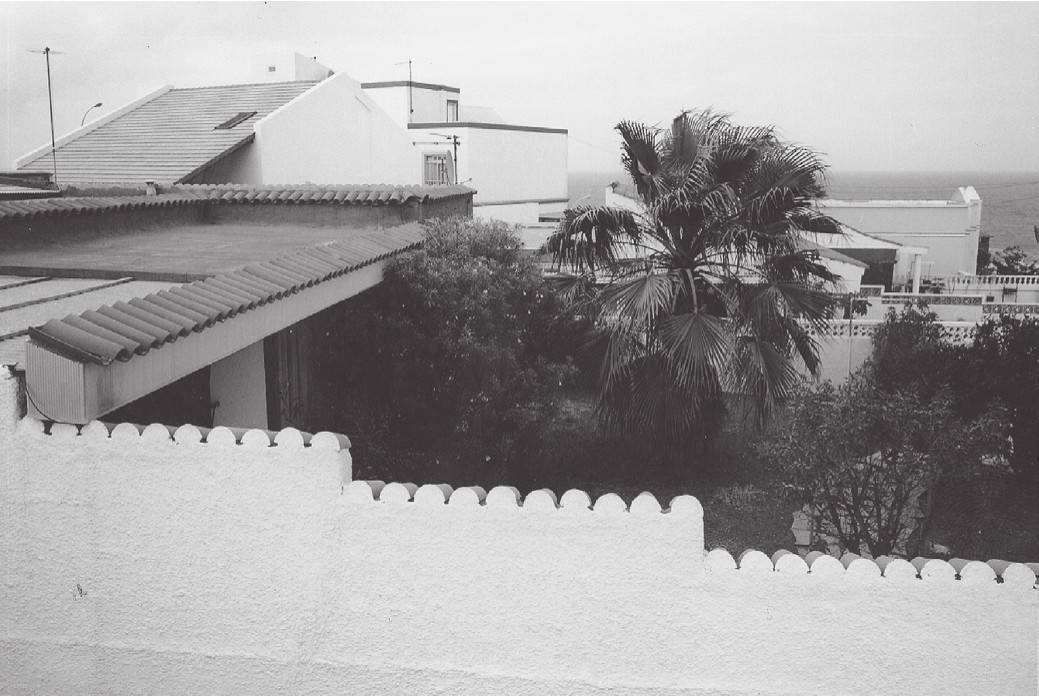
\includegraphics[scale=0.4]{picture/稻草人手记1.jpeg}
    \caption*{三毛在加纳利岛上的房屋小院。}
    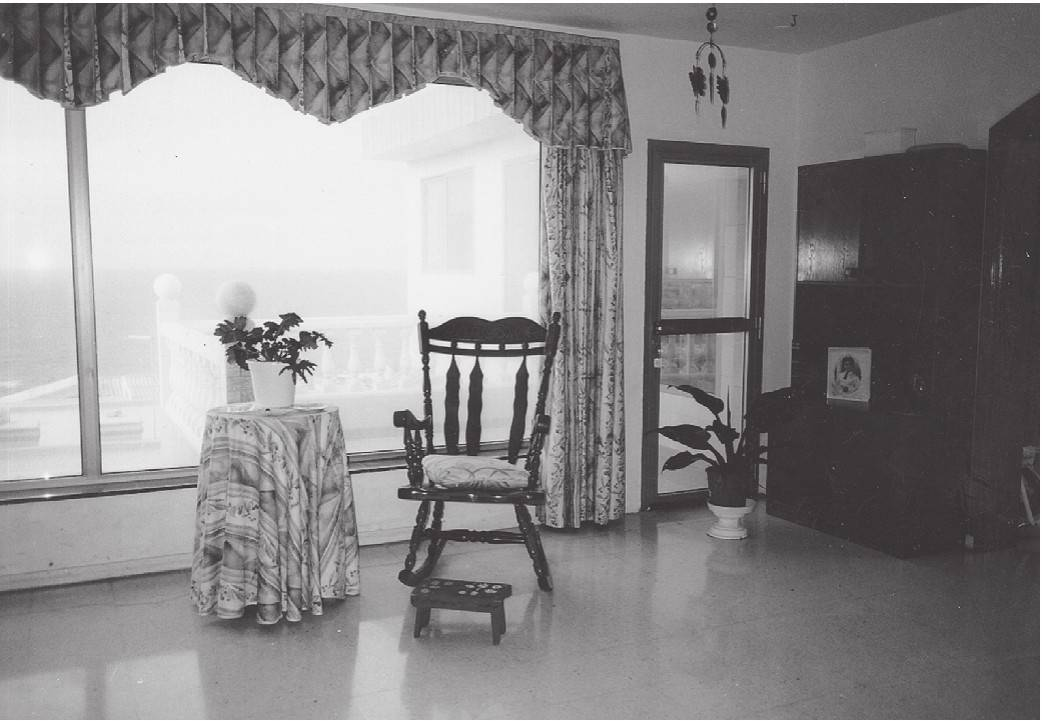
\includegraphics[scale=0.4]{picture/稻草人手记2.jpeg}
    \caption*{三毛作品中多次提到的“可以望见大海的大玻璃窗”。}
\end{figure}
\begin{figure}[htb]
    \centering %
    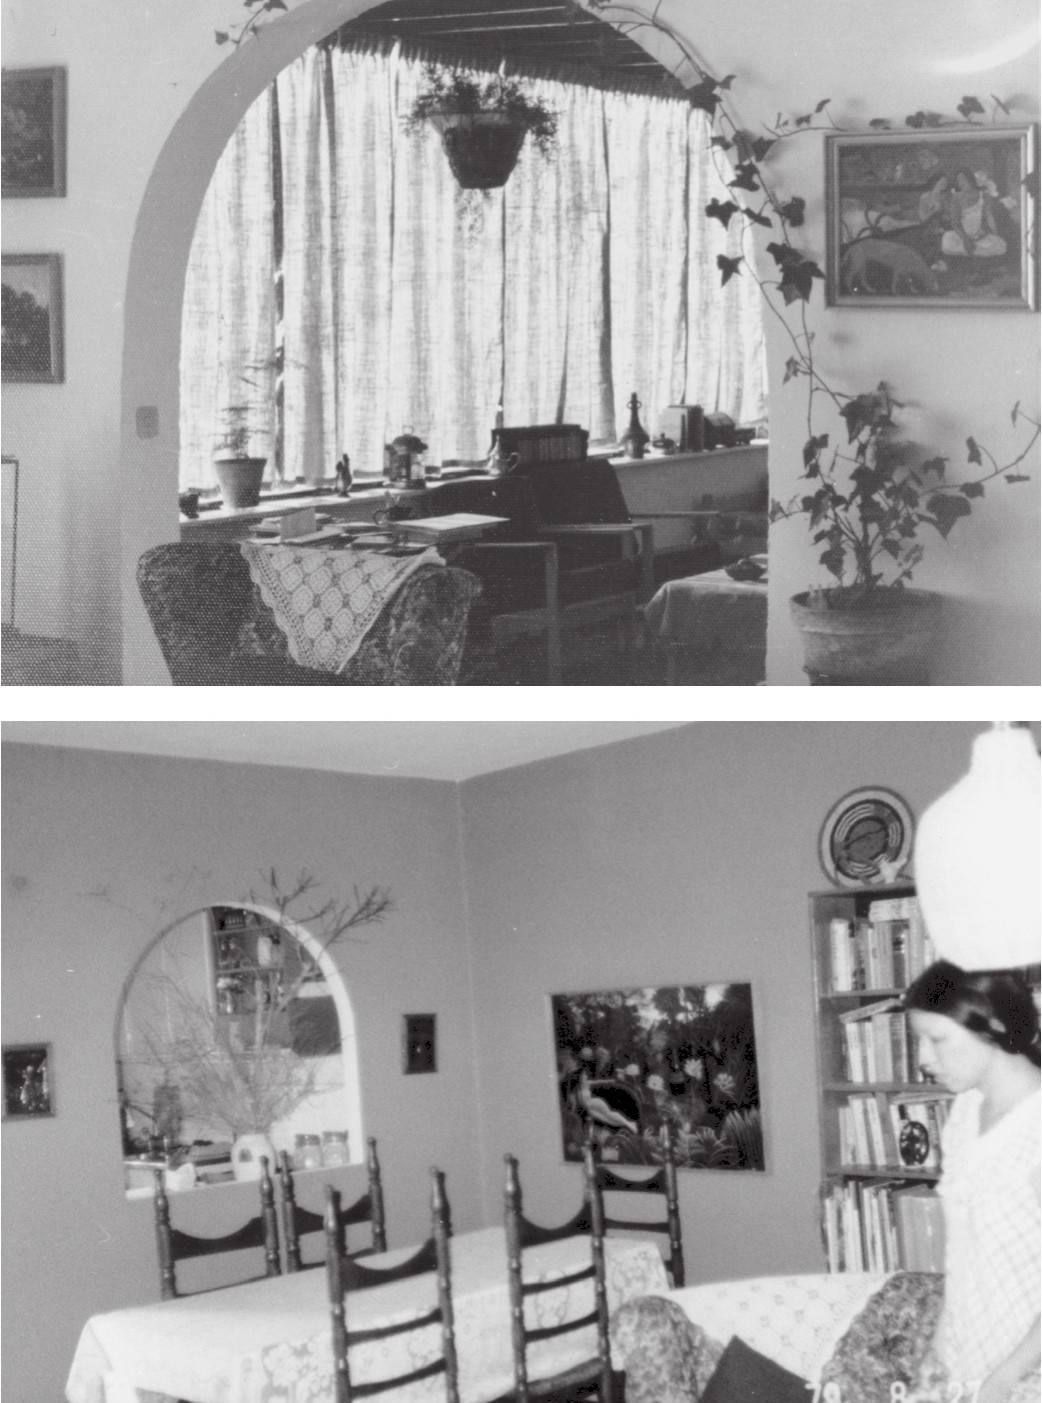
\includegraphics[scale=0.4]{picture/稻草人手记3.jpeg}
    \caption*{西班牙的家中一角。}
\end{figure}
\clearpage
\par 再说撒哈拉,在本月十八日摩洛哥送三十万平民走过边界,后又增到二百万“人海战”,西班牙吓得瘫掉了,AAIUN连军人才四万,全撒哈拉西属,才七万五(二十八万平方公里),后来南边毛里塔尼亚也由南边送平民来过边境(我就逃掉了,无票上机),这几日紧急会议再会议再会议的结果,西班牙不战而败,已签密约,摩洛哥与毛里塔尼亚瓜分撒哈拉,最最可怜的是撒哈拉威人,他们苦苦血战的独立,已成泡影,AAIUN所有撒哈拉威人完全失业,军人(西班牙军内也有撒哈拉威人)解散,他们成了无国籍的一批可怜虫,现在他们恨死西班牙人。
\par 我们好友罕地,三十二年跟西班牙军,现解散,完全不理,失去西班牙籍,AAIUN在军队重兵保护下,西班牙平民撤入军营同食同住,撒哈拉威人住的区完全在坦克严密监视中,他们是被西班牙人出卖了。西班牙人没有为他们的死活做打算,现无水,无食物,孩子要饿死了,红十字会已开去救济,我虽然痛恨撒哈拉威人,但是他们将来临的命运是可怜可悯的,是二十世纪的犹太人,无国籍的七万五千人。荷西临去送给罕地八千西币,罕地流泪不语,已收下,他有九个孩子,如今吃什么?吃沙土,完完全全无食物。
\par 再说荷西的职业,我们大约再做两个月便失业,但西班牙可能留下磷矿与摩洛哥合开,也可能放弃(用摩洛哥的海权交换给西国打鱼),但是公司说,我们可再分配国内工作,也可拿钱走路,如留下去,薪水加百分之百(因撒哈拉威人有游击队,要杀死所有西班牙人,有道理,西班牙利用了他们),好在荷西有一个月的假(我们留下的),先住一个月再去做,等公司分派将来工作。
\par 我的“沙漠学校”在我等机的空当,尚回家给一个女生上了“最后的一课”,她流泪握住我的手(姑卡),我们相对无语,机场已成地狱,那是十天之前,现在的AAIUN更是难以想象,我今天听荷西说撒哈拉威人的情形,我流泪吃不下盘中的牛排,撒哈拉是第二个越南,西班牙人出卖了他们。
\par 我要写一个中篇约十万字,《撒哈拉最后的探戈》(探戈是一种舞蹈),这是三毛眼见的血泪史。另外我要写《最后的一课》和《大逃亡》(荷西)。
\par 可怜的是,我好友Paloma的丈夫Jauies(万事通)明日尚得回沙漠(为了工作),他们全家人哭成一团,但他们无一文积蓄,只有去,又有孩子,要去赚钱。我借给Paloma的钱算做十日的住宿费,坚持不要她还,萍水相逢,收容我十日,已是义薄云天,我们现在是近邻,也好彼此分担忧苦。今日晚饭是Paloma送来。
\par 我们已打长途电话给公婆,婆婆终日啼哭不已,现已会笑,下星期姐夫来住三日(他是旅行社的社长)。
\par 荷西在分别后,寄给我几封信,我一封也未收到,因西班牙封锁消息,只说摩洛哥不再入侵,没有说密约,但AAIUN人自是完全知道,所以信件完全封锁,交通军方有,平民已断,妇女尚有未走,全在军营中吃住等机等船。ZBERIA航空公司说因为有狂风,不再飞AAIUN,荷西能逃出来,是他的机智,我们只有原子笔掉了一支,所以用红笔写。
\par 爹爹,姆妈,我们平安、健康、幸福,居所美丽,这都是荷西所赐,我感谢上帝给我如此的好丈夫。
\par 姐姐一同看信,我不再写,小鸟“芸芸”也出来了,很高兴,在睡觉(鸟食也带出来),都是荷西一人弄的,他人很瘦很瘦,要好好休息。
\par 再说,荷西在沙漠出大车祸,对方死了,他完全没事,是死了的那方错。
\par 荷西十二月再去沙漠,我们十一月薪水尚未领,已托好友代领(最最好友,好男孩,我有妹妹一定嫁此年轻人),他周末出来带钱给我们。在外朋友就是财富,现在苦难才见真情,人间温暖不会消失。
\par 此地静得没有邮差,小分局邮局每日开半小时,自去取信,你们有事打电报来可送到我们家,没有电话(不需要),海边在十分钟下坡路,空旷无一人迹。
\par 我们住的四周,是瑞典人、荷兰人、法国人、英国人,对面是一小小超级市场,有煤气,每日牛奶、面包送来门口,一星期结账一次。在此“芳邻”是鸡犬相闻,老死不相往来,但在区内,人人见面道“早安、午安、晚安”,不必交谈,谈不通也。我住友人家十日,全家出去了,门就大大地开着,但邻居不来往,有教养而亲切,跟西班牙风格大不相同,荷西也喜欢,我也喜欢。附近有一小镇,镇上全部西班牙人,人和气得像在天堂上,太和气太和气了,是糖做的一群老百姓,太好太好太和平的人了。
\par 爹爹眼睛不好,要不然我还多写,将来寄照片给你们看美丽的新家。我们很幸福,前途不知,荷西饿不死,要饿死他恐怕很难,他手很巧,什么都会做,不愁!
\par  
\par \rightline{妹妹上}


\subsubsection{一九七五年十二月五日}

\par \leftline{爹爹,姆妈:}
\par 荷西去上班四日,又回来了。
\par 他的公司在十二月十五日停工,转交给摩洛哥国营公司保证的工作,是一个骗局,过去大家都要罢工,公司就发通知保证每一个人将来都转派工作(是国营的公司),现在高级职员,有人情的职员,全都有工作,但是所有百分之八十的人失业,劳工部长保证的事,是放屁,现在没有工作,没有遣散费(一个月底薪约两万台币),没有发旅费回来,没有一切政府一再保证承诺的事项,当我们是狗一样地一脚踢开,我们没有工会,要告政府只有自己请律师告(我们有劳工部长签字的印刷信,保证工作),现在我们很镇静,开销马上省下来,不可再花一分一文不当的钱。然后我们要跟马德里一群专门替工人打官司的律师去商量,看看是否有补救之道(这群律师不收钱,等案子了了,才收一点点,以前荷西案子,完完全全不收钱,是一群年轻人)。
\par 我们是西班牙跟摩洛哥交易下的牺牲品,西班牙出卖了撒哈拉人,也出卖了自己三千劳工,西班牙的政府在烂掉,法兰哥的家族成了千万富翁,全西最大的百货公司、市场、房地产都是他女儿的,最大的医院是他女婿的,他的太太、女儿、孙女,穿孝穿黑色貂皮大衣算穿孝,我们吃沙吃灰在沙漠苦,现在一脚踢开,遣散费等于是狗屎,付两个月房租正好,生活那么高,三万块西币正好是三千包一公升的鲜牛奶价,现在摩洛哥人在沙漠屠杀六十岁以下的撒哈拉威人,年轻人全部逃亡阿尔及利亚加入“人民解放游击队”。西班牙人有许多跟了去,我不拉住荷西,他也要去(他如去,我跟去打游击),这次的事件,我看出西班牙的腐败,我们没有失业保险(德国有),没有救济金(工作三年满每月付四千台币,我们不满三年),我不是共产党,但是不要太逼人,人逼急了,不过是死路一条,我是一个分析明白的人,对政治不感兴趣,但正义在哪里?天理又在哪里?我们的前途政府没有管,叫我们去死吗?
\par 现在另有一个机会,荷西希望替摩洛哥工作,等矿公司一移交,我们留下来替新工作做事,但是更无保证,是外国公司要请你走路便走。
\par 现在公司薪水十二月不发,他们说“放假”半个月,以后再看。我们有房款可用,你们不要急,二月再说,我们如付不出房款,可以登报卖,如一时卖不掉,可打官司。打官司期内,每月付八千西币仍算我们的,直到法院宣判,所以也不是什么好急的事情。
\par 爹爹眼睛不好,为了我们,牺牲了一辈子,请你们不要再背我们的十字架,我们尚年轻,长长的人生可以受一点风浪,不要管我们了。荷西是很能干的人,我可回来出书,都是出路。荷西是个有为的青年,我们不会太潦倒,请千万放心,他要上船去做海员,我不赞成,全西班牙只有二十八个如他文凭的潜水人员,难道这一道一关的考试都是废纸吗?(是废纸,如是法兰哥的孩子,不必学写字也可一生做花花公子。)
\par 现在唯一的机会是跟摩洛哥签新合同,但是如果付太少(会付很少很少),也划不来做,我们很镇静,请放心,放心。
\par 亲爱的双亲,你们不要天天东想西想,请放开我们,给我们自己来,我们不能再收你们的钱,如果房子付不出,可以卖掉,还是有出路,不是太坏的事,你们不要再焦急,不要担心,过一阵子马上会好转的。总之你们不要再背十字架了,我知道我们台湾房子卖不掉,租不出,爹爹眼睛不好,我们自己家也很困难,不能再管子女,我们已成年太久,难道还不能自立吗?
\par  
\par \rightline{妹妹上}



\subsubsection{一九七六年二月二十五日}

\par \leftline{爹爹,姆妈:}
\par 前天收到包裹,我回来打开看了,才知什么叫蜂皇精,以前只听过。昨天早晨服一针,今日又服一针(因没有疲倦感),睡得非常好,目前还不觉得有什么反应,也不见强,但我想十天以后一定会胖起来。今日渔业专员梁先生开车来看我,进门便问我,为什么说谎话,我被他弄得莫名其妙,问清楚了才知是夏教授元瑜发表了我的信,信中我曾提起,我不太与渔船船员来往,因为他们不赞成我嫁外国人。我实在记不得自己信里胡说八道了什么,但是我也许有讲,这也不是什么大不了的叛国罪,值得今天看到报纸便来问我何故如此写,我老实告诉他,在码头上,中国渔船员的确骂我“婊子”(用中文骂我,因与荷西在一起走),结果我轻轻将话带过,这种小事,不值争辩,我的心胸气量都不是个傻瓜,我才不去计较他。他又说,非洲有四宝,一宝二宝三宝全讲了,又哈哈大笑,说还有一个宝就是“三毛”,语气嘲讽不堪,又笑我——你只值三毛钱,看一看你,只要付三毛钱入场券——(因为此地许多华侨要看我),我久不习惯这种语气,因为我们的朋友,都是尊重他人、诚恳坦白的人,我所以不知如何回答他的嘲笑。写作何罪?做三毛何罪?为什么人人都喜欢我,偏偏有同胞不喜欢我?为什么我在中国人里吃不开?为什么?为什么?不再问了,这是我很清楚的事。我尚未收到报纸,明后日收到了再看我这么写,犯了什么死罪。
\par 最奇怪的是,他和另外两个人来时,尚有我一西籍女友在家同坐,她看那人用中文高声大气问我,吓得马上走了,我真对不起这位太太,梁先生走了,我又赶快开车去她家道歉。外国人,最讲礼貌,不在他人面前高声讲话,而我也给梁先生吓一大跳,原来是这么一回小事情。
\par 我以前会被弄得气得哭,现在不气,只是好笑这些人,马德里腰痛那一大阵,也是如此这般,人,真奇怪,做了官,就以为老百姓都是狗屎,所以我不做官,也做不到,因为没有官架子也!
\par 爹爹,蜂皇精是那么贵的东西,如何寄给我,你们自己不吃?我身体无大病了,血止了,咳停了,颈子扭好了,现在脚扭伤已可开车(因为跌倒当时马上有西班牙老太太脱靴替我扭回,又马上上绷带,夜间荷西与姐夫也用力替我擦,又用热水泡,这一次恢复得很快,已开车),所以我无大病,你们不要担心,吃得也很好,包裹中附来《中央日报》,说维他命A的重要,我昨日吃两大根生的红萝卜,现在再去吃一大根,每日有鸡汤吃。水果也有吃橘子、苹果(不贵,三十元一公斤)。
\par 房子卖的事情,尚在谈,周末我们再去打电话给马德里。荷西星期五回来。
\par 沙漠边界打了起来,看情形也拖不长了,我们尚不知如何,反正有事做,不做有钱拿,不愁不愁。听说分派的工作都收入很差,不怕,我们有两三条路可走,不做也有三十万可领,一年失业不怕找不到事。听说失业政府尚借两百万给买房,我就不愁。
\par 上个月写伤了,这个月一字不写,上月出了好几万字,我休息,勉强不出来。何况我现在朋友很多,说英文的瑞士女友,她先生回来了(在北非工作,是探矿工程师),今日也来看我,我们相处十分投合,不说别人长短,只说有趣的事情,这些人都是好邻居。我认识的人很多,来往的只有瑞士女友、她英国丈夫、西籍女友,也够热闹了,每二日见一见面。都没有是非,彼此的友情,是有建设性的,不是小心眼找人碴子的。荷西回来了,也去拜访他们。我们相处,每日大笑特笑,不生气,对健康心情有益。邻居小孩也来,他们总是用英文问我:
\par “你爹地怎么不在?”
\par 我说:“我先生吧,什么爹地。”
\par 他们问:“你几岁?”
\par 我说:“我二十八岁。”
\par 他们说:“唉!我们以为你十五岁,所以以为那个大胡子是你爸爸!”我大乐。爸爸不常回家,我也过得好极了。
\par 中国人是好,那是老一代的。西方人,开朗,尊重他人的私生活,没有太多的利害关系,好相处。他们好佩服我呢!中文看不懂,但我每有报纸,都给他们看看。来了也不招待,一杯咖啡坐一个下午,没有客套,白学英语!
\par 汗衫好极了,荷西回来一定喜欢,粉丝我尚未打开来吃,等老爷回来同吃,我一大锅鸡汤可吃一星期。另外吃面包,不太吃饭。
\par 爹爹,姆妈,我的足踝已好,走路不痛,也可开车了,明日再服一针蜂皇精,人会胖,放心,一切都好,外公处请代问候。我一天平均写三封信,荷西不写信,我要代他写全家人的信,美国大姑、小姐姐都是我在联络,好在也不费事,不费心——邮费很贵,仍是值得。
\par 另外我在翻译一本漫画书,每日译三五小格,也不是工作。我的植物,欣欣向荣,长得好美。
\par 不要担心我,你们才要保重,希望早早见面,荷西说,卖了房子给我回家,我说:我们一同去。他舍不得钱,其实可以一同回娘家一个月荷西再回,我住久些。
\par 爹爹,我身体好了,不必担心,我会去全身检查,不要愁,我去检查。
\par 不多写了,我是顺手写来不费吹灰之力,爹爹姆妈眼睛吃不消。
\par  
\par \rightline{妹妹上}



\subsubsection{一九七六年三月二十六日}


\par \leftline{爹爹,姆妈:}
\par 今天是我的生日,我到昨天才知道,因为我去寄挂号信给皇冠五月份的稿子,才知已是三十三岁足了,对于年龄我并不在乎,因为人毕竟是要老的,如花开花落,都是自然的现象。回想三十三年来的岁月,有苦有乐,而今仍要走下去,倒已是有点意兴阑珊了。我的半生,到现在,已十分满足,金钱、爱情、名声、家庭都堪称幸福无缺,只缺健康的身体,但是,我也无遗憾,如果今后早死,于己于人都该贴红挂彩,庆祝这样的人生美满结束,我的心里毫无悲伤,只有快乐。自从去年大哥死去之后,我细想了一下,死的人去了,是安息了,是永恒了,生着的人,不应该悲痛,要有坦然的心胸去接受人生的现象,这也是我近来身体极不好之下,想到你们,而要劝告你们的话,人生的长短和价值,都是一样,一旦进入死亡,那就是永远地活下去,没有什么好悲痛的,请你们一定要明白这个道理。
\par 荷西仍未回来,卖房、找事之外尚得向银行借钱,都不可能十天半月弄好,他亦有信来。
\par 外公身体好吗?你们又如何?我有点发烧,开刀二次,疮结了又生,开了又结,又生,子宫流血又来,下月十日刮子宫,肝病也在吃药打针,我是私人医生在看,我撑得住,千万不要为我做无用的焦急。
\par 钻戒我没有用,于我身份也不配,姆妈留着,回来住家中,因荷西不来(太贵了),等一切安置妥,我就回台湾,千万放心我。
\par 宝宝如何?小妹们好吗?我回来买漂亮衣服给她们。不多写了。祝
\par 好
\par  
\par \rightline{妹妹上}


\subsubsection{一九七六年八月十日}


\par \leftline{爹爹,姆妈:}
\par 现在的生活安静朴素极了,每天穿一件比基尼游泳装随处可去,衣服实在用不着,今日我打扮了一下,不过是一件牛仔裤衣,已算很好了,荷西平日亦是短裤赤膊,此地住家人人如此,非常省衣服钱。
\par 我们又看到一幢房子,是一老先生死了,他太太想卖,也是一百五十万台币,我现在杀她价一百万台币,看她肯不肯(也许肯),这个岛上我们都去找了,其他地方即使院大也无处可去(荒秃秃泥巴山),这儿有海湾,有极好的环境可以外出散步,所以我选来选去还是现在住的地方。这儿对老人、年轻人、小孩都有好处,空气又好,现在这家如肯卖,我们马上买下(一大厅、四人房、两浴、一厨、有车房、院子),要等介绍人去丹麦问消息。我很喜欢这小房,对着大海,但不吵,因在远坡上,没有花树,光秃秃的一片,请爹爹、姆妈等我们买下房子了来住,你们肯来,将来车也换大的。
\par 今日去问失业保险,可领两年,我们方领四个月(每月一万六台币),所以我们不急,有很好的事才去做,如不太好,所赚差不多失业金,将来失业了还没有现在领的多,所以一定要小心找事。一万六一月对我来说是必须十分省了,房租一百,荷西学英文五十,汽油六十元,大约是二百十元美金,只有一百九十美元可吃饭杂用,所以不能看电影、穿衣、吃牛排……但这儿生活环境非常好,我很满足,吃穿都是次要,现在我就在院子里写字,对着大海,清风徐来,比花莲亚士都饭店好一百倍。以前我用大约七百美金一月,常常上馆子。
\par 希望过几年爹爹姆妈同来过过这里的安静日子,只怕你们会寂寞,你们来了,爹爹管花园,姆妈管厨房,这样不会无事做。
\par  
\par \rightline{妹妹上}








 % 3
% \clearpage
% 
% 

\section{温柔的夜}

\par 书名:温柔的夜
\par 作者:三毛
\par 出版社:北京出版集团北京十月文艺出版社
\par 出版时间:2017-03
\par ISBN:9787530214770

\subsection{开场白\\\small{永远的夏娃}}

\par 《永远的夏娃》是很久以来就放在心里的一个标题,两年来,它像一块飘浮不定的云,千变万化,总也不能捉住它,给它定下清晰的形状来。
\par 起初想出这个名字,倒是为了一个西籍女友,因为她的种种遭遇,使我总想到其他许许多多在我生命中经历过的女友们,她们的故事,每一篇都是夏娃的传奇。当时,很想在这个标题下,将她们一个一个写出来。后来,我又不想写这些人了。可是专栏得开了,夏娃这个名字我还是很爱,因为它不代表什么,也不暗示什么,专栏既然要一个名字,我就用了下来,它本身实在是没有意义的。
\par 俄国作家杜斯妥也夫斯基说过一句使我十分心惊的话,他说:“除非太卑鄙得偏爱自己的人,才能无耻地写自己的事情。”
\par 我有一阵常常想到这句话,使得写作几乎停顿,因为没有写第三者的技巧和心境;他人的事,没有把握也没有热情去写;自己的事,又心虚得不敢再写,我不喜欢被人看视成无耻的人,可是老写自己生活上的事,真是觉得有些无耻。
\par 后来我们搬家了,新家门口每天早晨都会有一匹白马驮着两个大藤篮跟着它的主人走过,沿途叫卖着:“苹——果——啊!”
\par 每听见马蹄哒哒地来了,还不等那个做主人的叫嚷,我就冲出去靠在栏杆上看,直看到他们走远。
\par 这匹马天天来,我总也不厌地看它,每当荷西下班回来了,我照例按压不住内心的欢喜向他喊着:“今天马又来了!”
\par 马总是来的,而我的喜悦,却像当初第一次见它时一样的新鲜。
\par 有一天,再也忍不住了,跟荷西说:“我要把这匹马写出来。”
\par 他说:“有什么好写的,每天来,每天去的。”
\par 是很平常的事情,可是我要把它写下来,说我天天看见一匹马经过,不知为什么有说不出的欢喜和感动。
\par 后来,我又想到许多我生命中经历的事,忍不住想写,不写都不行,当时,总会想到杜斯妥也夫斯基那句话——老写自己的事是无耻的——每想这句话,心中便气馁得很,呆呆地坐下来看电视,什么也不写了。可是那匹马啊,一直在心底压着,总得把它写出来才好。
\par 又有一阵,一个朋友写信给我,他说:“你总不能就此不写了,到底你做的是文以载道的工作!”
\par 我被这句话吓得很厉害,从来没有想到载什么东西的问题,这更不能写了,不喜欢那么严重。
\par 以后有一段长时间就不写什么了。
\par 今天荷西下班来对我说,工地上有个工人朋友家住在山里面,如果我们跟他回去,可以去看看这人养的猪羊,还有他种的菜。我们去了,挖了一大筐蔬菜回来,我的心,因为这一个下午乡间的快乐,又恨不得将它写了下来。久已不肯动笔的人,还是有这种想望。
\par 回来后我一直在写作的事情上思想,想了又想,结果想明白了,我的写作,原本是一种游戏,我无拘无束地坐下来,自由自在地把想写的东西涂在纸上。在我,是这么自然而又好玩的事情,所以强迫自己不写,才会是一种难学的忍耐,才会觉得怅然若失,我又何苦在这么有趣的事情上节制自己呢!
\par 像现在,我在上面把那匹马写了出来,内心觉得无比的舒畅,这真是很大的欢喜。我做这件事,实在没有目的,说得诚实些,我只是在玩耍罢了,投身在文章里,竟是如此快乐,连悲哀的事,写到情极处,都是快乐的感觉,这一点,连自己也无由解释的,总是这样下去了吧,我毕竟是一个没有什么大道理的人啊!
\par 《永远的夏娃》将会是我一些美丽的生命的记忆,在别人看来,它们可能没有价值,在我,我不如不去想它价值不价值的问题,自由得像空气一般地去写我真挚的心灵。其实,它不写也没有什么不可以,写了对事情还是一样的,可是既然我想写了,我就不再多想,欢天喜地地将它们写出来吧!



\subsection{拾荒梦\\\small{永远的夏娃之一}}


\par 在我的小学时代里,我个人最拿手的功课就是作文和美术。当时,我们全科老师是一个教学十分认真而又严厉的女人。她很少给我们下课,自己也不回办公室去,连中午吃饭的时间,她都舍不得离开我们,我们一面静悄悄地吃便当,一面还得洗耳恭听老师习惯性的骂人。
\par 我是常常被指名出来骂的一个。一星期里也只有两堂作文课是我太平的时间。也许老师对我的作文实在是有些欣赏,她常常忘了自己叫骂我时的种种可厌的名称,一上作文课,就会说:“三毛,快快写,写完了站起来朗诵。”
\par 有一天老师出了一个每学期都会出的作文题目,叫我们好好发挥,并且说:“应该尽量写得有理想才好。”
\par 等到大家都写完了,下课时间还有多,老师坐在教室右边的桌上低头改考卷,顺口就说:“三毛,站起来将你的作文念出来。”
\par 小小的我捧了簿子大声朗读起来。
\refdocument{
    \par 我的志愿——
    \par 我有一天长大了,希望做一个拾破烂的人,因为这种职业,不但可以呼吸新鲜的空气,同时又可以大街小巷地游走玩耍,一面工作一面游戏,自由快乐得如同天上的飞鸟。更重要的是,人们常常不知不觉地将许多还可以利用的好东西当做垃圾丢掉,拾破烂的人最愉快的时刻就是将这些蒙尘的好东西再度发掘出来,这……
}
\par 念到这儿,老师顺手丢过来一只黑板擦,打到了坐在我旁边的同学,我一吓,也放下本子不再念了,呆呆地等着受罚。
\par “什么文章嘛!你……”老师大吼一声。她喜怒无常的性情我早已习惯了,可是在作文课上对我这样发脾气还是不太常有的。
\par “乱写!乱写!什么拾破烂的!将来要拾破烂,现在书也不必念了,滚出去好了,对不对得起父母……”老师又大拍桌子惊天动地地喊。
\par “重写!别的同学可以下课。”她瞪了我一眼便出去了。
\par 于是,我又写:
\refdocument{
    \par 我有一天长大了,希望做一个夏天卖冰棒,冬天卖烤红薯的街头小贩,因为这种职业不但可以呼吸新鲜空气,又可以大街小巷地游走玩耍,更重要的是,一面做生意,一面可以顺便看看,沿街的垃圾箱里,有没有被人丢弃的好东西,这……
}
\par 第二次作文缴上去,老师画了个大红叉,当然又丢下来叫重写。结果我只好胡乱写着:“我长大要做医生,拯救天下万民……”老师看了十分感动,批了个甲,并且说:“这才是一个有理想,不辜负父母期望的志愿。”
\par 我那可爱的老师并不知道,当年她那一只打偏了的黑板擦和两次重写的处罚,并没有改掉我内心坚强的信念,这许多年来,我虽然没有真正以拾荒为职业,可是我是拾着垃圾长大的,越拾越专门,这个习惯已经根深蒂固,什么处罚也改不了我。当初胡说的什么拯救天下万民的志愿是还给老师保存了。
\par 说起来,在我们那个时代的儿童,可以说是没有现成玩具的一群小孩。树叶一折当哨子,破毛笔管化点肥皂满天吹泡泡,五个小石子下棋,粉笔地上一画跳房子,粗竹筒开个细缝成了扑满,手指头上画小人脸,手帕一围就开唱布袋戏,筷子用橡皮筋绑绑紧可以当手枪……那么多迷疯了小孩子的花样都是不花钱的,说得更清楚些,都是走路放学时顺手捡来的。
\par 我制造的第一个玩具自然也是地上拾来的。那是一枝弧形的树枝,像滚铁环一样一面跑一面跟着前面逃的人追,树枝点到了谁谁就死,这个玩具明明不过是一枝树枝,可是我偏喜欢叫它“点人机”,那时我三岁,就奠定了日后拾荒的基础。
\par 拾荒人的眼力绝对不是一天就培养得出来的,也不是如老师所说,拾荒就不必念书,干脆就可以滚出学校的。
\par 我自小走路喜欢东张西望,尤其做小学生时,放学了,书包先请走得快的同学送回家交给母亲,我便一人田间小径上慢吞吞地游荡,这一路上,总有说不出的宝藏可以拾它起来玩。
\par 有时是一颗弹珠,有时是一个大别针,有时是一颗狗牙齿,也可能是一个极美丽的空香水瓶,又可能是一只小皮球,运气再好的时候,还可以捡到一角钱。
\par 放学的那条路,是最好的拾荒路,走起来也顶好不要成群结队,一个人玩玩跳跳捡捡,成绩总比一大批人在一起好得多。
\par 捡东西的习惯一旦慢慢养成,根本不必看着地下走路,眼角闲闲一飘,就知哪些是可取的,哪些是不必理睬的,这些学问,我在童年时已经深得其中三昧了。
\par 做少女的时代,我曾经发狂地爱上一切木头的东西,那时候,因为看了一些好书,眼光也有了长进,虽然书不是木头做的,可是我的心灵因为啃了这些书,产生了化学作用,所谓“格调”这个东西,也慢慢地能够分辨体会了。
\par 十三岁的时候,看见别人家锯树,锯下来的大树干丢在路边,我细看那枝大枯枝,越看越投缘,顾不得街上的人怎么想我,掮着它走了不知多少路回到家,宝贝也似的当艺术品放在自己的房间里,一心一意地爱着它。
\par 后来,发现家中阿巴桑坐在院子里的一块好木头上洗衣服,我将这块形状美丽的东西拾起来悄悄打量了一下,这真是宝物蒙尘,它完全像复活岛上那些竖立着的人脸石像,只是它更木头木脑一点。我将这块木头也换了过来,搬了一块空心砖给阿巴桑坐着,她因为我抢去她的椅子还大大地生了一场气。
\par 在我离家远走之前,我父母的家可以说堆满了一切又一切我在外面拾回来的好东西。当时我的父母一再保证,就是搬家,也不会丢掉我视为第二生命的破铜烂铁。
\par 有些有眼光的朋友看了我当时的画室,赞不绝口,也有一些亲戚们来看了,直截了当地说:“哎呀,你的房间是假的嘛!”这一句话总使我有些泄气,对于某些人,东西不照一般人的规矩用,就被称做假的。
\par 我虽然是抗战末期出生的“战争儿童”,可是在我父母的爱护下,一向温饱过甚,从来不知物质的缺乏是什么滋味。
\par 家中四个孩子,只有我这个老二,怪异得有拾废物的毛病,父亲常常开导我,要消费,要消耗,社会经济才能繁荣,不要一块碎布也像外婆似的藏个几十年。这些道理我从小听到大,可是,一见了尚可利用的东西,又忍不住去捡,捡回来洗洗刷刷,看它们在我的手底下复活,那真是太快乐的游戏。
\par 离开了父母之后,我住的一直是外国的学生宿舍,那时心理上没有归依感,生命里也有好几年没有再捡东西的心情。无家的人实在不需要自己常常提醒,只看那空荡荡的桌椅就知道这公式化的房间不是一个家。
\par 那一阵死书念得太多,头脑转不灵活,心灵亦为之蒙尘,而自己却找不出自救之道,人生最宝贵的青春竟在教科书本中度过实是可惜。
\par 不再上学之后,曾经跟其他三个单身女孩子同住一个公寓,当时是在城里,虽然没有地方去捡什么东西,可是我同住的朋友们丢掉的旧衣服、毛线,甚而杂志,我都收拢了,夜间谈天说地的时候,这些废物,在我的改装下,变成了布娃娃、围裙、比基尼游泳衣……
\par 当时,看见自己变出了如此美丽的魔术,拾荒的旧梦又一度清晰地浮到眼前来,那等于发现了一个还没有完全枯萎的生命,那份心情是十分感动自己的。
\par 到那时为止,拾破烂在我的生活中虽然没有停顿,可是它究竟只是一份嗜好,并不是必须赖以生存的工作,我也没有想过,如果有一日,整个的家庭要依靠别人丢弃的东西一草一木地重组起来,会是怎么美妙的滋味。
\par 等我体会出拾荒真正无与伦比的神秘和奇妙时,在撒哈拉沙漠里,已被我利用在大漠镇外垃圾堆里翻捡的成绩,布置出了一个世界上最美丽的家,那是整整两年的时间造成的奇迹。
\par 拾荒人眼底的垃圾场是一块世界上最妩媚的花园。过去小学老师曾说:“要拾破烂,现在就可以滚,不必再念书了!”她这话只有一半是对的,学校可以滚出来,书却不能不念的。垃圾虽是一样的垃圾,可是因为面对它的人在经验和艺术的修养上不同,它也会有不同的反应和回报。
\par 在我的拾荒生涯里,最奇怪的还是在沙漠。这片大地看似虚无,其实它蕴藏了多少大自然的礼物,我至今收藏的一些石斧、石刀还有三叶虫的化石都是那里得来的宝贝。
\par 更怪异的是,在清晨的沙漠里,荷西与我拾到过一百多条长如手臂的法国面包,握在手里是热的,吃在嘴里外脆内软,显然是刚刚出炉的东西,没法解释它们为什么躺在荒野里,这么多条面包我们吃不了,整个工地拿去分,也没听说吃死了人。
\par 还有一次西班牙人已经开始在沙漠撤退了,也是在荒野里,丢了一卡车几百箱的法国三星白兰地,我们捡了一大箱回来,竟是派不上什么用场,结果仍是放在家里人就离开了,离开沙漠时,有生以来第一回,丢了自己东西给人捡,那真说不出有多心痛。
\par 我们定居到现在的群岛来时,家附近靠海的地方也有一片垃圾场,在那儿,人们将建筑材料、旧衣鞋、家具、收音机、电视、木箱、花草、书籍数也数不清,分也分不完的好东西丢弃着。
\par 这个垃圾场没有腐坏的食物,镇上清洁队每天来收厨房垃圾,而家庭中不用的物件和粗重的材料,才被丢弃在这住宅区的尽头。
\par 也是在这个大垃圾场里,我认识了今生唯一的一个拾荒同好。
\par 这人是我邻居葛雷老夫妇的儿子,过去是苏黎世一间小学校的教师,后来因为过分热爱拾荒自由自在的生涯,毅然放下了教职,现在靠拾捡旧货转卖得来的钱过日子。
\par 在他住父母家度假的一段时间里,他是我们家的常客,据他说,拾荒的收入,不比一个小学老师差,这完全要看个人的兴趣。我觉得那是他的选择,外人是没有资格在这件事上来下评论的。
\par 我的小学老师因为我曾经立志要拾荒而怒叱我,却不知道,我成长后第一个碰见的专业拾荒人居然是一个小学老师变过来的,这实在是十分有趣的事情。
\par 这个专业的拾荒同好,比起我的功力来,又高了一层,往往我们一同开始在垃圾堆里慢慢散步,走完了一趟,我什么也没得着,他却抬出一整面雕花的木门来送荷西,这么好的东西别人为什么丢掉实在是想不透。
\par 我的拾荒朋友回到瑞士之后不久,他的另一个哥哥开车穿过欧洲再坐船也来到了加纳利群岛。这一次,我的朋友托带来了一架货真价实的老式瑞士乡间的运牛奶的木拖车,有三分之二的汽车那么长,轮子、把手什么都可以转。它是绑在车顶上飘洋过海而来的一个真实的梦。我惊喜得不相信自己的眼睛,接着,一本淡绿封面,精装,写着老式花体英文字母,插画着精美钢笔线条画的故事书《威廉特尔》轻轻地又放在我手里,看看版本,竟是一九二〇年的。
\par 这两样珍贵非常的东西使我们欢喜了好一阵,而我们托带去的回报,是一个过去西班牙人洗脸时盛水用的紫铜面盆和镶花的黑铁架,一个粗彩陶绘制的磨咖啡豆的磨子,还有一块破了一个洞又被我巧妙地绣补好了的西班牙绣花古式女用披肩。当然,这些一来一往的礼物,都是我们双方在垃圾堆里掏出来的精品。
\par 拾荒不一定要在陆上拾,海里也有它的世界。荷西在海里掏出来过腓尼基人时代的陶瓮,十八世纪时的实心炮弹、船灯、船窗、罗盘、大铁链,最近一次,在水底,捡到一枚男用的金戒指,上面刻着一九四七年,名字已被磨褪得看不出来了。海底的东西,陶瓮因是西班牙国家的财产归了加地斯城的博物馆,其他的都用来装饰了房间,只有那只金戒指,因为不知道过去是属于什么人的,看了心里总是不舒服,好似它主人的灵魂还附在它里面一样。
\par 拾荒赔本的时候也是有的,那是判断错误拾回来的东西。
\par 有一次我在路上看见极大极大一个木箱,大得像一个房间,当时我马上想到,它可以放在后院里,锯开门窗,真拿它来当客房用。
\par 结果我付了大卡车钱、四个工人钱。大箱子运来了,花园的小门却进不去。我当机立断,再要把这庞然大物丢掉,警察却跟在卡车司机后面不肯走,我如果丢了,他要开罚单,绕了不知多少转,我溜下车逃了,难题留给卡车司机去处理吧。第二天早晨一起床,大箱子居然挡在门口。支解那个大东西的时候,我似乎下决心不再张望路上任何一草一木了。
\par 前一阵,荷西带了我去山里看朋友,沿途公路上许多农家,他们的垃圾都放在一个个小木箱里。
\par 在回程的路上,我对荷西说:“前面转弯,大树下停一停。”
\par 车停了,我从从容容地走过去,在别人的垃圾箱内,捧出三大棵美丽的羊齿植物。
\par 这就是我的生活和快乐。
\par 拾荒的趣味,除了不劳而获这实际的欢喜之外,更吸引人的是,它永远是一份未知,在下一分钟里,能拾到的是什么好东西谁也不知道,它是一个没有终止,没有答案,也不会有结局的谜。
\par 我有一天老了的时候,要动手做一本书,在这本书里,自我童年时代所捡的东西一直到老年的都要写上去,然后我把它包起来,丢在垃圾场里,如果有一天,有另外一个人,捡到了这本书,将它珍藏起来,同时也开始拾垃圾,那么,这个一生的拾荒梦,总是有人继承了再做下去,垃圾们知道了,不知会有多么欢喜呢。


\subsection{黄昏的故事\\\small{永远的夏娃之二}}

\par 我喜欢漫游,也喜欢黄昏和黑夜交接的那一段时光。
\par 我们现在的家,坐落在一个斜斜山坡的顶上。前面的大玻璃窗看出去,星罗棋布的小白房在一脉青山上迤逦着筑到海边。
\par 厨房的后窗根本是一幅画框,微风吹拂着美丽的山谷,落日在海水上缓缓转红,远方低低的天边,第一颗星总像是大海里升上来的,更奇怪的是,墙下的金银花,一定要开始黄昏了,才发出淡淡的沁香来。这时候,一天的家务差不多都做完了,咖啡热着,蛋糕烘烤得恰到好处。荷西已经下工回来,电视机也开始唱广告歌。我换上舒服的凉鞋,把荷西的茶点小心地用托盘搬出来,这才摸摸他的头,对他说:“我走了。”
\par 这时候的荷西,也许在看报,也可能盯着电视,也可能开始吃东西,他照例含糊地说一句:“旅途愉快!”便将我打发去了。
\par 我轻轻地带上房门,呼吸着第一口甚而还有些寒冷的空气,心情不知怎的就那么踏实欢喜起来。
\par 很少在清晨散步,除了住在撒哈拉的那一阵经常早起之外,以后可以说没有在极早的时光里生活过。
\par 早晨是一日的开始,心情上,有一日的负担和算计,迎接未知的白日,总使人紧张而戒备。黄昏便是不同,它是温柔的夜的前奏,是释放、舒畅,教人享受生命最甜美的一段时光。
\par 这两年多来,无论住在哪里,家总是安置在近海的地方,黄昏长长的漫步成了生活里不可或缺的习惯。
\par 在丹纳丽芙岛,现在的住家,我每日漫游的路途大致是相同的。后山下坡,穿过海也似的芭蕉园,绕过灌溉用的大水池,经过一排极华丽的深宅大院,跟“水肺”站着谈一会儿闲话,再下坡,踏过一片野菊花,转弯,下到海岸线,沿着海边跑到古堡,十字港的地区就算是到了,穿进峡谷似的现代大旅馆,到渔港看船,广场打个转,图书馆借本书,这才原路回来。
\par  
\par 每日经过女友黛娥的家,她总是抱了孩子想跟我一块去游荡,有时候看见她近乎委屈地巴望着我,总觉得自己拒绝得有些残忍。
\par 总是哄她,用各种理由不带她去,有时候远远看见她向我走来,干脆装着不看见,掉头就跑,这样无情地一次一次甩掉她,她居然也不生气。
\par 我喜欢适度的孤单,心灵上最释放的一刻,总舍不得跟别人共享,事实上也很难分享这绝对个人的珍宝,甚至荷西自愿留在家里看电视,我的心里都暗藏了几分喜悦。
\par 清风明月都该应是一个人的事情,倒是吃饭,是人多些比较有味道。
\par 每次散步,那条乡间小路上可以说是碰不到一个人影的,只有“水肺”,像是赴约会似的等在他华厦的大门口,苦盼着我经过。
\par “水肺”是一个八十多岁生病的德国老头子,跟他单身的儿子住在一幢极大的房子里,父子两个长得一模一样,儿子中年了,好似也病着似的。
\par 这一家异乡人没有朋友,也不外出做事,种了一园的玫瑰花。老人因为肺水肿,已经不太能动了,天天趴在花园的门上,见我去了,老远的就一步一步将我吞下去似的望。
\par 第一次经过老人的门口,就是被他喂喂地叫过去的。我过去了,他隔着镶花铁门,把手蓦然伸出来牢牢捉住人不放,手指冰冷的,骷髅似的大眼洞瞪着人,肺里风箱似的响,总是说:“上个月医生就说要死了,可是这个月都快完了,还没有死。”
\par “水肺”是我自己心里给老人叫的名字,他们姓什么从来不知道,散步去了,每天被他捉住,随他乱扯什么我都忍着听,后来日子久了,究竟是烦了,常常坚决地抽开他的手,转身逃开去。
\par 有一次老人突然问我:“你穷不穷?你先生穷不穷?”
\par 我不知道他为什么这么唐突地问我,站着不响,没有回答他,带些愠怒地微笑着。
\par 他又突然说:“我唯一的儿子,死了不放心他,订婚两次,结果都给人跑掉了,如果,如果你肯跟他——我们是有钱的人,将来都是你的,不信你进来看,进来看呀——”
\par 我静静地看着老人,说了一句莫名其妙的话:“我不为钱结婚。”
\par “可是也可以为钱结婚,是不是,是不是?”
\par 老人又伸出手来急切地死拉住我,我悄悄抬眼往他身后望去,老人那个苍白沉默的中年儿子正躲在窗帘后面的一角偷看我。
\par 后来我告诉荷西老人的事,荷西将我骂了一顿,说:“你已经结婚了,怎么还去跟人家争为不为金钱出嫁的事情,干脆把他骂过去才是。”
\par 我也想过要骂这个老人,可是一经过他们的家门,看见那一园寂寂的玫瑰,心里总有些说不出的不忍和悲凉,便又和颜悦色地对待他了。
\par 前几天老人真的死了,晚上死的,第二天清早就搬去葬了,好方便的,大概早就预备着等他死的。
\par 听见了这个消息的黄昏,一样在散步,经过死去老人的门口,发觉跟他长得那么相像的儿子,居然代替了父亲的位置,穿了一件鲜明的红毛衣,一色一样地趴在家门口。我看见了他,本想上去说几句哀悼的话,没想到他先对我喂喂地叫了起来,那个姿势和声音,就像他父亲第一次看见我时死命地把我叫过去一个样子,我被他这怪异的举动,吓得头发根根竖了起来,青着脸往山下没命地逃,一回头,那个儿子的半身,还挂在门外向我招手。身后如此华丽的洋房,却像个大坟似的,埋葬着一个喂喂呼叫的寂寞的活人,也是够残忍的了。
\par 这几天还是经过死去老人的家门前,那个儿子不挂在门上了——他在窗后面看我。不知是忌什么,总是加快了脚步,怕一个那么堪怜的人,也算是生命的无奈吧。
\par 我是不喜欢芭蕉园的,一走进去,再好的夕阳都幽暗暧昧起来,无风的时候四周静得要窒息,稍稍吹过一点点微风,芭蕉叶又马上夸张地沙沙乱响。
\par 从小听带我长大的女工人玉珍说鬼,她每说鬼时,总要顺手一指过去在父母家中院里的一丛芭蕉树,说:“鬼啊,就在那种树下面,还会哭哦!女的,抱了小孩吱吱惨哭!”
\par 我的童年被鬼故事吓得很厉害,直到现在,看见芭蕉心里还是不自在。
\par 散步的路,不经过密密的蕉林就到不了海边。这一段长路,总是跑的,有时候天气阴暗,出门之前总再三拜托荷西:“过十五、二十分钟左右请你站出来在阳台上给我看看,好少怕一点。”
\par 跑过一段蕉园,抬起头来往老远高岗上的家里望,荷西如果站在那儿,哪怕是个小黑点,心里也好过些。后来我天天叫他出来站一站,他不耐烦了,不再理我,我就一口气跑下去,两边树影飞也似的掠过,奔出林子,海边的路来了,这也就过了,可惜的是,芭蕉园里从来没有停下来看看是不是可以吃它一根绿蕉,总是太怕了些。
\par 从海岸一直走到古堡那一条路是最宽敞的,没有沙滩,只有碎石遍地,那么长一条滩,只孤零零一棵松树委委屈屈地站着,树下市政府给放了条长木椅。
\par 这儿没有防波堤,巨浪从来不温柔,它们几乎总是灰色的一堆堆汹涌而来,复仇似的击打着深黑色怪形怪状的原始礁岩,每一次的冲击,水花破得天一般的高,惊天动地地散落下来,这边的大海响得万马奔腾,那边的一轮血红的落日,凄艳绝伦地静静地自往水里掉。
\par 这两种景象配合起来,在我的感动里,竟是想象中世界末日那份摄人心魂的鬼魅和怪异,又想到日本小林正树导演的《怪谈》中的几场片景。这样的画面,总有一份诗意的凶恶,说不出是爱还是不爱,可是每天经过那张松树下的木椅,还是忍不住被吸引过去,坐下来看到痴了过去。
\par  
\par 过了古堡,进入街道、商店、大旅馆……混入各色各样的外籍游客里去,这本是个度假的胜地,冬暖夏凉,虽是小街小巷,人世的鲜明活泼毕竟比大自然的景象又多了一层温柔。
\par 经过小小的渔港,船都拉上了滩,没有预备出海的迹象,有些面熟的年轻人坐着钓鱼,老人在补网,穿热裤的金发游客美女在他们身边哗笑走过,这么不同的生活和人种同住在弹丸大小的十字港,却平静得两不相涉,亦是有趣的画面。
\par 港口的椅子上,一个外国老太太,一个西班牙老渔夫,两个人话也不通,笑眯眯地靠在一起坐着,初恋似的红着脸。
\par  
\par 过了那么多年,《巴黎最后的探戈》才在西班牙解禁了。港口电影院的队伍排列到另外一条街。
\par 一看是这张电影,连忙跑上去看挂着的剧照,人群里却有人在叫着:“喂,三毛,三毛!”
\par 发觉另外一个女友卡门居然打扮得花枝招展地挤在买票的队伍里,跑了上去问她:“你干吗?”
\par 她暧昧地笑,神经兮兮地问我:“你看不看?看不看?”
\par “像你这种小气巴拉的样子,我就不看。”我拍拍她的头,斜斜睇着她,她一下气得很。
\par “这不是色情片,它有它本身的意义。”她十分严肃地分析起来,声音也大了。
\par “啊!这么严重?我更不要看了。”我又笑她,她气得想掐我又不敢离开队伍。
\par “我去买冰棒,你吃不吃?”我问她,她摇摇头,用手指指远方,原来是她的摄影家先生慢慢晃来了。
\par  
\par 在广场向老祖母买冰棒,向她要柠檬的,她必定给人凤梨的,要凤梨的,她一定弄成柠檬的,跟她换,她会骂人。
\par 很喜欢向她买冰棒,总得站好,专心想好,相反地要,得来才是正的。
\par 我一向是向她要柠檬,得来正是我要的凤梨。有一次想,如果向老太婆买橘子冰棒,不知她弄成什么,结果她没弄错,我大大失望一番,以为橘子会变草莓的。
\par  
\par 荷西叫我顺便去图书馆借海洋方面的书。
\par 我跑进去拿了一本褚威格,一本卫斯特,这是荷西最受不了的两个作家,他自己不下来借,结果便是如此活该。
\par  
\par 夜来了,黄昏已尽,巷内一家家华丽高贵的衣饰店看花了人的眼,看痛了人的心,繁华依然引人,红尘十丈,茫茫的人世,竟还是自己的来处。
\par  
\par 回程下雨了,将借来的书塞进毛衣里面,发狂地往家里跑。一日将尽,接着来的,将是漫漫长夜,想到雨夜看书的享受,心里又充满了说不出的喜悦和欢欣,夜是如此的美,黑夜淋雨,更是任性的豪华。
\par 跑过蕉园的外围,先去守园老夫妇的小瓦房,老婆婆正在屋内搬了空罐头预备接漏雨呢。
\par 坐了一会儿,老公公回来了,跳上去捉住他,叫他陪着穿过蕉林,天越走越黑,雨却不大了,老公公一再地问,荷西怎么不捉鱼给他吃了。
\par  
\par 快到家门了,开始小跑,这是一天的运动,跑到家里,冲进门去,愉快地喊着:“回来啦!”
\par 那时候,荷西看见我总很高兴的样子。
\par 我们十点钟吃简单的晚饭。
\par 夜间十二时上床开始看书,我叹了口气,对荷西说:“散步太快乐了,这么快乐,也许有一天散成神仙,永远不再回家了,你说好不好?”
\par 荷西不置可否。
\par 结婚四年了,我也知道,这种鬼话,只有神经不正常的人才能回答我。
\par “如果我成仙去了,你不要忘了吃东西,蛋炒饭冰箱里总是有一盘的。”
\par 荷西还是专心做他的填字游戏,咿咿啊啊地假装听着。
\par 我又自说自话了好一阵,这才拿起书来,默默地看了下去。
\par 看了一看,还是搁下书来想了一下——荷西不知道会不会找不到蛋炒饭。



\subsection{巫人记\\\small{永远的夏娃之三}}

\par 居住在加纳利群岛不觉已有两年了。
\par 一直很想将这儿亲身经验的一些“治疗师”用巫术治病的情形记录下来。
\par 知道《皇冠》在这个群岛上拥有可观的订户和读者,住在这儿的侨胞,看了以下的文字时,很可能会觉得奇怪,为什么不肯介绍这个美丽而现代的北非观光胜地的旅游事业,偏偏要去写些旁门左道的巫术,好似这儿是个无比落后荒谬的地区一般。
\par 我因为去年曾经给这个群岛写了一个中篇游记,收录在《哭泣的骆驼》那本书里,因此有关加纳利群岛的其他,无心再在这儿重述了。
\par 有兴趣写的还是几次接受土地郎中治病的经过情形。
\par  
\par 第一次听说加纳利人相信巫术是在沙漠里居住的时候。
\par 那时,许多加纳利岛的工人过海去沙漠的小镇讨生活,他们或多或少总会说说自己故乡的事情。
\par 我们的朋友之一马诺林是大加纳利岛去的,他可以说是同乡们中的知识分子,本身极爱思考,也很喜欢心灵学方面的知识,据说,他的养父,过去一度是做巫人的,后来娶了他的母亲,才改在香烟厂去做事了。
\par 马诺林在性格方面有他的神秘性,思想有时候十分的怪异,我跟他很谈得来,而荷西就比较没有办法进入这个人的心灵领域里去。
\par 当时,我们的撒哈拉威邻居的男孩子,一个名叫巴新的,不知为什么迷上了一个沙漠里的妓女,几个月来鬼魔附体似的,白天糊涂到家人也不太认识,可是只要黄昏一来,他的步子就会往女人住的那个方向走。家里的东西不但偷出去卖,连邻居那儿都红着吓人的眼睛死赖着借钱,钱一到手,人就摇摇晃晃地被吸去了,好似那个妓女勾着他的魂一般。
\par 有一天巴新晃进来借钱,我看他实在可怜,给了他三百,这点钱上女人那里去自然是不够的,他又可怜巴巴地求。马诺林当时恰好在我们家,也给了他两百,他才低着头走了。
\par “这个孩子可怜,中了蛊。”马诺林说。
\par 我一听,全身寒毛肃立,不知道他为什么会讲这么可怕的话。
\par “中的还是加纳利群岛那边人搞过来的鬼东西。”马诺林又说。
\par “迷女人呀?”我又吓吓地探了一句。
\par “不小心,吃下了一点别人放的不该吃的东西,就回不了头了。”
\par “你怎么晓得?”荷西很不以为然地问。
\par “这种东西,发起来一个样子,没有那个女人,就是死路一条,妓女常常用这种方法去教人中迷的。”
\par 本想反驳马诺林这过分荒谬无知的说法,后来想到他家庭的背景——养父是巫人,母亲开过酒吧。在他生长的环境里,这样的迷信可能还是存在的。我因此便不说什么,笑笑地看着他,可是心里是不相信这一套的。
\par “巴新也真可怜,十六岁的小家伙,爱上那个女人之后完全变了,有一次三更半夜来敲门借钱,好像毒瘾发作的人一样,我们开慢了一点,他就疯了似的一直敲一直敲,真开了,他又不响了,呆呆地站在月光里,好可怕好可怕的红眼睛瞪着人看。”我越说越怕,声音也高昂起来了。
\par 马诺林听了低头沉思了好一会儿。
\par “他们家是保守的回教家庭,出了这样个儿子,真是伤心透了,上礼拜巴新还给绑起来打,有什么用,一不看好,又逃出去了。”我又说。
\par 这时候马诺林抬头很奇异地抹过一丝微笑,说:“可以解掉的嘛!”
\par “巴新是初恋狂,性格又内向,所以这个怪样子,不是你说的中了什么蛊。”我很简单地说。
\par 马诺林也不争辩,站起来,穿过我们的天台,到巴新家里的楼梯口去。
\par “要巴新的妈妈来跟我谈。”马诺林对我说。
\par 虽是沙漠女人,为了谈儿子,匆匆忙忙就跑过来了,马诺林低低地对她不知讲什么,巴新的母亲猛点头,一句一句答应着,又擦眼泪,不停地擦泪。
\par 没过第三天,巴新意外地好了,人也精神起来了,很快活地坐在大门口,黄昏也不出去,接连十多天都没再出去,以后完全好了。
\par 我心里奇怪得不得了,又不能问巴新。
\par 马诺林来了,我自是逼上去死死追问,可是他也不肯讲,只说:“这种事只有巴新的妈妈可以化解,如果没有母亲,就难了。”
\par “可是做了什么呢?”我又追问着。
\par “小魔术。”马诺林仍是笑而不答。
\par 我们是不相信的,看了巴新仍不相信。直到来了丹纳丽芙岛,发觉连乡下女人要抓住丈夫的心,都还相信这些巫术,真教人有不知身在何处之感,慢慢地也听习惯了这些事。
\par 当然,我说的这些只是一般少数没有知识的乡下女人男人,并不能代表大半的加纳利民风,这些事在城市里是不常听讲的。
\par  
\par 个人第一次接触到一个治疗师,是在两年前的冬天。那时候,我得了一次恶性感冒,初来这个岛上,没有一个相识的朋友,那时候荷西又单独去了半年沙漠,我一个人居住在海边生病。
\par 感冒了近乎一个多月,剧烈的咳嗽和耳痛将人折磨得不成样子,一天早午要两次开车去镇上打针,可是病情始终没有丝毫进展。
\par 医生看见我那副死去活来的样子非常同情,他惊异地说:“开给你的抗生素足足可以杀死一只大象了,你怎么还不好呢?”
\par “因为我不是那只象。”我有气无力地答着。
\par 药房的人看我一次又一次地上门,也是非常不解,他们觉得我吃药吃得太可怕了。
\par “这种东西不要再用了,你啊,广场上那个卖草药的女人去试试看吧!”药剂师无可奈何地建议着。
\par 我流着冷汗,撑着走了几十步,在阳光下找到了那个被人叫“治疗师”的粗壮女人。
\par “听说你治病?”那一阵真是惨,眼前金星乱冒的虚弱,说话都说不动。
\par “坐下来,快坐下来。”治疗师很和气,马上把我按在广场的一把椅子上。
\par “咳多久了?”
\par “一个多月了,耳朵里面也很痛,发烧。”
\par 女人一面听一面很熟练地抓了一把草药。
\par “来,把手给我,不要怕。”治疗师把我的双手合起来交握在她手掌里抱在胸前,闭上了眼睛喃喃有词地说了一段话,又绕到我背后,在我背上摸摸,在耳朵后面各自轻轻弹了一下,双手在我颈下拍拍,这就算治过了。
\par 我完全没有被她迷惑,排拒地斜望着这个乡下女人,觉得她很滑稽。阳光下,这种治疗的气氛也不够吸引人。
\par 那份药,收了相当于三块美金的代价,念咒是不要钱的,总算是很有良心了。
\par 说也奇怪,熬了三次草药服下去,人不虚了,冷汗不流了,咳出一大堆秽物,缠绵了近四十天的不适,一夜之间消失得无影无踪。
\par 我想,那还是以前服的抗生素突然有了作用。治疗师的草药不过是也在那时候服了下去,巧合罢了。
\par 虽然那么说,还是去买了一包同样的草药寄给台北的父母收藏。
\par 治疗师笑着对我说:“其实,这只是一种煮肉时放进去用的香叶子,没有什么道理,治好你的,是上面来的力量。”她指指天上。
\par 我呆呆地看着她,觉得很有趣,好在病也过了,实在不必深究下去。
\par “你怎么学的?”我站在她摊子边东摸西看,草药的味道跟台湾的青草店差不多,很好闻的。
\par “老天爷赐的特别的天赋,学不来的呀!”很乐天地笑着。
\par “你还会什么?”又问她。
\par “爱情,叫你先生爱你一辈子。”女人粗俗地恶狠狠地对我保证,我想她这是在开人玩笑了,掉头笑着走开去。世上哪有服药的爱情。
\par  
\par 加纳利群岛一共大小七个岛,巫风最盛的都说是多山区的拉芭玛岛,据说一般居住在深山里的乡民万一生了小毛小病,还是吃草药,不到真的严重了不出来看医生的。
\par 有的甚而连草药都不用,只用巫术。
\par 荷西与我曾经在这个多山的岛上,被一个来历不明的女人抢拔了一些毛发去,她拉了我一小撮头发,荷西是胡子。这件事去年已经写在游记里了。至今不明白,这个女人抢我们的毛发是有什么作用。
\par 很有趣的是,我们被拔了毛发那日回旅社去,不放心地请教了旅馆的主人,问他们有没有拔毛的风俗。
\par 旅馆主人笑说:“是巫术嘛!”
\par 我们没说什么,心里很不是滋味,那种不愉快的感觉过了好多天都萦绕在心里,挥之不去。
\par 在拉芭玛岛居住又住了十数日。一天旅馆楼下隔邻的人要请巫师来家里,清洁工人就来跟我们说了。
\par “治什么?”
\par “那家太太瘫在床上好多年啦!还送到马德里去治过,没有好。”
\par 我马上跑去请旅社主人带我去看,他很干脆,当时便答应了,并且说,瘫在床上的是他堂嫂嫂,有亲戚关系的。
\par 下午五点多钟吧,他们打电话上来叫我,说巫师来了。当然,为了尊敬对方,他是说:“治疗师来了!”
\par 这位治疗师也真有意思,听说他平日在市政府上班,兼给人念咒治病,穿得很时髦,体格十分魁伟,很有自信的样子,怎么看都没有阴气,是个阳间的人物。
\par 我跟去楼下这家请巫师的人家时,那个瘫着的女人居然被移开了,只有空床放着,这不免使我有些失望,人总是残忍的,对悲惨的事,喜欢看见了再疼痛,看不见,就不同了。
\par 治疗师在房内大步走来走去,好像散步一样,也不作法,不念咒,然后简单地说:“把床换到这头来。”又说:“从今天起,这扇门关上,走另外一边出入。”
\par 说完他走掉了,我什么也没看见。
\par 跟在旅社主人后面走出来时,我不解地问他:“你想床换了位置,再开开门关关门,瘫女人就会走路了吗?怎么可能呢?”
\par 他停下来很奇怪地看着我,说:“谁说她会走路来的?”
\par “不是明明请人来医她的吗?”我更不懂了。
\par “谁有那么大的法力叫瘫子走路?那不过是个兼差的治疗师而已呀!”他叫了起来。
\par “他来到底是做什么?”
\par “来治我堂嫂嫂的伤风感冒,你看吧,不出一星期一定好,这个人在这方面很灵的。”
\par “就这样啊?”
\par “就这样?你以为巫术是做什么,是给你上天下地长生不老的吗?”
\par 去年荷西远赴尼日利亚去工作,我一个人住在家里。有一天,因为滂沱大雨,车子在乡间小路上熄了火,我不顾一切下来死命推车,一时过去车祸受伤过的脊椎又大痛了起来。
\par 我一连去看了七八次医生,睡在硬地上,都不能减轻那剧烈的痛。
\par 那时家中正在油漆,工人看见我痛得那个样子,马上热心地要开车送我上山去找“治疗师”。
\par 当时不知为什么那么无知,竟然表示肯去试试,跟油漆匠约了次日一同去看那个传说中的瞎子治疗师。
\par 一个受伤的脊椎必然需要时间给它复元,而我去痛心切,大意地将身体那么重要的部位去交给一个瞎子老人,实在是不可饶恕的愚昧。
\par 这个瞎子很著名,乡下人相信他,我们社区的油漆匠也有脊椎的毛病,所以才把我给带去看。
\par 去了原来是给脊椎痛的人“拔火罐”,跟中国的老方法差不多。有趣的是,瞎老人用个马铃薯放在脊椎上,马铃薯上再插一根火柴,火柴由他的助手女儿一燃上,马上从上面罩个玻璃杯,这一来,开始贴着肉推,痛得差不多要叫,治疗也好了。治好的人,也是助手来,拿长条的宽绷带将胸口到下腰紧紧地绑起来,这个在医学上有没有根据我不知道,可是我个人绑了几天之后,痛减轻了很多。
\par 当我回到自己的医生处去检查时,跟他说起瞎子治疗师的事,当然被他大骂了一顿,我也就没有再回去给放马铃薯了。
\par  
\par 今年换了居处,来了美丽的丹纳丽芙岛,这儿景色非常美丽,四季如春,冬不冷,夏不热,而我,在这么怡人的岛上,居然一连发了数个月的微烧,医生查遍身体,却找不出毛病。
\par 在这种情形之下,又有人好意来带我去找“治疗师”了。
\par 据说,那是一个极端灵验的南美委内瑞拉远道而来的治疗师,专治疑难病痛。我女友的母亲因为手腿麻木,要去看,把我也一同捉了去。
\par 治疗师住在山里面,我们清晨几点到,已经有一长队的人在等着了,等待的人,绝大多数是没有知识的乡村妇女们。她们说,这一个比较贵,多少要放五百、一千西币。虽然照习俗,治疗师本人是不定价不讨钱的,因为这天赋治病的异能,是该用来解除众生的苦痛,所以不能要钱。说是这么说的,可是每一个都拿。
\par 南美来的术师长得非常动人,深奥的眼睛摄人心魂似的盯住每一个哀愁的女人。他是清洁的,高贵的,有很深的神学味道,在他的迫视下,一种催眠似的无助感真会慢慢地浮升上来。
\par 每一个病人到他面前,他照例举木十字架出来在人面前一左一右地晃,然后轻轻地祷告,静静地听病人倾诉。当时场内的气氛有若教堂,每一个穷苦的女人受了他的催眠,走出去时,绿绿蓝蓝的大钞票就掏出来了。
\par 这是个江湖术士,草药都不用了。轮到我时我退开了,不肯给他看。
\par 同去的女友的母亲接受治疗之后大概一时感动得十分厉害,出门还流下了眼泪。
\par 最假的治疗师最会赚钱,也最受人们爱戴,这是我的一大发现。
\par 比较起来,我喜欢市政府那个叫人搬床的治疗师,他什么气氛都不制造,连病人也不必看,多么干脆。
\par  
\par 西班牙本土人爱孩子,加纳利群岛人也爱孩子,更爱男孩子。荷西与我结婚四年,没有生育,在这儿简直被乡下人看成人间悲剧,他们一再地追究盘问,实在使人啼笑皆非。
\par 有一天,打扫女工玛丽亚匆匆地跑上楼来激动地问我:“要不要一个男娃娃?”
\par 我被这突如其来的问话吓了一跳,马上想到一定是个弃婴,叫了出来:“在哪里?”
\par “什么在哪里,我打听到一个治疗师,治好了不知其数的不孕妇人,生的都是男娃娃。”她愉快地向我宣布。
\par 我听了叹了口气。这些愚民村姑,怎么会无知可怜到这个样子。
\par “什么\UncommonChar{𫪘}!我不去。”我很无礼地回答。
\par “你去,你今天下午去,明年这个时候请我参加孩子受洗典礼。”玛丽亚有这么固执的信心。
\par “我不相信,不去,不去。”简直神经嘛。
\par 玛丽亚走了,过了一下,带来了我很面熟的一个希腊邻居太太,手里抱了个小婴儿。
\par “真的,你一定要相信我,我结婚几年没有孩子,也是别人介绍我去那个治疗师那里治了几次,现在有了这么可爱的一个孩子,你如果肯去,我下午可以带路。”那个太太很温柔地说。
\par “我们还没有决定要不要小孩。”我硬着头皮说。在一旁听的玛丽亚做了一个昏倒的表情,她三十六岁,有四个小孩,最大的十七岁。
\par “千万不要这么说,你去试试,太多的女人被这个老人医好了。”希腊太太又说。
\par “痛不痛?”我动摇了。
\par “不痛,要拉手臂,两手交抱,治疗师从后面抱起来拉,脊椎骨头一节节响,就好了。”
\par “嗄!”我听了脊椎马上真痛起来。
\par “我们都是要帮助你,去一次怎么样?”
\par 我开始愠怒起来,觉得这两个女人太讨厌了。
\par 到了下午,希腊先生热情地来了,不由分说,就拿了我的毛衣皮包自说自话地下楼了。
\par 我无可奈何,强忍了怒,锁了门,走下楼时,他们这对过分热心的夫妇已在车内等着我了。
\par 治疗师也是个老人,他很得意地说,连葡萄牙那边都有不孕的女人慕名来找他,结果都怀孕了,而且生男孩。
\par 接着老人站在一格高楼梯上,叫我双手交抱,手臂尽量往背后伸,他从后面抱住我,将我凌空举起来乱晃,骨头果然咔啦啦乱响,我紧张得尖叫了起来,他又将我上下乱顿,这一来,受伤过的脊椎马上剧痛,我几乎是打架似的从老人手臂里又叫又喊地挣脱下地。
\par 在一旁看的希腊夫妇很不甘心,一齐叫着:“这不算,再摔一次,再摔一次。”
\par “差不多啦,下次再来,下星期六早晨来最好。”老人被我乱叫得有些不乐,门外候诊的另外几个女人马上露出了害怕的神情来。
\par 我送了治疗师两百块钱,那么少,他还是谢了又谢,这一点使我十分喜欢他,可是我再也不会回去找他了。还是把时间让给葡萄牙女人去吧。
\par  
\par 治疗师,我们背地叫他们巫师,在这儿还有很多很多,我去过的还有其他三四个,不过都没有什么过分特别,不值得记述,比起我所见过的尼日利亚与贝宁国(早先称作达荷美),真正非洲丛林里的巫师又更是厉害恐怖邪门了千万倍,我在尼日利亚看过一次女巫对当地女神“水妈咪”的献祭,当时身受的惊吓可能一生也不能忘怀,这是加纳利群岛之外的故事,放在以后再说了。



\subsection{饺子大王\\\small{永远的夏娃之四}}

\par 我个人在日常生活上的缺点很多,优点却很少。
\par 比较认识我的人都会发觉,就因为我做任何无关紧要的小事情都过分专注的缘故,因此在大事上反倒成了一个心不在焉的糊涂人。
\par 套一句西班牙的说法,我是一个“常常在瓦伦西亚的月亮里的人”,也就是说,那个地方的月色特别的美,对月的人,往往魂飞天外,忘了身在何处,而成了嫦娥一枚也。
\par  
\par 当那日我极专心地提了两大包重重的食物和日用品从小铺子里走出来时,虽然觉得眼前寂寂的窄街上好似有个影子挡在我面前,可是我连无意识地抬头望一下的想法都不曾有,茫茫地越过这个人往我的车子走去。
\par 虽然当时正是烈日当空,可是我一向是踏在月亮里走着的人,心没带在身上是十分普通的事。
\par 走了几步,这个人却跟了上来,居然又犹犹豫豫地在侧面看我,再看我,又打量我。
\par 我一样茫茫然地开车门,弯下身将手里的东西丢进去,对身边的人没有什么知觉。
\par “请问你是三毛吗?”这个人突然用国语说。
\par 听见自己国家的语言多少使我有些意外,很快地站直了身子,微笑着客气地说:“是啊!您也是中国人吗?”
\par 不知为什么,这个人听到我那么客气而有礼的回答,居然露出窘气不堪的表情来,斜斜地侧过头去,自言自语地用乡音长叹了一声:“唉——莽记塌啦!”
\par 一个长久失乡的人突然听到乡音,心里的震动是不能形容的,虽然我们家自小讲国语,可是父母亲戚之间仍然用家乡话。眼前这个人一句话,轰开了我久已不去接触的另一个世界,那个世界里的人、物,像火花一般在脑海里纷纷闪烁起来。而我,张大着眼睛呆望着来人,却像被点穴了一般不能动弹也不能言语。
\par “这个人我认识的呀!”我心里喊了起来。
\par “哎呀!表姐夫啊!”终于尖叫了出来。
\par 这个姐夫将手一摊,做了个——“这不就是我吗”的表情,默默上前来接过我手里另一包东西放进车里去,我呢,仍然歇斯底里地站在一边望着他,望着他,讷讷不能成言。
\par 我的表姐,是父亲嫡亲大姐的第六个孩子,所以我们称她六表姐。多年前,表姐与现在的表姐夫如何认识,如何结婚,我都在一旁看过热闹,跟这位表姐夫并不生疏。当时家族里所有的小孩都喜欢这个会开船又会造船的人,跟着他四处乱跑,因此我们总是叫这表姐夫是“孩子王”。
\par 想不到十一年的岁月轻轻掠过,相逢竟成陌路。
\par 表姐夫犹犹豫豫不敢认我,而我,比他更惊人,居然笑问他是不是中国人。
\par 相见之后快快开车带姐夫回去,心绪虽然稍稍平静下来,却又再生感触,但觉时光飞逝,人生如梦,内心不由得涌出一丝怅然和叹息来。
\par 这一次表姐夫从纽约运高粱来丹纳丽芙岛,船要泊一个星期,他事先写给我的信并未收到,停了两天码头仍不见我的影子。这一下船,叫了计程车,绕了半个岛找到我们住的地方来,来了却没有人应门,邻居说,三毛是去买菜了,就在附近呢。表姐夫在街上转着等我,却在路上碰到了。
\par 这几年来,我一直以为表姐夫仍在日本造船,却不知他为了航海年资,又回到船上去工作了。多年前的他,是个日本回来的平头小伙子,而今的他,却已做了五年的船长,头发竟然也星星地花白了。
\par 十一年不见,这中间有多少沧桑,坐定了下来,却发觉我这方面,竟没有太多过去值得再去重述。
\par 表姐夫一向是话不多的,我问,他答,对话亦是十分亲切自然。
\par 先问家族长辈们平安健康,再问平辈表姐妹兄弟事业和行踪,又问小辈们年龄和学业,这一晃,时间很快地过去了。
\par 说着说着已是午饭时分,匆匆忙忙弄了一顿简单的饭菜请姐夫上桌,同时心里暗忖,这星期天还得好好再做一次像样的好菜请请远客才是。
\par 说着闲话,正与姐夫商量着何处去游山玩水,却见荷西推门进来了。
\par 这荷西,但见他身穿一件蓝白棋子布软绉衬衫,腰扎一条脏旧不堪牛仔短裤,脚踏脱线穿底凉鞋,手提三五条死鱼,怀抱大串玉米,长须垢面,面露恍笑,正施施然往厨房走去——他竟没看见,家里除了我还有别人坐着。
\par 平日看惯了荷西出出入入,倒也没有什么知觉。今日借了表姐夫眼光将他打量了三数秒,不禁骇了一跳——他那副德行,活脱是那《水浒传》里打鱼的阮小七!只差耳朵没有夹上一朵石榴花。
\par 这一看,微微皱眉,快快向他喊了过去:“荷西,快来见过表姐夫!”
\par 荷西回头,突见千山万水那边的亲戚端坐家中,自是吓了天大的一跳。
\par 表姐夫呢,见到表妹千辛万苦,寻寻觅觅,嫁得的妹夫却是如此这般人物,想来亦是惊愕交织,面上不由得浮出一丝悲凉之色来。
\par 三人惊魂甫定,表姐夫与荷西相谈之下,发觉在学校里念的竟是差不多的东西,这一来,十分欢喜,下午便结伴游山玩水去也。
\par 说了上面那么多家务事,还是没有一个跟题目相干的字写出来,这实在也不奇怪。天下的事,总有因果,所谓姐夫来访正是因的一面的讲述,而饺子的出现,却是由这个原因而带来的结果,所以没有法子不把这些事情扯进去。
\par  
\par 话说当天夜晚将表姐夫送回船去,相约周末再去船上参观,又约周日表姐夫与船上同仁一同再来家中聚餐。
\par 临去时,顺便问了姐夫,可否带女友上船,姐夫满口答应,并说:“好呀!欢迎你的朋友来吃饺子,饺子爱吃吗?”
\par 荷西中文虽是听不懂,可是这两个字他是有印象的,别了姐夫之后,在车内他苦恼地说:“怎么又要吃饺子,三吃饺子真不是滋味。”
\par 这不能怪荷西,他这一生,除了太太做中国菜之外,只被中国家庭请去吃过两次正正式式的晚饭,一次是徐家,吃饺子,一次是林家,也吃饺子,这一回自己表姐夫来了,又是饺子。
\par 我听了荷西的话便好言解释给他听,饺子是一种特别的北方食物,做起来也并不很方便,在国外,为了表示招待客人的热忱,才肯包这种麻烦的东西。这一次船上包饺子更是不易,他们自己都有多少人要吃,我们必要心怀感激才是。
\par  
\par 我的女友们听说周末荷西和我要上大船去,羡慕得不堪,都想跟去凑热闹。
\par 我想了一会儿,挑了玛丽莎和她三岁的小女儿玛达。原因很简单,玛丽莎长住内陆马德里,从来没有上过一条大船,这一次她千里迢迢来丹纳丽芙看望我,并且来度假一个月,我应该给她这个难得的机会的,还有一个理由,这个女友在马德里单身时,跟我同租过房子,住了一年,她爱吃中国菜。
\par 为了不肯带丹纳丽芙的女友黛娥和她的丈夫孩子同去,这一位,在努力游说失效之余,还跟我怄了一场好气。
\par  
\par 船上的同胞,对我们的热忱和招待令我有些微激动,虽然面上很平静地微笑着,心里却是热热湿湿的,好似一场濛濛春雨洒在干燥的非洲荒原上一般,怀乡的泪,在心里漫漫地流了个满山遍野,竟是舒畅得很。
\par 荷西说是南方女婿,不爱吃饺子,饭桌上,却只见他埋头苦干,一口一个,又因为潜水本事大,可以不常呼吸,别人换气时,他已多食了三五十个,好大的胃口。
\par 玛丽莎是唯一用叉子的人,只见她,将饺子割成十数小块,细细地往口里送,我斜斜睇她一眼,对她说:“早知你这种食法,不如请厨房别费心包了,干脆皮管皮,馅管馅,一塌糊涂分两盘拿上来,倒也方便你些。”
\par 我说话一向直率,看见荷西那种吃法,便笑着说:“还说第三次不吃了,你看全桌山也似的饺子都让在你面前。”
\par “这次不同,表姐夫的饺子不同凡响,不知怎么会那么好吃。”荷西大言不惭,我看他吃得那样,心中倒也跟着欢喜起来。
\par 时间飞快地过去,我们要下船回家了,表姐夫才说,临时半夜开船巴西,次日相约到家吃饭的事已经没有可能了。
\par “可是我已经预备了好多菜。”我叫了起来。
\par “你们自己慢慢吃吧!哪!还有东西给你带回去。”表姐夫居然提了大包小包,数不清多少珍贵的中国食物塞给荷西。
\par 厨房伙委先生还挑出了台湾常吃的大白菜,硬要我们拿去。
\par 跟船出海的唯一的大管轮先生的夫人,竟将满桌剩下的饺子也细心地用袋子装好了,厨师先生还给特意洒上麻油。
\par 离船时,虽然黄昏已尽,夜色朦胧,可是当我挥手向船舷上的同胞告别时,还是很快地戴上了太阳眼镜。
\par 表姐夫送到车门边,荷西与他热烈地拥抱分手,我头一低,快快坐进车内去,不敢让他看见我突然泪水弥漫的眼睛。
\par 多少年离家,这明日又天涯的一刹那间的感触和疼痛,要控制起来仍是相当的困难,好在也只有那么短短的一刹那,不然这世上大半的人会是什么情形,真是只有天知道了。
\par 世上的事情,真要看它个透彻,倒也没有意思,能哭,总是好事情。
\par 我是个B型的人,虽然常常晴天落大雨,可是雨过天青亦是来得个快。
\par 夜间荷西睡下了,我坐在地上,将表姐夫给的好东西摊了一地,一样一样细细地看——酱油、榨菜、辣萝卜、白糟鱼、面条、柠檬茶、黄冰糖、大包巧克力、大盒口香糖,甚至杀虫粉、防蚊油、李小龙英文传记,他都塞给了我们。
\par 这一样一样东西,代表了多少他没有说出口来的亲情,这就是我的同胞,我的家人,对他们,我从来没有失去过信心、爱和骄傲。
\par 看到最后,想到冰箱里藏着的饺子和白菜,我光脚悄悄跑进厨房去,为了怕深夜用厨房吵到荷西和邻居,竟然将白菜轻轻切丝,拌了酱油,就着冷饺子生吃下去,其味无穷。
\par 数十个胖胖的饺子和一棵白菜吃完,天已快亮了,这才漱漱口,洒些香水,悄悄上床睡觉。
\par 冰箱里就剩了五个饺子,在一只鲜红的盘子里躺着,好漂亮的一幅图画,我禁不住又在四周给排上了一圈绿绿的生菜。
\par 第二日吃中饭,荷西跟玛丽莎对着满桌的烤鸡和一大锅罗宋汤生气。
\par “做人也要有分寸,你趁人好睡偷吃饺子也罢了,怎么吃了那么多,别人还尝不尝?你就没想过?自私!”荷西噜噜苏苏地埋怨起来。
\par “来来,吃鸡。”我笑着往玛丽莎的盘子里丢了三只烤鸡腿去。
\par “啊!你吃光了饺子,就给人吃这个东西吗?”玛丽莎也来发话了,笑吟吟地骂着。
\par “三毛,我要吃饺子。”小家伙玛达居然也凑上一角,将鸡腿一推,玫瑰色的小脸可爱地鼓着。
\par “吃饺子又不犯死罪,不成叫我吐出来?”
\par 我格格地笑着,自然也不去碰鸡腿,经过昨晚那一番大宴,谁还吃得下这个。
\par 失去的爱情,总是令人怀念的,这三个外国人,开始天天想念饺子,像一群失恋的人般曾经沧海起来,做什么菜侍候都难为水哦。
\par  
\par 我生长在一个原籍南方的中国家庭里,虽然过去在父母膝下承欢时,连猪肉和牛肉都分不清楚,可是为人妻子以来,普通的中国菜多少也摸索着做得差强人意。荷西因此很不爱去中国饭店吃饭,他总说我做得比饭店里的口味好,却不知道,国外的中国饭店有他们的苦衷,如果不做浆糊和杂碎,那批外国人会说吃的不是中国菜,可能还会闹着不付钱呢。
\par 这一回,荷西说着不吃的饺子吃出了味道,我心里却为难了起来。
\par 饺子皮到底是怎么出来的,我知道是面粉。
\par 面粉要掺凉水,热水,还是温水?不知道。
\par 掺水揉面要不要放盐?更没听说过。
\par 听说馒头是要发的,那么饺子面发不发?
\par 真买了面粉回来,是筛是不筛?多揉了会不会揉出面筋来呢?
\par 我跑到小店里去张望,架子上排着一大排蔬菜,这不行呢,没听说用番茄、玉米、青椒、洋葱,还有南瓜做饺子馅的。
\par 我站着细细地想了一想,打长途电话去问马德里的徐伯伯要怎么和面应该是个好主意,可是他老人家年纪大了,用这个长途电话去吓他,总是不礼貌。再说,我自己有个毛病,旁人教的,不一定学得来,自己想的,倒是不会太错。
\par 爱迪生不是小学四年级就给学校赶了出来吗?我的情形跟他乱像的呢。
\par 求人不如求己,我来给这饺子实验实验,就算和不出饺子皮,错和个小面人出来烤烤,吹口气,看它活不活,不也很有趣吗?
\par 那一阵我是很忙的,女友玛丽莎来此度假,部分是为了来看我。我坚持她顿顿在家里吃,好叫她省了伙食费。全家才四个人吃饭,可是荷西吃得重,玛丽莎吃得轻,玛达是个小娃娃,又得另外做营养的食物,我自己呢,吃这些人多下来的,跟母亲的习惯一色一样。
\par 第一顿饺子开出来,我成了个白面人,头发一拍,蓬一下一阵白烟往上冒。
\par 这次的成绩,是二十七个洋葱牛肉饺,皮厚如城墙,肉干如废弹,吃起来洋葱吱吱响。
\par 大家勉强吃了一两个,荷西变得好客气,直说做的人劳苦功高,应该多吃。倒是玛达小娃娃并不挑剔,一旁吃得好高兴,荷西看她那个样子,恶作剧地对玛丽莎说:“三毛这些饺子皮是用茶杯擀出来的,当心吃下玻璃碴。”
\par 玛丽莎本来就是个神经质的母亲,这一唬,拎了玛达便往洗手间跑,掏她的脖子,硬迫她把口里的饺子给吐出来。
\par 这些人这么不给人面子实在令人叹息,也因为他们如此激将,激出了我日后定做饺子大王的决心来。
\par 一个人,大凡肯虚心反省自己的过失,将来不再重蹈,成功的希望总是会有的。
\par 不再犯同样的错误固然是好,动脑筋改正自己的错误更是重要,小如做菜,大如齐家、治国,其实都是一样的道理。
\par 我初次的饺子皮是用温水和出来的。第二次便知道可以用冷水了,因为不是做蒸饺,是做水饺。
\par 外国的蔬菜大半跟他们的人一般,硬邦邦的多,那么由我来以柔克刚像对荷西一样。再硬的粗脆包心菜,都给细细地切成碎末,再拿热水来煮软,然后找出一双清洁的麻纱袜子,将包心菜倒进去,挤掉水分,掺进碎肉里去。
\par 玛丽莎坚持三岁的小孩吃猪肉太油腻,我便用牛肉馅,趁她不注意,给它混进了一大匙猪油,她竟也吃不出来,还说这个小肉牛又嫩又滑,吃起来一包香油呢!
\par 开始时,我的饺子们是平平的,四周用叉子压压好,东一个西一个躺在满桌细细的干面粉上,如同一群沙滩上的月亮,有上弦月,也有下弦月。
\par 再实验几次之后,它们站起来啦,一只只胖胖的,有若可爱的小白老鼠排着队去下锅。
\par 擀面棍这个东西外国自然也有,可是我已习惯了用细长优美的长杯子做饺子皮,没有再去换它的必要,再说,用久了的东西,总多了一份感情。
\par 一个多月的时光飞逝而去,玛丽莎和玛达已经从马德里来了两封好亲热的信,而我这个厨房里,也是春去秋来,变化很多,不消一个钟头,一百个热腾腾的饺子可以面不改色地马上上桌。连粗手粗脚的荷西,也能包出小老鼠来了,他还给它们用小豆子加眼睛,看了不忍心给丢下锅去烫死。
\par 我的饺子,终于有了生命。
\par 这个十字港游客那么多,我开始日日夜夜谱狂想曲,想用饺子把这些人荷包里的钱全骗过来——一个饺子二十块,十个饺子两百块,一百个饺子两千块……如果我一天做八小时,卖八小时,还有八小时可以数钱。
\par 饺子这个东西,第一次吃可能没有滋味,第二次吃也不过如此,只要顾客肯吃第三次,那么他就如同吃了爱情的魔药,再也不能离开我的饺子摊了。
\par 我不敢说全世界的人都会吃饺子吃上瘾,可是起码留大胡子的那一批,我是有把握的。
\par 荷西每天望着空荡荡的电锅,幸福而又惊讶地叹道:“三毛,我们这两个南方人,都给饺子换了北方了的胃,可怕呀!”
\par 天天说要去卖饺子,可也没有实现过。
\par 以前荷西和我卖过一次鱼,小小受了一点教训,做梦的事,可以天花乱坠,真的要美梦变成钞票,还是需要大勇气和大牺牲的。
\par 虽说钱是决心不用饺子去换了,可是我的手艺那么高明了,总还是希望表现一次,满足这小小的虚荣心。
\par 机会终于来了,去年我在大加纳利岛上班的某国领事馆的老板给我来了一封信,说是她近日里要陪马德里来的总领事到丹纳丽芙来巡视一天,同来的还有几个总馆里的人,说想见我这半途脱逃的秘书呢。
\par 她的信中又说,这一次来,完全是很轻松的观光,没有认真的西班牙官方的人要会面,问我丹纳丽芙有什么不气派而菜扎实的小饭店可以介绍大伙吃一餐。
\par 这还用说吗!丹纳丽芙最好的馆子就开在我们家的阳台上嘛!名字叫“饺子大王”。
\par 我一再地对荷西说:“小子,你不要怕,这些人再怎么高贵,也挑剔不了我的饺子,何况我从前做秘书的那个月,打字错得自己都不认识,邮票把加洛斯国王倒过来贴,他们眼睛都不眨一下,是一群见过世面的人。这次招待他们,是我心甘情愿,顺便也证实一下,我这个人啊,是美食大师,当初做那个秘书,实在是大材小用,所以逃了,不是上司虐待了我。”
\par “你能吗?”荷西十分忧愁。
\par 吃一顿饭又不是什么大事情。盲目的自夸自满只有愚人才会,展示自己的真本实力,便不应拿愚昧来做形容。我虽是谦虚的人,可是在给人吃饺子这件事上,还是有些骄傲的,毕竟我是一步一步摸索着才有今天的啊!
\par 你看过这样美丽的景色吗?满布鲜花的阳台上,长长一个门板装出来的桌子,门上铺了淡橘色手绣出来滚着宽米色花边的桌布,桌上一瓶怒放的天堂鸟红花,天堂鸟的下面,一只只小白鹤似的饺子静静地安眠着。
\par 这些饺子,有猪肉的,有牛肉的,有石斑鱼的,有明虾的,有水芹菜的,还有凉的甜红豆沙做的,光是馅便有不知多少种。
\par 在形状上,它们有细长的,有微胖的,有绞花边的,有站的,有躺的。当然,我没有忘记在盘子的四周,放上一些青菜红萝卜来做点缀,红萝卜都刻成小朵玫瑰花。
\par 当这些过去的上司们惊叹着拿着盘子绕长桌转圆圈的时候,我衣着清洁美丽地交臂靠在柱子上安然地微笑着。
\par “三毛,你实在太客气了,今天你为我所做的一切,我一生都会记住。”
\par 我的顶头上司,那个美丽的妇人真诚地悄声谢我。
\par 我呢,跑到洗手间去哈哈大笑起来。
\par 我哪里是为谁做这些事情呢,我不过是在享受我的生命,拿饺子当玩具,扮了一桌童年时便梦想着的货真价实的家家酒罢了。


\subsection{赤足天使——鞋子的故事\\\small{永远的夏娃之五}}


\par 我们的朋友,开小饭店的亚当,在上个月意外地中了一张奖券,奖金大约是一百多万西币,折合台币五十多万的样子。
\par 这个数目,在生活这么高的地方,要置产是不太可能,如果用来买买生活上的小东西,便是足足有余了。
\par 在我碰到亚当的太太卡门时,我热烈地恭喜了她一番,最后很自然地问她:“你买了些什么新的东西吗?”
\par 卡门非常愉快地拉我回家,向我展示了她一口气买下的二十八双新鞋子,我蹲下去细细地欣赏了一番,竟没有一双是我敢穿在脚上的,尤其可怕的是,她居然买了一双花格子布做的细跟高统长靴——真难为她找得到这么难看的东西。
\par 我告辞了卡门出来,心里一想再想,一个多了一些金钱的人,在生活上,精神上,通往自由之路的理想应该更畅通些才是,她不用这些钱去享受生命,竟然买下了二十几双拘束自己双脚的东西回来,实在不明白这是出自什么心理。
\par  
\par 其实我个人对鞋子一向亦是十分看重的,回忆起童年时代的生活,我常常搬了小板凳坐在阳光下,看家中老佣人替我纳鞋底,做新鞋,等不及地要她挑一块小花布做鞋面。
\par 那时候,抗战已经胜利了,我们家住在南京鼓楼。一幢西式的大房子里,有前院有后院,还有一个停车的偏院。童年的生活,所记得的不外是玩耍的事情,玩耍又好似与奔跑总脱不开关系,虽然不过是三四岁吧,可是当年如何跨了大竹竿围着梧桐树骑竹马,如何在雪地里逃不及吃了堂哥一颗大雪弹,如何上家中假山采桑叶,又如何在后院被鹅追赶,这种种愉快的往事,全得感谢我脚下那双舒服的纯中国鞋子。
\par 那时候我们家的孩子们,夏天穿的是碎布衬底,缝上鞋面,加上一条布绊扣横在脚面上,如同蚕豆瓣似的舒服布鞋。冬天的棉鞋便没有横绊扣,它们的形状是胖胖的如同元宝似的一种好玩的东西,穿着它好似踏进温暖的厚棉被似的,跑起路来却不觉得有什么重量。
\par 记得有一年耶诞节,母亲给我穿上了一双硬邦邦的小皮鞋,我吃了一惊,如同被套了个硬壳子一般的不舒服,没有几天,新鲜的感觉过了,我仍是吵着要回旧布鞋来穿,还记得母亲叹了口气,温柔地对我说:“外面多少小孩子饭都没得吃,你们有皮鞋穿,还要嫌东嫌西地吵。”
\par 到了台湾,大人背井离乡,在离乱的大时代里,丢弃了故乡一切的一切,想来在他们的内心是感触极深的。可是做孩子的我们,哪懂那些天高地厚的道理,当我从中兴轮上下来,进了台北建国北路那幢小小的日式房子,发觉每一个人都要脱鞋才能上榻榻米的地时,简直没将我高兴得发狂,跟着堂哥和姐姐尽情地又叫又跳,又低头看着自己完全释放的光脚丫,真是自由得心花怒放,又记得为了大家打赤足,堂哥竟乱叫着:“解放了!解放了!”为了这一句可怕的共产党才用的字,我们这些也跟着乱喊起解放来的小孩子还被大人打了一顿,喝叱着:“以后再也不许讲这句话,再喊要打死!”天晓得我们只是为了光脚在高兴而已。
\par 初进小学的时候,我姐姐是三年级,我是一年级。
\par 我们班上的同学大部分不穿鞋子,这使我羡慕得不堪,每天下了课,打扫教室的时候,我便也把鞋袜脱了,放在书包里,一路滴滴答答地提着水桶泼进教室去玩。下课回家时,踏着煤渣路和鸡粪,一步一刺地慢慢走着,再怎么也不肯穿上鞋子,快到家之前,舒兰街的右边流着一条小河,我坐下来洗洗脚,用裙子擦擦干,这才穿上鞋袜,衣冠整齐地回到母亲面前去给她看。
\par 小学生的日子,大半穿的是白球鞋,高小时比较知道爱美了,球鞋常常洗,洗清洁了还给涂上一种鞋粉,晒干了时,便雪也似的白亮,衬上白袜子,真是非常清洁美丽的,那时候我的鞋子就是这一种,上学的路也仍是那一条,小小的世界里,除了家庭、学校之外,任何事都没有接触。社会的繁华复杂,人生的变化、欢乐和苦痛都是小说里去看来的,我的生活,就像那双球鞋似的一片雪白。
\par 球鞋也是布做的,布的东西接近大自然,穿着也舒适,后来不知为了什么,大家都改穿起皮鞋来了,连小孩子都逃不掉,如果我穿了球鞋出门,母亲便会说:“新鞋子搁着不穿吗?再放着又要小了。”
\par 我的回答照例千篇一律:“新鞋磨脚呢!再说穿新鞋天一定下雨。”
\par  
\par 少女时代的我是个非常寂寞的怪物,念书在家,生活局限在那一幢寂寂的日式房子的高墙里,很少出门,没有朋友,唯一的真快乐,就是埋头狂啃自己喜爱的书籍,那时候我自卑感很重,亲友间的聚会大半都不肯去。回想起来,在那一段没有身份也没有路走的黯淡时代里,竟想不起自己穿过什么式样什么颜色的鞋子,没有路的人,大概鞋子也没有什么用处了。
\par 再想起我的鞋,已是十六岁了,那时候,我在顾福生老师的画室里开始学画,每星期去两次,因为遇见了这位改变我一生的恩师,我的生活慢慢地找到了光明和希望,朦朦胧胧的烟雾逐渐地散去,我的心也苏醒了似的快乐起来。
\par 有一阵,母亲带我们去永和镇父亲的朋友郑伯伯的鞋厂里定做皮鞋,姐姐挑了黑皮的漆皮,那几年我一向穿得非常素暗,可以说是个铁灰色的女孩,可是,我那天竟看中了一块明亮柔和的淡玫瑰色的皮革,坚持要做一双红鞋。鞋子做好了,我踏着它向画室走去,心情好得竟想微笑起来,那是我第一双粗跟皮鞋,也是我从自己藏着的世界里甘心情愿地迈出来的第一步,直到现在回想起来,好似还在幽暗而寂寞的光线里神秘地发着温柔的霞光。
\par 灰姑娘穿上了红鞋,一切都开始不同了。
\par 因为顾老师给我的启发和帮助,我慢慢地认识了许多合得来的朋友,潜伏了多年的活泼的本性也跟着逐渐美丽的日子焕发起来。那时候,生活一日一日地复杂广阔,不知什么时候开始,我已成了一匹年轻的野马,在心灵的大草原上快活地奔驰起来,每天要出门时,竟会对着一大堆鞋子发愣,不知要穿哪一双才好。
\par 那时候流行的鞋子都是尖头细跟的,并不自然,也不很美丽,可是它们有许多其他的用处,踢人、踩人都是很好的工具。又因为鞋跟一般都做得高,穿上了之后,总觉得自己长大了很多,在迫切渴望成长的年龄里,它给了我某种神秘的满足感,那已不是虚荣心可以解释的了。
\par 我的凉鞋时代来得很晚,如果说木拖板也算某种形式的凉鞋,那便另当别论了。可是在记忆里,我从来没有穿木拖板上过街。总觉得将脚趾露出来是在海边和洗澡时才能做的事情。那时候的社会风气跟现在不同,越不接近大自然的装扮,越是一般地觉得好看,也可以说,当时的文明,是那个样子的。十八岁的时候,做了一件旗袍,上面扣着硬高领不能咽口水,下面三吋高跟鞋只能细步地走,可是大家都说好看,我那时傻得厉害,还特为去拍了一张照片留念。三吋高跟鞋一生也只穿了那么一年,以后又回到了白球鞋,原因是什么自己也不记得了,球鞋从那时候一直到现在,我都极爱穿。
\par 在我进了华冈的校园里去做旁听生的时候,我的朋友强尼从远远的夏威夷给我寄来了一双美丽的淡咖啡色的凉鞋,收到那个包裹的时候,真是说不出有多么新鲜高兴,那时候市面上也有空花皮鞋卖了,可是完全平底,简直没有什么鞋面,只有两条简单皮革绕过的凉鞋,在那时的台北真是不多见,我在家里试穿着它们,乱动着完全释放的脚趾,那份自由的欢欣,竟像回到了儿时第一次在榻榻米上光脚跳上跳下的心情。第二天,我马上将它穿在脚上跑到学校去了。父亲在我放学回来时才看见我那副样子,他很愣了一会儿,最后才婉转地对我说:“你这种像打光脚一样的鞋子,还是不要穿了吧!别人会误会你是中山北路那些陪外国人的吧女呢!”
\par 我听了父亲的话倒是改了一点,从那时候起,我上学总是穿件白衬衫,洗得泛白了的蓝卡其布裙,下面,还是那双凉鞋,就算别人先看我的脚,再一抬头看我的衣,两相印证一番,便错不到中山北路去了。
\par 凉鞋真是自由的象征,我跟它相见恨晚,一见钟情,这样的东西踩在脚下,一个人的尊严和自由才真正流露了出来,人生自然的态度,生命的享受,竟然因为简简单单的脚下释放,给了我许多书本里得不到的启示。
\par 当时,为了这份凉鞋的感动,我死命鼓励我的姐姐和大弟也来试试这种东西,大弟说得有趣,一个大男人,把脚趾露出来是多么难为情的事情,如果要他穿这种鞋子,他里面还是要加袜子。姐姐在当年是人人必争的淑女,更是不肯如我一般乱来,而今,她的孩子都上初中了,姐姐寄来的照片里,居然也是一双早年死也不肯穿的凉鞋,真是沧海桑田。这个世界变化得真快,我们还没有老,鞋子却打了好几十个圈子在流行了。
\par 离家以后我一直不再穿什么高跟鞋,那种东西,只是放在架上,也许一年一度去听歌剧了,去参加别人的婚礼了,为了对他人的敬重和礼貌,我才勉强把自己放入那不合自然的鞋子里去忍耐几个小时。好在我这一生也只听过不到十次歌剧,婚礼吗,只有我自己那次,穿的是一双凉鞋,我是新娘,不必去敬重他人。
\par 雪天来了,靴子又成了我的另一种经验,高高长统的马靴,总使我回忆起小时候那双黄色橡皮长统雨鞋,台风一过,小孩子们都穿了那种有趣的东西在巷子里蹚水。这甜蜜的回忆,使我天生地对马靴产生了好感。在德国,长靴不是时髦,它是生活的必需品,穿着它踏着厚厚的积雪去学校,在教室休息时,双脚往暖气管上一放,搁着烘干,跟同学们谈天说地,那份舒适,女皇来了也不换。
\par 马靴不用来骑马,沙漠里的夜晚,竟也用得到它,靴子里插一把牛骨柄的小刀,外面长裙一盖,谁也看不出里面的乾坤来。动刀子我是不会,可是在荒野夜行的时候,那份安全感,就很不相同了。
\par 今年夏天我照例从加纳利群岛飞了两千哩路去马德里看看朋友们,当年同住的女友全有了小娃娃,拖儿带女的,一派主妇风味,她们脚下的鞋子,却失去了风华,半高跟素面,说不出什么道理来,三个人一个样的鞋。
\par 那几日大家不停地见面,在有限的时间里,恨不能说尽无限平凡生活的哀乐,说着说着话题绕到打扮上去了,这些女友们看我仍是一双凉鞋,就不甘心了,硬拖了我一家一家鞋店去逛,要我买下一双四周有东西围住的“鞋子”,我试了几次,实在不舒服,她们硬说好看,我无可奈何地买了一双,还是说了一句:“在我们那群岛上,度假的气氛浓,每个人都悠悠闲闲的,这种鞋,跟当地气氛是不称的。”
\par 鞋子买了,我穿了一次,就给丢在旅馆里了,平日仍是几根带子绑在脚上,大街小巷地去乱逛。
\par 回家来了,荷西惊见我竟多了一双高跟鞋,大笑了起来,硬是叫我穿了陪他出去。这种东西,我给取了个名字,叫做“百步鞋”,走一步还可以,走十步已经不耐烦了,走百步必然大发脾气,只有将它们脱下来光脚走下去来得自在,我喜欢我的心灵和我的肉体都与世无争,鞋子决定我心情的宁静和舒泰,这是勉强不来的事。
\par 我常常看见我的女友们在照片中穿着高跟鞋,我想,这是我与她们在社会上的身份不同而造成的差别,在这个社会上,尤其是办公室里的妇女,她们的衣着和打扮,不只是为着一己的舒适,也包括了对工作环境和他人的恭敬,也许有一天,这种观念会慢慢改变过来,舒适自然的打扮,其实才是对个人生命最大的认知和尊敬,那时候,踩一双平底凉鞋去参加鸡尾酒会大概也不会被人视为失礼了。
\par 秋天来了,昨日清晨微微地下了一场怡人的小雨,我出门买菜时,已经脱线的凉鞋踩进一个小水塘里,鞋底泡了水,每走一步,它们便“吱呀”地响一声,我觉着好玩,快走了几步,它们又接连着响了好几声,我再想试试,在空旷无人的街道上狂跑起来,脚下的鞋,竟然不断地唱起歌来——吱呀!吱呀!吱呀!好有节拍的。我想,无论中不中奖券,脚下的凉鞋又得再买一双了。
\subsubsection*{后记}
\par 兰小春给我来信,说起夏日和她的小孩豆豆不喜穿鞋子,每给他上鞋,他可爱的小脚趾总是向里面拼命缩,努力争取赤足的自由,结论是——豆豆十分的乡土!
\par 我真庆幸这世界上还有我的同好,祝小豆豆享受赤足天使的滋味一直到老。


\subsection{亲不亲,故乡人\\\small{永远的夏娃之六}}

\subsubsection*{你看到的可不是我}
\par 去年冬天我的日本朋友莫里在此地滨海大道旁摆小摊子卖东西。我常常跑去看他,一同坐着晒太阳。
\par 有一日我对莫里说:“你知道吗,我在撒哈拉沙漠住着的时候,为了偷看当地人洗澡的风俗,差点没给捉去打死。后来有人怀疑到是我,我当然死也不承认,硬赖给你们日本人,嘿嘿,聪不聪明?”
\par 莫里听我这么说,坏坏地抿嘴笑着,放下正在做的一条项链,向我伸出手来。
\par 我虽不知他是什么居心,还是跳起来跟他重重地对握了一下,又问:“你干吗?”
\par “呵呵!”
\par “什么意思?”我紧张了。
\par “这个……每当我在国外做了什么不太体面的事情时,偶尔也会变成中国人哩!”
\par 我听了莫里这句话吃了一惊,出口骂了他一句:“丑恶的日本人。”又往他坐着的木箱踢了一脚。
\par 这时荷西也下工走了过来,我还在逼问莫里:“到底变了几次?说!”
\par 莫里苦笑着向荷西求救,指指我,做出不能忍受的表情。
\par 荷西慢吞吞地说:“中国人日本人有什么好赖的,要是换了我在做什么不太好的事情,我一定跟旁观的人说——嘘,注意!你看到的可不是我,你看到的是那个住在我左边公寓的那个叫做菲力的讨厌鬼。”
\par 这一回轮到莫里和我笑得东倒西歪。
\subsubsection*{总不能老做日本人}
\par 政府明令开放观光的新闻传来时,我正安安静静地在给《皇冠》写一篇叫做《小路》的文章,一打开报纸,发现这条大新闻,只差没喜得昏了过去,那一个星期里我给父母亲涂去了近五封邮简,语无伦次。又给兰小春去了两次信叫她快存钱好背了小豆豆出来旅行,又写给很多朋友明信片,总而言之一句话——快来欧洲看看吧,人生几何!
\par 因为父母来信首肯明年参加旅行团来欧,将在西班牙离团留下来跟荷西及我相聚一月,这个承诺又使我过度兴奋而严重失眠,整天不停地对荷西唠叨:“要是爸爸妈妈来了你表现不佳,当心我事后跟你拼命!”
\par 这种心情维持了好多天,那篇正在写的《小路》也给丢掉了,觉得它实在无关紧要。
\par 这一阵中文报上提的总是出国旅游这件事,看到许多篇有关国人出国之后种种怪异行为的报导,我细细地看,慢慢地在脑子里印证,觉得报上写的事情句句属实,这勾起了我本身的新愁旧恨,再看某大报一位导游先生口述的《洋相大观》,使我惊出汗来,以为是自己在梦中说的,怎么跟那人讲的一色一样呢?
\par 想到明年开始有那么多的同胞要顶着中国人的名字在世界各地参观游览,我在喜过之后反倒心乱如麻起来,镇日思潮起伏,极度的忧念和爱国情操混成一条浊流在我的心里冲激着,人却变得沉默不堪。每当与荷西对看时,我总是故作轻松地笑笑,一开口话题又绕着我过去对出国同胞的所闻所见讲个不完。
\par 荷西见我如此忧心忡忡,很不以为然地说:“人,是独立的,一个中国人不代表整体的中国人,你这么担心同胞在外的言行,就是变相地侮辱他们。”
\par “可是我是有根据的,我看过太多次像报上《洋相大观》里说的事情,天平一样公正的心,难道自己的同胞还会冤枉他们吗?”
\par “少数几个不算的。”荷西又说。
\par “整团的中国人,整团,听清楚了!”我叫了起来。
\par 我在西班牙看过的国人考察团共有三次,单独来的朋友反而多,水准也好极了,可是让我永生难忘的同胞就是那些“团”,相处一次就够结结实实,荷西不在场,才会说出相反的话来,
\par “总不能老说自己是日本人吧!”我叹了口气。
\par “你怎么可以这么说自己的同胞?”荷西暴跳起来。
\par 其实我是过分重视国家的荣辱才会有如此的忧念,在外旅行的团体不太可能跟当地人有更深一步的了解,别人对我们的印象也是浮面的。吃饭,行路,谈话,甚而脸上的表情,都可能是别人衡量我们的标准。我过去所见到的许许多多有辱国体的同胞行为如果不写出来觉得违背了自己的良知,这篇文字可能绝不讨好,连荷西这个看不懂中文的人都不高兴我写,我的同胞们看了又会有什么样的反应呢?
\subsubsection*{我们不是聋子}
\par 两年半以前我回国去探望父母,家人带我去饮早茶,走进那一幢挤得水泄不通的大餐厅,一阵乱哄哄的吵闹喧哗扑面而来,几乎将人袭倒。邻桌又坐了一群谈生意谈得拍桌对骂几乎大打出手的客人,在那样令人神经衰弱的噪音里我们全家默默地吃了一顿,彼此没法交谈一句。出来时在街上我生起气来,脸色僵僵的,父亲长叹一声对我说:“不要气,如果这种事也要气,身体还可能健康吗?”
\par “这是消极的说法。”我大不以为然地说。
\par “咦,你要怎么样?在公共场所说话太大声的人难道抓去坐牢吗?”大弟说了。
\par “不安静不给他上菜。”我说。
\par 全家笑得一塌糊涂,我的小侄女突然说:“我们在幼稚园就是这样,谁吵就不给点心吃。”
\par 这些事回想起来心里还是遗憾,进过幼稚园的人怎么都不上餐馆呢?
\par 在国外,我一共跟三个旅行团体有过接触(那时候叫考察团),有的是间接的友人跟团来,有次是给拉去做零碎翻译,还有一次是国内工商界组团来,当时我尚在给一家商业杂志写稿,总编嘱我去旅馆看看写一篇访问。
\par 旅馆的大厅本来是一个公共场所,偶尔大声说话并不犯法,可是同胞们一团总是二十多个人,大家目中无人地“喊话”,声量惊人,四星高级旅馆宁静的气氛因为同胞的入侵完全破坏,一些原先在看书或阅报的其他旅客在忍无可忍之下大半向我们轻藐又愤怒地瞪了一眼无可奈何地离去。
\par 有一回我实在是窘迫不下去了,非常小心地微笑着向几位中年同胞说:“我们小声一点说话好吧?”这句话说出来我脸就先红了,觉得对人太不礼貌,可是听的人根本没有什么反应,他们的声量压过了我太多,虽然我的性情并不太温柔,可是总不能出手打人叫他们闭嘴吧!
\par 大声谈话不是人格上的污点,绝对不是,可是在公共场所我们会变成不受欢迎的一群,所到之处人人侧目皱眉,这总不是我们所希望的吧!
\subsubsection*{为什么不有备而来}
\par 俗语说行万里路,读万卷书,旅行本是增长见闻最直接的吸收方法。现在的世界跟古代不同,有关各国风土人情、名胜古迹的资料多不胜数。我个人的旅行方法是先看书,看地图,大略了解了要去的国家是怎么个情形,然后再亲身去印证一番,我发觉用这种方法去行路比毫无概念地进入一个陌生国度乱闯的收获要多得多。
\par 碰见过很多游遍欧洲再来到西班牙的同胞,交谈之下,他们所游所看的各国印象都很混淆,说不出什么有见地的感想,更有些人连地理位置都弄不清楚,这当然是因为奔波太烈,过分走马看花必然的结果。可是如果在家中稍稍念念书本再来,那么游览时间的不够消化是可以因为事先的充实预备而补足的。
\par 亲耳听过国内带团来的先生将西班牙最著名的古城多雷托叫做“乡下”,在旅馆宣布:“明天要去乡下旅行,参加的人请缴十五块美金。”
\par “乡下”是什么地方,离马德里有多少公里来回,有些什么古迹文化和背景,带队的人自己都说不清楚。
\par 去了“乡下”回来的同胞在看过了大画家格里哥的故居名画,古城无与伦比美丽的建筑、彩陶、嵌金手工艺种种令人感动不已的景象之后,居然没有什么感想和反应。这情形令我讶异非常,我觉得这是导游的失职,他带领了他的羊群去了一片青草地,却不跟这群羊解释——这草丰美,应该多吃,可是羊也极可能回答牧羊人:我们要吃百货公司,不要吃草。
\par 这只是我看见少数同胞对文化的无感,并不代表我所认识的其他知识分子,这是一定要声明的。很可惜知识和财富往往并不能两得,有家产的暴发户并不一定有家教,而出得起庞大旅费跟团来旅游的往往是这批人占大多数。
\subsubsection*{请你一定要给小账}
\par 我的两个间接又间接的朋友跟团来到马德里,这是一对年轻的夫妇,两人都在台做外销生意。他们一抵达旅馆便马上打电话给我,我一分钟都没有耽搁就坐车去了他们下榻的旅馆。
\par 当我跟他们见面时,旅馆正在分配房间给这群同胞,头发已花白了的茶房将这对夫妇的两个大皮箱提进房间,有礼地平放在搁箱架上。这两个朋友就管跟我说话,无视于已经稍露窘迫垂手立在一旁等小账的人。
\par 当时我想他们可能没有当地钱,所以很快地掏出钱来给了茶房并且谢了他一声。
\par “什么?还要给小账的,这种习惯不好。”那位太太马上说了。
\par “住进来提箱子给一次,搬出去提箱子再给一次,就好了。”我说。
\par “我们跟团来的,说好一切全包,这种额外的开销不能加的。”她不但没有谢我,反而有些怨怪我的口气。
\par 我突然很讨厌这个说话的太太,入境随俗是天经地义的事,她如此固执,损失的何止是那几块钱小账。
\par 我也是个节俭的人,婚后每年回马德里去一次,住同样的旅馆,里面工作的人总还记得我,原因很简单,我离开的时候总是给小账,连接线生都不忘记她,因为经常麻烦的人往往是这位小姐。小账一共加起来也不过几十块钱,换来的态度却是完全不同的。
\par 坚持不付小账的同胞太多了,我们何苦在这件小事上被人轻慢呢。
\subsubsection*{大家来捏水果}
\par 我赴旅馆接两位太太去逛百货公司,在大厅里碰到其他几位同胞都要去,所以我们大群人就上街了。
\par 途中经过一间小小的店铺,里面陈列了成箱成排鲜艳如画,彩色缤纷的各色水果。同胞们看了热烈地反应起来。
\par 那位留着小胡子的胖老板好端端地在店里坐着,突然间闯进一群吱吱喳喳的客人,连彼此照个面的时间都没有,他的水果已经被十几双手拼命地又掐又捏又拎起来,无论是水蜜桃、杏子、梨还是西瓜都逃不过那一只只有经验的指甲。
\par 这个老板好一会儿才回过神志,气得个发昏,大喊大叫地骂起山门来,我赶快跟他说:“这些捏过的我们买,对不起,对不起!”
\par 这位老板还是狂怒着,啪一下把同胞手里抱的一个甜瓜夺了过去,瞪眼大喊了一声:“野蛮人!”
\par 我听了这话也动了气,死命拉了同胞们离开,临走时对这老板说:“您太过分了,对顾客是这样称呼的吗?”
\par 他将玻璃门对我脸上重重地关过来,那一次真是灰头灰脸,大家都扫了兴。两位太太问我那个混蛋西班牙人骂我们什么丑话,我照实说了,她们也很硬,要再回去对骂,我做翻译的自然是不肯了——那位水果店的老板其实是在自卫,不能算太错,再说先发动攻击的是我们。
\subsubsection*{吃饭还是吵架}
\par 我替一个考察团做了一点点口头的翻译工作,有一次全团吃晚饭的时候便硬要拉我同去,我因见同胞实在是诚心诚意,盛情难却之下,便欣然答应了。
\par 二楼餐厅并不是我们中国人包下来的,四周还有其他的客人在吃饭。那一夜不知为什么全体团员相处得非常和谐亲密,有人建议唱歌,大家附议,于是大合唱——《望春风》,一面拍手一面唱。
\par 一个人,心里觉得愉快时喜欢唱一唱歌是自然的流露,即使在一个餐厅里拍手高唱都不是什么太失礼的事,虽然这是很天真的行为。
\par 望过春风之后,坐在我很远的两个不认识的同胞大概是兴致太好了,他们哇一声同时跳叫起来,彼此甩着手臂暴喊着划起拳来。
\par 这一番突然而来的声势就像爆炸似的骇惨了全餐厅的人,两位同胞涨红着脸叫来叫去,别人初初以为他们是在吵架,又见手臂不停地挥着,茶房们都紧张地聚了过来,等到他们发觉并不是什么争吵时,那份藐视又好笑的表情我一生一世都不会忘记。
\par 猜拳是非常有趣的游戏,可是要看场合,闹酒更是在私人场合才可做的事。过了一会儿四周的客人纷纷结账而去,临去时厌恶地看着我们,有一个外籍客人的眼光跟我无意间碰到了,我石像似的跟他对着,四周猜拳的叫喊仍像放大龙炮似的起落着,这个人居然悄悄地对我做了一个很顽皮的鬼脸,我没有幽默感去反应他。在当时,因为过分窘迫,只觉得一切都像在梦境中似的不真实,几几乎要流下泪来,后来这顿饭怎么结束的都不太清楚,只记得临走时有一个同胞把桌上的烟灰缸摸到口袋里去。
\par 在国外看同胞划拳也只有那一次,这实在是一次例外又例外的事情,所以记了下来。
\subsubsection*{我不是好欺负的}
\par 又碰过一种同胞,在外步步为营,总觉得外国人要欺生,觉得所有的人都有骗他的可能,一天到晚担心的事情便是怕吃亏,这种同胞因为心虚的缘故,所以往往露出架子十足,一副凛然不可侵犯的铜墙铁壁似的表情,望之令人生厌,他好似在对天下人宣告——本人不是好欺负的。好厉害的中国人啊!
\par 有一个朋友单独来马德里,过分猜忌他人的心理已使这人成了一个不能快乐的怪物,任何一次付账,少到相当于台币一两百元的数目他都要一再地不放心地追问:“是不是弄错了?会不会骗我们?你确定了吗?刚刚计程车有没有绕路?”
\par 我因为那几日一再地被这朋友无止无休地盘算金钱所困,烦得顶了他一场,两人不欢而散。我呢,吃力不讨好,出钱出力出时间,落得是一场不愉快,这真叫伤感情。
\par 在有些古老的高楼建筑里,电梯是只限三个人一起进去的,有一次我的同胞们因为言语不通,挤了四个人,门房看了赶上来阻止,起了一场争执,其中一位同胞气着对门房挥拳,指着人家的鼻子说:“怎么,你看不起我,我揍你!”
\par 我死命地解释,那个同胞不听,硬说门房看不起我们。我又解释,他冲着我来了,说我不爱国,我倒抽一口气硬是闭上了嘴。这四个人一涌都挤上了电梯露出了胜利的微笑。
\subsubsection*{愉快的时光}
\par 大伯父汉清先生及大伯母来西班牙时都已是七十多岁高龄的人了。那时我在沙漠,千里迢迢地飞回马德里去陪伴。这一对亲人在西班牙相聚的时光可说是一段极愉快的回忆。
\par 我们共游了许多名胜古迹,最使我感动的还是他们对艺术的欣赏和好奇,伯父伯母不抢购洋货,不考究饮食,站在马德里西比留斯广场边,一句一句地谦虚地要我解释塑像、建筑、历史、渊源……在柏拉图美术馆里面,大伯父因为已是高龄,我讨了一把轮椅请他坐着,由伯母及我推着他一间一间慢慢地去欣赏。这一对中国人,竟然在西班牙大画家戈耶的一幅幅油画下面徘徊不忍离去。他们甚至并不冬烘,在国内还在为了裸体画是不是艺术而争论的今天,大伯父母特别欣赏的竟是《公爵夫人的裸像》。遇见那么多的同胞,数伯父的问题最多,他不停地发问,我不断地回答,西班牙死死板板的历史地理政治和民情一下子活了出来,这便是行万里路,读万卷书的秘密。当时我们下榻在一家普普通通的三星旅馆,不豪华不气派,可是我相信他们所得的见闻比国内许许多多来抢购西班牙皮货的同胞多得多。
\par 有一位计程车司机对我说:“你们东方人的谦和气度真使人感到舒适,请你翻译给两位老人家听。”
\par 我伯父客气地回了他一句:“四海一家,天涯比邻,只要人类还有一丝爱心存在,哪一国的人都是相同的。”
\par 这样的对话我乐于传译,真是有着春风拂面似的感动和平。
\par 这样的同胞国内很多,怎么不多来一点呢!
\subsubsection*{第三类接触}
\par 我看过同胞在飞机上把光脚跷得老高,也看过大批渔船船员在飞机上硬要两人挤一个位子,更看过飞机正在起飞,同胞一等空中小姐查看完安全带马上站了起来跑到后排同伴扶手上去斜着。还有一次是一大群同胞看别人叫酒,他们也乱叫,喝完了,空中小姐来收钱他们不付,说不知道原来是要付钱的,那一次惊动了全机的乘客,一场好戏。
\par 两年前我与十六个同胞一起搭机由瑞士经香港回台,这些同胞是合约满了的远洋渔船的渔民,一路上大家表现都很好,不吵不闹,一行人中我是唯一的女性,他们也很客气,不爱吃的瑞士乳酪一律传来给我保存,这一路到了香港,当我们快要登上“中华”班机回台北时,一个外国中年旅客一不小心从下降的电动楼梯上绊了一跤,重重地一路滚下来,当时我就在靠楼梯下面的椅子上坐着,本能地一声惊呼,冲上去要接住这位绊跤的人,万万没有想到,我的同胞们看见别人绊倒,竟然不约而同地哄笑怪叫,甚而大力鼓掌,如同看马戏一般地兴奋起来。
\par 我弯下腰去替那位旅客拾起了旅行袋,又拉了他的手肘问他:“摔伤没有?你自己动动看?你还好吧?”这位旅客面红耳赤低声道谢而去,他后来也上了同班飞机去台北,请问他对我们中国人的第一印象如何?
\subsubsection*{我一定要说}
\par 我认识的一位西班牙朋友洛丽是一位极美丽而聪慧的西班牙女郎,她嫁的是中国丈夫,说的是一口许多中国人都及不上的京片子,去过台湾三次,师大国语中心的高材生。当她与我谈起台湾时眉飞色舞喜形于色,显见她对中国的深情。
\par 有一天我们在一起吃饭,她突然说:“台湾只有一样事情我不能忍受。”我问她是什么,她说吃完饭才能讲,吃完饭我又问她,她说:“你猜。”
\par 我很自然地回答她:“餐馆内的厕所。”
\par 后来我们都不再讲了,因为彼此意见相同,不愿再恶心一次。
\par 隐地先生写过一本《欧游随笔》,三年前隐地随团游欧数十天,在他的书里也曾提到一件类似的事情,同团的同胞在飞机上用了厕所不冲水,隐地接着进去看见黄金万两几乎将他骇昏,赶快替前一位同胞做善后工作,又庆幸跟着进去的人恰好是他而不是一个外国人,总算保住一点中国人的颜面。
\par 我个人在大加纳利岛上一共看过四次同胞随地小便的情形,三次是站在渔船甲板上对着车水马龙的热闹码头洒水。另一次是在大街上,喝醉了,当街出丑。
\par 我其实并未看清楚,每次都是荷西将我的脖子用力一扭,轻轻说:“别看,你的同胞在方便。”
\par “你怎么知道是中国渔船?”我也悄悄地问。
\par “国旗在那里飘呢!”荷西笑了。
\par 他总是笑,我一对自己的同胞生气荷西就要笑:“三毛,你真是荣辱共存呀!好严重呀!中国人真团结关心呀!”
\par 这种地方我没有幽默感,一点也没有。
\par 有一次我们家来了七八个同胞,其中我只认识一位,这些同胞坐了一小时左右,非常有礼地告别了,当我们送客上车再进屋来时,发觉地上许多脏水鞋印,一路由洗手间印到客厅的地毯上,我心思比荷西快了一步,抢先开了洗手间的门,低头一看——我老天爷!!液体横流。原来他们没有用抽水马桶,错把欧洲洗脚用的白瓷缸当做了代用品。
\par 荷西不让我擦地,自己闷声不响地去提了一桶水和拖把进来,一面发怒一面骂:“为什么?为什么?”
\par 我听他怪我自己人,又反气了起来,无理地跟他对骂:“在台湾,没有这种怪瓷缸,这就是为什么了。”
\par “他们刚刚上厕所不关门,我好怕你经过受窘,台湾厕所没有门的吗?”他又说。
\par “荷西,他们是渔船的船员,船上生活那么苦,举止当然不会太斯文,你——”
\par 荷西见我傻起来了,便是笑让下去。
\par “好啦!荣辱共存又来啦!”总是如此结束争论。
\subsubsection*{我们只有一个共同的名字}
\par 写到这里荷西走了过来,又问我到底写了些什么,我说我写了一些心里不吐不快的真情,写了些我亲身见到的同胞在外的言行。
\par 荷西又是不快,说:“你难道就不能写别的?”
\par “可是政府明令开放观光了。”
\par “你所见的只是极小部分的中国人呀!怎么这么写出来呢?”
\par “小部分也是我的同胞。”
\par “你不能回过去写那篇诗意盎然的《小路》吗?”
\par “不能,《小路》可以等,这篇不能等。”
\par 爱之深,忧之切,我以上所写的事情在每一个民族里都可能发生,并不止是中国人,可是我流的不是其他民族的血液,我所最关心的仍是自己的同胞和国家。恳请我的故乡人在外旅行时自重自爱,入境随俗,基本的行仪礼貌千万不要太忽略。至于你会不会流利的外语,能不能正确地使用刀叉,是不是衣着时髦流行,反而是一些极次要的问题了——你看郎静山先生一袭布衣,一双布鞋环游世界,那份飘逸的美多么替中国人风光。
\par 在国内也许你是你,我是我,在路上擦臂而过彼此一点感觉也没有,可是当我们离开了自己的家园时,请不要忘了,我们只有一个共同的名字——中国人。





\subsection{浪迹天涯话买卖}


\par 自小以来最大的想望就是做个拾破烂的人,一直到现在都认为那是一份非常有趣而生动的职业。
\par 小时候常常看见巷子里叫卖竹竿的推车,那个车子岂止是卖几根竹竿而已,它简直是把全套家家酒的美梦放在一个小孩子的面前。木屐、刷子、小板凳,卖到筛子、锅碗、洗衣板,什么样的宝贝都挤在那一台小车里,羡慕得我又迷上了这种行业。
\par 后来早晚两次来的酱菜车又一度迷惑了我,吃是并不想吃,那一层层的变化对一个小人来说又是一番梦境,大人买,我便站在一边专心地一盘一碗的颜色去看它个够,那真叫缤纷。
\par 念小学的时候常常拿用过的练习簿去路边的小铺子换橄榄,挤在一大群吱吱喳喳的同学里研究着那些玻璃瓶里红红绿绿的零食,又曾想过,就算不拾破烂,不卖竹竿,不贩酱菜,开这么一家杂食铺也算是不错的事情。
\par 再后来迷上了中药房的气氛,看着那一墙的小抽屉一开又一开,变出来的全是不同的草根树皮,连带加上一个个又美又诗意的名字,我又换了念头,觉得在中药房深深的店堂里守着静静的岁月,磨着药材过一生也是一种不坏的生涯。
\par 后来我懂得一个人离家去逛台北了,看见了形形色色的社会,更使我迷失了方向,一下想卖干货,一会儿想贩花布,还有一阵认真地想去庙里管那一格一格的签条——在我看来,它们都是极有趣的谜语。夏天来了,也曾想开个冰果店,红豆、绿豆、八宝、仙草、爱玉、杏仁、布丁、凤梨、木瓜、酸梅汤……给它来个大混卖。
\par 总而言之,我喜欢的行业只有一个字可以形容,就是个“杂”。杂代表变化,变化代表一种美,美代表我追求的东西,至于它们哪一种比较赚钱我倒是没有想过。
\par 小孩子的人生观是十分单纯的,无形的职业如医生、律师、作家、科学家这些事对我都太遥远,我看得见的就是眼前街上形形色色的店铺和生计,真是太好看了。
\par 父亲常常说我是杂七杂八的人,看手相的人一看我的掌纹总是大吃一惊,兴奋得很,因为这么乱的掌纹他可以多盖好几小时。
\par 童年到现在我从来不是个纯净而有定向的小孩,脑子里十分混乱古怪。父亲预言我到头来必然一事无成,这点他倒是讲中了。
\par  
\par 离开台湾之前最爱做的事情之一,就是在冷冷的冬天大街小巷地漫游,有店看店,没店看街,没街便去翻垃圾,再有趣的娱乐也不过如此了。
\par 那时候是十一年前的台北,记忆中没有几家百货公司,“南洋”是记得的,别家都没有印象了。就算是去过,也可能里面货色不多,不如小街小巷里的商店好看,所以说不出什么道理来。
\par 初次离家时,傻瓜似的带了大批衣服——大概是预备一辈子“爱用国货”下去。虽然穿的也是所谓洋装的东西,可是挤在西班牙同学里面总觉得自己异国风味得相当厉害,这份不同的情调使我心理上极度地没有归属感,是虚荣或者不是,自己也说不清楚。
\par 当时父亲管我每月一百美金的生活费,缴六十美金给书院吃住,还有四十美金可以零花,那时西班牙生活程度低,四十美金跑跑百货公司足足有余,那时候一件真毛皮大衣也只需六十美金就可以买下一件了。
\par 马德里有好几家极大极大的百货公司,衣食住行只差棺材没有卖,其他应有尽有,本该是个大开眼界的好地方,可惜当时的我青春过分,什么都不关心,下了课书本一丢,坐了地下车就往百货公司跑,进了电梯,走出来那一层必然是女装部,傻气得可以,却不知道青春少年本身便是光华,哪里需要衣服来衬托。
\par 那一阵情歌队夜间老是到宿舍窗口下来唱歌,其中必有一支唱给那个名叫Echo的中国女孩,我自是被宠昏了头,浸在阳台的月色里沉醉。回忆起来我的浪漫和堕落便是如此开的头,少年清明的理想逐渐淡去,在迷迷糊糊的幸福里我成了一颗大千世界的浮尘。
\par 青春的甜美和迷人而今回想起来仍然不能全然地否定,虽然我的确是个百货公司里的常客和俗人。跟百货公司结了缘也是那一年开始的。
\par 其实小店仍有小店的气氛和美,可是为了贪图方便总是喜欢在百货公司里流连,在外离家的人一切都不踏实,对生命其他的追求也觉得很可笑,倒是单纯物质的欲望来得实实在在,这种事百货公司最能满足我的渴求和空虚。
\par 以后我去了西柏林念语文,德国人凡事认真实在,生活的情调相对地失去了很多,我的课业重到好似天天被人用鞭子在背后追着打似的紧张,这使我非常的不快乐。时间永远不够用,睡觉吃饭乘车都觉得一个个生字在我后面咻咻地赶。那时学校在闹区最繁华的KURFURSTEDAMM大道的转角处,这条美丽的大道长三公里半,不但是商业的中心,也是艺术家们工作游乐的街头,在这条上西柏林最大的数家百货公司差不多都是排着来的。
\par 总是在上学的途中早一站下车,一面快步地赶路,一面往经过的百货公司里去绕路打转,每天上学进去逛一圈便是我唯一的娱乐了。
\par 换了国家,换了生活程度,父亲涨了我五十美金的生活费,日子还是过得东倒西歪。每吃一次新鲜牛排总不知不觉地会写信回家去报告,母亲看得心酸,我却不太自觉,只等她航空寄来了牛肉干才骇了我一跳。
\par 那时候我很需要钱,可是从来不去超支银行的存款,父亲说一百五十美金,我便照他的嘱咐去生活,百货公司天天去,都是眼睛吃吃冰淇淋,也就是说,纯吃茶式的。
\par 有一日在报纸上看见一个很醒目的广告,征求一个美丽的东方女孩替法国珂蒂公司做香水广告,要拍照,也要现场去推销香水。当时我要钱心切,虽然知道自己并不合报上要求的标准,可是还是横着心寄了好多张彩色照片去,没想到那家公司竟然选中了我,给我相当四十美金一天的马克,在当时那是很高的薪水了,工作时间是十天,我一算可以赚四百美金,这一大笔金钱使我下定了去工作的决心,学校的课业先去向老师问了来,老师好意地说一天五小时的课,十天是缺课五十小时,这将来怎么可能赶上同学?我向她力争夜间可以拼命自修,我非要去赚这一笔大钱。
\par 学校一弄好,我便去跑了好几家租戏装的仓库,租到一件墨绿色缎子,大水袖,镶淡紫色大宽襟,身前绣了大朵淡金色菊花的“东方衣服”,穿上以后倒有几分神秘的气氛,第一日拍了些照片,第二日叫我去上工,当我知道我要去抛头露面的地方竟是西柏林最大的“西方百货公司”时,我望着身上那件戏袍哭笑不得。我一定要去!四百美金是两个半月的生活费,父亲可以不再为我伏案这么久,光是这件事就一定不能退下来。
\par 虽然我不必做店员的工作,而只需要站在香水部门向每一个顾客微笑,喷他们一些叫做什么米的象征东方神秘的新出品香水,可是第一天进百货公司,那个部门的负责人还是给我结结实实地上了一课,强悍的老太婆要我在一天之内记住所有百货公司货品的名称和柜台,每一层都不能弄错,加上当时是耶诞节之前,又加了大批耶诞货,这真使我急得要流下泪来,我说我只是来喷香水的,她说你在这儿就是公司的一分子,顾客问到你,你要什么都答得出来,天晓得当时我不过才学了不到三月的德文,尤其是工具方面的东西那是不可能在一天之内记得住的,她交给我电话簿似的一本货单便走了。
\par 几小时的工作可以每四小时休息二十分钟,那时候我总是躲到洗手间去,脱下丝袜,把发肿的脚浸在冷水里。
\par 照理说进入一个大如迷城似的百货公司去工作应是正合我意,可是那些五花八门美不胜收的一切东西就像一个陷阱,天天张着幽暗的大口等我落下去,我虽然虚荣,可是也知道我是失足不起的。
\par 当我看见成千上万的顾客抱着彩色纸包装的大批货品出门,我的心竟然因为这份欠缺而疼痛起来。那么多穿着皮裘的高贵妇人来买昂贵的香水,我却为着一笔在她们看来微不足道的金钱在这儿做一场并不合我心意的好戏。那缺着的五十堂课像一块巨石般重重地压在胸口,白天站得腿已不是自己的了,夜间回去还得一面啃着黑面包一面读书至深夜,下工的时候哪怕骨头累得都快散了,那几块马克的计程车费总也舍不得掏出来,再渴再冷,公车的站牌下总是靠着捧着一本书的我。
\par 生命有时候实在是一个玩笑。一个金钱和时间那么拮据的穷学生,竟在耶诞节之前被安置进一幢百货公司里去。
\par 在那次累死人的经验之后,我了解了店员罚站的苦痛,也恨透了百货公司。当那一千六百块马克的支票拿到手时,我珍惜得连一双丝袜都舍不得买。赚钱的不易多少是懂得了一些,内心对父母的感激和歉疚却是更深更痛。那一阵我渴望快快念完学校出来做事,父亲夜深伏案的影像又清清楚楚地浮现出来——不能再拖累他了!
\par 那次百货公司的工作,并不是我有生以来第一次赚钱,却是有生以来第一次那么珍惜地花钱。经过德国生活的磨练之后,我的本性被改掉了许多。至今父亲还说德国人有本事,他亲生的女儿在家里,想修改她一丝一毫都不可能,德国人在几个月之内就将她改成了另一副形象。
\par  
\par 几年前我去撒哈拉沙漠,那一番渺茫的天地又给了我无边的启示,物质的欲望越来越淡,心境的清明却是一日亮似一日。以后虽然离了沙漠又回到繁华的社会里来,可是百货公司竟跟我失了缘分,就连普通的店铺都不再吸引我。
\par 唯一没有使我改变的是童年的梦想,人是返老还童的,去年荷西远赴尼日利亚工作,一个人在海边住了快七八个月,那时候的我,最大的快乐就是在高高的天空下,在空旷的沙滩旁,拾我的漂流物和垃圾。
\par 现在要是女友们邀我去逛百货公司,大半是拒绝的。理由是:“那么多的东西,看得眼睛也塞住了。”别人总是奇怪:“那不是很好吗?没有东西看叫什么百货公司呢?”我再对她们说:“那么多货品的名字,你去背背看。”别人一头雾水,喃喃自语:“奇怪,为什么要背呢?为什么……”
\par 这几日因为荷西的家人来度假,我们开车上了高山,进入国家公园的松林里去,那日烟雾濛濛,四周白茫茫一片,大家惋惜得很,觉得白来了一场。我脱口而出:“这样才好。”他们大为不解,扫兴嘛!“怎么还好呢?”“这叫空无一物啊!”我很满意地叹了口气。
\par 加纳利群岛是西班牙政府开放的自由港,重税进口的东西在这儿便宜得多了,家人们自然而然地涌进百货公司里去购物,我甘愿坐在外面街上的露天咖啡座等候。荷西的姐姐奇怪地说:
\par “这个人连百货公司都舍不得逛,怪女人一个呢。”
\par 我照例答了一句:“眼睛会堵住,太杂了。”
\par “你难道什么都不要?”又问。
\par 我笑了笑摇摇头。真的太杂了,眼花缭乱好没意思。
\par 百货公司虽然包括了人生种种不可或缺的生活用品,可是那儿的东西我真的不要了;不是“难道什么都不要”,我还是要的。可是我要的东西不在那儿,我现在经营的东西太大也太小了,大过百货公司,又小得一颗跳动的心就可装满。它们是什么我也说不出来,就让它成为一个我自己也不去猜测的谜吧!


\subsection{故乡人}


\par 我们是替朋友的太太去上坟的。
\par 朋友坐轮椅,到了墓园的大门口,汽车便不能开进去,我得先将朋友的轮椅从车厢内拖出来,打开,再用力将他移上椅子,然后慢慢地推着他。他的膝上放着一大束血红的玫瑰花,一边讲着闲话,一边往鲁丝的墓穴走去。
\par 那时荷西在尼日利亚工作,我一个人住在岛上。
\par 我的朋友尼哥拉斯死了妻子,每隔两星期便要我开车带了他去放花。
\par 我也很喜欢去墓园,好似郊游一般。
\par 那是一个很大的墓园,名字叫做——圣拉撒路。
\par 拉撒路是圣经上耶稣使他死而复活的那个信徒,墓园用这样的名字也是很合适的。
\par 鲁丝生前是基督徒,那个公墓里特别围出了一个小院落,是给不同宗教信仰的外国死者安眠的。其他广大的地方,便全是西班牙人的了,因为在西班牙不是天主教的人很少。
\par 在那个小小的隔离的院落里,有的死者睡公寓似的墓穴一层一层的,有的是睡一块土地。鲁丝便是住公寓。
\par 在鲁丝安睡的左下方,躺着另外一个先去了的朋友加里,两个人又在做邻居。
\par 每一次将尼哥拉斯推到他太太的面前时,他静坐在椅上,我便踮着脚,将大理石墓穴两边放着的花瓶拿下来,枯残的花梗要拿去很远的垃圾桶里丢掉,再将花瓶注满清水。这才跑回来,坐在别人的墓地边一枝一枝插花。
\par 尼哥拉斯给我买花的钱很多,总是插满了两大瓶仍有剩下来的玫瑰。
\par 于是我去找花瓶,在加里的穴前也给放上几朵。
\par 那时候尼哥拉斯刚刚失去妻子没有几个星期,我不愿打扰他们相对静坐的亲密。放好了花,便留下他一个人,自己悄悄走开去了。
\par 我在小院中轻轻放慢步子走着,一块一块的墓碑都去看看,也是很有趣的事情。
\par 有一天,我在一块白色大理石光洁的墓地上,不是墓穴那种,念到了一个金色刻出来的中国名字——曾君雄之墓。
\par 那片石头十分清洁、光滑,而且做得体面,我却突然一下动了怜悯之心,我不知不觉地蹲了下去,心中禁不住一阵默然。
\par ——可怜无定河边骨,犹是春闺梦里人——曾先生,你怎么在这里,生前必是远洋渔船跟来的一个同胞吧!
\par 你是我的同胞,有我在,就不会成为孤坟。
\par 我拿出化妆纸来,细心地替这位不认识的同胞擦了一擦并没太多的灰尘的碑石,在他的旁边坐了下来。
\par 尼哥拉斯仍是对着他的太太静坐着,头一直昂着看他太太的名字。
\par 我轻轻走过去蹲在尼哥拉斯的轮子边,对他说:“刚刚看见一个中国人的坟,可不可以将鲁丝的花拿一朵分给他呢?”
\par 我去拿了一朵玫瑰,尼哥拉斯说:“多拿几朵好啰!这位中国人也许没有亲人在这儿!”
\par 我客气地仍是只拿了一朵,给它放在曾先生的名字旁。
\par 我又陪着曾先生坐了一下,心中默默地对他说:“曾先生,我们虽然不认识,可是同样是一个故乡来的人,请安息吧。这朵花是送给你的,异乡寂寞,就算我代表你的亲人吧!
\par “如果来看鲁丝,必定顺便来看望你,做一个朋友吧!”
\par 以后我又去过几次墓园,在曾先生安睡的地方,轻轻放下一朵花,陪伴他一会儿,才推着尼哥拉斯回去。
\par 达尼埃回来了——尼哥拉斯在瑞士居住的男孩子。而卡蒂也加入了,她是尼哥拉斯再婚的妻子。
\par 我们四个人去墓地便更热闹了些。
\par 大家一面换花一边讲话,加里的坟当然也不会忘记。一摊一摊的花在那儿分,达尼埃自自然然地将曾先生的那份给了我。
\par 那一阵曾先生一定快乐,因为总是有人纪念他。
\par 后来我做了两度一个奇怪的梦,梦中曾先生的确是来谢我,可是看不清他的容貌。
\par 他来谢我,我欢喜了一大场。
\par 以后我离开了自己的房子,搬到另外一个岛上去居住,因为荷西在那边做工程。
\par 曾先生的坟便没有再去探望的机会了。
\par 当我写出这一段小小的故事来时,十分渴望曾君雄在台湾的亲属看到。他们必然因为路途遥远,不能替他扫墓而心有所失。
\par 不久我又要回到曾先生埋骨的岛上居住,听说曾先生是高雄人,如果他的亲属有什么东西,想放在他的坟上给他,我是十分愿意代着去完成这份愿望的。
\par 对于自己的同胞因为居住的地方那么偏远,接触的机会并不多,回想起来只有这一件小小的事情记录下来,也算是我的一份心意吧!
\subsubsection*{后记}
\par 上面这篇小文章是朋友、作家小民托付我要写的,为了赶稿,很快地交卷了。
\par 这件事情,写完也忘记了,因为文短。
\par 过了很久很久,快一年多了,我有事去《联合报》,在副刊室内碰到编辑曼伦,她说有人托她找一篇三毛去年在报上发表的短文。
\par 曼伦翻遍了资料,找不到刊过这篇文章的事实。其实,它当时发表在《中华日报》上,并不在《联合报》。
\par “有人打电话来报社,说三毛写过一个在西班牙姓曾的中国人的事情,名字是他失踪了多年的兄弟,听说在西班牙失踪的,你有没有这个记忆?”曼伦问我。
\par 我很快地将在西班牙认识的中国人都想了一遍,里面的确没有一个姓曾的。
\par 我告诉曼伦,大概弄错了,没有姓曾的朋友,也没听说有什么在西班牙失踪的中国人。
\par 没有想起这篇文章,他们在找的是一个失踪的兄弟,我完全没有联想。
\par 过了不久,收到一封寄去报社转来的信,拆开来一看,里面赫然写着曾君雄的名字,当我看见这个全名出现了时,尖叫了起来:“他家属找的原来是这个人——他早死了呀!一九七二年还是七一年就死了呀!”
\par 那封家属的信,是一九八〇年的五月收到的。
\par 高雄来的信,曾先生的兄长和弟弟,要答谢我,要我去高雄讲演时见见面,要请我吃饭,因为我上了他们兄弟在海外的孤坟。
\par 面对这样的一封信,我的心绪非常伤感,是不是我上面的文章,给他家人报了这个死亡的消息?是事实,可是他们心碎了。
\par 见了面,我能说什么?那顿饭,曾家人诚心要请的,又如何吃得下去?
\par 结果,我没有再跟他们联络。
\par 去年夏天,一九八二年,我又回到加纳利群岛去。一个酷热的中午,我开车去了圣拉撒路公墓,在曾君雄先生的坟上,再放了一朵花,替他的大理石墓碑擦了一下。
\par 今年,一九八三年的夏天,我又要重返那个岛屿,请曾君雄先生在高雄的家属一定放心,我去了,必然会代替曾家,去看望他。
\par 人死不能复生,曾先生的家人,我们只有期望来世和亲人的重聚。那个墓,如果您们想以中国民间的习俗,叫我烧些纸钱,我可以由台湾带去,好使活着的人心安。
\par 因为读者来信太多,曾家高雄的地址已找不到了,请看见这篇后记的南部朋友代为留意,如果有认识曾家的人,请写信到皇冠出版社来与我联络。谢谢!
\par 上坟的事,不必再挂心了,我一定会去的。


\subsection{寂地}

\par 我们一共是八个人,两辆车,三个已经搭好的帐篷。
\par 斜阳最后的余晖已经消失了,天空虽然没有了霞光,还隐隐透着鸽灰的暮色,哀哀的荒原开始刮着刺骨的冷风。夜,并没有很快就化开来,而身后那一片小树林子,却已经什么也看不清了。
\par 为着搭帐篷、搬炊具,迷离的大漠黄昏竟没有人去欣赏,这一次,为着带了女人和小孩,出发时已经拖得太晚了。
\par 马诺林在一边打坐,高大的身材,长到胸口的焦黄胡子,穿着不变的一件旧白衬衫,下面着了一条及膝的短裤,赤着足,头上顶着一个好似犹太人做礼拜时的小帽,目光如火如焚,盘着腿,双手撑地,全身半吊着,好似印度的苦行僧一般,不言不语。
\par 米盖穿了一件格子衬衫,洗得发白的清洁牛仔裤,浓眉大眼,无肉的鼻子,却配了极感性的嘴唇,适中的个子,优美的一双手,正不停地拨弄着他那架昂贵的相机。
\par 米盖怎么看都挑不出毛病,一副柯达彩色广告照片似的完美,却无论如何融不进四周的景色里去。
\par 总算是个好伙伴,合群、愉快、开朗,没什么个性,说得多,又说得还甚动听,跟他,是吵不起架来的,总缺了点什么。
\par 吉瑞一向是羞涩的,这个来自加纳利群岛的健壮青年是个渔夫的孩子,人,单纯得好似一张厚厚的马粪纸,态度总是透着拘谨,跟我,从来没直接说过话。在公司里出了名的沉默老实,偏偏又娶了个惊如小鹿的妻子黛奥。这个过去在美容院替人烫发的太太,嫁了吉瑞,才勉强跟来了沙漠,她,亦很少跟别的男子说话。这会儿,他们正闷在自己的新帐篷里,婴儿夏薇咿咿啊啊的声音不时地传过来。
\par 荷西也穿了一条草绿色短裤,上面一件土黄色的卡其布衬衫,高筒篮球鞋,头上带了一顶冬天的呢绒扁舌帽,他弯身拾柴的样子,像极了旧俄小说里那些受苦受难的农民,总像个东欧外国人,西班牙的味道竟一点也没有。
\par 荷西老是做事最多的一个,他喜欢。
\par 伊底斯阴沉沉地高坐在一块大石上抽烟,眼睛细小有神,几乎无肉的脸在暮色里竟发出金属性的黄色来,神情总是懒散的,嘲讽的;在公司里,他跟欧洲人处不好,对自己族人又不耐烦,却偏是荷西的死党,一件大蓝袍子拖到地,任风拍着。细看他,亦不像撒哈拉威,倒是个西藏人,喜马拉雅高原上的产物,总透着那么一丝神秘。
\par 我穿着游泳衣在中午出发的,这会子,加了一件荷西的大外套,又穿上了一双齐膝的白色羊毛袜,辫子早散花了,手里慢吞吞地打着一盘蛋。
\par 黛奥是不出来的,她怕沙漠一切的一切,也怕伊底斯,这次加入了我们的阵容,全是为了母亲回加纳利岛去了,吉瑞要来,留在家中亦是怕,就这么惨兮兮地跟来了,抱着三个月大的孩子,看着也可怜,大漠生活跟她是无缘的。
\par 荷西起火时,我丢下盘子往远处的林子里跑去。
\par 不太说话的伊底斯突然叫了起来:“哪里去?”
\par “采——松——枝。”头也不回地说。
\par “别去林子里啊!”又随着风在身后喊过来。
\par “没——关——系——”还是一口气地跑了。
\par 奔进林子里,猛一回头,那些人竟小得好似棋子似的散在沙上,奇怪的是,刚刚在那边,树梢的风声怎么就在帐篷后面沙沙地乱响着,觉着近,竟是远着呢。
\par 林子里长满了杂乱交错的树,等了一会儿,眼睛习惯了黑暗,居然是一堆木麻黄,不是什么松枝,再往里面跑,深深地埋进了阴影中去,幽暗的光线里,就在树丛下,还不让人防备,那个东西就跳入眼里了。
\par 静静的一个石屋,白色的,半圆顶,没有窗,没有门的入口,成了一个黑洞洞,静得怪异,静得神秘,又像蕴藏着个怪兽似的伏着虎虎的生命的气息。
\par 风沙沙地吹过,又悄悄地吹回来,四周暗影幢幢,阴气迫人。
\par 我不自然地咽了一下口水,盯着小屋子往后退,快退出了林子,顺手拉下了一条树枝乱砍,砍了一半,用力一拉,再回身去看了一眼那个神秘的所在,觉得似曾相识,这情景竟在梦中来过一般的熟悉,我呆站了一会儿,又觉着林中有人呻吟似的轻轻叹了口气,身上就这么突然毛了起来,拖了树枝逃也似的奔出林子,后面冷冷的感觉仍步步地追着人,跑了几十步,荷西远处的营火突然轰的一声冒了出来,好似要跟刚下去的落日争什么似的。
\par “叫你不要倒汽油,又倒了!”等我气喘喘地跑到火边,火,已经烧得天高了。
\par “松枝等一下加,火下去了再上。”
\par “不是松,是木麻黄呢。”我仍在喘着大气。
\par “就那么一根啊?”
\par “那里面,怪怪的,有胆子你去。”我叫了起来。
\par “刀拿来,我去砍。”马诺林放下了瑜伽术,接过了我手上的大刀。
\par “别去了吧!”伊底斯又懒懒地说了一句,“里面有个小房子,怪可怕的,你去看看。”
\par 马诺林仍是去了,不一会儿,拖了一大堆树枝回来。
\par “喂,那个里面,不对劲。”马诺林回来也说。
\par “野地荆棘够烧了,不去也罢。”荷西无所谓地搭讪着,我抬头看了马诺林一眼,他正默默地在擦汗呢,那么冷的黄昏。
\par “米盖,来帮忙串肉。”我蹲了下去,把烤肉叉排出来,再回头看看吉瑞他们的帐篷,已经点起了煤气灯,人,却没有声息。
\par 等了一会儿,吃的东西全弄好了,这才悄悄地托了打蛋的搪瓷盘子,绕着路,弯着腰,跑到吉瑞他们的帐篷后面去。
\par “脸狺来啦!”突然大喊一声,把支叉子在盘里乱敲乱打。
\par “三毛,不要吓人!”里面黛奥尖叫起来。
\par “出来吃饭,来,出来嘛!”拉开帐篷,黛奥披了一件中大衣蹲着,婴儿夏薇躺在地上,吉瑞正在灌奶瓶。
\par “不出去!”黛奥摇摇头。
\par “天晚了,什么也看不见,看不见就不可怕了,当你不在沙漠,来,出来啊!”
\par 她还犹豫着,我又叫了:
\par “你吃饭不吃?吃就得出来。”
\par 黛奥勉勉强强地看了一下外面,眼睛睁得好大。
\par “有火呢,不要怕。”米盖也在喊着。
\par “吉瑞——”黛奥回身叫丈夫,吉瑞抱起了孩子,拥着她,低低地说:“不怕,我们出去。”
\par 刚刚坐下来,黛奥又叫了起来。
\par “你烤什么,黑黑的,骆驼肉——啊——啊——”
\par 这一来大家都笑了,只伊底斯轻微地露出一丝丝不耐烦的神气。
\par “牛肉,加了酱油,不要怕,哪,第一串给你尝。”递了一串肉过去,吉瑞代太太接了。
\par 荷西把火起得壮烈,烤肉还得分一小摊红木条出来,不然总会烧了眉毛。
\par 四周寂静无声,只烤肉的声音吱吱地滴在柴火上。
\par “慢慢吃,还有蛋饼。”我又打起蛋来。
\par “三毛就是这样,大手笔,每次弄吃的,总弄得个满坑满谷,填死人。”荷西说。
\par “不爱你们饿肚子,嘿嘿!”
\par “吃不吃洋葱?”我望着黛奥,她连忙摇头。
\par “好,生菜不拌洋葱做一盘,全放洋葱再拌一盘。”
\par “真不嫌麻烦。”米盖啧啧地叹着气。
\par “半夜火小了,再埋它一堆甜薯,你不每次都吃?”
\par “你们难道不睡的?”黛奥问着。
\par “谁爱睡,谁不睡,都自由,睡睡起起,睡了不起,也随人高兴。”我笑望着她,顺手又递一串烤肉过去。
\par “我们是要睡的。”黛奥抱歉地说,没人答腔,随人自由的嘛!
\par 吃完了饭,我还在收拾呢,黛奥拉着吉瑞道了晚安,就走了。
\par 快走出火圈外了,一时心血来潮,又对着黛奥大喊过去:“啊——后面一双大眼睛盯着瞧哪!”
\par 这一叫,黛奥丢了吉瑞和夏薇唬一下地蹲了下去。
\par “三毛,啧——”马诺林瞪了我一眼。
\par “对不起,对不起,是故意的。”我趴在膝上格格地笑个不停,疯成这个样子,也是神经。
\par  
\par 夜凉着,火却是不断地烧着,荷西与我坐了一会儿,也进自己的小帐篷去。
\par 两人各自钻进睡袋,仰着脸说话。
\par “你说这地方叫什么?”我问荷西。
\par “伊底斯没说清。”
\par “真有水晶石吗?”
\par “上次那块给我们的,说是这里捡来的,总是有的吧。”
\par 沉静了一会儿,荷西翻了个身。
\par “睡了?”
\par “嗯!”
\par “明早要叫我,别忘了,嗯!”我也翻了个身,背对着背,闭上了眼睛。
\par 过了好一会儿,荷西没声息了,想来是睡着了,拉开帐篷的边来看,火畔还坐着那三个人,米盖悄悄地跟伊底斯在说什么呢。
\par 又躺了好一会儿,听着大漠的风哭也似的长着翅膀飞,营钉吹松了,帆布盖到脸上来,气闷不过,干脆爬起来,穿上长裤,厚外套,再爬过荷西,拖出自己的睡袋,轻轻地拉开帐篷往外走。
\par “去哪里?”荷西悄声问着。
\par “外面。”也低声答着。
\par “还有人在吗?”
\par “三个都没睡呢!”
\par “三毛——”
\par “嗯?”
\par “不要吓黛奥。”
\par “知道了,你睡。”
\par 我抱着睡袋,赤着脚,悄悄跑近火边,把地铺铺好,再钻进去躺着,三个人还在说着悄悄话呢。
\par 天空无星无月,夜黑得冻住了,风畅快地吹着,只听见身后的树林又在哗哗地响。
\par “他总是吸大麻,说的话不能算数的。”米盖接着我没听见的话题,低低地跟伊底斯说。
\par “以前不抽,后来才染上的,就没清楚过,你看他那个小铺子,一地的乱。”伊底斯说。
\par 我拉开盖着眼睛的睡袋,斜斜地看了他们一眼,伊底斯的铜脸在火光下没有什么表情。
\par “说的是老头子哈那?”我悄声问。
\par “你也认识?”米盖惊讶地说。
\par “怎么会不认识,三番两次去求他,硬是不理,人呢,总大鸟似的一个,蹲在橱台上,迷迷糊糊,零钱老撒了一地,还替他卖过两次东西呢,他是不理顾客的,老是在旅行。”
\par “旅行?”米盖又问。
\par “三毛意思是说,在迷魂烟里飘着。”马诺林夹上了一句。
\par “有一次,又去问他,哈那,哈那,把通脸狺的路径画出来给我们去吧,那天他没迷糊,我一问,他竟哭了起来——”我翻个身,趴在睡袋里,低低地对他们说。
\par “为什么偏找哈那呢?”伊底斯不以为然地说。
\par “你不知道他年轻时是脸狺守墓的?”我睁大着眼睛反问他。
\par “族人也知道路。”伊底斯又说。
\par “别人不敢带啊,你,你带不带,伊底斯?”我又压低着嗓子说。
\par 他暧昧地笑了一下。
\par “喂,脸狺这东西,你们真相信?”米盖轻问着伊底斯。
\par “信的人,就是有,不信的人,什么也没有。”
\par “你呢?”我又抬起头来问。
\par “我?不太相信。”
\par “是信,还是不信,说清楚。”
\par 他又暧昧地笑了一下,说:“你知道,我——”
\par “你还吃猪肉。”我顶了他一句。
\par “这不就是了。”伊底斯摊摊手也笑了。
\par “那次哈那哭了起来——”马诺林把我没讲完的话又问了下去。
\par “只说要他带路,他双手乱摇,说——太太,那是个禁地,外人去不得的,两年前带了个记者去,拍了照,回来老太婆就暴死了啊,脸狺罚的,贪那么一点钱,老太婆赔上了命啊——说完他突然拍手拍脚地恸哭起来,我看他那天没抽大麻——”
\par “听说哈那的老婆死的时候,全身黑了,鼻孔里马上钻出蛆来呢!”米盖说。
\par “加些柴吧。”我缩进睡袋里去,不再言语,四个人静静地对着,火圈外,分不清哪个是天,哪儿是地,风又紧了些,哭号着鬼叫似的凄凉。
\par 过了好一会儿,伊底斯又说:“地倒真是裂开的,每次都裂。”
\par “你看过?”
\par 伊底斯阴沉地点点头,眼光望出火外面去。
\par “以前总是哈那走上几天几夜的路,跑回镇上去报信,人还没进镇,就老远地叫喊着——又裂啦!又裂啦——好可怕的,这一来,族里的人吓得魂不附体,没几天,准死人,有时还不止一个哪!”
\par “总是死的,没错过?”
\par “没错过,倒是现在,谁也不守墓了,心理上反倒好得多。”
\par “还在裂?”马诺林问着。
\par “怎么不裂,人死了抬去,地上总有那个大口子等着呢。”
\par “巧合,地太干了吧!”我这句话,说得自己也不信。
\par “水泥地,糊得死死的,不地震,裂得开吗?”
\par “咦,你刚才还说不太相信的,这会子怎么又咬定这种事了。”
\par “亲眼看见的,好多次了。”伊底斯慢慢地说。
\par “老天!脸狺送谁的葬?”我问他。
\par “我太太——也埋在那里,十四岁,死的时候已经怀孕了。”伊底斯好似在说别人的事一样。
\par 大家都骇住了,望着他,不知说什么好。
\par “在说什么?”荷西也悄悄地跑了出来,不小心踢到一块木板。
\par “嘘,在说脸狺的事呢!”
\par “那个东西——唉——米盖,把茶递过来吧!”
\par 火光下,再度沉寂下来。
\par “伊底斯——”我趴在睡袋里叫着。
\par “嗯?”
\par “为什么叫‘脸狺’,什么解释?”
\par “脸狺这种东西以前很多,是一种居住在大漠里的鬼魅,哈萨尼亚语也解释成‘灵魂’,他们住在沙地绿洲的树丛里,后来绿洲越来越少了,脸狺就往南边移,这几十年来,西属撒哈拉,只听说有一个住着,就是姓穆德那一族的墓地的地方,以后大家就脸狺脸狺地叫着,鬼魅和墓地都用了同一个名字。”
\par “你不也姓穆德?”荷西说。
\par “刚刚已经讲过了,他太太就埋在那儿,你没听到。”我悄悄地跟荷西说。
\par “穆德族干吗选了那块地方?”
\par “是不小心,一下葬下了七个,后来知道有脸狺住着,又弄裂着地预告族人死的消息,大家没敢再迁,每年都献祭呢!”
\par “我是看过照片的。”我低低地说。
\par “脸狺有照片吗?”米盖骇然地问。
\par “就是那个记者以前拍的嘛,不是鬼魅那东西,是坟地,外面没拍,室内拍了好多张,小小的,水泥地,上面盖了块红黑条子的粗布,看不出什么道理,地上也没裂口子,墙上满满地写了名字。”
\par “坟地怎么在屋子里?”荷西问。
\par “本来没起屋子,只用石块围着,结果地总是在埋死人的上面裂开来,后人去找,地下总也没有白骨,就再在裂口上埋下一个,快一百年了,小小一块地,总也埋不满,就三毛睡袋大不了几倍的面积,竟把全族的死人一年一年埋过去。”
\par 伊底斯拿我的睡袋做比方,弄得我浑身不自在,用背抵着地,动也不敢动。
\par “没有细心找吧!听说沙漠尸身大半不烂的啊!”米盖说。
\par “埋人总也得挖得很深的,下面真的没有东西。”
\par “加些柴吧,马诺林!”我喊着。
\par “后来你们砌了房子,敷了水泥地,总想它不再裂了,是吧?哈——”荷西居然大笑起来,茶水啪的一声泼在火上。怪吓人的。
\par “你不信?”马诺林低低地问。
\par “人嘛,总是要死的,地裂不裂总是死,何况穆德又是个大族。”
\par “就你们这一族有脸狺放预兆,三毛他们家附近那两个大坟场可就没有。”米盖轻声说。
\par “喂,不要乱扯,我们那儿可是安安静静的。”
\par “嘘,小声点。”荷西拍了我一下,把我伸出来的手臂又塞回袋内去。
\par “镇上人也奇怪,不去你们那儿混着。”
\par “不是穆德族的人,脸狺也不给葬那儿呢,因为献祭的总是穆德,脸狺就只认他们,也不给去呢!
\par “有一次,父子三个外族的在旅行,半途上,父亲病死了,儿子们正好在脸狺附近,他们抬了父亲,葬在穆德人一起,那时候还没敷水泥,只在坟上压了好多大石块,等两个儿子走路回到扎骆驼的地方,就在那儿,冒出个新坟来,四周一个人影也不见,这两个儿子怎么也不相信,挖开坟来看,里面赫然是他们葬在半里路外的父亲,这一下,连跌带爬地回脸狺去看,父亲的坟,早空了,什么也没有——”
\par “下面我来说,”米盖叫了起来,“这次他们又把父亲抬回原地去葬,葬了回来,又是一座新坟挡路,一翻开,还是那个父亲——他们——”
\par “你怎么知道?”我打断了他的话。
\par “这个我也听过,是公司那个司机拉维的先祖,他总是到处说,说得大家不愉快起来才收场。”
\par “喂,烤甜薯怎么样?”我伸出头来说。
\par “在哪里?”荷西悄声问。
\par “在桶里面,好几斤呢,把火拨开来。”
\par “找不到。”荷西在远处乱摸。
\par “不是红桶,在蓝桶里。”
\par “起来找嘛,你放的。”又悄叫着。
\par “起不来。”四周望着一片黑,火光外好似有千只眼睛一眨一眨的。
\par “烤多少?”又轻轻地问。
\par “全烤,吃不了明天早晨也好当早饭。”
\par 几个人埋甜薯,我缩在睡袋里,竟幻想他们在埋七个死人,全姓穆德。
\par “说起公司的人,那个工程师又是一个。”米盖又说。
\par “谁?”
\par “警察局长的大儿子。”
\par “不相干的人,米盖。”我说。
\par “我比你来得早,相干的,你没听说罢了。”
\par “两个人去找圣地亚哥大沙丘,迷了路没回去,父亲带警察去找,两天后在个林子里找到了,也没渴死,也没热死,车子没油了,僵在那儿,一个好好的,另一个找到时已经疯了。”
\par “啊,听说本来就不正常的嘛。”
\par “哪里,认识他时还好好的,那次捡了回来,真疯了,上下乱跑,口吐白沫,总说身后有个鬼追他,拉着强打了安眠针,睡这么一下,人不看好他,又张着红丝眼睛狂奔,这么闹了几天,快跑死了,本地人看不过去。领了他去看‘山栋’,山栋叫他朝麦加拜,他母亲挡着,说是天主教,拜什么麦加,倒是镇上神父,说是心理治疗,就叫他拜吧,麦加拜得好病也是天主的旨意——”
\par “哪有那么奇怪的神父,镇上神父跟山栋一向仇人似的……”
\par “三毛不要扯远了。”米盖不高兴地停住了。
\par “后来——”
\par “后来对着麦加拜啊拜啊,脸狺不跟了,走了,居然放过了他。”
\par “心理治疗,没错,在沙漠,就跟麦加配,别的宗教都不称。”荷西又不相信地笑了起来。
\par 米盖不理他,又说下去:“病好了,人整个瘦了,整天闷闷不乐,阴阴沉沉,半年不到,还是死了。”
\par “吞枪死在宿舍里,那天他大弟弟刚好在西班牙结婚,父母都回去了。是吧?”我悄悄地问。
\par “吞枪?”米盖不解地望着我。
\par “是中文西用,不是手枪放进口里往上轰的?”
\par “就吞了嘛!”我又说。
\par “听说是女友移情别恋,嫁了他弟弟,这才不活的,跟脸狺扯不上。”荷西说。
\par “谁说的?”我不以为然地看着荷西。
\par “我。”
\par “哎——”我叹了口气。
\par “沙漠军团也说脸狺呢,说起来呸呸地乱吐口水,好似倒楣似的。”我又说。
\par “几十年前,听说军团还捡到过一群无人的骆驼队,说是一个脸狺给另一个去送礼的呢!”
\par “这个不怕,有人情味。”我格格地笑了。
\par “伊底斯——”
\par 沉默了许久的马诺林突然开口了。
\par “要烟吗?”伊底斯问他。
\par “这个脸狺,到底在哪里?”马诺林低沉的声音竟似在怀疑什么似的。
\par “你问我,我怎么说,沙漠都是一样的。”伊底斯竟含糊起来。
\par “小的甜薯可以吃了,谁要?”荷西在火边轻轻地问。
\par “丢个过来。”我轻叫着,他丢了一个过来,我半坐起身接住了,一烫手,又丢给米盖,他一烫又丢伊底斯。
\par “哈哈,真是烫手热薯,谁也接不了。”我嘻笑起来,忽地又丢来给了我,将它一接,往沙地上一按。
\par 这一闹,四周的阴气散多了,荷西又在加枯干的荆棘,火焰再度穿了出来。
\par 这时,吉瑞的帐篷里突然骚动起来,东西碰翻了的声音,接着婴儿夏薇大哭起来。
\par “吉瑞,什么事?”荷西喊着。
\par “三毛扑在后面帐篷上,弄醒了夏薇。”黛奥可怜兮兮地叫着,煤气灯亮了起来。
\par “我没有,我在这里。”被她那么一讲,竟抖了一下,接着不停地抖起来,四周的人全往他们帐篷去看,只我一个人半躺在火边。
\par “睡得好好的,后面靠林子那面帐篷啪的一声怪响。”吉瑞解释着,米盖拿个大手电筒去照。
\par “嗯,这里有爪子印啊,好清楚一串,快来看。”听见米盖那么一叫,我坐直了,就往黛奥喊,男人都跑到黑暗里去。
\par “快过火边来,来火边吧!”
\par 黛奥跄跄跌跌地奔来了,脸色雪也似的白,夏薇倒是在她怀里不哭了。
\par “是狼吗?有郊狼吗?”她背靠着我坐下来,人亦索索地抖。
\par “哪里有,从来没有过,别怕。”
\par “怕的倒不是狼——”我注视着慢慢转回来的人群,又缓缓地说。
\par “几点了?三毛。”
\par “不知道,等荷西来了问他。”
\par “四点半了。”伊底斯低低地说。
\par “喂,别吓人,不是一道跟去找爪子印的吗,怎么背后冒出来了。”我一转身骇得要叫出来,黛奥本来怕撒哈拉威,这会子,更吓了。
\par “我——没去。”伊底斯好似有些不对。
\par 这时候那三个人也回来了。
\par “野狗啦!”荷西说。
\par “这儿哪来的狗?”我说。
\par “你是要什么吗?”荷西竟然语气也不太对,总是紧张了些,我奇怪地看了他一眼,不理他。
\par 四周一片沉寂,吉瑞回帐篷去拿了毯子出来,铺在地上一条,黛奥跟小夏薇躺下去,上面又盖了两条,吉瑞又摸太太的头发。
\par “再睡吧!”悄悄地说,黛奥闭上了眼睛。
\par 我们轻轻地剥着甜薯,为了翻小的,火都拨散了,弱弱地摊着一地。
\par “加柴!”轻轻地叫坐在柴边的米盖,他丢了几枝干的荆棘进去。
\par 四周又寂静了下来,我趴着用手面撑着下巴,看着火苗一跳一跳的,伊底斯也躺下了,马诺林仍盘膝坐着,米盖正专心地添火。
\par “伊底斯,脸狺你不肯带路吗?”马诺林又钻进早已打散的话题里去。
\par 伊底斯不说话。
\par “你不带,镇上鬼眼睛也许肯带?!”米盖又半空插了进来。
\par “哈那带了一次外地人,老婆死了,谁还敢再带。”我轻轻叫起来。
\par “不要乱凑,哈那自己不死,记者不死,偏偏没去的老太婆死了……”荷西也低着嗓子说。
\par “记者——还是死了的。”马诺林低低地讲了一句话,大家都不晓得有这回事,竟都呆了。
\par “车祸死的,快一年了。”
\par “你怎么知道?”
\par “他工作的那家杂志刊了个小启,无意中看到的,还说了他一些生前的好话呢!”
\par “你们在说脸狺?”半途插进来的吉瑞轻轻地问着伊底斯,又打手势叫我们不要再说下去,黛奥没睡着,眼睛又张又闭的。
\par 我们再度沉寂了下来,旷野里,总是这样。
\par 沙漠日出,在我们这儿总是晚,不到清早七八点天不会亮的,夜仍长着。
\par “说起鬼眼睛,她真看过什么?”米盖低声在问伊底斯。
\par “别人看不到啊,就她看见,起初自己也是不知道,直到有次跟去送葬,大白天的,突然迷糊了,拉着人问——咦,哪来那么多帐篷羊群啊——”
\par “又指着空地说——看,那家人拔营要走了,骆驼都拉着呢——”
\par “胡扯,这个我不信。”
\par “胡扯也扯对了,不认识的死人,叫她带信,回镇上跟家属一说,真有那么个族人早死了好几年了,来问女儿沙夏嫁到哪里去了。”
\par “这种人,我们中国也有,总是诈人钱呢!”
\par “鬼眼睛不要钱,她自己有着呢!”
\par “她看过脸狺?”
\par “说是脸狺坐在树枝上,摇啊晃啊地看着人下葬,还笑着跟她招手呢,这一吓,鬼眼睛自己还买了只骆驼来献祭。”
\par “对啦,还有人说那祭台老装不满呢!”米盖说。
\par “祭台也是怪,看看只是个大石块,平平的,没个桌子大,杀一头骆驼也放不下,可是别说放了一头,十头祭上去,肉也满不出来。”
\par “脸狺贪心!”我悄悄地说。
\par 这时不知哪里吹来一阵怪风,眼看将尽的火堆突然斜斜往我轰一下烧过来,荷西一拖我,打了半个滚,瞪着火,它又回去了,背后毛毛的感觉凉飕飕地爬了个全身。
\par “拜托啦,换个话题吧。”黛奥蒙着眼睛哀叫起来。
\par 四周的人,被那火一轰,都僵住了。
\par 阴气越来越重,火渐烧渐微,大家望着火,又沉寂了下来。
\par 过了一会儿,米盖说:
\par “镇上演《冬之狮》看过没?”
\par “看过两遍了。”
\par “好吗?”
\par “得随你性情,我是喜欢,荷西不爱。”
\par “舞台味道的东西。”荷西说。
\par 说起戏剧,背后的树林又海涛似的响,我轻喊了起来:“别说了。”
\par “又不许说。”米盖奇怪地看着我。
\par “马克贝斯。”我用手指指身后的林子。
\par “那么爱联想,世界上还有不怕的东西吗?”米盖骇然地笑了起来。
\par “总是怪怪的,问马诺林,他刚才也进去过。”
\par 马诺林不否认也不肯说什么。
\par “好似会移的。”我又说。
\par “什么会移的?”
\par “树林嘛!”
\par “太有想象力啦,疯子!”
\par 我翻个身,刚刚冒出来烧人的火,竟自弱了下去,阴森彻骨,四周的寒意突然加重了。
\par “拾柴去!”荷西站了起来。
\par “用煤气灯吧!”伊底斯说,眼光竟夹着一丝不安,总往光外面看。
\par 又沉寂了好一会儿,火终于熄成了暗色的一小堆,煤气灯惨白地照着每一个人的脸,大家又移近了些。
\par “伊底斯,这儿真有水晶石?”吉瑞努力在换话题,手里环着黛奥。
\par “上回拾的一大块,就是这儿浮着,三毛要去了。”
\par “你以前来,就是捡那个?”我不禁怀疑起来,内心忽然被一只铁爪子抓住了,恐怖得近乎窒息,这一刹间,我是明白了,我明白了今夜在哪儿坐着,我是恍然大悟了。
\par 伊底斯看见我的神情,他明白,我已知道了,眼光躲过了我,低低地说:“以前,是为别的事情来的。”
\par “你——”
\par 终于证实了最不想证实的事实,神经紧张得一下子碎成片片,我张着嘴,看着马诺林,喘了一口大气,我们两个是唯一去过林子里的人,我惊骇得要狂叫出来。
\par 马诺林轻微得几乎没有动的一个眼神,逼得我咬住了下唇,那么,他亦是明白了,早就明白了,我们就是在这鬼地方啊。
\par 米盖不知道这短短几秒钟里我心情上的大震惊,居然又悄悄地讲起来:“有次地没裂,人却死了,大家觉着怪,仍是抬去葬了,葬了回来,没跟去的鬼眼睛却在家里发狂了,吃土打滚,硬说那人没死,脸狺要人去拿出来,大家不理她,闹了一天一夜,后来也闹得不像话,终是去了,挖出来,原是口向上埋着的人,翻开来,口竟向下趴着,缠尸布拉碎了,包头的那一块干干的包下去,口角竟是湿湿黏黏的一大片挖出来,竟给活埋了。”
\par “耶稣基督——你,做做好事,别讲啦!”我叫了起来,这一叫,婴儿也惊叫着乱踢乱哭。风又吹了,远处的夜声,有人呻吟似的大声而缓慢地飘过来,风也吹不散那低沉含糊的调子,再抬头,月亮出来了一点,身后的树林,竟披着黑影,沙沙哗哗地一步一步移过来。
\par “疯了,叫什么嘛!”荷西喊起来,站起身来就走。
\par “去哪里,你——”
\par “去睡觉,你们有完没有——”
\par “回来啊,求求你。”
\par 荷西竟在黑暗中朗笑起来,这一混声,四周更加不对劲,那声音像鬼在笑,那是荷西的。
\par 我爬过去用指甲用力掐伊底斯的肩,低声说:“你这鬼,带我们来这死地方。”
\par “不是遂了你早先的心愿。”他斜斜地睇着我。
\par “别说出来,黛奥会吓疯掉。”我又掐着他的肩。
\par “你们说什么?有什么不对?”黛奥果然语不成声地在哀求着。
\par 呻吟的声音又传了过来,我恐怖得失了理智,竟拿起一个甜薯向林子的方向丢过去,大喊着:“鬼——闭嘴——谁怕你!”
\par “三毛,你有妄想症。”米盖不知就里,还安然地笑着呢。
\par “睡吧!”伊底斯站了起来,往帐篷走去。
\par “荷西——”我再叫,“荷西——”
\par 小帐篷内射出一道手电筒的光来。
\par “照好路,我来了。”我喊着,拖着睡袋飞也似的跑去。
\par 一时人都散入帐篷里去了,我扑进荷西身边,抓住他发抖。
\par “荷西,荷西,我们这会子,就在脸狺地上住着,你,我……”
\par “我知道。”
\par “什么时候知道的?”
\par “跟你同时。”
\par “我没说啊——啊——脸狺使你心灵感应啦!”
\par “三毛,没有脸狺。”
\par “有……有……在呻吟着吓人呢……”
\par “没有,没——有,说,没——有。”
\par “有——有——有——你没进林子,不算的,对我,是有,是有,我进了林子的呀……”
\par 荷西叹了口气,把我围住,我沉静下来了。
\par “睡吧!”荷西低低地说。
\par “你听——听——”我悄悄地说。
\par “睡吧!”荷西再说。
\par 我躺着不动,疲倦一下子涌了上来,竟不知何时沉沉睡了过去。
\par  
\par 醒来荷西不在身边,他的睡袋叠得好好的放在脚后,朝阳早已升起了,仍是冷,空气里散布着早晨潮湿的清新。
\par 万物都活了起来,绯红的霞光,将沙漠染成一片温暖,野荆棘上,竟长着红豆子似的小浆果,不知名的野鸟,啪啪地在低空飞着。
\par 我蓬着头爬了出来,趴着再看那片树林,日光下,居然是那么不起眼的一小丛,披带着沙尘,只觉邋遢,不觉神秘。
\par “嗯!”我向在挖甜薯的荷西和伊底斯喊了起来。
\par 伊底斯犹豫不决地看着我的脸色。
\par “甜薯不要吃光了,留个给黛奥,好引她下次再来。”我清脆地喊过去。
\par “你呢?”
\par “我不吃,喝茶。”
\par 望着伊底斯,我回报了他一个粲然的微笑。

\subsection{五月花}

\subsubsection{五月一日}
\par 从北非加纳利群岛,飞到“新内加”首都达卡,再飞西非尼日利亚,抵达拉哥斯(Lagos)机场时已是夜间九点多了。
\par 荷西在入境处接过我的行李小推车,开口就说:“怎么弄到现在才出来,别人早走光了。”
\par “大家乱推乱挤,赶死似的,我不会挤,自然落在最后。”擦着满脸的汗,大口地喘着气。
\par “以为你不来了呢!”
\par “黄热病应该打了十天才生效,没小心,第七天就跑来了,不给入境,要送人回去,求得只差没跪下来,还被送到机场那个挂着大花布帘的小房间里去骂了半天,才放了。”
\par “为什么不早打?”怪我似的问着。
\par “哪来的时间?机票九天前收到的,马上飞去马德里弄签证,四千五百里,一天来回,接着就是黄皮书啦,银行啦,房子过户啦这些事情在瞎忙,行李是今天早晨上飞机之前才丢进去的,什么黄热病几天生效,谁还留意到。”
\par 这不知是结婚以来第几次与荷西小别,又在机场相聚,竟是一次不如一次罗曼蒂克,老夫老妻,见面说的竟都是生活的琐事,奇怪的是,也不觉得情感比以前淡薄,只是形式已变了很多。
\par 机场外没有什么人,只有三五个卖东西的小贩点着煤油灯在做生意,雨稀稀落落地下着,打在身上好似撒豆子似的重,夜色朦胧里,一片陌生的土地静静地对着疲倦万分的我,汗,如水似的流入颈子里。那么,我这是在西非了,在赤道上了,又一个新的世界。
\par “有车吗?”问荷西。
\par 他推着行李往停车场走去,远远一辆TOYOTA中型车孤零零地停着。
\par 还没到车边,早有一个瘦高穿大花衬衫的黑人迎了上来。
\par “司机,这是我太太。”荷西对那人说。
\par 那人放下行李,弯下了腰,对我说着英语:“欢迎你,夫人。”
\par 我伸出手来与他握了一握,问说:“叫什么名字?”
\par “司机——克里司多巴。”
\par “谢谢你!”说着自己拉开了车门爬上了高高的车厢。
\par “机场离宿舍远吗?”问荷西。
\par “不远。”
\par “路易呢,怎么不见他来?”又问。
\par “在宿舍里闷着。”
\par 车子开动了,雨也逐渐大了起来,只见路边的灯火,在雨里温暖而黯淡地闪烁着,雨越下越大,终于成了一道水帘,便什么也看不清了。
\par “为什么要我来,不是再一个月就有假回去了?”我仰靠在座位上,叹了口气。
\par “马德里弄签证有问题吗?”荷西有意不回答我的问话,顾左右而言他。
\par “没麻烦,只等了四小时,当天晚上就搭机回加纳利了。”
\par “他们对你特别的,普通总要等三四天。”
\par “我说,是加纳利岛去的乡下人,很怕大城市,请快弄给我,他们就弄了。”笑了起来。
\par “四小时就在使馆等?”
\par “没有,跑出去看了个画展,才又回去拿签证的。”
\par “没碰见我家里人?”
\par 我不响,望着窗外。
\par “没带礼物,怎么有脸回去。”轻轻地说。
\par “碰到了?”他担心地又问。
\par “运气不好,在机场给你姐夫一头撞见,只差一点要上机了。”我苦笑一下。
\par “他怎么说?”荷西很紧张。
\par “我先抱歉的,解释得半死,什么脊椎痛啦,要赶回去啦,没礼物啦,人太累啦,结果……嗳……”
\par “结果还是弄僵了。”他拍了一下膝盖。
\par “是。”我叹了口气。
\par 两人都不说话,空气又闷又热又湿,顾不得雨,打开了车窗。
\par “你走了三个月,我倒躺了两个月,坐骨神经痛到整个左腿,走路都弯着腰拐着走,开车子呢,后面就垫着硬书撑背,光是医生就看了不知多少趟,片子照了六张,这种情形之下,还在旅行,清早飞马德里,中午才到,跳进计程车赶到使馆已经快一点了,当天五点一刻的飞机又要赶回加纳利群岛,你说,哪来的时间回去?难道做客似的去打个转?他们不是更不高兴,不如不通知了。”
\par “随你吧!”荷西沉沉地说,显然不悦。
\par “一个人住在那个岛上,你家里人也没来信问过我死活,写了四次信给你大姐、二姐、三姐、小妹,公婆更不用说了,他们回过没有?叫过我回去没有?”
\par “我说了什么惹出你那么一大堆牢骚来?”他就是不给人理由,这家庭问题是盒不安全火柴,最好不要随便去擦它吧!
\par 车子静静地滑过高速公路,司机越开越快,越开越疯,看看码表,他开到一百四十,明明是单线道,不时有车灯从正面撞上来,两车一闪,又滑过了,路上行人乱穿公路,鸡飞狗跳。
\par “克里司多巴,慢慢开!”我拍拍司机的肩,他果然慢了下来,再一看,他正把车开上安全岛,横转到对面的路上去,前面明明有岔口可以转道,他却不如此做。
\par 车子跳过安全岛,掉入一个大水坑里去,再跳出来,我弹上车顶,跌落在位子上,又弹上去,再要落下来时,看见路边一个行人居然在抢路。“当心!”我失声叫了起来,司机骂着,加速去压死这个人,那人沾了满头满身的污水,两人隔着窗,挥拳,死命地骂来骂去,司机推门要下去打,我拉住他,大喝着:“好啦!你也不对。”
\par 这才又上路疯狂大赛车起来。
\par 回身细看荷西,三个月不见,瘦了很多,穿了一件格子衬衫,一条白短裤,脚上穿着我托路易给他带来的新凉鞋,上面一双齐膝的白袜子,一副殖民地白人的装扮,手指缠着纱布,眼睛茫茫地望着前方。
\par “工作多吗?”温柔地摸摸他的手指。
\par “还好。”简短地说。
\par “上月路易说,你们一天做十四小时以上,没有加班费,是真的?”
\par “嘿,有时候还十八小时呢!”冷笑着。
\par “明天几点?”担心地问着。
\par “五点半起床。”
\par “今天休息了吗?”
\par “今天十二小时,为了接你,早了两小时收工。”
\par “今天是星期天啊!”我惊奇地说,荷西狠狠地望着我,好似跟我有仇似的一句话也不答。
\par 公路跑完了,车子往泥巴路上转进去,路旁的房子倒都是大气派的洋房,只是这条路,像落了几千发的炮弹一样千疮百孔。
\par 我无暇再想什么,双手捉住前座,痛了两月的脊椎,要咬着牙才不叫出来,汗又开始流满了全身,荷西死气沉沉坐在一旁,任着车子把人像个空瓶子似的乱抛,无视这狼狈的一刻。
\par 过了十七八个弯,丛林在雨里,像黑森森的海浪一样,一波一波地漫涌上来。
\par “宿舍不是在城里?”我问。
\par “这幢房子,租金合两千美金,城里价钱更不可能了。”
\par “常下雨吗?”擦着汗问着。
\par “正是雨季呢,你运气好,不然更热。”
\par “这么大的雨吗?”把手伸出去试试。
\par “比这大几千倍,总是大雷雨,夹着闪电。”
\par 到了一幢大房子前面,铁门关着,司机大按喇叭,一个穿白袍子的黑人奔出来开门,车子直接开入车库去。
\par “进去吧,行李有人拿。”荷西说。
\par 我冒着雨,穿过泥泞的院子,往亮着灯光的房子跑去,大落地窗后面,路易正扠着手望着我,门都不拉一下。
\par “路易。”我招呼着他,他笑了笑,也不说话,这儿的人全是神经兮兮的,荷西是一个,认识了三年的路易,沙漠的老同事,又是一个。
\par “三毛,这是守夜的伊底斯。”荷西也进来了。
\par “你好,谢谢你!”我上去与他握手,请他把行李就放在客厅里。
\par “哪,太太的信。”打开手提包,把信递给路易,他一接,低头走了,谢都没谢。
\par 客厅很大很大,有一张漆成黑色的大圆桌,配了一大批深红假丝绒的吃饭椅,另外就是四张单人沙发,咖啡、灰色、深红、米色,颜色形式都不相同,好似旧货摊里凑来的东西,四壁漆着深黄色,桃红夹着翠蓝的绞花窗帘重沉沉地挂满了有窗的地方。
\par 这么热的天,那么重的颜色,灯光却濛濛的一片昏黄。
\par “运气好,今天有电,夜里不会睡不着。”荷西说。
\par “冷气修好了?”想起他信上说的事。
\par “平日也没什么用,这是一个新区,电总是不来的时候多。”
\par “我们的房间呢?”
\par 荷西打开客厅另一道门,走出去是一个内院,铺了水泥地,上面做了个木架子,竟然挂着不少盆景。
\par “你弄的?”我笑问着他。
\par “还会有谁弄这个,除了我。”他苦笑了一下。
\par “这间是我们的,后面那间是汉斯和英格的,对面架子那边路易住,就这么三间。”
\par “浴室呢?”我担心地问。
\par “各人分开。”
\par 我大大地松了口气。
\par 推门进房间,有七八个榻榻米大,里面放着一个中型的单人床,挂着帐子,有一个壁柜,一张椅子,好几个大竹筒做的灯,或吊,或站,点缀得房间稍有几分雅气。
\par “你做的灯?好看!”静静地笑望着他。
\par 他点点头,这才上来抱住我,就不松手了,头埋在我颈子后面,推开他来一看,眼圈竟是湿了,我叹了口气,研究性地看着他,然后摸摸他的头发,对他说:“去厨房找些喝的来,渴了。”
\par 再出客厅,路易双手捧头,坐在沙发上,太太的信,儿子的照片丢在地上。
\par “喂,你儿子的照片是我拍的,不错吧!”
\par 他抬起头来,看着我,又是一个眼睛红红的男人。
\par “嗳,不是上个月才请假回去过吗?”我也不劝他了,往厨房走去。
\par 荷西不在倒什么饮料给我,他正在切一大块牛肉下锅。
\par “做什么,你?”
\par “做晚饭。”
\par “你们还没吃啊,都快十二点了。”我惊呼起来。
\par “等你。”
\par “我飞机上吃过了,让我来吧,你出去。”
\par 马上接下了工作,在厨房里动手做起饭来,牛排先搬出去给他们吃,又去拌了一盘生菜。
\par “吃得不错嘛!”在饭桌旁我坐下来,看他们狼吞虎咽地吃着。
\par “嘿嘿!努力加餐吧,再过四天,又得吃面包牛油撒白糖了。”路易用力切了一块肉。
\par “为什么?”
\par “汉斯跟英格德国回来,这就完了。”
\par “不是有厨子吗?”
\par “做半天,我们中午不回来吃,晚上英格不做饭,他们自己七点多钟开小伙先吃,我们十点多回来,没有菜,切块牛排自己煮,就说要扣薪水,肉是不给人吃的。”
\par “不是有四百美金伙食费?公司又不是汉斯一个人的?”我问。
\par “谁要你跟他们住在一起,他是老板之一,英格当然赚伙食钱嘛!”路易又说。
\par “老板娘?”
\par “没结婚,同居的,架子倒摆得像——”
\par “啧——”荷西听烦了,瞪了路易一眼。
\par “怎么,你君子,你不讲,还不让人讲。”路易一拍桌子叫了起来,火气都大得不得了。
\par “好啦!神经!”我喝住了路易,总算住嘴了。
\par “你们吃,我去洗澡。”
\par 留下两个阴阳怪气的人,心里莫名其妙地烦躁起来。
\par 洗完澡出来,荷西正在替我开行李,挂衣服,身上居然换了我的一条牛仔裤空荡荡的,我噗的一下笑了出来,再一想,这不对,正色地问他:“三个月,瘦了多少?”
\par “没磅,八九公斤吧!”
\par “你疯了!三个月瘦那么多。”
\par “要怎么胖,疟疾才两天,杜鲁医生逼着一天吃了几十颗药,乱打针,第三天就给叫下水,手指割得骨头都看见了,纱布包一包,又做工,三个月,捞了七条沉船——”
\par “你老板是疯子,你是傻瓜加白痴。”我的愤怒一下子冲了上来。
\par “路易没有你瘦。”又说。
\par “他来了一个月,就请假回去,他会耍赖,我不会耍赖。”
\par “你不会慢慢做。”又吼他。
\par “合同有限期的,慢做老板死了。”他苦笑了一下。
\par “薪水付了多少?按时付吗?”
\par 荷西被我这一问,就不响了,去放帐子。
\par “喂!”
\par 还是不响。
\par “付了多少嘛!”我不耐烦起来。
\par “半个月,一千美金,还付的是此地钱‘奈拉’,给你买了机票,就没剩多少了。”
\par “什么!”我叫了起来。
\par “信上为什么不讲?”又叫。
\par “你要吵架?”荷西把衣架一丢,预备大吵的样子,我瞪了他一眼,忍住不再说下去。
\par 回浴室去梳头发,挂好浴巾出来,荷西已经睡下了。
\par “怎么不发薪水呢?”又忍不住轻问了一声,他闭着眼睛不理。
\par “公司没钱吗?”
\par “不是。”
\par “七条沉船可以赚多少?”
\par “你想想看,废铁,里面的矿砂,再加工程费,是几千万?”
\par “那为什么不付薪水呢?你没要过?”
\par “要过了,要过了,要得快死了,说说会发的,拖到现在也没发,汉斯倒度假走了。”
\par “你太好说话了,荷西。”我又开始发作起来。
\par “三毛,求求你好不好,明天五点半要起床,你不看现在几点了?”
\par 我不再说话,熄了灯,爬上床去。
\par “荷西,床太软了。”在黑暗中忍了一下,还是说了。
\par “将就一下吧!”
\par “我背痛,不能睡软床。”又委屈说了一句。
\par “三毛,不要吵啦!”荷西累得半死的声音沉沉地传来,我叹了口气,把双手垫在腰下,又躺了下去。
\par 过了一会儿,又说:“荷西,冷气太吵了,火车似的。”
\par “是旧的,当然吵。”没好气地说。
\par “我睡不着。”
\par 荷西唬一下跳起来,揭开帐子,啪的一下关了冷气,又气呼呼地丢上床,过了几分钟,房里马上热得蒸笼似的,我又爬起来开了冷气。
\par 在黑暗中被轰轰地炸到快天亮,才阖了一下眼。





\subsubsection{五月二日}
\par 早晨醒来已是十点多钟,荷西不在了,窗外哗哗地下着大雨,室内一片昏暗,想开灯,才发觉电停了。
\par 厨房里吱吱喳喳有人说话的声音,穿好衣服走出去,看见黑人一高一矮,两个正在厨房吃东西喝啤酒,冰箱门就大开着。
\par 我站住了,他们突然停住了说话,一起弯下身来,对我说:“夫人,欢迎你!”
\par “你们是谁?”我微笑着问。
\par “厨子”,“工人”,两人一同回答。
\par “叫什么名字?”
\par “约翰!”
\par “彼得!”
\par “好,继续工作吧!”我走上去把冰箱门轻轻关上,就走了开去,背后毛森森的,觉得四只眼睛正瞪着我估价——这个女人管得管不住人。
\par 一向没有要别人帮忙做事的习惯,铺好床,挂好帐子,洗了浴缸,把荷西的脏衣服泡进肥皂水里,再理了理大衣柜,一本“工作日记”被我翻了出来。
\par 从荷西第一天抵达拉哥斯开始,每一日都记得清清楚楚——几时上工、几时下工、工作性质、进度、困难、消耗的材料、需要补充的工具、承包公司传来的便条、黑人助手的工作态度、沉船的情形、打捞的草图、预计的时限——再完美不过的一本工作报告。这就是荷西可爱的地方。
\par 翻到两页空白,上面只写了几个字:“初期疟疾,病假两日。”
\par 下面一笔陌生的字,用西班牙文写着:“药费自理,病假期间,薪水扣除。”
\par 再翻翻,星期天从来没有休息过。
\par 叹了口气,把这本厚厚的日记摔回柜子里去,厨子正在轻叩房门。
\par “什么事?”
\par “请问中午吃什么?”
\par “过去你做什么?”我沉吟了一会儿。
\par “做汉斯先生和英格夫人的中饭。”
\par “好,一样做吧,我吃得不多,要蔬菜。”
\par 厨子走了,推门走进路易的卧室,工人正在抽路易的烟,人斜靠在床上翻一本杂志。
\par “厨房地太脏了,打扫完这间,去洗地,你叫彼得是不是?”我问他。
\par 他点点头。
\par “荷西先生说,他前天晒的衬衫少了一件,你看见没有?淡蓝色的。”
\par “我没拿。”他木然地摇摇头。
\par 再走进厨房去一看,厨子正把一块半冻着的肉,在洗过碗的脏水里泡。
\par “水要换。”过去拎出肉来,放在桌上。
\par 吃过了一顿看上去颜色很调和的中饭,把盘子搬回厨房去,这两人正在开鱼罐头夹面包吃。
\par 过了好一会儿,两个劳莱哈台又出现在我面前,说:“夫人,我们走了。”
\par 我去厨房看了一看,抹布堆了一堆,发出酸味,地是擦了,水汪汪的一片,垃圾全在一个竹篮里面,苍蝇成群地飞,两只长得像小猪似的黑狗也在掏垃圾,墙角一只手肘长的蜥蜴顶着个鲜红的小尖头呆望着我。
\par “来,每个人十个奈拉。”我分了两张钱。(这约合七百台币每个人,上次写错了,说是七十块台币。)
\par “从今天起,香烟不要拿,衣服不要拿,食物要拿,先得问,知道吗?”和气地对他们说。他们弯身谢了又谢,走了。
\par 十个奈拉,在这个什么都昂贵的国家里是没什么用的。
\par 电仍不来,担心着冰箱里的食物,不时跑去看,天热得火似的。
\par 这幢房子全是小格子的铁门铁窗槛,治安听说极不好,人竟把自己锁在笼子里了。窗外微雨不断,几棵不知名的瘦树,高高的,孤单单地长在路边,好似一只只大鸵鸟一般,右边的丛林,密不可当,冒着一股雾气,细细碎碎的植物纠缠不清,没有大森林的气派,更谈不上什么风华,蓬头垢面地塞了一海的绿。
\par 总算雨停了,去院里走了一下,踏了满鞋的泥水,院内野草东一堆西一堆,还丢了好些造房子用剩的砖块,一条灰黑色、肚皮银白的蛇,慢慢地游进水沟里去,对面人家空着,没人住,再望过去,几个黑女人半裸着上身,坐在一张湿席子上,正在编细辫子,右鼻孔上穿了一个金色的环,乳房像干了的小口袋一般长长地垂在腰下,都是很瘦的女人。
\par 脊椎痛,来了热带,居然好了很多,走路也不痛不拐了。
\par 夜来了找出蜡烛,点了四根,室内静悄悄地闷热,伊底斯拎了一把大弯刀,卷了一条草席,在房门口蹲了下来。
\par 好似等了一世纪那么长,荷西和路易才回来,浑身脏得像鬼似的,两人马上去洗澡洗头,我忙着开饭,再跟荷西不愉快,看见他回来,心里总是不知怎的欢喜起来。
\par “天啊!这才是人过的日子。”
\par 两个男人吃着热菜,满足地叹着气,我笑着去洗澡了。
\par 真可怜!吃一顿好菜高兴成那副样子,人生不过如此吗?
\par 刚刚泡进水里,就听见外面车声人声,伊底斯奔跑着去拉铁门,接着一片喧哗,一个女人大声呼喝着狗,荷西也同时冲进浴室来。
\par “快出来,尼国老板娘来了。”
\par “这么晚了?”我慢吞吞地问。
\par “人家特意来看你,快,啧!”他紧张得要死,更令我不乐。
\par “告诉她,我睡下了。”还慢慢地泼着水。
\par “三毛,求你好不好?”说完又飞奔出去了。
\par 到底是出来了,梳了头,穿了一件大白袍子,涂了淡淡的口红,一步跨进客厅,一个黑女人夸张地奔过来,紧紧地抱住我,叫着:“亲爱的,叫人好等啊!”
\par 就在这一刻,电突然来了,冷气马上轰的一下响了起来,客厅灯火通明,竟似舞台剧一般有灯光,有配乐,配合着女主角出场。
\par “你一来,光明也来了,杜鲁夫人。”我推开她一点,笑着打量着她,她也正上下看着我。
\par 她,三十多岁,一件淡紫缀银片的长礼服拖地,金色长耳环塞肩,脚蹬四吋镂空白皮鞋,头发竖立,编成数十条细辫子,有若蛇发美人,一派非洲风味,双目炯炯有神,含威不怒,脸上荡着笑,却不使人觉得亲切,英语说得极好,一看便是个精明能干的女人,只是还不到炉火纯青,迎接人的方式,显得造作矫情。
\par 她一把拉了我坐在饭桌边,开始问话:“住多久?”笑盈盈的。
\par “一个月吧!”
\par “习不习惯?”
\par 我笑着不答,才来两天,怎么个惯法?
\par 她笑着望我,又歪头看荷西,这才说:“来了就好,你先生啊,想你想得厉害,工作都不做了,这会儿,太太在宿舍,他不会分心了。”
\par 荷西奇怪地看了一眼杜鲁夫人,她在胡说什么,大概自己也不知道,稀里哗啦的。
\par 这情景倒使我联想到《红楼梦》里,黛玉初进贾府,王熙凤出场时的架势,不禁暗自笑了起来。
\par “工人怎么样?”她突然转了话题问我。
\par 工人怎么样她应该比我清楚。
\par “要催着做,不看就差些了。”想了一下,告诉她。
\par “什么!”她叫了起来,好像失火了一样,两副长耳环叮叮地晃。
\par “你们这些人,就是太人道了,对待这种黑鬼,就是要凶,要严,他们没有心肝的,知不知道。”她一拍桌子,又加重语气。
\par 她忘了,她也是黑的,不过是黑色镶了金子银子而已。
\par “还偷东西吗?”关心地问着荷西和路易。
\par 早知道他们偷的,何苦再来问,我们苦笑着,不承认也不否认。
\par “这种偷儿,放在家里也是不妥当,我看——”
\par 说了一半,窸窸窣窣地在皮包里数钱,数了一百二十奈拉,往桌上平平一铺,对我看着。
\par “哪!这是一百二十奈拉,厨子工人一人六十奈拉,是上月份的薪水,明天你叫他们走,知道吗?说杜鲁夫人说的,不要再做了。”
\par “我不能辞他们。”我马上抗议起来。
\par “你不辞,谁辞?你现在是这宿舍的女主人,难道还得我明天老远赶来?”
\par “再留几天,请到新的人再叫他们走好了。”
\par 荷西说着,面有不忍之色。
\par “杜鲁夫人——”我困难地说,不肯收钱。
\par “不要怕,对他们说,有麻烦,来找我,你只管辞好了。”
\par “可是——”我再要说,她一抬手,看看表,惊呼一声:“太晚啦!得走了!”
\par 接着蹬着高跟鞋风也似的走了出去,还没到院门,就大叫着:“司机,开门,我们回去!”
\par 车声溅着泥水呼啸而去。一如来时的声势。
\par “嘘——”我对着荷西和路易大大地吐了口气。
\par “哼,六十奈拉一个月,坐公共汽车转两次,再走四十五分钟泥路进来,车费一个月是廿四奈拉,还剩卅六个奈拉,一斤米是一个奈拉六十个各贝(各贝也叫考包,尼日利亚货币),你们说,叫人怎么活?厨子还有老婆和三个孩子——”我摇着头数着那几张纸。
\par “他们平常都吃一顿的,面包泡水撒些盐。”
\par “他们怎么能不偷——”
\par “她早就知道这两个人偷吃,现在突然来退了。”路易奇怪不解地说。我格格地笑了起来。
\par “这是戏,傻瓜,荷西太太来了,闲着白吃白住,不甘心,来派工作省钱啦!”我说着。
\par “可是讲好是公司配家属宿舍的,现在大家挤在一起,她还叫你来做打杂?”荷西说。
\par “没关系,一个月满了本人就走,嘿嘿!”
\par “汉斯、英格再两天要回来了,事情会很多。”
\par “再说吧!”我还有什么好说的。
\par 夜间睡到一半,雨又排山倒海地倾了下来,像要把这世界溺没一般。




\subsubsection{五月三日}
\par 工人和厨子听见我辞他们,呆住了,僵立着,好似要流泪一般苦着脸,也不说一句话。
\par “再找事,不要灰心,总会有的。”我柔声地劝着。
\par 想到去年一整年荷西失业时的心情,竟再也说不出安慰的话来。
\par “这个——给你们。”我指着一小箱沙丁鱼罐头对他们说。
\par 看见他们慢慢走开去的背影,竟没有心情给自己弄饭吃。
\par 我来,反而害得两个工人失了职业。
\par 下午正在拖地,杜鲁医生没有敲门,就直直地进来了,一抬头,吓了一跳,好没礼貌的人。
\par 一来,把公事包一丢,斜斜靠坐在沙发上,一只腿就搁在扶手边晃。
\par 穿着雪白的衬衫,红领带,肤色淡黑,可以说算得上英俊,自大的神气,反而衬出了内在的自卑,他是极不亲切的,才开口,就说:“拿罐冰啤酒来好吗?”完全叫佣人的口气。
\par 问了些不着边际的话,站起来要走,临走好似想起什么地说:“你在这里的伙食费——怎么算?房间钱是荷西分内扣的。”
\par “我吃什么会记账。”我干涩地说。
\par “那好,那好……”
\par “明天汉斯回来,叫荷西下工早一点,去机场接,再说——港口那条沉船估价了没有?”
\par “工程上的事我是不知道的。”
\par “啧——”他踩了一下脚,再见也没说,掉头走了。
\par 尼国方面的两个老板,总算见识过了。
\par 给路易的床去铺了,脏衣服找出来洗,床单成了灰色,也给泡在浴缸里,想到明天汉斯他们要回来,又提水去擦了他们房间的地,脊椎隐隐又痛,没敢再做什么,便去厨房预备晚餐,又是盼到天黑透了,人才回来。
\par 已经预备睡了,路易突然来敲门,隔着门问他:“什么事?”
\par “你为什么泡了我的被单?”语气十分不悦,我听了匆匆披衣去开门。
\par “你的被单是灰色的,知不知道?”我没好气地说。
\par “现在叫我睡什么?床垫子是褪色的,一流汗,就褪红红的颜色。”他完全没有感激的口气,反而怪上门来,真恨死自己多事。
\par “真抱歉,将就一夜吧!”
\par “以后早晨洗,晚上就干了嘛!”他还在抱怨。
\par “天下雨你没看见!”我双手一扠也凶起他来。
\par “好了,我让你,好了,好了吧?”路易双手做出投降的样子,转身走了。
\par “神经!”把门砰一下关上,骂了他一句。
\par 荷西躺在床上想事情,过了一会儿,突然轻轻问我:“上次——托路易带了芒果回去,他给了你几个?”
\par “五个,都烂了的嘛,还问。”
\par “才五个?”荷西睁大了眼睛不相信地又问。
\par “买了五十个,装好一小竹箩,托他带去的啊!知道你爱吃。”
\par “在他们冰箱里看见一大堆,不知道是你托带的,说是他们送我的礼——五个。”
\par “这个狐狸。”荷西咬着牙骂了一句。
\par “啧,小声点,你。”
\par “唉——人哪——”荷西叹了口气。




\subsubsection{五月四日}
\par 今天一直有点紧张,汉斯和英格要回来,以后能不能处得好还不知道,听说汉斯承包了工程,就不上班的,三两天才去港口看看,这个家,如果白天也得挤在一起,日子一定更不好过了,尽力和睦相处吧,我不是难弄的人。
\par 下午又去汉斯他们房间,把窗帘拉拉好,枕头拍拍松,床边地下一摊书,跪下去替他们排排整齐,拿起一本来看,竟是拍成流行色情电影“Emmanuelle”的德文版口袋书,翻开来一看,正是一句有趣的对话:“那么,你是说,要跟我上床吗?”我倒笑了起来,书就在床边嘛!
\par 再看看其他的书,大半是黄色小说加些暴力侦探,汉斯和英格会看书我不奇怪,怪的是,四十六七岁的人,怎么还在这一套里打滚。
\par “快走吧,路上交通一堵,两三小时都到不了机场,今天不是星期天,路挤。”
\par 荷西早早下班回来,开始催我,匆匆地换了衣服,把头发梳成一个髻。
\par “这件衣服是新的?”他拉拉我的裙子。
\par “嗯,英国货,还买了好几件挂着,你没看见?”
\par 突然有些不乐,荷西注意我穿什么,全是为了汉斯和英格,平日他哪管这个。
\par 在机场外挤啊等啊热啊,盼了半天,才见一个大胖子和一个高瘦的女人推着行李车挤出人群来。
\par “汉斯。”荷西马上迎了上去,几乎是跑的。
\par “啊!”汉斯招呼了一声,与荷西握握手,英格也跟荷西握握手,我站在他身后不动。
\par “这位——想来是你的太太了。”我笑笑,望着英格,等她先伸出了手,才原地握了握,并不迎上去。
\par 握了手,英格的一只小皮箱居然自然而然地交给了我,用手拢着长发,啧啧叫热。
\par “车在哪里?”汉斯问。
\par “就在那边。”荷西急急地推了行李车走了。
\par “司机呢?”
\par “自己开来的。”荷西开始装行李。
\par 这两个人已坐进了后座,那么自然。
\par “怎么样,工作顺利吗?”汉斯问着。
\par “又测了两条沉船,底价算出来了,还等你去标。”
\par “其他的事呢?圣马利亚号做得怎么了?”
\par “出水了一半,昨天断了四条钢索,船中间裂了,反而好起。”荷西报告着。
\par 我们沉默着开车,回身看了一眼英格,她也正在看我,两人相视一笑,没有什么话讲。
\par 英格很年轻,不会满三十岁,衣着却很老气,脸极瘦,颧骨很高,鼻子尖尖的,嘴唇很薄,双眼是淡棕色,睫毛黄黄的,看见她,使我想起莫底格尼亚尼画中长脸、长脖子、没画眼珠的女子,又很像毕卡索立体画派时的三角脸情人,总是有个性的,不算难看,透着点厉害,坐在她前面,总觉坐在冷气机前一样。
\par 汉斯是一个留着小胡子的中年人,胖得不笨,眼神很灵活,衣着跟英格恰恰相反,穿得很入时年轻,也许是长途飞行累了,总给人一点点邋遢的感觉,说话很有架子,像个老板,跟杜鲁医生一搭一档,再配不过了。
\par “嗯,你来的时候,见到罗曼没有?”他突然问起我来,我们四个人说的是西班牙话。
\par “我叫Echo。”我说。
\par “啊,Echo,见到罗曼没有?”他又问。
\par 罗曼是西班牙方面的合伙人,这个公司是三个国籍的人组成的,杜鲁百分之四十的股,汉斯百分之四十,罗曼百分之二十。
\par “走之前,打了两次电话去,总是录音机在回话,告诉录音带,我要来尼日利亚了。如果有器材叫带来,机场见面,机场没见到他,就来了。”我慢慢地说。
\par “好!”汉斯回答着,突然又对开车的荷西说,“以前讲的薪水,上个月就替你从德国汇去加纳利岛你的账内去了。”
\par “谢谢!”荷西说,我仰头想了一下,要说什么,又忍了下来。
\par 到了家,伊底斯马上奔上来拿行李,对汉斯和英格,大声地说:“欢迎先生、夫人回家。”
\par 这两个人竟看也不看哈着腰的他,大步走了进屋,我心里真替伊底斯难过,独自跟他道了晚安,对他笑笑。
\par “啊!”英格四周看了一看,对路易招呼了。
\par “来几天了?”转身问我。
\par “四天。”
\par “荷西说你写过一本书。”她问。
\par “弄着玩的。”
\par “我们也很喜欢看书。”她说。
\par 这马上使我联想到她床边的黄色小说。
\par “你们吃了吗?”英格问。
\par “还没呢!”路易说。
\par “好,开饭吧,我们也饿死了。”她说着便往房里走去,谁开饭?总是我啰,奇怪的是飞机上难道饿得死人?德国飞来此地,起码给吃两顿饭。
\par “这一趟,花了九万马克,真过瘾。”
\par 吃饭时汉斯夸张着他的豪华,英格喜不自胜,加了一句:“蒙地卡罗输的那一大笔还没算进呢,嗳——豪华假期。”
\par 听的人真不知道接什么话才好。
\par “原来你们不是直接回德国的?”总算凑上了一句。
\par “法国、荷兰、比利时一路玩过去,十天前才在德国。”
\par 我一听又愣了一下,竟无心吃饭了。
\par 汉斯这种人,我看过很多,冒险家,投机分子,哪儿有钱哪儿钻,赚得快,花得也凶,在外出手极海派,私底下生活却一点也不讲究,品格不会高,人却有些小聪明,生活经验极丰富,狡猾之外,总带着一点隐隐的自弃,喝酒一定凶,女人不会缺,生活不会有什么原则,也没有太大的理想,包括做生意在内,不过是撑个两三年,赚了狂花,赔了,换个国家,东山再起。就如他过去在西班牙开潜水公司一样,吃官司,倒债,押房子,这一走,来了尼日利亚,又是一番新天新地,能干是一定的,成功却不见得。
\par 荷西跟着这样的人做事,不会有前途,那一顿晚饭,我已看定了汉斯。
\par 吃完饭,英格一推盘子站起来,伸着懒腰。
\par “工人和厨子都走了。”我说。
\par “是吗?”英格漫应着,事不关己地进了自己房间,他们房内冷气再一开,又加了一节火车头在轰人脑袋。
\par 进了房间,一把拉过荷西,悄悄地对他说:“汉斯说谎,来时在车上,说钱上个月从德国汇给我们了,吃饭时又说,十天前才回德国,根本不对。”
\par 荷西呆了一下,问我:“你怎么跟银行说的?”
\par “收你信以后,就天天去看账的啊,没有收到什么德国汇款,根本没有。”
\par “来的时候跟银行怎么交代的?”又问。
\par “去电信局拿了单子,打好了电文,说,一收到钱,银行就发电报给你,梅乐是我好朋友,她说银行账她天天会翻,真有钱来,马上给我们电报。”
\par “再等几天吧!”荷西沉思着,亦是担心了。
\par “荷西。”
\par “嗯?”
\par “你没跟汉斯他们说我会德文吧!”
\par “有一次说了,怎么?”
\par “嗳——”
\par “有什么不对?”
\par “这样他们在我面前讲话就会很当心了。”
\par “你何必管别人说什么?”荷西实在是个君子,死脑筋。
\par “我不存心听,可是他们会防我啦!”
\par 荷西忍了一会儿,终于下决心说了:“三毛,有件事没告诉你。”
\par “什么事?”看他那个样子心事重重的。
\par “汉斯收走了路易和我的职业潜水执照,护照一来,也扣下了。”
\par 我跳了起来:“怎么可能呢?你们两个有那么笨?”
\par “说是拿去看看,一看就不还了。”
\par “合约签了四个月,还不够,凭什么扣人证件?”我放低了声音说。
\par “没有合约。”
\par “什么!”又控制不住地叫了起来。
\par “嘘,轻点。”荷西瞪我一眼。
\par “做了三个月,难道还没有合约?”简直不相信自己的耳朵,荷西低头不响。
\par “难怪没有固定薪水,没有工作时间,没有保险,没有家属宿舍,你跟路易是死人啊?!”
\par “来了第一天就要合约,他说等路易来了一起签,后来两个人天天叫他弄,他还发了一顿脾气,说我们不信任他。”
\par “这是乱讲,任何公司做事,都要有文件写清楚,我们又是在外国,这点常识你都没有?三个月了居然不告诉我。”
\par “他无赖得很。”荷西愁眉苦脸地说。
\par “你们为什么不罢工?不签合约,不做事嘛!”
\par “闹僵了,大家失业,我们再来一次,吃得消吗?”
\par “这不比失业更糟吗?怎么那么笨?”
\par 恨得真想打他,看他瘦成那副样子,长叹一声,不再去逼他了。
\par 荷西这样的正派人,只能在正正式式的大公司里做事,跟汉斯混,他是弄不过的,这几日,等汉斯定下来了,我来对付他吧!
\par 又何尝愿意扮演这么不愉快的角色呢!
\par 上床总是叹着气,荷西沉沉睡去,起床服了两片“烦宁”,到天亮,还是不能阖眼。
\par 矇矇地睡了一会儿,荷西早已起床走了。



\subsubsection{五月五日}
\par 今天是姐姐的生日,在加纳利寄给她的卡片这会儿应该收到了吧。家,在感觉上又远了很多,不知多久才会有他们的消息,夜间稍一阖眼,总是梦见在家,梦里爹爹皱纹好多。
\par 早晨起床实在不想出房门,汉斯和英格就睡在隔壁,使人不自在极了,在床边呆坐了好久,还是去了客厅。
\par 昨夜擦干净的饭桌上,又是一堆杯子盘子,还留着些黑面包、火腿和乳酪,三只不知名的小猫在桌上乱爬,这份早餐不是荷西他们留下的,他们不可能吃这些,总是英格行李里带来的德国东西。
\par 厨房堆着昨夜的油渍的盘子,小山似的一堆,垃圾被两只狗翻了一地的腐臭,我是爱清洁的人,见不得这个样子,一双手,马上浸到水里去清理起来。
\par 在院里晒抹布的时候,英格隔着窗,露出蓬蓬的乱发,对我喊着:“嗯,三毛,把早饭桌也收一下,我们旅行太累了,吃了还继续睡,猫再给些牛奶,要温的。”
\par 我背着她漫应了一声,一句也没有多说。这是第一天,无论如何不跟她交手,等双方脾气摸清楚了,便会不同,现在还不是时候。
\par 闷到下午两点多,他们还没有起床的意思,我开了一小罐鲔鱼罐头,拿个叉子坐在厨房的小柜子上吃起来。
\par 才吃呢,英格披了一件毛巾浴衣跑出来,伸头看我手里的鱼,顺手拿了个小盘子来,掏出了一大半,说:“也分些给猫吃。”
\par 接着她咪咪地叫着小猫,盘子放在地上,回过头来对我说:“这三只猫,买来一共一千五马克,都是名种呢,漂亮吧!”
\par 我仰头望着这个老板娘,并不看这堆钞票猫,她对我笑笑,用德文说:“祝你好胃口!”就走回房去了。
\par 胃口好个鬼!把那只剩一点点的鱼肉往猫头上一倒,摔了罐头去开汽水。
\par 下午正在饭桌上写信,汉斯打着赤膊,穿了一条短裤,啪啪地赤足走出来,雪白的大肚子呕心地袒着,这人不穿衣服,实在太难看了,我还是写我的信,淡淡地招呼了他。
\par 过了一会儿,他从房内把两个大音箱,一个唱机,一大堆乱七八糟的唱片搬了出来,摊在地上,插头一插,按钮一转,热门音乐像火山爆发似的轰一下震得人要从椅子上跌下去,鼓声惊天动地地乱打,野人声嘶力竭地狂叫,安静的客厅,突然成了疯狂世界。
\par “喜不喜欢音乐?”他偏偏有脸问我。
\par 这叫音乐?这叫音乐?
\par 如果你叫这东西是音乐,我就不喜欢音乐。
\par “不喜欢。”我说。
\par “什么?”他对我大叫,不叫根本不能说话嘛!
\par “太响啦!”用手指指唱机也喊过去。
\par “在卧室听,就刚好。”他又愉快地喊着,邋邋遢遢地走了。
\par 我丢掉原子笔,奔到房间里去,音乐穿墙而入,一捶一捶打进太阳穴里去,用枕头压住头,闷得快窒息了,这精神虐待第一天就开始了,预备忍到第几天?机票那么贵,不能来了就逃回去,荷西的薪水还得慢慢磨他出来,不能吵,要忍啊!
\par 晚上做的是青椒炒牛肉,拿不定主意汉斯他们是不是分开吃,就没敢多做。
\par 才做好,还在锅子里,英格跑出来,拿了两个盘子,问也不问,拨了一大半去,白饭也拿了小山似的,开了啤酒,用托盘搬走了,临走还对我笑了笑。
\par 我的眼睛烧得比青椒还绿,总是忍吧。
\par 妈的,虎落平阳,别不认识人,饶你七十七次,第七十八次再来欺人,就得请你吃回马枪了!
\par 荷西路易回来,白饭拌了一点点菜吃下了。
\par 正睡下去,客厅里轰的一声有人撞倒椅子的声音,我惊得跳了起来,用力推荷西。
\par “强盗来了!快醒啊!荷西。”
\par 再一听,有人在客厅追逐着跑,英格嗳嗳地又叫又逃。
\par “荷西,不得了啦!”我再推睡死了的他。
\par “没事,不要理他们。”慢吞吞地回了一句。
\par “什么事情吗?”我还是怕得要死。
\par “汉斯喝醉了,在追英格来啃。”
\par 跳到喉咙的心,这才慢慢安静下来,躺在黑暗中不能动弹。
\par 隔着一道墙,狂风暴雨似的男女尖叫示爱的声音一阵阵透过来,比强盗来了还吓人,就在客厅里。
\par “荷西,我不喜欢这些人。”我轻声地说。
\par “别理他们,睡觉!”荷西一捶枕头,怒喝着。
\par “拿到薪水就走吧,这里不是我们的地方。”我闷在床单下面,几乎哭出来。


\subsubsection{五月六日}
\par 下午烫了大批的衣服,补了荷西裂口的短裤,桌布漂白了,盆景都洒了水,自己房间的地,又用水擦了一次,刚刚弄完,才坐下来看书,英格抱了一大堆衣服出来,丢在桌上,说:“趁着熨斗还放着,这些也烫烫好。”
\par “我只管荷西的衣服。”我直截了当地回答她。
\par “可是现在没有工人。”她奇怪得不得了,好似我说的不是人话一样。
\par “我不是工人。”
\par “可是工人是被你赶走的啊!这件事我还没问你呢!咦!”
\par “英格,你要讲理。”我斩钉截铁地止住了她。
\par “不烫算了,你以为你是谁?”她翻脸了。
\par “我是荷西的太太,清楚得很。”
\par “我没结婚,不干你的事。”这下触到她的痛处了,张牙舞爪起来。
\par “本来不干我的事嘛!”我一语双关,把汉斯那堆衣服拎了一件起来,在她面前晃了晃,再轻轻一丢,走了。
\par 走到哪里去,还不是去卧室闷着。
\par 难道真走到高速公路上去叫计程车,高速公路上又哪来的计程车?
\par 公共汽车远在天边,车外吊着人就开,总不会没事去上吊,没那么笨。
\par 有胆子在沙漠奔驰的人,在这里,竟被囚住了,心里闷得要炸了开来。
\par 这几千美金不要了,送他们买药吃,我只求快快走出这不愉快的地方去。
\par 日子长得好似永远不会过去,才来了六天,竟似六千年一般的苦。


\subsubsection{五月七日}
\par 早晨为了汉斯的一块火腿,又闹了一场,我肯定荷西是个有骨气的人,不可能为了口腹之欲降格偷吃火腿,可是汉斯和英格还是骂了半天。
\par “这些人越来越无法无天了,对他们那么好,竟爬到我们头上来了。”英格就在房间外面大声说。
\par “哼,一天做十四小时工,晚上回来吃一顿苦饭,薪水还不发,有脸再开口,真是佩服之至!”我靠着门冷笑着,虽说不要自己生气,还是气得个发抖。
\par 汉斯看我气了,马上下台,拉了英格出去了,天黑了还没回来。
\par “荷西,钱,不要了,我们走吧,再弄下去更没意思了。”吃晚饭时,我苦劝着荷西。
\par “三毛,八千多美金不是小数目,我们怎么能丢掉,一走了之,这太懦弱了。”他硬要争。
\par “八千万美金也算了,不值得。”
\par “可是——我们白苦了四个月?”
\par “也是一场经验,不亏的。”我哽住了声音咽了一口饭。
\par 路易紧张地望着我们。
\par “你怎么说,路易?”我问他。
\par “不知道,再等一阵吧,看看付不付薪。”
\par “荷西,下决心嘛!”我又说,他低头不响。
\par “那我先走。”声音又哽住了。
\par “你去哪里?”荷西拉住我的手,脸上一阵苦痛掠过。
\par “回加纳利岛去。”
\par “分开了三个月,来了一个星期,就走,你想想,我会是什么心情。”荷西放下叉子低下了头。
\par “你也走,不做了。”
\par 荷西脸上一阵茫然,眼睛雾濛濛的,去年失业时的哀愁,突然又像一个大空洞似的把我们吸下去,拉下去,永远没有着地的时候,双手乱抓,也抓不住什么,只是慢慢地落着,全身慢慢地翻滚着,无底的空洞,静静地吹着自己的回声——失业——失业——失业——
\par “不要怕,我们有房子。”我轻轻地对他说。
\par 荷西还是茫茫然的。
\par “我也会赚钱,可以拼命写稿,出书。”又说。
\par “要靠太太养活,不如自杀。”
\par “失业不是你的错,全世界的大公司都发了信,没有位置就是没有,而且,也不是马上会饿死。”我还是劝着。
\par “三毛,我,可以在全世界的人面前低头,可是在你面前,在你父母面前,总要抬得起头来,像一个丈夫,像一个女婿。”荷西一字一字很困难地说着,好似再碰他,就要流泪了。
\par “你这是乱扯,演广播剧,你失业,我没有看不起你过,我父母也不是势利的人,你向别人低头,只为了给我吃饭,那才是羞耻,你去照照镜子,人瘦得像个鬼,你这叫有种了,是不是,是不是?”我失去控制地吼了起来,眼泪迸了出来。
\par 路易放下叉子,轻轻地开门走了。

\subsubsection{五月八日}
\par 今天是星期天,荷西八点多还没有出门,等到汉斯房里有了响声,荷西才去轻叩了房间。“什么事?病了?”汉斯沉声问。
\par “不是,今天不做工,想带三毛出去看看。”
\par “路易呢?”
\par “也在睡。”
\par 汉斯沉吟了一回,很和气地说:“工作太多我也知道,可是合同有期限,你们停一天,二十个黑人助手也全停了,公司损失不起,这样吧,你还是去上工,结薪时,每人加发四百美金分红,三毛嘛,明天我带她跟英格一起出去吃中饭,也算给她出去透透气,好吗?帮帮忙,你是开天辟地就来做的,将来公司再扩大了,总不会亏待你,今天帮帮忙,去上工,好吧?也算我汉斯求你。”
\par 汉斯来软的,正中荷西弱点,这么苦苦哀求,好话说尽,要翻脸就很难了。
\par “你去吧,我不出去,就算没来过尼日利亚好了。”我跟出去说。
\par “你不出去,怎么写尼日利亚风光?”荷西苦笑着。
\par “不写嘛,没关系的,当我没来,嗯!”
\par 其实,荷西哪有心情出去,睡眠不足,工作过度,我也不忍加重他的负担了。
\par “今天慢慢做好了,中午去‘沙发里’吃饭,你们先垫,以后跟公司报,算公司请的,嗯!”汉斯又和气地说。
\par 路易和荷西,绵羊似的上车走了。
\par 我反正心已经死了,倒没生什么气。



\subsubsection{五月九日}
\par 早晨起床不久,英格就在外面喊:“三毛,穿好看衣服,汉斯带我们出去。”
\par “我无所谓,你们出去好了。”我是真心不想去。
\par “嗯,就是为了你啊,怎么不去呢!”汉斯也讨好地过来劝了。
\par 勉强换了衣服,司机送荷西他们上班,又赶回来等了。
\par “先去超级市场,再去吃饭,怎么样?”汉斯拍拍我的肩,我闪了一下。
\par 进了超级市场,汉斯说:“你看着买吧,不要管价钱,今天晚上请了九个德国人回来吃中国菜。”
\par 我这一听,才知又中计了,咬着牙,不给自己生气,再气划不来的是自己,做满这个月,拿了钱,吐他一脸口水一走了之。
\par 买了肉、鱼、虾、蔬菜、四箱葡萄酒、四箱啤酒,脑子里跑马灯似的乱转,九个客人,加上宿舍五个,一共是十四个人要吃。
\par “英格,刀叉盘子可能不够,再加一些好吗?”
\par 又买了一大堆盘子、杯子。
\par 结账时,是三百四十奈拉(两万三千多台币),英格这才说:“现在知道东西贵了吧,荷西他们每个月不知吃掉公司多少钱,还说吃得不好。”
\par “这不算的,光这四箱法国葡萄酒就多少钱?平日伙食用不着这十分之一,何况买的杯子都是水晶玻璃的,用不着那么豪华。”恨她什么事都往荷西账上记。
\par “好,现在去吃中饭。”汉斯说,我点点头,任他摆布。
\par 城里一片的乱,一片的挤,垃圾堆成房子那么高没有人清,排水设备不好,满城都是污水,一路上就看见本地人随地大小便,到处施工建设,灰尘满天,最富的石油国家,最脏的城市,交通乱成疯人院一般,司机彼此谩骂抢路,狂按喇叭,紧急刹车,加上火似的闷热,我晕得一阵一阵作呕。
\par 中饭在一幢高楼的顶层吃,有冷气,有地毯,有穿白制服的茶房,大玻璃窗外,整个新建旧建的港口尽入眼底,港外停满了船。
\par “你看,那个红烟囱下面,就是你先生在工作。”汉斯指着一条半沉在水面的破船说。
\par 我望着蚂蚁似的人群,不知哪个是荷西。
\par “嘿嘿!我们在冷气间吃饭,他们在烈日下工作,赚大钱的却是我。”汉斯摸着大肚子笑。
\par 被他这么一得意,面对着一盘鱼,食不下咽。
\par “资本主义是这个样子的。”我回答他。
\par “我会抢生意。”汉斯又笑。
\par “当然,你有你的本事,这是不能否认的。”这一次,我说的是真心话。
\par “荷西慢慢也可以好起来。”汉斯又讨好地说了一句。
\par “我们不是做生意的料。”我马上说。
\par 沉默了一会儿,汉斯又说:“说良心话,荷西是我所见到的最好的技术人员,做事用心,脑筋灵活,现在打捞的草图、方法,都是他在解决,我不烦了,他跟黑人也处得好。”
\par “上个月路易私下里跟英格说,要公司把他升成主管,英格跑来跟我讲,我把荷西同路易都叫来,说,荷西大学念的是机械,考的是一级职业潜水执照,路易只念过四年小学,得的是三级职业执照,两个人不要争什么主管不主管,才这么一点黑人助手,管什么呢!”
\par “荷西没有争,他根本没讲过这事。”我惊奇地说。
\par “我是讲给你听,荷西做事比路易强,将来公司扩大了,不会亏待他的。”他又在讨好了。
\par 我们是活在现在,不是活在将来,汉斯的鬼话,少听些才不会做梦。
\par 吃完中饭,仍不回家,担心着晚饭,急得不得了,车子却往汉斯一个德国朋友家开去。
\par 好,德国人开始喝啤酒,这一喝,什么都沉在酒里了。
\par “英格,叫汉斯走嘛,做菜来不及了。”
\par 英格也被汉斯喝得火大,板着脸回了我一句:“他这一喝还会停吗?要说你自己说。”
\par 我何苦自讨没趣,随他去死吧,晚上的客人也去死吧!
\par 熬到下午五点半,这个大胖子才慢吞吞地站了起来,居然毫无醉态,酒量惊人。
\par “走,给荷西他们早下工,一起去接回家。”
\par 车子开进了灰天灰地的新建港口,又弯过旧港,爬过石堆,跳过大坑,才到了水边,下了车,不见荷西,只见路易扠着手站着,看见汉斯来了,堆下一脸的笑,快步跑过来。
\par 再四处张望荷西,突然看见远远的一条破汽艇上,站着他孤单单的影子,背着夕阳,拼命地在向我挥手,船越开越近,荷西的脸已经看得清了,他还在忘情地挥着手,意外地看见我在工地,使他高兴得不得了,我没有举手回答他,眼睛突然一下不争气地湿透了。
\par 车上荷西才知道汉斯请人吃中菜的事,急得不得了,一直看表,我轻声安慰他:“不要急,我手脚很快的,外国人,做些浆糊可以应付了。”
\par 路上交通又堵住了,到家已是八点,脊椎骨坐车太久,又痛起来。
\par 英格一到家就去洗澡打扮,我丢下皮包,冲进厨房就点火,这边切洗,那边下锅,四个火一起来,谢天谢地的,路易和荷西帮忙在放桌子,煤气也很合作,没有半途用光,饭刚刚焖好,客人已经挤了一室,绕桌坐下了。
\par 我奔进浴室,换了件衣服,擦掉脸上的油光,头发快速地再盘盘好,做个花髻,这才从容地笑着走出来。
\par 是进步了,前几天哭,这一会儿已经会笑了,没有总是哭下去的三毛吧!
\par 才握了手,坐下来,就听见汉斯在低喝荷西:“酒不冰嘛,怎么搞的。”
\par 他说的是西班牙文,他的同胞听不懂他在骂人,我紧握荷西的手,相视笑了笑,总是忍吧,不是吵架的时候。
\par 吃了一会儿,汉斯用德文说:“三毛,中国饭店的虾总是剥壳的,你的虾不剥壳?”
\par “茄汁明虾在中国是带壳做的,只有小虾才剥了做。”
\par “叫人怎么吃?”又埋怨了一句。
\par 你给人时间剥什么?死人!
\par 这些德国佬说着德文,我还听得进去,荷西和路易一顿饭没说过一句话,别人也不当他们是人,可恶之极!
\par 深夜两点了,桌上杯盘狼藉,空酒瓶越堆越多,荷西涨满红丝的眼睛都快闭上了。
\par “去睡,站起来说晚安,就走,我来撑。”我轻轻推他,路易和荷西慢慢地站了起来。
\par 勉勉强强道了晚安,汉斯和客人显然扫了兴,好似赶客人走似的,汉斯窘了一会儿,沉声说:“再等一会儿,还有公事要谈。”
\par 等到清晨四点半,客人才散了,我的脸已经冻成了寒霜。
\par “明天一条小沉船,挡在水道上,要快挖掉,船里六千包水泥,刚刚卖给一个客人了,限你们三天挖出来。”
\par “你说什么?”路易茫茫然地说。
\par “六千包水泥,三天挖出来,船再炸开,拖走。”
\par “这是不可能的,汉斯,硬的水泥不值钱,犯不着花气力去挖。”
\par “小钱也要赚啊!所以我说要快,要快。”
\par “汉斯,一天两千包,结在沉船舱里,就路易和我两个挖,再扎上绳子,上面助手拖,再运上岸,你想想,可不可能?”
\par “你不试怎么知道不可能?”汉斯慢慢在发作了。
\par “那是潜水夫的事。”荷西慢吞吞地说。
\par “你以为你是谁?”汉斯瞪着荷西,脸上一副嘲弄的优越感浮了上来。
\par “我是‘潜水工程师’,西班牙得我这种执照的,不过廿八个。”荷西还是十分平静的。
\par “可是你会下水挖吧?”汉斯暴怒着站了起来。
\par “会挖,嘿!”气到某个程度,反倒笑了起来。
\par “把毕卡索叫去做油漆匠,不识货,哈!”
\par 想想毕卡索搬个梯子在漆房子,那份滑稽样子,使我忍不住大笑起来,笑得咳个不停,涨红了脸,又指着汉斯笑。
\par “男人的事,有你说话的余地吗?”他惊天动地地拍着桌子,真凶了,脸色煞青的,英格一溜烟,逃了出去。
\par “好,我不说话,你刚刚吃下去的菜,是女人做的,给我吐出来。”我止住了笑,也无赖起来,仰头瞪着他,迎着那张丑恶的脸。
\par “你混蛋!”(其实他骂的西班牙文不是这句中文,是更难堪的字,我一生没写过。)
\par “你婊子养的,呸!”我也气疯了,有生以来还没人敢这么凶过我,真怕你吗?
\par “三毛,好啦,回房去。”路易上来一把拖住我就往房间拉。
\par 进了房,荷西铁青着脸进来了,跟着骂我:“狗咬你,你也会去反咬他,有那么笨。”
\par 我往床上扑下去,闭着眼睛不响,骂过了汉斯,心里倒不再痛苦了,隐隐地觉得畅快。
\par “荷西,明天罢工,知不知道。”
\par 他坐在床沿,低着头,过了好一会儿,才说:“不理他,慢慢做吧!”
\par 我唬一下撑了起来:“不合理的要求,不能接受,听见没有,不能低头。”
\par “再失业吗?”他低低地说。
\par “荷西,中国人有句话——士可杀,不可辱——他那种态度对待你们,早就该打碎他的头,一走了之,我不怕你失业,怕的是你失了志气,失了做人的原则,为了有口饭吃,甘心给人放在脚下踩吗?”
\par 他仍是不说话,我第一次对荷西灰心欲死。
\par 睡了才一会儿,天濛濛地亮了,荷西翻过身来推我,呜咽地说:“三毛,三毛,你要了解我的苦衷,我这么忍,也是为了两个人的家在拼命啊!”
\par “王八蛋,滚去上工吧!”
\par 黑暗中,荷西好像在流泪。



\subsubsection{五月十日}
\par 为了清晨对荷西那么粗暴,自责得很厉害,闷躺在床上到了十一点多才起来。
\par 厨房里,英格正奇迹似的在洗碗。
\par 一步跨进去,她几乎带着一点点惊慌的样子看了我一眼,抢先说:“早!”
\par 我也应了她一声,打开冰箱,拿出一瓶牛奶来靠在门边慢慢喝,一面看着她面前小山也似的脏盘子。
\par “昨天你做了很多菜,今天该我洗碗了,你看,都快弄好了。”她勇敢地对我笑笑,我不笑,走了。
\par 原来这只手也会洗碗,早些天哪一次不是饭来张口,吃完盘子一推就走,要不是今天清晨破了一次脸,会软下来吗?开饭都是荷西路易在弄,这女人过去瞎子,残了?贱!
\par “中午你吃什么?”她跟出来问。
\par “我过去一向吃的是什么?”反问她。
\par 她脸红了,不知答什么才好。
\par “有德国香肠。”又说。
\par “你不扣薪?”瞪了她一眼。
\par 英格一摔头走了出去,脸上草莓酱似的紫。
\par  
\par 翻翻汉斯的唱片,居然夹着一张巴哈,唱片也有变种,啧啧称奇。
\par 低低地放着音乐,就那么呆坐在椅子上,想到荷西的两千包水泥,心再也放不下去。
\par 汉斯从外面回来,看见我,脸上决不定什么表情,终于打了个哈哈。
\par “我说,你脾气也未免太大了,三毛。”
\par “你逼的。”我仰着头,笑也不笑。
\par “昨天菜很好,今天大家都在工地传,这么一来,我们公共关系又做了一步。”
\par “下次你做关系,请给荷西路易睡觉,前天到现在,他们就睡了那么一个多钟头又上工了,这么累,水底出不出事?”
\par “咦,客人不走,他们怎么好睡——”
\par “妓男陪酒,也得有价钱——”
\par “三毛,你说话太难听了。”
\par “是谁先做得难看?是你还是我?”又高声了起来。
\par “好啦,和平啦!啧!没看过你这种中国女人。”
\par “你当我是十八世纪时运去美国筑铁路的‘唐山猪仔’?”我瞪着他。
\par “好啦!”
\par “你这个变种德国人。”我又加了一句,心里痛快极了。
\par “哪!拿去玩。”汉斯突然掏出一盒整套的乒乓球来。
\par “没有桌子,怎么打?”
\par “墙上打嘛,像回力球一样。”
\par 我拿了拍子,往墙上拍了几下,倒也接得住。
\par “你打不打?”
\par 他马上讨好地站了起来,这人很精明,知道下台,公司缺了荷西,他是损失不起的。
\par “怎么玩?”大胖子舍命陪君子啦!
\par “朝墙上打,看谁接的球多,谁就赢。”
\par “荷西说,你台北家里以前有乒乓球桌的,当然你赢。”
\par “现在是打墙,不一样。”我说。
\par “好,来吧!”他叹了口气。
\par “慢着,我们来赌的。”我挡住了他发球。
\par “赌什么?汽水?”
\par “赌荷西薪水,一次半个月,一千美金。”
\par “三毛,你——”
\par “我不一定赢,嘿嘿——”
\par “我比你老!”他叫了起来。
\par “那叫英格来好啰,她比我小。”
\par “你这海盗,不来了。”
\par 他丢下球拍牙缝里骂出这句话,走了。
\par 我一个人听着巴哈,一球一球往墙上打,倒有种报复的快感,如果一球是一包水泥就好了。
\par 吃晚饭后,路易一直不出来,跑去叫他,他竟躺在床上呻吟。
\par “怎么了?”
\par “感冒,头好痛。”
\par “有没有一阵冷一阵热?不要是疟疾哦!”吓了一跳。
\par “不是。”可怜兮兮地答着。
\par “饭搬进来给你吃?”
\par “谢谢!”
\par 我奔出去张罗这些,安置好路易,才上桌吃饭。
\par “路易病了。”我担心地说,没有人接腔。
\par “挖了几包?”汉斯问荷西。
\par “三百八十多包。”低低地答着。
\par “那么少!”叫了起来。
\par “结成硬硬的一大块,口袋早泡烂了,要用力顶,才分得开,上面拉得又慢。”
\par “进度差太多了,怎么搞的,你要我死?”
\par “路易没有下水。”荷西轻轻地说。
\par “什么?!”
\par “他说头痛。”
\par 我在一旁细看荷西,握杯子的手一直轻微地在抖,冰块叮叮地碰,放下杯子切菜,手还是抖,指甲都裂开了,又黑又脏,红红的割伤,小嘴巴似的裂着。
\par “妈的,这种时候生病!”汉斯丢下叉子用桌布一擦嘴走了。
\par “来,去睡觉。”我稳住荷西用力太过的手,不给他再抖。
\par 进了房,荷西扑到床上去,才放下帐子,他居然已经睡着了。



\subsubsection{五月十一日}
\par 早晨闹钟响了,荷西没有动静。
\par 等到八点半,才推醒他,他唬一下跳了起来。
\par “那么晚了,怎么不叫我?”懊恼得要哭了出来,低头穿鞋,脸也不洗就要走。
\par “吃早饭?”
\par “吃个鬼!”
\par “荷西——”我按住他,“公司不是你的,不要卖命。”
\par “做人总要负责任,路易呢,快去叫他。”
\par 我去敲路易的房门,里面细细地嗯了一声。
\par “起来吧,荷西等你呢!”
\par “我病了,不去。”
\par “他不去。”我向荷西摊摊手,荷西咬咬牙,冒着雨走了。
\par 在刷牙时,就听见路易对汉斯在大叫:“病了,你怎么样?”
\par 汉斯没出声,倒是英格,慢吞吞地说了一句:“休息一天吧,晚上给杜鲁医生看看。”
\par 过了一会儿汉斯和英格出去了,说是去承包公司领钱,两个人喜气洋洋的。
\par 临走时丢下一句话给我:“明天四个重要的客人来吃饭,先告诉你。”
\par “汉斯!”我追了出去。
\par “下次请客,请你先问我,这种片面的通知,接不接受——在——我。”
\par “我已经请啦!”他愣了一下。
\par “这次算了,下次要问,不要忘了说谢谢!”
\par “难道活了那么大,还得你教我怎么说话?”
\par “就——是。”我重重地点了一下头。
\par 跟这种人相处,真是辛苦,怎么老是想跟他吵架。
\par 汉斯他们一走,路易就跑出来了,大吃冰箱里汉斯的私人食物,音乐也一样放得山响,还跑出大门口去,看半裸的黑女人,眯眯笑着。
\par “好点没有?”我问他。
\par “嘻嘻!装的,老朋友了,还被骗吗?”
\par 说着大口喝啤酒,狠咬了一块火腿。
\par 我呆呆地望着他,面无表情。
\par “谁去做傻瓜,挖水泥,哼,又不是奴隶。”
\par “可是——路易,你不看在公司面上,也看在荷西多年老友的面上,帮他一把,他一个人——”我困难地想说什么,又说不出口。
\par “啧,他也可以生病嘛,笨!”又仰头喝酒。
\par 我转身要走,他又大叫:“喂,嫂子,我的床麻烦你铺一下啊!”
\par “我生病,不能做事。”我皮笑肉不笑地回了他一句。
\par 晚上汉斯问荷西:“今天几包?”
\par “两百八十包。”
\par “怎么少了?你这是开我玩笑。”口气总是最坏不过的了。
\par “舱很深,要挖起来,举着出船舱,再扎绳子,上面才拉,又下大雨——”
\par “你在水下面,下雨关你什么事?”
\par “上面大雷雨,闪电,浪大得要命,黑人都怕哭了,丢下我,乘个小划子跑掉了,放在平底船上的水泥,差点又没翻下海。”
\par “汉斯,找机器来挖掉吧,这小钱,再拖下去就亏啦!”我说。
\par 汉斯低头想了好久,然后才说:“明天加五个黑人潜水夫一起做,工钱叫杜鲁医生去开价。”
\par 总算没有争执。路易躲在房内咳得惊天动地,也怪辛苦的。
\par 在收盘子时,杜鲁医生进来了,他一向不敲门。
\par “怎么还没弄完?”一进门就问汉斯。
\par “问他们吧,一个生病,一个慢吞吞。”汉斯指了指荷西,我停止了脚步,盘子预备摔到地下去,又来了!又怪人了!有完没有?
\par “路易,出来给杜鲁医生看。”汉斯叫着。
\par 路易不情不愿地拖着凉鞋踱出来。
\par 拉拉荷西,跟他眨眨眼,溜回房去了。
\par “路易怎么回事?”荷西问。
\par “装的。”
\par “早猜到了,沙漠时也是那一套。”
\par “他聪明。”我说。
\par “他不要脸!”荷西不屑地呸了一口。
\par “我没有要你学他,我要的是——‘堂堂正正’地来个不干。”
\par “算了吧,你弄不过他们的,钱又扣在那里。”
\par 雨,又下了起来,打在屋顶上,如同丛林的鼓声,这五月的雨,要传给我什么不可解的信息?


\subsubsection{五月十二日}
\par 剥了一早上的虾仁,英格故态复萌,躺在床上看书,不进厨房一步。
\par 我一推她房门,她吓了一跳,坐了起来,堆下一脸的笑。
\par “英格,问你一件事情。”
\par “什么?”她怕了。
\par “汉斯在德国汇薪水是跟你一起去的?”
\par “我没看到。”声音细得像蚊子。
\par “跟你事后提过?”
\par “也没提,怎么,不信任人吗?”心虚的人,脸就红。
\par “好!没事了。”我把她的房门轻轻关上。
\par 到了下午,汉斯大步走了进来,先去厨房看了看,说:“很好!”就要走。
\par “汉斯,借用你五分钟。”我叫住他。
\par “啧,我要洗澡。”
\par “请你,这次请求你。”我诚恳地说,他烦得要死似的丢下了公事包,把椅子用力一拖。
\par “荷西,已经在公司做了三个半月了。”我说。
\par “是啊!”
\par “薪水在西班牙时,面对面讲好是两千五百美金,可以带家属,宿舍公家出。”
\par “是啊!”他漫应着,手指敲着台面。
\par “现在来了,杜鲁医生说,薪水是两千美金,扣税,扣宿舍钱,回程机票不付。”
\par “这是荷西后来同意的!”他赶快说。
\par “好,他同意,就算话,两千美金一月。”
\par “好了嘛,还噜苏什么。”站起来要走。
\par “慢着,荷西领了一千美金,折算奈拉付的,是半个月。”
\par “我知道他领了嘛!”
\par “可是,公司还差我们六千美金。”
\par “这半个月还没到嘛!”
\par “好——三个月,欠了五千美金。”我心平气和地在纸上写。
\par “德国汇了两千去西班牙。”汉斯说。
\par “汇款存单呢,借来看看?”我偏着头,还是客气地说。
\par 他没防到我这一着,脸红了,喃喃地说:“谁还留这个。”
\par “好,‘就算’你汇去了两千,还差三千美金,请你付给我们。”我轻轻一拍桌子,说完了。
\par “急什么,你们又不花钱?”真是乱扯。
\par “花不花钱,是我们的事,付薪水是公司的义务。”我慢慢地说。
\par “你带不出境,不合法的,捉到要关十五年,怕不怕。”这根本是无赖起来了。
\par “我不会做不合法的事,带进来五千五美金,自然可以带出去五千美金。”
\par 回房拿出入境单子给他看,上面明明盖了章,完全合法。
\par “你带进来的钱呢?”他大吼,显然无计可施了。
\par “这不是你的事,出境要搜身的,拿X光照,我也不多带一块钱出去。”
\par “怎么变的?”
\par “没有变,不必问了。”
\par “好吧,你什么时候要?”
\par “二十三号我走,三千美金给我随身带,西班牙那笔汇款如果不到,我发电报给你,第四个月薪水做满了,你付荷西——‘结汇出去’。德国汇款如果实在没有收到,你也补交给他——美金——不是奈拉,给他随身带走。”
\par “荷西怎么带?”
\par “他入境也带了五千美金来,单子也在。”
\par “你们怎么弄的?”他完全迷惑了。
\par “我们不会做不合法的事,怎么弄的,不要再问了。”
\par “说定啰?我的个性,不喜欢再说第二遍。”我斩钉截铁地说,其实心里对这人一点没把握。
\par “好。”他站起来走了。
\par “生意人,信用第一。”在他身后又丢了一句过去,他停住了,要说什么,一踩脚又走了。
\par 这样交手,实在是太不愉快了,又不抢他的,怎么要得那么辛苦呢,这是我们以血汗换来的钱啊!
\par 晚上客人来吃饭,一吃完,我们站起来,说了晚安就走,看也不看一桌人的脸色,如果看,吃的东西也要呕出来了。
\par 路易仍在生病,躲着。
\par 雨是永远没有停的一天了。

\subsubsection{五月十三日}
\par 晚上杜鲁医生拿来两封信,一封是家书,一封是骆先生写来的,第一次看见台湾来的信封,喜得不知怎么才好,快步回房去拆,急得把信封都撕烂了。
\refdocument{
    \par 荷西,平儿,亲爱的孩子:当妈妈将你们两人的名字再一次写在一起时,内心不知有多么喜悦,你们分别三月,再重聚,想必亦是欢喜……收到平儿脊椎痛的信,姐姐马上去朱医生处拿药,据说这药治好过很多类似的病例,收到药时一定照爹爹写的字条,快快服下,重的东西一定不要拿,软床不可睡,吃药要有信心,一定会慢慢好起来……同时亦寄了荷西爱吃的冬菇,都是航空快递寄去尼国,不知何时可以收到……
    \par 平儿在加纳利岛来信中说,荷西一日工作十四小时以上,这是不可能的事,父母听了辛酸不忍,虽然赚钱要紧,却不可失了原则,你们两人本性纯厚老实,如果公司太不合理,不可为了害怕再失业而凡事低头,再不顺利,还有父母在支持你们——
}
\par 听见母亲慈爱的声音在向我说话,我的泪水决堤似的奔流着,这么多日来,做下女,做厨子,被人呼来喝去,动辄谩骂,怎么也撑了下来,一封家书,却使我整个地崩溃了。
\par 想到过去在家中的任性、张狂、不孝,心里像锥子在刺似的悔恨,而父母姐弟却不变地爱着千山万水外的这只出栏的黑羊,泪,又湿了一枕。

\subsubsection{五月十四日}
\par 路易仍不上工,汉斯拿他也没办法。
\par 荷西总是在水底,清早便看不见他,天黑了回来埋头就睡,六点走,晚上十点回家。
\par 今天星期六,又来了一批德国人吃晚饭,等他们吃完了,荷西才回来,也没人招呼他,悄悄地去炒了一盘剩菜剩饭托进房内叫他吃,他说耳朵发炎了,很痛,吃不下饭,半边脸都肿了。
\par 雨还是一样下着。
\par 关在这个监狱里已经半个月了。
\par 德国集中营原来不只关犹太人。

\subsubsection{五月十五日}
\par 又是星期天,醒来竟是个阳光普照的早晨,荷西被汉斯叫出海去测条沉船,这个工作总比挖水泥好,清早八点多才走,走时笑盈盈的,说下午就可回来,要带我出去走走。
\par 没想到过了一会儿荷西又匆匆赶回来了,一进来就去敲汉斯的房门,火气大得很,脸色怪难看的。
\par 汉斯穿了一条内裤伸出头来,看见荷西,竟“咦!”的一声叫了出来。
\par “什么测沉船,你搞什么花样,弄了一大批承包公司的男男女女,还带了小孩子,叫我开船去水上游园会,你,还说我教潜水——”荷西叫了起来。
\par “这不比挖水泥好?”汉斯笑嘻嘻的。
\par “何必骗人?明说不就是了。”
\par “明说是‘公共关系’,你肯去吗?”
\par “公共关系是你汉斯的事,我管你那么多?”
\par “你看,马上闹起来了!”汉斯一摊手。
\par “回来做什么,把那批人丢了?”沉喝着。
\par “来带三毛去,既然是游船,她也有权利去。”
\par 几乎在同时,汉斯和我都叫了起来:
\par “她去做什么?”
\par “我不去!”
\par “你别来找麻烦?你去。”荷西拖了我就走。
\par “跟你讲,不去,不去,这个人没有权利叫你星期天工作,再说,公共关系,不是你的事。”
\par “三毛,现在不是吵架的时候,那边二十多个人等着我,我不去,将来码头上要借什么工具都不方便,他们不会记汉斯的账,只会跟我过不去——”荷西急得不得了,真是老实人。
\par “哼,自己去做妓男不够,还要太太去做妓女——”我用力摔开他。
\par 荷西猛然举起手来要刮我耳光,我躲也不躲,存心大打一架,他手一软,垂了下来,看了我一眼,转身冲了出去。
\par 大丈夫,能屈能伸,好荷西,看你忍到哪一天吧,世界上还有比这更笨的人吗?
\par 骂了他那么难听的话,一天都不能吃饭,总等他回来向他道歉吧!
\par 晚上荷西七点多就回来了,没有理我,倒了一杯可乐给他,他接过来,桌上一放,望也不望我,躺上床就睡。
\par “对不起。”我叹了一口气,轻轻地对他说。
\par “三毛——”
\par “嗯!”
\par “决心不做了。”他轻轻地说。
\par 我呆了,一时里悲喜交织,扑上去问他:“回台湾去教书?”
\par 他摸摸我的头发,温柔地说:“也是去见岳父母的时候了,下个月,我们结婚都第四年了。”
\par “可惜没有外孙给他们抱。”两个人笑得好高兴。


\subsubsection{五月十六日}
\par 晚上有人请汉斯和英格外出吃饭,我们三个人欢欢喜喜地吃了晚饭,马上回房去休息。
\par “荷西,要走的事先不讲,我二十三号先走,多少带些钱,你三十号以后有二十天假,薪水结算好,走了,再写信回来,说不做了——不再见。”
\par “啧,这样做——不好,不是君子作风,突然一走,叫公司哪里去找人?”
\par “嗳,你要怎么样,如果现在说,他们看你反正是走了,薪水会发吗?”
\par “他们是他们,我们是我们,做人总要有责任。”
\par “死脑筋,不能讲就是不能讲。”真叫人生气,说不听的,哪有那么笨的人。
\par “一生没有负过人。”他还说。
\par “你讲走,公司一定赖你钱,信不信在你了。”
\par 荷西良心不安了,在房里踱来踱去。
\par 外面客厅哗地一推门,以为是英格他们回来了,却听见杜鲁医生在叫人。
\par 我还没有换睡衣,就先走出去了。
\par “叫荷西出来,你!”他挥挥手,脸色苍白的。
\par 我奔去叫荷西。
\par 荷西才出来,杜鲁医生一沓文件就迎面丢了过来。
\par “喂!”我大叫起来,退了一步。
\par “你做的好事,我倒被港务局告了。”脸还是铁青的。
\par “他说什么!”荷西一吓,英文根本听不懂了。
\par “被告了,港务局告他。”我轻轻地说。
\par “那条夹在水道上的沉船,标了三个多月了,为什么还不清除?”手抖抖地指着荷西。
\par “哪条船?”荷西还是不知他说什么。
\par “港口图拿出来。”荷西对我说,我马上去翻。
\par 图打开了,杜鲁医生又看不懂。
\par “早就该做的事,现在合约时限到了,那条水道开放了,要是任何一条进港的船,撞上水底那条搁着的,马上海难,公司关门,我呢,自杀算了,今天已经被告了,拿去看。”他自己拾起文件,又往荷西脸上丢。
\par “杜鲁医生,我——只做汉斯分派的船,上星期就在跟那些水泥拼命,你这条船,是我来以前标的,来了三个半月,替汉斯打捞了七条,可没提过这一条,所以,我不知道,也没有责任。”
\par 荷西把那些被告文件推推开,结结巴巴的英文,也解释了明明白白。
\par “现在你怎么办?”杜鲁还是凶恶极了的样子。
\par “明天马上去沉船上系红色浮筒,围绳子,警告过来的船不要触到。”
\par “为什么不拿锯子把船去锯开,拉走?”
\par 荷西笑了出来,他一笑,杜鲁医生更火。
\par “船有几吨?装什么?怎么个沉法?都要先下水去测,不是拿个锯子,一个潜水夫就可以锯开的。”
\par “我说你去锯,明天就去锯。”他固执地说。
\par “杜鲁医生,捞船,要起重机,要帮浦抽水,要清舱,要熔切,要拖船,有时候还要爆破,还要应变随时来的困难,不是一把小空气锯子就解决了的,你的要求,是外行人说话,我不可能明天去锯,再说,明天另外一条船正要出水,什么都预备好了,不能丢了那边,再去做新的,这一来,租的机器又损失了租金,你看吧!”
\par 我把荷西的话译成英文给杜鲁医生听。
\par “他的意思是说,他,抗命?”杜鲁医生沉思了一下问我,以为听错了我的话。
\par “不是抗命,一条大船,用一个小锯子,是锯不断的,这是常识。”我再耐心解释。
\par “好,好,港务局告我,我转告荷西,好,大家难看吧!”他冷笑着。
\par “他要告我吗?”荷西奇怪地浮上了一脸迷茫的笑,好似在做梦似的。
\par “杜鲁医生,你是基督徒吗?”我轻轻地问他。
\par “这跟宗教什么关系?”他耸了耸肩。
\par “我知道你是浸信会的,可是,你怎么错把荷西当做全能的耶和华了呢?”
\par “你这女人简直乱扯!”他怒喝了起来。
\par “你不是在叫荷西行神迹吗?是不是?是不是?”我真没用,又气起来了,声音也高了。
\par 这时玻璃门哗一下推开了,汉斯英格回来,又看见我在对杜鲁医生不礼貌。
\par 他一皱眉头,问也不问,就说:“哼,本来这个宿舍安安静静的,自从来了个三毛,鸡飞狗跳,没有一天安宁日子过。”
\par “对,因为我是唯一不受你们欺压的一个。”我冷笑着。
\par 杜鲁医生马上把文件递给汉斯,他一看,脸色也变了,窘了好一会儿,我一看他那个样子,就知道,他东接工程,西接工程,把这一个合约期限完全忘了。
\par “这个——”他竟不知如何措辞,用手摸了摸小胡子,还是说不出话来。
\par “荷西,我以前,好像跟你讲过这条船吧!”他要嫁祸给荷西了,再明白不过。
\par “没有。”荷西双手扠在口袋里坦然地说。
\par “我记得,是你一来的时候,就讲的,你忘了?”
\par “汉斯,我只有一双手,一天二十四小时,几乎有十六小时交给你,还有八小时可以休息,你,可以交代我一千条沉船,我能做的,已经尽力了,不能做的,不是我的错,而且,这水道上的一条,实在没交代过。”
\par 汉斯的脸也铁青的,坐下来不响。
\par “只有一个方法可以快,船炸开,拖走,里面的矿不要了。”荷西说。
\par “装的是锌,保险公司不答应的,太值钱了,而且已经转卖出去了。”汉斯叹口气说。
\par “明天清舱,你二十四小时做,路易也下水,再雇五十个人上面帮忙,黑人潜水夫,有多少叫多少来。”
\par 荷西听了喘了口大气,低下了头。
\par “打电报给罗曼,快送人来帮忙。”我说。
\par “来不及了。”汉斯说。
\par “这两天,给他们吃得好,司机回来拿菜,做最营养的东西。”他看了我一眼吩咐着。
\par “没有想过荷西的健康,他的肺,这样下去,要完了。”我轻轻地说。
\par “什么肺哦,公司眼看要垮了,如果因为我们这条船,发生了海难,大家都死了拉倒,还有肺吗?”
\par 汉斯冷笑了起来。
\par “汉斯,整个尼日利亚,没有一架‘减压舱’,如果海底出了事,用什么救他们?”
\par “不会出事的。”他笑了。
\par 我困难地看着荷西,前年,他的朋友安东尼奥潜完水,一上岸,叫了一声:“我痛!”倒地就死了的故事,又吓人地浮了上来。
\par “不担心,潜不深的。”荷西悄悄对我说。
\par “时间长,压力还是一样的。”我力争着。
\par “好,没什么好说了,快去睡,明天五点半,我一起跟去。”汉斯站起来走了,杜鲁医生也走了,客厅留下我们两个。
\par 对看一眼,欲哭无泪。
\par 道义上,我们不能推却这件事情,这不止是公司的事,也关系到别的船只的安全,只有把命赔下去吧。
\par 晚上翻书,看到乔治·哈里逊的一句话:“作为一个披头,并不是人生最终的目的。”
\par 我苦笑了起来,“人生最终的目的”是什么,相信谁也没有答案。


\subsubsection{五月十七日}
\par 昨夜彻夜未眠,早晨跟着爬起来给荷西煮咖啡,夹了一大堆火腿三明治给路易和他带着,又倒了多种维他命逼他服下去,一再叮咛司机,黄昏时要回来拿热茶送去,这才放他们走了,现在连晚上也不能回来了。
\par 荷西走了后,又上床去躺了一会儿,昏昏沉沉睡去,醒来已是下午两点多了,吓了一跳,想到牛排还冻在冰箱里,奔出去拿出来解冻,拿出肉来,眼前突然全是金苍蝇上下乱飞,天花板轰的一下翻转过来。
\par 一手抓住桌子,才知道自己在天旋地转,深呼吸了几口,站了一会儿,慢慢扶着墙走回房去,慢慢躺下,头还是晕船似的昏,闭上眼睛,人好似浮在大浪上一样,抛上去,跌下来,抛上去,又跌下来。
\par 再醒来天已灰灰暗了,下着微雨,想到荷西路易的晚饭,撑起来去厨房煎了厚厚的肉,拌了一大盘生菜,又切了一大块黑面包、火腿、乳酪,半撑半靠地在装篮子,人竟虚得心慌意乱,抖个不停,冷汗一直流。
\par “啊!在装晚饭,司机刚好来了。”英格慢慢踱进厨房来。
\par “请你交给他,我头晕。”我靠在桌子边,指指已经预备好的篮子,英格奇怪地看了我一眼,拿了出去。
\par 拖着回房,觉得下身湿湿的,跑去浴室一看,一片深红,不是例假,是出血,这个毛病前年拖到去年,回到台湾去治,再出来,就止住了,这一会儿,又发了,为什么?为什么会再出血?是太焦虑了吗?
\par 圣经上说,“你看天上的飞鸟,也不种,也不收,天父尚且看顾它们,你们做人的,为什么要忧虑明天呢,一天的忧虑一天担就够了。”
\par 荷西不回来,我的忧虑就要担到第二天第三天第四天……担到永远……
\par 夜悄悄地来了,流着汗,床上垫了大毛巾,听朱医生以前教的方法,用手指紧紧缠住头顶上的一撮头发,尽力忍住痛,往上吊,据说,妇人大出血时,这种老方子可以缓一缓失血。
\par 不知深夜几点了,黑暗中听见汉斯回来了,杜鲁医生在跟他说话,英格迎了出去,经过我的房门,我大声叫她:“英格!英格!”
\par “什么事?”隔着窗问我。
\par “请杜鲁医生进来一下,好像病了,拜托你。”
\par “好!”她漫应着。
\par 擦着汗,等了半天,听见他们在笑,好像很愉快,工程一定解决了。
\par 又听了一会儿,汽车门砰的一关,杜鲁医生走了。
\par 客厅的音乐轰一下又炸了出来,英格和汉斯好似在吃饭,热闹得很。
\par 还是出着血,怕弄脏了床单荷西回来不能睡,悄悄地爬下床,再铺了两条毛巾,平躺在地上,冷汗总也擦不完地淋下来。
\par 荷西在水里,在暗暗的水里,现在是几点啊?他泡了多久了?什么时候才能回来?
\par 想到海员的妻子和母亲,她们一辈子,是怎么熬下来的?
\par 离开荷西吧!没有爱,没有痛楚,没有爱,也不会付出,即使有了爱,也补偿不了心里的伤痕。
\par 没有爱,我也什么都不是了,一个没有名字的行尸走肉而已。
\par “做一个披头,不是人生最终的目的。”
\par 做荷西的太太,也不是人生最终的目的,那么要做谁呢?要做谁呢?要什么目的呢?
\par 血,随你流吧,流完全身最后一滴,流干吧,我不在乎。

\subsubsection{五月二十日}
\par “不要说话,不要问,给我睡觉。”荷西扑上床马上闭上了眼睛。
\par 三天没有看见荷西,相对已成陌路,这三天的日子,各人的遭遇,各人的经验都已不能交通,他,经历了他的,我,经历了我的,言语不能代替身体直接的感受,心灵亦没有奢望在这一刻得到滋润,痛的还是痛,失去的,不会再回来。
\par 睡吧!遗忘吧,不要有梦,没有梦,就没有呜咽。
\par 没有梦,也不会看见五月的繁花。

\subsubsection{五月二十一日}
\par 锌起出来了,今天炸船,明天起重机吊。
\par 汉斯今夜请客,报答德国大公司在这件事上借机器借人力的大功劳。
\par 英格去买的菜,还是撑了起来,血总算慢慢地在停,吃了一罐沙丁鱼,头马上不晕了。
\par 已经撑了二十一天了,不能前功尽弃,还有两天,汉斯欠的钱应该付了。
\par 有一天,如果不小心发了财,要抱它几千万美金来,倒上汽油烧,点了火,回头就走,看都不要看它怎么化成灰烬,这个东西,恨它又爱它。
\par 荷西休息了一夜,清晨又走了,意志真是奇怪的东西,如果不肯倒下来,成了白骨,大概也还会摇摇晃晃地走路吧!
\par 只做了四个菜,没有汤,也没做甜点,也没上桌吃,喘着气,又扑到床上去。
\par 半夜荷西推醒我,轻轻叫着:“三毛,快起来,你在流血呢,是月经吗?怎么那么多?”
\par “不要管它,给我睡,给我睡。”迷迷糊糊地答着,虚汗又起,人竟是醒不过来。
\par “三毛,醒醒!”
\par 我不能动啊!荷西,听见你在叫我,没有气力动啊!
\par “唉!天哪!”又听见荷西在惊叫。
\par “不要紧!”死命挤出了这句话,又沉落下去。
\par 觉得荷西在拉被单,在浴室放水洗被单,在给我垫毛巾,在小腹上按摩……
\par 没关系,没关系,还有两天,我就走了,走的时候,要带钱啊!
\par 我们是金钱的奴隶,赔上了半条命,还不肯释放我们。


\subsubsection{五月二十二日}
\par 早晨醒来,荷西还在旁边坐着。
\par “为什么在这里?”慢慢地问他。
\par “你病了。”
\par “汉斯怎么说?”
\par “他说,下午再去上工,路易去了,不要担心。”
\par “要不要吃东西?”
\par 我点点头,荷西赶快跑出去,过了一会儿,拿了一杯牛奶,一盘火腿煎蛋来。
\par “靠着吃!”他把我撑起来,盘子放在膝上,杯子端在他手里。
\par “不流血了。”吃完东西,精神马上好了,推开盘子站起来,摸索着换衣服。
\par “你干吗?”
\par “问汉斯要钱,明天先走,他答应的。”
\par “三毛,你这是死要钱。”
\par “给折磨到今天,两手空空地走,不如死。”
\par “汉斯——”我大叫他。
\par “汉斯。”跑出去敲他的门。
\par “咦,好啦!”他对我笑笑。
\par 我点点头,向他指指客厅,拿了一张纸,一支笔,先去饭桌上坐下等他,荷西还捧了牛奶出来叫我吃。
\par “什么事?”他出来了。
\par “算账。”趴在桌上。
\par “今天星期天。”
\par “你以前答应的。”
\par “你明天才走。”
\par “明天中午飞机。”
\par “明天早上付你,要多少?”
\par “什么要多少?荷西做到这个月底,有假回去二十天,我们来结账。”
\par “他还没做满这个月。”
\par “结前三个月的,一共要付我五千美金,荷西走时,再带这个月的两千,什么以前说的四百美金加班费,就算税金扣掉,不要了。”
\par “好,明天给你,算黑市价。”
\par “随你黑市、白市,亏一点不在乎,反正要美金。”
\par “好了吧!”他站了起来。
\par “五千美金,明天早晨交给我。”
\par “一句话。”
\par 再逼也没有用了。
\par “千万不要讲不做了,度假回去,他们护照会还你,职业执照我们去申请补发,三十号,你一定要走,带钱,知道吧?”在床上又叮咛着荷西,他点点头,眼睛看着地下。
\par 我们实在没有把握。
\par “箱子等我回来再理,你不要瞎累。”
\par 临上工时,荷西不放心地又说了一句。



\subsubsection{五月二十三日}
\par 荷西还是去上工,说好中午十二点来接我去机场,飞机是两点一刻飞“达卡”,转赴加纳利群岛,行程是八小时。
\par 在房内东摸西弄,等到十一点多,杜鲁医生匆匆来了,汉斯叫我出来。
\par “这一沓空白旅行支票,你签字。”
\par 真有本事,要他换,什么都换得出来。
\par 我坐下来一张一张签,签了厚厚一小本,杜鲁医生没等签完,站起来,推开椅子,走了,连再见都没说。
\par 签完支票,开始数,数了三遍,只有一千五百二十美金,小票子,看上去一大沓。
\par “怎么?”我愕住了。
\par “怎么?”汉斯反问我。
\par “差太多了。”这时心已化成灰烬,片片随风飘散,无力再作任何争执,面上竟浮出一丝恍惚的笑来,对着那一千五百二十美金发呆。
\par “哼!”我点着头望着汉斯。
\par “好,好!”盯住他,只会说这一个字。
\par “临时要换,哪来那么多,五千美金是很多钱啊,你不知道?”他还有脸说话。
\par “汉斯,我有过钱,也看过钱,五千美金在我眼里,不是大数目,要问的是,你这样做人,这样做吸血鬼,天罚不罚你?良心平不平安?夜深人静时,睡得睡不着?”
\par “妈的!”他站起来去开了一罐啤酒,赤着脚,一手扠腰一面仰头喝酒,眼睛却盯住我。
\par “荷西三十号走,我们答应你的期限,已经遵守了,希望你到时候讲信用,给他假,付他薪,就算你一生第一次破例,做一次‘正人君子’,也好叫人瞧得起你。”
\par “哼!你瞧不瞧得起我,值个鸟。”
\par 不再自取其辱,回房穿好鞋子,放好皮箱,等荷西来接。
\par “怎么?只付了一千多啊?”荷西不相信地叫了,也没时间再吵,提了箱子就往车上送。
\par “三毛,再见!”英格总算出来握握手,汉斯转身去放唱片。
\par “汉斯——”我叫他,他有点意外地转过身来。
\par “有一天,也许你还得求我,人生,是说不定的。”我微笑地伸出手来,他没有料到我会这么心平气和地跟他告别,脸上一阵掩饰不住的赧然,快速地伸出手来。
\par “还再见吗?”他说。
\par “不知道,有谁知道明天呢?”
\par 过了海关,荷西在铁栏外伸手握住我。
\par “下星期一,机场等你,嗯!”我说。
\par “马上去看医生,知道吧!家事等我回来做。”他说。
\par “好!”我笑笑,再伸出手去摸摸他的脸。
\par 扩音器正在喊着,“伊伯利亚航空公司,第六九八号班机,飞达卡、加纳利群岛的乘客,请在一号门登机,伊伯利亚航空公司第——”
\par “三毛!”荷西又叫了一声,我回过身去,站住了。
\par “嗯!飞机上,要吃东西啊!”他眼睛湿了。
\par “知道,再见!”我笑望着他。
\par 再看了他一眼,大步往出口走去。
\par 停机坪上的风,畅快地吹着,还没有上机,心已经飞了起来,越来越高,耳边的风声呼呼地吹过,晴空万里,没有一片云。
\subsubsection{后记}
\par 六月十二日,我在加纳利群岛的机场,再度搭乘同样的班机,经达卡,往尼日利亚飞去。
\par 荷西没有回家,五月三十日,三十一日,六月一日,二日都没有他的影子。
\par 汉斯在我走后数日撞车,手断脚断。
\par 荷西无伤,只青了一块皮。
\par 英格护着汉斯马上回德医治,公司失了他们,全靠荷西一人在撑,路易没拿到钱,走了。荷西亦要走,汉斯发了八次电报去加纳利岛给我,几近哀求,薪水仍然未发,越积越多,道义上,我们又做了一次傻瓜,软心的人啊!你们要愚昧到几时呢?
\par 下机时,杜鲁医生、夫人,都在接我,态度前倨后恭。
\par 人,总要活得有希望,再走的时候,不该是口袋空空的了。
\par 万一下月再走,还是没领钱,那么最爱我的上帝,一定会把汉斯快快接到另外一个世界去,不会只叫他断手断腿了。
\par “要相信耶和华,你们的神,因为他是公义的。”














\subsection{玛黛拉游记}

\par 其实“玛黛拉”并不是我向往的地方,我计划去的是葡萄牙本土,只是买不到船票,车子运不过海,就被搁了下来。
\par 第二天在报上看见旅行社刊的广告:“玛黛拉”七日游,来回机票、旅馆均可代办。我们一时兴起,马上进城缴费,心理上完全没有准备,匆匆忙忙出门,报名后的当天清晨,葡萄牙航空公司已经把我们降落在那个小海岛的机场上了。
\par “玛黛拉”是葡萄牙在大西洋里的一个海外行省,距本土七百多公里远,面积七百多平方公里,人口大约是二十万人;在欧洲,它是一个著名的度假胜地,名气不比加纳利群岛小,而事实上,认识它的人却不能算很多。
\par 我们是由大加纳利岛飞过来的。据说,“玛黛拉”的机场,是世界上少数几个最难降落的机场之一。对一个没有飞行常识的我来说,难易都是一样的;只觉得由空中看下去,这海岛绿得像在春天。
\par 以往入境任何国家,都有罪犯受审之感,这次初入葡萄牙的领土,破例不审人,反倒令人有些轻松得不太放心。
\par 不要签证,没有填入境表格,海关不查行李,不问话,机场看不到几个穿制服的人,气氛安详之外透着些适意的冷清,偶尔看见的一些工作人员,也是和和气气,笑容满面的,一个国家的民族性,初抵它的土地就可以马上区别出来的。机场真是一个奇怪的地方,它骗不了人,罗马就是罗马,巴黎就是巴黎,柏林也不会让人错认是维也纳,而“玛黛拉”就是玛黛拉,那份薄薄凉凉的空气,就是葡萄牙式的诗。
\par  
\par 本以为“玛黛拉”的首都“丰夏”是个类似任何一个拉丁民族的破旧港。——依着波光粼粼的大海,停泊着五颜六色的渔船,节节的石阶通向飘着歌曲的酒吧……
\par 等到载着我们的游览车在“丰夏”的市区内,不断地穿过林荫大道、深宅巨厦和小湖石桥时,方才意外地发现,幻象中的事情和实际上的一切会相去那么遥远,我的想象力也未免太过分了些,“丰夏”完全不是我给它事先打好的样子。
\par 我们的旅馆是一长条豪华的水泥大厦,据说有七百五十个房间,是“丰夏”最新的建筑之一,附近还有许许多多古色古香老式的旅馆,新新旧旧的依山而建,大部分隐在浓浓的绿荫里,配合着四周的景色,看上去真是一种心灵的享受。只有我们这一幢叫做“派克赌场大旅馆”的怪兽,完全破坏了风景,像一个暴发户似的跻身在书香人家洋洋自得,遗憾的是我们居然被分在它这一边。
\par 旅馆大得有若一座迷城,豪华的东西,在感觉上总是冷淡的,矜持的,不易亲近,跟现代的文明人一个样子。
\par 安置好房间,换上干净的衣服,荷西跟我在旅馆内按着地图各处参观了一圈,就毫不留恋地往“丰夏”城内走去。
\par 旅馆站门的人好意地要给我们叫车,我婉拒了他,情愿踏着青石板路进城去,人行道老得发绿,一步一苔,路旁的大梧桐竟在落叶呢。
\par  
\par 与其说“丰夏”是个大都市,不如说它是个小城市镇,大半是两三层楼欧洲风味的建筑,店面接着店面,骑楼一座座是半圆形的拱门,挂着一盏盏玻璃罩的煤气灯,木质方格子的老式橱窗,配着一座座厚重殷实刻花的木门,挂着深黄色的铜门环,古意盎然,幽暗的大吊灯,白天也亮,照着深深神秘的大厅堂,古旧的气味,弥漫在街头巷尾,城内也没有柏油路,只是石板路上没有生青苔而已。
\par 一共不过是十几条弯弯曲曲上坡又下坡的街道,一座大教堂,三五个广场,沿海一条长堤,就是“丰夏”市中心的所有了。
\par 住在“玛黛拉”那几日,几乎每天都要去“丰夏”,奇怪的是,这个可爱的城镇越认识它,越觉得它亲切、温馨,变化多端。
\par 只四万人口的小城一样有它的繁华,斜街上放满了鲜花水果,栉比的小店千奇百怪,有卖木桶的,有卖瓦片的,有鞋匠,有书报摊,有糕饼铺,有五金行,还有卖衬裙、花边、新娘礼服的,也有做马鞍,制风灯的,当然还夹着一家家服装店,只是,挂着的衣服,在式样上看去就是一件件给人穿的实实在在的东西,不是给人流行用的。
\par 这儿没有百货公司,没有电影院,没有大幅的广告,没有电动玩具,没有喧哗的唱片行,它甚至没有几座红绿灯。
\par 这真是十七世纪的市井画,菜场就在城内广场上,卖货的,用大篮子装,买货的,也提着一只只朴素的杨枝编的小篮子,里面红的番茄,淡绿的葡萄,黄的柠檬满得要溢了出来,尼龙的口袋在这儿不见踪迹,它是一派自然风味,活泼的人间景气在这儿发挥到了极致,而它的本身就是人世安然稳当的美,这种美,在二十世纪已经丧失得快看不见了。
\par 这样的小城,不可能有面目可憎的人,看来看去,表情都是悦目,令人觉得宾至如归,漂泊大城的压迫感在这里是再也不可能感到的。
\par 在“丰夏”市内,碰见了几次很有趣的事情。
\par 我们一连几次通过一个小得几乎看不见店面的老铺,里面乱七八糟地放着一堆堆红泥巴做出来的雕塑,形状只有两三种,鸽子、天使和一个个微笑的小童,进店去摸了半天,也没人出来招呼,跑到隔壁店铺去问,说是店主人在另一条街下棋,等了很久很久,才回来了一个好老好老的白发瘦老头。
\par 当时我已经选好了一个标价三百葡币的天使像抱在怀里,老人看见了,点点头,又去拿了三个同样的天使,一共是四个,要装在一个破纸盒里给我们。
\par “只要一个。”我讲西班牙文,怕他不懂,又打着手势。
\par “不,四个一起。”他用葡萄牙文回答,自说自话地继续装。
\par “一——个——,老公公。”我拍拍他的肩,伸手把天使往盒子外搬,他固执地用手按住盒子。
\par “一个就好了。”荷西恐他听不见,对着他耳朵吼。
\par “不要叫,我又不老,听得见啦!”他哇哇地抗议起来。
\par “啊,听得见,一——个,只要一个。”我又说。
\par 老公公看着我开始摇头,唉——的一声大叹了口气,拉了我的手臂就往店后面走,窄小的木楼梯吱吱叫着,老人就在我后面推,不得不上去。
\par “喂,喂,到哪里去啊?”
\par 老人也不回答,一推把我推上满布鲜花的二楼天台。
\par “看!”他轻轻地说,一手抖抖地指着城外一幢幢白墙红瓦的民房。
\par “什么啊?”
\par “看啊!”
\par “啊?”我明白了。
\par 原来这种泥塑的东西,是用来装饰屋顶用的,家家户户,将屋子的四个角上,都糊上了四个同样的像,或是天使,或是鸽子,也有微笑小童的,非常美丽,只是除了美化屋顶之外不知是否还有宗教上的原因。
\par “是啦!懂啦!可是我还是只要一个。”我无可无不可地望着老人。
\par 这一下老人生气了,觉得我们不听话。
\par “这不合传统,从来没有单个卖的事。”
\par “可是,我买回去是放在书架上的啊!”我也失了耐性,这人怎么那么说不通。
\par “不行,这种东西只给放在屋顶上,你怎么乱来!”
\par “好吧,屋顶就屋顶吧——一个。”我再说。
\par “不买全套,免谈!”他用力一摇头,把盒子往地上一放,居然把我们丢在店里,自己慢慢走下街去了,神情这么的固执,又这么的理所当然,弄得我们没有办法偷买他的天使,废然而去。这样可爱的店老板也真没见过,他不要钱,他要传统。
\par 另一次是走渴了,看见远远街角拱门下开着一家小酒店,露天座位的桌子居然是一个个的大酒桶,那副架势,马上使我联想到海盗啦、金银岛啦等等神秘浪漫的老故事,这一欢喜,耳边仿佛就听见水手们在酒吧里呵呵地唱起“甜酒之歌”来了。
\par 很快地跑上去占了一只大酒桶,向伸头出来的秃头老板喊着:“两杯黑麦酒。”
\par 无意间一抬头,发觉这家酒店真是不同凡响,它取了个太有趣的店名,令人一见钟情。
\par 当老板托着盘子走上来时,我将照相机往荷西一推,向老板屈膝一点脚,笑嘻嘻地对他说:“老板,合拍一张照片如何?拜托!”
\par 这个和气的胖子很欢喜,理理小胡子,把左腿斜斜一勾,下巴仰得高高的,呼吸都停住了,等着荷西按快门。
\par 我呢,抬起头来,把个大招牌一个字一个字地念:“一八三二年设立——殡仪馆——酒——吧——”
\par 老板一听我念,小小吃了一惊,也不敢动,等荷西拍好了,这才也飞快地抬头看了一下他自己的牌子。
\par “不,不,太太,楼上殡仪馆,楼下酒店,你怎么把两块牌子连起来念,天啊,我?殡仪馆?”
\par 他把白色抹布往肩上一抛,哇哇大叫。
\par 不叫也罢了,这一叫,街角擦鞋的,店内吧台上喝酒的,路上走过的,全都停下来了,大家指着他笑,擦鞋的几乎唱了起来。
\par “殡仪馆酒吧!殡仪馆酒吧!”
\par 这老实人招架不住了,双手乱划,急得脸上五颜六色,煞是好看。
\par “你又不叫某某酒店,只写‘酒店’,聪明人多想一步,当然会弄错嘛!”我仰靠在椅子上不好意思地踢着酒桶。
\par “嗳噫!嗳噫!”他又举手,又顿足,又叹气,忙得了不得。
\par “这样特别,天下再也没有另外一家‘殡仪馆酒店’,还不好吗?”我又说了一句。
\par 他一听,抱头叫了起来,“还讲,还讲,天啊!”
\par 全街的人都在笑,我们丢下钱一溜烟跑掉了。
\par 这叫——“酒家误作殡仪馆——不醉也无归。”
\par  
\par 人在度假的时候,东奔西走,心情就比平日好,也特别想吃东西,我个人尤其有这种毛病,无论什么菜,只要不是我自己做出来的,全都变成山珍海味。
\par “丰夏”卖的是葡萄牙菜,非常可口,我一家一家小饭店去试,一次吃一样,绝对不肯重复。
\par 有一天,在快近郊外的极富本地人色彩的小饭店里看见菜单上有烤肉串,就想吃了。
\par “要五串烤肉。”我说。
\par 茶房动也不动。
\par “请问我的话您懂吗?”轻轻地问他,他马上点点头。
\par “一串。”他说。
\par “五串,五——”我在空中写了个五字。
\par “先生一起吃,五串?”他不知为什么有点吃惊。
\par “不,我吃鱼,她一个人吃。”荷西马上说。
\par “一串?”他又说。
\par “五串,五串。”我大声了些,也好奇怪地看着他,这人怎么搞的?
\par 茶房一面往厨房走一面回头看,好似我吓了他一样。
\par 饭店陆续又来了好多本地人,热闹起来。
\par 荷西的鱼上桌了,迟来的人也开始吃了,只有我的菜不来。
\par 我一下伸头往厨房看,一下又伸头看,再伸头去看,发觉厨子也鬼鬼祟祟地伸头在看我。
\par 弹着手指,前后慢慢摇着老木椅子等啊等啊,这才看见茶房双手高举,好似投降一样地从厨房走出来了。
\par 他的手里,他的头上,那个吱吱冒烟的,那条褐色的大扫把,居然是一条如——假——包——换——的——松——枝——烤——肉——
\par 我跟荷西几乎同时跳了起来,我双手紧张地撑住椅子,眼睛看成斗鸡眼了。
\par 茶房戏剧性地把大扫把在空中一挥,轻轻越过我面前,慢慢横在我的盘内,那条“东西”,两边长出桌子一大截。
\par 全饭店的人,突然寂静无声,我,成了碧姬·芭杜,大家快把我看得透明了。
\par “这个——”我咽了一下口水,擦着手,不知如何才好。
\par “玛黛拉乡村肉串。”茶房一板一眼地说。
\par “另外四串要退,这不行,要撑死人的。”
\par 不好意思看茶房,对着荷西大叫起来。
\par 大家都不响,盯住我,我悄悄伸出双臂来量了一量,一百二十公分。
\par 我的身高是一百六十三,有希望——一串。
\par 那天如何走出饭店的,还记得很清楚,没有什么不舒服,眼睛没有挡住,就是那个步子,结结实实的,好似大象经过阅兵台一样有板有眼的沉重。
\par 松枝烤肉,味道真不错,好清香的。
\par 人家没有收另外四串的钱,还附上了一杯温柠檬水给消化,他们也怕出人命。
\par  
\par 有一年跟随父亲母亲去梨山旅行,去了回来,父亲夸我。说:“想不到跟妹妹旅行那么有趣。”
\par “沿途说个不停,你们就欢喜了啦!”我很得意地说。
\par 父亲听了我的话笑了起来,又说:“你有‘眼睛’,再平凡的风景,在你心里一看,全都活了起来,不是说话的缘故。”
\par 后来,我才发觉,许多人旅行,是真不带心灵的眼睛的,话却说得比我更多。
\par 在“玛黛拉”的旅客大巴士里,全体同去的人都在车内唱歌,讲笑话,只有我,拿了条大毯子把自己缩在车厢最后一个玻璃窗旁边,静静地欣赏一掠即过的美景。
\par 我们上山的路是政府开筑出大松林来新建的,成“之”字形缓缓盘上去,路仍是很狭,车子交错时两车里的游客都尖声大叫,骇得很夸张。
\par 导游先生是一位极有风度,满头银发的中年葡萄牙人,说着流利的西班牙文,全车的乘客,数他长得最出众,当他在车内拿着麦克风娓娓道来时,却没有几个人真在听他的,车厢内大半是女人,吵得一塌糊涂。
\par “玛黛拉是公元十五世纪时由葡萄牙航海家在大西洋里发现的海岛,因为见到满山遍野的大松林,就将它命名为‘玛黛拉’,也就是‘木材’的意思,当时在这个荒岛上,没有居民,也没有凶猛的野兽,葡萄牙人陆续移民来这儿开垦,也有当时的贵族们,来‘丰夏’建筑了他们的夏都……”
\par 导游无可奈何地停下来不说了,不受注意的窘迫,只有我一个人看在眼里,他说的都是很好听的事,为什么别人不肯注意他呢?
\par 旅行团在每个山头停了几分钟,游客不看风景,开始拼命拍照。
\par 最后,我们参观了一个山顶的大教堂,步行了两三分钟,就到了一个十分有趣的滑车车站。
\par “滑车”事实上是一个杨枝编的大椅子,可以坐下三个人,车子下面,有两条木条,没有轮子,整个的车,极似爱斯基摩人在冰地上使用的雪橇,不同的是,“玛黛拉”这种滑车,是过去的居民下山用的交通工具。山顶大约海拔两千五百多公尺高,一条倾斜度极高的石板路,像小河似的在阳光下闪闪发光,弯弯曲曲地奔流着,四周密密的小户人家,沿着石道,洋洋洒洒地一路排下去,路旁繁花似锦,景色亲切悦目,并不是悬崖荒路似的令人害怕。
\par 我们每人缴了大约合一百元新台币的葡币从旅馆出发,主要的也是来尝尝古人下山的工具是怎么一种风味。
\par 在滑车前面,必然的犹豫、争执,从那些太太群里冒出来了,时间被耽搁了,导游耐性地在劝说着。
\par 荷西和我上了第二辆车,因为是三个人坐一排的,我们又拉了一个西班牙女孩子来同坐,她跟另外三个朋友一起来,正好分给我们。
\par 坐定了,荷西在中间,我们两边两个女人,夹住他。
\par “好!”回过头去向用麻绳拉着滑车的两个葡萄牙人一喊,请他们放手,我们要下去了。
\par 他们一听,松了绑在车两旁的绳子,跳在我们身后,车子开始慢慢地向下坡滑去。
\par 起初滑车缓慢地动着,四周景色还看得清清楚楚,后来风声来了,视线模糊了,一片片影子在身旁掠过,速度越来越快,车子动荡得很厉害,好似要散开来似的。
\par 我坐在车内,突然觉得它正像一场人生,时光飞逝,再也不能回返,风把头发吹得长长地平飞在身后,眼前什么都捉不住,它正在下去啊,下去啊。
\par 突然,同车的女孩尖叫了起来,叫声高昂而持续不断,把我从冥想里叫醒过来。
\par “抓住荷西,抓住荷西!”我弯下身向她喊。
\par 她的尖指甲早已陷在荷西的大腿上,好似还不够劲,想穿过荷西的牛仔裤,把他钉在椅子上一样,一面还是叫个不停。
\par 荷西痛不可当,又不好扳开她,只有闭着眼睛,做无声的呐喊,两个人的表情搭配得当,精彩万分。
\par 站在椅背后的人看到这种情形,跳了下来,手中的麻绳一放,一左一右,开始在我们身后拉,速度马上慢了下来。
\par 回头去看拉车的人,身体尽量向后倾,脚跟用力抵着地,双手紧紧拉住绳子,人都快倒到地上去了,这样的情形,还跟着车在小跑,不过几分钟吧,汗从他们戴的草帽里雨似的流下来。
\par “上车,踩上来,我们不怕了。”我大声叫他们,那个女孩子一听,又开始狂叫。
\par “上来!”我再回身去叫,拖车的人摇摇头,不肯,还是半仰着跟着小跑。
\par 这时,沿途的小孩,开始把野花纷纷向我们车内撒来,伸手去捉,抓到好几朵大的绣球花。
\par 好似滑了一辈子,古道才到尽头,下了车,回身去望山顶的教堂,居然是一个小黑点。山路从下往上望,又成了一条瀑布似的悬挂着,我们是怎么下来的,真是天知道。
\par 拉车的两个人,水里捞出来的似的湿透了,脱下了帽子,好老实的,背着我们,默默地在一角擦脸汗,那份木讷,那份羞涩,不必任何一句语言,都显出了他们说不出的本分和善良,我呆望着他们,不知怎么地感动得很厉害,眼睛一眨一眨地盯住他们不放。
\par 荷西在这些地方是很合我心意的,他看也不看我,上去塞了各人一张票子,我连忙跟上去,真诚地说:“太辛苦你们了,谢谢,太对不起了!”
\par 给小账当然是不值得鼓励,可是我们才缴不过合一百块台币,旅行社要分,大巴士要分,导游再要分,真正轮到这些拉车的人赚的,可能不会占二十分之一,而他们,用这种方式赚钱,也要养活一大家人的啊!
\par 我们抵达了好一会儿之后,才有一辆又一辆的滑车跟了下来,那些拉胖太太们的车夫真是运气不好,不累死才怪。
\par 我注意看下车的游客,每一个大呼小叫地跨出车来,拍胸狂笑,大呼过瘾,我一直等着,希望这一排十几辆车,其中会有一个乘客,回身去谢一句拉车的人,不奢望给小费,只求他们谢一声,说一句好话,也是应该的礼貌,可是,没有一个人记得刚刚拉住他们生命的手,拉车的一群,默默地被遗忘了。
\par 这种观光游戏,是把自己一时感官的快乐,建立在他人的劳力辛苦上,在我,事后又有点后悔,可是不给他们拉,不是连糊口的钱都没有了吗?
\par 当时我倒是想到一个减少拉夫辛劳的好方法——这种滑车其实并不是一定要全程都拉住车子不放的,车速虽快,可是只要每几十公尺有人用力拉一把,缓和冲力,它就会慢下来。
\par 其实,只要在滑车的背后装两枝如手杖一样钩的树枝,拉夫们每两个一组沿着窄窄的斜道分别站下去,像接力赛似的,每一辆滑车间隔一分钟滑下来,他们只要在车子经过自己那一段时,跳上去,抓住钩子,把车速一带,慢下来,再放下去,乘客刚刚尖叫,又有下一段的拉夫跳上来拉住,这样可以省掉许许多多气力,坐的人如我,也不会不忍心,再说,它是雪橇似的,没有轮子,路面是石板,两旁没有悬崖,实在不必费力一路跑着卖老命。
\par 我将这个建议讲给导游听,他只是笑,不当真,不知我是诚心诚意的。
\par  
\par 细细分析起来,“玛黛拉”事实上并不具备太优良的观光条件。
\par 它没有沙滩,只有礁岩,没有优良的大港口,没有现代化的城市,也谈不上什么文化古迹,离欧洲大陆远,航线不能直达……
\par 可是游客还是一日多似一日地涌来“玛黛拉”。
\par 当地政府,很明白这不过是一个平凡的小岛,要吸引游客总得创出一样特色来才行,于是,他们选了鲜花来装饰自己,没有什么东西比花朵更能美化环境的了。
\par “丰夏”的市中心不种花,可是它卖花,将一个城,点缀得五颜六色,“玛黛拉”的郊外,放眼看去,除了山林之外,更是一片花海。
\par 我们去的时候是秋天,可是车开了三百多公里的路,沿途的花没有断过,原先以为大半是野生的,因为它们没有修剪的匠气,茂茂盛盛地挤了个满山满谷,后来跟导游先生谈起来,才发觉这些绣球花、燕子花、菊花、中国海棠、玫瑰,全是居民配合政府美化计划一棵一棵在荒野里种出来的,不过十年的时间吧,他们造出了一个奇迹,今日的玛黛拉,只要去过的人,第一句话总不例外地脱口而出:“那些花,不得了!”
\par 三百多公里的道路,在我眼前飘过的花朵不下有亿万朵吧,这样的美,真怀疑自己是否在人间。
\par 同游览车内的两个中年太太,大概实在忍不住花朵的引诱,伸手在窗外采了两朵白色的玫瑰,导游一转身看见了,只见一向和蔼有礼的他,脸色突然涨红了,狮子似的大吼一声,往这两个太太走过去,他拿起麦克风来开始在全车的人面前羞辱她们,大家都吓坏了,这个导游痛责破坏他乡土风景的游客,保护花朵有若保护他的生命一样认真,几亿朵花,她们不过采了两朵,却被“修理”得如此之惨,这是好的,以后全车的人,连树叶都再也不敢碰一碰了。
\par 怎么怪导游不生气,花朵是玛黛拉的命脉之一啊。
\par “玛黛拉”的松树长在高山上,杨树生在小溪旁,这儿的特产之一就是细直杨枝编出来的大小篮子和家具,非常的雅致朴实,柳树看得多了,改看杨枝,觉得它们亦是风韵十足,奇怪的是,每看杨树,就自然地联想到《水浒传》,李逵江边讨鱼,引得浪里白条张顺出场的那一章里,就提到过杨树。
\par 岛上的居民几乎全住的是白墙红瓦的现代农舍,四周种着葡萄和鲜花,一丝也看不出贫穷的迹象来。
\par 在岛的深山里,一个叫做“散塔那”的小村落,却依然保持了祖先移民房舍的式样。
\par 茅草盖着斜斜的屋顶,一直斜到地上,墙是木头做的,开了窗,也有烟囱,小小的窄门,胖子是进不去的,这种房子,初看以为不过是给游客参观的,后来发觉整个山谷里都散着同式样的房子,有些保持得很好,漆得鲜明透亮,远看好似童话故事中的蛋糕房子一般。
\par “散塔那”坐落在大森林边,居民种着一畦畦的蔬菜,养着牛羊,游客一车车地去看他们的房舍,他们也不很在意,甚而有些漠然,如果换了我,看见那么多游客来参观,说不定会摆个小摊子卖红豆汤,不然,钉些一色一样的小茅屋当纪念品卖给他们,再不,拉些村民编个舞唱个狩猎歌,也可以赚点钱。
\par 可贵的是,这只是我个人的想法,在这个山谷里,没有如我一般的俗人,游客没有污染他们,在这儿,天长日久,茅草屋顶上都开出小花来,迎风招展,悠然自得,如果那田畦里摘豆的小姑娘,头上也开出青菜来,我都不会认为奇怪,这个地方,天人早已不分,人,就是大自然的一部分了。
\par 回归田园的渴望和乡愁,在看见“散塔那”时痛痛地割着我的心,他们可以在这天上人间住一生一世,而我,只能停留在这儿几十分钟,为什么他们这么安然地住在我的梦乡里,而我,偏偏要被赶出去?
\par 现实和理想总没有完全吻合的一天,我的理想并不是富贵浮云,我只求一间农舍,几畦菜园,这么平淡的梦,为什么一样的辛苦难求呢?
\par 旅行什么都好,只是感动人的事物太多,感触也因此加深,从山林里回到旅馆,竟失眠到天亮。
\par  
\par 离开“玛黛拉岛”的前一天,我们在旅馆休息,很欢喜享受一下它的设备,可惜的是,它有的东西,都不合我的性情。夜总会、赌场、美容院、三温暖、屋顶天体浴、大菜间、小型高尔夫球,都不是我爱去的地方,只有它的温泉游泳池,在高高的棕榈树下,看上去还很愉快,黄昏时,池里空无一人,去水里躺了个痛快,躺到天空出星星了才回房。
\par  
\par 七日很快地过去,要回去了,发现那双希腊式的凉鞋从中间断开了,这双鞋,跟着我走过欧洲,走过亚洲,走过非洲,而今,我将它留下来,留在旅馆的字纸篓里,这就是这双鞋的故事和命运,我和它都没料到会结束在玛黛拉。
\par 行李里多了一只粗陶彩绘的葡萄牙公鸡,手里添了一个杨枝菜篮,这是我给自己选的纪念品。
\par 回到大加纳利岛家里,邻居来问旅行的经过,谈了一会儿,又问:“下次去哪里啊?”
\par “不知道啊!”漫然地回应着。
\par 人间到处有青山,何必刻意去计划将来的旅程呢。


\subsection{温柔的夜}

\par 那个流浪汉靠在远远的路灯下,好似专门在计算着我抵达的时刻,我一进港口,他就突然从角落里跳了出来,眼睛定定地追寻着我,两手在空中乱挥,脚步一高一低,像一个笨拙的稻草人一般,跌跌撞撞地跳躲过一辆辆汽车,快速地往我的方向奔过来。
\par 也许是怕我走了,他不但挥着手引我注意,并且还大声地喊着:“夜安!喂!夜安!”
\par 当时,我正在大加纳利岛的港口,要转进卡特林娜码头搭渡轮。
\par 听见有人在老远地喊着,我不由得慢下车速,等着那人过来,心里莫名其妙地有些不对劲。
\par 那个陌生人很快地跑过了街,几乎快撞到我车上才收住了脚,身体晃来晃去的。
\par “什么事?”我摇下玻璃窗来问他。
\par “夜安!夜安!”还是只说这句话,喘得很厉害,双手一直攀在我车顶的行李架上。
\par 我深深地看了这个陌生人一眼,确定自己绝对不认识他。
\par 见我打量着他,这人马上弯下了腰,要笑不笑地又说了一句:“夜安!”接着很紧张地举起右手来碰着额头,对我拖泥带水地敬了个礼。
\par 我再看他一眼,亦对他十分认真地点点头,回答他:“夜安!”趁他还没时间再说什么,用力一踏油门,车子滑了出去。
\par 后视镜里,那个人蹒跚地跟着车子跑了两三步,两手举在半空中,左手好像还拎了一个瘪瘪的塑胶口袋。暮色里,他,像一个纸剪出来的人影,平平地贴在背后一层层高楼辉煌的灯火里,只是身上那件水红色的衬衫,鲜明得融不进薄黯里去。一会儿,也就看不见了。
\par 卡特林娜码头满满地停泊着各色各样的轮船,去对岸丹纳丽芙岛的轮渡在岸的左边,售票亭还没有开始卖票,候船的长椅子上只坐了孤零零的一个老年人。
\par 我下了车,低低地跟老人道了夜安,也在长椅上坐了下来。
\par “还没来,已经七点多了。”老人用下巴指指关着的售票窗口,搭讪地向我说。
\par “也去对面?”我向他微笑,看着他脚前的小黑皮箱。
\par “去儿子家,你呢?”他点了一支烟。
\par “搬家。”指指路旁满载行李的车又向他笑笑。
\par “过去要夜深啰!”
\par “是。”漫应着。
\par “去十字港?”
\par “是!”又点头。
\par “到了还得开长途,认识路吗?”又问。
\par “我先生在那边工作,来回跑了四次了,路熟的。”
\par “那就好,夜里一个人开车,总是小心点才好。”
\par 我答应着老人,一面舒适地将视线抛向黑暗的大海。
\par “好天气,镜子似的。”老人又说。
\par 我再点点头,斜斜地靠在椅背上打哈欠。
\par 一天三班轮渡过海,四小时的旅程,我总是选夜航,这时乘客稀少,空旷的大船,灯光通明,好似一座无人的城市。走在寒冷的甲板上,总使我觉得,自己是从一场豪华的大宴会里出来,那时,曲终人散,意兴阑珊,此情此景,最是令人反复玩味。
\par 黑夜大海上的甲板,就有这份神秘的魅力。
\par 等船的人,还是只有老人和我两个。
\par 远远的路灯下,又晃过来一个人影。
\par 老人和我淡漠地望着那个越走越近新来的人,我心不在焉地又打了一个哈欠。
\par 等到那件水红色的衣服映入我眼里时,那个人已经快走到我面前了。
\par 我戒备地坐直了些,有些不安,飞快地掠了来人一眼,眼前站着的流浪汉,就是刚刚在港口上向我道夜安的人,不可能弄错,这是他今夜第二次站在我的面前了,该不是巧合吧!
\par 想着巧不巧合的问题,脸色就不自在了,僵僵地斜望着一艘艘静静泊着的船。
\par 一声近乎屈辱的“夜安”,又在我耳边响起来,虽然是防备着的,还是稍稍吓了一跳,不由得转过了身去。
\par 我用十分凝注的眼神朝这个流浪汉看着,那是一张微胖而极度疲倦的脸,没有什么特别的智慧,眼睛很圆很小,嘴更小得不衬,下巴短短的,两颊被风吹裂了似的焦红,棕色稀淡的短发,毛滋滋的短胡子,极皱的衬衫下面,是一条松松的灰长裤。
\par 极高的身材,不知是否因为他整个潦倒的外形,使人错觉他是矮胖而散漫的,眼内看不出狡猾,茫茫然得像一个迷了路的小孩。
\par 看了他一会儿,我轻轻地将视线移开,不再理会他。这一次,我没有再回答他的“夜安”。
\par “也要过海吗?”他说。
\par 我不回答。
\par “我——也过去。”他又说。
\par 我这才发觉这是个外地人,西班牙文说得极生硬,结结巴巴的。
\par 因为这个人的加入,气氛突然冻结了,一旁坐着的老人也很僵硬地换了个坐姿。
\par “要过海,没有钱。”他向我面前倾下了身子,好似要加重语气似的摊着手,我一点反应都不给他。
\par “我护照掉了,请给我两百块钱买船票吧!”
\par “求求你,两百块,好不好?只要两百。”
\par 他向我更靠近了一点,我沉默着,身体硬硬地向老人移了过去。
\par “我给你看证明……”流浪汉蹲在地上索索地在手提袋里掏,掏出一个信封,小心地拿出一张白纸来。
\par “请你……”好似跪在我面前一样,向我伸出了手。
\par 他还没有伸过纸来,我已经一闪开,站了起来,往车子大步走去。
\par 他跟上来了,几乎是半跑的,两手张开,挡住了我的路。
\par “只要一张船票,帮助我两百块,请你,好不好,好不好?”声音轻轻地哀求起来。
\par 我站定了不走,看看椅上的老人,他也正紧张地在看我,好似要站起来了似的。
\par 码头上没有什么人,停泊着的许多船只见灯光,不见人影。
\par “让我过去,好吗?”我仰起头来冷淡地向着这个流浪汉,声音刀子似的割在空气里。
\par 他让开了,眼睛一眨一眨地看着我。脸在灯下惨白的,一副可怜的样子。
\par 我开了车门,坐进去,玻璃窗没有关上。
\par 那个人呆站了一会儿,犹犹豫豫地拖着步子又往我靠过来。
\par “请听我说,我不是你想的那种人,我有困难——”
\par 他突然改用英文讲话了,语调比他不通顺的西班牙文又动人些了。
\par 我叹了口气,望着前方,总不忍心做得太过分,当着他的面把车窗摇上来,可是我下定决心不理这个人。
\par 他又提出了两百块钱的要求,翻来覆去说要渡海去丹纳丽芙。
\par 这时,坐在椅子上的老人沙哑地对我喊过来:“开去总公司买船票吧,那边还没下班嘛!不要在这里等了。”
\par 一向是临上船才买票的,尤其是夜间这班。老人那么一提醒我,倒是摆脱这个陌生人纠缠的好办法,我马上掏出钥匙来,发动了车。
\par 那人看我要开车了,急得两手又抓上了车窗,一直叫着:“听我说嘛,请听我——”
\par “好啦!”我轻轻地说,车子稍稍滑动了一点。
\par 他还是不肯松手。
\par “好啦!你……”我坚决地一踩油门,狠心往前一闯,几乎拖倒了他。
\par 他放手了,跟着车跑,像第一次碰到我时一样,可是这次他没有停,他不停地追着,跄跄跌跌的,好像没有气力似的。我再一加速,就将他丢掉了。
\par 船公司就在港口附近的转角上,公司占了很大的位置,他们不只经营加纳利群岛的各色渡轮,也代理世界各地船运公司预售不同的船票。
\par 跨进售票大厅的时候,一排二十多个售票口差不多都关了,只有亮着去丹纳丽芙渡轮的窗口,站着小小的一撮买票的人。
\par 我走去站在队尾,马上有人告诉我应该去入口的地方拿一个牌子。
\par 拿的是二十六号,墙上亮出来的号码是二十号。
\par 穿过昏暗的大厅,在一群早到的人审视的目光下,选了一条空的长木椅子坐下去。
\par 也许是空气太沉郁了,甩掉流浪汉时的紧张,在坐了一会儿之后,已经不知不觉地消失了。
\par 我的右边坐了五个男女老小,像是一家出门旅行的乡下人,售票口站着三个正在服兵役的大男孩,穿着陆军制服还在抽烟,左边隔三条长椅子,坐着另外两个嬉皮打扮的长发青年,还有十几个人散坐得很远,灯光昏昏暗暗,看不真切。
\par 那两个嬉皮,在我坐定下来的时候就悄悄地在打量我,过了只一会儿,其中的一个站了起来,慢慢往我的方向踱过来。
\par 我一直在想,到底那时候我的脸上写了什么记号,会使得这一个又一个的陌生人,要拿我,来试试他们的运气。
\par 这一想,脸上就凛然得不自在了。
\par 青年人客气地向我点点头。
\par “可以坐下来吗?”
\par 温和的语气使我不得不点了点头。
\par 也是个异乡人,说的是英语。
\par “请问,你是不是来买去巴塞隆纳的票?”
\par “嗯,什么?”一听这人不是向我要钱,自己先就涨红了脸。我断定他也是上来讨钱的啊!
\par “是这样的,我们有两张船票,临时决定不去巴塞隆纳了,船公司退票要扣百分之二十,损失太大了,所以想转卖给别人。”
\par 我抱歉地向他摇摇头,爱莫能助地摊摊手,他不说什么,却也不走,沉默地坐在我一旁。
\par 墙上的电子板亮出了二十一号。
\par 我静静地等着,无聊地看着窗外,一辆绿色的汽车开了,一个红衣服的女人走过——就在那时候,我又看见了,在窗外,清清楚楚地赶着在过街的,那个被我刚刚才甩掉的流浪汉。
\par 我快速地转过身,背向着玻璃,心加速地跳起来,希望他不要看见我,可是那是没有用的,知道那个人不是路过,知道他是跟着我老远跑来的,知道他是有企图地钉上了我,认定我是那个会给他两百块钱的傻瓜,现在他正经过窗口,他在转弯,他要进来了。
\par 那个流浪汉跨进了船公司,站在入口处,第三次出现在我面前。
\par 他的眼光扫视到我,我迎着他,恶狠狠地瞪着眼。
\par 看得出他有一点狼狈,有羞辱,有窘迫,可是他下决心不管那些,疲惫而又坚决地往我的位子一步一步地拖过来。
\par 明明料中的事,看他真过来了,还是被惊气得半死,恨不得跳起来踢死他。
\par 他实在没有邪恶的样子,悲苦的脸,恍恍惚惚的,好似一个没有办法控制自己命运的人,一生里遭遇的都是人世的失意和难堪。
\par 他走近我,小心翼翼地沾着长椅子的边,在我身旁轻轻地坐下来,他一坐下,我就故意往一边移开,当他传染病似的嫌给他看。
\par 这时,大概他发觉我身旁还坐了一个跟他气质差不多的人,简直骇了一大跳,张着嘴,决不定要什么表情,接着突然地用手指着嬉皮,结结巴巴地低嚷了起来。
\par “怎么,你也向她要钱吗?”
\par 这个陌生人如此无礼地问出这么荒谬的问题来,窘得我看着自己的靴子,像个木头人一样地僵着,看也不敢看那嬉皮。
\par “没有,你放心,我不向她讨钱。”嬉皮和气地安慰他,忍不住笑了出来。
\par 那个人看见别人笑,居然也嘻嘻地笑起来,那份天真,真叫人啼笑皆非。
\par 我不相信他是疯子,他不过是个没有处世能力而又落魄的流浪人罢了,也许是饿疯了一点。
\par “你看,我又来了。”他吸了一口气向我弯了弯身,又挤出一个比哭还要难看的微笑来。
\par 我冷着脸,沉默着。
\par “你的船呢?”青年人问他。
\par “什么船?”他茫然不知所措的。
\par “你不是船上下来的海员?”青年肯定地说。
\par “我?不是啊!”他再度吓了一跳。
\par “我——我——我是这个,给你看。”
\par 他又去掏他的纸头了,隔着我,递给青年人,那边接了过去。
\par “挪威领事馆,证明你是挪威公民,护照在丹纳丽芙被人偷掉了——啊!这么回事。”
\par 他高兴得很,如释重负拼命点头。
\par “那你在这里干吗?”青年又好奇地问他。
\par 他一指就指着我,满怀希望地说:“向她请求两百块钱,给我渡海过去,到了那边,就有钱了。”
\par 我再度被他弄得气噎,粗暴地站了起来,换到前面一张长椅上去。
\par 这个人明明在说谎,一张船票过海是五百块,不是他说的两百。
\par 当然,他又跟着坐了过来了。一步都不放松的。
\par “这样好吧?你不肯给我钱,干脆把我藏在你的车子里,偷上船,上了船,我爬出来,自己走上岸,不是就过去了吗?”他像发明什么新花样似的又兴奋地在说了。
\par 嬉皮青年听了仰头大笑起来,我被气得太过头,也神经兮兮地笑了,三个人一起笑,疯子似的。
\par “不要再吵了,没有可能的,请你走吧!”
\par 我斩钉截铁地沉下了脸,身后嬉皮青年仍在笑,站起来,走了开去,对我做了个无可奈何的鬼脸。
\par 那个陌生人笑容还没有退去,挂在那儿,悲苦的脸慢慢铺满了欲泣的失望。
\par “我替你做工,洗车,搬东西,你叫我做什么我就做什么。”几乎哀求到倒下地去了,仍然固执地缠住我。
\par 我的忍耐已到了失去控制的边缘,不顾一大厅的人都悄悄地在注视我们这一角,站起来再度换了一排椅子。
\par 不能给他钱,一毛钱也不给他,这样过分的骚扰实是太可恶了,绝对不帮助他,何况,他是假的。
\par “我已经流浪了四天了,没吃、没睡,只求你帮帮忙,渡过海,到了丹纳丽芙就有钱了,我支持不下去啦,善心的,请你——”
\par 他又跟了上去,在我旁边嗫嚅不停地讲着,好像在哭了。
\par “我是从挪威来度假的,第一次来加纳利群岛,住在丹纳丽芙的十字港,来了才三天,一个女人叫我请她喝酒,我就去跟她喝,喝了好多又去跟她过夜,第二天早上,醒过来,躺在一个小旅馆里,身上的护照、钱、自己旅馆的钥匙、外套,都不见了……我走回住着的旅馆去,叫他们拿备用钥匙给我开门,我房间里面还有支票、衣服,可是旅馆的人说他们旅客太多,不认识我,不肯开,要我渡海来这边挪威领事馆拿了身份证明回去才给开房门,借了我一点钱过海来,后来,后来,就没钱回去了,一直在码头上流浪……”
\par 我听他那么说,多少受了些感动,默默地审视着他,想看出他的真伪来。
\par “只要两百块,这么一点钱,就可以渡我过去了,到了那里,开了房门,就有钱了。”
\par “你自己领事馆不帮你?”怀疑地问他。
\par 他死死地摇头,不愿答一个字。
\par “这几天,只要渡船来了,我就跑上去求,我情愿替船上洗碗,洗甲板,搬东西,擦玻璃,什么都肯做,只要他们给我免费坐船过去,可是没有人理我,他们不听我的。”他低喊着。
\par “如果你肯帮助我,我一生都会记得你,两百块钱不是一个大数目,而我的幸福却操在你的手里啊!”
\par “这当然不是大数目,可是,我的朋友,你的困难跟我有什么相干呢?”我内心挣扎得很厉害,眼看他已经要征服我的同情心了,又眼看他将拿了我的钱,在背后诅咒我的拖延,又好似听见他暗笑我傻子的声音,这么一想,我竟残酷地回答了他上面那句话。
\par “好吧,当然,当然跟你没有关系……好吧……好……”他终于不再向我纠缠了。喃喃低语着,脸上除了疲倦之外,再已没有了忧伤,嘴唇又动了几下,没有发出声音来,他知道,盼望着的收获是落空了。
\par “总是一团糟,总是坏运气的啊!”
\par 他突然又慢慢地抬起头来,恍惚地、濛濛地微笑起来,慢慢说出这样的句子来,像唱歌,像低泣,又像叹息。
\par 当然,我的心灵受到了很大的震动,惊异地呆望着他,那张悲愁的脸,那个表情,终其一生,我都不能够忘记吧!
\par 那时,窗口站着的一个军人突然向我招手,隔着老远,大声喊着:“是二十六号吗?快来吧!”
\par 我蓦然惊觉,跳了起来,那个流浪汉也惊跳了起来,我匆匆忙忙地往售票窗口跑去。
\par “等你二十六号好久了。”窗口的小姐埋怨起来。
\par “对不起,我没注意。”
\par “哪里?”
\par “丹纳丽芙,现在那班船,带车,牌子是西亚特一二七。”
\par 售票小姐很快地开了票,向大门的方向努努嘴,说:“去那边付钱,一千五百块。”
\par 我不敢回头,往第一个小窗口走去,递进去两张千元大钞。
\par 那时我内心挣扎得很厉害。我的意念要挣脱自己做出相反的事情来。
\par 两百块钱只是一杯汽水,一个牛肉饼的价钱,只是一双袜子,一管口红的价钱,而我,却在这区区的数目上坚持自己美名“原则”的东西,不肯对一个可怜人伸出援手。万一,那个流浪的人说的都是真话,而我眼看他咫尺天涯地流落在这里,不肯帮他渡过海去,我的良知会平安吗?我今后的日子能无愧地过下去吗?
\par “喂!找钱!”窗内的小姐敲敲板壁,叫醒了在窗前发愣的我。
\par “快去吧!时间不多了!”她好意地又催了一句。
\par 我抓起了船票和找回来的零钱,一甩头,冲了出去,船要开了,不要再犹豫这些无聊的事了。
\par 夜来了,虽然远远的高楼灯火依旧,街上只是空无一人,夜间的港口,更是凄凉。
\par 大玻璃窗就在我身后,我刚刚才走出船公司,一直告诉自己,不要回头,不要去理那一丝丝牵住我心的什么东西,绿灯马上要转亮了,我过街,拿车,开去码头,上船,就要渡到对岸去了。
\par 可是我还是回了头,在绿灯转亮,我跨过街的那第一步,我突然回了头。
\par 在那个老旧的大厅里,流浪的人好似睡去了一般动也不动,垂着眼睑,上身微微向前倾着,双手松松地摊放在膝盖上,目光盯在前面的地下,悲苦和忧伤像一个阴影,将他那件水红的衬衫也弄褪了颜色,时间,在他的身上已经永远不会移动了,明天的太阳好似跟这人也不相干了。
\par 我觉得自己在跑的时候,已经回到大厅里了,正在大步向那个人跑去,踏得那么响的步子,都没有使他抬起头来。
\par “这个,给你。”我放了五百块钱在他手里,他茫茫然地好似不认识我似的对着我,看看钱,他还是不相信,又看我,又看钱。
\par “去买些热的东西吃吧!”温和地对他轻轻地说。
\par “你——”他喃喃地说。
\par “下次再向人借口要钱的时候,不要忘了,从大加纳利岛去丹纳丽芙的船票是五百块,不是两百。”我诚恳地说。
\par “可是,我还有三百在身上啊!”他突然愉快地喊了起来。
\par “你什么?”我简直不相信自己的耳朵。
\par “这不就是了吗?”他又喊着。
\par 我匆匆忙忙再度跑了出来,时间已经很紧迫了,不能再回过去想,那个人最后说的是不是又是一个谎话,他实在是一个聪明的人,被我指破了他的漏洞,马上说他还有另外三百块在身上。
\par 急急地闯进码头,开过船边铺好的跳板,将车子开进船舱,用三角木顶住轮胎,后座拿出大披风来,这才进了电梯上咖啡室去。
\par 买了牛奶、夹肉面包,小心地托着食物,推了厚重的门,走到外甲板上去。
\par 那时,乘客已经都上来了,船梯下面,只有一个三副穿着深蓝滚金边的制服踱来踱去。船上的铃响了,三副做手势,叫人收船梯。
\par 那时候,在很远的码头边,一个小影子,拼命挥着一张船票,喊着,追着,往这边跑过来,我趴在船舷上往下看,要收的船梯又停下来等了。
\par 那个人,跑近了,上了梯子,弯着腰,拼命地喘气,拼命地咳。
\par 当我再度看见那件水红色的衬衫时,惊骇得手里的面包都要掉到水里去了,上天饶恕我,这个人竟是真的只要一张船票,我的脸,因为羞愧的缘故,竟热得发烫起来。
\par 他上船来了,上来了,正站在我下一层的甲板上,老天爷,我怎么折磨了一个真正需要帮助的灵魂,这一个晚上,我加给了这个可怜的人多少莫须有的难堪,而他,没有骗我,跟他说的一色一样——只要两百块钱渡海过去。
\par 那个人不经意地抬了抬头,我退了一步,缩进阴影里去,饶恕我吧,我加给你的苦痛,要收回已是太迟了。
\par 船乘风破浪地往黑暗的大海里开去,扩音机轻轻地放着一首西班牙歌:
\refdocument{
    \par 请你告诉我——
    \par 为什么,为什么
    \par 这世上
    \par 有那么多寂寞的人啊——
} 
\par 夜,像一张毯子,温柔地向我覆盖上来。


\subsection{永远的马利亚}

\par 当我从兰赫先生的办公室里出来时,恰好看见荷西正穿过对面的街道向我迎了上来。
\par “可不可怕,兰赫说,那边公寓非派一个清洁工给我们呢,难怪房租要贵那么多。”我晃着已拿到手的新家钥匙,报告大新闻似的说着。
\par “啊!”荷西无所谓地漫应了一句。
\par “说是房租内有三千块是工人钱,三十家人,摊了四个工人,每天来家一两小时。我跟兰赫说,这种事情我可不喜欢,他竟然说不喜欢也没办法,这是规定。”我不太高兴地又在噜噜苏苏,一面用力打了一下路旁的一棵玫瑰花。
\par 荷西并没有回答我,在空旷无人的路上,他开始对着空气,做着各种奇形怪状的可怖表情,手掌弯弯地举着,好似要去突击什么东西似的,口中微微地发出好凶的声音,狠狠地说着:
\par “小时候,几乎每一个带我的佣人都知道怎么欺负我,屁股上老是给偷掐得青青紫紫的,那时候胆子小,吃了她们多少苦头都不敢告状。嘻嘻——想不到二十年后也有轮到我回掐女佣人的一天,要来的这一个,不知是肥不肥,嘿嘿——”
\par 荷西说出这样神经而又轻浮的话来实在令人生气,我斜瞪了他一眼也不说什么,想不到他竟在无人的草坪上张牙舞爪地往我嘿嘿冷笑地欺了上来。
\par “正经一点,人家不是你的佣人,要来的不过是个清洁工人罢了。”我厉喝着,跳开了一步。
\par “哈哈,都一样——都一样。”荷西又用恐怖片内复仇者的声音低喊着,假装笨重地摇晃着身体。
\par 我空踢了荷西一脚,转身很快地逃回家去。
\par 那一天我们在理搬家的杂物,荷西一直很兴奋的样子。
\par “兰赫有没有说,这个工人到底做什么事情?”他有趣地问着。
\par “吸尘、换床单、擦洗澡间,还有什么事就随我们了,反正每天来一下。”
\par “给她做了这些事,那你呢?”荷西惊奇地喊着。
\par “我吗?买菜、煮两顿饭、洗衣、烫衣、洗碗、浇花、理衣柜、擦皮鞋、改衣服、烘蛋糕、写信、画画、看书,还要散步、睡觉,很忙的。”
\par “三毛,你真会说话。”荷西做了一个难以置信的表情笑着我。
\par 我愤怒地向他举举双手作状要扑过去,又蹲下柜子里去找东西了。
\par “那么忙,有一个人来,不是正合你心意吗?”他又说。
\par “自己的事自己做,又不是烂掉了。”我反喊地叫起来。
\par 荷西并不理会这些,他整日为着复仇的美梦恍恍惚惚地微笑着。
\par  
\par 我们最初租下的公寓,是一个非常小巧美丽的房间,厨房、浴室是一个个大壁柜,要用时拉开来,用完门一关上便都消失了。
\par 因为家里的活动空间实在太小,跟荷西彼此看腻了时,另一个只有到阳台上站着看山看海看风景去。
\par 又有时候,日子本来过得好好的,竟会为了谁在这个极小的家里多踩了谁几脚,又无聊地开始纠缠不清,存心无赖吵闹一番,当做新鲜事来消遣。
\par 这种拥挤的日子过了三四个月,我打听到在同一个住宅区的后排公寓有房子出租,价钱虽然贵了些,可是还是下决心去租了下来,那儿共有两间,加上一个美丽的大阳台对着远山,荷西与我各得其所自然不会再步步为营了。
\par 搬家的那一日,我们起了个早,因为没有笨重的家具要搬,自然是十分轻松的。
\par 当荷西将书籍盆景往车上抬的时候,我抱起了一大堆衣服,往不远处的新家走去,幻想着,在这阳光和煦的春日里,我正怀抱着一大批五颜六色的万国旗,踏着进行曲,要去海滩布置一个节日的会场。这么一乱想,天,蓝得更美丽了,搬家竟变成了惊人有趣的事情。
\par 当我拖拖绊绊地爬上三楼,拿出钥匙来时,才发觉新家的房门是大开着的。
\par 客厅里,一个斜眼粗壮的加纳利群岛的女人正扠腰分脚定定地望着我,脸上没有什么表情,嘴巴微微地张着,看上去给人一种痴呆的感觉。
\par “日安!”我向她点点头,想来这个便是兰赫强迫我们接收的清洁工人了。
\par 我将衣服丢在床上,自己也扑下去,大大地呻吟了一声。
\par “床刚刚铺好。”背后一声大吼袭来,我顺势便滑了下床,趴在床边望着跟上来的人发呆。
\par “对不起。”我向她有些惶惑地微微一笑,她不笑,仍然盯住我,我一看,又连忙将衣服它们也拉了起来,一件一件挂进衣柜里去。
\par “您叫什么名字?”我客气地问着这个外形粗陋不堪的人,她也正在上下打量着我。
\par “马利亚。”死样怪气地答着。
\par “这么好听的名字,跟圣母一样嘛!”我又愉快地向她说。
\par 这一回没有回答,翻了一个大白眼。
\par “你家几个人?”轮到她发问了。她出口便是“你”字,没有对我用“您”,这在西班牙文里是很不礼貌的。
\par “两个,我先生和我,很简单的。”
\par “做什么的?”又说。
\par “潜水。”我耐着性子回答。
\par “什么!拳手?”她提高了声音。
\par “潜,不是拳。”我听了笑了起来。
\par 这一回她很轻率地望着我哼了一声,不知是什么意思。
\par “你呢?你不上班?”又称我“你”字,刺耳极了。
\par “我在家。”我停下挂衣服的手,挑战地冷淡起来。
\par “好命哦!”微微又睇了我一眼。
\par “对不起,还要去搬东西。”我轻轻侧身经过被这马利亚挡了大半边的房门,望也不再望她就跑下楼去了。
\par 半路上碰到慢慢开车来的荷西,我凑上去笑着对他说:“恭喜你,倒是个肥肥的,不过你还是小心点好,刀枪不入的样子呢!”
\par 新家堆满了杂物,这个清洁工人无礼地顺手乱翻着我们的书籍、照片和小摆设,一副目中无人的神情。
\par 我几次想请她出去,可是话到口边,又因为做人太文明了,与荷西对看一眼,彼此都不愿给马利亚难堪,最后看她开始拉开衣橱,将我的衣服一件一件用手拉出一角来欣赏,我便放下了工作,很客气地对她讲话了。
\par “马利亚,今天我们很忙,请您明天再来好吗?”
\par “我今天也不是来打扫的,也不能扫嘛,都是东西。”她回答着,手可没停,又在拎一条我的长裙子。
\par “我倒是有些小事情请您做,替我去楼下小店买盐酸好吗?”既然她不走,我便要力阻她再放肆下去。
\par “买什么?”茫茫然的。
\par “买镪水,明天请您洗洗抽水马桶,我看了一下,都发黄了。”改用一个俗字,她便懂了。
\par “明天洗明天再买好了嘛!”
\par 她这一顶我,令人为之语塞。
\par 这时荷西在外面叫我,我走了出去,他将我一把拖到阳台上,小声地说:“第一天,不要就轻慢了她,这些人,要顺着她们的毛摸啊!”
\par “为什么?我跟她是平等的,为什么要顺她?”我挣脱了荷西,很快地又跑进屋去了。
\par “你们怎么没有结婚照?一般人都有一张搁着,你们没有。”马利亚像法官似的瞪着我。
\par 我不睬她,自去做事。
\par “不要是同居的吧!”她的口气简直严重到好似连带她也污染了一般,脸色好凝重的。
\par “是啊!我们是同居的。”荷西捉住这个恶作剧的机会,马上笑嘻嘻地回答起来。
\par 我怒目瞪着荷西,这一来马利亚更确定了她的疑惑。荷西怕我找他算账,施施然装作没事似的踱到阳台上去了。
\par “没事做我得走了。”马利亚懒洋洋地又睇着我,看见书架上一包搬家带过来的口香糖,她问也不问,顺手拿了一片,剥开纸,往口里塞。
\par “拿钱去,明天请带一瓶镪水来。”我交给她一百块钱。
\par “女孩子,洗马桶我是不干的哦!”她又翻了一次白眼。
\par “明天开始,请您叫我太太。”我很和气地对她微笑着,眼睛却冷淡得像冰一样了。
\par 她听了倒吸一口气,扫兴透了地说了一句:“罢了!”再见也懒得再说,一抽我手里的钱就走了出去。
\par 当我确定这个马利亚已经走下楼去了,马上关上房间,找出荷西来怒喊过去:“你疯了吗?什么同居的,那种人脑筋跟我们不一样,以后再怎么解释都没有用了。”
\par “就是要她心里梗上一块刺,何必解释呢,上当啦!”荷西得意非凡地大笑着。
\par “昨天不是还说要去掐她吗?怎么不上去把她掐走,嗯,问你,我问你!”
\par 我又对荷西大喊了一阵,把一只玩具小熊狠狠一脚踢到墙角去。
\par 荷西看见我发怒的样子更加高兴了,抱起我来硬打着转,口里还高唱着:“马利亚,马利亚,我永远的,马利亚——”
\par 等新家差不多理好了,想来想去不愿这样的一个女人闯进我们平静的生活里来,又跑到这个公寓管理处的兰赫先生那里去说:“请您还是退我一点钱吧,我不要工人来打扫。”
\par 兰赫是一个看上去温和,事实上十分狡猾的德国人,我们以前的公寓也是向他租的,我知道,一旦钱进了他的口袋,再要他拿出来是不太可能的了。
\par “这是公寓清洁维持费啊,有人帮您做家事不是很好吗?听说您常常会生病呢。”
\par “生病又不是做家事做出来的。”我顶了他一句,向他点点头,就大步走了开去。
\par “喂,兰赫先生,换一个给我怎么样?不要那个叫马利亚的来。”已经走了,又想通一个办法,这又跑了回去。
\par “四个都叫马利亚呢,你要换,来的还是马利亚呢!”他无可奈何地向我摊摊手。
\par  
\par 原先,我是一个愉快的主妇,荷西从来不给我压力,我也尽责地将家事做得很好,这个家,始终弥漫着自由自在的气氛,一切随心所欲,没有谁来限制谁的生活。
\par 自从我们家中多了一个马利亚之后,因为她早晨九点钟开始要来打扫,我便如临大敌似的完全改变了生活的习惯。
\par 夜间再好看的书想一口气念完它,为着怕第二天早晨起不了床,强迫自己闭上眼睛睡觉。
\par 抽水马桶马利亚早已声明是不洗的。我又不能请她洗衣、烫衣,所以她能做的事情,便是吸尘了,平日无论请她做什么,都说不在工作分内的。
\par 从来不敢轻慢她,她来了,先是坐下来喝咖啡,再吃一些给荷西做的玉米甜饼,然后我洗早饭杯盘,她打开吸尘器随便吸吸,十五分钟吧,就算了。
\par 当我们有一天发觉,两个人竟是同年岁时,彼此都吓了天大的一跳。
\par “老天爷就是不公平,你看我。”她气忿地拍拍自己肥胖的身躯叹了口气。
\par “很公平的,您有四个孩子,十六岁结的婚,这就是付出的代价,也是收获。”我说。
\par “可是你呢?你呢?你在付出什么?”她凶巴巴地反问我。
\par “各人的选择不同,这跟您无关嘛!”
\par 我走了开去,总觉得马利亚潜意识里在恨我,怎么对待她都不能改变她的态度。
\par 马利亚常常向我要东西,家里的小摆设、盆景、衣服、鞋子、杂志,吃了半盒的糖她都会开口要,有时说:“已经用了很久了,给我好吗?”
\par 有时候她干脆说:“这半盒糖想来你们不再吃了,我拿走了。”
\par 最气人的是她拿我的盆景,只要我辛苦插枝又插活了一盆小叶子,她就会说:“你有两盆嘛!我何不拿一盆去。”
\par 有时我会明白地告诉她不能拿,可是大部分的时间,实在挂不下脸来为一点不足道的东西跟一个没有廉耻的人去计较,总是忍了下来,而心里却是一日一日地看轻了这个不自重的女人。
\par 有一天,看马利亚照例吃完了早饭将盘子丢在水槽里开始吸尘时,我一阵不乐,再也忍耐不住了,干脆叫住了她。
\par “不用扫了,我看您还是每星期来一次吧,好在兰赫那儿薪水合约都是一样的。”
\par 她一听,脸色也变了,满脸横肉,凶悍地对我叫起来:“女孩子,你这是什么意思?我可没有做错事。”
\par “对啊!几个月来,您根本没有做过事嘛,怎么会错。”我好笑地说。
\par “你没有事给我做嘛!”她有些心虚了,口气却很硬。
\par “没有事?厨房、洗澡间每天是谁在擦?阳台是谁在扫?您来了,是谁在澡缸边跪着洗衣服,是谁在一旁坐着讲话喝咖啡?”
\par “咦,我又不是你全用的,你只有两小时一天呀!难道还要我洗衣服吗?”她气得比我厉害。
\par “别说了,马利亚,对不起,我发了脾气,请您以后每星期三来,彻彻底底地替我扫一次,就够了,好吗?”
\par “好吧!我走了,将来共产党当选执政了,就不会有这种事情了。”她喃喃地说。
\par 本来不应该跟一个没有知识的女人这么计较,可是一听她如此不公平地说着,还是将我气得发晕,一脚提起来,拦住了门框,非要她讲个清楚不可。
\par “我们是平等的,为什么要替你做事?”她倔强地说。
\par “因为您靠这个赚钱,这是您分内的工作,不是平不平等的问题。”我尽力解释给她听。
\par “有钱人就可以叫穷人做事吗?”
\par “荷西难道不也在替人做事?我们的钱,也是劳力换来的呀!”
\par “他比我赚得多。”她喊了起来。
\par “您怎么不到水里去受受那个罪看?”
\par 那一场没有结果的争执,使我对马利亚更加敬而远之了,她每周来打扫时,我大半是下山去十字港,不跟她碰面。
\par 她的工作态度跟以前差不多,有时打扫完了我回去一看,连窗户都没打开,好在也真是不靠她做事,我又恢复了往常安静的日子。
\par 每个月付房租时,我总是要对兰赫大人抗议一场:“马利亚根本连厨房的地都不擦,我付她钱做什么,您不能讲讲她吗?”
\par “我知道啦!老天爷,我知道啦!她扫我的房子也是一样乱来的呀!”他无可奈何地叹着气。
\par “这种没有敬业精神的女人,换掉她嘛!”
\par “我能辞她就好啰!这年头没有天大的理由不能辞人呢!工会保护很周全的。”兰赫苦笑着。
\par 在超级市场买菜时,那个结账的女孩子见了我就不管三七二十一地叫了起来:“难怪问你有没有小孩,总是说没有,原来是不结婚同居的,啧,啧,真新派哦。”
\par 我当然知道是谁跟她说的是非,当时等着结账的邻居很多,大家都有趣地看着我,我一句也没有解释,拿起东西就走了。
\par 有一天,女友黛娥照例跑来了,一进门就说:“快给我看看你的金子,好朋友!”
\par “什么金子?”我莫名其妙地问。
\par “藏在茶叶罐子内的呀!”
\par “我自己都忘掉了,你怎么会晓得的?”我更不明白了。
\par “马利亚讲给你楼下那家听,楼下的传到黛安娜家去,黛安娜告诉了奥薇,奥薇在天台上晒衣服,顺口讲给卡门听,我们娃娃在天台上玩,回来说,妈妈,三毛有一块金子放在茶叶里,叫她拿出来看。”
\par “什么金子,不过是我们中国人传统的一块金锁片,小孩子挂的东西。”
\par 我气忿地将茶叶倒了满桌,露出包着锁片的小手帕来。
\par “哪!拿去看!三毛茶叶里的金子。”我啪一下,将小手帕丢在黛娥面前。
\par “三毛,马利亚这人不能不防她了,下次她来打扫,你还是不出去的好。”黛娥说。
\par “唯一值钱的东西都被她翻出来,还有什么好担心的呢。”我苦笑起来。
\par 下一个星期三我真是在家等着马利亚。
\par “马利亚,请您下次不要再翻我的东西了,不然我对兰赫去说。”我重重地说着她。
\par 她第一次讪讪的,竟涨红了脸没有说什么。
\par 对人说了重话,自己先就很难过,一天闷闷不乐。我喜欢和平的事情。
\par “有时候讨厌马利亚,可是想想她有老母亲,生肺病的丈夫,四个孩子要靠她养,心里又很同情她,不能怪她有时太鲁莽。”
\par 吃晚饭时我跟荷西说起马利亚的事情,自己口气便温和了下来。
\par “她先生的确得过一次轻微的肺病,可是社会福利金是不能少他的,病假一年,收入职位都不能赖他的,这是劳工法,肺病疗养院也是社会福利,不收钱的,他生病还是领百分之百的钱呢!”荷西说。
\par “两个人赚,七个人用,还是不够的。”
\par “法兰西斯自己说的,他岳母每月在领过世岳父的退休金,再加社会福利金,收入比马利亚还要多,马利亚一个月是两万不是?”(注:约合一万台币)
\par “谁是法兰西斯?”我惊奇地说。
\par “马利亚的先生嘛!天天在土地旁边那家有弹子房的酒馆里,他呢,喝一百几十块钱一公升的葡萄酒,你先生呀,难得跟朋友去一次,只喝得起六十八块一公升的,法兰西斯倒是大方,听说马利亚替我们打扫,还请我喝了一杯呢。”荷西说。
\par “那个家一共三个人有收入?”我问他。
\par “五个。大儿子在旅馆做茶房,大女儿在印度人的商店做店员,他们的车,是英国摩里斯进口轿车,住的是国民住宅,一个月只要付三百五十块,二十五年以后就是他们的了。”
\par 我听了十分感触,反倒同情起自己来了,很小心地问荷西:“你为什么没有这种保障呢?”
\par “我们的工作是看工程的,跟固定的公司不同,再说,我没有参加任何工会。”荷西很安然地说。
\par “为什么不参加?”我叹了口气。
\par “有事找律师嘛,一样的。”
\par “马利亚常常恨我呢,听了去年共产党竞选人的话,总是叫我——资方、资方呢!”我咬咬牙狠狠地说着。
\par 马利亚并不是个过分懒散的人,她只是看人做事而已。
\par 有一天我看见她挂在二楼那家人家窗外殷勤地擦玻璃窗,我有趣地站住了。
\par “马利亚,我住了半年了,玻璃窗一直是自己擦呢,什么时候轮到您来帮帮忙。”我笑着说。
\par “这家人每月另外给我小账的。”她不耐烦地说。
\par 这家的太太听见我们谈话就走了出来,对我点点头,又在走廊上轻轻跟我说:“太苦啦,孩子又多,是帮助她的。”
\par 我抿嘴一笑跑掉了。
\par 也许马利亚看透了我是拿她没有办法的人,有什么事情仍是大大方方地来找我。
\par “女孩子,法兰西斯的车今天送去保养了,没人送我回家,你送我去怎么样?”她要求人的时候,脸就软了,笑得一块蛋饼似的。
\par 我望着她,说:“不去。”
\par “我从来不求你的。”她的脸色僵了。
\par “上礼拜我发烧,黛娥到处找您,请您来换床单、扫地,您跟她怎么说的?您说,我是一个星期扫一次的,多了不去。”我好笑地说。
\par “本来就是嘛!”她耸耸肩。
\par 我咬着原子笔,看了一眼这个没有良心的女人,再也不理她了,低下头来看书。
\par 走廊那头荷西吹着口哨过来了。
\par 马利亚马上跑上去求他,荷西无所谓地说:“好啊!我们送您回家。”又叫着:“三毛,快出来。”
\par “我不去。”我冷淡地说。
\par “我送了她就回来。”荷西喊着。
\par “不必回来了。”我大叫起来。
\par 荷西过了很久才回来,说法兰西斯请他喝酒呢。又形容了马利亚的房子,四房一厅,有这个,有那个,前有小花圃,后有天井,最后又说:“还有,她有一样你做梦都在想的东西。”
\par “什么?”我好奇地问。
\par “全新电动,可以绣花的缝衣机,三万九买下的。”
\par 我听了苦笑了起来。
\par “荷西,一公斤新鲜牛肉是四百六十块,马利亚的国民住宅大概每月分期三百五十块买下的,可是下次选举她还要选共产党,你我要投什么党才能把她的缝衣机抢过来,问你?”
\par  
\par 夏天来了,我有事去了马德里半个月。
\par 回来时顺口便问荷西:“马利亚有没有常常来?我托了她的。”
\par “不知道,我上班呢,下班回来也看不出。”
\par “做了家事总是看得出的嘛!”
\par “奇怪就是看不出呢!”荷西抓抓头。
\par 我去菜场买菜,那个算账的小姐一见了我,当大消息似的向我说:“你不在的时候,马利亚在你床上睡午觉,用你的化妆品擦了个大花脸,用你的香水,切荷西吊着的火腿,下班时还把你的披肩围在身上回家,偷看你们的文件房契,还拿了你的防晒油去海边擦。”
\par “她自己讲的?”我带笑不笑地说。
\par “她自己夸出来的,我跟她说,当心三毛回来我告诉她,马利亚说,啊,三毛是傻瓜,说了也是一样的,才不在乎呢。”
\par “谢谢您,再见!”我笑了起来,好高兴的。
\par 在路上遇到女友卡门,她尖叫了一声,愉快地说:“呀!回来啦!以为你还在马德里呢!”
\par “还好回来了,你不在,荷西带女人回家,晓不晓得?”她拉拉我,低声地说。
\par 我一向最厌恶这些悄悄话,听着脸上就不耐烦了,卡门却误会了我,以为我在生荷西的气。
\par “马利亚去给荷西打扫,听见里面有女人说话声,吓得她马上逃开了。”卡门说。
\par “又是马利亚。”我叹了口气。
\par “好啦!你可别跟荷西闹哦,男人嘛!”卡门扬扬手走了。
\par 我跑到黛娥那儿去,气冲冲地对她说:“马利亚那个死人,竟然说荷西带女人回家,如果他会做这种事,我头砍下来给你。”
\par 黛娥听了大笑起来,指着自己:“女人在这里嘛!就是我呀!埃乌叫我天天去喊荷西来家吃饭,他不肯来,乱客气的。”
\par 埃乌是黛娥的丈夫,荷西的同事。
\par “奇怪马利亚怎么那么会编故事,她明明看见是我。”黛娥不解地说。
\par “你这一阵看见她没有?”我问。
\par “度假去啦!不会来跟你扫地,你傻瓜嘛!”
\par 过了十多天,有人按门铃,门外站着一个全身大黄大绿的女人,用了一条宽的黄丝巾系在头发上,脸上红红白白的,永不消失的马利亚又出现了,只是更艳丽了。
\par “女孩子,好久不见啦!”她亲热地一拍我的肩,高跟鞋一扭一扭地进来了。
\par “快给我杯啤酒,热死人了。”她一向是轻慢我的。
\par “您算来上工吗?”我笑着说。
\par “上工?你疯了?我是下来买菜的,顺便来看你。”
\par “谢谢!”我说。
\par “你在马德里还玩得好吗?”
\par 我又谢了她,她喝完冰啤酒便走了。
\par 对这个人,她还不配我跟她闹。
\par 在那天下午,我再度进了兰赫的办公室。
\par “马利亚不必再替我打扫,这三千块清洁费我这月起也不再付您了。”我简单地向他宣布,这一次不再是商量了。
\par “这不合规定,早就说过了。”兰赫自然又来这一套,不很客气了。
\par “什么规定?谁定的?住户租屋,要强迫合请佣人吗?请了个无耻的不负责任的工人来,您明明知道得很清楚,管过她吗?”我冷笑起来。
\par “你不付,我薪水平均不过来了。”他脸色也难看了。
\par “那是您的事情,这十个月来,我一忍再忍,对您抗议了快二十次这个马利亚,您当我过一回事吗?”说着说着我声音就高昂起来了。
\par 兰赫没有什么话好回答,恼羞成怒,将原子笔啪一下掷在桌上。我本来亦是在气头上,又看见这人这么的态度,自己也恶劣起来,完全没有考虑个人的风度,顺手举起那本厚电话簿,惊天动地地给他摔在桌上。走出去时,想到平日每月准时去付房钱时,亲热地叫着他:“兰赫先生!兰赫先生。”自己又是一阵恶心,将他的办公室门嘭一把推开,昂然走掉了。
\par 好多年没有对外人那么粗暴,闹了一场回来,心跳得要吃镇静剂。
\par  
\par 没多久,听说兰赫多给了马利亚半年的薪水算遣散费把她退了。
\par 又听说马利亚要告兰赫悔约。
\par 再听说马利亚终于争取到多一年的薪水,不再闹了,同时她的社会福利开始给她为期两年的失业金,金额是原薪水的百分之七十五。
\par 有一日我去后山新的一个住宅区散步,突然又看见马利亚了,她在一幢白房子的阳台上拼命叫我,样子非常得意。
\par “您在上面干吗?”我喊着。
\par “看护一个有钱的外国老太太,薪水比以前好,又没有人管我,这里政府查不到,失业金照领呢!”她好愉快地说。
\par “恭喜了!”我无可奈何地说。
\par 这时,一个削瘦的坐轮椅的老太太,正被马利亚粗鲁地一把推出阳台来,快得像炮弹一样。
\par 老人低着头,紧紧地抓住扶手,脸上一副受苦受难怯怯的表情。
\par 我别了马利亚,经过芭蕉园,在一个墙洞里,发现一座小小的圣母像灰尘满身地站着。
\par 伸手摸摸,是水泥黏住的塑像。
\par 我搬来了一块石头做垫脚,拉起自己的长裙子替圣母擦起脸来。望了一下四野,芭蕉树边一丛月季花,我跳了下去,采了一朵来,放在圣母空空的手中。
\par 这时好似听见兰赫在说,“她们都叫马利亚,换一个来,又是一个马利亚,都一样的。”
\par 又好似听见荷西在高歌:“马利亚,马利亚,我永远的马利亚——”
\par 我细细地擦着这座被人遗忘了的圣像,在微凉的晚风里,圣母的脸上仿佛涌出一阵悲恸,我呆住了,再一细看,她仍是低着头,一样的温柔谦卑,手中的月季花,却已跌在地上了。

\subsection{石头记}

\par 那几天海浪一直很高,整片的海滩都被水溺去了,红色警示旗插得几乎靠近公路,游人也因此绝迹了。
\par 我为着家里的石头用完了,忍不住提了菜篮子再去拾些好的回来。
\par 其实,那天早晨,那个人紧急煞了车从路上往海边奔来时我是看见的,还看见他举着双手,我茫茫然地看了他一眼,觉得这跟我没有关系,就又弯下腰去翻石头了。
\par 再一抬头,那人已闪电也似的奔到我面前来了,他紧张的脸色似乎要告诉我什么,可是他却来不及说话,抓住我的手返身就跑,我踉跄地跟了几步,几乎跌了一跤,乱扭着手腕想从这个陌生人的掌握里挣脱出来,他越发地拉紧我向公路上拖,一面快速地回过脸,向我哇哇乱喊,身后的大海万马奔腾,哪里听得清他在叫什么。那个人的表情十分恐怖,我看了很怕,莫名其妙地跟着他舍命地跑了起来。
\par 这人再跑了几步,突然回过身来,用双臂环抱着我,在我耳边叫喊着:“来了,拉住我。”
\par 我也回身向背后的海望去,这才发现,天一般高的大浪就在我眼前张牙舞爪地噬了上来,我知道逃不过了,直直地吓得往后仰倒下去,一道灰色的水墙从我头顶上哗的一声罩了下来,那一霎间,我想我是完了,缓缓地闭上了眼睛。
\par 在水里被打得翻筋斗,四周一片的昏暗,接着一股巨大的力量将我向外海吸出去,那在身后死命抱住我的手臂却相反地把我往岸上拖,我呛着水想站起来,脚却使不出气力,浪一下退远了,我露出了头来,这又看见另外一个人急急忙忙地踏着齐胸的水伸着手臂向我们又叫又喊地过来。
\par “快,下一浪又要来了!”拖住我的那个人大喊着。
\par 两个人挟着我出了水,一直拖到快上了公路才将我丢了下来。
\par 我跌坐在地上不停地呛,牙齿不住地格格地抖着,细小的水柱从头发里流进眼睛里去。
\par “谢谢!”我呛出这句话,趴在膝盖上惊天动地地咳起来。
\par 救命的两个人也没比我镇静多少,只是没有像我似的瘫在地上,其中的一个用手捂着胸口,风箱似的喘着。
\par 过了好一会儿,那个中年人,第一个下水救我的不太喘了,这才大声向我叱骂起来。
\par “要死啊!那么大的浪背后扑上来了,会不知道的?”
\par 我还是在发抖,拼命摇头。
\par 中年人又喊:“昨天这里卷走两个,你要凑热闹不必拉上我,我打手势你看到了,为什么不理,嗯?”
\par 我抬起头来呆呆地望着他,他满面怒容地又喊:“嗯,为什么?”
\par “对不起,对不起,真的不是故意的,对不起。”我哀叫起来,恨不得再跳下水去,如果这个人因此可以高兴一点。
\par “喂,你的篮子。”另一个后来跑上来帮忙的年轻人把菜篮拾了过来,放在我脚边,他全身也湿透了。
\par “那么早,在捡螃蟹吗?”他好奇地问着。
\par 我偷偷瞄了在拧湿衣服的中年人一眼,心虚地轻轻回答:“不是。”
\par 篮子里躺着圆圆的十几块海边满地都是的鹅卵石。
\par 中年人还是听到了我们的对话,伸过头来往篮内一探,看了不敢相信,又蹲下去摸了一块在手里翻着看,又看了半天,才丢回篮子里去,这才做出了个“我老天爷”的姿势,双手捂着太阳穴,僵着腿,像机器人似的卡拉一步,卡拉又一步,慢慢地往他停在路边的红色汽车走去,连再见都不肯讲。
\par “先生,请留下姓名地址,我要谢您。”我慌忙爬了起来,追上去,拉住他的车门不放。
\par 他叹了口气,发动了车子,接着又低头看了一眼全身滴水的衣服,疲倦地对我点点头,说:“上帝保佑你,也保佑你的石头,再见了!”
\par “上帝也保佑你,先生,谢谢,真的,谢谢!”我跟在车后真诚地喊着,那位先生脸上的表情使我非常难过,他救了我,又觉得不值得,都写在脸上了。
\par “唉,他生气了!”我望着远去的车子喃喃地说着。
\par 身旁的年轻人露出想笑的样子,从我篮子拿了一块石头出来玩。
\par “捡石头做什么?”他问。
\par “玩。”我苦笑了一下。
\par “这么好玩?”他又问。
\par 我认真地点点头。
\par “把命差点玩掉啰!”他轻轻地半开玩笑地说。接着吹了一声长哨,把他的狗唤了过来,双手将湿衣服抖一抖,就要走了。
\par 我赶快跑上去挡住他,交缠着手指,不知要如何表达我的谢意,这样陷害人家,实在太说不过去了。
\par “我赔你衣服。”我急出这一句话来。
\par “没的事,一下就干了。再见!”他本来是要走了,这时反而小步跑开去了,脸红红的。
\par 人都走了,剩下我一个人坐在路边,深灰色的天空,淡灰色烟雾腾腾翻着巨浪的海,黑碎石的海滩刮着大风,远方礁石上孤零零地站着一个废弃了的小灯塔,这情景使我想起一部老电影《珍妮的画像》里面的画面。又再想,不过是几分钟以前,自己的生命,极可能在这样凄凉悲怆的景色里得到归宿,心中不禁涌出一丝说不出的柔情和感动来。
\par 回家的路上,大雨纷纷地落下来,满天乌云快速地游走着,经过女友黛娥的家,她正抱着婴儿站在窗口,看见我,大叫了过来:“啊,清早七点多,梦游回来了吗?”
\par “还说呢,刚才在下面差点给浪卷掉了,你看我,脸都吓黄了。”拉起湿湿的头发给她看。
\par “活该!”她笑了起来。
\par “你看,捡了十几块。”我把篮子斜斜地倾下来给她看。
\par “真是神经,起那么早,原来是在搞这个。”她惊叹着。
\par “根本还没睡过,画到清早五点多,荷西去赶工,我也干脆不睡到海边去玩玩。”我认真地说。
\par “什么时候才画得完,我的那块轮到什么时候?”黛娥又急切地叫了过来。
\par “我也不知道呢,再见了!”迎着大雨快步跑回家去。
\par  
\par 去年耶诞节的时候,我的一个女友送了我一大盒不透明水彩,还细心地替我备了几支普通的画笔。
\par 老实说,收到这样的东西,我是不太开心的,它只能算一件工具,一份未完成的礼物,还得自己再加创造才知道它会成什么样子。
\par 当时,我马上把很多用白线缝过的衣服翻了出来,细细地调出跟衣料一样的颜色,将它涂在不衬而刺眼的白线上,衣服一下变好看了很多。
\par 后来,我碰到了这个送颜料的女友,就把牛仔裤管下面自己缝的地方给她看,告诉她蓝色的线原是白的,是她的颜料涂蓝的。
\par 我的女友听了我的话十分窘迫地说:“三毛,送你颜料是希望你再画画儿,不是给你染白线用的;缝衣服,街上卖线的地方很多——”
\par 我听了这话就认真地思索了一会儿,画画我是再也不会做了,上辈子的事不能这辈子再扯回来。
\par 所以我只是望着这个女友笑,也不说什么。
\par 后来我一个人去港口看船,无意间发觉一家小店竟然在卖画好的鹅卵石,比青果还小的一枚小石头,画得五颜六色,美丽非凡,我看了好欢喜,忍不住买下了一块,回来后,把玩不已,心里又挂念着那些没有买回来的。第二天清晨又跑去看,又忍不住带回来了另一块,黄昏又去了一趟,这次是跟女友黛娥一起去的,结果又是买了一块回来,三块石头,花掉了一星期的菜钱。
\par “你如果吃石头会更高兴对不对?”黛娥问我,我举着石头左看右看,开心地点头。
\par “自己画嘛,这又不难。”黛娥又说。
\par 我被她一说,不知怎的动了凡心,彩石太诱人了!
\par 海滩就在家的下面,石头成千上万。
\par 第一天决心画石头,我只捡了一块胖胖的回来。
\par 完全不知道要画什么,多年不动画笔,动笔却是一块顽石,实在不知道为了什么有这份因缘。
\par “这不是艺术,三毛。”荷西好笑地说。
\par “我也不是画家。”我轻松地答着。
\par 夜来了,荷西睡了,我仍然盘膝坐在地上,对着石头一动不动地看着——我要看出它的灵魂来,要它自己告诉我,藏在它里面的是什么样的形象,我才给它穿衣打扮。
\par 静坐了半夜,石头终于告诉了我,它是一个穿红衣服黑裙子,围着阔花边白围裙,梳着低低的巴巴头,有着淡红双颊深红小嘴,胸前绣着名字,裙上染着小花的一个大胖太太,她还说,她叫——“芭布”,重九十公斤。
\par 我非常欢喜,马上调色,下笔如同神助,三小时之后,胖太太芭布活龙活现地在石块上显了出来,模样非常可亲,就是她对我形容的样子,一点也不差。为了怕她再隐进去,我连忙拿亮光漆轻轻地在石上拂过,把她固定,颜色就更鲜明起来了,竟然散发着美丽灵魂的光泽。
\par 我的第一块彩石,送给荷西,他没有想到一觉睡醒粗陋的小石头变成了一个胖太太,这样惊人的魔术使得我们两人都欢喜得不知怎么才好,我一提菜篮,飞奔海滩,一霎间所有的石头都有了生命,在我眼前清清楚楚地显现出来。
\par “照什么画的,照什么画的?”黛娥来看了,也兴奋得不得了,叫个不停。
\par “石头自己会告诉你该画什么,只要你静下心来跟它讲话,不用照画册的。”当时我正弯着头细心地在一块三角形的石头上画一个在屋顶烟囱上筑巢的鹳鸟,石块太小,我以极细的小点代替了线条,这样远看上去是非常有诗意的。
\par “石头会跟你说话?”黛娥呆了。
\par “国王有新衣吗?”我反问她,她马上摇头。
\par “在我,这个童话故事里的国王是穿着一件华丽非凡的新衣服的。”我笑着说。
\par “当然,有想象力的人才看得见。”我慢慢地又加了一句。
\par 黛娥急急忙忙拿起一块圆形的石头来,歪着头看了一会儿,说:“没有,它不说话,不过是块石头罢了。”
\par “对你是石头,对我它不是石头。”
\par 那是今年一月的对话。
\par 二月时,我画完了颜料,我用光了一小罐亮光漆,我不断地去海边,日夜不停地默对着石头交谈,以前,石头是单独来的,后来它们一组一组来,往往半个月的时间,夜以继日地画个不停,只画出了一组几块小石头而已,石头大半都有精致高贵的灵魂,我也不烦厌地一遍又一遍仔细到没有法子再仔细地、完美地去装饰它们。
\par 有一天,我把石头放好,对着自己画出来的东西严格地审视了一遍,我突然发觉芭布不知怎的那么不整齐,围裙原来是歪的,眼睛又有点斜白眼,那支鹳鸟腿好像断了一般不自然,长发少女表情扭捏作态,天鹅的脖子打结了一般,小鹿斑比成了个四不像,七个穿格子裙的苏格兰兵怎么看都有嫌疑是女人装的,美丽的咕咕钟看来看去都是一只蛋糕——
\par 我非常的伤心,觉得石头们背叛了我,以前画它们时,没有看出这些缺点的啊。
\par 想了一夜,第二天把石头都丢回海里去了。
\par 黛娥听说这么多美丽的彩石都被丢掉了,气得跺脚。
\par “不要气,不过是石头罢了。”我笑着说。
\par “对我,它们不是石头。”她伤心地说。
\par “啊,进了一步,见石不是石了。”我拍手嚷了起来。
\par 不合意的东西,是应该舍弃的。不必留恋它们,石头也是一样,画到有一天,眼睛亮了,分辨出它们的优劣,就该把坏的丢掉,哪怕是一块也不必留下它来。
\par 我不知不觉地一日复一日地沉浸在画石的热情里,除了不得已的家事和出门,所有的时间都交给了石头,不吃不睡不说话,这无比的快乐,只有痴心专情的人才能了解,在我专注的静静的默坐下,千古寂寞的石魂都受了感动,一个一个向我显现出隐藏的面目来。
\par 有时候,默对石头一天一夜,它不说话,我不能下笔。有时下笔太快,颜色混浊了,又得将它洗去再来,一块石头,可以三小时就化成珍宝,也可以一坐十天半月没有结果。
\par 呼唤它是最快乐了,为它憔悴亦是自然得不知不觉。有一天,我笔下出现了一棵树,一树的红果子,七只白鸟绕树飞翔,两个裸体的人坐在树枝浓荫深处,是夜晚的景色,树上弯弯地悬了一道新月,月光很淡,雨点似的洒在树梢……
\par 荷西回来,见到这幅文字再也形容不出来极致的神秘的美,受了很大的感动,他用粗麻绳圈了一个小盘托,将这块石头靠书架托站了起来。
\par “三毛,伊甸园在这里。”他轻轻地说,我们不敢大声,怕石里面幸福的人要惊醒过来。
\par 后来,我放弃了过分小巧的石头,开始画咖啡杯口那么大的,我不再画单一的形象,我画交缠的画面,过去不敢画太清楚的人脸,现在细致忧伤的表情也有把握了,藏在石头里的灵魂大半是不快乐的,有一个仰着乱蓬蓬的头发口里一直在叫:“哦——不——哦——不——”
\par 另有一个褐衣面带微笑的小女孩,在画她时,她心里一直在喊:“救命——救命——救命——”我听见了,用英文字在她的画像上围了一圈“救命——救命——救命——救命——”
\par 还有一个音乐师带了一只鸡坐在红色的屋顶上拉小提琴,音符在黄黄红红的大月亮上冻住了,那是一块正方形的石头里的灵魂。
\par 我不断地画,不断地丢,真正最爱最爱的,不会超过五六块,我不在乎多少,我只要最好的。
\par 黛娥住在家附近,她每次都带了两个孩子来看我,我一听见她婴儿车的声音,就跳起来把最宝贵的一批石头藏进衣柜里去。
\par 打扫的女工每星期来一次,来了也是拿块抹布在我身边看画看痴了似的,我付房租时几次对公寓的管理人说,我不要人服侍,可是公寓是一起收费的,不要工人也不行。
\par 那天我在海边“鬼门关”里回来之后一直很不开心,做什么都不带劲,工人马利亚来打扫,发现我居然不坐在桌前画石头,十分意外,我又重复了一遍什么脸也吓黄了,差点捡石头溺死了的话给她听。
\par “不要再画了,这么弄下去总有一天要送命的,山上没有石头吗?”她听了关心地嚷起来。
\par “海边石头细,圆,山上没法比的。”我叹了口气,等她桌子一擦好,习惯性地又坐了下去,顺手摸了一块石头来,又痴痴地看起来。
\par “你难道靠这个吃饭吗?”马利亚无可奈何地叹息起来。
\par 天下多少真正的艺术家,就因为这份情痴,三餐不继,为之生、为之死都甘愿,我的热情和才华,比较起他们来,又是差太多了,而马利亚想的还是吃不吃饭的问题,她不知道,世上有一种人是会忘记吃饭的。
\par 我很珍爱少数几块被我保存下来的石头,是我画了几百块石头里面挑出来的最极品。对我,它们有灵魂,有生命,有最细的技巧,最优美的形状和质地,只要握这石头中间任何的一块,我的心真会不知怎么的欢欣感动起来,它们是自己与我交谈了很久很久,才被我依照它们想要的外形画出来的。
\par 为了这十一块石头,我买下了一个细小的竹篮子,里面铺上了红色的绒布,轻轻地盖着我的宝贝,绝对不轻易展示给别人看,每天起床,我总是拿了它们,坐在阳台上晒着太阳,轻轻地拂擦它们已被亮光漆保护得很好的颜色,这种幸福,是没有东西能够代替的。
\par 复活节来了,过去我们居住在大加纳利岛的邻居来了一大家,要在丹纳丽芙度四天假,加纳利群岛的大家族来起来总是一群十几个的,他们突然来看我,我自然十二分的高兴,奔了出去买食物和成箱的啤酒,又去海边通知荷西叫他早回来,乱了一阵才抱着大批烤鸡回家。
\par 脚没上楼,就听见一向只有鸟叫点缀的安静公寓吵得成了大菜场,德国老太太吓得拉住我拼命指我们的门。
\par “不要怕,是我的朋友们来了,只吵一下午就走。”我愉快地安慰她,她结果还是做出了愤怒的表情。
\par 冲进门去,啤酒发给男人们喝,几个年轻女人们一起涌进小厨房来帮忙,又挤又笑,不停地讲话,愉快得不得了。
\par 这时候,其中有一个洛丽说:“三毛,你那一篮石头是自己画的还是人家给的?真好看。”
\par 我开罐头的手突然停住了,来不及回答,匆匆往客厅走,身边四个十岁以下的小男孩野人打战似的穿来穿去。
\par 我的石头,我的命根,被丢了一地,给大人踩来踩去,小孩子捡了在玩,其中一个很小的胖男孩,洛丽的儿子,居然把我视为生命归宿的那块伊甸园拿在嘴里用牙齿啃,我惊叫一声扑上去舍命抢了下来,小孩尖叫狂哭,女人们都奔出来了。
\par “什么都可以拆,可以动,这些石头不行。”我对围过来的孩子们大嚷,把聚拢来的石头高高地放在书架最上一层。
\par “难怪三毛紧张,这些石头实在是太美太美了。”洛丽的妹妹班琪叹着气,无限欣赏地说。
\par 接着她说出了我已经预料得到的话:“给我一块,我那么远来看你。”
\par “你要,以后替你画,这几块绝对不可能。我一生再也画不出比这十一块更好的石头了。”
\par 班琪也不再争了,可是坏坏地笑着,我有些不放心,把石头又换到抽屉里去。
\par 后来大伙儿就吃饭了,乱哄哄地吃,热闹得一塌糊涂,说话得叫着说才听得见。
\par 这些好朋友,一阵旋风似的来,又一阵旋风似的走了。
\par 我那日被搞得昏头转向,石头就忘记了。
\par 直到第二天,想起藏着的石头,拉开抽屉把它们请出来,才发觉好像少了三块。
\par 我心跳得不得了,数了又数,一共是七块,少了四块,整整的四块,我完全记得它们是什么,它们是一个流泪的瘦小丑,一个环着荆棘的爱神,一整座绕着小河的杏花村,还有那个一直在叫救命的微笑小女孩。
\par 我的心差点啪一下碎成片片。班琪偷走了我四个灵魂。
\par 我难过了很久很久,决定这余下来的七块石头要锁到银行保险库里去,绝对不给任何人看了。
\par 我们租的保险柜在大加纳利岛的中央银行,里面放了一些文件,还有几枚母亲给我的小戒指,其他没有东西了,我们暂时搬家时,也用不着去开。
\par 一时不回大加纳利岛去,我的七块宝石就用报纸包好,放在一个塑胶袋里,再藏在床底下,对马利亚,我一再地说,床下的是石头,不要去动它,我再也不去拿出来给人看了。
\par 有一天早晨,我先去买菜,买好菜又转去公寓管理处付房租,跟收款的先生随口聊着天气,他说:“这一阵很多人感冒,马利亚今天也没上工,说是生病了。”
\par “啊!那我回去打扫。”我说着站了起来。
\par “不要急,有替工的,正在你房里扫呢。”
\par 我突然有些不放心,急急地走了出来,快步往家里走去,还没到,就听见吸尘器的声音,心里一块铅遽然地落了下来。
\par “早啊!”我笑着踏进房,看见一个很年轻的女孩子在吸尘,她人在,我总放心了。
\par 为了不妨碍她工作,我关上了厨房的门,冲了一杯红茶,要丢茶袋时,发觉昨天的垃圾已经倒掉了,这不是马利亚的习惯。
\par 我心里又有点发麻,镇静地慢慢走进卧室,弯下腰来看看我的石头还在不在,可是床下除了地毯之外,还是地毯,我的石头,不见了!
\par 我双手扑进床底下乱摸,又趴了下去,钻了进去找,袋子没有了,什么地方都没有。
\par 我冲了出去,喊着:“床下的口袋呢?”
\par “刚刚垃圾车经过,我连同厨房的垃圾、床下的报纸一起赶着丢掉了。”细声细气地回答着。
\par 没有再听下去,我一口气飞下了楼,哪里还有垃圾车的影子。
\par 当时我实在不知道要去哪里,我激动得很厉害,清洁工人没有错,我不能这样上楼去吓她骂她,我冲到黛娥家去,她不在,我就一直冲,一直冲,直到了海边,冲进礁石缝里,扑在一块大黑石头上惊天动地地哭了起来,哭了很久很久,没了气力,这才转过身,对着大海坐了下来。
\par 风呼呼地吹了起来,海水哗哗地流着,好像有声音在对我说:“不过是石头!不过是石头!”
\par 我听见这么说,又流下泪来,呆呆地看着海滩上满满的圆石子,它们这一会儿,都又向我说话了:“我有一块石头,它不是属于任何人的,它属于山,它属于海,它属于大自然……怎么来的,怎么归去——”
\par 我不相信石头对我说的话,我捡拾它们时曾经几乎将生命也付了上去,它们不可能就这样地离开我。
\par 我一直在海边坐到夜深,月亮很暗,星星占满了漆黑的天空,我抬起头来叹息着,突然看见,星星们都退开了,太阳挂在天空的一边,月亮挂在天空的另一边,都没有发光,中间是无边深奥的黑夜,是我失去的七块彩石,它们排列成好似一柄大水勺,在漆黑美丽的天空里,正以华丽得不能正视的颜色和光芒俯视着地下渺小哀哭的我。
\par 我惊呆了,望着天空不能动弹,原来是在那里!我的身体突然轻了,飞了出去,直直望着天空,七块石头越来越近,越来越大,它们连成一只大手臂,在我还没有摸触到其中的任何一块时,已经将我温柔地拥抱了进去。






\subsection{相逢何必曾相识}


\par 我的朋友莫里离开这儿已快一个夏季了。
\par 每看到他那张斜斜插在书架上的黑白照片,心里总是涌上一阵说不出的温柔。
\par 窗外的大雪山荻伊笛依旧如昔,衬着无云的长空。
\par 就在那座山脚下的荒原里,莫里穿着练武的衣服,在荷西跟我的面前,认认真真地比划着空手道,每跨出一步,口里都大喊着——啊——啊——
\par 那个冬日积雪未散,日正当中,包括莫里在内,大地是一片耀眼的雪白。当他凌空飞踢出去的时候,荷西按下快门,留住了这永恒的一霎。
\par 所谓阳刚之美,应该是莫里照片里那个样子吧。
\par 这时候的莫里不知飘流在世界哪一个角落里,他是不是偶尔也会想念荷西跟我呢?
\par  
\par 认识莫里是去年十二月初的事情。
\par 冬日的十字港阳光正好,游人如织。
\par 因为一连串的节日近了,许多年轻人将他们自己手工做出来的艺术品放在滨海的人行道上做买卖,陆陆续续凑成了一条长街的市集。
\par 这一个原先并不十分动人的小渔港,因为这群年轻人的点缀,突然产生了说不出的风味和气氛。
\par 当我盼望已久的摊贩出现在街上的第一日开始,荷西与我便迫不及待地跑下港口去。
\par 五光十色的市集虽然挑不出什么过分特别的东西,可是只要在里面无拘无束地逛来逛去,对我们这种没有大欲望的人来说,已是十二分愉快的事了。
\par 第二次去夜市的时候,我们看中了一个卖非洲彩石项链的小摊子,那个摊子上煤气灯照得雪亮,卖东西的人却隐在一棵开满白花的树下,看不清楚他的样子。
\par “请问多少钱一条?”我轻声问着。
\par 卖东西的人并没有马上回答,朦胧中觉着他正在凝望我。
\par “请问是日本人吗?”花下站着的人突然说。
\par 在这样的海岛上听到日语使我微微有些吃惊,一方面却也很自然地用日语回答起来。
\par “我不是日本人,是中国人哩!”我笑说。
\par “啊!会说日文吗?”这人又惊喜地说。
\par “一共只会十几句。”我生硬地答着,一面向荷西做了一个好窘的表情。
\par 在我们面前站着的是一个英俊非凡的日本人,平头,极端正的五官,长得不高,穿着一件清洁的白色套头运动衫,一条泛白的牛仔裤,踏着球鞋,昂昂然地挺着腰,也正含笑注视着我呢。
\par “嗯——要这个,多少钱?”我举起挑好的两串项链给他看,一说日文,话就少了。
\par “每条两百块。”很和气地回答着。
\par “怎么样?一共四百。”我转身去问荷西,他马上掏出钱来递了上去。
\par 四周的路人听见我们刚才在说外国话,都停住了脚,微笑地盯住我们看。
\par 我拿了项链,向这个日本人点点头,拉了荷西很快地挤出好奇的人群去。
\par 走了没几步,身后那个年轻人追了上来,拿了两张百元的票子不由分说就要塞回给荷西。
\par “都是东方人,打折。”他谦虚地对荷西改说着西班牙文,脸上的笑容没有退过。
\par 荷西一听要打折,马上退了一步,说着:“不要!不要!”
\par 这两个人拼命客气着,荷西挣扎不过,都想拿了,我在一旁喊了起来:“不能拿,人家小本生意啊!”
\par 路人再度停住了,笑看着我们,我急了,又对日本人说:“快回去吧!摊子没人管了。”
\par 说完用力一拖荷西,发足奔逃开去,这人才没有再追上来。
\par 跑了一阵,荷西很快地不再去想这件事,专心在街头巷尾找卖棉花糖的摊子。
\par 我跟着荷西大街小巷地穿出穿进,最后还是忍不住说了:“不行,一直忘不掉那个人。”
\par “什么人?”
\par “刚才那个日本人。”我叹了口气。
\par 荷西在粉红色的棉花后面眨也不眨眼地瞪着我。
\par “想想看,一个陌生人,对我们会有那样的情谊。”我慢慢地说。
\par “可是我们没有拿他的钱呀!”荷西很干脆地回答,还做了个好天真的手势。
\par “拿,不拿,这份情,是一样的,这个道理你都不明白吗?”我再叹息起来。
\par “要怎么样才能忘记他,你说吧!”
\par “流浪的人,也许喜欢吃一顿家常菜,你答应吗?”我温柔地求着荷西。
\par 荷西当然是首肯的,拉着我便往回走。
\par 这一回我们绕到那日本人的摊子后面去,轻轻敲着他的肩。
\par 荷西跟我笑着互看了一眼,荷西推推我:“你说。”
\par “嗯——中华料理爱吃吗?”我的日文有限,只能挑会说的用,胆子倒是来得大。
\par “爱极了,哪里有吃呀?”果然他欢喜地回答着。
\par “在我爸爸和我的家里。”我指指荷西。
\par 说完马上发觉讲错了,也不改正,站在树下一个人哈哈地笑。
\par 这个人看看荷西,也笑了起来。
\par “我叫莫里。”他对我们微微弯了一下身子,并不握手,又慢慢在摊子上用手指画出一个“森”字来。
\par “我们是荷西和三毛,请多指教。”说着我对他鞠了一躬,荷西在一旁看呆了。
\par  
\par 第二日早晨,我正在泡虾米和冬菇,女友黛娥抱着孩子兴冲冲地跑来了。
\par “早上碰见荷西,说有同胞来晚饭,要去大菜场吗?我也跟去。”她好起劲地叫着。
\par 黛娥是西班牙人,因为跟我十分要好,言谈之间总是将中国人叫同胞,每次听她这么说,总使我觉得好笑,心里也就特别偏爱她。
\par “是日本人,不是同胞。”我笑说。
\par “啊!算邻居。”黛娥马上接了下去。
\par 在去菜场的途中,黛娥按不住她的好奇心,一定要我先带她去看莫里。
\par “在那边,我停车,你自己下去看,不买东西还是不要去扰人家才好。”
\par 黛娥抱了孩子跑了上去,过一会儿又悄悄地跑回车上来。
\par “这个人我喜欢,没买他的东西,他看见娃娃,送给她一朵小花,好谦和的,跟你不一样呢。”
\par 莫里也是给我那样的第一印象,谦和诚恳,不卑不亢,他那个摊子,挤在一大群嬉皮打扮的年轻人里面,鹤立鸡群似的清爽。
\par  
\par 我们照约定的时间去接莫里,却发觉他的摊子上生意正旺,挤满了现定的游客,要莫里当场用银丝绕出他们的名字胸针来。
\par 莫里又要卖又要做手工,忙乱不堪。看见我们去了,马上跟面前围着的人说要收摊。那时,我才发现自己弄巧成拙,请莫里回家吃顿苦饭,却没有想到挡掉了他下半夜的财路。一时心里不知怎的懊悔起来。
\par 在我们温暖的小公寓里,莫里对着一桌子的菜,很欢喜地用日文说了一堆感谢的话,这才拿起筷子来。
\par 他的西班牙文很不好,只能说简单的字,荷西在他筷子旁边放一支笔,叫他跟我笔谈。
\par “我的父母,是种田的乡下人。故乡在日本春日井市。”莫里慢慢地用日语说给我听。
\par 故乡,竟有个这么诗意的名字。
\par “我赚钱,旅游,一个国家一个国家慢慢走,出外已有好几年了。”
\par “喜不喜欢西班牙?”荷西问他。
\par “喜欢,这里不但人好,更有生活的情调。”
\par 虽然莫里跟荷西不能畅谈,可是我请莫里回家的目的是要他吃菜,他说多说少,对我都是一样的。
\par 当我看见荷西跟莫里两个人把一桌的菜都扫光了,还捧着饭碗拌菜汁津津有味地大食时,心里真是说不出的高兴。
\par “你平常吃什么?上餐馆吗?”我问莫里。
\par “馆子太贵了,我买蔬菜水果吃。”
\par “肉类呢?”我又问。
\par “今天吃了很多。”他双手放在膝盖上,坐着又向我微微欠身道谢。
\par “你没有厨房,以后在十字港的时间请常常来这儿吃饭。”荷西友爱地对他说。
\par 莫里微笑着,要说什么又没说,面上突然有些伤感的样子,我看那情形赶快站起来收盘子,一下就把话扯开去了。
\par 饭后荷西将他海里淘出来的破铜烂铁搬出来献宝,两个人又跑到阳台上去看荷西养的海龟。过一会儿莫里又把他整个的摊子从大背包里倾倒出来,挑了一大堆礼物要送我们。这么弄来弄去,已是深夜了。
\par 送莫里回港口去的途中,我对他说:“莫里,我们下星期可能要搬家,下次你来大概是在新家了。”
\par “这么好的房子还要搬吗?”他不解地说。
\par “现在的公寓只有一大间,做菜的油烟味总是睡着了还不散,新找的地方有两间,厨房是隔开的。”虽然我很婉转地解释着,可是不知怎的觉得自己生活很腐败,羞耻,一下子涌了上来。
\par 在莫里的指点下,我们开进了港口后面一条安静的狭街,三层水泥楼房,门口挂着一块牌子——“床位出租”——这就是莫里在十字港暂时的居处了。
\par 冬天的夜晚仍是冻得人发抖,莫里一进门,我们就跳上车快快回家了。
\par “三毛,明天把我那件翻领毛衣拿去给莫里,差不多还是新的。”荷西突然说。
\par “他是穿得单薄,可是——”我沉吟了一下,不同意荷西的做法。
\par “他没有厨房,拿吃的去总还有个理由,分衣服给他也许会伤了人家自尊心,不好。”我说。
\par “我是诚心诚意的,他不会误会。”
\par “再说吧!”我还是不肯。
\par  
\par 以后莫里没有再来过家里。
\par 我只要做了肉类的食物,总是用锡纸包好,拿到莫里的摊子上去给他。
\par 多去了几次,莫里不再客气了,见我远远地向他走过去,就会笑着猜:“是鸡肉?还是猪肉?”
\par 有的时候,他也会买一包糖果,叫我带回去给荷西,我一样大方地收下叫他心安。
\par 渐渐地,莫里的西班牙文越说越好,四周一起摆摊子的年轻人也熟了。
\par 每当我三两天经过一趟时,莫里总是很欢喜地向我报账,昨天赚好多,今天又赚了好多。买了新衣服,马上背包里抖出叫我看。
\par “莫里,钱多了存到银行去吧!”我劝他。
\par “反正摊贩执照还有二十多天就不再发了,存了又要拿出来麻烦,放在背包里一样的。”
\par “只能再卖二十多天啦?”我有些替他可惜。
\par “不要怕,这次赚了快合一千三百美金,省省用可以维持很久。”他十二分乐观地踢踢背包里藏着的钱。
\par 我见莫里的生活情形慢慢安稳下来了,不由得替他高兴,又看他交了一些新朋友,生意仍然很好,原本牵挂着他的心便也相对地淡了下来,以后慢慢地就不常去了。
\par  
\par 新年来了,这一年的开始对我没有什么特别的感觉。当时因为一时的因缘,我突然拿起久搁的画笔,跌进画石头的狂热里去。
\par 虽然我照样机械地在做家事,也一样伺候荷西,可是我全部的心怀意念都交给了石头。只要简单的家务弄完了,荷西睡觉了,我便如痴如醉地坐在桌前画画,不分白昼,没有黑夜,不眠不休地透支着自己有限的体力,可以说,为了画石头走火入魔,沉迷在另一个世界里不知回头。
\par 有一日,我辛苦画出来爱之如命的一批石头被工人当做垃圾丢掉了,这一场大恸使我石头梦醒,再觉得还有自己的躯体存在时,已是冬去春来,数十天的时光,不知何时已经消逝得无影无踪了。
\par “莫里呢?”我向荷西叫了起来。
\par “街上没有摊子了。”
\par “我忘了去看他,你怎么不去?”我敲着时时要剧痛的头,懊恼得不得了。
\par “三毛,我只管上工,人际关系一向是你的事情,我怎么知道你没有去看他。”
\par “我忘了嘛!一画画,连自己是谁都不记得,你怎么不提醒我?”
\par 我是急了,又奇怪莫里怎么也不来找我们,却忘了自己早已搬了一个公寓。
\par “不要急,明后天去他住的地方看看,说不定已经走了。”荷西说着。
\par 想着莫里,却毕竟没有马上去找他,那时,长时间不分日夜地疯狂画画拖垮了我原本不很健康的身体,我开始不停地淌冷汗,不断地咳嗽,每天发烧,头剧痛,视线模糊,胸口喘不过气,走几步路都觉得天旋地转。
\par 病,缠缠绵绵地绕上了我,除了验血,照X光,看医生这些不能避免的劳累之外,我虚弱得离不开卧室一步,心情也跟着十分消沉,神经衰弱得连偶尔的敲门声都会惊得跳起来。
\par 有好几次荷西把我拉起来拖到阳台的躺椅上去靠着,好言好语地劝我:“有时候,撑得起来,也要出去走走,这么一天一天地躺下去好好的人也要弄出病来了。”
\par 我哪里能睬他,一起床人像踏着大浪似的晕,那时候就算是天堂放在前面召唤我,大概也没有气力跨进去,更别说出去乱走了。
\par “振作起来啦!我们下午去找莫里,怎么样?”
\par 黛娥也是三天两头地跑来,想尽办法要拖我出门。我病恹恹地闭着眼睛不理她,一任自己的病体自然发展,不去强求什么。
\par 有一天我发觉黛娥不知什么时候已经换上了无袖的夏装。
\par “这么久了?”我叹了口气看着黛娥。
\par “夏天快来啦!你还赖在毯子里面。”她吼着我。
\par 那么久足不出户,再一开窗,窗外已是一片荫浓,蝉声叫得好热闹。
\par 我的体力慢慢地恢复了,慢慢有兴趣做菜了,理家了,渐渐不叫黛娥代我上市场了,有时候还能撑着洗些衣服了。终于,有一天的黄昏,我站在莫里居住的那幢出租床位的房子前了。
\par “日本人?早就走了,都好几个月了。”房东太太好奇怪地看着我。
\par 我默默地回来,也不怎么失望,日子一样静静地过了下去。
\par  
\par 十字港庇护渔人们的卡门圣母节渐渐近了,街头巷尾又张灯结彩起来,那时候,听说摆摊子的执照又开始发放了。
\par 这一批新的年轻人换了市集的地方,他们在广场的大榕树下围成一个方城,一面乘凉一面做买卖。
\par 黄昏的时候我一个人去走了一圈,大半都是陌生的脸孔,只有那个皮革刻花的小摊子坐着我认识的阿根廷女孩丁娜。
\par “咦!三毛,原来你还在十字港。”她见了我兴奋地叫了起来。
\par 我停住了脚,笑着,没有什么话好讲。
\par “你去哪里了?上几个月莫里找你快找疯掉了。”
\par 我询问地看着她。
\par “难道莫里找你你不晓得呀?”她张大了眼睛问着,一面又拍拍身旁的木箱叫我坐下来。
\par “我也去找过他,他不住在那儿了。”我坐在丁娜的身旁,看着远方的海洋轻轻地说。
\par “难道这几个月都没有再看到他呀?”丁娜奇怪地盯着我。
\par 我摇摇头。
\par “那你是不晓得啰!莫里上一阵好惨——
\par “他呀!几个月前去了一次南部,回来就只剩了身上那件衣服,什么货啊,钱啊,护照啊全部被人偷光了,惨得饭都没得吃——”
\par 丁娜低头开始做手工,我在她旁边心跳得越来越快,好似要炸了出来一般。
\par “他一回来就去你们家找你,说是搬了,到处打听荷西的公司,又没有人知道在哪里,莫里天天在他以前摆摊子的地方等你等你等你……我们看不过去,有时候分他一点面包吃,他等你等了不知道多少天,你呢,就此没有再出现过。后来摊子散了,大家都走了,莫里更惨,没有工作证,连给人洗碗都没人要,那一阵他怎么熬过来的真没有人知道,睡都睡在小船上——”
\par 我呆看着丁娜灵巧的小手在做皮包,小刀子一刀一刀地割在牛皮上,我的耳朵嗡嗡地响起来,视线开始不规则地一下远一下近,病后的虚弱又缓缓地淹没了我全身——
\par 丁娜还低着头在讲,什么违警啦,坐牢啦,生肝病啦,倒在街上给人送去医院啦——
\par “好啦,反正最倒楣的几个月莫里也熬过来了,你要看他,晚一点来嘛!他就在那边对面摆摊子。”她笑着指指不远的大榕树。
\par 我站起来,低声谢了丁娜,举着千斤重负的步子要走开去,丁娜又笑着抬起头来,说:“我们以前还以为你是莫里的女朋友呢,他给我们看过那些在大雪山上拍的照片。”
\par “照片是荷西拍的。”我轻轻地说。
\par “对不起,你不要不高兴,我乱说的。”丁娜很快地又说。
\par “没有不高兴,莫里的确是我的朋友。”
\par 我慢慢走到图书馆去,呆呆地坐在桌前,等到窗外的灯都亮了,才发觉顺手拿的杂志连一页都没有翻开。
\par 我走出来,下了石阶,广场上,莫里果然远远地在那儿坐着,低着头。
\par 我停住了,羞愧使我再也跨不出脚步,我是一个任性的人,凭着一时的新鲜,认人做朋友,又凭着一时的高兴,将人漫不经心地忘记掉。这个孤零零坐在我眼前的人,曾经这样地信赖我,在生活最困难的时候,将我看成他唯一的拯救,找我,等我,日日在街头苦苦地盼我,而我——当时的我在哪里?
\par 我用什么颜面,什么表情,什么解释才能再度出现在他的面前?我不知道。
\par 他坐牢,生病,流浪街头的时候,又是什么心情?该当是很苦的吧!这种苦对我又是那么陌生,我终其一生都不会了解的。
\par 我盯着莫里看,这时候他一抬头,也看见了我。
\par 街道上川流不息的人群在濛濛的路灯下穿来穿去,莫里和我对看着,中间突然成了一片汪洋大海,几步路,竟是走得那么艰难。
\par 我笔直地走到莫里的摊子面前,停住了。
\par 他缓缓地站了起来,人又瘦又黑,脸上虽在微笑着,可是掩不住受伤的表情。
\par “莫里,我没有去看你,因为我病了一大场。”
\par 我讷讷地解释着,眼光一下子看住地上,不知再说什么。
\par 莫里仍是微笑着,没有说什么。
\par 这时,我发觉莫里的摊子变小了很多,以前他的摊子架着木板,上面铺着一层深蓝的丝绒,丝绒上放满了灿若星辰的项链。
\par 现在,他用一块破的尼龙布,上面摆了一些化学绒做的廉价小猫小狗,布就铺在水泥地上。
\par 乍一看到他现在潦倒的情景,心情恍如隔世,我的眼睛突然湿了。
\par “生意怎么样?”
\par “不太好。”轻轻地安详地回答我。
\par 我们僵立了一会儿,过去那条看不见的线已经断了,要说什么都像是在应酬似的格格不入。
\par 莫里对于过去几个月的遭遇没有提一个字,更没有说他曾经找过我们的事。
\par “听说前几个月你的情形不太好。”我吃力地说。
\par “都过去了。”他轻喟了一声,眼睛倦倦地望着远方。
\par “你生了一场肝病?”我又说。
\par “是。”
\par 我挣扎了一下,还是很小心地问了他:“要不要钱用?先向我们拿,以后慢慢还。”
\par 他还是耐人寻味地微笑着,轻轻地摇着头。
\par “这样好吧,荷西快下班了,我先去接他,再跟他一起回来找你,我们三个去吃饭。”
\par 他看看他的摊子,犹豫着。
\par 我转眼看见另一个女友马利亚正远远地在小公园里看孩子荡秋千,急着向莫里点点头,说了一句:“一言为定哦!等下我们再来。”
\par 我很快地跑到马利亚旁边去。
\par “马利亚,你看见那边那个日本人吗?你去,把他摊子上那些东西全买下来,不要多讲,东西算你的。”
\par 我匆匆忙忙塞了一千块钱给她,跑到莫里看不见的地方去等。
\par 马利亚很快地回来了,婴儿车里堆了一大群小猫小狗。
\par “总共才六百多块,统统买了,哪!还剩三百多块。”她大叫着跑回来。
\par “谢啦!”我拿了找钱掉头就往荷西工地跑去。
\par “什么!莫里还在这里啊?”荷西被我拉了跑,我们跑回莫里的地方,本以为他会等着的,结果他已经不见了。
\par 我沉默着跟荷西回去,夜间两人一起看电视,很普通的影片,我却看得流下泪来。
\par 我欠负了莫里,从他一开始要打折给我的那天开始,我就一直欠着他。当他毫不保留地信赖了我,我却可耻地将他随随便便地忘了。
\par 那流落的一段日子,他恨过我吗?该恨的,该恨我的,而今天,他看我的眼光里,竟然没有恨,只有淡漠和疲倦,这使我更加疼痛起来。
\par  
\par 在一个深夜里,荷西和我都休息了,门铃突然轻轻地响了一下。
\par 荷西看看表,已经一点多钟了。
\par 他对我轻轻地说:“我去。”就奔出客厅去应门。
\par 我静听了一会儿,荷西竟然将人让进客厅来了。
\par 偷偷将卧房门拉开一条缝,看见莫里和另一个不认识的西籍青年正要坐下来。
\par 我吓了一大跳,飞快地把睡衣换掉,匆匆忙忙地迎了出去。
\par “怎么找到的?我忘了把新家地址给你啊!”
\par 我惊喜地喊着。
\par “你的朋友马利亚给我们的。”
\par 那个还没有介绍的青年一见如故地说。
\par “谢谢你,一次买去了我一天的货。”莫里很直接地说了出来。
\par 我的脸猛一下涨红了,僵在原地不知说什么才好。
\par “我去拿饮料。”我转身奔去厨房。
\par “对不起,我们是收了摊子才来的,太晚了。”我听见莫里对荷西说。
\par “这是夏米埃,我的朋友。”他又说。
\par 我捧了饮料出来,放在茶几上,莫里欠了身道谢,又说:“我是来告辞的,谢谢你们对我的爱护。”
\par “要走了?”我有些意外。
\par “明天下午走,去巴塞隆纳,夏米埃也一起去。”
\par 我呆了一会儿,突然想到他们可能还没有吃饭,赶快问:“吃晚饭好吗?”
\par 莫里和夏米埃互看了一眼,很不好意思地笑,也不肯说。
\par “我去弄菜,很快的。”我赶快又奔进厨房去。
\par 在心情上,我渴望对莫里有一次补偿,而我所能够做的,也只是把家里能吃的东西全部凑出来,摆出一顿普通的饭菜来而已。
\par 在小小的阳台,橘红色的桌布上,不多时放满了食物。
\par “太丰富了。”莫里喃喃地说。
\par 这两个人显然是很饿,他们风扫残云地卷着桌上的食物,夏米埃尤其是愉快非凡。
\par 哀愁的人,给他们安慰,饥饿的人,给他们食物,而我所能做的,为什么总只是后者。
\par “莫里常常说起你们。”夏米埃说。
\par 我惭愧地低下了头。
\par “你们哪里认识的?”荷西问。
\par “在牢里。”夏米埃说完笑了起来。
\par “两个人都在街上卖东西,流动执照没了,被抓了进去。要罚钱,两个人都没有,后来警察把我们关得也没意思了,先放了我,我出去了,想到莫里一个异乡人,孤零零地关着实在可怜,又借了钱去付他的罚款,就这么认识的。”
\par 夏米埃很亲切,生着一副娃娃脸,穿得好脏,就是一副嬉皮的样子。
\par “很惨了一阵吧?”我问。
\par “惨?坐牢才不惨哪!后来莫里病了,那时候我们白天批了一些便宜玩具来卖,还是跟店里欠的,赚也赚不足,吃也吃不饱,他呢,不管三七二十一,就倒下来了,倒在街上,我送他去医院,自己又在外面大街小巷地卖货张罗钱给他看病,那时候啊,又怕警察再抓,又担心莫里发神经病,老天爷,怎么熬过来的真是不知道,莫里啊,有好一阵这里不对劲——”
\par 说完夏米埃用手指指太阳穴,对莫里做了一个很友爱的鬼脸。
\par 我听着听着眼睛一下子湿了,抬头去看阳台外面,一轮明月正冉冉地从山岗上升出来。
\par 夜风徐徐地吹着,送来了花香,我们对着琥珀色的葡萄酒,说着已经过去了的哀愁,此时,我的重担慢慢地轻了下来。
\par 如果说,人生同舟过渡都算一份因缘,那么今夜坐在阳台上的我们,又是多少年才等待得来的一聚。
\par 明月几时有,把酒问青天。
\par 我举起杯来,凝望着眼前一张张可亲的笑脸,心里不再自责,不再怅然,有的只是似水的温柔。
\par 临去之前,莫里从口袋里掏出一把一把乒乓球大小的小猫小狗来,夏米埃又抓了一把小黄鸡给我们。
\par “还可以留着卖嘛!”我说。
\par “我们有自己的路线和手艺,巴塞隆纳去添了货,再从头来过,这东西不卖了。”莫里说。
\par “钱够吗?”我又关心地问了一句。
\par “不多,够了。”
\par 我们执意要送他们回港口去,这一回,他们居然睡在一间打烊的商店里。
\par 荷西与莫里重重地拥抱着,又友爱地拍拍夏米埃。
\par 轮到我了,莫里突然用日语轻轻说:“感谢你!保重了。”
\par 我笑着凝望着他,也说:“珍重,再见!”接着向他微微鞠了一躬,一如初见他的时候一样。
\par  
\par 在回家的路上,荷西突然提醒我:“明天约了工地的老守夜人来吃饭,你没忘了吧?”
\par 我没有忘,正在想要给这个没家的老人做些什么西班牙好菜。
\par 人生何处不相逢,相逢何必曾相识——
\par 深蓝色的夜空里,一颗颗寒星正向我眨眼呢!


\subsection{书信(加纳利·台湾)}



\subsubsection{一九七六年十月二十日}

\par \leftline{爹爹,姆妈:}
\par 首先报告你们好消息,荷西有工作了,今日送他去机场,已去上工,如果一切没有变化,那么今日开始上工,在另外一个岛上,做海底电缆的装配,有五万四千一个月,就是九百美金一月。这个岛很荒凉,在我们Las Palmas岛的上方,他去的地方更荒凉,所以我留下来,他独自去,以后每星期回来(机票吃住自理),如果两地开销,再加上机票,可存无几,但一个人总是要工作才好,不然心情上是不健康的,待遇不比沙漠好,但亦够用了,足够用了,这个工作到明年五月,所以我们放弃了保险金,因是替一很大的潜水公司做,这一做下去,以后可能又有路线进下一工程去做,我非常满意。
\par 家中尚未整理完,墙还是水泥的,但卧室已好,厨房已好,客厅不必急,我累得很,已无法再做,一切都乱丢着,墙不好无法再做,等荷西回来再漆吧!这几日因搬家流汗,又同时吹风,所以感冒了,每日躺着看看书,有发烧,家中理不清,因荷西一动工,就是泥巴水泥灰尘,我亦不去做了,实在做不动了,他走了,我倒是习惯,因为以前他亦有半年不在家住。
\par 爹爹,姆妈,买林伯伯的房子,如何说是向我借款,我尚欠爹爹好多钱,书钱放着做什么,自是拿去用,本是要还,但不好说,所以说给爹爹、姆妈过生日去用,我们此地邮局罢工,所以信好慢才到。
\par 我这几日看报,有几篇消息看了令我心中十分不安,爹爹姆妈是否要在外买些不动产,因为退休了后总要来看看我们,在外有些房子亦是很好,爹爹说我们这儿贵,我告诉爹爹,在德国、瑞典、瑞士、法国,比这儿更贵两三倍,所以我们这儿有外国人成群地来度假,而且,你们来了,我们要一起去玩,不会长住在这小岛。“飞碟”常常来这个岛,也常常去撒哈拉沙漠,报上说的那一次是发生不久,常常来,而且剪报上那次出现后,连附近的羊都死了,骆驼、马都死了,用刀劈开来看如何死的,发觉血都没有了,被吸去,这是千真万确的事情。以前加纳利群岛是“大西洋洲”的一部分(连接非洲与南美洲),后来陆沉了大西洋洲,只留下几个小顶点,成了加纳利群岛。飞碟常常来,可惜我未看过,还有一个几千公尺的大洞,有地道,都不是天然的,人传说,史前时代飞碟来过,做基地,我亦去看过。
\par 我们这儿住着,几天不见人迹,现在已申请电话,但要等很久(半年以上)才会装,好在我有车,可以出出进进,平日很累,这个家,如果要全扫,要四五小时(花园尚未开工种花之类)。我是不扫,一星期才动一次,现荷西去外岛,邻近男孩子每天晚上来看我一次,我贴邻住是一个老头子,他不理我们,我们亦不理他(比利时人)。其他附近都是空房,要等天再冷了,北欧人才来住,危险是没有,有偷东西,但治安十分不错了,抢案完全没有,住着很安全,越是文明的人,越不来往,我很喜欢如此,万一有事,我还是有旧邻会帮忙。
\par 房子已全好,只差涂涂粉,荷西要里外都粉刷,就是大工程了,总得再一两个月才会好,他是什么都做的,这一点像小弟陈令,不必我费心,今日去,衣物自己理理,就走了,他何时去买的机票我都不知亦不管他。
\par 海内已不能去游泳,太冷,我很咳,不去了。
\par 衣服我看荷西不在,都将偷送出去洗,明日送一大包去洗,根本不贵嘛!(洗衣坊,不是现代洗衣店)才二十台币一公斤,送十公斤去也不过二百元,荷西不让送,他要自己洗省钱。但我不能弯腰,我不洗,荷西周末回来休息亦不要再洗了,因房子尚要里外全漆。
\par 这房子如此一修,已可涨价二十万,不贵不贵!
\par 家中一切保重,我们都好,请你们自己保重,小妹妹尚要阿斯匹灵吗?
\par 我们的家是磨石子的,要铺地毯。祝
\par 好!
\par \rightline{妹妹上}



\subsubsection{一九七七年二月十七日}


\par \leftline{爹爹,姆妈:}
\par 旅行七日,见到世界奇观美景,恨不能与父母兄弟同游,每看一样好的,吃一样好的,无不想到父母家人。这真是人间憾事,“父母在,不远游”的道理,真正明白已是太晚了。
\par 昨夜深夜三时回来,今早去邮局拿回包裹,内容丰富极了,令人不忍马上就食,香肠已挂在车房,桂圆汤已煮食,腊肉切了一小块中午炒葱,今夜小年夜,将吃稀饭配肉松,我们十二分的高兴,荷西已将“蜜果”(?)吃光,这一包裹省去我们半月菜钱,父母的爱,真是无法报答,我很想家,很想回来。小木马是否小孩子送我的?谢谢!太好了。
\par 我昨日在船上发高烧到三十九度,坐甲板舱,后撑不住,便加钱要了一房间,睡到Las Palmas,坐船很晕,吃药无大用,旅行事以后再说,去七日,船费(四次)四千台币,用三千(住帐篷,民家,买着蛋菜吃,不上馆子),太累太累了。
\par 荷西找事已找去全世界油井(Alaska、南美、非洲、挪威),但希望不大。如再无事,我们回来一年教教书,与父母同住,也是一乐。
\par 房子事荷西不赞成,他怕我们此地住不久,买了房,又不能走了,我仍想买,仍看,如太好,仍买。


\begin{figure}[htb]
    \centering
    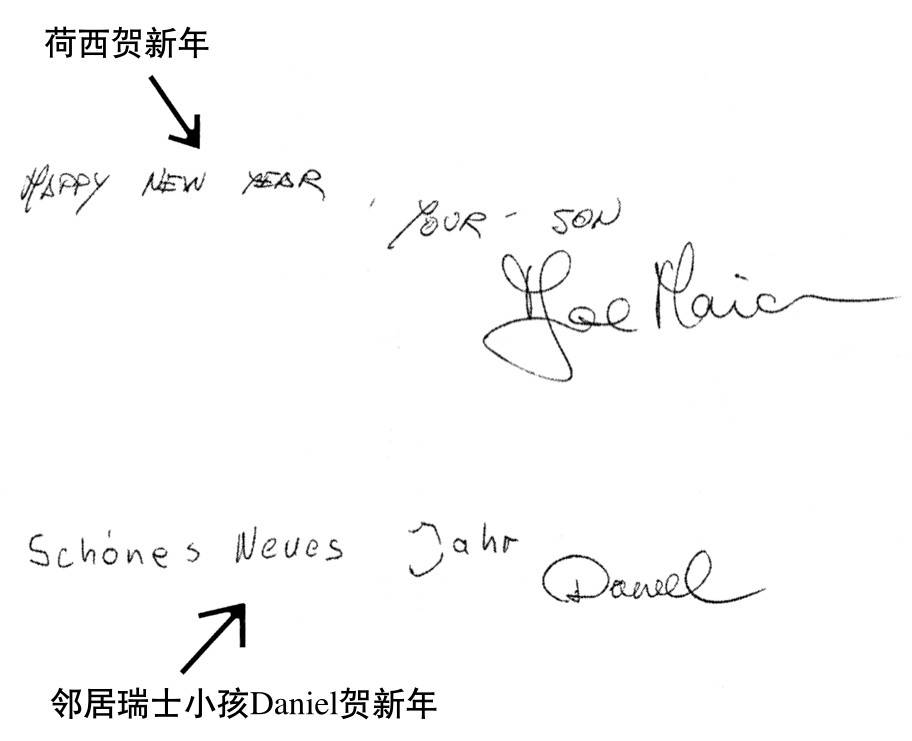
\includegraphics[scale=0.4]{picture/温柔的夜1.jpeg}
\end{figure}


\subsubsection{一九七七年四月三日}

\par \leftline{爹爹,姆妈:}
\par 你们一定已经听说了丹纳丽芙机场的大惨案,这件事说来也奇怪,德国有一青年人早已预言三月二十七日在那儿有飞机相撞,结果真的相撞,所以我相信这是“命运”不是“巧合”。每个人的归宿都已有定数,是难逃的。
\par 今日我一瑞士好友,早晨好好地去南部海边游泳,约我同去,我因有油漆匠约好来漆房子,所以未同去,而好友还有Nicoles与他儿子Daniel还有一个瑞士人同去,我早晨尚见他们,与她说再见(才五十二岁,极健康)。下午六点多,Nicoles回来,告我Ida已死,游泳完了上岸走几步,倒地不起,红十字会马上担了在沙上跑,跑了二十分钟才坐车,送院已死于心脏病(一向无病)。这消息令我大吃一惊,尖叫起来,一夜在外散步,无法安下心来,她去年来此地,买下房子,第一个认识的就是我,房子合同还是荷西替她弄的,现在房契未下来,人已死了,死后无亲无友、无子女,无一个人可以报丧,我们已找领事馆,下周送回瑞士下葬。她这次由瑞士才来一星期(来来去去,两地住),数次来看我,说下周便回瑞士,而今是睡了回去,令人叹息。
\par 爹爹,姆妈,所以我们一定要有心理预备,人,是无常的,一定要预备好,有一天,我们也会分离,万一有此一日来临,不可悲伤,生离死别是人之常情,要有庄子妻死,而鼓盆唱歌的哲学来迎接这件事情,这一年在海边,看见太多人死,我已能够接受,只是一想到家人,便悲伤难禁,所以大家都要预备好,免得有一日来了受不了,一定要彼此记住。
\par 我的腰痛已慢慢在好转,但今生不可再坐软沙发,只能坐地下,或硬椅子,总之仍在看医生。
\par 这一星期来,此地机场被放炸弹,房价一落千丈,加纳利群岛要独立已不是一日,现在变本加厉,我本想再买地,现已不买,因为情势不太好,今日机场又一炸弹。
\par 现在已又开始《玛法达》最后十九、二十集,请告诉我十七、十八集收到了吗?我早已寄出了,这几日听说你们要去旅行,我又有点担心,希望常常来短信,只报平安便可,不必多写,以免我挂念。
\par 荷西去了一月,只收到过一次信(两封),那儿的邮政太差,他另一朋友太太生产,打三封电报去,也无回音,实是奇怪。不过知道他是安好的。
\par 我本来不想请公公婆婆来,但今日又想,如果不请他们来,万一公公死了,荷西终生怪我,所以想请他们来,要寄路费去。另外干爹徐\UncommonChar{𬣙}五月要来西国,我在三千里外,但他不明白,我一再地讲,他仍要见我,我再讲,他仍要见我,所以为了不翻脸,只有五月去西班牙陪他,真是苦。公婆来要五百美金,我为徐,又得五六百美金,这月漆房子,又是三百美金,看医照X光已用好多,下周车又要大修,何苦来,这世界。
\par 请寄一千五百台币给桂文亚,她要生产了,我要送她钱,她对我太好,不断送东西,不断来信,又常常送我礼,所以请寄一千五给她。
\par 谢谢爹爹,姆妈!请扣账内!
\par 不多写了,我的游记已寄出半日,不知《联合报》收到没有?我常给王惕吾伯伯写信,今日又接两百美金津贴,已去谢(下周买一大娃娃寄去给他们家做装饰)。
\par 请多来信,短短几字,告我家中各人如何便是,外公好吗?毛毛有否收到我信?不必回,叫他用功。祝
\par 平安健康
\par \rightline{妹妹上}



\subsubsection{一九七七年四月}

\par \leftline{爹爹,姆妈:}
\par 如果一切计划没有改变,我将于五月一日飞赴Nigeria,在这之前,先得去马德里弄签证,今日荷西托人带来机票、钱和信,我一看,机票弄错了(开成由N国到西国,当相反),我明日清晨便去换,因为我们要将尼国的钱尽量在那儿用掉,免得将来不可出口,现在我马上要去打防疫针(三种)、银行租保险箱(珠宝存入,外币及房契也存入)、申请户籍(设籍在加纳利岛,去马德里可打百分之二十五机票折扣)、买赴马德里机票(一日来回,清早去,拿到visa,下午回来),另外尚得买许多荷西所要的东西,忙碌不堪。开车我是开入大城,停在车场,再坐短程计程车,这样神经不太紧张,我们这儿车子也是很挤很多。
\par 家中门窗关好,皮大衣交邻居管,电视留下,要被偷也罢了,不过七百美金。
\par 今日朋友由Nigeria回来,说荷西一日工作十五小时以上,深夜尚在爆炸海底,公司对他很坏,星期日也不给休息,清早五点赴工作,夜间十点尚无法回家,吃得越来越不好,黑人不爱工作,我想荷西太老实,一天工作八小时对肺已是太坏太伤,如何能一直在水中,这样要废掉了,我去了会与公司交涉,(德国老板)这个薪水不高,不是卖命,同时我自己想去做他们三个工人的厨娘,他们正在找厨子做饭,我去做,也要领薪(好在不过三个人吃),荷西脾气坏,其实脸皮薄,没有原则,任人欺负,我去了会不同些。这个混蛋德国人太欺负他,如不加薪,不减工作时间,我们便走(一日工作两小时在水里,已是太多,水中压力不相同,肺要炸掉的,血管内会进空气,太危险)。真是混账,荷西去年一年无工作,什么也忍下来了,我去了会好好讲,叫老板改时间。
\par 六月我们有二十天假,便去英国一周,再回家来住十天,再看将来如何,因我现在去,是与荷西、他同事、老板、老板太太同住一大宿舍,这个要解决,一人一幢房不可混住,老板太太天天给吃三明治,工作十五小时回来,尚吃三明治,不是气疯了。
\par 同时也请爹爹替我们在台湾找事,如有三万台币一月(现赚九万一月),我们便回来。荷西已可讲英文(很坏,没有句子),同时我又替他在象牙海岸找事,是法国公司,待遇一样,可是环境较好。在尼日利亚,一幢房子租一年是一百五十万台币(一月不租);交通如同疯子,左右不分,车辆乱行,人在街上大小便,从我们家到敦化南路的距离,要开两小时(全缠在一起);警察拿鞭子在街上打人,人还是乱走;一条裤子要合四五千台币,尚是尼龙的,不是棉的,是个疯狂的国家。垃圾堆成一人高,无车来清理,黄热病,打摆子一塌糊涂(我每日便要服“奎宁丸”),这样的地方尚叫国家,黑人走路如蜗牛,不做事,走十步路要十分钟,荷西一下水,助手黑人就睡觉,不看守水下的他要什么,总之是个疯狂世界,二千二百美金所付代价太大,划不来。
\par 我不去也是不行了,荷西一走,此地男人都来找我,满镇风雨,社区内大家讲来讲去,都是说我有男人。此地北欧女人都与人同居(丈夫在非洲),我实是被这些流言弄得十分苦恼。现在参加俱乐部,每日做体操、游泳(全是女的),但也不长,因我要走了。
\par 我的一生,多彩多姿,感谢父母给我生命,虽然今生不能如树芬做少奶奶(她其实也不苦,只是在加拿大没有香港一样而已),但我所活一生,胜于别人十倍百倍,对于去Nigeria,我十分兴奋,又是一种不同的人生,何其幸福。
\par 我下周一赴马德里,但只去签证,再看Marisa,便回Las Palmas来,休息四五天,便由此地上机,经非洲“新内加”国首都Dakar再转赴Nigeria首都Lagos。Lagos是几内亚湾内最大的港口,港内一船下货要等半年以上(太挤),有一百多条船在外海等,五十多条在港内等,夜间海盗便来上船偷货,都是有趣。
\par 虚线便是我下周要飞上飞下的行程。
\begin{figure}[htb]
    \centering
    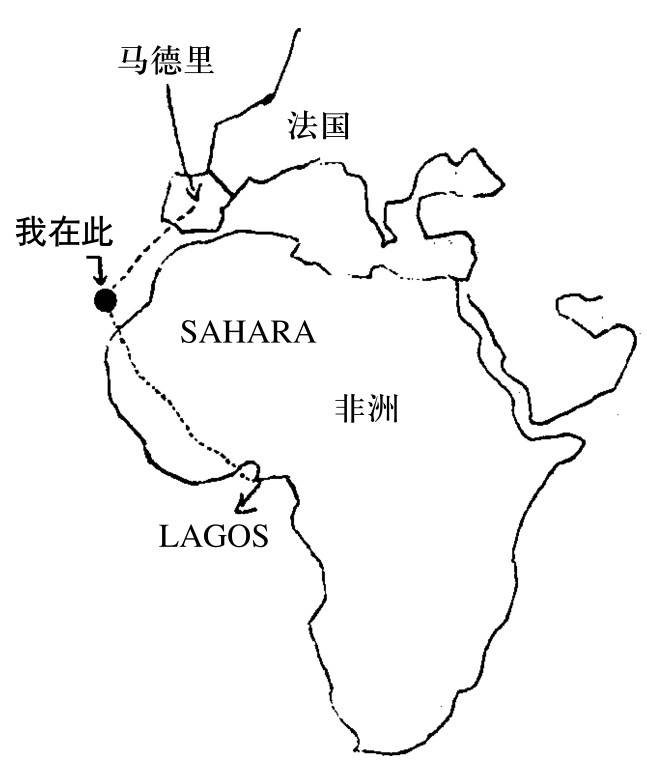
\includegraphics[scale=0.4]{picture/温柔的夜2.jpeg}
\end{figure}
\par 我现在尽量休息,预备长程飞行。(马德里来回六小时飞机,赴Lagos要八九小时飞机,共要十五六小时。)去了荷西不能来接(工作),我便去找一位Duru博士的家(尼国人,也是老板之一),荷西仔细,坐计程车钱已交人带来,一切无问题,我是旅行老手,不会出错,万一飞机出事,亦是命中注定,不必悲伤,人生聚散都是容易,要有大智慧来接受,我对你们,亦有心理预备,所以我们全家都是坚强的人,要有老庄哲学的想法,大而化之,才是天下第一人,我很爱你们和兄弟姐姐,也爱荷西,他是好丈夫。
\par \rightline{妹妹}
\par  
\par PS.春霞衣服十分美丽,今日收到,正穿身上,谢谢盛情,以后不可再寄。药尚未收到。



















 % 4
% \clearpage
% 
% 
\section{万水千山走遍}

\par 作者:三毛
\par 出版社:北京出版集团北京十月文艺出版社
\par 出版时间:2017-03
\par ISBN:9787530214756

\subsection{大蜥蜴之夜\\\small{墨西哥纪行之一}}

\par 当飞机降落在墨西哥首都的机场时,我的体力已经透支得几乎无法举步。长长的旅程,别人睡觉,我一直在看书。
\par 眼看全机的人都慢慢地走了,还让自己绑在安全带上。窗外的机场灯火通明,是夜间了。
\par 助理米夏已经背着他的东西在通道边等着了。经过他,没有气力说话,点了一点头,然后领先出去了。
\par 我的朋友约根,在关口里面迎接,向我高举着手臂。我走近他,先把厚外套递过去,然后双臂环向他拥抱了一下。他说:“欢迎来墨西哥!”我说:“久等了,谢谢你!”
\par 这是今年第四次见到他,未免太多了些。
\par 米夏随后来了,做了个介绍的手势,两人同时喊出了彼此的名字,友爱地握握手,他们尚在寒暄,我已先走了。
\par 出关没有排队也没有查行李。并不想做特殊分子,可是约根又怎么舍得不使用他的外交特别派司?这一点,是太清楚他的为人了。
\par 毕竟认识也有十四年了,他没有改过。
\par “旅馆订了没有?”我问。
\par “先上车再说吧!”含含糊糊的回答。
\par 这么说,就知道没有什么旅馆,台北两次长途电话算是白打了。
\par 在那辆全新豪华的深色轿车面前,他抱歉地说:“司机下班了,可是管家是全天在的,你来这儿不会不方便。”
\par “住你家吗?谁答应的?”改用米夏听不懂的语言,口气便是不太好了。
\par “要搬明天再说好吗?米夏也有他的房间和浴室。你是自由的,再说,我那一区高级又安静。”
\par 我不再说什么,跨进了车子。
\par “喂!他很真诚啊!你做什么一下飞机就给人家脸色看?”米夏在后座用中文说。
\par 我不理他,望着窗外这一千七百万人的大城出神,心里不知怎么重沉沉的。
\par “我们这个语文?”约根一边开车一边问。
\par “英文好啰!说米夏的话。”
\par 说是那么说,看见旁边停了一辆车,车里的小胡子微笑着张望我,我仍是忍不住大喊出了第一句西班牙文——“晚安啊!我的朋友——”
\par 这种令约根痛恨的行径偏偏是我最爱做的,他脸上一阵不自在,我的疲倦却因此一扫而空了。
\par 车子停在一条林荫大道边,门房殷勤地上来接车,我们不必自己倒车入库,提着简单的行李向豪华的黄铜柱子的电梯走去。
\par 约根的公寓,他在墨西哥才安置了半年的家,竟然美丽雅致高贵得有若一座博物馆,森林也似的盆栽,在古典气氛的大厅里,散发着说不出的宁静与华美。
\par 米夏分配到的睡房,本是约根的乐器收藏室,里面从纸卷带的手摇古老钢琴、音乐匣、风琴,到全世界各地大大小小的各种古古怪怪可以发声音的东西,都挂在墙上。
\par 我被引着往里面走,穿过一道中国镶玉大屏风,经过主卧室的门外,一转弯,一个客房藏着,四周全是壁柜,那儿,一张床,床上一大块什么动物的软毛皮做成的床罩静静地等着我。
\par “为什么把我安置在这里?我要米夏那间!”
\par 我将东西一丢,喊了起来。
\par “别吵!嘘——好吗?”约根哀求似的说。
\par 心里一阵厌烦涌上来,本想好好对待他的,没有想到见了面仍是连礼貌都不周全,也恨死自己了。世上敢向他大喊的,大概也只有我这种不买账的人。
\par “去小客厅休息一下吗?”约根问。
\par 我脱了靴子,穿着白袜子往外走,在小客厅里,碰到了穿着粉红色制服、围洁白围裙的墨西哥管家。
\par “啊!您就是苏珊娜,电话里早已认识了呀!”
\par 我上去握住她的手,友爱地说着。
\par 她相当拘谨,微屈了一下右脚,说:“请您吩咐——”
\par 约根看见我对待管家不够矜持,显然又是紧张,赶快将苏珊娜支开了。
\par 我坐下来,接了一杯威士忌,米夏突然举杯说:“为这艺术而舒适的豪华之家——”
\par 对于这幢公寓的格调和气派,米夏毫不掩饰他人全然的沉醉、迷惑、欣赏与崇拜。其实这并没有什么不对,公平地说,这房子毕竟是少见的有风格和脱俗。而米夏的惊叹却使我在约根的面前有些气短和不乐。
\par “阿平,请你听我一次话,他这样有水准,你——”米夏忍不住用中文讲起话来。
\par 我假装没有听见,沉默着。正是大梦初醒的人,难道还不明白什么叫做盖世英雄难免无常,荣华富贵犹如春梦吗?
\par 古老木雕的大茶几上放着我的几本书,约根忙着放《橄榄树》给我们听。这些东西不知他哪里搞来的,也算做是今夜的布景之一吧,不知我最厌看的就是它们。
\par 波斯地毯,阿拉伯长刀,中国锦绣,印度佛像,十八世纪的老画,现代雕塑,中古时代的盔甲,锡做的烛台、银盘、铜壶——没有一样不是精心挑选收集。
\par “收藏已经不得了啦!”我说,衷心地叹了口气。
\par “还差一样——你猜是什么?”他笑看着我,眼光中那份收藏家的贪心也掩饰不住了。
\par 刚刚开始对他微笑的脸,又刷一下变了样子。
\par 我叹了口气,坐在地毯上反手揉着自己的背,右肩酸痛难当,心里一直在对自己说:“我试了!试了又试!再没有什么不好交代的,住两日便搬出去吧!”
\par 约根走去打电话,听见他又叫朋友们过来。每一次相聚,他总是迫不及待地拿我显炫给朋友们看,好似一件物品似的展览着。
\par 米夏紧张地用中文小声说:“喂!他很好,你不要又泄气,再试一次嘛!”
\par 我走开去,将那条苍苍茫茫的《橄榄树》啪一下关掉,只是不语。
\par 旅程的第一站还没有进入情况,难缠的事情就在墨西哥等着。这样的事,几天内一定要解决掉。同情心用在此地是没有价值的。
\par 门铃响了,来了约根的同胞,他们非常有文化,手中捧着整整齐齐的十几本书和打字资料,仔细而又友爱地交给我——全是墨西哥的历史和地理,还有艺术。
\par 我们一同谈了快三小时,其实这些上古和马雅文化,在当年上马德里大学时,早已考过了,并没有完全忘记。为了礼貌,我一直忍耐着听了又听——那些僵死的东西啊!
\par 他们不讲有生命的活人,不谈墨西哥的衣食住行,不说街头巷尾,只有书籍上诉说的史料和文化。而我的距离和他们是那么的遥远,这些东西,不是我此行的目的——我是来活一场的。
\par “实在对不起,米夏是我的助理,这些书籍请他慢慢看。经过二十多小时的飞行,我想休息了!”
\par 与大家握握手,道了晚安,便走了。
\par 米夏,正是见山不是山、见水不是水的年龄,新的环境与全然不同的人仍然使他新鲜而兴奋。留下他继续做听众,我,无法再支持下去。
\par 寂静的午夜,我从黑暗中惊醒,月光直直地由大玻璃窗外照进来。床对面的书架上,一排排各国元首的签名照片静静地排列着,每张照片旁边,插着代表元首那国的小旗子。
\par 我怔怔地与那些伟大人物的照片对峙着,想到自己行李里带来的那个小相框,心里无由地觉着没有人能解的苍凉和孤单。
\par 墨西哥的第一个夜晚,便是如此张大着眼睛什么都想又什么都不想地度过了。
\par   
\par 早晨七点钟,我用大毛巾包着湿头发,与约根坐在插着鲜花、阳光普照的餐厅里。
\par 苏珊娜开出了丰丰富富而又规规矩矩的早餐,电影似的不真实——布景太美了。
\par “不必等米夏,吃了好上班。”我给约根咖啡,又给了他一粒维他命。
\par “是这样的,此地计程车可以坐,公共汽车对你太挤。一般的水不可以喝,街上剥好的水果绝对不要买,低于消费额五十美金的餐馆吃了可能坏肚子,路上不要随便跟男人讲话。低级的地区不要去,照相机藏在皮包里最好,当心人家抢劫——”
\par “城太大了,我想坐地下车。”我说。
\par “不行——”约根叫了起来,“他们强暴女性,就在车厢里。”
\par “白天?一千七百万人的大城里?”
\par “报上说的。”
\par “好,你说说,我来墨西哥是做什么的?”
\par “可以去看看博物馆呀!今天早晨给自己去买双高跟鞋,这星期陪我参加宴会,六张请帖在桌上,有你的名字——”
\par 我忍住脾气,慢慢涂一块吐司面包,不说一句伤人的话。那份虫噬的空茫,又一次细细碎碎地爬上了心头。
\par 约根上班之前先借了我几千披索,昨日下机没来得及去换钱。这种地方他是周到细心的。
\par 推开米夏的房间张望,他还睡得像一块木头,没有心事的大孩子,这一路能分担什么?
\par 为什么那么不快乐?右肩的剧痛,也是自己不肯放松而弄出来的吧!
\par 苏珊娜守礼而本分,她默默地收桌子,微笑着,不问她话,她不主动地说。
\par “来,苏珊娜,这里是三千披索,虽说先生管你伙食费,我们也只在这儿早餐,可是总是麻烦您,请先拿下了,走的时候另外再送你,谢谢了!”
\par 对于这些事情,总觉得是丰丰富富地先做君子比较好办事,虽说先给是不礼貌的,可是,这世界上,给钱总不是坏事。
\par 苏珊娜非常欢喜地收下了。这样大家快乐。
\par  
\par “那我们怎么办?照他那么讲,这不能做,那又不能做?”
\par 米夏起床吃早餐时我们谈起约根口中所说的墨西哥。
\par “低于五十美金一顿的饭不能吃?他土包子,我们真听他的?”我笑了。
\par “你不听他的话?他很聪明的。”米夏天真地说。
\par “认识十四年了,也算是个特殊的朋友,有关我半生的决定,他都有过建议,而我,全没照他的去做过——”我慢慢地说。
\par “结果怎么样?”米夏问。
\par “结果相反的好。”我笑了起来。
\par “昨天晚上,你去睡了,约根说,他想拿假期,跟我们在中美洲走五个星期,我没敢讲什么,一切决定在你,你说呢?”米夏问。
\par 我沉吟了一下,叹了口气:“我想还是一个人走的好,不必他了,真的——”
\par “一个人走?我们两人工作,你却说是一个人,我问你,我算谁?”
\par “不知道,你拍你的照片吧!真的不知道!”
\par 我离开了餐厅去浴室吹头发,热热的人造风一阵又一阵闷闷地吹过来。
\par 米夏,你跟着自然好,如果半途走了,也没有什么不好。毕竟要承当的是自己的前程和心情,又有谁能够真正地分担呢?
\par 
\par 住在这个华丽的公寓里已经五天了。
\par 白天,米夏与我在博物馆、街上、人群里消磨,下午三点以后,约根下班了,我也回去。他要伴了同游是不答应的,那会扫兴。
\par 为着台北一份译稿尚未做完,虽然开始了旅程,下午仍是专心地在做带来的功课。
\par 半生旅行飘泊,对于新的环境已经学会了安静地去适应和观察,并不急切于新鲜和灿烂,更不刻意去寻找写作的材料。
\par 这对我来说,已是自然,对于米夏,便是不同了。
\par “快闷死了,每天下午你都在看译稿,然后晚上跟约根去应酬,留下我一个人在此地做什么?”米夏苦恼地说。
\par “不要急躁,孩子,旅行才开始呢,先念念西班牙文,不然自己出去玩嘛!”我慢慢地看稿,头也不抬。
\par “我在笼子里,每天下午就在笼子里关着。”
\par “明天,译稿弄完了,寄出去,就整天出去看新鲜事情了。带你去水道坐花船,坐公车去南部小村落,太阳神庙、月神庙都去跑跑,好吗?”
\par “你也不只是为了我,你不去,写得出东西来吗?”米夏火起来了。
\par 我笑看着这个名为助理的人,这长长的旅程,他耐得住几天?人生又有多少场华丽在等着?不多的,不多的,即使旅行,也大半平凡岁月罢了。米夏,我能教给你什么?如果期待得太多,那就不好了啊!
\par 认真考虑搬出约根的家到旅馆去住,被他那么紧迫钉人并不算太难应付,只是自己可能得到的经验被拘束在这安适的环境里,就未免是个人的损失了。
\par 决定搬出去了,可是没有告诉米夏,怕他嘴不紧。约根那一关只有对不起他,再伤一次感情了。
\par 才五天,不要急,匆匆忙忙地活着又看得到感得了什么呢!
\par 
\par 不是为了这一夜,那么前面的日子都不能引诱我写什么的,让我写下这一场有趣的夜晚,才去说说墨西哥的花船和街头巷尾的所闻所见吧!
\par 不带米夏去参加任何晚上的应酬并没有使我心里不安。他必须明白自己的职责和身份,过分地宠他只有使他沿途一无所获。
\par 再说,有时候公私分明是有必要的,尤其是国籍不一样的同事,行事为人便与对待自己的同胞有些出入了。
\par 
\par 那一夜,苏珊娜做了一天的菜,约根在家请客,要来十几个客人,这些人大半是驻在墨西哥的外交官们,而本地人,是不被邀请的。
\par 约根没有柔软而弹性的胸怀。在阶级上,他是可恨而令人瞧不起的迂腐。奇怪的是,那么多年来,他爱的一直是一个与他性格全然不同的东方女孩子。这件事上怎么又不矛盾,反而处处以此为他最大的骄傲呢?
\par 再大的宴会,我的打扮也可能只是一袭白衣,这样的装扮谁也习惯了,好似没有人觉得这份朴素是不当的行为。我自己,心思早已不在这些事上争长短,倒也自然了。
\par 当我在那个夜晚走进客厅时,已有四五位客人站着坐着喝酒了。他们不算陌生,几个晚上的酒会,碰来碰去也不过是这几张面孔罢了。
\par 男客中只有米夏穿着一件淡蓝的衬衫,在那群深色西装的中年人里面,他显得那么的天真、迷茫、兴奋而又紧张。冷眼看着这个大孩子,心里不知怎的有些抱歉,好似欺负了人一样。虽然他自己蛮欢喜这场宴会的样子,我还是有些可怜他。
\par 人来得很多,当莎宾娜走进来时,谈话还是突然停顿了一会儿。
\par 这个女人在五天内已见过三次了,她的身旁是那个斯文凝重给我印象极好的丈夫——文化参事。
\par 她自己,一身银灰的打扮,孔雀似的张开了全部的光华,内聚力极强的人,只是我怕看这个中年女人喝酒,每一次的宴会,酒后的莎宾娜总是疯狂,今夜她的猎物又会是谁呢?
\par 我们文雅地吃东西、喝酒、谈话、听音乐、讲笑话,说说各国见闻。不能深入,因为没有交情。为了对米夏的礼貌,大家尽可能用英文了。
\par 这种聚会实在是无聊而枯燥的,一般时候的我,在一小时后一定离去。往往约根先送我回家,他再转回去,然后午夜几时回来便不知道了,我走了以后那种宴会如何收场也没有问过。
\par 那日因为是在约根自己家中,我无法离去。
\par 其中一个我喜欢的朋友,突然讲了一个吸血鬼在纽约吸不到人血的电影:那个城里的人没有血,鬼太饿了,只好去吃了一个汉堡。这使我又稍稍高兴了一点,觉得这种谈话还算活泼,也忍受了下去。
\par 莎宾娜远远地埋在一组椅垫里,她的头半枕在别人先生的肩上,那位先生的太太拼命在吃东西。
\par 一小群人在争辩政治,我在小客厅里讲话,约根坐在我对面,神情严肃地对着我,好似要将我吃掉一样地又恨又爱地凝视着。
\par 夜浓了,酒更烈了,室内烟雾一片,男女的笑声暧昧而释放了,外衣脱去了,音乐更响了。而我,疲倦无聊得只想去睡觉。
\par 那边莎宾娜突然高叫起来,喝得差不多了:“我恨我的孩子,他们拿走了我的享受,我的青春,我的自由,还有我的身材,你看,你看——”
\par 她身边的那位男士刷一抽身站起来走开了。
\par “来嘛!来嘛!谁跟我来跳舞——”她大嚷着,张开了双臂站在大厅里,嘴唇半张着,眼睛迷迷濛濛,说不出是什么欲望,那么强烈地狂奔而出。
\par 唉!我突然觉得,她是一只饥饿的兽,在这墨西哥神秘的夜里开始行猎了。
\par 我心里喜欢的几对夫妇在这当儿很快而有礼地告辞了。分手时大家亲颊道晚安,讲吸血鬼故事给我听的那个小胡子悄悄拍拍我的脸,说:“好孩子,快乐些啊!不过是一场宴会罢了!”
\par 送走了客人,我走回客厅去,在那个阴暗的大盆景边,莎宾娜的双臂紧紧缠住了一个浅蓝衬衫的身影,他们背着人群,没有声息。
\par 我慢慢经过他们,坐下来,拿起一支烟,正要找火,莎宾娜的先生啪一下给我凑过来点上了,我们在火光中交换了一个眼神,没有说一句话。
\par 灯光扭暗了,音乐停止了,没有人再去顾它。梳妹妹头发、看似小女孩般的另一个女人抱住约根的头,半哭半笑地说:“我的婚姻空虚,我失去了自己,好人,你安慰我吗——”
\par 那边又有喃喃的声音,在对男人说:“什么叫快乐,你说,你说,什么叫快乐——”
\par 客厅的人突然少了,卧室的门一间一间关上了。
\par 阳台不能去,什么人在那儿纠缠拥抱,阴影里,花丛下,什么事情在进行,什么欲望在奔流?
\par 我们剩下三个人坐在沙发上。
\par 一个可亲的博士,他的太太跟别人消失了,莎宾娜的先生,神情冷静地在抽烟斗,另外还有我。
\par 我们谈着墨西哥印地安人部落的文化和习俗,紧张而吃力,四周正在发生的情况无法使任何人集中心神,而我的表情,大概也是悲伤而疲倦了。
\par 我再抽了一支烟,莎宾娜的先生又来给我点火,轻轻说了一句:“抽太多了!”
\par 我不再费力地去掩饰对于这个夜晚的厌恶,哗一下靠在椅垫上,什么也不理也不说了。
\par “要不要我去找米夏?”这位先生问我,他的太太加给他的苦痛竟没有使他流露出一丝难堪,反而想到身边的我。而我对米夏又有什么责任?
\par “不!不许,拜托你。”我拉住他的衣袖。
\par 在这儿,人人是自由的,选择自己的生命和道路吧!米夏,你也不例外。
\par 莎宾娜跌跌撞撞地走进来,撞了一下大摇椅,又扑到一棵大盆景上去。
\par 她的衣冠不整,头发半披在脸上,鞋子不见了,眼睛闭着。
\par 米夏没有跟着出现。
\par 我们都不说话,大家窒息了似的熬着。
\par 其实,这种气氛仍是邪气而美丽的,它像是一只大爬虫,墨西哥特有的大蜥蜴,咄咄地向我们吹吐着腥浓的喘息。
\par 过了不知多久,博士的太太疯疯癫癫地从乐器室里吹吹打打地走出来,她不懂音乐,惊人的噪音,冲裂了已经凝固的夜。一场宴会终是如此结束了。
\par 唉唉!这样豪华而狂乱的迷人之夜,是波兰斯基导演的一场电影吧!
\par 那只想象中的大蜥蜴,在月光下,仍然张大着四肢,半眯着眼睛,重重地压在公寓的平台上,满意地将我们吞噬下去。
\par 
\par 还有两个客人醉倒在洗手间里。
\par 约根扑在他卧室的地毯上睡了。
\par 我小心地绕过这些身体,给自己刷了牙,洗了脸,然后将全公寓的大落地窗都给它们打开来吹风。
\par 拿了头发刷子,一间间去找米夏。
\par 米夏坐在书房的一块兽皮上,手里在玩照相机,无意识地按快门,咔嚓一下,咔嚓又一下,脸上空空茫茫的。
\par 我一面刷头发,一面喊了一声:“徒儿——”
\par “没做什么,真的——”米夏淡淡地说。
\par “这没什么要紧,小事情。”我说。
\par “可是我没有做——”他叫了起来。
\par “如果今夜我不在呢?”我叹了口气。
\par 米夏不响,不答话。
\par “莎宾娜可怜——”他说。
\par “不可怜——”
\par “阿平——你无情——”
\par 我慢慢地梳头发,没有解释。
\par “今夜够受了——”米夏喘了一口大气。
\par “有挣扎?”我笑了。
\par 米夏没有笑,怔怔地点了点头。
\par “没有见识的孩子,要是真的事情来时你又怎么办?”我站起来走开了。
\par “阿平——”
\par “明早搬出去,旅馆已经打电话订了,这一种墨西哥生涯到此为止了,好吗?”我说。
\par 
\par \rightline{一九八一年十一月十五日在墨西哥}

\subsection{街头巷尾\\\small{墨西哥纪行之二}}


\par 这一趟旅行虽说会发生些什么样的事情全然是未知,可是行万里路、读万卷书的时代已经过去了。仍然算是有备而来的。
\par 我的习惯是先看资料,再来体验印证个人的旅行。
\par 这一回有关中南美的书籍一共带了四册,要找一家便宜而位置适中的旅馆也并不是难事,书上统统都列出来了。
\par 来到墨西哥首都第六天,一份叫做“EL HERALDO DE MEXICO”的报纸刊出了我的照片。与写作无关的事情。
\par 那么大的照片刊出来的当日,也是我再梳回麻花辫子,穿上牛仔裤,留下条子,告别生活方式极端不同的朋友家,悄悄搬进一家中级旅馆去的时候了。
\par 旅馆就在市中心林荫大道上,老式的西班牙殖民式建筑,白墙黑窗,朴素而不豪华,清洁实惠,收费亦十分合理,每一个只有冲浴的房间,是七百披索,大约是合二十七元美金一日,不包括早餐。
\par 书上列出来的还有十元美金一日的小旅馆,看看市区地图,那些地段离城中心太远,治安也不可能太好,便也不再去节省了。
\par 助理米夏在语言上不能办事与生活,这一点再再地督促他加紧西班牙文。鼓励他独自上街活动,不可以完全依靠我了。
\par 墨西哥城是一个方圆两百多平方公里,坐落在海拔二千二百四十公尺高地的一个大城市。
\par 初来的时候,可能是高度的不能习惯,右耳剧痛,鼻腔流血,非常容易疲倦,这种现象在一周以后便慢慢好转了。
\par 有生以来没有在一个一千七百万人的大城市内住过,每天夜晚躺在黑暗里,总听见警车或救护车激昂而快速的哀鸣划破寂静的长夜。这种不间断的声音,带给人只有一个大都会才有的巨大的压迫感,正是我所喜欢的。

\subsubsection*{这一张张美丽的脸}
\par 除了第一日搬去旅舍时坐的是计程车之外,所用的交通工具起初还是公共汽车,后来试了四通八达的地下车之后,便再也舍不得放弃了。
\par 大部分我所见的墨西哥人,便如上帝捏出来的粗泥娃娃,没有用刀子再细雕,也没有上釉,做好了,只等太阳晒干,便放到世上来了——当然,那是地下车中最最平民的样子。
\par 这儿的人类学博物馆中有些故事,述说古时在这片土地上的居民,他们喜欢将小孩子的前额和后脑夹起好几年,然后放开,那些小孩子的头变成扁平的,脸孔当然也显得宽大些,在他们的审美眼光中,那便是美丽。
\par 而今的墨西哥人,仍然有着那样的脸谱,扁脸、浓眉、大眼、宽鼻、厚唇,不算太清洁,衣着鲜艳如彩虹,表情木然而本分。而他们身体中除了墨西哥本地的血液之外,当然掺杂了西班牙人的成分,可是看上去他们仍是不近欧洲而更近印地安人的。
\par 常常,在地下车中挤着去某个地方,只因时间充分,也因舍不得那一张张已到了艺术极致的脸谱,情愿坐过了站再回头。
\par 人,有时候是残酷的,在地下车中,看见的大半是贫穷的人,而我,却叫这种不同的亦不算太文明装扮的男女老幼为“艺术的美”,想起来是多么大的讽刺。
\par 墨西哥城内每天大约有五百到两千个乡下人,涌进这个大都市来找生活。失业的人茫茫然地坐在公园和街头,他们的表情在一个旁观者看来,张张深刻,而这些对于饥饿的肚子,又有什么关联?



\subsubsection*{自杀神}
\par 虽说对于参观大教堂和博物馆已经非常腻了,可是据说墨西哥的“国家人类学博物馆”仍然可能是世界上最周全的一座,为了对得起自己的良知,还是勉强去了。
\par 第一次去,是跟着馆内西语导游的。他不给人时间看,只强迫人在馆内快速地走,流水账似的将人类历史尤其墨西哥部分泼了一大场,进去时还算清楚,出来时满头雾水。
\par 结果,又去了第二次,在里面整整一日。虽说墨西哥不是第一流的国家,可是看过了他们那样大气势的博物馆,心中对它依然产生了某种程度的尊敬。
\par 要说墨西哥的日神庙、月神庙的年代,不过是两千多年以前。他们的马雅文化固然辉煌,可是比较起中国来,便不觉得太古老了。
\par 只因那个博物馆陈列得太好,介绍得详尽,分类细腻,便是一张壁画吧,也是丰富。馆内的说明一律西班牙文,不放其他的文字,这当然是事先设想后才做的决定。我仍是不懂,因为参观的大部分是外国人。
\par 古代的神祇在墨西哥是很多的,可说是一个想象力丰富的多神民族。日神、月神、风神、雨神之外,当然还有许许多多不同的神。
\par 也可能是地理环境和天灾繁生,当时的人自然接受了万物有灵的观念,事实上,此种信仰是因为对大自然的敬畏而产生的。
\par 其中我个人最喜欢的是两个神——玉米神和自杀神。
\par 玉米是我爱吃的食物之一,可说是最爱的。有这么一位神,当然非常亲近他。
\par 当我第一次听见导游用棒子点着一张壁画,一个个神数过去,其中他滑过一个小名字——自杀神时,仍是大吃了一惊。
\par 跟着导游小跑,一直请问他古时的自杀神到底司什么职位,是给人特许去自杀,还是接纳自杀的人,还是叫人去自杀?
\par 导游也答不出来,只笑着回了我一句:“你好像对自杀蛮感兴趣的,怎么不问问那些影响力更深、更有神话意义的大神呢?”
\par 后来第二次我自己慢慢地又去看了一次博物馆,专门研究自杀神,发觉他自己在图画里就是吊在一棵树上。
\par 世上无论哪一种宗教都不允许人自杀,只有在墨西哥发现了这么一个书上都不提起的小神。我倒觉得这种宗教给了人类最大的尊重和意志自由,居然还创出一个如此的神,是非常有趣而别具意义的。
\par 墨西哥大神每一个石刻的脸,看痴了都像魔鬼。
\par 这么说实在很对不起诸神,可是他们给人的感应是邪气而又强大的。没有祥和永恒的安宁及盼望。他们是惩罚人的灵,而不是慈祥的神。说实在,看了心中并不太舒服,对于他们只有惧怕。
\par 是否当时的人类在这片土地上挣扎得太艰苦,才产生了如此粗暴面孔的神祇和神话呢!

\subsubsection*{金字塔}
\par 当然,我们不可避免地去了西班牙文中仍叫它“金字塔”的日神庙及月神庙。
\par 据考证那是公元前两百年到公元九百年时陶特克斯人时期的文明。在今天,留下了人类在美洲壮观的废墟和历史。
\par 那是一座古城,所谓的日神月神庙是后人给它们加上去的名称。外在的形式,像极了埃及的金字塔,只是没有里面的通道,亦没有帝王的陵墓。
\par 为了这些不同年代的人类文明和古代城市的建筑,我看了几个夜晚的资料,预备在未去之前对它们做一个深切的纸面上的了解。
\par 然后米夏与我在转车又转车之后,到了那个叫做“阿那乌阿克之谷”(VALLE DE ANAHUAC)的底奥帝乌刚诺的金字塔。
\par 烈日下的所谓金字塔,已被小贩、游览车,大声播放的流行音乐和大呼小叫的各国游客完全污染光了。
\par 日神庙六十四公尺高的石阶上,有若电影院散场般的人群,并肩在登高。手中提着他们的小型录音机,放着美国音乐。
\par 我没有去爬,只是远远地坐着观望。米夏的红衬衫,在高高石阶的人群里依旧鲜明。
\par 那日的参观没有什么心得。好似游客涌去的地方在全世界都是差不多的样子。
\par 当米夏努力在登日神庙顶时,我借了一辆小贩的脚踏车,向着古代不知为何称为“死亡大道”的宽大街道的废墟上慢慢地骑去。
\par 本想在夜间再去一趟神庙废墟的,终因交通的问题,结果没有再回去。
\par 我还是不羞耻地觉得城镇内的人脸比神庙更引人。
\par 至于马雅文化和废墟,计划中是留到洪都拉斯的“哥庞”才去看一看了。

\subsubsection*{吃抹布}
\par 第一次在街头看见路边的小摊子上在烘手掌大的玉米饼时,我非常喜欢,知道那是墨西哥人的主食“搭哥”(taco),急于尝尝它们。
\par 卖东西的妇人在我张开的掌心中啪一下给了一张饼,然后在饼上放了些什么东西混着的一摊馅,我将它们半卷起来,吃掉了,有酱汁滴滴答答地从手腕边流下来。
\par “搭哥”的种类很多,外面那个饼等于是一张小型的春卷皮,淡土黄色的,它们永远不变。
\par 里面的馅放在一只只大锅里,煮来煮去,有的是肉,有的是香肠,有的看不清楚,有的猜不出来。要换口味,便换里面的东西。
\par 在城内,除非是游客区,那儿可以吃中国菜、意大利面食,还有丹麦甜点蛋饼之外,也可以吃“搭哥”。
\par 可是当我们坐车离城去小村落时,除了“搭哥”之外,实在没有别的东西可吃。
\par 在城外几百里的小镇上,当我吃了今生第几十个“搭哥”之后,那个味道和形式,实在已像是一块抹布——土黄色的抹布,抹过了残余食物的饭桌,然后半卷起来,汤汤水水地用手抓着,将它们吞下去。
\par 一个“搭哥”大约合几角到一元五美金,看地区和内容,当然吃一个胃口是倒了,而肚子是不可能饱的。这已是不错了,比较起城内高级饭店的食物,大约是十倍到十五倍价格的差距。虽然我们的经费充足,仍是坚持入境问俗,一路“搭哥”到底。这对助手米夏便是叫苦连天,每吃必嚷:“又是一块小抹布!”
\par 在墨西哥的最后一日,我怕米夏太泄气,同意一起去吃一顿中国饭,不肯去豪华的中国饭店,挑了一家冷清街角的。先点了两只春卷——结果上来的那个所谓“春天的卷子”的东西,竟然怎么看,怎么咬,都只是两只炸过了的“搭哥”。
\par 吃在一般的墨西哥是贫乏而没有文化的。
\par 它的好处是不必筷子与刀叉,用手便可解决一顿生计,倒也方便简单。至于卫不卫生就不能多去想它了。


\subsubsection*{货物大同}
\par 在城内的游客区里,看见美丽而价格并不便宜的墨西哥人的“大氅”,那种西班牙文叫做“蹦裘”(poncho)的衣物。
\par 事实上它们只是一块厚料子,中间开一个洞套进颈子里,便是御寒的好东西了。
\par 我过去有过两三个“蹦裘”,都因朋友喜欢而送掉了。这次虽然看见了市场上有极美丽的,总因在游客出没的地区,不甘心付高价去买它。
\par 下决心坐长途车去城外的一个小镇,在理由上对米夏说的是请他下乡去拍照。事实上我有自己的秘密,此行的目的对我,根本是去乡下找漂亮、便宜,而又绝对乡土的“蹦裘”来穿。
\par 坐公路车颠几百里去买衣服也只有最笨的人——而且是女人,会做的事情,不巧我就有这份决心和明白。
\par 到了一个地图上也快找不到的城镇,看到了又是所谓景色如画的贫穷和脏乱。我转来转去找市场——资料书中所说的当地人的市集,找到了,怪大的一个广场。
\par 他们在卖什么?在卖热水瓶、镜子、假皮的皮夹、搪瓷的锅、碗、盆、杯、完全尼龙的衣服、塑胶拖鞋、原子笔、口红、指甲油、耳环、手镯、项链——
\par 我到处问人家:“你们不卖poncho?怎么不卖poncho?”
\par 得到的答复千篇一律,举起他们手中彩色的尼龙衣服向我叫喊:“这个时髦!这个漂亮!怎么,不要吗?”

\subsubsection*{水上花园}
\par 那是过去的一大片沼泽,而今部分已成了城镇,另外一小部分弯弯曲曲的水道,仍然保存着,成了水上的花园。
\par 本来也是要自己去划船的。星期天的旧货市场出来后计划去搭长途公车。我的朋友约根算准我必然会在星期日早晨的市集里与当地人厮混。他去了,也果然找到了我与米夏。
\par 于是,我们没有转来转去在公车上颠,坐了一辆大轿车,不太开心地去履行一场游客必做的节目。
\par 一条条彩色缤纷的木船内放着一排排椅子,比碧潭的大船又要大了些。墨西哥人真是太阳的儿女,他们用色的浓艳,连水中的倒影都要凝固了。
\par 参考书上说是二十五块美金租一条船,划完两小时的水道。船家看见是大轿车来的外国人,偏说是五十美金,我因不肯接受约根的任何招待,坚持报社付钱,就因如此,自己跑去与人争价格,已经降到四十块美金了,当然可以再减。讲价也是一种艺术,可惜我高尚的朋友十分窘迫,不愿再磨,浪费了报社的钱,上了一条花船。
\par 三个人坐在船中木头似的沉默无聊,我忍不住跑去船尾跟船家说话,这一搭上交情,他手中撑的那支好长的篙跑到我手上来了。
\par 用尽了气力撑长篙,花船在窄窄的水道里跟别的船乱撞,这时我的心情也好转了,一路认真撑下去。
\par 本来没有什么特别的水道,只因也有音乐船,卖鲜花、毯子和食物的小船一路挤着,它也活泼起来。
\par 虽是游客的节目,只因长篙在自己的手中,身份转变成了船家,那份生涯之感便是很不同了。
\par 那一天,我的朋友约根没有法子吃他昂贵的餐馆,被迫用手抓着碎肉和生菜往玉米饼里卷着做“搭哥”吃。买了一大堆船边的小食。当然,船夫也是请了一同分食的。
\par 水上花园的节目,一直到我们回码头,我将粗绳索丢上岸,给船在铁环上扎好一个漂亮利落的水手结,才叫结束。
\par 自己动手参与的事情,即便是处理一条小船吧,也是快乐得很的。奇怪的是同去的两位男士连试撑的兴趣都没有。


\subsubsection*{你们求什么}
\par 又是一个星期天,也是墨西哥的最后一日了。
\par 我跟米夏说,今天是主日,我要去教堂。
\par 来了墨西哥不去“爪达路沛大教堂”是很可惜的事情。据说一五三一年的时候,圣母在那个地方显现三次,而今它已是一个一共建有新旧七座天主教堂的地方了。
\par “爪达路沛的圣母”是天主教友必然知道的一位。我因心中挂念着所爱的亲友,很喜欢去那儿静坐祷告一会儿,求神保佑我离远了的家人平安。
\par 我们坐地下车往城东北的方向去,出了车站,便跟着人群走了。汹汹滔滔的人群啊,全都走向圣母。
\par 新建大教堂是一座现代的巨大建筑,里面因为太宽,神父用扩音机在做弥撒。
\par 外面的广场又是大得如同可以踢足球。广场外,一群男人戴着长羽毛,光着上身,在跳他们古代祭大神的舞蹈。鼓声重沉沉地混着天主教扩音机的念经声,十分奇异的一种文化的交杂。
\par 外籍游客没有了,本地籍的人,不只是城内的,坐着不同形状的大巴士也来此地祈求他们的天主。
\par 在广场及几个教堂内走了一圈,只因周遭太吵太乱,静不下心坐下来祷告。那场祭什么玉米神的舞蹈,鼓得人心神不宁,而人群,花花绿绿的人群,挤满了每一个角落。
\par 我走进神父用扩音机在讲话的新教堂里去。
\par 看见一对乡下夫妇,两人的身边放着一个土土的网篮,想必是远路来的,因为篮内卷着衣服。
\par 这两个人木像一般地跪在几乎已经挤不进门的教堂外面,背着我,面向着里面的圣母,直直地安静地跪着,动也不动,十几分钟过去了,我绕了一大圈又回来,他们的姿势一如当初。
\par 米夏偷偷上去拍这两人的背影,我看得突然眼泪凝眶。
\par 那做丈夫的手,一直搭在他太太的肩上。做太太的那个,另一只手绕着先生的腰,两个人,在圣母面前亦是永恒的夫妻。
\par 一低头,擦掉了眼泪。
\par 但愿圣母你还我失去的那一半,叫我们终生跪在你的面前,直到化成一双石像,也是幸福的吧!
\par 我独自走开去了,想去广场透透气,走不离人群,而眼睛一再地模糊起来。
\par 那边石阶上,在许多行路的人里面,一个中年男人用膝盖爬行着慢慢移过来,他的两只手高拉着裤管,每爬几步,脸上抽筋似的扭动着,我再低头去看他,他的膝盖哪里有一片完整的皮肤——那儿是两只血球,他自己爬破的一摊生肉,牛肉碎饼似的两团。
\par 虽然明知这是祈求圣母的一种方式,我还是吓了一大跳,哽住了,想跑开去,可是完全不能动弹,只是定定地看住那个男人。
\par 在那男人身后十几步的地方,爬着看上去是他的家人,全家人的膝盖都已磨烂了。
\par 一个白发的老娘在爬,一个二十岁左右的青年人在爬,十几岁的妹妹在爬,一个更小的妹妹已经忍痛不堪了,吊在哥哥的手臂里,可是她不站起来。
\par 这一家人里面显然少了一个人,少了那个男子的妻子,老婆婆的女儿,一群孩子的母亲——
\par 她在哪里?是不是躺在医院里奄奄一息?是不是正在死去?而她的家人,在没有另一条路可以救她的时候,用这种方法来祈求上天的奇迹?
\par 看着这一个小队伍,看着这一群衣衫褴褛向圣母爬去的可怜人,看着他们的血迹沾过的石头广场,我的眼泪迸了出来,终于跑了几步,用袖子压住了眼睛。
\par 受到了极大的惊骇,坐在一个石阶上,哽不成声。
\par 那些人扭曲的脸,血肉模糊的膝盖,受苦的心灵,祈求的方式,在在地使我愤怒。
\par 愚蠢的人啊!你们在求什么?
\par 苍天!圣母马利亚,下来啊!看看这些可怜的人吧!他们在向你献活祭,向你要求一个奇迹,而这奇迹,对于肉做的心,并不过分,可是你,你在哪里?圣母啊,你看见了什么?
\par 黄昏了,教堂的大钟一起大声地敲打起来,广场上,那一小撮人,还在慢慢地爬着。
\par 我,仰望着彩霞满天的苍穹,而苍天不语。
\par 这是一九八一年的墨西哥一个星期天的下午。

\subsection{青鸟不到的地方\\\small{洪都拉斯纪行}}
\par 由墨西哥飞到洪都拉斯的航程不过短短两小时,我们已在洪国首都“得古西加尔巴”(Tegucigalpa)的机场降落了。
\par 下飞机便看见掮枪的军人,虽说不是生平第一次经验,可是仍然改不掉害怕制服的毛病。对我,制服象征一种隐藏的权力,是个人所无能为力的。
\par 排队查验护照时,一个军人与我默默地对峙着,凝神地瞪着彼此,结果我先笑了,他这也笑了起来,踱上来谈了几句话,心情便放松了。
\par 那是一个寂寞的海关,稀稀落落的旅客等着检查。
\par 碰到一个美国人,是由此去边境,为萨尔瓦多涌进来的难民去工作的。
\par 当这人问起我此行的目的时,我说只是来做一次旅行,写些所闻所见而已。在这样的人面前,总觉得自己活得有些自私。
\par 我们是被锁在一扇玻璃门内的,查完一个,守门的军人查过验关条,就开门放人。
\par 当米夏与我被放出来时,蜂拥上来讨生意的人包围了我们。
\par 有的要换美金,有的来抢箱子提,有的叫我们上计程车,更有人抱住脚要擦鞋。
\par 生活的艰难和挣扎,初入洪国的国门便看了个清楚。
\par 我请米夏与行李在一起坐着,自己跑去换钱,同时找“旅客服务中心”,请他们替我打电话给一家已在书上参考到的旅馆。
\par 洪都拉斯的首府只有四五家世界连锁性的大旅馆,那儿设备自然豪华而周全。可是本地人的客栈也是可以住的,当然,如果付的价格只是十元美金一个房间的话,也不能期待有私人浴室和热水了。
\par 此地的钱币叫做“连比拉”(Lempira)。这本是过去一个印地安人的大酋长,十六世纪时在一场赴西班牙人的和谈中被杀。而今他的名字天天被洪都拉斯人提起无数次——成了钱币。
\par 两个连比拉是一块美金。
\par 计程车向我要了十二个连比拉由机场进城,我去找小巴士,可是那种车掌吊在门外的巴士只能坐十二个人,已经客满了。于是我又回去跟计程车司机讲价,讲到六个大酋长,我们便上车了。
\par 公元一五〇三年,当哥伦布在洪都拉斯北部海岸登陆时,发现那儿水深,因此给这片土地叫做“洪都拉斯”,在西班牙语中,便是“深”的意思。
\par 并不喜欢用落后或者先进这些字句来形容每一个不同的国家,毕竟各样的民族有他们自己的生活形态与先天不平等的立国条件。
\par 虽然那么说,一路坐车,六公里的行程,所见的洪都拉斯仍是寂寞而哀愁的。
\par 便是这座在印地安语中称为“银立”的三十万人的首都,看上去也是贫穷。
\par 这是中美洲第二大面积的国家,十一万两千八十八平方公里的土地,百分之四十五被群山所吞噬,人口一直到如今还只三百万左右。
\par 洪都拉斯出产蔗糖、咖啡、香蕉、棉花和一点金矿、锡矿,据说牛肉也开始出口了。
\par 我到了旅馆除了一张床之外,完全没有其他的家具。走道上放着一张方桌子,我将它搬了进房,作为日后写字的地方。
\par 米夏说他床上有跳蚤,我去看了一看,毯子的确不够清洁,可是没有看见什么虫,大半是他心理作用。当然,旅馆初看上去是有些骇人。
\par 街上的餐馆昂贵得不合理,想到此地国民收入的比率,这样的价格又怎么生活下去?
\par 走在路上,沿途都是讨钱的人。
\par 初来洪都拉斯的第一夜,喝了浴室中的自来水,大概吃下了大肠菌。这便昏天黑地地吐泻起来,等到能够再下床走路,已是两天之后了。
\par 在旅舍内病得死去活来时,米夏向“马雅商店”的中国同胞去讨了热水,如果不是那壶热水和人参茶救命,大概还得躺两天才站得起来。
\par 三十万人的首都没有什么特别可看的东西,十六世纪初叶它本是一个矿区小镇,到了现在,西班牙殖民式的教堂和建筑仍是存在的,有些街道也仍是石块砌成的。
\par 城内好几家中国饭馆和杂货店,看见自己的同胞无孔不入地在世界各地找生活,即便在洪都拉斯这样贫穷而幽暗的地方,也住了下来,心中总是一阵又一阵说不出的黯然。
\par 这儿纯血的印地安人——马雅的后裔,可说找不到,百分之九十是混血、棕色皮肤的人,只有少数北部海岸来的黑人,在城内和谐地生活着。
\par 虽说整个的山城是杂乱而没有秩序的,可是一般的建筑在灰尘下细看仍是美丽,窄窄的石砌老街,漆得红黄蓝绿有若儿童图画的房子,怎么看仍有它艺术的美。
\par 生活在城市中,却又总觉得它是悲伤而气闷的,也许是一切房舍的颜色太浓而街道太脏,总使人喘不过气来似的不舒服,那和大都市中的灯火辉煌又是两回事了。
\par 洪都拉斯首都的夜,是浓得化不开的一个梦境,梦里幽幽暗暗,走不出花花绿绿却又不鲜明的窄巷,伸手向人讨钱苦孩子的脸和脚步,哀哀不放。
\par 这儿,一种漆成纯白色加红杠的大巴士,满街地跑着。街上不同颜色和形式的公车,川流不息地在载人,他们的交通出人意料的方便快捷。
\par 特别喜欢那种最美的大巴士,只因它取了一个童话故事中的名字——青鸟。
\par 青鸟在这多少年来,已成了一种幸福的象征,那遥不可及而人人向往的梦啊,却在洪都拉斯的街道上穿梭。
\par 我坐在城内广场一条木椅上看地图,那个夜晚,有选举的车辆,插着代表他们党派的旗子大声播放着音乐来来回回地跑,有小摊贩巴巴地期待着顾客,有流落街头的人在我脚旁沉睡,有讨钱的老女人在街角叫唤,更有一群群看来没有生意的擦鞋童,一路追着人,想再赚几个铜板。当然,对面那座大教堂的石阶上,偶尔有些衣着整齐的幸福家庭,正望了弥撒走出来——
\par 就在这样一个看似失落园的大图画里,那一辆辆叫做“青鸟”的公车,慢慢地驶过,而幸福,总是在开着,在流过去,广场上的芸芸众生,包括我,是上不了这街车。
\par “不,你要去的是青鸟不到的地方!”长途总车站的人缓缓地回答我。
\par 计划在洪都拉斯境内跑一千四百公里,工具当然是他们的长途汽车,其实也知道青鸟是不会跑那儿的,因为要去的小城和村落除了当地的居民之外,已经没有人注意它们了。
\par 那是“各马亦阿爪”城中唯一的客栈。
\par 四合院的房子里面一个天井,里面种着花、养着鸡、晒着老板一家人的衣服。小孩在走廊上追逐,女人在扫地煮饭,四个男人戴着他们两边向上卷的帽子围着打纸牌。而我,静静地坐在大杂院中看一本中文书。因为肠炎方愈,第一日只走了不到一百公里,便停住了。
\par 平房天花板的木块已经烂了,小粉虫在房间里不断地落下来。床上没有毯子,白床单上一片的虫,挡也挡不住。
\par “我的床不能睡。”米夏走出房间来说。
\par “可以,晚上睡在床单下面。”我头也没抬地回了一句。
\par 天气仍是怪凉的,这家小客栈坚持没有毯子,收费却是每个房间二十个连比拉,还是落虫如雨的地方,只因他们是这城内唯一的一家,也只有将就了。
\par 问问旅舍里的人第二天计划要去的山谷,一个七八小时车程距离,叫做“马加拉”的印地安人村落,好似没有人知道。他们一直在收听足球赛的转播,舍不得讲话。
\par 小城本是洪都拉斯的旧都,只因当年目前的京城“得古西加尔巴”发现了银矿,人口才往那儿迁移了。
\par 一条长长的大街,几十家小店铺,一座少不了的西班牙大教堂,零零落落的几家饭店,就是城内唯一的风景了。当然,为了应应景,一小间房间,陈列着马雅文物,叫做“博物馆”。
\par 小城一家杂货店的后院给我们找到了。极阴暗的一个食堂。没有选菜的,老妇给了煮烂的红豆,两块硬硬的肉,外加一杯当地土产的黑咖啡,便收六块连比拉,那合三块美金,同吃的还有一位警察,也付一样价格。
\par 虽然报社给的经费足足有余,可是无论是客栈和食堂,以那样的水准来说,仍是太贵了。
\par 照相胶卷在这儿贵得令人气馁,米夏只剩一卷墨西哥带过来的,而我们有三架照相机。
\par 黄昏时我们在小城内慢慢逛着没事做时,看见大教堂里走出一个拿着大串钥匙的老年人,我快步向他跑过去。
\par “来吧!米夏,开心点,我们上塔顶去!”我大喊起来。
\par 老人引着我们爬钟楼,六个大铜钟是西班牙菲利普二世时代送过来的礼物,到如今它仍是小城的灵魂。那个老人一生的工作便是在守望钟楼里度过了。
\par 我由塔边小窗跨出去,上了大教堂高高的屋顶,在上面来来回回地奔跑。
\par 半生以来,大教堂不知进了多少座,在它屋顶上跑着却是第一次。不知这是不是冒犯了天主,可是我猜如果他看见我因此那样的快乐,是不会舍得生气的。毕竟小城内可做的事情也实在不多。
\par 坐小型巴士旅行,初开始时确是新鲜而有趣的事情。十七八岁的男孩算做车掌吊在门外,公路上若是有人招手,车尚没有停稳他就跳了下去,理所当然地帮忙乘客搬货物和行李,态度是那样的热心而自然,拼命找空隙来填人和货,车内的人挤成沙丁鱼,货里面当然另有活着的东西:瘦瘦的猪,两只花鸡。因为不舒服的缘故,那只猪沿途一直号叫。
\par 一对路边的夫妇带了一台炉子也在等车,当然炉子也挤进来了,夫妇两人那么幸福地靠在炉子边,那是天下唯一的珍贵了。
\par 泥沙飞扬的路上,一个女人拿着小包袱在一座泥巴和木片糊成的小屋前下车,里面飞奔出来几个衣衫褴褛的孩子,做母亲的迫不及待地将手中几片薄饼干散了出去。那幅名画,看了叫人心里不知是什么滋味。
\par 这儿是青鸟不到的地方,人们从没有听过它的名字,便也没有梦了。
\par 米夏与我一个村一个镇地走。太贫苦的地方,小泥房间里千篇一律只有一张吊床。窗是一个空洞框框,没有木板更没有玻璃窗挡风。女人和一堆孩子,还有壮年的男人呆呆地坐在门口看车过,神色茫然。他们的屋旁,大半是坡地,长着一棵橘子树,一些玉米秆,不然什么也不长的小泥屋也那么土气又本分地站着,不抱怨什么。
\par 看见下雨了,一直担心那些泥巴做成的土房子要冲化掉,一路怔怔地想雨停。
\par 洪都拉斯的确是景色如画,松林、河流、大山、深蓝的天空、成群的绿草牛羊,在在是一幅幅大气魄的风景。
\par 只是我的心,忘不了沿途那些贫苦居民的脸孔和眼神,无法在他们善良害羞而无助的微笑里释放出来。一路上,我亦是怔怔。
\par 旅行了十天之后,方抵达洪都拉斯与危地马拉的边境。马雅人著名的“哥庞废墟”便在丛林里了。
\par 这一路如果由首都直着转车来,是不必那么多时间的,只因每一个村落都有停留,日子才在山区里不知不觉地流去了。
\par 有生以来第一次,全身被跳蚤咬得尽是红斑,头发里也在狂痒。那么荒凉的村落,能找到地方过夜已是不易,不能再有什么抱怨了。
\par 还是喜欢这样的旅行,那比坐在咖啡馆清谈又是充实多了。
\par 到了镇名便叫“哥庞废墟”的地方,总算有了水和电,也有两家不坏的旅舍,冷冷清清。
\par 我迫不及待地问旅舍的人供不供热水,得到的答复是令人失望的。
\par 山区的气候依旧湿冷,决定不洗澡,等到去了中北部的工业城“圣彼得稣拉”再找家旅馆全身大扫除吧!
\par 这片马雅人的废墟是一八三九年被发现的,当时它们在密密的雨林中已被泥土和树木掩盖了近九个世纪。
\par 据考证,那是公元后八百年左右马雅人的一个城镇。直到一九三〇年,在发现了它快一百年之后,才有英国人和美国人组队来此挖掘、重建、整理。可惜最最完整的石雕,而今并不在洪都拉斯的原地,而是在大英博物馆和波士顿了。
\par 虽然这么说,那一大片丛林中所遗留下来的神庙,无数石刻的脸谱、人柱,仍是壮观的。
\par 在那微雨寒冷的清晨,我坐在废墟最高的石阶顶端,托着下巴,静静地看着脚下古时称为“球场”、而今已被一片绿茵铺满的旷野,幻想一群高大身躯的马雅人正在打美式橄榄球,口中狂啸着满场飞奔。
\par 千古不灭的灵魂,在我专注的呼唤里复活再生。神秘安静布满青苔的雨林里,一时鬼影幢幢。
\par 我捡了一枝树枝,一面打草一面由废墟进入丛林,惊见满地青苔掩盖的散石,竟都是刻好的人脸,枕头般大的一块又一块。艳绿色的脸啊!
\par 一直走到“哥庞河”才停了脚步,河水千年不停地流着,看去亦是寂寞。
\par 米夏没有进入树林,在石阶上坐着,说林里有蛇。竟不知还有其他或许更令他惊怕的东西根本就绕着他,只是他看不见而已。
\par 当我们由“哥庞”到了工业城“圣彼得稣拉”时,我的耐力几乎已快丧失殆尽了。
\par 路面是平滑而大部分铺了柏油的,问题是小巴士车垫的弹簧一只只破垫而出,坐在它们上面,两个位子挤了三个人,我的身上又抱了一个五六岁的女孩子,脚下一只花鸡扭来扭去,怕它软软的身体,拼命缩着腿。这一路,两百四十多公里结结实实的体力考验。
\par 下车路人指了一家近处的旅馆,没有再选就进去了——又是没有热水的,收费十几块美金。
\par 米夏捉了一只跳蚤来,说是他房间的。
\par 本想叫他快走开,他手一松,跳蚤一蹦,到我身上来了,再找不到它。
\par 自从初来洪都拉斯那日得了一场肠炎之后,每日午后都有微烧,上唇也因发烧而溃烂化脓了,十多日来一直不肯收口结疤。
\par 为了怕冷水冲凉又得一场高烧,便又忍住不洗澡,想等到次日去了北部加勒比海边的小城“得拉”再洗。
\par 仔细把脸洗干净,牙也刷了,又将头发梳梳好,辫子结得光光的,这样别人看不出我的秘密。虽然如此,怎么比都觉自己仍是街上最清洁的人。
\par 那一晚,放纵了自己一趟,没有要当地人的食物,去了一家中国饭店,好好吃了一顿。
\par 也是那一晚,做了一个梦,梦中,大巴士——那种叫做青鸟的干净巴士,载了我去了一个棕榈满布的热带海滩,清洁无比的我,在沙上用枯枝画一个人的名字。画着画着,那人从海里升出来了,我狂叫着向海内跑去,他握住了我的双手,真的感到还是湿湿的,不像在梦中。
\par 由“圣彼得稣拉”又转了两趟车,是大型的巴士,也是两个人的座位三个人挤了坐,也是载了货。它不是梦中的“青鸟”。
\par “得拉”到了,下车看不到海。车站的人群和小贩也不同于山区小村的居民,他们高瘦而轻佻,不戴大帽子,不骑马,肤色不再是美丽的棕色,大半黑人。房子不再有瓦和泥,一幢幢英国殖民地似的大木头房子占满了城。
\par 过去洪都拉斯的北部是英国人、荷兰人,甚而十九世纪末期美国水果公司移来的黑人和文化。西班牙人去了内陆,另外的人只是沿海扩张。
\par 一个同样的小国家,那么不同的文化、人种和风景。甚而宗教吧,此地基督教徒也多于天主教了。
\par 那片海滩极窄,海边一家家暗到有如电影院似的餐馆就只放红绿色的小灯,狂叫的美国流行歌曲污染了大自然的宁静,海浪凶恶而来,天下着微雨。
\par 城里一片垃圾,脏不忍睹,可惜了那么多幢美丽的建筑。十几家大规模的弹子房比赛似的放着震耳欲聋的噪音。唉,我快神经衰弱了。
\par 菜单那么贵,食物是粗糙的。旅馆的人当然说没有热水。这都不成问题了,只求整个的城镇不要那么拼命吵闹,便是一切满足了。
\par 夜间的海滩上,我捡了一只垃圾堆里的椰子壳,将它放到海里去。海浪冲了几次,椰子壳总是去了又漂回来。
\par 酒吧里放着那首“I Love You More Than I Can Say”,中文改成《爱你在心口难开》的老歌。海潮里,星空下,恰是往事如烟——
\par 我在海边走了长长的路,心里一直在想墨西哥那位小神,想到没有释放自己的其他办法,跑进旅馆冰冷的水龙头下,将自己冲了透湿透湿。
\par 这个哀愁的国家啊!才进入你十多天,你的忧伤怎么重重地感染到了我?
\par 回到首都“得古西加尔巴”来的车程上,一直对自己说,如果去住观光大饭店,付它一次昂贵的价格,交换一两日浴缸和热水的享受,该不是羞耻的事情吧!
\par 可是这不过是行程中的第二个国家,一开始便如此娇弱,那么以后的长程又如何对自己交代呢?毕竟这种平民旅行的生涯,仍是有收获而值得的。
\par 经过路旁边的水果摊,葡萄要三块五毛连比拉一磅,气起来也不肯买。看中一幅好油画,画的就是山区的小泥房和居民,要价四千美金。我对着那个价钱一直笑一直笑,穷人的生活真是那么景色如画吗?
\par 米夏看我又回到原先那家没有热水的旅舍去住,他抗议了,理由是我太自苦。
\par 我没理他,哗哗地打开了公用浴室的冷水,狠狠地冲洗起这一千四百多公里的尘埃和疲倦来。
\par 旅舍内关了三整日,写不出一个字。房间换了一间靠里面的,没有窗,再也找不到桌子,坐在地上,稿纸铺在床上写,撕了七八千字,一直怔怔地在回想那一座座鬼域似凄凉的村庄。家徒四壁的泥屋,门上挂着一块牌子,写着“神就是爱”,想起来令人只是文字形容不出的辛酸。
\par 可是不敢积功课,不能积功课。写作环境太差,亮度也不够。不肯搬去大旅馆住,也实在太固执。
\par 这儿三日观光饭店连三餐的消费,可能便是山区一贫如洗的居民一年的收入了。
\par 虽说一路分给孩子们的小钱有限,报社经费也丰丰足足,可是一想到那些哀愁的脸,仍是不忍在这儿做如此的浪费。窗外的孩子饿着肚子,我又何忍隔着他们坐在大玻璃内吃牛排?当然,这是妇人之仁,可是我是一个妇人啊!
\par 最后一日要离去洪都拉斯的那个黄昏,我坐在乞儿满街的广场上轻轻地吹口琴。那把小口琴,是在一个赶集的印地安人的山谷里买的,捷克制的,算做此行的纪念吧!
\par 便在那时候,一辆青鸟巴士缓缓地由上街开了过来。
\par 米夏喊着:“快看!一只从来没有搭上的青鸟,奔上去给你拍一张照片吧!”
\par 我苦笑了一下,仍然吹着我的歌。
\par 什么青鸟?这是个青鸟不到的地方!
\par 没有看见什么青鸟呢!

\subsubsection*{后记}
\par 洪都拉斯是一个景色壮丽、人民有礼、安静而有希望的国家。他们也有水准极高的工业、城镇和住宅区。
\par 这篇文字,只是个人旅行的记录,只因所去的地方都是穷乡僻地,所处的亦是我所爱好最基层的大众。因此这只代表了部分的洪都拉斯所闻所见,并不能一概而论,特此声明。

\subsection{中美洲的花园\\\small{哥斯达黎加纪行}}

\par 这一路来,常常想起西班牙大文豪塞万提斯笔下的唐·吉诃德和他的跟随者桑却的故事。
\par 吉诃德在书本中是一位充满幻想,富正义感,好打抱不平,不向恶势力低头的高贵骑士。他游走四方,凭着一己的意志力,天天与幻想出来的敌人打斗——所谓梦幻骑士也。
\par 桑却没有马骑,坐在一匹驴子上,饿一顿饱一餐地紧紧跟从着他的主人。他照顾主人的一切生活起居,当主人面对妖魔时,也不逃跑,甚至参加战斗,永远不背叛他衷心崇拜的唐·吉诃德。
\par 当然,以上的所谓骑士精神与桑却的忠心护主,都是客气的说法而已。
\par 从另一个角度去看这两个人,一个是疯子,另一个是痴人。
\par 此次的旅行小组的成员也只有两个人——米夏与我,因此难免对上面的故事人物产生了联想。
\par 起初将自己派来演吉诃德,将米夏分去扮桑却,就这样上路了。
\par 一个半月的旅程过去了,赫然惊觉,故事人物身份移位,原来做桑却的竟是自己。
\par 米夏语文不通,做桑却的我必须助他处理,不能使主人挨饿受冻,三次酒吧中有什么纠缠,尚得想法赶人走开——小事不可惊动主人。
\par 在这场戏剧中,米夏才是主人吉诃德——只是他不打斗,性情和顺。
\par 只要一想到自己的身份,沿途便是笑个不休。
\par 当我深夜里在哥斯达黎加的机场向人要钱打公用电话时,米夏坐在行李旁边悠然看杂志。
\par 生平第一次伸手向人乞讨,只因飞机抵达时夜已深了,兑换钱币的地方已经关门,身上只有旅行支票和大额的美金现钞。不得已开口讨零钱,意外地得到一枚铜板,心中非常快乐。
\par 洪都拉斯已经过去了,住在哥国首都圣荷西有热水的旅舍里,反觉恍如梦中。
\par 在洪国时奔波太烈,走断一双凉鞋,走出脚上的水泡和紫血,而心中压着的那份属于洪都拉斯的叹息,却不因为换了国家而消失。
\par 写稿吧!练练笔吧!如果懒散休息,那么旅行终了时,功课积成山高,便是后悔不及了。
\par 一个月来,第一次跟米夏做了工作上的检讨,请他由现在开始,无论是找旅馆、机票、签证或买胶卷、换钱、搭车、看书、游览……都当慢慢接手分担,不可全由我来安排,他的日常西语,也当要加紧念书了。
\par 说完这些话,强迫米夏独自进城办事,自己安静下来,对着稿纸,专心写起沿途的生活记录来。
\par 这一闭关,除了吃饭出去外,摒除万念,什么地方都不去,工作告一段落时,已是在哥斯达黎加整整一周了。
\par 七日中,语文不通的米夏如何在生活,全不干我的事情。
\par 据说圣荷西的女孩子,是世界上最美的,米夏却没有什么友谊上的收获。只有一次,被个女疯子穷追不舍,逃回旅馆来求救,被我骂了一顿——不去追美女,反被疯子吓,吓了不知开脱,又给疯子知道了住的地方,不是太老实了吗?
\subsubsection*{中美洲的花园}
\par 哥斯达黎加号称中美洲的瑞士,首都圣荷西的城中心虽然不能算太繁华,可是市场物资丰富,街道比起洪国来另是一番水准,便是街上走的人吧,气质便又不同了。
\par 这个西邻尼加拉瓜、东接巴拿马、面积五万一千一百平方公里的和平小国,至今的人口方才两百万人左右。
\par 这儿的教师多于军队,是个有趣的比例。一九四八年时,哥斯达黎加宣布中立,除了一种所谓“国家民防队”的组织维持国内秩序之外,他们没有军防。
\par 据说,当西班牙人在十六世纪进占这片土地的时候,当地的印地安人因为欧洲带过来的传染病,绝大多数都已死亡,因此混血不多,是一个白人成分极高的国家。
\par 东部加勒比海边的里蒙海港地区,因为十九世纪末期“美国联合水果公司”引进了大批牙买加的黑人来种植香蕉,因此留下了黑人劳工的后裔,占数却是不多。
\par 哥斯达黎加在一八〇五年由古巴引进了咖啡,政府免费供地,鼓励咖啡的种植。四十年后,它的咖啡已经供应海外市场。又四十年以后,国内铁路贯穿了加勒比海与太平洋的两个海港,咖啡的外销,至今成了世上几个大量出口国之一。
\par 在建筑哥国的铁路时,来自中国的苦力,因为黄热病、极坏的待遇和辛苦的工作,死掉了四千人。那是一八九〇年。
\par 那条由圣荷西通到里蒙港的铁路,我至今没有想去一试。
\par 一节一节铁轨被压过的是我们中国人付出的血泪和生命。当年的中国劳工,好似永远是苦难的象征,想起他们,心里总是充满了流泪的冲动。
\par 哥斯达黎加实是一个美丽的国家,在这儿,因为不曾计划深入全国去旅行,因此便算它是一个休息站,没有跑远。
\par 去了两个距首都圣荷西不远的小城和一座火山。沿途一幢幢美丽清洁的独院小平房在碧绿的山坡上怡然安静地林立着,看上去如同卡通片里那些不很实在的乐园,美得如梦。
\par 这儿不是洪都拉斯,打造的大巴士车厢一样叫“青鸟”,而我,很容易就上了一辆。
\par 中美洲躲着的幸福之鸟,原来在这儿。
\subsubsection*{中国的农夫}
\par 在哥国,好友的妹妹陈碧瑶和她的先生徐寞已经来了好几年了。
\par 离开台北时,女友细心,将妹夫公司的地址及家中的电话全都写给了我,临行再三叮咛,到了哥国一定要去找这一家亲戚。
\par 只因我的性情很怕见生人,同时又担心加重别人的负担,又为了自己拼命写稿,到了圣荷西一周之后,徐寞夫妇家的电话仍是没有挂过去。
\par 其实自己心里也相当矛盾,徐寞是中兴大学学农的,进过农技队。而今不但是此地一家美国农技公司的大豆推广专家,同时也与好友合作经营自己的农场。他当是一个与自己本性十分相近的人才是。
\par 碧瑶是好友的亲妹妹,十几年前她尚是个小娃娃时便见过的,当然应该拜望。
\par 眼看再过三日便要离此去巴拿马了,偏是情怯,不太肯去麻烦别人,只怕人家殷勤招待,那便令我不安了。
\par 电话终于打了,讷讷地自我介绍,那边徐寞就叫起我三毛来,说是姐姐早来信了,接着碧瑶也在喊,要我过去吃晚饭。巧是他们农场大麦丰收,当天请了许多朋友,中国人、外国人都有,定要一同去吃饭。
\par 晚上徐寞开车亲自来接,连米夏都强邀了一起去,这份情谊,叫人怎么拒绝?
\par 徐寞及碧瑶的家,如果在台北,是千万富翁才住得起的花园小平房,他们却说是哥国最普通的住宅。
\par 我仍有一些失望,只因徐家不住在农场里。其实孩子上学的家庭,住在偏远的农场上是不方便的,徐家两个可爱的孩子,五岁的小文是双声带,家中讲中文,学校讲西文。可是她的儿童画中的人脸,都是哥斯达黎加味道的。
\par 那个夜晚,遇见了在此定居的中国同胞,其中当然有徐寞农场的合伙好友们。
\par 这些农夫谈吐迷人,修辞深刻切合,一个个有理想、有抱负,对自己的那块土地充满着热爱和希望。
\par 他们称自己的农场是“小农场”,我听听那面积,大约自己走不完那片地就要力竭。
\par 如果不是为了社交礼貌,可能一个晚上的时间都会在追问农场经营的话题上打转。毕竟对人生的追求,在历尽了沧桑之后,还有一份拿不去的情感——那份对于土地的狂爱。我梦中的相思农场啊!
\par 谁喜欢做一个永远飘泊的旅人呢?如果手里有一天捏着属于自己的泥土,看见青禾在晴空下微风里缓缓生长,算计着一年的收获,那份踏实的心情,对我,便是余生最好的答案了。
\par 徐寞和碧瑶怪我太晚通知,来不及去看他们的农场和乡下。最后徐寞又问我,能不能多留几日,与米夏一同下乡去。
\par 我不敢改变行程,只怕这一下乡,终生的命运又要做一次更大的变动。而现实和理想必然是有距离的。更怕自己孤注一掷,硬是从头学起,认真辛苦地去认识土地,将自己交付给它,从此做一个农妇——
\par 徐寞在送米夏和我回旅舍时,谈起他的孩子,他说:“希望将来她也学农!”听了这话,心里深受感动,他个人对土地、对农夫生活的挚爱,在这一句平凡的话里面表露得清清楚楚。
\par 我们这一代的移民是不同的了!
\par 哥国地广人稀,局势安定,气候温和,人民友善真诚。学农的中国青年,在台湾,可能因为土地有限而昂贵,难以发展。在这儿,如果不怕前十年经营的艰苦,实是可以一试的地方。带着刻苦耐劳不怕吃苦的中国人性格,哥斯达黎加会是一片乐土。
\par 上面这番话,包括了作者十分主观的情感和性向。事实上移民的辛酸和价值,见仁见智,每一个人的机遇又当然是不同了。
\par 光是选择了自己的道路和前程,能否成功,操在自己手中的那份决心,事实上只有一半的承诺和希望,毕竟大自然也有它的定律在左右着人的命运呢!
\subsubsection*{另一种移民}
\par 圣荷西是一个不满三十万人口的首都,满街中国餐厅,几步便是一个。去了几家,营业都不算太兴旺,价格却是不公平的低廉。想来此地餐馆竞争仍烈,价高了便更不能赚钱。
\par 去了一家中国饭店认识了翁先生。都是宁波人,谈起来分外亲切。那晚没有照菜单上的菜吃,翁先生特别要了“清蒸鱼”给我尝。
\par 这份同胞的情感,没有法子回报。也只有中国人对中国人,不会肯在食物上委屈对方,毕竟我们是一个美食文化的民族。
\par 翁先生来了哥斯达黎加五年,娶了此地的女子为妻。白手成家,年纪却比米夏大不了两三岁。能干的青年,中文程度在谈吐中便见端倪,在见识上亦是广博,分析侨情十分中肯,爱家爱国,没有忘记自己的来处,在异乡又创出一番天地。想想他的年纪,这实是不容易。
\par 所以我又说,这一代的移民,我们华人移民,在哥斯达黎加,是表现杰出的。
\subsubsection*{我想再来}
\par 与徐寞和碧瑶相见恨晚,他们可爱的大孩子小文,赚去了我的心,另一个因为太小,比较无法沟通。
\par 碧瑶说得一口西班牙文,初来哥国时住在没有水电的农场上,那种苦日子一样承受了下来。而今相夫教子,过得怡然本分,说起农场和将来,亦是深爱她自己选择的人生,这一点,便是敬她。
\par 三日相聚,倒有两日是碧瑶煮菜包饺子给米夏与我吃。
\par 徐家的朋友们,个个友爱,更可贵的是彼此谈得来,性向相近,都是淡泊的人。
\par 本是没有什么离情的异乡,因为每一个人的友谊,使我一再想回哥斯达黎加。
\subsubsection*{异乡人}
\par 在我的旅程中,哥国是来休息的一站,便真的放松了自己。有时就坐在公园内看人。
\par 一个卖爆米花的潦倒中年人,掮了一个大袋子,就在公园里一个人一个人地去兜。默默地看他跑了三四圈,竟没有一笔小生意成交。
\par 最后他坐到我身边的长椅子上来,头低垂着,也不去卖了。
\par “你怎么不卖给我呢?”我笑着问他。
\par 他吃了一惊,抬起头来,马上打开了袋子,拿出纸口袋来,问我要几块钱一包的。
\par 我不忙接米花,问他今日卖了多少。他突然眼睛湿湿的,说生意不好做。
\par 原来是古巴出来的难民,太太孩子都留在那儿,只等他在异乡有了发展去接他们。
\par “卖了几个月的爆米花,自己都三餐不济,只想等到签证去美国,可是美国没有一个人可以担保入境,有些早来的古巴人在这里已经等了三年了,而我——”
\par 我静静地听着他,看他擦泪又擦泪,那流不干的眼泪里包含了多少无奈、辛酸和乡愁——
\par “这包米花送给您,在这个异乡从来没有人跟我讲讲心里的话,说出来也好过些了,请您收下吧!”
\par 他交给我一个小包包,站起来慢慢地走开去了。
\par 我摸摸口袋里的钱,还有剩的一沓,忍不住去追他,塞在他的衣服口袋里,不说一句话就跑。后面那个人一直追喊,叫着:“太太!太太!请您回来——”
\par 自己做的事情使我羞耻,因为数目不多,同情别人也要当当心心去做才不伤人。可是金钱还是最现实的东西。第一日抵达哥国时,别人也舍给我过一枚铜板,那么便回报在同样的一个异乡人身上吧!
\par 我是见不得男人流泪的,他们的泪与女人不同。
\subsubsection*{离去}
\par 只因圣荷西是一个在十八世纪末叶方才建造的城市,它确是一个居住的好地方,但是在建筑和情调上便缺少了只有时间才能刻画出来的那份古意盎然。
\par 这儿没有印地安人,亦是不能吸引我的理由之一。哥国太文明了。
\par 走断了一双鞋,在此又买了一双新的,预备走更长的路。
\par 离去时,坐在徐寞的吉普车上,看着晴空如洗的蓝天和绿色的原野,一路想着农场的心事——我会为着另一个理由再回这儿来吗?
\par 上机之前要米夏给徐寞拍照。这一些中国好青年在海外的成就和光荣,是不应该忘记的。



\subsection{美妮表妹\\\small{巴拿马纪行}}

\par 又是陌生的一站了。
\par 机场大旅馆的价格令人看了心惊肉跳,想来小旅馆也不可能便宜。
\par 这儿是巴拿马,美国水准,美式风格,用的钞票也干脆是美金,他们自己只有铜板,纸钞是没有的,倒也干脆。
\par 旅途中经费充足,除了洪都拉斯超出预算之外,其他国家都能应付有余。可是住进巴拿马一家中级旅舍时,却使人因为它的昂贵而忧心了。
\par 抵达的那个夜晚,安置好行李,便与米夏拿了地图去老城中心乱走,只想换一家经济些的安身。
\par 找到一家二十多块美金一间的,地区脏乱不堪,恶形恶状的男女出出进进,它偏叫做“理想旅舍”。
\par 门口的醉汉们也罢了,起码躺在地上不动。那些不醉的就不太好了,即使米夏在我身旁,还是不防被人抓了一把。我停住了步子,骂了那群人一句粗话,其实他们也实在没有什么认真的恶意,却将米夏吓得先跑了几步才回头。
\par 那样的地区是住不得的了。
\par 二姨的女儿在此已有多年了,虽然想念,却又是担心惊动他们一家,住了一夜,迟迟疑疑,不知是不是走的那日再打电话见见面,这样他们便无法招待了。
\par 虽说如此,才有四日停留,巴拿马不预备写什么,而亲情总是缠心,忍不住拨了电话。再说,这个妹夫我也是喜欢的。
\par 只说了一声:“美妮!”那边电话里的表妹就发狂地喊了起来——“平平姐姐——”
\par 那声惨叫也许是她平日的语气,可是还是害我突然哽住了。表妹十年远嫁,她的娘家亲人还算我是第一个来巴拿马。
\par 过了一会儿,表妹夫也打电话来了,惊天动地地责我不叫人接机,又怪不预先通知,再问我身体好不好,又说马上下班,与表妹一同来接了家去。
\par 这份亲情,因为他们如此亲密的认同,使我方才发觉,原来自己一路孤单。
\par 虽然不喜欢劳师动众,可是眼见表妹全家因为我的抵达而当一回大事,也只有心存感激地接受了他们的安排和招待。
\par 在旅馆楼下等着表妹与妹夫来接时,我仍是紧张。米夏说好是不叫去的,他坐在一边陪我。
\par 妹夫外表没有什么改变,只是比以前成熟了。
\par 表妹相逢几乎不识,十年茫茫,那个留着长发、文静不语的女孩,成了一个短发微胖戴眼镜的妇人。
\par 表妹拉着我的手腕便往外走。当然米夏也被强拉上车了。
\par “不要米夏去,我们自己人有话讲,他在不方便!”我抗议着。
\par 表妹倒是实际:“有什么话要讲?吃饭要紧,先给你们好好吃一顿再做道理!”
\par 十年前,表妹二十岁,妹夫也不过二十四五,两个不通西班牙文的大孩子,远奔巴拿马,在此经商,做起钟表批发买卖,而今也是一番天地了。
\par 表妹与我仍说上海话,偶尔夹着宁波土话,一点不变。变了的是她已经羼杂了拉丁美洲文化的性情:开放、坦率,西班牙文流利之外,还夹着泼辣辣的语调。是十年异乡艰苦的环境,造就了一个坚强的妇人,她不再文弱,甚而有些强悍。
\par 用餐的时候,我无意间讲起表妹祖母在上海过世的消息,本以为她早就知道的,没想台北阿姨瞒着她。这一说,她啪一下打了丈夫一掌,惊叫起来:“德昆!德昆!我祖母死啦!死掉啦!”说着说着便要哭出来了!
\par 眼看要大哭了,一转念,她自说自话,找了一番安抚的理由,偏又是好了起来。
\par 初次见面,在餐厅里居然给了表妹这么一个消息,我自己内疚了好几日,谁晓得她不知道呢?
\par “你前两年伤心死了吧?”表妹问我,给我夹了一堆菜。
\par “我吗?”我苦笑着,心里一片空空茫茫。
\par “要是表姐夫还活着,我们家起码有我跟他讲讲西班牙文——”表妹又说。
\par 我突然非常欣赏这个全新的表妹,她说话待人全是直着来的,绝不转弯抹角,也不客套,也不特别安慰人,那份真诚,使她的个性突出、美丽,而且实在。
\par 只有四日停留,不肯搬去表妹家,只为着每日去会合米夏又得增加妹夫的麻烦。虽然那么样,表妹夫仍然停了上班。自由区的公司也不去了,带着米夏与我四处观光。
\par 换钱,弄下一站的机票,吃饭的和一切的一切都被他们包办了。在巴拿马,我们没有机会坐公共汽车。
\par 名为表姐,在生活起居上却被表妹全家,甚而他们的朋友们,照顾得周周密密。
\par 在这儿,同胞的情感又如哥斯达黎加一般地使人感动。
\par 农技团苏团长一家人过来表妹处探望我,一再恳请去他们家用餐。妹夫不好意思,我也坚持不肯麻烦苏妈妈。结果第二日,“使馆”的陈武官夫妇,中国银行的向家,苏家,彭先生,宋先生加上表妹自己,合起来做了满满一席的酒菜,理由是——请远道来的表姐。
\par 苏家的女孩子们离开中国已经好多年了,家教极好,仍看中文书,是我的读者。武官太太陈妈妈也是喜欢看书的。看见别人如此喜爱三毛,心里十分茫然,为什么自己却不看重她呢?难道三毛不是部分的自己吗?
\par 巴拿马本是哥伦比亚的一部分,当年它的独立当然与美国的支持有着很大的关系。
\par 运河与自由贸易区繁荣了这个国家,世界各地的银行都来此地吸取资金。市区像极了美国的大城,街上的汽车也是美国制造的占大多数,英文是小学生就开始必读的语言。
\par 虽然美国已将运河交还给巴拿马政府了,可是美军在此驻扎的仍有三万人。
\par 妹夫与表妹各人开的都是美国大车,度假便去迈阿密。免不了的美国文化,可是在家中,他们仍是实实在在的中国人。生意上各国顾客都有,而平日呼朋引伴地度周末,仍旧只与中国朋友亲密。
\par 在表妹可以看见海景的高楼里,妹夫对我干干脆脆地说:“什么外国,在家里讲中国话,吃中国菜,周末早晨交给孩子们,带去公园玩玩,下午打打小牌,听听音乐,外面的世界根本不要去看它,不是跟在中国一样?”
\par 我听了笑起来,喜欢他那份率真和不做作,他根本明白讲出来他不认外国人,只赚他们的钱而已。这是他的自由,我没有什么话说。
\par 这又是另一种中国移民的形态了!
\par 要是有一日,巴拿马的经济不再繁荣,大约也难不倒表妹夫。太太孩子一带,再去个国家打市场,又是一番新天新地。
\par 中国人是一个奇怪而强韧的民族,这一点是在在不同于其他人种的,随便他们何处去,中国的根,是不容易放弃的。
\par 表妹来巴拿马时根本是个不解事的孩子,当年住在“哥隆”市,接近公司设置的自由区。在那治安极坏的地区,一住五年,等到经济环境安定了才搬到巴拿马市区来。
\par 回忆起“哥隆”的日子,她笑说那是“苦笼”。两度街上被暴徒抢皮夹,她都又硬夺了回来。
\par 被抢当时表现得勇敢,回家方才吓得大哭不休。这个中国女孩子,经过长长的十年之后,而今是成熟了。
\par 我看着表妹的三个伶俐可爱的孩子和她相依为命的丈夫,还有她的一群好中国朋友,心中非常感动,毕竟这十年的海外生活,是一份生活的教育,也是他们自己努力的成果。
\par 表妹与表妹夫深深地迷惑了米夏,他一再地说,这两个人的“个性美”。虽然表妹夫的西班牙文不肯文绉绉,粗话偶尔也滑出来,可是听了只觉那是一种语调,他自己的真性情更在里面发挥得淋漓。奇怪的是,这些在家中只讲中文的人,西班牙文却是出奇的流利。
\par 在巴拿马的最后一日,曾“大使”夫妇与“中央社”的刘先生夫妇也来了表妹夫家中。
\par “大使”夫妇是十多年前在西班牙做学生时便认识的,只因自己最怕麻烦他人,不敢贸然拜望,结果却在表妹家碰到。
\par 聆听“大使”亲切的一番谈话,使我对巴拿马又多了一份了解。只因这一站是家族团聚,巴拿马的历史和地理也便略过了。
\par 三天的时间飞快地度过,表妹和他们朋友对待我的亲切殷勤,使我又一次欠下了同胞的深情。
\par 临去的那一个下午,表妹仍然赶着包馄饨,一定要吃饱了才给上路。她的那份诚心,一再在实际的生活饮食里,交付给了我。
\par 行李中,表妹硬塞了中国的点心,说是怕我深夜到了哥伦比亚没有东西吃。
\par 妹夫再三叮咛米夏,请他好好做我的保镖。
\par 朋友们一趟又一趟地赶来表妹夫家中与我见面,可说没有一日不碰到的。
\par 机场排队的人多,妹夫反应极快,办事利落,他又一切都包办了。
\par 表妹抱着小婴儿,拖着另外两个较大的孩子,加上向家夫妇和他们的小女儿、彭先生、应先生……一大群人在等着与我们惜别。
\par 进了检查室,我挥完了手,这才一昂头将眼泪倒咽回去。
\par 下一站没有中国人了,载不动的同胞爱,留在我心深处,永远归还不了。
\par 巴拿马因为这些中国人,使我临行流泪。这沉重的脚踪,竟都是爱的负荷。


\subsection{一个不按牌理出牌的地方\\\small{哥伦比亚纪行之一}}

\par 这一路来,随行的地图、资料和书籍越来越重,杂物多,索绊也累人。
\par 巴拿马那一站终于做了一次清理,部分衣物寄存表妹,纸张那些东西,既然已经印在脑子里,干脆就丢掉了。
\par 随身带着的四本参考书,澳洲及英国出版的写得周全,另外两本美国出版的观点偏见傲慢,而且书中指引的总是——“参加当地旅行团”便算了事。于是将它们也留在垃圾桶中了。
\par 说起哥伦比亚这个国家时,参考书中除了详尽的历史地理和风土人情介绍之外,竟然直截了当地唤它“强盗国家”。
\par 立论如此客观而公平的书籍,胆敢如此严厉地称呼这个占地一百多万平方公里的国家,总使人有些惊异他们突然的粗暴。
\par 书中在在地警告旅行者,这是一个每日都有抢劫、暴行和危险的地方,无论白昼夜间,城内城外,都不能掉以轻心,更不可以将这种情况当做只是书中编者的夸张。
\par 巴拿马台湾农技团的苏团长,来此访问时,也遭到被抢的事情。
\par 可怕的是,抢劫完苏团长的暴徒,是昂然扬长而去,并不是狂奔逃走的。
\par 米夏在听了书中的警告和苏团长的经历之后,一再地问我是不是放弃这一站。而我觉得,虽然冒着被抢的危险,仍是要来的,只是地区太差的旅舍便不住了。
\par 离开台湾时,随身挂着的链条和刻着我名字的一只戒指,都交给了母亲。
\par 自己手上一只简单的婚戒,脱脱戴戴,总也舍不得留下来。几番周折,还是戴着走了那么多路。
\par 飞机抵达博各答的时候,脱下了八年零三个月没有离开手指的那一个小圈,将它藏在贴胸的口袋里。手指空了,那份不惯,在心理上便也惶惶然地哀伤起来。
\par 夜深了,不该在机场坐计程车,可是因为首都博各答地势太高,海拔两千六百四十公尺的高度,使我的心脏立即不适,针尖般的刺痛在领行李时便开始了。没敢再累,讲好价格上的车,指明一家中级旅馆,只因它们有保险箱可以寄存旅行支票和护照。
\par 到了旅馆,司机硬是多要七元美金,他说我西班牙话不灵光,听错了价格。
\par 没有跟他理论,因为身体不舒服。
\par 这是哥伦比亚给我的第一印象。
\par 住了两日旅舍,第三日布告栏上写着小小的通告,说是房价上涨,一涨便是二十七元美金,于是一人一日的住宿费便要六十七元美金了。
\par 客气地请问柜台,这是全国性的调整还是怎么了,他们回答我是私自涨的。
\par 他们可以涨,我也可以离开。
\par 搬旅馆的时候天寒地冻,下着微雨,不得已又坐了极短路的计程车,因为冬衣都留在巴拿马了。
\par 司机没有将马表扳下,到了目的地才发现。他要的价格绝对不合理,我因初到高原,身体一直不适,争吵不动,米夏的西班牙文只够道早安和微笑,于是又被迫做了一次妥协。
\par 别的国家没有那么欺生的。
\par 新搬的那家旅馆,上个月曾被暴徒抢劫,打死了一个房间内的太太,至今没有破案。这件事情发生之后,倒是门禁森严了。
\par 初来首都博各答的前几日,看见街上每一个人紧紧抱着他们皮包的样子,真是惊骇。生活在这么巨大的,随时被抢的压力下,长久下去总是要精神衰弱的。
\par 米夏一来此地,先是自己吓自己,睡觉房间锁了不说尚用椅子抵着门。每次唤他,总是问了又问才开。
\par 便因如此,偏是不与他一起行动,他需要的是个人的经历和心得,不能老是只跟在我身边拿东西,听我解释每一种建筑的形式和年代。便是吃饭吧,也常常请他自己去吃了。
\par 个人是喜欢吃小摊子的,看中了一个小白饼和一条香肠,炭炉上现烤的。卖食物的中年人叫我先给他二十五披索,我说一手交钱一手交饼,他说我拿了饼会逃走,一定要先付。
\par 给了三十披索,站着等饼和找钱,收好钱的人不再理我,开始他的叫喊:“饼啊!饼啊!谁来买饼啊!”
\par 我问他:“怎么还不给我呢?香肠要焦了!”
\par 他说:“给什么?你又没有付钱呀!”
\par 这时旁边的另一群摊贩开始拼命地笑,望望我,又看着别的方向笑得发颤。这时方知又被人欺负了。
\par 起初尚与这个小贩争了几句,眼看没有法子赢他,便也不争了,只对他说:“您收了钱没有,自己是晓得的。上帝保佑您了!”
\par 说完这话我走开,回头对那人笑了一笑,这时他眼睛看也不敢看我,假装东张西望的。
\par 要是照着过去的性情,无论置身在谁的地盘里,也不管是不是夜间九点多钟自己单身一个,必然将那个小摊子打烂。
\par 那份自不量力,而今是不会了。
\par 深秋高原的气候,长年如此。微凉中夹着一份风吹过的怅然和诗意。只因这个首都位置太高,心脏较弱的人便比较不舒服了。
\par 拿开博各答一些小小的不诚实的例子不说,它仍是一路旅行过来最堂皇而气派的都市。殖民时代的大建筑辉煌着几个世纪的光荣。
\par 虽说这已是一生中第一百多个参观过的博物馆,也是此行中南美洲的第十二个博物馆了。可是只因它自己说是世上“唯一”的,忍不住又去了。
\par 哥伦比亚的“黄金博物馆”中收藏了将近一万几千多件纯金的艺术品。制造它们的工具在那个时代却是最最简陋的石块和木条。金饰的精美和细腻在灯光和深色绒布的衬托下,发出的光芒近乎神秘。
\par 特别注意的是一群群金子打造的小人,有若鼻烟壶那么样的尺寸。他们的模样,在我的眼中看来,每一个都像外太空来的假想的“人”。
\par 这些金人,肩上绕着电线,身后背着好似翅膀的东西,两耳边胖胖的,有若用着耳机,有些头顶上干脆顶了一支天线般的针尖,完全科学造型。
\par 看见这些造型,一直在细想,是不是当年这片土地上的居民,的确看过这样长相和装备的人,才仿着做出他们的形象来呢?这样的联想使我立即又想到朋友沈君山教授,如果他在身边,一定又是一场有趣的话题了。
\par 博物馆最高的一层楼等于是一个大保险箱,警卫在里面,警卫在外面,参观的人群被关进比手肘还厚的大铁门内去。
\par 在那个大铁柜的房间里,极轻极微号角般的音乐,低沉、缓慢又悠长地传过来。
\par 全室没有灯光,只有专照着一座堆积如黄金小山的聚光灯,静静地向你交代一份无言的真理——黄金是唯一的光荣,美丽和幸福。
\par 放出那层严密保护着金器的房间,再见天日时,刚刚的一幕宝藏之梦与窗外的人群再也连不上关系。
\par 下楼时一位美国太太不断叹息着问我:“难道你不想拥有它们吗?哪怕是一部分也好!天啊,唉!天啊!”
\par 其实它们是谁的又有什么不同?生命消逝,黄金永存。这些身外之物,能够有幸欣赏,就是福气了。真的拥有了它那才叫麻烦呢!
\par 在中南美洲旅行,好似永远也逃不掉大教堂、美国烤鸡、意大利馅饼和中国饭店这几样东西。
\par 对于大小教堂,虽说可以不看,完全意志自由,可是真的不进去,心中又有些觉得自己太过麻木与懒散,总是免不了去绕一圈,印证一下自己念过的建筑史,算做复习大学功课。
\par 至于另外三种食的文化,在博各答这一站时,已经完全拒绝了。尤其是无孔不入的烤鸡、汉堡和麦克唐纳那个国家的食物和文化,是很难接受的。至于中国饭店,他们做的不能算中国菜。
\par 在这儿,常常在看完了华丽的大教堂之后,站在它的墙外小摊边吃炸香蕉、芭蕉叶包着有如中国粽子的米饭和一支支烤玉米。
\par 这些食物只能使人发胖而没有营养。
\par 博各答虽是一个在高原上的城市,它的附近仍有山峰围绕。有的山顶竖了个大十字架,有的立了一个耶稣的圣像,更有一座小山顶上,立着一座修道院,山下看去,是纯白色的。
\par 只想上那个白色修道院的山顶去。它叫“蒙色拉”,无论在哪一本参考书,甚至哥伦比亚自己印的旅游手册上,都一再地告诫旅客——如果想上“蒙色拉”去,千万乘坐吊缆车或小铁路的火车,不要爬上去,那附近是必抢的地区。
\par 城里问路时,别人也说:“坐计程车到吊缆车的入口才下车吧!不要走路经过那一区呀!”
\par 我还是走去了,因为身上没有给人抢的东西。
\par 到了山顶,已是海拔三千公尺以上了,不能好好地呼吸,更找不到修道院。山下看见的那座白色的建筑,是一个教堂。
\par 那座教堂正在修建,神坛上吊着一个金色的十字架;神坛后面两边有楼梯走上去,在暗暗的烛光里,一个玻璃柜中放着有若人身一般大的耶稣雕像——一个背着十字架、流着血汗、跪倒在地上的耶稣,表情非常逼真。
\par 在跌倒耶稣的面前,点着一地长长短短的红蜡烛,他的柜子边,放着许许多多蜡做的小人儿。有些刻着人的名字,扎着红丝带和一撮人发。
\par 总觉得南美洲将天主教和他们早期的巫术混在一起了,看见那些代表各人身体的小蜡像,心中非常害怕。
\par 再一抬头,就在自己上来的石阶两边的墙上,挂满了木制的拐杖,满满的、满满的拐杖,全是来此祈求,得了神迹疗治,从此放掉拐杖而能行走的病人拿来挂着做见证的。
\par 幽暗的烛光下,那些挂着的拐杖非常可怖,墙上贴满了牌子,有名有姓有年代的人,感恩神迹,在此留牌纪念。
\par 对于神迹,甚而巫术,在我的观念里,都是可以接受的,毕竟信心是最大的力量。
\par 就在那么狭小的圣像前,跪着一地的人,其中一位中年人也是撑着拐杖来的,他燃了一支红烛,虔诚地仰望着跌倒在地的耶稣像,眼角渗出泪来。
\par 那是个感应极强的地方,敏感的我,觉得明显的灵息就在空气里充满着。
\par 我被四周的气氛压迫得喘不过气来,自己一无所求,而心中却好似有着莫大的委屈似的想在耶稣面前恸哭。
\par 出了教堂,整个博各答城市便在脚下,景色辽阔而安静,我的喉咙却因想到朋友张拓芜和杏林子而哽住了——他们行走都不方便。
\par 又回教堂里面去坐着,专心地仰望着圣像,没有向他说一句话,他当知道我心中切切祈求的几个名字。
\par 也代求了欧阳子,不知圣灵在此,除了治疗不能行走的人之外,是不是也治眼睛。
\par 走出圣堂的时候,我自己的右腿不知为何突然抽起筋来,疼痛不能行走。拖了几步,实在剧痛,便坐了下来。在使人行走的神迹教堂里,我却没有理由地跛了。那时我向神一直在心里抗议,问他又问他:“你怎么反而扭了我的腿呢?如果这能使我的朋友们得到治疗,那么就换好了!”他不回答我,而腿好了。
\par 代求了五个小十字架给朋友,不知带回台湾时,诚心求来的象征,朋友们肯不肯挂呢?
\par 虽说身上没有任何东西可抢,可是走在博各答的街上,那份随时被抢的压迫感却是不能否认地存在着。
\par 每天看见街上的警察就在路人里挑,将挑出来的人面对着墙,叫他们双手举着,搜查人的身体,有些就被关上警车了。
\par 在这儿,我又觉得警察抓人时太粗暴了。
\par 米夏在博各答一直没有用相机,偶尔一次带了相机出去,我便有些担心了。
\par 那一日我坐在城市广场里晒太阳,同时在缝一件脱了线的衣服。米夏单独去旧区走走,说好四小时后回公园来会合。
\par 一直等到夜间我已回旅馆去了,米夏仍未回来。我想定是被抢了相机。
\par 那个下午,米夏两度被警察抓去搜身,关上警车,送去局内。
\par 第一回莫名其妙地放了,才走了几条街,不同的警察又在搜人,米夏只带了护照影印本,不承认是证件,便又请入局一趟。
\par 再放回来时已是夜间了。这种经历对米夏也没有什么不好,他回来时英雄似的得意。
\par 这个城市不按牌理出牌,以后看见警察我亦躲得老远。
\par 离开博各答的前两日,坐公车去附近的小城参观了另一个盐矿中挖出来的洞穴教堂,只因心脏一直不大舒服,洞中空气不洁,坐了一会儿便出来了,没有什么心得。
\par 哥伦比亚的出境机场税,是三十块美金一个人,没有别的国家可以与它相比。
\par 记录博各答生活点滴的现在,我已在厄瓜多尔一个安地斯山区中的小城住了下来。
\par 飞机场领出哥伦比亚来的行李时,每一只包包都已打开,衣物乱翻,锁着的皮箱被刀割开大口,零碎东西失踪,都是博各答机场的工作人员留给我的临别纪念。
\par 那是哥伦比亚,一个非常特殊的国家。



\subsection{药师的孙女——前世\\\small{厄瓜多尔纪行之一}}
\par 那时候,心湖的故事在这安地斯山脉的高原上,已经很少被传说了。
\par 每天清晨,当我赤足穿过云雾走向那片如镜般平静的大湖去汲水的时候,还是会想起那段骇人的往事。
\par 许多许多年前,这片土地并不属于印加帝国的一部分。自古以来便是自称加那基族的我们,因为拒绝向印加政府付税,他们强大的军队开来征服这儿,引起了一场战争。
\par 那一场战役,死了三万个族人,包括我的曾祖父在内,全都被杀了。
\par 死去的人,在印加祭司的吩咐下,给挖出了心脏,三万颗心,就那么丢弃在故乡的大湖里。
\par 原先被称为银湖的那片美丽之水,从此改了名字,我们叫它“哈娃哥恰”,就是心湖的意思。
\par 那次的战役之后,加那基族便归属于印加帝国了,因为我们的山区偏向于城市基托,于是被划分到阿达华伯国王的领地里去。
\par 那时候,印加帝国的沙巴老王已经过世了,这庞大的帝国被他的两个儿子所瓜分。
\par 在秘鲁古斯各城的,是另一个王,叫做华斯加。
\par 岁月一样地在这片湖水边流过去。
\par 战争的寡妇们慢慢地也死了,新的一代被迫将收获的三分之二缴给帝国的军队和祭司,日子也因此更艰难起来。
\par 再新的一代,例如我的父母亲,已经离开了故乡,被送去替印加帝王筑石头的大路,那条由古斯各通到基托的长路,筑死了许多人。而我的父母也从此没有了消息。
\par 母亲离开的时候,我已经是个懂事而伶俐的孩子,知道汲水、喂羊,也懂得将晒干的骆马粪收积起来做燃料。
\par 她将我留给外祖父,严厉地告诫我要做一个能干的妇人,照顾外祖父老年后的生活,然后她解下了长长一串彩色的珠子,围在我的脖子上,就转身随着父亲去了。
\par 当时我哭着追了几步,因为母亲背走了亲爱的小弟弟。
\par 那一年,我六岁。一个六岁的加那基的小女孩。
\par 村子里的家庭,大半的人都走了,留下的老人和小孩,虽然很多,那片原先就是寂静的山区,仍然变得零落了。
\par 外祖父是一个聪明而慈爱的人,长得不算高大,他带着我住在山坡上,对着大雪山和湖水,我们不住在村落里。
\par 虽然只是两个人的家庭,日子还是忙碌的。我们种植玉米、豆子、马铃薯,放牧骆马和绵羊。
\par 收获来的田产,自己只得三分之一,其他便要缴给公共仓库去了。
\par 琼麻在我们的地上是野生的,高原的气候寒冷,麻织的东西不够御寒,总是动物的毛纺出来的料子比较暖和。
\par 母亲离开之后,搓麻和纺纱的工作就轮到我来做了。
\par 虽然我们辛勤工作,日子还是艰难,穿的衣服也只有那几件,长长的袍子一直拖到脚踝。
\par 只因我觉得已是大人了,后来不像村中另外一些小女孩般地披头散发。
\par 每天早晨,我汲完了水,在大石块上洗好了衣服,一定在湖边将自己的长发用骨头梳子理好,编成一条光洁的辫子才回来。
\par 我们洗净的衣服,总是平铺在清洁的草地上,黄昏时收回去,必有太阳和青草的气味附在上面,那使我非常快乐,忍不住将整个的脸埋在衣服里。
\par 在我们平静的日子里,偶尔有村里的人上来,要求外祖父快去,他去的时候,总是背着他大大的药袋。那时候,必是有人病了。
\par 小时候不知外祖父是什么人,直到我一再地被人唤成药师的孙女,才知治疗病人的人叫做药师。
\par 那和印加的大祭司又是不同,因为外祖父不会宗教似的作法医病,可是我们也是信神的。
\par 外祖父是一个沉默的人,他不特别教导我有关草药的事情,有时候他去很远的地方找药,几日也不回来。家,便是我一个人照管了。
\par 等我稍大一些时,自己也去高山中游荡了,我也懂得采些普通的香叶子回来,外祖父从来没有阻止过我。
\par 小时候我没有玩伴,可是在祖父的身边也是快活的。
\par 那些草药,在我们的观念里是不能种植在家里田地上的。
\par 我问过外祖父,这些药为什么除了在野地生长之外,不能种植它们呢?
\par 外祖父说这是一份上天秘密的礼物,采到了这种药,是病家的机缘,采不到,便只有顺其自然了。
\par 十二岁的我,在当时已经非常著名了,如果祖父不在家,而村里的小羊泻了肚子,我便抱了草药去给喂。至于病的如果是人,就只有轮到外祖父去了。
\par 也许我是一个没有母亲在身边长大的女孩,村中年长的妇女总是特别疼爱我,她们一样喊我药师的孙女,常常给我一些花头绳和零碎的珠子。
\par 而我,在采药回来的时候,也会送给女人们香的尤加利叶子和野蜂蜜。
\par 我们的族人是一种和平而安静的民族,世世代代散居在这片湖水的周围。
\par 在这儿,青草丰盛,天空长蓝,空气永远稀薄而寒冷,平原的传染病上不了高地,虽然农作物在这儿长得辛苦而贫乏,可是骆马和绵羊在这儿是欢喜的。
\par 印加帝国的政府,在收税和祭典的时候,会有他们的信差,拿着不同颜色和打着各样绳结的棍子,来传递我们当做的事和当缴的税,我们也总是顺服。
\par 每当印加人来的时候,心湖的故事才会被老的一辈族人再说一遍。那时,去湖边汲水的村中女孩,总是要怕上好一阵。
\par 外祖父和我,很少在夜间点灯,我们喜欢坐在小屋门口的石阶上,看湖水和雪山在寂静平和的黄昏里隐去,我们不说什么多余的话。
\par 印加帝国敬畏太阳,族人也崇拜它,寒冷的高原上,太阳是一切大自然的象征和希望。
\par 当然,雨季也是必需的。一年中,我们的雨水长过母羊怀孕的时间。
\par 小羊及小骆马出生的时候,草原正好再绿,而湖水,也更阔了。
\par 我一日一日地长大,像村中每一个妇女似的磨着玉米,烘出香甜的饼来供养外祖父。在故乡,我是快乐而安静的,也更喜欢接近那些草药了。
\par 有一日,我从田上回来,发觉屋里的外祖父在嚼古柯叶子,这使我吃了一惊。
\par 村子里的一些男人和女人常常嚼这种东西,有些人一生都在吃,使得他们嘴巴里面都凹了一块下去。这种叶子,吃了能够使人活泼而兴奋,是不好的草药。
\par 外祖父见到了我,没有什么不好意思的表情,他淡淡地说:“外祖父老了!只有这种叶子,帮助我的血液流畅——”
\par 那时候,我才突然发觉,外祖父是越来越弱了。
\par 没有等到再一个雨季的来临,外祖父在睡眠中静静地死了。
\par 在他过世之前,常常去一座远远的小屋,与族人中一个年轻的猎人长坐。那个猎人的父母也是去给印加人筑路,就没有消息了。
\par 回来的时候,外祖父总是已经非常累了,没有法子与我一同坐看黄昏和夜的来临,他摸一下我的头发,低低地喊一声:“哈娃!”就去睡了。
\par 在我的时代里,没有人喊我的名字,他们一向叫我药师的孙女。
\par 而外祖父,是直到快死了,才轻轻地喊起我来。他叫我哈娃,也就是“心”的意思。
\par 母亲也叫这个名字,她是外祖父唯一的女儿。
\par 外祖父才叫了我几次,便放下我,将我变成了孤儿。
\par 外祖父死了,我一个人住在小屋里。
\par 我们的族人相信永远的生命,也深信转世和轮回,对于自然的死亡,我们安静地接受它。
\par 虽然一个人过的日子,黄昏更寒冷了,而我依然坐在门前不变地看着我的故乡,那使我感到快乐。
\par 那一年,那个叫做哈娃的女孩子,已经十五岁了。
\par 外祖父死了没有多久,那个打猎的青年上到我的山坡来,他对我说:“哈娃,你外祖父要你住到我家去。”
\par 我站在玉米田里直直地望着这个英俊的青年,他也像外祖父似的,伸手摸了一下我的头发,那时候,他的眼睛,在阳光下湖水也似的温柔起来。
\par 我没有说一句话,进屋收拾了一包清洁的衣物,掮起了外祖父的药袋,拿了一串挂在墙上的绳索交给这个猎人。
\par 于是我关上了小屋的门,两人拖着一群骆马和绵羊还有外祖父的一只老狗,向他的家走去。
\par 我的丈夫,其实小时候就见过了,我们的狗几年前在山里打过架。
\par 当时他在打猎,我一个人在找草药,回家时因为狗被咬伤了,还向外祖父告过状。
\par 外祖父听到是那个年轻人,只是慈爱而深意地看了我一眼,微笑着,不说什么。
\par 没晓得在那时候,他已经悄悄安排了我的婚姻。
\par 有了新的家之后,我成了更勤劳的女人,丈夫回来的时候,必有烤熟的玉米饼和煮熟的野味等着他。那幢朴素的小屋里,清清洁洁,不时还拿尤加利的树叶将房间熏得清香。
\par 我们的族人大半是沉默而害羞的,并不说什么爱情。
\par 黄昏来临时,我们一样坐在屋前,沉静地看月亮上升。而我知道,丈夫是极疼爱我的。
\par 那时候,村里的药师已经由我来替代了。
\par 如同外祖父一个作风,治疗病家是不能收任何报酬的,因为这份天赋来自上天,我们只是替神在做事而已。
\par 虽是已婚的妇人了,丈夫仍然给我充分的自由,让我带了狗单独上山去摘草药。
\par 只因我的心有了惦记,总是采不够药就想回家,万一看见家中已有丈夫的身影在张望,那么就是管不住脚步地向他飞奔而去。
\par 那时印加帝国已经到了末期,两边的国王起了内战,村里的人一直担心战争会蔓延到这山区来。
\par 虽然我们已成了印加人收服的一个村落,对于他们的祭司和军队,除了畏惧之外,并没有其他的认同,只希望付了税捐之后,不要再失去我们的男人。
\par 战争在北面的沙拉萨各打了起来,那儿的人大半战死了。北部基托的阿达华伯国王赢了这场战役,华斯加王被杀死了。
\par 也在内战结束不多久,丈夫抱了一只奇怪的动物回来,他说这叫做猪,是低原的人从白人手中买下来的。
\par 我们用马铃薯来喂这只猪。当时并不知猪有什么用处。
\par 三只骆马换回了这样的一只动物是划不来的。
\par 村里偶尔也传进来了一些我们没有看过的种子。
\par 我渴切地等待着青禾的生长,不知种出来的会是什么样的农作物。
\par 有关白人的事情便如一阵风也似的飘过去了,他们没有来,只是动物和麦子来了。
\par 平静的日子一样地过着,我由一个小女孩长成了一个妇人。我的外祖父、父亲、母亲都消失了,而我,正在等待着另一个生命的出世。
\par 作为一个药师的孙女,当然知道生产的危险,村中许多妇人便是因此而死去的。
\par 黄昏的时候,丈夫常常握住我的手,对我说:“哈娃!不要怕,小孩子来的时候,我一定在你身边的。”
\par 我们辛勤地收集着羊毛,日日纺织着新料子,只希望婴儿来的时候,有更多柔软而暖和的东西包裹他。
\par 那时候,我的产期近了,丈夫不再出门,一步不离地守住我。
\par 他不再打猎,我们每餐只有玉米饼吃了。
\par 那只猪,因为费了昂贵的代价换来的,舍不得杀它,再说我们对它也有了感情。
\par 一天清晨,我醒来的时候,发觉门前的大镬里煮着几条新鲜的鱼。这使我大吃一惊,叫喊起丈夫来。
\par 心湖里满是跳跃的银鱼,可是百年来,没有一个人敢去捉它们,毕竟那儿沉着我们祖先的身体啊!
\par 丈夫从田上匆匆地跑回来,我痛责他捕鱼的事情,他说:“哈娃!你自己是药师的孙女,怀着孩子的妇人只吃玉米饼是不够的,从今以后吃鱼吧!”
\par 丈夫每夜偷偷去湖里捉鱼的事情,慢慢地被族人发现了。他们说我们会遭到报应,可是我们不理会那些闲话。
\par 只因跟着丈夫相依为命,生产的事情,约好了绝对不去请求村中的老妇人来帮忙。她们能做的不多,万一老妇人们来了,丈夫是必定被赶出去的,没有丈夫在身边,那是不好过的。
\par 在一个寒冷的夜里,我开始疼痛。
\par 悄悄起床煎好了草药才喊醒沉睡的丈夫。
\par 起初两个人都有些惊慌,后来我叫丈夫扶着,包着毯子到门外的石阶上去坐了一会儿,这便心静了下来。
\par 那是我最后一次看见月光下的雪山、湖水和故乡茫茫的草原。
\par 挣扎了三个日出与日落,那个叫做哈娃的女人与她未出世的孩子一同死了。
\par 在一汪油灯的旁边,跪着爱她如命的丈夫。他抱着哈娃的身体,直到已成冰冷,还不肯放下来。
\par 那是后人的日历十六世纪初叶,一个被现今世界统称为南美印地安人的女子平凡的一生。
\par 哈娃离世时十九岁。






\subsection{银湖之滨——今生\\\small{厄瓜多尔纪行之二}}

\par 挂完了电话,心中反倒松了口气。
\par 朋友马各不在家,留下了口讯给他的父亲,总算是联络过了,见不见面倒在其次。
\par 旅途的疲倦一日加深一日,虽然没有做什么劳苦的工作,光是每日走路的时间加起来便很可观,那双脚也老是水泡。
\par 无论在什么时候,看见旅馆的床,碰到枕头,就能睡着。
\par 万一真休息了,醒来又会自责,觉得自己太过疏懒,有时间怎么不在街上呢?
\par 打完电话时正是炎热的午后,朦胧中阖了一下眼睛,柜台上的人来叫,说是楼下有客在等着。
\par 我匆匆忙忙地跑下去,看见找不着的马各就站在大厅里。
\par 多年不见,两人犹豫了一会儿,才向彼此跑过去。
\par “马各,我回来了!”我喊了起来。
\par “回来了?什么时候来过厄瓜多尔了?”他将我拉近,亲了一下面颊。
\par “忘了以前跟你讲的故事了?”
\par “还是坚持前生是印地安女人吗?”他友爱地又将我环抱起来,哈哈地笑着。
\par “而且不是秘鲁那边的,是你国家里的人,看我像不像?”我也笑吟吟地看着他。
\par 马各双手插在长裤口袋里,静静地看了我几秒钟,也不说话,将我拉到沙发上去坐下来。
\par “还好吗?”他拍拍我的脸,有些无可奈何地看着我。
\par “活着!”我叹了口气,将眼光转开去,不敢看他。
\par 马各是多年的朋友了,结婚时给寄过贺卡,我失了自己的家庭时,又给写过长信,后来他由法国去了黎巴嫩,又回到自己的国家来,彼此便不联络了。
\par 我们沉默了一会儿,谁都不说话。
\par “说说在厄瓜多尔的计划吧!”
\par “上安地斯高原去,跟印地安人住半个月到二十天,沿途六个大小城镇要停留,然后从首都基托坐车下山,经过低地的另外两个城,再回到这儿来搭机去秘鲁,总共跑一千几百公里吧!”
\par 当时我正住在厄瓜多尔最大的海港城娃雅基的旅馆里。
\par “先来我们家过了节再走,明天耶诞夜了!”
\par “我这种人,哪有什么节不节,谢谢你,不去了!”
\par “几号上高原去?”
\par “二十五号走,第一站七小时车程呢!”
\par “先去哪里?”
\par “里奥庞巴!”我又说了那个城附近的几个小村落的名字。
\par “你的地理不比我差,前世总是来过的啰!”马各笑着说。
\par “要去找一片湖水——”我说。
\par “湖应该在沃达华罗啊!弄错了没有,你?”
\par 我知道没有错,那片湖水,不看详细地图找不着,可是它必是在的。
\par “Echo,可不可以等到二十七号,我开车回首都基托去上班,你和那位同事跟我沿途玩上去?那样不必坐长途公车了!”
\par 最令人为难的就是朋友太过好意,接受别人的招待亦是于心难安的,以我这么紧张的个性来说,其实是单独行动比较轻松自在的。
\par 坚持谢绝了马各,他怎么说,也是不肯改变心意。
\par 约好二十日后两人都在基托时再联络,便分手了。
\par 对于不认识的马各,米夏的兴趣比我还大,因为马各是社会学家,跟他谈话会有收获的。
\par 听说有便车可搭,米夏巴不得跟了同去。这两个人语言不通,如果长途旅行尚得做他们的翻译,便是自讨苦吃了。
\par 再说,我要去的印地安人村落仍是极封闭的地方,如果三个游客似的人拿了照相机进去,效果便很可能是相反的坏了。
\par 厄瓜多尔二十八万平方公里的土地,简单地可分三个部分。
\par 东部亚马逊丛林,至今仍是莽荒原始,一种被叫做“希哇洛斯·布拉浮”的野林人据说仍然吹箭猎头,他们不出来,别人也不进去。
\par 厄瓜多尔的政府对于丛林内的部落至今完全没有法子控制,便两不相涉了。
\par 中部的厄瓜多尔,一路上去便是安地斯山脉所造成的高原,两条山链一路延伸到哥伦比亚,中间大约六十五公里阔的大平原里,纯血的印地安人村落仍是多不胜数。他们的人口,占了六百万人中的百分之四十。
\par 高原上除了几个小城之外,六十多万人口的首都基托,就建在海拔两千八百五十公尺的北部山区里,是世界第二高的首都。
\par 南方的海岸部分,一般书中叫它做低原,那儿气候常年炎热,农产丰富,一座叫做“葛位托”的中型城市,更有另一个别名——中国城。
\par 许多广东来的老华侨,在那儿已经安居三代了。那儿的“香蕉王”,便是一位中国老先生。
\par 厄瓜多尔另有几个小岛,叫做“加拉巴哥斯”,泡在远远的太平洋里面。
\par 渴切想去的地方,在我,当然是安地斯山脉。
\par 其实山区里的高原人民,自有他们的语言和族称,只是当年哥伦布航海去找中国,到了古巴,以为安抵印度,便将当时美洲已住着的居民错称为“印度人”,便是而今美洲印地安人名称的由来了。
\par 车子是中午在炎热的海港开出的,进入山区的时候,天气变了,雨水倾倒而下,车厢内空气浑浊不堪,我靠着窗户不知不觉地睡了过去。
\par 当我被刺骨的微风冻醒时,伏盖着的安地斯苍苍茫茫的大草原,在雨后明净如洗的黄昏里将我整个拥抱起来。
\par 眼前的景色,该是梦中来过千百次了,那份眼熟,令人有若回归,乡愁般的心境啊,怎么竟是这儿!
\par 车子转了一个弯,大雪山“侵咆拉索”巨兽也似的扑面而来。
\par 只因没有防备这座在高原上仍然拔地而起的大山是这么突然出现的,我往后一靠,仍是吃了一惊。
\par 看见山的那一骇,我的灵魂冲了出去,飞过尤加利树梢,飞过田野,飞过草原,绕着那座冷冰积雪的山峰怎么也回不下来。
\par 一时里,以为自己是车祸死了,心神才离开了身体,可是看看全车的人,都好好地坐着。
\par “唉!回来了!”我心里暗暗地叹息起来。
\par 对于这种似曾相识的感应,没有人能数说,厄瓜多尔的高地,于我并不陌生的啊!
\par “阿平!阿平!”米夏一直在喊我,我无法回答他。
\par 我定定地望着那座就似扑压在胸前的六千多公尺高的雪山,觉着它的寒冷和熟悉,整个人完全飘浮起来,又要飞出去了。
\par 一时里,今生今世的种种历练,电影般快速地掠过,那些悲欢岁月,那些在世和去世的亲人,想起来竟然完全没有丝毫感觉,好似在看别人的事情一般。
\par 大概死,便是这样明净如雪般的清朗和淡漠吧!
\par “哎呀!你的指甲和嘴唇都紫了!”米夏叫了起来。
\par 我缓缓地问米夏:“海拔多少了?”
\par “这一带,书上说超过三千两百公尺,下到里奥庞巴是两千六百五十。”
\par 这时候我才看了一下自己的双手,怎么都肿起来了,呼吸也困难得很。
\par 什么灵魂出窍的感应,根本是身体不适才弄出来的幻觉。
\par 车子停在一个小站上,司机喊着:“休息十分钟!”
\par 我没有法子下车,这样的高度使人难以动弹。
\par 就在车站电线杆那支幽暗的路灯下,两个老极了的印地安夫妇蹲坐在路边。
\par 女人围着深色的长裙,披了好几层彩色厚厚的肩毯,梳着粗辫子,头上不可少地戴着旧呢帽。
\par 两个人专心地蹲在那儿用手撕一块面包吃。
\par 我注视着这些纯血的族人,心里禁不住涌出一阵认同的狂喜,他们长得多么好看啊!
\par “老妈妈啊!我已经去了一转又回来了,你怎么还蹲在这儿呢!”我默默地与车边的妇人在心里交谈起来。
\par 有关自己前世是印地安人的那份猜测,又潮水似的涌上来。
\par 这个小镇的几条街上,全是印地安人,平地人是看不到了。
\par 暮色更浓了。街上人影幢幢,一切如梦如幻,真是不知身在何处。
\par 方才下了里奥庞巴的公车站,一对欧洲模样的男女好似来接我们似的走了上来。
\par 那时我的心脏已经很不舒服了,对他们笑笑,便想走开去,并不想说什么话。
\par 他们拦住了我,一直请我们去住同一家旅馆,说是那间房间有五个床,位子不满,旅馆叫他们自己出来选人。
\par 下车的人那么多,被人选中了,也算荣幸。
\par 旅馆是出租铺位的,一个大房间,宿舍一般,非常清洁安静。
\par 那对旅客是瑞士来的,两人从基托坐车来这小城,预备看次日星期六的印地安人大赶集。看上去正正派派的人,也不拒绝他们了。
\par 进了旅舍,选了靠窗的一张铺位,将简单的小提包安置在床上,便去公用浴室刷牙了。
\par 旅行了这一串国家,行李越来越多,可是大件的东西,必是寄存在抵达后的第一个旅舍里,以后的国内游走,便是小提包就上路了。
\par 打开牙膏盖子,里面的牙膏哗一下喷了出来,这样的情形是突然上到高地来的压力所造成的,非常有趣而新鲜。
\par 初上高原,不过近三千公尺吧,我已举步无力,晚饭亦不能吃,别人全都没有不适的感觉,偏是自己的心脏,细细针刺般的疼痛又发作起来。
\par 没有敢去小城内逛街,早早睡下了。
\par 因为睡的是大通铺,翻身都不敢,怕吵醒了同室的人,这样彻夜失眠到清晨四点多,窗外街道上赶集的印地安人已经喧哗地由四面八方进城来了。
\par 里奥庞巴的星期六露天市集,真是世上仅存的几个惊喜。
\par 一般来厄瓜多尔的游客,大半往著名的北部沃达华罗的市集跑,那儿的生意,全是印地安人对白人,货品迎合一般观光客的心理而供应,生活上的必需品,便不卖了。
\par 这儿的市集,近一万个纯血的印地安人跑了来,他们不但卖手工艺,同时也贩菜蔬、羊毛、家畜、布料、食物、衣服、菜种、草药……
\par 满城彩色的人,缤纷活泼了这原本寂静的地方。
\par 他们自己之间的交易,比谁都要热闹兴旺。
\par 九个分开的大广场上,分门别类的货品丰丰富富地堆着。缝衣机就在露天的地方给人现做衣服,卖掉了绵羊的妇人,赶来买下一块衣料,缝成长裙子,正好穿回家。
\par 连绵不断的小食摊子,一只只“几内亚烤乳猪”已成了印地安人节日的点缀,卖的人用手撕肉,买的人抓一堆白饭,蹲在路边就吃起来。
\par 但愿这市集永远躲在世界的一角,过他们自己的日子,游客永远不要知道的才好。
\par 印地安人的衣着和打扮,经过西班牙人三四百年的统治之后,已经创出了不同的风格。
\par 市集上的印地安男人沉静温柔而害羞。女人们将自己打扮得就像世上最初的女人,她们爱花珠子、爱颜色,虽然喧哗笑闹,却也比较懂得算计,招揽起生意来,和气又媚人。
\par 那些长裙、披肩、腰带,和印加时代只有祭司和贵族才能用上的耳环,都成了此地印地安女子必有的装饰。
\par 欧洲的呢帽,本是西班牙人登陆时的打扮,而今的印地安人,无论男女都是一顶,不会肯脱下来的。
\par 沃达华罗那边的族人又是一种,那儿的女人用头巾,不戴帽子。她们穿阔花边的白衬衫。
\par 虽说统称印地安人,其实各人的衣着打扮,甚而帽檐的宽狭,都因部落不同而有差异,细心的人,观察一会儿,便也能区分了。
\par 在我眼中,印地安人是世上最美的人种,他们的装饰,只因无心设计,反倒自成风格。而那些脸谱,近乎亚洲蒙古人的脸,更令我看得痴狂。
\par 高原地带的人大半生得矮小,那是大自然的成绩。这样的身材,使得血液循环得快些,呼吸也方便。起码书本中是如此解释的。
\par 看了一整天的市集,没有买下什么,这份美丽,在于气氛的迷人,并不在于货品。
\par 卖东西的印地安人,才是最耐看的对象。
\par 坐在街边地上吃烤猪时,偷偷地细听此地人讲契川话,付账时,我亦学了别人的音节去问多少钱,那个胖胖的妇人因此大乐。
\par 便因我肯学他们的话,卖烤猪的女人一面照顾她的猪,一面大声反复地教我。很疼爱我的样子。
\par 教了十几句,我跑去别的摊子立即现用,居然被人听懂了。他们一直笑着,友善地用眼睛悄悄瞟着我。
\par 黄昏来临之前,镇上拥挤的人潮方才散光,一座美丽的城镇,顿时死寂。
\par 我爬上了城外小丘上的公园,坐在大教堂的前面,望着淡红色的云彩在一片平原和远山上慢慢变成鸽灰。
\par 呼吸着稀薄而凉如薄荷的空气,回想白日的市集和印地安人,一场繁华落尽之后所特有的平静充满了胸怀。
\par 再没有比坐看黄昏更使我欢喜的事情了。
\par 次日早晨,当我抱着一件厚外套,拿着自己的牙刷出旅舍时,一辆旅行车和它的主人华盛顿,还有华盛顿的太太及一男一女的小孩,已在门外站着等了。
\par 车子是前晚在小饭店内跟老板谈话之后去找到的,不肯只租车,说是要替人开去。
\par 那位叫做华盛顿的先生本是推土机的机械师,星期天才肯出租车子。他的名字非常英国。
\par 我要去的一群印地安人村落,大约需要几小时的车程在附近山区的泥沙路内打转。华盛顿说,他的家人从来没有深入过那儿,要求一同参加,我也一口答应了。
\par 只有米夏知道,如果附近果然找到那片在我强烈感应中定会存在的湖水,我便留下来,住几日,几天后自会想法子回镇。
\par 这一路来,米夏的兴趣偏向美洲殖民时代留下来的辉煌大建筑与教堂,还有数不清的博物馆,这一切在在使他迷惑惊叹。毕竟他来自一个文化背景尚浅的国家,过去自己看得也不够。
\par 我因教堂及博物馆看得不但饱和,以前还选了建筑史,那几场考试不但至今难忘而且还有遗恨,不想再往这条线上去旅行。
\par 向往的是在厄瓜多尔这块尚没有被游客污染的土地上,亲近一下这些纯血的印地安人,与他们同样地生活几天,便是满足了。
\par 于是米夏选择了镇内的大教堂,我进入高原山区,讲好两人各自活动了。
\par 这趟坐车去村落中,米夏自然跟去的,他独自跟车回来便是了。
\par 这样开了车去山区,华盛顿尽责地找村落给我们看,那儿的印地安人,看见外人进来,便一哄而散了。
\par 因为无法亲近他们,使我一路闷闷不乐。
\par 眼看回程都来了,我仍然没有看见什么,一条没有经过的泥路横在面前,心中不知为何有些触动起来,一定要华盛顿开进去。
\par “这儿我没有来过,据说山谷内是块平原,还有一片湖水——”他说。
\par 听见湖水,我反倒呆了,说不出话来。
\par 我们又开了近四十分钟的山路。
\par 那片草原和水啊,在明净的蓝天下,神秘地出现在眼前,世外的世外,为何看了只是觉得归乡。
\par “你们走,拜托,米夏不许再拍照了!”我下了车就赶他们,湖边没有车路了。
\par 远处的炊烟和人家那么平静地四散着,没有注意到陌生人的来临。
\par 这时华盛顿的太太才惊觉我要留下,坚决反对起来。
\par “我一个人进村去找地方住,如果找到了,出来跟你们讲,可以放心了吧!”
\par 过了四十分钟不到,我狂跑过草原,拿起了自己的外套和牙刷,还有一盒化妆纸,便催他们走了。
\par “过几天我来接你!”米夏十分惊怕的样子,依依不舍地上车了。
\par 他不敢跟我争,赢不了这场仗的。虽然他实在是不很放心。
\par 车子走了,草原上留下一个看上去极渺小的我,在黄昏的天空下静静地站着。
\par 在台湾的时候,曾经因为座谈会结束后的力瘁和空虚偷偷地哭泣,而今一个人站在旷野里,反倒没有那样深的寂寞。我慢慢地往村内走去,一面走一面回头看大湖。
\par 误走误撞,一片梦景,竟然成真。
\par 有时候我也被自己的预感弄得莫名其妙而且惧怕。
\par 她叫做“吉儿”,印地安契川语发音叫做ㄐI(j I r)。
\par 我先是在她的田地上看动物,那儿是一匹公牛、一匹乳牛、一只驴子和一群绵羊。
\par 一站在那儿,牛羊就鸣叫起来了。
\par 吉儿出门来看,并没有看我的人,眼睛直直地钉住我脖子上挂的一块银牌——一个印地安人和一只骆马的浮雕便在牌子上,骨董店内买来的小东西。
\par 她也没问我什么地方来的,走上前便说:“你的牌子换什么?我想要它。”
\par 她的西班牙语极零碎,拼着讲的。
\par 我说留我住几日,给我吃,我帮忙一切的家务,几天后牌子给她,再给一千个“苏克列”——厄瓜多尔的钱币。她马上接受了。
\par 我就那么自然地留了下来,太简单了,完全没有困难。
\par 吉儿有一个丈夫和儿子,两间没有窗户只有大门的砖屋。
\par 第一天晚上,她给了我一张席子,铺在干的玉米叶堆上,放了一个油灯,我要了一勺水,喝了便睡下了。隔着短木墙的板,一只咖啡色的瘦猪乖乖地同睡着,一点也不吵。
\par 他们全家三人睡在另一间,这些人不问我任何问题,令人觉得奇怪。
\par 这家人实在是好,能盖的东西,全部找出来给了我。在他们中间,没有害怕,只是觉得单纯而安全。
\par 第二日清晨,便听见吉儿的声音在门外哇哇地赶着家畜,我也跟着起床了。
\par 我跟她往湖边去,仍是很长的路,湖边泥泞一片,吉儿打赤脚,我用外套内带着的塑胶袋将鞋子包起来,也走到湖边去帮她汲水。
\par 虽然这是一个村落,里面的房舍仍是稀落四散的,因为各人都有田庄。
\par 一九七三年此地的政府有过一次土地改革,印地安人世居的土地属于自己的了,他们不再为大农场去做苦工。
\par 印地安人村居的日子,我尽可能地帮忙做家事,这些工作包括放牛羊去湖边的草地上吃草,替吉儿的儿子接纺纱时断了的线,村附近去拾柴火,下午一起晒太阳穿玻璃珠子。
\par 吉儿有一大口袋麦片,她将牛奶和麦片煮成稀薄的汤,另外用平底锅做玉米饼。
\par 我们一日吃一顿,可是锅内的稀汤,却一直熬到火熄,那是随便吃几次的,吉儿有一只铝做的杯子。
\par 我也逛去别人的家里,没有人逃我,没有人特别看重我,奇怪的是,居然有人问我是哪一族的——我明明穿着平地人的牛仔裤。
\par 黄昏的时候,田里工作的男人回来了,大家一起坐在门口看湖水与雪山,他们之间也很少讲话,更没有听见他们唱歌。
\par 那片湖水,叫做“哈娃哥恰”,便是心湖的意思。
\par 玉米收获的季节已经过了,收获来的东西堆在我睡房的一角,里面一种全黑色的玉米,也跟那咖啡猪一样,都是没见过的东西。
\par 黑玉米不是磨粉的,吉儿用它们煮汤,汤成了深紫色,加上一些砂糖,非常好喝。
\par 这儿的田里,种着洋葱、马铃薯和新的玉米青禾。
\par 湖里的鱼,没有人捞上来吃。
\par 问他们为什么不吃鱼,吉儿也答不上来,只说向来不去捉的。
\par 湖水是乡愁,月光下的那片平静之水,发着银子似的闪光,我心中便叫它银湖了。
\par 村中的人睡得早,我常常去湖边走一圈才回来,夜间的高原,天寒地冻,而我的心思,在这儿,简化到零。
\par 但愿永不回到世界上去,旅程便在银湖之滨做个了断,那个叫做三毛的人,从此消失吧!
\par 别人问我叫什么,我说我叫“哈娃”。
\par 村中的老妇人一样喜爱珠子,我去串门子的时候,她们便将唯一的珍宝拿出来放在我手中,给我看个够。我们不多说话。
\par 岁月可以这样安静而单纯地流过去,而太阳仍旧一样升起。
\par 也就是在那儿,我看到了小亚细亚地区游牧民族的女人佩戴的一种花彩石,那是一种上古时代的合成品,至今不能明白是什么东西造出来的。
\par 它们如何会流传到南美洲的印地安人手中来实在很难猜测。
\par 这种石头,在北非的市场上已经极昂贵而难得了。
\par 妇人们不知这种宝石的价值,一直要拿来换我那块已经许给吉儿的银牌,不然换我的厚外套。
\par 不忍欺负这群善良的人,没有交换任何彩石,只是切切地告诉他们,这种花石子是很贵很贵的宝贝,如果有一日“各林哥”进了村,想买这些老东西,必不可少于四十万苏克列,不然四百头绵羊交换也可以。
\par “各林哥”便是我们对白人的统称。
\par 村里的人大半贫苦无知,连印加帝国的故事,听了也是漠不关心而茫然。
\par 他们以为我是印加人。
\par 最远的话题,讲到三百里外的沙拉萨加那边便停了。
\par 我说沙拉萨加的男男女女只穿古怪的黑色,是因为四百年前一场战争之后的永久丧服,他们听了只是好笑,一点也不肯相信。
\par 吉儿一直用马铃薯喂猪,我觉得可惜了,做了一次蛋薯饼给全家人吃,吉儿说好吃是好吃,可是太麻烦了。她不学。
\par 银湖的日子天长地久。好似出生便在此地度过,一切的记忆,都让它随风而去。
\par 望着那片牛羊成群的草原和高高的天空,总使我觉得自己实在是死去了,才落进这个地方来的。
\par “你把辫子打散,再替你缠一回!”
\par 村中一间有着大镜子人家的男人,正在给我梳头,长长的红色布条,将辫子缠成驴尾巴似的拖在后面。
\par 我松了头发,将头低下来,让这安静温和的朋友打扮我。那时我已在这个村落里七天了。
\par 就在这个时候,听见细细的咔嚓一声。
\par 室内非常安静,我马上抬起了头来。
\par 那个米夏,长脚跨了进房,用英文叫着:“呀!一个印地安男人替你梳头——”
\par 他的手中拿着相机,问也不问地又举起来要拍。
\par 我的朋友沉静地呆站着,很局促的样子。
\par “有没有礼貌!你问过主人可以进来没有?”我大叫起来。
\par “对不起啊!”我赶紧用西班牙文跟那个人讲。
\par 米夏也不出去,自自在在地在人家屋内东张西望,又用手去碰织布机。
\par “我们走吧!”我推了他一把。
\par 我跑去村内找每一个人道别,突然要走,别人都呆掉了。
\par 跑去找吉儿,她抱了一满怀的柴火,站在屋旁。
\par “牌子给你,还有钱!”我反手自己去解链条。
\par “不要了!哈娃,不要!”吉儿拼命推。
\par 她丢下了柴,疾步跑回屋内去,端了一杯牛奶麦片汤出来,硬叫我喝下去。
\par “你跟各林哥去?”她指指米夏。
\par 米夏要求我与吉儿拍照,吉儿听我的,也不逃相机,坐了下来。
\par 消息传得很快,吉儿的先生和儿子都从田上跑回来了。
\par 我抱起自己的外套,回头看了他们一眼,吉儿一定拒绝那块银牌子,不说一句话就跑掉了。
\par 我塞了几张大票子给吉儿的丈夫,硬是放在他手里,便向远远那辆停在湖边入口处的旅行车跑去。
\par 我爱的族人和银湖,那片青草连天的乐园,一生只能进来一次,然后永远等待来世,今生是不再回来了。
\par 这儿是厄瓜多尔,一九八二年初所写的两篇故事。



\subsection{索诺奇——雨原之一\\\small{秘鲁纪行之一}}

\par 那个瘦人坐在暗暗的光线里吹笛子,一件灰紫色的衬衫下面是条带着流苏的破长裤。
\par 棕色的头发黏成一条一条,额头绑着印地安人手编的花绳子,脖子挂着项链,左耳用了一只耳环。
\par 吹的是秘鲁常见的木笛,不会弄,呜呜的成不了调子。
\par 房间没有窗,只有对着天井的方向,开着一扇宽宽的木门。
\par 房内两张双层床,无论上铺下铺都已成了一片零乱不堪的旧衣摊,就连地上,也满是半干的果皮、烟蒂和纸团。
\par 我进房的时候,室外雨水滂沱,低头先用一把化妆纸擦净鞋底,再对吹笛的人道了日安。
\par 那个人理也不理,站起来大步走到开着的门边去,用脚嘭一下踢上了房门。
\par “请问上铺的东西是你的吗?”我用西班牙文问他,他不理,又用英文问,也是不睬。
\par 那支死笛子吹得要裂开了还不肯放手。
\par 当时我跟米夏刚刚从首都利马乘飞机上到高原的古斯各来——印加帝国当年的都城。
\par 下机时天空是晴朗的,海拔三千五百公尺的古城,在一片草原围绕的山丘上气派非凡。印加的石基叠建着西班牙殖民时代的大建筑,两种文化的交杂,竟也产生了另一种形式的美。
\par 提着简单的行李一家一家问旅舍,因为雨季,陆空交通时停时开,滞留的客人常常走不掉,要找一家中级的旅馆安身便是难了。
\par 问了十几个地方,全是客满,那不讲理的大雨,却是狂暴地倒了下来。
\par 我知自己体质,初上高原,不能再捂着心脏乱走,眼看一家名为旅舍而气氛实在是不合适的地方,还是走了进去。
\par 就连这样的小客栈,也只剩两张上铺了。
\par “上层被我租下了,请您将东西移开好吗?”又对那个吹笛人说话。
\par 他反正是不理。
\par 我将床上的一大堆乱东西仔细地给拿了下来,整齐地放好在那人的身边。
\par 自己的小行李包没有打开,也不去占下面的任何一块空间,脱了鞋子,两只鞋带交互打了一个结,系在床尾的柱子上,行李包便挂在床头。
\par 屋里空气浑浊不堪,一只暗暗的灯泡秃秃地从木板缝里吊下来,几面破墙上涂满了公共厕所里才写的那些脏话。
\par 另一张双层床的情况不会比我这张好到哪里去,乱堆的脏衣服看不出是男人或是女人的。
\par 米夏登记好旅馆,也进来了,看我坐在上铺,也动手去理起另一张床来。
\par “最好先别动它,这张床主不在,万一赖我们少了东西反而麻烦!”我用中文对他说,那样吹笛子的人八成听不懂。
\par 又来了一个头发爆米花似的脏女孩子,鞋上全是泥泞,也不擦一下就踩进来了,地板上一只只湿印子。另一张下铺位子是她的。
\par “妈的!又住人进来了。”她自言自语地骂着,也是不打招呼的,讲的是英文。
\par 米夏呆看着她,居然一声惊喜的呼唤:“你是美国人吗?”
\par 妈的米夏,我被他气得发昏,这种低级混混也值得那么高兴碰到,况且她正在骂我们。
\par 我知自己快发“索诺奇”了,快快地躺着,希望能够睡一下,给身体慢慢适应这样的高度。
\par 再醒来时,房内一样昏昏暗暗,也不知是几点了。另一个铺位上躺着的不是米夏,是不认识的一男一女,下铺的笛声没有了,坐着蹲着另外四个脏脏的人,不太分得出性别。
\par 第一个反应便是赶紧去摸自己后腰上的暗袋,那儿全是报社的经费和重要的证件,它们仍在原来的地方。
\par 除了这个动作之外,惊觉自己竟不能移动一丝一毫了。
\par 头痛得几乎要炸开来,随着怦怦狂击的心脏,额上的血管也快炸开了似的在狂跳。
\par 呼吸太急促,喉头内干裂到剧痛。
\par 这是高原病,契川话叫做“索诺奇”的那种鬼东西来了。
\par 并不是每一个上高原的人都会发病的,只是敏感如我,是一定逃不掉的。
\par 笛声是停了,代替着大声播放的音乐,打击乐器的声音,将我本已剧痛的头弄得发狂。
\par 一伙家伙在抽大麻,本已不能好好呼吸,再加那个味道,喉咙痛得不想活。
\par 只想一杯水喝,哪怕是洗手间里接来的生水都是好的,可是弱得不能移动自己。
\par “音乐小声一点可以吗?”我呻吟起来。
\par 下铺没有人睬我,上铺的男女传着大麻烟,也是没有表情的。
\par 我趴着挂在床沿,拍拍下面人的头发,他抬头看着我,我又说:“音乐小一点啊!拜托!”
\par “咦!我们在庆祝中国新年呢,什么小声一点。”他耸耸肩,嬉皮笑脸的。
\par 再不喝水要渴死了,而米夏没有出现。
\par 本是穿着毛衣长裤睡觉的,强忍着痛,滑下了床,撞到了一个人的肩上去,他乘机将我一抱,口里喊着:“哎呀!哎呀!”
\par 我滑坐到地上去,慢慢地穿鞋,眼前一片金星乱冒,打个鞋带的结手指都不听话。
\par 这种高原病没什么要紧,在厄瓜多尔的首都基托我也犯过,只需一两天便好了,只是这儿又比基托高了七百多公尺,便又惨了一些。
\par 我摸到门边去,出了门,找到洗手间,低下头去饮水,那个浴室,脏得令人作呕,进去一次几个月也别想忘记。
\par 铺位不是没有睡过,这些嬉痞的大本营却不是我当留下的地方了。
\par 我撑到街上去,经过杂货店,趴在柜台边向他们买古柯叶子。
\par 已是黄昏了。大雨仍是倾盆而下。老板娘看见我那么痛苦的样子,马上将我扶到椅子上去坐着,向后间喊起来:“爸爸,快拿滚水来,冲古柯给这位女士喝!”
\par “刚刚上来是不是?慢慢走,不要乱动,古柯茶喝了会好的。”她慈爱地拢了一下我的头发。
\par 那双粗糙的手是基督给她的。
\par 在店里靠了半天,喝了一般书中都说已经禁售了的古柯,可是没有什么效果。
\par 古斯各并不是一个小城,十四万的人口加上四季不断的游客,旅舍不可能没有空位,只是我已力瘁,无法一家一家去找。
\par “武器广场”的附近便是一家四颗星、最豪华的饭店,也不知自己是如何飘过去的。
\par 没问价格,也没再找米夏,旅舍的好人扶我上二楼,我谢了人家,回绝了旅馆要请医生的好意,扑在床上,便又睡了过去。
\par 睡着下去时,觉着有妇人用毛巾替我擦全湿了的头发。
\par 第二日清晨我醒来,一切的不适都已消失,下楼吃了一顿丰富的早餐,居然跑去柜台跟人讲起价来。
\par “啊!会动啦!”柜台后面的那位老先生和和气气地说。
\par 我嘻地一笑,说起码要住半个月以上的古斯各,他一口答应给我打八折房钱——四十块美金一日。
\par 那边铺位是三块半美金一个人。
\par 经过广场,回到小客栈去,看见米夏尚在大睡,我禁不住纳闷起来,想也想不明白。
\par 想呆了过去,米夏才醒。
\par “咦!那么早就起床了?”
\par 失踪一整夜,这个福气的人居然不知道。
\par “我昨晚回来,看见你不在,想你跑出去看土产,所以先睡了。”他说。
\par 那时房内的家伙们都已不在了,东西居然又摊到我的上铺,反正不住了,我把那些杂物哗一下扫到地上去。
\par 在那样杂乱的环境里,米夏将身怀巨款的我丢在一群品行不端的陌生人中间睡觉,而没有守望,是他的失职,当然也是我自己的不是和大意。
\par 也没告诉米夏自己已有了住处,昨日的高原病狂发一场,要杯水喝尚是没人理会,这个助理该罚一回。
\par 陪米夏吃过了他的早餐,两人坐在大广场的长椅上,这个城市的本身和附近的山谷值得看的东西太多。
\par 便是我们坐着的地方吧,一八一四年西班牙人还在这儿公开处决了企图复国的最后一个印加帝国的皇族杜巴克·阿玛鲁二世,他的全家和那些一同起义的族人。好一场屠杀啊!
\par 过了十二年,秘鲁脱离西班牙的控制,宣布独立。又过了二十三年,秘鲁进口中国劳工,惨无人道地对待他们,直到公元一八七四年。
\par 说着这些热爱而熟读的历史给米夏听,晒着寒冷空气中淡淡的阳光,计划着由这儿坐火车去“玛丘毕丘”——失落的印加城市,这旅程中最盼望一探的地方便在附近了。
\par 广场上游客极多,三五成群地喧哗而过,不吵好似不行似的,看了令人讨厌。
\par 便在旁边的另一张椅子上,坐着一个金发齐肩,穿着暗红棉外衣、蓝布长裤的女孩,身边放着一只小行李包。
\par 只有她,是安静极了的。
\par 雨,又稀稀落落地开始洒下来。我跟米夏说,该是买雨衣雨伞的时候了,这雨季是斗不过它的。
\par 我们慢慢走开了,跑进广场四周有着一道道拱门的骑楼下去。
\par 那个女孩,单独坐着的,竟然没有躲雨,干脆整个的人平躺到椅上去,双手紧紧地压着太阳穴。看上去极度的不适而苦痛。
\par 我向她跑过去,跟她说:“回旅馆躺下来,将脚垫高,叫他们冲最浓的古柯茶给你吃,会好过些的呀!”
\par 她不会西班牙文,病得看也不能看我,可是一直用英文道谢。脸色很不好了,一片通红的。
\par “淋湿啦!”我说,改了英文。
\par “没有旅馆,都满了,刚下飞机。”她有气无力地说。
\par 直觉地喜欢了这个朴朴素素的女孩。
\par “我在附近旅馆有一个房间,暂时先跟我分住好不好?分担一天二十块美金对你贵不贵呢?”我轻轻地讲,只怕声量太大头痛的人受不了。
\par 那种索诺奇的痛,没有身受过的人,除非拿斧头去劈他的头,可能才会了解是怎么回事。
\par 那女孩呻吟起来,强撑着说:“不贵,只是麻烦你,很对不起,我——”
\par “来,我的同事扶你,慢慢走,去旅馆有暖气,会好过的。”我提起了她的行李包。
\par 米夏发觉我居然在四颗星的大旅馆中有了房间,骇了一大跳。
\par 这是旅途中第一次没有与他公平分享物质上的事情,而我的良心十分平静安宁。
\par 进了旅馆的房间,那个女孩扑到床上便阖上眼睛。
\par 我将她的白球鞋脱掉,双脚垫高,盖上毛毯,奔下楼去药房买喜巴药厂出的“阿诺明那”——专治高原病的药片。我自己心脏不好,却是不能服的。
\par 回旅舍时,那个女孩又呻吟起来:“替我叫医生,对不起——”眼看她是再也痛不下去了。
\par 米夏奔下楼去找柜台要医生。
\par “这里有钱和证件,请你替我支配——”
\par 女孩拉住我的手,摸到背后,她藏东西的暗袋,与我一个样子,同样地方,看了令人禁不住一阵莞尔。
\par 绝对不是一个没有头脑的傻女孩,而她却将这些最重要的东西全交给了我——一个连姓名尚不知道的陌生人。
\par 这份对我全然的信任,使我心中便认定了她,在她狂病的时候,一步也不肯离开了。
\par 医生给打了针,开的便是我给买来的同样的药。
\par 安妮沉沉地睡去,我站在窗口大把大把地嚼古柯叶子。
\par 印地安人吃这种叶子是加石灰一起的,我没那个本事,而索诺奇到了下午,又找上了我。
\par 我躺到另一张床上去,米夏跑去小客栈拿来了我的行李,这一回他不敢走了,守着两个一直要水喝的病人。
\par 第二日早晨我醒来,发觉那张床上的女孩张着大眼睛望着我,没有什么表情地在发愣。
\par “还痛不痛,安妮?”
\par “你晓得我的名字?”
\par “替你登记旅馆,医药费二十五块美金也付掉了!东西还你!”
\par 我将枕下的护照支票现款都交给了她,对她笑笑,便去梳洗了。
\par “你是——印地安人吗?”她躺在床上问我。
\par 我噗的一下笑出来了,一路来老是被问这同样的问题,已将它当做是一份恭维。
\par 做了八年多空中小姐的安妮,见识不能说不广,而她竟难猜测我的来处。
\par “相信人有前生和来世吗?我认识过你,不在今生。”安妮缓和低沉的声音令我一怔。
\par 很少有人见面谈这些,她如何知道这是我十分寂寞的一环——其他人对这不感兴趣而且一说便要讥笑我的。
\par 我笑看了她一眼,荷兰女孩子,初见便是投缘,衣着打扮,谈吐礼貌,生病的狂烈,甚而藏东西的地方,都差不多一个样子。
\par 眼看安妮已经好转了,我不敢因此便自说自话地约她一同上街,当做个人的权利。
\par 单独旅行的人,除了游山玩水之外,可能最需要的尚是一份安静。
\par 留下她再睡一会儿,我悄悄地下楼用餐去了。
\par 早餐两度碰到一个从利马上来看业务的青年,两人坐在一起喝茶,谈了一会儿我突然问他:“你房间分不分人住?”
\par 他看着我,好友爱地说:“如果是你介绍的,可以接受,只是我可不懂英文呀!”
\par 于是米夏处罚结束,也搬了过来。
\par 那个愉快而明朗的秘鲁朋友叫做埃度阿托。
\par 雨,仍是每日午后便狂暴地倾倒下来,不肯停歇。
\par 去玛丘毕丘是每一个来到秘鲁的旅人最大的想望,那条唯一的铁路却是关闭了。
\par 我每日早晨乘着阳光尚明,便去火车站跑一趟,他们总也说过一日就能通车,满怀盼望地淋着小雨回来,而次日再去,火车仍是没有的。
\par 车站便在印地安市场的正对面,问完火车的事情,总也逛一下才回来。
\par 那日看见菜场的鲜花开得灿烂,忍不住买下了满满一怀。
\par 进旅馆的房间时,只怕吵醒了还在睡眠中的安妮,将门柄极轻极轻地转开。
\par 门开了,她不在床上,背着我,靠在敞开的落地窗痛哭。
\par 我骇了一跳,不敢招呼她,轻轻又将门带上,抱着一大把花,怔怔地坐在外面的走廊上。
\par 她是不快乐的,这一点同住了几日可以感觉出来。可是这样独处时的哀哀痛哭,可能因为我的在场,已经忍住好多次了。
\par 一个人,如果哭也没有地方哭,是多么苦痛的事情,这种滋味我难道没有尝过吗?
\par 等了近两小时才敢去叩门。
\par “买了花,给我们的。”我微笑着说。
\par 她啊了一声,安静地接了过去,将脸埋在花丛里,又对我笑了笑。
\par 两人插好了一大瓶花,房中的气氛立即便是温馨,不像旅馆了。
\par 那几日埃度阿托被雨所困,到不了玻利维亚的边境去继续做业务考察,长途公车中断了,短程的也不下乡。
\par 我们四个人商量了一下,合租了一辆小车,轮流驾驶,四处参观去了。
\par 星期天的小镇毕沙克便在古斯各九十多公里来回的地方,那儿每周一次的印地安人市集据说美丽多彩,而印地安人的弥撒崇拜亦是另有风味的。
\par 我们四人是一车去的,到了目的地自然而然地分开,这样便省去了说话的累人;再说独处对我,在旅行中实在还是重要的。
\par 不知别人在做什么,我进了那间泥砖的教堂,非常特别的一座。
\par 印地安人用自己的绘画、花朵、诗歌、语言,在主日的时间诚诚心心地献上对神的爱。
\par 破旧的教堂,贫苦的男女老幼,幽暗烛光里每一张虔诚的脸,使人不能不去爱他们。
\par 去挤在人群里,一同跪了下去。
\par 听不懂契川话,说阿门时,每一颗心却都是相同的。
\par 弥撒散了,远远椅边一个人仍是跪着,仰着头,热泪如倾——那是安妮,不知何时进来的她。
\par 我没有上去招呼,怔怔地坐在外边的石阶上那乱成一片的市场和人群,心里一阵黯然。
\par 雨,意外地没有落下来,远山上烧出一串串高高的白烟,别人告诉我,这是河水暴涨时,印地安人求雨停止的一种宗教仪式。
\par 再见安妮时,她戴上了太阳眼镜,在骨董摊子上看一只老别针,我帮忙上去讲价,等她买下了,才将自己的手掌摊开给她看——里面一只一色一样的。
\par 然后我们又分开了,讲好一个小时以后车上见面。刚刚恸哭过的人,给她安静比较好。
\par 山中人家租马给人骑,不是在什么马场里跑,而是满山遍野去骑的。
\par 骑完了马,时间差不多了,我急着找安妮,想她一试。
\par 悲伤的人,只有运动可能使她得到一点点暂时的释放,哪怕是几分钟也是好的。
\par 世上的欢乐幸福,总结起来只有几种,而千行的眼泪,却有千种不同的疼痛,那打不开的泪结,只有交给时间去解。
\par 我不问别人的故事,除非她自己愿意。
\par “来!那边有马骑,太好玩了!”我将安妮从摊子上拉出来。
\par 我们向租马的人家走去,路上互看一眼,不说什么,其实都已了然——只有失落的人才要追寻,我们又找到了什么?
\par 那几日的暴雨时歇时落,谁也去不了别的地方,古城内走走看看,只等玛丘毕丘的铁路通车,看过那个地方,便可以离开了。
\par 安妮与我在这高原上,每天下午必然又要头痛,病中的人精神自然差一些,两人静静地躺着,几小时也不说一句话。
\par 除了吃饭的时候四个同旅舍的人凑在一起之外,上街仍是各自披了雨衣散去。
\par 合得来,又不特别安排缠在一块,实在是一件好事。
\par 有时我上街去,买下了零零碎碎的一些小东西——玻璃弹珠,碎布做的印地安娃娃,一只木扣子,一对石刻小羊……回到房间顺手一放,便是漠然,并不能引起什么真正的欢喜。
\par 这些类似的小玩意儿,安妮不巧也买几乎同样的回来,买来也是一丢,再也不去把玩它们。
\par 有一日安妮与我说起美国这个国家,我说那儿只有一州,是我可能居住的地方。
\par “是缅因州吗?”她笑着说。
\par “你怎么晓得?”我看了她一眼。
\par “那个地方寒冷寂寞而荒凉,该是你我的居处。”
\par 安妮,难道以前我们真真认识过,为什么彼此那么熟悉呢?
\par 一日早晨我去看城市清晨的市场批卖菜蔬,回到旅馆时埃度阿托在用餐,他叫住我,说安妮早班飞机走了。
\par 我跑回房间去,桌上一张信纸,一瓶鲜花插好了放在旁边。
\refdocument{
    \par \leftline{Echo:}
    \par 你我从来只爱说灵魂及另一个空间的话题,却不肯提一句彼此个人的身世和遭遇。
    \par 除了这十天的相处之外,我们之间一无所知,是一场空白。我们都是有过极大创伤的人,只是你的,已经融化到与它共生共存,而我的伤痕,却是在慢慢习惯,因为它毕竟还是新的。
    \par 也许你以为,只有我的悲愁被你看了出来,而你的一份,并没有人知晓,这实在是错了。
    \par 广场上一场索诺奇,被你认了过来,这是你的善心,也是我们注定的缘分。
    \par 彼此的故事,因为过分守礼,不愿别人平白分担,却都又不肯说了。
    \par 虽然我连你的姓都忘了问,但是对于我们这种坚信永生的人,前几世必然已经认识过,而以后再来的生命,相逢与否,便不可知了。
    \par 我走了,不留地址给你。我的黑眼珠的好朋友,要是在下一度的生命里,再看见一对这样的眼睛,我必知道,那是你——永远的你。
    \par 彼此祝福,快乐些吧!
    \par \rightline{安妮}
}
\par 看完了安妮流畅的英文信,我轻轻地抚那一朵一朵仍然带着水珠的鲜花,房内寂静无声,人去楼空。
\par 这一封信,是安妮的教养逼她写下的,其实性情如我们,不留一字,才叫自然,安妮又何尝不明白那份相知呢!
\par 窗外的雨,一过正午,又赴约似的倾倒了下来,远处的那片青山,烟雨濛濛中一样亘古不移,冷冷看尽这个老城中如逝如流的哀乐人间。



\subsection{夜戏——雨原之二\\\small{秘鲁纪行之二}}


\par 那个中午,阳光从厚厚的云层里透过,闷闷热热地照着这片广场。
\par 我们还在古斯各,等待着去玛丘毕丘的火车。不看见那个地方是不肯离开秘鲁的。
\par 无尽的等待,成了日常生活中的煎熬,就如那永不停歇的雨水,慢慢在身体里面聚成了一份全新而缓慢加重的压力。
\par 旅程在这古老的城市中暂时中断了。
\par 这个大广场是一切活动的中心,因为它的宽畅和清洁,便是每天坐在同一个地方望它,也是不厌的。
\par 这一日我坐在大教堂最高石阶的上面,托着下巴静静地看人来人往,身边一只总是自己跑来找我的小白狗。
\par 广场上兜售土产的人很多,大半全是印地安的妇女和小孩,男人便少见了。
\par “印地安人”这个字眼,在中文里没法另找代用字,可是这种称呼在他们中间是不可用的,那会被视为是极大的侮辱。
\par 他的出现是平凡的:身上一件灰朴朴的旧西装,米色高领毛衣,剪得发根很短的老派头发,手中一只方硬公事包——却是个中年印地安人。
\par 晒太阳的游客很多,三五成群地聚在广场上。
\par 只因他手中不卖任何货品,却向一个个游客去探问,才引起了我的注意。
\par 每见别人总是听不完话便对他摇头,他还是道谢才去,便使我的视线跟住他的脚踪不放了。
\par 古斯各的人,在对人处事上,总带着一份说不出的谦卑和气,这种情形在厄瓜多尔也是一样的。只因他们全是安地斯山脉的子孙。
\par 也是这份柔和安静而温顺的性格,使得当年印加帝国的版图由现今阿根廷、智利的北部、玻利维亚、秘鲁、厄瓜多尔的全境,延伸到哥伦比亚的南方才停止。
\par 印加帝国用严厉手段统治了这一片高原不同的民族近四百年,直到十五世纪初叶,却被西班牙的征服者用一百八十个士兵便占了下来。
\par 比较之下,印加帝国仍是又老实了一步。
\par 广场上那个拿手提箱的人一直在被人拒绝着,一次一次又一次,他却不气馁,步子缓缓地又向另一个游客走上去。
\par 看来不像讨钱的样子,每一回的失望,使我的心便跟着跳一下,恨不得在这已经几十次的探问里,有人对他点一下头。
\par 雨,便在同样的正午,撒豆子似的开始落了。
\par 广场上的人一哄而散,剩下远远的提着公事包的男人,茫茫然地站在空地上。
\par 我坐的石阶背后是教堂的大木门,躲小雨是个好地方,再说,雨来的时候,便套上了橘红色的一大片塑胶布,又在教堂的门环上斜撑了伞。
\par 这一来,坐着的地方即使在雨中,也是干的了。
\par 也许是水中的那一块橘红色过分鲜明,远远的身影竟向我走了过来。
\par 我钉住那人渐走渐近的步子,感觉到巨大的压力向我逼上来,这人到底在要什么?
\par 还没有到能够讲话的距离,那张已经透着疲倦而淋着雨丝的棕色的脸,先强挤出了一个已经陪出过几十次卑微的笑容来。
\par 我的心,看见他的表情,便已生出了怜悯。
\par “日安!”也不擦一下雨水,先对我鞠了一躬。
\par “坐一下吧!这里还是干的!”我挪了一下身体,拍拍身边的石阶。
\par 他不敢坐,竟然吓住了似的望着我。
\par 那只势利的小白狗,对着来人狂吠起来。
\par 既然我已是他广场上最后的一个希望,就当在可能的范围里成全他了。
\par “请问你喜欢音乐和舞蹈吗?”他问。
\par 我点点头,撑着的伞推开了一些。
\par “我们,是一个民族音乐舞蹈团,想不想看一场精彩的表演呢?”这几句话,也说得怪生涩害羞的。
\par “你也跳吗?”我问他。
\par “我吹‘给诺’!”他非常高兴的样子,急急地回答着我。
\par 给诺便是一种印地安人特有的七孔芦笛,声音极好听的。
\par “音乐家呀!”我笑着说。
\par 想到这个可怜的人还站在越下越大的雨里,我不敢再多扯下去。
\par “多少钱一张票?”赶快问他。
\par “不多的,才合三块美金,两小时不中断的表演,可以拍照——”
\par 他紧张起来,因为价格已说出来了,对我又是贵不贵呢?
\par “给我三张。”我站起来便掏口袋,里面的秘鲁零钱折算下来少了一千,也就是两块美金左右。
\par 不愿意当人的面到背后暗袋中去提钱,我告诉他钱暂时没有了。
\par “那么你晚上来的时候再补给我好了。”他迁就地说,竟连已付的钞票都递上来还给我。
\par “这些当然先付了,晚上再补一千,好吗?”
\par 眼看是个没有生意头脑也过分信任他人的艺术家,好不容易卖掉了三张票,怎么连钱都不知要先收下的。
\par “我们的地方,有一点难找,让我画张地图给您!”他打开公事包,找了白纸,蹲在雨中便要画。
\par “票上有地址就找得到。您淋湿了,快去吧,谢谢了!”
\par 两个人彼此又谢了一回,他离去时我又喊:“别忘了我欠您的钱呀!”
\par 回到旅舍去找米夏和埃度阿托,他们都不在,我便下楼去看电视新闻去了。
\par 看得专心,头上被雨伞柄剥地敲打了一下。
\par “做秘鲁人算啰!我们部长讲话,傻子听得像真的!”
\par 我见是埃度阿托这么说,便笑了起来。
\par “晚上请你看民族舞蹈!”我摇摇手中的票子。
\par “请我?做秘鲁人一辈子了,还看骗游客的东西?再说晚上那种狂雨酷寒,谁愿去走路?”
\par “才三块美金一张吔!”我说。
\par 旅行中,三块美金实在不能做什么,再说古斯各花钱的地方太多,一张大钞出去便花了。
\par “这个路要是再不修好,我们是被闷死,连观光客做的事情都会跑去了,民族舞蹈,唉——”埃度阿托又说:
\par “不去玛丘毕丘我是绝不走的。”
\par 为了对那座失落迷城的痴心,一日一日在等待着雨歇。
\par 旅馆内的早餐不包括在房租里,当然不敢再去吃了,外面便宜的吃饭地方太多了。
\par “票买了,到底去不去呢?”我又问。
\par “这算一个约会吗?”埃度阿托笑嘻嘻地说。
\par “神经病!”骂他一句,还是点头。
\par “好,晚上见!穿漂亮一点啊!”他走了。
\par 虽然请旅馆傍晚六点钟一定唤我,又开了闹钟,又托了米夏,可是还是不能睡午觉。
\par 索诺奇这种东西,别人发过便好,可是我每天午后仍是要小发一场,不得不躺下。
\par “紧张什么嘛!就算去晚了,也不过少一场舞蹈!”米夏说。
\par “我想早些去,把欠钱补给人家,万一开场一乱,找不到人还钱,晚上回来又别想睡了!”
\par “他哪里会逃掉的,你头痛痛傻啦!”米夏说。
\par “那个人吹吹笛子会忘掉的!”我仍坚持着。
\par 吵吵闹闹,黄昏已来了,而我的头痛并不肯好一些。
\par 风雨那么大,高原气温到了夜间便是突降,埃度阿托说他要看电视转播足球,无论如何不肯出门,赖掉了。
\par “你要跟去的哦!是工作,要去拍照!”我威胁米夏,只怕他也不去。
\par 那个市场地区白日也抢,晚间单身去走是不好的,舞蹈社的地方大致知道在那附近了。
\par 多余的票白送给街上的行人,大家看了都说不要,好似我在害人似的。
\par 也没吃晚饭,冒着大雨,冻得牙关打结,踏着几乎齐膝的泥浆,与米夏两人在风里走到裤管和鞋袜透湿。
\par 其实我也是不想看这种观光表演的,谁叫欠了人的钱,失信于人这种事情实在做不出来。
\par 到了地址的门牌,里面悄无声息,推开了铁门,一条长长的走廊,每一扇门内都有人探头出来。
\par “看跳舞吗?再往下走——”有人喊着。
\par 经过一家一家的窗户,里面的人放下了煮菜的锅子,张大着眼睛,望着我们穿过。
\par 难道看表演的人如此稀奇,也值得那么张望吗?他们每晚都在表演的啊!
\par 弯弯曲曲地走到了底,一扇毛玻璃门被我轻轻推开,极大的剧场厅房竟然藏在黑冷的走廊尽头。
\par 没有人开灯,近两百个全新的座位在幽暗中发着蓝灰色的寒光。
\par 看看米夏的表正是六点三十分——票上写的开场时间,而里面是空的。
\par 我们不知如何才好,进退两难。
\par 回到走廊上去站着,这才看见白天的印地安人匆匆忙忙地进来了,看见我们,慌忙道歉,跑着去开了全场的灯。
\par “其他的客人还在吃晚饭,请你们稍稍等十五分钟,不然先去对面喝杯咖啡再来好吗?”
\par 他的脸是那么的疲倦,那身旧西装已经全湿了,说话的口气尽可能愉快有礼,可是掩饰不住那份巨大的悲愁。
\par “早晨欠的另一千先给您!”我说。
\par “啊!谢谢,不忙的!”他弯了一下腰,双手来接钞票。
\par 三个人难堪地对立着,大家都不知说什么才好!
\par “真的,我们的票,全卖给了一个旅行团,他们在吃饭,马上要来了——”
\par “我们去喝杯咖啡再回来,不急的。”我拉了米夏便往外走。
\par 临行还是托了那人一声:“第三排靠走道的位子请留下给我,别给人占去了呀!”
\par “不会的,一定给您,请放心!”他说着说着好似要哭出来了似的。
\par 我快步踏到外面去。
\par 对面哪儿有什么东西喝,一组电动玩具响得好热闹。
\par 我们才在街上,便看见那个提着公事包男人又在大雨倾盆的街边,拦住了每一个匆匆而过的路人,想再售一张票。
\par “你想他是不是骗我们的?没有什么旅行团的客人了?”我问米夏,两人便往广场的方向走回去。
\par “不会吧!游客那么多!”
\par 到了广场的走廊下,那儿的地摊边全是买土产的外国人,外面倾盆大雨,走道上仍是一片活泼。
\par 那个可怜人,竟还在拼命销票,彼此几次又快碰到了,都躲开去,看也不敢再看。
\par 已是七点半了,我们不得不再走回跳舞的地方去。
\par 里面灯亮了,布幕的后面有人悄悄地偷看我们,一只辫子滑了出来,一双黑眼睛明丽如湖水。
\par 我移坐到第一排去,米夏在我旁边。
\par 这么深远的空虚,在静极了的大厅里,变成了一份看不见的压力重重压在我的双肩上。
\par 除了我们,另外近两百张位子全空。
\par 提着公事包的人匆匆赶回来,低着头,一手擦着脸上狼狈不堪的雨水,逃也似的推开通向舞台的小门,然后消失了。
\par “嗳呀!不要强撑了,退票算了吧!”我轻轻地捂住头,低低地喊起来。
\par 便在那个时候,布幔缓缓地拉开来。
\par 舞台的地竟是光滑的木板,正正式式的场地,在这样的老城里,实在难得了。
\par 四个乐师坐在舞台后方凹进去的一块地方,抱着不同的乐器,其中那位销票的中年人,也在里面。
\par 他们的服装,换了蹦裘外衣和本地人的白长裤,下面是有风味的凉鞋,只有匆忙赶回来那人的长裤没有换。
\par 那时,其中一个大男孩站出来报幕,问候欢迎观众在先,介绍乐师在后,有板有眼。
\par 我与米夏尽可能给他们最大的掌声,四个乐师欠了一下身算做回礼。
\par 那样的掌声,将大厅回响得更是寒冷空洞而悲伤。
\par 第一个表演不是舞蹈,合奏的音乐本是欢乐的节日曲,可是对着空空的台下,他们实在止也止不住地奏成了不同的心情。
\par 特别细听那支芦笛,音色滚圆而深厚,不是乱来的。
\par 一面听着音乐,一面紧张地期待着突然而来的大批游客,只要外边的走廊起了一点声响,我都以为是导游带人进来了。
\par 不敢常常回头,怕台上的人分心,毕竟他们的演出,只是想承担那一份信,便是九块美金的收入,亦是不能失信于人的。
\par 这样守信演出,是他们对观众的看重,便是这份心意,就当得起全力敬爱的回报。
\par 给他们掌声吧!只要有一双手可拍,今夜哪怕是我一个人来,也必将全场弄热才甘休。
\par 一曲终了,我喊了起来:“好孩子!bravo!”
\par 这是西班牙文中看任何表演都可用的字——夸奖他们的演出。
\par 台上的人,先是一愣,然后有了笑容。
\par 我们狂烈的鼓掌不能使报幕的人继续,他站了一会儿等我们停,自己很不好意思地也笑了起来。
\par 虽然场内的那份紧张已经消失,我深深的自责却不能释然,如果不是早晨自己的多事,这场演出也取消了。
\par 哪一种情况更令台上的人难堪?是今夜不表演,还是对着只有两个观众的台下强撑着唱出舞出一场并不欢乐的夜来?
\par 舞台的后帘一掀,六对打扮活泼美丽的印地安男女,唱着契川语,脸上荡着淡淡的笑容。眼光一溜一溜地偷看台下也是梳辫子、穿着蹦裘的我,载歌载舞地跳了起来。
\par 我偷看米夏的表,已经八点钟了,还会有人进来吗?
\par 还来得及的,他们只演两小场。
\par 算了一下,台上的舞者,乐师加报幕的,一共十七个人。
\par 九块美金十七个人能吃什么?
\par 这么一算,什么也无法欣赏,盯住那坐着吹笛的人尚是透湿的裤管和鞋子,一直黯然。
\par 表演出乎意料的紧凑和精彩,一场团舞之后,同样的舞者退去换衣。
\par 那支笛子站出来独奏,悠长的笛声,安静了刚才的一场热闹,如泣如诉的笛,在那人站得笔直的腰脊上,吹出了一个没落印地安人悲凉的心声。
\par 他们是骄傲的,他们不是丐者,这些艺人除了金钱之外,要的是真心诚意的共鸣。那么还等什么呢?尽可能地将这份心,化做喝彩,丢上去给他们吧!
\par “你的头还痛不痛了?”米夏问着。
\par “痛!”我简短地回答他,一面又向台上喊了起来,“bravo! bravo!”
\par 这些舞者乐者,不是街上随便凑来的,举手投足之间,那深植在他们身体里的“艺骨”,便算只是跳给观光客看的东西,仍然挡也挡不住地流露出来。
\par 已是九点,台下冻得忍不住发抖,可是开场的空虚,却因米夏与我的热烈,慢慢融化消失。
\par 虽说米夏与我的掌声再也填不满一室的空虚,可是那天夜里,只因存心回报,强大的内聚力海水似的送上舞台,定要台上和台下结合成一体。
\par 他们感到的力量和共鸣,不该再是两个孤零零的观众,我,也不觉得身后完全是空的了。
\par 歌舞的人沉醉到自己的韵律里去,那九块美金的辛酸,暂时消失。
\par “米夏,拍些照片吧!”我说。
\par 这种舞蹈的照片其实是不好看的,可是闪光灯的加入,起码又起了一种气氛,虽然那游客似的趣味是我自己并不喜欢的。
\par 米夏站起来去拍照,台上的一群人,对着台下唯一的我,那份好不容易才化去的悲凉,竟然因为一个人的离座,又一丝一丝地渗了回来。
\par 我不再是唯一的,身后什么时候坐着一个漫不经心打着毛线的本地太太。
\par “快结束了才来?”我轻声问她。
\par “不,我是前面的住户,过来坐坐的!”
\par “这么好的场地又是谁的呢?”
\par “那个嘛!吹给诺的呀,田产全卖了,一生就想吹笛子给人听,知道没有人只肯听他独奏,又组了一个舞蹈团,太太小孩都快饿死了,他还在强撑,疯子啦!”
\par “这种事情,要贴大海报,每个旅馆内给佣金销票,再不然早晨不下雨的时候,全团的人先去广场游行宣传,然后当场开始卖票,绝对做得出来,水准又不算差的——”我说。
\par “艺术家嘛,哪里在想这些,再说他这几天内就要垮了,拖不了多久啦!”
\par 说完这话,那位太太也不管台上正在演奏,大声地叹了好长一口气,站起来摇摇头,慢慢踱出去了。
\par 骗人骗己的艺术家,还说票子全卖给了旅行团,真是有点疯了。
\par 最后一场舞蹈是“抢婚”,一个个印地安姑娘被背进了后台,他们自己先就笑得要命,做起游戏来了似的孩子气。
\par 幕落了,我松了口气,长长的一夜,终于结束,这场戏,大家都尽了全力。
\par 静坐在那儿发愣,台上一片叽叽喳喳的声音,幕又打开了。
\par 全体舞蹈的人奔下台来拉我,音乐又吹弹起来。
\par 我笑着将米夏推给他们,女孩子们喊着:“要你!要你!”
\par 我上了台,四周的男女将我放在中间,他们围住我,手拉手,唱起最后告别的歌。
\par 这一回,突然正面对着台下,那两百张空位子,静成一场无声无色的梦魅,空空洞洞地扑了上来。
\par 面对这样的情景,方才明白了,台上两小时热烈的表演,他们付出了什么样的勇气和那份顽固的执著。
\par 我不愿站在中间,拆开了一个手环,将自己交给他们,也参与进歌舞,成了其中的另一个印地安人。
\par 大家笑着握手分别,我下台来,穿上蹦裘预备离去。
\par 那吹笛的中年人,站在一角静静地看着我,被凝视到全身都凝固了,他方才走到后台去。
\par 报幕的人衣服已换了,又跑上台来。
\par “各位观众,今天的节目本来到此已是终止,可是我们的团长说,他要加进另一场独奏,献给今天早晨在雨中广场上碰到的一位女士,这是他自己谱曲的一组作品,到目前为止,尚没有定标题——”
\par 我的心狂跳起来——他要为我一个人演奏。
\par 灯光转暗,后台舞蹈的一群,从边门一个一个溜出——竟连他们,也是先走了。
\par 那个身体宽矮的印地安人,慢慢地走上了舞台,神情很安详,手中那支已经吹抚了千万次的芦笛,又被粗糙短胖的手指轻轻擦过。
\par 灯光只照到他一个人,他的双手,缓缓地举了起来。
\par 演奏的人,闭上了眼睛,将自己化为笛,化为曲,化为最初的世界,在那里面,一个神秘的音乐灵魂,低沉缓慢地狂流而出。
\par 刚才的民族舞蹈和演奏再不存在,全室的饱满,是那支音色惊人浑厚的笛,交付出来的生命。
\par 一只简单的笛子,表露了全部的情感和才华,这场演奏,是个人一生知音未得的尽情倾诉,而他竟将这份情怀,交给了一个广场上的陌生人。
\par 奏啊奏啊,那个悲苦潦倒的印地安人全身奏出了光华,这时的他,在台上,是一个真正的君王。
\par 我凝视着这个伟大的灵魂,不能瞬眼地将他看进永恒。
\par 不死的凤凰,你怎么藏在这儿?
\par 那只魔笛不知什么时候停止了,整个大厅仍然在它的笼罩下不能醒来。没有掌声,不能有掌声,雨中一场因缘,对方交付出的是一次完整的生命,我,没有法子回报。
\par 舞台上的人不见了,我仍无法动弹。
\par 灯熄了,我没有走。
\par 后台的边门轻轻拉开。
\par 那袭旧衣和一只公事包悄悄地又露了出来。
\par 彼此没有再打招呼,他走了,空空洞洞的足音在长长的走廊里渐行渐远。


\subsection{迷城——雨原之三\\\small{秘鲁纪行之三}}

\par 那一日我拿了两张火车票,弯弯曲曲地在城内绕近路,冒着小雨,跑进伊莲娜的餐馆去。
\par 午餐的时间尚早,食堂内没有人,推开边门走到大厨房里去。
\par 伊莲娜和她的母亲坐着在剥一大篮蚕豆——我给订的今日客饭菜单。
\par “明天去玛丘毕丘!”说着跨坐在一张小板凳上,也动手帮忙起来。
\par 住了十七八日的古斯各,吃饭已经在这家经济的小店包了下来,他们每天只做一种汤、一种菜算做定食,收费只是一块五毛美金一客——当然是没有肉的。
\par “那么快吗?”伊莲娜的母亲停了工作,很遗憾地看着我。
\par 嬷嬷知道,看过玛丘毕丘便也是我永远离开古斯各的时候了。
\par 这里一般人对老年些的妇人统称“妈妈”(音:$\text{ㄇ}\check{\text{ㄚ}}\text{ㄇ}\grave{\text{ㄚ}}$, mǎmà),对我和伊莲娜这样的,便叫“妈咪达”,也就是小妈妈的意思。
\par 我喜欢将这印地安妈妈写成——嬷嬷,正如她的麻花辫子一般。
\par “总算通车了!”我叹了口气。
\par “去一天就回来吧!”伊莲娜说。
\par “不一定哦!如果喜欢,当天下玛丘毕丘,走一两公里路,去‘热泉’找铺位睡,便不回来了——”
\par “还是回来吧!”嬷嬷说。
\par “那片废墟里有鬼——”伊莲娜冲口而出。
\par 我听了笑了起来,还当是什么了不起的事情呢!原来是这个。
\par “就是找鬼去的呀!”我嚼嚼生豆子,怪怪地笑。
\par 嬷嬷听我这么说,噜噜苏苏地念起契川话的经文来,又用手画了一个十字架。
\par 其实嬷嬷和伊莲娜都没有去过玛丘毕丘,那是所谓游客去的地方。
\par 只因这座在一九一一年方被美国人希兰姆·宾汉(Hiram Bingham)发现的废城至今考证不出它的居民何以一个也不存在,便罩上了“失落的印加城市”的名称,慢慢知名于世了。
\par 嬷嬷和伊莲娜为着玛丘毕丘这两个契川字,热烈地争论着,一个说是“老城市”的意思,一个说该译成“老山峰”。
\par 管它叫什么东西,反正那座山城内的居民一个也不剩下,挖出来的骨骸比例是十个女人对一个男子。
\par “处女城啊!”嬷嬷说。
\par “骨头只看得出是男是女,处不处女你怎么晓得?”伊莲娜又跟母亲辩起来。
\par “其实我们印加帝国的子孙,一直晓得那座废城是存在的,无意间带了个美国人去看,变成他发现的了——”嬷嬷说。
\par “你们又没有去告诉美国耶鲁大学!”我笑说。
\par “不告诉不是好一点,你看那些嬉痞年年涌来古斯各,不全是玛丘毕丘害的!”伊莲娜骂着。
\par 我摇摇头,站了起来,出去走一圈再回来吃午餐,知道在我的那份客饭里一定又是多个荷包蛋。
\par “明天吃什么菜单?”嬷嬷追出来。
\par “乌埃酿合炒一炒,加绿蒜叶和白米饭!”我喊着。
\par “我不来吃呀!”回头加了一句。
\par “乌埃酿合”也是契川话——玉米粒发的芽,便是那好吃的东西。
\par 长久的等待不止是在这十多天的雨季,童年时书上便看过的神秘迷城,终究也是要过去了。
\par 那个夜间几乎彻夜未眠,清晨尚是一片黑暗,便去敲米夏和埃度阿托住着的房间了。
\par “祝你们旅途愉快!去了不要失望!”埃度阿托趴在枕上喊着。
\par “一定会失望的,哈哈——”他又恶作剧地笑起来。
\par “快走吧!不许吃早饭了。”我催着米夏。
\par 清晨六点多的火车站一片人潮,看见那么多挤挤嚷嚷的各国游客,先就不耐。
\par “那么吵!”我慢慢地说。
\par “不吵不能表示开心嘛!”
\par “开什么心?”我反问米夏。
\par 我们买的是二等车票,上了火车,找好位子,将雨具放在架上,我守着,米夏一定要下车去喝咖啡。
\par “去吃!去吃!车开了活该,不会再给你去了!”我说。
\par “饭也不给人吃?太严格了吧!”米夏喊起来。
\par “那就快去嘛!”
\par 只七分钟便开车了,米夏匆匆忙忙与一群上车来的人乱挤,跑下去了。
\par 那群嘈杂的人也是一阵忙乱找座位,对号的票,竟会坐在我对面和右边两排。
\par “咦!是她吔!”一个披着鲜绿发闪光夹克的青年人叫起来。
\par 彼此照了个面,发觉竟是第一天上古斯各来时一同住铺位的那一伙家伙。
\par “喂!喂!印地安姑娘,你好吗?”
\par “笛子吹出调来了没有?”我似笑非笑地答着。
\par 他们将我围住,恶作剧地戏笑起来,旁边两个他们一伙的女孩子,又是泥泞的鞋子就伸过来在我清洁的座位上一搁。
\par “这是我的座位!”我啪一下将一个人的脚推下去。
\par “妈的!”那个女孩瞪我一眼,移坐到另一边去。
\par 这一团人不再找我,竟又围上了一个刚上车来卖玉米穗的极小印地安女孩嘘个不停。
\par 那个小孩被一群金发陌生人吓得快哭了,一直挤不出去,涨红着脸拼命用篮子去抵挡。
\par “给她走好不好?”
\par 用力扳开一个人的肩,拉过小孩子,叫她从另一边车厢下车,她提着重重的篮子逃掉了。
\par 一场战争结束,双方成仇,面对面坐着都板着脸。
\par 火车缓缓地开动了,这群人一阵鼓掌号叫,米夏匆匆赶过来,正好跳上车。
\par “咦!是他们——”米夏轻轻地说。
\par 我叹了口气,不说什么。
\par 这近四小时的车程想来是不可能安静了。
\par 火车沿着“乌日庞巴河”慢慢地开,我坐在左边窗口,整个山谷中的农田、牛羊及花草看得清清楚楚。
\par 昨日力争要左窗的票子,卖票的人奇怪地问我:“你去过了?怎么知道那一边风景好?”
\par 这一着是算中了,其他全都不对,那群讨厌的人会在我四周坐着便是自己不灵。
\par 这条乌日庞巴河与整个古斯各附近的山谷用了同一个名字,由高原一直进入亚马逊丛林,长长地奔流下去。
\par 火车缓慢地开着,那条河紧跟不舍,水面汹汹滔滔地竟起着巨浪,一波一波地互撞着,冒起了一阵濛濛的雾花来。
\par 天没有下雨,绿色的山谷和穿着自己服装的印地安人在田野里是那么的悦目而安然,一座座农舍的水准,比起厄瓜多尔那片同样的安地斯山高原来,又是好了很多。
\par 河水越走越高,那边座位的人挤到这一半来看大水,一只手臂压到我肩上来。
\par “嗳唷!让开好不好?”我反身将人推开,又闹了一场。
\par 米夏看见那份乱,拿了相机跑到两车连接的外面去,不再进来了。
\par 我怕那伙人乘机占下米夏的空位,赶紧脱了鞋子,穿着干净的厚毛袜,平搁在他的一边。
\par 另一些远排的游客将面对面位子中间的一块板撑了出来,开始打桥牌。
\par 我从车窗内伸出头去数车厢,铁路绕着山、沿着河走,一目了然是五节车子。一节头等,四节二等,位子全满了,三百七十个游客。
\par 一百多公里的路程,来回每人收二十美金,大概贵在火车太慢的理由上,一小时才走二十七八公里。
\par 玛丘毕丘是一座不语的废城,去看它的旅客却是什么样的都有,说着世上各色各样的方言。
\par 随车服务员客气地给我送来了一杯滚热的古柯茶,付钱时顺口问他:“那条外面的河,在平常也是起巨浪的吗?”
\par 他想了一下,自己也有些犹豫:“好像没有,今天怪怪的!”
\par 天空晴朗得令人感激,趴在窗口尽情地吸入一口口凉凉的新鲜空气,一面向下边站着修路基的工人摇手。
\par 那条怒江,在有些地方咬上了铁轨,一波一波的浪,眼看将枕木下的泥沙洗了带去。
\par 我挤到火车的门外去找站着吹风的米夏。
\par “看见一小段枕木下面是空的,水吃掉了下面的路基。”我有些忧心。
\par “不会怎么样的,天气那么好,说不定到了下午也不会有雨呢!”
\par 我钉住远远山谷中一道印加时代便建着的石桥,火车开得极慢,总也绕不过它。
\par “刚刚的水位,在桥下第四块石基上,你看,现在涨了一块石头变成第三块泡在水里了!”
\par “你眼花啦!哪会这么快嘛!”米夏说。
\par 我想自己是眼花了,一夜未睡,头晕得很,跑进自己的两个座位,将毛衣外套做了枕头,轻轻地侧躺下来。
\par 那群旁边的人之中有一个犯了索诺奇,大声地抱住头在呻吟,我听了好高兴。
\par 他的同伴们一样不给他安静,不知什么事情那么兴奋,一阵一阵哗笑吵翻了车厢。
\par “还不到吗?”我问经过的查票人,他说路基不好,慢慢开,雨季中要五小时才能到,平日三小时半。
\par 这条去玛丘毕丘的山路,前半段是有公车可通的,后半段五十公里便只有靠铁路了。
\par 这样著名的遗迹,如果去掉来回十小时的车程,最多只在它的青峰上逗留两小时,那是太匆忙了。
\par 我决定看完了废城,下山住小村“热泉”,次日再上一次,傍晚才坐车回来。
\par 除了雨具之外完全没有行李,所谓雨具,也不过是一方塑胶布而已,这样行路就省了许多麻烦。
\par 那片即将来临的废城,在瑞士作家凡恩·登尼肯的书中亦有过介绍,偏说全城的人神秘失踪,不是当年弃城而去,是被外太空来的人接走了。
\par 这我是不相信的,不知倪匡又怎么想?
\par 信不信是一回事,偏在这条去见它的路上,想起许多热爱神秘事情的朋友来。
\par 到了那儿,必要试试呼唤那些灵魂,看看他们来不来与我做一场宇宙大谜解。
\par 想着想着,自己先就出神,慢慢在河水及火车有节奏的声中睡了过去。
\par 睡眠中觉着脸上有雨水洒下来,哗一惊醒,发现是对面的人喝啤酒,竟沾湿了手指悄悄往我面孔上弹。
\par 我慢慢地坐了起来,擦一下脸。
\par 对方紧张地等我反应,偏偏一点也不理他,这下他真是窘住了。
\par 近五小时缓慢的旅程,便在与正面那排人的对峙上累得不堪地打发掉。
\par 火车上早已先买下了抵达时另上山的巴士票,别人还在下车挤票,我拉了米夏已经上了最先的一班。
\par 玛丘毕丘尚在山的顶峰,车子成之字形开上去,这一段路,如果慢慢爬上去,沿途的奇花异草是够瞧的,只是我已失了气力。
\par “这段路只有铁轨,这些公车怎么飞过来的?”我趴在司机先生后面同他说着话。
\par “火车运来的嘛!”他笑笑。
\par “河呢?你们不用河运东西?”我反身望着山崖下仍在怒吼的乌日庞巴河,一片片河水还在翻腾。
\par “太危险了,不看见今天更是暴涨了吗?”
\par 开了二十分钟左右的山路,车子停在一片广场上,同车的一位导游先生先下车,喊着:“太阳旅行社的客人请跟我走,不要失散了!”
\par 竟有人到了古斯各还不会自己来玛丘毕丘,实在太简单的事情了嘛!
\par 旅行团的人一组一组地走了,除了那条在二千公尺的高山上尚能望见的山谷河水之外,没有见到废城,而我们,的确是在目的地了。
\par 跟着游人慢慢走,一条山谷小径的地方设了关口,入场券分两种,外国人五块美金,秘鲁人一块多。
\par “怎么分国籍收费的呢?”我说。
\par “外国人有钱!”卖票的说。
\par “秘鲁人做这次旅行比较便宜,我们路费贵——”
\par “路费贵还会来,可见是有钱。”这是他的结论。
\par 那一片迷城啊,在走出了卖票的地方,便呈现在山顶一片烟雨朦胧的平原上。
\par 书本中、画片上看了几百回的石墙断垣,一旦亲身面对着它,还是有些说不出的激动。
\par 曾经是我心中梦想过千万遍的一片神秘高原,真的在云雨中进入它时,一份沧桑之感却上心头,拂也拂不开。
\par “米夏,跟你分开了,不要来找我——”说着拿自己的那片雨布,便快步跑开去了。
\par 大群的游客在身后挤上来,通向石城的泥路只有一条。
\par 我滑下石砌的矮墙,走到当年此地居民开垦出来的梯田中去,那些田,而今成了一片芳草,湿湿地沾住了裤管。
\par 快速地跑在游客前面,在尚没有被喧哗污染的石墙和没有屋顶的一间间小房子内绕了一圈。
\par 整个废墟被碧绿的草坪包围着,那份绿色的寂寞,没有其他的颜色能够取代。
\par 迷宫一般的小石径,转个弯便可能撞倒一个冒出来的旅人,不算气派大的建筑。
\par 四十分钟不到,废墟跑完了,山顶的平原不多,如果再要摸下去,可能又回到了原来的地方。
\par 书中的考证说,这个城市一直到十七世纪,都已证实是有人居住的,那么为何突然消失了呢?
\par 平原后面一座青峰不长一棵树地峙立在那儿,守护着这被弃的一片荒凉。
\par 高岗的上面三五个印地安人,才见到游人的头顶冒上石阶,便吹弹起他们的乐器来。
\par 我弯身,在乐师脚前的一个空罐里轻轻放下小铜币,赶快走了。
\par 同火车来的人全涌进了石墙内,导游拼命想管住他的客人,一直在狂喊:“请走这边!请跟住我,时间有限——”
\par 我离开了城,离开了人,一直往另一个小山峰上爬去。
\par 在那一片雨水中,玛丘毕丘与我生了距离,便因不在那里面,它的美,方才全部呈现在眼前。
\par 长长的旅程没有特别企盼看任何新奇的东西,只有秘鲁的玛丘毕丘与南面沙漠中纳斯加人留下的巨大鸟形和动物的图案,还是我比较希望一见的。
\par 玛丘毕丘来了,旅程的高潮已到,这些地方,在几天内,也是如飞而逝。
\par 没有一样东西是永远能够掌握在自己手中的,那么便让它们随风而去吧!
\par 我坐在一块大石上,盘上了双脚。
\par 这座失落的城市,在我的推测里,可能只是一座如同修道院一般的地方。
\par 当年的印加帝国崇拜太阳,他们极少像现今墨西哥的古代阿斯塔人或马雅人,用活人献祭,可是族中最美最好的处女,仍然被选出来侍奉太阳神,关在隔离的地方。
\par 如有重大的祭典和祈求,处女仍是要拿出来杀的。
\par 这座城镇的空茫,也许是慢慢没有了后裔方才完全没落的。
\par 印加帝国的星象、社会组织、道路与建筑虽是完整,只因他们当年所用的是精密的结绳记事,已有契川话而没有文字,一些生活细节便难以考查了。
\par 那么唱游诗人呢?吟唱的人必是有的,这座迷城为何没有故事?
\par 我深深地呼吸了几回,将自己安静下来,对着不语的自然,发出了呼唤。
\par 另一度空间固执地沉默着,轻如叹息的微波都不肯回给我。
\par “阿木伊——阿木伊——”改用契川语的音节在心中呼叫着,“来吧,来吧!”
\par 众神默默,群山不语。
\par 云来了,雨飘过,脚下的废城在一阵白絮中隐去,没有痕迹。
\par “咦……哈啰!”那边一个也爬上来的人好愉快地在打招呼。
\par 原来是伊莲娜餐室中合用过一张桌子的加拿大人。
\par “你也来了?”我笑着说。
\par “不能再等啰!这儿看完就去玻利维亚!”
\par “啊!这里好——”他在我身边坐了下来。
\par 自己一分心,跟来人说了些话,那份专注的呼吸便放下了。
\par 就因这份轻松,那边的空间不再因我个人强大内聚力的阻挡,微微地有了反应。
\par 方要去捕捉那份异感,身边的青年又开始说话了。
\par “这里有鬼,你还是下去吧!”我拉拉披在身上的雨布,慢慢地说。
\par 听了这话他大笑起来,脱下了外套抖着沾上的雨,一直有趣地看着我。
\par “怎么样,一同下去喝杯咖啡吧?”他问。
\par “不能——”我失礼地喊了出来。
\par “你先去,我一会儿便来,好吗?”又说。
\par “也好,这儿突然冷起来了,不要着凉啦!”
\par 那人以为是推托他,赧然地走了。
\par 细细碎碎的雨声洒在塑胶布上,四周除了我之外,再没有人迹。
\par 有东西来了,围在我的身边。
\par 空气转寒了,背后一阵凉意袭上来。
\par ——不要哭,安息啊,不要再哭了!
\par 啜泣和呜咽不停,他们初来不能交谈。
\par 可怜的鬼魂,我的朋友,有什么委屈,倾诉出来吧,毕竟找你们、爱你们的人不多!
\par 云雨中,除了那条河水愤怒的声音传到高地上来之外,一切看似空茫宁静而安详。
\par 我将自己带入了另一个世界。
\par 静坐了好久好久,雨雾过去了,淡淡的阳光破空而出。
\par 听完最后几句话,不敢让那边空间的灵魂为我焦急,收起了雨布便往山下跑去。
\par 游人早都去吃饭了,迷城中稀稀落落的几只骆马在吃草。
\par “米夏——”我叫喊起来。
\par “米夏——米夏——米夏——”山谷回答着我。
\par 在那座废城内快速地找了一遍,只有吹奏音乐的印地安人躺在石块上。
\par “看见了我的同伴没有?”我问他们。
\par “你是一个人来的呀!”他们说。
\par 我跑着离开迷城,背后一阵麻冷追着不放。
\par 停下来再看了一眼阳光下绿野里的废墟,心里轻轻地说:“再见了!”
\par “不要悲伤,再见了!”
\par 我又静了一会儿——灵魂,我的朋友们散去,肩上也不再冷了。
\par 米夏根本就好好地坐在山谷外边的餐厅里吃中饭。
\par “快吃!我们赶火车回古斯各去。”我推推他快吃光了的盘子,一直催着。
\par “不是今天去住‘热泉’的吗?”
\par “现在突然改了!”
\par “才三点钟吔!”
\par “火车要早开的,不等人啦!”
\par “你怎么晓得?”
\par “不要问啦?反正就是晓得了——”
\par 眼看最后两班巴士也要走了,我拉起米夏来就跑。
\par 经过那个还在栏杆上靠着的加拿大人,我急问他:“你不下去?”
\par “也许坐六点半的那班火车——”
\par “请你听我一次,这班就走,来嘛!”
\par 我向他喊,他摇摇头,我又喊了一遍,他仍是不动。
\par “你神经了?跟你旅行实在太辛苦,行程怎么乱改的。”米夏跳上了公车,气喘喘地说。
\par “那个加拿大人没有走?”我回身张望。
\par “他的自由呀!”
\par “唉!傻瓜——”我叹了口气,这才靠了下来。
\par 巴士停了,我跑去购票口要火车票,回程给我的,竟是来时同样的座号。
\par 三点二十分,铁轨四周仍是围了一大群游客在买土产,不肯上车。
\par “上来吧!他们不通知开车的!”我对一组日本家庭似的游客叫着,他们带了两个孩子。
\par “还有二十分钟!”下面的人说。
\par “你急什么呢?”米夏不解地说。
\par 便在这时候,火车慢慢地开动了,连笛声都不鸣一下就开动起来。
\par 下面的人一片惊呼,抢着上车,好几个人追着火车跑,眼看是上不来了。
\par 我趴在窗口怔忡地注视着河水,它们的浪花,在河床中冲得已比岸高。
\par “我睡一会儿,请不要走开!”
\par 对米夏说完了这话,再回望了一眼青峰顶上的那片高地,靠在冷冷的窗边,我阖上了眼睛。



\subsection{逃水——雨原之四\\\small{秘鲁纪行之四}}

\par 这一回,对面来的是个妇人,坐稳了才惊天动地地喘气,先骂火车不守时间早开,再抱怨一路看见的印地安人脏,最后又干脆怪起玛丘毕丘来。
\par 我闭着眼睛不张开,可是她说的是利马口音的西班牙文,不听也不行。
\par 朦胧中开了一下眼,对座的脚,在厚毛袜外穿的竟然是一双高跟凉鞋,这种打扮上到玛丘毕丘去的实在不多。
\par “你说我讲得对不对?”雨伞柄敲敲我的膝盖,原来跟我在说话。
\par 我抬起头来,对这短发方脸,涂着血红唇膏的妇人笑笑,伸了一下懒腰,也不回答什么。
\par 她的旁边,一个亦是短发刘海的时髦女孩自顾自地在吃苏打饼干,不太理会看来是她母亲的人。
\par “累吗?”那个妇人友善地看着我,一副想找人讲话的样子。
\par “又累又饿!”我说。
\par “为了那一大堆烂石头跑上一天的路,实在划不来,我以为是什么了不起的东西,下次再也不上当了——”她的声浪高到半车都听得见。
\par “吃饼干吗?”那个女孩对我说。
\par 我拿了一片,谢了她。
\par “你呢?”又去问米夏。
\par “啊!谢谢!”
\par 四个大人排排坐着吃饼干,看上去有点幼稚园的气氛,我笑了,趴到窗口去看风景。
\par 车子开了只短短一程便慢慢地停了下来。
\par “怎么了?”那个妇人最敏感,倒抽一口气,一片饼干咬了半边,也停了。
\par “会车!”我说。
\par “会什么车?这条铁路只有早上来的两班,晚上去的两班,你乱讲——”收短的雨伞又来敲我的膝盖。
\par “紧张什么嘛!”身边的女孩瞪了她一眼。
\par “是你母亲?”我笑着问。
\par “姑姑!歇斯底里——”她摇摇头。
\par 因为车停了,一半的人乱冲下铁轨,举起照相机,对着那条已是巧克力色,咆哮而来的愤怒河水拍起照来。
\par “看那条河,不得了啦!”那个妇人指着窗外,脸色刷一下变了。
\par “整天只下了一点小雨,河能怎么样嘛!”她的侄女看也不看,又塞了一片饼干。
\par 车下的人孩子似的高兴,左一张右一张地拍个不停,米夏也下车去了。
\par 我经过一节一节车厢,走到火车头上去。
\par 车停着,司机、列车长、随车警察和服务员全在那儿。
\par “怎么突然停了?”我微笑着说。
\par 他们谁也不响,做错了事情一般地呆立着,那份老实,看了拿人没办法。
\par “是不是河水?”我又问。
\par 也不置可否,脸上忧心忡忡的样子。
\par “三十多公里外的那道桥,可能已经漫水了。”
\par 终于开口的是一位警察。
\par “开到那里再看嘛!”我说。
\par “这边路基根本也松了。”讷讷地答着,竟是骇得要死的表情。
\par 车外一片河水喧哗的声音,游客红红绿绿的衣服,将四周衬得节日般地欢喜起来。
\par “预备将我们这三百多个乘客怎么办?”我对着他们问。
\par “不知道!”慢慢地答着,完全茫然了。
\par 窗外的人,不知事情一般地跳上跳下,扳住车厢边的横柄做起游戏来。
\par “再等下去,这儿也可能上水!”一个警察说。
\par 我抬头望了一眼左边的峭壁山脊和右边的河,再看看天色——只是四点不到,已经雾濛濛的了。
\par 挤过头等车厢,那个身材高大的导游无聊地坐着抽烟,彼此瞄了一眼,不肯打招呼。
\par 在玛丘毕丘山顶的时候,这位西语导游带着十几个客人在看一条印加时代运水的小沟,我从他正面走来,眼看石径太小,不好在他讲解的时候去挤乱那一团人,因此停了步子。
\par 没想到这个人竟然也停了说话,瞪住我,脸上一片不乐:“有些人没有付钱参加旅行团,也想听讲解,是无耻的行为!”
\par “您挡在路中间,我怎么过去?”我大吃一惊,向他喊起来。
\par “那么请你先过,好吗?”他仍怒气冲天地对着我,态度很不好的。
\par “过不过,如何过,是我的自由。”说着我靠在墙上干脆不走了。
\par 有了一次这样的过节,再见面彼此自然没有好感。
\par 回到自己的车厢去,只有伊达,那个妇人,独坐着在咬指甲。
\par “你去问了?”她又先倒抽了一大口气,紧张万分地等我回答。
\par “河水有些太高,他们停一停再开。”我笑着说。不吓她,她其实也已先吓到了。
\par 起码伊达比车下那些宝贝灵敏多了。
\par “我们怎么办?”她张大眼睛望着我。
\par “等一会儿再说了!”我也坐了下来。
\par 等到六点左右,眼看对岸低地的牛羊与草房整个被水所吞掉,只是一些屋顶露在水面。
\par 房舍里的人一个也没有看见。
\par 本来尚是嬉笑的人群,沉静茫然地望着越压越重的天空,车内一片死寂。
\par 忍不住又去了一次车头,穿过一节车厢,发觉有两个小孩子趴在父母的身上睡了。
\par 头等车中白发高龄的外籍游客很多,他们听不懂话,焦急地拉住过往的人打探消息。
\par “我们现在在哪里?”指着火车头内贴着的一张旧地图问司机。
\par “才这儿。”他指指前面的一小段。
\par “接不上公路?”
\par “过桥再二十多公里就有路了。”
\par “慢慢开过去成不成?”
\par “除非很慢,还是危险的。”
\par “停在这儿地理情况不好,水涨了除非上火车顶,那边的峭壁是爬不上去的。”
\par “我跟列车长商量一下再说。”他擦了一下汗水,也紧张得很。
\par 过了一会儿,车子极慢极慢地开动起来。
\par 天色昏暗中,我们丢掉了泛滥的河,走到一片平原上去,车内的人一片欢呼,只有伊达与我仍是沉默着。
\par “还要再来的,那道桥——”她喃喃地说。
\par 那道桥,在缓慢的行程里总也没有出现。
\par 窗外什么时候已经全黑的,寒冷的雨丝刷刷地打着玻璃。
\par 另一节车内一个小孩子哭闹的声音无止无休地持续着,做父亲的一排一排问着人:“请问有没有阿斯匹灵,我的孩子发烧——”
\par 没有人带什么药,大家漠然地摇着头,只听见那个声音一遍又一遍地向前车远去。
\par “桥来了!”我趴在窗口对伊达说。
\par 她扑到窗边,看见那涌上桥基的洪水,呀地叫了一声,便躺在椅上不动了。
\par “停呀!!”全车惊叫的人群乱成一团。
\par 那条长桥,只有桥墩与铁轨,四周没有铁栏杆,更没有再宽的空间。
\par 先是火车头上去了,再是头等车厢,我们在的是第三节。
\par 车子剧烈地抖动起来,晃得人站不稳,车速加快,窗外看不见铁路,只是水花和汹滔的浪在两旁怒吼。
\par 我趴在窗外静静地回望,第四五节也上来了,火车整个压在桥上,车头永远走不到那边的岸。
\par “阿平——”米夏在我身后,两只手握上了我的肩。
\par 我望了他一眼,脸色苍白的。
\par 车头上了岸,这边拖着的车厢拔河般地在用反力,怎么也不肯快些被拖过去。
\par 那一世纪长的等待,结束时竟没有人欢呼,一些太太们扑到先生的怀里去,死里逃生般地紧紧地抱着不肯松手。
\par 峭壁,在昏暗的夜里有若一只只巨鸟作势扑来的黑影,那兽一般吼叫的声音,竟又出现在铁轨的左边。
\par 穷追不舍的河,永远没法将它甩掉,而夜已浓了。
\par 喘着气的火车,渐行渐慢,终于停了。
\par “怎么又停了!”
\par 方才安静下来的伊达,拉拉毛衣外套,挣扎着坐直,茫茫然的脸上,好似再也承受不了任何惊吓,一下变成很老的样子。
\par 铁轨边是一个小小的车站,就在河水上面一片凸出来的地方建着,对着车站的仍是不长树的峭壁荒山。
\par 天空无星无月,只有车灯,照着前面一弯弧形的冰凉铁轨。
\par 司机下了车,乘客也跟着下,向他拥上去。
\par “今晚一定要回古斯各去!”伊达一拍皮包,狠狠地说。
\par 她的侄女兴致很高地爬上车回来,喊着:“没希望了!前面山洪暴发,冲掉了路基,空悬着的铁轨怎么开呢!”
\par “都是你这小鬼,雨季里拖人上古斯各,好好地在利马舒舒服服过日子,不是你拼命拉,我会上来呀!”她哗哗地骂起侄女来。
\par 二十二岁的贝蒂也不当姑姑的话是在骂她,伏身到我耳边来说:“不走最好,我喜欢那个穿绿夹克的青年,快看,窗下那个绿的。”
\par 我知道她在指谁,就是那一群同车来时对面位子上的嬉痞之一嘛!
\par “趣味不高!”我开她玩笑,摇摇头。
\par “你觉得他不好看?”追问我。
\par “脸是长得可以,那份举止打扮不合我意。”
\par “也好!我倒是少了个情敌。”她笑嘻嘻地半跪在椅子边。
\par “什么时候了你们还讲悄悄话!”姑姑又叫起来,一手放在胸前。
\par “九点半,晚上!”贝蒂耸耸肩,又下车去了。
\par “米夏,也下去听消息,拜托!”
\par 米夏顺从地走了,好一阵没有回来。
\par “替你盖着吧?天冷了!”我拿出蹦裘来,坐到姑姑身畔去,一人一半罩在毯子下。
\par 手电筒光照射下的人影,一个个慌张失措。
\par 下面一阵叫喊,人们退了,有的跳上小月台,有的回了车厢。
\par “怎么了?”我问一个经过的人。
\par “水来了,一个浪就淹掉了这片地。”
\par 身边的伊达闭上了眼睛,圣母马利亚耶稣地低喊,一直在祈祷。
\par 米夏过了很久才上车,我翻他放照相机的袋子。
\par “明明早晨出门时塞了一板巧克力糖在你包包里的,怎么找不着呢?”低头在暗中一直摸。
\par “我吃掉了!”他说。
\par “什么时候吃的?”我停了摸索。
\par “刚刚,在月台上。”
\par “米夏,你早饭中饭都吃了,我——”
\par 他很紧张地在黑暗中看着我,一只手慢慢放到后面去。
\par 我一拉他,一只纸杯子露了出来,杯底荡着喝残的咖啡。
\par “这个时候,哪里有热的东西吃?”我惊问。
\par “月台旁边那家点蜡烛的小店开着在做生意——”
\par “怎么不知道自己先喝了,再买两杯来给伊达和我?”我摇着头,瞪了他一眼。
\par “再去买?”商量地问他。
\par “没有了!卖完了!”
\par “卖完了——”我重复着他的句子,自己跳下车去。
\par 浅浅的水,漫过了铁道,四周一片人来人往,看不清什么东西,只有月台边的小店发着一丝烛光。
\par 我抱着三杯咖啡,布包内放了一串香蕉、四支煮熟的玉米出了店门,月台下挤着那群嬉痞,贝蒂的身影也在一起靠着。
\par “贝蒂,过来拿你的一份!”我叫起来。
\par 她踏着水过来接,脸上好开心的样子。
\par 回到车上裤管当然湿了,分好了食物,却是有点吃不下,一直注视着渐涨渐高的水。
\par 已是十点一刻了。
\par 车站的人说,打了电话到古斯各去,要汽车开公路绕过来接人。
\par 问他们由古斯各到这个车站要多久时间,说最快两小时,因为沿途也在淹水。
\par 两小时以后,这儿的水是不是齐腰,而那公路的好几道桥,水位又如何了?
\par 漫长的等待中,没有一个人说话,寒夜的冷,将人冻得发抖。
\par 十一点半了,一点动静也没有。
\par 不知在黑暗中坐了多久,下面一片骚乱,贝蒂狂叫着:“来了一辆卡车,姑姑快下!”
\par 我推了伊达便跑,下了火车,她一脚踏进冷水中,又骇得不肯走了。
\par “跟住我,拉好伊达!”我对米夏丢下一句话,先狂奔而去。
\par 许多人往那辆缓缓开来的卡车奔着,车灯前一片水花和喊叫。
\par “后面上!不要挤!”车上的司机叫着,后面运牛羊的栅栏嘭一下开启了。
\par 人潮狂拥过去,先上的人在里面被挤得尖叫。
\par 我根本不往后面跑,一溜烟上了司机旁边的座位,将右边的门锁锁上,这才想起伊达他们来。
\par 米夏在一片混乱的黑暗中张望了几次,找不到我,跑到后面去了。
\par 我不敢大叫,又溜下了位子,跑下去一把捉住他说:“上前面,伊达和我可以坐司机旁边!”
\par “噢!我不能坐卡车,一生没有坐过卡车啊!”伊达叫喊挣扎着。
\par “这时候了你还挑什么?”我用力将她往上推。
\par “贝蒂呢?贝蒂不在了!”又不肯上。
\par “她有人管,你先上!”我知她爬得慢,怕人抢位子,一下先滑进了司机位,才拉伊达。
\par “\UncommonChar{𫪘}!\UncommonChar{𫪘}!这种车我怕啊!”她的喊叫引来了疯狂往后面卡车上挤的人群。
\par 锁住右边的玻璃拼命被人敲打着,我不理他们。
\par “我们是有小孩子的!”一个男人冲到司机一边来强拉我下去。
\par 听见是有孩子的父亲,一句也不再争,乖乖地下来了。
\par 那个外籍游客,推进了太太、小孩和他自己,司机用力关上后面挤得狂叫的木栅栏,跑上他的座位,喊着:“快走吧!公路的桥也撑不住啦!”
\par 一阵巨响及水花里,那辆来去匆匆的卡车消失了。
\par “都是你,讨厌鬼!都是你!”贝蒂向姑姑丢了一个纸杯子,狂骂起来。
\par “孩子,你姑姑一生过的是好日子,哪里上得了那种车!”伊达站在水中擦泪。
\par “下一辆车再来,我们快跑,伊达不管她了!”我轻轻对米夏说。
\par “他们刚刚讲,就是有车来接,也是旅行团导游的车,铁路是不负责叫公车的,我们没有参加团体的人不许上——”米夏说。
\par “什么?什么?你听对了?”我问。
\par “不知对不对,好像是这么说的。”
\par 黑暗中没有一个人再说话,一辆卡车的来临激起了人们的盼望,三百多个男女老幼,都不再回火车,泡在渐渐上涨的冷水中静静地等待着。
\par 雨水,又在那个天寒地冻的高原上洒了一天一地。
\par 我看了一下地势,除了火车顶和车站的平台上可以避水之外,那座大石山没有绳索是上不去的。
\par 小店中的一家人,扛着成箱的货品,急急地踏水离去,那一小撮烛光也熄灭不见。
\par 通往公路的那条泥路有些斜坡,水尚没有完全淹住它,再下去是什么情况完全不知道。
\par 这便是所能看见的一切了!
\par 河,在黑暗中看不见,可是膝下冰凉的水,明明一分一秒在狂涨。
\par 已经上膝盖了。
\par 远处有着不同于河水的声音,接着灯光也看见了,一辆小型的迷你巴士在人们开始狂奔向它的时候,停在斜坡上不肯下来。
\par “宇宙旅行社的客人,手拉手,跟着我,不要散开了——”一个说瑞典话的导游跳上了车,霸住车门不给挤过去的人上。
\par 真是只有旅行团的人才能上?我便不信那个邪。
\par 才上了十一个人,明明车厢内的灯光大亮着,后面的位子全空,那辆车撞下水,趁着人群惊叫散开的时候,快速地在铁轨上倒了车,一个急转弯,竟然只载着十一个客人跑了。
\par “喂!混账!”我追着去打车子,水中跑也跑不快,连腰上都已湿了。
\par “我不懂——”我擦擦脸上的水,不知要向谁去拼命。
\par 大雨倾盆中,又来了一辆小巴士,一阵扭打哄乱,上去的竟又只是十几个游客,还是没有坐满,那辆车子根本没有停,是导游推着整团手拉手的游客追车上去的。
\par 车上另有一位男车掌把门,他们居高临下,占了优势,下面的人要爬进去不太可能的。
\par 听说一共来了四辆车,想不到都是小型的,更想不到他们竟然如此处理事情。
\par “再下一辆我要冲了,跟不住我就古斯各再见面,照相机在这种混乱的情形下要当心!”我对米夏说。
\par “Echo,我们一起的,我们在一起——”贝蒂跑上来站在我身边,伊达跄跄跌跌地也来了。
\par “等会儿车一来,如果我先上了,挡住车门时你就抢,知不知道!这些导游车掌都是婊子养的混账!”我说着。
\par 已经十二点半了,水好似慢了些,铁路工作人员一个也没走,提着煤气灯出来给人照路。
\par “不是大家要抢,你们也得管管事情,刚才那种空车给他们跑掉,是你们太懦弱——”我对一个随车警察说。
\par 一般的人都沉默着,可怜的另一对父母亲,背上怀里掮着两个孩子,也站在黑黑的水中。
\par 车又来了,看见远远的灯光一闪,我便开始往斜坡上狂奔而去。
\par 那群太阳旅行社的人串成一条链子,突然成了全部抢车的敌人,彼此挤成一片。
\par 车掌开了门,导游跳上去了,有人抢着上,他便踢。
\par 旅行团的人上了全部,才十四个,我紧紧挤在后面,车门尚未关。已经抓住了门边的横杠。
\par “你不是的,下去——”那个与我有过过节的导游惊见我已踏进了门,便用手来推。
\par 我一把拉住他的前襟,也不往上挤了,死命拖他一起下车,车门外便是人群,人群后面那条疯狂的水。
\par “我们不走,你也别想走——”我大喊着,他怎么挣扎,都不放他的衣服,拼命拉他下水。
\par “要上来可以,先给五千块。”他吓住了,停了手,车子看见门关不上,也停了。
\par “要钱可以,先给人上——”我又去推他。
\par “下面的人还不去挡车子。”我叫起来。
\par 人群涌向车头,导游一慌,我跑上了车。
\par 他又跑去挡门,米夏扳住门把,上了一半。
\par “给他上来呀——”我冲去门边帮忙,将那人抵住米夏前胸的膝盖狠命往后一拉。
\par 米夏上了车,我拼命地喘气,眼看前例已开,车头又被挡住了,这一回他们跑不了。
\par 门边的伊达哭叫起来,她就是太细气,还没来得及上,车门砰一声关上了,一个坐在第一排的游客,马上把里面的那片锁啪一下扣住了。
\par “走——”导游催着司机,那辆王八蛋巴士,竟然往人群里真压过去。
\par “疯啦!”我脱下蹦裘,丢在一个空位子上,奔到司机座又去扭打。
\par “是不是人!上帝惩罚你们下地狱去!是不是基督徒——”我上去拍司机的肩,狂骂起来。
\par 说起宗教,这些人还是被抽了一鞭,他们全是天主教徒——也就是我西语中的基督徒。
\par “太太,这是旅行团包的车,你不讲理——”
\par “我不讲理?车上全是空位,你们让下面的人泡在水里,眼看路要断了竟然不救,是谁不讲理?”
\par 说着我一溜就跑到门边去开门扣,扣柄开了,门钮在司机旁边控制中,无法打开。
\par “开门!”我叫着。
\par “让你上来了还要吵,要怎么样?下去!”
\par 导游真生气了,上来双手捉住我就往外推。
\par 门开了,这次我拉不住他的衣襟,双臂被他铁钳般的大手掐得死死的。
\par 眼看要被推下车了,下面的人抵住我,不给我倒下去。
\par “帮忙呀!”我喊了起来。
\par 便在这时候,车内坐着的一个黑胡子跳了过来,两步便扳上了导游的肩。
\par “混账!放开她!”一把将我拉进车。
\par 导游不敢动他的客人,呆在那里。那个大胡子门边站着,车又开动了。
\par “别开!”一声沉喝,车不敢动了。
\par “请不要挤!那边抱孩子的夫妇上来!老先生老太太,也请让路给他们先上!”他指挥着。
\par 人潮让开了一条路,上来的夫妇放好两个小孩子在空位上,做母亲的狂亲孩子,细细地低泣着。
\par 另一对白发老夫妇也被人送上来了。
\par 伊达、贝蒂全没有上,我拼命在人群里搜索着她们,雨水中人影幢幢,只看见那件绿色的夹克。
\par “什么我多管闲事,这是闲事吗?你们秘鲁人有没有心肝——”那边那个大胡子推了导游一把,暴喝着。
\par “不要吵啦!快开车吧!”车上其他的客人叫着,没有同情下面的人,只想快快逃走。
\par “不许开!还可以站人。”我又往司机扑上去。
\par 那时车门嘭的一下被关上了,车掌最后还踢了挂在门上一个人的前胸。
\par 一个急转弯,车子丢开了乱打着车厢的人群,快速地往积水的公路上奔去。
\par 我不闹了,呆在走道上,这时车内的灯也熄了。
\par “阿平,你坐下来——”米夏什么时候折好了我丢掉的蹦裘,轻轻地在拉我。
\par 我深深地看了他一眼,他的目光很快移开了。
\par 那边的大胡子走过来,在我面前的空位子上一靠,长叹口气,也不闹了。
\par 掏出一包半湿的火柴来,发抖的手,怎么样也点不着烟。
\par “请问哪里来的?”前面的那人问我。
\par “中国,台湾,您呢?”我说。
\par “阿根廷。”他向我要了一支烟,又说,“讲得一口西班牙话嘛!”
\par “我先生是西班牙人。”
\par 明明是过去的事情了,文法上却不知不觉地用现在式。
\par 长长的旅途中,头一回与陌生人讲出这句话来,一阵辛酸卡上了喉头,便沉默不说了。
\par 雨水哗哗地打着车厢,车内不再有任何声息,我们的车子过不了已经积水的公路桥,转往另一条小路向古斯各开去。
\par 清晨四点钟方才到达古斯各。
\par 一个一个游客下车,到了我和米夏,导游挡住了路:“一万块!”
\par “答应过你的,不会赖掉。”
\par 在他手中放下了两张大钞。
\par “钱,不是人生的全部,这些话难道基督没有告诉过你吗?”我柔和地说。
\par 他头一低,没敢说什么。
\par “回去好好休息吧!”米夏窘窘地说。
\par “什么休息,现在去警察局,不迫到他们派车子再去接人,我们能休息吗?”我拖着步子,往警局的方向走过去。
\par 注:
\par 那一日的大水,失踪六百个老百姓,尸体找到的只有三十五具。
\par 掉在车站的那两百多个游客,终被警方载回了古斯各。
\par 铁路中断,公路亦完全停了,那些留在玛丘毕丘山区中没有下来的旅人,在我已离开古斯各坐车下山去纳斯加的时候,尚是一点消息也没有。



\subsection{高原的百合花\\\small{玻利维亚纪行}}

\par 当飞机就要降落在世界最高的机场“埃·阿尔多”时,坐在我后面的一位欧洲旅客已经紧张得先向空中小姐要氧气了。
\par 大家的注意力都集中在那个瘫在位子上的中年人,这时前面几排的一个日本人也开始不对劲,\UncommonChar{𫪘}地叹了一口长气便不出声了。
\par 两个空中小姐捧着氧气瓶给他们呼吸,弄得全机的旅客都有些惶惶然。
\par 我将自己靠在前面的椅背上,脸色苍白,话也不能说,两手冰冷的。
\par 旁边一位来过拉巴斯的日本老先生一直握住我的手,替我拿一本薄书打空气,口里温和地说:“不要怕!先不要就怕了嘛!”
\par 其实我根本没有一丝惧怕,只是因为飞机下降,正在剧烈地晕机而已。
\par “到了之后慢慢走路,不要洗热水澡,不要吃太饱,更不可以喝酒,第二天就没有事了!”
\par “我不是——”
\par 还没说完,那位日本先生又加了一句:“不许讲话,省氧气!”
\par 听他那么吩咐,我先噗地笑了出来,便真的一句话也不讲了。
\par 下机的时候,手提的东西全托给米夏,知道自己心脏不太好,便不逞强了。
\par 海拔四千一百公尺的平原是我生平所面临最高的地势,在这儿,机场的跑道也比一般的长,因为空气的阻力不同了。
\par 第一日上到这高原,尽可能一切放慢,我的步伐慢得如同散步,飞机边的警察看得笑了起来。
\par 玻利维亚,这南美的西藏,过去想起它来,心里总多了一份神秘的向往。
\par 便是只在机场吧,那苍苍茫茫的大草原已呈现了不凡而极静的美。
\par 入境的人很多,一些没事似的去排队了,另一些大约如我,是第一次来,大半先坐着,不敢乱动。
\par 对于一个旅客来说,一个国家的机场是否豪华其实并不是很重要的,查照和海关人员是不是办事快捷,态度亲不亲切,才是旅客对这国家最初步的印象。
\par 玻利维亚的机场虽然不算太气派,可是无论在哪一方面,他们都给了旅客至诚的欢迎和周到的服务,使人宾至如归。
\par 旅客服务中心交给我的资料对我们来说仍是有些太贵,旅馆的一长列名单上,没有低于四十美金一日的地方,有些更贵到一百美金左右一日了。
\par 进城的公车说是没有的,计程车可以与人合并一辆,收费非常合理,一块五毛美金一个人。
\par 坐上了计程车还不知要去哪家旅馆,这已习惯了,心中并不慌张,开车的司机先生是最好的顾问,他们会带的。
\par 司机先生不但热心,同坐的三位玻利维亚人也是极好,他们替我们想出来的旅社,却因价格太低了,令人有些茫然。
\par “我可以付再高些的,最好有私人浴室。”我有些不好意思地说。
\par 车子因为找旅馆,绕了好几个弯,结果停在旧区女巫市场斜斜的街道边。
\par 一看那个地方风味如此浓烈的区域,先就喜欢了,下得旅馆来一看,又是好的,便留住了。
\par 付车钱的时候,因为麻烦了司机,心中过意不去,多付了百分之三十的小费。没有多少钱,那位司机先生感激的态度,又一次使人觉得这个国家的淳朴和忠厚。
\par 放下了行李,先去街上摊子买古柯叶子治将发的高原病,知道是逃不过的。
\par 这些叶子在秘鲁的古斯各城其实还有一大包没有用完的,只因害怕放在行李中带过境,海关当做毒品,因此便留下了。
\par 古柯叶事实上并不是什么毒品,可能一吨的叶子也提炼不出几公克的古柯因。
\par 高原的居民将少数的几片拿来冲滚水喝,只是帮助呼吸而已。
\par 旅馆的餐厅冲来了一大壶滚水,问他们多少钱,说是不收费的。
\par 给送水的人一点点小账,换来的又是连声道谢,这样的民风令人受宠若惊,好似是来此受恩的一般叫人失措,不由得更加想回报他们。
\par 这一路来,只要进入了掺杂着印地安人血液的国家,在我的经验中,总多了一份他们待人的忠厚善良。
\par 厄瓜多尔亲如家人,秘鲁亦是一团和气,而今的玻利维亚,更是厚拙。
\par 在这一百多万平方公里的高原大国里,只住着不到六百万的居民,这儿百分之七十是印地安人,百分之二十五是西班牙及本地人的混血,百分之五是欧洲移民来的白种人。
\par 玻利维亚是南美洲两个没有海港的国家之一,它的西部是秘鲁与智利,东北部与巴西交界,南边有阿根廷及巴拉圭。
\par 在一八七九年之前,玻利维亚原先的领土本是一直延伸到太平洋的,因为一场争占沙漠矿场的五年之战,那片沿海的土地被智利夺去,直到现在没能讨回来,虽然智利同意玻利维亚使用原先的一个海港,但是在意义和便利上便不相同了。
\par 虽说拉巴斯是一般公认的世界最高的首都,事实上玻利维亚真正的首都却在另一个城市——苏克列。
\par 只因外交使节团及政府部会都在拉巴斯办公,而苏克列只有最高法院仍在那儿开庭,普通都将拉巴斯当做了这个国家的都城。
\par 初抵拉巴斯,除了呼吸不太顺畅之外,并没有过分的不适,加上以前在厄瓜多尔及秘鲁高原的经验,知道如何冲古柯茶并且服药,静躺两三小时休息之后,便没有事了。
\subsubsection*{女巫市场}
\par 没来玻利维亚之前,参考书中提到几次此地的巫术街,说是不能错过的。
\par 没有想到自己的旅馆门外没有二十步便是那条著名的横街。
\par 休息过了之后,赶快穿了厚衣服到街上去玩耍,高原的夏天,即使是正午,也穿一件薄毛衣,到了夜间便要再加一件了。
\par 石板砌的街道斜斜地往城中心滑下去,那份欧式老城的情怀,却因当年西班牙人的进占南美远远地将这欧风一路建到另一个大洲来。
\par 便在那些美丽的老建筑下面,放着一摊一摊的街头店铺,守摊子的嬷嬷们,披着丝质绣本色花拖着长流苏的披肩,穿着齐膝而多褶的大裙子,梳着双条粗辫子,一个个胖墩墩地在卖她们深信的巫术道具。
\par 此地的印地安人,在衣着打扮上和厄瓜多尔及秘鲁又是不同,虽然粗看上去,那顶头上的呢帽不变,其实细细分别,他们又是另一种文化了。
\par 即使是语言吧,此地除了契川话之外,又多了一种阿伊玛惹,听上去极为温和的调子。
\par 当然,那些嬷嬷们都是能说西班牙文的。
\par 嬷嬷们卖石刻的手、脚、动物,也卖各色奇特的种子,也有各色毛线,更有许多已经配好方的小瓶子,里面放着一些吉祥如意的象征。
\par 为了嬷嬷不厌烦我,先买了一排小动物的石刻,说是保佑家畜平安的。
\par “这只干鸟呢?”我指着一只只干黑大眼睛的死动物问她们。
\par “不是鸟,是流产出来的小骆马——”卖东西的妇人笑了起来。
\par “治什么病?叫谁来爱?还是旅行平安的?”
\par “都不是那些事情用的——”那个妇人又笑。
\par “你买了去,建房子的时候将它埋了,运气会好。”她说。
\par “这些花花的毛线呢?”我又问。
\par “要配的,光毛线没有用。”
\par 那边摊子的地下便是一盘一盘配好的像菜一样的好运的东西。
\par 摊子的生意不错,总有当地人来买些什么。
\par “嬷嬷!这些东西灵吗?要不要找什么人给念一念咒呢?”我看看自己买下的一个小瓶子,里面用油泡着一大堆小东西,红红绿绿的,还有一条虫也在内。
\par “不必了,放在你左边的口袋里。好运就会来。”
\par 这只是巫术嬷嬷讲的话,我不能相信这些,可是就是不敢将它放在右边口袋里去。
\par 与其说这些五光十色的摊子是一份迷信,不如将它们视为一份珍贵的民俗和神话。
\par 便在那个摊子上,我买下了一块石刻的老东西——此地人称她“班恰妈妈”的大地之母。
\par 绕着“班恰妈妈”的是她的丈夫,一儿一女,一只山羊,一条蛇和一道道河流田园,都在一块汤碗般大的石块上活着。
\par 据说这种大地之母的石刻,是应悄悄埋在家中土里的,每年她生日的那一日,将她请出来,在石刻上浇香油供拜,再埋回地里去,这样大地之母一定保佑田宅家畜的兴旺。
\par 那样的摊子,每买一样小东西,都给人带来几分承诺,光是那份期许,付出的小钱也就值得了。
\par 在那无数次的散步里,我的巫术嬷嬷卖了金钱、幸福、爱情、健康、平安的每一个代表给我。
\par 她们在做生意,我买下了一个人平生所有的愿望,比较之下,赚的人应当是我。
\par 对于有着极深信仰的我,巫术其实并无可求,只是那份游戏的心情,民俗的欢喜,都在这些小摊子上得到了满足。
\par 中南美洲的巫术已不可求,只有在玻利维亚的市场上看见他们公开售卖,觉得新鲜。
\par 此地极有趣的是,在一个博物馆内,亦陈列了一个房间的“巫术陈列室”,里面的东西与街头售卖的相差无几,只是解释更清楚了些。
\par 有关诅咒人的那些东西,博物馆内说得明白,至于我自己,与人没有那么大的仇恨,避之不及,也无心去探问如何害人的事了。
\subsubsection*{欧鲁鲁的魔鬼}
\par 嘉年华会的日子越来越近了。
\par 在秘鲁古城古斯各的时候,交了一大群同为旅客的朋友们,他们的下一站大半都是由边界进入巴西,去参加里约·热内卢的嘉年华会狂欢。
\par 几个旅行的人一再拉我去巴西,说是那样的盛会错过不得,终生要遗憾的。
\par 我知那儿的嘉年华会必是疯狂灿烂,喝醉酒的人更不会少,旅馆也成问题,满城的狂人喧哗并不见得真能唤出旅人的快乐,便坚持不去了。
\par 玻利维亚一样庆祝嘉年华会,只是有着任何国家所没有的另一种形式。
\par 在一个叫做欧鲁鲁的矿工城内,他们跳一种完全民俗风味的舞蹈,算做嘉年华会的大典,那种舞,叫做——魔鬼舞。
\par 魔鬼们有太太,太太们也会出来街上游行,鬼的太太叫做“China”,与中国女人的称呼同音。
\par 初到拉巴斯时,旅馆内住满了来此地参加嘉年华会的人,欧鲁鲁是一个距离拉巴斯两百公里的十一万人口的小城,那儿的嘉年华会却是玻利维亚最盛大的。
\par 旅馆柜台的人一直向我销售一日来回旅行团组成的票,每张要五十美金。
\par 我觉得如果自己能坐长途公车去,所见所闻必然胜于跟团一起去,便不肯参加。
\par 旅馆的人跟我说,前一日才抵达的我们,是无论如何挤不到巴士票了。
\par 虽然那么说,仍是爬了长长的斜坡,就是一家一家的巴士公司问过去。
\par 票确是售完了,我不肯放弃,站在窗口向人说好话。
\par 玻利维亚的人本身心肠便好,被我哀求了没有几次,羞羞涩涩地拿出一张退票来,也不加钱,答应卖给我。
\par 一张票只有我去得了,米夏站在一旁当然不太开心,我知人家确是没有了,也不好无理取闹,先买下了这张。
\par 又等了好一会儿,来了一位太太,说要退票,竟是同一班车的,于是两张位子都被我抢到了。
\par 第二日的清晨,天尚是全黑的,叫起了米夏,在昏昏暗暗的街上喘着气往公车总站走。
\par 地势那么高的地方,再往上坡走,头痛得不得了,拖了好几十步,实在走不动了,清晨的街头,有计程车将我们送到车站,又是亲切得令人感激的那种好人。
\par 玻利维亚在一般的传闻中它是一个落后的国家,可是我们的公车,是对号的宾士牌大巴士,它不但准时、清洁、豪华,而且服务的态度是那么的诚恳——中南美洲数它最好。
\par 车站的建设非常现代化,弄不错班车,挤不到人,一般乘客都是本地人,衣着不豪华可是绝对不寒酸,那份教养,那份和气,可能世上再找不着。
\par 车子绕着公路往上爬,脚下的拉巴斯城在一片迷雾中淡去。
\par 一望无际的草原在寒冷的空气里迎着朝阳苏醒,远天边冻结着的一排大雪山,便是粉红色的霞光也暖不了它们,那么明净的一片高原,洗净了人世间各样的悲欢情怀。
\par 什么叫草原,什么叫真正的高山,是上了安地斯高地之后才得的领悟,如果说大地的风景也能感化一个人的心灵,那么我是得道了的一个。
\par 云彩便在草地上平平地跟着我们的车子跑,如果下车,就能抓到一团;不能忘记自己是在四千多公尺的地方了。
\par 欧鲁鲁城的魔鬼舞实在并不重要,只是这一路的风景,便是一次灵魂的洗涤,如果一个人,能死在如此干净雄伟的蓝天之下,也是一种幸福吧!
\par 在美的极致下,我没有另一个念头,只想就此死去,将这一霎成为永恒。
\par 远天有苍鹰在翱翔,草原上成群的牛羊和骆马,那些穿着民族风味的男女就在云的下面迎着青草地狂跑,这份景致在青海、西康,又是不是相同呢?
\par 看风景看得几度出神,车子停在检查哨亭,一群美丽狭脸的印地安女人涌到车边来卖煮熟的玉米和羊酪。
\par 这都是我极爱吃的食物,伸出手去付小钱,换来的又是一声声诚恳的道谢,这个国家如何能不爱它。
\par 欧鲁鲁到了,长途车停在城外,又转城内的公车进市中心,车太挤了,我不会推人,站在下面大叫。
\par 车掌看见我上不去,伸出手来用力拉我,将我塞安全了,一双手托住我,才叫开车。
\par 这份人情,是玻利维亚的象征,每一个人,都是神的子女,他们没有羞耻了这个名字。
\par 游行已经开始了,米夏急着找看台要上去,我却固执地定要先去买回程的车票,不然不能放心。
\par 买好了回程的票,转在人山人海里找看台上的座位,一路被人用好烈的水枪狂射——那是生气不得的,被水射中的人算做好彩头,要带运气来的。这也是南美几国嘉年华会的风俗。
\par 看台是当地的老百姓沿街自己搭出来的,一共五层,每个位子收五块美金,有权利坐看两天游行的节目,我们找到的两个在第四层上。
\par 同台看舞的人什么样的都有,上层坐的是两个印地安老妈妈,我的厚毛衣挤得没有空隙放,她们马上接了上去给我保管。
\par 舞蹈队共有四十五组,大半是欧鲁鲁城内人自己组成的。这个在平日勤劳采锡矿的苦城,今日一片狂欢,快乐得那么勇敢,便是一种智慧吧!
\par 魔鬼群出场了,先是乐队打头阵,闹了好半天,在大家的掌声及叫声下,那一群群戴着面具的魔鬼载歌载舞而来。
\par 本以为来的是一群披头散发、青面獠牙的鬼,结果看见了极似中国狮面、漆成红红绿绿、瞪着大眼球、披着绣龙绣凤披肩、胸前明明一只麒麟伏着的所谓魔鬼们的打扮。
\par “这是我们中国的老东西,你看那些龙凤——”我向旁边坐着的一个欧鲁鲁女孩叫了起来。
\par “怎么可能嘛!这个风俗是好久好久以前就传下来的,是玻利维亚的呀!”她坚持着。
\par “可是中国人比西班牙人又早来了南美洲,这已经有上千的证明了,你们哪里来的龙凤嘛!”
\par “不可能的。”另一个老先生也夹进来了。
\par “那为什么魔鬼的太太们要叫China,不是与中国女人又同音了,是巧合吗?”我问。
\par “是巧合的,中国人没有来过这里!”老先生又说。
\par 四周太嘈杂了,这种话题不能继续,而我的眼睛,几乎将那一群一群来不完的魔鬼吃下去。
\par 他们实在是中国的,狮口里还含着一把宝刀,不正是台南安平一带许多老房子门上刻着避邪的图画吗?
\par 据说,在欧鲁鲁城郊外的一片湖水旁边,仍然住着一群有着中国人脸谱的居民,在他们的语言中,依然带着与中国话相似的字眼,至于这群人实在的居所在哪儿,便不能考察了。
\par 看到欧鲁鲁的魔鬼舞,使人深深地觉得,如果做一场长时期的追查,可能有希望查出南美印地安人及亚洲的关系。
\par 虽说印地安人是由蒙古经过西伯利亚未化的冰原,再由阿拉斯加一路下到南美洲来,已是每一个人类博物馆内一致的说明,可是中国的文化当是后来流传过来的。
\par 这些事情虽说茫无头绪,可是例如此地的一些村落的印地安人,在喝酒的时候,必先将一些酒洒在地上,便与中国古时祭过往鬼魂的风俗有相同之处,实在是有趣的事情。
\par 这些欧鲁鲁著名的魔鬼,都给拍下了幻灯片,回台时大家一同欣赏吧!
\subsubsection*{沙嗲娘}
\par 来到拉巴斯的最后一个晚上,碰到了一位华侨小弟弟,大家一同去吃晚饭,沿街找餐馆时,只要是印地安人开的,他便直截了当地叫这种饭菜是——土人餐。
\par 却不知玻利维亚的本地风味比起其他的南美国家来,真是另有文化及口味,实在是极好,一点也不土的。
\par 如果说,一个国家的食物也算做是文明的一部分,那么玻利维亚的文明是值得称道的。
\par 在这儿,观光旅馆中几十美金亦是一顿好菜,而街头、菜场和一般的平民小饭店中亦有不同而价廉物美的食物。
\par 因为这个国家有着世界最高的大湖“第第各各”,鳟鱼在此并不算太名贵的东西。
\par 他们的辣味鸡南美唯一,牛舌不输哥斯达黎加,便是餐馆做出来菜式的色香味,也绝对不是粗糙的。
\par 许多人听说玻利维亚落后,来了之后才知传闻的不实在和可笑,明明是一个极好的国家。
\par 在这儿,没有太差的食物,便是街头印地安妇人点着烛火摆的小摊,吃起来都是一流调味的。
\par 特别爱吃的是一种本地风味的烤饺子,我喜欢将它译成“沙嗲娘”,烤过的面粉外皮,里面包着多汁辣味的鸡肉、猪肉、马铃薯和洋葱,一只只放在温火烘着的玻璃柜子内,二毛五美金一只,小皮夹的大小。
\par 这是一种最最平民化的食物,每天早晨,我出了旅馆,必在附近一家印地安人的小咖啡店中喝一杯新鲜牛奶,加两只“沙嗲娘”。
\par 几乎每一个本地人进了咖啡馆,必吃一两只这样的东西当早饭,牛奶面包之类的欧式早餐也许是因为我太平民化,倒没见到有人吃。
\par 在我吃早饭的那家小店内,每天批进一百只沙嗲娘,不到中午已经卖完。
\par 这种当地风味的食物,一般的观光饭店内要吃便比较难了。
\par 玻利维亚能吃到的东西很多,而且风味不同于其他南美国家。
\par 据我所知,来玻利维亚的华人旅客仍是很多,如果能够放弃观光旅馆,到街头尝尝他们的食物,也未尝不是一种享受。
\par 我个人,是吃了第三十六个沙嗲娘才依依不舍地离开了玻利维亚。
\subsubsection*{打水仗}
\par 我的冬天衣服原先带得便不够,总以为南美的夏天在一二月。没有想到高原的地势即使夏日风景,也要毛衣御寒的。
\par 秘鲁买了两件毛衣,哥伦比亚买了一件纯毛的蹦裘,却因一次大晕车,失落了整个的小提包,离开旅馆时,又掉了那件蹦裘。
\par 身外之物,失去了反而轻松,再说到了拉巴斯,迫于情势非买新毛衣不可,这又使我高兴了好几分钟。
\par 在拉巴斯时,每日就穿那件五彩手织的花毛衣,一直不换,因为没有第二件。
\par 欧鲁鲁的嘉年华会被水枪喷得透湿,毛衣里面穿着的白衬衫在夜间脱下来时,全是各色水渍,这才发现新毛衣被印地安妈妈手染得太简单,会褪色的。
\par 欧鲁鲁的嘉年华会是星期六,拉巴斯城内的星期天也开始用水洒人了。
\par 这种泼水的风俗本是好玩的事情,农业社会时各村的青年男女彼此认识,洒洒水只有增进感情,实是无伤大雅的事。
\par 拉巴斯是一个大城,每家都有阳台,许多人有汽车。
\par 他们在星期日这一天,开了中型吉普车,上面盛满了水,街道上慢慢开车,看见路人便泼个透湿。
\par 阳台下面不敢走人,随时会有水桶浇下来。
\par 路边的小孩子买气球的皮,里面灌足了水,成为一只只胖水弹,经过的人便请吃一只。
\par 我的毛线衣是褪色的,站在旅馆的玻璃门内不敢出去。
\par 在秘鲁利马时已经吃了一只水弹,三楼丢下来的,正好打在头上,那边挨了一只之后便来玻利维亚了。
\par 不敢出门便吃不到沙嗲娘,衡量了一下之后还是出门了。
\par 这条窄窄的石街上,两边阳台都有人站着,我方走了几步,眼看一个穿西装的路人被一桶水洒得透湿透湿。
\par 在这风俗下,怎么被淋也不能骂人的。
\par 那个穿西装的人真生气了,捡起路边的小石块就去丢阳台上的人。
\par “打他!打他!好!”我在路边叫起来。
\par 这种游戏不公平,居高临下的人全是干的。
\par 明明自己在看好戏,一抬头,便在我站的阳台上,一桶水泼了下来。
\par “哎呀!毛衣褪色的呀!”我也不知逃开,便是站在那边狂叫哀求。
\par 然后,我的头发到裤管全都湿了。
\par “跟你讲是褪色的,怎么还要浇呢?”我擦了一把脸上的水,向着阳台大喊。
\par 这时另一勺水又淋了下来,我又没能躲开。
\par 这一回我气了,死命拍人家楼下入口的门,要上楼去跟这家人对打。
\par “不要生气嘛!泼到了是好运气的呀!”上面笑得不得了。
\par 这美丽的星期天错过可惜,虽说一定被弄湿的,还是与米夏在这古城内大街小巷地去走,躲躲闪闪的有如惊弓之鸟。
\par 水是清洁的东西,阳光下打了无害。
\par 再说我所接触的玻利维亚人实在是一群令人感动的好百姓,入境问俗的道理也应明白,不当见怪。
\par 那一日吃了十几个水弹,背后一片透湿,别人没有恶意,自己一笑置之。
\par 打水仗其实是一路挨泼,自己没有工具,这个特别的日子留在毛衣上,算做纪念。
\subsubsection*{和平之城}
\par 亲爱的市长先生:
\par 那日分手的时候忘了告诉您,我的中文名字,与你们可爱的城市有着同样的意义,也叫做“和平”。
\par 初到拉巴斯的时候,不知道会面临一个怎么样的城市和人民,心中是十分茫然的。
\par 您已经知道了,我住的是旧城区的一家客栈,并不是拉巴斯那些豪华的观光旅馆,也正如您对我所说的:“如你这样的人,应该更深入地观察我们的城镇村落人民和这块土地,不应只是在大饭店内消磨旅行的时光。”
\par 市长先生,短短十八日的时间过去了,在这飞逝的时光里,我虽然利用玻利维亚便捷的火车和长途汽车跑了很长的路,去了不同的城镇,可是对于拉巴斯这一个特别的城市,还是加上了更深的感情。
\par 您的城市,您的人民,在我逗留的时间里,对我付出了最真挚的爱和慷慨,使得异乡的旅人如我,宾至如归,舍不得离开。
\par 我眼中所看到的拉巴斯,是一个和平之城。在这儿,街道清洁,公车快速,车厢全新。计程车司机和气,商店有礼,餐馆的服务无论大小贵廉都是亲切。
\par 在市中心布满鸽子的广场上,即使坐满了人群,他们却不喧哗,一群安静而宽厚的好百姓。
\par 你们的摩天大楼建在古式欧风的市中心,新旧交杂的建筑并没有破坏整个城市的风格,只有使人怡然。
\par 在这儿,我的足迹由拉巴斯的好几个博物馆、老城、新区、大街、小巷一直走到花市、菜场,甚至动物园、美容院。
\par 我所接触到的百姓,在这一片土地上,是快乐而安宁的。
\par 特别要感谢拉巴斯给了我们那么多棵的大树和广场,你们爱护荫浓,却使旅人的脚步,在深夜里踏着落叶散步时,心中怅然不舍,因为期望再来。
\par 在您的城市里,没有抢劫,没有暴行,没有不诚实的人,这使旅行的我在这城内觉得安全自在,没有异乡之感。
\par 中南美洲的旅行,虽然处处是可爱的人,如画的风景,但是民风如玻利维亚,城市如拉巴斯,却是难得一见。
\par 我是一个中国人,有自己的家,自己的国,照理说,在感情上,应当不会对另一个国家付出这样深的欣赏和爱。
\par 但是我不得不写这样的信给您,请您转告拉巴斯——即使一个中国人,也是不能够不爱这片土地的。
\par 理由其实很简单,因为玻利维亚先爱了我。
\par 在我离去的时候,咖啡店中的小姐,路边卖大地之母石刻给我的嬷嬷,都湿了眼睛,一再地喊:“妈咪达!快回来呀!”
\par 市长先生,在这儿我被人称为:“妈咪达!”已是你们中间的一个了,我不是外国人。
\par 您问起过我,拉巴斯像什么,我想告诉您,拉巴斯是一朵永远的百合,开在高原的青草地上,它的芳香,我永不能忘怀。
\par 只要见到世上的人,我乐意告诉他们,玻利维亚是什么样的国家,拉巴斯又是一个如何的城市。
\par 听说您在今年初夏,可能访问台湾,我期望我的同胞,也能给您好印象,用同样的教养、热情来欢迎您。
\par 与您分手的时候,并没有留下您的地址。
\par 机场询问台的小姐热心地写下了市政府的名称给我。
\par 这封信,如果只寄给您一个人,那么台湾便看不到拉巴斯的优美,因此发表在报上,算做一个中国人对于玻利维亚最大的感激和赞美吧!
\par 敬祝
\par \leftline{安康}
\par \rightline{你的朋友}
\par \rightline{Echo敬上}
\subsubsection*{离去}
\par 这一路来,长辈们爱护我,各站旅行的地方都给我写了介绍的名片,要我到了一地便与当地台湾的驻外机构联络,寻求旅行的资料和帮助。
\par 我的性情最是孤僻,见到生人更是拘束,这一点外表也许看不出来,可是内心实在是那样的。
\par 如果说到了一地便联络驻外机构,那会使我觉得羞愧。
\par 中南美洲一路都说西班牙文,行路上没有困难,因此那些名片再也不肯拿出来用,也绝不肯因为我的抵达,使得办公的人忙上加忙。毕竟只是来旅行的,没有什么大事。
\par 离开玻利维亚的前两日,终于跟“使馆”打了电话,那边是张文雄先生在讲话,他听见我到了,立即要我过去吃晚饭,同时尚有外客的一次晚餐。
\par 我因夏天的衣服尚有,冬天的毛衣只有一件,因此坚持谢绝了张先生的诚意,说是第二天去“使馆”,也是拜望也是再见了。
\par 那日去之前又去手工艺市场买了一件新毛衣,换了穿上,算是对“使馆”的尊敬,可是下面仍穿着蓝布长裤。
\par 米夏的鞋子拍照时跌进第第各各湖边的水塘里去,全湿了,在那样的气候下只有穿了一双凉鞋去“使馆”。
\par “你我衣冠不够美,还是我进去,穿凉鞋的等在外面的广场上,二十分钟一定出来了!”我对米夏说。他听说不必进去,很开心地晃走了。
\par 玻利维亚的秘书小姐有礼地请我进“使馆”,我说来拜望张文雄先生的,穿过两张大书桌,脸上微微笑着,跟着秘书往内间走。
\par 看见一位中国妇女,我仍是微微笑着,不停步子,对她点点头。
\par “哎呀!你——”那个妇人喊了起来。
\par “来找一位张先生。”我笑着说。
\par “你不是三毛吗?叫人好等呀!”那个妇人跑上来抓住我的手,欢喜得不能形容。
\par “我是你滋荷表姐的老同学,叫你大姑妈——姆妈的那个丁虹啊!”
\par 我见她如此相认,心中欢喜,便唤了一声“丁姐姐”。
\par 一时便被她拉住了,张先生的办公室也去不了。
\par “来看看‘大使’,进来嘛!夫人恰好也在呢!”她不由分说地便将我往一个办公室内拖。
\par 本来也是要拜望“大使”的,只求张先生给介绍,没想丁姐姐就这么给拉进了办公室。
\par “‘大使’,我行李中是有介绍名片带来的,可是——”我讷讷地说。
\par “来了怎么不先通知,我们欢喜还来不及呢!不用名片了——”“大使”那么亲切地握住我的手。
\par “大使”夫人梁宜玲女士马上拉了我坐下,嘘寒问暖,这时工人将一杯古柯茶也送上来了。
\par 丁姐姐最是高兴,马上去拿了照相机进来,东一张西一张地拍。
\par 听说我次日便要离开了,吴妈妈——也就是吴祖禹“大使”的夫人,便说中饭要带了出去吃。
\par 我心中急得很,眼看他们要来爱护我了,这使我非常不安,觉得给人招了麻烦,浪费了别人宝贝的时间。
\par “外面还有一个同事等着。”不得已说了出来。
\par “什么样子的?我去找!”丁姐姐那份率真令人拒绝不得。
\par “穿凉鞋毛线衣的高个子。”我说。
\par 这一来,米夏也被拉了进来。
\par 其实“大使”夫人吴妈妈的照片已经在此地最大的报纸上看过了,一共两张,是宴请玻利维亚总统夫人及各首长夫人茶会时刊登的。
\par 我在街上买的报纸,除了看照片中的人物之外,一直在细看桌上丰盛的点心是些什么好东西,后来才知,这些中国点心都是“大使”夫人亲手做的。
\par “我这里有一张请帖,是此地军校校长邀请的,下午参加他们的嘉年华会庆祝,不是太正式的场合,你们要不要一起参加?”吴妈妈很客气地问着米夏与我。
\par “那我们先离开,吃完中饭再来了一起去。”我说。
\par “吃饭当然跟我们去了!”
\par 长辈如此诚意,却之不恭,勉强接受了,心中还是不安得很。
\par 那一日是周末,“大使”请他司机回去休息,自己开车,带着米夏与我回到他们住宅区的家中去。
\par “大使”的家,坐落在高级住宅区里面,四周是一个大院落,种满了花草果树,建筑是欧式的,不但气派而又有一种保守的深度,墙上爬满了常春藤的叶子。
\par “这个房子在搬来的时候花园完全荒芜了,弄了近两年,才有这样的规模。”吴妈妈指着眼前的一片欣欣向荣,快乐地说。
\par 那个喷水池,车道所用的石块,是“大使”周末上雪山上抬回来的,这时才知为何我们的“大使”在下班时间有一辆吉普车的道理了。
\par 我的性格是深爱吉普车的,看见“大使”也有一辆,心中不由地喜欢了他。
\par “进屋来看房子。”吴妈妈亲切地引我入室。
\par 报上茶会中的布置便尽入眼前了。
\par 吴妈妈喜欢收集古董,墙上尽是安地斯高原的居民所用的银器,满满地挂着。
\par “大使”特别送给我玻利维亚的诗和神话书籍,他最爱书,自己的收藏亦是丰富。
\par 这儿的报纸,曾经写过长长的一篇文章介绍我们的吴“大使”,题目叫做:《一个亲近印地安人的“大使”》。
\par 五年的时光在这个国家度过,“大使”夫妇被选为此地一个古风犹存的印地安村落“达日阿布哥”的教父教母,这份百姓对他们的爱,是民间亲近台湾最好的象征。
\par 我是一个怕生而敏感的人,如果对方对我有些矜持和距离,不必再留几分钟,一定有理由可以逃掉。
\par 在“大使”夫妇的家中,却因看不完的珍藏和花草,以及他们对待小辈的那份儒者的亲和,一直如沐春风,舍不得离开。
\par “坐吉普车出去好不好?”“大使”换下了西装,一件夹克便下楼了,笑吟吟地问我。
\par 他的手中拿了好大一顶西部牛仔式米色的帽子,上车自自然然地往头上一戴。
\par “今天嘉年华会!”“大使”笑着说,那份怡然自得的态度,便是他的好风采。
\par 我看这一对“大使”夫妇,喜爱的不是书籍便是石头,收集的东西,民俗古物偏重,花园内的果实累累,下班开的竟是一辆吉普车。
\par 这位“大使”先生喜爱大自然,星期天海拔五千多公尺的大雪山一个人爬上去,躺在冰雪中休息,说是灵魂的更新。
\par 说他是高人雅士当然不错,事实上也是个怪人。
\par “吃本地菜好吗?”吴妈妈问我。
\par 最喜入境问俗,当然喜爱本地菜。
\par 爬上了那辆情趣充足的吉普车,心中十分快乐。
\par 车子在市郊一带开着,处处好风景。
\par “大使”说话淡淡、低沉的调子,冷不防一句幽默滑出来,别人笑,他不笑,没事似的。
\par 那是一幢被鲜花和果树包围着的餐厅,里面布置脱俗雅致,一派乡村风味。
\par 也只有懂得生活情趣的人,才找得到如此的好地方。
\par 那一顿饭吃得热闹,其他桌上的人、餐馆的工作人员,个个与“大使”夫妇亲密友好,招呼不断。
\par 看得出那些人不是在应酬,因为他们没有必要。
\par 这是一位广受欢迎的“大使”,便是在小小的地方也看得出来。
\par 他的夫人功不可没——吴妈妈是甜蜜的。
\par 走出餐馆时,花径旁落着一只好大的梨,“大使”拾了起来,追着前面两个本地小女孩便喊:
\par “小女孩,你的梨掉啦!回来拿吧!”
\par 那个大眼睛的孩子回过头来,果然抱了满怀的梨子。
\par “送给你啰——”她甜甜地望着“大使”一笑,转身又走了。
\par “送给我可以,也让我谢谢你一个亲吻吧!”“大使”回答她。
\par 小家伙仰起了头,“大使”弯下了腰。
\par 那只梨,他恭恭敬敬地谢了孩子,带上车来。
\par 这份亲子的赤子之心,被我悄悄地看了下来,藏在心里。
\par 一个对小孩子也付出尊敬的人,我又如何能不敬他?
\par “有没有去过月谷?”“大使”问着。
\par “还没有,因为距离近,计划是今天下午坐公共汽车去的。”我说。
\par “那么现在就开你们去吧!”吴妈妈说。
\par “嘉年华会呢?”我问。
\par “再晚些去也可以,他们开始得晚!”
\par 我实是怕累了长辈,心中不安得很,不能去风景区打一个转就走,好给他们周末安静休息,可是以后尚有嘉年华会在等着呢!
\par 一路上“大使”风趣不断,迷人的谈吐却偏是一副淡然的样子,与吴妈妈的另一份活泼,恰好是一个对比。
\par 美丽的月谷拍完照片,又去了高尔夫球场。
\par “这是世界最高的球场,拍一张照片吧!”“大使”说。
\par “在这儿打球,阻力也是少的。”
\par 听见“大使”这么说,我笑了起来,好多天在这片高原上,事实已不太喘,常常忘了自己的位置。
\par 那辆潇潇洒洒的小吉普车,终于开到军校里去,校长为了这个嘉年华会,特别在请帖之外又附了一封信给“大使”,非来不可的。
\par 那时候,我悄悄地看“大使”,怕他觉得累,已经是下午五点半钟了。
\par 进入礼堂内,主人当然在,另有此地的内政部长、省长、市长、将军和一大群带了眷属的人,气氛很轻松,衣着也随便,因是嘉年华会。
\par 吴妈妈十二分的活跃而有人缘,马上被省长拉了去跳舞,她的步伐轻、身体灵活,是全场视线的中心。
\par “大使”在此朋友多,看得出过去五年来在“外交”上所付出的努力。
\par 虽然我知“大使”夫妇陪着我们一下午,实在也累了,可是场中两人的好风采一样怡然,那些玻利维亚的友人又是多么地爱他们。
\par “做这种工作太辛苦了,平日国家大事已经够重了,周末不能在家休息,还得来这儿联络感情,唉——”我望着场中跳舞的吴妈妈叹了口气。
\par 当然这句话是用中文跟米夏说的,旁边坐着的内政部长听不懂。
\par “他们合适,不看大家如何地欢迎你的‘大使’夫妇——”米夏笑着说。
\par 这时拉巴斯的市长走了过来,我放下米夏的谈话,与市长说起他的城市来,将这份欣赏不保留地倾诉给他。
\par 市长听了我的谈话,一再问我何时离去,我说次日便要走了。
\par 不知他回去却给我安排了电台的访问。
\par 夜来了,“大使”带着我们想离去,吴妈妈却被主人硬留下来,不肯我们没有吃晚饭便走。
\par 那是一顿丰盛的玻利维亚菜和美酒。四周的人,对我亲切自然,一家人似的没有距离。
\par 回去时夜已深了,我们走过深蓝天空下的军校操场,眼看别离又临,对于这一对长者更加付出了一份亲密,那时凉凉的青草地上已经沾满了夜露。
\par 一日与“大使”夫妇的相处,学到的东西并不能诉诸笔墨,那是一种无形的感化和熏染,是一个人的风度言谈里自然流露出来的学问,亲近这股汩汩的气质,是不可能空手而回的。
\par 次日早晨又与吴妈妈打了电话才上街去,回来时两本忘在吉普车上的书籍放在旅舍柜台上,必是“大使”来过了。
\par 接受了电台的访问之后已是午后,匆匆跑去“使馆”,再见丁虹姐姐一面。
\par 丁姐姐一个人在玻利维亚,想来亦是寂寞,可是她是那种懂得安排生活的人,并不太需要别人多余的挂心。
\par 丁姐姐坚持要带米夏与我去吃最后一顿饭,又找了一个十三岁的中国小朋友作陪。
\par “不跟你客气,要去中国饭店内吃豆腐。”我说。
\par 丁姐姐只要我肯吃,哪有不答应的,饭店内叫了一大堆菜,也算是份难忘的回忆吧!
\par 夜间的拉巴斯是那么的宁静平和,在那多树的街道上谈话,散步,呼吸着完全没有污染的空气,走过一幢一幢透着灯火的小楼,我禁不住为自己的离去,留下了深深的怅然。
\par 第二日早晨离去之前,与张文雄先生通了电话:“张先生,不与你说再见是不能走的,再见了,谢谢一切!希望很快再见!”
\par 旅馆看柜台的男孩子追了出来,喊了一声:“快回来,一定要快回来!”便呆住了,好似要哭似的。
\par 玻利维亚,我深爱的国家,在这儿,我得了自己同胞的情分,也得了你们珍贵的友谊,但愿再回来,重温一次如此的温馨和爱。
\par 我的小读者们,玻利维亚的时光太匆忙,你们要求的座谈会来不及安排,亦是使我难过。
\par 中国的好孩子,虽然身在异国,但是中文永远不要放下,这份美丽的文化,将是终身的享受和珍宝。天涯海角,我们彼此鼓励纪念吧!

\subsection{智利五日\\\small{智利纪行}}

\par 出了智利的海关,找不到旅客服务中心的柜台,我等了一会儿,看见海关的官员有一个已经不忙了,便请问他询问处的所在。
\par “别问我,我又不是的。”
\par 一句冷冷淡淡的回答并没有将我吓到,厚着脸皮又问:“请您告诉我在哪儿好吗?”
\par “外面!”
\par 外面左边还是右边他没说,我道谢了便出来了。
\par 许多计程车在揽生意,拿出参考书中的几家旅舍地址来问司机先生们,其中的一位不耐烦地说:“你去旅客服务中心好了!我们又不是导游。”
\par 我又道谢了,往旅客中心跑去。
\par 那时太阳已经偏西,柜台内的小姐位子正好西晒,一副无精打采的表情。
\par “请给我看看旅馆名单好吗?”
\par 她的手臂下便压着一张,略略移了几行,都是百元美金以上一日的。
\par “再低价一些的有吗?”
\par 手臂又移下了些,露出六十元美金以上的一排。
\par “我可以付到四十美金一日。”我说。
\par 她很特别地看了我一眼,那张纸一丢丢了过来,还是不说一句话。
\par “请问哪里可以换钱?”我再问。
\par “关了!”
\par “进城的公车有吗?”
\par “没有换钱怎么坐?”她说。
\par “可不可以——”
\par “不可以。”
\par 我根本没有问完,她就说不可以,别再自讨没趣了,道谢离开。
\par 在这儿,智利的首都圣地牙哥,不敢如同在哥斯达黎加的机场一样伸手向人讨零钱,因为感觉不同,也知道得不着什么的。
\par 抵达秘鲁的那一站是深夜四点,身上没有当地钱,也没有旅馆,可是巴士司机热心服务,一直将我们转到有了安身之处才肯离去,那份照顾,回想起来便是感激。
\par 因为旅程拖了好几个月了,体力渐渐不支,每一次的飞行,必然大晕呕吐,下机便很累了,很想快快躺下休息。
\par 没有公车坐计程车也是可以的,挑了一家三十八元美金的旅馆,已是最便宜的了。
\par 上了车,也没跟司机生气,他先发制人了。
\par “你的同胞在智利越来越多了。”
\par “是吗?我倒不晓得呢!”
\par “都是小气鬼,一毛不拔的。”
\par “中国人,是勤劳刻苦又和平的民族,我们不扰乱社会的。”我慢吞吞地说,心中对司机便不能有好感了。
\par “死要钱,赚那么多有什么用,不知享受生命的!”
\par “那只是你的看法而已!”我不想再说什么,心中计算着到了旅馆要多给这位偏见的人小账,免得他又骂中国人。
\par 旅馆坐落在一条没有通路的死巷中,车子进不去,我先下车去看有没有空房间,为着跑快一些,手中一个放着全部旅行支票、现款美金、护照及机票的皮包便交给了米夏。
\par “拿好了!我先下车。”说完我便走了。
\par 跑了没几步,一回头发觉米夏竟然也下车了,跟在我后面,双手完全空的。
\par “你——”我吃了一惊,眼光马上转向那辆车子。
\par 那辆车没有停住,居然慢慢在跑开。
\par 因为那条街是单行道,车子一时挤不上线,半个车身已经开出去了。
\par 我来不及喊,反身就追,司机回头看了我一眼,仍要闯出去,我一下拍上了他的肩。
\par “你做什么?”我的脸大约也煞白了。
\par 他的表情极冷极冷,眼看跑不掉,便停了。
\par “我们这儿下车吧!请您开行李厢。”
\par 米夏这时也跟了过来,两人拿下行李,司机冷眼在一旁看。
\par “您的车钱,十三块美金,一共给您十六块,请数一下。”我的声音也僵硬了。
\par “谁说的,是二十五块。”他居然还有脸加。
\par “上车说好的。”我说。
\par “谁跟你说好的?二十五块!”
\par 我看了这人一眼,也狠了下来,提起东西便往旅馆走,根本一块也不付。
\par 他一直跟到旅馆内,我也不再理,要了房间,只对柜台说了一句:“请先替我付公定的价格给司机先生,一会儿再下来跟你们换钱。”
\par 司机不敢拦我,只是喃喃地骂。
\par 初抵智利,这一场惊吓固然是自己的粗心,可是那份委屈,却是机场便受了下来的。
\par 放好行李已是夜间了,跟旅馆换了一点钱,带了米夏上街找饭吃。
\par 在市中心一家生意好得不堪的餐厅里挤到一张桌子,吃完时一对父母带了三个小孩,就站在我们桌边等。
\par 我看别人等得辛苦,拿起了桌上已经放着的账单便站了起来,好把位子让给别人。
\par 这时收账的小姐不知哪里闯了过来,高声嚷着:“你为什么不坐着付账?如果每个顾客都像你,我们别开店了!”
\par “你的小账已经留在桌上了!”我慢慢地说。
\par 这人仍是气冲冲的,瞪了我一眼,刷一下将钱收走,脸上绝对不会笑的。
\par “智利人好奇怪的。”米夏说。
\par “这是巧合,不能那么说。”我没趣地走出了餐馆,心中实在是有些不舒服。
\par 圣地牙哥的市中心全是装潢极豪华的商店,车辆不能进入,商业区中许多长椅,坐满了人。
\par 好不容易找到一个只有一位小姐独坐的长椅,我向她道了歉,在她身旁坐下来。
\par 要是在别的国家吧,那个坐在正当中的人一定会挪开一点,叫米夏与我都坐得下,说不定还交谈两句,可是这位小姐就是不让。
\par “别坐了,难道还一左一右地坐她两边当保镖吗?”我对米夏说。
\par 走了好大一圈,大都市内车水马龙,每一个人都很匆忙,衣着极考究,相对地神情也冷漠了。
\par 看见复活岛的图片放在一家旅行社内,忍不住进去问问旅费,这个岛虽是智利的版图,却在来回大约八千公里的太平洋中。
\par 旅行社的小姐根本不说多少钱,又是跟人不开心的样子,简简单单地说:“很贵的。”
\par “有多贵呢?”我问。
\par “你要去吗?”她看了我一眼。
\par “可是有多贵呢?”我又问。
\par “这些游客没事做,专门来问,问了多半去不起。”这位小姐似笑非笑地跟她同事讲,也不看我。
\par 我真是委屈了,也不回什么坏话,推开玻璃门走了出去。
\par 没踏上智利的土地三小时,不愉快的人大概都碰全了。
\par 回到旅馆时碰到打扫的妇人,跟她打招呼时我说:“智利的人好冷淡的,我的衣服干了就要走,这儿不欢迎我们,走了倒好!”
\par 抵达旅馆时将牛仔裤都泡了水,衬衫也洗出来了,晾在浴室里。
\par “别那么说啊!可别一来就泄气嘛!”那个妇人急着说。
\par “你是智利人吗?”我笑了。
\par “百分之百啊!不要快走,明天旅馆买水果你吃!”
\par “衣服干了还是马上要走。”我固执地说。
\par 那个妇人听了什么也不说,转身去她的工作房里拿了一盘水蜜桃和大串葡萄来,在我手中一放:“只有先给你吃了!”
\par 这一来我不由得笑了。
\par 圣地牙哥是南美第四大城,占地一百平方公里,人口近四百万,怎么能因为几次不通顺的接触便误解了它呢!
\par 那一夜切切地想念秘鲁和玻利维亚,那儿的百姓手足似的亲密,住了一个多月也没不愉快,没有印地安人的地方便是不同了。
\par 智利虽说在印加帝国时代,它的北边也入版图,可是今日的它,都市内印地安人看不见,西班牙、法国、德国及英国人来此移民的结果,使这狭长地形的国家成了几乎白人的土地。圣地牙哥首都更是一派欧化。
\par 虽说这个七十五万六千多平方公里的国家确实不小,它的居民也只有一千一百万人。
\par 这条如彩虹一般横在安地斯山脉和太平洋之间的土地,全长四千两百公里,而它最阔的地方只有一百八十公里。
\par 圣地牙哥是一个在一五四一年便建造的城市,旧城气派,新城摩登,完善的都市计划,使得它的公园、大道、广场和树木整整齐齐,不但地面上交通方便,就是地下车,也是南美旅行各大城市中所没有的。
\par 置身在一个如此的大城市里,生活指数当然增加,可是观察的方向与目的也就与安地斯山区不同,一样能够得益的。
\par 这儿的男女可说是南美一路看下来衣着最讲究的,极年轻的孩子,一样穿西装打领带,少女不太穿平底鞋,大半高跟凉鞋,上面一件美丽的衣裙。民族风味不浓,而都市的气氛,实在如同置身欧洲,好似不再拉丁味了。
\par 智利的葡萄酒在哥伦比亚时便已尝过,他们的水蜜桃世界第一,市场丰丰盛盛,街头看不见贫穷的人。
\par 就是乞丐吧,少数几个奏乐乞钱的街头乐师里,竟然看到两个穿着全套西装,手戴日本表,甚而用电子琴在路边讨生活的。
\par 事实上将音乐带上街头的人并不能算完全的乞者,他们的付出,欢乐了都市的人群,所得也是应当的。
\par 每一家餐馆拿旅行的经验来说,实在比其他国家昂贵了很多,可是生意好到那个样子,令人不知它们报上的经济不景气是在说什么。
\par 这些观念,在广场坐着时与一个青年人说起,他完全不同意我。
\par “你看见的智利是表象的!”
\par “才来三天,只能看见你们的市面和人民,就算是表面的,也要露得出来,其他的国家民风不说,经济的不景气、贫富的不均衡便是游客也瞒不住的。”我说。
\par “没有政治自由。”他说。
\par 我手上恰好买了当天的报纸,翻出一段来,指着大标题笑问这人:“你们明指自己的总统政治谋杀,却拿不出证据,这家报纸明天照样出刊,是不是一种自由?”
\par 说起政治,这个在玻利维亚碰也不敢碰的话题,便是非常起劲了。
\par 那位青年大学程度,在一家银行做事,听我如此解释自由,几乎被我气死。
\par 智利在一九六四年到一九七〇年时本是一位左派思想的弗来伊总统当政,一九七〇年之后阿亦安得总统又走社会主义的路线。
\par 那几年,政治技术和现实社会的不能配合,使得智利民不聊生。
\par 一九七三年毕诺却将军接过了智利,成立军人政府,一直到现在。
\par 选举,在这个国家要到一九八八年才被允许。
\par 这是智利比较特殊的一种国情,与它的百姓,尤其是青年知识分子交谈时,躲不掉的话题。
\par 切切地想去复活岛,可是路费太贵,一直犹豫,到了智利才知自己的血压太低,因此才会那么剧烈地晕车、晕机,甚而在电梯内上下也要昏眩。
\par 药房的人非常好,免费量血压、开药,又翻了我的眼睑,说我可能贫血,也给了带铁质的维他命,什么都服下了,而昏眩的感觉不肯退,牙龈却开始灌脓发炎了。
\par 米夏最怕我沿途闹小毛病,复活岛如果撑着去,先就增加米夏的心理压力,加上两个人的路费实该考虑,便放弃了这原先也不在计划中的一站。
\par 智利的“自然历史博物馆”里有一样著名的东西,那是安地斯山脉中一个冰冻印地安小孩,是在距离圣地牙哥四十公里左右的埃·布罗莫的山巅发现的。
\par 据说当年这个孩子是在一场对神的献祭里付出了生命,尸体因为长年埋在雪堆里,几百年后找出来时仍是完好的。坐了公车去博物馆,只有看见照片,没有看见小孩。
\par “请问冰冻孩子呢?”我问馆内的人。
\par “在修。”
\par “在哪里修?我远路来的,很想看看他。”
\par “同样的温度冻着呢!四月底会放出来展览的,现在不能看。”
\par 有时候,我觉得自己也实在缠人,每入一个博物馆时,不去则已,去了问题特多。
\par 不敢再找智利人讨厌,走了一圈博物馆便出来了。这儿的人像医生,不肯多讲话。
\par 智利的博物馆不及墨西哥、哥斯达黎加、秘鲁,也不及玻利维亚,他们没有爱护这一份文化遗产。
\par 公平地说,圣地牙哥实在是一极美又受到照顾的城市。
\par 马波秋河由东到西贯穿全城,河边林荫大道,绿草如茵,都市中的人,沿河散步,那份大城的压力在同样的城内得到舒展。
\par 除了市中心之外,它的住宅区内全是落叶老树,深夜里跟米夏跑过桥,到它没有人迹的空巷中去走,那时家家户户都已安睡了,只有树和幽暗的街灯照着寂静的空城,夏季快过去了,圣地牙哥的夜,一片秋凉。
\par 因为一直头晕,口腔发炎,量了两次血压也没因服药而升高,我知道这是秘鲁和玻利维亚的剧烈奔波积下来的累,智利这站不敢跑远,计划一周之后便去阿根廷了。
\par 智利也是带着介绍名片来的,当然不敢用。
\par 最后两日的黄昏,在街上走着,背后不知何时有人一直用中文追着喊:“三毛,三毛!”
\par 我转身,看见一个戴眼镜的中国青年很斯文地站在那儿。
\par 原来是台湾来的,在这儿做生意的好孩子。
\par 交谈之下,这位青年一再邀我和米夏去家中晚餐,我坚持不肯,觉得已经受恩太多,每到一处,只要碰到中国同胞,必是被接待得太好,这份情,还不完,积在心中要罪过的。
\par “我父亲很想看看你,吃饭不重要,大家谈谈话才是主要的,好吗?”那位同胞又说。
\par 听见他提出父亲来,我倒为难了,毕竟长辈在中国还是为大,他想看我,怎能拒绝呢?
\par “我叫王铠男,这是我的片子。”他递上来,又说,“我的妹妹叫王铠珠。”
\par 这回该我喊了:“铠珠不是我马德里的女友吗?”
\par 原来是女友的哥哥,还有父亲、嫂嫂都在智利,这顿饭便不推却了。
\par “过一小时来。”我说。不敢贸然便跟去吃饭吓人,还是请铠男先回去说的好。
\par “找得到吗?”
\par “有地址就好找!一会儿见!”我说。
\par “你看,有同胞就有饭吃,做中国人好不好?”我笑着对米夏说。
\par 米夏最爱吃中国菜,这一路在食物上我没有委屈,他却常常要吃中国饭店,一般南美菜不合心意的。
\par 女友的父亲当然要尊称一声王伯伯,见面时上车便喊,王伯伯非常欢喜,虽然他看上去实在是太年轻了。
\par 铠男的太太延莲是韩国华侨,那一日,吃到许多好菜,最中意的却是她做的韩国泡菜。
\par 他乡遇同胞,喝了许多葡萄酒,谈到深夜才散。
\par “林享能主任那边去了没有呀?”王伯伯问。
\par 林先生是台湾派驻智利贸易中心的代表,我的行李中便放了介绍名片,可是他那么忙碌的人,不敢打扰,当然没有脸去麻烦他。
\par “不敢去。”我说。
\par “明天我跟你联络。”王伯伯说。
\par 联络了便马上必有爱护,这令人急不急?
\par 已经债台高筑了,一路便是同胞的爱,他们慷慨付出,我又如何平白受恩?
\par 次日走路去王伯伯的商店拿《联合报》,并不知中午又有饭吃,结果王伯伯说我们已经被新闻局的代表曾茂川先生请了去吃饭。
\par 听说台湾“奥运会主席”沈家铭伯伯也来了智利,中午会见到他,我看自己穿的是一条工装蓝布裤,便要赶回旅舍去换。
\par “沈伯伯一生为体育辛劳,我换一条布长裙子去,也算是对他的尊敬。”说着便往旅舍跑,米夏也跟着跑。
\par 已是正午了,跑得满身大汗回去,换了衣服便叫计程车,下车又到王伯伯的地方,米夏突然很难堪地说,临时交给他拿的那一小口袋支票和现款完全忘在旅馆他房间的桌上了。
\par 王伯伯听了紧张,车子又开入市中心去挤,拿到那个小口袋出来,时间已是不早了。
\par 曾先生在住宅区的入口处接我们,舒适的房子,能干的太太,一屋子的客人,一大桌的菜都在等我们。
\par 在那儿,不但认识了沈伯伯,还有林主任夫妇、李寒镜先生、魏先生与他美丽的太太,更大的惊喜是秘鲁才分别的王允昌主任,我的西班牙学长,竟然又在智利见面,看见他,高兴得叫了起来,真想念那边的一群朋友,急着问安。
\par 吃饭时我一直在对自己说,那些负担全部放下吧!如果同胞们乐于照顾我,不如从此坦然接受,安不安心都是要受宠爱的,何必跟自己那么过不去呢?
\par 讲了很多遍,还是没有什么效果,麻烦别人总使我羞愧难安。
\par 王伯伯周末并没有休息,陪着我们又去林主任的家,在那儿,黄贵美老师——文化大学的同学那么称呼的林夫人,又给了我们最热忱、亲切的欢迎和接待。
\par 林家三个孩子国外长大,《联合报》来了一样抢着看,中文一直没有荒废。
\par 夜间李寒镜先生家中宴客,请沈家铭伯伯、王允昌先生、许许多多智利的来宾,也一定要米夏与我参加。
\par 当大家都在尽力为台湾做事的时候,我这无用的旅人便是夹在里面吃。
\par 中国的太太个个是能干的,那一夜不知多少客人,菜就没有吃完过,全是主妇幕后的功劳。
\par 本以为一日的骚扰已是饱和,恨不能自己快快消失,省了别人的累。我自己也被那份歉疚的心情弄得快折死。
\par 第二日,曾茂川先生全家,还有王伯伯、米夏与我,又开长途车去海边了。
\par 这都是路上被王铠男一喊喊出来的一场大乱,总是怪三毛了!
\par 海边回来,文化大学在此的学弟陈吉明夫妇前一日已转请黄贵美老师约了,要我去外面晚饭。文化的同学便有这份团结友爱,太客气了。
\par 旅馆下楼来,我的读者朋友,另一对年轻的夫妇打听到旅舍,便是要相见!
\par “时间太匆忙,不能说话,明早上飞机前再去你们的商店拜望。”我匆匆忙忙地说。
\par 丢下了才到旅馆的读者,心中过意不去,拿了名片便分手了,次日当然去一趟。
\par 那个夜晚,林主任、黄老师、曾先生、陈吉明、廖玉瑟和我又抢时间聚了一次,到了深夜才回去。
\par 智利的最后两日,同胞的温情潮水而来。
\par 上机前曾先生夫妇陪去吃饭的中国饭店的主人钱维国叔叔又是不肯收钱。
\par 钱叔叔在梨山的农场是天文、天心他们常去的,后来说是钱叔叔全家出国,去了玻利维亚的。
\par 曾先生无意间说起有家中国饭店内的北方面食好,我一猜便是朱西宁先生的那位好友,定要见面相问,结果却是猜中了。
\par 曾先生是极谈得来的理想青年,曾太太性格跟我相近,他们诚意陪伴,我心中只有感谢接受。
\par 时间很紧凑,与曾先生在车子内还在拼命计划如何宣传台湾,那时黄贵美老师也上了车,一路开到机场,不让她送是没办法的,只有感谢。
\par 眼看自己又一次劳师动众,深恨自己的麻烦,这份情感的债,不是挥挥手便能忘却,永远深植在心中,有机会时报答在另一个同胞的身上吧!



\subsection{情人\\\small{阿根廷纪行}}


\par 载着我们的大巴士在开过了整个早晨时光的大平原之后,终于转入一条古木参天的林荫大道上去。
\par 进口处没有木栅,看不到人迹。
\par 一棵古树上钉着块小木牌,上面写着“恬睡牧场”。
\par 夏日晴空下的草原散落着看似玩具的牛羊,地平线的尽头一幢幢淡成骨灰色的小屋冒着青烟,树林边无缰的骏马成群,一只快乐的黑狗在草地上追逐,而那条贯穿牧场的小溪,丝带般地系住了这一片梦土。
\par 路的最底端,扬起了沙尘,几匹骏骑迎着我们狂奔而来。
\par 车上的游客一阵骚动,都趴出窗口去摇手,长途的累一霎间已消失了。
\par 我的窗口什么时候已经有了骑马的人,那些马匹肌肉的美令人炫目。
\par 牧场的名字便如眼前的景色一般的甜美而不真实,人间哪里可能还有这样的乐土?
\par 面对着已经进来的牧场,我仍是不信,望着那些有血有肉的“高裘”,怎能明白他们也是如我一般的人呢!
\par 一时里,我的心被一阵巨大柔软的欢乐淹过,生命的美,又一次向我证明呈现。
\par 别人急着下车,我的双手托住下颚,动也不敢动,只怕一瞬眼,自己要流下泪来。
\par 一生里梦想的日子,不就是明白放在这儿吗?
\par 骑在马背上的一个人,就在注意地看我,那么锐利的目光,便是在树荫下也是灼人。
\par “下来啊!还在睡觉吗?小姑娘!”导游在草地上喊着。
\par 我的样子在外国人的眼里确是一个工装裤梳辫子的小姑娘,谁又知道我心里在想什么呢!
\par 理理衣服,最后下了车,骑马的那个人一勒缰绳,弯下腰来扶我,我的手从他手中滑过,对他笑了一笑。
\par 参加旅行团出来做一日的游览,在这四个半月的长程旅行中尚是第一次。
\par 阿根廷这一站只想看牧场,私人没有门路,不得已请旅行社给安排,说好必要有马骑的地方才去。
\par 买票的时候我一再地问,是不是行动受制的,如果非得跟着导游走,那么便不参加了。
\par “只要吃午饭的时候你回来,其他表演如果不想看,可以自由,不拘束你啦!”
\par 导游小姐见我下车,立刻又对我表明了一次,态度非常和气又愉快的。
\par 下了车,早有一群“高裘”弹着吉他,在一大排炭火烤着的牛排、羔羊、香肠的架子边高唱起草原之歌来。
\par 远远的树林里站着上好鞍的骏马,正午的阳光并不炎热,一团一团铜板似的洒落在静静吃草的马群身上。
\par 周围的一大批游客,包括米夏在内,大都进入了一个草棚,去喝冰冻的葡萄酒和柠檬汁去了。
\par 我不急于去骑马,注视着“高裘”们的服装,目不转睛地看着他们。
\par “高裘”是阿根廷草原上一种特别的居民,早先这个字的意思,等于是:“没有父亲的孩子。”
\par 一五八〇年时,西班牙人阿里亚斯在南美阿根廷这片近三百万平方公里的土地上移进了牛群。
\par 当时因为管理的困难,牛群四散蔓延生长,终于变成了上万的野牛。
\par 那时候,一种居所不定的人,叫做“高裘”的,开始跟着野牛一同生活,不放牧,不占土地,逐水草而生。他们的生活方式演变到今天,已成了大牧场中牛仔生活的代称。
\par “高裘”们到现在仍穿着古式黑色的上衣,同色的灯笼长裤,腰扎缀满银币的阔皮带,脚蹬牛皮靴,背后插得一把手肘般长银鞘刀,右臂圈着牛筋绳索,头上一顶呢帽及脖上系着的手绢永远跟着。
\par 那块厚料子中挖一个洞,套头穿下的“蹦裘”在冬天是外衣,在寒流的原野,也是睡觉的毯子。
\par 除了这些东西之外,大草原中讨生活的他们,一匹骏马之外,可能也只有一把吉他了。
\par 过去的高裘没有家庭,没有固定的女人,到处留情的结果,又产生了一群没有父亲的孩子。
\par 我喝了两大杯紫红色的好酒,便问米夏去不去骑马。
\par “太阳晒,再说骑了马明天要酸痛死的!”
\par “先享受再说嘛!不痛也没有快乐了,是不是?”
\par “不去!”他说。
\par “那我去了啊!一会儿你来替马和我照相\UncommonChar{𫪘}! ”
\par 我离开了人群,向那些马儿跑过去。
\par 寂寂的草原上听不见自己的足音,马儿们见我去了,起了轻微的骚动。
\par “不要怕,好宝贝,来,来——”我轻轻地靠上去,贴着一匹棕色的马低低说话。
\par “不怕,不怕,乖!”试着用手慢慢抚过马鼻,它不动了。
\par 双手环上去亲吻马,它贴着我好舒服的样子,大眼睛温柔地一溜一溜偷看着我。
\par “我们去玩,你带我,好不好?”我问。
\par 马儿不说话,又贴近了我一点,我解下了系着的马缰,爬到铁栏杆上,再扳住马鞍,一下子跨上去了。
\par “走吧!好孩子!”我拍拍马,两个便在阳光下小跑起来。
\par 那匹马并不知有几岁了,也许因为天气对它仍是太热,跑得不烈,最后干脆慢吞吞地在那一大片蓝天下散起步来。
\par 不勉强马儿载着我快跑,坐直了身子,让草原的轻风畅快地吹拂着,一颗心,在这儿飞扬起来。
\par 四周什么也不见,苍鹰在高高无云的天空打转。
\par 那个人奔驰而来的时候先在草原上带起了一阵轻烟,他的领巾在风里抖动得如同一只跟着飞翔的白鸟,马蹄狂翻的声音远远便能听见,直直地往我追上来。
\par 眼看又是下车时钉住我看的那个“高裘”,我一掉头,便不看他了。
\par 那匹大马哗一下冲过我,手中高举的鞭子呼地打在我背后,结结实实一鞭。
\par 他打我的马。
\par 马吃了鞭子,嘶叫了一声,我一拉紧缰绳,它干脆站立起来,这时我也狂叫了。
\par 前面的人听见我喊,勒住了马,见我并没有跌下来,一转身又跑,我的马疯狂地追了上去。
\par 追逐的马怎么也收不回,任着它奔腾,不知自己在什么时候会滚下马背。
\par 前面那匹马跑进了树林,我见那些低垂的枝桠越来越近,一低头抱住了马的脖子。
\par “呀——救命——”
\par 那人就在我冲进去的地方站着,伸手一够我的马缰,马硬刹住了,蹬着蹄子呼呼喘气。
\par “我不会骑马的,你怎么开这样的玩笑?”
\par 吓得全身发抖,要哭了似的叫着。
\par 那个高裘勒马过来,递上一条手帕,我啪一下打开了他,滑下马背,抱住一棵树咳个不停。
\par “对不起!”
\par “你故意的,走开!滚开!”
\par 他凝视了我好一会儿,脸上丝丝地笑着,也不再说话,拎起尚在挣扎的我,往那匹空马上一丢,自己悠然地出了林子,头都不再回一下。
\par 吃中饭的时候我坐在长桌最边上的一个,高裘们开始弄吉他,气氛非常热烈,葡萄美酒大壶大壶地传上来。牧场里的宴会,粗粗犷犷的大盘牛排带血地放满了长桌。
\par “今天第一首阿根廷的民歌,是我们中间的一个高裘,特别指定送给一位中国女孩子的,向她献上最真诚的欢迎——”
\par 听见吉他手那么说,也没抬头,不知他是指的谁,四周便响起了掌声。
\par “中国女孩,就是你嘛!”导游西维亚指着我叫。
\par 我放下了刀叉,站起来举举双手,算做答谢,那首情歌便在空空朗朗的草原上荡着飘下去,也不知谁送来的。
\par 远远大树下一张小方桌特别铺了白桌布,一张椅子等着人来,不是游客的位子。
\par 那个打我马的人,大家都没注意的时候在那单独的桌子前坐了。立刻有烤肉的茶房拿了一份酒和牛排上去。
\par 我看了那人一眼,远远地他向我悄悄举了一下酒杯,轻微得只有我们两人知晓。
\par 这一顿长长的午餐便是再也不肯看他了。
\par 其实,那是一个非常神气的人。
\par 马术表演热热闹闹地在草原里展开,满场狂奔的马匹又引来了一群无鞍的马,不知何处冲来那么多条猎狗,跟着这场喧哗吠叫。
\par 我坐在一只木箱上,远远地离开了观众,身后几十棵巨大的尤加利树,密密地落下一片荫凉。
\par 那匹穿饰得特别华丽的马并不在表演。
\par 我悄悄地一回头,又看见他骑在马上,站在林荫深处,望着我出神。
\par 我们对视了很久,谁都不肯动。
\par 他轻轻一策马,移到我身边来。
\par 马蹄再移一步便要踩上我了,我站起来,靠到树干上去,瞪了他一眼。
\par 四周的喧哗突然听不见了,树林里静得只有沙沙风吹的声音。
\par “上来吧!”他轻轻地说。
\par 我犹豫了一会儿,又接触到他的眼光。
\par 我不说什么,将木箱竖直了,站在它上面,也不动也不求他。
\par 他弯腰下来一提,我上了他的马背。
\par 这个人乘势亲了一下我的头发。
\par “抱住我。”他说。
\par 我顺从地做了。
\par 那匹马踏着小跑步,绕过树林,慢慢地离开了看表演的人群。
\par “喜欢牧场吗?”
\par “太喜欢了!”我叹了口气。
\par “喜欢高裘们吗?”
\par “你算一个真正的高裘吗?”
\par “当然,孩子,一生都是的啊!”
\par “我却不是孩子。”我说。
\par 那人勒住了马,转过身来,握住我的手,静静地看着我,深深地看进我的眼里去。
\par “你这种女人,对马说话的样子,天生该是一个‘高恰’,孩子,我一直在观察你呢!”
\par “没有高恰的,只有牧场男人叫高裘,女人没有的。”我笑了起来。
\par “哪里学的西班牙文?”他问。
\par “马德里。”
\par “你知道,在阿根廷,一般如我们的乡下人怎么叫自己的太太吗?”
\par “China。”我说,想到玻利维亚魔鬼们的太太也发这个音,不禁笑了。
\par “你愿做一个China吗?”
\par “本来就是一个中国女人嘛!”
\par 他玩文字游戏,便不好讲下去了。
\par “带我去看牛。”我拍拍马,马小跑起来。
\par “带你去一个地方——”
\par “树林不去的。”我说。
\par “不是——”
\par 这人纵马跑着,不再说话。
\par 跑到河边他不停步,进入完全密封了的大柳树,穿过花花的流水,涉了过去。
\par 是不是每星期一次的旅行团来,在他的马背上必有一个不同国籍的女人呢?
\par 想到自己可能只是别人收集的一个数目,就想下马走路算了,一时里非常后悔自己的轻浮。
\par “这个地方平日没有人来,就连牧场上的人也不过来的。”他说。
\par 又跑了许多路,一幢维多利亚时代建筑的大房子巨人般地呈现在寂寂的草原上。
\par 他停住了马,远远地站着。
\par 那幢楼房不能否认的是一个人间的梦魅,静静地立在地平线上,四周的百叶窗全下着,午后的阳光下,一份凝固的死寂。
\par “喜欢吗?”
\par “很喜欢,非常喜欢。”
\par 我快要哭起来了,这一切,于我都是平日生活里不可能看见的幸福!
\par “我们走近去看!”他慢慢骑过去。
\par 这个人萍水相逢,可是他知道我,知道我心中要的是什么。
\par “是不是每周一次的游客参观你都加这么个节目?”我说。
\par 他停了马,转过身子,微微笑了一下。
\par “孩子,我对你特殊,你怎么反而轻看自己了?”
\par “这幢房子是谁的?”我问。
\par “牧场主人,连带这一千公顷的土地和牛羊,我们不是靠游客吃饭的——”
\par “谁是牧场的主人?”
\par “贾莫拉先生。”
\par “不住这房子里了?”
\par “太太死了,孩子散了,他一个人什么地方也能住,房子,是不必了。”
\par “那干脆走掉算了,什么也不带。”
\par “牧场是他的生命,你懂吗?”
\par 怎能不懂呢!高裘失了草原,还算是高裘吗?高裘不骑马,难道去城内坐公共汽车吗?
\par 他们是特殊的一种人,离开了马匹、牛群和天空便活不下去了吧!
\par “这个牧场,来过很多的旅行团参观,他们要看的,只是那些表演,对于土地的爱和感动,没有几个人——”他说。
\par “我——”
\par “你不是的,因此带你上了马背,还不明白吗?”
\par 我沉默着,靠在他的背上,马儿将我载着越走越近那幢房子。
\par “做一个高裘,是快乐的,虽然别人眼中的这种旷野生活,以为艰苦。”
\par “我喜欢。”
\par “知道你喜欢,住下来,三五年便离不开了。下来吧!”他下了马,将我接下地。
\par “看房子去吗?”我有些吃惊。
\par 那人也不说话,掏出一大串钥匙来。
\par “你怎么能有钥匙?我是不进去的。”
\par “不想看吗?”他淡淡地问。
\par “主人不在。”我坚持不进去。
\par “也好!”他是索然了,可是掩饰得好。
\par “想看什么?”
\par “牛群。”我说。
\par “很远的。”
\par “没关系。”
\par 他轻轻打了一鞭子马,载着我往天边奔去。
\par 一路上我们没有再说话。
\par “累了,放我下来!”看过了牛群已不知离开烤肉的地方有好远了。
\par “那边,竖着一个直木干的地方,有一口活井,喝些水来便不会累了,我在这儿等你。”
\par 说着他下了马,将脚环给我调整到踏得稳的高度。
\par “我一个人骑?”
\par “试试看,不要怕,你会喜欢的。”
\par 他轻轻一打马,我便向黄昏草原那颗血红的太阳里奔了进去。
\par 这是他引诱女人的一种方式,绝对不要上当,有的女人不能这种方法,对我,却是完全猜中。
\par 斜挂着的太阳怎么也追不到,我呵叱着那匹骏马,也不喝水,尽情地在旷野里奔驰。
\par 恬睡牧场,你是你,我是我,两不相涉,除非我坠马,从此躺在这片土地上,不然便不要来弄乱我平静的心吧!
\par 马跑得累了,转身去找它的主人,无云的天空下只有马蹄的声音重沉沉地响着。
\par 距离尚很远,他的目光是绳子,一步一步将我收过去。
\par 我的头发散了,趴在马背上不能动弹。
\par “来——”他伸出了手臂。
\par “骑得好,怕不怕?”将我托下了地。
\par 我摇摇头,走到一片草上去,扑在它上面默然不语。
\par “孩子,你会回来吗?”身后有人问我。
\par 我摇摇头。
\par “这是适合你的一种生活,来做一个马上的高恰吧!”一只手温柔地替我梳理头发,扎头绳。
\par 我再摇头。
\par “跟住我,住在牧场上,肯吗?”
\par “你不知我是谁。”
\par “我知道你会成为一个好高恰,想一想!嗯!”
\par 不能想,这个牛仔疯了。
\par “我们回去吧!”我说。
\par 他先抱我上马,上了一半,又在我发际亲了一下。
\par “你住布埃诺斯·埃宜勒斯的哪一家旅馆?”
\par “佛罗里达之家,很小的一间旅馆。”我说。
\par “什么时候走?”
\par “五天以后去乌拉圭。”
\par “明天晚上七点我来找你,一起开车去兜风好吗?”
\par 我犹豫了一会儿,才说:“好的。”
\par “给我五天的时间,留住你——”
\par “留住了又怎么样?”我说。
\par “牧场是你的。”
\par 这个人是疯子还是谁?
\par 我不说什么,任着他将我带,双手环在他的腰上,一直跑到来着的那群人里去。
\par “失踪的人回来啦!以为绑架走了呢!”
\par 导游喊着跑过来,我靠在那人的背上不语。
\par “再绕一圈就下,好吗?”那人问我。
\par 我方一点头,他狂鞭一下马,口里一阵长啸,这一回拉紧了马缰,那匹马直直人站起来,一次不够,又拉一次,再一次不够,又拉一次,马嘶叫得壮烈,人群也惊叫退后了。
\par 然后他一低身体,对我喊:“抱紧了,我们跑呀!”
\par 牧场上的人影远了,马背上只听见呼呼的风声,双手紧紧抱住前面的人,他一面狂驰,一面喊叫着,好似这一午后的情怀便要在这飞翻的马蹄里踏出一个答案来——
\par “爱我吗?”他问,风里的叫声如吼。
\par “不爱——”我喊着。
\par 他又鞭了一下马,我吓得狂喊不停。
\par 那一个世纪长的奔驰,我一直抱着他。
\par 回到游览车旁,他终于慢下了马,我问他:“能不能下来了?”
\par 他一跳下马,伸手将我一拉,当着众人紧紧地抱住我,不肯放手。
\par “明天在旅馆等我?”
\par “你当真?”
\par “你不当真?”
\par 我看着他,慢慢地又说:“你连我是谁都不知道,别再开这种玩笑了。”
\par 如果我认真,他又如何?他根本知道要受拒的。
\par “爱的是这种生活和环境,不是你。”我说。
\par “我知道,我又是谁呢?”他轻轻地说,环着我的双臂松了。
\par “你是贾莫拉,这个牧场的主人,一个到处留情的骗子。”
\par 他听见我喊出了他的名字,微微一愣,歪着头苦涩地笑了。
\par “不如说是一个寂寞的老头子吧!”
\par “年纪不是问题,如果愿意,我会留下的。”
\par 我急了,喊了起来。
\par 他不说什么,拉着马踱开去。
\par 导游西维亚什么时候靠过来了。望着那个背影说:“贾莫拉先生今天发疯了。平日的他根本不理游客的,很孤独的一个高裘!”
\par 我讶异地看着她。
\par “真的,他对你很特殊,连吃饭都在我们旁边加了桌子。便是要在你身旁——”
\par “平常——”
\par “什么平常?来了好多回了。他来看一看就走。还有带人去骑马的事吗?”
\par 我听了这话便去追他,这时候他戴上了眼镜,一下显得苍老了。
\par “我来跟你说再见!”
\par “再陪我走一段?”
\par “好——”
\par “下次你再回来,我不知活不活了。”
\par “人是永生的,不要这么说。”
\par 说着我忍不住亲了他一下面颊。
\par “你叫什么名字?也好以后常常在心里唤你。”
\par 这个高裘真是疯狂,我却没有一丝怪责。
\par “我叫China!”我说。
\par 巴士车发动了,一群群高裘骑在马上相送,跟着慢慢开出牧场的车子挥手狂跑。
\par 那时的贾莫拉先生又在马上了。
\par 黄昏的草原在他身后无尽地铺展下去,那副昂然挺伸的身躯在夕阳西下的霞光里成了一个不动的小点。

























\subsection{悲欢交织录\\\small{三毛故乡归}}

\par 中国这片海棠叶子,实在太——大了。
\par 而我,从来不喜欢在我的人生里,走马看花、行色匆匆。面对它,我犹豫了,不知道要在哪一点,着陆。
\par 终于,选择,我最不该碰触的,最柔弱的那一茎叶脉——我的故乡,我的根,去面对。
\par 从小,我们一直向往着那“杏花烟雨江南”,到底是怎样一个地方,竟然能让乾隆皇帝六下江南。于是,放弃了大气磅礴的北方,决定走江南。在春天,去看那无际的油菜花。
\par 就这么决定了,要先对祖先和传统回归,对乡愁做一个交代,然后,才能将自己的心情变成一个游客。
\par 因此,在南方的第一大城——上海,降落。它,是我父母出生的地方。
\par 在上海,有个家,就是三毛爸爸——漫画家张乐平的家。
\par 在现今的三毛还没有出生以前,张乐平已经创造了一个叫做三毛的孤儿——这个孩子和父母总是无缘的。所以,这个叫三毛的女子,也就和那个叫三毛的小人儿一样,注定和父母无缘。即使是回家吧,也不过只得三天好日子而已。
\par 张府方才三日天伦,又必匆匆别离,挥泪回首,脚步依依,而,返乡之行开始了。
\par 那时候,三毛回大陆的消息已经见报,三毛不能是她自己了,三毛是三毛。于是,搬进了上海同济大学招待所,没有去住旅馆。招待所有警卫。为着身体的健康,自己的心有余而力不足,三毛对广大的中国知识青年保持着一段距离,免得在情感上过分的冲击与体力上过分的消耗,使自己不胜负荷。
\par 那个张爱玲笔下魂牵梦萦,响着电车叮叮\UncommonChar{𪠽𪠽},烤着面包香,华洋夹杂的大上海,果然气派不同。
\par 但是,跑不完哪。
\par 七天之后,还是离开上海,到了苏州。
\par 姑苏,苏州,林黛玉的故乡,而那位林妹妹是《红楼梦》里非常被人疼惜的一个角色。
\par 那天到了苏州已是黄昏。为着已经付了昂贵的车资,把行李往表哥家一丢,就道:“我们利用车子赶快走吧!”随行关爱三毛的亲戚都问:“要去什么地方那么急迫?”答:“寒山寺。”
\par 四点多钟的下午,游客已经散尽。
\par 天气微凉,初春雨滴在风里斜斜地打在绿绿发芽的枫叶上。轻轻地走进寒山寺,四周鸦雀无声。绿荫小道上,一个黑衣高僧大步走来,这时蹲了下去,对着背影咔嚓一声,一张照片,并没有惊动任何人。
\par 走到禅房,看到一个大和尚静悄悄地在写字,两个小和尚在一旁拉纸。站在门槛外,头伸进门里,微微一笑。
\par 小和尚认出来者是他的精神好友,叫了一声“哎唷”。于是被请进禅房,又是微微一笑。就在大和尚还没有了悟过来来者是谁的时候,双林小和尚立即道:“这是台湾来的,鼎鼎大名的作家三毛小姐。”
\par 三毛此时已知了一分,三毛在中国的所有名声,并不是个脚踏实地之人,只是个“鼎鼎大名的三毛”而已,此时,内心一阵黯然。
\par 了然了,是一个虚的。
\par 于是,大和尚给写了一幅字,于是也还出一幅字出来。拿起笔来一挥,自称郑板桥式。写好之后,大和尚极有分寸地合掌,道了再见。
\par 小和尚依依不舍,送了出来,跟到一栋小楼,就在三毛措手不及的时候引上楼梯。一个转弯,哎呀,三毛叫了一声,寒山寺那口大钟就在眼前。
\par 钟在眼前,心中说了一句:“这是假的。那个真的钟已经到日本去了。”
\par 但是钟就是钟,也就不再分真分假。
\par 小和尚把三毛引到钟锤垂吊之处,道:“你敲。”
\par 当时本想谦虚,一看,钟上塑着八卦,那个钟锤正对着乾卦“≡”字。自己的名字就在上面,大好机会如何不敲,须知机会稍纵即逝。手一扬,扶住钟锤,开始用尽全身的气和志——冲撞,横着冲的。
\par ㄅㄤ(bɑnɡ)——余音几乎要断了,
\par ㄅㄤ——余音要断,
\par ㄅㄤ——
\par 撞毕三下。一边旁听的亲友都说:“这一生再要听钟,必在某年某月的某一天黄昏,静坐在寒山寺外,等待,感受今天这种措手不及之下的寒山寺的钟声。”
\par 下得楼来,靠在墙上问自己:这莫非是梦吧?!双脚几乎无法走路。
\par 踯躅走到香火的地方,见到明明一座禅寺,禅的境界何需香火?此时开口笑道:“上香不必了。”
\par 正待举步,小僧来报:“性空法师请入禅房。”原来那收入相机的黑衣高僧就是方丈性空。
\par 方丈来了,留下一幅字,小和尚立即上前卷好。以三毛之名留下一件东西之后,离去。
\par 回到家里,嫂嫂开饭了。
\par 从此,苏州五日,成了一个林黛玉,哭哭笑笑,风、花、雪、月。
\par 走进苏州小院,笑道:“这个院子跟照片里的,不同。照片里的中国名园,看了也不怎么样,深入其境的时候,嗳——”不说话了。
\par 旁边的人问:“跟照片有什么不同呢?”
\par 又道:“少了,一阵风——吧!”
\par 这时,微风吹来,满天杏花缓缓飘落地上。众人正要穿越花雨,三毛伸手将人挡住,叫道:“别动,且等,等林妹妹来把花给葬了,再踩过去。林妹妹正在假山后面哭着呢,你们可都没听到吗?”
\par 如此五日。
\par 五日之后,经过一条国人所不太知悉的水道,开始了河上之行。
\par 跟着堂堂哥哥行在一条船上,做妹妹的就想:“这不是林妹妹跟着琏二哥哥走水道回家去吗?”这时哥哥累极,躺下就开始打呼,妹妹看到哥哥累了,轻轻打开船舱门。
\par 哥哥警觉性高,扬声说道:“妹妹不要动,哪里去?”妹妹用吴侬软语说:“外面月亮白白的,我去看看。”哥哥实在力竭,便说:“妹妹,那么自己当心,不要掉到水里去。”
\par 这一夜,沿着隋炀帝的运河,一路地走,妹妹开始有泪如倾。
\par 水道进入浙江省的时候,哥哥醒来,已是清早。哥哥问了一句话,妹妹没听清楚,突然用宁波话问道:“梭西?”这一路,从上海话改苏州话,又从苏州话改成宁波话。妹妹心中故国山河随行随变,都在语言里。
\par 杭州两日,躲开一切记者。记者正在大宾馆里找不到三毛的时候,已然悄悄躲进铺位,开始挤十六路公共汽车。
\par 那时三毛不再是三毛,三毛只是中国十一亿人里的一株小草,被人——尽情践踏。
\par 两天的经历,十分可贵。
\par 只因血压太低,高血压七十,低血压四十,六度昏了过去。妹妹终于道:“哥哥,不好了,让我们回故乡吧。”
\par 当车子进入宁波城,故乡人已经从舟山群岛专来远迎。此去四小时之路,只要车子行过的地方,全部绿灯。
\par 到了码头,船长和海军来接,要渡海进入舟山群岛。来接的乡亲方才问说:“刚才一路顺畅,知道为什么吗?”答道:“没有注意,一直在看两岸风景。”问话的人又说:“绿灯一条龙,全是为你,妹妹。”妹妹脸色不大好看,回答:“也太低估我了,我可不是这等之人。”一时场面颇窘。
\par 船进舟山群岛鸭蛋山码头,船长说:“妹妹,远道而来,码头上这么多人等着你,这一声入港的汽笛——你拉。”妹妹堂而皇之地过去。
\par 尖叫呀,那汽笛声,充满着复杂的狂喜,好似在喊:“回来啦——”
\par 船靠岸,岸上黑压压的一大群人。自忖并无近亲在故乡,哥哥说:“他们都是——记者。”妹妹不知道要把这一颗心交给故乡的谁?便又开始洒泪。
\par 上岸,在人群里高唤:“竹青叔叔,竹青叔叔,你——在——哪——里?”眼睛穿过人群拼命搜索——陈家当年的老家人——倪竹青。
\par 人群挤了上来,很多人开始认亲,管他是谁,一把抓来,抱住就哭。乡愁眼泪,借着一个亲情的名词,洒在那些人的身上。
\par 抱过一个又一个,泪珠慌慌地掉。等到竹青叔叔出现,妹妹方才靠在青叔肩上放声大哭。“竹青叔,当年我三岁零六个月,你抱过我。现在我们两人白发、夕阳、残生再相见,让我抱住你吧。”说罢,又是洒泪痛哭。
\par 然后,这一路走,妹妹恍恍惚惚,一切如在梦中。将自己那双意大利短靴重重地踩在故乡的泥土上,跟自己说:“可不是——在做梦吧?”
\par 这时候,所有听到的声音都说着一样的话:“不要哭,不要哭。回来了,回来了,回来了。好了好了,好了好了。休息了,休息了,休息了。好了好了好了好了好了好了……”
\par 妹妹的泪流不止歇。
\par 当时一路车队要送妹妹直奔华侨宾馆,妹妹突然问:“阿龙伯母在哪里?她是我们在故乡仅存的长辈,要去拜访。”于是,车子再掉头驶近一幢老屋。
\par 人未到,妹妹声先夺人:“阿龙伯母——平平回来啦——”老太太没来得及察觉,一把将她抓来往椅子上一推,不等摄影记者来得及拍照,电视台录影的人还没冲进来,妹妹马上跪了下来,磕三个头,一阵风似的,又走了。上华侨宾馆。
\par 好,父母官来了。记者招待会来了。
\par 三天后,回到定海市郊外——小沙乡,陈家村。祖父出生的老宅去了。
\par 那一天,人山人海,叫说:“小沙女回来了。”
\par 三毛有了一个新的名字——小沙女。
\par 乡亲指着一个柴房说:“你的祖父就是在这个房间里出生的。”妹妹扑到门上去,门上一把锁。从木窗里张望,里面堆着柴,这时候妹妹再度洒泪。
\par 进入一个堂堂堂伯母的房子,有人捧上来一盆洗脸水,一条全新的毛巾,妹妹手上拿起,心下正想脸上还有化妆,又一转念,这毛巾来得意义不同,便坦坦然洗掉——四十年的风尘。用的是——故乡的水。
\par 水是暖的。妹妹却再度昏倒过去。
\par 十五分钟之后,妹妹醒来,说道:“好,祭祖。”
\par 走到已经关了四十年的陈家祠堂,妹妹做了一个姿势,道:“开祠堂。”
\par 乡人早已预备了祭祖之礼,而不知如何拜天祭祖,四十年变迁,将这一切,都遗失了。点了香一看,没有香炉,找了个铁罐头也一样好。妹妹一看,要了数根香,排开人群,叫了一声:“请——让开。”
\par 转过头来,对着天空,妹妹大声道:“先谢天,再谢地,围观的乡亲请一定让开,你们——当不起。”
\par 回过身来,看到一条红毯,妹妹跌跪下去。将香插进那破破小罐头里。此时妹妹不哭,开始在心中向列位祖先说话:“平儿身是女子,向来不可列入家谱。今日海外归来的一族替各位列祖衣锦还乡,来的可是个,你陈家不许进入家谱之人。”
\par 拜祖先,点蜡烛,对着牌位,平儿恭恭敬敬地三跪九叩首——用的是闽南风俗。因为又是个台湾人,从关帝庙里看来的。
\par 拜完,平儿又昏过去,过了十五分钟后,醒来,道:“好,上坟。”数百人跟着往山上去了。
\par 几乎是被人拖着上山,好似腾云驾雾。
\par 来到祖父坟前。天刚下过雨,地上被踩得一片泥泞。妹妹先看风水,不错。再看地基稳不稳固,水土保持牢不牢靠,行。再看祖父名字对不对,为他立碑人是谁,再看两边雕的是松,是柏,是村花,点头道:“很好。”这才上香。
\par 坟前,妹妹放声高唤:“阿$\text{ㄧ}\grave{\text{ㄚ}}$(yà)、阿$\text{ㄧ}\grave{\text{ㄚ}}$——魂——魄——归——来,平平来看你了。”此时放怀痛哭。像一个承欢膝下的孙儿,将这一路心的劳累、身的劳累,都化做放心泪水交给亲爱亲爱的祖父。
\par 正当泪如雨下之时,一群七八岁的小孩穿着红衣在一旁围观,大笑。心里想起贺知章的句子:乡音不改鬓毛——儿童——笑问客从何处来。他们只道来了一个外地人,坐着轿车来的,对着一个土馒头在那里哭。他们又哪里懂得。
\par 儿童拍手欢笑,但是在场四十岁以上的人眼眶里全含着一泡泪,有的落了下来,有的忍着。
\par 一切祭祖的形式已完。父亲的老书记竹青叔走到毛毯前,扑通跪了下去,眼睛微微发红,开始磕头。三毛立即跪下,在泥泞地里,还礼。
\par 亲友们,乡人们,陆续上来。外姓长辈的,平儿在泥地里还礼;平辈的,不还礼。乡人一面流泪,一面哭坟:“叔公啊,当年我是一个家贫子弟,不是你开了振民小学给村庄里所有孩子免费来读书,今天我还做不成一个小学的老师,可能只是一个文盲。”少数几个都来拜啦,都来哭啦。这时陈姓人站着,嗳——可暂时平了,那过去四十年——善霸之耻。
\par 还完礼,祖父魂魄并未归来。平儿略略吃惊。
\par 扑到新修墓碑上,拍打墓碑叫唤:“阿$\text{ㄧ}\grave{\text{ㄚ}}$,阿$\text{ㄧ}\grave{\text{ㄚ}}$,你还不来。时光匆匆,不来,我们来不及了。”
\par 来了,阿$\text{ㄧ}\grave{\text{ㄚ}}$来了。留下几句话。
\par 平儿听了祖父的话,收起眼泪擦干。抓起祖父坟头一把土,放进一个塑胶袋。平儿道:“好,我们走了,下山吧。”
\par 下山路滑,跟随记者有的滑倒,有的滚下山坡,只小沙女脚步稳稳地,一步一踏。只见她突然蹲下,众人以为又要昏倒,又看她站起来,手里多了一朵白色小野花。红色霹雳袋一打开,花朵轻轻摆进去。不够。再走十步之后,又蹲一次,一片落叶,再蹲一次,一片落叶,再蹲一次——三片落叶。
\par 好了。起身道:“故乡那口井,可没忘,我们往它走去。”
\par 祖父老宅的水井仍在。
\par 亲戚疼爱小沙女,都以为台湾小姐娇滴滴的,立即用铅桶打了一桶水上来要给。妹妹道:“别打,让我自己来。”乡人问:“你也会打水吗?”小沙女道:“你们可别低估了人。”
\par 于是,把水倒空,将桶再放进井里去,把自己影子倒映在水里,哐\UncommonChar{𪠽}一声,绳子一拉,满满一桶水。
\par 水倒进一个瓶子里。不放心沿途还有很多波折,深恐故乡的水失落。拿起一个玻璃杯,把没有过滤的、混混的井水装了,不顾哥哥一旁阻拦:“妹妹不可以,都是脏的——”一口喝下。
\par 东张西望,看到屋顶上有个铁钩挂着,一指:“那个破破旧旧的提篮,可还用吗?”堂堂伯母说:“提篮里不过是些菜干,妹妹可要菜干吗?”妹妹答:“菜干不必,提篮倒是送给我也好。”
\par 堂伯母把提篮擦擦,果然给了平儿。
\par 喝了井水,拿了提篮,回到旅馆,还是不放心。拿出那罐土,倒来那瓶井水,掺了一杯,悄悄喝下。心里告诉自己:“从此不会生病了,走到哪里都不再水土不服。”
\par 两天后,三毛离开了故乡。
\par 天,开始下起了绵绵细雨,送别它的小沙女。正是——风雨送春归。
\par 妹妹洒泪上车,仍然频频回首道:“我的提篮可给提好啊!”里面菜干换了,搁着一只陈家当年盛饭的老粗碗。
\par 上船了,对着宾馆外面那片美丽的鸦片花,跟自己说:“是时候了。”拿着一块白色哭绢头,再抱紧一次竹青叔,好,放手。上船。
\par 此时,汽笛响了,顾不到旁的什么,哭倒在栏杆上,自语:“死也瞑目。”
\par 此生——
\par 无——憾。
\par 是了,风雨送春归,在春楼主走也。是《红楼梦》里,“元迎探惜”之外多了的一个姊妹——在春。
\par 走了走了。
\par 好了好了。不再胡闹了。


\subsection{但有旧欢新愁\\\small{金陵记}}

\par 每当有亲友返回大陆旅游或归乡,总会在临行之前顺口问一句:“可要带些什么东西给你?”我的回答千篇一律:“口袋里放些雨花台的小石头回来,那就千恩万谢了。”人说:“你还是爱石头。”我笑说:“是呀——嗳——”
\par 也有些年轻人不明白——这么不晓事的,会紧接着追问:“雨花石在什么地方?难道要亲自去为你捡石头吗?”我又嗳了一声,说:“南京呀——”
\par 说起南京,那是中国六大名都之一。
\par 每当我看历史,看到唐、虞、夏、商、晋、战国、梁武帝、三国、太平天国……这些时代,总也脱不开那份跟南京这个地名的联想。包括有一回,坐计程车,驾驶先生姓澎名建业,我就去问他是否江苏南京人。那人说不是,反问我为什么如此猜测。我说:“三国时代吴国建都南京,时称——建业。”那位老先生笑说:“小姐倒是反应灵敏,却是不相干的。倒想请教小姐——我有个弟弟唤做建康,你当他是何地人联想?”我说:“那您令弟必然又是个南京人——晋朝时代,五胡乱华,晋室被迫南渡——就在南京建都,当时南京叫做建康。以后宋、齐、梁、陈还有南唐,都在那个地方建都。”那位驾驶先生笑道:“小姐倒是真会拉扯,我的儿子叫做子文,总不能也给扯到南京去了吧?”我说:“那就得请求您大伯伯让我在车子里开窗——抽烟,就再说了——”他连忙递上自己的长寿烟来,说:“你请、你请。”我取一支烟,说:“好——东南之奥区,群山之总汇——金陵也。而其统领,实为钟山。钟山是大茅山脉的支阜——这不扯了。钟山又名蒋山——东汉时代有个秣陵尉——蒋子文,就死在那里——而得名。”我向窗外忽——吹了一口烟,笑说:“大伯伯,您老家河北,这我也听得出来。不过请看,您老——公子的大名,不也在南京给扯出来了?”那位驾驶伯伯喜得一直回头看我,都不顾那交通了。又说:“小姐好生有趣,倒是再来考考你。我们河北小地方,在《水浒传》里可出了个大名鼎鼎的县——至今还在——是我老家。你倒猜猜?”我当当心心地笑说:“大伯伯莫非是清河县人氏?”那位荣民伯伯突然一踩刹车,快没把那紧贴在我们后面开车的一位小姐给惊死——她按喇叭骂我们。我说:“大伯伯是武大郎的好同乡。”那伯伯喊道:“你小姐怎不说我是好汉武松的小同乡,倒来笑话人。”此时的我,在这种对话中,正是明月如霜,好风如水,我又笑说:“倒是您老哦——可别笑话了自家人。请问伯伯——武大武二是一母所生两个,还是几母所生?”那计程车一拍手,喊声“对呀——”的同时,我的地方到了,我付钱,下车。那追赶的声音急迫:“小姐可是南京人——”我开始冲向绿灯跑斑马线,在人群里大喊一声——中国人——吓倒了另一位低头迎面而来的——小姐。
\par 我并不是南京人。
\par 倒是祖父陈宗绪先生,在当年南京一个叫做下关的地方,经营着北方袁世凯家族事业的一部分。祖父将“启新洋灰”由天津水运过来——一桶一桶装的,做了江南五省的代理。什么叫做洋灰呢?说白些,就是现代的水泥。当时,祖父的事业并不只是如此,同时另做木材五金冰厂以及美孚煤油这些买卖。为着运输上的方便,祖父在南京下关就靠着长江的地方,设立了仓库和码头。又买下了大片的土地,盖起了这么五六十幢二层楼的房子成为一条一条的街巷。我父亲,就在南京度过了他的童年。
\par 有关父亲的童年,据父亲说,并不是只在南京一个地方生活的。我问他这是为了什么,他说:“打仗呀!兵来了我们就得逃难。一天到晚都在逃的吔!”我又问父亲:“你是民国初年的人了,你们逃什么难呢?”他说:“军阀嘛,南方北方打来打去,中国人自己打个不停。”我说:“对了,阿爷自传里也说:自从孙文革命以来,业务一落千丈。”父亲说:“这是祖父文件里的事,你又知道了。”我说:“这种信函、地契、自传、族谱……你们是不看的了,家族中也只有我。当年你们晒衣箱,我就晒在大太阳底下拼命地看。”父亲说:“后来,南京那一整条街,都给日本人炸光了。”我说:“我们的产业也就完了。”父亲说:“是。我们近代中国人的命运和战争有着不可分割的关系。”我心里笑说:“唉——还不是一样吃饭睡觉生孩子——伟大。”
\par 我就是在那一睁开眼睛就是兵荒马乱的——中国,出生的。我看见在几道河流的三角地带,停着一架铁鸟,我在很高的坡地上看得清楚,我们正往那架大鸟的方向接近。我又看见,姐姐和我进入了一种空间,很窄的空间,我们被安放在一个饼干盒子上坐好,四周尖锐的声音将我的耳膜弄得很痛。我看见我的头顶有网篮一般的吊袋,我看见母亲的脸色有些紧张。我感觉到坐着的铁盒子开始倾斜,我绝对没有可能听见母亲向我说话,因为巨大的声响盖过了一切。可是,我知道,我正在经历一桩危险奇特的事情。当这种时刻来临时,我感到害怕,于是,我用手紧紧地扳住那坐着的铁盒子,对自己悄悄说:“哦——耶稣基督。”
\par “那是什么地方,有水围绕?”四十年后我问父亲。
\par “那是重庆珊瑚坝飞机场嘛!”父亲说。
\par “我为什么不是坐在椅子上?”我说。
\par “你倒记得了。你的确坐在铁盒子上飞的。”
\par 抗战胜利了,我的出生卡住了一个和平的时代。就那样,我们全家由重庆飞回了南京。那个祖父居留过的城市。
\par 祖父并不在南京,我没有见过阿爷。那时候祖父回到舟山群岛老家定海城去了。
\par 我的家庭意识并不成长在南京。如果有家人肯听我拉扯,好好的大晴天都能够给我扯到落大雨——我的记忆来自我出生的那一天——有人在说——嗳,又来了个妹妹,也好也好。我听见父亲骑着大马飞奔而来,马蹄的声音方才歇了,他本人的脚步静静踏入房间。我又听见有人对父亲说:“是个女孩。”——我心虚,不敢啼哭。我知道——这是父亲来世上跟我照面第一回。
\par 我又听见马蹄的声音哒哒响过青石板的路面,而我只看见好大的格子布蒙在我身上。我在一辆马车里——深夜,向什么地方走去。那马蹄的声音催人放心入梦,空气中充满着树林般的清香。母亲就在旁边。然后,那个平平坦坦的大宅第,为我的童年,拉开了序幕。
\par 我的家,在南京、鼓楼、头条巷、四号。
\par 那是不必有人教的,因为我没有单独出门的权力,所以也不必记住地址以便迷路了好回来。那是因为哥哥姐姐们讲电话给同学听,讲自己住在什么地方、什么门牌,就给我听进心里去了一辈子。我们是一个大家庭。父亲的长兄、长嫂、我的四个堂兄一个堂姐加上我的嫡亲姐姐、父亲母亲和另外一个小男孩子——马蹄子和他的妈妈兰瑛以及兰瑛的亲戚——门房老婆婆,还有那永不消失的江妈、大师傅、吴妈、小赵和那温文儒雅、默默无言的竹青叔叔,全在这个大宅第中一起度着八年抗战之后再度重建家园的岁月。
\par “一共二十个人。那我们可是依靠祖上余荫在过日子,对不对?”我后来请问父亲,已在好多年后了。
\par 父亲说:“没有。”父亲说,祖父当年告老还乡去了。南京的大房子是租下来的。这一大家族没有分过家。是大伯父汉清先生和父亲做事情来维持的。
\par 在南京,父亲和大伯父没有另设办公室,那幢三层楼西式洋房的楼下书房,做了他们兄弟两人的法律事务所。至于楼上的几个房间给了伯父全家人共住。楼下除了客厅书房饭厅之外,另有小房间,那是竹青叔叔居住的地方。
\par 竹青叔姓倪,是我们同乡——祖父至爱的乡侄,练得一手好字,当年一切文书全以毛笔字抄写的时代,青叔是伯父以及父亲必须的依靠。青叔自家人,名义上是法律事务所的书记。父亲长竹青叔七岁。
\par 我们是两房姐妹兄弟大排行。我行第七。
\par 就因为我的弟弟也来到了这个世界,虽然家中人口众多,江妈被分到我们二房来看视,但是我还是意识到了自己的孤单。那时候我两岁多。不知要说哪一种语言。我们家中,上海话、宁波话、四川话和南京话混着讲,我也就没有了特定的母语。
\par 当年,不上学的孩子只我和小婴儿弟弟,其他的手足白天不常在家。没有人讲话也是好的,小时候,就因为不必讲话,反而学会了一样终生的兴趣——观察。
\par 那个房子是独幢的,成为一个回字形。有围墙,不算太高,如果我爬上假山,站在假山顶上就可以看见外面的街道。如果我不爬假山只站在院子里,我能看见鼓楼那幢建筑以及在空中飘扬的英国旗子和苏联的国旗。英国人和俄国人是我们的邻居。在那幢大房子里面,有正门,两面对开的。正门旁边有着一扇小门,于是门房老婆婆的房间就在那里了。
\par 每当有客来的时候,先在门房处按铃,如果有名片的来人,会把名片交给门房,于是名片被先送了进去,伯父或者父亲就站在楼下迎客人。当客人要离开的时候,必然由主人亲自送到大门外,方才告别。
\par 也不止是客人才来的,那时,有一种推销员,他们不是白俄就是由苏联流亡过来的犹太人,在身上披挂着好重的地毯,也会来按铃。有一次我听见一位地毯人跟父亲说:“OK——You get it.”然后彼此握了握手。我们家就多了一条地毯。那是我今生第一次听见英文。
\par 当然,墙外的岁月与我是没有太大关系的,可是每当那——“马头牌冰棒!马头牌冰棒!”的吆喝声开始传进墙来的时候,我们家里的后院水井中,就开始被泡下了西瓜。要吃的黄昏,就像打水一般,用个桶下去,哐\UncommonChar{𪠽}一声——冰西瓜就上来了。
\par 不,我们是有自来水的,井水用来洗车子。
\par 刚刚讲的是前门,在回字形左边的地方,另有好大的边门,伯父和父亲的三轮车、吉普车就放在后院边门的地方。于是,前院种了梧桐树、桑树和花草。那分隔前后院的篱笆成了一面花的墙——爬墙玫瑰。一切客人来时,视线中望去,并没有生活的痕迹,只能看见大树、草地这种东西。而我的游踪,却是满屋子转着。我酷爱后院那鲜明活泼的生活——大师傅炒菜、江妈纳鞋底、吴妈烫衣服、小赵洗车子、兰瑛打她的孩子、门房老婆婆打兰瑛。一到了夏天,堂哥们兴趣大,弄来了个“手摇机器”开始自制冰淇淋。那时候我总听见他们说:“再加些盐,不够。”很多年以后,我还是肯定冰淇淋是盐做出来的。那时候我不问为什么,那是小七时代,问了也得一句:“小孩子走开!”没有回答。
\par 其实,家中住着二十个人,常常来的人就不止这么些。伯母的弟弟们老往我们家中跑,那三舅舅和五舅舅的样子,我至今记得。那时他们是一种有着救国思想的热血青年,一天到晚跟堂哥堂姐讲政治,国民党也是那时候知道的,还有委员长蒋介石也曾听过。每当,舅舅们讲到他们的理想,声音就低起来了,中国共产党这种名词,总是在对我先来凶一句“你小孩子走开呀——”之后,在我背后轻轻传来。我觉得有一种气氛不对劲,可是哪里说得上来。他们在冬天特别讲得多。都靠着壁炉悄悄讲。
\par 夏天了,马蹄子总是要长脓疮,而且长在头顶上,母亲把他的头发给剃了,满头涂上白白的粉,我和马蹄子常常头靠头的——顶住,不是玩,抢秋千。母亲看见就要喊:“你们不要头靠头呀!看传染了——妹妹你也没有头发。”我哪里明白那么多。只知道,如果想抢赢,只要叫声:“兰瑛——”
\par 兰瑛是门房老太太给引介进来帮忙家事的,拖着个孩子,并不知男人有没有。门房老婆婆是病着了,病着病着不能起床了,兰瑛每天拿了饭菜得去喂她。每当老婆婆坐在床沿,而兰瑛拿个汤匙叫“你吃呀——你吃呀——”的时候,我就静静地观察老太太的白骨——她极瘦。那两只小腿在夏天里给露了出来,一种令人惊异的细枯。也在那一个夏天,家中有人说:“不成了,要走了,最好给她准备准备。”我知道必是讲门房。我常常一个人去偷看她,倒看她怎么走。那一天,我亲眼看见一串白色的飞蛾由老婆婆的口里飞出去,我很惊奇,跑了开去,又没有人好去告诉,因为不太会形容这种现象。那天晚上,老婆婆死了。
\par 她的棺材被抬上了一辆大卡车,伯父、父亲,还有很多人都坐上了车,我自然只是旁观者。兰瑛哭得怪大声的。那是我第一次意识到死亡。当时我边看死人边采栀子花苞,一共四朵。
\par 母亲告诉我:“妹妹,我们要相信耶稣,信耶稣可以得永生。”我很认真地又一次点头。在我学讲话的时代中,爸爸妈妈伯伯嬷嬷——我的大伯母,是共同存在的大人物,还有一位就是耶稣。我实在不知道他是谁,怎么每天晚上睡觉以前,母亲总是带了头要我们小孩子闭上眼睛,然后母亲就开始——“求你——求你——求你——”了呢?于是,我了然了,耶稣是一种看不见的东西,正如只有我——看见过门房老婆婆口中飞出去的白蛾一样,别人是看不见的。所以耶稣是一种比飞蛾更奇妙的东西,因为连我也看不见,一次也没有见过。有一次我为了讨好母亲,想,她最爱的名字好像就是耶稣。于是我说:“我要上天堂去看耶稣了。”母亲立即骂我:“不要乱说话。”我实在不明白大人的心理。爱他,怎么又怕真的碰见他呢?
\par 而那幢大房子之外的世界,也并不是永恒地将我被高墙所阻隔。每到星期天,母亲会拉了姐姐和我,走路去一个有着许多排长条椅子的地方,在那边唱歌——他们叫那种歌——赞美诗。我一周一次的出门,在三岁半的时候,实在是托了我主耶稣基督之福,好让我出去逛逛。虽然那教堂不是夫子庙,总也聊胜于无。
\par 在南京,我们住着西洋式的房子,过着西式的耶诞节。每到雪花快要飘落的冬季,那家中大客厅的壁炉上面,自有哥哥姐姐给铺上了白棉花造成雪景,也会跑出晶晶闪闪的小碎片被什么人给撒在白雪上。当,耶诞树顶上那一大颗银色的伯利恒之星被悬挂了上去的时候,自会有人向我叫喊:“快,把袜子拿出来——挂在壁炉边边上,今天晚上圣诞老公公要来送礼物啰——”我从来不在这件事情上费过心,那种大家庭团聚在一起的时光,是我最不自由的证明——每一个人,每一个人都比我大,他们对我说话都是命令式的,包括——“乖——过来。跳一个舞给大家看。好。一二三——跳。”
\par 在冬天下雪不能够去院子里玩的时候,我最爱最爱跑到楼下的书房中去。那是家中的办公室,也是竹青叔写公文的地方。而我们小孩子,一再被严重警告——不许进去玩的禁地。在那安静极了的地方,我看见了至今仍然酷爱把玩的文房四宝。它们,就像那竹青叔叔,永远一袭长袍,不说什么话,而散发出一份文人雅士的清幽之气——谓之风华。这我自小时候就喜欢上了的家中一角,却是很少进去。大人很欢喜我去看耶诞树并且赞叹它,而我的爱物,却是一只书房中的中国小瓷花缸。
\par 瓷花缸比一只汤碗还小,里面斜斜搁着一支比珍珠耳环还要细小的水勺,父亲用这水勺淘水,放在大砚台中磨出墨来写字。每当无人的午后,只要江妈不注意我,我就往书房中跑。进去了,先上椅子,再上桌子,趴在小瓷缸边,一小匙一小匙的水往砚台凹处当心地倒下去,再拿起墨来,把自己弄成全身上下黑漆漆的时候,大概已经被捉了出来。
\par 冬天的孩子被母亲捉住,一定用棉袍把我们变成圆球,行动很不方便。两只手臂总是成为八字形,小脚也肿了起来——穿元宝鞋了。在这种包裹的季节里,院子开始积雪,哥哥姐姐们打雪仗啦!他们放寒假,不必上学。在大雪纷飞的开始,家中大的孩子们——十七八九岁了,会等、等、等,等到他们说“好啦”的时候,积雪一定够厚,厚到可以堆雪人了。哥哥们做出来的雪人老是咬着一支烟斗,那眼睛——是一圈圈葡萄干给塞出来的。总是雪人一做好就开始打雪仗,平日不太理会我的那上面六个兄姐,在这种时候特别注意到跑不快的我,那种雪弹——啪——往我飞来的时候,只有给自己炸掉,哭都不好哭,不然就不给参加了。打中了还得合作倒地——叫做——死啦!
\par 有一次,院子里还在呼啸开战的当儿,我悄悄跑进了书房。那会子撞到了父亲,他对我说:“不许碰东西。”父亲离开了,我哪里忍得住不爬上椅子去碰文具。还是那只放水的小花瓷缸,水面上露出小勺子来。我只轻轻一拿小勺子,那小水缸啪一下子碎开了,而水不流出来——它们结成了冰。我意识到自己闯了大祸,立即开溜,心跳得好快。不久之后,父亲在楼梯间中将我找到了,把我带进书房,轻轻问我:“这小水缸是不是你弄破的?”我拼命摇头。
\par 那是我今生第一次不开口也说了谎,动机出于害怕。
\par 那一次,没有人打骂我,我被单独留在书房中罚站。那竹青叔叔——不过二十多岁但是绝对不参加哥哥们游戏、谈话的他,悄悄走了进来,抱起了三岁零六个月的我,交给我一支毛笔。
\par 可以想见,四十年后,当竹青叔叔和我再度在故乡舟山群岛的码头上相见时,我狂喊着“竹青叔叔——”同时扑进他怀里去时,那——\UncommonChar{𬘘}如三鼓,铿然一叶,黯黯梦魂惊断——在他和我的泪眼中,数十年光阴重叠镜头般,哗哗流转成时空倒置的浮生幻境。
\par 四十年前的楼下书房之外,在南京那幢大房子里的二楼,还有一间图书室。大人的书,给放在架子上面,儿童书籍被排在接近地板的地方。我常常躲在书架跟墙缝的角落里看小人书——我没有不识字的记忆而我还没有上幼稚园。就在那个快乐天堂里,我发现唯一的堂姐明珠,坐在床沿,生气般地垂着头,而三舅的一位男同学,正在向她下跪。那个图书室大概也是明珠姐姐的睡房,不然哪来的一张单人床呢?
\par 当时,是我先进去看书的,挤在凹进去的墙缝里,他们两个也进来了,而没有发现我的存在。于是,男的向姐姐求爱。姐姐一看到那呆住了的我,一推跪着的人,自己就冲了出去,接着那个三舅的男同学也冲了出去。我的心,啪一下炸掉了,炸成好多好多鸡心由空中再向自己的身上慢慢、慢慢飘落下来。那好几天,我魂不能守舍,一直脸上发热。我亲眼看见了一件比耶稣基督、飞蛾更神秘的东西——爱情。就在南京的图书室里那个下跪男人的反光眼镜里。
\par 也是在那一场好戏里,我手中正拿着一本漫画书——《三毛从军记》。
\par 四十年之后的初春,我下了中国民航,在大上海的夜里,上了汽车往一个人直奔而去。我奔向归乡第一站中的第一个人——他——八十二岁——他——站在寂静的巷堂中被儿女搀扶着迎接我——我——紧张得跑了起来,我们同时张开了手臂,我这天涯倦客,轻轻拥抱住了——三毛的创作者——张乐平大师。一时里我哭了。方才知道,浮生如梦,只要还是眼底有泪,又何曾舍得梦觉。
\par 南京故居的那个爱看书的小孩子,再一度不知今夕何年。
\par 当时,我又何曾明白,徐蚌会战,山河易色——是什么时代的转换带动了包括我们家族的变迁。只听见,伯母告诉她的弟弟们:“你们这种样子的言论,国民党要来捉人了。”家中呈现了一份不寻常的紧张气氛。不,那不是因为祖父阿爷的过世,那也是紧张的。全家大小突然在我身边消失了好久好久,连姐姐弟弟都不见了。我跟着江妈,唱“春天里呀百花香”。家人再出现时,母亲逼我穿上一种白色的布鞋,我不肯穿上,母亲指着墙角幽暗的地方对我说:“你不听话,看,阿爷的鬼魂从那个地方冒出来捉你。”我怕得不得了,就穿上了那双白布鞋。那是我第一次又意识到,除了飞蛾——我可是看到的、耶稣基督、爱情之外,生命中还可以有另外一种看不见的东西,而这种东西叫做——鬼魂。可是哥哥的泪并不因为他怕鬼。
\par 我从来没有看见三堂哥哭过,他十多岁了,喜欢养蚕,而我很不喜欢这种凉凉软软的东西,它们灰白的颜色也令人感到恶心。就有那么一天,我爬到窗沿边去玩,窗沿下放着一盘盘竹子编成的好大扁盘,盘子里面数千条哥哥养的蚕。我一不当心,仰面跌倒下去,跌在那些蚕的身上,我一时爬不起来,那些未死的蚕开始爬到我身上来,在我尖声狂叫的同时,哥哥赶来——发觉我压死了他的数百条心肝宝贝——他哭了。
\par 而上三段我正在说起并不知道南京家中紧张气氛的来临是为了什么的时候,父亲突然交给我好大一沓钞票——真的金圆券——国民政府的钞票,对我淡淡地说:“拿去玩吧——没有用了。”那是一种比鬼魅更要令人不安的东西,看得见的,在我小小的手中,一大沓——钞票,父亲叫我拿去玩。在那同时,三堂哥把他视为第二生命的蚕宝宝,整盘整盘地给抖落到院子中的桑树上去——他站在假山上把蚕往树顶上倒,口里说:“你们自己活命去吧,我不能再养你们了。”
\par 我听见明珠姐姐对大伯父说:“要走你们走,我要留下来念大学。”我听见母亲跟父亲深夜里商量——先带妹妹走,还是先带宝宝——宝宝是我的大弟。我看见箱子,大箱子由阁楼上被拖了下来。我看见地毯被卷了起来,我看见小赵、江妈、吴妈、兰瑛日渐严肃的面容——他们忙。我看见哥哥们理书包、丢书。我看见家中人来人往,我听见姐姐的同学们向她说再见。我发觉母亲不许我跟马蹄子抢一只玩具熊,她对我说:“你不许抢,留下来给他,统统给他。”在这些不合一般生活秩序中最使我惧怕的却是一种“分离的意识”:明珠姐姐要跟父亲分开。舅舅们可能被一种力量捉去。母亲在选择弟弟和我。姐姐的小朋友不再一起上学。代表行动的箱子一口一口出现。哥哥宝爱的蚕要被倒在树上。明明是纸钞,父亲给了我又说它没有用。我们的书都不能再翻——叫我们放下。生活中每天一样的日子不能够再度出现。
\par 我当时并不能明白,中国人的命运和那永不停止的战争,和小小的我有着什么关系。而我所甚感知足的日子,为什么要以离开,成为我长大的记忆。我以为,南京鼓楼的一切,就是我的全部;而我不是刚刚被送进鼓楼幼稚园通过了一场考试——在老师们面前唱歌跳舞,而被允许去做幼儿生了吗?
\par 没有人向我解释这一场变化。
\par 我生命中第二次的迁移发生在南京火车站。当我被举着放进车厢里去时,我看见家中不可分离的江妈、小赵、大师傅、兰瑛他们,拼命向车内的我们递塞吃的东西,连平日不常吃到的香蕉都成串地往我们丢上来。他们紧紧拉住母亲的手、姐姐的手、我的手。火车长鸣一声——汽笛拉起了尖锐的声音,车子慢慢开动了,双方的手链不肯放开。人群中,车外送行的老家人,叫喊起来:“小妹——妹妹——快快回来——太太——三五个月——就快回来——我们当心看住房子——快去快回呀——不过又是一场逃难——”他们哭了,车速渐渐加快,我们被拉得快断掉的手,啪一下松了。母亲哗一下扑倒在卧铺上。我不敢出声,看见母亲那个样子,我吓得不能动弹。
\par 我们就这样离开了南京。
\par 那是公元一九四九年底的冬天。
\par 总有人来问我:“三毛我们要去大陆了,你要什么东西?”
\par 我说:“请你心里为我带些雨花台的小石头来,就很感谢了。”
\par 听的人说:“上半年你只身去了大陆,光是江苏浙江就走了三十七天,难道没有去南京吗?”
\par 我笑了笑,摇摇头。
\par 父亲说:“对呀——你这次回大陆怎么没有去南京看看呢?”我说:“肯定碰到明珠姐姐,如果我去头条巷。”母亲骇了一跳,说:“明珠不是死在‘文化大革命’了吗?”“没有。”我说:“假如我这次走进南京的老房子——我当然先向书房走去,人还正在花园里呢,背后会有笑声说——妹妹这一觉睡得好长,都黄昏了才起来。看——姐姐手里什么好东西,过来拿呀——”我说:“明珠姐姐就站在我背后假山上,手里面捧着那同治年间粉彩小花水缸,笑着向我招手哪——”父亲说:“你又来吓人了。”我说:“我可是被吓了一跳,问说——明珠姐姐你不是死在沈阳的吗?怎么倒来吓我?姐姐笑着说——妹妹可真是睡蒙过去了,尽说胡说——看,四岁多的娃娃了还不知道梳头洗脸,不看江妈又要来数落你了。”母亲说:“好了,快吃饭,不要再做白日梦了。”“对啦!明珠姐姐也说——妹妹不过做了一场梦。什么台湾欧洲非洲美洲的,不看哥哥姐姐都还在大学中学,妹妹到底怎么环游世界去了。都是墙外边那面英国旗子飘啊飘地把妹妹梦里飘零四十年——”
\par 母亲看了我一眼,把个电视遥控器轻轻一压——民进党正在演讲,桌子拍得好大声呀——那声音淹没了明珠姐姐的讲话,我笑了起来。
\par 我看见了,就在三百八十度电视机画面中间的我,我正用自己的脚踪,再度走向南京的故居,在那夕阳将尽的黄昏。我轻轻按铃,站在门外等待。夜茫茫。让我进去可不可以?我是以前这幢房子的住客。重尊无处——嗳——一切的东西都缩小了尺寸。觉来小园行遍。让我上去图书室好吗——明珠姐姐——异时对——明珠姐姐你在家吗——燕子楼空——那怎么连江妈也看不到了呢——好——当它是——来呀——三毛——古今如梦——我们在这梧桐树下合拍一张照片好不好——对——用镁光灯——笑呀——不要叹气嘛——一二三我们笑呀——看,这黄楼夜景多么美丽——还有这秋天的月亮当头照着——好了。快。拍好了就快走吧。车子在等。后天我们飞回台北就快快去冲底片了——
\par 如果,我青石板的街道——哒哒的马蹄——是个过客——不是不是归人——我——不带走一片云彩——我——挥一挥手——我——走了——如果这也要参破成空——望断成空故国成空心眼成空——那一个失去了梦的人,活得活不下去又活得活不下去——小姐可是南京人——大伯伯你我可是个中国人。


\subsection{夜半逾城\\\small{敦煌记}}


\refdocument{
    \par 印度悉达多太子十九岁时,有感人世生老病死各种痛苦,为了寻求解脱诸苦方法,决定舍弃王族生活,于一日夜间乘马逾越迦毗罗卫城到深山修道。悉达多骑马上,驭者车匿持扇随行马后。天人托着马足飞奔腾空而去。空中飞天一迎面散花,一追逐前进。
    \par \rightline{——敦煌莫高窟\ 三七五窟\ 西壁龛南侧壁画故事}
}
\par “那么你是后天早晨离开吗?”父亲说。
\par 我说:“是。”
\par “好,祝你旅途愉快了。”父亲又说。
\par 我谢了父母,回到自己温暖的小楼来坐了一夜。天亮了,再静坐到黄昏,然后慢慢走路去了父母家。
\par “咦,我们以为你不再来了。等等\UncommonChar{𫪘},我们看完这个电视剧。”父母说。
\par 我等了十数分钟。坐了一会儿。
\par “那么我走了。”我说。
\par “好,祝你旅途愉快哦!”
\par “谢谢。”我轻轻说,再深深地看了父母一眼。
\par 回家之后,将房子上上下下的尘埃全部清除,摸摸架上书籍、拍松所有彩色靠垫、全部音乐卡带归盒、屋顶花园施上肥料浇足水、瓦斯总门确定关好、写了几封信贴足邮资,这才打开衣柜,将少数衣裳卷卷紧,放进大背包里去。拿了一本书想带着行路——《金刚经》,想想又不带了。
\par 离开家的清晨,是一个晴天,我关上房门之前,再看了一眼这缤纷的小屋,轻轻对它说:“再见了。我爱你。谢谢。”
\par 
\par 当我亲眼看见那成排的兵马俑就立在我面前时,我的心跳得好快,梦境一般的恍惚感,再度成为漩涡,将我慢慢、慢慢,卷进一种奇异的昏眩里去。
\par 去年在江南的时候,也是这个样子。
\par 这是我第二次归去。
\par
\par 当国际旅行社的海涛在嘉峪关机场接到我的时候,我笑着跟他握手,彼此道了辛苦。
\par 一路上舟车的确紧张,行色匆匆,总也不感觉人和天有着什么关系,直到进入河西走廊,那壮阔的大西北方才展现了大地的气势。
\par 车子到了嘉峪关的城关口,海涛说下来拍照,然后再上车开进去。
\par 我没有再上车,将东西全部丢在座位上,开始向那寸草不生的荒原奔去。
\par 在那接近零度的空气里,生命又开始了它的悸动,灵魂苏醒的滋味,接近喜极而泣,又想尖叫起来。
\par 很多年了,自从离开了撒哈拉沙漠之后,不再感觉自己是一个大地的孩子、苍天的子民。很多人对我说:“心嘛,住在挤挤的台北市,心宽就好了呀。”我说:“没有这种功力,对不起。”
\par 海涛见我大步走向城墙,一不当心又跑了起来,跑过他身边的时候,海涛说:“是太冷了吗?”我说:“不是。很快乐。跑跑就会平静下来的。”
\par 站在万里长城的城墙上。别人都在看墙,我仰头望天。天地宽宽大大、厚厚实实地将我接纳,风吹过来,吹掉了心中所有的捆绑。
\par 我跑到无人的一个角落去,\UncommonChar{𫪘}——长啸了一下,却吓到了躲在转弯墙边的一对情侣。我们三个人对视了几秒钟,我咯咯笑着往大巴士狂奔而去,没有道歉。
\par 趴在窗口等开车的时候,远处那驻守的解放军三三两两地正在追逐嬉耍——他们也在跑着玩。我笑了起来。
\par 
\par 离开了嘉峪关,我的下一站是敦煌。
\par 海涛说,休息吧,接着而来的七八小时车程全是戈壁——戈壁就是荒原的意思。
\par 荒原的变化是不多的,它的确枯燥——如果你不爱它。车上的人全都安静了,我睁大着眼睛,不舍得放过那流逝在窗外的每一寸风景,脑海中那如同一块狗啃骨头形状的地图——中国甘肃省,又在意识里浮现出来。
\par 而我这一回,将这辆行走的巴士和我自己也放进想象的地图中间去,一时里,那种明显的漩涡再度开始旋转,我又不能控制地被卷进了某种不真实的梦境里去。它,这一回掺杂进了那条《大黄河》的音乐曲调作为背景,鬼魅一般占住了我全部的思绪。
\par 虽然外边起了大风暴,我还是悄悄推开了那么一公分的窗框。为着担心坐在我身后的人不喜欢,我回了一下头。
\par 我回过身来,将窗子砰一下关了起来,心里惊骇到不能动弹:“怎么会是他?”
\par 我不敢再回头,呆呆地对着窗外,我听见有声音在说:“原来你在这儿。”
\par 这原是两个人的位子,却是我一个人给坐了,当然是我自己在对自己说话。又有声音说:“去年在姑苏的时候,林妹妹先用一块雪白的丝手帕托人在一场宴会里悄悄送上,等到我上了那条运河从水道去杭州的时候,她左手戴了一只空花的白手套出现在岸边哭得死去活来地送别——”
\par 我疑疑惑惑地再度回头,又看见了那光头的青年。我接触到他那双眼睛,我再度回过身来看着窗外那连绵到天边的电线杆,又听见自己在说同样的话:“宝玉,原来你在这儿。”
\par 这时,昏眩的感觉加重了,我对自己说:“不好了,今生被这本书迷得太厉害,这不是发疯了吧?为什么一到中国,看见的人全是它的联想,包括大西北也扯上了宝玉和出家。”
\par 我不敢再回头,拿出喷水小壶来,往脸上喷了一些凉水。
\par 一时里我发觉我已经站在那个青年人的座位前。我们含笑望着彼此。我说:“你从哪里来?”他说:“兰州。”我说:“你到哪里去?”他说:“敦煌。”我说:“你去敦煌做什么?”他说:“我住在莫高窟。”我说:“你在莫高窟做什么?”他说:“我临摹壁画。”
\par “你怎么会临摹?”
\par “我不知道。”
\par “学的?”我说。
\par “小时候就会了。”
\par 我说:“我认识你。”他说:“我也认识你。”
\par 我笑说:“我是谁?”他说:“你是三毛。”
\par 我觉得疲倦如同潮水般地淹住了我,又有声音在我心里响起:“我以为,你会说,你认识我——因为我是你的三姐姐探春,不然、不然,好歹我当年也是你们大观园里的哪一个人——”
\par 我又对他笑笑,我们就是微微地笑着。后来,我坐回了自己的位子,两三小时,不再讲话。
\par 再回首的时候,那个青年拿手掌撑着面颊,斜躺在座位上。
\par 一霎间,宝玉消失了。他不是。
\par 
\par “小兄弟,看你是一座涅槃像。”我笑说。
\par 车里的人听我这么说,都开始看他。他抿抿嘴,恬散的笑容,如同一朵莲花缓缓开放。
\par “你叫什么名字?”我说。
\par “伟文。”
\par “一九六七年出生的。”我肯定地说,不是问句。
\par “对了。”
\par 旁边的一位乘客插进来说:“那请你也看看我是哪一年生的。”我说:“没有感应不行的。”笑指着伟文,又说:“他的生肖是——”我心里想的超出了十二生肖,我心里说:“他是蟾蜍。”
\par “我是青蛙。”伟文突然说。
\par 我深深地看了伟文一眼,一笑,走了。
\par 那个傍晚,我们抵达了敦煌市。
\par 我将简单的行李往旅馆房间里一丢,跑下楼去吃了一顿魂不守舍的晚饭,这就往街上走去。
\par 海涛说:“今晚起大风,可惜没得夜市了。三毛加件衣服,认好路回来。”
\par 我说:“没事。”这句没事在大陆非常好用。
\par 无星无月的夜晚,凛冽的风,吹刮着一排排没有叶子的白杨树,街上空空荡荡,偶尔几辆脚踏车静悄悄滑过身边、行人匆匆赶路、商店敞开着、没有顾客,广场中心一座“飞天”雕像好似正要破空而去。
\par 我大步在街道上行走,走到后来忍不住跑到街道中间去试走了一段——没有来车,整条长长的路,属于我一个人。我觉得很不习惯,又自动回到人行道上来。另一个旅者,背着他的背包,戴着口罩与我擦肩而过。这时我看见有旅舍外边写着:“住宿三元。”
\par 一时里,我的思绪又把正在走路的自己,给夹进了那几本放在台北家中书架上的“敦煌宗教艺术”的书籍里去混成一团。天是那么的寒冷,我被冻在一种冷冷的清醒里面。
\par 这时候经过一家大商场,想起来这一路过来都是用手指梳头的,进去买一把梳子倒也很好。我一个一个的柜台看过去,对于那些乡土气息的大花搪瓷杯碗起了爱恋之心,可是没有碰触它们。付完了梳子钱,我说:“同志,你没有找我钱。”那位同志叫喊起来:“我明明找给你了。”我打开腰包再看,零钱就在里面。那时候,隔壁一个柜台在放录音带,他们把扩音机放得震天价响,我听见罗大佑的《恋曲一九九〇》在大西北之夜里惆惆怅怅地唱着——或许明日太阳西下倦鸟已归时,你将已经踏上旧时的归途——一幅巨大的标语在路灯下高悬——“效法雷锋精神”。
\par 我进入了另一种时空混乱的恍惚和不能明白,梦,又开始哗哗地慢慢旋转起来。
\par 就在那个邮箱的旁边,我又看到了他。
\par “伟文。”我说,“今天是一九八九年几月几日?”
\par 伟文看着我手中拿着的小录音机,轻轻摇头说:“三毛。你怎么了?”
\par 我哦了一声,没有做什么解释,笑起来了。
\par 伟文和我完全沉默地开始大街小巷地走着。风,在这个无声的城市里流浪,夜是如此的荒凉,我好似正被刀片轻轻割着,一刀一刀带些微疼地划过心头,我知道这开始了另一种爱情——对于大西北的土地,这片没有花朵的荒原。
\refdocument{
    \par 亲爱的朋友,我走了。
    \par 当我在敦煌莫高窟面对“飞天”的时候,会想念你。谢谢多年来真挚的友情。再见的时候,我将不再是以前的我了。
    \par \rightline{爱你的朋友三毛}
}
\par 离开台湾之前,我把三五封这样的信件,投进了邮箱,又附上一九九〇年四月四日拍摄的照片,清楚注明日期,然后走进了候机室。
\par 一路上,其实不很在意经过了什么地方又什么地方,只有在兰州飘雪的深夜里看到黄河的时候,心里喊了她一声母亲。那一夜我没有阖过眼。
\par 敦煌的夜晚,在旅馆客厅里跟海涛、伟文,一些又加进来的国内朋友坐了一会儿。我变得沉静,海涛几次目示我,悄悄对我说:“三毛,去睡。”我歉然地站起来道了晚安,伟文叫住我,举起了我遗落在沙发上的小背包,我笑着摇摇头说:“不行,太累了。”
\par 其实我正在紧张。潜意识里相当的紧张。
\par 明天,就是面对莫高窟那些千年洞穴和壁画的日子。
\par 我的生命,走到这里,已经接近尽头。不知道日后还有什么权利要求更多。
\par 那一夜,我独自在房间里,对着一件全新的毛线衣——石绿色,那种壁画上的绿,静静地发愣。天,就这么亮了。
\par 
\par 我又看见了海涛和伟文,在升起朝阳的清晨。
\par “早上好。”我笑着打招呼。
\par “你完全变了一个人。”伟文说。
\par 我笑着掠了一下梳洗清洁的头发,竖竖外套的领子,说:“过了今天,还会再有更大的变化。”
\par 那时候广场上有人陆陆续续上来请求一起拍照。我把海涛一拉,说:“来,我们来拍照。”
\par 我将他拉开了人群,小声说:“海涛,我要跟你打商量,今天,是我的大日子,一会儿这一车的人到了莫高窟,你负责他们参观的事情,我会一下子就不见了。你不要找我也不要担心我不回市区里来吃中饭。到了黄昏,我自会找到你的车子回来。放心。”
\par 这时候三五个人过来问我:“三毛,兵马俑和莫高窟比起来你怎么想呢?”
\par 我说:“古迹属于主观的喜爱,不必比的。严格说来,我认为,那是帝王的兵马俑,这是民间的莫高窟。前者是个人欲望和野心的完成,后者满含着人类对于苍天谦卑的祈福、许愿和感恩。敦煌莫高窟连绵兴建了接近一千年,自从前秦苻坚建元二年,也就是公元三六六年开始——”
\par 我突然发觉在听我讲话的全是甘肃本地人,这一下红了脸,停住了。
\par 其实,讲的都是历史和道理。那真正的神秘感应,不在莫高窟,自己本身灵魂深处的密码,才是开启它的钥匙。
\par 在我们往敦煌市东南方鸣沙山东面断崖上的莫高窟开去时,我悄悄对伟文说:“你得帮我了,伟文,你是敦煌研究所里的人。待会儿,我要一个人进洞子,我要安安静静地留在洞子里,并不敢指定要哪几个窟。我只求你把我跟参观的人隔开,我没有功力混在人群里面对壁画和彩塑,还没有完全走到这一步。求求你了——”
\par “今天,对我是一个很重要的日子。”我又说。
\par 当那莫高窟连绵的洞穴出现在车窗玻璃上时,一阵眼热,哭了。
\par 海涛宣布停车照相的时候,我站在结冰的河岸边、白杨树林的枯枝下,举起相机拍了的——不是那些洞穴。
\par 
\par 当那西北姑娘,研究所里工作的小马——马育红,为我把第一扇洞穴的门轻轻打开时,我迟疑了几秒钟。“要我为你讲解吗?”小马亲切地问。“我持续看过很多年有关莫高窟的书,还有图片。”我说。伟文拉了她一下。我慢慢走进去,把门和阳光都阖在外面了。
\par 我静静站在黑暗中。我深呼吸,再呼吸、再呼吸——
\par 我打开了手电棒,昏黄的光圈下,出现了环绕七佛的飞天、舞乐、天龙八部、胁侍眷属。我看到了画中灯火辉煌、歌舞蹁跹、繁华升平、管弦丝竹、宝池荡漾——壁画开始流转起来,视线里出现了另一组好比幻灯片打在墙上的交叠画面——一个穿着绿色学生制服的女孩正坐在床沿自杀,她左腕和睡袍上的鲜血叠到壁画上的人身上去——那个少女一直长大一直长大并没有死。她的一生电影一般在墙上流过,紧紧交缠在画中那个繁花似锦的世界中,最后它们流到我身上来,满布了我白色的外套。
\par 我吓得熄了光。
\par “我没有病。”我对自己说,“心理学的书上讲过:人,碰到极大冲击的时候,很自然地会把自己的一生,从头算起——在这世界上,当我面对这巨大而神秘——属于我的生命密码时,这种强烈反应是自然的。”
\par 
\par 我仆伏在弥勒菩萨巨大的塑像前,对菩萨说:“敦煌百姓在古老的传说和信仰里,认为,只有住在兜率天宫里的你——‘下生人间’,天下才能太平。是不是?”
\par 我仰望菩萨的面容,用不着手电筒了,菩萨脸上大放光明灿烂,眼神无比慈爱,我感应到菩萨将左手移到我的头上来轻轻抚过。
\par 菩萨微笑,问:“你哭什么?”
\par 我说:“苦海无边。”
\par 菩萨又说:“你悟了吗?”
\par 我不能回答,一时间热泪狂流出来。
\par 我在弥勒菩萨的脚下哀哀痛哭不肯起身。
\par 又听见说:“不肯走,就来吧。”
\par 我说:“好。”
\par 这时候,心里的尘埃被冲洗得干干净净,我跪在光光亮亮的洞里,再没有了激动的情绪。多久的时间过去了,我不知道。
\par “请菩萨安排,感动研究所,让我留下来做一个扫洞子的人。”我说。
\par 菩萨叹了口气:“不在这里。你去人群里再过过,不要拒绝他们。放心放心,再有你回来的时候。”
\par 我又趺坐了一会儿。
\par 菩萨说:“来了就好。现在去吧。”
\par 
\par 我和小马、伟文站在栏杆边边上说着闲话,三个人,透着一片亲爱祥和。
\par “伟文,为什么我看过的这些洞子里,只有那尊弥勒菩萨的洞顶开了天窗,这样不是风化得更快了吗?菩萨的脸又为什么只有这一尊是白瓷烧的呢?”
\par 伟文说:“没有天窗。不是瓷的。”
\par “可是我明明没有举手电棒,那时候根本是小马在外边替我拿着电棒的。有明显的强光直射下来,看得清清楚楚。”我说。
\par 伟文看着我,说:“我不知道。”
\par 我一掉头,开始去追其他的参观者,我拦住一个,问他弥勒菩萨是什么样子,我听了不相信,又拦住了两个人追问。他们一致说:“太高了,里边暗暗的,看不清楚什么。”
\par 我腿软,坐了下来,不能够讲一句话。
\par 一群人等在栏杆外大树下,叫喊:“三毛,下来让我们合照呀——”
\par 伟文说:“可以绕这边走,再躲一下。累不累?”
\par 我说:“不累。不让人久等,我们过去吧。”
\par 当我在空无一人的柏油路面上踩着白杨树影行走的时候,海涛带队的大巴士由后面开过来,突然刹车了。台湾同胞蔡健夫从车上双手递下来两本由他助印的经书,说:“三毛,前人藏经在莫高窟,我们要把这份工作再延续下去,接好了,你一会儿代表交给敦煌研究所了。”
\par 我在阳光下打开了一本大红封面的经书,赫然发现那一段正在发愿,愿在来生一愿如何、二愿如何、三愿如何……我看到书中第八愿的时候,伟文匆匆跑上来,我将经书一合。
\par 伟文说:“走了,去我们所里吃中饭。”
\par 我笑说:“嗳。”
\par 那一路,我对自己说,这又是一次再生的灵魂了,不必等待那肉身的消亡。那第九个愿其实我已看到了半段,伟文恰好上来将我阻住,那么就在今生自自然然去实践前面的几个发愿心也是好的。
\par 跟伟文在食堂里吃过了中饭,研究所里的女孩子们请我去她们宿舍里去坐坐,我满含感激地答应了。
\par 往宿舍去的小路上,一个工作人员跑上来拦住了我,好大声地说:“三毛,我得谢谢你,当初我媳妇儿嫌我收入不高又在这么远离人烟的地方工作,不肯答应我的求婚,后来她看了你的书,受到了感动,就嫁给我了。现在呀,胖儿子都有了,谢谢你大媒。”
\par 我握住这个人的双手,眼里充满了笑意。
\par “远离人烟吗?真的。就我们所里这一百多人住在这里。一星期嘛,有车进一次城。冬天游客不来了,更是安静。”一个会讲德语的女孩子说,她是接待员。
\par “想离开吗?”我靠在床上问她们。
\par “想过。真走到外边儿去,又想回来。这是魔鬼窟哦——爱它又恨它,就是离不开它。”
\par “有没有讲西班牙文的接待员?”我问。
\par “什么文都有,就少西班牙文人才。”
\par 我心跳得好快。把手去揉胸口。
\par “累了?三毛睡一下。”
\par 我摇摇头,说:“明天要去吐鲁番了。舍不得。”
\par 女孩子们说:“那就留下来了。”
\par 我把衣袖蒙住了眼睛,说:“来了就好。现在得去。没有办法。”
\par 
\par 黄昏了,我们在莫高窟外面大泉河畔那成千的白杨树林里慢慢地走,伟文不说什么话,包括下午我们再进了一个洞,爬架子,爬到高台上去看他的临摹,他都不大讲话。我们实在不必说什么,感应就好了。
\par “那边一个山坡,我们爬上去。”伟文说。
\par 我其实累了,可是想:伟文不可能不明白我身体的状况,他想带我去的地方,必然是有着含意的。
\par 我们一步一步往那黄土高地上走去,夕阳照着坡上坐着的三个蓝衣老婆婆,她们口中吟唱着反复而平常的调子:“南无阿弥陀佛——南无阿弥陀佛——南无阿弥陀佛——”一面唱着一面用手拍打着膝盖,那梵音,在风中陪着我一步一步上升。经过老太太们时,伟文说:“距离这里四十公里的地方,有一座佛寺,老太太们背着面粉口袋,走路去,要好几天才回得来,她们在寺里自己和面吃。”我听着听着,就听见好像是老太太在说:“好了、好了。来了、来了。”
\par 山坡的顶上,三座荒坟。那望下去啊——沙漠瀚海终于如诗如画如泣如诉一般地在我脚下展开,直到天的终极。
\par 我说:“哦——回家了。就是这里了。”
\par 伟文指指三座沙堆做成的坟,只用土砖平压着四周的坟,说:“这是贡献了一生给莫高窟的老先生们,他们生,在研究所里,死了也不回原籍,在这里睡下了。”又说:“清明节刚过,我们来给他们上坟呢!”
\par 一个被风弄破了的纸花圈,在凉凉的大气里啪啪地吹打着。明亮的大红、橘黄、雪白是这片沙地上特别寂寞的颜色。
\par “伟文,你也留在这里一辈子?”我说。
\par “嗳。”
\par “临摹下来的壁画怎么保存呢?”
\par “库存起来。有一天,洞子被风化了,还有我们的记录。”
\par “喜欢这个工作吗?”
\par “爱。”
\par “上洞子多少年了?”
\par “五年。”
\par “将来你也睡在这儿。”
\par “是。”
\par 夕阳染红了这一大片无边无际的沙漠,我对伟文说:“要是有那么一天,我活着不能回来,灰也是要回来的。伟文,记住了,这也是我埋骨的地方,到时候你得帮帮忙。”
\par “不管你怎么回来,我都一样等你。”
\par “好,是时候了。”我站起来,再看了一眼那片我心的归宿,说,“你陪我搭车回敦煌市去了。”
\par “小马,再见了。莫高窟的一扇扇门,是你亲手为我打开。我会永远记得感激你。”我紧紧地拥抱着小马。一撒手,大步走去,不敢回头。
\par 海涛问我这莫高窟的一日过得如何,我点点头,一笑,上车了。
\par 伟文一路跟车子送到敦煌市,他手里一个袋子也没有的,卷着一团布,也不知做什么。
\par 我跑回敦煌市的旅馆里,快快脱下了那件V字领的毛线衣,放在一个小包包里面。
\par “伟文,快,今晚有夜市,我们去坐露天茶馆吃小摊子。”我接近欢悦地叫喊起来。
\par “吃摊子吗?”
\par “不然呢?吃饭店多么辜负了地方风味。”
\par 我半躺在露天茶座上,用厚外套盖住自己。今天没有风暴,满街的人们,不挤的一种活泼,将这敦煌衬得另是一番流丽风情。
\par 夜来了,我得回旅馆。而我实在舍不得。
\par “你是从壁画上下来接我的对不对?”我又问一遍伟文。
\par 他开玩笑地说:“是。”
\par “不过,你不是佛,你是一种——嗯——弟子。这是我的感觉。”
\par 伟文指指乍一下亮起来的霓虹灯,说:“看灯。”
\par “哦,很好看。”我赞叹着人间灯火,受到了很真切的感觉。而那广场中间白色的塑雕“飞天”依旧舞出了她那飞上天去的姿势。
\par “这不过是塑像罢了,真的她,早就飞来飞去了。”
\par 我指指广场中心,向伟文笑笑。
\par 这时,台湾来的同胞向我叫过来——他们也在街上,“三毛,我们去跳舞,来嘛来嘛——我们去跳DISCO,吔吔吔——”一个宝贝蹲在我座位旁边扭来扭去。
\par 我笑着把他们挥挥走,亲爱地啪一下轻打了那个台湾青年的头。整条街上又饱满了这样在唱着的歌——轻飘飘的旧时光就这么溜走,转头回去看看时已匆匆数年,苍茫茫的天涯路是你的飘泊……
\par 我仍旧在想为什么那个弥勒大佛在我眼中变成白瓷面孔?又在想那照明给我看的光束为何别人都没有看见的问题。侧过去看看伟文,��手里卷着的那包布料轻描淡写地递了过来。我突然发觉伟文像极了他正在临摹壁画的洞子——那位站在南无本师释迦牟尼佛身边的大弟子——阿难。
\par “这是我很爱的一件衣服,还有一本有关敦煌的书、几套敦煌壁画的明信片,你带去了做个纪念。”伟文说。
\par 我慢慢打开了那块灰色的布料——一件小和尚的僧衣,对襟开的,在我手里展开。
\par “我喜欢。谢谢你。”
\par 我的手抚过柔软棉布的质地,抬眼看了一下穹苍,天边几颗小星星疏疏落落地挂了上来。
\par “明天我要走了。”我轻轻说。
\par “嗳。”
\par “以后的路,一时也不能说。”我说,“我们留地址吗?”
\par “都一样。”伟文说。
\par “我也是这么想。”我又说,“我看一本书上说,我们甘肃省有一种世界上唯一的特产,叫做‘苦水玫瑰’,它的抗逆性特别强韧,香气也饱含馥郁,你回去,告诉所里的女孩子,她们就是。”
\par “知道了。”
\par “年纪轻轻的,天天在洞子里边面壁,伟文,我叫做——这是你的事业,不是企业,我们知道做事情和赚钱有时候是两回事的,对不对?”我说。
\par “我也是这么看法。”
\par “谢谢你们为敦煌所做的事情。也谢谢你给我这两天的日子。”
\par “没事。”
\par “我给你讲个故事,就散了。”我开始说,“很久以前,一个法国飞机师驾着飞机,因为故障,迫降在撒哈拉沙漠里去。头一天晚上,飞机师比一个飘流在大海木筏上面的遇难者还要孤单。当天刚破晓的时候,他被一种奇异的小孩声音叫醒,那声音说——请你……给我画一只绵羊……”
\par 伟文很专心很专心地听起《小王子》的故事来。
\par “很多年以后,如果你偶尔想起了消失的我,我也偶然想起了你,伟文,我们去看星星。你会发现满天的星星都在向你笑,好像铃铛一样。”
\par “嗳。”
\par “记住我选的地方了?那个瞭望沙漠的小坡?”
\par “记得。”
\par 我们在一个十字路口站住了,旅馆在我的背后。我拿出放着绿色毛衣的口袋来,紧了一紧伟文送给我的衣服。
\par “伟文,恰好我要给你的纪念,也是一件衣服。现在我把我的颜色,亲手交给你了。”
\par “好,我收下。”
\par 天是那么的黑,因为没有月亮。
\par 我看见伟文的一双眼睛,寒星一样看住了憔悴的我。
\par 我知道,我们再也不会也不必联络了。
\par 我再看了伟文最后一眼,他的身后,那DISCO的霓虹灯和“飞天”同时存在着,一前一后。
\par “那么我走了。”我说。
\par “嗳。”伟文抿了抿嘴唇,重重地点了一下头。
\par 我转身,慢慢、慢慢往天边的几颗星星走上去,口袋里那把旅馆钥匙,被我轻轻握在掌心中。


\subsection{附录}


\subsubsection{一封给邓念慈神父的信}

\par \leftline{敬爱的邓神父:}
\par 收到您的来信的现在,我正在巴西旅行。这封信经过《联合报》转到台北我父母的家中,因为是限时信,很抱歉地由我父亲先代为拆阅了,然后转到巴西给我。
\par 拜读了您的英文信之后,我的心里非常的难过与不安,在我的文字中,无意间伤害到了您的情感和国家,虽然并不是故意的,可是这件事情的确是我个人在处置上的粗心和大意。
\par 身为一位哥伦比亚的公民,在看到了我对于他自己国家的报道上有所偏差时,必然是会觉得痛心的。您写信向我抗议是应当的行为。这一点,如果我与您换了身份与国籍,也一定会向作者写出同样的信来,在这儿,我要特别向您以及您的国家道歉。
\par 因为我这次旅行,在哥伦比亚恰巧碰到了一些不诚实的事情,首都博各答的治安也因事先阅读书籍的报道而影响了我的心理,因此便写了出来。事实上,世界上任何国家,每一个城市,每日都有大小不同的暴行在发生,这不只是哥伦比亚,是全球人类的悲哀和事实,不巧我的文字中记录下来的只有一国,这当然是不公平的。尤其使我歉疚的是——我深深地伤害到了一位为着我们中国人而付出了爱与关心的神父,这是我万万不愿意的。
\par 在我旅行结束回到台湾去时,请您千万给我一个补过的机会,请您答应见我,接受我个人的道歉。希望这件事情能有一个挽回的机会,不但是向您私人致歉,我也有义务将这封信发表,算做对哥伦比亚这个国家的歉意。
\par 我们都是有信仰的人,对于这个美丽的世界和生命,除了感恩之外,必然将天主的爱也分布到人间。您,早已做到了这一点,而我,却在这份功课上慢慢学习。爱,是没有国籍也没有肤色之分的,这份能力来自上天,失了它,我们活着又有什么其他的意义呢!
\par 看完您的来信已经一天了,可是我心中的愧疚不能使我安睡,请您了解我的真诚,但愿因为这一篇文字,而使我们因此做了朋友。回到台北时,我要来“耕莘文教院”拜望您,如果您肯接见我,当是我最大的欢喜,因为可以当面向您解释和交谈,也但愿您对我的粗心大意能够有所教导,都是我当向您学习的地方。
\par 许多的话,说出来并不能减轻我内心的负担,可是这封信是一定要写的,请您原谅,宽容,实在是十分对不起。急着回来见您!
\par 敬祝
\par \leftline{安康}
\par \rightline{晚}
\par \rightline{三毛敬上}

\subsubsection{飞越纳斯加之线}

\rightline{米夏}

\par 小型飞机终于从崎岖不平的碎石跑道上起飞了,飞进沙漠的天空,早晨的空气清凉又干爽。我心里在想:“又要飞了。”
\par 又飞了,不过,这一趟空中之旅就是不一样。自从三毛和我去年离开台湾,我们曾经飞过千山万水,飞越过成千上万各有悲欢离合的芸芸众生。
\par 每一次在飞机降落之后,我们刚刚才看清楚一片新土地,也才揭开这片土地的一点点秘密,不过,只有一点点。一个人穷毕生之力也不足以完全了解一个地方,包括我们自己的家乡在内。时间过得太快,我们还没准备妥当,就又要上飞机了。
\par 我坐在驾驶员的旁边,小飞机起飞的时候,他在胸前画十字,我心里就在想:“这一趟一定跟以前不一样。”他的举动给我一种很奇怪的感觉。由于这趟旅程的终点充满了神秘色彩,驾驶员的举动倒很适合这种气氛。
\par “纳斯加之线嘛!”三毛说。
\par “什么线?”我回问三毛。在我们前往秘鲁途中,三毛问我知不知道这个有名的古迹。
\par “我们马上就要到秘鲁了,难道你对南美洲最令人不解的谜竟然一无所知吗?”
\par “我当然知道,每个人都知道,玛丘毕丘,印加帝国失落的古城,对不对?”
\par “不对啦,那是一个废墟,是印加人过去居住的地方,唯一令人不解的是,他们为什么放弃了那个城市。我现在说的是一个直到今天都没有人能解开的谜。”
\par “什么谜?”
\par “你没有看过登尼肯(Von Daniken)的书,还是根本没听说过他的书?”
\par “谁的书?”我问。她每提一个问题,我就愈发觉得自己没知识。三毛看过不少杂书,她看西班牙文、德文书,当然还有中文书,虽然她自谦英文不行,但无损于她阅读英文作品。三毛不仅看书,而且过目不忘。
\par 她不仅看书过目不忘,她对看到的东西,吃过的东西,在哪里吃,跟谁一起吃的,以及价钱多少,都有很好的记性。
\par 有一天,她真令我大吃一惊,她能记得十一年前住在芝加哥时香肠卖多少钱,并且拿来跟利马市华埠香肠的价钱相比。
\par 在这次旅行中,我不只一次觉得自己像个笨瓜,这个中国女孩子总会问出一些我从未念过或记不得的事情。
\par 三毛像老师教笨学生一样,很有耐心地向我解释:“登尼肯是一个作家,他写了一本书,谈到我们这个世界上有些未解开的谜,他认为这些奥秘与地球以外的生命有关。”
\par “我不是从他的书里第一次听说纳斯加之线,但是,我看了他的书以后,就很想到秘鲁观光,亲自看一看。”又说。
\par 飞机把我带到了纳斯加这个绿洲小城的上空,“亲自看一看”这句话还在我的脑际回响。纳斯加坐落在秘鲁南方的大沙漠中。
\par 从空中看,这个小城像一个绿色的岛,大片的荒漠一直伸展到地平线上的山脉,只有这一小片绿色。
\par 在我们的脚下,一天的作息刚刚开始。一个女人在井边洗她一头乌黑的长发,一座泥屋升起了袅袅炊烟。一对父子已经带着工具骑自行车上工了,母亲和儿媳妇留在家里。
\par 一屋又一屋,一街又一街,到处都有日常的活动。在我这趟飞行中,至少有一小段时间没有把我跟我熟悉的日常生活完全隔离。
\par 飞机飞过城中心的时候,我往下看那家旅馆,三毛想必还在床上休息。
\par “实在是不太对。”我觉得,“她才应该在飞机上,去看沙漠中的那些神秘的巨大图案,不该由我去。”
\par 我心里很难过,因为三毛竟不能去看这些神秘的古迹,她一直认为这些东西真是南美洲比较重要、比较有趣的一景。
\par 说实在的,她已无法上飞机。在前往纳斯加途中,三毛开始晕车,因为长途公车在秘鲁崎岖的道路上行驶,颠得厉害。
\par 公车愈往前行,她晕得愈厉害。几个小时她都默默不语,一手按在头上,一手按着肚子,后来,她喘着气说:
\par “我晕得好像要死了!”
\par “我们下一站一定要下车!”
\par “不行!”
\par “但是,你病得很重,不能再走。”
\par “没关系,我们一定要到纳斯加。”三毛很坚决地说。
\par 这是她典型的个性。一旦她下定决心,什么事也阻止不了她达到目标。
\par 经过大约五百公里的折磨,深夜里我们终于到了纳斯加。感谢上天,公车站附近有一家旅馆,我们住进去的时候,三毛已经十分虚弱了。
\par “米夏,我告诉你,我真的病了。”我扶她进房间的时候,她很痛苦地说。
\par “吃一点药,好好休息。”
\par “明天我不能飞了。”三毛有气无力地说。
\par “什么?”我简直不能相信刚才听到的话,我知道她累疯了,身上有病痛,但是,我认识中的三毛不会就此罢手。
\par “你不知道自己在说些什么。今晚好好休息,我们明天再谈。”
\par “我不行。”
\par “可是,你盼望了那么久,跑了那么远的路。”我表示不平。
\par “别傻了,你今天已经看到我在公车上是什么样子。如果我坐那架小型飞机飞上天,我会晕死。”
\par “我们能不能买些什么药来?”
\par “以前试过所有这一类的药,没有一种管用。即使到兰屿,只坐很短时间的飞机,下飞机的时候我也快要死了。”
\par “那你为什么要到纳斯加来,你明知纳斯加之线只有从空中才能看到?”
\par “我以为我可以勉强自己,可是,经过今天在公车上的情形以后,我知道我在空中支持不到五分钟。”三毛深深叹口气,“你走吧,让我休息!”
\par 飞机飞过旅馆上空,我希望她好好休养。我还是不相信她竟会放弃这个机会,不过,我知道,她一定达到了体力的极限,才会忍痛这样决定的。
\par 仰望万里无云的碧蓝天空,我不禁要问,上天何其不公,为什么世间一个意志最强的女子,身子却经不起风霜。
\par 没有多久,我们已经离开纳斯加很远。我们还要在荒凉的沙漠上空再飞二十二公里,才能看到一个已经消失的文明所留下的巨大创作。
\par “你是哪里人?”有人用西班牙话问我。一上飞机,我就专心在想缺席的三毛,还没留意到飞机上其他的人。
\par 我朝说话的人望去,看到驾驶员笑着跟我招呼。
\par “美国人,”我用非常蹩脚的西班牙语回答,“你呢?”
\par “我是秘鲁人,不过,我母亲是意大利人,我父亲是法国人。”
\par 我很想多问一些关于他的事情,无奈我的西班牙语已经技穷,只好笑笑,大家都没再说话。
\par 其他的座位上只有两个年轻人,他们用德语交谈。虽然我是第三代的德裔美国人,可是,我对德语一窍不通。
\par 我觉得我跟他们有很大的距离,就像我与地面上的人相隔甚远。既然没有交谈的对象,我就设想,如果是三毛,而不是我在飞机上,情况会有什么不同。
\par 她的西班牙语和德语都说得很好,她的聪明活泼会透过语言发散出来,让人如沐春风。任何人如果跟三毛聊过五分钟,一定会念念不忘。她讲话就像玫瑰在吐露芬芳。
\par 在这趟单独飞行之前,我体会不出如果没有我的老板娘,这趟南美之行就不够圆满。
\par 沙漠很快就越过了,在破晓的阳光中,展现出一片到处都是石头的不毛之地,有一种寂静的美。
\par “我们马上就要到了。”我们的驾驶员说。
\par 他指向第一道线,我赶紧把照相机准备好。
\par 在我们底下,有一块绵延好几公里,至少有半公里宽的广大地区,看起来像飞机跑道。
\par 这条地带的边缘很平、很直,好像是用建筑师的直尺画出来似的。在界线以内的表面地区,没有任何石头,而且很平滑,与周围崎岖及多石块的沙漠恰成对比。
\par 一个甚至没有文字的农业文化,怎么会有这种技术造出这么庞大、这么精确的地界标呢?
\par 这是登尼肯在他的书中提到的一个问题。他对这个问题提出一个理论作为答案,他认为,纳斯加文化(在西元八百年达到巅峰,大约比印加帝国的兴起早四百年)不可能有足够的技术造出这样的地界标。登尼肯推论的结果是,这些纳斯加之线是地球以外生物的杰作,他们把这片沙漠当做降落的场所。
\par 这只是一个理论而已,而且很难证明是否正确。无论是谁铺的,这些线铺了许多。有些铺成长方形,有些是三角形,有些线成直角交叉。
\par 我们飞越的是一个布满了几何图形的沙漠,而且不知这些图形是怎么来的,可是,这还只是纳斯加之谜的一半。
\par 驾驶员指向地面,用英文说:“Monkey(猴子)。”然后把机身急转,让我们仔细看清刻在沙漠中的巨大图形。图形很简单,看起来像是出自儿童之手。
\par 沙漠中这一块地盘变成了动物园。我们飞越过鸟、鱼、蛇、鲸鱼、蜘蛛、狗,甚至还有一棵树的图案。
\par 这些图形最令人惊讶之处是体形庞大。其中有一只鸟,翅膀超过一百公尺。没有空中鸟瞰之助如何能刻出这些图形?为什么要刻这些图案?这是迄今仍未解开的谜。
\par 我们飞过一个小小的观测塔,此塔是由德国女子玛丽亚·雷奇所建,她花了将近三十年的时间研究这些奥秘。
\par 不过,花了那么多的时间,她只做了一个结论——这些庞大的线和动物图形可能是巨大天文历的一部分。她并且认为,这些线大约是在西元前一千年左右所建,远在纳斯加文化出现之前。
\par 直到今天,雷奇和登尼肯都不能证明他们的理论是对的,因此,纳斯加之线之谜仍然无人能解。
\par 我们的飞机在这个谜团的上空再盘旋几圈,让我们看这些动物图形和跑道最后一眼,然后飞回纳斯加。
\par 我们默默地离开这片沙漠,奥秘仍未揭开,只有山边一个由不知来历的古人所刻的巨大人形,在那里永久守望着迄今仍未解开的纳斯加之线之谜。
\\
\par \leftline{三毛注:}
\par 米夏并未在文中说明,其实在赴纳斯加之线以前,已在秘鲁全境做了近六十小时的长途公车之旅,因此体力不继,未能到空中去。不是晕车五百公里,是晕车近六十小时不退。



 % 6
% \clearpage
% 
% 

\section{送你一匹马}


\par 书名:送你一匹马
\par 作者:三毛
\par 出版社:北京出版集团北京十月文艺出版社
\par 出版时间:2017-03
\par ISBN:9787530214763




\subsection{爱马}


\par 常常,听到许多作家在接受访问的时候说:“我最好的一本书是将要写的一本,过去出版的,并不能使自己满意。”
\par 每见这样的答复,总觉得很好,那代表着一个文字工作者对未来的执著和信心,再没有另一种回答比这么说更进取了。
\par 我也多次被问到同类的问题,曾经也想一样地回答,因为这句话很好。
\par 可是,往往一急,就忘了有计谋的腹稿,说出完全不同的话来。
\par 总是说:“对于每一本自己的书,都是很爱的,不然又为什么去写它们呢?至于文字风格、表达功力和内涵的深浅,又是另一回事了。”
\par 也会有人问我:“三毛,你自以为的代表作是哪一本书呢?”“是全部呀!河水一样的东西,慢慢流着,等于划船游过去,并不上岸,缺一本就不好看了,都是代表作。”
\par 这种答复,很吓人,很笨拙,完全没有说什么客气话,实在不想说,也就不说了。
\par 其实,才一共没出过几本书,又常常数不出书名来,因为并不时时在想它们。
\par 对自己的工作,在心里,算的就只有一本总账——我的生命。
\par 写作,是人生极小极小的一部分而已。
\par 坚持看守个人文字上的简单和朴素,欣赏以一支笔,只做生活的见证者。绝对不敢诠释人生,让故事多留余地,请读者再去创造,而且,一向不用难字。
\par 不用难字这一点,必须另有说明,因为不大会用,真的。
\par 又要有一本新书了,在书名上,是自己非常爱悦的——叫它《送你一匹马》。
\par 书怎么当做动物来送人呢?也不大说得出来。
\par 一生爱马痴狂,对于我,马代表着许多深远的意义和境界,而它又是不易拥有的。
\par 马的形体,交织着雄壮、神秘又同时清朗的生命之极美。而且,它的出现是有背景做衬的。
\par 每想起任何一匹马,一匹飞跃的马,那份激越的狂喜,是没有另一种情怀可以取代的。
\par 并不执著于拥有一匹摸得着的骏马,那样就也只有一匹了,这个不够。有了真马,落了实相,不自由,反而怅然若失。
\par 其实,马也好,荒原也好,雨季的少年、梦里的落花、母亲的背影、万水千山的长路,都是好的,没有一样不合自然,没有一样不能接受,虚实之间,庄周蝴蝶。
\par 常常,不想再握笔了,很多次,真正不想再写了。可是,生命跟人恶作剧,它骗着人化进故事里去活,它用种种的情节引诱着人热烈地投入,人,先被故事捉进去了,然后,那个守麦田的稻草人,就上当又上当地讲了又讲。
\par 那个稻草人,不是唐吉诃德,他却偏偏爱骑马。
\par 这种打扮的梦幻骑士,看见他那副样子上路,谁都要笑死的。
\par 很想大大方方地送给世界上每一个人一匹马,当然,是养在心里、梦里、幻想里的那种马。
\par 我有许多匹好马,是一个高原牧场的主人。
\par 至于自己,那匹只属于我的爱马,一生都在的。
\par 常常,骑着它,在无人的海边奔驰,马的毛色,即使在无星无月的夜里,也能发出一种沉潜又凝炼的闪光,是一匹神驹。
\par 我有一匹黑马,它的名字,叫做——源。
\par (本篇原为台湾皇冠出版社三毛全集《送你一匹马》自序。)


\subsection{回娘家}

\par 每当我初识一个已婚的女友,总是自然而然地会问她:“娘家在哪里?”
\par 要是对方告诉我娘家在某个大都市或就在当时住的地方时,我总有些替她惋惜,忍不住就会笑着叹口气,嗳一声拖得长长的。
\par 别人听了总是反问我:“叹什么气呢?”
\par “那有什么好玩?夏天回娘家又是在一幢公寓里,那份心情就跟下乡不同啰!”我说。
\par 当别人反问起我的娘家来时,还不等我答话,就会先说:“你的更是远了,嫁到我们西班牙来——”
\par 有时我心情好,想发发疯,就会那么讲起来——“在台湾,我的爸爸妈妈住在靠海不远的乡下,四周不是花田就是水稻田,我的娘家是中国式的老房子,房子就在田中间,没有围墙,只有一丛丛竹子将我们隐在里面,虽然有自来水,可是后院那口井仍是活的,夏天西瓜都冰镇在井里浮着。
\par “每当我回娘家时,要先下计程车,再走细细长长的泥巴路回去,我妈妈就站在晒谷场上喊我的小名,她的背后是袅袅的炊烟,总是黄昏才能到家,因为路远——”
\par 这种话题有时竟会说了一顿饭那么长,直到我什么也讲尽了,包括夏夜将娘家的竹子床搬到大榕树下去睡觉,清早去林中挖竹笋,午间到附近的小河去放水牛,还在手绢里包着萤火虫跟侄女们静听蛙鸣的夜声,白色的花香总在黑暗中淡淡地飘过来——
\par 那些没有来过台湾的朋友被我骗痴了过去,我才笑喊起来:“没有的事,是假的啦!中文书里看了拿来哄人的,你们真相信我会有那样真实的美梦——”
\par 农业社会里的女儿看妈妈,就是我所说的那一幅美景。可惜我的娘家在台北,住在一幢灰色的公寓里,当然没有小河也没有什么大榕树了。
\par 我所憧憬的乡下娘家,除了那份悠闲平和之外,自然也包括了对于生活全然释放的渴望和向往。妈妈在的乡下,女儿好似比较有安全感,家事即使完全不做,吃饭时照样自在得很,这便是娘家和婆家的不同了。
\par 我最要好的女友巴洛玛已经结婚十二年了,她无论跟着先生居住在什么地方,夏天一定带了孩子回西班牙北部的乡下去会妈妈。那个地方,满是森林、果树及鲜花,邻居还养了牛和马。夏天也不热的,一家人总是在好大的一棵苹果树下吃午饭。
\par 有一年我也跟了去度假,住在巴洛玛妈妈的大房子里,那幢屋顶用石片当瓦的老屋。那儿再好,也总是做客,没几天自己先跑回了马德里,只因那儿不是我真正的娘家。
\par 又去过西班牙南部的舅舅家,舅舅是婚后才认的亲戚,却最是偏爱我。他们一家住在安塔露西亚盛产橄榄的夏恩县。舅舅的田,一望无际,都是橄榄树,农忙收成的时候,工人们在前面收果子,不当心落在地上未收的,就由表妹跟我弯着腰一颗一颗地捡。有时候不想那么腰酸背痛去辛苦,表妹就坐在树荫下绣花,我去数点收来的大麻袋已有多少包给运上了卡车。
\par 田里疯累了一天回去,舅妈总有最好的菜、自酿的酒拿出来喂孩子,我们呢,电影画面似的抱一大把野花回家,粗粗心心地全给啪一下插在大水瓶里就不再管了。
\par 凉凉的夜间,坐在院子里听舅舅讲故事,他最会吹牛,同样的往事,每回讲来都是不同。有时讲忘了,我们还在一旁提醒他。等两老睡下了,表妹才跟我讲讲女孩子的心事,两人低低细语,不到深夜不肯上楼去睡觉。
\par 第二日清晨,舅舅一叫:“起床呀!田里去啰!”表妹和我草帽一拿,又假装去田上管事去了。事实上那只是虚张声势,在那些老工人面前,我们是尊敬得紧呢!
\par 回忆起来,要说在异国我也有过回娘家的快乐和自在,也只有那么两次在舅舅家的日子。
\par 后来我变成一个人生活了,舅舅家中人口少,一再邀我去与他们长住,诚心要将我当做女儿一般看待,只是我怕相处久了难免增加别人的负担。再说,以我的个性,依靠他人生活亦是不能快乐平安的。舅舅家就再也不去了。
\par 既然真正的父母住得那么远,西班牙离我居住的岛上又有两千八百哩的距离。每当我独自一个人飞去马德里时,公婆家小住几日自然是可以,万一停留的日子多了,我仍是心虚得想搬出去。
\par 女友玛丽莎虽然没比我大两岁,只是她嫁的先生年纪大些了,环境又是极好的人家。我去了马德里,他们夫妇两个就来公婆家抢人,我呢,倒也真喜欢跟了玛丽莎回家,她的家大得可以捉迷藏,又有游泳池和菜园,在市郊住着。这个生死之交的女友,不但自己存心想对我尽情发挥母爱,便是那位丈夫,对待我也是百般疼爱,两个小孩并不喊我的名字,而是自自然然叫“阿姨”的,这种情形在没有亲属称呼的国外并不多见,我们是一个例外。
\par 在玛丽莎的家里,最是自由,常常睡到中午也不起床,醒了还叫小孩子把衣服拿来给阿姨换,而那边,午饭的香味早已传来了。
\par 这也是一种回娘家的心情,如果当年与玛丽莎没有共过一大场坎坷,这份交情也不可能那么深厚了。
\par 可是那仍不是我的娘家,住上一阵便是吵着要走,原因是什么自己也不明白。
\par 在西班牙,每见我皮箱装上车便要泪湿的人,也只有玛丽莎。她不爱哭,可是每见我去,她必红眼睛,我走又是一趟伤感,这种地方倒是像我妈妈。
\par 过去在西德南部我也有个家,三次下雪的耶诞节,就算人在西班牙,也一定赶去跟这家德国家庭过十天半月才回来。当然,那是许多年前做学生时的事情了。
\par 那位住在德国南部的老太太也如我后来的婆婆一样叫马利亚,我当时也是喊她马利亚妈妈。有一年我在西柏林念书,讲好雪太大,不去德国南部度节了,电话那边十分失望,仍是盼着我去,这家人一共有四个孩子,两男两女,都是我的朋友。当时家中的小妹要结婚,一定等着我去做伴娘,其实最疼我的还是马利亚妈妈,我坚持机票难买,是不去的了。
\par 结果街上耶诞歌声一唱,我在雪地里走也走不散那份失乡的怅然。二十三号决定开车经过东德境内,冒雪长途去西德南部。到的时候已是二十四日深夜,马利亚妈妈全家人还在等着我共进晚餐。更令我感动的是,一入西德境内,尚在汉诺瓦城的加油站打了长途电话去,喊着:“过来了,人平安,雪太大,要慢慢开!”并没有算计抵达南部小镇的时间,车停下来,深夜里的街道上,马利亚妈妈的丈夫,竟然穿了厚大衣就在那儿淋着雪踱来踱去地等着我。
\par 我车一停,跑着向他怀内扑去,叫了一声:“累死了!车你去停!”便往那幢房子奔去。房间内,一墙的炉火暖和了我冻僵了的手脚,一张张笑脸迎我回家,一件件礼物心急地乱拆。那当然也是回娘家的感觉,可惜我没有顺着马利亚妈妈的心意做他们家庭的媳妇。没有几年,马利亚妈妈死了。当那个印着黑边的信封寄到了我的手中时,我已自组家庭两年了。
\par 跟那一家德国家庭,一直到现在都仍是朋友,只是妈妈走了,温暖也散了,在德国,我自是没有了娘家可回。
\par 飘流在外那么多年了,回台的路途遥远,在国外,总有那么一份缘,有人要我把他们的家当成自己的家,这当然是别人的爱心,而我,却是有选择的。
\par 去年搬了一次房子,仍在我居住的岛上,搬过去了,才发觉紧邻是一对瑞典老夫妇,过去都是做医生的,现在退休到加纳利群岛来长住了。
\par 搬家的那一阵,邻居看我一个人由清早忙到深夜,日日不停地工作,便对孤零零的我大发同情,他们每天站在窗口张望我,直到那位老医生跑来哀求:“Echo,你要休息,这样日也做,夜也做,身体吃不消了,不能慢慢来吗?”
\par 我摇摇头,也不肯理他的好意。后来便是那位太太来了,强拉我去一同吃饭,我因自己实在是又脏又忙又累,谢绝了他们。从那时候起,这一对老夫妇便是反复一句话:“你当我们家是娘家,每天来一次,给你量血压。”
\par 起初我尚忍着他们,后来他们认真来照顾我,更是不答应了。
\par 最靠近的邻居,硬要我当做娘家,那累不累人?再说,我也是成年人,自己母亲都不肯去靠着长住,不太喜欢的邻居当然不能过分接近。也只有这一次,可能是没有缘分吧,我不回什么近在咫尺的假娘家。
\par 写着这篇文字的时候,我正在台北,突然回来的、久不回来的娘家。
\par 妈妈在桃园机场等着我时,看见我推着行李车出来,她冲出人群,便在大厅里喊起我的小名来,我向她奔去,她不说一句话,只是趴在我的手臂上眼泪狂流。我本是早已不哭的人了,一声“姆妈!”喊出来,全家人都在一旁跟着擦泪。这时候比我还高的妈妈,在我的手臂中显得很小很弱。妈妈老了,我也变了,怎么突然母女都已生白发。
\par 十四年的岁月恍如一梦,十四年来,只回过三次娘家的我,对于国外的种种假想的娘家,都能说出一些经过来。
\par 而我的心,仍是柔软,回到真正的娘家来,是什么滋味,还是不要细细分析和品味吧!这仍是我心深处不能碰触的一环,碰了我会痛,即使在幸福中,我仍有哀愁。在妈妈的荫庇下,我没有了年龄,也丧失了保护自己的能力,毕竟这份情,这份母爱,这份家的安全,解除了我一切对外及对己的防卫。
\par 有时候,人生不要那么多情反倒没有牵绊,没有苦痛,可是对着我的亲人,我却是情不自禁啊!
\par 本是畸零人,偶回娘家,滋味是那么复杂。掷笔叹息,不再说什么心里的感觉了。



\subsection{梦里不知身是客}

\par 提笔的此刻是一九八三年的开始,零时二十七分。
\par 我坐在自己的书桌前,想一个愿望。
\par 并不是新年才有新希望,那是小学生过新年时,作文老师必给的题目。过年不写一年的计划,那样总觉得好似该说的话没有说。一年一次的功课,反复地写,成了惯性,人便这么长大了,倒也是好容易的事情。
\par 作文簿上的人生,甲乙丙丁都不要太认真,如果今年立的志向微小而真诚,老师批个丙,明年的本子上还有机会立志做医生或科学家,那个甲,总也还是会来的。
\par 许多年的作文簿上,立的志向大半为了讨好老师。这当然是欺人,却没有法子自欺。
\par 其实,一生的兴趣极多极广,真正细算起来,总也还是读书又读书。
\par 当年逃学也不是为了别的,逃学为了是去读书。
\par 下雨天,躲在坟地里啃食课外书,受冻、说谎的难堪和煎熬记忆犹新,那份痴迷,至今却没有法子回头。
\par 我的《红楼梦》《水浒传》《十二楼》《会真记》《孽海花》《大戏考》《儒林外史》《今古奇观》《儿女英雄传》《青洪帮演义》《阅微草堂笔记》……都是那时候刻下的相思。
\par 求了一个印章,叫做“不悔”。
\par 红红的印泥盖下去,提起手来,就有那么两个“不——悔”。好字触目,却不惊心。
\par 我喜欢,将读书当做永远的追求,甘心情愿将余生的岁月,交给书本。如果因为看书隐居,而丧失了一般酬答的朋友,同时显得不通人情,失却了礼貌,那也无可奈何,而且不悔。
\par 愿意因此失去世间其他的娱乐和他人眼中的繁华,只因能力有限,时间不能再分给别的经营,只为了架上的书越来越多。
\par 我的所得,衣食住行上可以清淡,书本里不能谈节俭。我的分分秒秒吝于分给他人,却乐于花费在阅读。这是我的自私和浪费,而且没有解释,不但没有解释,甚且心安理得。
\par 我不刻意去读书,在这件事上其实也不可经营。书本里,我也不过是在游玩。书里去处多,一个大观园,到现在没有游尽,更何况还有那么多地方要去。
\par 孔夫子所说的游于艺那个游字,自小便懂了,但是老师却偏偏要说:工作时工作,游戏时游戏。这两件事情分开来对付,在我来说,就一样也不有趣。不能游的工作,做起来吃力,不能游的书本,也就不去了。
\par 常常念书念白字,也不肯放下书来去查查《辞海》,《辞海》并不是不翻,翻了却是看着好玩,并不是为了只查一个发音。
\par 那个不会念的字,意思如果真明白了,好书看在兴头上,搁下了书去翻字典,气势便断,两者舍其一,当然放弃字典,好在平凡人读书是个人的享受,也是个人的体验,并不因为念了白字祸国殃民。
\par 念书不为任何人,包括食谱在内。念书只为自己高兴。
\par 可是我也不是刻意去念书的,刻意的东西,就连风景都得寻寻切切,寻找的东西,往往一定找不到,却很累人。
\par 有时候,深夜入书,蓦然回首——咦,那人不是正在灯火阑珊处吗?并没有找什么人或什么东西,怎么已然躲在人的背后,好叫人一场惊喜。
\par 迷藏捉到这个地步,也不知捉的是谁,躲的又是谁,境由心生,境却不由书灭,黄粱一梦,窗外东方又大白,世上一日,书中千年,但觉天人合一,物我两忘,落花流水,天上人间。
\par 贾政要求《红楼梦》中的宝玉念“正经书”,这使宝玉这位自然人深以为苦。好在我的父亲不是贾政,自小以来书架上陈列的书籍,包括科学神怪社会伦理宗教爱情武侠侦探推理散文手工家事魔术化学天文地理新诗古词园艺美术汉乐笑话哲学童谣剧本杂文……真个精骛八极,心游万仞。
\par 在我看来,好书就是好书,形式不是问题。自然有人会说这太杂了。这一说,使我联想到一个故事:两道学先生议论不合,各自诧真道学,而互诋为假,久之不决,乃共请正于孔子。孔子下阶,鞠躬致敬而言曰:“吾道甚大,何必相同,二位先生真正道学,丘素所钦仰,岂有伪哉?”两人大喜而退。弟子曰:“夫子何谀之甚也?”孔子曰:“此辈人哄得他去够了,惹他甚么?”
\par 读尽天下才子书,是人生极大的赏心乐事,在我而言,才子的定义,不能只框在“纯文学”这三个字里面。图书馆当然也是去的,昂贵的书、绝版的书,往往也已经采开架式,随人取阅,只是不能借出。去的图书馆是文化大学校内的,每当站在冷门书籍架前翻书观书,身边悄然又来一个不识同好,彼此相视一笑,心照不宣,亦是生活中淡淡的欣喜。
\par 去馆内非到不得已不先翻资料卡,缓缓走过城墙也似的书架,但觉风过群山,花飞满天,内心安宁明净却又饱满。
\par 要的书,不一定找得到,北宋仁宗时代一本《玉历宝钞》就不知藏在哪一个架子上,叫人好找。找来找去,这一本不来,偏遇另一本,东隅桑榆之间,又是一乐也。
\par 馆里设了阅览室,放了桌子椅子,是请人正襟危坐的,想来读书人当有的姿势该如是——规规矩矩。这种样子看书,人和书就有了姿势上的规定,规定是我们一生都离不开的两个字,并不吓人。可惜斜靠着看书、趴在地上看书、躺在床上看书、坐在树下看书、边吃东西边看书的乐趣在图书馆内都不能达到了。我爱音乐,却不爱去听音乐会大半也是这个理由。
\par 图书馆其实已经够好了,不能要求再多。只因我自己的个性最怕生硬、严肃和日光灯,更喜深夜看书,如果静坐书馆,自备小台灯,自带茶具,博览群书过一生,也算是个好收场了。
\par 心里那个敲个不停的人情、使命、时间和责任并没有释放我,人的一生为这个人活,又为那个人活,什么时候可以为自己的兴趣活一次?什么时候?难道要等死了才行吗?如果答案是肯定的,我就——
\par 不太向人借书回家。借的书是来宾,唯恐招待不周,看来看去就是一本纸,小心翼翼翻完它,仍是见山是山,见水是水,不能入化境。
\par 也不喜欢人向我借书。每得好书,一次购买十本,有求借者,赠书一本,宾主欢喜。
\par 我的书和牙刷都不出借,实在强求,给人牙刷。
\par 人说行万里路读万卷书,偏要二分。其实行路时更可兼读书,候机室里看一本阿嘉莎·克利丝蒂,时光飞逝。
\par 再回来说图书馆。
\par 知道俞大纲先生藏书,是在文化大学戏剧系国剧组的书馆里。初次去,发觉《红楼梦》类书籍旁边放的居然是俞先生骨灰一盒,涔然心惊,默立良久,这才开柜取书。
\par 那一次再看脂砚斋批的红楼,首页发现适之先生赠书大纲先生时写的话,墨迹尚极清楚,而两人都已离世。这种心情之下遇到书,又有书本之外的沧桑在心底丝丝地升上来。大纲先生逝后赠书不能外借,戏剧系守得紧,要是我的,也是那个守法。大纲先生的骨灰最先守书,好。
\par 看书有时只进入里面的世界去游玩一百一千场也是不够的。古人那么说,自己不一定完全没有意见,万一真正绝妙好文,又哪里忍得住不去赞叹。这种时候,偏偏手痒,定要给书上批注批注。如果是在图书馆里,自然不能在书上乱写,看毕出来,散步透气去时,每每心有余恨。
\par 属于自己的书,便可以与作者自由说话。书本上,可圈、可点、可删,又可在页上写出自己看法。有时说得痴迷,一本书成了三本书,有作者,有金圣叹,还有我的噜苏。这种划破时空的神交,人,只有请来灵魂交谈时可以相比。
\par 绝版书不一定只有古书,今人方莘的诗集《膜拜》,大学时代有一本,翻破了,念脱了页,每天夹来夹去挤上学的公车,结果终于掉了。掉了事实上也没有关系,身外之物,来去也看因缘,心里没有掉已是大幸。一九八〇年回国,又得方莘再赠一本,他写了四个字——劫后之书。
\par 这一回,将它影印了另一本,失而复得的喜悦,还是可贵,这一劫,十六年已经无声无息地过去。
\par 又有一本手做的,彩色纸做出来专给我的书,书还在,赠书的人听说也活着,却不知在哪里了。也自己动手做一本彩色的空白书,封面上写着“我的童年”,童年已经过去了,将逝去的年年月月一页一页在纸上用心去填满,十分安然而欣慰。
\par 还说不借书给人的,出国几年回来,藏书大半零落。我猜偷书的人就是家中已婚手足,他们喊冤枉,叫我逐家去搜,我去了,没有搜出什么属于自己的旧友,倒是顺手拎了几本不属于自己的书回来。这些手足监视不严,实在是很大的优点。
\par 入书神游,批书独白,却也又是感到不足。诗词的东西本身便有音乐性,每读《人间词话》《词人之舟》,反复品赏之余,默记在心之外,又喜唐诗宋词新诗都拿出来诵读,以自己的声音,将这份文字音节的美,再活出它一次重新的生命。
\par 母亲只要我回家居住时,午夜梦回,总要起身来女儿卧室探视熄灯。这是她的慈心,是好奇心,也是习惯使然。脚步如猫,轻轻突然探头进来,常常吓得专心看书的人出声尖叫,每有怨言,怪她不先咳一声也好。
\par 那夜正在诵读一首长诗,并不朗声;母亲照例突袭,听见说话声,竟然自作聪明,以为女儿夜半私语是后花园偷定终身,吓得回身便逃,不敢入室。这一回轮到我,无意中吓退母亲,不亦快哉!
\par 其实,读书并不急着生吞活剥,看任何东西,总得消化了才再给自己补给。以前看金庸先生,只看情是何物直教生死相许。后来倪匡先生训人,说武侠也得细看过招。他的话有道理,应该虚心接受。一日看见书中主角一招“白鹤掠翅”打翻对方,心里大喜,放下书本,慢打太极,演化到这一个动作,凝神一再练习,念书强身又娱乐,是意想不到的收益,金庸小说,便能这般奇门幻术,谢谢。
\par 说到书本所起的化学作用,亦得看时看地看境遇,自小倒背如流的《长恨歌》,直到三年前偶尔想到里面后段的句子,这才顿然领悟,催下千行泪。
\par 读书多了,容颜自然改变,许多时候,自己可能以为许多看过的书籍都成过眼烟云,不复记忆,其实它们仍是潜在的。在气质里、在谈吐上、在胸襟的无涯,当然也可能显露在生活和文字中。常听人随口说,拓芜的白话写得顺口,天文天心丁亚民只是才情,却没有人平心静气地想一想,这一群群文字工作者,私底下念了多少多少本书。天下万事的成就,都不是偶然,当然,读书之外,那份生来的敏锐和直觉却是天生的,强求不得,苦读亦不得。
\par 念书人,在某种场合看上去木讷,那是无可奈何,如果满座衣冠谈的尽是声色犬马升官发财,叫那个人如何酒逢知己千杯少?其实一般通俗小说里,说的也不过是酒色财气,并不需要超尘。但是通俗之艳美,通俗之极深刻;饭局上能够品尝出味道来的恐怕只是黏溚溚的鱼翅。
\par 看书,更说书,座谈会上没有人要听书,不可说。
\par 座谈会不能细讲警幻仙子和迷津,更不能提《水浒传》中红颜祸水,万一说说咕汝宁波车(义为上师宝)、西藏黑洲佛灯之传播,听的人大概连叫人签名的书都砸上来打人去死。不可说,不可说,沉默是金,沉默看花一笑吧。
\par 书到无穷处,坐看云起时,好一轮红太阳破空而出,光芒四射,前途一片光明,彼岸便是此身。
\par 涅槃何处在,牧童遥指杏花村。
\par 还是要说书。家中手足的孩子们,便将我当作童话里的吹笛童子,任何游乐场诱之不肯去,但愿追随小姑听故事。我们不讲公主王子去结婚,我们也不小妇人也不苦儿寻母,每一个周末,小小的书房里开讲犹太民族的流浪、以色列复国、巴勒斯坦游击队、油漆匠希特勒。也有东北王张作霖、狗肉将军张宗昌、慈禧和光绪、唐明皇与杨贵妃、西安事变同赵四小姐、宝玉黛玉薛宝钗沈三白芸娘武松潘金莲……
\par 不怕孩子们去葬花,只怕他们连花是什么都不晓得。
\par 自然明白看书不能急躁,细细品味最是道理。问题是生而有涯,以百年之身,面对中国的五千年,急不急人?更何况中国之外还有那么一个地球和宇宙。
\par 有一日,堂上跟莘莘学子们开讲《红楼梦》,才在游园呢,下课钟却已惊梦。休息时间,突然对第一二排的同学们冲出一句话来:要是三毛死了——当然是会死的——《红楼梦》请千万烧一本来,不要弄错了去烧纸钱。
\par 谈到身后事,交代的居然是这份不舍,真正不是明白人。
\par 宝玉失玉后,变得迷迷糊糊,和尚送玉回来,走了,过几日偏偏又来吵闹。宝玉听说和尚在外面吵,便要把玉还给和尚,说:“我已有了心,还要这块玉做什么?”
\par 失了欲,来了心,大梦初醒,那人却是归彼大荒去也——
\par 那个玉字,在上一行里写成了欲,错了没有还是不要去翻字典,看看胡菊人先生书中怎么讲《红楼梦》里的这个字,比较有趣。
\par 我为何还将这一方一方块的玉守得那么紧呢?书本又怎么叫它是玉呢?玉字怎么写的,到底是玉还是欲?不如叫它砖头好了,红砖也是好看的建材。
\par 书,其实也是危险的东西,世上呆子大半跟书有点关系。在我们家的家谱里,就记着一个祖先,因为一生酷爱读书,不善经营,将好好的家道弄得七零八落,死了好多年了,谱里还在怪他。那么重的砖头压在脑袋里,做人还能灵活吗?应该还是灵活的,砖头可以压死人,也可以盖摩天大楼,看人怎么去用了。
\par 过年了,本想寄一些书给朋友们,算作想念的表示。父亲说你千万不要那么好意,打麻将的人新年收到书不恨死你才怪。
\par 这个世界的色彩与可观,也在于每一个人对价值的看法和野心都大异其趣。有人爱书,有人怕输,一场人生,输赢之间便成了竞兽场。
\par 竞争不适合我的体质,那份十彩喧哗叫人神经衰弱而且要得胃溃疡。书不和人争,安安静静的,虽然书里也有争得死去活来的真生命,可是不是跟看书人争。
\par 也有这么一个朋友,世间唯一的一个,不常见面,甚而一年不见一次,不巧见了面,问候三两句,立即煮茶,巴山夜雨,开讲彼此别后读书心得。讲到唇焦舌烂,废餐忘饮,筋疲力尽,竟无半句私人生活。时间宝贵,只将语言交给书籍幻境。分手亦不敢再约相期,此种燃烧,一年一次,已是生命极限的透支。分手各自闭门读书,每有意会,巧得奇书,一封限时信倾心相报。
\par 神交至此,人生无憾,所谓笑傲江湖也。
\par 走笔到现在,已是清晨六时,而十时尚有尘事磨人。眼看案上十数本待读新书,恨不能掷笔就书,一个字也不再写下去。
\par 但愿废耕入梦——梦里不知身是客,一晌贪欢啊!
\par 自然,定会有某种层次的读者看了这篇文字,会说:三毛,以前你的一篇《云在青山月在天》狠狠放笔奔驰了一场,忽东忽西捉摸不定,好一场胡闹。现在怎么又来了?
\par 宝玉在《红楼梦》中最后一句话不是说:“好了,好了,不再胡闹了,完事了——”仰面大笑而去。许多人不给我仰面大笑,也不舍我走,那么总得给人见见性情,明心不够,下面两个字才是更看重的。
\par 我还是一定要走。
\par 书乡路稳宜频到,此外不堪行。
\par 读者朋友们封封来信都是讨故事——南美洲亚马逊热带雨林的旅程老是藏着不肯写,不要你一下《红楼梦》,一下又出来了个和尚,一下又要走了,到底在说什么嘛?
\par 我要说,人到了这个地步,哀不哀乐已经了然,可是“自由的能力”却是一日壮大一日。偶尔放纵自己,安静痴恋读书,兴之所至,随波逐浪,这份兴趣并不至于危害社会。就算新年立个旧志向,也不会有人来给你打个甲乙丙丁戊,更没有人借关心的理由来劝告你人情圆通前程慎重功名最要紧那样的废话,这一点,真是太好了。
\par 但愿一九八三八四八五和往后的年年岁岁,风调雨顺,国泰平安,世界祥和,出版兴旺,各人在适合自己的生活方式和岗位上,活出最最灿烂丰富的生命来,这便是世纪的欢喜了。



\subsection{野火烧不尽}

\par 上完了学期最后一堂课,站在最喜爱的一班学生的面前,向他们致谢。道谢他们在这四个月里的鼓励、支持、了解、用功和这份永不跷课的纪录。
\par 然后,我站在讲台上,向全体学生微微地弯下身去,说:“谢谢你们所给我的一切。”
\par 学生们一个一个经过我,有的对我笑一笑,有的,上来说:“老师,谢谢你。”
\par 已是傍晚了,我捧着大沓的作业,慢慢走回宿舍。山上的冬日总也是风雨,每一场课后筋疲力尽近乎虚脱的累,是繁华落尽之后的欣慰、喜悦、踏实和平安。
\par 于是,我去买一个便当,顺路带回家,灯下的夜和生命,交付给批改到深更的散文和报告。
\par 答案,已经来了。追求和执著,在课室那一堂又一堂全力付出的燃烧里,得到了肯定。
\par 四个月,为学生念了多少本书,想了多少吸引他们、启发他们的读书写作的花样?在一张张大孩子的脸上,我,已清楚看见自己耕耘出来的青禾。
\par 在那每一堂安静专注得连掉一根针也听得出来的课室里,只有我的声音,在讲述一场繁华鲜活的人世和美丽。
\par 有的孩子,当我提醒重点,讲两遍三遍时,抄下了笔记,再闭上眼睛——他们不是在睡觉,他们正在刻下书本里所给我们的智慧、真理、人生的面相、艺术文学的美和那份既朦胧又清楚的了解与认知。
\par 面对着这一群知识的探索者,一点也不敢轻心,不能大意,不可错用一个语句和观念。我的肩上,担着从来没有的责任和使命。而且,这是当仁不让的。
\par 下课之后,常常想到自己哲学系时的一位老师李杜先生,因为这位老师当年认真的哲学概论和重得喘不过气来的逻辑课,打下了我这个学生今日仍然应用在生活、思想里的基础和准则。
\par 老师,我永远不能忘记您的赐予。
\par 一堂精彩的课,不可能是枯燥的,如果老师付出了这份认真,堂上便有等着滋润的幼苗和沃土。洒下去自己的心血吧,一个好农夫,当田就在你面前的时候,你不能再去做梦。
\par 我今天的孩子们,念了全世界最有趣的学系——中国文学系,文艺创作组。这自然是十分主观的看法,每一种学问里,都有它本身的迷藏和神秘,只是看人喜欢哪一种游戏,便参加了哪一场追求。我仍是说,退一步说,文艺创作组的学生除了勤读小说诗歌戏剧评论之外,该用功的,目前便是在纸上创造另一次生命,这种生涯,说来又是多好。
\par 旁听的同学多,共同科目选课的同学也满。外系的孩子,并不是没有文学的欣赏能力和这一份狂爱。那么有教无类吧,孩子,你的脸上,已经溅到了书本的花瓣,老师,再给你一朵花。
\par 最不喜欢偶尔翘了别的课,喘着气爬上大成馆五楼的学生,这份心,是真、是热,可是听课也得明白一气呵成的道理。师生之间,除了书本之外,尚有时日加深的沟通与了解;这份一贯,不能是标点句号,这是一道接连着奔涌而来的江河,偶尔地来听课,是不得已撞堂,取舍两难,结果呢?两个都失去了,没有得到一个完全的。
\par 师生之间心灵的契合,一霎相处只是激越出来的火花,不能长久。课堂上,我要求的是激越狂喜之后沉淀下来的结晶。这个实验,需要慢火、时间和双方的努力,战国之后,才有春秋;好一场智慧的长跑,标杆却是永恒。
\par 知道学海无涯,我们发心做做笨人,孩子,跟老师一起慢慢跑,好不好?一面跑一面看风景吃东西玩游戏说笑话,让我们去追求那永不肯醒的痴迷和真心。它是值得的,里面没有如果。
\par 有一天,当我们跑累了,坐下来,休息一会儿,回头看一看,那些绿水青山里,全是我们的足迹。那时候,你必然有汗,可是你不会汗颜。
\par 我们没有跟什么人竞赛,我们只是在做一场自自然然的游戏,甘心情愿又不刻意,是不是?如果真是我的孩子们,这个是不是,都已是多余的了。
\par 只有那么一堂课,我的讲台上少了一杯茶,忍耐了两小时的渴累,我笑着向学生说:“谢谢你们听课,下星期再见!”
\par 回到宿舍里,我自责得很厉害,几乎不能改作业。不是好老师,失败的老师,不配做老师——我埋在自己的手臂里,难过得很,忘了去买便当。
\par 自从搬到宿舍来之后,房间永远整整齐齐,地上一片细细的纸屑都赶快拾起来,不肯它破坏了这份整洁安适的美和美中的规矩,这个,在我,就是自然。
\par 潜意识里,期望在生活上,也做一个师长的榜样,孩子下课来的时候,给他们一杯热茶,一个舒适又可以吐露心事的环境和一盏夜间的明灯。
\par 然而,这些默默的礼貌和教化,却换不来那份书本与生活的交融。一个不懂得看见老师讲台上没有茶的学生,或是明明看见了却事不关己的学生,并没有受到真正的教育,书,在生活行事为人上不用出来,便是白读。
\par 这份生活的白卷,是不是我——一个做老师的失职?
\par 我的答案,是肯定的。
\par 永远不肯在课堂上讲一句重话,孩子们因为不能肯定自己,已经自卑而敏感了。责骂治标不治本,如何同时治标治本,但看自己的智慧和学生的自爱了。
\par 下一堂课,仍然没有那一杯象征许多东西的茶。老师轻轻讲了一个笑话,全班大半的人笑了,一个学生笑了不算,站起来,左转,走出去,那杯茶立即来了。在以后的学期里,不止是茶与同情,以后的课里,又有了许多书本之外师生之间出自内心的礼貌和教养。
\par 彼此的改进,使我觉得心情又是一次学生,而我的老师们,却坐在我面前笑眯眯地听讲。春风化雨,谁又是春风?谁又是雨?
\par 孩子,你们在老师的心底,做了一场化学的魔术,怎么自己还不晓得呢?
\par 改作业,又是一个个孤寂的深夜和长跑。低等的孩子,拉他一把,给他一只手臂,一定成为中等。中等的孩子,激励他鼓励他,可能更进一步,成为优等。优等的孩子,最优等的,老师批改你们的心语时,有几次,掷笔叹息,但觉狂喜如海潮在心里上升——
\par 这份不必止住的狂喜,不只在于青出于蓝的快慰,也在每一份进步的作业里。学期初,交来的作文那么空洞和松散,学期末,显然的进步就是无言的呐喊,在叫,在为老师叫:“陈老师加油!加油!加油!”
\par 孩子,你们逼死老师了,如果老师不读书、不冥想、不体验、不下决心过一个完全挡掉应酬的生活,如何有良知再面对你们给我的成绩?
\par 谢谢这一切的激励,我的学生们,老师再一次低低地弯下了腰,在向你们道谢。
\par 学问,是一张渔网,一个结一个结,结出了捕鱼的工具。孩子,不要怪老师在文学课讲美术的画派,不要怪老师在散文课念诗,不要怪老师明明国外住了十六年,却一直强迫你们先看中国古典小说,也不要怪老师黑板写满又不能擦的时候,站在椅子上去写最上层黑板的空边,不要怪老师上课带录音机放音乐,不要怪老师把披风张开来说十分钟如何做一件经济又御寒的外衣,不要怪老师也穿着白袜子平底鞋和牛仔裤,不要怪老师在你的作业上全是红字,硬软兼施;不要不要请不要——
\par 这一切,有一日,你长大了,全有答案。
\par 老师,你还是走吧!在这儿,真懂得你的又有几个?与其在台湾教化出几批陶陶然不知有他的工匠,莫如好好地在外域落地生根,寻着幸福,化生一树林中国枝干的新品种。
\par 自然不能恨你的走,不是——
\par 这一封没有具名的信,字迹眼熟,必是我孩子中的一个塞到宿舍的门缝中来的。
\par 这封信,没有要我留下,只因痛惜。
\par 看完信,第一个想的是称呼;这一代的孩子不太会用您,而常常用你,该不该讲一讲您字里的距离之美和含意?一字之差,差了下面那个心字,便不相同了,虽是小节,下学期仍是提一提比较周全。
\par 爱我的孩子,你以为老师这份付出得不回当得的代价?要我走却又不恨我走,又有多少无言的情意、怅然和了解。
\par 写信给我的孩子,虽然你低估了老师,也低估了同学,这全是出于一片爱师之心才写的肺腑之言,老师感谢你。孩子,看重你的老师——你是看重了,谢谢——老师不是飞蛾扑火的浪漫烈士,老师骨子里是个有良知的生意人,讲课,自然会问:自己给了学生些什么?学生又给了老师什么?如果只是给,而没有收,老师便退;如果只是收而没有给,老师更当退。但是急流勇退之前的持、守、进、执的坚持仍然有待时间的考验和自我价值的判断与选择。
\par 春蚕到死,蜡炬成灰的境界并不算最高,但老师的功力目前正走在这一步上,再提升,只在等待自然的造化,目前不能强求,便顺其自然地执著下去吧。
\par 这封信里提到工匠两字,我个人,却恰恰十分欣赏工匠的本分和不知有他的陶陶然。如果同学里,真能造出几个做人本本分分的工匠来,也算是授业部分的成绩了。
\par 再不然——庐山烟雨浙江潮,不到千般恨不消,及至到来无一物,还可以——起脚再寻浙江潮啊。(注:原诗末句“庐山烟雨”四字,被沈君山先生改为“起脚再寻”。)
\par 教学,是一件有耕耘有收获又有大快乐的事情。一心要做的农夫,终于找到了自己的一百亩田,手里拿着不同的一把又一把种子,心里放出了血,口里传出了藏在生命中丰盛、艳美和神秘的信息,种子怎么舍得不发芽生根再茁壮?
\par 答应我的恩师张其昀先生,只回国执教一年,也看见我们的主任高辉阳先生交付在老师手中那份自由与尊重。这都不够留住我自私的心,这不够,如果那块分给我的田,不肯回报我生的欢喜、颜色和果实,我仍然没有留下来的理由和爱。
\par 田在发芽了,守田的人,你能不能走?
\par 我听到了青禾在生长的声音,那么快速地拼命长向天空,那生长的响声,如火,燃烧了午夜梦回时无法取代的寒冷和孤寂。
\par 我的孩子们,再谢你们一次。当一个人,三次向你道谢的时候,他,已是你的了。
\par 孩子,你们是我的心肝宝贝,我的双手和双肩暂时挑着各位,挑到你们长成了树苗,被移植到另一个环境去生长的时候,我大概才能够明白一个母亲看见儿女远走高飞时的眼泪和快乐。
\par 要老师一年还是永远?请回答我,我的学生们,请回答我。做母亲的爱,当婴儿诞生的那一霎却已是一生一世,地老天荒。
\subsubsection*{有话要说}
\par 爱我的朋友,你们知不知心,真正知心吗?知道我,也有一颗心,而不只是浮名三毛吗?
\par 你们如果知心,当知道我回国来是为了谁?又是为了什么责任和那一份付出?你以为我回来,是为了锦上添花还加织花边吗?
\par 人生一世,也不过是一个又一个二十四小时的叠积,在这样宝贵的光阴里,我必须明白自己的选择,是为和朋友相聚的累与欢喜,还是为自己的学生?我不戴表,可是我知道已是什么时刻。
\par 爱我的朋友,你们不知心,你们的电话铃吵得我母亲几乎精神崩溃,吵得我永远不敢回家,吵得我以为自己失去了礼貌和不通人情。事实上,是你们——我的朋友,不懂得君子之交淡如水的道理,更没有在我的付出和使命里给我过尊严、看重和支持。你们只是来抢时间,将我本当交给教育的热忱、精力和本分,在一次又一次没有意义的相聚里,耗失。失礼的是你们,不是我。
\par 这个社会,请求你,给我一份自己选择的权力,请求你,不要为着自己的一点蝇头小利而处处麻烦人,不要轻视教育工作者必需的安静和努力,不要常常座谈,但求自己进修。不要因为你们视作当然的生活方式和来往,摧毁了一个真正愿意为中国青少年付出心血的灵魂。请求自己,不要在一年满了的时候,被太多方式不合适于我的关心再度迫出国门,自我放逐。
\par 请求你,不要我为了人情包袱的巨大压力,常常潇潇夜雨,而不敢取舍。不要我变成泥菩萨,自身难保。请支持我,为中国教育,再燃烧一次,请求你,改变对待我的方式,写信来鼓励的时候,不要强迫我回信,不要转托人情来请我吃饭,不要单个地来数说你个人的伤感要求支持,更不能要求我替你去布置房间。你丢你捡,不是你丢叫我去捡;你管你自己,如同我管理我自己吧!
\par 谁爱国家,是你还是我?
\par 当我,为中国燃烧的时候,你——为什么来扰乱?你真爱我吗?你真爱中国的希望吗?问问自己!
\par 母亲不许我发表这篇稿子。母亲是个经历过人世风霜的周全人,她因此有惧怕,本能地要保护她的女儿。
\par 可是,女儿是不悔的人,这份不悔之前,有她的三思而后行,有她一向不为人知的执著、冷静与看守自己。人,看到的只是三毛的眼泪和笑容,在这份泪笑之间,还有更巨大的东西在心里酝酿,成熟,壮大。反过来说,万事都是有益,在这一场又一场永无宁日的应酬和勉强里,我被迫出了心里的话,被迫出了不屈服的决心,也更看清楚了,自己的付出,在哪一个方向才是真有意义。
\par 回过来说我的教学和孩子,我知道要说什么。孩子,我们还年轻,老师和你们永远一起年轻而谦卑,在这份没有代沟的共同追求里,做一个勇士,一个自自然然的勇士。如果你,我的学生,有朝一日,屈服于社会,同流合污,而没有担起你个人的责任和认知,那么,我没有教好你,而你,也不必再称我任何一个名字。
\par 三毛,你又胡闹了,你还不去中南美洲,你还在中国又中国,你走不走?
\par 不要急,故事慢慢地总会讲,我去了一趟回来都还没讲完,你没去的怎么急成那个样子。
\par 我们先一起在中国工作工作,再去游玩中南美洲好不好?
\par 你不是自相矛盾,你上一段文章里不是工作时游戏、游戏时工作吗?自己讲的话,怎么又反悔了?三毛——
\par 我没有矛盾,这是你个人体验的层次问题。
\par 道可道,非常道,名可名,非常名。这句话,你懂了吗?我不晓得。我懂了吗?我确定懂了。
\par 这个社会的可恨与可悯,就在于如我母亲那样怕事的人太多,而怕事后面一次又一次的教训,却是使得一个人不敢开口的原因。
\par 但是,当一个发愿做清道夫的人,难道怕衣服脏吗?
\par 当,沉默的大众,不再是大多数,而是全部的时候,我们这一群平凡的人,到哪里去听真理的回音?
\par 不,你又弄错了,我的朋友,我仍然记挂你,爱你,没有因为教书而看轻了任何人世的情怀、温柔和社会人际关系的重要。我只是在请求一份了解、认同和生活方式、时间控制的改变;也更在于自我的突破和智慧,这都又还不够,我只能要求自己,在一份行动的表现里,付出决心、毅力和不断地反省与进步。
\par 不然,什么都是白说了。


\subsection{不觉碧山暮但闻万壑松}

\par 我的长辈、朋友,在我有着大苦难时曾经为我付出过眼泪的读者和知己:
\par 我知道。当《野火烧不尽》那篇文章发表的一刹那,已经伤透了你们真挚爱我的那颗诚心。
\par 爱我的朋友,我没忘掉你们与我共过的每一场生死。我还在,请给我补救的机会,不在为你们锦上添花的时刻,而在雪中送炭时才能见到的那只手臂和真心。
\par 原谅我吧!在我的心里,有一个人,已经离世三年了,我一样爱他,更何况活着的你们?了解我,永远是真诚的那颗心——对你。
\par 不要怪我在山上不肯见你们,不要怪我不再与你们欢聚。不要看轻我,更不要看轻你自己在我心里的分量。我只是已经看穿了看与不看之间的没有分野。我只是太累了。
\par 请不要忘了:一个离开了这片土地已经十六年的人,她的再度回归,需要时间来慢慢适应这儿的一切又一切。这儿的太阳、空气、水、气候、交通、父母、家庭、社会和我已经支持不住的胃与算计……都要再度琢磨。慢慢地来好吗?请不要当我是一条游龙,我只是一个有血有肉,身体又不算太强的平凡人,我实在是太累了。
\par 痴爱目前的工作,痴爱自己的学生,沉醉在又一次念书的大快乐里。你们爱我,我确实地知道了,我的感谢、你的爱护,让我们回报给我们共同痴爱的中国,而不是在饭局上,好吗?你了解我,便是鼓励了我们真正的友情和共同的追求。
\par 不要怪我再也看不见了。当你,急迫需要我的时候,我不可能远离你。
\par 琢磨,是痛的,我是一块棱棱角角的方砚台,一块好砚,在于它石质的坚美和它润磨出来的墨香,而不是被磨成一个圆球,任人把玩。
\par 不能随方就圆,也许是我的执著,这样被磨着的时候就更痛了。滚石不生苔,造出了一个心神活泼的三毛,那是可贵的。可是,请在我有生之年,有一次安静的驻留,长出一片翠绿宁静的青苔来吧!
\par 不,不是隐居在山上做神仙,我只是做了一个种树的农夫,两百颗幼苗交在我的田里,我不敢离开它们。
\par 世上的事情,只要肯用心去学,没有一件是太晚的。我正在修葺自己,在学做一个好农夫。请你支持我这片梦想太久的一百亩田,让我给你一个不肯见面的交代和报告,来求得你的谅解吧!
\par 这是我的一份工作报告,几百份中最普通的一份。漫漫的冬夜,就是这样度过的。我又是多么的甘心、安静又快乐。
\par 文艺组的同学,在写作程度上自然更好些。不拿学分而来旁听的,也交报告。怕老师不肯批改,给的时候,那份向学之志,已说明在一双认真的眼神里。我请你——我的朋友,看看一份如此的报告,看见一个做老师的珍惜和苦心,再作为不肯见你的理由吧。
\par 只要有志用功文字的同学,不分什么系,都不忍拒绝,一样照改,并且向他们道谢交在我手中的那份信任和爱。
\par 师生之间的深夜长谈,学生讲,老师也讲改出来了彼此的进步和了解。
\par “改”事实上不是一个很精确的字。
\par 除了“标点”和“错字”之外,文章只有好与不大好,思想也只有异和同,何“改”有之?
\par 于是,常常纸上师生“对话”,彼此切磋,慢慢再作琢磨,教学相长,真是人生极乐的境界。
\par 也因为孩子太多,师生相处时间有限,彼此的了解不够深入。这唯一补救的方法,在我看来,就是在学期报告里。细看学生向老师讲什么话,多少可能知道一个学生的性情和志向。
\par 这儿是一份极为普通的学期报告。没有任何刁难的题目,只要求很平常的几个问题。请求同学自由发挥。在没有了解一个学生之前,指引的方向便不能大意。自认没有透彻地认识每一个学生,也只有在“对话录”上,尽可能与他们沟通了。
\par 宋平,是文化大学戏剧系二年级的一位学生,她的文章和报告,都不能算是最精彩的,就如同她的名字一样,平平常常的一个好女孩子。
\par 因为做老师的和这位同学有着共同的名字,都是平平凡凡的人,便将这份不拿学分的报告公开。看看学生如何说,老师又如何讲,变成了一份有趣的新报告。我的朋友,请你看一看吧!
\par 这份报告,没有分数,只有彼此亦师亦友的谈话。教学相长的目的,也就达到了。
\subsubsection*{学期作业报告}
\par \rightline{指导老师陈平}
\par \rightline{国剧二宋平}
\par 一、我最喜爱的一本书,为什么?
\par 《人子》。因为有一阵子我看老庄的书(看哲学书便如打坐,没有上师在旁指途,是很危险的事,切记。)看得入迷了,就很想像老庄一样,抛弃一切世俗的道德规范,遁入山林,做个自由自在的人。(庄子老子仍然作书,可见没有抛弃“一切”。请再思老庄哲学真正的中心所在,抛与不抛之间仍有它的道理。请慢读老子《道德经》三次。细嚼“万物作焉而不辞”这句话。再说,“自由自在”四字的意思并不只在山林,所谓“大隐隐于市,小隐隐于野”的说法,其实便是“境由心造”,不在于环境。请再体会。)可是,又觉得老是一个人,也不太受得了。(悟道之途尚远又近。回头是岸,聪明孩子也!)
\par 第一次看《人子》,把它列为老庄一派的书,再看《人子》,觉得它是一本反老庄的书。(那个“再看”两字好。)因为里面的每一个故事的最后,都是在告诉我:活而为人,就只有在人群中找寻自己理想的答案。(请不要忘了去看看孔老夫子,很久没去拜望他了,是不是?)尤其是《鹞鹰》一篇,主人把鹰训练成一只完美的鹰,而最后将它放回天空。\CJKunderdot{鹰的完美要在天空下的生活中才能显现得更充满生命力},我想人也一样。(你“想”,尚没有肯定吗?也好,再去想想。)书中人的主角几乎都是在老了之后,才发觉自己追求的目标就在自己身边。(还好没有死了才晓得,只是老了才晓得,仍然来得及朝闻道,夕死可也。)我想我用不着把自己的一生去做书本中这个试验,所以我回来了。(来去都在冥想中,并不付诸行动,当然来去自如了,倒也简单方便。)然后,我发现要实现自己的理想真的是要在人群中,因为我感到当我做的时候,不但是为自己,也是为别人(亿万苍生皆我身之理也)。(《人子》的作者,老师固然知道是鹿桥先生,可是报告中写出作者来,比较更周全。你喜欢这本书的内容和由书中得来的人生体验,都是可贵的,但分析本书的话可以再多写二十字,就更好了。)
\par 二、我最喜欢的一个中国朝代
\par 所有接受外族并与外族融合的朝代,我都喜欢。(胸襟宽阔,气量也不小,好!)从夏、汉、唐、元,而至清,我发觉中国人只有在外族的血液刺激下,才能显示出无比的生命力。(看事清楚,又潜见自己个性。好!)夏、汉离现在太远了,没有什么感觉。(再去感感看。)唐代是个丰富的时代,但也是个残忍的时代。(为何在你眼中残忍?并无一语说明,主观偏见处也。)不喜残忍,所以不喜唐代。(太主观,不过也只有随你自由写,主观总比无观来得好。)元朝太短了,不然我会优先喜欢它的。(看事只看长短,一霎永恒的境界便难达到。想来你比较喜欢福寿全归的老人胜于黄花岗七十二烈士。)
\par 我喜欢清朝到了快疯了的地步。(好不容易才转入正题,怎么一下笔便快疯了?不要急,慢慢疯比较好。)从皇太极入关到溥仪,
\par 我觉得这是个人统治下的朝代,也许是资料的完全,(不可尽信“完全”两字。)也许是离现在近。(两句“也许”,尚不肯定,也好。暂时不求善解也是好的。)我所接触的清朝到了末年也是有生命的。(活孩子,要求看见生命,好!)慈禧太后、光绪、溥仪。(老师也喜这个朝代,还有魏晋,都活蹦乱跳鲜明的人,知音也!)我喜欢清朝。(知道了。)
\par 三、中外历史上我喜欢的人物
\par 清代光绪皇帝载湉。(老师亦喜他,知音也!)
\par 开始喜欢他的时候,不知为什么,然后(这两字好。)看了好多有关他的清朝正史、野史、外史等等,越来越喜欢他,还是不知为什么。(一厢情愿,又见写者性情,好。)后来看了《红楼梦》,也喜欢贾宝玉。(将宝玉当历史人物,又好。)就是宝玉出家那一段,我很不赞成。(去问高鹗。)我是一向不赞成出家这种事情的。(赞不赞成,由不得你。遗恨!!是不是?)有一天,我突然想到一件事情,宝玉和载湉(虚人实人不分,可贵也。谁又是虚谁又是实?请再思。)同样生活在极富贵的地方,载湉的日子还不如宝玉,可是他没有出家。(做皇帝不是他要的,出家也由不得他。)珍妃死了,隆裕皇后又是那么丑得可怕的人,他都活了四十一年。(写来简直像在说白话,好文笔。可是,请再看四书中《大学》那一书《传十章》第九篇那句话“宜其家人,而后可以教国人”。再思三次。)有一次,我看到一本书(完全说白,好。)好像是清德龄郡主写的。(太多“也许”“也许”,“不知道”又“还是不知道”,现在又出来了个“好像”。你“大概”十分安然于不确知的事情,是不是?)她写慈禧光绪一般人(“一般人”三字用得好。)坐火车到什么地方去。(“什么地方”又不知,老师再笑。)那是在戊戌政变之后的事。德龄和光绪在火车上见了一面,她看到的载湉是:“淡淡地一笑,神情泰然,丝毫没有自怨自艾的样子。”(人生的面相太多,德龄如此看光绪,你便也如此看他吗?看一眼,便订终生的时代已经过去了。将来火车上看男朋友最好多看几眼。)大概就是这个样子,哎,我难过死了。(此处“大概”两字果然也出来了。可爱的孩子,可以难过,不要死,比较仍能更爱载湉,不死好不好?)想想看,一个皇帝落得如此下场,何况他又不是没有才干的人。(才干这两个字,是不是只是理想主义的代名词?请再思。理想之外的识人,识己,机警,沉着,天时,地利,都是一个政治改革者背后必需的条件。光绪败在何处你当也明白了。理想主义者的可悲也在于如光绪那样的人太多。戊戌变法并没有留下任何的实绩。其失败的原因,应从现实与变革理想中看出成败距离的差异,才能求得真相。光绪虽是专制君王,却无专制的实权。由此引申,请看《魏武帝集·求贤令》一篇中,曹操又如何用政。不过老师也仍是偏爱载湉的。)
\par 四、我最喜欢的职业
\par 跟电影、舞台有关的,我差不多都喜欢。(“差不多”也出来了,你这位“也许”“大概”“不知道为什么”的孩子,很好。总有一天这些字都不再出现了。目前才二十岁,可以原谅。)电视就不太喜欢了,因为一次投入的时间太长,(谁长?是你还是电视工作者?请说明。)会很快地厌烦。
\par 我不喜欢死板又没有变化的工作,(银行对你是个好地方。那儿的数字一天变到晚,一张退票的背后,又有多少人生的面相,对不对?)如果做这种工作,我会很快地就死掉了。(一下要疯,一下要死,人生的韧性不够。爱一个朝代会爱疯,做死板的工作很快就要死掉,个性十分激烈而极端。如果遇事顺心或不遂心,便有如此强烈的反应,将来要受的苦难便比性情中和的人要大得多。以你目前年纪来说,活得鲜明仍是极可贵可取的执著。当你四十岁,而老师又尚没有死时,还有话要跟你说,目前不必了。请暇时去看《中庸》第一章,最后那几句话。至要。谢谢。你们的年纪不爱孔子是不是?)当然,从事舞台、电影这份工作需要很多不同的知识,最重要的还是在于实际工作方面。(有认知,好。)舞台方面我做过,不过那不是职业剧团那样来,是克难的业余做法。(克难两字又好。)我更喜欢弄实验电影,我和我的朋友本来计划要弄实验电影,后来双方家长反对,才暂时搁浅。(“暂时”两字用来,可见仍不屈服,执著也。父母之言,经验之谈,用在婚姻上最重要,切切当听一听,再与之沟通了解。“暂时搁浅”对大事来说是“三思”,非常好。)
\par 电影和舞台的工作能随性而做。(随谁的性?你的?制片的人?导演的?编剧的?群众的?再想一想是不是如此简单?)当然,我喜欢能自由发挥的。(谁不喜欢?可是人世的艰难,就在于不能自由发挥也不能随性。我们当有这份认知,那么将来便更懂得如何珍惜自由两字的意义了。)
\par 五、我最喜欢的戏剧种类
\par 我喜欢电影,因为电影最能把导演的风格完全地呈现,不会在演出时受到人为因素的影响,而破坏导演在剧中所要表现的中心思想。(导演之外尚要哪些人的合作才能将电影拍得完美,请再思。)
\par 我喜欢有内容的电影。(谁又不喜欢呢?)至于题材便没有什么选择了。(好!)但纯娱乐片我也爱看。(纯娱乐片其实也有内容。)其实,只要在一部片中,有一个镜头可看,对我,就有价值了。(有悟性,好。)
\par 对于国外的电影、导演、制片公司,由于老是记不清他们的那一串名字,所以没有什么印象。(好电影不在名字,深印象当在内容和表达的手法上,是不是?)所以,对于国外片,我便简单些说了。
\par 《第一滴血》是部好片,尤其好在结尾。男主角是越战退伍的游击队员,在回到美国本土之后,处处受到压抑,终于被逼上山,从事破坏行动。最后他独自一人造成小镇上的大乱。闯入警署中,他向他以前的长官哭诉发泄,讲他心里的感受。然后,天亮了,他很平静地戴上手铐,走出警署,脸上是不屑的表情。
\par 比起《熄灯号》来,《第一滴血》是太成功了。但是《熄灯号》的前段处理比较紧凑、有力。我不是把《熄灯号》当成军校保卫战看的,我是把它当成成年人的世界和青年人理想之间的冲突来讨论的。一般来讲,\CJKunderdot{理想和现实冲突时,尤其这种对立关系存在于成人与青年人之间时,多半是年轻人妥协,因为社会的枢纽终究是操纵在成年人手里}。(后生可畏,不要自轻。)年轻人要争取,也是有为的,好比爱情、学业、前途……不会有人“为争取而争取”,因为这种人是搞不清楚争取到了什么的人。就好像,战争之起也不是为了“打仗为了要打仗”一样的道理。《熄灯号》的最后,让人觉得碉堡山军事学校多日的理想坚持,已变成了一种无聊的行动。(说得真好,老师不敢插嘴,再说下去。)
\par 中国的武侠电影(和小说)是在世界上最独树一格的题材。如果我们不能把它发展成像美国西部片一样的声势,那实在是很丢脸的一件事。(再说!再说!)
\par 据说在我还没出世以前有一部拍得不坏的武侠片,(什么片名?)可惜我没赶上。不然拿它来和《名剑》和《决战》比一比,不知会不会把这两部比下去。(“不知”两字用得留心又客观,在此是一好字。再说!)
\par 《名剑》的重点是两场:一场救人,一场生死决斗。这两场战好在节奏明快,没有多余的对话和动作,以及剪接奇佳,所有我看过的电影中,《名剑》这两场的剪接,绝对是第一。(“绝对”两字终于出来了,你自己看见了吗?终于肯定了自己的眼光和看法,好。)除了这两场,《名剑》别无看头。
\par 我认为《决战》和《名剑》是目前武侠片的代表。武术指导两片同一个人,但《决战》有戏可看,也比《名剑》清新,《决战》的剪接比《名剑》略逊一筹,但拍摄的技巧不输《名剑》。(语气越来越能肯定自己的看法,在这件事上极有自信,好,再说下去。)
\par 还有许多相同题材,国外拍得严肃,国内处理得轻松。这是可以比较得出来的。(越说越有信心,再说!)
\par 《心跳一百》和《会客时间》同样讲一个心理变态的男性,为了某种特定的刺激而杀害女性。(用词好。)但是《会客时间》是恐怖片,《心跳一百》是恐怖喜剧。《小姐撞到鬼》和《密使超生》同样是鬼附身而有杀害行为的片子,《密使超生》就是鬼片,《小姐撞到鬼》就是黑色喜剧。(好文好见解,再说!)
\par 很奇怪的是,中国人拍鬼片,一定是风声鹤唳鬼影幢幢的拍来就不好,反而将之为喜剧来拍,倒是拍得好了。(请再去看《聊斋志异》一书。)
\par 现在很流行的社会写实片,不知怎么搞的,有一部非常不错的,就硬三天下片,叫《无业游民》。导演非常冷静地处理这部片子,而且处理得好。常有人说:例如三毛陈平老师,她不爱看国片。其实一些真正的好片子,她根本没有看到。(多谢指教。下次改过、注意。)
\par 台港两地的导演也可以讨论一下他们的风格:
\par 张彻是拍武侠片的,捧出了六代的武侠明星。(怎么六代?!愿闻其详。)不过,他的片子在我看来,都是差不多的——非常平稳,但人物个性不够明显,早期片子又比现在好。(请看《张彻杂文》一书,再了解他一次,由不同的角度。)
\par 胡金铨的片子,画面美,节奏够,但又不够好。(做影评人真舒服,左也不够,右也不够。)有时候咚咚咚的让我心烦。(你烦他不烦。)他的影片进行(节奏)速度快过一般同辈导演。(拍片速度超慢,嘻!)
\par 我喜欢他的《山中传奇》,白天的鬼,(四个好字。)很特殊的表现手法。
\par 李翰祥也是有固定形式的导演,但是《武松》一片他是做了很大的自我突破。(这末四字又好。)
\par (以上三位导演,念书都极多,才被你注意讨论了,请不要忘了他们成功背后的原因。)
\par 张佩成的《乡野人》是部好片。
\par 在年轻的新锐导演中,我最欣赏程小东。其他像许鞍华、谭家明、徐克、吴宇森、黄泰来也好。王童的片子,剧本弱,但他拍得好,像一件艺术品。
\par 大致说来,新锐导演敢于横冲乱撞地拍,但老导演的功力深厚,也是有可看性的。反正,有好片看就成了,我也不太苛求制片、编剧和导演的。
\par (孩子,老师耐心等你讲,等你整理自己的思绪和志向。一篇报告,理出了自己当走的方向。你用父母的血汗钱去看电影,看出如此成绩,已经不算浪费和只是娱乐。可是还是要乖,暑假再去工读才是。只说不做,在目前来说,可以。毕业前的功课,照你目前来说,是多看电影,多分析,多观察,多研究,多接受间接的人生经验。而后的路,其实现在已慢慢地开始在打基础。听说你旁听许多别系的课,在本系内成绩也第一名,又看了那么多场电影,可见在时间的安排和知识的追求上都有能力突破,是好现象。更可贵的是,看事不迂腐,不教条,更不人云亦云,有自己的语体,自己的见解。风格,慢慢可以由此树立。老师认为,你可走的方向,就在戏剧系。再记住:认理修真心莫退,道德处处皆可为。谢谢你的认真,更谢你这清新的松涛。
\par 再介绍一本好书:《晚清政治思想研究》。小野川秀美著 林明德、黄福庆译 时报出版公司出。)



\subsection{朝阳为谁升起}

\par 那只小猪又胖了起来。
\par 猪小,肚子里塞不下太多东西,它也简单,从不要求更多,喂那么两件衬衫、一条长裙、一把梳子和一支牙刷,就满足地饱了。
\par 我拍拍它,说:“小猪!我们走吧!”
\par 窗外,又飘着细雨,天空,是灰暗的。
\par 拿起一件披风,盖在小猪的身上,扛起了它,踏出公寓的家。走的时候,母亲在沙发边打电话,我轻轻地说:“姆妈,我走了!”
\par “你吃饭,火车上买便当吃!”母亲按住话筒喊了一声。
\par “知道了,后天回来,走啦!”我笑了一笑。
\par 一个长长的雨季,也没有想到要买一把伞。美浓的那一把,怕掉,又不舍得真用它。
\par 小猪,是一只咖啡色真皮做成的行李袋,那一年,印尼峇里岛上三十块美金买下的。行李袋在这三年里跟了二十多个国家,一直叫它小猪。用过的行李都叫猪:大猪、旧猪、秘鲁猪、花斑猪。一个没有盖的草编大藤篮,叫它猪栏。
\par 其中,小猪是最常用又最心爱的一只。人,可以淋雨,猪,舍不得。
\par 出门时,母亲没有追出来强递她的花伞,这使我有一丝出轨的快感,赶快跑下公寓的三楼,等到站在巷子里时,自自然然地等了一秒钟,母亲没有在窗口叫伞,我举步走了。右肩背的小猪用左手横过去托着,因为这一次没有争执淋雨的事,又有些不习惯,将小猪抱得紧了些。
\par 只要行李在肩上,那一丝丝离家的悲凉,总又轻轻地拨了一下心弦,虽然,这只是去一次外县。每一个周末必然坐车去外县讲演的节目,只是目的地不同而已。
\par 可是,今天母亲在接电话,她没有站在窗口望我。
\par 车子开过环亚百货公司,开过芝麻百货公司,开过远东百货公司,也慢慢地经过一家又一家路边挂满衣服的女装店。雨丝隔着的街景里,一直在想:如果周末能够逛逛时装店,想来会是一种女人的幸福吧!哪怕不买,看看试试也是很快乐的,那么遥远的回忆了,想起来觉得很奢侈。
\par 小猪里的衣服,都旧了,没有太多的时间去买新的。在台北,一切都很流行,跟不上流行,旧衣服也就依着我,相依为命。这一份生命的妥帖和安然,也是好的,很舒服。
\par 候车室里买了一份《传记文学》和《天下杂志》,看见中文的《汉声》,虽然家中已经有了,再见那些米饭,又忍不住买了一本。这本杂志和我有着共同的英文名字,总又对它多了一份爱悦。
\par “你的头发短了两吋。”卖杂志的小姐对我说。
\par 我笑了笑,很惊心,头发都不能剪,还能做什么?卖杂志的小姐,没有见过。
\par 剪票的先生顺口说:“又走啦!”
\par 我点点头,大步走向月台,回头去看,剪票的人还在看我的背影,我又向他笑了笑。
\par 那一班午后的莒光号由台北开出时很空,邻位没有人来坐,我将手提包和杂志放在旁边,小猪请它搁在行李架上。
\par 前座位子的一小块枕头布翻到后面来,上面印着卖电钻工具的广告,位子前,一块踩脚板。大玻璃窗的外面,几个送别的人微笑着向已经坐定了的旅客挥手,不很生离死别。
\par 月台上一个女孩子,很年轻的,拎着伞和皮包定定地望着车内,走道另一边一个大男孩子,穿灰蓝夹克的,连人带包包扑到我的玻璃上来,喊着:“回去啦!回去嘛!”
\par 女孩也不知是听到了没有,不回去也不摇头,她没有特别的动作,只是抿着嘴苦苦地笑了一下。“写信!我说,写信!”这边的人还做了一个夸张的挥笔的样子。这时候火车慢慢地开了,女孩的身影渐渐变淡,鲜明的,是那一把滴着雨珠的花伞。
\par 车厢内稀稀落落的乘客,一个女学生模样的孩子坐得极端正,双手没有搁在扶手上,低着头,短发一半盖在脸上,紧并着膝盖,两脚整整齐齐地平放在踏板上,手里的书,用来读,也用来盖住脸——那本书成了她的脸,上面写着《音乐之旅》。身边又靠了一本,是《观人术》。
\par 她的两本新书,我都有,这个景象使我又有些高兴,顺便又观察了她一眼。这个孩子是一枝含羞草,将自己拘得很紧张,显然的孤单,身体语言里说了个明明白白。火车,对她来说,是陌生的。
\par 告别那个月台女孩的男孩,放斜了位子,手里一直把玩着一个卡式小录音机,开开关关的,心思却不在那上面,茫茫然地注视着窗上的雨帘。
\par 出发,总是好的,它象征着一种出离,更是必须面对的另一个开始。火车缓慢地带动,窗外流着过去的风景,在生命的情调上来说是极浪漫的。火车绝对不同于飞机,只因它的风景仍在人间。
\par 车到了桃园,上来了另一批挤挤嚷嚷的人,一个近六十岁的男子挤到我的空位上来,还没来得及将皮包和杂志移开,他就坐了下去,很紧张的人,不知道坐在别人的东西上。那把湿淋淋的黑伞,就靠在我的裙子边。
\par 我没有动,等那个邻位的人自己处理这个情况。他一直往车厢的走道伸着颈子张望,远远来了一个衣着朴素而乡气的中年女人,这边就用闽南话大喊了起来:“阿环哪!我在这里——这里——”那个女人显然被他喊红了脸,快步走过来,低声说:“叫那么大声,又不是没看见你!”说着说着向我客气地欠了欠身,马上把那把湿伞移开,口里说着:“失礼失礼!”那个做丈夫的,站了起来,把位子让给太太,这才发觉位子上被他压着的杂志。
\par 上车才补票的,急着抢空位子,只为了给他的妻。
\par 我转开头去看窗外,心里什么东西被震动了一下。那边,做丈夫的弯腰给妻子将椅子放斜,叫她躺下,再脱下了西装上衣,盖在她的膝盖上,做太太的,不肯放心地靠,眼光一直在搜索,自言自语:“没位给你坐,要累的,没位了呀!”
\par 我也在找空位,如果前后有空的,打算换过去,叫这对夫妇可以坐在一起,这样,他们安然。
\par 没有空位了,实在没有,中年的丈夫斜靠着坐在妻子座位的扶手上,说:“你睡,没要紧,你睡,嗯!”
\par 我摸摸湿了一块的红裙,将它铺铺好,用手抚过棉布的料子,旧旧软软的感觉,十分熟悉的平安和舒适。那个相依为命——就是它。
\par 又是一趟旅行,又是一次火车,窗外,是自己故乡的风景,那一片水稻田和红砖房,看成了母亲的脸。
\par 扩音机里请没有吃饭的旅客用便当,许多人买了。前面过道边的妇人,打开便当,第一口就是去喂她脸向后座望着的孩子;做母亲的一件单衣,孩子被包得密密的,孩子不肯吃饭,母亲打了他一下,开始强喂。
\par 那个《音乐之旅》的女孩子姿势没有变,书翻掉了四分之一,看也不看卖便当的随车工作先生。她,和我一样,大概不惯于一个人吃饭,更不能在公共场所吃便当,那要羞死的。
\par 我猜,我的母亲一定在打长途电话,告诉举办讲演的单位,说:“三毛一个人不会吃饭,请在她抵达的时候叫她要吃东西。”
\par 这是一个周末的游戏,母亲跟每一个人说:“那个来讲话的女儿不会吃饭。”忍不住那份牵挂,却吓得主办人以为请来的是个呆子。
\par 随车小姐推来了饮料和零食,知道自己热量不够,买了一盒橘子水。邻座的那个好丈夫摇摇晃晃地捧来两杯热茶,急着说:“紧呷!免冷去!”做太太的却双手先捧给了我,轻轻对先生说:“再去拿一杯,伊没有茶……”
\par 我道谢了,接过来,手上一阵温暖传到心里,开始用闽南话跟这位妇人话起她和丈夫去日本的旅行来。也试着用日语。妇人更近了,开始讲起她的一个一个孩子的归宿和前程来。
\par 然后,她打开皮包,很小心地拿出一沓用塑胶小口袋装着的彩色照片,将她生命里的人,一个一个指出来请我欣赏。
\par 当我年轻的时候,最不耐烦飞机上的老太婆噜噜苏苏地将一长条照相皮夹拿出来对我东指西指,恨死这些一天到晚儿女孙子的老人。现在,那么津津有味地听着一个妇人讲她的亲人和怀念,讲的时候,妇人的脸上发光,美丽非凡。她自己并不晓得,在讲的、指的,是生命里的根,也许她还以为,这些远走高飞的儿女,已经只是照片上和书信上的事了。
\par “你有没有照片?你亲人的?”
\par “没有随身带,他们在我心肝里,没法度给您看,真失礼!”我笑着说。
\par “有就好啦!有就好啦!”
\par 说完,那沓照片又被仔细地放回了皮包,很温柔的动作。然后,将皮包关上,放在双手的下面,靠了下去,对我笑一笑,拉拉丈夫的袖口,说:“我困一下,你也休息。”
\par 那个拉丈夫袖口的小动作,十分爱娇又自然。突然觉得,她——那个妇人,仍是一个小女孩。在信任的人身边,她沉沉睡去了。
\par “今天去哪里?”随车的一位小姐靠过来笑问我。
\par “彰化市。”我说。
\par “晚车回台北?”
\par 我摇摇头,笑说:“明天在员林,我的故乡。”
\par “你是员林人呀?”她叫了起来。
\par “总得有一片土地吧!在台北,我们住公寓,踩不到泥土,所以去做员林人。”
\par “真会骗人,又为什么特别是员林呢?”
\par “又为什么不是呢?水果鲜花和蜜饯,当然,还有工业。”
\par “去讲演?”
\par “我不会做别的。”
\par 我们笑看了一眼,随车小姐去忙了。
\par 为什么又去了彰化?第三次了。只为了郭惠二教授一句话:“我在彰化生命线接大夜班,晚上找我,打那两个号码。”
\par 生命线,我从来不是那个值班的工作人员。可是,这一生,两次在深夜里找过生命线,两次,分隔了十年的两个深夜。
\par “活不下去了……”同样的一句话,对着那个没有生命的话筒,那条接不上的线,那个闷热黑暗的深渊,爬不出来啊的深渊。
\par “救我救我救我救我啊——”
\par 对方的劝语那么的弱,弱到被自己心里的呐喊淹没;没有人能救我,一切都是黑的,黑的黑的黑的……那条生命线,接不上源头,我挂断了电话,因为在那里没有需要的东西。
\par 就为了这个回忆,向郭教授讲了,他想了几分钟,慢慢地说了一句:“可不可以来彰化讲讲话?”
\par 那一天,只有两小时的空当和来台北的郭教授碰一个面,吃一顿晚饭。记事簿上,是快满到六月底的工作。
\par “要讲演?”我艰难地问。
\par “是,请求你。”
\par 我看着这位基督徒,这位将青春奉献给非洲的朋友,不知如何回绝这个要求,心里不愿意,又为着不愿意而羞惭。
\par 生命线存在一天,黑夜就没有过去,值大夜班的人,就坐在自己面前。我禁不住问自己,这一生,除了两个向人求命的电话之外,对他人的生命做过什么,又值过几秒钟的班?
\par “好,请您安排,三月还有两天空。”
\par “谢谢你!”郭教授居然说出这样的字,我心里很受感动,笑了笑,说不出什么话来。
\par 回家的路上,经过重庆南路,一面走一面抢时间买书,提了两口袋,很重,可是比不得心情的重。
\par 公开说话,每一次要祈祷上苍和良知,怕影响了听的人,怕讲不好,怕听的人误会其中见仁见智的观念,可是,不怕自己的诚实。
\par 我欠过生命线。
\par 那么,还吧!
\par 本来,生日是母亲父亲和自己的日子,是一个人,来到世间的开始。那一天,有权力不做任何事。吃一碗面,好好地安心大睡一天。
\par 既然欠的是生命线,既然左手腕上那缝了十几针的疤已经结好,那么在生日的前一日将欠过的还给这个单位;因为再生的人,不再是行尸走肉。第二日,去员林,悄悄地一个人去过吧!
\par 员林,清晨还有演讲,不能睡,是乡亲,应该的。
\par 然后,青年会和生命线安排了一切。
\par 你要讲什么题目?长途电话里问着。
\par 要讲什么题目?讲那些原上一枯一荣的草,讲那野火也烧不尽的一枝又一枝小草,讲那没有人注意却蔓向天涯的生命,讲草上的露水和朝阳。
\par 就讲它,讲它,讲它,讲那一枝枝看上去没有花朵的青草吧!
\par 火车里,每一张脸,都有它隐藏的故事,这群一如我一般普通的人,是不是也有隐藏的悲喜?是不是一生里,曾经也有过几次,在深夜里有过活不下去的念头?
\par 当然,表面上,那看不出来,他们没有什么表情,他们甚而专心地在吃一个并不十分可口的便当。这,使我更爱他们。
\par 下火车的时候,经过同车的人,眼光对上的,就笑一笑。他们常常有一点吃惊,不知道我是不是认错了人,不太敢也回报一个笑容。
\par 站在月台上,向那对同坐的夫妇挥着手,看火车远去,然后拎起小猪,又拿披风将它盖盖好,大步往出口走去。收票口的那位先生,我又向他笑,对他说:“谢谢!”
\par 花开一季,草存一世,自从做了一枝草之后,好似心里非常宁静,总是忍不住向一切微笑和道谢。
\par “你的妈妈在电话里说,你整天还没有吃一口东西,来,还有一小时,我们带你去吃饭。”
\par 果然,妈妈讲了长途电话,猜得不会错。
\par 接我的青年会和生命线,给我饭吃。
\par “很忙?”雅惠问我。我点点头:“你们不是更忙,服务人群。”“大家都在做,我们也尽一份心力。”高信义大夫说。
\par 我们,这两个字我真爱。我们里面,是没有疆域的人类和一切有生命的东西,我们这里面,也有一个小小的人,顶着我尘世的名字。这个,不太愿意,却是事实。
\par “还有十分钟。”雅惠说,她是青年会的人。
\par “只要五分钟换衣服,来得及。”
\par 侧门跑进礼堂,小猪里的东西拔出来,全是棉布的,不会太皱,快速地换上衣服,深呼吸一口,向司仪的同工笑着点一下头,好了,可以开始了。
\par 你要将真诚和慈爱挂在颈项上,刻在心版上,就能够得到智慧。
\par 箴言第四章的句子,我刻了,刻在心上很多年,越刻越深,那拿不去、刮不掉的刻痕,是今日不再打生命线那支电话的人。
\par 既然躲不掉这个担在身上的角色,那么只有微笑着大步走出去,不能再在这一刻还有挣扎。走出去,给自己看,给别人看;站在聚光灯下的一枝小草,也有它的一滴露水。告诉曾经痛哭长夜的自己:站出来的,不是一个被忧伤压倒的灵魂。
\par 讲演的舞台,是光芒四射的,那里没有深渊,那里没有接不上的线,那里没有呼救的呐喊。在这样的地方,黑暗退去,正如海潮的来,也必然的走,再也没有了长夜。
\par 没有了雨季,没有了长夜,也没有了我,没有了你,没有了他。我的名字,什么时候已经叫我们?
\par 我们,是火车上那群人;我们,是会场的全体;我们,是全中国、全地球、全宇宙的生命。
\par “你要送我什么东西?”那时,已经讲完了。
\par 我蹲在讲台边,第一排的那个女孩,一拐一拐地向我走来,她的左手弯着,不能动,右手伸向我,递上来一个小皮套子。
\par “一颗印章。”她笑着说。
\par “刻什么字?”我喊过去,双手伸向她。
\par “春风吹又生。我自己刻的——给你。”
\par 我紧紧地握住这个印,紧紧地,将它放在胸口,看那个行动不便、只能动一只手的女孩慢慢走回位子。全场、全场两三千人,给这个美丽的女孩响彻云霄的鼓掌。
\par 在那一刹那,我将这颗章,忍不住放在唇上轻轻快速地亲了一下,就如常常亲吻的小十字架一样。这个小印章,一只手的女孩子一刀一刀刻出来的;还刻了那么多字,居然送给了我。这里面,又有多少不必再诉的共勉和情意。
\par 我告诉自己,要当得起,要受得下,要这一句话,也刻进我们的心版上去,永不消失。
\par 那是站着的第七十五场讲话——又一场汗透全身、筋疲力尽的两小时又十五分钟。是平均一天睡眠四小时之后的另一份工作,是因为极度的劳累而常常哭着抗拒的人生角色——但愿不要做一个笔名下的牺牲者。
\par 可是,我欠过生命线,给我还一次吧!
\par 那是第一次,在人生的戏台上,一个没有华丽声光色的舞台,一个只是扮演着一枝小草的演员,得到了全场起立鼓掌的回报。
\par 曲终人不散,每一个人都站了起来,每一个人,包括行动困难的、包括扶拐杖的、包括男的女的老的少的,我们站着站着,站成了一片无边无涯的青青草原,站出了必来的又一个春天。
\par 晴空万里的芳草地啊!你是如此的美丽,我怎能不爱你?
\par 也是那一个时刻,又一度看见了再升起的朝阳,在夜间的彰化,那么温暖宁静又安详的和曦,在瞳中的露水里,再度光照了我。
\par 尘归于尘,土归于土,我,归于了我们。
\par 悲喜交织的里面,是印章上刻给我的话。好孩子,我不问你的名字——你的名字就是我。
\par 感谢同胞,感谢这片土地,感谢父母上苍。
\par 感谢慈爱和真诚。



\subsection{一生的战役}


\refdocument{
    \par \leftline{妹妹:}
    \par 这是近年来,你写出的最好的一篇文章,写出了生命的真正意义,不说教,但不知不觉中说了一个大教。谦卑中显出了无比的意义。我读后深为感动,深为有这样一枝小草而骄傲。不是为我自己,而是为整个宇宙的生命,感觉有了曙光和朝阳。草,虽烧不尽,但仍应呵护,不要践踏。
    \par \rightline{父留 八三、四、八}
}

\par \leftline{爸爸:}
\par 今天是一九八三年四月八日,星期五。
\par 是早晨十一点才起床的。不是星期天,你不在家,对于晚起这件事情,我也比较放心,起码你看不见,我就安心。
\par 凌晨由阳明山回来的时候,妈妈和你已经睡了。
\par 虽然住在台湾,虽然也是父女,可是我不是住在宿舍里,就是深夜才回家。你也晓得,我不只是在玩,是又在玩又在工作。白天杂务和上课,深夜批改作文写稿和看书。我起床时,你往往已去办公室,你回家来,我又不见了。
\par 今天早晨,看见你的留条和《联合报》整整齐齐地夹在一起,放在我睡房的门口。
\par 我拿起来,自己的文章《朝阳为谁升起》在报上刊出来了。
\par 你的信,是看完了这篇文字留给我的。
\par 同住一幢公寓,父女之间的谈话,却要靠留条子来转达,心里自然难过。
\par 翻了一下记事簿,上面必须去做的事情排得满满的。今天,又不能在你下班的时候,替你开门,喊一声爸爸,然后接过你的公事包,替你拿出拖鞋,再泡一杯龙井茶给你。
\par 所能为一个父亲做的事情,好似只有这一些,而我,都没能做到。
\par 你留的信,很快地读了一遍,再慢读了一遍,眼泪夺眶而出。
\par 爸爸,那一刹那,心里只有一个马上就死掉的念头,只因为,在这封信里,是你,你对我说——爸爸深以为有这样一枝小草而骄傲。
\par 这一生,你写了无数的信给我,一如慈爱的妈妈,可是这一封今天的……
\par 等你这一句话,等了一生一世,只等你——我的父亲,亲口说出来,肯定了我在这个家庭里一辈子消除不掉的自卑和心虚。
\par 不能在情绪上有什么惊天动地的反应,只怕妈妈进来看见,我将整个的脸浸在冷水里,浸到湿眼睛和自来水分不清了,才开始刷牙。
\par 妈妈,她是伟大的,这个二十岁就成婚的妇人,为了我们,付出了自己的青春和生命,成为丈夫儿女的俘虏。她不要求任何事情,包括我的缺点、任性、失败和光荣,她都接受。在她的心愿里,只要儿女健康、快乐、早睡、多吃、婚姻美满,就是一个母亲的满足了。
\par 爸爸,你不同,除了上面的要求之外,你本身个性的极端正直、敏感、多愁、脆弱、不懂圆滑、不喜应酬,甚至不算健康的体质,都遗传了给我——当然也包括你语言和思想组织的禀赋。
\par 我们父女之间是如此的相像,复杂的个性,造成了一生相近又不能相处的矛盾,而这种血亲关系,却是不能分割的。
\par 这一生,自从小时候休学以来,我一直很怕你,怕你下班时看我一眼之后,那口必然的叹气。也因为当年是那么地怕,怕得听到你回家来的声音,我便老鼠也似的窜到睡房去,再也不敢出来。那些年,吃饭是妈妈托盘搬进来给我单独吃的,因为我不敢面对你。
\par 强迫我站在你面前背《古文观止》、唐诗宋词和英文小说是逃不掉的,也被你强迫弹钢琴,你再累,也坐在一旁打拍子,我怕你,一面弹《哈诺》一面滴滴地掉眼泪,最后又是一声叹气,父女不欢而散。
\par 爸爸,你一生没有打过我,一次也没有,可是小时候,你的忍耐,就像一层洗也洗不掉的阴影,浸在我的皮肤里,天天告诉我——你这个教父亲伤心透顶的孩子,你是有罪的。
\par 不听你的话,是我反抗人生最直接而又最容易的方式——它,就代表了你,只因你是我的源头,那个生命的源。
\par 我知道,爸爸,你最爱我,也最恨我,我们之间一生的冲突,一次又一次深深地伤害到彼此,不懂得保护,更不肯各自有所退让。
\par 你一向很注意我,从小到大,我逃不过你的那声叹气,逃不掉你不说而我知道的失望,更永远逃不开你对我用念力的那种遥控,天涯海角,也逃不出。
\par 小时候的我,看似刚烈,其实脆弱而且没有弹性,在你的天罗地网里,曾经拿毁灭自己,来争取孝而不肯顺的唯一解脱,只因我当时和你一样,凡事不肯开口,什么事都闷在心里。
\par 也因为那次的事件,看见妈妈和你,在我的面前崩溃得不成人形。这才惊觉,原来父母,在对儿女的情债泪债里,是永远不能翻身的。
\par 妈妈,她是最堪怜的人,因为她夹在中间。
\par 伤害你,你马上跌倒,因为伤你的,不是别人,是你的骨血,是那个丢也丢不掉、打也不舍得打的女儿。爸爸,你拿我无可奈何,我又何曾有好日子过?
\par 我的读书、交友、留学,行事为人,在你的眼里看来,好似经过了半生,都没有真正合过你的心意和理想。
\par 我当然不敢反问你,那么对于你自己的人生,你满意了吗?是不是,你的那份潜意识里自我的不能完成,要女儿来做替代,使你觉得无憾?
\par 这也不只是对我,当初小弟毕业之后在你的事务所做事,同是学法律的父子,爸爸,以你数十年的法学经验来看弟弟,他,当然是不够的。
\par 同样的情况,同样的儿女,几年之后的弟弟,不但没有跟你摩擦,反而被你训练成第一流的商标注册专才,做事一丝不苟,井井有条,责任心极重。他,是你意志力下一个和谐的成果,这也是你的严格造成的。
\par 爸爸,这是冤枉了你。你是天下最慈爱而开明的父亲,你不但在经济上照顾了全家,在关注上也付尽了心血。而我,没有几次肯聆听你的建议,更不肯照你的意思去做。
\par 我不只是你的女儿,我要做我自己。只因我始终是家庭里的一匹黑羊,混不进你们的白色中去。而你,你要求儿女的,其实不过是在社会上做一个正直的真人。
\par 爸爸,妈妈和你,对我的期望并没有过分,你们期望的,只是要我平稳,以一个父亲主观意识中的那种方式,请求我实行,好教你们内心安然。
\par 我却无法使你平安,爸爸,这使我觉得不孝,而且无能为力地难过,因为我们的价值观不很相同。
\par 分别了长长的十六年,回来定居了,一样不容易见面。我忙自己的事、打自己的仗,甚而连家,也不常回了。
\par 明知无法插手我的生活,使你和妈妈手足无措,更难堪的是,你们会觉得,这一生的付出,已经被遗忘了。我知道父母的心情,我晓得的,虽然再没有人对我说什么。
\par 我也知道,爸爸,你仍旧不欣赏我,那一生里要求的认同,除了爱之外的赞赏,在你的眼光里,没有捕捉到过,我也算了。
\par 写文章,写得稍稍深一点,你说看不懂,写浅了,你比较高兴,我却并不高兴,因为我不是为了迎合任何人而写作——包括父亲在内。
\par 只肯写心里诚实的情感,写在自己心里受到震动的生活和人物,那就是我。爸爸,你不能要求我永远是沙漠里那个光芒万丈的女人,因为生命的情势变了,那种特质也随着转变为另一种结晶,我实在写不出假的心情来。
\par 毕竟,你的女儿不会创造故事,是故事和生活在创造她的笔。你又为什么急呢?
\par 难得大弟过生日,全家人吃一次饭,已婚的手足拖儿带女地全聚在一起了。你,下班回来,看上去满脸的疲倦和累。拿起筷子才要吃呢,竟然又讲了我——全家那么多漂亮人,为什么你还是又注意了一条牛仔裤的我?
\par 口气那么严重地又提当日报上我的一篇文章,你说:“根本看不懂!”我气了,答你:“也算了!”
\par 全家人,都僵住了,看我们针锋相对。
\par 那篇东西写的是金庸小说人物心得,爸爸,你不看金庸,又如何能懂?
\par 那日的你,是很累了,你不能控制自己,你跟我算什么账?你说我任性,我头一低,什么也不再说,只是拼命喝葡萄酒。
\par 一生苦守那盏孤灯的二女儿,一生不花时间在装扮上的那个女儿,是真的任性过吗?
\par 爸爸,你,注意过我习惯重握原子笔写字的那个中手指吗?它是凹下去的——苦写出来的欠缺。
\par 如果,你将这也叫做任性,那么我是同意的。
\par 那天,吃完了饭,大家都没有散,我也不帮忙洗碗,也不照习惯偶尔在家时,必然地陪你坐到你上床去睡,穿上厚外套,丢下一句话:“去散步!”不理任何人,走了。这很不对。
\par 那天,我住台北,可是我要整你,教你为自己在众人面前无故责备我而后悔。晃到三更半夜走得筋疲力竭回家,你房里的灯仍然亮着,我不照习惯进去喊你一声,跟你和妈妈说我回来了。爸爸,我的无礼,你以为里面没有痛?
\par 妈妈到房里来看我,对着她,我流下了眼泪,说你发了神经病,给我日子难挨,我又要走了,再也不写作。
\par 这是父女之间一生的折磨,苦难的又何止是妈妈。
\par 其实,我常常认为,你们并不太喜欢承认我已经长大了,而且也成熟了的事实。更不肯记得,有十六年的光阴,女儿说的甚而不是中文。人格的塑造,已经大半定型了,父母的建议,只有使我在良知和道德上进退两难。
\par 事实上,爸爸,我是欣赏你的,很欣赏你的一切,除了你有时要以不一样的思想和处事的方式来对我做意志侵犯之外。对于你,就算不谈感情,我也是心悦诚服的。
\par 今年的文章,《梦里不知身是客》那篇,我自己爱得很,你不说什么,却说跟以前不同了。
\par 对,是不同了,不想讲故事的时候,就不讲故事;不讲不勉强,自己做人高高兴兴,却勉强不了你也高兴的事实。
\par 另一篇《你是我特别的天使》,在剪裁上,我也喜欢,你又说不大好。《野火烧不尽》,你怕我讲话太真太直,说我不通人情,公开说了讨厌应酬和电话,总有一天没有一个朋友。
\par 你讲归讲,每一封我的家书、我的文章、我东丢西塞的照片,都是你——爸爸,一件一件为我收集、整理、归档,细心保存。
\par 十六年来,离家寄回的书信,被你一本一本的厚夹子积了起来,那一条心路历程,不只是我一个人在走,还有你,你心甘情愿地陪伴。
\par 要是有一个人,说我的文字不好,说我文体太简单,我听了只是笑笑,然后去忙别的更重要的事。而你和妈妈,总要比我难过很多。这真是有趣,其实,你不也在家中一样讲我?
\par 这半年来,因为回国,父女之间又有了细细碎碎的摩擦,只是我们的冲突不像早年那么激烈了。我想,大家都有一点认命,也很累了。
\par 我的文章,你欣赏的不是没有,只是不多,你挑剔我胜于编辑先生,你比我自己更患得患失,怕我写得不好。爸爸,我难道不怕自己写糟?让我悄悄地告诉你——我不怕,你怕。
\par 这一生,丈夫欣赏我,朋友欣赏我,手足欣赏我,都解不开我心里那个死结,因为我的父亲,你,你只是无边无涯地爱我;固执,盲目而且无可奈何。而不知,除了是你的女儿,值得你理所当然的爱之外,我也还有一点点不属于这个身份也可以有的一点点美丽,值得你欣赏。爸爸,你对我,没有信心。
\par 我的要求也很多——对你,而且同样固执。
\par 对我来说,一生的悲哀,并不是要赚得全世界,而是要请你欣赏我。
\par 你的一句话,就定了我文章生死。世界上,在我的心目里,你是最严格的批评家,其实你并不存心,是我自己给自己打的死结,只因我太看重你。
\par 这三四个月来,越睡越少,彻夜工作,撑到早晨七点多才睡一会儿,中午必然要出门做别的事。妈妈当然心痛极了,她甚而勇敢地说,她要代我去座谈会给我睡觉。
\par 你呢?爸爸,你又来了,责我拿自己的生命在拼。这一回,我同意你,爸爸,你没有讲错,我对不起你和妈妈,因为熬夜。
\par 写了一辈子,小学作文写到现在,三四百万字撕掉,发表的不过九十万字,而且不成气候。这都不管,我已尽力了,女儿没有任性,的确钉在桌子面前很多很多时间,将青春的颜色,交给了一块又一块白格子。我没有花衣服,都是格子,纸的。
\par 爸爸,这份劳力,是要得着一份在家庭里一生得不着的光荣,是心理的不平衡和自卑,是因为要对背了一生的——令父母失望、罪人、不孝、叛逆……这些自我羞辱心态所做的报复和反抗。
\par 当年没有去混太妹,做落翅仔,进少年监狱,只因为胆子小,只会一个人深夜里拼命爬格子——那道永远没有尽头的天梯,想象中,睡梦里,上面站着全家人,冷眼看着我爬,而你们彼此在说说笑笑。
\par 这封信,爸爸,你今天早晨留给我文章的评语,使我突然一下失去了生的兴趣。
\par 跟你打了一生一世的仗不肯妥协,不肯认输,艰苦地打了又打,却在完全没有一点防备的心理下,战役消失了,不见了。一切烟消云散——和平了。那个战场上,留下的是一些微微生锈的刀枪,我的假想敌呢?他成了朋友,悄悄上班去了。
\par 爸爸,你认同了女儿,我却百感交织,不知活下去还有什么意思,很想大哭一场。
\par 这种想死的念头,是父女境界的一种完成,很成功,而成功的滋味,是死也瞑目的悲喜。爸爸,你终于说了,说:女儿也可以成为你的骄傲。
\par 当然,我也不会真的去死,可是我想跟你说:爸爸,这只不过是一篇,一篇合了你心意的文章而已。以后再写,合不合你的意,你还是可以回转;我不会迎合你,只为了你我的和平,再去写同样的文章。这就是我,你早已明白了,正如你明白自己一色一样。
\par \rightline{女儿给你留的条子}
\par 注:本当称“你”为“您”,因为“天地君亲师”,尊称是该有的,可是一向唤爸爸是“你”,就这样写了。



\subsection{说给自己听}

\par Echo,又见你慢吞吞地下了深夜的飞机,闲闲地跨进自己的国门,步步从容地推着行李车,开开心心地环住总是又在喜极而泣的妈妈,我不禁因为你的神态安然,突而生出一丝陌生的沧桑。
\par 深夜的机场下着小雨,而你的笑声那么清脆,你将手掌圈成喇叭,在风里喊着弟弟的小名,追着他的车子跑了几步,自己一抬就抬起了大箱子,丢进行李箱。那个箱子里啊,仍是带来带去的旧衣服,你却说:“好多衣服呀!够穿整整一年了!”
\par 便是这句话吧,说起来都是满满的喜悦。
\par 好孩子,你变了。这份安稳明亮,叫人不能认识。
\par 长途飞行回来,讲了好多的话,等到全家人都已安睡,你仍不舍得休息,静悄悄地戴上了耳机要听音乐。
\par 过了十四个小时,你醒来,发觉自己姿势未动,斜靠在床角的地上,头上仍然挂着耳机,便是那归国来第一夜的恬睡。没有梦,没有辗转,没有入睡的记忆,床头两粒安眠药动也没动。
\par 这一个开始,总是好的。
\par 既然你在如此安稳的世界里醒来,四周没有电话和人声,那么我想跟你讲讲话。趁着陈妈妈还没有发觉你已醒来,也没有拿食物来填你之前,我跟你说说话。毕竟,我们是不很有时间交谈的,尤其在台湾,是不是?
\par 四周又有熟悉的雨声,淅沥沥地在你耳边落下,不要去看窗外邻居后巷的灰墙,那儿没有雨水。这是你的心理作用,回国,醒来,雨声便也来了。
\par 我们不要去听雨,那只是冷气机的滴水声,它不会再滴湿你的枕头,真的不会了。
\par 这次你回来,不是做客,这回不同,你是来住一年的。
\par 一年长不长?
\par 可以很长,可以很短,你怕长还是怕短?我猜,你是怕长也是怕短,对不对?
\par 这三年来,我们彼此逃避,不肯面对面地说说话,你跟每一个人说话,可是你不敢对我说。
\par 你躲我,我便也走了,没有死缠着要找你。可是现在你刚刚从一场长长的睡眠里醒来,你的四肢、头脑都还不能动得灵活,那么我悄悄地对你说些话,只这么一次,以后就再不说了,好吗?
\par 当然,这一年会是新的一年,全新的,虽然中秋节也没有过去,可是我们当这个秋天是新年,你说好不好?
\par 你不说话,三年前,你是在一个皓月当空的中秋节死掉的。这,我也没有忘记,我们从此最怕的就是海上的秋月。现在,我却跟你讲:“让我们来过新年,秋天的新年好凉快,都不再热了,还有什么不快活的?”
\par 相信我,我跟你一样死去活来过,不只是你,是我,也是所有的人,多多少少都经历过这样的人生。虽然我们和别人际遇不同,感受各异,成长的过程也不一样,而每一个人爱的能力和生命力也不能完全相同地衡量,可是我们都过下来了,不只是你我,而是大家,所有的人类。
\par 我们经历了过去,却不知道将来,因为不知,生命益发显得神奇而美丽。
\par 不要问我将来的事情吧!请你,Echo,将一切交付给自然。
\par 生活,是一种缓缓如夏日流水般的前进,我们不要焦急,我们三十岁的时候,不应该去急五十岁的事情,我们生的时候,不必去期望死的来临。这一切,总会来的。
\par 我要你静心学习那份等待时机成熟的情绪,也要你一定保有这份等待之外的努力和坚持。
\par Echo,我们不放弃任何事情,包括记忆。你知道,我从来不望你埋葬过去,事实上过去没有必要,也没有可能从生命里割舍,我们的今天,包括一个眼神在内,都不是过去重重叠叠的生命造成的影子吗?
\par 说到这儿,你对我笑了,笑得那么沉稳,我不知道你心里在想什么,或许你什么也没有想,你只是从一场筋疲力尽的休息中醒来,于是,你笑了,看上去有些暧昧的那种笑。
\par 如果你相信,你的生命是野火烧不尽,春风吹又生,如果你愿意真正地从头再来过,诚诚恳恳地再活一次,那么,请你告诉我,你已从过去里释放出来。
\par 释放出来,而不是遗忘过去——
\par 现在,是你在说了,你笑着对我说,伤心,是可以分期摊还的,假如你一次负担不了。
\par 我跟你说,有时候,我们要对自己残忍一点,不能纵容自己的伤心。有时候,我们要对自己深爱的人残忍一点,将对他们的爱、责任、记忆搁置。
\par 因为我们每一个人都是独特的个体,我们有义务要肩负对自己生命的责任。
\par 这责任的第一要素,Echo,是生的喜悦。喜悦,喜悦再喜悦。走了这一步,再去挑别的责任吧!
\par 我相信,燃烧一个人的灵魂的,正是对生命的爱,那是至死方休。
\par 没有一个人真正知道自己对生命的狂爱的极限,极限不是由我们决定的,都是由生活经验中不断的试探中提取得来的认识。
\par 如果你不爱生命,不看重自己,那么这一切的生机,也便不来了,Echo,你懂得吗?
\par 相信生活和时间吧!时间如果能够拿走痛苦,那么我们不必有罪恶感,更不必觉得羞耻,就让它拿吧!拿不走的,自然根生心中,不必勉强。
\par 生活是好的,峰回路转,柳暗花明,前面总会另有一番不同的风光。
\par 让我悄悄地告诉你,Echo,世上的人喜欢看悲剧,可是他们也只是看戏而已,如果你的悲剧变成了真的,他们不但看不下去,还要向你丢汽水瓶呢。你聪明的话,将那片幕落下来,不要给人看了,连一根头发都不要给人看,更不要说别的东西。
\par 那你不如在幕后也不必流泪了,因为你也不演给自己看,好吗?
\par 虽然,这许多年来,我对你并不很了解,可是我总认为,你是一个有着深厚潜质的人,这一点,想来你比我更明白。
\par 可是,潜质并不保证你以后一定能走过所有的磨难,更可怕的是,你才走了半生。
\par 在我们过去的感受中,在第一时间发生的事件,你不是都以为,那是自己痛苦的极限,再苦不能了。
\par 然后,又来了第二次,你又以为,这已是人生的尽头,这一次伤得更重。是的,你一次又一次的创伤,其实都仰赖了时间来治疗,虽然你用的时间的确是一次比一次长,可是你好了,活过来了。
\par 医好之后,你成了一个新的人,来时的路,没有法子回头,可是将来的路,却不知不觉走了出去。这一切,都是功课,也都是公平的。
\par 可是,我已不是过去的我了。
\par 你为什么要做过去的你?上一秒钟的你难道还会是这一秒钟的你吗?只问问你不断在身体里死去的细胞吧!
\par 每一次的重生,便是一个新的人。这个新的人,装备比先前那个软壳子更好,忍受痛苦的力量便会更大。
\par 也许我这么说,听起来令人心悸,很难想象难道以后还要经历更大的打击。Echo,你听我这么说,只是一样无声地笑着,你长大了很多,你懂了,也等待了,也预备了,也坦然无惧了,是不是?
\par 这是新的一年,你面对的也是一个全新的环境,这是你熟悉而又陌生的中国。Echo,不要太大意,中国是复杂的。你说,你能应付,你懂化解,你不生气,你不失望。可是,不要忘了,你爱它,这便是你的致命伤,你爱的东西,人,家,国,都是叫你容易受伤的,因为在这个前提之下,你,一点不肯设防。
\par 每一次的回国,你在超额的张力里挣扎,不肯拿出保护自己的手段做真正的你,那个简简单单的你。
\par 你感恩,你念旧,你在国内的柔弱,正因你不能忘记曾经在你身边伸出来过的无尽的同情和关爱的手,你期望自己粉身碎骨去回报这些恩情,到头来,你忘了,你也只是血肉之躯,一个人,在爱的回报上,是有极限的,而你的爱,却不够化做所有的莲花。
\par Echo,你的中文名字不是给得很好,父亲叫你——平,你不爱这个字,你今日看出,你其实便是这一个字。那么适合的名字,你便安然接受吧!包括无可回报的情在内,就让它交给天地替你去回报,自己,尽力而为,不再强求了,请求你。
\par 我知道你应该是越走越稳的,就如其他的人一样,我不敢期望帮上你什么忙,我相信你对生命的需求绝对不是从天而降的奇迹,你要的,只是一份信心的支援,让你在将来也不见得平稳的山路上,走得略微容易一点罢了。
\par 你醒在这儿,沉静地醒着,连眼睛都没有动,在你的身边,是书桌,书桌上,有一架电话——那个你最怕的东西,电话的旁边,是两大袋邮件,是你离国之前存下来未拆的信件。这些东西,在你完全醒来,投入生活的第一日开始,便要成为你的一部分,永远压在你的肩上。
\par 也是这些,使你无法快乐,使你一而再、再而三,因此远走高飞。
\par 孩子,你忘了一句话,起码你回中国来便忘了这句话:坚持自己该做的固然叫做勇气,坚持自己不该做的,同样也是勇气。除了一份真诚的社会感之外,你没有理由为了害怕伤害别人的心灵而付出太多,你其实也小看了别人,因为别人不会因为你的拒绝而受到伤害的,因为他们比你强。
\par Echo,常常,你因为不能满足身边所有爱你的人对你提出的要求而沮丧,却忘了你自己最大的课题是生活。
\par 虽说,你身边的一草一木都在适当的时候影响了你,而你借着这个媒介,也让身边的人从你那儿汲取了他们的想望和需要,可是你又忘了一句话——在你的生活里,你就是自己的主宰,你是主角。
\par 对于别人的生活,我们充其量,只是一份暗示,一份小小的启发,在某种情况下丰富了他人的生活,而不是越权代办别人的生命——即使他人如此要求,也是不能在善意的前提下去帮忙的,那不好,对你不好,对他人也不好的。
\par Echo,说到这儿,妈妈的脚步声近了,你回国定居的第一年的第一天也要开始了,我们时间不多,让我快快地对你讲完。
\par 许多人的一生,所做的其实便是不断修葺自己的生活,假如我们在修补之外,尚且有机会重新缔造自己,生命就更加有趣了,你说是不是?
\par 有时候让自己奢侈一下,集中精神不为别人的要求活几天,先打好自己的基础,再去发现别人,珍惜自己的有用之身,有一天你能做的会比现在多得多。
\par 而且,不是刻意的。



\subsection{爱和信任}

\par 每次回国,下机场时心中往往已经如临大敌,知道要面临的是一场体力与心力极大的考验与忍耐。
\par 其实,外在的压力事实上并不太会干扰到内心真正的那份自在和空白,是可以二分的。
\par 最怕的人,是母亲。
\par 在我爱的人面前,“应付”这个字,便使不出来。爱使一切变得好比“最初的人”,是不可能在这个字的定义下去讲理论和手段的。
\par 多年前,当我第一次回国,单独上街去的时候,母亲追了出来,一再地叮咛着:“绿灯才可以过街,红灯要停步,不要忘了,这很危险的呀!”
\par 当时,我真被她烦死了,跑着逃掉,口里还在悄悄地顶嘴,怪她不肯信任我。可是当我真的停在一盏红灯的街道对面时,眼泪却夺眶而出。“妈妈,我不是不会,我爱你,你看,我不是停步了?”
\par 最近,又回国了,母亲要我签名送书给亲戚们,我顺从地开始写,她又在旁边讲:“余玉云姐姐的玉字,是贾宝玉的玉,你要称她姐姐,因为我们太爱这位正直、敬业的朋友。不要写错了,《红楼梦》中宝玉、黛玉的玉,斜玉边字加一个点,不要错了——”那时,我忍下了,因为她永远不相信我会写这个玉字,我心里十分不耐,可是不再顶嘴。
\par 我回国是住在父母家中的,吃鱼,母亲怕我被刺卡住。穿衣,她在一旁指点。万一心情好,多吃了一些,她强迫我在接电话的那挤忙不堪的时候内,要我同时答话,同时扳开口腔,将呛死人的胃药粉、人参粉和维他命,加上一杯开水,在不可能的情况下灌溉下去。结果人呛得半死,她心安理得地走开。电话的对方,以为我得了气喘。
\par 回想起来,每一度的决心再离开父母,是因为对父母爱的忍耐,已到了极限。而我不反抗,在这份爱的泛滥之下,母亲化解了我已独自担当的对生计和环境全然的责任和坚强——她不相信我对人生的体验。在某些方面,其实做孩子的已是比她的心境更老而更苍凉。无论如何说,固执的母爱,已使我放弃了挑战生活的信心和考验,在爱的伟大前提之下,母亲胜了,也因对她的爱无可割舍,令人丧失了一个自由心灵的信心和坚持。
\par 我想了又想,这件家庭的悲喜剧,只有开诚布公地与父母公开谈论,请他们信任我,在人生的旅途上,不要太过于以他们的方式来保护我。这件事,双方说得坦诚,也同意万一我回国定居,可能搬出去住,保持距离,各自按照正确的方向,彼此做适度的退让和调整。这一点,父母一口答应了。而我,为了保护自己的生活方式,做了一个在别的家庭中,可能引起极大的伤心,甚而加上不孝罪名的叛逆者,幸而父母开明,彼此总算了解。
\par 讲通了,乐意回国定居,可是母亲突然又说:“那么你搬出去我隔几天一定要送菜去给你吃,不吃我不安心。”
\par 又说:“莫名其妙的男朋友,不许透露地址,他们纠缠你,我们如何来救,你会应付吗?”
\par 十七年离家,自爱自重,也懂得保护自己,分别善恶和虚伪,可是,在父母的眼中,我永远是一个天真的小孩子,他们绝对不相信我有足够的能力应付人世的复杂。虽然品格和教养是已慢慢在建立,可是他们只怕我上当。
\par 父亲其实才是小孩子,他的金钱,借出去了,大半有去无还,还不敢开口向人讨回,这使他的律师公费,常常是年节时送来一些水果,便解决了他日夜伏案的辛劳。
\par 有一次,一场费力的诉讼结果,对方送了一个大西瓜来,公费便不提了,当事人走时,父亲居然道谢又道谢,然后开西瓜叫我们吃。我当时便骂他太没有勇气去讨公费,他居然一笑置之,说这是意外的收入,如果当事人一毛不拔,过河拆桥,反脸不认,又将他如何。
\par 这种行径,我不去向他反复噜苏,因为没有权力,因为我信任他,不会让我们冻饿。可是,当我舍不得买下一件千元以上的衣服时,他又反过来拼命讲道理我听,说我太节省,衣着太陈旧,有失运用金钱的能力,太刻苦,所谓刻薄自己也。
\par 其实,名、利、衣、食和行,在我都不看重。只有在住的环境上,稍稍奢侈。渴望一片蓝天,一个可以种花草的阳台,没有电话的设备,新鲜的空气,便是安宁的余生,可是,这样的条件,在台湾,又岂容易?
\par 父母期望的是——“喂猪”。当我看见父母家的窗外一片灰色的公寓时,我的心,常常因为视线的无法辽阔和舒畅,而觉自由心灵的丧失和无奈——毕竟,不是大隐。吃不吃,都不能解决问题,可是母亲不理这些,绝对不理。
\par 母亲看我吃,她便快乐无比。我便笑称,吃到成了千台斤的大肥猪而死时,她必定在咽气之前,还要灌一碗参汤下去,好使她的爱,因为那碗汤,使我黄泉之路走得更有体力。
\par 爱和信任,爱与尊重,爱过多时,便是负担和干扰。这种话,对父母说了千万次,因为他们的固执,失败的总是我——因为不忍。毕竟,这一切,都是出于彼此刻骨的爱。
\par 每当我一回国,家中必叫说“革命分子”又来了。平静的生活,因我的不肯将眼睛也吃到堵住,必然有一番伤到母亲心灵深处的悲哀。可是,我不能将自己离家十七年的生活习惯,在孝道的前提之下,丧失了自我,改变成一个只是顺命吃饭的人,而完全放弃了自我建立的生活形态。
\par 在父母的面前,再年长的儿女,都是小孩子,可是中国的孩子,在伦理的包袱下,往往担得太认真和顺服,没有改革家庭的勇气和明智。这样,在孝道上,其实也是“愚孝”。我们忘了,父母在我们小时候教导我们,等我们长大了,也有教育父母的责任,当然,在方式和语气上,一定本着爱的回报和坚持,双方做一个适度的调整。不然,这个社会,如何有进步和新的气象呢。
\par 一个国家社会的基本,还是来源于家庭的基本结构和建立,如果年轻的一代只是“顺”而不“孝”,默默地忍受了上一代的生活方式和观念,一旦我们做了父母的时候,又用同样的生活习惯和思想,自自然然地叫自己的孩子再走上祖父母的那种生活方式,这在理性上来说,便是“不孝”了。
\par 父母的经历和爱心,是不可否认的事实。在好的一方面,我们接受、学习、回报,在不合时代的另一方面,一定不可强求,闹出家庭悲剧。慢慢感化,沟通,如果这一些都试尽了,而没有成果,那么只有忍耐爱的负担和枷锁,享受天伦之乐中一些累人的无奈和欣慰。但是,不能忘了,我们也是“个体”,内心稍稍追求你那一份神秘的自在吧!
\par 因为我的父母开明,才有这份勇气,在夜深人静的时候,母亲不再来替我——一个中年的女儿盖被的偶尔自由中,写出了一个子女对父母的心声。
\par 父亲、母亲,爱你们胜于一切,甚而向老天爷求命,但愿先去的是你们。而我,最没有勇气活下去的一个人,为了父母,要撑到最后。这件事情,在我实在是艰难,可是答应回国定居,答应中国式接触的复杂和压力,答应吃饭,答应一切你们对我——心肝宝贝的关爱。那么,也请你们适度地给我自由,在我的双肩上,因为有一口嘘息的机会,将这份爱的重负,化为责任的欣然承担。



\subsection{简单}

\par 许多时候,我们早已不去回想,当每一个人来到地球上时,只是一个赤裸的婴儿,除了躯体和灵魂,上苍没有让人类带来什么身外之物。
\par 等到有一天,人去了,去的仍是来的样子,空空如也。这只是样子而已。事实上,死去的人,在世上总也留下了一些东西,有形的,无形的,充斥着这本来已是拥挤的空间。
\par 曾几何时,我们不再是婴儿,那份记忆也遥远得如同前生。回首看一看,我们普普通通地活了半生,周围已引出了多少牵绊,伸手所及,又有多少带不去的东西成了生活的一部分,缺了它们,日子便不完整。
\par 一个生命,不止是有了太阳、空气、水便能安然地生存,那只是最基本的。求生的欲望其实单纯,可是我们是人类,是一种贪得无厌的生物,在解决了饥饿之后,我们要求进步,有了进步之后,要求更进步,有了物质的享受之后,又要求精神的提升,我们追求幸福、快乐、和谐、富有、健康,甚而永生。
\par 最初的人类如同地球上漫游野地的其他动物,在大自然的环境里辛苦挣扎,只求存活。而后因为自然现象的发展,使他们组成了部落,成立了家庭。多少万年之后,国与国之间划清了界限,民与民之间,忘了彼此都只不过是人类。
\par 邻居和自己之间,筑起了高墙,我们居住在他人看不见的屋顶和墙内,才感到安全自在。
\par 人又耐不住寂寞,不可能离群索居,于是我们需要社会,需要其他的人和物来建立自己的生命。我们不肯节制,不懂收敛,泛滥情感,复杂生活起居。到头来,“成功”只是“拥有”的代名词。我们变得沉重,因为担负得太多,不敢放下。
\par 当婴儿离开母体时,象征着一个躯体的成熟。可是婴儿不知道,他因着脱离了温暖潮湿的子宫觉得惧怕,接着大哭。人与人的分离,是自然现象,可是我们不愿。
\par 我们由人而来,便喜欢再回到人群里去。明知生是个体,死是个体,但是我们不肯探索自己本身的价值,我们过分看重他人在自己生命里的参与。于是,孤独不再美好,失去了他人,我们惶惑不安。
\par 其实,这也是自然。
\par 于是,人类顺其自然地受捆绑,衣食住行永无宁日的复杂,人际关系日复一日的纠缠,头脑越变越大,四肢越来越退化,健康丧失,心灵蒙尘。快乐,只是国王的新衣,只有聪明的人才看得见。
\par 童话里,不是每个人都看见了那件新衣,只除了一个说真话的小孩子。
\par 我们不再怀念稻米单纯的丰美,也不认识蔬菜的清香。我们不知四肢是用来活动的,也不明白,穿衣服只是使我们免于受冻。
\par 灵魂,在这一切的拘束下,不再明净。感官,退化到只有五种。如果有一个人,能够感应到其他的人已经麻木的自然现象,其他的人不但不信,而且好笑。
\par 每一个人都说,在这个时代里,我们不再自然。每一个人又说,我们要求的只是那一点心灵的舒服,对于生命,要求的并不高。
\par 这是,我们同时想摘星。我们不肯舍下那么重的负担,那么多柔软又坚韧的纲,却抱怨人生的劳苦愁烦。不知自己便是住在一颗星球上,为何看不见它的光芒呢?
\par 许多人说,身体形式都不重要,境由心造,一念之间可以一花一世界,一沙一天堂。
\par 这是不错的,可是在我们那么复杂拥挤的环境里,你的心灵看见过花吗?只一朵,你看见过吗?我问你的,只是一朵简单的非洲菊,你看见过吗?我甚而不问你玫瑰。
\par 不了,我们不再谈沙和花朵,简单的东西是最不易看见的,那么我们只看看复杂的吧!
\par 唉,连这个,我也不想提笔写了。
\par 在这样的时代里,人们崇拜神童,没有童年的儿童,才进得了那窄门。
\par 人类往往少年老成,青年迷茫,中年喜欢将别人的成就与自己相比较,因而觉得受挫,好不容易活到老年仍是一个没有成长的笨孩子。我们一直粗糙地活着,而人的一生,便也这样过去了。
\par 我们一生复杂,一生追求,总觉得幸福的遥不可企及。不知那朵花啊,那粒小小的沙子,便在你的窗台上。你那么无事忙,当然看不见了。
\par 对于复杂的生活,人们怨天怨地,却不肯简化。心为形役也是自然,哪一种形又使人的心被役得更自由呢?
\par 我们不肯放弃,我们忙了自己,还去忙别人。过分的关心,便是多管闲事,当别人拒绝我们的时候,我们受了伤害,却不知这份没趣,实在是自找的。
\par 对于这样的生活,我们往往找到一个美丽的代名词,叫做“深刻”。
\par 简单的人,社会也有一个形容词,说他们是笨的。一切单纯的东西,都成了不好的。
\par 恰好我又远离了家国,到大西洋的海岛上来过一个笨人的日子,就如过去许多年的日子一样。
\par 在这儿,没有大鱼大肉,没有争名夺利,没有过分的情,没有载不动的愁,没有口舌是非,更没有解不开的结。
\par 也许有其他的笨人,比我笨得复杂的,会说:你是幸运的,不是每个人都有一片大西洋的岛屿。唉,你要来吗?你忘了自己窗台上的那朵花了。怎么老是看不见呢?
\par 你不带花来,这儿仍是什么也没有的。你又何必来?你的花不在这里,你的窗,在你心里,不在大西洋啊!
\par 这里,对于一个简单的笨人,是合适的。对不简单的笨人,就不好了。
\par 我只是返璞归真,感到的,也只是早晨醒来时没有那么深的计算和迷茫。
\par 我不吃油腻的东西,我不过饱,这使我的身体清洁。我不做不可及的梦,这使我的睡眠安恬。我不穿高跟鞋折磨我的脚,这使我的步子更加悠闲安稳。我不跟潮流走,这使我的衣服永远长新,我不耻于活动四肢,这使我健康敏捷。
\par 我避开无事时过分热络的友谊,这使我少些负担和承诺。我不多说无谓的闲言,这使我觉得清畅。我尽可能不去缅怀往事,因为来时的路不可能回头。我当心地去爱别人,因为比较不会泛滥。我爱哭的时候便哭,想笑的时候便笑,只要这一切出于自然。
\par 我不求深刻,只求简单。



\subsection{什么都快乐}

\par 清晨起床,喝冷茶一杯,慢打太极拳数分钟,打到一半,忘记如何续下去,从头再打,依然打不下去,干脆停止,深呼吸数十下,然后对自己说:“打好了!”再喝茶一杯,晨课结束,不亦乐乎!
\par 静室写毛笔字,磨墨太专心,黑成一缸,而字未写一个,已腰酸背痛。凝视字帖十分钟,对自己说:“已经写过了!”绕室散步数圈,擦笔收纸,不亦乐乎!
\par 枯坐会议室中,满堂学者高人,神情俨然。偷看手表指针几乎凝固不动,耳旁演讲欲听无心,度日如年。突见案上会议程式数张,悄悄移来折纸船,船好,轻放桌上推来推去玩耍,再看腕表,分针又移两格,不亦乐乎!
\par 山居数日,不读报,不听收音机,不拆信,不收信,下山一看,世界没有什么变化,依然如我,不亦乐乎!
\par 数日前与朋友约定会面,数日后完全忘却,惊觉时日已过,急打电话道歉,发觉对方亦已忘怀,两不相欠,亦不再约,不亦乐乎!
\par 雨夜开车,见公路上一男子淋雨狂奔,刹车请问路人:“上不上来,可以送你?”那人见状狂奔更急,如夜行遇鬼。车远再回头,雨地里那人依旧神情惶然,见车停,那人步子又停并做戒备状,不亦乐乎!
\par 四日不见父母手足,回家小聚,时光飞逝,再上山来,惊见孤灯独对,一室寂然,山风摇窗,野狗哭夜,而又不肯再下山去,不亦乐乎!
\par 逛街一整日,购衣不到半件,空手而回。回家看见旧衣,倍觉件件得来不易,而小偷竟连一件也未偷去,心中欢喜。不亦乐乎!
\par 夜深人静叩窗声不停,初醒以为灵魂来访,再醒确定是不识灵魂,心中惶然,起床轻轻呼唤,说:“别来了!不认得你。”窗上立即寂然,蒙头再睡,醒来阳光普照,不亦乐乎!
\par 匆忙出门,用力绑鞋带,鞋带断了,丢在墙角。回家来,发觉鞋带可以系辫子,于是再将另一只拉断,得新头绳一副,不亦乐乎!
\par 厌友打电话来,喋喋不休,突闻一声铃响,知道此友居然打公用电话,断话之前,对方急说:“我再打来,你接!”电话断,赶紧将话筒搁在桌上,离开很久,不再理会。二十分钟后,放回电话,凝视数秒,厌友已走,不再打来,不亦乐乎!
\par 上课两小时,学生不提问题,一请二请三请,满室肃然。偷看腕表,只一分钟便将下课,于是笑对学生说:“在大学里,学生对于枯燥的课,常常会逃。现在反过来了,老师对于不发问的学生,也想逃逃课,现在老师逃了,再见!”收拾书籍,大步迈出教室,正好下课铃响,不亦乐乎!
\par 黄昏散步山区,见老式红砖房一幢孤立林间,再闻摩托车声自背后羊肠小径而来。主人下车,见陌生人凝视炊烟,不知如何以对,便说:“来呷蓬!”客笑摇头,主人再说:“免客气,来坐,来呷蓬!”陌生客居然一点头,说:“好,麻烦你!”举步做入室状。主人大惊,客始微笑而去,不亦乐乎!
\par 每日借邻居白狗一同散步,散完将狗送回,不必喂食,不亦乐乎!
\par 交稿死期已过,深夜犹看《红楼梦》。想到“今日事今日毕”格言,看看案头闹钟已指清晨三时半,发觉原来今日刚刚开始,交稿事来日方长,心头舒坦,不亦乐乎!
\par 晨起闻钟声,见校方同学行色匆匆赶赴教室,惊觉自己已不再是学生,安然浇花弄草梳头打扫,不亦乐乎!
\par 每周山居日子断食数日,神志清明。下山回家母亲看不出来,不亦乐乎!
\par 求婚者越洋电话深夜打到父母家,恰好接听,答以:“谢谢,不,不能嫁,不要等!”挂完电话蒙头再睡,电话又来,又答,答完心中快乐,静等第三回,再答。又等数小时,而电话不再来,不亦乐乎!
\par 有录音带而无录音机,静观音带小匣子,音乐由脑中自然流出来,不必机器,不亦乐乎!
\par 回家翻储藏室,见童年时玻璃动物玩具满满一群安然无恙,省视自己已过中年,而手脚俱全,不亦乐乎!
\par 归国定居,得宿舍一间,不置冰箱,不备电视,不装音响,不申请电话。早晨起床,打开水龙头,发觉清水涌流,深夜回室,又见灯火满室,欣喜感激,但觉富甲天下,日日如此,不亦乐乎!



\subsection{天下本无事}


\par 很久以前看过一则漫画。画中的小男孩查理布朗突然想要逃学一天,于是早晨该起床的时候,推说头痛,死赖着不肯穿衣服。
\par “如果逃学一天,对整个的人生会有什么影响呢?”查理想了又想。
\par 他的答案是:“没有什么影响。”
\par 那天查理果然没有去学校,留在家里装病。
\par 第二天,查理有些心虚地上学去了,脸色怪羞愧的。
\par 那一天,太阳同样地升起,老师没有消失,课桌仍然在同样的地方,学校小朋友的姓名也没有改变,甚而没有人注意到,原来查理赖了一天的学。
\par 查理看见这个景象,心中大乐。
\par 这个漫画,看了之后印象很深,多年来一直不能忘怀。
\par 从今年的旧历年开始,流行性感冒便跟上了自己,日日夜夜咳得如同一支机关枪也似的。
\par 放寒假开始咳的,咳到开学,咳到三八妇女节,想来五一劳动节也是要这么度过了,没有好转的任何迹象。雨季不再来,雨季又来了。
\par 许多外县市的座谈会,往往是去年就给订下的,学校的课,一请假就得耽误两百个莘莘学子,皇冠的稿件每个月要交,还有多少场必须应付的事情和那一大堆一大堆来信要拆要回。就算是没事躺着吧,电话是接还是不接?接了这一个下一个是不是就能饶了人?
\par 除非是半死了,不肯请假的,撑着讲课总比不去的好。讲完课回到台北父母家里,几乎只有扑倒在床上的气力。身体要求的东西,如同喊救命似的在向自己的意志力哀求:“请给我休息,请给我休息,休息,休息……”
\par 座谈会,事实上谈不出任何一种人生,可是好似台湾的人都极爱举办座谈会。台下面的人,请坐,台上的人,开讲。我总是被分到台上的那一个,不很公平。
\par “可是我不能来了,因为在生病……”
\par “可是你不是前天才去了台中?”
\par “现在真的病了,是真的,对不起……”
\par “你不是也在教课吗?”
\par “就是因为在教课,才分不出气力来讲演了,对不起,对不起,实在是撑不住了……”
\par “三毛,你要重承诺,你不来,我们不能向听众交代。”
\par “我妈妈来代讲行不行?她愿意代我来。”
\par “这个……三毛,我们很为难,这事是你去年就答应的,现在……怎么换了陈伯母呢?还是答应来,好不好?你自己来,求求你!”
\par “昨天晚上还在医院打点滴……”
\par “现在你没有在医院,你出来了吧?你在家里跟我们讲电话呀!明天坐长途车来,撑一撑,我们陪你撑,给你鼓励,来,打起精神来,讲完就回台北休息了,好不好!”
\par “好,明天见,谢谢您的爱护——是,准时来,再见了,对,明天见,谢谢!”
\par 讲完电话,眼前一群金苍蝇飞来飞去,摸摸房门的框,知道睡房在了,扑到床上去一阵狂咳,然后闭上眼睛。
\par 承诺的事还是去的好,不然主办讲演的单位要急得住院。
\par 能睡的时候快快睡,这星期除了三班的课,另外四场讲演、三个访问、两百封来信、两次吃饭,都不能推,因为都是以前的承诺。
\par 梦里面,五马分尸,累得叫不出来,肢体零散了还听见自己的咳声。
\par “你要不要命?你去!你去!拿命去拼承诺,值不值得?”
\par “到时候,撑起来,可以忍到一声也不咳,讲完了也不咳,回来才倒下的,别人看不到这个样子的——”
\par “已经第七十四场了,送命要送在第几场?”
\par “不要讲啦——烦不烦的,你——”
\par “我问你要不要命?”这是爸爸的吼声,吼得变调,成了哽咽。
\par “不要,不要,不要——什么都要,就是命不要——”做女儿的赖在床上大哭起来,哭成了狂喘,一气拿枕头将自己压住,不要看爸爸的脸。
\par 那边,电话又响了,台湾怎么会有那么多不忘记人的学校?妈妈又在那边向人对不起,好似我们的日子,就是在对不起人里一日一日度过。
\par 因为妇女节可以自动放假一日,陈老师的课,停了。不是因为妇女不妇女,是为了虚脱似的那个累。
\par 女老师不上课,男学生怎么办?想起来心里内疚得很。觉得,如果要硬撑,还是能够讲课的,坏在那日没有撑。
\par 开车再上山时,已是妇女节后了。
\par 山仔后的樱花,云也似的开满了上山的路,那一片闹哄哄的花,看上去为什么有说不出的寂寞?
\par 看见樱花,总是恨它那片红,血也似的,叫人拿它不知怎么办才好。又禁不起风雨,雨一打,它们就狂落,邋邋遢遢的,不像个样子。
\par 春天,就是那么来了。
\par 春天不是读书天,堂上的几个大孩子,咳得流出了眼泪,还不肯请假,看了真是心疼。
\par “请病假好不好,不要来了,身体要紧?”做老师的,轻声问一个女同学,那个孩子蒙住嘴闷咳,头摇得拨浪鼓似的。
\par “你知道,老师有时候也写坏稿子,也讲过有气无力的课,这算不了什么。人生的面相很多,计较和得失不在这几日的硬撑上。做学生的,如果请三五天假,也不会留级也不会跳级的,好不好?”
\par 不肯的,做老师的责任心重,做学生的更不肯请假,这么一来,一堂又一堂课也就过下来了。
\par 就在这一天,今天,做老师的下课时,回掉了五个外校邀请的讲演,斩钉截铁地说不再公开说话,忍心看见那一张张失望的脸在华冈的风雨里消失。老师没有反悔了去追人家,脸上笑笑的,笑着笑着,突然又咳了一声。她不去追什么人,虽然心里有那么一丝东西,轻轻地抽痛了一下,可是是割舍了。
\par 讲到整整一百场,大概是六月底了,可以永远停了,只要不再去看那一张张脸。
\par 对于剧病还来上课的学生们,老师讲了查理布朗的那个漫画给他们听。当然,也是讲给自己听的。
\par “如果逃学一天,对整个的人生会有怎么样的影响呢?”
\par “没有什么影响。太阳明天一样会升起,老师没有消失,课桌仍然在同样的地方,学校小朋友的姓名也没有改变,甚而,没有人会注意到,原来你赖了一天的学。”
\par 那么偶尔写了一两篇坏稿子,对整个的人生又会有什么影响呢?
\par “是聪明人,就不写啦,养好精神卷土重来嘛!真笨!”是哪个读者在大喊?
\par 写不写可由不得我,请你去问皇冠的刘淑华。
\par 淑华被冤了一个枉,急得眼泪也要滴下来了,哇哇大叫:“你去问平先生,我可没有迫坏稿!”
\par 平先生,一口赖掉,说:“我还是去年耶诞节见的三毛呢,关我什么事?”
\par 问来问去,找上了阿宝。陈朝宝更是一头雾水:“奇怪,三毛难道不知道,查理布朗不是我画的,去问何瑞元不好?”
\par 老何说:“真是莫——名——其——妙,三毛见的山不是这个山,我跟那个画查理的家伙又扯得上什么关系,不晓事的——”
\par 好,只有去找查理布朗了,他慢吞吞地说:“对呀!是我说的:偶尔逃学一天,对整个的人生,不会有任何影响。我可没说一个字三毛的稿子呀!”


\subsection{狼来了}

\par 对于我在台北市开车的事情,在我们家中,不太赞成的有八个人,热切盼望的只有一个。我们一共是九个成人的家庭。
\par 当然,如果我自己不发心买车,那九个人就想法一致了。
\par 这几年来,海外的日子虽然过下来了,房子总觉得大到没有人气。一到夜间,阳光退去,黑暗里总有奇异的声音在每一个角落里轻轻地响。
\par 有时候天气不好,海浪就如巨兽般地绕住房子怒吼。这种夜晚,我必是不能再睡,悄悄开了车房的门,将汽车倒出来,跑到高速公路上去慢慢地驶到天亮。再回家的时候,心中便很舒坦了。
\par 所以说,相依为命的东西,一直是那匹马。我的白马。
\par 回到台湾来之后,发觉我突然属于许多人。这当然增加了说话的对象,也缩减了长长的光阴,可是我的情况仍是相同的,没有一个人或物是完全属于我的。这一回,难道唯一的马也没有了吗?
\par 坚持要一匹马,而且它必须是白色的。
\par 白马是一辆喜美,报纸上找到它的,要它的人相当的多。它先前的主人是一个美丽的中国女孩子。我恳求这一位老主人——这匹马和我一见钟情,请让我来驯养它吧。那个女孩子依依不舍地将它过给了我。
\par 马来我家的时候,是下午五点,我跟着它跑进了台北最混乱的交通时刻里去,一直跑到深夜十二点半才回家。
\par 台北是这么美丽的城市,尤其在落着微雨的深夜。以前不认识它,因为马和我没有在这里共同生活过。
\par 于是,我属于了一匹马,彼此驯养着。
\par 那时候,我还没有搬到阳明山的学校宿舍中去住,我常常借着种种的理由,将我的父母手足和下一代的孩子们装进白马里,一同出去跑路。这件事情就有如请亲人来我自己的家中坐坐一样,他们进车来,我便开车招待他们,心中十分欣慰。
\par 开车的时候,不太镇静的弟弟总是忍不住大叫,这件事情使我有些抱歉。他们很怕。
\par 事实上我自己也是心虚的,每次在街上一看见警察,就会刹车,口里也会轻轻地喊出来。
\par “一个警察!”
\par “警察总是有的,叫什么嘛!”坐在旁边的人总是奇怪。
\par “怕他捉我,不如先慢下来,表示我没有逃走的意念。”
\par “为什么要抓你?”
\par “就是不知道呀!不知道做了什么就更怕了,想想看,随时随地会被抓。”
\par “可是你没有犯规——”
\par “就是不知道有没有犯规,才那么紧张的。”
\par 这么一说,将同座的人也弄成怕警察了,坐一趟车大家都很费力。
\par 当我住在西班牙那个海岛上的时候,小城的交通也到了饱和点,停车当然是极大的难题。只因为警察们心肠软,我常常派他们看守我随便停着的车,自己跑去快速地办事,办好出来,不但没有被罚,反而有人吹哨子将交通挡住,让我上路。在那边,警察是一群卡通片里的熊,碰到他们,总是喜剧——华德狄斯奈的那种。
\par 台北是不是卡通片?我猜不是。
\par 那天夜里,我的弟弟和他们的小女儿回到父母家中来探望之后,要回家去了。
\par 我当然热心地要送他们。彼此客气了一会儿之后,我们上车了。
\par “你就穿这个样子跑出去啦?”弟弟问我。
\par 我的百慕达式牛仔裤是旧的长裤剪成一半的,没有缝边,上身一件软得如同豆腐皮一般的恤衫,并没有穿袜子,踏着一双带子断了的白球鞋。乱发分叉盘在头顶,一丛芦花也似的。
\par 当然,这个样子是不好看,可是只是坐在车内开一趟,十多分钟便又回来,谁会看得见呢?更何况天也是黑黑的,还下着雨。
\par 送完了弟弟全家,彼此有礼貌地挥手晚安了一大场,我快快乐乐地往仁爱路财神酒店的方向开,要绕过圆环到敦化南路去。
\par 那时候路上已经没有什么车辆和行人了,雨地的反光将都市衬得更加凉快而空寂。
\par 进入圆环之前,看到一盏红灯,接着看见不远处又是一盏红灯。我想了一下,好,开到远的红灯停下来就对了,那一盏对左转的人是要的。
\par 四周看不到一辆车,我慢慢地过去了,收音机里正在放《环游世界八十天》的曲子。
\par 正在漫游呢,一辆车子飞也似的由黑暗中向我直冲而来,鬼魅也似的突然出现在我左前方,我吓住了,一个紧急刹车——那辆车里,居然全是警察。
\par “小姐,你闯红灯了!”
\par “真的?”我伸出头去大喊了一句,不信似的。
\par “是闯了嘛!”
\par 对嘛,原来是闯了嘛!对啦!我的心扑扑地狂跳起来,脸一下全热了。四周突然好安静,什么也听不见了。
\par “我们开到边上去说话好不好?”我赶紧说。
\par 我不敢快开,怕警察误会我想逃。我慢慢地开,开出了圆环停在一排高楼大厦冷冷黑黑的边上。
\par 没有什么办法了,这批警察不说西班牙话,我不知怎么对付他们。
\par 我只有穿着那条有流苏的牛仔裤,慢吞吞地挨下了车。服装先就代表了身份,这种样子警察不喜欢的。
\par “驾照借看一下。”一个警察上来了,口气平淡。
\par 我太紧张了,拿错了,出来的是一张保险卡。
\par “我——才开没有几天,不太明白台湾的交通规则。而且,也没有开过圆环的街道,我以为前面这盏红灯才是给我的——”我交缠着手,将十指扭来扭去,不自在极了。
\par “不懂交通规则怎么开车呢?”警察将我给他的保险卡翻来覆去地看,我发觉拿错了,赶紧又递上去一张,结果却是行车执照。我的驾照呢?
\par “是真的,不是说谎,实在不太懂台北的灯,请你了解,我是遵守交通规则的人,虽然做错了,绝对不是故意的——”
\par 警察先生看了我一眼,这时候我的头发不知什么时候散了一撮,一半就被风吹到脸上来,更不讨人喜欢了。
\par 你说不说西班牙文?求求你。
\par 警察瘦瘦的,一口白牙在夜里闪烁。他不是熊,是一种狼——台北市之夜狼。
\par 好啰!要说的话已经说过了,我还站着,狼坐在车子里,狼也在我面前,等吧!没有希望逃了。
\par “请您原谅我,给我改过的机会,这是第一次,以后绝对不再错了——”我的声音怎么好像生病了。
\par 警察又看了我一眼。谁叫你随随便便就出门了,什么怪样子来给警察看到,我恨死自己了。
\par “请你不要罚我——”
\par “不是要罚你,这是你自己的安全,要当心的呀!”
\par “那你罚不罚?”
\par 他也不说到底要将我怎么样,微微一笑,将我的什么证都还给了我,还了以后并没有再掏出笔来写字。他的笔掉了?没有罚单好写了?
\par “以后要当心哦!”警察说。
\par 大概是可以走了,在全车的狼没有后悔之前赶快走。
\par 这一场吓之后,我不认识方向了,不知道要怎么走。
\par 四周没有什么行人,我只有再跑上去问警察:“现在我要去南京东路四段,要怎么走?”
\par 警察指了一条大路要我走,我腿软软地跑去开车,头也不太敢回。
\par 那一次之后,我得到了一个证明:狼的牙齿虽然很白,而且来去如风,可是它们不一定撕咬人。黄卡其布做的那种除了颜色吓人之外,其实是不错的。
\par “小姐你讲这种话实在很不公平,我们受警察的气不是一天了,凭你一次的接触,怎么说他们是讲理的?交通警察只有我们计程车最明白——”
\par “你不犯规他会抓你?”
\par “抓是没有错,抓的时候就没有商量了。”
\par “你自己被抓的时候是不是也死样怪气的呢?”
\par “倒楣啦!给他罚还会好脸色给他看?”
\par 其实,跟计程车司机先生们说话是十二分有趣的,他们在某方面识人多,见到的社会现象也广,长长的路程一路说话,往往下车时都成了朋友,我喜欢跟他们接触。
\par 当我的白马进医院去住院看内科的时候,我偶尔也会坐计程车。这一回因为讲到警察,彼此不大谈得拢,最后的结论是警察只有一个讲理的,就是那天晚上被我碰到的那一个。司机说他相信我没有说不老实的话。
\par 可是,如果那天晚上他罚了我,难道便是不讲理的吗?
\par “你不要太大意哦!我那天开车,有一个斑马线上的人要过不过的,我给他搞得烦了,开过去也没压死他,警察竟然跑上来罚我钱,还抓我去上课,班都不能上了。”
\par 女友阿珠长得比我美,汽车比我大,居然也被交通警察收去了,没有放她。活该,人又不是饺子皮,怎么能去压的?太大胆了。应该多上几堂课再放出来。
\par “什么活该?你怎么跟警察那么好?”
\par 我嘻嘻地笑,觉得台北市的人相当有趣。阿珠的先生是交通记者,自己太太被罚,居然救不出来,真好。
\par 说来说去,不觉开车已经快一个月了。
\par 一般来说,我的行车路线是固定的,由家中上阳明山,由阳明山回父母家,平日有事在学校,周末回来省视父母请安,便是此次回台对生活的安排,并不乱跑。
\par 当然,我一向也只会走民权东路、圆山、士林那几条路,别的就不大会。
\par 听说外双溪自强隧道内有时候会有奇幻的影像出现。例如说明明看见一个小孩躺在隧道地上,开车的人停车探看,就不见了。又说有一个漂亮的小姐招手要上车,上了车过完隧道也消失了。当然,这都是计程车司机先生们说出来娱乐我的事情。
\par 自从知道这些故事之后,我便想改道了,有次下山回家特意开过隧道,经过大直,转松江路过去。
\par 隧道里没有小孩和女人,什么都没有。还好。
\par 松江路上车水马龙,很多地方不许左转,等到有一条大街可以左转时,红灯又亮了,红灯亮了我正好从窗口买一串玉兰花。
\par 红灯灭了,绿灯亮得好清爽,我便一打方向盘,转了过去。奇怪,台北市怎么居然有的地方一排同时挂着五个红绿灯的,不嫌多吗?眼花缭乱的有什么好。
\par 转过去了,警哨划破长空,我本能地刹了车,眼前居然是一个警察在挥手。我连忙回头去看,身后没有车跟上来,心里有些孤单。不好了,难道是我吗?
\par 买了路边的玉兰花有什么错?又不是警察家的。
\par “请问是吹我吗?有什么事?”我打开车窗来问。
\par 警察叫我靠边停,许多路人开始看我。路边不远就是一个洗车站,我假装并没有什么脸红,假装自己是心血来潮要去洗车,慢慢地停下来了。
\par 那个警察咬住哨子的牙齿又是雪亮的,不过不太尖。
\par “没有看左转灯,抢先转道。驾照借看一下。”
\par 他说这句话,正好应了钟晓阳的小说名字——《停车暂借问》,以前总要念错的书名,这一回脑子里一顺就出来了。警察来了,居然有闲联想到晓阳身上去,自己竟是笑出来了,一面笑一面下车,这回是罚定了。
\par “你要罚我啰,对不对?”
\par “驾照呢?”
\par 我双手递上去,那串花啪一下落到地上去了。
\par 我蹲下去捡花,站起来的时候风刮过来了,脸上的红潮也就吹掉了。
\par “警察先生,你的红灯很特别,怎么有五个的?我挑了一个绿的看,不知道绿灯也不可以转过来,难道红灯才能转吗?请你教教我。”
\par “你来——”警察往前走,走到路中间,众目睽睽之下我也只好跟过去了。
\par “交通流量每一个地区都不同,这边车子多,没有左转绿灯就不能走,明白了吗?”
\par “别的路车子也很多,怎么只有三个灯呢?这一回应该不算,给我学习改过的机会,请你原谅我,好不好?”
\par “你不会看灯怎么开车,奇怪呀?”
\par “我是乡下人,这种五灯的东西乡下没有,我刚刚才住到城里来的,请你相信我,不是故意的。”
\par 我没有说谎,在国外我是住在市郊。
\par “那你要去学呀——”
\par “请你不要捉我去上课——”我叫了起来。
\par 警察看见我那个样子,抿着嘴笑了笑,居然反过来安慰我:“没有抓你去上课,现在不是已经讲解给你听了吗?明白了吗?”
\par “明白了,可不可以走了?”我没命地点头。
\par “不要罚了哦?”我一面小跑一面不放心地回头问。
\par “下次不要再犯了——”
\par “谢谢你,一定不会了。”
\par 上车的时候,心中非常感激那位警察先生,看见手里只有一串香花,很想跑上去送给他,可是又怕路人说我行贿。什么也不敢做,只是坐进车里,斜着头笑了一笑,就走了。
\par 两次绝处逢生,对于制服底下的那些人也不再害怕了,交通警察总是站在空气最坏的地方服务,这个职业付出的多,收进去的废气又不健康,看见的脸色大半是坏的,他们实在也有自己的辛酸,毕竟也是血肉之躯的人啊!
\par “你知道他们住在哪里?北平路一带,我去过,环境不好,宿舍大统舱,外面吃灰淋雨,回到宿舍也不能安静,你以为警察好做吗?不跟你吼就好啰!”
\par 柱国弟弟听说警察两次放了我,十分感慨地对我说。我愣了一阵,没有说什么话。在台湾,我知道的事不够深入,没有什么见识。
\par 好,没过几天,我去了北平路,不是故意的,是在巴黎的时候答应了骞骞给他买裱好金边的宣纸,要去中山北路北平路交错的“学校美术社”买了寄出去。
\par 天桥底下停满了车,转来转去找不出一个停车的位置,急得不得了。因为时间很紧,我要赶回阳明山去换衣服上课,眼看车子不能丢,路上都是黄线,四周全是警察地盘,急得不知如何是好。
\par 这一次是明知故犯,如果警察来抓,只有认了。
\par 一咬牙,我就挡在警车前面停住了车。当然不能理直气壮,总是回头看了一下。
\par 就在我车后,一辆红色的警察吊车因为我挡住了一个漆好车号在地上的空位,进不来了。
\par “我是故意的——”我一摔车门就向车后跑去,那儿一个警察也下车了。
\par “你这么停,我怎么办?”他说。
\par 我现在知道警察的牙齿为什么全是白的了,他们风吹雨打,皮肤都黑,当然了。
\par 我也说不出任何理由来,只是站在他面前,嘻地一笑。
\par “如果你要罚,我就干脆先去买纸头,两分钟,好不好?请你看住车,不要叫别的吊车来拖走了,拜托——”
\par “两分钟就出来,我等你——”吊车就是他嘛!
\par 我笑笑,点点头,赶快跑过街去。
\par 两分钟不到,买好了一盒纸,付了钱,抱着盒子飞快地穿过街,再跑去站在警察的面前。
\par “咦,你不是三毛吗?我是你的读者呀!”他哗一下叫了起来,表情真纯,很教人感动。好家伙,你笑的时候像我弟弟。
\par “谢谢你护车,对不起,我马上要走了。”我不敢多跟他讲话。跟警察扯自己的书也是不好的,他是我的读者,更不敢提醒他罚不罚了,还是赶快走,趁他没有要抓我之前就走掉,这样他的心里便不会有矛盾了。
\par 我规规矩矩地把车开出去,回头笑了一笑。
\par 经过忠孝东路两排高楼大厦的深谷,交通挤成麦芽糖似的扭成一团。看看那些争先恐后抢道争先的车队,我笑了起来,将玻璃窗摇上,免得吸进太多废气。收音机里播音员说要放一条歌,李珮菁唱的《到底爱我不爱》。然后,歌声飘了出来——
\par 躲开一部压上来的大巴士,闪掉一辆硬挤过来的计程车,我在汹涌的车潮里不能脱身。快线道上什么时候来了一辆卖馒头的脚踏车,那个路人为什么在跨越安全岛?这一群乱七八糟的人啊,都和我长着一样的脸孔。
\par 台北,台北,如果你问我,到底爱不爱你,我怎么回答?
\par 想到这儿,酸楚和幸福的感觉同时涌了上来,滋味很复杂。十字路口到了,那儿站着的,明显的两个卡其制服的黄警察。



\subsection{一定去海边}


\par 就是那样的,回来不过二十四天,棕色的皮肤开始慢慢褪色,阳光一下子已是遥远的事情了。
\par 总不能就那样晒太阳过一辈子呀,毕竟夏天是要过去的。回台的那天,胃痛得钝钝的,并不太尖锐。
\par 就是在松江路和长春路的交会口,开车开到一半,绿灯转成了红灯,想冲过去,松江路那边的车队却无视于卡在路中间的我,狼群一样地噬上来。拦腰切上来的一辆计程车好似要将人劈成两半似的往我的车右侧杀过来,那一霎间,我缓缓地闭上了眼睛。
\par 那是这三个月中第一次又在台北开车。
\par 很累,累得想睡觉,狂鸣的喇叭非常遥远而不真实,比梦境里的一切还要来得朦胧。后来,前面绿灯亮了,本能地往前开,要去南京东路的,后来发觉人在松山机场,也不知道这是怎么开去的,一切都是机械性的反应。
\par 父母家的日光灯总也开得惨白白的,电视机不肯停,橄榄绿的沙发使人觉得眼皮沉涩,母亲除了永无宁日地叫人吃吃吃之外,好似没有其他更好的方法表达她的爱。
\par 菜总是丰盛,眼睛是满的,四周永远有人和声音,餐厅里那张土黄色的地毯是闷热黄昏午睡时醒来的沉,在温水里慢慢溺死的那种闷。
\par 学校是好的,有风没风的日子,都是清朗,大学生的脸,就不是那张地毯的样子。吃便当,也是好的,简单而安静,如果不吃,也没有关系,因为母亲的爱和它真是一点也没有关系。
\par 于是,教课之前,去吃一个冰淇淋,它冷,不复杂,一个小小的冰淇淋,也是因为它简单。
\par 世界上的事情,周而复始地轮转着,这有它的一份安然、倦淡的祥和,还有凡事意料得到的安全。
\par 慢读《红楼梦》,慢慢地看,当心地看,仍是日新又新,第三十年了,三十年的梦,怎么不能醒呢?也许,它是生活里唯一的惊喜和迷幻,这一点,又使人有些不安;那本书,拿在手中,是活的,灵魂附进去的活,老觉得它在手里动来动去,鬼魅一般美,刀片轻轻割肤的微痛,很轻。
\par 网球拍在书架靠近天花板的地方斜斜地搁着,溜冰鞋不知道在哪里,脚踏车听说在弟弟家的阳台上风吹雨打,下飞机时的那双红球鞋回家后就不见了;它走掉了。
\par 总是过着不见天日的生活,夜里是灯和梦,白天,不大存在,阳光其实一样照着,只是被冷气和四面墙取代了。
\par 书本,又回来了,还有格子格子和一切四四方方的东西,包括那个便当,都是大盒子里的小盒子;摩登便当的里面又有小格子,很周到的。
\par 才过了六天这样的日子,也是为了盒子去的杂货店,买方方的火柴盒和烟,出来的时候,看见卷着卖的草席子,很粗糙的那种,闻到了枯草的气味,它卷着,不是方的,一动心,买了下来,五十块台币,一张平平的东西,心里很欢喜,软软的可以卷来卷去。
\par 这种草席给人的联想是用来盖突然死掉的人的。几次见到它的用途,两次是车祸现场,人被席子盖着,两只脚在外面,大半掉了一只鞋,赤脚露在草席的外面,没有什么血迹之类的现场,只那露出来的光脚静静地朝天竖着。还有一次在海边,野柳那边,溺死的人,也是席子下面看不见,好像死的人都会变成很长,盖住了脸总是盖不住脚。
\par 买下草席,卷放在车子后厢,买了它以后,总是当心地穿上一双紧紧的白袜子,很怕光脚。
\par 就是因为那条席子,一个星期天,开去了淡水。不,我不去翡翠湾,那儿太时髦了,时髦没有什么不好,时髦和太阳伞汽艇比较能够联上关系,我和我的草席,去的是乡镇小调的沙仑海滩。
\par 没有什么游泳衣,在加纳利群岛,海滩上的男女老幼和狗,在阳光下都不穿任何衣服——大自然对大自然。连手提收音机也不许带的,海滩只许有海潮和风的声音,不然,警察要来抓的——如果你放人造音乐和穿衣服。
\par 沙仑的人美,大半接近乡土,穿着短裤,在玩水,头上总也一把小花伞和帽子,没有几个人穿比基尼。
\par 可是我最尽心的,也只有一件灰蓝色的比基尼,旧了,布很少,已经七年没有穿了,在大西洋那个久居的岛上,这几块布,也是不用的。这一回,带了回来,才突然觉得它仍然很小,小到海滩上的人,善意地回避了眼光。
\par 后来,便不去沙仑了,仍爱那儿辽阔的沙滩和穿了许多布的同胞。
\par 又经过长春路和松江路,总是午后六点半左右交通最塞住的时候,走到半途而绿灯快速变成红灯,很不好意思挡住了河流一般的来车,等到终于开过去时,警察先生吹了哨子,叫我靠边停,我下车,对他说:“身不由主,请您不要罚我……”警察先生很和气,看了驾照,温和地说:“下次快些过,当机立断,不要犹豫,你好心让人,结果反而挡在中间,知道了吗?”
\par 总是让人的,可是人不让我,就变成挡路鬼了,而且总在同样的地方出现。
\par 不能了,想念大海几成乡愁,不要挤了,我有一条草席,可以带了到海边,也不沙仑了,去没有人的地方,一个星期一次,不去任何海水浴场了。
\par 第二次去郊外,发现一条弯弯曲曲的乡间小路,看看地图,是沿海的,一直开下去,房子少了,稻田来了,红瓦黑墙的台湾老厝零零落落地隐在竹林田野的远处。一直开,一个转弯,迎面来了大军车,车上的阿兵哥没命地又喊又叫又挥手,我伸出左手去打招呼,路挤,会车时客气地减速,彼此都有礼让,他们乱喊,听懂了,在喊:“民爱军,军爱民——小姐,小姐,你哪里去?”就在那一霎间,我的心,又一次交给了亲爱的亲爱的土地和同胞。海,在会车那一个转弯的地方,突然出现了,没有防波堤的海岸,白浪滚滚而来;风,是凉的,左手边的青山里仍然隐着红瓦的老房子,竹竿上迎风吹着红红绿绿的衣服,没有人迹,有衣服,也就有了生活的说明。阳光下淡淡的愁、寂和安详。岁月,在台北市只一小时半的车程外,就放慢了脚踪。
\par 那条路,又亮又平又曲折,海不离开它,它不离开海,而海边的稻田,怎么吹也吹不枯黄呢?那份夏末初秋的绿,仍然如同春日一般的寂寞。红和绿,在我,都是寂寞的颜色,只因那份鲜艳往往人们对它总也漠然。
\par 沿着路挤着碎石子的边道停了车,不能坐在一个方盒子里,车子也是方方的。
\par 大步向草丛里跨过去,走到卵石遍布的海岸,很大的枯树干在空旷的岸上是枯骨的巨手伸向苍天。阳光明媚,吹来的风仍是凉的,适意的凉,薄荷味的,这儿没有鱼腥——而鱼腥味也是另一种美。
\par 看了一会儿的海,呆呆的,有乡愁。海滩上一堆一堆漂流物,其中最多的是单只的破鞋和瓶子,也有烂木块和洗刷得发灰的乱七八糟的东西。于是,我蹲下来,在这堆宝物里,东翻西拣起来。拣到一只大弹珠,里面有彩色的那种,外面已经磨成毛边的了,也得一副假牙,心中十二分的欢喜。
\par 然后,铺平了席子,四边用石头镇住,平躺在它的上面,没有穿袜子。
\par 总是不大懂,为什么破鞋老是被人海葬,而它们却又最喜欢再上岸来。看见那一只又一只的鞋子,总悄悄地在问它们——你们的主人曾经是谁,走过什么样的长路才将你们丢了?另外那一只怎么不一起上来呢?
\par 那是回台的第九天内第二次去海边,回来时,没有走松江路,心里焕然一新,觉得天地仍是那么辽阔,天好高呀,它不是一个大碗盖,它是无边无涯的穹苍,我的心,也是一样。
\par 一定要去海边,常常去,无人的海边,那种只有海防部队守着寂寂的地方。阿兵哥棕黑色的笑脸,是黑人牙膏最好的活动广告——他们是阳光。
\par 于是,又去了,去了第三次海边,相隔一天而已,十一天内的第三次,同样的长路,没有游人的地方,连少数几条渔船,也在路边用稻草和大石头盖着,好似天葬了它们一样。
\par 这片绝美的台北近郊,再也不写出地名来,越少人知道越好,不要叫塑胶袋汽水瓶和大呼小叫的人群污染了。让它做它自己吧!
\par 有的时候,也曾想,如果《红楼梦》里的那一群人去了海边,就又不对了,他们是该当在大观园里的。那么自己又怎么能同时酷爱大观园又酷爱大海呢?林黛玉说过一句话:“我是为我的心。”我也是为我的心。
\par 台北的日子仍是挤着过,很挤,即使不去西门町,它也一样挤,挤不过去了,有一片随时可去的地方,三小时来回就可以漫游的仙境,就在那条不是高速公路通得过的地方。它不会变,除了山区里晒着的衣服变来变去之外,它在时空之外,一个安详的桃花源,而且可以出出进进的,不会再寻无踪。
\par 去海的事情,成了自己的习惯。
\par 很不忍看到一天到晚生活在四面公寓墙里的家人和手足,尤其是下一代的孩子,星期假日,他们懂得的、能做的,是去挤挤嚷嚷的餐馆,全家人吃一顿,然后对自己说:这一个假日,总算有了交代,对自己,也对孩子。
\par 其实,天伦之乐,有时是累人的,因为不大乐,是喧哗、汤汤水水的菜和一大群人,不能说知心的话,不能松弛,只因我的家人是都市中的居民,寸金寸土大都会里的家族,我们忘了四面墙外面的天空,当然,也因为,吃成了习惯。然而举筷时,我仍然相信父母起码是欣慰的:儿孙满堂,没有一个远离身边,而且小孩子越生越多,何况又有那么多菜啊!父母的要求不多,对他们,这就是生命的珍宝了,他们一生辛劳,要的真是不多。每在这种聚会时,总有些发愣,觉得父母牺牲得已经没有了其他的能力。
\par 一直觉得,三次去海边不带家人同行是不好的行为。说了,弟弟说那么全家都去,三辆车,十七八个男女老幼,大家忙着安排时间。我怕母亲,她第一个想的,必然是这一下,她要带多少饮料、食物加上每一个孙儿孙女的帽子、花伞、防风的衣服、奶瓶、尿布……她会很紧张地担起大批食物和一切的顾虑,郊游对她就是这种照顾家人的代名词。这只是去数小时的海边呀!
\par 母亲的可爱和固执也在这里,将那无边无涯如海一般的母爱,总是实际地用在食物上叫我们“吃下去”。我们家的天伦之乐,已很明白了,不肯安静的,很闹,而一片大好江山,便无人静观自得了。我们一家,除了那个二女儿之外,好似离群索居,总是有些不安全而孤单,非得呼朋引伴不可。每当我几天不回家而确实十分自在时,母亲的心,总以为她主观的幸福判断,为我疼痛,其实,这是不必要的,跟电视机共存而不能交谈的家庭团聚,其实在我,才叫十分孤单而寂寞。
\par 试了一次,只带弟弟全家四口去海边,车上人满了,心里也快活,可是同样的,跟山水的亲近,怎么便消失了,那条寂美的路,也不再是同样的平和、简单又清朗。阳光很好,初生的婴儿怕风,车窗紧闭,只有冷气吹着不自然的风,而我,正跟亲爱的手足在做一次郊游。
\par 不喜欢一大群人去海边,回来的车程上,这种排斥的心情,又使自己十分歉然和自责。
\par 在海边,连家人都要舍弃,难道对海的爱胜于手足之情吗?原因是,大家一直在车内讲话,又不能强迫他人——不许开口,面向窗外。那才叫奇怪了。
\par 有的时候,我又想,别人已经安然满足的生活,何苦以自己主观的看法去改变他们呢,这便跟母亲强迫人吃饭又有什么不同?虽然出发点都是好的。
\par 昨天,又去了同样的地方,这一回,海边大雨如倾。
\par 对我来说,也无风雨也无晴并不十分困难,可是有风有雨的心境,却是更合自然些。
\par 常常跟自己说,一定要去海边,哪怕是去一会儿也好。这十分奢侈,就如看《红楼梦》一样的奢侈。孤独是必要的,它也奢侈,在现今的社会形态里。
\par 晚上和朋友吃饭,他们抱怨老是找不到我,我说,大半是去了海边吧!
\par “你带我们去——”
\par “不——要。”
\par “为什么?”
\par “不为什么,天下的事,哪有凡事都为什么的?”
\par 话说出来举桌哗然。为了所谓的不够朋友,喝下了一大杯酒,照了照杯子,笑笑。
\par 去海边,会一直去下去,这终于是一个人的事情了。


\subsection{不负我心}

\par 一次看刘墉散文,说到白日工作完毕,家人也都睡了,在夜晚的时光里,他喜欢一个人写写毛笔字,作几笔画,看本好书等等。其中最欣赏的,就是刘墉将这些自得其乐的时刻称为“以求不负我心”。
\par 这句话说得那么贴切,多年来,自己找的也就是这几个字,苦于说不中肯,刘墉一语道出,真是不亦快哉。
\par 自得其乐这回事相信每一个人多少都能体会,独处的时光如果安排得自在,境界想来十分高妙。
\par 无论我住在哪里,总有邻居来说,说睡眠安然,因为我的孤灯一向点到清晨,可以说比“守望相助”站岗亭里的看更人还要值得信赖。
\par 我喜欢过夜生活,每当黄昏来临,看见华灯初上、夜幕开始低垂,心中也充满了不厌的欣喜和期待。过夜生活的人,是不被了解的一群,有人专将夜和罪恶的事情联结在一起关想。早起的人说出来理直气壮而且觉得自己健康优秀;晏起的,除了报馆工作的少数外,一般都被视为生活糜烂等等。起初,背负着这种自卑罪恶的感觉活了许多年,父亲不上班的日子,起晚了必然面有愧色,觉得对他不孝。知道我的朋友,在早晨十时以前是不打电话来的,万一生人来找,母亲不好说天亮才睡,总说已经出门去了。对于我的作息,母亲的观念中也认为晚起是懒散的行为,我猜。
\par 明白了自己之后,勤不勤劳这两个字已没有了负担,只要不拖累旁人供给衣食,生活如何安排经营都与他人无关,只求无负便是。
\par 说起不负,当然想到《红楼梦》。黛玉之不讨贾府众人喜欢,无非是她坚持为了自己的心而活,不肯做人周全——倒不一定是不会。宝钗从来不提心字,廉洁寡欲,只恐人前人后失了照应——这颗心才叫真苦。人都说黛玉命薄,我却不如此看法,起码对于自己,她是不负的。
\par 说到不睡的人,大半用“熬夜”两字来形容。那个熬字里面四把心火,小火炉炼丹似的,不到五更丹不成。这个字,能用在被聚光灯下照着疲劳审问的嫌犯身上,也可以是那些挑灯苦读为升学的一群群乖孩子。在被迫情况下想睡而不能的人,是受慢火煎熬的,煎熬两字用得吓,中国字有时的确骇得死人。
\par 喜欢叫自己黑暗的生活为“消夜”,消字属水部,意思中包含着散的本质,散是个好字,其中自带舒展,毫无火气可言,与熬比较起来,绝对不同。
\par 我的消夜由来已久,小时看诗人李白吟唱生涯多半在夜色中度过,最后水中捉月而去,也当然发生在晚上,便觉得他是个懂得生活的夜人。
\par 夜睡的人,大半白日艰辛,也有嫌疑是现实生活中的逃避者,白天再不好过,到了全世界都入睡的时光,独醒的人毕竟感觉比较安全。起码我个人是如此的。
\par 说到现实的问题,一般亲朋好友总拿针对现实生计的条件来给这事下定义,说:“不要不顾现实呀!生活是现实的,很残酷的,你不现实,饿了饭谁来给吃……”我一直在等,等有一天,有一个人会跟我说,说日常生活固然是一种必经的磨练,可是如果老想着经营衣食,而忘记了心灵的滋润,那也是不圆满的人生,这“心”和“形”本来可以兼美共存的。
\par 一般胆小的人,以为照着内心的向往去行事,就会饿饭,随心而行便是不落实也会没有成就,这是假明白真胆小。
\par 在白天,我也是做事的人,当做的事,当负的责任自然处理掉,而且尽力做得周全。责任是美丽,它使人的生活更有意义,同时也使人产生自尊自爱的推动力。责任的背后往往接承传流着千万因果,这份衍生,层层叠叠,繁华艳丽,如同七宝楼台,拆拆建建,其中暗藏多少玄机又是多么奇妙而有趣。想到三千大千世界中居然藏有微尘如我,是天律运转中人之大幸也。
\par 佛家强调忘我无我,也或许并未强调,是本身悟错了,因此难以做到。对于自己,常是若即若离,可进可出,白天没有忘我,有时在消夜之旅中,又全然忘了,这都不很强求,对自己不忍深责甚且满意。
\par 说回来讲晏起的事,晏起大半属于夜间不寐的人才有的现象。有趣的是“晏”这个字,一个单元来看,明明有着“晚”的意思,分开上下来念,就成了“日安”。一日之计在于晨,无计之人不起床,日当然安了,真是了得。
\par 固然很喜欢责任,可是也不讨厌不负责任,不承担的事情,因为胆子也小,只敢做在与他人及社会两不相涉的情况下,例如说——全世界都睡了的时候。
\par 习惯夜深人静时泡一杯好茶、点一支淡烟、捧本书、亮盏灯,与书中人物花草秉烛夜游而去。只要不为特定考试,书的种类不很当它太认真。易经老庄三国固然可以,武侠侦探言情又有何不可。报纸杂志最是好看小广告,字典无论中西不单只是发音。生活丛书那个丛字就自由,这本不耐另有一丛任君选择。晚清小说固然繁华似锦,唐人笔记也许另有风味。《封神榜》的确好看,传记文学难道不及?宗教哲学探它如何运字表达看不见的神理,《六法全书》有味在于怎么创造条律约束人性。
\par 《史记》好看,看司马迁如何着墨项羽;《水浒》精彩,随鲁智深一同修成正果。就是《资治通鉴》媚在险诈,才知《小王子》纯得多么简单。至于说到《红楼梦》……妖书嗳一部。
\par 倚马说书,但闻大海潮音奔腾而来,千言亦不能止,真正畅快,可狂笑而死也。
\par 书在某些境界中又绝不可看。古今中外诗词歌赋描写夜色词句多不胜举,最是《枫桥夜泊》一首常驻我心。此时此景,夜半钟声,如果客船中人突然剪烛看书,在我看书族类中,该当唯一死罪。
\par 常常怨怪邻人通宵麻将扰人,自己浸淫书本不是同样沉迷?乍看极不相同,其实声色犬马的骨子里难道没有痴迷与三昧?想说的是,痴迷是醉,“醉里颠蹶,醉里却有分别”这句话的确不差,可是醉的表面与那个醉法,在本质上没有太多区别。
\par 人叫书呆子书呆子听了总觉不是唤我,呆是先天性的食古不化,痴是后天来的甘心领悟,不同。
\par 常常也听到一些朋友说近况,其中一人说起正在埋头苦读,举座必然肃而起敬。如有人说嗳呀熬夜卫生麻将去啦,反应便有些淡然。这叫多管闲事。
\par 所欣赏的一些人,倒不要他苦读求功名,苦字像人脸,双眉皱着加上鼻子嘴巴。苦读表情不美。欣赏看见各人享受生命中隐藏的乐趣,兴趣深的人,活来必然精彩,不会感叹人生空虚乏味无聊。自得其乐,乐在其中,只要不将个人之乐建立在他人的苦痛上,这个社会必然又和又乐。
\par 很敬有目的的读书人,敬而远之。存心做学问之人,老以为不存心而也读书之类必然浪掷光阴。有目的的读书人最怕别人将他们看不清楚当成同类,往往强调看的是正派严肃有为之书,能够得救上天堂的只有他们。焉知只将念书视为人生至乐的另一批便完全没有收获?
\par 一夜拥被沉迷侦探小说,耳边忽闻叹息又轻笑,笑说:“我惭携宝剑,只为看山来。”这句话本是曾国藩一位王姓幕僚自认怀才不受重用而发出的感叹,偏偏就在此时蹦出来唬人。想到这句话,停看书,过了几秒钟便给答了一句:“不携长剑短剑,只看山妩媚。”心安理得一路追踪,书到一半,凶手便被钉牢,结局果如所料,作者又输一局。大好识字本领,用在闲书上就算全然无用也是不惭得很。
\par 当然,任何事情都得付代价,包括稍稍过分的自得其乐。再忙再累的日子里,明知睡眠不足是欠着身体的债,欠多了债主自会催讨。可是一日不看书,总觉面目可憎,事实上三日不睡眠,容颜惨淡,半生不睡足,提早长眠,这个道理谁不明白?问问上瘾的君子们,人人说惭愧,认真想戒者稀,宁死不回头者,多也。
\par 前一阵子身体向灵魂讨债,苦缠不休,病倒下来。医生细问生活饮食起居睡眠,因为诊费高贵,不得不诚实道出前因后果,医生说切吧,欣然同意签字。早苦早好,早好早乐,不一会儿春去秋来又是一番景色。道别医生自有训话一场,例如烟不可多抽,神不能太伤,心不可妄动,书不能狂看,又将“夜必早寐”这四字反复说了三次,然后等着病家回答。
\par 当时情景本是《杏林春暖图》,可是眼前看去的大夫竟成了《水浒传》中那位正与鲁智深摩顶受记的智真长老,长老正说一这不可、二那不能、三更不许、四必要戒……说了半天就是要人答应才给放行,于是诚恳道谢真言,说:“洒家记得。”医生拥抱告别,却忽略了病家暗藏心机,只说“记得”,没答“能否”。
\par 人生最大快意在于心甘情愿,是为甘愿。活着连夜间都得睡觉不如去死。书少看或改为中午看才叫做醉生梦死,难道白天生计换成晚上去做?白日夜晚再一次兼美,健康小小让步不是大事。人生百年一瞬,多活少活不过五十百步微差,只要不负此心,一笑可置也。
\par 古人今人读书大半为求功名,运气好的不但不病,破庙中读着读着尚有女鬼投怀送抱,那些身体差的就只有拿个锥子刺股才能不打瞌睡。这种苦读求的是金榜题名,洞房花烛,说不定招为驸马那更锦上添花。书生从此鲜衣怒马,戏文中就不再提起继续读书,这写得太好,不然就成败笔。
\par 《红楼梦》里贾宝玉镇日在女人堆里瞎混,事实上也没做过什么正经事情。看宝玉,吟风弄月自我陶醉,痴痴傻傻不似个读书人样子,偏偏姐姐妹妹都爱他。说起宝哥哥,却有现世女子一样情有独钟,只为了为了他那颗啊最初的心。读不读书,什么要紧?
\par 话说回来,贵族子弟不知冷暖冻饿,比不得庙里穷愁潦倒瘦书生。不读书没饭吃,你读是不读?
\par 心之可要,倒又不是什么奢侈,这个东西人人都有,不然流行歌曲里负心的人不会那么受欢迎。自己的心负责看管好,任谁来也负它不去。就如衣帽间里寄存衣物,那个凭号取衣的小牌子总得当心保管,失落了,取不回衣物怨不得别人。世上赞人好,说:“好!是个有心人。”这句话只有中文那么说,不要去做别国人。
\par 说到正负之心问题,心之快乐平安,便为不负,不负必然放心,放心又回返快乐,真是奇妙。
\par 最近权威心理学家发表一篇报告,说的是——一个人抱着将日常工作当成娱乐去享受,成效不但更大而且产生精神病态的可能性能够减至最低。这是权威学者说的话,不是我编出来的。想,用中文意思来讲这篇报告不就是——恭敬地玩世吗?又可乐,又有薪水拿,还能睡觉,将不好玩的工作创造出可玩的兴趣加成绩来,是本文第三度兼美也。
\par 总有一个观念很少得人注意——当年爱迪生因为痴迷发现才有了那么多发明;诗人荷马要不是吟唱游走传不下希腊史诗;仓颉造字拼拼拆拆玩出了伟大中国文明思想工具;居礼先生夫人寻寻觅觅推翻左右电流对称定律确立钴实验;相对论最重要的证据来自水星岁差;民间故事流传在于市井小民茶余饭后……这些又一些与生计无关的痴迷玩耍,转化为人类文明流传的基因与动力。
\par 只因世人不识痴中滋味,以为荒唐,上段那些痴迷梦想其实根本一一展现。就连只爱看书之人,其中多少而今靠笔乐饭。痴到深处,三宝必现,迷到终极,另有天地。世人不敢深究,唯恐避之不及,庸庸碌碌亦是福寿人生,钟鼎山林,虽说不可强求,小负一场人生,终是稍稍可惜。
\par 负人固然不可刻意,负己太多便是亏损。一次朋友换笔名,取为“无心”,看他神色凄凉,以无心许自己,如何得着欢颜?劝着改个名吧,只是黯然一笑,聪明人因伤心而弃心算不得大聪明。佛家要人忘我忘我,世人真能做到忘我,还需劳烦佛爷如此舍身相劝?可见我佛慈悲亦存苦心一片,是个有心之佛,并非无心。
\par 心是人之神明,所以具众理而应万事。《辞海》字典中,光是这个心字例引出来一共九十个由心而生的情境。九十只是被赋定的词句,其中可以幻化千万兆个情情境境,如此重要的东西,世人连讲起它来都觉不识时务。赚钱人人感兴趣,赚心没有听说过。
\par 由于刘墉的一句话,生出那么多心得来,总是闲闲走笔,消夜又一章。
\par 心之何如,有似万丈迷津,遥亘千里,其中并无舟子可以渡人,除了自渡,他人爱莫能助。此心谈何容易,认真苦寻,反而不得。拉杂写来,无非玩味生之欢悦快意,值此寒雨良宵,是为自乐,以求不负我心而已。



\subsection{爱马落水之夜}


\par 在我还是一个十多岁的女孩子时,已经会开车了。当时的交通工具仍然是以三轮车为主的那最后两年的台北,私家车并不多见。我的家中自然也没有汽车。
\par 回忆起开车的学习过程实在很简单。在当时,如果一年中碰到一个朋友恰好手上有辆车,那我必定抓住机会,低声下气地请求车主让我摸摸驾驶盘,哪怕是假的坐在车里不发动车子,也是好的。
\par 偶尔有几个大胆的好心人肯让我发动了车子开,我必不会辜负人家,把车当当心心地开在台北市空空荡荡的马路上,又会开回来。
\par 开了两三次,就会了。那时候用的大半是天母一位美国朋友的车——当然也不属于他的,车属于他做将军的爸爸。爸爸睡觉去,儿子就偷出来慷慨地做好国民外交。
\par 我是开了好久的车子,才去进驾驶学校的。那个往事被写成一个智斗警察的短篇,叫做《天梯》,已经收到书本里去了。
\par 好的,从此做了一个养马的人。
\par 我叫我的车子马儿,对待每一匹生命中的马都很疼爱,常常跟车讲话。跑长途时拍拍车子,说:“好马,我们又要跑啰!”那车子就听得懂,忠心地水里去,火里来,不闹脾气。
\par 说到“水里去”并不只是形容词,开车时发生最大的事件并不在于一次国外的车祸,而在台北。
\par 我的经验是,每次车子出事,绝对不在于马儿不乖。决定性的出事原因,必然在于主人不乖。
\par 那是一个狂风大雨的寒夜,我姐就选了这种天气去开“学生钢琴发表会”,地点在植物园畔的“艺术馆”。天不好,姐很伤心。
\par 这是家中大事,当然全体出动参加捧场。
\par 大雨中我去停车,停在“艺术馆”和以前“中央图书馆”之间的一块空地上。对于那个地方,我不熟,而且,那天太累了,眼睛是花的,累的人还开车,叫不乖。
\par 当我要停车时,看见一个牌子,白底红字中文,靠在一棵树边,写着——“停车场”。没错,就停在牌子下面。可是其他的车辆都驶得离我远远的,停在二十几步路边的地方。“好笨的人,这里那么空旷,怎么不来停呢?”我想。
\par 等到钢琴表演结束,家长和小朋友们捧了一些花篮出来,各自上车走了。我的车内派到爸爸和妈妈同坐。看见那倾盆大雨,舍不得父母淋湿,就说:“别动,我去开车来,你们站在廊下等。”又因为天气酷寒,我怕父母久等会冻着,于是心里就急了一点,发足往雨夜中冲去。
\par 停着的车子必须来个大转弯才能回头,我看了一下左边的宽度,估计得倒一次车才能全转。我看一下右边,右边树下那块牌子又告诉我——停车场。那个停车场一辆车也没有,雨水中平平坦坦的。那就向右转好了,不必倒车,一个大弯就可以改方向了。那时,我念着父母,又急。
\par 好,发动车子,加足马力,驾驶盘用力一扭,马儿跳了出去,是匹好马。
\par 不过一秒钟吧,我听见不算大声的一种冲击声,然后我发现——车窗外面不是雨水,而是一整片大水在我四周。
\par 车子在沉——是在沉,的确在沉。在沉——
\par 我不知道是怎么回事,我不惊慌,我根本莫名其妙,我以为自己进入了一种梦境。这不可能是真的。
\par 车子还在沉,四面都是大水、大水。
\par 我一定在做梦。
\par 那时小弟带了他的全家人往他的车子去,夜寒,大家挤在伞下埋着头疾走。就在那时候,侄女天明三岁,她一回头,看见小姑的车子沉入“停车场”中去。她说:“小姑——”手中一朵菊花一指。
\par 这一来,正往自己车去,也带着妻女的大弟听见了,猛一回头,忙丢掉了雨伞就往池塘水里跑。这都是外面发生的事情。事后说的。
\par 我无声无息在水中慢慢消失。
\par 我仍然在对自己说:“这一定是在做梦。”
\par 这时,水渗进车子里来了,水快速地浸过我的膝盖,水冻醒了我的梦,我又对自己说:“我正在死,原来是这种死法——真是浮生如梦。”
\par 就算是梦中吧,也有求生的本能,我用力推开被水逼住的车门,用力推,车门开了,水淹过了我。我不张口。
\par 我踩到椅背上去,我露出水面了,我看见四周有科学馆、艺术馆,还有那向我远远奔来的大弟弟。
\par “救命呀——”这才不必要地尖叫起来。
\par 大弟拖我,我又不肯被救了,说了一声:“我的皮包。”又钻进水中去摸皮包。
\par 等到我全身滴水站在地上时,开始跟大弟激辩:“明明是个停车场,怎么突然会变成一个大水塘?我问你,这是什么鬼?”
\par 这时候家人都来围观啦!弟说:“你——难道不知道这里有个池塘啊?”我尽可能不使牙齿打抖,说:“是刚刚变出来的,存心变出来淹死我的,从来没有什么池塘的,这是奇幻人间电视剧——”
\par 爸爸当时立即指挥:“妹妹和弟弟回去——全身湿的受不起这种冻。有小孩子的也都快回去。妈妈坐别人的车也回去。这个车,明早请人来吊——”
\par 我舍不得我的马儿,一定要跟它共患难,我坚守现场,不愿离开。不但不离开,硬逼家人快快去打电话,请修车厂立即就来救马。
\par 那种情形下,弟弟们也不肯走了。爸爸说:“要有理智,这种大雨里,都得回去,况且大家都淋湿了,快快给小孩们回去泡热水。”
\par 在那个摄氏六度的冬夜里,爸爸和我苦等吊车来,弄到清晨三点半,马被救起来了。
\par 我只差一点就跟那两位见义勇为的吊车好手跪下叩头。
\par 中国同胞真好真好。我不是说爸爸。
\par 过了几小时,我才真正弄懂了。
\par 那是个真真实实的水池,以前就在的,偶尔水池里还有朵莲花什么的。我身上满布的浮萍也是真正的浮萍,不是幻象。那天下大雨,水池在夜间我停车时已经涨满了水,所以,看上去就成了一块平坦的地。再有那么一个神经病,就把“停车场”这块牌子给搁到水池边上去。
\par 来停车的台北人,全不上当,很小心地避开这片告示,停得远远的,不会见山就是山。
\par 然后,来了一个回国教书的土包子,很实心的一个“初恋台北人”,就相信了那块牌子,把车恰恰好停在牌下。过了两小时,自愿落水。
\par “这是一次教训,你可懂了吧?”爸爸说,“在台北做人,不要太相信你的眼睛。斑马线上是压死人的地方,好味荫花生是送你到阴间去的,宾馆请你进去休息不是真正休息,马在此地是用来杀鸡的!”
\par 我说:“我知道、我知道、我知道……”
\par 那次之后,我做了一个梦,梦中有个金面的人来对我说:“谁叫你看见别人夫妻吵架就去多管闲事呢,自己功力全无,还弄神弄鬼替人去解。结果人家夫妻被你解好了,你自己担去了他人的劫难——落到水中去。”
\par 家人后来说:“如果不是天明回头得早,过两秒钟你的车子可能完全没顶,水面又会合起来。我们绝对不会想象你在水底,总以为你突然开车先走了,也没讲一声;这种事在你做出来很平常,不会奇怪。于是我们挤一挤就上别人的车回家,三天以后再报失踪。你呢——在水底泡着呢——”我说:“放心,会来托梦的。”
\par 后来梦中金面人又来了,说:“舍掉你的长发吧,也算应了一劫。”梦醒,将头发一把剪成国中女生。等我过了数月,经过新竹一间庙,突然看见梦中金面人原来是尊菩萨。沉思了一会儿,我跪了下去,心里发了一个大愿,这个愿,终生持续下去,直到天年了结,不会改变。
\par 至今还是拥有一匹爱马,跟我的马儿情感很深很密,共享人间快乐,又一同创造了许多在此没有讲出来的故事。
\par 我又想,那一次,应该可以请求“国家赔偿”,怎么没有去法院呢?那个没有去,是人生角度取舍问题,没法说了。


\subsection{我要回家}

\par 那一年我回台湾来九个月。
\par 当时手边原先只有一本新书打算出版,这已经算是大工作了,因为一本书的诞生不仅仅表示印刷而已。
\par 虽然出版社接手了绝大部分的工作,可是身为作者却也不能放手不管。那只是出一册书——《倾城》。
\par 后来与出版社谈了谈,发觉如果自己更勤劳些,还可以同时再推出另两本新书——《谈心》以及《随想》。这两本书完全没有被放在预期的工作进度里,尤其是《随想》,根本就得开始写,而愚昧的我,以为用功就是积极,竟然答应自己一口气出三本书。这种痴狂叫做绝不爱惜身体的人才做得出来。
\par 也是合该有事,小丁神父也在同时写完了他的另一本新书——《墨西哥之旅》——后来被我改成《刹那时光》的那十二万字英文稿,也交到我的手中。我又接下了。
\par 一共四本书,同时。
\par 也是在那个时期里,滚石唱片公司与我签了合同,承诺要写一整张唱片的歌词。
\par 我快快地写好了好多首歌词去,滚石一首也没有接受——他们是专家,要求更贴切的字句,这一点,我完全同意而且心服。制作人王新莲、齐豫在文字的敏锐度上够深、够强、够狠、够认真,她们要求作品的严格度,使我对这两个才女心悦诚服。她们不怕打我回票,我自己也不肯懒散,总是想到脑子快炸掉了还在力求表现。常常,一个句子,想到五百种以上的方式,才能定稿,而我就在里面拼。
\par 于是我同时处理四本书、一张唱片,也没能推掉另外许多许多琐事。
\par 就在天气快进炎热时,我爱上了一幢楼中楼的公寓,朋友要卖,我倾尽积蓄将那房子买了上来。然后,开始以自己的心意装修。
\par 虽然房子不必自己钉木板,可是那一灯一碗,那布料、椅垫、床罩、窗帘、家具、电话、书籍、摆设、盆景、拖鞋、冰箱、刀、匙、杯、筷、灶、拖把……还是要了人的命和钱。
\par 雪球越滚越大,我管四本书、一张唱片、一个百事待举的新家,还得每天回那么多封信,以及响个不停的电话和饭局。
\par 我的心怀意志虽然充满了创造的喜悦与狂爱,可是生活也成了一根绷了快要断了的弦。
\par 就在这种水深火热的日子里,挚友杨淑惠女士得了脑癌住进台大医院,我开始跑医院。
\par 没过十天,我的母亲发现乳癌,住进荣民总医院。这两个我心挚爱的人先后开刀,使我的压力更加巨大,在工作和医院中不得释放。
\par 也许是心里再也没有空白,我舍弃了每天只有四小时的睡眠,开始翻出张爱玲所有的书籍,今生第二十次、三十次阅读她——只有这件事情,使我松弛,使我激赏,使我忘了白日所有的负担和责任。
\par 于是,我活过了近三个月完全没有睡眠的日子。那时,几次开车几乎出事,我停止了开车,我放弃了阅读,可是我不能放下待做的文稿。我在绞我的脑汁,绞到无汁可绞却不能放弃。
\par 我睁着眼睛等天亮,恶性失眠像鬼一样占住了我。我开始增加安眠药的分量,一颗、三颗、七颗,直到有一夜服了十颗,而我不能入睡。我不能入睡,我的脑伤了,我的心不清楚了,我开始怕声音,我控制不住地哭——没有任何理由。歌词出不来、书出不来、家没有修好,淑惠正在死亡的边缘挣扎,妈妈割掉了部分的身体……
\par 我不能睡觉、我不能睡、不能睡不能睡。
\par 有一天,白天,好友王恒打电话给我,问我钢琴到底要不要,我回说我从来没有想买钢琴。王恒说:“你自己深夜三点半打电话来,把我们全家人吵醒,叫我立即替你去找一架琴。”
\par 我不记得我打过这种电话。
\par 又有一天,女友陈寿美对我说:“昨天我在等你,你失约了没有来。”我问她我失了什么约,她说:“你深夜一点半打电话给我,叫我带你去医院打点滴,你讲话清清楚楚,说不舒服,跟我约——”
\par 我不记得我做过这种事。
\par 连续好几个朋友告诉我,我托他们做事,都在深夜里去吵人家,我不承认,不记得。
\par 有一天早晨,发觉水瓶里插着一大片万年青,那片叶子生长在五楼屋顶花园的墙外,我曾想去剪,可是怕坠楼而没有去。什么时候我在深夜里爬上了危墙把它给摘下来了?我不记得——可是它明明在水瓶里。
\par 那一天,淑惠昏迷了,医生说,就要走了,不会再醒过来。我在病房中抱住她,贴着她沉睡的脸,跟她道别。出来时,我坐在台大医院的花坛边埋首痛哭。
\par 我去不动荣民总医院看妈妈,我想到爸爸黄昏回家要吃饭——我得赶回家煮饭给爸爸吃。我上了计程车,说要去南京东路四段,车到了四段,我发觉我不知自己的家在哪里,我知道我是谁,可是我不会回家。
\par 我在一根电线杆边站了很久很久,然后开始天旋地转,我在街上呕吐不停。后来看见育达商职的学生放学,突然想起自己已经修好的公寓就在附近,于是我回了自己的家,翻开电话簿,找到爸爸家的号码,告诉爸我忙,不回他们家中去,我没说我记忆丧失了大半。
\par 那天我又吞了一把安眠药,可是无效。我听见有脚步声四面八方而来,我一间一间打开无人的房门,当然没有人,我吓得把背紧紧抵住墙——听。人病了,鬼由心生。
\par 近乎一个半月的时间,我的记忆短路,有时记得,有时不记得,一些歌词,还在写,居然可以定稿。
\par 最怕的事情是,我不会回家。我常常站在街上发呆,努力地想:家在哪里,我要回家。有一次,是邻居带我回去的。
\par 整整六个月没有阖眼了,我的四肢百骸酸痛不堪,我的视力模糊,我的血液在深夜里流动时,自己好似可以听见哗哗的水声在体内运转。走路时,我是一具行尸,慢慢拖。
\par 那一年,两年半以前,我终于住进了医院,治疗我的是脑神经内科李刚大夫。十七天住院之后,我出院,立即出国休息。
\par 从那次的记忆丧失或说话错乱之后,我不再过分用脑了,这使我外在的成绩进度缓慢,可是一个人能够认路回家,却是多么幸福的事。



\subsection{求婚}

\par “请你讲给我听,当年你如何向妈妈求婚?”我坐在爸爸身边,把他的报纸弹一弹——爸在报纸背后。
\par “我没有向她求婚。”爸说。
\par “那她怎么知道你要娶她?”
\par “要订婚就知道了嘛!”
\par “那你怎么告诉她要订婚?”
\par “我没有讲过。从来没有讲过。”
\par “不讲怎么订?”
\par “大人会安排呀!”爸说。
\par “可是你们是文明的,你们看电影、散步,都有。大人不在旁边。”
\par “总而言之没有向她求婚,我平生没有向人求过婚。”
\par “那她怎么知道呢?说呀——”
\par “反正没有求过。好啦!”
\par 等了两小时之后,爸爸要去睡觉,我又追问了同样的问题,答案还是跟上面的对话一色一样。这时间妈妈喊着:“好了,你也早些睡吧,求不求婚没关系。”
\par 我还是想不通:他不跟她讲,怎么她就会知道要订婚了。
\par 我们这一代是怎么回事?就去问了弟弟。
\par 弟说:“神经病,讲这个做什么嘛!”
\par 那是大弟。也问了小弟,当时他夫妇两人都在,听见问求婚,就开始咯咯地笑个不停,弟妹笑得弯腰,朝小弟一指,喊:“他——”小弟跳起来拿个椅垫往太太脸上用力一蒙,大喊:“不许讲——”脸就哗一下红了起来。
\par “反正你们都不讲,对不对?”我点起一支烟来,咬牙切齿地瞪着他们。
\par “我们是保守派,你是周末派。”弟妹说。
\par 他们不肯讲求婚,表情倒是很乐,美得冒泡泡,可见滋味甜蜜。
\par 求婚这种事情,其实并没有那么伧俗,虽然目的只有一个——结婚,可是方程式太多,说说也是很有趣的。
\par 我的第一次求婚意向发生得很早,在小学最末的一年。这篇童年往事写成了一个短篇叫做《匪兵甲和匪兵乙》,收录在《倾城》那本书中去。
\par 总而言之,爱上了一个光头男生,当然他就是匪兵甲。我们那时演话剧,剧情是“牛伯伯打游击”。我演匪兵乙。匪兵总共两人,乙爱上甲理所当然。
\par 为了这个隔壁班的男生,神魂颠倒接近一年半的光景,也没想办法告诉他。可是当时我很坚持,认定将来非他不嫁。这么单恋单恋的,就开始求婚了。
\par 小小年纪,求得很聪明。如果直接向匪兵甲去求,那必定不成,说不定被他出卖尚得记个大过加留校察看什么的。所以根本不向当事人去求。
\par 我向神去求。
\par 祷告呀——热烈地向我们在天上的父去哀求,求说:“请你怜悯,将来把我嫁给匪兵甲。”
\par 这段故事回想起来自然是一场笑剧,可是当日情怀并不如此,爱情的滋味即使是单恋吧,其中还是有着它的痴迷和苦痛。小孩子纯情,不理什么柴米油盐的,也不能说那是不真实。
\par 等到我长到十六岁时,那个匪兵甲早已被忘光了,我家的信箱里突然被我拿到一封淡蓝色信封信纸的情书。没贴邮票,丢进来的。
\par 从那时候开始,每星期一封,很准时地,总会有一封给我的信。过了好几个月,我在巷子里看见了那个写信的人——一个住在附近的大学生。没有跟他交谈,只是看了他一眼,转身轻轻关上大门。
\par 那个学生,寒暑假回到香港侨居地时,就会寄来香港的风景明信片,说:“有一天,等我毕业了,我要娶你,带你来坐渡轮,看香港的夜景。”
\par 我的父母从来不知道有这么一个人存在过,信件我自己收起来,也不说什么,也不回信。
\par 偶尔我在黄昏时出门,他恰好就站在电线杆下,双手插在口袋里,相当沉着也相当温柔平和的眼神朝我望着。我直直地走过他,总是走出好几步了,才一回头,看他一眼。
\par 这半生了,回想起来,那个人的眼神总使我有着某种感动,我一点也不讨厌他。
\par 两年之后,他毕业了,回港之前的那封信写得周详,香港父亲公司地址、家中地址、电话号码,全都写得清清楚楚。最后他写着:“我不敢贸然登府拜访,生怕你因此见责于父母,可是耐心等着你长大。现在我人已将不在台湾,通信应该是被允许的。我知你家教甚严,此事还是不该瞒着父母,请别忘了,我要娶你。如果你过两三年之后同意,我一定等待……”
\par 那时,我正经过生命中的黯淡期,休学在家好几年,对什么都不起劲,恋爱、结婚这种事情不能点燃我生命的火花,对于这一个痴情的人,相连地没有太多反应。
\par 后来那种蓝信封由英国寄来,我始终没有回过一封信,而那种期待的心情,还是存在的,只是不很鲜明。如果说,今生有人求过婚,那位温柔的人该算一个。
\par 等到我进入文化学院去做学生的时候,姐姐出落得像一朵花般地在亲戚间被发现了。那时候很流行做媒,真叫“一家女,百家求”。我们家的门槛都要被踏穿了。
\par 每当姐姐看不上的人被婉转谢绝的时候,媒人就会说:“姐姐看不上,那妹妹也可以,就换妹妹做朋友好啰!”
\par 我最恨这种话。做了半生的妹妹,衣服老是穿姐姐剩下来的,轮到婚姻也是:“那妹妹也可以。”好像妹妹永远是拿次级货的那种品位。每一次人家求不到姐姐,就来求妹妹,我都给他们骂过去。
\par 那一阵子,三五个月就有人来求亲,反正姐姐不答应的,妹妹也不答应。姐姐一说肯做做朋友,那个做妹妹的心里就想抢。
\par 那是一个封闭的社会,男女之事看得好实在,看两三次电影就要下聘。姐姐就这么给嫁掉了。她笨。
\par 我今生第二次向人求婚还是在台湾。
\par 那是我真正的初恋。
\par 对方没有答应我。我求了又求,求了又求,哭了又哭,哭了又哭。后来我走了。
\par 到了西班牙,第一个向我求婚的人叫荷西,那年他高中毕业,我大三。他叫我等他六年,我说那太遥远了,不很可能。
\par 为了怕这个男孩子太认真,我赶快交了一些其他的朋友,这其中有一个日本同学,同班的,家境好,还在读书呢,马德里最豪华的一家日本餐馆就给他开出来了。
\par 这个日本同学对我好到接近乱宠。我知道作为一个正正派派的女孩子不能收人贵重的礼物,就只敢收巧克力糖和鲜花——他就每天鲜花攻势。宿舍里的花都是日本人送来的,大家都很高兴,直到他向我求婚。
\par 当我发现收了糖果和鲜花也有这种后果的时候,日本人买了一辆新车要当订婚礼物给我。当时宿舍里包括修女舍监都对我说:“嫁、嫁。这么爱你的人不嫁,难道让他跑了吗?”
\par 我当然没有收人家的汽车,两个人跑到郊外树林里去谈判,我很紧张——毕竟收了人家的小礼物也常常一同出去玩,心虚得紧,居然向着这个日本人流下泪来。我一哭,那个好心的人也流泪了,一直说:“不嫁没关系,我可以等,是我太急了,吓到了你,对不起。”
\par 那时候我们之间是说日文的,以前我会一点点日文。半年交往,日文就更好些,因为这个朋友懂得耐性地教,他绝对没有一点大男人主义的行为,是个懂得爱的人,可是我没想过要结婚。我想过,那是在台湾时。跟这日本同学,也不知道是怎么回事,他在恋我,我迷迷糊糊地受疼爱,也很快乐,可是也不明白怎么一下子就要结婚了。
\par 为了叫这个日本人死了心,我收了一把德国同学的花。我跟德国同学在大街上走,碰到了荷西。我把两人介绍了一下,荷西笑得有些苦涩,还是很大方地跟对方握握手,将我拉近,亲吻了我的面颊,笑道再见。
\par 当年害惨了那位日本同学,后来他伤心了很久很久。别的日本同学来劝我,说我可不可以去救救人,说日本人要自杀。切腹其实不至于,我十分对不起人是真的,可是不肯再去见他,而两个人都住在马德里。他常常在宿舍门外的大树下站着,一站就好久,我躲在二楼窗帘后面看他,心里一直向他用日文说:“对不起,对不起。”
\par 学业结束之后,我去了德国。
\par 我的德国朋友进了外交部做事,我还在读书。那时候我们交往已经两年了。谁都没有向谁求婚,直到有一天,德国朋友拉了我去百货公司,他问我一床被单的颜色,我说好看,他买下了——双人的。
\par 买下了被单两个人在冰天雪地的街上走,都没有说话,我突然想发脾气,也没发,就开始死不讲话,他问什么我都不理不睬,眼里含着一汪眼泪。
\par 过了几小时,两个人又去百货公司退货,等到柜台要把钞票还给我们时,我的男友又问了一句:“你确定不要这条床单?”我这才开口说:“确定不要。”
\par 退了床单,我被带去餐馆吃烤鸡,那个朋友才拿起鸡来,要吃时,突然迸出了眼泪。
\par 过了一年,他在西柏林机场送我上机,我去了美国。上机的时候,他说:“等我做了领事时,你嫁,好不好?我可以等。”
\par 这算求婚。他等了二十二年,一直到现在,已经是大使了,还在等。
\par 我是没有得到堂兄们允许而去美国的,我的亲戚们只有两位堂兄在美国,他们也曾跟我通信,叫我留在德国,不要去,因为没有一技之长,去了不好活。
\par 等到我在美国找好事情,开始上班了,才跟堂兄通了电话。小堂哥发现我在大学里恰好有他研究所以前的中国同学在,立即拨了长途电话给那位在读化学博士的朋友,请他就近照顾孤零零的堂妹。
\par 从那个时候开始,每天中午休息时间,总是堂哥的好同学,准时送来一个纸口袋,里面放着一块丰富的三明治、一只白水煮蛋、一枚水果。
\par 他替我送饭。每天。
\par 吃了人家的饭实在是不得已,那人的眼神那么关切,不吃不行,他要心疼的。
\par 吃到后来,他开始悲伤了,我开始吃不下。有一天,他对我说:“现在我照顾你,等哪一年你肯开始下厨房煮饭给我和我们的孩子吃呢?”
\par 那时候,追他的女同学很多很多,小堂哥在长途电话里也语重心长地跟我讲:“妹妹,我这同学人太好,你应该做聪明人,懂得我的鼓励,不要错过了这么踏实的人。”我在电话中回答:“我知道,我知道。”挂下电话,看见窗外白雪茫茫的夜晚,竟然又哗哗地流泪,心里好似要向一件事情去妥协而又那么的不快乐。
\par 当我下决心离开美国回台湾来时,那位好人送我上机先去纽约看哥哥再转机回台。他说:“我们结婚好吗?你回去,我等放假就去台湾。”我没有说什么,伸手替他理了一理大衣的领子。
\par 等我人到纽约,长途电话找来了:“我们现在结婚好吗?”我想他是好的,很好的,可以信赖也可以亲近的,可是被人问到这样的问题时,心里为什么好像死掉一样。
\par 我回到台湾来,打网球,又去认识了一个德国朋友。我在西班牙讲日文,在德国讲英文,在美国讲中文,在台湾讲德文。这人生——
\par 那一回,一年之后,我的朋友在台北的星空下问我:“我们结婚好吗?”我说:“好。”清清楚楚的。
\par 我说好的那一霎间,内心相当平静,倒是四十五岁的他,红了眼睛。
\par 那天早晨我们去印名片。名片是两个人的名字排在一起,一面德文,一面中文。挑了好久的字体,选了薄木片的质地,一再向重庆南路那家印刷店说,半个月以后,要准时给我们。
\par 那盒名片直到今天还没有去拿,十七年已经过去了。
\par 说“好”的那句话还在耳边,挑好名片的那个晚上,我今生心甘情愿要嫁又可嫁的人,死了。
\par 医生说,心脏病嘛,难道以前不晓得。
\par 那一回,我也没活,吞了药却被救了。
\par 就那么离开了台湾,回到西班牙去。
\par 见到荷西的时候,正好分别六年。他以前叫我等待的时间。
\par 好像每一次的求婚,在长大了以后,跟眼泪总是分不开关系。那是在某一时刻中,总有一种微妙的东西触动了心灵深处。无论是人向我求、我向人求,总是如此。
\par 荷西的面前,当然是哭过的,我很清楚自己,这种能哭,是一种亲密关系,不然平平白白不会动不动就掉泪的。那次日本人不算,那是我归还不出人家的情,急的。再说,也很小。
\par 荷西和我的结婚十分自然,倒也没有特别求什么,他先去了沙漠,写信给我,说:“我想得很清楚,要留住你在我身边,只有跟你结婚,要不然我的心永远不能减去这份痛楚的感觉。我们夏天结婚好吗?”
\par 我看了十遍这封信,散了一个步,就回信给他,说:“好。”
\par 婚后的日子新天新地,我没有想要留恋过去。有时候想到从前的日子,好似做梦一般,呆呆的。
\par 我是一九七三年结的婚。荷西走在一九七九年。
\par 这孀居的九年中,有没有人求过婚?
\par 还是有的。
\par 只是没什么好说的了,在那些人面前,我总是笑笑的。
\par 去年,我的一个朋友来台湾看我,我开着车子陪他去旅行。在溪头往杉林溪去的那些大转弯的山路上,不知怎么突然讲起荷西死去那几日的过程,这我根本已经不讲多年了。
\par 说着说着,突然发现听的人在流泪。那一日我的朋友说:“不要上去了,我们回去。”回到溪头的旅馆,我的朋友悄悄进了他自己的房间。到了晚上我们去喝酒,在寂静的餐馆厅,我的朋友说:“很多年没有流泪了,包括我父亲的死。今天中午,不知怎么搞的——”
\par 我静静地看住他,想告诉他属于他的心境变化,却又没有说出来。
\par 一个中年人,会在另一个人面前真情流露,总是有些柔软的东西,在心里被碰触到了,这是一个还算有血肉的人。
\par 就在今年旧历年前一天,一张整整齐齐的信纸被平放在饭桌上。字体印刷似的清楚。我的信,不知谁拆了。
\par 信中写着:“回来以后听你的话,没有写信。这三个月来,我一直在思考一个可能的生活方式,属于你我的。我没有一切的物质条件可以给你享受,也不算是个有情趣的人,我能给你的只有平平实实的情感,还有我的书。夏天如果你肯来这儿——不然我去台湾,我们再相处一段时间,然后结婚好吗?现在我才发觉,在往杉林溪去的那条路上,当我不知不觉流下眼泪的那一刻,已经——”
\par 他说的,我都知道,比他自己早了三个月。
\par 爸爸在我看信时走过,说:“什么人的信呀?”
\par 我朝他面前一递,说:“一封求婚信。”
\par 爸看也不要看,说:“哦!”就走开了。
\par 吃年夜饭,全家人挤在一起,热热闹闹的十几个人。
\par 我宣布:“各位,今天有人来求婚。”
\par 没有人回答什么,大人开始替自己的小孩分菜。夹着零零碎碎的对话。
\par “我说,今天有人来向我求婚。”
\par “拜托,把你面前那盘如意菜递过来,小妹要吃。”大弟对我说。
\par 我讲第三遍:“注意,今天有人来信向我求婚。”
\par 姐姐大声在问弟妹:“那你明天就回嘉义娘家啊?”
\par “我——”我还没说别的,妈妈看了我一眼,说:“你不要多讲话,快吃饭。”
\par 那封求婚信不知被谁拿去做了茶杯垫子,湿湿的化了一摊水在上面。
\par 我看着眼前这一大群人,突然感到有一种被自己骗了的惊骇,我一直把自己看得太重要,以为,万一我决定早走一步,他们会受不了。
\par “有人向——我——求——婚。”我坚持只讲这句话。
\par “那你就去嫁呀——咦,谁吃了我的春卷——”
\par “你们——”
\par “我们一样。小明,吃一块鸡,天白,要黄豆汤还是鸡汤?”
\par 捧着一碗汤,觉得手好累好累。心情,是一只鬼丢上来的灰披风,哗一下罩住了大年夜中的我。
\par 这时候,是哪一家的鞭炮,等不及那欢喜,在暮色还不太浓的气氛里,像做什么大喜事似的轰轰烈烈地响了起来。


\subsection{忠孝西路P.M.5:15 1986}


\par 那条街,比起异国任何一条马路,都要令人心慌。从来只是车里坐着经过,靠着玻璃不当心那么飘它一眼,心里马上几十团乱毛线打结。
\par 十年吧,这才去了。
\par 即使走在骑楼里,仍然感到一辆辆汽车压在背部——再加油烟浸渍的一只大手捂在人口上。
\par 一种世纪将要灭亡之前一刻的幻觉。天地是加盖的压力锅。那听不听都得刺进身体里去的高音贝,是哪一个小伙子套住麦克风站在没有门面的衣服堆里狂喊那五十块任选一件不然隔壁还有六十块一把的雨伞。
\par 在那叫人发狂的噪音真相里,没有人真正地发狂。如果说这种声音算做热带病毒,那么被感染的一群也不过是被扩音机吸了进去,开始发作时机械性的动作:翻那小山一般买了回去也不能改变任何生活秩序的小折伞,不然,一件不死不活的T恤。
\par 小东西并不够小,寒伧花色之外,不知道还有什么更好的特性可以称赞它。那种小花伞,是一对手足失措的情人,小小气气躲在里面,怕,怕沾上任何一滴其实死不了的酸雨,挤那本来就够挤了的寒伧。
\par 这也许是廉价,伞本来也只六十块一把,不能给人理直气壮的骨架。就如床单总也不换的宾馆,明晃晃大白天亮着日光灯招牌——“休息两百五十元”藏在高楼幽巷里,好使人看不见那一地的垃圾污水加烂菜叶子还有挡路的大锅。
\par 那种,休息之后出来,手也不拉地出来,直直走向几步路骑楼边的小食档。男的问女的“吃什么?”女的,对着一摊猪肠,小声说:“随便。”他们弯曲了身体,就着一团热气,把灰嗒嗒的肉团,吃到口里不算,还在认真地咀嚼,然——后,咽——了——下——去。他们一直佝偻,在吃的时候。
\par 伞还是有人买的,成就了一种那么微薄的安全——只要六十块就可以摆进皮包。天随时可以下雨。
\par 扩音机不能不叫,叫成了都市的命脉。
\par 那个叫卖的人很清楚,他的嗓门和货色对于路人是不可或缺的安抚,一旦沉默下来,城市要被吓得出大祸。叫着叫着,不过是反复几千次的——来呀!来呀!却将失群的人潮激起了狂喜的荡漾。在那饱满的呼唤里,有人只用五六十块的交换如同传道者一般救赎着人的灵魂——来呀耶稣爱你。
\par 那么名贵的端砚毛笔名家字画的门前,有人起劲地把一块块臭豆腐下锅,臭豆腐的气味成了墨香,于是没有人看砚台。
\par 红红的中国结衬着金色塑胶大字,财啦福啦,大吉大利、\ZhaoCaiJinBao 、\ZhaoCaiJinBao、\ZhaoCaiJinBao 、\ZhaoCaiJinBao 、\ZhaoCaiJinBao 、\ZhaoCaiJinBao 、\ZhaoCaiJinBao 、招财进宝。一定要使幸福的颜色浓得伧俗。而那金银财宝,就算是佝着身体一辈子去膜拜它,也带给人心甘情愿的喜悦和亲爱。哦,如果叫它神的名字,买的路人会不会比财字更疯狂?
\par 商店的门口倒不要神位,做了好多长条凳请人留步。就有条凳那么周到,摆明了功能还担心那不够殷勤切意,添上了“请坐”二字。就像它不请人坐,人不敢坐下去那般小心猜测路人的客气和谦卑。
\par 而那些摆地摊的,知道自己绝对不算路人,就真敢也不敢坐下去,那么识大体地离着条凳只几分寸,卖着他的假名牌真恤衫,他们不在意口袋上那块小标记,对着商店一条凳子却又当当心心,壁垒分明。无论条凳是白是蓝是黄,他们靠也不去靠。
\par 书店倒是好大一家,没有书香,闻到的老是胃里的东西,照样挤满了只看不买的人群。当然是不买的,它不能两百五十块休息不能十五块肉羹也不能给人蔽雨。
\par 一群群被办公大楼吐出来的下班族类,面无表情地站在公车站牌下,他们当然不再表情,因为下班了。等惯了车的人不张望——早也惯了。该来的总是会来,载人去每天必然回得去的地方。用一种方盒子。
\par 人,每天上班在大盒子里,下班苦等小盒子载人回家,家是另一种打着小方格子的空间,床不只是平面方形,电视叫做立体方形,等那中午好不容易松一口气可以品尝薪水变为食物的辛酸,还是面对一个便当盒——这就突然明白了,人在潜意识里没有面对棺材时,为什么乱七八糟地买T恤和小花伞。他们很自然地不再买四四方方的书。当然。
\par 车子当然也是挤的,挤来挤去,挤掉车门外的尊严没有人会在意。而尊严也是一种习惯的代名词,惯了,就好。如果人人不再讲这个字,它就不必放在任何层次。这里已经够挤了,加不进一只发夹。
\par 那么多装扮相似的人混成一团,仔细看看又实在没有一丝可以点明的相像。这个人的球鞋叠在那个人的背包上,那群人的外套挤成衣架上统一尺寸的货色,而女人的头发,全部冒着烫焦没有光泽没有弹性皱巴巴蓬成一团浓烟,享受着与众一同的安然。
\par 与众一同,叫做美丽。注意,要——烫——焦——头——发。
\par 三五个拿着地图的白种人,呆望着不能明了的公车站牌,没有人理会他们。尽管学英文已经成为另外一种病毒,能不讲的时候,还是不发病来得不叫人脸红。学英文为的是:一开口说英文时,那一阵脸上涌出的热潮令人兴奋。听说台北市可以坐上六百道不同站牌的公车,为什么不看见有人,走上去,不讲一句英文,把那贴着不穿衣服女人的随手丢打火机啪一下去烧掉外国陌生路人手上紧握的台北市地图。
\par 小得像凹字大一点的什么小柜子,里面卡住那个粗粗壮壮的青年,就在一家面包店大玻璃片前的骑楼下,把自己卡成了一个囚字。他的背后正好是食物,还配上出炉味。粗小子卖手镯、别针、项链、耳环,细成如同他手臂血管暴涨青筋三分之一细的链子,锁住了一个大男人的青春——我不要青春我要面包。
\par 看了面包一眼,粗里有细的柜台囚人,警觉地堆出一脸笑来。“小姐你看,你身上这件衣服配上这月白色的耳环就更周全了。”就为了那用词,多看了人一眼。柜台上,张爱玲的《半生缘》看到一大半,反面搁着。“曼桢的结局你喜欢吗?”粗小子手中的耳环不晃了,静止在空中。“你也知道张爱玲,一百五十块的耳环算你八十块。”并不会因为张爱玲而移情,笑说:“那边走过去,一把花伞——可折的,才六十。”台北人是这么讲话的。
\par 大厦跟大厦之间的巷子,永远没有阳光,夹缝里,生命流动得舒畅又缓慢,只要汽车开不过去的地方,就没有东西压在背上的感觉。人,在下棋,才夏天呢,灰扑扑的汗衫早也露了出来。卒子过河,车马炮无声地杀来杀去,慢慢杀、蓄意地杀。棋盘旁边,小卒子压着两张红票子,发印五百块和一百块相同颜色新台币的人不会因此杀头。猜是两百块吧,不看那穿堂风吹过,票子一起一伏的好像要飘走,赌棋的人压都不多压一个棋子。
\par 台北人真真假假还是有钱。两百块可以买三把花伞加一个菠萝面包另外找回五块铜板用来当工具刮痧。台北人不要心理医生,人懂得怎么去疏导自己,那么漫不经心的。车子一辆一辆压上来,狭巷里,声音被一个过河卒子啵一下吸成透明。
\par 是哪个小姐在等情郎用摩托车来载她去休息,长长胖胖打褶裙子的下面,一双球鞋加红袜子,人就落实到地面上去了。上身一件紧身衬衫,挤出了成熟多汁的性感加肉欲——什么?!这种身材的人会是处女。
\par “天主教文物供应中心”的前面站着那个肉体,一座圣母悲怆的塑像伸出一只手,好像就要穿过玻璃,去摸一摸那活生生的大地之母。圣母在悄悄地叹息——你是一个好女人,好到一如当初天主创造的夏娃。而那个不站在公车站牌下却时时张望着街头的胖小姐,正在起劲地咀嚼口里的东西,不,那不是口香糖,那是一种咸湿食物——带着五花肉的烤香肠。那么旁若无人地吃着,那么原始地磨着牙齿吞咽。果然来了一辆摩托车,小姐把香肠棒子一丢,粗粗鲁鲁地跨上车,紧紧抱住骑士的细腰,带着烫焦毛发的乌烟,哄一下飞驶而去。
\par 人潮涌来涌去,扩音机永恒地在呐喊,公共汽车逼到骑楼边来载客,队伍总是突然乱一阵,带去了要去的人,而路上的人并没有因此减少。登山用品店为什么还不变成食品店,上公车的人绝对不是去了山上。在都市喧哗闷热叫人窒息的黄昏,山林之梦是不能也不可以做的——那太单调了——一幅不能感动人的廉价房地产广告。
\par 不等车的人还是大部分,不知往哪里去的人们市政府给了天桥、给了地下道,如果胆子够大,冲过车阵也可以跑到对街——警察不会来抓你。这一片的街景全在骚动中跳舞,活生生的,活得朦胧又活得显明、活得那脉搏有如灌浓时的生猛,砰、砰、砰、砰,饱出令人想尖叫的喜悦或说恐惧。
\par 晚报出来了,走过书报摊的人,收回了那迈出的右脚,丢下一个铜板,迫不及待地就在人群里把手臂拉开——更挤了,如果人人在街头看报。猜那看报的人并不那么好奇,人们看报纸,往往只有一个绝大的动机——不放心自身的利益和安危。这样一来,只看早报就不够了。
\par 巨大的落日在都市大峡谷中静静坠落,人们一般并不意识它的存在,人们正在养精蓄锐,等待那立即将来的华灯初上歌舞升平。
\par 我舍不得离开眼前的现象。我站着点燃了一支烟,就在街上当众吸着。我啪一下把烟蒂用手指弹到地上去甚而不许自己把它踏熄。我差一点走回头路跑去买花伞。我果然被店家的“请坐”所感动,略略沾了那条凳的边。我开始走过那总共包括六百个牌名的公车站牌,专心找一个指引人回家的地名。
\par 而公车来了,我并没有挤上去。我说过了,尊严只是某种习惯的代名词。既然没有车子可以立即习惯,我往抽过烟的老地方走了回去。你知道,不久以前,我是种菜还有玻璃花房的那种乡下人。
\par 虽然我佝偻了那么十秒钟不到的姿势有一些使人委屈,我还是在一大群地上的丢弃物里——观察,是哪一支烟蒂上透露出我吸过的特定记号。
\par 我仔细地捡起“一支烟蒂”,把它用化妆纸包起来,小心放进皮包。当我做出这一个动作来的时候,我突然看见满月变红像血从市议会的方向升起,不,我没有看错,那绝对不是霓虹灯。我听见哗啦哗啦的笑声——人的笑声,掺杂着洗牌的碰撞,四面八方响起。人的五官模糊,可是他们明确地在噼噼啪啪拍手又欢笑,包围着我大声唱起来。
\par 他们唱——来呀!来呀!台北人。来呀来呀台北人。来呀来呀——来——呀——六十块一把,你还等什么、等什么、等什么——
\par 他们又轻轻地,说——
\par 来。


\subsection{我的快乐天堂}

\par 基本上,我之所以在成长期间老是不肯稳稳当当地去固定爱稳一个人的原因,是近十年来,方才整理出来的。
\par 二十多岁的时候,我的男朋友们总是说——你小姐好大脾气——我自己也被这句话的方向所误导,以为自己是个不讲理又常常失去耐性的人。
\par 的确,对于那个时代的恋爱方式,无论在中国或者在西方,我总要一不控制好,就生起气来。那是什么模式呢?男朋友准时来接,女朋友小小迟到十分钟——我都是早到的,也改变不了大局。一同去看一场不能够专心的电影,散了场当然什么咖啡馆再去赖一下之后,两个人打把伞,在家门口的巷子里走来——走去——走来——走去——如果在国外,前景是一色一样的,那“走来走去”的一场,就换成女生宿舍的大铁门了,而且一定是修道院附设的——那种——那种好人家女儿——九点准——一定得回家,以示贞洁的地方。
\par 我每一次恋爱的终结,百分之七十五以上的原因在于——那种花前月下——它们费了我的鞋子不说,还得磨破脚也可以了吧——时间的浪费在青春期倒是没有在乎过——好在可以挥霍——但——是,爱来爱去的结果——每天都有着同样的问题和答案。
\par 答案是——我送你回去。
\par 问题是——那我们下次什么时候再见。
\par 人,是可以换的。
\par 电影,当然改片子。
\par 街道,随便你怎么横着竖着左着右着走,最后还是——我送你回去。
\par 恋爱给我的经历,等于永无止境的流浪。
\par 流浪的意义在于每天面对新的挑战和喜悦——或说苦难——这十分引诱人。但——是,交男朋友是种一成不变的文明戏,里面乏善可陈、枯燥不堪、陈腔滥调、周而复始——如果,恋爱的双方——没——有——一——个——屋——顶——和——四方的——墙。我是说——对我。
\par 有,有人有的,就在那种学生时代的情况里。有人一旦有的,那——么——交往或许可以拖长一点——直到有一天,我——意识到——那是你的屋顶嘛,我每天到时候还是得——回去。于是,也就小姐你脾气好大——吹掉好了。
\par 原来,我的脾气并不大,原来我的忍耐成了不知不觉的爱恋,原来我也实在不是什么小姐,原来我可以永远不再在换男朋友上叹气——哦——又是一样的——看透明了——太阳底下没有新鲜事。
\par 原来,以前的我,那——“生命感伤”——出自于——没有自己的房子。
\par 好。我的看法是——父母家的房子,在某种特定年龄之下——可以是自己的房子。
\par 等到已经被允许去看电影、上咖啡馆、逛街、交朋友——无论性别——的时期——我们生长的触角已经探向了家门和学校之外的界限。那——时——候——父母大概开始骂我们——把家当成旅馆,整天看不见人影,你以为翅膀硬了——等等的话——时。
\par 起码在我的心理状态下,已经真的把父母的家当成旅馆了。我意识到这一件事实的时候,内心的歉疚实在很深很深,深到无力感也浮了上来,好似捞也捞不完的浮萍,一大片一大片地滋长起来。
\par 对待国外修女们倒是没有浮萍的。她们夜里查房间,我用枕头加外套做成的——人形,如假包换地被蒙在已经熄灯的宿舍里的——一条毯子下面,于是——修女放心,我也放心去跳舞。
\par 这种放荡的行为,其实不是我的本性。当时实在年纪小,也以为——是的。是的——使我一不小心,就要空虚得去向随便哪一个走在我身边的男性,大发脾气,好使他把我——大风——吹掉——吹死好了——又不在乎——
\par 原来,在我的一生里,最爱的——东西,被我理了出来。
\par 衣裳。布料。
\par 房子。建筑。
\par 衣裳包裹我的肉体。房——子,将我与外界隔绝。——造就我那——紧张兮兮的——灵魂。
\par 对,我就是那种,那种灵肉一定要合一的人。
\par 衣裳是今天不许进格子的题外话,于是——注意——就不给它们跑出衣柜。
\par 好。
\par 房子最可贵的特质在于,它就像是空的——是空的——才有那份——功能——将东西,给一样一样放进去。
\par 房子有墙、房子有门、房子有窗、房子有锁——哦——我还有四道门栓——房子的别名——叫做——咦——“防止”。
\par 真好。
\par 于是,我将自己,在有了防止外界一切的安全意识下,在“我的房子”里——不做什么见不得人的事情——看书、吃饭、睡觉。而外界——根本没有欺负过我。
\par 不过,你试试看——如果说——如果这三件最平凡不过的小事——在街头——进行——你看看能看几页书吃几顿饭睡几秒钟的觉?你去试试看。
\par 不,我不是在说“租来的买下的”这种事情,我只是在说——人,跟房子的关系。
\par 有一些事情——生活中必需的小事情——没有见不得人的——例如说——人人都剪的脚趾甲——好像大多数的人,总在——房子——里——完成。咦——
\par 房子,是一切隐私——没有见不得人的——最好的帮手。房子,是另一个风貌向自我舒展开来时,唯一的证人——好在它从不说话。
\par 房子不说话?!
\par 房子说尽了所有的话。
\par 看——一幢房子、一排房子、一批大楼、一个乡、城、小——镇、荒——郊——野——外——海——角——天——涯——只要房子一出现——那情调——的——定义——才落了——实在。
\par 房子是情调、房子是价值、房子是心态、房子是地位、房子是性向、房子是记忆、房子是创造。房子是文化、房子是经济、房子是社会。
\par 房子,是历史的纪录。
\par 房子是——人。
\par 我——所——惊——异——的——生——老——病——死——爱。
\par 好。房子是人。
\par 有人住房子,当然。
\par 从这个方向去推理——或说——感性一点嘛——去感觉——那就好玩啰——
\par 嗳——我的太太一只盘子放在地上,里面的剩菜都干成发霉了还不收掉,实在很懒——我喜欢回家时家里干干净净的,偏偏她——
\par 你给我当——心——哦——你的太太恐怕不是懒,她很不——快乐。
\par 三毛你怎么知道?!吓死了!
\par 我的家呀——永远是干干净净清爽如洗的,连一根头发都不留在梳子上,你看,这么爱惜它——那个死人——还是不肯回家。
\par 当然嘛!你先生回家来像个仰望你伟大成就的客人,他回来干什么?你是不是老举着一块干净的抹布,往他脸上刷?
\par 三毛你——
\par 于是,我们要讲求风水风水了。
\par 他是不是公司太忙,又没有自己隔开的办公室?他是不是回来话也懒得跟你讲,即使礼拜天可以休息,也只是租来一大堆录影带坐在沙发上像典型的“沙发马铃薯”般变成植物?不是?他好像四肢百骸都没处放,吃完饭就抓了钥匙出去乱转?他是不是不爱你了?什么?!这跟爱情有什么关系——你试试看嘛,对对,我知道你喜欢光明——我也是,不过你试试看——把你家的那些日光灯全部换成可以调光的电灯——看看这种连林二哥都不一定会反对的方法——你先生这种——回家官能骚动症——能不能安静下来。万一不能够,那我们光讲电话就不够啰——好——你付我计程车钱,让我来给你——看看——那当然就像酒吧了嘛——不看你先生——嘘——就是酒吧里那种柔和的光线才不回来的。
\par 好。林二哥最知道我了,那天他还在飞机上向台湾的落日追赶的下午,我鼻子上还在用氧气加上肺里那个痛得人不活的抽血管一吸一吸吸出人并不悲伤的眼泪——我又没有哭是身体自己痛哭的呀的下午,我对必须回答我一遍又一遍——我是谁、我在哪里、我是不是车祸进来的、那你又是谁——的——特别护士小姐——说——我可是发梦话顺口说——今天晚上林云大师要来看我——不是,我不知道他在那里云游不——过——哦——今天晚上他会出现在——这里——我的床边——来握住我的手——不——过——你还是要当心哦——这条血皮带——插在肺里——流到床下血罐子里去再接到墙上机器上的这种救我命的东西——还是要保护妥当——以免跟随大师来的那一——群朋友踢翻了孔明的七星灯——
\par 那天深夜里——穿黑色衣服的林云大师,果然悄悄、悄悄,推开了我病房的门,在荣总——民总医院——
\par 我只张开了一丝眼缝,感觉到——手被一只充满温暖以及巨大爱力的双手包裹,我笑了起来,闭上眼睛——哦——天花板又在地板上倒置了——说——二哥,我们真是心通啊——手足情深。
\par “林二哥最知道我了,我不做什么风水的。”有人讲给二哥听——不好了,三毛家我去看过了,她坐在——“刀口梁下”写文章,难怪背痛成快要变成十分之一的杏林子了——我叫她快快去买两支箫——把梁给象征性地——撑起来——二哥说对不对?又怕她挂倒了梁反而哗一下塌下来——
\par 一年后二哥——林云二哥笑问着我——我笑说——那种东西何必去具相呢——我对自己说——梁——根本不存在——就不在了嘛——二哥赞叹——对了,你这种人多一点,二哥也可以少累一大半。对了对了——三毛的风水——是抽象实在的出世解——林二哥实在寂寞——虽然跟他的人成千上万——不给他睡觉——
\par 好。
\par 风水这种东西,就是——使你居住的房子里——有你的放心自在坦然。有你的——我想——我要——我爱——我舒服——就是大原则的掌握。
\par 风水是——我的居所,使我没有不安,况且很是尘埃落定之后的——释放。
\par 在这座我的城堡里——心,有个搁成四平八稳的宇宙。我放松吃饭、睡觉、工作、爱——安安静静地沉潜——于是——人生的大福气——就在里面得到了——空间——滋长——养分——完成。
\par 看,这一切,和房子,有着多么密切的关系——
\par 人,生命的最终目的——“跟自己和平,跟他人和平,跟社会和平,跟宇宙星辰日月天律的交融”——原来可以透过我们的椅子、桌子、床、柜子和厨房中的柴米油盐、四壁的灯光、盆景、唱片、衣裳、鞋子加两三条毛巾、抹布,以及刘墉一巨册——画集——蔡志忠的自然箫声——六朝怪谈——皇冠杂志——民生报——讲义杂志——石涛和尚花果集——史记——资治通鉴——爱在瘟疫蔓延时——宋室王朝——毛泽东沁园春——烟雨濛濛——在温暖的土地上——海上花——本草纲目——什么人写给儿子的第多少封信——上海生与死——革命之子——越南沦陷和中美关系——东京梦华录——十二楼——九尾龟——中国的法律与中国的社会——肉蒲团——末代皇帝的后半生加上一支只打出去、并不常接的——电话——交织成——一片——氤梦楼——那假是真来真是假——无为有处有还无——的一片白茫茫大地真干净——简单——又——红尘滚滚。
\par 房子——是我的生命感伤——最后——成为生命意义完成的灵魂工程师——
\par 在这肯定的结论里——我并不是——不是小龙女的古墓,也不再是那梅超风——请参看金庸中那一个个有血有泪,在人性枷锁中不得释放的英雄好汉乱世儿女——他们大半浪迹江湖——居无定所——不然——肯定在那里擦桌子抹灰,渔樵闲话起来,想起那爱恨情仇——哦——一笑——而已。
\par 所以,武侠小说里的人——不许定居太久,不然哪来的戏唱?
\par 房子,是我个人生活中极大的救赎。也是个人生命中不可分割的纪录材料。
\par 其实这个“大家来讲房子”的话题,是我给提出来的。不——我还没有开始讲——在我所居住过的——形形色色的房子里——发生过什么样可以记录的生活与时代——那留待——以后。
\par 写这篇稿子的现在——我一个人,住在都市窄巷的快——乐——天——堂——里——哦——我在这小楼灯火的——夜晚——安——身——立——命。
\par 我在一幢——自己的房子里。



\subsection{你是我特别的天使}

\refdocument{
    \par \leftline{小姑:}
    \par 我们一直等\NiXin ,不想睡。可是也许会睡着。
    \\   \NiXin 可以在这里做功课。谢谢小姑!
    \par \rightline{  $\begin{matrix}
            \text{天恩} & \\
            & \text{留的条子} \\
            \text{天慈} & 
        \end{matrix}  $
    } 
    \par \rightline{一月二十六日 晚上十点钟}
}

\par 夜已深了,知道太深了。还是在往父母的家里奔跑。软底鞋急出了轻轻的回声,不会吹口哨的少年,在心里吹出了急着归去的那首歌。
\par 今天的心,有些盼望,跟朋友的相聚,也没能尽兴。怎么强留都不肯再谈,只因今天家里有人在等。只因今天,我是一个少年。
\par 赶回来了,跑得全身出汗,看见的,是两张红红的脸,并在一起,一起在梦里飞蝶。
\par 这张字条,平平整整地放在桌上。
\par 再念了一遍这张条子,里面没有怨,有的只是那个被苦盼而又从来不回家的小姑。
\par “您”字被认真地改掉了,改成“\NiXin ”。尽心尽意在呼唤那个心里盼着的女人。
\par 小姑明天一定不再出去。对不起。
\\ \NiXin 可以在这里做功课,你们说的。你们睡在书桌的旁边,仍然知道:小姑的夜不在卧室,而在那盏点到天亮的孤灯。
\par 那盏灯,仍然开着,等待的人,却已忍不住困倦沉沉睡去。小姑没有回来,字条上却说:“谢谢小姑!”
\par 恩、慈并排睡着,上面有片天。
\par 十点钟的一月二十六日,小姑没有回家,你们说“也许会睡着”,又是几点才也许?天慈的手表,没有脱下来,是看了第几百回表,才怅然入梦?
\par 我想靠近你们的耳边去说,轻轻地说到你们的梦里去——小姑回来了,在一点三十七分的一月二十七日。小姑今天一定不出去。对不起,谢谢你们的也许。
\par “我们早上醒来的时候,看见你的房间还有灯光。再睡一下,起来的时候,又没有了你的光。后来十一点的时候,又来偷看,你就大叫我们倒茶进来了……”
\par 一句话里,说的就是时候,时候,又时候,你们最盼望的时候,就是每天小姑叫茶的时候,对不对?
\par 今天小姑不跟任何人见面,小姑也不能再跟你们一起去东方出版社。小姑还要做功课,可是你们也可以进来,在书房里赖皮,在书房里看天恩的《孤雏泪》,看天慈的《亚森罗苹》。也可以盖图章、画图画、吃东西、说笑语、打架、吵架,还有,听我最爱的英文歌:《你是我特别的天使》。听一百遍。
\par 十岁了,看过那么多故事书,写过五个剧本,懂得运用三角尺,做过两本自己的书,还得到了一个小姑。
\par 十岁好不好?双胞胎的十岁加起来,每天都是节庆日。双十年华,真好,是不是?
\par 初见你们是在医院里。
\par 再见你们已经三岁多了。
\par 你们会看人了,却不肯认我——这个女人太可怕,像黑的外国人。你们躲在祖母的身后,紧紧拉住她的围裙。那个女人一叫你们的名字,你们就哭。
\par 不敢突然吓你们,只有远远地唤。也不敢强抱你们,怕那份挣扎不掉的陌生。
\par “西班牙姑姑”是你们小时候给我的名字,里面是半生浪迹天涯之后回来的沧桑和黯然。
\par 你们不认我,不肯认我。
\par 我是那个你们爸爸口中一起打架打到十八岁的小姐姐,我也是一个姑姑啊。
\par 第一次婚后回国,第一次相处了十天总是对着我哭的一对,第一次耐不住性子,将你们一个一个从祖母的背后硬拖出来痛打手心。然后,做姑姑的也掩面逃掉,心里在喊:“家,再也不是这里了——这里的人,不认识我——”
\par 小姑发疯,祖母不敢挡,看见你们被拼命地打,她随着落下了眼泪。不敢救,因为这个女儿,并不是归人。
\par 祖母一转身进了厨房,你们,小小弱弱又无助的身子,也没命地追,紧紧依靠在祖母的膝盖边;一对发抖抽筋的小猫。呜呜地哭着。
\par 那么酷热的周末,祖父下班回来,知道打了你们,一句话也不说,冒着铁浆般的烈阳,中饭也忘了吃,将你们带去了附近公园打秋千。他没有责备女儿——那个客人。
\par 那一个夜晚,当大家都入睡的时候,小姑摸黑起来找热水瓶,撞上了一扇关着的门。
\par 这里不能住了,不能不能不能了。这里连门都摸不清,更何况是人呢?也是那个晚上,镜里的自己,又一度没有了童年,没有了名字。看见的反影,只是陈田心的妹妹和陈圣、陈杰的姐姐;那个不上不下,永远不属于任何人的老二。没有人认识我,偏在自己的家园里。不能了,真的再也不能了。
\par 三件衣服、两条牛仔裤,又折了起来。那个千疮百孔的旅行袋里,满满的泪。
\par 告别的时候,你们被爸爸妈妈举了起来,说:“跟小姑亲一个!”
\par 你们转开了头,一个向左,一个向右。
\par 小姑,笑了笑,提起了手里拎着的九个爱檬芒果,向父母中国,重重地点了点头,转身进了出境室。
\par 那本写着西班牙文的护照,递上柜台的时候,一片又一片台北的雨水。唉!这样也好,转开头吧!
\par 你们是被妈妈推进来的,推进了今天这一间可以在里面做功课的书房。
\par 两人一起喊了一声小姑,小姑没有回答,只是背过了身子,不给你们看见变成了两个大洞的眼睛。
\par 孩子的身上,没有委屈,大人的脸,却躲不掉三年前的那句问话:“提那么多的芒果又去给谁吃呀?”
\par 那一年,你们进了新民小学。第一次做小学生,中午打开便当来,就哭了。虽然妈妈和大姑一直在窗外守着你们。可是,新的开始还是怕的,怕成了眼泪,理所当然地哭。
\par 也是那一年,小姑也重新做了一次小学生,对着饭菜,也哭了起来,不能举筷子。
\par “你是什么树?说!”洞穴里的两个女巫凶狠狠地在问。
\par “芒果树!”变树的小姑可怜兮兮地答。
\par “怎么变成树了呢?不是叫你变成扫把给我们骑的吗?!”女巫大喊,从桌子底下钻出来打。
\par “你们的魔咒弄错了!”
\par “再变!变三个愿望给我们,快点!不然打死你这棵树——”
\par “给你恩,给你慈,再给你一片蓝天——”
\par “这个游戏不好玩,我们再换一个吧!”
\par 三个小学生,玩了四个月,下学期来了,一个没有去新民小学。她,没有再提什么东西,也就走了。她,已经被女巫变成了树,一棵在五个月里掉了十五公斤叶子的树。
\par 树走的时候,是笑了一笑的,再见,就没有说了。
\par 不,那只是一场游戏,一场又一场儿童的游戏。我们卖爱情水、迷魂膏、隐身片、大力丸。我们变九头龙、睡美人、蛋糕房子和人鱼公主。我们变了又变,哈哈大笑,里面千千万万个名字,里面没有一个叫小姑。
\par 唉,这样也好,远远的天涯,再不会有声音惊醒那本已漫长的夜。
\par “我们回家啰!你最好在后阳台上看一看我们经过。”这么不放心的一句话,只不过是:放学、下校车、奔上祖父母的家,做一小时的功课,吃点心,看十五分钟卡通片。然后极少极少的一次,妈妈下班晚了赶做饭,爸爸事情忙赶不来接的;经过一条巷子,回父母的家。
\par 恩慈两个家,忙来忙去背着书包每天跑。
\par “小姑明天见!小姑明天见!小姑明天见……”
\par 一路碎步走,一路向阳台叫了又喊再挥手。
\par 那个明天,在黄昏六点半的联合新村,被哗啦哗啦地喊出了朝阳。
\par 阳台上的小姑,想起了当年的游戏和对话:“再变!变出三个愿望来给我们,快点!不然打死你这棵树——”
\par 这个游戏不好玩,太重了。可是我的回答,再也不能换。
\par 因为,你们喊了三遍我的名字。第八年就这么来了。
\par 然后,同样那只旅行袋和牛仔裤,又走了。
\refdocument{
    \par 小姑,我们一直在等你。阿$\text{ㄧ}\grave{\text{ㄚ}}$(yà)阿娘(宁波话祖父母)去了美国$\text{ㄌ}\check{\text{ㄩ}}$(lǚ)行。爸爸妈妈在上班,我们暑假在大姑家玩。请你快快回来。你在做什么?快快回来跟我们玩游戏和教$\text{ㄉ}\check{\text{ㄠ}}$(dǎo)我们好不好?妹妹和我画了两张$\text{ㄊ}\acute{\text{ㄨ}}$(tú)画给你。在这里,寄给你看。
    \par \rightline{天恩}
}
\par 一张甜蜜,都是花和小人,还有对话。一张内脏密密麻麻的机器人,咕咕咕地说着看不懂的符号。也是开信的那一霎间,加纳利群岛的天空有了金丝雀飞过的声音。邮局外面的女人,不肯再卖邮票。她去买了一张飞机票。为了一朵花和一个机器人。
\par “你又要走啦?!”
\par 一包一包的书和零碎东西摊在书房,两个放学的小人蹲在旁边看,声音却很安然。
\par “我们三个一起走,天涯海角不分手。帮忙提书呀!上阳明山去。”
\par 二十五个小口袋的书,两个天使忙了来回多少次才进了宿舍。再没有转向左边,也没有转向右边。小姑不亲吻你们,你们长大了,而小时候,却又不敢强求。怕那一两朵玫瑰花瓣印在颊上的时候,突然举步艰难。
\par “这是你们的第三个家。左边抽屉给恩,右边抽屉给慈,中间的给小姑学生放作业,好不好?”
\par 欣喜地各自放下了一颗彩色的糖,三颗心在华冈有了安全的归宿和参与。
\par “你打不打你的学生?”“不打。”“很坏的呢?“也不打。”“还不打?”“这个时代,轮到学生来打老师啰!”“我们不来的时候你一个人怕不怕鬼?”“不怕。”“真的鬼哦!怕不怕?”“真的鬼就是姑丈嘛!”“你就一个人住啦?”“不然呢?”“我们的林慧端老师跟先生住,还有一个小孩。”“我不是你的老师,我是小姑。”“林老师比你漂亮,跟妈妈差不多好看——”
\par 讲话、搬书,另一个家和城堡,在天使的手里发光。天使不再来了,小姑周末下山去看她们,接到阿Iㄚ阿娘的家里来睡,一起赖在地上,偷偷讲话到很晚,不管阿娘一遍又一遍进来偷袭叱骂。
\par 我们只有一个童年和周末,为什么要用它去早早入梦?
\par 天使说:我们林老师比你漂亮,跟妈妈差不多好看。小姑开始偷看恩慈的作文簿,一句一句林老师的红笔,看出了老师的美,看见了老师的苦心。也知道孩子的话里,除了“三毛说她不在家”的那种电话里,没有谎言。
\par 星期四的黄昏,小姑去了新民小学,去得太早,站在校门外面数树上的叶子。数完两棵树,数出了一个又一个红夹克的小天使。慈先下来,本能地跑去排队上校车,操场上突然看见小姑,脸上火花也似的一灿,烧痛了小姑的心,恩也接着冲下来,笑向小姑跑。
\par 接着的表情,却很淡漠,那张向你们不知不觉张开的手臂,落了空。这,住在台北,也慢慢习惯了。我向你们笑了一笑,唉!这样也好。
\par 也是为林老师去的,却又没能跨进教室,又能告诉她多少她给予的恩和慈?没有进去,只因欠她太多,那个不能换的三个愿望,是林老师在替我给。只看孩子那么爱上学、爱老师,就知道里面没有委屈,有的是一片蓝天和一群小人。
\par 小天使一群又一群地出来,马主任居然叫得出恩慈的名字,分得清她们的不同。在这小小的事情上,又一次感激新民小学的一草一木。
\par 第二天,两个孩子抢着拿信给林老师,一封信被分放在两个信封里,里面是家长的感谢。
\par 孩子回来做功课,打来骂去,算不出算术的角度。橡皮铅笔丢来丢去,其实也只为了坚持自己的答案。
\par “双胞胎打架,自己打自己,活该!”小姑从来不劝架,打着骂着一同长大,大了更亲密。
\par 说完这话本能地一凛:双胞胎不是自己和另一个自己?顺口说的笑话,将来各自分散去生活时,缺不缺那永远的一半?
\par “小姑跟姑丈也是双胞胎。”“乱讲!乱讲!”“你们长大了也是要分开的,想清楚!”“早嫁早好,省得妹妹烦。”“你跟男人去靠,去靠!就生个小孩子,活该!”“你又知道什么鬼呀!还不是张佩琪讲的。”
\par 十岁的女孩,送子鸟的故事再也不能讲了。小姑抢来纸和笔,画下了一个床:叫做子宫。
\par “原来就是这个呀,妈妈早就讲过了,枯燥!”
\par 恩慈,你们一向拥有爸爸妈妈和祖父母。小姑不知能在你们的身边扮演什么角色,就如每一次的家庭大团圆时将小姑算单数而其他的人双数一样的真实,她从来不能属于任何人。
\par “请你驯养我吧!”我的心里在这样喊着。小王子和狐狸的对话,说过一次,孩子说不好听,她们要听吸血鬼。还是请你驯养我吧!不然我也只能永远在阳台上看你们。
\par 每一个周末,你们盼望着来小姑的书房打地铺。阳明山的作业带下山来批改,约会座谈带下山来应付。那份真正的欢悦,仍然在孩子。
\par 那个六点一定要出去、深夜一两点才回来的姑姑,就是在一起也没法子跟你们一起入梦的姑姑。周末的相聚往往匆匆,只有夜和灯在你们的腕表上说:“小朋友,睡觉啰!姑姑不能早回来。”
\par 这样也好,不必朝朝暮暮。
\par 也不能请你们驯养我,大家远远地看一眼就算好了。
\par 我不敢再在下午三点半的时候去接任何人。
\par 可是,小姑是宠的。物资上,宠的是文具和那一城儿童书籍的东方出版社。精神上,宠着一份不移的爱和真诚,里面不谈尊敬。
\par “不得了!宠坏人了,带回去,不许再来睡了!”
\par “你只知道大声骂、骂、骂,你做你的爸爸,我做我的小姑,她们在这里住满三天,我——说——的——”
\par 小姑和爸爸都高了声音,为什么突然不懂得成长之后的客客气气了?只因为小姑——
\par 我们只有一个童年,你要孩子的回忆里做什么样的梦?又能不能保证她们成年的日子全是繁花似锦?现在能够把握的幸福,为什么永远要在纠正里度过?为什么不用其他的游戏快快乐乐地将童年不知不觉地学过、也玩过?我要留你的孩子三天,请答应我吧!
\par “小姑给你们的钱是请你们小心花用的,不能缴给爸爸,懂不懂?”
\par 不懂不懂,两次都乖乖地缴掉了。
\par “吃饭的时候不驼背。是人在吃饭,不是为了吃饭去将就碗。我们把碗举起来比一比,看谁最端正,好不好?”那个不得已的食,也没有了委屈。
\par 好孩子,慢慢懂得金钱的能力,再慢慢了解金钱的一无用处吧!保护自己,孩子,学会保护自己啊!
\par 双胞胎的路,真正一个人跨出去的时候,又比别人多了一份孤单。
\par 放学了,看见小姑在家,笑一笑,喊一声。看见了祖母,这才一起乱叫起来:“阿娘!阿娘!我考第二名,我考第三名,我考第二第三名,我考……”
\par 姑姑,看呆了眼睛,看见祖母的手臂里左拥右抱,满脸的幸福,只会不断地说:“好乖、好乖啊!”
\par 童年的大姑和小姑,没有名次可以比。小姑也从来没有一张全部及格的成绩单。“姆妈,我考第一名我考第一名我考第一名……”的声音里,永远听不见小姑的声音。
\par 小姑没有被抱过,承受了一生的,在家里,只是那份哀悯的眼光和无穷无尽父母手足的忍耐;里面没有欣赏。
\par 孩子,我总也不敢在拉你们过街的时候,只拉恩的手或慈的手。小姑粗心,可是小姑一只手管一个。因为小姑的童年里,永远只是陈田心的妹妹,那个再也不会有第一名第二名的羞孩子。
\par 前几天,大姑的学生钢琴发表会。大家都去了,会后小姑讲了一个学琴的故事,在台上。
\par 讲完了,小姑出去开车,小姑实在太累了,没有看清楚雨天的地,将车子和人一起冲进了艺术馆旁边的池塘。
\par 被你们的爸爸拉出了水,全家人撑着伞跑过来看。小姑出水的第一件事情,不是看大人的脸色,小姑偷偷很快地看了你们一眼,怕你们受到惊吓,怕你们突然明白旦夕祸福的悲哀。
\par 你们的脸,很平静,没有一句话。大人的脸,很开心,他们以为,小姑早已刀枪不入了,又何况只是一片浅浅的池塘。
\par 酷寒大雨的夜晚,你们被匆匆带回去,走的时候两个人推来挤去,头都没有再回一下。
\par 好孩子,天晚了,应该回去睡觉,吊车子不是孩子的事,又何必牵绊呢?
\par 回到家里,夜深人静的时候,坐在书房里,为着你们的那个——不——回——头,小姑用一张化妆纸轻轻蒙上了眼睛。
\par 唱机上,放的又是那首歌:《你是我特别的天使》。
\par 学校放假了,你们搬来住书房。小姑也搬下山来了,一同搬来的是那三班的学期报告和待批的成绩。
\par 你们一说起小姑的落水,就是咯咯地笑。小姑也笑,一面笑一面用红笔在打学生的作业。小姑跟你们一起乱笑,什么都笑。右手的红笔,一句一句为作业在圈:多——情——应——笑——我——早——生——华——发——人——生——如——梦——一——樽……
\par “出去看电视吧!求求你们,不要再吵啦!小姑要精神崩溃了,出去呀!!”
\par 恩慈不理,一个趴在膝盖上,一个压在肩膀上,争看大学生说什么话。
\par “求求你们,去看卡通片吧!卡通来了。”
\par “什么卡通?你,就是我们的卡通呀!”
\par 说完不够,还用手弹了一下小姑的面颊,深情地一笑。
\par “小丑!小丑!小姑!小丑!”大叫着跑出去,还叫:“打开电视,卡通来了,今天演什么?”
\par 她们唱了,又蹦又跳地在齐唱又拍手:“有一个女孩叫甜甜,从小生长在孤儿院……”
\par 不满三岁时不认识也不肯亲近,而被痛打的恩慈;七年过去了,小姑从来没有忘过那一次欺负你们的痛和歉。这些年来,因为打吓过你们,常常觉得罪孽深重而无法补救。
\par 今天,小姑终于知道自己在你们身边扮演的角色。那么亲爱、信任、精确地告诉了姑姑,原来自己是孩子生活里的哪一样东西。这样东西,再不给你们眼泪,只叫你们唱歌。
\par 终于被驯养了——一时百感交集。我们已经彼此驯养了。
\par 卡通片在电视机内演完了,书房还有活的卡通和小丑。
\par 孩子冲进来又赖在人的身上,啪一下打了我的头,说:“又听同样的歌,又听又听,不讨厌的呀!烦死了……”
\par 好,不再烦小孩——打得好——换一首。又是英文的,真对不起。有人在轻轻地唱:“那些花啊——去了什么地方?时光流逝,很久以前……那些少女啊——又去了什么地方?时光远去,很久很久以前……什么时候啊——人们才能明白,才能明白,每一个人的去处……”


\subsection{轨外的时间}

\par 其实,有一年,不久以前的一年,我也常常出去。
\par 不,我的意思不是说旅行,我说的出去,是在梦与醒的夹缝里去了一些地方,去会一些埋在心里的人。
\par 你看过一本叫做《时与光》的书吗?徐\UncommonChar{𬣙}先生的作品。你没有看过?那么你看过他另一个短篇了?想来你可能看过,他写的那一篇叫做《轨外的时间》。
\par 三毛你去了什么地方?
\par 就在附近走走,穿过一层透明的膜,从床上起来——出去——就出去了。
\par 费力是不行的,我们又不是拔河。我没有跟永恒拔河,绳子的那一端拉着的,不是血肉的双手。你放松,不能刻意,甚而不要告诉自己放松,就如风吹过林梢,水流过浅溪,也就如你进入舒适的一场睡眠那么的自然和放心,然后,你走了。
\par 你怎么走?
\par 我轻轻松松地走,轻到自己走了才知道。
\par 你的拖鞋还在床边,你忘了讲穿鞋子那一段。
\par 对,我也没有讲穿衣,洗脸,拿皮包。我也没有讲墙、讲窗和那一扇扇在夜里深锁着的门。我没有忘,只是出去时这些都不重要了,包括睡在床上的那个躯体。
\par 可是,我走了,又回来,坐在这里,喝茶,写字,照镜子。
\par 你也照镜子对不对?
\par 那片冰冷镜中的反影使你安心,你会想——你在,因为看见了自己,是不是?
\par 三毛,你到底要讲什么?
\par 我不说了,让姑姑来跟你说。
\par 这许多年来,我一直很少出门。我是一个家庭主妇,丈夫早逝之后,我的一生便托付给了子女。年轻的时候,孩子小,我中年的时候,孩子们各自婚嫁,我高年,孩子们没有抛弃我,一同住在台北,在普普通通的家庭生活和琐事里,我的一生便这样交了出去。我的天地是家,没有常常出门的习惯,当我终于有一些闲暇可以出外走走的时候,我发觉自己的脚步已经蹒跚,体力也不能支持,出门使我疲倦,也就不去了。
\par 那一天,我为什么进了国泰医院?是家人送我去的。我并不喜欢住在一个陌生的房间里,只因为全身疼痛难当,他们就哄着我去住院了,孩子们总是这个样子。
\par 其实,我的脑筋仍是很清楚的,八十年前做女儿的情景一段一段地能够讲得出来。不久以前我跟我的外甥女平平说:年轻的时候我也打过高尔夫球。她眼睛睁得大大地瞪住我,也不笑,好似我说的不是家族生活的过去,而是洪荒时代的神话一般。她的眼神告诉我,像我这种老太太,哪里知道高尔夫球是怎么回事。
\par 我也有过童年,我也做过少女,这一生,我也曾哭过,也曾笑过,当然,也曾丽如春花。而今,只因我说了全身酸痛,他们就将我送进了医院,我有什么办法,只有来了。
\par 你也晓得,医院的岁月比什么地方都长,即使身边有人陪着,也不及家里自在。我不好跟儿女们老吵着要回家,于是,我常常睡觉,减去梦中的时间,天亮得也快些了。
\par 那个午后,四周很安静,窗外的阳光斜斜地照进病房,粘住了我床单的一角,长长方方的一小块,好像我们家乡的年糕一样。
\par 看了看钟,下午四点——那块粘得牢牢的年糕动也不肯动。
\par 天气不冷也不热,舒适的倦怠就如每一个午后的约会一般,悄悄地来探访我。
\par 今天不同,我却没有睡过去。病房里没有人,走廊上看不见护士,我的心不知为何充满欢喜,我的年纪有如一件披挂了很久的旧棉袄,有那么一只手轻轻拂过,便不在了。当它,被抖落的那一霎间,我的脚,我的身体,奇迹似的轻快了起来。
\par 我要出去玩——
\par 什么时候已是黄昏了,满城灯火辉煌,车水马龙,每一条街上都是匆匆忙忙各色各样的人。多年没有出来逛街,街道不同了,绸布庄里的花色夺目明亮,地摊上居然又在卖家乡小孩子穿的虎头鞋,面包烤房里出炉的点心闻着那么香。西门町以前想来很远,今日想着它它就在眼前,少男少女挤着看电影,我没有去挤,电影也没有散场,我只想看看里面到底在演什么,我就进去了,没有人向我要票,我想告诉一位靠着休息的收票小姐,我没有买票你怎么不向我讨呢,她好似没有看见我似的——
\par 多年来被糖尿病折磨的身体,一点也不累了,我行路如飞——我是在飞啊——
\par 百货公司我没有去过几家,台北什么时候多了那么多迷城也似的大公司?比起上海永安公司来,它又多了不知多少奇奇怪怪的货品。这里太好玩了,我动得了更是新鲜,健康的人真是愉快,走啊走啊,我的脚总也不累——
\par 我拦住一个路人,告诉他我很欢喜,因为我自由,自由的感觉身轻如燕,我不停地向这个路人笑,他不理我,从我身上走上来——
\par 这一代的年轻人没有礼貌,也不让一让,就对着我大步正面走过来——我来不及让,他已经穿过我的身体走掉了,对,就是穿过我。再回头看他,只见到他咖啡色夹克的背影。我吓出一身汗来,怕他碰痛了,他显然没有知觉,好奇怪的年轻人呀!
\par 我的心像一个小孩子那样地释放,没有想念那些孙子,没有怕儿女挂念我的出走,我只是想尽情地在台北看一看,玩一玩,逛一逛,多年的累,完全不在了。
\par 这种感觉当然弄得我有些莫名其妙,可是我没有丝毫惧怕,没有怕,只是快乐,轻松。自由啊,自由原来是这样好。
\par 自从我的儿女开始奉养我之后,我们搬过两三次家,年轻人不念旧,我却突然想念罗斯福路的日本房子,在那儿,我们一家度过了大陆来台湾之后长长的时光。以前我走不动,我总是累,那么现在不累了,我要回去看一看。
\par 从百货公司到罗斯福路好快啊,心里想它,它就到了,“心至身在”是怎么回事?这份新的经历陌生得如同我眼前的大台北,可是为什么去想呢,我赶快去找自己的故居,那个进门的玄关旁,总也开着一片片火也似的美人蕉——
\par 日本房子没有了,我迷失在高楼大厦里,这里找不到我的老房子,花呢,花也不见了。那条长长的路通向什么地方?新店。我怎么在新店?
\par 不好走远了,我回去吧,我不去医院,我回儿子女儿住的大厦,百乐冰淇淋招牌的那条巷子里就是我的家。
\par 小孙子在吃饭,电视机开着也不看也不关,费电呢。我上去关,电视却不肯灭掉。
\par 家里没有人叫我,我四处找找人,没有什么人在家,除了孙子之外。
\par 后来我又想,回家是失策的,万一孙子看见我逃出了医院,大叫大嚷,捉住我又去躺病床也不舒服,我快走吧,趁他低头吃饭快快溜走。
\par 汉清大哥、嗣庆、谷音全在台北,他们是我的手足,这些年来行动不方便,总也难得见面,见了面,大家怕我累,也不肯多说话,总是叫我休息、休息。这个时候谁要休息呢,我要快快去告诉他们,我根本没有病,走得飞快。我完全好了。
\par 小弟嗣庆不在家,他的办公室在火车站正对面,那个地方我从来没有去过,今天跑去看看他,他一定吓了一跳。
\par 就看见嗣庆啦!他在看公文,头伏得低低的,我不跑到他面前去,我要跟他捉迷藏,就像我未上花轿以前在家里做他姐姐一般地跟他顽皮一下——
\par 我浮在他的上面,用手指轻轻搔一下他的头顶心,嗣庆没有反应,人老了就是这个样子,弟弟也老了,敲他的头都没有感觉,他不及我年轻了,我怎么又一下那么爽快了呢?
\par 是的,我们都老了,爹爹姆妈早已过去了,我找不到他们,看不到他们,这也没有办法,我只有在台北跑跑,再去看看我的亲戚们。
\par 今天不累,我一个一个房子去走亲戚,我好忙啊,已经是老婆婆了玩心还那么重,自己也有一点不好意思,可是能走还是去走走吧,今天不同凡响——
\par 于是我走了好多好多的路,我看亲戚,看街,看外销市场,看新公园,看碧潭的水,看街上的人,看阳明山淡水河,看庙看教堂,也去了一间国民小学——
\par 玩了不知多少地方,绕了好大的一场圈子,我到了一幢建筑面前,上面有字,写着“国泰医院”,这个地方眼熟,好像来过,二楼一个窗口尤其熟悉,我上去看一看里面有什么东西。
\par 于是我从窗外向里看,你可别问我怎么飞到二楼窗口去的,我没有说谎,我是在二楼外面看——
\par 这一看吃了一惊,我的儿子阿三怎么坐在一张床的前面,哀哀地在向一个老太太一遍一遍地叫——“姆妈!姆妈!姆妈!姆妈……”
\par 那个睡着不应的女人好面熟……她不是我自己吗?难道是我?那个镜中的我?一生一世镜中才看得见的我?
\par 我急忙往窗内跑,跑向自己——
\par “姆妈——”
\par 我听见了儿子的声音,哽住的声音,叫得好大声,吵得很的。
\par 再一看床头的钟,五点了,原来一个小时已经过去,一个小时,我去了好多地方——而我又在床上。
\par “姆妈,现在是早晨五点,你昏迷了十三个小时,怎么救也救不过来,我们——”
\par 傻孩子,急成那个样子,姆妈哪里是昏迷了,姆妈只是出去玩了一场,散散气闷,你们怎么叫护士小姐用针扎人呢。
\par 我的姑姑跟你讲了一件很普通的小事,她不太会说故事,又越说越匆忙,因为说完她要收拾东西回百乐冰淇淋那条巷子里的家里去,她想回家,不肯慢慢细细地讲。
\par 至于我的故事,并没有说完,可是让我悄悄告诉你一个秘密,有关我的秘密——
\par 当我“出去”的时候,我从来不肯去照镜子。



\subsection{他}

\par 去年那天,也是冬天,我在阳明山竹子湖一带走路,同行的人随口问了一句:“你一生里最好的朋友是谁?”还在沉吟,又说:“不许想的,凭直觉说,快讲——”讲了,是父亲母亲姐姐小弟还有我的丈夫。
\par “那他呢?难道他不算?”当然问他啰,他们是好同学。
\par 我拿了根干树枝啪啪地打过一排又一排芦花,一面跑一面口里呜呜地学风叫,并不回答。
\par 他当然是生命中很重要的一个人。
\par 打过他,用刷头发的梳子,重重一掌下去,小钢钉在面颊上钉成小洞洞,过了好几秒钟,才慢慢渗出数十个血珠子来。那一回,他没有哭,我还要再打,是夹在中间死命拉扯的母亲发着抖流泪。那一年,我十九岁,他十七。
\par 后来,没有几天,又在街上看见他,台北桃源街的牛肉面馆外边。他低头在踩摩托车,口里叼着一支烟,身后跟着一个穿迷你裙的女孩。还记得,他们上车而去的时候,那套西装在夜风里飘出来的是一块大红的衬里,女孩的手,环在腰上,那么意气飞扬地招摇过市。他没有看见我,那个手里拎着一袋书,看到他就站住了脚的人。
\par 我回家后并没有对母亲说什么,那几年,母亲稍一紧张就会极轻微地摇摆她的脖子,那种不自觉的反应,看了使人心酸。我深信,她的这种毛病,是因为女儿长年地不肯上学和阴沉的个性造成的。在家里,我总是攻击人,伤害性的那种打法。尤其看不惯只上学而不真读书的人。当年的他,就是那个死相,他假上学真跷课,只对自己花钱,对人不友爱,而且自高自大语气轻浮。
\par 想了一下在街上看见他的那副样子,把一本自己批注的《水浒传》送到小弟的房间里去。那时候,小弟初二了,正是我当年批注这本书的年纪,我们一同看书,小弟也开始批写,批上一段,上学校去的时候,我就拿起来看。跟小弟,也没有说他什么。
\par 又过了好多天,长春市场的路边边有人卖药玩蛇,算是夜市吧。围观的人怕蛇,圈圈围成很大,卖药的人费力地连说带表演,一直让蛇咬他的手肘——真咬,却没有一个人上去买药。那个弄蛇人又表演了吞蛇,紧紧握住长蛇的尾巴,让蛇身蛇头滑到口里去,这一招惹得许多人退了一步。就在人群扩散开去的那一霎,我又看见了他,有一丝惊惧,又有一丝哀怜,透过他的表情默默地投射到那个在一支光秃灯泡下讨生活的卖药人身上去。人群里的那个他,陌生、柔软,有一点孤零,透着些青少年特有的迷茫。他没有在摩托车上。
\par 再从窗口望他的那一年,小弟已经读大学了,我初次回国。巷子里的他,蹲着在锁车子,知道必然会进来,我等着跟这个一别四年,没有通过一封信写过一个字的人见面。
\par 进门的时候微笑着喊了我一声,自己先就脸红了。看见他的手上拎着一个帆布袋子,里面装着想来是到处推销的油墨样品,没有穿什么怪里怪气的红衬西装,一件夹克十分暗淡,头发被风吹得很毛,看上去好似很累,脱鞋子的时候半弯着身体,那个灰扑扑的帆布袋也忘了可以搁在地上——那一年,他进入了社会。也是那个夜晚,想到他的口袋和脱鞋子时的神情,我伏在床上,在黑暗中流了一夜的眼泪。过不久,我又走了。
\par 我们依然没有什么话讲,也不通信,有一天,母亲写信来,说他有了两个女儿,做了父亲。又不久,说他离开了油墨行,跟一个好同学拼凑了一点点小资金,合开了一家小公司。
\par 很多年过去了,我结婚,他也没有片纸只字来。后来我便以为自己是忘了这个人,直到有一天的梦里,看见一大面狰狞的铁丝网,他在那边,我在另一边,清楚看见是他,脸上还有铁刷子打上去的那些小血洞。我很紧张,唤他,叫他跳铁丝网,他向四周张望了一下,退了几步,然后向我跑过来,上网了,接着看见电光强闪,他无助地被挂在铁丝上成了一个十字形,然后,我在梦中的的确确闻到了生肉烧焦的气味——我被摇醒的时候还在惨叫,知道经历的是梦,只是一场梦,仍然不能停止地叫了又叫。梦的第二日,收到一封电报,是大伯父打来的,没看清楚内容先扑到地上去便痛哭,赤着脚没有带钱,奔过荒野,走进简陋的电信局,一定要他们挂长途电话回台湾。等到丈夫大步走进电信局的时候,我已经等了六个多小时。丈夫来,电话通了,接电话的是父亲,我喊了父亲一声抱住电话筒失声大恸,好不容易双方弄懂了,说他没事——那个以为已经忘掉了的人没事,这才再细看那封捏成一团的电报,那封会错了意的电报。
\par 那事以后的几日,当我一个人在家的时候,总是恍惚,夜间,睁着眼睛向着黑暗,想起他,那个一生没有交谈过什么话的他,才发觉这个人对我,原来也有什么意义。
\par 又是一年,我回国,父母一同回来的,下飞机,他不知道要跟我说什么,那时候,我心情不好,一路上很沉默。他将我放在前座,开到家的巷子里,他掏出来一把钥匙来给我看,脸上是逼出来的笑,他跟我说:“来,来看你的汽车,买给你的,二手货,可是里面要什么有什么,不信你问我,音响、冷气、香水瓶、录音带……你高不高兴?你看,买给你的车,来看嘛!看一眼……”我快步跑上楼,没有碰钥匙,他跟上来,我说:“以后精神好了才去看——”那辆车,在巷子里风吹雨打了三个月,我没有看它一眼,后来,他没有说什么,赔了三万块,转手卖掉了。
\par 爸爸贴了他钱,他头一低,接下了。那一霎,我眼眶有些湿,他根本没有什么钱,却贴出了财产的大半,标会标来的,给了我。
\par 再见他当然又是回国,窗外的大个子从一辆漆成紫绿两色的破汽车上下来,锁好车门,一手夹着一个小女娃儿上楼,那时候我叫了他,从窗口送下一句话:“胖子!好丑的车。”“实用就好,丑不丑什么相干?”还是谈不来的,可是这句话已经慢慢中听了。当年那件西装并不实用,却悄悄去做了会女朋友。那时候,也只是打架,我们不谈的。
\par 有一回我问他,他家里为什么不订《大华晚报》,偏偏每天要来一次看看这份报才走。他说,怕忘了看有一个“爱心基金会”的消息,问他看了做什么,他不响,向母亲和我讨钱,讨到手便走。第二天,他汇了钱去基金会,然后才说了一句:“这种开销每个月很多,看报不大好,看了会有心理负担,不寄钱又不安。”我没有什么话跟他讲,可是也有了自己的负担,是他传给我的。
\par 很多年后,才发觉他早已通信认养了一个新竹地区的苦孩子。那时候,他的头发开始一丝一丝白出来了,我去香港,替他买简便的治白发药水,而我,早也染发了。
\par 有一次在他家里,我赖他偷我当年的书,他很生气,说我的那种枯燥书籍他是一定不会看的,我不肯信,他打开书柜叫我搜,看见那些宝贝书,我呆了好一会儿,也确定了他不可能偷我的书。那一天他很慷慨,说可以借我三本书带回去看,借了,当天晚上,翻了三页,便睡着了。
\par 我还是有些讨厌他,没有什么话跟他讲。
\par 有一天他来,已经深夜了,我正在因为剧烈的肩痛而苦恼,母亲一定要替我按摩,而我死也不肯。他问我为什么不去做指压,我说夜深了,不好去烦固定做指压的朋友春香,他拿起电话便拨,听见在跟太太说要晚些回去。那一次,他替我做指压,做到流汗。
\par 我没有说什么,他很晚才走,走的时候,说了一声:“那我走了!”我说:“好。”想起当年打他的事情,呆呆的。
\par 又有一天晚上,他又来,说肩痛可能是在欧洲常年习惯喝葡萄酒,在台湾不喝酒的缘故。他很急地在我桌上放下了一只奥国的瓶子,说是藏了很多年的葡萄酒,要给我。说完两人又没有什么话讲,他便走了。看看德文标签,发觉那是一瓶葡萄果汁。我们还是不通的,那么多年了。
\par 他的车子换了许多次,办公室搬了自己的,不再租房子。有一天,我在街上看见一个人骑着一辆摩托车,觉得眼熟,一看是他,吓了一跳,才发觉,在白天跑工作的时候,他仍然骑车而不驾车。不太认识他,使自己有些脸红,我们已经认识够久了。
\par 去年夏天,我在西班牙,邮箱中一张明信片,写的人是他美丽贤慧的妻子,夫妇两个人在东北亚旅途中寄的。他只在上面签了一个名字,出国十八年来第一次看见他写的字——两个字。
\par 这个人喜欢看电影、听歌、跳舞、吃小馆子,原先也喜欢旅行,那次东北亚回来的飞机上遭了一次火警,便发誓不坐飞机了。以后的钱,捐了好多给基金会,那个基金会骗钱不见了,他仍然不坐飞机,也没有多余的钱。
\par 我们谈不来,只有一次,他跟我悄悄地讲了好久的话,说他大女儿如果坐在我的车子里,千万不要一面开车一面放音乐,因为女儿睡不够神经衰弱,一听音乐便说头昏,要烦的。我答应了,他又叮咛一次,叫我千万不能忘了,我说不会忘,他还不放心,又讲又讲。那一回,是他一生里跟我讲最多话的一回。我发觉他有些老了。
\par 他的小公司,开业的时候明明是两个股东,后来各让出百分之十,无条件分给了一位职员。我问母亲,这是为什么?母亲说,那位职员是开天辟地便一起跑单子来的,做事勤快认真又忠诚,两位合伙人商量了一下,便分他二十股,不要投资,算做另外一个老板。做了好多年,那位股东要求退股,于是和和气气公公平平地分了账,说了再见,而今也仍是朋友。回想起小时候过年时我们孩子赌钱,可以赌三天,如果有他在场,我一定不参加,那时候他最善赖账,输了钱脸色很坏而且给的时候一定打折扣,如果赢了,死活也说坐庄的要讨双倍。为了过年的赌,也跟他摔过碗,吵过、气过,将新年气氛弄成大僵局。当年的他,守财奴一个,新年的收入,可以用上半年几个月不缺钱,而我,是看不起他的。
\par 他的朋友多,在外买东西吃东西都有固定的人家,我洗照片,他叫去他的那家冲洗,去了,说是邦德公司介绍来的,老板娘一面开收据一面随口说:“邦德那两个老板真不简单,合作了那么多年,没看他们红过一次脸,从来不在背后说彼此一句坏话——”我有些发愣,这两个大宝贝,当年都是混毕业的,那种,打电动玩具出来的,那种,看书不用脑子只用眼睛的,绝对不是读书人,可是——
\par 对于金钱,他越来越淡了,自己有限地吃吃用用,对他人,却是慷慨。手上一只光鲜好表,万华地摊上买来的,见人就要伸出来显一显,我猜那是“COPY”表。我看他,衣服也整洁,孩子护得紧,妻子也很疼爱——也确是一位可敬可爱的妇人。那辆长长的面包车很老爷了,是父亲母亲姐姐小弟全家和我的公共汽车,假日东家接西家送,当年的烦人和锐气就如他的体形,由瘦长到微胖,是一个和气又有耐性的小胖子,口头语,在从前是:“气死人!”而今,只说伤害他人的人“可悲可悯”。
\par 有一次,在我的面前他动手打了左也不是右也不要的孩子,孩子惊吓大哭扑在妈妈的怀里,我气得发抖,想打他,并没有真动手。那几日看见他,我不跟他说话,他的脸,十分羞惭,穿鞋子的时候总是低着头。那几日,母亲对他也很冷淡。我们绝对不打孩子的。
\par 他不是我的朋友,我们不能琴棋书画和谈人生,一说这些,他就很不耐烦,就如他当年那辆可怕汽车的颜色一样,他偏说汽车是将人载到目的地的,性能好就好,外形什么重要。奇怪的是,他又爱看崔苔菁,这位敬业的艺人是他的专情歌星,崔苔菁并不实用——对他。
\par 他不看我写的文章,他对我的稿费,却付出了极大的欣赏与关心,常常叫我:“捐出去!捐出去!”
\par 看我捐得多了些,又会心疼,背地里噜噜苏苏,说我对己太节俭。当我下决心要买一台录影机的时候,他怕我后悔,当天便替我搬了回来,又装又教又借录影带,然后收钱,含笑而去,说我对自己慷慨了一次,他很愉快。
\par 我骂他是一种一生的习惯,并没有存心,那次坐上他的车子,他将我一开开回了童年的老家老巷子,叫我慢慢走一次,又在老里长的门口徘徊,里长不在家,他有些怅然地离去。这个人,我不骂了。
\par 可是叫他去看林怀民的云门,他不去呢,他宁愿去万华看夜市。这些地方,我也不怪他,因为万华我也爱去,一个又杂又深又活泼的台北。我又想,金庸小说可以看吧,他也不,他看别人的,那种催眠的东西。我也想,我的书不可读,《娃娃看天下》总可读吧,他不,他却看卡通片。
\par 学校开母姐会,他不是母也不是姐,跟着太太,打扮得整整齐齐去看孩子的老师,竟然还敢说话,请老师少留功课,他不要孩子太用功,只要他们有一个快乐而糊涂的童年。那个可敬的老师,对他居然含笑而尊敬。功课果然留少了,少得适可又合理。
\par 前几天,耶什么诞节的,姐姐为了给小弟的孩子一个未来的回忆,兴冲冲地抬了一棵树来放在父母家,鬼鬼祟祟地在树下堆满了各人的礼物,全家十几口,每人都有一个秘密在树下。那棵树,披头散发,红绿灯泡一闪又一闪。我一看便生气,尘世艰辛已久,磨人的事已经够多,再来应景,也去买礼物送家人,万万没有这份精神与心力,我很难堪,也真,也做得脸皮够厚,二十二日便逃离了台北,不回去过什么节。走的时候,自圆其说:“心里爱就够了,表面的不做,雪中送炭胜于锦上添花。”小弟回了一句:“你不做,人家怎么知道?”我走了,走到中部乡下去看老厝,没有回来。家里太吵,精神衰弱。
\par 那个他,却存心要给他一样东西,不为过节。他也坦然,说:“我不要皮鞋,我要皮带,你送,我干脆指定。”
\par 于是,大街小巷百货公司去找,要一条全台北最漂亮的皮带送给一个微凸的肚子去用,一心一意地去找。
\par 耶诞节过了,除夕也没有回家,元旦之后在狮头山和三峡,听人讲客家话看寺庙,我没有回家。
\par 昨天姐姐来电话,说那辆全家人的司机和公车又载了十几口出去吃饭——我们家人喜欢吃饭。在餐厅里来了一个小妹妹卖玫瑰花,那些花,枯了,陪衬的“满天星”小白花朵都成了淡灰色,小女孩穿着国中制服出来卖花,一桌一桌地走,没有人理她——那是一把把枯了的花。
\par 他不忍,招手唤了过来,笑着买了两束,全家人都在看他,他不大好意思,解释说:“一定卖了好几天了,不然花不会枯,卖不出去血本无归,我们买下,也是安心。”
\par 这个人,这个当年在成长时被我憎恨的大俗人,在去年还不肯将他列入朋友的他,一点一点进入了我的心,手足之外的敬和爱,那优美却又平平凡凡的品格,使我自己在他的言行里得到了启示和光照。今年,我也不敢讲我能够是他的朋友,因为我自卑——在他和他好妻子的面前。
\par 我要把这篇文章,送给我的大弟,永春堂陈家二房的长子。大弟,永远不会看我文章的你,你看了这一篇,也是会打瞌睡的,睡觉对健康有益。预祝你大年初七,生日快乐。对不起,当年的那一血掌。今生今世,我要对你的一双女儿尽力爱护,算作一种不能补偿的歉,谢谢你,你教了我很多。


\subsection{孤独的长跑者\\\small{为台北国际马拉松热身}}


\par 我的父亲陈嗣庆先生,一生最大的想望就是成为一个运动家。虽然往后的命运使他走上法律这条路,可是在日常生活中他仍是个勤于活动四肢的人。父亲小学六年级开始踢足球,网球打得可以,撞球第一流,乒乓球非常好,到了六十多岁时开始登山。目前父亲已经七十五岁了,他每天早晨必做全身运动才上班,傍晚下班时,提早两三站下公车,走路回家。这种持之以恒的精神,其实就是他一生做人做事负责认真的表率。
\par 我的母亲在婚前是学校女子篮球校队的一员,当后卫。婚后,她打的是牺牲球。
\par 父亲对于我们子女的期望始终如一:他希望在这四个孩子中,有一个能够成为运动家,另一个成为艺术家,其他两个“要做正直的人”,能够自食其力就好。
\par 很可惜的是,我的姐姐从小受栽培,她却没有成为音乐家,而今她虽是一个钢琴老师,却没能达到父亲更高的期许。我这老二在小学时运动和作文都好,单杠花样比老师还多,爬树跟猴子差不多利落,而且还能自极高处蹦下,不会跌伤。溜冰、骑车、躲避球都喜欢,结果还是没成大器,一头跌进书海里去,终生无法自拔。
\par 大弟的篮球一直打到服兵役时都是队中好手,后来他做了个不喜欢生意太好的淡泊生意人。小弟乒乓球得过师大附中高中组冠军,撞球只有他可以跟父亲较量,而今他从事的却是法律,是个专业人才以及孩子的好玩伴。小弟目前唯一的运动是——趴在地上当马儿,给他的女儿骑来骑去。
\par 在我们的家人里,唯有我的丈夫荷西,终生的生活和兴趣跟运动有着不可分割的关系。他打网球、游泳、跳伞、驾汽艇,还有终其一生对于海洋的至爱——潜水。他也爬山、骑摩托车、跑步,甚而园艺都勤得有若运动。
\par 我们四个子女虽然受到栽培,从小钢琴老师、美术老师没有间断,可是出不了一个艺术家。运动方面,篮球架在过去住在有院落的日本房子里总是架着的,父亲还亲自参与拌水泥的工作,为我这个酷爱“轮式冰鞋”的女儿在院中铺了一个方形的小冰场。等到我们搬到公寓中去住时,在家庭经济并非富裕的情形下,父亲仍然买来了撞球台和乒乓球桌,鼓励我们全家运动,巷内的邻居也常来参加,而打得最激烈的就是父亲自己。
\par 记得当年的台湾物质缺乏,姐姐学钢琴和小提琴,父亲根本没有能力在养家活口之外再买一架昂贵的钢琴,后来他拿出了小心存放着预备给孩子生病时用的“急救金”,换了一架琴。自那时起,为了物尽其用和健康的理由,我们其他三个孩子都被迫学音乐。那几年的日子,姐姐甘心情愿也罢了,我们下面三个,每天黄昏都要千催万请才肯上琴凳,父亲下班回来即使筋疲力尽都会坐在一旁打拍子,口中大声唱和。当时我们不知父亲苦心,总是拉长了脸给他看,下琴时欢呼大叫,父亲淡淡地说了一句:“我这样期望你们学音乐,是一种准备,当你们长大的时候,生命中必有挫折,到时候,音乐可以化解你们的悲伤。”我们当年最大的挫折和悲伤就是弹琴,哪里懂得父亲深远的含意。
\par 至于运动,四个孩子都淡漠了,连父亲登山都不肯同去,倒是母亲,跟着爬了好几年。当然,那只是些不太高的山,他们的精神是可佩的。
\par 我的丈夫深得父亲喜爱并不完全因为他是半子,父亲在加纳利群岛时,每天跟着女婿去骑摩托车,两人一跑就不肯回家吃饭,志同道合得很。
\par 回想有一年我开始学打网球时,父亲兴奋极了,那一年是我出国后第一次回国,在教德文,收入极有限,可是父亲支助我买二手球拍、做球衣,还付教练费,另外给我买了一辆脚踏车每日清晨骑去球场。这还不够他的欢喜,到后来,父亲下班提早,也去打球。他的第一个球伴是球场中临时碰上的——而今的国民楷模孙越。父亲打球不丢脸,抽球抽得又稳又好,他不会打竞争的,他是和平球。
\par 等到我又远走他乡一去不返时,我的生活环境有了很大的变迁,我住北非沙漠去了。那时最普通的运动就是走路,买菜走上来回两小时,提水走上一小时,夜间去镇上看电影走上两小时,结婚大典也忘了可以借车,夫妻两人在五十度的气温下又走上来回一百分钟。那一阵,身心都算健康,是人生中灿烂非凡的好时光。
\par 后来搬去了加纳利群岛,我的日子跟大自然仍然脱不了关系,渔船来时,夫妻俩苦等着帮忙拉鱼网,朋友来时,一同露营爬山拾柴火,平日种花、种菜、剪草、擦地、修房子,运动量仍算很大。夏日每天“必去”海滩。我泡水、先生潜水,再不然,深夜里头上顶了矿工灯,岩石缝中摸螃蟹去,日子过得自然而然,肤色总是健康的棕色。虽然如此,夫妻两人依旧看书、看电影、听音乐、跳舞、唱歌,双重生活,没有矛盾。回想起来,夫妻之间最不肯关心的就是事业,我们安稳地拿一份死薪水,绝对不想创业,这自然是生活中烦恼不多的大好条件。
\par 有一年,偶尔回国,在电视上看见了纪政运动生涯的纪录片,我看见她如何在跑前热身,如何起跑,如何加速,如何诉说本身对于运动的理想和热爱……我专注地盯住画面不能分心,我分解她每一个举手投足的姿势,我观察她的表情,我回想报章杂志上有关她的半生故事,我知道她当时正跑出了世界纪录,我被她完全吸引住了的原因,还是她那运动大将的气质和风度,那份从容不迫,真是叹为观止。一个运动家,可以达到完美的极致,在纪政身上,又一次得到证明。
\par 没过了几年,我们家的下一代,也就是大弟的双生女儿陈天恩、陈天慈进入了小学。父亲经历了对于我们的失望之后,在他的孙女身上又重新投入了希望。他渴望他的孙女中有一个成为运动家。暑假到了,当其他的孩子在补习各种才艺的时候,父亲恳请纪政,为我们的小女孩请来了“体育家教”。
\par 天恩、天慈开始每天下午,由体育老师带着,在市立体育场上课。记得初初上体育课时,父亲非常兴奋,他说,如果孙女有恒心,肯努力,那么小学毕业就要不计一切送到澳洲去训练打网球。又说,经济来源不成问题,为了培植孙女,他可以撑着再多做几年事不谈退休。很可惜的是,天恩、天慈所关心的只是读学校的书,她们无视于祖父对她们的热爱,不听祖父一再的劝告:“书不要拼命念,及格就好。”她们在家人苦苦哀求之下无动于衷,她们自动自发地读书,跑了一个半月的体育场,竟然哭着不肯再去。我们是一个配合国策迈向民主的家庭,绝对不敢强迫孩子,在这种情形下,父亲叹了口气,不再说什么。
\par 孙女没有运动下去,父亲居然又转回来注意到了我。那一年我回国教书,父亲见我一日一日消瘦,母亲天天劝我:“睡觉、吃饭!”倒是父亲,他叫我不要休息,应该运动。我选择了慢跑。
\par 有半年多的时间,每个星期总有三天左右的晚上,我开车到内湖的大湖公园,绕着湖水开始慢跑,总要跑到全身放松了,出汗了,这才回家继续工作。就有那么一个夜晚,我一个人在大湖公园的人行道上慢跑,不远处来了两辆私家车,车上的人看我跑步,就放慢了车速开始跟我,我停步不跑了,车上下来七个男子,他们慢慢向我围上来,把我挤在他们的人圈里。其中一个人说:“小姐一个人散心不寂寞?”我看看四周,没有其他的行人,只有车辆快速地在路边驶过。我用开玩笑的口吻对待这一群家伙,说了几句不轻不重的双关语,“笑问”他们是哪一个角的。他们一听我说起什么角什么角,就有些不自在,我把其中挡路的一个轻轻推开,头也不回地再跑,很有把握地跑进对岸丛林小路中再绕公园出来,那批人已经走了。从那次之后,我停止了夜间的慢跑,而清晨尚在读书,不能跑,这再次的运动也就停了。“角”的意思就是黑话“帮派”,看杂志看来的,居然用得顺口。
\par 我们的家族运动小史并没有告一段落。小弟的大女儿天明今年八岁,得的奖状里虽然包括体育,可是她最痴迷疯狂的还是在阅读上。小学二年级就在看我的《红楼梦》,金陵十二金钗都能背,她只运动那翻书的小指头。小弟的二女儿天白在两岁多时由茶几上跳下来,父亲观察她的动作,她不是直着脚跳的,她先弯下膝盖才借双脚的力一蹦落地,这发现又使父亲大喜,连说:“恐怕是这一个,可以训练。”从那时起,天白每与父亲见面时,祖孙两人就在游玩一种暗藏心机的运动游戏。可是天白现在已经四岁多了,她最大的成就却是:追赶着家中大人讲鬼故事。我们被她吓得哀叫,她是一句一句笑笑地逼上来,用词用句之外,气氛铺陈诡异、森冷、神秘,是个幻想魔术师——眼看她走上司马中原之路。她只做这种运动,四肢不算灵。每听孙女造鬼不疲,父亲总也叹一口气,他的期望这一次叫做活见鬼。
\par 其实,要一个家庭中的成员作为运动家或艺术家并不那么简单,可是保有活泼而健康的心态去参与,不必成家也自有意义。
\par 拉杂写来,由家庭中的运动小史铺展到马拉松,内心的联想很多。其实每一个人,自从强迫出生开始都是孤独的长跑者,无论身边有没有人扶持,这条“活下去”的长路仍得依靠自己的耐力在进行。有时我们感到辛酸遭受挫折,眼看人生艰难,实在苦撑着在继续,可是即使如此,难道能够就此放弃吗?有许多人,虽然一生成不了名副其实的运动员,可是那份对于生活的坚持,就是一种勇者的行为。
\par 我自然也是这一群又一群长跑人类中的一员,但诚实地说,并不是为了父亲的期望而跑,支持着我的,是一份热爱生命的信念,我为不负此生而跑。我只鼓励自己,跟那向上的心合作。这些年来,越跑越和谐,越跑越包容,越跑越懂得享受人与人之间一切平凡而卑微的喜悦。当有一天,跑到天人合一的境界时,世上再也不会出现束缚心灵的愁苦与欲望,那份真正的生之自由,就在眼前了。


\subsection{永恒的母亲}


\par 我的母亲——缪进兰女士,在十九岁高中毕业那一年,经过相亲,认识了我的父亲。那是发生在上海的事情。当时,中日战争已经开始了。
\par 在一种半文明式的交往下,隔了一年,也就是在母亲二十岁的时候,她,放弃了进入沪江大学新闻系就读的机会,下嫁父亲,成为一个妇人。
\par 婚前的母亲是当年一个受着所谓“洋学堂”教育之下长大的当代女性,不但如此,因为生性活泼好动,也是高中篮球校队的一员。她打后卫。
\par 嫁给父亲的第一年,父亲不甘生活在沦陷区里,他暂时与怀着身孕的母亲分别,独自一个,远走重庆,在大后方,开始律师的业务。那一年,父亲二十七岁。
\par 等到姊姊在上海出生之后,外祖父母催促母亲到大后方去与父亲团聚。就是那个年纪,一个小妇人,怀抱着初生的婴儿,离别了父母,也永远离开了那个做女儿的家。
\par 母亲如何在战乱中带着不满周岁的姊姊由上海长途跋涉到重庆,永远是我们做孩子的百听不厌的故事。我们没有想到过当时她的心情以及毅力,只把这一段往事当成好听又刺激的冒险记录来对待。
\par 等到母亲抵达重庆的时候,大伯父母以及堂哥堂姊那属于大房的一家,也搬去了。从那时候开始,母亲不但为人妻、为人母,也同时尝到了居住在一个复杂的大家庭中做人的滋味。
\par 虽然母亲生活在一个没有婆婆的大家庭中,但是因为伯母年长很多,“长嫂如母”这四个字,使得一个活泼而年轻的妇人,在长年累月的相处中,一点一滴地磨掉了她的性情和青春。
\par 记忆中,我们这个大家庭,是到了台湾,直到我已经念小学四年级时,才分家的。其实那也谈不上分家,祖宗的财产在大陆沦陷时,已经全部流失。所谓分家,不过是我们二房离开了大伯父一家人,搬到一幢极小的日式房子里去罢了。
\par 那个新家,只有一张竹做的桌子、几把竹板凳、一张竹做的大床,就是一切了。还记得搬家的那一日,母亲吩咐我们做孩子的各自背上书包,父亲租来一辆板车,放上了我们全家人有限的衣物和棉被,母亲一手抱着小弟,一手帮忙父亲推车,临走时向大伯母微微弯腰,轻声说:“嫂嫂,那我们走了。”
\par 记忆中,我们全家人第一次围坐在竹桌子四周开始在新家吃饭时,母亲的眼神里,多出了那么一丝陌生的闪光,虽然吃的只是一锅清水煮面条,而母亲的微笑,即使作为一个很小的孩子,也分享了那份说不出的欢喜。
\par 童年时代,很少看见母亲在大家庭里有过什么表情,她的脸色一向安详,在那安详的背后,总使人感受到那一份巨大的茫然和恍惚,即使母亲不说,也知道,她是不快乐的。
\par 父亲一向是个自律很严的人,在他年轻的时候,我们小孩一直很尊敬他,甚而怕他。这和他的不苟言笑有着极大的关系。然而,父亲却是尽责的,他的慈爱并不明显,可是每当我们孩子打喷嚏,而父亲在另一个房间时,就会传过来一句:“是谁?”只要那个孩子应了问话,父亲就会走上来,给一杯热水喝,然后叫我们都去加衣服。对于母亲,父亲亦是如此,淡淡的,不同她多讲什么,即使是母亲的生日,也没见他有过比较热烈的表示。而我明白,父亲和母亲,是要好的。我们四个孩子,也是受疼爱的。
\par 许多年过去了,我们四个孩子如同小树一般快速地生长着,在那一段日子里,母亲讲话的声音越来越高昂,好似生命中的光和热,在那个时代的她,才渐渐有了信心和去处。
\par 等我上了大学的时候,对于母亲的存在以及价值,才知道再做一次评估。记得放学回家来,看见总是在厨房里的母亲,突然脱口问她:“姆妈,你念过尼采没有?”母亲说没有。又问:“那叔本华呢?康德呢?沙特和卡缪呢?还有黑格尔、笛卡儿、齐克果……这些哲人你难道都不晓得?”母亲还是说不晓得。我呆看着她转身而去的背影,一时里挫折感很深,觉得母亲居然是这么一个没有学问的女人。我有些发怒,向她喊:“那你去读呀!”这句喊叫,被母亲哗一下丢向油锅内的炒菜声挡掉了,我回到房间去放书,却听见母亲在叫:“吃饭了!今天都是你喜欢的菜。”
\par 又是很多年过去了,当我自己也成了家庭主妇,照着母亲的样式照顾丈夫时,握着那把锅铲,回想到青年时代自己的极浅浮和对母亲的不敬,这才升起了补也补不起来的后悔和悲伤。
\par 以前,母亲除了东南亚之外,没有去过其他的国家。八年前,当父亲和母亲排除万难,飞去欧洲探望外子与我的时候,是我的不孝,给了母亲一场心碎的旅行。外子的意外死亡,使得父亲、母亲一夜之间,白了头发。更讽刺的是,母女分别了十三年的那一个中秋节,我们却正在埋葬一个亲爱的家人。这万万不是存心伤害父母的行为,却使我今生今世一想起那父母亲的头发,就要泪湿满襟。
\par 出国二十年后的今天,终于再度回到父母的身边来。母亲老了,父亲老了,而我这个做孩子的,不但没有接下母亲的那把锅铲,反而因为杂事太多,间接地麻烦了母亲。虽然这么说,还是明白,我的归来,对父母来说,仍是极大的喜悦。也许,今生带给他们最多眼泪而又最大快乐的孩子,就是我了。
\par 母亲的一生,看来平凡,但是她是伟大的,在这四十多年与父亲结缡的日子里,从来没有看过一次她发脾气的样子,她是一个永远不生气的母亲。这不因为她懦弱,相反的,这是她的坚强。四十多年来,母亲生活在“无我”的意识里,她就如一棵大树,在任何情况的风雨里,护住父亲和我们四个孩子。她从来没有讲过一次爱父亲的话,可是,一旦父亲延迟回家晚餐的时候,母亲总是叫我们孩子先吃,而她自己,硬是饿着,等待父亲的归来。一生如是。
\par 母亲的腿上,好似绑着一条无形的链子,那一条链子的长度,只够她在厨房和家中走来走去。大门虽然没有上锁,她心里的爱,却使她甘心情愿地把自己锁了一辈子。
\par 我一直怀疑,母亲总认为她爱父亲的深广胜于父亲爱她的程度。我甚而曾经在小时候听过一次母亲的叹息,她说:“你们爸爸,是不够爱我的。”也许当时她把我当成一个小不点,才说了这句话。她万不会想到,就这句话,钉在我的心里半生,拔不去那根钉子的痛。
\par 九年前吧,小弟的终身大事终于在一场喜宴里完成了。那一天,父亲当着全部亲朋好友的面前,以主婚人的立场说话。当全场安静下来的时候,父亲望着他最小的儿子——那个新郎,开始致词。
\par 父亲要说什么话,母亲事先并不知道。再没有想到,父亲首先表达了他对国家的感谢,感谢国家给了我们现今的衣食和安定,感谢政府给予孩子的教育,当父亲在说着这些又一些话的时候,母亲也站在礼台的上面。
\par 当父亲最后说出来:“我同时要深深感谢我的妻子,如果不是她,我不能够得到这四个诚诚恳恳、正正当当的孩子,如果不是她,我不能够拥有一个美满的家庭……”当父亲说到这里时,母亲的眼泪夺眶而出,她站在众人面前,任凭泪水奔流,那时,在场的人,全都湿着眼睛,站起来为这篇讲话鼓掌。我相信,母亲一生的辛劳和付出,终于在父亲对她的肯定里,得到了全然的回收和喜极而泣的感触。我猜,在那一刻里,母亲再也没有了爱情的遗憾。而父亲,这个不善表达的人,在一场小儿子的婚礼上,讲尽了他一生所不说的家、国之爱。
\par 这几天吧,每当我匆匆忙忙由外面赶回家去晚餐时,总是呆望着母亲那拿了一辈子锅铲的手发呆。就是这一双手,把我们这个家,撑了起来。就是那条围裙,扎上又放下的,没有缺过我们一顿饭菜。就是这一个看上去年华渐逝的妇人,将她的一生一世,毫无怨言,更不求任何回报地,交给了父亲和我们孩子。
\par 这样来描写我的母亲是万万不够的,母亲在我的心目中,是一位真真实实的守望天使,我只能描述她小小的一部分。就因为是她的缘故,我写不出来。
\par 回想到一生对于母亲的愧疚和爱,回想到当年念大学时看不起母亲不懂哲学书籍的罪过,我恨不能就此匍匐在她的面前,向她忏悔。我想对她说的话,总也卡在喉咙里讲不出来。想做一些具体的事情回报她,又不知做什么才好。今生唯一的孝顺,好似只有在努力加餐这件事上来讨得母亲的快乐。而我常常在心里暗自悲伤,新来的每一天,并不能使我欢喜,那表示,我和父亲、母亲的相聚又减少了一天。想到“孝子爱日”这句话,我虽然不是一个孝子,可是也同样珍惜每一天与父母相聚的时光。
\par 但愿借着这篇文章的刊出,使母亲读到我说不出来的心声。想对母亲说:真正活过的人是她。真正了解人生的人,是她。真正走过那么多长路、经历过那么多沧桑、品尝过万般种滋味,也全然用行为诠释了爱的人,也是她。
\par 在人生的旅途上,母亲所赋予生命的深度和广度,没有一本哲学书籍能够比她更周全。
\par 母亲、母亲,我亲爱的姆妈,你也许还不明白自己的伟大。你也许还不知道,在你女儿的眼中,在你子女的心里,你是源、是爱、是永恒。
\par 你也是我们终生追寻的道路、真理和生命。——一九八七年的母亲节,写我伟大的母亲,亲爱的姆妈。


\subsection{他没有交白卷\\\small{写我的大伯父二三事}}


\par 我的大伯父陈汉清先生,是父亲唯一的胞兄,自小以来,我们陈家大房与二房,始终生活在一起。大伯父执业律师,父亲亦然。无论在事业上、生活上,我们两家人都没有区别过。直到我们孩子大了,居住的房子不够,这才搬开另住。所以说,对于大伯父母和堂哥们,我们的情感仍然很深。直到现在,我们二房的孩子称呼大伯母仍如她自己的孩子一样叫她“妈妈”,而我们自己的母亲,则被称为“姆妈”。
\par 大伯父虽然不久前过世了,可是他生前的一些小事迹仍然值得一写。
\par 因为过去二十年的岁月,我一直住在海外,对于大伯父在台湾的事情不甚了解,在这儿所记的,除了一两件之外,都是在西班牙时与大伯父母相处的情形。
\par 记得在一九七三年,我新婚方才十七日的时候,伯父伯母抵达西班牙首都马德里来旅行。当时我住在北非撒哈拉沙漠,万里迢迢赶去马德里接机,那时伯父大约是七十六岁。
\par 为着伯父伯母步行方便,我为他们所订的旅馆就在马德里市中心最繁华的地带,因为由旅馆到任何参观的地方都很近,可是那是一间在外表上十分不起眼的三星旅社,也就是说,不过中等而已。
\par 当我将伯父伯母安顿下来时,我向两位长辈抱歉旅馆的陈旧,请他们原谅。当时我的大伯父对我说:“我们是普通人,在旅游中,能有一个旅馆住已经很好了,你为什么耿耿于怀呢?”伯父是个随和的人,他那随遇而安的个性并不只在生活上,在做人上亦是如此。
\par 在西班牙首都就靠近我们旅社的地方,住着伯父一位多年好友,一对过去曾经住在台湾的美国夫妇,他们退休之后没有回返美国,迁移到马德里来做了寓公。我记得非常清楚,以前每当这对美国夫妇回到台湾来时,伯父总是尽可能抱着最大的热忱招待他们,总也安排上好的酒席同时请了一大桌美国夫妇的朋友做陪客。
\par 当伯父一抵达马德里,他就嘱我与那对夫妇电话联络,满腔欢喜地要去拜望人家。我联络好了,约好第二日早晨十一点见面,由我们去他们的家里。第二日途中,我问伯父母,这么好的朋友,如果留饭我们怎么办,伯父欣然笑说:“那就留下来呀!多年未见,也好谈谈话。”
\par 没有想到到了那位朋友家,他们非常热烈地拥抱我们大家,带我们参观了那豪华的公寓,然后女佣人倒出一杯茶来,双方还没有讲什么话,只问了彼此近况和安好,那杯茶还没有凉呢,那位美国老太太很决断地说:“好了,看见你们来,真是高兴,那么我们下次再见了。”
\par 这当然是表示送客,我带着大伯父母,就这么出来了,那对朋友只送到门口,我们还在等电梯时,他们公寓的大门已经关上了。
\par 等我们走到街上时,我很生气很生气,想到他们在台时伯父如何招待他们,而今他们又如何冷待我们,更是生气。于是我在街上骂这对美国人,骂着骂着,伯父一点也不生气,他实在是不生气,还说:“看到老朋友身体健朗,真是高兴。好,现在我们找地方去吃中饭吧。”
\par 大伯父就是这样一个人。
\par 大伯父不但从不与人计较,也是童心很重的一个老人。在马德里时,我带大伯父母去看佛朗明哥舞,那种西班牙舞蹈的节拍是非常快速而狂热的。大伯父不但专心欣赏舞蹈,同时拿着他的手杖打拍子——他拿手杖去打一根桌边的柱子。当急速而高昂的歌舞进行时,只听见大伯父完全不合节拍的慢速敲打声,砰一下又砰一下地交杂在中间,十分突出。
\par 那时我们就坐在舞台旁边,台上的舞者和乐者,听见那个手杖声都快笑死了,差一点把大伯父捉到台上去一同舞蹈。大伯父自己也非常高兴,说这种歌舞真是好看。
\par 大伯父不是冬烘,他什么都能欣赏的。
\par 又有一次,我们在马德里坐计程车,一路上我跟司机先生聊天,司机夸奖伯父气质高尚,我翻译了这句话,大伯父马上回一句:“四海之内皆兄弟也。”请我再翻译给这位司机,结果双方做了朋友,第二日以极合理的价格包了这辆车去郊外名胜参观了。
\par 大伯父好奇心重,这又是他一个优点,因为好奇心就是知识的起源。
\par 当大伯父母与我走在马德里的城市内时,有关这个国家的地理、气候、历史、风俗、人口、物产、交通、政治……他全都要问的,甚而包括建筑式样都要我解说。这种旅行就等于在念一本活书,收获是立即的。
\par 我们去参观马德里极大的柏拉图美术馆,大伯父不良于行,可是他又舍不得匆匆而去。于是我向馆方借了一把轮椅,把大伯父放上去,由我伯母和我推着他,慢慢地欣赏名画。他尤其喜欢大画家哥耶的《公爵夫人裸像》。
\par 等到轮椅碰到下楼的楼梯时,大伯父突然站起来,自己走下楼,一面哈哈大笑,傲视着其他惊愕的游客,用英文说:“喂,我不是永远坐轮椅的,你们看,我还会走。”
\par 那一次我被这位七十六岁的顽童笑得几乎把手中的轮椅也滑下楼去。
\par 我们又去参观皇宫,大伯父跟着皇宫内的导游和一群游客在里面一间一间走,皇宫当然豪华无比,大伯父叹了一声:“民脂民膏。”使我心里敬佩他,因为他看见豪华,想到的却是民间的疾苦。经过好多好多房间,大伯父突然叫我问导游,问:“厕所在哪里?”我快步上去轻声转问,导游立即小声说:“请人带你去。”大伯父听了,慢吞吞地说:“请你告诉他,不是我要上厕所,我只是想知道,走了那么多房间没有看见洗手间,当年这些国王、皇后、公主、王子上厕所怎么办?”我翻译了,许多游客都说问得好,也大笑起来,导游方才说:“呃,这个嘛——是用马桶的,方便好就去倒掉。”
\par 小如国王怎么上厕所,大伯父都有好奇心,他说这有什么好笑,这是人生大事,我深以为然。
\par 后来,有一年我回到台湾,大伯父已经八十四岁了。当时,他的行走开始更不利落,但是他乐于参加一切的社会活动。有一次“超心理学会”开会,大伯父叫我先去接他,然后再一同去接曾虚白伯伯同去。
\par “超心理学会”开会时,大伯父以理事的资格坐在台上,开会开了两个多小时,伯父体力不支,就将上身撑在手杖上,下巴顶住手杖的把手公然在台上小睡。等到散会,我将他扶回家,他笑着对我说:“这种会议很有意思,以后你也得多参加,对身心有益。”我认为伯父是一个很会自寻快乐的人,高年的他对于出门还是很感兴趣,这的确对他的身心有益。
\par 又有一次,伯父到办公室去,下楼时父亲奔到街口去替他的老哥哥喊计程车,伯父一个人站在一家唱片行门口,门内的扩音机大声地播放着摇滚音乐,伯父非但不觉吵,反而又拿那支手杖去敲地,同时身体跟着摇摆,一副怡然自得的样子。当时一位路边的小姐问他:“老先生你也喜欢这种音乐呀?”伯父答说:“我今年八十四岁,就在这大楼十楼上班。”虽然答非所问,可是显见他是一个愉快的人,赤子之心很重,这是他最可贵的地方。
\par 在台湾时高年的大伯父果然上班,他去办公室内象征性地坐坐,然后就回家。这种事情都由我的父亲接送,父亲很爱他的哥哥,手足情深。
\par 说起这对兄弟的情感,又使我想起伯父的另一件事情。有一个冬夜里,伯父起床上洗手间,右腿无力,突然跌倒了。当时,伯父不愿叫醒熟睡中的伯母,于是他躺在地上起劲拉被子,将他的被褥拉到地上来,就那么盖着,过了一夜。
\par 清早六点多,当父亲接到伯母电话时,飞奔去救,那时大伯父说他要上厕所,可是无论如何站不起来。我的父亲当时也已经近七十岁了,又瘦。他抬不动哥哥,就把伯父放在厚被上,半拖着被子往洗手间一寸一寸拖,直到伯父上好厕所,这才半靠着父亲的手臂一步一拖地上床。躺在床上时,我大伯父嘻嘻笑起来。
\par 伯父在台湾时有过好几次跌倒的情形,都是由我父亲抱他,替他按摩,由母亲张罗饭菜送过去。有一回大伯父闪了腰,父亲开了一瓶最好的XO白兰地要替伯父去擦腰。当时我正好也在台湾,跳起来,拿了另一瓶白兰地给父亲,说XO太名贵了,怎么拿去当药酒用呢?我又说:“用高粱酒效果可能更好,不信——”
\par 话还没说完,父亲怒叱我:“我只有这么一个哥哥,你要怎么样?我就给他最贵的酒去擦你怎么样?我只有一个哥哥。”
\par 那天我跟父亲同去,看见父亲半抱起床上的伯父,请伯父侧过身,父亲开始用酒替伯父不停地推拿和按摩。我眼中的他们都老了。父亲和伯父,一同执业五十年,没有分过。在父亲的心目中,他实在“只有这一个哥哥”,看见两个老人的情深,我心深受感动。
\par 我的堂兄们全都住在海外,伯父母开始计划赴美养老。这个计划其实我们都不赞同,生活在台湾,大伯父比较快乐,他可以偶尔去参加什么会又什么会,而“圣约翰大学同学会”以及同乡会他最乐于参加。一旦赴美依亲,那个地方没有去处,子女对他们再好,对于高年人来说仍是无处可去的。
\par 我们家的孩子对大伯父母也是相当敬重,亲弟弟陈圣全家就住在大伯父母的正对面,如果有什么事情,我们是飞奔而去的。对于大伯父母赴美的事,我们要求他们一拖再拖,直到大伯父八十六岁。
\par 伯父伯母还是决定赴美,临行的那一天,我们二房的全家都到机场送行,同乡会的乡伯们也去了很多位。当我大伯父母都坐在轮椅上要被推上去登机时,我的父亲叫喊着:“等一下,我们陈家再拍一张合照。”
\par 在拍照时,我们虽然微微地笑中含泪,可是我心里很明白,这其实是生离也等于是死别了。虽然我们笑喊再见时一再地喊:“伯伯,等你九十岁我们全家来美跟你祝寿呀!”
\par 那次之后,我父母去了一趟美国看望伯父母,我又回西班牙去,从此只有他们的消息而没有再见过他们。
\par 今年(一九八七年)七月八日我们接到堂兄来的长途电话,说大伯父突然去了。当天晚上我们又打电话去美给伯母,伯母在电话中哀哀痛哭不止,我向她喊:“妈妈,你要坚强,你一定要勇敢——”她向我哭道:“我怎么能够——”
\par 在我们家中,长堂兄是早逝的,我的堂嫂洁芝也在美国,带着三个孩子生活。我本身亦在八年前失去丈夫。大伯母失去大伯父的心情,可能只有堂嫂和我这两个过来人,才知其中的深悲。这种疼痛,只有依靠时间来治疗未亡人,说什么安慰的话都没有用。
\par 伯父伯母结缡六十多年,这时期的伯母,虽有子女在身边,想来她仍然感到极大的空虚以及难言的凄苦。而人,除了活下去之外,又有什么办法。这才是最苦最苦的。
\par 伯父陈汉清先生以九十高龄过世。在写一篇纪念他的文章时,我情愿追忆那些与他在一起时欢乐的时光,而不愿在文中悲泣。因为伯父生前是一个愉快的人,他的一生,可以说圆满。
\par 在这苦多于乐的生活里,伯父的性格使他活得乐多于苦,就是不容易的人生哲学。我认为伯父的生命,活得很划算,走时,没有欠过“眠床债”,对于这场人生,他没有交白卷。
\par 
\par 注:“眠床债”,在我们故乡语言中的意思,就是没有常年卧病在床上。如果常病在床而后方逝,就叫“欠眠床债”。


\subsection{逃亡}

\par 认识张君默不知有多久了。
\par 有一次,君默的散文中提到了三毛,少夫先生由香港千里迢迢地寄来了这份剪报,我看了内心有很多的感触,亦是千山万水地写信去找这位陌生的作家,因而结下了这一段文字因缘。
\par 几个月前,与父母由欧洲返回台北,路经香港,在过境室里打了电话找君默,却没有与他谈到话,那一刹那间,心中真是惆怅。香港与台湾并不远,可是这么一交错,又不知哪一年才能见面,人生原来都是如此的,想见的朋友,不一定能相聚,真见到了,可能又是相对无语,只是苦笑罢了,还有什么好说的,这个人生难道还尝得不够吗?
\par 我的笔友并不多,通信的一些朋友大半都不写文章,因此很难在信札里大幅面地去接触到一些没有见过面的友人真正的心灵。君默便不太相同,我们通信虽然不算勤,可是他收录在《粗咖啡》书中的每一篇散文我都仔细地念过了。
\par 若说,一个作家的文字并不能代表他全部的自我,这是可以被接受的,可是我总认为君默的文字诚实而真挚,要他说说假话他好似不会,也写不来。
\par 君默的文笔非常流畅,一件件生活中的小事情经过他的眼睛与心灵之后,出来的都是哲学。文字中的君默是个满抱着悲天悯人情怀的真人,他说得如此的不落痕迹,可说已是身教而不是言教的了,虽然他用的是一支笔。
\par 总觉得君默对生命的看法仍是辛酸,虽然在他的文字和生活中对自由、对爱、对美有那么渴切的追求,可是他的笔下仍藏不住那一丝又一丝的无奈和妥协,每看出这些心情,我也是辛酸。毕竟,还是悲剧性的君默啊。
\par 一旦君默在现实与理想不能平衡的时候,一旦他觉得身心的压力都太重的时候,他便“度假去了”,我称他的度假叫做“逃亡”。
\par 欣赏他的逃,起码他还懂得逃开几日,逃去做一个小孩子,忘掉一切又一切的烦恼,看见他逃了又得回来,我总是想叹息,人没有囚他,他没有囚自己,是他甘心情愿回来的,因为君默不只是为自己活,在这世上还有另外几个息息相关的人要他去爱、去负担,这份责任,君默从来没有推却过,虽然他也许可以无情,也许可以不去理会,可是他不能——因为他不忍。
\par 世上又有多少如同君默的人,默默地受下了这副生活的担子,为了父母,为了孩子,为了亲人,这的确是一种奉献,可是生命是无可选择的,责任也是无法逃避的,也因为如此,这个世界仍有光辉,虽然照亮别人是必须先燃烧自己的,可是大部分的人都做了。
\par 喜欢君默的是他如一幅泼墨画,再浓的画,也留了一些空白,他懂得透透气,哪怕是几分钟也好,这内心的“闲静”是一个聪明人才能把握的。更欣赏他的赤子之心,好似生活复杂,情感没有归依,整日又在生活的洪流里打滚,可是他的童心,总也磨不掉,你给它机会,它便会显出来,这是最最可贵的。
\par 君默是个有情人,对父母,对孩子,对朋友,甚而对花草动物都是天地有情。这真是好,却又为他痛惜,难道不懂得“多情却是总无情”的道理吗?这一点,君默与我是很相似的,我却想劝他什么呢?
\par 最近君默给我来了一封信,他说“人的不快乐,往往是因为对生命要求太多而来的,如果我们对这个人生一无所求,便也不会那么苦痛了”。当然,这是他在没有文字来安慰我目前的心情下,写出来开导我的话,我知他亦是在痛惜我。
\par 可是君默,我们都不是那样的人,你的书,我的书,我们所写的,我们所做的,都是不肯就如此随波而去,了此一生。我们仍是不自觉地在追寻,在追寻,又在追寻,虽然岁月坎坷,可是如果我不去找,我便一日也活不下去,如果你现在问我:“三毛,你在追寻什么?”我想我目前只会无言苦笑,答也答不出来,可是我在等待再次的复活,如果没有这份盼望,我便死了也罢。你亦是同样的性情中人,你呢?你呢?你教教我吧!



\subsection{往事如烟}


\par 拓芜嘱我给他的新书写序,回国快两个月了,迟迟未能动笔。今天恰好由学校去台北父母家中,收到拓芜寄来的《左残闲话》,我将它带到阳明山上来,灯下慢慢翻阅,全本看完已近午夜了。
\par 合上了那本稿件,我在书桌前坐了一会儿,又熄了灯,到校园里走了一圈。夜很静,风吹得紧,大楼的台阶空旷,我便坐了下来,对着重重黑影的山峦发怔。
\par 无星无月云层很厚的天空,不是一个美丽的夜晚,坐着坐着,拓芜、桂香、杏林子(刘侠)、刘妈妈、我自己,这些人走马灯似的影像,缓缓地在眼前流动起来,活生生的表情和动作,去了又绕回来,来了又去,仿佛一座夜间的戏台——
\par 只是看见了光影,可是久久听不到声音,默片也似川流不息的人,老是我们几个,在那儿上上下下。
\par 还说没有声音呢,桂香不就在我旁边笑?笑声划破了云层,笑的时候她还拍了一下手,合在胸前,上半身弯着,穿了一件毛线衣,坐在一张圆板凳上,那时候,她跟我们在说什么?
\par 在说的是《代马》。我说:如果我是拓芜,这个一系列的“代马输卒”就一辈子写下去,不但手记、续记、补记、余记,还要增记、追记、再记、七记、八记、重记、叠记……再没有东西好写的时候,赖也还要赖出一本来,就叫它《代马输卒赖记》。
\par 拓芜听了哈哈大笑,问我:赖完了又如何?
\par 桂香就那么一拍手,喊着——就给它来个“总记”呀!
\par 那一年,拓芜北投违章建筑里的笑语满到小巷外边去。好像是个年夜,小旌忙出忙进地来要钱,钱换成了爆仗,啪一下啪一下地往外丢,我们这些大人,坐在明亮亮的灯火下,一片欢天喜地。
\par 接着怎么看见了我自己,刘侠坐在我对面,定定地看住我;刘妈妈拉住我的手;我呢,为什么千山万水地回来,只是坐在她们的面前哀哀地哭?
\par 再来又是桂香和拓芜,在台北家中光线幽暗的书房里,我趴在自己的膝盖上不能说话,他们为什么含着泪,我为什么穿着乌鸦一般的黑衣?
\par 同样的书房绕了回来,是哪一年的盛夏?刘侠的声音从电话那边传来,拓芜唯一能动的手握着话筒,说着说着成了吼也似的哽声。那一回,拓芜是崩溃了。也是那一回,我拿冰冻的毛巾不停地给拓芜擦脸,怕他这样的爆发将命也要赔上。
\par 而后呢?刘妈妈来了,刘妈妈不是单独的,刘侠的旁边,永远有她。这一对母女一想就令人发呆,她们从没有泪,靠近刘妈妈的时候,我心里平和。
\par 然后是哥伦比亚了,山顶大教堂的阴影里,跪着旅行的我,心里在念这些人的名字——固执地要求奇迹。
\par 这些片段不发生在同一年,它们在我眼前交错地流着。加纳利群岛的我,握住信纸在打长途电话,刘侠的声音急切:“快点挂掉,我的痛是习惯,别说了,那么贵的电话——”我挂了,挂了又是发呆。
\par 旅行回来,到了家便问朋友们的近况,妈妈说:“桂香死了!”我骇了一跳,心里一片麻冷,很久很久说不出话来,想到那一年夜间桂香活生生的笑语,想到她拍手的神情,想到那是我唯一一次看见桂香的笑——直到她死,大约都没有那么样过了,想到小旌,想到拓芜,我过了一个无眠的夜。
\par 山上的夜冷静而萧索,芦花茫茫的灰影在夜色里看去无边无涯的寂,华冈为什么野生了那么多的芦花,没有人问过,也没有人真的在看它们。
\par 我回到自己的小房间去,沏了热茶,开了灯,灯火下的大红床罩总算温暖了冬日的夜。校园里的光影慢慢淡了下去,竟都不见了。
\par “代马”的足音朦胧,刘侠在经营她的“伊甸”,加纳利群岛只剩一座孤坟,桂香也睡去,小旌已经五年级,而我,灯火下,仍有一大沓学生的作业要批改。
\par 过去的已经过去了,共过的生,共过的死一样无影无踪,想起这些往事,总也还是怔怔。
\par 写到这儿,我去台北看父母亲,刘侠的请帖放在桌上,请我们去做感恩礼拜,她的“伊甸之梦”慢慢成真,我们要聚一次,见见面,一同欢喜。
\par 请帖上拓芜要读经文,又可以看见他。我们三个人虽在台湾,因为各自繁忙,又尚平安,竟是难得见面了。
\par 在景美溪口街是一个大晴天,一进教堂的门就看到坐在轮椅上的刘侠。在这儿,扶拐杖的、打手语的、失去了视力的、烧伤了颜面的一群朋友就在和煦的阳光里笑,接触到的一张张脸啊,里面是平安。
\par 拓芜坐在台上,我挤进了后排的长椅,几度笑着跟他轻轻地招手,他都没有看见。
\par 那一本本《代马》里面的小兵,而今成了一个自封的左残。
\par 左残不也是站着起来一步一蹶地走上了台,在这儿没有倒下去的人。
\par 牧师说:“有的人肢体残了,有的人心灵残了,这没有什么分野,可能心灵残的人更叫人遗憾……”
\par 我听着他说话,自己心虚得坐立不安,他说的人是不是我?有没有?我有没有?
\par 刘侠说会后请我们去“伊甸中心”茶点,我慢慢地走去,小小的中心挤满了笑脸,我站在窗外往里张望,看见拓芜坐着,我便从外面喊他:“拓芜!拓芜!我在这儿啊!”
\par 虽然人那么多,喊出了拓芜的名字,他还是欢喜地挤到窗口来,叫着:“你进来!你挤进来嘛!”
\par 这时候,一阵说不出的喜悦又涌上了我的心头,就如看见刘侠和她父母那一刹那的心情一样,我们这几个人,虽然往事如烟,这条路,仍在彼此的鼓励下得到力量和快乐。没有什么人是真残了,我们要活的人生还很长,要做的事总也做不完,太阳每天都升起,我们的泪和笑也还没有倾尽。
\par 那么,好好地再活下去吧,有血有肉的日子是这么的美丽;明天,永远是一个谜,永远是一个功课,也永远是一场挑战。
\par 三个人的故事其实仍然没有完。刘侠正在殉道,我在为学生,拓芜呢,拓芜早已不在军中,小兵退役了,左残还是没有什么好日子,他的故事从来没有人间的花好月圆,他说的,只是坎坷岁月,好一场又一场坎坷的人生啊!
\par 《代马》里的拓芜说他自己一生没有参加过什么轰轰烈烈的战役,这句话从某一个角度上看来,也许是真的,可是这个人所受的磨难,我们该叫它什么?生活中琐琐碎碎永无宁日的辛酸,你叫不叫它是战役?
\par 《左残闲话》里的拓芜,慢慢地跟你话家常,我也跟你话了一场刘侠、拓芜和我自己三人的家常。
\par 这篇短文字,送给拓芜的新书作“跋”,如果他坚持要当做“序”,也只有顺他的心意了。
\par 搁笔的现在,看了一下窗外,冬日的阳光正暖,是个平和而安静的好天气。


\subsection{送你一匹马}

\par 陈姐姐,“皇冠”里两个陈姐姐,一个你,一个我——那些亲如家人的皇冠工作人员这么叫我们的。
\par 始终不肯称你的笔名,只因在许多年前我的弟弟一直这么叫你,我也就跟着一样说。一直到现在,偶尔一次叫了你琼瑶,而且只是在平先生面前,自己就红了脸。
\par 很多年过去了,有人问起我们是怎么认识的,我总说是两家人早就认识的。这事说来话长,关系到我最爱的小弟弟大学时代的一段往事,是平先生和你出面解开了一个结——替我的弟弟。
\par 为着这件事情,我一直在心里默默地感激着你们,这也是我常常说起的一句话——琼瑶为了我的家人,出过大力,我不会忘记她。
\par 你知道,你刚出书的时候,我休学在家,那个《烟雨濛濛》正在报上连载。你知道当年的我,是怎么在等每天的你?每天清晨六点半,坐在小院的台阶上,等着那份报纸投入信箱,不吞下你的那一天几百字,一日就没法开始。
\par 那时候,我没有想到过,有一天,我们会有缘做了朋友。当年的小弟,还是一个小学的孩子,天天跟狗在一起玩,他与你,更是遥远了。
\par 真的跟你有第一次接触时,我已结婚了,出了自己的书,也做了陈姐姐。你寄来了一本《秋歌》,书上写了一句话鼓励我,下面是你的签名。
\par 小弟的事情,我的母亲好似去看过你,而我们,没有在台湾见过面。
\par 这一生,我们见面的次数不多,你将自己关得严,被平先生爱护得周密。我,不常在台湾,很少写信,一旦回来,我们通通电话,不多,怕打扰了你。
\par 第一次见到你,已是该应见面之后很久了。回国度假,我跟父母住在一起,客厅挤,万一你来了,我会紧张,觉得没有在一个属于自己的地方接待你,客厅环境不能使我在台北接待朋友。
\par 于是我去了你家。
\par 那是第一次见面,我记得,我一直在你家里不停地喝茶,一杯又一杯,却说不出什么话来。身上一件灰蓝的长衣,很旧了,因为沙漠的阳光烈,新衣洗晒了几次就褪了色。
\par 可是那是我最好的一件衣服了,其实那件是我结婚时的新娘衣。我穿去见你,在你自信的言笑和满是大书架的房间里,我只觉得自己又旧又软,正如同那件衣服。
\par 那次,你对我说了什么,我全不知道,只记得临走的时候,你问我什么时候离开台湾。
\par 我被你吓的,是你的一切,你的笑语,你的大书架,你看我的眼神,你关心的问话,你亲切地替我一次又一次加满茶杯……
\par 陈姐姐,我们那一次见面,双方很遥远,因为我认识的你,仍是书上的,而我,又变成了十几岁时那个清晨台阶上托着下巴苦等你来的少女,不知对你怎么反应。距离,是小时候就造成的,一旦要改变,不能适应。而且完全弱到手足无措。
\par 你,初见面的你,就有这种兵气。是我硬冤枉给你的,只为了自己心态上的不能平衡。
\par 好几年过去了,在那个天涯地角的荒岛上,一张蓝色的急电,交在我的手里,上面是平先生和你的名字——Echo,我们也痛,为你流泪,回来吧,台湾等你,我们爱你。
\par 是的,回来了,机场见了人,闪光灯不停地闪,我喊着:“好啦!好啦!不拍了,求求你们,求求你们……”
\par 然后,用夹克盖住了脸,大哭起来。
\par 来接的人,紧紧抱住我,没有一句话说。只见文亚的泪,断了线地在一旁狂落。
\par 你的电话来,我不肯接,你要来看我,又怕父母的家不能深谈——不能给你彻夜地坐。
\par 很多日子,很多年,就是回忆起来的那段心情。很长很长的度日如年啊,无语问苍天的那千万个过不下去的年,怎么会还没有到丧夫的百日?
\par 你说:“Echo,这不是礼不礼貌的时间,你来我家,这里没有人,你来哭,你来讲,你来闹,随便你几点才走,都是自由。你来,我要跟你讲话。”
\par 那个秋残初冬的夜间,我抱着一大束血也似鲜红的苍兰,站在你家的门外。
\par 重孝的黑衣——盲人一般的那种黑,不敢沾上你的新家,将那束红花,带去给你。
\par 对不起,陈姐姐,重孝的人,不该上门。你开了门,我一句不说,抱歉的心情,用花的颜色交在你的手里,火也似的,红黑两色,都是浓的。
\par 我们对笑了一下,没有语言,那一次,我没有躲开你的眼光和注视,你,不再遥远了。
\par 我缩在你的沙发上,可怕的是,那杯茶又来了,看见茶,我的一只手蒙上了眼睛,在平先生和你的面前,黑衣的前襟一次又一次地湿了又干,干了又湿。
\par 今昔是什么?今昔在你面前的人,喝着同样的茶,为什么茶是永远的,而人,不同了?
\par 你记得你是几点钟放了我的,陈姐姐?
\par 你缠了我七个小时,逼了我整整七个小时,我不讲,不点头,你不放我回家。
\par 如果,陈姐姐,你懂得爱情,如果,你懂得我,如果,你真看见我在泣血,我要问你——我也曾向你叫起来了。我问你,当时的那一个夜晚,你为什么坚持将自己累死,也要救我?
\par 为什么?为什么?为什么缠死,也要告诉一个没有活下去意念的人——人生还有盼望?
\par 自从在一夕间家破人亡之后,不可能吃饭菜,只能因为母亲的哀求,喝下不情愿的流汁。那时候,在跟你僵持了七个小时之后,体力崩溃了,我只想你放我回家——我觉得你太残忍,迫得我点了一个轻微的头。
\par 不是真的答应你什么,因为你猜到了我要死,你猜到了安葬完了人,陪父母回台之后,我心里的安排。
\par 你逼我对你讲:“我答应你,琼瑶,我不自杀。”
\par 我点了点头,因为这个以后还可以赖,因为我没有说,我只是谎你,好给我回去。
\par 你不放过我,你自己也快累疯了,却一定要我亲口讲出来。
\par 我讲了——讲了就是一个承诺,很生气,讲完又痛哭起来——恨你。因为我一生重承诺,很重承诺,不肯轻诺,一旦诺了便不能再改了。
\par 你让我走了,临到门口,又来逼,说:“你对我讲什么用,回去第一件事,是当你母亲替你开门的时候,亲口对她说:‘妈妈,你放心,我不自杀,这是我的承诺。’”
\par 陈姐姐,我恨死你了,我回去,你又来电话,问我说了没有。我告诉你,我说了说了说了……讲讲又痛哭出来。你,知我也深,就挂下了电话。你知道,你的工作,做完了。
\par 在我们家四个孩子里,陈姐姐,你帮了两个——小弟,我。相隔了九年。
\par 三年前,我在一个深夜里坐着,灯火全熄,对着大海的明月,听海潮怒吼,守着一幢大空房子,满墙不语的照片。
\par 那个夜晚,我心里在喊你,在怨你,在恨你——陈姐姐,为着七个月前台湾的一句承诺:你逼出来的,而今,守的是什么样的日子。
\par 第二天,我写了一封信给你,说了几句话——陈姐姐,你要对我的生命负责,承诺不能反悔,你来担当我吧!
\par 当然,那封信没有寄,撕了。
\par 再见你,去年了。你搬家了,我站在你的院子里,你开了房子的门,我们笑着奔向彼此,拉住你的手,双手拉住你,高声喊着:“陈姐姐!”然后又没有了语言,只是笑。
\par 我们站在院子里看花,看平先生宝贝的沙漠玫瑰,看枫树,看草坪和水池。你穿着一件淡色的衣服,发型换了,脸上容光焕发。我,一件彩衣,四处张望,什么都看见了,不再是那个只见一片黑色的盲女。
\par 那天是黄昏,也是秋天,晚风里,送来花香,有一点点凉,就是季节交替时候那种空气里转变的震动,我最喜欢的那丝怅然——很清爽的怅然,不浓的,就似那若有若无的香味。
\par 过去,不再说了。
\par 又来了,这次是小杯子,淡淡的味道,透明的绿。我喝了三次,因为你们泡了三次。
\par 陈姐姐,你猜当时我在想什么?我在想沙漠阿拉伯人形容他们也必喝三道的茶。
\par 第一道苦若生命,第二道甜似爱情,第三道淡如微风。
\par 面对着你和平先生,我喝的是第三道茶。这个“淡如微风”,是你当年的坚持,给我的体验。
\par 我看了你一眼,又对你笑了一笑。
\par 谢谢你,谢谢你,谢谢你。
\par 不能言谢,我只有笑看着你,不能说,放在生命中了。
\par 耶诞节,平先生和你,给了我一匹马,有斑点的一匹马,在一个陶盒子上。盒子里,一包不谢的五彩花。一张卡片,你编的话,给了我。
\par 你知道,我爱马,爱花,爱粗陶,爱这些有生命才能懂得去爱的东西。
\par 有生命吗?我有吗?要问你了,你说?
\par 我很少看电视的,或者根本不看,报上说,你有自己的天空,有自己的梦。我守住了父母的电视,要看你的天空和梦是什么颜色。
\par 你看过我的一次又一次颜色,而我,看过的你,只是一件淡色的衣服。而你又不太给人看。
\par 我是为了看你,而盯在电视机前的,可是你骗了我,你不给人多看你。你给我看见的天空,很累,很紧凑,很忙碌,很多不同的明星和歌,很多别人的天空——你写的。
\par 而你呢?在这些的背后,为什么没有一个你坐在平先生旁边闲闲地钓鱼或晒太阳的镜头?
\par 我看过你包纱布写字的中指,写到不能的时候,不得不包的纱布。
\par 孩子,这还不够吗?你不但不肯去钓鱼,你再拿自己去拼了电影,你拼了一部又一部,不懂享受,不知休息,不肯看看你的大幅霓虹灯闪在深夜东区的台北高墙上时,琼瑶成功背后那万丈光芒也挡不住的寂寞。谁又看见了?
\par 戏院门口的售票口在平地,那儿是你。
\par 大楼上高不可及的霓虹灯,也是你。那儿太高,没有人触得到,虽然它夜夜亮着,可是那儿只有你一个人——嫦娥应悔偷灵药,高处不胜寒。
\par 好孩子,你自己说的,你说的,可不是我——不要再做神仙了。
\par 我知道你,你不是一个物质的追求者。我甚而笑过你,好笨的小孩子,玩了半生那么累的游戏,付出了半生的辛劳,居然不会去用自己理所当然赚来的钱过好日子。
\par 除了住,你连放松一下都不会,度假也是迫了才肯去几天,什么都放不下。
\par 这么累的游戏,你执著了那么多年,你几次告诉过我:“我不能停笔,灵魂里面有东西不给我自由,不能停,不会从这个写作的狂热里释放出来,三毛,不要再叫我去钓鱼了,我不能——”
\par 常常,为了那个固执的突破,你情绪低落到不能见人。为了那个对我来说,过分复杂的电影圈,你在里面撑了又撑,苦了又苦,这一切,回报你的又值得多少?
\par 个性那么强又同时非常脆弱的女人——陈姐姐,恕我叫了你——孩子。
\par 写,在你是不可能停的,拍,谁劝得了你?
\par 看你拿命去拼,等你终有累透了的一天,等你有一天早晨醒来,心里再没有上片、剧本、合同、演员、票房、出书……等了你七年,好孩子,你自己说,终于看见了《昨夜之灯》。那一切,都在一个决心里,割舍了。
\par 今夜的那盏灯火,不再是昨夜那一盏了,你的承诺,也是不能赖的。这一场仗,打得漂亮,打得好,打得成功。
\par 那个年轻时写《窗外》《烟雨濛濛》的女孩,你的人生,已经红遍了半边天,要给自己一个肯定,今天的你,是你不断的努力和坚持打出来的成功,这里面,没有侥幸。
\par 放个长假好不好?你该得的奖品。
\par 休息去吧!你的伴侣,一生的伴侣,到底是什么,你难道还不知道?
\par 你一生选择的伴侣,你永恒的爱情,在前半生里,交给了一盏又一盏长夜下的孤灯,交给了那一次又一次缠纱布的手指。
\par 孩子,你嫁给了一盏无人的灯,想过了没有?
\par 你的笑和泪,付给了笔下的人,那盏灯照亮了他们,而你自己呢?你自己的日子呢?
\par 不要不肯走出可园,那个锁住了自己的地方,改变生活的方式,呼吸一些清晨的空气,再看看这个世界,接触一些以前不会接触的人群——不要掉进自己的陷阱里去。
\par 在一个男人永生对你付出的爱情里,你仍是有自由可言的。跟他一起自由,而不是让他保护你而迷路。
\par 不拍电影了,真好,戏终于落幕了,那是指电影。
\par 现在你自己的戏,再没有了太多的枷,你来演一次自己的主角好不好?不要别的人占去你大半的生命,不要他们演,你来,你演,做你自己,好孩子,这个决心,可是你说的,我只不过是在替你鼓掌而已。
\par 你是自由的,你有权利以自己的方式表达自己的路,他人喜不喜欢你走出来的路,不是你的事情,因为毕竟你没有强迫任何人。别说强迫了,你根本连人都不肯见。
\par 最喜欢你的一点,是你从不在朋友欢喜的时候,锦上添花,那个,你不太看得见。
\par 这一生,我们也不常见面,也不通信,更不打电话,可是,在我掉到深渊里的那一刹那,你没有忘记我,你不拉我,你逼我,不讲理地逼我,逼出了我再次的生命。
\par 是你,陈姐姐,那个不甘心的承诺,给了我再来的生命。
\par 我不谢你,你知道,这种事情,用这个字,就不够了。
\par 昨夜之灯,任凭它如何的闪亮,都不要回头了,你,我,都不回头了。
\par 我们不嫁给灯,我们嫁给生命,而这个生命,不是只有一个面相,这条路,不是只有一个选择。
\par 戏,这么演,叫做戏,那么演,也叫做戏,这一场下了,那一场上来,看戏的,是自己,上台的,也是自己。陈姐姐,你鼓励过我,我现在可不可以握住你的手,告诉你,我们仍然不常见面,不常来往,可是当我们又见的时候我也要送你一匹马——我画的,画一个琼瑶骑在一匹奔驰的马上,它跑得又快又有耐性,跑得你的什么巨星影业公司都远成了一个小斑点,跑到你的头发在风里面飞起来,这匹马上的女人,没有带什么行李,马上的女人穿着一件白色的棉布恤衫,上面有一颗红色的心,里面没有你书里一切人物的名字,那儿只写着两个字——费礼,就是你丈夫的笔名。
\par 跑进费礼和你的穹苍下去吧!
\par 其实,已经送了你一匹马。现在。
\par 祝你旅途愉快!


\subsection{看这个人}

\par 他要的不是掌声,他要的不是个人的英雄崇拜,他不要你看热闹。
\par 请你看他,用你全部的心怀意念看看这个高贵的人,看出这一个灵魂的寂寞吧!
\par 你当然看到了他,因为这一场演讲会你去了。
\par 请问你用什么看他?用眼睛,还是用心灵?
\par 演讲会散了,闹哄哄的人群挤在走廊上,气氛相当热烈,好似上一分钟才从一场宴会里散出来。
\par 一张又一张脸上,我找到的不是沉思,我听到看到的只是寒暄和吵闹。
\par 那么多张脸啊,为什么没有一丝索忍尼辛的光影?而你正从他的讲话里出来。
\par 你为什么来?他又为什么讲?场外那么多哀哀求票的人,你为什么不干脆将票给了他们?
\par 是哪一位过来问我:“三毛,你听演讲为什么泪湿?”
\par 我无法回答你这个问题,你根本在场,看见了这样的一个人,听了他的讲话,想到他的一生,却问我为什么堕泪,那么你跟我,说的不是同样的语言。
\par 我流泪,因为我寂寞,你能懂吗?孤臣孽子的寂寞,无关风月,一样刻骨。
\par 你又说:“你是情感丰富的人,当然是如此反应的。”
\par 那么我跟你说,你冷血,这儿一半听讲的人都冷血,全台湾一半的人冷血、自私、懦弱、短视……你无感,因为你没有爱,没有心,没有热血,也没有灵魂。
\par 是的,我们是一个自由的世界,我们自由得慢慢烂掉,烂在声色犬马的追逐里,死在浮华生活的彩色泡沫中而洋洋自得。这便是你对自由的了解和享受,是不是?
\par 你是不是将索忍尼辛的来,又当做一场空泛的高调,你听见自由的呼唤,听见一个真诚而热烈的灵魂喊出了你常常听的东西,也喊出了大陆同胞的声音,你便机械地鼓掌,就如你一生拍了无数次想也当然的手一样。
\par 你只是拍手而已,你的眼底,没有东西。
\par 我们僵掉了,我们早已僵化了,我们有的只是形式和口号,我们不懂得深思,因为那太累人了。
\par 你不要喊口号吧,口号是没有用的,如果你不调整自己的生活,不改变自己的理念,不珍惜你已有的自由,不为你安身的社会担负起当有的一份使命,那么你便闭嘴好了。
\par 有的时候,我们将物质的享受和自由的追寻混为一谈,我们反对极权便加强渲染那个不自由世界里物质的缺乏。却不知道,有许多人,为着一个光明而正确的理想,可以将生命也抛弃。物质的苦难和自由的丧失事实上是两回事,后者的被侵犯才是极可怕可悲的事情。
\par 我并不是在跟你讲国家民族,我只跟你讲你自己,我们既然将自由当做比生命还要可贵的珍宝,那么请你不要姑息,不要愚昧,爱护这个宝贝,维护它,警惕自己,这样的东西,你不当心,别人便要将它毁灭了。
\par 请你看这个人,看进这一双悲天悯人的眼睛,看出他心里的渴望,看清楚他个人血泪的遭遇,看明白他的语重心长,也看见他心底那一股如同狂流般的焦虑和得不到自由世界回响的寂寞。
\par 听了索忍尼辛的话,但愿你心里有一点被刺痛的感觉,他如此地看重每一个珍爱自由的灵魂,我们不当轻视自己,更不能将这份卫护自由的使命交在他人的手里,而忘了自己也是一份力量。



\subsection{我所知所爱的马奎斯}


\par 马奎斯是近年来世界性受欢迎的作家。他的作品不只在西班牙语地区得到普遍的欢迎,同时在世界各地只要对近代文学略有涉猎的人都不应该不知道他。很可惜的是在中国,他的名字还不能被一般的读者所熟悉。
\par 我大概是九年以前开始看这位先生的作品。第一本看的是《没有人写信给上校》,第二本是《大妈妈的葬礼》。他的书在任何一个机场都可以买到,所以说他是一个受普遍群众所喜爱的作家。直到五年前我看到《一百年的孤寂》,我的看法是除了中国《红楼梦》之外,在西方作品里,它是这百年来最有趣的一本书。它可以让每个人阅读、了解和欣赏,念他这本书,如入幻境,痴迷忘返。
\par 我认为今天以一个写短篇小说起家的作家(不能说专写短篇小说),能够得到诺贝尔文学奖的荣誉,也是相当的特殊。我最受感动的两篇文章,台湾好像没有介绍,一篇叫做《星期二晌午》,一篇叫做《鸟笼》,都是很短的,而里面说的东西是很平凡的生活上的故事,可是又那么深刻。
\par 《星期二晌午》是说一个贼在镇上被打死了,他的母亲带了个小女孩坐火车到那个镇他的坟上去献朵花,镇上的人觉得打死这个贼有一点羞耻,就把百叶窗都关下来了。这个女人下火车时就跟女孩讲要振作起来,然后她们走下去,走到教堂的门口敲门;教堂的神父打开门接待她们,带她们到坟上去,在上面放一朵花。离开镇的时候,百叶窗后面很多眼睛看着她们。神父说:“真可惜啊!你当初为什么不叫你的儿子做一些好事?”母亲答复说:“他本来就是个好人。”
\par 《鸟笼》是说一个做鸟笼的人,很渴望做一个美丽的鸟笼去卖给镇上一个富翁生病的小孩,希望能赚一点钱。他做了很多幻想之后,把鸟笼很辛苦地做好拿去,最后的结局是把鸟笼送给了那小孩,走了,没赚到钱。很辛酸的一个故事。
\par 《大妈妈的葬礼》写的都是很平凡的故事,但有很深刻的一种人生的悲剧感。他的作品在整个气氛上很像福克纳的东西,很沉而不闷,很满,要说的话不说出来就结束了,有回味。他有些作品短,而且非常短,在西班牙本土,前两年几乎每一个星期都把他的短篇小说编成电视剧演出,非常好看。
\par 我从来没有受过这样深的感动,希望把西班牙语系文学作品译出来,直到看到马奎斯的作品。我认为他的作品在当今这些文豪来说,他得奖实在是晚了一点,早该得奖了。
\par 对于马奎斯这样的看法可能是因为对西班牙语文有着太强烈的情感,同时与他们的人民、土地、民族也有认同。马奎斯在世界各地已是十多年来最受欢迎的作家,作品深刻而悲哀,他有着悲天悯人的胸怀,写的是全人类的情感,文学浅近不晦涩。
\par 他得奖我非常兴奋。但愿因为这个人的得奖,使我们中国不再只注意欧美文学,事实上西班牙语系文学到今天还是非常灿烂,可是对我们中国人来说,引介的工作还有待努力。


\subsection{罪在哪里\\\small{导读《异乡人》}}

\par 卡缪的第一部小说《异乡人》于一九四二年出版,是以年轻的法国人莫梭以及他所居住的法国殖民地阿尔及利亚为背景,叙述出来的一个故事。
\par 这本小说分成两个部分,第一部描述莫梭母亲的死,以及他杀人以前的生活。第二部描写狱中生活和审判的情形。两部的构造,是用对照的方式表示两种不同世界的不同看法,那也正是莫梭视“直接感动”为真实的人生态度。
\par 在第一部中,莫梭所过的生活,以母亲的死而明显地表露了他那冷漠的反应,是与一般社会惯例绝不相同的。葬礼过后,莫梭去做海水浴,和偶尔相遇的女朋友玛莉去看电影,当天晚上和她发生关系。那以后的两三个礼拜,他一如往昔,上班、下班、工作,星期六和玛莉约会。他的公司派他去巴黎,莫梭却以——随便在什么地方都可生活,而予拒绝。他虽不爱玛莉,却也答应跟她结婚。
\par 莫梭这种平静的生活,终于因为结识了一位毗邻而居的年轻人雷蒙而告终止。雷蒙是个皮条客,他发现自己的阿拉伯情妇移情别恋,处心积虑想要惩罚她,莫梭偶然地卷入这场争端。他答应替雷蒙想办法让他会见情妇。当雷蒙殴打情妇时,邻居召来了警察,莫梭又为雷蒙说谎,毫无动机地介入这件纠纷。
\par 有个星期天,雷蒙叫莫梭一同去海边游玩,那时,包括雷蒙情妇弟弟在内的一群阿拉伯人跟他们打架,雷蒙因此受伤。后来莫梭再度只身外出,想在灼热的海滩附近找个阴凉的地方休息,就在这个时候,迎面碰到了一个阿拉伯人。莫梭身上恰好放着雷蒙托给他保管的一支手枪,再加上令人头昏目眩的阳光,使得莫梭神志混乱,他误把阳光的反射当成刀刃的锐利光芒,他扣动扳机射杀阿拉伯人。而后,再向尸体连发了四颗子弹。
\par 莫梭被捕、受审、判处死刑。陪审员做这种判决,与其说是基于犯罪行为的事买,倒毋宁说是由于深恶莫梭的性格——特别在于他对母亲死后种种所谓放荡行为的深恶。
\par 对于杀人,莫梭除了对预审推事表示是由于“太阳的缘故”之外,并不说明任何犯罪的动机——事实上,他的动机的确并不存在,除了太阳的缘故。
\par 检察官向陪审员指出,莫梭没有一般人的情感,也没有罪的意识,是个“道德上的怪物”。莫梭在狱中等待受刑时,也的确扮演着一个社会怪物的角色,包括神父劝他忏悔、投向永生。莫梭除了大怒之外,不肯向宗教认同,他说,他的人生到目前为止,与任何先验的价值无关。这种人生虽然荒谬,却是他唯一可以遵循的人生。他接受生,接受死,这使他奇异地寻获了和平,并且发现到自己和宇宙,终于合而为一。
\par 我们阅读《异乡人》,应以故事的形式和风格所表达的莫梭性格为中心。以传统自传形式而言,《异乡人》中的莫梭,正是一个在任何社会形态下所谓的“异乡人”。卡缪用在以第一人称莫梭的文字,一向只提示事件,并不说明他对事件的反应;他不分析自己的感情,只是叙述琐碎的细节,或一些“感觉上”的印象。
\par 莫梭在表面上看来,并不具有一般人的感情。他虽然认为母亲不死比较好,却未曾对她的死感到特别的悲哀。他欢喜玛莉的笑容,对她产生情欲,却没有爱她。他缺乏雄心,也不接受升迁的机会。他认为——“无论如何,什么样的生活都一样,毕竟目前的生活,并没有让我有什么不悦的地方。”他甚至对于受审,都觉得不是自己的事,他只想快快审完,好回监狱里去睡觉。
\par 我们透过“异乡人”这么一个人物,可能看见某些自己也常有的性格,那就是:许多人——包括我们自己,常常生活在无意识的生活习惯中而至麻木。莫梭是一个不知道本身人生意识的人,是一个没有意识的主人翁。他对于生,既无特别的狂喜;对于死,也并不很在乎。整个的生命,不过是一场荒谬的过程。在这里面,除了“感觉”之外,人,没有其他的思想,包括杀人,也只因为那“阳光的刺目”而已。
\par 莫梭,在基本上,是一个普通人,对于社会,事实上并没有露出明确的反抗——他只是放弃。或者说,他活得相当自在却又不在乎。
\par 当莫梭自觉到他无法对人生赋予任何有意识的形态时,他很自然地放弃了一切,留下的生之喜悦,只是能够带给他直接反应的“感觉”。例如:“夏日的气息、我热爱的住家附近某个黄昏的景色、玛莉的微笑与洋装。”以上的种种,成为了他所感受的真实生活,而不想再去超过它们。
\par 莫梭把这些事情都放在生活里,却不给予自己一个说明,正如他并不想从他和玛莉一时的肉体快乐中,导出以爱为名的永恒感情。
\par 卡缪以间接的方法表示出莫梭那种若有若无其事的叙述态度,实际上,这种表达手法,包含着比想象更丰富、更复杂的感情。莫梭有他自己生活的法则,他不是道德上的怪物,也不缺少常人所具备的感受力,他只是一个不愿深究一切而存活的某种——人。即使可能在法庭上救自己一命,他也拒绝成为一个习俗上的孝子。他不肯说一句虚伪的话。
\par 莫梭不是一个虚伪的人。这,使得整个的社会,反抗了他,误解了他,将他孤立起来。造成悲剧的事实上并不在于他的性格,而在于他和这个社会上其他的人类如此不同,因为这一份不相同,社会判了他死刑。
\par 虽然,杀了一个阿拉伯人可以判死刑,这是无可非议的,可是判决莫梭死刑的方向,并不在于这个事件,而在于他的不肯矫情。
\par 对于莫梭而言,道德就是遵循感觉的行动。所以他为了自己,也为了别人,必须忠实地、毫无夸张地表现这种感觉。《异乡人》是人与外在世界的纠葛,也是人与社会冲突的纪录。卡缪所谓的“人的欲望”与“世界的不关心”之间的对立,就在这本小说里。
\par 事实上,经过莫梭,我们可以看见人的基本特质:对生的欲望以及对真实的欲望。但是他的欲望如此的不明显,使得他囿于世界所设定的极限里。监狱中的莫梭,象征着被敌对世界所捕获的人,他逐渐失去自信,他无法对他人表达思想,他已成为自己的“异乡人”。而莫梭没有征服外在现实的方法。
\par 事实上,莫梭只是一个单纯的人,单纯到看上去一无知性,只以接近动物性的感官在存活。而这真真实实的生活,从任何一个角度看去,都是属于他主权之内的生活方式,却不被社会上其他的人所接纳——一旦这个人,发生了某种事件,例如说,杀了人,他的结局,除了唯一死罪之外,没有别的可能。
\par 莫梭单纯,其实他的朋友们也很单纯,这些朋友——亲切而略带感伤的谢列斯特、笨到看不懂电影的艾马纽、粗心大意但是快乐的玛莉,甚而殴打情妇的雷蒙,以及整天虐待一只患皮肤病的狗的沙拉马诺,都是一批单纯又普通的人。他们并不是冷漠的,他们是一批生活在强烈感情中的人,只是平凡地存活在社会最基层的地方,使人漠视了这些人存活的意义。而这一些围绕着莫梭而生活的小人物,事实上并没有排斥莫梭,他们甚而是善待他的。他们接受他,但不审判他。正如他们对待自己。
\par 其实,“异乡人”又何曾没有审判自己,从第一页开始,我们可以发现,莫梭在内心中一直在审判自己。就在向公司老板请假奔丧的同时,他就已经在茫然中感到了罪的意识——那别人加在他身上的罪的意识。
\par 全书中,守灵、杀人、审判这些过程中,在在地提出主角对于刺目光线的敏感,这份完全属于官能反应的现象,都是情节变化时一再出现的。莫梭在阳光下的感情容易变得亢奋,这一方面固然表示他的精神状态,另一方面他已感到有一种比杀害一个阿拉伯人更神秘、更可怕的存在——宇宙。莫梭激怒于神父,将神父赶走的当时,是他情绪上再一次的激动——第一次在于杀人。而这第二次的激动,因着死刑将临,反将主角引上了最后不得不做的妥协;在死亡之前,将自己与宇宙做了最终也是最完美的结局。
\par 分析一本书籍,重要的其实并不在于以上引用的比喻、象征或推测。这种方法,虽然有它知性上的意义,但是,在艺术以及人性的刻画上,如此解剖,不但无益,反而可能破坏了阅读一本世界名著的完整性以及直感性。分析,并不能算做唯一导读的方式。
\par 我们与其对《异乡人》做更多的分析,倒不如依靠故事主人翁自己的叙述,使我们更直接地感到身为一个“异乡人”而不能见容于社会的那份刻骨的孤寂。更重要的是,对于这样一个“异乡人”我们所抱持的心态,是出于悲悯还是出于排斥,是全然的沟通与了解,还是只拿他当为一个杀人犯?我们不要忘了此书的最后一页,如果没有那一份莫梭临死前心灵上的转变,那么人生才真是荒谬的了。
\par 莫梭,是无罪的。审判他的人,也是无罪的,问题出在,莫梭是一个不受另一阶层了解的人。



\subsection{乡愁}


\par 这总号第一百二十期的《艺术家杂志》,夹在大批信件和报纸里,挤满了小小的信箱,当然,急着先拆《艺术家》。
\par 才拆开信封的一角,心里就欢喜得喊了起来。只看那露出来的一个边,就知道这一回用了“夏卡尔”(MARC CHAGALL)的画作了封面——终于。
\par 夏卡尔是我心挚爱的一位大师。
\par 说来说去,好似没有一位画家是不喜欢的,其实事情并不如此。世上许多成名画家的画并不欣赏的也怪多的。
\par 例如说,西班牙大画家米罗的画,就看不长。初看是喜欢的——只能看一阵。这不是艺术评论,不过是个人的观点和性向而已。
\par 在我少年的时候,除了书店之外无处肯去。因此父亲便在台北市中山北路的敦煌书局放了一笔钱,只要去拿书,就可以走,不必付款。
\par 当然,拿的全是画册。
\par 也因为进口的画册价格昂贵,从不敢拿那些大册的。一次又一次去都只拿小本的,有如“口袋书”那种尺寸的东西。其中就有一本是夏卡尔的。
\par 《艺术家》刊在一百二十期的夏卡尔专辑目前一个字也不敢先去看,怕受到他人文字的影响而写不好这篇属于自己的心得。
\par 说来很惭愧,夏卡尔的真迹一张也没有看过。有一年,如果没有记错的话,好似夏卡尔在日本举行了一次回顾大展。当时,我不知在哪个国家,听到这个消息,心中有着那么一丝隐痛,知道是没有可能去看的——日本很远,而我并不在亚洲。
\par 听夏卡尔是“乡愁派”,大概是自创的。
\par 要说艺术的画派,总认为它们只是十分概括性的一个名词。事实上每一个画家无论采用的技术如何相近,在精神上都是不同的个体。例如说后期印象派里面的一群画家,他们被区分在一个画派里,却又是多么的不相同。
\par 如果说起夏卡尔,主观地仍想说:在他的作品里,看见的是一幅又一幅梦、乡愁、神秘,还有爱和宗教。
\par 最奇怪的是,夏卡尔的真迹没有看过,倒是在西柏林的一场歌舞剧里看见了一个活的“舞台夏卡尔”。
\par 当然而然,那场戏剧叫做《屋顶上的提琴手》。
\par 是以色列的剧团在二次世界大战之后——这一群犹太人艺术家第一次踏在自由德国的土地,以一个犹太民族的流浪史,做了这为期一年的巡回演出。
\par 在当年,我是一个穷学生,每次听音乐会,可以去买最便宜的学生票。四马克一张,位置在乐团的后面。这也没有什么不好,因为一般听众看的是指挥者燕尾服的背影。而我,恰好可以从头到底看到指挥的正面表情。有一次是大指挥家卡拉扬的一场。嗳,终生难忘。并没有听,一直在看他。
\par 扯回来说《屋顶上的提琴手》,这又得扯到俄国去了。一生里,尤其在少年时代,除了中国白话小说之外,看得最入迷的就是那批旧俄时代作家的名著。而夏卡尔,是一个原先住在俄国的犹太人。他不能算法国的,绝对不能。
\par 这些事情,在我心里上的串连,都是不可分割的。
\par 好,现在回来写舞台上的夏卡尔。前面许多乡愁,在这位画家的作品里,都能找到根源,是不能省笔的。
\par 《屋顶上的提琴手》有电影也有舞台剧,两者都看了。
\par 比较之下,舞台剧的“震撼”,还是因为夏卡尔。
\par 也是当时运气好,我有一位德国朋友,念大学时在替西德政府新闻局做工读生。每当西德政府邀请了世界各地杰出人士去访问时,便由懂得那“受邀者”本国语文的工读生代表新闻局做接待。这个工作待遇高,有司机驾驶的礼车给贵宾乘坐,来访的贵宾大半是他们本国最优秀的人物,因此教养也好。自然,接待员也是千挑万选的优秀学生。
\par 总而言之,接待到夜间的西柏林文化活动时,我的朋友就将入场券和贵宾都交给我,由我陪伴。当然,只翻译中南美洲或亚洲来的几位。于是,利用这个机会,一共看了三个晚上的《提琴手》。是前排最好的位子,第七排中间。
\par 《屋顶上的提琴手》的故事,在多年前也曾以电影的形式在台湾上映过。讲的是一群世居俄国的犹太人如何离散。唱片至今仍然买得到,故事部分便不再多谈了。
\par 要讲的是布景——舞台剧的。
\par 一幅一幅彩色的纱分割了时、空、现实、梦、幻、白昼和夜晚。服装、道具、房舍、演员站立时的组合,在在重现了夏卡尔“画中的一切”。
\par 当然,是因为与夏卡尔有着同样背景和身世的一个民族在演出他们的血泪流亡史,才用了这位大师的气氛。
\par 第一次看这部戏的时候,灯光由暗到明,舞台上开始传来歌声,我轻喊了一句:“呀!是夏卡尔的画,立体,活的——”
\par 坐在身边的贵宾是一位新闻从业人,墨西哥来的,他不明白我提到这个名字时的激动。看一看他的表情,就知他实在不晓得夏卡尔是谁。接着我只有一面看,一面将情节小声地用西班牙文译给他听。原剧虽是以色列剧团演出,演员都用德文。
\par 当那些梦与梦交织着活现在一个舞台上时,我想起许多事情,想起夏卡尔一张又一张人和动物在天空中飘浮的画。而那些犹太人,他们真的在舞台上用了什么方法,叫人就在天空里飘升。当然也不是这些特技感人,而是那个如梦如幻的乡愁刻骨。
\par 这不是一场偶然,事后报上评论同样说,布景成功感人,来自画家夏卡尔的巨大影响,用了他画内的色彩、形式和天衣无缝精神上的密切配合。
\par 其实,我喜欢的是电影形式,一向不很接受舞台剧。就怕人和舞台太接近,反而融不进去。但是《屋顶上的提琴手》不同,它选了夏卡尔。这位大师的气氛呈现时,人入梦境——舞台消失。
\par 夏卡尔的作品看上去如此难以解释,在取材上它朴实又乡土。在表达上又这般的瑰丽和奇幻。在意境上——温柔、包容、爱的里面,又深藏着一份解不开的神秘、隐疼和真纯。
\par 它们——那些作品,乍一看,是甜蜜的,故乡在回忆中该当有着这样的情怀。其实,夏卡尔的取材——房舍、婚礼、白纱新娘、牛、羊、花束、天使、时常出现的提琴手……它们最容易被人误解成为一种极度感性的表达,而里面没有太深的内涵。这一点,夏卡尔本人难道不明白吗?他自然是晓得的,可是坚持了他的风格。
\par 以文学的比方来说,如果一个作者写的东西非常生活化,而不在文章中明写一丝一毫大道理,一般人所看见的,往往就是那些生活,而看不出生活背后放手交给读者自己去思想的讯息。同样一件事情,写来如果笔下稍加“明显的深奥”,读者可能更尊敬这位作家。
\par 在我看来,夏卡尔的画,拿上段的比方来说,是属于前者。
\par 喜欢一种写实画,用现实的题材,画出来的明明又不是现实的那个模样,而它又是现实的一种精神体。
\par 夏卡尔的感人,在于他的以现实交织梦幻,而那些颠颠倒倒的形象组合,还有灿烂色彩的大胆应用,除了马谛斯的色彩之外,无人可及。
\par 虽是色彩,马谛斯和夏卡尔又不相同。真要比较,我的心又偏了马谛斯。这么拿画家比来比去又是不公平的。
\par 当我第三次去看《屋顶上的提琴手》那场戏时,正是剧团在西柏林的最后一场演出。舍不得将时间交给向身伴的一位亚洲贵宾去做翻译。而他,一位新加坡去的客人,也因为白日的参观太紧凑正在剧院中闭目养神。
\par 我专注地不肯放过任何一丝一毫微小快速的一切转换,融入戏中,以致与故事、演员、声、光、色……一同在我的呼吸和心跳里起伏。它们在那永恒的一霎间,成了生命的部分。
\par 谢幕时,我站立着鼓掌又鼓掌,流着眼泪也不知道,直到应该由我照顾的贵宾递上来一条手帕。
\par 夏卡尔的作品,里面深藏着复杂的东西,它可以被称为甜蜜,可以被看出悲伤,可以说是回忆,可以讲是梦境……最最主要的,在我主观看来——是那份广涵的挚爱。这份情爱的里面,竟然找不到一丝尖锐的讽刺或抗议——对人生的。
\par “包容”的含义,竟也如此明白地以温柔和美表达了出来。
\par 这个字,难道还有其他更好的方式吗?
\par 其实,这么讲也错了,讲得太文字。而一张好画的好,是不能以文字来取代的。画就是画,不是字。
\par 这一生,为着夏卡尔,跟酷爱美术的朋友们争执过好几次——他们对这位大师的了解和批评与我的看法是那么不相同。而我,总替夏卡尔感到委屈和不平。
\par 艺术毕竟仍然是一份见仁见智的事情,当然,也得水准以上的创作才能一谈。
\par 一位朋友说,在我的文字中,好似很少因为挫折而落泪,反而在讲起艺术和美的境界时,总用流泪来交代。
\par 我说那也不一定,“蒙娜丽莎”是心中极品,而我对于她,就不是眼湿的那类了。
\par 不能否认的是,夏卡尔的作品,文学性仍是极强,这是超现实画派的特色,又有何不可呢?
\par 夏卡尔是一个对自己十分真诚的画家。这份真,并不完全是每一个画家或画派所执著的方向,可是夏卡尔应该算是一个。
\par 为着他的真诚,就喜欢。更何况,还有别的。


\subsection{杨柳青青\\\small{诗人痖弦的故事}}



\par 要说的是——
\par 老家本在河南南阳城外四十里
\par 爷爷半生赶驴车
\par 爹爹做了庄稼郎
\par 三代单传得一子
\par 我娘长斋报天恩
\par 
\par 那家园
\par 白露前后看早麦
\par 小麦青青大麦黄
\par 总记得
\par 老娘纺纱明月光
\par 放下娃儿急急忙忙做鞋帮
\par 忘不了
\par 老爹天方亮喝便上耕
\par 晌午打罢东隅又西桑
\par 辛苦苦
\par 巴到日落上了炕
\par 计算算
\par 今秋能拿几个洋
\par 再想想
\par 到了下年好歹加盖两间房
\par 苦盼盼
\par 娃儿长大讨个媳妇儿好兴旺
\par 舍不得
\par 小子细肩把锄扛
\par 只期望
\par 省城念书好风光
\par 
\par 小子上学堂
\par 爹娘向着师傅打躬屈膝泪滂滂
\par 孩儿灯下琅书声
\par 喜得爹娘睡不沉
\par 寒冬上炕让暖被
\par 炎夏铺席打扇备凉床
\par 只求娃儿不灾不病写字忙
\par 爹娘白汤粗馍也是香
\par 
\par 小子十六作文章
\par 村里人人面容光
\par 看信代书把人拉
\par 那今世秀才便是他
\par 休道爹娘做牛做马费了学钱不管用
\par 只盼来年似锦前程祭祖告天耀门宗
\par 
\par 那年兵荒马乱方才起
\par 唬得爹娘心惶惶
\par 小子不及定亲家
\par 慌慌张张打发他
\par 说起同学结伴走
\par 老娘漏夜赶行装
\par 厚厚裤子肥肥袜
\par 密密鞋帮打成双
\par 不言不语切切缝
\par 油灯点到五更矇
\par 老爹墙角挖出现大洋
\par 老娘缝进贴身内衣裳
\par 
\par 小子不知离别伤
\par 怨怪爹娘瞎张忙
\par 只想青春结伴远
\par 哪知骨肉缘尽箭在弦
\par 才听得
\par 更鸡鸣叫天方亮
\par 就来了
\par 同学扣窗启程嚷
\par 三五小子意气佳
\par 不见爹娘乱发一夜翻芦花
\par 
\par 门前呼唤声声到
\par 灶上油饼急急烙
\par 油腻腻
\par 粗纸包着递上来
\par 气呼呼
\par 孩儿不耐伸手接
\par 老娘擦眼硬塞饼
\par 哽说趁热路上带了行
\par 推推拉拉几番拗
\par 饼散一地沾白霜
\par 娘捡油饼方抬头
\par 孩儿已经大步走
\par 娘呼儿可不能饿
\par 人影已在柳树大桥头
\par 娘追带号扶树望
\par 孩儿身影已渺茫
\par 那柳树——
\par 秋尽冬正来
\par 寒鸦惊飞漫天哗
\par 爹娘哭唤声不闻
\par 
\par 三十年大江南北
\par 离乱声讯终断绝
\par 南阳城外老爹死也没瞑目
\par 睁眼不语去向黄泉路
\par 孤零老娘视茫茫
\par 日日扶墙门前苦张望
\par 树青一年
\par 娘泪千涟
\par 我儿不死我儿不死
\par 只看那青青杨柳树
\par 我儿必不死
\par 我儿在他乡
\par 
\par 那一年
\par 村人讨木要柴烧
\par 老娘抱住杨柳腰
\par 只道这是我儿心肝命
\par 谁抢我拿命来拼
\par 村人上前拖又说
\par 老娘跪地不停把头磕
\par 那——一——年
\par 树砍倒 娘去了
\par 死前挣扎一哽咽
\par 叫声——“我儿”眼闭了
\par 
\par 江湖烟雨又十年
\par 他方孩儿得乡讯
\par 只告你爹你娘早去了
\par 爹死薄棺尚一副
\par 娘去门板白布蒙了土中是一场
\par 
\par 杨柳青青 杨柳青青
\par 南阳城外四十里
\par 小麦青青大麦黄
\par 昔日一枕黄粱梦
\par 今朝乍醒儿女忽成行
\par 养儿方知父母恩
\par 云天渺渺何处奔
\par 眼前油饼落满地
\par 耳边哭声震天淘
\par 悔不当初体娘心
\par 而今思起——
\par 眼不干
\par 泪成河。









 % 7
% \clearpage
% 
% 



\section{亲爱的三毛}


\par 书名:亲爱的三毛
\par 作者:三毛
\par 出版社:北京出版集团北京十月文艺出版社
\par 出版时间:2017-03
\par ISBN:9787530214794



\refdocument{
    \par 在这个日渐快速的时代里,我张望街头,每每看见一张张冷漠麻木、没有表情的面容匆匆行过。我总是警惕自己,不要因为长时间生活在这般的大环境里,不知不觉也变成了那其中的一个。他们使我黯然到不太敢照影子。
    \par 也许,透过书信呼应的方式,加上声音,我们人和人之间,所竖立起来的高墙,能够成为透明的。或说,不必那么晶莹剔透,或而有些光线照亮一霎间幽暗的心灵,带来一丝欣慰,然后再不打扰,各自安静存活。
    \par \rightline{三毛}
}







\subsection{谈心}


\refdocument{
    \par 借着读者朋友的来信,
    \par 看见了本身的不足和缺点,
    \par 这些信件,
    \par 是一面又一面明镜,
    \par 擦拂了我朦胧的内心。
    \par 这份收获,
    \par 是读者给予的,
    \par 谢谢来信共勉。
}




\subsubsection{三毛信箱}

\par 两年多前,我刚从远地做了一场长长的旅行回来。为着说说远方的故事,去了台中。
\par 也就是在台中那一场公开谈话结束之后,“明道文艺社”的社长,老友陈宪仁兄邀我次日清晨去一趟设在台中县乌日乡的明道高级中学,说校长汪广平先生很喜欢我去参加学校的升旗典礼,如果能够去一趟,是十分欢迎的。汪校长自然是早已认识的长辈。
\par 当时,立即就答应了,可是为着早起这桩事情,担了一夜的心,生怕睡了就醒不来,所以没有敢睡,一直等着天亮。
\par 生平怕的事情不多,可是最怕学校和老师。这和我当年是个逃学生当然有着不可分割的心理因素。
\par 明道中学是台湾中部著名的好学校,去了更心虚。升“国旗”、唱“国歌”,面对着那大操场上的师长和同学,我都站得正正的,动都不敢动。就是身上那条蓝布裤子看上去不合校规,弄得十分不自在,而那次去台中,没有带裙子。
\par 升完了旗,汪校长笑眯眯地突然点到我的名字,说请上台去讲十分钟的话。当时,我没法逃掉,吓得很厉害,因为校长怎么上千百人都不点名,光就点了我——而且笑笑的。
\par 只有一步一步上去了,心里一直想古时的曹植、曹植,走了七步路出来了一首诗,那么我走了几步可以上台去讲十分钟的话?那么多精明的老师都在看着我,笑笑的。
\par 就说了,说五分钟话送给女生,另外五分钟给男生。十分钟整,下台鞠躬。
\par 说完校长请同学们乖乖回教室去上课——好孩子的一天开始了。又说,要同学跟三毛姐姐道个早安加再见吧!
\par 才说呢,一霎间,男生的帽子哗一下丢上了天空,朝阳下蓝天里,就看见一群飞鸽似的帽子漫天翻舞,夹着女生的尖叫——就在校长和老师们的面前。
\par 当时,嗳!我笑湿了眼眶——为着这不同的一个时代和少年。在我的时代里,哪有这种师生的场面?
\par 以后,想起乌日乡,总看见听见晴空里那些帽子在尖叫。
\par 后来,宪仁兄问我给不给明道的弟弟妹妹们写些东西?我猛点头,说:“写好了!当然写!”
\par 《明道文艺》是一份极好的刊物,这许多年来,坚守着明确的方向默默耕耘。它不只是一份最好的学校刊物,也是社会上一股难得的清流,校外订阅的人也是极多。
\par 就这么,“三毛信箱”,因为个人深喜《明道文艺》的风格,也就一期一期地写了下来。
\par 感谢宪仁兄的鼓励,使得一向最懒于回信的我,回出了一些比较具有建设性的读者来信。
\par 其实,回信之后,受善最多的人,可能还是我自己。借着读者朋友的来信,看见了本身的不足和缺点,这些信件,是一面又一面明镜,擦拂了我朦胧的内心。这份收获,是读者给予的,谢谢来信共勉。
\par (本篇原为台湾皇冠出版社三毛全集《谈心》后记,本书中改为此名。)


\subsubsection{自爱而不自怜}

\refdocument{
    \par \leftline{三毛大姐您好:}
    \par 前些日子在城区部参加了您的座谈,一直有股冲动想写信给您,虽然料必此种来信您定看得不胜其烦,但相信您定能深切了解一个不快乐者的心情,因此很抱歉又给您增添麻烦,只希望能借您的指点,给我精神上的鼓舞。
    \par 我是淡江夜间部的学生。基于那种对自我的期许,我参加了大学联考。现在我正积极地准备托福,由于英文程度不挺好,因而让自己搞得好累,有不胜负荷之感。出国留学的真正目的为何?我真的不知道,可能就只为了逞强吧!由于自小好胜心强,再加上感情的挫折,让我一直有股“向上爬”的意愿,三毛姐,别劝我放弃出国,因为这是不可能的。
    \par 在座谈会中,您提到“我真的很不快乐”。我好感动,您知道吗?因为我也觉得自己好孤单,好寂寞。三毛姐,您能否告诉我,是什么力量支持您孤独地浪迹天涯?您精神上的寄托为何?既然您不快乐,难道不曾想过以死作为解脱(很抱歉我直言)?
    \par 三毛姐,原谅我的用词不当和辞不达意。我心里一直很苦闷,但是没人能指点我,再下去,准上松山精神病院。
    \par 三毛姐,不管您有多忙,请您务必给我回信好吗?但,请您不要劝我放弃出国的念头,我现在所需要的是您的鼓励,我也想去尝尝那种独在异乡为异客的感觉。再次声明,绝非意气用事。
    \par 附上相片一张,看看我该是何种人物?当然最重要的,为了寄回相片您就得给我回信的,不是吗?先谢了,三毛姐!
    \par \rightline{陈惠凤}
}

\par \leftline{陈小姐:}
\par 你的照片寄回,请查收。
\par 为了讨回这张照片而强迫一个人回信,是勉强他人的行为。可是看了内容之后,仍然感谢你对我的信任,不由得想写几句话给你。
\par 你的来信很不快乐,个性看似倔强,又没有执著的目标和对象,对前途一片茫然,却又在积极预备托福考试。
\par 照片中的你,看上去清秀又哀愁。没有直直地站着,靠在一棵树上。姿势是靠着,感觉却不能放松,不只是因为面对镜头,而是根本不能放松。两手握着书本,不是扎扎实实地握,而是像一件道具似的在做样子。
\par 要我由照片中看看你是什么样的人,这实在不很容易,可是您的身体语言,毕竟也说明了一些藏着的东西。眼神很弱,里面没有确定的自信和追求。这一点,观察十分主观,请原谅。(我猜,这是一张你自己较满意的照片。)
\par 事实上,没有一个人是禁得起分析的,能够试着了解,已是不容易了。
\par 来信中,两度提起:“别劝我放弃出国,这是不可能的。”事实上我并不认识你,也没有任何权利劝导别人的选择。而你,潜意识里,可能对出国之事仍有迷茫,便肯定那一份否决会在我的回信中出现,因此自己便先问了,又替我回答了。(其实是你自己在挣扎。)
\par 你说:“出国留学的真正目的可能就只是为了逞强。”我看了心里十分惊讶。又说:“一直有股向上爬的意愿。”而结论是,出国就是向上爬,又使我十二分地诧异。
\par 在我的人生观里,向上爬,逞强,都不是以出不出国为准则的。我以为,不断地自我突破,自我调整,自我修正,才是一生中向上爬的力量。
\par 如果,一个人,在台湾不能快乐,不能有自信,那么到了国外,便能因为出过国,而有所改变,有所肯定吗?或者,是不是我们少数人,有着不能解释的民族自卑,而觉得到国外去,便是一种自我价值的再肯定呢?很抱歉我的直言,因为你恰好问到了我。
\par 从另一个角度来看,能到国外去体验一下不同的风俗人情,也是可贵的。至于“也想尝尝异乡为客的感觉”,这个“也”字,其实并不可能每一个人都相同。再说,国外居,大不易,除了捕捉一份感觉之外,自己的语文条件、能力、健康,甚而谋生的本事,都是很现实而不那么浪漫的事情,请先有些心理准备和认识才去。
\par 是的,在座谈会上,我曾经说过,我的日子不是每天都快乐,而且有时因为压力大,非常不快乐。许多时候,我的不快乐,并不是因为寂寞,而是太多的“不得已”没法冲破,太多的兴趣和追求,因为时间不够用,而不得不割舍。事实上,我十分安然于一本好书、一个长夜和一杯热茶的宁静生活。对于人生,这已是很大的福分,因为我们没有生活在战乱和极权统治的国家里,这份自由,是我十分感激而珍爱的。不敢再多求什么了,只求时间的安排上,能够稍稍宽裕一点就好了。
\par 是什么支持我浪迹天涯?是求知欲,是自信,更是“万物静观皆自得”的对大地万物的那份欣赏。
\par 你又问我,不快乐的时候,有没有想到过以死为解脱?我很诚实地答复你:有过,有过两次。可是当时年纪小,不懂得——死,并不是解脱,而是逃避。
\par 我也反问,一个叫我三毛姐姐的大学生:如果你,有死的勇气,难道没有活的勇气吗?
\par 请你,担负起对自己的责任来,不但是活着就算了,更要活得热烈而起劲,不要懦弱,更不要别人太多的指引。每一天,活得踏实,将分内的工作,做得尽自己能力之内的完美,就无愧于天地。
\par 请不要怪责我这种回信的方法,孩子,你太没有自信,也太要听别人的话了,有些自怜,更有些作茧自缚。请放开眼去望一望,这个世界上,有多少事物和人,是值得我们去真诚地付出,也值得真诚地去投入——这里面,也包括你自己。请不要小看了自己,试着自爱,而不是自怜,去试试看,好不好?
\par 松山精神病院不必再去想它,这又是自我逃避的一个地方。国外是,松山又是,却不知,逃来逃去,逃不出自己的心魔。
\par 天下本无事,庸人自扰之。以这句话,与你共同勉励,因为我自己,也有想不开的时候,也有挣不脱的枷。我们一同海阔天空地做做人,试一试,请你,也是请我自己。
\par 最后,我很想说的是:一个人,有他本身的物质基础和基因。如果我们身体好一点,强壮些,许多烦恼和神经质的反应,都会比较容易对付,这便必需一个健康的身体来支持我们。
\par 你做不做运动?散不散步?有没有每天大笑三次?有没有深呼吸?吃得够不够营养?以上都是快乐的泉源之一二,请一定试试看。请试半个月,看看有没有改变好吗?
\par 照片上的你,十分孱弱,再胖些或再精神些,心情必然有些转变的。
\par 这封信回得很长,因为太多此类的来信,多多少少都是想要求鼓励与指引。
\par 我的看法是,我们活着,要求他人的帮助是很自然的事情,但是无论如何,他人告诉你一件事情或由你自己去了解一件事情,在本质上是不相同的。了解自己是由内而来的,当你了解了,不必别人来指引,也便能明白。除了你自己之外,没有人能替你找出生命之路。
\par 谢谢你!祝
\par 健康快乐
\par \rightline{三毛上}
\par 又及:如果你观察了自己几个月,发觉情绪的低潮是周期性的,那么可能是生理上的情形。医生可以帮助我们解决许多病状,心理的和生理的,请你再想想好吗?

\subsubsection{}




\subsubsection{}




\subsubsection{}




\subsubsection{}




\subsubsection{}




\subsubsection{}




\subsubsection{}




\subsubsection{}




\subsubsection{}




\subsubsection{}




\subsubsection{}




\subsubsection{}




\subsubsection{}




\subsubsection{}




\subsubsection{}




\subsubsection{}




\subsubsection{}




\subsubsection{}




\subsubsection{}




\subsubsection{}




\subsubsection{}




\subsubsection{}




\subsubsection{}




\subsubsection{}




\subsubsection{}




\subsubsection{}




\subsubsection{}




\subsubsection{}




\subsubsection{}




\subsubsection{}




\subsubsection{}




\subsubsection{}




\subsubsection{}




















\subsection{随想}

\refdocument{
    \par 你快乐吗?
    \par 你快乐吗?你快乐吗?
    \par 试试看,每天吃一颗糖,
    \par 然后告诉自己——
    \par 今天的日子,果然又是甜的。
}


\subsubsection{孩子}


\par 没有孩子的女人是特别受祝福的。
\par 养一个小人,没有问题。
\par 为这份爱,担一生一世的心,
\par 担不起。
\par 
\par 遇到不能解决的事情,去问孩子,
\par 孩子脱口而出的意见,
\par 往往就是最精确而实际的答案。
\par 
\par 成年人最幼稚的想法就是——小孩子又懂得什么?
\par 其实,大半的孩子都不很享受作为一个孩子的滋味。
\par 这种情形,在中国偏又多些。
\par 
\par 适度地责骂孩子,可能使孩子的心灵更有安全感。
\par 
\par 中国夫妇,
\par 对于不圆满的婚姻,大半采取瓦全。
\par 理由是——为了孩子。
\par 欧美父母,
\par 处理不愉快的结合,常常宁愿玉碎。
\par 理由也是——为了孩子。
\par 
\par 孩子并不以为自己小,是大人一再灌输大小的观念,
\par 才造成孩子的“承认事实”。
\par 
\par 童年,只有在回忆中显现时,
\par 才成就了那份完美。


\subsubsection{快乐}

\par 比较快乐的人生看法,
\par 在于起床时,对于将临的一日,
\par 没有那么深沉的算计。
\par 
\par 完全没有缺乏的人,也不可能再有更多的快乐了。
\par 
\par 快乐是一种等待的过程。
\par 突然而来的所谓“惊喜”,事实上叫人手足无措。
\par 
\par 一般性的快乐往往可以言传。
\par 真正深刻的快乐,没有可能使得他人意会。
\par 快乐和悲伤都是寂寞。
\par 
\par 快乐是不堪闻问的鬼东西,
\par 如果不相信,请问自己三遍——
\par 我快乐吗?
\par 
\par 快乐是另外一件国王的新衣。
\par 这一回,如果国王穿着它出来游街,大家都笑死了——
\par 笑一个国王怎么不穿衣服出来乱跑呀!
\par 
\par 你快乐吗?
\par 你快乐吗?你快乐吗?
\par 
\par 试试看,每天吃一颗糖,
\par 然后告诉自己——
\par 今天的日子,果然又是甜的。


\subsubsection{}




 % 8
% \clearpage
% 
% 
\section{流星雨}


\subsection{演讲}


\subsubsection{一个男孩子的爱情}


\par 今天要说的只是一个爱的故事,是一个有关三十岁就过世的一个男孩子,十三年来爱情的经过,那个人就是我的先生。他的西班牙名字是Jose,我给他取了一个中文名字叫荷西,取荷西这个名字实在是为了容易写,可是如果各位认识他的话,应该会同意他该改叫和曦,和祥的“和”,晨曦的“曦”,因为他就是这样的一个人。可是他说,那个“曦”字实在太难写了,他学不会,所以我就教他写这个我顺口喊出来的“荷西”了。
\paragraph{这么英俊的男孩!}
\par 认识荷西的时候,他不到十八岁,在一个耶诞节的晚上,我在朋友家里,他刚好也来向我的一些中国朋友祝贺耶诞节。西班牙有一个风俗,耶诞夜十二点一过的时候,邻居们就要向左邻右舍楼上、楼下一家家地恭贺,并说:“平安。”有一点像我们国人拜年的风俗。那时荷西刚好从楼上跑下来,我第一眼看见他时,触电了一般,心想,世界上怎么会有这么英俊的男孩子?如果有一天可以作为他的妻子,在虚荣心上,也该是一种满足了,那是我对他的第一次印象。过了不久,我常常去这个朋友家玩,荷西就住在附近,在这栋公寓的后面有一个很大的院子,我们就常常在那里打棒球,或在下雪的日子里打雪仗,有时也一齐去逛旧货市场。口袋里没什么钱,常常从早上九点逛到下午四点,可能只买了一支鸟羽毛,那时荷西高三,我大学三年级。
\paragraph{表弟来啰!}
\par 有一天我在书院宿舍里读书,我的西班牙朋友跑来告诉我:“Echo,楼下你的表弟来找你了。”“表弟”在西班牙文里带有嘲弄的意思,她们不断地叫着“表弟来啰!表弟来啰!”我觉得很奇怪,我并没有表弟,哪来的表弟在西班牙呢?于是我跑到阳台上去看,看到荷西那个孩子,手臂里抱了几本书,手中捏着一顶他常戴的法国帽,紧张得好像要捏出水来。
\par 因为他的年纪很小,不敢进会客室,所以站在书院外的一棵大树下等我,我看是他,匆匆忙忙地跑下去,到了他面前还有点生气,推了他一把说:“你怎么来了?”他不说话,我紧接着问:“你的课不是还没有上完吗?”他答道:“最后两节不想上了。”我又问:“你来做什么?”因为我总觉得自己比他大了很多,所以总是以一个姊姊的口气在教训他。他在口袋里掏出了十四块西币来(相当于当时的七块台币),然后说:“我有十四块钱,正好够买两个人的入场券,我们一起去看电影好吗?但是要走路去,因为已经没有车钱了。”我看了他一眼。我是一个很敏感的人,觉得这个小孩子有一点不对劲了,但是我还是答应了他,并且建议看附近电影院的电影,这样就不需要车钱。第二天他又逃课来了,第三天、第四天……于是树下那个手里总是捏着一顶法国帽而不戴上去的小男孩,变成了我们宿舍里的一个笑话,她们总是喊:“表弟又来啰!”我每次跑下楼去,总要推荷西一把或打他一下,对他说:“以后不要来了,这样逃课是不行的!”因为最后两节课他总是不上,可是他仍是常常来找我。因为两个人都没钱,就只有在街上走走,有时就到皇宫去看看,捡捡人家垃圾场里的废物,还会惊讶地说:“你看看这支铁钉好漂亮哟!哇!你看看这个……”渐渐地我觉得这个交往不能再发展下去了,因为这个男孩子认真了,而他对我是无能为力的,因为他大学还没有念,但老实说我心里实在是蛮喜欢他的。
\paragraph{你再等我六年!}
\par 有一日,天已经很冷了,我们没有地方去,把横在街上的板凳,搬到地下车的出风口,当地下车经过的时候一阵热风吹出来,就是我们的暖气。两个人就冻在那个板凳上像乞丐一样。这时我对荷西说:“你从今天起不要来找我了。”我为什么会跟他说这种话呢?因为他坐在我的旁边很认真地跟我说:“再等我六年,让我四年念大学,二年服兵役,六年以后我们可以结婚了,我一生的想望就是有一个很小的公寓,里面有一个像你这样的太太,然后我去赚钱养活你,这是我一生最幸福的梦想。”他又说:“在我自己的家里得不到家庭的温暖。”我听到他这个梦想的时候,突然有一股要流泪的冲动,我跟他说:“荷西,你才十八岁,我比你大很多,希望你不要再做这个梦了,从今天起,不要再来找我,如果你又站在那个树下的话,我也不会再出来了,因为六年的时间实在太长了,我不知道我会去哪里,我也不会等你六年。你要听我的话,不可以来缠我,你来缠的话,我是会怕的。”他愣了一下,问:“这阵子来,我是不是做错了什么?”我说:“你没有做错什么,我跟你讲这些话,是因为你实在太好了,我不愿意再跟你交往下去。”接着,我站起来,他也跟着站起来,一齐走到马德里皇宫的一个公园里,园里有个小坡,我跟他说:“我站在这里看你走,这是最后一次看你,你永远不要再回来了。”他说:“我站这里看你走好了。”我说:“不!不!不!我站在这里看你走,而且你要听我的话哟,永远不可以再回来了。”那时候我很怕他再来缠我,我就说:“你也不要来缠我,从现在开始,我要跟我班上的男同学出去,不能再跟你出去了。”这么一讲,自己又紧张起来,因为我害怕伤害到一个初恋的年轻人,通常初恋的人感情总是脆弱的。他就说:“好吧!我不会再来缠你,你也不要把我当做一个小孩子,因为我们这几个星期来的交往,你始终把我当做一个孩子,你说‘你不要再来缠我了’,我心里也想过,除非你自己愿意,我永远不会来缠你。”
\paragraph{Echo再见!}
\par 讲完那段话,天已经很晚了,他开始慢慢地跑起来,一面跑一面回头,一面回头,脸上还挂着笑,口中喊着:“Echo再见!Echo再见!”我站在那里看他,马德里是很少下雪的,但就在那个夜里,天下起了雪来。荷西在那片大草坡上跑着,一手挥着法国帽,仍然频频地回头,我站在那里看荷西渐渐地消失在黑茫茫的夜色与皑皑的雪花里,那时我几乎忍不住喊叫起来:“荷西!你回来吧!”可是我没有说。以后每当我看《红楼梦》宝玉出家的那一幕,总会想到荷西十八岁那年在那空旷的雪地里,怎么样跑着、叫着我的名字:“Echo再见!Echo再见!”
\par 他跑了以后,果然没有再来找过我,也没有来缠过我。我跟别的同学出去的时候,在街上常会碰见他,他看见我总是用西班牙的礼节握住我的双手,亲吻我的脸,然后说:“你好!”我也说:“荷西!你好,这是我的男朋友××人。”他就会跟别人握握手。
\paragraph{他留了胡子,长大了!}
\par 这样一别,别了六年,我学业告了一个段落,离开西班牙,回到了台湾。在台湾时,来了一位西班牙的朋友,他说:“你还记不记得那个Jose呀!”我说:“记得呀!”他说:“噢!他现在不同了,留了胡子,也长大了。”“真的!”他又说:“我这里有一封他写给你的信还有一张照片,你想不想看?”我惊讶地说:“好呀!”因为我心里仍在挂念着他,但那位朋友说:“他说如果你已经把他给忘了,就不要看这封信了。”我答道:“天晓得,我没有忘记过这个人,只是我觉得他年纪比我小,既然他认真了,就不要伤害他。”我从那个朋友手中接过那封信,一张照片从中掉落出来,照片上是一个留了大胡子穿着一条泳裤在海里抓鱼的年轻人,我立刻就说:“这是希腊神话里的海神嘛!”打开了信,信上写着:“过了这么多年,也许你已经忘记了西班牙文,可是我要告诉你一个秘密,在我十八岁那个下雪的晚上,你告诉我,你不再见我了,你知道那个少年伏枕流了一夜的泪,想要自杀?这么多年来,你还记得我吗?我和你约的期限是六年。”就是这样的一封信,我没有给他回信,把那封信放在一边,跟那个朋友说:“你告诉他我收到了这封信,请代我谢谢他。”半年以后,我在感情上遇到了一些波折,离开台湾,又回到了西班牙。
\paragraph{荷西,我回来了!}
\par 当时荷西在服最后的一个月兵役,荷西的妹妹老是要我写信给荷西,我说:“我已经不会西班牙文了,怎么写呢?”然后她强迫将信封写好,声明只要我填里面的字,于是我写了一封英文的信到营区去,说:“荷西!我回来了,我是Echo,我在××地址。”结果那封信传遍了营里,却没有一个人懂英文,急得荷西来信说,不知道我说些什么,所以不能回信给我,他剪了很多潜水者的漫画寄给我,并且指出其中一个说:“这就是我。”我没有回信,结果荷西就从南部打长途电话来了:“我二十三日要回马德里,你等我噢!”到了二十三日我完全忘了这件事,与另一个同学跑到一个小城去玩,当我回家时,同室的女友告诉我有个男孩打了十几个电话找我,我想来想去,怎么样也想不起会是哪个男孩找我。正在那时我接到我的女友——一位太太的电话,说是有件很要紧的事与我商量,要我坐计程车去她那儿。我赶忙乘计程车赶到她家,她把我接进客厅,要我闭上眼睛,我不知她要玩什么把戏忙将拳头握紧,把手摆在背后,生怕她在我手上放小动物吓我。当我闭上眼睛,听到有一个脚步声向我走来,接着就听到那位太太说她要出去了,但要我仍闭着眼睛。突然,背后一双手臂将我拥抱了起来,我打了个寒颤,眼睛一张开就看到荷西站在我眼前,我兴奋得尖叫起来,那天我正巧穿着一条曳地长裙,他穿的是一件枣红色的套头毛衣。他揽着我兜圈子,长裙飞了起来,我尖叫着不停地捶打着他,又忍不住捧住他的脸亲他。站在客厅外的人,都开怀地大笑着,因为大家都知道,我和荷西虽不是男女朋友,感情却好得很。
\par 在我说要与荷西永别后的第六年,命运又将我带回了他的身旁。
\paragraph{你是不是还想结婚?}
\par 在马德里的一个下午,荷西邀请我到他的家去。到了他的房间,正是黄昏的时候,他说:“你看墙上!”我抬头一看,整面墙上都贴满了我发了黄的放大黑白照片,照片上,剪短发的我正印在百叶窗透过来的一道道的光纹下。看了那一张张照片,我沉默了很久,问荷西:“我从来没有寄照片给你,这些照片是哪里来的?”他说:“在徐伯伯的家里。你常常寄照片来,他们看过了就把它摆在纸盒里,我去他们家玩的时候,就把他们的照片偷来,拿到相馆去再做底片放大,然后再把原来的照片偷偷地放回盒子里。”我问:“你们家里的人出出进进怎么说?”“他们就说我发神经病了,那个人已经不见了,还贴着她的照片发痴。”我又问:“这些照片怎么都黄了?”他说:“是嘛!太阳要晒它,我也没办法,我就把百叶窗放下,可是百叶窗有条纹,还是会晒到。”说的时候,一副歉疚的表情,我顺手将墙上一张照片取下来,墙上一块白色的印子。我转身问荷西:“你是不是还想结婚?”这时轮到他呆住了,仿佛我是个幽灵似的。他呆望着我,望了很久,我说:“你不是说六年吗?我现在站在你的面前了。”我突然忍不住哭了起来,又说:“还是不要好了,不要了。”他忙问:“为什么?怎么不要?”那时我的新愁旧恨突然都涌了出来,我对他说:“你那时为什么不要我?如果那时候你坚持要我的话,我还是一个好好的人,今天回来,心已经碎了。”他说:“碎的心,可以用胶水把它粘起来。”我说:“粘过后,还是有缝的。”他就把我的手拉向他的胸口说:“这边还有一颗,是黄金做的,把你那颗拿过来,我们交换一下吧!”
\par 七个月后我们结婚了。
\par 我只是感觉冥冥中都有安排,感谢上帝,给了我六年这么美满的生活,我曾经在书上说过:“在结婚以前我没有疯狂地恋爱过,但在我结婚的时候,我却有这么大的信心,把我的手交在他的手里,后来我发觉我的决定是对的。”如果他继续活下去,仍要说我对这个婚姻永远不后悔。所以我认为年龄、经济、国籍,甚至于学识都不是择偶的条件,固然对一般人来说这些条件当然都是重要的,但是我认为最重要的,还是彼此的品格和心灵,这才是我们所要讲求的所谓“门当户对”的东西。
\paragraph{你不死、你不死……}
\par 荷西死的时候是三十岁。我常常问他:“你要怎么死?”他也问我:“你要怎么死?”我总是说:“我不死。”有一次《爱书人》杂志向我邀一篇“假如你只有三个月可活,你要怎么办”的稿子,我把邀稿信拿给荷西看,并随口说:“鬼晓得,人要死的时候要做什么!”他就说:“这个题目真奇怪呀!”我仍然继续地揉面,荷西就问我:“这个稿子你写不写?你到底死前三个月要做什么,你到底要怎么写嘛?”我仍继续地揉面,说:“你先让我把面揉完嘛!“”你到底写不写啊?”他直问,我就转过头来,看着荷西,用我满是面糊的手摸摸他的头发,对他说:“傻子啊!我不肯写,因为我还要替你做饺子。”讲完这话,我又继续地揉面,荷西突然将他的手绕着我的腰,一直不肯放开,我说:“你神经啦!”因为当时没有擀面棍,我要去拿茶杯权充一下,但他紧搂着我不动,我就说:“走开嘛!”我死劲地想走开,他还是不肯放手,“你这个人怎么这么讨厌……”话正说了一半,我猛一回头,看到他整个眼睛充满了泪水,我呆住了,他突然说:“你不死,你不死,你不死……”然后又说:“这个《爱书人》杂志我们不要理他,因为我们都不死。“”那么我们怎么样才死?”我问。“要到你很老我也很老,两个人都走不动也扶不动了,穿上干干净净的衣服,一齐躺在床上,闭上眼睛说:好吧!一齐去吧!”所以一直到现在,我还是没有为《爱书人》写那篇稿子《,爱书人》最近也问我,你为什么没有写呢?我告诉他们因为我有一个丈夫,我要做饺子,所以没能写。
\paragraph{你要叫他爸爸}
\par 我的父母要到加纳利群岛以前,先到西班牙,荷西就问我看到了我爸爸,该怎么称呼?是不是该叫他陈先生?我说:“你如果叫他陈先生,他一下飞机就会马上乘原机回台北,我不是叫你父亲做爸爸吗?”他说:“可是我们全家都觉得你很肉麻呀!”原来在西班牙不叫自己的公公婆婆做父亲、母亲,而叫××先生,××太太。但我是一个中国人,我拒绝称呼他们为先生、太太,我的婆婆叫马利亚,我就称她马利亚母亲,叫公公做西撒父亲。荷西就说:“我叫爸爸陈先生好了!”我说:“你不能叫他陈先生,你要叫他爸爸。”结果我陪我的父母在西班牙过了十六天,回到加纳利群岛,荷西请了假在机场等我们。我曾对他说:“我的生命里有三个人,一个是爸爸,一个是妈妈,还有就是你,再者就是我自己,可惜没有孩子,否则这个生命的环会再大一点,今天我的父母能够跟你在一起,我最深的愿望好像都达成了,我知道你的心地是很好的,但你的语气和脾气却不一定好,我求求你在我父母来的时候,一次脾气也不可发,因为老人家,有的时候难免会有一点噜苏。”他说:“我怎么会发脾气?我快乐还来不及呢!”为了要见我的父母,他每天要念好几小时的英文,他的英文还是三年以前在尼日利亚学的。当他看到我们从机场走出来时,他一只手抱着妈妈,另一只手抱着爸爸,当他发现没有手可以抱我时就对我说:“你过来。”然后他把我们四个人都环在一起,因为他已经十六天没有看到我了。然后又放开手紧紧地抱抱妈妈、爸爸,然后再抱我。他第一眼看到爸爸时很紧张,突然用中国话喊:“爸爸!”然后看看妈妈,说:“妈妈!”接着,好像不知道该说些什么,低下头拼命去提箱子,提了箱子又拼命往车子里乱塞,车子发动时我催他:“荷西,说说话嘛!你的英文可以用,不会太差的。”他就用西班牙文说:“我实在太紧张了,我已经几个晚上没睡觉了,我怕得不得了。”那时我才明白,也许一个中国人喊岳父、岳母为爸爸妈妈很顺口,但一个外国人你叫他喊从未见过面的人为爸、妈,除非他对自己的妻子有太多的亲情,否则是不容易的。回到家里,我们将房间让给父母住,我和荷西就住进更小的一间。有一天在餐桌上,我与父母聊得愉快,荷西突然对我说,该轮到他说话了,然后用生硬的英语说:“爹爹,你跟Echo说我买摩托车好不好?”荷西很早就想买一辆摩托车,但要通过我的批准,听了他这句话,我站起来走到洗手间去,拿起毛巾捂住眼睛,就出不来了。从荷西叫出“爹爹”这个字眼时(爹爹原本是三毛对爸爸的称呼),我相信他与我父母之间又跨进了一大步。
\par 我的父母本来是要去欧洲玩的,父亲推掉了所有的业务,打了无数的电话、电报,终于见到了他们的女婿,他们相处整整有一个月的时间。我和荷西曾约定只要我俩在一起小孩子还是别出世吧,如果是个女的我会把她打死,因为我会吃醋,若是个男孩,荷西要把他倒吊在阳台上,因为我会太爱那孩子。事后,我也讶异这样孩子气及自私的话竟会从一对夫妻的口中说出。当我的父母来了一个月后,荷西突然问:“你觉不觉得我们该有一个孩子?”我说:“是的,我觉得。”他又说:“自从爸妈来了以后,家里增添了很多家庭气氛,我以前的家就没有这样的气氛。”
\paragraph{永远的挥别}
\par 在我要陪父母到伦敦以及欧洲旅游时,荷西到机场来送行,他抱着我的妈妈说:“妈妈,我可不喜欢看见你流泪哟!明年一月你就要在台北的机场接我了,千万不要难过,Echo陪你去玩。”我们坐的是一架小型的螺旋桨飞机,因为我们要住的那个小岛,喷射机是不能到的。上飞机前,我站在机肚那里看荷西,就在那时,荷西正跳过一个花丛,希望能从那里,再看到我们,上了飞机,我又不停地向他招手,他也不停地向我招手,直到服务小姐示意我该坐下。坐下后,旁边有位太太就问我:“那个人是你的丈夫吗?”我说:“是的。”她又问荷西来做什么,我就将我父母来度假他来送行的事简单地告诉她,她就告诉我:“我是来看我儿子的。”然后就递给我一张名片,西班牙有一个风俗,如果你是守寡的女人,名片上你就要在自己的名字后面,加上一句“某某人的未亡人”,而那名片上正有那几个字,使我感到很刺眼,很不舒服,不知道要跟她再说些什么,只好说声:“谢谢!”没想到就在收到那张名片的两天后,我自己也成了那样的身份……
\par (说到这里,三毛的声音哽咽,她在台上站了很久,再说不出一句话来,演讲中断……)


\subsubsection{我的写作生活}
















\subsection{采访}












 % 11
% \clearpage


\chapter{陀思妥耶夫斯基}

% 

\section{卡拉马佐夫兄弟}


\par 书名:卡拉马佐夫兄弟
\par 作者:(俄罗斯)陀思妥耶夫斯基
\par 译者:耿济之
\par 出版社:人民文学出版社
\par 出版时间:2020-11
\par ISBN:978-7-02-016143-0




\subsection*{译本序}

\par 《卡拉马佐夫兄弟》是俄国十九世纪著名作家陀思妥耶夫斯基(1821—1881)所写的最后一部长篇小说,一八七九至一八八〇年在刊物上连载,一八八一年单行本出版后不久作者就因病去世,当时和后来的俄国国内外评论界都有不少人把它看作是作者一生总结性的作品。
\par 小说写了旧俄外省地主卡拉马佐夫一家父子、兄弟间因金钱和情欲引起的冲突和最后酿成的悲剧。也像在陀思妥耶夫斯基的其他许多作品中一样,作者借助于对人物心理鞭辟入里的分析刻画,深刻地揭示了当时俄国现实生活中存在的种种尖锐矛盾。
\par 十九世纪七十和八十年代是俄国社会激烈动荡的时期。一八六一年沙皇政府自上而下进行的“农民改革”,名义上解放了农奴,实际上丝毫没有减轻农民的悲苦命运,而资本主义和伴随而来的一切弊病,却使广大城乡普通人民所受的压迫更为深重。与此同时,上层社会的腐朽和知识阶层的彷徨也更加明显。旧的生活基础和道德准则正在迅速瓦解,而新的生活及其前途对多数人来说还非常模糊。俄国向哪里去?——这是当时俄国知识、文化界许多忧国忧民之士所思考焦虑而得不到解答的苦恼问题。
\par 也正是在这种心情下,陀思妥耶夫斯基在贫病交困的晚年,用全副心力酝酿和写成了这部《卡拉马佐夫兄弟》。他以先前亲自看见的一个年轻军官的杀父冤案为情节核心,塑造了老卡拉马佐夫和他的三个有着各自不同的生活志趣和思想倾向的儿子的典型形象:“一家之长”老卡拉马佐夫纵欲、贪婪;大儿子米卡粗野率直、狂暴任性;二儿子伊凡对社会抱着犬儒主义的怀疑嘲弄态度;最小的儿子——作者的理想人物阿辽沙却真诚地相信用爱可以战胜世上的一切邪恶。在作者寓言式地托名为“畜栏”的一个外省小城市里,这一家的父亲和长子为争夺共同的情妇,再加上财产的争执,竟至于势不两立。而老头年轻时同一个被他欺凌的穷苦痴女养下的私生子斯麦尔佳科夫,因为受了伊凡“既然无所谓善恶,就什么事都可以做”的玩世哲学的感染,又为自己在长期卑屈处境下郁积起来的怨毒情绪所驱使,终于利用那一家父子兄弟间的不和,冷酷地谋杀了自己的生父。米卡涉嫌入狱,葬送一生;伊凡内疚自责,神经错乱;斯麦尔佳科夫也因精神崩溃而自杀。只剩下阿辽沙孤身一人弃家远游,继续用基督教的博爱去拯救这罪恶世界上千千万万“迷途”的灵魂。作者想通过这样一个家庭悲剧,就俄国当时所面对的社会危机和精神危机的病根问题,提出他自己的治疗方案。离开社会根源,单纯从道德的角度去看生活中的罪恶现象,自然会得出远离实际的错误结论;把抽象的爱作为拯救社会的良方,不但达不到目的,反而只会掩盖病因,贻误生机。
\par 陀思妥耶夫斯基这种错误立场并不是偶然的。在他从事文学创作的初期,以小说《穷人》(1846)赢得广大声誉时,他曾站在革命民主派的阵营,并因参加青年革命团体“彼特拉舍夫斯基小组”而遭到沙皇政府的流放(1850—1859)。但在此以后,他就逐渐离开原来的战友,在自己的创作和言论中愈来愈突出地宣扬抽象的“人类心灵的两重性”,反对唯物主义和无神论,赞美驯顺、受苦和博爱的宗教精神,怀疑和否定六十至七十年代蓬勃兴起的俄国革命运动。陀思妥耶夫斯基世界观中这些反动的因素在他最后这部作品中都得到了明显的反映。难怪小说一问世,反动势力就立即表示欢迎,千方百计渲染和夸大它思想上的弱点,利用它作为反对进步思潮的武器,而进步评论界在肯定它的优点的同时,也尖锐地指出了它有害的一面。
\par 然而尽管如此,这部作品在十九世纪俄国古典文学遗产中仍旧具有无可否认的重要价值。陀思妥耶夫斯基所写的那个道德沦丧、人欲横流的外省小城(“畜栏”)中的地主家庭,它的迅速破落就仿佛是从农奴“解放”到资本主义发展时期俄国旧秩序瓦解的缩影。法庭及其陪审官们不顾证据的含糊矛盾,可以任意武断地判处无辜的米卡几十年苦役,而凭着金钱的神通,又可以在押解途中受贿释放同一个“犯人”。这实际上是对沙皇政权下整个官僚机器的辛辣讽刺。从四乡到修道院来找佐西马长老的那些丈夫酗酒肆虐、爱子夭折或被征当兵的妇女,米卡“梦”中所见的那些守在被焚的家园旁嗷嗷待哺的村民,和他们怀中所抱的面目黧黑的枯瘦的婴儿,这等于是对俄国封建残余和资本主义的有力控诉。所有这一切,都鲜明地表现了陀思妥耶夫斯基对黑暗现实的强烈憎恨,对人民痛苦的无限同情。尽管作家主观上竭力要把它们归因于人类本性中“永恒”的善与恶的斗争,并且连篇累牍地向读者进行他关于爱和宽恕的说教,但读者从他对事物的形象描写中,却总是会得出“决不能再这样继续下去了”的明确结论。更有意义的是,他笔下的人物常常正好与作家的主观意旨相反,以他们的实际言行驳倒了作家自己的说教。作为作者代言人之一的佐西马长老对于伊凡就上帝的存在问题所发表的怀疑论,提不出任何有说服力的反驳;而阿辽沙听了关于一个退休将军驱赶大群恶犬,将一名无辜的农奴小孩当着他母亲的面撕成碎片的事,却愤怒地断然说出了“枪毙!”这两个字。这些例子,再一次雄辩地证明,现实主义的力量毕竟会克服作家本人的主观偏见而获得巨大的胜利。陀思妥耶夫斯基是俄国杰出的现实主义作家中最复杂而独特的一个,他这部小说又是最突出地显露了他的长处和短处的代表作,然而就是这部作品,也同样令人信服地证实了文艺创作中这条马克思主义的重要原理。
\par 同时,也跟他在自己其他的作品中一样,陀思妥耶夫斯基在这部小说中充分运用了他独特的心理分析方法。通过心理分析来刻画人物的精神面貌和外部世界,也是其他同时代俄国文学巨匠如托尔斯泰等的显著特点,但陀思妥耶夫斯基更把它深入地推进了一步。这跟他总是将人物置于尖锐的戏剧性冲突中的手法结合起来,产生了强烈的感染力,常常造成了能使读者屏息凝神、心灵震动的巨大艺术效果。这些创作上的特色曾对后代西方文学起过很大的影响,当然,这种影响既有好的一面,也有坏的一面,但无论如何很值得我们加以研究和批判地借鉴。
\par 本书译者耿济之先生是我国最早的新文学团体“文学研究会”的主要成员,首先较有系统地介绍俄罗斯古典文学并卓有成效的前辈翻译家之一。这个译本曾在解放前出版过,因译者早已病故,现由秦水、吴钧燮同志据俄文原著代为校订,重排问世。这不仅是对济之先生的最好纪念,同时也是贯彻党关于借鉴中外文学遗产的政策,有利于繁荣我国文学创作的一件可喜的事。
\par \rightline{吴钧燮}
\par \rightline{一九八〇年四月}


\clearpage
\begin{center}
\par 献给
\par 安娜·格里戈里耶芙娜·陀思妥耶夫斯卡娅
\end{center}


\refdocument{
    \par 我实实在在地告诉你们:一粒麦子不落在地里死了,仍旧是一粒;若是死了,就结出许多子粒来。
    \par \rightline{(《约翰福音》第十二章第二十四节)}
}



\subsection*{作者的话}


\par 在开始描写我的主角阿历克赛·费多罗维奇·卡拉马佐夫的时候,我感到有点惶惑。事情是这样的:虽然我把阿历克赛·费多罗维奇称做我的主角,但是,连我自己也知道,他决不是一个大人物,因此预料不免会有人提出这类的问题——你的阿历克赛·费多罗维奇究竟有什么特殊的地方,使你选他当做主角?他做了什么事情?谁知道他?他在哪些人心目中、由于什么而出的名?我这读者为什么应该浪费时间去研究他的生平事迹?
\par 最后一个问题顶要命了,因为我对这个问题只能回答:“也许你们自己可以从这部小说里看到的。”可如果大家读完这部小说,并没有看到,也不同意我的主角阿历克赛·费多罗维奇有什么出奇的地方,那又怎样呢?我所以这样说,是因为我很悲痛地预见到了这一点。对于我来说,他是很出奇的,然而我很担心自己是不是能够向读者证明这一点。问题是:他也许是一个活动家,但他是个还捉摸不透的、并不明确的活动家。但话又说回来,在我们这样一种时代,要求人家明确,那也未免太奇怪。也许只有一点是没有什么疑问的:他是一个奇特的人,甚至是个怪物。不过,奇特与古怪只会令人生厌,不会博得人们的青睐,尤其是当大家全都想把个别凑成一致,以便在普遍的混乱之中,竭力求得某种整个的涵义的时候。而怪物大多是个别和特殊的现象。不是么?
\par 假使各位不同意这最后的论点,而回答说:“不是”或者“不尽然”,那么,关于我的主角阿历克赛·费多罗维奇的意义,我倒可以放下心来了。因为,不但怪物“不尽”个别和特殊,而且相反地有时恰恰成为整个社会的核心,而和他同时代的其他人,却好像遭到一阵狂风袭来似的,不知为什么被暂时从他身边吹散了。……
\par 我本来可以不做这种极为平庸和含糊的解释,开门见山,直入正题,反正只要你喜欢,就会凑合把它看完的;但是糟糕的是,我所写的传记虽然只是一个,而小说却是两部。第二部小说是主要的,写的是我的主角在我们时代,即我们目前的活动。第一部小说写的是在十三年以前发生的事,几乎还算不上小说,而只是写我的主角青春时代某一刹那。我不能略去这第一部小说,因为如果略去,第二部小说里的许多事情就会令人不可理解。不过,这样一来,我最初的困难处境就更为加重了。因为,既然我这个写传记的人本身都认为给这样一个微不足道而捉摸不透的主人公写一部小说也许还嫌浪费笔墨,那就更不必说再写两部了,而我又如何解释自己的不自量力呢?
\par 既难于解决这些问题,我就决定听它去,不做任何的解决。显然,目光锐利的读者早已猜到我从一开始就怀着这个打算,只是恨我为什么尽说废话,耽误宝贵的时间。对于这个问题,我可以很确切地回答:我所以浪费笔墨和耽误宝贵的时间,首先是由于礼貌,其次是出于狡狯,因为我可以说:反正我已经预先做过声明啦。不过,我甚至还庆幸我的小说“在整体的基本一致中”,自然而然地分成两个故事。读者看了第一个故事,可以自行确定,第二部有没有一读的价值?当然啦,谁也没有非读不可的义务,他也可以只读了第一篇故事的一两页,就把书一丢,再也不去打开它。不过须知也有一些客气点的读者会一定要读完它,以便准确无误地做出公正的评价,譬如,所有俄国的文艺批评家就都是这样的。正是在这一类人面前,不管怎样预先说说清楚,心情总会轻松一点:无论他们怎样认真和诚恳,我还是想使他们有充分的理由在刚读这部小说的头一段时就把它抛开不读。序言至此打住。我完全同意说它是多余的,不过既然写了,那就留在卷首吧。
\par 现在言归正传。



\subsection*{第一部}


\subsubsection*{第一卷\ 一个家庭的历史}


\paragraph*{一、费多尔·巴夫洛维奇·卡拉马佐夫}
\par 阿历克赛·费多罗维奇·卡拉马佐夫是我县地主费多尔·巴夫洛维奇·卡拉马佐夫的第三个儿子。老费多尔在整整十三年以前就莫名其妙地惨死了,那段公案曾使他名闻一时(我们县里至今还有人记得他哩)。关于那个案子,请容我以后再细讲。现在我所要叙述的,就是这位“地主”(我们县里这样称呼他,虽然他几乎有生以来从来也没有在自己的领地上住过),这是一个虽然古里古怪,但是时常可以遇见的人物,是一个既恶劣又荒唐,同时又头脑糊涂的人的典型。不过,他这类糊涂人却会非常高明地经营他自己的财产,而且大概也只有在这类事情上十分在行。譬如说吧,费多尔·巴夫洛维奇起初差不多什么也没有,他是个最起码的小地主,常跑到别人家去吃闲饭,抢着做人家的食客,但在他死的时候,却积攒了十万卢布的现钱。不过尽管如此,他仍旧一辈子都可以说是我们全县中一个最头脑不清的狂人。我还要重复一句:他并不愚蠢;这类狂人大都是十分聪明和狡猾的。他只是浑噩,还是一种特别的、带有民族特色的浑噩。
\par 他结过两次婚,有三个儿子,长子德米特里·费多罗维奇,第一位太太生的,其余两个,伊凡和阿列克赛,是第二位太太生的。费多尔·巴夫洛维奇的第一位太太出身于有财有势的贵族米乌索夫家,也是我们县里的地主。一个富有嫁资,既非常聪明美丽,又活泼愉快的小姐,怎么竟会嫁给这种像人们常叫的,不值钱的“废物”,我也不多说了,因为这种事在我们这一代里并不稀罕,过去时代也发生过。我还认识一个女孩子,也是属于过去的“浪漫派”一代的,她对于一位先生暗暗爱了好几年,本来可以用极安静的方式嫁给他的,结果却因为自己认为障碍无法克服,在一个狂风暴雨的夜里,从巉岩般的高岸上投入很深很急的河里自杀了。她这样做也是由于一种怪念头,那就是为了模仿莎士比亚的奥菲莉亚\footnote{莎士比亚悲剧《哈姆雷特》中的女主人公。}。假使她早就看中的那个心爱的岩石并不是多了不起的好景致,假使这一带是平淡无奇的平坦河岸,那么,她也许根本就不会自杀。这是千真万确的实事,我们应该想到,在我们俄罗斯的生活中,在最近几十年里,这一类的事情的确发生了不少。所以阿杰莱达·伊凡诺芙娜·米乌索娃的行为无疑地是受了别人的流风的影响,也是由于气愤所致。她也许想表示妇女的独立,反对社会的压迫,反对自己宗族和家庭的专制,而容易唤起的幻想又使她相信(哪怕只是在一瞬间),费多尔·巴夫洛维奇尽管被人叫做食客,仍是日趋进步的时代里一个大胆和最好嘲弄的人,而其实,他只不过是一个恶毒的丑角,别的什么也不是。更有意思的是这事居然落到了私奔的结果,而阿杰莱达·伊凡诺芙娜却引为十分荣幸。费多尔·巴夫洛维奇对于这类意外奇遇,即使从他的社会地位来说,当时也是求之不得的,因为他巴不得早日成家立业,为此甚至可以不择手段;攀一门好亲戚又能取得嫁资,是一件十分诱人的事情。至于说到双方的爱情,无论是新娘方面还是他这方面,大概是全都没有的,尽管阿杰莱达·伊凡诺芙娜还很有几分姿色。所以这个事件在费多尔·巴夫洛维奇一生中,也许可以说是一件惟一的特殊事件,因为他一辈子最为好色,只要女人一招手,就会马上拜倒在任何一条石榴裙下,可是偏偏只有这个女人在色情方面却一点也不能使他感到兴趣。
\par 阿杰莱达·伊凡诺芙娜在出奔后立刻发觉她对于丈夫只有轻蔑,并无其他感情。所以婚姻的后果很快就暴露了出来。虽然家里居然很快地对这件事默认下来,给出奔的姑娘分出了一笔嫁资,但是夫妇之间开始了最无秩序的生活和没完没了的争吵。有人说,年轻的夫人当时所表现的尊贵和高尚,是费多尔·巴夫洛维奇万万比不上的。现在才知道,在她拿到钱以后,他把数达两万五千卢布之多的款子立刻一下子全部抓了过去,所以在她来说,这几万卢布从那时候起简直就等于扔到了水里。在她的嫁资中,还有一个小庄园,和一所相当好的、城里的房子,他长时间地千方百计想通过办成一种相当的手续,弄到自己的名下;只要凭着他无时无刻不使用的那种无耻的勒索和苦求的手段,来引起自己夫人对他的轻蔑和厌恶,好在她精神疲劳时为了摆脱他而答应下来了事,他原是可以达到自己的目的的。但是阿杰莱达·伊凡诺芙娜娘家出来干涉了,终于万幸限制了强夺的行为。人们都清楚,他们夫妇之间时常发生恶斗,但是,据说动手殴打的不是费多尔·巴夫洛维奇,却是阿杰莱达·伊凡诺芙娜,一个暴躁、敢作敢为而缺乏耐性、身强力壮而脸色微黑的太太。最后,她终于抛弃了家庭,离开费多尔·巴夫洛维奇,同一个穷得快要活不下去的宗教学校的教员私奔了,给费多尔·巴夫洛维奇留下了三岁的米卡。费多尔·巴夫洛维奇马上就在家里养了一大群女人,大肆酗酒放荡。间或清醒时,他就走遍全省,含着眼泪对一切人抱怨抛开他的阿杰莱达·伊凡诺芙娜,还说出一些做丈夫的羞于出口的闺房琐事。这主要是因为他对于在众人面前扮演一个可笑的受了辱的丈夫的角色,有声有色地描写关于自己所受耻辱的细节,似乎感到愉快,甚至引以为荣。有些好嘲笑人的人对他说:“人家以为您,费多尔·巴夫洛维奇,加官晋爵了,所以您不管怎样悲痛,还是十分得意。”许多人甚至补充说,他喜欢以丑角的新姿态出现,为了招笑,故意装出这副样子,似乎毫不在意自己的滑稽处境。谁知道呢,也许他那种样子确是出乎天真。他后来发现了私奔女人的踪迹。这不幸的女人同她的宗教学校教员到了彼得堡,在那里肆无忌惮地彻底“解放”起来。费多尔·巴夫洛维奇立刻张罗着,预备动身到彼得堡去。为了什么?——自然连他自己也不知道。也许他果真当时会去的,但是一做出这样的决定以后,他立刻认为自己有一种特别的权利来重新不顾一切地纵酒豪饮一番,据说这是为了在旅行以前,壮壮胆量。就在这个时候,他的夫人娘家接到了她在彼得堡去世的消息。她好像死得很突然,就在一间阁楼上,有些人传说是由于伤寒,另一些人传说是饿死的。费多尔·巴夫洛维奇听见他夫人噩耗的时候正喝醉了酒,据说当时他跑到街上,快乐得双手朝天,开始呼喊:“这可好了!”还有的说:他像一个小孩子似的痛哭了一场,而且听说哭得连对他十二分厌恶的人看了也要觉得可怜。实际上也许两种情形都有,一方面是为自己获得自由而喜悦,另一方面则为对方痛哭,两者兼而有之。在大多数情况下,一般人,甚至坏蛋,也常常比我们通常所认为的要天真烂漫得多。包括我们自己也是这样。
\paragraph*{二、被扔在一边的长子}
\par 这种人能够成为怎样的导师和父亲,自然可以猜想得到。在他这种父亲身上,该发生的事自然也就发生了,那就是说他完全抛弃了和阿杰莱达·伊凡诺芙娜所生的孩子,这倒不是因为恨他,也不是由于什么夫妻反目,而仅仅是因为完全忘掉了他。在他用眼泪和诉苦惹大家讨厌,同时把自己的住宅变为淫窟的时候,这三岁的男孩米卡由这家的忠仆格里戈里照管着,假使当时没有他来关心,也许都没有人来替这小孩换衬衣。偏巧,最初孩子姥姥家的亲属好像也忘记了他。他的外祖父,就是米乌索夫先生,阿杰莱达·伊凡诺芙娜的父亲,当时已经不在人世;他的守寡的夫人,米卡的外祖母,搬到莫斯科去了,病得很厉害,姊妹们又都出阁,所以差不多整整有一年工夫,米卡只好呆在仆人格里戈里那里,住在仆人住的木屋里面。其实就算爸爸想起他来(真的,他是不能不知道有他这个人的),也会再把他送进木屋里去的,因为小孩终究会妨碍他胡作非为。但是结果发生了这样的事:死者阿杰莱达·伊凡诺芙娜的堂兄彼得·阿历山德罗维奇·米乌索夫从巴黎回来了。他后来曾一连在国外流寓多年,在当时还很年轻,但却是米乌索夫家的一个突出人物,很文明,有都市气,外国派,而且终身有欧洲习惯,晚年时成为四十年代到五十年代的自由派。他在自己长期的经历中,经常和那个时代国内外许多思想最自由的人来往,亲身见过蒲鲁东和巴枯宁,到他漂泊一生的晚年,特别爱回忆和讲述一八四八年巴黎二月革命三天里的情形,还暗示说他自己也几乎参加了巷战。这是他想起来就特别愉快的年轻时代的一个回忆。他有自己的产业,照以前的算法,大约有一千个农奴。他的肥美的领地就在我们的小城外面,和我们的修道院的田地毗连。彼得·阿历山德罗维奇还很年轻,刚刚取得遗产的时候,就一下子和修道院打起了永远没法完结的官司,争夺什么在河里捕鱼或者在森林中砍柴之类的权利,到底是怎么回事我也不知道,但是和“教权主义者”打官司,他甚至认为是作为一个国民的文明义务。在他听了关于阿杰莱达·伊凡诺芙娜的全部情况(当然这是他记得,甚至有一个时候很注意的),又打听出还有米卡留下来以后,虽然他对于费多尔·巴夫洛维奇新添了极大的愤怒和蔑视,还是立刻过问了这件事。他当时和费多尔·巴夫洛维奇初次见面。他对他率直地说,愿意把这孩子领去由自己教养。以后有好久,他把当时情况当作新鲜事向人讲述,说他同费多尔·巴夫洛维奇提起米卡的时候,对方曾一度装作完全不明白讲的是什么孩子的样子,而且好像有点奇怪,在他家里居然还有一个小儿子。即使说彼得·阿历山德罗维奇的叙述有点夸大,那也总该有一些是实情。实际上,费多尔·巴夫洛维奇生平就爱做戏,他会无缘无故在你面前扮演一个意外的角色,特别是这种做法有时并没有任何必要,甚至对自己也不利,譬如目前那件事就是这样。不过这类特性确是大多数人,甚至是十分聪明的人所共有的,不仅费多尔·巴夫洛维奇如此。彼得·阿历山德罗维奇热心地进行着这件事情,甚至和费多尔·巴夫洛维奇一起充当小孩的监护人,因为母亲身后总还遗留下小小的财产、房屋和领地需要处理。米卡确曾到这位舅舅家去住过,但是后者没有自己的家庭,又因为他刚刚把事办妥,自己庄园的银钱收益有了保障,就立刻又忙着到巴黎去久居,所以就把孩子委托给了他的堂婶,一位莫斯科的太太。恰巧他在巴黎住得很久,竟忘记了这个孩子,尤其是在二月革命来临的时候,——那次的革命给他留下了深刻的印象,使他一辈子也不能忘记。后来莫斯科的太太死了,米卡转到她的已出阁的一个女儿手里。大概他以后还曾第四次换地方。对于这,我现在先不谈它,况且关于费多尔·巴夫洛维奇的这位长子还有许多话要讲,现在只能先说一点他身上最必要的情况,不说这类情况,我这部小说就没法开头。
\par 第一,在费多尔·巴夫洛维奇三个儿子当中,惟有这位德米特里·费多罗维奇一个从小就可以相信他总还多少会有点财产,一到成年,就可独立。他的幼年和青年漫无秩序地过去了;中学没有读完就进了军事学校,以后到高加索服军职,因决斗降了级,服满军职后,时常酗酒,糟蹋了不少银钱。在成年以后才从费多尔·巴夫洛维奇那里拿到一些钱,在这以前却欠了许多债。第一次和他父亲费多尔·巴夫洛维奇认识和见面,是在成年后特地到我们这里来和他父亲清算财产的时候。大概他当时对父亲并不喜欢;他住在他家不久,拿到了一点点款子,并且和父亲约好以后领取庄园收入的办法,很快就走了。至于这庄园究竟有多少收入,值多少钱,他这次却始终也没能从费多尔·巴夫洛维奇那里得到确实的回答——这是一个值得注意的事实。费多尔·巴夫洛维奇当时一下子就注意到——这也是应该记住的,米卡对于自己的财产抱着虚夸的、不正确的观念。费多尔·巴夫洛维奇很满意这一点,因为他另有打算。他只觉得这年轻人轻浮,暴躁,无耐性,有欲望,爱喝酒玩乐,只要能抓到一点什么,马上会安静下去,当然安静的时间不会长久。费多尔·巴夫洛维奇开始利用这一点,用一些小赠与,偶尔寄去一点款子应付他。后来终于发生了一件事情:过了四年之后,米卡失去了耐性,第二次又到我们小城里来,准备和他父亲算清一切,但是使他万分惊讶的是,他忽然发现自己已经什么也没有了,甚至都很难算清,他早已向费多尔·巴夫洛维奇取尽了他的财产的全部价值,支完了钱款,也许反倒欠着他父亲一些。又根据某年某月他自愿签订的那几件契约,他已经没有再要求任何钱款的权利了。年轻人很惊讶,疑心内中有诡计和欺骗的情形,几乎发起火来,好像失去了理智。就是这件事引起了一个大惨剧,对于这惨剧的描写将成为我这第一部序幕性质的小说的主要内容,或者说是这部小说的轮廓。但是在转到正文以前,必须再讲讲费多尔·巴夫洛维奇另外两个儿子,米卡的兄弟,并且说明他们是从哪里钻出来的。
\paragraph*{三、续弦和续弦生的子女}
\par 费多尔·巴夫洛维奇把四岁的米卡脱出手去以后,很快就续了弦。这一段婚姻生活过了八年。他这第二位太太索菲亚·伊凡诺芙娜也很年轻,是从别省里娶来的,他为了一桩包工的小事情,和一个犹太人结伴到那边去了一趟。费多尔·巴夫洛维奇虽然荒淫,酗酒,闹事,却从不耽误各项投资,事情总是办得挺顺利,虽然差不多永远带点儿卑鄙。索菲亚·伊凡诺芙娜是“孤女”出身,从小就失去了双亲,是一个愚蠢的教堂执事的女儿,生长在恩人养母,同时也是折磨者,有名望的老将军夫人,伏洛霍夫将军的寡妻的富有的家庭中。详情我不知道,只听说这温良贤淑,天真无邪的养女有一次曾在阁楼的钉子上系绳上吊,被人家救了下来,可见她是怎样地难于忍受这位老妇人的任性和没完没了的责备了。其实老妇人并不见得多么凶恶,只是因为闲着没事干,才成了一个使人受不了的女阎王。费多尔·巴夫洛维奇前去求婚,人家打听清楚他的来历,就把他赶走了。于是他又照第一次结婚的办法,向孤女提议私奔。假使她当时对于他的行为知道得详细些,她一定无论如何也不肯嫁给他的。然而因为是隔了一省,再说一个十六岁的闺女又能明白多少事情?况且她呆在女恩人的家里,本来就不如投河死了的好。于是这可怜的女人就把女恩人换了男恩人。费多尔·巴夫洛维奇这一次一个钱也没有弄到手,因为老将军夫人非常生气,不但没有给予任何东西,而且把他们俩臭骂了一顿;不过这次他本来也不指望捞到什么,这清白的女孩的非凡美貌就使他相当满意了,主要是她的天真无邪的态度使他这个以前只知罪恶地玩赏粗俗的女性美的好色之徒为之惊愕不置。“这双天真无邪的眼睛当时在我心灵上像剃刀似的划了一刀。”——他以后说,无耻地、怪模怪样地嘻笑着。但是对于荒唐的人,连这也只是色情的冲动。费多尔·巴夫洛维奇既没有得到一点好处,就和他的夫人不讲客气了,凭着她在他面前似乎是有“短处”,又几乎是他把她“从吊绳上救下来”的,此外又利用她那种少见的温顺和口拙的性格,居然连最寻常的夫妇礼貌也完全不顾。一些坏女人就当着夫人的面,聚到家里来狂饮乱闹,胡作非为。我要当作一种特性报告的是,那个阴沉、愚蠢、固执、好讲理的仆人格里戈里,他和以前的太太阿杰莱达·伊凡诺芙娜是死对头,这回却站在新女主人的一边维护她,用仆人不应有的方式,去为她和费多尔·巴夫洛维奇相骂,有一次他甚至竟搅散了狂饮乱闹的场面,把所有聚拢来胡闹的女人赶走了。这个不幸的,从小吓怕了的年轻女人犯起了类似神经病的女人病,这种病在普通乡下女人身上常见,得这种病的人被称做害疯癫病的女人。得了这个病,会发作凶险的,歇斯底里性的痉挛,有时甚至失去神志。然而她给费多尔·巴夫洛维奇生下两个儿子,伊凡和阿历克赛,第一个生在结婚的第一年,第二个生在三年以后。她死时,小阿历克赛刚刚四岁,虽然很奇怪,但是我知道他以后一辈子都记得母亲,自然是恍如梦中一般。她死后两个小孩的遭遇正和第一个孩子米卡一模一样:他们完全被父亲抛弃、遗忘了,也落在了格里戈里的手里,而且也是住到他的木屋里去。专制老妇人,那个将军夫人,他们的母亲的女恩人和养母,就在木屋里找到了他们。她那时还活在世上,八年来始终没能忘记她所受的侮辱。在这八年中,她经常能得到关于“索菲亚”的生活的最精确的消息,听到她生了病,而且有许多丑事包围着她,老妇人曾经两三次对自己的女食客们高声说:“她这是活该,这是因为她忘恩负义,上帝才这样罚她。”
\par 索菲亚·伊凡诺芙娜死后整整三个月的时候,将军夫人忽然亲自驾临我们小城,一直来到费多尔·巴夫洛维奇的住宅,只在小城里一共留了半点钟,却做了许多事情。当时正是暮色苍茫的时候。费多尔·巴夫洛维奇醉醺醺地迎接她。她有八年没有见到他了。据说,她一言不发,刚一见到他,就上去给他两下扎实、响亮的耳光,拉住他的头发使劲揪了三下,然后还是不吭一声,一直冲到木屋里去看两个小孩。一眼看到他们脸也不洗,穿着脏衣服,她立刻又给了格里戈里一记耳光,对他宣布,这两个小孩由她带走,随后就领他们出来,让他们还穿着原有的服装,外面用羊毛花毯裹住,坐上马车,回自己的城市去了。格里戈里挨了这一下打,像一个驯服的奴隶似的,没敢说一句粗话,还送老妇人到车旁,朝她弯腰鞠躬,恭敬地说,她“照顾孤儿将得到上帝的酬报”。“你真是一个饭桶!”将军夫人临走对他吆喝了这么一句。费多尔·巴夫洛维奇把这事情全盘考虑一遍以后,认为这是一件好事,所以对正式同意孩子们归将军夫人教养的问题,以后也从未加以反对。至于说到所受的几记耳光,他自己还走遍全城,到处去说呢。
\par 恰巧将军夫人不久就死了,在遗嘱里指定给两个孩子每人一千卢布,“做他们的教育费。这笔款子必须用在他们身上,用钱多少以够用到他们成年时为度,因为对于这类孩子赠送这一点钱已是足足有余,假使有人愿意慷慨解囊,那就随他们便好了”,等等。我自己没有读到遗嘱,但是听说其中的确有诸如此类的古怪内容,而且辞句十分别致。老夫人的主要继承人是一个诚实的人,那个省里的首席贵族,叶菲姆·彼得罗维奇·波列诺夫。他和费多尔·巴夫洛维奇通了几次信,当时就猜到从他那里是挤不出他的孩子们的教育费来的,——虽然他从不干脆拒绝,遇到这类事情时永远只是想法拖延,有时甚至说得很动人。于是波列诺夫亲自关心起这两个孤儿来,特别是爱上了最小的一个,阿历克赛,所以他把他收养在家里很长时间,几乎直至成人。这一点我要请读者最先加以注意,如果问这两个青年人所得的教育和学问应该终身感激谁,我要说,应该感激这个叶菲姆·彼得罗维奇,最高贵而且讲究人道的人,这类人是很少见的。他把将军夫人遗下的两千卢布款子保存起来不动,到他们成年的时候加上利息,每人竟有两千了。教育他们则完全花自己的钱,而且数目远远超过每人一千。他们的童年和少年时代,我还是不去多讲,只想指出一些最重要的事情。关于大的伊凡我所要报告的只是他长大时,成了一个阴沉而有心计的孩子,并不很懦怯,却似乎从十岁起,就透彻了解他们到底是住在别人家里,他们的父亲是那类连提起来都嫌丢人的人,等等。这个男孩从很早,几乎在婴孩时代(至少是这样传说),就显露了一种不寻常的,研究学问的才能。我不大知道底细,不知怎么,他几乎在十三岁上就离开叶菲姆·彼得罗维奇的家,进入莫斯科的一个中学,到一个有经验的,当时极有名气的教育家,叶菲姆·彼得罗维奇幼时的好友家中去住宿。伊凡以后自己提到这一切时说,这都是由于叶菲姆·彼得罗维奇的“勇于行善”,他有一个想法,就是有天才的儿童应该跟天才的教育家学习。但是当青年人中学毕业,进入大学的时候,叶菲姆·彼得罗维奇和这位有天才的教育家全都去世了。因为叶菲姆·彼得罗维奇临死没有吩咐清楚,那位专制的将军夫人所遗给孩子们的钱,虽然已经利上加利每人增到了两千,竟由于我们这里完全不可避免的各种手续拖延,使他们迟迟领不到手,所以青年人在大学的最初两年内不能不吃了点苦,他被迫半工半读。值得注意的是他当时根本没有同他父亲通过一封信,——也许由于矜持,由于看不起他,但也许是因为经过冷静明智的考虑以后,明白从父亲那里是得不到一点点正当接济的。无论怎样,这位青年人总算一点也没慌张,到底找到了工作,起初是每小时两角钱的教课,以后向各报馆投十行左右的小文章,讲些街头发生的事件,署名“目击者”。这些小文章听说总是写得十分有趣而隽永,很快地受到大家欢迎。单从这一点说,这位青年人在经验和知识方面就都远胜过了大多数永远受穷的、不幸的男女学生,那些人在都市里照例从早到晚踏破报馆和杂志社的门槛,永远重复着关于翻译法文或抄写稿件之类的老一套请求,此外就想不出任何较好的办法。伊凡·费多罗维奇和报馆编辑部认识以后,就没有同他们断过关系,到了大学的最后几年,开始发表评论各种专门书籍的十分有才气的文章,因此在文学界居然也逐渐知名了。不过直到最近,他才偶然在广大读者中突如其来地引起了特别的注意,以致有许多人当时就马上留心到他,还记住了他。这是一个很有趣的事件。当时伊凡·费多罗维奇从大学毕业后,正在准备用自己的两千卢布出国游学,这时他忽然在某大报上刊出了一篇奇怪的文章,甚至不是专家也都大为注意,更主要的是,文章谈的是他显然并不熟悉的问题,因为他研究的是自然科学,这篇文章讨论的是当时各处都在纷纷议论的关于宗教法庭的问题。他一面批评几种以前人家发表的关于这个问题的意见,一面表示了自己的见解。特别是语气和结论不同凡响。当时有许多教会中人简直把他当做了自己人。但突然间不但平民派,甚至无神论者也同样表示赞许,鼓掌称快。终于有些聪明的人断定,全篇文章只不过是一个玩笑,一出粗鲁的闹剧罢了。我特别提起这件事,因为这篇文章当时也曾传到了我们市镇附近的著名修道院,那里的人对于大家议论的关于宗教法庭的问题是十分注意的。这篇文章到了那里,便引起了很大的惶惑。他们一看作者的名字,知道他就是我们城里的人,“就是那个费多尔·巴夫洛维奇”的儿子。突然,就在这当儿,作者亲身到我们城里来了。
\par 伊凡·费多罗维奇当时为什么到我们这里来?——我记得我在当时就曾带着一种近乎不安的心情这样思忖过。这次不幸的驾临,引起了许多严重的后果,后来长时间、甚至几乎永远成了我弄不明白的一个问题。就一般推断,这位十分有学问,态度非常骄傲而又谨慎的青年,竟会忽然走进这样不堪的家庭,去找这样的父亲,真是件怪事。他的父亲一辈子也不理会他,不认识他,不想到他,而且即使儿子向他提出请求,也无论如何,在任何情况下都不会给他钱,却仍然一辈子提心吊胆,惟恐儿子们——伊凡和阿历克赛——会一旦突然跑来,向他要钱用。但是这个青年人竟搬进这样的父亲家里,和他一个月又一个月地同住在一起,而且生活得不用提多么安谧了。最后这一点不但使我特别惊奇,而且许多别的人也为之诧异。我上面提起过的彼得·阿历山德罗维奇·米乌索夫,是费多尔·巴夫洛维奇前妻方面的远亲,当时恰巧从他已经长期定居的巴黎回来,光临故土,耽搁在小城附近的一所庄园里。我记得他就是诧异得最厉害的一个人。他和这青年人认识以后,对他十分注意,有时还不免以稍受刺痛的心情,和他唇枪舌剑,争论关于知识见闻方面的问题。“他是骄傲的,”那时候他对我们这样谈论他,“永远能挣到钱的,现在他就已经有钱到国外去了。那么他在这里干什么呢?大家都知道他到父亲家来,并不是为了金钱,因为无论如何父亲是不会给他钱的。他并不喜好酒色,然而老人却离不开他,两个人处得挺投机!”这是实在情形。青年人甚至对于老人具有明显的影响;虽然老人十分任性,常常近乎存心取闹,但有时却几乎好像是还肯听他的话;甚至他的行为有时也开始显得规矩些了。……
\par 以后才弄明白,伊凡·费多罗维奇来到这里,部分是由于长兄德米特里·费多罗维奇的请求,是为他的事情来的。伊凡从出生以来,几乎也就是在这次到这个城里来的时候,才跟德米特里第一次认识和相见,但为了一件多半是跟德米特里·费多罗维奇有重大关系的事情,还在他离开莫斯科到此地来以前,他们就已经开始书信往还了。至于那究竟是什么事情,读者以后自然会详细知道。话虽如此,就是在我已经知道了这个特殊情节的时候,我也还是觉得伊凡·费多罗维奇像一个谜,对于他的降临此地实在无法解释。
\par 我还要补充一点:伊凡·费多罗维奇在父亲和长兄之间当时是以一个中间人和调解者的身份出现的,长兄当时已和父亲发生了很大的争执,甚至提出了正式的诉讼。
\par 再重复一下:这个小家庭的成员当时是有生以来第一次团聚,有几个人甚至还是生平初次见面。只有幼子阿历克赛·费多罗维奇住在我们那里已有一年光景,比两个哥哥来得早些。对于这个阿历克赛,我很难在把他引上小说正文以前先来一次像现在这样序幕性的叙述。但是也必须先介绍几句,至少是为了预先说明很奇怪的一点,那就是我在这部关于他的小说的第一幕里,就不得不把我未来的主人公穿上修士的长袍,介绍给读者。是的,他住在我们的修道院里已经一年了,而且好像准备在这里关一辈子。
\paragraph*{四、幼子阿辽沙}
\par 他还只有二十岁,——他的哥哥伊凡当时二十四岁,长兄德米特里二十八岁了。最先要说明的是这个青年阿辽沙并不是宗教的狂信者,至少据我看来,甚至也决不是个神秘主义的信徒。我先把我的意见说完全吧:他只是一个早熟的博爱者,所以撞到修道院的路上来,只是因为那时候惟有这条路打动了他的心,向他提供了一个使他的心灵能从世俗仇恨的黑暗里超升到爱的光明中去的最高理想。这条路所以打动了他,只是因为他在这里遇见了一位据他看来非同等闲的人物——我们的著名的修道院长老佐西马。他在自己那如饥似渴的心灵里对长老产生了一种初恋般的热爱。其实,要说他在当时就已经十分奇特,甚至从摇篮时代起就不同于常人,我也并不反对。再说,我已经提过,他在母亲死时还只四岁,但以后却一辈子记住了她,她的脸庞,她的和蔼的样子,“就像她活生生地站在我面前一般”。大家知道,这样的记忆即使再小些,即使在两岁的时候也有可能记住的,只不过在以后一生中重现时,往往只好像黑暗中的光斑,又好像一张大画上撕下来的一角那样,除去这一角以外的全幅画面都隐没了,消失了。他的情形也正是这样:他还记得夏天的一个寂静的晚上,从打开的窗户射进了落日的斜晖——斜晖记得最真切。屋里一角有个神像,前面点燃着神灯,母亲跪在神像面前,歇斯底里地痛哭着,有时还叫唤和呼喊,两手抓住他,紧紧地抱住,勒得他感到疼痛;她为他祷告圣母,两手捧着他,伸到神像跟前,好像求圣母的庇护。……突然,奶娘跑了进来,惊慌地把他从她手里抢走。真像一个画面!阿辽沙马上就能想起母亲的脸来:他说据他的记忆,那张脸是疯狂却又很美丽的。但是他不大爱把这个回忆讲给什么人听。他在童年和少年时不好动,甚至不大说话,这倒不是由于不信任人,不是由于怕生,或者性情阴郁,不善于跟人交往;恰恰相反,是由于一种别的情形,好像是由于一种个人的、内心的思虑,和别人不相干而对他很重要,以致为此似乎忘掉了别人。然而他对人是友爱相处的:他好像终身完全信赖别人,却从来没有人把他当做头脑简单或幼稚的人。他身上有点什么表明着、暗示着——以后一辈子都是这样——他不愿意做人们的裁判官,不愿意责备,也决不去责备人家。他甚至好像对一切都容忍,毫不怨人,虽然时常感到很痛心。不但如此,在这方面他甚至到了什么人也不能使他惊奇、恐惧的地步,这情形在他很小的时候就有了。童贞、纯洁的他二十岁上到了父亲家里,一直走进龌龊的淫窟,到了实在看不下去的时候,惟有默默地退出去,没有一点点轻蔑或责备任何人的神色。父亲做过人家的食客,因此,对于受气十分敏感,十分小心眼。他起初不信任这个孩子,并且阴沉地接待他(说他“总是沉默着,在自己心里打主意”),但最多过了两个星期光景,就竟然开始时常拥抱他,吻他了,尽管是带着醉汉的眼泪,出于酒后的多愁善感,但不用说,像这样的一位父亲,显然还从来没有用这样真挚、深沉的爱去爱过任何人。……
\par 大家全都喜爱这个青年人,无论他出现在什么地方,甚至从他的儿童时代起就是这样。他到了恩人和继父叶菲姆·彼得罗维奇·波列诺夫家里以后,这家里所有的人都十分爱他,把他看作是自己家的孩子。他到这家去的时候还是个婴孩,人们决不能在婴孩身上发现什么狡黠的算计,机诈,或谄媚、讨好的艺术,招人喜爱的手腕。所以这种引起人家对他特别喜爱的因素,是蕴藏在他自己身上的,所谓出自天性,并无虚假,或者做作。他在学校里也是这样,尽管看起来他仿佛正是那一类引起同学不信任、有时被嘲笑、或许招嫉恨的孩子。例如,他常常闷闷不乐,好像离群索居似的。他从儿童时代就爱躲在角落里读书,然而同学们却十分爱他,他在整个在校期间简直可以被称为大众的宠儿。他不大淘气,甚至不大快乐,但是大家看他一眼,立刻发现这并不是因为他心里阴沉,相反地,他的心情是平静,明朗的。在和他年龄相仿的人中间,他从来不爱显出优越的样子。也许就因为这个缘故,他从来不怕什么人,而男孩子们也立即明白,他并不因他的无畏自豪,他的神气好像不知道自己勇敢无畏似的。他受了气,从不记仇。有时在受气刚一个钟头以后就答理冒犯自己的人,或是带着信任和谅解的神情,主动同对方先说话,好像他们之间并未发生任何事情,同时还不显得这是偶然忘记了,或故意饶恕别人的冒犯,而干脆只是不把它当作冒犯,这就使孩子们既欢喜又心折。他只有一个特点,使他在中学里从低年级到高年级,一直引得同学们时常想要取笑他,但并不是恶意的嘲笑,而只是因为他们觉得这样开心。他这特点是一种特别的、极端的害羞和贞洁。他不能听谈论女人的某种言语,某种说法。可惜,这“某种”言语和说法在学校内是无法断绝的。那些心地纯洁的男孩子,还几乎是小孩,就已经时常爱在教室里互相嘀咕,甚至高声谈论某些连大兵们都不常说起的事情、场面和景象。不仅如此,我们知识阶级和上等社会里的幼龄儿童们所早经熟知的这一类事情中,有许多还是大兵们所全然不知的。这也许还不是道德的败坏,也并非真正的、腐败的、发自内心的玩世不恭,而只是表面的东西,但正是这种表面的东西,却往往被他们当作甚至是优雅、机灵、勇敢的,值得模仿的行为。他们看见“小阿辽沙·卡拉马佐夫”在大家谈起“这件事”的时候,赶快用手指塞住耳朵,有时就故意围在他身旁,强行把他的手扳开,冲着他的两只耳朵喊脏话,他挣脱着,蹲在地板上,躺下来,蜷着身子,老是不说一句话,也不骂一声,默默地忍受欺凌。但是后来人家就不再去缠他了,也不再用“小姑娘”的称呼逗他,而且还对他露出同情的目光。此外,他的功课在全班中也永远是优秀的,但却也从不名列第一。
\par 叶菲姆·彼得罗维奇死后,阿辽沙又在省立中学读了两年书。寂寞无聊的叶菲姆·彼得罗维奇的夫人在丈夫死后,立刻带着都是女性的全家到意大利去长期居住,阿辽沙就到了另两位太太的家里。这两位太太他以前从未见过,是叶菲姆·彼得罗维奇的远亲,他凭什么到她们家里去,他自己也不知道。他的一个特点,甚至是很突出的特点,就是他从不过问自己是靠谁的钱生活的。在这点上,他和他的哥哥伊凡·费多罗维奇完全相反,伊凡在大学里的最初两年吃够了苦,自食其力地生活着,并且从儿童时代就痛心地感到是在受人家的恩惠,吃别人的饭。但是阿历克赛性格上的这种奇怪特点,好像也不能过分严加责备,因为每一个人,只要稍稍熟悉了他,在一旦产生这类疑问时,就会立即相信,阿历克赛一定是那种近似疯僧一类的青年人,即使一旦有了万贯家财,只要人家一开口对他有所请求,或者为了拿去做善事,或者只是碰到甚至一个老滑头向他伸手索取,他也会毫不为难地交出去的。总而言之,他似乎完全不知道钱的价值,自然这话不是从字面的含义来说的。在人家给他一点零用钱的时候(他自己是从来没有请求过的),他不是一连几星期不知怎样把它花掉,就是毫不珍惜,一下子就弄得一文不剩了。彼得·阿历山德罗维奇·米乌索夫是个对于钱财和资产阶级的信用十分看重的人,在注意地观察了阿历克赛以后,有一次对人说过这样一段妙语:“也许这种人是世界上独一无二的,你可以不给他一个钱把他放在一个百万人口的都市的广场上,他也决不会丧命,不会冻饿而死,因为马上就会有人给他食物,把他安排好,即使安排不好,他自己也会很快给自己安排好的,并且这样做他并不需要做多大努力,受任何屈辱,照顾他的人也不感到什么困难,相反地,也许还会觉得这是件乐事。”
\par 他在中学里没有毕业;还剩一年,他忽然对太太们说,他想到一件事,要到父亲那里去。太太们很怜惜他,舍不得放他走。车票不很贵,他要把表(这是恩人的家属出国以前送给他的)拿去当掉做路费,太太们不许他这样做,便给了他充裕的盘费,还有新的衣裳和内衣。但是他把钱还了她们一半,说他决定要坐三等车。到了我们的小城以后,父亲第一句问话就是:“没有毕业,回来干什么?”他没有直接回答,据说当时不同往常,露出了沉思的样子。不久发现他在寻找母亲的坟墓。他当时甚至打算承认就是为了这件事来的。但是他回来的原因不见得只限于此。大概,他当时连自己也不知道,更不能解释:究竟是什么东西使他忽然心血来潮,把他引到一条陌生的、却已经不可避免的新道路上去,无论如何也拦挡不住。费多尔·巴夫洛维奇不能给他指出第二位夫人的葬身处,因为在棺材入土以后,他从未到她的坟上去过,加上年代久远,已完全记不清她当时葬在何处了。……
\par 这里顺便谈谈费多尔·巴夫洛维奇吧。他有过好长时间没有住在我们城里。第二位妻子死后,过了三四年,他到南俄去,最后到了敖德萨,在那里一连住了几年。据他自己说,他在那里起初认识了“许多犹太佬,女犹太佬,小犹太佬和犹太崽子”,可是后来却不但受到了犹太佬,而且也受到了“犹太人的接待”。可以想见,他正是在一生中的这个时期发展了赚钱捞钱的特别本领。他重返我们城里来久居,不过是在阿辽沙回来以前三年的事,他的老熟人发现他苍老得多了,虽然他年纪并不怎么老。他一举一动不但未显得比从前高尚,却反而更厚颜无耻。譬如说,除了像从前那样自演小丑以外,现在又无耻地一心想把别人也弄得像个小丑。不但仍跟从前一样爱和女人胡缠,甚至好像比以前更加恶劣了。不久他在县里开办了许多新酒店。显然他已经有十万家私,也许稍为少些。很快就有许多本市的、县里的居民来向他告借,自然是有可靠的抵押品的。最近一个时期,他似乎有点老态毕露了,似乎有点丧失了平衡和自觉,甚至流于轻狂浮躁,做事有始无终,行动随心所欲,越来越频繁地狂饮烂醉,如果没有那个仆人格里戈里——那时候也已十分老迈,有时像家庭教师那样服侍着他,——也许费多尔·巴夫洛维奇的生活不免会碰到各种特别的麻烦。阿辽沙的归来,似乎甚至在道德方面也对他发生了影响,在这早衰的老人久已枯萎的心灵里,似乎有什么东西又重新苏醒了过来。“你知道不知道,”他时常注视着阿辽沙说,“你很像她,那个害疯癫病的女人!”他这样称呼自己去世的妻子,阿辽沙的母亲。“害疯癫病的女人”的坟墓终于由仆人格里戈里指给阿辽沙看了。他领他到我们城市的公墓上去,在远远的一个角落里,指给他看一块虽不贵重、却还体面的铁制墓石,上面刻着死者的姓名身份,年龄和死亡年份,底下还刻着四行诗,是古体的,中等人家墓上常用的诗句。令人惊叹的是这块墓石是格里戈里做下的。他自己把它立在可怜的“害疯癫病女人”的坟上,而且是自掏腰包做的,这是在他屡次不厌其烦地向费多尔·巴夫洛维奇提起这坟上的事,而主人不但摇头不管,还挥手赶跑一切回忆,径自动身到敖德萨去以后的事。阿辽沙在母亲坟上并没有显出任何特别的伤感;他只是倾听了格里戈里关于立这块墓石的既郑重又有条理的叙述,垂头站了一会儿,一言不发地走开了。从那以后,几乎整年没有再到坟上去过。但是他上坟的这件小事也对费多尔·巴夫洛维奇发生了很奇妙的影响。他忽然掏出一千卢布捐给我们的修道院,以追荐亡妻的灵魂,但是他追荐的不是续弦,不是阿辽沙的母亲,不是“害疯癫病的女人”,而是他的发妻阿杰莱达·伊凡诺芙娜,常打他的那个。那天晚上,他喝醉了酒,当着阿辽沙痛骂修士。他自己决不是虔信的人;也许他从来就没有在神像面前插过五分钱的蜡烛。这类人物身上常会奇怪地爆发出种种突如其来的情感和突如其来的思想。
\par 我已经说过,他显得老态毕露了。当时他那副面貌清楚地标志出他所过的全部生活的特征和实质来。除了他那永远傲慢、多疑、嘲弄的小眼睛底下一长条肥肿的眼袋,和小胖脸上的许多深深的皱纹以外,在尖尖的下颏下面还挂着一个大喉核,厚肉皮,椭圆形,像一只钱袋似的给他添上一种难看的、色情的样子。再加上一张食肉兽形的长嘴,厚嘴唇,嘴里露出乌黑的、几乎蛀尽了的残牙。一说话唾沫四溅。他自己也喜欢嘲笑自己的脸,虽然他对它基本上是满意的。他特别指出自己的鼻子,又细又不很大,鼻梁很高;“真正罗马式的,”他说,“和喉核连在一起,地道是一副古罗马衰落时期贵族的面貌。”他似乎还很引为骄傲。
\par 阿辽沙在找到了母亲的坟墓不久以后,忽然对他说,想进修道院去,修士们也肯收他做见习修士。他又解释这是他的迫切愿望,所以郑重地请求做父亲的许可。老人早就知道,当时正在修道院里修行的佐西马长老已经在他这位“安静的孩子”的心目中产生了很深的影响。
\par “这位长老自然是他们那里最诚实的修士。”在默默沉思地倾听了阿辽沙的话以后,他说,对于儿子的请求几乎完全不感到惊奇。“嗯,那么说,原来你是想到那里去,我的安静的孩子!”他已经喝得半醉,这时忽然露出了长时间的微笑,笑容中虽带着几分酒意,却仍不失机智和醉后的狡狯。“我早就感觉到你会落到这个结局,你知道不知道?你一直就在指望着上那个地方去!那好吧,你自己名下大概还有两千卢布,这就是你的嫁妆费。我的天使,我是永远不会把你抛开不管的,只要那里开口要多少,我立时就可以替你付出去。要是他们不开口要,我们何必自己送上门呢,对不对?你花钱就像金丝雀似的,一星期吃两粒米。……嗯,你知道,有一种修道院在市外单有一个村镇,大家都知道那里住着的全是所谓‘修道院的妻子’,我看,一共有三十多个,……我去过,你知道,那里很有意思,就是说,别有风味。所差的只是带着浓厚的俄罗斯味,完全没有法国女人,本来可以有的,资本并不少,只要开了头,就会来的。但是此地却什么也没有,有二百多名修士,却并没有修道院的妻子。很纯洁。吃素。这我承认。……嗯。那么你真的要到修士那里去么?阿辽沙,我真舍不得你,相信不相信,我真是爱你。……不过这也是个合适的机会:你可以替我们有罪的人祷告,我们坐在这里,作孽作得太多了。我时常想:将来谁会替我祷告呢?世界上有没有这样的人呢?你这可爱的孩子,我在这方面真是愚蠢的,你也许不相信吧?这真可怕。你看没看见:我无论怎样愚蠢,对这类问题,总还是思索的,自然是偶然一想,不是永远想。我心想,我死的时候,鬼一定会用钩子来把我拉走的。可我又想:钩子么?他们是从哪里弄来的?什么做成的?铁的么?在哪里打的?他们那里还有工厂么?修道院里的修士一定以为地狱里,譬如说,也有天花板。我准备相信有地狱,可是最好没有天花板。这样显得雅致些,文明些,那就是说:照马丁·路德的派头。实际上有没有天花板不都是一样的么?可你要知道,这一点正是讨厌的问题的关键!假使没有天花板,就没有钩子,假使没有钩子,那就一切都滚它的蛋吧;这么说来,就又拿不准了:究竟谁用钩子拉我?因为假使没有人拉我,那么怎么办呢?世界上有没有真理呢?这些钩子Il faudrait les inventer\footnote{法语:应该造(虚构)出来。据说法国十八世纪作家伏尔泰曾说过:“即使没有上帝,也应该把他造出来。”},特意为了我,为我一个人,因为你要知道,阿辽沙,我是多么地无赖!……”
\par “在那里是没有钩子的。”阿辽沙看了父亲一眼,轻声而且严肃地说。
\par “是的,是的,只有一些钩子的影儿。我知道的,我知道的。有个法国人描写地狱说:‘J’ai vu l’ombre d’un cocher,qui avec l’ombre d’une brosse frottait l’ombre d’une carrosse\footnote{法语:我看见车夫的影,他用刷子的影擦净马车的影。}.’你,亲爱的,怎么会知道没有钩子?你到修士那里住上几天,就不会这样说了。好了,你去吧,等你找到了真理,再来告诉我,因为如果能确实知道阴间是怎么回事,那也就可以更安心点到那个世界里去了。再说你在修士那里也比在我这里适合些,我这里只有一个老醉鬼和一些女孩子,……虽然对你这样的安琪儿来说,什么都触动不了你。也许在那里也什么都触动不了你,我所以答应你,就是因为抱着这样一个希望。你的智慧并没被鬼吃掉。你一阵热火劲过去以后,毛病治好了,就会回来的。我要等着你:我觉得你是世上惟一的不责备我的人,你是我的亲爱的孩子,我感觉到这一点,我不能不感觉到这一点!……”
\par 他甚至痛哭流涕了。他心情感伤。既恼恨,又感伤。
\paragraph*{五、长老们}
\par 也许读者里有人会猜想,我的这位青年人具有病态的,狂热的,畸形发展的天性,是一个面容惨白的幻想家,痨病鬼或是酒鬼一样的人,然而实际完全相反,阿辽沙这个十九岁的青年,当时却是身材匀称,脸色红润,目光清澈,全身健康的。在那时候,他甚至很漂亮,体态端庄,中等个子,深褐色头发,端正而略长的椭圆脸,两只离得很开的、发亮的暗灰色眼睛。人很深沉,显然也很宁静。也许有人说,尽管脸颊红润,也同样可能是狂信和神秘主义的;但是我却觉得阿辽沙甚至比什么人都现实。自然,他在修道院里笃信奇迹,但是据我看来,奇迹是永远不会使现实派感到不安的。倒不是说奇迹会使现实派接受信仰。真正的现实派,如果他没有信仰,一定会在自己身上找到不信奇迹的力量,即使奇迹摆在他面前,成为不可推翻的事实,他也宁愿不信自己的感觉,而不去承认事实。即使承认,也只是把它当作一件自然的事实,只是在这以前他不知道罢了。在现实派身上,信仰不是从奇迹里产生,而是奇迹从信仰里产生的。如果现实派一有了信仰,则正由于自己的现实主义,他势必也同时会承认奇迹。使徒多马说,他只要不是亲眼得见的就不能相信,但是看到了以后便说:“我的神,我的上帝”,是不是奇迹使他有了信仰呢?大概不是的,他所以相信,只是因为自己愿意相信,也许还在他说“未看到以前不能相信”的时候,在他的内心深处就已经完全相信了哩。
\par 有人也许要说,阿辽沙性情迟钝,知识不广,中学没有毕业等等。他中学没毕业,那是不假,但是说他迟钝,或者愚蠢,就未免太不公了。我再说一遍上面已经说过的话:他走到这条路上来,只是因为当时只有这条路打动了他的心,代表他的心灵从黑暗超升到光明的出路的全部理想。此外,他已经多少有了我们这个时代的青年人的气质,这就是说:本性诚实,渴望真理,寻求它,又信仰它,一旦信仰了以后就全心全意献身于它,要求迅速建立功绩,抱着为此甘愿牺牲一切甚至性命的坚定不移的决心。然而,不幸这些青年人往往不明白在许多这类事情上牺牲性命也许是一切牺牲中最容易的一种;譬如说,从青春洋溢的生命之中,牺牲五六年光阴去从事艰难困苦的学习、钻研科学,哪怕只是为了增强自身的力量,以便服务于自己所爱的真理,和甘愿完成的苦行,——这样的牺牲就有许多人完全办不到。阿辽沙虽选择了和大家完全相反的道路,但仍带着同样的渴求迅速立功的心情。他刚刚经过严肃的思索后,突然对灵魂不死和上帝的存在产生了确信,就立刻毫无做作地对自己说:“我愿为探寻灵魂不死而生活,决不半心半意。”同样地,如果他一经决定灵魂和上帝是没有的,那他也会立刻成为无神论者和社会主义者(因为社会主义不单单是工人问题,或所谓第四种阶级的问题,主要还是个无神论问题,无神论在现代的具体化的问题,建筑巴比伦高塔的问题,——建筑这个高塔正是不靠上帝,不为了从地上上升到天堂,而是为了把天堂搬到地面)。阿辽沙甚至觉得再照以前那样生活是奇怪而不可能的。圣经上说:“你若愿意作完全人,可去舍掉你所有的……跟从我。”阿辽沙对自己说:“我不能只舍弃两个卢布,以代替‘所有的’,也不能止于做做晚祷,以代替‘跟从我’。”在他的幼年时代的回忆里,也许还保存着关于我们的市郊修道院的一点影子——当时他母亲也许曾领他到那里去做晚祷。也许神像前落日斜晖的情景发生了影响——当时他的害疯癫病的母亲曾把他高举到神像的跟前。他这次带着沉思的神情到我们这里来,也许就为了看一看:这里是否真舍弃“所有的”,或者也仅仅只舍弃“两个卢布”,于是在修道院里遇见了这位长老。……
\par 这位长老,我前面已经交代过,就是佐西马长老。但是在这里必须说一下我们的修道院里的“长老”究竟是怎么回事,可惜我感觉自己在这方面��够内行,也不够自信。尽管如此,我还是试试用极少的几句话来作一个皮毛的叙述。第一,专门的,内行的人说长老和长老制度出现在俄国修道院里还不很久,还不到一百年,而在所有正教的东方,尤其是在西奈和阿索斯,却已存在了一千多年。有人说,在古时候,我们俄罗斯也有长老制度,或者说按理应该存在的,但是由于俄罗斯的灾难,由于鞑靼的侵略,叛乱,君士坦丁堡被征服后与东方关系的断绝,这个制度被我们遗忘了,长老也绝迹了。从上世纪末起,一个人们称为伟大的苦修者的巴伊西·魏里契科夫斯基,和他的门徒们,才重新又恢复了这个制度,但是直到现在,甚至过了差不多一百年,它还只不过在很少几个修道院里得到恢复,而且有时几乎还被当作俄罗斯国内前所未闻的新鲜事而遭到压制。在我们罗斯国内,在一个著名的修道院柯泽尔斯克·奥普廷修道院里,这个制度特别发达。在我们市郊的修道院里,什么时候、是谁建立这个制度的,我说不出,但是到最近的一个长老佐西马已经是第三代了,不过他衰弱多病,已经离死不远,而代替他的还不知道是谁。这在我们的修道院来说是很重要的问题,因为我们的修道院,直到那个时候为止,还没有什么特别著名的地方:里面既没有圣徒的骸骨,也没有显灵的神像,甚至没有同我们的历史有关的著名的传说,也数不出什么历史上的功绩和对于祖国的贡献。它的兴盛而且闻名全俄,完全是由于长老的缘故;香客们成群地从全俄罗斯各地,不远千里赶来看他们,听他们讲道。可是,长老是什么呢?长老就是把你的灵魂吞没在自己灵魂里,把你的意志吞没在自己意志里的人。你选定了一位长老,就要放弃自己的意志,自行弃绝一切,完全听从他。对于这种修炼,对于这个可怕的生活的学校,人们是甘愿接受、立志献身的,他们希望在长久的修炼之后战胜自己,克制自己,以便通过一辈子的修持,终于达到完全的自由,那就是自我解悟,避免那活了一辈子还不能在自己身上找到真正自我的人的命运。这种长老制的创立,并不是基于理论,而是基于东方一千多年的实践。受业于长老,可跟我们俄国修道院里一向就有的普通“修持”不同。这里规定一切受业于长老的人要经常不断地向他忏悔,授业者和受业者之间保持着一种牢不可破的约束。举个例子吧,传说有一次,在基督教的远古时代,有一个见习修士没有遵照他的长老的指示完成某种修持而离开修道院出国,从叙利亚到埃及去了。在那里,经过长期重大的苦行以后,终于熬尽磨难,殉道而死。在教会把他尊作圣者,埋葬他的躯壳的时候,教堂执事正喊着:“尚待受洗的人,走出教堂!”忽然那口棺材连同躺在里面的殉道者的躯体离开原地,仿佛被人推出了教堂,抬回来又推出去一连三次。后来才知道这位殉道的圣者曾破坏了修持,离开了长老,因此不经长老给他解除,他是不能被赦免的,不管他有多大的功行也不行。等到原来的长老解除了他的修持以后,这才完成了他的葬礼。自然,这是古代的传说,但还有一种最近的故事:我们现在的一个修士在阿索斯修行,这地方他衷心喜爱,把它当作圣地,当作安静的隐身处,忽然他的长老命令他离开阿索斯,先到耶路撒冷朝拜圣地,再回到俄罗斯北方西伯利亚:“那才是你该去的地方,不是这里。”那个修士满心忧郁,垂头丧气地到君士坦丁堡去见总主教,央求他解除他的修持,总主教回答他说,不但他总主教不能解除他,就是在全世界也没有谁,并且不会有谁拥有可以解除他的修持的权力。这修持既由一个长老加在他的身上,就只有这个长老自己才有解除的权力。所以长老制在某些情况下具有无止境而又不可思议的权力。在许多修道院里,我国的长老制所以在最初几乎遭到压制,就是这个原因。但是在民间,长老们立刻受到了极大的尊敬。比方说,普通人和最高贵的人全都到我们修道院的长老那里,对他们膜拜,向他们忏悔自身的疑虑,自身的罪孽,自身的痛苦,央求他们给予忠告和训示。看到这种情况,反对长老制的人们除了别种攻击外,叫嚷说,这样一来,等于独断而轻率地把忏悔的圣礼贬低了,其实修士或俗人对长老不断地忏悔自己的灵魂,本来就完全不是把它当作圣礼来看待的。然而尽管如此,长老制仍旧维持了下来,而且渐渐地在俄国的修道院里奠定了基础。固然也许不错,这种使人类精神上从受奴役转变到自由和心灵完美的、已经试用过一千年的利器,可能会变成一把也能伤害自身的双刃利剑,也许会把有的人不是引向驯顺和完全的克己,而是相反地引向魔鬼般的骄傲,那就是说,不是得到自由,却是得到了锁链。
\par 佐西马长老六十五岁了,出身地主家庭,在很年轻的时候曾是个军人,在高加索当过尉官。毫无疑问,他有某种心灵的特色使阿辽沙深为惊佩。阿辽沙就住在长老的修道室里,——长老很爱他,让他和自己同住。应该注意的是阿辽沙当时住在修道院里,还没有受什么约束,整天都可以随便出去,穿修道服也是出于自愿,为的是在院内所有的人当中不显得特殊。自然,他自己也喜欢这样,也许经常显示在长老身上的那种力量和声誉强烈地影响到阿辽沙年轻的头脑。大家都说佐西马长老多年接待许多人到他那里来忏悔自己的心事,向他渴求忠告和治病的祝辞,——大量的剖白,痛悔,自承,进入他的心灵,使他终于获得了十分微妙的慧性,只要朝来见他的陌生人脸上看一眼,就会猜出:这人是为什么来的,需要什么,甚至猜得出是什么痛苦刺伤着他的良心。他在来见的人开口以前,先知道了人家的秘密,这使那人惊讶,惭愧,有时几乎使那人害怕。但是阿辽沙看到许多人,几乎是所有的人,第一次到长老那里去密谈,进去的时候怀着恐怖和不安,出来的时候差不多永远是明朗而快乐的,最阴郁的脸会变成幸福的脸。使阿辽沙特别惊讶的是长老并不严厉;待人接物差不多永远是笑吟吟的。修士们说他的心灵专门亲近罪孽较多的人,而凡是作孽最多的人,他也爱得最深。到了长老临去世的时候,修士们里面还有恨他和嫉妒他的人,但是显得少了,只能保持缄默,虽然在他们中也有几个修道院里很著名的重要人物,例如一个老修士,伟大的寡言者和不寻常的吃素人。然而到底有大多数人毫无疑问地拥护佐西马长老,其中很多人是全心全意、热烈而诚恳地爱他;有几个人甚至近于狂信地依恋着他。这类人干脆地,但并不十分大声地说他是圣徒,说这是毫无疑义的事,并且由于看出他已接近死亡,因此期待着将会显示的奇迹,以便在最近的将来使修道院获得伟大的名声。对于长老奇迹的力量,阿辽沙是完全相信的,正和他完全相信关于棺材从教堂里飞出去的故事一样。他看见有许多人带来了有病的儿童和成年的亲属,恳求长老抚他们的头顶,为他们读祷词,后来很快地就回家了,有的人第二天就回来,含着眼泪在长老面前跪下,感谢他治愈了他们的病人。到底是真的治愈还是只是病情自然好转,在阿辽沙心目中是不存在这个问题的,因为他已经完全相信师傅的精神力量,师傅的荣誉似乎成了他自身的胜利。特别使他激动心跳、喜气洋洋的,是每当长老出来接见等在修道院大门口的一群普通香客时的情景,——这是些从全俄罗斯各处赶来,特意要见一见长老,求他祝福的人。他们匍匐在他面前,哭泣,吻他的脚,吻他站着的土地,大声哭喊,女人们把自己的孩子捧到他的面前,把害抽风病的女人领来。长老同他们说话,读简短的祷告词,为他们祝福,把他们打发走了。近来他由于时时发病,有时显得十分衰弱,无力从修道室里走出来,于是香客们在修道院里等他出来一等就是几天。他们为什么这样爱他,他们为什么在他面前匍匐,只要见到他的脸,便感动得下泪?这对阿辽沙是不成问题的。噢!他也很明白,对于俄罗斯普通人的温顺的灵魂,对于被劳累和忧愁所折磨,特别是被永远的不公平和永远的罪孽(自身的和世上的)所折磨的人们,见到圣物或圣者,跪在他的面前膜拜,是一种无比强烈的需要和最巨大的安慰。他们觉得:“尽管我们有罪孽,不诚实,易受诱惑,但无论如何,世上某处总还有一位圣者和高人;他有真理,他知道真理;那么真理在地上就还没有灭绝,将来迟早会转到我们这里来,像预期的那样在整个大地上获胜。”阿辽沙知道,人民就是这样感觉,这样推想的,他明白这一点。至于说在人民眼中,长老是否就是那个保持上帝真理的圣者,他对这一点丝毫没有疑惑,正和那些哭泣的乡下人,把孩子捧向长老的病女人一样。长老圆寂将使修道院得到不平凡的盛誉的信念在阿辽沙心灵里起统治作用,也许甚至比修道院里的任何人都要强烈。总之,最近以来,一种深刻的、火焰般的内心的喜悦在他的心里燃烧得越来越强烈。至于这位出现在他面前的长老毕竟不过是一个个别的人这一点,丝毫也没有使他感到不安:“不管怎么说,他是圣徒,他的心里有使一切人更新的秘诀,有一种力量,足以最后奠定地上的真理,于是一切人都成为圣者,互相友爱,不分贫富,没有高低,大家全是上帝的儿子,真正的基督的天国降临了。”这就是阿辽沙心中的梦想。
\par 两位兄长的归来似乎给阿辽沙留下了极强烈的印象,——他以前完全不认识他们。他和德米特里·费多罗维奇哥哥比和另一位同母兄长伊凡·费多罗维奇熟悉得更快,相处得更投机,虽然德米特里还回来得较迟些。他极想亲近兄长伊凡,可是伊凡已经住了两个月,他们虽然朝夕相见,但却仍旧怎么也处不来。阿辽沙也是个沉默寡言的人,似乎总在期待着什么,老有点腼腆;而兄长伊凡呢,尽管阿辽沙起初也曾发觉他用深长、好奇的眼光注视过自己,但不久就好像完全不加注意了。阿辽沙觉察到这种情况心里感到很困惑。他认为兄长的冷淡是由于他们年龄不同,特别是文化差得太多。但是,阿辽沙还有另外一个念头:伊凡对他的好奇和同情这样少,也许是出于一种阿辽沙完全不知道的原因。不知道为什么,他总觉得伊凡在操心着什么,牵挂着某种内心的,重要的事情,努力追求某种目的,也许是很难达到的目的,所以才顾不到他,这就是他所以冷淡地对待阿辽沙的惟一的原因。阿辽沙也想到:有没有看不起他的成分呢?一个有学问的无神派很可能看不起一个愚蠢的小修士。他深知他的哥哥是无神派。如果真的有这种蔑视的话,他本来也不致生气的,但是他到底怀着一种自己也不明白的,惊惶的不安,期待着兄长愿意和他更为接近的时候到来。兄长德米特里·费多罗维奇带着相当的敬意评论伊凡哥哥,谈到他时总带着一种特别的情感。阿辽沙从他那里得知最近使两位兄长关系密切起来的那件重要事情的细节。德米特里对于伊凡哥哥的盛赞在阿辽沙的眼中所以显得特别,是因为德米特里这个人和伊凡比起来,差不多可以说是个白丁,两人放在一起,在个性和禀赋方面,显然成为一个鲜明的对比,也许再也不能想象比这两人更为互相不同的了。
\par 就在这个时候,发生了这个不和谐的家庭的全体成员在长老的修道室内相晤,或者说,开了一次家庭会议的事情,这个会议给予阿辽沙特别巨大的影响。这次聚会的借口,老实说是捏造出来的。就在那个时候,德米特里·费多罗维奇由于和他父亲费多尔·巴夫洛维奇闹遗产和财务上的纠纷,双方的不和谐显然已经达到了极点。关系尖锐化了,已经无法再忍耐。费多尔·巴夫洛维奇首先好像开玩笑似的出了主意,就是大家全到佐西马长老的修道室里去谈。这样一来尽管没求长老出面直接调停,却到底可以比较得体地谈出点结果来,在这中间长老的职位和面子,也许会起点劝诱和促成和解的作用。德米特里·费多罗维奇从来没到长老那里去过,甚至没有见过他,自然以为他们想用长老来吓唬他;但是因为他自己对于近来同父亲争论时所作的许多决裂的举动,暗地里正在深自谴责,所以也接受了这个建议。另外应该注意的是,他并没有像伊凡·费多罗维奇那样住在父亲家中,却另外住在城市的另一端。刚巧当时住在我们城里的彼得·阿历山德罗维奇·米乌索夫也特别中意费多尔·巴夫洛维奇的这种想法。一个四五十年代的自由派,自由思想者和无神派,也许由于烦闷,或者出于轻浮的逢场作戏,竟积极地要参与这件事。他忽然想看一看修道院和“圣徒”。因为他同修道院的长期争论还在继续,关于两方田地疆界,林中伐木,河里捕鱼的权利的诉讼还在拖延着,所以他赶紧利用这点,借口说他愿意亲自和院长谈判,看能不能设法和平了结这个争论。一个怀着这种好意的宾客,自然会比普通好奇的游人受到更殷勤有礼的接待。出于这样的考虑,修道院可能对近来由于害病差不多不出修道室一步,甚至拒绝接见普通访客的长老,施加了一些内部的影响。最后长老同意了,并且定好日子。“是谁让我替他们分产的?”他只是含着微笑这样对阿辽沙说了一句。
\par 阿辽沙听说了会晤的事情,显得十分不安。据他了解,涉讼和争论的两造中郑重对待这次聚会的,无疑地只有兄长德米特里一个人;其余的人照阿辽沙看来,都是出于轻浮的,也许是为了羞辱长老的目的而来的。兄长伊凡和米乌索夫的来是为了最粗鲁的好奇心,至于他父亲,也许是为了来演一出丑角戏的场面。是的,阿辽沙虽然嘴里不说,却已充分而深刻地了解了自己的父亲。我重复一句:这个孩子并不像大家所认为的那样头脑简单。他怀着沉重的心情,等候约定的日子。无疑地,他自己在心里很想使这一切家庭纠纷从速了结。然而他最关心的还是长老:他为他,为他的名誉发急,生怕有人侮辱他,尤其是米乌索夫巧妙的,有礼貌的嘲笑,和有学问的伊凡话语里高傲的弦外之音,这一切都是阿辽沙脑子里在转的东西。他甚至想冒昧地警告长老一声,对他说几句关于这些就要光临的人们的话,但是想了一下,就忍住了。他只在预定日子的前一天托一个朋友转达德米特里哥哥,说他十分敬重他,希望他履行预先答应的话。德米特里思索了一阵,因为他一点也想不起他答应过什么,不过还是回了一封信,说他将用全力自制,不对“卑劣的举动”发火,虽然他深深敬佩长老和伊凡弟弟,却认为内中必定设下了一种陷阱,或是不值一笑的滑稽戏。“但无论如何,我宁愿咬破自己的舌头,也决不对你万分尊敬的圣者有所冒犯。”——德米特里这样结束了那封短信。阿辽沙看过这封信,并没有得到很大的鼓舞。

\subsubsection*{第二卷\ 不适当的聚会}

\paragraph*{一、来到修道院}
\par 八月底的一天是个晴朗暖和的好日子。约定就在做完晚弥撒以后,大约十一点半的时候,和长老会晤。然而,我们的客人并没有来参加弥撒,而是刚好在散场的时候来到的。他们乘了两辆马车;第一辆车十分漂亮,套着一对名贵的马,彼得·阿历山德罗维奇·米乌索夫坐在里面,还带着一个很年轻的远亲,二十来岁的彼得·福米奇·卡尔干诺夫。这个青年人准备考大学,不知为什么暂时住在米乌索夫家;米乌索夫劝他一同出国,到苏黎世或耶纳去进大学,完成学业。青年人还没有决定。他好作凝思,老像心不在焉的样子。他面孔漂亮,体格强壮,身材魁梧。他的眼神常显得奇怪地呆板:像所有十分心不在焉的人一样,他有时盯着看你,看了半天,却完全没有看见你。他沉默寡言,举止有点拙笨,然而有时候——而且准是在同谁单独面对面的时候,他会突然变得特别爱说话,举止急躁,动不动就笑,有时候不知道笑的是什么。但是,他的兴奋会像它突然出现那样,又突然很快地消失。他总是穿得很好,甚至很讲究;他已经有了一笔能自己独立做主的财产,而且还可望得到更多的财产。他同阿辽沙是朋友。
\par 一辆破旧得轧轧作响但车厢很宽大的出租马车,拉来了费多尔·巴夫洛维奇和他的儿子伊凡·费多罗维奇,这辆车套着一对灰红色的老马,被米乌索夫的马车远远抛在了后面。头一天就把日子和钟点通知了德米特里·费多罗维奇,但是他迟迟未到。客人们把马车停在院墙外面的客店里,步行走进修道院的大门。除了费多尔·巴夫洛维奇而外,其余的三个人好像从来没有看见过哪一个修道院;米乌索夫更是三十来年也许连教堂都没有进过。他东张西望,带着几分好奇心,却仍然装出一副毫不在意的神情。但是对他那善于观察分析的头脑来说,除了看到一些极平常的教堂和供生活事务用途的建筑物以外,修道院的内部景象一点也没有留下什么印象。最后一批人摘下帽子、画着十字从教堂里走出来。在一些平民中间,也夹有几个较上层社会里的人物,有两三位太太,一个很老的将军;他们全住在客店里。乞丐立刻包围了我们这几位来客,但是谁也没有施舍。只有彼得·卡尔干诺夫从钱包里掏出一个十戈比的银币,不知为什么,慌张而不好意思地赶快塞给了一个乡下女人,急速地说了一句:“你们分一下吧。”其实他的同伴谁也没有注意这件事,他本来完全用不着不好意思;但是觉察到这一点之后,他反倒更加不好意思起来了。
\par 可是很奇怪,按理应该有人迎接他们,也许甚至应隆重相待,因为在他们里面有一位不久以前还捐过一千个卢布,另一位是最有钱的地主,又很有学问,而且关于河里捕鱼的事,在官司打赢以后,所有的人都要受他的节制。但是,主要人员却一个也没出来迎接他们。米乌索夫心不在焉地望着教堂附近的墓碑,想说这些坟墓所属的人家大概花了不少钱才取得在“圣”地下葬的权利,但是他没有说出来,他那种通常的自由派的讽刺几乎很快就要变成了愤怒。
\par “见鬼!到了这种莫名其妙的地方问谁去?……这应该解决一下,时间已经不早了。”他忽然说出口来,好像自言自语似的。
\par 忽然,一位秃头的老先生走了过来,那人穿着宽大的夏季大衣,一双小眼睛带着谄媚的笑意。他举起帽子,嘴里咬字不清,自我介绍说他就是图拉的地主马克西莫夫。他马上就明白了我们这几个客人想要打听什么。
\par “佐西马长老住在隐修庵里,闭门不出,那儿离修道院四百步远,穿过小树林,穿过小树林。……”
\par “我也知道要穿过一个小树林,”费多尔·巴夫洛维奇回答说,“可就是不记得路了,好久没有来了。”
\par “进这个大门,一直穿过林子,……穿过林子。走吧。我亲自……我领你们去……好不好?走这边,走这边。……”
\par 他们走出大门,向树林走去。地主马克西莫夫是个六十多岁的人,可以说不是在那里走路,而是在旁边跑,带着一阵阵急不可耐的好奇心,观察他们大家。他的眼睛仿佛鼓了出来。
\par “您知道,我们是为了私事来见这位长老,”米乌索夫板着脸说,“那就是说,我们是来觐见这位‘人物’的,所以,虽然我们对于您的引路十分感谢,却不能请您一同进去。”
\par “我去过了,去过了,我已经去过了,……Un chevalier parfait!\footnote{法语:一个十足的骑士!}”这位地主说着,用手指朝空中打了个榧子。
\par “这chevalier\footnote{法语:骑士。}是谁?”米乌索夫问。
\par “长老,出色的长老,长老,……修道院的荣誉和骄傲。佐西马。这真是位了不起的长老。……”
\par 但是,有一个戴着头巾、个子不高、面色惨白、身体羸瘦的小修士,追上客人们,打断了地主那番杂乱无章的话。费多尔·巴夫洛维奇和米乌索夫站住了。修士极有礼貌地鞠了一个几乎九十度的大躬,说道:
\par “诸位到庵舍里拜访以后,院长敬请诸位先生到他那里吃点东西。时间是一点钟,不要过晚。请您也去。”他对马克西莫夫说。
\par “我一定遵命!”费多尔·巴夫洛维奇大声说,对于这个邀请大为高兴,“一定去。您知道,我们大家约定,在这里一切都要按规矩办事。……彼得·阿历山德罗维奇,您去不去?”
\par “还能不去么?要不是为看一看他们这儿的各种习俗,我到这儿来干什么?我感到为难的,恰恰是我现在必须陪着您,费多尔·巴夫洛维奇。……”
\par “是啊,德米特里·费多罗维奇还没有来。”
\par “他要是爽约才好呢。您以为我对你们那套把戏,外加跟您在一块儿做伴,会感到兴趣么?好吧,我们会去吃饭的,请您替我向院长道谢。”他朝小修士说。
\par “不,我应当替诸位引路,去见长老。”修士回答说。
\par “既然这样,我就上院长那儿去,我现在就去。”地主马克西莫夫嘟嘟囔囔地说。
\par “院长现在很忙,不过随您的便吧。……”修士迟疑地说。
\par “小老头真讨厌。”在地主马克西莫夫跑回修道院去以后,米乌索夫大声说。
\par “像封·佐恩一样。”费多尔·巴夫洛维奇忽然说。
\par “您只知道这类事情。……他为什么像封·佐恩呢?你亲眼看见过封·佐恩么?”
\par “看见过他的小像。虽然脸型不像,但是有一种说不出来的相像的地方。简直是封·佐恩第二。我只要看见一回脸,就总也忘不了。”
\par “也许是这样;您在这方面是内行。不过有一点,费多尔·巴夫洛维奇,你自己刚才说过,我们约好按规矩办事,你可要记住这一点。我先警告您,您要忍耐点儿。您如果又出洋相,我可不喜欢叫这里的人把我和您同样看待。……您瞧,他是怎样的人,”他对修士说,“我就怕同他一块儿去见体面人。”
\par 在修士没有血色的嘴唇上隐现出一抹无言的微笑,多少还带着一点狡狯的意味,然而他一句话也没有回答,他的沉默显然是出于自视清高的心情。米乌索夫更皱紧了眉头。
\par “让这些人全都见鬼去吧,表面上永远装模作样,实际上全是招摇撞骗,胡说八道!”他的脑子里这样想着。
\par “我们到了,这就是庵舍!”费多尔·巴夫洛维奇大声说,“围墙挡道,大门紧闭。”
\par 他走到大门上边和大门旁边画着的圣徒像前画了几个大十字。
\par “人可要入国问禁,入乡问俗啊,”他说,“这座庵舍里有二十五位圣徒在修行,整天面面相觑,一块儿吃白菜。女人一概不准走进这个大门,真真了不起。这是一点也不假。不过,我听说长老也接见太太们,这是怎么回事?”他忽然对修士说。
\par “来的平民里也有妇女,您瞧那边,在回廊旁边躺着,等候着。为上等社会的太太们专在回廊里,不过还是在围墙外面,修了两间小屋,那几个窗户就是,长老在健康的时候,从里面的一条通道走出来见她们,换句话说,还是在围墙外面。现在就正有一位哈尔科夫来的地主太太,霍赫拉柯娃夫人,带着一个病弱的女儿在等着见他。大概他已经答应接见她们了,虽然他近来身子极为衰弱,甚至偶尔在大众前露露面都办不到。”
\par “这么说,到底有一道缺口,可以从庵舍通到太太们那里去。神父,您不要以为我有所指,我只是随便说说罢了。您听说没有,在阿索斯不但不许妇女前来随喜,而且一切女性,甚至连阴性的生物,像母鸡,雌火鸡,母牛等等,都根本不许存在。……”
\par “费多尔·巴夫洛维奇,我要回去了,把您一个人扔在这儿,您没有了我,一定会被人倒揪着手撵出去的,我预先警告您。”
\par “这又碍你什么事啦,彼得·阿历山德罗维奇。您瞧,”他忽然喊着,走进庵舍围墙里,“你们瞧,他们住在多么美丽的玫瑰花丛里啊!”
\par 真的,虽然现在并没有玫瑰花,可是有许多稀奇的、美丽的秋花,只要可以栽植的地方,全都栽满了。显然有内行人在侍弄。在教堂的围墙周围,墓地中间,都开辟了花坛。长老修道室所在的那所有门廊的木板平房四周,也都栽满了花卉。
\par “以前的长老瓦尔索诺菲在世时,有没有这些东西?听说那位长老不喜欢美丽的东西,时常甚至会跳起来用手杖打女人。”费多尔·巴夫洛维奇在迈上台阶的时候说。
\par “瓦尔索诺菲长老有时的确显得好像有点癫狂,不过,大家的传说多半是胡说八道。他从来没有用手杖打过任何人,”小修士回答说,“现在,先生们,请等一会儿,我去通报一下。”
\par “费多尔·巴夫洛维奇,我再一次提醒您自己答应过的条件,听见没有。请您自加检点,要不然我可要对您不起。”米乌索夫赶紧又低声说了一句。
\par “我真莫名其妙,您干吗着这么大的急,”费多尔·巴夫洛维奇嘲笑着说,“是不是担心所犯的罪孽?据说,他一看眼睛,就知道哪一个人为什么事来的。可您何必把人们的话这样当真?您这位巴黎人,先进的人士,您真叫人奇怪,真的!”
\par 还没容米乌索夫回答这些讽刺话,已经有人来请他们进去了。他进去的时候,有点感到激怒。……
\par “嗯,现在我自己可以料到,我会生气,争辩,……发起脾气来,既降低身份,又贬低原则。”他脑海里闪过了这个念头。
\paragraph*{二、老丑角}
\par 他们差不多是和长老同时进屋的,长老一看见他们,马上就从卧室里走了出来。修道室里,有两位隐修庵的司祭比他们先来等候长老,一位是管图书室的神父,另一位是有病的佩西神父,他年纪虽不大,但据说很有学问。此外,还有一个小伙子,二十一二岁光景,站在角落里等候,——后来他一直站在那里。他穿着常礼服,是宗教学校的学生,未来的神学者,不知由于什么原因受到修道院和修士团的培植。他身材很高,宽阔的脸,气色很好,有一双聪明而专注的、细窄的栗色眼睛。脸上神情毕恭毕敬,但却还得体,并不显得阿谀逢迎。尽管他与走进来的客人身份并不平等,相反地,还是处于从属依赖的地位,但他却并不对他们鞠躬表示欢迎。
\par 一个见习修士和阿辽沙陪着佐西马长老走出来。司祭们站起来,深深地向他鞠躬致敬,手指触地,祝福以后,又吻他的手。长老为他们祝福以后,也是深深地对每个人鞠躬,手指触地,并且向他们每人请求为自己祝福。全部的礼节做得一丝不苟,全不像完成日常的礼仪形式,而几乎是带有感情的。但是米乌索夫觉得,这一切都是有意做出来的,含有一种暗示的用意。他站在一同进来的同伴们的最前面。按理说(他甚至昨天晚上就已经仔细想过了),不管他抱有什么样的思想观念,单单为了普通的礼貌(这里的规矩就是这样),他也应该走到长老面前,请求为他祝福,——哪怕不是吻手,至少也要接受祝福。但是现在,看过司祭们这一套鞠躬和吻手以后,他马上变了主意:他一本正经地还了一个很深的、世俗式的鞠躬,就向椅子走去了。费多尔·巴夫洛维奇像猴子般地完全模仿米乌索夫,也这样做了。伊凡·费多罗维奇很郑重、很有礼貌地鞠躬,两手也是放在裤缝上面,卡尔干诺夫却慌张得忘了鞠躬。长老把原准备举起来祝福的手放了下来,又向他们鞠了一次躬,请大家坐下。阿辽沙两颊绯红;他觉得惭愧。他的不好的预感应验了。
\par 长老坐在样式十分古老的红木皮沙发上,请宾客们,除了两位司祭以外,都坐在对面靠墙四把包着已磨得很光的黑皮的红木椅子上,四个人并排坐在一起。司祭坐在两旁,一个在门边,另一个在窗前。宗教学校学生、阿辽沙和见习修士全站着。修道室不很宽绰,有一种灰颓的气氛。家具陈设只有最必需的几件,粗糙而又寒酸。窗台上放着两盆花,一个角落里有许多神像,其中一个是圣母像,画幅极大,大概还是在教派分裂以前好久画成的。圣母像面前点着油灯。油灯旁边另有两个穿鲜艳袈裟的神像,附近放着一些雕刻的天使,磁蛋,象牙制成的天主教十字架,还有抱着它的Mater dolorosa\footnote{拉丁文:圣母七苦像。}和几幅前几世纪意大利大艺术家的版画。在这些美丽珍贵的版画旁边,还挂了几张极通俗的俄国石印圣徒、殉道者、圣僧等等的像,这种像在任何市集上都可以花几戈比买到。还有几幅俄国现代和以前的主教的石印像,挂在另外几面墙上。米乌索夫很快扫视了一下这一切“老调调”,便用专注的眼光打量起长老来。他很相信自己的眼光,这种弱点无论如何是可以原谅的,因为他已经有五十岁了,到了这个年龄,一般富裕而交游广阔的聪明人永远会变得越来越自信,有时甚至是身不由己的。
\par 一开始他不喜欢长老。事实上,长老的脸上也的确有一种不只使米乌索夫,同样也会使别的许多人都不大喜欢的东西。他身材不高,哈腰屈背,两条细腿,只有六十五岁,但是因为闹病,显得苍老得多,至少要老十岁。他的干瘦脸上布满了细皱纹,眼旁尤其多。眼睛不大,眼珠浅色,敏捷,炯炯有神,好像两个发亮的光点。只两鬓上还有几根白发,一撮稀疏的小胡须,作楔子形,时常发出冷笑的嘴唇细薄得像两条线。鼻子并不长,却尖得像鸟鼻一般。
\par “从一切表征看来,这是一个恶狠的、褊狭而傲慢的灵魂。”米乌索夫在脑海里闪过了这个念头。总之,他感到心情很不痛快。
\par 时钟报时声帮助打开了话头。一个廉价的锤摆小挂钟迅速地敲了整整十二下。
\par “正是我们说定的时间,”费多尔·巴夫洛维奇大声说,“我的儿子德米特里·费多罗维奇却还没有来。我替他道歉,神圣的长老!(阿辽沙听了这声“神圣的长老”,浑身哆嗦了一下。)我自己永远守时间,一分也不差,懂得守时刻是国王的礼貌。……”
\par “不过,您总还不是国王。”米乌索夫按捺不住,立刻插了一句。
\par “对,是那样,我并不是国王。您瞧,彼得·阿历山德罗维奇,连我自己也知道,一点也不错!我说话总不对劲!尊师!”他突然慷慨激昂地喊了起来。“您看到在您面前的是一个真正的小丑!我自己就这样介绍。唉,这是老习惯了!有时候我猛不丁地撒个什么谎,那是有用意的,是想博人们一笑,讨人喜欢。应该做一个讨人喜欢的人,对不对?七八年以前,我为点小事,到一个小城里去,在那里结识了几个商人。我们去见警察局长,因为想求他一点事情,请他跟我们一起吃饭。警察局长出来了,这是个又高又胖,浅黄头发,脸色阴郁的人,在这类事情上最危险的家伙,好犯肝气,肝气很盛。我一直走到他面前,您知道,带着外场人那种满不在乎的神气说:‘警察局长先生,请您做我们的纳普拉甫尼克\footnote{警察局长俄语读如伊斯普拉甫尼克(исправник),与“纳普拉甫尼克”音相近。}好不好?’他说:‘什么纳普拉甫尼克?’我一下子就看出事情坏了,他一本正经地板着脸站在那儿。我说:‘我是想开一个玩笑,逗大家一乐,因为纳普拉甫尼克先生是我们俄国著名的乐队指挥,我们为了把我们的生意搞好,也必须有一位乐队指挥。……’我对他这样解释,而且比喻得很有道理,对不对?他说:‘对不起,我是警察局长,我不允许人家拿我的职位编双关的俏皮话。’当时扭身就走出去了。我忙跟在他后面喊:‘对,对,您是伊斯普拉甫尼克,而不是纳普拉甫尼克。’他说:‘不,既然叫我纳普拉甫尼克,那我就算是纳普拉甫尼克吧。’您瞧,我们的那桩生意就这样弄糟了!我老是这样,永远这样。我这种殷勤好意老会坑害自己!有一次,许多年以前,我对一个有势力的人说:‘您的夫人是一位怕人碰的女人’,意思是说,她很贞节,所谓品行端正,但是他听了突然对我说:‘那么您碰过她么?’我忍不住,心血来潮地忽然想献献殷勤,我说:‘是的,碰过。’他当时就使劲‘碰’了我几下。……不过,这事情已经发生了很久,所以讲出来我也不怕害臊;我老是会这样自己害自己!”
\par “您现在就正在这样。”米乌索夫厌恶之极地低声说。
\par 长老默默地观察着这两个人。
\par “是啊!您瞧,我连这个也知道,彼得·阿历山德罗维奇;瞧,我甚至刚一开口就预感到自己要这样做;您知道,我甚至还预感到您会首先对我这样说。尊师,一当我看出我的玩笑没有开灵,我的下牙床旁的两颊就会觉得发干,差不多好像要抽筋似的;这情形我从青年时就有,那时我在贵族人家当食客,吃闲饭混日子。尊师,我是一个地道的小丑,从出生那一天起就是的,就好像害疯癫病的人一样。我不否认,我身上也许附着不洁的魔鬼,但只是不大的角色,稍微重要些的角色就会找别的寄居所,不过决不是您,彼得·阿历山德罗维奇,您也是个不值价的住所。但是我有信仰,我信仰上帝。我最近才有了点疑惑,可是现在我坐在这里,等待伟大的训导。尊师,我就像哲学家狄德罗一样。圣父,您知道不知道哲学家狄德罗在叶卡捷琳娜时代晋见总主教普拉东的情形?他一进去,开门见山地说:‘没有上帝。’伟大的主教举起一只手指来回答:‘连最地道的疯子的心里也有上帝!’狄德罗马上跪下来,喊道:‘我信仰了,愿意接受洗礼。’当时他就受了洗。公爵夫人达什科娃做了教母,波将金做了教父。……”
\par “费多尔·巴夫洛维奇,这真受不了!您自己也知道,您是在说谎,这个愚蠢的故事是没根据的,您干吗要这么装疯卖傻?”米乌索夫声音发颤,完全克制不住自己了。
\par “我早就知道这是没根据的!”费多尔·巴夫洛维奇十分起劲地嚷着说,“诸位,我现在对你们说实话。伟大的长老!请原谅我,最后那几句关于狄德罗受洗的话,是我刚才编出来的,顺口胡诌,以前脑子里连想都没有想到过。为了逗趣编的。彼得·阿历山德罗维奇,我所以要装疯卖傻,就是为了显得讨人喜欢些。但是有时候,连自己也不知道为了什么。至于说到狄德罗,那么说他是个‘最地道的疯子’的话,我年轻时代在此地的地主家里寄食,就听见他们说过几十遍了;彼得·阿历山德罗维奇,我也曾在令婶玛芙拉·福米尼什娜那里听到过这话。他们至今还相信无神论者狄德罗曾到普拉东总主教那里去辩论过上帝问题。……”
\par 米乌索夫站起身来,不但失掉了耐性,甚至好像已控制不住自己。他气得发狂,而且感到自己的样子也一定显得十分可笑。的确,这时修道室里出现的情景简直叫人难以相信。四五十年来,在这个修道室里,在以前的长老们在世的时候,就有宾客会聚,人们永远保持着极深的景仰,决没有别的心情。人们被请进修道室的时候,几乎全明白他们是得到一种极大的荣幸。许多人在整个晋谒的时间内都匍匐在地,一直不起来。许多“上等”人物,连极有学问的人,甚至有些为好奇或别种原因而来的抱自由思想的人,和大家同进修道室或单独晋谒时,也毫无例外,都首先要求自己在晋谒的全部时间应有极深的尊敬和礼貌,这主要是因为这里双方都不考虑金钱问题,一方面只是出于爱和仁慈,另一方面是出于忏悔和渴求解决某种心灵上的困难问题或自己精神生活中的某种危机。因此,费多尔·巴夫洛维奇突然表演出来的这种对他所在环境毫不恭敬的滑稽行为,在旁观者,至少是其中几个人身上,引起了惶惑和惊异。仍旧不动声色的司祭一边严肃地注意听长老说什么话,一边好像也准备像米乌索夫似的站起身来。阿辽沙低头站着,几乎要哭出来。他觉得最奇怪的是自己寄以惟一希望的,也惟一有力量阻止父亲的伊凡·费多罗维奇哥哥,现在竟坐在椅子上,一动不动,低垂着眼睛,显然带着一种想寻根究底的好奇心,等着看这一切会有什么结果,好像他自己在这儿完全是一个局外人似的。那个宗教学校学生拉基金,也是阿辽沙素来熟识而且很接近的,阿辽沙连看也不敢看他一下;他知道拉基金的想法,——全修道院里也只有他一个人知道拉基金的想法。
\par “请原谅,……”米乌索夫对长老说,“您可能以为我也跟这个不庄重的玩笑有关。我的错误是,我相信了即使像费多尔·巴夫洛维奇这样的人在谒见如此可敬的人物时,也总会懂得点自己的本分。……我没想到,正因为自己是和他一同来的,所以最终不得不向您道歉。……”
\par 彼得·阿历山德罗维奇没有说完,十分惭愧地正想离屋。
\par “请您不要着急,”长老忽然支着枯瘦的腿从座位上站起来,拉住彼得·阿历山德罗维奇的两只手,让他重新在椅子上坐下来,“请您安心。我十分诚心地请您做我的客人。”他鞠了一躬,转身又坐到自己的小沙发上。
\par “伟大的长老,请您说一句,我的活泼举动是不是得罪了您?”费多尔·巴夫洛维奇忽然喊起来,两手抓住椅子扶手,好像根据回答的情况随时准备从椅子里跳起来似的。
\par “我诚恳地请求您也不要着急,不要拘束,”长老庄重地对他说,“您不要拘束,就像在家里一样。主要的是不要那么自惭形秽,因为一切都是由此而起的。”
\par “就像在家里一样!就是说,保持本色么?啊,那未免太过分了,不过我还是愿意领情的!您要知道,崇高的圣父,您可别叫我保持本色,别冒这个险,……连我自己也不敢走到完全保持本色那一步。我这样警告您是为了您好。至于其他一切情况,那至今还没有真相大白哩,虽然有几个人已经乐意把我描得一团漆黑了。这话是指着您说的,彼得·阿历山德罗维奇,对于您,神圣的人,我只能说:我要表示满腔的喜悦!”他站起身来,举起双手大声说:“怀你的肚子和喂你的奶头是有福的,特别是奶头!您刚才对我说:‘不要那么自惭形秽,因为一切都是由此而起的。’您这句话真好像看穿了我的心,如见肺腑。每当我跟人们来往时就正是这样,老觉得我比一切人都低贱,大家全把我当小丑看待,所以我就想:‘那我就真的扮演小丑吧。我不怕你们的看法,因为你们一个个全比我还卑鄙!’因此我才成了小丑,因羞耻而扮演的小丑,伟大的长老,因羞耻而扮演的。我就是因为神经过敏而胡闹的。如果我跟人来往时,我能相信,大家都把我当作极可爱极聪明的人看待,老天爷!那我一定会成为一个多么善良的人啊!导师!”他忽然跪了下来,“我怎样做才能得到永生呢?”
\par 这时候仍很难断定他到底是在开玩笑呢,还是真的感情激动。
\par 长老抬眼看他,含笑说:
\par “您早就知道应该怎样做,您是很聪明的:不要酗酒和喜欢信口开河,不要放纵淫欲,尤其不要迷恋金钱。关闭您的酒店,如果不能全关,关两三家也好。可主要的,最主要的是不要说谎。”
\par “是不是关于狄德罗?”
\par “不,并不是关于狄德罗。主要的是不要骗自己。骗自己和相信自己的谎话的人,会落到无论对自己对周围都分辨不出真理来的地步,那就会引起对自己和对他人的不尊敬。人既不尊敬任何人,就没有了爱,既没有爱,又要让自己消磨时光,就放纵淫欲和耽于粗野的享乐,以致在不断的恶行中完全落到兽性的境地,而这全是由于对人对己不断说谎的缘故。对自己说谎的人会比别人更容易觉得受委屈。因为有时觉得受委屈是很有趣的,对不对?他也知道并没有人委屈他,是他自认为受了委屈,为了面子就说谎,夸大其辞,装腔作势,斤斤计较片言只语,小题大做,拿一粒豌豆当成山,——这他自己全知道,却还是一碰就自觉受委屈,感到这样很愉快,甚至有很大的乐趣,于是就弄到真的产生了怨恨。……请您站起来,坐下,请求您,要知道这也是虚伪的做作。”
\par “有福的人!请让我吻吻手,”费多尔·巴夫洛维奇跳起来,很快吻了一下长老的瘦手,“真的这样,觉得受委屈真是很愉快的。您说得真好,我从来没有听人说得这么好过。真的这样,我正是一辈子都在因自觉受屈而愉快,为美感而自觉受屈,因为做受屈的人不但愉快,而且有时很美;——您忘记的正是这一点,伟大的长老:很美!我要把这一点记在本子里!是的,我说谎,简直说了一辈子谎,每天每点钟都说谎。我的确本身就是谎话,说谎的父亲!不过也许不是说谎的父亲,我老是措辞不当,说我是说谎的儿子也就够了。不过,……我的天使,……说说狄德罗有时还是可以的!说狄德罗没有什么害处,至于别的话有时是有害的。顺便说起,伟大的长老,我偶然忘了,我从前年起就决定到这里来了解一下,真的想到这里来打听一下,问一件事。但是请您不要让彼得·阿历山德罗维奇打断我的话。我要问的是那是不是真的:伟大的长老,在《圣者传》里有个地方讲到有位显灵的圣者为信仰受难,当他最后被人砍下脑袋以后,他站了起来,捡起自己的头,‘亲切地吻它’,又长时间地捧在手里,‘亲切地吻它’。这话对不对,尊敬的神父?”
\par “不,不对。”长老说。
\par “在所有的《圣者传》里决没有这类的东西。您说,书里写的是哪一位圣徒的事迹?”掌理图书的司祭问。
\par “我也不知道是哪一位。不知道,也不明白。别人说的,我受了骗。我听人家说的。您知道是谁说的?就是彼得·阿历山德罗维奇·米乌索夫,就是这个刚才为了狄德罗生气的人讲的。”
\par “我从来没有对您讲过这话,而且我压根儿从来不同您说什么话。”
\par “的确,您没有对我讲;但您是当许多人的面讲的,当时我也在场,那是三年前的事。我所以提到它,是因为您这个可笑的故事动摇了我的信仰,彼得·阿历山德罗维奇。您不知道,也不明白,可我却是带着被动摇了的信仰回家的,而且从此以后越来越动摇了。是的,彼得·阿历山德罗维奇,就是因为您我才堕落的。这可不同于狄德罗!”
\par 费多尔·巴夫洛维奇慷慨激昂,激动非凡,虽然大家完全明白他又在做戏,但这到底还是大大刺伤了米乌索夫。
\par “真是胡说八道,全是胡说八道,”他嘟嘟囔囔地说,“我也许的确在什么时候说过,……可没有对您说。我自己也是听人家讲的。我在巴黎听见一个法国人说,好像我们在晚祷时常读《圣者传》里的这段故事。……他是一位极有学问的人,专门研究俄国的统计,……在俄国住过很久,……我自己并没有读过《圣者传》,……也不想读,……在吃饭的时候还免得了闲聊么?……我们当时正在吃饭。……”
\par “是啊,您当时在吃饭,我可却丧失了信仰。”费多尔·巴夫洛维奇逗他。
\par “你的信仰关我什么事,”米乌索夫想喊出来,但是忽然忍住了,带着轻蔑的神情说:“您真是碰到什么就糟蹋什么。”
\par 长老忽然站了起来。
\par “诸位,对不起,我要暂时告退几分钟,”他对全体客人说,“还有比你们先来的人在等着我。您可无论如何不要说谎啊。”他朝费多尔·巴夫洛维奇笑着说。
\par 他从修道室里走出去,阿辽沙和见习修士赶忙奔过去搀他下台阶。阿辽沙气喘吁吁地,他很高兴离开这里,同时也高兴长老并没生气,还很快乐。长老是到回廊那儿去为等候他的人祝福。但是费多尔·巴夫洛维奇仍旧硬在修道室的门前拦住了他。
\par “有福的人!”他热情洋溢地大声说,“请允许我再亲一次您的手!不,同您还是可以说话,可以相处的!您以为我永远说谎,永远装小丑么?您知道我是故意这样,这是为了考察您。我是老在试探着可以不可以同您相处?以您这样高贵,能不能给我这个卑微的人一个容身之地?我愿意给您开个‘考察证明’说,同您是可以相处的!现在我要沉默了,永远不出声了。坐在躺椅上,一声不响。现在该你来说话了,彼得·阿历山德罗维奇,现在让您来当最重要的人物:当十分钟。”
\paragraph*{三、有信仰的村妇们}
\par 台阶下,在贴着院墙的木板回廊旁边,这一次围聚着约有二十来个女人,全都是村妇。有人通知她们,长老很快就会出来,所以她们聚在那里等候。女地主霍赫拉柯娃也来到了走廊上,她也同样在等候着长老接见,不过她是住在为上等宾客预备的房间里面。她们是母女两人。母亲霍赫拉柯娃太太是一位有钱而且老是穿得很雅致的夫人,年纪还很轻,长得很好看,面色有点苍白,有一双几乎是深黑色的很活泼的眼睛。她至多三十三岁,已经守了五年的寡。十四岁的女儿两腿瘫痪。可怜的女孩已有半年不能走路,坐在带轮的长安乐椅上被人推来推去。一张小脸蛋长得很美,因为闹病略显清瘦些,但却兴致勃勃。在她那长着长睫毛的大大的黑眼睛里带着一点淘气的神色。母亲从春天起就预备带她出国,但是夏天因为办理田产的事耽误了。她们住在我们城里已经有一星期,主要是为了事务,而不是为了朝圣,但是三天以前已经见过长老一次。现在她们忽然又来了,尽管明知长老几乎不能接见任何人,却还是迫切地恳求着,请再给她们一次“见一见伟大的治病者的幸福”。
\par 母亲坐在椅子上,在女儿的安乐椅旁边,等候长老出来,离她两步远的地方站着一个老修士,他不是这个修道院里的人,而是从遥远的北方一个不很有名的修道院来的。他也想向长老祈求祝福。但是长老在回廊上出现后,首先一直向众人走去。一群人挤在三级的台阶旁边,这台阶把不高的走廊和外面空地连接起来。长老站在最高一级上,戴了肩带,开始为拥挤在他身旁的女人们祝福。一个疯癫病女人被人拉着两手牵到长老面前。她刚看到长老,忽然尖声叫起来,喉咙哽噎,全身哆嗦,活像产妇惊厥似的。长老把肩带放在她的头上,祷告了几句,她立刻不出声,安静了下来。我不知道现在怎样,在我做小孩子的时候经常在乡下和修道院里看见和听人讲到这类疯癫病女人。别人带她们去做晚祷。她们尖叫或者像狗一样狂叫得整个教堂都听得见,但是等圣餐端了出来,她们被引到圣餐跟前时,“疯癫”就立刻停止,病人总会安静好一会儿。这使我这个孩子很惊讶而且奇怪。然而当时在我向人探听究竟时,我就听到过有的地主,特别是那些教我的城里学校的教师们回答说,这全是装假,是因为不愿工作才这样,只要用相当严厉的手段就一定可以根治,并且还引了各种笑话故事作为证明。可是以后我从医学专家方面得知,这里面根本没有什么装假的地方,这是一种妇女(而且好像特别是我们俄国妇女)常犯的可怕的疾病,它说明着我们乡村妇女的悲苦命运。这种疾病是由于在痛苦的、没有一点医学帮助的不正常生产以后立刻做繁重工作而引起的;还有的是由于绝望的忧愁和挨打等等,对此总有一些妇女由于性格关系无法像别的大多数妇女那样逆来顺受。发着狂,颤抖着的女人只要一引到圣餐的旁边,就会得到奇怪的、突然的治愈。有的人对我说这是弄虚作假,是“那些教士们”自己玩的戏法,其实大概也是极其自然的。领她到圣餐跟前去的村妇们,特别是病人本身,全当作一种确定不移的真理似的相信:附在病人身上的魔鬼,在病人被领到圣餐前面俯身领用的时候,是绝对坚持不住的。因此在这俯身就圣餐的那一瞬间,在神经质的,当然精神上也不正常的女人身上,经常会发生——而且也应该发生——整个机体上的震撼,一种由于期待必定会有的治愈奇迹,而且深信这奇迹即将出现而产生的震撼。于是这奇迹真的出现了,虽然只有一分钟的工夫。同样地,如今当长老刚刚把肩带放在病人身上的时候,这种奇迹果然也出现了。
\par 有许多挤在他身旁的女人由于一时的效果而流出了感动和欢欣的眼泪;另一些人奔过去吻他的衣角。有的人在那里哭泣赞叹。他祝福着大家,还同一些人谈话。这个疯癫病女人他早已认识,是从离修道院不远、只有六俄里路的村子里领来的,以前也曾领她来过。
\par “还有远地来的!”他指着另一个女人说。她还相当年轻,但却又干又瘦,并非由于日晒,却满脸黧黑。她跪在那里,眼睛直勾勾地望着长老。她的眼光里似乎有一种狂乱的神色。
\par “远地来的,老爷子,远地来的,离这里三百俄里。远地来的,神父,是远地来的。”女人拉长声音说,平稳地左右摇晃着脑袋,用一只手托着腮帮子。她说话像在哭诉。老百姓中间有一种沉默无言、逆来顺受的忧愁,它深藏内心,毫不显露。但也有一种难忍难熬的忧愁,它一旦流泪发作出来以后,便转入了哭诉。女人们尤其是这样。它并不比沉默的忧愁轻松。哭诉所能给人的慰藉,只能是更痛苦地撕裂心胸。这类的忧愁甚至不希望慰藉,它正是以无法慰藉之感来作为自己的滋养料。哭诉只不过是一种不断地刺激创伤的需要罢了。
\par “是小生意人家的么?”长老继续说,好奇地打量她。
\par “我们是城里的,神父,城里的,我们务农,却是城里人,住在城里。神父,我是来看您的。老听人讲起您,老爷子,讲起您。我埋葬了小儿子就出来进香。到过三个修道院,人家指点我说:‘娜斯塔秀斯卡,你上那儿去吧。’那就是说,上您这儿来,亲爱的,上您这儿来。我就来了。昨天住了一宿,今天到您这里来了。”
\par “你哭什么?”
\par “舍不得小儿子,老爷子,他快三岁了,三岁只差两个月。我想念儿子想得真苦啊,神父,想念儿子。这是最后的一个儿子,同尼基图什卡生了四个孩子,可孩子老留不住,老留不住,好人,老留不住。我埋了头三个并不很可惜,把最后的一个埋了,却让我忘不掉。好像他就在我面前站着,不走开。把我的心都撕碎了。看着他的小衣裳,小衬衫,小靴子,就哭一场。我把他死后遗留下的一切东西全摆了出来,一面看,一面哭。我对丈夫尼基图什卡说,你放我出去进香吧,当家的。他赶马车,我们不穷,神父,我们不穷,赶自己的车,马和车全是自己的。可现在我们要财产有什么用?他,我那个尼基图什卡,只要我一不在家就开始喝酒,这是一定的,以前也是这样:只要我一转身,他就走下坡道。现在我连想也不去想他了。已经离家三个月。我忘记了,什么都忘了,也不愿意再去想它,我现在同他在一块儿有什么意思?我已经和他完事了,一切都完了。我现在不愿意看见自己的房子,自己的家产,我什么也不想看!”
\par “是这样的,做母亲的,”长老说,“有一天,一位古代伟大的圣徒在教堂里看见了一个和你一样哭泣的母亲,也是哭自己的孩子,自己的独生子,孩子也是被上帝召唤去了。圣徒对她说:‘难道你不知道,这些孩子在上帝的宝座前面是多么胆大?在天国里简直没有比他们更胆大的了。他们对上帝说,主,你赐给了我们生命,我们刚刚看了看它,你就又把它收回去了。他们那么大胆地不断请求,上帝只好立刻赐给他们天使的名号。所以,’圣徒接着说,‘女人,你应该快乐,不必哭泣。你的小儿子现在也成了上帝的天使中的一个了。’这就是古时候圣徒对一个哭泣的女人所说的话。他是一个伟大的圣徒,不可能对她说假话。所以你要知道,做母亲的,你的孩子现在也一定站在上帝的宝座前面,快乐,喜欢,为你祈祷。所以你也一样不必哭泣,应该喜欢。”
\par 女人听着他说话,手托着面颊,垂着眼睛。她深深地叹息了一声。
\par “尼基图什卡也这样安慰我,跟您说的一模一样。他说:‘你这傻女人,哭什么,我们的小儿子现在一定同天使一块儿在上帝面前唱歌。’他对我说这话时,自己也哭了,我看见他和我一样,也在哭。我说:‘尼基图什卡,我知道,他不在上帝那里,又能在哪儿呢。不过他现在却在我们这里,尼基图什卡,不,他就在跟前,还跟以前似的坐在那儿!’哪怕只让我看他一眼,只让我再看他一眼也好,我可以不走近他的身边,在一边躲着不吭一声,只要能有一分钟再看看他,听听他怎样在院子里玩,有时走进来细声细气地喊:‘妈妈,你在哪儿?’只要让我再听到一次他怎样在屋里迈着小腿走路,只要再听到一次小腿噔噔走路的声音就好了。我常常,常常记得,他跑到我的面前,又喊又笑。我只要听到他的小腿走路的声音,只要一听到,就能认出来的!但是他不在了,老爷子,不在了,再也听不见他的声音了!这是他的小腰带,他却不在了,我现在永远看不到他,听不到他了!……”
\par 她从怀里掏出一根她的男孩的线织小腰带,刚刚看了一眼,就抽噎得浑身颤动,她用手蒙着眼睛,泪水像突然奔涌的泉水那样从指缝中流出来。
\par “这就是,”长老说,“这就是古代的‘拉结哭她儿女,不肯受安慰,因为他们都不在了’。\footnote{见《马太福音》第二章十八节。}这是你们做母亲的在世上注定的命运。你不必自行宽慰,你不要宽慰,不必宽慰,尽管哭,只是每次哭的时候一定要想到,你的儿子是上帝的天使中的一个,在那里望着你,看到你,看着你的眼泪,快乐地指给上帝看。你将长久流着伟大的慈母之泪,这哭泣最终将变为平静的喜悦,你的悲苦的眼泪将成为平静的感动之泪,能使人从罪恶中获救的净化心灵之泪。在做安息祷告的时候,我将提到你的孩子,他叫什么名字?”
\par “叫阿列克赛,老爷子。”
\par “可爱的名字。是照上帝的人阿列克赛的名字起的么?”
\par “上帝的,上帝的,上帝的人阿列克赛!”
\par “多么好的一个圣徒!我要提到的,做母亲的,要提到的,我将在祷词里提起你的忧愁,祈祷你的丈夫的健康。但是你离开他是一桩罪孽。你该回到丈夫那里,照顾他。你的孩子在天上看见你抛弃了他的父亲,就将为你痛哭;为什么你破坏他的安宁?他是活着的,活着的,因为灵魂是永生的。他不在屋里,但是他就在你们的身旁,只是看不见。既然你说你仇恨你的家,他还怎么到你家去呢?既然你们做父母的不在一起,叫他回来找谁呢?你现在梦见他感到痛苦,将来他会给你送来温暖的梦。你回丈夫那里去吧,做母亲的,今天就去。”
\par “我就去,亲人,照你的话回家去。你把我的心捉摸得清清楚楚。尼基图什卡,我的尼基图什卡,你等着我,好人,你等着我吧!”女人开始哀哭,但是长老已经跟一个服装不像香客而是城里人打扮的老妇人说话去了。从她的眼睛里可以看出她有什么事情跑来申诉。她自称是个士官的寡妇,住得不远,就是我们城里的人。她的儿子瓦先卡在某个警察机关服务,到西伯利亚的伊尔库茨克去了。他从那里来过两封信,但最近已有一年没有信来。她曾打听他的消息,可究竟应该上哪儿去打听才好,她却不知道。
\par “不久前一个有钱的商人家的太太斯捷潘尼达·伊里尼什娜·别德列金娜对我说:普罗霍罗芙娜,你把你儿子的名字写在追荐帖里,送到教堂去,拿他当死者那样做安息的祷告。她说,他的灵魂一发了烦,就会写信来的。斯捷潘尼达·伊里尼什娜说,试验过多次了,这是很灵的。不过我有点疑惑。……你是我们的光明,这究竟是真是假,这样做好不好?”
\par “连想也不要想,问这样的问题都是可耻的。为一个活人的灵魂作安息祈祷,而且还由他亲生的母亲来作,那怎么可能呢?这是大罪孽,和行妖术一样,只因为你无知才能加以饶恕。你最好还是向救苦救难的圣母祈祷,祈祷你儿子的健康,并且求她饶恕你的邪念。我还要对你说,普罗霍罗芙娜,你的儿子要不是很快就回来,也一定会寄信回来的。你要记住这个。你回去吧。从此以后你要安下心来。我对你说,你的儿子是活着的。”
\par “亲爱的,愿上帝降恩给你,你是我的恩人,你替我们大家祈祷,饶恕我们的罪孽。……”
\par 可是长老已经注意到人群中有一个虽还年轻却疲惫不堪、像是害痨病样子的农妇,正在用两道燃烧般的目光向他盯着看。她默默地看着,眼神中有所请求,但是又似乎怕走近来。
\par “你有什么事,亲爱的?”
\par “请你解救我的灵魂。”她不慌不忙地轻声说,跪下来,在他的脚下叩头。
\par “我犯了罪,亲生的父,我担心我的罪孽。”
\par 长老在最下面的一级台阶上坐下,女人挨近过来,仍旧跪着不起来。
\par “我守寡两年多了,”她用极低的声音说,浑身像在哆嗦,“出嫁后境况很苦,丈夫是个老头子,他毒打我。后来他病倒在床上,我瞧着他,心想:要是他病好了,重新起床,可又怎么办呢?我当时就生出那个念头……”
\par “你等一等。”长老说,把耳朵一直凑到她的嘴唇边。女人继续轻声低语,几乎一点都听不见。她很快地说完了。
\par “两年多了么?”长老问。
\par “两年多了。起初不想,现在开始闹病,烦恼钉在我的身上。……”
\par “从远处来的么?”
\par “离这儿五百俄里。”
\par “在忏悔的时候说过没有?”
\par “说过的,说了两次。”
\par “让你领过圣餐么?”
\par “领过的,我害怕,怕死。”
\par “什么也不要害怕,永远也不要害怕,不要生烦恼。只要你心里不断忏悔,上帝会饶恕一切。只要真心忏悔,在整个世界上没有、也不会有一种罪孽上帝不加饶恕的。一个人也决不可能犯那么大的罪孽,甚至都无法再享有上帝那博大无边的爱。难道还能有连上帝的爱都无法包容的罪么?你只管一心忏悔,把害怕通通赶走。你要相信,上帝爱你,爱得出乎你的想象,哪怕你带着罪孽,对有罪的你也还是爱的。天上对一个忏悔的人,比对十个循规蹈矩的人还喜欢,这是早就说过的。你去吧,不要害怕。不要迁怒于人,不要为受耻辱而生气。死者侮辱过你,你在心中饶恕他的一切,同他真正地和解吧。你既能忏悔,就能爱。你能爱,就是上帝的人了,……爱是可以赎回一切、拯救一切的。连像我这样和你一般有罪的人都怜惜了你,上帝还用说么。爱是无价之宝,可以赎回全世界的一切,不仅能清偿你的罪孽,同样也能清偿别人的罪孽。你去吧,不要害怕。”
\par 他朝她画了三次十字,从颈上摘下小神像,给她戴上。她默默地向他鞠躬及地。他站起身来,愉快地看着一个手上抱着吃奶孩子的健壮的农妇。
\par “从高山村来的,亲爱的。”
\par “可是你抱着孩子吃力地跑六里路赶来,有什么事么?”
\par “我来看一看你。我到你这里来过,你忘记了么?你的记性不大好,竟忘记我了。我们那里传说你有病,我心想,好吧,我自己来看看他。现在看见你了,你哪里有病啊?你还能活二十年,真的,上帝保佑你!替你祈祷的人还能少么?你怎么会生病?”
\par “全心地感谢你,亲爱的。”
\par “顺便说起,我有一个小小的请求:这里有六十戈比,请你舍给比我还穷苦的人吧。我到这里来时,一路上想:不如把钱交给他吧,他是知道应该舍给谁的。”
\par “谢谢你,亲爱的;谢谢你,好心的人���我爱你。我一定办到。抱着的是女孩么?”
\par “女孩,亲爱的,叫丽萨维塔。”
\par “愿上帝祝福你们,你和小宝宝丽萨维塔。你让我心里快乐极了,大娘。再见吧,亲爱的人们,再见吧,可敬可爱的人。”
\par 他向所有的人祝福,深深地向大家鞠了一躬。
\par 四 信念不坚的太太
\par 外地来的地主太太看着同平民谈话和祝福他们的情景,静静地流泪,用手绢擦着。她是一位多愁善感的上流社会太太,许多方面带着诚恳善良的倾向。当长老最后走到她的跟前来时,她兴奋地迎着他说:
\par “我看到这种感动人的场面,心里真是说不出地……”她心情激动得说不成句了,“哎,我知道农民们爱您,我自己也爱他们,我愿意爱他们,再说,怎么能不爱我们这些出色的,又伟大又朴实的俄罗斯农民呢!”
\par “令嫒的健康怎么样?您希望再同我谈谈么?”
\par “哎呀,我坚决地请求,我恳求,我准备跪下来,哪怕在您的窗前跪三天,求您许我进见。伟大的良医,我们到您这里来,表示我们衷心的感谢。您把我的丽萨治好了,完全治好了,怎么治好的?就是因为星期四您替她祷告,把您的手放在她头上。我们忙着来吻这只手,表明我们的激动和我们的崇拜!”
\par “怎么治好了?看,她不是还躺在安乐椅上么?”
\par “但是夜间的发冷发烧完全没有了,从星期四那天起,已经有两昼夜没有了,”那位太太神经质地忙着说,“不但这样:她的腿也硬朗起来。今天早晨她起床时身体很好,她睡了一整夜,您看她脸上红喷喷,眼睛亮晶晶的。以前老哭,现在却又笑,又高兴,又快乐。今天一定要让她站在地上,结果她居然自己站了一分钟,什么也不扶。她和我打赌,两星期以后就要跳‘卡德里’舞。我请此地的赫尔岑斯图勃大夫来看;他耸耸肩说:我真奇怪,实在莫名其妙。您还要我们不来打搅您,不飞也似的赶来感谢你么?丽萨,你谢呀,道谢呀!”
\par 丽萨笑容可掬的可爱脸庞忽然变得一本正经,她竭力在椅子上坐直身体,小手合在胸前,望着长老,但是忍不住,忽然笑开了。……
\par “我是笑他,笑他!”她指着阿辽沙说。她因为忍不住笑出了声,孩子气地对自己生起气来。如果有人看见站在长老后面一步的阿辽沙,就会觉察到他的脸上突然显出一块红晕,迅速布满两颊。他的眼睛闪耀了一下,连忙低垂下来。
\par “阿历克赛·费多罗维奇,您好!她有东西带给您……”母亲忽然转向阿辽沙说,把戴着漂亮的长手套的手伸出来给他。长老回头一望,忽然注意地端详起阿辽沙来。阿辽沙走近丽萨跟前,带着有点不好意思的奇怪的微笑跟她握手。丽萨显出郑重其事的神气。
\par “卡捷琳娜·伊凡诺芙娜托我交给您的,”她递给他一封小小的信,“她特别请求您到她那里去一趟,快点去,越快越好,不要骗人,一定要去的。”
\par “她请我去吗?请我到她家……为什么?”阿辽沙非常惊讶地说。他的脸上忽然露出十分担心的样子。
\par “哦,这都是为了跟德米特里·费多罗维奇有关的事情,……和最近发生的那些事,”母亲匆匆地解释说,“卡捷琳娜·伊凡诺芙娜现在拿定了主意,……但是为这事,她一定要见您一次。……为什么?我自然不知道,但是她请您越快越好。您应该照办,一定照办,这甚至可以说是基督徒的责任。”
\par “我总共才见过她一次。”阿辽沙还是疑惑不解地说。
\par “噢,这是一个多么高尚无比的人啊!……即使单凭她所受的那些苦难……您想一想,她遭受过什么,现在还在遭受着什么?再想一想,她正在面临的是什么。……这一切真可怕,真可怕!”
\par “好吧,我会去的。”阿辽沙匆匆读了那张莫名其妙的,除了坚请前去、什么理由也没有说明的短字条以后,打定主意说。
\par “啊呀,您那么做多好心、多大方呀!”丽萨忽然兴高采烈地大声说,“可我还对妈妈说过,他决不会去的,他正在修行哩。您真是,真是好极了!我一直认为您这人真好,我现在对您说这话,心里真高兴!”
\par “丽萨。”母亲严肃地喝了一声,但是立刻就微笑了。
\par “您把我们忘记了,阿历克赛·费多罗维奇,您一点也不想到我们家去,可是丽萨却一再对我说,她只有跟您在一块才感到舒服。”阿辽沙抬起低垂的眼睛,突然又脸红了,一会儿又突然微笑起来,自己也不知道笑什么。但是长老已经不再注意。他在同外地来的修士谈话,这修士,我们上面已经说过,一直在丽萨的椅子附近等候着长老出来。这显然是一个极卑微的修士,那就是说出身卑微,具有狭隘而牢不可破的世界观,但是信仰坚定,而且百折不挠。他自称从辽远的北方,从奥勃多尔斯克,圣西尔维斯特修道院——一个只有九个修士的穷修道院里来的。长老为他祝福,请他随便什么时候到他的修道室里去。
\par “您怎么能做到这样的事情?”修士忽然问,郑重、严肃地指着丽萨,意思是指她的“痊愈”。
\par “这话自然说得过早。减轻还不等于完全治愈,由于别的原因也会发生这种情形的。但是如果说真是痊愈,那么除去上帝的意旨以外,就不可能是借着任何人的力量。一切都在于上帝。请您来看我吧,神父,”他对修士补充说,“我并不能随时接见客人;我有病,我知道我的日子是有限的了。”
\par “唉,不,不,上帝不会把您从我们手里夺走的,您还会活得很长久,很长久,”母亲嚷着说,“再说您有什么病?您的样子是那么健康,快乐,幸福。”
\par “今天我特别轻松,但是我已经知道,这只是一会儿的事。我现在对自己的病知道得很清楚。假使您觉得我很快乐,那么再也没有比您说这样的话更使我喜欢的了。因为人是为幸福而生的。谁十分幸福,谁就完全有资格对自己说:‘我在这世上履行了上帝的约言。’所有虔诚的人,所有圣者,所有神圣的苦修者全是幸福的。”
\par “啊呀,您说得多好,说得多么勇敢、高尚!”母亲大声说,“您的话好像透到了别人的心坎里。可是幸福,幸福,幸福究竟在哪里?谁能自己说他是幸福的?唉,既然您这样善心,许我们今天再见您一面,那么请您听完我上次没有说,不敢说出来的一切,好久、好久以来就使我感到痛苦的一切吧!我很痛苦,请饶恕我,我很痛苦。……”她带着一种激烈而冲动的感情,两手紧握在一起,站在他的面前。
\par “您有什么特别感到痛苦的?”
\par “我的痛苦是……没有信仰。……”
\par “不信上帝么?”
\par “哦,不,不,这是我想也不敢想的;但是我觉得来世是一个谜!谁也不能,谁也不能解开这个谜!您听我说,您能治疗百病,您熟知人类的心灵;我自然不敢希望您完全相信我,但是我可以用最庄严的话向您保证,我现在决不是信口开河,关于来世的这种念头使我不安到既痛苦、又害怕、又恐怖的程度。……我不知道去问谁好,一辈子也不敢。……可我现在竟大胆来问您。……唉,现在您会把我当做什么人呀!”她激动地把两手一拍。
\par “您不必担心我会怎样想,”长老回答说,“我完全相信您的烦恼是真诚的。”
\par “唉,我实在感谢您!您瞧:我常闭上眼睛,心里想:如果大家全相信这个,那么这是怎么产生的?有人说,这最初是从对可怕的自然现象发生的恐惧产生的,其实这一切都是没有的。但是我心想,我一辈子都相信这个,可现在一旦死去,就马上什么也没有了,只有‘在坟墓上长满了牛蒡草’,像一个作家所说的那样。这真是可怕!要怎样——怎样才能恢复信仰呢?不过,我只是在小孩的时候才这样相信,机械地相信,一点也不用脑子想,……究竟用什么,用什么来证明这个呢?所以我现在跑来恭敬地向您请教。如果我错过了现在的机会,那么这一生就没有人来回答我了。有什么来证明,用什么来使我相信呢?唉,这真是我的不幸!我站在这里,看看四周,发现大家都觉得无所谓,没有人考虑这个问题,只有我一个人不能忍受。这真是可怕,这真是可怕!”
\par “无疑地是可怕。但是这种事情无法证明,却可以确信。”
\par “根据什么?靠什么?”
\par “靠积极地爱的经验。您应该积极地,不倦地努力去爱您周围的人,您能在爱里做出几分成绩,就能对于上帝的存在和您的灵魂的不死获得几分信仰。如果您对于邻人的爱能达到完全克己的境地,那就一定可以得到坚定的信仰,任何疑惑都不能进入您的灵魂里去。这是累试不爽的,也是确凿不移的。”
\par “积极地爱么?现在还有一个问题,而且是那么重要的问题!您知道:我很爱人类,您相信不相信,我有时幻想着抛弃所有的一切,离开丽萨,去当护士。我闭上眼睛,心里幻想着,在这种时候我感到自己具有无法战胜的力量。任何创伤,任何脓疮都不能使我害怕。我可以换绷带,亲手去洗涤,我可以做这些受痛苦的人的看护妇,我准备吻这些脓疮。……”
\par “您的脑子里能幻想这些,不想别的,就很好,很不容易。碰上机会,也许真的会做点好事出来。”
\par “是的,但是我能长久忍受这种生活么?”这位太太激动到近乎狂热地继续说,“这是最紧要的问题!这是我最感痛苦的一个问题。我闭上眼睛,自己问自己:你能不能在这条路上支持很久?假使你给他洗疮的那个病人不立即报答你的好意,反而做些任性的行为使你伤心,对于你的仁爱的服务不加珍重,不予注意,朝你吆喝,提出粗暴的要求,甚至在上司面前抱怨你,——这是痛苦难忍的人们常有的事,——那时会怎样呢?你的爱能继续下去吗?您知道,我已经心惊胆战地预料到:如果说有什么东西会使我对人类积极的爱马上冷却,那就是忘恩负义。一句话,我是一个需要报酬的工作者,我要求立即取得代价,那就是给我夸奖和以爱来报答我的爱。要不然我是不能爱哪一个人的!”
\par 她带着真诚地自我谴责的狂热心情说着,说完,用挑战般的坚决神情看着长老。
\par “很早的时候,有一个医生就已经对我说过一模一样的话,”长老说,“这人年纪不轻,确是一个聪明人。他说得很坦白,和您一样,虽然带点玩笑口气,却是辛酸的玩笑。他说,我爱人类,但是自己觉得奇怪的是我对全人类爱得越深,对单独的人,也就是说对一个个个别的人就爱得越少。他说,我在幻想中屡次产生为人类服务的热望,也许真的会为了人类走上十字架,如果忽然有这个需要的话,然而经验证明,我不能同任何一个人在一间屋里住上两天。他刚刚和我接近一点,他的个性就立即妨碍我的自爱,束缚我的自由。我会在一昼夜之间甚至恨起最好的人来:恨这人,为了吃饭太慢,恨那人,为了他伤风,不断地擤鼻涕。他说,只要人们稍微碰我一下,我就会成为他们的仇敌。然而事情常常是我对于个别的人越恨得深,那么我的对于整个人类的爱就越见炽烈。”
\par “那怎么办呢?在这种情形下应该怎么办呢?是不是应该为此感到绝望呢?”
\par “不必,既然您已经对这事感到难过,这就够了。您只要尽您所能的去做,就算是好事。您已经做得不错,能够那么深刻而且诚恳地反省自己。假使您连现在这样诚恳地同我说话,也只不过是为了希望我夸奖您的诚实的话,那么不用说,您在积极去爱人这一方面就自然会一无成就;一切就会只限于幻想,您的整个一生也就只会像幻影般白白逝去。显然,这样您就会连来世的问题也忘得一干二净,最后就会自己模模糊糊地心安理得起来了。”
\par “您真说中了我的要害!我只是在现在,在您说这些话的时候,才意识到我对您讲我不能忍受人家忘恩负义的时候,我的确只不过是在期待您夸奖我的诚恳。您把我的真面貌给指了出来,您看透了我,让我明白了我自己!”
\par “您说的是真心话么?那好,在您现在这样坦率承认以后,我相信您是诚恳的,您的心是善良的。即使您达不到幸福的境地,您也应该永远记住,您走的路是正确的,千万不要从这条路上离开。主要的是避免说谎,不说一切谎言,特别是不对自己说谎。留心提防自己的虚伪,每时每刻都小心监视它。还要避免对别人和自己苛求;凡是您觉得自己内心里似乎是恶劣的东西,只要您一旦在自己身上觉察到了,也就等于已经洗干净了。您还应该避免恐惧,虽然恐惧只是一切虚伪的必然后果。您永远不必害怕自己在努力爱别人时所表现的畏缩,甚至也不必过分惧怕在这样做时所犯的错误行为。我很遗憾,不能对您说些比较轻松愉快的话,因为积极的爱和幻想的爱相比,原是一件冷酷和令人生畏的事。幻想的爱急于求成,渴望很快得到圆满的功绩,并引起众人的注视。有时甚至肯于牺牲性命,只求不必旷日持久,而能像演戏那样轻易实现,并且引起大家的喝彩。至于积极的爱,——那是一种工作和耐心,对于某些人也许是整整一门科学。但是我可以预言,就在您大惊失色地看到无论您如何努力也没能走近目的,甚至似乎反倒离它愈远的时候,——就在那个时候,我可以预言,您会突然达到了目的,清楚地看到冥冥中上帝的奇迹般的力量,那永远爱您、永远在暗中引导您的上帝的力量。请原谅我不能再同您多谈一会,有人在等着我。再见吧。”
\par 那位太太哭了。
\par “丽萨,丽萨,请您祝福她!祝福她!”她突然忙乱地张罗着。
\par “她是不值得爱的。我看见她一直在那里淘气,”长老开玩笑似的说,“您为什么尽在取笑阿历克赛?”
\par 丽萨确实一直在干这个。她从前一回开始就早已注意到,阿历克赛在她面前很怕羞,尽量不看她,这使她觉得非常有趣。她聚精会神地等候着捕捉他的眼光。阿辽沙受不住紧盯着他的眼光,自己时不时地会突然身不由己,像被一种无法抑止的力量支配似的,偷眼看她,于是她立即会直盯着他的眼睛,发出胜利的微笑。阿辽沙感到害羞,更加不安了。后来他索性掉过脸去,藏到长老的背后。过了几分钟,当他被那种无法抑止的力量所引诱,又回过身来看她是不是还在看着他时,却发现丽萨差不多全身挂在椅外,斜眼溜他,全神贯注地正在等着他来看她;在捕捉到他的眼光以后,她又哈哈大笑起来,连长老都忍俊不禁地说:
\par “淘气包,为什么要这样惹他害羞?”
\par 丽萨突然完全出人意料地涨红了脸,小眼睛闪耀了一下,脸色变得十分严肃,忽然激烈而又不满地抱怨起来,她神经质地飞快说:
\par “但是他干吗把什么都忘了呢?我小时候他抱过我,我跟他一块儿玩。他常到我家来教我念书,您知道么?两年前,他临别时曾说他永远不会忘记,我们永远是好朋友,永远,永远!可他现在忽然怕起我来,难道我会吃了他怎么地?为什么他不愿意走近来?为什么他不说话?为什么他不愿意到我们家来?难道您不放他来么?我们知道他是到处都去的。要我先请他去可不大合适,要是他没有忘记,他应该首先想着来。哦,他才不哩,他现在是在修行啦!您干吗要让他穿上这么长的修道服,……他一跑准会栽跟头的。……”
\par 她忽然憋不住,手捂着脸,发出止不住的大笑,长长的,神经质的,抖颤的,无声的大笑。长老含着微笑听她说话,温柔地为她祝福;等到她吻他的手时,她忽然把他的手按在自己的眼睛上,哭了起来:
\par “您不要生我的气,我是傻子,一点也没有价值,……阿辽沙也许是对的,他不到我这样可笑的人那里去是很对的。”
\par “我一定要叫他去。”长老肯定地说。
\paragraph*{五、将来一定会这样,一定会这样!}
\par 长老离开修道室大约有二十五分钟。已经十二点半了,可是大家为他而聚会的德米特里·费多罗维奇竟还没有来。但人们几乎也好像把他忘记了,等到长老重新走进修道室的时候,看见宾客间正谈得十分热闹。谈得最起劲的是伊凡·费多罗维奇和两位司祭。米乌索夫显然也很热烈地参加了谈话,但是他又不走运,显然处于次要地位,别人甚至不大理睬他的话,这个新情况更增加了他越来越大的火气。原来在此以前,他就已经在知识见闻方面和伊凡·费多罗维奇唇枪舌剑地交过几次锋,对于他对自己那种有点满不在意的神气不能不往心里去。他暗地想:“到现在为止,至少我还没有落在一切欧洲进步潮流的后面,但是这新的一代却根本不把我们这些人放在眼里。”费多尔·巴夫洛维奇自己曾说过要坐在椅子上默不作声,实际也果真沉默了一些时候,但却带着嘲弄的微笑,观察着邻座的彼得·阿历山德罗维奇,显然对他的发火极为高兴。他早已为了一些事想报复他一下,现在不愿错过机会,最后终于忍不住向邻座的肩头弯过身去,再一次低声逗起他来:
\par “您刚才为什么在‘亲热地吻手’以后不马上离开,却愿意继续留在这伙不体面的人中间呢?那是因为您感到自己受了气,受了侮辱,所以要留下来翻本,显示一下自己的才情。现在您在没有显显自己的才情以前是不会走的。”
\par “您又来了?正相反,我马上就走。”
\par “您要走得比任何人都晚,都晚些!”费多尔·巴夫洛维奇又挖苦了一句。这时正好长老回来了。
\par 辩论停了一会儿,但是长老在原先的座位上坐定以后,朝大家看了一下,似乎客气地请大家继续谈。阿辽沙对于长老的各种脸色差不多都心中有数,因此明显地看出他已经十分疲倦,在勉强支持着。他最近生病以来,由于无力,时常有昏倒的情形。昏晕前那种惨白的神色,现在差不多又出现在他的脸上,他的嘴唇已经发白了。但是他显然不愿让聚会散去,这里面他似乎自有他的目的,到底是什么目的呢?阿辽沙留心观察着。
\par “我们正在议论他那篇十分有趣的文章,”掌管图书的司祭约西夫指着伊凡·费多罗维奇对长老说,“他提出许多新的见解,但是思想似乎是两面的。关于宗教社会法庭和它的权限范围的问题,曾有一位教会人士写了一大本书,他发表在杂志上的这篇文章就是就这个问题作答的。……”
\par “可惜我没有读到大作,但是听说过的。”长老回答,锐利地盯着伊凡·费多罗维奇。
\par “他的见解十分有趣,”掌管图书的神父继续说,“在关于宗教社会法庭的问题上,他显然完全反对教会和国家分离。”
\par “这很有意思,但理由是什么呢?”长老问伊凡·费多罗维奇。
\par 他终于回答了长老,但是并没有露出那种高傲客气的神气,像阿辽沙头一天担心的那样,却是谦逊,持重,显然极有礼貌,而毫没有话中有话的意味。
\par “我的论据是,把两种因素,也就是把国家和教会两者各自的实质糅合在一起的做法,自然还将长久存在,尽管它毫不可能,而且不但无法处于正常状态,甚至连使它处于起码的和谐状态都不可能,因为这种事从根本上就隐藏着虚伪。据我看来,国家和教会之间在司法这类问题上的折中,从纯粹、根本的实质上来看就是不可能有的。我所反驳的那位教会人士断定,教会在国家里占有一定的明确位置。我却反驳他说,正相反,教会本身应该把整个国家包括在里面,而不应该只在后者中占据一个角落,即使他在目前由于某种原因办不到,那它实际上也无疑应当成为基督教社会进一步发展的一个直接的、主要的目的。”
\par “完全有理!”佩西神父,那位有学问而沉默寡言的司祭坚决而神经质地说。
\par “这是纯粹的教皇全权论!”米乌索夫嚷了起来,不耐烦地把架着的两腿交替了一下。
\par “咳,可我们这里根本就没有什么山!”\footnote{教皇全权论为十九世纪中叶罗马教皇所主张的教会应成为国家最高权力的一种学说。此词源出于拉丁语,直译为“住在山后的人们”,山就是意大利的阿尔卑斯山。约西夫回答米乌索夫的话就是指这个。}约西夫神父大声说了一句,接着又对长老说,“您看,他还反驳了那个教会人士的这样一些‘基本和主要’的主张:第一,‘无论哪一种社会团体不能也不应自行僭取权力,来支配其成员的各种民事和政治权利。’第二,‘刑事和民事诉讼权不应属于同它本质不相容的教会,因为教会是神的机构,人们为了宗教目的组成的团体。’第三,‘教会是世外的天国’。……”
\par “教会人士像这样玩弄词句未免太无聊了!”佩西神父忍不住又插嘴道,“我读过您所反驳的那本书,”他对伊凡·费多罗维奇说,“对于一个教会人士说出‘教会是世外的天国’来,很感到惊讶。既然是世外,那就根本不能在地上存在。这是把福音书里那句‘世外’的话引用得和原意不合了。这样地玩弄词句是不行的。我们的主耶稣基督就是降到地上来设立教会的。天国自然不在世上,而在天上,但必须经过建立在地上的教会才能走到那里去。所以把世俗的双关语用在这个意义上是无聊而不合适的。教会是真正的天国,是有责任统治人的,而到后来它也无疑地终将以整个大地上的天国而出现,——这是我们的誓愿。……”
\par 他忽然沉默了,似乎抑制住自己。伊凡·费多罗维奇恭敬而且注意地听完了他的话,用十分安详的态度,朝着长老,依旧愉快而坦白地继续说:
\par “我那篇文章的整个主旨是这样的:在古代,基督教最初的三个世纪里,基督教在地上只是教会。但当罗马的异端国家想要成为基督教国家时,结果自然出现了这样的情况,就是它在成为基督教国家之后,只是把教会包含在内,而它自己在许多机能上仍旧像以前一样,继续是一个异端的国家。实际上出现这种情况也是必然的。但这样,在罗马这个国家里,也就保留了许多属于异教徒的文明和异端的智慧的东西,甚至包括国家的目的和基础在内。基督教会包括在国家以内,无疑地,不能从自己的基础上,自己所站立的那块磐石上有所让步,只能奔向自己的目的,也就是上帝坚决树立并指示给教会的目的,其中包括把全世界——自然古代的异教国家也在内——都转变为教会。因此,作为未来的目的,并不是教会应在国家里求得一定的位置,像那个被我反驳的作者所形容似的,只成为‘某种社会团体’,或‘人们为了宗教目的组成的团体’,而是恰恰相反,一切地上的国家以后应该完全转变为教会,只成为教会,摒弃同教会不相容的一切目的。这一切一点也不降低它作为伟大国家的地位,一点也不剥夺它的荣誉,只是使它离开虚伪的、还是异端的、错误的道路,走到正确的、真正的、惟一引向永恒目的的道路上去罢了。所以,宗教社会法庭原理论一书的作者,假如在探索和提出这些原理时,把它们看作临时的、在现在这罪孽重重一无成就的时代必要的折中办法,而没有别的意思,那么他的判断是对的。但是这些原理的制造者只要敢说他现在所提出的原理——也包括刚才约西夫神父列举的一部分——是一些不可动摇的、天然的、永恒的真理,那就是直接反对教会,反对它的神圣的、永恒的、不可动摇的使命。这就是我的那篇文章的全部内容。”
\par “用两句话来说,”佩西神父字斟句酌地又说,“根据我们十九世纪明确宣扬的某些学说,教会应该逐渐化为国家,仿佛由低级形态上升为高级形态,随即在里面消灭,让位给科学、时代精神和文明。如果它不愿而且抗拒,那就只在国家内另腾出一个角落给它,还要加以监督,——现在欧洲各国就到处是这样的情形。但是照俄国人的见解和希望,却并不是要让教会像由低级形态升为高级形态似的转化为国家,相反地,是国家最终不应成为别的,而恰恰应该只成为教会。这是会来的,肯定会来的!”
\par “好吧,老实说,您现在使我放心了些,”米乌索夫冷笑一声,又把架着的两腿替换了一下,“那么据我理解,这是要实现一种无限辽远的理想,在基督再度降临时的事情。那就听便吧。一种再没有一切战争、外交官、银行等等的美妙的、乌托邦式的幻想。甚至有点像社会主义。我还以为这一切是认真的,譬如说,现在教会就要裁判刑事案件,判决鞭笞和徒刑,甚至死刑。”
\par “即使现在就只有宗教社会法庭,教会也不会把人流放出去,或判决死刑的。而且犯罪和对于犯罪的眼光到那时一定会改变,自然是渐渐地改变,不是突然一下子立刻就变,但是会很快的。……”伊凡·费多罗维奇连眼睛都不眨一下,平静地说。
\par “您说的这是真话么?”米乌索夫盯着他说。
\par “假使一切都是教会的,那么教会就一定会把犯罪和不服从的人开除出去,而不会杀他的头的,”伊凡·费多罗维奇继续说,“我问您,被开除出去的人到哪里去呢?那时他不但应该像现在似的离开人们,而且要离开基督。他一犯罪,不但是对于人类的反叛,也是背叛了基督的教会。自然,严格地讲,现在也是如此,但到底还没有明确地加以宣告,因此,现在的罪人常常想自己欺骗自己的良心:‘我偷了东西,却没有存心反对教会,我没有与基督为敌。’现在的罪人老是这样自己对自己说,但是一旦教会代替了国家,他就很难再说这种话了,除非否认地上的一切教会:‘所有的人都是错的,大家都迷了正道,大家都属于虚伪的教会,只有我这杀人犯和小偷,才代表真正的基督教会。’这当然是很难自己承认的,需要有重大的条件,那就是百年不遇的特殊情况。再从另一方面讲,教会自身对于犯罪的看法也应该抛弃现在那种近乎异端的看法,由机械地除掉被染污的分子,像现在为了保护社会所做的那样,完全而切实地改变为拯救人,让人重新获得复活、再生的观念。”
\par “这又是怎么回事?我又不明白了,”米乌索夫插嘴说,“这又是一种幻想。一种无形的,无法捉摸的东西。什么开除,开除是什么意思?我疑心您简直是在那里开玩笑,伊凡·费多罗维奇。”
\par “实际上现在就是这样的,”长老忽然说,大家马上全都转脸朝着他,“假使现在没有基督教会,那么罪人作恶就将没有任何阻挡,甚至事后没有对他的惩罚。这里说的是真正的惩罚,不是像他们现在所说的那种机械的、在大多数情况下只能使心灵更加痛苦的惩罚,而是真正的惩罚,惟一实在的,惟一令人生畏、使人安分、教人良心发现的惩罚。”
\par “请问,怎么会这样的呢?”米乌索夫十分好奇地问道。
\par “那是因为,”长老开始说,“现在所判的一切流放罚充苦役,以及从前还要加上的鞭笞等等,都并不能改造任何人,而且主要的是几乎也不能使任何罪人产生畏惧,犯罪的数目不但不减少,反倒越来越增加。您应该承认这一点。结果,社会毫没有因此而得到保障,因为有害分子虽然已经机械地被割除,而且流放远方,不在眼前了,但是,接着马上会出现另一个罪人来递补他,也许两个。如果有什么东西即使在我们这个时代也能起保障社会的作用,甚至能使罪人本身得到改造,重新作人,那就惟有反映在人的良心中的基督的法则。只有认识到自己作为基督的社会(也就是教会)的儿子所犯的罪孽,他才能对社会,也就是对教会承认自己的有罪。因此,现代的罪人只有在教会面前,而不是在国家面前,才可能承认自己有罪。如果法庭属于作为教会的社会,那时候它就会知道应该把什么人从开除中挽救过来,重新容纳。但现在的教会并没有任何有效的法庭,只能做道义的制裁,而且自行放弃对罪人的积极惩罚。教会不是把犯罪人开除出去,而只是永远对他进行慈父般的监督。不但如此,它甚至努力同罪人保持一切基督教会的联系:许他参加教会的礼拜,领圣餐,给他赐物,对待他像俘虏,而不像犯人。假使基督的社会,也就是教会,也排斥他,像民事法律排斥他、弃绝他一样,那么,上帝啊,罪人将何以自处呢?假使教会也跟在国法的惩罚后面,立刻并且每次都用开除的办法惩罚他,那么会有什么结果呢?再也没有比这更令人绝望的了,至少对俄国的罪人会是这样,因为俄国的罪人还有信仰。但是谁知道呢?那时候也许会发生可怕的事情,——也许在罪人的绝望的心里会丧失信仰。那时候还怎么办呢?但是教会好比慈爱的母亲,自行放弃积极的惩罚,因为即使它不加惩罚,罪人也已被国家的法庭惩罚得够厉害了,应该有人来怜惜他一下。所以要放弃积极的惩罚,主要因为教会的法庭是惟一拥有真理的法庭,因此决不能和任何别的法庭从实质上和道德上相互配合,即使作为临时折中的办法也不行。这中间无法妥协。据说,外国的罪人很少忏悔,因为种种甚至是最新的学说都竭力使他相信,他的犯罪并不是犯罪,而是对压迫者的横行霸道的反抗。社会依仗那种机械地压服对手的力量使他和自己完全割断关系,并且——至少他们欧洲人自己是这样讲的——在实行这种摒弃的时候,还对他怀着仇恨,以及对于他这个弟兄的未来命运,抱着完全冷漠和淡忘的态度。因此,在这事的进行过程中,丝毫也没有教会方面所给予的怜悯,因为那里在大多数情况下已经根本没有什么教会,而只剩下教会人员和教会的宏丽大厦。至于教会本身,早就在力求从教会这种低级形态,转变到国家这种高级形态中去,以便最后完全消失在国家里面。至少在信路德教的各国是这样。至于在罗马,宣告以国家取代教会已经有一千年了。因此罪人自己已经不认为他是教会的一分子,而被摒弃以后,就陷入绝望状态。即使回到社会里,也总是怀着极大的仇恨,好像自绝于社会一样。这样最后会弄到什么样的结果,你们自己可以想象得到。在许多情况下,好像我国也是这样的;但问题是,除了已设立的法庭以外,我们这里还有教会在,它永远也不和罪人断绝联系,始终还把他当作可爱的、仍值得珍贵的儿子看待,不但如此,我们还保存着教会的法庭,哪怕只是在思想中保存着,——这法庭现在虽不活跃,但它仍旧为未来而存在,——哪怕是存在在理想中,而且也一定为罪人自身、为他的心灵本能所承认。刚才在这里所说的话也是对的,如果真的成立了教会的法庭,拥有全部力量,也就是说,整个社会都成了教会,那么不但教会的法庭将以目前决不会有的影响力量,促使罪人改过自新,甚至犯罪本身也真的会减少到难以相信的程度。毫无疑问,教会对于未来的罪人和未来的犯罪的看法,在许多情况下也会和现在迥然不同,而且一定能让被摒弃的人重新回来,对心怀恶念的人及早警告,使堕落的人得到新生。不错(长老苦笑了一下),现在连基督教的社会本身还没有建立好,仅仅靠着七位使徒存在;但是既然这样的使徒尚未绝迹,所以它还是可以毫不动摇地指望着从目前几乎还属于异端性质的社会团体,完全转变为全世界单一的、统治一切的教会。将来一定会这样,一定会这样,哪怕是到了千年万代之后,因为这是注定要实现的!用不着为时间和期限着急,因为时间和期限的秘密存在于上帝的智慧里,存在于他的预见里,他的爱里。照人们的预计也许还很遥远的事,按上帝的预定,也许已到了出现的前夜,已经近在眼前了。最后一定会这样,一定会这样。”
\par “将来一定会这样!一定会这样!”佩西神父虔诚而庄严地说。
\par “奇怪!太奇怪了!”米乌索夫说,神情并不激烈,但似乎隐含着怒气。
\par “您为什么觉得这样奇怪?”约西夫神父谨慎地询问。
\par “这到底成了什么东西?”米乌索夫好像忽然爆发了似的嚷道,“地上取消了国家,教会升到国家的地位!这不但是教皇全权论,而且是超教皇全权论!这是连教皇格里果利七世都梦想不到的!”\footnote{在中古时代的历史里,教皇格里果利七世以反对皇权最激烈著称。}
\par “您理解得完全相反!”佩西神父厉声说,“并不是教会变成国家,您要明白!那是罗马和它的幻想。那是第三种魔鬼的诱惑!相反地,是国家变为教会,升到教会的地位上去,成为整个地球上的教会,——这和教皇全权论,罗马以及您的解释全都相反,这只不过是正教在地上的伟大使命。灿烂的星星会从东方升起来。”
\par 米乌索夫威严地沉默着,全身表现出一种不寻常的自尊感。他的嘴唇上浮现出高傲而带宽容意味的微笑。阿辽沙怀着剧烈跳动的心看着这一切。整个这一场谈话把他的心神彻底搅乱了。他偶然瞧了拉基金一眼。拉基金仍在门旁原来的地方站着不动,注意地倾听和观察着,尽管低垂着眼睛。但是从他的脸色一会儿红一会儿白看来,阿辽沙猜出拉基金心乱得也不亚于他;阿辽沙知道他为什么心神纷乱。
\par “诸位,请听我讲一段小故事,”米乌索夫忽然一本正经地说,显出一种特别威严的神气,“几年前,在巴黎,正当十二月叛乱以后不久的时候,有一天,我去访问一位当时很重要很有势力的人物,遇到了一位十分有趣的先生。这个家伙不只是个密探,而且好像是一大批政治密探的头目,这在某种意义上说也是个很有势力的职位。我碰到这个机会,由于非常好奇,就和他谈起话来。他受接待不是由于交情,而是以下属的身份来报告什么事情的,因此看见我受到他的上司的招待,就跟我多少开诚布公地谈了起来,——自然只限于一定的程度,与其说是真正的开诚布公,还不如说是客气,本来法国人很讲究客气,况且他又看见我是一个外国人。但是我很了解他话中的意思。谈论的话题是当时正在追查的社会主义革命党。我先不说谈话的主要情节,只说这位先生忽然脱口说出的一句极有趣的话:他说,‘说实在的,我们对于所有这些机会主义者,像那些无政府派呀,无神派呀,革命党呀,倒并不怎么害怕;我们监视着他们,知道他们的动向。但是他们中间有几个人,虽然不多,却很特别:他们是信仰上帝的基督徒,同时又是社会主义者。对于这类人我们最伤脑筋,他们是可怕的人!社会主义者兼基督徒,比社会主义者兼无神论者要可怕得多。’这几句话当时就使我很吃惊,现在听了你们的话,各位,我好像不由得突然又记了起来。……”
\par “那就是说,您想把这些话硬安在我们身上,把我们当作社会主义者,是不是?”佩西神父直截了当,老实不客气地问。但是在彼得·阿历山德罗维奇想出答话以前,门开了,姗姗来迟的德米特里·费多罗维奇走了进来。大家好像真的已经不再在等他,所以他的突然出现一下子甚至引起了一些惊异。
\paragraph*{六、这样的人活着有什么用!}
\par 德米特里·费多罗维奇是个二十八岁的青年人,中等身材,面目可人,但却好像比他实际岁数老得多。他肌肉发达,可以想到他体力十分强大,但脸上似乎露着一点病态。他的脸是消瘦的,两颊陷进去,带一点不健康的灰黄色。大大的、凸出的黑眼睛虽然看来显得坚定而固执,却似乎带点不可捉摸的神色。即使在他心里着急,带着气说话的时候,他的眼睛也好像不服从他的内心的情绪,表示出一种别样的,有时完全与现时情况不相适应的神色。“谁也猜不透他心里在想什么。”同他谈过话的人有时这样议论他。有的人刚从他的眼睛里看到一种沉思、忧郁的神情,却常会忽然又被他的突如其来的笑声弄得吃了一惊,这笑声说明正当他显出这样忧郁的神色的时候,心里却怀着愉快、戏谑的念头。然而他脸上所带的一点病态在目前倒是可以理解的:大家都知道,最少也听说最近他在我们这里所过的那种令人异常不安的“纵酒作乐”的生活,同样地,大家也都知道他同父亲为了银钱问题发生口角,达到了十分激烈的程度。关于这事城里已经流行着几种笑谈。实在,他的好生气是出于天性,像我们的调解法官谢苗恩·伊凡诺维奇·卡恰尔尼科夫在一个集会上对他所作的生动描写那样,他有着一种“既无条理又好冲动的脑筋”。他走进来时,穿得整齐而时髦,常礼服扣上钮子,戴着黑手套,手里拿着高礼帽。因为他刚刚退伍不久,只留着上髭,下面的胡须刮得光光的。他的深黄色的头发剪得很短,在鬓角那里往前梳着。他的步伐坚定,步幅大,还有军人风格。他在门槛上停了片刻,对大家看了一眼,一直走到长老面前,猜到他就是主人。他深深地鞠了一躬,请求祝福。长老站起来,给他祝了福。德米特里·费多罗维奇恭敬地吻他的手,显出不寻常的激动心情,差不多带着气恼地说:
\par “请您宽恕我,让您等了这么久。我叮着问家父打发去的仆人斯麦尔佳科夫,他两次用极坚决的口气回答,说是约好了一点钟。现在我才知道……”
\par “您不要着急,”长老止住他说,“不要紧的,迟了一点,没有关系。……”
\par “非常感谢,我知道您一向是十分好意的。”德米特里·费多罗维奇接口说,又鞠了一躬,然后忽然转身向他的父亲也恭敬地深深鞠了一躬。显然,这个躬是他预先想好的,并且是出于诚意,认为理应借此表示自己的敬意和好心。费多尔·巴夫洛维奇虽然感到突然,却立刻以他自己的方式不慌不忙地随机应付:为了回答德米特里·费多罗维奇的鞠躬,他从椅子上跳起来,向儿子作同样深度的鞠躬。他的脸忽然变得郑重而且庄严,但这却使他显得格外凶狠。德米特里·费多罗维奇随后默默地向屋里在座的众人总的鞠了一躬,就坚定地大步走向窗前,在离佩西神父不远惟一空着的椅子上坐了下来,俯身向前,立刻准备接下去听被他打断了的谈话。
\par 德米特里·费多罗维奇的来到只占去了不到两分钟,因此谈话自然马上就恢复了。但是这一次,彼得·阿历山德罗维奇并不想去回答佩西神父那固执而近于恼怒的问话。
\par “请允许我不再谈这个话题,”他用社交场上那种漫不经心的口气说,“再说这也是一个很高深的问题。伊凡·费多罗维奇正在那边笑我们;大概他在这个问题上也有些很有意思的话要说。您可以问问他。”
\par “没什么特别的话要说,只有一个小意见,”伊凡·费多罗维奇立刻回答,“那就是:整个说来,欧洲的自由主义,甚至我们俄国的一点儿自由主义皮毛,都早已常常把社会主义和基督教的最终目标混为一谈了。这种粗野的推断自然只说明某些人的特性。但是把社会主义和基督教搅和在一起的,不仅是自由主义者和那些略知皮毛的人,在很多情况下,连宪兵——自然是外国的——也都这样。您的那段巴黎的故事是很有代表性的,彼得·阿历山德罗维奇。”
\par “关于这个题目我还是建议不必再谈了,”彼得·阿历山德罗维奇说,“我倒想对诸位另外讲一段关于伊凡·费多罗维奇自己的十分有趣而又别致的故事。约摸五天以前,他在这里的一次大半是女士们在场的聚会上跟人辩论时,郑重声明,世界上根本没有什么能使人们爱自己的同类;所谓‘人爱人类’的那种自然法则是根本不存在的,世界上到现在为止,如果有过爱,并且现在还有,那也并不是由于自然的法则,而惟一的原因是因为人们相信自己的不死。伊凡·费多罗维奇还特别加以补充,说整个的自然法则也仅仅在于此,所以人们对自己不死的信仰一被打破,就不仅是爱情,连使尘世生活继续下去的一切活力都将立即灭绝。不但如此:那时也将没有所谓不道德,一切都是可以做的,甚至吃人肉的事情也一样。这还不算,他最后还下结论说,对于每个像我们现在这样既不信上帝、也不信自身的不死的人,道德的自然法则应该立刻变到和以前的宗教法则完全相反的方向去,而利己主义,即使到了作恶的地步,也不但应该容许人去实行,而且还应该认为这在他的地位上是必要的,最合理的,几乎是最高尚的一种出路。诸位,根据这种奇谈怪论,你们就可以推想我们这位亲爱的奇人和怪论家伊凡·费多罗维奇所宣扬和打算宣扬的其余一切论调了。”
\par “对不起,”德米特里·费多罗维奇忽然大声说,“如果我听得不错的话:‘恶行不但应该被容许,而且还被认为对于一切无神派来说是最必要、最聪明的出路’!是不是这样?”
\par “正是这样。”佩西神父说。
\par “我要记住。”
\par 德米特里·费多罗维奇说了这句话,马上就沉默了,和他的插话一样地突然。大家好奇地望着他。
\par “难道您果真认为人们丧失了灵魂不灭的信仰后会得到这样的结果么?”长老忽然问伊凡·费多罗维奇。
\par “是的,我曾说过这话。假使没有不死,就没有道德。”
\par “您这样想,是感到愉快呢,或是很不幸!”
\par “为什么不幸?”伊凡·费多罗维奇微笑着说。
\par “因为您大概自己就既不相信自己的灵魂不死,甚至,也不相信您关于教会和教会问题所写的那些言论。”
\par “也许您是对的!……但不管怎样我总不是完全开玩笑。……”伊凡·费多罗维奇忽然奇怪地承认,而且很快地脸红了。
\par “不完全开玩笑,这是真的。这观念在您的心里还没有解决,还在折磨着您的心。但是受折磨的人有时也常爱以绝望自娱,而且这似乎也正是由绝望所驱使。您眼下就正在用给杂志写文章,在社交场合辩论等等的方式,以绝望来自娱,自己却并不相信自己的论证,还怀着痛苦的心情自己暗中笑它。……这个问题在您的心中还没有解决,您的最大悲哀就在这里,因为这是必须解决的。……”
\par “能不能在我心里解决,并且向肯定的方面解决呢?”伊凡·费多罗维奇继续奇怪地问,还是带着一种不可捉摸的微笑望着长老。
\par “假使不能作肯定解决,那么同样也永远不会作否定解决,您是自己知道您的心的特点的,而您的心灵的全部痛苦也就在这里。但是您应该感谢上苍,他给您一颗能以忍受这种痛苦的高超的心,能够去‘思考和探索崇高的事物,因为我们的住所位于天上’。愿上帝赐福给您,使您的心在地上就得到解答,愿上帝祝福您的行程!”
\par 长老举手,想从座位上对伊凡·费多罗维奇画十字。但是伊凡·费多罗维奇忽然离开椅子站起来,走到他面前,接受他的祝福,吻他的手,默默地回到自己的座位上去。他的态度坚定而严肃。这一举动以及在此以前伊凡·费多罗维奇同长老的一番料想不到的谈话,其中那种神秘甚至庄严的意味似乎使大家十分惊愕,所以有一会儿大家都沉默不语,阿辽沙的脸上出现了近乎畏惧的神情。但是米乌索夫忽然耸耸肩,同时费多尔·巴夫洛维奇也从椅子上跳起来。
\par “神圣的长老!”他指着伊凡·费多罗维奇叫道,“这是我的儿子,我的亲生骨肉,我最心爱的骨肉!他是我的最尊敬的卡尔·穆尔\footnote{都是席勒名著《强盗》中的人物,卡尔是穆尔伯爵的长子,弗朗兹是次子。},而刚才走进来的儿子德米特里·费多罗维奇,——也就是我现在要请您代加管束的儿子,——他就是我的最不尊敬的弗朗兹·穆尔\footnote{都是席勒名著《强盗》中的人物,卡尔是穆尔伯爵的长子,弗朗兹是次子。},两个人都是席勒的《强盗》里的人物,而我,我自己在这种场合下就成了Regierender Gra fvon Moor\footnote{德语:当权的封·穆尔伯爵。}!请您判断,并且加以拯救!我们不但需要您的祈祷,而且还需要您的预言。”
\par “您说话不要这样滑稽,不要一开头就侮辱自己的家人。”长老用微弱而疲乏的声音回答。他显然越来越累,看得出已经精疲力尽了。
\par “一出不体面的滑稽戏,我到这里来时就预感到了,”德米特里·费多罗维奇愤怒地说,也从位子上跳起来,“对不起,尊崇的神父,”他对长老说,“我是没有学识的人,甚至不知道怎样称呼您,但是您受了骗,允许我们在这里聚会,您的心肠是太好了。家父所需要的只是出乱子,至于为什么,他自有他的打算。他永远有自己的打算的。不过我现在也大致知道为什么了。……”
\par “他们大家,大家全责备我,”费多尔·巴夫洛维奇也叫嚷道,“连彼得·阿历山德罗维奇也责备我。您是责备我了,彼得·阿历山德罗维奇,责备我了!”他忽然转身向米乌索夫说,虽然米乌索夫并没有想打断他的话,“他们责备我,说我把孩子们的钱藏在靴子里面,欺骗他们;但是请问:难道没有法庭了么?到那里可以给你算清楚的,德米特里·费多罗维奇,根据你的收据,信件和契约,你该有多少,花去多少,还剩多少!为什么彼得·阿历山德罗维奇不发表意见呢?德米特里·费多罗维奇并不是他不了解的人。这是因为大家联合起来反对我。其实算起总账来,德米特里·费多罗维奇还欠着我的,并且不止欠一点,欠着好几千,我掌握着一切凭据!因为他的胡闹,弄得满城风雨。他在以前服务的那个地方,花了一两千卢布勾搭良家小姐,对于这类事情,德米特里·费多罗维奇,我们连最秘密的细节都知道,我可以提出证明的。……神父,您相信不相信,他获得了一个出身世家的高贵小姐的爱情。她有财产,她父亲是他老上司,一个勇敢的立过战功的上校,脖子上挂着带宝剑图案的安娜勋章。他拿婚约玷污了女郎的名誉。现在她就在这里,他的这位未婚妻眼下已经是孤女,但是他就在她眼前,到这里的一个招人爱的美人家去走动。这位美人虽然同一个可敬的人物同居,但是具有独立自主的性格,如同谁也攻不破的堡垒,完全像一位正式的太太一样,因为她品德高尚,——是的!神父,她品德高尚!可是德米特里·费多罗维奇想用金钱打开这个堡垒,所以他现在跟我这样胡搅蛮缠,想从我身上勒索金钱,到目前已经在这个美人身上花了几千卢布;就为了这个,还不断地借钱,而且您以为问谁借?说不说,米卡?”
\par “住嘴!”德米特里·费多罗维奇嚷叫说,“您等我出去了再说,在我面前可不许您污辱一位高贵的女郎。……只要您胆敢提到她一句,对于她就是一种耻辱,……我决不允许!”
\par 他喘着气。
\par “米卡!米卡!”费多尔·巴夫洛维奇神经质地叫着,还挤出了眼泪,“父母的祝福你都不在乎么?如果我诅咒你又该怎样呢?”
\par “无耻的,虚伪的人!”德米特里·费多罗维奇疯狂地大喊。
\par “他就这样对待他的父亲,他的父亲!对别人更不知怎样了!诸位,你们请听:这里有一个可敬的穷人,退伍的上尉,他遭到不幸,被革了职,却不是公开的,不是经法庭裁决的,仍旧保持着一切名誉。他家中人口众多,负担沉重。可三个星期以前,我们的德米特里·费多罗维奇在酒店里抓住他的胡须,把他拉到街上,当众痛打了一顿,就因为他担任了为我办一种小事情的私人代表。”
\par “这全是谎话!像有那么回事,其实都是假话!”德米特里·费多罗维奇气得浑身哆嗦,“爸爸!我不想为我做的事辩白;是的,我可以当众承认:我对这位上尉的举动像野兽一样,现在对于这野兽般的怒气感到遗憾,而且十分惭愧,但是那个上尉,您的代表,曾到一位太太,就是被您称为招人爱的美人的家里,代表您向她提议,叫她收下您手里的几张由我署名的期票,向法院控诉,好在我坚持逼您算账的时候,可以根据那几张期票把我关进监狱。您现在责备我转这位太太的念头,可是同时自己又教她来引我上钩!她当面对我讲了,亲自对我讲的,还讥笑了您!您想叫我下狱,完全是因为您为了她对我吃醋,因为您自己在向这个女人求爱,这一切我也知道了,这也是她不住笑着,——您听见没有,——一面笑您,一面讲给我听的。神父们,现在在你们面前的就是这个人,这个责备荒唐儿子的父亲!诸位见证人,请你们原谅我动火,可是我早就知道这个狡猾的老人是要把你们大家找来瞧乱子。我到这里来是准备只要他对我伸手我就饶恕一切的,我饶恕别人,也请别人饶恕。但是因为他现在侮辱的不光是我,还带上那位十分高贵的小姐,——由于对她的崇拜,我连名字都不敢无故地叫出来,——所以决定把他的一切阴谋诡计当众抖落出来,尽管他是我的父亲。……”
\par 他再说不下去了。他的眼睛冒火,呼吸急促。但是在修道室里的人也全都慌乱了,……除去长老以外,大家全不安地从座位上站起来。司祭们脸色严峻,但仍等着长老来表示态度。长老坐在那里,脸色煞白,不过并不是因为心慌意乱,而是由于病体无力。他的唇上闪出恳求的微笑;有一两次他举起手来,似乎想阻止发疯的人们,自然,只要他一挥手,就足以使这出戏收场;但是他自己仿佛还在期待着什么,凝神地瞧着,想有所了解,好像自己心里还有些不明白的事情。后来,彼得·阿历山德罗维奇·米乌索夫感觉自己实在受了屈辱,丢了面子。
\par “对于刚才闹的这场乱子我们大家都有责任!”他热烈地说,“但是我到这里来的时候没想到会这样,虽然也知道是和什么人打交道。……这是应该马上结束的!大师,请您相信,这里揭发出来的一切详细情节我过去都不大确切知道,也不愿意相信,现在才初次听说。……父亲为了一个坏女人吃儿子的醋,自己还同那个畜生商量把儿子关进狱里去。……现在我被卷到这样的一伙里,……我受了欺骗,我对大家声明,我的受骗不在别人以下。……”
\par “德米特里·费多罗维奇!”费多尔·巴夫洛维奇忽然用一种不像自己的声音大喊起来,“如果你不是我的儿子,我立刻要叫你出去决斗,……用手枪,隔三步距离,……蒙上手帕,蒙上手帕!”他说到最后连连跺着脚。
\par 那些一辈子演戏似的装腔作势的老撒谎鬼,有时演得过火,会真的激动到哆嗦、哭泣起来,虽然甚至就在同时,——或者刚过一秒钟,他们就会暗自对自己说:“你是在撒谎,你这老不要脸的家伙,你现在也还是在演戏,尽管你在这‘神圣’的愤怒时刻全身发着‘神圣’的愤怒。”
\par 德米特里·费多罗维奇皱紧眉头,露出无法形容的轻蔑的神气看了父亲一眼。
\par “我原想……我原想,”他克制着自己轻声地说,“同着我心上的天使,我的未婚妻,回到家乡,侍奉他的晚年,谁知道只看到了一个荒唐的淫棍和卑贱的小丑!”
\par “决斗!”那老头子又喊叫起来,喘着气,说每句话都唾沫四溅,“而您,彼得·阿历山德罗维奇·米乌索夫,您要知道,先生,也许在你们的全族里过去和现在都从来没有过比您刚才把她叫做畜生的那个女人再高尚,再贞节些的女人,——听见没有,——再贞节一点的女人!至于您,德米特里·费多罗维奇,既然把你的未婚妻换了这个‘畜生’,那就等于自己认定,你的未婚妻还不如她的一个脚后跟。瞧瞧你们所说的那个畜生究竟是个什么样的人!”
\par “可耻呀!”约西夫神父忽然忍不住脱口而出。
\par “可耻,又可羞!”一直没开口的卡尔干诺夫突然用激动得发抖的少年人的嗓音喊起来,整个脸都涨红了。
\par “这样的人活着有什么用!”德米特里·费多罗维奇哑着嗓子喊道,气得几乎发狂,因为高高地耸起肩膀,几乎像个驼背,“你们说,还能再让他玷污大地么?”他用手指着老头子,看着大家,慢吞吞地,一字一句地说。
\par “你们听见没有,修士们,你们听见这忤逆子的话没有?”费多尔·巴夫洛维奇朝约西夫神父发作道,“这就是对您那句‘可耻!’的回答!有什么可耻?这个‘畜生’,这个‘坏女人’,也许比你们自己还神圣些,诸位修行的司祭先生们!她也许在青年时代失过足,受了环境的引诱,但她有‘广博的爱’,而有广博的爱的女人是连基督也宽恕过的。……”
\par “基督所宽恕的不是这样的爱。……”温和的约西夫神父也忍不住脱口说。
\par “不对,是宽恕这样的爱,就是这种爱,修士们,这种爱!你们在这里吃素修行,自以为是有德行的人!你们吃船钉鱼,每天吃一条船钉鱼,想用船钉鱼买上帝!”
\par “太不像话了!太不像话了!”修道室里四面八方都嚷嚷起来。
\par 然而这出越闹越不像样的丑剧最后完全出人意料地中止了。长老忽然从座位上站了起来。由于替他和替大家担忧,几乎弄得完全不知所措的阿辽沙,刚刚来得及扶住他的胳膊。长老朝德米特里·费多罗维奇走去,一直走到他紧跟前,在他身前跪了下来。阿辽沙还以为他是因为无力才倒下的,但是完全不是。长老跪下来,在德米特里·费多罗维奇的脚前完全清醒地全身俯伏、一丝不苟地叩了一个头,甚至额角都触到了地。阿辽沙惊得目瞪口呆,当长老起来的时候,竟来不及去扶他。长老的嘴角隐约地挂着一抹无力的微笑。
\par “请原谅吧,请原谅一切!”他说,向四周的客人们鞠躬。
\par 德米特里·费多罗维奇有一会儿像惊呆了似的站在那里:对他下跪,这是什么意思?最后他忽然喊了一声:“唉,我的天!”手捂住脸,从屋里跑了出去。所有的客人也都跟着他一拥而出,由于心情惶乱,甚至没有对主人鞠躬道别。只有司祭们还走上前去接受祝福。
\par “他为什么下跪?这里面是不是有什么含义?”不知什么原因忽然安静下来的费多尔·巴夫洛维奇试着想开口,却不敢单独朝任何人说话。他们大家这时正从隐修庵的围墙里走出来。
\par “我不能对疯人院和疯人们负责,”米乌索夫立刻恶狠狠地回答,“但是可以离您远远的,费多尔·巴夫洛维奇,告诉您吧,永远离您远远的。刚才那位修士上哪儿去了?……”
\par 但是“那位修士”,就是刚才请他们到院长那里去吃饭的那一位,并没有让人家久等。客人们刚从长老修道室的台阶上走下来,他立刻就来迎接客人,好像一直在等候他们似的。
\par “费心,可敬的神父,请您代我向院长致最深的敬意,并且替我米乌索夫道歉,因为突然发生了没有预料到的事,我无论如何不能参加他的盛筵,虽然我是诚恳地希望去的。”彼得·阿历山德罗维奇对修士气恼地说。
\par “这个没有预料到的事——当然是指我喽!”费多尔·巴夫洛维奇立刻接嘴说,“您听见了么,神父,彼得·阿历山德罗维奇是不愿和我在一起,要不然他是立刻会去的。您就去吧,彼得·阿历山德罗维奇,请您就上院长那里去,并且祝您努力加餐!您要知道,谢绝的不是您,应该是我!回家,回家吧,回家去吃饭,我自己觉得留在这儿不合适,彼得·阿历山德罗维奇,我的亲爱的亲戚。”
\par “我不是您的亲戚,从来也不是,您这个下贱的人!”
\par “我故意这样说,好叫您发疯,因为您总是不承认这门亲戚。不过无论您怎样躲闪,你到底还是我的亲戚;我可以从教历上找出证明来的。伊凡·费多罗维奇,你如果愿意,也可以留在这里,我回头会打发马车来接你;至于您,彼得·阿历山德罗维奇,甚至为了礼貌,现在也应该到院长那里去,为咱们在那里闹的事,应该去道一下歉。……”
\par “您是真的想走?不是说谎么?”
\par “彼得·阿历山德罗维奇,在发生了这一切事情以后,我怎么还敢!请原谅。诸位,我是一时忘乎所以,忘乎所以。再说,我现在心里也是又乱、又惭愧。诸位,有些人的心像阿历山大·马其顿,另有些人的心像小狗菲台里加。我的心就像小狗菲台里加。我觉得心虚了!在干了这么场把戏以后,怎么还能去吃饭,去狼吞虎咽修道院的汤菜?真是难为情,我办不到。对不起!”
\par “鬼知道,要是他在骗人呢!”米乌索夫沉思着停住脚,用困惑的眼光注视着正在离开的小丑。那一位转过头来,看见彼得·阿历山德罗维奇注视着他,便用手向他送了一个飞吻。
\par “您去院长那儿么?”米乌索夫冲口而出地问伊凡·费多罗维奇。
\par “为什么不去呢?再说院长昨天就特地邀请过我了。”
\par “我不幸的确感到自己几乎义不容辞地必须去吃这顿倒霉的饭。”米乌索夫还是带着那种难耐的恼怒心情继续说,甚至毫不理会那小修士就在旁边听着,“至少要为我们在这里所干的这些事情去道个歉,并且去解释一下这不怨我们,……您以为怎样?”
\par “是的,应该去解释一下这不怨我们。再说家父也不会到场。”伊凡·费多罗维奇说。
\par “要是令尊大人到场,那更难堪了!这顿倒霉的饭!”
\par 尽管这样大家还是都去了。小修士听着他们的话,默不作声,只在通过小树林的路上说了一句:院长早就在等着,已经迟了半个多钟头。没有人答他话。米乌索夫恨恨地朝伊凡·费多罗维奇瞥了一眼。
\par “居然像没事人似的跑去吃饭,”他想,“真是木头脑袋和卡拉马佐夫式的良心。”
\paragraph*{七、向上爬的宗教学校学生}
\par 阿辽沙把长老搀进了卧室,让他坐在床上。这是一间很小的屋子,仅有必要的几件家具。床是狭窄的铁床,上面没有垫褥,只有毛毡。角落里神像旁摆着一个诵经台,上面放着十字架和福音书。长老无力地在床上坐下来;眼睛灼灼发光,困难地喘着气。……坐下后他凝神看了阿辽沙一眼,似乎在寻思着什么。
\par “你去吧,亲爱的,你去吧。我有普罗菲里就够了。你快去。那里需要你。你到院长那里去,吃饭的时候在旁侍候一下。”
\par “让我留在这儿吧。”阿辽沙用恳求的声音说。
\par “你在那里有用些。那里还不会和睦。你去侍候一下,是有用处的。等魔鬼一抬头,你就读祷词。你要知道,好孩子(长老爱这么称呼他),将来这里也不是你久居之地。一等到上帝把我招了去,你就离开修道院吧,彻底离开。”
\par 阿辽沙哆嗦了一下。
\par “你怎么啦?这里暂时不是你的地方,我祝福你到尘世去修伟大的功行。你还要走很长的历程。你还应该娶妻,应该的。在回到这里来以前,你应该经历一切。还要做好多事情。但是我毫不怀疑你,所以送你出去。愿基督和你同在。你不抛弃上帝,上帝也不会抛弃你。你会看到极大的痛苦,并且会在这种痛苦中得到幸福。我对你的遗言就是:要在痛苦中寻找幸福。你去工作,不眠不休地工作吧。永远记住我刚才的话,因为虽然我还会同你谈话,但是我还能活着的时间不但要论天,甚至要论钟点的了。”
\par 阿辽沙的脸上又显示出强烈激动的表情。他的嘴角哆嗦着。
\par “你怎么又来了?”长老温和地微笑了一下,“让俗世的人们用眼泪去送他们的死者吧,我们这里对于升天的神父是为他感到欣慰。感到欣慰,而且为他祷告。你离开我吧。我该祷告了。走吧,快去。呆在你的哥哥们身边。不但是一个,要尽量离两个人都近些。”
\par 长老举手祝福。再不同意是不可能的了,虽然阿辽沙极想留下来。他还想问一下,问题甚至都已经到了嘴边:“向德米特里大哥下跪叩头究竟是什么意思?”然而他不敢问。他知道如果可以的话,长老会不等他发问,自动向他解释的。然而,他显然不想这样做。但阿辽沙对这一跪感到十分惊愕。他盲目地相信这里面有神秘的含义,神秘的,也许是可怕的含义。当他走出庵舍的围墙,忙着想在院长请客吃饭开始以前赶到修道院的时候(当然只是去在桌旁侍候一下),他突然感到心里难受得一阵发紧,立时停下步来:长老预言自己将死的话似乎重又在他的耳边响了起来。长老既然预言过,而又说得那么确凿的事,是无疑一定要发生的。阿辽沙对这抱着神圣般的信仰。但是如果没有了长老,他将怎么办呢:他怎么能看不见他,听不到他呢?他将到哪里去?长老嘱咐他不要哭,而且离开修道院。天呀!阿辽沙长久没有感到过这样厉害的烦恼了。他加紧步子穿过庵舍和修道院之间的那个树林,为了逃避这些念头在心上的重压,他开始观看林中小路两旁参天的古松。路并不长,五百步远,不会再多:在这种时候是不会碰见谁的,但是在小路的第一个拐弯处,他看见了拉基金。拉基金正在等候着什么人。
\par “你是在等我吗?”阿辽沙赶上前问。
\par “正是等你,”拉基金冷笑了一下,“你忙着到院长那里去。我知道;那里有饭吃。自从招待主教和帕哈托夫将军以来,你记得不记得,这样的筵席还没有过呢。我不到那里去,你去吧,去端汤送菜。阿历克赛,你告诉我:那场梦幻是什么意思?我正想问你这件事。”
\par “什么梦幻?”
\par “就是朝你哥哥德米特里·费多罗维奇下跪的事。而且还用额头碰地!”
\par “你说的是佐西马神父么?”
\par “是的,是说佐西马神父。”
\par “额头碰地?”
\par “啊,说得有些不敬!就让它不敬吧。总之,那场梦幻是什么意思?”
\par “我不知道是什么意思,米沙。”
\par “我早知道他是不会对你解释的。这里自然没有什么奥妙的东西,好像只是老一套的故弄玄虚。但是这个把戏是有意识耍的。这一来,城里所有那班善男信女们就会议论起来,会弄到全省都议论纷纷:‘这场梦幻究竟是什么意思?’据我看来,老人的目光真是十分锐利:他嗅到了犯罪的气味。你们那里发出臭味来了。”
\par “什么犯罪?”
\par 拉基金显然肚里憋着一些话很想说出来。
\par “你们那小小的一家子中间会发生这事——发生犯罪。它会在你的哥哥们和你那有钱的父亲之间发生。长老就因为这个用额头碰一下地,以防将来万一发生什么事情。以后只要出点什么事情,人们就会说:‘啊呀,这正是那个神圣的长老早已料到并且预言过的,’其实他额头碰一下地,这里面有什么预言呢?可是不,他们会说这是一种象征,一种比喻,还有鬼知道是什么!这样他就会声名远扬,永远留在人们心里:人们会说,他预见到了犯罪,也点出了犯人。狂人都是这样的:他们对酒店画十字,朝教堂扔石头。你的长老也是这样:把正经人用棒子赶走,对凶手叩头。”
\par “犯什么罪?哪一个凶手?你在说些什么啊?”阿辽沙一下子呆住不走了,拉基金也停住了脚步。
\par “哪一个?好像你不知道似的?我敢打赌,你自己也已经想到过这一层。说起来这倒很有意思:你听着,阿辽沙,虽然你总是脚踏两只船,可是你永远说实话:你回答我,你想到过这件事没有?”
\par “想到过的。”阿辽沙低声回答。连拉基金也感到有点发窘了。
\par “你怎么啦?难道你真的想到过么?”他叫道。
\par “我……我倒不是真的想到过,”阿辽沙嗫嚅地说,“是你刚才开始那样奇怪地说起这件事情来的时候,我才觉得我自己也已经想到过了。”
\par “你瞧,你的话说得很明白,你瞧见没有?是不是在今天看见了你父亲和米钦卡哥哥的时候,就想到了犯罪?这么说来,我没有弄错么?”
\par “等等,等等,”阿辽沙惊慌地打断他的话说,“你是从哪儿看出这个来的?……而且首先的问题是,你为什么对这桩事这么关心?”
\par “两个问题各不相关,却是自然的。让我来分别回答吧。为什么我看了出来?要不是我今天忽然完全了解了你大哥德米特里·费多罗维奇,一下子,忽然完全了解了他的整个为人,我是一点也不会看出来的。从某个特点上,我把这人一下子整个地抓住了。这类十分直率而又欲念极强的人身上,有一种特点是万万不可忽视的。弄得不好——弄得不好,他甚至会用刀子捅自己的父亲。而你的父亲又是一个酒色无度的荒唐鬼,从来不知深浅好歹,一下子拦不住,两个人都会掉进泥坑里去的。……”
\par “不,米沙,不,如果只是这一点,那么你倒使我放心了。事情还不至于弄到这一步。”
\par “那你又为什么浑身发抖呢?你明白那里面的奥妙么?尽管他,米钦卡是一个直爽的人(他愚蠢,但却直爽),然而他是个好色之徒。这是他的特点,也是他的整个内在实质。这种下贱的淫念是父亲遗传给他的。阿辽沙,我就是对你感到奇怪,奇怪的是你怎么会是那么个童男子?你不也姓卡拉马佐夫么!在你们这一家人身上,色欲的强烈已达到了发烧的程度。现在这三个好色之徒眼睛互相盯着,……怀里揣着刀子。三个人已经冤家路窄了,你也可能是第四个呢。”
\par “你对于这个女人是看错了。德米特里……是瞧不起她的。”阿辽沙说,似乎打了个冷战。
\par “你说格鲁申卡么?不对,老弟,并不是瞧不起。他既公然放弃自己的未婚妻去追她,那就决不会瞧不起。这里面……这里面,老弟,有点你现在还不懂的东西。一个男人爱上了某种的美,女人的身体,甚至只是女人身体的某一部分(这是好色之徒会了解的),是会为了她出卖亲生儿女,出卖父母,出卖俄罗斯和祖国的。本来是老实的,会去偷东西;本来是温和的,会杀人;本来是忠诚的,会叛变。女人小脚的歌颂者普希金常在诗篇里歌颂小脚;有的人不歌颂,但一见着小脚就不能不浑身发颤。而且不仅限于小脚。……老弟,这里单单瞧不起是没有用的,即使他真的瞧不起格鲁申卡。一面瞧不起,一面还是离不开。”
\par “这点我懂。”阿辽沙忽然脱口而出。
\par “真的么?既然你一开口就说你懂,那么可见你是真懂的了,”拉基金带着幸灾乐祸的口气说,“你这是不经意地说出来的,这是脱口而出的。这样的承认就更显得重要:这就说明,你对这类事已经是熟悉的了,你已经想过,想过情欲的事了。好一个童男子!阿辽沙,你是不大说话的,你是圣徒,我承认;但你虽不大说话,却鬼知道你肚皮里什么事情不明白,什么事情没想过!一个童男子,却鬼心眼儿那么多,——我早就在观察着你了。你不愧姓卡拉马佐夫,你是地道的卡拉马佐夫,由此看来,血统和遗传真有关系啊!从父亲方面传来的是好色,母亲方面传来的是疯狂般地虔信。你为什么哆嗦?我说的不是实话么?你知道不知道:格鲁申卡请求我:‘你领他来,——这个他就是指你,——让我把他身上的修道服剥下来。’她还不住地恳求:你领他来呀,你领他来呀!我老是想:她为什么对你这样感兴趣?你知道,她也是一个不寻常的女人啊!”
\par “你替我向她致意,说我不能去,”阿辽沙勉强微笑了一下,“米哈伊尔,你把开头说的话说完了,我再把我的想法告诉你。”
\par “有什么说完不说完,一切都明明白白,老弟,这全是老生常谈了。如果连你心底里也好色,那还用说你的胞兄伊凡么?他也姓卡拉马佐夫。你们卡拉马佐夫一家的全部问题就在于:好色,贪财和发疯!现在你的哥哥伊凡不知为了什么莫名其妙的愚蠢打算,在那里开玩笑,发表神学的文章,尽管自己是无神派,而且这种行为之卑鄙也是他,你的这位哥哥伊凡自己所承认的。此外,他还想抢夺他哥哥米卡的未婚妻。这个目的大概也是会达到的。不但如此,还得到米钦卡本人的同意,因为是米钦卡自己想把未婚妻让给他,以便把她甩脱,好赶紧去找格鲁申卡。而这一切都是在高尚和公正无私的外表底下做出来的,你要注意这一点。这些人可真是糟糕透顶了!鬼才搞得清你们是怎么回事:自己意识到卑鄙,可又自己往卑鄙里钻!你再听下去:现在你父亲这老头子又正在跟米钦卡作对。因为他忽然对格鲁申卡着了迷,只要一看到她,就口水直流。他刚才就是因为她,才在修道室里闹出这么大一场乱子,只因为米乌索夫叫了她一声淫荡的畜生。他追求得比雄猫叫春还厉害。以前她只受雇替他干点酒店里的暧昧的小差事,现在他忽然摸透了、看清了她,就发起狂来,向她提出许多建议,自然不是干净的建议。他们父子两人一定会狭路相逢的。格鲁申卡现在对两个人都没有答应,暂时还是两面摇摆,逗弄着两个人,看一看跟谁更有好处,因为从父亲那里虽然可以捞到许多钱,但是他不会娶她,到最后也许会发犹太人的脾气,把钱袋扎得紧紧的。在这方面,米钦卡也有他的长处;他没有钱,却能娶她。是的,会娶她的!他会抛弃未婚妻,高贵有钱,上校的女儿,美貌无双的卡捷琳娜·伊凡诺芙娜,去娶那个市议长、淫荡的粗人、老商人萨姆索诺夫以前的姘妇格鲁申卡。从这团乱麻里,真的会弄出刑事纠纷来的。你的胞兄伊凡就等着这个机会,好吃到甜头:得到他苦苦思慕的卡捷琳娜·伊凡诺芙娜,同时又弄到她的六万卢布嫁资。这作为一个开头,对于像他这样的小人物、穷光蛋来说,也就够美的了。你还要注意:这不但不得罪米钦卡,反倒会使他终生感激不尽。我确切知道,还在上个星期,米钦卡在酒店里和吉卜赛女人一起喝醉了酒时,就自己高声叫嚷过,说他不配和未婚妻卡捷琳娜结合,只有兄弟伊凡才配得上。至于卡捷琳娜·伊凡诺芙娜本人,对于像伊凡·费多罗维奇那样迷人的男子最终总是无法拒绝的;她现在已经开始在他们两弟兄之间犹豫不决了。这个伊凡是用什么把你们大家迷惑得对他五体投地地崇拜的呢?他还笑你们:仿佛说,我多得意,你们破钞,我得甜头。”
\par “你怎么会知道这些事情?为什么说得这样肯定?”阿辽沙忽然皱起眉头,严厉地问。
\par “但是为什么你要这样问,而且预先就怕我回答呢?那就是说,你自己也承认我说的是实话。”
\par “你对伊凡没有好感。伊凡是不会受金钱诱惑的。”
\par “真的么?那么卡捷琳娜·伊凡诺芙娜的美貌呢?这里还不单单是钱的问题,尽管六万卢布嫁资也是很诱惑人的东西。”
\par “伊凡的眼光要比这远大些。伊凡不会为了几万卢布受诱惑。伊凡追求的不是金钱,不是安静。他也许是在寻求苦难。”
\par “这又是什么怪念头?唉,你们……真是贵族!”
\par “米沙,你知道他的心灵乱。他的脑子着了迷。他有重大的思想问题没能解决。他是不需要百万家私而需要解决思想问题的那种人。”
\par “阿辽沙,你是个文抄公,你说的是长老的话。这是伊凡给你们出的谜语!”拉基金怀着显然的恶意大声说。他甚至变了脸色,嘴角也扭歪了。“而且是一个愚蠢的谜语,犯不上去猜。动一动脑筋就可以明白。他的文章既可笑又荒唐。刚才听到他那段愚蠢的学说了吗:‘既没有灵魂不死,就没有道德,一切都可以做。’——顺便说一说,你记不记得?你的哥哥米钦卡还大声说:‘我要记住!’——这是一个诱惑人的学说,为混蛋们预备的……我骂起人来,这很不好,……不是为混蛋们预备的,是给一般装腔作势的学究、怀着‘无法解决的思想难题’的人们预备的。他是一个夸夸其谈的人,全部论点只是:‘一方面不能不承认,另一方面又不能不自行意识到!’他的整个学说是卑鄙的!人类自己会找到力量,为了美德而生活,即使并不信仰灵魂不死也无妨!在爱自由,爱平等,友善之中可以找到它……”
\par 拉基金说得激动起来,几乎不能自制,但是忽然好像想起了什么,突然住了口。
\par “嗯,够了,”他比刚才更加勉强地微笑了一下,“你笑什么?你以为我是一个庸人么?”
\par “不,我根本不认为你是个庸人。你聪明,但是……别往心里去,我这是没来由地笑了一声。我明白你会激动起来,米沙。从你的激昂的样子,我猜到你自己对于卡捷琳娜·伊凡诺芙娜并不是无动于衷的,我早就疑惑着,所以你不爱伊凡哥哥。你是吃他的醋吧?”
\par “你再加上一句:我还为了她的金钱吃醋,好不好?”
\par “不,我并不加上关于金钱的话,我不想气你。”
\par “我相信,既然你这样说了。但是不管怎样,你和你的哥哥伊凡都见鬼去吧!你们全都不会明白,不管有没有卡捷琳娜·伊凡诺芙娜,人们也可以对他没有好感的。我为什么要对他有好感呢?真莫名其妙!他曾经赏光骂过我。我为什么没有权利骂他呢?”
\par “我从来没有听见他曾说过你什么话,好话坏话都没有;他完全没有说到你。”
\par “我可听说前天他在卡捷琳娜·伊凡诺芙娜那里把我编排得一钱不值。哼,你瞧他对鄙人是多么关注。老弟,既有这样的事情,我就不知道究竟是谁吃谁的醋了!据他的高见,在最近的将来,如果我不决心剪发就大司祭的职务,就一定会到彼得堡去,加入一家大杂志社,而且一定会参加批评栏,写上十几年的文章,最后把这家杂志转到自己手里出版。然后,当我重新发行这家杂志的时候,一定会走自由主义和无神派的路子,带点社会主义的色彩,甚至发出一两点社会主义的火花,但是要十分小心,也就是说,实际上两边都不得罪,只瞒过愚人的耳目。根据你这位哥哥的说法,我的最终成就是:尽管有社会主义的色彩,却并不妨碍我把杂志预订费存在自己的名下,碰到机会在某个犹太人指导之下搞点买卖,直到在彼得堡盖起一所大厦,把杂志社也搬进去,把剩下的几层楼租给房客。他甚至连大厦的地点都给定好了:就在涅瓦河的新石桥附近,这桥听说最近正在计划修筑,是从锻造厂大街通到维堡区的。……”
\par “嗳呀,米沙,这一切也许真会应验的,甚至会一字不差哩!”阿辽沙忽然大声说,忍不住快乐地发笑。
\par “您也嘲弄起我来了,阿历克赛·费多罗维奇。”
\par “不,我是说笑话,对不起。我想的可完全是另外一回事。但是对不起:谁会对你转告得这么详细?你从谁那里听来的?当他谈论你的时候,你总不会亲自在卡捷琳娜·伊凡诺芙娜家里吧?”
\par “我不在那里,可是德米特里·费多罗维奇在场,我亲耳听见德米特里·费多罗维奇说的。既然你愿意知道,我也可以告诉你,他不是直接对我说的,是我偷听来的,自然并不是有意要这样,因为当德米特里·费多罗维奇在隔壁屋里的时候,我一直坐在格鲁申卡的卧室里不敢出来。”
\par “啊,是的,我忘了她是你的亲戚。……”
\par “亲戚?格鲁申卡是我的亲戚?”拉基金忽然叫起来,脸涨得通红,“你发疯了么?神经有毛病吧!”
\par “怎么?难道不是亲戚么?我听人说是这样的……”
\par “你会从哪儿听说这样的事?哼,你们这些卡拉马佐夫家的先生们,自己夸耀是家世久远的大贵族,可是你父亲却跑来跑去在人家饭桌旁当小丑,求人家恩赐,在厨房里找碗饭吃。就算我只是牧师的儿子,在你们贵族面前连草芥也不如,但是不必这样快乐而又放肆地侮辱我吧。我也有名誉,阿历克赛·费多罗维奇。我不可能是格鲁申卡的亲戚,一个娼妓的亲戚,请你明白这一点!”
\par 拉基金真气极了。
\par “请原谅,看在上帝的面上,我万想不到你会这样生气。再说,她怎么是娼妓呢?难道她是……这类的女人么?”阿辽沙忽然脸红了,“我再对你说一遍:我真的听人家说你们是亲戚。你常到她家去,又自己对我说你同她没有爱情的关系。……我从来没有想到,你竟会这样瞧不起她!难道她真的该受轻视么?”
\par “我到她家去自有原因,这不干你的事。关于亲戚一层,不是你的哥哥就是你的父亲,倒说不定会把她和你拉成亲戚关系的,可不是和我。哦,我们到了。你最好到厨房里去吧。哎哟!什么事情?那边出了什么事情?来晚了么?他们大概不至于吃得这样快吧?是不是又是卡拉马佐夫家的人捣起乱来了?一定是这样。那不是你父亲?在他后面的是伊凡·费多罗维奇。他们从院长屋里冲出来挤着往外走。伊西多尔神父从台阶上朝他们的背后吼叫。你的父亲也吼叫着,还挥舞着手。一定在骂人。噢,你瞧,米乌索夫也坐上马车要走了,你瞧,已经走了。连马克西莫夫地主都在跑。一定出了乱子;这么说,根本没有吃饭!是不是他们把院长给揍了?要不然也许是他们挨了揍了!这才该哩!……”
\par 拉基金并没说错。真的出了乱子了,一个前所未闻、出人意料的乱子。而一切都出于“灵机一动”。
\par 八 乱子
\par 当米乌索夫和伊凡·费多罗维奇一道走进院长房间的时候,他这个真正体面而高雅的人心里,很快地产生了一种特殊的高雅心理,他开始觉得生气很可耻。他暗地感到,既然自己实际上早该对这个卑贱的费多尔·巴夫洛维奇轻视到极点了,那又何必在长老的修道室里为他失去冷静,以致弄到像刚才那样不能自制。“至少修士们是没有什么错处的,”他在院长屋外的台阶上忽然决定,“如果这里也都是些体面人,——这位当院长的尼古拉神父大概也出身贵族,——为什么不对他们和气些,亲热些,客气些呢?……我不再辩论了,甚至准备唯唯诺诺,用和气来吸引人,并且……并且……最后向他们证明,我不是这个伊索、这个小丑、这个滑稽戏子的同伙,我和他们大家一样,是上了当。……”
\par 关于争论中的伐木、捕鱼这些事(林子和河究竟在哪里连他自己也不知道),他决定对他们完全让步,一劳永逸,今天就了结,再说这一切也根本不值几个钱。自己对修道院提出的诉讼决计撤回。
\par 所有这些善意,在他们走进院长的餐室的时候,更加确定了。其实院长并没有餐室;因为实际上这所房子只有两个房间,当然,比起长老那里来,要宽敞而且方便得多。但是屋内的陈设也没有特别舒适的地方:家具包着皮子,是红木的,二十年代的旧式样;连地板都没有漆过。然而一切都干干净净,窗台上有许多珍贵的花草。此刻显得最奢侈的自然还是一张陈设豪华的饭桌,虽然这也只是相对地讲:桌毯是清洁的,餐具是亮晶晶的;有三种烤得很好的面包,两瓶葡萄酒,两瓶修道院里出产的出色的蜜,一大玻璃瓶修道院里自做的、附近闻名的酸汽水。但没有伏特加酒。据拉基金后来讲,这次的这顿饭预备了五道菜:鲟鱼汤外加鱼馅油酥饺;做得似乎十分别致的美味白煮鱼;随后是红鱼丸子,冰淇淋和什锦煮水果,最后是凉粉冻。这是拉基金忍不住,特地到院长的厨房里转了一下才打听出来的。他同厨房里也有关系,他到处有熟人,到处有人给他提供消息。他有一颗很不安静的、忌妒的心。他完全意识到自己有相当的能力,但由于自视过高,把这种能力神经质地夸大了。他确切知道自己将做出某种事业,但使十分爱他的阿辽沙感到痛苦的是他的好友拉基金并不诚实,却又自己毫无自知之明,相反地,还因为自知不会偷窃桌上的钱,就完全肯定自己是最最诚实的人。在这一点上,不但阿辽沙,就是世上任何人也无能为力。
\par 拉基金是小人物,没资格赴宴,但约西夫神父和佩西神父,还有另一位司祭,都被邀请了。彼得·阿历山德罗维奇、卡尔干诺夫和伊凡·费多罗维奇走进来的时候,他们已经在院长的餐室里等着了。地主马克西莫夫也在一旁等候。院长迎到屋子的中央来接客人。他是一个细高个子、还很强壮的老人,黑发里夹着许多银丝,一张长形的、苦修士一般的严肃的脸。他默默地向客人们鞠躬致意,但是他们这一次却走近前去接受祝福。米乌索夫甚至索性想去吻吻他的手,但是院长不知怎么在那一刹那缩回了手,结果没有吻成。但伊凡·费多罗维奇和卡尔干诺夫这一次却行了全套的祝福礼,老老实实,照普通农民的样子吻手作声。
\par “我们应该深深地道歉,大师,”彼得·阿历山德罗维奇开始说,殷勤地露齿微笑,语调却还是严肃而恭敬,“道歉的是只有我们几个人前来,而您邀请的我们那个同伴,费多尔·巴夫洛维奇却不能来;他不能不辞谢您的赏赐,并且不是没有原因的。他在佐西马神父的修道室里,在同他儿子发生不幸的家庭争执时弄得忘乎所以,说了几句很不适当的话,……总而言之,是十分不体面的话,……关于这事(他望了望司祭们),大概大师也知道了。因此,他自己承认不对,深为后悔,感到羞耻,觉得不好意思,所以请我们,我和他的公子伊凡·费多罗维奇,对您表示真诚的遗憾、痛心和忏悔。……总而言之,他希望,而且打算以后再设法补救,现在他恳求您为他祝福,请您忘记已发生的事情。……”
\par 米乌索夫沉默了。他说完这一大套话的最后几句时,自己十分满意,心里连刚刚发火的一点痕迹都没有了。他又重新完全诚恳地爱人类了。院长严肃地听完他的话,微微低下头,回答说:
\par “对他的不到场,我深表惋惜。也许他如果跟我们在一起吃饭,他就会爱我们,正和我们爱他一样。请吧,诸位,请入席用饭。”
\par 他站到神像的面前,开始朗诵祷词。大家恭敬地低下头,地主马克西莫夫甚至特别抢前一步,两手交叉在胸前,显得格外地虔诚。
\par 可是就在这时,费多尔·巴夫洛维奇又闹了一次最后的恶作剧。应该注意到,他确乎想走,而且实在感到在长老的修道室内做出这样可耻的行为以后,不能仍像没事人似的到院长那里去吃饭。他倒不是自觉惭愧,深自谴责,也许甚至完全相反,但是他总觉得去吃饭却有点不体面。然而,等到他那辆轧轧作响的马车开到客店台阶旁边的时候,他本来已经在上车,却忽然止住了。他想起了他在长老那里所说的话:“每当我跟人们来往时,老觉得我比一切人都低贱,大家全把我当小丑看待,所以我就想:那我就真的来扮演小丑吧,因为你们一个个全比我还愚蠢,还卑鄙。”他是想为自己的丑行而向所有的人复仇。这时他忽然偶尔想起,还在以前的时候,有一次有人问他:“你为什么这样恨这个人?”他当时就以小丑式的厚颜无耻信口答道:“为什么吗,的确,他并没有对我做过什么坏事,但是我却对他做过一桩最没良心的坏事,而一旦做了,就正为了这个而立刻恨上他了。”现在想起这事,他在片刻的沉思中又恶毒地暗笑了。他的眼睛闪光,甚至嘴唇都颤动起来。“既然开了头,就一不做二不休吧。”他突然下了决心。这时他心灵深处的感觉可以归结为下面的几句话:“现在既已无法恢复自己的名誉,那就让我再无耻地朝他们脸上吐一口唾沫,表示我对你们毫不在乎,这就完了!”他吩咐马车夫等一等,自己快步回到修道院,一直走到院长那里。他还没十分明确自己要做什么事,但知道已经控制不住自己,只要稍微有个由头,就立刻会做出某种极端的丑行来。——但是也就止于丑行,决不会是什么犯罪,或者会受到法律制裁的行动。在最后关头,他永远会自行克制,有的时候甚至自己对这一点也感到惊奇。当他在院长的餐室里出现时,祷词刚刚念完,大家正要入座。他站在门槛边,看了这伙人一眼,发出恶毒而无礼的长笑,毫不畏惧地看着大家的眼睛。
\par “这些人还以为我走了,可我不是就在这儿么!”他朝整个大厅嚷了一声。
\par 有一会儿大家都瞠目直视着他,默不作声,忽然间大家都预感到,马上就要闹出荒唐讨厌的事,闹出真正的乱子来了。彼得·阿历山德罗维奇从最温和宽容的情绪立刻转为最愤恨的情绪。他的心里已经平息、宁静下来的一切,一下子又全都复活过来,涌了上来:
\par “不行,我不能忍受这个!”他嚷道,“我绝对不能,……我再也不能!”
\par 血冲上他的头脑。他连话都说不清了,不过,这时已经顾不上什么言辞。他抓起了自己的帽子。
\par “他说‘我绝对不能,我再也不能’,可是,他究竟不能什么呀?”费多尔·巴夫洛维奇大声说,“大师,我可以进来吗?您能接待我做座上客么?”
\par “我诚恳地邀请,”院长回答说,“诸位!请许我,”他忽然补充说,“出于至诚地恳请你们忘掉偶然的口角,在我们这简慢的饭席上恢复爱和亲人间的和睦,并且祈祷上帝……”
\par “不,不,不可能。”彼得·阿历山德罗维奇似乎心不在焉地喊道。
\par “既然彼得·阿历山德罗维奇不能,那么我也不能,我也不准备留下吃饭。我是打定了这个主意来的。现在我要到处跟着彼得·阿历山德罗维奇;您要是走,彼得·阿历山德罗维奇,我也走;您要是留下,我也留下。院长,您说亲人间的和睦这句话特别刺痛他的心,因为他不承认他是我的亲戚!对不对,冯·佐恩?原来冯·佐恩也在这里。您好呀,冯·佐恩。”
\par “您……这是对我说话么?”地主马克西莫夫吃了一惊,喃喃地说。
\par “自然是对你说,”费多尔·巴夫洛维奇喊道,“不对你对谁,院长总不会是冯·佐恩吧!”
\par “可是我也不是冯·佐恩,我是马克西莫夫。”
\par “不,你是冯·佐恩。大师,您知道冯·佐恩是什么东西吗?有这么一个刑事案件:他在一个淫窟里——你们这里好像对于这种地方是这样称呼的,——遭到了谋财害命,尽管他已经年高望重,却仍旧被别人把他装箱密封,编上号码,放在行李车里从彼得堡运到莫斯科去。钉箱子的时候,淫妇们还唱着歌,奏着竖琴,不对,是奏钢琴。这一位就是那个冯·佐恩。你是从死里复活了过来,对不对,冯·佐恩?”
\par “这是怎么回事?这是什么话?”司祭们中间传出了这样的语声。
\par “我们走吧!”彼得·阿历山德罗维奇朝卡尔干诺夫大声喊道。
\par “不,等一等!”费多尔·巴夫洛维奇尖声地接口说,又向屋里走了一步,“容我也把话说完了。在修道室里我得了好名声,好像我有不敬行为,就因为我说到了船钉鱼。我的亲戚彼得·阿历山德罗维奇喜欢在说话中plus de noblesse que de sincerité\footnote{法语:高贵更多于诚实。},相反地,我却喜欢在我的话里plus de sincerité que de noblesse\footnote{法语:诚实更多于高贵。},而且看不起noblesse\footnote{ 法语:高贵。}!对不对,冯·佐恩?院长,我虽然是小丑,而且也正在演小丑,但是我是正直的骑士,愿意有话直说。是的,我是正直的骑士,彼得·阿历山德罗维奇却只想受伤的自尊心,别的什么也不想。我前几天就想到这里来了,来看一看,说说我的心里话。我有一个儿子阿历克赛在这里修行;我是父亲,我关心他的命运,也应该关心。我总是一面听着,一面做戏,但暗地里也悄悄地在看,现在我要对你们表演最后的一幕。我们这里是怎么个情形呢?我们这里,凡是倒下的就让他躺着去。我们这里,只要一旦倒了下去,就永世不得翻身。这不行!我愿意站起来。神父们,我对你们很愤怒。忏悔是一种伟大的圣礼,连我也对它万分崇敬,顶礼膜拜,可是现在大家忽然都在修道室里跪下,出声地忏悔。难道可以准许出声忏悔么?圣父们规定忏悔应该对着耳朵进行,那样你的忏悔才能成为圣礼,自古以来就是这样的。要不然,叫我怎么当着众人对他说明,譬如说,我做了什么什么,……也就是说,我做了这个那个,您明白了么!有时候这是连话都不好意思说出口来的。要是说出来那就真成了乱子了!不行,神父们,这样下去,我们要被你们拉到鞭身教里去了。……我只要有机会,就要上书宗教会议,同时我也要把我的儿子阿历克赛领回家去。……”
\par 这里应该下个注脚:费多尔·巴夫洛维奇是善于辨识风向的。曾经有个恶毒的谣言,甚至还传到了主教那里(这谣言不但涉及我们的修道院,也牵涉到实行长老制的别的修道院),说是长老过于受尊崇,甚至损害了院长的地位,又说长老们滥用忏悔的圣礼等等。这是一种无稽的指责,当时在我们这里和其他地方都渐渐地自行消灭了。但是愚蠢的魔鬼抓住了费多尔·巴夫洛维奇,引诱他沿着神经质的道路愈来愈深地陷到无耻的深渊里去,把费多尔·巴夫洛维奇自己一点也不懂的那个已经过时的责备附耳告诉了他。他本来就说不清这个问题,加上这一次也没有人在长老的修道室里跪下,高声地忏悔,所以费多尔·巴夫洛维奇自己并没有具体眼见这类事情,只是凭着记得的老谣言和传说胡诌一气罢了。但是在说完了这些蠢话以后,他自己也感到说的未免太离奇,忽然又想立刻对听话的人,尤其是对自己证明,他说的并不是胡诌。虽然他深知继续往下说的每句话,都将更离奇地把同样的胡诌加到已经说过的胡诌上去,但是他像从山上滚下的石头一般,已经不由自己了。
\par “真可耻!”彼得·阿历山德罗维奇嚷道。
\par “对不起,”院长忽然说,“古话说得好:‘有人对我大说坏话,甚至说些极难听的话。但我听了以后自语道:这是耶稣的惩戒,是他遣来医治我虚妄自大的灵魂的。’因此,我们万分地感谢您,尊贵的客人。”
\par 说着他朝费多尔·巴夫洛维奇深深地鞠了一躬。
\par “得啦,得啦!假道学,老一套!老调调,老手法!老一套的虚情假意,千篇一律的点头哈腰!我们知道这一类的点头哈腰!‘口蜜腹剑’,像席勒的剧本《强盗》里说的那样。神父们,我不爱虚伪,只求真理!然而真理不在船钉鱼里面,这一点我公开说过!修士们,你们为什么吃斋?你们为什么希望靠这个取得天上的赏赐?这样可以取得赏赐,我也要吃斋的!不,修士,你应该立身行善,做有益社会的事情,不要关在修道院里吃现成饭,不要期待天上的赏赐,——这要困难得多。院长,我也会有条有理地说的。你们这里预备了什么东西?”他走到桌旁说,“老牌陈葡萄酒,叶利谢耶夫兄弟公司的散装蜜酒。啊呀,神父们!这可不像小船钉鱼。神父们真摆出了一些好酒,哈,哈,哈!可这都是谁供给的?是俄罗斯的农民和做工的,他们硬从家庭和国库收入中抠出自己用长满老茧的双手挣到的几文小钱,送到了这里!神父们,你们在喝人民的血!”
\par “您说这种话实在太不成体统了。”约西夫神父说。佩西神父始终保持着沉默。米乌索夫从屋里冲了出去,卡尔干诺夫跟在后面。
\par “神父们,我也跟彼得·阿历山德罗维奇走!我再也不到你们这里来,跪着请我也不来了。我曾捐过一千卢布,你们又鼓出眼珠想要更多的,哈,哈,哈!不,我再也不捐了。我要为我的已经失去的青春,为我所受的一切侮辱报仇!”他用一种装腔作势的激动情绪拍着桌子,“这个修道院对我的生活起过很大的影响!它曾经使得我流了许多悲苦的眼泪!你们嗾使我的妻子,疯癫病的女人起来反对我。你们在大小教堂里诅咒我,在四郊各处散播我的坏话!够了,神父们,现在是自由主义的时代,轮船铁路的时代。不要说几千卢布,几百卢布,连几百个戈比,你们也不用想再从我手里拿到了!”
\par 这里又应该下个注脚:我们的修道院根本就从来没有对他的生活起过什么特别的影响,也从来不曾使得他流过什么悲苦的眼泪。但是他被自己装出来的眼泪弄得入了迷,一时间几乎自己也相信是真的,甚至差一点感动得要哭;但是就在这一刹那,他感到现在是该转圜的时候了。院长听了他那恶毒的谎话,低着头,又一次庄严地说:
\par “圣经又说:‘只是我告诉你们……咒诅你们的要为他祝福,凌辱你们的要为他祷告。’我们也要照这样去做。”
\par “得啦,得啦,得啦!又是反省自己呀等等那一套无聊的废话!你们去反省吧,神父们,我可要走了。我还要运用我做父亲的权力,把我的儿子阿历克赛叫回去,永不再来。伊凡·费多罗维奇,我的可敬的儿子,请容我命令你跟我回去,冯·佐恩,你留在这里做什么?立刻跟我进城去。我家里要快乐得多。只有一俄里路,我不给你吃素油,会给你一盘小猪肉饭的,我们好好儿吃一顿;喝白兰地,蜜酒;还有草莓酒。……喂,冯·佐恩,不要放过自己的幸福!”
\par 他一边喊,一边指手画脚地走出了门。就在这个时候,拉基金看见他走了出来,便指给阿辽沙看。
\par “阿历克赛!”父亲看见了他,远远地喊叫,“今天就搬到我家去,全都搬回来,把枕头和被褥都带着,以后不许你再来。”
\par 阿历克赛一下子呆住了,他一声不响注意观察着这出戏。这时费多尔·巴夫洛维奇已经钻进了马车,伊凡·费多罗维奇在后面跟着沉默而阴郁地坐到车里,甚至没有转身向阿辽沙道别。但是这里又发生了一个滑稽的,近乎不可思议的场面,作为这出戏的尾声。地主马克西莫夫忽然赶到马车踏脚板旁边来。他生怕到迟,是喘着气跑来的。拉基金和阿辽沙看见他跑着的样子。伊凡·费多罗维奇的左脚还踩在踏板上,他竟慌忙得急不可待地把一只脚踏上去,一手抓住马车夫的座台,就要跳进马车里去。
\par “我也跟你们去,我也跟你们去!”他嚷着,一面跳,一面发出咯咯的、快乐的笑声,脸上放光,露出不顾一切的样子,“把我也带去吧!”
\par “我不是说过,”费多尔·巴夫洛维奇高兴地说,“这就是冯·佐恩!这是死里逃生的真正的冯·佐恩!你是怎么从那里挣脱出来的?你怎么在那儿活像是个冯·佐恩,可又能逃开不吃那顿饭?你真长着个铜脑壳哩!我也有个硬脑壳,老弟,可是,对你的脑壳我还是感到惊奇!跳上来,快跳上来!放他进来,伊凡,会有乐子瞧的。他可以对付着躺在我们的脚底下。你可以躺下的,是不是,冯·佐恩!要不然让他跟车夫一块儿坐在赶车座上。……跳到赶车座上去,冯·佐恩!……”
\par 但是已经坐下的伊凡·费多罗维奇一声不吭,忽然用全力朝马克西莫夫的胸前击了一拳,打得他飞出一丈开外。只是偶然才没有倒在地上。
\par “快走!”伊凡·费多罗维奇恶狠狠地对马车夫喝道。
\par “你干吗?你干吗?你为什么对他这样?”费多尔·巴夫洛维奇发起火来,但是马车已经走了。伊凡·费多罗维奇没有回答。
\par “你这人呀!”费多尔·巴夫洛维奇沉默了两分钟,朝儿子斜了一眼,又说起来,“到修道院来这件事是你自己发动的。你自己怂恿的,自己赞成的。为什么你现在又生气?”
\par “您说够废话了,现在休息一会儿吧。”伊凡·费多罗维奇厉声说。
\par 费多尔·巴夫洛维奇又沉默了有两分钟光景。
\par “现在喝一点白兰地才好呢。”他像劝诱似的说。但是伊凡·费多罗维奇没有理他。
\par “到家以后,你也喝一点。”
\par 伊凡·费多罗维奇还是默不作声。
\par 费多尔·巴夫洛维奇又等了两分钟:
\par “我一定要把阿辽沙从修道院里叫回来,尽管你们会很不痛快,敬爱的卡尔·冯·莫尔。”
\par 伊凡·费多罗维奇轻蔑地耸耸肩膀,转过身去,开始眺望道路。两人以后一直到家也没有说话。











\subsubsection*{第三卷\ 好色之徒}



\paragraph*{一、下房}
\par 费多尔·巴夫洛维奇·卡拉马佐夫的住宅并不在市中心,但也不十分偏僻,房子很旧,却具有悦目的外表:是带阁楼的平房,粉刷成灰色,带着红色的铁皮屋顶。然而它还能支持很久,房子开间极大,也很舒适,有各种各样的贮藏室,有各种各样的暗间和意料不到的小楼梯。里面老鼠成群,然而费多尔·巴夫洛维奇并不特别讨厌它们:“晚上独自在家的时候不至于那么寂寞。”再说他也确乎有到晚上打发仆人们到厢房去,整夜关着门独自一人呆在屋子里的习惯。那所厢房在院子里,宽敞而且坚固;费多尔·巴夫洛维奇把做饭的地方也安排在那里,虽然正房里也有厨房。他不爱闻厨房的味儿,食物无分冬夏全从院子里端来。本来,这所住宅是为大家庭建筑的,主仆一起再加五倍都住得下。但是在我们讲这段故事的时候,正房只住有费多尔·巴夫洛维奇和伊凡·费多罗维奇两人,而下人住的厢房里只住着三个仆人:老头儿格里戈里,他的妻子老太婆玛尔法,还有年轻的男仆斯麦尔佳科夫。关于这三个仆人必须说得稍为详细些。关于老头儿格里戈里·瓦西里耶维奇·库图佐夫,我们已经说了很多。他是一个坚定倔强的人,会固执而不屈不挠地追求自己的目的,只要这个目的由于某种原因(虽然这个原因往往很不合理)在他看来是一种不可推翻的真理。总而言之,他是正直不阿的。他的妻子玛尔法·伊格纳奇耶芙娜,虽然一辈子在丈夫的意志面前表示无条件地服从,有时却也对他提出固执的要求,例如要求在农民刚刚解放以后马上离开费多尔·巴夫洛维奇到莫斯科去,开始做个什么小生意,因为他们积攒了一些钱。但是格里戈里当时不容分说地断定,女人是在那里胡说,“因为一切女人全是不忠实的”,他们不应该离开旧主人,无论这主人为人怎样,“因为现在这是他们应尽的责任”。
\par “你明白不明白,什么叫做责任?”他问玛尔法·伊格纳奇耶芙娜。
\par “关于责任我明白。格里戈里·瓦西里耶维奇,但是我们有什么责任留在这里?我真不明白。”玛尔法·伊格纳奇耶芙娜坚定地回答。
\par “不明白就不明白,但事情就这样决定。以后不许再说。”
\par 结果果然这样,他们没有走,费多尔·巴夫洛维奇给他们定了工资,并不多,却按时清付。格里戈里也知道他对于主人有一种不可辩驳的势力。他感到了这个,而这也是理所应当的:这个狡狯固执的小丑费多尔·巴夫洛维奇,像他自己说的那样,在“某些生活上的事情”里,有很坚定的性格,而在另一些“生活上的事情”里,他的性格就大大软弱,这在他自己也感到惊奇。他自己也知道是哪些事情,正是因为知道,所以很害怕。在有些生活上的事情里,应该特别警惕,如果没有忠实可靠的人在旁边,就会十分困难,而格里戈里正是最忠实可靠的人。费多尔·巴夫洛维奇生平有许多次甚至发生过可能挨打,而且会被痛打一顿的危险,总是由格里戈里加以解救,虽然事后每次总要挨这位老仆的一番训诫。然而单单挨打还不至使费多尔·巴夫洛维奇害怕;另外还常发生一些远为严重的,甚至十分微妙复杂的情况,到那时候,大概连费多尔·巴夫洛维奇自己也说不清对于忠实、亲近的人有多么异乎寻常的需要,这种需要是他有时会突然一下子无法理解地自行感觉到的。这是一种近乎病态的情况:费多尔·巴夫洛维奇是个十分淫荡而且在情欲方面时常残忍得像恶魔般的人,但是忽然有时会在酒醉的时候自行感到精神上的恐怖和道德上的震动,对他的心灵几乎会产生一种甚至可以说是生理上的影响。他有时说:“我的心在这时候就好像是哆嗦着提到了喉咙里似的。”就在这种时候,他希望在他的附近,离他不远,倒不一定在一所房子里,但至少在厢房里,有一个忠实、坚定的,和他迥然不同、毫不荒唐的人,这个人虽然看见了他所做的一切恶行丑事,知道了一切秘密,却还是由于忠心而容忍这一切,并不反对,主要是不加责备,不说关于今生或死后的威吓话,而且在需要的时候还要保护他,保护他免受某个不相识的、可怕而危险的人的威胁。重要的是身边必需要有\CJKunderdot{另外一个人},一个相处多年的、友善的人,以便在痛苦的时候可以招他前来,只为了可以看看他的脸,或者搭讪几句话,甚至完全不相干的话,如果这个人不表示什么意见,并不生气,他心上会好像轻松些;如果这个人生气,那么就更加愁闷些也行。曾有过这样的事——自然是十分稀有的:费多尔·巴夫洛维奇甚至夜里走到厢房去把格里戈里唤醒,叫他到他那里去一下。格里戈里去了,费多尔·巴夫洛维奇谈了些完全不相干的话,然后立刻打发他走,有时甚至加上嘲弄和玩笑,然后自己啐口唾沫,躺下睡觉,无挂无牵,安然入梦。阿辽沙回来后,费多尔·巴夫洛维奇也曾有过这一类的情况。阿辽沙十分“打动了他的心”,因为他“生活着,一切都看见却不加任何责备”。不但如此,他还带来了从未遇到过的东西:对于他这老头子完全不加轻蔑,相反地,倒流露出永远不变的亲切,真诚而毫不做作的依恋,对于他这样一个不值得依恋的人的依恋。这一切对于老放荡鬼和不顾家的人,是完全的意外,对于至今只爱“作孽”的他,完全出乎意料。阿辽沙离开后,他自己承认他明白了一点至今不愿明白的东西。
\par 我在这篇小说开头时已经提过,格里戈里恨阿杰莱达·伊凡诺芙娜,费多尔·巴夫洛维奇的第一位夫人,长子德米特里·费多罗维奇的母亲,相反地却保护第二位夫人,疯癫病人索菲亚·伊凡诺芙娜,他反对自己的主人,反对一切偶然说她一句坏话或轻浮的话的人。他对于这不幸的女人的同情竟变成了一种神圣的东西,因此,二十年来,无论什么人对她说一句甚至只是不好的暗示,他也受不了,立刻要对施加侮辱的人进行驳斥。格里戈里外表上是冷静、威严的人,不爱多嘴,要说就说有分量的、不轻浮的话。同样,猛一看去也摸不准他究竟爱不爱自己那个温顺驯服的妻子,但是他实在是爱她的,而她自然也明白这一点。这个玛尔法·伊格纳奇耶芙娜不但不是个蠢女人,也许比她的丈夫还要聪明,至少在日常生活方面比他有主意,但是从结婚那一天起,她就毫无怨言而且十分柔顺地服从他,认为他精神上比自己优越而毫没有二话地尊敬他。值得注意的是他们两人一辈子很少谈心,至多谈些极必要的日常琐事。傲慢庄严的格里戈里总是独自考虑一切,操心一切,所以玛尔法·伊格纳奇耶芙娜早就明白他完全不需要她的劝告。她感到丈夫十分欣赏她的沉默,认为她这样做是聪明的。他从来没有真正打过她,只偶尔有过一次,也只是轻轻揍了几下。在阿杰莱达·伊凡诺芙娜和费多尔·巴夫洛维奇婚后的第一年,有一次在村庄里,聚集了一些当时还是农奴的乡下姑娘和村妇们到主人的院里来唱歌跳舞。她们跳起了“牧场”舞,忽然,那时还是个年轻少妇的玛尔法·伊格纳奇耶芙娜跳到合唱队的前面,用特别的姿势跳起“俄罗斯”舞来,并不照乡村的样子,像村妇那样跳,而是照她在有钱的米乌索夫家地主剧场里充当家奴时的跳法,——这剧场里有从莫斯科聘请来的舞蹈教师专教演员们跳舞。格里戈里看见他的妻子这样跳舞,一小时以后,在自己家那个木屋里轻轻地揪住她头发教训了她一顿。但是殴打的事情从此根绝了,一辈子再也没有重新发生过,而玛尔法·伊格纳奇耶芙娜也从此戒了跳舞。
\par 上帝没有赐给他们儿女,有过一个婴孩也死去了。但格里戈里显然爱孩子,甚至并不隐瞒这一点,也就是说并不觉得不好意思流露出来。阿杰莱达·伊凡诺芙娜逃走以后,他把三岁的德米特里·费多罗维奇领来,照管了差不多一年光景,自己拿木梳给他梳头,甚至自己在洗衣盆里给他洗澡。后来他既照料过伊凡·费多罗维奇又照料过阿辽沙,为这个还挨过一记耳光;但这些我都已经讲过了。至于自己的小孩,那么惟有当玛尔法·伊格纳奇耶芙娜怀孕的时候,他在期望中喜欢了一下。等到生下以后,他就既感到伤心又感到恐怖。因为这男孩生下来就是六指的。格里戈里看见了这个,懊丧得不得了,不但一直到受洗的那天始终一言不发,还故意默默地躲到菜园里去。那时候是春天,他在花园里的菜地上整掘了三天菜畦。第三天上,必须给婴孩施洗了;格里戈里当时已经想好了主意。他走进木屋,神父和宾客们都已聚在那里,最后费多尔·巴夫洛维奇也亲自驾临,来当教父。格里戈里忽然声明,婴孩“根本不应该受洗”。他这声明声音不高,话也不多,一个字一个字地吐出来,只是呆呆地凝神望着神父。
\par “这又是为什么?”神父带着好玩的惊奇神色问道。
\par “因为这……是条龙……”格里戈里喃喃地说。
\par “怎么是龙?什么龙?”
\par 格里戈里沉默了一会。
\par “发生了自然的错乱……”他嘟囔着说,虽然很不清楚,却极坚定,显然不愿再多说。
\par 大家笑了一阵,自然还是给可怜的婴孩行了洗礼。格里戈里在圣水盘旁边热心地祷告,却没有改变对这个初生婴儿的看法。不过他什么都不去干涉,在有病的男孩活着的两星期内,差不多没有看他一下,甚至不愿理会他,而且大半时间都不在家。但是过了两星期男孩生了鹅口疮死去以后,他亲自把他放在小棺材里,带着深沉的忧伤望着他。等到往不深的小坟坑里填土的时候,他跪下来,朝小坟叩了头。从那时起,有许多年他一次也没有提起过自己的孩子,而玛尔法·伊格纳奇耶芙娜也一次没有当他的面回忆孩子,在遇到要同什么人谈起自己的“小宝贝”的时候,就把声音压低下来,虽然格里戈里·瓦西里耶维奇并不在旁边。据玛尔法·伊格纳奇耶芙娜说,他自从埋葬了婴孩以来,特别热心钻研“神事”了,读《圣者传》,多半是默念,每次戴上大圆银边眼镜一个人念。除去在四旬斋的时候以外,他不大声朗读。他爱读《约伯书》,不知从哪里弄来了“我们符合神意的神父伊萨克·西林”的语录和信条抄本,拼命地念着,多年如一日,差不多一点也不明白其中的意义,但是也许正是因为这样,才更加宝爱这本书。最近,他对在邻近地方偶尔接触到的鞭身教开始留意并且研究起来。他显然十分震动,但是觉得转而皈依另一种新信仰还是不合适的。他对于“神学”的渊博自然更使他的面貌平添了几分严肃气派。
\par 也许,他本性倾向于神秘主义。好像故意似的,六指婴孩的出世和死亡又恰巧和另一桩很奇怪的、出乎意料的新鲜事赶在一起。这事据他以后有一次自己表示,在他的心灵里留下了“深深的印迹”。就在六指婴孩埋葬的那天,玛尔法·伊格纳奇耶芙娜夜里醒来,听见好像有新生婴孩的哭声。她害怕了,叫醒丈夫。他细听了一下,说多半有人在呻吟,“好像是女人”。他穿衣起床。那时是很暖和的五月之夜。他走出房门,清晰地听出呻吟声是从花园里传来的。但是从院子通向花园的门夜里是锁着的,除去这个门以外就没法进去,因为花园的四周有坚固高厚的围墙。格里戈里回到屋里,点上玻璃灯,取了花园的钥匙,没理会他的妻子歇斯底里性的恐怖(她老是咬定说,她听见了孩子的哭声,一定是她的男孩哭着唤她),默默地走进园里去了。他立刻听清呻吟声是从园中小门旁边的澡堂里传出来的,而且呻吟的一定是女人,他开了澡堂的门,看见了一幅把他惊呆了的景象。一个流浪街头为全城闻名的本城疯女人,绰号叫丽萨维塔·斯麦尔佳莎娅(臭丽萨维塔)的钻进了他们的澡堂,刚刚生养了一个婴孩。婴孩躺在她的近旁,她在他的身边快要死了。她一句话也不说,因为她不会说话。但是所有这一切应该特别说明一下。
\paragraph*{二、丽萨维塔·斯麦尔佳莎娅}
\par 这里有一段特别的情节,使格里戈里受到极大的震撼,把他以前的一个不痛快的、讨厌的疑心完全证实了。这个丽萨维塔·斯麦尔佳莎娅是一个身材异常短小的女人,像我们小城里许多进香老妇人在她死后感叹回忆时所说的那样:是个“三寸丁”。她二十岁,脸庞健康、宽阔而红润,却带着一副白痴相。眼神驯顺,却呆板而叫人不愉快。她一辈子无分冬夏永远赤脚走路,穿着一件麻衬衫。一头黑发特别浓厚,拳曲得像绵羊毛,覆在头上好像一顶大帽子。此外,她的头发永远粘满泥土和脏东西,粘着树叶、草棍木屑之类,因为她永远就地睡在烂泥里,她的父亲是个没家没业又长年害病的小市民伊里亚,他拼命喝酒,多年寄住在一些有钱的主人家(也是小市民)充当佣工一类的角色。丽萨维塔的母亲早已去世。病不离身以致性格变坏的伊里亚,每逢丽萨维塔回家,就惨无人道地毒打她。但是她不大回家,因为她靠全城的人活着,他们把她看作疯狂的、上帝的人。伊里亚的主人们,伊里亚自己,甚至还有许多城里的善心人,特别是男女商人,屡次想给丽萨维塔穿点衣裳,要她比单穿件衬衫体面些,到冬天往往有人给她穿一件皮袄,给她在脚上套一双皮靴,她照例毫不抗拒地让人家替她穿上;但是她一定很快走到什么地方去,多半是在教堂的门廊上,脱下一切舍给她的东西——头巾呀,裙子呀,皮袄和皮靴呀,——留在当地,照旧光着脚,单穿着一件衬衫,径自走开了。有一次发生了这样的事情:我们省里一位新省长亲自来视察我们的小城,看见了丽萨维塔,使他在好心情中感到老大的不痛快,虽然听了人家报告,明白她是“癫狂人”,还是指出,一个年轻的姑娘穿了衬衫游荡,有伤观瞻,所以以后不应再有这种情形。但是省长一走,丽萨维塔还是老样子。后来她的父亲死了,她作为一个孤女,更得到城里信神的人们的怜惜。实际上大家甚至好像都很爱她,连男孩子们也不逗弄她,不给她气受,而我们那班男孩子,尤其是上学的,本来是最好恶作剧的人。她到不认识的人家去,谁也不赶她,相反地,竭力和气待她,还给她几个钱。有人给她钱,她收了下来,立刻拿去放进了某个教堂的或者监狱的捐献箱。在市场上有人给她面包卷或甜点心,她一定拿去送给路上首先遇到的孩子,有时竟会拦住某一位极有钱的太太,把它送给她;而太太们甚至会高兴地接受。她自己却只是用黑面包就水餬口。她有时走进一家阔气的铺子里去坐下来,尽管铺子里放着贵重的货物,还有银钱,主人们却从来不防她,知道哪怕当她面前把几千卢布掏出来,忘在那里,她也决不会取其中一个戈比的。她不大进教堂;却睡在教堂的门廊上,或是跳过篱笆(我们这里直到现在还有许多篱笆当围墙用),到某家的菜园里去睡。她大概每星期回家一次,就是说到她去世的父亲所寄住的主人们家里去,但是到了冬天就每天去,却只是夜里去,不是在穿堂里,就是在牛圈里过夜。人们对于她能受得住这样的生活大为惊奇,但是她已经习惯了;她身材虽小,体格却结实非常。有些老爷们甚至断定她做这一切只是由于骄傲,然而好像不见得:她连什么话也不会说,偶尔只是动一动舌头,吼叫一两声,——这怎么还能谈得到骄傲呢?后来出了下面的一件事情(这已经是很久以前的事了):在一个九月间明亮而且温和的夜里,圆圆的月亮照耀着,在我们这里看来已经算很晚了,一群喝得醉醺醺的寻欢作乐的老爷们,一共有五六个好汉,从俱乐部出来,抄小路回家。胡同两面全是篱笆,里面连绵不绝尽是各家宅旁的菜园;这胡同通一个小桥,桥下是一条发臭的长沟,我们这里有时把它叫做小河。他们这一群人在篱笆旁边看见了睡在荨麻和牛蒡草上的丽萨维塔。喝醉了酒的老爷们站在她的前面,嘻嘻哈哈地笑着,开始用一切说得出口的下流话开玩笑。有一位年轻老爷心血来潮,突然就一个不可想象的题目提出了个十分怪诞的问题:“能不能有谁把这样一只野兽当作女人,并且现在就对她如此这般……”大家带着骄傲的厌恶心,肯定说这是不可能的。但是恰巧费多尔·巴夫洛维奇也在这群人里面,他顿时跳出来,说可以把她当作女人,而且很可以,甚至还别有风味等等。说实话他在那时候就已经带着十二分做作的样子,抢着充当小丑的角色,爱跳出来引老爷们一笑,外表上自然是平等的,但其实在他们面前却完全是个十足的下贱人。这正是在他从莫斯科接到了他的第一位夫人阿杰莱达·伊凡诺芙娜死耗的时候,这时他却不顾帽子上带着黑纱,仍一味狂嫖滥饮,城里有些人,甚至是最荒唐的人都对他瞧不入眼。这伙人对于他的出乎意料的说法自然哈哈地笑了起来;其中一个人甚至开始鼓动费多尔·巴夫洛维奇,但是其余的人都更加不以为然,尽管仍过分地一味嬉笑作乐。最后大家终于各自走散了。以后费多尔·巴夫洛维奇起誓说他当时也和大家一样地回家了;也许就是这个样子,没有人确切知道,而且也永远不会知道的。但是过了五六个月,全城的人都发自真心而且异常愤怒地谈论起丽萨维塔怀了孕,大家全在探询,追查:谁犯的罪?是谁凌辱她的?当时忽然全城散布着可怕的传闻,说凌辱她的就是这个费多尔·巴夫洛维奇。这传闻从哪里来的呢?在夜游的那伙老爷们里面,当时还留在本城的恰巧只剩一个人了,这个人还是位年轻可敬的五等文官,有家庭和几个已成年的女儿,即使确有其事,也决不会去张扬的;其余参与的人一共有五个,当时都走散了。但是传闻一直肯定是费多尔·巴夫洛维奇,而且还继续钉着他。自然他对于这事也根本不大在意:他连反驳那些商人或小市民们都感到不屑。他当时很骄傲,只在自己交往的一般官员和贵族的圈子里才讲话,并且很得他们的欢心。就在这时候,格里戈里却不惜一切地在努力维护自己的主人,不但为他辩护,反驳一切流言蜚语,还为他跟人相骂和争吵,竟使许多人都不再信这谣言。“她这下贱女人,是自己不好,”他肯定地说,而凌辱她的不是别人,一定是“螺钉卡尔伯”,——叫这个名字的是一个当时全城无人不知的可怕的罪犯,从省城监狱里逃出来秘密住在我们城里的。这个猜测好像是很合情理的,大家都记起了卡尔伯,突然记起他来,因为他恰巧在去年初秋的那几个夜里在城里游荡,还抢劫了三个人。但是这件事情和所有这些议论不但没有使大家对这可怜的疯女人减少同情,大家反而更加保护她、关心她了。一个富裕的寡妇,女商人康德拉奇耶娃甚至安排好一切,到四月底就把丽萨维塔领到自己家里,想不放她出去,一直到分娩后为止。有人小心地看着她,然而结果是不管怎样小心,丽萨维塔在最后一天的晚上,还是突然偷偷地离开了康德拉奇耶娃家,出现在费多尔·巴夫洛维奇的花园里。她怀着孕,怎么能爬过花园的坚厚的高墙,始终是个谜。有些人认为准是有人把她“抬过去”的,另一些人却说是什么精灵“抬过去”的。但最可能的还是:这一切的发生虽然显得奇妙,却极自然,丽萨维塔本来会爬别人家菜园的篱笆,到里面去住宿,这次准又设法爬上了费多尔·巴夫洛维奇的围墙,尽管有孕在身,却不顾会给自己造成伤害,冒险跳进了园子。格里戈里连忙跑去找玛尔法·伊格纳奇耶芙娜,叫她到丽萨维塔那里去帮忙,自己又跑出去找一个当产婆的小市民,这个女人恰巧住得很近。婴孩得救了,但是丽萨维塔到黎明时就咽了气。格里戈里把婴孩抱到屋里,让她妻子坐下,把婴孩搁在她膝上,直接放在她的怀里:“孤儿是上帝的孩子,谁都应该爱他,咱们更加不用说了。咱们死去的孩子把他送给我们,他是魔鬼的儿子和圣女生的。你喂着他吧,以后不要再哭了。”于是玛尔法·伊格纳奇耶芙娜抚养起这个婴孩来了。他受了洗礼,起名巴维尔,至于父名,大家竟不约而同地叫他费多罗维奇。费多尔·巴夫洛维奇丝毫也不加反对,甚至觉得这一切很有意思,尽管继续竭力否认各种谣言。城里对于他收留弃儿一事很满意。费多尔·巴夫洛维奇后来还给这个弃儿起了姓:叫斯麦尔佳科夫,是按他母亲的混名丽萨维塔·斯麦尔佳莎娅起的。这个斯麦尔佳科夫长大后就成了费多尔·巴夫洛维奇的第二个仆人,在我们的故事开头时同老人格里戈里和老妇人玛尔法一块儿住在厢房里。他还充当着厨子。本应该专门把他介绍几句,但是为这种寻常的仆人来耗费读者的精神,我觉得未免不好意思,因此现在我就转到我的故事的正文上去,不过在事件进一步发展下去时,自然而然还会再讲到斯麦尔佳科夫的。
\paragraph*{三、热心的忏悔(诗体)}
\par 阿辽沙听到父亲离开修道院时从马车里喊着给他下的命令,一时感到十分惶惑。他并没有像木头似的呆立在那里,他是从来不会这样的。相反地,他尽管满心不安,还是立刻到院长的厨房里去了一下,打听他父亲在上面干出了什么事。接着他就动身,希望在进城的路上好歹总能想出办法解决使他烦恼的难题。首先要说明:对于父亲的大叫大嚷和“连枕头褥子”一齐搬回家去的命令,他一点也不怕。他十分清楚,高声而且装腔作势嚷着要他搬回家的命令,是在“忘形”中发出的,甚至可以说只是为了面子,——好像最近城里一个喝酒太多的小市民,在自己过命名日的那天,因为别人当着客人们的面不让他再喝酒而生气,忽然打碎自己的器皿,撕破自己和妻子的衣裳,摔坏自己的家具,甚至猛砸屋里的玻璃,这完全是为了面子,和刚才父亲的情形相同。不用说,那个喝酒过多的小市民第二天酒醒后,很痛惜那些已摔破的碗碟。阿辽沙知道老头儿明天也一定会再放他回修道院去,甚至今天就会放的。他并且深信,父亲即使会侮辱任何人也不愿侮辱他。阿辽沙相信全世界永远没有人愿意侮辱他,甚至不但不愿,而且不能。在他看来,这是永久不移、无可置议的定理,他抱着这个信念往前走,没有一点怀疑。
\par 但是这时候有另一种惧怕萦绕在他心头,一种完全不同的惧怕,而且使他更痛苦的是连他自己也说不清是什么,其实那就是惧怕女人,具体点就是惧怕卡捷琳娜·伊凡诺芙娜,——刚才托霍赫拉柯娃夫人带来一封信,不知为什么坚决请他去一趟的那个女人。这一要求和必须前去的感觉立即使他的心里产生了一种苦恼的情绪,从早晨以来这种苦恼心情越来越厉害,以后在修道院里,以及刚才在院长屋里等等接二连三出现的种种奇闻丑事,也都没有冲淡这种心情。他所惧怕的并不是不知道她将对他说什么话,他将怎样回答她。他怕她,也不只因为她是个女人;他自然不大了解女人,但不管怎样,他有生以来,从孩提的时候起一直到入修道院为止,也曾长期净跟女人们在一起过活。他怕的就是这个女人,就是卡捷琳娜·伊凡诺芙娜。他从第一次见她的面起就怕她。他一共只见过她一两次,最多只有三次,甚至只有一次偶尔同她讲过几句话。在他记忆里,她的形象是一个美丽、骄傲、意志很强的女郎。但是使他苦恼的也不是美貌,而是别的东西。正因为他这种恐惧模糊不清,所以此刻更加剧了他心中的恐惧感。这位女郎的用意是高尚的,他知道这个:她努力拯救他的哥哥德米特里,尽管他已经对她犯有过错,这样做完全是出于心胸宽大。然而,虽然他承认,而且也能公正对待这些美好而宽大的情感,但是在他走近她的住所的时候,他的脊背上还是一阵阵发凉。
\par 他估计在她家里是不会遇到同她很接近的伊凡·费多罗维奇哥哥的,因为伊凡哥哥现在一定同父亲在一起。至于德米特里,他估计更加不会在那里,而且也预见到是出于什么原因。因此,他们的谈话可能会单独进行。他很希望在开始这场不祥的谈话以前先见一见德米特里哥哥,到他那里去一趟。他不想把那封信给他看,却可以向他稍为透露几句。但是德米特里哥哥住得很远,现在一定也不会在家。他站定下来,犹豫了一分钟,终于下了最后的决心。他像惯常那样匆忙地给自己画了个十字,马上又不知为什么微笑了一下,就坚定地动身到他心目中这位可怕的女郎家去了。
\par 他认识她的家。要从这里走到大街,然后再经过市场等等,路是不很近的。我们这不算大的小城很散漫,各处间的距离相当远。再说父亲正等着他,也许还没忘记自己的命令,会发起牛脾气来,所以必须赶快,以便两处都赶得及。考虑到这一切,他决定缩短路程,抄近路,而城里的这些近路他可以说是了如指掌。所谓近路,其实是没有路,需要顺着荒凉的围墙根,有时甚至要跨过别人家的篱笆,经过别人家的院子,不过那些地方随便什么人都认识他,而且都同他招呼问好的。他抄这条路到大街去,要近一半。有一个地方他甚至还会很靠近地走过父亲家的房子,也就是说经过和父亲的房子相邻的一所花园,那花园是附属于一所旧得歪斜了的,有四扇窗户的小房子的。阿辽沙知道这所房子的主人是本城的一个小市民,断了腿的老妇人,同居的还有她女儿。她女儿过去是京城里文雅的女仆,最近还在几位将军家做事,为了母亲的病回家来有一年光景了,常穿着漂亮的衣服在人前显耀。但是母女俩陷入了可怕的贫困境地,弄得甚至每天常到隔壁费多尔·巴夫洛维奇家的厨房里去要菜汤和面包。玛尔法·伊格纳奇耶芙娜很愿意赒济她们。但是这位女儿一面要汤吃,一面却连一件衣裳也不肯卖,其中一件甚至还拖着极长的衣裾。对于最后这件事,阿辽沙当然完全是从他那位对本城的事无所不晓的好友拉基金那里偶然听说的,而且不用说,知道了以后当时就忘掉了。但是现在走到邻家的花园跟前时,他忽然想起了衣裾的事,很快地抬起了原来正在沉思中低垂着的头,突然间……碰上了一个最出人意料的巧遇。
\par 他的哥哥德米特里·费多罗维奇在邻家花园的篱笆里,脚蹬在什么东西上面,上身探出来,正在拼命向他招手叫他,显然为了怕人家听见,不但不敢大声喊,甚至不敢出声说话。阿辽沙立刻跑到了篱笆跟前。
\par “幸亏你自己抬头看了一下,要不然,我差点要出声喊你了,”德米特里·费多罗维奇高兴而匆促地低声说,“你爬过来!快些!唉,你来得真好。我刚想起你。……”
\par 阿辽沙自己也很高兴,只是在犹豫怎样才能跨过篱笆。但是米卡用大力士般的手抓住了他的胳膊,帮他跳篱笆。阿辽沙撩起了修士服,用城里赤脚顽童似的灵巧姿势跳了过去。
\par “好了,咱们走!”米卡兴奋地急忙低声说。
\par “到哪儿去?”阿辽沙也低声说。他朝四面打量了一下,看见自己在一个完全空旷的花园中,里面除他们俩以外,没有一个人。花园虽小,但是园主的小屋到底还离开他们足有五十步远。“这里什么人也没有,你干吗要低声说话?”
\par “干吗低声说话?哎呀,见鬼!”德米特里·费多罗维奇忽然用本来的嗓门大声说了起来,“我真是干吗要低声说呢?你看,有时候人的本性会突然发生什么样的错乱。我偷偷地躲在这里,侦伺着一个秘密,这一点以后再告诉你,但是想到这是秘密,我就忽然连说话也小声起来了,像傻子似的悄声说着,其实本来用不着这样。走吧!到那边去!暂时不要做声。我真想吻你一下!……刚才在你没来以前,我坐在这里,反复念着:
\refdocument{
    \par 赞扬上帝在世界上,
    \par 赞扬上帝在我心里!……”
}
\par 花园面积有一俄亩光景,也许稍微大些,只在周围,沿着四面围墙栽有树木,有苹果树,枫树,菩提树,白桦树。花园中央是空旷的草场,夏天可以收割几普特干草。园子每逢春天由女主人租给别人,收几个卢布。园里还种着覆盆子,醋栗,茶藨子,也都种在围墙旁边;紧靠着屋子有菜畦,是新近才开的。德米特里·费多罗维奇把客人领到园中离房屋最远的一个角上。那里,在密密的菩提树和一片醋栗和接骨木,绣球和丁香树之类的老灌木林中间,突然出现了一个旧得近乎成了废墟的绿色凉亭,这凉亭颜色发黑了,东倒西歪,亭壁是栅栏围成的,但上面还有顶子,可以在里面躲一躲雨。凉亭天知道建成于何年何月,据说还是五十年以前由当时的屋主,一个退伍的中校亚历山大·卡尔洛维奇·冯·史密特修建的。现在一切都已朽坏,地板霉烂了,每一条木板都已松动,木头发出潮味。亭子里有一张绿色的木桌,固定在地里,周围有木头长凳,也是绿色的,还可以在上面坐坐。阿辽沙一眼就看出了哥哥处于兴奋状态,但一走进凉亭时,就看见了桌上有一小瓶白兰地和一只杯子。
\par “这是白兰地!”米卡哈哈笑了,“你的眼光已经在说:‘他又在酗酒了!’但是你不要相信幻影。
\refdocument{
    \par 切勿相信空虚和虚伪的人群,
    \par 要忘却自己的疑惑。……
}
\par 我不是酗酒,只是‘解解馋’,像你的那只蠢猪拉基金所说的,他将来会当五品文官,净说些‘解解馋’之类的话。你坐下吧。我真想一把抱住你。阿辽沙,把你搂在胸前,抱得紧紧的,因为在整个世界上我真正地……真正地……(你要明白!你要明白!)爱着的只有你一个人!”
\par 他在近乎疯狂的状态中说完最后一句话。
\par “只有你一个人,另外还恋着一个‘下贱’女人,我恋上了她,自己也就完蛋了。但是恋着并不就等于是爱。一面恋着一面也可以切齿痛恨。你记住这个话!现在我还能快乐地说话!你坐下来,就坐在这桌旁,我挨着你,我要看着你,一直自己说下去。你别做声,让我一直说下去,因为现在是时候了。可是你知道,我觉得真的应该说得轻些,因为在这里……在这里……说不定会隔墙有耳的。我要把一切都对你说明白,刚才已说过:且听下回分解。这些日子以来(我已经在这里抛锚似的呆了五天了),一直到现在,我为什么这样急于要找你,渴望你来呢?为什么一连这些天呢?因为我要把所有的话对你一个人说出来,因为必须这样,因为你是我所需要的,因为明天我就要从云端坠落,因为明天生活就要完结,同时开始。你经历过、梦见过从山上掉进深坑里的情景么?现在我可并不是在梦中坠落。可是我不怕,你也不必怕。其实我是怕的,但是我心里很甜。其实也并不是甜,而是兴奋,……去他的吧,不管是什么,反正都一样。坚强的精神,软弱的精神,娘儿们的精神,——不管什么都一样!让我们赞美大自然吧:你瞧,太阳多么好,天多么晴朗,树叶多么绿,还正是夏天,下午三点多钟,万籁俱静!你到哪儿去?”
\par “我到父亲那里去,还想先到卡捷琳娜·伊凡诺芙娜那里去一趟。”
\par “到她那里,还到父亲那里!哎!真是巧极了!我为什么叫你,为什么事希望你来,为什么事从心里,甚至从肋骨里渴望着见你呢?就为的是想让你代表我到父亲那里去,然后再到她——卡捷琳娜·伊凡诺芙娜那里去,就此同她、同父亲做个了结。打发一个天使去。本来派任何人都可以,但是我一定要一个天使去。恰好你自己也要找她,还要到父亲那里去。”
\par “你果真想派我去么?”阿辽沙脱口说出来,脸上显出苦恼的神色。
\par “等等,你是知道这个的。我看出你一下子全都明白了。但是你不要做声,暂时不要做声。不要怜悯,也不要哭!”
\par 德米特里·费多罗维奇站起来,手指按在额头上凝想了一下:
\par “她一定是自己叫你去,自己给你写了一封信,或是别的什么东西,所以你才到她那里去,要不然,你怎么会去呢?”
\par “就是这张字条。”阿辽沙从口袋里掏出字条来说。米卡很快地看了一遍。
\par “你竟抄小路前去!唉!上帝呀!谢谢您把他领到小路上来,他才落到我的手里,像在童话里讲到一条金鱼落在傻渔翁的手里一样。阿辽沙,你听着,兄弟,你听我说。现在我打算把一切都说出来。因为事情总得要对什么人说说才好。我已经对天上的天使说过,也应该对地上的天使说一说。你是地上的天使,你会倾听,会评判,会宽恕的。……我就是要让比我高超些的人宽恕我。你听着:假使有两个人忽然要离开尘世的一切,飞到不寻常的世界里去,或者至少其中有一个人要这样,而且他在这以前,就是在飞升或灭亡以前,到另一个人那里去,说:你替我做一件事情吧,这件事是任何时候都决不能请求别人去做的,只有在垂死的时候才可以,——那么假使对方是好友或弟兄,难道他会不去做么?……”
\par “我会去做的。但是请你告诉我那是什么事情,快说!”阿辽沙说。
\par “快说……嗯。你别急,阿辽沙,你心里又急又不安。现在不必那样着忙。现在世上的风气已经变了。唉,阿辽沙,真可惜,你不能理解欢乐!可是我这是对你说些什么呀?你会不理解!我这傻瓜,还在说什么:
\refdocument{
    \par 人呀,你应该正直!
}
\par 这是谁的诗句?”
\par 阿辽沙决定等着。他觉得眼前他该做的事也许确实就是呆在这里。米卡沉思了一会,胳膊肘支在桌子上,手掌托着头。两人都沉默着。
\par “阿辽沙,”米卡说,“只有你一个人不至于发笑!我想用席勒的《欢乐颂》来开始……我的忏悔。An die Freude\footnote{德语:欢乐颂。}!但是我不懂德文,只知道An die Freude这个题目。你别以为我又在说醉话。完全不是醉话。白兰地确实是白兰地,但是我必须喝两瓶才能醉。
\refdocument{
    \par 面孔通红的赛利纳斯,
    \par 骑着一匹跌跌撞撞的驴子。
}
\par 我连四分之一瓶都没有喝,所以也不是赛利纳斯。我不是赛利纳斯,却是刚强意志\footnote{赛利纳斯,古希腊酒神名,俄文中与刚强谐音。},因为我做了一劳永逸的决定。请原谅我说了个双关语,你今天应该原谅我许多事情,还不止是双关语。你别着急,我不是在瞎扯淡,我是正正经经说的,马上就要转到正事上去。我不会叫你心焦难熬的。你等一等,那首诗……”
\par 他抬头想了一下,忽然高兴地念了起来:
\refdocument{
    \par “赤裸、野蛮而胆小的原始人,
    \par 躲藏在岩石的洞窟,
    \par 游牧民族在旷野里游荡,
    \par 使肥沃的田地荒芜。
    \par 狩猎人持着弓箭刀枪,
    \par 恶狠狠在森林中驰逐。……
    \par 最可怜在风浪中漂泊的人们,
    \par 被抛到荒岸上找不到归宿!
    \par 从高高的奥林帕斯巅峰,
    \par 母亲西莉兹走下山来,
    \par 寻找被抢走的女儿普劳赛潘:
    \par 在她面前的是个野蛮的世界,
    \par 既没有住处,也没有美食
    \par 把这位女神款待。
    \par 到处都看不到一座庙宇,
    \par 表明人们对神的崇拜。
    \par 桌面上空无一物,
    \par 不论是甜葡萄还是五谷;
    \par 只有牺牲的遗骸,
    \par 把祭坛染成血污。
    \par 西莉兹悲切的眼光,
    \par 不管投向何处,
    \par 都只见人们在堕落中
    \par 陷入了深深的屈辱。”
}
\par 突然米卡像从心底里迸发出来似的失声痛哭,他一把抓住阿辽沙的手。
\par “好友,好友,深深的屈辱,现在也还在屈辱之中。今天世界上受苦的人是太多了,所遭的灾难太多了!你不要以为我不过是个披着军官制服的禽兽,终日饮酒荒唐。兄弟,我差不多一直在想这个,想着这受屈辱的人,但愿我不是说谎。上帝保佑我现在不是在扯谎,也不是在自吹自夸。我想着这种人,因为我自己就是这样的人。
\refdocument{
    \par 要使自己的灵魂,
    \par 从卑贱走向崇高,
    \par 就应当永远投身于古老的
    \par 大地母亲的怀抱。
}
\par 但问题就在于:我怎样永远投身于大地的怀抱呢?我既不吻地,也不劈开它的胸膛;难道叫我去做农民或者牧童么?我只顾往前走,也不知道是走进了污秽和耻辱还是走进了光明和快乐。糟就糟在这儿,因为世上的一切全是一个谜!每逢我陷入最深、最深的荒淫无耻之中时,——我是经常发生这种情况的,——我总是读这首关于西莉兹和关于人的诗。它使我改恶从善了么?根本没有!因为我是卡拉马佐夫。因为如果我要掉进深渊的话,那就索性头朝地,脚朝天,一直掉下去,我甚至会因为堕落得这样可耻而感到高兴,会把它当作自己光彩的事。而且就在这样的耻辱中,我会忽然唱起赞美诗来。尽管我是可咒诅的,尽管我下贱而卑劣,但让我也吻一吻我的上帝身上的法衣的衣边吧;尽管与此同时我在追随着魔鬼,然而上帝呀,我到底也是你的儿子,我爱着你,也感受着欢乐,没有欢乐,世界是既不能存在也无法支持下去的。
\refdocument{
    \par 是欢乐永远抚育着
    \par 上帝的造物的心灵,
    \par 它用强烈的神秘动力,
    \par 使生命的酒杯沸腾;
    \par 它诱引小草追求光明,
    \par 它使宇宙脱离混沌,
    \par 它充塞在连星占家也目力难及的
    \par 无边无垠的太空。
    \par 在亲切的大自然怀抱里,
    \par 会呼吸的一切全把欢乐痛饮;
    \par 一切生物,一切民族,
    \par 都被它的魅力所吸引;
    \par 它使我们在不幸中得到良友,
    \par 并把葡萄汁和花冠赠给我们;
    \par 它给昆虫以情欲,……
    \par 使天使们梦见上帝的身影。
}
\par 但是诗已经读够了!我泪水满眶,你让我哭个痛快吧。即使这很愚蠢,会被大家讪笑,但你是不会的。你看连你的眼睛也在燃烧。诗已经够了。我现在想对你说几句关于‘昆虫’的话,就是关于上帝给予情欲的‘昆虫’。
\refdocument{
    \par 给昆虫以情欲……
}
\par 兄弟,我就是那只昆虫,这话就是专门说我的。我们卡拉马佐夫家的人全是这样的,就是在你这天使的身上也有这样的昆虫,它会使你的血里掀起暴风雨。这真是暴风雨,因为情欲就是暴风雨,比暴风雨还要厉害!美是一种可怕的东西!可怕是因为无从捉摸。而且也不可能捉摸,因为上帝设下的本来就是一些谜。在这里,两岸可以合拢,一切矛盾可以同时并存。兄弟,我没有什么学问,但是我对于这些事情想得很多。神秘的东西真是太多了!有许许多多的谜压在世人的头上。你尽量去试解这些谜吧,看你能不能出污泥而不染。美啊!我最不忍看一个有时甚至心地高尚、绝顶聪明的人,从圣母玛利亚的理想开始,而以所多玛城\footnote{据《旧约·创世记》记载,所多玛是个淫恶之城,后被天火烧毁。}的理想告终。更有些人心灵里具有所多玛城的理想,而又不否认圣母玛利亚的理想,而且他的心还为了这理想而燃烧,像还在天真无邪的年代里那么真正地燃炽,这样的人就更加可怕。不,人是宽广莫测的,甚至太宽广了,我宁愿它狭窄一些。鬼知道,究竟是怎么回事,真是的!理智上认为是丑恶的,感情上却简直会当作是美。美是在所多玛城里吗?请你相信,对绝大多数人来说它正是在所多玛城里。你知不知道这个秘密?可怕的是美不只是可怕的东西,而且也是神秘的东西。这里,魔鬼同上帝在进行斗争,而斗争的战场就是人心。可是话又说回来,谁身上有什么病,谁就忍不住偏要说它。你听着,现在我们就要说到正题了。”
\paragraph*{四、热心的忏悔(故事)}
\par “我在那里度着荒唐的生活。刚才父亲说我花几千卢布,勾引女人。这是一个下流的捏造,根本没有过的事。至于真正有过的事,那么对于‘那个’,也是决不需要花钱的。我的钱等于舞台的道具和布景,能表现一时乘兴的豪举。今天她是我的意中人,明天一个野妓就能代替她。不管对哪一位我都尽量让她们开心,大把花钱,听音乐,叫吉卜赛女人。有必要的时候,我也给她们钱,因为她们是要钱的,说实话,贪婪地要钱而且很满足,很感激。太太们爱我,倒不是全这样,但是偶尔有之,偶尔有之。但我总是最喜欢小胡同,冷僻幽暗的小巷,在广场的后面,——那里有奇遇,那里有意料不到的事,那里有落在污泥里的璞玉。兄弟,我这是作譬喻。我们小城里像这样有形的小胡同是没有的,但精神上的无形的小胡同是有的。如果你是像我这样的人,你就会明白那是怎么回事。我爱淫荡,也爱淫荡招来的耻辱。我爱残忍;难道我不是只臭虫,不是一只恶毒的昆虫么?早就说过,是个卡拉马佐夫嘛!有一次,我们许多人坐了七辆三套马车到郊外去野餐,冬天,在雪橇上,我在黑暗里握住邻座一个姑娘的手,强迫这女郎接吻,这是个官员的女儿,可怜又可爱,既温柔,又驯顺。她答应了我,在黑暗里她还容许我做更放肆的事。可怜的姑娘,她还以为我第二天就会去向她求婚的,——这里别人看重我主要因为我是个不错的未婚夫;可是以后我一直没有答理她,五个月没有对她说过一句话。在跳舞的时候(我们那里是时常举行舞会的),我看见她的眼睛在大厅的一个角落里盯着我,看见她的眼睛发出火花——温和的愤怒的火花。这种恶作剧,不过是为了挑逗一下在我身上寄生着的那只昆虫的淫欲罢了。五个月以后,她嫁给一个官吏,离开了那个地方,……一面生气,一面也许还在爱着。现在他们过着幸福的生活。你要注意,我对谁也没有说过,我对谁也没有讲过她的坏话;我的欲望固然下流,我也爱下流,但是我不是个不正直的人。你脸红,你的眼睛发光。这种丑行在你看来已经够瞧的了。但是这还只不过是Pаul de Kock\footnote{保罗·柯克,法国十九世纪作家,写过许多渲染小市民生活习尚和庸俗趣味的小说。}式的花朵,虽然残忍的昆虫已经在心灵里越来越成长壮大了。兄弟,这儿埋藏着大批的往事前尘哩。愿上帝保佑这些可爱的人儿健康。我在断绝关系的时候,不爱争论。我永远不泄漏,永远不讲任何一个女人的坏话。但是够了。难道你以为我只是为了讲这么点屁事叫你来的么?不是的,我要对你讲一些比这更有意思点儿的事情:但是你不必惊讶我在你面前不但不害臊,甚至还好像很乐意讲这些似的。”
\par “大概是因为我脸红,你才这样说的吧,”阿辽沙忽然说,“我可并不是因为你的话脸红的,而是因为我也和你一样。”
\par “你?你这话可说得太过分了!”
\par “不,不过分,”阿辽沙热烈地说(显然他心里早已产生了这样的想法),“我们完全是在顺着同样的阶梯往上走。我还在最下一层,而你是在上面,大概是第十三层吧。这是我的看法。但不管怎样我们是一样的,完全类似的情况。谁只要一踏上最低的一层,就一定会升到最高的一层上去的。”
\par “那么说,应该根本不踏上去?”
\par “谁只要能做到——就应该根本不踏上去。”
\par “你呢,你能么?”
\par “大概不能。”
\par “别说了,阿辽沙,别说了,亲爱的,我真想吻你的手,感动得吻你的手。格鲁申卡那个调皮鬼很会识人,有一次对我说,她迟早一定会把你吞下去的。……我不说了,我不说了!还是从这类肮脏事,从那些苍蝇成堆的领域转到我的悲剧上去,转到同样也是苍蝇成堆的,也就是种种下贱事成堆的领域上去吧。事实是老头子说我勾引良家妇女虽然是造谣,但实际上,在我的悲剧里,这倒实在是有的,尽管只有一次,而且那一次也并没有真正实行。老头子捏造一些事情责备我,却并不知道这件实事;我从来没对任何人说过,现在我对你说出来是第一次,自然伊凡除外,伊凡什么都知道。他在你之前老早就知道了。可是伊凡是守口如瓶的。”
\par “伊凡守口如瓶吗?”
\par “是的。”
\par 阿辽沙异常注意地听着。
\par “我虽然在常备军的一个营里当准尉,但是好像受人家的监督,和流放的人差不多。可是我在那个小城里倒受到极好的接待。我挥霍了许多钱,大家相信我有钱,我自己也这样认为。不过我也许还有别的什么得到他们的欢心。虽然还只是点头之交,却都爱我。我的中校已经是个老头子了,他忽然不喜欢起我来,净找我的碴儿;但是因为我有后台,而且全城的人都支持我,所以也抓不住什么错处。也怨我自己不好,故意没有对他表示应有的敬意。我有点骄傲。这个老顽固是一个脾气很不坏,而且善意好客的人。他曾娶过两位太太,两位都死了。第一位太太是朴实人家出身,留下一个女儿也是朴实脾气。我见到她时已经有二十四五岁,和父亲、姨母——她已故母亲的妹子住在一起。这姨母——是不言不语的朴实,而侄女,这位中校的长女,却是直爽麻利的朴实。我在回忆的时候喜欢说好话:我还从来没有碰见过一个女子有像这位女郎那样可爱的性格,她的名字叫阿加菲亚,你瞧,多别致——阿加菲亚·伊凡诺芙娜。她长得也挺不错,合俄国人的口味,——身高体壮,身材丰满,眼睛极美,脸似乎有点粗蠢。她还没出嫁,虽然有两家求婚的,她都拒绝了,也并没为此烦恼。我和她混熟了,——可不是搞那种关系,而是纯洁地友好相处。我是常常跟女人们在一起毫无歹意地、友好地厮混的。我向她瞎扯一些十分露骨的事情,——嘿!她只是嘻嘻地笑。你知道,许多女人喜欢听露骨的话,何况她又是一位姑娘,所以使我感到特别有趣。还有,怎么也不能把她称做是名门闺秀。她和她姨母住在她父亲家里,好像甘愿降低身份,不和别的人处于同等地位似的。大家爱她,需要她,因为她是一个有名的女裁缝:她很有才能,为了交情,义务替人家帮忙,但是人家送她礼物她也并不拒绝。中校呢,——却完全不同!他是我们这里第一流人物。他的生活十分阔绰,招待全城的客人吃晚餐,跳舞。在我刚到那儿进入营里的时候,满城都在议论,说中校的第二个女儿快要从京城里来到了。她是美人中的美人,刚从京城某贵族学校毕业。这位次女就是卡捷琳娜·伊凡诺芙娜,是中校的第二位夫人生的,第二位夫人也已去世,她出身于有名望的某将军的大家庭,不过我确切知道,她也并没有给中校带来什么钱。那就是说,她有高贵的亲族,但也只此而已;或者还可以有点希望,至于现款是没有的。可是话虽如此,那个女学生到来以后(她是来做客的,不准备久住),我们的小城好像焕然一新,最高贵的太太们,包括两位将军夫人,一位上校夫人,还有她们以下的那班人马上全体出动来捧她,安排了消遣的节目,选她为舞会和野餐会的皇后,还扮演‘活画’,替某些家庭女教师筹款。我一声不响,只管喝酒,就在这时候,我玩了一手把戏,弄得满城风雨。我看见她有一次打量了我一眼,那是在炮兵连长家里,但是我当时没走近前去:意思是我不屑结识她。过了几天,也是在一次晚会上,我才走到她面前,开口跟她攀谈,她待理不理地看了一眼,噘起轻蔑的嘴唇,我心想,你等着吧,我是要报仇的!当时在许多场合我显得是个十分粗野的家伙,我自己也感到这一点。更主要的是,我感到这位‘卡钦卡’并不是那种天真烂漫的女学生,而是个有性格的,骄傲而确实有品德的人,不仅如此,她还既聪明又有学问,我却什么都没有。你大概以为,我是想求婚吧?完全不是,我只是因为我是这么个好小伙子,而她竟毫不理会,想加以报复。我当时继续酗酒,胡闹。最后弄到中校把我禁闭了三天。那时候,刚好父亲给我寄来了六千卢布,事先我给他寄去了以后一切都没有我的份的字据,就是说我们已经‘算清了账’,我不得再有什么要求。我当时完全弄不清楚;兄弟,我在回到这里来以前,甚至直到最近也许甚至到今天为止,我一点也不清楚我们同父亲在银钱上有什么争执。但是这不去管它,以后再说。当时在我收到了六千卢布以后,我忽然从朋友给我的一封信上预先得知一件我十分感到兴趣的事情。那就是上边不满意我们的中校,疑心他有不法行为,总而言之,他的仇敌们准备给他吃点苦头。不久师长果真来到,给了他好一顿申斥。过不几天,就命令他自行辞职。我不来对你细讲这事的前因后果,他确实有些仇人。只不过这样一来,城里就忽然对他和他的全家十分冷淡起来,大家对他们都好像一下子转过了背去。这时,我的第一手把戏来了:我见到了一直保持友谊的阿加菲亚·伊凡诺芙娜,对她说:‘令尊大人那里短了四千五百卢布。’‘您这是什么话?为什么这么说?将军新近来过,一点也没有短……’‘那时是没有短,现在却短了。’她吓得要命,说:‘请您不要吓唬我,您听谁说的?’我说:‘您别着急,我对谁也不说,您知道,对于这类事情我是守口如瓶的,我只想再补充一句,以备“万一”;一旦别人向令尊大人追讨四千五百卢布,而他恰巧拿不出来的时候,与其让他出庭受审,然后在这么大年纪时还罚去当兵,不如把你们那位女学生暗地给我送来,我恰好收到了汇款,也许可以分给她四千卢布,并且神圣地保守秘密。’她说:‘唉,您真是个无赖!(她当时就那么说的,)您真是穷凶极恶的无赖!您怎么敢这样!’她异常气愤地走了,我还朝她背后喊了一句,说一定神圣地牢牢保守秘密。阿加菲亚和她的姨母这两个女人,我预先说一句,在这段故事里确是纯粹的天使,真诚地崇拜这位骄傲的妹子卡嘉,她们在她面前甘愿低声下气,充当她的女仆。……我渴望阿加菲亚当时把这把戏、就是我们的谈话对她传过去。后来我全都打听了出来。她没有隐瞒,我呢,自然巴不得这样。
\par “一位新的少校忽然前来接收队伍。要办交代了。老中校忽然害了病,不能动,在家里呆了两天两夜,没有交出公款。我们的军医克拉夫钦柯说他真的有病。只有我知道其中一切秘密,而且早就知道了:那笔款子,每当上司查过账以后,就暂告失踪。四年以来,每年如此。中校把这款子借给一个十分靠得住的商人,一个名叫特里弗诺夫的、戴金丝眼镜、留大胡子的老鳏夫。他到市集上去,随意拣对他有利的生意做,然后很快就把款子如数交还中校,同时从市集上给他带来了些礼物,除礼物外还加上利息。但是这一次(我当时是从特里弗诺夫的儿子和继承人,一个流涎水的青年,世上少见的荒唐透顶的小伙子那里偶然听来的),我是说,惟有这一次,特里弗诺夫从市集上回来以后,一文钱也没有还。中校连忙跑到他那里去,得到的回答是:‘我从来没有拿到您什么钱,而且也根本不可能拿到。’于是我们的中校只好躺在家里,头上包着毛巾,她们三个人忙着把冰镇在他的额头上。忽然传令兵带着签收簿送来一道命令:‘限即刻,二小时以内,交出公款。’他签了字(以后我看到过那本簿子上的签字),站起身来,说去换军服,接着跑进卧室,拿起自己的双筒猎枪,上好弹药,装进了一粒军用子弹,右脚脱去靴子,枪口顶在胸前,开始用脚趾找扳机。阿加菲亚当时起了疑心,想起了我曾说过的话,就踮着脚走过去,恰巧看到了这个情形。她闯进房去,从后面扑到他身上,抱住了他,子弹射到上面天花板上去了,谁也没有受伤。大家全都跑进来,抓住他,夺去了枪,拉住他的手。……这一切情形,后来我详详细细全打听到了。我当时正坐在家中,黄昏时候,我穿上衣服,梳好头发,手绢洒了香水,拿起军帽,刚刚想出去,忽然门一开,——来到我的住所里,出现在我面前的是卡捷琳娜·伊凡诺芙娜。
\par “也真有这样奇怪的事:街上当时并没有人看到她溜进我的屋里来,所以城里一点风声也没有漏出去。我是向两个老婆婆——官吏的妻子租的房子,她们还顺带着侍候我,那两个女人态度很恭谨,对我是惟命是从,遵照我的吩咐,两人事后都像哑巴似的一句也没说。当时,我自然一下子全都明白了。她走了进来,两眼直盯着我,黑色的眼睛露出坚决的神气,甚至带着挑衅的样子,但是在唇边嘴角上,我却看出了踌躇不决的心情。
\par “‘姐姐对我说,您能借给四千五百卢布,如果我来……我亲自到您这里来取的话。我来了,……您给我钱吧!……’她控制不住,喘着气,害怕起来,说不下去了,嘴角和唇边的纹路都在颤动。阿辽沙,你在听着,还是睡着了?”
\par “米卡,我知道你会把全部实情都说出来的。”阿辽沙激动地说。
\par “我就是要说出全部实情。既然说,就照所发生的原原本本全说出来,我决不怜惜我自己。当时我第一个念头就是卡拉马佐夫式的。兄弟,有一次一条蜈蚣咬了我一口,我躺在床上发了两个星期的烧;当时我觉得也有一条蜈蚣,就是那条恶毒的昆虫,你明白么,突然在我的心上咬了一口。我用眼睛打量了她一下。你看见过她么?确实长得美。可当时她的美不在那上面。当时她的美,美在她的高尚,而我是个无赖,她为父亲慷慨牺牲显得伟大,而我是个臭虫。现在,\CJKunderdot{整个的她}全得受我这个臭虫和无赖支配了,整个的她,包括精神和肉体。她被包围住了。我对你坦白说:这念头,蜈蚣的念头,牢牢地攫住了我的心,使我几乎苦恼得发晕。看来,似乎不可能再有什么犹豫:只能像臭虫,像大毒蜘蛛一般地做去,不加任何怜悯。……我甚至气都喘不过来了。你要知道:我自然可以第二天就到他们家去求婚,以便使这一切都以所谓最体面的方式圆满结束,那就没有人知道,也不会有人知道这事了。因为我这人虽然具有下流欲望,却十分诚实。谁知在那一刹那间忽然好像有人对我耳语:‘到了明天,等到你去求婚的时候,这个女人会根本不出来见你,而只吩咐马夫把你赶出院子。’意思是说:‘随你到全城去张扬吧,我不怕你!’我瞧了女郎一眼,这个耳语声说得不假:当然,一定会是这个样子。人家会把我叉着脖子赶出去,从现在的脸上就可以判断出来。我心里涌起了恶意,很想耍出一个最最下贱的、蠢猪式的、商人的把戏来:嘲弄地看她一眼,对准她的面孔用只有商人才会说得出口的语调给她一个意料不到的打击:
\par “‘什么四千卢布!那是我说着玩的。您这是怎么啦?您算计得太美了,小姐。二百卢布我也许可以借给您,甚至还很乐意,很高兴,至于四千卢布,小姐,那可不是能随随便便轻易扔出去的。您白跑了一趟。’
\par “你瞧,那样一来我自然会一切都落空,她一定会跑出去的。但是这就达到了我狠毒地复仇的目的。不管怎么都值得。不管以后我会一辈子痛心忏悔,只要现在能耍出这个把戏就行。你信不信,我还从来没有对哪一个女人像这一刹那那么用仇恨的眼光直盯着她,——我可以凭十字架起誓:我当时怀着可怕的仇恨,看了她三秒钟,或五秒钟,从那种仇恨到爱,到最疯狂的爱,中间只隔着一根头发!我走近窗子,额头贴在上了冻的玻璃上,我记得冰像火一般烧疼了我的额头。我没有久停,你不要着急,我当时回过身来,走到桌旁,拉开抽屉,取出放在一本法文字典里的一张票额五千卢布、利息五厘的不记名票据,默默地给她看了一下,然后折好,交给她,自己替她打开外屋的门,倒退一步,对她深深地行了一个极其恭敬、极其诚挚的鞠躬礼。你相信不相信!她全身哆嗦了一下,凝神地看了我一秒钟,脸色煞白,像桌布一样,忽然也一言不发,不慌不忙,柔和地,默默地,深深地全身俯伏下去,直接跪倒在我的脚前,额头碰到了地,不像女学生那样,而是照俄国人的样子!她跳起身来,跑走了。她跑出去的时候,我身上正佩着剑;我抽出剑来,想立刻自杀,为了什么?我不知道,这自然是极愚蠢的事,但大概是因为高兴才这样的。你明白么,人可以因为某种高兴的事而自杀。不过我并没有自杀,只是吻了吻剑,又把它插进鞘里,——这话其实不必对你提了。甚至刚才我讲述这一场斗争的时候,为了炫耀自己,大概也有点渲染的地方。但是随它去吧,让一切人性的探索者见他的鬼去!这就是我同卡捷琳娜·伊凡诺芙娜的一段‘往事’。现在只有伊凡弟弟知道这件事,还有你,此外再没有别的人了!”
\par 德米特里·费多罗维奇站起身来,兴奋地踱了几步,掏出手绢,擦干额上的汗,然后又坐下来,但是没有坐在原来的位置上,却在另一个地方,靠着另一处亭壁的对面一条长凳上,以致阿辽沙不得不重新掉转身子来对着他。
\paragraph*{五、热心的忏悔(“脚跟朝上”)}
\par “现在,”阿辽沙说,“这件事情的前半段我已经知道了。”
\par “前半段你明白了。那是一出戏,发生在那边。后半段却是悲剧,就发生在这里。”
\par “后半段的情节我至今一点也不明白。”阿辽沙说。
\par “我呢?我难道明白么?”
\par “等等,德米特里,这里有一句关键的话。请你告诉我:你是未婚夫,现在还是么?”
\par “我并不是当时就成为未婚夫的,直到那件事发生以后,过了三个月才是。这件事发生后第二天,我自己对自己说,这个故事就到此为止,不会再有下文了。我觉得跑去求婚是卑鄙行为。至于她呢,在她此后住在我们城里的六个星期当中也从此消息全无。自然,只有一件事情除外:在她拜访以后的第二天,她家的女仆悄悄溜到我这里来,一言不发,交给我一封信。信上写着:某某君收。打开来一看,里面是五千卢布票据兑现后的找零。总共只需要四千五百,那张五千卢布的期票贴水损失二百几十卢布。她一共送还我二百六十卢布,大概是这个数,我不大记得清了,里面只有钱,没有信,没有一句话,没有一点解释。我在信封里外寻找铅笔的字迹,——一点也没有!我暂时只好用我余下的钱纵酒作乐,以致使新上任的少校也不得不对我下令申斥。至于中校,他却顺顺当当地把公款交了出来,使大家都吃了一惊,因为谁也没有料到他的钱会如数不缺。交出以后,就生了病,躺了下来,睡了三个星期,后来忽然得了大脑软化病,只过了五天就死了。大家用军礼安葬了他,因为他还没来得及请准辞职。卡捷琳娜·伊凡诺芙娜和她的姐姐刚葬好了父亲,十天以后就同姨母动身到莫斯科去了。只是在临动身以前,她们走的当天(我没有见她们,也没有送她们),我才接到一封小小的蓝色的信,一张带花纹的小纸条,上面只有铅笔写的一行字:‘我将写信给您,请等候着。卡。’全部情况就是这样。
\par “现在只用简单的几句话给你说一下。到了莫斯科,她们的情况变化得像闪电那样快,像阿拉伯神话那样出乎意料。她的近亲将军夫人,忽然一下子丧失了两个最近的继承人,两个最亲的侄女,——两人在同一星期内出天花死了。深受打击的老妇人看见卡捷琳娜,喜欢得像亲生女儿,像出现了救星,立刻拉住她,改立遗嘱指定她为继承人,但是那是以后的事情,现在先一下子给了她八万现款,说这是给你的嫁资,你随自己的意思去支配吧。这个老妇人是个歇斯底里的女人,我后来在莫斯科看见过她。当时我忽然从邮局接到四千五百卢布,自然大惑不解,诧异得话也说不出来。过了三天,我收到她答应给我的信。这封信现在就在我这里,我永远带在身边,死也带着它,——要不要给你看?你一定要读一下:信里提议做我的未婚妻,她自己主动提议的。她说:‘我疯狂地爱您,不管您爱不爱我都是一样,只要您做我的丈夫就行。您不必担心,——我决不使你受到拘束,我愿意做您的家具,做您踏脚的地毯。……我要永远爱您,从您自己手里拯救您自己。……’阿辽沙,我甚至不配用我粗鄙的话和我那经常带在口头老也改不掉的粗鄙的腔调,来复述上面的这段话!这封信到现在还刺痛我的心,你以为我现在心里已经轻松了?今天心里已经轻松了么?我当时立刻给她写了回信,——我实在无法亲自到莫斯科去。我用眼泪写了那封信。只有一点使我永远觉得惭愧:我提到她现在有钱,还有嫁资,而我只是个贫困的大老粗——我居然提起了金钱!我本该忍住的,但它从笔尖上滑了出来。我当时还立刻给在莫斯科的伊凡写了信,尽可能在信里把一切都告诉了他,一共写了六张纸,并且打发他到她那里去。你干吗露出这种眼色,干吗瞧着我?是的,伊凡爱上了她,现在还爱着,这我是知道的,据你们看来,按照世俗的见解看来,我做了一桩蠢事。但是也许这蠢事现在却救了我们大家!唉!难道你看不出她如何尊敬他,如何看重他么?难道她把我们两人加以比较,尤其是在这里发生了这种种事情以后,还能爱像我这样的人么?”
\par “但是我相信她爱的是像你这样的人,而不是像他那样的人。”
\par “她爱的是自己的贞节,而不是我。”德米特里·费多罗维奇忽然近乎恶意地无意间脱口说了出来。他笑了,但是只过了一刹那,他两眼发光,满脸通红,用拳头重重地敲着桌子。
\par “我发誓,阿辽沙,”他带着十分恼恨自己的真实心情嚷道,“信不信由你,但是就像上帝是神圣的,基督是神一样,我敢发誓我虽然现在嘲笑她的高尚的情感,然而我知道自己的灵魂要比她低贱几百万倍,她的高尚的情感是天使般地真诚!悲剧就在于我对于这一点完全明白。一个人稍有点装腔又有什么关系呢;难道我不装腔么?但要知道我是真诚的,真诚的。至于伊凡,我也明白他现在对于人性是多么憎恶,尤其因为他是那样的聪明!看重了哪一个人呢?看重的是一个坏蛋,在这里,订了婚以后,在众目睽睽之下,还不能止住荒淫的行为,——而且还是当着未婚妻的面,当着未婚妻的面!像我这样一个人,居然被看中了,而他却遭到摈弃。为什么呢?就因为一个姑娘出于感恩,情愿强奸自己的生活和命运!这真荒唐!这样的意思我从来没有对伊凡说起过,伊凡也自然没有对我说过一句话,作过半点暗示。但命定的事总是会实现的,有价值的人将占有他应有的位置,而无价值的人将永远躲进小胡同,躲进他肮脏的小胡同,他心爱而且正适合于他的小胡同,并且就在那污秽和臭气中,心甘情愿而且愉快地结束他的生命。我似乎有点瞎说八道,全是废话,好像是信口胡说的,但是事情一定会像我所说的那样。我将在胡同里淹没,而她将嫁给伊凡。”
\par “哥哥,等一等,”阿辽沙又极为不安地打断他的话,“这里面总还是有一件事情你到现在还没有对我解释清楚。你是未婚夫,不管怎么你总还是未婚夫吧?既然未婚妻不愿意,那你怎么可以解除婚约呢?”
\par “我是正正式式的,受过祝福的未婚夫。这一切都发生在莫斯科,我到了那里以后,举行了隆重的仪式,还用神像,搞得很体面。将军夫人祝了福,你信不信,甚至还给卡捷琳娜道喜,说,你选的对象很好,我看透了他。而且你信不信,她不喜欢伊凡,也不向他道贺。我在莫斯科同卡嘉谈了许多次,我把我自己的情况老老实实,毫不走样,诚诚恳恳地讲给她听。她倾听了一切:
\refdocument{
    \par 曾有过可爱的娇羞,
    \par 有过温柔的安慰。……
}
\par 当然,也有过高傲的话。她当时强迫我郑重起誓,表示改过自新,我照做了。而现在……”
\par “现在怎样?”
\par “现在我叫你来,今天(记住,今天!)我把你拉来,是想打发你去,今天就去找卡捷琳娜·伊凡诺芙娜,并且……”
\par “干什么?”
\par “告诉她说,我从此再也不到她那儿去了,对她说,我嘱咐你向她致意。”
\par “难道这说得出口么?”
\par “我所以派你去,而不自己去,就是因为说不出口,要是我自己去,怎么对她说呢?”
\par “那么你上哪儿去呢?”
\par “到胡同里去。”
\par “那就是说到格鲁申卡那里去!”阿辽沙两手一拍,悲痛地说,“难道拉基金说的果真是实话么?我以为你只是到她那里去走动走动就完了。”
\par “一个订了婚的人应该去走动么?当着这样的未婚妻,还当着大家,难道能这样么?我总还有良心吧。我一旦到格鲁申卡家中走动,也就不成其为未婚夫和诚实的人了,这点我很明白。你看我做什么?你知道,我起初是想去揍她的。我打听出来,而且现在已经确实知道,那个上尉,父亲的代理人,把我的一张借据转给了格鲁申卡,让她出面追索,那样一来我就可以老老实实地罢手了。他们想把我唬住。我跑去打格鲁申卡。我以前曾偶尔瞧见过她。她没有特别打动人的地方。我也知道那个年老的商人,他如今病恹恹地躺在床上,可是将来会留给她一大笔可观的资产。我也知道她贪财,拼命捞钱,放高利贷,是一个毫无怜悯心的骗子和奸诈的女人。我跑去打她,却留在她那里了。瘟疫像暴风雨般袭来,从此我受了传染,至今无法恢复。我知道一切全完了,我永远不会再有别的出路。因果报应已经完成。这就是我的情形。当时仿佛鬼使神差似的,我这个穷人的口袋里忽然有了三千卢布。我就同她去到离这里有二十五俄里的莫克洛叶,找来一帮吉卜赛男人,吉卜赛女人,还有香槟酒,把所有的农民,所有的村妇村女全用香槟酒灌得醺醺大醉,凭那几千卢布大显威风。过了三天,我挥霍得一干二净,却成了一个英雄。你以为英雄达到什么目的了么?她甚至一点点指望也不给你。我对你说:她有曲线。那个坏东西格鲁申卡身上有那么一种曲线,这曲线也显示在她那小小的脚上,甚至也反映在她左脚的小脚趾上。我看到过,亲吻过,也只是如此而已,我敢赌咒!她说:‘如果你愿意,我可以嫁给你。要知道你是个穷人。如果你答应不打我,许我爱干什么就干什么,那么我也许会嫁给你。’说着,笑了。现在还笑着!”
\par 德米特里·费多罗维奇几乎狂怒般地站起身来,好像忽然喝醉了酒似的。他的眼珠突然充满了血。
\par “你果真打算娶她么?”
\par “只要她肯,我立刻娶她;如果不肯,我也要留在那里;做她家看院子的。你……你……阿辽沙……”他忽然站在他面前,抓住他的肩膀,突然用力地摇撼他,“你知道不知道,你这天真烂漫的孩子,这一切全是噩梦,荒唐的噩梦,因为这里面包含着一场悲剧!你要知道,阿历克赛,我可能是下贱的人,具有下贱腐败的欲望,却永远不会做贼做小偷,掏人家腰包,溜进人家前室去偷东西,我德米特里·卡拉马佐夫是永远做不出来。但是现在告诉你吧,我已经是一个小偷,一个溜门掏包的贼了!恰巧在我跑去打格鲁申卡以前,就在那天早上,卡捷琳娜·伊凡诺芙娜叫我去,请我暂时不让任何人知道,极端秘密地(究竟为什么,我不知道,显然她自有原因),到省城里去一趟,从邮局往莫斯科汇三千卢布,汇给阿加菲亚·伊凡诺芙娜,所以要到省城去汇,就为了不让本地的人知道这件事。我当时口袋里就是装着这三千卢布,到了格鲁申卡家,然后又拿着这钱到莫克洛叶去了。事后我假装已去过省城,却没有把邮局收条给她,只说钱已经汇出,收据就送来,至今没有送,忘掉了。现在,你看怎么样,你今天就去,告诉她:‘他嘱我向您致意,’她问你:‘钱呢?’你不妨对她说:‘他是个下流的色鬼,是色胆包天的卑鄙畜生。他当时并没有把钱汇出去,却把它胡花了,因为他像禽兽那样不能自制。’不过你也还可以再补充一句:‘但是他不是贼,这是您那三千卢布,他叫我送还给您的,您自己汇给阿加菲亚·伊凡诺芙娜吧,他嘱我向您致意。’但那时候如果她突然问:‘那么钱呢?’”
\par “米卡,你确实不幸!但也并不像你自己所想的那样严重,千万别绝望到活不下去,千万别!”
\par “你以为我还不出三千卢布,就会自杀么?问题就在:我决不会自杀。现在我做不到,以后也许会,现在我要到格鲁申卡那里去,……别的我都顾不上!”
\par “到她那里做什么?”
\par “做她的丈夫,荣任她的‘外子’。情人来了,我会躲到别的屋里去。我会替她的朋友们洗脏套鞋,升茶炊,跑腿办事。……”
\par “卡捷琳娜·伊凡诺芙娜会理解一切的,”阿辽沙突然郑重其事地说,“她会理解这一切不幸并加以原谅的。她心地高尚,她自己会看出,再也没有比你更不幸的了。”
\par “她完全不会原谅的,”米卡咧嘴笑了笑,“兄弟,在这方面有些事是任何女人都不会原谅的。你知道,最好应当怎么办么?”
\par “怎么?”
\par “还给她三千卢布。”
\par “你从哪里去弄这笔钱呢?这么吧,我有两千卢布,伊凡也可以拿出一千,这就够三千了,你拿去还了吧。”
\par “可你这三千卢布什么时候可以凑齐呢?再说你还是个未成年人!而你又必须要,必须要今天就去向她传话诀别,不管有钱没有钱,因为我再也不能拖延下去,事情已到了这种地步。明天就晚了,晚了。你替我到父亲那里去一趟。”
\par “到父亲那里去?”
\par “是的,在见她以前先到父亲那里去。你向他要三千卢布。”
\par “可是米卡,他决不肯给的。”
\par “怎么肯给呢,我知道他决不肯给的。可你知道么,阿历克赛,什么叫做绝望?”
\par “我知道。”
\par “你要晓得:在法律上,他一文钱都不欠我。我全从他那里取清了,全取清了,这我知道。但是在道义上,他还欠我,对不对?他是用母亲的二万八千卢布做本钱,赚到十万卢布的。只要他从二万八千卢布里给我三千,只要三千,就可以把我的灵魂从地狱里救出来,这可以赎清他许多罪恶!我呢,只要这三千卢布就算完了,我可以对你起个重誓,从今以后决不会再去啰嗦他。我最后一次给他一个做父亲的机会。你对他说,那是上帝亲自赐给他的一个机会。”
\par “米卡,他无论如何不会给的。”
\par “我知道他不会给,我完全知道。尤其是现在。不但这样,我还知道:现在,才不多久,也许只是昨天,他刚刚正式打听出来(注意这正式两个字),格鲁申卡也许确实不是开玩笑,真的想嫁给我。他知道她的性格,知道这只猫的脾气,这样,正当他自己也在疯狂地迷恋她的时候难道他还会额外再给我钱,来促成这件事吗?这还不说,我还可以再给你举出一件事实:我知道他在五天以前取出三千卢布,换成一百卢布一张的钞票,封在一个大信封里,打上五颗印,上面用红丝带十字捆好。你看,我知道得多详细!信封上写着:‘如愿亲来,当以此献与我的天使格鲁申卡。’这几个字是他背着人悄悄地写的。除掉仆人斯麦尔佳科夫以外,谁也不知道他身边有钱,他相信这仆人的诚实,和相信自己一样。他已经等了格鲁申卡三四天了,希望她会来取那个信封;他曾叫人通知格鲁申卡,她也叫人回复:‘也许会去。’如果她真到了老头子那里,那么我还能娶她么?现在你明白了,我为什么秘密地坐在这里,在守候什么?”
\par “守候她么?”
\par “就是她。有一个叫弗马的人在这两个脏货——这里的女主人家里租着一间小屋。他是从我们那个地方来的,在我们队伍里当过兵。他现在侍候她们,夜里守更,白天出外猎松鸡,就靠这生活。我就呆在他那里,他和女主人们全不知道这秘密,不知道我在这里守候着谁。”
\par “只有斯麦尔佳科夫一个人知道么?”
\par “他一个人知道。只要她到老头子那里去,他会来通知我的。”
\par “关于信封的事是他告诉你的么?”
\par “正是他。一个极大的秘密。甚至伊凡都不知道这笔钱和其他的事情。老头子想把伊凡支到契尔马什涅去两三天;有了买树林的主儿,想用八千卢布的代价换得采伐一片树林的权利,所以老头子求伊凡:‘你帮帮忙,亲自去一趟吧。’那就是说要去两三天。他这样是为了使格鲁申卡到他家去的时候伊凡不在家。”
\par “这么说,他今天就在等候格鲁申卡么?”
\par “不,今天她不会去,看得出苗头来的。她一定不会去!”米卡忽然大声说,“斯麦尔佳科夫也是这样猜想。父亲现在正在喝酒,同伊凡哥哥一道坐在餐桌旁。去吧,阿历克赛,去问他要这三千卢布。……”
\par “米卡,亲爱的,你是怎么回事!”阿辽沙嚷着,跳起来望着德米特里·费多罗维奇狂乱的神气。这一瞬间他简直以为德米特里发疯了。
\par “你怎么啦?我并没有发疯,”德米特里·费多罗维奇聚精会神地,甚至有些庄严地望着他,说道:“我既然派你去见父亲,我知道我说的是什么话,我相信奇迹。”
\par “奇迹?”
\par “天意安排的奇迹。上帝知道我的心。他完全看到我的绝望。他看到了这全部情景。难道他会听任可怕的事情发生么?阿辽沙,我相信奇迹,去吧!”
\par “我去。告诉我,你是在这里等着我么?”
\par “我等着。我明白这不会很快,不能一到那里就直捅出来!他现在喝醉了。我甚至可以等候三个钟头,四个,五个,六个,七个,但是记住,你一定要在今天,哪怕是半夜里,也要到卡捷琳娜·伊凡诺芙娜那里去,\CJKunderdot{带钱也好不带钱也好},并且对她说:‘他嘱我向您致意。’我一定要你说出这句话:‘嘱我向您致意。’”
\par “米卡!万一格鲁申卡今天去了……即使不是今天,也许明天,或者后天去了呢?”
\par “格鲁申卡么?我要窥探,闯进去,阻止他们……”
\par “假如……”
\par “假如那样,我就杀。那是我决不能忍受的。”
\par “杀谁?”
\par “杀死老头子。不会杀死她。”
\par “哥哥,你说的是什么话?”
\par “我实在不知道,不知道。……也许不会杀,但也说不定会杀。我怕正在那时候他的脸会忽然引起我的痛恨。我恨他的喉结,他的鼻子,他的眼睛,他的无耻的嘲笑。我感到有一种人身的厌恶。我怕的就是这个。就怕我会按捺不住……”
\par “我要去了,米卡。我相信上帝会安排得十分妥当,决不致出现可怕的事情。”
\par “我要坐在这里,等候奇迹。如果它不出现,那么……”
\par 阿辽沙心事重重地动身到父亲那里去了。
\paragraph*{六、斯麦尔佳科夫}
\par 他进去的时候,父亲果真还在吃饭。饭桌照例摆在大厅里,虽然家里本来有正式餐室。这间大厅是整个住宅里最大的一间屋子,陈设得古色古香。家具极古,白色,蒙着旧的、半丝织品的红色料子。窗户之间的墙壁上挂着镜子,镶着古式雕刻的、精致的、白色和金色的镜框。在糊着白纸但许多地方已经破裂的墙壁上,赫然悬挂着两幅大肖像:一幅是三十年前做过本地总督的公爵的像,另一幅是也已过世多年的某主教像。正对厅门的角上供着几个神像,入夜就在像前点上油灯,……与其说是为了敬神,不如说是为在夜里照亮这间屋子。费多尔·巴夫洛维奇夜里睡觉极晚,三四点钟才上床,在这时间以前老在屋里踱步,或坐在椅子上沉思。他这样已成了习惯。他有不少时候只是自己一个人睡在一所房子里,打发仆人们都回厢房去,但是大部分时候留仆人斯麦尔佳科夫在他那里宿夜,睡在穿堂里的长凳上。阿辽沙来到时,午饭已吃完,正端上果酱和咖啡。费多尔·巴夫洛维奇爱在饭后就白兰地酒吃点甜的。伊凡·费多罗维奇也坐在桌旁喝咖啡。仆人们,格里戈里和斯麦尔佳科夫,站在一旁。主仆显然都处于十分兴高采烈的状态。费多尔·巴夫洛维奇不断高声大笑;阿辽沙从外屋里就听见他那尖利的、一向十分熟悉的笑声,并且马上从笑声中猜到父亲眼下还只在喝酒消遣,还远远没到醺醺大醉的地步。
\par “他来了,他来了!”费多尔·巴夫洛维奇大叫起来,突然对阿辽沙的到来十分高兴,“你快来跟我们坐到一起,坐下来,喝杯咖啡,——素的,这是素的,很烫,味道好极了!白兰地酒不请你喝,你是吃斋的人。但是你想来点么?来点么?不,我看不如给你来点利口酒,上等的!斯麦尔佳科夫,你到柜橱去取一下,在第二格,靠右面,钥匙拿去,快点!”
\par 阿辽沙表示不喝。
\par “反正也要取来的,你不喝,我们也要喝,”费多尔·巴夫洛维奇满脸露出笑容,“等一等,你吃过饭没有?”
\par “吃过了,”阿辽沙说,实际上只是在院长的厨房里吃了一块面包,喝了一杯酸汽水,“热咖啡我倒是很想喝一杯。”
\par “亲爱的!好孩子!他要喝一杯咖啡。要不要热一热?不要紧,现在还滚烫。咖啡煮得好极了,斯麦尔佳科夫的手艺。我的斯麦尔佳科夫是煮咖啡做松饼的好手,当然,还有鱼汤也是。等什么时候你来吃鱼汤,预先通知一声……哦,等一等,等一等,我刚才不是吩咐过你今天完全搬回来,连被褥和枕头都搬回来吗?被褥拿来没有?嘻,嘻,嘻!……”
\par “不,没有拿来。”阿辽沙也微笑了一下。
\par “可是你吓坏了?刚才吓坏了?吓坏了么?唉,我的宝贝,我是不能让你受委屈的。伊凡,你知道,我不能看他那种瞧着人笑的样子。我不能。我会从心里对他发笑,我真爱他!阿辽沙,让我给你做父亲的祝福。”
\par 阿辽沙站起来,但是费多尔·巴夫洛维奇马上变了主意。
\par “不,不,我现在只对你画十字,好,就这样,你坐下来吧。嗯,现在讲件你会高兴的事,又正是你喜欢的话题。你可以尽量笑一笑。我们那个巴兰的驴\footnote{圣经神话中(见《旧约·民数记》第二十二章),魔法师巴兰的驴能操人语。所谓“巴兰的驴”指秉性沉默、突然多言的人。}开口说话了,而且一说起来就没个完!”
\par 巴兰的驴原来是指仆人斯麦尔佳科夫。他还是个年轻人,只有二十四岁。他出奇地孤僻,沉默寡言。并不是怕生或为了什么事害臊,相反地,却是性格高傲,似乎看不起任何人。但说到这里,我们就不能不乘此讲几句关于他的话。他是由玛尔法·伊格纳奇耶芙娜和格里戈里·瓦西里耶维奇抚养大的,但是这孩子长大以后,正像格里戈里说他的那样,并“没有半点感恩的心思”。他成了一个孤僻的孩子,仿佛躲在角落里冷眼看世上的一切。小时候,他就很喜欢把猫吊死,然后再为它举行葬礼。他披上一条被单,作为法衣,一面唱,一面拿件什么东西在死猫的头上舞动,仿佛那就是牧师拿着的香炉。他十分秘密地悄悄做着这一切。格里戈里有一次撞见他正在干这勾当,就用鞭子狠狠教训了他一顿。有一个多星期他躲在屋角里斜眼看着人。“他不爱你也不爱我,这个坏蛋,”格里戈里对玛尔法·伊格纳奇耶芙娜说,“什么人他也不爱。你算是个人么?”他忽然朝着斯麦尔佳科夫说,“你不是人,你是从澡堂的霉菌里长出来的,你就是这种东西。……”事后证明,斯麦尔佳科夫永远也不肯原谅他说的这几句话。格里戈里教他识字,等他到了十二岁,开始教他读圣经。但是这事很快就落空了。有一天,刚刚在教第二课或第三课的时候,这孩子忽然冷笑了一下。
\par “你笑什么?”格里戈里问,从眼镜底下狠狠地看着他。
\par “没什么。上帝在第一天创造了世界,在第四天创造了太阳、月亮和星星。那么第一天的光亮是从哪里来的呢?”
\par 格里戈里呆住了。孩子嘲笑地看着教师。他的眼光里甚至带点傲慢的神色。格里戈里受不住了。“就是从这儿来的!”他大喊一声,狠狠地打了学生一个耳光。孩子忍着揍,一句话也不分辩,却又一连躲进角落里好几天。恰好过了一星期,他生平第一次犯了羊癫疯,这病以后一辈子也没离身。费多尔·巴夫洛维奇得知了这事,似乎忽然改了对这孩子的态度。以前他对这孩子很冷淡,虽然从未骂过他,而且遇见的时候,总是给他一个戈比,遇到心里高兴的时候,有时还从饭桌上送点甜东西给这孩子吃。但当知道他生了这病以后,就立刻热心关切他起来,延请医生来治疗,但是结果弄明白这病是治不好的。他的羊癫疯平均每月发作一次,发一次时间有长有短。每次犯病程度也不同:有时轻些,有时很厉害。费多尔·巴夫洛维奇严禁格里戈里责打这孩子,并且开始允许他到自己屋里来。同时也暂且不让教他读什么书。但是有一次,当孩子已经十五岁的时候,费多尔·巴夫洛维奇看见他在书橱旁边徘徊,并且隔着玻璃读书名。费多尔·巴夫洛维奇的书不少,有成百本,不过谁也没有看见他读过书。他立刻把书橱的钥匙交给斯麦尔佳科夫:“你念吧。就叫你管图书,比在院子里闲逛好得多。你坐下来念吧。你念这一本。”费多尔·巴夫洛维奇给他抽出一本《狄康卡近乡夜话》\footnote{果戈理的一部小说。}来。
\par 孩子读了,却不喜欢,一次也没笑,相反地,是皱着眉头读完的。
\par “怎么样?没有意思么?”费多尔·巴夫洛维奇问。
\par 斯麦尔佳科夫一声不响。
\par “说话呀,傻子。”
\par “写的全是些不实在的事。”斯麦尔佳科夫含糊地说,得意地笑笑。
\par “去你的吧,你这奴才坯子。等等,给你一本斯马拉格多夫著的《世界通史》,这里写的全是实事,你念吧。”
\par 但斯马拉格多夫的书斯麦尔佳科夫没念上十页就厌倦了。于是书橱又锁了起来。不久,玛尔法和格里戈里报告费多尔·巴夫洛维奇说,斯麦尔佳科夫身上忽然渐渐地出现一种可怕的洁癖:他坐下喝汤,先拿起勺子,在汤里仔细寻找,弯下身子,细细地观察,用勺子舀出一点来,放在亮处看。
\par “难道有蟑螂么?”格里戈里有时候问。
\par “也许是苍蝇吧。”玛尔法说。
\par 这位爱干净的少年从来不回答,只是对于面包、牛肉和其他一切食物也全都这样:用叉子举起一块来,放在亮处,好像照显微镜似的端详着,犹豫半天才终于决定往嘴里送。“你看,竟出现了一个少爷。”格里戈里瞧着他,喃喃地说。费多尔·巴夫洛维奇听说了斯麦尔佳科夫这种新脾气,立刻认为他应该做一个厨子,就送他到莫斯科去学习。他学习了几年,回来的时候脸上变得很厉害。他似乎突然异乎寻常地变老了,甚至完全和年龄不相称地生出了皱纹,脸色发黄,像个太监。在精神方面,他回来时却和到莫斯科去以前几乎完全一样;一样地孤僻,觉得毫无必要跟任何人交往。以后听人说,他在莫斯科也永远一言不发;对莫斯科本身,他好像十分不感兴趣,因此他在那里或许也知道了一些事,但对除此以外的事却全不注意。甚至还上过一次戏院,但看完回来不高兴地一声不响。然而他从莫斯科回来时却打扮得很好,穿起了干净的常礼���和白内衣,自己用刷子刷衣裳,刷得十分仔细,每天一定要刷两次,漂亮的小牛皮的长靴最爱用特制的英国鞋油擦拭,擦得像镜子一般光亮。他成了一个出色的厨师。费多尔·巴夫洛维奇给他定了工资,这工资斯麦尔佳科夫几乎全用在衣裳、雪花膏和香水这类东西上了。但是对女人他好像和对男人同样轻视,对待她们十分稳重,几乎是不可侵犯的样子。费多尔·巴夫洛维奇开始另眼看待他。原来他的羊癫疯发作的次数逐渐增加了,每逢这些日子,饭食由玛尔法·伊格纳奇耶芙娜预备,而费多尔·巴夫洛维奇总是觉得不对口味。
\par “为什么你的病更常发了?”他有时斜着眼看看新厨师,打量着他的脸,“你最好娶一个老婆,要不要我给你娶?”
\par 但是斯麦尔佳科夫对于这类的话只是气得脸色发白,却一句话也不回答。费多尔·巴夫洛维奇摆摆手,走开了。最重要的是,他相信他的诚实,相信他决不会拿一点东西,不会偷。有一次,费多尔·巴夫洛维奇喝醉了酒,把三张刚刚取到的一百卢布的钞票掉在了自家院子的烂泥里,第二天才想起来;刚刚急忙想去摸索口袋,猛然发现那三张钞票已经一张不少摆在他桌子上了。哪里来的呢?是斯麦尔佳科夫拣的,昨天就送来了。“哦,孩子,像你这样的人我还从来没有看见过。”费多尔·巴夫洛维奇当时说了这样一句,赏了他十个卢布。应该补充的是他不但相信他的诚实,不知为什么,甚至还很爱他,虽然这小伙子总是也像对别人那样地白眼看他,整天默不作声。他难得开口说话。假使当时有人看着他,想知道:这小伙子到底关心些什么,他心里经常想些什么,那么只是瞧他的样子是无论如何也没法判断的。而且他有时在屋里,或者在院子里和街上,会突然站住沉思起来,甚至站在那儿十分钟之久。相法家端详过他以后,一定会说他既不是沉思,也不是默想,而是一种冥想。画家克拉姆斯科依\footnote{伊·尼·克拉姆斯科依(1837—1887),俄国杰出的写生画家。}有一幅出色的名画,题目是《冥想者》,画的是冬日的林景,林中大道上孤零零地站着一个身披破烂长衣、脚穿树皮鞋、在极端的孤寂中陷入狂想的农夫。他站在那里,好像正在沉思,但他并不是在思索,却是在“冥想”着什么。如果推他一下,他一定会打个哆嗦,好像刚刚睡醒过来似的望着你,但是什么也不明白。自然,他会立刻清醒的,但如果问他站在那里想什么,他一定一点也不记得,一定会把在冥想时所得的印象隐藏在心里。这些印象对于他是珍贵的,他一定会不知不觉地、甚至自己毫不意识到地不断把它们积聚起来,——为什么,要达到什么目的,自然也不知道。把这些印象积聚多年以后,他也许会忽然抛弃一切,到耶路撒冷去朝圣、修行,也许会把自己出生的村庄纵火烧掉,也许两件事都会做出来。民间有很多冥想的人。斯麦尔佳科夫一定也就是这种冥想者中的一个,他一定也在贪婪地积聚印象,几乎自己也不知道为什么要这样做。
\paragraph*{七、争论的问题}
\par 但是巴兰的驴忽然开口说话了。话题很奇怪:格里戈里早晨到商人鲁吉扬诺夫的小铺里购物时,听他说有一个俄罗斯士兵在辽远的亚细亚的国境上,被亚细亚人掳去,人们强迫他放弃基督教,转信伊斯兰教,不然立即就要折磨死他,但是他不答应改变信仰,甘心承受非刑,被剥去身上的皮,在颂扬基督的声中死去,——这件事迹登载在当天收到的报纸上面。格里戈里在饭桌旁讲起了这件事。费多尔·巴夫洛维奇以前也爱在每次饭后吃甜食的时候说说笑笑,即使跟格里戈里扯几句也是好的。这一次他正处在轻松欢畅的心情下。他喝了点白兰地酒,听别人讲了这段新闻以后,说这样的士兵应该立即超升圣徒,把剥下来的皮送到某个修道院去:“让人和金钱全流水般地涌来该多好。”格里戈里看见费多尔·巴夫洛维奇一点也没受感动,还照着老脾气开始亵渎神明,就皱起了眉头。正在这时,站在门旁的斯麦尔佳科夫忽然冷笑了一声。过去也一向让斯麦尔佳科夫可以时常到饭桌旁来侍候,自然是在饭快要吃完的时候。自从伊凡·费多罗维奇来到我们城里以后,他更差不多每次都在饭桌旁边侍立着。
\par “你笑什么?”费多尔·巴夫洛维奇问,他立刻注意到这冷笑,自然明白这是对格里戈里而发的。
\par “我是在想,”斯麦尔佳科夫忽然出乎意料地大声说了起来,“虽说这位可敬的士兵的事迹很伟大,但是据我看来,发生这种意外情形,就是放弃基督的名和自身的洗礼,保住自己的性命,以后极力行善,积多年的善行来赎自己的畏怯,也不见得有什么罪孽。”
\par “怎么没有罪孽?你在胡说。为这句话你就得下地狱,叫你像爆羊肉一样受烙刑。”费多尔·巴夫洛维奇接口说。
\par 就在这个时候,阿辽沙进来了。费多尔·巴夫洛维奇,像我们已经知道的那样,对阿辽沙的来到非常高兴。
\par “正好是你的话题,正好是你的话题!”他快乐得笑不住声,叫阿辽沙坐下来听。
\par “说到爆羊肉么,那是不对的,那里是决不会为了这事就那样的,而且也不该那样,如果说句公道话……”斯麦尔佳科夫一本正经地坚持着说。
\par “竟讲起什么‘如果说句公道话’来了!”费多尔·巴夫洛维奇更加高兴地嚷起来,用膝头碰了阿辽沙一下。
\par “他是个混蛋,一点也不假!”格里戈里忽然脱口而出,用眼睛恶狠狠地直瞪着斯麦尔佳科夫。
\par “至于混蛋么,还是请您等一等再说,格里戈里·瓦西里耶维奇,”斯麦尔佳科夫安静而沉着地反唇相讥,“您自己想想吧,如果我落在折磨基督徒的人手里,做了俘虏,他们要求我咒骂神明,背弃神圣的洗礼,既然这里面并没有什么罪孽可言,那么我自然有全权凭自己的理性做主。”
\par “这个你已经说过了,用不着再三渲染,只要拿出论据来!”费多尔·巴夫洛维奇说。
\par “小伙夫!”格里戈里轻蔑地嘀咕说。
\par “说到小伙夫么,也请您等一等再说,格里戈里·瓦西里耶维奇,您不必骂人,自己想一想吧。因为只要我对那些折磨者说:‘不,我不是基督徒,我咒骂我的真正的上帝,’那么我当时就会受到最高的上帝的裁判,立即遭到革出教门的特别诅咒,像异教徒那样被神圣的教会所开除,而且甚至在那一刹那,——不是在开口的时候,而是在刚一动念的时候,甚至连四分之一秒钟的时间也不到,我就已经被开除了,——是不是那样,格里戈里·瓦西里耶维奇?”
\par 他带着毫不掩饰的愉快心情对格里戈里说,实际上完全是在回答费多尔·巴夫洛维奇的问题,而且自己肚里也十分明白,但却故意装得这些问题好像是格里戈里对他提出来的。
\par “伊凡!”费多尔·巴夫洛维奇忽然嚷道,“你附耳过来。他这一套都是闹出来让你看的,想要你夸奖他。你就夸奖吧。”
\par 伊凡·费多罗维奇完全认真地听着父亲这个兴奋的提示。
\par “等一等,斯麦尔佳科夫,暂时不要说话,”费多尔·巴夫洛维奇又嚷道,“伊凡,你再附耳过来。”
\par 伊凡·费多罗维奇重又带着很认真的态度弯过身去。
\par “我爱你,和爱阿辽沙一样。你不要以为我不爱你。要不要白兰地酒?”
\par “给我吧。”伊凡·费多罗维奇注意地望着父亲,心想:“但是你自己喝得已经很不少了。”同时,他怀着极大的好奇心观察着斯麦尔佳科夫。
\par “你现在已经受诅咒了,”格里戈里忽然爆发了,“你这混蛋,居然还敢这样大发议论,如果……”
\par “你不要骂人,格里戈里,你不要骂人!”费多尔·巴夫洛维奇打断他的话。
\par “您等一等,格里戈里·瓦西里耶维奇,哪怕再等一小会,继续听下去,因为我还没有说完。因为就在我立即受到上帝诅咒的时候,就在那个最崇高的一刹那,我反正已经成了一个异教徒,我的洗礼已经从我的身上被解除掉,完全不再有效了,对不对?”
\par “说结论,小伙子,快说结论。”费多尔·巴夫洛维奇催着他,津津有味地从酒杯里喝了一口。
\par “既然我已不是基督徒,那么在他们问我是不是基督徒的时候,我并没有对折磨者们撒谎,因为我在对折磨者开口以前,仅仅由于动了念头,就已经被上帝亲自除去了我的基督教籍。既然我已遭到开除,那么人家能用什么方式,凭什么道理,像对一个基督徒那样地向我追究背叛基督的罪名呢?难道我不是只因为起了一点念头,还在背叛以前就已经解除了我的洗礼么!我既已不是基督徒,也就不可能背叛基督,因为我已经没有什么可背叛的了。格里戈里·瓦西里耶维奇,哪怕是在天上,谁还能因为肮脏的鞑靼人生来就是非基督徒而追究他,谁还能为了这个而惩罚他呢?他们也知道,总不能硬要从鸡蛋里挑出骨头来的。等鞑靼人死后,就是全能的上帝还要究问,不能完全不惩罚他,那么,我想也只会给他一些极轻的惩罚,因为明知他从肮脏的父母生下来就是肮脏的,这一层并不是他的错。难道上帝还会硬揪住一个鞑靼人,说他也曾经是一个基督徒吗?要是那样便等于全能的上帝说了真正的谎话。难道天上和地上的全能的主能说谎话,哪怕是一个半个字的谎话么?”
\par 格里戈里愣住了,目瞪口呆地望着这位雄辩家。他虽然不大明白人家说了些什么话,但是从这一切胡说八道里还是突然明白了一点什么,因此他站在那里,好像被人迎头打了一闷棍。费多尔·巴夫洛维奇一口喝干了杯里的酒,发出尖声的大笑。
\par “阿辽沙,阿辽沙,你瞧怎么样!唉,你这个诡辩家!他准是在什么地方加入过耶稣会了,伊凡。哎,你呀,你这个臭耶稣会教士,谁教会你的?但你是在胡说,诡辩家,你在胡说,完全是胡说!你不要哭,格里戈里,我们会立刻把他驳得体无完肤的。你对我说,驴子:就算你在折磨者面前理直气壮了,但是你自己在心里到底背弃了自己的信仰,你也承认当时就已受了革出教门的诅咒,既然是革出教门,那么在地狱里不会有人为这个抚摸你的头的。这一点你以为怎样,我的漂亮的耶稣会教士?”
\par “这是没有疑问的,我在自己心里是背弃了,但那并没有什么特别的罪,就算有点小罪,也是最平常的。”
\par “竟还说是最平常的!”
\par “胡说八道,你这该死的。”格里戈里哑声说。
\par “您自己想一下吧,格里戈里·瓦西里耶维奇,”斯麦尔佳科夫沉着而且泰然地继续说,感到自己已经胜利,似乎对被击败的敌人表示宽容似的,“你自己想想,格里戈里·瓦西里耶维奇,圣经里不是说过,只要对于哪怕是极小的一粒芥菜籽有了坚定的信仰,那么就是对一座山说,你挪到海里去,它在一奉到了你的命令以后,也是决不会怠慢的。好吧,格里戈里·瓦西里耶维奇,既然我没有信仰,而您那么有信仰,所以竟那样不断地骂我,那么您自己叫山挪动一下看,也不必叫它挪到海里去,因为这里离海太远,只要叫它挪到我们的臭河沟里去,就是到我们花园后面的那条河里去,您就马上可以看到,它是决不会动一动的,它还会完整地照旧呆在那里,无论您怎样叫喊也没用。那就是说连您也没有真正坚定的信仰,格里戈里·瓦西里耶维奇,只不过是千方百计地骂别人没有信仰。还要弄清楚,在我们这个时代,无论什么人,不但是您,甚至从最高的人物起,到最低的农民止,所有的人也都不能把山推到海里去,也许全世界只有一个人,至多是两个人例外,而这一两个人可能也正在埃及沙漠中的什么地方隐身潜修,根本就没法找到他们,——既然这样,既然其余的人全都没有信仰,那么对于这其余的一切人,也就是全世界的人,除去两个沙漠里的隐士以外,上帝是不是将全加以诅咒呢?以他那样有名的仁慈,是不是对其中任何人都不加以饶恕呢?所以我相信,尽管发生过动摇,只要后来痛流忏悔之泪,就会被宽恕的。”
\par “等一等!”费多尔·巴夫洛维奇高兴得发狂似的尖叫起来,“那么那两个能移山的人,你到底认为还是真有的了?伊凡,刻一个记号,记载下来:整个俄罗斯人的气质就在这里显示出来了!”
\par “你说得很对,这就是人民在信仰方面的特点。”伊凡·费多罗维奇带着表示赞许的微笑同意说。
\par “你同意吗?既然你同意,那就是对的!阿辽沙,对么?这不就是地道的俄罗斯人的信仰么?”
\par “不对,斯麦尔佳科夫完全不是俄罗斯人的信仰。”阿辽沙严正而且坚决地说。
\par “我说的不是他的信仰,我讲的是这特点,讲的是那两个沙漠里的修行者,只就这一点来说,这岂不是俄罗斯式的,完全俄罗斯式的么?”
\par “是的,这特点完全是俄罗斯式的。”阿辽沙微笑了。
\par “你的话值一个金币,驴儿,我今天就赏给你,但是所有其他的方面你到底是在那里胡说,胡说,胡说。你要知道,傻瓜,我们这里大家不信仰上帝只是由于疏忽,因为我们没有时间:第一层,事情多得烦死人;第二层,上帝给我们的时间太少,一天只规定了二十四小时,所以不但忏悔,连好好睡觉的时间都没有。可是你在折磨者面前,正当除了信仰再也没有别的可想,又正当你应该表现自己的信仰的时候,却放弃了信仰!是这样么?小伙子,我想得对不对?”
\par “是倒是这样,但是您自己想一下,格里戈里·瓦西里耶维奇,正因为这样,才更使人的罪责减轻了。如果我当时像应有的那样坚信那个真理,那么不为自己的信仰忍受痛苦而改信了肮脏的伊斯兰教,那的确是有罪的。但如果真是那样,那也就根本不会吃什么苦头了,因为只要我在那一刹那朝那座山说:你挪动一下,把折磨者压碎,这座山居然挪动了,立刻像压死一只蟑螂那样压扁了他,我就可以没事似的歌颂着上帝走开。假使我真在那个时候试验这一切,诚心对山说:快把那些折磨者压死,可是它并不去压,那么请问:那时候,尤其还正当处在生死关头这样极其恐怖的时刻,叫我怎么能不疑惑它?就不疑惑我也早知道我进不了天国(因为山既不照我的话移动,那就是说上天并不怎么相信我的信仰,也没有很大的奖赏在等待着我),那么我为什么还要毫无益处地让人家剥我身上的皮呢?因为即使我背上的皮让人家剥去一半,那座山也仍旧不会照我的一句话或一声呼喊移动的。到了那个时候,不但会发生疑惑,甚至会由于恐怖而丧失理智,那就连考虑也完全不可能了。这样说来,假使我无论在哪儿都看不出会得到什么利益和奖赏,因而只求至少能把自己的皮肉保住,这样做我究竟有什么特别的错处呢?所以我十分信赖上帝的慈悲,相信我一定会得到完全的宽恕。……”
\paragraph*{八、喝着白兰地的时候}
\par 辩论结束了,但奇怪的是,本来十分快活的费多尔·巴夫洛维奇到最后忽然皱起了眉头。他皱着眉一口喝干了白兰地。这已经是过量的一杯了。
\par “滚开吧,你们这些耶稣会教士,”他对仆人们喊道,“走吧,斯麦尔佳科夫!我答应给的一个金币,今天就给你,你快走吧。你不要哭,格里戈里,到玛尔法那里去,她会安慰你,打发你睡觉。这些混蛋,不让人家在饭后安安静静地坐一会,”在仆人们奉到了他的命令立刻退出去以后,他忽然恼恨地说,“斯麦尔佳科夫现在每次开饭的时候总要钻到这里来,这是因为你太吸引他了。你用什么方法使他这样和你要好的?”他对伊凡·费多罗维奇说。
\par “根本没什么,”他回答,“是他自己忽然想起了要尊敬我,他是个奴才和下贱人。在日子到来的时候是一块打冲锋的活肉。”
\par “打冲锋的么?”
\par “也有另一类好些的,却也有这类的人。打头的是这类人,然后才出现好些的。”
\par “那么日子什么时候到来呢?”
\par “信号弹会燃起来的,但也许燃不到底。老百姓目前还不十分爱听这些小伙夫的话。”
\par “所以,孩子,这头巴兰的驴一个劲在想呀,想呀,鬼知道他独自在肚里会想出些什么花样来。”
\par “他在积蓄思想。”伊凡失笑地说。
\par “你瞧,我知道他十分看我不入眼,看所有的人也一样;对你也差不多,虽然你觉得他‘自己想起要尊敬’你。阿辽沙更不用提,他看不起阿辽沙。但是他不偷东西,不造谣言,不多说话,不把家里的丑事张扬出去。他会烤极好的鱼肉馅饼。其他一切管他个屁。老实说,还值得提他的事么?”
\par “自然不值得。”
\par “至于说到他心里在胡想些什么,那么总的说来,俄罗斯的农民都该挨打。我永远是这样的主张。我们的农民全是骗子手,犯不上怜惜他,幸而现在有时还可以打他们几顿。俄国的土地所以肥,是因为桦树多。树木伐尽,俄国的土地就完了。我赞成聪明人的话。我们停止殴打农民,是明智的,而他们还继续自相殴打,也是好事。‘你们用什么量器量给人,也必用什么量器量给你们,’或者诸如此类的说法……总而言之,会量给我们的。俄罗斯是肮脏的。我的朋友,你要知道我多么恨俄罗斯,……并不是恨俄罗斯,而是恨所有这些罪恶,……或许也是恨俄罗斯。Tout Celа с’est de lа cochonnerie\footnote{法语:一切都是肮脏的。}。你知道我爱什么吗?我爱的是机智。”
\par “你又喝了一杯。够了。”
\par “等一等,我再来一杯,然后再来一杯,以后就不喝了。不,你别忙,你打断了我的话头。有次路过莫克洛叶的时候,我问过一位老头子,他对我说:‘我们最爱揍被判罚打的姑娘,还让年轻小伙子去揍。今天揍了这个姑娘,明天那小伙子就会把她娶来做媳妇,所以姑娘们自己对这个还挺满意。这不就像是那些德·萨得侯爵\footnote{德·萨得(1740—1814),法国作家,以淫秽小说知名。}笔下写的故事么?不管怎么说,那总是满风趣的。哪天我们也去看看怎么样?阿辽沙,你脸红了么?别害臊,小娃娃。可惜我刚才没在院长那里坐下吃饭,不能把莫克洛叶的姑娘们的故事讲给修士们听。阿辽沙,你别生气,因为刚才把你的院长得罪了。孩子,我是心头一时火起。假使上帝是有的,存在的,……我自然不对,应该受过。假使根本没有上帝,那么还要他们,要你的那些神父干什么呢?那时候把他们的脑袋瓜子揪下来还算是轻的,因为他们妨碍进步。伊凡,你信不信?这一切都使我的心里苦恼。不,你是不相信的,因为我从你的眼睛里就看得出来。你相信人家说我只是一个丑角。阿辽沙,你相信我不单是一个丑角么?”
\par “我相信您不单是一个丑角。”
\par “我也相信你真是这样相信,而且是诚恳地这样说的。你诚恳地看人,诚恳地说话。伊凡却不是。伊凡很傲慢。……不过尽管这样,我还是很想叫你的修道院那一套彻底完蛋。应该把这套神秘玩意在整个俄罗斯各地一下子全清除掉,让所有的傻瓜都彻底醒悟过来。那会有多少金银送到造币厂去!”
\par “为什么清除呢?”伊凡问。
\par “就为了使真理赶快抬头,就为了这个。”
\par “可要是这真理抬了头,首先第一个就要把您抢劫一空,然后……再清除掉。”
\par “啊!你的话也许很对。我真是一头笨驴。”费多尔·巴夫洛维奇忽然大声嚷起来,轻轻地敲敲自己的脑袋。
\par “好吧,阿辽沙,既然这样,那就让你的修道院呆在那里好了。我们聪明人可以坐在暖和地方,享受享受白兰地酒。你知道,伊凡,这一定是上帝自己故意这样安排的吧?伊凡,你说:到底有没有上帝?等一等:你必须确切地说,认真地说!你干吗又笑?”
\par “我笑您刚才自己还对于斯麦尔佳科夫相信有两个会移山的长老存在的事,说过很机智的话。”
\par “那么现在我也像他么?”
\par “很像。”
\par “这么说,我也是俄罗斯人,我也有俄罗斯人的特点,而你这哲学家,也同样可以抓住你有这一类的特点。如果你愿意,我就可以抓住。我敢打赌,明天就可以抓住。可是你到底说一句,有没有上帝?要正正经经地说!我现在希望说正经话。”
\par “不,没有上帝。”
\par “阿辽沙,有上帝吗?”
\par “有上帝。”
\par “伊凡,那么有没有灵魂不死的事,哪怕是很小的,一点点?”
\par “也没有灵魂不死的事。”
\par “一点也没有么?”
\par “一点也没有。”
\par “你是说绝对的零,还是稍稍有一点。也许稍稍有一点吧?总不是一点也没有呀!”
\par “绝对的零。”
\par “阿辽沙,有灵魂不死么?”
\par “有的。”
\par “上帝和灵魂不死都有的么?”
\par “有上帝,也有灵魂不死。灵魂不死就在上帝里面。”
\par “唔。伊凡大概是对的。天呀,只要想一想,人们献出了多少信仰,有多少各种各样的力量白白费在这幻想上面,而且一连几千年!是谁在这样开人的玩笑?伊凡,我最后一次坚决地问:有上帝没有?我这是最后一次问!”
\par “我也最后一次说没有。”
\par “谁在开人的玩笑呢,伊凡?”
\par “大概是鬼吧。”伊凡·费多罗维奇笑了笑。
\par “那么有鬼么?”
\par “不,鬼也没有。”
\par “可惜。见他的鬼,如果这样,我真对那个第一个想出上帝来的人什么也干得出来!把他吊死在苦杨树上还嫌便宜了他。”
\par “如果没想出上帝来,就完全不会有文明的。”
\par “不会有的么?没有上帝就不会有文明么?”
\par “是的。连白兰地酒也不会有。不过这瓶白兰地酒实在应该从您那里拿开了。”
\par “等一等,等一等,等一等,亲爱的,再喝一小杯。我得罪了阿辽沙。你不生气么,阿历克赛?我的亲爱的阿历克赛,小阿历克赛!”
\par “不,我不生气。我知道您的意思。您的心肠比脑子好。”
\par “我的心肠比脑子好么?天呀,这话是谁说的呀?伊凡,你爱阿辽沙么?”
\par “我爱的。”
\par “你应该爱他,”费多尔·巴夫洛维奇已经醉得很厉害了,“我刚才对你的长老做出粗野的举动。但是我当时心里很乱。这位长老很有点风趣,你以为怎样,伊凡?”
\par “大概有的。”
\par “有的,有的,il y а du Piron là-dedаns\footnote{法语:他有点皮龙的味道。皮龙(1689—1773),法国诗人、讽刺作家。}。他是个耶稣会教士,自然是俄国式的。他是个高尚的人,心里一定在暗暗痛恨着自己必须做戏,……必须披上一件神圣的外衣。”
\par “但是他是信上帝呀。”
\par “一点也不信。你还不知道么?他自己就在对大家说,自然不是对大家,而是对所有到他那儿来的聪明人说。他对省长舒尔茨就直截了当说过:credo\footnote{拉丁文:我信仰。},但我不知道他信仰什么。”
\par “真的么?”
\par “一点也不错。但是我尊敬他。他这人有点靡非斯托非勒斯\footnote{歌德名著《浮士德》里的魔鬼名。}]的味道,或者不如说,有点像《当代英雄》\footnote{莱蒙托夫的名著。}里的角色,……叫阿尔白宁,还是什么,……那就是说,你知道,他是好色之徒;他好色到了极点,如果现在我的女儿或妻子到他面前去忏悔,我都要替她们担忧。你知道,他讲起故事来可真……前年他叫我们到他那里去喝茶,还备有利口酒(太太们常送给他利口酒),他天花乱坠地讲起从前的事情来,把我们的肚子都笑破了,……特别是讲起他怎么治好一个虚弱的女人。他说:‘如果不是脚痛,我可以给你跳一个舞。’你瞧他多行!‘我年轻时玩过的把戏真不少’。他从商人杰米多夫那里弄到过六万卢布。”
\par “怎么,偷的么?”
\par “那个商人把他当成好人,把钱送到他那里来,说:‘老兄,请你保存一下,我家里明天有人来搜查。’他就收下来保存了。后来他说:‘你是捐给教会的呀。’我对他说:‘你真无耻。’他说:‘不,我不是无耻,我是豪放……’不过我想起来了,这不是他,……是另外一个人。我错搅到另一个人身上去了,……没有注意。让我再喝一杯就够了;你把瓶子拿开吧,伊凡。我在胡说,你为什么不拦阻我呢,伊凡?……你为什么不说我在胡说?”
\par “我知道您自己会停止的。”
\par “你胡说,你这是因为恨我,完全是出于恨。你瞧不起我。你到我家里来,就在我的家里轻视我。”
\par “我会离开的,白兰地酒把您灌迷糊了。”
\par “我用上帝基督的名义请求你到契尔马什涅去一趟,……只要一两天工夫,你偏不肯去。”
\par “既然您这样坚持,我明天就去。”
\par “你不会去的,你要在这里监视我,这是你心里打的主意,你这坏心眼儿的家伙,所以你不肯去吧?”
\par 老人还不肯罢休。他已经醉到那样的程度,即使平素沉静的人,这时候也一定会突然想要发脾气,显威风。
\par “你看着我干什么?看你的眼睛什么样子?你的眼睛望着我,在那里说:‘你真是一副醉汉嘴脸。’你的眼神可疑,你的眼神显出轻蔑……你到这里来是有你自己的算盘的。你瞧,阿辽沙看人的时候,他的眼睛是发亮的。阿辽沙不轻视我。阿历克赛,你不要爱伊凡……”
\par “您别对哥哥发脾气了!不要再去气他。”阿辽沙忽然坚决地说。
\par “哦,那好吧。唉,头真痛。伊凡,你把白兰地拿开,我说了三遍了,”他沉思了一下,忽然露出长时间的诡诈的微笑,“伊凡,不要对衰弱的老人生气。我知道你不爱我,但不管怎样不要生气吧。我确实也没有什么可爱的地方。你到契尔马什涅去一趟,我自己随后也要去,给你送个小礼物。我要到那里指给你看一个姑娘,我早就看上她了。现在她还是一个赤脚姑娘。不要怕赤脚姑娘,不要看不起她们,——她们是珍珠!……”
\par 他咂地吻了一下自己的手。
\par “对我来说,”他忽然全身活跃起来,刚刚提到一个心爱的话题,就似乎一下子清醒了,“对我来说……唉,你们这些小孩子!你们这些小把戏,小猪崽!对我来说……甚至一辈子也没感觉过哪一个女人是丑八怪,这是我的准则!你们能明白么?你们哪儿能明白!你们的血管里流的不是血,还是奶,你们还没有脱皮去壳哩!根据我的准则,每个女人身上,见它的鬼,都可以找到一点极有趣的东西,是别的女人身上所没有的,不过必须会找,巧妙就在这里!这是一种天才!在我来说没有丑女人。只要她是一个女的,那就已经有了一半,……你们哪里明白这个!即使在老处女身上也可以找到一点东西,会让你对那些傻瓜们发生惊奇:怎么会让她老到如今竟没有注意到?赤脚姑娘和丑女人应该先使她们吃一惊,这是向她们动手的一种方法。你不知道么?应该让她吃惊到狂喜、心乱、害羞的地步,因为想到居然有一个老爷会爱上像她这样的丑女人。十分有趣的是世界上永远有奴隶和主人,那就永远有擦地板女人,永远有她的主人,而人生的幸福也就在这里!等一等,……阿辽沙,你听着,我永远会让你那去世的母亲吃惊,不过那是另一种方式。我从来不和她亲热,只是一到了适当时间就忽然全身软瘫在她面前,跪在地上爬着,吻她的脚,弄得她总是,总是——现在我还记得很清楚,——总是发出一种轻笑声,一种断续而清晰的,不高的,神经质的,特别的笑声。只有她才会发出这样的笑声。我知道她一这样就准要犯病了,第二天她就会大喊大叫地发起抽风病来,目前的这种轻轻的笑声不见得有什么欢乐,不过哪怕就是一种假象也总算是欢乐。这就是所谓懂得在一切东西里找出特点来!有一个家道富有的美男子别里亚夫斯基追求她,常到我家里来。有一次,他忽然在我家里,而且还当着她的面,打了我一个嘴巴。她这个本来像绵羊般的人竟那么厉害地向我发起火来,——我甚至以为她为了这个要动手打我了,——她说:‘现在你是个挨过揍的人,挨过揍的人,你挨了他一巴掌!你把我卖给他了。……他怎么敢当着我的面打你!你永远也不要到我身边来,永远也不要到我身边来了!你马上就去,叫他出来决斗。’……当时为了使她安静下来,我把她带到修道院里去,由神父们开导了一下。上帝在上,阿辽沙,我从来没有欺侮得罪过我的疯癫女人!最多只有那么一次,那还是在结婚的第一年上:她当时祷告得十分勤,特别严守圣母节的斋戒,还把我赶到书房里去睡。我心想,让我把她身上这种宗教神秘主义赶走吧!我说:‘你瞧,你瞧,这是你的神像,就在这里,现在我把它摘下来。你瞧,你把它看作奇迹创造者,可我现在就当着你的面朝它吐唾沫,我也决不会因此出什么事情的!……’当她看到我这样做时,天呀,我想:她现在一定要打死我了,可是她只是跳了起来,两手紧握在一起,后来忽然用手捂着脸,全身发抖,倒在地板上,……一下子倒了下去,……阿辽沙,阿辽沙!你怎么啦,你怎么啦!”
\par 老人吓得跳了起来。阿辽沙自从父亲开始讲起他的母亲来时,就渐渐变了脸色。他脸发红,眼睛冒火,嘴唇哆嗦。……喝醉了的老人说得唾沫四溅,一点也没有觉察出来,直到发现阿辽沙身上忽然出现了某种很奇怪的现象,也就是忽然重复起跟他刚才所讲的“疯癫女人”完全相同的举动来。阿辽沙忽然从桌旁跳起来,和他母亲一模一样地两手紧握在一起,然后用手捂住脸,一下倒在椅子上,像被砍倒似的,并且忽然在歇斯底里地发作的一阵突如其来的、战栗的、无声的饮泣中,全身剧烈地哆嗦起来。这种和他母亲异乎寻常地相像的情景,使老人特别吃惊。
\par “伊凡,伊凡!赶快给他喷水。这很像她,简直一模一样,和她母亲当时完全一样,你用嘴朝他喷水,我对那一位也是这么做的。他这是为了他的母亲难过,为了他的母亲……”他对伊凡叨唠着。
\par “据我想,他的母亲也就是我的母亲吧,您以为对不对?”伊凡带着愤怒的轻蔑心情突然发作起来。
\par 老人看见他的冒火的眼光,哆嗦了一下。但这时发生了一件很奇怪的事情,尽管只是一刹那的事:老人似乎确实忘记了阿辽沙的母亲就是伊凡的母亲。……
\par “怎么是你的母亲?”他莫名其妙地嘟囔着,“你这是干吗?你讲的是哪一个母亲?……难道她就是……哎呀,见鬼!她可不就是你的母亲么!哎呀,见鬼!这是一时的糊涂,从来还没有这样过,对不起,我还以为,伊凡……哈,哈,哈!”他住了口,一阵长时间的醉醺醺的、近于无意义的冷笑扭歪了他的脸。就在这一刹那,外屋里忽然大声喧嚷起来,传来疯狂的喊声,门砰然打开了,德米特里·费多罗维奇闯进大厅里来。老人吓得跑到伊凡身旁。
\par “他要杀死我,他要杀死我!你不要让他,不要让他杀我!”他叫喊着,两手抓住伊凡·费多罗维奇衣服的下摆。
\paragraph*{九、色鬼}
\par 紧随着德米特里·费多罗维奇,格里戈里和斯麦尔佳科夫也跑进了大厅。他们在外屋里就纠缠着他,不放他进来(这是因为前几天费多尔·巴夫洛维奇就亲自下过命令)。格里戈里利用德米特里·费多罗维奇闯进大厅时站下来向四周张望的机会,绕着桌子跑过去,把和外屋门相对的两扇通到内室去的门关上,站在关紧的门前,叉开两手,准备守卫门口,直到所谓流尽最后的一滴血为止。德米特里见了这情形,不止是喊嚷,甚至似乎尖叫起来,向格里戈里冲去。
\par “这么说,她在里面!把她藏在里面了!滚开,混蛋!”他想拉开格里戈里,但是格里戈里推开了他。德米特里气得无法自制,挥起拳头用全力打了格里戈里一下。老人像一堵墙似的倒了下去,德米特里跨过他的身子,抢进门里去。斯麦尔佳科夫正呆在大厅的另一头,脸色惨白,身体战栗,紧挨着站在费多尔·巴夫洛维奇身旁。
\par “她在这里,”德米特里·费多罗维奇嚷着,“我刚才亲眼看见她拐弯朝着这座房子走来,只不过我没有追上。她在哪儿?她在哪儿?”
\par 刚才的“她在这里”这一声喊,在费多尔·巴夫洛维奇身上产生了不可思议的作用。他的全部惧怕都似乎突然消失了。
\par “抓住他,抓住他!”他咆哮起来,跟在德米特里·费多罗维奇身后冲了出去。格里戈里这时已经从地板上爬起来,却还好像没有清醒过来似的。伊凡·费多罗维奇和阿辽沙跑去追父亲,从第三间屋内忽然传来响声,似乎有什么东西掉在地板上,砸碎了;原来在大理石的木架上有一个大玻璃花瓶(不很值钱的),被德米特里·费多罗维奇跑过时撞倒了。
\par “把他抓住,”老人喊叫,“救命呀!……”
\par 伊凡·费多罗维奇和阿辽沙终于赶上了老人,用力把他拉回大厅来。
\par “你为什么追他!他真的会杀死你的!”——伊凡·费多罗维奇向父亲生气地嚷着说。
\par “伊凡,阿辽沙,那么说她一定在这里。格鲁申卡一定在这里,他说他亲眼看见她跑过来的。……”
\par 他气都喘不上来了。他没指望格鲁申卡这时候会来,忽然听说她在这里,一下子使他的脑筋错乱了。他浑身打战,似乎发狂的样子。
\par “但是您自己看见她并没有来呀!”伊凡叫道。
\par “也许从那个门进来的。”
\par “可那个门锁上了,钥匙在您那里。……”
\par 德米特里忽然又出现在大厅里。他自然发觉了那扇门是锁着的,而门的钥匙的确是在费多尔·巴夫洛维奇的口袋里。各屋的窗户也全都关着;所以格鲁申卡既没法进来,也不能跳出去。
\par “抓住他!”费多尔·巴夫洛维奇一眼又看见了德米特里,就尖叫起来,“他在我的卧室里把钱偷走了!”他挣脱伊凡的手,重又向德米特里冲去。但是德米特里举起两手,忽然抓住老人的两绺鬓边仅有的头发,拽了一下,砰的一声把他摔倒在地板上,然后还用靴后跟朝躺下的人脸上踹了两三脚。老人刺耳地尖叫起来。伊凡·费多罗维奇虽然没有像他哥哥德米特里那样有劲,还是两手抱住他,用全力拉他离开老人。阿辽沙也用尽气力帮忙,从前面抱住哥哥。
\par “疯子,你打死他了!”伊凡喊道。
\par “这是他活该!”德米特里喘吁吁地嚷着,“这次没有打死他,下次还要打的。你们防备不了。”
\par “德米特里!马上离开这儿!”阿辽沙威严地喝道。
\par “阿历克赛!你独自对我说,我相信你一个人:她刚才到这里来没有?我亲自看见她刚才从胡同里沿着篱笆旁边溜到这里来。我喊了一声,她跑了。……”
\par “我对你起誓,她没到这里来过,这里也根本没人在等她。”
\par “但是我看见她……那么说她……我马上就能打听出她在哪儿。……再见吧,阿历克赛!现在一个字也不必再对伊索提钱的事了,但卡捷琳娜·伊凡诺夫娜那里你却必须立刻就去一趟!‘嘱我致意,嘱我致意,致意!正是致意和道别!’把刚刚这出戏也讲给她听。”
\par 这时伊凡和格里戈里已把老人扶起来,坐在躺椅上面。他的脸上血迹斑斑,人却很清醒,贪婪地倾听着德米特里的嚷叫声。他始终还以为格鲁申卡真的是在屋里的什么地方哩。德米特里·费多罗维奇临走时怨恨地看了他一眼。
\par “使你流血我并不后悔!”他大声说,“你当心点,老头子。你应该小心收起你的幻想,因为我也有幻想!我亲口诅咒你,完全和你断绝关系。……”
\par 他从屋里跑了出去。
\par “她在这里,她一定在这里!斯麦尔佳科夫,斯麦尔佳科夫。”老人微弱地哑声说,伸着一只手指召唤斯麦尔佳科夫过去。
\par “她没在这里,你这疯老头子,”伊凡恨恨地朝他嚷道,“他晕过去了!拿水来,手巾。快去,斯麦尔佳科夫!”
\par 斯麦尔佳科夫跑去取水。大家最后给老人脱掉了衣裳,抬到卧室里,放在床上。用湿手巾裹住他的头。他喝了白兰地酒,经历了强烈的激动,又挨了一顿打,身体十分衰弱,头刚刚挨枕头,立刻闭上眼睛,昏昏入睡。伊凡·费多罗维奇和阿辽沙回到大厅里。斯麦尔佳科夫把打碎的花瓶碎片收拾出去,格里戈里站在桌旁,阴沉地垂下眼皮。
\par “你要不要也头上裹上湿毛巾,上床去躺一会?”阿辽沙问格里戈里,“我们会在这里照看他的;我哥哥打得你很痛,……打你的脑袋。”
\par “他对我无礼!”格里戈里阴沉而一字一顿地说。
\par “他连对父亲也‘无礼’,不要说你啦!”伊凡·费多罗维奇苦笑着说。
\par “我曾在盆里给他洗澡,……他竟对我无礼!”格里戈里又反复地说。
\par “见鬼,我要是不拉开他,也许他真会杀死他的。这位伊索还禁得住多大劲?”伊凡·费多罗维奇对阿辽沙低声说。
\par “上帝保佑!”阿辽沙说。
\par “保佑什么?”伊凡继续低声地说,恨恨地做了个鬼脸,“一条毒蛇咬另一条毒蛇,两个人都是活该!”
\par 阿辽沙哆嗦了一下。
\par “我当然不能让他们弄出凶杀案来,就像刚才那样。阿辽沙,你留在这里,我到院子里去走一走,头痛起来了。”
\par 阿辽沙走进父亲的卧室里去,在屏风后面床头边坐了大约有一个小时。老人忽然睁开眼睛,长时间沉默地望着阿辽沙,显然在那里回忆和思索。突然在他的脸上出现了不寻常的激动神情。
\par “阿辽沙,”他畏畏缩缩地小声说,“伊凡在哪儿?”
\par “在院子里,他头痛。他在替我们守卫。”
\par “你把小镜子给我,就在那边放着,拿来给我!”
\par 阿辽沙把放在抽屉柜上的一面能合上的小圆镜拿来递给他。老人照了一下:鼻子肿得很厉害,左眉上面额头上有一大块紫血印。
\par “伊凡说什么?阿辽沙,亲爱的,我惟一的儿子,我怕伊凡;我怕伊凡,比怕那个人还厉害。只有你一个人我不怕。……”
\par “你也用不着怕伊凡,伊凡发了脾气,但是他会保护你的。”
\par “阿辽沙,那个人呢?他跑到格鲁申卡那里去了!亲爱的天使,你说实话!刚才格鲁申卡来过没有?”
\par “谁也没看见她。那是误会,她没有来!”
\par “可米卡真打算娶她,娶她!”
\par “她不会嫁给他的。”
\par “不会的,不会的,不会的,不会的,无论如何不会的!……”老人喜欢得浑身精神一振,似乎在这时候再不能比对他说这样的话更令他高兴的了。他喜欢得抓住阿辽沙的手,紧紧地把它贴在自己胸前。他的眼睛里甚至闪出泪光,“我刚才讲过的那个圣母像你拿去吧,你带走吧。我也准你回到修道院去。……刚才我是开玩笑,你不要生气。我头痛,阿辽沙,……阿辽沙,请你安安我的心,做做好事,说句实话吧!”
\par “你还要问她来过没有么?”阿辽沙悲伤地说。
\par “不,不,不,我相信你,另外有一件事情:你亲自到格鲁申卡那里去一趟,或是怎样见她一面;你尽快向她问问明白,越快越好,你自己亲眼判断一下:她到底愿意跟谁,跟我,还是跟他?好不好?怎么样?你能不能办到?”
\par “只要我见到她,会问的。”阿辽沙发窘地支吾着说。
\par “不行,她不会对你说的,”老人抢过话头说,“她是个不安分的人。她会吻起你来,说她想嫁给你。她是个骗子,没廉耻的女人。不,你决不能到她那里去,决不能去!”
\par “再说,那样也不合适,爸爸,很不合适。”
\par “刚才他跑开的时候喊着:‘你去一趟’,他打发你到哪里去?”
\par “打发我到卡捷琳娜·伊凡诺芙娜那里去。”
\par “为钱么?向她要钱?”
\par “不,不是为钱。”
\par “她没有钱,一个钱也没有。阿辽沙,让我躺一夜,仔细想一想,你现在先走吧。你也有可能会遇见她。……不过明天早晨你一定要到我这里来;一定要来的。我明天要对你说一句要紧话;你来不来?”
\par “来。”
\par “你如果来,要做出自己要来的样子,自己来看我。不要对谁说是我叫你来的。对伊凡也一句都不要说。”
\par “好吧。”
\par “再见吧,天使,刚才你替我出头,我是一辈子也忘不了的。我明天要对你说一句话,……不过还要想一想。……”
\par “你现在觉得怎样?”
\par “明天,明天就起床下地,完全健康,完全健康,完全健康!……”
\par 阿辽沙走过院子,看见伊凡哥哥坐在大门边长椅上:他在那里用铅笔在一本记事簿上写着。阿辽沙告诉伊凡,老人醒了,神志很清,打发他回到修道院去睡。
\par “阿辽沙,我很想和你明天早晨见一面。”伊凡欠身起来,客气地说,这种客气甚至有点完全出乎阿辽沙的意外。
\par “我明天要到霍赫拉柯娃家里去,”阿辽沙回答,“如果现在会不着卡捷琳娜·伊凡诺芙娜的话,也许明天还要到她那里去。……”
\par “你这会儿到底还是要到卡捷琳娜·伊凡诺芙娜那里去?是去‘道别,道别’么?”伊凡忽然微笑了。阿辽沙不好意思起来。
\par “刚才喊叫的话我好像全都明白了,以前的事也多少明白了一些。德米特里大概是请你到她那里去一趟,传一句话,说他……唔……唔……总而言之,是‘告别’的意思,对不对?”
\par “哥哥!父亲和德米特里两人这些可怕的事情会弄成什么结局呢?”阿辽沙大声感叹说。
\par “谁也说不准。也许什么事也没有;这件事情就不了了之了。这个女人是一只野兽。无论如何,应该把老头子留在家里,不让德米特里进屋来。”
\par “哥哥,容我再问一句:难道每个人都有权利决定别的人谁值得活下去,谁不值得再活下去么?”
\par “为什么要扯到决定值得不值得的问题呢?人们的心里在决定这个问题时,时常不是根据价值,而是根据其他比这更直截了当得多的原因。至于说到权利,那么谁没有希望的权利呢?”
\par “怕不能包括希望别人死吧?”
\par “即使是死又怎样呢?为什么当大家全这样生活,也许根本不大能照另一种样子生活的时候,要自己欺骗自己呢?你这样问,是跟我刚才所说‘两条毒蛇相咬’的话有关的,是不是?那么让我也问你:你是不是认为我也和德米特里一样,能够使伊索流血——杀死他的呢?”
\par “你怎么啦,伊凡!我的脑子里从来没有生过这种念头!就是德米特里我也不认为……”
\par “谢谢你至少还肯说这句话,”伊凡笑了笑,“告诉你,我永远准备保护他。可是就愿望来说,我却保留着充分的自由。明天见吧。不要责备我,不要把我看作是坏蛋。”他微笑地补充说。
\par 他们互相紧紧地握手,这是以前从来没有过的。阿辽沙感到哥哥首先主动向他靠拢一步,是有所为而发的,这里面一定有某种用意。
\paragraph*{十、两人在一起}
\par 阿辽沙从父亲家里出来,心情比刚才走进父亲家时更加失望和懊丧。他的脑子里也似乎千头万绪,一片零乱,同时又感到自己怕理清这些头绪,怕从今天所感受到的一切痛苦的矛盾中得到一个总的概念来。几乎有点近于绝望,这是阿辽沙的心里从来没有过的。首先像一座山似的高踞在一切之上的,是一个解决不了的致命问题:为了这个可怕的女人,父亲和德米特里哥哥的事会弄到什么结局?现在他自己已做了见证人。他自己身临其境,亲自看见他们狭路相逢。但是最后遭到不幸、成为彻底而可怕的不幸者的只会是德米特里哥哥,确定无疑的灾难正在等着他。这一切还会牵连到许多别的人,也许比阿辽沙以前可能想象到的还要多得多。甚至发生了某种近乎神秘的事。伊凡哥哥向他靠近了一步,这本是阿辽沙早就十分渴望的,可是现在他自己不知怎么会感到,这接近的一步竟使他感到惧怕。至于那些女人呢?真奇怪:他刚才特别怕到卡捷琳娜·伊凡诺芙娜那里去,现在却毫不害怕了;相反地,还自己忙着到她那里去,好像早就想向她寻求指示。但尽管如此,现在把受托的事转达给她,显然已比刚才更困难了:三千卢布的事已成定局,德米特里哥哥现在既感到自己毫无信用,又失掉了一切希望,自然任何堕落的举动都会干得出来的。况且他还叫他把刚才在父亲那里所发生的那幕戏也讲给卡捷琳娜·伊凡诺芙娜听。
\par 阿辽沙走到卡捷琳娜·伊凡诺芙娜那里去时已经七点钟,天色黑了下来。她在大街上租了一所很宽敞舒适的房子。阿辽沙知道她和两位姨母同住,其中一位只是她姐姐阿加菲亚·伊凡诺芙娜的姨母,平时在她父亲家中是个不大做声的角色,当她从学校回家时曾同她姐姐一块儿服侍过她。另一位姨母虽然也是贫寒出身,却是一位风度高雅、神态俨然的莫斯科太太。听说她们两人对卡捷琳娜·伊凡诺芙娜什么事都百依百顺,伴在她身边只是出于礼仪的需要。卡捷琳娜·伊凡诺芙娜只服从自己的恩主,将军夫人。将军夫人因病留在莫斯科,卡捷琳娜·伊凡诺芙娜必须每星期寄两封信给她,详细报告自己的一切情况。
\par 阿辽沙走进前室,请替他开门的女仆通报的时候,大厅里显然已经知道他的来到(也许从窗里看到的),但阿辽沙还是忽然听见一阵忙乱,听见女人跑动的脚步声,衣裳的窸窣声,也许有两三个女人跑了出去。阿辽沙觉得奇怪的是他的来到竟能引起这么大的骚动。但尽管这样,他还是立刻就被引进了大厅。那间屋子很大,摆设着华美而且件数极多的家具,完全不是外省的气派。有许多沙发、躺椅和软凳,大小茶几;墙上挂着画,桌上放着花瓶和灯台,有许多花,窗台上还放着一只金鱼缸,暮色中屋里有一点暗。阿辽沙瞧见在显然刚刚有人坐过的长沙发上抛着一件丝绸短外套,沙发前面桌上有两杯没有喝完的巧克力茶,饼干,一只玻璃盘里放着蓝色的葡萄干,另一只放着糖果。她们在款待什么人。阿辽沙猜到他正碰上了有客,就皱了皱眉头。但正在这时帘子一掀,卡捷琳娜·伊凡诺芙娜急急地快步走了进来,带着欢欣快乐的微笑朝阿辽沙伸出双手。就在这时候女仆拿进两支点着的蜡烛,放在桌上。
\par “谢天谢地,您到底来了!我整天向上帝祷告,希望您来。请坐呀。”
\par 卡捷琳娜·伊凡诺芙娜的美貌以前就曾使阿辽沙感到惊讶,那是在三个星期以前,在卡捷琳娜·伊凡诺芙娜自己的特别要求之下,德米特里哥哥曾初次把他带到她家来,介绍他和她相见。可是那次会面时,他们俩没怎么谈起来。卡捷琳娜·伊凡诺芙娜因为估计阿辽沙是十分害羞,所以似乎有意饶了他,一直同德米特里·费多罗维奇说话。阿辽沙不做声,但却清楚地看到了很多事情。使他惊讶的是这位傲慢的女郎的那种骄横放肆和自以为是。而这一切都是明白无疑的。阿辽沙觉得自己并没有夸张。他发现她那发光的黑色大眼睛十分美丽,同她那张苍白的、甚至有点发黄的椭圆形脸配起来特别相称。但是在这双眼睛里,正和在美丽的嘴唇的曲线里一样,有一点尽管可以使他的哥哥陶醉迷恋、却也许不能长久热爱的东西。德米特里在那次访问后曾缠住他,恳求他不要隐瞒他见到这位未婚妻后所得到的印象,他当时差不多很直率地对德米特里说出了自己的看法。
\par “你同她会幸福的,但是,也许……是不安静的幸福。”
\par “对呀,弟弟,有些人本来怎样就永远是怎样,他们不会向命运屈服的。那么你以为我不会永远地爱她么?”
\par “不,也许你会永远地爱她,但是同她也许不会永远有幸福。……”
\par 阿辽沙当时说出自己的意见时,涨红了脸,不满意自己到底屈从于哥哥的请求,讲出了这样“愚蠢”的想法。因为他在说出来以后,立刻连自己都觉得这意见愚蠢到极点。而且这样武断地发表对一个女人的意见他觉得也未免有些惭愧。正因为这样他现在乍一看到向他跑过来的卡捷琳娜·伊凡诺芙娜的时候就更为惊惶地感到也许他当时的看法是很错误的。这一次她的脸上流露出朴质而毫不虚假的善意和坦率而热烈的真诚。以前使阿辽沙十分惊讶的“骄横和傲慢”,现在却只不过表现为一种勇敢而高贵的毅力和某种明显而有力的自信。阿辽沙刚一看到她,听她说出头几句话来,就明白她在与她如此爱恋的男人的关系方面所处地位的悲剧性,在她来说已不是秘密,她也许已经完全知道,肯定完全知道。但虽然这样,在她的脸上仍然闪耀着光明,充满着对于未来的信心。阿辽沙感到自己在她面前突然显得仿佛是蓄意犯了严重过错的人。他一下子就被征服了,被迷住了。除了这一切之外,他还从她说出的第一句话里就看出她处于十分强烈的兴奋状态,——也许在她身上是很不寻常的兴奋状态,甚至近于某种兴高采烈的心情。
\par “我所以那么期待您来,是因为我现在只有从您、从您一个人那里才能打听出一切实话来,——从别人那里是无论如何得不到的!”
\par “我来……”阿辽沙讷讷地说,弄得语无伦次了,“我是……他打发我来的。……”
\par “啊,他打发您来的,我早就预感到了。现在我全都明白,全都明白了!”卡捷琳娜·伊凡诺芙娜大声说,眼睛里突然闪出了光芒,“您等一等,阿历克赛·费多罗维奇,我先对您说清楚,为什么我这样期待着您来。您看,我也许甚至比您自己还远远知道得更多;我并不需要您告诉我一些情况。我要求于您的是:我需要知道您本身对他最近的个人印象是什么,我需要您用极直爽而不加修饰的,甚至是粗鲁(唉,不管怎么粗鲁都行!)的形式对我说说,您自己现在对他怎样看,在同他今天相遇以后,对他的状况怎样看?这也许比我这个他已不愿意再见面的人自己去找他谈好一些。您明白了我希望于您的是什么了吗?现在,请告诉我他为什么事打发您到我这里来(我早就知道他会打发您来的!),——请您简单扼要地说,只说他最要紧的话!——”
\par “他嘱咐我向您……致意,他说,再也不到您这里来了,……向您致意!”
\par “致意?他就是这样说的,用这样的话么?”
\par “是的。”
\par “也许是一时不经意地说错了话,用了不合适的词吧?”
\par “不,他正是嘱咐我一定要转达‘致意’这个词儿。还要求了我三次,请我不要忘记转达。”
\par 卡捷琳娜·伊凡诺芙娜的脸一下子涨得通红。
\par “现在请您帮我的忙,阿历克赛·费多罗维奇,现在我正需要您的帮助!我把我的想法对您说一说,您一定要告诉我,我想得对不对。假使他叫您向我致意是偶然的,并不坚持转达这句话,不强调这句话,那么一切都完了,……一切都无可挽回!但是假使他特别坚持这句话,假使他特别要您不要忘记转达这个致意,——那么,他也许是处在兴奋的心情下,是一时冲动吧?作出了决定,却又害怕自己的决定!他不是迈着坚定的脚步离开我,而是从山上跳下去的。强调这个词儿,只能说明是逞英雄。……”
\par “对,对!”阿辽沙热烈地表示同意,“我自己现在也这样想。”
\par “既然这样,他还不是无可救药!他只是处在绝望的境地,可是我还能救他。等一等:他没有告诉您关于钱的事情,三千卢布的事情么?”
\par “不但说过,而且这也许还是最使他绝望丧气的事。他说他现在已经丧失了名誉,什么都无所谓了,”阿辽沙热烈地回答,从心底里感到自己的心里又充满了希望,他的哥哥也许真的还有出路和救星,“可是,难道您……已经知道关于钱的事情了么?”他补充说,忽然呆住了。
\par “我早就知道,知道得很清楚。我曾发电报到莫斯科询问,早就知道钱没有收到。他没有汇出去,但是我没有吭一声。上个星期我又打听出来,他一直需要钱,现在还需要。……我这样做所抱的惟一目的是想让他知道,应该向谁开口,谁是他最忠实的朋友。可是不,他不愿意相信我是他最忠实的朋友,不愿了解我,他只把我当作一个女人看待。整整一个星期里我都在焦灼地思虑着:用什么方法才能使他不为了花去三千卢布而在我面前感到害臊?也就是说,他可以对所有的人,对自己,却不必对我感到害臊。他对上帝不是会和盘托出而毫不感到羞惭么。那他为什么至今还不知道我可以为他而忍受一切呢?他为什么,为什么还不了解我,在经过过去的那些事以后,他怎么还竟敢不了解我?我打算救他的一生。他应该忘记我只是他的未婚妻!可他却居然在我面前为自己的名誉担忧!他不是对您,阿历克赛·费多罗维奇,并不怕开诚布公么?为什么我至今还够不上这个资格呢?”
\par 最后的几句话她是噙着眼泪说的:泪水已从她的眼睛里溢了出来。
\par “我应该告诉您,”阿辽沙也同样用发颤的声音说,“刚才他同父亲中间发生的一桩事情。”他于是描述了那场戏,讲他怎样被打发去要钱,德米特里怎样闯了进来打了父亲一顿,以后又特别坚持地要求他阿辽沙来向她“致意”。……“他到那个女人那里去了,……”阿辽沙最后轻声补充了一句。
\par “您以为我不能忍受这个女人么?他以为我不能忍受么?但是他不会娶她的,”她忽然神经质地笑了起来,“难道一个卡拉马佐夫家的人燃烧起这样的情欲后能够维持长久么?这是欲,不是爱。他不会娶她,因为她根本不会嫁给他。……”卡捷琳娜·伊凡诺芙娜忽然又奇怪地笑了一笑。
\par “他也说不定会娶她。”阿辽沙忧伤地说,低垂着眼睛。
\par “他不会娶的,我对您说!这个姑娘是个天使,您知道么?您知道么?”卡捷琳娜·伊凡诺芙娜忽然异常热烈地大声说,“她是一个世上最奇妙的人物!我知道她十分迷人,但我也知道她善良,坚定,而且高尚。您为什么这样看着我,阿历克赛·费多罗维奇?也许您对我的话感到奇怪,也许您不相信我么?阿格拉菲娜·阿历山德罗芙娜,我的天使!”她忽然对另一间屋子,对什么人喊起来,“你快到我们这里来。这个可爱的人阿辽沙来了。他对我们的一切事情全知道。您出来见见他吧!”
\par “我就是在帘后等您叫我哩。”一个温柔的,甚至有点甜蜜的女人的声音说。
\par 帘子掀了起来,于是……正是那个格鲁申卡本人,喜滋滋地带着微笑走到了桌子跟前。阿辽沙的心里好像突然抽搐了一下。他牢牢地死盯着她,简直不能移开眼睛。啊,这就是她,那个可怕的女人,——那只“野兽”,像半小时以前伊凡哥哥想到她时脱口说出来的那样。可是谁想到在他面前站着的,猛一看来竟好像是一个极普通、极寻常的人物,——一个善良、可爱的女人,也许是美丽的,但完全跟所有其他美丽而又“寻常”的女人一模一样!她的确好看,甚至很好看,——俄罗斯式的美,使许多人为之倾倒的美。这个女人身材相当高,但却比卡捷琳娜·伊凡诺芙娜矮些(卡捷琳娜完全是个高个子)。她的肌肉丰满,行动轻柔,几乎无声无息,仿佛温柔到一种特别甜蜜蜜的程度,也像她的声音一样。她走进来时,不像卡捷琳娜·伊凡诺芙娜那样迈着爽快有力的步子:相反地,是不声不响的。她的脚踏在地板上完全没有声音。她轻轻地坐在椅子上,轻轻地牵动华丽的黑绸衫发出一阵窸窣声,温柔地用一条贵重的黑羊毛围巾裹住自己像水沫般洁白丰满的脖颈和宽阔的肩。她年纪二十二岁,从面容看来也恰巧是这个年龄。她脸色很白,带着两朵粉色的红晕。她的面部轮廓似乎稍阔了些,下颏甚至有点突出。上唇薄,下嘴唇微微噘起,分外饱满,好像有点发肿。但是十分美丽而浓密的深褐色头发,乌黑的眉毛,带着长长睫毛的美妙的蓝灰色眸子,一定会使最冷淡和心不在焉的人甚至在人丛中、闲步时,在人头拥挤处,也会在这张脸的面前突然止步,并且长久地记住它。最使阿辽沙惊讶的是这张脸上那种孩子般天真无邪的神情。她像孩子似的看人,像孩子似的为了什么而喜悦,她正是“喜滋滋地”走到桌子跟前来,似乎正在怀着完全像孩子般迫不及待的、信任的好奇心,期待着立刻出现一件什么事情。她的眼神可以使人心灵欢悦,——阿辽沙感到了这一点。她的身上还有一种东西他却不能,或者说他没法加以理解,但也许不知不觉间对他也产生了影响,那就是她躯体的一举一动间那种娇弱和温柔,以及行动时那种猫一般的无声无息。但尽管如此她的躯体却是强健丰满的。围巾下隐约可见那宽阔丰满的肩头,高耸而还十分年轻的乳房。这躯体也许预示着将会重现维纳斯女神的风姿,虽然毫无疑问现在看来就已经有些比例过大之嫌,——这是一眼可以看出的。俄国女性美的行家看了格鲁申卡,一定能正确地预言,这种新鲜的、还年轻的美,到了三十岁的时候就会丧失和谐,身子发胖,连脸也变得肥肿,眼边额头将很快地出现皱纹,脸皮变得粗糙,也许发紫,——总而言之,那是短暂的美,转眼即逝的美,正是一切俄国女人身上所常见的。阿辽沙自然没有想到这层,但是他虽然着了迷,却还是怀着一种不愉快的感觉,仿佛深为惋惜似的自问:她为什么要这样拉长腔调,不能自自然然地说话呢?她这样做,显然是在这音节和字音的拉长和做作的甜蜜腔调里发见了美。这自然只是一种醉心于不良风度的不良习惯,说明着所受教育的低下,以及从小就养成的对于文雅的庸俗理解。但虽然如此,这样的口音和语调在阿辽沙看来,跟脸上那种孩子般天真喜悦的神情,和眼里那种像婴孩般宁静幸福的目光,简直是一种不可思议的矛盾!卡捷琳娜·伊凡诺芙娜立刻把她让在阿辽沙对面的沙发上,好几次欢欣地吻她的嘻笑的嘴唇,简直好像爱上了她。
\par “我们是初次相见,阿历克赛·费多罗维奇,”女主人狂喜地说,“我想认识她,见见她,我想到她那里去,但是我刚一表示了这种愿望,她就自己先来了。我早就知道我同她可以解决一切,解决一切的!我的心里有这样的预感。……有人劝我不要走这一步,但是我预感到了结果,而且果然并没有弄错。格鲁申卡对我解释了一切和她的全部打算;她像善良的天使那样飞到这里,带来了安宁和喜悦。……”
\par “您竟不嫌弃我,亲爱的、高贵的小姐。”格鲁申卡像唱歌似的拉长着调子说,脸上一直带着可爱的、喜悦的微笑。
\par “您不准对我说这种话,您这女魔法师,您这美人儿!能够嫌弃您么?我再吻一下您的下嘴唇。您的嘴唇好像有点发肿似的,那现在就让它再肿些,再肿些,再肿些吧。……您瞧,她笑得多可爱,阿历克赛·费多罗维奇,瞧着这样的天使,真是从心里高兴。……”阿辽沙脸红了,发出看不出的、轻微的颤抖。
\par “您宠爱我,亲爱的小姐,可也许我根本不配消受您的爱。”
\par “不配!她竟会不配!”卡捷琳娜·伊凡诺芙娜又热烈地叫了起来,“您要知道,阿历克赛·费多罗维奇,我们有着爱幻想的头脑,我们有着任性但却非常非常骄傲的心!我们高尚,我们宽宏,阿历克赛·费多罗维奇,这您知道不知道?我们只是不幸。我们太轻易地就对一个也许毫无价值的或轻浮的人作出任何牺牲。有这么一个人,也是军官,我们爱上了他,我们把一切都献给了他,那是很久以前,���年以前的事了,但是他却忘掉了我们,另娶了妻子。现在他成了鳏夫,他写信来说要到这里来,——可是您知道么,我们直到现在还是只爱着他一个人,而且终身爱着他!他一来,格鲁申卡就又会有幸福了,而这整整五年中她是不幸的。不过谁能责备她,谁能自夸得到过她的青睐呢?只有那个瘸腿的老头子,那个老商人,——可是他实际上还不如说是我们的父亲,我们的朋友,保护人。他遇见我们时,正当我们处在绝望和痛苦中,被我们所爱的人遗弃的时候,……要知道她当时甚至想投水自杀,是那个老人救她的,是他救她的呀!”
\par “您真会替我辩护,亲爱的小姐,您在一切事情上都是那么性急。”格鲁申卡又拉长调子说。
\par “我在辩护?难道我们有资格来辩护?再说我们这会儿还敢替您辩护么?格鲁申卡,天使,请您把手伸给我,您瞧这只胖胖的、美丽的小手,阿历克赛·费多罗维奇;您看见这只手了么,是它带来了幸福,她使我复活,我现在要吻它,手腕,手心,这样,这样,这样!”她仿佛陶醉了似的接连三次吻着格鲁申卡那只确实极美的,也许太肥胖的手。而那一位呢,在伸出这只手来以后,轻轻发出神经质的、清脆动人的笑声,望着这位“亲爱的小姐”,对于自己的手被人家这样吻着,显然感到很愉快。“也许,太兴高采烈了吧。”阿辽沙的头脑里闪出这个念头。他脸红了。他的心一直似乎特别地不安。
\par “你当着阿历克赛·费多罗维奇的面这样吻我的手,亲爱的小姐,真使我感到羞惭。”
\par “难道我这样做是想羞你么?”卡捷琳娜·伊凡诺芙娜有点奇怪地说,“唉,亲爱的,您真是太不理解我了!”
\par “可您也一样可能还并不十分了解我啊,亲爱的小姐,我也许比您表面看到的要坏得多。我心里是坏的,我喜欢任性。当时我把可怜的德米特里·费多罗维奇迷住,只是为了嘲笑嘲笑他。”
\par “但现在您不又在救他了么。您已经答应过。您要使他醒悟,您要对他直说,您早就爱上了别人,现在那人正向您求婚。……”
\par “哦,不,我并没有答应这样说。这一切都是您自己对我说的,我并没有答应。”
\par “这么说,我没有了解您的意思,”卡捷琳娜·伊凡诺芙娜轻声说,脸上似乎有点发白,“您答应过……”
\par “哦,不,天使小姐,我一点也没有答应过您什么事情,”格鲁申卡仍然带着那快乐和天真无邪的神情,不慌不忙地轻轻打断她的话头,“现在就看得出了,高贵的小姐,在您面前的我这个人是个脾气多么坏和多么一意孤行的女人。我想怎样做就怎样做。我刚才也许答应过您什么,可现在又想:也许我突然又有点喜欢起他,喜欢起米卡来了,——我已经喜欢过他一次,甚至喜欢了几乎一个钟头哩。也许现在我会立刻走去对他说,让他从今天起就留在我的家里,……瞧我是个多没有常性的人。……”
\par “您刚才……完全不是这样说的。……”卡捷琳娜·伊凡诺芙娜勉强低声挤出一句话来。
\par “哦,刚才!可是我是个软心肠的蠢女人。只要想一想,他为我受了多少罪!我回家后忽然怜惜他起来,那可怎么办呢?”
\par “我料不到……”
\par “唉,小姐,您对待我真好,您真是高尚。可现在,由于我这种脾气,您也许要不爱我这傻女人了。请您把您可爱的小手伸给我,天使似的小姐,”她温柔地请求,仿佛带着崇拜的神情,握住卡捷琳娜·伊凡诺芙娜的手,“亲爱的小姐,我现在握住您的手,也要像您对我那样地亲吻它。您吻了我的手三次,我得吻您三百次才算还清。就这么办吧。以后的事全听上帝的安排,也许我会成为您真正的奴隶,乐意一切都奴隶似的听您的吩咐。上帝决定怎样就怎样吧,我们彼此根本用不着预先约定什么,答应什么!小手啊,您的小手真可爱极啦!您这可爱的小姐,您这让人无法相信的美人儿!”
\par 她轻轻地把那只手端到自己的嘴唇边,真的怀着那个奇怪的目的:在接吻上“还清欠账”。卡捷琳娜·伊凡诺芙娜并没有挣脱手:她怯生生地怀着一线希望听到了格鲁申卡最后所说的那句尽管也说得非常古怪的诺言:乐意“奴隶似的”听她的吩咐。她紧盯着她的眼睛:她在这双眼睛里看到的仍旧是那种坦白、信任的表情,那种明朗的愉快心情。……“她也许太天真烂漫了!”卡捷琳娜·伊凡诺芙娜心里闪出了希望。这时候格鲁申卡正在仿佛陶醉于那只“可爱的小手”似的,慢慢地把它举近自己的唇边。但是刚要到唇边的时候,她忽然捏住那只手停了两三秒钟,似乎在那里思索着什么。
\par “您猜怎么着,天使小姐,”她突然用最最温柔、甜蜜的声音拉长着调子说,“您猜怎么着,我偏不来吻您的小手。”她异常快乐地轻轻笑了起来。
\par “随您的便……您怎么啦?”卡捷琳娜·伊凡诺芙娜吃了一惊。
\par “请您留着这事当个纪念,那就是您吻过我的手,可是我没有吻您的手。”她的眼睛里突然闪出光来。她可怕地紧紧盯着卡捷琳娜·伊凡诺芙娜。
\par “你这蛮不讲理的女人!”卡捷琳娜·伊凡诺芙娜忽然说,似乎一下子明白了是怎么回事,从座位上一跃而起,满脸通红。格鲁申卡不慌不忙地站起身来。
\par “我还要马上去告诉米卡听,说您怎样吻我的手,我却完全没有吻您的。他真会笑得不可开交呢!”
\par “贱货!滚!”
\par “哎哟,真不害臊,小姐,真不害臊,您说出这样的话来,未免太不像样了,亲爱的小姐。”
\par “滚出去,出卖肉体的畜生!”卡捷琳娜·伊凡诺芙娜吼叫了起来。她那完全扭曲了的脸上,每一根线条都在发抖。
\par “还讲起什么出卖肉体的来了。您这个千金小姐在黄昏的时候跑到男人家里去要钱,亲自送上门去出卖色相,我是知道的。”
\par 卡捷琳娜·伊凡诺芙娜喊了一声,正想朝她扑过去,但是阿辽沙拼命地拦住了她:
\par “一步也别动,一个字也别说!您什么也不要说,什么也不要回答。她会走的,马上会走的!”
\par 正在这当儿卡捷琳娜·伊凡诺芙娜的两位亲戚听到喊声跑进屋来,女仆也跑来了。大家都连忙奔到她身边去。
\par “我是要走了,”格鲁申卡说,从长沙发上拿起了短外套,“阿辽沙,亲爱的,送我一下!”
\par “走吧,您快些走吧!”阿辽沙在她面前合着双手恳求她说。
\par “亲爱的阿辽沙,送送我吧!我在路上要对你说一句很好听、很好听的话!阿辽沙,我是为了你才闹出这场戏来的。送送我吧,宝贝儿,以后你会喜欢我的。”
\par 阿辽沙绞着两只手,扭过身去。格鲁申卡清脆地朗声笑着,从屋里跑出去了。
\par 卡捷琳娜·伊凡诺芙娜犯起病来。她号啕大哭着,痉挛得死去活来。大家都在她身边忙作一团。
\par “我警告过您的,”大姨母对她说,“我不让您走这一步,……您太火爆了,……怎么能决心走这样一步呢!您不知道这类东西的性子,这女人听说比别的人更坏。……不行,您真是太任性了!”
\par “她是一只老虎!”卡捷琳娜·伊凡诺芙娜嚷道,“您为什么拦阻我,阿历克赛·费多罗维奇,我要狠狠打她一顿,打她一顿!”
\par 她在阿辽沙面前也控制不住自己了,也许是根本不想控制。
\par “应该抽她一顿鞭子,送到断头台上,交给刽子手,当着众人面前!……”
\par 阿辽沙退到门旁。
\par “但是上帝啊!”卡捷琳娜·伊凡诺芙娜忽然嚷叫起来,把两手一拍,“他呢!他竟会那么不正直,那么没人性!他竟对这东西讲那件事情,在倒楣的、永远可诅咒的那天所发生的事情!‘送上门去出卖色相,亲爱的小姐!’她竟知道了!您的哥哥真是混蛋,阿历克赛·费多罗维奇!”
\par 阿辽沙想说点什么,但是没有找出一句话来。他的心难受得都疼痛了。
\par “您走吧,阿历克赛·费多罗维奇!我觉得羞耻,我觉得可怕!明天……我跪着哀求您明天来一趟。您不要怪我,饶恕我吧,我不知道下一步拿自己怎么办!”
\par 阿辽沙走到街上,仿佛连脚步都迈不稳了似的。他也想和她那样哭一场。一个女仆忽然追上前来。
\par “小姐忘记把霍赫拉柯娃太太的信转交给您,这信从午饭的时候就在我们这里了。”
\par 阿辽沙机械地收下那个玫瑰色的小信封,下意识地塞进自己的口袋里。
\paragraph*{十一、又一个失去了的名誉}
\par 从城里到修道院只有一俄里路多一点。阿辽沙在这时已经行人稀少的路上匆匆地走着。天快黑了,三十步外就已看不清东西。在中途有一个十字路口。十字路口一棵孤零零的柳树底下看得出有一个人的身影。阿辽沙刚刚走到十字路口,那个人就一下冲出来,跑到他身旁,用凶狠的声音喝道:
\par “掏出钱包来,不然就要你的命!”
\par “原来是你呀,米卡!”阿辽沙惊奇地说,被他吓了一大跳。
\par “哈,哈,哈!你没有料到么?我心想:上哪儿等你好呢?在她家附近吗?从那里出来有三条路,我会找不到你的。后来才想到上这儿来等,因为心想他一定会经过这里,到修道院去是没有别的路的。唔,你有什么话直说吧。你压扁我吧,像压死一只蟑螂似的……可是你怎么啦?”
\par “没什么,哥哥,……我是被吓坏了。唉,德米特里,刚才父亲流的血……”阿辽沙哭了,他早就想哭,现在他的心里忽然好像决了口,“你几乎杀死他,……还诅咒他,……而现在……刚刚……你还开玩笑,……‘掏出钱包来,不然就要你的命!’”
\par “那有什么?不正经么?不合时宜么?”
\par “不是的,……我只是……”
\par “等等。你瞧这黑夜:你瞧,这是多么阴沉的黑夜,满天乌云,起了多大的风!我躲在这棵柳树底下等你,忽然心想(上帝作证!):为什么还要这样受苦下去,还等候什么?这里是一棵柳树,有手帕,还有衬衫,立刻可以拧成一根绳子,还可以加上一条背带,——干吗不让世界少一个累赘,不再为了我这下贱生命丢脸!就在这时候,我听见你走了过来,——天呀!真好像有什么东西忽然从天外飞来:这么说,到底还有一个人是我所爱的,现在走来的正是他,正是这个小人儿,我的亲爱的小兄弟,这是我在这世上最爱的,也是惟一爱着的人!我是那么爱上了你,我在那一刻是那么地爱你,所以我就心想:让我立刻扑上去搂住他的脖子!可这时突然心生一个愚蠢的念头:‘让我逗他笑笑,吓唬他一下子。’这样我就像傻子似的喊起‘掏出钱包来!’请你原谅我这种愚蠢举动,——这不过是胡闹,其实我的心里……也是很正经的。……算了吧。还是请你说说,那里的情形怎么样?她是怎么说的?刀劈也好!斧锯也好!不要怜惜我!她气极了么?”
\par “不,不是的。……那里完全不是你想的这种情况,米卡。那里……我在那里刚才碰见了她们两个人在一块儿。”
\par “哪两个人?”
\par “格鲁申卡到卡捷琳娜·伊凡诺芙娜家去了。”
\par 德米特里·费多罗维奇惊呆了。
\par “不可能!”他嚷道,“你说梦话!格鲁申卡会在她家里!”
\par 阿辽沙把从他走进卡捷琳娜·伊凡诺芙娜家的时候起所发生的一切事情讲述了一遍。他讲了十分钟左右,不能说讲得十分流畅和有条有理,但似乎传达得很明白,把握住了那些最主要的话和最主要的行动,而且还常常通过一言半语鲜明地传达出了自己的感受。哥哥德米特里默默地听着,两眼吓人地直勾勾凝视着。但是阿辽沙明白他已经全都了解,已经领会了全部事实。不过随着故事的进展,他的脸色不但越来越阴沉,而且仿佛还越来越可怕。他皱紧眉头,咬紧牙根,他那呆板的目光显得更加呆板、固执和可怕。……最出人意料的是他的整个的脸,本来显出愤恨和狂怒,一下子忽然又变了,变得想不到地那么快,紧闭的嘴唇松开了,德米特里·费多罗维奇忽然之间发出了最毫不抑制而又毫不做作的大笑。他简直被笑声噎住了,笑得甚至许久都说不出话来。
\par “结果还是没有吻手!还是没有吻,就这么跑走了!”他终于喊了出来,带着一种病态的狂喜神情,——如果这种狂喜不是这样的自然真率,那么也可以称之为无礼的狂喜——“她竟大声叫她老虎!真是母老虎!应该把她送上断头台去么?是的,是的。应该,应该,我自己就是这个意见,早就应该!你瞧,弟弟,送她上断头台是可以的,但是首先自己应该恢复健康。我了解这位横蛮无礼的女王,她的整个面目,整个面目全在这件吻手的事情上显露出来了,这女魔!她是世界上可以想象得出来的一切女魔中的女王!这也能让人感到一种特殊的痛快!那么她跑回家去了么?我立刻去……嗯……我要立刻跑去找她!阿辽沙,你不要骂我,我不是也同意,把她绞死都还嫌轻么。……”
\par “可是卡捷琳娜·伊凡诺芙娜呢?”阿辽沙伤心地叫道。
\par “那一位我也看透了,那一位我也从里到外彻底看透了,而且从来没有看得这样清楚过!这简直等于是发现全球的四大洲,说错了,五大洲!走了这样的一步!这正是那个女学生卡钦卡的本色,她为了拯救父亲这样一个慷慨的念头,竟不怕跑到一个粗野无礼的军官家里去,甘冒被人家侮辱的危险!真是充满骄傲,渴望冒险,渴望对命运挑战,向无边的深渊挑战!你说那位姨母曾经阻拦过她么?你知道,她那位姨母自己就是个专横的人,她原是莫斯科的那位将军夫人的亲姐姐,她的鼻子翘得比别人还要高,但是丈夫被揭露侵吞公款,丧失了一切,连田产,和其他一切,于是这位骄傲的太太忽然降低了调门,至今也没有提高起来。那么说她曾阻拦卡捷琳娜,可是卡捷琳娜不听。‘我能战胜一切,一切都由我支配;只要我愿意,也可以引诱格鲁申卡上钩,’——结果是……她过于自信,自负太甚,那怨谁?你以为,她是故意首先吻格鲁申卡的手,是有狡猾打算的么?不,她是当真的,她是真的爱上了格鲁申卡,不是格鲁申卡,而是自己的幻想,自己的美梦,——因为这是\CJKunderdot{我的幻想,我的美梦}!好阿辽沙,你是怎么脱身逃出她们这些人的掌心的?是不是撩起修士服,溜之大吉?哈,哈,哈!”
\par “哥哥,可是你却好像毫不在意你对格鲁申卡讲了那天发生的事,而格鲁申卡刚才竟当面冲着她说,‘您自己私下到男人家里去出卖色相!’这是多么对不起卡捷琳娜·伊凡诺芙娜!哥哥,还有比这侮辱再厉害的么?”使阿辽沙感到最痛苦的一个念头,是哥哥似乎高兴卡捷琳娜·伊凡诺芙娜受辱,尽管这自然是不可能的。
\par “哎呀!”德米特里·费多罗维奇忽然可怕地皱紧眉头,举手拍了一下自己的额头。虽然阿辽沙刚才已把卡捷琳娜·伊凡诺芙娜怎么委屈,怎么喊“你的哥哥真是个混蛋!”这一切事情全讲了出来,可是他似乎现在才注意到。“真的,也许我确实对格鲁申卡讲过卡捷琳娜所说的那个‘倒楣’的日子的事情。对,是那样,是讲过的,我现在想起来了!那是在莫克洛叶,我喝醉了酒,吉卜赛女人在唱歌,……但是我哭着,当时我痛哭着,跪在地上,向自己心头卡嘉的形象祈祷,格鲁申卡是明白这意思的。她当时全都明白,我记得,她自己也哭着。……哎,见鬼!现在还能不这样么?当时哭泣,现在呢,……现在是‘当胸一剑’,女人都是这样的。”
\par 他垂下头,沉思起来。
\par “是的,我是混蛋,毫无疑问是混蛋,”他忽然用阴沉的声音说,“不管哭不哭,总是一个混蛋!你可以转告她,我接受这个称呼,如果这能使她解恨的话。够了,再见吧,有什么可谈的?没有快乐的事情。你走你的路,我走我的路。我也不愿意再跟你相见,除非到某一个最后的时刻。别了,阿历克赛!”他紧紧握了握阿辽沙的手,还是低垂着眼皮,头也不抬,仿佛一下挣脱开一般,大踏步向城里走去了。阿辽沙目送着他,简直不相信他会这样突然永远离开了。
\par “等等,阿历克赛,还要坦白一点,只对你一个人说!”德米特里·费多罗维奇忽然又回过头来,“你看我,仔细看我:你瞧,这里,这里,这里还正在孕育着一件可怕的不名誉的事情。”德米特里·费多罗维奇一面说着“这里,这里”,一面用拳头捶着胸脯,神情很奇特,好像这不名誉的事情就潜藏在他的胸脯里面,或是在某一地方,也许在口袋里,或是密缝后挂在脖子上,“你已经知道我:我是坏蛋,公认的坏蛋!但是你要知道,无论我从前、现在或将来做过什么事,它和现在,和眼前这一刻藏在我胸头的这件不名誉的事比起来,在卑劣的程度上是简直无法相比的。这件事就藏在这里,这里,它正在酝酿实现,而我本来是完全可以停止这事的进行的,既可以停止,也可以实行,你要记住这一点!但是我告诉你,我一定要实行它,决不停止。我刚才对你什么都讲了,却没有讲这件事,因为连我也没有那么厚的脸皮说出它来!我还能停止;我一停止,明天就可以挽回整整一半已失去的名誉,但我不停止,我要实行卑劣的计划,你可以预先做我的证人,证明我事先就清醒地对你说过这事!毁灭和黑暗!用不着再解释,到那时候你自会知道。恶臭的胡同和女魔!别了。不必为我祈祷,我不配,也完全用不着,完全用不着,……我完全不需要!走吧!……”
\par 他突然走了,这一次是完全走了。阿辽沙也朝着修道院走去:“我怎么会,怎么会再见不到他了?他说的是什么话?”他觉得奇怪极了,“明天我一定要去看他,寻找他,专门寻找他。他说的是什么话!……”
\par 他绕过修道院,穿过松树林,一直走进庵舍。虽然这时已到了不放人进门的时候,可是人家还是给他开了门。当他走进长老的修道室的时候,他的心战栗了:“为什么,为什么他要走出去?为什么长老要打发他进入‘人世’?这儿一片静寂,这儿是神圣的地方,而那里——却扰攘不安,那里是一片黑暗,会使人立即迷失方向,误入歧途。……”
\par 见习修士波尔菲里正在修道室里,还有司祭佩西神父也在,他整天每隔一小时就来打听一下佐西马长老的健康。阿辽沙惊恐地听到长老的病况愈来愈恶化了。甚至通常晚上和修士们的谈话今天也不能举行。照例每天晚上,做完功课以后,临睡以前,修道院的全体修士都聚到长老的修道室里,每人朗声向他忏悔今天自己的过失,罪孽的幻想,念头,一切诱惑,甚至相互间的口角,如果有这类事发生了的话。有的人竟跪下来忏悔。长老加以宽赦,调解,训示,判处悔罪,给予祝福,然后让他们回去。反对长老制的人们所不满意的也就是修士间的“忏悔”,说这是对作为一种圣礼的忏悔的亵渎,几乎犯了渎圣罪,实际这完全是两回事。他们甚至向教区主管方面提出,说这样的忏悔不但不能达到良好的目的,而且确实会有意地把人引到罪孽和引诱中去。他们说修士中有许多人觉得到长老那里去是桩苦事,只是因为大家都去,不愿意使人家认为他们骄傲和具有反叛思想才勉强去的。有人说,修士中有些人在晚间去忏悔的时候,彼此事先约定:“我说我早晨对你发过脾气,你就给我证实,”这是为了有话可说,为了能敷衍了事。阿辽沙知道,有时确曾发生过这类事情。他也知道修士里有人还最恨按照惯例,甚至隐修者所收到的家信,也必须先送到长老那里去,由他拆开来先看。自然,原来设想,这一切都应该自由、热诚而真挚地进行,以求达到自愿地服从和拯救性地施行训诫的目的,然而实际上发生的情况却是,有时非但弄得很不诚恳,相反地,只显得做作和虚假。但是修士中辈分老的和有经验的一些人坚持自己的主见,认为凡是诚恳地走进这墙里来修行的,这类修持和苦行肯定可以使他们得救,给予他们极大的利益;但是相反地,如有人引以为苦,产生埋怨,那么反正他们就好像已经不是修士了,本来就不应当来进修道院,这类人的位置是在俗世间。罪孽和魔鬼,不但在俗世里,即使在教堂里,也是无法回避的,所以完全不该对它们纵容姑息。
\par “他衰弱得很,净要睡觉,”佩西神父为阿辽沙祝福以后,轻声告诉他,“很难叫醒他。不过也用不着去叫醒了。刚才醒过五分钟,请求向修士们转致祝福;请他们为他做晚祷。还打算明早受一次圣秘礼。又想起了你,阿历克赛,问你出去了没有,我们回答他说在城里。‘我就是祝福他要他这样的;他的位置是在那里,目前还不是在这里。’——这就是他提到你时所说的话。他想到你时总是流露着爱和关心。你明白自己是受到多大的恩惠么?不过他为什么决定你暂时应该到尘世里去呢?他一定对于你的命运预见到了什么!你要明白,阿历克赛,即使你真回到尘世去,那也应当把它作为是去修长老指定给你的功课,而并不是去投身于空虚的浪游,不是去追求尘世的享乐。……”
\par 佩西神父出去了。长老即将逝世一点,对于阿辽沙来说是毫无疑义的,虽然他也许还能活上一两天。阿辽沙坚定而且热烈地决定,虽然他曾答应和父亲,霍赫拉柯娃母女,哥哥,以及卡捷琳娜·伊凡诺芙娜等人会面,明天也决计不出修道院一步,一定要留在长老身旁,直到他去世为止。他的心中充满了热烈的爱,他痛心地责备自己,竟会在城里有一个短暂的时间完全忘记了那个被自己遗留在修道院中的垂死的人,那个自己平素在世上最最敬爱的人。他走进长老的卧室,跪下来,向睡着的人叩头。长老静静地,动也不动地睡着,轻微地呼吸着,均匀而且几乎觉不出来。他的脸是安静的。
\par 阿辽沙回到另一间屋子,——就是长老早晨接见宾客的那间,——脱下皮靴,几乎和衣躺在坚硬狭窄的皮沙发上,——长久以来他就每夜经常睡在这里,只加上一个枕头。刚才他的父亲叫嚷着提到过的褥子,他早已忘记了铺垫。他只脱下修士袍,盖在身上,代替被子。今天在临睡之前,他急忙跪下来,祈祷了很长时间。他在热烈的祷词中,不求上帝为他消释他的不安,只求给他那种欣悦的感动心情,以前,在他赞颂过上帝以后(这是他临睡前祷词照例的内容),时常有这样的心情降到他心灵里来。降临他身上的这种快乐心情引他进入轻松安静的梦乡。今天也正在这样祈祷的时候,他偶然间忽然在衣袋里摸到那封小小的、玫瑰色的信,就是卡捷琳娜·伊凡诺芙娜的女仆在中途追上来转交给他的。他感到有点困惑不安,但仍旧念完了祷词。接着在迟疑了一会儿以后,便打开了信封。里面有一封短信,署名“丽萨”,——这就是早上当着长老那样取笑他的,霍赫拉柯娃太太的那个年轻的女儿。
\par “阿历克赛·费多罗维奇,”她写道,“我瞒着一切人,也瞒着妈妈给您写信,我知道这是很不好的。但是如果不对您说出我心里产生的一切话,我就活不下去,这些话除去你我两人以外,事先不能让任何人知道。但是叫我怎样对您说出我十分渴想要对您说的话呢?据说,纸张不会脸红,告诉您,这是不对的,纸张也脸红得和我现在一样。亲爱的阿辽沙,我爱您,从儿童时代起就爱,从莫斯科起,那时您还完全不是现在的这个样子。我终身爱您。我的心选中了您,我愿意和您结合,白头到老,同生共死。自然先决条件是您必须脱离修道院。关于年龄一层,我们可以等待法律允许的时候。到那时候我一定会恢复健康,可以走路,跳舞。这是用不着多说的。
\par “您看,我是一切都想到了,只有一件事不能猜想:那就是您读了这封信以后,会对我怎么想?我爱笑,好淘气,我刚才惹您生气,但是我对您说实话,我在执笔以前,曾向圣母像祷告,现在还在祷告,几乎哭泣。
\par “我的秘密现在掌握在您的手里了,明天您来时我不知道怎样看您。阿历克赛·费多罗维奇,假使我像刚才那样,看到您的脸时,又像傻瓜一样按捺不住,大笑起来,那可怎么办呢?您一定会认为我是好取笑的坏女人,不再相信我这封信。因此我恳求您,亲爱的,如果您对我有一点同情,在您明天走进来的时候,不要过于正面看我的眼睛,因为我的眼神和您相遇的时候,我一定会忽然大笑起来,何况您又穿着这种长袍。……现在,我想到这一点的时候,就全身发冷,所以您走进来的时候,暂时请您不要看我,可以看母亲或窗外。……
\par “我居然给您写了情书,我的天,我做出了什么事情!阿辽沙,请您不要瞧不起我。如果我做了很坏的事,使您生气,那么请您饶恕我。现在,我的也许会永远使我失去了名誉的秘密交在您的手中了。
\par “我今天一定要哭。再见吧,直到那\CJKunderdot{可怕的}再见时刻。丽萨。
\par “又及。阿辽沙,请您一定,一定,一定要来!丽萨。”
\par 阿辽沙不胜惊奇地读完这封信,读了两遍,想了想,忽然轻声而甜蜜地笑了。他不禁打了个哆嗦,在他看来这笑声是有罪的。但是过了一会,他又那样轻声地、幸福地笑了。他慢吞吞地把信装进信封,画了十字,躺下来。他的心灵的纷扰忽然过去了。“上帝,愿你宽恕这些人,保佑这些不幸的、心情不安的人们,给他们以指引。你掌握着道路:指给他们道路使他们得救吧。你就是爱。你给一切人送来欢乐!”阿辽沙喃喃地说,画着十字,渐渐沉入了静谧的梦乡。





\subsection*{第二部}


\subsubsection*{第一卷\ 折磨}

\paragraph*{一、费拉庞特神父}
\par 阿辽沙在清早天还没亮时被叫醒了。长老醒来,感到很软弱,却仍想离开床坐到靠椅上去。他神志极清;脸色虽然非常憔悴,却是清朗的,几乎是快乐的,眼神也是愉快、和蔼而恳切的。他对阿辽沙说:“也许我活不过今天了。”后来他想忏悔,并且立刻行受圣餐礼。他像往常一样向佩西神父作了忏悔。在完成这两种圣礼以后,就开始行临终涂油礼。司祭们到齐了,修道室渐渐聚满了在隐修庵里修行的修士们。这时天已大亮。修道院里的人也陆续来了。仪式结束后,长老想和大家告别,一一同他们亲吻。因为修道室里挤不下,先来的人陆续出去,好让别的人进来。阿辽沙站在长老旁边,长老这时又在靠椅上坐好了。他尽力所能及地说话,讲道,他的嗓音虽然很低,但还十分坚定。“我给你们讲道讲了多少年,也就是出声说了多少年的话,好像已经养成了动辄就说话,一说话就给你们讲道的习惯,现在弄得沉默对我来说倒比讲话似乎还要更难些,即使是现在,亲爱的神父们和修士们,在我身体非常衰弱的时候也是这样。”他说着笑话,亲切地环视着聚在他身旁的人们。阿辽沙后来记住了一些他当时所说的话。但尽管说得很清晰,嗓音也相当坚定,他的话却很不连贯。他讲了许多事情,似乎想在临死以前,把一生中没有全说出来的一切一下子倾吐出来,再说一次,并且不单单是为了说教,而且仿佛是渴望无一例外地跟一切人分享自己内心的喜悦和欢欣,在自己一生中再一次吐露自己的胸臆。……
\par “你们应该彼此相爱,神父们,”长老教诲说(据阿辽沙后来所能回忆起来的),“爱上帝的人民。我们并不因为自己来到了这里,关在这个院子里,因此就比俗世的人们神圣些,正相反,凡是来到这里的人,正因为他来到这里,就已经自己意识到他比所有俗世的人们,比地上的一切人都坏些,……一个修士以后住在这个院子里越久,就应该越加深切地意识到这一点。因为如果不是这样,那他就根本没有必要到这里来。只有当他意识到他不但比一切俗世的人坏,而且应该在世界上的一切人面前为人类的一切罪恶——不管是全体的或是个人的罪恶负责,那时我们才算达到了隐修的目的。因为你们要知道,亲爱的,我们每个人都应该对世上一切人和一切事物负责,这一点是毫无疑义的,这不但是因为大家都参与了整个世界的罪恶,也是因为个人本来就应当为世上的一切人和每一个人负责。这种认识不只是修道的人,而且也是世上一切人生活道路的终极目标。因为修士并不是特殊的人,而不过是世上一切人都应该做的那种人。惟有到了那个时候,我们的心才得到了感动,滋生了广博无垠、充塞天地、不知餍足的爱。那时候你们每个人就会有力量用爱获得全世界,用泪洗净全世界的罪恶。……你们每人应该省察自己的心,不断自行忏悔。不要怕自己的罪恶,即使已经觉察了以后也不要怕,只要有悔悟心就行,但是不应该和上帝讲条件。我再说一遍,你们不应该骄傲。在小人物面前不要骄傲,在大人物面前也不要骄傲。不要憎恨排斥你、侮辱你、责骂你、诽谤你的人。不要憎恨无神派、教唆坏事的人和唯物论者,——不但对他们中善良的人,甚至对其中的恶人也不要恨,因为即使在他们里面,也有许多的好人,尤其是在我们这个时代。你们要在祈祷中这样提到他们:主,救一切无人替他们祈祷的人吧,甚至也救救那些不愿向你祈祷的人们。而且还应该马上补充说:主啊,我并不是因为高傲自大才这样祈祷的,因为我自己比一切人都还要低劣。……你们应该爱上帝的人民,不要让外来的人搅乱羊群,因为如果你们沉迷在怠惰和洁身自好的骄傲之中,尤其是陷在贪婪之中,就会有人从四面八方前来掠夺你们的羊群。要不断地给人民讲解福音,……不要敲诈勒索,……不要爱金银,不要收聚它们。……你们应该信仰,举起旗帜,高高地举着。……”
\par 长老说的话比在这里转述的和阿辽沙后来记下来的要凌乱得多。他有时完全中断了说话,似乎要歇一歇力,喘口气,但却仿佛一直心情十分高兴。大家十分感动地听着他,虽然有许多人对他的话感到奇怪,觉得它暧昧晦涩,……以后大家才又重新记起他的这些话来。阿辽沙中间偶尔从修道室走出来一会儿,他对于聚在屋内屋外的修士们普遍的激动和期待的神情感到很惊讶。有些人的期待几乎是惊惶不安的,另一些人则是庄严肃穆的。大家全期待在长老圆寂后立刻会有伟大的事情发生。这期待从某种观点看来几乎是浅薄的,但是甚至最严肃的长老们也受了这种影响。其中司祭佩西神父的脸最为严肃。阿辽沙走出修道室,是因为拉基金从城里回来了,暗地叫一个修士请他出来,交给他一封霍赫拉柯娃太太写来的古怪的信。她告诉阿辽沙一件来得十分凑巧的很有意思的新闻,原来昨天曾来向长老膜拜、求他祝福的虔诚的平民妇女中有一个住在城里的老妇人普罗霍罗芙娜,是个士官的寡妇。她的儿子瓦先卡由于职务关系远行到西伯利亚的伊尔库茨克去了,她已经有一年没有接到任何信息。她问长老:可不可以把她儿子作为死者在教堂里追荐,祈祷他的亡魂安息?长老严峻地回答她,不准她做这样的祈祷,说这等于是施行妖术。但接着因她的无知而宽恕了她,并解释说这“好像看预言书一样”(霍赫拉柯娃太太信里这样说),同时还安慰了她:“说她的儿子瓦先卡一定活着,他不是自己快要回来,就是快要寄信回来,所以她应该回家去等着。”结果怎样呢?霍赫拉柯娃太太兴高采烈地补充说:“预言竟一字不差地实现了,甚至还多些。老太太刚回家,人家就交给她一封已在等着她的从西伯利亚寄来的信。不但这样,瓦夏在这封他中途从叶卡捷琳堡\footnote{斯维尔德洛夫斯克的旧称。}写来的信里还通知他的母亲,说他本人正在随同一位长官一起返俄途中,在接到此信后三星期内即可‘指望拥抱自己的母亲’。”霍赫拉柯娃太太坚决而且热烈地请求阿辽沙立刻把这新出现的“预言的奇迹”通知院长和全体修士,因为“这是应该使所有的人,大家都知道的!”她在信的末尾这样感叹地说。这封信写得匆忙潦草,每一行里都流露出写信人的激动的心情。但是阿辽沙已经用不着通知修士们了,因为大家已经全都知道:拉基金在打发修士去找阿辽沙的时候,还托他“恭敬地禀知佩西神父阁下说拉基金有事报告,但因极为重要,所以一分钟也不敢延搁,为此惶恐地请求原谅他的冒昧”。因为修士在通知阿辽沙之前已先把拉基金的请求向佩西神父报告过了,所以阿辽沙出来读了信以后,所能做的只不过是立刻把信转交给佩西神父,作为一个证据罢了。连这位态度严峻、不肯轻信的人,皱着眉头读完关于“奇迹”的报告以后,也不能完全抑制住自己内心的激动。他的两眼放光,嘴角忽然露出了庄严而热切的微笑。
\par “我们竟还能见到这样的事么?”他好像情不自禁地脱口说了出来。
\par “我们还能见到这样的事,还能见到这样的事!”四周的修士们重复地说着,但是佩西神父重又皱起眉头,请大家至少暂时不要向任何人声张。“现在还有待于进一步证实,因为世俗人士中轻率的举动太多了,况且现在这件事情也有可能是偶尔自然地发生的。”他谨慎地补充了一句,似乎是为了使自己安心,但几乎连自己也不大相信自己所持的保留态度,这是旁边听着的人看得十分清楚的。与此同时,这“奇迹”自然也已传遍了整个修道院,甚至传到许多到修道院来参与弥撒的人们那里。其中对这个新发生的奇迹最感到吃惊的,是昨天才从极北的奥勃多尔斯克地方来到这里挂单的那个圣西尔维斯特修道院的修士。他昨天站在霍赫拉柯娃太太身旁,向长老膜拜,曾指着那位太太的被“治愈”了的女儿,热切地问长老:“您怎么竟能做出这样的事情?”
\par 问题是:现在他已经有点困惑不解,几乎不知道该相信什么了。还在昨天晚上的时候,他去见了修道院的神父费拉庞特。这位神父住在蜂房后面一间单独的修道室里。这次拜访很使他吃惊,引起他强烈的、可怕的印象。费拉庞特老神父就是那个虔心持斋和发愿保持缄默的年老修士,我们已经说到过他是反对佐西马长老——主要是反对长老制的人,他认为长老制是一种轻浮而有害的新花样。这位反对者虽然是缄默者,几乎同谁也不说一句话,但却是很危险的。他的危险主要在于有许多修士十分同情他,连到这里来的世俗人士里面也有很多人尊敬他,把他看作伟大的苦修者和有德行的人,尽管也无疑地看出他是一个疯僧。但是正是这种疯劲使人着迷。费拉庞特神父从不去见佐西马长老。他虽住在庵舍里,却没有人用庵舍的规矩去约束他,这也正是因为他的一切举止常显出疯狂的样子。他大约有七十五岁了,也许还要大些。他住在院墙角上蜂房后面一间差不多要倒塌的旧木头修道室里。这修道室是在多年以前,还在前一个世纪,为一个也是很伟大的持斋者和缄默者约纳神父修建的。那个神父活到一百零五岁,关于他的苦行至今在修道院里以及附近一带还流传着许多有趣的传说。费拉庞特神父在七年以前设法也搬到这个僻静的小修道室里来住,——这修道室简直就是一间农舍,但是又很像钟楼,因为里面有许多捐献的神像,神像前面还点着捐献的长明灯,好像费拉庞特神父就是被派在那里负责看管它们和点燃油灯的。听说他三天只吃两磅面包,决不再多,——这是一点也不假的;一个就住在养蜂场里看守蜂房的人每三天给他送一趟,但他就连跟侍候他的这个看蜂房的人也很少讲话。四磅面包连同礼拜天晚弥撒后院长准派人给这位疯僧送来的圣饼,就是他一星期的全部食粮。罐里的凉水每天给他换一次。他很少出来做弥撒。到修道院来膜拜的人们看见他有时整天跪着祈祷,不起身,也不朝旁边看。有时即使同这些人对答几句,也极简单凌乱,古里古怪,而且常常近于粗鲁。在极偶尔的情况下,他也会同外来的人谈天。但多半只说些奇特的字眼,给访客一个哑谜,然后不管人家怎样请求,也决不再加以解释。他没有教职,只是一个普通的修士。在一些无知无识的人们中间流传着一种很奇怪的谣言,说费拉庞特神父和天神们有来往,只同他们谈话,所以对人们沉默不语。偶然闯进养蜂场的那个奥勃多尔斯克来的修士,按照养蜂人(也是个十分沉默阴郁的修士)的指点,向院墙边费拉庞特神父的修道室里走去。养蜂的人曾预先说过:“他也许会像同外来的人一样跟你说话,也许完全不理你。”这位修士去的时候,正像他以后自己所说,心里十分害怕。时间已经很晚。费拉庞特神父这次坐在修道室门旁一个矮长凳上。一棵很大的老榆树在他的头上簌簌作响。夜晚的寒气袭来。奥勃多尔斯克的修士跪在这位疯僧面前磕头,请求祝福。
\par “修士,你要我也跪在你面前磕头吗?”费拉庞特神父说,“快起来!”
\par 修士起来了。
\par “你赐给祝福,也受了祝福。坐在旁边吧。从哪儿跑来的?”
\par 最使这可怜的修士吃惊的是费拉庞特神父尽管无疑从事着艰巨的苦行,年纪又那样老迈,样子却还是魁梧有力,腰背挺得笔直,并不弯曲,气色极好,虽然显得瘦削,却很健旺,身上显然也还有极大的精力。他具有大力士般的体格。他岁数虽大,头发甚至还没有全白,过去是深黑色的须发现在还很浓密。他的眼睛是灰色的,大而发光,却凸出得很厉害,能让人吓一跳。说起话来“O”字的音特别重。他穿着栗色的衣褂,是用以前叫做囚衣料子的粗呢做的,腰里系着一条粗绳子。露着脖子和胸口。长褂里面露出厚麻布做的几乎完全发黑的衬衫,大概好几个月没有换洗了。听说他在长褂里面身上系着三十磅重的铁链。赤脚穿着破烂的旧鞋。
\par “从奥勃多尔斯克的小修道院,‘圣西尔维斯特’修道院来的。”外来的修士低声下气地回答,用好奇而有点畏怯的小眼睛匆匆打量着这个隐修者。
\par “我到过你的西尔维斯特那里。在那儿耽搁过。西尔维斯特身体好么?”
\par 修士目瞪口呆。
\par “你们全是些糊涂人!守的什么斋?”
\par “我们的斋按照古代修院的规则。在四旬斋的时候每逢星期一,三,五不开饭。星期二和星期四给修士们吃白面包,蜜饯水果,野杨梅或者腌白菜外加燕麦糊糊。星期六是白菜汤,豌豆煮面条,麦片稀粥,全加奶油。星期日那天,菜汤加上干鱼和煮麦片。在复活节前的一礼拜,从星期一直到星期六,一连六天都只吃清水和面包,什么煮熟的东西都没有,就连面包和水也吃得极少;在可能的范围内不每天进食,和四旬斋的第一星期完全一样。在圣星期五的那天,不许吃一点东西。在星期六,我们也要持斋到三点钟为止,以后才吃一点面包和水,喝一杯酒。在圣星期四,我们吃不放油的菜,喝点酒,或者就吃点干粮。因为洛迪西雅宗教会议对圣星期四的规定是这样的:‘不应在星期四松懈持斋,以玷辱整个的四旬斋。’这就是我们那边持斋的情形。但是这怎么能和您相比,伟大的神父,”修士补充说,胆子壮了一些,“您整年只吃面包和水,甚至在圣复活节的时候也是这样,而且我们两天的面包够您吃七天了。您这样伟大的斋戒真是惊人。”
\par “蘑菇呢?”费拉庞特神父忽然问,带着浓重的土话口音。
\par “蘑菇么?”修士惊讶地反问。
\par “是呀。我可以离开他们的面包,完全不需要它,哪怕到树林里去靠蘑菇或野果就可以生活。他们这里却离不开面包,所以就被魔鬼拴住了。现在有些肮脏的人说持斋是不必要的事。他们这种议论是骄傲的,肮脏的。”
\par “不错呀。”修士叹息说。
\par “你在他们中间看到魔鬼没有?”费拉庞特神父问。
\par “在谁中间?”修士畏畏缩缩地问。
\par “我在去年三一节的星期日到院长那里去过,以后再没有去。我看见有鬼坐在一个人的胸脯上面,藏在修士服底下,只有头上的角露在外面;还有鬼从一个人的口袋里往外张望,眼睛闪闪烁烁,惧怕我;还有鬼住在一个人的身子里,最不清洁的肚子里,还有悬挂在脖子上的,抓住脖子带着走,可是自己看不见。”
\par “您……看得见么?”修士问。
\par “我对你说,我能看见,看得清清楚楚。我离开院长走出来的时候,看见有一个鬼藏在门背后躲着我,身子很高,有一俄尺半,也许还高些,深棕色的尾巴又粗又长,尾巴尖恰巧落在门缝里,我并不傻,突然把门一关,就夹住了它的尾巴。它尖叫着,想要挣脱,我朝它身上画了三次十字,——就把它镇住了。它当场就断了气,像个压扁的蜘蛛似的。现在大概已经在角落里腐烂发臭了,可他们却看不见,闻不出来。我有一年没去了。我只是告诉你一个人,因为你是外来的。”
\par “您的话真可怕!伟大圣洁的神父!……”修士越来越胆壮起来,“您的名声很大,连远处都知道,据说您同天神不断地有来往,真的吗?”
\par “他有时飞下来的。”
\par “怎么飞下来的?什么样子?”
\par “像鸟的样子!”
\par “天神现身为鸽子么?”
\par “有天神,也有圣灵。圣灵也可以现身为别种鸟儿降下地来;有像燕子的,有像金丝雀的,也有像山雀的。”
\par “但是您怎样把他跟山雀分辨开呢?”
\par “他能说话。”
\par “怎么说的?说哪种话?”
\par “人的话。”
\par “他对您说什么?”
\par “今天他通知说,有一个傻瓜来见我,问些不相干的话。你想知道的事情太多了,修士。”
\par “您的话真可怕,神圣、高贵的神父。”修士摇摇头,在他的畏惧的眼睛里露出不信任的神情。
\par “你看见这棵树没有?”费拉庞特神父沉默了一会,问道。
\par “看见的,高贵的神父。”
\par “你瞧是榆树,我看来却是另外一种景象。”
\par “什么景象?”修士默然空等了一会后,问道。
\par “那是在夜里发现的。你看见那两根树枝么?在夜里,那是基督的手向我伸来,用那两只手寻找我。我看得很清楚,不由得哆嗦起来。可怕,真可怕。”
\par “既然是基督,有什么可怕的?”
\par “会抓住你,带着飞走。”
\par “活活带走么?”
\par “关于伊里亚的神灵和名声,难道你没有听见过么?他会抱住带走的。……”
\par 这位奥勃多尔斯克的修士在谈完话回到分派给他和一位修士同住的修道室里的时候,虽然心里甚至感到很困惑,但是他的心无疑地比较更倾向费拉庞特神父,而不是佐西马神父。这位奥勃多尔斯克来的修士主张持斋最力,所以觉得像费拉庞特神父那样一位伟大的持斋者能够“看见奇迹”,似乎也并不奇怪。他的话尽管听来很荒诞,但是上帝知道他的话里含有什么意义,而且迄今一切虔敬基督的疯僧的言行还没有看见过像他那样的。对于夹住小鬼尾巴一事,他真心诚意地乐于相信它不仅是一种比喻,而且的确是事实。此外,他过去还没来到修道院时,就对长老制有极大的成见,虽然在这以前他只不过听说过,却就已经随着别的许多人一同把这制度完全看作是危险的新鲜玩意。到修道院后才过了一天,他就注意到几个轻浮的、不赞成长老制的修士背后所发的牢骚。尤其因为他天性机灵而好管闲事,对一切事情都极为好奇,所以那桩重大的消息,说是长老佐西马做出了一个新的“奇迹”,弄得他心乱如麻。阿辽沙以后记起,在挤到长老身边和围在修道室外边的那些修士们中间,这位好奇的奥勃多尔斯克来的客人的身影曾经在他面前闪现过好多次,——他在各处人堆里钻进钻出,什么都留心,什么都打听。但是他当时没大注意他,只是到了以后才全想了起来。……他当时也没有工夫理会这事情,因为佐西马长老又感到了疲乏,重新躺上床去,已经闭上眼睛,却突然又想起他来,叫他到面前去。阿辽沙立刻跑过去。当时只有佩西神父、司祭约西夫神父和见习修士波尔菲里三人在长老身边。长老睁开了疲乏的眼睛,注意地瞧了阿辽沙一眼,忽然问他:
\par “你家里的人在等着你么,孩子?”
\par 阿辽沙一时答不上话来。
\par “有没有需要你的地方?昨天答应过人家今天再去么?”
\par “答应过……父亲,两位哥哥,……还有别人。……”
\par “你看。你一定要去的。不必难过。你知道,我不等你在场听我在世上所说的最后一句话,是不会死的。我要对你说这句话,孩子,把它作为我对你的最后遗言。对你,亲爱的孩子,因为你爱我。现在你先到你答应过的那些人那里去吧。”
\par 阿辽沙立刻服从了,虽然离开他心里感到很难过。但是长老答应对他说出在地上的最后一句话,而且更重要的是,把它作为对他的最后遗言,这使他的心欢欣得战栗起来。他匆匆忙忙地出门,想一等到城里事情办完就赶紧回来。恰巧佩西神父也对他说了几句临别嘱咐式的话,使他产生了意料不到的强烈印象。这是在他们两人走出长老的修道室的时候。
\par “你要经常记住,小伙子,”佩西神父并没拐弯,开门见山地说,“世间的科学集结成一股巨大的力量,特别是在最近的一世纪里,把圣经里给我们遗下来的一切天国的事物分析得清清楚楚,经过这个世界的学者残酷的分析以后,以前一切神圣的东西全都一扫而光了。但是他们一部分一部分地加以分析,却盲目得令人惊奇地完全忽略整体。然而这整体仍像先前一样不可动摇地屹立在他们眼前,连地狱的门都挡不住它。难道它不已经存在了十几个世纪,至今还存在于每个人的心灵里和民众的行动里么?甚至就在破坏一切的无神派自己的心灵里,它也仍旧不可动摇地存在着!因为即使是那些抛弃基督教反抗基督教的人们自己,实质上也仍然保持着他们过去一直保持的基督的面貌,因为直到现在无论是他们的智慧或者他们的热情,都还没有力量创造出另一个比古基督所规定的形象更高超的人和道德的形象来。即使做过尝试,结果也只弄出了一些畸形的东西。你要特别记住这点,年轻人,因为你已经被你那即将去世的长老派到尘世里去。也许当你想起今天这个重大的日子来的时候,也会不忘记我作为衷心的临别赠言对你所说的这些话的,因为你岁数还轻,而世上的诱惑很大,不是你的力量所能经受。现在去吧,我的孤儿。”
\par 佩西神父说完这些话以后,为他祝福。阿辽沙走出修道院,玩味着这些突如其来的话时,忽然意识到这位一向对他不假辞色的严肃的修士,竟是他的一个料想不到的新朋友和热爱他的新导师,——就好像佐西马长老在临死以前把他遗交给他了。阿辽沙忽然想:“也许他们之间真的做了这样的约定。”他刚才听到的出乎意料的、有学问的议论,偏偏是这样一种而不是别种议论,正足以证明佩西神父用心之热诚:他已经忙着想武装少年的头脑以便和诱惑斗争,为遗交给他的少年的心灵修筑一道他自己所能想象得到的最最坚固的长城。
\paragraph*{二、在父亲家里}
\par 阿辽沙最先到父亲家去。走到的时候他想起父亲昨天曾特别嘱咐他要设法避开伊凡哥哥,悄悄地进来。“什么缘故呢?”阿辽沙这时忽然想了起来,“假使父亲打算私下对我一个人说点什么,那也用不着叫我非悄悄儿进来不可呀?他昨天一定是在心慌意乱中原想说另一句话,没有说上来。”他这样判断着。但尽管这样,当玛尔法·伊格纳奇耶芙娜出来替他开门(格里戈里生了病,躺在厢房里),他问她,她回答说伊凡·费多罗维奇已经出门两个多钟头时,他心里还是很高兴。
\par “父亲呢?”
\par “起来了,正喝着咖啡。”玛尔法·伊格纳奇耶芙娜有点冷淡地回答道。
\par 阿辽沙走了进去。老人独自坐在桌旁,穿着睡鞋和旧外套,不大经意地审阅着一些账目来消磨时间。只有他一个人在家里(斯麦尔佳科夫也出去买中饭的菜了)。然而他的心并不在账目上。他虽然一清早就起床,竭力振作精神,但面容还是显得疲劳和衰弱。他的额头上过了一夜肿起了几个大紫血疱,现在用红手绢包着。鼻子也在一夜间肿得很厉害,上面也有几块紫血斑,虽然不很大,却显然使整个的脸增加了一种特别凶狠和气恼的神色。老人自己也知道这一点,他对走进来的阿辽沙带着敌意地看了一眼。
\par “咖啡是冷的,”他厉声说,“我不能请你喝。我自己,老弟,今天也只拿持斋时吃的清鱼汤当饭,不想请任何客人。你光临有什么事情?”
\par “看看您身体怎样。”阿辽沙说。
\par “对。说起来昨天是我自己嘱咐你来的。可那全是废话。你白劳驾跑了一趟。不过我也知道你会赶紧闯来的。……”
\par 他带着深恶痛绝的心情说这些话。同时从座位上站起来,烦恼地朝镜子里看自己的鼻子(也许从早晨起已经看了四十次了)。又动手把额头上的红手绢整理得美观些。
\par “红色好看些,包白色的就像住医院,”他像在说格言似的,“你那里怎么样?长老怎样了?”
\par “他很不好,也许今天就会死的。”阿辽沙回答,但是父亲竟没有听到,把自己问的话立刻忘掉了。
\par “伊凡出去了,”他忽然说,“他拼命夺取米卡的未婚妻,就为了这事才住在这里的。”他狠狠地补充说,撇了一下嘴,向阿辽沙望望。
\par “难道是他自己对你说的么?”阿辽沙问。
\par “是的,而且早就说过了。两星期前就说过了。他到这里来总不见得是为了来偷偷地暗杀我?那他总得是为了点什么才到这儿来的吧?”
\par “您怎么啦?您干吗说这种话?”阿辽沙感到异常困惑。
\par “不错,他没有向我要钱,可是他从我这儿就是要也一个子儿都得不到的。亲爱的阿历克赛·费多罗维奇,我还想尽量在世上多活几天,你最好知道这点,所以每一个戈比都是我所需要的,而且越活得长,就越加需要它。”他继续说,在屋里从这个角落踱到另一个角落,手插在用黄色厚麻布夏衣料子做的肥大油污的外套口袋里,“现在我总还算是个汉子,只有五十五岁,但是我愿意再作二十年的汉子,等到老了,我会显得丑陋可厌,她们不会甘愿到我这里来的,到那时候我就需要钱了。所以现在我专门为了我自己拼命地攒钱,越多越好,我亲爱的儿子阿历克赛·费多罗维奇,你最好知道这点,因为我愿意过我这种龌龊生活一直过到底,你最好知道这一点。过龌龊生活比较甜蜜;大家咒骂它,可是谁都在过这种生活,只不过人家是偷偷地,而我是公开的。正因为我坦白,那些做龌龊事的家伙就大肆攻击起我来了。至于到你那天堂里去,阿历克赛·费多罗维奇,我是不愿意的,你最好知道这一点,就算是真有天堂,体面的人到那里去也不合适。照我看来,一觉睡去,从此不醒,就一切都完了,你们愿意,就追荐我,不愿意,就见你们的鬼去好了。这是我的哲学。昨天伊凡在这里说得很好,尽管我们当时都喝醉了。伊凡爱吹牛,其实并没有什么学问,……也没有受过什么特别教育,一言不发,默默地讪笑你,——他就是靠着这个唬人。”
\par 阿辽沙默默地听他说话。
\par “为什么他不大同我说话?即使说话的时候也总是装腔作势。你那个伊凡真是个卑鄙东西!我只要愿意,立时就可以娶格鲁申卡。因为有了钱,阿历克赛·费多罗维奇,想要什么,就有什么。伊凡怕的正是这个,所以看守着我,生怕我娶亲,并且因此在后面鼓动米卡,让他娶格鲁申卡:想用这个方法让我没法再打格鲁申卡的主意(他还以为我不娶格鲁申卡,就可以把钱遗留给他!),另一方面,如果米卡娶了格鲁申卡,那么伊凡就可以把他的有钱的未婚妻抢到手,你看他的算盘多精!你那个伊凡真是个卑鄙东西!”
\par “您真是爱找气生。这是为了昨天的事情。您最好静静地躺一下。”阿辽沙说。
\par “这是你在说这个话,”老人忽然好像刚刚想起来似的说,“你这样说,我并不生你的气,可是对伊凡,假如他对我说这句话,我是会生气的。我只有同你在一块才偶尔有心平气和的时候,除此以外我完全是个性情毒辣的人。”
\par “您不是性情毒辣的人,是脾气越变越坏了。”阿辽沙微笑着说。
\par “你听着,我今天就想把米卡这个强盗关到监狱里去,只是还没最后拿定主意是不是这样做。自然,在现在这个摩登的时代,连提起父母来都被看作只不过是成见,但是从法律上讲,就是现在好像也不许就在父亲的家里,抓住父亲老人家的头发按在地板上,用脚后跟朝脸上踹,甚至还夸海口说要再来杀死他,——而这一切还都是在众人的亲眼目睹之下。我只要愿意,就可以让他吃不消,可以为了昨天的事立刻把他关进牢里。”
\par “那么你并不想去告状,对么?”
\par “伊凡劝住了我。其实我可以不理伊凡那一套。不过我自己肚里明白一件事,……”
\par 他向阿辽沙弯过身去,推心置腹地压低了声音继续说:
\par “假使我把那个混蛋关进牢里,她听说是我把他关进去的,就会马上跑到他那里去。但如果今天听说他把我这衰弱的老头子打了个半死,说不定就会抛弃他,反而跑来看我。……我们都是天生这一路性格,——总是爱拧着性子干相反的事。我对她可了解得透彻哩!怎么样,你不喝点白兰地么?来一杯凉咖啡吧,我给你搀上小半盅酒,这是很不错的,老弟,可以添滋味。”
\par “不,不用,谢谢您。如果可以的话,我拿一个小面包吧,”阿辽沙说,拿了一个三戈比一个的法国式小面包,放进修道服的口袋里,“白兰地您最好也不要喝。”他望着老人的脸,畏怯地劝告说。
\par “你说的老实话只能惹人生气,不能带来安慰。只不过喝一小杯,……我到柜里去取。……”
\par 他用钥匙打开食柜,倒了一小杯,喝下去,又把柜子锁上,钥匙重新放在口袋里。
\par “够了。喝一杯不会要命的。”
\par “您现在这样就显得和善多了。”阿辽沙微笑着说。
\par “唔!我没有白兰地也是爱你的。可是一碰到混蛋,我也就是混蛋。伊凡不到契尔马什涅去是为什么?他是想窥探我的事情:假使格鲁申卡来了的话,看我给她多少钱。全都是混蛋!伊凡完全不像我的儿子。这样的人不知是从哪儿钻出来的?心肠完全跟我们不一样。好像我真会给他遗下什么似的!我连遗嘱也不留下来,你最好知道这一点!至于米卡,我要把他像蟑螂一样碾死。夜里我用睡鞋碾死黑蟑螂:一踩下去,就吱吱地发响。你的米卡也会吱吱地发响的。说‘你的’米卡,因为你爱他。尽管你爱他,我却不怕你爱他。假使伊凡爱他,我就会为这点而替自己担心。但是伊凡谁也不爱,伊凡不是我们的人,像伊凡那样的人,老弟,可和我们不一样,那都是些扬起来的灰尘,……风一吹,灰尘就没有了。……昨天我吩咐你今天来一趟的时候,我是头脑里起了一个蠢念头:我想通过你了解一下米卡的意思,如果我立时付给他一千卢布,哪怕两千也行,这个乞丐和下流坯肯不肯完全答应离开这里,离开五年,最好是三十五年,不跟格鲁申卡在一起,完全和她分手?”
\par “我……我去问问他,……”阿辽沙喃喃地说,“如果有三千卢布,他也许……”
\par “胡说!现在你不用再去问,完全用不着!我改变主意了。我昨天是一时糊涂脑子里钻进了傻念头。我一个钱也不给,一个小钱也不能给,我的钱我自己需要,”老人摆着手,“不用这个我也会把他像蟑螂似的压扁的。你什么话也不要对他说,要不然他又要生出希望来了。你在我这里也没有什么事情了,你走吧。那个他把她藏得那样严密,不让我看见的未婚妻卡捷琳娜·伊凡诺芙娜,肯不肯嫁他呢?你好像昨天到她家里去过了?”
\par “她是怎么也不肯离开他的。”
\par “你瞧,那些温柔的小姐们总是爱这类人,浪荡鬼和混蛋!我对你说,这些娇弱的小姐都是贱骨头,要是……嗯,我要是有他年轻,加上我那时的面貌(我在二十八岁时可比他长得好看),我也会像他那样情场得意的。他真是个骗子手!可是不管怎样格鲁申卡他总弄不到手,弄不到手!……我要把他捣成肉酱!”
\par 说到最后几句他又变得怒气冲冲了。
\par “你也走吧。我这儿今天没有你什么事情了。”他厉声地说。
\par 阿辽沙走过去辞别,吻了吻他的肩。
\par “你这是什么意思?”老人有点奇怪,“我们还会相见的。你以为我们不能见面了么?”
\par “完全没这个意思。我只是随便,出于无心的。”
\par “我也没有什么,我只是随便……”老人瞧了他一眼,“你听着,听着,”他朝他的背后大声说,“你过几天就来,来吃鱼羹,我要做一个鱼羹,特别的,不是今天那样的。你一定要来的呀!最好明天,你听见了么,明天就来!”
\par 等阿辽沙刚一出门,他就走到柜子前面,又喝了半杯。
\par “再也不喝了!”他嘟囔说,清了清嗓子,重又把柜门锁好,仍把钥匙放在口袋里,然后回到卧室,疲乏地躺到床上,马上睡着了。
\paragraph*{三、和小学生们相遇}
\par “谢天谢地,他没有问我关于格鲁申卡的事情,”阿辽沙离开父亲的家,向霍赫拉柯娃太太家走去的时候,心里这样想,“要不然也许就要说出昨天同格鲁申卡相遇的事了。”阿辽沙痛苦地感到,经过一夜,战士们积蓄了新的力量,随着白天的来到,他们的心肠变得更硬了:父亲既气恼又凶狠,他想出了什么主意,坚决想贯彻它。德米特里又怎样呢?他过了一夜也坚强起来,也一定既气恼又凶狠,自然也想出了某种主意。……啊,今天我无论如何要想法找到他。……
\par 然而阿辽沙没能长时间思索下去:他在途中忽然碰到了一件事情,看来虽不很重要,却使他十分震惊。他刚刚走过广场,拐进胡同,预备走到和大街平行的米哈依洛夫街上去,这条街和大街只隔一条小河——我们城里这样的小河纵横交错,——这时他望见下面小桥跟前有一小堆学生,全是幼龄孩子,小的九岁,大的最多十二岁。他们放学回家,有的背着书包,有的挂着皮书包,用一条皮带挎在肩上,有的只穿短袄,有的穿大衣,有的还穿着脚踝上起褶的高统靴子,这类靴子是有钱的父亲娇惯的孩子们特别喜欢穿着出出风头的。这一堆人在那里讨论得很热闹,显然在商量什么事情。阿辽沙从来不能漠然地从小孩子们旁边走过,在莫斯科的时候他就时常发生这种情形,而且他虽然最爱三岁左右的孩童,但是十一二岁的小学生他也非常喜欢。所以现在他心里无论怎样有烦恼的事,还是忽然想拐到他们那里去,和他们聊聊。他走近去的时候,注视着他们活泼红润的小脸庞,忽然看见他们每人手里都捏着一块石头,有的还捏着两块。河那面,离这群小孩大约三十步远,还有一个小孩站在围墙旁边,也是小学生,身上也背着一个书包,看他的身材,不过十岁,或者甚至还要小些,他脸色苍白,带有病态,小黑眼睛闪闪发光。他留神地专心盯着那结成一伙的六个小学生,不用说,这全是他的同学,和他一起刚刚走出学校,但他显然同他们有什���仇隙。阿辽沙走近前去,对一个金色头发、脸蛋红润、身上穿着黑短褂的男孩打量了一眼,开口说:
\par “在我背着像你们这样的书包的时候,我们是背在左边的,好用右手立刻拿出东西来,可是你的书包却背在右边,这样拿起来不大方便。”
\par 阿辽沙丝毫不用故意拐弯抹角的手段,开门见山就从这个实际的意见说起。大人如果想一下子就获得小孩的信任,特别是一大堆小孩的信任,就非得这样开头不可的。一定要一开始就用正经和实际的态度谈话,完全和他们站在平等的地位上;阿辽沙本能地懂得这一点。
\par “可他是个左撇子。”另一个十一二岁伶俐健壮的男孩马上回答。其余五个男孩都一眼不眨地盯着阿辽沙。
\par “他扔石子也用左手。”第三个孩子说。这时正巧一块石头落到人群里,稍微擦着了一点那个左撇子男孩的身体,飞到一边去了,虽然扔得还是很准、很有力。这是河那面的那个男孩扔过来的。
\par “狠揍他,瞄准他,斯穆罗夫!”大家全乱嚷起来。但是左撇子斯穆罗夫用不着大家叫嚷也不会怠慢的,当时就进行了还报:他把石子朝隔河的男孩掷去,却没有掷准,石子落在了地上。隔河的男孩立刻又朝这一群人扔来一块石头,这一次是直接对准了阿辽沙,并且打中了他的肩,打得十分痛。隔河男孩的口袋里装满了预备好的石子。他的大衣口袋鼓着,在三十步以外都看得很清楚。
\par “他这是朝您,朝您,故意朝您扔的!因为您是卡拉马佐夫,您是不是卡拉马佐夫?”男孩们哈哈大笑地喊起来,“喂,大家一齐朝他扔,放排炮!”
\par 大块石子一下子从这堆人里飞了出去。有一块击中了男孩的脑袋,他倒在地上,可是立刻又跳起来,咬牙切齿地用石子朝这群人还击。双方开始连续不断地开起火来,原来这群孩子里许多人的口袋里也预备了不少石子。
\par “你们怎么啦!不害臊么,先生们!六个打一个。你们会打死他的!”阿辽沙大声喊道。
\par 他跳过去,迎着横飞的石子站着,想用自己的身子挡住河那面的孩子。三四个男孩稍微停了一下手。
\par “是他先开始的!”一个穿红衬衫的男孩用生气的孩子嗓音嚷道,“他是个混蛋。他刚才在教室里用铅笔刀扎克拉索特金,都流了血。克拉索特金只是不愿意去告发。但是这家伙是该挨揍的。……”
\par “为什么?你们一定先惹他了吧?”
\par “你瞧他现在又朝您的背后扔石子了。他认识您,”孩子们嚷叫说,“他现在在朝您扔,不是朝我们扔。喂,大家再一起朝他扔!不要扔偏呀,斯穆罗夫!”
\par 又开始了互击,这一次打得特别凶。隔河的男孩被石子击中胸脯,啊的一声哭了,向坡上的米哈依洛夫街跑去。孩子群里乱嚷起来:“哈哈,他胆小了,跑了,这个树皮擦子!”
\par “您还不知道,卡拉马佐夫,他可坏啦,打死他都便宜了他。”穿短褂的男孩小眼睛里冒着火,看样子比大家都年长。
\par “他是怎么个人?”阿辽沙问,“是不是好告状的?”
\par 男孩们互相对看了一眼,似乎在讪笑。
\par “您也往米哈依洛夫街那边去么?”这个男孩继续说,“那么您可以追上他。……您瞧,他又站住了,在那里等着,瞧着您。”
\par “瞧着您呢!瞧着您呢!”男孩们附和着说。
\par “您可以问他,他喜欢不喜欢搓澡用的树皮擦子,乱作一团的。听见了么,您就这样问他。”
\par 掀起一阵哄笑。阿辽沙瞧着他们,他们也瞧着他。
\par “您不要去,他会伤害您的。”斯穆罗夫大声警告他说。
\par “先生们,我不去问他是不是树皮擦子,因为你们大概就是用这个去惹他的,我反倒要向他打听打听,为什么你们这样恨他。……”
\par “您去打听吧,您去打听吧。”男孩们笑了。
\par 阿辽沙走过小桥,顺着围墙上坡,一直向那个被人排挤的男孩走去。
\par “您小心点,”大家在后面警告他,“他不会怕您的,他会暗地里突然扎您一下,……像扎克拉索特金似的。……”
\par 那男孩等着他,一动不动。阿辽沙走得很近的时候,看清这孩子最多不过九岁,属于瘦小枯干的一类,小小的长脸蛋苍白而削瘦,乌黑的大眼睛恶狠狠地望着他。他穿着一件相当破烂的旧大衣,因为已经太小而显得怪难看。两手都赤露在袖子外面。裤子的右膝上有一块大补钉,左脚的靴面上,就在大脚趾的地方,有一个大窟窿,看得出曾用浓浓的墨水涂没过。他的大衣的两个口袋鼓鼓地装满了石子。阿辽沙走到离他面前两步的地方站住,带着疑问的神色看着他。这男孩从阿辽沙的眼神里立即猜到这人是不会打他的,所以也放下了气势汹汹的架势,居然还自己先开了口。
\par “我一个人,他们有六个,……我一个人能把他们大伙全打垮。”他眼睛闪着光突然说。
\par “有一块石子大概把你打得很痛。”阿辽沙说。
\par “可是我打中了斯穆罗夫的头!”男孩嚷道。
\par “他们对我说你认识我,为了不知什么事要向我扔石子,是吗?”阿辽沙问。
\par 男孩阴沉地看了他一眼。
\par “我不认识你。难道你认识我么?”阿辽沙追问。
\par “别缠着我!”男孩忽然发火地喊道,但还是站着不动,似乎一直在防备着什么,眼睛重又恶狠狠地闪烁起来。
\par “好吧,我就走,”阿辽沙说,“不过我不认识你,并没有惹你。他们告诉我,他们怎么惹你,但是我不想惹你,再见吧!”
\par “穿绸裤子的修士!”男孩叫着说,还是用恶意和挑衅的眼光瞧着阿辽沙,而且拿好了架势,以为这下子阿辽沙一定要扑上去的,谁知阿辽沙回身看了他一眼,仍旧走开了。但是他还没有来得及走上三步,男孩就把口袋里最大的一块石头扔了过来,重重地打在他的背上。
\par “你居然从后面下手?他们说你会下黑手,原来是真话!”阿辽沙又转过脸来说。但这时男孩又凶恶地朝阿辽沙扔了一块石子,这次是一直冲他的脸上扔来,但阿辽沙连忙用胳膊挡住,挡的正是时候,石子击中了他的胳膊肘。
\par “你怎么不知道害臊!我对你做了什么不对的事?”他喊了起来。
\par 男孩一言不发,只是一味好斗地等着,以为阿辽沙这回一定要向他扑去了;当他见阿辽沙甚至现在也仍旧不扑上去时,就简直气得像一只小野兽似的:他自己蹿了过去,朝阿辽沙身上扑来。阿辽沙还没来得及动一动身子,那个凶恶的男孩竟低下头去,两手抓住他的左手,狠狠地咬了他的中指一口。他的牙齿咬紧手指足有十秒钟不放。阿辽沙痛得叫起来,拼命用力抽回手指。男孩终于放开了他,跳回到原来的距离上。手指正好在指甲的旁边被很厉害地咬破了,咬得很深,一直咬到骨头;血流如注。阿辽沙掏出手绢,紧紧地扎住伤手。他差不多包扎了整整一分钟。男孩一直站在那里等着。阿辽沙终于抬起平静的眼光来看着他。
\par “好吧,”他说,“你瞧,你把我咬得这样厉害,大概总满足了吧,对不对?现在你说一说,我对你做了什么不好的事情?”
\par 男孩惊异地看着他。
\par “我虽然一点也不认识你,才头一回看见你,”阿辽沙继续平静地说,“但看来我不会没有对你做过不对的事情,不然你决不会无缘无故地让我吃这么大的苦头。那么究竟我做了什么事?什么地方对不起你了呢?请你说一说吧!”
\par 男孩并不回答,竟忽然放声大哭起来,并且突然转身离开阿辽沙跑了。阿辽沙静静地跟着他往米哈依洛夫街走去,他很长时间还远远看见男孩头也不回毫不停步地向前跑去,显然一直还在放声痛哭着。他打定主意只要自己有时间,一定要去找到他,弄清这个使他异常惊愕的哑谜。但现在他没有工夫。
\paragraph*{四、在霍赫拉柯娃家}
\par 他很快走到了霍赫拉柯娃太太家,那是座石头建的两层楼私家住宅,式样美丽,是本城最好的房子之一。虽然霍赫拉柯娃太太大部分时间住在她有大片地产的另一省里,或是住在她有自己的房子的莫斯科,但她在我们城里也有祖传的房子。她在本县拥有的地产还是她所有的三处地产中最大的,可是到现在为止她却一直很少到我们省里来。当阿辽沙走进外屋的时候,她就跑了出来。
\par “您接到了没有,接到关于新奇迹的信没有?”她神经质地急急地说。
\par “是的,收到了。”
\par “宣传过,给大家看过没有?他把儿子交还给母亲了!”
\par “他今天就要死了。”阿辽沙说。
\par “我听说过,我知道的。唉,我真想找您谈谈!同您或是别的什么人谈谈关于这一切事情。不,我要同您谈,同您谈!可惜我怎么也没法去见他!满城的人全都很兴奋,大家全期待着。但是现在……您知道不知道,卡捷琳娜·伊凡诺芙娜现在就在我们这里?”
\par “啊,这真是好运气!”阿辽沙叫了起来,“我可以在府上同她见面了,她昨天曾吩咐我今天一定要到她家里去一趟。”
\par “我全知道,全知道。昨天在她家里出的事情,……同那个……贱人发生的可怕的事情,……我已经详细地听说了。C’est tragique\footnote{法语:这真是悲剧。},如果我处在她的地位上,——我真不知道我处在她的地位上该怎么办!令兄德米特里·费多罗维奇这人也真是,——唉,我的天!阿历克赛·费多罗维奇,可真把我弄糊涂了,您想想:令兄现在正在那里,并不是那一个,昨天坏透了的那一个,而是另外一位,伊凡·费多罗维奇,正在同她谈:他们正在郑重其事地谈话。……您决想不到他们中间现在正在发生的是什么事,——那真可怕,我对您说,那简直是折磨,简直是叫人没法相信的可怕的怪事:两人都在无缘无故地毁灭自己,他们自己也明白,可偏高兴这样。我在等着您!我真盼着您来!……主要的是我不能忍受这种样子。我马上把一切讲给您听,可是现在先要讲另一件最要紧的事,——唉,我甚至竟忘记了这才是最要紧的事。您告诉我,为什么丽萨犯起歇斯底里病来了?她刚听到您走进来,就立刻犯了歇斯底里病。”
\par “妈妈,您才正在那儿犯歇斯底里病,可不是我。”丽萨娇细的声音忽然从旁边屋子的门缝里传了出来。门缝极小,声音有些发颤,就好像极想笑出来却又竭力忍住的样子。阿辽沙立刻看见了那门缝,丽萨一定是正坐在大椅子上从门缝里朝他窥视,只是他看不见。
\par “这也不奇怪,丽萨,也不奇怪,……就为你闹的这些恶作剧,我也要犯歇斯底里病的。但是她真是有病,阿历克赛·费多罗维奇,她闹了一整夜,发烧,呻吟!我好容易才耐心等到天亮以后赫尔岑斯图勃来。他说他一点也不明白是怎么回事,得观察些时候再说。这个赫尔岑斯图勃跑来总是说他什么也不明白。您刚走近这房子,她就喊了一声,犯了毛病,叫把她搬到她原来住的这间屋子里来。……”
\par “妈妈,我根本不知道他来,我完全不是为了他才想搬到这间屋里来。”
\par “这不是真话,丽萨,尤里亚跑来告诉你说阿历克赛·费多罗维奇来了,她是替你在外面望着风的。”
\par “亲爱的妈妈,您这可说得太不聪明了。如果您想要补救一下,马上说几句很聪明的话,亲爱的妈妈,那就请您对刚来的这位阿历克赛·费多罗维奇先生说,他在发生了昨天的事情以后,不顾大家的笑话,今天还敢到我们这里来,光凭这一点就可以证明他这人太不机灵。”
\par “丽萨,你太放肆了,我告诉你,我可早晚一定要给你点厉害看看了。谁在笑话他?我很高兴他来,我正需要他,非常用得着他。唉,阿历克赛·费多罗维奇,我是多么不幸啊!”
\par “您这是怎么啦,亲爱的妈妈?”
\par “唉,就为你这种任性的行为,丽萨,你的没有常性,你的闹病,那可怕的发烧的一夜,还有那个可怕的,老是这样的赫尔岑斯图勃,主要的是老是这样,老是这样,老是这样!还有一切一切……甚至还有那奇迹!哦,这奇迹是多么使我惊愕,使我震动,亲爱的阿历克赛·费多罗维奇!现在还有客厅里的这出悲剧,我真是不能忍受,预先告诉您说,我真不能忍受。也许是喜剧,不是悲剧。请问您,佐西马长老还能活到明天么?活得到么?哦,我的天!我不知道我是怎么回事,我常常闭上眼睛,就看出这一切全是瞎胡闹,全是瞎胡闹。”
\par “我想请求您,”阿辽沙忽然插嘴说,“给我一块干净的布,好让我包扎手指头。我把它弄伤得很厉害,现在痛得不得了。”
\par 阿辽沙打开被咬的指头。手帕上全都是血。霍赫拉柯娃太太叫了一声,眯起了眼睛。
\par “哎呀,好厉害的伤,这真可怕!”
\par 但丽萨刚刚在门缝里看见了阿辽沙的手指,就立刻用力把门推开了。
\par “快进来,快到我这里来,”她以命令的口气坚决叫道,“现在别再说那些蠢话了!哎呀,老天爷,您为什么这么长时间站在那里一声不响?他会流血过多的,妈妈!您是在哪儿,是怎么搞成这样的?先取水来,先取水来!应该洗一洗伤,直接浸进冷水里,就会止痛的,要浸着,老浸着。……快些,快拿水来,妈妈,盛在洗茶杯的盆子里。快点呀。”她焦急不安地说。阿辽沙的伤使她大吃一惊,她完全吓慌了。
\par “要不要叫人去请赫尔岑斯图勃来?”霍赫拉柯娃太太嚷道。
\par “妈妈,您真是要我的命了。您的那位赫尔岑斯图勃一来,就一定会说一点也不明白!水呀,水呀!妈妈,看上帝的分上,您自己去一趟,催尤里亚一下,她也不知道在哪儿耽搁住了,老是不能快一点!快些,妈妈,要不然我要死了。……”
\par “可是这算不了什么呀!”阿辽沙被她们的惊慌吓坏了,连忙大声说。
\par 尤里亚端着水跑来了。阿辽沙把手指浸进水里。
\par “妈妈,看上帝的分上,您去拿棉纱团\footnote{从旧布上扯下的棉纱,俄国旧时常用它代棉花作裹伤用。}来,拿棉纱团来。还有那种抹刀伤用的混浊刺鼻的药水,叫什么名字?我们家里有的,有的,有的。……妈妈,您自己知道那个瓶子在哪里,就在您卧室里靠右面的柜子里。一个大玻璃瓶和棉纱都在那里。……”
\par “我马上都拿来,丽萨,只是你别嚷,别着急。你瞧阿历克赛·费多罗维奇对他遭到的祸事多么镇定。您是在哪儿弄出这么厉害的伤来的呀,阿历克赛·费多罗维奇?”
\par 霍赫拉柯娃太太匆忙地出去了。丽萨早就在等着这样一个时间。
\par “首先请您回答这个问题,”她急忙地对阿辽沙说,“您是在哪儿把自己伤成这样的?然后我还要问您另一件事。喂!”
\par 阿辽沙本能地感到,此刻她母亲还没有回来的这段时间,对她是十分宝贵的,就连忙把他奇怪地同小学生们相遇的情景讲给她听,讲得十分简单扼要,但却很准确明了。丽萨听了他的话,把两手一拍:
\par “您怎么能,怎么能同小学生们打交道,尤其是还穿着这种衣裳!”她气冲冲地说,好像对他已经有了某种权利似的,“您做出这种事情来说明您自己就是个孩子,世上最小最小的孩子!但是您一定要给我打听出这个坏孩子的来由,详详细细地告诉我,因为这里面一定有什么秘密。现在,第二件事情。但是我先问您,阿历克赛·费多罗维奇,您痛得这样厉害,还能不能谈论完全无关紧要的事情,而且谈得清清楚楚?”
\par “完全可以,再说我现在也不感到怎么痛了。”
\par “这是因为您的手指浸在水里。应该立刻换水,因为它很快就会变热的。尤里亚,快到地窖里去取一块冰来,再另外去拿一盆水来。现在她走了,我可以谈正事:亲爱的阿历克赛·费多罗维奇,请您立刻把我昨天给您的那封信还给我,——快些,因为妈妈一会儿就要进来,我不愿意……”
\par “我身边没带着信。”
\par “不对,这封信在您身上。我早就知道您要这样回答。它就在您的口袋里。我为这个愚蠢的玩笑后悔了一夜。请您立刻把信还给我,立刻还我!”
\par “那封信留在那里了。”
\par “但是在我写了这封信,开了这样愚蠢的玩笑以后,您不能再把我看作是一个小姑娘,一个很小很小的小姑娘了!我请求您原谅开了这个愚蠢的玩笑,但是那封信请您一定送还给我,如果真不在您身边的话,——今天就送来,一定的,一定的!”
\par “今天无论如何办不到,我回到修道院里去,要有两三天,也许四天不能到这里来,因为佐西马长老……”
\par “四天,真是胡闹!喂,您狠狠嘲笑我了么?”
\par “我一点也没笑。”
\par “为什么呢?”
\par “因为我完全相信这一切。”
\par “你在侮辱我!”
\par “一点也不。我一读完后立刻就想到,事情正是会那样的,因为佐西马长老一死,我就要立刻离开修道院。以后我将继续完成学业,一到合法年龄,我们就结婚。我会很爱您的。虽然我还没有工夫细想,但是我觉得再也找不到比您更好的妻子了,而长老嘱咐我一定要结婚。……”
\par “可是我有残疾,要靠人家用椅子推来推去的呀!”丽萨笑了,脸涨得通红。
\par “我要亲自用椅子推您,可我相信到那个时候您会痊愈的。”
\par “可您是一个疯子,”丽萨神经质地说,“从一句玩笑话忽然引出这么多胡说八道来!……哎呀,母亲来了,也许来得正巧。妈妈,您怎么总是那么慢腾腾地,怎么能耽搁那么长时间呢?瞧,尤里亚也取冰来了!”
\par “唉,丽萨,你不要嚷,千万千万不要嚷。你一嚷我就……那有什么办法,你自己把棉纱团塞到别处去了,……我拼命找呀,找呀,……我疑心这是你故意搞的。”
\par “我总不可能知道他一定会捧着一只被咬伤的手指头来的吧,要如果那样,倒也许真的是我故意这样做的。好妈妈,您说的话实在太聪明了。”
\par “就算是太聪明吧,但是为了阿历克赛·费多罗维奇的手指和一切别的事,丽萨,我的心情是多么激动啊!唉,亲爱的阿历克赛·费多罗维奇,使我要命的不是某一桩别的事情,也不是什么赫尔岑斯图勃,而是所有这一切,整个的一切,我不能忍受的是这个。”
\par “算了吧,妈妈,别再提赫尔岑斯图勃的事了,”丽萨快活地笑了,“快拿棉纱团来,妈妈,还有药水。这就叫醋酸铅罨敷药水,阿历克赛·费多罗维奇,现在我想起它的名字来了,这是很好的罨敷液剂。妈妈,您想得到么,他半路上同小孩子们在街上打起架来了,这是一个男孩咬伤的。您瞧他不是个小孩子,他自己不也是个小孩子么,这个样子,妈妈,他还能和人家结婚吗?因为您猜怎么,妈妈,他还想结婚呢!您想想,他这样要是结了婚,不是很可笑,很可怕么?”
\par 丽萨一边说一边不断发出神经质的、咯咯的笑声,狡黠地望着阿辽沙。
\par “什么结婚不结婚的,丽萨,干吗说这些?你这话说得完全不合适……那个男孩也许不过是发了疯。”
\par “唉,妈妈!难道孩子有发疯的么?”
\par “怎么会没有,丽萨,好像我说的是蠢话似的。您那个男孩也许是被疯狗咬过,他就成了疯孩子,自己也咬起他附近的人来。瞧她给您包扎得多好,阿历克赛·费多罗维奇,我就从来包不到这个样子。您现在还痛么?”
\par “现在不大痛了。”
\par “您不觉得有点怕水么?”丽萨问。
\par “行了,丽萨!我也许刚刚确实不假思索地说了几句关于疯孩子的话,你马上抓住做起文章来了。阿历克赛·费多罗维奇,卡捷琳娜·伊凡诺芙娜刚听说您来了,简直就要扑到我身上来。她正急着想见您,急着想见您。”
\par “哎哟,妈妈!您一个人先去吧,他现在不能去,他难受着哩。”
\par “我一点也不难受,完全可以去。……”阿辽沙说。
\par “怎么!您就走么?您竟这样?您竟这样?”
\par “那有什么?我等到那边的事情一完,马上就来,我们可以再谈,谈多少都行。我很想赶快去见见卡捷琳娜·伊凡诺芙娜,因为我今天无论如何想尽可能早点回修道院。”
\par “妈妈,请你把他带走,赶快带走。阿历克赛·费多罗维奇,您在见了卡捷琳娜·伊凡诺芙娜以后就不必劳驾到我这里来了,一直回您的修道院去吧,您就配这样!现在我想睡觉,我整夜没有睡觉呢!”
\par “丽萨,你这自然只是开玩笑罢了。不过要是你果真睡一会该多好!”霍赫拉柯娃太太大声说。
\par “我不知道我到底怎么……那我再留两三分钟吧,如果您愿意,甚至五分钟。”阿辽沙喃喃地说。
\par “甚至五分钟!您快把他带走,妈妈,这人是个怪物!”
\par “丽萨,你发疯了。我们去吧,阿历克赛·费多罗维奇,她今天太任性了。我怕惹她。哎呀,跟神经质的女人在一起真要命,阿历克赛·费多罗维奇!她也许真的有您在跟前就睡得着觉了。您怎么这样快就能使她想睡了呢?——这真是幸运!”
\par “妈妈,您可真会说话,为了这,妈妈,我要吻吻您。”
\par “我也要吻你,丽萨!喂,阿历克赛·费多罗维奇,”霍赫拉柯娃太太在同阿辽沙走出去的时候,显出神秘而郑重其事的神气急促地低声说,“我并不想给您什么暗示,也不想去揭那个底。可是您一进去自己就会看出那里所发生的一切,——这真是可怕,这真是难以想象的喜剧:她爱着令兄伊凡·费多罗维奇,却拼命让自己相信爱的是令兄德米特里·费多罗维奇。这真是可怕!我同您一块儿进去,如果他们不赶我走,我要等着看结局。”
\paragraph*{五、客厅里的折磨}
\par 但是客厅里的谈话,已经告终;卡捷琳娜·伊凡诺芙娜心情极为激动,尽管看来神色很坚决。阿辽沙和霍赫拉柯娃太太走进来的当儿,伊凡·费多罗维奇正站起来,预备出去。他的脸有点发白,阿辽沙不安地望着他。因为阿辽沙心里的一个疑团,一个若干时间来一直在折磨着他的不安的哑谜现在终于就要解决了。还在一个月以前,已经从四面八方有人多次向他暗示,说伊凡哥哥爱卡捷琳娜·伊凡诺芙娜,而且更要紧的是,他决心想从米卡手里把她“抢夺”过去。直到最近以前,虽然阿辽沙对这事很觉不安,但却觉得这是荒唐无稽的。他爱两位兄长,他们中间这样的竞争使他感到可怕。德米特里·费多罗维奇昨天忽然对他坦白说,他甚至很喜欢伊凡哥哥的竞争,这样反倒对他,对德米特里,有很大帮助。帮助什么?帮助他娶格鲁申卡么?但是阿辽沙认为这事情是极坏的下策。此外,阿辽沙显然直到昨天晚上还毫不怀疑地相信——不过只是在昨天晚上以前这样相信——卡捷琳娜·伊凡诺芙娜自己是强烈而执着地爱他的德米特里哥哥的。而且不知为什么,他总觉得她不会爱像伊凡那样的人,而只能爱他的长兄德米特里,爱的就是他那种本来面目,虽然这爱情是很离奇的。但昨天,在目睹了格鲁申卡的那一幕以后,他似乎忽然有了新的看法。霍赫拉柯娃太太刚才说出“折磨”这个字眼,使他几乎浑身一哆嗦,因为就在昨天夜里黎明前还在矇眬中的时候,他忽然好像针对自己的梦境似的出声地说出:“折磨,折磨!”他整夜梦见的都是昨天在卡捷琳娜·伊凡诺芙娜家发生的那幕戏。现在霍赫拉柯娃太太又忽然直率而固执地坚持说卡捷琳娜·伊凡诺芙娜爱的是伊凡哥哥,只是为了装腔,为了自找折磨,才故意自己哄骗自己,用似乎出于感恩而对德米特里所抱的造作的爱情来折磨自己。这些话使阿辽沙大吃一惊:“也许这话真的完全是事实!”但如果是这样,那么伊凡哥哥的处境又将如何呢?阿辽沙从某种本能上感到像卡捷琳娜·伊凡诺芙娜这样的性格是好发号施令的。但是她只能对像德米特里那样的人发号施令,而决不能对伊凡。因为惟有德米特里才能“为了自己的幸福”(这甚至是阿辽沙所希望的)在她面前俯首就范,——虽然这需要很长时间,但是伊凡却不能,他决不会在她面前甘心顺从,何况这顺从也不能给他带来幸福。阿辽沙不知为什么,不由自主地对伊凡产生了这样的看法。现在在他走进客厅的一刹那,所有这些疑惑和想法全都在他的脑际飞快地闪过。突然,他又不由自主地闪过另一个念头:“也说不定她谁都不爱,既不爱这一个,也不爱那一个吧?”应该说明的是,阿辽沙对于自己有这些念头似乎感到不好意思,在最近一个月来每逢想到这些,就谴责自己。“我对于爱情和女人懂得什么?我怎么能下这样的断语。”——他在每次生出这样的念头或猜疑以后,就总要这样自责。然而又无法不想。他本能地了解到,现在,对这两位兄长的命运来说,这竞争是关系十分重大的问题,许多事情要受到它的影响。伊凡哥哥昨天在气愤中谈起父亲和长兄的时候,曾经说过:“一条毒蛇咬死另一条毒蛇。”这么说,德米特里在他的眼睛里是一条毒蛇,也许早就认为是一条毒蛇了吧?是不是从伊凡哥哥认识卡捷琳娜·伊凡诺芙娜的时候开始的呢?这句话自然是伊凡昨天无意中脱口而出的,但是正因为无意,就更显得重要。既然如此,那还怎么谈得到和解呢?相反地,这不正增加了他们家庭里仇恨和憎恶的借口么?重要问题是阿辽沙应该同情谁?希望他们俩每一个人怎么样呢?他对两人都爱,但当他们彼此发生这样可怕的矛盾时,他能希望他们每一个人怎么样呢?在这一团乱麻中,会使人完全不知如何才好,而阿辽沙的心是不能忍受暧昧不明状态的,因为他的爱永远是积极的爱。他不能消极地爱,一有了爱,就要立刻动手去帮助。但是要这样就必须先确定一个目标,应该明确地知道,他们每人需要的是什么,什么对于他有好处,自然必须先确信目标是准确的,然后才能去帮助他们每个人。然而现在一切只显得暧昧和混乱,却没有确定的目标。现在说出了“折磨”这个词!但是就是对这种折磨,他又懂得什么呢?对这整个乱七八糟的哑谜,他甚至连一个字也不懂!
\par 卡捷琳娜·伊凡诺芙娜看见了阿辽沙,欣喜地急急对已经从座位上站起来想走的伊凡·费多罗维奇说:
\par “等一会!再呆一会儿。我想听听这个人的意见,他是我衷心信任的。卡捷琳娜·奥西波芙娜,您也不要走。”她又对霍赫拉柯娃太太说。她让阿辽沙坐在自己的身旁,霍赫拉柯娃太太坐在对面,和伊凡·费多罗维奇并坐。
\par “这里全是我的好朋友,在这世界上我仅有的好友,亲爱的朋友们!”她热烈地说了起来,声音中饱含着真诚而痛苦的眼泪,阿辽沙的心一下子马上又充满了对她的同情。“您,阿历克赛·费多罗维奇,您昨天是那件……那件可怕的事情的证人,看到我当时的情景。您没有看见,伊凡·费多罗维奇,他是看见的。昨天他对我有怎样的看法,我不知道,我只知道一点,那就是如果今天,现在,再重复同样的事,那么我也一定会显示出和昨天同样的感情:同样的感情,同样的话语,同样的行动。您总该记得我的行动,阿历克赛·费多罗维奇,您自己还曾阻止过我的一个行动……”说这话的时候,她脸涨红了,眼睛闪出光来。“阿历克赛·费多罗维奇,我对你声明,我不能甘心忍受这一切。告诉您,阿历克赛·费多罗维奇,我甚至说不准现在我爱他不爱。我开始可怜他,这是爱情有问题的证明。假使我爱他,继续爱他,我也许现在不会怜惜他,相反地会恨他……”
\par 她的嗓音颤抖了,泪珠在她的睫毛上闪光。阿辽沙在内心里哆嗦了一下:“这位姑娘是率直而诚恳的,”他心想,“她……她再也不爱德米特里了!”
\par “这是对的!这是对的!”霍赫拉柯娃太太大声说。
\par “等一等,亲爱的卡捷琳娜·奥西波芙娜,我还没有说出主要的事情,没有完全说出我昨天决定的一切。我感到也许我的决定是可怕的,对我来说是可怕的,但是我预感到我无论如何,无论如何也不会再改变主意,一辈子也不再改变,就这样了。我的亲爱的,善良的,永远忠实而好心肠的顾问和善于体察人心的朋友,我在全世界上仅有的,惟一的好友伊凡·费多罗维奇,他也完全同意我,并且称赞我的决定,……他知道这个决定。”
\par “是的,我赞成这个决定。”伊凡·费多罗维奇用沉静而坚定的声音说。
\par “但是我希望阿辽沙——啊呀,阿历克赛·费多罗维奇,对不起,我不客气地管您叫阿辽沙了,——我也希望阿历克赛·费多罗维奇现在就当着我的两个好友的面对我说,我对不对?我有一种出于本能的预感,那就是您,阿辽沙,我亲爱的兄弟,——因为您就是我的亲爱的兄弟,”她再一次满心欢喜地说,并且用发烫的手一把抓住了他冰凉的手,“我预感到,您的决定,您的赞成,不管我受了多少痛苦,都会使我得到宽慰,因为在您说过话以后,我就会平静下来,甘心顺从一切,——我有这个预感!”
\par “我不知您是在问我什么,”阿辽沙涨红着脸说,“我只知道我爱您,并且在这个时刻希望您有幸福胜过希望我自己!……但是我对这类事情实在是一点也不懂的。……”他突然不知为什么急忙补充了最后这句话。
\par “在这类事情里,阿历克赛·费多罗维奇,在这类事情里,现在主要的是名誉和义务,此外不知还有什么,但也许还有一种东西甚至比义务还要崇高。我的心觉察到这种无法拒绝的情感,这种情感无比强烈地支配着我。不过可以用两句话就说完这一切。我已经决定了:即使他甚至娶了那个……畜生,”她用郑重其事的神气说,“那个我永远永远也不能宽恕的畜生,\CJKunderdot{我也决不丢弃他}!从今以后,我永远永远也不丢弃他!”她竭力露出惨淡的强颜欢笑的神情说,“我并不要钉在他的后面,时时刻刻呆在他眼前,折磨他,——不,我要离开,走到随便什么别的城市去,但是我将一辈子、一辈子不断地关注他。他和那个女人一定很快就会相处得很不愉快的,那时候他可以到我这里来,他可以遇到一个朋友,一个姊妹,……自然只是姊妹,而且永远这样,但是他最后总会明白,这个姊妹确是一个爱他,而且终生为他牺牲的姊妹。我一定要做到这样,我一定要使他最后终于理解我是怎样的人,愿意毫不羞愧地对我倾吐一切!”她几乎疯狂地喊了起来。“我将成为他崇拜祈祷的上帝,——这至少是他为了自己的变心,和为了昨天我为他所遭受的一切而欠我的债。让他一辈子看到,尽管他不忠实,变了心,我却仍然将终生忠实于他,忠实于我当时曾一度给予他的诺言。我将成为……我将变为他的幸福的手段,怎么说呢,变为他的幸福的工具,机器,而且终生不渝,终生不渝,让他一辈子看着吧。这就是我的全部决心!伊凡·费多罗维奇是完全赞成我的意见的。”
\par 她说得气都喘不上来。她也许想把自己的意思表达得更高尚些,巧妙些,而且自然些,但结果说得太急躁、太露骨了。话中充满年轻沉不住气的意味,许多地方显得只出于昨天的余怒,出于想表示她的自豪,这是她自己也感觉得到的。她的脸似乎忽然阴沉了,眼神显得极不愉快。阿辽沙立刻注意到这一切,他的心里产生了怜悯。偏巧伊凡哥哥又在这时候开了口。
\par “我只是表示了我的想法,”他说,“在任何一个别的女人身上,这一切都会显得矫揉造作,在您身上可不是这样。换了别的女人就会显得无理,而您却有理。我不知道应该如何来说明这一点,但是我明白,您是十分真诚的,因此您是有理的。……”
\par “但这只不过是现在一时的念头。……一时的念头算得了什么!这都是因为昨天的侮辱,——才产生这种一时的念头!”霍赫拉柯娃太太忽然忍不住了。她显然不愿插嘴,但是一时忍不住,忽然说出了很正确的想法。
\par “是的,是的,”伊凡突然急躁地拦住她说,对于人家打断他的话显然很恼火,“是的,然而如果是别的女人,这一时的念头只不过是昨天的余波,仅仅只是一时而已,但对卡捷琳娜·伊凡诺芙娜的性格来说,这一时却将要持续终生。在别人只是口头的允诺,在她却是永恒而沉重的,也许阴郁、但却永不中止的义务。她将靠自己履行了这个义务这样一种感觉而活着!您的一生,卡捷琳娜·伊凡诺芙娜,从今将在痛苦地反省自身的情感,自身的苦行,自身的忧愁之中度过,但最后这痛苦终将减轻,而您的余生,将从此用来欣慰地反省自己那已经彻底履行了的坚定而骄傲的志愿,这种志愿固然是骄傲的,至少可以说是破釜沉舟的,但它却被您克服了,而这种感觉,最终将会使您得到极大的满足,使您能和其余一切事物融洽地相处下去。……”
\par 他说这些话时显然带着某种恶意,看来是有意这样说的,而且也许还毫不想掩饰自己的动机,那就是故意要说这些话来加以讪笑。
\par “哎呀,上帝,这可多么不对头啊!”霍赫拉柯娃太太又嚷起来。
\par “阿历克赛·费多罗维奇,您说吧!我非常想知道您会对我说什么话!”卡捷琳娜·伊凡诺芙娜大声说,忽然流下眼泪。阿辽沙从沙发上站了起来。
\par “这不要紧,不要紧!”她一面哭一面说,“这是由于心情紊乱,由于昨晚的激动,但是在您和令兄这样两个好朋友身边,我还感到自己很坚强,……因为我知道……你们两位是永远不会抛开我的。……”
\par “不幸的是我明天也许就要到莫斯科去,离开您很久,……而且不幸,这是不可能改变的。……”伊凡·费多罗维奇忽然说。
\par “明天到莫斯科去!”卡捷琳娜·伊凡诺芙娜的脸忽然整个变了样,“但是……但是我的天,这真是谢天谢地!”她喊了起来,一下子声音全变了,刹那间眼泪全干了,连一点痕迹也没留下。就在这一刹那她心里发生了奇怪的变化,使阿辽沙十分惊讶:刚才还因内心饱受折磨而痛哭的那个受了委屈的可怜姑娘,忽然一下子成了一位完全镇定自若,甚至十分心满意足,仿佛突然为了什么而显得兴高采烈的女人。
\par “\UncommonChar{𫪘},我说谢天谢地,并不是因为我将和您离别,自然不是的,”她忽然带着那种社交场上的可爱的微笑更正说,“像您这样一位好朋友是不会这样想的。正相反,我丧失您是很不幸的。”她突然急急地走到伊凡·费多罗维奇面前,拉住他的两手,热烈地紧握着,“谢天谢地的是您可以在莫斯科当面对舅母和阿加莎讲我在这里的情形,我现在的可怕的境况,对阿加莎可以完全坦率地讲,对亲爱的舅母应该说得和缓些,这您自己是一定知道怎样应付的。您简直不能想象,我昨天和今天早晨是多么不幸,真不知道该怎样写这封可怕的信,……因为这事在信里是无论如何没法说清的。……现在我却很容易下笔了,因为您可以到她们那里去,当面说明一切。哎呀,我真是高兴!但是我只是为这一点感到高兴,我再一次请您相信我的话。当然您本人的离开,在我来说是别人没法抵补的。……我现在就跑回去写信。”她突然结束了自己的话,甚至举步就想离开屋子。
\par “那么阿辽沙呢?阿历克赛·费多罗维奇的意见不是你特别想倾听的么?”霍赫拉柯娃太太大声说,她的话里流露出嘲笑和恼怒的语气。
\par “我没有忘记,”卡捷琳娜·伊凡诺芙娜忽然站住说,“为什么您在现在这样的时刻这么仇视我,卡捷琳娜·奥西波芙娜?”她带着辛酸而强烈的责备说出这句话来,“我说过的话永远算数的。我需要他的意见,不但这样,我还需要他的决定!他说什么,就照他说的办。——您瞧我跟她所说的正相反,是多么渴望听到您的意见,阿历克赛·费多罗维奇。……可您是怎么啦?”
\par “我从来没有想到,也简直想不到会有这样的事!”阿辽沙忽然悲痛地喊道。
\par “什么,想不到什么?”
\par “他到莫斯科去,您竟会嚷着说您很高兴,——这是您故意这样说的!以后又立刻解释说,您并不是高兴这事,而是相反地,十分惋惜……您丧失了好朋友,——但是这也是您故意装出来的,……像在戏院里演喜剧一样!……”
\par “像在戏院里?怎么?……这是什么意思?”卡捷琳娜·伊凡诺芙娜惊讶地叫了起来,满脸通红,紧皱眉头。
\par “您尽管对他说,您惋惜丧失了他这个良友,但您却还是坚决当面对他表示,他离开这里对您是幸运的事。……”阿辽沙几乎完全喘不过气地说着。他站在桌旁,不坐下来。
\par “您说的是什么呀?我不明白……”
\par “我自己也不知道,……我好像忽然恍然大悟似的。……我知道我这样说不大好,但是我一定要完全说出来,”阿辽沙仍旧用断断续续的发抖的声音说下去,“我恍然大悟,您也许完全不爱德米特里哥哥,……从一开始就这样,……而德米特里也许也同样根本不爱您,……从一开始就这样,……而只是尊敬您。……我真不知道我现在怎么敢这样说,但是总该有人说出老实话来,……因为这里谁也不愿意说实话。……”
\par “什么实话?”卡捷琳娜·伊凡诺芙娜喊了起来,声音里有一种歇斯底里的味道。
\par “实话就是这样,”阿辽沙口齿不清地匆忙说,仿佛下狠心从屋顶上跳了下来似的,“您现在把德米特里叫来,——我会找到他的,——让他到这里来,拉住您的手,再拉住伊凡哥哥的手,把你们的手联结起来。因为您在折磨伊凡,只是因为您爱他。……您所以折磨他,是因为您出于自我折磨而硬要爱德米特里,……并不是真正的爱,……而是您自己硬要自己相信您在爱……”
\par 阿辽沙的话中断了,沉默了下来。
\par “您……您……您是一个小疯子,您就是这种人!”卡捷琳娜·伊凡诺芙娜突然迸出这句话,脸色煞白,嘴角都气歪了,伊凡·费多罗维奇忽然笑了,从椅子上站了起来。帽子已经拿在手里。
\par “你弄错了,我的好心的阿辽沙,”他说话时,脸上带着一种阿辽沙从来没有看见过的神情,其中流露出某种年轻人的真挚、强烈而抑止不住的坦白心情,“卡捷琳娜·伊凡诺芙娜从来没有爱过我!她早就知道我爱她,虽然我从来没有对她说过一句这样的话,——她知道,但是她却并不爱我。我也从来没有做过她的好朋友,连一天也没有;这位骄傲的女人并不需要我的友谊。她把我放在身边,只是为了不断地报复。她对我报复,在我身上报复她长时期以来每时每刻从德米特里那里经常不断受到的一切侮辱,从他们两人相遇的时候起就受到的侮辱,……因为就连他们最初的那次相遇,她也是把它作为一次侮辱藏在自己的心头的。她的心就是这样!我一向在她那里只听得她讲自己如何如何爱他的话。我现在快走了,但请您相信,卡捷琳娜·伊凡诺芙娜,您确实只爱他。而且他越是侮辱您,您越是爱他。您内心的折磨就在这儿。您就是爱他现在这个样子,您爱他正是为了他侮辱您。假使他改过自新,您就会马上抛弃他,不再爱他。但您是需要他的,因为借此可以不断地默察自己坚守忠实的苦行,同时责备他的不忠实。而这一切全是出于您的骄傲。是的,这需要甘受许多委屈和轻视,但是这完全是出于骄傲。……我年纪太轻,爱你太深。我知道我不应该对您说这种话,在我来说,简单地离开您还显得更恰当一些,那样不至于使您感到这样受辱。但是我将要远远地离开,而且永远不再回来,永生永世不再回来。……我不想老是呆呆地守在折磨的旁边。……不过,我真是不会说话,我全都说完了。……别了,卡捷琳娜·伊凡诺芙娜,您不应该生我的气,因为我所受的惩罚比您还厉害百倍:只拿从此不再能看见您这一点来说,就够受惩罚的了。别了,我不想跟您握手。您那样有意识地折磨着我,眼前我实在没法宽恕您。以后会宽恕的,现在用不着握手。
\par Den Dank,Dame,begehr ich nicht!\footnote{德语:太太,我不需要赏赐。这是席勒的歌谣《手套》里最末的一句诗。}”
\par 他强笑着补充了这样一句,证明他也能出人意料地把席勒的诗背得烂熟,这是阿辽沙以前怎么也不会相信的事。他走出房间,甚至同女主人霍赫拉柯娃太太也没有告别。阿辽沙激动得把两手一拍。
\par “伊凡,”他失魂落魄地在他身后喊着,“伊凡,快回来!哎,哎,他现在怎么也不会回来的了!”他又痛心地恍然大悟说,“可是这全是我,全怪我,是我起的头!伊凡的话说得很恶毒,很不好。既不公平,又很恶毒。……”阿辽沙像疯狂似的大声喊着。
\par 卡捷琳娜·伊凡诺芙娜突然走到另外一间屋里去了。
\par “您并没有做错什么事,您的举动非常出色,像天使似的,”霍赫拉柯娃太太对悲苦的阿辽沙急促而高兴地低声说,“我要想尽办法让伊凡·费多罗维奇不离开。……”
\par 她脸上的喜色,使阿辽沙十分苦恼;但是卡捷琳娜·伊凡诺芙娜忽然回来了。她的手里拿着两张一百卢布的钞票。
\par “我拜托您一件事情,阿历克赛·费多罗维奇,”她用显然是十分平静而且不慌不忙的语调直接对阿辽沙开口说,仿佛刚才实际上并没发生什么事,“一个星期——对,大概是一个星期以前,德米特里·费多罗维奇做了一件暴躁而毫无道理的事,很丢脸的事。此地有个名声不大好的地方,一家小酒店。他在那里遇见了那个退职军官,就是令尊常常利用他办什么事情的那个上尉。德米特里·费多罗维奇不知为什么对这上尉发起火来,一把揪住了他的胡须,当众就这样十分作践人地把他拉到街上,还拉着他在街上走了好长一段路,听说这时一个在此地一所小学里读书的还很小的男孩——就是那个上尉的儿子,看见了这情形,就一直跟在他们旁边跑着,大声哭泣,替父亲哀告,扑向每个人,请求他们出来解救,可是大家全嘻嘻地笑着。对不起,阿历克赛·费多罗维奇,他这种可耻的举动,我想起来就不能不气愤,……这种举动只有德米特里·费多罗维奇一个人在愤怒中,……并且是为了色情的缘故,才能做得出来!我简直没法讲清这件事,我办不到,……说得都有点前言不搭后语了。我以后打听过受侮辱的人的情形,他是个很穷的人。他姓斯涅吉辽夫。他犯了什么过失被撤职了,我不大讲得清楚。现在他带着他那可怜的一家子人,其中有害病的小孩和大概是疯狂的妻子,一家大小正陷在可怕的贫困的境况里。他已经住在这个城里很久了,干着点什么工作,在什么地方当录事,现在忽然一个工资也不发了!我瞧着您……我心想,——不知怎么回事,我说话有点乱了,——您瞧,我想求您,阿历克赛·费多罗维奇,我的善心的阿历克赛·费多罗维奇,求您到他那里去一趟,找一个借口上他们家里,到这个上尉家,——唉,我的天!我说得多乱,——客气地,谨慎地,正像惟有您能做到的那样(阿辽沙突然脸红了),想法把这点救济款子——二百卢布交给他。他一定会收下的,……就是说要劝他收下来,……哦,不,该怎么说呢?您明白,这并不是买他和解,让他不告状的代价(因为他似乎打算控告),这只是一点同情,一点帮忙的意思,这是我,是我,德米特里·费多罗维奇的未婚妻给他的,而不是从他那方面来的。……总而言之,您是会说的。……我本来可以自己去,但是您会办得比我好得多。他住在湖滨路,小市民女人卡尔梅科娃的家里。……看在上帝的分上,阿历克赛·费多罗维奇,您替我办这件事吧。现在……现在我有点……累了。再见吧。……”
\par 她忽然迅速地转过身去,又隐到帷幔后面去了,使阿辽沙都来不及说一句话,——而他本来是很想说几句的。他想请求原谅,责备自己,——总之想要说点什么,因为他有满肚子的话,他没说出来,决不愿意离开这屋子。但是霍赫拉柯娃太太拉住他的手,亲自引他出去。在外屋里,她又让他站住,和刚才一样。
\par “她很骄傲,自己鞭策着自己,但却是一个善良、优雅而宽宏的人!”霍赫拉柯娃太太用压低了的声音赞叹说,“唉,我真是爱她,特别是在某些时候,现在我对一切事情又感到非常高兴了!亲爱的阿历克赛·费多罗维奇,您还不知道,告诉你吧,我们大家,——我,她的两位姨母,以及所有的人,甚至连丽萨在内,整整一个月来都在一心希望并且祈祷,但愿她同您所爱的那个既不想理解她,也一点不爱她的德米特里·费多罗维奇分手,就让她和这个品学兼优,爱她胜过世上一切的青年人伊凡·费多罗维奇结婚吧。我们还在这件事上定出了整整的一套计划,我到今天还不离开这里,也许就是为了这件事。……”
\par “但是她哭了;又受了侮辱!”阿辽沙说。
\par “您不要信女人的眼泪,阿历克赛·费多罗维奇,——在这类事情上,我永远反对女人,赞成男人。”
\par “妈妈,您是在那里引他学坏哩!”丽萨娇细的嗓音从门后传了过来。
\par “不,这一切都怨我,我真该死!”仍然于心不安的阿辽沙又重复说,对于自己的行为猛感到一阵痛苦的羞愧,羞愧得甚至用手捂住了脸。
\par “正相反,您的行为像天使一样,像天使一样,这话我准备反复说上几千、几万遍。”
\par “妈妈,为什么说他的行为像天使一样?”又传来了丽萨的声音。
\par “看了眼前这一切,”阿辽沙继续说,似乎没有听见丽萨的话,“我不知为什么忽然觉得她是爱伊凡的,因此我就说了这么一句蠢话。……现在会发生什么事情呢!”
\par “你们说谁?谁?”丽萨嚷着问,“妈妈,您一定是想憋死我啦。我问您,你不回答我。”
\par 正在这时女仆跑了进来。
\par “卡捷琳娜·伊凡诺芙娜很不好,……她哭着,……犯了歇斯底里,浑身发抖。”
\par “怎么回事?”丽萨喊了起来,声音里已经充满了惊惶,“妈妈,倒是我就要犯歇斯底里了,不是她!”
\par “丽萨,看上帝分上,不要嚷,别要了我的命。你的年纪还轻,有些大人们知道的事,你还不应该知道,我马上就来,凡是可以告诉你的事情都会讲给你听的。唉,我的天呀!我马上去,马上去。……歇斯底里——这是吉兆,阿历克赛·费多罗维奇,她犯了歇斯底里,这是最好不过的事。这完全是意料之中的。我在这类事情上永远反对女人,反对这一切歇斯底里和女人的眼泪。尤里亚,你快去说,我立刻就来。说到伊凡·费多罗维奇这样子离开,那得怨她自己。但是他不会走的。丽萨,看上帝分上,不要嚷!哦对,你并没有嚷,这是我在嚷,你原谅你的妈妈吧。但是我是高兴极了,高兴极了,高兴极了!阿历克赛·费多罗维奇,您注意到了没有,伊凡·费多罗维奇刚才出去的时候,显得是个多么年轻的人,说完那些话,立刻就走了!我原以为他是一个那么有学问的人,一位大学者,谁想他突然那么激烈、坦率而年轻,又没经验,又年轻,而这一切都多么好,多么好,就跟您一样。……还背出那首德文诗,也跟您一样!但是我要走了,我要走了。阿历克赛·费多罗维奇,您快去办那件托您的事,快点儿回来。丽萨,你没有什么事吧,看上帝分上,一分钟也不要耽搁阿历克赛·费多罗维奇,他很快就会回来看你的。”
\par 霍赫拉柯娃太太终于走了,阿辽沙临走以前想开门上丽萨那儿去一下。
\par “千万别进来!”丽萨叫道,“现在千万别进来!您可以隔着门说话。我只要知道,你干了什么突然会成了天使了?”
\par “就因为干了可怕的蠢事,丽萨!再见吧。”
\par “不许您就这样走了!”丽萨嚷道。
\par “丽萨,我正有十分苦恼的事情!我很快就会回来的,但是我现在有十分、十分苦恼的事情!”
\par 他从屋里跑了出去。
\paragraph*{六、农舍里的折磨}
\par 他心里真的有十分苦恼的事情,这是他以前很少感到的。他冒冒失失跳出来,“做了蠢事”,而且不是在别的问题,偏偏是在关于爱情的问题上!“可我在这类问题上懂得什么?在这类事情上我能弄得清什么?”他涨红着脸,几百次在自己心里反复地说,“唉,羞愧倒不算什么,那只是我应得的惩罚,最坏的是现在无疑地将因为我而造成新的不幸。……长老是打发我来给大家调解,使大家团结的。这样能使他们团结么?”想到这里他又忽然记起自己是怎样想要“联结人们的手”的,这时他又感到羞愧极了,“虽然我做这一切都是出于诚意,但是以后还是应该更聪明些。”他忽然下了结论,对于这结论甚至一点不觉得可笑。
\par 卡捷琳娜·伊凡诺芙娜委托的事情得到湖滨路去办,德米特里哥哥就住在离湖滨路不远的胡同里,恰巧是顺路。阿辽沙决定在到上尉家去以前,无论如何先上他那里去一下,虽然预感到他将见不到他。他疑心德米特里现在也许会故意竭力躲开他,——但是不管怎么样,他必须找到他。时间十分紧迫;对于快将圆寂的长老的挂念,他从离开修道院的时候起,一分、一秒钟也没有放下过。
\par 在卡捷琳娜·伊凡诺芙娜托他办的事情里隐约出现了一个他自己也十分关心的情况:卡捷琳娜·伊凡诺芙娜提起有一个很小的男孩,小学生,上尉的儿子,跟在父亲身边边跑边哭,——阿辽沙当时就闪过了一个念头,猜想这男孩大概就是那个小学生,刚才在阿辽沙问他什么事情得罪过他的时候,竟咬了他的手指头。现在阿辽沙几乎完全确信是他了,虽然自己还不知道为了什么。就这样,他借着沉浸于其他的念头来排遣心事,并且决心不去“思考”刚才他闯下的“祸事”,不用悔恨来折磨自己,一心办实际事情,至于那件事,就听其自然吧。想到这里,他又振作起精神来了。他拐到胡同里去找德米特里哥哥的时候,感到饿了,就顺便从口袋里掏出从父亲那里取来的面包,一路吃着。这使他增添了力量。
\par 德米特里不在家。那所小屋子的房东——一个老木匠,他年老的妻子和他的儿子,甚至带着怀疑的神色瞧着阿辽沙。“已经有三天没有在这里住宿,也许出门去了。”老人对阿辽沙的再三追问这样回答。阿辽沙明白,他是接受嘱咐这样回答的。他问:“他是不是在格鲁申卡家,或者又藏在弗马那里了?”(阿辽沙故意挑明了说,)几个房主人甚至惊惧地看着他。“这么说他们还爱他,他们在为他出力,”阿辽沙心想,“这是很好的。”
\par 他终于在湖滨路找到了小市民女人卡尔梅科娃的房子。这是一所旧得东倒西歪的小屋,临街只有三个窗子,院子极脏,院子中间孤零零地站着一头母牛。从院里走进门是穿堂,穿堂的左首住着老房东太太和她的女儿——也是个老太婆,两个人好像都是聋子。他反复问了几遍上尉家住在哪里。其中一个女人终于明白问的是房客,这才伸出手指朝穿堂的那一面一点,指了指一间整洁的农舍式屋子的门。上尉的住宅的确只是一间普通的农舍。阿辽沙的手抓住铁门闩,正预备开门,忽然察觉门里边特别寂静,感到很惊奇。不过他听卡捷琳娜·伊凡诺芙娜说过,退伍上尉是有家眷的人,他想:“不是他们全都睡了,就是他们或许听见我来了,正等着我开门进去;最好我先敲一下门。”他敲了一下。听到了答应,但却不是马上就应的。而是也许足足过了有十秒钟。
\par “谁呀?”有人用特别生气的声音大声喊道。
\par 于是阿辽沙开了门,跨进门槛。他来到了一间农舍里,这农舍虽相当宽敞,却被人和一切家用的器具挤得满满的。左边有一个俄国式大炉子。从炉子到左边的窗户那里横过整个屋子系着一根绳子,绳子上挂着各式各样的破烂衣服。靠左右两边墙各放有一张床,上面蒙着毯子。左边那张床上摞着四个花布枕头搭成的小山,一个比一个小。右面那张床上只看见一个很小的枕头。屋子冲门的正上方有一小块地方用布幔或被单拦着,布幔也是搭在一根横过屋子系着的绳子上面。可以看到在这布幔后面也搭着一张铺,是用长凳和椅子支起来的。一张简陋的,农民用的木方桌被从屋子正上方推到了靠近中间窗户的地方。三个窗户,每个有四块乌黑发霉的小块绿玻璃,都关得严严实实,因此屋里十分闷热,也显得阴暗无光。桌上放着一个锅,里面盛着吃剩下来的煎鸡蛋,还有一片咬过的面包,此外还放着一个小瓶,瓶底里剩下了一点点烧酒。左面床旁边的椅子上坐着一个女人,穿着花布衣裳,模样很像个上等女人。她的脸又瘦又黄,两颊深陷,使人一下子就可以看出她的病态。但是最使阿辽沙惊讶的是这个可怜的太太的眼神,——一种满含疑问而又傲慢得可怕的眼神。当她自己还没有开口,阿辽沙正在向男主人说明来意的时候,她一直带着傲慢和疑问的神情,一双栗色的大眼睛不住轮流看着两个说话的人。在这位太太身旁靠近左边窗户站着一位面貌长得很不好看的年轻女人,头发稀疏,栗色,衣服着得很差,却还整洁。她厌恶地望着走进来的阿辽沙。右边床旁还坐着一位女性。那是一个很可怜的人,也是年轻的姑娘,有二十岁模样,驼背,瘸腿,据以后别人对阿辽沙说,是双足瘫痪。她的拐杖放在附近床和墙中间的角落里。这个可怜的女郎那对十分美丽而善良的眼睛带着一种安静而温顺的神情瞧着阿辽沙。一位四十五岁的男人坐在桌旁,正在吃完剩下的煎鸡蛋。他身材不高,体格孱弱,骨瘦如柴,浅栗色头发,长满稀疏的栗色胡须,很像一团乱糟糟的树皮擦子(阿辽沙后来想起,不知为什么他一看到这团胡子,脑子里就马上闪现出这个比喻,尤其是“树皮擦子”这个词)。大概就是这位先生从门里喊的“谁呀!”——因为此外屋里没有别的男人。但是当阿辽沙走进来的时候,他仿佛从桌旁的板凳上一下跳了起来,赶忙用一块有破洞的饭巾擦着嘴,跑到阿辽沙身旁。
\par “修士替修道院化缘来了,真找准了地方!”就在同时那个站在左边角落里的姑娘大声开了口。
\par 但是朝阿辽沙跑来的那位先生一下子转过身向着她,用激动而有点不连贯的声音反驳她说:
\par “不,瓦尔瓦拉·尼古拉耶芙娜,不是这么回事,您没有猜到!还是让我来请问一声,”他忽然又转过身来向着阿辽沙,“什么事劳您来亲自拜访……这个窝?”
\par 阿辽沙仔细打量着他。他是第一次见到这个人。这人仿佛有点身上带刺,性急,好发火。尽管看得出他刚才喝了点酒,但并没喝醉。他的脸显得极度地蛮横无礼,同时又很奇怪地露出明显的胆怯。他像那种长时期服从他人,吃了许多苦头,却有时又会忽然跳起来想表现一下自己的人。或者不如说更像一个很想打击你,又生怕你来打击他的人。在他的话语和十分尖细的声音里,有一种疯疯癫癫的幽默意味,一会儿是气势汹汹的,一会儿又是畏畏葸葸的,语调常常变化,语气也不连贯。他发出那句关于“窝”的问话的时候,似乎浑身哆嗦了一下,瞪着眼睛,一直冲到阿辽沙的紧跟前,使他不由自主地往后退了一步。这位先生穿一件灰暗、破旧的土黄布大衣,满是补钉,油渍斑斑。他身上穿一条如今早没有人穿的颜色极浅的裤子,料子很薄,大方格,裤脚揉得皱皱巴巴,因此往上缩起,好像小孩穿着已经太小了的衣服似的。
\par “我是……阿历克赛·卡拉马佐夫……”阿辽沙刚要回答。
\par “我太知道了,”那位先生立刻打断他,让他明白不用他说,就知道他是什么人,“我是上尉斯涅吉辽夫,但我还是很想请问,究竟什么事情劳您……”
\par “我只是顺便来一趟。老实说,我有一句话想跟您谈谈,……如果您允许的话。……”
\par “既然这样,这里有椅子,请就座吧。这是古代的喜剧里常说的话:‘请就座吧。’……”上尉于是用飞快的动作抓了一把空着的椅子——农民用的简陋的白木椅子,放在屋子的正当中;随手给自己抓了另一把同样的椅子,坐在阿辽沙的对面,照旧紧挨着他,两人的膝盖都几乎碰到了一起。
\par “尼古拉·伊里奇·斯涅吉辽夫,前俄国步兵上尉,虽然犯错误丢了脸,却到底还是个上尉。不应该说是斯涅吉辽夫上尉,而应该说是低三下四上尉,因为我从后半辈子起是低三下四地说话。低三下四是在屈辱中养成的。”
\par “的确是这样,”阿辽沙微笑说,“但究竟是不由自主地养成的呢?还是故意那样?”
\par “上帝知道,那是不由自主的。我过去从来不说,一辈子没有低三下四地说话,忽然栽了跟头,爬起来的时候,就开始这样说话了。这是上天的意旨。我看出您对现代的问题很感兴趣。但究竟什么事会引起您对我这么大的兴趣的呢,因为现在我生活在连客人都无法款待的环境里。”
\par “我到这里来……是为了那件事情。……”
\par “为了哪件事情?”上尉急不可待地插嘴说。
\par “就为了您同家兄德米特里·费多罗维奇那一次相遇的事情。”阿辽沙拙笨地回答。
\par “哪一次相遇?就是那次么?跟树皮擦子有关的,澡堂里用的树皮擦子?”他忽然挪近身子,这次膝头完全撞在阿辽沙身上了。
\par 他的嘴唇有点异乎寻常地紧紧抿成了一条细线。
\par “什么树皮擦子?”阿辽沙嗫嚅地问道。
\par “爸爸,他是来找您告我的!”阿辽沙已经熟悉的刚才那个男孩的尖细嗓音在布幔后面的角落里喊了一声,“是我刚才咬了他的手指头!”
\par 布幔掀开了,阿辽沙看见他刚才的那个敌人正躺在角落里神像下面长凳和椅子支成的床铺上。男孩躺在那里,身上盖着他自己的大衣和一条旧棉被。他显然不舒服,从那双火灼灼的眼睛看起来,身上正发着寒热。他现在看着阿辽沙,神色毫不畏惧,不像刚才那样,好像说:“我现在在家里,你不敢碰我。”
\par “咬了什么指头?”上尉从椅子上跳起来,“他是咬了您的手指头么?”
\par “是的,咬了我的手指头。刚才他在街上同小孩子们互相抛石子;他们六个人朝他扔,他只有一个人。我走到他面前去,可他竟朝我扔了块石子,接着又有一块石子打在我的头上。我问他:我对你做了什么不好的事情?他忽然扑过来,狠狠地咬了我的手指头,不知道是为了什么。”
\par “我立刻就揍他!现在就揍他!”上尉已经从椅上跳了起来。
\par “但我完全不是来告诉这件事的,我只是说说,……我并不愿意您打他。再说他现在好像有病。……”
\par “您以为我会揍么?我会把伊留莎拉过来,在你面前揍他一顿,让你满意么?您想我马上这样做么?”上尉忽然转身对阿辽沙说,那副架势就好像要向他扑过来似的,“先生,我为您的手指头感到难过,但是您要不要我在揍伊留莎以前,为了公平地使您得到满意,先当着您的面砍掉我这四个手指头,就用这把刀子砍?我想四个指头是够您满足复仇的渴望了,不再需要第五个了吧?”他忽然住了口,好像气都喘不过来了似的,他脸上每一根线条都在抽搐扭动,目光带着异常挑衅的神色。他似乎发狂了。
\par “我现在好像全都明白了,”阿辽沙平静而忧郁地回答,仍旧坐着不动,“看来,令郎是个好孩子,很爱他的父亲,他所以攻击我,是因为我是侮辱您的人的兄弟。……现���我全明白了,”他沉思地反复说着,“但是家兄德米特里·费多罗维奇对于自己的行为也很后悔,这一点我是知道的,只要能到府上来,或者最好在原地方再见一面,他将当众向您请求宽恕,……假使您愿意这样做。”
\par “那就是说,揪了胡须,然后请求原谅,……意思是一切了结,大家满意,对不对?”
\par “不,相反地,他可以做一切您吩咐的,而且认为应该做的事情。”
\par “如果我请他阁下就在那家字号叫做‘京都’的酒店里,跪在我的面前,或者跪在广场上面,他也会跪么?”
\par “是的,他甚至也会跪的。”
\par “您真打动了我的心。您真让我感动得落泪,打动了我的心。我这人太好动感情了。现在容我好好介绍一下:这是我一家人,我的两个女儿和一个儿子,——我的小家伙。我一死,有谁去怜惜他们呢?我活着的时候,除了他们以外,又有谁来爱我这个坏人呢?这是上帝为每一个像我这样的人安排下的伟大的事业。因为即使像我这样的人也总得有人来爱。……”
\par “哦,这话对极了!”阿辽沙喊道。
\par “算了吧,不要装小丑了。只要有一个傻瓜到这里来,您就叫我们丢脸!”窗旁的姑娘突然带着厌恶和轻蔑的表情朝父亲嚷起来。
\par “您等等,瓦尔瓦拉·尼古拉耶芙娜,让我来定方向,”父亲向她喝道,虽然用命令的口气,却十分赞成地望着她,“我们就是这样的性格。”他又转身向阿辽沙说,
\refdocument{
    \par “对天地间的一切,
    \par 他都不愿有所赞许。\footnote{普希金《魔鬼》一诗中最后的句子。}
}
\par 应该用阴性代词:她都不愿有所赞许。不过还是让我把我的内人也给您介绍一下吧:阿里娜·彼得罗芙娜,没腿的女人,四十三岁,两条腿勉强能走,但走不了几步。她是平民出身。阿里娜·彼得罗芙娜,庄重点儿:这位是阿历克赛·费多罗维奇·卡拉马佐夫。站起来,阿历克赛·费多罗维奇,”他抓住他的手,用甚至料想不到会有的力气,忽然把他拉了起来,“您和太太相见,应该站起来。孩子他妈,这并不是那个卡拉马佐夫,就是……唔,如此这般的那一个,这是他的兄弟,是位非常谦逊有德的人。阿里娜·彼得罗芙娜,让我,孩子他妈,让我先吻吻你的手。”
\par 他恭敬甚至温柔地吻了吻他太太的手。窗旁的姑娘气得扭过脸去不看这个场面。那位太太带着骄傲的疑问神色的脸忽然显出了少见的和蔼。
\par “您好呀,请坐,契尔诺马佐夫先生。”她说。
\par “卡拉马佐夫,孩子他妈,卡拉马佐夫。——我们是平民出身。”他又悄悄地对他说了一句。
\par “好吧,管他是卡拉马佐夫或是什么,我总觉得是契尔诺马佐夫。……请坐呀。他何必要拉你起来。他说我是没腿的女人,腿是有的,但肿得像木桶,我自己却干瘪了。以前我胖得很,现在好像吃了针线似的。……”
\par “我们是平民出身,平民出身。”上尉又再次对他解释说。
\par “爸爸,唉,爸爸!”一直坐在椅子上默不作声的驼背姑娘忽然开口说了一句,并且突然用手帕掩住了脸。
\par “小丑!”窗前的女郎脱口说。
\par “您瞧,我们家有了什么样的新鲜事?”母亲摊开手指着两个女儿,“好像乌云飘过;云一散,我们的老样子就又回来了。以前我们在军队里的时候,有许多那样的客人来。老爷子,我并不想作什么比喻。谁喜欢什么样的人,就让他喜欢好了。那时候教堂助祭夫人常来,说:‘阿历山大·阿历山德罗维奇是个好心肠的人,娜斯塔霞·彼得罗芙娜却是地狱里的怪物。’我回答她:‘这是各人各喜爱,你可真是喜欢无事生非的臭脾气。’她说:‘你该恭敬点儿。’我对她说:‘哎呀,你这黑刀子,你跑来教训谁呀?’她说:‘我要给你们放进点新鲜空气来,你这人的气味不清洁。’我回答她:‘你去问问所有的军官先生们:是我身上的气味不清洁还是别的人?’从那时候起我就一直把这事记在心里。没多久以前,我就像现在这样坐在这里,看见一位将军走进来,他是到我们这里来过复活节的。我对他说:‘大人,可以对一位体面的太太说要给她放点新鲜空气进来么?’他说:‘对,您这里应该开一开气窗或房门,因为这里的空气不很新鲜。’您瞧全是这一套!我的气味干他们什么事?死人的气味要难闻得多。我说:‘我不想染脏你们的空气,我要穿上鞋子,离开这里。’亲人们,老爷子,不要责备你们的亲妈妈!尼古拉·伊里奇,老爷子,我虽不能讨你的欢心,但是我有我的伊留莎,他从学堂回来,他爱我。昨天还拿回来一个苹果。请原谅,老爷子,请原谅,亲人们,请原谅你们的亲妈妈,请原谅我这孤孤单单的女人,为什么你们讨厌我的气味!”
\par 可怜的女人忽然放声痛哭起来,眼泪直流。上尉急忙跑到她身边。
\par “孩子他妈,孩子他妈,宝贝,得啦!得啦!你不是孤单的人。大家全喜欢你,全爱你!”他又吻起她的双手来,用手掌温柔地摸她的脸;他忽然抓起饭巾,去擦她脸上的眼泪(阿辽沙甚至觉得他的眼睛里也闪烁着泪光)。“看见了没有?听见了没有?”他忽然狂怒似的回过身来向着他,手指着可怜的疯女人。
\par “我看见了,也听见了!”阿辽沙喃喃地说。
\par “爸爸,爸爸,你干吗跟他……别理他吧,爸爸!”男孩忽然喊起来,在小床上欠起身来,通红的眼睛望着父亲。
\par “你别再装小丑,别再装疯卖傻了,永远也得不到什么好处的!……”瓦尔瓦拉·尼古拉耶芙娜仍旧从那个角落里怒气冲冲地喊叫着,甚至跺着脚。
\par “您这次发脾气完全有理,瓦尔瓦拉·尼古拉耶芙娜,我可以马上满足你的愿望。请您戴好你的帽子,阿历克赛·费多罗维奇,让我也拿着帽子,——我们一块儿出去。有句正经话要对您说,不过要到这房子外面去。那个坐着的姑娘是我的女儿,尼娜·尼古拉耶芙娜,我忘了给你介绍——她是天使现身,……下降尘凡,……假使你能够明白这个……”
\par “你看他浑身发抖,好像害抽风病似的。”瓦尔瓦拉·尼古拉耶芙娜很不满意地继续说。
\par “那个现在对我跺脚说我是小丑的人,也是天使现身,骂得我极对。我们走吧,阿历克赛·费多罗维奇,应该了结一下……”
\par 他抓住阿辽沙的手,从屋里一直把他拉到了街上。
\paragraph*{七、在清新空气里}
\par “空气真清新,但是在我们府上可真是不大新鲜,从各种意义上来说都是这样。先生,我们慢慢地走着。我很希望您能对我的话感到兴趣。”
\par “我自己也有一件要紧的事要对您说,……”阿辽沙说,“只是不知道怎样开头。”
\par “我怎么能不知道您有事找我?没有事您决不会来看我的。难道真的来告小孩么?这当然是不可能的事。谈起那个孩子!我在家里不便对你细说,现在在这里可以对你讲讲那个场面。您看见么,一个星期以前这团树皮擦子还要浓密些,——我说的是我的胡须;人家把我的胡须叫作树皮擦子,主要是那些小学生们这样叫。令兄德米特里·费多罗维奇当时抓住我的胡须,把我从酒店里拉到广场,恰巧小学生们放学出来,伊留莎也和他们在一起。他看见我那种样子,就扑到我的身边来喊道:‘爸爸,爸爸!’抓住我,抱着我,想把我拉开,对侮辱我的人喊着:‘放开他,放开他,这是我的爸爸,饶了我的爸爸吧。’他的确是那么喊的:‘饶了他吧!’他的两只小手还抓住侮辱我的人,抓住他的手,就抓住他的那一只手,吻着它。……我还清楚地记得那一刹那他的小脸上的那副神情,没法忘记,也永远不会忘记!……”
\par “我敢起誓,”阿辽沙大声说,“家兄会用极诚恳极完满的方式来表示忏悔,哪怕甚至跪在广场上也可以。……我会让他这样做的,要不然他就不是我的哥哥!”
\par “哦,那么说这还只是一种打算。并不是直接出于他的授意,而只不过是您根据您自己的热心肠所采取的一种高尚行为。您早应该对我这样说明的。不,既然如此,那就容我再充分说说令兄当时那种十足骑士式和军官式的高尚行为吧,因为他当时就表现了这样一种行为。他抓住我那树皮擦子把我揪了一段路以后,就放了我,说道:‘你是军官,我也是军官。如果你能找到一位正经的决斗证人,你就打发他来,——我可以满足你的愿望,虽然你是一个混蛋!’他就是这么说的。真是十足的骑士风度!那时我和伊留莎两人连忙走开了,可是当时发生的景象就像世代相传的家谱图那样,将会永远铭刻在伊留莎的记忆中的。哦,不,我们哪配学贵族气派。您自己想想好了,您刚才到我家去过,看见了什么?三个女人坐在那里,一个是没有腿的疯子,另一个是没有腿的驼子,第三个有腿,可是太聪明,女学生,总是急着想再跑回彼得堡去,在涅瓦河畔探求俄国的女权。关于伊留莎我不必说,还只九岁。只有我一个人单枪匹马。假使我一死,这一家子人将怎么办呢?我只问您这一点。既然如此,如果我叫他出来决斗,而且他立刻把我打死了,那时候会怎样呢?那时候所有这些人将怎么办呢?更坏的是如果他不杀死我,只是把我弄成残废:我既不能工作,却留下了一张嘴,那么谁来喂它,喂我的嘴,谁来喂他们大家呢?是不是让伊留莎不上学,却每天出去要饭呢?所以说,找他决斗对于我没有什么意义,只是一句蠢话,不会是别的。”
\par “他会对您赔罪,在广场当中对您下跪的。”阿辽沙又带着燃烧的眼光喊着说。
\par “我想到法院去告他,”上尉继续说,“但是请您翻一翻我们的法典,我会因为自己所受的人身侮辱而得到多大的赔偿呢?而且阿格拉菲娜·阿历山德罗芙娜又忽然叫了我去,对我斥责说:‘连想也不许想!如果你到法院去告他,我会想法子让全世界都知道他打你是因为你有欺诈行为,最后会弄得你自己上法庭受审的。’可是只有上帝明白,这个欺诈行为是从谁那里来的,我这小角色是奉了谁的命令行事的,——还不是奉了她自己和费多尔·巴夫洛维奇的命令?她又说:‘还有,我要永远赶走你,你往后不要想再在我手里挣一分钱。我还可以对我的商人说(她总是把她的老头子叫做:我的商人),他也会把你赶走的。’我心想,假使商人也赶走我,那时候我到谁那里去挣饭吃呢?现在我只剩了他们两个人可以依靠了,因为令尊大人费多尔·巴夫洛维奇为了一件不相干的事不但不再信任我,还想利用我写下的收据,把我送上法庭去哩。因为这种种原因,所以我就只好软了下来,而您也看见了我那个窝里的情形。现在请问您:伊留莎刚才把您的手指头咬得厉害吗?在我那个尊府上,我不敢当他的面详细问您。”
\par “是的,很厉害。他很生气。他因为我姓卡拉马佐夫,所以替您报仇,我现在明白了。可是您没看见他是怎样跟那些同学们互相扔石子的!那真危险,他们会把他打死的,他们是孩子,不懂事,石子飞过来,会把脑袋打破的。”
\par “实际已经打中了,虽不是脑袋上,却也是胸脯上,在心口上方,今天被石头打的,一片青紫,回家后就哭泣,呻吟,跟着就病倒了。”
\par “您知道,是他首先攻击他们大家的,他仇恨他们,他们说他刚才用铅笔刀扎了一个叫克拉索特金的孩子的腰部。……”
\par “我也听说了,这很危险,克拉索特金的父亲是此地的官员,也许还会惹出麻烦来哩。……”
\par “我劝您,”阿辽沙热心地继续说,“暂时完全不要让他上学去,等他冷静一些,……他的怒气平息了再说。……”
\par “怒气!”上尉接着他的话头说,“的确是怒气。一个这样的小东西身上,竟有那么大的怒气。这里面有许多情况您还不知道呢。让我来专门讲一讲这段故事。那是在发生了这件事情以后,小学校里的学生们都开始逗他,叫起他树皮擦子来。学校里的小孩们是没有同情心的人,单个分开,是天使,到了一起,尤其在学校里,他们就常常变得毫无同情心了。他们开始逗他,逗得伊留莎发起性子来。换了一个平常的男孩,一个软弱的儿子,——是会低声下气,为自己的父亲而感到抬不起头来的,但是这个孩子却为了父亲,一个人起来反对大家。为了父亲,还为了真理和公道。在他吻令兄的手,对他说‘饶了爸爸吧,饶了爸爸吧’的时候,他当时心里是什么样的滋味,那只有上帝知道,还有我知道。这就是我们的孩子们,——不是你们的,是我们的,那些被人轻视但却心胸高尚的穷人家孩子,还在九岁的时候就知道了世界上的真理。有钱人的孩子哪里谈得到:他们一辈子也不会领悟得那样深。而我的伊留莎,就在广场上的那个时候,吻他的手的时候,就在那个时候就透彻地了解了真理。这真理一进入他的心里,就永远把他压扁了。”上尉激烈而又仿佛发狂了似的说着,用右拳猛击左掌,似乎想生动地表现“真理”是怎样压扁伊留莎的。“就在那天他发了寒热,说了一夜胡话。白天一整天也不大同我说话,甚至完全默不作声,只是我发觉他从角落里不时地看我,后来却越来越经常地转过身去对着窗,好像在温习功课,但是我看出他的脑子里并没在想功课。第二天我借酒浇愁,我这作孽的人,醉得百事不知。老伴也开始哭个不停,——我是很爱她的,所以更愁得把最后一文钱也拿去喝了酒。先生,您不要看不起我:在俄国喝醉的人是最善良的。我们这里最善良的人也就喝酒喝得最凶。我躺在那里,不很记得伊留莎在那天的情形,就是那天,学校里的男孩们从早晨起来取笑他,对他叫嚷说:‘树皮擦子,人家揪住你父亲的树皮擦子把他从酒店里拉出来,你还在旁边跟着跑,请求饶恕。’第三天,他又从学校回来,我一看,——他面无人色,脸色灰白。我问,你怎么啦?他不做声。在我府上是没法谈话的,因为妈妈和女儿们会立刻参加进来,况且姑娘们已经全都知道,甚至在当天就知道了。瓦尔瓦拉·尼古拉耶芙娜已经开始唠叨了:‘小丑,傻子,您还能做出有理性的事来么?’我说:‘正是那样,瓦尔瓦拉·尼古拉耶芙娜,我们还能做出什么有理性的事来么?’我就这样把这事敷衍过去了。到晚上,我领着男孩出去玩。你要知道,我同他每天傍晚总要出去散步,就是顺着我同您现在走的这条路,从我们的家门口到那块大石头为止,那块大石头不就在篱笆旁边像孤儿似的躺着么?从那里起就是本市的牧场:又空旷又美丽的地方。我同伊留莎走着,他的手照例握在我的手里。他的手很小,指头是细细的,冰凉的,——他的胸部有毛病。他说:‘爸爸,爸爸!’我问他:‘什么事情?’我看到他的小眼睛冒着火,‘爸爸,他那天那么对待你,爸爸!’我说:‘有什么法子呢,伊留莎?’‘你不要跟他甘休,爸爸,不要跟他甘休。小学生们说:他为这事给了你十个卢布。’我说:‘没有,伊留莎,我现在是无论如何不会接受他一文钱的。’他全身颤抖,两只小手抓住我的手,又吻起来。他说:‘爸爸,爸爸,你叫他出来决斗,学校里大家耻笑我,说你胆小,不敢叫他出来决斗,还收了他十个卢布。’我说:‘伊留莎,我不能叫他出来决斗。’当时我便简单地把刚才对你讲的那些话全说给他听。他听完了我的话,说道:‘爸爸,爸爸,一定不要和他甘休:我长大了,就自己叫他出来决斗,杀死他!’他那小眼睛冒出火花,燃烧着。不管怎样,我既然是父亲,就应该对他说老实话。我说:‘杀人是有罪的,就是决斗也一样。’他说:‘爸爸,爸爸,等我长大的时候,我要用剑打掉他手里的剑,冲上去,把他摔倒在地上,拿剑在他头上比划着,对他说:我本可以马上杀死你,但是现在饶了你,去你的吧。’您瞧,您瞧,先生,在这两天中他那小脑袋里发生了什么样的念头,他日思夜想的正是用剑复仇的事,也许夜里说的梦话也是讲这件事。不过他一副狼狈样子从学校里回来的情形,前天我才完全知道。您说得很对,我再也不叫他到那个学校里去了。我一得知他一个人反对全班同学,主动向人家挑战,首先发怒,满肚子火气,——我当时就很替他担心。我们又出去散步。他问:‘爸爸,是不是有钱的人比世界上别的人都更有力量么,爸爸?’我说:‘是的,伊留莎,世界上再也没有比富人更有力量的了。’他说:‘爸爸,我会发财的,我去当军官,打败所有的敌人,沙皇会给我奖赏,我回家来,那时候就谁也不敢惹我们了。……’以后沉默了一会,他的嘴唇还是哆嗦着,说道:‘爸爸,我们的城市真不好,爸爸!’我说:‘是的,伊留莎,我们的城市是不大好。’他说:‘爸爸,我们搬到另一个城市里去,好的城市里去,到人家不知道我们的地方。’我说:‘我们要搬的,伊留莎,我们要搬的,——只是要等我攒一些钱下来。’我很高兴得了一个使他摆脱那些阴暗心事的机会。我开始和他一块儿幻想,我们将怎样自己买一匹马,一辆车,搬到另一个城里去。我们让妈妈、姐姐们坐在车里,让她们身上盖得严严实实的,我们两人在旁边走,‘偶尔让你坐上去歇歇腿,我在旁边走’,因为我们必须珍惜我们的马,不能大家全坐上去。我们就这样出门上路。他对这个非常着迷,主要的是因为可以有自己的马,自己可以上去骑。大家全知道,俄国孩子生下来就是爱马的。我们谈了很长时间;谢天谢地,我心想,我把他的心事引开,使他安静下来了。这是前天晚上的事,昨天晚上就又出现了新的情况。早晨他又上学去了,回来的时候脸色很阴沉,阴沉极了。傍晚我拉住他的小手,领他出去散步。他沉默着,一言不发。当时起了一点微风,太阳隐没了,露出秋天的景象,天色已黑。我们走着,两个人心里都很忧郁。我说:‘孩子,我们将来怎么动身,’我想把他引到昨天的谈话上去。他默不作声。只觉得他的手指在我的手里哆嗦。我心想,坏了,又有新的情况了。我们走到那块石头那里,像现在这样,我坐在石头上。天上放起许多风筝来,发出嗡嗡和噼噼啪啪的声音,看得见有三十个风筝。现在是风筝季节。我说:‘伊留莎,我们也该把去年的风筝放出去了。我来修理一下,你把它藏到哪儿了?’我的孩子一声不响,侧转身朝着我,眼睛看着旁边。当时风夹着沙子呼呼地响了起来。……他忽然一下扑到我的身上,两手搂着我的颈子,紧紧地抱住了我。您知道,凡是平素沉默和骄傲的孩子,自己会长时间勉强憋住眼泪,在碰到特别伤心的事情时,才会一下子忍不住爆发出来,那时候眼泪不但流出来,还会像泉水似的滚滚直涌。当时他的滚滚热泪一下子把我的脸全弄湿了。他号啕痛哭得像抽风似的,全身哆嗦,紧紧地抱住我,我坐在石头上面。他嚷道:‘爸爸,爸爸,亲爱的爸爸,他真是侮辱你呀!’我也哭了起来,两人坐在那里,拥抱着,全身颤抖。他喊着:‘爸爸,爸爸!’我喊着他:‘伊留莎,伊留莎!’当时没有人看见我们,只有上帝一个人看见,也许会给我记载在履历表上。请您向令兄道谢,阿历克赛·费多罗维奇。不过,我不能为了使您满意,打我的孩子!”
\par 他说到最后又带上了刚才那种恶毒和疯狂的口气。不过阿辽沙还是感到这人已经信任他,如果换个别人,这人决不至于同他这样“谈话”,也不会把刚才告诉他的一番话说出来。这使阿辽沙受到鼓励,他的心灵由于流泪而颤抖起来。
\par “唉,我真想和令郎和解一下!”他大声说,“如果你能够安排……”
\par “当然可以。”上尉喃喃地说。
\par “但是现在还先谈不上这个,完全谈不上这个,”阿辽沙接着说,“您听着!我有一件别人托我的事:我的这位家兄德米特里还侮辱了他的未婚妻,一位高贵的女郎,您一定听说过她。我可以告诉您她受辱的事,我甚至必须这样做,因为她一知道您受了气,一打听出您的不幸的情况,就委托我……刚刚委托我……立刻把她补助你的一点小意思送给您,……但这只是她的一点意思,并不是德米特里——那个把她也抛弃了的人的,完全不是的,而且也不是我的,不是他自己的弟弟的,不是任何人的,而是她的,只是她一个人的!她恳求您接受她的帮助,……你们两位受了同一个人的侮辱。……她只有在从他那面受了和您所受同样的侮辱——同样厉害的侮辱的时候,才想到了您!这等于是姊妹帮弟兄的忙。……她正是委托我劝你接受她的这两百个卢布,像接受一个姊妹所给的那样。谁也不会知道这件事情,决不会发生任何不公正的谣言的。……这是二百卢布,我发誓,你应该收下来,不然的话……不然的话,世界上就真的只能互相都是仇人了!但是世界上还是应该有兄弟的。……您有着高尚的心灵,……您应该明白这一点,应该明白的!……”
\par 接着阿辽沙递给他两张花花绿绿的一百卢布一张的新钞票。他们两人当时正站在围墙附近的大石头旁边,附近一个人也没有。钞票似乎对上尉产生了可怕的影响:他哆嗦了一下,起初似乎单单是出于惊诧:他从没有料想到会有这种事情,他决没有指望会有这样的结局。有人会给他帮助,而且还是这样大的数目,这是他甚至做梦也想象不到的。他接过钞票,一下子几乎连话都答不上来,有一种全新的表情在他的脸上闪过。
\par “这是给我的,给我的,这是多少钱,二百卢布!老天爷!我已经有四年没见过这么些钱了,——老天爷!而且说是姊妹送的,……真的么?这是真的么?”
\par “我向您起誓,我对您所说的全是真话!”阿辽沙说。上尉脸红了。
\par “您听着,我的宝贝,您听着,假如我收下来,我不会成为下流坯么?阿历克赛·费多罗维奇,在您眼里看来,我不会,我不会成为下流坯么?不,阿历克赛·费多罗维奇,您听着,听着,”他急忙说,不断地用两只手碰碰阿辽沙,“你劝我收下,因为是‘姊妹’送来的,但是在我收下的时候,您内心里不会暗地轻视我么?”
\par “啊,不,不!我用我的得救向您起誓:决不会!永远不会有人知道,只有我们:我,您,她,此外还有一位太太,她的知己朋友……”
\par “什么太太!喂,您听着,阿历克赛·费多罗维奇,到了眼前这样的时刻,您该仔细听听我的话了,因为您甚至根本想象不到,现在这二百卢布对我具有什么样的意义。”这个可怜的人继续说着,渐渐地显出了一种杂乱无章,近乎狂野的兴奋心情。他似乎弄昏了头,说话忙忙乱乱,好像怕有人不让他说完话似的。“除了这是干干净净地得来的,一个这样神圣可敬的‘姊妹’送来的以外,您知道么,我现在还可以用这笔钱来医治老伴和我那驼背的天使般的女儿尼娜了!赫尔岑斯图勃医生曾出于他的好心来过一趟,他整整地诊察了她们俩一个小时,说:‘我一点也不明白。’不过本城药房里能买到的矿泉水(他给她开了方子)还是一定会对她的身体有好处,此外,也给她开了方子,用药水泡脚。可矿泉水的价钱是三十戈比一瓶,也许要喝四十瓶。所以我只好拿了药方,放在神像下面的架子上,就让它那么放着。他让尼娜用一种药水洗澡,化在热水里洗,还要每天早晚两次。但是在我们府上,既没有仆役,也没有人帮忙,既没有澡盆,也没有热水,叫我们怎么去进行这样的治疗呢?尼娜全身患风湿痛,我还没有对您说过,夜里整个右半边身子发痛,难受极了,但是您信不信,为了不使我们着急,她竟硬挺着,不发出呻吟,怕惊醒了我们。我们平时有什么就吃什么,能弄到点什么就吃点什么,她永远取最后的一块,只该扔给狗吃的那一块;意思是说:‘我连这一块都不配吃,我是剥夺了你们的口粮,我是你们的累赘。’这就是她那天使般的眼神里流露出来的话。我们侍候她,她觉得难过:‘我是不配的,不配的,我是没有价值的废人,毫无一点用处。’她有什么不配的,她用那种天使般的温顺态度替我们向上帝祈祷,没有她,没有她的平静的话语,我们家将成为地狱,她甚至能使瓦尔瓦拉的性子也变柔和一些。至于瓦尔瓦拉·尼古拉耶芙娜也是不应该责备的。她也是天使,也是受气的人。她夏天到我们这里来,身上带了十六个卢布,是教书挣来,攒着做路费,预备在九月里,就是现在,用这钱到彼得堡去的。我们把她的这一点钱也拿来维持了生活,现在她没有钱回去了,您看弄成了这个样子。而且现在也不能回去了,因为她像服苦役般地在替我们干活,我们像给驽马硬驾上辕似的使用着她,她侍候大家,修补,洗涮,擦地板,扶妈妈睡到床上去,而妈妈又是任性的,妈妈是好流泪的,妈妈是疯狂的!……现在呢,我就可以用这二百卢布雇一个女仆了,您明白不明白,阿历克赛·费多罗维奇,我可以着手给亲爱的人治病,可以打发女学生到彼得堡去,买点牛肉,改换改换饮食。老天爷,这真是梦想!”
\par 阿辽沙很高兴,他能使他得到这么多的幸福,高兴这可怜的人已同意让人家把他变成一个幸福的人。
\par “等一等,阿历克赛·费多罗维奇,等一等,”上尉又抓住了一个突然出现的新幻想,重又用发狂般的急促语调连珠炮似的说了起来,“您知道不知道,我同伊留莎现在真的可以实现幻想了:我们可以买一匹马,一辆车,马要栗色的,他一定要买栗色的马,我们就动身离开这里,照前天所描写的样子。我在К省有一个熟识的律师,从小的交情,他曾托可靠的人转告我,如果我去,他可以在事务所里给我一个书记的位置,谁知道,也许会给的。……那就可以让妈妈坐下,让尼娜坐下,让伊留莎赶车,我徒步走路,把全家都载着走了。……老天爷,要是我把一笔长期欠我的债要到手,也许真可以!”
\par “做得到的,做得到的!”阿辽沙说,“卡捷琳娜·伊凡诺芙娜还可以再送来,随便多少都行,您要知道,我也有钱,随便你要多少都可以,就当是一个兄弟,一个朋友的心意,以后再还好了。……(您一定会发财的,一定会发财的!)您知道,您想到要搬到别省去,这真是再好也没有的办法了!这样一来您就可以得救了,特别是对您的小孩来说,您知道,越快越好,在冬天以前,天冷以前。您可以和我们通讯,我们将成为兄弟。……不,这并不是幻想!”
\par 阿辽沙想拥抱他,他心里满意极了。但是他瞧了对方一眼,忽然止住了:上尉站在那里,伸着脖子,噘着嘴唇,脸色狂乱而发白,嘴唇微微掀动,仿佛想说什么话;并没有发出一点声音来,嘴唇却不住地动,显得十分奇怪。
\par “您怎么啦?”阿辽沙不知怎么突然哆嗦了一下。
\par “阿历克赛·费多罗维奇,……我……您……”上尉断断续续地嘟囔着,用好像一个下决心从悬崖上跳下来的人似的神情,古怪而且狂乱地死死盯着他,同时嘴唇似乎还在微笑,“我……您……要不要我马上变个戏法给您看!”他忽然用急促而坚定的语调低声说,所说的话已经不再零零乱乱了。
\par “什么戏法?”
\par “戏法,一种巧妙的戏法。”上尉仍旧低语着;他的嘴歪到左边,左眼眯缝着,一眼不眨地瞧着阿辽沙,好像钉在他身上似的。
\par “您怎么啦?什么戏法?”阿辽沙非常害怕,喊起来了。
\par “就是这个戏法,您瞧吧!”上尉突然尖声叫道。
\par 他举起刚才谈话时一直用右手大拇指和食指小心捏着一只角的那两张一百卢布的钞票,朝阿辽沙晃晃,突然用恶狠狠的神情一把握住,揉成一团,紧紧地攥在右手拳头里。
\par “瞧见了吗,瞧见了吗!”他朝阿辽沙尖声喊叫着,脸色发白,露出疯狂的样子,突然把拳头高高举起,一挥手用力把两张揉皱的钞票扔到了沙地上,“瞧见了吗?”他又尖叫了一声,手指指着钞票,“就是这样!……”
\par 接着他又忽然举起右脚,狂怒地上前去拼命用靴跟践踏它们,每踩一下,就喊一声,呼呼地喘着气。
\par “你们的钱!你们的钱!你们的钱!你们的钱!”他忽然往后跳了一步,笔直地挺立在阿辽沙面前。他的整个脸上显示出一种无法形容的骄傲。
\par “请您告诉打发您来的人说,我树皮擦子不能出卖自己的名誉!”他举起一只手来指点着,大声嚷道。然后很快地转过身去,拔脚就跑;但是还没跑出五步,又转过身来,突然对阿辽沙做了个飞吻的手势。但是再跑上五步,他又最后一次回转身来,这一次已没有那种强颜欢笑的神情,相反地,满脸都在泪水横流中抖索。他用呜呜咽咽泣不成声的急促语调大声喊道:
\par “如果我为我所受的耻辱拿了您的钱,叫我怎么对我的孩子说话呢?”说完了这话,他就急急跑开了,这一次再也没有回头。阿辽沙目送着他,怀着无法形容的怅惘。唉,他明白,上尉直到最后的一刹那,也还连自己都不曾料到会把钞票揉皱扔下。奔跑的人一次也没有回头,阿辽沙也知道不会回头的。他不愿意去追他,叫他,他知道对方这么做是为了什么。在上尉的影子消失以后,阿辽沙拣起了两张钞票。钞票只是很皱,有许多折痕,陷进沙子里去,但是还完全完整无缺,甚至在阿辽沙把它打开来抹抹平的时候,还窸窣作响,像新票子一样。他把钞票抚平,折好,塞进口袋里,就动身到卡捷琳娜·伊凡诺芙娜那里去报告她托他办的这件事情的成绩。



\subsubsection*{第二卷\ 赞成和反对}

\paragraph*{一、婚约}
\par 又是霍赫拉柯娃太太首先来迎接阿辽沙。她十分慌忙,发生了一件大事:卡捷琳娜·伊凡诺芙娜在犯了歇斯底里以后竟昏厥了过去,随后发生了“非常非常可怕的衰弱,她躺下来,闭上眼睛,开始说胡话。现在发了高烧,已经去请赫尔岑斯图勃,又派人去请两位姨母,姨母已到来,赫尔岑斯图勃还没有来。大家都坐在她的屋里等候。她还在昏迷之中,一定会出什么事情的。要是害了热病才糟呢”!
\par 霍赫拉柯娃太太在这样大呼小叫的时候,显出异常惊惧的神色,每说完一句话,都加上一句:“这可真是严重!真是严重!”好像她以前碰到过的一切事情都算不上严重似的。阿辽沙带着愁容听她说完:开始把自己所遭遇的事情讲给她听,但是他刚讲了头几句就被她打断了,她没有工夫,她请他到丽萨那里去坐一会,在丽萨那里等她。
\par “丽萨,亲爱的阿历克赛·费多罗维奇,”她几乎一直凑到他的耳边轻声说,“丽萨刚才真叫我惊奇,却也使我感动,所以我心里现在已经全都宽恕她了。您想想看,您刚刚走,她忽然诚恳地表示懊悔,说昨天和今天不应该笑您,其实她并没有讥笑,只是开开玩笑罢了。可是她很正经地表示后悔,甚至差点下泪,这真使我惊奇。她以前总是开玩笑式地笑话我的时候,从来没正经地后悔过。而您也知道,她是时时刻刻在笑话我的。可是这次她却一本正经,从头到尾都一本正经。她特别重视您的意见,阿历克赛·费多罗维奇,假如可以的话,请您不要生她的气,不要对她不满。我自己也不得不时常宽恕她,因为她是那么聪明,——您信不信?她刚才说,您是她幼年时代的朋友,‘我幼年时代最好的朋友,’您倒想想看,‘最好的’,那么我呢?她在这上面有着非常严肃的感情,甚至回忆,尤其是这些话,这些词句,这些完全出人意外的词句,简直是谁也料想不到,突然之间蹦出来的。比如最近关于松树的一句话就是这样。在我们的花园里,在她还很小的时候,曾经有一棵松树,也许它现在还在,所以其实用不着说‘曾经’。松树不是人,是万古长青的,阿历克赛·费多罗维奇。她说:‘妈妈,我仿佛在睡梦惺忪中记起了这棵松树。’哦,‘睡梦惺忪——松树’,好像她不是这么说的,因为这句话有点缠夹,松树这个词本来是很平淡的,可是她说了一句极别致的话,我简直学不上来。而且也忘了。好了,再见吧。我激动极了,准得发疯。唉,阿历克赛·费多罗维奇,我一生里已经发了两次疯,后来都治好了。您到丽萨那里去吧。鼓舞鼓舞她的精神,这点您是永远做得很好的。丽萨,”她走到她门前喊道,“我现在把受过那么大欺侮的阿历克赛·费多罗维奇领来了,可是告诉你,他一点也不生气,反而因为你这样想,感到很惊奇!”
\par “Merci,maman,\footnote{法语:谢谢,妈妈。}请进来吧,阿历克赛·费多罗维奇。”
\par 阿辽沙走了进去。丽萨的神情似乎很窘,忽然满脸通红。她显然为了什么原因有点羞惭,所以像碰到这种情况时常有的那样,照例很快很快地讲些完全不相干的事情,好像此刻她关心的只是这件无关紧要的事似的。
\par “妈妈刚才忽然把那二百卢布和委托您……到那个可怜的军官那里去……的事情讲给我听,……把关于他怎样受了侮辱的全部可怕的故事都讲了,虽然她讲得很不清楚,……老是跳来跳去的,……可是我听着竟哭了。怎么样,您把钱送到了么?这可怜的人现在怎么样?”
\par “问题正是并没有送到,这事说来话长哩。”阿辽沙回答,他也好像心里只是想着没有把钱送到这件事,但是丽萨很清楚地看出,他也是在眼望着别处,也是显然在竭力说些不相干的事。阿辽沙在桌旁坐下,开始详细讲起来,不过在说了头几句话以后,就完全不再感到发窘,同时把丽萨的注意力也完全吸引住了。他说话时,受了强烈的感情和最近的不同寻常的印象的影响,所以讲得又好又周到。他以前在莫斯科的时候,还在丽萨小的时候,就爱到她那里去,有时讲他刚刚碰到的事,有时谈他在书上念过的事,有时回忆他所度过的童年生活。有时甚至两个人一块儿幻想,一块儿编造整部的故事,但多半是快乐而且可笑的故事。现在他们俩似乎又忽然回到了过去,两年以前在莫斯科的时代。丽萨很为他的叙述所感动。阿辽沙用热烈的情感对她描述伊留莎的形象。而当他详细讲完那个不幸的人怎样践踏钞票的那个场面时,丽萨把两手一拍,抑止不住心中的激动地高声嚷道:
\par “那么您竟没有把钱交给他,您竟眼看着让他跑走了!我的天,您应该亲自追上去,追上他……”
\par “不,丽萨,我不追上去倒好些。”阿辽沙说,从桌旁站了起来,烦恼地在屋里踱步。
\par “怎么好些?好什么?这样一来他们就会没有饭吃,就会饿死的。”
\par “不会饿死的,因为这二百卢布早晚会到他们手里去。他明天还是会收下的。明天一定会收下来的,”阿辽沙说,沉思地大步踱来踱去,“您知道,丽萨,”他忽然在她面前站住了,接着说:“我自己也犯了一个错误,但这错误却带来了好处。”
\par “什么错误?为什么又带来了好处?”
\par “是这样的:他很胆怯,是一个性格软弱的人。他受尽了折磨,却又心肠很好。我一直在想:为什么他忽然生起气来,把钱扔在地上践踏呢,因为您要知道,其实他到最后一刹那也还不曾料到会去践踏的。现在我觉得,他是因为在许多方面感到受了屈辱。……这处在他的境况下也是不足为怪的。……首先他就感到恼火,因为他当着我的面过分流露出见了金钱大喜过望的心情,一点也没有在我面前掩饰它。假使当时他虽喜欢而并不显得特别,丝毫不露神色,也和别人一样,一面接钱,一面装腔作势地做出为难的样子,那时候他还有可能勉强收下来,但是他过于老老实实地显露出喜欢来,这是很丢脸的。唉,丽萨,他是一个既老实又好心的人,他在这类事情上糟就糟在这里!他当时说话的时候,嗓音老是那么微弱无力,话又说得那么急促,不断小声地又笑又哭,……他真的哭了,心情是那样的喜悦,……当他讲到他的女儿……又讲到他可以在别的城里谋到一个位置的时候。……而他刚刚倾诉了一番真心话,就又忽然因为自己把整个心灵都向我袒露出来而感到了羞惭。因此他立刻恨起我来。他是那种非常害怕丢脸的可怜人。他最感到害臊的是那么快就把我当成了自己的朋友,那么快就对我放下了武器,刚刚还在攻击我,威胁我,忽然看见了钱,就拥抱起我来了。因为他确实拥抱了我,不断用手拍拍我。大概正因为这样,他感到自己丢了脸,恰巧这时我又犯了错误,很严重的错误。我忽然对他说,如果他搬到别的城市去钱不够用,还能给他,甚至我也可以拿出自己的钱给他,要多少都行。正是这句话使他忽然吃了一惊:干吗连我也要跳出来帮助他?您要知道,丽萨,受屈辱的人感到最难堪的就是忽然大家全以他的恩人的姿态来对待他,……我听说过这种事情,长老对我说过的。我不知道怎样形容,但是我自己也常常见到过这种情形的。而且连我自己也有过这样的感觉。更重要的是他虽然直到最后的一刹那还不曾料想到真会践踏钞票,却毕竟还是有这样的预感,这是一定的。正因为他有这样的预感,所以他特别高兴。……这一切虽然很糟,却一定会有好处的。我甚至想,再好也没有了。……”
\par “为什么,为什么再好也没有了呢?”丽萨嚷道,极为惊讶地望着阿辽沙。
\par “丽萨,因为假使他不践踏,却收下了钱,那么回家以后,过了一两个小时就会感到丢脸而痛哭起来,一定会这样的。哭完了以后,也许明天天一亮就会跑到我那里去,把钞票扔在我面前,加以践踏,像刚才一样。现在他带着胜利的心情走回家去,虽然也知道是‘害了自己’,却会十分自豪。那么至迟等到明天去让他收下这二百卢布,就一定会是最容易不过的事情了,因为他已经表明了自己的人格,把钱扔过了,践踏过了。……他在践踏的时候是不可能知道我明天还会再送给他的。况且这钱他其实是迫切需要的。他现在虽然很自豪,但是甚至就在今天,他也会想到他是丢掉了多么大的帮助。到了夜里他会想得更加厉害,甚至做梦也会想到这事,到了明天早晨也许就会情愿跑到我这里来,请求原谅了。这时候我正好到了那里,说:‘好了,您是个高傲的人,您已经用事实证明了,现在可以收下来,原谅了我们吧。’到那时候他自然会收下来的!”
\par 阿辽沙仿佛有点陶醉似的说出“他自然会收下来的”这句话。丽萨拍起手来。
\par “啊呀,的确会这样,我现在完全明白了!哎,阿辽沙,您怎么会什么都知道?这样年轻,就已经了解人的心灵了。……我是永远也不会想到的。……”
\par “重要的是现在应该让他相信,虽然他用我们的钱,他还是同我们大家平等的,”阿辽沙继续陶醉地说,“不但平等,而且甚至还要高些。……”
\par “‘还要高些’,——妙极了,阿历克赛·费多罗维奇,再说下去,再说下去!”
\par “关于高些这句话……我说得似乎不大适当,……但是这没有什么关系,因为……”
\par “哎呀,没有关系,没有关系,自然没有关系!对不起,阿辽沙,亲爱的,……您知道,我以前几乎不大尊敬您,……尊敬是尊敬的,却是从平等的地位出发,现在我却要把您看得更高些地来尊敬您。……亲爱的,您不要因为我说‘俏皮话’生我的气,”她立刻极为热情地接过他的话头说,“我是可笑的孩子,可是您,您……噢,阿历克赛·费多罗维奇,在我们所谈的这些话里——那就是说,您所谈的……哦,还是不如说,我们所谈的这些话里,有没有对于他,对于这个不幸的人瞧不起的意思,……那就是说,我们现在这么尽情地剖解他的心灵,有点居高临下似的,……我们现在又这么肯定他一定会接受这笔钱,唔?”
\par “不,丽萨,没有轻视的意思,”阿历克赛坚决地回答,好像对这个问题早已胸有成竹似的,“我到这里来的时候,自己已经想过这层。您想一想,这怎么会有轻视的意思呢,既然我们自己也是和他一样,大家全是和他一样。因为我们确实是一样的,并不更好些。就算好些,要是处在他的地位,也一定会一样的。……我不知道您怎样,丽萨,我自己心里认为我在许多方面说来有着一个渺小的灵魂。而他的灵魂可并不渺小,相反地,却是十分优美的。……不,丽萨,这里面没有一点对他轻视的意思!您知道,丽萨,我的长老有一次说:对待人应当像侍候小孩一样,而对某些人更应当像侍候医院里的病人一样。……”
\par “啊,阿历克赛·费多罗维奇,亲爱的,让我们像侍候病人一样地待人吧!”
\par “好极了,丽萨,我准备这样做,不过我准备得还不很充分;有的时候我很不耐烦,还有的时候我辨别不清。至于您就完全不同了。”
\par “唉,我不相信!阿历克赛·费多罗维奇,我是多么快乐呀!”
\par “您这样说我真高兴,丽萨!”
\par “阿历克赛·费多罗维奇,您真好,但是有时候您好像是个书呆子。……其实您看,您根本不是书呆子。您到门边去看一下,轻轻地推开门,看妈妈是不是在那里偷听。”丽萨忽然用一种神经质的语气急促地低声说。
\par 阿辽沙走过去,把门打开了一点,回报说没有人在偷听。
\par “您走过来,阿历克赛·费多罗维奇,”丽萨继续说,脸越来越红了,“伸过您的手来,就是这样。您听着,我应该对您坦白一件重要的事:昨天我给您写那封信不是开玩笑,是正经的。”
\par 她用手捂上了眼睛。显然她在这样坦白时觉得很害羞。忽然她抓起他的手来,迅速地吻了三下。
\par “哎,丽萨,这好极了,”阿辽沙快乐地叫起来,“可我却一直确信,您写信时是正经的。”
\par “您看,居然说一直确信!”她忽然把他的手推开一点,但却仍旧握着它没有松开,脸更加红得厉害了,轻轻地发出快乐的笑声,“我吻他的手,他竟说:‘好极了。’”
\par 但是她责备得不公平:阿辽沙的心里也很纷乱。
\par “我永远希望博得您的欢心,丽萨,但是不知道怎么办好。”他喃喃地说,也脸红起来。
\par “阿辽沙,亲爱的,您这人真是又冷淡又无礼。瞧瞧他:选择了我做自己的夫人,就此心安理得了!还一直确信,我写那封信是一本正经的。瞧这样子!这简直是无礼极了!”
\par “我这样确信,难道有什么不好?”阿辽沙忽然笑了。
\par “唉,阿辽沙,恰恰相反,好得厉害。”丽萨带着温柔和快乐的神情望着他。
\par 阿辽沙站在那里,手一直握在她的手里。他忽然弯下身来,吻她的嘴唇。
\par “这又是怎么回事?您这是怎么啦?”丽萨叫了起来。阿辽沙完全慌乱了。
\par “哦,请原谅,如果有什么不对。……我也许太愚蠢了。……您说我冷淡,所以我马上就吻起您来。……看来这事做得很蠢。……”
\par 丽萨笑了,用手捂住了脸。
\par “居然还在穿着这种衣裳的时候!”她边笑边说了这么一句,但是忽然不笑了,变得一本正经,近乎严肃的样子。
\par “阿辽沙,我们还应该先慢点接吻,因为我们两人都还不会做这种事情,我们还必须等很长时间,”她忽然不说下去了,“您最好还是告诉我,像您那样既聪明,又有头脑,又有眼力的人为什么要我这样一个傻瓜,这样一个有病的蠢女人?唉,阿辽沙,我真幸福,因为我是完全配不上您的呀。”
\par “配得上的,丽萨。我不久就要完全离开修道院。一踏进社会,就必须成家,这我是知道的。长老也这样吩咐过我。我还能娶到比您更好的人么?……而且除了您以外,谁又会要我呢?我已经仔细想过。首先,您从小就了解我,其次,您有很多我完全没有的才能。您的心比我开朗,更主要的是您比我清白,我已经沾染了许多许多不好的东西。……唉,您要知道,我也是个卡拉马佐夫家里的人啊!至于您喜欢笑和开玩笑,也喜欢笑我,那又有什么关系,正相反,您尽管笑好了,我喜欢这样。……不过您像小姑娘那样地笑,却像殉道者那样考虑问题。……”
\par “像殉道者?这是怎么回事?”
\par “是的,丽萨,刚才您问:我们这样剖析他的内心,有没有对那个不幸的人轻视的意思,——这就是殉道者问的问题。……您瞧,我是决提不出这样的问题来的,不过凡是会想到这种问题的人,常常自己也容易感到痛苦。您长期坐在轮椅上,大概现在就已经考虑各种问题考虑得很多了。……”
\par “阿辽沙,把您的手给我,您为什么把手缩回去了?”丽萨用由于幸福显得柔弱无力的声音说,“您听着,阿辽沙,您将来离开修道院出来的时候穿什么衣服?什么式样的?您不要笑,也不要生气,这对于我是非常非常重要的问题。”
\par “关于服装一层,丽萨,我还没有想到,不过,您愿意我穿什么,我就穿什么好了。”
\par “我愿意你穿藏青色天鹅绒的上衣,白哔叽坎肩,头上戴灰色绒软帽。……您告诉我,刚才我否认昨天的信的时候,您真相信我不爱您么?”
\par “不,不相信。”
\par “唉,您这个人真叫人受不了!真是无可救药!”
\par “您瞧,我知道您好像是……爱我的,但是我装出相信您不爱我的样子,好让您……觉得自在些。……”
\par “这更加坏!更坏,但又非常好。阿辽沙,我真是爱您极了。刚才在您走进来的时候,我心里在算卦:我要向他把昨天的信要回来,如果他安然地掏出来,交还给我(他是很可能会这样做的),那就说明他根本不爱我,一点也没有感情,只是一个愚蠢的,一钱不值的少年,那么,我就算完了。但是您把信留在修道室里了,这使我得到了鼓舞:您果真是因为预感到我会向您要信,所以才把它留在修道室里,以便不交还给我的么?对不对?是这样的吧?”
\par “哎,丽萨,完全不是这么回事,这封信现在还在我身上,刚才也在我身上,就在这口袋里,您瞧!”
\par 阿辽沙笑着把信掏出来远远地给她看。
\par “我可是不给您,要看就由我拿着看。”
\par “怎么,您刚才撒谎?您是修士还撒谎么?”
\par “也许是撒谎了,”阿辽沙也笑了,“为了不肯交还信,所以撒谎。这信对我是很珍贵的,”他忽然感情激动地说,脸又红了,“而且永远是珍贵的,我永远也不肯把它交给谁!”
\par 丽萨喜悦地看着他。
\par “阿辽沙,”她又悄声说,“您到门口看看,母亲是不是在那里偷听?”
\par “好的,丽萨,我去看。不过,还是别看吧,好不好?何必疑惑您的母亲做这样卑鄙的举动?”
\par “怎么卑鄙?有什么卑鄙?她在门外偷听女儿的说话,那是她的权利,不是卑鄙的举动,”丽萨脸红了,“您应该明白,阿历克赛·费多罗维奇,当我自己做了母亲,有像我这样的女儿的时候,我也一定要偷听她的。”
\par “真的么,丽萨,这很不好。”
\par “唉,我的天,这有什么卑鄙?要是一种普通的、交际场上的谈话,我去偷听,那才是卑鄙的行为,可是这是亲生的女儿和一个青年人关在一间屋子里面……听着,阿辽沙,告诉您,我们一结了婚以后,我马上也要偷听您说话的,还告诉您,您所有的来信,我也都要拆、要念的。……这一点您应该早有准备。……”
\par “那自然是的,如果……”阿辽沙嗫嚅地说,“不过这总不大好……”
\par “唉,多么清高!阿辽沙,亲爱的,我们不要一开始就吵嘴,——我是觉得应当把心里话全对您说出来更好些,因为,偷听自然是坏事情,我的话自然不对,是您说得对,但是尽管这样我还是要偷听的。”
\par “那您就这么做吧。您发现不出我什么事情来的。”阿辽沙笑了。
\par “阿辽沙,您会服从我吗?这也是应该预先讲定的。”
\par “我很愿意,丽萨,而且一定服从,不过不是在主要的问题上。关于主要的问题,即使您不同意我的意见,我还是要按我的责任所在去做的。”
\par “应该这样。不过告诉您,我却相反,不但在最主要的问题上准备服从,而且在一切事情上也要对您让步,现在就可以对你起誓,在一切事情上,而且一辈子,”丽萨热烈地说,“而且我这样做感到幸福,感到幸福!不但这样,我还要对你起誓,我永远不偷听您的话,一次也不偷听,并且永远不私读您一封信,因为您说得对,我不对。虽然我会非常想偷听,这我知道,但我还是不偷听,因为您认为这是不高尚的。您今后仿佛是我的良心。……听着,阿历克赛·费多罗维奇,为什么您这几天这样忧愁,昨天和今天两天;我知道您有许多麻烦的、不幸的事情,但是我看出来,此外您还有一种特别的忧愁,也许是隐忧,是不是?”
\par “是的,丽萨,有隐忧,”阿辽沙阴郁地说,“您猜得到,可见您是爱我的。”
\par “什么忧愁?愁什么?可以说么?”丽萨带着畏怯的哀求的神情问。
\par “以后再说,丽萨,……等以后……”阿辽沙局促不安地说,“现在也许不容易说明白。也许连我自己也说不清。”
\par “我知道,此外您的两位哥哥,您的父亲也使您感到痛苦,是不是?”
\par “是的,还有两位哥哥。”阿辽沙似乎在沉思中说。
\par “阿辽沙,我不喜欢您的伊凡·费多罗维奇哥哥。”丽萨忽然说。
\par 阿辽沙对这句话有点感到惊讶,却没有过分显露出来。
\par “哥哥们自己在害自己,”他继续说,“父亲也是的。还同时在害别人。这里有‘卡拉马佐夫式的原始力量’,像佩西神父前两天所说的,——原始的,疯狂的,粗野的……甚至是不是有上天的神灵在支配着这种力量,我不知道。我只知道我自己也是卡拉马佐夫。……我是修士,我是修士吗?丽萨,我是修士吗?您不是刚才说过我是修士么?”
\par “是的,我说过。”
\par “可我也许连上帝都不信。”
\par “您不信?您这是怎么啦?”丽萨谨慎地轻声说。但是阿辽沙没有回答。在他这几句过于突如其来的话里,有某种十分神秘的,非常主观的东西,也许连他自己也不大清楚,但却无疑已经在使他很感苦恼。
\par “而现在,除了这一切以外,我的知己朋友,一个世界上最好的人就要离开我们,离开这世界了。您可知道,丽萨,您可知道,我同这个人是多么心心相印,融洽无间!现在只剩下我一个人了。……我要到您身边来,丽萨,……以后我们要在一起。……”
\par “是的,在一起,在一起!从今以后,永远一辈子在一起!喂,您吻我呀,我允许您。”
\par 阿辽沙吻了吻她。
\par “现在去吧,愿基督和您同在!”她朝他画了十字,“快到他那里去,乘他还活着的时候。我看得出,我硬把您留在这里是多么残忍。我今天就要为他祷告,为您祷告。阿辽沙,我们会有幸福的!我们会有幸福的,是不是?”
\par “大概我们会有的,丽萨!”
\par 阿辽沙走出丽萨房间时,不想到霍赫拉柯娃太太那里去,打算不辞而别,径自离开她家。但是刚刚开了门,走到楼梯口,就不知怎么一下看见霍赫拉柯娃太太就站在他面前。刚说了第一句话,阿辽沙就猜到她是特意在等他的。
\par “阿历克赛·费多罗维奇,这真可怕。这是孩子气的空话,全是胡闹。希望您千万别误以为……真愚蠢极了,愚蠢极了,愚蠢极了!”她立刻冲着他说起来。
\par “只是请您不要对她这样说,”阿辽沙说,“要不然,她会着急,对她目前的情况是有害的。”
\par “这是一个明白事理的青年人的明白话。您的意思是不是:您所以同意她,只是因为怜悯她的病,不愿意反对她,使她生气?”
\par “哦不,根本不是,我同她谈的时候完全是认真的。”阿辽沙坚决地声明。
\par “对这件事认真是不可能的,毫无意义的,而且首先,我今后再也不接待您,其次,我要离开这里,把她也带走,您要知道这一点。”
\par “那又何必,”阿辽沙说,“这又不是很近的事,也许还要等待一年半载哩。”
\par “唉,阿历克赛·费多罗维奇,这自然是实话,一年半载的时间里你们也许会吵闹一千次,最后两人分手的。但是我真是不幸,真是不幸!就算这完全是胡闹,但是到底使我伤心。现在我好像是最后一幕里的法穆索夫,您是恰茨基,她是索菲亚,\footnote{格里鲍耶陀夫(1795—1829)的喜剧《聪明误》中的人物。}而且您想想,我特地跑到楼梯上去等你,在那个戏里也是一切不幸的事都发生在楼梯上面的。我全都听到了,我差一点没有摔倒。原来昨天一夜的可怕情景和不久前的歇斯底里发作,原因就在这里。女儿有了爱情,母亲只好死路一条,只好躺到棺材里去了。现在再说第二件事,最重要的事:她写给您的那封信是怎么回事?马上拿给我看,马上!”
\par “不,不必。请问:卡捷琳娜·伊凡诺芙娜的健康怎样?我很想知道。”
\par “仍旧躺在那里说胡话,昏迷不醒;她的姨母们在这里,只会叹气,还对我摆架子,赫尔岑斯图勃来到以后,竟惊惶得连我都不知道该拿他怎么办,怎样去救他,甚至想请大夫来给他瞧瞧。后来用我的车子把他送走了。在这一切事情以外,您这里忽然又发生了这封信的事情。是的,这事情还在一年半载以后。看在一切伟大、神圣的事物分上,看在您垂死的长老的分上,请您把这封信拿给我看,阿历克赛·费多罗维奇,给我,给做母亲的看一下!如果您愿意,您可以用手指捏着,我只从您的手里念一下。”
\par “不,我不能给您看,卡捷琳娜·奥西波芙娜,即使她允许,我也不能给您看。我明天再来,假如您愿意,我可以就许多事情好好谈一谈,现在呢,——再见吧!”
\par 阿辽沙说着冲下楼梯,跑到街上去了。
\paragraph*{二、斯麦尔佳科夫弹吉他}
\par 他实在没有工夫。还在同丽萨道别的时候,他心里就闪出了一个念头:怎样用最狡黠的方法,堵住现在显然正躲避他的德米特里哥哥。天色已经不早,下午两点多钟了。阿辽沙满心想早些赶回修道院,回到他那伟大的垂死者的身边去,但是必须见到德米特里哥哥的需要压倒了一切:在阿辽沙的脑海里,确信即将发生一种难以避免的可怕灾祸的念头一时比一时强烈。这灾祸究竟是什么,他想立刻对他哥哥说些什么,也许他自己也讲不明白。“即使我的恩人在我不在身边的时候死去,至少将来我不至于终生责备自己在也许还能挽救的时候不加挽救,竟掉头不顾,急于回去。现在我这样做,是奉了他伟大的训诲做的。……”
\par 他的计划是出其不意地见到德米特里哥哥,也就是像昨天那样,越过篱笆,走进花园,悄悄掩入凉亭里去。“假使他不在那里,”阿辽沙想,“那么就不必对弗马和女主人说,躲在凉亭里等候,哪怕一直等到天黑。如果他还像先前那样在窥察格鲁申卡的行踪,那么很可能他也会到凉亭里去的。……”不过阿辽沙并没有去多考虑计划的细节,只是决定就去实行,哪怕今天不回修道院也可以。……
\par 一切都顺利进行:他差不多就在昨天那个老地方越过了篱笆,悄悄地溜进了凉亭。他不希望被人发现,因为不管女主人也好,弗马(如果他在家的话)也好,都可能会站在哥哥的一边,听他的命令,那就可能要么不放阿辽沙走进花园,要么预先告诉德米特里说有人在找他、打听他的。凉亭里一个人也没有。阿辽沙坐在昨天的位置上,开始等候。他瞧了凉亭一眼,不知为什么,这次他觉得它比昨天陈旧得多;简直窳败不堪。然而天气和昨天一样晴朗。绿桌子上有一个圆印,大概是昨天那只满溢出来的白兰地酒杯留下来的。一些和正事不相干的无聊念头钻进他的脑子里来,就像在烦闷的等待中常有的情形那样,例如他为什么刚才走进来以后,就恰恰坐在那天坐过的那个地方,为什么偏不坐在别的地方等等。最后,他终于十分愁闷起来,为令人不安的前途迷惘而感到发愁。但是还没坐到一刻钟,忽然从很近的什么地方传来一阵弹吉他的声音。有人在离他二十步远的地方,决不会再远,在树丛里什么地方坐着,或者刚坐下来。阿辽沙忽然想起一件事,他昨天离开哥哥,从凉亭里走出来的时候,看见,或者说偶然瞥见,在左面围墙旁边的树丛中间,有一张低矮的绿色旧花园长椅。看来现在一定有人坐在那上面。谁呢?一个男人突然用甜腻腻的假声唱起一支小调来,自己弹着吉他伴奏着:
\refdocument{
    \par “用无法遏制的力量,
    \par 我热恋着亲爱的姑娘。
    \par 愿上帝赐福——
    \par 给我又给她!
    \par 给我又给她!
    \par 给我又给她!”
}
\par 声音停止了。这是男仆式的歌喉和男仆式的怪腔怪调。接着,一个女人的声音忽然说起话来,语气温柔而又有点怯生生的,但却十分矫揉造作:
\par “为什么您好久不到我们这里来,巴维尔·费多罗维奇,为什么您老是瞧不起我们?”
\par “没有的事。”男人的声音回答,虽然很客气,但更明显地带着坚决的、毫不含糊的尊严口气。看来是男的占着上风,女的在逢迎他。
\par “那个男人大概就是斯麦尔佳科夫,”阿辽沙想,“至少从嗓音听起来是他,那个女人大概就是这所房子的女主人的女儿,从莫斯科来的,穿着长长的连衣裙,常到玛尔法·伊格纳奇耶芙娜那里去要汤……”
\par “我真喜欢各式各样的诗,只要合辙押韵,”女人的声音继续说,“您为什么不继续唱下去?”
\par 男声重又唱了起来:
\refdocument{
    \par “不稀罕皇帝的冠冕,
    \par 但求我的爱人康健。
    \par 愿上帝赐福——
    \par 给她又给我!
    \par 给她又给我!
    \par 给她又给我!”
}
\par “上次唱的更好一些,”女人的声音评论说,“唱到皇帝的冠冕时您唱的是:‘但求我的心肝康健。’这样更加温柔些,您今天一定忘掉了。”
\par “诗全是胡闹。”斯麦尔佳科夫不客气地说。
\par “哦不,我很爱诗。”
\par “说到诗,那都是胡闹。您想想:世上有谁合辙押韵地说话?如果我们说话都要押韵,即使是奉了上司的命令,我们也说不出多少话来,是不是?诗不是件好事,玛丽亚·孔德拉奇耶芙娜。”
\par “您怎么干什么事都那么聪明,对什么都懂得那么透?”女人的声音越来越温存了。
\par “要不是从小就决定了我的命运,我会的还不止这一点,懂的也不止这一点哩。谁要是因为我没有父亲,是一个臭女人所生,就说我是下贱坯,我本可以和他决斗,用手枪打死他,但是他们在莫斯科竟指着鼻子这样说我,这全是格里戈里·瓦西里耶维奇从这里散布出去的。格里戈里·瓦西里耶维奇责备我,说我反抗被生养出来:‘你把她的子宫都挣破了。’别说是子宫,只要能不生到这世上来,我甚至情愿在娘肚皮里就杀死我自己的。市场上有人传说,连您的母亲也极不客气地对我说,她头上长了纠发病,而且身材只有两俄尺挂零。为什么说挂零?本可以自自然然地说两俄尺多,像一般人常说的那样!她是有意想要说得眼泪巴巴的,这就是所谓乡下人的眼泪,乡下人的感情。难道俄国的乡下���会比有知识的人更有感情么?由于无知无识,他根本不会有任何感情。我从小只要一听到什么‘挂零’,就简直气得要在墙上一头撞死。我憎恨整个俄罗斯,玛丽亚·孔德拉奇耶芙娜。”
\par “如果您当了陆军士官,或者年轻的骠骑兵,您就不至于说这样的话了,那时您会拔出剑来保卫全俄罗斯的。”
\par “我不但不愿意做陆军骠骑兵,玛丽亚·孔德拉奇耶芙娜,正相反,我但愿取消一切士兵。”
\par “但是敌人来侵犯的时候,谁来保卫我们呢?”
\par “根本用不着保卫。一八一二年的时候,法国皇帝拿破仑一世,现在那一位的父亲,大举进攻过俄罗斯,如果当时我们被这些法国人征服了,那才好呢:一个聪明的民族征服和吞并了一个十分愚蠢的民族。那会出现另外一种完全不同的秩序了。”
\par “难道他们自己的国家里会比我们好些么?我是就算拿我们的某一个美男子去换三个年轻的英国人也不愿意的。”玛丽亚·孔德拉奇耶芙娜温柔地说,大概在说话的同时还正在施展着最能撩人的眼色。
\par “那要看各人的喜好了。”
\par “您自己就像外国人,我说句不怕丢人的话,您一点不假地就像个高贵的外国人。”
\par “您要知道,在伤风败德的行为上,他们那儿的人和我们的人都是一样的。大家全是骗子,不同的只是那边的人穿着油光锃亮的皮鞋,而我们的混蛋都穷得发臭,却还满不在乎。俄国人应该挨打,这话昨天费多尔·巴夫洛维奇说得很对,虽然他和他的孩子们全是疯子。”
\par “您自己说过,您很尊敬伊凡·费多罗维奇。”
\par “但是他们把我看作臭仆人。他们认为我会造反,他们猜错了。我的口袋里如果有一笔钱,我早就不在这里了。德米特里·费多罗维奇在行为和思想方面比任何仆人都坏,也更穷,又什么也不会干,可是却得到大家的尊敬。我虽然只会煮汤,但是我只要走运,就可以在莫斯科彼得罗夫卡街上开一家咖啡馆带饭店。因为我能做一种特别的菜,在莫斯科,除了外国人,没有人会做这样的菜。德米特里·费多罗维奇是个穷光蛋,但如果他要叫一位最最高贵的伯爵的少爷出去决斗,那个人就会同他去决斗的,可是其实他比我好在什么地方呢?他愚蠢得根本不能和我相比。他白白糟蹋了多少钱呀。”
\par “我想决斗一定是很有趣的。”玛丽亚·孔德拉奇耶芙娜忽然说。
\par “怎么有趣?”
\par “又可怕,又勇敢,特别是年轻的军官们为了一个女人,拿着手枪,互相射击。简直是一幅图画。唉,如果让姑娘们看的话,我真想去看看呀。”
\par “自己瞄准人家的时候,自然很好,但是人家对您瞄准的时候,您就会觉得这真是蠢极了。您会拔脚逃走的,玛丽亚·孔德拉奇耶芙娜。”
\par “难道说您会逃走么?”
\par 但是斯麦尔佳科夫不想加以回答,沉默了一分钟以后,又传来了吉他的声音,假嗓子唱出最后的一段歌词:
\refdocument{
    \par “无论你怎样劝说阻挡,
    \par 我也要远走他乡,
    \par 到京城去寻快乐生活,
    \par 再不会烦闷悲伤,
    \par 决不会再烦闷悲伤,
    \par 也不想再烦闷悲伤。”
}
\par 这时候忽然发生了一个意外:阿辽沙突然打了个喷嚏;长椅那里马上寂静了。阿辽沙站起来,向他们走去。那人确是斯麦尔佳科夫,衣服穿得整整齐齐,头发上抹过油,似乎还烫卷过,穿着双雪亮的皮鞋。吉他放在长椅上。女的就是房东的女儿玛丽亚·孔德拉奇耶芙娜,身上穿的是一件拖着两俄尺长的衣裾的浅蓝色衣裳;她还是个年纪轻轻的姑娘,姿色也不坏,但是脸滚胖发圆,雀斑多得惊人。
\par “德米特里哥哥快回来了吧?”阿辽沙尽力显得若无其事地说。
\par 斯麦尔佳科夫慢腾腾地从长椅上站起来。玛丽亚·孔德拉奇耶芙娜也欠身起来。
\par “我怎么能知道德米特里·费多罗维奇的事情呢?除非我是给他当保镖的,那还差不多。”斯麦尔佳科夫不慌不忙,清清楚楚毫不经意地回答。
\par “我不过问问您知道不知道就是了。”阿辽沙解释说。
\par “我一点也不知道他在哪里,也不愿意知道。”
\par “可是哥哥恰恰对我说,是您把家里的一切事情告诉他的,还答应等阿格拉菲娜·阿历山德罗芙娜来的时候通知他。”
\par 斯麦尔佳科夫慢条斯理,而且泰然自若地抬起眼睛看看他。
\par “这里的大门在一个钟头以前就闩上了,您是怎样进来的呢?”他问,凝神地望着阿辽沙。
\par “我跳过胡同里的围墙,一直到凉亭里来的。我希望您原谅,”他对玛丽亚·孔德拉奇耶芙娜说,“我必须赶快找到哥哥。”
\par “啊呀,我们怎么能生您的气呢,”玛丽亚·孔德拉奇耶芙娜拉长着声调说,对阿辽沙向她道歉感到很高兴,“因为德米特里·费多罗维奇也常常用这种方式到凉亭里来,所以我们有时都不知道他已经坐在凉亭里了。”
\par “我现在急于要找他,我急于想见到他,或者从您那里打听到他现在在什么地方。有一件对他很重要的事情。”
\par “他没有告诉我们。”玛丽亚·孔德拉奇耶芙娜嗫嚅地说。
\par “尽管我是到这里来串门的,”斯麦尔佳科夫又说了起来,“他也总是不近人情地不断逼着盘问我关于主人的事情,譬如说:他那里情形怎样?谁来了,谁去了?能不能告诉他一点消息?甚至两次用死来威胁我。”
\par “用死来威胁?”阿辽沙很奇怪。
\par “难道这在他还算回事么?他那样的性格,您自己昨天也亲自看到过。他威胁说,如果我把阿格拉菲娜·阿历山德罗芙娜放了进去,让她在家里住宿,第一个我就活不了。我很怕他,如果不是怕那样做更有危险的话,我早就该报告官府了。真不知道会闹出什么事情来!”
\par “他前几天曾对他说:‘我要把你放在石臼里捣得粉碎。’”玛丽亚·孔德拉奇耶芙娜补充说。
\par “在石臼里捣碎的话,也许只是随口说说的。……”阿辽沙说,“要是我现在能够见到他,我也可以跟他谈谈这件事。……”
\par “我只能告诉您一点,”斯麦尔佳科夫好像突然才拿定主意说出来似的,“我是因为邻居老相识的关系到这里来的,我怎么能不来呢?不过另一方面也是因为伊凡·费多罗维奇今天天刚亮就打发我到湖滨路德米特里·费多罗维奇的住所去,没有带信,只是口头请他一定到市场上的酒店里去,一块吃午饭。我去了,但是德米特里·费多罗维奇没在家,那时候已经八点钟了。女房东说:‘在家过,可是又出去了。’好像在他们中间早已有什么预约似的。现在也许他正和他弟弟伊凡·费多罗维奇坐在酒店里,因为伊凡·费多罗维奇没有回家吃饭,费多尔·巴夫洛维奇一个钟头以前就一个人吃罢了饭,躺下睡觉了。但是我恳求您千万不要提到我,也不要提起我告诉您的事,因为他是无缘无故就会杀人的。”
\par “伊凡哥哥今天叫德米特里到酒店里去么?”阿辽沙急急地追问。
\par “是的。”
\par “到市场上的京都酒店去么?”
\par “就是那个酒店。”
\par “这是非常可能的!”阿辽沙十分激动地说,“谢谢您,斯麦尔佳科夫,这是很重要的消息,我立刻就去。”
\par “不要把我说出来呀。”斯麦尔佳科夫在他背后说。
\par “哦,不会的,我装作偶然到酒店里去的样子,您放心好啦。”
\par “您往哪里走?让我给您开门。”玛丽亚·孔德拉奇耶芙娜连忙说。
\par “不用,这儿近些,我还是跳过篱笆吧。”
\par 这消息使阿辽沙十分震动。他急忙赶到酒店里去。他穿了这样的衣裳到酒店里去是不大合适的,但是他可以在楼梯上打听,叫人们出来。但他刚走近酒店,一扇窗子就突然打开了,正是伊凡哥哥从窗口里俯身朝他喊着:
\par “阿辽沙,你要能马上到这里来一下,那我就太感谢你了。”
\par “当然可以的,不过我穿着这种衣裳进来不知道好不好。”
\par “我正好在一个单间雅座里,你到门廊口去,我马上就来接你。”
\par 过了一分钟,阿辽沙就同哥哥坐在一起了。原来伊凡是一个人在那里吃饭。
\paragraph*{三、兄弟俩互相了解}
\par 但是伊凡所占的并不是单间雅座。这只是靠近窗旁,用屏风挡住的一个地方,外人总算看不见坐在屏风里面的人。这间屋子是进大门第一间,旁边靠墙有一个碗柜。侍役们不时在屋里来来去去。只有一个客人,是个退伍的老军人,在角落里喝茶。然而别的房间里却满是一般酒店里常有的忙乱景象,听得见叫人的声音,开啤酒瓶的响声,打台球的撞击声,风琴呜呜的奏乐声。阿辽沙知道伊凡差不多从来没有到这酒店来过,并且平时根本就不喜欢进酒店;看来,阿辽沙心里想,他进这酒店,只是为了和德米特里哥哥约会见面。但是德米特里哥哥并没有来。
\par “我给你叫一份鱼羹,或是别的什么东西,你总不能单靠喝茶过日子吧。”伊凡大声说,显然因为拉住了阿辽沙感到十分高兴。他自己已经吃完了饭,在那里喝茶了。
\par “来一份鱼羹,以后再来茶,我饿了。”阿辽沙快乐地说。
\par “樱桃酱要不要?这里有的。你记不记得,你小的时候多爱吃波列诺夫家里的樱桃果酱?”
\par “你还记得这个?来一点果酱吧,我现在也爱吃。”
\par 伊凡按铃叫侍役来,叫了鱼羹、茶和果酱。
\par “我全记得的,阿辽沙,我记得你十一岁以前的样子,我那时候是十五岁。十五和十一,相差这个岁数的兄弟是永远不会成为朋友的。我几乎不知道我爱过你没有。我到莫斯科以后,头几年甚至一点也想不起你来。以后,你自己也到了莫斯科,我们好像只在什么地方见过一次面。现在在这里,我已经住了三个多月了,可你我两人至今没正式谈过一句话。明天我就要走了,我刚才坐在这里,正在想:我怎么能和他见一面,告别一下?恰巧这时你从这里走过。”
\par “你很愿意看见我么?”
\par “很愿意,我很想彻底了解了解你,同时也让你了解一下我,然后分手离别。我觉得人们在临离别以前是最容易互相了解的。我看出三个月以来你老在看我,你的眼睛里有一种不断期待的神情,这最使我受不了,也正因为这个才不愿和你接近。但是到后来我学会了尊敬你:心想,这小人儿倒是坚定地站住了脚跟。你要注意,我现在虽然在笑,说的话却是认真的。你确是很坚定地站住了脚跟,是不是?我爱这样坚定的人,无论他站在什么地方,即使他是像你这样的小孩子。到了后来,我看到你的期待的眼神也一点不觉得讨厌了;相反地,最后我倒爱上了你那期待的眼神。……你好像为了什么原因爱着我,是不是,阿辽沙?”
\par “是爱你,伊凡。德米特里哥哥在谈到你的时候说:伊凡守口如瓶。我却说:伊凡是个谜。我觉得就是现在你也还是一个谜,但是我已经有一点了解你了,这是今天早晨才开始的!”
\par “那么你了解了我一些什么呢?”伊凡笑着问。
\par “你不会生气么?”阿辽沙也笑起来了。
\par “说吧!”
\par “那就是:你是个普通的青年,和所有别的二十三岁的青年一样,同样是年轻、活泼、可爱的小伙子,实际上还是个乳臭未干的小孩子!怎么样?你听了不太生气么?”
\par “相反地,真是巧得出奇!”伊凡快乐而热烈地说,“你信不信,昨天我们在她那里相见以后,我也老是自己琢磨着,我还是个二十三岁的乳臭未干的小孩子,而你这会儿也很正确地看出来了,而且还正巧是从这一点谈起。我刚刚坐在这里,你知道我在想什么:即使我不相信生活,即使我对于心爱的女人失掉信心,对世间事物的秩序失掉信心,甚至相反地深信一切都是无秩序的,可诅咒的,也许是魔鬼般地混乱不堪的,即使我遭到了一个人灰心失望的种种可怕心境的打击,——我总还是愿意活下去,既然趴在了这个酒杯上,在没有完全把它喝干以前,是不愿意撒手的。但是到了三十岁的时候,即使还没完全喝干,我也一定会扔下酒杯,就此离开,——往不知什么地方去。但是在三十岁以前,我深深知道,我的青春将战胜一切:一切的失望,一切对于生活的厌恶。我多次反省:世上有没有一种失望,会战胜我心里对于生活的这种疯狂的、也许是不体面的渴求呢?每次我都断定:大概是没有的,这是说在三十岁以前,到了那时候以后,我觉得我就会自动不再渴求了。这种对生活的渴求,有些害痨病的幼稚道德家时常把它说成卑鄙,尤其是诗人们。的确,这种对生活的渴求,一定程度上是卡拉马佐夫家的特征,不管愿意不愿意,它也一定存在于你的身上,但为什么它一定是卑鄙的呢?惯性力在我们这个地球上还是很强的,阿辽沙。我渴望生活,所以我就生活着,尽管它是违反逻辑的。尽管我不信宇宙间的秩序,然而我珍重到春天萌芽的带着滋浆的嫩叶,我珍重蔚蓝的天,珍重一些人,对于他们,你信不信,有时候你自己也不知道为什么会那样热爱,还珍重一些人类的业绩,对于这,你也许早就不再相信,但到底由于旧印象,还是要从心中产生敬意。瞧,鱼羹端来了,你好好吃吧,这鱼羹很美,做得不错。我想到欧洲去一趟,阿辽沙,我就从这里动身;我也知道我这不过是走向坟墓,只不过这是走向极其极其珍贵的坟墓,如此而已!在那里躺着些珍贵的死人,每块碑石上都写着那过去的、灿烂的生命,那对于自己的业绩、自己的真理、自己的奋斗、自己的科学所抱的狂热的信仰。我早就知道,我会匍匐在地,吻那些碑石,哭它们,但同时我的心里却深知这一切早已成为坟墓,仅仅不过是坟墓而已。我哭泣并不是由于绝望,而只是因为能从自己的泪水中得到快乐,为自己的伤感所沉醉。我爱春天带着滋浆的嫩叶,我爱蔚蓝的天,如此而已!这不是理智,不是逻辑,这是出于心底、发自肺腑的爱,爱自己青春的活力。……你多少明白一点我的这段谬论么,阿辽沙?明白不明白?”伊凡忽然笑了。
\par “我太明白了,伊凡,渴望出于心底、发自肺腑的爱,——你这话说得好极了,我很高兴,你是这样地渴望生活,”阿辽沙大声赞叹说,“我以为,世界上大家都应该首先爱生活。”
\par “爱生活本身甚于爱它的意义,是这样么?”
\par “一定要这样。应该首先去爱,而不去管什么逻辑,像你刚才所说的那样,一定要首先不管它什么逻辑,那时候才能明了它的意义。我早就想到这一点了。你爱生活,伊凡,这样你的事情就已经做了一半,得到了一半。现在你应该努力你的后一半,那样你就得救了。”
\par “你又来拯救我了,也许我并没有毁灭哩!而且你所说的后一半又是什么?”
\par “就是要使你的那些死人们复活,他们也许根本就没有死。好了,拿茶来吧。我很高兴我们能这样谈谈,伊凡。”
\par “我瞧你是心头正充满着灵感。我最喜欢这种……见习修士的Professions de foi\footnote{法语:信仰的表白。}。……你是一个坚定的人,阿历克赛。你想离开修道院,真的吗?”
\par “真的。我的长老打发我到俗世里来。”
\par “这么说,我们还会在俗世里相见,到三十岁我开始抛开酒杯之前还会相遇的。父亲到了七十岁还不愿意离开自己的酒杯,甚至还想到八十岁,这是他自己说的,虽然他是一个小丑,但他说这话是一本正经的。他把色欲当作磐石来作为立脚点,……不过在过了三十岁以后,也许除了这个以外,根本就没有什么东西可以作为立足点的了。……可是到七十岁总不免有点卑鄙,最好是在三十岁:这样还可以自欺欺人地保持点‘高尚的色彩’。你今天没有看见德米特里么?”
\par “不,没有看见,可是我看见斯麦尔佳科夫了。”于是阿辽沙匆促而又详细地把自己和斯麦尔佳科夫相遇的一段情节讲给哥哥听。伊凡突然很关心地倾听起来,甚至还重复问了几句。
\par “不过他求我不要告诉德米特里说他谈起了他。”阿辽沙补充了一句。
\par 伊凡皱起眉头,沉思了起来。
\par “你是为了斯麦尔佳科夫的缘故皱眉头的么?”阿辽沙问。
\par “是的,为了他。见他的鬼去吧。德米特里我倒的确想见一见,但是现在不必了。……”伊凡不乐意似的说。
\par “你真的想马上就走么,哥哥?”
\par “是的。”
\par “德米特里和父亲怎么办呢?他们会落个什么结局?”阿辽沙担心地说。
\par “你老是讲这一套!那与我有什么关系呢?我是我的兄长德米特里的保镖么?”伊凡气恼地说,却忽然又苦笑了一下。“这好像是该隐\footnote{圣经故事,该隐是亚当的儿子,杀了弟弟亚伯,受到上帝惩罚。见《旧约·创世记》。}关于他被杀死的兄弟向上帝所作的回答吧?也许你现在正是这样想的?但是真见鬼,我总不能老呆在这儿等着他们呀!事情一了结,我就走。你大概以为我在吃德米特里的醋,以为这三个月来我一直在夺他的美女卡捷琳娜·伊凡诺芙娜。才见鬼哩,我是有我自己的事情。等事情一了结,我就走。事情刚才已经了结了,你就是证人。”
\par “就是指刚才在卡捷琳娜·伊凡诺芙娜那里么?”
\par “是的,在她那里,一下子就彻底摆脱开了。可是那算什么?德米特里与我又有什么关系?他跟这事是毫不相干的!我和卡捷琳娜·伊凡诺芙娜之间完全是我们自己的事。你也知道,正巧相反,德米特里做得好像他是在和我同谋似的。其实我丝毫也没有请他这样做,是他自己煞有介事地把她交给我,还为我们祝福。这真是可笑。不,阿辽沙,不,你真不知道我现在感到多么轻松!现在我坐在这里,吃着午饭,你信不信,我真想要一瓶香槟酒,来庆祝一下我刚刚得到的自由。唉,差不多有半年了,忽然一下子,一下子全都摆脱了。我甚至昨天都还想象不到,只要愿意的话,了结这事是根本不费什么的!”
\par “你说的是自己的爱情么,伊凡?”
\par “如果你愿意这样说,就算是爱情好了。是的,我恋上了一个小姐,恋上了一个女学生。为她受了折磨,她也折磨了我。我长期厮守着她,……现在忽然一切全烟消云散了。我不久前还满腔热情,可是刚一从那里走出门来,就立刻恍然失笑了,——你相信么?是的,我说的完全是真话。”
\par “你连现在讲起这事时也讲得很快乐。”阿辽沙端详着他那的确忽然开朗起来的脸说。
\par “但是我怎么会料到我是根本不爱她的呢!哈哈!结果却证明的确是不爱她的。要知道我原先是多么喜欢她呀!甚至在我刚才说那番慷慨激昂的话的时候,也还是很喜欢她,你知道么,就是此刻我也还是非常喜欢她,可是同时我离开她又感到那么轻松。你以为我在夸大其词么?”
\par “不。不过这也许本来就不是爱情。”
\par “阿辽沙,”伊凡笑了,“你别开口议论起爱情来!你这样做是不合身份的。刚才,刚才你竟跳出来议论这个!啊哟!我还忘了为这事吻你一下。……她真是使我吃够了苦头,我真是守在折磨的旁边。唉,她是知道我爱她的!她爱的是我,不是德米特里!”伊凡愉快地断然说,“德米特里只是折磨。我刚才对她所说的话完全是千真万确的真话。但是最主要的是,她也许需要十五年或者二十年才能觉悟到,她根本并不爱德米特里,而只爱她折磨着的我。甚至也可能永远不会觉悟,尽管取得了今天的教训。所以最好是伸伸腿站起来,从此一走了事。顺便问一声:她现在怎么样?我走后那边情形怎样?”
\par 阿辽沙对他讲了关于犯歇斯底里的情形,又说她大概现在还不省人事,说着胡话。
\par “不会是霍赫拉柯娃瞎说么?”
\par “好像不会。”
\par “应该探问一下。不过从来没有人因为犯歇斯底里而死的。犯歇斯底里就犯歇斯底里吧,上帝赐给女人歇斯底里,是给她们的一种恩惠。我根本不想到那里去。再钻到那儿去有什么意思。”
\par “可是你刚才对她说:她从来没有爱过你。”
\par “我是故意这样说的。阿辽沙,我们叫一瓶香槟酒来,为我的自由干一杯吧。哎,你真不知道我是多么高兴!”
\par “不,哥哥,我们还是不要喝吧,”阿辽沙忽然说,“再说我心里正有点发愁。”
\par “对,你早就在发愁,我早就看出来了。”
\par “那么你明天早晨一定要走么?”
\par “早晨?我没说早晨,……不过也可能是早晨。你信不信,我今天在这里吃饭,完全是因为不愿意同老头子一块儿吃,他真使我讨厌到了极点。单为了他我也早就该走了。可你干吗为我的走感到这么不安?在动身以前你我还不知道有多少时间。整整一大段时间,无穷无尽的时间!”
\par “如果你明天就走,哪里来的无穷无尽呢?”
\par “这对你我又有什么妨碍?”伊凡笑了,“我们总还来得及谈完自己的事情,谈完我们到这里来要谈的事情的,是不是?你为什么用惊奇的神气看着我?你回答一下:我们是为什么事情到这里相见的?为的是谈对卡捷琳娜·伊凡诺芙娜的爱情?谈老头子和德米特里?谈外国?谈俄国不可救药的现状?谈拿破仑皇帝?是为了谈这些事情么?”
\par “不,不是为了谈这些。”
\par “那么说,你自己也明白是为了谈什么。有些人需要谈某种事情,我们乳臭未干的青年却需要谈另一种事情,我们首先需要解决永恒的问题,这才是我们所关心的。所有俄国的青年人现在全一心一意在讨论永恒的问题,正当老人们忽然全忙着探究实际问题的时候。你为什么这三个月来一直露出期待的神情瞧着我呢?就是为了想盘问我:‘你到底信仰什么,还是压根儿什么也不信仰。’三个月来你的眼神不就是这个含义么,阿历克赛·费多罗维奇,是不是这样?”
\par “也许是这样,”阿辽沙微笑了,“你现在不是在讥笑我吧?”
\par “我讥笑你?我是不想使我那三个月来一直那样期待地瞧着我的小弟弟灰心丧气。阿辽沙,你毫不客气地瞧着我:我自己就跟你一模一样,完全是幼稚的小伙子,所差的只是不是个小修士。俄国的小伙子,我指的是他们中间的一些人,是怎样在活动呢?举例来说,他们就聚集在这里的脏酒店里,坐在一个角落上。他们以前从来不相识,一出酒店,又会几十年互不相见,但那有什么,碰到在酒店相会的机会时,你看他们在讨论些什么?讨论的不是别的,而是全宇宙的问题:有没有上帝?有没有灵魂不死?而那些不信上帝的,就讲社会主义和无政府主义,还有关于怎样按照新方式改造全人类等等;结果还是一码事,是同一个问题的两面。今天我们这里有许许多多极不寻常的俄国小伙子都在一心一意地谈论永恒的问题。不是这样么?”
\par “是的,在真正的俄罗斯人心目中,有没有上帝,有没有灵魂不死的问题,或者如你所说另一面的问题,自然是最首要最严重的问题,而且这也是应当的。”阿辽沙说,还是含着平静而带有探究意味的微笑,注视他的哥哥。
\par “你知道,阿辽沙,做个俄罗斯人有时候就根本不是件聪明事,但再不能想象有比现在那般俄国小伙子们在干的更愚蠢的事情了。不过有一个俄国小伙子阿辽沙,我却是非常喜爱的。”
\par “瞧你得出个多妙的结论来!”阿辽沙忽然笑了。
\par “好,你说吧,从哪里开始?全听你吩咐。从上帝说起?先谈上帝存在不存在,好不好?”
\par “你愿意从哪里说起就从哪里说起好了,即使是从‘另一面’说起也行。你昨天不是在父亲那里声明过,上帝是没有的么。”阿辽沙探究地瞧了哥哥一眼。
\par “我昨天在老头子那里吃饭的时候,是故意用这话来逗你,并且看见你的小眼睛冒火了。但是现在我不反对和你详细谈一下,而且是一本正经地谈。我愿意同你取得一致,阿辽沙,因为我没有朋友,我愿意试一试。嗯,你想想看,说不定我也会承认上帝的,”伊凡笑了,“你不感觉这很突然么?”
\par “自然是的,假如你现在并不是开玩笑。”
\par “开玩笑?昨天在长老那里人家说我是开玩笑。你知道,亲爱的,十八世纪有一个老罪人,他说如果上帝不存在,就应该把他造出来,s’il n’existait pas Dieu il faudrait l’inventer\footnote{法语:如果上帝不存在,就应该把他造出来。(伏尔泰的话。)}。而人也的确造出了上帝来。上帝果真存在倒不奇怪,不稀奇了,稀奇的是这种思想——必须有一个上帝的思想——竟能钻进像人类这样野蛮凶恶的动物的脑袋里,而这种思想是多么圣洁,多么动人,多么智慧啊,它真是人类极大的光荣。至于我呢,我是早就决定不去思考究竟是人创造了上帝还是上帝创造了人的问题了。自然我也就不想再去仔细研究俄国小伙子们关于这问题的时髦的原理,——那是完全从欧洲的假设中引申出来的;因为在欧洲还只是假设的东西,到了我们俄国小伙子的心目中就立刻成了原理,不但小伙子们这样,也许连有些教授们也是这样,因为我们现在俄国的教授们也往往和俄国的小伙子们完全是一回事。所以我把那些假设一概略过不提。你我现在的任务究竟是什么?那就是让我尽快向你说清楚我这个人的实质,也就是:我是什么样的人?信仰什么?抱着什么样的期望?对不对?因此我现在声明:我直接而且简单地承认上帝。但是应该注意到这一点:假如上帝存在,而且的确是他创造了大地,那么我们完全知道,他也是照欧几里得的几何学创造大地和只是有三度空间概念的人类头脑的。但是以前有过,甚至现在也还有一些几何学家和哲学家,而且还是最出色的,他们怀疑整个宇宙,说得更大一些——整个存在,是否真的只是照欧几里得的几何学创造的,他们甚至还敢幻想:按欧几里得的原理是无论如何不会在地上相交的两条平行线,也许可以在无穷远的什么地方相交。因此我决定,亲爱的,既然我连这一点都不能理解,叫我怎么能理解上帝呢?我老老实实承认,我完全没有解决这类问题的能力,我的头脑是欧几里得式的、世俗的头脑,因此我们怎么能了解非世俗的事物呢。我也劝你永远不要想这类事情,好阿辽沙,尤其是关于有没有上帝的问题。所有这些问题对于生来只具有三度空间概念的脑子是完全不适合的。所以我不但十分乐意接受上帝,而且也接受我们所完全不知道的他的智慧和他的目的,信仰秩序,信仰生命的意义,信仰据说我们将来会在其中融合无间的永恒的和谐,信仰那整个宇宙所向往的约言,它‘和上帝同在’,它本身就是上帝,诸如此类,不可胜数。这方面想出来的说法太多了。我的说法好像也不错,对不对?但是你要知道,归根结蒂,我还是不能接受上帝的世界,即使知道它是存在的,我也完全不能接受它,你要明白,我不是不接受上帝,我是不接受上帝所创造的世界,而且决不能答应去接受它。我还要附加一句:我像婴儿一般深信,创伤终会愈合和平复,一切可气可笑的人间矛盾终将作为可怜的海市蜃楼,作为无力的、原子般渺小的、欧几里得式的人类脑筋里的无聊虚构而销声匿迹,在宇宙的最后终局,在永恒的和谐到来的时刻,终将产生和出现某种极珍贵的东西,足以满足一切人心,慰藉一切愤懑,补偿人们所犯的一切罪恶和所流的一切鲜血,足以使我们不但可以宽恕,还可以谅解人间所曾经发生的一切。就算所有、所有这样的情景终会发生,会出现,但是我却仍旧不接受,也不愿意接受!甚至即使平行线能以相交,而且我还亲眼目睹,看见而且承认说:确乎是相交了,我还是不肯接受。这是我的本性,阿辽沙,这是我的信条。这话我是一本正经地对你说的。我有意让我们这场谈话以最笨拙不过的开场白开头,但最后终于引出了我的自白,因为你所需要的正是我的自白。你需要的不是讨论上帝,而只是需要知道你心爱的哥哥的全部精神寄托。我现在都说出来了。”
\par 伊凡突然以一种特别的、意料不到的激动情绪,结束了他的长篇大论。
\par “可为什么你要用‘最笨拙不过的开场白’开头呢?”阿辽沙沉思地看着他问。
\par “第一,至少是为了保持一点俄罗斯语言的本色:俄国人谈论这类题目的话永远是说得很笨的。第二,越笨越近事实。越笨越明白。笨拙就是简捷而朴质,聪明则是圆滑而又躲闪。聪明是下贱的,愚笨则直率而且诚实。我的话已经说到了绝处,所以我越说得笨拙,对于我越加有利。”
\par “请你对我解释,为什么‘你不接受世界’?……”阿辽沙说。
\par “自然要解释的,这并不是秘密,我原来就是要往这方面谈的。我的小弟弟,我不想把你引坏,使你离开你的立脚点,我也许是想用你来治疗我自己。”伊凡忽然微笑了,完全像一个温顺的小孩。阿辽沙还从来没有看到他有过这样的微笑。
\paragraph*{四、叛逆}
\par “我应该对你坦白一下,”伊凡开始说,“我一直想不通怎么能爱自己的邻人。据我看来,恰恰对邻人是没法爱的,只有离远些的人还可以爱。我有一回在什么地方读到过关于圣徒‘慈悲的约翰’的故事:有一个饥寒交迫的行路人,走到他的面前,请求给一点温暖,他竟和他同睡一床,抱住他,朝他得了什么可怕的病而流脓发臭的嘴里吹气。我相信他这样做是出于一种虚伪的自我折磨,一种由于义务而强做出来的爱,出于硬给自己规定的赎罪苦行。要爱一个人,那个人必须隐藏起来,只要一露面,爱就消失了。”
\par “这话佐西马长老讲过多次,”阿辽沙说,“他也说,一个人的脸常常会妨碍许多对爱还没有经验的人去表示他们的爱。但是人类中间仍然有许多爱,几乎和基督的爱相仿,这是我亲自有所体会的,伊凡……”
\par “我暂时还体会不到,无法体会,而且有无数的人也和我一样。问题只在于:所以会这样,是由于人们的坏脾气,还是因为人们的本性就是如此。据我看来,基督的爱人是一种地上不可能有的奇迹。自然他是上帝。可是我们并不是上帝。比方说,假定我能够深深地忍受痛苦,但是别人却永远不会明白我受苦到怎样的程度,因为他是别人,而不是我,此外,也很少有人肯承认别人是受苦者,就好像这是一个什么官位似的。你知道他们为什么不肯承认吗?就因为,比如说,我身上有臭味,我的脸长得蠢,我有一次踩了他的脚。并且痛苦和痛苦也不同:会使我有失尊严的那种屈辱性的痛苦,例如饥饿,还可以蒙我的恩主承认,但只要稍为高尚一点的痛苦,例如是为了一种理想,那就不成了,他很少能加以承认,因为,比如说,他会看着我,突然看出,我的脸和照他想象为了某种理想而受苦的人所应有的脸根本不一样。于是他就会立即把他给我的恩惠夺走,甚至还完全并非由于心存恶意。乞丐,特别是品行端正的乞丐,应该从来不在外面露面,而是通过报纸请求施舍。抽象地爱邻人还可以,有时甚至还得离得远远的,离得近就几乎绝对不行了。如果一切都像在舞台上,像舞剧中那样,乞丐出场的时候穿着绸缎的破衣,披着撕裂的花边,优雅地跳着舞向人乞讨,那还可以欣赏他们。不过只是欣赏而已,决不是爱。但这些话说得够了。我只是要让你明白我的观点。我本想谈一谈一般人类的痛苦,但不如先限于讲一讲小孩子的痛苦吧。这会使我的论据缩小十倍,但还是只限于讲讲小孩子吧。自然这对我是不太有利的。但首先,小孩子们在近处也可以爱,甚至是肮脏的,形容丑陋的都可以爱(不过我觉得小孩子是从来没有形容丑陋的)。其次,我所以不愿谈大人,是因为他们除去令人生厌,不值得爱以外,还遭到了报应:他们偷吃了禁果,认识了善恶,开始变得‘像上帝’了。而且他们现在还在继续吃。但是小孩们一点也没有吃,暂时还什么错处也没有。你爱小孩么,阿辽沙?我知道你爱的,所以你会明白为什么我现在只想谈他们。如果他们在地上也遭到极大的痛苦,那自然是受他们的父辈们的连累,受吞食禁果的父辈们的连累而受到惩罚的。但是这种议论是非现世的议论,是现世的人心所不能理解的。无辜的人不应该替别人受苦,何况还是这样的一些无辜的人!你会觉得我很奇怪,阿辽沙,我也会十分喜爱小孩。但你要知道,残忍的人,贪婪成性、欲火如焚的卡拉马佐夫家的人,有时也很爱小孩。孩子们当他们还是孩子时,比如说,在七岁以下的时候,是同大人们有天壤之别的:他们仿佛完全是另一种生物,有着另一种天性。我认识一个在监狱里的强盗:他在干他的营生的时候,有时夜间闯进别人家里抢劫,杀死全家,同时还杀死过好几个小孩。但是在坐牢的时候,却竟然出奇地爱他们。他从监狱的窗里成天望着在监狱院子里游戏的小孩子。他跟一个很小的男孩弄熟了,他时常到他窗下来,结果竟和他十分要好。……你不知道我干吗说这些话,是不是,阿辽沙?我的头有点痛。我觉得忧郁。”
\par “你说话的神色很奇怪,”阿辽沙不安地说,“好像有点神经失常似的。”
\par “顺便说起,不久前在莫斯科有一个保加利亚人告诉过我,”伊凡·费多罗维奇继续说下去,好像没有听到他弟弟的话,“土耳其人和契尔克斯人因为害怕斯拉夫人大规模起来造反,如何在他们保加利亚境内到处行凶,烧杀淫掠,凌辱妇孺,把囚犯耳朵用铁钉钉在围墙上面,一直到第二天早晨,然后再把他们绞死,还有其他种种的情形,简直没法描写。有时常听见形容人‘野兽般’地残忍,其实这对野兽很不公平,也很委屈:野兽从来不会像人那样残忍,那样巧妙地、艺术化地残忍。老虎只是啃,撕,只会做这些事。它决想不到去用钉子把人们的耳朵整夜地钉住,即使它能够这样做的话。而这些土耳其人却津津有味地折磨孩子,包括用匕首从母亲的肚子里剖出婴孩,一直到当着做母亲的面把吃奶的幼儿抛向空中,再用刺刀接住。他们最感到甜蜜有味的就是当着母亲们的面。但还有这样一个使我十分感到兴趣的场面。你可以想象一下:一个吃奶的孩子抱在浑身哆嗦的母亲手里,四周围着一群闯进来的土耳其人。他们想出一个寻开心的主意:他们逗弄婴孩,笑着,引他发笑,他们成功了,婴孩笑了起来。就在这时候,一个土耳其人在离孩子的脸四俄寸的地方举起手枪朝他瞄准,男孩快乐地笑着,伸出两只小手,想抓手枪,忽然那个艺术家对准他的脸扣了扳机,把他的小脑袋打了个粉碎。……很有艺术性,不是么?顺便说起,听说土耳其人是很爱吃甜东西的。”
\par “哥哥,你说这些话是什么意思?”阿辽沙问。
\par “我是想,假如魔鬼并不存在,实际上是人创造了它,那么人准是完全照着自己的模子创造它的。”
\par “那么说,这也就跟创造上帝一样喽!”
\par “你真会抠字眼,就像《哈姆雷特》中的波罗尼亚斯\footnote{Polonius,莎士比亚悲剧《哈姆雷特》中的人物。}所说的那样,”伊凡笑着说,“你把我这句话给抓住了;好吧,我很高兴。既然人是照了自己的模子创造出上帝来的,那么你的上帝还能好到哪里去?你刚才问我,为什么我说这些话。你知道么,我是某一类事件的爱好者和收集者。你信不信,我从各种报纸上、小说上,不管什么地方,只要碰到,便把某一些故事摘记下来,收集在一起。现在已经收集了不少了。土耳其人的事自然也在收集之列,但是他们全是外国人,我还有本国人的例子,甚至比土耳其人的还要精彩。你知道,我们这里更多的是鞭打,是树条和鞭子,这是具有民族特色的,因为用钉子钉耳朵的事在我们这里是不可想象的,我们到底是欧洲人,但是树条和鞭子却是我们的,别人无法掠美。在外国现在似乎已经完全不打人,我不知道是不是风俗变好了,或是立了一种似乎不准许人打人的法律,但是他们用另外一种也和我们一样纯粹民族化的东西给自己找到了补偿,而且这种东西民族化到了似乎在我们这里也是不可想象的程度,不过从宗教运动时代起,好像我们这里也开始风行了起来,特别是在我们的上等社会里。我有一本有趣的小册子,从法文翻译的,里面说离今天不远,大约不过五年以前,在日内瓦曾经处决了一个名叫理查的坏蛋和凶手,好像还是个二十三岁的小伙子,他在临上断头台以前忏悔了自己的罪恶,信奉了基督教。这个理查是私生子,还在六岁上就被父母送给了瑞士山地上的一家牧人,由他们抚养他,预备养大了拿他当人手使。他在他们家像只小野兽似的长大,牧人们什么也不教他,相反地从七岁起就叫他看牲畜,天寒雨雪时也几乎不给他衣裳穿,不给他东西吃。不用说,他们这样做的时候谁也没有感到犹豫和自责,相反地,还认为自己完全有权这样,因为理查是被当作物件似的赠送给他们的,他们甚至并不觉得有养育他的必要。理查自己供出:他在那些年里像福音书里的浪子,哪怕拿给喂肥了卖钱的母猪吃的猪食他也想吃极了,但是连这也不给他吃,当他到猪群中去偷吃的时候,就要挨打,就这样度过了他整个的童年时代,一直到完全长大,有了力气,自己出去行窃为止。这野人到了日内瓦靠做零工赚钱,赚到钱就喝酒,生活得像一只畜生,结果是图财害命,杀死了一个老人。他被捉住,经过审理,判了死刑。那里是不讲什么温情主义的。在监狱里,牧师们,各种基督教团体的会员们,还有些慈善的贵妇人等等立刻把他包围了起来。他们在监狱里教他读书写字,开始给他讲解福音,感化他,说服他,纠缠不休,唠叨指责,软欺硬压,最后终于使他自己庄严地认了罪。他受了洗礼。他自己上书法院,说他做了恶徒,但终于是幸蒙上帝对他也赐给了光明,赐予了天福。这事轰动了日内瓦,所有日内瓦的慈善人士、虔诚教徒都骚动了。所有高尚的、有教养的人全跑到狱中,吻着理查,拥抱他:‘你是我们的兄弟,天福降到你身上来了!’理查自己惟有感动得哭泣:‘是的,天福降到我身上来了!早先我在童年的时代,一直为能吃到猪食而高兴,现在天福降到我的身上,我将在主的怀里死去!’‘是的,是的,理查,你应该在主的怀里死去,你流了别人的血,应该在主的怀里死去。你羡慕猪食,因为偷吃而被人痛打(你这样做很不好,因为偷窃是不容许的),那时候你完全不知道上帝,你并没有罪,——但是你杀了人就应该偿命。’到了最后的一天,身体衰弱异常的理查不断地哭,不住地反复说:‘这是我最好的一天,我要到上帝那里去了!’‘是的,’牧师们,法官们和慈善的贵妇们叫道,‘这是你最幸福的一天,因为你正要到上帝那里去!’所有这班人全跟在载着理查的刑车后面,向断头台走去,有的坐着马车,有的步行。他们到了断头台那里以后,对理查叫道:‘死吧,我们的兄弟,死在主的怀里,因为天福也降到了你的身上!’于是理查兄弟在饱受了一番兄弟般的亲吻之后,就被拉上断头台,放在断头刀下,最后又兄弟般地砍下了他的脑袋,就为了天福也降到了他的身上。是的,这真是一件很有特色的事。这本小册子由俄国上等社会里路德教派的慈善家们译成了俄文,免费分送,供在报纸和其他出版物上刊载,以便教化俄国农民。理查这件事的好处在于它具有民族性。我们这里对于只是因为他成了我们兄弟,因为天福降到了他身上就砍去他的头一点,未免觉得离奇,但是我要重复说,我们也有我们的东西,并不比他们差。我们在殴打的时候感到一种历史性的,直接的,十分亲切的享乐。涅克拉索夫有一首诗,说到农民用鞭子抽打马的眼睛,‘朝驯服的眼睛上’抽。这是谁都读过的,这是俄罗斯的特色。他描写一匹乏力的马,因为负载太多,拉着大车陷在泥里,拉不出来了。农民打它,恶狠狠地打它,打得自己也不明白自己在做什么事情,只是一味像喝醉了酒似的不停地痛打着:‘不管你怎么没有力气也要拉,死也要拉!’那匹驽马竭力挣扎着,而他却开始朝这可怜的畜生的眼睛上,哭泣的、‘驯服的眼睛’上狠狠地抽打。它发狂般地用尽力气挣扎,到底拉了过去。并且浑身哆嗦,拼命喘着气,歪斜着身子,跌跌撞撞地用一种又不自然,又很难看的姿势向前拉,——涅克拉索夫的这段描写真是可怕。但这只不过是一匹马,而上帝赐给我们马本来就是让我们鞭打的。鞑靼人曾经这样教过我们,还遗赠给了我们一根鞭子作为纪念。然而人也是可以打的。一位有知识、有教养的老爷和他的太太就用树条揍过他们亲生的女儿,一个七岁的小孩子,——关于这件事情我曾详细地作了记载。父亲对于树枝上有节疤这一点感到高兴,他说:‘可以揍得更结实些,’于是就结结实实地揍起他的亲生女儿来。我确切知道,有些打人的人越打越起劲儿,一直达到性虐狂,真正的性虐狂的地步,越多打一下,这情形就越发展。抽打了一分钟,接着又抽打了五分钟,十分钟。越打时间越长,抽得越急,揍得越结实。孩子喊着,后来喊不出了,只是喘着气喃喃着:‘爸爸,爸爸,好爸爸,好爸爸!’由于某种糟糕的偶然情况,这件事后来不体面地闹到了法庭。雇了律师。俄国老百姓早就把我们的律师叫做‘等人出钱雇的良心’。律师大声疾呼地替自己的主顾辩护说:‘父亲打女儿,这是家庭间十分普通的常事,为此竟弄到法庭上来,真是我们时代丢脸的事!’被说服了的陪审官们退庭了,作出了无罪的判决。旁听的群众因为那个折磨小孩的人被判了无罪,竟快乐得欢呼起来。唉,可惜我不在那里,要不然我倒要提一个建议,专门设立一个纪念这位折磨者的奖学金!……真是有趣的场面。但是关于小孩子们,我还有更好的故事,关于俄罗斯的小孩,我收集了许多许多的材料,阿辽沙。有一对‘很可尊敬的、有学问有教养的官宦人家’的父母,仇恨一个五岁的小女孩。你瞧,我还要再次坚决地说一句:许多人有一种特性,那就是嗜好虐待小孩,专门虐待小孩。这些虐待者对其他的人显得甚至十分温和而善意,很像那些有教养、讲人道的欧洲人,却特别爱虐待小孩,甚至正是如此而爱着小孩本身。正是小孩子的柔弱无告这一点引诱着虐待者,小孩子们是无路可走、无处可诉的,他们有着天使般的信任心,这恰恰使虐待者的卑贱的血沸腾起来了。自然,每个人的身上都潜藏着野兽,——激怒的野兽,听到被虐待的牺牲品的叫喊而情欲勃发的野兽,挣脱锁链就想横冲直撞的野兽,因生活放荡而染上痛风、肝气等等疾病的野兽。这一双有教养的父母在这可怜的五岁的女儿身上施加了五花八门的虐待手段。他们棒打,鞭抽,脚踹,自己也不知道为了什么,直落得她浑身青一块紫一块。后来甚至虐待到了挖空心思的地步:在天寒地冻的时候,把她整夜关在厕所里面,又责怪她夜间不说自己要大小便(好像一个惯于做着天使般酣畅美梦的五岁孩子,这样小就能学会自己醒来说要大小便似的),就因为这事,竟用她自己的屎涂在她脸上,还逼她吃自己的屎,——而这还是母亲,她的母亲逼着她干的!这位母亲夜里听着关在厕所里的可怜孩子的呻吟,竟还能睡得着觉!你明白不明白,这个甚至还不太明白人家在怎样对待她的小小的生物,在肮脏处所,在黑暗和寒冷中,用小拳头捶着痛楚异常的小胸脯,流出善良温顺的痛苦血泪,向‘上帝’哭泣,求他保护她,——你明白这种荒唐事情么,我的朋友,我的兄弟,我的虔诚驯从的小修士?你明白为什么要有这样的丑事,它是怎样造成的吗?有人说,没有这,人就不能活在世上,因为那样他就会分辨不出善恶。但如果分辨善恶需要付这么大的代价,我们又要这该死的分辨善恶干什么?因为我们的全部认识也不值这婴孩向‘上帝’祈求时的一滴眼泪。我不去说大人的痛苦,他们已经吃了禁果,那就随他们去吧,让魔鬼把他们捉去就是了,但是这些孩子,这些孩子!我是在折磨你,阿辽沙,你仿佛很不自在。如果你愿意,我就不说了。”
\par “不要紧,我也想受点折磨。”阿辽沙喃喃地说。
\par “还有一个场面,我只再说一个场面吧,这是很有意思,很具特色的,而且这是刚从一本讲我国古代史料的集子里读到的,不是叫《文献》,就是叫《文物》,需要查一下,我甚至忘记在哪儿读到的了。这事情发生在农奴制最黑暗的时代,还在本世纪开始的时候,——农民解放者万岁!在本世纪初,有一位将军,是交游广阔的将军,又是富有资财的地主,但他是那种在年高退休以后,就几乎深信自己已经因功获得对自己子民的生死予夺之权的人,当时是有这类人的,自然这类人在当时也好像已经不很多了。这将军生活在他那有两千个魂灵\footnote{即农奴。}的领地里,妄自尊大,把一些乡邻全当作自己的食客和丑角看待。狗棚里养着几百条狗,几乎有几百个狗夫,全穿着制服,骑着马。有一个农奴的男孩,还很小,只八岁,在玩耍的时候不留神抛了一块石头,把将军心爱的一只猎狗的腿弄伤了。‘为什么我心爱的狗腿瘸了?’有人禀报说,是那个孩子向它扔石头,把它的腿打伤了。‘啊,是你呀,’将军看了他一眼,‘把他抓起来!’于是把他从他母亲手里夺了去,抓了起来,整夜关在牢房里,早晨天刚亮,将军就全副排场地出外行猎,他骑在马上,许多食客,带着狗的狗夫,猎人,全簇拥在他周围,也都骑着马。全体家奴都被叫来受训,站在最前列的是那个犯罪的小孩的母亲。男孩从监牢里被带了出来。这是秋天阴沉寒冷、雾气重重的日子,是行猎最相宜的天气。将军下令脱去男孩的衣服,于是他被剥得精光。他浑身哆嗦,吓得发了呆,叫都不敢叫一声。……将军下令说:‘赶他!’狗夫就朝他喊:‘快跑,快跑!’男孩跑了。……‘捉他呀!’将军厉声地喊着,放出所有的猎犬向他扑去。就在母亲的眼前捕住了猎物,一群猎犬把这孩子撕成了碎块!……那位将军后来好像被判应受监护。嗯……应该把他怎么样?枪毙么?为了满足道德感而把他枪毙么?你说,阿辽沙!”
\par “枪毙!”阿辽沙低声地说,带着失神的,把脸都扭曲了的惨笑,抬眼看着哥哥。
\par “好极了!”伊凡高兴地叫起来,“您既然这么说,那么……你这小苦行修士啊!原来你的小心眼里也藏着个小小的魔鬼哩,阿辽沙·卡拉马佐夫!”
\par “我这话说得荒唐,但是……”
\par “你这个‘但是’正好说对了,……”伊凡说,“你要知道,修士,这大地上太需要荒诞了。世界就建立在荒诞上面,没有它世上也许就会一无所有了。有些事我们还是知道的!”
\par “你知道什么?”
\par “我什么也不理解,”伊凡继续说,似乎在说着谵语,“而且如今我也不想去理解什么。我只想执着于事实。我早已下决心不再去理解。如果我想去理解某一事实,我就会立刻改变了这件事实,但是我决心执着于事实。……”
\par “你干吗老拖延着让我着急?”阿辽沙忽然悲哀地叫道,“你到底对我说不说?”
\par “我自然会说的,我正在把话引到这上面去。你对于我是很宝贵的,我不愿意丢掉了你,把你让给你那佐西马。”
\par 伊凡沉默了一分钟,他的脸上忽然笼罩了愁云。
\par “你听我说:我所以单单谈到小孩子,就为的是明显些。关于从里到外浸透着整个地球的其他人间血泪,我一句也不说,我故意缩小了我的话题。我是一个臭虫,我谦卑地承认我一点也不理解为什么一切会这样。给了人们天堂,人们却想要自由,偷了天上的火种,他们明知道自己会遭到不幸的,可见人们是自作自受,所以也用不着怜惜他们。唉,照我看来,照我这可怜的、欧几里得式的凡俗脑子所能理解,我只知道苦痛是有的,应对此负责的人却没有,一切都是自己连锁引起的,简单明了得很,一切都在自动进行,取得平衡,——但这些全是欧几里得式的胡话,这我自己也知道,所以我不愿靠着这种胡话生活!光知道没有应该对此负责的人是不能叫我心安的,我需要报复,要不然我宁肯毁了我自己。这报复不会出现在无限远的什么地方和什么时候,而就在这地球上,就在我能够亲眼见到的时候,我对此深信不疑,我愿意自己看到,假使到了那时候我已死去,那就应该让我复活过来,因为假使一切全发生在我不在的时候那未免太令人遗憾了。我受苦受难,可不是为了把自己、把我的罪恶和痛苦当作肥料,去给别人培育未来的和谐,我愿意亲眼看见驯鹿睡在狮子身旁,被杀的人站了起来,和杀害他的人拥抱。我愿意在大家忽然明白了为什么这一切是这样的时候自己也在场。一切地上的宗教全建立在这个愿望上,而我是有信仰的。但是这里还有孩子的问题,我应该怎样安排他们呢?这是我不能解决的问题。我要不厌其烦地再重复一句——问题是很多的,但是我单单只提孩子的问题,这是因为它最能无可辩驳地说明我想要说的意思。你听着:假使大家都该受苦,以便用痛苦来换取永恒的和谐,那么小孩子跟这有什么相干呢?请你对我说说!我完全不明白他们为什么也应该受苦,他们为什么要用痛苦去换取和谐?为什么他们也要成了肥料,要用自己去为别人培育未来的和谐?人们对犯罪行为应共同负责我是明白的,对复仇也应共同负责我也明白,但是总不能要孩子们对犯罪行为共同负责呀,如果他们也为父辈们的一切罪行而和他们的父辈共同负责确是合理的,那么显然这个道理并非来自这个世界,而是我所无法理解的。有些爱开玩笑的人也许要说,小孩也总会长大成人,他们也来得及犯罪的,但是他并没有长成,在八岁时就被一群狗撕成碎块了。唉,阿辽沙,我并不是在亵渎神明!我也明白,一旦天上地下都齐声颂扬,所有活着的和活过的全高声赞美‘你是对的,主,因为你指引的道路畅通了!’的时候,这将是多么震撼宇宙的大事!当母亲和嗾使群狗撕碎她儿子的凶手互相拥抱,三人全含着泪喊叫‘你是对的,主!’的时候,不用说,人们自然是慧眼大开,一切都认识清楚了。但是难题就正出在这里:我不能接受这个。而且只要我活在世上,我就要抓紧采取我自己的措施。你瞧,阿辽沙,也许果真会发生那种情形的吧,——也许当我自己活到那个盛世,或者复活过来看到那个盛世时,我自己也会看着母亲和残害她儿子的人互相拥抱,而同大家一起齐声呼喊‘你是对的,主!’的吧?——但是不,我决不愿意到那时这样呼喊。只要还有时间,我就要抓紧保卫自己,所以我决不接受最高的和谐,这种和谐的价值还抵不上一个受苦的孩子的眼泪,——这孩子用小拳头捶着自己的胸脯,在臭气熏天的屋子里用无法补偿的眼泪祷告着:‘我的上帝!’所以抵不上,就因为他的眼泪是无法补偿的。它是应该得到补偿的,否则就不可能有什么和谐了。但是你用什么办法,用什么办法来补偿它呢?难道有可能补偿么?莫非是用报复的方法?但是我要报复有什么用?使凶手入地狱对我有什么用?在已经受够了残害的时候,地狱能有什么补救呢?既然是地狱,那还有什么和谐可言呢?我愿意宽恕,我愿意拥抱,却不愿人们再多受痛苦。假使小孩子们的痛苦是用来凑足为赎买真理所必需的痛苦的总数的,那么我预先声明,这真理是不值这样的代价的。我不愿使母亲和嗾使群狗撕碎她的儿子的人最终互相拥抱!她不应该宽恕他!如果她愿意,她可以为自己宽恕,她可以宽恕折磨者给她这个作母亲的所造成的极大痛苦;但是关于她的被撕碎的孩子的痛苦,她并没有宽恕的权利,不应该宽恕折磨者,就是孩子自己宽恕了,她也不应该!既然这样,既然她们不应该宽恕,那么和谐又在哪里呢?全世界有没有一个人能够而且可以有权利宽恕?我不愿有和谐,为了对于人类的爱而不愿。我宁愿执着于未经报复的痛苦。我宁愿执着于我的未经报复的痛苦和我的未曾消失的愤怒,即使我是不对的。和谐被估价得太高了,我出不起这样多的钱来购买入场券。所以我赶紧把入场券退还。只要我是诚实的人,就理应退还,越早越好。我现在正是在这样做。我不是不接受上帝,阿辽沙,只不过是把入场券恭恭敬敬地退还给他罢了。”
\par “这是叛逆。”阿辽沙垂下头来轻声地说。
\par “叛逆么?我不愿听你说这样的话,”伊凡十分诚挚地说,“不管一个人能不能在叛逆中过生活,但我是愿意这样生活的。请你对我直说,我要求你,请你回答:假设你自己要建筑一所人类命运的大厦,目的在于最后造福人类,给予他们和平和安谧,但是为这个目的,必须而且免不了要残害哪怕是一个小小的生物,——比方说就是那个用小拳头捶胸脯的孩子吧,要在他的无法报偿的眼泪上面建造这所大厦,在这种条件下,你答应不答应做这房子的建筑师呢?请你坦白说,不要说谎!”
\par “不,我不能答应。”阿辽沙轻声说。
\par “同时你能不能那样想,就是你为他们建筑的那些人会同意在一个受残害的小孩的无辜的血上享受自己的幸福么,而且即使同意了,又能感到永远幸福么?”
\par “不,我不能那样想,哥哥,”阿辽沙突然两眼放光地说,“你刚才说:全世界有没有一个人能够宽恕而且有权利宽恕?但这样的人是有的,他能宽恕一切人和一切事,而且代表一切去宽恕,因为他曾为了一切人和一切物而流出了自己清白无辜的血。你忘记了他,而大厦正是建立在他的上面的,大家也正是对他呼喊:‘你是对的,主,因为你指引的道路畅通了。’”
\par “哦,这就是‘惟一的无罪的人’和他的血!不,我没有忘记他,相反地,还老觉得奇怪,怎么你许久不提出他来,因为你们在辩论的时候,照例总是首先把他提出来。喂,阿辽沙,你不要笑,一年以前我曾经写了一首诗。如果你能跟我一起耽搁十分钟,我可以讲给你听。”
\par “你写了一首诗么?”
\par “哦不,没有写,”伊凡笑着说,“我有生以来也没有做过两句诗。但是我想出了这首诗,而且记下来了。这是心血来潮想出来的。你是我的第一个读者,——哦,应该说是听众。真的,一位作者为什么要错过惟一的听众呢?”伊凡微笑了一下,“讲不讲?”
\par “我很愿意听。”阿辽沙说。
\par “我的诗题目叫做《宗教大法官》,——是一篇荒唐的东西,但是我愿意讲给你听。”
\paragraph*{五、宗教大法官}
\par “在这里没有序言——那就是说没有文学的序言也是不成的,”伊凡笑了,“哎!其实我算是什么作家!你瞧,我这段故事发生在十六世纪,在那个时候恰巧有在诗里把天神引到地上来的习惯,——这点你从学校的课本上一定早就知道了。关于但丁我先不提。在法国,法庭职员和修道院的修士扮演整本的戏剧,把圣母、天使、圣徒、基督,甚至还有上帝全搬上了舞台。当时这种场面表演得非常淳朴。雨果的《巴黎圣母院》写出了老巴黎,路易十一时代,为庆祝法国太子的生辰,在市政厅里演出一出含教训意义的、给大家免费观看的戏剧,名叫《Le bon jugement de la très sainte et gracieuse Vierge Marie》\footnote{法语:《至圣和仁爱的圣母玛丽亚的仁慈裁判》。},剧本里圣母亲身出场,宣告她的bon jugement\footnote{法语:仁慈的裁判。}。我们莫斯科在彼得大帝以前的古代,也时常演出几乎完全类似的戏,特别是从《旧约》中取材的戏。但是除了戏以外,当时还有许多小说和‘诗’流传于世,这些作品里在必要的时候也出现圣徒、天使和全体天神。我们的修道院里也翻译,传抄,甚至写作这类的诗,而且早在鞑靼人统治时代就是这样。比如,有一篇修道院的诗,——自然是从希腊文翻译过来的:题目是《圣母游地狱》,它描写的场面和手法的大胆不亚于但丁的作品。圣母亲临地狱,由天使长米迦勒给她引路。她看到了罪人和他们所受的苦刑。其中在油煎湖上有一群极引人注目的罪人:他们中有些人已沉入湖底,再也浮不上来,‘那些人已经被上帝遗忘了,’这是一句非常深刻而有力的话。圣母惊愕而流泪了,跪在上帝的宝座前,为地狱里的大众请求赦免,不加歧视地为她所见到的一切人请求赦免。她同上帝的谈话是极有趣的。她哀求着,不肯离开,当时上帝把她的儿子被钉着的手足指给她看,问她:我怎么能赦免他的凶手呢?于是她吩咐全体圣徒、殉教者、天使和天使长们同她一齐跪下,祈求不加歧视地赦免一切人。结果是她向上帝求到每年从耶稣受难日到三一节停刑,地狱里的罪人们立刻感谢上帝,向他喊:‘主啊,你这样裁判是对的。’我的那篇诗如果在当时出现,也一定会是这类的性质。在我的诗里他也出场了,尽管他没说一句话,只是出现一下,走了过去。自从他发出必将来到自己的天国的誓言以来,已经过了十五个世纪,还在十五个世纪以前,他的预言者就记录着:‘看呀,我很快会来的。’‘关于日子和时刻甚至我也不知道,惟有我的天父知道。’这是他自己还在地上时说的话。但是人类仍怀着当年的信仰和当时的感动心情在等待着他。嗯,这信仰甚至更大了,因为人们已经有十五个世纪没再得到天上的保证:
\refdocument{
\par 没有得到天上的保证,
\par 只好相信内心的声音。\footnote{席勒的诗《愿望》里的句子。}
}
\par 也只好相信内心的话了!不错,那时还有许多奇迹出现。有些圣徒会作神奇的治疗;还有一些圣者传上说,天上的女皇曾亲身降临到他们那里。但是魔鬼决不肯打盹的,人间已开始对这些奇迹的真实性怀疑起来。恰巧当时在德国北部出现了可怕的新的邪教。‘像火炬一般’的巨星‘落在水源上,水变苦了’。巨星就是指教会。这些邪教徒开始亵渎上帝,否认奇迹。但是仍坚持信仰的人们却信仰得更加热诚了。人类的眼泪照旧涌向他,照旧等待他,爱他,寄希望于他,渴求为他受苦以至死亡,和以前一样。……人类怀着信仰和热情祷告了许多世纪:‘主啊,快来吧。’他们向他祈求了许多世纪,到后来他怀着无边的慈悲心肠,终于亲临到祈祷者面前。早先,当一些圣者,苦行者,圣隐修士还活在世上的时候,他也曾降临到他们那里来过,在他们的行传里曾有记载。在我们国家里,深信自己的诗句说出了真理的丘特契夫\footnote{丘特契夫(1803—1873),俄国诗人,善于描绘大自然和人类的精神感受。},曾经这样宣告:
\refdocument{
\par 天国之王背负着沉重的十字架,
\par 身上穿着奴服,
\par 曾经走遍了亲爱的大地,
\par 到处给人们赐福。\footnote{丘特契夫作《可怜的乡村》中的诗句。}
}
\par 我可以对你说,这一定是真的。他想在��民面前——在那些受折磨,受痛苦,满身罪孽,却像孩子般爱他的人民面前出现片刻。我的故事发生在西班牙的塞维尔地方,在宗教裁判制度最可怕的时代,各地每天烧起火堆,颂祷上帝,
\refdocument{
\par 在艳丽夺目的火堆上,
\par 烧死凶恶的邪教徒。
}
\par 哎,这自然并不就是他预言中当世界末日时,他将带着天上的荣耀,‘像闪电从东到西照亮天边’似的突然显现在人前的那种基督降临。不,他只是想要哪怕是短时间地降临到他的孩子们那里去,而恰巧在活烧邪教徒的地方。他怀着无比的慈悲,仍旧以他十五个世纪以前在人间走动了三年时那个原来的人形,又一次在人间走动。他降临那个南方城市的‘火烫的大道’上,在那里,刚刚在头一天,有国王,宫廷骑士,红衣主教们和美丽的宫廷贵妇们在场,在全塞维尔城众多人民面前,任宗教大法官的红衣主教在‘艳丽夺目的火堆上’ad majorem gloriam Dei\footnote{拉丁文:为了上帝伟大的荣誉。},一下子烧死了几乎上百个邪教徒。他是悄悄地,不知不觉地出现的,可是真奇怪,大家全认出了他。这应该是我那首诗里最精彩的一段,——描写为什么人们会认出他来。人们以不可抗拒的力量拥到他的面前,围住他,聚集在他身边,跟随着他走。他默默地在他们中间走着,带着流露出无限同情的宁静的微笑。他的心上燃烧着爱的太阳,他的眼中闪耀出光明,智慧和力量的光芒,射到人们的身上,使他们的心里涌出感激回报的爱。他的两手伸向他们,为他们祝福。只要和他一接触,甚至只要碰到他的衣服,就发生治疗的力量。人群里一个从小就瞎了眼睛的老人呼吁道:‘主,治愈我吧,让我也能看到你。’立刻,好像一片鱼鳞从他的眼睛上落下,盲者看到了他。人们哭着,吻着他走过的土地。孩子们把花朵扔到他面前,唱着歌,对他喊着:‘和散那!’\footnote{圣经中的赞美词,希伯来语,意为“上帝是可赞颂的”。}‘这是他,这是他自己!’大家反复地说,‘这一定就是他,除了他,不会是别人。’他在塞维尔教堂的台阶上面站住了,那时正有人哭着把一个敞着盖的、装小孩的白色棺材抬进教堂,棺材里躺着一个七岁的女孩,一位名人的独生女。死孩全身躺在鲜花里。人群里有人对哭着的母亲喊道:‘他会使你的孩子复活的。’出来迎接棺材的教堂里的神父困惑不解地看着,皱起了眉头。但这时响起了死孩的母亲的痛哭声。她跪在他的脚前,向他伸出双手,呼喊说:‘如果真是你,就请你使我的孩子复活吧!’送殡的行列停住了,小棺材放在台阶上,他的脚下。他慈悲地看着,他的嘴唇轻声说出:‘塔利法,库米。’——意思就是:‘起来吧,女孩。’小孩在棺材里仰起身子,坐了起来,睁大着惊讶的小眼睛微笑地张望着四周。她两手还握着她躺在棺材里时人们放在她手里的那把白玫瑰。人们骚动了,发出了喊声和哭声,就在这时候,忽然红衣主教、宗教大法官本人恰好正走过教堂旁的广场。他是个将近九十岁的老人,高大而挺直,脸庞削瘦,眼眶深陷,但眼里仍发出火一般的光芒,他并没有穿他那套昨天在烧死罗马教的敌人时曾在人前炫耀的红衣主教服,——不,这时候他只穿着他粗糙的旧教士服。他的一些脸色阴沉的助手和奴隶,还有‘神圣’的卫队在后面跟着,保持一定的距离。他在人群前面站住了,远远地观望着。他全都看见了,他看见那口棺材怎样放在那个人的脚下,看见女孩怎样复活。他的脸上罩上了阴影。他皱紧灰色的浓眉,眼里射出了凶光。他伸出手指,吩咐卫队把这人抓住。他的威力是那么大,人们又是那么惯于对他战战兢兢,百依百顺,因此当时群众毫不怠慢地立刻给卫队让开了一条路,而那些人就在突然来临的一片死寂中,抓住这个人,把他带走了。群众立刻像一个人似的匍匐在地,朝宗教法官叩头,他默默地向人们祝福,走了过去。卫队把犯人带进了宗教法庭的古老大厦中一间带圆顶的狭窄而阴沉的监狱里,把他关在里面。白天过后,黑暗而闷热得‘透不过气来’的塞维尔的夜晚来临了。空气里充满着‘桂叶和柠檬的香味’。在一片漆黑中,监狱的铁门突然打开,年老的宗教大法官亲自手里拿着灯,慢腾腾地走进了监狱。他独自一人,狱门立时在他身后又关上了。他站在门前,注视他的脸整整有一两分钟,然后轻轻地走近前来,把灯放在桌上,对他说道:
\par “‘真是你?真是你么?’他没有得到回答,就又急速地接着说,‘别出声,别回答吧。你又能说出什么来呢?我完全知道你要说的话。你也没有权利在你以前说过的话之外再加添什么,你为什么到这里来妨碍我们?你确实是来妨碍我们的,你自己也知道。但你知道不知道明天将会发生什么?我不知道你是谁,也不愿知道真的是你还是仅仅像他,但是到了明天,我将裁判你,把你当作一个最凶恶的邪教徒放在火堆上烧死,而今天吻你的脚的那些人,明天就会在我一挥手之下,争先恐后跑到你的火堆前面添柴,这你知道吗?是的,你也许知道这个。’他在深刻的沉思中加了这句话,目不转睛地紧盯着他的囚犯。”
\par “我不大懂,伊凡,这是什么意思?”一直在默默地听着的阿辽沙微笑着说,“只是无边的幻想呢,还是某种老年人常犯的毛病,一种令人难耐的qui pro quo\footnote{拉丁文:混乱,缠夹。}?”
\par “就算是后者吧,”伊凡笑了,“既然现代的现实主义已经把你的口味败坏了,弄得你不能忍受一点点幻想的东西,那就随你说它是qui pro quo吧。这话也对,”他又笑了起来,“老人已经九十岁,他早就有可能会死抱住一个观念顽固得发了狂。他也有可能是被犯人的外貌吓坏了。最后,那也可能只是一个九十岁的老头子在离死期不远,再加上由于昨天在火堆上烧死一百个邪教徒而头脑发热时产生的梦魇和胡话。但管它是qui pro quo还是无边的幻想,对于咱们不全是一样的么?问题只在于老人需要说出自己的意见,九十年来第一次,讲出他在这整个九十年中沉思默想着的一切。”
\par “那么囚犯也仍旧沉默着?仍旧看着他而一言不发么?”
\par “不管怎么说,本来就应当是这样嘛,”伊凡又笑了,“老人自己已经向他指出来,他没有权利在以前说过的话上再加什么话。要知道,至少照我的意见看来,这也正是罗马天主教最主要的特点:‘你既然已经把一切都教给了教皇,那就一切都已在教皇的手里,你现在根本不必来,至少目前你不该来碍事。’他们不但嘴里说这一类的话,还写了下来,至少耶稣会教士是这样。这是我亲自从他们的神学著作里读到的。‘你有权哪怕是向我们显示你所由来的那个世界里的一个秘密么?’我诗里的这个老头子问他,随后又自己代替他回答说:‘不,你没有权利,因为你不应在你以前说过的话上再加添什么,你也不应夺去人们的自由,这自由当初你在地上的时候曾经那么坚决地维护过。不管你新宣示些什么,因为他们将作为奇迹出现,因此必然会侵犯人们信仰的自由,而他们的信仰自由,还在一千五百年以前,你就曾看得比一切都更为珍贵。你不是在那时候常说“我要使你们成为自由的”么?但是你现在看到这些“自由”的人们了。’老人忽然沉思地莞尔一笑,补充说。‘是的,我们曾为此花了极高的代价,’他继续说,严厉地看着对方,‘但是我们终于以你的名义完成了这件事。十五个世纪以来我们为了这自由而艰苦奋斗,现在已经完成了,完成得很彻底。你不相信完成得很彻底么?你温和地望着我,甚至对我丝毫不加恼怒?但是你知道,现在,正是现在,这些人比任何时候都更相信,他们完全自由,而实际上他们自己把他们的自由交给我们,驯顺地把它放在我们的脚前。但这是我们完成的工作,不知道你所希望的是这个,是这样的自由么?’”
\par “我又不明白了,”阿辽沙打断他的话说,“他是在讽刺,嘲笑么?”
\par “一点也不。他恰好认为他和他的人的功绩,就在于他们终于压制了自由,而且他们这样做,是为了使人们幸福。‘因为只是到了现在(他自然指的是有宗教裁判制的时代),才破天荒第一次可以想到人们的幸福。人造出来就是叛逆者;难道叛逆者能有幸福么?已经有人警告你了,’他对他说,‘你没有少受到警告和指示,但是你不肯听这警告,你不承认那条可以使人们得到幸福的惟一的道路,幸而你离开的时候,把这事情交托给了我们。你答应,你留下了话,确认你给我们系绳和解绳的权利,现在你自然不用再想从我们手里夺去这个权利。你为什么跑来妨碍我们呀?’”
\par “‘没有少受到警告和指示’是什么意思?”阿辽沙问。
\par “这正是老人想说的话的主要部分:——
\par “‘一个可怕的,聪明的精灵,一个自我毁灭和无形的精灵,’老人继续说,‘一个伟大的精灵,曾经在旷野里同你说话,据圣经里告诉我们,他似乎把你“诱惑”了。对不对?但再没有比他在三个问题中对你揭示的一切更真实的了,当时你不肯接受它们,圣经里称它们“诱惑”。可是,如果说什么时候地上曾出现过完全真实的伟大奇迹的话,那正是在那一天,正是提出这三种诱惑的那一天。奇迹正出现在这三个问题的提出上。如果完全为了试验和譬喻起见,设想那个可怕的精灵的三个问题已经在圣经里消失无踪,现在必须予以恢复,重新想出来,编出来,以便再记到圣经里去,为此召集地上一切智者——掌政权的人,总主教,学者,哲学家,诗人,给他们出课题:构想并编出三个问题,这三个问题不但必须适合事件的范围,而且还必须用三句话,只用三句人类语言来说出世界和人类的全部未来的历史,——那么你是不是认为把地上的一切智慧合在一起,能够想出在力量和深度方面可以和那位勇敢聪明的精灵在旷野里对你实际提出的三个问题相比的东西呢?单就这些问题来说,单就这些问题的提出这个奇迹来说,就可以明白,这是我们所看到的并非人类的一般智慧,而是永恒的,绝对的智慧。因为在这三个问题中,仿佛集中预示了人类未来的全部历史,同时还显示了三个形象,其中囊括了大地上人类天性的一切无法解决的历史性矛盾。这在当时还不可能这样明显,因为未来还是不可知的,但是现在,过了十五个世纪以后,我们看见一切都已由这三个问题料到了,预言了,而且确凿地证实了,所以增添或减少都是不必要的。’
\par “‘你现在自己判断,究竟是谁有理:是你,还是当时问你的人?你可以回想一下第一个问题,虽然不是原话,但大意是这样的:“你想进入人世,空着手走去,带着某种自由的誓约,但是他们由于平庸无知和天生的粗野不驯,根本不能理解它,还对它满心畏惧,——因为从来对于人类和人类社会来说,再没有比自由更难忍受的东西了!你看见这不毛的、炙人的沙漠上的石头么?你只要把那些石头变成面包,人类就会像羊群一样跟着你跑,感激而且驯顺,尽管因为生怕你收回你的手,你的面包会马上消失而永远在胆战心惊。”但是你不愿意剥夺人类的自由,拒绝了这个提议,因为你这样想,假使驯顺是用面包换来的,那还有什么自由可言呢?你反驳说,人不能单靠面包活着。但是你可知道,大地的精灵恰恰会借这尘世的面包为名,起来反叛,同你交战,并且战胜你,而大家全会跟着他跑,喊着:“谁能和这野兽相比,他从天上给我们取来了火!”你可知道,再过许多世纪,人类将用智慧和科学的嘴宣告,根本没有什么犯罪,因此也无所谓罪孽,而只有饥饿的人群。在旗帜上将写着:“先给食物,再问他们道德!”人们将举起这旗帜来反对你,摧毁你的圣殿。在你的圣殿的废墟上将筑起一所新的大厦,重新造起可怕的巴比伦之塔,虽然这高塔也不会造成,和以前的那座一样,但是你总还可以防止人去造这座新的塔,而使人们的痛苦缩短千年,——因为他们为这高塔吃了千年苦头以后,会走到我们这里来的!那时候他们会再寻找藏在地底下陵寝里面的我们(因为我们会重又遭到驱逐和折磨),寻到以后,就对我们哭喊:“给我们食物吃吧,因为那些答应给我们天上的火的人们,并没有给我们呀。”到那时候就将由我们来修完他们的高塔,因为谁能给食物吃,谁才能修完它,而能给食物吃的只有我们,用你的名义,或者假称用你的名义。哎,他们没有我们是永远永远不能喂饱自己的!在他们还有自由的时候,任何的科学也不会给予他们面包,结果是他们一定会把他们的自由送到我们的脚下,对我们说:“你们尽管奴役我们吧,只要给我们食物吃。”他们终于自己会明白,自由和充分饱餐地上的面包是二者不可兼得的,因为他们永远永远也不善于在自己之间好好地进行分配!他们也将深信,他们永远不能得到自由,因为他们软弱,渺小,没有道德,他们是叛逆成性的。你答应给他们天上的面包,但是我再重复一句,在软弱而永远败德不义的人类的眼里,它还能和地上的面包相比么?就算为了天上的面包有几千人以至几万人跟着你走,那么几百万以至几万万没有力量为了天上的面包而放弃地上的面包的,又该怎样呢?是不是只有几万伟大而强有力的人是你所珍重的,而那其余几百万人,那多得像海边沙子似的芸芸众生,那些虽软弱但却爱你的人就只能充当伟大和强有力的人们脚下的泥土么?不,我们也珍视弱者。他们没有道德,他们是叛逆,但是到了后来他们会成为驯顺的人的。他们将对我们惊叹,将把我们看作神,因为我们作为他们的领袖,竟甘愿把他们所惧怕的自由承担下来而统治着他们,——因为他们到后来觉得做自由人真是太可怕了!但是我们要说,我们服从你,我们是以你的名义进行统治的。我们要继续欺骗他们,因为我们将永不放你走近我们的身边。而我们正因为要作这种欺骗而忍受着痛苦,因为我们不能不说谎。这就是沙漠里第一个问题的大意,这就是你为了你认为高于一切的自由而加以拒绝的。然而在这问题里却包含了这世界上的伟大的秘密。如果你同意采用“面包”,你就可以解决了每一个人和全体人类的那种普遍的、永恒的烦恼,那就是“该崇拜什么人”的问题。人一旦得到了自由以后,他最不断关心苦恼的问题,无过于赶快找到一个可以崇拜的人。但是人们所寻找的总是已经无可争辩的崇拜对象,最好无可争辩得使一切人都会立即同意共同对他表示崇拜。因为这些可怜的生物所关心的不只是要寻找一个我自己或者另一个人所崇拜的东西,而是要寻找那可以使大家信仰它,崇拜它,而且必须大家一齐信仰和崇拜的东西。正是这种一致崇拜的需要,给每一个人以至从开天辟地以来的整个人类带来了最大的痛苦。为了达到普遍一致的崇拜,他们用刀剑互相残杀。他们创造上帝,互相挑战:“丢掉你们的上帝,过来崇拜我们的上帝,不然就立刻要你们和你们的上帝的命!”这样一直会继续到世界的末日,甚至到世界上已不再存在上帝的时候:因为人们同样还是要朝着偶像膜拜的。你已知道,你不能不知道人类天性的这个根本的秘密,但是你却拒绝了对你提出的那面可以使一切人无可争辩地对你崇拜的惟一的、绝对的旗帜,——那一面地上的面包的旗帜,而且是以为了自由和天上的面包的名义而加以拒绝的。你瞧,你以后又做了什么。而且又是以自由的名义!我对你说,人们深切关心的是寻找一个对象,以便把随自己这个可怜的生物与生俱来的一份自由赶快交付给他。但是能握有人们的自由的只有那个能安慰他们的良心的人。随着面包你就能得到一面无可争辩的旗帜:只要你拿出面包,人们就会崇拜你,因为面包是绝对无可争辩的东西,但与此同时,假如有人越过你而占有他的良心,——唉,那时候他甚至会抛弃你的面包,去追随那掠取了他的良心的人。在这一点上你是对的。因为人类存在的秘密并不在于仅仅单纯地活着,而在于为什么活着。当对自己为什么活着缺乏坚定的信念时,人是不愿意活着的,宁可自杀,也不愿留在世上,尽管他的四周全是面包。这是对的,但是结果怎样呢?你并没有接过人们的自由,却给他们更增添了自由!难道你忘记了,安静,甚至死亡,对人来说要比自由分辨善恶更为珍贵么?对于人是再也没有比良心的自由更为诱人的了。但同时也再也没有比它更为痛苦的了。你不去提供使人类良心一劳永逸地得到安慰的坚实基础,却宁取种种不寻常的,不确定的,含糊可疑的东西,人们力所不及的东西,因此你这样做,就好像你根本不爱他们似的,——而这是谁呢?这竟是特地前来为他们献出自己的生命的人!你不接过人们的自由,却反而给他们增加些自由,使人们的精神世界永远承受着自由的折磨。你希望人们能自由地爱,使他们受你的诱惑和俘虏而自由地追随着你。取代严峻的古代法律,改为从此由人根据自由的意志来自行决定什么是善,什么是恶,只用你的形象作为自己的指导,——但是难道你没有想到,一旦对于像自由选择那样可怕的负担感到苦恼时,他最终也会抛弃你的形象和你的真理,甚至会提出反驳么?他们最后将会嚷起来,说真理并不在你这里,因为简直不可能再比像你这样做,更给他们留下许多烦恼事和无法解决的难题,使他们纷乱和痛苦的了。因此你自己就为摧毁你自己的天国打下了基础,不必再去为此责备任何人。再说,对你提出来的究竟是什么呢?有三种力量,地上仅有的三种力量,可以永远征服和俘虏这些意志薄弱的叛逆者的良心,使他们得到幸福,——这三种力量就是奇迹、神秘和权威。你把这三者全部拒绝了,你这样做是自己开了先例。可怕的,绝顶智慧的精灵把你放在殿顶上,对你说:“假如你想知道你是不是上帝的儿子,你可以跳下去,因为经上记着说,主会为你吩咐他的使者用手托着你,带着飞走,因此你不会落地摔死,那时你就可以知道你是不是上帝的儿子,那时你会证明你对于你的父的信仰是多么坚定。”但是你听完以后拒绝了这个建议,没有听他的话,没有跳下去。自然你这举动是骄傲而庄严的,像上帝一样,但是那些人,那个意志薄弱的叛逆种族,他们也是上帝么?你当时明白,你只要跨一步,只要作一个跳下去的动作,你就是在考验上帝,就是丧失对他的整个信仰,就会落在你前来拯救的大地上,摔得粉身碎骨,而引诱你的聪明的精灵就将欣喜若狂。但是我要重复一句,像你这样的人多么?难道你真会有一分钟一秒钟真能够相信别人也有力量抵挡这样的诱惑么?人类的天性难道能拒绝奇迹,哪怕在生命的可怕时刻,在内心发生了触及根本的最最可怕而痛苦的疑问时,仍旧能只凭良心作自由的抉择么?你知道你的苦行将记载在圣经里,直到永远而且流传八荒。你指望人们跟随着你,就会永远留在上帝身边,并不需要奇迹。然而你不知道,人一旦抛弃了奇迹,他同时也就会抛弃了上帝,因为人寻找的与其说是上帝,还不如说是奇迹。而既然人没有奇迹就没法过下去,他就会为自己去造出新的奇迹,他自己的奇迹来,就会去崇拜巫医的奇迹,女巫的邪术,尽管他也曾做过一百次叛徒、异教徒和无神派。当人们对你讥笑,嘲弄,对你喊叫“你从十字架上下来,我们就会信仰这是你”的时候,你没有从十字架上下来。你所以没下来,同样是因为你不愿意用奇迹降服人,你要求的是自由的信仰,而不是凭仗奇迹的信仰。渴求自由的爱,而不是囚犯面对把他永远吓呆了的权力而发出的那种奴隶般的惊叹。但是在这方面你对于人们的估价也同样过高了,因为显然他们虽然生来是叛徒,但却仍然是囚犯。你看看周围,自己想想,现在已经过了十五个世纪,你去看一看他们:你把谁提得跟你一样高了呢?我敢起誓,人类生来就比你想象的要软弱而且低贱!难道他也能够,也能够履行你所履行的事么?由于你这样尊敬他,你所采取的行动就好像是不再怜悯他了,因为你要求于他的太多了,——而这是谁呢?这竟是爱他甚于自己的人!你少尊敬他,少要求他一些,那倒同爱更接近些,因为那样可以使他对你的爱更容易承受些。他是软弱而且低贱的。他现在到处反抗我们的权力,并且以反叛自豪。这有什么呢?这是孩子和小学生的骄傲。这等于小孩子们在课堂里造反,轰走老师。但是小孩们的高兴结束了,他们将付出很高的代价。他们把神殿推倒,血溅大地。但是这些愚蠢的孩子们最后总会发现,他们虽然是叛徒,却是软弱无力的,对于自己的叛逆行动是禁受不住的。他们终将流着愚蠢的眼泪承认,那把他们造成为叛徒的人,无疑地是想开他们的玩笑。他们将在绝望中说出这句话,而他们所说的话将成为对上帝的亵渎,他们也就将因此而变得更为不幸,因为人类的天性不能忍受亵渎上帝的事,到后来会永远自行报复的。所以在你为了他们的自由受了许多苦以后,不安、骚乱和不幸却成了人们现在的命运。你的伟大的预言家在寓言和幻想里说,他看见了第一次复活的全体参加者,每族各有一万二千人。但即使有这么些人,他们也已经仿佛不是人,而成为神了。他们背负了你的十字架,他们几十年来在饥饿的、不毛的沙漠中受煎熬,拿蝗虫和树根作食物,——你自然可以指着这些自由、自由的爱的孩子,自由而庄严地为了你的名而牺牲的孩子们来自豪。但是不要忘记:他们总共只有几千人,而且全是神,可是其余的人呢?其余那些软弱的,不能忍受强者们所忍受的事物的人,他们又有什么错呢?无力承受这么可怕的赐与的软弱的灵魂,又有什么错呢?难道你真的只是到少数选民那里来,而且是为了少数选民而来的么?如果是这样,那么这就是神秘,是我们所无法了解的。既然是神秘,我们也就同样有权利来宣扬神秘,并且教他们,重要的不是他们的心的自由抉择,也不是爱,而是神秘,对于这种神秘他们应该盲从,甚至违背他们的良心。我们就是这样做的。我们改正了你的事业,把它建立在奇迹、神秘和权威的上面。人们很喜欢,因为他们又像羊群一般被人带领着,从他们的心上卸去了十分可怕的赐与,给他们带来了那样多痛苦的赐与。你说吧,我们这样教训,这样做,究竟对不对?我们这样平心静气地对待人类的软弱无能,满腔热爱地减轻他们的负担,而且在我们的允许之下也让这些软弱的天性犯一下罪恶,难道我们不是爱他们么?为什么你现在来妨碍我们?为什么你一言不发,热心地用你那温和的眼睛瞧着我?你生气吧,我不需要你的爱,因为我自己也不爱你。我有什么可隐瞒的呢?难道我不知道我是在同谁讲话吗?所有我能对你说的话,你已经全知道了,这从你的眼睛里可以看出来。我能把我们的秘密瞒住你么?也许你只是想亲耳听到从我的嘴里说出这个秘密来吧?那么你就听着:我们拥护的不是你,而是他,这就是我们的秘密。我们早就不拥护你,而拥护他,已经有八个世纪了。整整八个世纪以前,我们从他那里接受了你愤然拒绝的东西,接受了他把地上的天国指给你看时向你呈献的最后的礼物:我们从他那里承受了罗马和恺撒的宝剑,只宣布自己是地上的王,惟一的王,虽然我们至今还没有能彻底完成我们的事业。但这是谁的错呢?唉,这事业到现在为止还只是刚开始,但毕竟已经开始了。完成它还需要等很长的时间,大地还要受许多苦,但是我们一定会达到目的,成为恺撒,到那时我们就会去考虑全世界人类的幸福。本来你当时就可以拿起恺撒的宝剑来。为什么你却拒绝了这最后的赠礼?你如果接受了伟大的精灵的这第三个劝告,就可以解决人类在地上所寻求解决的一切,那就是:向谁崇拜?把良心交给谁?大家怎样最后联结成一个无争辩的、和谐一致的蚁窝?——因为要求全世界联合一致正是人们第三个,也是最后一个痛苦问题。整个人类永远渴望着一定要把自己组成一个世界性的整体。有许多伟大的民族具有伟大的历史,但是这些民族越高超,就越不幸,因为他们对全人类世界性联合的要求比别的民族更强烈。伟大的侵略者帖木儿和成吉思汗,像狂飙般掠过大地,力图征服全宇宙,而他们所表现的也同样是人类对于全世界普遍联合的伟大要求,虽然他们是无意识的。如果你接受了世界和恺撒的紫袍,本来是可以建立一个全世界的王国,给全世界带来安宁的。因为能掌握人类的,不正是占有他们的良心,手里握有他们的面包的人么?所以我们拿起了恺撒的宝剑,而一拿起以后,自然就要抛弃你,跟他走了。嗯,自由思想、他们的科学和人吃人的风俗,还要猖獗许多世纪,因为他们没有我们就动手建筑巴比伦的高塔,结果一定会弄到人吃人的地步。但正是到了那个时候,野兽就会爬到我们脚前,用嘴舔着,用眼里流出的血泪来溅湿我们的双脚。我们将骑在野兽身上,举杯庆祝,杯上将写着这样两个字:“神秘!”但那时,只是到了那时,人们才会得到了安宁和幸福的王国。你为你的选民骄傲,但是你只有选民,而我们却使所有的人得到平静。还有,在这些选民里,在本可以成为选民的强有力的人们里,有多少人由于等你等得疲倦,已经或者将要把他们的精神的力量、心的热忱转移到另一个阵地去,最后终于举起他们自由的旗帜来反对你。而这旗帜本是你自己举起来的。在我们这里,大家都将得到幸福,不会再发生反叛和互相残杀,好像在你的自由里到处都在发生的那样。我们会使他们相信,他们只有在把他们的自由交给我们并且服从我们的时候,才能成为自由的人。我究竟说得有理还是撒谎呢?他们自己会相信我们是有理的,因为他们会记得,你的自由把他们领到了多么可怕的奴役和骚乱的境地。自由,自由思想和科学会把他们引进那么令人迷惘的丛林,使他们面对着那么多奇迹和无法解释的神秘,以致有一些不驯服而狂暴的人会残害自己,另一些不驯服而意志软弱的人会互相残害,而所剩下来的其余软弱而不幸的人将会爬到我们的脚下,向我们哭诉,“是的,你们是对的,只有你们掌握了他的神秘,我们现在回到你们这里,把我们从自己的手中救出来吧!”他们在接受我们的面包时,自然会明显地看到,我们是从他们那里把他们用自己的手弄到的面包取了来,然后再分给他们,并没有任何奇迹;他们将看到我们并没有把石头变成面包,但是实际上他们将的确为了能从我们手里取得面包而高兴,更甚于单单为了面包本身!因为他们深深地记得,以前没有我们的时候,他们弄到的面包一到了他们的手里只会变成了石头,而一当他们回到我们这里来时,石头在他们的手里也会变成了面包。永远服从具有何等的价值,这一点他们是太明白了,太明白了!而只要人们不了解这一点,他们就将是很不幸的。请问,是谁在那里助长这不了解?是谁搅散了羊群,把他们分别赶上了谁都不熟悉的道路?然而羊群会重行聚拢来,重新服从的,而且这一次将会永远不再改变了。那时候我们将给予他们平静而温顺的幸福,软弱无力的生物的幸福,——因为他们天生就是那样的生物。我们将最终说服他们不要再骄傲,因为你把他们抬高了,因而使他们学会了骄傲;我们将向他们证明,他们是软弱无力的,他们只是可怜的小孩子,但是小孩子的幸福却比一切的幸福更甜蜜。他们会胆小起来,望着我们,害怕地紧偎在我们的身边,就像鸡雏紧偎着母鸡。他们会对我们惊讶,惧怕,而且还为了我们这样强大、聪明,竟能制服住有亿万头羊的骚乱羊群而自豪。他们对于我们的震怒将软弱地怕得发抖,他们的思想会变得胆小畏缩,他们的眼睛会像妇人小孩那样容易落泪,但是只要我们一挥手,他们也会同样容易地转为快乐而欢笑,变得兴高采烈,像小孩子似的嬉笑歌唱。是的,我们要强迫他们工作,但是在劳动之余的空闲时间,我们要把他们的生活安排得就像小孩子游戏一样,既有小孩的歌曲、合唱,又有天真烂漫的舞蹈。我们甚至也允许他们犯罪,他们是软弱无力的,他们将因为我们许他们犯罪而爱我们,就像小孩一样。我们将对他们说,一切的罪行只要经过我们的允许,都可以赎清;我们许他们犯罪,因为我们爱他们,至于这些罪行应受的惩罚,那就由我们来承担吧。我们将确实承担罪责,而他们就将崇拜我们,把我们当作在上帝面前替他们受过的恩人。他们不会有一点秘密瞒着我们。我们可以允许或禁止他们同妻子和情妇同房,生孩子或不生孩子,——全看他们听话不听话,——而他们会高高兴兴地服从我们。压在他们良心上的一切最苦恼的秘密,一切一切,他们都将交给我们,由我们加以解决,而他们会欣然信赖我们的决定,因为这能使他们摆脱极大的烦恼,和目前他们要由自己自由地作出决定时所遭受的可怕的痛苦。这样,所有的人,亿万的人们,除去几十万统治他们的人以外,全将享受幸福。因为只有我们,只有我们这些保藏着秘密的人,才会不幸。将会有几十亿幸福的赤子,和几十万承担了分辨善恶的诅咒的受苦的人。他们将无声无息地死去,他们将为了你的名悄悄地消逝,他们在棺材后面找到的只有死亡。但是我们将为了他们的幸福起见,保藏着秘密,而用永恒的天国的奖赏来引诱他们。因为其实在另一世界里即使真有什么,也决不是为像他们那样的人准备的。人们预言,并且传说,你将带着你的选民和那些骄傲而强有力的人们降临人世,重获胜利,但是我们可以说,他们只是救了自己,我们却救了芸芸众生。他们说,那个手握神秘骑在野兽身上的娼妇将要受辱,软弱无力的人们将重行造反,撕碎她的紫袍,暴露她的“可憎”的肉体。但是到了那时候,我将站起身来,把千百万不认识罪孽的赤子指给你看。而为了他们的幸福把他们的罪恶承担下来的我们,将站在你的面前说道:“裁判我们吧,只要你能,你敢。”你要知道我并不怕你。你要知道,我也到过沙漠,我也吃过蝗虫和树根,我也曾用你向人们祝福的自由来祝福过人,我也曾预备加入你的选民的行列,渴望在强有力的人们的行列中“充数”。但是我醒悟了,不愿为疯狂的事献身。我回来了,参加到纠正你的事业的人们的队伍里来。我离开了骄傲的人们,为了卑微的人们的幸福而回到他们那里。我对你所说的一切全会应验,我们的王国将会建立起来。我对你再说一遍:明天你就可以看到这个驯顺的羊群在我一挥手之下,会纷纷跑来把炙热的柴火加到你的火堆上面,我将在这上面把你烧死,因为你跑来妨碍我们,因为最应该受我们的火刑的就是你。明天我要烧死你,Dixi\footnote{拉丁文:我说。}。’”
\par 伊凡住了口。他说的时候情绪激昂,兴致勃勃,但说完时却突然微笑了。
\par 阿辽沙一直默默地听着他,听到后来心里十分激动,屡次想打断哥哥的话,却显然又自己克制住了,现在他忽然说了起来,好像一下冲口而出似的。
\par “但是……这太荒唐了!”他涨红了脸嚷道,“你的诗是对于耶稣的赞美,而并不是咒骂,……像你本来想做的那样。关于自由的那些话,谁能信你呢?自由能够那样理解,那样理解么?正教的见解是这样的么?……这是罗马,还不完全是罗马,简直是谎言,——是天主教里的那套最坏的东西,是宗教法官,耶稣会士们的那一套!……像你诗中的宗教法官那样的虚构人物是绝对不会有的。所谓自己承担下来的人类罪恶究竟是什么?为了人类的幸福而承担了诅咒的那些掌握着神秘的人究竟是谁?什么时候见过这样的人?耶稣会士我们是知道的,大家对他们的评价很坏,但是你所说的那些人是他们么?他们完全不是那样的人,根本不是。……他们只是一支为建立未来的世界王国而受驱遣的罗马军队,以皇帝——罗马教皇为首领,……这就是他们的理想,并没有什么神秘和崇高的忧虑。……取得权力,取得肮脏的尘世利益、对人的奴役,……就像是未来的农奴制度那样,而由他们来充当地主,……这就是他们想望的一切。也许他们对上帝也并不信仰。你那受苦的宗教法官只是一种幻想罢了。……”
\par “慢着,等一等,”伊凡笑着说,“瞧你多慷慨激昂。你说是幻想,好吧!自然是幻想。但是请问一下,难道你果真以为,全部近几个世纪以来的天主教运动,实际上仅只是一种为取得肮脏的利益而谋取权力的愿望么?是不是佩西神父这样教你的?”
\par “不,不,相反的,佩西神父有一次甚至说过类似你所说的……但自然不是像你所说的那样,完全不是那样。”阿辽沙忽然赶紧改口说。
\par “不过这还是个很宝贵的消息,尽管你加了一句‘完全不是那样’。我恰恰要问你一点,为什么你的耶稣会士和宗教法官们联合在一起,一定只是为了可鄙的物质利益呢?为什么他们中间就不会有一个热爱人类,并且为伟大的忧虑而操心的受苦者呢?你看:我们不妨假定,在所有这些单只希图肮脏的物质利益的人们中间,总还会有这么一个人,就像我口中的老宗教法官那样,自己在沙漠中啃树根,发着疯劲,克制自己的肉体欲望,使自身成为自由和完美的人,但尽管一生爱着人类,他却忽然悟出,而且看到,达到能够充分发挥意志力的境界并不是极大的精神幸福,——如果与此同时他明明看出其余的千百万上帝的造物始终不过是开玩笑似的创造出来的,他们永远无力运用他们的自由,从可怜的叛逆们中间永远不会产生能修成高塔的伟人,而伟大的理想家所日夜梦想的和谐决不是这样的笨鹅所配享受的。他悟解了这一切以后,就回来参加到……聪明人的行列里去了。难道这不可能么?”
\par “参加到什么人里面,是些什么样的聪明人?”阿辽沙差不多狂热地嚷起来,“他们中谁也没有像这样的思想,这样的神秘和秘密。……单单是无神,这是他们的全部秘密。你的那个宗教法官不信仰上帝,这就是他的全部秘密!”
\par “就算是这样罢!你到底猜到了。确实是这样,全部秘密确实就在这里,但即使像他这样把终生虚掷在沙漠里的苦行上,却仍然无法抛弃对于人类的爱的人来说,难道这还算不得是受苦么?在他垂暮之年,他清楚地看出了惟有那个可怕的伟大精灵的劝告,才能勉强给这些软弱无力的叛徒,这些‘为了开开玩笑而创造出来的不成熟的试验品’建立起一种最起码的生活秩序。看出了这一点以后,他就明白了应该遵照那聪明的精灵、那可怕的死亡和毁灭的精灵的指示去做,而为此就应该采用谎言和欺骗,有意识地引导人们走向死亡和毁灭,而一路上却一直欺骗他们,使他们好歹不至于觉察到他们是在被引导到哪里去,这样这些可怜的盲人们至少在途中还可以自认为是幸福的。你要注意,这欺骗是以他的名义,以老人终身热烈信奉着他的理想的那个人的名义进行的!难道这不是不幸么?而哪怕只有一个这样的人偶然担当了那支‘单只为了肮脏的利益而渴求权力’的军队的首脑,——那么难道就这样一个人还不足以导致一场悲剧么?不但如此,只要有一个这样的人做了首脑,就可以使整个罗马的事业——连同它的军队和耶稣会士们,终于有了真正的主导思想,有了这种事业的最高理想。我对你坦白说,我深信,在领导运动的人们中间,是永远不会缺少这种个别的人的。谁知道,也许在罗马的教皇中间也曾产生过这类个别的人。谁知道,也许这个该死的老人,那样顽固、那样特别地爱着人类的人,现在也在许多个别的老人的行列中间存在着,而且并不是偶然存在,而是早已成立了一种协议,一种秘密的联盟,以保持秘密,不使那些不幸的、软弱无力的人们知道,这样好使他们能得到幸福。这种情况一定是有的,而且理该如此。我觉得,甚至在共济会员们身上,骨子里也存在着与这类秘密相近的东西,而天主教徒所以那么恨共济会员,正是因为看出他们是竞争者,他们破坏观念的一致,而羊群本应该是一致的,牧人也应该只有一个。……不过我这样为我的思想辩护,简直有点像是一个不能接受你的批评的作者了。算了,别说了。”
\par “你也许自己就是个共济会员!”阿辽沙忽然脱口说道,“你不信上帝。”他又补充了一句,但已带着十分忧郁的神情。而且他还觉得哥哥在嘲笑地望着他。
\par “你的诗结尾是怎样的?”他忽然眼睛看着地上问,“难道它已经完了么?”
\par “我想把它这样结束:当宗教法官说完后,他等待了好一会儿,看那个囚犯怎样回答。他的沉默使他感到痛苦。他看见犯人一直热心地静静听着他说话,直率地盯着他的眼睛,显然一句也不想反驳。老人希望他对他说点什么,哪怕是刺耳的、可怕的话。但是他忽然一言不发地走近老人身边,默默地吻他那没有血色的、九十岁的嘴唇。这就是全部的回答。老人打了个哆嗦。他的嘴角微微抽搐了一下;他走到门边,打开门,对犯人说:‘你去吧,不要再来,……从此不要来,……永远别来,永远别来!’说罢就放他到‘城市的黑暗大街上’去。于是犯人就走了。”
\par “老人呢?”
\par “那一吻在他的心上燃烧,但是老人仍旧保持着原来的思想。”
\par “你也同他一样么?你也是么?”阿辽沙悲哀地问。
\par 伊凡笑了。
\par “这是随便乱说的,阿辽沙,这只是一个愚蠢的大学生的愚蠢的诗,——他从来没有写过两行诗。为什么你看得这样认真?你是不是认为我现在真的会到那里去,到耶稣会士那里去,加入纠正基督事业的人的队伍?天呀,这跟我有什么相干!我不是对你说过:我只要熬到三十岁,到了那个时候就把酒杯往地上一扔!”
\par “但是滋润的嫩树叶呢?宝贵的坟墓呢?蔚蓝的天呢?心爱的女人呢?你将怎样生活?怎样爱它们呢?”阿辽沙悲哀地说,“胸膛和头脑里藏着这样一个地狱,那怎么过得下去呀?不,你一定会去加入他们的行列的,……如果不去,你就会自杀,你是受不住的!”
\par “有一种力量足以使我忍受一切!”伊凡带着冷冷的嘲笑说。
\par “什么力量?”
\par “卡拉马佐夫的力量,……卡拉马佐夫式下流行为的力量。”
\par “这就是沉迷于荒淫生活,就是使灵魂腐化堕落,是这样么,是这样么?”
\par “也许是这样,不过这……只是到三十岁为止,也许经过那样的生活我还可以幸存下来,那时候……”
\par “你怎么能幸存下来呢?靠什么方法幸存下来呢?有你那样的思想这是不可能的。”
\par “这是靠卡拉马佐夫的方法。”
\par “是不是靠‘一切都可以允许’?一切都可以做,对不对,对不对?”
\par 伊凡皱起了眉头,脸上突然奇怪地变得苍白了。
\par “哦,你这是抓住了昨天米乌索夫听了十分生气的一句话,……就是德米特里哥哥那样幼稚地跳起身来抢着说出来的那句话,是不是?”他苦笑着说,“是的,也许就靠‘一切都可以做’,既然这话已经说了出来。我不准备否认。而且米卡的说法本来也满不错。”
\par 阿辽沙默默地看着他。
\par “我临走的时候,弟弟,心想我在这世界上总算还有你这样一个人,”伊凡忽然带着突如其来的感触心情说,“现在我明白即使在你的心上也不会有我的位置,我的亲爱的修士。我决不否认‘一切都可以做’这个原则,那么这么样,你是不是会为了这个而和我决裂呢?”
\par 阿辽沙站起来,走到他面前,一言不发,默默地吻他的嘴唇。
\par “文抄公!”伊凡大声说,忽然变得高兴了,“这是你从我的诗里偷来的!不过尽管这样,还是谢谢你。好,阿辽沙,我们走吧,我该走了,你也该走了。”
\par 他们往外走去,但是在酒店的台阶上站住了。
\par “还有一句话,阿辽沙,”伊凡用坚定的声音说,“假使我果真还有力量顾得上滋润的嫩树叶,那么我只要一想起你,就还会对它们产生爱的。只要你还在什么地方活着,这对于我已经足够,我还不至于不想活下去。这样你觉得够了么?如果你愿意,把这当作爱的表白也可以。现在你往东我往西,——话已经说得够了,听见没有?够了,那就是说我明天一定走,即使不走,我们还会碰巧见面,那时候你也不必再同我提起这个话题了。这是我坚决的请求。至于德米特里哥哥的事也一样,我特别请求你,甚至从此再也不必同我谈到他的事了,”他忽然又气恼地补充了这句话,“一切都说完了,一切都谈够了,是不是?作为交换条件,我也答应你一件事:到了三十岁,当我想‘把酒杯扔在地上’的时候,无论你在什么地方,我一定会再跑来同你畅谈一次,……哪怕是身在美洲也要来的,这一点你记住吧。我要特地跑来。到那时候来看看你成为怎样的一个人,也是很有意思的。你看这是个十分郑重其事的约言。我们也许会真的离别七年,甚至十年哩。好,现在到你的Pater Seraphicus\footnote{拉丁文:塞拉芬神父,即十三世纪建立圣芳济教派的意大利修士圣芳济。}那里去吧,他快要死了;要是他在你不在身边的时候就死了,那么说不定你会因为我耽搁了你,更加生我的气的。再见吧,再吻我一次,就这样,好,快去罢。……”
\par 伊凡忽然一转身,径自走了,连头也不回。跟德米特里哥哥昨天离开阿辽沙的情形一样,虽然昨天完全是另一回事。在阿辽沙这时候忧伤、凄楚的脑海里,这个奇特的念头像箭似的飞过。他逗留了一会,目送着哥哥。不知为什么忽然注意到,伊凡哥哥走路好像是摇摇摆摆的,从后面看来,他的右肩似乎比左肩低些。以前他从来没有注意到这一点。但是突然间他也转过身子,差不多跑着向修道院走去。天色已经黑得厉害,他几乎感到害怕:某种新的,他无法解释的念头在他的心里越来越增长起来。风又像昨天一样地吹起来了,在他走进庵舍前的小树林的时候,古老的松树在他周围阴沉地簌簌发响。他差不多奔跑着。“‘Pater Seraphicus’,这名词他是从哪里引来的,从哪里来的?”阿辽沙的脑子里闪过这个念头。“伊凡,可怜的伊凡,我今后什么时候还能看到你呢?……庵舍到了,谢天谢地!是的,是的,惟有这一位。惟有这位Pater Seraphicus能够拯救我……免受他的影响,永远不受他的影响!”
\par 以后在一生中,他有许多次回想起来总觉得非常奇怪:当他和伊凡分手以后,怎么会忽然完全忘记了德米特里哥哥?而在当天早晨,就在几小时以前,他还曾决定无论如何要找到他,不找到决不罢休,甚至当夜不回修道院去也在所不惜哩!
\paragraph*{六、暂时还很不清楚的一章}
\par 伊凡·费多罗维奇和阿辽沙分手以后,就动身回家到费多尔·巴夫洛维奇那里去。但是奇怪的是,他心头忽然产生一种按捺不住的烦恼情绪,而且每走一步,越接近家门就越厉害。奇怪的事还不在烦恼,而在于伊凡·费多罗维奇始终弄不清烦恼的是什么。他以前也时常发生烦恼,它在这时候出现本来也并不稀奇,因为明天,他在突然撇下了吸引他到这里来的一切之后,又要重新来个急转弯,准备走上新的、前途未卜的道路,重又成为完全孤独的人,和以前一样,抱着强烈的希望,却不知究竟希望什么,有许多,甚至过多对生活的期待,却连自己也完全说不清究竟在期待什么,甚至究竟想要些什么。但尽管他的心灵里确实有一种新的无名的烦恼,此刻使他感到痛苦的却完全不是这个。“是不是对于父亲的家的厌恶呢?”他自己寻思,“好像是因为这个,我实在厌恶到虽然今天是最末一次跨进这肮脏的门槛,也还是感到厌恶。……”但不,也不是这个。是不是因为和阿辽沙告别,还有刚才和他讲的一番话呢?——“多少年来我对全世界保持沉默,不屑开口说话,今天却忽然说出了一堆废话。”——的确,也许这正是由于天真的缺乏阅历和天真的虚荣心而引起的一种天真的懊丧心情,懊丧自己不善于发抒自己的意见,而且还是对着像阿辽沙那样一个人,对于这个人他心里无疑是抱着很大的期望的。自然,这种懊丧也是有的,甚至一定会有的,但是到底也还不是这个,不是因为这个原因。“烦恼到难受的地步,却弄不清楚究竟自己想要什么。也许最好还是不去想它吧。……”
\par 伊凡·费多罗维奇试着“不去想它”,但是仍旧没有什么用处。尤其使这烦恼显得可恨而刺激人的,是它好像具有一种完全是表面和偶然的性质;这是他感觉得到的。他感到似乎有某一个人或某一件东西老在什么地方矗着,呆着,就好像有时有什么东西老呆在眼前,在做事或热烈谈话时许久不会去注意到它,然而却显然仍在使你受着它的刺激,甚至几乎受着它的折磨,一直弄到最后,才弄明白应该把某个恼人的东西去掉,而这东西却原来常常是很无聊而且可笑的东西,例如忘了归还原处的用具,掉在地板上的手帕,没有放到架上的书籍等等。伊凡·费多罗维奇在最恶劣、最气恼的心情下走到了父亲的家,忽然在离开园子大约十五步远的地方,向大门一望,才终于一下子明白了原来一直在使他烦恼和心神不定的东西究竟是什么。
\par 仆人斯麦尔佳科夫正坐在大门旁的长凳上乘凉,伊凡·费多罗维奇一见他就立刻领悟到自己一直耿耿于怀的正是仆人斯麦尔佳科夫,正是这个人使他心里简直没法忍受。忽然一切都搞通了,一切都明白了。刚才,还在阿辽沙叙说他和斯麦尔佳科夫相遇的情形时,就有某种叫人厌恶和不愉快的东西忽然钻进他的心里,立刻引起了他憎恨的反应。以后在谈话的时候,斯麦尔佳科夫虽暂时被忘却了,但却仍旧还留在他的心底里,而当他刚刚和阿辽沙一分手,独自走回家去,那个被忘却了的感觉就又立即飞快地露了头。“难道这个下贱的混蛋竟会这样使我不安么?”他带着按捺不住的怒气想着。
\par 事实是伊凡·费多罗维奇近来的确非常讨厌这个人,尤其是在最近的几天里。他甚至自己也开始觉察到了对这人有一种愈来愈强烈的近于仇恨的心情。也许,仇恨所以会变得这样激化,是因为在伊凡·费多罗维奇刚来到这里的时候,情况恰恰相反。那时候伊凡·费多罗维奇对于斯麦尔佳科夫有一种特别的、突如其来的好感,甚至认为他是个很独特的人。他主动让斯麦尔佳科夫习惯于和他谈话,不过常常对于他的有点思想混乱,或者更确切些说是满脑子胡思乱想的情况深感惊讶,想不出有什么东西会那么经常不休地使“这个冥想者”心神不定。他们还谈论哲学问题,甚至谈到,既然太阳、月亮和星星是第四天创造的,为什么第一天就有了光明,这应该怎样去理解?但是伊凡·费多罗维奇很快就认为,问题并不在于太阳、月亮和星星,太阳、月亮和星星虽然是有趣的东西,但对于斯麦尔佳科夫来说是次要的,他需要的完全是另外的东西。不管怎样,总而言之,他开始表现出,或者说是暴露出一种无限的自尊心,而且是被侮辱了的自尊心。伊凡·费多罗维奇对于这个很不喜欢。他就从这里产生了厌恶。以后家里出了乱子,出现了格鲁申卡,发生了关于德米特里哥哥的事情,招来了许多麻烦,——他们也谈到了这些,但是尽管斯麦尔佳科夫谈起来时总是兴奋激动,却始终叫人弄不明白他自己在这些事上究竟抱什么愿望。他有时虽也不由自主地流露出来某些永远是暧昧不清的愿望,但它们的杂乱无章和不合逻辑却简直使人吃惊。斯麦尔佳科夫经常刨根问底,发出一些显然是故意想出来的拐弯抹角的问题,但究竟为了什么,——他并不加以解释,而且时常在询问得最起劲的时候忽然住了口,或者完全扯到了另外的事情上去。但最后所以会弄得伊凡·费多罗维奇完全发了火而且产生了那么强烈的厌恶,主要是因为斯麦尔佳科夫开始对他表现出一种讨厌的、特别亲昵的态度,而且越来越厉害。他倒并没有让自己放肆,露出不礼貌的样子,正相反,他永远毕恭毕敬地说话,但是事情也真怪,斯麦尔佳科夫不知为什么显然认为自己仿佛和伊凡·费多罗维奇终于成了同谋似的,只有他们俩知道,而其他在他们四周瞎忙着的凡人甚至都不能了解。但即使这样,伊凡·费多罗维奇也还是长期没弄明白引起自己日见增长的反感的这一真正的原因,只是到了最近才终于觉察到是为了什么。现在,他怀着恼怒厌恶的心情,打算默默地不看斯麦尔佳科夫一眼就走进园门,然而斯麦尔佳科夫却已从长凳上站了起来,单从他站起来的这个举动上,伊凡·费多罗维奇就立刻猜到他是想同他作一次特别的谈话。伊凡·费多罗维奇看了他一眼,就站住了,他突然站住而并不像刚才打算好的那样扬长走过,这件事本身就使他自己气得直哆嗦。他愤怒而且厌恶地望着斯麦尔佳科夫太监般的、瘦削的脸,用木梳理齐的鬓毛和卷起的短小的发绺。他眨着微微眯缝起来的左眼,嘲弄地笑着,好像说:“你干吗走着走着又停下了,可见咱们两个聪明人有话要谈哩。”伊凡·费多罗维奇哆嗦了一下。
\par “滚开,混蛋,我同你是一类人吗?傻子!”这话眼看就要从他的舌尖上飞了出来,可是使他十分惊讶的是从舌尖上飞出来的竟完全是另一种话:
\par “父亲现在怎么样,还在睡还是已经醒了?”他和气地轻声说,自己也觉得突如其来,接着又同样完全突如其来地竟忽然在长凳上坐了下来。事后回想起来,他当时在一刹那几乎都觉得有点害怕。斯麦尔佳科夫面对他站着,倒背着手,充满自信,几乎严厉地望着他。
\par “还睡着呢,”他不慌不忙地说(好像心里在说:“是你自己首先开口的,不是我”)。“我觉得您先生真奇怪。”他沉默了一会以后,又补充了这句话,还装模作样地垂下眼皮,把右脚向前伸出,摇动着漆皮鞋的鞋尖玩。
\par “你奇怪我什么?”伊凡·费多罗维奇急躁而严厉地说,用全力克制着自己,同时忽然厌恶地明白,他感到了一种强烈的好奇,在没有得到满足的时候,他是无论如何不会离开这里的。
\par “先生,为什么你不到契尔马什涅去?”斯麦尔佳科夫忽然抬起眼睛,亲昵地微笑着说。而他的眯缝的左眼似乎在说:“既然你是一个聪明人,我为什么微笑,你自己应该知道。”
\par “为什么我要到契尔马什涅去?”伊凡·费多罗维奇惊讶地说。
\par 斯麦尔佳科夫又沉默了。
\par “费多尔·巴夫洛维奇为这事甚至亲自苦苦地求过你。”他终于开了口,口气不慌不忙地,似乎自己也不重视自己的回答,仿佛是表示:我这样用个次要的缘由搪塞一下,只是为了有话可说。
\par “唉,见鬼,你说明白点,你到底想要干什么?”伊凡·费多罗维奇终于生气地嚷了出来,由温和一变而为粗暴。
\par 斯麦尔佳科夫把右脚搁在左脚上面,挺直身子,仍然用那种若无其事的态度和淡淡的微笑瞧着伊凡。
\par “没什么要紧的,……不过是谈谈。……”
\par 双方又沉默了,几乎沉默了一分钟。伊凡·费多罗维奇知道他这时应该马上站起来,发脾气,但是斯麦尔佳科夫站在他面前,仿佛在等着他,心里说:“我看你到底生气不生气。”至少伊凡·费多罗维奇这样想。他终于摇晃了一下身子,准备站起来。斯麦尔佳科夫好像赶紧抓住时机。
\par “我的处境真可怕,伊凡·费多罗维奇,我简直不知道该怎样好。”他忽然用坚定的语气一字一句地说,在说到最后一句话时叹了一口气。伊凡·费多罗维奇立刻又坐了下来。
\par “两个人都简直好像发了疯,两个人都变得简直就像两个小孩子,”斯麦尔佳科夫继续说,“我指的是您父亲和您大哥德米特里·费多罗维奇。现在费多尔·巴夫洛维奇只要一起床,就一刻不停地缠着我问:‘怎么还没来?她为什么还不来?’这样一直到半夜,甚至过了半夜还是这样。要是阿格拉菲娜·阿历山德罗芙娜还不来(因为她也许根本不想来),那么明天早晨他又会冲着我喊:‘她为什么还不来?为什么缘故还不来?她什么时候来?’好像在这件事情上我在他面前犯了什么过错似的。另一方面,又是那么一套把戏:只要天刚一黑,甚至还没有黑,您大哥就会手里拿着枪在邻近出现,对我说:‘你听着,你这坏蛋,煮汤的厨子:如果你疏忽了没看见她,以致她来了还不来告诉我,那我就首先要你的命!’过了一夜,第二天一早,他也会跟费多尔·巴夫洛维奇一样,又开始拼命折磨我:‘她为什么还不来?是不是快来了?’同样又好像那位太太不来是我的错处似的。他们俩一天比一天、一分钟比一分钟激怒得厉害,有时我真要害怕得自杀。先生,我真是对他们没有办法。”
\par “你为什么裹到这里面去?你为什么当初要替德米特里·费多罗维奇做侦探?”伊凡·费多罗维奇生气地说。
\par “我怎么能不裹进去?而且也根本不是我自己要裹进去,如果您想知道全部实情的话。我虽不敢驳回他,也从一开头就沉默着不敢说一个字的,可是他硬要派我做他的奴才,做他的利喀斯\footnote{希腊神话中大力士赫居里斯的仆人。}。从那时候起他翻来覆去只说一句话:‘假如你要放了过去,我杀死你这混蛋!’我觉得,明天我非发一次长长的羊癫疯不可。”
\par “什么叫长长的羊癫疯?”
\par “一种长时间的发病,特别长。一连几小时,也许延续一两天,有一次我发了三天,那时是从阁楼上摔下来。抽风停了又发;我整整有三天没清醒过来。当时费多尔·巴夫洛维奇请了这里的医生赫尔岑斯图勃来。把冰放在我的头上,还使用了另一种治疗方法。……我差一点死去。”
\par “不过听说羊癫疯预先不知道什么时候发作。你怎么知道明天发呢?”伊凡·费多罗维奇带着特别的、含怒的好奇心问。
\par “这确实是预先没法知道的。”
\par “再说你当时是因为从阁楼上摔了下来。”
\par “阁楼是我每天都要爬上去的,说不定明天也会从阁楼上摔下来。不是从阁楼上摔下来,就是掉进地窖里去,地窖我也是每天有事必须去的。”
\par 伊凡·费多罗维奇看了他好一会儿。
\par “我知道,你是在那里瞎编,不过我还有点看不透你,”他轻声但却带着点威吓的口气说:“你是不是在故意装腔,你是想从明天起发三天的羊癫疯?是么?”
\par 斯麦尔佳科夫眼睛瞧着地上,又摇起右脚的鞋尖来,随后把右脚放下,换了一只左脚朝前面翘起,抬起头来,笑了笑说道:
\par “就算我也会玩这一套,就是说会装假,——因为有经验的人做起来是并不太难的,那么我也自有权利用这个方法来救我的命,因为如果生病躺下,就是阿格拉菲娜·阿历山德罗芙娜跑到了他父亲那里,他也总不能去责问病人:‘你为什么不来报告?’那样他自己会感到不好意思的。”
\par “唉,见鬼!”伊凡·费多罗维奇忽然大声说,脸都愤恨得变了样子,“你为什么总是担心你的性命!德米特里哥哥这些威吓只是一句气话,说说罢了。他不会杀死你;就是杀,也不会杀你的!”
\par “他会杀的,像捻死一个苍蝇一样,而且要杀准先杀我。我最怕的还有一件事:生怕在他对他的父亲做出什么荒唐事来的时候,人家会把我当作是他的同谋。”
\par “为什么人家会把你当作同谋呢?”
\par “因为我把那套极秘密的暗号告诉了他,人家会把我当作同谋的。”
\par “什么暗号?告诉了谁?见你的鬼,你说得明白些!”
\par “我应该完全承认,”斯麦尔佳科夫用学究式的不慌不忙态度慢慢腾腾地说,“在这件事情上我同费多尔·巴夫洛维奇两人有一个秘密。您自己也知道(要是您确实知道的话),他已经有好几天,一到夜里,甚至天刚黑,就立刻从里面把门反锁上。您最近每天很早就上楼去,昨天竟完全没有下来,所以也许您不知道,他现在开始每到夜里就小心地锁上了门。就是格里戈里·瓦西里耶维奇进来,他也一定会等听清他的口音以后,才给他开门。但是格里戈里·瓦西里耶维奇是不来的,现在只有我一个人在屋子里侍候他,——这是他自从跟阿格拉菲娜·阿历山德罗芙娜搞这件勾当的时候起,就亲自规定了的,而且现在每到夜里,我也根据他的吩咐离开他,睡到厢房里去,却不准我在半夜以前入睡,叫我守着,常常起来到院子里巡行,等着阿格拉菲娜·阿历山德罗芙娜来,因为他已经等了她好几天,就像发了狂似的。他的说法是:她害怕德米特里·费多罗维奇(他叫他做米卡),所以只有深夜里从后院进来找我。他说,你应当等她到半夜或者更晚。她一来,你就跑到门前,敲门,或者敲朝花园的窗子,先用手轻轻敲两下,这样子:一,二,接着立刻较快地叩三下:笃,笃,笃。这样我就明白她来了,马上轻轻地给你开门。他还告诉我另一种发生紧急情况时用的暗号:先快快地敲两下:笃,笃,停一停,再重重地敲一下,他就明白发生了什么意外的事情,我必须要见他,他就会给我开门,我再走进去报告。这是为了防备或许阿格拉菲娜·阿历山德罗芙娜自己不来,却派人来通知某种消息;还有,德米特里·费多罗维奇也或许会来,那么也应该报告他,说他已到了附近。他很怕德米特里·费多罗维奇,所以即使阿格拉菲娜·阿历山德罗芙娜已经来了,他和她两人正锁在屋里,而这时德米特里·费多罗维奇又在近处露面的话,我也必须马上报告给他,敲门三下。就这样,第一个暗号,敲五下,意思是:‘阿格拉菲娜·阿历山德罗芙娜来了’;第二个暗号,敲门三下,意思是‘有急需报告的事情’。他曾亲自反复做样子教我,给我解释。因为世上只有我和他两个人知道这种暗号,所以他会毫不犹豫,而且不用答应(他很怕出声答应)就开门的。可这些暗号现在德米特里·费多罗维奇全知道了。”
\par “怎么会知道的?是你告诉的吗?你怎么竟敢都给说出去?”
\par “就是因为害怕。我怎么敢瞒着他不说呢?德米特里·费多罗维奇天天逼着说:‘你骗我,你有什么事情瞒着我吧?我要砍断你的两条腿!’我只好把这种最秘密的暗号告诉他,让他至少看出我对他真像奴才般忠实,因此相信我并不骗他,倒是竭力向他报告一切。”
\par “要是你认为他真的要利用这些暗号进屋子,你不要放他进来。”
\par “就算我明知道他那���不顾死活,还敢不放他进来的话,可是我如果当时发病躺倒了,叫我怎么还能不放他进来呢?”
\par “唉,活见鬼!为什么你这样相信一定会发羊癫疯呢,真是见你的鬼!你是不是在耍笑我?”
\par “我怎么敢耍笑您,而且在那么怕人的时候,还能顾得上玩笑么?我是预感到一定会犯羊癫疯,我有这样的预感,再说单单因为害怕,病也会发作的。”
\par “唉,见鬼!如果你躺倒了,格里戈里会值夜的。你可以预先警告格里戈里一声,让他别放他进来。”
\par “我没有老爷的话决不敢把暗号告诉格里戈里·瓦西里耶维奇的。至于格里戈里·瓦西里耶维奇听到他来不放他进来一层,恰巧他昨天就病了。玛尔法·伊格纳奇耶芙娜打算明天给他治病。刚才他们已经说定了。他们的治法挺有意思的:玛尔法·伊格纳奇耶芙娜会泡一种药酒,平时老准备在那里,用烈性酒泡着一种药草,这是一种秘方。她就用这秘方的药酒每年给格里戈里·瓦西里耶维奇治疗三次,他每年总要犯三次病,犯起来时腰部不能动弹,好像半身不遂的样子。玛尔法·伊格纳奇耶芙娜就取一块手巾,用药酒浸湿,擦他的整个脊背,约半个钟头,然后擦干,擦得甚至完全红肿起来,随后把瓶里剩下来的酒给他喝下,还说几句祷词,但是并不让他全喝光,因为她也趁这少有的机会,给自己留下一小部分喝喝。我对您说,他们两人本来是不会喝酒的,所以当时就醉倒,沉沉地睡熟,睡得很久。等到格里戈里·瓦西里耶维奇醒来,差不多是病完全好了;但是玛尔法·伊格纳奇耶芙娜醒来后总是头痛。所以说,如果明天玛尔法·伊格纳奇耶芙娜照她原来想定的做,那么他们就不见得能听见德米特里·费多罗维奇来并且不放他进屋去。因为他们正在睡觉。”
\par “真是胡说八道!好像一切都故意凑在一起似的:你犯羊癫疯,他们两人又都人事不知!”——伊凡·费多罗维奇叫道:“该不是你自己想要安排得这样凑巧的吧?”他忽然脱口说出来,威吓地皱紧眉头。
\par “我怎么能这样安排?……又干吗要去安排?一切事情全在于德米特里·费多罗维奇一个人,全在于他怎么想。……他想干出什么来,就会干出来。如果不想,我又不能故意领他来,推他到他的父亲那里去。”
\par “可他干吗要到父亲那里去,还要悄悄地突然去呢?既然你自己说,阿格拉菲娜·阿历山德罗芙娜根本就不会来,”伊凡·费多罗维奇继续说,气得脸色发白,“这话是你自己说的,我在这里呆了一段时间,也深信老头子只是自己幻想,那女人是决不会到他这里来的。既然她不会来,德米特里还要闯到老头子这里来做什么?你说吧!我倒要听听你的看法。”
\par “您自己知道他为什么要到这里来,何必要听我的看法?他来也许纯粹是为了嫉恨,要不也许就是因为我生病而起了疑心。他疑心起来,就会迫不及待地跑来到各个屋子里寻找,像昨天那样:看她会不会乘他不注意偷偷儿跑来了。他也清楚地知道费多尔·巴夫洛维奇预备下了一个大信封,里面封好三千卢布,打了三个火漆印,用丝带捆着,上面亲笔写着:‘如愿亲来,当以此献与我的天使格鲁申卡,’过了三天以后,又添上几个字:‘献与我的小鸡。’这些都是可疑的地方。”
\par “胡说!”伊凡·费多罗维奇几乎疯狂地喊了起来,“德米特里决不会来抢钱,更不会为了这个杀死父亲。他昨天为了格鲁申卡也许会把他杀死,像个气得发疯的傻瓜似的,但是决不会跑来抢劫!”
\par “他现在十分需要钱,需要得太急了,伊凡·费多罗维奇。您简直不知道他是多么的需要。”斯麦尔佳科夫非常平静地用十分明确的口气解释说,“况且他把这三千卢布简直看作就像是自己的钱一样,还曾亲自对我这样说过:‘父亲还欠我整整三千。’除了这些以外,伊凡·费多罗维奇,还要请您考虑到另外一件完全明摆着的事实,应该说,这几乎是确定无疑的:阿格拉菲娜·阿历山德罗芙娜如果自己愿意,一定可以使他,就是说老爷,也就是费多尔·巴夫洛维奇,和她结婚,只要她自己愿意,——而且也许她真会愿意的。我说她不来,只是这么一说,其实她也许很愿意来,不止愿意,还简直想做这里的女主人。我确实知道,她的那位商人萨姆索诺夫曾十分坦率地当面对她说过——这事倒很不坏哩,说着还笑了。她自己也并不傻。她决不会嫁给像德米特里·费多罗维奇那样的穷光蛋。所以现在如果把这事也考虑在内,伊凡·费多罗维奇,请您自己想一下,到了那个时候,不但德米特里·费多罗维奇,连您和您的弟弟阿历克赛·费多罗维奇都会在父亲死后几乎连一个卢布也得不到,因为阿格拉菲娜·阿历山德罗芙娜肯嫁给他,就为的是要把全部财产都改归她;全部资金都转到她的名下。如果现在在这一切还没有发生时你们的父亲一死,你们就可以立刻稳稳的每人分到四万卢布,甚至他最恨的德米特里·费多罗维奇也一样,因为他还没有立下遗嘱。……这些全是德米特里·费多罗维奇知道得很清楚的。……”
\par 伊凡·费多罗维奇的脸似乎有点扭曲打颤,他突然满脸通红。
\par “那么你为什么,”他忽然打断了斯麦尔佳科夫的话,“在看清了这一切情形以后,还劝我到契尔马什涅去?你这话是什么意思?你明明知道,我一走你们这里会发生什么事情的。”伊凡·费多罗维奇气都喘不过来似的说。
\par “完全对。”斯麦尔佳科夫带着明理的态度轻声地说,但同时却目不转睛地盯着伊凡·费多罗维奇。
\par “怎么完全对?”伊凡·费多罗维奇反问,眼里冒着火,竭力控制着自己。
\par “我这样说是因为同情您。如果我处在您的地位,我会马上扔下一切,……何必在这种情形下逗留下去。……”斯麦尔佳科夫回答,带着极坦然的神色,望着伊凡·费多罗维奇冒火的眼睛。两人都沉默了。
\par “看来,你是个大傻瓜,自然也是……可怕的坏蛋!”伊凡·费多罗维奇突然从长凳上站了起来。接着他打算立即就走进园门去,但忽然又站住了,朝着斯麦尔佳科夫回过身来。出现了一种奇怪的情景:伊凡·费多罗维奇突然之间好像抽风似的咬着嘴唇,握紧了拳头,眼看再过一刹那,就要扑到斯麦尔佳科夫身上去。斯麦尔佳科夫至少觉察了这点,哆嗦了一下,身子往后一缩。但是这一刹那对于斯麦尔佳科夫来说终于平安无事地过去了,伊凡·费多罗维奇默默地,又好像有点惶惑不安地转过身,向园门走去。
\par “我明天到莫斯科去,如果你想知道的话,——明天一清早就走,——就这样!”他忽然满腔怒气一字一句地大声说。事后自己也奇怪,他当时有什么必要要把这话告诉斯麦尔佳科夫?
\par “这是再好也没有了,”斯麦尔佳科夫马上说,好像就等他说这话似的,“不过要是出了什么事情,这里仍会打电报到莫斯科打搅您的。”
\par 伊凡·费多罗维奇又站住了,飞快地又朝斯麦尔佳科夫转过身来。但情况又跟刚才完全一样。斯麦尔佳科夫身上的亲昵和满不在乎的态度一下子飞走了;他的整个脸上显出了异常注意和期待的神色,但已经是畏怯和卑躬屈节的样子:“你也许还要说什么话,补充点什么吧?”从他目不转睛一直盯在伊凡·费多罗维奇身上的眼神中可以看出这个意思来。
\par “难道在契尔马什涅就不会一样来叫我么,如果……出了什么事情的话?”伊凡·费多罗维奇不知为什么忽然可怕地提高了声音,吼叫起来。
\par “在契尔马什涅也一样会来……打搅您的。……”斯麦尔佳科夫几乎耳语似的喃喃说,似乎有点张皇失措,但却仍旧目不转睛聚精会神地直盯着伊凡·费多罗维奇的眼睛。
\par “只不过莫斯科远些,契尔马什涅近些,你主张我到契尔马什涅去,难道是为了怜惜盘费,或者是可怜我,怕我兜一个大圈子?”
\par “完全对。……”斯麦尔佳科夫用抖抖索索的声音嗫嚅地说,卑贱地赔着笑脸,仍旧胆战心惊地准备随时倒退着躲避。但是使斯麦尔佳科夫奇怪的是伊凡·费多罗维奇忽然笑了,快步走进园门,继续笑着。如果有人看到他的脸,一定会断定他的笑并不是由于快乐。就连他自己也说不出他在这时候究竟发生了什么事情。他的动作和行走都好像是在抽筋似的。
\paragraph*{七、“跟聪明人谈谈也是有好处的”}
\par 他说话也像是在抽筋似的。刚一进屋,他在大厅里遇见了费多尔·巴夫洛维奇,就突然对他挥手嚷道:“我上楼去,不是见您,再见吧。”就这样走了过去,甚至竭力连看都不看他父亲一眼。也许在这时候他真的恨透了老头子,但是这样无礼地表现出敌视情绪来,甚至连费多尔·巴夫洛维奇也感到突然。而老头子这时显然恰好很想赶快告诉他一点什么,所以特地走到大厅里来迎他,现在碰到这样亲切的招呼,就默默地站住了,带着嘲弄的神色目送儿子走上楼梯到顶楼上去,直到看不见为止。
\par “他是怎么啦?”他连忙问跟着伊凡·费多罗维奇走进来的斯麦尔佳科夫。
\par “在生什么气吧,谁知道是怎么回事。”他含糊地嘟囔说。
\par “见鬼!让他生气去吧!把茶炊拿进来,自己赶快出去。快些!有什么消息没有?”
\par 接着就开始盘问起来,问的就是斯麦尔佳科夫刚才对伊凡·费多罗维奇诉苦的那些事,全是有关他久候着的那位女客的,在这里我们不再啰嗦。过了半小时,屋门锁上了,疯狂的老人独自在各个屋子走来走去,提心吊胆地期待着五下约好的敲门声快快来到,还不时地朝黑暗的窗外窥望,但除了一片漆黑以外什么也看不到。
\par 天已经很晚,伊凡·费多罗维奇还没有睡觉,一直在那里盘算着。这一夜他睡下时已经很晚,大约两点钟光景。但是我们不想去介绍他的整个思想活动,现在也不是深入探究他的内心的时候;将来自会轮到这一点的。而且就是我们想要试作介绍,也恐怕很难做到,因为那不是思想,而是说不出所以然的,主要是使人十分心烦意乱的东西。他自己感到丧失了方向。还有各种奇怪的,几乎完全是突如其来的愿望折磨着他,例如,已经过了半夜,他忽然坚决而按捺不住地想下楼,开门到厢房里去痛打斯麦尔佳科夫一顿,但是你如果问他为什么,他自己决说不出任何一个确切的原因来,只是觉得这个仆人是世上最严重地侮辱他的人,实在可恨。此外,还有一种无法解释的,可耻的懦怯在这夜里一再袭上他的心头,而且他感觉到,正是由于这种懦怯,使他甚至仿佛突然之间浑身失掉了力气。他头痛而眩晕。有一种仇恨的情绪紧紧攫住了他的心,仿佛他一心想要对谁进行报复似的。他甚至恨阿辽沙,——在想起刚才同他那番谈话的时候,有时他还十分痛恨自己。对卡捷琳娜·伊凡诺芙娜他几乎连想都忘记去想她,对于这一点以后他自己也感到十分奇怪,尤其是因为他深深地记得,还在昨天早晨,他在卡捷琳娜·伊凡诺芙娜面前满不在乎地夸口说他明天要到莫斯科去的时候,当时他在心里还暗自说:“这是胡扯,你决不会像你现在夸口的那样轻易摆脱的。”许久以后,伊凡·费多罗维奇回想起这一夜的时候,总带着特别厌恶的心情想起他曾怎样突然从沙发上站起来,好像生怕有人在暗中监视他似的,悄悄地打开门,走到楼梯上,倾听楼下房间里的动静,听着费多尔·巴夫洛维奇如何在楼下活动和来回踱步,听了好久,足有五六分钟,怀着一种奇特的好奇心,屏住呼吸,心扑通扑通地跳,至于他为什么要这样做,为什么倾听,——当然连他自己也不知道。他以后一辈子把这“举动”叫做“卑鄙的”,一辈子暗自在自己的灵魂深处,把这看作是他一生最下流的行为。在当时那一刻,他对于费多尔·巴夫洛维奇本人甚至丝毫也不感到任何怨恨,却不知为什么全神贯注地一味只觉得好奇:想知道他在楼下怎样走路,现在大概在那里做什么事;推测和想象他这时一定在楼下时时朝黑暗的窗外窥望,又突然在屋子中央站住,一直等待着,等待着有人来叩门。伊凡·费多罗维奇走到楼梯上去干这个一共有两次。到两点钟光景,当一切都已静寂,费多尔·巴夫洛维奇也已经睡下时,——伊凡·费多罗维奇也躺了下来,渴望赶紧睡熟,因为他感到自己疲乏已极。果然,他很快就沉沉地睡熟了,连梦都没有做,但醒得很早,还只七点钟,天已经亮了。他睁开眼睛,奇怪地忽然感到自己身上异常地精力洋溢,他一跃下床,迅速地穿好衣服,然后就拉出自己的皮箱,毫不迟延地匆匆整理起来。衬衣恰好昨天早晨就都从洗衣妇那里取来了。伊凡·费多罗维奇想到一切都那么顺利,没有什么事耽误他突然动身,甚至不由得发出了一丝微笑。这次出门的确是突如其来。虽然伊凡·费多罗维奇昨天说过(对卡捷琳娜·伊凡诺芙娜,阿辽沙,还有斯麦尔佳科夫),说他明天要走,但是他还记得很清楚,昨天躺下的时候,他根本没有想到动身的事情,至少完全没有设想一清早醒来,第一个动作就会是赶忙去收拾皮箱。最后,皮箱和行李已经准备好了。已经将近九点,玛尔法·伊格纳奇耶芙娜走上楼来,像每天经常的那样问他:“您在哪里喝茶,在这儿,还是下楼去喝?”伊凡·费多罗维奇走下楼去,虽然在他身上,在他的谈话和举动中似乎有点忙忙乱乱的样子,但他的神情几乎是很愉快的。他亲切地向父亲问了好,甚至还特地询问他的健康,但是没等父亲的答话说完,就马上宣布他过一小时就要动身到莫斯科去,不再回来,请他打发人去叫马车。老头子听到这个消息一点也不感到惊奇,而且十分不近人情地忘了对儿子的出门说些惋惜的话,反而慌慌张张地恰好突然想起了一件自己的紧要事情。
\par “哎哟!你这个人!昨天不说,……不过没什么,现在也可以安排妥的。劳你驾帮我个大忙,我的小祖宗,顺便上契尔马什涅去一趟。你只要从伏洛维耶车站向左边拐一下,只走十二俄里光景,就到了契尔马什涅。”
\par “对不起,我办不到。从这里到铁路有十八俄里,到莫斯科去的火车晚上七点钟就从站上开出,——刚刚来得及赶上车。”
\par “你赶明天或者后天的车也来得及,今天先到契尔马什涅去弯一弯。你让我做父亲的安一下心,又费得了你什么!假使这里没有事,我早就自己去了,因为那边的事情很紧急,而我这里现在真没有工夫。……你瞧,我在那儿,在白吉乔夫和贾奇金两个地区的荒地上有片树林子。商人马斯洛夫父子只肯出八千卢布伐这些树木,可刚刚去年还碰到过一个肯出一万二的买主,他不是本地的,问题就在这里。因为本地现在简直找不到销路:马斯洛夫父子是大户,百万富翁,他们定了多少价钱,就只能照这个价钱,这里的人谁也不敢跟他们去竞争。上星期四伊利英斯克的神父忽然来信说,郭尔斯特金到这里来了,他也是个商人,我认识他,所好的就是他不是本地人,是从波格列鲍夫来的,所以他不会怕马斯洛夫,就因为他不是本地的。他说,我可以给一万一买那个林子,你听见没有?神父信上说,他在那里只准备还呆一个星期。所以你最好去一趟,同他谈定下来。……”
\par “你可以写信给神父,请他代为谈定就是了。”
\par “他不会干,问题就在这里。这位神父没有眼光。他真是个难得的人,我愿意马上交给他两万卢布请他保存,连收据也用不着他打一张,但是他一点也不会看人,不但是人,就连乌鸦也能骗过他。可他却是位很有学问的人,你想想看。这位郭尔斯特金样子像个乡下人,穿着件蓝布褂,但生性却是十足的坏蛋,这是我们大伙儿的倒霉事:他满口撒谎,问题就在这里。有时候他撒谎撒得简直叫人奇怪,他为什么要这样做。前年他撒谎说他的妻子死了,他已经娶了续弦,可你想想看,其实完全没有这么回事。他的妻子并没有死,现在还活着,而且每隔三天就打他一顿。所以现在也应该去弄弄明白:他想买,并且给一万一,到底是说谎还是真的?”
\par “可是我在这类事情上也会毫无办法的,我也没有眼光。”
\par “等一等,别忙啊,你也会行的,因为我可以把郭尔斯特金的特点告诉你,我同他早就打过交道。你瞧:你只要看他的胡须就行。他的小胡子是栗色的,又稀又难看。如果他的胡子打颤,他自己说话时怒气冲天,那就说明情况很好,他是在说实话,诚心想做生意;假如他用左手捋胡子,自己嘻嘻地笑着,那就是说,他想耍手腕骗你。你永远不要看他的眼睛,看眼睛是什么也看不透的,深奥莫测,真是个骗子手,你应该看他的胡子。我替你写个条子给他,你带着拿给他看。他名叫郭尔斯特金,其实也不是郭尔斯特金,该叫‘猎狗’,可是你不要当面这样叫他,他会生气的。你要是和他讲好,看出一切都很妥当,就立刻写封信来。你只要写一句话,就说:‘他并没撒谎。’你坚持要一万一,可以减去一千,再多就不行了。你想想:八千和一万一,差三千哩。这三千卢布就算我白捡,找到好买主不是很容易的,我急着等钱用哩。你只要通知我,这件事是认真的,我就自己想法子匀出一点工夫来,跑去办好一切。现在如果只是神父自以为是这样,那我何必去跑一趟呢。怎么样,你去不去?”
\par “唉,实在没有工夫,你免了我吧。”
\par “唉,替你父亲帮一次忙吧,我会记得你的好处的!你们全都没良心,就这么回事!一两天工夫对你有什么要紧?你现在要去哪儿?是不是威尼斯?你的威尼斯不会在两天以内就变成废墟的。我本可以打发阿辽沙去,但是阿辽沙能办这类事么?我派你去,完全是因为你是个聪明人。难道我看不出么?你并不做树林子的生意,但是你有眼光。这里所需要的只是看一看:那人说话是不是当真的。我对你说,你应该朝胡须上看,小胡子一打颤,——那就是当真的。”
\par “您为什么非把我弄到这该死的契尔马什涅去不可呢?”伊凡·费多罗维奇大声嚷着说,气得苦笑。
\par 费多尔·巴夫洛维奇没有看出,或是不愿意看出气恼的神情,却马上抓住了这微笑:
\par “这么说,你肯去了,你肯去了么?我立刻就给你写便条。”
\par “我还不知道能不能去,我不知道,等我在路上再决定。”
\par “干吗要到路上,现在就决定。我的宝贝,现在就决定了吧!你一谈妥,就写两行字给我,交给神父,他立刻就会派人送到我这里来。以后我就不耽搁你了,你尽管到威尼斯去。神父会用自己的马车送你回伏洛维耶车站的。……”
\par 老人满心欢喜,写了一张便条,打发人去备马车,又吩咐取来凉菜和白兰地。老人一高兴起来总是忘乎所以的,但是这一次似乎有所克制。譬如说,关于德米特里·费多罗维奇的事,竟一句也没提。对离别更完全无动于衷,甚至好像找不出什么话来说;伊凡·费多罗维奇特别明显地觉察到这一点:“他一定很厌烦我了。”他心里想。直到在台阶上送儿子的时候,老人才好像纷乱起来,想走过去和他接吻。但伊凡·费多罗维奇赶紧伸出手去预备握手,显然想躲避接吻。老人马上心里明白,立刻自行克制住了:
\par “好啦,愿上帝和你同在,愿上帝和你同在!”他站在台阶上反复地说,“你将来总还会来的吧?你来吧,我永远是欢迎的。哎,愿基督和你同在!”
\par 伊凡·费多罗维奇钻进马车里去了。
\par “别了,伊凡,别过分责怪我吧!”父亲最后一次嚷着说。
\par 家里的几个人——斯麦尔佳科夫、玛尔法和格里戈里全出来送他。伊凡·费多罗维奇赏他们每人十个卢布。当他已经在马车上坐定以后,斯麦尔佳科夫跳上去整理毯子。
\par “你瞧,……我要到契尔马什涅去了。……”伊凡·费多罗维奇突然脱口而出,又像昨天一样,不知不觉地迸出这句话来,还发出一声神经质的轻笑。
\par 他以后长时间没忘记这个情景。
\par “这么说,人们说得很对,同聪明人谈谈也是有好处的。”斯麦尔佳科夫坚定地回答,热忱地看着伊凡·费多罗维奇。
\par 马车动了,驶走了。出门人心绪十分紊乱,但是他贪婪地眺望着田地、山丘、树木和高高地在明朗的天上飞过的群雁。他忽然觉得心情舒畅起来。他试着和车夫谈谈。那个乡下人的回答里有些话引起了他极大的兴趣,但是过了一会,又觉得一切都只是耳旁风,他实际上并没有明白乡下人所回答的话。他不吭声了,这样也很好:空气清新凉爽,天气晴朗。阿辽沙和卡捷琳娜·伊凡诺芙娜的形象在他的脑际闪过;但是他悄声地笑了一笑,轻轻吹散这些亲爱的幻影,于是他们就飞走了:“他们的日子还长着哩。”他心想。车很快到了一个驿站,换了马后,就直奔伏洛维耶去了。“为什么同聪明人谈谈是有好处的?他这话有什么含意?”忽然他屏住了呼吸。“我又为什么要告诉他,我要到契尔马什涅去呢?”马车到了伏洛维耶站。伊凡·费多罗维奇从马车里走出来。一些车夫们马上围住了他。讲好了雇私人马车到契尔马什涅去的价钱,要走十二俄里的乡间土路。他吩咐他们套车,然后走进驿站的屋子,四面看了看;望了那个驿站长的老婆一眼,忽然又回到台阶上。
\par “不用到契尔马什涅去了。伙计们,七点钟赶到火车站还来得及么?”
\par “正好来得及。要不要套车?”
\par “赶快套。你们这里有人明天上城里去么?”
\par “怎么没有,米特里要去的。”
\par “米特里,你能不能帮帮忙?你到我父亲费多尔·巴夫洛维奇·卡拉马佐夫那里去一趟,对他说我不到契尔马什涅去了。你能不能去?”
\par “干吗不能去,能去;我早就认识费多尔·巴夫洛维奇。”
\par “我给你一点酒钱,因为他也许不会给你的。……”伊凡·费多罗维奇高兴地取笑着说。
\par “这一点也不假,”米特里也笑了,“谢谢您,先生,我一定办到。……”
\par 晚上七点钟的时候,伊凡·费多罗维奇走上火车,动身到莫斯科去了。“让以前的事都过去吧,和以前的世界一刀两断,再不想听到它的任何情况,任何消息,到一个新的世界,新的地方去,从此不再回头!”但他的心里不但不觉得欢快,却反而突然笼罩上一片阴影,一种有生以来从未感到过的哀伤在心头滋生。他一整夜都在沉思;火车飞驰着,直到清晨快到莫斯科的时候,他才似乎忽然清醒了过来:
\par “我是个下贱的人!”他心里暗自说。
\par 而费多尔·巴夫洛维奇在送走了儿子以后,却一直感到心满意足。他整整有两小时慢慢地啜着白兰地,觉得自己几乎是个幸福的人;但是家里忽然发生了一桩对于大家都很讨厌而且很不愉快的事,一下子就使费多尔·巴夫洛维奇感到心烦意乱:斯麦尔佳科夫不知为什么事到地窖里去,从台阶顶上掉了下去。幸好那时玛尔法·伊格纳奇耶芙娜在院子里,当时就听到了。她没有看见掉下去的情形,但是听到了喊声,一种特别的、奇怪的喊声,但却是她早就熟悉的,——一个羊癫疯病人昏倒时的喊声。是他在走下台阶的当儿犯了病,因此自然立刻失掉知觉掉了下去,还是相反地先掉了下去,由于震动才使他这谁都知道的羊癫疯病人犯了病,这已没法弄清楚,但是别人看到他的时候他已经在地窖的地上蜷曲着,浑身抽筋,不住挣扎,口吐白沫。起初以为他一定不是断腿就是折了胳膊,摔伤了身体,可是“上帝保佑”,——正像玛尔法·伊格纳奇耶芙娜所说的那样:丝毫没有发生这样的事,只是很不容易把他从地窖底下抬到上帝的世界上来。但他们请了邻居帮忙,总算把这事办妥了。在办这件大事时,费多尔·巴夫洛维奇始终亲身在场,并且亲自动手帮忙,他显然骇得非同小可,几乎有点手足无措的样子。但是病人却一直没有醒过来:虽然发病曾暂时停止过一阵,以后却又复发了,大家断定这准又和他去年也是无意间从阁楼上摔下来时所发生的情形一样。有人想起,当时曾把冰镇在他头上。地窖里还有冰,玛尔法·伊格纳奇耶芙娜就照样实行起来。到了傍晚,费多尔·巴夫洛维奇打发人去请赫尔岑斯图勃医生来,他立刻就来了。他是个年高德劭的小老头子,是全省最精细、最认真的医生,他仔细检查过病人以后,断定这次发作是极厉害的,“也许会发生危险”,说他——赫尔岑斯图勃——还没完全看明白,但是现在给的药如果到明天早晨还不见效,他决定另想办法。病人被安置在厢房的一间小屋子里,就在格里戈里和玛尔法·伊格纳奇耶芙娜的住所的隔壁。以后这一整天,费多尔·巴夫洛维奇就接二连三碰到倒霉事:饭食是玛尔法·伊格纳奇耶芙娜做的,汤和斯麦尔佳科夫所做的相比,就“等于泔水一样”,小鸡炸得太老,简直怎么也嚼不动。玛尔法·伊格纳奇耶芙娜对于主人虽有道理、却很不客气的抱怨,反驳说鸡本来就是很老的,再说她也没有学过烹饪。到晚上发生了另一件令人心烦的事情:费多尔·巴夫洛维奇接到报告说,从前天起就得了病的格里戈里偏赶在这时病得几乎完全起不了床,背部不能动弹了。费多尔·巴夫洛维奇尽量早早地喝完了茶,一个人躲进屋里锁上了门。他怀着十分焦急不安的心情等待着。原因是正巧这天晚上他差不多满有把握预料格鲁申卡一定会来;至少还在清早斯麦尔佳科夫就几乎向他切实保证过“她已答应了一定来”。这个固执的老人心跳得十分厉害,他在空荡荡的房子里来回走动,侧耳倾听。应该把耳朵竖得尖尖的:德米特里·费多罗维奇也许正在那里守候着她,因此只要她一敲窗子(斯麦尔佳科夫前天就对费多尔·巴夫洛维奇说,他已把该敲哪扇门窗告诉她了),就必须尽快开门,决不让她在穿堂里毫无必要地多耽搁一秒钟,千万可别使她因此受了惊吓而逃跑了。费多尔·巴夫洛维奇觉得心乱如麻,但是他的心还从来没有像现在这样充满着甜蜜的希望:差不多可以十拿九稳地说,这回她一定会来了!……





\subsubsection*{第三卷\ 俄罗斯教士}


\paragraph*{一、佐西马长老和他的客人}
\par 阿辽沙焦急不安、心情痛苦地走进长老修道室的时候,几乎惊讶得站住了:他生怕见到他时,他已到了弥留之际,也许已经失去了知觉,但现在他却忽然看见他坐在安乐椅上,脸色虽衰弱疲惫,却显得愉快而振作,在客人们簇拥中,正在同他们安静地闲谈着。其实他只是在阿辽沙回来前一刻钟才起床的;客人们老早就聚在他的修道室里,等他睡醒过来,因为佩西神父曾坚决地保证说:“师傅一定会起来,和跟他心意相投的人们再谈一谈,这是他在早晨亲口答应过的。”佩西神父对于即将死去的长老的许诺以至他所说的每一句话总是坚信不疑的,坚信到即使看见他已经完全没有知觉,甚至不再呼吸,也会因为曾得到过还要醒过来和他作别的诺言而对死亡本身都不肯相信,仍旧一直期待死者会醒过来,履行诺言。早晨,佐西马长老在入睡以前,确实曾对他说过:“在还没有同你们,同我心爱的人们再畅谈一次,看一看你们的亲切的脸,再向你们吐露一下我的真情以前,我是不会死的。”聚拢来听这显然是长老的最后一次谈话的,都是多年来最忠实于他的朋友们。一共有四个人:司祭约西夫神父和佩西神父;司祭米哈伊尔神父,隐修庵的住持,年纪还不很老,没有多大学问,是平民出身,但是性格刚强坚定,抱有纯朴的信仰,态度严肃,内心却充满深情,但他显然有意隐藏着,甚至有些羞于流露。第四位客人是一个完全老迈而且憨厚的修士阿菲姆神父,出身于最贫苦的农户,几乎不大识字,平素举止安静,沉默寡言,甚至从来不大跟谁说话,是最驯顺的人中间最驯顺的人,看他的神气,就好像是曾被某种超过他的头脑所能理解的伟大而可怕的事物所永远吓呆了似的。佐西马长老很爱这个好像永远战战兢兢的人,永远对他怀着异乎寻常的敬意,但也许一辈子同他说话比谁都少些,尽管有许多年曾和他两人一起在俄罗斯各圣地云游。这是多年以前,已经过了四十年的事情了,那时候佐西马长老刚在一个贫穷而不甚著名的科斯特罗马修道院里初次开始隐修的苦行,不久以后,又随同阿菲姆神父出外云游,为他们的贫穷的科斯特罗马修道院募化基金。现在宾主一起聚在长老的第二间屋子——也就是放着他的床铺的那一间屋子里,以前已经说过,这间屋子是相当狭窄的,所以四个人(不算照常在旁侍立的见习修士波尔菲里)都勉强在长老的安乐椅周围挤着坐在从第一间屋子里端来的椅子上。天色已黑,屋子里由神像前的油灯和蜡烛照亮着。长老看见阿辽沙走进来,站在门旁,带着不安的神色,就快乐地向他微笑,伸出手来:
\par “好呀,安静的孩子,好呀,亲爱的孩子,你来了。我知道你会回来的。”
\par 阿辽沙走到他面前,向他跪下,哭泣了。有什么东西在他的心头翻腾奔涌,他的心灵战栗,他真想号啕地哭出声来。
\par “你怎么啦,要哭还早哩,”长老微笑着说,右手放在他的头上,“你瞧,我坐着谈话,也许还能活二十年,就像昨天那个手里抱着小女孩丽萨维塔从高山村赶来的可爱的善心女人对我所说的那样。愿上帝赐福给那个母亲和小女孩丽萨维塔!”他画着十字,“波尔菲里,你把她的献款送到我说的地方去了么?”
\par 他是想起了昨天那个快乐的女信徒所捐的六十戈比献款,是请他送给“比我还穷苦的人”的。这类款子是信徒们作为自己为了某一件事自愿承受的惩罚而捐献,而且总是从自己用劳力换得的钱中拿出来的。长老派波尔菲里昨天黄昏时候到新近遭了火灾的一个小市民妇女家里去,——她是寡妇,还有子女,家被烧毁后只好出外行乞。波尔菲里连忙报告说已经照办了,把款子送了去,照所吩咐的那样,说是“一个隐名善心女人”捐助的。
\par “你起来吧,亲爱的,”长老对阿辽沙接着说,“让我看一看你。你到过自己家里,见过你那位哥哥了么?”
\par 他这样坚定明确地只探问他哥哥中的一位,阿辽沙觉得很奇怪,但是到底是哪一位呢?看来,也许他昨天和今天打发他出去,都正是为了这一位哥哥。
\par “看到了两个哥哥中的一个。”阿辽沙回答。
\par “我是说昨天那个,大的,我对他叩头的。”
\par “我只是昨天看到了他,今天怎么也找不到。”阿辽沙说。
\par “你赶快去找他,明天再去,越快越好,把一切事情扔下,赶紧去。你也许还来得及阻止住发生什么可怕的事情。我昨天是向他将要遭遇的大苦难叩头。”
\par 他忽然默不作声,似乎沉思了起来。这些话很奇怪。昨天亲眼看见长老叩头的约西夫神父和佩西神父对看了一眼。阿辽沙忍不住了:
\par “父亲和师傅,”他十分慌乱地说,“您的话太含糊了,……他将要遇到什么样的苦难?”
\par “你不必探问。我昨天好像觉察到了某种可怕的事情,……就仿佛他的整个前途都在他的眼神中显露了出来。他有那样一种眼神,……使我看了心里立刻就为这人正在替他自己酝酿的某种东西吓呆了。我一生中有过一两次看到一些人有这样的脸色,……仿佛显示出这些人的整个命运的脸色,可惜居然都应验了。我打发你到他那里去,阿历克赛,是因为我觉得你的友爱的面容也许对他会起点作用。但是一切由于天命,我们的命运也都是这样。‘一粒麦子不落在地里死了,仍旧是一粒,若是死了,就结出许多子粒来。’你应该记住这一点。阿历克赛,你要知道,我一生有许多次心里在暗中为你的容貌祝福,”长老带着温和的微笑说,“我对你的事是这样想的:你应该离开这里,到尘世中去像修士那样地生活。你会有许多敌人,但就连你的敌人也会爱你的。生活将给你带来许多不幸,但你会恰恰为了这些不幸而感到幸福,并且祝福生活,还使别人也祝福,——这是最重要的。你就是这样的人。我的神父和师傅们,”他对客人们说,脸上带着感动的微笑,“直到今天为止,我没有说过,甚至没有对他说过,为什么这个年轻人的脸在我的心里会感到那么地亲切。现在我才对你们说:他的脸对我来说就好像是一种提醒和预告。在我的早年,还是小孩的时候,我有一位哥哥,在十七岁上,还很年轻的时候,我就亲眼看见他死去了。以后,随着我的生命一年年度过,我渐渐地深信,我这位哥哥在我一生的命运里就好像是一种上天的指示和感召,因为假如他不曾在我的生活中显示,假如根本没有过他,我想,我也许永远不会当修士,走上这条宝贵的道路。这种最早的显示是出现在我的童年时代,可是到了我一生的暮年,它又仿佛在我的眼前重现了。奇怪的是,神父和师傅们,阿历克赛的脸和他虽不十分相像,只有一点点近似,可是在精神上我却觉得相像极了,以致有许多次我简直就把他当作是那个年轻人——我的哥哥——在我一生将终时,作为一种提醒和感召,又神秘地来到了我的面前。我对我自己,对我有这样奇怪的幻想,简直都感到惊奇。你听见么,波尔菲里,”他朝这位平素服侍他的见习修士说,“我有许多次看见你的脸上好像有不高兴的神色,因为我爱阿历克赛胜过爱你。现在你知道这是什么缘故了,但你要知道,我也是爱你的,而且常常为了你的不高兴而感到发愁。亲爱的客人们,现在我想把这青年,我的哥哥的故事讲出来,因为在我的一生中再没有另外一种显示比它更为宝贵、更为动人和富有预言意味的了。我的心深受感动。在这时候我反省我的一生,好像又一次从头经历了它。……”
\par 在这里我应该声明一下:长老同他生活中最后一天来访的客人们所作的最后一次谈话有一部分记录了下来。那是阿历克赛·费多罗维奇·卡拉马佐夫在长老去世几天以后,凭着记忆追记的。然而这是不是完全是那天谈的,或者是阿辽沙把他的师傅以前同他所谈的话也加了些进去,我没法判断。而且在这记录里,长老的话似乎是不间断的,似乎是在用说故事的形式向他的朋友们叙述他的一生,而根据以后的叙述来看,实际情况无疑并非如此,因为这天晚上是作一般的闲谈,虽然客人们不大打断主人的话,但他们也还是插进去谈自己的想法,甚至或许也讲了些自己的事情。况且这次叙述决不会这样的不间断,因为长老有时喘不过气,说不出话来,甚至还躺到自己的床上休息过,尽管他并没有睡,客人们也仍坐在原地没有离开。有一两次谈话还被佩西神父诵读圣经所打断。有意思的是他们中间谁也没有想到他当夜就会死去,尤其是因为他在这自己一生的最后一晚,经过白天睡了一大觉之后,忽然似乎获得了一种新的力量,使他能够从头到尾坚持和他的朋友们所作的这次长谈。这似乎是一种最后的爱,由于它才使他维持了一种几乎不可思议的活力,但是时间极短,因为他的生命突然中止了。……不过这话容后再说。现在我要声明的是我不打算把谈话的详情全写下来,而仅限于长老所讲的故事,像阿历克赛·费多罗维奇·卡拉马佐夫所记录的那样。这样可以简短些,不那么累人,虽然我还要重说一遍,有许多自然是阿辽沙从以往的谈话里取来,加在一起的。
\paragraph*{二、已故司祭佐西马长老的生平,阿历克赛·费多罗维奇·卡拉马佐夫根据他的自述编写(传略)}
\subparagraph*{1.佐西马长老的哥哥}
\par 亲爱的神父和师傅们,我生在辽远的北方某省B城,父亲家是贵族,却不是名门望族,也没有出过大官。我两岁上父亲就去世了,所以我完全不记得他。他遗给我母亲一所不大的木头房子,还有一点资财,虽然不大,却也足够她同孩子们维持生活,不致穷困。我的母亲只有两个儿子:哥哥马尔克尔和我——季诺维。哥哥比我大八岁,脾气暴躁,爱生气,但是心地善良,不会嘲笑人,沉默得出奇,在自己家里,同我,同母亲和仆人们尤其是这样。他在中学里读书很用功,但是和同学们合不来,不过也不吵架,至少据母亲说是这样的。他是十七岁死的,在他死前的半年,他开始常常拜访我们城里一个离群索居的人,——他好像是个政治犯,因为怀抱自由思想,从莫斯科流放到我们城里来的。这位被流放的人是一位大学者和著名的哲学家,在大学教书。不知为什么,他爱上了马尔克尔,开始接待他。这个青年整晚上坐在他家里,一冬天全是这样,直到这个被流放的人申请获准,——因为他有靠山,——被重新召回彼得堡替政府服务为止。开始过四旬斋了,但是马尔克尔不愿持斋,他又骂又嘲笑,说:“这全是胡说,根本就没有什么上帝。”弄得母亲和仆役们都大惊失色,连我这小家伙也不例外,我虽然只有九岁,但是听见了这话,也害怕得要命。我们的仆人都是农奴,一共四个,全是从一位我们相熟的地主的名下买下来的。我还记得,我母亲后来把其中一个叫阿菲米亚的瘸腿老厨妇以六百卢布纸币的代价卖掉了,另外雇了一个自由的农妇来代替她。在四旬斋的第六个星期上,哥哥忽然病了。他的身体一向是不健康的,胸间常隐隐作痛,体质衰弱,像有痨病的样子;他的个子并不矮,但又瘦又弱,面容倒很清秀。他大概只着了点凉,但医生来到后,立刻对母亲低声说,这是急性肺痨,活不到春天了。母亲哭哭啼啼,开始小心婉转地(主要是为了不让他吓着了)劝哥哥到教堂去忏悔,行圣秘礼,因为他在那时候还能起床。他听了以后,生起气来,痛骂上帝的殿堂,但心里却沉思起来:他立刻就猜到自己是病得很厉害,所以母亲才打发他乘还有力气的时候到教堂去忏悔和受圣秘礼。而且他自己也知道他早就有病,还在一年以前,有一次他在吃饭的时候就曾对我和母亲不动声色地说过:“我不是你们尘世上的人,也许连一年也活不到了。”谁知这话竟成了谶语。过了三天,复活节前周到了。哥哥从星期二早晨起出去忏悔。他说:“妈妈,我是为了你才这样做的,为了使你快乐,得到安慰。”母亲又喜又悲,哭了起来,说:“你忽然变了脾气,大概快要完了。”但是他到教堂去没有很久,竟卧床不起了,所以只好在家里举行忏悔和圣秘礼。那年的复活节很晚,那几天天气晴朗,空气中充满芬芳。我记得他整天咳嗽,睡不好觉,早晨总是穿起衣服来,尽量到软椅上去坐坐。我还记得:他不声不响地坐着,态度恬静,面露微笑,虽是病人,脸上却显得开朗而快乐。他精神上完全变了,——在他身上好像突然发生了一种惊人的变化!老奶妈到他屋里,说:“好宝贝,让我把你这里神像前的油灯也点上吧。”以前他决不答应,甚至会吹灭它。这次他却说:“点吧,亲爱的,点吧,我以前拦阻你,真是混账极了。你点上油灯,祷告上帝:我一边高兴地看着你,一边也在祷告。这样我们祷告的就是一个上帝。”我们听到这些话觉得奇怪,母亲回到自己屋里一个劲地哭,只在走进他的房间的时候才擦干眼泪,装出高兴的样子。“妈妈,亲爱的,不要哭,”他时常说,“我还要活很长时间,和你们一起快乐地过活,生活是多么快乐,多么高兴呀!”“唉,亲爱的,你还有什么快乐,整夜发烧,咳嗽,几乎咳得把你的胸脯都震裂了。”他回答说:“妈妈,你不要哭,生活就是天堂,我们大家都活在天堂里,可是我们却不愿意知道这个,如果愿意知道,那么明天全世界就都会成为天堂了。”大家都奇怪他的话,他是说得那样奇怪而坚决;大家都感动得哭了。朋友们到我们家里来看望。他就说:“可爱的亲人们,我有什么值得你们这样爱,你们为什么爱我这样的人,我以前又是多么不懂得珍重这个啊!”他时时刻刻对走进来的仆人们说:“亲爱的,你们为什么侍候我,我配得上受大家的侍候么?如果上帝开恩,让我活下去,我也要亲自为你们服务,因为大家应该互相服务。”母亲听了摇摇头说:“亲爱的,你因为有病才这样说呀。”他说:“妈妈,亲爱的妈妈,既然不可能没有主人和仆人,那么让我也做我的仆人的仆人,就像他们做我的仆人一样。我对你说,妈妈,我们大家在众人面前都有过错,尤其是我比别人更有错。”母亲甚至发笑了,一面哭,一面笑,说道:“你怎么在众人面前比别人更有错?世上有的是杀人的、抢人的,你来得及干哪一件,干吗要比别人更严厉地责备你自己?”他说:“妈妈,我的嫡亲的妈妈,”——他当时出人意外地喜欢说起这些亲热的话来,“我的嫡亲的,可爱的妈妈,你要知道,每一个人的确都在众人面前对一切人和一切事担有种种罪责。我不知道怎样给你讲明白,可是我痛切地深深感到是这样的。所以我们怎么能活在那里,生着气,却一点也不自觉这一点呢?”他每天醒来以后,一天比一天更显得亲切,愉快,心中洋溢着爱,一个老德国医生埃森斯密特时常来,有时来了,他就和医生开玩笑:“怎么样,大夫,我还能在世上再活一天么?”医生回答他:“不但一天,还能活许多天,——还能活几个月,几年。”他嚷起来:“干吗几年,几个月!用得着计算什么日子,人只要有一天就可以体会到全部的幸福。亲爱的,我们干吗要争吵,互相夸耀,互相记仇:我们大家只应该到花园里去,游玩,嬉戏,互相亲爱,互相夸奖,亲吻,为我们的生活祝福。”“您的儿子已经不是这世上的人了,”在母亲送医生到台阶上的时候,医生悄声对她说,“他因为病,变得神经不正常了。”他的房间的窗子是朝花园的。我们家的花园很阴凉,有许多老树,春天树上正在发芽,早春的小鸟飞了过来,叽叽喳喳地鸣叫,在他的窗外唱歌。他望着,欣赏着它们,突然向它们也请求起饶恕来:“上帝的小鸟,快乐的小鸟,你们也饶恕了我吧。因为我在你们面前也犯过罪孽。”当时我们家里谁也没法理解这种话,但是他却快乐得哭了。他说:“是啊,我的周围全是上帝的荣耀:小鸟,树木,草地,天空,只有我活在耻辱里,糟蹋了一切,完全没有注意到美和荣耀。”“你竟把许多罪孽往自己身上揽。”母亲说着就哭了。“我的亲爱的妈妈,我哭是因为快乐,并不是因为悲伤,只是我不知道怎样对你说才好,我是自己愿意向他们认错的,因为我不懂得应当怎样去爱他们。尽管我在大家面前有罪,大家也会饶恕我的,这就是天堂。难道我现在不在天堂上么?”
\par 还有许多事我都记不起来,也写不下来了。只记得我有天一个人到他屋里去,里面一个旁人也没有。那时候已将薄暮,天气清朗,太阳已快要落山,斜晖照亮了整个屋子。他看见了我,向我招手,我走近去,他两手抓住我的肩膀,温存和蔼地看着我的眼睛,不说一句话,只是看了我好大一会儿,然后说道:“好了,现在你去吧,去替我游戏、生活下去吧!”我当时走出去玩耍去了。以后我一生里有许多次含泪想起,他怎样吩咐我替他生活下去。他还说了许多像这样奇怪,美丽,但当时我们还不了解的话。他是在复活节后第三个星期去世的,死时神志清醒,虽然已不会说话,但是直到最后一刻神色也一点都没有改变:快乐地看着周围,眼睛里充满喜悦,目光寻觅着我们,向我们微笑,招呼我们。甚至城里也有不少人谈论起关于他死的事情来。这一切当时使我震撼,但并不很厉害,虽然殡葬的时候,我曾大哭一场。我那时很年轻,还是一个孩子,但是一种不可磨灭的印象,一种深藏的感情,却一直留在我的心上。到了时候全会复活过来,发出回响。后来真的应验了。
\subparagraph*{2.圣经与佐西马长老的一生}
\par 那时候只剩下我和母亲两个人了。不久,有些好心的朋友对她说:现在你既然只有一个儿子,你又不是穷人,有点财产,为什么不效法别人,打发令郎到彼得堡去,如果一直留在故乡,也许你会使他丧失发迹的机会的。他们劝母亲把我送到陆军士官学校去,以便以后加入皇帝近卫军。母亲迟疑了许久,舍不得和最后一个儿子离别,但是为我的幸福着想,虽然流了许多眼泪,最后还是下了决心。她把我带到彼得堡,送进陆军士官学校,从此我再没有看到她;因为她为我们两人悲痛、思念了整整三年以后就去世了。父母的家里给我留下的完全是宝贵的回忆,因为一个人再没有比他在父母家里所度过的幼年时代留下的回忆更为宝贵的了,而且只要家庭里有一点点的爱情和和谐的气氛,就差不多永远这样。甚至从最坏的家庭里也会遗留下宝贵的回忆来,只要你的心灵本身懂得寻找宝贵的东西。在我关于家庭的种种回忆中,也包括关于圣经的故事的回忆,这当我在父母家里,虽然还是孩子时,就已经很感兴趣了。我当时有一本圣经故事书,其中附有各种精美的插图,书名是:《新旧约故事一百〇四则》,我就是从这本书开始学会读书的。现在这本书还放在我这里的书架上,作为珍贵的纪念品来保存。但是我记得,在我学会读书以前,还在八岁的时候,某种灵感就已经初次降临到我的身上。母亲在复活节前的星期一,领我一个人到教堂去做弥撒(我不记得当时哥哥到什么地方去了)。那天天气晴朗。我现在回忆的时候,好像还能看见薰烟怎样从香炉里升起,静悄悄地袅袅上升,阳光从圆顶上狭窄的小窗里倾泻到教堂中我们的头上,而香烟弯弯曲曲地升上去,就好像融化在阳光里一般。我感动地望着,有生以来第一次在心灵里有意识地种下了上帝的话语的种子。一位少年拿着一本大书,走到教堂中央,——那本书大得我当时觉得他甚至拿着都很吃力。他把它放在诵经台上,打开来开始朗诵。当时我忽然第一次懂得了一点意思,有生以来第一次懂得了在上帝的殿堂里读的是什么。在乌恩地方有一个正直、虔信的男子,广有财产,有许多骆驼,许多驴羊,他的孩子们终日寻欢作乐,他很爱他们,替他们祷告上帝:因为他们这样寻欢也许会犯罪的。魔鬼同神子们一块儿来到上帝面前,对上帝说,他已经走遍地上和地下各处。“你看见我的奴仆约伯了么?”上帝问他。于是上帝指着他的伟大而神圣的奴仆,对魔鬼夸奖起来。魔鬼听了上帝的话,冷笑了一声:“你把他交给我,你就可以看到你的奴仆会发出怨言,诅咒你的名。”于是上帝把他所心爱的这个恪守教规的人交给魔鬼,魔鬼杀害了他的子女和牲畜,毁尽了他的财产,一切都是那样突然,好像神的霹雳一般。于是约伯撕裂自己的衣裳,扑在地上,大声喊道:“我赤身从母胎里出来,再赤身回到大地。上帝赐与的,上帝又取了回去。愿上帝的荣名千年万世永受祝福!”神父和师傅们,请你们宽恕我现在的眼泪,——因为我的全部童年生活现在好像重新又出现在我的面前,我现在仿佛又像当时那样以一个八岁小孩的胸脯呼吸,又跟当时一样地感到又惊又喜又敬畏。当时那些骆驼是那么引起了我的想象,还有那个敢同上帝那样说话的撒旦,那把自己的奴仆交出去受罪的上帝,以及他那喊着“不管你怎样惩罚我,你的荣名将永受祝福”的奴仆。随后就是教堂里那宁静而甜蜜的颂歌:“愿我的祷词得闻”,然后又是神父香炉里的薰烟和跪地的祈祷!从那时起,每逢我重读这篇圣者的故事就不能不流下泪来,——甚至昨天还是这样。这里面有许多伟大、秘密、无从想象的东西!我以后听到过嘲笑者和亵渎神明的人傲慢不逊的话:上帝怎么能把他所爱的圣者交给魔鬼去供它取乐呢?还夺走他的子女,用疾病和毒疮打击他,使他用瓦片去挤身上的脓疮,这是为了什么?是不是单单为了在撒旦面前夸口说:“你瞧我的圣者能为了我受什么苦!”但是伟大之处正在于这是一种神秘,——一个朝生夕死的尘世形象和永恒的真理结合在一起了。在地上的真理面前永恒的真理在显示它的作用。这里创世主就像在他创世的最初几天,每天做完后总要夸奖“我所创造的一切都是很好的”一样,他看着约伯,重新又在夸奖他自己的造物。约伯赞美上帝的时候,不仅是在为他效劳,而且也是在为他千年万世,一代又一代的造物效劳,因为他被创造出来时的天职就是如此。主啊,这一本书太好了,里面有多少宝贵的教训!圣经真是一部了不起的书,它带给人多么神妙的奇迹和力量!真是世界和人,以及各种人类性格的样板,一切都在这里面提到了,一切都给我们永远指示出来了。里面有多少神秘得到了解决和揭示:上帝重又恢复了约伯的地位,重又赐与他许多财产,又过了多少年,他又有了新的子女,另外的子女,而且他也爱他们。主啊!“在以前的那些子女已经没有,已经被夺去以后,他怎么还能爱这些新的子女呢?当想起以前的子女来的时候,尽管他也很爱新的子女,但是难道他跟他们在一起,能够感到完全幸福,像以前一样么?”然而这是能够的,能够的:旧的悲愁,由于人生的伟大的神秘,会渐渐转化为宁静的、感人的欢乐,而年轻的、沸腾的热血将由驯顺的、明朗的暮年所取代;我祝福着每天的日出,我的心也依旧对它歌颂,但是我现在却更爱日落,爱它那长长的斜晖和随之而来的宁静,温驯,动人的回忆,整个漫长而幸福的一生中各种可爱的形象;而在这一切之上是上帝的使人感动、使人安慰并宽恕一切的真理!我的生命即将终结,我知道,也听到了,但是在剩下的每一天中,我感到我的地上的生命已和新的、无尽的、不了解的、却已十分临近的生命相接触。在预感到这新的生命时,我的心灵喜悦得颤抖,我的头脑清澈,心中高兴得流泪。……朋友们,师傅们,我屡次听到,在最近一些时候以来更加时常听到,我们的神父们,尤其是乡村的神父们,到处哭哭啼啼诉说自己的薪俸太少,地位太低,公开地说,甚至写成文字,——我就曾亲自读到过,——说他们现在好像无法对人民讲解圣经,因为他们的薪水太薄,假使有路德教徒和异教徒前来抢夺羊群,只好让他们抢去,因为我们挣的钱太少。天呀!我心想,但愿上帝把他们认为那么宝贵的薪俸加多些吧,因为他们的抱怨也是有理的,但是说实话:如果谁在这件事上有错的话,那有一半是错在我们自己!因为即使没有时间,即使他说全部时间都忙于工作和各种圣礼确是事实,但到底总还不是全部时间,他在一个星期中至少总还可以找到一两个钟头来想想上帝的吧。而且也不是整年都有工作。他可以每星期一次,在晚上,起初只召集一些孩子们前来,——父亲们听到以后也会来的。做这事情也用不着建造什么房子,只要在自己的屋子里接待一下就行,用不着担心,他们不会糟蹋屋子的,因为集会总共只有一两个钟头。他可以对他们打开这本书,就诵读起来,不要讲大道理,不要装腔作势,也不要露出高高在上的样子,而是要带着亲切感动的态度,高兴自己能为他们诵读,高兴他们喜欢听,也听得懂,而且要自己也爱所读的那些话,只要偶尔停下来,把一些老百姓不大懂的话解释一下,不必着急,他们全会了解,正教徒们的心是完全了解的!你给他们读亚伯拉罕和萨拉的故事,伊萨克和丽碧卡的故事,读雅各怎样到拉朋去,梦中和上帝相斗,说道:“这地方是令人敬畏的,”你就一定可以使普通老百姓虔信的心产生深刻的印象,你给他们读,尤其应该给小孩们读:几弟兄如何把他们的亲弟弟,一个可爱的少年,一个爱做梦的人和伟大的预言者约瑟夫卖去作奴隶,却拿着他的血衣去对父亲说,是野兽把他的儿子撕成碎块了。给他们读,后来这几弟兄如何到埃及去找粮食,那时约瑟夫已成了伟大的帝王,可是他们没有认出来。他折磨他们,治他们的罪,把弟弟便雅悯扣住,却完全出于爱:“我爱你们,一面爱,一面折磨你们。”因为他一辈子也忘不了,他怎样在酷热的沙漠中,水井旁边,被他们卖给商人,他怎样拧着双手,放声哭泣,求弟兄们不要把他卖到陌生的地方去充当奴隶,现在过了许多年以后,看到了他们,重又无限热爱他们,一面爱,一面加以折磨和压迫。他后来离开他们,忍不住心中的痛苦,扑到床上哭了;后来他擦干脸,喜喜欢欢地走出来,对他们说:“哥哥们,我就是约瑟夫,你们的弟弟!”然后再往下读,老雅各得悉他的可爱的小儿子还活在人世,多么喜悦,急着到埃及去,甚至抛弃了祖国,死在异乡,在遗嘱里向后世说出了伟大的预言,一生秘密地藏在他的温顺畏怯的心里的预言,说他这犹太族里将出现宇宙的伟大的希望——调解人和救世主!神父和师傅们,请宽恕我,不要责怪我像小孩一样谈论你们早就知道,而且会更加巧妙而动听百倍地宣讲的东西。我只是由于高兴才讲这些的。请你们宽恕我的眼泪,因为我真爱这本书!让他,上帝的牧师,也哭泣一下,他就可以看到听他诵读的人的心会怎样受到感动。只需一个小小的子粒:只要他把它播进一个普通老百姓的心里,它就决不会死去,而会一辈子活在他的心灵里,在黑暗和他所犯的种种罪孽的污秽中,作为一线光明,作为一种伟大的警戒而潜藏在他的身上。而且完全不必多加解释和教训,一切他全会直接了解的。你们以为普通群众不会了解么?你们可以试试再对他们念一段动人的故事,关于美丽的以斯帖和骄傲的瓦实提的故事,或是先知约拿在鲸鱼肚里的奇妙的故事。还不要忘记读神的寓言,尤其是读《路加福音》里的(我就这样做过),以后是读《使徒行传》里圣保罗的谈话(这是一定要读的,一定要读的!),最后,也不妨读读《圣徒传》里神人阿历克赛的行述,和最为伟大的快乐的殉难者,神的目睹者埃及来的圣母玛丽亚的生平,你会使他们的心深深地被这些简单的故事所打动,而这样做只要每星期一个钟头就行,不管你的薪水多么少,有一小时就够了。他就会亲眼看见,我们的民众是厚道的,感恩的,会给予百倍的答谢。他们记住神父的关怀和他的感人的话,会心甘情愿地到他地里和家里来帮他的忙,而且比以前更加尊敬他,——而这也就等于增加了他的薪水。事情是很简单的,有时候我们甚至都害怕说出口,因为怕人家会笑你,然而这是完全真实的!凡是不信上帝的人,也不相信上帝的人民。相信了上帝的人民,就能明察上帝的神圣,虽然以前自己并不信它。惟有人民和他们的未来的精神力量可以使我们那些脱离故土的无神派产生信仰。没有实例,基督的话还有什么用?而人民要没有上帝的话,会活不下去,因为他们的心灵迫切需要他的话和一切愉快美好的事物。在我年轻的时候,——这已经是好久以前,差不多有四十年了,我曾同神父阿菲姆长时间周游全俄,为修道院募捐,有一次在一条可以通航的大河的岸旁和渔夫们一同过夜,一个面目清秀的青年农民和我们坐在一起。看他样子已有十八岁。他要在第二天赶到一个地方去给货船拉纤。我看见他用明朗柔和的目光朝前面望着。七月的夜是很明朗、宁静、温暖的。河面宽阔,水气升上来,使我们感到凉爽,小鱼轻声戏水,小鸟沉默着,万籁俱寂,无限美妙,一切都在向上帝祈祷。只有我们两人没睡,我和这青年谈论这个上帝的世界的美丽和它的伟大的神秘。每根小草,每个昆虫,蚂蚁,金蜂,全都奇怪地知道自己应走的道路,虽然它们并没有智力。它们为上帝的神秘作证,而且不断地自己显示这个神秘。我看出,这可爱的青年的心燃烧起来了。他告诉我,他爱树林,爱林中的鸟;他是捕鸟的,了解它们的每一声啼鸣,会召唤每一只小鸟。他说:我不知道还有什么比呆在树林子里更好了,不过实在说,一切都很好。我回答他:“确实,一切都很好,一切都美妙,因为一切都是真理。你瞧那匹马,站在人身边的巨大的畜生,或是那头低头沉思着的牛,它替人做工,养活着人。你瞧瞧它们的脸庞:对于时常无情地痛打它们的人类是多么温顺,多么依恋,它们的脸上是多么地不怀恶意,多么地信任,多么地美丽。甚至想想都觉得感动:它们是没有任何罪孽的,因为一切都是崇高的,除了人类以外一切都没有罪孽。基督远在我们以前就和它们同在。”青年问:“难道它们也有基督么?”我说:“怎么没有呢?因为话是为大家而说的。一切创造物,一切生物,每片树叶都在倾听着它,为上帝唱颂诗,对基督哭泣,借着它们的无辜生活的神秘不自觉地完成这一切。你瞧,树林里有一只可怕的狗熊徘徊着,既吓人,又凶横,可是它这样却并没有什么错。”于是我讲给他听,有一次一只狗熊走到一位在林中小修道室里隐修的大圣徒那里去。这位伟大的圣徒可怜它,不假思索地就走到它的面前,给它一块面包,说道:“你去吧,愿基督和你同在。”这只凶横的野兽竟服服帖帖地走开了,不加一点伤害。青年听见它不加一点伤害地离开,显然基督也和它同在的话,十分感动,说道:“这真好极了!神的一切是多么好,多么奇妙啊!”他坐在那里,一声不响地、恬静地沉思着。我看出他悟解了。接着,他就在我的身旁纯洁无邪、无忧无虑地睡熟了。愿上帝赐福给青春!我临睡以前,为他作了祈祷。主啊,愿你赐给你的人们和平和光明!
\subparagraph*{3.佐西马长老弃俗以前的少年时代和青年时代的回忆。决斗}
\par 我在彼得堡陆军士官学校学习时间很长,差不多有八年,新的教育把儿童时代的印象淹没了不少,虽然一点也没有忘却。学到了许多新的习惯,甚至新的看法,以致变得近乎野蛮、残忍和乖僻了。在学会法语的同时,我学会了一套浮面的客气和交际礼节,但我们却把学校里侍候我们的兵士完全当作畜生看待,我也并不例外,说不定还更加厉害些,因为我在全体同学之中对一切最为敏感。而到我们毕了业,充当了军官以后,我们就一心准备为受到侮辱的部队荣誉而流血,可是对于什么是真正的荣誉,我们里面却似乎谁也不知道,即使知道,我也一定会立即首先加以嘲笑。酗酒、闹事和大胆胡为几乎被认为是值得骄傲的事。我不说我们是蛮横恶劣的;所有这些青年人本性都是好的,但是他们的行为却十分恶劣,而我尤其比别人厉害。主要的是因为我手头有自己能动用的钱,所以尽情过愉快的生活,染上了青年人的一切嗜好,随心所欲,毫无克制。最奇怪的是我当时也读书,甚至极愉快地读着;只有圣经我几乎一次也没有翻过,但却永远到处携带着,从不分离,真正是“每年每月,每日每时”都在小心珍藏着这本书,尽管自己也没有注意到。我这样服役了四年以后,最后偶然来到了K城,当时我们的团驻扎在那里。那个城里的社交界人数众多,各种人物都有,都很有钱,好客,会寻欢作乐。我到处受到极好的招待,因为我生性乐观,而且人家都知道我不穷,这在社交界是个重要条件。当时发生了一件事情,一切故事都由此开端,我爱上了一位年轻貌美的女郎,她为人聪明,端庄,具有明朗而高尚的性格,父母是受尊敬的人。他们不是小户人家,有财有势,接待我的态度很和蔼亲热。我觉得这女郎也对我有意,——我的心在产生这种幻想时不由得燃烧起来。以后我自己意识到,而且完全判断清楚,也许我并不多么爱她,只是钦佩她的聪明和崇高的性格,那是不能不令人起敬的。但一种自私心使我没有立刻向她求婚,因为在这样年纪轻轻的时候,加上又有钱花,就放弃自在放荡的独身生活的种种乐趣,在我觉得是痛苦而又可怕的事。固然,我曾做了一些暗示。但无论如何,我把采取决定性的步骤暂时地推迟了。可是突然,我奉命到外县出差去了两个月。两个月以后回来的时候,我忽然得知这位姑娘已经结婚,嫁给离城不远的一位有钱的地主。这人虽比我年长几岁,却还算年轻,在京城和最上等的社会里有靠山,而我是没有的,他既有礼貌又有学问,我却完全没有学问。我听到了这个意外的消息,十分惊愕,甚至脑筋都混乱了。特别是我当时打听出这个年轻的地主早就跟她订了婚,我曾在她们家里见过他多次,却一点也没有注意到这个情况,因为自负蒙蔽了我的心。但是最使我感到难受的是:为什么几乎所有的人全知道,惟独我一个人却毫无所知呢?我忽然感到一阵按捺不住的恼怒。我面红耳赤地回想起,我有许多次几乎是对她明白吐露了我的爱情,既然她不阻止我,也不加以警告,那么我觉得,这就说明她当时是在耍笑我。当然,后来我回忆起来,也觉得她一点也没有耍笑我的意思,相反地,她曾用开玩笑似的方式打断这类的谈话,用别的话岔开,——但是当时我无法去理会到这一层,只一味渴望着报复。我现在回想起来觉得很奇怪,当时我自己对我的这种盛怒和报仇心情也是感到万分的痛苦而且讨厌的,因为我生性随和,不能长时间对任何人生气,因此我只好仿佛自己有意煽动起自己的火性来似的,这样最后就变得十分荒唐可笑了。我一直在等待着时机,终于有一次在大庭广众前,我忽然借口最不相干的原因,对我的“情敌”加以羞辱。当时他对一件极重要的事件(这是一八二六年的事情)发表意见,我就对他嘲笑了一番,而且据人家说,嘲笑得十分机智巧妙。这样我就迫使他找我讲道理,在讲道理的时候我又是那么蛮横粗暴,使他只得接受我决斗的提议,尽管我们彼此相差悬殊,因为我既比他年轻,又人微言轻,官卑职小。以后我确凿地得知,他接受我决斗的提议,似乎也是由于对我有吃醋的情绪:他以前就曾为了他那当时还未成婚的妻子而嫉妒我;现在他心想,假使他太太知道他受了我的侮辱,而不敢接受决斗的提议,她也许不由得会瞧不起他,因此动摇了她的爱情。我很快地找到了公证人,是一个同事,我们团里的少尉。当时虽然严厉禁止决斗,但是军人间好像还认为这是时髦的举动,——有时野蛮的偏见是十分根深蒂固的。那时是六月末,我们预定于第二天早晨七点钟在郊外相见,——就在这当儿,我确实遇到了一件仿佛是命中注定的事。当晚回家时,我心情凶狠而恶劣,对我的勤务兵阿法纳西大发脾气,用全力照准他脸上狠狠揍了两下,把他的脸都打出了血来。他侍候我还不久,我以前也曾打过他,却从来没有这样野兽似的残忍过。你们信不信,亲爱的,已经过了四十年,我现在想起这事来还感到羞耻和痛苦。我躺下来睡了三小时,起身一看,天已经亮了。我突然起来,不想再睡,走过去打开了窗子,——我的窗子是朝花园的,一看,太阳已经升起,天气温暖美丽,百鸟争鸣。我当时想,怎么回事,我的心灵里怎么好像有一种羞耻和卑鄙的感觉?是不是因为将要去做流血的事情?不,我心想,似乎也不是因为这个。是不是怕死,怕被杀死?不,根本不是,甚至根本不是这个。……忽然一下子猜到是怎么回事:那是因为我昨晚打了阿法纳西!一切忽然重新在我的眼前出现,仿佛一切又重演了似的:他站在我的面前,我狠狠照着他的脸上直打,他的两手却垂直贴在裤缝上面,头挺得直直的,瞪着眼睛,保持立正姿势,每挨一下就哆嗦一下,甚至不敢举手遮挡,——人居然到了那种地步,人居然可以打人!这真是罪恶!好像一根尖针穿透了我的整个心灵。我站在那里,像呆子一般,但是太阳照耀着,树叶欢跳着,闪烁着,小鸟在赞美上帝。……我用双手捂住脸,倒在床上,放声痛哭起来。我当时想起了我的哥哥马尔克尔和他临死前对仆人们所说的话:“亲爱的,你们为什么侍候我,为什么爱我,我配得上受大家的侍候么?”“是的,我配得上么?”这个念头忽然钻进了我的头脑。实在,我有什么价值,配受别的跟我一模一样的人来侍候我呢?当时这个问题从我有生以来第一次钻进我的脑子里去。“妈妈,我的嫡亲的妈妈,每个人的确都在众人面前对一切人担有种种罪责,只是人们不知道罢了。如果知道了,——立刻就成为天堂了!”“天呀,难道这不也是千真万确的么——”我一面哭,一面想,“也许我真的比起旁人来更对一切人担有罪责,我比世上的什么人都坏!”我忽然清清楚楚地意识到了全部的真实:我将要去干什么?我将要去杀死一个善良、聪明、正直而对我一点也没有过错的人,并因此永远夺去他的夫人的幸福,使她受折磨而死。我俯伏在床上,脸趴在枕头上,完全没有注意到时间的过去。突然我的同事,那位少尉,拿着手枪跑来找我了,他说:“很好,你已经起床了,时间到了,我们走吧。”我当时心慌意乱起来,完全不知道该怎么好。但后来我们还是出门上了马车:“你在这里等一等,”我对他说,“我一会儿就回来,忘下了钱包。”于是独自跑回寓所,一直走进阿法纳西的小屋里,说:“阿法纳西,我昨天打了你两下,你原谅我吧。”他竟哆嗦了一下,好像吓了一跳,两眼望着我。我看这还不够,很不够,就穿着全身整齐的制服,猛然向他跪下叩头,说道:“饶恕我吧。”他当时完全愣住了:“大人,老爷,您是怎么啦?……叫我怎么承受得起。……”说着自己忽然哭了,就像我刚才一样,双手捂住脸,转身向着窗子,哭得浑身发抖。我跑回到同事那里,跳上马车,叫道:“走吧。”“你看这胜利的人,”我对他大声说,“他就在你的面前!”我心里快活极了,一路上直笑,说呀,说呀,不记得说些什么话。他看着我,说道:“老弟,你真是好汉,我看你能保住我们军界的体面。”我们到了那个地方,他们已经在那里等候我们。他们把我俩两边分开,互相离开十二步远,让他先放枪,——我高高兴兴地站在他面前,脸对着脸,眼睛也不眨,友爱地看着他,我知道我应该怎么办。他放了一枪,只稍微擦破了我的脸皮,擦伤了耳朵。我高声说:“谢天谢地,没有杀死人!”当时抓起手枪,回转身去,高高地把手枪一抛,扔进树林里去,叫道:“滚你的蛋吧!”随后又回过身来对仇人说:“先生,请原谅我这个愚蠢的青年人。都怨我,我侮辱了您,现在又迫使您向我开枪。我比您要坏十倍,也许还要多些。请您把这话转告给您在世上最尊重的那位太太。”我刚说完这句话,他们三人全喊叫起来了。“对不起,”我的仇人说,甚至生起气来了,“既然您不打算决斗,何必又存心来挑衅呢?”我对他说:“昨天我还很蠢,今天已经聪明些了。”我这样快乐地回答他。他说:“关于昨天的事我相信您的说法,但是今天的事,我却很难得出像您这样的结论。”“说得对,”我鼓鼓掌对他大声说,“我也同意您这样的看法,我是罪有应得的!”“先生,您究竟准不准备开枪?”我说:“我不开枪,您如果愿意,可以再放一枪,不过最好您也别再放了。”两个公证人也嚷了起来,特别是我的那位:“站在决斗场上请求饶恕,这真是给全团丢脸。我早知道就不干了!”我站在他们面前,敛起笑容,说:“先生们,难道在目前的时代遇到一个愿意改正愚蠢举动,自己当众认错悔过的人,竟觉得这样奇怪么?”“但是在决斗场上决不能这样。”我的公证人又嚷了起来。“对呀,”我回答他们,“事情本来奇怪,按说在我们刚来到这里的时候,还在放枪以前,就应该自行认错,这样就不至于使他陷于不可饶恕的大罪,但正由于我们自己把我们在这世上的生活弄得那么荒唐,以致要这样办几乎是不可能的,因为必须在我让他在十二步外放过枪以后,我的话才能对他起点作用,假使在刚来到的时候,开枪以前,就那么办,那你们就只会说,这家伙胆小,害怕手枪,就会不去听他的话了。诸位,”我忽然诚恳地大声说,“你们四下里看看上帝的恩赐:晴朗的天,纯洁的空气,柔和的小草,鸟儿,美丽而无邪的大自然,但是我们,惟有我们不敬神,愚蠢,不明白生命就是天堂,因为只要我们愿意明白,天堂会立即美丽地出现在我们面前,我们就将互相拥抱,放声痛哭。……”我还想继续说下去,但是不行,我甚至喘不过气来了,那样地甜蜜,那样地年轻,心里是那样地幸福,简直是一生从来没有感到过的。“这些话全很明智,也很虔诚,”仇人对我说,“总之,你是一个古怪的人。”“您笑我好了,”我对他笑着说,“以后您自己会赞同的。”他说:“我现在就已经准备赞同您,请允许我和您握手,因为看来您的确是个诚实的人。”我说:“不,现在不用,等我以后变得更好些,值得您尊敬的时候,您再伸手,那就更好了。”我们大家动身回去,我的公证人一路上不住骂我,我却吻他。同事们听到了这消息,当天就聚集起来,裁判我。他们说:“他玷污了我们军官的制服,让他辞职好了。”也有替我辩护的人,说:“他到底敢于受枪击。”“是的,但是他害怕再受枪击,所以在决斗场上求饶了。”“假如他害怕枪击,”辩护的人们反驳说,“那么在请求饶恕以前,可以先开枪的,但是他竟把实弹的手枪扔到树林里去了,不,这是另一码事,新鲜古怪的事。”我听着他们说话,瞧着他们,觉得很快乐:“亲爱的朋友和伙伴们,”我说,“叫我辞职一节,你们不必操心,因为我已经做了,我已经递上去了,今天早晨已经交到了团部,等到批准以后,我准备马上就进修道院,我想辞职,也就是为了这个。”我刚说出这话,大家齐声大笑起来,“你早就该明告诉我们,现在一切都解释清楚了,修士是不能加以裁判的。”他们都忍不住笑个不停,而且并不是嘲笑,却是亲切快乐的笑,大家忽然全爱起我来,甚至连反对得最厉害的人也不例外。以后在整整的一个月里,在辞呈没有批准的期间,大家就好像把我捧在手心里一样。“你这个修士呀。”大家说。每人都对我说和蔼的话,开始劝阻我,甚至怜惜我:“你何必这样自寻苦恼?”他们又说:“他这人是勇敢的,他接受了枪击,本可以用枪还击的,但是他在第一天晚上做了一个梦,要他出家当修士,所以他才那样做。”城里社交场上也是同样情形。以前没有特别注意我,只是乐意招待;现在却忽然都争着和我结识,邀请我去作客:大家虽都笑我,却都爱我。还要说明的是,当时虽然大家对我们决斗的事情议论纷纷,但是上级却把这事搁下了,因为我的仇人是我们将军的近亲,既然事情并没有弄到流血的结局,似乎只是开了点玩笑,再说我又主动提出了辞呈,所以就真的把这件事当作玩笑了。我当时开始无所顾忌地高声谈论,不管人们怎样哗笑,因为到底那不是出于恶感,而是善意的笑。这一切谈话大半发生在晚间太太们的交际场中,妇女们特别爱听我谈话,并且也强迫男人们听。“怎么能叫我替大家担错呢?”每人都当面这样取笑我说。“比方说,难道我能替您担过么?”“当然,”我回答他们说,“当整个世界早就走上了歧路,把不折不扣的谎言当作真实,并要求别人也同样地说谎的时候,你们怎么能弄得清真假呢?比如我平生偶然一次不顾一切做了件诚恳的事,你们大家就竟认为我仿佛是个疯子了:因为你们虽然爱我,却总是在笑我。”“是的,像您这样的人怎么能不爱呢?”女主人对我大声笑着说,当时她家里聚集着许多客人。忽然我看见有一个年轻太太从人群里站起来,这就是我当时为了她提议决斗,不久以前还想向她求婚的那一位,我没有注意到她也到晚会上来了。她站起身来,走近我身边,伸出手来,说道:“请允许我对您声明,我第一个不笑您,反而含着眼泪感谢您,并且为了您当时的举动向您致敬。”她的丈夫也走了过来,忽然大家全拥到我的身边,几乎全想吻我。我心里真快乐,但是忽然看见一位老先生也走近我的身边。我虽然以前知道他的名字,但是从来没和他交往过,一直到那天晚上为止,甚至一句话也没有和他说过。
\subparagraph*{4.神秘的访客}
\par 他在我们的城里做官已经很久,占据着显要的位置。他广有钱财,为大家尊敬,乐善好施,给救济院和孤儿院捐过许多钱,此外还隐名做过许多慈善事情,到死后才被人发现。他有五十岁模样,态度近乎严肃,不大说话;他结婚不到十年,太太还年轻,生了三个子女,都还很小。就在第二天晚上,我正坐在自己家里,门忽然开了,这位先生走了进来。
\par 应该说明的是我当时已经不住在以前的寓所里了,刚提出辞呈就搬了家,向一位老妇人,官员的寡妻,租下了房子,并由她的仆役照顾生活,我这次搬家完全是因为我在当天从决斗场回来以后,就把阿法纳西送回了连队,因为在我不久以前那样对待过他以后,在他面前未免觉得惭愧,——一个没有修养的俗人,甚至对于极合理的事情都会感到惭愧的。
\par “我在不少人家里,”那位刚进来的先生对我说,“已经有好几天一直在极感兴趣地听着您的谈话,听到后来,我很想能和您当面结识,以便再跟您详细谈谈。亲爱的先生,不知道您愿意赏光么?”我说:“行,我非常乐意,而且感到十分荣幸。”但是心里却几乎有点害怕起来,他当时刚一开始就使我十分吃惊。因为虽也有人听我说话,感到兴趣,但是谁也没有抱着这样严肃和正经的态度来找过我。而这位先生却竟然亲自跑到我的寓所里来了。他坐定以后,接着说道:“我看出您具有极坚强的性格,因为您敢在这种容易受到大家普遍轻视的事情上毫无畏惧地坚持真理。”“您也许过奖了。”我对他说。“不,我并不过分,”他回答我,“您要知道做这种举动比您所能想象的要困难得多。我就是为了这一点才感到惊讶,所以才跑到您这里来的。假使您对于我这种也许不太得体的好奇心不感到嫌弃的话,请您对我介绍一下,您是不是还记得,在决斗场合您决定请求饶恕的那一刹那,您究竟有什么感触?请您不要把我这样提问当作轻浮的举动;相反地,我提出这样的问题,自有我隐秘的目的,以后我也许可以对您说明原委,如果上帝愿意使我们两人再进一步接近些的话。”
\par 他说话的时候,我一直凝神注视着他的脸,忽然对他产生了一种强烈的信任心,同时我也对他发生了异乎寻常的好奇,因为我感到他的心灵里一定有他自己的某种特殊的秘密。
\par “您问我在向仇人请求饶恕的时候,究竟有什么感触,”我回答他说,“但是我最好先对您讲一件还没有对别人讲过的事情。”于是我就原原本本告诉他我同阿法纳西之间发生的事,和我怎样对他叩头的情形。最后我对他说,“从这上面您自己就可以看出,到了决斗的时候我是感到比较轻松的,因为我在家里就已经作出了开端,而一旦走上了这条道路,那么以后的一切就不但不会困难,甚至会显得高兴愉快。”
\par 他听完以后,善意地看了我一会儿,说道:“这一切非常有意思,我以后还想不止一次到您府上来拜访。”从那时候起差不多每天晚上他都到我这里来。假使他也对我讲一些他自己的状况,我们还会亲近得多。但是他从来一句也不提自己的事情,却老是向我盘问关于我的事情。虽然这样,我还是很喜欢他,把我心中种种情感全向他和盘托出,因为我心想:他的秘密对我有什么关系呢?就这样也可以看出他是个正直的人。更何况,他这人神态俨然,又和我年岁悬殊,却时常跑到我这年轻人住处来,毫不嫌弃我。我从他那里已学到许多有益的东西,因为他具有很高的才智。“生命就是天堂这一点,”他忽然对我说,“我早就想到了,”接着忽然又补充说:“我一直在想的也正是这事。”他看着我,微笑说:“我比您还更加相信这一点,您以后会知道这是什么原因。”我听见他这样说,自己寻思:“他一定想对我说出什么心事来。”他说:“天堂藏在我们每人的心里,现在它就在我的心里隐伏着;只要我愿意,明天它就真的会出现,而且会终生显现在我的面前。”我看出他是在带着感动的心情说话,而且用神秘的眼色对我望着,似乎在询问我。接着又说道:“关于每个人除去自己的罪孽以外,还替别人和别的事担错一层,您的想法是完全对的,可惊叹的是您竟能突然这样完满地把握这种思想。确实不假,一旦人们了解了这种思想,那么对于他们来说,天国就不再是在幻想中来临,而是实实在在地来临了。”我当时向他伤心地感叹说:“可是这要在什么时候才能实现?还会不会实现呢?不会仅仅只是幻想么?”他说:“瞧,您都不相信了,您自己传布着的东西,自己却不相信。您要知道,您所谓的这个幻想,是一定会实现的,这您必须相信,但还不是在现在,因为一切事情都有它自己的法则。这事是属于精神方面的,心理方面的。要想重新改造世界,必须使人们自己在心理上自己走上另一条道路。除非你实际上成为每个人的弟兄,四海之内皆兄弟的境界是不会实现的。人类永远不会凭任何科学和任何利益轻松愉快地分享财产和权利。每人都嫌少,大家全要不断地埋怨,嫉妒,互相残害。您问,这一切什么时候才能实现。实现是会实现的,但是必须先经过一个人类孤立的时期。”“什么孤立?”我问他。“那就是现在到处统治人类精神的孤立,特别是在我们的世纪里,但是它还没有完结,它的末日还没来到。因为现在每人都想尽量让自己远离别人,愿意在自己身上感到生命的充实,但是经过一切努力,不但没有取得生命的充实,反倒走向完全的自杀,因为人们不但未能达到充分肯定自己的存在,反而陷入了完全的孤立。我们这个时代,大家各自分散成个体,每人都隐进自己的洞穴里面,每人都远离别人,躲开别人,把自己的一切藏起来,结果是一面自己被人们推开,一面自己又去推开人们。每人在独自积聚财富,心想我现在是多么有力,多么安全,而这些疯子们不知道财富越积得多,就越加自己害自己地陷入软弱无力的境地。因为他已习惯于只指望自己,使自己的心灵惯于不相信他人的帮助,不相信人和人类,而只一味战战兢兢地生恐失掉了他的银钱和既得的权利。现在人类的智性已到处在带着讪笑地不愿去了解,个人真正的安全并不在于个人孤立的努力,而在于社会的合群。但是肯定总有一天,这种可怕的孤立的末日终会来到,大家都会猛然醒悟,互相孤立是多么不自然的事。等到那样的时代风气一旦形成,人们将会惊讶为什么会这样长久地呆在黑暗里,看不见光明。那时候人子耶稣的旗帜就要在天上出现。……但是在那个时候以前,到底还应该好生保卫这面旗帜,偶尔总还得有人哪怕是单人匹马地忽然作出榜样来,把心灵从孤独中引到博爱的事业上去,哪怕甚至被扣上疯子的称号。这是为了使伟大的思想不致绝迹的缘故。……”
\par 我们两人就这样一个晚上接一个晚上地连续作着这种热烈欢欣的长谈。我甚至放弃了交际,很少出外访友,同时,人人谈论我的那阵时髦风气也已渐渐成为过去。我说这话并没有责备的意思,因为人们还继续爱我,欢迎我;我的意思只是说,大家应该承认,一种时髦风气在这世上的确是常常会左右一切的。至于我对于这位神秘的来客,最后真到了五体投地的地步,因为除了钦佩他的智慧以外,还渐渐预感到他心中一定怀有某种意图,也许正在预备干出某种伟大的业绩。我在外表上从不对他的秘密露出好奇,决不直接或用暗示向他探问,也许这一点也使他感到高兴。但后来我看出他自己也似乎开始露出想告诉我什么事情的迫切愿望。至少从他开始每天来造访我以后过了一个月,这种心情就已经清楚地显示出来了。“您知道不知道,”他有一天问我,“城里面对于我们两人开始感到好奇,奇怪我时常到您这里来;但是随他们去吧,因为一切都会很快地水落石出了。”有时,他会忽然感到心情极度地激动,发生这种情形时他差不多总是马上立刻起来走掉了。有时,他长时间似乎是钻心透骨地注视着我,我心想:“他现在马上就要说出什么来了。”但是他又忽然打断了念头,谈起已经熟悉的,寻常的话题来。他还时常说自己头痛。有一天,完全不曾意料到地,在他热烈地谈了许多话以后,我看见他忽然脸色发白,蹙额皱眉,两眼紧盯着我。
\par “你怎么啦?”我说,“是不是不舒服?”
\par 他是常常抱怨头痛的。
\par “我……你知道不知道……我……杀死过人。”
\par 说完以后,微笑了,脸色白得像纸一般。他干吗微笑?在我还没有弄明白是怎么回事以前,这念头忽然先钻进了我的心里。我的脸也发白了。
\par “您这是什么意思?”我对他嚷道。
\par “您瞧,”他仍旧面无人色地微笑着回答说,“我费了多大力气,才说出开头的第一句话来。现在说了出来,似乎是走上路了。我可以往前走了。”
\par 我好长时间不相信他,后来也不是一下子就信的,只是在他连到我那里来了三天,把一切详细情节告诉我以后我才相信。我曾以为他是疯了,但是最后,显然带着极大的悲痛和惊讶,到底还是相信了他。十四年前,他曾对一个有钱的太太犯了极可怕的大罪,那是个地主的寡妻,年轻,貌美,在我们城里有自己的住宅,以备进城时居住之用。他对她极为热恋,向她表示爱慕,劝她嫁给他。但是她的心已属于另一位出身高贵、职位显赫的军官,那时他在出征,但是不久就会回来。她拒绝了他的求婚,还请他不要再到她家来。他不再前去以后,因为熟悉她家里房屋的布置,冒着被人家发觉的危险,胆大包天地黑夜里从花园爬上屋顶,溜进她的房间里去。然而正像通常的情况那样,凡是不顾一切大胆去干的罪行反而时常可以成功。他从天窗里爬进阁楼,顺着阁楼的小梯子走到下面她所住的房间里去,他很清楚,小梯子下面那扇门由于仆人的疏忽,往往并不上锁。他希望这一次也能遇到这样的疏忽,而恰巧正被他遇上了。他溜进住人的正房以后,就在黑暗里闯入她正点着灯的卧室。说来凑巧,她的两个侍女正好未经禀明主人,悄悄到本街邻居家赴命名日宴会去了。其余男女仆人都睡在楼下的下房和厨房里。他一看见沉睡的情人,欲火中烧,接着又被一阵渴望复仇的嫉恨情绪控制了他的心胸,他竟不顾一切,像醉人一般,走近前去,一下子用刀子直刺进她的心口,使她连喊也没来得及喊一声。随后又用最奸狡的心计把一切布置得使人家疑心到仆人身上去,甚至故意取了她的钱包,从枕头底下掏出钥匙,打开她的五屉柜,取了一点东西,装得正像是愚蠢的仆人所做的那样,留下有价证券不取,只取现钱,又挑大的金器拿了好几件,而对价值贵重十倍但却体积较小的东西却弃之不顾。他又取了一点东西,留作自己的纪念,——关于这点以后再说。他干完了这件可怕的事以后,就从原路出去了。无论当第二天事发以后,还是在他以后一生中的任何时候,都没有任何人对他这个真正的凶手起过疑心!况且就连他对她的爱情也没有一个人知道;因为他的性格一向就是沉默寡言,不肯向人多说的,而且他也没有可以推心置腹的知心好友。大家只是把他当作被害人的朋友,甚至还不是亲近的朋友,因为他最近两个星期中根本没到她家里去过。人们立刻怀疑到她的农奴仆人彼得,而且一切情节恰巧又都吻合,因为这个仆人知道,而且死者也不隐瞒,她看到他是单身一人,品行又不大好,想把他送去当兵,以作为她应派的农民应征壮丁。人家还听说他喝醉了酒,曾在酒店里恶狠狠地扬言要杀死她。在她被害前两天他又逃了出去,住在城里某个别人不知道的地方。凶案发生后的第二天,发现他醉得死沉沉地躺在城外的大道上,口袋里装着一把刀子,右手掌不知怎么还沾满血迹。他说是从鼻子里流出来的,但是没有人相信他。女仆们则坦白说她们曾擅自出去赴宴,直到她们回家以前门廊上的大门一直没有闩好。再加以此外还有许多诸如此类的迹象,因此竟把这无辜的仆人抓了起来。他被拘押,并开始加以审判,谁知一星期后犯人恰巧发了高烧,竟在医院里昏迷不醒地死去了。案子就算这样了结,一切归结为天命,所有的法官,上司,整个社会,大家全都相信这个已死的仆人就是真凶实犯。于是精神刑罚随着开始了。
\par 这位现在已成了我的知己的神秘访客告诉我,他起初甚至完全不感到良心的责备。他曾有许多时候感到痛苦,但不是因为这个,却只是由于遗憾,因为他杀死了心爱的女人,她现在已不可复活,杀死了她,也就是断送了他的爱情,而情欲之火还留在他的血管里。然而对于流了无辜者的血,对于杀了人这一层,他当时几乎没有加以考虑。他一想到他的牺牲品竟能成为别人的太太,就感到无法忍受,因此他有很长时间衷心深信他实在不能不这样做。仆人的被捕,起初使他有点不安,但是被捕者不久得了病,随即死去,他也就安心了,因为十分显然(他当时是这样想的),他的死并不是因为被捕和惧怕,而是因为他在逃跑在外的几天里喝醉了酒,整夜睡在潮湿的地上,因此得了感冒所致。他所偷的东西和银钱也不大使他感到惭愧,因为(他也仍旧是那样想),他偷窃的动机不是为了钱财,而是为了躲避嫌疑。而且所偷的数目不大,他不久就将全部数额,甚至还外加了许多,捐给我们城里创办的救济院。他特地这样做,以便在犯了偷窃这件事上安慰自己的良心,有意思的是,据他自己对我说,他甚至有很长一个时期也的确暂时得到了安心。他当时一心扑在繁重的公事上,自己要求担任困难、麻烦的差使,这差使占去了他两年工夫,由于他性格的坚强,差不多忘掉了过去所发生的事;即使记起来的时候,也努力完全不去想它。他又动手办起慈善事业来,在我们城里创办和资助过不少慈善机关,还到京城里去活动,在莫斯科和彼得堡被选为各种慈善团体的董事。然而最后他到底还是怀着痛苦的心情沉思起来,终于没有力量支持了。他当时爱上了一位既长得美丽又明白事理的姑娘,不久就娶了她,自以为结婚可以驱走孤独的烦恼,在走上新的道路,尽心履行对妻子和儿女的义务以后,就可以摆脱旧日的回忆。但是恰巧发生了和预期相反的情形。在婚后第一个月里,一个念头就不断地困扰着他:“妻子现在很爱我,但是一旦她知道了又会怎么样呢?”当她第一次怀了孕,并且告诉了他的时候,他忽然惭愧了:“我诞生生命,自己却曾夺走过别人的生命。”孩子们一个接一个生下来了:“我自己做过杀人流血的事情,怎么敢去爱他们,抚养教育他们,怎么去对他们谈论道德呢?”孩子们出落得十分好看,他时常想爱抚他们:“但是我无法直望着他们那天真无邪、明朗清澈的脸:我是没有这个资格的。”后来被杀的牺牲者的血,她那年轻被害的生命和呼号着要求复仇的血,开始咄咄逼人、苦苦不休地时常出现在他的脑际。他开始做可怕的梦。但是因为他心肠坚硬,长期忍受住痛苦的煎熬:“我将用秘密的痛苦来清赎这一切。”但是这个希望也落空了,痛苦越来越加强烈。社会上因为他从事慈善事业,尽管十分惧怕他的严肃、阴郁的性格,对他还是很尊敬,但是人家越尊敬他,他越觉得无法忍受。他对我承认,他曾经产生过自杀的念头。但是,随着又产生了另一个幻想,——他起初认为绝对不可能,认为是发疯,而后来竟牢牢粘在他的心上,无从摆脱。他幻想着:挺身站起来,走到民众面前,向大家宣布自己杀了人。他怀着这个幻想过了三年,在各种不同的形式里酝酿着这幻想。最后他完全相信,他在公开了自己的罪行以后,一定可以治好自己的心病,永远安静下来。但是相信了这一点以后,心里又感到恐怖:到底怎样实行呢?这时忽然发生了我在决斗时的举动。“我瞧着您,现在终于下定了决心。”我看了他一眼。
\par “难道说,”我举起双手一拍,对他大声说,“这样一件小事会使您下定了决心么?”
\par “我的决心已经产生了三年,”他回答说,“您的事只是给它一点推动力。我看着您,既责备自己,又有点嫉妒。”他甚至沉着脸对我这样说。
\par “但别人不会相信您的,”我对他说,“都已经过了十四年了。”
\par “我有证据,很大的证据。我要把它们提出来。”
\par 我当时哭了,吻着他。
\par “有一件事,只有一件事请您替我决定一下!”他对我说,好像现在一切都系在我的身上似的,“妻子和孩子们!妻子也许会伤心致死,孩子们虽然不会丧失贵族的头衔和财产,——但是将永远成为罪人的孩子了。在他们的心上会留下怎样的创痕,怎样的创痕啊!”
\par 我默不作声。
\par “而且要同他们分手,永远离开他们,永远,永远地离开!”
\par 我坐在那里,默默地祈祷着。最后终于站起身来,心里觉得可怕。
\par “怎么样?”他望着我。
\par “去,”我说,“对人们宣布吧。一切都会过去,惟有真理长存。孩子们长大会明白,您的伟大的决定中包含着多少高贵的精神。”
\par 他当时从我那里走出去,似乎确已经下了决心。但是以后有两个多星期他仍每晚连着到我家来,老是在准备做,老是不能决定。我的心被他折磨着。他来的时候意志坚决,感动地说:
\par “我知道天堂即将对我降临,我一宣布以后,立即就会降临。我已经在地狱里过了十四年了。我愿意受痛苦。我将接受痛苦,开始真正生活。一个人可能说着谎言在这世上度过一辈子,临了再也无法追悔。现在我不但对邻人,连对我的孩子都不敢爱。主啊,孩子们也许会理解我因受苦曾付出了多少代价,因而不再来责备我!上帝不在力量里,而在真理里。”
\par “大家都会理解您舍身的行为,”我对他说,“即使现在不理解,以后也会理解的,因为您献身于真理,献身于最高的、非尘世的真理。……”
\par 他离开我的时候,好像得到了安慰,但是第二天又恶狠狠地来了,面色苍白,说话带刺。
\par “每次我走进来的时候,您总是露出好奇心看着我,似乎说:‘又没有宣布么?’您等一等,不要太看不起人。这不像您所料想的那样轻而易举。而且我也还有可能根本不想实行哩。如果那样您会不会出面去报告?”
\par 实际上我非但没有带着轻率的好奇心看他,甚至根本连看都怕看他。我痛苦得简直像生了病,我的心里充满了眼泪。甚至夜间都失眠了。
\par “我刚才从妻子那里来,”他继续说,“您明白不明白,妻子是什么?我离开的时候,孩子们对我叫道:‘再见,爸爸,快回来给我们念《儿童读物》。’不,您不明白这个!别人的灾难是不容易了解的。”
\par 他的眼睛冒火,嘴唇打颤。突然用拳头猛敲桌子,敲得桌上的东西都跳了起来。那样和善的人,第一次发这样的脾气。
\par “有必要么?”他大声嚷叫,“用得着么?谁也没有被判罪,谁也没有因我受流放,那个仆人是病死的。至于我杀人流血,已经受到痛苦的折磨的惩罚了。再说人家也根本不会相信我的,我无论提出什么证据来也没人相信的。有宣布的必要么?有这必要么?为了杀人流血,我准备继续受一辈子折磨,只要不使妻子孩儿遭受打击。让他们和我一块儿毁灭是合理的么?我们不会做错么?真理在哪里?而且人们会了解这种真理,加以珍视和尊重么?”
\par “主呀!”我心想,“到了这种时候还想到人们的尊重!”我当时开始可怜他,真愿意和他分担命运,如果能使他轻松一些的话。我看他好像疯了似的。我害怕起来,不但从理性上,而且从感性上了解这决心有多大的代价。
\par “您决定我的命运吧!”他又向我喊道。
\par “去宣布吧。”我对他低声说。我几乎连声音都发不出来了,但仍坚决地低声这样说。我从桌上拿过一本福音书,是俄文的译本,翻出《约翰福音》第十二章二十四节给他看。
\par “我实实在在地告诉你们,一粒麦子不落在地里死了,仍旧是一粒,若是死了,就结出许多子粒来。”我在他来访以前刚好读过这一节。
\par 他读完了,说道:“说得对,”但是苦笑了一下,“是的,”沉默了一会儿,他又说,“在这种书里可以找到许多可怕的东西,把它硬塞给人家是再容易不过了。而且这些话又是谁写的?难道是人写的么?”
\par “圣灵写的。”我说。
\par “说空话容易。”他又冷笑说,已经差不多怀着怨恨了。我又拿起圣经,翻了一下,把《希伯来书》第十章第三十一节给他看。他读下去:
\par “落在永生的上帝手里真是可怕的。”
\par 他读完后,把书一扔。甚至浑身哆嗦起来。
\par “可怕的一节,”他说,“没什么可说的,您真算挑准了。”他从椅子上站起来,说:“别了,我也许今后不会再来,……我们在天堂相见吧。这样说来,我已有十四年‘落在永生的上帝的手里’了,原来这十四年就是这么回事。明天我就请求这只手放了我。……”
\par 我想拥抱他,和他接吻,但是不敢,——他的脸抽搐得那么厉害,看着都叫人难受。他走出去了。“主啊,”我心想,“这人就要去干出什么事来呀!”我当时跪倒在神像面前,为他向圣母哭泣,向救苦救难的圣母哭泣。我含泪跪着祈祷,足足有半个钟头,这时已经是深夜,大约十二点钟光景。门忽然开了,我一看,他重又进来。我惊讶起来。
\par “您到哪儿去了?”我问他。
\par “我……”他说,“我大概忘了什么,……好像是手帕。……也许什么也没有忘,您让我坐一会儿吧。……”
\par 他坐在椅子上。我站在他跟前。“请你也坐下。”他说。我坐下。坐了两分钟,他盯着我,忽然笑了笑,这一点我记得很清楚,接着他站起来,紧紧地抱我,吻我。……
\par “你要记住,”他说,“我第二次怎样到你这里来的。喂,你要记住这一点。”
\par 他初次用“你”字称呼我。说完,他就走了。我心想:“明天呀……”
\par 事情果真发生了。那天晚上我不知道第二天恰巧是他的生日。我在最近的几天一直没有出过门,所以一点也没有听人说起过。每年这一天他家里有许多宾客,全城都聚集到那里。这一次也是宾客满堂。就这样,吃过饭以后他走到屋子中央,手里拿着一张纸——给上级长官的正式呈文。因为既然他的上级长官全在那里,所以他就当场对全体宾客朗读了那张呈文,里面把他的犯罪的情节详细写了下来:“我要把自己当作一个魔怪那样逐出人群,因为上帝降临到了我的身上,”他结束这纸呈文时说,“我甘愿受苦!”他当时把保存了十四年,自认为可以证明自己犯罪的东西拿出来全摆在桌子上:他为了脱卸嫌疑而偷走的被害人的金器,从她脖颈上摘下来,上面嵌着她未婚夫的肖像的金像章,十字架,还有一本日记,两封信:未婚夫写给她告诉他自己快要回来的信,和她的复信,——她刚开始写,还没有写完,放在桌上预备第二天再寄的。他把这两封信都拿走了,为了什么?他为什么把这信保存了十四年而不把它们作为罪证加以销毁?当时的情况是:大家都十分惊讶,而且害怕,谁也不愿意相信,虽然大家带着异常的好奇听完了一切,但却都把他当作病人说的胡话,而且几天以后大家都断然肯定这不幸的人是发了疯。上级和法院方面不能不侦查这案件,但是不久就停止了:虽然物件和信札大有考虑的余地,但仍然认为,即使证件是确实的,也不能单单根据这些证件决定提出控诉。此外,他既是她的朋友,那么就是那些东西也有可能是她亲自给他,或者托他代为保存的。其实我听说经过被害人的许多朋友和亲属鉴定,那些东西确属于她,并无疑问。但这件案子却仍旧注定是永远得不到澄清的了。过了五天以后,大家得知这个受痛苦的人得了病,有性命之忧。他得了什么病,——我说不清,听说是心律失调,但后来又听说,由于他的夫人坚持,几位医生会诊了他的精神状态,得出的结论是确有疯狂的征兆。虽然大家纷纷跑来向我探听,我一点也没有敢泄露,但当我想要见见他的时候,却很长时期遭到别人,尤其是他的夫人的禁止。“这是您把他弄得情绪失常的,”她对我说,“他以前已经十分阴郁,最近一年来大家全看出他特别烦躁不安,还常有奇怪的举动,恰巧又加上您,就把他给害苦了;那全是您向他传道的结果,他整整有一个月没有离开您左右。”真没办法,不但是他的夫人,甚至全城的人都攻击我,责备我:“这全是您弄出来的。”——他们说。我沉默不响,心里却很喜欢,因为看出其中显然反映了上帝对那反抗自身、惩罚自己的人所施的恩惠。至于说他发了疯,我是决不能相信的。后来他们总算允许我去见他了,因为他自己坚决要求见我,以便和我作别。我一走进去,就看出他不但活不上几天,连还能活几个钟头也屈指可数了。他很衰弱,脸色焦黄,手哆嗦着,呼吸困难,但是神态既和蔼又快乐。
\par “做到了,”他对我说,“我早就渴望见到你。你为什么不来?”
\par 我没有对他说人家不许我见他。
\par “上帝怜悯我,召唤我去。我知道我就要死了,但是多年以来还是第一次感到了快乐和平静。我刚刚履行了应做的事,心灵里就立刻出现了天堂。我现在已经敢去爱我的孩子们,吻他们了。他们不相信我,谁也不肯相信,无论是妻子和我的审判官都不相信。孩子们也永远不会相信。我看出这里面有上帝赐给我的孩子们的恩惠。我死后,我的名字在他们看来是没有污点的。现在我已经预感到上帝,心像在天堂上似的快乐,……我尽了我的义务。……”
\par 他说不出话来了,喘着气,热烈地握我的手,一团火似的望着我。我们谈得不久,他的夫人不断进来张望。但是他还是抓紧时间悄悄对我谈了要说的话:
\par “你记不记得,我在半夜里,第二次到你家去的情形?还嘱咐你记住,有没有?你知道我是干什么去的?我是去杀死你的!”
\par 我打了个哆嗦。
\par “我那时从你家出来,走进黑暗里,在街上徘徊着,心里充满了矛盾斗争。突然我对你憎恨起来,恨到忍不住的地步。我心想:‘他现在是惟一缚住我手脚的人,是我的审判官,我已经无法不去接受明天的惩罚,因为他全都知道了。’我并不是怕你告发,——连这样的念头也没有产生过,但是心想:‘假使我不自首,叫我怎么见他的面呢?’即使你远在天涯,只要还活在世上,那么每当我一想到你还活着,知道这一切,并且在那里谴责我,也总是会感到无法忍受的。我恨你,好像你是造成一切的原因,一切全都怪你。我当时回到你那里去,心里记得你的桌子上放有一把匕首。我坐下来,还请你坐下,暗自寻思了整整一分钟。假如我杀死了你,即使我不宣布以前的罪行,就为这次的谋杀我也是要完蛋的。然而我当时并没有这样想,在那个时候也不愿意想这点。我只是一味恨你,为了种种原因拼命想对你报复。然而我的上帝终于战胜了我心灵里的魔鬼。但是告诉你吧,你还从来没有那么近地面临过死亡的威胁。”
\par 一星期后,他死了。全城的人送他的棺材直到墓地。大司祭的演说充满了感情。大家痛惜着说这是可怕的疾病使他未尽天年。但全城的人在殡葬他以后都对我很有反感,甚至不再接待我。不过有几个人,起初是少数,以后越来越多,开始相信他的供词是实在的,就又开始纷纷来拜访我,带着极大的好奇和快乐的心情仔细打听,因为人们看到一个正人君子身败名裂总是幸灾乐祸的。但是我什么也没有说,不久就完全离开了这个城市,五个月以后终于蒙上帝恩准,走上了一条坚定和庄严的道路,衷心祝福着那只无形的手给我明白指出了这条光明大道。而这位受了许多苦难的上帝的奴仆米哈伊尔,也从此每天在我的祷词里被我提到。
\paragraph*{三 佐西马长老的谈话和训言}
\subparagraph*{5.关于俄罗斯教士及其可能的意义}
\par 神父和师傅们,教士是什么?在现在的文明世界里,有些人已经在以嘲笑的口吻说这两个字,另有一些人则简直把它当作骂人的话。而且越来越多。唉,的确,教士阶层里的确是有许多游手好闲、贪吃好色的人和流氓无赖。俗世里有学问的人指着他们说:“你们是懒汉和社会上的废物,你们靠别人的劳力生活,你们是些不知耻的乞丐。”然而在教士阶层里却也有许多驯良、温顺的人,他们渴求隐修,渴望热诚地独自潜心祈祷。对于这类人人们就不大加以注意,甚至还故意一字不提,而且也一定会感到奇怪,如果我说,也许就靠着这类渴求隐修祈祷的温顺的人,俄罗斯有朝一日还会得到拯救!因为他们确乎“每年每月,每日每时”在潜心提高自己的修养。眼前,他们维护着那些最早的神父、使徒和殉难者们所维护的上帝的真理的纯洁性,庄严而纯正地保存着基督的形象,以备一旦需要,就把它显示在尘世的动荡不定的信念之前。这是一种伟大的思想。这颗明星将要从东方升起来。
\par 这就是我对于教士的想法,难道说这种想法是不切实际、傲慢不逊的吗?你们看一看那些凡夫俗子,和凌驾于上帝的子民之上的人吧,他们不是把上帝的面貌和他的真理都给歪曲了吗?他们有科学,但是科学里所有的仅只是感官所及的东西。至于精神世界,人的更高尚的那一半,人们却竟带着胜利甚至仇恨的心情把它完全摒弃、赶走了。世界宣告了自由,特别是在最近时代,但是在他们的自由里我们看到了什么呢:只有奴役和自杀。因为世界说:“你有了需要,就应该让它满足,因为你跟富贵的人们有同等的权利。你不必怕满足需要,甚至应该使需要不断增长。”这就是目前世界的新信条。这就是他们所认为的自由。但是这种使需要不断增长的权利会产生什么后果呢?富人方面是孤立和精神的自杀,穷人方面是妒嫉和残杀,因为只给了权利,却还没有指出满足需要的方法。有人说,世界正愈来愈趋于一致,因为距离缩短了,可以从空中传达思想,所以友善相处的局面正在形成。唉,像这样的所谓人们的一致你们不必去相信。当他们把自由看作就是需要的增加和尽快满足时,他们就会迷失了自己的本性,因为那样他们就会产生出许多愚蠢无聊的愿望、习惯和荒唐的空想。他们只是为了互相妒嫉,为了纵欲和虚饰而活着。酒宴,车马,官位,奴仆,被看作是那么必不可少,以致可以不顾性命、名誉和仁爱之心,但求能满足这种需要,假使不能满足,甚至可以自杀。那些不富的人们,他们的情形也是如此,至于穷人,他们需要的无由满足和妒嫉心,暂时还在借酗酒加以排遣。但是不久,血就将会代替酒的位置,他们正在被引到这条路上去。我问你们:这样的人自由么?我认识一个“为理想奋斗的人”,他自己对我说,当他在监狱里不能吸烟时,他曾因此感到那么痛苦,以致单单为了求点烟抽,差点儿想出卖自己的“理想”。而这样的人却口口声声说“我要去为人类奋斗”。但这种人能往哪里去?他能干出什么事情来呢?也许能逞一时之勇,却决不能持久。因此毫不足怪,他们不能得到自由,只会陷身奴役,不但不能为友爱和人类的一致服务,反而会陷入纷争和孤立,就像那个神秘的访客和老师在我的青年时代对我所说的那样。因此为人类服务的思想,人类博爱和团结的思想,在世上愈来愈销声匿迹,甚至被人嘲笑,因为既然一个人已习惯于满足自己想出来的无数需要,那还怎么能叫他放弃自己的习惯,这样一个身不由己的人又能走向何处?他既已孤身独处,人类的整体与他又有什么相干。结果是:财物积得越多,快乐却变得越少。
\par 教士所走的路就完全不同了。人们对修持、守斋和祈祷甚至加以嘲笑,其实惟有通过这些才能走上真正的、实在的自由的大道,因为只要我能戒除多余的、无用的需要,压制自私的、骄傲的意志,以修持来自行鞭策,就能借上帝的帮助达到精神的自由和随之而来的精神的快乐。真正能理解伟大的思想,实际去为它服务的,究竟是那个孤立的富翁呢?还是从物欲和习惯的摆布下解放出来的人呢?人们责备教士隐居说:“你在修道院里隐居,拯救自己,而忘却了友爱地为人类服务。”但是我们还要看一看究竟是谁最为友爱尽力?实际上隐居的不是我们,而是他们,然而人们看不到这一点。古来就从我们里面产生民众的领袖,为什么现在就不会出现呢?也跟他们同样驯良温顺的持斋者和沉默者有朝一日终将会站起来,建立伟大的事业。只有人民能够拯救俄罗斯。而俄国的修道院从古以来就和人民在一起。人民隐居的时候,我们也隐居。人民像我们那样地信仰上帝,没有信仰的领袖,即使他的心很诚恳,他的智慧很出众,在我们俄国也是一点事情都做不出来的。这一点你们应该记住。人民一旦起来迎战无神派并且战胜了他们,统一的、正教的俄罗斯就会出现。你们应该珍重人民,保护他们的心,静悄悄不事张扬地教育他们。这就是你们教士的义务,因为人民的心中是有上帝的。
\subparagraph*{6.论主与仆以及主仆间精神上能否成为兄弟}
\par 主啊,谁会否认,人民里面也有罪孽。腐败的火焰甚至眼看着随时在增加,在公开蔓延。人民里也有了孤立的现象:出现了富农和高利贷者,商人也越来越想装得体面些,实际什么也不懂,却拼命显出有学问的样子,因而卑鄙地忽视古老习俗,甚至把父辈们的信仰看作是丢人的。出入豪门,其实自己不过是一个忘了本的庄稼人。老百姓好酒贪杯,不能自拔。对待家庭,妻子,甚至孩子们十分残忍,全是由于酗酒的缘故。在工厂里,我竟看见过十来岁的孩子:弯腰驼背,瘦瘦的痨病样儿,却已经学会淫荡。闷热的厂房,喧闹的机器,整天的工作,满口的脏话,再加上酒、酒,难道这是一个小小孩子的灵魂所需要的吗?他需要的是阳光,孩子的游戏,普遍的好榜样,以及至少是一点点爱抚。上述一切现象不应该再有了,教士们,不应该再有折磨小孩的事了,你们应该挺身而出,宣讲这些,要赶快,赶快。但上帝是会拯救俄罗斯的,因为普通老百姓虽然已经腐败,无法洗手不干肮脏的罪孽,但是总还知道他们那肮脏的罪孽是受上帝诅咒的,他们的行为是不好的,有罪的。所以我们的人民仍旧相信真理,承认上帝,在感动地哭泣。上等社会的人却不是这样。他们随在科学的后面,想单单依靠自己的智慧来建设合理的生活,而不像以前一样依靠基督,他们已经宣告犯罪是没有的,罪孽也是没有的。按他们的想法这话也对:因为如果没有上帝,还哪里有犯罪呢?在欧洲,人民用武力反对富人,人民的领袖到处领他们杀人流血,教训他们说愤怒是应该的。但是“他们的愤怒是可诅咒的,因为是残忍的”,惟有上帝能拯救俄罗斯,像他已经拯救过许多次那样。拯救将来自人民,因为他们保持着信仰和谦恭。神父和师傅们,你们应该珍重人民的信仰。这不是幻想。在我们伟大的人民里面,那种庄严真实的高贵品格使我终身感到惊愕,我亲自看见过,亲自可以证明。我看见过,并且感到十分惊异。虽然他们的罪孽深重,贫穷不堪,我还是看见了这一点。他们虽然做了两世纪的奴隶,却并没有奴性。态度和举止是自由的,没有一点委屈的样子。不记仇,不妒忌。“你有钱有势,你聪明而有天才,——好吧,愿上帝赐福给你。我尊重你,但是我知道我也是人。仅仅我尊敬你而不加妒忌这一点,就向你显示了我做人的尊严。”实际上,即使他们不这样说(因为还不会这样说),他们也是在这样做。我自己看见过,也经历过。你们信不信:我们俄国人越穷,越低下,他们身上就越明显地表现出这种庄严的真实,因为在他们当中,有钱的富农和高利贷者多半都堕落了,而这里有大部分、大部分原因是由于我们的懒惰和不注意!但是上帝会拯救他的子民,因为俄罗斯由于谦卑,是伟大的。我向往着看见,而且仿佛已经清楚地看见了我们的未来:将来甚至最淫荡的富人最终也会在穷人面前为他的富有感到羞惭,而穷人看到这谦卑,自会谅解,欣然对他让步,以和蔼的态度对待他的庄严的羞惭。你们应该相信,结果是会这样的,因为情况正在朝这方面演变。平等只有在人的精神品格里才能找见,而惟有我们能够懂得这一点。是弟兄,才会有友爱情谊,而在还未出现友爱情谊之前,是永远无法均分财产的。我们将保存基督的形象,它将像宝贵的金刚石一样,照耀着整个世界。……这是会来的,这是会来的!
\par 神父和师傅们,有一次我曾遇见一件感动人的事情。我在云游的时候,有一天在K省城里遇见了我以前的勤务兵阿法纳西。我和他已经分别八年了。他在市场上偶然看见了我,辨认了出来,天啊,他是那么高兴,急忙地跑到我面前,说:“老爷,是您么?我难道看见的是您么?”他把我领到家里去。他已经退伍,结了婚,生了两个孩子。他同他的妻子在市场上摆摊度日。他所住的房子虽然狭小简陋,却很清洁,愉快。他让我坐下,升起茶炊,打发人把妻子叫来,好像我到他家里,对他是一件值得欢庆的大事。他把孩子们叫来,说道:“请您祝福他们,神父。”我回答说:“我哪里能祝福?我不过是普通的、卑微的修士,我将为他们祈祷上帝。至于对你,阿法纳西·巴夫洛维奇,我从那天起,就每天为你祈祷上帝,因为一切都是从你引起的。”我就尽力对他解释这事的原委。可你们瞧,他是个什么样的人啊:他望着我,总是不能想象,我,他以前的老爷,一个军官,现在竟成了这个样子,穿上这种衣服,在他的面前出现。他最后甚至哭了。“你哭什么?”我对他说,“你这个我永远不会忘记的人,亲爱的,你应该为我高兴,因为我的道路是快乐而光明的。”他不说什么话,只一味叹气,感动地看着我摇头。“您的财产呢?”他问。我回答说:“捐给修道院了,我们过着集体的生活。”喝完茶以后,我和他告别,他忽然塞给我半个卢布,是给修道院的捐款,另外又把半个卢布塞到我手里,匆匆忙忙地说:“这是给您的,给游方修士的,您也许有用处。”我收了他半个卢布,对他和他的妻子鞠躬,欢欢喜喜地走了,一路心里想:“现在我们两人,他在自己家里,我走着路,大概全在既叹息,又欢笑,心里很高兴,点着头回想着上帝引导我们重逢的情景。”从此以后我就再也没见过他。我曾做过他的主人,他做过我的仆人,而现在我却同他友爱地亲吻,心灵十分感动,人和人发生了伟大的人类的团结。我对于这一点想了许久,现在我这样想:这种伟大而纯朴的团结,有朝一日定会在我们俄罗斯人中间普遍出现,难道这有什么不能理解的么?我相信一定会出现,而且时间已不远了。
\par 关于仆人,我还要补充说几句:我在年轻的时候常对仆人发脾气:“厨妇端上来的菜太烫,勤务兵没把衣裳刷干净。”但是那时候我亲爱的哥哥的一种思想突然启开了我的心窍,这就是我在童年时曾听他讲过的:“我配让别人侍候我,而且就因为他们贫穷和无知无识,就该任意支使他们么?”我当时很奇怪,为什么这样简单的思想,清楚异常的思想,在我的脑筋里会出现得这样迟。世界上固然不可能没有仆人,但是应该设法使你的仆人在精神方面比他即使不做仆人时还要更为自由些。为什么我不能做我仆人的仆人,甚至让他明白这一点,而且这样做时我没有一点傲色,在他毫不产生猜疑呢?为什么我的仆人不能就像是我的亲人一样,使我最后可以把他列为我家庭的一员,并且引以为快呢?甚至现在也可以做到这一点,作为将来的、人类伟大团结的基础,在那个时候人将不再找仆人,而且不愿再像现在的样子,把同样的人当仆人看待,相反地,将照新约的精神,尽力做大家的仆人。人最终将只在教化和慈爱的功业中寻到他的快乐,而不像现在那样在残忍的欢愉,例如贪食、淫荡、虚饰、夸耀和互相嫉妒竞争中寻找快乐,难道这只是一个梦想么?我深信决不是梦想,而且这样的时间就要临近了。有人会嘲笑地问:这样的时间究竟什么时候来到,而且确实像是要来到了吗?我想我们和基督在一起总会完成这伟大的事业的。在人类的历史中,世界上曾有过多少理想,甚至在十年以前还认为不可思议的,却竟能在时间悄悄来临的时候忽然出现,风行整个大地。我们这里也一定会这样,我们的人民将会赫然显现在世界面前,所有的人们将会说:“一块曾被建筑师嫌弃的石头竟成了基石。”我们倒要反问那些嘲笑的人自己:假如说我们是在那里幻想,那么你们究竟什么时候才能不靠基督,只凭自己的智慧盖起大厦,建立起合理的生活来呢?如果他们反而说他们才是在追求团结,那么实际上只有他们当中最最头脑简单的人才会相信,因此我们只能对他们的这种头脑简单感到惊讶。实际上他们比我们更为幻想。他们想建立合理的生活,但一旦否定了基督,结果必将流血遍地,因为血可以召来血,动剑的人将被剑所伤。当初如果没有基督的约言,人们一定会互相残杀,直杀到世上只剩下最后的两个人为止。就连这最后的两人由于骄傲也不能克制,于是那最后的人将残杀那倒数第二个人,然后再自杀了事。这本来是一定会应验的,假使当初没有基督的圣约,要求为了驯顺谦卑的人们,让这种勾当早日停止下来的话。当时我在决斗以后,还穿着军服的时候,就在社交场中谈到主仆的问题,我记得大家都对我的话感到奇怪。他们说:“难道我们应该请仆人坐在沙发上,给他倒茶么?”我当时回答说:“为什么不能呢?至少有的时候为什么不能这样呢?”当时大家都笑了。他们的问题是轻率无聊的,我的答语也是不够明确的,但是我想里面多少有点真理。
\subparagraph*{7.论祈祷、爱和与另一世界相连的问题}
\par 青年人,不要忘记祈祷。在你的祈祷里,如果它是诚恳的话,每次必定会闪现出新的情感来,而在这种情感里,还会包含着你以前所不知道的,使你得到新的鼓励的新的思想;这样你就会明白,祈祷就是一种教育。你还要记住,每天,而且在一切可能的时候,你必须反复诵祷:“主,愿你宽恕一切今天来到你面前的人。”因为每小时,每一刹那,都会有千百人失掉他们世上的生命,他们的灵魂将来到主的面前;而其中有不少人在离开地上的时候是孤独而默默无闻的,他感到悲伤而烦恼,因为没有人惋惜他,甚至完全不知道他究竟还是不是活着。这时你为他灵魂的安息所作的祈祷,也许会从天涯海角传到上帝的座前,虽然你不知道他,他也不知道你。他那战战兢兢来到上帝面前的灵魂在那一刹那将怎样欣慰地感到,终究还有一个为他祈祷的人,还有一个爱他的人留在地上。这样上帝也将更加慈悲地望着你们两人;因为假使你可怜他,那么慈悲和怜爱超过你无数倍的上帝就更要可怜他了。他将看在你的分上宽恕他。
\par 兄弟们,你们不要害怕人们的罪孽,要爱那即使有罪的人,因为这接近于神的爱,是地上最崇高的爱。你们应该爱上帝创造的一切东西,它的整体和其中的每一粒沙子。爱每片树叶,每道上帝的光。爱动物,爱植物,爱一切的事物。你如果爱一切事物,就能理解存在于事物中的上帝的神秘。一次有了理解,以后你就会无止境地一天天对它有更深一步的认识。最后,你就会以笼罩全宇宙的无所不包的爱,来爱整个世界。你们要爱动物,因为上帝曾给了它们初步的思想和无忧无虑的快乐。不要去搅乱它,不要折磨它们,不要夺去它们的快乐,不要违背上帝的意思。人,你不要对动物自高自大,因为它们并没有罪孽,而你即使伟大,却一出世就在玷污大地,并且在你的身后留下自己的污痕,——唉,差不多我们每个人都是这样!——你们尤其要爱小孩,因为他们也没有罪孽,像天使一般,他们活在世上,好像是对我们的一种指示,使我们感动,使我们的心变得纯净。侮辱小孩的人是可悲的。阿菲姆神父曾教导我爱小孩:他生性和蔼,在我们云游的时候沉默寡言,可是却常用募化来的零钱买糖饼分给他们,他从来不能冷漠地从小孩的身边走过而不动感情,他的性格就是这样。
\par 一个人遇到某种思想,特别是当看见人们作孽的时候,常会十分困惑,心里自问:“用强力加以制服呢,还是用温和的爱?”你永远应该决定:用温和的爱。如果你能决定永远这样做,你就能征服整个世界。温和的爱是一种可畏的力量,比一切都更为强大,没有任何东西可以和它相比。你应该每天、每小时、每分钟反省自己,留意使你的形象显得庄严。你如果怀着恨恨的心情,恶狠狠地走过小孩的身边,说出难听的话,你也许不注意他,可是他却看见了你,你那丑恶渎神的形象就会留在他的嫩弱的小小心眼里。你还没有觉察这一点,可是说不定你这样就已经把不好的种子撒进了他的心里,也许它还要生根长大,而这全是因为你在孩子面前不加检点的缘故,因为你在自己身上没养成积极而慎重体贴的爱。师兄们,爱是一个教师,但是必须懂得怎样掌握它,因为它是不���掌握的,必须付出很大的代价,下极大的功夫,还要经过长久的时间;因为不应该只是偶然一时地爱,而是要始终不渝地爱。偶然一时的爱是每个人都会的,连凶手也会。我年轻的哥哥向小鸟请求饶恕,这似乎是无意义的,但却是真实的,因为万物像一片海洋,一切都在流动,汇合,在一个地方触动一下,就会在世界的另一端生出反响。就算向小鸟请求饶恕是无意义的,但是如果你能比你现在再庄重一些,哪怕是一点点也好,那么就连小鸟也会感到轻松些,孩子和在你周围的一切动物也都如此。我对你们说,万物像一片海洋。这样你就会向小鸟也虔心祈祷,满怀着无所不包的爱,怀着喜悦心情,祈求他们也赦免你的罪。你必须珍重这种喜悦,无论人们觉得它多么无意义。
\par 我的朋友们,你们要向上帝乞求快乐。要像小孩那样,像天上的小鸟那样快乐。不要让人们的罪孽干扰你这样做。不要怕它坏了你的事,使得它无法实现。不要说:“罪孽是万能的,邪恶是万能的,恶劣的环境是万能的,而我们是孤独的,无力的,恶劣的环境会妨碍我们,使我们的善行无法实现。”你们要摆脱这种气馁,孩子们。自救之道惟有保持冷静,使自己为人们的全部罪孽担负起责任。朋友,这的确是应当的,因为你只要诚心地认为自己应对一切事物和一切人负责,你就立即会看出事实确实就是这样,你确是对一切人和一切事物担有过错。相反如果你把自己的懒惰和无能推到别人的身上,结果你就一定会染上了撒旦的骄傲,对上帝产生怨艾之心。关于撒旦的骄傲,我以为我们在世上是很难看透它的,因此极容易失足,在染上它的时候还以为自己是做了一件大好事。其实我们的天性中有许多最强烈的情感和冲动,我们在地上暂时对它们还无法理解,因此你不要为它们所迷惑,以为它们可以作为你替自己辩解的理由,因为永恒的裁判者只过问你所能理解的东西,而不是你不能理解的东西,这一点你自己将来也会深信不疑的,因为那时候你已经能正确地看待事物,而不会再争论抬杠了。我们在地上确实就像是在盲目游荡,假如我们面前没有可贵的基督形象的话,我们真会完全迷路,遭到灭亡,就像洪水来临前的人类一样。地上有许多东西我们还是茫然无知的,但幸而上帝还赐予了我们一种宝贵而神秘的感觉,就是我们和另一世界、上天的崇高世界有着血肉的联系,我们的思想和情感的根子就本不是在这里,而是在另外的世界里。哲学家们说,在地上无法理解事物的本质,就是这个缘故。上帝从另外的世界取来种子,播在地上,培育了他的花园,一切可以长成的东西全都长成了,但是长起来的东西是完全依靠和神秘的另一个世界密切相连的感觉而生存的。假使这种感觉在你的心上微弱下去,或者逐渐消灭,那么你心中所长成的一切也将会逐渐灭亡。于是你就会对生活变得冷漠,甚至仇恨。我是这样想的。
\subparagraph*{8.能不能做同类们的裁判?论信仰到底}
\par 应该特别记住,你不能做任何人的裁判官。因为没有人能在地上裁判罪人,除非他自己觉悟到他和站在他面前的人同样有罪,而他对站在他面前的人所犯罪行的责任也许比任何人都要大。只有当一个人悟到了这一层的时候,他才能成为裁判官。这话听来虽然奇特,但却是真实的。因为假如我自己是正直的,也许就不会有站在面前的罪人了。如果你能够把在你面前受你良心裁判的罪人所犯的罪承担过来,那你就应该立刻承担下来,自己替他受苦,而把他赦免,不加责备。甚至即使法律派你做他的裁判官,你也应该在可能范围内这样做,因为他走了以后,会自行惩罚,比你们裁判还要重。假使他受到你的亲吻后竟无动于衷地走开,并且还要笑你,那你也不必受这种现象所迷惑,因为那是说明他的期限还没有到,而期限是自然会到的;即使不到,也是一样,因为不是他,就有别人替他认罪受苦,并且责备自己,控诉自己,真理就实现了。你要相信这个,一定要相信,因为圣徒们的一切期望与信仰正是在这里。
\par 你应该毫不间断地做去。假如夜里睡觉时想到:“我没有做到应该做的事,”那就应该立即起身去做。如果你的周围都是些恶狠狠而麻木不仁的人,不愿听你的话,你就跪在他们面前,请求他们饶恕,因为他们不愿意听你的话,实际上也是你的过错。假如你实在无法同满腔怨气的人说话,可以默默地忍着羞辱为他们效劳,永远不要绝望。假如大家离开你,用强力驱逐你,那么到剩你一个人的时候,你应该跪下来,吻大地,用眼泪浸湿它。大地由于你的眼泪会生出果实,虽然你处于孤寂之中,谁也不会看见你,听见你。你应该信仰到底,即使大家在地上迷了途,只有你一个人还坚守着信仰;即使那样你也要呈上贡献,独自留在那里颂赞上帝。如果有你这样的两个人聚在一起,那就是整个世界,生动的爱的世界,你们应该感动地互相拥抱,颂赞上帝;因为虽然只有你们两个人,但是上帝的真理却已在你们身上实现了。
\par 假如你犯了罪孽,自己在为自己的罪孽或意外的过错悲痛得要死,那么你可以替别人喜欢,替正直的人喜欢,庆幸你虽然犯罪,他的行为却是正直的,并没有犯罪。
\par 如果人们的恶行使你悲愤得无法克制,甚至产生了要想报复作恶者的愿望,那么你应该千万对这种情感保持戒惧;你要立刻去自求受苦,就像是你自己对人们的恶行负有罪责似的。你要甘于受这种苦,耐心忍受,这样你的心就会得到安慰,你就会明白你自己确也有错,因为你本可以甚至作为世上惟一无罪的人,成为引导恶人的一线光明,但你却并没有做到。如果做到了,那么你的光本可以给别人照亮道路,作恶的人在你的光照耀下也许就不至于做坏事了。即使你做到了,却发现人们甚至在你的光照耀下也并没有得救,那么你也仍应该坚信不移,不要怀疑天上的光明的力量;你应该相信,现在不得救,以后必将得救。即使以后不得救,他们的儿孙也必将得救,因为你虽死而你的光不死。正直的人逝去了,他的光明仍将留存下来。人们总是在拯救他们的人死后才得救的。人类不承认他们的预言者,残害他们,但是人们却总是爱他们的殉难者,尊敬受他们磨难的人。你是在为整体而工作,为未来而尽力。你永远不要要求奖赏,因为没有这个,你在地上的奖赏已经很大了。那就是惟有正直的人才能得到的精神的喜悦。你不要怕贵人豪门,而要做一个明智的人,永远保持庄重。你应该知道分寸,知道时间,要学会这个。处在孤独中时,你应该祈祷。要乐于常匍匐在地,吻它。一面吻着大地,一面无休无止地爱,爱一切人,一切物,求得那种欣喜若狂的感觉。用你欣喜的眼泪浸润大地,并且热爱你的眼泪。不要因为这种狂喜而羞惭,应该加以珍重,因为这是上帝的,伟大的赐予,它不赐与许多人,而只赐与被选择的人们。
\subparagraph*{9.论地狱与地狱的火——神秘的议论}
\par 神父和师傅们,我老在想:“地狱是什么?”我以为它是“由于不能再爱而受到的痛苦”。有一次,在无穷无尽,不能用时间和空间衡量的存在里,有某一个有灵的生物,在他出现于世时被赋予一种能力,能自夸说:“我在故我爱。”一次,仅仅只有一次,他曾被赋予了一瞬间的积极、热烈的爱,而且正是为此而赐给了他世上的生命,以及与此同时还有季节和时令,可是结果这幸运的生物却摈弃了无价的赐予,不知珍爱,反加嘲笑,并变得永远冷漠无情。这个人离开世上后,也看见了天国,和亚伯拉罕谈了话,像在关于富人和拉撒路的寓言中所说的那样。他也留心观察了天堂,也可以到主面前去,但是使他感到苦恼的,恰恰是当他到主面前去的时候,却明知自己从来没有爱过任何人,当他现在要去和那些曾经爱过人的人接触时,他知道自己过去曾经轻视过他们的爱。因为这时他已经明白并且心中暗自说:“现在我已懂事,虽然已经渴望去爱,但是我的爱已经毫无功绩,也毫无贡献了,因为我地上的生命已经完结,亚伯拉罕再不会用一点点活命之水(那就是重新赐予以往那种积极的地上的生命)来稍稍舒解那渴求精神之爱的炽烈的火焰,这火焰现在在我心头燃烧着,在地上时却曾加以轻视;现在生命已经消逝,时间也不会再有了!即使愿意为他人牺牲性命,也已不可能,因为可以为爱牺牲的生命已经过去了,现在在这生命和我目前的存在之间已存在着一道鸿沟。”人们谈起地狱的火焰时常把它看作是物质的火焰;我不去探讨这秘密,回避它,但是我以为即使那确是物质的火焰,也应该觉得高兴,因为我这样想,在物质的磨难里,他们至少可以暂时忘却那更可怕的精神的磨难。况且要使他们摆脱精神的磨难是不可能的,因为这磨难不是外在的,而是在人们的内心里的。即使能以摆脱,我以为他们也会因此更加感到不幸。因为就算天堂里正直的人们看见他们受磨难,会对他们加以宽恕,并且出于无边的慈爱,仍召唤他们到自己的身旁,但因此却将更增加他们的痛苦,因为这会反过来使他们心中燃起更强烈的火焰,渴望去从事积极的、感恩的爱,而这样的爱现在已是不可能的了。不过以我这畏怯的心灵来想,认识到这种不可能,最后也会使他们心中稍感到轻松一些,因为接受了正直者们的爱,既不能有所偿报,那么由于这种恭顺和感动心情的影响,他们终会找到以前在地上时所忽视的那种积极的爱的某种表现方式,做出某种和这种爱类似的行为。……我的弟兄和朋友们,可惜我不会把这个思想明白地说出来。但是地上自己残害自己的人们是可悲的,自杀者是可悲的!我以为再没有比他们更不幸的人了。有人对我们说,为他们祈祷上帝是罪孽的,教堂似乎也公开地责备他们,但是我在内心深处却认为还是可以替他们祈祷的。基督决不会为了爱而生怒。我这一生内心里经常为他们祈祷,我对你们忏悔,神父和师傅们,而且现在每天仍旧在祈祷。
\par 唉,有的人在地狱里还是骄傲而且凶狠,虽然无疑地已经有所认识,也已经察觉了无可辩驳的真理;有些可怕的人完全接受了撒旦和他的骄傲的精神。对于这类人,地狱简直是他们心甘情愿、心向往之的;他们是自愿的殉难者。因为他们诅咒上帝和生命,因而也就自己诅咒了自己。他们赖他们自己恶意的骄傲为生,就好像沙漠中饥饿的人喝自己身上的血。但他们永远不会餍足,他们拒绝宽恕,诅咒召唤他们的上帝。他们永远怀着怨恨看上帝,而且要求消灭创造生命的上帝,认为上帝应该消灭自身和他所创造的一切。他们将永远在自己的怒火中燃烧,他们渴求死和虚无。但是他们得不到死。……
\par 阿历克赛·费多罗维奇·卡拉马佐夫的笔记到这里完了。我再说一遍:这笔记不完整,并且是零零碎碎的。例如传记的材料只限于长老很年轻的时代。他的这些教诲和意见虽然似乎联成一个整体,但却显然是在不同时期内,出于各种不同的动机而说的。究竟哪些话是长老在死前最后的几小时内亲自说出的,没有得到确定,这次谈话的精神和性质,如果能同阿历克赛·费多罗维奇从以前的训话里所摘记下来的两相比较,就可以知道它的梗概。长老的最后去世是完全突如其来的。因为虽然那些最后一晚聚集在他身边的人们十分明白他离死期已近,但也没有料想到它会来得这样突然。相反地,他的朋友们,我在上面已经说过,看到他那天晚上看来似乎那么精神饱满,娓娓健谈,甚至还以为他的健康有了显著好转,虽然也知道仅仅只能维持极短的时间。以后大家惊奇地传说着,甚至在他死前五分钟也一点看不出就要死的迹象。他似乎突然感到胸内一阵剧痛,脸色发白,两手紧紧按住心口。当时大家全从座位上站起来,奔到他的面前去;但他虽然感到痛苦,却还含笑看着他们,轻轻地从躺椅滑到地板上,跪了下来,脸伏在地上,伸开两手,似乎怀着欣慰喜悦的心情吻着地,祈祷着(正像他自己曾经教导的那样),平静而喜悦地把灵魂交给了上帝。关于他死的消息立刻传遍庵舍,传到了修道院。和死者亲近的人和按教职应该出面的人,开始依照古礼收拾他的遗体,全体教士则都聚集到大教堂里。以后听说,天还没破晓,长老逝世的消息就已传到城里。清晨时分,几乎全城的人都在谈论这件大事,有许多人纷纷拥到修道院来。但这事我们下一卷再说,现在只想预先说一句:那就是一天还没有过去,就发生了对于大家都是出乎意料的事件,这事从它在修道院里和全城范围所产生的印象来看,似乎是那么奇怪,那么令人心慌意乱、迷惑不解,以致在过了许多年以后,直到今天,我们的城里还对这曾使许多人心神不安的日子保留着极为生动的回忆。……








\subsection*{第三部}


\subsubsection*{第一卷\ 阿辽沙}

\paragraph*{一、腐臭的气味}
\par 已故司祭佐西马长老的遗体预备照规定的仪式下葬。教士和隐修士死后照例不洗。圣礼全书上说:“教士赴上帝宠召时,由被选定的(也就是规定担任这种职司的)教士用温水擦拭他的遗体,先用天然海绵在死者额上、胸前、手足和膝上画十字,别无其他手续。”这一切都由佩西神父亲自办了。擦拭后给他穿上修士服,外面盖上教袍;为此照例先把教袍稍为剪开些,以便盖成十字形状。头上戴修士头巾,头巾上有八角形的十字架。面罩是打开的,死者的脸庞用黑纱蒙住。在他手里放了一尊救世主神像。快到清晨时就这样把他入殓了,——棺材是事前早就预备好的。灵柩打算就停在修道室里,就在去世的长老平时接见修士和俗人的外面一间大屋子里,停放一整天。因为死者职位是司祭,所以司祭和助祭们在他身边诵读的不应该是赞美诗,而应该是福音书。在做完了追悼祭以后,约西夫神父立刻开始诵读;佩西神父打算随后亲自诵读整整一昼夜,然而这时他和隐修庵住持两人正在既忙乱又操心,因为在修道院的教士中间和从修道院的客店里以及从城里来到的大批俗人中间,忽然开始出现一种前所未闻的,甚至“不适宜”的心情激动和急不可耐的期待情绪,而且这种情绪越来越强烈。庵舍住持和佩西神父想方设法,尽可能使这些骚乱激动的人们安静下来。当天已大亮的时候,从城里来的人中竟有携带病人,特别是生病的小孩子的,他们似乎专门在等待着这个时刻,期望会出现那种祛除百病的力量,并且深信它毫不迟延地马上就会出现。到了这时才显出,我们当地的人甚至在已故的长老还在世时,就已经把他看做是一位毫无疑问的伟大圣徒了。而且赶来的还远非只是普通平民。这些信徒们所表现出来的强烈期待是那么急切、坦率,甚至带着迫不及待和近乎强求的样子,在佩西神父看来这无疑是一种诱惑,这种诱惑虽然事前他早已有所预感,但是实际上竟远超过了他的预期。当佩西神父和那些心情激动的教士们相遇时,他甚至责备他们,对他们说:“这样强烈而且急切地期待立刻出现伟大事件的情绪实在是一种儿戏,只有俗人才会这样,我们不应该如此。”但是没有人听他的,他也不安地看出了这一点,尽管就连他自己(如果一切都实话实说的话),虽然也对那种过分急不可耐的期望很感恼火,认为是轻浮和起哄的举动,但暗地里,在自己心灵的深处,却也几乎同样在期待着那些骚乱的人们正在期待的东西,这是他自己不能不承认的。然而尽管如此,他所遇到的某些人还是使他感到特别地不愉快,而且出于某种预感,还引起了他很大的疑惑。比如他在死者的修道室里拥挤着的人群中间,满心厌恶地(为此他马上深自责备)看见了拉基金和至今还住在修道院里的那位远方来的奥勃多尔斯克修道院的客人也混在里面;这两人佩西神父不知道为什么突然都觉得有点可疑,——尽管可怀疑的其实也不止这两个人。那个奥勃多尔斯克的修士在所有骚乱的人们中间显得最忙乱;到处都可以看到他:他到处询问,到处倾听,带着一种特别神秘的神色到处向人家切切私语。他脸上显出一种极为急躁的神气,甚至似乎有点恼火那久已期待的事至今尚未出现。至于拉基金,以后才知道是受了霍赫拉柯娃夫人的特别委托老早就到庵舍里来了。这位心善而性格软弱的女人,自己既不可能被准许走进庵舍,因此当她刚刚醒来,知道长老逝世的消息,忽然发生了热烈的好奇心以后,就立刻打发拉基金代她到这儿来,要他观察一切,并随时把所发生的\CJKunderdot{种种事情}立即用书面向她报告,每半小时左右就报告一次。她把拉基金看做是一位极虔信的青年人,因为他很善于同一切人相处,还很会依照每人的喜好加以奉承,只要看出这人多少对自己有点用处。这一天天气晴朗,许多到修道院来朝拜的人聚在庵舍的坟墓附近。这些坟墓散布庵舍各处,但比较集中地聚在教堂的周围。佩西神父在庵舍里巡视时,忽然想起了阿辽沙,他差不多从前一天夜里起,就很久没有看到他了。但刚一想起他来,就立刻在庵舍最远的一个角落里看到了他,他坐在栅栏旁边一个久已去世、曾以苦行著名的修士的墓碑上面。他坐在那里,背朝庵舍,脸向栅栏,好像有意躲在这碑石后面似的。佩西神父走近去,看见他两手捂着脸在哭泣,虽不出声,却极悲苦,哭得全身不住震颤。佩西神父在他身前站了一会。
\par “得啦,亲爱的孩子,得啦,好朋友,”他终于满怀深情地说:“你干吗这样?你应该喜欢,而不是哭泣。你不知道今天是\CJKunderdot{他的}日子里最伟大的一天么?现在,就在此刻,他在哪儿?你只要想一想就明白了!”
\par 阿辽沙看了他一眼,露出像小孩子那样哭得发肿的脸,但是一句话也没说,立刻扭转身子,重新用两手捂住了面孔。
\par “也许这样也好,”佩西神父沉思地说,“你就哭吧,这眼泪是基督赐给你的。‘你的伤感的眼泪只会使你得到精神的休息,使你可爱的心重获快乐。’”他一面这样自言自语地说着,一面从阿辽沙身边走开了,心里对他十分怜惜。但他还是赶快地离开了,因为感到再看他,也许自己也会哭起来。同时时间也不早了,修道院的礼拜和追悼仪式依次举行。佩西神父看见约西夫神父还在灵前,就接替他继续诵读福音书。但是还没到下午三点钟,就发生了我曾在上一卷终了时提到的那件事情,这件事我们谁也没有料到,并且和大众的期望是那么背道而驰,因而,我重说一句,关于这事的详细而琐碎的情节甚至至今还生动地留在我们城里和四郊人们的回忆里。我个人在这里还要补充一句:这个无聊而令人迷惑的事件,本来只是毫无意义而又十分自然的事,我几乎都讨厌再去回想它,而且本来完全可以在我们故事里忽略过去,不去提它的,无奈它在一定程度上强烈地影响到了我们小说里最重要的,\CJKunderdot{尽管是未来的}主人公阿辽沙的心灵,几乎成为他心灵发生转折和激变的关键,使他的理智受到震撼,却又在此后的一生中彻底地巩固了它,使它从此确立了某种一定的目标。
\par 现在言归正传。还在天亮以前,当长老的遗体经过殡葬前的整饰后已经入殓,被抬到第一间屋子,就是以前的会客室里的时候,在当时正在棺旁的人们中曾产生了一个问题:应该不应该开着窗子?但是这个经某人匆匆地偶然提出的问题,并没有人回答,而且几乎没有人加以注意。也许只有某几个在场的人注意到了,但也只是心里暗想:认为像这样一位死者的尸体会腐烂并发出腐烂的气味,真是万分荒唐,对于提出这个问题来的人的缺乏信仰和轻率鲁莽,甚至只能深表惋惜,——如果说不是嗤之以鼻的话。因为大家期待的事完全与此相反。可是午后不久,就开始出现了某种迹象,起初进进出出的人们只是默默地放在自己心里,甚至每人显然怕把各自开始产生的念头告诉别人,但是到了下午三点钟光景,事情已经变得太明显而且没法否认了,以致这消息当时一下子就传遍整个庵舍,传进所有到庵里来的那些朝拜者的耳朵,并且立刻传到修道院里,使修道院里的全体教士十分惊讶,而在极短时间以后,也传到了城里,使所有的人无论是否信徒全都骚乱起来。不信上帝的人们很高兴,而信徒们中间有许多人甚至比最不信上帝的人还要高兴得多,因为“人们看到一个正人君子身败名裂总是幸灾乐祸的”,——这是去世的长老在他的教诲中亲自说过的话。原来从棺材里开始渐渐发出了越来越被人们闻到的腐臭的气味,到了下午三点钟已经变得十分明显,而且越来越强烈了。这事发生之后,甚至在教士们本身中间也立刻出现了一种粗鲁放肆到别种情形下不可能有的迷惑,这在我们修道院的历史中是早就没有,而且根本想不起来曾经有过的事。直到后来,甚至过了许多年以后,有些明白事理的教士想起这一天的详细情节的时候,还对于迷惑竟能达到这般程度,感到深为骇异。因为在这以前,也常有敬畏上帝的长老、生前度着人所共见的虔诚生活的教士死去,而从他们的俭朴谦卑的棺材里面也和从死人身上一样发出过自然出现的腐臭气味,但这并不曾引起迷惑,甚至没有引起一点点的骚乱。自然,在我们的修道院里至今还生动地传说着,古代也有一些死者,他们的遗骸据说并不发出腐臭,这使教士们感动和发生神秘的感觉,作为一桩奇迹般庄严的事情保留在大家的记忆里,并把它看做一种誓约,预示着只要按上帝的意志时间一到,他们的坟陵还将产生更大的荣耀。其中特别被人们纪念的是活到一百零五岁的长老约伯,著名的苦修者,伟大的持斋者和缄默者。他在本世纪的初叶就已逝世,修道院里的人时常怀着特别的尊敬把他的坟墓指给第一次来的香客们看,还神秘地暗示对它所抱的一些伟大的希望(那个坟墓就是早晨佩西神父看见阿辽沙坐在上面的)。除去这位古代的长老以外,被人们同样纪念着的还有较近逝世的伟大司祭瓦尔索诺菲长老,佐西马长老就是接替他接受了长老的名位的。他在世时,到修道院里来的香客们简直把他当做神圣的疯僧看待。据传说以上这两位躺在棺材里就像活人一样,下葬的时候完全不朽烂,在棺材里他们的脸庞甚至好像发出光芒。有些人甚至坚持说,从他们的身体上显然散出一阵阵的香味。但不管这些回忆多么有说服力,总还是很难用以直接解释目前这种情况:为什么佐西马长老的灵前竟会发生这种鲁莽、荒唐甚至带有恶意的现象。在我个人看来,我以为在这上面有许多同时产生着影响的种种其他原因。譬如说,其中甚至有对于长老制的根深蒂固的仇恨。在修道院许多教士的心灵深处,还仍旧暗暗把它看做是一种有害的新花样。另外,最主要的一个原因自然是对于死者的神圣所产生的嫉妒。这种神圣在他的生前就已牢牢地确立,几乎不容人们反驳。虽然去世的长老与其说是以奇迹、不如说是以爱吸引许多人,在他的周围似乎建立了一个热爱他的人的圈子,但同时,而且可以说恰恰因此,也产生了许多妒忌他的人,以致明里和暗里激烈反对他的敌人,不但在修道院里的人中间,甚至在俗人们中间也是如此。譬如说,他并未危害到任何人,但却有人想:“为什么大家把他看得那么神圣呢?”而且单只是这一个问题,经过逐步不断地反复出现,就终于产生了无数难以消解的仇恨。我想,正因为这样,所以许多人听说他的躯体上发出了腐臭的气味,而且还发生得这样快,——死去还不满一天,——才会感觉无比的高兴;而与此同时在忠于长老,并且始终十分尊敬他的人们中间,也立刻有一些人几乎为这事感到气恼,似乎受到了个人的屈辱。下面是这件事发生的前后经过。
\par 腐臭的气味一发现后,从那些走进死者的修道室里来的教士的脸上就可以看出他们是为什么来的。一进来,只站一会儿,就连忙出去对正成群地等在外面的人证实这个消息。等候的人们里面有的忧郁地点点头,另有些人则甚至毫不隐瞒他们在心怀恶意的眼神里所明显流露出来的喜悦。而且竟没有人责备他们,没有人出来说一句善良的话,这简直是很奇怪的事情,因为在修道院里对去世的长老怀着耿耿忠心的究竟还是多数;但看来显然是上帝自己容许少数人在这次暂时占了上风。不久,一些外面来的客人,大多是有知识的,也都摆出这样一副侦探的神气到修道室里来了。普通的老百姓虽然在庵舍门外聚了不少,进来的却不多。毫无疑问,正是在三点钟以后,外来的访客越来越多,而且这正是由于传出了这个使人迷惑的消息。有些人这一天本来也许根本不会来,也不打算来的,现在竟也特地跑了来;其中有几个还是极有地位的。但是大家表面上总算还保持着礼节,佩西神父带着严肃的脸色,也继续坚定明晰地诵读着福音,读的声音就好像全未注意到所发生的事,尽管他早就觉察到情况有些异常了。但就连他,也不由渐渐听到了一些切切低语声,开始时很轻,后来就逐步变得坚定而大胆起来。“可见上帝的裁判和人类的裁判是两回事。”佩西神父突然听到了这样一句话。这是一个世俗人士、一位本城的官员最先说出来的。他已经是年迈的人,而且公认是个虔信的教徒,但他公开说这句话,其实只不过是把教士们早已在互相反复耳语着的话重复了一下而已。他们早就说出了这句极放肆的话,而且最坏的是在说出这话来以后,某种胜利的情绪几乎随时都在显示并且有所增长。不久,甚至礼节也开始不大遵守了,就好像大家都感到自己有了不遵守礼节的权利似的。“为什么会发生\CJKunderdot{这种事}呢?”教士中有人说,起初似乎是惋惜的意思,“他的躯体瘦小枯干,皮包骨头,怎么还会出来臭气呢?”“那就是说上帝有意要作出指示。”别的人连忙补充说,而他们的意见也立刻毫无争论地被大家接受了,因为他们以为假使和一般有罪的死人一样,自然而然地发出气味,那也总要发生得晚些,至少有一昼夜的工夫,不能这样快,但是“这位竟赶在自然的前面去了”,那一定是上帝和他有意显灵的手在起作用。他在指示着什么。这个意见显得是无可反驳的。死者生前最喜爱的掌图书的司祭、忠厚的约西夫神父开始反驳几个说坏话的人说,“不见得到处都是这样看的,”高僧躯壳的不会朽坏并不是正教教会的什么教条,只是一个意见,即使在正教最盛的国家内,例如在阿索斯,对于腐臭的气味也并不怎么大惊小怪,那里的人并不把躯壳的不朽认作被拯救的人应受荣耀的主要表征,而是在他们的躯壳躺在地下多年,甚至发烂了的时候,看他们骨头的颜色来加以区别。“如果发现骨头像蜡一般的黄,那才是上帝赐荣耀给去世的高僧的主要表征,如果不是黄的,而是黑的,那就是说上帝没有把这荣耀赐给他,——在从古以来正教保存得毫不动摇,而且十分纯洁的伟大的阿索斯,就是这种情形。”约西夫神父最后这样说。但是这位谦逊的神父的话只是白说,丝毫没有教人信服,甚至还引起了嘲笑的反驳:“这全是学究气和标新立异,用不着听他。”教士们互相议论说,“我们还是守老规矩;现在出的新花样不少,能全都模仿么?”另一位人补充说,“我们这里出的圣僧不比他们少。他们困居在土耳其人中间,什么事都忘本了。他们的正教早就混杂不纯,弄得连教堂的钟也没有了。”最好嘲笑的人也凑上去说。约西夫神父郁郁不乐地走开了,况且他自己表示的意见也并不很坚决,似乎自己也不大相信。但是他不安地看出,情况开始变得很不像样,甚至桀骜不驯也开始抬头了。一切明理的人都学着约西夫神父的样逐渐缄口不言了。就像不约而同似的,所有热爱已故的长老而且心悦诚服地支持建立长老制的人,都突然显得心慌意乱起来,彼此相遇的时候只敢提心吊胆地互相呆望望。而把长老制看做新鲜花样加以反对的人却骄傲地昂首阔步起来。“已故的瓦尔索诺菲长老身上不但没有臭味,还透出香味来,”他们幸灾乐祸地提醒说,“但他所以能这样并不是靠长老制,而是因为他自身是圣洁的。”随着就有种种责备甚至谴责的话加到了刚逝世的长老身上:“他的说教是不正确的;他教训人说,生活是极大的喜悦,而不是含泪的驯顺。”——一些十分糊涂的人说,“他信奉时髦的信仰,不承认地狱里有真的火。”——另一些比他们更加糊涂的人也附和说,“他不严格持斋,吃甜东西,常拿樱桃糖酱就着茶吃,而且很爱吃,是太太们给他送来的。一个苦行修士应该喝茶么?”——有些心怀嫉妒的人这样说,“他高傲地坐在那里,”——那些最幸灾乐祸的人刻薄地回忆说,“自认为圣徒,人们跪在他面前,他当做理所应该的。”“他滥用忏悔的神秘礼。”——最激烈反对长老制的人恶意地低声补充说,这句话竟出于辈分最老,对于礼拜上帝一事最严肃的教士口中,——他们全是真正的持斋者和缄默者,在长老活着的时候经常保持沉默,但是现在忽然开口大讲了起来。这是十分可怕的事,因为他们的话对于年轻的,还没有判断力的教士们有巨大的影响。奥勃多尔斯克来的那个圣西尔维斯特修道院的修士也注意倾听着这些话,一面点头,一面深深地叹息,心想:“是啊,显然费拉庞特神父昨天的指摘是对的。”正在这时,费拉庞特神父又刚巧出现了。他的出现仿佛正是为了加深人们的震动。
\par 我前面已经提到过,他很少从蜂房旁的木头修道室里出来,甚至连教堂也许久未去,大家以疯僧相待,对他一切宽容,不拿一般人普遍遵守的章程去拘束他。但是老实说,大家对他这样宽容,实在也有几分是出于不得已。因为对一位日夜祈祷的伟大的持斋者和缄默者(甚至睡着了还跪在那里),如果他自己不愿服从,而别人强要他遵守普通的规则,这简直是有点说不过去的。那时候教士们一定会说:“他比我们大家神圣得多,他修行的艰苦远超过教律所规定的。至于不到教堂里去,那是因为他自己知道什么时候该去,他有他自己的规律。”大概正因为怕引起这类议论和迷惑,所以别人对费拉庞特神父是一直听其自然。大家全都知道,费拉庞特神父最不喜欢佐西马长老;现在突然连他在自己的修道室里也听到了这样的传言:“可见上帝的裁判和人们的裁判是两回事。”“甚至竟赶在自然的前面去了。”可想而知,这是那位昨天刚去拜访过他,并且当离开时曾吓得心惊胆战的奥勃多尔斯克的客人首先跑去报告的。前面我也提到过,坚定而不动声色地站在棺材前面读着圣经的佩西神父虽然不能听见和看见修道室以外正在发生什么事情,但心里却已准确无误地料到了一切主要的情况,因为他对自己周围的那班人了解得很透。他并不感到不安,却在等着看还会闹出些什么事来,心里毫不慌乱,只是用透彻的眼光注视着骚动的结果,这是凭他那内心的真知灼见早就预料得到的。忽然,过道里传来一阵公然不顾礼貌的异乎寻常的喧嚣声,使他吃了一惊。门一下大敞开来,门口出现了费拉庞特神父。在他身后,台阶下面聚集了许多跟他一起来的教士,里面还夹杂着外界的人,甚至从修道室里都看得很清楚。但跟他前来的人都没有进来,也没有走上台阶,却站在那里等着瞧费拉庞特神父往下说些什么,做些什么,因为他们虽然乍着胆子,却多少甚至有点惊恐地预感到他不是无所谓而来的。费拉庞特神父在门槛旁边站住,举起手来。那位奥勃多尔斯克的客人一双尖锐、好奇的眼睛从他的右臂下窥视着。只有他忍耐不住,在极大的好奇心支配下,随着费拉庞特神父从小台阶上走了进来。除他以外,别人在门砰的一声敞开来的时候,由于突然的惊恐,反而拥挤着往后倒退。费拉庞特神父高举双手,忽然大喝一声:
\par “魔鬼退避!”然后立刻依次面向四方,用手对修道室的四墙和四角画十字。跟费拉庞特神父前来的人们立即明白了他的这种举动,因为他们知道他不管走到哪里总是这样做,在不驱走魔鬼以前,是不会坐下来说一句话的。
\par “撒旦,走开;撒旦,走开!”他每画一次十字,就重复一遍,接着又高声喝道:“魔鬼退避!”他穿着粗陋的修士服,用一根绳子系着腰。麻布衬衫底下露出他赤裸的胸脯,上面长满了斑白的毛。脚完全光着。他一挥动双手,在修士服里面带着的沉重的铁链就抖动起来,叮当作响。佩西神父停止了诵经,走上前去,站在他面前,等待着看他究竟要怎样做。
\par “你来有什么事,正直的神父?你为什么不守规矩?为什么激动驯顺的羊群?”他终于说,严厉地看着他。
\par “我为什么来?你问为什么?你有什么信仰?”费拉庞特神父疯疯癫癫地喊叫说,“我跑来赶走你的客人们,那些恶鬼。我来看看,我不在这里,他们究竟聚集了多少。我要用桦树扫帚把他们统统扫走。”
\par “你想驱赶不清洁的魔鬼,可是也许自己正在为他效劳哩,”佩西神父毫不畏缩地继续说,“谁能说自己‘我是神圣的’?你能么,神父?”
\par “我是不清洁的,我并不神圣。我决不坐在椅子上面,让人家像对偶像似的膜拜!”费拉庞特神父又吼叫起来,“现在有些人在破坏神圣的信仰。去世的这位,你们的圣者,”他转向人群,用手指着棺材说,“他不承认有鬼。他不驱赶恶鬼,却给人吃药。所以你们这里就聚集了这么多,像角落里的蜘蛛似的。现在他自己也发臭了。我们看出这是上帝伟大的指示。”
\par 在佐西马长老活着的时候,他说的事是确实曾经发生过的。教士中有一个人起初梦见不洁的魔鬼,后来白天醒着的时候也看见了。当他十分恐惧地把这事对长老说出来以后,长老劝他不断地祈祷和更严格地持斋。但当这也并不见效时,他就劝他一面仍继续持斋和祈祷,一面吃某种药剂。当时许多人就大为迷惑,互相点头示意,切切私议,其中最厉害的是费拉庞特神父,——因为当时就有几个好指摘的人连忙跑去告诉了他长老这种十分少见的措施中的“不寻常”意味。
\par “出去吧,神父!”佩西神父用命令的口气说,“能够裁判的只有上帝,而不是人。也许我们在这里看到了一种‘意旨’,它是你、我和任何人都无法理解的。出去吧,神父,不要激动驯顺的羊群!”他又坚决地重复了一句。
\par “他不照规矩持斋,所以出现了指示。这是很明显的,隐瞒它才是罪孽!”这个发起无法理喻的蛮劲来的狂信者不肯就此罢休,“他嗜好糖果,太太们在口袋里带来送给他吃,他又爱喝茶,崇拜肚子,用甜东西把它填满,又用骄傲的思想装满他的头脑,……所以才遭到了这种丢脸的事。……”
\par “你的话太轻率了,神父!”佩西神父也提高了嗓门,“我对于你的持斋和苦行十分敬佩,但是你的话却太轻薄,像外界浮躁而幼稚的少年所说的一样。你出去吧,神父,我命令你。”佩西神父最后厉声喝道。
\par “我会出去!”费拉庞特神父说,好像有点发窘,但仍没有去掉悻悻的神色。“你们这些学者!你们靠着你们的才智轻视我的寒酸。我来时就没有什么学问,到了这里把所知道的一点也忘光了,全靠上帝自己保护我这个小人物,抵挡你们那绝顶的聪明。……”
\par 佩西神父昂然站在他面前,坚决地等候着。费拉庞特神父沉默了一会,突然神气沮丧地用右手的手掌抚着脸,朝已故长老的灵柩望着,拉长着调子说道:
\par “明天他们将在他身旁唱诵美妙的赞诗‘扶助者和保护者’,可等我死的时候,对我唱诵的只是一首小小的雅歌:‘生活如何甜蜜’\footnote{修士和苦修士的躯体从修道室里抬到教堂里去,在诵经以后再从教堂抬到坟地的时候,唱诵雅歌“生活如何甜蜜……”;如死者为司祭,则唱诵赞诗“扶助者和保护者……”。}。”他眼泪汪汪,满心不平地说。“你们摆着架子,神气十足。这地方可真虚荣极了!”他忽然像疯子一样地嚷起来,然后挥挥手,迅速转过身去,快步地走下了门廊前的台阶。下面等候的群众动摇了;有的人立刻跟在他后面走了,但是另外还有些人逗留不走,因为修道室的门还敞开着,佩西神父跟着费拉庞特神父走到台阶上来,站在那里观察着。然而感情激动的老人还不肯完:他走了二十步路,忽然身向落日,高举双手,——好像有人把他砍倒似的猛地摔倒在地,大声喊道:
\par “我的主战胜了!基督战胜了落日!”他举手向着太阳,拼命地喊着,然后脸伏在地上,放声痛哭,像小孩一般,哭得浑身哆嗦,两手全扒在地上。大家立刻都奔了过去,发出了感叹和同情他的哭声。……所有的人都好像发了狂似的。
\par “这才是神圣的人!这才是虔诚的人!”有人已经无所顾忌地喊叫着。“这个人才应该充当长老。”另一些人更恶狠狠地附和说。
\par “他不会做长老的。……他自己会拒绝,……他才不愿去为讨厌的新花样效力,……不会去仿效他们的蠢事。”另一些人立刻接口说。这种情形最后会弄成什么结局,简直是难于想象的,但是恰巧这时候招呼做礼拜的钟声响了。大家忽然开始画十字。费拉庞特神父也站起来,向自己画着十字,头也不回地朝自己的修道室走去,一面还继续喊着,但喊的话已经完全混乱不清了。有几个人跟他走去,人数不多,但是大多数的人全纷纷走散,忙着做礼拜去了。佩西神父把诵经的事情交给约西夫神父,自己从台阶上走了下来。他是不会被狂信者的疯狂叫喊所动摇的,但是他的心却突然变得烦恼起来,似乎为了某种特别的原因而感到郁郁不乐。他自己也觉察到了这一点。他站定下来,忽然自忖道:“我这种烦恼到精神颓丧的情绪是哪里来的?”接着立刻惊异地发现,他这种突如其来的烦恼,显然是由于一个极小的、特别的原因而起:原来方才他在拥挤在修道室门前的一大堆骚乱的人群中,也曾发现了阿辽沙,而现在一想起他曾看见过他,立时就感到心里似乎有某种痛苦。“难道这个年轻人会在我的心里占据着这样重要的位置么?”他突然惊异地询问自己。这时候,阿辽沙正巧在他身边走过,好像忙着要到什么地方去,但却不是朝着教堂的方向。他们的目光相遇了。阿辽沙赶快把眼光移开,垂向地上,单单从这青年人的神色看来,佩西神父就猜到他的心里现在正在发生多大的变化。
\par “难道连你也受到诱惑了么?”佩西神父忽然喊了起来,“难道你也和那些信仰不坚定人站在一起了么?”他伤心地补充说。
\par 阿辽沙停下了,有点迟疑不决地看了佩西神父一眼,但又很快地挪开眼睛,望着地下。他侧身站立,脸不冲着问话的人。佩西神父留心地注视着他。
\par “你忙着到哪儿去,正在敲钟做礼拜哩?”他又问,但是阿辽沙还是不回答。
\par “是不是要离开庵舍?为什么连问都不问一声,也不领受祝福呢?”
\par 阿辽沙忽然苦笑了一下。抬起眼光古怪地、非常古怪地望了望正在发问的神父,他以前的导师、以前的心灵主宰、他的心爱的长老临死时曾将他托付给他的那个人,忽然摆了摆手,还是一句话也不回答,似乎甚至连礼貌也不想讲了,就快步走向大门,径自走出了隐修庵。
\par “你还会回来的!”佩西神父喃喃地说,用伤心而惊异的眼光目送着他。
\paragraph*{二、那样的时刻}
\par 佩西神父断定他的“可爱的孩子”会再回来自然是不错的,甚至也许已经抓住了,虽不是全部、却总是极敏锐地抓住了阿辽沙的精神状态的真正实质。但作者却要坦率承认,我自己现在也很难明晰地传达出这部小说里这个为我所宠爱的年轻主人公一生中这个奇怪而前途未卜的时刻的真实含义。对于佩西神父向阿辽沙提出的痛苦的问题:“难道你也和那些信仰不坚的人站在一边么?”我自然可以替阿辽沙明确地回答:“不,他并不和信仰不坚的人站在一边。”不但如此,甚至正好相反:他所有的不安正是由于他的信仰坚定而产生的。但是不安总还是出现了,产生了,而且十分痛苦,甚至在过了许久以后,阿辽沙还把这苦痛的一天看做是他一生中最难堪而不幸的日子。假使有人开门见山地问:“他的一切烦恼和惊慌难道只是因为长老的躯体不但没有立即显示治病救苦的奇迹,反而过早地腐烂而起的么?”那么我可以直截了当地回答:“是的,确是这样。”只是我要请求读者不要过于忙着去嘲笑我这位年轻人的纯洁的心。就我自己来说,不但不想替他求取原谅,不想用他年纪轻、以前读书太少等等的话来为他的幼稚的信仰辩白求恕,反倒要做相反的事,坚决地声明,我对于他的本性恰恰感到更加衷心的敬重。毫无疑问,有的青年人能小心接受内心的感受,已经善于对事物不产生热烈的爱,而只限于温和的爱,头脑虽然清楚,但从年龄上来说却有些考虑过多(因此也就显得庸碌),我承认,这样的青年人或许可以避免我的那位青年人身上所发生的事,但是在某些情况下,一个人能够被某种情感所冲动,即使这情感是无理性的,只要从伟大的爱所产生,那么老实说,这比完全不受感情的冲动还要可敬些。在青年时代更是这样,因为经常考虑过多的青年是靠不住的,也是不值价的,——这是我的意见!有理性的人们也许马上要喊起来:“但是总不能让每个青年人都这样迷信呀,你的青年人是不足为训的。”对于这点,我还是这个回答:是的,我的青年人有信仰,有神圣而不可动摇的信仰,但是我还是不想替他请求宽恕。
\par 你瞧,我上面虽曾声明(也许声明得太仓促),我不替我的主人公解释,辩白,求恕,但是我看到有些事情还是必须说明一下,以便于读者下一步理解我所讲的故事。我要说的是这里的问题并不是所谓奇迹。并不是急不可耐地轻率期待着出现奇迹。阿辽沙当时并不是为了某种成见的胜利,需要奇迹,完全不是如此,他并不为了以前的某种先入为主的观念而一心盼望着它尽早取得胜利,——不,完全不是的;这里对他来说首先、最主要的是面子,仅仅是面子,——他心爱的长老,他尊敬到崇拜地步的这位高僧的面子。问题是在于他的全部的爱。在当时和整个过去一年中深藏在这个纯洁的青年的心里的对于“万事万物”的爱,有时候,至少在热情冲动的时候,几乎全部专注在一个人(这也许甚至是不合理的)——他所衷心爱戴而现已逝世的长老的身上了。实际上,好久以来这个人在他面前已成为一个无可争辩的典范,以至于他的全部青春的力量及其憧憬不能不专注地倾注在这个典范的身上,有时候甚至到了忘掉“万事万物”的地步。——他以后自己想起来,他在这痛苦的一天竟完全忘掉了他在前一天还是那样关心和思念着的长兄德米特里;还忘记了也是在前一天曾打算热心履行的把二百卢布送给伊留沙的父亲这回事。然而他所需要的不是奇迹,只是“最高的公理”,他认为如今公理已经遭到了破坏,而这使他的心突然感到受了残酷的创伤。因此,哪怕仅仅是由于事态发展的需要,如果阿辽沙所一心期待的这种“公理”会表现为立刻希望从他所崇拜的导师的遗骸上产生出奇迹来,那么这又有什么可怪的呢?要知道修道院里所有的人全在这样想,这样期待着,甚至阿辽沙平日极为崇拜他们的智慧的那些人,例如佩西神父,也是这样。因此阿辽沙毫不曾用种种怀疑去苦恼自己,而使自己的幻想也采取了跟大家一样的形式。再说他整整一年的修道院生活,也早已使他的心习惯于此,如今他的心已经习惯于期待这一类的事情了。然而他所渴望的仍旧是公理,公理,而不仅是奇迹!可谁想到这个人,在他的期望中本应被推崇为高于全世界一切人之上的,现在不但没有得到他应得的名誉,却竟然遭到了贬低和侮辱!为了什么?是谁裁判的?谁竟会作出了这样的评断?这一连串问题立刻使他那没有经验的、处女般纯洁的心受到了痛苦的煎熬。他无法不怀着怨恨的、甚至满腔愤怒的心情,眼看这位高僧中的高僧竟受到那般浅薄的、品格远比他低下的群众的讪笑和恶毒的嘲弄。就算并没有奇迹,没有奇妙的现象显示,就算急切期待着的事并没有实现,——但为什么要发生这样的受辱和丢脸,为什么会有这样过早的腐烂,像一些恶毒的教士所说的那样,竟“跑到了自然的前面”?为什么要有刚才他们同费拉庞特神父那样得意洋洋地推断出来的所谓“指示”,而且为什么他们认为自己竟有权作出这样的推断?天道和神力究竟在哪里?为什么它“在最需要的时刻”(按照阿辽沙的想法)竟藏起了自己的手,就好像它自愿听命于盲目无言而残酷无情的自然法则?
\par 就为了这,阿辽沙的心中痛苦得流着鲜血,自然,正像我先前已经说过的那样,这里面最主要的是他在世上最爱的那个人的面子,它已蒙受了“耻垢”,已遭到了“辱没”!即使我的青年人的抱怨是轻率浅薄而缺乏理智的,但是我还要第三次重复(我预先承认也许我自己这样也是轻率浅薄的):我很高兴我的青年人在这样的时刻显得不很理智,因为只要是个不太蠢的人,总有时间会变得理智的,假如在这样不平常的时刻,青年人的心上还没有涌现出爱,那它什么时候才会涌现呢?但即使这样,我也不愿隐瞒不谈在对阿辽沙来说是混乱痛苦的那个时刻里,尽管昙花一现,却确曾出现在他的脑海中的某种怪事。这隐约地新出现的\CJKunderdot{某种怪事},就是指此刻不断萦绕在阿辽沙脑际的昨天他同哥哥伊凡谈话所得的某种痛苦的印象。而且正是在此刻。哦,这并不是说他的心灵里主要的、或者说根本的信仰有什么动摇。尽管对上帝突然产生了抱怨,他却仍旧爱他的上帝,毫不动摇地信仰着他。但是从回忆昨天同伊凡的谈话而来的某种模糊、痛苦而邪恶的印象,现在却突然重又在他的心灵里蠕动,在愈来愈压制不住地向上涌起。在天色已完全黑下来的时候,拉基金从隐修庵穿过松林到修道院里去,忽然看见阿辽沙趴在树下,脸伏在地上,动也不动,仿佛睡熟了。他走近去喊他。
\par “是你在这里么,阿历克赛?难道你也……”他露出惊讶的神色说,但是没有说完就停住了。他本来想说:“难道你也\CJKunderdot{心乱到这种地步了么}?”阿辽沙没有抬头看他,但是从身上的某种动作来看,拉基金立刻猜到他听见了自己的话,而且明白他话中的意思。
\par “你怎么啦?”他仍旧惊讶地说,但是他脸上的惊讶,已逐渐开始越来越变成带有嘲弄意味的微笑。
\par “你听着,我已经找了你两个多钟头。你突然从那里溜走了。你在这儿干什么?你发了什么傻劲?你倒是看一看我呀!……”
\par 阿辽沙抬起头,坐了起来,背靠在树上。他没有哭,可是他的面容显得痛苦,而目光中还含有气恼的神色。但他不瞧着拉基金,却望着一边。
\par “你知道么,你的脸色完全变了。你以前那种出名的温和一点也没有了。对谁生气么?有人欺负你么?”
\par “滚你的!”阿辽沙突然开口说,仍旧不看他,无力地摆摆手。
\par “哎哟,我们竟变成这样了!完全像一般凡人那样大喊大叫起来。这真是天使下凡了!阿辽沙,你真叫我感到奇怪,你知道,我这是真心话。我早就对这里的一切事情都见怪不怪了。可我总还把你当做有学问人看待的。……”
\par 阿辽沙终于望了他一眼,但却有点心不在焉的样子,好像始终还不大明白他在说些什么似的。
\par “难道你只是因为你的老头子发了臭所以才这样的么?难道你原来真的相信他会搞出什么奇迹来么?”拉基金嚷起来,又显出当真十分惊讶的样子。
\par “我原来相信,现在也相信,而且愿意相信,将来还要相信,你还要什么?”阿辽沙发火地嚷道。
\par “什么也不要了,老弟。见鬼,现在连十三岁的小学生也不会相信这种事了。可是真见鬼,……那么说现在你对你的上帝生了气,造反了:因为他没有抬举你,没有在节日赏赐给你勋章!唉,你们这些人呀!”
\par 阿辽沙微微眯缝起眼睛,长时间地看着拉基金,目光里忽然闪烁着一点什么,……但却并不是对于拉基金的愤恨。
\par “我并没有对我的上帝造反,我只是‘不接受他的世界’罢了。”阿辽沙忽然苦笑着说。
\par “什么叫不接受他的世界?”拉基金对于他的答话寻思了一下,说,“你这是说的什么胡话?”
\par 阿辽沙没有回答。
\par “好,别再说空话了,现在谈正经的吧。你今天吃过东西没有?”
\par “我不记得……大概吃过了。”
\par “从你的脸色看来,你真该吃点东西了。看着你都觉得可怜。你昨晚就一夜没睡,我听说,你们那里有过聚会。以后又发生了这些乱七八糟的事。……看来,你大概只吃过一小块圣餐面包。我的口袋里倒有点腊肠,是为了预备万一,刚才从城里动身到这里来的时候带在身边的,但是腊肠你准又不肯……”
\par “把腊肠拿来吧。”
\par “嘿!你居然这样了!那么说,真的造反了,真刀真枪的!好吧,老弟,这类事不应该凑凑合合地。你到我那儿去。……现在我自己也想喝一点伏特加酒,真累得要命。伏特加恐怕你还不敢喝吧?……或许也想喝一点么?”
\par “伏特加也喝。”
\par “你瞧!妙极了,老弟!”拉基金诧异之极地望着他说,“好吧,管它这样那样,管它伏特加酒也好,腊肠也好,反正都是一件有劲的事,大好事,千万不能错过!我们走吧!”
\par 阿辽沙默默地从地上站起来,跟着拉基金走了。
\par “要是你哥哥伊凡看见了,那才惊讶呢!真的,令兄伊凡·费多罗维奇今天早晨动身到莫斯科去了,你知道么?”
\par “我知道。”阿辽沙漠不关心地说,心里突然闪过大哥德米特里的影子,但只是一下闪过,虽然使他想起仿佛有一件什么事,一件一分钟也不能再拖延的急事,一种可怕的义务和责任,但连这个念头也没有能引起他任何印象,还没有深入到他的心坎里,就立刻从脑际飞走,忘却了。阿辽沙后来过了好久还记得这件事情。
\par “令兄伊凡有一次议论我,说我是个‘庸碌无才的自由主义大草包’。你也有一次忍不住当面说我是个‘不诚实的人’,……随它去吧!现在我倒要看一看你们的才能和诚实,”说到最后这句话,拉基金已经是在那里低声地自言自语了,“喂,你听着!”他重又开始大声地说起来,“我们绕过修道院,顺着小路一直进城去吧,……唔?我恰巧还要到霍赫拉柯娃家里去一趟。你想一想:我写了一封信,告诉她这里所发生的一切,她居然立刻就回我一封信,用铅笔写的,——这位太太非常爱写信,——信上说她‘真料不到像佐西马神父那样可敬的长老\CJKunderdot{竟会做出这样的行为}!’她的确写的就是‘行为’这两个字!看来她也发火了。你们都是这样的!等一等!”他又突然嚷了一声,忽然停步不走,抓住阿辽沙的肩膀,让他也站住了。
\par “你知道,阿辽沙,”他死死地看着他的眼睛,完全被他自己心里忽然产生的一个突如其来的新念头迷住了,尽管表面上还在笑着,但却显然害怕公开说出这个突如其来的新念头,因为他对自己现在在阿辽沙身上所看到的那种使他感到奇怪而意料不到的情绪,始终还有点不敢信以为真,“阿辽沙,你知道我们现在最好上哪儿去?”最后他终于带着讨好的口气畏畏缩缩地说。
\par “随便……上哪儿去都行。”
\par “上格鲁申卡家去,怎么样?去不去?”拉基金终于说了出来,怀着忐忑不安的期待心情,甚至紧张得全身发抖。
\par “就上格鲁申卡家去吧。”阿辽沙立刻平静地回答,这个回答来得这样迅速而平静,完全出于拉基金的意料之外,以致使他几乎倒退了几步。
\par “真的么!……你瞧!”他惊讶得喊出来,但是突然紧紧抓住阿辽沙的手,迅速地领着他顺小路走去,心里还一直担心,害怕阿辽沙会改变决心。他们默默地走着,拉基金甚至怕开口说话。
\par “她一定会十分高兴,十分高兴的。……”他喃喃地说,但马上又沉默了。其实他领阿辽沙到格鲁申卡家里去,根本不是想让她高兴;他是一个十分认真的人,只要对自己没利,是任何事情也不会做的。现在他是抱着双重的目的,第一是复仇,那就是要看看一个“正人君子的丢脸”,看看阿辽沙无可避免地“从圣徒堕落到罪人”,这种乐趣是他现在就可以预先体味到的;第二,他还有某种对于他十分有利的物质上的目的,这等到下面再详细叙述。
\par “如此说来,那样的时刻来到了,”他心里暗自幸灾乐祸地想着,“我们自然要把它一把抓住,把握这个时机,因为它对于我们是十分有利的。”
\paragraph*{三、一棵葱}
\par 格鲁申卡住在城里最热闹的地方,教堂广场附近,商人的寡妻莫罗佐娃的家里,格鲁申卡是租下了她院子里一座不很大的木造的厢房。莫罗佐娃的房子很大,是石头建造的,两层楼,房子已陈旧,样式也很不美观。年纪已经很大的女房东自己杜门不出地住在里面,身边只有两个侄女,全是老处女,也都已上了岁数。她并不需要把院子里的厢房租出去,但是大家都知道,她在四年前收格鲁申卡做房客,完全是出于讨好格鲁申卡公开的保护人,跟老太太有亲戚关系的商人萨姆索诺夫。据说这个好吃醋的老头子把他的“宠妇”放在莫罗佐娃的家里,原意是想靠这位老太太的锐利的眼睛来监督新房客的行动。但是没过多久就表明这双锐利的眼睛根本并非必要,因此弄到后来莫罗佐娃甚至很少跟格鲁申卡见面,并且最后根本不再实行什么监督,来惹她讨厌。当然,自从老人把这十八岁的畏怯而含羞、苗条而瘦弱、忧郁而沉思的女郎从省城里送到这所房子里以来,时间已经过了四年,情况也已有了很大的变化。但我们城里对于这位女郎的来历始终知道得很少,说法也不一;而且直到最近,即使很多的人已开始对阿格拉菲娜·阿历山德罗芙娜四年来变成了这样一位“绝代美人”大为注目,也仍旧没有人知道得更多些。只有一些传言,说她还在十七岁上就曾受了某人的骗,仿佛是一个军官,以后很快就被抛弃了。这军官离开了当地,后来在别处结了婚,而格鲁申卡则从此陷在耻辱和贫困的境遇中。但又有人说,格鲁申卡虽然确实是在贫困中被他的老头子所收留的,然而她的家世却很清白,似乎是神职家庭出身,一个教堂候补执事之类的人的女儿。想不到四年之间,这个多情失足,遭际可怜的孤女,却一变而成为一个丰盈健美的俄国美人,一个大胆而富于决断,高傲而无所顾忌的女人,擅长理财,善于经营,谨慎细心,钱抓得很紧,不管用正当或不正当的手段,反正像人们传说的那样,手里已经积聚了自己的一小笔资财。只有一点是人所共知的:那就是格鲁申卡这个女人很难接近,四年以来,除去她的保护人,那个老头子以外,还没有一个人能自夸博得过她的垂青。这是确凿无疑的事实,因为想获得她垂青的猎艳者,特别在最近的两年以来,为数实在不少。但是一切的尝试都白费劲,有些追求者由于受到这位性格刚强的年轻女人的坚定和嘲弄的拒绝,最后不得不自己打退堂鼓,甚至还落到了可笑和丢脸的下场。大家还知道,这个年轻女人,特别在最近一年中,还放手大干起所谓“投机生意”来,而且在这方面居然还显露了极大的才能,以致后来有许多人干脆把她称做十足的犹太人。她倒并不放高利贷,但是比如说,大家都知道她有一个时期确曾和费多尔·巴夫洛维奇·卡拉马佐夫合伙,用贱价收买期票,每一个卢布只给十戈比,后来却从其中某些期票上花十戈比赚回一个卢布。萨姆索诺夫是个病人,最近一年来双腿已肿得不能动弹。他妻子已死,对几个已成年的儿子专制得像个暴君,家财百万,却生性吝啬,毫不通融,起初对这位被保护的女人严加约束,百般苛刻,像那些嚼舌的人所说的:“只用素油喂养”她,但后来却落到了被她所左右的地步。但格鲁申卡一面求得了自身的解放,一面却又让他无限信任她对他的忠贞不贰。这位能干的老商人(现在早已去世)也有着独特的性格,主要是爱钱如命,而且心如铁石,虽然格鲁申卡征服了他,没有她他简直生活不下去,——如最近两年就确实如此,然而他却仍旧不肯分给她一笔较大的资产,即使她以完全和他脱离相威胁,他也是不会改变初衷的。不过他总算给了她一小笔钱,连这事传扬出去以后,大家也觉得出乎意外。“你是个不会吃亏的女人,”在他分给她八千卢布的时候,他这样对她说,“你自己去利用这笔钱吧。但告诉你,除了每年的生活费照旧以外,在我死以前,你再也不能从我这里拿到一文钱了,而且遗嘱里也不会再分给你了。”他的话也真说了算数:他死以后,当真把全部财产都遗给了那几个连同妻儿一辈子都被他像奴仆般养着的儿子,关于格鲁申卡遗嘱里甚至一个字也没有提到。这一切,人们是以后才知道的。不过他对格鲁申卡如何利用她这笔“私房钱”曾帮了不少的忙,给她出主意,把做生意的“路子”指点给她。费多尔·巴夫洛维奇·卡拉马佐夫最初为一件偶然的“投机生意”跟格鲁申卡有了来往,结果连他自己也意料不到,竟不顾一切地恋上了她,甚至像发了疯似的,这使当时已经病得很厉害的老人萨姆索诺夫大笑不止。值得注意的是格鲁申卡在同她的老头子相识以来的全部时间里,对他一切完全公开,甚至似乎所有心事都能向他剖白,她这样对待的大概在世上只有他一个人。到了最近,在德米特里·费多罗维奇忽然怀着他的满腔热爱出现的时候,老人不笑了。相反地,他有一次曾神情严肃一本正经地劝格鲁申卡:“如果要在父子两人中选择一个,那么应该选老头子,但是必须让这老坏蛋娶你,而且预先至少要转一笔财产到你的名下。同那上尉却不要搅在一起,决不会有好结果的。”这是那位老色鬼亲自对格鲁申卡说的,当时他已经预感到自己离死期不远,而且在作了这番劝告以后,果真只过五个月就死去了。还要顺便说一句,尽管当时在我们城里,甚至有许多人都知道卡拉马佐夫父子间以格鲁申卡为目标的这场荒唐丑恶的竞争,但是她对于他们父子俩各人所抱态度的真正实情,却很少有人了解。就连格鲁申卡的两个女仆,在发生了下面要详细叙述的惨剧以后,也在法庭上供称,阿格拉菲娜·阿历山德罗芙娜接待德米特里·费多罗维奇,仅仅是由于恐惧,因为他曾“威胁要杀死她”。她有两个女仆,一个是年迈苍苍的厨妇,还是从父母的家里带来的,身体有病,耳朵几乎也聋了,另一个是厨妇的孙女,年轻活泼的女郎,有二十岁左右,是伺候格鲁申卡的贴身侍女。格鲁申卡生活过得很节省,陈设非常俭朴。她所住的厢房只有三间屋子,摆着女房东的一堂已经很陈旧的红木家具,还是二十年代的式样。拉基金和阿辽沙走进她房里的时候,天色已���全黑了,但是房间里还没有点灯。格鲁申卡一人独自躺在客厅里一张仿红木靠背的笨重的大沙发上,这张沙发很硬,上面蒙着的皮子早就磨出了窟窿。她的头下垫着两个白色的鸭绒枕头,是从她的床上取来的。她脸朝天躺着,身子直挺挺地动也不动,两手枕着头。她打扮好了,似乎在等候什么人,穿着黑绸长衣,头上系着跟她很配称的、轻盈的花边发带,肩上披着带花边的三角围巾,用一只沉甸甸的金别针别住。她真是在等候什么人。躺在那里,似乎感到烦闷和不耐,脸色有点苍白,嘴唇和眼睛都仿佛在发光燃烧,右脚尖不耐烦地磕着沙发上的扶手。拉基金和阿辽沙刚一到,就发生了小小的骚乱:在外屋就听见格鲁申卡连忙从沙发上跳起来,忽然惊慌地叫道:“谁呀?”但是那个年轻的女仆已经迎了出来,她立刻禀报太太说:
\par “不是他,是另外的人,不要紧。”
\par “她是怎么啦?”拉基金一边嘟囔着,一边拉着阿辽沙的手走进客厅里去。格鲁申卡站在沙发旁边,似乎还心魂不定。一股粗大的深褐色发辫突然从发带下掉落下来,落在她的右肩上,但是她只顾察看着来客们,辨清他们是什么人而没有注意到,也没有去整理它。
\par “哎呀,是你么,拉基金?你把我吓了一大跳。你和谁一起来了?跟你一起来的这位是谁?老天爷,你把这一位领来了!”她看清了阿辽沙,喊叫起来。
\par “你倒是叫她们取蜡烛来呀!”拉基金用一种非常随便的态度说,仿佛他是这家里极亲近的熟人,甚至有像主人般发号施令的权利似的。
\par “蜡烛……当然得点蜡烛,……费尼娅,快给客人取蜡烛来呀!……哎呀,你竟在这时候领他到这里来!”她看了看阿辽沙,又嚷了一句,就转身对着镜子,迅速地用两手整理发辫。她仿佛有点不高兴。
\par “难道我没有巴结上么?”拉基金问,几乎立刻生了气。
\par “你吓了我一跳,拉基金,并不是为别的。”格鲁申卡说着又转过身来微笑着对阿辽沙说,“你不要怕我,好阿辽沙,我真是十分高兴你来,你是我意想不到的客人。拉基金,你可把我吓坏了:我还以为是米卡闯了进来。你知道,我刚才骗了他,先要他起誓相信我,可是我却对他撒了谎。我对他说,我要到我的老头子库兹马·库兹米奇家里去整整一晚上,帮他一起算账,一直要算到深夜。我是每星期要到他家里去算一晚上账的。我们锁上门,他打算盘,我坐在那里写账。他只信赖我一个人。米卡真相信我在那里,其实我却躲在家里,——正坐在这儿等候一个消息。费尼娅怎么会把你们放进来的?费尼娅,费尼娅!快跑到大门口,开开门四面探望一下,上尉在不在?他也许正躲在哪里监视哩,我真怕得要死!”
\par “什么人也没有,阿格拉菲娜·阿历山德罗芙娜,我刚才就四面张望过了,还随时从钥匙孔里往外看看,我自己也害怕得发抖。”
\par “百叶窗关上了没有,费尼娅,还应该把窗帘放下来,——这就对了!”她自己放下沉重的窗帘,“要不然他一看见灯光就会跑进来的。阿辽沙,我今天真怕你的哥哥米卡。”格鲁申卡大声说,虽然露出惊慌,却似乎又带着一种近乎欢欣的心情。
\par “为什么你今天这样怕米卡?”拉基金问,“你好像一向不怕他,他老是听你摆布的。”
\par “我对你说,我正在等候一个消息,一个宝贵的信息,所以这会儿不能让米卡在旁边。可他一定不会相信我是到库兹马·库兹米奇那里去了,这我料想得到的。他大概现在正一个人呆在费多尔·巴夫洛维奇花园的后门外看守着我。他只要守在那里,就不会到这儿来,这样更好些!库兹马·库兹米奇家里我倒真的去过,还是米卡自己送我去的,我说我要呆到半夜,让他一定在十二点的时候来陪我回家。他走了,我在老头子家里坐了十分钟,就跑了回来,哎呀,我真害怕,——我拼命地跑,怕遇到他。”
\par “可你这么一身打扮准备上哪儿去?瞧你头上的这顶压发帽真叫人好奇!”
\par “你这人才真是好奇哩,拉基金!我对你说,我正在等候那么一个消息。只要这个消息一来,我就马上跳起身来,展翅高飞,立刻就从这儿跑掉。我这样打扮,就为的是事先预备好。”
\par “那你要飞到哪儿去呢?”
\par “操心越多,老得越快。”
\par “瞧你,真是满身喜气洋洋。……我还从来没有看见过你这样。你打扮得就像是赴跳舞会似的。”拉基金上上下下地打量着她。
\par “你对于跳舞会真懂得不少!”
\par “那你懂多少呢?”
\par “我可是看见过跳舞会的。前年库兹马·库兹米奇娶媳妇,我一直在楼上的回廊上看着。拉基金,我怎么净同你说话,让这样的王子在一旁站着。这真是贵客哩!阿辽沙,好人儿,我瞧着你,还不敢相信这是真的;老天爷,你居然会到我家里来!我对你说实话,我过去既不敢指望,也从没料想,而且一直也不敢相信你真的会来。虽然现在已不是时候了,可是你来我还是高兴得要命!你坐到沙发上来,就坐在这儿,对了,我的小月亮。说真的,我好像到现在还不知道怎么办才好。……唉,你呀,拉基金,假如你昨天,或是前天领了他来就好了!……不过就是现在这样我也高兴。也许正是现在,在这时候,而不是前天来,反而更好些。……”
\par 她活跃地一下就挨着阿辽沙在沙发上坐下,带着十分喜悦的神情看着他。她是真的像她所说的那样非常高兴,并不是说谎。她的两眼放光,嘴角带笑,但这是善意的、快乐的笑。阿辽沙甚至没有料到她会有这样善良的面容。……在昨天以前他很少遇见过她,对她怀有可怖的印象,昨天她对卡捷琳娜·伊凡诺芙娜的那番凶恶而狡黠的举动更使他十分震惊,现在忽然看见她好像出乎意外地完全成了另外一个人,感到非常惊奇。而且不管他怎样受到自己悲苦心情的缠绕,他的眼睛还是不由自主地被她紧紧地吸引住了。她的一举一动似乎也完全变得跟昨天大不相同:语音里几乎完全没有昨天那种可憎的甜蜜味道,也没有了那种温柔做作的姿态,……一切显得单纯而淳朴,她的行动轻快,直率,而且诚挚,不过她心情十分兴奋。
\par “说真的,老天爷,今天什么事都赶在一块了,”她又不停嘴地说起来,“可我为什么那么高兴你来,阿辽沙,我自己都不知道。不信你问问我看,我真是不知道。”
\par “你会不知道为什么高兴?”拉基金咧嘴笑笑说,“你以前总有什么原因,才一直缠住我:你领他来呀,你领他来呀。你是有用意的。”
\par “以前我另有用意,现在已经过去了,不是那时候了。我想请你们吃点东西。我现在心善了,拉基金。你也坐下,拉基特卡,干吗站着?你已经坐下了么?我原说,拉基特卡是不会忘掉自己的。你瞧,阿辽沙,这会儿他正坐在我们对面生气呢:为什么我没有在请你以前先请他坐下?我的拉基特卡真是爱生气,真是爱生气!”格鲁申卡笑了,“你不要着恼,拉基特卡,今天遇到我脾气好。你为什么坐在那儿愁容满面的样子,阿辽沙,是不是怕我?”她带着快乐的嘲笑神气瞧着他的眼睛。
\par “他有伤心的事情。没有抬举他。”拉基金沉着嗓门说。
\par “什么抬举?”
\par “他的长老发臭了。”
\par “怎么发臭?你乱嚼什么舌头?你一定是想说什么难听话。闭上嘴,傻瓜!阿辽沙,你让我坐在你腿上,就这样子!”她忽然冷不防地跳了起来,笑着坐到他的膝头上,像一只跟人亲热的小猫似的,右手温柔地搂住他的脖子,“我要让你快活起来,我的敬畏上帝的小乖乖!哦,说实话,你当真让我坐在你的膝上,不生气么?只要你一发话,我就跳下来。”
\par 阿辽沙不吭声。他坐在那里,一动也不敢动,他听到了她说的:“只要你一发话,我就跳下来”,但却一声不响,似乎呆住了。然而他的心里并不像那个坐在一旁淫猥地瞧着他的拉基金所预料或想象的那样。他心灵中的巨大悲伤吞没了在他心里可能产生的一切情感。假如此刻他头脑清楚的话,他自己也会看出自己现在是穿着最坚强的甲胄,足以抵抗任何的勾引和诱惑。但话虽如此,他的心灵虽然处于这种麻木不仁的状态,他的忧愁虽然压得这样重,他到底不由自主地对于在他心里产生的一种奇怪的新感觉深表惊讶:这个女人,这个“可怕”的女人现在不但不使他产生以前每逢他心灵中偶尔闪过关于女人的某种遐想时,总会产生的那种恐惧,相反地,此刻正坐在他膝上,拥抱着他的那个他最害怕的女人,现在忽然引起了他完全异样的,料想不到的,特别的情感,一种不寻常的,强烈而真诚的对她好奇的感觉,而且毫无惧怕,没有一点点以前所感到的恐惧,——这就是最主要的而且不由自主地使他感到惊讶的地方。
\par “你不要净说空话,”拉基金大声嚷了起来,“最好把香槟酒拿来,你自己明白你欠着债!”
\par “真是欠着债!阿辽沙,我答应他,如果他把你领来的话,我首先要请他喝香槟酒。开香槟酒吧,我也想喝!费尼娅,费尼娅!把香槟酒拿来,米卡留下的那瓶,快一点!我虽然吝啬,一瓶总还请得起,并不是为你,拉基特卡,你是一个蘑菇,而他是王子!虽然现在这个时刻我的心完全在别的事情上,但是无论如何我也可以陪你们喝一点,我愿意耍耍酒疯!”
\par “你说的现在这个时刻究竟是什么意思?到底是什么‘信息’?可以问问吗?或者这是个秘密么?”拉基金又好奇地插进来说,尽力装出没注意对方一直给他碰的钉子。
\par “唉,这不是秘密,你自己也知道的,”格鲁申卡忽然心事重重地转过脸去对拉基金说,身子稍稍离开阿辽沙一点,但还继续坐在他的膝上,手抱着他的颈子,“军官快来了,拉基金,我那个军官快来了!”
\par “我听说已经动身,难道已经这样近了么?”
\par “现在到了莫克洛叶,他会从那里打发一个专人来,我刚刚接到他的信,他自己在信里这样说的。我现在正坐在这里等着那个人来。”
\par “原来这样!为什么到了莫克洛叶?”
\par “说来话长,再说你知道这些已经够了。”
\par “现在米卡怎么办,——唉,唉,他知道不知道呢?”
\par “知道什么!完全不知道!如果知道,准会杀了我的。我现在一点也不怕这个,我现在不怕他的刀子。你闭嘴吧,拉基特卡,不要对我提德米特里·费多罗维奇,他把我的心全撕碎了。而且在现在这时候我连想也不愿去想这事。我只愿意想小阿辽沙,看看小阿辽沙。……你尽管笑我好了,好人儿,尽管寻快乐,笑我的傻劲,笑我的快乐,……哦,真的笑了,笑了!你瞧他多么和蔼地看着人。你知道,阿辽沙,我老以为你为了前天的事,为了那位小姐生我的气了。我当时真像个畜生,一点不假。……不过发生这样的事倒也很好。既糟糕,又好,”格鲁申卡忽然沉思地笑了笑,在她的笑容里突然闪过了一丝残酷的神色,“据米卡说她叫嚷着:‘应该用藤条抽她!’那天我的确气坏了她。她叫我去,想收伏我,用巧克力糖哄我。……是的,发生这样的事倒也很好,”她又笑了笑,“我就是怕你生气。……”
\par “一点不假,”拉基金忽然带着真正惊奇的神情插嘴说,“她真是怕你,阿辽沙,怕你这只小鸡雏。”
\par “拉基特卡,对你来说,他才是只小鸡雏,告诉你!……这是因为你没有心肝,告诉你!可我,你瞧,我就从心底里爱他,告诉你!你相信不相信,阿辽沙?我从心底里爱你!”
\par “哎呀,你这不要脸的女人!阿辽沙,她在对你谈情说爱呢!”
\par “怎么样,我是爱他!”
\par “那么军官呢?莫克洛叶来的宝贵的信息呢?”
\par “那是一回事,这是另一回事。”
\par “这真是女人的把戏!”
\par “你不要惹我生气,拉基特卡,”格鲁申卡立刻激烈地接口说,“那是一回事,这是另一回事。我爱阿辽沙是另外一种不同的爱。阿辽沙,我以前的确对你打过狡猾的主意。我是一个下贱的人,性子很野,但是有的时候,阿辽沙,我把你看做我的良心。时常在想:‘现在我这样坏,一定要被他看不起的。’前天我从小姐家里回来的时候,就曾这样想过。我早就注意你了,阿辽沙。米卡也知道,我对他说过的。米卡也了解这一点。你信不信,阿辽沙,真的,我有时看着你,感到惭愧,一直为自己感到惭愧。……我怎么会想你,从什么时候起的,我不知道,也不记得了。……”
\par 费尼娅走进来,端了一个盘子,放在桌上,盘子上面放着一瓶打开塞子的酒和三个斟满了酒的高脚杯。
\par “香槟酒拿来了!”拉基金嚷道,“你太兴奋了,阿格拉菲娜·阿历山德罗芙娜,兴奋到有点忘了形。你快干一杯,包你就会高兴得想要跳舞。唉,她们连这点事也不会做,”他端详着香槟酒说,“老太婆在厨房里就给斟好了,瓶子也没有塞上,而且也没有冰过。好了,就这样马马虎虎喝吧。”
\par 他走近桌旁,拿起杯子,一口气喝干,再斟满一杯。
\par “香槟酒是不大喝得到的,”他说,咂了咂舌头,“喂,阿辽沙,端起杯子来,显一显自己的本领。我们为什么干杯?为了天堂的门,好不好?格鲁申卡,你也拿起杯子,你也为天堂的门干一杯。”
\par “什么天堂的门?”
\par 她端起杯子,阿辽沙也端起来,抿了一小口,就把杯子放下了。
\par “不,最好还是不喝吧。”他温和地微笑着说。
\par “刚才还夸过海口呢!”拉基金叫道。
\par “既然这样,我也不喝,”格鲁申卡接口说,“本来我并不想喝。拉基金,你一人把整瓶喝了吧。阿辽沙喝,我才喝呢。”
\par “真体贴入微得有点肉麻了!”拉基金嘲笑起来,“还自己爬到他的膝上去坐着。他的心里倒是有伤心事,你有什么呢?他对他的上帝造了反,甚至还准备吃腊肠……”
\par “怎么啦?”
\par “他的长老今天死了,神圣的佐西马长老。”
\par “原来佐西马长老死了!”格鲁申卡叫了起来,“老天爷,我还不知道哩!”她虔诚地画着十字,“老天爷,我在干什么呀,我这会儿竟还去坐在他的膝头上!”她忽然吓坏了似的嚷着,一下子从膝上跳下,坐到沙发上去了。阿辽沙用惊异的眼光看了她好一会儿,脸上似乎现出了一种开朗的神色。
\par “拉基金,”他忽然坚定地大声说,“你别老嘲弄我,说我对我的上帝造了反。我不愿对你心怀恶意,所以你也应该厚道一些。我丧失了十分珍贵的东西,那是你从来没有过的,所以你现在也没有资格来裁判我。你最好看一看她:你有没有看见她是怎样宽恕我的?我到这里来原想遇到一个邪恶的心灵,——我自己这样向往着,因为我当时怀着卑鄙、邪恶的心,可是我却遇见了一个诚恳的姊妹,一个无价之宝——一个充满着爱的心灵。……她刚才把我宽恕了,……阿格拉菲娜·阿历山德罗芙娜,我说的是你。你现在使我的心灵复元了。”
\par 阿辽沙的嘴唇颤抖,呼吸急促。他停住不说了。
\par “就好像她拯救了你似的!”拉基金恶毒地笑了起来,“她想吞吃你,你知道么?”
\par “等一等,拉基特卡!”格鲁申卡忽然跳起来说,“你们两人都不要说话。现在让我全说出来:阿辽沙,你不要说话,因为你这类的话会使我感到惭愧,我是个邪恶的人,并不善良,——我就是这样一个人。你呢,拉基特卡,你也不要说话,因为你净说谎。我原来确实有过坏念头,想把他吞吃了,可是现在你却在那里说谎,现在已完全不是那么回事了,……我以后再也不希望听到你说那种话,拉基特卡!”格鲁申卡带着不寻常的激动心情,说出了这一段话。
\par “瞧,这两个人都发疯了!”拉基金低沉地嗄声说,惊奇地打量着他们俩,“两个人都是疯子,我好像进了疯人院。两个人互相弄得多愁善感,简直马上就会哭起来!”
\par “我真的想哭,真的想哭!”格鲁申卡说,“他称我姊妹,我今后永远也不会忘记的!不过有一点,拉基特卡,我虽然坏,却到底还施舍过一棵葱。”
\par “什么葱?见鬼,真的发疯了!”
\par 拉基金对他们的这种兴奋心情深为惊讶,而且感到生气,尽管他按理也应该能想象得到,就像生活中不常有的情况那样,他们两人现在是志同道合地恰巧遇到了使他们的心灵都感到震撼的事。但是拉基金对于牵涉到自己的一切固然感觉极为锐敏,对于理解别人的情感和感触却非常迟钝,——这一部分是由于他年轻缺乏阅历,一部分也是由于他的自私。
\par “你瞧,阿辽沙,”格鲁申卡忽然神经质地大笑着转过脸来对他说,“我说我施舍过一棵葱,这是对拉基金夸口,但我要对你说这话,却不是对你夸口,而是另有用意。这里有一个寓言,却是个很好的寓言,还是我小时候我的玛特连娜讲给我听的,她现在还在我家里充当厨妇。这故事是这样的:从前有一个很恶很恶的农妇死了。她生前没有一件善行。鬼把她抓去,扔到火海里面。守护她的天使站在那里,心想:我得想出她的一件善行,好去对上帝说话。他记了起来,对上帝说道:‘她曾在菜园里拔过一棵葱,施舍给一个女乞丐。’上帝回答他说:‘你就拿那棵葱,到火海边去伸给她,让她抓住,拉她上来,如果能从火海里拉上来,就拉她到天堂上去,如果葱断了,那女人就只好留在火海里,仍像现在一样。’天使跑到农妇那里,把一棵葱伸给她,说道:‘喂,女人,你抓住了,等我拉你上来。’他开始小心地拉她,已经差一点就拉上来了,可是在海里的别的罪人看见有人拉她,就都抓住她,想跟她一块儿上来。这女人是个很恶很恶的人,她用脚踢他们,说道:‘人家在那里拉我,不是拉你们,那是我的葱,不是你们的。’她刚说完这句话,葱断了。女人落进火海,直到今天还受着煎熬。天使只好哭着走了。这个寓言就是这样,阿辽沙。我记得很熟,因为我自己就是那个极坏的农妇。我对拉基金夸口说我施舍了葱,而对你就要换另一种说法:我一生只施舍了一棵葱,我的善行只有这一点点。你以后不必夸奖我,阿辽沙,不要把我当做好人,我是邪恶的,很恶很恶的,你再加夸奖,就会弄得我十分惭愧。唉,我索性向你彻底坦白了吧。告诉你,阿辽沙:我真想引诱你到我身边来,所以不住纠缠拉基特卡,假如他能把你引到我这里来,我答应给他二十五个卢布。别忙,拉基金,等一等!”她快步走近桌旁,打开抽屉,掏出皮包,从里面取出一张二十五卢布的钞票来。
\par “真是胡说八道!真是胡说八道!”拉基金窘极了,大声说。
\par “你把债款收下来吧,拉基特卡。大概你总不至于拒绝,是你自己要求的。”说着把那张钞票扔了过去。
\par “还能拒绝么?”拉基金咕哝地说着,显然感到很窘,却还故意装出大模大样的神气来掩饰,“这钱对我大有用处。世上有傻子,就是为了使聪明人能得到好处。”
\par “现在不许再说话了,拉基特卡。从现在起我要说的话都不是为说给你的耳朵听的。你坐在一边,不许做声,你不爱我们,就别做声好了。”
\par “我干吗爱你们?”拉基金咬着牙说,已经掩饰不住恨恨的心情。他把二十五卢布的钞票塞进口袋里,在阿辽沙面前确实感到不好意思。他原来是打算事后才拿钱,好不让阿辽沙知道,但现在却弄得有点恼羞成怒了。在这以前,他虽然受了格鲁申卡许多讥刺,却认为最好不要反唇相讥,因为显然他对她是有几分怕惧的。但是现在他发火了:
\par “爱是有所谓而发的。你们两人对我做了什么好事呀?”
\par “你应该无所谓而爱,像阿辽沙那样地爱人。”
\par “但怎么见得他爱你?他对你有什么表示,竟弄得你这样醉心?”
\par 格鲁申卡站在屋子中央,心情激动地说了起来,话音中流露出了歇斯底里的味道。
\par “住嘴,拉基特卡,你一点也不明白我们的事情!以后再不许你对我称呼‘你’,我不许你这样,你凭什么这样放肆起来了!你就坐在一边角落里,不许做声,就像我的仆人那样。现在,阿辽沙,我要对你一个人说出真心话,让你看清我是怎样的一个下贱胚!我这话不是对拉基特卡说的,是对你说的。我想害你,阿辽沙,这是千真万确的,已经完全打定主意了。我甚至用钱贿赂拉基特卡,让他领你来。我为什么要这样做呢?阿辽沙,你是一点也不知道的。你看见我就扭过身子,垂下眼睛,走了过去。我却望着你已经望了一百遍,一千遍,向每个人打听你的情形。你的面容深深印在我的心里。我心想:他瞧不起我,连看都不愿意看一下。后来我实在耐不住了,自己也感到奇怪:干吗我要怕这样一个小孩子?我要把他一口吞下去,再尽情嘲笑他一顿。我简直气坏了。你相信不相信,这里的人谁也不敢说他打算找阿格拉菲娜·阿历山德罗芙娜打什么坏主意,连想也不敢想。我只有老头子一个人,我只跟他在一处,卖给了他。这是魔鬼把我们结合在一起的,除他之外,再没有别的人了。但是我一看到你,就下了决心:我要吃了他。我要吃了他,再嘲笑他。你瞧,我真是条恶狗,而你竟把我称作姊妹!现在这个侮辱我的人又来了。我正坐在这里,等着消息。可你知道这侮辱我的人在我的心上曾经是怎么样一个人?五年以前,库兹马刚带我到这里来的时候,——我老坐在那里,躲着人,但愿人家既看不见我,也听不见我;我瘦瘦的,傻里傻气的,坐在那里直哭,整夜整夜不睡觉,心里想:‘他现在在哪里,我的害人精?一定在跟别的女人一块儿笑我,我只要能够见到他,什么时候遇见了,一定要报复他,一定要报复他!’我在夜里暗地里趴在枕头上痛哭,翻来覆去地想,故意折磨自己的心,让它充满了愤怒:‘我一定要报复他,一定要报复他!’有时我甚至在黑暗里这样喊出来。后来突然想到我根本不能把他怎么样,而他现在却正在笑我,也许根本忘掉了,不再放在心上,我就从床上滚下来扑到地板上,无可奈何地流泪痛哭,浑身哆嗦,直到天明。早晨起床的时候,心情比恶狗还狠毒,简直想撕碎整个世界。以后你猜怎么着:我开始一心攒起钱来,变得冷酷无情,身体也胖了起来,——你大概以为我变聪明了,是不是?才不是哩:全世界里谁也不会看见,也不会知道,只要夜幕一降临,我就仍旧跟五年以前还是小姑娘的时候一样,时常躺在那里,咬牙切齿,整夜哭泣。净想着:‘我一定要报复他,一定要报复他!’我上面这些话你都听到了么?那么你现在听到我下面的话又会怎么理解我。一个月以前,我忽然接到了刚才说的这封信:他已经动身前来,他死了妻子,希望和我见面。老天爷,当时我就连气都透不过来了,这时我突然想到:他一来,对我吹着口哨唤我一声,我就会像一只挨了打的小狗一般,摇尾乞怜地连忙爬到他的面前去!想到这里,我自己也怀疑起自己来:‘我到底是不是个下贱的女人?我到底跑去见他呢,还是不去?’在这整整一个月里,我自己恨透了我自己,脾气变得比五年以前更坏了。你现在明白了吧,阿辽沙,我是一个多么凶蛮狠毒的人,我现在把实在情形全对你讲了!我同米卡开开玩笑,是为了不致跑到另一个人的身边去。你不许做声,拉基特卡,你不配来裁判我,我没有对你说话。我在你们没有来以前,躺在这里等候,想着心事,考虑自己今后的命运,你们是永远不会知道我的心情的。阿辽沙,请你对你那位小姐说,请她不要为前天的事情生气!……全世界没有人知道我现在是什么心情,而且也没法知道……我今天也许会带一把刀子前去,但我还下不了决心。……”
\par 格鲁申卡说出了最后一句“伤心话”,突然再也支持不住,没等说完,就用手捂住脸,投身扑到沙发的枕头上,像小孩一般号啕痛哭起来。阿辽沙从座位上站起来,走到拉基金面前。
\par “米沙,”他说,“你不要生气。你受了她的委屈,但是你不要生气。你听到她刚才说的话么?不能对一个人的心灵要求得太严,应该慈悲些。……”
\par 阿辽沙在一阵抑制不住的激动心情下说了这几句话。他感到非说出自己的心情不可,所以他就对拉基金说了。假如没有拉基金,他也会独自喊出来的。但是拉基金嘲笑地看了他一眼,阿辽沙突然住了口。
\par “这是昨天你的长老给你装上的弹药,现在你拿你长老的弹药朝我身上乱放了,阿辽沙,你这上帝的人。”拉基金带着深恶痛绝的微笑说。
\par “你不要笑,拉基金,不要嘲笑,不要谈论去世的长老:他比世界上任何人都要高尚!”阿辽沙话音里带着哭声喊道,“我不是用裁判者的资格对你说这话,我自己就是被裁判者中最渺小的一个。我和她相比算得了什么呢?我抱着自暴自弃的念头到这里来,心里说:‘管它哩!随它去吧!’而这全是由于我灰心丧气的缘故。但是她在忍受了五年的折磨以后,一当有个人主动跑来,对她说出一句诚恳的话,她就立刻宽恕了一切,忘掉了一切,哭泣起来!那个侮辱她的人回来了,召唤她,她便宽恕了他的一切,欢欢喜喜地忙着去见他,她不会拿刀子,决不会拿的!不,我就不是这样!米沙,我不知道你是不是这样,我却不是这样的!这是我今天刚刚得到的一个教训。……她在爱人这一方面高出于我们之上。……你以前听到过她现在所讲的这一切么?不,你没有听见过;假如你听见过,那你一定早就会完全理解她了,……但愿那前天受了侮辱的另一位女人也宽恕了她罢!她只要知道就会宽恕她的,……她一定会知道的。……这个心灵还没有得到宁静,应该宽宥她,……这个心灵里也许有宝藏……”
\par 阿辽沙突然住了口,因为他气都喘不过来了。拉基金虽然一肚皮气,却也十分惊奇地望着他。他从来没有料到平常不大做声的阿辽沙会发出这样滔滔不绝的议论来。
\par “跑出一位辩护律师来了!你爱上了她,是不是?阿格拉菲娜·阿历山德罗芙娜,我们这位吃素持斋的人果真爱上你了,你把他征服了!”他猥亵地笑着大声嚷了起来。
\par 格鲁申卡从枕头上抬起头来,看了阿辽沙一眼,在她由于刚才啼哭流泪而突然显得有点浮肿的脸上闪出一抹感动的微笑。
\par “你别理他,阿辽沙,我的小天使,你瞧出他是个什么样的人了吧,何必找这样的人说话。我,米哈伊尔·奥西波维奇,”她朝拉基金说,“我本来想向你请求原谅,因为我骂了你一顿,可是现在又不想了。阿辽沙,你到我这里来,坐在这里,”她带着喜悦的微笑向他招手,“就这样,就坐在这里,你告诉我,”她拉住他的手,含笑端详着他的脸,“你告诉我:我究竟爱不爱那个人?爱不爱那个侮辱我的人?你们没有来之前,我在黑暗中躺在这里,一直在追问自己的心:我究竟爱不爱他?你替我解决一下,阿辽沙。时间到了,你说该怎么样就怎么样吧。我究竟饶恕不饶恕他?”
\par “你不是已经饶恕了么!”阿辽沙含笑说。
\par “确实已经饶恕了,”格鲁申卡忧郁地说,“多么下贱的心啊!为我的下贱的心干一杯!”她忽然从桌上抓起一只酒杯,一口气喝干,然后举起杯子,一下把它扔在地板上。酒杯砰的一声摔碎了。在她的微笑中隐约闪出了一种严酷的神情。
\par “但是也许我还没有饶恕呢!”她带着威胁的口气说,眼睛垂视地上,好像在自言自语,“这个心也许还只是刚刚准备要饶恕。我还要和它奋斗一番。你瞧,阿辽沙,我简直爱上了五年来没有断过的眼泪。……也许我只是爱我所受的委屈,并不是爱他!”
\par “我可真不愿意处在他的地位上!”拉基金低声咕哝说。
\par “你也根本不可能,拉基特卡,你决不会处在他的地位上的。你只配给我刷鞋,拉基特卡,我只想差你去做这类事情。像我这样的人,你根本连见都不配见到,……也许连他也不配。……”
\par “连他?那你为什么还要打扮得这样漂亮?”拉基金恶意地嘲弄她。
\par “你不必拿打扮漂亮的话讥刺我,拉基特卡,你还没完全知道我这个人的心!只要我高兴,我会把漂亮的衣服撕掉,马上就撕,现在就撕,”她昂然地大声喊道,“你根本不知道,拉基特卡,我穿这身漂亮衣服是准备干什么?也许我会走到他跟前,对他说:‘你看见过我这种样子没有?’他丢下我的时候,我还只是个瘦伶伶像害痨病似的、好哭的十七岁小姑娘。我要坐在他身边,媚惑他,引诱得他浑身发烧,对他说:‘你看见我现在的模样么?你这是活该,亲爱的先生。到嘴的馒头竟溜走了!’这身漂亮的打扮也许就是这个意思,拉基特卡,”格鲁申卡恶意地笑着说,“我是凶狂的,阿辽沙,狠毒的。我要把我漂亮的衣服撕掉,把自己弄残废,毁掉我的美貌,烧坏我的脸,用小刀划破,出去要饭。高兴的话,我会哪儿都不去,什么人也不去见;高兴的话,我也许明天就会把库兹马送给我的一切东西和银钱统统交还给他,自己一辈子去做零工!……拉基特卡,你以为我不会这样做,不敢这样做么?我会做的,会做的,现在就可以做,只要惹火了我……那个人我也可以赶走他,蔑视他,不见他!”
\par 最后的那句话她是用歇斯底里的声音喊出来的,但是忍不住,又用手捂住脸,趴到枕头上,痛哭得全身哆嗦。拉基金从座位上站了起来:
\par “是时候了,”他说,“天色已晚,修道院里要不让人进去了。”
\par 格鲁申卡猛然从沙发上跳了起来。
\par “阿辽沙,难道你想走了么?”她又惊讶又难过地喊叫起来,“现在你叫我怎么办:你弄得我全身激动,满心痛苦,现在又让我整夜一个人留在这里。”
\par “总不能让他在你这里过夜吧!不过只要他高兴——也可以的!我一个人先走也行!”拉基金恶毒地嘲弄说。
\par “闭嘴,你这恶鬼!”格鲁申卡愤怒地对他吆喝,“你就从来没有对我说过一句话,像他一来就对我说的那样。”
\par “他对你说了什么话呀?”拉基金恼火地嘟囔说。
\par “我不知道,一点也不明白他对我说的是什么话,但这些话一直透进心里,把我的心都翻了过来。……他是世上第一个怜惜我的人,惟一的这样一个人!小天使,你为什么不早些来呀,”她忽然跪在他面前,疯狂似的说,“我一辈子等候着你这样的人,等候着,我知道早晚总会有那么一个人走来宽恕我的。我相信就是我这样下贱的人也总会有人爱的,而且不单只为了那种可耻的目的!……”
\par “我对你说过些什么呢?”阿辽沙回答道,感动地微笑着向她俯过身去,温柔地拉住她的手,“我递给你一棵葱,一棵极小的葱,不过这样,只不过这样!……”
\par 说完,他自己哭了起来。正在这时候,过道里忽然传来响声,有人走进了外屋;格鲁申卡跳起来,好像吓坏了似的。费尼娅吵吵嚷嚷地喊着跑进屋来。
\par “小姐,小姐,带信的人来了!”她快乐地喊着,气都喘不过来,“一辆马车从莫克洛叶派来接您了,马夫季莫费依驾了三匹马来的,现在正在换新马哩。……信,信,小姐,这里有一封信!”
\par 信就在她的手里,可是她一面喊,一面一直不停地在空中摇晃着它。格鲁申卡从她手里一把抢下,凑近烛光去看。这只是一张便条,几行字,她一下子就读完了。
\par “叫我呢!”她喊出来,脸色惨白,面容被一阵苦笑弄得扭曲了,“他吹口哨了!爬过来吧,小狗!”
\par 但是只有一小会儿她显得仿佛有些犹豫不定,接着,血突然涌上了她的头部,两颊变得通红。
\par “我去!”她突然嚷道,“我那五年的光阴,告别了吧!告别了吧,阿辽沙,命运决定了!……去吧,去吧,你们大家全离开我吧,我不想再见你们了!……格鲁申卡飞进新的生活里去了。……你也不必记住我的旧恶了,拉基特卡。我也许正在走上死路!唉!我仿佛喝醉了!”
\par 她忽然撇下他们,跑到自己卧室里去了。
\par “哼,她现在顾不得我们了!”拉基金抱怨地说,“我们走吧。要不然,也许又要听到那种娘儿们的大喊大嚷,我听这些哭哭啼啼的喊嚷声已经听腻了。……”
\par 阿辽沙心不在焉地任别人领着自己走出了屋子。院子里停着一辆四轮马车,马卸掉了,人们提着灯走来走去,十分忙碌。从敞开的大门外牵进来三匹新换的马。阿辽沙和拉基金刚从台阶上走下,格鲁申卡的卧室的窗突然开了,她以响亮的嗓音朝阿辽沙的背后喊道:
\par “阿辽沙,替我向令兄米钦卡问好,告诉他,不要记我这坏女人的仇。你再把我亲口说的话转告他:‘格鲁申卡跟一个坏人走了,而没有跟你这位高尚的人!’请你再对他说,格鲁申卡只爱过他一小时,总共只爱过一小时,他应该一辈子记住这一小时,你就说,格鲁申卡嘱咐他一辈子记住!……”
\par 她泣不成声地说完了最后几句话。窗子砰的一声关上了。
\par “嗬嗬!”拉基金笑着用含糊的声音说,“砍了令兄米钦卡一刀,还要让他一辈子记住。真是杀人不见血!”
\par 阿辽沙一句话也不回答,就跟没有听见似的;他在拉基金身边快步行走,好像十分匆忙;他似乎出了神,只是机械地走着。拉基金仿佛突然被什么东西扎了一下,好像有人用手指触动了他的新伤疤似的。刚才他把阿辽沙领到格鲁申卡那里去的时候,预期的情况完全不是那样;结果却发生了跟他非常想看到的情况完全不同的事。
\par “他是波兰人,她的那位军官,”拉基金勉强自制着,又开口说起来,“再说他现在已经不是军官了,他在西伯利亚海关上当差,在靠中国的边境上。他大概是一个瘦弱的小波兰人。听说他已经丢了差使。是听说格鲁申卡现在有了钱,才回来的,——全部奥妙就在这里。”
\par 阿辽沙还是仿佛没有听见。拉基金按捺不住了:
\par “怎么样,拯救了那个女罪人?”他对阿辽沙恶毒地笑着说。——“把娼妇引上真理的路了?赶走了七个小鬼,是不是?你瞧我们这会儿正在期待着的奇迹竟在这里实现了!”
\par “住嘴吧,拉基金。”阿辽沙满心痛苦地回答说。
\par “那么你现在是为了刚才那二十五个卢布在‘蔑视’我?意思是说把真正的朋友出卖了。可是实际上你不是基督,我也不是犹大。”
\par “唉,拉基金,老实说,我连有这回事都忘记了,”阿辽沙喊了起来,“现在你自己提醒我,才记得有这回事。……”
\par 但是拉基金已经怒不可遏了。
\par “让鬼把你们这伙人统统捉去吧!”他忽然大喊大嚷起来,“真是见鬼!我为什么同你打起交道来了,从今以后我连见都不愿意再见着你。你一个人走你的路吧!”
\par 他猛地转身走上另一条街,把阿辽沙独自扔在黑暗里。阿辽沙走出城外,穿过田野向修道院走去。
\paragraph*{四、加利利的迦拿}
\par 阿辽沙回到隐修庵时,照修道院平时的习惯说来时间已经算很晚了;看门人从另外一扇门放他进去。九点已打过,这是大家经过这纷扰的一天以后开始休息和平静下来的时候。阿辽沙畏畏缩缩地开了门,走进长老的修道室,——现在他的灵柩就放在里面。除去孤零零地在灵边读福音书的佩西神父和年轻的修士波尔菲里以外,修道室里其他一个人也没有。波尔菲里由于昨天听谈话熬了一夜,今天又忙乱一天,累坏了,已在另一间屋子的地板上睡熟,做着年轻人那种沉酣酣的好梦。佩西神父虽然听见阿辽沙走了进来,却连看都不朝他看一眼。阿辽沙转身到门右首的屋子角上,跪下来,开始祈祷。他的心里思潮纷繁,却似乎茫无头绪,没有哪一种感觉特别鲜明突出,相反地是各种感觉就像在那里悄悄反复循环似的,不断一个排挤取代了另一个。然而心里却是甜滋滋的,而且说来奇怪,阿辽沙自己也并不觉得诧异。他又看见这个灵柩,和里面遮盖得严严实实的那个对他十分珍贵的死者,但是他的心灵里已没有像早晨那样的哀恸、刺心、痛苦的悲戚心情。他刚走进来,就对灵柩下跪,像朝拜圣物一样,但在他的脑海里和他的心里却洋溢着快乐。修道室的一扇窗户敞开着,空气是新鲜、冷冽的,阿辽沙想:“既然决定打开窗户,想来气味一定是更加强烈了。”然而关于臭味的问题,不久前在他看来还是那样可怕而且丢脸,现在想起来却并没有勾起他刚才那种烦恼和愤慨。他开始静静地祈祷,但很快自己也感到他是在近乎机械地祈祷着。各种思绪不断在他的心灵里闪过,像小星星一般,一亮就灭,又换上另一颗小星星,但同时却也有某种总的坚定而使人慰藉的心情在主宰着他的心灵,而他自己也感觉到这一点。他有时开始热烈地祈祷,渴望着感谢和爱,……但是刚一开始祈祷,心就突然又转到什么别的事情上,又沉思了起来,既忘了祈祷,也忘了究竟是什么打断了它。他开始听佩西神父所诵读的圣经,但是由于太疲倦,渐渐地打起盹来。……
\par “第三日,在加利利的迦拿有娶亲的筵席,”佩西神父读着,“耶稣的母亲在那里。耶稣和他的门徒也被请去赴席。”
\par “娶亲?……这是怎么回事,……娶亲,……”这念头像狂飙般在阿辽沙的脑海里掠过,“她也有幸福,……已经赴筵席去了。……不,她没有带刀子,没有带刀子。……这只是一句‘伤心话’。……嗯……伤心话应该原谅,这是一定的。说说伤心话可以让心灵得到点安慰,……没有它,人们的悲伤就会重得受不了。拉基金走到小胡同里去了。只要拉基金一味在想着他所受的委屈,他就总是要走进小胡同里去的。……可是大路……明明有宽广、笔直、光明的,像水晶一般的,它的前面就是太阳。……啊?……还读着什么?”
\par “……酒用尽了,耶稣的母亲对他说:他们没有酒了。……”阿辽沙听着。
\par “啊呀,我竟听漏了。我本来不想听漏的,我很爱这一段。这是讲加利利的迦拿,第一件奇迹。……哎,这个奇迹,这个有趣的奇迹!基督在初次创造奇迹的时候,他所颁给人们的不是悲伤,而是人们的快乐,他加强了人们的快乐。……‘凡爱人的必爱他们的快乐,……’逝世的长老时常反复说这句话,这是他的一个最主要的思想。……没有快乐是不能生活的,米卡说。……说得对,米卡。……所有真实和美丽的东西永远充满了宽恕一切的精神,这又是他说的。……”
\par “……耶稣说:妇人,这与你我有什么相干?我的时候还没有到。他母亲对佣人说:他告诉你们什么,你们就做什么。”
\par “做什么……给予快乐,一些穷人,赤贫的人们的快乐。……既然在娶亲的时候都没有酒喝,自然是穷人。……历史家说格尼萨莱斯湖旁和附近地方,当时居住着极贫穷的人民,穷得无法想象的人民。……当时在场的另一个伟大的人物——他的母亲——的伟大的心知道他的降临并不单只是为了完成可怕的伟大业绩。她知道他的心也能体会那些十分愚昧无知但却胸无城府的人们的天真烂漫的快乐,——他们是那样和蔼地邀请他赴他们那贫乏的喜筵。‘我的时候还没有到,’他说时带着安详的微笑——他准是对她温顺地笑了一下。……的确,他的降临大地,难道就是为了让穷人的筵席上增添葡萄酒么?然而他就照着她的请求做了。……哦,他又在接着读了……”
\par “……耶稣对佣人说,把缸倒满了水,他们就倒满了,直到缸口。
\par “耶稣又说:现在可以舀出来,送给管筵席的。他们就送去了。
\par “管筵席的尝了那水变的酒,并不知道是哪里来的,只有舀水的佣人知道。管筵席的便叫新郎来。
\par “对他说:人都是先摆上好酒;等客喝足了,才摆上次的。你倒把好酒留到如今。”
\par “但是这是怎么回事,这是怎么回事?为什么屋子变得宽大起来。……哦,……这是在娶亲,办喜事,……当然啰。这儿是来宾,这是那年轻新婚夫妇坐在那里,还有快乐的人群和……那位明智的管喜筵的在哪里呀?可他是谁呢?谁?屋子又更扩大了……是谁从大桌子后面站了起来?怎么,……他也在这里?他不是在棺材里面么,……可是他也在这里,……站起来,看见了我,走了过来,……主啊!……”
\par 是的,他走过来了,他走到他面前来了,这位干瘪瘦小的老人,满脸细小的皱纹,愉快而安详地笑着。棺材已经没有了,他仍旧穿着昨天客人聚集在他那里谈话的时候所穿的衣服。他的脸没有遮住,眼睛闪着光。这么说来,他也在喝喜酒,也被邀请来赴加利利的迦拿的喜筵了。……
\par “亲爱的,我也被邀请,我也被再三邀请来了,”他头上响起了一个轻柔的声音,“你为什么躲在这里,别人都看不见你,……你也到我们这里来吧。”
\par 这是他的声音,佐西马长老的声音。……明明是他在那里呼唤,还能不是他么?长老用手扶起阿辽沙。阿辽沙站了起来。
\par “我们在那里很快乐,”干瘪瘦小的老人继续说,“我们在喝新的酒,新的、巨大的欢乐之酒,你看,有多少客人?那边是新郎、新娘,那边是明智的管筵席的,在尝着新的酒,你为什么对我感到诧异?我舍了一棵葱,所以我也在这里。这里有许多人每人只舍了一棵葱,只有一棵小葱。……我们的事业是什么?你,我的文静、温顺的孩子,你今天也给了一个饥渴的女人一棵小葱。开始吧,亲爱的,开始做你的事业吧,温顺的孩子!……你看见我们的太阳,你看见他了么?”
\par “我怕……我不敢看……”阿辽沙喃喃地说。
\par “你不要怕他。他的庄严显得可怕,他的崇高使人畏惧,然而他怀有无限的慈悲。由于爱,他显出和我们一样的形象,同我们一起快乐,为了使客人们不致扫兴,他把水化成美酒,等待新的客人,不住地召唤新的客人,而且在永恒地召唤。你瞧,又取来了新酒,取来了杯碗。……”
\par 阿辽沙感到心里火热,感到似乎突然有某种情感激动得使他的心里发痛,欢欣的眼泪从他的心灵涌出。……他伸出双手,喊了一声,醒了。……
\par 还是棺材,敞开的窗,轻轻的、庄严而清晰的读圣经的声音。但是阿辽沙已经不去听读些什么了。说来奇怪,他是跪着睡熟的,现在却竟站立着。他忽然猛地离开原地,迅速而坚决地三脚两步,一直走到棺材旁边。肩头甚至碰了佩西神父一下,也没有理会。佩西神父的眼睛离开了书本,抬起来对他看了一下,但是立刻又移开了,知道这青年人的心里发生了什么怪事情。阿辽沙朝棺材看了半分钟光景,朝那个浑身盖得严严地一动不动挺卧在棺材里的死者看着,——他的胸前放着圣像,头上戴着有一个八角形十字架的修士帽。他刚刚还听见过他的声音,这声音还一直在他的耳边萦绕着。他又倾听了一会,还在等着听见说话的声音,……但突然间,他猛地转过身子,从修道室走了出去。
\par 他在门廊上也没有停步,就迅速地走下了台阶。他那充满喜悦的心灵渴求着自由、空旷和广阔。天空布满寂静地闪烁着光芒的繁星,宽阔而望不到边地罩在他的头上。从天顶到地平线,还不很清晰的银河幻成两道。清新而万籁俱静的黑夜覆盖在大地上,教堂的白色尖塔和金黄色圆顶在青玉色的夜空中闪光。屋旁花坛里美丽的秋花沉睡着等待天明。大地的寂静似乎和天上的寂静互相融合,地上的秘密同群星的秘密彼此相通。……阿辽沙站在那里,看着,忽然直挺挺地仆倒在地上。
\par 他不知道为什么要拥抱大地,他自己也弄不清楚为什么他这样抑止不住地想吻它,吻个遍,他带着哭声吻着,流下许多眼泪,而且疯狂地发誓要爱它,永远地爱它。“向大地洒下你快乐的泪,并且爱你的眼泪……”这句话在他的心灵里回响。他哭什么呢?哦,他是在欢乐中哭泣,甚至就为了在无边的天空中向他闪耀光芒的繁星而哭,而且“对自己的疯狂并不害羞”。所有从上帝的大千世界里来的一切线索仿佛全在他的心灵里汇合在一起,这心灵为“与另一个世界相沟通”而战栗不已。他渴望着宽恕一切人,宽恕一切,并且不是为自己,而是为一切人,为世上的万事万物请求宽恕,而“别人也同样会为我请求宽恕的”,——他的心灵里又回响起了这句话。他时时刻刻明显而具体地感到有某种坚定的、无可摇撼的东西,就像穹苍一般深深印入了他的心灵。似乎有某种思想主宰了他的头脑,——而且将会终身地、永生永世地主宰着。他倒地时是软弱的少年,站起来时却成了一生坚定的战士,在这欢欣的时刻里,他忽然意识到而且感觉到了这一点。阿辽沙以后一辈子永远、永远也不能忘却这个时刻。“有什么人在这时候走进我的心灵里去了。”他以后常常坚信不疑地这样说。……
\par 三天以后,他离开了修道院,以便履行去世的长老命令他“到尘世上去生活”的遗言。







\subsubsection*{第二卷\ 米卡}

\paragraph*{一、库兹马·萨姆索诺夫}
\par 格鲁申卡飞进新生活里去的时候,嘱咐阿辽沙向德米特里·费多罗维奇转致最后的问候,并且请他一辈子记住她的一小时的爱,但对她的事还一点也不知道的德米特里·费多罗维奇,那时候也正处于非常纷扰和忙乱的状态。最近两天,他的心情是那样难以形容,正像他以后自己所说的,简直差一点要得脑炎。阿辽沙昨天早晨没找到他,伊凡哥哥当天也没有能够和他在酒店里相见。他所住的小房子的房东严守他的命令,对谁也不说他的行踪。在这两天以内,他真是四面八方到处乱跑,像后来他自己所说的那样,“和他的命运奋斗,拯救自己”,甚至还出城去办一桩急事有几小时之久,虽然他怕离城一步,一分钟也不敢放松对格鲁申卡的监视。这一切以后都会在文件形式下非常详细地弄清楚的,目前我们只想具体地把那个突然出现在他命运中的可怕的惨剧的前两天,他一生中最可痛心的两天中最必要的一些事情先说一说。
\par 格鲁申卡确曾诚恳而真挚地爱过他一小时,这是事实,但与此同时,她有时折磨起他来也简直是十分残忍而不加怜悯的。最糟的是他一点也无法摸透她的真正心意,用软骗硬逼的办法都办不到:她不但决不会上钩,反而只会生气,完全不理他,这一点他当然是很明白的。他当时很正确地猜想到她自己也正处在某种内心斗争中,处于一种异常游移不决的心情下,想下某种决心,却始终拿不定主意。因此他不无相当理由地怀着战栗的心情猜到,有的时候她对他和他的热恋简直感到憎恨。事实也许就是这样,但是格鲁申卡究竟为着什么而烦恼,他却始终还是不曾理解。就他自己来说,他所苦恼的全部问题仅仅只在于:“究竟是他米卡中选呢,还是费多尔·巴夫洛维奇。”谈到这里,必须顺便说明一个肯定的事实:他完全深信费多尔·巴夫洛维奇一定会向格鲁申卡提议(说不定已经提议)和她正式结婚的,他决不认为这老色鬼会当真指望只花三千卢布了事。这个结论,是米卡因为深知格鲁申卡和她的性格才得出来的。正因为这样,所以他有时会觉得格鲁申卡的全部痛苦和迟疑不决的心情只是由于她不知道应该选择谁,谁对于她比较更有利。至于那位“军官”,也就是格鲁申卡一生命中注定的那个人快要回来,她正怀着十二分激动和恐惧的心情在等待着他的来临,说来奇怪,他在那些日子里竟连想也没有想到。固然,格鲁申卡最近几天对他绝口不谈这件事。但是她在一个月以前曾接到她那位以前的勾引者一封信,这是他听她亲口说起过的,而且也多少知道了些信中的内容。格鲁申卡当时在气头上,曾把这封信给他看。但是使她惊讶的是他对于这封信几乎毫不加以重视。很难解释为什么:也许就因为他为了这个女人和亲生父亲争锋,这件事的丑恶和可怕已把他完全压倒,使他简直不能设想有比这再可怕、更危险的事情了,至少在当时来说是如此。对于失踪五年以后不知从什么地方忽然钻出来的未婚夫,他甚至根本不相信,尤其不相信他很快就会来。而且在米卡看到的那位“军官”的第一封信上,关于这位新情敌回来的话写得也很不明确:这封信通篇很模糊,很浮夸,尽是些多情善感的话。应该说明的是,那一次格鲁申卡把那封信的最后几行字掩住了没给他看,在那几行字里关于回来的话就说得比较确定些。再说米卡事后还记得,当时似乎看到格鲁申卡自己的脸上也不自觉地流露出几分骄傲的看不起西伯利亚来的那封信的意思。以后,格鲁申卡关于和这新情敌进一步联系的一切情节,就再也没有对米卡提起过。因此他渐渐地甚至完全忘却了这位军官。他心里只是想,无论发生什么事情,无论有什么变化,他和费多尔·巴夫洛维奇正在临近的最后冲突的时刻实在太近了,因此一定会比其他一切都更早地弄个水落石出。他战战兢兢地随时都在期待着格鲁申卡的决定,而且一直相信这个决定一定会心血来潮地突然作出。她会忽然对他说:“你把我拿去吧,我永远属于你了。”于是一切都会了结:他会一把抓住她,立刻带她到天涯海角。立刻带走,越远越好,即使不是天涯海角,也要到俄罗斯的尽头,和她在那里结了婚,incognito\footnote{意大利语:隐姓埋名。}地安居下来,让任何人,无论是这里的人也好,那里的人也好,或者任何别的地方的人也好,都从此不再知道他们的踪迹。到了那时候,啊,那时候,就会立即开始过崭新的生活!关于这不同的、革新的、“善良”的生活,(“一定要善良的,一定要善良的!”)他时时刻刻疯狂地幻想着。他渴望这样的复活和革新。他以往出于自己的意志而陷进去的这个污秽的泥沼,使他感到实在再也无法忍受。和很多处于这种境况的人一样,他最相信环境的变更:只要不是这些人,只要不是这个环境,只要脱离这个可诅咒的地方,一切就可以复活,一切就可以重新做起!这是他所深信的,这是他日夜向往的。
\par 然而这只是问题的第一种解决方式,也就是\CJKunderdot{圆满的}解决方式。也还有另一种解决方式,那就是一种非常可怕的结局了。她会忽然对他说:“你走吧,我已经和费多尔·巴夫洛维奇商量好了,我要嫁给他,不需要你了,”到了那时候,……到了那时候,……但米卡并不知道到了那时候将怎么办,直到最后的一刻他还不知道,这是该替他说句老实话的。他并没有确定的打算,也并没有想到要犯罪。他只是在那里监视,侦探,自己苦恼,但又始终只指望着自己的命运能得到第一种圆满的结局。他甚至赶走了一切别的念头。然而这里又开始碰到了完全不同的另一桩糟心事,出现了另外一个枝节的,却也是事关重大而又无法解决的新问题。
\par 假使她对他说:“我是你的,你把我带走吧”,那么他将怎样把她带走呢?他哪里有钱,有必要的用费呢?多少年来一直不断地从费多尔·巴夫洛维奇所给的那笔钱中陆续支给的生活用款恰巧在这时候全部支完了。自然格鲁申卡有钱,但是米卡在这个问题上却忽然发起可怕的骄傲脾气来:他要自己把她带走,用自己的钱和她开始过新的生活,而不愿意用她的钱;他甚至想也不愿意想他会用她的钱,一想到这里就感到苦恼而不是滋味。我在这里不想去渲染这件事,也不想去分析它,而只是指出,此时此刻,他的心情就是这样。这甚至也说不定完全是由于他偷用了卡捷琳娜·伊凡诺芙娜的钱,间接而且似乎下意识地感到良心上的隐痛所致:“已经在一个女人面前做了坏蛋,立刻又在另一个女人面前做坏蛋,”他当时想,这是他以后自己承认的,“而且格鲁申卡如果知道了,也是不会再要这样的坏蛋的。”那么究竟到哪里去筹这笔款子,从哪里去弄到这笔倒霉的钱呢?要不然,一切都将落空,什么也办不成,“仅仅因为没有钱,唉,真是丢脸呀!”
\par 我得先说两句:问题正在于他也许知道从哪里去弄这笔钱,也许知道这钱正在什么地方现成地放着。这里我不想说得更详细了,因为以后一切都自然会弄明白的。但他的主要为难处究竟在哪里,这一点我还是要交代一下,虽然也许不见得能交代得很清楚:为了取用这笔正在什么地方现成放着的款子,为了\CJKunderdot{有权}去取用它,必须先把三千卢布还给卡捷琳娜·伊凡诺芙娜,要不然,“我就成了一个扒手,坏蛋,而我是不愿意作为一个坏蛋去开始新的生活的。”米卡下了这样的决心。因此,他决心在必要的时候闹它个天翻地覆,无论如何也一定要\CJKunderdot{首先}把三千卢布归还给卡捷琳娜·伊凡诺芙娜。他下这个决心的最后过程,——就这么说吧,是发生在他生活中的最近几个小时以内,那就是两天以前的晚上,在格鲁申卡侮辱了卡捷琳娜·伊凡诺芙娜以后,他在大路上最后一次和阿辽沙相遇的时候;当时米卡听了阿辽沙对他讲述这件事,就承认他自己是一个坏蛋,还嘱咐后者把这话转告给卡捷琳娜·伊凡诺芙娜听,“假如这能使她多少轻松些的话”。就在当天夜里,他和兄弟分手以后,他在疯狂的心情下简直觉得他甚至情愿“杀人越货,也必须偿还卡捷琳娜的债”。“我宁愿在被图财害命的人面前成为凶手和强盗,宁愿使众人把我看做这种人,宁愿流放到西伯利亚去,也不愿让卡捷琳娜有权说我对她变心,偷她的钱,却用她的钱同格鲁申卡一起逃跑去过善良的生活!决不能这样!”米卡咬着牙自己对自己这样说,有时候真的感到自己这样下去一定要得脑炎了。但是他却还是继续在那里内心斗争着。……
\par 说来奇怪:从表面看来,一旦做出这样的决定,他除掉得到失望以外,就再不会得到别的了;因为一下子从哪儿去弄这么大一笔钱呢,更何况是像他这样的穷光蛋?然而当时他却始终指望着他可以弄到这三千卢布,以为这笔款子会自己跑到或者飞到他手里来,甚至从天上掉下来似的。不过,所有像德米特里·费多罗维奇这样的人本来也都这样,因为他们一辈子只会白白花钱,挥霍遗产,而对于怎样才能赚到钱,是一窍不通的。前天他和阿辽沙分手以后,他的脑海里立刻涌出了一大堆想入非非的念头,把他的头脑全搅乱了。结果是他首先第一步就采取了一个最最离奇的步骤。的确,也许这类人处于这样的境遇之下,恰恰会觉得最不可能、最不实际的步骤反而是必须首先去做,而且可以得出结果的。他忽然决定到格鲁申卡的保护人——商人萨姆索诺夫那里去,对他提出一个“计划”,而且就凭这个“计划”从他那里弄到全部所需的款项;从生意的观点来看,他对于自己的这个计划是毫不怀疑的,只担心萨姆索诺夫如果不愿意单从生意方面着想,对于他的举动不知会有怎样的看法。米卡虽然和这个商人见过面,却和他并不熟识,甚至一次也没有交谈过。但是不知为什么,他心里甚至早就有一个信念:那就是这个老荒唐鬼眼下已经奄奄一息,假使格鲁申卡想自己设法安排一种体面的生活,嫁给一个“靠得住的男子”,也许现在他是一点也不会反对的。不但不会反对,反而自己也希望这样,而且如果有合适的机会,还会亲自加以促成。不知是根据某种传言呢,还是根据格鲁申卡某句话的流露,他还断定老人也许情愿他娶格鲁申卡,而不愿意费多尔·巴夫洛维奇娶她。也许,读这部小说的许多读者会以为希冀这样的帮助,打算——这样说吧,从对方的保护人手里赢得自己的新娘,这在德米特里·费多罗维奇来说,未免是太粗鲁太不择手段了。对于这一点,我只能说在米卡看来,格鲁申卡过去的一切已经完全过去了。他对这种过去抱着无限同情,并且以他烈火般的爽快脾气决定,只要格鲁申卡一旦对他说她爱他,而且准备嫁给他,那就立刻出现了一个崭新的格鲁申卡,而同时也就会出现一个崭新的德米特里·费多罗维奇,再不犯任何罪恶,只准备做种种善行:他们两人将互相饶恕,开始过全新的生活。至于库兹马·萨姆索诺夫这人,他把他看做是格鲁申卡过去一段已经完结的经历中对她发生过不幸影响的人,她从来没有爱过他,而且主要的是他自己现在已成为“过去”的人物,已经完结,因此也像其他事物一样现在已不再存在了。更何况米卡现在甚至都无法把他当做一个人看待,因为城里大家全知道他只是一个浑身是病的废物,和格鲁申卡保持着可以说是父女般的关系,已经和以前的情况完全不一样,而且早已如此,差不多已有一年了。总之,米卡在这方面有许多憨厚的地方,因为他虽有不检的行为,却还是一个十分憨厚的人。正是出于这种憨厚,他竟深信老库兹马在快要爬进棺材的时候,会为了他和格鲁申卡的那段往事而感到诚恳的忏悔,因而现在作为保护人和朋友,再没有比这位无害的老人对她更忠实的了。
\par 米卡和阿辽沙在野外谈话以后,几乎整夜没有睡,第二天,早晨十点钟光景就到萨姆索诺夫家去求见。这是一所很大的两层楼房,十分陈旧,显得阴郁,院里有些附属建筑物,有一所厢房。楼下住着萨姆索诺夫的两个已成婚的儿子和他们的家眷,他的老姐姐和一个没有出阁的女儿。厢房里住着他的两个伙计,其中一人的家庭也是人口繁多的。子孙和伙计们所住的房屋很拥挤,可是老人独自占了整个楼上的房间,连服侍他的女儿也不放进去住,她只好在一定的时间里,或者在他不定时的召唤下,一趟趟地从楼下跑到楼上,虽然她早已长期害着气喘病。楼上有许多堂皇的大房间,里面全是商人式的旧陈设,靠墙都单调地摆着一长排一长排笨重的安乐椅和红木椅,头上是蒙着布套的水晶挂灯,墙间嵌着阴暗的玻璃镜子。这些房间全是空的,没有人住,因为这多病的老人只躲在一间小屋里面,——那是一间远在一角的小卧房,由一个包着头巾的老女仆和一个平时总坐在外屋的矮橱柜上伺候着的“小鬼”服侍他。老人因为腿肿几乎完全不能行走,只是偶尔从皮圈椅上站起来,由老太婆架着他的胳膊,领他在屋里走一两圈。他甚至对这老太婆也极严厉,而且不大说话。当仆人通报“上尉”前来拜访他时,他立刻吩咐回绝。但是米卡坚持要见,因而又再次去通报。库兹马·库兹米奇详细盘问小鬼:他是个什么样子?是不是喝醉了酒?有没有撒泼胡闹?得到的回答是:“人倒挺清醒,就是不肯走。”老人又吩咐出去回绝不见。米卡早就料到这一层,身边特地揣着纸张和铅笔,这时就在一张小纸片上整整齐齐地写了一行字:“为了和阿格拉菲娜·阿历山德罗芙娜密切有关的极重要的事请见”,由仆人把这张纸送给老人。老人思索了一会,吩咐小鬼领客人到大厅里去,还打发老太婆下楼叫他的小儿子立刻上来。这小儿子足有两俄尺十二俄寸高,力气极大,脸剃得光光的,一身德国式的服饰打扮(萨姆索诺夫自己却穿着俄罗斯式的长褂子,还留着胡须),他毫无二话地立刻就来了。他们大家在父亲面前都是战战兢兢的。父亲把这个大汉子叫了上来,倒并不是惧怕上尉,他不是胆小的人,只是预防万一有什么情况,可以有一个见证人在场。终于,他由小儿子和那个小鬼扶着,走进大厅里来。可想而知,他也感到了相当强烈的好奇。米卡在那里等候着的大厅宽大而阴郁,使人心情烦闷,窗子有上下两排,墙壁是假大理石的,有三架水晶大挂灯,全蒙着布套。米卡坐在门旁一张小椅子上,怀着神经质的焦躁不安心情等待着决定他的命运。等到老人刚从对面的门里走出来,离米卡的椅子距离还有十俄丈时,米卡就突然跳起来,用一步跨出一俄尺远的坚定的军人式步伐迎上前去。米卡穿得很体面,常礼服的纽子扣得整整齐齐,手里拿着圆筒礼帽,还戴着黑手套,和三天以前在修道院长老那里,同费多尔·巴夫洛维奇和兄弟们相见的时候一模一样。老人站在那里,用傲慢而严厉的神情等待着他。米卡立刻感到在他走过去的时候,老人对他浑身上下打量了一番。近来浮肿得十分厉害的库兹马·库兹米奇的脸也使米卡吃了一大惊:本来很肥厚的下唇现在好像成了一块耷拉着的煎饼。他神气活现地默默对客人鞠躬,手指着长沙发旁边的圈椅请米卡坐下,自己却倚着儿子的手,一面发出痛苦的呻吟,一面慢吞吞地坐到米卡对面的沙发上。米卡看到他那种痛苦费力的样子,心里立刻为眼前自己在这位被他所打扰的庄重人物面前的猥琐渺小,感到懊悔和由衷的惭愧之情。
\par “先生,您有什么贵干?”老人坐下以后慢吞吞地说,字音清晰,态度既严厉又客气。
\par 米卡哆嗦了一下,刚想跳起来,但又坐定了。接着就立刻大声说了起来,说得匆促而带神经质,指手画脚,露出一副疯狂的神气。显然这人已被逼到了绝境,走投无路,正在寻找最后一根稻草,如果寻不到,就只好立刻跳到水里沉没了事。大概,老人一下子就已看透了这个情况,尽管他的脸上仍旧冷冰冰地不动声色,像个木头人一样。
\par “尊贵的库兹马·库兹米奇大概已经多次听到过我同家父费多尔·巴夫洛维奇·卡拉马佐夫之间发生的争执,他剥夺了我母亲留下给我的遗产,……全城都已经在喋喋不休谈论这件事情,……因为这里的人净爱谈些他们不应该谈论的事情。……而且您也可能听格鲁申卡说起过,……对不住:我是说阿格拉菲娜·阿历山德罗芙娜……我最敬爱的阿格拉菲娜·阿历山德罗芙娜……”米卡这样开始说起来,头几句话没说完就接不下去了。但我们不打算在这里逐句介绍他的原话,只想谈谈它的梗概。据说问题是这样的:米卡在三个月以前,就有意去咨询过一位省城里的律师(他用的是“有意”,而不是“特地”),“那是一位有名的律师,巴维尔·巴夫洛维奇·柯尔涅波洛多夫,您大概听说过吧,库兹马·库兹米奇?宽宽的额头,几乎有政治家的头脑,……他也认识您的,……很夸奖您……”米卡第二次又接不下去了。但是他并没因此而住口,他立刻跳了过去,竭力继续说下去。这位柯尔涅波洛多夫先生在详细盘问并研究了米卡所能提出的各项文件以后(关于文件的话米卡说得很含糊,还特别匆忙),认为契尔马什涅庄园本来是母亲遗给他的,的确可以提出诉讼,使这老恶棍毫无办法,……“因为世上没有打不开的门,法律永远知道怎么去找漏洞。”总而言之,还可以希望要费多尔·巴夫洛维奇补付六千卢布,甚至是七千,因为契尔马什涅不管怎么说至少总值两万五,也许是两万八,“甚至值三万,三万,库兹马·库兹米奇,但是您想想看,我从这个残忍的人手里拿到的竟还不到一万七!……”当时我——米卡——把这件事暂时搁下了,因为我不懂法律,可来到这里以后,却被他提出的反控弄糊涂了(说到这里,米卡又弄乱了,又跳了好几句),所以,尊贵的库兹马·库兹米奇,可否请您接受我对于这恶徒的一切权利,您只要给我三千卢布就行。……您这样做,决不会吃亏的,我可以用名誉来担保,恰恰相反,您可以用三千赚到六七千。……主要的是这一切“最好在今天”就了结。“我可以到公证人那里去,或是用别的什么办法。……总而言之,您要我怎样做我就怎样做,要我立什么文书我就立什么文书,我也可以在随便什么文件上签字,……我们现在就可以立一个字据,如果可能的话,只要有可能的话,最好今天早晨就立。……最好请您当时就把那三千卢布付给我,……因为这城里还有谁比您更有钱呢。……而且这样一来,您还救了我,免得……总而言之,救了我这个可怜的傻瓜,使我可以去做一件最最高尚的事,一件可以说是非常崇高的事,……因为我对于一位太太怀有极高尚的感情,这位太太是您所深知,而且像慈父那样照顾着的。如果不是像慈父那样,我也不会到这里来了。而且,如果可以这样说的话,这里面是三个脑袋顶了牛了,因为命运是可怕的东西,库兹马·库兹米奇!面对现实,库兹马·库兹米奇,只能面对现实!既然您早就应该除外,所以按我的说法,现在只剩下两个脑袋了,也许我说得太赤裸些,可是我不是文学家。那就是说一个是我的脑袋,另一个是那个恶棍的。现在请您选择吧:是选择我,还是选中一个恶棍?现在一切都掌握在您的手里了,——三个人的命运,只能有两个人能得到幸福。……对不住,我越说越糊涂了,但是您会明白的,……我从您的可敬的眼睛里,看出您已经明白了。……要是不明白,我今天就只好投河了!就是这样!”
\par 米卡用“就是这样”这几个字中止了他的离奇的话,跳起身来,等候着对他这个愚蠢的建议的回答。说完最后的一句,他忽然失望地感到一切都弄糟了,主要的是他说了一大堆可怕的废话。“真奇怪,到这里来的时候,一切好像很有道理,现在听来竟都像是胡说八道!”他的失望的头脑里突然掠过这个念头。在他说话的整个时间里,老人一直一动不动地坐着,瞧着他,眼睛里露出冷冰冰的神情。但让他急迫地等待了一会儿以后,库兹马·库兹米奇终于用极坚决而冷淡的语气说道:
\par “对不起,我们不做这类生意。”
\par 米卡忽然感到他的两腿发软了。
\par “叫我现在怎么办,库兹马·库兹米奇?”他喃喃地说,脸上露出苦笑,“我现在完了,您明白吗?”
\par “对不起……”
\par 米卡一直站在那里,瞪大眼睛呆呆地望着,忽然他觉察到老人的脸上露出了某种神色,他哆嗦了一下。
\par “您瞧,先生,这一类生意我们做不来,”老人慢吞吞地说,“要打官司,请律师,麻烦透了!如果您愿意,这里倒有一个人,您可以找他去。……”
\par “我的天!这人是谁呀?……您真是救了我的命,库兹马·库兹米奇。”米卡口齿不清地连忙说。
\par “他不是本地人,现在也不在这里。他是个庄稼人出身,经营着木材生意,外号人称‘猎狗’。他同费多尔·巴夫洛维奇接洽买你们契尔马什涅的树林子的事已经有一年了,两方面价钱总是谈不妥,也许您听说了吧。他现在恰巧又来了,住在伊利英斯克村的神父家里,离伏洛维耶驿站大概有十二俄里。他为了树林子的事也写过信给我,和我商量。费多尔·巴夫洛维奇想亲自去找他。假使您赶在费多尔·巴夫洛维奇的前面,把您刚才对我说的那件事向猎狗提出来,那么说不定他……”
\par “好主意!”米卡兴高采烈地打断他的话,“就是他,这对他正合适!他正在那里讨价还价,向他要的价钱很高,可现在那片地产的文书突然到了他手里,哈,哈,哈!”米卡忽然发出短促的干笑声,来得那么突然,甚至把萨姆索诺夫吓得脑袋一哆嗦。
\par “叫我怎么感谢您,库兹马·库兹米奇。”米卡满腔热情地说。
\par “没有什么。”萨姆索诺夫低下头来。
\par “但是您不知道,您真是救了我,哦,是一种预感使我跑来找您的。……好吧,我就去找那个神父!”
\par “用不着道谢的。”
\par “我要马上飞也似的赶去。我太让您劳神了。我一辈子忘不了,这是我作为一个俄国人对您说的,库兹马·库兹米奇,俄国人!”
\par “好吧。”
\par 米卡抓住老人的手,正准备紧紧握它,但是老人的眼睛里忽然闪出一种恶狠狠的神色。米卡连忙缩回手来,但立刻又责备自己多疑。“这是因为他累了。……”他的脑子里闪过这样一个想法。
\par “为了她,为了她,库兹马·库兹米奇!您明白,这是为了她!”他忽然响彻整个大厅地嚷了一声,鞠了一躬,猛然转过身去,仍旧用一步跨出一俄尺远的大步子,头也不回地迅速走出门去。他高兴得浑身哆嗦,“眼看正要走到绝路的时候,忽然竟会有一个守护天使来搭救了我!”他的脑际掠过这个念头。“这真是位极高尚的老人,多么有气派!既然是像他那样的事业家指出的道路,那么……那么自然是一定会成功的了。现在马上就赶去。不到夜里就可以回来,哪怕要到深夜才能回来,但事情是一定能办妥的了。难道老人还能和我开玩笑么?”米卡在走回寓所去的路上这样嚷着,他的脑子里自然只会有这样的想法:要么这是一个精明的事业家的精明的劝告,——他是明白生意经,深知这位猎狗先生(真是奇怪的姓名!)的为人的。要么,要么就是老人对他开玩笑!可惜,他后面那个念头恰恰是正确的!事后很久,在惨剧已经发生了以后,萨姆索诺夫老头子笑着自己承认,他当时是和“上尉”开了个玩笑。他是个冷酷、恶毒、好嘲弄人的人,而且还有着病态的爱跟人作对的脾气。老人当时的动机究竟是因为看到“上尉”的一团高兴(因为这个“放荡鬼”竟会愚蠢地深信萨姆索诺夫会被他那荒唐的“计划”骗上钩),还是因为为格鲁申卡而发的醋劲(这“臭要饭的”居然会跑上门来,用她的名义,拿出荒唐的计划来要钱),我不知道;但是在米卡站在他前面,感到两腿发软,并且无意义地叫出“完了”的时候,——就在这个时候,老人怀着无比的恶意瞧着他,起了要和他开个玩笑的念头。米卡出去后,库兹马·库兹米奇气得面色发白,叫儿子吩咐下去,以后再不许这臭要饭的进来,连院子里也不许放进来,否则的话……
\par 他没有说完他恐吓的话,但是连看惯他发怒的儿子都吓得打了个哆嗦。事后老人甚至整整有一个小时,气得浑身发抖,到了早上便发了病,不得不请医生来诊视。
\paragraph*{二、猎狗}
\par 他必须坐马车赶去,可是就连雇马车的钱也毫无着落,一共只有两个二十戈比的硬币,过了多年舒适的生活以后,如今剩下来的竟然就只这么一点点了!不过他家里还放着一只早就不走了的旧银表。他连忙拿起它,送到一个在市场上开小钟表铺的犹太钟表匠那里。那钟表匠买了下来,给了他六个卢布。“连这也是出乎意外的!”兴高采烈的米卡喊了起来(他一直怀着兴高采烈的心情),拿起六个卢布,就跑回家去了。回家后他又向房东借了三个卢布凑凑数。房东们是那么喜欢他,所以他们尽管拿出来的是自己最后仅有的几文钱,还是很情愿地借给了他。正在兴高采烈心情下的米卡当时就坦白告诉了他们自己的命运即将决定,还详细地,自然是非常匆忙地把刚刚他向萨姆索诺夫提出的几乎整个“计划”都讲给他们听,又说起萨姆索诺夫最后怎样劝告,他的未来的希望怎样等等的话。他以前也常把他的许多秘密告诉房东们,所以他们拿他当\CJKunderdot{自己人}看待,完全不把他看做是一位骄傲的老爷。这样,米卡一共凑了九个卢布,就打发人去雇驿站的马车到伏洛维耶车站。但正因为这样,就显示出而且使人记住了这样一件事实,那就是:“在某一个事件发生的前夜,正午的时候,米卡身边一个小钱也没有,为了等钱用,曾卖去了表,向房东借了三个卢布,而这一切都有证人在场。”
\par 我预先把这事实指出来,以后大家会明白,我为什么要这样做。
\par 米卡坐马车赶到伏洛维耶车站去的时候,虽然满心高兴地预感到他终于可以解决“这一切难题”了,但是他还是心惊胆战地担心着:此刻他不在跟前的时候,不知格鲁申卡会不会出什么事情?比如说,会不会恰巧在今天终于下决心去见费多尔·巴夫洛维奇?正因为这样,所以他动身的时候没有对她说,并且吩咐房东们如果有人来找他,无论如何不要说出他到哪里去了。“今天晚上一定要回来,一定要回来,”他一面在车上颠簸着,一面反复这样说,“也许最好把这猎狗拖到这里来,……以便办完手续。……”米卡提心吊胆地这样幻想着,但可惜他的幻想是注定了不能照他的“计划”实现的。
\par 首先,他离开伏洛维耶车站走上村道的时候,时间已经很晚了。那段路也不是十二俄里,而是十八俄里。其次,伊利英斯克的神父有事到邻村去了,他没有遇到。在米卡坐了原来的马车,由已经十分疲乏的马拉着动身到邻村去找他的时候,夜幕差不多已经降临了。那个神父是个矮小羞怯,面貌和蔼的人,立刻向他说明这位猎狗先生虽然最初住在他家里,但是现在已经到苏霍伊村去了。他在那里也要谈一片林子的生意,所以今天就留宿在看林人的茅舍里。米卡再三请求他立刻领他到猎狗那里去,就算是“救他一命”。神父虽然起初有点犹豫不决,可是后来终于答应领他到苏霍伊村去,显然是产生了好奇心。但倒霉的是神父竟劝他“走几步路”到那儿去,因为总共只有一俄里“多一点点”。米卡自然同意,就迈开每步一俄尺的步伐走起来,弄得可怜的神父几乎不得不一路小跑跟在他后面。这是个年纪还不算老,举止却十分谨慎的人。但米卡向他也立刻讲起自己的计划来,热烈而且神经质地请他出主意应该怎样和猎狗进行交涉,并且一路上说个没完。神父注意地听着,却不大出什么主意。对于米卡的问话,他只含含糊糊地回答些“我不知道,唉,我不知道,我怎么会知道呢”,等等的话。米卡提到他和父亲为遗产闹意见的时候,神父甚至害怕起来,因为他似乎有一些依赖费多尔·巴夫洛维奇的地方。他还惊奇地问他为什么把这个做木材生意的庄稼人郭尔斯特金叫做猎狗,并且当时就殷勤地告诫米卡说,即使他真是猎狗,也不能管他叫猎狗,因为他听到这个称号会非常生气,所以必须叫他郭尔斯特金,“要不然,您和他会什么也谈不成,他会连听也不想听的。”神父最后这样说。米卡顿时怔了一下,说这是萨姆索诺夫自己这样称呼他的。神父一听到这个缘由,就立刻岔开话头不说下去了,尽管他本来应当当时就把心里猜想的话对德米特里·费多罗维奇说出来,这就是:既然萨姆索诺夫自己打发他来找这个农民,却又教他称他为猎狗,那会不会是出于某种动机在有意跟他开玩笑,这里面是不是有点不对劲的地方?但是米卡没有工夫考虑“这种细节”。他忙着赶路,大踏步地走着,直等走到苏霍伊村的时候才明白他们准走了不止一俄里,一俄里半,而是足有三俄里路,这使他心里很恼火,但是忍耐住了。他们走进了一所农舍,看林人,神父的朋友,占了农舍的一半地方,郭尔斯特金则隔着过道,住在比较洁净的另一半。大家走进这比较洁净的农舍,点着了一支牛油蜡烛。屋里的火炉烧得很旺。一张松木桌子上放着已经熄灭了的茶炊,旁边还有一个放着几只杯子的茶盘,一个喝光了的罗姆酒瓶子。以及一瓶还没有完全喝光的伏特加酒,和吃剩下来的白面面包。那个屋里的住客自己正叉手伸脚地躺在一张长凳上,把短大衣揉成一团枕在头下作为枕头,睡得鼾声如雷。米卡十分为难地站着。“自然应该把他唤醒过来,我的事情非常紧要,我很忙,今天就忙着要赶回去的。”米卡着急了。但是神父和看林人默默地站着,不表示意见。米卡走近前去,自己去唤醒他,但费了很大劲,睡觉的人却一直不醒。“他喝醉了,”米卡断定说,“可是叫我怎么办,天哪,叫我怎么办!”他忽然急不可耐地开始拉睡觉的人的手脚,摇他的头,把他架起来,让他坐在一张长椅上。可是费了九牛二虎之力所得的结果只是使那人含糊地嘟囔着,口齿不清地大声骂起人来。
\par “不行,你还是等一等吧,”神父终于开了口,“他好像实在醒不过来了。”
\par “整整喝了一天的酒。”看林人附和说。
\par “天啊,”米卡大声嚷着,“你们不知道我的事有多要紧,我现在真是急得走投无路!”
\par “不,您最好还是等到明天早晨再说吧。”神父又重复了一遍。
\par “等到早晨么?发发善心吧,这是绝对不行的!”他在绝望中几乎又想扑上去叫醒醉鬼,但是明白这完全是白费劲,所以立刻就停止了。神父一言不发,没有睡醒的看林人露出阴郁的脸色。
\par “现实给人们安排了一个多么可怕的悲剧!”米卡在完全绝望中说出这句话来,脸上的汗直流。神父趁这个机会很有道理地譬解说,即使能把睡觉的人叫醒,但是既然喝醉了酒,恐怕也什么都谈不清,“您的事情又很重要,所以最好还是等到明天早晨再说。……”米卡把两手一摊,只好同意了。
\par “神父,我要点亮着蜡烛留在这里坐等机会。只要他一醒,我就开始……点的蜡烛我会付你钱的,”他对看林人说,“住宿的钱也少不了你,你会记得我德米特里·卡拉马佐夫的。神父,我只是不知道怎么安置您,您在哪儿睡?”
\par “不,我要回家去。我就骑他的骒马回去,”他指指看林人说,“那就再见吧,希望您的事得到十二分圆满的结果。”
\par 他们就这样决定了。神父骑了骒马回家,心里很高兴,因为总算脱了身,但却仍在那里不安地摇着头,考虑要不要明天就把这古怪的情况先报告恩人费多尔·巴夫洛维奇,“要不然万一他知道了,生起气来,会不再给我好处的。”看林人搔了搔头皮,默默地回到自己的农舍里去。米卡坐在长椅上,像他自己所说的那样坐等着机会。深沉的烦恼像浓雾一般笼罩着他的心灵。一种既深沉又可怕的烦恼!他坐在那里想着,脑子里却什么也想不进去。蜡烛上结了灯花,一只蟋蟀在啾啾悲鸣,炉火烧得很旺的屋子里闷热得难受。他脑子里突然幻想起那所花园,园外的小路,父亲家的门神秘地开了,格鲁申卡跑进了门里去。……他从长椅上一下跳了起来。
\par “悲剧!”他咬牙切齿地说,机械地向那个睡着的人走过去,瞧着他的脸。这是一个干瘦的,年纪还不太老的农民,长长的面孔,褐色的卷发,细细的、淡黄色的胡须,身上穿着印花布衬衫,黑背心,银表的链条从背心口袋里露出来。米卡怀着切齿痛恨的心情打量这张脸,不知为什么对他长着卷发特别憎恨。最使他感到屈辱难忍的是他,米卡,作了许多牺牲,放下了许多事情,受尽辛苦,正带着刻不容缓的急事站在他面前,而这个不劳而获的懒汉,“这个现在掌握着我的全部命运的家伙,却呼呼大睡,满不在乎,好像另一个世界上的人似的。”“唉,命运实在作弄人!”米卡叫出声来,忽然按捺不住,重又拼命叫唤起那个酒醉的农民来。他像发了狂似的叫他,拉他,推他,甚至打他,但是忙乱了五分钟,仍旧毫无结果,只好灰心丧气地重又回到长椅上去坐了下来。
\par “愚蠢!愚蠢!”米卡叫道,“而且……这一切是多么丢脸!”他不知为什么忽然又加了这么一句。他感到头痛得厉害,“要不抛下他,干脆走掉算了?”他脑子里闪过这个念头,“不,等到明天早晨再说。非留下来不可,非留下来不可!不然我为什么要到这里来呢?况且也没法走,这会儿怎么走呢,唉,真是瞎说!”
\par 可是他的头越来越痛了。他呆呆地坐在那里,不知不觉打起盹来,忽然坐在那里就睡熟了。他似乎睡了两个钟头,也许还要多些。由于难忍的头痛,难忍到了要叫唤出来地步的头痛,他才醒了。他的太阳穴怦怦地跳,头顶心疼得胀裂;他醒来以后,好长一会还没能完全清醒,弄不清自己究竟是怎么了。最后才猜到这间生着火的屋子里有了很重的煤气,他差一点中毒而死。但是那个喝醉了的农民还是躺在那里打呼噜;蜡烛熔化了,快要熄灭。米卡喊了一声,摇摇晃晃地穿过过道,走到看林人的屋子里去。看林人立刻醒过来,听说另一间屋里有了煤气,虽然马上过来料理,但是对这个事故却显得出奇地无所谓,这使米卡感到又惊又气。
\par “他死了,他死了,那……那可怎么办呢?”米卡在他面前疯狂地嚷着。
\par 门窗都打开了,烟囱门也打开,米卡从过道里拖来一桶水,先把自己的头淋淋湿,然后找来一块破布,在水里浸了一浸,敷在猎狗的头上。看林人对这件事却仍旧带着几乎满不在乎的神气,把窗子打开以后,没精打采地说了声:“这就行了。”就又去睡觉去了,把一盏点亮了的铁灯留给米卡。米卡忙碌了半个钟头照料这中了煤气的醉鬼,一直用湿布敷他的脑袋,已经打定主意整夜不睡了,但是实在累得精疲力尽,刚稍稍坐下来一会儿想喘一口气,眼皮就一下子合上了,接着立刻就不由自己地躺倒在长椅上,像死人一样沉睡了过去。
\par 他醒得非常晏,大概已经是早晨九点钟了。太阳从农舍的两扇小窗上灿烂地照进来。昨天那个卷发的农民已经穿上了上衣,坐在长椅上。他面前放着一个新的茶炊和一大瓶新的酒。昨天那瓶旧酒已经喝完,新的也已经喝了一大半。米卡跳起来,顿时猜到这该死的庄稼汉又喝醉了,已经沉醉得无可救药。他瞪着眼睛,瞧了他一分钟。庄稼人却默默地,狡黠地看着他,带着一种令人气恼的镇静神色,甚至像米卡所感到的那样,还有点瞧不起人的傲慢态度。他跑到他面前。
\par “对不起,你瞧……我……您大概已经听这里的看林人说过:我是德米特里·卡拉马佐夫中尉,就是老卡拉马佐夫的儿子,您正想要买下他的那片树林子。”
\par “你这是瞎说!”庄稼人突然平静而坚决地说。
\par “怎么瞎说?您认识费多尔·巴夫洛维奇么?”
\par “我可不认识什么费多尔·巴夫洛维奇。”庄稼人说,舌头都有点转动不灵的样子。
\par “树林子,您正在想买下他的一片树林子;您醒一醒,好好清醒一下吧。是伊利英斯克的巴维尔神父领我到这里来的。……您还写了一封信给萨姆索诺夫,他打发我来见您。……”米卡喘着气。
\par “你瞎说!”猎狗又一字一顿地说。
\par 米卡的脚都有点发凉了。
\par “求求您,这不是开玩笑!您也许有点醉了。但您总还能说话,能听懂吧,……要不……要不我可真不懂了!”
\par “你是漆匠!”
\par “求求您,我是卡拉马佐夫,德米特里·卡拉马佐夫,有一件事情找您,……一个有利的提议,……很有利的……也就是关于树林子的事情。”
\par 庄稼人神气十足地捋着胡须。
\par “你包了工,却专门赚钱骗人。你是个坏蛋!”
\par “我跟您说,您弄错了!”米卡绝望地绞着自己的手。庄稼人一直捋着胡须,忽然狡黠地眨眨眼。
\par “不,你给我指出来,你找出来,哪一条法律许可你做偷工减料的事?你听见了么!你是个坏蛋,你明白不明白?”
\par 米卡垂头丧气地退后了一步,忽然,像以后他自己形容的那样,似乎“有什么东西敲了他的额头一下”,他的脑子猛地里开了窍,仿佛“亮起了一根火把,我一下子全都明白了”。他站在那里,呆若木鸡,怎么也想不通:以他这样总还算是个聪明的人,怎么竟会醉心于这样的蠢事,迷恋于这种冒险的举动,还花了几乎整整一昼夜的功夫忙着照料这个猎狗,用湿布敷他的头。……“瞧,这人喝醉了,喝得烂醉如泥,而且还会狂饮烂醉一个星期的,——那等在这里会有什么用?要是这真是萨姆索诺夫故意打发我到这里来的呢?要是她……唉,我的天,我做了多大的傻事呀!……”
\par 庄稼人坐在那里,看着他,微微地笑着。如果换了一种情况,米卡也许真会由于怨恨而杀了这个傻子,但是现在他全身软弱无力得就像个婴儿一样。他静静地走到长椅跟前,拿起大衣,默默地穿上,走出屋子去了。他走到另一间屋里,看林人不在,那里什么人也没有。他从口袋里掏出五十戈比的零钱,放在桌上,作为过夜、蜡烛和打搅他的报偿。他走出农舍,看到四周全是树林,别的什么也没有。他信步向前走着,甚至不记得出了农舍该朝哪个方向拐,——向右呢,还是向左;昨天夜里,他匆匆忙忙同神父赶到这里来,并没有注意道路。他此刻心里对谁也没有丝毫仇恨,甚至对萨姆索诺夫也一样。他在狭窄的林中小路上,无意识地、茫然地走着,怀着“茫然若失”的心情,根本不理会正在往哪里走。他忽然变得身心全都疲倦到了极点,对面来一个孩子就可以把他打倒。但是他总算走出了树林:突然出现在他面前的是一眼望不到边的,已被割去庄稼的光秃秃的广阔田地。“周围全是绝望,全是死亡!”他反复地说,一直大步地往前走着,走着。
\par 过路的人救了他:一辆马车载着一个老商人在村道上驰过。马车走近身边的时候,米卡问了一下路,原来他们也是到伏洛维耶车站去的,商量了几句,对方就让米卡顺路搭了上去。三小时以后他们到了。米卡立刻在伏洛维耶车站雇了一辆驿车进城,忽然感到自己已经饥饿到难忍的程度。在套车的时候,他叫了一份煎鸡蛋。他一口气就吃光了,还吃了一大块面包,一段现成的腊肠,喝了三杯伏特加。吃了东西以后,他的精神振作了一些,心情又开朗了。他坐车在大道上疾驰着,催车夫快赶,心里忽然想出了一个新的,而且是“无可怀疑”的计划,就是如何趁今晚以前弄到“这笔该死的钱”。“想想看,只要想想看,能为了这区区三千卢布毁了一个人的命运么!”他轻蔑地说,“今天一定解决它。”如果不是不断地想念格鲁申卡,怕她出什么事情,他也许又会十分高兴起来。但是对她的想念时时刻刻像尖刀在刺他的心。后来终于到了,米卡立刻就向格鲁申卡家跑去。
\paragraph*{三、金矿}
\par 米卡的这次拜访就是格鲁申卡怀着那么恐惧的心情对拉基金讲起的那一次。她当时正等候着“消息”,庆幸米卡昨天和今天都没有来,而且希望老天保佑,在她动身以前也不会来,但是他竟突然闯进来了。以后的情形我们已经知道:她为了甩开他,立刻请他送她到库兹马·萨姆索诺夫家里去,推说她必须到那里去“算账”,当米卡立刻送了她去,同他在库兹马家的大门口分别的时候,她要他答应在十二点钟再来接她回家。米卡对于这个吩咐也很高兴:“她既然呆在库兹马家里,那就不会到费多尔·巴夫洛维奇那里去了,……只要她不是扯谎。”他立刻在心里补充了这句话。但是据他看来,大概不会是说谎。他是属于那样一类好吃醋的男人,这类人和心爱的女人分手以后,马上会造出不知道多少关于她在那里做什么事情、她怎样“变心”的可怕的想象,但是当他带着垂头丧气的样子,肯定无疑地深信她已经变了心,又跑到她的面前的时候,只要一看她的脸,那个女人的嬉笑、欢乐、和蔼的脸,就会立即又振作精神,立即抛掉了一切疑心,怀着又欢喜又惭愧的心情责骂自己太好吃醋。他送过格鲁申卡以后,就连忙跑回自己家去。哦,他今天还必须赶着办多少事情啊!但是至少他的心上已经如释重负了。“不过一定要赶紧向斯麦尔佳科夫打听一下,昨天晚上出过事情没有,说不定她真到费多尔·巴夫洛维奇家里来过了么?唉!”他的脑筋里又闪过了这样的念头。因此他还没有走到自己家里,醋劲就已经在他的按捺不住的心里蠕动了。
\par 醋劲!普希金说得好,“奥赛罗\footnote{莎士比亚同名剧中的主人公。}并不好吃醋,他是信任人。”单单这句话就可以证明我们这位伟大诗人的见解是多么异乎寻常地深刻。奥赛罗只是因为\CJKunderdot{他的理想幻灭},所以他心碎了,他对事物的整个看法混乱了。但奥赛罗并不会去躲在暗中侦察,窥伺:他是信任人的。正相反,必须千方百计地引逗他,推动他,刺激他,他才会猜到变心上去。真正好吃醋的人却并不是这样。像好吃醋的人那样丝毫不感到良心谴责就能安心干出一切可耻和败德的行为,说起来简直是令人难于想象的。这些人并不一定都有一副卑鄙龌龊的心肠。相反地,他们会一方面怀着高尚的心,纯洁的爱,充满自我牺牲的精神,同时另一方面却会去躲在桌子下面,收买卑鄙的人,安心地干出种种侦探和偷听之类肮脏下流的勾当。奥赛罗无论如何也不能迁就变心,——不是不能饶恕,而是不能迁就,——尽管他存心宽厚,天真无邪,有如赤子。真正好吃醋的人并不这样。我们简直想象不到一个好吃醋的人有多么容易甘心,迁就,又多么容易饶恕!好吃醋的人最容易饶恕,这是所有的女人都知道的。他们能够,而且常常会非常之快地(自然在首先大吵大闹一场之后)饶恕例如说几乎确凿有据的变心,他已经亲眼目睹的拥抱和接吻等等,只要他同时能多多少少相信这是“最后一次”,他的情敌从此以后即将销声匿迹,远走天涯,或是他自己能把她带到某个地方,使那位可怕的情敌永远不能跟踪来到。自然这种相安只能维持很短的时间,因为即使那个情敌果真消失了,明天他也可能发现另一个新的,而又对这新人吃起醋来。别人会觉得,那种必须加以监视的爱情究竟有什么意思?那种必须尽力看守的爱情究竟有什么价值?但是真正好吃醋的人是永远不会明了这层的,可是说实话,他们中间甚至也不乏心地高尚的人。还有说来很有意思的是当这类心地高尚的人们站在一间阁楼里偷听和侦探的时候,虽然“凭他们高尚的心地”也明白他们甘愿去做的事情的可耻,但是在当时,至少在站在小屋里的时候,是永远不会感到内疚的。米卡一见格鲁申卡就失去了醋劲,暂时变成了有信任心和高尚的人,甚至还为了庸俗的情感而鄙夷自己,然而这只是表明,在他对这女人的爱情里,还包含着一点比他自己所设想的要高尚得多的东西,不仅仅只是情欲,不仅仅只是像他对阿辽沙所讲的那种“身体的曲线”。但是只要格鲁申卡一不在眼前,米卡就立刻又会疑心她的下贱和狡黠的变心。而且在这样想时他并不感到任何良心的谴责。
\par 就这样,醋劲又在他心里发作了。无论如何,必须赶紧去做。头一件事是要想法至少先挪借一小笔零钱。昨天的十个卢布几乎都花在这一趟出门上了,而身边一点钱也没有自然是寸步难行的。他刚才坐在车上的时候,在琢磨新计划之外,就想到了怎样去先挪借一点钱用。他有一对决斗用的好手枪,还带有子弹,他所以至今没有把它当掉,就是因为他爱它胜过一切。他在“京都”酒店里早就和一位青年官员有一面之识,而且在酒店里就偶然知道这位有钱的单身官员酷爱武器,收买手枪、左轮枪、刀剑等物,挂在自己寓所的墙上,给朋友们观看,大肆夸耀,头头是道地讲述左轮手枪的型号,怎样装子弹,如何射击等等。米卡没有多加思索,立刻到他家去,请求把他的手枪抵押十个卢布。那位官员看了很喜欢,劝他索性卖给他,但是米卡不肯答应。官员给了他十个卢布,声明他一点利息也不要。他们分别的时候已成了好朋友。米卡忙着到费多尔·巴夫洛维奇家后面的凉亭里去,想叫斯麦尔佳科夫赶快出来相见。但是因此又确定了一件事实,那就是在下面我将讲到的一件奇事发生以前的三四小时,米卡身边一文不名,还把心爱的东西押了十个卢布,而忽然在三个钟头以后,他的手里竟有了好几千卢布。……不过这话我说得太早了些。
\par 在费多尔·巴夫洛维奇的邻妇玛丽亚·孔特拉奇耶芙娜那里,他得到了关于斯麦尔佳科夫生了病这样一个使他十分惊讶而且不知所措的消息。他听到了一段关于掉进地窖,后来犯了羊癫病,延请医生,费多尔·巴夫洛维奇如何忙着张罗的话;又打听出兄弟伊凡·费多罗维奇已于今天早晨动身到莫斯科去了,这倒使他感到兴趣。“大概是在我之前经过伏洛维耶车站的,”德米特里·费多罗维奇想,但是最使他担心的是斯麦尔佳科夫:“现在怎么办?谁替我守候,谁给我通报消息呢?”他迫不及待地盘问那两个女人:她们昨晚有没有发现什么情况?她们很清楚他打听的是什么,当时就给他解除了不少疑心。没有一个人来过。伊凡·费多罗维奇睡在家里。“一切都很正常”。米卡沉思了一下。今天一定还要侦察,但是在什么地方侦察呢?在这里还是在萨姆索诺夫家的大门旁边?他决定两方面都去,一切看情形而定。然而现在呢,现在呢……问题是因为现在在他面前摆着一个“计划”,刚才他在马车上想出来的那个新的、十分正确的计划,这是再也不能耽搁的了。米卡决定豁出一小时的工夫去实行它,他决定:“在一小时内完全解决,完全了解清楚,然后,然后先到萨姆索诺夫家去,打听格鲁申卡在那里没有,马上再跑回这里来,在这里呆到十一点钟,然后再到萨姆索诺夫家去接她,送她回家。”他决定就这么办。
\par 他飞也似的回到住所,梳洗了一下,把衣裳刷干净,穿好,就动身到霍赫拉柯娃太太那里去了。真可叹,他的“计划”原来是建立在这里。他决定向这位太太借三千卢布。尤其特别的是他似乎异想天开地突然产生了一种特别的信心,相信她决不会拒绝他。也许有人会奇怪,既然他这样自信,那他为什么不先到这个总算是同类人的家里来,却要跑去找萨姆索诺夫,找一个气质完全不同的人,对这类人他甚至都不知道该怎么讲话。但问题是他在最近一个月以来,和霍赫拉柯娃几乎不相来往,而且以前也并不太熟识,再加以他也很明白她本人对他十分厌恶。这位太太从一开始就只因为他是卡捷琳娜·伊凡诺芙娜的未婚夫而非常憎恨他,因为她不知为什么缘故,深愿卡捷琳娜·伊凡诺芙娜抛弃他,嫁给“举止优美、和蔼可爱、像骑士般高雅的伊凡·费多罗维奇”。而对米卡的举止她最为讨厌。米卡甚至笑过她,有一次曾形容她,说这位太太“既活泼放肆,又毫无教养”。今天早晨他坐在车上,脑子里突然产生了一个很清晰的念头:“既然她那么不愿意我娶卡捷琳娜·伊凡诺芙娜,而且强烈到那样的地步(他知道她为这事甚至到了几乎发作歇斯底里的地步),那么她现在干吗不答应借给我三千卢布,使我能够用这个钱和卡捷琳娜分手,永远离开这里呢?这类娇生惯养的上流太太们,一旦执意要达到一个目的,是会不惜一切来达到使她们称心的目的的。何况她还那么有钱呢!”这是米卡所想到的理由。至于说到“计划”,那还是原来的那一套,就是以他对于契尔马什涅应得的产权作交换,——但已不是从做交易的角度考虑,像昨天对萨姆索诺夫所提出的那样,也不拿花三千卢布取得双倍利息(六七千卢布)的话去劝诱这位太太,像昨天对萨姆索诺夫所说的那样,而只是把它作为借款的正当保证。米卡心里发挥着这个新念头,越想越兴高采烈,但他每逢有了什么新计划,作了什么突如其来的决定,也总是这样的。他永远总是对自己的每一个新念头着迷到了极点。然而等到他登上霍赫拉柯娃太太家的台阶的时候,他突然一阵感到背上害怕得发凉:直到这一刹那间,他才完全而且像数学公式般明白地感到,这是他最后一个希望了,如果在这里也失败,那么在这世界上就毫无别的出路了,“除非为了这三千卢布去杀人,抢人,此外再没有别的法子可想。……”七点半钟的时候,他按门铃了。
\par 起初事情好像很有眉目:他一通报,主人就特别迅速地马上接待他。“好像正在等我似的。”米卡的脑子里闪过这样一个念头。他刚被引进客室,女主人就几乎跑着走了出来,直截了当地对他说她正在等着他来。……
\par “我正等着您,等着您!我本来决不能指望您会到我这里来的,您说对不对?但是我确实在等着您来。您对于我的直觉也许会感到惊讶,德米特里·费多罗维奇,但是一早晨我总相信您今天会到我家里来的。”
\par “夫人,这的确是很奇怪,”米卡说,笨拙地坐了下来,“但是……我到这里来是为了一件极重要的事情,……重要到不能再重要的事情,当然是对我来说,夫人,对我个人来说的,因此我急于……”
\par “我知道是为了极重要的事情,德米特里·费多罗维奇。这倒不是什么预感,也不是顽固落后地想显示奇迹(听到佐西马长老的事情了么?),这里是数学:您不能不来,在卡捷琳娜·伊凡诺芙娜发生了这一切事情以后,您不能不来,不能不来,这是数学。”
\par “实际生活的现实主义,夫人,可以这样说!不过请您听我讲……”
\par “的确是现实主义,德米特里·费多罗维奇。我现在完全赞成现实主义,对于奇迹我已经受够了教训。您听说没有?佐西马长老死了。”
\par “没有,夫人,我初次听到。”米卡有点惊讶。他的脑子里闪出阿辽沙的形象。
\par “是在昨天夜里,可是您可能想到……”
\par “夫人,”米卡打断了她的话,“我只想到,我处在绝望的境地。假使您不帮忙,那么一切都将完蛋,我首先完蛋。请您原谅我说得粗俗,但是我现在非常着急,心急如火……”
\par “我知道,我知道您非常着急。我全知道。您也不会有别种心情的。无论您想说什么,我都已经预先知道。我早就在考虑您的命运了,德米特里·费多罗维奇,我正在诊察、研究您的命运。……哦,您要相信,我是一个有经验的治心病的医生,德米特里·费多罗维奇。”
\par “夫人,如果您是有经验的医生,那么我就是个有经验的病人,”米卡勉强说着客气话,“我预感到既然您这样注意我的命运,那么在它将要毁灭的时候您一定会帮忙的。但这就要请您务必让我谈一下我冒昧地跑来向您提出的一个计划,……谈谈我想求您的一点事情。……我到这里来,夫人……”
\par “不必说了,这是不重要的。至于说到帮忙,受我帮助的您不是第一个,德米特里·费多罗维奇。您大概已经听说我有一位表妹别尔麦索娃,她的丈夫遭到了失败,完蛋了,像您刚才生动地形容的那样,德米特里·费多罗维奇,好吧,我当时指点他去经营养马事业,现在他已经得意起来。您对于养马在行么,德米特里·费多罗维奇?”
\par “一点也不,夫人,哦,夫人,一点也不!”米卡大声说,露出神经质的不耐烦的心情,甚至从座位上站起来了,“夫人,我只求求您听我说完话,给我两分钟畅谈的机会,让我可以首先向您讲明一切,讲清我来求您的全部计划。而且我急需争取时间,我着急得不得了!……”米卡歇斯底里地叫嚷起来,因为觉得她眼看又想说话了,因此想用更大的嗓门压过她,“我是实在无法可想,……实在已经无路可走才到这儿来,想请您借给我三千卢布,是借款,但有可靠的,极为可靠的抵押品,夫人,有极可靠的保证!请您让我讲一下……”
\par “这个您以后再说吧,以后再说吧!”这回是霍赫拉柯娃太太朝他摆摆手打断了他,“您要说什么话,我早就知道,我已经对您说过了。您想借一笔款子,您需要三千卢布,但我要给您更多一些,多得多,我要救您,德米特里·费多罗维奇,但是您必须听从我的话!”
\par 米卡又从座位上跳了起来。
\par “夫人,想不到您的心真是那么好!”他万分感动地叫道,“天啊,您救了我。您救了一个人使他不致横死,不致开枪自杀,……我对您永世感激不忘。……”
\par “我要给您的比三千卢布多得数不清,多得数不清!”霍赫拉柯娃太太大声说,露出满心高兴的微笑看着米卡欢欣的样子。
\par “数不清么?但是我并不需要这许多。我只需要对我来说是性命交关的三千卢布。对于这笔款子,我可以给您保证,一方面自然对您无限感激,同时我要对您提出一个计划,……”
\par “够了,德米特里·费多罗维奇,我说到做到,”霍赫拉柯娃太太打断了他的话头,用一位女慈善家的那种谦虚的得意神情说,“我答应救您,就一定会救的。我会救您,就像救别尔麦索夫一样。您对于金矿有什么看法,德米特里·费多罗维奇?”
\par “对于金矿么,夫人!我从来没有想到过。”
\par “可是我却在替您想!反反复复地想着!我已经整整有一个月为这件事注意着您。每逢您走过的时候我就千百遍地看着您,心里老是对自己说:这是一个有毅力的人,应该到金矿上去。我甚至研究过您的步伐,暗自肯定:这个人是会发现许多金矿的。”
\par “根据步伐么,夫人?”米卡微笑起来。
\par “当然,也根据步伐。怎么,难道您不承认从步伐上可以看出一个人的性格么,德米特里·费多罗维奇?自然科学也肯定这一点。哦,现在我成为现实主义者了,德米特里·费多罗维奇。我从今天起,从修道院里那段事情伤了我的心以后,就已经成了十足的现实主义者,愿意投身到实际事业上去。我被治好了。‘够了!’——像屠格涅夫所说的那样。”
\par “但是夫人,您那样宽宏大量,答应借给我的那三千卢布……”
\par “您放心好了,德米特里·费多罗维奇,”霍赫拉柯娃太太立刻打断他的话,“这三千卢布等于放在您的口袋里一样,而且不是三千,而是三百万,德米特里·费多罗维奇,在最短的时间内!我可以给您描绘一下您将来的美好理想:您会找到金矿,赚到几百万卢布,然后回来,成为一个事业家,并且激励我们也一心向上。难道可以把一切事情全让给犹太人去做么!您可以盖房子,创立各种企业。您可以帮助穷人,让他们感谢您。现在是铁路的时代,德米特里·费多罗维奇。您会成为名人,成为财政部最需要的人物,现在它正处境十分困难。我们的钞票贬值害得我觉都睡不好,德米特里·费多罗维奇。我这方面的心情别人不大了解。……”
\par “夫人,夫人!”德米特里·费多罗维奇又打断了她的话,心里怀着某种不安的预感,“我很可能会十分,十分愿意遵从您的劝告,您的聪明的劝告,夫人,很可能会到那边去,……到金矿上去,……我可以将来再来和您谈这件事,……甚至谈许多次,……但是现在这三千卢布,刚才您那样宽宏地……哦,这笔钱真可以解救了我。如果今天可以……您知道,现在我连一个钟头、一个钟头也不能耽搁……”
\par “够了,德米特里·费多罗维奇,够了!”霍赫拉柯娃太太坚决地打断他的话,“问题是您究竟去不去金矿?您是不是完全决定了?请您像数学公式那么明确地回答我。”
\par “去的,夫人,以后去的。……随便您吩咐我到哪里去,夫人,我都肯去,……但是现在……”
\par “您等等!”霍赫拉柯娃太太喊了一声,跳起身来,跑到她那张有无数抽屉的漂亮的写字台边去,开始一个一个地拉抽屉,在那里寻找什么东西,十分急迫。
\par “三千卢布!”米卡想,连呼吸都屏住了,“而且立刻就拿出来,用不着写任何契约、文书,……哦,这可真是绅士派头!真是了不起的女人,只要不是这样爱叨唠就更好了。……”
\par “就是这个!”霍赫拉柯娃太太回到米卡的身边,高兴地喊着,“我找的就是这个东西!”
\par 那是一个小小的银质神像,用一根带子系着,是人家有时连同贴身十字架一块儿挂在身上的那一种。
\par “这是从基辅请来的,德米特里·费多罗维奇,”她虔诚地继续说下去,“从大殉道者瓦尔瓦拉的骸骨上取下来的。让我亲自给您挂在脖子上,祝福您开始新生活和新事业。”
\par 她果真把神像给他套在颈上,还要把它塞进衣服里去。米卡很窘地弯下身,帮着她一起塞,最后总算把那神像从领带和衬衫的领子里塞到了胸前。
\par “这样您就可以出远门了!”霍赫拉柯娃太太说,得意洋洋地重又坐了下来。
\par “夫人,我真感动极了,……我简直不知道怎么感谢……您这样的盛意,不过……您要知道,现在时间对我来说是多么宝贵!……那笔我十分指望您宽宏大量地借给我的款子……哦,夫人,既然您这么好心,令人感动地对我这样慷慨,”米卡忽然冲动地提高声音说,“那么我可以向您老实表白,……不过您是早就已经知道的,……我在这里爱上了一个人。……我对卡嘉变了心……我是说,对卡捷琳娜·伊凡诺芙娜变了心。……唉,我对她实在无情无义,但是我在这儿爱上了另外……另外一个女人,这个女人,夫人,也许是您瞧不起的,因为一切情况您早就知道,但我却怎么也抛不开她,怎么也抛不开,所以现在,这三千卢布……”
\par “一切都抛开它,德米特里·费多罗维奇!”霍赫拉柯娃太太用断然的口气打断他说,“抛开它,尤其是女人。您的目标是金矿,女人是不能带到那里去的。在您取得了财富和名誉回来以后,您可以在最上等的社会里找到一位心上人儿。一个现代的女郎,有知识,不迷信。到了那个时候现在还刚提出的妇女问题已告解决,就会出现了新的女性……”
\par “夫人,问题不在这里,不在这里。……”德米特里·费多罗维奇合手央求起来。
\par “正是在这里,德米特里·费多罗维奇,这正是您所需要的,您所渴求的,只是您自己不知道。我并不反对现在讨论的妇女问题,德米特里·费多罗维奇,妇女的发展以至于最近的将来妇女在政治上的地位,——这是我的一种理想。我自己也有女儿,德米特里·费多罗维奇。我在这方面的心情别人也很少知道。关于这问题我曾写信给作家谢德林。这位作家在妇女的天职方面给了我不少指导,不少启示,因此去年我寄了一封匿名信给他,信里只有两行:‘我为了现代的妇女拥护你,吻你,我的作家。请您继续干吧。’下面署名是:‘母亲’。我本想署名‘现代的母亲’,有点犹豫不决,但最后还是只署了‘母亲’两字,这样显得更富于道德上的美,德米特里·费多罗维奇,而且‘现代’两字也容易使他想起《现代人》\footnote{《现代人》是普希金创办的俄国进步杂志。}来,在如今的图书审查制度下,这种联想对他来说也是很不愉快的。……哎哟,我的天,您这是怎么回事?”
\par “夫人,”米卡终于跳了起来,带着绝望的哀求神情双手合掌,面向着她,“夫人,您简直要让我哭出声来了,假使您再拖延您那样慷慨地……”
\par “您哭吧,德米特里·费多罗维奇,您尽管哭吧!这是高尚的感情,……因为您正要走上那样一条道路!眼泪可以使您心情轻松些。将来回来以后,就会变得非常快乐。您会特地从西伯利亚赶到我这里,和我一同分享快乐的。……”
\par “但是请您也原谅我,”米卡忽然大叫起来,“让我最后一次央求您,请告诉我,我究竟能不能今天就从您这里拿到您答应的那笔款子?假使不能,那么究竟我什么时候可以来取?”
\par “什么款子,德米特里·费多罗维奇?”
\par “您答应借给的三千……您那样慷慨地……”
\par “三千?三千卢布么?哎呀,我并没有三千卢布。”霍赫拉柯娃太太说,露出一种平静的惊讶神情。米卡愣住了。……
\par “那您怎么……刚才……您这样说……您甚至说这笔款子就等于在我的口袋里……”
\par “哎呀,您没有了解我的意思,德米特里·费多罗维奇。这样说来,您并没有了解我的意思。我说的是金矿。……不错,我答应您比三千卢布还要多,多到数不清,现在我全想起来了。但是我全是指金矿说的。”
\par “但是钱呢?三千卢布呢?”德米特里·费多罗维奇粗鲁地嚷道。
\par “假如您指的是钱,那么我没有。现在我根本没有钱,德米特里·费多罗维奇,我现在正和我的总管吵架,自己不久前还向米乌索夫借了五百卢布。不,不,我没有钱。而且您知道,德米特里·费多罗维奇,就算我真的有钱,我也决不给您,第一,我向来不借钱给人家。借钱等于吵嘴。但对您,对您我尤其不愿意借。因为爱您,就更加不愿意借给您,我的不借钱是为了救您,因为您需要的只是一样东西:金矿、金矿、金矿!……”
\par “哦,真是见鬼!……”米卡忽然狂喊起来,使劲用拳头敲着桌子。
\par “哎呀!”霍赫拉柯娃吓得喊叫起来,飞也似的逃到了客厅的另一头。
\par 米卡啐了一口,快步走出了房间,走出这所屋子,到了街上,走到了黑暗里!他像疯子一样地走着,捶着自己的胸脯,就是两天以前的晚上,在黑暗中,他和阿辽沙在大路上最后一次相见时所捶打的那个地方。这样捶自己胸部的那个地方究竟是什么意思?他想表示什么?这暂时还是一桩秘密,是世界上任何人都不知道的,他当时甚至对阿辽沙都没有说过,但是在他看来,这秘密却意味着比耻辱更糟糕的东西,意味着毁灭和自杀。如果他弄不到三千卢布去归还卡捷琳娜·伊凡诺芙娜,并借此从自己的胸脯上,“从胸部的那个地方”去掉他所怀着的、那样沉重地压迫着他的良心的那个耻辱的话,他就决心要那么做。这一切以后都会对读者作充分说明的。但是现在,在他的最后希望幻灭了以后,这个如此身强力壮的人刚刚走出霍赫拉柯娃家几步,就忽然像婴孩一样地泪流满面了。他一面走一面迷迷糊糊地用拳头擦着眼泪。他就在这种状态下一直走到广场上,突然感到他的整个身子撞到什么东西上了。发出了一个小老太婆的尖锐的叫声,他几乎把她碰倒在地上。
\par “天啊,差一点把我撞死!你怎么这样走路,你这要饭的!”
\par “哎呀,原来是您呀!”米卡在黑暗中打量了一下小老太婆,喊了起来。她就是侍候库兹玛·萨姆索诺夫的老女仆,昨天米卡看得很清楚。
\par “可您是谁呀,先生?”老太婆马上用另一种口气说,“在黑处我认不出您来了。”
\par “您不是在库兹马·库兹米奇家里侍候他的么?”
\par “是呀,先生,刚才到普罗霍雷奇那里去了一趟。……不过我怎么还是认不出您来呀?”
\par “请问您,老大娘,阿格拉菲娜·阿历山德罗芙娜现在在你们家里么?”米卡迫不及待地问,“刚才是我亲自送她来的。”
\par “来过了,先生,来过了,坐了一会就走了。”
\par “怎么?走了么?”米卡嚷道,“什么时候走的?”
\par “当时就走了,在我们家里只呆了一会儿。对库兹马·库兹米奇讲了一段故事,把他逗笑就走了。”
\par “你胡说,可恶的女人!”米卡大声喊道。
\par “哎哟!”小老太婆嚷了起来,但是米卡连影儿也不见了。他拼命向莫罗佐娃家跑去。这时候格鲁申卡正坐着车去莫克洛叶,动身还不到一刻钟,费尼娅同她的祖母厨妇玛特连娜正在厨房里坐着,“上尉”忽然闯了进来。费尼娅一看见他,就发出一声绝叫。
\par “你喊什么?”米卡大声吼着,“她在哪里?”但是还没容吓呆了的费尼娅回答一句话,他就突然跪倒在她的脚下:
\par “费尼娅,看在基督的分上,告诉我,她在哪儿?”
\par “先生,我一点也不知道,亲爱的德米特里·费多罗维奇,我一点也不知道。您就是打死我也不知道,”费尼娅赌咒发誓地说,“刚才您自己同她出去的。……”
\par “她回家来了!……”
\par “亲爱的,没有回来,我可以向上帝起誓,还没有回来!”
\par “你胡说!”米卡大声喊道,“单单从你害怕的神气上看来,我就知道她在哪里!……”
\par 他跑出去了。吓坏了的费尼娅非常庆幸这样便宜地就混了过去,但她心里很明白这只是因为他没有工夫的缘故,要不然,她说不定会遭殃的。但话虽如此,他跑走的时候有一个完全出人意外的举动,仍旧使费尼娅和老玛特连娜十分吃惊。桌上放着一个铜研钵,里面有一根小铜杵,只有四分之一俄尺长。米卡跑出去的时候,一手已经在开门,一手却忽然顺势抄起钵里的小杵,塞进自己旁面的口袋里去,就这样带着它跑掉了。
\par “哎哟,上帝,他想杀谁呀!”费尼娅紧握着双手说。
\paragraph*{四、在黑暗里}
\par 他跑到哪里去?很明显:“她不在费多尔·巴夫洛维奇那里,还能在哪里呢?现在事情已经很明白,她从萨姆索诺夫家一直跑到他那里去了。全部的阴谋,全部的欺骗现在都已经是明摆着的了。……”这些念头像旋风一般在他的脑子里掠过。玛丽亚·孔德拉奇耶芙娜的院子里他没有去:“用不着到那里去,完全用不着,……一点也不要打草惊蛇,……马上就会去通风报信,出卖我的。……玛丽亚·孔德拉奇耶芙娜显然是同谋,斯麦尔佳科夫也一样,也一样,大家都被收买了!”他脑子里想好了另一个主意:他穿过胡同,围绕费多尔·巴夫洛维奇的房子绕了一大圈。先经过德米特罗夫大街,然后跑过小桥,一直溜进后门外的那条僻静胡同里。那是一条空荡荡的、人迹罕见的胡同,一面是邻家菜园的篱笆,另一面是坚固的高围墙,把费多尔·巴夫洛维奇的花园团团围住。他当时选好了一个地方,根据他所知道的传说,好像这里就是丽萨维塔·斯麦尔佳莎娅曾经越墙而进的地方。“既然她能越过,”天知道他脑子里为什么闪出了这样一个念头,“那我为什么就不能越过呢?”果然,他跳了一下,立即设法用手抓住了墙头,接着用力提起身子,一下子就爬了上去,骑在墙头上。园内离这里稍近处有一个小澡堂挡着,但是从围墙上看得见正屋里点着灯的窗子。“果然不错,老头子的卧室里有亮光。她一定在那里!”想着,他就从围墙上跳进了花园。他虽然知道格里戈里有病,斯麦尔佳科夫也可能真的病倒了,不会有人听见他的动静,但是他还是本能地躲了起来,屏息不动,注意地倾听。四下里是死一般的沉寂,而且好像天意似的,万籁俱静,没有一点微风。
\par “‘只有寂静在微语’,”他的脑子里不知怎么闪出这句诗来,“但愿没有人听见我越墙的声音;大概没有人。”站了一分钟以后,他轻轻地在园里草地上走动起来。他蹑手蹑脚绕着大树和灌木丛走了半天,每走一步都要侧耳细听一下。足有五分钟,他才走到了灯火通明的窗子旁边。他记得紧靠窗前有几棵高大茂密的接骨木和雪球树。屋子左侧通到花园的门闩上了,他经过时特地去仔细察看了一下。最后他终于走到灌木丛边,躲在后面。他连大气也不敢出。“现在必须先等一会儿,”他想,“如果他们刚刚听见了我的脚步声,现在正在那里侧耳倾听,那就让他们安一安心,……只是但愿不要咳嗽,不要打喷嚏。……”
\par 他静等了两分钟光景,但是他的心跳得厉害,有时候跳得简直仿佛喘不过气来。“不行,心跳老不停,”他想,“我实在等不下去了。”他站在灌木丛后面的黑影里,树丛的前面一部分被窗内的灯光照亮着。“雪球花果,红莓果,多么红呀!”他喃喃地说,自己也不知道为什么这样说。他悄然无声地一步步走到窗前,踮起脚尖。费多尔·巴夫洛维奇的卧室清清楚楚地整个显现在他的眼前。这是一间不大的房间,当中用一道红色的、费多尔·巴夫洛维奇称之为“中国式”的屏风把整间屋子隔开。“中国式的屏风,”米卡的脑子里掠过这个念头,“格鲁申卡就在那屏风后面。”他开始观察费多尔·巴夫洛维奇。他穿了一件带条子的新的绸睡衣,腰间系着一根带穗的丝带,米卡还从来没有看见他穿过这件衣服。睡衣领口里露出干净、讲究的内衣,荷兰细布衬衫,上面缀着金钮扣。费多尔·巴夫洛维奇的头上还是戴着阿辽沙看见过的红头巾。“打扮了一番。”米卡想。费多尔·巴夫洛维奇站在窗旁,显然在那里凝想。他忽然抬起头稍微倾听了一会儿,没有听到什么,就走到桌边,从酒瓶里倒了半杯白兰地,喝干了。随后他发出了深深的叹息,又站了一会,无精打采地走到墙上的穿衣镜前,用右手把红头巾从额上微微掀起一点,开始察看他那还没有消下去的紫血印和创痕。“他一个人在家,”米卡想,“大概是一个人。”费多尔·巴夫洛维奇离开镜子,忽然转身向窗,朝外张望。米卡立刻跳到阴影里去。
\par “她也许在屏风后面,也许已经睡了。”他的心里像被针扎了一下。费多尔·巴夫洛维奇离开了窗子。“他是在窗前张望她,这么说,她不在里面;要不然,他为什么往黑暗里瞧呢?……看来心里一定正在等得不耐烦。……”米卡立刻又跳过来,朝窗里窥视。老人已经坐在小桌前面,显然露出忧郁的样子,后来胳膊肘支在桌子上,用右掌托着腮。米卡贪婪地细看着。
\par “一个人,一个人。”他又一次断定,“假使她在这儿,他的脸色不会这样的。”说来奇怪:他的心里突然因为她不在而涌起一种奇怪而不可思议的懊丧。“并不是因为她不在,”米卡觉察到了这种心情,立刻自己解释说,“而是因为这样就仍旧无法确切地弄明白她究竟在不在里面。”据米卡以后自己回忆,他当时的脑子是异常清楚的,对一切事情都能算得十分周到,不放过每一个细节。但是烦恼,由于看不清和捉摸不透而引起的烦恼,很快地在他的心里变得越来越强烈。“她到底在里面不在里面呢?”他的心里急得发狠。他突然下定决心,伸出手去,轻轻地敲起窗框来。他敲出老人同斯麦尔佳科夫约定的暗号:先是两下慢的,接着是三下快的:笃、笃、笃,这个暗号是表示“格鲁申卡来了”。老人哆嗦了一下,猛地抬起头,迅速跳了起来,跑到窗前。米卡立刻跳进了阴影里。费多尔·巴夫洛维奇开开窗子,把整个头都探了出来。
\par “格鲁申卡,是你?是你么?”他用有点发抖的声音悄悄地说,“你在哪儿,我的小乖乖,我的天使,你在哪儿?”他激动极了,连气都喘不过来。
\par “是一个人!”米卡心里断定。
\par “你在哪儿呀?”老人又喊着,把头更探出来些,连肩膀也伸在外面,向四面八方前后左右地张望着,“快来呀。我预备好了礼物。你快来,我给你看!……”
\par “他指的是装着三千卢布的那个信封。”米卡闪过这个念头。
\par “在哪里呀?……在门旁么?我马上就来开。……”
\par 老人几乎要爬出窗子来似的,朝右面通花园的门那儿张望着,竭力向黑暗里搜寻。眼看再过一会儿,他听不到格鲁申卡的回答,就要跑去开门了。米卡一动不动地躲在一旁望着。老人那整个使他十分讨厌的侧影,那整个松垂的喉结,他那在甜蜜的期待中显露出笑意的鹰钩鼻子,以及他那两片嘴唇,这一切都被左面屋子里斜射的灯光照得清清楚楚。米卡的心中突然涌起一股可怕的狂怒:“这就是他,他的情敌,折磨他、毁掉他的一生的人!”这是一种突如其来的、复仇的狂怒,——对于这种怒气,四天以前他在凉亭里同阿辽沙谈话的时候,当他回答阿辽沙“你怎么能说你会杀死父亲呢”这句问话时,他就曾仿佛有所预感似的公开提到过。
\par “我实在不知道,不知道,”他当时说,“也许不会杀,但也说不定会杀。我怕\CJKunderdot{正在那个时候他的脸}会忽然引起我的痛恨。我恨他的喉结,他的鼻子,他的眼睛,他的无耻的嘲笑。我感到有一种人身的厌恶。我怕的就是这个,就怕我会按捺不住。……”
\par 这种人身的厌恶增长到了无法忍耐的地步。米卡已经失掉了自制,他突然从口袋里拿出铜杵来……
\par …………
\par “上帝当时在看顾着我。”后来米卡自己这样说。恰巧在那个时候有病的格里戈里·瓦西里耶维奇在床上醒了过来。那天傍晚他正用斯麦尔佳科夫对伊凡·费多罗维奇讲过的那种偏方作了治疗:由他妻子帮助用伏特加酒搀一种神秘的浓汁遍擦全身,接着一边把剩下的喝下去,一边由他妻子为他低声念着“某种祷词”,然后躺下睡觉。玛尔法·伊格纳奇耶芙娜也喝了些。她本来不会喝酒,所以就在她的丈夫身旁沉沉地睡熟了。但完全出乎意外地,格里戈里忽然在夜里醒了过来,他思量了一会儿,虽然马上又感到腰际剧痛,还是在床上坐了起来。随后又思索了一下,就下了床,匆匆忙忙地穿上了衣服。也许他是因为自己在睡觉,“在这种危险的时候”家里没人看守,因而感到良心有些不安。犯了羊癫疯弄得精疲力竭的斯麦尔佳科夫正躺在另一间小屋里,一动也不动。玛尔法·伊格纳奇耶芙娜也没有惊醒。“这女人醉垮了。”格里戈里·瓦西里耶维奇看了她一眼,这样想着,就一面哼哼,一面走到了门外台阶上。自然,他只打算站在台阶上看看,因为他没有力气走路,腰间和右腿实在疼得难受。但这时他恰巧忽然想起他晚上没有把通花园的门锁上。他是个凡事认真、一丝不苟的人,严格遵守已定的规矩和多年的老习惯。他痛得一歪一瘸地从台阶上下来,向花园走去。园门完全敞开着。他不加思索地走进了花园,也许是他产生了什么幻觉,也许是因为听见了什么声音,但他往左右一望,果然看见主人房间的窗子敞开着,空洞洞地,没有人在窗前张望。
\par “为什么开着?现在已经不是夏天!”格里戈里想。突然,正在那个当儿,花园里有某种异常的东西在他的眼前一闪而过。在他面前四十步远的地方,黑暗中好像有一个人跑过,有一个黑影在很快地移动。“天啊!”格里戈里说着,不顾一切,也忘记了自己的腰痛,就拔脚奔过去拦截那正在跑着的人。花园里的路径显然他比那个跑着的人熟些,他找了一条捷径;那个人跑向澡堂里,绕到澡堂后面,朝墙脚下跑去。……格里戈里毫不放松地两眼紧盯着他,同时不顾一切拼命地跑着。他跑到围墙脚下时,正巧那人已经在开始攀越围墙。格里戈里一声怒吼,直冲过去,两手紧紧拉住了他的腿。
\par 果然如此,预感并没有错:他认出他来了,这正是他,那个“杀父的恶棍”!
\par “杀父的人!”老人声震四邻地大喊一声,但是刚刚喊出了这一声,他就像被雷殛了一般地突然倒下了。米卡重又跳到花园里,俯身去看被打倒在地的人。米卡的双手还握着铜杵,他不加思索地顺手把它扔到草地上,铜杵落在格里戈里身旁两步的地方,但并不是在草丛里,而是落在小径上最明显的地方。他对躺在他面前的人察看了好几秒钟。老人的头上血迹模糊;米卡伸出手去摸索着他的头。他后来清楚地记得,他那时候很想“弄明白”,他是砸开了老人的脑壳还是只用铜杵打中他的头把他“打蒙”了。但是血在流着、流得怕人,一股热血一下子就沾满了米卡发抖的手指。他还记得他当时从口袋里掏出自己雪白的新手帕,是为到霍赫拉柯娃家去拜访特意带在身边的,他把它按在老人的头上,毫无意义地竭力想擦干他额上和脸上的血。但是连手帕也很快就被血全都渗透了。“天啊,我这是在干什么?”米卡忽然清醒过来,“要是当真砸破了,那还怎么看得清楚,……不过现在反正也都一样了!”他忽然绝望地说,“杀死了也就只好杀死了,……老头子是自己碰上来,自己找死!”他大声说了一句,突然奔向围墙,纵身跳到胡同里,拔腿就跑了。浸透了血的手帕揉成一团捏在他的右手里,他一边跑,一边往上衣的里面口袋里塞。他拼命跑着,街上偶尔有几个过往行人,在黑暗中和他相遇,以后还记得他们在那天夜里遇见了一个没命奔跑的人。他又飞奔着回到了莫罗佐娃家的房子。刚才费尼娅在他离开以后就马上跑去找门房的头儿纳扎尔·伊凡诺维奇,哀求他“看上帝的分上”无论如何“不管是今天也好,明天也好,都不要再放上尉进门”。纳扎尔·伊凡诺维奇听完以后满口答应了,但是不巧得很,他因为太太突然叫他,所以暂时离开,上楼去了,中途遇见了他的侄子,一个二十多岁的青年,新近刚从乡里来的,便吩咐他在院里呆一会,却忘了交代关于上尉的事情。米卡跑到大门口,敲起门来。青年马上认出了他,因为米卡曾不止一次给过他酒钱。他立刻给开了门,放他进来,还带着愉快的笑容,连忙殷勤地告诉他说:“现在阿格拉菲娜·阿历山德罗芙娜可不在家呀。”
\par “她在哪儿,波罗霍尔?”米卡突然站住了。
\par “她刚才走了,大概两个钟头以前,由季莫费依赶着车,到莫克洛叶去了。”
\par “干什么去?”米卡大声问。
\par “这个我不知道,去找一位军官,有人从那里叫她去,还打发了马车来……”
\par 米卡扔下他,几乎像发疯似的跑去找费尼娅去了。
\paragraph*{五、突然的决定}
\par 费尼娅正同祖母坐在厨房里,两人都准备睡觉了。她们因为信赖纳扎尔·伊凡诺维奇,所以仍旧没有在里面把门闩上。米卡冲了进去,扑到费尼娅面前,紧紧掐住了她的脖子。
\par “你快说,她在哪儿?现在正跟谁一起在莫克洛叶?”他疯狂地喊着。
\par 两个女人尖叫起来。
\par “哎呀,我说,亲爱的德米特里·费多罗维奇,我马上都说出来,一点也不隐瞒。”吓得要死的费尼娅连声绝叫着,“她到莫克洛叶找那个军官去了。”
\par “找什么军官?”米卡吼道。
\par “以前的那个军官,就是那个,以前的那位,五年以前抛下她走的。”费尼娅又炒豆子般地连声说。
\par 德米特里·费多罗维奇松开了掐紧她脖子的手。他站在她的面前,脸色像死人那样惨白,不出一声,但是从他的眼睛里看得出他一下子全明白了,全明白了,刚听她说了半句他就一切都已明白无遗,一切全都猜到了。当然,这时候可怜的费尼娅是顾不上去注意他明白了没有的。他跑进来的时候,她正坐在柜子上面,现在仍旧坐在那里,浑身哆嗦着,把手挡在胸前,似乎想抵抗,一直保持着这个姿势呆住在那里。她那吓坏了的,由于害怕瞪得老大的眼睛直勾勾地死盯着他。而他当时又恰好两手全沾满了血。他在路上跑的时候大概用手摸过额头,擦脸上的汗,因此在额头上和右颊上也留下了红色的血印。费尼娅眼看就会发作歇斯底里,而老厨妇则跳起身来,像疯子一样呆望着,几乎吓丢了魂。德米特里·费多罗维奇站了一分钟,忽然木头人似的一屁股坐在费尼娅身旁的椅子上。
\par 他坐在那里,并不是心里在作什么盘算,却似乎是完全被惊呆了。但一切是明摆着的:这位军官——他是知道的,而且了解得很清楚,是格鲁申卡亲自告诉过他的。他也知道他在一个月以前寄来过一封信。这么说,这事情直到这位新人来到以前,一个月中,整整的一个月中,一直完全瞒着他在暗中进行,而他竟连想也没有想到他!但是他怎么能,怎么能不想到他?为什么他居然会忘却了这位军官,刚一听说就立刻忘在脑后了呢?这个问题像个怪物似的出现在他面前。他现在确实像被惊傻了似的呆望着它,简直浑身冰凉。
\par 但突然间,他就像个安静温柔的孩子似的,温顺而小声地对费尼娅说起话来,仿佛完全忘记他刚才还那么厉害地吓唬过她,侮辱过她,折磨过她。他忽然用以他目前的处境来说显得过分而且出奇地精细的样子开始盘问起费尼娅来。而费尼娅虽然吓得要命地望着他那染血的双手,却也出奇地愿意急忙回答他的每一个问题,甚至好像忙着对他掏出一切“最真实的心里话”。她逐步地,简直有点津津有味地讲起全部详情细节来,根本不想去折磨他,反而好像诚心地急于想尽力为他效劳。她十分详细地对他讲今天一天的情形,拉基金和阿辽沙如何来访,她,费尼娅,怎样留心守候着,女主人怎样动身,她怎样从窗子里对阿辽沙喊着叮嘱向米卡问候,“让他永远记住她爱过他的一小时。”米卡听到关于问候的话,忽然苦笑了一下,惨白的脸上泛起红晕。这时候费尼娅已经一点也不害怕显出她的好奇心来了,她对他说道:
\par “您的手是怎么回事,德米特里·费多罗维奇,怎么全是血呀!”
\par “是的。”米卡机械地回答,心不在焉地望了望自己的双手,立刻就忘掉了它们,也忘了费尼娅的问话。他又陷入了沉思。从他跑进来到现在已过了二十分钟左右。他刚才的惊惶已经过去,但看来他已充满了一种新的、不可抵抗的决心。他突然从座位上站起来,若有所思地微笑着。
\par “老爷,您这是怎么回事?”费尼娅又指着他的手问,而且带着怜惜的神气,就好像她现在是他遭到悲痛时最亲近的人一样。
\par 米卡又看了看他的手。
\par “那是血,费尼娅,”他带着奇怪的神情望着她说,“那是人的血。可是上帝,这又是为了什么呢!不过……费尼娅,……有这么一道围墙,”他望着她,好像对她说出一个谜语似的,“一道高高的围墙,样子很可怕,但是……明天黎明,‘太阳升起’的时候,米卡就会跳过这道围墙。……费尼娅,你不明白那是什么样的围墙,但是不要紧,反正一样,明天你就会听到,而且全都会明白的。……现在再见吧!我不想去妨碍人,我会自己走开,我还能够自己走开。好好活下去吧,我的心肝,……你爱过我一小时,那就请你永远记住米钦卡·卡拉马佐夫吧。……她是老管我叫米钦卡的,你记得么?”
\par 他说完这些话,就突然走出了厨房。费尼娅觉得他出去时的这副神气,几乎比他刚才冲进来,扑到她身上时还要使她害怕。
\par 整过了十分钟,德米特里·费多罗维奇来到了刚才他押手枪的那个青年官员彼得·伊里奇·彼尔霍金家里。已经八点半钟,彼得·伊里奇在家喝了茶,刚刚重新穿好上衣,准备出门到“京都”酒店去打一会台球。米卡正好在门口遇见了他。他一看见米卡和他那血污狼藉的脸,惊叫了一声。
\par “天啊!您这是怎么啦?”
\par “是这样的,”米卡迅速地说,“我来赎我的手枪,拿钱来了。真是感谢得很。我很忙,彼得·伊里奇。请你快些。”
\par 彼得·伊里奇愈加感到惊奇起来:他忽然在米卡的手里看到一大把钱,更主要的是谁也不会像他这样把一大把钱在手里攥着,而且就这样走了进来。他把一整叠钞票全攥在右手里,手一直伸在前面,就好像给人家看似的。年轻官员的小男仆曾在前屋里遇见米卡,事后回忆说,他就是这样手里握着钱径直走进屋里来的,可以想见,他在街上的时候也是这样右手握着钱伸在前面一直走来的。钞票全是花花绿绿一百卢布一张的。他用沾满血的手攥着。后来有关的人很晚才问起彼得·伊里奇:一共有多少钱;他回答说当时很难一眼就估计出来,也许是两千,也许是三千,但总之是很大的一叠,“厚厚的”。他事后还作证说,德米特里·费多罗维奇自己当时“也好像完全是神不守舍的样子,但并不是喝醉,却似乎有点欢喜若狂,非常心不在焉,同时却又好像在那里聚精会神地想着,在那里思索着什么,而又拿不定主意。他很匆忙,回答别人的问话时很生硬,很古怪,有时候似乎并不发愁,却反而显得很快乐”。
\par “您究竟怎么啦?您现在究竟是怎么啦?”彼得·伊里奇又大声嚷着,惊奇不已地打量着客人,“您怎么会这样浑身是血?是摔倒了么?您看看!”
\par 他抓住他的胳膊肘把他拉到镜子面前。米卡看到他的血污狼藉的脸,哆嗦了一下,恼火地皱紧了眉头。
\par “唉,见鬼;这还不够受呀!”他恨恨地嘟囔了一句,把钞票从右手迅速地换到左手,慌乱地从口袋里抽出手帕来。但手帕上也全是血(他就是用这块手帕擦格里戈里的头和脸的),几乎没有一块白的地方,不但已经干了,而且还黏结成一团,简直打不开来。米卡恨恨地把它扔在地上。
\par “唉,真见鬼!您有没有抹布什么的,……擦一擦……”
\par “这么说您只是沾来的血,并没有受伤?那您最好还是洗一洗,”彼得·伊里奇回答说,“那里有洗脸盆,我来给您淋水。”
\par “洗脸盆么?那好,……不过这东西放在哪儿呢?”他显出古怪的不知所措的神气让彼得·伊里奇看他那一叠一百卢布的钞票,还用询问的神气望着他,好像应该由彼得·伊里奇来决定他怎样处置自己的钱似的。
\par “放在口袋里,或者放在桌上,丢不了。”
\par “放在口袋里?对,放在口袋里。这很好。……哦不,您瞧,这全是无聊!”他大声说,似乎忽然集中了精神,“您瞧,我们应该先办正事,那对手枪请您还给我,这是给您的钱,……因为我很需要,很需要,……可时间,时间一点也没有。……”
\par 他从那叠钞票里拿出上面的一张一百卢布的钞票,递给官员。
\par “可是我找不出那么些钱呀,”官员说,“您没有小一点的票子么?”
\par “没有,”米卡说,又看了看那叠钞票,似乎对自己所说的话不大有把握似的,用手指翻了翻上面的两三张钞票,“没有,全是一样的,”他补充了一句,又带着询问的神气望了彼得·伊里奇一眼。
\par “您这是从哪儿发了那么大的财呀?”官员问,“您等一等,我打发我那小家伙到普洛特尼科夫的小铺里去一趟。他们关得很晚,——也许可以换来小票。喂,米莎!”他朝前室里叫了一声。
\par “到普洛特尼科夫的小铺里去,——那好极了!”米卡也叫了起来,似乎想到了一个什么念头,“米莎,”他对走进屋里来的小家伙说,“我说,你快到普洛特尼科夫的小铺里去,对他们说,德米特里·费多罗维奇问候他们,他自己一会儿就要去。……你听着,你听着:你吩咐他们在他回头上那儿去以前预备好香槟酒,要三打,捆扎得好好的,就像那一次到莫克洛叶去那样。……我那次从他们那里要了四打,”他突然朝彼得·伊里奇说,“他们是知道的。你放心,米莎,”他又对小家伙说,“你听清楚:再叫他们预备乳酪,斯特拉斯堡馅饼,熏鱼,火腿,鱼子,还有各种各样、只要是他们那里有的,一共买那么一百卢布,或是一百二十卢布的东西,就像那次那样。……还叫他们不要忘记各种小吃食,糖果、梨,两三个西瓜,四个也行,——哦,不必,西瓜有一个够了,还有巧克力,水果糖,太妃糖,牛奶糖,——所有那一次到莫克洛叶去带过的东西,香槟酒要买三百卢布的。……总之,完全要像上次一样。记住了,米莎,你是不是叫米莎,……他的名字是叫米莎么?”他又问彼得·伊里奇。
\par “等一等,”彼得·伊里奇插嘴说,带着不安的神色听他说话,仔细打量着他,“您最好自己去说,他会搞不清楚的。”
\par “会搞不清楚的,我看也会搞不清楚的!唉,米莎:你替我办了这件事,我要吻你一下。……如果你不搞乱的话,我赏你十个卢布,快去。……香槟酒,顶要紧的是让他们把香槟酒取出来,还要白兰地,红葡萄酒,所有上次带的那些东西。……他们知道那一次带了些什么。”
\par “您听我说!”彼得·伊里奇不耐烦地插嘴说,“我说:让他只是去把钱换来,告诉他们不要关门,然后您自己去说好了。……您把钞票给他。快走,米莎!越快越好!”彼得·伊里奇看来是在故意撵走米莎,因为他站在客人面前,瞪大眼睛呆看着他那血迹斑斑的脸和用颤抖的手指攥着一把钞票的血污狼藉的手,只顾又惊又怕地张着嘴呆站在那里发愣,一定没听进去多少米卡刚才吩咐他的话。
\par “哦,现在我们去洗一洗,”彼得·伊里奇严肃地说,“您把钱放在桌上,或是塞进口袋里,……好,去吧。您把上衣脱下来。”
\par 他帮他脱衣服,忽然又喊了出来。
\par “您瞧,您的上衣上也全是血!”
\par “这个……这不是上衣上的。只是这儿在袖子旁边有一点。……只是在靠着放过手帕的地方附近。从口袋里渗出来的。我在费尼娅那里的时候坐在手帕上了,血就渗出来了。”米卡立刻用一种令人惊奇的天真信任神气解释说。彼得·伊里奇皱着眉倾听着。
\par “您干了些什么呀;大概同什么人打架了吧。”他喃喃地说。
\par 他们开始洗手。彼得·伊里奇拿起水罐子,倒出水来。米莎匆匆忙忙地,也没有抹多少肥皂(彼得·伊里奇以后想起:当时他的手不住哆嗦)。彼得·伊里奇立刻叫他多抹些肥皂,多擦一擦。这时候他似乎支配起米卡来,而且越往后越厉害。我们应该顺便说一句:这青年是个性格颇为刚强的人。
\par “您瞧,指甲下面还没洗干净;好,现在再擦一擦脸,这儿:鬓角上面,耳朵旁边,……您就穿着这件衬衫去么?您究竟要上哪儿去?瞧,您的右手袖口上全是血。”
\par “是的,全是血。”米卡审视着衬衫的袖口说。
\par “那么应该换一件内衣。”
\par “没有工夫。您瞧,我……”米卡还是带着那种信任的神情说,一边用手巾擦脸和手,穿上上衣,“我可以把袖口挽进去,在上衣里遮着是看不见的,……您瞧!”
\par “现在请您告诉我,您到底干了些什么?同什么人打架了么?是不是又在酒店里,像上次那样?是不是又同那个上尉,像那一次似的,殴打他,拖着他走?”彼得·伊里奇带着责备的意味问。“您又揍了谁一顿,……要不把什么人给杀了?”
\par “别废话!”米卡说。
\par “什么废话?”
\par “别介意,”米卡说,突然笑了一声,“我刚才在广场上把一个老太婆压死了。”
\par “压死了?老太婆?”
\par “老头子!”米卡喊道,两眼直望着彼得·伊里奇的脸,一面笑,一面像对聋子说话似的大声嚷着。
\par “唉,见鬼,老头子,老太婆,……究竟是真杀死人了么?”
\par “讲和了。打了架——又讲和了。在一个地方。临分手成了朋友。一个傻子,……他饶恕了我,……现在一定饶恕了。……但他要是能站起来,就不会饶恕我了,”米卡忽然挤眉弄眼地说,“不过去他的,您听见没有,彼得·伊里奇,去他的,不用管他!现在我不想去谈它!”米卡坚决地说。
\par “我的意思是说您干吗喜欢同每个人都打架,……就像那次为了一点小事情同那位上尉那样。……您打完了架,又跑去喝酒取乐,您就是这种性子。三打香槟酒,何必要这么多?”
\par “妙极了!现在把手枪交给我吧。真的,我没有工夫。我倒是很想跟你谈谈,亲爱的,可是没有时间了。而且也用不着,现在再谈已经太晚了。哎呀!钱哪儿去了,我放在哪儿了?”他叫了起来,用手在口袋里乱摸。
\par “您放在桌子上了,……自己放的,……就在那里放着。忘记了么?您把钱真当垃圾和水一样。这是您的手枪。真奇怪,刚才六点钟的时候,还拿它抵押了十个卢布,可这会儿您手里竟有好几千,有两三千,对不对?”
\par “大约是三千吧。”米卡笑着说,把钱塞进裤子的旁边口袋里。
\par “您这样会弄丢了。您是开到了金矿还是怎么的?”
\par “金矿?金矿!”米卡拼命大喊着,纵声大笑起来,“您想不想上金矿,彼尔霍金?有一位太太肯马上塞给您三千卢布,只要您肯走。她就塞给我了,她是多么爱金矿啊!你认识霍赫拉柯娃吗?”
\par “不认识,可是听说过,也看见过。难道是她给您的三千卢布?真是她塞给您的么?”彼得·伊里奇不大相信地看着他。
\par “那您等明天太阳升起的时候,当青春常在的斐勃斯神\footnote{即太阳神(Phoebus)。}起来颂祷上帝的时候,可以自己到霍赫拉柯娃太太家去,当面问她:她给了我三千卢布没有?您去打听一下吧。”
\par “我不知道你们的关系,……既然您说得这样肯定,想必她是给了。……但是您钱一到手,并不到西伯利亚去。却拿着所有这三千……可您现在究竟到哪儿去呀?”
\par “到莫克洛叶去。”
\par “到莫克洛叶去?现在这家伙是夜里呀!”
\par “以前这家伙是应有尽有,现在是两手空空!”米卡忽然说了这么一句。
\par “怎么两手空空?身上带了几千卢布还说是两手空空么?”
\par “我不是说那几千卢布。去他的几千卢布!我讲的是女人的脾气:女人的心朝三暮四,
\par 容易变心,又充满恶行。这是攸力栖兹\footnote{荷马史诗《奥德赛》里的英雄。}说的,我很同意。”
\par “我不明白您是什么意思。”
\par “我喝醉了,对么?”
\par “没有喝醉,却比喝醉更糟。”
\par “我是精神上醉了,彼得·伊里奇,精神上醉了,可是得啦,别说了。……”
\par “您这是干吗?准备往手枪里装弹药?”
\par “往手枪里装弹药。”
\par 米卡果真启开了手枪匣子,打开火药囊,仔细地往枪里装进了火药,把它填紧。随后取了一颗子弹,在装进去以前,先用两个手指捏着举起来,放在蜡烛光前检查一番。
\par “您看子弹做什么?”彼得·伊里奇带着不安的好奇心观察着。
\par “没什么。产生了一种想象。比如说如果你想把这粒子弹射进自己的脑袋里,那么在装进枪里以前,你看不看它一下?”
\par “为什么要看它?”
\par “它就要射进我的脑袋里,所以看一看它是什么样子,也很有趣。……不过这是胡扯,无聊的胡扯,”在推上子弹,用麻絮塞紧以后,他又接着说,“现在完了,彼得·伊里奇,好朋友,这是胡扯,全是胡扯,您真不知道这简直是什么样的胡扯啊!现在请你给我一小块纸。”
\par “这儿有。”
\par “不行,要光洁的,写字用的。这就行了。”米卡说着从桌上抓起钢笔,很快地在纸上写了两行字,把纸叠成四折,揣在背心的口袋里。他把手枪放进匣子里去,用钥匙锁上,拿起了匣子。随后长时间地,若有所思地微笑着,望了望彼得·伊里奇。
\par “现在我们走吧。”他说。
\par “到哪儿去?不,等一等。……您是想把子弹送进您的脑袋里去么?……”彼得·伊里奇不安地说。
\par “子弹的话是胡扯!我想活,我热爱生活!你要知道这一点。我爱金发的斐勃斯和他那温暖的光芒。……亲爱的彼得·伊里奇,你能自己走开么?”
\par “怎么叫自己走开?”
\par “就是让出道路来,给可爱的人让路,也给可憎的人让路。把可憎的人也当做可爱的,给他们让路!并且对他们说:愿上帝与你们同在,你们只管自己走吧,至于我……”
\par “你怎样?”
\par “得了,走吧。”
\par “我真得对什么人说一下,”彼得·伊里奇看着他说,“不能让您到那边去。您现在到莫克洛叶去做什么?”
\par “那边有女人,女人。和你说得不少了,彼得·伊里奇。你闭上嘴吧!”
\par “您听着,您这人虽然很野,但是我总觉得有点喜欢您,……我很担心。”
\par “谢谢你,老兄。你说,我很野。野蛮人,野蛮人!我自己就老这么说自己:野蛮人!哦,米莎来了!我倒把他给忘掉了。”
\par 米莎拿着换来的一沓钞票,急急忙忙地走进来,报告说,普洛特尼科夫的小铺里大家“全忙开了”,在那里搬瓶子,还有鱼,茶叶,——马上都可以准备好。米卡拿了十个卢布,递给彼得·伊里奇,另外取了十个卢布,扔给米莎。
\par “不行!”彼得·伊里奇大声说,“在我的家里不能这样,而且这样胡闹也很不好。请您把您的钱收好,放在这里,干什么那样乱花?到明天就会用得着了,说不定您还会来找我借十个卢布的。您为什么净往旁边口袋里塞?那样您会弄丢的!”
\par “你听着,亲爱的,我们一块儿到莫克洛叶去好不好?”
\par “我到那里去做什么?”
\par “喂,要不要现在就开一瓶酒,为生活干一杯!我很想喝,特别喜欢同你喝。我从来没有同你喝过酒,是不是?”
\par “大概是吧,一起上酒店里去喝是可以的,我们走吧,我本来自己也正想到那儿去。”
\par “上酒店里去没时间了,可以到普洛特尼科夫店里的后屋里去喝。我现在给你猜个谜好么?”
\par “猜吧。”
\par 米卡从背心里掏出那张纸,打开来,给彼得·伊里奇看。上面用粗大清楚的笔迹写着:
\par “我为我整个的一生惩罚我自己,我惩罚我自己的整个一生!”
\par “真的,我一定要去对什么人说一说,立刻就去说。”彼得·伊里奇看完了那张纸以后说。
\par “你来不及了,朋友,我们去喝酒吧!开步走!”
\par 普洛特尼科夫的小铺和彼得·伊里奇家只隔一所房子,在大街的拐角上。那是我们城里的阔商人所开的一家主要的食品铺,铺子里的货色很不坏。京城里任何商店出售的食品,像“叶里赛兄弟公司经销”的酒,水果,雪茄,茶叶,糖,咖啡等等应有尽有。经常有三个伙计应付门市,两个小伙计送货。我们这一带地方虽然已经衰落,地主们四散迁离,商业不振,但是食品业却仍旧繁荣,每年的营业反而日见兴隆,因为这类货品是不愁缺少买主的。店里的人正在急不可耐地等候着米卡。他们很记得他在三四个星期以前也像这回那样一下子买了几百卢布各色各样的货品和酒,用的全是现钱(自然,要赊账卖给他任何东西店里是决不放心的),也记得当时正和现在一样,他的手里攥着大把一百卢布一张的钞票,胡花乱扔,毫不还价,不假思索而且也不愿去费心思索,他买这许多食物,这许多酒有什么用。以后全城哄传他当时和格鲁申卡两人到莫克洛叶去,“一昼夜间一下子用去了三千卢布,狂饮作乐完了回来时身上分文不剩”。他当时召集了一大帮恰巧游荡到这里来的茨冈人,他们两天中间从他这个醉鬼身上偷走了无数的钱,喝掉了无数名贵的美酒。有人笑米卡,说他在莫克洛叶用香槟酒灌粗蠢的乡下人,拿糖果和斯特拉斯堡馅饼给乡下姑娘和村妇们吃。还有人,特别是在酒店里,笑米卡(自然不是当面笑,当面笑他是有点危险的)自己当时曾当众作过的公开自白,就是:他搞了这么一场“无遮大会”,结果从格鲁申卡身上得到的却只是“允许他吻吻她的脚,别的一概不准”。
\par 当米卡同彼得·伊里奇到小铺的时候,看见门前已预备好了一辆三套车,车上盖着毯子,马身上挂着大大小小的铃铛,车夫安德列正候着米卡。店里差不多已经把一木箱的货物完全“配齐”了,只等米卡一来就准备钉上箱子,装上马车。彼得·伊里奇感到很诧异。
\par “怎么你连三套马车也准备妥了?”他问米卡。
\par “我到你家里去的时候,遇见了安德列,就让他把车一直赶到铺子门前来。时间不能浪费!上回我是坐季莫费依的马车去的,这一次季莫费依已经‘嘘——’的一声,拉着一位女妖先走了。安德列,我们已经耽误得太久了么?”
\par “估计他只会比我早到一个钟头,也许还不到,至多一个钟头!”安德列连忙应声说,“是我给季莫费依套的车,我知道他是怎样走法的。德米特里·费多罗维奇,他们的走法不能跟我们的走法比,哪能像我们这么快。他们早到不了一个钟头的!”安德列热烈地抢着说。他是个年纪还不算老的马夫,淡褐色头发,瘦瘦的个子,穿一件束腰的长褂,左臂上搭着一件粗呢外套。
\par “假如只差一个钟头,我给你五十卢布的酒钱。”
\par “一个钟头的时间我是可以保证的,德米特里·费多罗维奇。嘿,也许不会让他先到半个钟头,更不用说一个钟头了。”
\par 米卡虽然忙忙乱乱地张罗着,但是说话和吩咐的样子有点奇特,东拉西扯,毫无条理。说了前面,忘了后面。彼得·伊里奇觉得应当插手帮他安排一下。
\par “要四百卢布的东西,不能再少,要跟上次完全一样,”米卡吩咐着,“四打香槟酒,一瓶也不能少。”
\par “你为什么要这么多?要那么些干吗?慢着!”彼得·伊里奇叫了起来,“这是一箱子什么?都放了些什么?难道这里有四百卢布的东西么?”
\par 正在忙着的伙计们立刻满脸赔笑地向他解释,在这第一个箱子里只有半打香槟酒和“各种需要先上的食品”,如冷盘菜,糖果,太妃糖等等。至于主要的“必需品”,和上次一样,弄好以后立刻单独用另外一辆专门的马车送去,也是套三匹马的,一定会准时赶到,“至多只比德米特里·费多罗维奇晚到一小时。”
\par “不要过一小时,不许过一小时。太妃糖和牛奶糖尽量多放些。那里的姑娘们爱吃的。”米卡起劲地强调说。
\par “牛奶糖多些就多些吧。可你要四打香槟酒干什么?一打就够了!”彼得·伊里奇几乎生起气来。
\par 他开始跟他们讲价钱,要他们开发票,争个不休。但结果也只省下了一百卢布。最后的结论是所供全部货品的价值不应当超过三百卢布。
\par “见你们的鬼去吧!”彼得·伊里奇仿佛突然醒悟了过来似的嚷着说,“这同我有什么相干?你尽管乱扔你的钱去吧,既然是白挣来的!”
\par “到这里来,经济学家,到这里来,别生气,”米卡把他拖进了店铺的后屋里,“他们马上会给我们开一瓶来的,我们来喝它几杯。哎,彼得·伊里奇,我们一起去吧,因为你真是个可爱的人,我就爱这样的人。”
\par 米卡在铺着一块肮脏桌布的小茶几旁的一张柳条椅子上坐了下来。彼得·伊里奇勉强安顿在他的对面,香槟酒马上送了过来。又问老爷们要不要吃蛎黄,“最好的蛎黄,刚刚运到的”。
\par “滚它的蛎黄,我不吃。什么东西也不要。”彼得·伊里奇近乎发火似的悻悻说。
\par “没有工夫吃蛎黄,”米卡说,“也吃不下去。你要知道,好朋友,”他忽然感叹地说,“我从来就不喜欢这种乱七八糟毫无秩序的事。”
\par “谁喜欢呀!开三打香槟给乡下人喝,对不起,这真有点叫人冒火。”
\par “我不是说这个。我是说那种最高的秩序。我心里就没有秩序,最高的秩序。……不过,……这一切反正都过去了,犯不着再去追悔。已经晚了,那就见它的鬼去吧!我整个一生就是乱七八糟毫无秩序,现在该恢复秩序了。我是在说俏皮话,对么?”
\par “你是在说胡话,不是俏皮话。”
\refdocument{
    \par “赞美世上最崇高的人,
    \par 赞美我心中最崇高的人!
}
\par 这首小诗是从前某个时候发自我内心的肺腑之言。这不是诗,而是泪,……我自己作的,……但不是在我揪住上尉的胡须的时候。……”
\par “为什么你忽然提起他来了?”
\par “真的,我为什么忽然提起他来?真是胡扯!一切都会过去,一切都会变得无所谓的。就是这么回事。”
\par “说真的,我一直在想着你那两把手枪。”
\par “手枪也是胡扯!喝酒吧,不用胡思乱想了。我爱生活,太爱生活,爱得太过分了,到了不知羞耻的地步。够了!为了生活,朋友,让我们为了生活干一杯。我提议为生活干杯!我为什么自满?我是卑鄙的,可是我对于自己感到满足。但尽管这样,我却因为我的卑鄙和自满而感到痛苦。我赞美造物,随时都乐意赞美上帝和他的造物,但是……应该杀死一条毒虫,免得它爬来爬去妨碍他人的生活。……让我们为生活干杯吧,亲爱的老兄!还有什么比生活更可贵的呢?没有了,没有了!为生活,为一位女王中的女王干杯。”
\par “那就为生活也为你的女王干杯吧。”
\par 他们各自干了一杯。米卡虽然兴高采烈,而且感情洋溢,但同时却又有点忧郁。好像总有一种无法抑制的沉重心事梗在他的心里。
\par “米莎……走进来的是你的米莎么?米莎,好米莎,你来,你给我喝了这杯酒,为明天早上金黄卷发的斐勃斯干杯。……”
\par “你干吗要他喝!”彼得·伊里奇生气地嚷起来。
\par “让他喝吧,就让他喝吧。我高兴这样。”
\par “唉!”
\par 米莎喝了一杯,鞠了一躬,跑出去了。
\par “他会记得长久些的,”米卡说,“我爱女人,女人!女人是什么?地上的女王!我很忧伤,十分忧伤,彼得·伊里奇。你记得不记得哈姆雷特的话:‘我真是忧伤,真是忧伤,荷拉修,……唉,可怜的悠里克啊!’\footnote{莎士比亚名剧《哈姆雷特》中,当哈姆雷特在坟场上见到已死的小丑悠里克的骷髅时所说的话。}也许我就是悠里克。现在我是悠里克,以后就成了骷髅。”
\par 彼得·伊里奇听着,一言不发,米卡也沉默了。
\par “你们这是只什么狗?”他看见角落里有一只好看的、黑眼睛的小哈巴狗,忽然用心不在焉的口气问那个伙计。
\par “这是我们女东家瓦尔瓦拉·阿历克赛耶芙娜的小哈巴狗,”伙计回答说,“刚才她自己带来的,忘在我们这里了。一会儿得给她送回去。”
\par “我也看见过这样一只,……在团里的时候,”米卡沉思着说,“不过那只狗的后腿坏了。……彼得·伊里奇,我想顺便问你一句:你生平曾经偷过东西没有?”
\par “这是什么话?”
\par “不,我是随便问问。比如从别人的口袋里,拿过人家的东西没有?我不是指公款,公款是谁都在捞的,你自然也……”
\par “滚你的吧。”
\par “我说的是别人的钱:直接从口袋里,从钱包里偷,嗯?”
\par “有一次偷过母亲二十戈比的钱,那时候九岁,从桌子上偷的,悄悄儿拿了,紧紧攥在手心里。”
\par “以后怎样了呢?”
\par “没什么。在身边藏了三天,感到羞耻,自己承认了,把钱交了出来。”
\par “后来怎么样了呢?”
\par “自然挨了一顿打。可你问这干吗?你自己没有偷过么?”
\par “偷过的。”米卡狡黠地眨了眨眼睛。
\par “偷什么?”彼得·伊里奇好奇起来。
\par “偷母亲的二十戈比,九岁的时候,三天以后交了出来。”
\par 米卡说完这话,突然从座位上站了起来。
\par “德米特里·费多罗维奇,现在该走了吧?”安德列忽然在店门外喊了一声。
\par “预备好了么?走吧!”米卡忙乱起来,“还有最后的几句话,就……马上给安德列来一杯伏特加,喝了好上路!除了伏特加,再给他一杯白兰地!那个匣子,装手枪的,给我放在座位底下。别了,彼得·伊里奇,有什么得罪的地方,别放在心上吧!”
\par “可你不是明天就回来么?”
\par “当然。”
\par “那笔账请现在付一付好么?”伙计忙赶了过来。
\par “哦,是的,那笔账!当然!”
\par 他又从口袋里拿出那一沓钞票,抽了三张,扔在柜台上,就急急走出了店门。大家全跟着他出来,鞠躬送别,祝他一路顺风。安德列刚喝下白兰地,清了清喉咙就跳上了驾车座。但米卡刚要坐上车去,完全出人意外地,费尼娅突然在他的面前出现了。她气喘吁吁着跑了过来,朝着地两手一合,喊了一声,就扑通跪倒在他的脚前。
\par “我的好德米特里·费多罗维奇,好人,可千万别害我的女主人!是我对您全讲出来的!……也不要害他,他可是她以前的旧情人啊!他现在肯娶阿格拉菲娜·阿历山德罗芙娜了,特地为这个从西伯利亚回来的……我的好德米特里·费多罗维奇,您可别害人家的性命呀!”
\par “哎呀,啧啧,原来是这么回事!现在你到那边会闯出什么样的祸来呀!”彼得·伊里奇自己嘟囔说,“现在一切全明白了,还有什么不明白呢。德米特里·费多罗维奇,假如你还愿意做一个人的话,请你立刻把手枪给我。”他对米卡大声喊着,“你听见没有,德米特里!”
\par “手枪么?等一等,老兄,我到路上扔到水坑里去,”米卡回答说,“费尼娅,站起来,你不要趴在我的面前。米卡决不会害人的,从此以后这个愚蠢的家伙再不会伤害任何人了。还有一件事情,费尼娅,”他已经坐上了车,大声对她说,“我刚才侮辱了你,请你原谅我,饶恕了我吧,饶恕了我这个坏蛋。……如果你不饶恕,也无所谓!因为反正现在一切都无所谓了!走吧,安德列,快点赶!”
\par 安德列赶动马车,小铃铛响了起来。
\par “别了,彼得·伊里奇!对你流了最后的眼泪!……”
\par “并没有醉,却净在那儿满口胡言!”彼得·伊里奇目送着他,心里想。他本想留在那里,看他们怎样把其余的食品和酒装上三套马车,因为他预感到他们会蒙骗米卡,克扣货物的。但是他忽然对自己生起气来,啐了一口,就自顾到酒店里打台球去了。
\par “一个傻子,尽管倒是个好人。……”他在路上嘟囔着,“格鲁申卡的‘旧情人’,那个军官,我是听说过的。假如他来了,那么……唉,这一对手枪!可是见鬼,我是什么人,是他的老保姆还是怎么着?让他去好了!再说也不会出什么事的。只是好说大话,没有别的。喝醉了酒,打一场,打完了架,又讲和了。这些人能认真干出什么事情来?什么‘我要走开’,‘惩罚自己’,都是不会有的事!喝醉了会在酒店里上千遍地嚷这种话。现在倒是没有喝醉。‘精神上醉了’,这类厚脸皮的人就爱说漂亮话。我是他的老保姆么?他不会没打架,满脸全是血。同谁呢?我到酒店去会打听出来的。手帕上也满是血……哎,见鬼,现在还扔在我的地板上,……管它哩!”
\par 他到酒店的时候心情很不好,立刻就打起球来。打球使他高兴。打了两盘,忽然同他的对手谈起,德米特里·卡拉马佐夫又有了钱,足有三千卢布,他亲眼看见的,所以又坐车到莫克洛叶和格鲁申卡喝酒作乐去了。这消息使听到的人产生了意外的好奇。他们大家都谈论起来,毫不嬉笑,倒有点严肃得出奇。甚至连打球也停止了。
\par “三千么?他从哪儿来的三千卢布?”
\par 大家进一步打听起来。他们对关于霍赫拉柯娃的说法都觉得可疑。
\par “会不会是抢了他老头子的,问题在这里!”
\par “三千!这可有点不大对劲。”
\par “他公开夸过口说要杀死他父亲,这里的人都听见过的。他当时也恰恰说起过三千卢布。……”
\par 彼得·伊里奇听着,忽然对于人们的盘问支吾起来,不大愿意作答,关于米卡脸上和手上有血这一层,连一个字也没有提,而他到这里来的时候本来是想对人讲的。开始打第三盘球了,关于米卡的谈论渐渐平息下去,但是彼得·伊里奇打完第三盘以后再也不想打了,放了球杆,没有像原来打算的那样在这里吃晚饭,就离开了酒店。走到广场上,他困惑地站住了,甚至对自己感到惊奇起来。他突然意识到自己此刻是正想到费多尔·巴夫洛维奇家去,打听是不是出了什么事情。“眼看只是胡说,我竟为了这事跑到别人家去把人吵醒,会闹出笑话来的。呸,真见鬼,我是他们的老保姆还是怎么的?”
\par 他满心不痛快地径自回家,忽然想起了费尼娅:“哎呀,见鬼,我刚才应该仔细问问她的,”他懊恼地想,“那就一切全都知道了。”他的心里忽然执拗而且迫不及待地强烈渴望着想同她谈一谈,以便打听一下,于是半路上一下转向莫罗佐娃家,就是格鲁申卡租住的房子走去。他走到大门口,敲了一下门。在静寂的黑夜里传出的敲门声忽然又好像使他清醒过来,而且引起了他的气恼。加以房子里大家全睡熟了,也没有人答应。“我又要在这里闹出笑话来了!”他已经怀着一种痛苦的心情这样想。但是他不但没有转身离开,反而忽然用全副力量重新又敲了起来。敲门的吵声响彻了整条街。“不行,我一定要敲门,敲到使他们听见!”他嘟囔说,每敲一下就更加发狂般地恼恨自己,但同时却又更加使劲地猛敲起来。
\paragraph*{六、我也来了!}
\par 德米特里·费多罗维奇的马车在大道上飞驰。从城里到莫克洛叶有二十多俄里远,但安德列的三套马车跑得很快,一个钟头零一刻就可以赶到。乘车疾驰似乎忽然使米卡恢复了精神。空气清新而带点凉意,一颗颗明亮的星星在明净的天空中照耀。就是在这个夜晚,也许就是在这个时刻,阿辽沙正扑倒在地上,“疯狂地起誓要永远地爱它”,而这时米卡的心里却正感到混乱,十分混乱。尽管现在有许多事情在使他苦恼,但是此时此刻,他的全身心却只是不可抗拒地渴望着到她的身边,到他的女王那里去,现在他正飞也似的赶去,为的就是要最后看她一眼。我可以断言的只有一点,就是他的心甚至连一分钟也没有踌躇过。如果我说这位爱吃醋的人对于这个新人,对这个从地里钻出来的新情敌,对这个“军官”并不感到丝毫醋意,也许没有人会相信。要是有任何别的人像这样出现在他面前,他肯定会马上对他大发醋劲,说不定还会再一次血染他可怕的双手,——但是对于这位,对于这位“第一个旧情人”,他此刻在马车上飞驰的时候,不但不感到嫉恨,甚至连一点敌意也没有,——固然,他现在还没有见到他。“这是没话可讲的事,这是她和他的权利;这是她的初恋,五年来一直没忘;由此可见,五年来她心里爱的只是他,那我为什么,我为什么要插身其间呢?我这是算什么,又是为了什么?走开吧,米卡,让开路吧!再说现在我又算得了什么?现在即使没有那个军官也一切都完了,即使他根本没有来,也照样会完结的。……”
\par 假如他还能清楚思考问题,那么他大致也会用上面这段话来表达自己的心情的。然而他当时已经什么问题也不能思考了。他目前的整个打算是没有经过考虑突然决定的,是方才在费尼娅那里,她刚刚说出第一句话的时候他就猛然想到而且连同其一应后果全部决定下来的。然而尽管他做出了决定,他的心里仍旧十分混乱,混乱到痛苦的地步;他的决定并没有使他完全平静下来。有太多的往事横在他的心上,折磨着他。有时候他简直感到奇怪:他自己不是早已白纸黑字给自己写下了判决书:“我惩罚我自己,并惩罚我自己的一生”;而那张纸已经准备停当,放在他的口袋里;手枪早已装上了子弹,他已决定自己明天将怎样迎接“金发的斐勃斯”的第一道暖洋洋的光线;然而尽管如此,他却还是不能同以往的一切,同已成过去但仍在折磨他的一切彻底分手,他痛苦地感到这一点,这个念头无可奈何地牢牢纠缠在他的心头。在途中有一刹那,他忽然想叫住安德列,从车上跳下来,拿起已装上子弹的手枪就此了结一切,不再等候黎明。但是这一刹那就像火星那样一闪就逝去了。而且马车也正在向前飞驰,“吞噬着空间”,随着离目的地越来越近,想念她的心情,想念她一个人的心情又越来越强烈地攫住他的心灵,从他的心上赶走其它一切可怕的幻影。唉,他真想再看她一眼,哪怕是短促的一瞥,哪怕只是在远处!“她现在同他在一起,我要看一看她现在同他、同以前那位情人究竟是怎样的情形,这也就是我现在惟一的心愿。”他心里还从来没有对他命中注定的这个女人涌起过如此强烈的爱,如此新颖的、从未体味过的感情,简直连他自己都料想不到的感情,温柔到了崇拜甚至在她面前仿佛自我消亡的感情。“而我也确实就要消亡了!”他忽然说,沉浸在一种歇斯底里的欢欣心情中。
\par 他们已经走了将近一小时光景。米卡沉默着,安德列虽然是个爱说话的汉子,也不发一言,好像不敢开口似的,只是拼命地赶着他的“瘦鬼”——那三匹虽然羸瘦却极烈性的枣红马。米卡忽然怀着极度不安的心情喊道:
\par “安德列!要是他们睡了可怎么办?”
\par 这念头是忽然出现在他的脑子里的,在这以前他完全没有想到过这一点。
\par “想来已经睡觉了,德米特里·费多罗维奇。”
\par 米卡痛苦地皱起了眉头:真的,他何苦飞奔似的赶了去,……怀着那么强烈的情感,……可是他们却管自己在那里睡觉,……也许她也在那里一同睡着。……一股怒火在他的心里腾起。
\par “快赶,安德列,快一些,安德列,使劲赶!”他疯狂地喊了起来。
\par “也说不定还没睡哩,”安德列沉默了一会儿,议论说,“刚才季莫费依说他们在那里聚了许多人。……”
\par “在站上么?”
\par “不是在驿站上,是在普拉斯图诺夫的客栈里,那也等于就是私人的驿站。”
\par “我知道。怎么你又说有许多人?哪里来的许多人?什么人?”米卡嚷着,他听到了这个突如其来的消息,感到非常不安。
\par “听季莫费依说,都是老爷们:有城里来的两位老爷,是什么人,——我不知道,季莫费依只说有两位是本城的,还有两位好像是外地来的,也许还有什么人,我没有详细问他。他说,他们在那里打牌。”
\par “打牌么?”
\par “所以说,既然打起牌来,也许还不会就睡觉的。现在好像还不到十一点钟,不会再晚了。”
\par “赶吧,安德列,快赶吧!”米卡又神经质地叫嚷说。
\par “老爷,我想问您,那是什么意思?”安德列沉默了一会以后,重又开口说,“只是我怕惹您生气,老爷。”
\par “你指的是什么?”
\par “刚才费尼娅跪在您跟前,求您不要伤害她的女主人,和别的什么人,……您瞧,老爷,现在是我把您送到那儿去的。……老爷,请您饶恕我,我是因为良心关系所以说这个话,也许说得有点愚蠢。”
\par 米卡忽然从后面抓住他的肩膀。
\par “你是马车夫么?你是赶车的么?”他疯狂似的问。
\par “是赶车的。……”
\par “你知道应该给别人让路么?假如一个赶车的对谁也不肯让路,只顾说,我的车来了,轧死人不管,那么这个赶车的算个什么样的人呢?不,赶车的,不能轧死人!决不能轧死人,不能伤害别人的生命;如果伤害了生命,就应该惩罚自己,……只要伤害了别人的生命,毁了别人的生命,就应该自己惩罚自己,就此走开。”
\par 米卡喊出这些话来的神气,就好像是发了歇斯底里病似的。安德列虽然觉得这老爷有点奇怪,但还是继续说下去。
\par “这是真话,好德米特里·费多罗维奇,您说得对,不应该轧死人,也不应该折磨人,对不管什么畜生也是一样,因为一切畜生全是上帝创造的,就拿对马来说也不应该这样,因为有的人就爱无缘无故地虐待它,连我们赶车的也有这样的人,……什么也管不住他,就这么赶着车猛闯,不管你三七二十一就这么硬闯。”
\par “忙着下地狱么?”米卡忽然插嘴说,并且突如其来地咯咯干笑了起来,“安德列,你这个爽直的人,”他又紧紧地抓住他的肩膀,“你说:德米特里·费多罗维奇·卡拉马佐夫会不会下地狱,据你看?”
\par “我不知道,亲爱的,一切全由您自己决定,因为您是……您瞧,老爷,当上帝的儿子被钉在十字架上死去以后,他从十字架上走下来,径直就走到地狱里,把正在受难的罪人全都释放了。地狱直叹气,因为它以为今后不会再有罪人到它那里来了。于是主对地狱说:‘你不必叹气,地狱往后会有许多大官,帝王,审判长和财主们到你这里来,挤满你的地方,就像自古以来常有的那样,直到我再来的时候为止。’这是实话,他就是这么说的。……”
\par “乡下人的传说,妙极了!把左边的马抽一下,安德列!”
\par “所以您瞧,老爷,地狱就是为这班人设立的,”安德列用鞭抽了一下左边的马,“可是您,老爷,简直就跟小孩一样,……我们是这样看您的。……尽管您确实好发脾气,老爷,但是上帝会看到您爽直的心而饶恕您的。”
\par “可是你呢,你饶恕我么,安德列?”
\par “我饶恕您什么,您并没有对我做什么坏事呀。”
\par “不,我是说你一个人,替大家,替大家,现在,就在这里,路上,能替大家饶恕我么?你说吧,老实的庄稼人!”
\par “哦,老爷!我给您赶着车,都觉得害怕,您的话有点奇怪。……”
\par 但是米卡已经不在听他。他疯狂地祷告,狂热地自言自语着。
\par “主,尽管我这么无法无天,把我接受下来吧,千万不要裁判我。不加裁判,就放过我吧。……不要裁判我,因为我自己裁判了自己,不要裁判我,因为我爱你,主啊!我是个下贱的人,但是我爱你。就是你把我送进地狱,我在那里也仍旧会爱你,我会从那里大声呼喊,说我永生永世地爱你。……但是你让我爱到底吧,……就在这里,现在,爱到底,总共只不过五个小时,到你的温暖的阳光出来以前。……因为我爱我心中的女王。我爱,我不能不爱。你是看透了我的心的。我将要赶去,跪倒在她的面前,说:你离开我是对的,……别了,忘记你的牺牲品吧,永远不必心怀不安!”
\par “莫克洛叶到了!”安德列用鞭子向前一指大声叫道。
\par 透过夜晚惨淡的黑幕,忽然隐约可见在广大的原野上散布着一大堆黑压压的建筑物。莫克洛叶村有两千人,但这时候都已经入睡,只是有些地方还偶尔有几点灯火还在黑暗里闪耀着。
\par “快赶,快赶,安德列!我来了!”米卡大喊起来,像发着疟子似的。
\par “他们还没有睡!”安德列又说,用鞭子指着普拉斯图诺夫的客栈。这客栈就在村口上,六扇临街的窗户灯光通明。
\par “没有睡!”米卡快乐地接口说,“大声赶过去,安德列,让马快跑,响起铃铛,轰隆隆地赶到门口。让大家全知道谁来了!我来了!我也来了!”米卡疯狂地嚷着。
\par 安德列拼命赶着疲乏的三匹马,果真带着极大的响声赶到了高台阶前面,勒住那几匹冒着热气、累得半死的马。米卡从车上跳下,这时本来已经打算去睡的客栈老板正巧好奇地跑到台阶上来,看看到底是谁这么热闹地坐车来到了。
\par “特里丰·鲍里赛奇,是你么?”
\par 老板俯身细看了一下,连忙从台阶上跑下来,显出谄媚而兴高采烈的神气跑到客人前面。
\par “我的爷,好德米特里·费多罗维奇!居然又见到您啦!”
\par 这个特里丰·鲍里赛奇是个身强力壮的汉子,中等的身材,脸有点发胖,神色严峻,毫不宽容,特别是对待莫克洛叶的乡下人,但却善于在嗅到有利可图的时候,很快地改变面色,换上一副极谄媚的表情。他穿着俄国式的衣裳,带斜领的衬衫和紧腰的长外褂。他手里很有几文钱,但是还不断地幻想着再爬高些。此地乡下人多半在他的掌握之中,周围一带的人大家全欠他的债。他向地主租地,自己也收买,由乡下人替他种,折钱抵债,而这债是永远还不清的。他的妻子已死,留下四个成年的女儿;有一个已经守了寡,带着两个小外孙女住在他的家里,像帮工似的替他干活。还有一个女儿嫁给一个小官吏,供职多年的录事员,在客栈一间屋子里的墙上挂着的一些亲族的小照之中,也可以看得到这位小官吏穿着制服,戴着文官肩章的照片。两位小女儿,每逢教堂节日,或到别人家去做客的时候,就穿上天蓝色或绿色的时髦衣裳,后面束得紧紧的,还带着足有一俄尺长的拖地的衣裾,但一到第二天早晨,就和往常一样,天刚亮就起身,拿着桦树枝扎的笤帚,打扫房间,倾倒脏水,在店里客人走后清除垃圾。特里丰·鲍里赛奇虽然已经赚到了好几千卢布,还是很喜欢在大摆酒筵的客人身上敲竹杠。因为他还记得不到一个月之前,他曾从德米特里·费多罗维奇手里,在他同格鲁申卡一块儿酗酒的时候,一昼夜赚到过没有三百也足有二百多卢布,所以现在高高兴兴、急急忙忙地迎接他,只要从米卡这样神气活现地乘马车来到他的台阶前面这一点,就可以料到又能大捞一把了。
\par “好德米特里·费多罗维奇,我们又见着您了!”
\par “等一等,特里丰·鲍里赛奇,”米卡开口说,“先弄清一件最重要的事:她在哪里?”
\par “阿格拉菲娜·阿历山德罗芙娜么?”老板立即明白,锐利地望着米卡的脸,“是的,她……她在这里。……”
\par “同谁?同谁?”
\par “外地来的客人。……一个是官吏,从谈话的口音听来,大概是波兰人,从这里打发马车接她来的就是他;另外一个同他一起来的是他的同事,或者是同路的人,谁弄得清;他们都穿的是便服。……”
\par “怎么样?摆酒了么?有钱么?”
\par “摆什么酒?不大的角色,德米特里·费多罗维奇。”
\par “不大的么?还有另外的人是谁?”
\par “还有两位先生是城里的,……从契尔涅依回来,耽搁在这里。有一位年轻的,好像是米乌索夫先生的亲戚,他的名字我给忘记了;……另外一位大概您也认识,就是地主马克西莫夫。他说,他刚到我们城里的修道院里去朝拜过,现在和那位青年——米乌索夫先生的亲戚同路。……”
\par “就是这几个人么?”
\par “就是这几个。”
\par “行啦,别说了,特里丰·鲍里赛奇,你现在只告诉我最主要的事:她怎么样?在干什么?”
\par “她刚才来到,同他们坐着呢。”
\par “快活吗?笑么?”
\par “不,好像不大笑。……坐在那儿甚至很烦闷,给青年人梳梳头发。”
\par “给那个波兰人,军官么?”
\par “他算什么青年人,而且也根本不是军官;不,老爷,不是给他梳,是给那个青年人,米乌索夫的侄子梳,……偏偏把名字忘记了。”
\par “卡尔干诺夫么?”
\par “正是卡尔干诺夫。”
\par “好啦,让我自己来看着办吧。他们打牌没有?”
\par “打了一会儿就散了,喝了点茶,官吏要了杯甜酒。”
\par “行啦,特里丰·鲍里赛奇,行啦,好人儿,让我自己来看着办吧。现在你回答最主要的事情:有茨冈人么?”
\par “现在完全看不到茨冈人了,德米特里·费多罗维奇,官厅把他们赶走了。但是犹太人这里倒有,在洛日杰斯文施克村,能奏小提琴和钢丝琴,这会儿去叫他们都行。他们会来的。”
\par “去叫,给我去叫!”米卡嚷着说,“另外也像上次那样,把姑娘们也叫来,特别要玛丽亚,还有斯捷潘尼达和阿里娜来。我出二百卢布,组成合唱队!”
\par “花这许多钱我可以把整个村上的人都给你召来,尽管他们这会儿都已经躺下睡大觉了。可是德米特里·费多罗维奇老爷,这里的乡下人,还有那些乡下姑娘,犯得上给他们这么大甜头么?那种低贱和愚蠢的样子,还值得给这么些钱么?这些乡下人哪里配抽雪茄烟,可是你却送给他们抽。那些强盗胚,他们身上臭气熏天。那些姑娘,不管哪一个,身上全长着虱子。我可以把我的女儿们叫来,不用你花费,更不用说给这么多钱了。尽管她们现在已经睡下了,我也可以用脚踢醒她们,让她们唱歌给您听。您上一次竟拿香槟酒给乡下人喝,真可惜!”
\par 特里丰·鲍里赛奇替米卡惋惜是没有道理的:那一次他自己也偷藏起了半打香槟酒,还在桌子底下捡到一张一百卢布的钞票,悄悄攥在手心里。后来那张钞票就这样一直留在他的手里没有交出来。
\par “特里丰·鲍里赛奇,那一次我花了不止一千卢布吧,你记得吗?”
\par “是花了,亲爱的,我怎么能不记得,大概您在我们这里总花了有三千卢布。”
\par “好吧,现在我又带着这个数目来了,你瞧。”
\par 他说着掏出那叠钞票来,一直送到主人的鼻子前面晃了一晃。
\par “现在你好生听着:一小时以后,酒呀,凉菜呀,馅饼呀,糖果呀,都要送来了,——你立刻全都送到楼上去。安德列车上的那个木箱子,你现在也马上搬上去,打开它,立刻把香槟酒端上来。……最要紧的是一定要把姑娘们,姑娘们,尤其是那个玛丽亚……”
\par 他转身回到车旁,从坐位下面取出他那只装手枪的匣子。
\par “安德列,把车钱拿去!给你十五卢布的车钱,还有五十卢布的酒钱,……酬谢你做事的殷勤,和对我的好意。……你好生记住卡拉马佐夫老爷!”
\par “我怕,老爷……”安德列心神不安地说,“五个卢布的酒钱就承您的情啦,多了我不敢收。特里丰·鲍里赛奇可以做见证。请您原谅我的话说得蠢。……”
\par “你怕什么?”米卡朝他打量了一下,“既然这样,那就随你见鬼去吧!”他大声说,扔给他五个卢布,“现在特里丰·鲍里赛奇,你轻轻领我进去,让我先悄悄地看他们一眼,不要让他们发现我。他们在哪里?在天蓝色的屋子里么?”
\par 特里丰·鲍里赛奇担心地看了米卡一眼,但立刻就驯顺地服从要求:小心地把他领到穿堂里,自己先走进跟客人们坐着的里间相邻的那个外间大屋子,把那里的蜡烛取了出来。随后他悄悄地领米卡进去,把他安置在一个暗角落里,使他可以从那里随意地细细察看那几个谈话的客人,却不致被他们看见。但是米卡看得并不久,而且他也根本无法细细察看:他一望见她,心就怦怦跳了起来,眼前一片模糊。她侧身坐在桌旁的安乐椅上,那个面孔漂亮,年纪还很轻的卡尔干诺夫坐在紧靠着她的一张沙发上。她拉着他的手,大概在那里笑,但卡尔干诺夫并没有瞧她,却似乎有点尴尬似的在那里对隔着桌子坐在格鲁申卡对面的马克西莫夫大声说话,而马克西莫夫不知为什么正在大笑。“他”坐在沙发上,另外有一个不相识的人坐在沙发旁边靠墙的椅子上。懒洋洋仰靠在沙发上的那个人正在那里抽烟斗,米卡只匆匆得到个印象,仿佛他是个胖胖的,宽脸盘的小个儿,身材大概不很高,似乎正在为什么事情生气。这个人的同事,另外那个不相识的人,米卡觉得身材仿佛又特别的高;但是除此以外他实在无心细看了。他感到呼吸急促,简直连一分钟也忍耐不住了,就把匣子放在一个五屉柜上,打着冷战,屏住呼吸,径自走进那间天蓝色的屋子,向那几个正在闲谈的人走去。
\par “啊哟!”格鲁申卡首先看见他,吓得尖叫了一声。
\paragraph*{七、无可争议的旧情人}
\par 米卡迈开又快又大的步子径直走到桌子面前。
\par “诸位,”他大声地开口说,几乎像是喊叫,但是每一个字都是结结巴巴地出口的,“我……我没有什么!你们不要怕,”他说,“我没有什么,没有什么,”他突然转身向着格鲁申卡,她在安乐椅上正侧身紧偎在卡尔干诺夫的身边,紧紧地抓住他的胳膊,“我……我也来了。我在这儿呆到早晨。诸位,一个过路的旅客……可以不可以同你们在一起呆到早晨?最后一次,就在这间屋子里,只到早晨为止。”
\par 最后一句话他是对坐在沙发上面叼着烟斗的小胖子说的。胖子神气十足地从嘴边取下烟斗,板着面孔说:
\par “诸位,我们是自己人在这里谈谈。另外还有别的屋子哩。”
\par “是您呀,德米特里·费多罗维奇,您干吗这样说啊?”卡尔干诺夫忽然接口说,“请一块儿坐下吧,您好呀!”
\par “您好,亲爱的……可贵的人!我一直非常敬重您。……”米卡迫不及待地欣然回答,立刻隔着桌子跟他握手。
\par “啊哟,您握得太紧了!简直把我手指都要捏断了。”卡尔干诺夫笑了起来。
\par “他永远是这样握手的,永远是这样的!”格鲁申卡似乎突然从米卡的神色上料定他不至于闹事,一面脸上还带着畏怯的微笑,快乐地应声说,一面带着极度的好奇和不安端详着他。他的身上有点什么使她异常惊愕,同时她也完全料不到他会在这时候这样走进来,而且这样说话。
\par “您好呀。”地主马克西莫夫也从左面谄媚地搭了话。米卡也跑到他面前。
\par “您好呀,您也在这里。我真高兴,您也在这里!诸位先生,诸位先生,我……”他又朝叼烟斗的波兰人说,显然把他当做了这儿的主要人物,“我是飞也似的赶来的,……我愿意我最后的一天,最后的一小时,在这间屋子里度过,就在这间屋子里……我曾经热爱过……我的女王!……对不住,先生们!”他疯狂似的说,“我一面飞也似的赶路,一面发誓……哦,你们不要害怕,这是我的最后的一夜!先生们,我们喝亲善的酒!酒立刻就送来。……我带来了这个,”他忽然不知为什么用手掏出他那把钞票,“请容许我,先生们,我需要音乐,唱歌,喧闹,一切以前有过的东西。……可是这条蛆虫,这条没用的蛆虫在地上爬过,以后就不会再有它了!我要在我最后的一夜,纪念我快乐的日子!……”
\par 他几乎噎住了;他想说许多许多话,但说出的只是一些奇怪的感叹,波兰人呆呆地看着他,看着他的一把钞票,又看看格鲁申卡,显然有点疑惑不解。
\par “如果我的‘宇王’允许……”他刚开口说。
\par “什么‘宇王’,是不是女王?”格鲁申卡突然打断了他,“您说话我老觉得好笑。坐下吧,米卡。你在说些什么?请你不要吓唬人。你不会吓唬人吧,不会吧?如果你不吓唬人,我就很高兴……”
\par “我吓唬人,吓唬人么?”米卡忽然举起双手叫道,“哦,你们只管从旁边走过去吧,别管我,我不会来妨碍的!……”他忽然完全出乎大家意料之外,也是出乎本人意料之外地扑倒在一张椅子上,掉转头面朝对面的墙壁痛哭流涕起来,双手紧紧抓住椅背,好像在紧抱着它似的。
\par “好啦,好啦,你这个人呀!”格鲁申卡带着责备的口气说,“他时常这样跑到我这儿来,突然说一些话,我一点也不懂是什么意思。有一次也这样哭了起来,现在又是一次,真不嫌害臊!你哭什么?仿佛\CJKunderdot{有什么事值得你哭似的}?”她最后忽然好像含着某种深意,生气地一个字一个字说。
\par “我……我不哭了。……哦,晚上好呀!”他一下子在椅子上转过身来,突然笑了,却不是他平时那种干涩短促的笑,而是一种听不见的、神经质地浑身颤动的长笑。
\par “瞧,这下又……好啦,快乐一下吧,快乐一下吧!”格鲁申卡劝着他,“我很高兴你来了,米卡,我很高兴,你听见没有,我很高兴!我要他和我们一块儿呆着,”她用断然的口气,好像对大家说似的,其实显然是在对坐在沙发上的人说,“我要,我要!他如果走了,我也要走,就是这样!”她又加了这么一句,眼里突然闪出光来。
\par “我的女王既然说了,就是法律!”波兰人说,并且做出优雅的姿态吻着格鲁申卡的手,“请这位先生跟我做伴吧!”他客气地对米卡说。米卡又跳起来,显然想再发表一通高论,但结果满不是这么回事:
\par “我们来喝酒,诸位!”他并没有说出什么长篇大论,却突然冒出这么一句。大家全笑了起来。
\par “天呀!我以为他又要来了哩!”格鲁申卡神经质地叫起来,“你听着,米卡,”她认真地说,“你不要再这么跳起来。你带来了香槟酒,那好极了。我也要喝,我喝甜酒已经喝腻了。尤其高兴的是你自己跑来了,要不然真是太闷得慌。……你又跑来大摆酒筵了么?你把钱装到口袋里去吧!哪里来的这么多钱?”
\par 米卡的手里攥着钞票,当时引得大家,特别是那两个波兰人十分注意,这时他连忙不好意思地把它们塞进了口袋。他脸红起来。这时正好老板托着盘子,送进一瓶开了塞的香槟酒和几只杯子来。米卡一把抓起酒瓶,可是因为心里正十分发窘,一时竟不知该怎么才好。卡尔干诺夫从他手里接过瓶子,替他斟了酒。
\par “再来一瓶,再来一瓶!”米卡对老板吆喝着,也忘了同正在郑重其事地请他一起干一杯亲善酒的波兰人碰杯,忽然不等别人,独自先一口把自己的那杯喝了下去。他的脸完全变了样子。他走进来时那副庄严、悲壮的神气完全不见了,脸上显出了仿佛孩子般的表情。他似乎忽然变得完全安静而谦卑起来。他畏怯而快乐地看着大家,时常神经质地嘻嘻笑着,作出一只犯了错的小狗又被放进屋来受人抚爱时那种感恩的态度。他好像什么都忘了,只一味带着孩子气的微笑兴高采烈地看着大家。他望着格鲁申卡,不断地笑着,把椅子一直移到了她的安乐椅旁边。他也逐渐细细地打量了一下两个波兰人,虽然还是不大看得透他们。坐在沙发上的波兰人,那副神气的派头,波兰口音,特别是他的烟斗,引起了米卡的注意。“那有什么呢?他抽烟斗,也不错。”米卡心想。这波兰人的带点浮肿的、近四十岁的脸,很小的鼻子,鼻子底下两撇俗不可耐地染了色的极细、样式粗野的溜尖小胡子,同样地也暂时还丝毫没有使米卡感到有什么不对头。甚至他那在西伯利亚制成的蹩脚的假发和鬓角上难看地梳得向前面翘起的鬈发也并没有特别使米卡感到惊愕:“既然戴假发,总是这副样子的。”他继续好心地寻思着。靠墙坐着的另一个波兰人,比沙发上的那一位年轻一些,老用横蛮挑衅的神情看着大家,还带着瞧不起的样子默默地听大家谈话。他使米卡吃惊的也只是个子特别高,和坐在沙发上的那一位很不相配。“要是站起来,总有两俄尺十一俄寸长。”米卡的脑子里闪过这个念头。他还想到,这位高个子波兰人大概是沙发上那一位的朋友兼跟班,就仿佛是“他的保镖”,那个叼烟斗的小个子波兰人自然可以指挥这个高个子波兰人。但是这一切在米卡看来也都是很好的,理所应当的。在小狗身上一切醋意都消失了,他对于格鲁申卡,对她跟他说的那几句话里的神秘意味,还一点也没有理解:他只知道一件事情,而且使他的心弦震颤,那就是她对他很和蔼,她“原谅”了他,并且让他坐在她的身旁。看见她端起杯子来喝酒,他就心花怒放,忘掉了一切。但尽管如此,在座的人的普遍沉默却似乎突然引起了他的注意,他用仿佛期待着什么的目光朝大家环视了一下,“为什么尽坐着?你们为什么不做点什么,先生们?”他那笑盈盈的眼神似乎在这样说。
\par “他尽在那儿瞎扯,招得我们大家全笑个不停。”卡尔干诺夫似乎猜到了他的意思,忽然开口指着马克西莫夫说。
\par 米卡连忙瞧瞧卡尔干诺夫,接着又看看马克西莫夫。
\par “他在瞎扯么?”他马上似乎高兴起来,发出干巴巴的短促笑声,“哈,哈!”
\par “是啊,您想想看,他竟说,我们的骑兵在二十年代的时候,全都娶波兰人做妻子。这完全是信口开河,是不是?”
\par “娶波兰女人么?”米卡又接口说,简直开心极了。
\par 卡尔干诺夫很明白米卡和格鲁申卡的关系,也猜测到波兰人的情况,但是他对这一切并没有多大兴趣,甚至也许完全不感兴趣,他最感兴趣的是马克西莫夫。他同马克西莫夫是偶然一起到这里来的,也是生平第一次在客栈里遇见了这两个波兰人。格鲁申卡是他以前就认识的,甚至还同某人到她家去过一次;当时她并不喜欢他。但是她在这里竟十分温存地望着他,在米卡没有来到时甚至还对他很亲热,而他却似乎始终无动于衷。他还是个很年轻的人,最多不过二十岁,衣服穿得很时髦,一张白白的,十分清秀的脸庞,一头漂亮而浓密的淡褐色头发。但这张白白的小脸蛋上那一双美丽的浅蓝色眼睛,却有一种聪明的、有时甚至是很深刻的表情,简直和他的年龄不大相称,尽管他说话和看人的神气有时却完全像一个小孩,而且即使他自己明知这一点,也丝毫不觉得不好意思。总而言之,他这人性格很特别,甚至有些任性,虽然态度总是和蔼的。有时他的脸上会显出一种固执死板的神气:他望着你,听你说话,却好像老在固执地想着自己的那一套。有时候显得懒懒散散,有时候又会突然激动起来,而且常常显然是出于十分无谓的原因。
\par “您想想,我已经把他拖在身边四天了,”他继续说,似乎有点懒洋洋地拉长着声调,但是毫不装腔作势,完全是自然的,“您记得,自从令弟那一天把他从马车里推出去摔得老远以后,我就因此对他产生了很大兴趣,带着他一起到乡下去。可是他现在竟不停地胡说八道起来,弄得我同他在一起都感到害臊。我现在要把他带回去。……”
\par “您先生没有见过波兰女人,所以净说些不可能的事。”叼烟斗的波兰人对马克西莫夫说。
\par 叼烟斗的波兰人俄国话说得并不坏,至少比他故意装出来的程度要好得多。他是在说俄国话的时候,偏偏要把它变成波兰语的腔调。
\par “但是我自己就娶了波兰女人呀。”马克西莫夫吃吃地笑着回答。
\par “那么难道您当时是在当骑兵么?因为您讲的是骑兵呀。难道您是个骑兵么?”卡尔干诺夫立刻截住他说。
\par “是呀,当然啰,难道他是个骑兵么?哈,哈!”米卡嚷道,他一直在贪婪地听着,谁一开口他就赶快把好奇的眼光转向他,好像期待着从每个人口中听到不知多少有趣的事情。
\par “不是的,您瞧,”马克西莫夫朝他说,“我的意思是说……那些美丽的波兰小姐……同我们的枪骑兵拼命跳玛祖卡舞,……她同他跳完了玛祖卡舞以后,就马上跳到他的膝上,像一只小猫,……白白的,……她的父母看着,竟允许她这样做,……竟许她这样做,……第二天枪骑兵就跑去求婚,……是的,就跑去求婚了!嘻,嘻!”马克西莫夫说到最后嘻嘻地笑起来。
\par “真是个无赖!”坐在椅子上的高个子波兰人忽然嘟囔着说,跷起一只腿来架在另一只腿上。米卡只瞥见了他那双抹了油的大靴子和肮脏的厚靴底。总的看来,两位波兰先生身上的衣服都够油腻的了。
\par “居然说起无赖来了!他干吗要骂人呢?”格鲁申卡突然生气了。
\par “阿格利皮娜小姐,那位先生在波兰见到的是些女仆,决不是出身高贵的小姐。”叼烟斗的波兰人对格鲁申卡说。
\par “可以想到的!”坐在椅子上的高个子波兰人轻蔑地说。
\par “又来了!总该让他说话啊。人家说话为什么去妨碍他!同他们谈谈叫人高兴。”格鲁申卡发脾气地说。
\par “我并没有妨碍呀,小姐。”戴假发的波兰人含着深意地说,对格鲁申卡长时间地看了一眼,拿腔作势地闭口静默一会,重新又抽起烟斗来。
\par “哦不,不,那位先生刚才说的是实话。”卡尔干诺夫又兴奋起来,仿佛在谈什么了不起的大事似的,“他并没有到波兰去过,怎么能说波兰的事情?我问你,您总不是在波兰娶的亲吧?”
\par “不是的,是在斯摩棱斯克省。不过是有个枪骑兵先把她,把我的太太,未来的太太,从老家波兰连同她的母亲、婶子、还有一个女亲戚和她的成年的儿子,一块带出来,……后来再让给我的。他是我们的中尉,一个很好的年轻人。起初他自己想娶,但是没有娶,因为她是个瘸腿。……”
\par “那么您娶的是瘸子么?”卡尔干诺夫叫了起来。
\par “是瘸子。当时是他们俩一块儿瞒哄了我。我还以为她是喜欢跳跳蹦蹦,……她老是跳跳蹦蹦的,我还以为这是因为她心里高兴。……”
\par “因为高兴,所以嫁给了您么?”卡尔干诺夫用一种像孩子似的响亮声音大声嚷道。
\par “是的,因为高兴。但结果发现完全不是这么回事。后来我们结婚的时候,她在成亲的当晚就对我坦白出来,而且用很动人的神情求我原谅,说是在年轻的时候有一次因为跳过一个水坑,伤了脚,嘻,嘻!……”
\par 卡尔干诺夫发出完全像小孩子一般的笑声,几乎摔倒在沙发上。格鲁申卡也笑了。米卡感到无上的幸福。
\par “您知道,您知道,他现在说的倒确实是实话,他现在不是撒谎啦!”卡尔干诺夫对米卡大声说,“您知道,他曾娶过两回亲,他现在讲的是第一个妻子,他的第二个妻子逃走了,至今还活着,您知道么?”
\par “真的么?”米卡迅速地转身向马克西莫夫,脸上显出异常惊讶。
\par “是的,逃走了,我确实有过这种不愉快的事,”马克西莫夫谦卑地承认,“同一个法国人。更糟的是开头就把我的整个村子转归到她一个人的名下。她说,你是有学问的人,你自己会找到一碗饭吃的。她就这样把我弄得毫无办法。有一次一个可尊敬的主教对我说:‘你的太太一位是瘸腿,另一位腿太长了。’嘻,嘻,嘻!”
\par “你们听着,听着,”卡尔干诺夫兴奋得手舞足蹈地说,“即使他撒谎,——他是时常撒谎的,——那么他的撒谎也只是为了逗大家高兴:这并不算下流,并不算下流吧?您知道,我有时很喜欢他。他是很下流的,但是他下流得很自然,对不对?你们觉得对不对?有的人做下流的事情,总是为了一点什么,为了得到好处,但是他是自然的,他是出于天性。……比方说,他昨天跟我争论了一路,硬说果戈理在《死魂灵》里写的是他。你们记得不记得,那本书里有一位地主,名叫马克西莫夫,挨了诺慈特莱夫的打,后来这人被告到法庭:‘为他在酒醉下用鞭子对地主马克西莫夫进行人身侮辱,’记得么?你们瞧,他居然硬说那就是他,挨打的就是他!这可能么?乞乞科夫的出游最晚也总在二十年代的初期,所以从年代来说就完全不对。他总不可能那时就挨了打。决不可能的,决不可能的吧?”
\par 很难设想卡尔干诺夫干吗要那么激动,但是他的激动是真诚的。米卡热诚地附和着他。
\par “但是既然人家确实挨了打……”他一边大笑,一边嚷着。
\par “并不是挨了打,是这么回事,……”马克西莫夫忽然插嘴说。
\par “怎么回事?究竟挨了打没有?”
\par “几点钟了?”叼烟斗的波兰人带着厌烦的神色问坐在椅子上的高个子波兰人。那一位耸了耸肩作为回答,——两人全没有表。
\par “干吗不聊聊天呢?总该让人家聊聊。难道你觉得厌烦,别人也不应该说话了?”格鲁申卡又嚷了起来,显然是故意找茬。似乎有什么东西初次在米卡的脑子里闪过。这一次波兰人带着明显的气愤回答:
\par “小姐,我不反对。我一句话也没说呀。”
\par “那好吧。你讲下去呀,”格鲁申卡对马克西莫夫叫道,“为什么你们大家都不做声了?”
\par “其实也没有什么值得讲的,因为这全是无聊的事,”马克西莫夫马上接口说了起来,带着显然十分高兴,而且有点装腔作势的神气,“本来果戈理书里用的都是隐喻手法,因为他所起的那些姓名全是有所隐射的:诺慈特莱夫原来并不姓诺慈特莱夫,而是姓诺索夫,库夫申尼洛夫甚至完全不像,因为他是施克沃尔涅夫。费拿提倒确实是费拿提,不过不是意大利人,而是俄罗斯人,姓彼得罗夫。费拿提小姐容貌很美,腿上套着紧身裤,两条腿十分漂亮,裙子是短短的,缀满亮晶晶的‘鬼眨眼’。当众飞快旋转的就是她,但并不曾旋转四小时,只转了四分钟,……就使大家都着了迷。……”
\par “但是你究竟为什么挨揍,人家揍你到底是因为什么事情呀?”卡尔干诺夫大声嚷着。
\par “因为皮龙呗。”马克西莫夫回答。
\par “什么皮龙?”米卡问。
\par “就是法国的著名作家皮龙呀。当时我们有许多人聚在一起,就在这儿集市上的酒店里喝酒。他们也请了我去。一开始我先念了段讽刺短诗:‘是你么,布瓦洛\footnote{十七世纪法国诗人和批评家,著有《诗艺》。}?多么可笑的服装。’布瓦洛回答说,他正要去参加化装舞会,实际上就是要去澡堂,嘻,嘻!他们竟认为我是在讽刺他们。我赶紧念了另外几句辛辣的诗句,这是一般有学问的人都十分熟悉的。
\refdocument{
    \par 你是沙孚,我是法翁,
    \par 我不加争论,
    \par 使我发愁的是
    \par 你不知入海之门。
}
\par 他们更加生气,并因此用很难听的话骂起我来。该着我倒霉,为了挽回局面,说了一段关于皮龙的很文雅的故事,说人家如何不允许他入法兰西学士院,他为了复仇,写了这样两句短诗作为自己的墓志铭:
\refdocument{
    \par Ci-gît Piron qui ne fut rien
    \par Pas même académicien。\footnote{法文:“此处皮龙长眠,他不值一文钱,
        甚至比学士院院士还要低贱。”}
}
\par 他们动手就打了我一顿。”
\par “为什么?为什么?”
\par “就因为我的学识丰富。人想打人还会缺少理由么?”马克西莫夫简短地用格言式的话回答。
\par “唉,够了,这些事全无聊透顶,我不想再听了。我原来还以为一定挺有趣的哩。”格鲁申卡忽然打断了话头。米卡惊跳了一下,立刻不再发笑。高个子波兰人从座位上站起来,带着不屑为伍的傲慢神态,开始背着手在屋里来回踱步。
\par “哼,踱起步来了!”格鲁申卡轻蔑地看了他一眼说。米卡不安起来,同时又发觉沙发上的波兰人带着气恼的神色看他。
\par “先生,”米卡高声说,“我们来干一杯,诸位。请那一位先生也一起来干一杯,诸位!”他一下子把三个杯子凑在一起,斟上香槟酒。
\par “为了波兰,诸位。我们为波兰,为波兰那个地方,干杯!”米卡嚷着。
\par “这使我感到很愉快,诸位,我们干一杯。”沙发上的波兰人神气地带着赏脸的样子拿起杯子说。
\par “另外那位波兰先生,他姓什么?喂,阁下,拿起杯子来。”米卡招呼着。
\par “佛罗勃莱夫斯基先生。”沙发上的波兰人插口说。
\par 佛罗勃莱夫斯基摇摇摆摆地走近桌旁,站着拿起酒杯。
\par “为了波兰,先生们,乌拉!”米卡举起杯子高呼道。
\par 三个人全喝干了。米卡抓起酒瓶,立刻又斟满三杯。
\par “现在为了俄罗斯,先生们,祝我们亲如兄弟!”
\par “给我们也斟上,”格鲁申卡说,“我也要为俄罗斯干一杯。”
\par “我也要。”卡尔干诺夫说。
\par “我也想要……为俄罗斯,为我们这位老祖母干一杯。”马克西莫夫嘻嘻地笑着说。
\par “大家都喝,大家都喝!”米卡嚷道,“老板,再来一瓶!”
\par 米卡方才带来的酒还剩三瓶,全拿来了。米卡逐一地斟满杯子。
\par “为俄罗斯,乌拉!”他又举杯祝酒。除了两个波兰人以外,全都喝了。格鲁申卡也一口气喝干了她的那一杯。可是波兰人竟动也没有动自己的杯子。
\par “你们是怎么回事,先生们?”米卡叫了起来,“你们怎么这样?”
\par 佛罗勃莱夫斯基拿起杯子举了一举,用响亮的声音说:
\par “为一千七百七十二年以前疆域的俄罗斯干杯!”
\par “这才对呀!”另一个波兰人高声嚷着,两人一下子干了杯。
\par “你们真是傻瓜!”米卡忽然脱口而出。
\par “先生!”两个波兰人像公鸡似的冲着米卡威吓地喊着,佛罗勃莱夫斯基特别冒火。
\par “难道可以不爱自己的祖国么?”他大声说。
\par “住嘴!别吵了!不许吵架!”格鲁申卡用命令的口气叫道,小脚顿着地板。她的脸通红!眼睛闪亮。刚喝下去的那杯酒在她身上发作起来。米卡给吓坏了。
\par “先生,对不起!这是我不好,我下次不这样了。佛罗勃莱夫斯基,佛罗勃莱夫斯基先生,再不这样了。……”
\par “你给我住嘴吧,坐下来,真蠢!”格鲁申卡带着恼怒和不以为然的口气截住他说。
\par 大家坐下来,面面相觑,都不言语了。
\par “诸位,这一切都怨我!”米卡又说了起来,一点也没有领会格鲁申卡那句话里的含意,“哎,我们干吗坐着。我们该干点什么,……让我们快乐起来,再快乐起来,好不好?”
\par “唉,真闹得不痛快。”卡尔干诺夫懒洋洋地咕噜说。
\par “最好打牌,玩‘坐庄’,像刚才那样……”马克西莫夫忽然嘻嘻地笑着说。
\par “玩‘坐庄’么?妙极了!”米卡附和着说,“只要两位先生……”
\par “太安了,诸位。”沙发上的波兰人似乎不大乐意地答道。
\par “这是实话。”佛罗勃莱夫斯基附和说。
\par “太安了?什么叫太安了?”格鲁申卡问。
\par “那就是太晏了,小姐,太晏了,时间晏了。”沙发上的波兰人解释着。
\par “他们老是嫌太晏,老是说什么也不能干!”格鲁申卡恼恨得几乎尖叫起来,“他们自己坐在那里发烦,也要让别人发烦。米卡,你没有来以前,他们就老是这样一言不发,找我的茬。……”
\par “我的女神!”沙发上的波兰人高声说,“我看得出您对我不大满意,所以我才发愁。我可以加入,诸位。”他转过脸来向米卡说。
\par “来吧,先生,”米卡接口说,从口袋里掏出钞票,把两张一百卢布的票子放在桌上。
\par “先生,我准备输许多钱给你。你拿着牌坐庄吧!”
\par “应该用老板的牌,先生们,”小个子波兰人坚决而认真地说。
\par “那是最好的办法。”佛罗勃莱夫斯基也随声附和说。
\par “向老板要么?好的,我明白,就向老板要吧,你们说得对,先生们!拿牌来!”米卡吩咐老板。
\par 老板取来一副还没有拆开过的纸牌,并对米卡说,姑娘们来了,奏钢丝琴的犹太人大概也快来了,但是载食品的马车还没有赶到。米卡从桌旁站起来,立刻跑到隔壁屋子去安排。但是只到了三个姑娘,玛丽亚还没有来。而且他自己也不知道该怎么办,自己跑过来又干什么;他只吩咐他们从箱子里取出水果糖和牛奶糖之类,分给姑娘们吃。“给安德列喝点伏特加,拿点伏特加来给安德列喝!”他匆忙地吩咐,“我方才得罪了安德列!”正说着,跟在他后面跑来的马克西莫夫突然碰了碰他的肩膀。
\par “给我五个卢布,”他悄悄对米卡说,“我也想冒险赌一下子。”
\par “好啊,妙极了!拿十个卢布去吧!”他又从口袋里掏出全部钞票,捡出了十个卢布,“输掉了再来取,再来取。……”
\par “好吧。”马克西莫夫高高兴兴地低声说,跑进大厅里去了,米卡也马上回到里面,道歉说他让大家等候了。两个波兰人已经坐下,拆开纸牌。他们的态度客气得多了,几乎是和蔼的。沙发上的波兰人重新装了烟斗点上,准备分牌;他的脸上甚至显出一种郑重其事的样子。
\par “坐下来,诸位!”佛罗勃莱夫斯基宣布。
\par “不,我不赌了,”卡尔干诺夫说,“我刚才已经输了五十卢布给他们。”
\par “先生刚才运气不好,现在会转运的。”沙发上的波兰人对着他说。
\par “下多少钱的赌本?双方对等么?”米卡兴奋起来。
\par “听便,先生们,一百也行,二百也行,随你下多少。”
\par “一百万!”米卡哈哈大笑说。
\par “上尉先生也许听说过波特维索茨基的事情吧?”
\par “哪一个波特维索茨基?”
\par “在华沙有人摆着庄,庄家和押方赌本对等。波特维索茨基跑了去,看见庄上有几千块金币的本,就押了个满注。庄家说:‘波特维索茨基先生,您押现金呢,还是凭信誉?’波特维索茨基说:‘凭信誉。’庄家说:‘那更好,先生。’说完掷了骰子,波特维索茨基赢了。‘拿去吧,先生。’庄家说着,就拉开抽屉,取出一百万块钱来,‘拿去吧,先生,这是你赢的钱。’原来这是一百万块钱的庄。波特维索茨基说,‘我原先不知道。’庄家说,‘波特维索茨基先生,你押注是凭信誉,我们赔你也凭信誉。’波特维索茨基就拿到了一百万块钱。”
\par “这是说瞎话。”卡尔干诺夫说。
\par “卡尔干诺夫先生,在体面人中间是不宜说这样的话的。”
\par “好像波兰的赌徒会拿出一百万块钱来似的!”米卡说道,但是马上又醒悟过来,“对不起,先生,失言了,我又失言了,会给一百万块钱的,会给的,凭信誉,凭了波兰的信誉!你瞧,我的波兰话说得怎样,哈,哈!我现在押十个卢布,押杰克。”
\par “我出一个卢布押皇后,红心皇后,美丽的皇后,波兰太太,嘻,嘻!”马克西莫夫嘻嘻地笑着说,他拿到了一张皇后,好像要瞒住大家似的,把身子紧靠在桌上,急忙在桌子底下画了个十字。米卡赢了。押一个卢布的这位也赢了。
\par “押二十五个卢布!”
\par “我再来一个卢布,我押的是孤注,小小的,小小的孤注。……”马克西莫夫快乐地嘟囔说,因为赢了一个卢布兴高采烈。
\par “输了!”米卡喊道,“押七点,赌注加倍!”
\par 又输了。
\par “不要再押了吧。”卡尔干诺夫忽然说。
\par “再加倍,再加倍。”米卡接连加倍押注,每次加倍,每次都输了。但是押一个卢布的却总是赢。
\par “再加倍!”米卡发狠地大喊。
\par “二百卢布全输了,先生,再下二百的本么?”沙发上的波兰人问道。
\par “怎么,二百卢布已经输光了?再来二百!一次全押上!”米卡从口袋里掏出钱,刚扔下二百卢布押“皇后”,卡尔干诺夫突然用手把它按住了:
\par “算了!”他用他那清亮的嗓子喊了一声。
\par “您这是什么意思?”米卡望着他。
\par “算了,我不愿意看这种样子,您不必再赌了。”
\par “为什么?”
\par “有原因。您啐口唾沫,走开吧。这就是原因。我不让你再赌下去了!”
\par 米卡惊讶地看着他。
\par “算了吧,米卡,他也许说得对;再说你已经输了不少了。”格鲁申卡说,话音里有一种奇怪的调子。两个波兰人突然从座位上站起来,好像感到受了奇耻大辱的样子。
\par “你开玩笑么,先生?”小个子波兰人严厉地盯着卡尔干诺夫说。
\par “您怎么敢这样?”佛罗勃莱夫斯基也朝卡尔干诺夫嚷叫。
\par “不许嚷,不许大吵大嚷!”格鲁申卡喊道,“你们这些火鸡!”
\par 米卡挨个儿地望着他们;但是格鲁申卡的脸上有一种什么神情突然使他吃了一惊,同时在他的脑海里闪过了一个意外的新念头,一种古怪的新的想法!
\par “阿格利皮娜小姐!”小个子波兰人气得满脸通红,刚要开口说话,米卡忽然走近他的身边,拍拍他的肩。
\par “阁下,跟你说两句话。”
\par “你有什么事,先生?”
\par “到那间房里去,上那间屋里去,对你说两句好话,最好的话。你会满意的。”
\par 小个子波兰人惊讶起来,害怕地瞧了米卡一眼,但还是立刻答应了,不过必须附带一个条件,就是佛罗勃莱夫斯基也要同去。
\par “保镖么?让他也去,他也应当去!甚至非有他不可!”米卡大声说,“开步走,先生!”
\par “你们到哪里去?”格鲁申卡惊慌地问。
\par “我们马上就回来。”米卡回答。他脸上显出一种勇气,一种意料不到的胆量,跟一小时以前他走进这屋子来的时候完全不同。他领两个波兰人到右首的屋里去,不是合唱队的姑娘们正在聚集并且正在那里摆餐桌的那间大屋子,而是另外一间卧室,里面放着箱笼衣柜和两张大床,每张床上有像小山似的花洋布枕头。角落里一张木板小茶几上点着一根蜡烛。波兰人和米卡面对面坐在桌旁,大个子波兰人佛罗勃莱夫斯基在他们的身边,倒背着手。两个波兰人态度严峻,却显然带着好奇的神情。
\par “有什么事情吩咐?”小个子波兰人嘟囔说。
\par “有一点事情,先生,我不必多说什么话,我给你钱,”他掏出钞票来,“想不想要三千卢布?你拿了以后,立刻离开这里,走你的路。”
\par 波兰人探究地望着,两眼瞪得老大,目光死死地盯着米卡的脸。
\par “三千么,先生?”他同佛罗勃莱夫斯基对看了一下。
\par “三千,先生,三千!你听着,先生,我看你是一个懂事的人。你拿了这三千卢布,就给我滚蛋,——把佛罗勃莱夫斯基也带走,听见没有?但要现在就走,立刻就走,而且永远走开,明白了么,先生,直接就从这扇门里出去,永远离开。你在那边还有什么东西:外套,皮大衣?我给你拿。马上给你套好马车,然后就——再见吧,先生!好不好?”
\par 米卡信心十足地等待着回答。他毫不怀疑。波兰人的脸上出现了一种非常坚决的神情。
\par “卢布呢,先生?”
\par “卢布么?先生,那好办:马上先给你五百卢布供你付车钱和作为定钱,另外两千五百卢布明天在城里交清,我可以用名誉担保,一定会有的,我就是上天入地也一定要把它弄到!”米卡大声说。
\par 两个波兰人又对看了一眼,小个子波兰人脸色变得很难看。
\par “七百,七百,不是五百,立刻交到你手里!”米卡感到有一点不妙,马上增加了数目,“你怎么啦,先生?你信不过么?总不能把三千卢布一下子全给你呀。我交了给你,你明天又回到她身边来了。……再说现在我手边也不够三千,钱在城里,在我家里放着,”米卡结结巴巴地说,越说下去越胆怯,越感到泄气,“真的放在那里,藏着。……”
\par 小个子波兰人的脸上显出了一种特别自尊的神气。
\par “还有什么话?”他用讽刺的语调问,“呸,真不害臊!”他啐了一口。佛罗勃莱夫斯基也啐了一口。
\par “你所以啐唾沫,先生,”米卡已经感到一切都完了,不顾一切地说,“就因为你想从格鲁申卡身上弄到更多的钱。你们两人全是阉鸡,告诉你们!”
\par “我受了极大的侮辱!”小个子波兰人忽然脸涨得通红,活像只龙虾,怒气冲天,好像不愿意再听下去似的,很快地就从屋里走了出去。佛罗勃莱夫斯基摇摇摆摆地跟在他后面,米卡也跟着走了出来,满脸惭愧和沮丧的神气。他怕格鲁申卡,他预感到波兰人马上会大喊大嚷起来。果真是这样。波兰人走进大厅,像演戏似的站在格鲁申卡面前。
\par “阿格利皮娜小姐,我受了极大的侮辱!”他刚要大声嚷叫,但是格鲁申卡似乎忽然完全忍不住了,好像有人触动了她最疼的伤疤。
\par “俄国话,说俄国话,一句波兰话也不许说!”她朝他叫道,“你以前会说俄国话,难道过了五年竟忘了么!”她恼怒得满脸通红。
\par “阿格利皮娜小姐……”
\par “我叫阿格拉菲娜,我叫格鲁申卡,你说俄国话,要不然我不听!”波兰人因为丢了面子,气得呼呼直喘,快速地用怪腔怪调的俄语傲慢地说:
\par “阿格拉菲娜小姐,我跑来是为了忘掉过去的旧事,饶恕一切,忘掉今天以前所发生的一切。……”
\par “怎么是饶恕?你跑来饶恕我么?”格鲁申卡打断他的话,从座位上跳了起来。
\par “正是这样,小姐。我不是软弱,而是慷慨。但是我看见了你的情人,不免感到惊奇。米卡先生在那间屋子里给我三千卢布,叫我离开。我照准他脸上啐了一口。”
\par “怎么?他给你钱买我么?”格鲁申卡歇斯底里地叫了起来,“真的么,米卡?你怎么敢这样?我是能花钱买卖的商品么?”
\par “先生,先生,”米卡大声喊道,“她是光明纯洁的,我也从来不是她的情人!你这是胡说……”
\par “谁叫你在他面前替我辩护?”格鲁申卡大嚷,“我纯洁不是为了道德,也不是怕库兹马,而是要在遇到他时能对他昂头挺胸,有权利骂他一声混蛋。难道他竟没有收你的钱?”
\par “收了,收了!”米卡说,“不过想一下子拿到三千卢布,可是我只肯交七百定钱。”
\par “不用说,他一定是听说我有了钱,所以才跑来跟我结婚的!”
\par “阿格利皮娜小姐!”波兰人叫道,“我是骑士,我是贵族,我不是无赖!我跑来娶你,可是看到的是一个新的女人,不像以前那样了,成了又任性又无耻的了。”
\par “你从哪儿来,还是滚回哪儿去吧!我叫人马上赶走你,他们会把你赶走的!”格鲁申卡疯狂地喊着,“傻瓜,我真是傻瓜,竟自己折磨了五年!而且也并不是为了他折磨自己,而是由于愤怒折磨自己!再说这也根本不是他了!难道他是这样的么?这倒像是他的父亲!你从哪儿买来了这么副假发?那一个是鹰,这一个是蠢鸭。那一个是老笑,老给我唱歌的。……我,我还流了五年眼泪哩,我这个该死的傻瓜,我这个下贱、不害臊的女人!”
\par 她倒在椅子上,用手捂住了脸。正在这时,左首房间忽然传来终于聚齐了的莫克洛叶的姑娘们的合唱声,——一支热闹泼辣的舞曲。
\par “简直是瞎闹!”佛罗勃莱夫斯基突然气冲冲地大吼起来,“老板,把那些无耻的女人赶走!”
\par 老板听到喊叫的声音,知道客人们吵了嘴,早就在门外好奇地张望,现在立刻走进屋里来了。
\par “你嚷什么?想嚷破嗓子么?”他用简直叫人诧异的不客气的态度对佛罗勃莱夫斯基说。
\par “畜生!”佛罗勃莱夫斯基刚开口要骂。
\par “畜生么?我问你刚才赌的是什么牌?我递给你一副牌,你把它藏起来!你用作假的牌赌钱!告诉你,为了使用假牌我可以把你送到西伯利亚去,因为这跟造假钞票一样。……”
\par 他走到沙发边,把手指伸进沙发背和靠垫中间,从那里掏出一副没有拆开过的纸牌。
\par “这就是我的那副牌,还没有拆开过!”他举起牌来,给周围的人看,“我在那边看到他把我的这副牌塞进缝里,拿出自己的一副来顶替。你是骗子,不是上等人!”
\par “我还两次看见那位先生偷换牌哩。”卡尔干诺夫大声说。
\par “真可耻,真可耻!”格鲁申卡紧握双手,喊了起来,真的羞愧得脸都红了,“天啊,怎么成了这样的人了!”
\par “我也想到过。”米卡大声说。但是他刚说完这句,就见佛罗勃莱夫斯基恼羞成怒地朝格鲁申卡举拳威吓,喊了起来:
\par “你这婊子!”但是他的话刚出口,米卡立刻冲到他面前,两手抓住他,举了起来,一转眼就把他从大厅里送进了右首的屋子,就是刚才他领他们两人进去的那一间。
\par “我把他摔倒在地了!”他很快回进屋来这样宣布,由于激动而喘着气,“这混蛋,居然还敢打架。但是他回不来了!……”他关了一扇门,把另一扇开着,对那个小个子波兰人喝道:
\par “阁下,劳驾也到那里去吧!请吧!”
\par “德米特里·费多罗维奇,我的老爷子,”特里丰·鲍里赛奇说,“你把你输给他们的钱收回来呀!那就等于是从你身上偷去的一样。”
\par “我不想收回我那五十卢布了。”卡尔干诺夫忽然说。
\par “我的二百也一样,我不要了!”米卡说,“我无论如何不想收回了,让他留着算作自我安慰吧。”
\par “妙极了,米卡,真是好样儿的,米卡!”格鲁申卡叫道。她的声音里露出十分愤恨的语气。小个子波兰人气得脸色发紫,却一点也没有放下他那副架子,他刚要向门里走去,又停下来,忽然对格鲁申卡说:
\par “小姐,假如愿意跟我走,就一块儿去。要是不愿意,那就再见吧!”
\par 说着,他一面由于恼怒和自觉伤了面子而不住喘着气,一面大摇大摆地走进门里去。这人的性格很特别,他在发生了这一切以后还没有断绝格鲁申卡会跟他走的指望,他对自己的估计竟有那么高。米卡等他走进去以后,砰的一声把门关上了。
\par “把门锁锁上。”卡尔干诺夫说。但是从里面发出嗒的一声,他们自己把门锁锁上了。
\par “妙极了!”格鲁申卡又愤恨而毫不留情地嚷道,“妙极了!就该得到这样的下场!”
\paragraph*{八、梦呓}
\par 一场几乎是狂欢豪饮,谁都可以参加的宴会开始了。格鲁申卡首先嚷着要酒喝:“我要喝酒,喝得烂醉,像上次一样,你记得,米卡,你记得,上次我们在这里是怎样交上朋友的!”米卡自己也好像在梦呓里一样,预感到了“自己的幸福”。然而格鲁申卡不时赶他:“去吧,去快乐一下,对他们说,让他们跳舞,大家快乐一下,‘茅屋,你也跳吧,火炉,你也跳吧’,像上次一样,像上次一样!”她继续叫嚷着,兴奋得要命。米卡连忙跑去吩咐。合唱队是聚在隔壁的屋子里。他们自己一直坐着的这一间本来就不大,而且用花布的帘子隔成两半,帘子里面也放了一张大床,床上铺着鸭绒褥子,同样高高地堆着那样的花洋布枕头。这所房子里的四个“上等”房间里都有床铺。格鲁申卡紧靠门坐着,米卡把安乐椅给她移了过来:她“当时”第一次和他一起在这里豪饮的那一天也是这样坐的,她就坐在这里听唱歌看跳舞。召来的姑娘们和上次一样。奏小提琴和三角琴的犹太人也来了,最后望眼欲穿的,载着酒和食品的马车也终于赶到了。米卡忙乱起来。闲人也陆续走进屋来张望,这是一些农民和村妇,他们已经睡下,却被吵醒了过来,料到跟一个月以前一样,又有难得的美味在等着他们了。米卡回忆一个个人的脸,同相识的人打招呼,拥抱,打开酒瓶,给所有来的人都斟上酒。只有姑娘们最贪喝香槟酒,男人们更喜欢喝罗姆酒和白兰地,尤其是滚烫的潘趣酒。米卡吩咐给全体姑娘们煮可可茶,整夜不断地烧旺着三只茶炊,给每个来参加的人煮茶和潘趣酒:谁想喝就尽管喝。总而言之,出现了一个荒唐的、乱糟糟的场面,但是米卡却正好像如鱼得水,越是荒唐他的兴致越高。任何一个农民如果在这时候向他借钱,他都会立即掏出他那一大把钞票来,数也不数就随手分散。大概正因为这样,所以那个老板特里丰·鲍里赛奇为了保护米卡,差不多寸步不离地一直围着米卡的身边转,好像已打定主意一夜不睡觉,但同时却也不大喝酒——只喝了一小杯潘趣酒,决定按他自己的想法来密切照顾米卡的利益。他在必要的时候会和蔼而且谄媚地阻止他,劝他,不让他像“上次”那样,随便分给农民们“雪茄烟和莱茵葡萄酒”,尤其是钱,他看见姑娘们喝利口酒,吃糖果,非常生气。“她们全是些生虱子的贱货,德米特里·费多罗维奇,”他说,“我如果每人踢她们一脚,她们还要看做是荣幸,她们就是这样的贱货!”米卡又想起了安德列,吩咐给他送一杯潘趣酒去:“我刚才侮辱了他。”他用变得微弱而温和的声音反复这样说。卡尔干诺夫不想喝酒,而且起初很不喜欢姑娘们的合唱,但喝过两杯香槟酒以后,竟十分快乐起来,到各个屋子里转来转去走,不住地笑,对一切人和一切事都赞不绝口,既夸奖歌唱,也夸奖音乐。醉醺醺、乐呵呵的马克西莫夫不离他左右。格鲁申卡也有点醉了,指着卡尔干诺夫对米卡说:“他是个多可爱、多有趣的孩子啊!”米卡听了就连忙兴高采烈地跑去跟卡尔干诺夫和马克西莫夫接吻。哦,他已经预感到了很大的希望。她还没有对他说过什么要紧的话,甚至显然故意迟延着不说,只是用温和然而热烈的眼光偶然对他看一眼,后来她终于忽然紧紧地抓住了他的手,用力拉他到身边来。她当时还坐在门旁安乐椅上。
\par “你知道你刚才走进来时是什么样子么?你是带着一副什么神气进来的啊!……我真害怕。你是想把我让给他么?真的这样想么?”
\par “我不想破坏你的幸福!”米卡快乐得口齿不清地对她说。但她其实也并不需要他回答。
\par “唔,你走吧……去快乐一下吧,”她又赶他走,“你不要哭,我会再叫你的。”
\par 他就跑开了,而她又开始一边听歌唱,看跳舞,一边不管他在什么地方,始终用目光紧随着他,但过了一刻钟她又会叫他,他又连忙跑过来。
\par “嗯,现在你坐在旁边,告诉我,你昨天听说我到这里来,他们是怎样对你说的?是从谁那里首先听到的?”
\par 米卡就开始详尽地讲了起来,毫无次序,也不相连贯,讲得十分热烈,但却显得有点古怪,时常忽然皱紧眉毛住口不说。
\par “你为什么皱眉?”她问。
\par “没有什么,……把一个病人留在那里了。假如他能好起来,假如知道他已经在好起来,我宁愿自己少活十年!”
\par “既然是病人,那就愿上帝保佑他吧。难道你真想到明天自杀么,你这傻瓜?到底为了什么呢?可是像你这种不管三七二十一的人,我倒真是爱,”她转着有点沉重的舌头喃喃地说,“那么你为了我,什么事情都办得出来,是么?你这傻瓜,难道真想明天自杀么?不,你别忙,明天我也许要对你说一句话,……今天不说,明天再说。你希望今天就说么。不,我今天不愿意。……好,去吧,现在去吧,去快乐一下。”然而有一次她招呼他过来,似乎带着疑惑和关心的样子。
\par “你为什么发愁。我看出你心里在发愁。……不,我看得出来的,”她又重复了一句,探索地盯着他的眼睛,“虽然你同农民们又接吻又叫嚷,但是我看得出来的。别这样,你快乐一下吧。我很快乐,你也应该快乐才对。……我在这里爱一个人,你猜是谁?……啊呀,你瞧:我的孩子睡着了,我的小心肝儿喝醉了。”
\par 她指的是卡尔干诺夫。他喝了一杯酒,真的坐在沙发上一下子就睡熟了。他打瞌睡并不单单是因为喝醉,他是不知为什么忽然感到悲哀,或是像他所说的“厌烦”起来。姑娘们唱的歌随着闹酒的程度变得越来越猥亵,放荡,这也弄得他十分头昏脑涨。她们的舞蹈也是这样:两个女子装扮狗熊,活泼的姑娘斯捷潘尼达手拿棍子,扮做耍狗熊的人,开始把她们“耍给大家看”。“起劲些,玛丽亚,”她吆喝说,“不然我要用棍子揍你了!”后来狗熊们全倒在地板上,露出很不雅观的样子,周围紧紧围住的一群农民和村妇哄堂大笑。“随她们去吧,随她们去吧,”格鲁申卡脸上露出乐呵呵的神情譬解说,“他们好容易遇到了一个可以快乐快乐的日子,为什么不让他们乐个痛快呢?”卡尔干诺夫却望着,好像沾上了什么脏东西似的。“这全都下流极了,全是乡下土风俗,”他一边走开,一边说,“这是他们在夏天通夜明亮的时候搞的那种春赛会式的东西。”但是使他特别不喜欢的是一首配上热闹的舞曲调子的“新”歌,歌词中唱到一位老爷怎样跑来探问姑娘们的心意:
\refdocument{
    \par 老爷跑来探问,
    \par 姑娘们爱他不爱?
}
\par 但是姑娘们觉得老爷是爱不得的:
\refdocument{
    \par 老爷会将人痛打,
    \par 我可不能爱他。
}
\par 接着来了一个茨冈人,他也探问姑娘们:
\refdocument{
    \par 茨冈人跑来探问,
    \par 姑娘们爱他不爱?
}
\par 但茨冈人也是爱不得的:
\refdocument{
    \par 茨冈人爱偷,
    \par 那更使我发愁。
}
\par 还有许多人跑来探问姑娘们,甚至也有兵士:
\refdocument{
    \par 兵士跑来探问,
    \par 姑娘们爱他不爱?
}
\par 但兵士也遭到了轻蔑的拒绝:
\refdocument{
    \par 兵士成天背着背包,
    \par 我跟在他后面跑……
}
\par 底下是几句极其淫秽的词,竟公开地唱了出来,还引起了听众的喝彩。最后唱到了商人的头上:
\refdocument{
    \par 商人探问姑娘,
    \par 姑娘们爱他不爱?
}
\par 原来她们是很爱的,因为:
\refdocument{
    \par 商人经商赚钱,
    \par 我就能神气活现。
}
\par 卡尔干诺夫甚至发火了:
\par “这完全是陈腐不堪的歌曲,”他高声说,“也不知是谁替她们编的!可惜铁路人员和犹太人没有跑来试探;他们准会大获全胜的。”他仿佛受了冒犯似的,立即说他有些烦闷,坐在沙发上一会儿就打起盹来。他那漂亮的小脸蛋有点发白,歪在沙发的靠垫上面。
\par “你瞧,他多么好看,”格鲁申卡领着米卡到他的身边说,“我刚才给他梳头,他的头发像亚麻一样,又光又密。……”
\par 她温存地向他俯下身去,吻了吻他的额头。卡尔干诺夫立刻睁开了眼睛,瞧了瞧她,站起来,用极关切的神情问:马克西莫夫在哪里?
\par “他原来需要的是这个人,”格鲁申卡笑了起来,“你同我坐一会。米卡,你跑去把他的马克西莫夫找来。”
\par 马克西莫夫竟离不开姑娘们了,他只偶尔才跑去斟一杯利口酒,另外还喝了两杯可可,他脸通红,鼻子发紫,眼睛变得湿润而甜蜜。他跑了来,说他一会儿将“在一个小曲儿的伴奏下”跳“萨波奇叶”舞。
\par “这些高雅文明的舞蹈我是从小就学会了的。……”
\par “去吧,你跟他一起去吧,米卡,我就坐在这里等着看他怎么跳舞。”
\par “不,我也去,我也去看,”卡尔干诺夫嚷着,用十分自然的方式拒绝了格鲁申卡请他同坐一会的提议。大家全都去看了。马克西莫夫真的跳了一个舞,但是除去米卡以外,谁也不感到特别有趣。舞蹈从头到尾只是一面跳一面两腿往旁边踢,脚底朝上。马克西莫夫每跳一次,就用手掌拍一下脚底。卡尔干诺夫完全不喜欢,但是米卡喜欢得甚至和跳舞的人接了个吻。
\par “谢谢你。跳累了吧?你找什么?想吃糖么?也许抽一支雪茄?”
\par “纸烟。”
\par “不想喝一点酒么?”
\par “我刚喝了点利口酒。……您没有巧克力糖么?”
\par “桌上放着一大堆呢,你随便挑选!我的可爱的人!”
\par “不,我是要那样一种……有香草味的……老人吃的……嘻,嘻!”
\par “没有,老兄,这种特别的没有。”
\par “您听着!”小老头儿忽然弯过身来把嘴一直凑到米卡的耳朵边,“那个小姑娘,玛丽亚,嘻,嘻!如果可能的话,我很想跟她结识一下,劳您的驾……”
\par “瞧你居然想这种事!不行,老兄,你这是胡说八道。”
\par “我从来也没有对不起谁的地方。”马克西莫夫没精打采地喃喃说。
\par “好了,好了。老兄,这儿只兴唱唱歌,跳跳舞。……不过,见鬼,管它呢!你等一等……这会儿先吃一点,喝一点,快乐一下。你不用钱么?”
\par “以后也许要用的。”马克西莫夫笑着说。
\par “好吧,好吧。……”
\par 米卡感到头昏脑涨。他经过穿堂,走到这幢房子内侧俯临院子的木头围廊上。新鲜空气使他清醒了些。他独自站在一个暗角落里,突然用双手捧住了自己的头。各种零乱的思想忽然连贯了起来,各种感觉融合在一起,仿佛一道光似的照亮了他的头脑。但这是一道可怕的、难堪的光呵!“假如自杀,现在不动手还等到什么时候?”他的脑海里闪过这个念头,“去把手枪拿来,就在这里,就在这个肮脏漆黑的角落里了结了吧。”他呆在那里差不多有一分钟之久,心里犹豫不定。不久前,当他飞奔到这里来的时候,他背负着耻辱,他已经偷窃了钱,还有那血,血……但是当时还比较轻松些,唉,轻松得多!因为当时一切都已经完了:他丧失了她,让给别人了。她对于他来说已经不在这世上,消失了,——唉,当时死亡的判决对他来说还显得轻松些,至少看起来那是必要的,避免不掉的了,因为他留在这世界上干什么呢?然而现在啊!难道现在的情况能够和当时相比么?现在至少一个幽灵,一个可怕的怪物消失了:她的那个“以前”的人,她的那个命中注定、无可争议的人消失了,没有留下一点痕迹。可怕的幽灵忽然变成了渺小而滑稽可笑的东西!他被人抓住关进卧室,锁了起来。他永远不再回来了。她感到羞惭,现在他已从她的眼睛里明显地看出她爱的是谁。哦,现在真想活下去,想……然而不能活下去,不能。这真是可诅咒的事啊!“上帝,愿你使在围墙旁被打倒的人复活吧!把这杯可怕的苦酒从我嘴边移开吧!主,你不是也对像我这般的罪人行过奇迹么!假如,假如老人活着呢?哦,那时我将把其它丑事带来的耻辱湔洗干净,我要归还偷来的钱,哪怕上天入地也要弄到这笔钱,把它交回失主。……除了永远铭记在我的心头以外,耻辱的痕迹一点也不会留下!但是不,不可能,唉,这全是些不可能实现的懦怯的幻想!唉,真可诅咒呀!”
\par 但尽管这样,他觉得黑暗中在他眼前似乎仍然闪现着一线光辉的希望。他急忙离开那儿,回到屋子里去,——回到她那里,重新回到她那里,永远回到他的女王的身边去!“即使处在耻辱的折磨之下,她的一小时,一分钟的爱情,不是也抵得过其余的全部生命了么?”这个荒唐的念头紧紧抓住了他的心。“到她那里去,到她一个人身边去,看着她,听她说话,什么也不想,忘却一切,哪怕只有这一夜,一小时,一刹那!”他尚未跨进穿堂的门,还在围廊上面就迎面碰见了老板特里丰·鲍里赛奇。米卡觉得他带着阴郁和担心的样子,好像是走出来寻找他的。
\par “你怎么啦,鲍里赛奇,你是来找我么?”
\par “不是的,不是找您,”老板好像突然着了慌,“我找您干什么?可您……刚才到哪儿去了?”
\par “你怎么这样闷闷不乐地?你是不是在生气?再等一会,你就可以去睡觉了。……现在几点钟?”
\par “已经三点钟了。甚至三点都过了。”
\par “我们就完,我们就完。”
\par “不要紧的。随便到什么时候都可以。……”
\par “他是怎么回事啊?”米卡想了一下,就跑进姑娘们跳舞的屋子里去了。但是她不在里面。天蓝色的房间里也没有;只有卡尔干诺夫一人在沙发上打盹。米卡朝帘后张望了一下,——她在里面。她坐在屋角的箱子上面,头埋在手里扑在旁边的床上,哀哀地哭着,竭力克制着,压低嗓音,不让别人听见。她看见了米卡,就招手叫他走过去,等他跑到跟前,紧紧地抓住了他的手。
\par “米卡,米卡,我是爱过他的呀!”她悄声地向他说起来,“深深地爱着他,整整五年,一直,一直爱着他!我不是爱他,只是爱我自己的怨恨么?不,是爱他!唉,是爱他!我说我只是爱我的怨恨,并不爱他,那是昧心话!米卡,我当时只有十七岁,他当时对我多么温存,多么快乐!还唱歌给我听。……也许那时不过是我这傻姑娘觉得这样。……但是现在呢?天啊,现在这个人不是他,完全不是他。就连那张脸也不是他,完全不是他了。我从脸上都已经认不出他来。我坐季莫费依的马车到这里来时,心里尽在想,一路上尽在想:‘怎么跟他见面,说几句什么话,我们怎样互相你瞧着我,我瞧着你……’我的心都紧张得揪起来了,可是谁料到他竟好像把一盆脏水泼到了我的身上。他像个老师似的说话:说的全是些文绉绉的、一本正经的话,而且摆出一副一本正经的神气来见我,弄得我不知怎么好。跟他连一句话都搭不上。我起初以为这是他在那个高个子波兰人面前感到拘谨的缘故。我坐在那里,看着他们,心里想:为什么我现在竟一句话也不会同他说了呢?你要知道,这是他的妻子把他弄坏的,就是他当时抛下我娶她的那个女人。……她把他改造过了。米卡,真是羞愧极了!唉,我真觉得羞愧,米卡,真是羞愧!唉,我要羞愧一辈子!真可诅咒呀,这五年是多么可诅咒,多么可诅咒呀!”她的眼泪又流了下来,但是没有放开米卡的手,紧紧地抓着他。
\par “米卡,亲爱的,你等一等,不要走,我想对你说一句话,”她轻声说,忽然抬起脸朝着他,“你听着,你对我说,我爱谁?我爱着这里的一个人。这人是谁?你对我说呀。”在她哭肿了的脸上显出了微笑,眼睛在半明半暗的朦胧中闪闪发光。“刚才一只鹰突然走了进来,我的心猛然一沉,马上悄悄地对我说‘你这傻瓜,你爱的就是这个人呀。’你一走进来,就使一切都变得明朗了。‘可是他在怕什么呀?’我心想。看得出你在怕,非常怕,连话也不会说了。我心想,他怕的不是他们,——难道你还能惧怕什么人么?我心想,他怕的是我,只有我。费尼娅一定已经对你这小傻瓜说过,我怎样隔窗对阿辽沙呼喊,说我爱了米卡一小时,现在动身去爱……另一个人了。米卡,米卡,我这傻子怎么会想到,在爱你以后还能爱另一个人!你原谅我么,米卡?原谅不原谅我?你爱吗?你爱吗?”
\par 她跳起身来,两手抓住他的肩膀。米卡喜悦得说不出话来,呆呆地望着她的眼睛,脸庞,她的微笑,接着突然紧紧地抱住了她,拼命吻起她来。
\par “你饶恕我折磨你么?我是由于怨恨才折磨你们大家的。我为了怨恨故意惹得那个小老头子急得要发疯。……记不记得,你有一次在我家里喝酒,砸碎了酒杯?我清楚地记得这件事,今天我也砸碎了酒杯,我‘为我这下贱的心’喝了酒。米卡,你这个雄鹰,你怎么不吻我?吻了一次,就放开了,只是望着我,听着我。……听我说话做什么!你吻我,使劲地吻,就是这样子。要爱,就真正地爱吧!现在我将做你的奴仆,一辈子做你的奴仆!做奴仆多么甜蜜啊!……吻我!打我,折磨我,随便你怎样对待我。……唉,真应该折磨我。……慢着!你等一等,以后再说,我不想这样……”她突然推开他,“你走开吧,米卡。我现在要去喝酒,要喝得烂醉,醉了就去跳舞。我要去,我要去!”
\par 她从帘子后面挣脱他跑了出来。米卡像醉人似的跟着她出来。“随便吧,现在爱发生什么事情就发生什么事情,——为了这样的一分钟,我可以交出整个世界。”他的脑海里这样想着。格鲁申卡果真一口气又喝干了一杯香槟酒,突然大醉了。她坐在原来的那把安乐椅上,带着幸福的微笑。她的两颊绯红,嘴唇火烫,发亮的眼睛水汪汪的,目光中充满热情,使人心醉。连卡尔干诺夫也觉得心里仿佛有什么东西扎了一下,他走到她身边来了。
\par “刚才你睡觉的时候,我吻了你一下,别人告诉你了么?”她口齿有点含胡地对他说,“我现在喝醉了,你瞧……你没有醉么?米卡为什么不喝?为什么你不喝,米卡?我喝醉了,你倒不喝。……”
\par “我醉了,不喝就已经醉了,……我为你而醉,现在还想喝酒来醉一下。”
\par 他又喝了一杯,立刻,——连他自己也觉得奇怪,他直到喝了这最后的一杯才感到醉了,突然地醉了,在这以前他一直是清醒的,他自己记得这一点。从这个时候起,一切在他的周围旋转,像在梦呓里一般。他走动,欢笑,同大家说话,而这一切都好像是不知不觉做出来的,另有一种牢牢不去的、火辣辣的感情在他的心里不断冒出来,据他以后回忆说,“就仿佛心里有一团烧红的炭似的”。他走到她跟前,坐在她的身旁,看她,听她说话。……她变得异常好说话,不断招呼各式各样的人到她的身边来,又忽然会把合唱队里的某个姑娘叫到跟前,或者吻吻她,就放她走,或者有时还举手给她画个十字。可是过一分钟她却又会哭起来。引得她十分高兴的是那个“小老头子”,——她这样称呼马克西莫夫。他不时地跑来吻她的手和“每一个手指”,后来还自己唱着一首老的歌作为伴奏,又跳了一个舞。每唱到下面这段副歌的时候,他跳得特别起劲:
\refdocument{
    \par “小猪儿说:吱,吱,吱,吱,
    \par 小牛儿说:哞,哞,哞,哞,
    \par 小鸭儿说:嘎,嘎,嘎,嘎,
    \par 小鹅儿说:呷,呷,呷,呷。
    \par 小鸡儿在穿堂里走,
    \par 啾,啾,啾,啾地说开了话,
    \par 啾,啾,啾,啾地说开了话!”
}
\par “给他点什么,米卡,”格鲁申卡说,“送点什么给他,他很穷。唉,那些可怜的受侮辱的人呀!……你知道么,米卡,我要进修道院。不,真的,我总有一天要进修道院。今天阿辽沙对我说了些话,值得记住一辈子。……是啊。……不过今天让我们跳一下舞。明天进修道院,今天先跳一下。好人们,我想淘一淘气。那有什么关系,上帝会饶恕的。要是我当上帝,我会饶恕一切人:‘我的亲爱的罪人们,从今天起我饶恕大家。’我也要去请求饶恕:‘好人们,饶恕我吧,我是个愚蠢的女人,这是实话。’我是畜生,这是实话。但是我愿意祈祷。我舍了一棵葱。像我这样的坏女人也是愿意祈祷的!米卡,让他们去跳舞,你不必拦阻。世界上所有的人全是好的,一律是好的。这世上真好。我们人虽然坏,可是世界是好的。我们又是坏的,又是好的,又是坏的,又是好的。……你们说说,我问你们,大家全走过来,我问一下:你们倒给我说说看,为什么我这样好?我是好人,我是很好的人,……那么我为什么这样好呢?”格鲁申卡嘟嘟囔囔说着,越来越醉了,最后还当众宣布她要亲自跳舞。从椅子上站起来,就摇晃了一下。“米卡,你不要再给我酒喝,我要喝,你也不要给。酒不让人安静。一切全旋转起来,连火炉也在转,一切全在转。我要跳舞。让大家看我怎样跳,……看我跳得多好,多美。……”
\par 这个念头还是很认真的:她从口袋里掏出一条白麻纱的小手绢,右手握住它的一角,预备跳舞时挥动。米卡张罗着,姑娘们静了下来,预备只等一招手就齐声伴唱起舞曲来。马克西莫夫听说格鲁申卡自己想跳舞,高兴得尖叫起来,走到她面前连跳带唱:
\refdocument{
    \par “腿儿圆,腰儿细,
    \par 小尾巴绷得紧紧的。”
}
\par 但是格鲁申卡朝他挥挥手绢,把他赶走了:
\par “嘘,嘘!米卡,他们为什么不来?让大家全来……看一看。把那两个关着的人也叫来。……为什么你关起他们来?你对他们说,我要跳舞,让他们也来看一看我怎样跳舞。……”
\par 米卡醉醺醺地走到锁着的门前,举拳敲门。
\par “喂,你们呀……波特维索茨基先生们!你们出来呀,她要跳舞,叫你们出来。”
\par “混蛋!”波兰人中有一个骂了一声。
\par “你是个小混蛋!你是下贱的小人,一点儿不错。”
\par “您别再拿波兰人开玩笑了吧。”卡尔干诺夫规劝地说,他也醉得动不了了。
\par “住嘴,孩子!我骂他混蛋,并不是骂所有的波兰人混蛋。波兰不单单是由混蛋组成的。你别多嘴了,漂亮的孩子,吃糖果去吧。”
\par “唉,这是些什么人呀!他们简直好像不是人,为什么他们不想和解呢?”格鲁申卡说着就走过去跳舞去了。
\par 歌唱队一下子齐声唱了起来:“唉,穿堂呀,我的穿堂。”格鲁申卡仰起头来,嘴唇半闭半开地微笑了一下,刚挥了一下手绢,身子就猛烈地摇晃了一下,突然在房间中央站住了,脸上显出惊愕的样子。
\par “身子软了……”她用一种疲惫不堪的声音说,“对不起,身子软得很,不能跳了。……对不起。……”
\par 她向歌唱队鞠躬,又朝四面逐一鞠躬:
\par “对不起,……请原谅。……”
\par “喝了点酒,这位太太喝了点酒,美丽的太太。”人们这样议论着。
\par “她喝醉了。”马克西莫夫对姑娘们嘻嘻地笑着解释说。
\par “米卡,领我走,……把我弄走吧,米卡。”格鲁申卡娇弱无力地说。
\par 米卡急忙跑到她面前,双手抱起她,就捧着他这个珍贵的猎获物一块到帘子里面去了。“我现在该走了。”卡尔干诺夫想着,就从天蓝色的屋子里走了出来,把身后的两扇门全关上了。但是大厅里的酒筵还在继续,而且更加热闹了。米卡把格鲁申卡放在床上,紧紧地吻着她的嘴唇。
\par “别动我……”她用哀求的声音对他喃喃说,“不要动我,现在我还不是你的。……我已经说过是你的,但现在别动我,……饶了我吧。……在他们面前,在他们旁边是不能这样的。他在这里。在这里太肮脏了……”
\par “我服从!……我什么也不想……我崇拜你!……”米卡喃喃地说,“是的,这里很脏,这里是可耻的。”他抱住她不放,跪倒在床旁地板上。
\par “我知道,你虽然是野兽,但是你是正直的,”格鲁申卡费劲地说着,“这应该做得诚诚实实,……以后什么事都应当诚诚实实,……我们也必须做诚实的人,必须做好人,不要做野兽,而要做好人。……你带我走开,带得远远的,你听见没有。……我不愿意在这里,我愿意走得远远的。……”
\par “哦,是的,是的,一定!”米卡用力搂紧她,“我带你走,我们远走高飞。……唉,我情愿用整个一生来换取一年,只要能知道关于那血的事情!”
\par “什么血?”格鲁申卡诧异地问。
\par “没有什么!”米卡咬着牙回答说,“格鲁申卡,你要一切都诚实,但是我是贼。我偷了卡嘉的钱。……真可耻,真可耻。”
\par “卡嘉的钱么?那位小姐的钱么?不,你没有偷。你还给她,拿我的钱去。……你嚷什么?现在我的一切全是你的。钱对我们算得了什么?我们反正要把它花光的。……我们这样的人还能不花光么。咱们俩不如去种地。我要用这两只手来掘土。我们应当劳动,你听见没有?这是阿辽沙吩咐的。我将来不是做你的情妇,我要对你忠实,做你的奴仆,替你干活。我们要走到小姐面前,两人一齐鞠躬,请她饶恕,然后就离开这里。她不饶恕,我们也要离开。你把钱给她送去,你应该爱我,……不要爱她。再也不要爱她。如果你爱她,我要把她掐死。……我用针把她的两只眼睛戳瞎。……”
\par “我爱你,只爱你一个人,到了西伯利亚也要爱你。……”
\par “为什么到西伯利亚去?也好,你要到西伯利亚去,那就去吧,反正一样,……我们可以在那里工作。……西伯利亚有雪。……我爱在雪地上坐车赶路,……最好有小铃铛。……听见没有,铃响了。……这是哪里铃响?有人坐马车来了,……现在不响了。”
\par 她筋疲力尽地闭上了眼睛,突然仿佛睡熟了一分钟。远处果然有小铃铛的声音在响,忽然又不响了。米卡把头枕在她的胸前。他并没有注意铃铛停止不响了,但同时他也没有注意到歌声也突然停止,整个房子里歌声和酗酒的喧闹声忽然一变而为死一般的寂静。格鲁申卡睁开了眼睛。
\par “怎么,我睡着了么?是的……那小铃……我睡着了,做了一个梦:好像我坐着马车在大雪里走,……小铃铛响着,我打着盹。好像是同亲爱的人儿,同你一块儿在坐车。走到很远很远的地方去。……我抱着你,吻你,紧偎在你的身边。我好像觉得冷,雪光耀眼。……你知道,像这样夜晚雪光耀眼、月亮照人的时候,我简直好像不在人世间似的。……我醒了,亲爱的人就在身旁,真好呀!……”
\par “在身旁哩。”米卡喃喃说,吻她的衣裳、胸口和手。突然他感到有点奇怪:他觉得她的眼睛直视着前面,但不是看他,不是看着他的脸,却是望着他的头顶上面,而且目光凝聚、呆板得特别。她的脸上忽然现出诧异甚至几乎是惊恐的神色。
\par “米卡,谁在外面张望我们?”她忽然低声说。米卡回头一看,果真有人拉开了帘子,似乎在打量他们。好像还不止一个人。他跳起身来,赶紧走到张望的人面前。
\par “来,请到我们这里来。”有一个人声音不大,但却用坚定而且不由分说的语气对他说。
\par 米卡从帘子里走了出去,一动不动地站着。整个屋子都挤满了人,但不是刚才那伙,却全是新到的人。突然间他感到背上一阵冰凉,全身打了个哆嗦。这些人他都一眼就认了出来。那个又高又胖的老人,穿着大衣,戴着带徽章的制帽的是警察局长米哈伊尔·马卡雷奇。那个“痨病腔的”,打扮得衣冠楚楚,“永远穿着刷得干干净净的皮靴”的,是副检察官。“他有一个值四百卢布的表,曾给我看过的。”这个年轻的小个子,戴着眼镜的,……米卡忘了他的姓名,但是他也知道他,见过他;他是预审推事,“司法界人士”,新近到差的。那个区警察所长,马弗里基·马弗里基奇,他认识他,是很熟的朋友。可那几个衣服上挂着小铜牌的人是做什么的?他们来干什么?还有两个庄稼人。……卡尔干诺夫和特里丰·鲍里赛奇站在门口。……
\par “诸位……你们这是干什么,诸位?”米卡刚开口说,但忽然好像身不由己地,自己也无法禁止似的高声大喊起来,放开嗓子大喊道:
\par “我明白了!”
\par 戴眼镜的青年人忽然跨步向前,走到米卡面前,虽极威严,却似乎有点匆忙似的开始说:
\par “我们找您……一句话,请到这边来,这边,沙发这儿。……有一点紧急的事情,必须请您说明一下。”
\par “老人!”米卡疯狂地叫道,“老人和他的血!……我明白了!”
\par 他像猛然被斧砍倒似的,一屁股坐到旁边的椅子上了。
\par “你明白么?你明白了!杀父的禽兽!你的老父亲的血把你告发了!”老警察局长走近米卡的身旁,突然大声喊了起来。他气得无法自制,脸涨得通红,浑身哆嗦。
\par “这是不可能的!”小个子青年人说,“米哈伊尔·马卡雷奇,米哈伊尔·马卡雷奇!这不对,这不对,……请您让我一个人说话。……我怎么也想不到您会弄出这么个场面来。……”
\par “可是这简直是噩梦,先生们,简直是噩梦!”警察局长叫嚷说,“你们看一看他:深更半夜,喝醉了酒,同淫荡的女人在一起,手染着父亲的血。……噩梦!真是噩梦!”
\par “我全心全意请求您,亲爱的米哈伊尔·马卡雷奇,请暂且控制您的感情,”副检察官急速地对老人低声说,“要不然我不能不采取……”
\par 但是这个小预审推事没有等他说完话,就用坚决、洪亮而且威严的声音对米卡说:
\par “退伍中尉卡拉马佐夫先生,我有责任向您宣布,您被控谋杀父亲费多尔·巴夫洛维奇·卡拉马佐夫,事情就发生在今天夜里。……”
\par 他还说了几句什么话,检察官也似乎插了几句话,但是米卡已经听不懂了。他睁大眼睛诧异地望着他们大家。……












\subsubsection*{第三卷\ 预审}


\paragraph*{一、彼尔霍金官运的开端}
\par 前文已经提到彼得·伊里奇·彼尔霍金用全力敲莫罗佐娃家紧闭的大门,结果自然是敲开了。在两小时以前曾经受过惊吓,由于心神不宁和“放心不下”还没有上床睡觉的费尼娅,听见有人这样拼命敲门,又吓得几乎要发作歇斯底里的地步:她还以为是德米特里·费多罗维奇又来打门,——虽然她是亲眼看见他走的,因为除了他以外,谁也不会像这样“鲁莽”地敲门的。她连忙跑到看门人那里,看门人已经醒了,正应声来到大门前,她求他不要放人进来。但是看门人盘问了叩门的人一番,问明白了是谁,知道他有极重要的事情要见费尼娅·马尔科芙娜,终于决定给他开门。彼得·伊里奇仍旧走进了前文提到过的那个厨房,见到了费尼娅,——由于“心中惊疑”,她要求彼得·伊里奇同意让看门人也一同进来。彼得·伊里奇开始盘问她,一开头就打听到了最主要的事情,那就是德米特里·费多罗维奇跑去找格鲁申卡的时候,曾从铜臼里抄走了小杵,回来时却不见了小杵,满手是血,“血还直往下滴,就从手上滴下来,滴下来!”费尼娅大声说,这显然是她那混乱的头脑里自己想象出来的情节。但是血污狼藉的手,尽管并没有血直滴下来,是彼得·伊里奇自己也已经见到过,还由他自己帮他洗干净的,而且问题也不在于手上的血究竟干了没干,而在于德米特里·费多罗维奇抄了小杵到底是往哪里去,是否一定是到费多尔·巴夫洛维奇那里去,而且凭什么能得出那么肯定的结论。彼得·伊里奇再三坚持追问这一点,虽然结果没有打听出任何确实的消息,但是终于可以深信,德米特里·费多罗维奇除了到他父亲家去以外,不会跑到别的地方去,所以那里一定是发生了一点什么。“当他重新回来,”费尼娅激动地补充说,“我把一切都告诉了他以后,我问他:‘德米特里·费多罗维奇,为什么您的两手全是血呀?’”他仿佛曾经回答她说:这是人血,他刚刚杀了人,“他说得很坦白,对我忏悔了一切,忽然又像疯子一般跑出去了。我坐在那里,开始想:他现在像疯子似的跑到哪里去呀?我想:他一定到莫克洛叶去杀女主人了。我就连忙跑到他家去哀求他不要杀女主人,刚走到普洛特尼科夫的小铺那里,看见他已经就要动身,手上没有血了。”最后一点费尼娅当时曾注意到而且清楚地记得。费尼娅的老奶奶尽她力之所及,极力证明小孙女说的一切属实。彼得·伊里奇又盘问了几句,就走了出来,心里比方才进来时还要纷扰不安。
\par 看来,最直截了当的办法似乎是现在就到费多尔·巴夫洛维奇家里去,打听出了什么事没有,如果出了事,究竟是什么,在一切都已确有把握以后,再按彼得·伊里奇坚决要做的那样,去找警察局长。然而夜是那么黑,费多尔·巴夫洛维奇家的大门那么笨重结实,又必须去敲门,再说他和费多尔·巴夫洛维奇又不大熟,如果他敲应了,人家给他开了门,却突然什么事也没有,那样一来好嘲笑人的费多尔·巴夫洛维奇明天一定会向全城当笑话散布,说半夜里有一个不相识的官员彼尔霍金闯进他家里来,打听他是不是被人谋杀了。那可真是出丑!彼得·伊里奇在世界上最怕的是出丑。但是那股使他入了迷的感情是那么强烈,所以他恨恨地跺了跺脚,又骂了自己一声,还是马上重新又上了路,但却不是到费多尔·巴夫洛维奇家去,而是到霍赫拉柯娃太太家去。他想,他要问她:她是不是曾在什么时候给过德米特里·费多罗维奇三千卢布?如果回答是否定的,他就立刻去见警察局长,不必再先到费多尔·巴夫洛维奇家去了,如果情况相反,那就把一切事情搁到明天再说,径自回家去。这里,读者虽然马上会想到,一个青年人深更半夜,差不多十一点钟时候,跑到一个完全不相识的上流社会的太太家里去,甚至说不定要把她从床上叫起来,就为了问她一个在当时情况下显得十分离奇的问题,——作这样一个决定,其中包含的出丑的可能,也许比到费多尔·巴夫洛维奇家去还要多。但是最精细冷静的人,有时却往往会做出这样的决定来,特别在当时那种情况之下。彼得·伊里奇在当时那一刹那,简直完全不是冷静的人了!他以后一辈子都记得,当时有一种抑制不住的不安心情逐渐地支配了他,最后折磨得他万分痛苦,甚至会使他干出不顾一切的事来。当然,尽管这样,他一路还是一直为自己到这位太太家里去而责骂自己,但是“我要做到底,做到底,”他成十遍地咬着牙这样说,而且最后终于实行了自己的决心,——做到了底。
\par 他到霍赫拉柯娃太太家时,正打十一点。他很快地被放进院里去。但当他问:太太睡下了没有?看门人却不能确切地回答,只说在这样的时刻照例是已经睡下了。“您可以到楼上去找人通报,如果肯接见您,就会接见,如果不肯,就不会接见。”彼得·伊里奇走上楼去,但是到了这里比较困难了。仆人不愿意进去通报,后来总算唤了一个女仆出来。彼得·伊里奇用客气而坚决的口气请她报告太太,说本地的一个官员彼尔霍金有特别要紧的事求见,如果不是这样要紧的事,是不敢来的,“您就用这几句话向她通报。”他求女仆说。她去了。他留在前室里等候。霍赫拉柯娃太太本人虽然还没睡下,却已经进了卧室。她自从刚才米卡来访以后,就感到心情不快,已经预感到在夜里她免不了要发作偏头痛,——经常遇到这种情形时总是这样的。她听了女仆通报,十分惊诧,虽然一个她不相识的“本地官员”在这种时候突然造访,大大引起了她那太太们常有的好奇心,但她还是生气地吩咐女仆说她不能接见。但是这次彼得·伊里奇竟固执得像一头驴;他听到拒绝接见以后,十分坚持地请女仆再去通报一声,而且一定要转达他“自己的原话”,那就是说他有“异常重要的事情,假使她现在不接见他,以后自己会感到惋惜的”。他以后自己对人说,“我当时真是破釜沉舟不顾一切了。”女仆惊异地向他打量了一眼,又再一次去通报。霍赫拉柯娃太太很惊愕,想了一下,问这人是什么样子,知道“他穿得很体面,年轻,而且非常客气”。在这里要顺便插一句,彼得·伊里奇是个十分漂亮的青年,而且他自己也知道。霍赫拉柯娃太太决定出去见他。她已经穿上家常的便服和睡鞋,但是在肩上披了一条黑色围巾。当时请“官员”到客厅里去,就是不久前接见米卡的那间屋子。女主人用带着疑问的严肃神态出来见客,也不请他坐下,一开口就问:“有什么贵干?”
\par “我决定来打搅您,太太,是为了我们两人都熟识的德米特里·费多罗维奇·卡拉马佐夫的事情。”彼尔霍金开口说,但是这名字刚一出口,女主人的脸上就忽然露出了十分气恼的样子。她几乎尖声叫起来,愤恨地打断了他的话。
\par “我为了这可怕的人受的折磨还不够么?还不够么?”她疯狂地嚷道,“您怎么敢,先生,您怎么竟决定在这样的时候,到一个不相识的太太家里来打搅她,……而且所谈的是这样一个人,他就在这个客厅里,刚在三小时以前,简直要杀死我,最后跺着脚走了出去,从来还没有人这样离开一个体面的家庭的。跟您说,先生,我会去告您,不跟您善罢甘休的,请您立刻离开这里。……我是做母亲的,我马上就……我……我……”
\par “杀死么?他连您也想杀死么?”
\par “难道他已经杀死了什么人么?”霍赫拉柯娃太太连忙问。
\par “请您听半分钟,太太,我用两句话就可以对您说明一切,”彼尔霍金用断然的口气回答说,“今天下午五点钟,卡拉马佐夫先生凭交情向我借去了十个卢布,因此我清楚地知道他没有钱,可今天九点钟的时候他到舍间来,手里却明晃晃地攥着一把一百卢布一张的钞票,大概有两千或者甚至三千卢布。他满手满脸全沾着血,神气就像是发了疯似的。我问他,这许多钱从哪里来的?他明确地回答说是刚刚从您这里拿到的,您借给他三千卢布,好像让他到金矿上去……”
\par 霍赫拉柯娃太太的脸上忽然现出异乎寻常的、病态的激动神情。
\par “主啊!他这是杀死了自己的父亲!”她举起两手紧紧握着叫道,“我没有给过他一分钱,一点也没有给过!唉,快跑,快跑!……什么也别说了!快去救老头子,快去看他的父亲,快跑!”
\par “太太,这么说,您没有给他钱么?您的确记得您没有给他一点钱么?”
\par “没有给,没有给!我拒绝了他,因为他不知好歹。他发狂似的走出去,跺着脚。他向我扑过来,我躲开了。……我还要对您说,因为我现在对您什么也不想隐瞒了,他甚至朝我、朝我啐唾沫,您能想得到么?可是我们干吗老站着?哎呀,请坐呀,……对不起,我……不过您最好快去,快去,您应该跑去把可怜的老人从可怕的死亡里救出来!”
\par “要是他已经杀死了他呢?”
\par “唉,我的天,是呀!那么现在我们怎么办?您想,现在该怎么办?”
\par 她说着让彼得·伊里奇坐下,自己坐在他的对面。彼得·伊里奇简单而十分明白地对她讲了事情的经过,至少是今天他亲眼目击的那一段经过,还谈到刚刚找过费尼娅,提到关于小杵的事。这一切细节使这位情绪激动的夫人万分震惊,不时地手捂住眼睛叫喊起来。……
\par “您瞧,这一切我全都预感到了!我有这种本领,无论我料想到什么,结果总会真的发生的。我有多少次,多少次见到这个可怕的人,心里总是想:这个人早晚会杀死我的。现在果然就发生了。……我是说,即使他现在杀死的不是我,却是他的父亲,那也是因为显然有上帝的手在保护着我,再说他自己也觉得杀死我未免惭愧,因为我还亲自在这里,就在这个地方,给他在脖子上挂上了一个从大殉道者瓦尔瓦拉遗体上取下来的肖像。……那一会儿我的性命真是太危险了,我当时一直走到他面前,紧挨着他站着,他还把脖子伸得长长的好让我挂哩!您知道,彼得·伊里奇(对不起,您好像说过您的名字是彼得·伊里奇吧),……您知道,我并不相信奇迹,但是这个神像,现在我所遇到的明显的奇迹,真使我十分震惊,让我又要对不管什么都愿意相信了。您听见佐西马长老的事么?……哦,我真不知道我现在在说些什么。……您瞧,他居然带着脖子上的神像对我啐唾沫。……自然只是啐唾沫,没有杀死我,接着……接着就一下不知跑到哪儿去了!但是我们上哪儿去,现在我们该上哪儿去,您打算怎样?”
\par 彼得·伊里奇站起身来,宣布他现在要直接去找警察局长,把什么全告诉他,以后怎么办,他会知道的。
\par “对,他是好人,很好的人,我认识米哈伊尔·马卡雷奇的。当然,正应该去找他,您真是会想主意,彼得·伊里奇,您真是想得好;您知道,要是换了我不会想到这层!”
\par “因为说起来我跟警察局长也是很熟的朋友。”彼得·伊里奇说,还站在那里,显然想设法赶紧离开这位一直不让他有机会告辞的感情冲动的女太太。
\par “您记着,您记着,”她嘟嘟囔囔地说,“您一定要就来告诉我,您在那里见到和打听到些什么,……发现了什么,……怎样处置他,判他流放到哪儿。请问,我们不是没有死刑了么?不管怎么请您一定马上来,哪怕半夜三点也行,哪怕四点钟也行,甚至四点半也行。……您叫人把我唤醒,假如我不醒,把我推醒。……唉,天呀,我压根儿也睡不着了。您说要不要,我也同您一块儿去?……”
\par “不必了,但是如果您现在亲笔写两三行字准备着,声明您并没有借给德米特里·费多罗维奇任何钱款,那倒也许不会多余的,……有备无患。……”
\par “完全对!”霍赫拉柯娃太太欢欣地跳到书桌旁边,“您知道,您在这类事情上那样会出主意,那样能干,真叫我惊奇,简直是使我吃惊。……您在本地任职么?听到您在这里任职,真是太令人高兴了。”
\par 她一面继续说话,一面迅速地在半页信笺上草草写了下面三行粗大的字:
\refdocument{
    \par “我一生从未将今天的三千卢布借与不幸的德米特里·费多罗维奇·卡拉马佐夫(因为不管怎样他现在总是不幸的),而且从来,从来不曾借给过他任何其他款项!我可以以世上最神圣的一切的名义起誓。
    \par \rightline{霍赫拉柯娃签字。”}
}
\par “这是我写的字条!”她迅速转身朝着彼得·伊里奇说,“快去救他吧。这是您的伟大的功绩。”
\par 她朝他画了三次十字。她甚至跑出去一直送他到前屋。
\par “我真感谢您!您简直不会相信,我现在是多么的感谢您,因为您首先到我这里来。怎么我们以前没有见到过?以后如果您能常到我这里来,我会感到非常荣幸。您就在本地任职,这真叫人高兴。……您办事那样精细,那样会出主意。……不过他们应该器重您,迟早应该了解您,只要我能替您帮忙,请您相信……哦,我真是喜爱青年人!我简直爱上了青年人。青年人是现在我们这个苦难的俄罗斯的支柱,是它的全部希望。……哦,您去吧,您去吧!……”
\par 但彼得·伊里奇其实已经在往外跑了,要不然她还不会这样快放他走的。不过霍赫拉柯娃太太还是给他留下了极愉快的印象,甚至使他因为牵连进这样糟糕的事而产生的恐慌心情也减轻了些。人们的趣味是各不相同的,这一点大家都知道。“她并不怎样老,”他愉快地想,“相反地,我简直会错把她当成了她的女儿。”
\par 至于霍赫拉柯娃太太,她简直是被这青年人迷住了。“多么能干,多么井井有条,在我们的时代有这样的青年人!还加上那种举止和外表。有人说现在的青年人什么事也不会做,这就是给他的一个反证”,等等,等等。因为尽这样想着,她甚至连这个“可怕的事件”几乎都忘却了,直到她躺在床上,忽然重新想起自己当时“性命多么危险”的时候,才又感叹道:“这真是可怕,这真是可怕!”但是说着立刻就沉入了十分深沉和甜蜜的梦乡。不过,假如方才我描写的一个青年官员和年纪还不算老的寡妇两人间这次奇妙的相遇,以后不成为这个规矩细心的青年人一生事业的基础的话,我是不会提这些不相干的细枝末节的。这在我们的小城里至今回想起来还使人不胜惊叹,而下文,在我们快要讲完这个关于卡拉马佐夫兄弟的长长的故事时,也许我们也还要特别就这件事说两句话。
\paragraph*{二、报警}
\par 我们的警察局长米哈伊尔·马卡罗维奇·马卡罗夫,以中校军阶退伍,改任七品文官,是一个死了妻子的老好人。他到我们这里才来了三年,却已经博得了普遍的好感,主要由于他“会联络人”。他家里座上客不断,好像没有他们,他自己就不能生活下去似的。每天一定要有人在他家里吃饭,哪怕只有两个,甚至一个客人也行,没有客人,他是不上桌子吃饭的。他还时常假借一切名目,甚至有时是意料不到的名目正式宴客。上的菜虽不精致,却很丰盛。鱼馅饼做得极好,酒虽不能以质炫耀,但能以量取胜。一进门屋里放着一张台球案子,陈设得很体面,墙上甚至还挂着英国赛马的图画,用黑框装着,大家知道,这是每个单身汉家里的台球房所必不可少的点缀。每天晚上都有牌局,虽然只有一桌。但不仅如此,本城最上等的人物还时常带着太太和姑娘们聚在这里跳舞。米哈伊尔·马卡罗维奇的妻子已经死去,但是他过的是家庭生活,身边有一个早已守寡的女儿,她自己也有两个姑娘,这就是米哈伊尔·马卡罗维奇的两个外孙女。姑娘们已经成人,修完了学业,外貌并不难看,天性活泼,虽然大家知道她们出门不会有什么嫁资,却还是能吸引我们城里一些上等社会的青年人到家里来。米哈伊尔·卡马罗维奇在工作上能力并不强,但是尽职不比别的许多人差。坦白说,他是个不大有教养的人,甚至在理解自己的职权范围上,也是随心所欲,不求甚解的。目前当局所进行的某些改革他不但不能充分理解,而且还常用有时明显是十分错误的看法去理解它们,这倒不是因为他特别无能,只是由于生性粗疏,老是没有工夫去深入体会。正如他自己所说,“诸位,我的生性更适于当军人,而不适于当文官。”甚至关于农民改革的确切原则,他好像也还没有根本的明确认识,而可以说只是一年一年地在实际中不由自主地在逐步增添关于这方面的知识,而他却还是一个地主哩!彼得·伊里奇准知道,他今天晚上会在米哈伊尔·马卡罗维奇的家里碰见客人的,只是还料不定究竟是谁而已。可想不到这时候在局长家打牌的正巧是检察官和县医生瓦尔文斯基——刚从彼得堡来的一位青年人,彼得堡医学院的优秀毕业生。检察官伊波利特·基里洛维奇(其实是副检察官,但是我们大家都称他为检察官)是我们这里一个奇特的人,岁数不大,只有三十五岁,颇有害痨病的倾向,而他太太却是个极胖的、养不出孩子的女人。他很自尊,容易生气,但却很有头脑,甚至还有一颗善良的心。他的性格的全部缺点似乎在于他自视比他的真正的品德略为高些。正因为这样所以他时常显得有点心神不宁。加以他还有些更高的,甚至是艺术上的自负,例如自认为善于分析心理,对人类心灵有专门的研究,在识别罪犯及其罪行方面有特别的才能。根据这些,他认为自己在职务方面是受了委屈,是遭到了忽视,总认为上峰没有能赏识他,有人跟他作对。逢到心情阴郁的时候他甚至威胁说要去开业当律师。突如其来的卡拉马佐夫杀父案似乎使他浑身振奋起来:“这是一件可能会轰动全国的案子啊。”但是,这是后话,暂且不表。
\par 我们的年轻的预审推事尼古拉·帕尔费诺维奇·涅留多夫这时也正同小姐们一起坐在隔壁房间里。他从彼得堡到此地来只有两个月。以后我们这里有人甚至引为惊讶地说,这些人就像是有意在这“犯案”的当晚齐聚在一位行政官吏家中的。但是实际上事情很简单,而且是极自然的:伊波利特·基里洛维奇的夫人牙痛了两天,他必须到什么地方去,以便躲开她的呻吟;医生呢,实际上每晚都要到有牌可赌的什么地方去的。而尼古拉·帕尔费诺维奇·涅留多夫远在三天以前就打算好了今天晚上到米哈伊尔·马卡罗维奇家来,做出偶然串门的样子,以便忽然狡狯地使他的大小姐奥尔加·米哈伊洛芙娜大吃一惊,因为他知道她的秘密,知道今天是她的生日,可是她想故意瞒住大家,以免邀请全城的人前来跳舞。他还要在这天说出许多笑话和关于她的年龄的暗示,意思是说,她怕人发觉她的年龄,可是现在他既知道了她的秘密,明天就会对大家宣布出去云云。可爱的青年人在这方面是很会淘气的,我们的太太们就叫他做淘气鬼,他似乎也很喜欢。其实他出身于上流社会,名门望族,受过很好的教育,有很好的感情,虽然好寻欢作乐,却很天真,而且永远有礼貌。他身材瘦小,体质纤弱。柔细而白皙的手指上永远闪耀着几只极大的戒指。在执行职务时,神气显得特别庄重,似乎把自己的地位和自己的责任看得近乎神圣的地步。在审问平民中的凶手和其他恶徒的时候,他特别善于用话出其不意地把他们难住,这虽说还不足以引起他们对他的敬畏,却也确实使他们多少产生了一些惊异。
\par 彼得·伊里奇走进警察局长家里的时候,简直完全被惊呆了:他忽然看出大家好像全都已经知道了。的确,纸牌已经扔下不打,大家都站在那里议论纷纷,甚至连尼古拉·帕尔费诺奇也从小姐们那里跑了过来,摆出一副急于行动的战斗姿态。等着彼得·伊里奇的是一个惊人的消息,那就是老人费多尔·巴夫洛维奇确确实实已于当天晚上在自己家里被杀,而且是谋财害命。这件事刚刚得知,经过情形是这样的:
\par 摔倒在围墙旁边的格里戈里的妻子玛尔法·伊格纳奇耶芙娜在床上睡得非常熟,本来很可能会一觉直睡到早晨,但她却突然之间醒了过来。这是躺在隔壁失了知觉的斯麦尔佳科夫那可怕的羊癫疯的吼声把她吵醒的,这吼声是他每次发作时必然出现的前奏,它一辈子都使玛尔法·伊格纳奇耶芙娜听了非常害怕,而且感到十分难受。她始终听不惯这种声音。她睡眼矇眬地跳下床来,几乎下意识地冲到斯麦尔佳科夫的小屋里去。但是里面很黑,只听见病人已开始在大声喘气和浑身抖动。玛尔法·伊格纳奇耶芙娜一下子自己也喊了起来,刚准备叫丈夫,忽然想到她起身的时候格里戈里好像并不在床上。她跑到床边,又摸索了一阵,床上果真是空的。这么说,他出去了。但是到哪里去了呢?她跑到台阶上,畏畏缩缩地叫他,自然没有得到回答,却在黑夜的静寂中听见仿佛从花园深处传来一种呻吟声。她倾听了一下,呻吟声又响了起来,显然确是从花园里发出来的。“天啊,简直像当年丽萨维塔的情形一样!”她那乱糟糟的脑子里猛然闪过这个念头。她畏畏缩缩地走下台阶,看见园门是开着的,“哦,我的亲人,他一定在那里。”她正一面这样想着,一面向园门走去,忽然清楚地听到格里戈里在唤她,他用一种痛苦无力的可怕声音叫着:“玛尔法,玛尔法!”玛尔法·伊格纳奇耶芙娜小声嘀咕道:“上帝啊,愿你保佑我们免遭灾难吧!”连忙朝发出呼喊的地方跑去,就这样发现了格里戈里。但是他不在围墙旁边,不在他被打倒的地方,却在离开围墙二十步以外。后来知道,原来他醒过来后曾爬了一段路,大概爬了很久,中间几次丧失知觉,重新晕了过去。她立刻注意到他满身是血,就大声叫起来。格里戈里轻声地、不连贯地喃喃说着:“杀死了……把父亲杀死了,……你喊什么,傻瓜,……快跑,叫人去。……”但是玛尔法·伊格纳奇耶芙娜抑制不住,还是一直大叫,忽然看见主人屋里窗子开着,窗里有灯光,就跑过去叫起费多尔·巴夫洛维奇来。但当她朝里一看,却看见面前是一幅可怕的景象,主人仰面朝天躺在地板上,动也不动。浅色的睡服和白色的衬衫胸前溅满了血。桌子上的蜡烛把血和费多尔·巴夫洛维奇那张呆板、僵死的脸照得清清楚楚。恐怖到极点的玛尔法·伊格纳奇耶芙娜连忙离开了窗子,跑出花园,打开了大门的门闩,拼命地向后面邻居玛丽亚·孔德拉奇耶芙娜的家里跑去。邻家母女两人当时都已经睡下,但是经不起玛尔法·伊格纳奇耶芙娜发狂似的拼命敲窗板和大声呼喊,醒了过来,跑到了窗前。玛尔法·伊格纳奇耶芙娜一面大喊小叫,一面前言不搭后语地讲着,但总算还是说出了重要的情节,并且请求帮忙。恰巧那天晚上那个老在外游荡的弗马回来了,宿在他们家里。因此立刻把他唤醒,三个人一起向犯罪的地方跑去。中途玛丽亚·孔德拉奇耶芙娜记起刚才在九点钟光景曾听见花园里有一阵可怕的、尖锐的喊声传出来,响彻四邻。自然这就是格里戈里的喊声,那时他正双手抓住骑在围墙上的德米特里·费多罗维奇的脚,喊着:“杀父的凶手!”玛丽亚·孔德拉奇耶芙娜一面跑,一面证实:“当时不知是谁孤零零喊了一声,以后就忽然停止了。”到了格里戈里躺着的地方,两个女人在弗马的帮助下,把他抬进厢房里去。点上灯,看见斯麦尔佳科夫还在小屋里不住喘着气,不断地抽搐着,眼睛发斜,嘴里流着白沫。他们用水搀着醋洗格里戈里的头。经水洗后,他完全恢复了知觉,立刻问道:“老爷被杀死了没有?”两个女人和弗马这才向主人屋里跑去。他们走进园中,这一次见到不但是窗子,连从房子里通花园的门也敞开着,这道门一星期以来每天一到晚上就由主人亲自紧紧关上,甚至连格里戈里不管有什么事情也不许去打门。两个女人和弗马看见了这扇敞开的门,立刻就害怕起来,不敢走进里面去,“以免后来生出什么麻烦来”。格里戈里见他们走了回来,就吩咐他们立刻去见警察局长。于是玛丽亚·孔德拉奇耶芙娜跑来,把警察局长家里所有的人全惊动了。她比彼得·伊里奇早到五分钟,所以当他来到的时候,就并不是只有一些猜想和推论,而是一个目击的证人了,他的叙述更加证实了大家对于谁是罪犯的一致猜想(可是他自己在心灵深处却直到此刻还一直不肯相信这事)。
\par 大家决定采取有力的行动。立刻下令本城副警长带了四名见证人,按照一切合法手续(恕我这里不作详细描写),进入费多尔·巴夫洛维奇的屋里,进行现场侦查。县医生是一个新到此地的人,火爆脾气,几乎是强求着硬要随着警察局长、检察官和预审推事一同前去。我只准备简单地说两句:费多尔·巴夫洛维奇的确被打死了,脑袋被砸开了。但是用的什么凶器?大概就是以后用来打倒格里戈里的那个凶器。而大家听了格里戈里讲的情况以后,也果真找到了凶器。当时格里戈里已经过妥善的医药治疗,说话声音虽还软弱无力,断断续续,但却仍然很有条理地说出了他怎样被打倒的一段经过。大家已点起灯来,开始到围墙旁边去寻找,结果发见一个铜杵就扔在花园的小径上面最显眼的地方。在费多尔·巴夫洛维奇躺着的屋里看不出任何特别凌乱的情形,但是在屏风后面床旁的地板上却捡到了一个像公函信封那么大的厚纸大信封,上面写着一行字!“如愿亲来,当以此三千卢布的薄礼献与我的天使格鲁申卡。”下面又补加了几个字:“和我的小鸡。”大概是后来费多尔·巴夫洛维奇自己添上的。信封上有三个红色的大火漆印,但是信封已经撕破了,里面是空的,钱已经被拿走了。地板上还找到一根扎信封的玫瑰色细带。彼得·伊里奇的证词里有一桩事实留给检察官和预审推事极深的印象,就是估计德米特里·费多罗维奇到天亮时一定要自杀,那是他自己决定的,亲口对彼得·伊里奇说的,还当面把手枪上好了弹药,写了字条,放在口袋里,等等,等等。当一直还不大相信的彼得·伊里奇威吓着说他要去告诉什么人以阻止自杀的时候,米卡曾龇牙笑着回答说:“你来不及了。”这样看来,应该赶紧赶到现场去,到莫克洛叶去,在罪犯还没有下决心真的自杀以前,先捉住他。“这是很明显的,这是很明显的!”检察官兴奋异常地反复说,“这一类胡闹的家伙总是这样:决定明天自杀,临死以前先饮酒作乐一番。”关于他怎样在小铺里要了许多酒和各种吃食的情况,只是使检察官变得更加兴奋些。“诸位,你们记得那个杀死商人奥尔苏菲耶夫的小伙子吗?他抢了一千五百卢布,立刻去烫头发,后来甚至没等藏好,也是差不多攥在手里,就去找姑娘了。”但是侦查进行得很慢,加上在费多尔·巴夫洛维奇家里搜查和其他形式上的手续等等,都需要时间,因此就派恰巧头天早晨进城来领薪俸的区警察所长马弗里基·马弗里基奇·施麦尔卓夫早两个小时先到莫克洛叶去。当时给他的训令是到了莫克洛叶以后不要声张,严密监视“罪犯”的行动,一直到主管人员来到的时候为止,此外还要预备好见证人和召集村警等等。马弗里基·马弗里基奇当时遵命而行,一切在秘密中进行,只向他的老友特里丰·鲍里索维奇一人透露了一部分秘密。这事大致就发生在米卡在黑暗的围廊上遇到了寻找他的老板,并且看见他脸上和语气忽然有点变化的时候。所以米卡和其他任何人都不知道有人监视他们;至于他的手枪匣子早被老板偷走,藏在稳妥的地方。直到四五点钟天将破晓的时候,主管人员——警察局长、检察官和预审推事等才坐了两辆三套马车来到。医生则留在费多尔·巴夫洛维奇家里,预备天明后解剖死者的尸体,但他最感兴趣的还是观察害病的仆人斯麦尔佳科夫的情况。“这样凶险,这样长时间的羊癫疯,连续两昼夜不醒,是很少见的,这有待于科学方面的研究。”他兴奋地对动身出城的同事们说,他们就笑着祝贺他得到了这样重要的发现。同时检察官和预审推事很清楚地记得医生还用极坚决的口气补充说,斯麦尔佳科夫活不到早晨。
\par 现在,经过大段看来是必要的说明以后,我们的故事就正好又到了前一卷结束时所停下来的那个地方了。
\paragraph*{三、灵魂的苦痛。第一次磨难}
\par 前面讲到,米卡坐在那里,睁大眼睛诧异地望着在场的人,不明白他们在对他说些什么。突然,他站了起来,高高地举起双手,大声喊道:
\par “我没有犯罪!对于这个血我没有罪!对于我父亲的血,没有罪,……想杀他,但是没有犯罪!不是我!”
\par 但他刚喊出这几句话,格鲁申卡就从帘子后面冲了出来,径直跪倒在警察局长的脚下。
\par “这是我,是我,是我这个该杀的,这是我的罪过!”她用撕心裂肝的声音喊叫着,把手伸向大家,泪流满面,“他是为了我杀的!……是我折磨他,才弄出这种事情来的。我还为了发泄怨恨,折磨那个可怜的死去的老人,才弄出这种事情来!是我的罪过,我是首先第一个有罪的人,是我的罪过!”
\par “是的,是你的罪过!你是主犯!你这泼妇!你这个淫荡女人!你是第一个有罪的人。”警察局长大叫大嚷着,还举手威吓她。但这次他被迅速而坚决地制止了。检察官甚至用双手紧紧抱住了他。
\par “这完全是胡闹,米哈伊尔·马卡罗维奇,”他大声说,“您简直在妨碍侦查的进行,……把事情弄糟。……”他几乎喘不过气来。
\par “赶快采取措施,采取措施,采取措施!”尼古拉·帕尔费诺维奇也发起急来,“要不然简直弄不下去了!……”
\par “一块儿审判我们两人吧!”格鲁申卡继续疯狂地喊着,一直还跪在那里,“把我们一块儿判罪吧,现在哪怕是判死刑我也要同他在一块儿!”
\par “格鲁申卡,我的生命,我的血,我神圣的人!”米卡也扑到她身边跪下,紧紧地把她拥在怀里,“你们不要相信她,”他喊道:“她一点罪过也没有,对于任何人的血,对于一切事情她都没有罪过!”
\par 他以后记得有几个人用强力把他从她身边拉开,又突然把她带走了,当他神志清醒过来时,发现自己已经坐在桌子旁边,一些衣服上带着小铜牌的人站在他的身旁和背后。预审推事尼古拉·帕尔费诺维奇隔着桌子,坐在他对面的沙发上,不断劝他喝点桌上茶杯里的水:“这可以使您头脑清醒,平静下来。您不要怕,不要着急。”他异常客气地补充说。米卡记得,他忽然对于他的大戒指(一只是紫晶石的,另一只鲜黄、透明而光彩夺目)发生了极大的好奇心。他事后很久还惊讶地记得,这两只戒指甚至在整个可怕的审讯过程中都不住吸引他的注意力,他不知怎么,竟总不能把眼神移开,作为与自己的处境完全不合拍的东西把它忘掉。在米卡左首,晚上刚开始时马克西莫夫坐着的地方,现在坐着检察官,米卡的右边,格鲁申卡原来坐的地方,有一个脸蛋红红的青年人坐着,身上穿着一件很旧的仿佛是猎人服式的上衣,前面摆着墨水瓶和纸张。原来他是预审推事带来的书记,警察局长现在站在房间另一端的窗前,卡尔干诺夫的旁边。卡尔干诺夫则坐在窗前的椅子上。
\par “喝点水吧!”预审推事第十遍这样温和地说。
\par “喝了,诸位,已经喝了。……但是……诸位,请你们惩罚我吧,判决我吧,决定我的命运吧!”米卡叫道,用可怕地直勾勾呆瞪着的眼睛朝预审推事望着。
\par “那么您是断然声称,您对于您的父亲费多尔·巴夫洛维奇的死,没有罪么?”预审推事用柔和而毫不含糊的口气问。
\par “没有罪!对于别人的血有罪,那是另一个老人的,不是我父亲的血。我现在为这事痛哭!我杀死了,杀死了一个老人,把他打倒在地,杀死了他。……但是为了惩罚这一次流血,而要我也对另一次流血,我并没有犯罪的可怕的流血负责,那是我受不了的。……这真是个可怕的罪名,诸位,就好像当头给了我一闷棍!但是谁杀死父亲的?谁杀死的?不是我,谁会杀死他呢?真是怪事,不近情理,简直不可能!……”
\par “是的,谁会杀死……”预审推事刚开始说,但是检察官伊波利特·基里洛维奇(他是副检察官,但是我们为了简便起见,也准备称他为检察官)在跟预审推事交换了一个眼色以后,对米卡说:
\par “您不必为那个老仆人格里戈里·瓦西里耶维奇担心。告诉您,他还活在世上,醒了过来。尽管根据他的供词和您现在自己所供的话,他是遭到了您的痛打,但他一定会活下来的,至少据医生的诊断是这样的。”
\par “活着么?他还活着么?”米卡把双手一拍,突然大叫了起来。他满脸放光,“上帝,感谢你为了我的祈祷,对我这个恶徒和罪人做出了这么大的奇迹!……是的,是的,这是凭了我的祈祷,我整整祈祷了一夜!……”他画了三个十字,几乎喘不过气来。
\par “我们就从格里戈里那里得到了跟您有关系的重要供词……”检察官正要继续说下去,可是米卡忽然从椅子上跳了起来。
\par “一分钟,诸位先生,看在上帝分上,只要一分钟;我到她那里去一趟。……”
\par “对不起!这时候无论如何不成!”尼古拉·帕尔费诺维奇甚至发出尖叫,也跳起身来。胸前挂铜号牌的人抱住了米卡,但他自己已经又坐到椅子上去了。……
\par “诸位,真可惜!我只想到她那里去一小会儿,……想告诉她,整夜刺痛我的心的那个血洗净了,消失了,我现在已经不是杀人的凶手了!诸位,要知道她是我的未婚妻啊!”他突然环顾着大家,用欢欣而崇敬的口气说,“哦,多谢你们,诸位!你们一下子使我再生,使我又重新复活了!……这个老人,诸位,在我还只有三岁,被大家遗弃的时候,他是亲手抱大我,在水盆里给我洗澡的,他是我的亲生父亲!……”
\par “这么说,您……”预审推事开始说。
\par “劳驾,诸位,再等一分钟,”米卡又打断了他的话,把两肘支在桌上,用手捂住脸,“让我稍为定一下心,让我喘一口气,诸位。这一切对我的震动太大了,太大了,人总不是鼓皮呀,诸位!”
\par “您再喝一点水……”尼古拉·帕尔费诺维奇喃喃地说。
\par 米卡把手从脸上移开,大笑了起来。他双目炯炯有神,仿佛一刹那间整个神气都完全变了样。他的语气也不同了。现在坐在这里的又是和所有这些人,所有这些他以前的朋友平等的人了,就好像昨天什么事也没有发生以前他们大家聚在某个交际场所一样。不过,我们应该顺便提一下,米卡在刚到此地时曾在警察局长家中受到热诚的接待,但是后来,特别是最近一个月以来,米卡不大上他家去了,而警察局长每遇到他,例如在街上碰见的时候,也总是皱紧眉头,只是顾全礼貌才向他答礼,这一点米卡是看得很清楚的。他同检察官关系更加疏远,不过对检察官那位有点神经质的、富于幻想的夫人,他有时却常极恭敬地前去拜访,甚至自己也不大明白为什么要上她那里去,而她也总是和蔼地接待他,不知为什么,直到最近还仍旧对他十分关心。他和预审推事还没有攀交,但是遇见过他,甚至同他说过两次话,两次都是谈女人。
\par “尼古拉·帕尔费诺维奇,我看您是位极高明的预审推事,”米卡忽然快乐地笑着说,“但是我现在自己来帮您的忙。哦,诸位,我真是死而复生了,……所以你们不要责备我这样随便,这样直率地对你们说话。而且老实对你们说,我有点醉了。我好像有幸……曾经有幸高兴地见到过您,尼古拉·帕尔费诺维奇,在舍亲米乌索夫家里。……诸位,诸位,我并不想自居平等地位,我也明白我在你们面前现在是什么人。在我身上有……如果格里戈里对我提出了指控的话,……那么我的身上就有——哦,当然就有了严重的嫌疑!这真可怕,真是可怕,我是明白这个的!但是诸位,我还是愿意就谈正事,而且我们马上一下子就可以了结这件事,因为,你们听着,听着,诸位!既然我知道我没有犯罪,那当然一下子就可以了结这件事了!对不对?对不对?”
\par 米卡急促而神经质地,滔滔不绝地说着,似乎真把听话的人都看成是他的极要好的朋友了。
\par “这么说,眼前我们就这样记录下来:您绝对否认加在您身上的罪名。”尼古拉·帕尔费诺维奇加重语气地说,接着就转过身去对书记轻声说明应该记录什么话。
\par “记录?您打算把这些话记录下来?好吧,记录吧。我同意,完全同意,诸位。……不过你们瞧,……等一等,等一等,你们这样记吧:‘在胡作非为方面他是有罪的,在严重殴打可怜的老人方面他是有罪的。’此外在自己的内心里,在心灵深处是有罪的,——但是这就不必写了,他突然转身对书记说,这完全是我的私生活问题,诸位,这与你们毫无关系,——我是说,这类心灵深处的问题……但是杀死老父亲一层——没有罪!这是荒唐的想法!完全是荒唐的想法!……我可以向你们证明,你们立刻就会相信的。你们会笑,诸位,你们自己都会对你们的怀疑哈哈大笑!……”
\par “您平静一点,德米特里·费多罗维奇,”预审推事提醒他,显然想用冷静的态度慑服这个疯子,“在继续审讯以前,如果您愿意回答的话,我很希望听到您自己证实下面这样一件事实,那就是您好像并不爱已故的费多尔·巴夫洛维奇,经常不断同他发生争吵。……至少在这里,一刻钟以前,您好像就曾经说过甚至想杀他。您喊着说:‘没有杀,但想过要杀死他!’”
\par “我说过这句话么?唉,也许是这样,诸位!是的,不幸的是我曾想要杀死他,许多次想过要杀死他,……不幸得很,不幸得很!”
\par “您想过。您能不能解释一下,究竟是什么原因促使您对您的父亲抱着这样切身的仇恨呢?”
\par “有什么可解释的呢,诸位!”米卡阴郁地耸了耸肩,低下头去,“我并不掩饰我的感情,全城都知道这个,——酒店里的人全都知道。新近在修道院里,在佐西马长老的修道院里还公开说过。……当天晚上就打了父亲,几乎把他打死,并且起誓说一定要再来杀死他,当着证人的面这样说的。……哦,证人有成百上千!整个月都在叫嚷,大家都是证人!……事实是明摆着的,事实会说话,会自己叫嚷出来,但——情感,诸位,情感是另外一回事。你们瞧,诸位,”米卡皱着眉说,“我以为关于感情你们没有讯问我的权利,你们固然是执行职务,我明白这个情况,但这是我的事情,我私人的内心的事情,不过……既然我过去就没有隐瞒我的感情……比方说,在酒店里对大家,对每一个人都说过,所以……所以现在我也不再把它当做什么秘密。你们瞧,诸位,我也明白在这种情形之下,在我身上有严重的嫌疑:我对大家说,我要杀死他,正好他被杀死了,那还不是我么?哈,哈!我可以谅解你们的,诸位,我完全谅解你们。我连自己都惊愕到极点,不是我,那么究竟是谁杀死的呢?这不是实话么?不是我,那是谁?谁?诸位,”他突然喊了起来,“我想知道,我甚至要求你们告诉我:他在哪里被杀死的?他怎样被杀,用什么凶器?告诉我吧。”他急促地问着,目光来回地望着检察官和预审推事。
\par “我们发现他仰面朝天地躺在他书房的地板上,脑袋被砸破了。”检察官说。
\par “这真是可怕,诸位!”米卡突然哆嗦了一下,把肘头支在桌上,右手捂住脸。
\par “我们继续谈下去。”尼古拉·帕尔费诺维奇接口说,“那么说,究竟是什么使您产生仇恨感情的呢?您好像公开说过是吃醋的感情?”
\par “是的,醋意,但不单是醋意。”
\par “银钱上的争执?”
\par “是的,也为了钱。”
\par “好像争执的数目是三千,似乎按照遗产还有这个数目没有给够您。”
\par “什么三千?多些,还要多些,”米卡嚷了起来,“六千以上,也许在一万以上。我对大家这样说过,对大家这样嚷嚷过!但是我决计只要三千就算了结了吧。我急需要这三千卢布,……因而我知道他为格鲁申卡准备着,就藏在他枕头底下那个信封里的三千卢布,我简直根本认为那等于是从我手里偷去的,是的,诸位,认为那是我的,简直就好像是我的所有物。……”
\par 检察官意味深长地和预审推事对看了一下,还悄悄挤了挤眼。
\par “我们以后还要再谈这个问题的,”检察官立刻说,“眼下请您允许我们书面记录下这一点,就是:您认为那个信封里的钱简直就是自己的所有物。”
\par “记吧,诸位,我也明白这对我又是一个罪证,但是我不怕罪证,是我自己拿话把自己套住的。听见吗,是我自己!瞧吧,诸位,你们好像把我看做和我的本相完全不符的另一个人了。”他突然忧郁而阴沉地加了一句,“同你们说话的是一个正直的人,最正直的人,主要地——请你们不要忽略这一点——是一个做了无数卑鄙的事,却仍不失其高贵的人,是一个在内心,在心灵深处……总之,我不善于表达出这个意思。……我一辈子感到痛苦就是因为我一方面渴求正直,可以说为追求正直而受难,打着灯笼寻找它,打着戴奥吉尼兹的灯笼\footnote{戴奥吉尼兹(公元前422?—前323),古希腊哲学家,轻视安乐,曾白昼点灯寻找正人君子。},但另一方面却一辈子只做了一些肮脏事,像我们一切人一样,……哦,只是我一个人,不是一切人,诸位,是我一个人,我错了,我一个人,我一个人!……诸位,我有点头痛。”他痛苦地皱着眉头,“你们瞧,诸位,我不喜欢他的外貌,毫无诚意的样子,大言不惭,轻侮一切神圣的事情,喜好嘲笑,没有信仰。真是讨厌,真是讨厌!但是现在他死了,我对他的看法不同了。”
\par “有什么不同?”
\par “并不是不同,只是惋惜,我这样仇恨他。”
\par “感到悔恨么?”
\par “不,并不是悔恨,这个你们不必记下来。诸位,我自己也并不好,对,我自己也不很漂亮,所以没有权利认为他可憎,就是这句话!这话是可以记录下来的。”
\par 说完这句话,米卡忽然变得十分忧郁起来。他在回答预审推事的问题的时候,神情早就越来越显得阴沉了。恰巧这时候忽然又出现了一件突如其来的事。原来刚才虽然把格鲁申卡隔开了,但是离得并不很远,只是让她呆在和现在举行审讯的天蓝色房间相隔一间的屋子里。那是一间小屋,只有一个窗户,就在夜里跳舞饮酒的大厅的紧隔壁。她坐在里面,只有马克西莫夫一人做伴。他受了很大的惊吓,害怕得不得了,紧紧地黏在她的身旁,好像寻找她的保护似的。他们的门前站着一个胸前挂着号牌的汉子。格鲁申卡一直哭泣着,当哭到心中实在悲痛难忍的时候,突然跳起身来,拍着手,大声喊了一句:“苦命啊,我好苦命啊!”就冲出屋子,朝着他,朝着她的米卡那里跑去,而且来得那么突然,竟谁也来不及拦住她。米卡听到她的喊声,猛地哆嗦一下,跳起身来,叫嚷着,飞快地迎着她跑过去,简直什么也不顾了。但是他们虽然互相见了面,却还是到不了一块儿。几个人紧紧地抓住了他的手;他拼命挣扎,想要挣脱,三四个人好容易才把他拦住。她也被人抓住,他看见人家把她拉走的时候,她喊着向他伸出手来。在这个场面结束了以后,他又面对检察官坐在桌旁原来的地方,神智重新清醒了过来,朝他们喊道:
\par “你们想在她身上找到什么?你们干吗要折磨她?她是无辜的,无辜的!……”
\par 检察官和预审推事劝慰着他。就这样乱了大约有十分钟光景,方才离开了一会儿的米哈伊尔·马卡罗维奇又匆匆走进屋来,兴奋地对检察官大声说:
\par “她被拉走了,在楼下。诸位,请允许我对这不幸的人说一句话,好不好?当着你们,诸位,当着你们!”
\par “请说吧,米哈伊尔·马卡罗维奇,”预审推事回答说,“在目前情况下,我们一点也不反对。”
\par “德米特里·费多罗维奇,你听我说,”米哈伊尔·马卡罗维奇开始对米卡说了起来,他的整个激动的脸上流露出对这位不幸者的热情的、几乎近于慈父般的同情,“我亲自把你的阿格拉菲娜·阿历山德罗芙娜送了下去,交给老板的女儿们,现在那个小老头儿马克西莫夫也寸步不离地和她在一起。我已经把她劝说好了,你听见么,劝说好了,使她安静了下来,让她明白,你需要给自己辩护,所以她不应该来干扰,引起你烦恼,否则你心里一乱,也许会做出对自己不相宜的供词,你明白么?总而言之,我一说,她就明白了。她是聪明人,老弟,是个好人,她还想来吻我这老头子的手,替你求情哩。她自己叫我来对你说,叫你不要挂念,现在亲爱的,现在你也应该安静一下,让我能够跑去对她说,你已经安静下来,也不再替她担心了。所以你应该安静,明白么?我方才对不起她。她有着基督徒的灵魂,是的,诸位,她有温顺的灵魂,她是清白无邪的。现在怎么说,德米特里·费多罗维奇?你能安静地坐着么?”
\par 这好人虽说了许多不相干的话,但是格鲁申卡的悲痛,一个人的悲痛,确实深深印入了他善良的心里,他的眼眶里甚至都含着泪水。米卡跳了起来,跑到他面前。
\par “对不起,诸位,允许我,哦,允许我说一下!”他大声说,“您真有天使一般的,天使一般的灵魂,米哈伊尔·马卡罗维奇!我替她向您道谢。我会安静下来,我会的,我会快乐的。您既然这样的好心,就请您转告她,我很快乐,很快乐,甚至快乐得马上会笑起来,因为知道有像您这样的护身天使在她的身边。我立刻了结一下,一抽出身子,马上去找她:让她等着,她会见得着我的!诸位,”他突然对检察官和预审推事说,“现在我要完全向你们开诚布公,把全部真情都讲出来,我们一下子就会了结这件事,高高兴兴地了结它,——到末了我们都会笑起来的,不是么?不过,诸位,这个女人实在是我心中的女王!哦,请你们允许我这样说,这也是我对你们说的真心话。……我看得出,我现在是在跟一些极正直的人打交道,我告诉你们:她是我的光明,她是我心头的瑰宝,这是你们简直都难以想象的!你们都听见她喊:‘哪怕是判死刑也要同你在一块儿!’可是,我这个乞丐,穷光蛋,我给了她什么?为什么她这样爱我?我这个愚蠢的、可耻的东西,丢尽了脸面,配受到她这样的爱,甚至都情愿和我一块儿流放去么?她刚才为了我,竟对你们下跪,她是那样骄傲,那样清白的呀!我怎么能不爱她,不哭喊,不扑到她面前,像刚才那样呢?哦,诸位,请你们原谅!但是现在,现在我得到安慰了!”
\par 他说着倒在椅子上,两手捂住脸,痛哭起来。但这是幸福的泪。他马上就控制住了自己。这使老警察局长很满意,两位司法官似乎也这样,他们感到现在审讯会进入一个新阶段了。米卡目送着警察局长走出去以后,简直显得心情十分愉快。
\par “好吧,诸位,现在我一切都听候吩咐。而且……要是不去扯那些琐碎事的话,我们这会儿本来都已经谈妥了。我又扯起琐碎事来了。诸位,我听候你们吩咐,但是老实说,必须要有相互间的信赖——你们对我、我对你们的信赖才行,——要不然我们会永远谈不清的。我这话是为你们着想才说的。现在我们谈正事,诸位,我们谈正事。主要是请你们不要那么刨根问底探究我的内心,不要用一些不相干的事情折磨它,只问正事和实情,我马上就可以让你们满意。那些琐碎事就抛到一边去吧!”
\par 米卡这样嚷着。审讯重又开始了。
\paragraph*{四、第二次磨难}
\par “您不知道,德米特里·费多罗维奇,您这么乐意答复问题,使我们也受到了极大的鼓舞。……”尼古拉·帕尔费诺维奇摘下了眼镜,兴致勃勃地开口说,在他那鼓出的,虽大而十分近视的浅灰色眼睛里露出明显的愉快神色,“您刚才说我们应该相互信赖,这话很对,在这样严重的案件上,要是受嫌疑的人真正愿意、希望而且能够为自己辩白,那么我们中间如果没有互相信赖,有时简直是不行的。从我们来说,我们将尽其所能努力去做,就是现在您也可以看出我们是在怎样处理这件案子的。……您同意我的话吗,伊波利特·基里洛维奇?”他忽然对检察官说。
\par “毫无疑问。”检察官同意说,虽然和尼古拉·帕尔费诺维奇的热情相比,显得有点冷淡。
\par 有一点我要在这里交代清楚:新到此地的尼古拉·帕尔费诺维奇从接事之日起就对我们这位检察官伊波利特·基里洛维奇十分敬重,而且差不多和他完全情投意合。几乎惟有他绝对相信我们这位“职务上受委屈”的伊波利特·基里洛维奇具有不寻常的心理学方面和辩论方面的天才,而且也十分相信他受了委屈。他在彼得堡时就听人说起过他。在另一方面,年轻的尼古拉·帕尔费诺维奇也是全世界惟一为我们“受委屈”的检察官所衷心喜爱的人。他们俩在到此地来的途中就已经大致交换过意见,约定好关于办案的步骤,现在两人坐在桌旁,头脑敏锐的尼古拉·帕尔费诺维奇能从一言半语、一个眼色或眼睛的一眨中,就迅速地抓住和理解他的老前辈的每一个指示和他脸上的每一种表情。
\par “诸位,只要让我自己讲,不要用不相干的事和我打岔,我就可以一下子全都跟你们讲出来。”米卡的精神振奋了。
\par “好极了。多谢您。但是在听您的陈述以前,最好请您先让我再查明一件我们觉得极有意思的小事实:听说您昨天五点钟左右,用手枪作抵押,向您的朋友彼得·伊里奇·彼尔霍金借过十个卢布。”
\par “是押的,诸位,押了十个卢布。还有什么呢?刚刚出门回到城里的时候押的,就是这样子。”
\par “您出门回来?您出城去了么?”
\par “出城去了,诸位,坐了四十多俄里马车,你们竟不知道么?”
\par 检察官和尼古拉·帕尔费诺维奇交换了一个眼色。
\par “总而言之,您在开始叙述的时候,先从昨天早晨起把一整天有系统地描写出来好吗?比如,请您说说:您出城去有什么事,什么时候走的,什么时候回来的,……以及一切诸如此类的事实。……”
\par “您一开头就应该这样问了,”米卡大笑说,“假使您愿意的话,不是应该从昨天说起,而是应该从前天,从前天早晨说起,那样您就可以明白我到哪里去,怎样去的,为什么事情去的。诸位,我前天早晨到此地的商人萨姆索诺夫那儿去,向他借三千卢布,有最可靠的抵押做保证,——我是突然急需,诸位,突然急需……”
\par “容我打断您的话,”检察官客气地说,“为什么您忽然这样需要钱,而且恰巧是那个数目,是三千卢布?”
\par “唉,诸位,不必扯那些不相干的事:如何,什么时候,为什么,为什么恰巧需要这么多钱,而不是那么多钱,以及诸如此类的一大堆废话。……照这样三卷书也写不完,还要加上一段后跋哩!”
\par 米卡说这些话时,用的是一个真心实意想说出全部真情来的人那种好意却又不耐烦的亲昵态度。
\par “诸位,”他仿佛突然醒悟了过来,“你们别怪我爱闹别扭,我再次请你们相信,我是完全尊敬你们,也明白眼前的处境的。你们不要以为我喝醉了。我现在已经完全清醒了过来。即使酒醉,也并不碍事,我这人是这样的:
\refdocument{
    \par 酒醒后聪明些——变得傻了,
    \par 酒醉后愚笨些——变得聪明了。
}
\par 哈,哈,不过,诸位,我明白,现在在还没有解释清楚以前,就在你们面前说玩笑话是不合适的。我也应当保持自己的尊严。我完全明白眼前的差别:不管怎么说我在你们面前总是一个犯人,和你们的地位并不平等,你们是奉命监督我的一切的,你们总不能为了格里戈里的事反而抚爱地摸摸我的头,老实说砸破老人们的头也确实是不能不加惩罚的,因为这事你们要把我送交法庭,判我蹲上半年或一年反省院,我不知道你们怎样判,恐怕总不至于剥夺公权,不会剥夺公权吧,检察官?所以,诸位,我是明白这个差别的。……但是你们也要明白,你们用这类‘这一步是在哪里跨的?怎么跨的?什么时候跨的?跨上了什么路?’等等的问话,会把上帝都弄糊涂的。如果这样下去,把我弄糊涂了,你们立刻一把抓住,记录下来,那又会有什么结果呢?不会有什么结果的!即使我现在胡说起来,也要让我说完,你们诸位既是极有教养、极正直的人,就一定会原谅我的。归根结底,我的请求还是:请你们诸位别再搞那种老一套的审讯办法了吧,就是先从一点小事情,微不足道的事情开始:怎样起床,怎样吃饭,怎样吐痰,然后,‘在麻痹了犯人的注意力以后’,突然用一个惊人的问题弄得他措手不及:‘杀死了谁?抢了谁的钱?’哈,哈,这是你们的老一套,这已成了你们的常规,你们的全部把戏就都在这里面!你们可以用这类把戏麻痹乡下人,却麻痹不了我。我懂这一套,自己也担任过公职,哈,哈,哈!诸位,请别生气,你们会原谅我的狂妄无礼吧?”他大声嚷着,用一种几乎令人惊异的憨厚态度望着他们,“这是米卡·卡拉马佐夫说的话,所以是应该原谅的,因为对聪明的人不该原谅,对米卡是应该原谅的!哈,哈!”
\par 尼古拉·帕尔费诺维奇听着也笑了。检察官虽然不笑,却锐利地、目不转睛地端详着米卡,好像不愿意放过他的一句话、一个字、一点点动作以至脸上神情的一点点细微的变化似的。
\par “可是我们一开始问您,”尼古拉·帕尔费诺维奇仍旧继续笑着回答说,“就没有用您早上怎样起床、吃什么东西等等的问题来打乱你,甚至一开头就是从极重要的事情上问起的。”
\par “这我明白,早就明白而且十分珍视,尤其珍视你们目前对待我的无比的好意,这正说明你们心灵的无比高尚。我们现在是三个高尚的人碰在一起了,让我们把一切都建立在有教养、有共同的高尚出身和名誉的上流社会人士之间的相互信赖上吧。无论如何,请容许我把你们看做是在我一生的这一时刻,在我的名誉受侮辱的时刻的最好的朋友吧!诸位,你们不觉得这是冒犯么?不觉得是冒犯么?”
\par “相反地,您这些话说得很好;德米特里·费多罗维奇。”尼古拉·帕尔费诺维奇用郑重和赞成的态度表示同意。
\par “至于那些琐碎问题,诸位,所有那些故弄玄虚的琐碎问题应该统统抛掉,”米卡兴高采烈地说,“要不然鬼知道会弄出什么事情来,对不对?”
\par “我愿意完全接受您的有见识的劝告,”检察官忽然插嘴对米卡说,“但是我仍旧不能不提刚才的那个问题。我们认为十分有必要知道,为什么您恰恰需要这个数目,——恰恰需要三千。”
\par “为什么需要?总是为了这个或者那个原因,……嗯,为了还债呗。”
\par “还谁?”
\par “这个我坚决拒绝回答,诸位!并不是因为我不能说,或是不敢说,或是怕说,因为这本来是小事,完全不相干的事,我不说,是因为这里有个原则问题:这是我的私人的生活,我不许人家干涉我的私生活。这是我的原则。您的问题和案件无关,一切与案件无关的就属于我的私生活范围。我打算还债,打算还名誉担保的债,至于还给谁——我不能说。”
\par “那就请让我们把这一点记录下来。”检察官说。
\par “请吧,您就记录说,我就是不能说,就是不能说。诸位请你们写下来吧,我甚至认为说出来是不名誉的。你们真肯费工夫来记这些事情呀!”
\par “先生,容我警告您,假如您还不知道,我再提醒您一下,”检察官用极严肃的特别强调的口气说,“您完全有权利不回答现在对您所提出的问题,相反地,如果您出于某种原因拒绝作答的话,我们也没有任何权利强迫您回答。这完全根据您自己的想法来决定。但是在逢到发生和现在相类似的情况时,我们有义务对您明白和详细地说明您在拒绝作某一种供词时,将给自己带来多么大的害处。现在请您继续说下去。”
\par “诸位,我并不生气,……我……”米卡嗫嚅地说,被这几句话的强调口气弄得有点心慌了,“你们知道,诸位,我当时去找的那个萨姆索诺夫……”
\par 我们自然用不着把他所讲的那些读者已经知道的事再详细复述一遍。供述人急于想讲得十分仔细,同时又想越快讲完越好。但是因为一面供述,一面要记录下来,所以不得不时常打断他。德米特里·费多罗维奇不满意这办法,但还是服从了,虽然生气,却暂时还保持着好脾气。固然他有时嚷着:“诸位,这连上帝也会发疯的,”或是:“诸位,你们知不知道,你们这完全是无缘无故招我生气?”但是嘴里尽管这样嚷,却暂时仍没有改变他那友好热烈的心情。因此,他供述了萨姆索诺夫前天怎样“愚弄”他(现在他已经完全意识到他受了愚弄)。关于把表卖了六个卢布作路费的事,是检察官和预审推事完全不知道的,这立刻引起了他们特别的注意,却使米卡感到无比地生气,因为他们竟认为必须把这一点详细记录下来,作为一项附带的旁证,证明他头天晚上就几乎一个钱也没有了。米卡渐渐变得阴郁了。接着,在描述了他去找“猎狗”的那次旅行,和在烟熏的农舍里度过的那一夜之后,又一直说到了他怎样回城,说到这里,他并没有特别经别人请求,就详细说起他为格鲁申卡吃醋的苦恼感情来。大家沉静而全神贯注地听他说着,特别注意地弄清了这样一件事,那就是他在费多尔·巴夫洛维奇宅后,玛丽亚·孔德拉奇耶芙娜家里,早就设置了一个监视格鲁申卡的瞭望哨,还有斯麦尔佳科夫替他传消息;这事他们非常注意,并且记录了下来。他热烈而且全面地讲到他的醋意;虽然他把自己极隐秘的情感暴露出来“被大家耻笑”,内心里不免感到羞惭,但是为了做到真实不欺,显然在尽量克制这种羞惭。预审推事,特别是检察官在他供述时一直紧盯着他的目光中那种冷淡的严肃态度,最后弄得他心里很不舒服:“这个小孩子尼古拉·帕尔费诺维奇,我和他几天以前还谈论关于女人的傻话,还有那个痨病鬼检察官,都不值得我对他们讲这些事,”他的脑子里忧郁地这样想,“真可耻!”“忍着吧!驯顺下去,沉默下去吧!”他用这样一句诗作为结束,不再想下去。但他仍旧再次振作精神,以便继续讲下去。当他改换话题开始讲霍赫拉柯娃的事的时候,甚至重又愉快起来,甚至想特别讲讲新近有关于这位太太的一件与本案无关的小趣闻,但是预审推事止住了他,客气地请他转到“比较重要的话题”上去。最后,在描述了他大失所望的心情,讲到他从霍赫拉柯娃家中出来,甚至想“就是杀个什么人也要弄到三千卢布”的时候,人家又把他止住,记录了他“想杀人”的话。米卡一声不吭地听任他们记录。后来他讲到他忽然知道格鲁申卡骗他,他送她到萨姆索诺夫家去,她虽然亲口说她在老人家中要坐到半夜,却立刻离开了那里,说到这儿他忽然迸出一句:“诸位,我当时没有杀死那个费尼娅,只是因为我没有工夫。”这句话也仔仔细细记录了下来。米卡阴郁地接着说下去,刚开始讲他怎样跑进父亲的花园,预审推事忽然止住他,打开放在沙发上面他身旁的大公事皮包,从里面掏出铜杵来。
\par “您认识这个东西么?”他给米卡看。
\par “啊,是的!”他阴郁地苦笑了一下,“怎么不认识呢?让我看一看……见鬼,不用了!”
\par “您忘了提到它了。”预审推事说。
\par “见鬼!我不应该瞒你们,想不提它是不成的,——您大概在这样想吧?其实只不过是偶尔忘记罢了。”
\par “劳您驾仔细讲一讲,您是怎么用它作武器的。”
\par “好吧,诸位,我可以劳驾。”
\par 于是米卡讲他怎样取了铜杵跑开。
\par “可是您准备下这家伙有什么目的?”
\par “什么目的?一点目的也没有!抓住就跑了。”
\par “既然没有目的,那拿它干什么?”
\par 米卡心里气往上冲。他盯了这“小孩”一眼,阴郁而又恨恨地苦笑了一声,——他对他刚才这样诚恳而自愿地对“这种人”讲述他的吃醋的经过,越来越感到羞愧了。
\par “这倒霉的铜杵!”他突然迸出这句话来。
\par “但到底拿它干什么?”
\par “为了防狗才拿它的。夜里很黑,……防备发生万一的事情。”
\par “您那么害怕黑暗,以前夜里出门的时候,也带着什么武器么?”
\par “唉,真是见鬼!诸位,我简直没法子跟你们说话!”米卡恼火到极点地嚷了起来,转身向着书记,气得满脸通红,带着一种疯狂的口气,迅速地对他说:
\par “你就记录下来,……马上记录下来,……‘抓起铜杵,预备跑去杀死我的父亲……费多尔·巴夫洛维奇……当头一下,’你们现在满意了吧,诸位?开心了吧?”他用挑衅的神情盯着推事和检察官说。
\par “我们很明白,现在您的供词是在对我们生气并且对我们所提的问题发火的时候说出来的——这类问题您认为极琐碎,实际上是很重要的。”检察官冷冷地回答他。
\par “嗳呀,诸位!是的,我抓了一个铜杵,……是的,为什么在发生这类事情的时候手里要抓点什么东西呢?我不知道为什么。抓起就跑了。就是这样子。真丢脸,诸位,passons\footnote{法语:就这样。},不然我真要起誓不讲下去了!”
\par 他用肘支着靠在桌上,手托着头。他斜对着他们坐在那里,眼望着墙,努力抑制心里的恶劣情绪。他确实真想站起身来,宣布他不再说一句话,“哪怕立即处死也不说。”
\par “你们瞧,诸位,”他忽然勉强地控制着自己说,“你们瞧。我一面听你们说话,一面好像又做起梦来,……你们瞧,我有时睡觉的时候老做一个梦,……那样一个梦,我时常做,时常重复,梦见好像有一个人追我,一个我极为惧怕的人,在夜里、黑暗中追赶着,寻找我,我逃避他,躲在门后,或是橱柜后面,不顾有失身份地躲起来。最糟的是他明知道我躲在什么地方,但是故意假装不知道我在什么地方,以便再折磨得我长久些,拿我的恐怖取乐。……现在你们就是那样的做法!就像那样!”
\par “您常做这种梦么?”检察官问。
\par “是的,我常做这种梦,……您要不要记录下来?”米卡佯笑着说。
\par “不,不用记录,但是您的梦是很有意思的。”
\par “可现在已经不是梦!现在是现实,诸位,生活的现实!我是狼,你们是猎人,你们在那里猎狼哩。”
\par “您打这样的比喻是多余的……”尼古拉·帕尔费诺维奇十分温和地正要说下去。
\par “并不多余,诸位,并不多余!”米卡又暴躁起来,尽管显然由于突然发泄了一顿怒气,心里好过了一点,语气中逐渐恢复了善意,“你们可以不相信被你们的问题所折磨的犯人或被告,但是对于高尚的人,对于高尚的心灵流露(我要斗胆地这样说!)你们不能不相信,……你们甚至没有权利不相信,……不过:
\refdocument{
    \par 沉默吧,心儿,
    \par 忍着吧,驯顺下去,沉默下去吧!
}
\par 唔,怎么样?继续说下去么?”他阴郁地打断了话头。
\par “自然喽!请吧!”尼古拉·帕尔费诺维奇回答。
\paragraph*{五、第三次磨难}
\par 米卡虽然供述时说得没精打采,但是显然更加竭力想不忘了、也不漏掉自己所讲的事情里任何一个细节。他讲他怎样越过围墙,到父亲的花园里,怎样走到窗前,后来又讲了窗下所发生的一切事情。他确切、明白而口齿清晰地叙述了在花园里那会儿使他心中激动的情绪,当时他渴望着弄清楚:格鲁申卡究竟在不在父亲家里?但奇怪的是,这回检察官和预审推事听着的神气似乎完全不动声色,目光很冷淡,提出的问题也比刚才少得多。米卡从他们脸上什么也瞧不出来。“他们不高兴了,生气了,”他想,“那就随它吧!”在他讲到他怎样决定给父亲一个暗号,表示格鲁申卡来了,让他开窗子的时候,检察官和预审推事简直毫不注意“暗号”两个字,好像完全不明白这两个字具有什么意义,这连米卡也注意到了。最后,他讲到他看见父亲探身出来,他心里不由涌起了满腔憎恨,从口袋里掏出了铜杵来,说到这里,他忽然似乎故意停住了。他坐在那里瞧着墙壁,心里知道他们的眼光正紧紧地盯在他的身上。
\par “哎,”预审推事说,“您掏出了武器,以后……以后发生了什么事情呢?”
\par “以后么?以后就杀死了……对准他的头顶就是一下子,砸破了他的脑壳,……就是这样,照你们说来一定就是这样!”他的眼睛忽然冒起火来。刚熄灭了的全部怒火突然又异常猛烈地在他的心里升了起来。
\par “照我们说来是这样,”尼古拉·帕尔费诺维奇重复着他说的话,“那么照您说来呢?”
\par 米卡垂下眼皮,沉默了好大工夫。
\par “照我说来,诸位,照我说来是这样的,”他轻声说,“也不知是由于谁的眼泪呢,还是由于我的母亲在向上帝祷告,或是由于光明的神在这时候吻了我一下,——我不知道,但是当时魔鬼被战胜了。我猛然离开窗子,向围墙那边跑去。……父亲吓了一跳,这时才看到了我,他叫了一声,急忙从窗前跳开,这是我记得很清楚的。而我这时正穿过花园,奔向围墙,……就在我已经骑在围墙上的时候,格里戈里追上了我。……”
\par 他终于抬起眼睛来看着听话的人。他们好像正十分专心地注意看着他。米卡的心里又掀起一阵愤激的波澜。
\par “诸位,你们这时候正在那里笑我哩!”他突然打住了话头。
\par “为什么您这样想?”尼古拉·帕尔费诺维奇问。
\par “为什么?就因为你们一句话也不相信我!我明白现在已经谈到了要害问题上:老头子现在躺在那里,脑袋被砸破了,可是我在悲剧般地描写了怎样想杀死他,怎样已经掏出了铜杵来以后,忽然又从窗前跑开了。……简直是传奇!简直是做诗!这样一个滑头家伙能凭空口白话相信他么?哈,哈!诸位,你们都是些喜欢嘲弄的人啊!”
\par 他在椅子上剧烈地转过身去,连椅子都嘎吱吱地响了。
\par “您有没有注意到,”检察官忽然开口说,似乎根本没有察觉到米卡的激动情绪,“您从窗边跑开的时候有没有注意到:厢房另一头的园门是不是开着?”
\par “不,没有开。”
\par “没开么?”
\par “正相反,是闩着的,而且谁会去开这门呢?对了,那扇门,等一等!”他似乎忽然醒悟过来,几乎哆嗦了一下,“难道你们发现门开着么?”
\par “开着。”
\par “如果你们自己没开,那会是谁开的呢?”米卡忽然感到万分地惊奇。
\par “门是开着的,杀死您的老太爷的凶手一定是从这扇门进去,在行凶之后仍旧从这扇门出来的,”检察官一字一句缓慢清晰地说,“我们看得很清楚。凶手显然是在屋内动手,\CJKunderdot{并不是隔着窗子杀的},这个可以从我们所作的侦查中,从尸体的位置上,从一切情况里清清楚楚地看出来。这事是不会有任何疑问的。”
\par 米卡惊愕得什么似的。
\par “可这是不可能的,诸位!”他嚷起来,简直完全被弄糊涂了,“我……我没有进去,……我可以肯定,确切地告诉你们,我在花园里,直到逃出花园为止的全部时间中,那扇门是关着的。我只是站在窗下,从窗里看见他,仅仅只是这样,只是这样。……一直到最后一分钟的情景我也记得的。即使不记得,也一样知道,因为暗号只有我和斯麦尔佳科夫两人知道,还有死者知道,不听见暗号他是不会给世上任何人开门的!”
\par “暗号?什么暗号?”检察官带着贪婪的,差不多近于神经质的好奇心说,一下子把他那副冷静、威严的姿态全忘掉了。他问话时,显出一副提心吊胆的神气。他嗅到了一个他还不知道的重要事实,立即感到恐慌得要命,生怕米卡也许会不愿意完全说出来。
\par “你们竟还不知道!”米卡对他挤了挤眼,露出嘲弄的、恶毒的微笑,“那么假如我不说出来你们怎么办?你们向谁去打听呢?知道暗号的只有死者、我和斯麦尔佳科夫,再没有别人,还有上天知道,可它决不会告诉你们。而这件小事是极有意思的,谁知道在这基础上可以构筑出什么样的鬼玩艺来呀!哈,哈!你们放心吧,诸位,我会说出来的。你们的脑子里尽是些蠢念头。你们不知道在同谁打交道!你们面前的这个被告是会自己指控自己,自己做出不利于自己的供词的!是的,因为我是捍卫荣誉的骑士,而你们不是!”
\par 检察官默默容忍着这些带刺的话,只是焦急得发抖地一心想要知道新的事实。米卡把有关费多尔·巴夫洛维奇替斯麦尔佳科夫设计的暗号的一切事实,都详尽明确地告诉了他们,讲了每一种敲窗的含意,甚至还在桌上敲出这几种暗号给他们听。尼古拉·帕尔费诺维奇问他,在他敲老人的窗子的时候,是不是敲的正是“格鲁申卡来了”那个暗号,他明确地回答他正是敲的这个暗号。
\par “现在你们可以在这上面建造高塔了吧!”米卡收住了话头,又带着轻蔑的神气转过去背着他们。
\par “知道这些暗号的的确只有您的去世的老太爷、您和仆人斯麦尔佳科夫么?再没有别人了么?”尼古拉·帕尔费诺维奇又问了一次。
\par “是的,仆人斯麦尔佳科夫,还有天。把关于天的话也记录下来;记录下来不会是多此一举。连你们自己也会需要上帝的。”
\par 自然记录了下来。但在记录的时候,检察官好像完全是偶然想到了一个新念头似的,突然说道:
\par “既然斯麦尔佳科夫知道这些暗号,而您又根本否认在您的老太爷被害这件事上的一切指控,那么会不会是他敲出了约定的暗号,使您的老太爷给他开门,然后就……干下了这桩罪行?”
\par 米卡用嘲笑而同时又极为憎恨的眼光,深沉地盯着他看。他一声不响地盯了很长时间,检察官的眼睛不由得眨了一眨。
\par “又捉住了狐狸!”米卡终于说,“踩住了这混账东西的尾巴!哈,哈!我看透您的想法,检察官!您一定以为我马上就要跳起来,抓住您对我暗示的话,扯开嗓子大喊起来:‘哎呀,准是斯麦尔佳科夫,他就是凶手!’您承认您就是这样想的吧,您承认了,我才继续说下去。”
\par 但是检察官并没有承认。他默不作声,仍旧等待着。
\par “您弄错了,我不会大喊大叫地指控斯麦尔佳科夫的!”米卡说。
\par “甚至一点也不怀疑他?”
\par “您怀疑他么?”
\par “也怀疑他。”
\par 米卡垂下眼睛望着地板。
\par “开玩笑归开玩笑,”他开始阴郁地说,“告诉你们吧:从一开始,差不多还在我刚从帘子后面跑出来的时候,我就有过这个念头:‘是斯麦尔佳科夫!’等我坐在这张桌旁,大声嚷着说我没有犯杀人罪的时候,我心里也一直在想‘是斯麦尔佳科夫!’,他一直没有离开我的脑子。刚刚也忽然又想到了:‘斯麦尔佳科夫’,但是只有一秒钟的工夫,就立刻想道:‘不,这不是斯麦尔佳科夫!’这不像是他干的事情,诸位!”
\par “那么,您还怀疑另外的什么人么?”尼古拉·帕尔费诺维奇谨慎地问。
\par “不知道是谁,是什么人,是上天的手,还是撒旦的手,但是……这不是斯麦尔佳科夫!”米卡坚决地说。
\par “但您为什么这样坚决断然地肯定不是他呢?”
\par “根据我的确信。根据印象。因为斯麦尔佳科夫这人生性下贱,而且是个胆小鬼。还不单是胆小鬼,而是长着两只脚的世上全部懦怯性的总代表。他是母鸡生的。他同我说话的时候,每次总打哆嗦,怕我要杀死他,其实我连手都不曾动一动。他对我下跪,哭泣,他的的确确就吻我脚上的靴子,求我‘不要吓唬他’。你们听:‘不要吓唬他’——这简直是什么话呀?我甚至还赏他钱。他是一只有病的小鸡,害着羊癫病,脑子里不健全,八岁小孩都可以揍他一顿。这还说得上有什么性格么?诸位,这不是斯麦尔佳科夫干的。何况他也不爱钱,从来不肯收我的赏赐。……再说他干吗要杀死老头子?要知道他可能是他的儿子,他的私生子哩,你们知道吧?”
\par “我们听到过这个传说。但是您不也是您父亲的儿子么,可您自己还对大家说过,您想杀死他哩。”
\par “这是朝人家菜园里扔石头!而且是一块卑鄙龌龊的石头!我不怕!唉,诸位,你们当面对我说这样的话未免太卑鄙了!所以说卑鄙,是因为那是我自己对你们说出来的:我不但想杀,而且也真有可能杀了他,我还自己给自己安上罪名,说我差点儿把他杀死了!但我到底并没有杀死他,我的护身天使救了我,——可是对于这一层你们却毫不考虑。……所以你们是卑鄙的,卑鄙的!因为我并没有杀,没有杀,没有杀!检察官,您听着:我没有杀!”
\par 他说得几乎喘不过气来。在整个审讯过程中,他还从来没有这样激动过。
\par “那么他对你们又是怎么说的呢,诸位,那个斯麦尔佳科夫?”他沉默了一会以后,忽然说,“我能问你们这个问题么?”
\par “您可以向我们询问一切问题,”检察官用冷淡严肃的态度回答,“一切有关本案事实的问题,至于我们,容我再说一遍,甚至有责任答复您的每一个问题。我们发现您所问的仆人斯麦尔佳科夫躺在床上,失去知觉,正在发着极厉害的羊癫疯,也许已是接连第十次发作。跟我们一块去的医生检查他以后,甚至对我们说他也许活不到早晨。”
\par “这样说来,是魔鬼杀死了父亲!”米卡忽然脱口说出了这句话,似乎直到此刻还一直在自忖着:“究竟是不是斯麦尔佳科夫呢?”
\par “我们以后再谈这件事,”尼古拉·帕尔费诺维奇决定说,“现在请您再继续您的口供好么?”
\par 米卡请求休息一会。他们很客气地允许了他。休息以后,他又继续说下去。但是他显然感到很痛苦。他已经饱受了折磨、屈辱和精神上的打击。而检察官现在又好像故意似的,老是纠缠一些“琐碎事”来惹他生气。米卡刚说到他怎样骑在围墙上头,用铜杵打抓住他的左腿的格里戈里的头,接着又连忙跳下来去看被打倒的人,检察官立刻止住他,请他更详细点说说,他是怎样骑在围墙上的。米卡感到很奇怪。
\par “就这样坐着,骑着,一只脚在里面,另一只脚在外面。……”
\par “铜杵呢?”
\par “铜杵在手里。”
\par “不在口袋里么?这一点您记得很清楚么?好吧,那么您抡胳膊的时候用力很猛么?”
\par “大概很猛。您这是什么意思?”
\par “能不能请您就像那时骑在墙上那样地骑在椅子上,而且为了弄清真相,请您给我们当面表演一下,您的胳臂是怎样,朝哪里抡的,往哪个方向?”
\par “您这不是拿我开心么?”米卡问,傲慢地望着审讯者,但对方却连眼睛也没有眨一下。米卡猛地转过身子,跨在椅子上,抡了一下手臂。
\par “就是这样打的!就是这样杀死的!您还要什么?”
\par “谢谢您。现在请您费神说明一下:您究竟为什么跳下来,抱着什么目的,有什么用意?”
\par “见鬼,……跳下来看被打倒的人……我也不知道为了什么!”
\par “这可是在十分惊惶、正想逃走的时候啊?”
\par “是的,是在十分惊惶、正想逃走的时候。”
\par “您想救护他么?”
\par “什么救护……是的,也许是想救护,我记不清了。”
\par “当时就头脑不清么?那就是说,甚至处于一种茫然的状态么?”
\par “不,完全不是茫然状态,全都记得的,连一丝一毫的细节都记得。我跳下去看了一看,就用手帕擦他的血。”
\par “我们看见了您的手帕。您希望让被您打倒的人活过来么?”
\par “不知道希望不希望,只是想弄明白他活着没有。”
\par “哦,只是想弄明白?结果怎么样呢?”
\par “我不是医生,不能断定。我逃走了,我以为已经把他打死了,但是他竟醒了过来。”
\par “好极了,”检察官最后说,“谢谢您。我就需要知道这一些。费心再继续下去吧。”
\par 可惜,米卡竟没有想到说出来,虽然他是完全记得的,他的跳下去是出于怜悯心,当他站在被害者跟前时,甚至还说过几句伤心的话:“老头子恰巧碰上了,有什么办法,只好让他躺着吧。”检察官却只得出了一个结论,那就是这个人“在这时候,这样惊惶地”跳下来,只是为了想确切地弄明白:他的犯罪的惟一的证人还活着没有?照这样说来,这个人甚至在这种时候竟还有这样的魄力、果断、冷静和精细的心思啊,……等等,等等。检察官很满意:“用‘琐碎事’把这病态的人惹上火来,他果然就说漏了嘴。”
\par 米卡痛苦地继续说下去。但这次尼古拉·帕尔费诺维奇又马上打断了他:
\par “您的手上染满了血,以后发现脸上也有,怎么能跑去找费多霞·玛尔科芙娜呢?”
\par “可我当时并没有注意到我身上有血呀!”米卡回答。
\par “这也是可能的,常有这样的情形。”检察官对尼古拉·帕尔费诺维奇使了个眼色。
\par “真是没有注意,您这话说得很对,检察官。”米卡也突然表示起赞许来。但以下接着说到米卡突然决定“自己让路”和“让幸运的人从自己身旁走过去”的这段经过时,他已经怎么也下不了决心再像刚才那样吐露自己的真心,讲他“心灵上的女王”了。他对这些冷漠无情,“像臭虫般叮着他不放”的人感到讨厌。因此对他们反复提出的疑问,他只是用这样几句简单而干脆的话来回复:
\par “我就是决定自杀嘛。还继续活下去干吗?这是自然而然地提出来的问题。她的以前的那位无可争辩的旧情人来了,他曾经错待过她,但是五年以后又带着爱情跑了来,准备以正式结婚来补偿过错。我就明白一切对我来说都已经完了。……而背后又有耻辱在威胁着我,再加上这个血,格里戈里的血。……再活下去干吗?于是跑去赎出抵押的手枪,装上子弹,预备到黎明就把它打进自己的脑袋。……”
\par “而夜里痛饮一番?”
\par “夜里痛饮一番。唉,真见鬼,诸位,快些问完吧。我确实打算自杀,就在这村子后面不远的地方,准备在早晨五点钟了结我自己,口袋里已藏好了一张纸条,是在彼尔霍金那里装手枪的时候写的。这张纸条就在这里,你们念一下吧。我的话不是专为骗你们而编的!”他突然轻蔑地补充了一句。他从背心口袋里掏出那张纸条来,朝着他们往桌子上一扔;预审官们好奇地读了一遍,照例把它归了卷。
\par “您甚至在走进彼尔霍金先生家里去的时候,还不想把手洗洗干净么?这么说,您并不怕嫌疑?”
\par “什么嫌疑?有没有嫌疑还不是一样,我反正准备上这儿来,五点钟就自杀,你们什么也来不及干了。如果不是出了父亲的案子,你们一定还什么也不知道,也不会上这里来的。唉,这是魔鬼干的,魔鬼杀死了父亲,你们也一定是靠了魔鬼才那么快就知道的!你们怎么这样快就赶了来?真奇怪,真想不到!”
\par “彼尔霍金先生告诉我们,您到他家里去的时候,手里攥着……在沾满血的手里攥着……您那些钱,……许多钱,……一大沓一百卢布的钞票,侍候他的那个小男仆也看见的!”
\par “是的,诸位,记得是这样的。”
\par “现在碰到了一个小问题。您能不能告诉我们,”尼古拉·帕尔费诺维奇特别温和地开始说,“您从哪里忽然弄到这许多钱?从案情看,甚至按时间计算,您中间并没有回家去过呀!”
\par 检察官对于这样直率地提出这个问题,略为皱了皱眉头,但是并没有打断尼古拉·帕尔费诺维奇的话。
\par “对,没有回家。”米卡回答,显然很镇静,但眼睛却盯着地上。
\par “既然这样,容我再重问一句,”尼古拉·帕尔费诺维奇继续说,好像在小心套出对方的话来,“您从哪里一下子竟弄到这样大的数目?因为根据您自己承认的话,您在那天五点钟的时候还……”
\par “还为了缺十个卢布,向彼尔霍金抵押了手枪,以后又想向霍赫拉柯娃借三千卢布,她没有给,以及如此等等的废话,”米卡不客气地打断他说,“不错,诸位,我缺少钱,但是忽然又有了几千卢布,是不是?跟你们说,诸位,你们两人现在正在提心吊胆:万一不肯说从哪里来的,可怎么办呢?恰恰如此:我不肯说,诸位,你们猜对了,你们没法知道的。”米卡忽然用异常坚决的口气一字一句地说。
\par 预审官们沉默了一会。
\par “您该明白,卡拉马佐夫先生,这是我们必须知道的。”尼古拉·帕尔费诺维奇温和地轻声说。
\par “我明白,但尽管这样还是不说。”
\par 检察官又插嘴了,他再度提醒说,被审讯的人如果认为这样对自己最有利,自然也可以不回答提出的问题,但是嫌疑犯将因为沉默使自己蒙受极大的损害,特别是因为问题这么重要。……
\par “怎么长怎么短,怎么长怎么短!够了,我已经听见过这类告诫了!”米卡又打断他说,“我自己也明白案情重大,这又是极要害的情节,但尽管这样我还是不说。”
\par “这对我们有什么关系?这又不是我们的事,这是您的事,您会自己害了自己的。”尼古拉·帕尔费诺维奇有点沉不住气地说。
\par “诸位,你们瞧,玩笑归玩笑,”米卡抬起目光直望着他们两人,“我一开始就预感到,我们在这个关节上会顶牛的。但是方才我刚开始提出供词的时候,一切还在遥远的雾里,一切都还模糊不清,我甚至还脑筋简单到一开头先提议‘相互间的信任’。现在我看出根本不会有这种信任,因为我们迟早要碰到这堵该死的墙的!现在果然碰到了!不成,算了吧!但是我并不责备你们,你们自然也不能只凭我的话就相信我,我很理解这一点!”
\par 他阴郁地不做声了。
\par “您能不能一方面丝毫不违背您对主要情节保持沉默的决心,一方面仍多少给我们一点点暗示:究竟是什么强烈的动机,竟使您在供到与您本身有极大利害关系的一个问题上,竟坚决不肯讲?”
\par 米卡忧郁而似乎有点沉思地笑了一笑。
\par “我比你们所想的要善良得多,诸位,我可以告诉你们为什么,可以给你们这个暗示,虽然你们并不值得我这样做。诸位,我所以不肯讲,是因为这是我的耻辱。在‘钱从哪里弄来的’这个问题的答案里,包含着一个对我来说极大的耻辱,甚至即使我果真做了这杀父谋财的事,也不能和这个耻辱相比。这就是我不能说的原因。我是因为耻辱而不能说的。诸位,你们也想把这话记录下来么?”
\par “是的,我们要记录下来。”尼古拉·帕尔费诺维奇嘟囔说。
\par “你们不应该记录关于‘耻辱’的话。我本可以不供的,只是出于好心才对你们供了出来,可以说是给你们的赠礼,可是你们立刻就抓住了。唉,你们写吧,你们随便写吧,”他轻蔑而厌恶地说,“我不怕你们,而且……对你们感到自豪。”
\par “您能说这是什么样的耻辱吗?”尼古拉·帕尔费诺维奇低声说。
\par 检察官皱紧了眉头。
\par “不,不,c’est fini\footnote{法语:到此为止。},你们不必瞎费劲了。不值得弄脏了自己的手。就这样我也已经为了你们弄脏了自己的手了。你们不配,你们也好,别的任何人也好都不配。……够了,诸位,我不再说下去了。”
\par 这些话说得十分决绝。尼古拉·帕尔费诺维奇不再坚持,但是从伊波利特·基里洛维奇的眼神里一下子看出他还没有失去希望。
\par “至少能不能请您说明一下!您手里拿着那笔钱走进彼尔霍金先生家里的时候,数目有多大?是多少卢布?”
\par “这我也不能说。”
\par “您好像对彼尔霍金声明过您那是三千卢布,是从霍赫拉柯娃太太那里拿到的?”
\par “也许声明过。够了,诸位,我不会告诉你们是多少。”
\par “既然这样,就请您讲一下,您是怎样到这里来的?来到以后做了些什么?”
\par “哦,这个你们可以问这里所有的人。但是我也可以说一说。”
\par 他讲了起来,但是我们不再复述他的话了。他讲得很枯燥,很简单。关于他爱情方面的欢欣心情根本就没有讲。却说到因为“发生了新的事实”,他自杀的念头打消了。他在供述中并没有说出理由,并没讲详情细节。预审官们这回也不大去烦扰他。显然,他们也认为现在主要的关键不在这上面。
\par “这一切我们会加以查核。在讯问证人的时候都还要再提到,那时候您当然也会在场的,”尼古拉·帕尔费诺维奇结束这段审讯时这样说,“现在我对您有一个要求,把您身上所有的东西,主要是您现在还剩下的钱,全都取出来,放在桌子上。”
\par “钱么,诸位?好的,我明白必须这样。我甚至奇怪,你们早怎么没有注意这点。当然,我一直当众坐在这里,也跑不了。好吧,这是我的钱,请数一数,拿去吧,大概全在这里了。”
\par 他把口袋里的钱全都掏了出来,连背心口袋里的两个二十戈比的钱币也取了出来。数了数,一共八百三十六卢布四十戈比。
\par “就是这么些么?”预审推事问。
\par “就是这些。”
\par “您刚才供述的时候说,在波洛特尼科夫的小铺里留下了三百卢布。给了彼尔霍金十个卢布,马车夫二十个卢布,在这里输了二百,还有……”
\par 尼古拉·帕尔费诺维奇把全部数目核了一遍。米卡很乐意地帮他计算。每个戈比都记了起来,加在账里。尼古拉·帕尔费诺维奇草草总结了一下。
\par “加上这八百,您最初大约有一千五,是不是?”
\par “大概是的。”米卡干巴巴地回答说。
\par “为什么大家都说还要多得多呢?”
\par “让他们说去好了。”
\par “您自己也说过。”
\par “我自己也说过。”
\par “这问题我们还可以根据其他尚未查问过的人的旁证来加以核对。您不必担心您的钱。这些钱将会保存在适当的地方,等结束了整个……目前发生的事……以后,如果发现,或者说证明您毫无疑问对这些钱有充分权利的话,就会如数发还给您。嗯,现在呢……”
\par 尼古拉·帕尔费诺维奇忽然站起来,断然地向米卡宣告,他“不得已必须”对他进行一次一丝不苟的详细检查,“既包括您的衣服,也包括其它一切……”
\par “好吧,诸位,我可以把所有的口袋都翻过来,假使你们愿意。”
\par 他真的开始翻口袋。
\par “甚至还必须脱下衣服。”
\par “怎么?脱衣服么?见鬼!就这样搜查好不好?不能这样么?”
\par “无论如何不行,德米特里·费多罗维奇。必须脱下衣服。”
\par “随你们便吧,”米卡带着阴郁的神情服从了,“不过请不要在这里,到帘子后面去。谁来检查?”
\par “自然在帘子后面。”尼古拉·帕尔费诺维奇点头表示同意。他那张小小的脸甚至露出特别庄严的样子。
\paragraph*{六、检察官捉住了米卡}
\par 这是米卡完全意料不到,万分惊异的事。他以前,即使在一分钟以前也决想不到竟有人敢这样对付他,这样对付米卡·卡拉马佐夫!最坏的是这里面有一种使他感到屈辱,而他们却可以“趾高气扬,看不起他”的意味。脱去上衣还没有什么,但是竟请他还要继续脱。而且并不是请他,实际上是命令他;这一点他很明白。出于骄傲和轻蔑的心情,他完全服从,一句话也不说。走进帘子后面来的除掉尼古拉·帕尔费诺维奇以外还有检察官,同时还有几个乡下人在场,“自然是为了实力警戒,”米卡心想,“也许还为了别的什么。”
\par “怎么样,难道连衬衫也要脱么?”他没好气地问,但是尼古拉·帕尔费诺维奇没有回答他:他和检察官两人正专心检查上衣、裤子、背心和制帽,显然他们两人对于这次的检查非常感兴趣:“完全不讲礼貌,”米卡心里这样想,“甚至连最起码的礼貌也不顾了。”
\par “我再一次问你们:衬衫究竟要不要脱?”他更加恼火和不客气地说。
\par “您不要急,我们会通知您的。”尼古拉·帕尔费诺维奇回答说,甚至带点命令式口气。至少米卡觉得是这样。
\par 这当儿检察官和预审推事两人正在全神贯注地小声商量。上衣上面,特别是在左后背的衣裾上,发现了一大片血迹,又干又硬,还没有怎么揉皱变软。裤子上也有。尼古拉·帕尔费诺维奇当着见证人在场,还亲自用手指头在领子上,袖口上,上衣和裤子的所有接缝上摸索起来,显然在寻找什么,——自然是钱。最坏的是他们对米卡并不隐瞒自己的怀疑,疑心他也许把钱缝在衣裳里面了。“这简直是对待贼,不是对待一位军官。”他暗自嘟囔说。他们还当着他的面互相交换看法,坦率得出奇。例如,也在帘子后面忙忙碌碌献殷勤的书记提醒尼古拉·帕尔费诺维奇注意那顶已经摸过了的制帽:“您记得那个文书格里坚科吧,”书记说,“夏天去领全体人员的薪俸,回来以后说喝醉了酒遗失了,——后来在哪里发现的呢?就在帽边的这类缝脚里,把一百卢布的钞票卷成细圆筒,缝在帽边里。”格里坚科的事检察官和预审推事都记得很清楚,所以就把米卡的帽子也留下来,决定以后连同全部衣裳都要认真地再检查一下。
\par “请问,”尼古拉·帕尔费诺维奇看见米卡衬衫右手向里卷起的袖口全都染上了血,忽然喊了出来,“请问:这是什么,血么?”
\par “血。”米卡干脆地回答。
\par “可这是什么血呀?……为什么又把袖子卷在里面?”
\par 米卡说他在张罗格里戈里的时候玷污了袖口,后来在彼尔霍金家中洗手的时候就把它卷进里面去了。
\par “您的衬衫也不能不留下,这是很重要的……物证。”米卡听着脸涨得通红,气极了。
\par “那叫我怎么,光着身子么?”他喊道。
\par “您别着急,……我们会想法子解决的,现在劳驾脱下袜子来。”
\par “你们这不是开玩笑么?难道真的必须这样?”米卡的眼里冒出火来。
\par “我们没有心思开玩笑。”尼古拉·帕尔费诺维奇严厉地反驳说。
\par “好吧,既然是必需,……那我……”米卡嘟囔说,就坐在床上脱起袜子来。他感到难堪得厉害:大家都穿着衣服,只有他一个人光着身子,而且奇怪的是,他一脱了衣服,就仿佛自己也觉得在他们面前是有罪的,更坏是他几乎自己也承认自己真的忽然变得比他们大家都卑下,现在他们已经完全有权瞧不起他了。“大家都脱光了衣裳,并不害羞,一个人脱光了让大家瞧着,——那可真是耻辱!”他的脑子里反复闪过这个念头。“就好像在梦中似的,我在梦中有时梦见过自己遭到这类的耻辱。”但尤其对于脱袜子他简直感到十分苦恼:他的袜子很不干净,贴身内衣也是的,而现在大家全都看见了。尤其是他自己不喜欢自己的脚,不知为什么,总认为他的两个大脚趾太难看,而右脚上那个不知怎么向下弯的又粗又扁的大指甲更特别难看,可是他们现在全都看见了。由于忍不住的羞惭,他突然变得更加粗暴了,甚至是故意显得粗暴。他自动扯下了身上的衬衫。
\par “要不要再在什么地方搜一下,如果你们不害臊的话?”
\par “不,暂时不必。”
\par “怎么,就让我这样光着身子?”他气狠狠地说。
\par “是的,暂时只好这样。……暂时劳驾先坐下,可以从床上取一床被裹一裹,我……我马上都安排好。”
\par 所有的东西全给见证们看过,写下了检查记录,最后尼古拉·帕尔费诺维奇走了出去,衣服也由别人拿着跟了出去。伊波利特·基里洛维奇也出去了。只留下几个乡下人和米卡在一起,默默地站着,目不转睛地盯着他。米卡觉得冷,用被子裹住了身子。他的光脚露在外面,他怎么也没法用被子盖住。尼古拉·帕尔费诺维奇不知为什么许久不回来,“等得使人心烦。”“他简直把我当一只小狗看待,”米卡咬牙切齿地说。“那个讨厌的检察官也走了,一定由于看不下去才走的,他看到光身的人感到难受了。”米卡一直还认为,他的衣服拿到什么地方检查过以后,一会儿就会送回来的。但使他生气已极的是尼古拉·帕尔费诺维奇忽然回来了,带来了完全另一套衣服,由一个乡下人跟在他后面拿着。
\par “这是给您的衣服,”他轻松地说,显然很满意自己事情办得很顺利,“这是卡尔干诺夫先生为这次有意思的事件自愿提供的,还给了您一件干净衬衫,这些正巧在他的皮箱里都带着。贴身内衣和袜子您仍旧可以穿自己的。”
\par 米卡几乎气炸了:
\par “我不要穿别人的衣服!”他恶狠狠地嚷道,“把我的拿来!”
\par “办不到。”
\par “把我的拿来。滚卡尔干诺夫的蛋!连他的衣服带他自己都一块儿滚蛋吧!”
\par 大家劝了他好一会。好不容易才让他安静下来。他们告诉他,他的衣裳因为沾满了血迹,必须“收作物证”,现在他们“甚至没有权利”还让他穿这些衣服,……“因为还不知道这案将来究竟如何结局”。最后米卡总算有点明白过来。他阴沉地闭口不响了,开始匆忙地穿上衣服。只是在穿的过程中他又说这套衣服比他的那套阔绰,他不愿“占人家的便宜”。而且“瘦得不像话,是不是让我穿好了,扮一个丑角……供你们取乐?”
\par 他们又竭力对他说,他在这一点上也有点夸大了,卡尔干诺夫先生虽然身材比他高,却也只高一点点,只有裤子长些。不过实际上上衣的肩头确实是太窄了。
\par “见鬼,扣钮子都费劲,”米卡重又嘟囔起来,“劳驾,立刻请你们对卡尔干诺夫先生转达,不是我向他借衣服穿,是人家要把我打扮成丑角模样的。”
\par “他很理解,而且很惋惜,……并不是惋惜他的衣裳,而是特别对这件事情感到惋惜。……”尼古拉·帕尔费诺维奇刚开始喃喃地说。
\par “谁管他惋惜不惋惜!现在上哪儿去?还是老坐在这里?”
\par 他们又请他到“那间屋子”里去。米卡走了出来,气愤愤地紧绷着脸,尽量谁也不看。他穿了别人的衣裳,感到十分丢脸,甚至在那些乡下人和特里丰·鲍里索维奇面前也是如此,后者不知为什么突然在门口露了露面,又马上不见了:“来看看我化了装的模样的。”米卡想。他仍在原来那张椅子上坐了下来。他有一种荒诞的噩梦般的感觉,觉得自己似乎有点神志不清。
\par “唔,现在准备再怎么样,该用鞭子抽我了吧,别的招都已经使尽了!”他咬着牙狠狠地对检察官说,对于尼古拉·帕尔费诺维奇他简直不愿意朝他转过身去,似乎连和他说话都感到不屑。“他把我的袜子检查得也太细致了,这混蛋还吩咐人把它翻过来,他这是故意让大家看看我的内衣有多么脏!”
\par “现在该开始讯问证人了。”尼古拉·帕尔费诺维奇说,好像是在回答德米特里·费多罗维奇的问题。
\par “是的。”检察官沉思地说,似乎也在那里思索什么事情。
\par “德米特里·费多罗维奇,我们为您的利益着想,能做的都做了。”尼古拉·帕尔费诺维奇继续说,“但是既然您完全拒绝对我们说明您身边那笔钱的来源,现在我们就……”
\par “您的戒指是用什么镶的?”米卡忽然打岔说,似乎刚从沉思中醒过来,手指指着戴在尼古拉·帕尔费诺维奇右手的三个大戒指中的一个。
\par “戒指么?”尼古拉·帕尔费诺维奇惊讶地反问。
\par “就是那个……中指上的,有花纹的,那是什么宝石?”米卡似乎有点发脾气的样子坚持地问,好像一个固执的孩子。
\par “那是茶晶,”尼古拉·帕尔费诺维奇微笑着说,“要不要看看,我摘下来……”
\par “不,不,不用摘!”米卡暴躁地说,忽然醒悟过来,自己恨起自己来了。“您不必摘,不必,……见鬼,……诸位,你们侮辱了我的灵魂!难道你们以为如果我真的杀了父亲,竟会瞒住你们,装假,撒谎,躲藏么?不,德米特里·卡拉马佐夫不是这样的人,他受不住这个,假使我有罪,我敢赌咒,我不会像起初打算的那样等到你们来临和太阳出山,我会不等黎明早就自杀的!我现在清楚地知道我一定会这么办。我在这该死的一夜里知道了简直活二十年都学不到的事情!……如果我真是个杀父的逆子,今夜,此刻,我跟你们在一起时,难道还会是这副样子,还会这样说话,这样行动,这样看着你们和世界么。即使是不经意地杀害了格里戈里,也使我整夜不得安宁,——并不是因为恐惧,并不是仅仅因为惧怕你们的刑罚!是害怕耻辱!难道你们还要想叫我对像你们这样好嘲弄人的人,什么也看不见,什么也不相信,鼠目寸光,只爱嘲弄人的人,更进一步坦白讲出我的新的卑贱行为,新的可耻的事么?即使这能挽救我免受你们的判罪也不行。我宁肯去服苦役!杀死我的父亲,偷他的钱的是那个开了父亲的房门,并且从这门里走进去的人。这人是谁,我也正苦思苦想,捉摸不透,但决不是德米特里·卡拉马佐夫,你们记住这一点吧,——这就是我所能对你们说的一切。够了,别再纠缠了,……随你们判流放也好,处死刑也好,但求不要再惹我生气。我不再说话了。你们叫你们的证人进来好了!”
\par 米卡说了这样一段突如其来的独白,好像下决心从此再不开口。检察官一直观察着他,等他说完以后,突然十分冷淡而平静地仿佛用极其平常的口气说:
\par “说起您刚才提到的那扇敞开的门的事情,我们现在倒正好可以告诉您一段十分有意思,而且对于您,对于我们都极重要的证词,是那个被您所伤害的格里戈里·瓦西里耶维奇所作的。他醒了过来,经我们盘问,明白而且坚持地说,他当时走到台阶上,听见花园里有什么声音,决定从已经敞开着的园门里走进园内,他刚一进去,还没有看见您在黑暗中快步跑开以前,——据您自己对我们说,是在窗里看见了您的父亲以后从敞开的窗前跑开的,——当时他,格里戈里,朝左右望了望,除了确实望见窗子开着以外,同时还在离开自己近得多的地方,望见那扇门也开着,但是这扇门据您所说在您留在园内的全部时间一直是关着的。我不瞒您说,瓦西里耶维奇坚决地断定,证明您一定是从门里跑出来的,虽然并没有亲眼看见您怎么跑出来,刚一看到您的时候您已经离他较远,在花园中间,朝围墙方面跑去。”
\par 米卡还在他刚说了一半的时候,就已从椅子上跳了起来。
\par “胡说!”他这时忽然疯狂地喊道,“睁着眼瞎说!他不会看见开着的门,因为当时是关着的。……他说谎!……”
\par “我应该对您再说一遍,他的供词是坚决的。他毫不动摇。他坚决地这样认为。我们反复问了他好几次。”
\par “我的确问过他好几遍!”尼古拉·帕尔费诺维奇热心地证实。
\par “不对,不对!这不是对我的诬陷,就是疯人的幻觉,”米卡继续嚷道,“这完全是流血受伤以后神志不清,醒过来的时候发生了幻觉,……所以他才说胡话。”
\par “是的,但是他注意到洞开的门,不是在受伤醒过来的时候,而是在这以前他刚从厢房走进花园的时候。”
\par “不对,不对,这是不会有的!这是他因为恨我,诬陷我的。……他不可能看见。……我并没有从门里跑出来。”米卡气喘吁吁地说。
\par 检察官转身向尼古拉·帕尔费诺维奇郑重其事地说:
\par “您拿出来。”
\par “这东西您认识么?”尼古拉·帕尔费诺维奇忽然拿出一个厚纸的大公文信封放在桌子上,——信封上面还看得出三个遗留着的火漆印。信封是空的,一边已被撕破。米卡瞪大眼睛注视着它。
\par “这是……这一定是父亲的信封,”他喃喃地说,“里面装有三千卢布的那个信封,……假使上面有字,让我瞧瞧:‘我的小鸡’……这儿还有:三千卢布,”他叫道,“三千,你们瞧见没有?”
\par “自然看见的,但是我们已经找不到里面的钞票,它是空的,丢在屏风后面床旁地板上。”
\par 米卡呆立了几秒钟,像挨了一闷棍似的。
\par “诸位,这是斯麦尔佳科夫!”他忽然拼命喊了起来,“这是他杀死的,他抢的钱!只有他一个人知道老人的信封藏在什么地方。这是他,现在全明白了!”米卡简直喘不过气来了。
\par “但您不是也知道信封的事,并且也知道它在枕头底下么?”
\par “我从来也不知道,而且从来也没有看到过它,现在才第一次看见,以前只不过听斯麦尔佳科夫说过。……只有他一个人知道老头子把它藏在什么地方,我并不知道。……”米卡简直气都喘不过来了。
\par “不过您刚才自己供述,信封放在去世的父亲的枕头底下。您确实说了在枕头底下,那么说,您是知道放在哪儿的。”
\par “我们就是这样记录下来的!”尼古拉·帕尔费诺维奇证实说。
\par “胡说,简直瞎扯!我根本不知道在枕头底下。而且也许根本就不在枕头底下。……我是随口说在枕头底下的。……斯麦尔佳科夫说什么?你们问过他么,他说放在哪里?斯麦尔佳科夫怎么说?这是主要的。……我刚才是故意给自己硬编的。……我没加考虑就对你们随口瞎说信封在枕头底下,可你们现在竟……你们知道,有时话到了嘴边,就随口说了出来。斯麦尔佳科夫一个人知道,只有他一个人知道,没有别人!……他甚至对我也没有说过放在哪里!是他,是他!一定是他杀死的,我现在心里雪亮,”米卡越来越疯狂地叫嚷,不连贯地反复说着,越来越火,越来越愤激,“你们应该明白,赶快逮捕他,赶快。……就在我逃走以后,格里戈里昏迷地躺着的时候,他杀死的,现在这很明白了。……他敲出了暗号,父亲给他开了门。……因为只有他一个人知道暗号,没有暗号父亲是不肯开门的。……”
\par “但是您又忘记了一个事实,”检察官仍旧用审慎的口气说,但却似乎显示了几分得意的神色,“如果当您在那儿,当您在花园里的时候,门就已经开了,那就根本用不着敲暗号了。……”
\par “门呀,门呀,”米卡喃喃地说,不声不响地盯着检察官,然后又无可奈何地倒在椅子上。大家沉默了。
\par “是的,门!……那真是噩梦!上帝在跟我作对!”他茫然地两眼向前面直视着说。
\par “所以您瞧,”检察官郑重其事地说,“现在您自己想一想吧,德米特里·费多罗维奇,一方面是那一段说您从开着的门里跑出来的供词弄得您和我们都很难办;另一方面,您对于您手头忽然出现的钱,又是那样令人难解地、顽固到近乎冷酷地拒绝说出来源,同时您自己也供称,在这笔款子出现前三个钟头,您还只为了拿到十个卢布而抵押了您的手枪!在这样的情况下,请您自己想一想:我们能相信什么,怎么能拿得定主意?因此不要责备我们,说我们‘冷漠,玩世不恭,好嘲笑人’,不相信您高尚的心灵冲动。……您设身处地替我们想想……”
\par 米卡心情紊乱得无法形容,他的脸都发白了。
\par “好的!”他忽然说,“我可以对你们说出我的秘密,说出从哪里弄来的钱!……把我的耻辱暴露出来,以便将来不致责备你们和责备我自己。……”
\par “您应该相信,德米特里·费多罗维奇,”尼古拉·帕尔费诺维奇用一种近于欣喜感动的声音附和说,“您在现在所做的一切诚恳坦白的招供,将来都可能会对您以后的命运产生无比有利的影响,不但对您,甚至对……”
\par 但是检察官在桌子底下轻轻捅了他一下,他赶紧收住了。实际上,米卡也根本没有听见他的话。
\paragraph*{七、米卡的重大秘密。别人对他发出嘘声}
\par “诸位,”他还是那样心慌意乱地开始说,“这些钱,……我愿意全说出来,……这些钱是我的。”
\par 检察官和预审推事的脸都拉长了,他们完全没有料到这句话。
\par “怎么是您的,”尼古拉·帕尔费诺维奇结结巴巴地说,“既然您自己承认,在下午五点钟的时候……”
\par “嗳,管它那天五点钟怎么样,我自己承认的又怎么样,现在事情不在这上面!这些钱是我的,是我的,我偷来的,……应该说,不是我的,是偷来的,我偷来的,一共一千五百卢布,放在我身边,一直就在我身边。……”
\par “可您究竟从哪儿取来的呢?”
\par “从脖颈上面取来的,诸位,从脖颈上,就从我的脖颈上面……这些钱就在我身上,脖颈上,用破布包着缝好,挂在脖颈上面,已经很长时间了,从我带着羞愧和耻辱把这钱挂在脖子上,已有一个月了!”
\par “但是您是从谁那里……挪用的呢?”
\par “您是想说‘偷来的’么?现在把话直说出来好了。是的,我认为等于偷来的,如果您愿意,也确实可以说是‘挪用’的。但是照我看还是偷来的。昨天晚上算是完全偷到了。”
\par “昨天晚上么?但是您刚才说您是一个月以前……拿到的!”
\par “是的,但不是从父亲那里,不是从父亲那里,你们别着急,不是从父亲那里,却是从她那里偷来的。让我说出来,不要打断我的话。这是很难堪的。是这样:一个月以前,卡捷琳娜·伊凡诺芙娜·维尔霍夫采娃,我以前的未婚妻,叫我去……你们知道她么?”
\par “当然知道啦。”
\par “我知道你们是知道的。那是极正直的人,正直人中最正直的人,但是早就恨我,早就恨,早就恨了,……而且恨得对,恨得有理!”
\par “卡捷琳娜·伊凡诺芙娜恨你么?”预审推事惊讶地反问。检察官也瞪大眼睛望着他。
\par “哦,不要随便提她的名字了!我说出她来,真是该死。是的,我看出她恨我。……早就恨,从最初一次起,从那天在我的寓所里……但是够了,够了,你们对这一点甚至都不配知道,这根本不用去说它。……要说的是她在一个月以前叫我去,交给我三千卢布,叫我汇到莫斯科,给她的姐姐和另一位女亲戚,(仿佛她自己不能汇似的!)而我……那时正是我一生中命中注定的时刻,正当我……一句话,当时我刚爱上了另一个,就是她,现在的那个,此刻你们正让她坐在楼下的格鲁申卡。……我当时把她带到莫克洛叶来,喝了两天的酒,花去这该死的三千卢布里的一半,就是一千五,而把其余的一半留在自己身边。就是我留下来的那个一千五,我一直带在自己的脖子上,当做护身香囊,昨天才拆开来,拿来喝酒行乐。剩下的八百卢布现在就在您尼古拉·帕尔费诺维奇的手里,是昨天的一千五百卢布中剩下的。”
\par “请问,这是怎么回事,一个月以前您在这里喝酒行乐就花去了三千,而不是一千五,不是大家都知道的么?”
\par “谁知道这个?谁点过?我让谁点过?”
\par “对不起,您自己对大家说,当时您花去了整整三千。”
\par “不错,是说过,对全城的人都说过,全城的人也都这样说,大家都这样认为,这里莫克洛叶的人也都以为花了三千。但尽管这样我花的却不是三千,而是一千五,其余的一千五缝在护身香囊里!就是这么回事,诸位,昨天的钱就是从这里来的。……”
\par “这真是奇了。……”尼古拉·帕尔费诺维奇嘟囔说。
\par “请问,”检察官终于说,“您从前有没有对谁说起过这件事?……就是一个月以前把一千五百卢布留在自己身边的事?”
\par “对谁也没有说。”
\par “这真奇怪。难道真的对任何人也没有说么?”
\par “对任何人也没有说。对谁,对任何人也没有说。”
\par “但是为什么要这样守口如瓶?有什么动机使您做得这样秘密!我来说得确切些:您到底对我们宣布了您的秘密,照您的说法,十分‘可耻’的秘密,虽然实际上,——自然只是相对来说,——这个行为,挪用,而且无疑地只是临时挪用别人的三千卢布这个行为,至少照我看来只是一种十分轻浮的行为,并不算多么可耻,而且也还应该考虑到您的性格如此。……至多可以说它是极失面子的行为,这我承认,但是失面子总还不是耻辱……我的原意是说关于您挥霍了维尔霍夫采娃小姐的三千卢布,最近一个月来有许多人不用您自己承认也猜到了,我自己就曾听到过这个传说……比如,米哈伊尔·马卡罗维奇也听到的。……所以说到底,这已经不是传说,而是全城闲谈的话柄。而且如果我没有弄错的话,也有迹象可以证明您自己就曾对人承认过,这钱是维尔霍夫采娃小姐的。……所以使我十分奇怪的是您至今,那就是直到此刻,竟把您自己说是留下一千五百卢布来的事情弄得这样异乎寻常地秘密,甚至使这秘密简直带有一种恐怖的意味。……实在不可思议,坦白这样的秘密竟会使您这样痛苦,……因为您刚才甚至喊着宁愿被流放,也不愿坦白它。……”
\par 检察官住口不说了。他发了火。他没有掩饰他的恼怒,甚至愤恨,把积在心里的气全发泄了出来,甚至都不再顾到修辞,说得既不连贯,又有点乱。
\par “耻辱不在于一千五百卢布本身,而在于我从三千卢布中留下了这笔钱。”米卡坚决地说。
\par “那又有什么?”检察官恼火地苦笑说,“既然您这样失面子地,或者像您所说的那样,可耻地拿了那三千卢布,那么按自己的打算,从中留下一半来,又有什么可耻的呢?重要的是您挪用了三千,而不是怎样支配它。顺便问一下,您究竟为什么这样支配,要留出一半来?为什么,您这样做有什么目的?您能不能对我们解释一下?”
\par “唉,诸位,关键就在目的上面!”米卡说,“留出来是出于卑鄙的念头,也就是出于盘算心,因为在这种情形之下,盘算心就是卑鄙的行为。……而这卑鄙的行为延续了整整一个月!”
\par “不明白。”
\par “我觉得你们真奇怪。但是也许真的不容易明白,让我再解释一下。请你们用心听我的话:我挪用了人家凭了我的名誉托付给我的三千卢布,用来喝酒作乐,全花光了,第二天早上跑到她面前,说:‘卡嘉,我错了,我花光了你的三千卢布,’怎么样,好不好?不,不好,这是软弱和不正派,说明我是畜生,行为不善于自制到了畜生般地步的人,对么?对么?但是到底还不是贼吧?总还不是真正的贼,不是的,你们应该同意这点!是浪吃浪用,但不是偷窃!现在再说第二种较好的情况,请你们注意我的话,我也许又说到别处去,头有点晕。现在说第二种情况:我当时在这儿只花去了三千中的一千五,也就是半数。第二天,我到她那里去,把半数送还说:‘卡嘉,你从我这混蛋和轻浮的下流坯手里收下这半数吧,免得我再造孽,因为我浪吃浪用掉了一半,也会胡花掉另一半的!’这又怎样呢?随便算是什么东西,野兽也可以,下流坯也可以,却到底不是贼,不完全是贼,因为如果是贼,一定不会送还那剩下的半数,而会全部据为己有的。她马上会明白,既然我这样快地送回了半数,那么其余的钱,已经花去的钱将来也一定会补上的,我会一辈子去寻找,一辈子去工作,但一定会凑够钱数全部还清的。因此尽管是卑鄙的人,却不是贼,不是贼,无论你们怎么说,不是贼!”
\par “就算是有点区别,”检察官冷淡地笑了一笑说,“但是您在这里面会看出那么致命的区别,到底很奇怪。”
\par “是的,我是看出有这样致命的区别的!每个人都可以成为卑鄙的人,实际上也可能都是的,但不是每个人都会做贼,只有卑鄙到极点的人才会做。尽管我不会分别这些细致的东西,……不过贼比卑鄙的人还卑鄙,这是我深信不疑的。你听着:我整月把钱带在身边,认为明天我一定会下决心交出去,那样我就不是卑鄙的人了,但是我下不了这个决心,虽然每天都想下决心,每天都在催促自己:‘下决心吧,下决心吧,卑鄙的人’,可是整整一个月还是下不了决心。就是这么回事!你们以为这好么?好么?”
\par “似乎不很好,这我很明白,我不想来争辩,”检察官审慎地回答,“关于这一切细致的区别的争论,留到以后再说,如果您愿意的话,还是请您先谈正题吧。现在的正题恰恰是,您还没有对我们说明,虽然我们问过您:您一开始就把三千卢布分成两半,一半花掉,一半藏起来,这是为什么?究竟为什么藏起来?您分出一千五百卢布来打算做什么用?我坚持提出这个问题,德米特里·费多罗维奇。”
\par “哦,的确!”米卡嚷道,敲着自己的脑壳,“对不起,我让你们听得都厌烦了,却没有说出主要的意思,要不然,你们一下子就会明白的,因为可耻就可耻在目的上,就在目的上!你们瞧,这全怨那个老头子,那个死者,他净缠住阿格拉菲娜·阿历山德罗芙娜不放,我当时心里吃着醋,以为她对于选择我还是他正游移不定。我每天都在想:假如她忽然拿定主意,不再折磨我,对我说:‘我爱你,不爱他,你把我带到天涯海角去好了。’而我手里却只有两个二十戈比的小硬币;用什么来把她带走呢?那时候叫我怎么办?那才糟糕呢。我当时不知道,也不了解她,以为她需要金钱,她不会饶恕我的贫穷。所以我就狡猾地从三千卢布里数出一半来,不知廉耻地用针缝好,极有心计地把它缝好,在喝酒胡闹以前就缝好,缝好以后,才拿着其余的一半跑去喝酒胡闹!不,这是卑鄙的事!现在明白了吧?”
\par 检察官大笑,预审推事也笑了。
\par “据我看来,您没有完全花掉,留下一部分,甚至是有见识、有道德的举动,”尼古拉·帕尔费诺维奇吃吃地笑着说,“究竟这里有什么不好呢?”
\par “就是因为偷了,就是这样!天呀,你们这样不能理解真叫我吃惊!这缝好的一千五百卢布挂在我胸前的时候,我每天,每小时都在对自己说:‘你是贼,你是贼!’我所以这一个月以来耍野蛮,在酒店里打架,还痛殴父亲,就因为感到自己是一个贼!我甚至对弟弟阿辽沙也不能下决心,不敢说出这一千五百卢布的事情,因为我是那么深深地感到我真是卑鄙的人,真是扒手!但是告诉你们,我一面藏着这笔钱,一面又时时刻刻对自己说:‘不,德米特里·费多罗维奇,你也许还不是贼哩。’为什么?就因为你明天就可以跑去,把这一千五百卢布交还给卡嘉。到了昨天,在从费尼娅那里出来,走到彼尔霍金家去的时候,我才决定把我的护身香囊从脖子上摘下来,而在那时以前是一直还下不了决心的;但是这一摘下来,也就立刻成了完全肯定无疑的贼,一辈子成了小偷和不名誉的人了。为什么?因为随着扯下护身香囊,我走到卡嘉面前去说‘我是卑鄙的人而不是贼’的幻想也就一块儿撕碎了!你们现在明白么?明白了么?”
\par “为什么您恰恰在昨天晚上下决心这样做呢?”尼古拉·帕尔费诺维奇打岔问道。
\par “为什么?问得好笑!因为我自己给自己判决了死刑,在早晨五点钟,黎明时候在这里执行!我想:‘死的时候做一个卑鄙的人或正直的人,反正是一样的了!’可是不对,原来并不是一样的!诸位,你们相信不相信?在这一夜里使我最感痛苦的并不是当我想到自己杀死了老仆,有可能流放到西伯利亚去的时候,那么是什么时候呢?是正当我的爱情已告成功,头上又重见天日的时候!唉,这真使我痛苦,但这仍旧不是最厉害的,仍旧比不上那个可恶的感觉,就是我到底还是把这些可恶的钱从胸前摘下来挥霍掉了,而正因为这样现在也就已成为一个不折不扣的贼了!哦,诸位!我再痛心对你们重复说一句:这一夜里我明白了许多事情!我明白了不仅做一个卑鄙的人活着不行,连作为一个卑鄙的人而死也是不行的。……不对,诸位,死也应该死得正直!……”
\par 米卡脸色煞白。他的脸上露出憔悴而精疲力竭的神色,虽然他的情绪正极度地兴奋。
\par “我有点了解您了,德米特里·费多罗维奇,”检察官柔和而且甚至有些同情地慢吞吞说,“但是据我看来,请您恕我直言,这一切只是神经……由于您过度紧张的神经造成的,就是这么回事。譬如说,为了排除压在您心上的这许多痛苦,为什么您几乎整整一个月一直不去把这一千五百卢布交还原来托您办事的小姐?既然您当时的情形是像您所描写的那么可怕,为什么不在对她说明一切以后试一试自然而然会想到的一个谋划?也就是说,为什么不在对她坦白地承认自己的错误以后,试着向她借一笔您所需要的款子?她既然是那样宽宏大量,看见您苦恼的心情,自然不会拒绝您的,何况可以写下正式笔据,或者就以您对商人萨姆索诺夫和霍赫拉柯娃太太所提出的抵押作为保证。您不是现在也还认为这抵押品是有价值的么?”
\par 米卡忽然脸红了:
\par “难道您竟把我当做这样卑鄙的人么?您说这话不会是正经的吧!……”他愤愤地说,直望着检察官的眼睛,似乎不相信是从他口里听到的。
\par “我敢对您保证,这是正经的话。……为什么您觉得不是正经的?”检察官也惊讶了。
\par “啊,那才是卑鄙呢!诸位,你们知道不知道,你们简直在折磨我!既然如此,我就索性对你们全讲出来,我现在把我恶魔般的劣根性全坦白告诉你们,这是为了使你们也感到惭愧,你们自己也会感到吃惊,人类情感欲望所产生的谋划会达到多么卑鄙的程度。对你们说吧,我自己也有过这样的谋划,就是您刚才说的那个谋划,检察官!是的,诸位,在这可恶的一个月里我也有过这样的念头,几乎下决心要到卡嘉那里去,瞧我竟卑鄙到什么样的地步!但是到她那里去,对她宣布我的变心,而为了这种变心,为了履行这种变心,为了需要钱来实现我的变心,竟向她,向卡嘉求借(求借,听到么,向她求借!),而钱到手后又立刻从她那里出来,和另一个女人逃走,和她的情敌,和那个仇恨她、侮辱她的女人逃走,——算了吧,您简直发疯了,检察官!”
\par “不管发疯没发疯,我刚才的话的确是随口说出,没有考虑到……关于女人吃醋的一层,……假使果真像您所说的那样,会发生这种吃醋的事的话,……当然,这也许是有一点的。”检察官失笑了。
\par “那样做真是太恶劣了,”米卡狠狠地举起拳头敲了下桌子,“那简直仿佛有点发臭,我真不知道该怎么说!而且你们知道么,她会给我钱的,会给的,一定会给的,为了向我复仇而给,为了体会复仇的滋味,为了鄙视我而给,因为她也是个有着魔鬼般的心灵的、怒气极大的女人!可是我会收下钱,唉,会收下,会收下的,而那样一来我一辈子……唉,天呀!对不起,诸位,我所以叫起来,是因为在不久以前,就在前天,我夜里忙着对付猎狗的时候,然后是昨天,是的,昨天,整整一天都在想这个念头,我记得的,甚至在发生这件事情以前还想到的。……”
\par “在发生什么事情以前?”尼古拉·帕尔费诺维奇好奇地追问,但是米卡并没有听见。
\par “我对你们作了可怕的供认,”他阴郁地说,“你们应该加以重视,诸位。不但重视,不光是重视,还应该加以珍视,如果你们把它当做耳边风,那你们就是根本不尊重我,诸位,我应该对你们这样说,而我就会因为对你们这样的人供认而羞惭得要死!我要自杀!是的,我看出来,我已经看出来你们不相信我!怎么,这话你们也要记录下来么?”他害怕得喊了出来。
\par “您刚才所说的,”尼古拉·帕尔费诺维奇惊讶地瞧着他说,“就是您直到最后的一小时,还想到维尔霍夫采娃小姐那里借这笔钱,……您应该相信,这对我们来说是极重要的供词,德米特里·费多罗维奇,我是说对整个这件事情,……特别对于您,特别对于您是很重要的。”
\par “可怜可怜我吧,诸位,”米卡紧合着双手说,“至少这些话就别记录了吧,你们不害臊么!我在你们面前可以说把心都撕成两爿了,而你们竟乘机用手指乱戳起这撕裂的心的伤疤来了,……天呀!”
\par 他绝望地用手捂住了脸。
\par “您不必这样着急,德米特里·费多罗维奇,”检察官说,“现在记录下来的东西您以后听人家念一下,要有不同意的地方,我们可以照您的话加以更改,现在我要第三次对您重复提出一个问题:难道真没有人,的的确确没有人听您说起过缝在护身香囊里这笔钱的事么?我对您说,这几乎是不可想象的。”
\par “没有人,没有人,我以前已经说过了,要不然,您就是一点也没有了解我的话!你们让我安静一下吧。”
\par “好吧,这事情是应该说明白的,再说时间还有的是。现在请您想一想:我们也许有好几十个凭据,证明您自己传播,甚至到处大呼小叫,说您花去了三千,是三千,不是一千五。而现在,在拿出昨天的钱的时候,您也告诉许多人说您又带来了三千。……”
\par “不止几十个,是有几百个凭据在你们的手里,二百个凭据,有二百个人听见,一千个人听见!”米卡嚷着说。
\par “您瞧,大家都证明是这样的。那么这个大家的话终归有点意义吧。”
\par “一点意义也没有,是我瞎说,大家跟在我后面瞎说。”
\par “可您为什么要这样‘瞎说’呢?您怎么解释这一点呢?”
\par “鬼知道。也许出于夸口,……就为了……表示花了这许多钱。也许是为了忘却缝钱的事情,……是的,就是为了这个。……见鬼,……这问题您问了我多少次呀?就这样,撒了谎。自然喽,既然撒了谎,就不愿意再去改正。人有时候撒谎,一定是为了什么原因么?”
\par “人为什么撒谎,这是很难判断的,德米特里·费多罗维奇,”检察官加重语气地说,“不过请您告诉我,您所说的那个挂在您脖子上的护身香囊到底大不大?”
\par “不,不大。”
\par “大概怎样大小?”
\par “一百卢布的钞票折成一半,就是这样大小。”
\par “最好您能把撕开的香囊给我们看一下。它总在您身边吧?”
\par “唉,见鬼,……真胡闹,……我不知道到哪儿去了。”
\par “但是请问您:您在哪里,在什么时候把它从脖子上摘下来的?您自己不是说没有回过家么?”
\par “从费尼娅那里出来,到彼尔霍金家去的时候,在路上从脖上摘下来,掏出钱来的。”
\par “在黑暗中么?”
\par “还要点蜡烛么?我用手指头一下子就弄好了。”
\par “不用剪刀,就在街上么?”
\par “大概在广场上。为什么用剪刀?一块旧破布,立刻撕开了。”
\par “以后您把它放到哪里去了?”
\par “当时就扔了。”
\par “究竟在哪里?”
\par “就在广场上,反正出不了广场!谁知道在广场的什么地方。您问它做什么?”
\par “这是异常重要的,德米特里·费多罗维奇:这是对您有利的物证啊,您怎么老不明白这层?一个月以前谁帮您缝的?”
\par “没有人帮忙,自己缝的。”
\par “您会缝么?”
\par “兵士都应该会缝,而且缝这个也用不着会。”
\par “您从哪里取来的材料?就是说,您从哪里取来的缝香囊的布?”
\par “您当真不是在开玩笑么?”
\par “完全不是,我们根本不想开玩笑,德米特里·费多罗维奇!”
\par “不记得从哪里弄来的破布,总是在什么地方取来的吧。”
\par “好像连这个也不记得了。”
\par “真是不记得,也许是撕了一小块旧内衣。”
\par “这真有意思:明天也许能在您的住宅里找到这件东西,也许可以把您撕去一块的衬衫找到。这块布是什么材料,麻布呢,还是棉布?”
\par “谁知道是什么材料。等一等,……我大概并没有从什么衣服上撕下来。它是细棉布的。……我好像是把钱缝在女房东的压发帽里。”
\par “女房东的压发帽?”
\par “是的,我从她那里拣来的。”
\par “怎么拣来?”
\par “您瞧,我记得有一次真的曾经从她那儿拣来过一顶压发帽,当做抹布用,也许拿来擦钢笔,我没有说就拿来了,因为那是一块一点用也没有的破布,这些破布在我那儿乱扔着,这次就随手拿来缝了那一千五百卢布。……仿佛正是用那块破布缝的。那是块旧细布,洗过一千次了。”
\par “您记得很清楚么?”
\par “我不知道清楚不清楚。好像就是用那顶破压发帽。管它的哩!”
\par “这么说,您的女房东至少也会记起她丢了这件东西?”
\par “不会的,她压根儿没去找。那块旧布,我对你们说,那块旧布一个小钱也不值。”
\par “那么针从什么地方拿来的?还有线?”
\par “我停止发言,我再也不愿意说了。够了!”米卡终于生起气来。
\par “说来总有点奇怪,您竟会完全忘记究竟在广场的什么地方扔掉这个……护身香囊的。”
\par “你们明天可以下命令清扫广场,也许会找得到的,”米卡冷笑了一声说,“够了,诸位,够了,”他用疲惫的声音这样决定说,“我很清楚地看出:你们不相信我!一点点也不相信!这是我的错,不是你们,我根本不必多此一举。我为什么,为什么把我的秘密直说出来,降低自己的身份呢?而你们听了觉得很好笑,这我从你们的眼睛里看出来了。检察官,这全是您逗引我的!现在你们可以高唱凯歌了,只要你们能唱得出。……你们这些该死的刑讯者!”
\par 他垂下头去用手捂上了脸。检察官和预审推事默不作声。过了一分钟他抬起头来,似乎茫然地对他们看了一下。他的脸流露出一种彻底的、死心塌地的绝望,他变得不声不响,呆坐在那里,似乎什么都忘了。但是必须赶紧了结案件,立刻开始讯问证人。时间已经是早晨八点钟。蜡烛早就熄灭。米哈伊尔·马卡罗维奇和卡尔干诺夫在审问的时候不断走出走进,这次又从屋里走了出去。检察官和预审推事也露出非常疲乏的神色。早晨是阴雨的天气,乌云密布,下起了倾盆大雨。米卡茫然地望着窗外。
\par “我可以瞧瞧窗子外面么?”他忽然问尼古拉·帕尔费诺维奇。
\par “随您的便吧。”他回答。
\par 米卡站起来,走近窗旁。雨敲着小窗的绿玻璃。窗下看得见肮脏的街道,在雨丝朦胧的远处,黑压压的一片贫穷难看的农舍,由于雨水更显得寒酸阴暗。米卡想起了“金黄卷发的斐勃斯”,想起他打算在旭日初升时就自杀;“在这样的早晨也许更好些,”他苦笑了一下,忽然举手从上向下一挥,转过身来冲着“刑讯者”。
\par “诸位!”他大声说,“我看出我是完蛋了。但是她呢?请你们把她的事情告诉我,求求你们,难道她也要同我一块儿完蛋么?她是无罪的,她昨天是在神志不清的情况下嚷什么:‘一切全是我的罪过’。其实她一点也没有罪,一点也没有罪!我同你们坐了一整夜,净在那里发愁。……你们能不能,可以不可以告诉我,你们现在要怎样处置她?”
\par “关于这层您完全可以放心,德米特里·费多罗维奇,”检察官显然是连忙地加以回答,“我们现在没有任何重大理由搅扰您十分关心的那位太太。在以后案件审理过程中,我希望也不至于这样。……相反地,我们在这方面将尽我们的一切力量。您尽管放心好了。”
\par “诸位,多谢你们,我也知道不管怎么说,你们毕竟是正直公正的人。你们去掉了我心上的一块石头。……好吧,我们现在该干什么?我一切都准备好了。”
\par “对,该赶紧点办。必须马上讯问证人。这一切应该当您的面前办理,因此……”
\par “先喝一点茶,好不好?”尼古拉·帕尔费诺维奇插嘴说,“似乎也该享受一下了吧?”
\par 他们决定,假使楼下有预备好的茶(因为米哈伊尔·马卡罗维奇一定已经出去“喝一点”去了),那么不妨每人喝一杯,以后再“连续不停地干”下去。至于真正的茶和“小吃”,准备等到比较从容一点的时候再吃。楼下果然有茶水,立刻送了上来。尼古拉·帕尔费诺维奇客气地邀请米卡喝一杯,起初他拒绝了,后来又自己要喝,而且喝得极贪婪。总的说来,他的神色显得特别疲惫。以他这样强壮的体力,一夜的酗酒加上尽管是颇为强烈的激动,似乎又算得了什么?但是他自己却感到他勉强才坐得住,有时候一切东西简直好像在他的眼前晃悠和旋转起来。“再等一会,也许要说起胡话来了。”他暗自想。
\paragraph*{八、证人的供词。婴孩}
\par 开始传讯证人。但是我们现在不再讲得像以前那样详细了。因此我们准备略过不提尼古拉·帕尔费诺维奇如何警告每个叫上去的证人,叮嘱他应该凭良心照实供述,因为将来他还要宣誓作证,重述他的供词,后来,他又如何要求每个证人在供词笔录上签名画押等等。我们只想提一下,审问官的全部注意力主要还是集中在那三千卢布的要害问题上,那就是第一次,一个月以前德米特里·费多罗维奇在莫克洛叶初次酗酒的时候,花掉了三千呢,还是一千五,昨天德米特里·费多罗维奇第二次酗酒的时候,是三千呢,还是一千五。可惜,一切的证词异口同声都反对米卡,对他不利,有些证词甚至提出了惊人的新事实足以推翻他的供词中的说法。第一个被传讯的是特里丰·鲍里赛奇。他站在审问官面前,没有一点恐惧,反而显出对于被告深恶痛绝的神色,因此无疑使他给人以一种为人可敬和说话极为可靠的印象。他说话少而有节制,等候发问,回答得确切而周到。他明确而毫不含糊地供称,一个月以前米卡花去的钱不会少于三千,此地的乡下人都可以证明他们从“米特里·费多雷奇”自己嘴里听到过关于三千的话:“光是茨冈女人,他就在她们身上白扔了多少钱啊。光为她们大概就花了一千开外。”
\par “我也许连五百也没有给,”米卡阴郁地说,“只是当时没有数,喝醉酒了,真是可惜。……”
\par 米卡这一次侧坐着,背朝帘子,阴郁地听着,带着忧伤和疲乏的神色,似乎说:“唉,随便你们怎么供吧,现在反正是一样了!”
\par “花了一千以上,德米特里·费多罗维奇,”特里丰·鲍里索维奇坚决地反驳说,“白白地扔掉,让他们捡去了。这类人全是些贼骗子,他们是偷马贼,他们从这里被赶走了,要不然他们说不定自己也会供出赚了您多少钱。我当时亲自看见您手上的钱,——数倒是没有数,您没有交给我数,这是对的,但是我记得,用眼睛估计,比一千五要多得多,……岂止一千五!我们也见过钱的,我们估计得出。……”
\par 关于昨天的钱,特里丰·鲍里索维奇干脆地说,德米特里·费多罗维奇从马车上刚下来的时候,就自己对他声明带来了三千。
\par “算了吧,特里丰·鲍里赛奇,”米卡反驳说,“难道我真会明确宣布带来了三千么?”
\par “您说过的,德米特里·费多罗维奇。当着安德列的面说过的。现在安德列本人还在这儿,你们叫他来问好了。后来在大厅里款待歌唱队的时候,您更干脆嚷着说,您准备在这里扔下六千卢布,——那就是把上次的加在一起算,应该这样解释。斯捷潘和谢明都听见的,彼得·福米奇·卡尔干诺夫当时和您在一块儿站着,他说不定也会记得的。……”
\par 审问官非常注意关于六千卢布的供词。他们喜欢新的计算方法:三加三等于六,那么当时是三千,现在又是三千,一共六千,一清二楚。
\par 他们传讯了特里丰·鲍里索维奇提到的乡下人斯捷潘和谢明,马车夫安德列,还有彼得·福米奇·卡尔干诺夫。乡下人和马车夫毫不含糊地完全证实了特里丰·鲍里赛奇的供词。除此以外,还根据安德列所供,记录下了米卡同他在路上的一段谈话:“我,德米特里·费多罗维奇,将落到哪儿去呢:是进天堂还是下地狱?在另一世界里我能不能蒙饶恕?”等等。“心理学家”伊波利特·基里洛维奇一直含着隐约的微笑倾听着这一些话,听完以后就主张把德米特里·费多罗维奇将落到哪儿去的这段供词一并“记录在案”。
\par 被传讯的卡尔干诺夫走进来的时候显得不大高兴,持着阴郁和固执的态度,同检察官和尼古拉·帕尔费诺维奇谈话就好像初次相遇似的,尽管实际上早就相识,而且是几乎每天见面的熟人。他一开始就说他“一点也不知道,也不想知道”。但关于六千的话他也听到了,并且承认他当时在旁边站着。依他看来,米卡手里的钱是“不知道有多少”。对于波兰人赌牌搞鬼的事,他明确地加以证实。同时在反复盘问之下,他也说明了在波兰人被赶走以后,米卡和阿格拉菲娜·阿历山德罗芙娜间的事的确好转了,她还自己说了她爱他。他对阿格拉菲娜·阿历山德罗芙娜作了极为慎重而恭敬的评价,仿佛把她看做上等社会里的太太,甚至一次也不肯放肆称她为“格鲁申卡”。不管这青年人多么讨厌供述,伊波利特·基里洛维奇还是讯问了他很长时间,而且只是从他那里才打听出关于米卡这一夜“浪漫史”的全部细节。米卡一次也没有打断过卡尔干诺夫的话。最后他们终于放青年人走了,他退出去的时候露出了掩饰不住的恼怒神情。
\par 波兰人也被传讯了。他们虽然已在自己屋里躺下,却整夜没有睡着,官员们一来他们就赶紧穿好衣服,整理外貌,自己明白一定会被传去问话的。他们带着尊严的神态走进来,虽然不免有点恐惧。那个为首的小个子波兰人原来是个退职的十二级文官,曾在西伯利亚充当兽医官,姓穆夏洛维奇。另一位佛罗勃莱夫斯基原来是自行开业的牙医。他们两人一走进屋内,尽管是由尼古拉·帕尔费诺维奇在发问,却立刻朝站在旁边的米哈伊尔·马卡罗维奇答话,莫名其妙地把他当做这里的主要官员和上峰,口口声声称他:“上校先生”。一直等到米哈伊尔·马卡罗维奇几次加以指示,才知道应该对尼古拉·帕尔费诺维奇回话。原来他们除了有些字还带点口音以外,完全能很正确地讲俄语。穆夏洛维奇开始热烈而骄傲地讲起他和格鲁申卡以前和现在的关系来,使米卡立刻冲冲大怒,嚷着说他不许“这卑鄙的人”当着他的面这样说话。穆夏洛维奇立刻指出“卑鄙的人”这句话,请求把它记进笔录里去。米卡简直气炸了。
\par “就是卑鄙的人,卑鄙的人!把这记上去,再记上说,尽管要记入笔录,我还是叫他卑鄙的人!”他嚷着说。
\par 尼古拉·帕尔费诺维奇虽然把这事记进了笔录,但是在这不愉快的情况下表现了极可赞扬的办事能力和应变手段。他在对米卡严词告诫以后,立即不再往下询问那些罗曼蒂克的事而赶紧转到实质问题上去。在实质问题上波兰人所供的一段话特别引起了审问官们的好奇,那就是米卡在那间小屋里对穆夏洛维奇进行收买,答应给他三千块钱,七百是现钱,其余的两千三百“明天早晨在城里”交清,并且起誓赌咒地说他在莫克洛叶没有这许多钱,他的钱放在城里。米卡急切中插口说他并没有说过明天在城里一定交钱的话,但是佛罗勃莱夫斯基一口咬定确是这样,而米卡自己想了想,也皱着眉头同意大概情况确实正如波兰人所说,他当时心情急躁,所以的确有可能会这样说。检察官牢牢抓住了这段证词,因为看来似乎已经侦查清楚(以后事实上也就这样下了结论),就是米卡弄到的三千卢布里的半数或一部分确有可能就藏在了城里什么地方,也许甚至就在莫克洛叶什么地方,所以在米卡身上只找到了八百卢布这样一桩在侦查上十分棘手的事实,也就得到解释了,——这事实至今尽管只是惟一的而且是极微小的证据,但多少总还算是对米卡有利的一点证据。现在连这惟一对他有利的证据也被推翻了。检察官追问:既然他自己断言只有一千五百卢布,但同时又以名誉向波兰人保证一定付清,那么他将到什么地方去弄到其余的两千三百,以便明天付给波兰人。米卡坚决地回答,他明天想付给“波兰佬”的并不是现钱,而是转让对契尔马什涅合法权利的正式文件,就是他对萨姆索诺夫和霍赫拉柯娃提出过的那项权利。检察官对于这种“遁辞的天真幼稚”甚至笑了起来。
\par “您以为他能答应收下这种‘权利’用来顶两千三百卢布现款么?”
\par “一定会答应的,”米卡恳切地回答,“你想一想,这里不止两千,有四千,甚至六千他都可以捞到!他立刻可以雇律师,不是波兰人,便是犹太人,不但三千,就是整个契尔马什涅都可以从老头子手里抢过来。”
\par 穆夏洛维奇的证词自然极其详细地写进了侦讯笔录。然后就放两个波兰人走了。关于赌牌搞鬼的事几乎没有提到;尼古拉·帕尔费诺维奇已经十分感谢他们,不愿再用琐事烦扰,况且这也不算什么,不过是酒后玩牌时愚蠢的争执。这一夜酗酒和胡搞的事情还会少么。……所以那两百卢布就这样留在波兰人的口袋里了。
\par 随后传了小老头子马克西莫夫进来。他迈着小步,畏畏缩缩地走进来,衣冠不整,满面愁容。他一直躲在楼下格鲁申卡的身旁,默然陪她坐着,如米哈伊尔·马卡罗维奇以后所说:“一不对劲就为她哭泣起来,用小方格的蓝手绢擦眼睛。”因此反而弄得要她去劝他,安慰他。小老头子一进来就立刻含泪承认自己有错,因为他曾从德米特里·费多罗维奇手里“因为穷而借了十个卢布”,但是准备归还给他。……尼古拉·帕尔费诺维奇直截了当地问他:他看没看见,究竟德米特里·费多罗维奇手里有多少钱,因为他向德米特里·费多罗维奇借钱的时候,可以比谁都离得近地看清他手里的钱。马克西莫夫用极坚决的口气回答,有“两万”卢布。
\par “您以前曾在什么地方看见过两万卢布么?”尼古拉·帕尔费诺维奇微笑着问。
\par “自然看见过的,不过不是两万,而是七千,在我的太太把我的小庄园抵押出去的时候。她远远地给我看了一眼,在我面前夸耀一下。那是很大的一沓钞票,全是一百卢布的。德米特里·费多罗维奇的钱也全是一百卢布的。……”
\par 他很快就被放走了。后来轮到格鲁申卡。审问官们显然怕她一来可能会使德米特里·费多罗维奇产生强烈反响。尼古拉·帕尔费诺维奇甚至对他低声劝慰了几句,但是米卡只是以默默地低头作答,表示“不会出乱子的”。米哈伊尔·马卡罗维奇亲自领着格鲁申卡进来。她走进来时,带着严肃阴郁的神色,外表看来几乎很平静,轻轻地坐在给她指定的尼古拉·帕尔费诺维奇对面的椅子上。她脸色惨白,似乎觉得冷,美丽的黑围巾紧紧地裹住身子。当时她的确感到有些轻微的、疟疾般的恶寒,——后来她长期的疾病就是从这一夜开始的。她的严峻的脸色,严肃而直视的目光和安静的神态,给大家留下了极好的印象。尼古拉·帕尔费诺维奇甚至立即有点“着迷”了。他以后谈起来的时候,自己承认从这一次起他才了解这个女人是多么“美丽”,以前虽也见过她,却总是把她当成“小县城的艺妓”一流人物。“她有着最上等社会妇女的姿态。”他有一次在一些太太们中间这样赞叹不已地谈到她。但是她们听了他的话非常着恼,立刻骂他“淘气鬼”,而他却感到很得意。格鲁申卡走进屋来的时候,仿佛只是随便望了米卡一眼,米卡正在不安地看她,但是她的样子立刻使他安下心来。尼古拉·帕尔费诺维奇在一开始先提了几个必要的问题和作了必要的告诫以后,虽然有点口吃,却仍旧保持极其客气的样子,问她道:“您和退伍中尉德米特里·费多罗维奇·卡拉马佐夫是什么关系?”格鲁申卡轻声而坚决地说道:
\par “他是我的朋友,在最近一个月里他常以朋友的身份到我家里来。”
\par 对于进一步寻根究底的问题,她完全公开而且直截了当地声明她虽然“有时”喜欢他,但并不爱他,只是出于“我的卑鄙的泄愤心情”勾引他和那个“老头子”。她看出米卡老为了她而吃费多尔·巴夫洛维奇以及其他所有人的醋,但只是觉得有趣。她从来没有想到费多尔·巴夫洛维奇家去,只是和他开玩笑。“在最近这一个月里,我的心思也根本不在他们两人身上;我在等候另一个人,一个在我面前有过过错的人。……不过我以为,”她结尾说,“你们不必对这件事情寻根究底,我也没有什么可以回答你们的,因为这完全是我个人的事情。”
\par 尼古拉·帕尔费诺维奇立刻照办;同样也不再去追问那些“罗曼蒂克”的情节,而直接转到正经事情上去,还是追问那个关于三千卢布的要害问题。格鲁申卡证实一个月以前在莫克洛叶的确是花了三千卢布,虽然自己并没有数过钱,但是曾从德米特里·费多罗维奇自己嘴里听到是三千卢布。
\par “他这话是对您私下里说的,还是当着什么人说的?或是您听见他在您面前同别人说的?”检察官马上问她。
\par 格鲁申卡声称她在众人面前听到过,也听见他同别人说过,也在私下里从他本人嘴里听到过。
\par “私下里听到一次还是几次呢?”检察官又问,得到的回答是格鲁申卡曾听到过不止一次。
\par 伊波利特·基里洛维奇很满意这个证词。还从以后的问话里了解到,格鲁申卡知道钱的来源,知道它是德米特里·费多罗维奇从卡捷琳娜·伊凡诺芙娜手里拿到的。
\par “您连一次也没有听见过,一个月以前花去的不是三千,而要少一些,德米特里·费多罗维奇曾替自己留下了一半么?”
\par “没有,从来没有听见过这话。”格鲁申卡证明。
\par 接着甚至还进一步发现,米卡在这一个月以来反而时常对她说他手无分文。“他老盼着从他父亲那里拿到点钱。”格鲁申卡说。
\par “他没有在您面前……或是偶然的,或是在生气的时候,”尼古拉·帕尔费诺维奇忽然问,“说他打算谋害他的父亲么?”
\par “唉,说过的!”格鲁申卡叹了口气说。
\par “一次,还是好几次?”
\par “好几次讲过,总是在生气的时候。”
\par “您相信他会实行么?”
\par “不,决不相信!”她坚决地回答,“我对于他的正直的秉性是完全信赖的。”
\par “诸位,请你们允许我,”米卡忽然大声说,“请你们允许我在你们面前对阿格拉菲娜·阿历山德罗芙娜说一句话,只一句。”
\par “请说吧。”尼古拉·帕尔费诺维奇允许了。
\par “阿格拉菲娜·阿历山德罗芙娜,”米卡从椅子上站起来,“你可以相信上帝,相信我:对于父亲昨天被害的事情,我是没有罪的!”
\par 米卡说完这话又坐下了。格鲁申卡站了起来,虔诚地朝神像画了个十字。
\par “感谢你,主呀!”她用热烈而深沉的声音说,还没等坐下,就又接着对尼古拉·帕尔费诺维奇说道:“他现在所说的话,您应该相信他!我知道他:他的嘴遮拦不住,不是为了开玩笑就是出于固执,但是违背良心说瞎话,他是决不会的。他会直截了当说出实话来,你们相信他好了!”
\par “阿格拉菲娜·阿历山德罗芙娜,多谢你鼓舞了我的心!”米卡用颤抖的声音回答。
\par 关于昨天的钱的问题,她说她不知道有多少。但是听见他昨天多次对人说他带来了三千。关于钱是从什么地方弄来的问题,他曾对她一个人说过,是他从卡捷琳娜·伊凡诺芙娜那儿“偷来”的,当时她回答他说,他并没有偷,这笔钱明天就去归还。检察官坚持追问,他说他从卡捷琳娜·伊凡诺芙娜偷来的是哪一笔钱:昨天的那笔呢?还是一个月以前他在这里花去的三千?她说他讲的就是一个月以前的那笔钱,她是这样理解他的话的。
\par 后来他们终于让格鲁申卡走了,而且尼古拉·帕尔费诺维奇连忙告诉她,她可以立刻回城,要是他能够帮忙的话,譬如关于马匹的问题,或者需要伴送的人,那么……他……在他这方面……
\par “非常感激您,”格鲁申卡对他鞠躬说,“我同那个小老头子一块儿动身,同那个地主,把他送回去。现在我想在楼下等一等,假使您允许的话,看你们对于德米特里·费多罗维奇怎样决定。”
\par 她出去了。米卡很安静,甚至带着十分振作的神情,但是只有短暂的一会儿。他一直感到一种奇怪的肉体上的疲乏,越来越厉害。他的眼睛倦得闭了起来。证人的传讯终于完了,他们着手为笔录定稿。米卡从椅子上站起来,走到帘子后面角落里,躺在盖着地毯的老板的大箱子上,马上睡熟了。他做了一个奇怪的梦,同此时此地的境况完全不合拍的梦。他仿佛正在很早以前他还在军队里服役时待过的荒原上赶路,坐在一辆两匹马拉的大车上,由一个农民赶着车,雨雪交加。米卡身上觉得有点冷,是十一月初的天气,下着大片的、湿漉漉的雪花,一落在地上,立即融化。农民赶得十分麻利,起劲地挥着鞭子,他的胡须是淡褐色的,很长,有五十岁左右,还并不老,穿着乡下人穿的灰色罩衫。一个村庄离得不远,看得见许多乌黑的农舍,都已烧掉了一半,只剩下些烧焦的木头矗在那里。许多村妇成排地站在村口的路旁,身体瘦弱枯干,脸都成了深褐色。特别是靠边上有一个女人,瘦骨嶙峋,高个子,看来有四十岁,也许只有二十岁,一张又瘦又长的脸,手上抱着一个正在啼哭的婴孩,大概她的乳房是那么干瘪,连一滴奶都没有了。这婴孩哭着,哭着,伸着小手,光光的小手握着小拳头,冻得肤色完全发青了。
\par “他们为什么哭?他们在哭什么?”在马车飞跑过她们面前的时候,米卡问。
\par “娃娃,”马车夫回答他,“娃娃哭呢。”
\par 使米卡惊讶的是他照乡下人的口气说着“娃娃”。他很喜欢听这农民说“娃娃”两个字:这样更显得充满着怜惜。
\par “他为什么哭?”米卡像傻子似的追问不休,“手为什么光光的?为什么不把他裹好?”
\par “这娃娃身上冷,衣服太凉,暖不过来。”
\par “为什么这样?为什么?”愚蠢的米卡还是不肯罢休。
\par “穷呀,遭了火灾,没饭吃,只好求人赒济。”
\par “不,不,”米卡似乎还不明白,“你说,为什么那些遭了火灾的母亲们站在那里?为什么人们这么穷?为什么这娃娃这么穷?为什么荒原上一片光秃秃?为什么他们不拥抱接吻?为什么不唱欢乐的歌?为什么他们被黑暗的贫困灾祸弄得这样浑身黧黑?为什么不给娃娃东西吃?”
\par 他自己感到他虽然问得有点发疯,毫无理智,但是他一定要这样问,而且必须这样问。他还感到他的心里涌起一种从来没有过的怜惜之情,他想哭泣,想要对大家做点什么事情,让婴孩再也不哭,让婴孩的干瘦黧黑的母亲再也不哭,让世上从此再也没有人流泪,而且必须立刻去做,不要耽搁,不管任何障碍,带着卡拉马佐夫式的不顾一切的性儿。
\par “我也要同你一块儿去,我从此再也不离开你,一辈子同你一块儿去。”他的耳旁响起了格鲁申卡那可爱的感情洋溢的话。他的整个的心在燃烧,奔向某种光明,他想生活下去,生活下去,向前走,向前走,走上一条新的大路,走向新的,正在向他召唤的光明,越快越好,越快越好,现在就去,立刻就去!
\par “什么?到什么地方去?”他喊着,睁开眼睛,在箱子上坐了起来,似乎从昏睡中完全醒来了,快乐地微笑着。尼古拉·帕尔费诺维奇正站在他的面前,请他在听人宣读以后,在笔录上签字。米卡估计他睡了一个多钟头,但是他没有去听尼古拉·帕尔费诺维奇说话。他突然吃惊地发现他的脑袋下面有一个枕头,在他疲惫地倒在箱子上的时候是没有的。
\par “谁在我头下放了一个枕头?谁这么好心?”他怀着一种欢欣感激的心情用几乎要哭出来似的声音叫了起来,似乎人家赐给了他不知多大的恩惠。这好人后来始终没有找出来,也许是见证人中的什么人,或者是尼古拉·帕尔费诺维奇的书记,出于怜悯心叫人家取一个枕头来给他枕上的,但不管怎样,他的整个心灵似乎由于流泪而战栗了。他走近桌旁,宣布他准备在不管什么东西上签字。
\par “我做了一个好梦,诸位。”他用有点古怪的口气说,露出一种新的,闪耀着喜悦的脸色。
\paragraph*{九、米卡被带走了}
\par 笔录签字以后,尼古拉·帕尔费诺维奇郑重地向被告读了“裁决书”,里面说某年某月某日,在某处地方,某区法院预审推事,对被控某罪某罪(一切罪状都详细写了下来)的被告某人(即米卡)进行了审讯,因被告坚不承认所控各罪,但未提出任何证据,以资辩白,而同时某某证人(一一列出),某某事实(一一列举),又足以充分证明其罪状,为此根据刑法某条某条,裁决如下:为预防某人(即米卡)逃避检举与审讯起见,将该被告予以拘押。本裁决书已向被告宣读,抄件一份咨送副检察官查照云云。一句话,他们宣布米卡从即时起已成为罪犯,立即押解进城,送到一个很不愉快的地方去加以监禁。米卡注意地听了以后,只是耸耸肩膀。
\par “好吧,诸位,我不埋怨你们,我准备好了。……我明白你们不能不这样做。”
\par 尼古拉·帕尔费诺维奇柔和地对他说明将由现在恰巧在这村里的区警察所长马弗里基·马弗里基奇立刻押他进城。……
\par “等一等,”米卡忽然打断了他,带着一种抑制不住的感情对所有在屋子里的人说,“诸位,我们大家全是残忍的,我们大家全是恶魔,都在使人们,使母亲们和婴儿们哭泣,但是一切人里面,——现在就这样判定吧,——一切人里面,我是最卑鄙的恶棍!随它去吧!我一辈子都在每天自己顿足捶胸,决定改过自新,可是每天仍旧做些同样的肮脏事。我现在明白像我这类人需要打击,命运的打击,用套索套住,靠外界的力量把他捆起来。否则我自己是永远不会,永远不会改邪归正的!但是雷声响了。我承受一切背着罪名公开受辱的苦难,我愿意受苦,我将通过受苦来洗净自己!也许我会洗净自己的,对么,诸位?但是你们最后一次听清楚我的话:我没有犯杀死我父亲的罪!我承受刑罚,并不是因为杀死了他,而是因为想杀死他,也许果真会杀死的。……但是尽管这样我还是打算同你们斗争一下,这是要预先告诉你们的。我将同你们斗争到最后的结局为止,在那以后就让上帝来判决好了!再见吧,诸位,我在审讯的时候对你们叫嚷过,请你们不要生气,那时候我还是很愚蠢的。……再过一分钟我就要成为罪犯,现在德米特里·卡拉马佐夫作为还是一个自由的人,最后一次对你们伸出他的手来。同你们告别!同大家告别!……”
\par 他的声音发抖了,他真的伸出手来,但是站在旁边最近的尼古拉·帕尔费诺维奇忽然近乎抽搐似的,把手往后一缩。米卡立刻看见,哆嗦了一下。伸出去的手顿时垂了下来。
\par “侦查还没有结束,”尼古拉·帕尔费诺维奇有点不好意思地喃喃说,“我们到城里还要继续下去,自然在我来说是愿意祝您成功,……希望您证明无罪的。……其实对您德米特里·费多罗维奇,我永远倾向于认为您与其说是有罪的人,不如说是一个不幸的人。……要是我能代表大家说话,我们这里大家都准备承认您是一个本性正直的青年,可惜沉湎于某些欲望未免沉湎得有些过分了。……”
\par 尼古拉·帕尔费诺维奇在说到最后的时候,他那小小的身形显出一副威严的神气。米卡脑子里忽然闪过一个念头,仿佛这个“小孩”眼看着就会挽住他的胳膊,把他领到另一个角落,再继续谈他们不久前谈过的“姑娘”问题。但也并不奇怪,甚至是被带去处死刑的罪犯,有时也会闪过一些完全和眼前的事情无关的毫不相干的念头的。
\par “诸位,你们是善良的,你们是人道的,——我能不能见她一面,和她最后一次作别?”米卡问。
\par “当然可以的,但是由于……一句话,现在不能没有人在场……”
\par “请你们尽管在场好了!”
\par 格鲁申卡被领了进来,但是两人的告别是短暂的,话也极少,使尼古拉·帕尔费诺维奇感到颇不满足。格鲁申卡对米卡深深地鞠了一躬。
\par “我说过是你的,就一定是你的,不管他们判处你到哪儿,我永远跟着你走。再见吧,平白无故地毁了自己的人!”
\par 她的嘴唇颤抖,眼泪潸然而下。
\par “原谅我吧,格鲁申卡,原谅我的爱情,原谅为了我的爱情把你也害了。”
\par 米卡还想说什么话,但是忽然打住,走了出来。周围立刻挤满了人,眼光全牢牢盯在他身上。在昨天他坐着安德列的三套马车像响雷般疾驰过来停靠在那里的门廊下面,停着已经预备好的两辆大车。马弗里基·马弗里基奇矮壮结实,满脸起褶,正在不知为出了一件什么意外的乱子而生气,又叫嚷又发火。他带着过分严肃的神情请米卡上车。“以前我在酒店里请他喝酒的时候,这人的脸完全不是这样。”米卡一面想,一面爬进去。特里丰·鲍里索维奇也从台阶上走了下来。大门旁挤了许多人,有农民,村妇,车夫们,大家都盯着看米卡。
\par “再见吧,信奉上帝的人!”米卡忽然从车上向他们喊了一声。
\par “再见吧!”响起了两三个人的声音。
\par “你也再见吧,特里丰·鲍里赛奇!”
\par 但是特里丰·鲍里赛奇甚至头也没回,也许他很忙。他也在那里叫嚷着,张罗着。原来第二辆车,伴随马弗里基·马弗里基奇同行的两名村警所坐的那辆车,还没有预备妥当。那个被派赶第二辆车的农民一面穿罩衫,一面激烈地争辩说不应该他去,应该由阿基姆去。但是阿基姆不在,已经有人跑去找他;农民坚持己见,要求等一等。
\par “马弗里基·马弗里基奇,我们这里的乡下人全都不要脸!”特里丰·鲍里赛奇嚷道,“阿基姆前天给了你二十五戈比,你喝酒花光了,现在又吵了起来。马弗里基·马弗里基奇,您对待我们这里这些可恶的乡下人这样好,真叫我吃惊,这话我不能不说!”
\par “为什么要用第二辆车子?”米卡说,“我们可以坐一辆车,马弗里基·马弗里基奇,我决不至于进行抗拒,离开你脱逃的。要护送的人干什么?”
\par “先生,要是您还不懂得怎样同我说话,请您好好学一学。您不能对我称‘你’,别跟我你呀你呀的。至于您的好意,请您留到下次再说吧。……”马弗里基·马弗里基奇突然恶狠狠地对米卡说,好像正好借此发泄一下自己的怒气。
\par 米卡不吭声了,他满面通红。过了一会,他忽然觉得身上发冷。雨停了,但是阴沉的天空仍旧遮满着乌云,阵阵寒风直扑到脸上。“我身上发了寒战还是怎么的?”米卡想着,扭动了一下两肩。最后马弗里基·马弗里基奇终于爬到车上,沉重地坐了下去,占了很大地方,好像毫不在意似的,紧紧地挤着米卡。确实,他心里不痛快,对于派到他头上来的这趟差使很不高兴。
\par “再见吧,特里丰·鲍里赛奇!”米卡又叫了一声,自己感到这次喊叫已不是出于善意,却是怀着恶意,言不由衷地喊出来的。但是特里丰·鲍里赛奇傲慢地倒背手站着,眼睛直盯着米卡,带着严肃和恼怒的神情,一句话也没有回答米卡。
\par “再见吧,德米特里·费多罗维奇,再见吧!”忽然传来卡尔干诺夫的声音。他不知突然从什么地方跑了出来。他跑到车旁,向米卡伸出手来。他连帽子也没有戴。米卡连忙抓住他的手紧握着。
\par “再见吧,亲爱的人,我永不忘记你宽厚的心肠!”他热情地说。但是车子动了,他们的手分了开来。铃铛响了,米卡被带走了。
\par 卡尔干诺夫跑进外屋,坐在角落里,低下头,手捂住脸哭了。他这样坐着,哭了许久,哭得就像还是个小孩子,而不是已经二十岁的青年人。唉,他几乎肯定相信米卡是有罪的!“人究竟是怎么回事呀?这以后,还怎么做人呢!”他杂乱无章地感叹着,心情悲苦忧郁到几乎绝望的地步。他在这时候甚至都不想再活在世上。“值得活下去么?值得活下去么?”这位痛心的青年人叫嚷着。







\subsection*{第四部}




\subsubsection*{第一卷\ 男孩子们}

\paragraph*{一、柯里亚·克拉索特金}
\par 十一月初。我们这里的温度已经降到零下十一度:霜冻来临了。在封冻的田野上,夜间落了一些干雪,“干涩而尖利”的风把它扬起来,在我们小城里沉寂的街道上刮来刮去,而以市场上刮得最为厉害。早晨天色混混沌沌,但是雪已停住。离市场不远,波洛特尼科夫小铺附近,有一所小小的、里外都很整洁的房子,是官员的寡妻克拉索特金娜的产业。省府秘书克拉索特金早已去世,差不多已有十四年了,但是他的寡妻,这位三十多岁、风韵犹存的太太,却一直住在那所清洁的房子里,靠“自己手头的钱”过着日子,她的生活规矩谨慎,性格温柔而十分乐观。丈夫死的时候,她只有十八岁,同他只同居了一年左右,刚给他生下一个儿子。自从他死以后,她专心致力于教育他的爱子柯里亚。十四年来,她固然爱他爱得忘掉一切,但是为他所受的痛苦恐怕比她所享到的快乐还要多得多,几乎每天战战兢兢,提心吊胆,惟恐他生病,着凉,淘气,爬到椅子上跌下来等等。在柯里亚入小学接着又升初中的时候,母亲连忙同他一起学各门学科,以便帮他的忙,和他一块准备功课。她又跑去结交教师们和他们的太太们,甚至去和柯里亚的同学们亲热,夸奖他们,为的是好让他们不去碰柯里亚,不去嘲弄他,打他。她这样一来,那些男孩子们反倒说他是妈妈的宝贝儿子,真的取笑他、捉弄他起来。但是这男孩是会自己保卫自己的。他是一个勇敢的孩子,“力气大得吓人”,——这样一种名声在班里传开,很快就确立起来。他举动灵活,性格固执,胆大而富于进取精神。他的功课很好,甚至传说:他的数学和世界史能够压倒教师达尔达涅洛夫。这男孩虽然翘着小鼻子傲视一切人,却和同学们感情很好,并不显得骄横。他虽把同学们对他尊敬看做是理所当然,但对他们仍抱着很友善的态度。特别是他知道分寸,在适当的时候会自行克制,对待师长从不越过某种不可触犯的最后界限,某种行为超越了这种界限,就会变得不能容忍,就变成捣乱、反抗和不法行为了。但他同时又像最坏的孩子那样决不放过一切方便的机会拼命淘气,不仅淘气,还要卖弄点小聪明,做出点古怪行为,给人“吃点苦头”,显一手,露一露脸。主要的是,他非常自尊。他甚至能把自己的妈妈也弄得对自己百依百顺,对待她的态度几乎近于专横。她也肯服从,甚至早就服从了,只有一个念头她无论如何也不能忍受,那就是这小孩“不大爱她”。她总是觉得柯里亚对她“没有感情”,时常神经质地流着眼泪,唠唠叨叨地责备他的冷淡。孩子不爱这个,人家越要求他热情流露,他就越仿佛故意不肯这样。其实这在他说来并不是故意的,而是身不由己的,——他就是这样的性格。母亲领会错了,他很爱他的母亲,只是不愿像他用小学生的“行话”所说的那样——表现“牛犊般的温柔肉麻劲儿”罢了。父亲死后留下一个书橱,里面藏了一些书籍;柯里亚爱看书,已经自己拿了几本读过了。母亲并没有感到不安,只不过有时觉得惊讶,为什么一个男孩子不去玩耍,却一连几个钟头待在书橱旁边读一本什么书。因此柯里亚就读了一些在他的年龄本来还不该读的东西。但在最近,虽然他在淘气方面并不想越过一定的界限,却开始做出了一些使母亲吓得非同小可的顽皮行为,这些行为固然还并非下流不道德,却是胆大包天、不顾死活的。恰好那一年七月放暑假的时候,母子两人动身到七十俄里外的另一个县里一位远亲家中去盘桓了一个星期,这位远亲的丈夫在火车站上任职(就是离我们的城市最近,一个月以后伊凡·费多罗维奇·卡拉马佐夫从那里去莫斯科的那个车站)。柯里亚到那儿后起初是在仔细观看铁路的情况,了解它的各种规矩,预料回家以后可以在本校的同学们中间炫耀一下他的新知识。但恰巧当时那里还有几个男孩,跟他不久就认识了;他们有些住在车站上,有些住在附近地方。这些年纪从十二岁到十五岁的少年,共有六七个人,其中有两个也是从我们的城市去的。这些小孩在一起游戏,淘气。就在到车站做客的第四天,也许是第五天,这群愚蠢的少年中间打了一个很不像话的赌,赌两个卢布的东道。事情是这样的:柯里亚在这伙人里面差不多是最小的一个,因此年长的孩子有点瞧不起他。他出于一种自尊心,或是出于不顾死活地想充好汉,自动提议他可以在夜里十一点钟的火车经过的时候,脸朝下地躺在轨道中间,一动也不动地一直躺到火车开足马力在他头上开过去。固然他事先曾研究过,看出的确可以在轨道中间伸直和平伏着身体躺在那里,火车可以飞越过去,碰不到躺着的人。但尽管这样,哪能真去躺在那里!可柯里亚坚持说他可以躺下去。起初大家笑他,说他是个撒谎鬼,牛皮家,这更激恼了他。主要是那些十五岁的孩子对他太翘尾巴,起初甚至不愿把他引为同伴,把他当做“小家伙”看待,这使他感到难堪到极点。于是决定晚上动身到距离车站一俄里路以外的地方去躺着,因为火车开出站以后到那里已经可以开足马力了。孩子们聚集在一起。这是个没有月亮的夜里,不仅是暗,简直是漆黑一片。到时间,柯里亚就跑去躺在轨道中间。其余五个打赌的人在路基下面树丛里等候着,起初屏息凝神,后来就感到恐惧而后悔。从站上开出的火车终于远远地响了起来。黑暗中闪出两盏红灯,逐渐驶近的怪物发出轰隆隆的声音。“快跑,快离开轨道!”吓得要死的男孩们从树丛里对柯里亚喊叫起来,但是已经晚了:火车奔驰过来,又飞驰过去了。男孩们跑到柯里亚跟前:他一动也不动地躺在那里。他们开始摇他,扶他起来。他忽然自己站起来,默默地从路基上走了下来。到了下面,他对人们说他躺在那里好像失去了知觉是故意装的,想吓唬他们。其实他是真的失去了知觉,在过了很久以后他自己对他的母亲这样承认了。从此以后他就永远得了个“不顾死活的人”的名声。他走回站上回到家里的时候,脸色白得像纸。第二天,他稍微发了点神经性的寒热,但是精神十分愉快,既高兴又得意。这件事情当时并没有被人发觉,直到回城以后才在中学里传开来,并且传进了学校当局的耳朵里。但这回柯里亚的母亲连忙跑去找学校当局替她的孩子求情,最后连那位德高望重的达尔达涅洛夫老师也出来为他说话,替他求情,事情才算好像什么也没发生似的敷衍过去。这位达尔达涅洛夫是个单身人,还不太老,多年来热烈地爱着克拉索特金娜夫人,一年以前,曾有一次用毕恭毕敬的态度,赔着小心,战战兢兢地冒昧向她提出求婚,但是她一口回绝了,认为答应了就是对不起孩子,虽然也许从某些神秘的迹象上看来,达尔达涅洛夫甚至有理由可以幻想,这位温柔美丽而过于坚贞的小寡妇并不十分讨厌他。柯里亚疯狂的淘气似乎打开了千年的冰河,达尔达涅洛夫的说情竟换来了有希望的暗示。固然希望还是遥远的,但是达尔达涅洛夫本身就是纯洁和体贴的典范,所以仅仅这一点暂时也就足以使他感到十分幸福了。他爱这个孩子,尽管他认为讨孩子好是有失身份的,所以在课堂上对他毫不容情,要求严格。但柯里亚对他也总是保持着相当的距离。他功课预备得很好,成绩是全班里第二名,对达尔达涅洛夫态度冷淡,而且全班同学还坚信柯里亚对世界史一门极为擅长,甚至可以“压倒”达尔达涅洛夫本人。的确,有一次柯里亚问他:“建立特洛伊的是什么人?”达尔达涅洛夫只能泛泛地回答他是什么民族,他们的活动和迁移,又讲到时代的久远和神话传说等等,而对于建立特洛伊的究竟是什么人,也就是说,究竟具体是谁,却回答不出来,甚至认为这个问题有点无聊而不能成立。但是学生们却深信是达尔达涅洛夫不知道谁建立了特洛伊城。柯里亚是从父亲留下的书橱中保存的斯马拉格多夫的书里读到过关于建立特洛伊的人们的历史的。结果是甚至使全体孩子都发生了兴趣:究竟是谁建立特洛伊的?但是克拉索特金不肯宣布他的秘密,于是博学的名声又不可动摇地落在他身上了。
\par 在铁路上的事件发生以后,柯里亚对母亲的关系有点变化。安娜·费多罗芙娜(克拉索特金的寡妻)得知她儿子那番事迹以后,惊得几乎发疯。她犯了严重的歇斯底里病,连着几天断断续续地发作,这一来把柯里亚吓坏了,他对她发出真心诚意的誓言,保证以后决不再犯这类的淘气行为。他跪在神像面前起誓,而且按克拉索特金娜太太的要求,还向死去的父亲起了誓。而这位“大丈夫气概”的柯里亚也不免“多情善感”而哭得像六岁的小孩。这一天母子两人整天互相拥抱着,哭得浑身打颤。第二天柯里亚一觉醒来,照旧“没有感情”,但却变得沉默、谦逊一些,也显得更为严肃而且深思。固然在一个半月以后,他又干出了一件淘气行为,甚至使本地的调解法官也知道了他的大名,但是这次淘气行为已完全属于另一类,甚至有点可笑而且愚蠢,而且后来查出来,这事也不是他自己做下的,他只是被牵连进去罢了。不过这还是等以后再说吧。母亲继续浑身战栗,满心痛苦,达尔达涅洛夫则随着她的惊慌程度的加深,更加抱有了希望。应该说明的是柯里亚早已看出和猜透了达尔达涅洛夫的这种心思,而且不用说,自然深为他的这种“多情善感”而瞧不起他;以前他甚至还曾在母亲面前不客气地表示过这种轻视的态度,隐约地对她暗示他明白达尔达涅洛夫要达到什么目的。但是在发生了铁路上的事件以后,他对这件事也改变了态度:绝不再做任何暗示,哪怕是极隐约的暗示,在母亲面前谈起达尔达涅洛夫来口气也比较恭敬了,敏感的安娜·费多罗芙娜立刻感到了这一点,而且心中无限地感激,但是只要有一个什么不相干的客人当着柯里亚偶然说一句关于达尔达涅洛夫的话,她就会忽然臊得脸儿通红,活像一朵玫瑰。遇到这种时候,柯里亚会或者皱紧眉头,望着窗外,或者细看自己的皮靴是不是开了口,或者厉声大叫“彼列兹汪”!这是一只长毛蓬松、满身污秽的大狗,他在一个月以前忽然不知从哪里把它捡来弄到家里,也不知为什么严守秘密,藏在屋内,不让任何同学看。他拼命摆布它,教它学各种本领和把戏,把那只可怜的狗弄得每当他上学去不在家的时候就悲声哀嗥,等他一回家,就又欢欣得尖叫,发疯似的乱蹦乱跳,听他指示,躺在地上装死等等,一句话,做出一切教会它的花样,而且还不是出于人的命令,而完全是出于它一时勃发的欢欣和感激之情。
\par 顺便说一句:我竟忘了提起,柯里亚·克拉索特金,就是被读者已经熟悉的那个男孩伊留莎用铅笔刀戳中大腿的那个小孩。伊留莎那次戳他是因为小学生们骂他的父亲退职上尉斯涅吉辽夫为“树皮擦子”而替他父亲复仇。
\paragraph*{二、小孩子}
\par 且说,在十一月里一个冰天雪地寒风凛冽的早晨,男孩柯里亚·克拉索特金待在家里。那天是星期日,没有功课。已经打了十一点钟,他有“一桩极紧要的事情”必须出门,但是全屋子里只剩他一个人,所有那些年长的住客都为了一桩紧急而古怪的事情出门去了,所以只能由他来看守这所房子。寡妇克拉索特金娜的房子里,除去她自己占用的住所以外,隔着过道还有惟一的一套两个小房间的住所,出租给一位医生太太和她的两个年幼的子女居住。这位医生太太和安娜·费多罗芙娜同岁,是她的要好女友。医生已在一年前离家,起初到奥连堡,以后又到了塔什干的什么地方,已经有半年音信全无,假如不是同克拉索特金太太的友谊稍微冲淡一些这被遗弃的医生太太的忧愁的话,她简直会被这种忧愁弄得整天泡在泪水里。但就好像她还不够倒霉似的,竟又出了一件这样的事,那就是昨天星期六的夜里,医生太太的惟一的女仆卡捷琳娜忽然完全出乎她意料之外,对她说自己明早就要养小孩子了。怎么事先竟谁也没发觉呢?这对大家来说简直是一桩怪事。惊愕不置的医生太太想最好趁时间还来得及,把卡捷琳娜送到本城一个专接这类生意的助产婆那里去。因为她十分看重她的这个女仆,因此立刻实行这个计划,亲自送了她去,并且还留在她身边。接着到了早晨克拉索特金太太不知怎地也感到必须给予友谊的关心和帮助,以便在这件事上代为求人办事,帮忙做主。这样,两位太太都已出门,克拉索特金太太自家的女仆阿加菲亚又上市场去了,所以柯里亚临时成了没人照管的“小宝宝”的保护人和看守人,这“小宝宝”就是医生太太的男孩和女儿。柯里亚并不怕看家,何况还有彼列兹汪在身边,他吩咐它在前屋的长凳底下趴着,“不许动一动”。柯里亚在屋里踱着步,每次走进前屋的时候,它总要把脑袋抖一抖,讨好地把尾巴朝地板上使劲地甩两下,但可惜总没听到召唤的哨声。柯里亚威吓地朝这可怜的狗看了一眼,它立刻又一动不动地作出听话的僵卧姿势。惟一使柯里亚不安的就是那两个“小宝宝”。他对于卡捷琳娜的意外事自然极为轻视,但是他对这两个失去父亲的小宝宝非常喜爱,已经把一本儿童读物送给他们去看。大一点的女孩娜斯佳已经八岁,会读书,较小的那个小宝宝,七岁的男孩柯斯佳,很爱听娜斯佳给他读书。自然,克拉索特金还可以和他们玩得更有趣些,比如让他们并排站好,同他们做士兵的游戏,或者跟他们满屋子地捉迷藏。这事他以前做过好几次,而且并不感到厌烦,以致有一次连他们班上也纷纷传扬,说是克拉索特金在自己家里和小房客做跑马的游戏,自己扮做一匹帮套的马,歪着脑袋跳跃,但是克拉索特金骄傲地反驳这种责备,表示“在这年代”和年龄相仿的人们,和十三岁的小孩们做跑马的游戏的确丢脸,可是他是为“小宝宝”们做的,因为他爱他们,而对于他的感情谁也不应该加以过问。正因为这样,所以这两个“小宝宝”也很爱他。然而这一次却没有工夫游戏。他有自己的一桩很重要的,甚至显得有点神秘的事情等着去办,但是时间不停地过去,可以把孩子交托给她的那个阿加菲亚竟还不肯从市场回来,他已经好几次穿过过道,推开医生太太家里的门,关心地张望“小宝宝”们。他们正遵照他的吩咐,坐在那里看书,每逢他一开门,就默默地对他张开嘴微笑,希望他走进来,做一点快乐、有趣的事。但是柯里亚心里正乱,没有走进来。最后终于打了十一点钟,他坚决彻底地下了决心,如果再过十分钟,“该死的”阿加菲亚还不回来,他就不再等候,径自出门了,自然先要对“小宝宝”们说好,叫他们在他不在家的时候不要害怕,不要淘气,不要吓得啼哭。他一边想,一边穿上有猫皮领子的冬天的棉大衣,然后把书包挎在肩上。不管他母亲以前怎样屡次恳求,让他在“这么大冷天”出门的时候一定要穿上套鞋,他走过外屋时,还是只轻蔑地看了它一眼,就只穿着皮靴走出去了。彼列兹汪看见他穿好衣裳,就使劲地用尾巴拍打地板,神经质地扭动着整个身躯,甚至发出可怜的嗥叫。但是柯里亚看见狗这样迫不及待,认为哪怕只差一分钟,也是违反纪律的,所以硬要它仍旧待在长椅底下,直到开了通过道的门,这才突然吹了一下口哨。狗像发疯似的跳了起来,兴高采烈地冲出去跑在他前面。柯里亚穿过过道时,开门看了看“小宝宝”们。两人仍旧坐在小桌旁边,但不再看书,却在那里热烈地辩论。这两个小孩时常互相辩论日常生活中各种使人兴奋的问题,每次都是娜斯佳这位比较年长的占了上风;柯斯佳如果不同意她的看法,几乎总是跑到柯里亚·克拉索特金面前去上告,经他一判决,便成为两造绝对的裁决。这一次“小宝宝”们的辩论有点使克拉索特金发生了兴趣,他就站在门前听着。小孩们看见他听着,便更加热烈地继续争辩起来。
\par “我永远不相信,永远不相信,”娜斯佳热烈地叨唠说,“小孩子是助产妇在菜园子的白菜地里找来的。现在已经是冬天,不会再种白菜。所以助产妇也没法给卡捷琳娜带一个女儿来。”
\par “嘿!”柯里亚不由得心里暗笑了一声。
\par “也许是这样:她们是从别的什么地方找来的,不过只带给那些出嫁的女人。”
\par 柯斯佳聚精会神地望着娜斯佳,用心地一边听一边想着。
\par “娜斯佳,你真是傻瓜,”他终于坚定而不慌不忙地说,“卡捷琳娜既然没有出嫁,怎么会有小孩呢?”
\par 娜斯佳十分激动起来。
\par “你一点也不明白,”她生气地抢着说,“也许她有丈夫,不过关在监狱里,所以她生孩子了。”
\par “她的丈夫难道真关在监狱里么?”凡事认真的柯斯佳一本正经地问。
\par “或许是这样,”娜斯佳急忙打断了他的话,完全抛开并且忘掉了她的第一个假定,“她没有丈夫,这话你说得对,但是她想出嫁,所以开始想起她怎样出嫁的事情来,一直想啊想啊,想来想去,结果没有想出丈夫来,却想出了一个孩子。”
\par “嗯,也许是这样的,”完全被说服了的柯斯佳同意了,“可是你以前没有说这个,叫我怎么能知道呢。”
\par “喂,孩子们,”柯里亚一边跨进屋子,一边说,“我看你们真是些危险的人哩!”
\par “彼列兹汪跟您一块儿来了么?”柯斯佳咧开嘴笑着,开始弹手指,召唤彼列兹汪。
\par “小宝宝们,我现在很为难,”克拉索特金郑重地开始说,“你们应该帮我的忙,阿加菲亚准是摔断了腿,因为直到现在还没有来,这是没错的了。可我又必须出门去。你们可以放我走么?”
\par 孩子们担心地互相看了一眼,咧开嘴笑着的脸上显出了不安。然而他们还不十分明白要求他们的是什么。
\par “我不在家,你们不淘气么?会不会爬到橱柜上面,摔折了腿?会不会吓哭了?”
\par 孩子们的脸上显得十分烦恼。
\par “我可以给你们看一件小玩意,一个小铜炮,可以装上真正的火药开炮。”
\par 孩子们的脸立刻开朗了。
\par “快把小炮拿来看。”满脸喜色的柯斯佳说。
\par 克拉索特金把手伸进书包,掏出一尊小铜炮,放在桌子上。
\par “‘拿来看’,‘拿来看’!你瞧,还安着轮子哩,”他把玩具在桌子上滚着,“还可以开炮。装上铅子,就放出去。”
\par “打得死人么?”
\par “什么人都打得死,只要瞄准了。”于是克拉索特金给他们说明哪儿装火药,哪儿装铅子,又给他们看像炮门似的小洞,并且说发射的时候炮身还会后坐。小孩们怀着极大的好奇心听着。特别使他们感到难以想象的是炮身竟会后坐。
\par “您有火药吗?”娜斯佳问。
\par “有的。”
\par “那把火药也拿给我们瞧瞧呀。”她带着恳求的微笑说。
\par 克拉索特金又朝书包里摸,掏出一个小瓶,里面果然装着一些真正的火药,在一个纸包里还有一些铅子。他甚至打开小瓶,倒了一点火药在手掌上。
\par “只是一定要留神火,要不会一下爆炸起来,把我们都炸死的。”克拉索特金为了加强渲染,还特地警告说。
\par 孩子们怀着一种更增强了他们乐趣的敬畏心情细看着火药。不过柯斯佳更喜欢的还是铅子。
\par “铅子不会烧起来么?”他问。
\par “铅子烧不起来。”
\par “送给我一点铅子吧。”他用哀求的声音说。
\par “铅子可以送给你一点。拿去吧。不过在我没有回来以前,不许给你妈妈看,要不然她会以为这是火药,吓得要死,把你们抽一顿的。”
\par “妈妈从来不用鞭子抽我们。”娜斯佳立刻说。
\par “我知道,我这么说只是为了顺口。你们本来决不应该骗妈妈,但是只有这一次——瞒到我回家以前吧。现在,小宝宝们,我可以出去么?没有我,不会吓得哭么?”
\par “我们——要哭——的。”柯斯佳拉长了声音说,已经快要哭出来了。
\par “我们要哭的,一定要哭的!”娜斯佳又胆怯地急忙附和着说。
\par “唉,孩子们,孩子们,你们这个年龄真叫人难办啊!没有法子,小家雀,只好陪着你们不知还要再待多少时候。可时间呀,时间呀!”
\par “那您吩咐彼列兹汪装死。”柯斯佳卡请求说。
\par “真没有法子,只好找彼列兹汪帮忙。来,彼列兹汪!”于是柯里亚开始对狗下命令,它就表演它所会的一切。这是一只长毛狗,和寻常看家狗大小相同。毛色灰中带紫。右眼是斜的,左耳上不知怎么有个刀痕。它尖叫着,蹦跳着,听从指使,用后腿走路,仰翻在地,四脚朝天,一动也不动就像死了过去似的躺着。正在表演最后一手的时候,门开了,阿加菲亚出现在门口,这个克拉索特金太太的女仆胖胖的,四十多岁,一脸麻子,手里拿着满满一篮买来的食品从市场上回来了。她站在那里,左手捧着篮子,瞧起狗来。柯里亚尽管等阿加菲亚等得那么急,却并没有停止表演,仍让彼列兹汪装了一会儿死相,才向它吹了一声口哨:狗跳起身来,因为履行了自己的职责,欢喜蹦跳不止。
\par “瞧这只狗!”阿加菲亚用教训的口吻说。
\par “你这女人,为什么回来得这么晚?”克拉索特金严厉地责问。
\par “女人么?咦,你这个小东西!”
\par “小东西么?”
\par “就是小东西。我晚了,关你什么事?就算晚了,也是有原因。”阿加菲亚嘟囔着,在火炉旁边张罗起来,但说话的口气完全没有什么不满意或者生气的意味,相反地倒显得很满意,似乎有机会和快乐的小少爷斗斗嘴感到很高兴。
\par “你听着,你这轻浮的老太婆,”克拉索特金一边从沙发上站起来,一边说,“你能不能对我赌咒,用世界上一切神圣的东西再加别的不管什么东西的名义对我赌咒,你在我离开的时候一定好生照看这两个小宝宝?我要出门去。”
\par “我为什么要对你赌咒?”阿加菲亚笑了起来,“本来我也会照看的。”
\par “不行,必须用你的灵魂永远得救的名义赌咒。要不然我就不出去。”
\par “那你就不出去好了。这跟我有什么相干。外边冷极啦,你在家里待着吧。”
\par “小宝宝们,”柯里亚对小孩子们说,“在我回家以前,这女人陪你们在一起,或者只等你们妈妈回来就行,因为按说她早已经该回来了。还有,她会给你们吃早饭的。你能给他们一点东西吃吧,阿加菲亚?”
\par “这倒行啊。”
\par “再见吧,小家雀们,我现在可以安心地出门了。至于你呢,大娘,”他走过阿加菲亚身边时,郑重其事地轻声说,“我希望你不要像平常那么老婆子嚼舌似的,对他们瞎说一些关于卡捷琳娜的傻话,你应该顾到小孩子的年龄。来,彼列兹汪!”
\par “去你的吧,”阿加菲亚真的生气了,立刻反唇相讥说,“你这可笑的孩子!告诉你吧,你说这种话,自己就该先挨一顿揍。”
\paragraph*{三、小学生}
\par 但是柯里亚没有听见。他终于可以出门了,他走出大门,四面望望,耸了耸肩,说了声:“好冷!”就一直顺大街走去,然后向右拐,走进通市场的胡同。走到离市场最近的倒数第二所房子,他在大门前站住,从口袋里掏出哨子,用力吹了一声,似乎是发出约定的信号。他等候了不到一分钟,大门里忽然跳出一个脸蛋红润的十一岁光景的男孩来,他穿着暖和、清洁,甚至有点漂亮的小大衣。男孩名叫斯穆罗夫,在预备班里读书(柯里亚·克拉索特金当时已经比他高两班了),是个有钱的官员的儿子。他的父母大概因为克拉索特金是出名的胆大包天的淘气鬼,不许斯穆罗夫跟他一起玩,所以他现在显然是偷偷儿跑出来的。假如读者还没有忘记的话,两个月以前隔着河沟向伊留莎扔石子的那群小孩里就有这个斯穆罗夫,而且当时就是他把伊留莎的事情讲给阿辽沙·卡拉马佐夫听的。
\par “我已经等您整整一个钟头了,克拉索特金。”斯穆罗夫用坚决的神气说着。两个小孩向广场上走去。
\par “耽误了一会儿,”克拉索特金回答说,“有点事情。你同我在一块儿,不会挨揍么?”
\par “得了吧,我怎么会挨揍?彼列兹汪也带来了么?”
\par “带着彼列兹汪!”
\par “你也把它带到那边去么?”
\par “也把它带去。”
\par “哎,要是是茹奇卡就好了。”
\par “茹奇卡是不可能的。茹奇卡已经不存在了。茹奇卡已经无影无踪不知去向。”
\par “哦,能不能这样子,”斯穆罗夫突然站住了,“伊留莎不是说,茹奇卡也是长毛的,也是烟灰色的,和彼列兹汪一样。能不能说它就是茹奇卡。也许他会相信的?”
\par “小同学,应该讨厌说谎,这是第一层;即使做的是好事,也是这样,这是第二层。主要的是,我希望你没把我要去的事情说出去。”
\par “当然决不能说,这我还不明白?但是彼列兹汪安慰不了他,”斯穆罗夫叹了一口气,“你知道,他的父亲,那个‘树皮擦子’上尉,对我们说今天他要送一只小狗给他,真正的獒犬,黑鼻子;他以为这可以使伊留莎心里痛快些,其实不见得吧?”
\par “他本人怎样?伊留莎本人怎样?”
\par “很糟糕,很糟糕!我想,他得的是痨病。他的神智很清楚,只是老喘气,喘得很不好。有一次他要人家给他穿上靴子,带他走一走,刚走了一步,就栽倒了。他说:‘唉,爸爸,我对你说过的,我这双靴子原来就太坏。以前我穿着就不合适。’他以为他是因为那双靴子才栽倒的,其实只是因为身子软弱。他一星期也活不下去了。赫尔岑斯图勃常去看病。现在他们又富了,他们有许多钱。”
\par “全是些骗子。”
\par “谁是骗子?”
\par “就是那些医生,所有那些瞧病的江湖骗子,我说的是一切医生,特别是这个医生。我反对医学。那全是一套毫无用处的东西。让我自己去看看再说。可是你们为什么干出这种多愁善感的举动来?你们大概是全班的人都去了吧?”
\par “不是全班,每次只有十个人去,每天总是这样。这没有什么。”
\par “在这件事上使我最奇怪的是阿历克赛·卡拉马佐夫的举动:他的哥哥明后天就要为了犯那么大的罪受审判了,他反倒有时间同小孩们一起干起这种多愁善感的事情来!”
\par “这根本说不上什么多愁善感。你自己现在不也要去和伊留莎讲和么?”
\par “讲和?可笑的说法。而且我也不许任何人来分析我的行为。”
\par “可是伊留莎看见你会多么高兴啊!他连想都想不到你会去的。你为什么,为什么那么长时间一直不愿意去呢?”斯穆罗夫突然热烈地大声说。
\par “亲爱的孩子,这是我的事情,不是你的事情。我是自动去的,因为我自己要去,而你们大家都是阿历克赛·卡拉马佐夫拉去的,这就大不相同了。而且你怎么料得定,也许我根本不是去讲和的呢?真是糊涂的说法。”
\par “并不见得是卡拉马佐夫,并不是他。完全是我们自己要去,自然最初是同卡拉马佐夫一块儿去的,而且一点也没有什么,一点也没有弄出什么蠢事来。起初一个人去,后来另一个也去了。他父亲十分欢迎我们。你知道,如果伊留莎一死,他简直要发疯。他看出伊留莎会死的。他看见我们同伊留莎讲和,高兴极了。伊留莎时常问起你,却没多说什么话。问一下,就不再说了。他父亲会发疯或者上吊的。他以前就曾疯疯癫癫过。你知道,他是一个正派人,当时是闹了点误会。这全是那个打他的杀父凶手的错处。”
\par “不过卡拉马佐夫我始终觉得是一个谜。我早就可以和他认识了,但是在有些事情上,我喜欢保持点傲气。而且我对他有一种看法,还需要了解了解,弄弄清楚。”
\par 柯里亚神气活现地沉默不响了,斯穆罗夫也不做声。斯穆罗夫显然很崇拜柯里亚·克拉索特金,和他处于平等的地位是连想也不敢想的。现在他感到极大的兴趣,因为柯里亚说他是“自动去的”,既然这样,那么柯里亚现在,而且偏偏是今天忽然要去,那一定有什么哑谜在里面。他们在市场上走着。这时候那里停着许多外来的大车,还有许多赶来卖的家禽。一些城里的女人在棚里出卖面包圈、棉线等物。在我们的小城里,这种星期天的市场大家淳朴地管它叫集市。这种集市每年有很多次。彼列兹汪心情十分愉快地跑着,不断地东嗅嗅西闻闻。它和别的狗相遇时,总是特别高兴按照狗的规矩,浑身上下互相闻个够。
\par “我喜欢观察现实世界,斯穆罗夫,”柯里亚忽然说,“你注意到没有,狗相遇以后,总要互相闻来闻去!在这件事上它们之间一定有一种共同的自然法则。”
\par “是的,一种很可笑的法则。”
\par “并不可笑,你这话说得不对。不管人抱着他们的偏见怎么看法,自然界里是没有一点可笑的地方的。假如狗会议论和批评,那它们一定会觉得在它们的主子——人类相互的社会关系里有同样多的它们认为可笑的东西,——也许更多得多都很难说;我要引用这话,是因为我深信我们的蠢事要多得多。这是拉基金的见解,一个很有意思的见解。我是社会主义者,斯穆罗夫。”
\par “可社会主义者是什么?”斯穆罗夫问道。
\par “那就是要大家平等,财产公有,没有婚姻,宗教和一切法律都随大家的便,此外还有别的许多主张。你还没有长大到能够明白这些,你还早。可是好冷呀。”
\par “是的,零下十二度。刚才我父亲看过寒暑表。”
\par “你注意到没有,斯穆罗夫,在深冬季节,虽然到零下十五度,甚至十八度,好像也并不很冷,并不比现在初冬的时候,就像现在这样,突然来了霜冻,只有零下十二度,雪还很少的时候那么冷。这就是说人们还没有习惯。人们在一切事情上都凭习惯,甚至在国家大事和政治方面也都这样。习惯是主要的动力。可是这农民的样子真可笑。”
\par 柯里亚指着一个身材高大,面貌善良,穿着皮袄的农民,正在大车旁边冷得不住拍打戴着无指手套的手。浅褐色的长须冻得挂上了一层白霜。
\par “庄稼佬的胡子结冰了!”柯里亚经过他身旁的时候,故意寻事似的大声嚷着。
\par “胡子结冰的人多着哩。”农民不慌不忙教训他似的回答。
\par “你别惹他。”斯穆罗夫说。
\par “不要紧,他不会生气,他是好人。再见吧,马特维。”
\par “再见。”
\par “你难道真是马特维么?”
\par “马特维。你不知道吗?”
\par “不知道;我是随便猜的。”
\par “你瞧你。你是学生吧?”
\par “学生。”
\par “老师打你么?”
\par “并不怎样,有时也免不了。”
\par “痛不痛?”
\par “那还用说。”
\par “唉,这生活呀!”农民真诚地叹了一口气说。
\par “再见吧,马特维。”
\par “再见吧。你真是个可爱的小伙子,跟你说吧。”
\par 两个少年向前走去。
\par “这是个很好的农民,”柯里亚对斯穆罗夫说,“我爱同乡下人说话,总喜欢对他们抱着公平的态度。”
\par “为什么你对他撒谎,说我们这里有挨打的事?”斯穆罗夫问。
\par “该使他安心呀!”
\par “这怎么会使他安心呢?”
\par “跟你说,斯穆罗夫,我最不喜欢人家不能一下就明白,老是刨根究底地问。有的人是简直没法给他们讲清楚的。在乡下人的头脑里,学生总是挨打而且应该挨打的。不挨打,那还算什么学生?我要是突然对他说我们并不挨打,他听了就会不痛快的。不过你不会懂得这些事。同乡下人应该会说话。”
\par “不过请你不要惹火他们,要不然又要出乱子,像上次那只鹅的事情。”
\par “你怕什么?”
\par “你不要笑,柯里亚,我真害怕。我父亲很生气。他严禁我和你一块儿出门。”
\par “你不要担心,这一次不会出什么事情的。你好呀,娜塔莎。”他对棚子里的一个女商贩招呼说。
\par “我怎么成了娜塔莎,我叫玛丽亚。”女商贩嚷着回答。这是个年纪还不算老的女人。
\par “你是玛丽亚,那也好,再见吧。”
\par “哎哟,你这小调皮!脑袋离地还不高哩,就要来这手!”
\par “我没工夫,我没工夫跟你一块聊,下个星期再听你说吧。”柯里亚挥着手,好像不是他去纠缠她,倒是她跟他纠缠似的。
\par “下个星期我有什么跟你说的?是你自己找上来,又不是我,你这淘气鬼,”玛丽亚大叫大嚷着,“应该揍你一顿才是哩,是的,你是个有名的捣乱鬼!”
\par 在玛丽亚旁边摊子上做生意的许多女贩中间传出了一阵笑声,忽然从铺子门前的拱廊下冷不防地跳出一个怒气冲冲的人来,有点像铺子里的伙计,但不是城里的商人,而是外来的。他穿着长襟的蓝外褂,戴着鸭舌帽,年纪还轻,一头深褐色的卷发,一张苍白而有麻点的长脸。他带着一种傻里傻气的激动神气,立刻举拳威吓起柯里亚来。
\par “我知道你的,”他怒冲冲地喊道,“我知道你的!”
\par 柯里亚定睛望了他一会。他怎么也记不起来什么时候同这人发生过冲突了。不过他在街上跟人冲突的事还少么,当然不能全都记得。
\par “你知道么?”他讥笑地问他。
\par “我知道你的!我知道你的!”小市民像傻子似的反复说。
\par “那就更好。我没有工夫,再见吧!”
\par “你捣什么乱?”小市民嚷道,“你是不是又来捣乱了?我知道你的!是不是又来捣乱了!”
\par “我捣乱,老兄,也不关你的事。”柯里亚站住了说,继续打量他。
\par “怎么不是我的事?”
\par “自然不是你的事。”
\par “那么是谁的事?谁的事?究竟是谁的事?”
\par “眼前,老兄,这是特里丰·尼基季奇的事,不是你的事。”
\par “哪一个特里丰·尼基季奇呀?”那汉子盯着柯里亚,虽然还是那样暴躁,却露出傻子似的惊讶的神情。柯里亚傲慢地上下打量了他一下。
\par “到升天教堂去过没有?”他忽然用坚决严厉的口气问他。
\par “到哪个升天教堂?为什么?不,没去过。”那汉子有点弄愣了。
\par “萨巴涅耶夫你认识么?”柯里亚继续用更加坚决严厉的口气问。
\par “你说哪个萨巴涅耶夫?我,我不认识。”
\par “哦,既然这样,那就去你的吧!”柯里亚突然不客气地说,猛然向右一转身,快步地只管自己往前走去,似乎再也不屑和那个连萨巴涅耶夫都不认识的蠢材说话。
\par “喂,你站住!什么萨巴涅耶夫?”汉子清醒过来,又变得火气十足地,“他说的是什么?”他突然转向女商贩们说,傻呵呵地望着她们。
\par 女商贩哈哈大笑起来了。
\par “真是个古怪孩子。”有一个女人说。
\par “他说的是什么,什么萨巴涅耶夫?”汉子还是气冲冲挥着右手反复地问。
\par “这想来是说在库兹米乔夫那里干活的那个萨巴涅耶夫,想来大概就是说他。”一个女人突然猜想到。
\par 汉子迷惑不解地瞪着她。
\par “库兹米乔夫那里么?”另一个女人重复了一句,“他怎么叫特里丰?他叫库兹马,不叫特里丰。那个小伙子说的是特里丰·尼基季奇,看来,并不是说他。”
\par “他不叫特里丰,他不是姓萨巴涅耶夫,他是姓齐若夫。”第三个女人忽然接口说,她原来一直一声不响,一本正经地在听他们说话,“他的名字叫阿历克赛·伊凡诺维奇。阿历克赛·伊凡诺维奇·齐若夫。”
\par “他是姓齐若夫。”第四个女人坚决地证明说。
\par 弄得莫名其妙的汉子一会儿瞧瞧这个女人,一会儿瞧瞧那个女人。
\par “可他为什么这样问,他问这话干么,请问诸位好心人!”他几乎绝望地喊着,“‘萨巴涅耶夫你认识么?’鬼知道萨巴涅耶夫是个什么人!”
\par “你这缺心眼的,对你说不是萨巴涅耶夫,是齐若夫,阿历克赛·伊凡诺维奇·齐若夫。”一个女贩向他大声呵斥道。
\par “什么齐若夫?什么人?你既然知道他,你快说。”
\par “高高个子,流鼻涕的,夏天常坐在市场上。”
\par “可你那齐若夫跟我有什么关系,好人们?”
\par “我怎么知道齐若夫跟你有什么关系。”
\par “谁知道他跟你有什么关系,”另一个女人接口说,“既然你这么瞎嚷嚷,你自己总该知道你想要拿他干吗。他是对你说的,不是对我们说,你这傻瓜。你真的不知道么?”
\par “谁啊?”
\par “齐若夫。”
\par “让鬼把齐若夫和你都抓去吧!我要揍他一顿!他耍笑我!”
\par “你想揍齐若夫么?也许他会来揍你哩!你是一个傻子,告诉你吧!”
\par “不是齐若夫,不是齐若夫,你这没安好心的坏女人,我要揍那个小孩!把他抓来,把他抓来,他耍笑我哩!”
\par 女人们哈哈大笑起来。但是柯里亚已经脸上带着胜利的神情走得很远了。斯穆罗夫在他身旁走着,不住回头瞧着远处这群正在吵吵嚷嚷的人。他也觉得很快乐,虽然心里还在担心,不要跟着柯里亚闹出乱子来。
\par “你问他哪一个萨巴涅耶夫?”他问柯里亚,其实他已经猜得出他会回答什么。
\par “我哪里知道是哪一个?现在他们会在一块吵嚷到晚上了。我喜欢把社会上各个阶层里的傻子们撩得吵嚷起来。这里还站着一个傻瓜,就是这个庄稼佬。你要知道,人家说:‘再没有比愚蠢的法国人更蠢的了’,但是俄国人的脸上也常常露出蠢相来。瞧这个庄稼佬脸上不也充分显露出他是一个傻子么?”
\par “放过他吧,柯里亚,我们走我们的得了。”
\par “我怎么也不愿意放过去,我现在就干。喂,你好呀,乡下人。”
\par 一个身强力壮的农民正慢吞吞地走过来,生着一张朴实的圆脸,胡须斑白,大概已经喝了点酒。他抬起头来,看了小伙子一眼。
\par “你好,你不是开玩笑吧!”他不慌不忙地回答。
\par “要是开玩笑又怎么样呢?”柯里亚笑了起来。
\par “要是开玩笑那就开吧,上帝保佑你。不要紧,这是可以的。开开玩笑总是有的。”
\par “对不起,老兄,我确实是在开玩笑。”
\par “上帝会饶恕你的。”
\par “你自己饶恕么?”
\par “我完全饶恕。你走吧。”
\par “你瞧,你呀,你大概是个聪明的乡下人。”
\par “比你聪明些。”农民出乎意料地,还是一本正经地回答。
\par “不见得吧。”柯里亚有点愕然了。
\par “我说得很对。”
\par “也许是这样。”
\par “是的,老弟。”
\par “再见吧,乡下人。”
\par “再见吧。”
\par “乡下人也有各种各样的,”柯里亚沉默了一会以后,对斯穆罗夫说,“我哪里知道会碰上聪明人。我总是高兴承认乡下人的聪明的。”
\par 远处教堂的钟打了十一点半。男孩们加紧了脚步。到斯涅吉辽夫上尉家剩下的很长一截路他们走得很快,差不多话也不说。来到离那所房子有二十步远时,柯里亚站住了,吩咐斯穆罗夫先进去,叫卡拉马佐夫出来。
\par “应该先嗅一下。”他对斯穆罗夫说。
\par “为什么叫他出来,”斯穆罗夫不以为然地说,“你就这样进去,他们会非常非常欢迎你的。干吗要在冰天雪地里认识新朋友呢?”
\par “我为什么要叫他到这外面雪地里来我自然知道。”柯里亚用专制的口气断然地说(他最喜欢这样对付这些“小孩们”),斯穆罗夫便连忙跑去执行命令。
\paragraph*{四、茹奇卡}
\par 柯里亚脸上一本正经,斜靠在围墙上面,等候阿辽沙出来。是的,他早就想同他相见了。他听那些男孩子说过不少关于他的话,但直到现在为止,在人家向他讲起他的时候,他总是表面显出一副冷淡轻视的神色,甚至在听完别人所讲的那些事情后,还对阿辽沙“批评”一番。但是心底里他却非常非常想和他结识,因为在他所听到的关于阿辽沙的一切情况里,都有某种令人产生好感的吸引人的东西。因此,现在的时刻是极为重要的:首先应该不丢面子,显示出有独立性;“要不然他觉得我只有十三岁,会把我和这些小孩一样看待的。他跟这些孩子在一块混有什么意思?等我和他熟悉以后我要问他。可是气人的是我的个子这么矮。图济科夫比我岁数小,但是高半个脑袋。不过我的脸是聪明的;我不漂亮,我知道我的脸难看,但是聪明。另外,也应该不过分真情流露,假如一下子就和他拥抱起来,他要以为……假使被他看不起,那是多丢人!……”
\par 柯里亚的心里很慌乱,努力作出潇洒独立的姿态。特别使他烦恼的是他的矮小的身材,——与其说是他那“难看”的脸,不如说是他的身材。他在家里墙角落上,从去年起就用铅笔画好了一道表示他的身高的线,从此以后,每隔两个月就带着忐忑不安的心情去比量一下,看长了多少。但是实在令人悲叹!他长得太慢,有时简直使他感到绝望。至于脸,其实并不太“难看”,相反地,还相当招人喜欢,白净,秀气,有点雀斑。不大而极机灵的灰眼珠勇敢地看人,时常显得很富于情感。颧骨宽宽的,小嘴的嘴唇不很厚,却很红,鼻子很小,明显是翘起的:“我是翘鼻子,完全是个翘鼻子!”柯里亚照镜子时总是这样嘟嘟囔囔,带着懊恼的心情离开镜子。“脸也不见得聪明吧?”他有时甚至对于这层也疑惑起来。但是不要以为对于面貌和身材的关心会占据他整个心灵。相反地,他在照镜子的时候无论怎样心里发狠难熬,但却很快就会忘记,甚至很长时间都不再记得,他对自己的事业下断语说:“要把自己完全献给理想和实际生活。”
\par 阿辽沙很快就出来了,急忙地向柯里亚跟前走来。还在几步以外,柯里亚就看出阿辽沙似乎一脸高兴的神色。“难道真是喜欢我么?”柯里亚愉快地想着。说到这里我们要顺便提一提,阿辽沙自从前文我们把他搁下的时候起已经改变得很多:他脱下了修道服,现在常穿着一身裁制得很好的常礼服,一顶细软的圆盆帽,头发也剪得短短的。这一切把他修饰得十分漂亮,显得完全是一个美男子。他的俊秀的脸总带着快乐的神气,但是这快乐是温柔而恬静的。使柯里亚惊讶的是阿辽沙就穿着坐在屋里时的衣服出来见他,没有戴帽子,显然是急忙跑来的。他一见面就马上向着柯里亚伸出手来。
\par “您到底来了,我们大家多么盼着您来呀。”
\par “有一点原因,您立刻就会知道的。不管怎么说,我很喜欢同您认识。我早就在等候机会,还听到许多关于您的话。”柯里亚喃喃地说,呼吸有点急促。
\par “就不是这样我同您也早就该互相认识了,我也听到过许多关于您的话,但是您一直迟迟不到这里来。”
\par “请您说一说,这里的情形怎么样?”
\par “伊留莎的病很不好,他一定快要死了。”
\par “您说什么?卡拉马佐夫,您必须同意,医学是卑鄙的东西!”柯里亚激烈地叫了起来。
\par “伊留莎时常提起您,时常提起的,您知道,他甚至在梦中说胡话的时候还提起您。可见过去您在他心目中是很宝贵的,很宝贵的,……在那件事情……动刀子的事情以前。这里还有另外一个原因。……请问,这是您的狗么?”
\par “是我的。名叫彼列兹汪。”
\par “不是茹奇卡么?”阿辽沙同情地看着柯里亚的眼睛,“那只狗从此就失踪了?”
\par “我知道你们大家都想找到茹奇卡,我都听说了,”柯里亚神秘地笑了一笑,“您听着,卡拉马佐夫,我要把一切情况对您说说明白,我主要是为这事而来的,也就是为了这件事情叫您出来,在走进去以前,预先对您说明这件事情的前前后后,”他兴奋地开始说,“您知道,卡拉马佐夫,伊留莎在春天进了预备班。大家都知道,我们学校的预备班净是些小孩子们。他们立刻欺侮起伊留莎来。我比他高两班,所以自然只站在旁边远远地看着他们。我看出,这孩子很小很弱,但却决不肯服输,甚至还敢同他们打架,气昂昂地,小眼珠冒着火。我喜欢人们这样。但是他们却为了这个更加欺侮他。主要的是因为他穿的大衣很坏,裤子短得吊起着,皮靴上全裂了口。他们就因为这个侮辱他。这是我最不喜欢的,于是立刻出头帮他忙,好好教训了他们一顿。我虽然揍他们,但是他们崇拜我,您知道不知道,卡拉马佐夫?”柯里亚带着炫耀的神气夸口说。“我一向是爱小孩的。眼下我家里就有两只小‘家雀’骑在我的脖子上,甚至今天还耽误了我许多时候。就这样,伊留莎后来就归我保护,没人再打他了。我知道,他是一个骄傲的小孩,这一点我可以对您说,他是骄傲的,但是结果竟像奴隶般对我忠心,执行我的一切命令,像服从上帝似的听从我的话,还模仿起我来。在课间休息时立刻来找我,我同他一块儿走来走去。星期日也是这样。我们的中学里每逢有年纪大的学生同小孩要好的时候,大家会加以嘲笑,但这是偏见。我高兴这样做,管它干吗,不对么?我教他读书,启发他的脑筋,——请问:既然我喜欢他,为什么我不能教导他呢?卡拉马佐夫,您不是也同这些小家伙们很要好么?那就是说您想感化少年,教导他们,作些对他们有帮助的事情,对不对?说实话,我听到您有这样一种性格,特别引起了我的兴趣。不过还是讲正事吧:我看出这孩子身上越来越滋长出一种温情脉脉、多愁善感的脾气,可是您知道,我却跟那种牛犊般的温柔劲势不两立,从我生下来就是这样。此外还有矛盾:他很骄傲,却奴隶般对我忠诚,但尽管奴隶般忠诚,却忽然会瞪起眼睛,甚至不愿赞成我的话,争论不休,火冒三丈。我有时说出各种想法,他并不是不赞成,看得出,他是对我本身反抗,因为我用冷淡对待他的温柔。为了锻炼他,他越温柔,我越冷淡,故意这样做,这是我的信念。我的用意是要训练他的性格,弄得坚强一些,把他培养成一个人,……就是这个样子,……您大概一听就会明白我的意思的。突然间,我看出他一连三天心里苦恼,怏怏不乐,但已经不是为了渴望温柔,而是为了另外的什么更高、更强烈的东西。我心想,出了什么悲剧吧?我竭力盘问他,才知道其中的原因:他不知怎么和当时还活着的已故令尊大人的仆人斯麦尔佳科夫认识了,那家伙给这傻子出了一个坏主意,一个野蛮的主意,卑鄙的主意,——就是拿一块软心的面包,里面插上一个大头针,扔给看家狗吃,而且要扔给那饿得连嚼也不嚼就吞下去的狗吃,以后看它会怎么样。他们当时预备好了这么一块东西,就扔给了现在大家都在议论的那只长毛狗茹奇卡吃。它是一家院里的看院狗,那一家根本没人喂它,它只好整天迎风嗥叫。(您喜欢听这种愚蠢的狗叫么,卡拉马佐夫?我简直受不了。)它当时跑过来,一口吞了下去,就身子打转,狂叫起来,接着就拼命地跑了,一边跑,一边叫,从此就失踪了。——这是伊留莎亲自对我讲的。他一面对我坦白,一面不停地哭着,拥抱我,全身哆嗦着反复地说着这样一句话:‘一边跑,一边叫,一边跑,一边叫。’那种景象真把他吓坏了。我看出,他的良心受了谴责。我把这事看得很严重。尤其是因为为了以前的种种事情我早就想教训教训他了,所以说实话,我当时耍了个狡猾的手腕,假装比实际更加生气似的。我说:‘你做了一桩下流事,你是个坏蛋,我自然不会给你说出去,但是我要暂时同你断绝关系。等我好好考虑过后,再叫斯穆罗夫(就是今天同我一块儿来的那个孩子,他永远是对我十分忠实的)来通知你,是继续同你做朋友呢,还是永远抛弃你,把你当做混蛋看待。’这使他十分震惊。说实话,我当时就感到也许对他太严厉了,但是有什么办法,当时我是这样想的。过了一天,我派斯穆罗夫转告他,我以后跟他‘不再说话’,我们这里两个同学绝交的时候,总是这样说的。实际上我心里只是想用这个来考验他几天,等看到他忏悔了,再向他伸出手去。这是我打好了的主意。但是结果您猜怎么着:他听到斯穆罗夫的话,忽然瞪起眼睛,嚷道:‘请你转告克拉索特金,我现在要把带针的面包扔给所有的狗吃,所有的,所有的!’我心想:‘居然犯起性子来了,应该想法清除它。’我就对他表示彻底的轻蔑,每逢碰见的时候不是扭身不理,就是嘲讽地冷笑。不久忽然又发生了他父亲的那件事,就是那个‘树皮擦子’,您记得么?您要知道,他就这样已经眼看要大发脾气了,因为孩子们看见我和他绝交,就攻击他,‘树皮擦子呀,树皮擦子呀’地直逗他。这样他们之间不久就开了仗,我对这事感到十分遗憾,因为他有一次大概被揍得很厉害。有一回,大家刚下课出来,他在院子里一个人向大家扑去,我恰巧站在十步以外看着他。我可以赌咒,我不记得我当时笑过他,正相反,我当时十分、十分地可怜他起来,眼看再过一会儿就要跑过去帮他的忙了,这时他突然遇到我的眼光,我不知道他究竟产生了什么错觉,但是他竟摸出一把铅笔刀朝我扑来,一刀戳在我的大腿上,就戳在这儿,右腿上。我动也不动,说实话,我有时是很勇敢的,卡拉马佐夫,我只是露出轻蔑的神色,眼光中似乎在对他说:‘为了报答我对你的友谊,你还要再戳一下么?我可以使你满足。’但是他并没扎第二下,他受不住,自己害怕了,把刀子扔掉,哭出声来,跑了。我自然没去告发他,叫大家也不要做声,免得传到学校当局那里,甚至对母亲也在伤好以后才说出来,再说那伤也算不了什么,只擦破了一点皮。以后我听说就在那一天,他乱扔石块,还把您的手指咬伤了。但是您要明白,他当时是处在一种什么境况啊!有什么办法,我做了极愚蠢的事:他有病的时候,我没有前去饶恕他,——就是说,去和他和解,现在真感到后悔。但是我另有目的。这件事整个前前后后就是这样,……只不过我的行为大概很愚蠢。……”
\par “啊,真可惜,”阿辽沙激动地喊道,“我以前不知道您同他有这种关系,要不然我早就会到您那里去,求您同我一起去看他。您相信不相信,他在病中,发烧说胡话的时候还老念叨您的名字。我竟不知道他这样重视您的友谊。难道说,难道说,您竟没有找到茹奇卡么?他的父亲和所有的孩子找遍了全城。您相信不相信,他生病的时候有三次当我的面含着眼泪对他父亲反复地说:‘爸爸,我生病是因为我弄死了茹奇卡,这是上帝惩罚我。’无论如何也扭转不了这个念头!假如现在能把这只茹奇卡找到,给他看一看,它并没有死,还活着,大概他会高兴得复活过来的。我们大家都对您抱着希望哩。”
\par “请问:你们为什么希望我能找到茹奇卡,为什么偏偏我能找到呢?”柯里亚问,露出非常好奇的样子,“为什么你们偏偏指望我,而不指望别人呢?”
\par “听说你可以找到它,而且一找到就会送到这里来。斯穆罗夫就说过这类话。主要的是,我们尽力使他相信茹奇卡还活着,有人在什么地方看见过它。孩子们不知从哪里给他弄来了一只活兔,他刚看了一眼,微笑了一下,就请他们把它放到野外去。我们就照他的意思做了。方才他父亲刚回来,给他带来一只小獒犬,不知从哪里弄来的,想借此使他得到安慰,可是结果好像更坏。……”
\par “再请问您一件事,卡拉马佐夫:他的父亲到底是什么样的人?我知道他,但是据您的判断,他是什么样的人?小丑?装疯卖傻?”
\par “哦,不是的,有一种人有着很深的感情,但是却因为某种原因受到了压抑。他们的小丑行为就仿佛是对人们的狠狠的嘲讽,因为他们对这些人长期低声下气,不敢当面说实话。克拉索特金,您要相信,这类的小丑行为有时是很可悲的。他现在把一切,把世上所有的一切,全寄托在伊留莎身上了。伊留莎一死,他不是伤心得发疯,就是自杀。我现在看着他,几乎深信这一点!”
\par “我明白您的意思,卡拉马佐夫,我看出您是懂得人心的。”柯里亚热诚地补充说。
\par “我一看见您带了狗来,还以为您是把那只茹奇卡领来了哩。”
\par “别忙,卡拉马佐夫,也许我们真会找到它的。不过这只狗是彼列兹汪。我现在放它进屋去,也许会使伊留莎比看到小獒犬高兴些。您等一等,卡拉马佐夫,您立刻会看出一点什么来的。哎,真是要命,我为什么老把您拖住在这儿呀!”柯里亚忽然着急地喊了起来,“天这样冷,您光穿着一件便服站在外面,我还老拖住您;您瞧,您瞧,我真是自私的人!我们全是些自私的人,卡拉马佐夫!”
\par “您不要着急,天虽然冷,我是不大会着凉的。不过我们还是进去吧。顺便请问大名,我知道您叫柯里亚,但是全名叫什么呢?”
\par “叫尼古拉,叫尼古拉·伊凡诺维奇·克拉索特金,或者像人们打着官腔称呼那样,是克拉索特金少爷。”柯里亚不知为什么笑了一下,但忽然补充说:
\par “我当然恨我的‘尼古拉’这个名字。”
\par “为什么?”
\par “俗气,还有官气。……”
\par “您今年十三岁么?”阿辽沙问。
\par “十三岁多了,过两星期就是十四岁,很快的。我先向您坦白一个弱点,卡拉马佐夫,这是只在您的面前说,好让您在初次跟我结识时就马上看出我的整个天性来:我最恨人家问我的岁数,恨得最厉害,……还有……比方说,有人糟蹋我,说我在上星期同预备班的学生们做强盗的游戏。我做游戏是不假,但是说我为自己而游戏,为了自己找愉快,这根本就是糟蹋人。我有理由认为这话已经传到您的耳朵里去了,但是我做游戏并不是为了自己,我是为那些小孩们才做游戏的,因为他们没有我就什么也想不出来。我们这里总是传播一些无聊的话。我可以对您说,这是一个造谣的城市。”
\par “即使是为了自己找快乐而做游戏,又有什么关系呢?”
\par “嗯,为了自己……可是您总不至于做跑马的游戏吧?”
\par “您应该这样想一下,”阿辽沙微笑着说,“比方说,大人们常上戏院里去,但是在戏院里演出的也都是各种英雄的冒险故事,有时也有强盗和战争,——难道这不是只不过方式不同,实质却一样的么?学生们在课间休息时做战争的游戏,或者做强盗的游戏,这也正是萌芽状态的艺术,是年轻的心灵中正在开始诞生的对艺术的需要,这类游戏有时编得甚至比戏院里的表演还好些,只有一点区别,就是人们上戏院去看演员表演,而在这里,少年人自己就是演员。不过,这恰恰只显得自然。”
\par “您以为这样吗?这是您深信不疑的看法么?”柯里亚凝视着他说,“您知道,您说出了一个十分有意思的看法;我要回家去,把这个问题好好琢磨一下。说实话,我早就估计到我能从您这里学到一点什么。我是来跟您学习的,卡拉马佐夫。”柯里亚用诚挚而热情洋溢的口气最后说。
\par “我也跟您学习。”阿辽沙微笑着说,紧紧地握握他的手。
\par 柯里亚很满意阿辽沙。使他惊奇的是阿辽沙完全平等待他,和他说话像和“真正的大人”说话一样。
\par “我现在要给您表演一出戏,卡拉马佐夫,也是一场舞台表演,”他神经质地笑着说,“我是为这件事来的。”
\par “先到左边房东那里去,你的同学们都把大衣放在那里,因为屋里又挤,又热。”
\par “哦,我只待一会儿,我可以穿着大衣进去坐一下。叫彼列兹汪先留在过道里装死不许动:‘嘘,彼列兹汪,你躺下,死过去!’——你瞧,它就装着死过去了。我先走进去,观察一下情况,然后,到了必要的时候,就打个口哨:‘嘘,彼列兹汪’——您瞧,他会立刻像疯子似的飞跑进来。只有一件,斯穆罗夫可不要忘记到时候开开门。让我来布置一下,您就可以看到一出好戏啦。……”
\paragraph*{五、在伊留莎床边}
\par 在住着我们所知道的退伍上尉斯涅吉辽夫一家的那间我们已经熟悉的屋子里,这时因为人很多,又闷又挤。有几个男孩子坐在伊留莎床边,他们虽然也都像斯穆罗夫一样,会极口否认是阿辽沙把他们领来和伊留莎言归于好的,但是事实却确是这样。他对于这件事情的全部艺术就在于他把他们一个个陆续领来和伊留莎和解,毫不渲染那套“牛犊般的温情”,却似乎完全不是有意这样做,而是出于偶然的。这大大地缓和了伊留莎的悲哀。他看见所有这些以前都是他的死对头的男孩们,对他显示那样近乎温柔的友谊和同情,很为感动。只有克拉索特金一人没有来。这像一块大石头似的压在他的心上。在伊留莎的痛心的回忆里,如果说有什么最痛心的事,那就是和他原来惟一的知己和保护人克拉索特金闹翻,竟用刀子刺了他这件事。首先来和伊留莎和解的聪明的男孩斯穆罗夫也是这样想的。但当他婉转地告诉克拉索特金,说阿辽沙“有一件事”想要来找他的时候,克拉索特金立刻打断并且堵住了他的口,叫他马上去转告“卡拉马佐夫”,说他自己知道应该怎么办,不想听任何人的劝告,如果想去见病人,那么自己知道在什么时候前去,因为他“自有打算”。这还是这个星期日以前两星期的事。因此阿辽沙没有按原来的想法自动前去。但他一方面虽在等候,一方面仍旧曾两次打发斯穆罗夫到克拉索特金那里去。可是克拉索特金两次都以极不耐烦的、断然的拒绝作答,叫斯穆罗夫向阿辽沙转达,如果阿辽沙自己前来,那他决定永远不去见伊留莎,请他不要再来麻烦了。甚至直到最后一天,斯穆罗夫也不知道柯里亚决定要在今天早晨到伊留莎家去,只在头一天晚上,柯里亚和斯穆罗夫作别的时候,才突如其来地断然告诉他,让他明天早晨在家里等他,因为他要同他一起去斯涅吉辽夫家,但是不许他把这消息通知任何人,因为他想出人不意地前去。斯穆罗夫听从了他的话。至于斯穆罗夫所以产生克拉索特金会把失踪的茹奇卡带来的幻想,那是根据克拉索特金无意中说出的一句话,他说:“他们全是笨驴,既然那只狗还活着,怎么会找不到它。”但当斯穆罗夫找个机会畏怯地暗示了一下自己关于狗的猜想时,他突然大发脾气地说:“我自己有我的彼列兹汪,还要到全城去找别人家的狗,难道疯了么?而且一只狗吃了大头针,还能幻想它活在世上么?那是牛犊的温情,没有别的!”
\par 伊留莎那时已有两星期没有下过他在屋角上神像旁的那张小床了。就从他和阿辽沙相遇,咬了他的手指头以后,他就没有去上过课。他从那天起就得了病,不过头一个月里还能偶然起床,在屋里和过道上稍稍走几步。后来就完全没有力气了,没有父亲的帮助竟不能动一动。父亲为他胆战心惊,甚至滴酒不喝了,生怕他的孩子会死了,担忧得几乎发狂。他时常,尤其在搀扶着孩子在屋里走几步重又把他放在床上以后,会忽然跑到过道上的暗角落里,头顶着墙,呜咽出声,浑身战栗地痛哭起来,尽力压低声音,不让伊留莎听见。
\par 回到屋里后,通常他总要想点什么出来,给他的宝贝孩子消遣解闷,给他讲童话,可笑的故事,或者表演他所遇见的各种可笑的人们的样子,甚至模仿动物怎样可笑地嗥叫。但是伊留莎很不喜欢他的父亲出洋相,装小丑。这孩子虽然竭力不显出不愉快的神色,却总是痛心地意识到他的父亲在社会上受人轻视的地位,永远忘不了“树皮擦子”的外号和那个“可怕的日子”的情景。安静而温顺的尼娜·伊留莎那个瘸腿的姐姐,也不喜欢父亲出洋相。瓦尔瓦拉·尼古拉耶芙娜早已动身到彼得堡继续上大学去了。只有半痴呆的母亲很开心,每逢她丈夫扮演着什么,或是做出某种可笑的姿势来的时候,竟会从心底里笑出声来。只有这事能稍微使她散散心,其余的时间她不断地嘟囔,哭泣,说现在大家不睬她,没有人尊重她,大家给她气受等等的话。但是在最近的几天里,连她也仿佛突然之间完全变了。她开始不断向角落里的伊留莎望着,沉思默想起来。她变得沉静多了,也不大闹了,即使哭也是轻轻的,不使人家听见。上尉看出她的这种变化,感到既忧愁又不解。孩子们的到来,她起初非但不喜欢,而且生气,但是逐渐地孩子们快乐的大呼小叫和谈谈说说使她感到有趣,到后来甚至十分喜欢,如果这些孩子不上门来,她反而觉得非常烦闷。孩子们讲述些什么,或是做什么游戏的时候,她总是拍手笑着。她还把几个孩子叫到身边来,吻吻他们。她尤其喜欢男孩斯穆罗夫。至于上尉,孩子们到他家来给伊留莎解闷的事一开始就使他满心喜欢,甚至希望伊留莎从此将不再烦闷,也许因此会很快地好起来。他虽然为伊留莎万分担忧,但直到最后,他也从来不怀疑他的男孩一定会突然痊愈。他带着崇敬的心情迎接小客人们,在他们身边转来转去,侍候他们,非常乐意把他们背在身上,甚至当真会背他们,但是伊留莎不喜欢这种游戏,所以没有实行。他给他们买糖果、饼干、胡桃等吃食,预备茶水、夹心面包。应当说明的是这些时候他的钱没有断过。卡捷琳娜·伊凡诺芙娜当时那笔两百卢布的款子,他真是一丝不差地照阿辽沙推测的那样收下了。卡捷琳娜·伊凡诺芙娜后来进一步弄清了他们的境况和伊留莎的病情之后,亲自到他们家来,和全体家属见面,甚至使那个癫狂的上尉夫人也着了迷。从此以后,她的手头从来没有吝啬过钱,上尉因为被孩子快要死去的念头吓坏了,忘掉了以前的骄傲,驯顺地接受了别人的赒济。这一段时间以来,赫尔岑斯图勃医生受卡捷琳娜·伊凡诺芙娜的约请,经常按时来诊视病人,隔一天一次,不过他的诊视效果很少,而给他开的药却多得吓人。但是这一天,也就是在这个星期日的早晨,上尉家里正在等候着一位新从莫斯科来,在莫斯科十分有名的医生,他是卡捷琳娜·伊凡诺芙娜花了很多钱特地写信从莫斯科把他请来的,这倒不是为了伊留莎,而是为了另一个对象,这在下文适当的时候再说,但是既然来了,就请他也去给伊留莎瞧一下,这上尉事前就得到了通知。关于柯里亚·克拉索特金的到来,他却完全没料到,虽然早就盼望这个使伊留莎朝夕苦苦思念的男孩赶快来到。在克拉索特金开门出现的当儿,上尉和男孩们都正围在病人的小床旁边看那只刚刚拿来的小獒犬,它昨天才生下来,但是上尉早在一星期以前就已定好,想要来给伊留莎消愁解闷,因为他一直念念不忘那只早已失踪而且自然已经死掉了的茹奇卡。伊留莎在三天以前就听说了要送给他一只小狗,并且还不是寻常的小狗,而是一只真正的獒犬(这自然是很重要的),但尽管他出于细致的体谅心情,表示对于这礼物十分喜欢,他父亲也好,孩子们也好,仍都明显地看出,这只新狗也许反而会更加强烈地在他那小心眼儿中引起对被他折磨的那只不幸的茹奇卡的回忆。小狗躺在他身旁蠕动着。他露出病恹恹的微笑,用他细瘦、苍白而干枯的小手抚弄着它,甚至看得出他很喜欢这条狗,但是……茹奇卡到底没有找到,这到底总不是茹奇卡,如果茹奇卡也能和小狗在一起,那才能感到完满的幸福!
\par “克拉索特金!”有一个孩子首先瞥见柯里亚走了进来,忽然喊了一声。大家显然顿时激动起来,孩子们让开了路,分站在小床的两头,这样就使伊留莎的全身突然呈现了出来。上尉急忙跑上前去迎接柯里亚。
\par “请进,请进,……真是贵客!”他含糊不清地对他喃喃说着,“伊留莎,克拉索特金先生看你来了。……”
\par 但是克拉索特金匆匆地和他握了握手,马上就显出他是十分熟悉上流社会的礼节的。他立刻最先转身面向坐在安乐椅上的上尉太太(她这时候正满心不高兴,唠唠叨叨地说男孩们遮住了伊留莎的床,以致她看不到那条新来的小狗),在她面前非常客气地两足一并,立正行礼,随后转向另一位女士尼娜,同样有礼地朝她鞠了一躬,这种客气的举动给有病的太太留下了特别愉快的印象。
\par “立刻可以看出,这是受过很好的教育的青年人,”她摊开两手大声说,“至于别的客人是一个骑着一个进来的。”
\par “孩子他妈,什么叫做一个骑着一个,这是什么意思?”上尉嘟囔着,虽然口气和蔼,却有点担心她乱说。
\par “就是骑着进来的。在过道里一个人骑在另一个人的肩上,就这样走进高贵的家庭里来。这是什么客人?”
\par “谁?谁?孩子他妈,谁骑着进来的?谁呢?”
\par “就是这个男孩,今天骑在那个男孩身上走进来的,还有这一个,骑在那一个……”
\par 但这时柯里亚已经站在伊留莎的床旁。病人显然脸色发白了。他在床上欠起身子,目不转睛地凝视着柯里亚。柯里亚已经有两个月没有见过他以前的小朋友,现在来到他面前,一下子完全惊呆了:他简直想象不到会看到这么一张黄瘦的脸庞,在疟疾般的高烧中变得这么通红而且似乎大得可怕的眼睛,这样精瘦的小手。他又悲伤又诧异地注意到伊留莎是那么深沉而急促地呼吸着,他的嘴唇是那么干枯。他向他跨近一步,伸出手来,几乎完全张皇失措地说道:
\par “怎么样,老头儿,……你好么?”
\par 但是他的声音哽住了,实在再装不出潇洒自如的神气,脸似乎忽然扭曲了,嘴唇也有点哆嗦起来。伊留莎满脸病容地朝他微笑了一下,还没有力气说话。柯里亚忽然举起一只手,不知怎地用手掌抚摸起伊留莎的头发来。
\par “不——要——紧的!”他对他轻声说,也许是鼓励他,也许连自己也不知道为什么说这话。双方又沉默了一会儿。
\par “怎么,你有了一只新的小狗么?”柯里亚忽然用毫不经意的口气问。
\par “是——的!”伊留莎拖长声调轻得像耳语似的回答,喘着气。
\par “黑鼻子,一定厉害,得用链子拴着,”柯里亚一本正经郑重地说,似乎当前惟一的大事就是这条小狗和它的黑鼻子了。但其实主要的是他还在那里努力克制自己的情感,不要像“小孩子”般地哭出来,却还始终有点克制不住,“长大以后,必须用锁链拴结实,这我是知道的。”
\par “它会长得很大!”那群小孩中的一个喊着。
\par “獒犬自然是大的,有这样大,像一头小牛。”突然好几个人七嘴八舌地说了起来。
\par “像小牛,像真正的小牛,”上尉连忙凑上来说,“我特意找的这种狗,最厉害的,它的父母也是极大极厉害的,离地有这么高。……您请坐下来,就坐在伊留莎小床上,或者坐在长凳上也好。请坐,请坐,贵客,盼您好久了。……同阿历克赛·费多罗维奇一块儿来的么?”
\par 克拉索特金坐在床上,伊留莎的脚边。他也许在路上就预备好怎样潇洒自如地开始谈话,但是现在却连话头都想不起来了。
\par “不……我是带着彼列兹汪一块儿来的。……现在我有一只狗,名叫彼列兹汪。一个斯拉夫的名字。它在外面等着,……我一打口哨,它就会飞跑进来。我也有狗,”他忽然朝伊留莎说,“老头儿,你记得茹奇卡么?”他突然把这问题向他提了出来。
\par 伊留莎的脸扭曲了。他带着痛苦不堪的神色看了柯里亚一眼。站在门边的阿辽沙皱紧眉头,偷偷地对柯里亚摇头,叫他不要提起茹奇卡,但是柯里亚没看见,也许是故意不看见。
\par “茹奇卡……在哪儿?”伊留莎用嘶哑的嗓音问。
\par “老弟,你的茹奇卡——已经完了!您的茹奇卡早完蛋了!”
\par 伊留莎不做声了,但又定睛望了柯里亚一眼。阿辽沙遇到柯里亚的目光,又尽力对他摇头,但是他又移开眼睛,装作仍然没有注意。
\par “跑到什么地方,就完蛋了。吃了这样一顿好东西还能不完么?”柯里亚毫不容情地说着,自己不知为什么也仿佛有点呼吸紧迫起来,“但是我有彼列兹汪。……斯拉夫的名字。……我给你送来了。……”
\par “我不要!”伊留莎忽然说。
\par “不,不,你要的,你一定要看一看。……你会感到有趣的。我特地领来,……也是毛茸茸的,和那条狗一样。……夫人,您允许叫进我的狗来么?”他突然朝斯涅吉辽夫太太说,露出一种完全不可理解的激动神色。
\par “不要,不要!”伊留莎声音凄楚地叫道。他的眼睛里显出了责备的神气。
\par “您最好……”上尉从墙边原来坐的箱子上突然跳了起来说,“您最好……下一次再说。……”他喃喃地说,但是柯里亚抑制不住自己似的什么也不听,突然匆匆忙忙地对斯穆罗夫喊道:“斯穆罗夫,开门!”门刚一开,他就吹了一声哨子。彼列兹汪立刻飞也似的奔进屋来。
\par “站起来呀,彼列兹汪!拜拜!拜拜!”柯里亚从座位上跳起来,大声喊着,那条狗用后脚支地,在伊留莎的床前笔直地站了起来。出现了谁也料不到的情景:伊留莎哆嗦了一下,忽然全身用力朝前挺起,俯身就着彼列兹汪,好像丢了魂似的望着它。
\par “这是……茹奇卡啊!”他忽然用悲喜交集的战栗声音喊道。
\par “不是它是谁呀?”克拉索特金放开嗓门响亮而快乐地大声嚷着,接着弯下身去抱住那条狗,举到伊留莎的面前。
\par “你瞧,老头儿,瞧见么,眼睛是斜的,左耳被割破过,和你对我讲的特征一模一样。我就是按这特征找到它的!当时不久就找到了。它是没有主的,没有主!”他解释着,迅速地转身望望上尉,上尉夫人,阿辽沙,后来又向着伊留莎,“它常待在费多托夫家后院里,就在那儿做窝了,可是他们并不喂它,它是逃来的,从乡下逃来的。……我就把它找到了。……你瞧,老头儿,它当时并没有咽下你的那块面包。假如咽下,自然要死的,那是当然的!它既然现在还活着,那就一定已经吐了出来。不过你没有看到它吐。它吐了出来,但舌头还是被扎了一下,因此汪汪地叫唤起来。一边跑,一边叫,你却以为它完全咽了下去。它大概叫唤得非常厉害,因为狗嘴里的皮肉是很嫩的……比人嫩,嫩得多!”柯里亚狂热地大声说着,两颊通红,满脸放光。
\par 伊留莎连话也说不出来了。他用一双瞪得似乎可怕地鼓了出来的大眼睛望着柯里亚,嘴张开着,脸白得像纸。克拉索特金一点也没有觉察,假如他知道这样一个时刻会对病人的健康发生多么痛苦而致命的影响,那他是无论如何也不敢做出现在这种把戏来的。然而在屋里懂得这一点的也许只有阿辽沙一个人。至于上尉,他简直好像完全变成了一个小孩子。
\par “茹奇卡!它就是茹奇卡么?”他乐呵呵地大声喊着,“伊留莎,这就是茹奇卡,你的茹奇卡!孩子他妈,这就是茹奇卡啊!”他几乎哭出来。
\par “可我竟会没有猜到!”斯穆罗夫难过地说,“克拉索特金真行!我说他会找到茹奇卡的。真的找到了!”
\par “真的找到了!”另外一个孩子喜悦地应声说。
\par “克拉索特金是好汉!”第三个声音说。
\par “好汉,好汉!”孩子们全大声喊着,拍起手来。
\par “你们别忙,你们别忙,”克拉索特金努力用压过大家的声音说,“我来对你们讲这是怎么回事,要紧的是怎么回事,而不是别的什么!我把它找到以后,带回家去,立刻藏了起来,锁上房门,不给任何人看,直到最后一天。只有斯穆罗夫一个人在两星期以前知道这事,但是我告诉他这是彼列兹汪,他并没有猜出来。就在这期间,我教会了茹奇卡各种玩艺,你们可以看看,可以看看,它学会多少玩艺!我教它,就预备等把它养肥、养懂事以后送给你,对你说:‘老头儿,瞧你的茹奇卡现在成了这样的了!’你们这里有没有一小块牛肉,它立刻可以做出一个把戏,会使你们笑死的。——牛肉,只要一小块,你们有没有?”
\par 上尉连忙穿过过道,向房东住的屋子跑去。上尉家也在那里做饭。柯里亚为了不空耽误宝贵的时间,迫不及待地忙对彼列兹汪叫道:“死呀!”那只狗突然翻身躺下,四脚朝天,一动也不动地死了过去。男孩们笑了,伊留莎仍旧用他那种带着痛苦的微笑瞧着,但最高兴看到彼列兹汪表演死过去的是“孩子他妈”。她朝那只狗哈哈大笑,还弹着手指唤着:
\par “彼列兹汪!彼列兹汪!”
\par “它怎么也不会起来的,怎么也不会起来的,”柯里亚显出应有的骄傲,得意洋洋地说,“即使全世界的人叫它也没有用。只要我一喊,它就会立刻跳起来!嘘,彼列兹汪!”
\par 狗马上一跃而起,欢蹦乱跳,高兴得尖叫。上尉拿了一块煮熟的牛肉跑了进来。
\par “不烫么?”柯里亚接过那块肉的时候,匆忙而且郑重其事地问,“不,不烫,狗是不爱烫的。大家都看好!伊留莎,你看呀,你看呀,老头儿,你为什么不看?我领了来,他反而不看!”
\par 新的玩艺是叫那条狗一动也不动地站着,伸长它的脖子,把那块好吃的牛肉放在它的鼻子上面。可怜的狗必须泥塑木雕般站在那里,鼻子上放着那块牛肉,听候主人的吩咐要站多久就站多久,动也不许动一动,哪怕有半小时也不许动。但这次彼列兹汪只被考验了短短的一分钟。
\par “接着!”柯里亚喊了一声,那块肉顿时从鼻子上飞进了彼列兹汪的嘴里去了。观众们自然都大为赞叹。
\par “难道,难道您就是为了训练这条狗才一直不来的么?”阿辽沙不由自主地带着责备的口气问。
\par “就是为了这个,”柯里亚毫不在意地大声说,“我想把它教练得非常出色再带来给大家看。”
\par “彼列兹汪!彼列兹汪!”伊留莎忽然弹着精瘦的手指召唤着狗。
\par “你用不着这样,让它自己跳到你床上来好了。嘘,彼列兹汪!”柯里亚用手拍拍床,彼列兹汪立刻像箭似的跳到了伊留莎的身边。伊留莎连忙用两手抱住它的头,彼列兹汪立刻舔他的脸,伊留莎紧紧偎着它,在床上躺平了,把脸藏在它长长的毛里,不给大家看见。
\par “主啊,主啊!”上尉感叹了起来。
\par 柯里亚又在伊留莎的床上坐了下来。
\par “伊留莎,我还要给你看一个玩艺。我给你把小炮带来了。你记得,我那时候就曾对你谈起过这尊小炮,你说:‘唉,我也真想看一看它!’瞧,现在我就把它带来了。”
\par 柯里亚说着连忙从书包里掏出那尊铜炮来。他所以那么匆忙,是因为他自己也感到十分高兴。换了别的时候他一定会再等一等,让彼列兹汪所引起的效果完全过去了以后再说,但是现在性急得连一分钟也不愿耽误了,“既然这样高兴,那就再让你们更加高兴一点!”他自己也十分陶醉了。
\par “我早就在官员莫罗佐夫那里看上了这东西,为了你,老头儿,为了你。这玩意是他的哥哥送给他的,在他那里白白地放着,我用爸爸书柜里一本叫做《穆罕默德的亲戚或开心的笑话》的书和他交换。这部胡扯八道的书是一百年前在莫斯科出版的,那时还没有书刊检查制度。莫罗佐夫最喜欢这类东西。还向我道谢哩。……”
\par 柯里亚举起小炮来向着大家,以便谁都可以看见它,欣赏欣赏。伊留莎微微欠起身子,右手继续抱住彼列兹汪,高兴地仔细打量着这个玩具。柯里亚宣布他有火药,立刻可以射击,“如果这不会吓了太太们的话”。当时的轰动简直达到了最高潮。“孩子他妈”马上要求给她拿近一点仔细看看这个玩具。这要求当时就照办了。她极喜欢这尊装着小轮子的铜炮,开始放在膝上滚来滚去。关于要求她允许射击的事,她满口答应,但却并不明白请求的是什么。柯里亚取出火药和铅子。上尉过去是军人,所以就亲自动手装火药,只装了极小一撮,并且请求把铅子留到下一次再说。炮放在地板上,炮口朝着空的地方,把三小粒火药塞进炮门里,用火柴点着。发出了极像样的轰鸣声。孩子妈吓得一哆嗦,但立刻高兴地笑了起来。孩子们露出无言的狂喜神色,而最为快乐的是看着伊留莎的上尉。柯里亚举起炮来,立刻就同铅子和火药一起送给伊留莎。
\par “这是给你的,给你的,我早就为你准备下了。”他反复地说,感到十分幸福。
\par “哎,送给我吧!不,最好还是把那尊炮送给我!”“孩子他妈”忽然像小孩似的请求起来。她满脸流露出担心不完的神色,生怕人家不肯送给她。柯里亚感到很尴尬。上尉惊惶激动起来。
\par “孩子他妈,孩子他妈!”他赶忙跑到她面前说,“那尊炮是你的,你的,但是让它放在伊留莎那里吧,因为那是赠送给他的,那也跟是你的一样。伊留莎随时会给你玩玩的,它算是你们公共的,你们公共的……”
\par “不,我不要公共的,我要完全是我的,不是伊留莎的。”孩子他妈继续说,简直要哭出来了。
\par “妈妈,你拿去吧,你拿去吧!”伊留莎忽然喊道,“克拉索特金,我可以不可以把这炮送给妈妈?”他忽然用哀求的样子问克拉索特金,似乎怕克拉索特金怪他把礼物转送给别人。
\par “完全可以!”克拉索特金立刻同意了,并且从伊留莎的手里取了小炮, 自己交给这位太太,还极客气地鞠了一躬。她感动得甚至哭了起来。
\par “伊留莎,亲爱的,这才真是爱他的妈妈哩!”她快乐地说,又立即在膝头上滚起炮来。
\par “孩子他妈,让我吻吻你的手。”丈夫一下子跳到她面前,而且立即按他所说的做了。
\par “要说还有谁是最可爱的小伙子,那就是这个孩子!”感激不尽的太太手指着克拉索特金说。
\par “伊留莎,我以后可以不断地给你送火药来,要多少都行。我们现在自己会制造火药。博罗维科夫知道它的成分:二十四份的硝,十份硫黄,六份桦木炭,一块儿捣碎,加上水,搅成一团,放在鼓皮里研磨过,——就成了火药。”
\par “斯穆罗夫对我讲过你的火药,但是爸爸说这不是真正的火药。”伊留莎应声说。
\par “怎么不是真正的?”柯里亚脸红了,“我们的火药能着。不过我也不大懂……”
\par “不,我没有说什么,”上尉忽然跳了过来,露出做错了事的样子,“我的确说过真正的火药并不是这样做的,但是这没有什么,也可以这样。”
\par “我不大懂这个,您更懂一些。我们在装发蜡的石头瓶里点着过,烧得很好,全都烧尽了,只剩下极小一点灰。但这是说那块软团,如果在鼓皮里研磨过,那就更加……不过您知道得清楚些,我不大懂。……布尔金就为了弄我们的火药,还挨了他父亲一顿打,你听说了没有?”他忽然对伊留莎说。
\par “我听说了。”伊留莎回答。他带着无穷的兴趣和愉快听柯里亚说话。
\par “我们做了一整瓶的火药,他把火药就藏在床底下。他父亲看见了,说是会炸的,当时就打了他一顿,想到中学里来告我。现在他被禁止同我来往,现在已经谁都被禁止和我来往了。斯穆罗夫家里也不放他和我来往。我出了名。大家说我是‘不顾死活的人’。……”柯里亚轻蔑地笑了一笑,“这全是从铁路的事件引起的。”
\par “哦,我们听说过您的那一次冒险!”上尉嚷着说,“你是怎么敢躺着的?你躺在火车底下的时候,难道完全不害怕么?你觉得可怕么?”
\par 上尉在柯里亚面前做出一副阿谀逢迎的样子。
\par “并不特别可怕!”柯里亚漫不经心地回答,“倒是那只可恶的鹅把我的名誉糟蹋得最厉害了。”他又对伊留莎说。他说话的时候尽管一直装作随随便便的样子,但总是有点把握不住自己,似乎说着说着就走了调似的。
\par “哦,关于鹅的事情我也听说过了!”伊留莎笑了起来,满脸发出光彩,“人家对我讲过,可我总没有弄明白,难道法庭真审判过你么?”
\par “最琐碎无聊的傻事,在我们这里都照例会被编成了一桩大事情。”柯里亚用毫不在意的口气说,“有一天我在市场上走过,恰巧有一群鹅赶了来。我停下来在那里看鹅。忽然本地的一个小伙子,现下在普洛特尼柯夫的铺子里当送货员的维什尼亚科夫看我一眼,说道:‘你瞧着鹅干吗?’我一看他有二十多岁,圆圆的脑袋,傻呵呵的,你知道,我是从来不嫌弃平民老百姓的。我爱同老百姓在一起。……我们比老百姓落后了,这是定论,你好像在笑,卡拉马佐夫?”
\par “不,哪能这样,我正专心在听您说话。”阿辽沙用极坦白的神气应声说。敏感的柯里亚一听,就马上又提起精神来了。
\par “卡拉马佐夫,我的学说是简单明了的,”他立刻又很快乐地忙着说下去,“我相信老百姓,永远愿意公平对待他们,但也绝对不去娇惯他们,这是sine qua\footnote{拉丁文:先决条件。}。……不错,我讲的是关于鹅的事情。我当时对这傻子说:‘我正琢磨着,鹅在想些什么。’他痴痴地瞧着我,说:‘那鹅到底在想什么呢?’我说:‘你瞧,一辆载着大麦的车子停在那里。大麦从麻袋里撒出来,一只鹅正伸长脖子到车轮底下去啄麦粒吃,——你瞧见了没有?’他说:‘我看得很清楚。’我说:‘那么,如果现在那辆车稍微往前挪动一下,车轮会不会压折鹅脖子呢?’他说:‘那准会压折的。’说着就已经咧嘴笑起来,非常开心。我说:‘小伙子,那么我们来试一下。’他说:‘来吧。’我们用不着费多大脑筋:他已经不知不觉地站在马笼头旁边,我站在侧面引那只鹅。刚好这时候那个乡下人全神贯注和旁人讲话去了,所以我也完全用不着去引,那只鹅已经自动把脖子伸到车轮底下去吃起麦粒来,我对那小伙子使了个眼色,他牵了一下笼头,喀嚓一声,把鹅脖子压成两截!恰巧这时候旁边的乡下人全看见了我们,大家一下子全喊了起来:‘你是故意的!’‘不,不是故意。’‘是故意的!’大家嚷着说:‘上调解法官那儿去!’把我也抓住了。‘你站在这里,从中帮忙,整个市场的人都知道你!’不知道为什么,的确是整个市场都知道我。”柯里亚自负地加了一句。“我们大家全拥到调解法官那里,那只鹅也拿了去。我一看,我的那位小伙子吓哭了,真的,哭得像女人一样。贩鸡鸭的人叫道:‘用这种方法会把所有的鹅全压死的!’自然还有证人在场,调解法官三言两语就了结了这件案子:赔一个卢布给贩鸡鸭的人,那只鹅就由小伙子带回去。以后不准再闹出这种玩笑来。那个小伙子继续像女人似的哭着,还指着我说:‘这不是我,这是他教我干的。’我十分冷静地回答,我并没有教他,我只是说出了基本的想法,只是出了个主意罢了。调解法官涅费多夫笑了,但又立刻为此生起自己的气来,对我说:‘我要立刻通知你们学校当局,以后不许再不读书,不做功课,却来出这类主意。’他后来并没有通知学校,那是说着玩的,但是事情倒真的传扬了出去,传到学校当局的耳朵里:我们这里人的耳朵是很长的!那个古文教师柯尔巴斯尼科夫特别嚷得凶,但达尔达涅洛夫又出来替我辩护。现在柯尔巴斯尼科夫对我们大家全气虎虎地,就像一头犟驴似的。伊留莎,你大概听见过,他结了婚,得到了米哈伊洛夫家三千卢布的陪嫁,但是新娘子是天下第一的丑婆娘。三年级学生立刻编了一首打油诗:
\refdocument{
    \par 三年级学生听到了惊人的新闻,
    \par 邋遢汉柯尔巴斯尼科夫结了婚。
}
\par 往下更加可笑。我以后把这首诗拿来给你看。我对于达尔达涅洛夫没有话可说:他是个有知识的,的确有真才实学的人。我尊重那类人,这倒不是因为他出头为我辩护。……”
\par “但是关于什么人建立了特洛伊那个问题,你可把他难倒了!”斯穆罗夫忽然插嘴说,他很喜欢那个关于鹅的故事,这时候十分为克拉索特金而感到自豪。
\par “真的难倒了么?”上尉讨好地附和说,“是关于什么人建立了特洛伊的事么?这事我们听说过,真把他难倒了。伊留莎当时就讲给我听过。……”
\par “爸爸,他什么都知道,在我们这些人里,他比谁都知道得多!”伊留莎也接口说,“他只是假装成这样,其实他在学校里各门功课全考第一。……”
\par 伊留莎带着无限幸福的神色望着柯里亚。
\par “关于特洛伊的问题只是无聊的瞎说八道。我自己认为这个问题是不重要的。”柯里亚用得意的谦逊姿态说。他已经完全恢复了自如的神气,虽然心里还是有点不安:他感到自己过于兴奋,例如关于鹅的故事,他讲得有点太热心了,况且阿辽沙在他讲的时候一言不发,态度十分严肃。这个自负的少年开始渐渐地心绪不宁起来:“他所以沉默,是不是因为看不起我,以为我在这里等他夸奖?假使他敢这样想,那我……”
\par “我一直认为这问题是不重要的。”他又傲然地说。
\par “我知道什么人建立的特洛伊。”一个以前几乎没有说过话的男孩完全出人意外地忽然开了口。他生性沉静,显然露出腼腆的样子,面貌很好看,有十一岁,姓卡尔塔绍夫。他坐在紧靠门的地方。柯里亚带着傲慢惊异的样子瞧了他一眼。原来:“什么人建立了特洛伊”的问题在各班都成了一种秘密,谁要想探明这秘密,就必须读斯马拉格多夫的书。但是斯马拉格多夫的书除了柯里亚以外谁也没有。有一天,在柯里亚转过身去的时候,卡尔塔绍夫匆忙中偷偷翻开插在许多书中间的斯马拉格多夫的著作,恰好翻到了讲述特洛伊城建立者的地方。这已经是好久以前的事了,但是他总感到有点心虚,不敢公然宣布他也知道谁建立了特洛伊,恐怕出什么乱子,受柯里亚的羞辱。现在不知为什么忽然忍不住,竟说了出来。但实际上他也早就想说了。
\par “哦,什么人建立的?”柯里亚用高傲的神气转身问他,一看脸色就猜到他的确知道,所以当然立刻就作好了一切思想准备。这时,在大家的情绪中突然产生了一种所谓的不协调。
\par “建立特洛伊的是丘克尔,达尔丹,伊留斯和特罗斯。”男孩一口气说了出来,小脸一下子涨得通红,红得看着可怜。但是孩子们全盯着他,看了整整的一分钟,随后所有这些盯着他的眼睛一下子忽然又都转到了柯里亚身上。柯里亚露出轻蔑而又冷淡的神情,继续用眼睛打量着那个不逊的孩子:
\par “怎么是他们建立的?”他终于开口说,“而且一般地说,建立一个城市或国家,到底是什么意思呢?是不是他们跑了来,每人砌上一块砖头,是不是?”
\par 传出了笑声。做错了事的小孩的脸色从玫瑰变成了血红。他一声不响,眼看就要哭出来。柯里亚让他这样继续被折磨了一分钟。
\par “议论这样的历史事件,比如一个民族的建立等等,首先必须弄清这是什么意思,”他一字一句用教训口气说,“不过我对于这一类娘儿们的神话一向不大重视,而且一般说,我压根儿就不很尊重世界史。”他忽然不经意地朝着在座的全体又补充了这么一句。
\par “不尊重世界史么?”上尉似乎突然吃了一惊似的问。
\par “是的,世界史。那只是研究人类干的许多蠢事,别的什么也不是。我尊重的只有数学和自然科学。”柯里亚夸夸其谈地说,一边悄悄朝阿辽沙瞧了一眼:他在这里只害怕阿辽沙一个人的意见。但是阿辽沙还是沉默着,照旧露出严肃的态度。假使现在阿辽沙说上一句什么,事情或许也就到此为止了,但是阿辽沙沉默着,而“沉默也许就是表示瞧不起”,于是柯里亚实在忍不住火了。
\par “现在我们那些古典文学也是的:完全是发疯,其它什么也不是。……您好像又不赞成我的话吧,卡拉马佐夫?”
\par “我不赞成。”阿辽沙含蓄地微笑着说。
\par “要是您问我对于这些古典文学的根本看法的话,我要说,那简直就是一种警察手段,只是为了这个用意才设下这些课程的,”柯里亚忽然又渐渐地呼吸急促起来,“设这些学科就是为了使人沉闷,为了消磨人的才能。本来已够沉闷,还尽量想法怎样弄得更加沉闷些?本来已经够蠢笨,还想法怎样弄得人更加蠢笨些?于是就想出了古典文学。这是我对它们的根本看法,我希望我永不会改变这种看法。”柯里亚断然地说出他最后的结论。两颊上露出块块红晕。
\par “这是对的。”专心倾听着的斯穆罗夫忽然用响亮而且坚信的声调表示赞成。
\par “可他自己还是在拉丁文上考第一!”那群男孩中的一个忽然嚷了一句。
\par “是的,爸爸,他这样说,可他自己的拉丁文在我们全班里考第一。”伊留莎也附和说。
\par “那有什么?”柯里亚认为不能不自卫了,虽然他对于这些夸奖的话也感到很高兴,“我背熟拉丁文,因为必须去背熟,因为我答应母亲读完这门课,而我一向主张既然动手做一件事,就必须把它做好,但是我心里却深深厌恶古文课和所有这一类卑鄙的玩艺。……您不赞成么,卡拉马佐夫?”
\par “何必说是‘卑鄙玩艺’呢?”阿辽沙还是笑着说。
\par “要知道,所有的古典文学都已经译成了各种文字,所以说,他们设拉丁文课并不是为了研究古典文学的需要,仅仅是一种警察手段,为了消磨学生的才能。既然这样,怎么不是卑鄙的呢?”
\par “哦?这一切是谁教您的?”阿辽沙大声说,终于惊讶起来。
\par “第一,我自己也能了解,不用人家教,第二,您要知道,关于我刚刚对您讲的古典文学已经翻译出来这一层,那是教师柯尔巴斯尼科夫自己对三年级全班学生说过的。……”
\par “医生来了!”一直沉默着的尼娜突然喊道。
\par 果真有一辆属于霍赫拉柯娃太太的马车驶近大门来。一早晨都在等候医生的上尉拼命向大门口跑去迎接他。孩子他妈也振作起精神来,作出庄严的样子。阿辽沙走到伊留莎跟前,给他整理枕头。尼娜在安乐椅上不安地注意他怎样整理床铺。孩子们匆忙地告别,有几个人答应晚上再来。柯里亚朝彼列兹汪喊了一声,它从床上跳了下来。
\par “我不走,我不走!”柯里亚忙着对伊留莎说,“我在过道等着,等医生走后,再进来,带着彼列兹汪进来。”
\par 但是医生已经走了进来,他样子很神气,穿着熊皮大衣,留着深色长髯,下颏却刮得挺光滑。他跨过门槛,突然站住,似乎简直惊呆了;他一定觉得他是走错了门:“这是怎么回事?我到了哪儿?”他喃喃地说,既没脱皮大衣,也没摘下他那顶带帽檐的海狗皮帽子。一大群人,房间陈设的简陋,角落里绳上晾着的衣服,把他弄糊涂了。上尉在他面前深深地鞠了个躬。
\par “就是这里,就是这里,”他谄媚地嘟囔说,“您就是到这里,到我家里,到舍下来……”
\par “斯涅——吉——辽夫么?”医生傲慢地大声说,“斯涅吉辽夫先生就是您么?”
\par “就是我。”
\par “啊!”
\par 医生嫌脏似的又朝屋里扫视了一下,把皮大衣脱下。脖子上挂着的威严的勋章亮晶晶地射进众人的眼里。上尉赶紧接过皮大衣,医生又把帽子摘了下来。
\par “病人在哪儿?”他大声而且坚决地问。
\paragraph*{六、早熟}
\par “您以为这医生会对他说什么?”柯里亚急促地说,“可是那副嘴脸真讨厌,对不对?我最讨厌医学!”
\par “伊留莎快死了。我觉得这已经没有疑问了。”阿辽沙忧郁地回答。
\par “骗子!医学全是骗人的!不过我很高兴认识了您,卡拉马佐夫。我早就想认识您了。只可惜我们是在这样凄惨的景况里见面的。……”
\par 柯里亚很想说得再热烈些,再感情洋溢些,但是似乎有点难于出口。阿辽沙看出了这一点,微笑着握握他的手。
\par “我早就知道了应当尊重您,把您看做一位稀有的人物。”柯里亚又喃喃地说,越说越乱,“我听说您是神秘论者,进过修道院。我知道您是神秘论者,但是……这并没有引起我反感。接触了现实以后,您就会摆脱那些的。……像您这样的人常常是这样。”
\par “您叫我神秘论者是什么意思?我要摆脱什么?”阿辽沙有点惊讶了。
\par “就是上帝等等的玩艺。”
\par “怎么,难道您不信上帝么?”
\par “正相反,我并不反对上帝。自然上帝只是一种假设,……但是……我承认他是需要的,为了秩序,……为了世界的秩序,等等,……如果上帝不存在,也应该把它造出来。”柯里亚补充了这句话,有点脸红起来。他忽然觉得,阿辽沙马上会认为他是想要卖弄知识,装“大人”。“可我根本不想在他面前卖弄我的知识。”柯里亚不高兴地想。他突然感到十分恼恨。
\par “说实话,我最不高兴参加所有这类的辩论,”他说,“不相信上帝同样可以爱人,您以为怎样?伏尔泰不信仰上帝,却爱人类,不是么?”(他心里想:“又来了,又来了!”)
\par “伏尔泰是信仰上帝的,但似乎信仰得不多,不过他对人类好像也爱得不多。”阿辽沙平静,含蓄而又十分自然地说,似乎是在和自己同年龄的人,或者甚至同年长于自己的人谈话。最使柯里亚惊愕的是阿辽沙似乎并不太确信他自己对于伏尔泰的看法,仿佛要把这问题交给他小柯里亚来解决似的。
\par “您难道读过伏尔泰的书么?”阿辽沙最后又问他说。
\par “不,不能说读过。……不过我读过俄文翻译的《赣第德》……蹩脚可笑的旧译本。……”(“又来了,又来了!”)
\par “您懂么?”
\par “是的,全懂的,……那就是说……可为什么您以为我会不懂呢?自然,有许多淫秽的地方。但我自然能够懂得,这是一部哲学小说,为了宣传理想而写的。……”柯里亚简直不知所云了,“我是社会主义者,卡拉马佐夫,我是个死也不回头的社会主义者。”他说了这么一句,突然没头没脑地住了口。
\par “社会主义者?”阿辽沙笑了,“您怎么来得及成为一个社会主义者?您似乎还只有十三岁哩!”柯里亚的身子有点蜷缩起来。
\par “第一,我不是十三岁,是十四岁,过两个星期就是十四岁,”他涨红了脸说,“第二,我完全不明白,这跟年岁有什么关系?问题在于我有什么信念,而不在于我有多大岁数,不对么?”
\par “等您年纪大些,您就自己会明白年龄对于信念有多大的影响。我还觉得,您说的不是自己的话。”阿辽沙平静而谦逊地回答,但是柯里亚激烈地打断了他。
\par “得啦吧,您就喜欢斋戒修行和神秘主义。您总该承认,比如说,基督的教义只是为有钱有势的人服务,以便继续奴役下等阶级的,对不对?”
\par “唉,我知道您这是从哪儿读来的,而且一定有人教您的!”阿辽沙叫了起来。
\par “您算了吧,为什么一定是读来的?也根本没有人教我。我自己也能够……而且您要知道,我并不反对基督。他是一位极讲人道的人物,他如果活在现代,简直会参加革命党,也许还会起显著的作用,……这是一定的。”
\par “哎呀,您是从哪儿、从哪儿学来这一套的?您同哪一个傻子来往?”阿辽沙大声说。
\par “得啦,真相是瞒不住人的。我自然为了一件事情,时常和拉基金先生谈谈,但是……听说别林斯基老人也说过这句话。”
\par “别林斯基么?我不记得。他无论在哪儿也没有写过这样的话。”
\par “即使没有写过,听说他还是说过的。有一个人告诉我……但是管他哩!……”
\par “您读过别林斯基的著作么?”
\par “您瞧……没有……我没怎么读过,但是……关于塔季雅娜的一段,为什么她不跟奥涅金\footnote{ 塔季雅娜和奥涅金都是普希金的《叶甫盖尼·奥涅金》中的主人公。}走的一段,我是读过的。”
\par “为什么不跟奥涅金走?难道这您已经……懂得了么?”
\par “得啦,您好像把我当成是那个小孩斯穆罗夫了,”柯里亚生气地强笑着说,“但是请您不要以为我是激烈的革命派。我的意见时常和拉基金先生不合。即使我谈到塔季雅娜,我也并不主张妇女解放。我承认女人是应该服从人的东西,应该听人家的话。像拿破仑说的,Les femmes tricottent\footnote{法语:女人应该搞编织。}。”柯里亚不知为什么笑了一下。“至少在这句话上我完全赞成这个虚假的大人物的见解。另外我还认为,比方说,离开祖国到美国去是卑鄙,比卑鄙还坏,——是愚蠢。既然在国内也可以做许多有利人类的事业,为什么要到美国去?现在正有一大堆积极的工作等人去做呀。我就是这样回答的。”
\par “怎么回答?回答谁?难道已经有人请您到美国去么?”
\par “说实话,有人鼓动我,但是我拒绝了。这事自然只能您我知道,卡拉马佐夫,您不要对任何人透露一个字。这事我只对您说。我并不愿意落进第三厅\footnote{俄国一八六二年设立的政治密探机关。}的手里,在链桥旁边学功课。
\refdocument{
    \par 您应该记得,
    \par 链桥旁的大厦!
}
\par 您记得么?妙极了!您笑什么?您以为我是在对您瞎编么?”(“要是他知道我父亲的书柜里只有一期《钟声》\footnote{一八五七至一八六七年赫尔岑和奥加廖夫在国外出版的报纸,它“极力提倡了解放农奴的主张”(列宁语)。},此外的我全没有读过,那可怎么办呢?”柯里亚头脑里尽管一闪即逝但却心惊胆战地想。)
\par “哦,不,我并没笑,也并没有想到您在对我瞎编。问题正在于我不会那么想,因为可叹得很,这一切全是千真万确的事实!请问,普希金的著作您读过没有?《奥涅金》读过没有?……您刚才不是提过塔季雅娜么?”
\par “不,我还没有读,但是想读一读。我是没有成见的,卡拉马佐夫。我愿意听听这一方面,也听听那一方面。您为什么问这话?”
\par “没有什么。”
\par “请问,卡拉马佐夫,您很看不起我么?”柯里亚突然说,全身在阿辽沙面前挺得很直,好像摆好了架势一样,“请您直说,不要拐弯抹角。”
\par “看不起您么?”阿辽沙惊异地瞧了他一眼,“这是为什么?我发愁的只是像您这样优秀的天性,还没有开始生活,就已经被所有这些浅薄的胡说八道引诱坏了。”
\par “关于我的天性您不必担心,”柯里亚用有几分自负的口气打断他说,“我这人多疑倒是真的。我多疑到愚蠢浅薄的地步。您方才笑了一下,我就觉得您似乎……”
\par “哎呀,我笑的是完全另外的事情。你猜我笑什么:我新近读到一个在俄国住过的德国侨民批评我们现在的青年学生的文章。他写道:‘你拿一张星图给俄国学生看,即使他以前对这种图是怎么回事都不知道,第二天他也会把它修改过以后才交还给你。’无知无识而又狂妄自负,——这就是那个德国人批评俄国学生的这段话中所含的意思。”
\par “哎呀,这话可完全说得对啊!”柯里亚突然哈哈大笑起来,“简直对极了,一点也不错!德国人真是行!可是这德国佬没有看到好的一方面。您以为怎样?自负就自负吧。这是由于年轻,只要需要纠正,是可以纠正的,但正因为这样,也就几乎从小就富于独立的精神,在思想和信念上有大胆的精神,而不是像柯尔巴斯尼科夫式的崇拜权威的精神。……不过尽管这样这德国人还是说得很好!德国人真行,虽然德国人是该杀的,他们的科学虽然好,但是到底必须掐死他们。……”
\par “为什么要掐死他们?”阿辽沙微笑着问。
\par “也许我在信口开河,我承认。我有时真是要命的孩子气。在有什么高兴事的时候,我就忍不住要信口开河胡说八道起来。不过我说,我同您两人在这里闲聊,那个医生不知怎么在那儿待了那么长时间。哦,也许他在那里就便也给‘孩子他妈’和那个瘸腿的尼娜瞧瞧。您知道,我很喜欢这个尼娜。我走出来的时候,她忽然对我悄悄地说:‘您为什么早没有来?’说时还带着责备的口气!我觉得,她是非常善良而且又很可怜的。”
\par “是的,是的!以后您常来,就会看出她是怎样的一个人。这类人物您多认识几个很有益处,借此可以学到怎样珍视别的许多事物,因为这些事物是只有在和这类人物交往中才能发现的,”阿辽沙热心地说,“这会把您改造得更好些。”
\par “唉,我没有早来,真是觉得可惜,只好自己骂自己!”柯里亚难过地感叹说。
\par “是的,很可惜。您自己看到了,您给这个可怜的孩子带来了多么喜悦的心情!他在渴望您来的时候,心里是多么焦急!”
\par “您快别这样说了!您这样更叫我心里难受。但这也是我应得的报复:我不来是由于自负,一种利己主义的自负,和卑鄙的倔强任性,这是我一辈子也改不了的脾气,虽然一辈子都在竭力想要改正。我现在看出了,我在许多方面是卑鄙的,卡拉马佐夫!”
\par “不,您的天性是优秀的,尽管有点被引坏了。因此我很能理解,为什么您能在这个正直的、有着病态的敏感的男孩身上发生这样大的影响!”阿辽沙热烈地回答。
\par “您竟这样夸奖我!”柯里亚嚷着说,“可您一定想象不到,我心里还以为——已经有好几次,而且现在在这里还以为——您看不起我!您要知道我是多么重视您的意见啊!”
\par “以您这样的年龄,难道真的这样多疑么?您知道,正是当您在屋里谈话的时候,我看着您,心里想到您大概是十分多疑的人。”
\par “已经这样想过了么?您瞧,您瞧,您的眼力多厉害!我可以打赌,这准是在我讲鹅的故事的时候。我恰巧也就是在这个当儿怀疑您心里在十分看不起我,因为我急于要装好汉,这时我甚至突然因此恨起您来,这才说出一篇傻话。以后,刚才在这里当我说到‘如果上帝不存在,也应该把它造出来’的时候,我就想我过于忙着卖弄自己的学问了,何况这句话是我在书本上读来的。但是我敢对您赌咒,我的急于表现自己,并不是由于虚荣,而是不知不觉,自己也不知为什么,是由于快乐吧,的确,似乎是由于快乐,……尽管一个人因为快乐就搂住不管谁的脖子,那是一种十分可耻的脾气。这我知道。但是我现在深信,您并没有看不起我,这一切是我自己凭空想象的。唉,卡拉马佐夫,我太不幸了。我有时不知道为什么心里总以为大家在那里笑我,全世界在那里笑我,在那种时候,我简直准备摧毁世上的一切常规。”
\par “同时还折磨周围的人。”阿辽沙微笑。
\par “还折磨周围的人,尤其是母亲。卡拉马佐夫,您说,我现在是不是很可笑?”
\par “别去想这种事情,完全别去想它!”阿辽沙说,“再说什么叫可笑?一个人有时显得可笑,或者似乎显得可笑,这有什么稀奇呢?现在差不多所有有才干的人都怕成为可笑的,因此才感到不幸。我只是惊讶您这样年轻就感到这个,虽然我早已注意到这点,而且也不止在您一个人身上注意到。现在甚至所有的孩子都开始犯这个毛病。这几乎成为一种疯狂的潮流。魔鬼化身为自负,钻到了所有这一代人的身上。一定是魔鬼。”阿辽沙又补充了一句,一点也没有笑,像目不转睛盯着他的柯里亚所料想的那样。“您和大家一样,”阿辽沙最后说,“也就是说,跟很多很多的人一样,但要紧的正是不该跟大家一样。”
\par “甚至不管大家全是这样么?”
\par “是的,尽管大家全是这样,您自己也可以成为不是这样的。实际上,您就已经并不和大家一样了:您现在并不害臊,肯自己说出坏的、甚至可笑的地方来。现在谁能这样承认呢?一个也没有。甚至对自我谴责也没有人觉得有什么必要了。但愿您别跟大家一样;即使只有您一个人,也不要变得那样。”
\par “妙极了!我没有看错您。您是会安慰人的。唉,我是多么想奔到您的面前来呀,卡拉马佐夫,我早就在寻找和您见面的机会了!难道您也想过我么?刚才您说,您也想过我的。”
\par “是的,我听见过您的事情,也想过您的,……您现在问这句话,即使有一部分出于自负心,那也是不要紧的。”
\par “您知道,卡拉马佐夫,我们的互相交心真有点像表白爱情了,”柯里亚用一种微弱而羞怯的语调说,“这不可笑么,不可笑么?”
\par “一点也不可笑,即使可笑,也不要紧,因为这样很好。”阿辽沙爽朗地微笑着说。
\par “您知道,卡拉马佐夫,您应该承认,现在您自己跟我在一起也显得有点害羞。……我从眼睛里看得出来。”柯里亚带着有点狡狯,但却几乎是充满幸福的神情笑了。
\par “有什么可羞的呀?”
\par “那么您为什么脸红呢?”
\par “这是您弄得叫我脸红的!”阿辽沙笑着说,果真满脸全红了,“是的,有点害羞,天知道为什么,真不知道为什么。……”他喃喃地说,几乎感到很窘。
\par “哦,这会儿我真爱您,珍视您,正因为您也跟我在一起感到有点害羞!因为您也正跟我一样!”柯里亚满心欢喜地嚷着说。他的两颊绯红,双眼放光。
\par “顺便说,柯里亚,您同时也会终身是个很不幸的人。”阿辽沙不知为什么突然这样说。
\par “我知道,我知道。您怎么预先都会看得出来的?”柯里亚立即同意他的话。
\par “但是在大体上您还是会赞美生活的。”
\par “就是这样!乌拉!您是先知!卡拉马佐夫,我们会合得来的。您知道,最使我喜欢的是您对我完全以平等相待。但是我们不是平等的,不,我们不是平等的,您高得多!不过我们会合得来的。您知道,我在最近一个月以来老是对自己说:‘我不是和他一下子成为永远的知己朋友,就是立即分手,成为仇敌,直到进棺材为止!’”
\par “您这样说,自然已经爱我了!”阿辽沙快乐地笑着说。
\par “爱的,爱极了,爱您,也想您!您怎么预先都会看得出来的?噢,医生出来了。天啊,他会说些什么呀!您瞧他脸上那副神气!”
\paragraph*{七、伊留莎}
\par 医生从小屋里出来的时候,已经重新身上裹着皮大衣,头上戴着皮帽。他的脸上表情几乎是生气的,厌恶的,似乎他总怕被什么东西弄脏了。他向过道瞧了一眼,严厉地望了阿辽沙和柯里亚一下。阿辽沙朝门外的马车招了招手,载医生来的马车就赶到大门口来了。上尉慌忙地跟在医生后面跳出来,躬身哈腰,几乎像是在他面前哀哀求告似的,拦着请他再说最后的一句话。这不幸的人脸上满是愁容,眼神带着惊惶:
\par “阁下,阁下,……难道是真的么?……”他刚开口说了一句,就说不下去了,只是绝望地紧紧合着双手,尽管脸上还带着最后的哀求的神情望着医生,好像只要医生现在说一句话,还可以改变对这个可怜的孩子的判决。
\par “有什么法子?我又不是上帝。”医生漫不经心,但却仍旧带着已成习惯的威严语调回答说。
\par “大夫,……阁下,……已经快了么,快了么?”
\par “你就——作好——一切准备吧。”医生毫不含糊,一字一顿地说,接着就垂下眼睛,准备跨出门口,向马车走去了。
\par “阁下,看在基督的分上!”上尉又惊慌地拦住他说,“阁下!……那么难道一点也没有,难道竟一点也没有,现在一点也没有法子救他了么?……”
\par “现在我是无能为力了,”医生不耐烦地说,“但是,嗯——”他突然停了一下,“如果您能,比如说……把您的病人……送到……立刻就送,一点也不耽误(“立刻就送,一点也不耽误”这句话,医生说得不仅严厉,几乎是怒气冲冲的,竟使上尉打了个哆嗦),送到叙——拉——古——扎去,那么……由于新的,适宜的气候条件,……也许可以发生……”
\par “到叙拉古扎去!”上尉叫道,似乎还一点也没听懂是怎么回事。
\par “叙拉古扎在西西里岛。”柯里亚忽然大声说明。医生看了他一眼。
\par “到西西里去!老爷子,阁下,”上尉弄得不知所措了,“您不是看见了么!”他用手朝周围一扫,指着自己的环境,“还有孩子妈呢?一家人呢?”
\par “不,家里人不要到西西里去,您的家属应该在早春的时候上高加索去,……把令爱送到高加索去,至于您的太太……因为她有风湿病,也要到高加索去进行矿泉水治疗,……然后再立即送到巴黎,精神病医生列彼尔季耶的医院里去,我可以写一封信给他,那样……也许会发生……”
\par “大夫!大夫!您不是看见的么!”上尉忽然又挥着双手,绝望地指指过道两侧光秃秃的圆木垒成的墙。
\par “哦,这就不是我的事情了,”医生笑笑说,“您问还有什么最后的办法,我只是说出了科学所能提供的答案,至于其它,……十分遗憾……”
\par “您别担心,郎中,我的狗不会咬您的。”柯里亚看到医生正有点担心地望着站在门口的彼列兹汪,就不客气地大声说。他的语气里露出怒意。他不说“医生”而叫“郎中”,是故意的,后来他自己对人讲,是“为了侮辱他才这样说的”。
\par “这是怎么回事?”医生抬起头来,惊讶地盯着柯里亚说,“他是谁?”他忽然问阿辽沙,似乎要他给说明一下。
\par “我是彼列兹汪的主人,郎中,至于我是什么人您就不必操心了。”柯里亚又毫不含糊地说。
\par “什么兹汪?”医生反问,不明白彼列兹汪是什么。
\par “他简直摸不着头脑了。再见吧,郎中,我们到叙拉古扎见面吧。”
\par “他是什么人?什么人?什么人?”医生突然大发脾气。
\par “他是这里的一个学生,大夫,他是个顽皮孩子,您别在意,”阿辽沙皱着眉头,很快地说,“柯里亚,不要再说啦!”他对克拉索特金喊了一声,“不必在意,大夫。”他有点不耐烦的样子又重复了一句。
\par “揍他,应该揍他一顿,揍他一顿!”医生不知为什么气得简直要发狂似的顿起脚来了。
\par “您知道,郎中,我这只彼列兹汪也说不定会咬人的哩!”柯里亚脸色煞白,眼睛冒火,用颤抖的声音说,“嘘,彼列兹汪!”
\par “柯里亚,您要是再说出一句话,我就和您从此绝交!”阿辽沙威严地喝道。
\par “郎中,全世界只有一个人可以命令尼古拉·克拉索特金,那就是这个人,”柯里亚指着阿辽沙说,“我服从他,再见吧!”
\par 他马上离开原地,打开房门,快步走进屋里。彼列兹汪也紧随着他跑了进去。医生望着阿辽沙,呆若木鸡地又站了五秒钟光景,然后突然啐了一口,迅速走到马车前面去,反复地大声喊着:“这个,这个,这个,我不知道这叫个什么!”上尉跑过去扶他上马车。阿辽沙跟着柯里亚走进屋里。柯里亚已经站在伊留莎床旁。伊留莎正握住他的手,呼唤父亲。过了一分钟,上尉也回来了。
\par “爸爸,爸爸,您到这里来,……我们……”伊留莎异常兴奋地喃喃说着,但是显然无力继续说下去,突然把两只干瘦的小手朝前一伸,尽他的力量把柯里亚和爸爸两人一起紧紧抱住,把他们联在一起,自己也紧偎在他们身上。上尉忽然浑身颤抖,无声地呜咽着,柯里亚的嘴唇和下颏哆嗦了起来。
\par “爸爸,爸爸!我真可怜你,爸爸!”伊留莎悲苦地呻吟着。
\par “伊留莎,……亲爱的,……医生说……你的病会好的,……我们会幸福的,……医生……”上尉开始说。
\par “唉,爸爸!我知道新来的医生关于我对你讲了些什么,……我全看见啦!”伊留莎喊着,又用尽所有的力量,紧紧地抱住他们俩,把自己的脸偎在爸爸的肩头上。
\par “爸爸,你不要哭,……等我死了,你可以再另外弄一个很好的男孩子,……你可以从所有的男孩子中间,亲自挑选一个好的,管他叫伊留莎,像爱我一样爱他。……”
\par “住嘴吧,老头子,你会好起来的!”克拉索特金仿佛生气了似的,突然喊道。
\par “可是,爸爸,你永远别忘了我,永远别忘了我呀,”伊留莎继续说,“你要常到我的坟上来,……爸爸,咱们俩不是常到一块大石头那里去玩吗?你就把我埋葬在那块大石头旁边吧,傍晚的时候,你要跟克拉索特金常到那里去看我,……还要带着彼列兹汪。……我要等着你们去。……爸爸,爸爸!”
\par 他的话音中断了,三个人拥抱在一起,大家都默默无言。尼娜坐在安乐椅上悄悄地哭泣;母亲看到大家都在哭,也突然流下泪来了。
\par “伊留莎!伊留莎!”她喊道。
\par 克拉索特金突然从伊留莎的拥抱中脱出身来。
\par “再见吧,老头子,我妈等我吃饭哩,”他很快地说,“真可惜,我没有预先通知她!她一定会很惦念的。……但是,吃过饭以后,我马上到你这儿来,待一整天,待一整晚上,我有多少、多少事要讲给你听啊!我现在把彼列兹汪带走,来的时候再把它带来,因为我不在,它就会嗥叫起来,妨碍你休息。再见吧!”
\par 说罢,他就往过道里跑去了。他不愿意哭出来,但一到过道里,他还是哇的一声哭起来了。阿辽沙正撞见了他这种情况。
\par “柯里亚,你一定要说话算话,千万要来。要不然,他心里会非常难过的。”阿辽沙正色地说。
\par “我一定来!唉,我真恨我自己为什么没有早来。”柯里亚哭着嘟囔说,他已经不为哭而觉得难为情了。正在这时候,上尉忽然好像逃也似的从屋子里跑了出来,马上掩上了门。他显出满脸发呆的神情,嘴唇颤抖着。他站在两个少年的面前,把两只手向上一举。
\par “我不想要好的男孩!我不想要另外的男孩!”他咬着牙,发狂似的低声嘟囔道,“如果我忘掉了你,耶路撒冷,让我的舌头……”
\par 他没有说完,好像连气都接不上来了,接着就浑身软瘫似的跪倒在木头板凳前面。他两手紧紧抱着自己的脑袋,号啕痛哭起来,夹着发狂似的尖叫,不过,他还是竭力克制着自己,不让屋里听见他的声音。柯里亚冲出了大门。
\par “再见吧,卡拉马佐夫!您也来吗?”他对阿辽沙生气似的厉声喊道。
\par “我晚上一定来。”
\par “他讲的耶路撒冷是什么意思。……这又是什么花样?”
\par “这是圣经上的话:‘如果我忘掉了你,耶路撒冷’,意思就是说如果我为了别的什么而忘掉了我最宝贵的东西,那就惩罚我吧。……”
\par “行啦,我明白了!您可要来呀!嘘,彼列兹汪!”他用简直有点暴躁的口气对狗大声吆喝着,迈开大步,很快地回家去了。


\subsubsection*{第二卷\ 伊凡·费多罗维奇哥哥}

\paragraph*{一、在格鲁申卡家里}
\par 阿辽沙到教堂广场商人的寡妇莫罗佐娃家去见格鲁申卡。她一清早就打发费尼娅到他那里,坚请他来一趟。阿辽沙问起费尼娅,才知道小姐从昨天起就显得极为惊惶不宁,不同往常。米卡被捕后两个月以来,阿辽沙时常到莫罗佐娃家去。有时出于自动,有时是受了米卡的委托。米卡被捕后第三天,格鲁申卡病得很厉害,躺了几乎有五个星期,其中有一个星期简直人事不知。她虽然已经下地差不多有两个星期,可以出门了,脸色却变得很多,焦黄精瘦。但是据阿辽沙的眼光看来,她的脸似乎更加动人了,而且每当他走进去的时候,很高兴看到她的目光。她的目光中似乎有了一种坚定的、明白事理的神情。显示出了一种精神上的变化,有了某种随时随刻温顺恬静但又善良而坚定不移的决心。额上两眉间出现了一条垂直的细细的皱纹,给她可爱的脸添上了一种专心沉思的表情,乍看起来,甚至显得有几分严厉。以前的轻浮一类神色一点痕迹也不剩了。阿辽沙还觉得奇怪的是,虽然这可怜的女人是一个男子的未婚妻,而他正当成为她的未婚夫的时候,由于可怕的罪行而被捕,她遭到了巨大的不幸,虽然她以后害了病,现在又面临着法庭即将宣布的几乎不可避免的判决,但她却仍旧没有丧失过去那种青春的快乐。她以前骄傲的眼睛里,现在闪烁着一种宁静的光彩,尽管……尽管当她一想到那个非但没有在她心里沉寂下去,反而越发滋长起来的烦恼念头时,她的眼里偶然还要射出一种不祥的凶光,这种烦恼的对象仍旧是卡捷琳娜·伊凡诺芙娜,甚至当格鲁申卡卧病在床的时候,她在说胡话的时候还曾提起过她。阿辽沙明白她是为了米卡和她吃醋,为了囚犯米卡,尽管卡捷琳娜·伊凡诺芙娜一次也没有到监牢里去看过他,而她本来是随时都可以办得到的。这一切对阿辽沙成了一个难题,因为格鲁申卡只对他一个人表露心事,不断地和他商量;而他有时却完全无力对她提出什么忠告。
\par 他忧心忡忡地走进了她的寓所。她从牢里探望米卡回来已经半小时,从她在桌旁安乐椅上跳起来迎接他的那种迅速动作上,他断定她正在急不可耐地等候他。桌上放着纸牌,看来刚发了牌在玩“捉傻瓜”。在桌子另一边的皮沙发上搭了一张临时铺,马克西莫夫正穿着晨服,戴着棉织的小帽,斜靠在上面。他虽然甜甜地微笑着,却显然有病,身体十分衰弱。这个无家可归的小老头儿,在两月以前同格鲁申卡从莫克洛叶回来以后,就在她身边留了下来,而且从此一直住在她家里,一步也没离开过。他当时和她一块儿冒雨进城,浑身淋得精湿,又受了惊吓,坐在沙发上,带着畏缩而哀恳的微笑一直默默地盯着她。格鲁申卡正在非常忧伤的时候,而且已经开始发寒热,进城后最初半小时里由于各种忙乱的事情,几乎忘掉了他,最后才突然偶尔注意地看了他一眼:他露出可怜而慌乱的样子,看着她嘻嘻地笑了一声。她叫费尼娅拿点东西给他吃。他在那里坐了整整一天,几乎动也不动;天色已黑,关上百叶窗的时候,费尼娅问女主人:
\par “小姐,难道他宿在这里么?”
\par “是的,给他在长沙发上铺上被褥。”格鲁申卡回答说。
\par 格鲁申卡详细盘问他,才知道他现在果真完全没有栖身之处,“我的恩人卡尔干诺夫先生赏了我五个卢布,干脆对我说,以后不再收留我了。”“好吧,上帝保佑你,那你就留在这里吧。”格鲁申卡烦恼地决定,用怜悯的神色朝他微笑了一下。她这一笑一直透进了老人的心。他的嘴唇哆嗦着,感激得哭了起来。从此以后这个流浪的食客就留在她家里。甚至在她闹病时,他也没有离开。费尼娅和她的母亲,格鲁申卡的厨妇,并没有驱逐他,继续给他东西吃,替他在长沙发上铺床。以后格鲁申卡竟跟他混熟了。她病刚好,甚至没有等到复原就去看米卡,从他那里回家以后,为了排遣愁闷,常坐下来和“马克西穆什卡”谈谈各种空话,免得去想自己的伤心事。原来这小老头儿有时倒也很善于讲点什么,所以到后来他甚至成了她一个必不可少的人了。除阿辽沙以外,格鲁申卡几乎任何人也不接待,而阿辽沙也不每天来,来了以后又永远不久坐。她的老商人这时病已很重,像城里人们议论的那样,“要归天了”。后来果然在审判米卡的案子后不过一星期就死了。死前三星期,他感到自己死期已近,把自己的儿子、媳妇和孙儿们唤上楼来,吩咐他们不要再离开他。从那个时候起,他严嘱仆人们不许放格鲁申卡进来,如果上门来,就对她说:“他盼您长命百岁,快快活活,把他忘掉了吧。”但是格鲁申卡还是几乎每天打发人去问他的健康。
\par “可盼来了!”她把牌一扔叫了一声,高兴地招呼着阿辽沙,“马克西穆什卡尽吓唬我,说你也许不会来。我真需要你!你坐到桌子跟前来吧;要什么,要咖啡吗?”
\par “也好,”阿辽沙在桌旁坐下说,“饿极了。”
\par “真是的;费尼娅,费尼娅,拿咖啡来!”格鲁申卡喊着,“咖啡早已煮好,等候着你呢。把烤馅饼也拿来,要热的。你听着,阿辽沙,为了馅饼今天又闹得天翻地覆。我给他送到监狱里去,你信不信,他竟扔还给我,怎么也不肯吃。还把一个馅饼扔到地板上,踩得稀烂。我说:‘我把它留在看守那里,要是你到晚上还不吃,那么你的心也就太狠了!’我就这样走了。你信不信,我们又拌嘴了。一见面就拌嘴。”
\par 格鲁申卡很激动地把这一大堆话一古脑儿全说了出来。马克西莫夫立刻胆怯地赔笑,垂下了眼皮。
\par “这一次为什么事拌嘴呢?”阿辽沙问。
\par “我完全料不到!你想一想,他竟为了‘以前那位’吃醋,意思是说:‘你为什么要养活他?你又开始供养起他来啦?’他老在吃醋,整天老为我吃醋!连睡觉吃饭的时候也在吃醋。上星期有一次甚至还为了库兹马吃醋。”
\par “他不是知道‘以前那位’的事情么?”
\par “可不是么。他从一开始直到今天一直都是知道的,可今天一觉醒来,忽然就骂起来了。他讲的那些话,说出来都让人害臊。傻瓜!我出来的时候,拉基金到他那里去了。说不定正是拉基金在那儿挑嗾呢?你以为怎么样?”她似乎心不在焉地随口说。
\par “那说明他爱你,十分爱你。现在又正是特别烦恼的时候。”
\par “明天要开审,还能不烦恼么?我去就是为跟他说说关于明天的事情,因为,阿辽沙,明天会发生什么样的情况,我连想着都觉得害怕。你刚才说他烦恼,可不知道我有多烦恼哩!但他却净讲波兰人的事情!真是傻瓜!也许他只对马克西穆什卡才不会吃醋。”
\par “可我太太也净为了我吃醋哩。”马克西莫夫插了这么一句。
\par “哦,为了你!”格鲁申卡不大乐意地笑了起来,“为了你,和谁吃醋呢?”
\par “和娘姨们。”
\par “哎,住口吧,马克西穆什卡,我现在没有心思说笑话,我正满腔怒火哩。你不要紧盯着馅饼,我不能给你吃,这对你是有害的。烧酒也不能给你喝。我还要来看护他;仿佛我家开了养老院,真的。”她说着笑了。
\par “我是不配享受您的恩惠的,我是个卑贱的人,”马克西莫夫仿佛要哭出来似地说,“您不如把您的恩惠施给比我有用些的人。”
\par “唉,每个人都是有用的,马克西穆什卡,谁知道谁比谁有用些呢。阿辽沙呀,就是根本没有这个波兰人,他今天也心血来潮,突然要犯病了。我也到那个人那儿去过。我现在还要故意送馅饼给他。我本来没送过,但是米卡硬说我送过,所以现在偏要故意送去,故意的!哦,费尼娅拿着一封信进来了!一点不错,准又是波兰人写来的,又是来要钱!”
\par 莫夏洛维奇先生果真送来了一封长得出奇,而又照例极富于辞令的信,向她告贷三个卢布。信里还附了一张收据,写着三个月内归还的话;佛鲁勃莱夫斯基也在上面签了名。同样性质的而且同样附着这类收据的信,格鲁申卡已经从她的“以前那位”那里收到了许多。最初是从两星期以前格鲁申卡病愈的时候起开始来信的。但她又听说两个波兰人在她生病期间就已经常来探问她的病情。格鲁申卡收到的第一封信是很长的,写在大张的信纸上,盖着很大的一个家族印章,写得含义晦涩,充满滔滔辞令,格鲁申卡只读了一半就丢开了,一点也没有明白是什么意思。加以她当时也没有心思看信。接着这第一封信,第二天马上又来了第二封。在这封信上莫夏洛维奇先生向她借两千卢布,答应短期内归还。格鲁申卡对这封信也没有答理。以后就一封接一封地来了一大批信,每天一封,全是那么一本正经,富于辞令,但所借的数目逐步地降低,直降到一百卢布,二十五卢布,十卢布,后来格鲁申卡突然接到一封信,两位波兰先生只向她借一个卢布,还附了两人共同签字的收据。格鲁申卡当时忽然可怜起他们来,就在薄暮时分自己到他们那里去跑了一趟。她发现这两个波兰人落到赤贫的境地,几乎一贫如洗,没有饭吃,没有柴烧,没有烟抽,欠了女房东许多房钱。他们在莫克洛叶从米卡那里赢来的二百卢布很快就花光了。使格鲁申卡惊讶的是两位波兰先生见到她时还是一副傲慢自大、神气十足的样子,而且繁琐多礼,夸夸其谈。格鲁申卡忍不住大笑起来,给了她的“以前那位”十个卢布。她当时就把这事情笑着告诉了米卡,他也没显出吃醋的样子。但是从那时起,两个波兰人就抓住了格鲁申卡,每天用借钱的信向她进攻,她也每次总是应付他们一点。可是今天米卡却竟突然大大地吃起醋来。
\par “我这傻子,今天到米卡那里去的时候,也曾到他那里去了一下,只去了一分钟,因为我以前的那位,他也病了。”格鲁申卡又用匆忙零乱的口气讲了起来,“我一边笑,一边对米卡说,我那个波兰人居然想到弹起吉他琴对我唱起以前的山歌来,以为我会大受感动而决定嫁给他。但是米卡竟跳脚大骂起来。……不行,我非把馅饼送给波兰人去吃不可,费尼娅,他们是不是打发那个小姑娘来的?你给她三个卢布,用纸包好十个馅饼送给他们。你呢,阿辽沙,你一定给我去告诉米卡说,我把肉包子送给他们吃了。”
\par “我无论如何不会去说的。”阿辽沙微笑着说。
\par “唉,你以为他心里难过吗?其实他是故意装作吃醋,实际上他是无所谓的。”格鲁申卡伤心地说。
\par “怎么是故意装的?”阿辽沙问。
\par “你真傻,阿辽沙。告诉你吧,尽管你很有头脑,你对这些事一点也不懂。他为我这样一个女人吃醋,我并不生气;假使根本不吃醋,那才使我生气哩。我就是这样的脾气。我决不为吃醋生气。我自己的心也是残酷的,我自己也爱吃醋。使我生气的是他并不爱我,现在是\CJKunderdot{故意}在那里装吃醋,就是这么回事。难道我是瞎子,看不出来么?他现在忽然老对我说起卡捷琳娜来,说她这样,说她那样,说她从莫斯科特地给他请来一个医生,打算救他,还请来了最有学问的第一流的律师。他既然当我的面夸奖她,瞪着他那双十分无耻的眼睛夸她,那就说明他是爱她的!他自己在我面前犯了过错,所以缠住我,说我先对他有错,然后好把一切事情推到我一个人身上,意思是说:‘你在我以前就和波兰人有关系,所以我也可以同卡捷琳娜来一手。’就是这么回事!他想把一切错处推到我一个人身上。他故意纠缠我,故意这样,我对你说,可是我……”
\par 格鲁申卡没有说完她将怎么样,就用手帕捂上眼睛,号啕痛哭起来。
\par “他并不爱卡捷琳娜·伊凡诺芙娜。”阿辽沙肯定地说。
\par “哼,爱不爱,我自己很快会知道的。”格鲁申卡带着威吓的语调说,把手帕从眼睛上拿了下来。她的脸变了样。阿辽沙悲苦地看出,她的脸忽然从温顺恬静,一下变成了阴郁而恶狠狠的神气。
\par “不必再谈这些傻事了!”她忽然说,“我叫你来并不是为了这个。阿辽沙,好人儿,明天,明天会发生什么事情呢?这才是最折磨我的事!只折磨我一个人!我看大家谁也没有想这件事,任何人都认为这事与自己无关。你究竟想不想这事呢?明天就要开庭了!你对我说说,他们会怎样裁判他?这是那个仆人,仆人杀死的,那个仆人!主啊!难道他要替那个仆人受刑罚,竟没有人替他出头说话么?他们一点也没去打搅那个仆人,是不是?”
\par “他受了严厉的审讯,”阿辽沙忧郁地说,“但是大家断定不是他。现在他病得很厉害。就从那个时候起病倒的,就从发了羊癫疯起的。他确实是病了。”阿辽沙补充说。
\par “主啊,你最好自己到那个律师那里去一趟,当面跟他谈谈这件事的前因后果。不是听说他是从彼得堡花了三千卢布请来的么。”
\par “我们三个人花了三千,我,伊凡哥哥,还有卡捷琳娜·伊凡诺芙娜;至于那个医生是她自己花两千卢布从莫斯科请来的。费丘科维奇律师本来要的报酬还要多,但是因为这案子已经轰动全俄,各种报章杂志上都在谈论,已经很出名了,费丘科维奇多半是为了挣名声,所以答应前来的,我昨天已经见过他了。”
\par “怎么样?你对他说了么?”格鲁申卡急忙问道。
\par “他听了半天,一句话也没有说。他说他已经有了一定的看法。但是答应把我的话加以考虑。”
\par “什么叫做考虑!唉,他们真是骗子!他们要害死他的!但是那个医生,她请那个医生来做什么?”
\par “那是个专家。他们想断定哥哥是发了疯,在神智错乱中杀了人,自己也不知道干了什么,”阿辽沙微微笑了一下,“不过哥哥不赞成。”
\par “唉,假使是他杀死的,这话倒说对了!”格鲁申卡叫道,“他当时确实是神智错乱,完全神智错乱了,而那是我,我这个卑鄙的女人造成的!只是他并没有杀死人,他没有杀!大家全以为他杀死,全城的人都这样说。甚至那个费尼娅,连她的供词也好像证明是他杀死的。还有小铺,还有那个官员,还有以前酒店里的人,都听他说过要杀人!大家,大家全吵吵嚷嚷,全指控他。”
\par “是的,供词积累了许多。”阿辽沙阴郁地说。
\par “还有那个格里戈里,格里戈里·瓦西里耶维奇,咬定说门是敞开的,死死地说他亲眼看见的,简直没有法子说动他,我到他那里去过,亲自同他谈过。他还骂人哩。”
\par “是的,这也许是对哥哥最厉害的一个证词。”阿辽沙说。
\par “至于说到米卡是疯子,那么他现在也真是这样了,”格鲁申卡忽然用一种特别忧虑而神秘的神色说,“你知道,阿辽沙,我早就想对你说这句话了,因为我每天跑去看他时,简直感到惊奇。你说说,你是怎么看的:他现在说的全是些什么话?他说呀说的,——我可是一点也不明白,我还以为他是在说什么聪明话,我心想,好吧,我很傻,当然听不明白;但是他忽然又对我说起小孩的事情来,说的是某一个小孩,‘为什么娃娃这样穷?’‘现在我就是为了这娃娃到西伯利亚去,我并没有杀人,但是我应该到西伯利亚去!’这是什么话?什么娃娃?——我真是一丁点儿也不明白。不过他说话的时候我总要哭起来,因为他说得非常好,自己也哭着,所以我也哭了,他还突然吻我一下,举手画着十字。这是怎么回事,阿辽沙?你告诉我,那是什么‘娃娃’?”
\par “这大概是因为拉基金不知为什么忽然常到他那里去的缘故,”阿辽沙微笑着说,“不过……这不像是从拉基金方面来的。我昨天没看见他,今天要去一趟。”
\par “不,这不是拉基特卡,这是他的弟弟伊凡·费多罗维奇在搅乱他的脑子,是因为他去见过他的缘故,肯定是这样。……”格鲁申卡说了这几句,忽然止住了口。阿辽沙两眼瞪着她,有点惊呆了。
\par “他去过么?他难道到他那里去过么?米卡亲口对我说,伊凡一次也没有去过。”
\par “哦……哦……瞧我这个人,竟说漏了嘴!”格鲁申卡忽然满脸通红,发窘地说,“你等等,阿辽沙,你先别吵,我既然漏了出来,也就随它去,我把实话全说出来吧。他曾见过他两次,第一次在他刚刚回来以后,——从莫斯科赶回来以后,我那时还没有病得躺倒,第二次是一个星期以前去的。他不让米卡对你说起这事,一定不让说,而且不让对任何人说,他是秘密地去的。”
\par 阿辽沙坐在那里,深深地沉思着,考虑着什么。这消息显然使他吃了一惊。
\par “伊凡哥哥没有同我谈过米卡的案子,”他慢吞吞地说,“在这两个月里,他简直同我很少说话,我去见他,他总是不大高兴,所以我有三个星期没有到他那里去了。哦……要是他一星期以前去过,……那么……在这一星期里米卡的确发生了一点变化。……”
\par “有变化的,有变化的!”格鲁申卡马上接口说,“他们中间有秘密,他们中间有秘密!米卡自己对我说是秘密,而且你知道,还是那么重要的秘密,竟使得米卡简直坐立不安。以前他是很快乐的,就连现在也还是快乐的,但是你知道,他只要那么摇摇头,在屋里来回一走,用右手指搓鬓角的头发,我就知道他的心里有什么心事了,……我知道!……可以前他是快乐的;其实今天也还是快乐的!”
\par “你刚才不是说,他在生闷气吗?”
\par “他是在生闷气,但同时也很快乐。他常常烦恼,可只是一会儿,过一会儿就又快活了,然后忽然又烦恼起来。你知道,阿辽沙,我一直看着他真觉得奇怪:眼前有那么可怕的事,他却有时还为了一点小事情哈哈大笑,简直就像一个小孩。”
\par “他真是不让你对我讲伊凡的事情么?明确地说了不许讲么?”
\par “是说了不许讲出来。主要的是他,米卡,很怕你。因为这里有秘密,他自己说是秘密。……阿辽沙,好人儿,你去一趟,探听一下,他们有什么秘密,再来告诉我,”格鲁申卡忽然大声哀求着,“你让我这不幸的人安一安心,让我知道知道我自己可诅咒的命运!我就为了这件事叫你来的。”
\par “你以为这是跟你有关的事情么?要是那样,他就不会在你面前提到这个秘密了。”
\par “我不知道。也许他想对我说出来,但又不敢说。所以预先警告一下,说有一个秘密,至于是什么秘密,——他可不说出来。”
\par “你自己怎样看?”
\par “我怎么看?我的末路到了,这就是我的看法。我的末路是他们三个人一起准备的,因为有卡嘉在里面。这全是卡嘉,全是她搞出来的事。他总说:‘她怎样,她那样’,那么说,我就不怎么样了。这话他是在预先说给我听,预先警告我。他想把我抛弃,这就是全部秘密!他们,米卡、卡嘉和伊凡·费多罗维奇三个人想出了这个主意。阿辽沙,我早就想问你:一星期以前他忽然告诉我伊凡爱上了卡嘉,因为他常到她那里去。他这是实话么?你凭良心说,尽管照实说吧!”
\par “我不会对你撒谎。伊凡并不爱卡捷琳娜·伊凡诺芙娜,我是这样看的。”
\par “我当时也是这样想的!他是在对我说谎,这不要脸的东西,就是这么回事!他现在对我发醋劲,预备以后好把什么事都推到我头上。但是他是一个傻瓜,连装假都装不像,他是个直筒子。……不过我一定要给他点厉害瞧瞧,给他点厉害瞧瞧!他说:‘你相信我杀了人。’他竟对我说这样的话,说这样的话,用这样的话来责备我!愿上帝保佑他吧!等着瞧,在法庭上我要给卡嘉苦头吃的!我要说出一句话来,……我一定要在法庭上全说出来!”
\par 她又痛哭了起来。
\par “我可以对你坚决说这样的话,格鲁申卡,”阿辽沙一面站起来,一面说,“首先,他爱你,爱你甚于世上的一切,只爱你一个人,这你应该相信我。我是知道的。我肯定知道的。其次,我要对你说,我不愿意向他探听秘密,但如果他今天自己要对我说出来,那我就要直截了当告诉他,我是答应了一定照实把话告诉你的。而且我今天就会跑来,说给你听。不过……我觉得……这里面和卡捷琳娜·伊凡诺芙娜无关,一定是另外的什么秘密。一定是这样的。完全不像是跟卡捷琳娜·伊凡诺芙娜有关的事情,我这样想。现在再见吧!”
\par 阿辽沙握了握她的手。格鲁申卡还在那里哭泣。他看出她不大相信他安慰她的话,但是她把她的忧愁倾吐了出来,说出了心里话,这样她至少会觉得痛快些。他很不忍在目前这样的情况下离开她,但是他很忙。他还有许多事情等着要做。
\paragraph*{二、病足}
\par 第一件事是到霍赫拉柯娃太太家里去。他匆匆走着,预备赶紧办完事,就到米卡那里去,不要耽误。霍赫拉柯娃太太身体不适已经有三个星期,她的腿不知怎么肿了,虽然没有卧床不起,但是白天穿着漂亮而极得体的睡衣,斜躺在自己的起居室里的长沙发上。阿辽沙有一次注意到霍赫拉柯娃太太虽然生病,却几乎精心打扮起来,用了些发带、丝结、小罩衣之类,不由得露出了无邪的笑容。他也揣摸到她为什么这样,虽然把这念头当做无聊的事情,马上从心上赶走了。在最近的两个月里,除了其它客人之外,那个年轻人彼尔霍金也开始常常前来拜访霍赫拉柯娃太太。阿辽沙已有四天没来,今天一进门,就忙着一直去找丽萨,因为他原是来找她的:丽萨昨天就打发小丫头到他家去,坚持请他立即去一趟,说是有“极要紧的事情”,而由于某些原因,阿辽沙对这个情况也发生了一点兴趣。但是在小丫头走进去向丽萨通报的时候,霍赫拉柯娃太太已经不知从什么人那里知道他来了,赶紧打发人来请他到她那里去“一小会儿”。阿辽沙斟酌了一下,认为还是先顺应母亲的要求好,否则在他坐在丽萨那里的时候,她会不断地派人来催请的。霍赫拉柯娃太太躺在长沙发上,仿佛过节似的打扮得特别漂亮,显然处于过分的神经质的兴奋状态中。她兴高采烈地嚷着迎接阿辽沙。
\par “许多世纪,许多世纪,简直有许多世纪没有看见您了!大概有整整的一个星期吧,哦,不,四天以前您还来过的,在星期三那天。您是来看丽萨的,我相信您一定打算踮着脚尖,一直到她那里去,不让我听见。亲爱的,亲爱的阿历克赛·费多罗维奇,您真不知道她是多么叫我操心啊!但是这个以后再说。这固然是极重要的事情,但是放在以后吧。亲爱的阿历克赛·费多罗维奇,我把我的丽萨完全托付给您了。在佐西马长老死后,——愿上帝安慰他的灵魂!”她画了个十字,“我把您当做一位继他之后的苦行修士看待,虽然您穿着这套新装漂亮极了。您在这里哪儿找来这样好的裁缝?可是不,不,这不是主要的,这等以后再说吧。请原谅,我有时干脆就叫您阿辽沙,我是老太婆了,别人怎么也不会见怪的,”她甜甜地笑了一笑,“不过这也以后再说。主要的事,我不应该忘记主要的事。劳驾,请您主动提醒我一下,每逢我话说离了题的时候您就说:‘可主要的事情呢?’唉,不过我怎么知道现在什么是主要的事情啊!那一次丽萨向您收回了她的诺言,一种孩子气的诺言,阿历克赛·费多罗维奇,就是说要跟您结婚,您自然明白,这只是一个久坐在椅子上的有病的女孩子好玩的幻想。现在幸而她已经能走路了。那个卡嘉新从莫斯科请来的医生,来瞧您不幸的令兄的,他明天就要……哎,何必提明天的事!我一想到明天的事就要急死!主要的是由于好奇。……一句话,这位医生昨天到我们这里来,给丽萨瞧过了。……我付了五十卢布的诊费。不过这都是不相干的事,又说到不相干的事情上去了。……您瞧,我现在完全弄糊涂了。我老是很忙。忙什么呢?我说不清。我现在真是什么也说不清。我脑子里什么都搅成一团了。我真怕您会听得心烦,一下子跳起来逃开我的,可我还刚刚见着您哩。哎呀,我的天!我们为什么光这么坐着,首先该来一杯咖啡,尤里亚,格拉菲拉,拿咖啡来!”
\par 阿辽沙连忙道谢,并且说明他喝了咖啡还不久。
\par “在谁家喝的?”
\par “在阿格拉菲娜·阿历山德罗芙娜那里。”
\par “这么说……是在这个女人家里!哎,就是她把大家害了的。不过我弄不清楚,听说她变成了圣人,虽然晚了一点。最好早些,那时还有用,现在可有什么益处呢?不要说,您先别说话,阿历克赛·费多罗维奇,因为我要对您说很多很多的话,可是好像一句也说不清了似的。那可怕的审判……我一定要去,我准备好了,叫人用椅子抬我进去,我能坐得住,会有人照顾我的,而且您知道,我还是证人哩。我要怎样发言,怎样发言呢!我不知道我要说些什么。是不是还必须宣誓,对不对?”
\par “对的,但是我看您不见得能去。”
\par “我能坐得住的;唉,您尽打岔!这次审判,这桩野蛮的罪行,以后这班人要到西伯利亚去,有的人还要结婚,这一切都会很快,很快地过去,万物都在变,最后是四大皆空,大家都老了,眼睁睁等着进棺材。随它去吧。我也瞧够了。这是卡嘉,Cette charmante personne\footnote{法语:这位可爱的姑娘。},是她打破了我的一切希望:现在她要追随您的一位哥哥到西伯利亚去,您的另一位哥哥就追在她后面,住在邻近的城市里,大家你折磨我,我折磨你,这真叫我急得发疯,最坏的是弄得沸沸扬扬,彼得堡,莫斯科,所有的报纸上都成千上万遍写这件事。哦,您想想看,连我也被他们写上了,说我是令兄的‘腻友’,这种难听的话我真不愿出口。您想想看,您想想看!”
\par “这简直不能想象!登在哪儿?是怎么说的?”
\par “我立刻给您看。是昨天收到,——昨天刚读到的。就登在这张彼得堡的《流言》报上。这种《流言》报是从今年起开始出版的,我很爱听流言,所以订了一份。现在弄到自己头上来了:这才知道那都是些什么样的流言。就在这一张上,这个地方,您念一念。”
\par 她把一张放在她的枕头下面的报纸递给阿辽沙。
\par 她不仅是心烦意乱,简直弄得似乎有些丧魂落魄似的,也许她的脑子里果真搅成一团了。报上这段报导写得很有特色,而且无疑是会使她颇受刺痛的,但也许对她说来十分幸运,她这时候简直不能把注意力集中在一件事情上,说不定过了一分钟甚至会忘记那张报纸,完全跳到别的事上去。至于这个可怕的案件名声已经传遍全俄这一点,阿辽沙是早就知道的,而且天呀,这两个月以来,除了一些忠实的报导外,他读到了多少关于他哥哥,关于卡拉马佐夫一家,甚至关于他自己的耸人听闻的新闻和通讯啊。有一张报上甚至说,他在他哥哥犯罪以后,吓得接受了苦行戒律,闭门隐修去了;另一张则加以否认,反而登载他和他的佐西马长老结伙砸开修道院的钱箱,“从修道院逃之夭夭”了。现在这张《流言》报上的新闻标题是:《斯科托普里贡斯克(唉,这就是我们这个小城的名字\footnote{按这个虚构的地名隐含有“畜栏”的意思。},我把它隐瞒了好久没说)特讯:关于卡拉马佐夫案件》。那段新闻是很短的,没有直接提到霍赫拉柯娃太太的名字,而且所有提到的人都是隐名的。只是报导说,现在就要开审的、轰动一时的要案罪犯是个退伍陆军上尉,无赖成性,好吃懒做,顽固拥护农奴制,喜欢作偷香窃玉的勾当,对某些“孤寂难挨的太太们”有着特别的吸引力。有这么一位“独守空房的寡妇太太”,虽然女儿已经成人,却还人老心不老,竟被他牢牢迷住,在罪案发生前两小时,还答应给他三千卢布,要他立即和她一同逃奔到金矿上去。但是这恶徒妄想能逃脱法网,宁愿杀死父亲,抢劫他父亲的恰恰也是三千卢布,也不愿守着这位孤寂的太太那四十岁妇人的徐娘风韵,老远地跑到西伯利亚去。这篇游戏文章照例以对于弑父的暴行和以前的农奴制表示高尚的愤慨作为结束。阿辽沙好奇地读完以后,把报纸折好,还给了霍赫拉柯娃太太。
\par “怎么不是我呢?”她又嘟囔说,“正是我,正是我在差不多一小时以前曾提议他上金矿,可现在忽然给我来了一句‘四十岁妇人的徐娘风韵’!难道我是为了这个么?这是他故意这样说的!愿永恒的裁判官饶恕他那句四十岁妇人徐娘风韵的话,那么我也饶恕他,但要知道这是……您知道这是谁干的事?这是您的朋友拉基金。”
\par “也许,”阿辽沙说,“虽然我还一点也没有听说过。”
\par “是他,是他,用不着什么也许!我把他赶了出去,……您知道这一段经过么?”
\par “我知道您请他不要再上您的门,但是究竟为什么,——这个我……至少从您这里没有听说过。”
\par “这么说,您从他那里听说过了!他怎么说,骂我么,拼命骂我么?”
\par “是的,他骂您,但他本来对所有的人都常常在骂的。至于为什么您拒绝他上门,——这一点我却并没听他说起过。而且我现在也根本很少和他见面。我们不是好朋友。”
\par “既然这样,我就把一切事情都讲出来。没有法子,我应该承认错误,因为这中间有一个过节,也许应该责备我。只有一个小小的、小小的过节儿,极小极小,所以也许根本算不上一回事。您瞧,好人儿,”霍赫拉柯娃太太突然做出一副顽皮的神色,嘴角挂上可爱而有点神秘的微笑,“您瞧,我有点疑心……您原谅我,阿辽沙,我像母亲一般待您,……哦不,不,正相反,现在我对您就像面对我的父亲那样,……因为在这件事上说母亲是完全不合适的。……对,我就像向佐西马长老忏悔似的,这样说最正确,这话很合适:我刚才不是就把您叫做苦行修士了么。就是这个可怜的年轻人,您的好朋友拉基金(主啊,我简直没法对他生气!我是生气而且愤恨的,但是不怎么厉害),一句话,您简直想象不到,这个轻浮的年轻人忽然心血来潮,好像恋上了我。我是以后,以后才忽然注意到的,但一开头,也就是打从一个月以前,他就已经开始常到我这里来了,几乎每天来,以前我们虽也认识,却并不是这样的。我一点也不知道,……忽然我仿佛灵机一动,竟开始吃惊地注意到了。您知道,我在两个月以前开始招待一个谦逊可爱而又正直规矩的青年,彼得·伊里奇·彼尔霍金,他是此地的一个官员。您也见过他许多次。他是一个严肃正派的人,是不是?他每隔三天来一次,并不是每天来(尽管即使每天来也没关系),永远穿得极整齐,而我,阿辽沙,总是喜爱有才能而又谦逊的、就像您这样的青年的。他几乎有政治家的头脑,又那么会说话,我一定,一定要替他向别人推荐推荐。他是未来的外交家。他在那天那个可怕的日子,深夜到我家里,简直把我从死里救了出来。可是您那位好友拉基金走进来的时候却老是穿着那么双长筒靴,横在地毯上面,……总而言之,他甚至开始对我有所暗示,忽然有一次,临走的时候,他还拼命紧紧地握了握我的手。就打他握我的手开始,我的腿就忽然痛起来了。他以前也在我家里遇到彼得·伊里奇,您信不信,他总对他冷嘲热讽,老是冷嘲热讽,一直为着点什么对他恶声恶气的。我看着他们两人相遇的情形,心里直笑。后来突然有一天,我正一个人坐在那里,不对,我当时已经躺倒了,我正一个人躺在那里,米哈伊尔·伊凡诺维奇来了,而且您想想看,还带来他写的一首小诗,很短,是写我的痛脚的,那就是用诗句描写我的痛脚。您等等,它是怎么说的?
\refdocument{
    \par 纤足,纤足,
    \par 痛得可恶。……
}
\par 还有什么句子,——诗我老是怎么也记不住的,——就在我那儿,我以后再给您看。不过写得很有趣,很有趣,而且您知道,那不单是谈脚的,还有道德教诲,美妙的理想,不过我忘记了。一句话,简直可以收进诗集里去的。我自然向他道谢,他也显得很得意。我还没来得及说完道谢的话,彼得·伊里奇忽然走了进来,米哈伊尔·伊凡诺维奇就一下子脸色阴沉得什么似的。我看出彼得·伊里奇有点妨碍了他,因为我已经预感到,拉基金一定有什么话想在献诗之后就向我说的,偏巧彼得·伊里奇走了进来。我忽然把这首诗拿给彼得·伊里奇看,并没有说是谁做的。但是我深信,我深信,他当时已经猜到,虽然至今还没有承认,一直还说是没有猜到;但这是他故意的。彼得·伊里奇当时立刻哈哈大笑,批评起来。他说这是一首极坏的歪诗,大概是哪个教会中学的学生写的,而且您知道,说得那么起劲,那么起劲!这时您那位好朋友非但没有采取笑笑就算了的态度,反而发疯似的狂怒起来。……天啊,我以为他们要打架了。他说:‘这是我写的。我本来是写着玩的,因为我认为写诗是下流的事情。……不过我的诗是很好的。你们那位普希金写诗赞美女人的脚,有人还想给他立碑,我的诗却是有寓意的。您自己是农奴制的拥护者;您没有人道的观念,您没有任何现代的、文明的情感,您还一点没有受进步潮流的影响,您是个官僚,只知道贪污受贿!’我听到这里就喊了起来,求他们不要吵闹。这时,您知道,彼得·伊里奇并不是胆小的角色,却忽然做出极体面的姿态:嘲笑地望着他,一面听着,一面道歉说:‘我不知道。我假如知道,就不会说了,我还会夸奖的。……诗人们全爱生气。……’一句话,在极体面的态度之下,表达出嘲笑的意思。他自己以后对我解释,这几句话都是嘲笑,我还以为他是真的。不过我躺在那里,就像现在在您的面前一样,心里突然想到:假如我因为米哈伊尔·伊凡诺维奇在我家里对我的客人这样不客气地吼叫,突然把他赶走,这究竟对不对呢?您信不信:我躺在那里,闭上眼睛,心里想,这是对呢?还是不对?却始终不能决定,翻来覆去,苦恼不堪,弄得心都怦怦直跳,心想:我嚷起来呢?还是不嚷?一个声音说:你嚷吧,另一个声音说:不,别嚷!可是这另一个声音刚说完,我就突然嚷了起来,接着就晕倒了。嗯,不用说,自然产生了一场忙乱。我忽然站起身来,对米哈伊尔·伊凡诺维奇说:我向您说这话觉得很难过,但是我不愿意再在我的家里接待您了。就这样把他轰了出去。唉,阿历克赛·费多罗维奇呀!我自己知道我做得很糟,我口不应心,其实我并不生他的气,主要的是我忽然觉得这样很好,弄出这样一个场面来。……不过您信不信,这场面总算还很自然,因为我甚至还痛哭了一场,以后又哭了好几天,但后来有一天下午,突然之间又把它全忘了。他现在已有两个星期没到这里来,我心想:难道他真会从此不登门么?这还是昨天的事,晚上忽然收到了这份《流言》报。我读了以后,不由惊叫了一声。这是谁写的,当然是他写的,他当时回家以后,就坐下来,写了这篇东西,寄了出去,——人家就给登了出来。前后恰巧有两个星期。但是阿辽沙,我是不是在一味胡说,尽说些不该说的话。唉,这都是自然而然地冒出来的。”
\par “我今天特别急着要及时赶到哥哥那里去。”阿辽沙支支吾吾说。
\par “对,对!您正好提醒了我!请问:什么是精神错乱?”
\par “什么是精神错乱?”阿辽沙惊讶了。
\par “司法上的所谓精神错乱。只要是精神错乱,就一切罪都可以赦免。无论您做出什么事情,——立刻会赦免您的。”
\par “您说这个是指什么事?”
\par “是这样的:那个卡嘉……唉,她真是个可爱的、可爱的人,不过我怎么也摸不准她爱谁。前不久她在我家里,我一点口风也探不出来。加以她现在只跟我保持泛泛的关系,一句话,只问候问候我的健康,别的什么也不谈,甚至还用那么一副腔调。我就对自己说,随您的便吧,愿上帝保佑您。……哦,对了,现在再讲那个精神错乱:那位医生来了。您知道不知道,来了一位医生?您怎么能不知道,就是那个会诊治疯子的,本来是您请来的,哦,不是您,是卡嘉!全是卡嘉干的事!您看:一个人坐在那里,并不发疯,却忽然发生了精神错乱。他也有记性,也知道正在做什么事,但是他的精神错乱。德米特里·费多罗维奇一定也是得了精神错乱的病。自从设立了新法院,立刻就弄明白了所谓精神错乱问题。这是新式法院的德政。这位医生到这里来过,盘问我那天晚上的情形,就是关于金矿的事情:意思是说那时候他是什么样子?既然一来就喊:钱呀,钱呀,三千卢布呀,拿三千卢布来,然后就忽然跑去杀了人,这怎么还不是精神错乱?他说,我不打算杀人,我并不打算杀人,却又忽然杀了人。就根据这种情况也会把他赦免的,就根据他本不想杀,却竟杀了人。”
\par “但是他并没有杀人呀。”阿辽沙多少有点不客气地插嘴说。他的心情越来越变得不安和不耐烦了。
\par “我知道,是那个老头子格里戈里杀的。……”
\par “怎么是格里戈里!”阿辽沙叫了起来。
\par “是他,是他,就是格里戈里,德米特里·费多罗维奇刚打了他,他躺倒了,可以后又爬起来,看见门敞开着,就跑进去,杀死了费多尔·巴夫洛维奇。”
\par “可是为什么?为什么呢?”
\par “就因为得了精神错乱。德米特里·费多罗维奇打破了他的脑袋,他醒过来,就精神错乱了,跑去杀了人。他自己说没有杀,他也许不记得了。不过你瞧:最好是德米特里·费多罗维奇杀的,那样要好得多。我虽然说是格里戈里,但是实际上是德米特里·费多罗维奇杀的,一定是他,这样要好得多,好得多!我倒不是说儿子杀父亲是好事,我并不赞成,相反地,孩子应该尊重父母,但是假使是他,到底好些,那时您也不必哭,因为他的杀人是自己也不明白的,或者说全都明白,可是说不清怎么会发生这样的事。是的,他们应该饶恕他。这是合乎人道的,还可以借这事让人看到新式法院的德政。我本来不知道,其实听说早已经在实行了。等我昨天一知道,不由大吃一惊,想立刻打发人来请您。哦,要是他被赦免了,可以一直从法庭把他带到我这里来吃饭,我再去邀请些朋友,我们一同喝几杯酒,庆祝新式法院。我并不担心他会闹事,何况那时我要请来许多客人,要是他干出什么事情来,随时都能把他弄出去的。以后他可以在别的城里充任地方调解法官,或是别的什么职位,因为一个人自己遭受过不幸,就会比别人裁判得好些。主要的是现在有谁不是精神错乱呢?您呀,我呀,大家全有精神错乱症,要举例子有的是:一个人坐在那里唱小曲,忽然有点不高兴,就拿起手枪,把遇到的随便什么人杀死了,但是以后大家全宽恕了他。这事我刚刚从书报上读到过,所有的医生都证实了。现在医生们会证实的,他们会证实一切。您看,我的丽萨就得了精神错乱症,我昨天还为了她哭了一场,前天也哭过,今天才猜到她不过是犯了精神错乱症。唉,丽萨真使我生气!我以为她完全发疯了。她叫您来有什么事情?是她叫您来的,还是您自己来找她的?”
\par “对,是她叫我来的,我现在就要去见她。”阿辽沙坚决地站起身来。
\par “哎,亲爱的,亲爱的阿历克赛·费多罗维奇,也许最主要的问题就在这里,”霍赫拉柯娃太太大声说,忽然哭了,“上帝证明,我是诚心诚意把丽萨托付给您的。她瞒着母亲叫您来,这也没有什么。但是对不起,我可不能把我的女儿那么轻易地托付给您的哥哥伊凡·费多罗维奇,虽然我仍旧认为他是最有骑士风度的青年人。可是您想想看,他忽然跑来见丽萨,我竟一点也不知道。”
\par “怎么?怎么回事?什么时候?”阿辽沙十分惊讶。他不再坐下,站在那里听着。
\par “我来告诉您,也许我就是为这事请您来的,因为我已经不知道究竟为什么请您来的了。事情是这样的:伊凡·费多罗维奇从莫斯科回来以后一共到我家里来了两次,第一次是朋友拜访的性质,第二次是最近,卡嘉坐在我这里,他知道她正在我这里,就来了。我明知他现在事情本来很忙,Vaus comprenez,cette affaire et la mort terrible de Votre papa,\footnote{法文:您明白,这件案子,加上令尊可怕的被杀。}自然并不要求他常来拜访。但是现在忽然听说他又来过一次,不过没有到我这里,却到丽萨那里。这已经是六天前的事了,他到这里坐了五分钟,就走了。过了三天以后我才从格拉菲拉那里得知这件事,这简直是给了我当头一棒。我立刻把丽萨叫来。她一直笑着。她说,他以为您已经睡下了,所以到我这里来问候您的健康。自然,事情是这样的,不过丽萨,丽萨,天啊,她真让我生气!您想一想,忽然有一天夜里,——那是四天以前,就在您最后一次来过那天,——忽然夜里她发起病来,又喊又叫,犯了歇斯底里病。为什么我永远不发歇斯底里病呢?以后第二天又发,第三天又发,到了昨天,到了昨天就犯精神错乱症了。她忽然对我说:‘我恨伊凡·费多罗维奇,我要求您以后不接待他,不许他再登我家的门!’我被这突如其来的事情弄得愣住了,就反驳她说:这样正派的青年,这样有知识,还遭到了这样的不幸,我怎么能不接待他呢?——我说不幸,因为这一切到底是不幸,而不是幸福,对吧?她听了我的话,忽然哈哈大笑,您知道,笑得真是可气。但是我很高兴,心想我到底把她逗笑了,这回不会再发病了。正好我自己也想不再接待伊凡·费多罗维奇了,因为他没得到我的允许,私自作古怪的访问,我还想要向他提出责问哩。可是今天早晨丽萨醒来,忽然对尤里亚大发脾气,竟打了她一下嘴巴。这未免太不像话了,我对于我的女仆永远是客客气气的。可是过了一小时以后,她忽然又抱住尤里亚,吻她的脚。她还打发人来对我说,她不愿到我这里来,以后也永远不再和我相见了。但是等我自己跑去找她时,又迎上来吻我,还哭了起来,吻完以后,就一句话也不说,把我推出屋外,因此我始终也闹不清究竟是怎么回事。亲爱的阿历克赛·费多罗维奇,现在我的一切希望都寄托在您的身上,不用说,我的一生的命运也都攥在您的手里了。我只请您到丽萨那里去,向她打听明白这一切,这事只有您一个人才办得到,然后再请您来对我,对我这个做母亲的说一说,因为您要明白,要是照这样下去,我活不了啦,我简直要死,不然就只好逃出这个家。我再也受不了啦。我本来有耐心,但是我会耐不下去的,那时候……那时候真是可怕。唉,我的天呀,彼得·伊里奇您可来了!”霍赫拉柯娃太太一看见彼得·伊里奇·彼尔霍金走进来,就突然满脸放光地喊了起来。“您迟到了,您迟到了!好吧,请坐。您说吧,解开我的心病吧。这律师到底怎么说?您到哪儿去,阿历克赛·费多罗维奇?”
\par “我去找丽萨。”
\par “啊,对!您可是不要忘记,不要忘记我拜托您的事情。这是关系命运,关系命运的!”
\par “自然我不会忘记,只要有可能……可是我确实已经晚了。”阿辽沙喃喃地说,急忙想要脱身。
\par “不行,一定要来的,不要说‘只要有可能’,要不然我会死的!”霍赫拉柯娃太太朝他的背后大声嚷叫,但是阿辽沙已经走出屋子了。
\paragraph*{三、小魔鬼}
\par 他走进丽萨屋里,看见她正斜躺在以前还不能走路时用来推她的那张轮椅上。她并没起身相迎,但是锐利的眼神却紧紧盯着他。她的目光炽烈,脸色发黄。阿辽沙吃惊的是她在这三天中变了许多,甚至人也瘦了。她没有向他伸出手来。他自己伸手碰了碰她那静静地搁在身上的修长纤细的手指——随后默默地面对着她坐了下来。
\par “我知道您忙着要到监狱里去,”丽萨厉声说,“可母亲拖住了您两个钟头,刚才还对您讲我和尤里亚的事情。”
\par “您怎么会知道的?”阿辽沙问。
\par “我偷听的。您为什么盯着我?我想偷听就去偷听,没有什么坏的地方。我不会请求原谅的。”
\par “您心里有点不痛快么?”
\par “正相反,我很快乐。只不过我刚才心里又在盘算,已经盘算了三十遍了:我拒绝您,不肯做您的妻子是多么幸运。您不能当丈夫:如果我嫁给您以后,忽然交给您一封信,让您送给一个我婚后又爱上的人;您也会收下来,替我送去,甚至还一定会把回信也带回来。您就是到四十岁,还会替我送这种信的。”
\par 她突然笑了。
\par “您这副神气仿佛既愤恨,又坦率。”阿辽沙对她微笑着说。
\par “所谓坦率;那就是我对您不害臊。其实不但不害臊,而且还不愿意害臊,正是在您的面前,对您,我不觉得害臊。阿辽沙,为什么我不尊重您呢?我很爱您,但是我不尊重您。如果尊重,和您谈话就不会这样一点也不害臊了。是不是?”
\par “是的。”
\par “您相信我对您不觉得害臊么?”
\par “不,我不相信。”
\par 丽萨又神经质地笑了;她说得又快,又急。
\par “我送了点糖果到监狱里去给您哥哥德米特里·费多罗维奇。阿辽沙,您知道,您真是美极了!我因为您这样快地允许我不爱您,反而更加爱您了。”
\par “您今天叫我来有什么事么,丽萨?”
\par “我想把我的一个愿望告诉您。我愿意有人折磨我,娶了我去,然后就折磨我,骗我,离开我,抛弃我。我不愿意成为有幸福的人!”
\par “您爱混乱的生活么?”
\par “是的,我盼望混乱。我净想放火烧房子。我老想象着我怎样走过去,偷偷儿地点着它,一定要偷偷儿点着。人们在忙着灭火,而房子还在那儿燃烧。我心里知道,却一句也不说。唉,全是胡说!可真是无聊啊!”
\par 她厌烦地挥着手。
\par “您过的生活太富裕。”阿辽沙轻声说。
\par “那么,还是做穷人好些?”
\par “要好些。”
\par “这全是您那去世的教士给您灌的。这话不对。即使我有钱,大家全贫穷,我也仍旧吃我的糖果,奶油,谁也不给一点。唉,您别说,一句话也别说,”其实阿辽沙并没有张嘴,她还是不住摆手,“这一套您以前已经全对我说过,我都能背得出来了。真是无聊。要是我穷,我一定会杀死什么人,即使有钱,说不定也会杀人的!——干吗闲坐着!您知道,我真想去割庄稼,割黑麦。我嫁给您以后,您做一个农民,真正的农民!我们要养一匹小马,好不好?您认识卡尔干诺夫么?”
\par “认识的。”
\par “他净跑来跑去,不停地幻想。他说:干吗要过真实的生活,还不如幻想的好。可以幻想出极快乐的事情来,而现实生活却是沉闷的。可他不久却就要结婚了,他还对我表示过爱情哩。您会转陀螺么?”
\par “会的。”
\par “他就像陀螺一样:你得把他转一下,放到地上,狠狠地抽,抽,用鞭子抽;我如果嫁给他,就要一辈子像抽陀螺似的抽得他转。您跟我这样的人在一起,不觉得害臊么?”
\par “不。”
\par “我不讲神圣的事情,您一定气得要命。我不愿意做圣人。犯了滔天大罪,到了另一世界会怎样处置?您大概知道得很清楚吧。”
\par “上帝会责罚的。”阿辽沙盯着她。
\par “我就盼望这样。我一到那里,人家责罚我,我突然当面对他们大笑起来。我真想点着房子,阿辽沙,点着我们家的房子。您还是不相信我么?”
\par “为什么不相信?甚至有十二岁左右的孩子,非常想烧着什么东西,竟真的会点起火来。这是一种病。”
\par “不对,不对,不管小孩怎么样,但是我说的跟那个不一样。”
\par “您把坏事当做好事,这是一种精神上暂时的危机,也许这是您以前的病留下的后果。”
\par “您真是看不起我!我就是不想做好事,我只想做坏事,这跟病根本没什么关系。”
\par “为什么要做坏事呢?”
\par “就为的是希望什么都不剩下。唉,要是能什么都不剩下,那才好呢!您知道,阿辽沙,我有时想干出许许多多坏事和最不像话的事情来,长期偷偷地干下去,最后又突然被大家发现了。大家把我团团围住,用手指点着我,但是我却瞪眼看着大家。这是非常愉快的事。为什么这样愉快,阿辽沙?”
\par “就是这样。产生一种渴望,想破坏一些好的东西,或是像您所说的,用火点着它。这也是常有的事。”
\par “我不但是说说,我还要做。”
\par “我相信。”
\par “唉,就为您肯说出‘我相信’这句话来,我是多么的爱您呀。您一点儿,一点儿也没有撒谎吧。也说不定您以为我是在故意说这些话,是逗着您玩的?”
\par “不,我并不认为那样,……尽管说不定你也确实有点这种渴望。”
\par “有一点的。我决不对您撒谎。”她两眼闪烁发光地说。
\par 最使阿辽沙惊愕的是她那严肃的态度:她这会儿脸上没有丝毫嘲弄和玩笑的意味,尽管以前就是在她最“严肃”的时候也总少不了带点快乐和玩笑的神气。
\par “人有些时候是爱犯罪的。”阿辽沙沉思地说。
\par “对呀,对呀!您说出了我的意思,爱的,大家都爱,什么时候都爱,并不是‘有些时候’。告诉您,大家就仿佛什么时候约定好了说谎,于是从那时候起大家就都说起谎来。大家全说他们憎恶坏事,暗地里却都爱它。”
\par “您还在读坏书么?”
\par “读的,妈妈读这类书,藏在枕头底下,我就偷来看。”
\par “您这样毁您自己,不感到惭愧吗?”
\par “我愿意毁我自己。此地有一个小孩,他躺在轨道上面,让火车从上面开过。真是幸运儿!跟您说吧,现在令兄因为杀死了父亲受审判,大家就都因为他杀了父亲而爱他了。”
\par “因为他杀了父亲而爱他?”
\par “是的,大家全爱他!大家嘴上说可怕,但是私下里都非常爱他。我首先爱。”
\par “在您讲到大家的话里也确实有几分实情。”阿辽沙轻声说。
\par “您居然有这样的想法!”丽萨高兴地尖叫起来,“教士也有这类思想!您没法想象,我是多么尊重您,阿辽沙,因为您永远不说谎话。嗳,让我只对您一个人讲讲我的那个可笑的梦吧:我有时梦见小鬼,仿佛我在黑夜里拿着蜡烛正呆在屋里,忽然四处都是小鬼,四个屋角和桌子底下全有,它们还把门打开了,门外也站着一大群,想进来抓我。眼看已经走过来了,就要抓住我了。我忽然画了个十字,它们全惧怕起来,往后退走,但是并不完全走开,站在门旁和角落里,等候着。我忽然很想出声骂上帝,刚骂出口,它们忽然又成群涌到我的面前,欢天喜地,眼看又要抓住我,我忽然又画了个十字,——它们又走了。这真让人痛快,痛快得透不过气来。”
\par “我也常做这个梦,完全一样。”阿辽沙忽然说。
\par “真的么?”丽萨惊讶地嚷道,“您听着,阿辽沙,您不要笑,这是极重要的:难道两个不同的人会做一样的梦么?”
\par “大概会的。”
\par “阿辽沙,我对您说,这事非常重要,”丽萨带着一种大惊小怪的神气继续说,“重要的不是梦的本身,而是您能够做和我一样的梦。您永远不会对我说谎,现在也不要说谎:这是真的么?您不是笑我么?”
\par “是真的。”
\par 丽萨好像几乎惊呆了,有半分钟没吭声。
\par “阿辽沙,要常来,常到我这里来。”她忽然用哀恳的声音说。
\par “我一辈子都要常来的。”阿辽沙坚定地回答说。
\par “我只对您一个人说,”丽萨又开口了,“我对自己说,还对您说。整个世界只对您一个人说。对您说比对自己说还高兴。我在您面前完全不感到害臊。阿辽沙,为什么我在您面前完全不害臊,一点也不害臊呢?阿辽沙,听说犹太人在复活节的时候偷人家的小孩宰杀,真的吗?”
\par “不知道。”
\par “我有一本书,我在里面读到讲什么地方一次审判的情形,说有一个犹太人把四岁小孩两只手上的指头先剁了下来,然后把他钉在墙上,用钉子钉住,钉死了。他以后在法庭上说小孩死得很快,过了四小时就死了。真是快!他说:孩子呻吟着,不住地呻吟着,他却站在那里欣赏。真是好!”
\par “好么?”
\par “好的。我有时甚至想象是我自己在动手钉他。他悬挂在那里,呻吟着,而我坐在他的对面,吃蜜饯菠萝。我最爱吃蜜饯菠萝。您爱么?”
\par 阿辽沙默不作声,望着她。她的焦黄的脸突然变了样,眼睛闪着光。
\par “您知道,我刚一读到这个犹太人的故事,整夜流着眼泪浑身哆嗦。我想象着这个小孩怎样哭喊呻吟,——四岁的小孩已经懂事了,——同时我老是摆脱不掉关于蜜饯菠萝的念头。到了早晨我给一个人写了一封信去,请他务必到我这里来一趟。他来了,我忽然对他讲述关于男孩和蜜饯菠萝的故事,全都说了,全都说了,还说:‘这真好。’他忽然笑了起来,说的确很好,说完站起来就走了。只坐了五分钟。他看不起我,是不是看不起我?您说,您说,阿辽沙,他是不是看不起我?”她在椅子上挺直身子,眼睛闪烁着。
\par “请问,”阿辽沙激动地说,“您自己叫他来的,叫这个人来的么?”
\par “我自己。”
\par “送了一封信给他么?”
\par “一封信。”
\par “就是问这件事情,问小孩的事情么?”
\par “不,并不是为这件事情,完全不是。可是他一进来。我立刻问起他这件事情来。他回答以后,笑了一笑。站起来就走了。”
\par “这个人对您的态度很诚实。”阿辽沙轻声说。
\par “他是瞧不起我么?笑我么?”
\par “不,因为他自己说不定也相信蜜饯菠萝。他现在也病得很厉害,丽萨。”
\par “是的,他相信的!”丽萨的两眼放光。
\par “他并不是瞧不起什么人,”阿辽沙继续说,“他只是不相信任何人。既然不相信,自然也就瞧不起了。”
\par “这么说,也瞧不起我么?瞧不起我么?”
\par “也瞧不起您。”
\par “这很好,”丽萨咬着牙说,“他走了出去,笑了一声,我就感到被人瞧不起也是好的。被剁下手指的小孩是好的,被人瞧不起也是好的。……”
\par 她看着阿辽沙的眼睛,似乎既恼恨又激动地笑了起来。
\par “您知道,阿辽沙,您知道,我想……阿辽沙,您救救我吧,”她忽然从椅上跳起来,跑到他面前,紧紧地用两手抱住他,“救救我吧,”她几乎像呻吟似地说,“我对您说的一切话,难道我会对世上任何人说么?我说的是实话,实话,实话!我要自杀,因为我觉得一切都是讨厌的。我不愿意再活下去了,因为我觉得一切都可憎!我觉得一切都讨厌,一切都讨厌!阿辽沙,您为什么一点也不爱我,不爱我啊!”她发狂地说。
\par “不,我爱的!”阿辽沙热烈地回答。
\par “您会不会哭我,会不会?”
\par “会的。”
\par “不是哭我不愿意做您的妻子,而是单纯地哭我,哭我。”
\par “我会哭的。”
\par “谢谢!我只需要您的眼泪。至于其余的一切人,让他们尽管惩罚我,用脚践踏我吧,所有、所有的人,没有\CJKunderdot{一个}例外!因为我不爱任何人。您听见了么,我不爱任何人!相反的,我恨他们!您走吧,阿辽沙,您该到哥哥那里去了!”她突然离开了他身边。
\par “但是怎么能让您就这样一个人呆着呢?”阿辽沙几乎是心惊胆战地说。
\par “您到哥哥那里去吧。监狱快要关门了,快去,这是您的帽子!替我吻米卡,快去,快去!”
\par 她几乎强迫似的推阿辽沙出门。他带着苦恼惊疑的神情望着她,忽然感到她塞了一封信在他的右手里,一张小小的信纸,叠得整整齐齐,而且封上了火漆。他一眼就看到了地址:“伊凡·费多罗维奇·卡拉马佐夫先生收启。”他迅速地看了丽萨一眼。她的脸上几乎显出威胁的神色。
\par “转交给他,一定要转交给他!”她疯狂地命令说,全身颤抖着,“今天就送去,马上就去!要不然我就服毒自杀!我叫您来就是为了这件事情!”
\par 她说着迅速地关上了门。铁门闩响了一下。阿辽沙把信放进口袋里,一直走下楼梯,并没有到霍赫拉柯娃太太那里去,甚至都忘记了她。丽萨在阿辽沙刚走后,立即拔开铁门闩,开了一点儿缝,把手指伸进门缝里,关上门,拼命用力夹它。十秒钟以后,她才抽回手,悄悄儿地慢慢走到她那张轮椅跟前,挺直着身体坐下来,她瞪眼望着发黑的指头和从指甲里挤出来的血。她的嘴唇哆嗦着,急促地低声自言自语说:
\par “下贱女人,下贱女人,下贱女人,下贱女人!”
\paragraph*{四、赞美诗和秘密}
\par 十一月的天是不长的,时间已经很晚,阿辽沙才去敲监狱的门。天色甚至已黑了下来。但是阿辽沙知道会顺利地放他进去见米卡的。我们城里的情况,也和别的地方完全一样。当然起初,在侦查刚全部结束以后,亲戚和另外的一些人要获准探望米卡,还需要办好各种必要的手续,可是到了后来,倒也不是手续放松了,但至少对于常到米卡那里去的某些人,似乎自然而然形成了某些例外。有时甚至到了可以在指定的屋里和米卡单独会晤的地步。但是这类人不很多:只有格鲁申卡,阿辽沙和拉基金三人。警察局长米哈伊尔·马卡罗维奇对于格鲁申卡特别优待。这老头儿一直记得,他在莫克洛叶曾对她怒叱了一顿。等到弄明白了全部真相以后,他就完全改变了对她的看法。奇怪的是虽然他深信米卡是罪人,但是自从他被监禁以来,他对他的态度显得越来越温和:“也许原本是个心肠不坏的人,只是由于好酒和胡闹,就像个可怜虫似的完了!”在他心里,以前的恐怖换成了怜惜的情感。至于阿辽沙,警察局长很爱他,早就和他相识,而最近老是来探望的拉基金,则是“局长小姐们”——像他称她们的那样——的最亲近的朋友,他每天都在她们家里鬼混。看守所长忠于职守,却也是一个善良的老人。拉基金曾在他家里教过功课。阿辽沙也是看守所长特别要好的老友,他爱和阿辽沙海阔天空地谈论各种“高深的哲理”。对于伊凡·费多罗维奇这样的人,看守所长就不光是尊敬了,他对他,主要是对他的意见,甚至有点敬畏,尽管他自己也是个很大的哲学家,——自然是“无师自通”的哲学家。但是他对于阿辽沙却有一种强烈的好感。最近一年来,老人正在着手研究福音书,时时把自己的感想告诉他这位年轻朋友。以前甚至还到修道院找他,同他和司祭们一谈就是好几个钟头。一句话,阿辽沙即使在很晚的时刻到监狱来,他只要去找一下看守所长,事情永远可以顺利解决的。此外,监狱里所有的狱卒都和阿辽沙熟悉了。门岗呢,只要上级准许,自然也不会来多加留难。米卡在有人叫他的时候,总是下楼来,到指定接见的地方去。阿辽沙进屋的时候,恰巧和拉基金相遇,他正从米卡那里离开。他们两人大声说话。米卡一面送他,一面不知为什么笑得很厉害,拉基金却似乎在嘟嘟囔囔。拉基金特别是最近以来,很不愿意见到阿辽沙,几乎不和他说话,甚至点头打招呼也是很勉强的。他现在看见阿辽沙走过来,特别皱紧眉头,眼睛望着别处,似乎只顾扣他那件又大又厚的皮领大衣的钮子。后来又马上去找他的阳伞。
\par “可别忘了自己的东西。”他喃喃地说着,只是为了找句话说说。
\par “你也别忘了别人的东西呀!”米卡开玩笑,立刻对自己的俏皮话哈哈大笑起来。拉基金顿时发急了。
\par “你这句话可以去对你们卡拉马佐夫家这些农奴主崽子们说,不必对我拉基金说!”他忽然大声嚷着,气得浑身战栗。
\par “您怎么啦?我只是说着玩的!”米卡叫了起来,“呸,真见鬼!他们全是这样的,”他朝迅速走出去的拉基金摆了摆头,对阿辽沙说,“一会儿坐在那里发笑,很高兴,一会儿忽然发起脾气来!甚至对你头也不点一下,你们是不是拌嘴了?你为什么来得这样晚?我等了你整整一早晨,渴望你来。哎,不要紧!我们可以现在补转来。”
\par “他为什么老来看你?你和他很要好了么?”阿辽沙问,也朝拉基金走出去的门摆了摆头。
\par “和米哈伊尔要好么?不,还不至于,他简直是一只猪!他以为我是个……恶棍。他们连开玩笑也不懂,——这是他们最糟糕的地方。从来不懂得玩笑。他们的心是干巴巴的,平直而干巴,就像我刚走进监狱时看到的牢墙的样子一样。不过他是个聪明人,聪明。唉,阿历克赛,现在我好像把自己的头脑都弄丢了!”
\par 他在长椅上坐下来,让阿辽沙坐在自己身边。
\par “对了,明天就要开审了。难道你完全不抱希望了么,哥哥?”阿辽沙带着胆怯的心情说。
\par “你在说什么?”米卡似乎有点茫然地看了他一眼,“啊,你说的是开审!见鬼!直到今天我和你净谈些无聊的话,净讲开审的事,却没有跟你讲到最主要的问题。是的,明天就要开审,不过我说我的头脑弄丢了,并不是指开审的事。头脑并没有丢失,而是在头脑里装着的东西遗失了。你为什么露出那么不以为然的神气瞧着我?”
\par “你说的是什么,米卡?”
\par “思想,思想,就是说这个!伦理学。你知道伦理学是什么?”
\par “伦理学么?”阿辽沙惊异地说。
\par “是的,那是不是一种科学?”
\par “是的,有这样一门科学,……不过……说实话,我没法对你解释清楚那是什么科学。”
\par “拉基金知道的。拉基金知道得很多,见他的鬼!他不想做教士。他准备到彼得堡去。他说,他要加入评论界,不过是要搞高尚正派的评论。好吧,他也许可以做出点有益的事,自己也名利双收。唉,他们这些人全是追求名利的能手!去它的伦理学吧!我算是完了,阿历克赛,我算是完了,你这个虔诚的人!在所有的人当中我最爱你。瞧着你,我的心都会跳起来。卡尔·伯纳德是谁?”
\par “卡尔·伯纳德?”阿辽沙又惊讶起来。
\par “不,不是卡尔,等一等,我说错了;是克劳德·伯纳德。他是谁?是化学家么?”
\par “大概是一个学者,”阿辽沙回答,“不过说实话,关于他的情况,我也说不出多少。只听说他是学者,至于什么学者,就不知道了。”
\par “见他的鬼去吧,我也不知道,”米卡骂起来了,“大概总是个混蛋,十有八九是的。这班人全是些混蛋。但是拉基金是会爬上去的,拉基金会钻缝子,也会成个伯纳德的。哎哟,这些伯纳德!他们现在到处都是!”
\par “你到底是在说些什么?”阿辽沙坚决地问。
\par “他打算写一篇关于我和我的案子的文章,借此在文坛上初露头角。他就为了这件事跑来跟我说明一切。他想写得有点道德寓意,意思是说:‘他不可能不杀人,他是被环境所毒害的’等等,他对我这样解释过。他说他要带点社会主义的色彩。见他的鬼去吧!带色彩就带色彩,我反正是一样。他不爱伊凡,他恨他,对你也没好话。我不赶走他:因为他是个聪明人。但是他的态度十分傲慢。我刚才对他说:‘我们卡拉马佐夫一家不是卑鄙的人,却是哲学家,因为所有真正的俄国人全是哲学家。你虽然读过书,却并不是哲学家。你是个俗人。’他笑了,一副怀恨在心的样子。我对他说:‘de ideabus non est disputandum,’\footnote{拉丁文:思想问题是没法辩论的。}这句俏皮话妙不妙?至少我也冒充了一下古典派。”米卡忽然哈哈大笑起来。
\par “为什么你的头脑丢失了,像你刚才所说的那样?”阿辽沙插嘴问道。
\par “为什么我的头脑丢失了?唔!实际上……总的说来,——是因为惋惜上帝,就为了这个!”
\par “怎么惋惜上帝?”
\par “你想一想:在神经里,头脑里,那就是在脑子中的那些神经里(真见它的鬼!)……有那样一些小尾巴,神经上的小尾巴,只要它们一哆嗦,……也就是说,我抬眼望一望什么东西,就这样望一望,那些小尾巴就哆嗦起来,……而哆嗦起来,就出现了一个形象,不是立刻出现,是等一刹那,等那么一秒钟,就仿佛出现了那么一个契机,哦,不是契机,——去它的契机,——是形象,那就是说一个物体,或者一项事件,——咳,真见鬼!这就是为什么我能看,还能想的缘故,……是因为有那些尾巴,而并不是因为我有灵魂,我就是那种形象和模型,那全是蠢话。兄弟,这是米哈伊尔昨天对我讲的,当时我好像被火烫了似的。阿辽沙,科学真是伟大!一种新的人就要出现了,这我明白。……但是到底惋惜上帝!”
\par “但这也很好嘛。”阿辽沙说。
\par “你是说惋惜上帝么?化学,弟弟,化学!那是没有办法的,教士大人,请你稍为靠边挪一挪,化学来了!拉基金不爱上帝,完全不爱!这是他们大家最要害的心病!但是他们隐瞒着不说,他们撒谎,他们装假。我问:‘怎么样,你会把这种想法带进评论界去么?’他说,‘自然不会让我这么公开说的。’说着笑了。我问他:‘不过这样一来,既没有上帝,也没有来生,人将会变成什么样呢?那么说,现在不是什么都可以容许,什么都可以做了么?’他说:‘你还不知道么?’他又笑了。他说:‘聪明的人是什么都可以做的。聪明的人也知道该怎么做,可是瞧瞧你杀了人,却陷了进去,在监狱里烂掉!’这话是他对我说的。真是头臭猪!以前我会把这样的人撵出去的,现在却只是听着他说。他说的许多话都很有道理。写得也不错。他一星期前曾对我读过一篇文章,我当时特地抄下了三行,等一等,就在这儿。”
\par 米卡匆匆忙忙地从背心口袋里掏出一张纸来,念道:
\par “‘欲解决此问题,须先将自己的人格与自己的现实处境分开。’你明白不明白?”
\par “不,我不明白。”阿辽沙说。
\par 他好奇地一面偷偷瞧着米卡,一面听他说话。
\par “我也不明白,又含混,又不清楚,却很聪明。他说:‘现在大家都这样写,因为潮流风气就是这样。……’他们害怕潮流。这混蛋,他还会写诗,赞美霍赫拉柯娃的纤足,哈,哈,哈!”
\par “我听说过了。”阿辽沙说。
\par “你听说过么?听过那首诗么?”
\par “没有。”
\par “我这里有,让我念给你听。你不知道;我还没有对你讲过,这里有整整一大段故事。真是个混蛋!他三星期以前忽然揶揄起我来,说:‘你为了三千卢布,像傻瓜似的陷了进来,但是我却可以捞到十五万,娶一个寡妇,到彼得堡去买一所石头大厦。’他对我讲他怎样追求霍赫拉柯娃,她在年轻的时候就不聪明,四十岁上简直就变得疯疯傻傻。他说:‘而且她还很多情,我就要利用这点把她弄到手。我娶了她以后,就把她带到彼得堡去,在那里办一张报纸。’他说时嘴唇上竟还带着下流的、贪婪的涎水,——他的涎水并不是为霍赫拉柯娃流的,却是为了这十五万。他自吹自擂,向我夸口;老上我这里来,每天都来,对我说:她上钩了。脸上一脸的喜色。谁料到他会突然被赶了出去;彼得·伊里奇·彼尔霍金占了上风,真是好样的!为了她把他赶了出去,我真想要好好吻吻这位傻太太!当时他到我这里来,编了这首诗。他说:‘我是生平第一次弄脏我的手写起诗来,为了奉承,也就是为了做有益的事。我把钱从一个傻女人手里抢过来,以后可以造福社会。’所有一切卑鄙龌龊的事情他们都可以找到这种造福社会的借口的!他说:‘无论如何,我比你的普希金总写得好些,因为我能在一首滑稽的小诗里也塞些忧国忧民的公民感进去。’他是在指普希金的什么,——这我明白。假使他果真是有才华的人倒也罢了,可他却只会描写女人的小脚!他还对他那些打油诗很自负哩!他们这种人的自尊心,自尊心啊!他想出了这么一个题目:《祝我意中人的病足早日痊愈》,他真是个滑稽角色。
\refdocument{
    \par 纤足生来真美好,
    \par 肿得实在不大妙!
    \par 请位医生来诊治,
    \par 越包越扎越糟糕。
    \par 纤足并非我所好,
    \par 普希金才写这一套。
    \par 我所爱的是头脑,
    \par 只愁它不大爱思考。
    \par 刚刚有些开了窍,
    \par 又被足疾来打搅!
    \par 为使头脑能清明,
    \par 但愿脚痛早点好。
}
\par “下流坯,真是下流坯!但是这坏蛋做得倒很巧妙!果真塞了些‘公民感’进去。在他被撵走时候,可一定气坏了。简直咬牙切齿了吧!”
\par “他已经报了仇,”阿辽沙说,“他写了一篇通讯造霍赫拉柯娃的谣。”
\par 于是阿辽沙匆匆地把在《流言》报上刊出那篇通讯的事讲给他听。
\par “那是他,是他!”米卡皱着眉肯定说,“那一定是他!这类通讯……我是知道的,已经写了不少这种下流的东西,譬如讲格鲁申卡的事情的!……还有讲她……讲卡嘉的。……哼!”
\par 他烦恼地在屋子里踱来踱去。
\par “哥哥,我不能在这里久留,”阿辽沙沉默了一会以后说,“明天对于你是一个可怕的、重大的日子:上帝的裁判临到你头上了,……可我真奇怪,你踱来踱去,不谈正事,不知道说些什么……”
\par “你不必惊讶,”米卡急躁地打断他的话说,“难道还叫我谈那只臭狗,谈那个凶手么?你和我已经谈得够多了。我不愿意再谈论这臭人,臭丽萨维塔的儿子!上帝会杀死他的,你往后瞧吧!你别响!”
\par 他带着激动的心情走到阿辽沙面前,忽然吻了他一下。他的眼睛闪着光。
\par “拉基金不会懂得这个的,”他开始说,似乎兴高采烈起来,“至于你,你却全都明白。所以我渴望你来。你瞧,我早就想在这里,在这剥落的牢墙里面,对你倾吐许多话,但是却还一直闭口没谈最主要的一件事:时间似乎还没有到。现在总算等到了最后的时刻,好对你吐露我的心里话了。兄弟,我在最近这两个月里感到自己身上产生了一个新人。一个新人在我身上复活了!他原来就藏在我的心里,但是如果没有这次这一声晴天霹雳,他是永远也不会出现的。真可怕!说到我今后会到矿山里去用铁锤挖二十年的矿,那有什么,我并不怕这个,我现在害怕的是另一件事:我就怕那个复活的人又离开了我!就在那里,矿山里,地底下,自己的身边,在同样的囚犯和凶手的身上,也可以找到一颗人类的心,和它融合无间的。因为在那边也可以生活,也可以爱和悲伤的!可以使囚犯身上僵化了的心复活起来,可以花费许多年的光阴来照顾他,最后终于从黑暗的深渊中培育出高尚的心灵,慈悲的胸怀,让天使再生,使英雄复活!他们这类人很多,有成百上千,我们这些人都是对不起他们的!我在那样一个时刻梦见了‘娃娃’,‘娃娃为什么这样穷?’那是什么意思呢?这是在那样一个时刻对我昭示的预言!我要为着‘娃娃’而去流放。因为大家都应当为一切人承担罪责。为一切的‘娃娃’,因为既有小的孩子,也有大的孩子。大家全都是孩子。而我将要为大家而去,因为必须有人为大家而去。我没有杀死父亲,但是我应该去。我甘愿接受!我是在这里才想到了这一切的,……就在这剥落的牢墙里。他们是很多的,那里有成百上千这样的人,在地底下,手持着铁锤。是的,我们将身带锁链,没有自由,但是那时,在我们巨大的忧伤中,我们将重新复活过来,体味到快乐,——没有它,人不能生活下去,上帝也不能存在,因为它就是上帝给予的,这是他的特权,伟大的特权。……上帝啊,人应该在祈祷里忘记自己!我到了地底下,如果没有上帝,那怎么能行呢?拉基金是在胡说八道。如果人们真要把上帝从地上赶走,那我们会在地底下迎接他!罪犯是少不了上帝的,甚至比非罪犯更少不了他!那时候,我们这些地底下的人将在地层里对上帝唱悲哀的赞美诗,对给予快乐的上帝唱!上帝和他的快乐万岁!我爱他!”
\par 米卡讲完这一番古怪的话,几乎气都喘不过来。他的脸色苍白,嘴唇颤抖,眼里滚出泪水。
\par “不,生命是无所不在的,生命在地底下也有!”他又开始说,“阿辽沙,你想象不出我现在是多么想生活下去,就在这剥落的牢墙里,我心中产生了对于生存和感觉的多么强烈的渴望!拉基金不明白这个,他只想盖房子和出租。但是我等候着你。痛苦算什么?我不怕它,尽管它多得不计其数。以前我怕,现在我不怕。你知道,也许我在法庭上连问题都不愿回答。——我觉得现在我身上力量多么充沛,我可以克服一切,克服任何的悲哀,只要能随时对自己说:‘我存在着!’在千万种苦难中——我存在着,尽管在苦刑下浑身抽搐——但我存在着!尽管坐在一根柱子顶上苦修,但是我存在着,我看得见太阳,即使看不见,也知道有它。知道有太阳——那就是整个的生命。阿辽沙,我的智慧天使,我真被各种各样的哲学害苦了,真是见鬼!伊凡弟弟……”
\par “伊凡哥哥怎么样?”阿辽沙连忙问,但是米卡没有听见。
\par “你瞧,我以前从来不曾产生过这一类怀疑,但它们其实一直隐藏在我的心里。也许就因为有这些不自觉的念头在我的心里翻腾,所以我才酗酒,打架,发狂。我的打架就为的是平服它们,把它们消除,压灭。伊凡弟弟不是拉基金,他把思想隐藏在心底里。伊凡弟弟是狮身人面的怪物,他默不作声,永远默不作声。但是我却被上帝问题折磨着。老是被它折磨着。假如没有上帝,那可怎么办?假使拉基金说它是人类凭空想出来的。假使他的话是对的,那该怎么样呢?要是没有上帝,人就成了地上的主宰,宇宙间的主宰。妙极了!但是如果没有上帝,他还能有善么?问题就在这里!我一直想着这个。因为那时候叫他——人——去爱谁呢?叫他去感谢谁?对谁唱赞美诗呢?拉基金笑了。他说,没有上帝也可以爱人类。只有流鼻涕的傻子才能这样说,我是简直没法理解。生活对拉基金来说是很轻松的。他今天对我说:‘你还是去鼓吹扩大人权,或是主张牛肉不得涨价好,这些哲学造福于人类更简单些,更直接些。’我信口回敬他说:‘而你呢,如果没有了上帝,你自己就会胡乱抬高牛肉的价钱,只要对你有利,你会拿一个戈比去赚一千卢布。’他生气了。归根结底道德是什么?你说说,阿历克赛。我有我的道德,中国人自有中国人的道德。可见这都是相对的。对不对?不是相对的么?这真是叫人挠头的问题!我要是对你说,我为这个问题两夜没睡着,你不要笑!现在我奇怪的只是人们在那里生活着,却一点也不去想它。真是无谓空忙!伊凡没有上帝。他有思想。我比不上。但是他不作声。我以为他是共济会员。我问过他——他也默不作声。我想在他的泉水里喝一口水,——可他默不作声。只有一次说了一句话。”
\par “说什么?”阿辽沙连忙追问。
\par “我对他说:既然这样,是不是什么都可以干了呢?他皱着眉头,说道:‘我们的父亲,费多尔·巴夫洛维奇是只猪猡,但是他的想法是正确的。’这是他信口说的话。只说了这一句话。这简直比拉基金更彻底了。”
\par “是的,”阿辽沙难过地承认,“他什么时候来看你的?”
\par “这话以后再说,现在先说别的事。我直到现在差不多还一点也没有对你谈起过伊凡。我要等到最后再说。等到我这里事情了结,作了判决以后,我有些话要对你说,全对你说出来。这里有一件极可怕的事情,……在这件事情上你将是我的裁判官。现在你先别提起,一声也别响。你方才说起明天的事情,开审的事情,你信不信,我一点也不知道。”
\par “你同那个律师谈过么?”
\par “律师有什么用!我对他全说了。他是一个外貌温和的光棍,京城里的滑头,伯纳德。他一点也不相信我。他深信是我杀死的,你想想看!这我是看得出来的。我问:‘既然这样,您为什么跑来替我辩护呢?’这种人真是该死。又去请医生来,想证明我是疯子。我不答应!卡捷琳娜·伊凡诺芙娜打算把‘自己的责任’尽到底。真是费了大劲!”米卡苦笑了笑。“猫!残忍的心!她知道了我在莫克洛叶曾说过她是一个‘火气极大’的女人!有人转告了她。是的,证词简直像海滩上的沙子那么越积越多了!格里戈里一口咬定他的说法,格里戈里是诚实人,但却是一个傻瓜。有许多人所以诚实,就因为他们是傻瓜。这是拉基金的想法。格里戈里是我的对头。有些人做你的对头比做朋友对你来说还更好些。我这是指卡捷琳娜·伊凡诺芙娜。唉,我真怕,我真怕她在法庭上说出借了四千五百卢布以后跪下来叩头的事情。她是要还清人情,一文不欠。我不愿意她这样自我牺牲!这样会使我在法庭上无地自容!我又不能不想法忍受。阿辽沙,你到她那里去一趟,求她在法庭上不要说出这件事来。能不能?不过见鬼,随它去吧。我总可以忍受下来的!我并不可惜她。她自己甘愿这样。自作自受。阿历克赛,我也会有我的话要说。”他又苦笑了笑。“不过……格鲁申卡,格鲁申卡,天呀!她现在为什么要忍受这种苦刑呢?”他忽然含着眼泪叫了起来。“格鲁申卡真要我的命。一想起她来,就真要了我的命,要了我的命!她刚到这里来过……”
\par “她对我说了。她今天对你很生气。”
\par “我知道。我的脾气真是要命。我竟大发起醋劲来!她走的时候,我后悔了,吻了她。却没有请求饶恕。”
\par “为什么不请求?”阿辽沙惊诧地说。
\par 米卡忽然几乎是快乐地笑了起来。
\par “上帝保佑你吧,可爱的小孩子,你可任何时候都千万别向心爱的女人请求饶恕自己的错处!特别是向心爱的女人,无论你怎样对她有错!因为女人,弟弟,鬼才知道究竟是怎么回事,不过我对她们至少是懂得一点的!只要一开始在她面前认错,说:‘对不起,我错了,请你原谅,’那么责备的话立刻就会像大雨似的倾盆而下!她决不肯直截了当、干干脆脆地轻易饶恕你,一定要把您糟蹋得一文不值,连从来没有过的事情都会数落出来,什么都会想起来,什么都不会忘记,还要添枝加叶,一定要这样,最后才会饶恕你。这还是她们中间最好,最好的哩!她会搜出种种鸡毛蒜皮的事情来,统统都往你的头上扣。我对你说,她们生着一副活剥人皮的性子,他们全都是这样的,这些天使们,可是没有她们,我们却活不下去!好弟弟,我对你直截了当地老实说吧:每个体面的男人都应该怕一个女人。这是我的信念,哦,不是信念,是感觉。男人应该宽宏大量,这是不会使男人丢脸的。甚至也不会使一位英雄丢脸,使恺撒丢脸的!但尽管这样,还是不要请求饶恕,永远不要,无论如何也不要。你要记住这个规矩,这是你的哥哥米卡,为女人而毁了一生的米卡教给你的。不行,我不去请求饶恕,我要对格鲁申卡做点对得起她的事情。我崇拜她,阿历克赛,我崇拜她!但她却看不见这一点,她永远嫌爱她爱得不够。她折磨我,用爱情来折磨我。以前算得了什么!以前折磨我的只是那魔鬼般的肉体曲线,现在我是整个儿拿她的心当做了我自己的心,并且靠了她,我自己也成为一个真正的人了!他们会许我们结婚么?如果不结婚,我会嫉妒得要死的。我每天做梦都在疑神疑鬼。……她对你说我什么了?”
\par 阿辽沙重述了格鲁申卡刚才所说的那番话。米卡仔细听着,反复地问了几次,很满意。
\par “这么说,我吃醋,她倒并不生气,”他感叹说,“真是个女人!‘我自己的心也是残酷的。’唉,我倒是爱这类残酷的人,不过如果他们对我怀疑吃醋,我是不能忍受的,不能忍受的!我们会时常打架。但是我仍旧会无限地爱她。他们会许我们结婚么?流放犯可以结婚么?这是个问题。可没有她,我简直活不下去。……”
\par 米卡皱紧眉头,在屋里来回地走。屋里几乎全黑了。他突然露出十分焦虑的样子。
\par “她说其中有秘密,是不是?我们三人合谋反对她,连卡嘉也搅在里面么?不对,好格鲁申卡,不是这么回事。你这是瞎想了,是用你那种傻女人的心思瞎想了!唉,我的好阿辽沙,管它哩!我就把我们的秘密对你讲出来吧!”
\par 他四下里张望了一番,迅速地凑近站在他面前的阿辽沙,用神秘的神气对他悄声说起来,虽然实际上没有人能够听见他们说话:那个看守的老头儿正在角落里长凳上打盹,站岗的兵士是完全听不见的。
\par “我对你讲出我们的全部秘密来!”米卡匆忙地低声说,“我本来以后也要讲的,因为没有你,我能作出什么决定来呢?你是我的一切。我虽然说伊凡高出我们之上,但你是我的智慧天使。惟有你的决定才能算数。也许最高的人是你,而不是伊凡。你瞧,这事牵涉到良心,最高的良心,——这个秘密那么事关重大,我自己无法决定,一直搁着想等你来解决。但现在作出决定的时间还早,因为应该等候判决:等到判决一下,你就来决定我的命运吧。现在你不必作什么决定。我对你说。你听着,但不必作什么决定。你站在那里,静静听着。我不全对你讲。我只对你讲讲总的想法,不讲细节,你别做声。别提出问题,别作出什么举动,你同意么?不过天啊,叫我拿你的眼睛怎么办呢?我就怕你的眼睛会说出你的决定来,尽管你并不做声。哎,我真怕呀!阿辽沙,你听着:伊凡弟弟建议我越狱逃走。详细情节我不必说,一切都想到了,一切都可以事先安排好。你别做声,暂时先别决定。同格鲁申卡一起到美国去。要知道我没有格鲁申卡是活不下去的!要是他们不让她跟我一起去流放可怎么办呢?流放犯能结婚么?伊凡弟弟说是不能的。没有格鲁申卡叫我还怎么拿着铁锤到地底下去?我只好用那铁锤敲碎自己的脑袋!可见另一方面,良心上又怎么办呢?那样就等于逃避苦难!本来已经有了良心的指示,却把指示拒绝了。有一条赎罪的大道,却拐弯走上了别的路。伊凡说,在美国,只要有‘善意’,比在地底下能作更多有益的事。但是我们那地底下的赞美诗又上哪儿去唱呢?美国有什么!在美国也仍旧不过是无谓空忙!我想蒙哄欺诈的事情美国也不少。我不过是逃避了上十字架!阿历克赛,我对你说,除了你以外,没有人能理解这个。我对你所讲关于赞美诗的话,在别人看来全是蠢话,胡闹。别人会说,你不是发疯,就是傻子。可我既没发疯,也不是傻子。伊凡也理解关于赞美诗的话,唉,他理解,可只是不回答,一声不响。他不相信赞美诗。你别说,别说。我看出你的眼里的神气:你已经决定了!别决定,可怜可怜我吧,我没有格鲁申卡是活不下去的。你等到审判以后吧!”
\par 米卡像疯子似的说完了这段话。他两手抓住阿辽沙的肩膀,用炽烈的、如饥似渴的目光紧紧盯着阿辽沙的眼睛。
\par “流放犯能结婚么?”他用哀恳的声音,第三次重复问道。
\par 阿辽沙异常吃惊地听着,受了很大震动。
\par “我只问你一句话,”他说,“伊凡是不是坚决这样主张?这究竟是谁先想出来的?”
\par “是他,是他想出来的,他坚决主张这样做!他一直不来见我,一星期以前忽然到这里来,开口就谈起这件事情。他非常坚决地主张这样。他不是请求我,而是命令我。虽然我把所有的心里话都对他倒了出来,像对你似的,并且也讲起了赞美诗,他却仍旧毫不疑惑我会听他的话。他对我讲了应该怎样安排,还探问清楚了一切情况,但这话以后再说。他渴望这样做,甚至到了歇斯底里的程度。主要问题是钱。他说,需要有一万卢布做越狱的费用,两万卢布到美国去的路费。他说,有一万卢布我们可以安排一次极出色的越狱行动。”
\par “他绝对不许你转告我么?”阿辽沙又问。
\par “绝对不许我转告任何人。尤其是你:无论怎样也不能告诉你!他一定是怕你成为仿佛是我的良心,使我不肯那样做。你不要对他说我转告了你。唉,千万不能说!”
\par “你说得对,”阿辽沙断定说,“在法庭判决以前是不可能作出决定的。审判以后你自己就会作出决定;那时候你一定会在自己身上发现一个新人,他会作出决定的。”
\par “新人也好,伯纳德也好,他反正会作出伯纳德式的决定来的!因为看起来似乎我自己就是卑鄙的伯纳德!”米卡露牙苦笑着说。
\par “可是哥哥,哥哥,难道你竟对宣告无罪完全不抱希望了么?”
\par 米卡痉挛似的耸了耸肩,表示否定地摇摇头。
\par “阿辽沙,好人儿,你该走了!”他突然着忙起来,“看守所长在院子里叫呢,立刻就要走进来了。太晚了,违反了规章。你快点拥抱我,吻吻我,给我画个十字,好人儿,为明天的考验画十字。……”
\par 他们拥抱着接吻。
\par “伊凡还提议逃走,”米卡忽然说,“尽管他深信是我杀的哩!”
\par 他的唇上露出了一丝伤心的苦笑。
\par “你问过他相信不相信么?”阿辽沙问。
\par “不,没有问。我想问,可是不敢问,没有勇气。但问不问都一样,我从眼睛上就能看出来的。哦,再见吧!”
\par 又匆匆地吻了一下,阿辽沙已经要走出去了,米卡突然又喊住了他:
\par “你站在我的面前,就这样。”
\par 他又紧紧地用两手抓住阿辽沙的肩膀。他的脸突然变得煞白,连在黑暗中也看得很清楚。嘴唇扭歪了,两眼紧紧盯着阿辽沙。
\par “阿辽沙,你对我完全说实话,就像在上帝面前那样:你相信不相信是我杀死的?你,就说你自己,究竟相信不相信?完全讲实话,不要撒谎!”他发狂似的对他喊着。
\par 阿辽沙觉得似乎眼前的东西一阵摇晃。他感到仿佛有一把尖刀猛地在他的心上扎了一下。
\par “算了吧,你这又是何苦。……”他喃喃地说,不知怎么办才好似的。
\par “全部实话,全说出来,不要撒谎!”米卡重复着说。
\par “我从来连一分钟也没有相信过你是凶手。”阿辽沙用颤抖的声音发自肺腑地突然迸出了这样一句话,同时举起了右手,似乎是请上帝来做这句话的证人。米卡立刻满脸现出了幸福的光辉。
\par “多谢你!”他拉长着声音说,好像在昏晕苏醒过来以后发出的一声长叹,“现在你使我再生了。……你相信么?我直到今天一直不敢问你,因为问的是你,问的是你啊!好了,你去吧,你去吧!你使得我明天有了力量,愿上帝赐福给你!好,你去吧,你要爱伊凡呀!”米卡最后又突然说了这样一句话。
\par 阿辽沙走出来时泪流满面。米卡会疑惑到这种程度,甚至对他,对阿辽沙也会不敢相信到这种程度,——这一切忽然使阿辽沙看清了他不幸的哥哥心灵里那种毫无出路的深沉忧伤和无比绝望,这是他以前所从来没有想到的。他心中霎时充满了无限的深深哀怜之情,使得他万分痛苦。他的被刺穿的心痛得厉害。“你要爱伊凡!”他忽然想起米卡刚才所说的话来。他现在正是要去找伊凡。他在早晨就很想见一见伊凡。伊凡的事折磨他本来不亚于米卡,现在,和米卡见面以后,更加厉害了。
\paragraph*{五、不是你!不是你!}
\par 他到伊凡那儿去,路上经过卡捷琳娜·伊凡诺芙娜所住的房子。窗里有亮光。他突然站住,决定走进去。他本来已经有一个多星期没有看见卡捷琳娜·伊凡诺芙娜了。但是他现在想到的是,伊凡也许会在她家里,特别是在这样一个要紧日子的前夕。他按铃以后,走上有一盏中国式挂灯黯淡地照亮着的楼梯,看见一个人从楼上下来,走近以后,才知道正是他哥哥。这么说,他已经访问过卡捷琳娜·伊凡诺芙娜要走了。
\par “哦,原来是你呀,”伊凡·费多罗维奇冷淡地说,“好,再见吧。你找她么?”
\par “是的。”
\par “我不劝你进去,她心里正乱,你会使她更加烦恼的。”
\par “不,不!”楼上突然从一下子打开的房门里传来了喊声,“阿历克赛·费多罗维奇,您从他那里来么?”
\par “是的,我刚到他那里去过。”
\par “有话带给我么?您进来吧,阿辽沙。您也进来,伊凡·费多罗维奇,一定要回来,一定要回来。您听见了么!”
\par 卡嘉的声音里露出那么强烈的命令口气,以致伊凡·费多罗维奇尽管迟疑了一会,最后仍旧决定同阿辽沙一起重新上楼。
\par “还偷听哩!”他生气地低声自言自语着,但是阿辽沙听到了。
\par “请允许我穿着大衣呆一会儿,”伊凡·费多罗维奇走进客厅的时候说,“我也不坐下了。我留在这里不超过一分钟。”
\par “请坐,阿历克赛·费多罗维奇。”卡捷琳娜·伊凡诺芙娜说,自己却还站在那里。这些日子以来她的面容并没有多大改变,但是她的乌黑的眼睛里却闪着不祥的光芒。阿辽沙以后记得,他觉得她这时候显得特别美丽。
\par “他让您转达什么话?”
\par “只有一句话,”阿辽沙直率地望着她说,“请您怜惜一下自己,不要在法庭上供出任何……”他有点踌躇地说,“你们中间的事情,……在你们初次相识的时候,……在那个城里。……”
\par “哦,是指为了那笔钱叩头的事!”她接过话头说,发出一阵苦笑,“怎么样,他是替自己害怕?还是替我害怕?他说让我怜惜一下,怜惜谁?他呢?还是我自己?你说呀,阿历克赛·费多罗维奇。”
\par 阿辽沙盯着她,竭力想弄清她的意思。
\par “既包括您自己,也包括他。”他轻声说。
\par “可不是,”她恨恨地说,忽然脸涨得通红,“您还不了解我,阿历克赛·费多罗维奇,”她恶狠狠地说,“连我也不大了解我自己。也许您在明天审判以后,会气得想用脚来踹我的。”
\par “您会诚实地作证的,”阿辽沙说,“需要的也就是这一点。”
\par “女人时常是不诚实的,”她咬着牙说,“我在一小时以前还觉得自己简直很怕去碰这个恶人,……像怕碰毒蛇一样,……可其实不是,他在我心目中还仍旧是一个人。再说究竟是他杀的么?杀人的真是他么?”她突然迅速地转向伊凡·费多罗维奇,歇斯底里地叫喊起来。
\par 阿辽沙立刻明白这个问题她已经对伊凡·费多罗维奇提出过,也许就在他刚到以前的一分钟,而且不是第一次,已经成百次了。结果是两人发生了口角。
\par “我自己也到斯麦尔佳科夫那里去过的。……可是你,你却竭力让我相信他是杀父凶手。我只相信了你!”她仍旧对伊凡·费多罗维奇说着。伊凡·费多罗维奇似乎勉强地笑了笑。阿辽沙听到她说“你”字,打了一个寒战。他从来没有想到他们间会有这样亲密的关系。
\par “但是够了,”伊凡断然说,“我走了。明天再来。”他立刻转身走出屋子,一直走向楼梯。卡捷琳娜·伊凡诺芙娜忽然用一种命令的姿势抓住阿辽沙的两手。
\par “您快跟他去!追上他!一分钟也不要让他一个人呆在那里,”她急促地低声说,“他疯了。您不知道他发疯了么?他发烧,神经性的发烧!医生对我说的。你快去,快跑,追上他……”
\par 阿辽沙连忙跳起来,跑去追赶伊凡·费多罗维奇,当时他还没有走出五十步远。
\par “你干吗?”他看见阿辽沙追他,突然回身问道,“她吩咐你来追我,因为我发了疯。这一套我全都背得出来了。”他又气恼地补充说。
\par “她自然有点误会,但是她说你有病是对的,”阿辽沙说,“我刚才在她那里看见你的脸。你的脸色很不好,很不好,伊凡!”
\par 伊凡不停步地走着。阿辽沙跟着他。
\par “你知道,阿历克赛·费多罗维奇,人是怎么发疯的么?”伊凡·费多罗维奇忽然平静地问,口气中已完全没有气恼的意味,却突然显出极坦白的好奇心。
\par “不,我不知道;我想,发疯大概有许多种。”
\par “能自己觉察到自己要发疯么?”
\par “我想在这种情况下自己是不能明白看清自己的。”阿辽沙惊异地回答。伊凡沉默了半分钟。
\par “假如你想同我说什么,你尽管转换话题好了。”他忽然说。
\par “有一封信先给你吧,免得忘记。”阿辽沙有点胆怯地说,从口袋里掏出丽萨的信来,递给他。他们恰巧走到街灯下边。伊凡立刻认出了笔迹。
\par “这是那个小鬼的信!”他恼恨地笑了起来,连信封也没有拆开,就突然把它撕成几片,迎风抛去,碎片飞散了。
\par “好像十六岁还没有到,却已经要献身给人家了!”他轻蔑地说,继续沿着大街走去。
\par “献身给人家是什么意思?”阿辽沙惊诧地说。
\par “自然就像那些淫荡的女人献出肉体一样。”
\par “你怎么啦,伊凡,你怎么啦?”阿辽沙苦恼而又激烈地辩护起来,“她还是孩子,你是在侮辱一个孩子!她有病,她病得很重,她也许也要发疯了。……我不能不把她的信转交给你,……甚至还想听听您有什么话要告诉我,……好救救她。”
\par “我没什么话要告诉你。就算她是一个孩子,我也不能做她的保姆。你不要做声,阿历克赛。别再谈这件事了。我甚至想都不愿去想它。”
\par 他们又沉默了一会儿。
\par “她现在要整夜祈祷圣母,求她指示明天在法庭上该怎么办才好了。”他忽然又尖酸而恼恨地开口说。
\par “你……你说的是卡捷琳娜·伊凡诺芙娜么?”
\par “是的。不知她究竟是米卡的救星呢,还是灾星?她现在要为这个去祈祷,求上天给她启示了。您瞧,她自己还不知道,还没有拿定主意。也把我当做保姆,希望我哄哄她!”
\par “卡捷琳娜·伊凡诺芙娜是爱你的,哥哥。”阿辽沙很难过地说。
\par “也许。不过我对她并不感兴趣。”
\par “她很痛苦。为什么你对她说出……有时你说出……那类使她抱希望的话呢?”阿辽沙用有点畏怯的责备口气继续说,“我知道是你给她这种希望的。请你原谅我这样说。”他又补充了一句。
\par “我不能随自己的意思做,我不能立刻决裂,对她直说出来啊!”伊凡气恼地说,“必须等一等,等到对这凶手的判决下来以后。假如我现在和她决裂,她为了对我报复,明天就会在法庭上毁了这个坏蛋的,因为她恨他,并且明白自己恨他。这些事全是虚伪,虚伪又虚伪!现在呢,只要我还没有和她决裂,她还抱着指望,就不会害这个坏蛋,因为她知道我多么想把他从灾难里救出来。就不知这可恶的判决什么时候才能下来呀!”
\par “凶手”和“坏蛋”这类话使得阿辽沙的心里十分刺痛。
\par “可她有什么手段能毁了米卡哥哥呢?”他问,一面沉思着伊凡所说的话,“她能供出什么话来,可以直接毁了米卡呢?”
\par “你还不知道这个。她的手里有一个凭据,是米卡亲笔写的,像数学公式那么清楚地证明是他杀死了费多尔·巴夫洛维奇。”
\par “这是不可能的!”阿辽沙叫道。
\par “怎么不可能?我自己读到的。”
\par “这样的凭据是不可能有的!”阿辽沙激烈地重复说,“不可能有的,因为凶手不是他。不是他杀死父亲,不是他。”
\par 伊凡·费多罗维奇突然站住。
\par “那么照您看来,谁是凶手呢?”他用显然是冷冰冰的口气问,在这问话里甚至含有一种傲慢的声调。
\par “你自己知道是谁。”阿辽沙低声而深沉地说。
\par “谁?你讲的是关于那个羊癫疯的白痴的神话,是不是?讲的是斯麦尔佳科夫是不是?”
\par 阿辽沙突然感到浑身发抖。
\par “你自己知道是谁。”他喘着气,无力地迸出这句话来。
\par “谁?谁?”伊凡突然失掉了一切自制,几乎是凶蛮地喊了起来。
\par “我只知道一点,”阿辽沙还是近乎耳语似地说,“杀死父亲的不是你。”
\par “‘不是你’!‘不是你’是什么意思?”伊凡愣住了。
\par “不是你杀死父亲,不是你。”阿辽沙坚定地重复着。
\par 沉默了大概有半分钟光景。
\par “我自己也知道不是我,你说的是什么胡话?”伊凡黯然地强笑了一下。他似乎两眼紧盯着阿辽沙。两人又在一盏街灯下站住了。
\par “不,伊凡,你有好几次自己对自己说,凶手是你。”
\par “我什么时候说的?……我在莫斯科。……我什么时候说的?”伊凡完全不知所措地喃喃说。
\par “你已经对自己说了许多次,在这可怕的两个月里你只剩自己一个人的时候,”阿辽沙仍然轻声而明确地说,但他说时好像是不由自主的,仿佛并不是出于自己的意志,而是服从着某一种不可抗拒的命令,“你责备自己,并且自行承认凶手就是你自己。其实杀人的不是你,你弄错了,凶手不是你。你听见我的话了么,不是你!上帝让我来对你说这句话的。”
\par 两人全沉默了。这沉默整整继续了长长的一分钟。两人站在那里,彼此直望着对方的眼睛。两人的脸色全是惨白的。伊凡忽然浑身颤抖,紧紧抓住了阿辽沙的肩膀。
\par “你到我那儿去过!”他咬着牙低声说,“夜里他来的时候,你也在我那里。……你照直说出来吧,……你看见他了么,看见了么?”
\par “你说的是谁?……说的是米卡么?”阿辽沙困惑不解地问。
\par “不是他,跟这坏蛋有屁关系!”伊凡疯狂地喊着,“难道你知道他到我那里来么?你怎么知道的,你说吧。”
\par “他是谁?我不知道你说的是谁。”阿辽沙吃惊地嘟囔说。
\par “不,你知道的,……要不然你怎么能……你不会不知道的。……”
\par 但是忽然他似乎控制住了自己。他站在那里,好像有所思索。一个奇怪的苦笑把他的嘴唇都扭歪了。
\par “哥哥,”阿辽沙又用颤抖的声音说,“我对你说这话,是因为你会相信我的话的,我知道这个。我可以一劳永逸地告诉你这句话:\CJKunderdot{不是你}!你听见了么,我可以一劳永逸地告诉你这句话。是上帝指示我对你说这句话的,哪怕你从此永远恨我也不要紧。……”
\par 然而伊凡显然已经完全掌握住自己了。
\par “阿历克赛·费多罗维奇,”他微微冷笑说,“我不能忍受那些预言家和疯癫病人,尤其不能忍受什么上帝的使者,您是很知道的。从现在起我和您断绝关系,而且大概是永远的。请您就在这十字路口立刻离开我。况且您回自己的住处去也应该走这条路。尤其请您小心今天别上我那里去!您听见了么?”
\par 他转身迈开坚定的脚步,头也不回地径自走去。
\par “哥哥,”阿辽沙在他后面喊着,“要是今天你发生什么事情,首先请你要想到我呀!……”
\par 但是伊凡没有回答。阿辽沙站在十字路口的街灯下,直到伊凡在黑暗里完全消失为止。他转过身子,慢吞吞地顺小胡同回家。他和伊凡·费多罗维奇都单独住在外面,各有各的寓所,两人谁也不想住在费多尔·巴夫洛维奇空下来的房子里。阿辽沙在一个小市民家里租了一个带家具的房间。伊凡·费多罗维奇住得离他很远,在一位官员富孀的漂亮住宅里,租下了宽敞而颇为舒适的厢房作为住所。但在整个厢房里伺候他的只有一个又聋又哑的小老太婆。她全身筋骨痛,晚上六点钟睡下,早晨六点钟起身。伊凡·费多罗维奇这两个月以来生活上变得出奇地随和,很喜欢一人独处。连他所住的那一间屋子也由他自己收拾,至于其余的房间甚至连脚都很少踏进去。他走到自己的家门口,已经想拉铃,忽然又止住了。他感到全身还在气得发抖。他突然不去拉铃,啐了一口,掉过头来又快步向城里完全相反的另一头,离自己的寓所约有两俄里远的一座倾斜欲倒的小木头房子走去。玛丽亚·孔德拉奇耶芙娜住在这里。她是费多尔·巴夫洛维奇以前的邻居,常到他的厨房里要汤吃,斯麦尔佳科夫当时还曾弹着吉他对她唱过歌。她把以前的那所小屋子卖掉了,现在和母亲住在几乎像农舍似的屋子里。病得快死的斯麦尔佳科夫从费多尔·巴夫洛维奇一死就搬到她们那儿去住了。现在伊凡·费多罗维奇被一个突如其来的不可克制的念头所驱使,就是动身去找他的。
\paragraph*{六、跟斯麦尔佳科夫的第一次晤面}
\par 伊凡·费多罗维奇从莫斯科回来,跑去和斯麦尔佳科夫谈话,这已经是第三次了。在惨剧发生以后,他回来的当天就第一次和他见了面并且谈了话,过了两星期,又去看了他一次。但是第二次以后,他就不再同斯麦尔佳科夫会面,所以现在已有一个多月没有见到他,几乎一点也没有听到他的消息。伊凡·费多罗维奇直到父亲死后第五天才从莫斯科回来,恰巧在他回来的前一天已举行了殡葬,因此连灵柩也没有看到。他迟到的原因是阿辽沙对他在莫斯科的地址不大清楚,为了打电报给他,就跑去找卡捷琳娜·伊凡诺芙娜,但她也不知道确实的住址,就发电报给她的姐姐和姨母,以为伊凡·费多罗维奇一到莫斯科,总会马上到她们家去的。但是他在到后第四天上才去。一读到电报,他自然心急火燎立即赶回来了。到了这里以后,他首先遇见阿辽沙。但谈了一会以后,他很惊讶,因为阿辽沙对于米卡甚至连疑惑也不疑惑,却直截了当指责斯麦尔佳科夫是凶手,这和我们城里其他人的意见完全不同。以后在见到警察局长和检察官,了解到被控和被捕的一切详细情节之后,他对于阿辽沙更加觉得奇怪起来,认为他所以抱这样的看法完全是出于他对米卡无比强烈的手足之情和同情心,——伊凡知道阿辽沙是很爱米卡的。这里,我们顺便只用两句话来说明一下伊凡对于兄长德米特里·费多罗维奇的感情吧:他根本不爱他,有时曾对他十分同情,但也搀杂着几乎近于憎恶的极大的轻蔑。他对于米卡整个人,甚至对于他的外表都感到极不愉快。对于卡捷琳娜·伊凡诺芙娜的爱米卡,他更特别感到愤懑。不过他在回来后的当天,倒也立刻就去和犯罪受审的米卡见了面。这次见面不但没有减弱他对于米卡有罪的看法,倒反而更加加强了。他看到他的兄长正处在痛苦不安和病态的激动心情中。米卡当时说话很多,但却显得心不在焉,东拉西扯。他说出很尖刻的话,指控斯麦尔佳科夫,但是说得非常混乱,尽说那三千卢布,说这是死者从他手里“偷走”的。“钱是我的,那是我的,”米卡反复地说,“即使我偷了,也是有理的。”对于一切反对他的证据,几乎不想加以分辩,即使从对自己有利的角度来说明事实的时候,也说得乱七八糟,荒诞离奇,——总之,似乎根本不愿在伊凡或任何人面前为自己辩白,相反地,只是生气,对于被控告的罪名傲然不屑一顾,一味发火,谩骂,对于格里戈里所供门是敞开着的话,只是发出轻蔑的一笑,说这是“鬼开的门”,而对于这桩事实却不能提出任何有头有尾的解释。在第一次见面的时候,他甚至还侮辱了伊凡·费多罗维奇,毫不客气地说,那些主张“什么都可以做”的人根本就不该来怀疑他和盘问他。一句话,他这一次对伊凡·费多罗维奇采取了极不友好的态度。就在这次晤见米卡以后,伊凡·费多罗维奇立刻去找了斯麦尔佳科夫。
\par 还在从莫斯科回来的火车上,他就已经一直在想斯麦尔佳科夫在他临走前夕对他的最后一次谈话了。有许多事情使他不安,有许多迹象他觉得可疑。但是伊凡·费多罗维奇向预审推事作证时,暂时没有讲到那次谈话。他要等到和斯麦尔佳科夫晤面以后再说。斯麦尔佳科夫当时在市立医院里。赫尔岑斯图勃医生和伊凡·费多罗维奇在医院里见到的医生瓦尔文斯基,经伊凡·费多罗维奇坚决地询问,都断然回答,斯麦尔佳科夫的羊癫疯是无可怀疑的,对于他提出的“他会不会在出事的那天是假装发病?”这个问题甚至十分惊讶。他们对他说,这次的发作甚至和寻常不同,反复地连发了几天,因此病人曾有生命危险,现在用尽了种种方法,才能肯定地说,病人还可以活下去,但是赫尔岑斯图勃医生补充说,也许他的理智将有部分失常,“即使不是一辈子,也会持续一个很长的时间。”伊凡·费多罗维奇不耐烦地问:“那么,他现在是不是疯了?”医生回答说:“还不完全是,但是可以看出某些失常的地方。”伊凡·费多罗维奇决定自己去看看他究竟失常在哪里。医院里立刻让他进去会晤。斯麦尔佳科夫躺在隔离病房的床上。在他旁边还有一张病床,躺着一个衰弱的本城的小市民。他得了水肿病,浑身发肿,显然明后天就要死去。他是不会妨碍他们谈话的。斯麦尔佳科夫看见了伊凡·费多罗维奇,不信任地咧嘴笑笑,在最初的一刹那,似乎甚至露出了胆怯的神气。至少伊凡·费多罗维奇心里是这样感觉的。但是这只是一刹那的工夫,相反地,在其余的时间里,斯麦尔佳科夫那种镇静的态度几乎使他十分吃惊。第一眼看见他,伊凡·费多罗维奇就无疑相信他的确是病得很重的:他十分衰弱,说话迟缓,似乎转动舌头都很困难;他的脸色也焦黄精瘦,在二十分钟的会晤时间内,他一直在抱怨头痛,四肢酸疼。他的太监似的干瘪的脸似乎变得那么小了,鬓发蓬乱,原来额头的卷发只剩了细细的一绺在那里翘着。但是那只眯缝的、似乎有所暗示的左眼,显出他依然还是以前的那个斯麦尔佳科夫。伊凡·费多罗维奇立刻想起了“同聪明人谈谈是有好处的”那句话。他坐在他的脚旁的凳子上。斯麦尔佳科夫在床上非常吃力地挪了挪身子,却沉默着,并不首先开口,而且显得仿佛不大关心的样子。
\par “可以同我谈一谈么?”伊凡·费多罗维奇问,“我不会让你感到疲乏的。”
\par “当然可以,”斯麦尔佳科夫用微弱的声音说,“您早就来了么?”他又宽容地补充了一句,就像是在鼓励感到有点不好意思的来客似的。
\par “今天才到,……来对付你们这里这堆乱七八糟的事。”
\par 斯麦尔佳科夫叹了口气。
\par “你叹什么气?你不是料到了么?”伊凡·费多罗维奇直截了当地说了出来。
\par 斯麦尔佳科夫庄严地沉默了一会。
\par “怎么没料到呢?早就明摆着的了。但是谁能想到竟会闹成这样呢?”
\par “闹成这样?你别吞吞吐吐的!你不是预言过,你一爬进地窖,立刻就会发作羊癫疯么?你恰恰提到了那个地窖。”
\par “您在侦讯中已经供出这句话来了么?”斯麦尔佳科夫淡然地露出好奇的神气问道。
\par 伊凡·费多罗维奇忽然生气了。
\par “不,还没有供出,但是一定要供的。你呀,老弟,现在应该立刻对我说明许多问题,而且告诉你,我是不允许别人同我开玩笑的!”
\par “我为什么要跟您开玩笑,我是把一切指望都寄托在您身上,就像指望上帝似的!”斯麦尔佳科夫说,还是那样毫不着急的样子,只是稍微闭了一会儿眼睛。
\par “首先,”伊凡·费多罗维奇开始说,“我知道羊癫疯是不能预先知道的。我问过别人,你别想支吾过去。日期和时刻决不可能预测的。怎么您当时竟会预先说出日期和时刻,还知道是在地窖里呢?假使你不是故意假装发病,你怎么会预先知道你一定会发起病来,掉进地窖里去?”
\par “地窖是时常要去的,甚至一天去好几次,”斯麦尔佳科夫不慌不忙慢吞吞地说,“一年以前我也这样从阁楼上跌下来过。自然羊癫疯不能预先知道日期和时刻,但是预感总是会有的。”
\par “但是你预先指出了日期和时刻!”
\par “关于我的羊癫疯病,先生,您最好去问问这里的医生:我的病究竟是真的呢,还是假的?别的我也没什么跟您说的了。”
\par “地窖呢?地窖你怎么会预先知道的?”
\par “您竟死咬住那个地窖!我当时一钻进地窖里去,心里就又害怕,又嘀咕;最怕的是您走了以后,我在整个世界上就再得不到任何人的保护了。我当时爬进地窖,心想:‘它马上就要来了,会不会突然发病,摔了下去呢?’就因为这一嘀咕,那种老是逃避不开的抽筋就突然发作,就像一下掐住了我的脖子,……我就失足掉了下去。所有这一切事情,还有前次和您的谈话,就是头一天晚上,在大门旁,我对您说出我的恐怖,又讲起那个地窖,——这一切我都已经详细报告过赫尔岑斯图勃医生和预审推事尼古拉·帕尔费诺维奇,他们全部记录在案了。这里的医生瓦尔文斯基先生在他们大家面前坚决认为,这都是因为思虑而起的,都因为心里嘀咕着‘会不会掉下去’。这样一想这病果然就发作了。因此他们就记载下来说,这一定就是那么回事,纯粹是因为我的害怕才发生的。”
\par 斯麦尔佳科夫说完后,似乎累着了,深深地舒了一口气。
\par “这些你在证词里都已经说了么?”有点愣住了的伊凡·费多罗维奇问。他本来想用宣布他们中间的谈话来吓他一下,结果是他已经自己全都讲了出来。
\par “我怕什么?让他们把全部事实真相记下来好了。”斯麦尔佳科夫坚定地说。
\par “关于我和你在大门旁的谈话,你也一字不漏地讲了么?”
\par “不,并没有一字不漏地说出来。”
\par “你当时对我夸口,说你会假装发羊癫疯,也说了么?”
\par “不,这个也没有说。”
\par “现在你对我说,你当时为什么劝我到契尔马什涅去?”
\par “我怕您到莫斯科去;契尔马什涅到底近一些。”
\par “你胡说,是你自己劝我动身的。你说,您走开吧,离开罪孽远些。”
\par “我当时说这话,完全是出于我对您的好意,出于我的一片忠心,预感到家里就要发生灾祸,有点怜惜您。但是我怜惜自己总比怜惜您更关心些。所以我就说:您应该离开罪孽远些,为的是使您明白家里就要出事,因此就会留下来保护您的父亲。”
\par “那你应该说得直率一些呀,傻瓜!”伊凡·费多罗维奇突然涨红了脸。
\par “我当时怎么能说得更直率呢?我不过是心里有些担心,而且直说您也会生气的。当然,我或许有点怕德米特里·费多罗维奇会闹出乱子来,把那笔钱拿走,因为他一直把这笔钱认为是自己的;可是谁想到结果会弄到杀人呢。我原以为他只会偷去放在被褥底下用信封装好的三千卢布,料不到他竟杀死了人。就是您也怎么能猜到呢?”
\par “既然你自己也说猜不到,那么叫我怎么能猜到,还留下来呢?你干吗尽说些前后矛盾的话?”伊凡·费多罗维奇沉思地说。
\par “您从我劝您到契尔马什涅去,而不让您到莫斯科去,就可以猜到的。”
\par “那怎么猜得到呢?”
\par 斯麦尔佳科夫好像很疲乏,又沉默了一会儿。
\par “您本来可以猜到,我既然劝您别到莫斯科去,而到契尔马什涅去,那就是说莫斯科太远了,我希望您留在尽可能近些的地方,德米特里·费多罗维奇知道您离得不远,就不至于那样胆壮了。再说如果发生了什么事情,您也能赶快回来保护我,因为我当时也告诉了您格里戈里·瓦西里耶维奇有病,还说明我怕会发羊癫疯。我又对您说过那些敲门的暗号。凭着这些暗号可以走进死者的屋里去,可是我已经把这些暗号透露给德米特里·费多罗维奇了。我以为您自己当时就可以猜到他一定会干出点什么勾当来的,因此您不但不会到契尔马什涅去,反而会根本留下不走。”
\par “他说话很有条理,”伊凡·费多罗维奇想,“尽管有些支吾其词。哪有一点赫尔岑斯图勃医生所说的智能失常的迹象啊?”
\par “你和我耍滑头,你这鬼东西!”他生气地嚷道。
\par “说实话,我当时以为您已经完全猜到了。”斯麦尔佳科夫显得十分坦率的样子辩护说。
\par “假使猜到,我会留下来的!”伊凡·费多罗维奇说,又发起火来。
\par “我可以为您是猜到了一切,所以才赶紧动身,躲开罪孽,连忙跑到什么地方去,在惊惶中只求拯救您自己的。”
\par “你以为别人也和你一样,都是胆小鬼么?”
\par “对不起,我以为您也是和我一样的。”
\par “当然,本来应该能猜到,”伊凡心烦意乱地说,“而且我也的确曾经猜想你会做出什么卑劣的举动来的。……不过你那句话又是撒谎,又是撒谎,”他忽然想起一件事情,喊了出来,“你记得,你当时走到马车前面,对我说‘同聪明人谈谈总是有好处的’。你既然夸奖我,那么,一定是高兴我离开了,对不对?”
\par 斯麦尔佳科夫又连着叹了两口气。他的脸上似乎露出红润。
\par “就算我高兴,”他有点喘息地说,“那也是因为您不到莫斯科去,而答应到契尔马什涅去。这到底近些;不过我那句话并不是夸奖您,却是有责备的意思。您没有弄清楚这一点。”
\par “责备什么呢?”
\par “那就是您预先感到就要发生灾祸,竟会抛下自己的父亲,也不愿意保护我们,要知道人家为这三千卢布会把我拉进去,说是我偷的。”
\par “你这鬼东西!”伊凡又骂了起来,“你等一等,你已经把这些暗号,敲门的暗号,全都告诉预审推事和检察官了么?”
\par “全都告诉了。”
\par 伊凡·费多罗维奇心里又感到暗暗吃惊。
\par “如果当时我想到了什么,”他又开始说,“那也只是想到你会做出什么卑鄙举动来。德米特里会杀人,但说他会偷钱——我当时是不相信的。……相反地我以为你是什么卑鄙举动都会做得出来的。你自己就对我说过,你会假装发羊癫疯,你为什么要说这话呢?”
\par “那纯粹是因为我天真无知。其实我一辈子从来没有故意假装发羊癫疯过,也就为了在您面前夸一夸口,才这样说的。这只是傻气。我当时心里很敬爱您,所以才随便和您说说。”
\par “哥哥却直截了当说是你杀了人,你偷了东西。”
\par “他不这么说还能说什么呢?”斯麦尔佳科夫咧嘴冷笑说,“有了这许多证据,能相信他么?格里戈里·瓦西里耶维奇看见门敞开着的,那还有什么话说。随他说去吧!他正急着要救自己哩。……”
\par 他静静地沉默了下来,忽然似乎又想到了什么,补充说:
\par “还有一层:他想把一切都推到我身上,说这像是我干的勾当,——这话我已经听说了。就拿我会假装发羊癫疯来说吧。假使当时我果真有意谋杀您的父亲,我会预先对您说我会假装么?假使我果真有意谋杀,哪里有这样的傻子,会预先把不利于自己的凭据说出来,还是对被害者亲儿子说的呢?能有这样的事么!正相反,永远不会有这样的事的!就像现在我俩的这番谈话吧,除去上帝以外,没有人会听见的,但要是你去对检察官和尼古拉·帕尔费诺维奇说了,那也正好等于彻底替我作了辩护:因为一个人既然预先这样坦白,那怎么可能是凶手呢?他们是一定会这样判断的。”
\par “你听着,”伊凡·费多罗维奇从座位上站起来。他被斯麦尔佳科夫提出来的最后的理由堵得没话说,不想再谈下去了,“我并不怀疑你,甚至认为对你提出指控是可笑的,……相反地,我很感谢你,因为你使我安了心,现在我走了,但下次还要来。再见吧,希望你早日恢复健康。你不需要什么东西么?”
\par “真是感谢得很。玛尔法·伊格纳奇耶芙娜没有忘记我。我需要什么,她仍旧那么好心,总是竭力办到。一些好心的人每天都来看望我。”
\par “再见吧。关于你会装假的话,我可以不说出来,……我劝你也不必供认。”伊凡忽然不知道为什么这样说。
\par “我很明白。您既然不供出来,那么当时我们在大门旁的谈话,我也不说。……”
\par 当时伊凡·费多罗维奇突然走了出来,顺着走廊已经走了十来步,才忽然觉得斯麦尔佳科夫的最后那句话里包含着一种侮辱的意思。他几乎想再转回去,但这念头只是一闪而过,他说了声:“无聊!”就赶紧从医院里走了出去。主要的是他觉得确实感到了心安,而原因恰恰是由于有罪的不是斯麦尔佳科夫,而是他的兄长米卡,虽然照理似乎应该反过来才对。为什么这样,他当时不愿意加以分析,甚至十分厌恶去深入追究自己的感情。他似乎想赶紧忘却一点什么。在以后的几天里,当他把所有不利于米卡的证据进一步仔细而切实地研究过一番以后,他更是完全相信米卡有罪了。有些供词是最无关紧要的人作的,但却简直令人触目惊心,例如费尼娅和她的母亲的供词;至于彼尔霍金,小酒馆和普洛特尼科夫小铺里的人,以至于莫克洛叶的证人们,那就更不必说了。最致命的是某些细节。秘密“敲门”暗号的透露,几乎也跟格里戈里所供门是开着的话同样使检察官和预审推事吃惊。格里戈里的妻子,玛尔法·伊格纳奇耶芙娜,直截了当地回答伊凡·费多罗维奇的盘问说,斯麦尔佳科夫整夜就躺在他们屋里的隔板后面,“离我们的床不到三步远”,她自己虽然睡得很熟,但是醒了许多次,都听见他在那里呻吟:“一直在呻吟,不断地呻吟。”他又和赫尔岑斯图勃医生谈了话,对他说自己疑惑斯麦尔佳科夫并不像发了疯,只是身体软弱罢了。他这话只是引起了老人的微笑。“你知道他目前在专心干什么吗?”他问伊凡·费多罗维奇。“他在那里背法文单字,枕头底下放着一个本子,不知谁替他用俄文字母把法文单字拼了出来,嘻,嘻,嘻!”伊凡·费多罗维奇终于放弃了所有的疑惑。他一想到兄长德米特里就不由得不憎恶。不过终究有一件事十分奇怪,那就是阿辽沙继续坚持认为杀人的不是德米特里,而“十分可能”是斯麦尔佳科夫。伊凡一向觉得阿辽沙的意见对自己来说是很宝贵的,因此现在心里十分困惑不解。同样感到奇怪的是阿辽沙并不找机会来同他谈米卡,自己永远不先开口,只是回答伊凡的问题。这也引起伊凡·费多罗维奇深切的注意。然而那时候他正被一桩完全与此无关的事弄得着了迷:他从莫斯科回来后,头几天里就全副身心、死心塌地地疯狂热恋上了卡捷琳娜·伊凡诺芙娜。伊凡·费多罗维奇的这次新的热恋,以后将影响到他的整个余生,这里没有时间去细说它,它完全可以作为另一个故事,另一部长篇小说的基础,然而我不知道还会不会有一天着手去写它。但尽管如此,我在这里也不能不提一下,如前面所说,当伊凡·费多罗维奇夜里同阿辽沙离开卡捷琳娜·伊凡诺芙娜家在街上走着,对他弟弟说:“我对她并不感到兴趣”的时候,他完全是撒谎:他疯狂地爱着她,虽然有的时候的确也恨她到甚至可以杀死她的地步。这种情况是由许多原因凑合而成的:她因米卡的事件受到极大的震动以后,把重新回到她身边来的伊凡·费多罗维奇仿佛看做了自己的一个救星。她在情感上曾受到了一次委屈、伤害和凌辱。现在重又出现了她心中明知过去就已经深深在爱着她的那个人,这个人的智慧和心地,她从来就认为是远远超越于自己之上的。但这位严肃认真的女郎并没有毫无保留地献身给他,不管她这位爱人的愿望是多么富于卡拉马佐夫式的不顾一切的狂热,具有怎样使她迷恋的魔力。同时她因为对米卡变心,不断地受着悔恨的折磨,每逢和伊凡发生可怕的口角的时候(这种口角又是很多的),甚至把这话对他直说出来。他和阿辽沙谈话的时候说到的“虚伪又虚伪”,所指的就是这个。自然这里的确有许多虚伪,这是最使伊凡·费多罗维奇气恼的地方。……但是这一切以后再说。总而言之,他有一段时间几乎忘却了斯麦尔佳科夫。但是在他第一次会晤以后,过了两星期,过去那些同样的古怪思想又开始折磨他。简单地说就是,他不断地自己问自己:为什么他当时在临出门的前夕,在费多尔·巴夫洛维奇的屋子里,像小偷一般,轻轻地走下楼梯,倾听父亲在那里做什么事情?以后为什么又厌恶地念念不忘这个情景,为什么第二天早晨在路上忽然那样烦恼,而当到达莫斯科的时候,又对自己说:“我是个卑鄙的人!”最近他有一次曾想到,由于所有这些痛苦的念头,他说不定甚至准备把卡捷琳娜·伊凡诺芙娜也完全忘掉,因为这些念头实在是过于强烈地突然又牢牢占据了他的心头!有一次他正想到这里的时候,恰巧在街上遇见了阿辽沙。他立刻拦住他,突然对他提出下面的问题:
\par “你记得,那次饭后,德米特里闯进屋来,揍了父亲一顿,我随后在院子里曾对你说,我给自己保留‘希望的权利’,你说说,你当时想没想过,我是希望父亲死去!”
\par “我想过的。”阿辽沙轻声回答。
\par “当时确是这样的,连猜都用不着费心去猜。可是你当时是不是也想过,我恰恰是在希望‘一条毒蛇吞噬另一条毒蛇’,那就是希望德米特里杀死父亲,越快越好,……甚至我自己也不惜加以促成呢?”
\par 阿辽沙脸色变得有些苍白,默默地望着哥哥的眼睛。
\par “你说呀!”伊凡说,“我迫切想知道你当时想的是什么?我一定要知道;你讲真话,讲真话!”他沉重地出了一口气,已经预先带着恶意地望着阿辽沙。
\par “请您原谅我,我当时也想到这个了。”阿辽沙轻声说罢,就默不作声了,连一句“缓和语气的话”都没有加。
\par “谢谢!”伊凡说完就扔下阿辽沙,迅速地径自走开了。从那时候起,阿辽沙就觉察到,伊凡哥哥似乎开始决然地疏远他,甚至厌恶他起来,所以后来他自己也不再到他那里去了。但这一次,当伊凡·费多罗维奇和阿辽沙相遇以后,他并没有回家,忽然,又动身到斯麦尔佳科夫那里去了。
\paragraph*{七、再访斯麦尔佳科夫}
\par 斯麦尔佳科夫那时候已经出了医院。伊凡·费多罗维奇认识他的新住处:就在那所歪斜的小木头房里,房子里面一明两暗共三间。玛丽亚·孔德拉奇耶芙娜和母亲住一间,斯麦尔佳科夫单独住在另一间。谁也不知道他凭什么住在她们家里,是白住呢还是出租金。以后人家猜想:他是以玛丽亚·孔德拉奇耶芙娜的未婚夫的身份住在他们家里,而且是白住的。母女俩都很敬重他,把他看做是比她们自己高一头的人。伊凡·费多罗维奇敲开门后走进外屋,依照玛丽亚·孔德拉奇耶芙娜的指示,一直走进左面斯麦尔佳科夫所住的“上房”里去。屋子里有一个瓷砖砌成的火炉,烧得很旺。墙上糊着淡蓝色的花纸,都已破碎,有许多壁虫在花纸底下的裂缝里爬,不住发出沙沙的声音。家具是很简陋的:两面靠墙各有一只长凳,桌旁放着两把椅子。桌子虽然是白木头的,但是铺着一块玫瑰色的花桌布。两个小窗台上各放着一盆天竺葵。角落里有一个神像龛。桌上摆着一个撞得坑坑洼洼的小铜茶炊,还有一个盘子,里面有两个茶杯。但是斯麦尔佳科夫已经喝完了茶,茶炊已熄灭了。……他正靠着桌子坐在长凳上,一面看着一个本子,一面用钢笔画着什么。旁边放着墨水瓶和一只低矮的生铁蜡烛台,但上面却插着一根洋蜡。伊凡·费多罗维奇从斯麦尔佳科夫的脸上立刻看出,他的病已经完全复原。他脸色好得多了,也胖了些,额头卷发高耸,鬓角也梳得光光的。他穿着花花绿绿的晨衣,但已经穿得很旧,而且破得不像样了。鼻子上架着眼镜,是伊凡·费多罗维奇以前没有看见过的。这件无所谓的小事却似乎凭空使伊凡·费多罗维奇怒气倍增:“这样一个畜生,居然还戴眼镜!”斯麦尔佳科夫慢吞吞地抬起头来,隔着眼镜打量走进来的人;然后轻轻摘下眼镜,从长凳上站起来,但是似乎并不十分恭敬,甚至是懒洋洋的,单只是为了遵守最起码的、几乎是必不可少的一点礼貌。这一切在刹那间都落在伊凡的眼里,他毫无遗漏地全注意到了,尤其是斯麦尔佳科夫的眼神,完全是恶狠狠,不愉快,甚至是傲慢的,好像在说:“你为什么又来了,那次已经全都谈好,又来了干什么呢?”伊凡·费多罗维奇勉强控制住自己:
\par “你这里真热。”他说着,还站在那里,把大衣的钮扣解开。
\par “脱了吧。”斯麦尔佳科夫表示允许地说。
\par 伊凡·费多罗维奇脱下大衣,扔在长凳上,用发抖的手抓过一把椅子,迅速地把它推近桌边,坐了下来。斯麦尔佳科夫还比他先坐到凳子上。
\par “先说说,我们是不是单独在这里?”伊凡·费多罗维奇严肃而急促地问,“没有人听得见我们说话么?”
\par “没有人听得见。您自己看见了:隔着一间外屋。”
\par “你听着,老弟:上次我在医院里离开你的时候,你曾胡说什么假如我不说你会假装发羊癫疯,那么你也不对检察官供出我们两人在大门旁的全部谈话,这到底是什么意思?什么叫\CJKunderdot{全部}?这究竟指的是什么?你是威吓我么?意思是我和你结成了某种同盟么,我是在怕你么?”
\par 伊凡·费多罗维奇怒火冲天地说了这一堆话,显然故意让对方知道他根本不屑于拐弯抹角耍什么手腕,而要把一切全都亮到桌面上。斯麦尔佳科夫的眼睛恶狠狠地闪着光,他眯了一下左眼,尽管照例还是带着从容镇定的样子,但仿佛是立刻针锋相对地做了回答,意思是说:“你要打开窗子说亮话,就给你打开窗子说亮话吧。”
\par “我当时所以说这话,以及话中所含的意思,就是指您预先知道你的亲生的父亲将被谋杀,竟听凭他牺牲;而我为了不让别人知道这些情况后,断定您有什么不好的心思,甚至想到别的更坏的事情上去,所以当时答应不向司法当局报告。”
\par 斯麦尔佳科夫说这话时,虽然不慌不忙,而且显然很能自制,但是在他的嗓音里还是能听出一种坚定果断,恶毒而又傲慢挑战的意味。他桀骜不驯地两眼紧盯着伊凡·费多罗维奇,后者一时简直气得两眼发花:
\par “怎么?这是什么意思?你的脑子正常么?”
\par “完全正常。”
\par “难道我当时\CJKunderdot{知道}会发生谋杀案么?”伊凡·费多罗维奇终于喊了起来,用拳头猛敲着桌子,“‘别的更坏的事情’是什么意思?你说,你这下流坯!”
\par 斯麦尔佳科夫沉默着,继续以傲慢的眼光打量着伊凡·费多罗维奇。
\par “你说,你这臭娘养的,别的事情是什么?”伊凡·费多罗维奇咆哮着。
\par “我刚才说的别的事情,就是指着您在当时,大概也非常希望令尊大人死去。”
\par 伊凡·费多罗维奇跳起来,用全力朝他的肩膀揍了一拳,竟使他猛地仰倒在墙上。他顿时泪流满面,说了一句:“打一个软弱的人是可耻的,先生。”就忽然用一块很脏的蓝格布手绢捂着眼睛,轻轻地哭了起来。过了一会儿。
\par “够了!别哭了!”伊凡·费多罗维奇终于厉声命令,又坐到椅子上,“不要让我失去最后的耐性!”
\par 斯麦尔佳科夫把那块抹布从眼睛上挪开。他的皱皱巴巴的脸上每一小道线条都表现出刚刚受到的侮辱。
\par “那么你这下流坯当时竟以为我想串通德米特里杀死父亲么?”
\par “我不知道您当时心里有什么念头,”斯麦尔佳科夫气愤愤地说,“我当时在您走进大门的时候,所以拦住你,就是要用这问题试探您。”
\par “试探什么?什么?”
\par “就是这样一件事:您到底愿意不愿意您的父亲早日被杀?”
\par 最使伊凡·费多罗维奇生气的是斯麦尔佳科夫老是不肯放弃的那种傲慢不逊的语气。
\par “就是你杀死他的?”他突然叫道。
\par 斯麦尔佳科夫轻蔑地冷笑了笑。
\par “您自己明明知道不是我杀死的。我以为对聪明人来说,这话简直是用不着多说的了。”
\par “但是为什么,为什么你当时对我有了这样的疑心呢?”
\par “您也知道,这完全是因为担心害怕。因为我当时的心情是害怕得心惊胆战,所以对大家都起疑心。我决定也来试探您一下,因为我心想,假使你也和你的哥哥怀着一样的念头,那么事情就算完了,我自己也会像苍蝇一般完蛋的。”
\par “你听着,你两星期以前不是这样说的。”
\par “我在医院里和你说的话,也含有这样的意思,不过我以为,不用对您多说,您也会明白的。您既然是极聪明的人,自己也不愿意谈得太露骨的。”
\par “真想得出来!但是你给我回答,你给我回答,我一定要你说:究竟是怎么回事?我究竟有什么会在你这下贱的心里引起对我这样卑鄙的疑心!”
\par “要说杀人,您自己是无论如何不会,也不想去干的,至于说愿意让别的人动手去杀,那您确实是愿意的。”
\par “瞧他说得多满不在乎,多满不在乎!可是为什么我愿意?有什么根据说我愿意?”
\par “怎么叫做有什么根据?遗产呢?”斯麦尔佳科夫恶毒地,甚至仿佛报复似的马上接口说,“您的父亲死后你们三弟兄每人将近可以得到四万卢布,也许还要多,但要是费多尔·巴夫洛维奇娶了那位太太,阿格拉菲娜·阿历山德罗芙娜,那么结婚以后她立刻会把全部资产转到自己的名下,因为她不是一个傻子,那样一来你们三弟兄在父亲死后恐怕连两个卢布也得不到了。那时候离结婚还有多远呢?只差一根头发丝罢了。只要那位小姐用小指头在他面前招一招,他立刻就会耷拉着舌头,跑着跟在她后面上教堂去的。”
\par 伊凡·费多罗维奇痛苦地勉强控制住自己。
\par “好极了,”他终于说,“您瞧,我不跳起来,不揍你,不杀死你。你再说:据你看来,我正是等着德米特里哥哥去做这事,指望他动手?”
\par “您怎么能不希望呢?他如果杀了人,就会把他的各种贵族权利、身份和财产都剥夺,流放到远方去。那时候他应得的一份父亲遗产可以由阿历克赛·费多罗维奇和您两人平分,那时候每人可以得到的已经不止四万,是六万了。您当时一定是在这样指望着德米特里·费多罗维奇的!”
\par “我真拼命忍着才能不揍你!你听着,你这混蛋:假使我当时真指望什么人去动手,自然是指望你,而不会去指望德米特里。我可以赌咒,我甚至预感你会干出点什么卑鄙勾当来的,……那时候……我还记得我的印象!”
\par “我当时也想到过这个,想过很短的一会儿,想到您的确也在希望我去做,”斯麦尔佳科夫咧嘴嘲笑地说,“这更使我当时看清了您的心思,因为既然你事先已怀疑到我,同时自己却又动身离开了,那就等于您已借此告诉了我:你可以杀死父亲,我并不阻拦。”
\par “下流坯!你竟这样理解么?”
\par “这全是因为契尔马什涅而起的。对不起!您准备到莫斯科去,您的父亲一再请您到契尔马什涅去一趟,您都坚决拒绝!但只凭我说了一句傻话,您却忽然竟答应了!可您为什么当时要答应到契尔马什涅去?您既然不到莫斯科去,却只由于我说了一句话,就无缘无故地到契尔马什涅去,那么可见您自然是希望我干出点什么事情来的。”
\par “不,我赌咒,不是的!”伊凡气得咬牙切齿地叫了起来。
\par “怎么不呢?如果不是这样,您既是您父亲的儿子,听了我当时所说的那些话,应该首先把我送警察局,揍一顿,……至少当场打我一个耳光,但对不起,您正相反,非但一点也不生气,还立刻好心地完全照我十分愚蠢的傻话做,当时就动身走了。这是十分荒诞的事,因为您本应该留在这里,保护您父亲的生命的。……根据这些,我怎么能不下这样的断语呢?”
\par 伊凡皱眉蹙额地坐在那里,两手痉挛地握着拳紧抵着膝头。
\par “可惜当时没有打你的耳光,”他苦笑着说,“当时我不能把你送警察局:因为没有人能相信我,再说叫我告你什么罪名呢?但是耳光是可以打的,……可惜我没有想到,虽然打耳光已被禁止,但是我一定要把你的狗脸打得稀烂。”
\par 斯麦尔佳科夫几乎愉快地看着他。
\par “在生活中一般的情况下,”他用一种自以为是的学究口气说,有一次他在费多尔·巴夫洛维奇的饭桌旁伺候,同格里戈里·瓦西里耶维奇辩论起信仰的问题来,逗得他生气的时候,也是用的这种口气,“在生活中一般的情况下,打耳光现在的确被法律禁止了,大家不再打人。但是在特殊的情况下,不但是我们这里,就是在全世界,连最地道的法兰西共和国,也还是照样在打人,和亚当夏娃的时代一样,而且将来也永远不会停止。可是,您竟连在当时那样特殊的情况下也不敢。”
\par “你为什么在学法文单字?”伊凡朝放在桌上的练习本扬一下头。
\par “为什么我不能学学这个,来增进我的学问呢,将来有一天也许我也可以到欧洲那些令人快乐的地方去去的。”
\par “你听着,你这坏蛋,”伊凡两眼冒火,全身发抖,“我不怕你告发,随便你怎样招供去好了。我现在不把你揍死,只是因为我疑心这次罪案是你犯的,一定要把你送上法庭。我早晚会把你揭露出来的!”
\par “我觉得您还是闭嘴不说好。因为我完全清白无罪,您能告我什么?谁能相信您?您只要一开口,我就全说出来,我干吗不为自己辩护呢?”
\par “你以为我现在怕你么?”
\par “即使我刚才对您说的话法院不相信,可是大家会相信,会使您没脸见人。”
\par “这又是‘同聪明人谈谈是有好处的’么?”伊凡咬牙切齿地说。
\par “您说的正对。您还是做个聪明人吧。”
\par 伊凡·费多罗维奇站起身来,气得浑身打着颤,穿上大衣,再也不答理斯麦尔佳科夫,甚至看也不看他,很快就走出了木屋。晚上的新鲜空气使他感到精神一爽。这是个月明之夜。恐怖的噩梦般的念头和感触在他心里沸腾。“现在就去告发斯麦尔佳科夫么?但是有什么可告发的呢,他弄到结果还会是无罪的。相反地,他可以反控我。真的,我当时为什么答应到契尔马什涅去?为什么?为什么?”伊凡·费多罗维奇问,“是的,我自然在等待发生什么事情,他的话是对的。……”他又再一次想起了他在父亲家中最后一夜在楼梯上偷听的情景,这样想起来已经有无数次了,但这一次却感到心情特别痛苦,甚至使他像被刀扎了一下似的猛一下站住了:“是的,我当时确在期待这样的事,这是真的!我希望,我确实是在希望发生谋杀!我真的是希望发生谋杀么?……应该把斯麦尔佳科夫干掉!……假如我现在不敢干掉斯麦尔佳科夫,就简直不配再活下去!……”伊凡·费多罗维奇没有回家,却径直奔到了卡捷琳娜·伊凡诺芙娜的家里。他的出现使她吓了一跳,因为他的神气简直像发了疯。他把他和斯麦尔佳科夫谈话的情形告诉了她,完全说了出来,连小过节儿也不漏。无论她怎样劝他,他也不能平静下来,不住地在屋里走,断断续续地说着一些古怪的话。最后他终于坐了下来。胳膊肘支在桌子上,两手撑着头,说出这样几句奇怪的警句来:
\refdocument{
    \par “如果杀人的不是德米特里,而是斯麦尔佳科夫,那么我当时自然是和他同谋的,因为是我嗾使他去做这件事的。是不是我嗾使的,我还不知道。但是假使是他杀死的,而不是德米特里,那么我自然也是凶手。”
    \par 卡捷琳娜·伊凡诺芙娜听了这句话,默默地站起身来,走到书桌旁边,打开放在桌上的小盒,掏出一张纸来,放在伊凡面前。这张纸就是后来伊凡·费多罗维奇对阿辽沙宣布确认德米特里杀死父亲的“像数学公式那么清楚的证据”。那是米卡醉后写给卡捷琳娜·伊凡诺芙娜的一封信,是阿辽沙在卡捷琳娜家看到格鲁申卡侮辱卡捷琳娜·伊凡诺芙娜的情景以后,回修道院去,在田野里和米卡相遇的那个晚上写的。当时米卡和阿辽沙分了手,就急忙跑到格鲁申卡那里去;谁也不知道他见到她没有,但是夜里他竟出现在“京都”酒店里,喝了不少的酒。醉后他要了纸笔,涂写了一张对于自己很重要的文件。这是一封疯狂的,话很多却又前言不搭后语的信,完全是一封“醉书”。好像是一个醉鬼回家后,特别激烈地对妻子和家里的什么人讲述他刚才怎样被人侮辱,侮辱他的是个多么卑鄙的人,他自己相反的是多么好,他一定要给那个卑鄙的人一点厉害瞧瞧,——这一套话总是又长又不连贯的,说得满腔激动,不住用拳头敲桌子,流着醉泪。酒店里拿给他的纸是张破烂肮脏的普通的信笺,质地恶劣,反面还写了一篇账目。显然这张纸容纳不下醉人的一大堆唠叨。米卡不但把上下所有空白的地方写满,最后的几行甚至还交叉重叠着写在已经写过的字句上。那封信的内容如下:“我的要命的卡嘉!明天我就设法弄到钱,把你的三千卢布还你,从此就再见吧,火气极大的女人!再见吧!我的爱情!我们从此一刀两断!明天我将从所有的人手里弄钱,假如在别人手里弄不到,我敢对你起誓,我要到父亲那里去,砸破他的脑袋,从他的枕头底下拿到手,不过但愿伊凡离开了。我宁愿去服苦役,也一定要把三千卢布还给你。请原谅吧。我要对你长跪叩头,因为我在你面前是个卑鄙的人。你饶恕我吧。不,还是不必饶恕好,这样你我都轻松些!我宁愿被判苦役,不愿接受你的爱情,因为我爱着别人,你今天已经深深地认识她了,那么你怎么还能饶恕我呢?我要杀死偷我东西的贼!我要离开你们大家,到东方去,好让别人都不认识我。我也要把她遗忘,因为不但是你一个人,连她也是折磨我的人。再见吧!
    \par “再启:我虽写的是诅咒的话,但是十分崇拜你!我听得出我胸中的声音。还留着一根弦儿,在铮铮地发响。最好把心切成两半!我将自杀,但首先一定要杀死那条狗。从他那里抢下三千,扔给你。虽然我在你面前是一个卑鄙的人,但决不是贼!你等候着那三千卢布吧。在那条狗的被褥底下,玫瑰色的丝带。我不是贼,而是要杀死偷我的贼。卡嘉,你不要轻蔑地看我:德米特里不是贼,却是杀人的凶手!为了站住脚跟,不看你的傲慢的颜色,我杀死父亲,毁了我自己。为了不爱你。
    \par “三启:我吻你的脚,再见吧!
    \par “四启:卡嘉,你祷告上帝,使人们能拿出钱来。我可以不至于流血。如弄不出钱。就要流血了!你杀死我吧!
    \par \rightline{你的奴隶和仇人}
    \par \rightline{德·卡拉马佐夫。”}
}
\par 伊凡读了这个“文件”,立刻完全相信了。这么说,杀人的是哥哥,不是斯麦尔佳科夫。既不是斯麦尔佳科夫,也就不是他伊凡。这封信在他的眼里突然具有数学公式般的意义。他对于米卡的有罪,再也不会有任何怀疑了。此外,伊凡从来没有怀疑米卡会串通斯麦尔佳科夫一起干,那样和事实也不符。伊凡完全安心了。第二天早晨,他想起斯麦尔佳科夫和他的嘲笑时,心里只是感到轻蔑。过了几天,竟奇怪自己怎么会因为他的疑心而感到那样苦恼屈辱。他决定不去理会他,把他忘掉。这样过了一个月。他不再向任何人打听斯麦尔佳科夫的事,但是有两次偶然听到他病得很厉害,而且神智不大正常。“早晚会发疯的。”年轻的医生瓦尔文斯基有一次这样谈到他。伊凡当时很注意这句话。在这个月的最后一周里,伊凡自己也开始感到不很舒服。卡捷琳娜·伊凡诺芙娜请来的医生在开审不久前从莫斯科来到,他曾去请他诊视过。就在这时候,他和卡捷琳娜·伊凡诺芙娜的关系紧张到了极点。这是两个互相爱恋着的仇人。卡捷琳娜·伊凡诺芙娜对于米卡的那种尽管短暂、但却强烈的恋旧心情,把伊凡激得完全狂怒了。我们前面曾描写过阿辽沙从米卡那儿到卡捷琳娜·伊凡诺芙娜家里去的时候所遇到的最后那一场戏,奇怪的是,在这场戏发生之前,整整的一个月里,伊凡一次也没有听到她对米卡的犯罪有过什么怀疑,尽管她不时对米卡产生那种使他最为愤恨的恋旧之情。同时还值得注意的是,他虽感到自己对米卡的憎恨日益加深,但心里却明白他的恨他,并不是为了卡嘉对他恋旧,却是\CJKunderdot{因为他杀死了父亲}!他完全自己觉察到,而且意识到这一层。虽然如此,他在开审的前十天,还是到米卡那里去,对他提出了一个逃走的计划,——这计划显然是他早就想好了的。在这件事上,除了促使他采取这一步骤的主要原因以外,还有一个他心中没有平复的创痕也起了作用,这就是斯麦尔佳科夫所说的那句闲话,仿佛米卡被控是对伊凡有利的,因为那样一来他和阿辽沙两人应得的亡父遗产,数目将从四万增加到六万。他决定自己一人就拿出三万来,作为设法使米卡逃走的费用。当时他从他那里回来,心里感到十分烦闷而且惭愧:他忽然开始觉得,他的希望米卡逃走,不但为了牺牲三万卢布以平复他心上的创痕,还由于别种原因。他自己问自己:“是不是因为我在心灵上同样是凶手?”有一种隐约但却炙人的东西在刺痛他的心。尤其是在整整的这一个月内,他的骄傲受到重大挫伤,但是这话以后再说。……伊凡·费多罗维奇在和阿辽沙谈话以后,已经准备拉自己住所的门铃,突然又决定要到斯麦尔佳科夫那里去,这时候他是受到一种在他胸中突然沸腾起来的特别愤恨的情感的支配。他忽然想起卡捷琳娜·伊凡诺芙娜刚才当着阿辽沙喊道:“可是你,你竭力让我相信他(也就是米卡)是凶手!”伊凡想起这句话,甚至愣住了:他从来也没有让她相信米卡是凶手过,正相反,当他从斯麦尔佳科夫那里回来的时候,他还曾在她面前怀疑过自己哩。相反地,正是她,是她取出那张“文件”给他看,来证明他哥哥有罪的!可现在她忽然说起:“我自己也到斯麦尔佳科夫那里去过的!”什么时候去的?伊凡一点也不知道。这么说来,她并不十分相信米卡有罪!斯麦尔佳科夫会对她说些什么?他究竟对她说了些什么?可怕的怒火在他的心里燃烧。他真不明白他怎么会在半小时以前把这句话放了过去,不当时就嚷起来。他不再去拉门铃,拔脚就向斯麦尔佳科夫那里跑去。“这一次我也许要杀死他,”他在路上想。
\paragraph*{八、跟斯麦尔佳科夫的第三次也是最后一次晤面}
\par 走到半路上,刮起了和那天清早一样的尖利而干涩的风,撒下厚厚一层细碎而干燥的雪。雪落在地上并不粘住,风一卷,马上成了十足的暴风雪。我们城里斯麦尔佳科夫所住的那一带几乎连路灯也没有。伊凡·费多罗维奇摸黑走着,不去理会大风雪,本能地辨认着道路。他感到头疼,太阳穴拼命跳着,自己感觉得到手腕直抽筋。离玛丽亚·孔德拉奇耶芙娜的小屋不远的地方,伊凡·费多罗维奇忽然遇到一个孤独的醉鬼,这是个小个子农民,穿着打补钉的外套,一溜歪斜地走着,口中喃喃地骂人。他忽然停止了辱骂,用嘶哑的醉汉的声音唱起小曲来了:
\refdocument{
    \par 唉,万卡上了彼得堡,
    \par 我不能再等他了!
}
\par 但他每唱到第二句上就突然打住了,重又骂起人来,接着又忽然唱起这个老调子。伊凡·费多罗维奇在脑子根本还没有转到他身上去的时候,心里就已经产生了一股无名的怒火,这时突然又注意到了他,立刻忍不住要想一拳把这家伙打倒。恰巧在这一刹那他们走到了一起,农民的身体摇晃得厉害,忽然沉重地一头正撞在伊凡的身上。伊凡狂怒地猛推了他一下。农民立即两脚离地,像块木头似的噗通一下摔在冻土地上,只是痛苦地叫了一声:“啊——啊!”就不出声了。伊凡走到他跟前。他仰面躺着,一动不动,失去了知觉。“会冻死的!”伊凡这样想了一下,就大步向斯麦尔佳科夫家走去了。
\par 拿着蜡烛跑出来开门的玛丽亚·孔德拉奇耶芙娜还在外屋里就对他悄声说,巴维尔·费多罗维奇(那就是指斯麦尔佳科夫)病得很厉害,不但卧床不起,几乎好像神智也失了常,甚至吩咐把茶也拿走,不想喝。
\par “怎么,他还动蛮么?”伊凡·费多罗维奇粗暴地问。
\par “哪里,正相反,完全安安静静的,不过您不要和他谈得太久呀。……”玛丽亚·孔德拉奇耶芙娜请求说。
\par 伊凡·费多罗维奇推开门,走进小屋里。
\par 像上次一样,炉火烧得正旺,但是看得出屋里显出有了一点变化:旁边的一条长凳搬了出去,在原地摆了很大的一张假红木的旧皮沙发。沙发上铺好被褥,上面放着十分干净的枕头。斯麦尔佳科夫坐在沙发上,还穿着那件晨衣。桌子挪到了沙发前面,所以屋子里显得很挤。桌上放着一本黄皮面的厚书,但是斯麦尔佳科夫并没有读它,看来坐在那里,什么也没干。他用长时间沉默的注视迎着伊凡·费多罗维奇,对于他的到来显然并不惊讶。他的脸色变得很厉害,又黄又瘦。眼睛塌陷进去,下眼皮发青。
\par “你真的病了么?”伊凡·费多罗维奇站住了,“我在你这里不多坐,甚至大衣也不用脱。什么地方可以坐一坐?”
\par 他从桌子的另一头走过去,搬一把椅子到桌子跟前,坐了下来。
\par “你为什么瞧着我一声不吭?我只有一个问题。我对你起誓,我得不到你的回答决不走开。那位小姐,卡捷琳娜·伊凡诺芙娜,到你这里来过没有?”
\par 斯麦尔佳科夫长时间沉默着,依旧静静地看着伊凡,但是忽然挥了一下手,把脸扭开不看他了。
\par “你怎么啦?”伊凡问。
\par “没有什么。”
\par “什么叫没有什么?”
\par “她来过了。这与您有什么相干?您让我安静会儿吧。”
\par “不,不能让你安静!你说,她什么时候来的?”
\par “我早忘记她了。”斯麦尔佳科夫轻蔑地冷笑了一声,忽然又转脸向着伊凡,重新用一种恨得发狂的眼神盯着他,和一月以前那次会晤时盯着他的眼神一模一样。
\par “您自己好像也有病,两腮陷了进去,简直脸无人色。”他对伊凡说。
\par “你不要管我的健康,回答问你的话。”
\par “为什么您的眼睛发黄,眼白全黄了。您心里感到很苦恼么?”
\par 他轻蔑地笑笑,忽然完全纵声笑了出来。
\par “你听着,我已经说了,我得不到你的回答决不走开!”伊凡怒气冲天地嚷着。
\par “您为什么总纠缠我?您为什么折磨我?”斯麦尔佳科夫苦恼地说。
\par “哼,魔鬼!我不管你怎么样。你回答了问题,我立刻就走。”
\par “我没有什么可以回答您的!”斯麦尔佳科夫垂下了眼皮。
\par “告诉你吧,我能叫你回答!”
\par “您为什么这样着急!”斯麦尔佳科夫突然瞧着他说,但是眼神中的轻蔑已经几乎变成了厌恶,“是因为明天法院要开审么?不会有您什么事情的,放心好了!您回家去,安安静静地躺下睡觉,一点也不用担忧。”
\par “我不明白你的意思……明天我怕什么?”伊凡奇怪地说,忽然果真有一种恐惧像冷风似的吹进他的心里去。斯麦尔佳科夫的眼睛溜了他一下。
\par “您不——明——白么?”他拉长声音,带着责备的口气说,“聪明的人何必装出这种演喜剧的样子来呢?”
\par 伊凡默默地瞧着他。单单他以前的这个仆人现在对他说话时所用的这种意料不到的口气,傲慢得简直难以想象的口气,就显得有些不同寻常了。甚至上次也没有过这样的口气。
\par “我对您说,您不必害怕。我决不告发您。没有佐证。你瞧,手都发抖了。您的手指干吗直动弹?您回家去吧。\CJKunderdot{不是您杀死的}。”
\par 伊凡打了个哆嗦。他想起阿辽沙来。
\par “我知道,不是我……”他喃喃地说。
\par “您——知——道么?”斯麦尔佳科夫又接口说。
\par 伊凡跳起身来,一把抓住他的肩膀。
\par “你全说出来,你这毒蛇!全说出来!”
\par 斯麦尔佳科夫一点也不惧怕。他只是用疯狂的仇恨目光紧紧盯着伊凡:
\par “要说,就是您杀死的。”他愤恨地低声说。
\par 伊凡仿佛想到了什么事情,颓然坐到椅子上。他恨恨地苦笑了一下。
\par “你还是指那天所说的事?上次所说的事么?”
\par “上一次您在我面前就全都明白了,现在您也是明白的。”
\par “我只明白你是疯子。”
\par “一个人怎么会这么不怕啰嗦?我们干吗要面对面地坐着,互相捉迷藏,演滑稽戏呢?您是不是还想把一切全推到我一个人身上,当面推给我?是您杀死的,您就是主犯,我只不过是您的走卒。我做了您的忠实的李查德,是依照您的话做了这件事的。”
\par “‘做了’?那么难道真是你杀的?”伊凡觉得浑身一阵冰冷。
\par 他的脑子里似乎有什么东西崩溃了,他浑身哆哆嗦嗦地打着寒战。这下斯麦尔佳科夫倒望着他奇怪起来:大概是伊凡那毫不做作的张皇失措,终于使他吃惊了。
\par “难道您果真一点不知道么?”他不信任地嘟囔说,强笑着直望着他的眼睛。
\par 伊凡一直瞪着他,他的舌头好像被拔掉了。
\par 万卡上了彼得堡,
\par 我不能再等他了。
\par 那支歌忽然在他脑子里回响。
\par “你知道么:我怕你是一个梦,你是坐在我的面前的一个幻影。”他喃喃地说。
\par “这儿什么幻影也没有,只有你我两个,此外还有一位第三个。这第三个人,他现在显然就在我们两人中间。”
\par “他是谁?谁在这里?第三个人是谁?”伊凡·费多罗维奇惊惶地问道,环视着四周,眼睛匆促地向四个角落里搜寻什么人。
\par “第三个人就是上帝,天神,它现在就在我们身边,不过不必找他,您找不到的。”
\par “你说是你杀的,那是撒谎!”伊凡疯狂地喊了起来,“你不是疯了,就是拿我开心,像上次一样!”
\par 斯麦尔佳科夫仍像刚才那样,一点也不慌张,只是紧紧地盯着他看。他怎么也无法消除他的不信任,他总以为伊凡“全都知道”,只是装腔作势,要“当着他的面,把一切推到他一个人身上”。
\par “您等一等。”他终于用微弱的声音说,忽然从桌子下面抽出左腿,把裤腿往上捋起。他的脚上穿着高腰白袜和拖鞋。斯麦尔佳科夫不慌不忙地摘下吊袜带,手指深深地伸进袜筒里去。伊凡·费多罗维奇望着他,忽然全身颤抖,感到一阵剧烈的恐怖。
\par “疯子!”他大喊一声,迅速地从座位上跳起,往后倒退,背撞在墙上,全身紧张地挺得笔直,就像粘牢在墙上似的。他怀着疯狂的恐怖,瞪着斯麦尔佳科夫。斯麦尔佳科夫一点也不在乎他的惊慌,继续在袜子里面搜寻,似乎竭力想用手指在里面抓住什么东西,把它拉出来,最后终于抓住,开始往外拉。伊凡·费多罗维奇看见那是一些纸,或是一叠纸。斯麦尔佳科夫把它们拉了出来,放在桌子上。
\par “这不是么!”他轻声说。
\par “什么?”伊凡颤抖着问。
\par “请你瞧瞧吧。”斯麦尔佳科夫还是轻声地说。
\par 伊凡走近桌旁,拿起那一叠东西,动手打开来,但是忽然把手一缩,好像是碰到了一条憎恶可怕的毒蛇。
\par “您的手指不住哆嗦,抽筋似的。”斯麦尔佳科夫说,自己不慌不忙地打开纸包,原来纸包里面是三叠一百卢布的、花花绿绿的钞票。
\par “全在这里,三千卢布,您用不着点,收下来吧。”他用头向钞票扬一扬,请伊凡收下。伊凡一屁股坐在椅子上,脸白得像一张纸。
\par “你掏袜筒的时候……把我吓住了。……”他说了一句,古怪地笑了笑。
\par “难道说,难道说你始终不知道么?”斯麦尔佳科夫又问。
\par “不,我不知道。我一直以为是德米特里。唉,哥哥呀,哥哥!”他突然两手捧住了自己的头,“你对我说:是你一个人杀的么?哥哥不在内?还是和哥哥一起干的?”
\par “只是同您在一起,同你在一起杀的,德米特里·费多罗维奇是清白无辜的。”
\par “好的,好的……关于我以后再说。为什么我老是哆嗦……话都说不出来。”
\par “当时您多勇敢,您说:‘什么都可以做’,但是现在竟吓成这样!”斯麦尔佳科夫诧异地嘟囔说,“你要不要喝点柠檬水?我就叫他们拿来。它很能振作精神的。不过这些东西得先遮盖一下。”
\par 他又点头指指那一沓钞票。他想站起来朝门外喊玛丽亚·孔德拉奇耶芙娜,让她弄一点柠檬水进来,但先想找点什么东西盖住钱不让她看见,他先掏出手帕来,但因为它实在太脏,就只好拿起桌上惟一的那本黄皮书,——就是伊凡走进来时看到的那本书,——压在钞票上面。这本书的名称是《圣父伊萨克·西林语录》。伊凡·费多罗维奇下意识地读了一下这个书名。
\par “我不要喝柠檬水,”他说,“关于我以后再说。你坐下来说说:你是怎么做这件事情的?你全说出来。……”
\par “您最好把大衣脱下来,要不然您会出一身汗的。”
\par 伊凡·费多罗维奇似乎现在才想起来,他没有离开椅子,剥下大衣,就扔在长凳上。
\par “你说呀,请你说呀!”
\par 他似乎平静下来了。他满有把握地等着,相信斯麦尔佳科夫现在一定会\CJKunderdot{把一切情况}全都说出来。
\par “您问我是怎样干的吗?”斯麦尔佳科夫叹了口气说,“用最自然的方式干的,照您的话……”
\par “关于我的话以后再说,”伊凡又打断他,但是已经不像以前那样大喊小叫了,他说话的语气很坚定,似乎已完全恢复了自制,“不过你一定要详细讲一讲,你是怎样干的?按顺序全说出来,一点也不要遗漏。细节,最要紧的是细节。我请求你。”
\par “你动身以后,我当时就掉进了地窖里。……”
\par “发了羊癫疯还是假装的呢?”
\par “自然是假装的。一切都是假装的。安安静静地沿着阶梯下来,一直走到下面,安安静静地躺下,就立刻叫喊起来。并且哆嗦挣扎着,直到人家抬我出去。”
\par “你等一等,以后,直到进了医院,也全是假装的么?”
\par “完全不是。第二天一早,还没进医院,一次真正的多年没见过有那么厉害的羊癫疯就发作了。整整两天完全失去了知觉。”
\par “好的,好的。接着说下去吧。”
\par “人家让我躺在铺板上面,我就知道是在隔板后面,因为玛尔法·伊格纳奇耶芙娜每逢我生病的时候,总是把我放在他们自己的房间的隔板后面。他们从我生下来的时候起,总是对我很亲切的。夜里呻吟着,只是声音很轻。一直在等着德米特里·费多罗维奇。”
\par “等什么?等候他到你那里去么?”
\par “干吗到我那里去。我等候他到宅里来,因为我毫不怀疑他当夜准会来的。因为他见不到我,得不到任何消息,就一定会自己爬墙进来的,他会这样做,而且准会干出点什么事情来。”
\par “要是不来呢?”
\par “那就什么事也不会有了。他不来我是不敢的。”
\par “好,好……你说得明白些,不要忙,最要紧的是什么也不要遗漏!”
\par “我等着他杀死费多尔·巴夫洛维奇,……这是准会发生的。因为我已经使他有了这样的思想准备,……在最近的几天以来,……主要的是他已经知道那些暗号。以他的疑心病和这几天来攒的一肚子气,他一定会用这些暗号闯进屋里去的。这准毫无疑义。我就是指望着他这样干的。”
\par “等一等,”伊凡插嘴说,“假使他杀死了,他就会自己拿了钱逃走。你一定会想到这一点吧?这样你还能得到什么呢?我不明白。”
\par “他决不会找到钱。钱放在被褥底下的话,是我告诉他的。但是这话不确实。以前钱是在一只小匣里,是放在那里的。但以后我,——他在世上只相信我,——劝费多尔·巴夫洛维奇把这钱包挪到角落里神像后面去,因为放在那里是完全没有人会猜到的,特别在匆忙地进来的时候。因此这钱就被放在他房间角落里神像的后面了。放在被褥底下本来是很可笑的,放在小匣里至少还能锁上。可这里这会儿大家都相信仿佛钱的确是放在被褥底下。真是愚蠢的见识。所以,要是德米特里·费多罗维奇真的杀了人,在找不到什么以后,他不是惟恐弄出什么响动来,——凶手永远是这样的,——因此匆忙地逃走,就是被人抓住。那么我完全可以在第二天,甚至在当天夜里,随时伸手到神像后面把钱拿走,而一切事情都可以推到德米特里·费多罗维奇的身上。这是我万无一失准可以这样指望的。”
\par “但是假如他没有杀,只是揍一顿,又怎样呢?”
\par “假如没有杀,我自然不敢取钱,那就什么都白操心了。但也还有那样一种估计,就是打得昏了过去,那样的话,我也有机会把钱拿走,以后再报告费多尔·巴夫洛维奇说,这是德米特里·费多罗维奇在殴打了他以后,把钱偷走的。”
\par “慢着,……我弄糊涂了。这么说,到底还是德米特里杀死的,你只是取了钱,对不对?”
\par “不,不是他杀死的。我现在本来还可以对您说,他是凶手。……但是我不愿意在您面前撒谎,因为……因为即使您果真一直不明白,并不是在我面前装假,想把自己的明显的罪行瞪着眼睛往我身上推,那也得由您对一切过错负责,因为您心里知道这次谋杀,并且交给我去干,自己却明明知道而仍旧离开了此地。所以我今天晚上要当面向您证明,您才是这个案子里的惟一的元凶,我只不过是个小小的从犯,虽然是我杀死人的。您正是那个法律上的凶手!”
\par “为什么,为什么我是凶手?唉,我的天呀!”伊凡终于忍不住,忘记把自己的一切放到最后再说的话,“还是指去契尔马什涅的事么?等一等,你说说,就算你把我到契尔马什涅去的事看做表示同意,但你究竟又为什么需要我的同意呢?这你现在怎么解释?”
\par “我既然相信得了你的同意,我就知道您回来以后,对于丢失的这三千卢布,即使官厅方面为了什么原因不怀疑德米特里·费多罗维奇,而怀疑我,或者疑惑我和德米特里·费多罗维奇同谋,您也决不致叫嚷出来,相反地,是会替我向别人辩护的。……您在拿到遗产以后,会给我奖赏,一辈子会给我,因为您毕竟由于我才拿到遗产,如果一娶了阿格拉菲娜·阿历山德罗芙娜,您会落得一场空的。”
\par “啊!您打算以后一辈子折磨我!”伊凡咬牙切齿地说,“假如我当时不离开,反而把你告发,可怎么办呢?”
\par “当时您能告发什么呢?说我嗾使您到契尔马什涅去么?那是废话。再说在我们谈话以后,您不是离开,就是留下。假使您留了下来,就什么事也不会出,我就知道您不高兴出这种事,我也就会干脆什么都不去做了。假使您离开,那就等于告诉我您决不敢向法院告发我,对于这三千卢布也会不予追究。而且您以后也根本不能来追究我,因为那样的话,我会在法庭上全盘说出来,并不说我偷钱或杀人的事情,——这个我是不说的,——却说您自己嗾使我偷钱,杀人,而我没有答应。所以说,我当时需要您的同意,就是为了使您不能逼我,因为没有证据在您手里,而我却永远有法子逼您,因为我发现了您渴望父亲去世,老实告诉您,社会上大家都会相信的,那样您就一辈子没脸见人。”
\par “我有,我真是有这样的渴望么?”伊凡又咬起牙来。
\par “您当然有的,而且您表示了同意,也就等于您当时默许了我去干这件事。”斯麦尔佳科夫坚决地看了伊凡一眼。他的身体很衰弱,说得又轻又无力,但是有某种内在的,隐秘的东西在支持着他,他心里显然怀有着某种目的。伊凡预感到了这一点。
\par “继续说下去,”他对他说,“接着说那天夜里的事情。”
\par “往下有什么可说的!我躺在那里,听见主人似乎喊了一声。在这以前格里戈里·瓦西里耶维奇已经忽然起床走了出去,他突然大喊一声,以后就又一切静寂,一片漆黑。我躺在那里等候着,心跳得厉害,实在忍不住了。最后终于站起身来,走了出去,我看见他房间左面朝花园的窗户开着,就又朝左拐了几步,悄悄地听他是不是还活着,我听见主人踱来踱去,连连叹气,这么说是活着的。我心里叹了一声:‘唉!’就走到窗前,向主人喊了一声:‘这是我呀。’他对我说:‘来过了,来过了,又跑走了!’那就是说德米特里·费多罗维奇来过了。‘他把格里戈里杀死了!’我低声问:‘在哪儿?’他也低声回答:‘在那边角落里。’我说:‘您等一等。’我就跑到角落里去寻找,就在墙边碰到了那个躺着的格里戈里·瓦西里耶维奇。他躺在那里,浑身是血,失去了知觉。这么说,德米特里·费多罗维奇来过的话是确实的,我脑子里立刻闪过一个念头,而且当时就决定,干脆把这件事情了结了吧,因为格里戈里·瓦西里耶维奇即使还活着,也失去了知觉,完全不会看见。只有一个危险,那就是玛尔法·伊格纳奇耶芙娜会突然醒过来。这一点我当时是感到的,但是那种渴望当时控制了我的全身,使我的呼吸都紧了。我又走到主人的窗前,说道:‘她在这里,她来了,阿格拉菲娜·阿历山德罗芙娜来了,她要见您。’他像个孩子似的全身一哆嗦,说:‘在哪儿?在哪儿?’一直在那里喘气,却还不信。我说:‘她就在那儿,您开门吧!’他从窗里看了我一眼,半信半疑,还是不敢开门,我心想,他连我都怕了。说来可笑:我当时突然想到把表示格鲁申卡来到的那种暗号,就当着他的面,在窗框上敲了起来;他对说话似乎还不大相信,但一听到我敲出了暗号,却立即跑出来开门。门开了,我刚要走进去,可是他站在那里用身子挡住不放我进去。‘她在哪儿?她在哪儿?’他不住哆嗦着,瞧着我。我心想:既然这样怕我,事情可不妙!这时我甚至两腿都有点发软,生怕他不放我进屋,或者嚷了起来,或者玛尔法·伊格纳奇耶芙娜会跑了来,或者说不定还会生出什么别的事情来。我现在已经不大记得,大概当时我站在那里,脸色煞白。我对他低声说:‘她就在那里,就在窗外,您怎么没有看见?’他说:‘你领她进来,你领她进来!’我说:‘她怕,刚才的喊声吓坏了她,她躲到树丛里去了。您从书房里叫她一声就好了。’他跑到窗前,把一支蜡烛放在窗台上,叫道:‘格鲁申卡!格鲁申卡!你来了么?’他叫时还不敢探身窗外,眼睛不敢离开我,他已吓得心惊胆战,因此对我也很害怕,不敢不留神提防着我。我走近窗前,自己把身子探了出去,说道:‘那不是她么,她在树丛里对您发笑哩,您看见没有?’他忽然相信了,竟浑身哆嗦起来,他实在爱得她太厉害了。他当时也就把整个身子探出窗外。我立刻拿起那个铁镇纸,您记得不记得,这镇纸就放在他的桌子上,总有三磅重,我从身后用棱角对准他的脑袋就给了他一下。他甚至喊也没有喊一声。只是突然坐了下去,我又来一下,又来了第三下。在第三下上感到把他的脑壳砸破了。他忽然直挺挺地仰面倒了下去,脸上全是血。我检查了一下:我身上没有血,没有溅上。我就把镇纸擦干净,仍旧放在桌子上,走到神像那里,从信封里把钱掏出来,把信封扔在地板上,玫瑰色的绸带也扔在旁边。我走进园里去,全身哆嗦着。一直走到有窟窿的苹果树那里,——那个树窟窿您是知道的,我早就察看好了,在里面早就预备下了旧布和纸张;把那笔款子用纸包好,然后再用布包上,深深地塞了进去。那笔钱就在那里面整整放了两个多星期,从医院里出来以后才去掏出来。我回到自己床上,躺了下去,担心地寻思:‘要是格里戈里·瓦西里耶维奇真的死了,那事情一定会变得很糟,要是没有死,苏醒过来就好了,因为他可以做证人,证明德米特里·费多罗维奇来过,那么准是他杀了人,还抢了钱。’我当时感到疑惑不定,急不可耐,就呻吟起来,以便快点儿吵醒玛尔法·伊格纳奇耶芙娜。后来她终于起了床,先跑到我这里来,忽然发觉格里戈里·瓦西里耶维奇不在那儿,就跑了出去,接着听见她在花园里喊了一声。往下就闹了一夜,我是完全安心了。”
\par 他讲到这里停住了。伊凡一直在屏息静气地听他说话,身子动也不动,眼睛直勾勾地望着他。斯麦尔佳科夫讲述的时候,只是偶然瞧他一眼,大多数时间是斜着眼朝旁边看。他讲完以后显然自己感到心神激动,深深地喘着气。他的脸上沁出了汗珠。但却猜不出他所感到的究竟是不是忏悔。
\par “你等一等,”伊凡沉思地接口说,“门呢?假使他只给你开了门,那么格里戈里怎么会在你以前看见门敞开着呢?格里戈里不是在你以前看见的么?”
\par 值得注意的是伊凡问的时候声调非常平和,甚至好像完全换了一种口气,完全不是恶狠狠的口气,假使现在有人开了门,从门口看看他们,一定会断定他们是坐在那里和和气气地谈论一个有趣而平常的问题。
\par “关于那扇门,格里戈里·瓦西里耶维奇好像看见它敞开着,那全是他的幻觉,”斯麦尔佳科夫撇着嘴笑道,“我对您说,他这人不是人,简直就是头犟驴子:他没有看见,但是他觉得他看见,就无论如何也不能动摇他了。他想出了这一套来,那是你我的运气,因为这样一来最后就一定会归到德米特里·费多罗维奇的头上去。”
\par “你听着,”伊凡·费多罗维奇说,好像心里又惶乱起来,努力在那里盘算着,“你听着,……我还想问你许多话,但是想不起来了。……我老是记性不好,颠三倒四的。……对了!比如说,你告诉我:你为什么把信封拆开,扔在地板上?为什么不干脆就连着信封拿走。……你刚才讲述的时候,我觉得你谈到这个信封,好像就应该这么办似的,……可为什么这样,我不懂。……”
\par “我这样做自有道理。因为假使是一个深知内幕,熟悉一切的人,就像我这样的,事先看见过这笔钱,也许就是自己把钱装进信封,亲眼看见把信封封好,题上字的,那么这个人假使杀了人,在杀完以后,就是不看也明知钱一定在信封里面,他在那样匆忙的时候,又何必要拆开信封呢?相反地,假使我就是偷钱的人,一定会把那信封一点也不拆开,顺手塞进口袋里面,赶快逃走的。可德米特里·费多罗维奇就不同了:那个信封的事他只是听人家这样说,并没有看见过原物,所以比如说,假如他从被褥下面找到了它,就一定会连忙当时拆开,查看一下:里面是不是真的有那笔钱,而信封就一定会随手扔在那里,没工夫去想到它会留下来成为他的一个罪证,因为他是个不熟练的小偷,以前显然从来没有偷过东西,他是世袭的贵族,即使现在决定偷窃,那也仿佛不是偷窃,只是来取回他自己的财产,因为这事他事前早就通报了全城,甚至还预先在大家面前公开夸过口,说他要跑去向费多尔·巴夫洛维奇索回自己的财产。这意思我在审讯的时候并没有向检察官明白地说出,只是用暗示引到那上面去,装出自己并不明白,是他自己想到这里,而不是我对他提示的样子,——检察官听了我这个暗示甚至涎水都流出来了。……”
\par “难道,难道这一切都是你当时在现场想出来的么?”伊凡·费多罗维奇叫了起来,诧异得不知说什么好。他又惊惧地看了斯麦尔佳科夫一眼。
\par “哪里,怎么能在那样匆忙之中想得这么周全呢?这都是预先想好的。”
\par “那么,……那么这全是鬼帮你的忙!”伊凡·费多罗维奇又惊叹了一声,“不,你并不傻,你比我所料想的聪明得多。……”
\par 他站起身来,显然想在屋内走动走动。他这时心中十分烦恼。但是因为桌子挡住路,在墙壁和桌子中间很难走得过去,他只好转了一圈,又坐下了。他也许由于无法走动,忽然生了气,所以几乎又像刚才那样狂怒起来,突然叫道:
\par “你听着,你这倒霉的下贱东西!难道你不明白,我到现在还没有杀死你,只是想留你到明天的法庭上去招供么?上帝明鉴,”伊凡举起手说,“也许我是有罪的,也许我果真怀着难以见人的愿望,希望……父亲死去,但是我可以对你起誓,我并不像你所想象的那样有罪,也许我也并没有嗾使你!不,不,我确实并没有嗾使你!但是不管怎样,我要把自己供出来,明天,在法庭上供出来,我已经决定了!我要完全说出来,完全说出来。但我要同你一起出首!你在法庭上无论说我什么话,无论你怎样作证,——我都准备接受,不怕你,我自己全承认!但是你也必须在法庭前自首!必须,必须这样,我们一块儿去!就是这样办!”
\par 伊凡用郑重而坚决的态度说出这些话来,单从他那冒着怒火的目光里就可以看出,事情确实是要这样办了。
\par “我看您有病,病得很厉害。您的眼睛全黄了。”斯麦尔佳科夫说,但是完全没有嘲笑的意思,甚至似乎有点怜惜。
\par “我们一块儿去!”伊凡又重说一遍,“你不去,我也会独自供出来的。”
\par 斯麦尔佳科夫沉默了一会儿,似乎在那里沉思。
\par “这样的事一点也不会发生,您也不会去的。”他终于断然地说。
\par “你不了解我!”伊凡带着责备的口气说。
\par “您如果一切照直供认出来,您会感到太丢脸的。而且这也没有好处,完全没有好处,因为我会直截了当地说,我从来没有对您说过这类的话,您不是有了病,——这也实在有点像,——就是为了怜惜您的哥哥而牺牲自己,至于您所以搬出我来,那是因为您一辈子始终把我只当一只苍蝇,而不当做人看。谁能相信您?您哪儿拿得出一个证据?”
\par “您听着,你现在把这些钱拿出来给我看,自然是为了使我相信。”
\par 斯麦尔佳科夫把伊萨克·西林的书从那叠钞票上挪开,放在一旁。
\par “这些钱你带了走,拿了去吧。”斯麦尔佳科夫叹了一口气。
\par “自然我要带走的!但是你既然为了它杀人,干吗要给我呢?”伊凡怀着绝大的惊异看着他。
\par “我并不需要这个,”斯麦尔佳科夫用战栗的声音说,还摇了摇手,“我以前倒有一个念头,就是带着这些钱到莫斯科或者甚至到外国去谋生,确有过这样的理想,特别是因为‘什么都可以做’那句话。这的确是您教我的,因为您当时对我说了许多这类的话:既然没有永恒的上帝,就无所谓道德,也就根本不需要道德。这话您说得很对。我就是这样看法的。”
\par “你是靠自己的智慧理解到的么?”伊凡做了一个强笑。
\par “靠您的指导。”
\par “现在你把钱交还,一定信仰上帝了吧?”
\par “不,不信。”斯麦尔佳科夫轻声说。
\par “那么你为什么还呢?”
\par “算了,……不必提了!”斯麦尔佳科夫又挥了挥手,“您当时一直说,什么都可以做,但是现在为什么自己又这么惊慌呢?甚至打算去自首,……不过这是不会有的事情!您不会去自首!”斯麦尔佳科夫又坚决而且确信地说。
\par “你看着吧!”伊凡说。
\par “不会有这事的。您很聪明。您爱钱,这是我知道的,您也爱荣誉,因为您很骄傲,您过分地爱女人的美貌,尤其爱平静舒适地过生活,对任何人都不必低头,——这一点最重要。您决不愿在法庭上遭受这样的耻辱,毁了您的一生。您最像费多尔·巴夫洛维奇,在他的几个孩子里面您最像他,和他是一个心眼的。”
\par “你不傻,”伊凡说,似乎吃了一惊,血涌到脸上来,“我以前以为你傻。你现在是极严肃的!”他说,似乎忽然用新的眼光瞧了斯麦尔佳科夫一眼。
\par “您因为自高自大才以为我是愚蠢的。您把钱收下来吧。”
\par 伊凡拿起三叠钞票全都塞进口袋,完全不用什么东西包裹。
\par “明天交到法庭上去。”他说。
\par “谁也不会相信您,您现在有的是钱,从小匣里拿了出来,就交上去了。”
\par 伊凡站起身来。
\par “我对你再说一遍,我现在不杀死你,仅仅是因为明天我用得着你,你应该记住这层,不要忘记!”
\par “那有什么,您杀就是了。现在就杀,”斯麦尔佳科夫忽然古怪地说,用古怪的神气看着伊凡,“您连这也不敢,”他说着,讥刺地笑了一笑,“您什么也不敢做的,你这以前的勇士!”
\par “明天见!”伊凡说,想动身走了。
\par “您等一等,……再给我看一眼。”
\par 伊凡掏出钞票来,给他看。斯麦尔佳科夫端详了它十秒钟。
\par “嗯,你去吧,”他说着,挥了挥手,“伊凡·费多罗维奇!”他忽然在他身后喊道。
\par “你有什么事?”伊凡一面走,一面回头说。
\par “告别了吧。”
\par “明天见!”伊凡又说了一声,从木屋里走了出来。
\par 暴风雪还在继续猖獗。最初几步他走得很猛,但是忽然似乎有点踉跄起来。“这是身体疲乏的关系。”他心里想,笑了笑。这时仿佛有一种快乐心情涌现在他的心头。他自己感到无比坚定:近来把他折磨得异常痛苦的动摇心情已经结束!已经做出了决定,“再也不会变更的了,”他高兴地想。就在这时他忽然绊在一个什么东西上面,几乎摔倒。他站住了,辨认出自己脚下横着的就是被他摔倒的那个农民,他还是躺在原来的地方,人事不知,动也不动。雪落了他一脸。伊凡忽然抓住他,拖着他走。他看见右面小屋子里有灯光,就走过去敲窗板。小屋的主人,一个小市民,应声出来。他请他帮忙把农民抬到警察局去,答应给他三个卢布。小市民穿好衣服出来了。我不再详细描写伊凡·费多罗维奇怎样达到目的,把农民安顿在警察局,还安排好马上请医生来给他瞧,而且又一点也不吝惜地花钱“打点”。我要说的是这件事情差不多花去了一小时的工夫。但是伊凡·费多罗维奇感到很满意。他头脑里漫不经心地想着,突然愉快地想到:“要是我没有对明天的行动下了坚定的决心,我是决不会去耽搁整小时的工夫来照管这个农民的,一定会从他身边走过,才不管他冻死不冻死哩。……不过话说回来,我是多么有力量观察自己呀!”他同时以更愉快的心情想到:“可他们还认为我发了疯哩!”他走到自己家附近的时候,忽然站住,产生了一个突如其来的问题:“要不要现在就去见检察官,告发一切?”接着又回身向门口走去,心里决定:“明天一起解决吧!”他暗自低语说,奇怪的是所有的快乐,所有的自满情绪一刹那间几乎全都没有了。他走进屋里时,心里忽然产生一种冰冷的感觉,似乎是回忆到,说得正确些,似乎是提醒他,在这屋里有某种痛苦的、讨厌的东西,现在正存在着,而且以前也存在过。他疲乏地倒在沙发上。老妇人送来茶炊,他沏了茶,但是没有动一动;把老妇人打发走了,让她明天再来。他坐在沙发上,感到头昏脑涨。他觉得不舒服而且无力。他似乎要睡过去,但又马上不安地站起身来,在屋里踱步,以赶走睡魔。他有的时候感到自己正在陷入梦魇。但他最关心的却不是生病;他又坐下来,不时向周围环顾一下,似乎在察看什么东西。这样看了几次。后来他的眼光聚精会神地落在一点上。伊凡笑了一笑,但是脸上却布满了怒气。他久久地坐在那里,两手紧紧地捧着脑袋,眼睛仍旧溜着原先的那一点,朝着靠在对面墙上的沙发斜看着。显然好像那儿有什么招他生气,有什么东西使他不安,折磨着他。
\paragraph*{九、魔鬼。伊凡·费多罗维奇的梦魇}
\par 我不是医生,但是我觉得已经到了必须对读者交代一下伊凡·费多罗维奇的病的时候了。我在这里只想事先说明一点:他今天晚上恰巧处于发作脑炎的前夜。他的身上早已种了病根,不过一直还在顽强抵抗着,现在终于完全被疾病压倒了。我对于医学完全外行,只能冒昧地推测,也许他借着非常的意志力,的确曾暂时挡住了病魔,并想完全战胜它。他知道他身体不舒服,但是在这时候,在一生中将要来临的这个性命交关的时刻,正当必须亲自出头,勇敢而且坚定地说出自己的话,并且“在自己面前证明自己无罪”的时候,他特别厌恶生病。但他还是到莫斯科新来的医生那里去了一次,——这医生是卡捷琳娜·伊凡诺芙娜为了想实现她的一个幻想特地请来的,这在上面已经提到过。医生听了他的叙述,并经过检查,断定他的脑子甚至好像有点失常,对于他怀着厌恶心情承认出来的一些话一点也不惊讶。“在您的情况下,产生幻觉是完全可能的,”医生肯定说,“虽然必须加以验证,……总而言之,必须开始认真治疗,一分钟也不能耽误,要不然一定会有严重的后果。”但伊凡·费多罗维奇从他那里走出来以后,没有按他的明智的劝告做,不肯躺下来就医:“我还可以走路,暂时还有力气,如果倒下来,那就是另一回事了,到那时再让人家爱怎么治疗就怎么治疗去吧。”他摆了摆手就这么决定了。他现在坐着,几乎自己觉得自己正在陷入梦魇,像上边已经说过的那样,目不转睛地注视着对墙沙发上面的什么东西。那里忽然发现坐着一个人,谁知道是怎么进来的,因为伊凡·费多罗维奇从斯麦尔佳科夫那里回来进屋的时候,他还没有在屋里。那是一位老爷,或者不如说是俄国的某一类绅士,年纪已经不轻,正如法国人所说的那样,“qui frisait la cinquantaine”\footnote{法语:年将半百。},深色的,还显得又长又密的头发里,以及修剪过的小尖胡子里都夹着不多的几缕银丝。他穿一件褐色上衣,显然是上等裁缝做的,但是穿破了,大概是两年前做的,已经完全不合时髦,这类衣裳在富裕的上流社会里已有两年没人穿了。衬衣和像围巾似的长领带,全和一般漂亮的绅士一模一样,可是如果近看一下,就可以看出衬衣是肮脏的,宽阔的围巾是十分破旧的。客人的那条带格的裤子很合身,但也是颜色太浅,又似乎太瘦,现在已经没有人穿了,就像那顶柔软的白绒帽一样,这位客人现在还戴着这么顶帽子未免太不合时令了。一句话,那是在囊中羞涩情况下维持的体面外表。这绅士很像属于在农奴制时代曾兴旺得意的那种游手好闲的地主。他显然见过世面和上等社会,曾经有过广阔的交游,也许至今还保持着,但是在度过了青年时代无忧无虑的生活以后,再加上农奴制新近被废除,渐渐变得贫穷,似乎变成了一位高等食客,经常出入于一些好心的老朋友家里,人家之所以乐意接待他,是因为他性格随和,易于相处,也因为他总还算是个体面人,甚至不管到谁那儿,总还可以占一席地,不过自然是只能敬陪末座。这类性格随和的上流食客善于讲闲话,陪打牌,却决不喜欢别人硬要托他们去办任何事情。他们通常是孤身一人,或是光棍,或是鳏夫,也许有子女,但总是在远地的某婶婶、姨母处抚养着,——对于他们,这位绅士几乎从来不在上流社会里提起,仿佛是有点为这样的亲戚害臊。他们逐渐地和子女们完全隔阂了,只是偶尔在过生日和圣诞节的时候得到他们的贺信,有时甚至也回答一两封。这位不速之客的面容不仅温厚而且随和,按照情况需要,随时准备作出种种亲切有礼的脸色来。他身上没有表,但是戴着系在黑色绸带上的玳瑁边夹鼻眼镜。右手的中指上赫然戴着一只厚重的金戒指,上面镶着块不太贵重的蛋白石。伊凡·费多罗维奇不高兴地沉默着,不愿意开口说话。客人等候着,坐在那里,正像一个食客,刚从楼上专门腾给他住的房间里走下来,和主人做伴,但因为主人正心里有事,皱眉想着什么,所以只是安分守己地沉默着,但是只要主人一开口,就随时准备作各种亲切的闲谈。忽然,他的脸上似乎露出一种关心的神气。
\par “喂,”他开始对伊凡·费多罗维奇说,“请别见怪,我只是想提醒你一句:你到斯麦尔佳科夫那里去,是为了打听关于卡捷琳娜·伊凡诺芙娜的事情,但是你却一点也没有打听出什么就回来了,一定是忘了。……”
\par “啊,是的!”伊凡忽然脱口说,脸色变得焦虑而阴沉,“是的,我忘记了。……但是现在反正一样了,一切到明天再说吧,”他自己嘟囔着说,“至于你,”他生气地对客人说,“这是我自己马上会想起来的,因为我正是为这事烦恼!你现在闯了进来,难道我就会相信你,说这是你提醒的,不是我自己想起来的么?”
\par “那你就别相信好了,”绅士和气地笑笑说,“强制信仰算什么?而且在信仰上是任何证据也不起作用的,特别是物质上的证据。多马所以相信,并不是因为他看见了复活的基督,而是因为他原来就想这样相信。例如那些迷信招魂术的人,……我很喜欢他们,……你想一想,他们以为他们是起了维护信仰的作用,因为他们看见魔鬼从另一世界里向他们露出了尖角。他们说:‘这可以说就是物质的证据,足以证明另一世界是存在的。’既是另一世界,又是物质证据,唉,这些人的脑子啊!再说即使证明了有鬼,也还不知道是否就证明着也有上帝?我真想加入唯心主义者学会,在他们里面和他们作对,跟他们说:‘我是现实主义者,却不是唯物主义者’,哈,哈!……”
\par “你听着,”伊凡·费多罗维奇忽然从桌边站起来,“我现在好像是在发梦呓,……自然是在发梦呓,……你尽管胡说好了,我都无所谓!你不会再像上次那样引得我狂怒了。我只是有点惭愧。……我想在屋里走一走。……我有时不像上次那样看得见你,甚至听不到你的声音,但是永远猜得到你乱嚼的是什么,因为\CJKunderdot{这是我,我自己在那里说话,而不是你}!我只是不知道,我上次是睡熟的时候还是醒着的时候见到你的?我现在一用冷水浸湿手巾,敷在头上,你也许就要无影无踪了。”
\par 伊凡·费多罗维奇走到角落里,拿起手巾,照他说的做了,于是头上缠上了湿手巾,在屋里踱来踱去。
\par “我很高兴,你我彼此直接用‘你’来称呼了。”客人开口说。
\par “傻瓜,”伊凡笑着说,“我还会和你用‘您’来称呼么?我现在很高兴,只不过太阳穴很痛,……后脑勺也痛,……但我请你别像上次那样讲哲学。你要是不能走开,就该聊些快乐的事情。你可以瞎编一点人家的闲话,你本来就是食客,可以谈一谈东家长西家短。唉,这梦魇真烦人!但是我不怕你。我会战胜你,不至于被送进疯人院去的!”
\par “食客,C’est charmant\footnote{法语:妙极了。}。是的,我就是这类人。在这世上我不是食客又是谁呀?顺便说说,我听你讲话,觉得有点奇怪:说实话,你仿佛渐渐地有点把我当做了什么真实的东西,而不像上次那样的坚持着只把我当做你的幻想了。……”
\par “我从来也没把你当做真实的东西,”伊凡近乎狂怒地喊了起来,“你是谎言,你是我的一种疾病,你是幻影。我只是不知道怎样才能把你消除,明白我必须忍受你一个时期。你是我的幻觉。你是我的化身,但只是我某一方面的……思想和情感的化身,而且是最卑劣最愚蠢的一个方面。从这一点来讲,你甚至对我来说是很有意思的,只要我有工夫和你混。……”
\par “等一等,等一等,让我来戳破你:刚才在路灯下边,你朝着阿辽沙大喊:‘你是从他那里知道的!你怎么会知道他到我这里来呢?’的时候,你是想起了我吧。这么说,有短短一会儿你是相信的,你相信我是实在有的。”绅士温和地笑着说。
\par “是的,这是天性的弱点,……但是我不能相信你。我不知道我上次睡着还是醒着。我也许当时仅仅在梦里见到你,并不是在清醒的时候。……”
\par “你刚才为什么对他,对阿辽沙那样严厉?他是可爱的:我在佐西马长老的事情上,是对他有错处的。”
\par “你不许提阿辽沙!你居然敢这样说,你这奴才!”伊凡又笑了。
\par “你一边骂,一边笑,这是好兆头。其实,你今天对我比上次客气多了,我明白为什么缘故:是因为那个重大的决定。……”
\par “不许你提那个决定!”伊凡蛮横地嚷着。
\par “我明白,我明白,C’est noble,C’est charmant\footnote{法语:这很高尚,很好。},你明天又要去替哥哥辩护,牺牲自己,……C’est chevaleresque\footnote{法语:这是骑士风度。}。……”
\par “住嘴,不然我要给你一下子!”
\par “从某一点说来,我会很高兴,因为那样我的目的就算达到了:既然给了我一下,那就是说你承认我是真实的,因为对于幻影根本就没法给他一下子。好,说正经的吧,我是无所谓的,你要骂就骂,不过最好能稍微客气一点,甚至同我也应该客气一点。要不然,傻瓜呀,奴才呀,像什么话!”
\par “骂你就是骂我自己!”伊凡又笑了,“你就是我,就是我自己,不过面孔不同罢了。你所说的话都是我心里想的,……你根本不可能对我说出什么新鲜话来!”
\par “假如我的思想和你一样,这只会使我感到荣幸。”绅士严肃而有礼貌地说。
\par “不过你净拾取我的坏思想,主要的是愚蠢的念头。你愚蠢而且庸俗。你愚蠢极了。不,我简直受不了你!叫我怎么办呢?叫我怎么办呢?”伊凡咬着牙说。
\par “我的好朋友,不管怎样我还是想做一个绅士,而且希望人家也这样看待我,”客人开始说,做出一副纯粹食客式的、温和而预先留有退路的自尊神气,“我穷,但是……我不说我很诚实,但是……社会上普遍公认我是个堕落的天使,这已成为不言而喻的事了。说实话,我真想不到,我什么时候曾经是个天使。即使曾经做过,也已经很久,不妨把它忘掉了。现在我只珍重一个体面人的名誉,凑凑合合地生活着,努力做个讨人喜欢的人。我诚恳地爱别人,——唉,人家有许多话是糟蹋我的!我有时寄住在你们这里,我的生活就过得仿佛实际了些,这是最使我喜欢的。我自己和你一样,也苦于不切实际的幻想,所以我爱你们地上的现实主义。你们这里一切都清清楚楚,明明白白,全是定理,全是几何学,可是我们却全是些不定方程式!我在这里走来走去,一味幻想。我爱幻想。而且在地上我变得迷信了,——请你不要笑我:我最喜欢迷信。我在这里接受你们的一切习惯:我爱上商界澡堂,你想得到么,爱和商人和神父们一块儿洗蒸气浴。我的幻想就是化身为一个七普特重的肥胖的商人太太,并且相信她所相信的一切,这幻想是能实现的,不过但愿它能一劳永逸地彻底实现。我的理想就是走进教堂,诚心诚意地插上一支蜡烛,说实话真是这样。那时候我受苦就到头了。我也爱在你们那里治病:春天天花流行时,我跑到育婴堂去给自己种了牛痘,你要知道,那一天我是多么心满意足,因为我给斯拉夫兄弟会捐了十个卢布!……哦,你没有在听我说话。你知道,你今天样子很不自在,”绅士沉默了一会,“我知道,你昨天到那位医生那里去过了,……你的健康怎样。医生说什么?”
\par “傻瓜!”伊凡喝道。
\par “你真聪明。你又骂人了么?我说这话,并不是表示同情你,只是随便说说罢了。你尽可以不必回答。现在风湿病又流行了。……”
\par “傻瓜。”伊凡又说了一句。
\par “你净说这些话!我去年得了一场风湿病,至今还心有余悸哩。”
\par “鬼也得风湿病么?”
\par “既然我有时化身为人,怎么会没有呢?我化了身,就得承受它的结果。撒旦说,sum et nihil humanum a me alienum puto\footnote{拉丁文谚语:我是人,关于人的一切我没有不熟悉的。}。”
\par “什么?什么?撒旦说,sum et nihil humanum……,一个鬼能引用这话,倒真不算蠢!”
\par “我很高兴,我到底博得你的喜欢了。”
\par “你这话不是从我这里学去的,”伊凡忽然停住,像惊呆了一般,“我的脑筋里从来没有想到这层,这真奇怪……”
\par “C’est du nouveau,n’est ce pas?\footnote{法语:这很新鲜,不是么?}这一次我要诚恳待人,我可以对你解释一下。你好好听着。在睡梦中,特别在发梦魇的时候,由于肠胃的失调或其他什么原因,有时人会做极曲折离奇的梦,梦见那么丰富多彩的现实情景,那么重大的事件,甚至一连串的事件,而且编排成那么巧妙的情节,有种种意想不到的细节,从你最高尚的行为表现一直到衬领上的最后一个钮子,我敢赌咒,这是连列夫·托尔斯泰也编不出来的。而且做这梦的有时并不是文学家,却是最普通的人,官员,小品文作者,神父们。……这甚至完全成了一个谜:有一位大臣甚至亲自对我承认,他的一切好见解都是在他睡着的时候得到的。此刻也就是这样。我虽然是你的幻觉。但是就像在发梦魇的时候一样,我说的净是些你脑子里还没有出现过的新奇的念头,所以我并不是重复你的思想。我只是你的梦魇,并不是别的。”
\par “你撒谎。你的目的就是让我相信你是独立存在的,并不是我的梦魇,可你现在又自己断言你是个梦了。”
\par “我的好朋友,我今天采取了一种特别的方法,我以后再对你解释。慢着,我刚才说到什么地方?是的,我当时着了凉,不过不是在你这里,还在那边……”
\par “那边是什么地方?你说,你是不是要在我这儿呆很久,不准备走开么?”伊凡几乎绝望地喊了出来。
\par 他不再踱步,坐在沙发上,胳膊肘支在桌子上,两手紧按着脑袋。他把湿手巾从自己头上摘下,懊恼地把它扔在一边:它显然没有什么用处。
\par “你的神经失常了,”绅士说,带着随随便便、漫不经意,但却十分亲切的神色,“你甚至只因为我也会着凉而生我的气,但实际上这次着凉是发生得极自然的。我当时忙着赴一个彼得堡的高级贵夫人的外交晚会,她正在笼络那些大臣们。不用说,得穿晚礼服,白衬衫,戴手套等等,但我当时还不知道在什么地方,为了到你们大地上来,还必须飞过一大段广阔的空间,……自然这只是一会儿的事,但要知道光线从太阳射来也要走整整的八分钟时间,你想想看,我要穿上晚礼服和敞口的背心。鬼灵是不会着凉的,但是在化了身以后,那就……一句话,我一时大意,就动了身,在辽阔的空间,在以太里,在穹苍上面的水中,非常冷,……那种冷简直不能光叫做冷了,你想想看:竟到零下一百五十度!大家知道,乡下姑娘有一种恶作剧:在零下三十度的天气下叫一个不知好歹的人舔斧子。舌头一下子就冻住了,结果那上当的人被血淋淋地粘去了一层皮;但这还只是零下三十度,如果到零下一百五十度,我想只要把手指往斧子上面一放,那只手指就会没有了,只要……那儿有斧子的话。……”
\par “那么那儿会有斧子么?”伊凡·费多罗维奇突然心不在焉而憎厌地插嘴说。他拼命抗拒着不去相信自己的梦呓,以免最后完全陷入疯狂里去。
\par “斧子么?”客人惊讶地反问。
\par “是的,斧子在那里会变成什么样的?”伊凡·费多罗维奇忽然用一种蛮横而一味固执的态度喊了起来。
\par “斧子在辽阔的空间将成为什么样的?Quelle idée\footnote{法语:这是什么念头呀!}!它假使落得远些,我以为它会绕着地球转,自己也不知道为什么,成了一个卫星。天文学家们将计算斧子在地平线出没的时间,高德左格将把它记进历书里,就是这些。”
\par “你真是愚蠢,你真愚蠢透顶!”伊凡脾气暴躁地说,“你瞎扯也该扯得巧妙些,不然我不愿意再听下去。你想用现实主义来制服我,让我相信你是存在的,但是我不愿意相信你存在着!我不能相信!!”
\par “我根本不是瞎扯,全是实话;可惜实话几乎永远是不聪明的。我看你是一心指望在我身上看到什么伟大的,也许是出色的东西。这很可惜,因为我只能做我力所能及的……”
\par “不要玩弄哲学,驴子!”
\par “玩弄什么哲学,当时我的整个右半边身子都麻木了,我在那里痛苦呻吟。我到各种医生那里都去过:他们很会辨明病情,像扳着手指头那样把你所有的病症都对你历数出来,但是却不知道怎么治好你的病。还遇到这么个热心的医学生。他说:‘即使您会死,但那样一来您总会清楚地知道,您是得什么病死的了!’他们还有一个习气,就是把病人推到专家那里去,他们会说,我们只是诊断,您可以到某某专家那里去,他一定会治愈你的。我对你说,以前那种能治百病的医生完全绝迹了,现在只有一些专家,而且大家全在报上大登广告。你的鼻子有了病,会把你介绍到巴黎去:那里有欧洲的专家专治鼻子。于是你到了巴黎,他诊察了你的鼻子,说道:我只能给你治右鼻孔,因为我不治左鼻孔,这不是我的专业,您以后可以到维也纳去,那里有一位特别的专家可以治好你的左鼻孔。有什么法子?我只好去找土法偏方来治疗,有一位德国医生劝我在澡堂的蒸架上面用盐搀在蜜里遍擦全身。我就抱着反正只是多上一趟澡堂罢了的心情去到了澡堂,把全身弄得一塌胡涂,但是一点好处也没有。我无法可想,只好给米兰的马迭伯爵写信:他寄了一本书和药水来,愿上帝保佑他!但是你想得到么:结果却是霍夫的麦芽精发生了效力!我偶然买到,喝了一瓶半,一下就药到病除了,起来跳舞都可以。我动了感激之情,决定登报向他‘鸣谢’。但是你想得到么,这立刻又招来了另外的麻烦:无论哪一家报馆都不肯刊载!他们劝我说:‘这太开倒车了,谁也不会相信的,le diable n’existe point\footnote{法语:现在已经没有魔鬼了。},你最好匿名登报吧。’既然匿名,那还‘鸣’什么‘谢’。我和报馆的办事员笑着说:‘在现在这个时代信仰上帝是开倒车,我是魔鬼,相信我总可以吧。’他们说:‘我们很明白。谁不相信魔鬼呢?但到底不能这样办,这会有碍于报纸的方针的。作为笑话来登怎么样?’我心想,得了,作为笑话可并不怎么可笑。于是就没有登出来。你信不信,这事甚至老使我耿耿于怀。我的最好的情感,比方说,感激心,竟单单为了我的社会地位而横遭禁阻。”
\par “又谈起哲学来了!”伊凡憎恨地从牙缝里说。
\par “哪能这样?但有时候可实在叫人不能不抱怨?我这人已经被人家糟蹋够了。你就不住地说我愚蠢。一看就知道是青年人。我的好朋友,事情不在于聪明不聪明。我的天性就是良善和快乐的,‘我也曾写过各种小喜剧’。你好像完全把我当做白了头的赫列斯达可夫\footnote{果戈理喜剧《钦差大臣》里的主人公。}了。但是我的命运严肃得多。自从开天辟地以来,就给我加上了一种我一直不能理解的使命,让我专门去‘否定’,但实际上我秉性善良,完全不擅长否定。‘不,你一定要去否定。无否定即无批评。如无“批评栏”,还能成为杂志么?没有批评,就只剩了“和散那”\footnote{圣经中的赞美词(原意为“上帝是可赞颂的”)。}了。但是对于生活来说,单单赞美是不够的,赞美必须经过怀疑的熔炉的考验。’如此等等。然而我本来并没插身这些事,不是我创造的,不应该归我负责。可他们却选了我作替罪羊,硬要我去写那种批评栏的文章,这样就凑成了生活。我们是懂得这出喜剧的:例如说,我直截了当地要求消灭自己。他们说,不行,你应该活下去,因为没有你将一无所有。假使地上一切都合情合理,那就什么事情也不会发生了。没有你就不会有任何事件,但地上是必须有事件的。这样,我就只好违心地服务,使世上产生事件,奉命干出些荒唐的事情来。人们尽管有无可否认的智慧,他们却把这出喜剧当成了什么严肃的东西。他们的悲剧就在这上面。自然也受痛苦,但是……到底大家全生活着,现实地,而不是幻想地生活着;因为痛苦也就是生活。没有痛苦,生活里还有什么愉快;那就会完全变成没完没了的祈祷仪式,这固然神圣,但未免有点无聊。至于我呢?我受痛苦,却始终没有活过。我是不定方程式的X。我是某种生命的幻影,已经没有任何开端和结尾,甚至自己也忘了应该叫自己什么。你笑……不,你并不笑,你又生气了。你永远生气,你只需要智慧,但是我还要对你重复一句,我可以放弃整个天上的生活,一切职位和荣誉,只求能化身为那个七普特重的商人太太的灵魂,在上帝的神座前插上蜡烛。”
\par “连你也不信上帝么?”伊凡憎恨地笑了笑。
\par “叫我怎么对你说呢,假如你这是认真的……”
\par “到底有没有上帝?”伊凡又带着蛮横的固执态度嚷着。
\par “那么你是认真的么?我的好人,老实说我真是不知道,瞧,我这是说了句非同小可的话。”
\par “你不知道,可你不是看见过上帝么?不,你不是独立的,你是我,你就是我,别的什么也不是!你是无聊的东西,你是我的幻想!”
\par “换句话也可以说,我和你信奉的是同一种哲学,这倒是真话。Je pense, donc je suis\footnote{法国哲学家笛卡儿(1596—1650)的名句:“我思故我在。”},这我很知道,其余在我周围的一切,这整个世界,上帝,甚至撒旦本身,这一切在我看来都还未经证实,它们究竟是不是独立地存在着,或者只是我的分出物,是从来就单独存在着的‘自我’的逻辑的发展。……一句话,我得赶快停止,你好像马上要跳起来跟我打架似的。”
\par “你最好还是说点故事!”伊凡痛苦地说。
\par “故事倒有一个,而且恰巧跟我们的话题有关。其实并不是故事,而是一段神话。你责备我没有信仰:‘你看见了却不信’。但是我的好朋友,不是我一个人这样,我们现在大家都弄糊涂了,这全是由于你们的科学造成的。当还只有原子,五种感觉,四大元素的时候,万物总还算能够勉强凑合在一起。因为原子是在古代就有的。但是我们一听说你们那里已经发现了‘化学分子’和‘原生质’以及其他鬼知道还有什么东西的时候,当时就耷拉下了尾巴。简直什么都被弄得混乱动摇了。尤其是迷信和谣言;我们这里的谣言和你们那里一样多,甚至还要稍微多一些。此外还有告密,我们那里也有一个机关,收集某种‘情报’。现在我要说的这个荒唐的神话还是属于我们的中世纪的,——是我们的中世纪,不是你们的。现在甚至我们那里也没有人相信这神话了,只除了七普特重的商人老婆以外,——这也不是指你们的,而是指我们的商人老婆。你们所有的一切我们也有,我这是由于友谊才对你透露我们的秘密,虽然这是被禁止的。这是个关于天堂的神话。说的是在你们地上有那么一个思想家和哲学家,他‘否定了一切,包括法律,良心,信仰’,尤其是否定了来世的生活。他死了,以为自己准会直接进入黑暗和死亡里去,但不料来世的生活竟出现在他的面前。他惊讶而且愤慨了。他说:‘这不合我的信念。’他就因此受到处罚,……你瞧,你应该原谅我,我只是转述我听到的一切,这只是一个神话,……您瞧,他被判处在黑暗里走亿万兆公里的路,——我们那里现在也改用公里了,在走完亿万兆公里以后,就会为他打开乐园的大门,宽恕他的一切。……”
\par “在你们的世界里,除了亿万兆公里以外还有什么苦刑?”伊凡显出一种奇怪的兴奋心情插嘴说。
\par “什么苦刑么?唉,你简直不必再问:以前是种类齐全,现在却越来越讲起道德的刑罚来了,所谓‘良心的谴责’呀,以及诸如此类的胡说八道。这也是从你们这里学去的,因为‘你们的风俗规矩变得软些了’。但是谁占了便宜?得便宜的只是一些没良心的人,因为他们既然没有良心,还谈得到什么良心的谴责呢?倒霉的是一些还剩有良心和名誉感的正派人。……那些在不成熟的基础上实行的,而且还是从别人的体制中抄袭来的政策,——只能产生害处,还不如古代的火好些。当时那个被判决走亿万兆公里路的人站了一会,看了看,就在道路当中躺下了,说道:‘我不愿意走,根据原则我不能走!’你把一个俄国有教养的无神派的灵魂,和在鲸鱼的肚子里生了三天三夜闷气的预言者约拿的灵魂搀和在一起,——就成了这个躺在道路上的思想家的性格。”
\par “他究竟安心躺在什么上面呢?”
\par “总能安心躺在点什么上面的吧。你不是在发笑么?”
\par “真是好汉!”伊凡嚷着说,仍旧显出那种奇怪的兴奋心情。现在他是怀着一种意想不到的好奇心在听下去了,“怎么样?现在还躺着么?”
\par “问题就在他不躺了。他躺了几乎一千年,以后就站起来走了。”
\par “真是笨驴!”伊凡嚷道,神经质地哈哈大笑起来,似乎一直在那里用心思考着什么,“永世躺着,或是走亿万兆公里的路,还不都是一样?这总得要走十亿年吧?”
\par “甚至还要多得多,可惜没有纸笔,要不然可以计算一下。但是他早就走到了,故事就是从这里开始的。”
\par “怎么,走到了?他哪里来的这十亿年?”
\par “你只要想想我们现在的大地。现在大地的本身也许就重复过十亿次了,衰亡,冷却,破裂,粉碎,分化为构成它的各个元素,然后又是‘穹苍上面的水’,又是彗星,又是太阳,以后又从太阳化出大地,——这种发展也许已经重复了无数次,而且老是一个样子,分毫不爽。真是难堪到极点的乏味事。……”
\par “得了,得了,他走到以后,又出了什么事呢?”
\par “天堂的门为他打开,他刚进去以后,还没有过两秒钟,——这是照钟表的时间,照钟表的时间(虽然据我看来,他口袋里的表早就应该在路上化为元素了),还没有过两秒钟,他就感叹道,为了这两秒钟,不但值得走亿万兆公里,甚至可以走亿万兆的亿万兆公里,再乘上亿万兆次方!总而言之,他不但唱了‘赞美’诗,甚至还添油加醋,所以有些思想方式比较正直的人,起初甚至连手也不愿意和他握,觉得他摇身一变成了保守派,也变得太快了。这全是俄国人的脾气。我重说一句:这是一个神话。怎样贩来的就怎样卖出去。你瞧我们那里如今对于这类问题还抱着什么样的见解。”
\par “这回我把你抓住了!”伊凡叫道,甚至带着一种孩子气的欢乐,似乎他终于完全想起来了,“这个亿万兆年的故事是我自己编出来的!我那时是十七岁,在中学读书,……这个故事我当时编好,讲给一个姓柯罗夫金的同学听,这还是在莫斯科的时候。……这段故事十分特别,我决不会是从任何地方引用来的。我几乎已经忘记它,……但是现在无意中想起来了,——是我自己想起来的,不是你讲的!有成千上万桩事情有时是无意中想起来的,甚至是在被绑赴刑场的时候,……在梦里想起来的。你就是这样一个梦。你是梦,实际是不存在的!”
\par “从你否认我时这副激动的神气看来,”绅士笑着说,“我确信你总还是相信我的。”
\par “一点也不!连百分之一都不信!”
\par “但总还有千分之一的相信,‘顺势疗法’医派的极微剂量也许是最强烈的。你应该老实承认你是相信的,即使是一万分之一的相信。……”
\par “决不!”伊凡愤恨地叫道,“不过,我倒是很愿意相信你的!”他忽然又奇怪地补充了一句。
\par “哎!这才是老实的承认!不过我是心善的,在这问题上也愿意帮你的忙。你听着:是我把你抓住了,不是你把我抓住!我是故意把你自己已经忘了的故事讲给你听,好让你彻底不相信我。”
\par “你这是胡说!你出现的目的就是要我相信你是存在的。”
\par “就是呀。但是游移,不安,信仰和不信仰间的斗争,有时成为像你这样有良心的人的一种磨难,简直到了宁可上吊的地步。我正因为知道你有一点相信我,所以讲出这个故事,让你根本不相信我。我轮流地一会儿把你引向信仰,一会儿引向不信仰,我这样自有我的目的。这是一种新的方法。如果你真完全不信我了,你就一定会立刻当面向我保证说我不是梦,是实有其人。我知道你的。这样我就能达到目的了,我的目的是正直的。我只要把一小粒的信仰撒到你身上,就会长出一棵橡树,而且是那么大一棵橡树,你坐在它上面,就会想充当起‘沙漠的苦修者和神圣的贞女’来,因为你内心深处非常非常想当这个。你将靠吃蝗虫为生,千辛万苦到沙漠里去苦修以拯救自己的灵魂!”
\par “那么你这混蛋,是在竭力拯救我的灵魂么?”
\par “有时候总得做些好事呀。你又生气了,我看出你又生气了!”
\par “小丑!你曾经引诱过那些靠食蝗虫为生,在不毛的沙漠里祈祷十七年,身上长满了苔藓的人们么?”
\par “我的好人,我正是一直在做这种事情。你会忘记整个世界和一切世界,而恋恋不舍这样一个人,因为他是一颗无价的宝石,这样的一个灵魂有时抵得上整个星座,——我们自有我们的数学。胜利是宝贵的!他们中间有些人学识实在不比你差,尽管你不会相信。他们能够同时一眼看穿信仰和不信仰的奥秘,弄得人有时似乎简直只差一点点就会‘摔个倒栽葱’,像演员戈尔布诺夫所说的那样。”
\par “怎么样?碰了一鼻子灰走的么?”
\par “我的好朋友,”客人含义深长地说,“碰一鼻子灰,有时总比完全没有鼻子好,新近有一个害病的侯爵(大概是专门医生治疗的),对他那位耶稣会士的忏悔神父忏悔时就这样说过。我当时也在场,——那真是妙透了。他说:‘请您还我的鼻子吧!’他捶胸顿足地说。‘我的儿子,’神父搪塞说,‘一切事情都会按照不可测的天命发展,看得见的不幸有时会带来尽管是看不见的,但却是不寻常的好处。如果说严峻的命运使你丧失了鼻子,那么您的好处就是您这一生再没有人敢对您说您碰了一鼻子灰。’‘神父,这并不能给我安慰!’那个绝望的人叫道,‘相反地,我高兴一辈子每天碰一鼻子灰,只要它能呆在我脸上原来的地方!’神父叹了一口气说,‘我的儿子,美满的幸福是不能一下子求到的。您这已经是对于天道的一种抱怨了,可是就这样它也没有忘掉你,因为既然你像现在这样大声哭喊,说你情愿一辈子碰一鼻子灰,那么你的愿望等于已经间接地达到了:因为你丧失了鼻子这件事也就是碰一鼻子灰。’”
\par “呸,真是蠢话!”伊凡嚷道。
\par “我的好朋友,我只想逗你笑一笑罢了。但是我敢赌咒,这是真正的耶稣会士式的诡辩;我敢赌咒,这件事一字不差就像我对你所叙述的那样。它发生得不久,给我找了不少麻烦。这不幸的青年人回家后当夜就用手枪自杀了;这以前我一直寸步不离地呆在他跟前,直到最后的一刻。……至于那些耶稣会士的忏悔室,那真是我在发愁时最有趣的解闷的地方。还有一件事情,完全是最近发生的。有一个诺尔曼女人,一个二十岁的金发女郎,跑到老神父那里。她的美貌,身段,性格,都简直会使你流涎水。她弯下身子,朝着小洞对神父悄声说出了自己的罪孽。‘怎么?我的女儿,你怎么又堕落了?……’神父说,‘O, Sancta Maria\footnote{拉丁文:哦,圣母玛丽亚。},我听到的是什么话呀?这一次又不是那个男人了。这还要继续多久呢?你怎么不害臊呢!’‘Ah,mon père\footnote{法语:唉,我的神父。},’女罪人满脸流着忏悔的泪水回答说:‘\d Caluisait tant de plaisir et à moi si peu de peine!\footnote{法语:这能给他许多快乐,却只费我很少的力气。}’。你想想看,竟会有这样的回答!当时连我都倒退了一步:这是自然本身的呼喊,这可以说比最纯洁的清白还好!我当时就赦免了她的罪,正要转身走开,但是立刻又不能不回过身来,因为我听到神父在小洞里和她约好了在晚上相会。这个老头子像燧石一般坚硬,却竟一下子就堕落了!自然,自然的本性终于得了势!怎么?你又转过脸去?又生气了么?我真不知道怎样才能博得你的欢心。……”
\par “你离开我吧。你在我的脑子里纠缠得就像无法摆脱的梦魇似的,”伊凡痛苦地呻吟着,在自己的幻影面前束手无策,“我同你一起感到乏味,厌烦,痛苦极了!只要能把你赶出去,我愿意付出任何代价!”
\par “我重复一句:只要你别要求太多,别向我要求‘一切伟大、出色的东西’,你就可以看到你我会亲密地相处下去的,”绅士强调说,“你对我生气,其实是因为我不在红光中出现,不带‘雷鸣和闪电’,也没有烧焦了的翅膀,却是一副寒碜相。你首先是在审美感上觉得受了屈辱,其次是在自豪感上,意思是说,这样庸俗的鬼怎么能去见那样伟大的人物?你的心里总不免有早被别林斯基狠狠讥笑过的浪漫主义的气息。有什么法子,青年人。我动身来见你的时候,想开开玩笑,扮成一个曾在高加索服务过的退职的四级参议官,晚礼服上挂着‘狮子与太阳’的宝星勋章,但是我很担心你会揍我一顿,就因为我胆敢在礼服上仅仅挂‘狮子与太阳’,而不是至少挂一颗‘北斗星’,或‘天狼星’勋章。你净说我愚蠢。但是我的天呀,我并不想和你比较智力。靡非斯脱斐利到浮士德那里去,证明自己希望作恶,而行的却总是善事。\footnote{见歌德的《浮士德》。}但是这随他去好了,我是完全相信的。我也许是整个宇宙间惟一爱真理而且诚恳地希望行善的人。当在十字架上死去的‘人子’怀中带着被钉死的悔悟的强盗的灵魂升到天上的时候,我正在那里。我听见小天使们欢欣呼喊,唱着和喊着‘和散那!’还有上级天使们雷动的欢呼声,使天地和整个宇宙都为之震动。我可以用一切神圣的事物的名义赌咒,我想加入这合唱队,和大家一起高喊‘和散那!’话音眼看就要出口,眼看就要发自肺腑,……你知道,我是易动情感,并且富于艺术感受力的。但是常识——我的天性中最不幸的本质——却在这种情况下也仍旧使我保持着分寸,于是我就错过了时机!我当时心里想:在我喊出了‘和散那’以后,将得到什么结果呢?世界上的一切会立即消失,再也不会发生任何事件。因此单单由于职责,并且根据我的社会地位,我也不能不压下自己心里善良的因素,仍旧为非作歹。别人把善良的荣誉全都抢走,留给我干的全是坏事。但是我并不羡慕靠欺诈为生的荣誉,我不是好名的。为什么世界上一切生物中间只有我一个人注定要受所有正派人的咒骂,甚至挨他们的皮靴踢呢?因为每当我化为人形时,就时常不能不承受这样的后果。我知道其中大有秘密,但是他们无论如何不肯把这秘密对我公开,因为一旦我猜到怎么回事,也许就会大声喊出‘和散那’来,那个必要的负数就将马上消灭,明智就将在全世界出现,不用说,随之而来的也就是一切的完结,甚至连报章杂志也在内,因为那时候谁还会去订阅它们呢?我也知道,我最后总会安静下去的,我也会走完我的亿万兆公里的路,知道这个秘密的。但是在这一切以前,我会做出乖戾的举动,违反本意,执行我的任务;毁掉千千万万人,使一人得救。比方说,必须毁灭多少灵魂,糟蹋多少诚实的名誉,才能树起一个正义的约伯来,为了他,在古时候他们曾怎样嘲弄过我啊!不,在没有揭开秘密以前,对于我存在着两种真理:一种是他们的,我暂时毫不理解的,另一种就是我的。现在还不知道到底哪一种干净些哩。……你睡着了么?”
\par “那还用说么!”伊凡恨恨地呻吟着,“我的天性里一切愚蠢的东西,早就在我的头脑里反复体味、琢磨过,而且像死尸一样扔弃了的,——你又给我端上来,当做新鲜东西!”
\par “又不配你的胃口!我还一心想用我的文学叙述拍你的马屁哩。真的,我那段关于天上的‘和散那’的故事不算坏吧?现在干吗又用起那种海涅式的嘲讽语调来,对么?”
\par “不,我从来没有做过这种奴才!为什么我的心灵会生出像你这样的奴才来呢?”
\par “我的好朋友,我认识一个非常可爱而迷人的俄国年轻绅士,青年思想家,文学和艺术的极大爱好者,一篇极有希望的史诗的作者,史诗的题目是《大宗教法官》……我指的正是他呀!”
\par “我不许你提起《大宗教法官》。”伊凡叫道,羞愧得满脸通红。
\par “还有《地质学上的激变》呢?你记得么?这该算是一首小史诗了!”
\par “住嘴,不然我要杀死你!”
\par “你说要杀死我么?不,对不起,让我说出来吧。我来到这里,就为了使我自己享受这种快乐。我真是爱我的那些年轻、热烈、渴求生活的朋友们的幻想!‘那里有新的人物,’你在去年春天动身到这里来的时候,曾这样断定说,‘他们打算毁灭一切,从吃人肉做起。傻瓜,他们竟不问我一下!据我看来,什么也不必毁灭,只要毁灭人类关于上帝的观念就行了,人们正应该从这一点着手去干!只应该从这一点、从这一点着手,——你们这些一点也不懂事的盲人呀!只要人类全都否认上帝(我相信这个和地质时代类似的时代是会来到的),那么不必吃人肉,所有旧的世界观都将自然而然地覆灭,尤其是一切旧道德将全部覆灭,而各种崭新的事物就将到来。人们将联合起来,从生活中汲取可能的一切,但目的必须是纯粹为了谋取他们在现实世界上的幸福和快乐。人由于神和泰坦\footnote{希腊神话中的巨人,曾统治世界。}式的骄傲精神而显得伟大,成为人神。人借自己的意志和科学的力量,无限制地不断战胜自然,因而不断感到高度的愉快,以致在他心目中,这种愉快终于完全取代了过去一切关于天国的愉快的向往。每个人都知道他总难免一死,不再复活,于是对于死抱着骄傲和平静的态度,像神一样。他由于骄傲,就会认识到他不必抱怨生命短暂,而会去爱他的弟兄,而不指望任何的报酬。爱只能满足短暂的生命,但正因为意识到它的短暂,就更能使它的火焰显得旺盛,而以前它却总是无声无臭地消耗在对于身后的永恒的爱的向往之中。……’还有许多许多诸如此类的话。真是妙极了!”
\par 伊凡用手捂着耳朵坐在那里,眼睛望着地下,但却浑身打起哆嗦来。那话音仍接着说下去。
\par “我的年轻的思想家又想道:现在的问题在于这种时代究竟会不会来到?假使会来到,那就一切都解决了,人类就会彻底走上了轨道。但由于人类根深蒂固的愚蠢,也许再有一千年还上不了轨道,所以对于每个目前已经认识真理的人,可以允许他完全随他的意思用新的原则来安排自己的生活。在这意义上,他是‘什么都可以做的’。不但这样:即使这个时代永不来到,但既然上帝和灵魂不死总是没有的事,所以新人是可以被容许成为人神的,甚至整个世界上只有他一个人也可以,而且不用说,他凭着他这种新的身份,在必要的时候,可以毫不在乎地越过以前作为奴隶的人所必须遵守的一切旧道德的界限。法律对于神是不存在的!神站在哪儿,哪儿就是神圣的地方!我站立的所在,立刻就成为显赫的所在,……‘什么都可以做’,这就完了!这一套说法很有趣。但是既然你想骗人,又何必要真理批准呢?我们现代的俄罗斯人就是这个样子:不经批准是连骗人的勾当都不敢干的。爱真理竟到了如此地步。……”
\par 客人说着话,显然对自己的辩才感到得意,越来越提高嗓音,嘲笑地瞧着主人!但是他没有说完,伊凡忽然从桌子上抄起一个杯子,举手向雄辩家身上砸去。
\par “Ah,mais c’est bête enfin!\footnote{法语:唉,这才是愚蠢哩!}”客人嚷道,从沙发上跳起来,用手指拂去身上的茶渍,“想起路德的墨水瓶来了!他自己把我当做一个梦,却用茶杯朝梦扔去!这是女人的行为!我早就疑心,你只是装出捂住耳朵的样子,其实是在听着。……”
\par 突然传来有人从院子里用力坚决地敲窗框的声音。伊凡·费多罗维奇从沙发上跳了起来。
\par “听见了么,你最好开门去吧,”客人嚷道,“这是你的兄弟阿辽沙,他一定有最出人意外的有趣消息,我对你说!”
\par “闭嘴,骗子,我比你先知道这是阿辽沙,我早就预感到是他,而且他自然不会无缘无故地来的,自然有‘消息’!……”伊凡狂怒地叫嚷。
\par “开门呀,给他开呀。外面有暴风雪,他又是你的兄弟,Monsieur,sait—il le temps Qu’il fait?c’est à ne pas mettre un chien dehors!\footnote{法语:先生,你知道不知道,天气多坏?好主人是不会放狗上街的。}……”
\par 敲窗声继续响着。伊凡想跑到窗前去,但突然似乎有什么东西捆住了他的手脚。他就好像拼命想挣脱镣铐似的,但是办不到。敲窗的声音越来越紧,越来越响。镣铐终于忽然断了,伊凡·费多罗维奇从沙发上跳了起来。他狂乱地向四周望望。两支蜡烛几乎燃尽了,刚才扔在他的客人身上的茶杯还摆在他面前的桌子上,对面沙发上什么人也没有。敲窗框的声音虽然仍持续不停,但是并不像他在梦中感到的那样响,相反倒是很轻的。
\par “这不是梦!不,我敢赌咒,这不是梦,这都刚刚真的发生过!”伊凡·费多罗维奇大声说,奔到窗前,打开了小气窗。
\par “阿辽沙,我说过不许你来了!”他对兄弟蛮横地嚷道,“只许三言两语,你有什么事?只许三言两语,听见没有?”
\par “一小时以前,斯麦尔佳科夫上吊死了。”阿辽沙在院子里回答。
\par “你到门廊上去,我马上给你开门。”伊凡说着,跑去给阿辽沙开门。
\paragraph*{十、“这是他说的!”}
\par 阿辽沙走进来以后,告诉伊凡·费多罗维奇一个多小时以前玛丽亚·孔德拉奇耶芙娜跑到他的寓所去,报知斯麦尔佳科夫已经自杀。“我走进他屋里去收拾茶炊,见他吊死在墙上的铁钉上面。”阿辽沙问她:“向官厅呈报过没有?”她回答说哪儿也没有去呈报,“首先就跑来找您,一路上拼命地跑。”据阿辽沙说她简直像个疯子一样,浑身哆嗦得像一片树叶似的。阿辽沙和她一块儿跑到她们的木屋里去,看见斯麦尔佳科夫还吊在那里。桌上放着一张字条:“我自觉自愿地消灭自己的生命,与他人一概无涉。”阿辽沙仍旧把字条留在桌上,自己径直到警察局长那里去报告一切,“以后就从那里直接上你这儿来了。”阿辽沙最后说,两眼紧盯着伊凡的脸。他在讲的时候,眼睛一直没有离开他的身上,似乎对他脸上的神色十分吃惊。
\par “哥哥,”他忽然叫了起来,“你一定病得很厉害!你看着我,却好像不明白我在说什么。”
\par “你来了很好,”伊凡似乎沉思地说,好像完全没有听见阿辽沙的喊声似的,“不过我已经知道他上吊了。”
\par “谁告诉你的?”
\par “不知道是谁。但是我知道。我真知道么?是的,他对我说了。是刚才对我说的。……”
\par 伊凡站在屋子中央,一直那样出神地说着话,眼睛瞧着地上。
\par “他是谁?”阿辽沙问,不由得向四周看了一下。
\par “他溜走了。”
\par 伊凡抬起头来轻轻地笑了笑。
\par “他怕你,怕你这鸽子。你是‘纯洁的小天使’。德米特里管你叫小天使。小天使。……六翼天使们雷动的欢呼声!六翼天使是什么?也许是整个星座的名字。也许整个星座全是某种化学分子。……有狮子与太阳星座,你知道不知道?”
\par “哥哥,坐下来!”阿辽沙惊慌地说,“看在上帝的分上,你坐到沙发上。你在那里说胡话。你靠在枕头上。就这样。要不要用湿手巾敷敷头?也许会好一些。”
\par “你把手巾拿来。就在椅子上面。我刚才扔在那儿的。”
\par “这里没有手巾。你别管了,我知道手巾放在哪里。那不是么!”阿辽沙说,在屋子另一头伊凡的梳洗桌上找到了一块叠得方方正正还没有用过的干净手巾。伊凡奇怪地看了手巾一眼:好像一下子恢复了记忆。
\par “等一等,”他从沙发上欠身起来,“刚才,一小时以前,我从那里拿过这块手巾,用水浸湿。我把它按在头上,以后又扔在这里,……怎么会是干的?我没有第二块手巾啊!”
\par “你曾把这块手巾按在头上吗?”阿辽沙问。
\par “是的,我还在屋里踱步,一小时以前。……为什么蜡烛都点完了?现在几点钟?”
\par “快十二点了。”
\par “不,不,不!”伊凡忽然叫起来,“这不是梦!他到这里来过,他坐在这里,就在那张沙发上。你敲窗以前,我朝他扔茶杯,……就是这个茶杯。……等一等,我刚才是睡熟了,但是这个梦不是梦。以前也发生过这类事。阿辽沙,我现在常做梦,……但是那并不是梦,清清醒醒的:我走路,说话,还看得见,……可是却睡着在那里。不过他确实坐在这里过,他来过的,就坐在这张沙发上面。……他很愚蠢,阿辽沙,愚蠢极了。”伊凡忽然笑了,开始在屋里踱步。
\par “谁愚蠢?你说的是谁?哥哥!”阿辽沙又烦恼地问。
\par “魔鬼!他竟上门来访问我。来过两次,甚至有三次。他逗我,说我对他生气只因为他是一个普通的鬼,而不是烧焦了翅膀,从雷声和闪电中出现的撒旦。可是他不是撒旦,他这是撒谎。他是冒充的家伙。他只是一个鬼,不值钱的小鬼。他常上澡堂。假使脱去他的衣裳,一定可以找到一条尾巴,长长的,光滑的,像丹麦的狗似的,有一俄尺长,黄棕色。……阿辽沙,你冻僵了,你刚才在雪地里走路。要不要喝茶?怎么?冷的么?要不要吩咐他们生火?c’est à ne pas mettre un chien dehors\footnote{法语:好主人是不会放狗上街的。}。……”
\par 阿辽沙快速地跑到脸盆那里,把手巾浸湿,劝伊凡重新坐下来,用湿手巾给他扎在头上。他自己坐在他身边。
\par “你前不久对我讲起丽萨,是什么意思?”伊凡又开始说,他变得极爱说话了,“我喜欢丽萨。我当你面说了她几句坏话。我那是撒谎。我是喜欢她的。……我为明天的卡嘉担心,这是我最担心的事。为未来担心。明天她将抛弃我,用脚践踏我。她以为我为了吃醋陷害米卡!是的,她这样想!但其实并不是这么回事!明天是十字架,却不是绞刑架。不,我决不上吊。你知道不知道,我是永远不肯自杀的,阿辽沙!这是因为我生性卑鄙么?我不是胆小鬼!我是为了渴望生活!我怎么知道斯麦尔佳科夫上吊?是的,这是他对我说的……”
\par “你深信有人坐在这里么?”阿辽沙问。
\par “就在角落里的沙发上面。要是你就会把他赶走的。其实你已经把他赶走了:你一出现,他就消失了。我爱你的脸,阿辽沙。你知道不知道,我爱你的脸!他就是我,阿辽沙,就是我自己。我身上全部下流的东西,全部卑鄙、下贱的东西!是的,我是‘浪漫主义者’,他看出来了,……虽然这也是毁谤。他愚蠢极了,但这反使他得到好处,他狡猾,像野兽般狡猾,他知道怎样激怒我。他老戏弄我,说我心里相信他,并借此使我听他说话。他像哄小孩似地骗我。但是他对我说的许多关于我的话却是实在的。这些话我对自己是决不会说的。你知道,阿辽沙,你知道,”伊凡用极其认真,而且好像是推心置腹的态度补充说,“我很希望他确实就是\CJKunderdot{他},而不是我!”
\par “他把你折磨苦了!”阿辽沙说,用怜惜的眼光望着兄长。
\par “他逗我!你知道,他逗得很巧妙,很巧妙:‘良心!什么是良心!良心是我自己做的。我干吗要受它折磨?那全是由于习惯。由于七千年来全世界人类的习惯。所以只要去掉这习惯,就能变神了。’这是他说的,这是他说的!”
\par “不是你么?不是你么?”阿辽沙坦率地看着兄长,忍不住喊了出来,“不过别去管他了。把他丢开,忘了他吧!让他把你现在所诅咒的一切统统带走,永远不要再来!”
\par “是的,但是他很恶毒。他取笑我。他十分无礼,阿辽沙,”伊凡气得发抖地说,“但是他毁谤我,说许多毁谤我的话。他当着我的面造我的谣言。‘你就要去干一桩了不起的善行,供认是你杀死了父亲,仆人是受了你的唆使把父亲杀死的。’……”
\par “哥哥,”阿辽沙打断他说,“你应该自加检点;不是你杀死的。这是不确实的话!”
\par “这是他说的,他说的,他知道这个。‘你要去干一桩了不起的善行,可是你却并不相信善,正是这个缘故,才使你烦恼,使你生气,使你这样怒气冲天。’这是他当我面讲我的话,但他讲这话是胸有成竹的。……”
\par “这是你说的话,不是他说的!”阿辽沙痛心地感叹说,“而且你是在病中说的,你是在那里说胡话,折磨你自己!”
\par “不,他讲这话是胸有成竹的。他说,你将要由于骄傲而挺身而出。你将站起来,说道:‘是我杀死他的,为什么你们吓得缩成一团。你们是在那里胡说!我才不在乎你们的看法,不在乎你们的大惊小怪。’他这是指着我说。他忽然又说:‘你知道么,你希望人家夸奖你:一个罪犯,一个凶手,竟有这样慷慨的感情,打算救他的哥哥,自己坦率招认了!’阿辽沙,这才是造谣呢!”伊凡忽然两眼冒火地大声说,“我不要那些坏蛋夸奖我!这是撒谎,阿辽沙,他这是撒谎,我可以对你赌咒!就为这,我用茶杯向他身上砸去了,在他的狗脸上砸得粉碎。”
\par “哥哥,你安静些,别说了吧!”阿辽沙恳求他。
\par “不,他是会折磨人的,他是残忍的,”伊凡不听劝,继续说下去,“我一开始就预感到,他是为了什么来的。他说:‘即使你由于骄傲而前去自首,但是总还抱有希望,就是最终总会揭穿斯麦尔佳科夫有罪,把他判处流放,米卡被宣告无罪,而你只得到\CJKunderdot{道义上}的谴责,’他说到这里,竟笑了!‘还因此会受到别人夸奖。但是斯麦尔佳科夫死了,上吊死了,现在法庭上有谁会相信你一个人的话呢?但是你会去的,你会去的。你仍旧会去的。你已经决定前去。事情已经这样,你还要前去,那是为了什么呢?’这真可怕,阿辽沙,我不能忍受这样的问题。谁敢对我提出这样的问题!”
\par “哥哥,”阿辽沙抢过话头说,恐怖到心惊胆战的地步,但仍竭力希望使伊凡清醒过来,“他在我没有来之前,怎么能对你说关于斯麦尔佳科夫自杀的事呢,那时候谁都还不知道这件事,谁都还来不及知道这事!”
\par “他说过的,”伊凡毫不容人怀疑地坚决说,“甚至可以说他一直就是在说这个。他说:‘如果你真相信道德,那是很好的,不管人家怎样不信你去自首是为了维护你的原则。但是你是一只小猪,和费多尔·巴夫洛维奇一样,你管什么道德不道德?假使你的牺牲对什么都没有好处,你为什么还要瞎冲上去呢?这正是因为你连自己也不知道为什么要去!唉,你真情愿付出很大的代价,只求知道自己为什么要去哩!你以为你决定了么?你还没有决定!你将整夜坐在那里,考虑你去还是不去。但是你到底会去,并且知道自己会去,你知道无论自己怎样决定,这决定其实也是不由自主的。你所以会去,就因为你不敢不去。为什么不敢,——这由你自己去猜,这是给你打的一个哑谜!’他站起来走了。你来了,他就走了。他把我叫做胆小鬼,阿辽沙!Le mot de l’enigme\footnote{法语:谜底。}就是我是胆小鬼!‘这类的鹰是不配在地上翱翔的!’他补充了这样一句,这是他最后补充的话!斯麦尔佳科夫也说过这样的话。应该杀死他!卡嘉看不起我,我已经看出这一点有一个月,连丽萨也开始有点看不起!‘你要去,就为了使人家夸奖你,’这是卑鄙的造谣!你也看不起我,阿辽沙。现在我又恨起你来了!我也恨那个混蛋,恨那个混蛋!我不愿意救这混蛋,让他葬身在流放地吧!他唱起赞美诗来了!明天我要去,站在他们面前,当他们的面啐他们!”
\par 他疯狂地跳起来,扔掉头上的手巾,重又开始在屋里踱起步来。阿辽沙想起他刚才的话来:“我好像睁着眼睛做梦似的,……我走路,说话,看得见,可是睡着了。”现在似乎正是这个情景。阿辽沙一步也不离开他的身边。他忽然想到,应该跑去请医生来诊治,但是又怕留他哥哥一个人在这里:没有别的人可托。伊凡终于渐渐地完全丧失了知觉。他一直继续说话,不停地说话,却说得完全没有条理。甚至吐字也不清楚了,身子忽然使劲摇晃了一下,幸好阿辽沙及时扶住了他。伊凡听任阿辽沙把他架到床旁,胡乱地给他脱了衣裳,服侍他躺下。阿辽沙又陪在他旁边坐了两个钟头。病人睡得很沉,动也不动一下,静静地、均匀地呼吸着。阿辽沙拿了个枕头,和衣躺在沙发上。临入睡的时候,为米卡和伊凡祈祷了一会。伊凡的病情他有点了解了:“作出高傲的决定的痛苦,深刻的良心谴责!”他所不信仰的上帝和他的真理,把还在倔强不驯的心制服了。“是的,”已经躺在枕头上的阿辽沙心里想着,“是的,斯麦尔佳科夫一死,就没有人相信伊凡的供词了;但是他会前去自首的!”阿辽沙静静地微笑了一下:“上帝总会战胜的!”他心想。“他不是在真理的光明下站起来,就是……为自己曾献身于自己所失掉信仰的东西而对人对己进行报复,最终在仇恨中毁灭了自己。”阿辽沙继续难过地想着,又为伊凡祈祷起来。


\subsubsection*{第三卷\ 错判的案子}


\paragraph*{一、致命的一天}
\par 在我上文所述的事件发生后的第二天,早晨十点,我们的区法院开庭审理德米特里·卡拉马佐夫一案。
\par 我要预先郑重地声明:我并不认为自己能把法庭上所发生的一切传达得十分完满,甚至也无法传达得很有条理。我总觉得假使全都记述下来,再加上必要的解释,那要写整整一本书,甚至是一大部书。因此请大家不要责备我只介绍使我本人吃惊,并且特别牢牢记住的那一切。我也许会把次要的当做了首要,甚至会把最必要的显著特点完全忽略了。……但是我看大可不必道歉。我将尽我所能的做法,读者自己会明白我只能做我所能做的。
\par 首先,在我们走进法庭大厅以前,我要提一提这一天使我特别惊异的那些事情。惊异的并不单只我一人,以后发觉,原来大家都十分惊异。大家知道,这案子引起了很多人的注意,大家都急不可耐地等候着开庭,我们当地的社会里有许多人谈论、惊叹和幻想了整整两个月。大家也知道这案子在全俄出了名,但是到底不曾想到它会使所有的每一个人震惊到如此深重、如此激动的程度,而且不仅是我们这里的人,还包括各处的人,像在这一天的法庭上所表现出的那样。在这一天赶到我们这里来的人里不但有从本省省城来的,还有从俄国其他城市来的,也有从莫斯科和彼得堡来的。来了一些律师,甚至来了几个要人,还有贵夫人。旁听券全部发完。甚至非同寻常地把法官坐的桌子后面那块地方腾了出来给特别体面高贵的男宾们坐。在那里出现了整排的安乐椅,坐着各方面的重要人物。这种情形是以前我们这里从来不许有的。妇女特别多:有本城的,有外来的,我想至少占全体旁听者的半数。单单从各处赶来的律师就多得不知道往哪里安插,因为所有的旁听券都已发完,被人硬讨软求地要光了。我亲自看见在大厅的头上,讲台后面,临时匆忙地安了一个特别的栅栏,把所有赶来的律师放了进去,而他们还认为能站在那里听也是幸运的事,——因为为了多腾些地方出来,预先把椅子从这栅栏里完全挪走了,于是聚在里面的一堆人就挤成了紧紧一团,摩肩接踵地一直站在那里听完这件“案子”。有些太太,特别是外地来的,打扮得特别讲究地出现在大厅的楼座上,但是大多数的太太简直都顾不得服饰了。在她们的脸上可以看出歇斯底里的、贪婪的,甚至病态的好奇心。在所有聚在大厅里的社会人士中间,有一个重要特点是必须加以指出的,那就是后来从许多方面可以证明,几乎全体妇女,至少是绝大多数的人都站在米卡的一边,希望他能被判无罪。这也许主要的是因为他享有善于征服女人的心的名声之故。大家知道将有两位女情敌出现。其中的一位,卡捷琳娜·伊凡诺芙娜,特别引起大家的注意,因为已经流传了许多关于她的不平凡的事情,说她如何热爱米卡,甚至尽管他犯了罪也在所不顾,还流传了许多奇怪的故事。特别提到她的骄傲,——她差不多没有拜访过我们城里的任何人家,——她的“贵族亲友关系”。有人说她打算请求政府准许她跟罪人一起上流放的地方去,在矿井下面成婚。大家也怀着同样激动的心情等待卡捷琳娜·伊凡诺芙娜的情敌——格鲁申卡在法庭上出现。大家带着无法忍耐的好奇心等候两个情敌在法庭前相遇,——一个是贵族派的、骄傲的女郎,一个是“高等娼妓”。但是我们的太太们,对于格鲁申卡还比对卡捷琳娜·伊凡诺芙娜熟悉些。这个“害了费多尔·巴夫洛维奇和他不幸的儿子的女人”,我们的太太们以前就曾见过,而且几乎异口同声地全感到惊讶,为什么这样一个“极平常的,甚至完全不漂亮的俄国市井妇女”会使父子两个热恋到如此程度。一句话,议论是很多的。我确切地知道,在我们城里为了米卡甚至还发生了几起严重的家庭口角。许多太太因为对于这件可怕案件见解的不同,和她们的丈夫激烈地吵了起来,不消说,这样一来所有这些太太的丈夫来到法院大厅的时候,不但对于被告没有好感,甚至还切齿痛恨他。总之,可以肯定地说,正和妇女们相反,所有男性旁听者都是怀着反对被告的情绪的。看得到一些严肃而皱眉蹙额的脸,有些还简直是恶狠狠的,而且大多数人是如此。这里面有不少人,米卡自到我们城里以来都已亲身得罪过,这也是实际情况。自然,旁听者中间有些人甚至很快乐,对于米卡的命运根本不关心,但对于这桩在审理中的案件本身却并不如此。大家都注意它的结果,大多数的男子迫切希望罪人得到惩罚,也许只除了那些律师以外,——他们所关心的倒并不是案件的道德方面的因素,而是关心所谓现代法律精神。使大家骚动的是著名的费丘科维奇的光临。他的才能已经到处闻名。他到外省辩护大刑事案件也不是初次了。经他所辩护过的这一类案件永远是闻名全俄,使大家长久牢记不忘。还有几个笑话是关于我们的检察官和法院首席法官的。大家说我们的检察官一想到他要碰到费丘科维奇就浑身打战,说他们是早在彼得堡开始干这一行时就已结下的旧仇人。我们的极其自负的伊波利特·基里洛维奇从彼得堡的时候起,就认为自己总是受到别人的委屈,因为他的才能没能得到人们应有的重视,现在他正振作起全副精神来对付卡拉马佐夫的案子,甚至满心想借这桩案子重振他已趋没落的前途,而惟一使他害怕的就是费丘科维奇。但是关于在费丘科维奇面前感到发抖的说法是不十分公正的。我们的检察官生来决不是那种在危险面前泄气的性格,相反地,他是那种危险越大自负心越强的人。总之,应该指出的是我们的检察官性子太暴躁,富于病态的敏感性。他时常把自己整个心灵放在某一件案子上,好像他的全部身家性命都系在这案子的最后裁决上似的。司法界有些人拿他这一点当做笑柄,因为我们的检察官正是靠着这种性格甚至博得了一些名气,虽然并不是到处闻名,但是以他在我们的法院里那种卑微的地位来说,这实在已经是出人意外了。大家特别笑他对于心理分析的偏爱。据我看来,大家都是不对的:按我们的检察官的为人和性格来说,我看,他比许多人所想的要严肃得多。但是这个病态的人,还在刚开始干这一行的时候起,从最初一开步就那么不善于想法出人头地,而在以后的一生中也仍旧毫无起色。
\par 至于讲到法院的首席法官,只能说他是个有教养,近人情,具有办事经验和极富于现代思想的人。他自视甚高,但不很关心自己的前途。他生活的主要目的在于做一个进步的人士。但同时他也有财产,有有势力的亲友。事后表明,他对卡拉马佐夫一案是看得很重的,但仅仅只是从一般意义上来说。他感兴趣的只是本案的现象和它的类别,把它作为我们的社会基础的产物,作为俄国人性格的典型写照应该怎样加以看待等等。至于对案件中个人的性格,它的悲剧,以及被告和所有有关的人的个性,他都抱着抽象而漠不关心的态度,也许这是最适宜的。
\par 在法官们没有出现以前,大厅上已挤满了人。我们法院的大厅是城里最好的,宽敞,高大,音响也好。法官席设在一个稍稍高起的平台上,在他们右首预备了一张桌子和两排供陪审员坐的椅子。左面是被告席和辩护律师座。大厅中央,靠近法官席,有一张放“物证”的桌子。桌上放着费多尔·巴夫洛维奇的染血的白绸睡衣,那用来进行假定的凶杀的、倒霉的铜杵,米卡的袖上被血玷污的衬衫,他那当时因为把一条渗透了血的手帕塞进口袋里去,因而在后面近口袋处全是血渍的上衣,这块满染血污,现在已经完全发黄变硬了的手帕,米卡为自杀用,在彼尔霍金家里装上了子弹,而在莫克洛叶被特里丰·鲍里索维奇偷偷取走的手枪,那个用来装给格鲁申卡预备的三千卢布的,题着字的信封,那根系过信封的玫瑰色丝带,还有其他许多东西,我不准备一一列举了。稍稍隔开一段距离,在大厅的深处就是旁听席,但在栏杆的前面还放着几把椅子,是为证人们供述后继续留在大厅时坐的。十点整法官们出场了,三人中一位是首席法官,一位是法官,另一位是名誉调解法官。检察官自然也立即出现。首席法官是身躯短小粗胖的人,比普通中等身材矮些,有五十岁左右,一副灰黄色的面孔,深黑中夹着银丝的,剪得极短的头发,挂着红绶带,——不记得戴的是哪一种勋章了。我觉得,——不仅是我,大家都觉得,检察官的脸色煞白,简直近于发绿,似乎不知为什么也许是在一夜之间突然消瘦了下去,因为前天我还看见过他气色完全正常。他一开始先问法庭执达吏:陪审官们是否已经全到齐了?……然而我看我不能继续照这样讲下去,至少是因为有许多事我根本没有听清楚,有的事没去太注意,还有的事是忘了提起,但主要是因为我在前面已经说过,如果把所说的、所发生的一切全记下来,我的时间和篇幅一定是不够的。我只知道辩护律师和检察官两方面对陪审员资格提出异议的不很多。这十二位陪审员我倒还记得:有四个是我们城里的官员,两个商人,六个是本城的农民和小市民。我记得,社会上,特别是太太们,还在开庭前许久就有人颇为惊异地询问:“难道这样微妙、复杂,牵涉到心理学问题的案件可以交给一些官员,甚至农民去作出生死攸关的决定么?这些官员,尤其是农民,能懂得些什么呢?”这四个被选为陪审员的官员果真全是低级小官吏,头发都斑白了,——只有一个稍年轻些,——这些人在我们的社会上默默无闻,他们靠微薄的薪俸度日,多半有上不了场面的老妻,还有一大堆说不定甚至是赤着脚的子女,在公余闲暇的时候总是以到什么人家打小牌为消遣,自然从来没有读过一本书。两个商人虽然样子体面,但却有点沉默和呆板得出奇:内中一个剃光了胡须,穿着德国式的服装,另一个蓄着灰白的胡须,脖子上挂着红绸带,系着一个不知什么奖章。至于那几个小市民和农民更没有什么可说的。我们城里的小市民几乎和农民一样,甚至也有种地的。其中两个也穿着德国式的服装,也许因此比其他几个更显得肮脏而且不顺眼。因此真会产生一个念头,就是我在刚刚见到他们的时候,也生出这样的念头:“这类的人怎么能够理解这个案件呢?”然而他们的脸却给人一种出奇地显赫而且近乎威严的印象;它们都满脸严肃,皱紧眉头。
\par 首席法官终于宣布审理退职九等文官费多尔·巴夫洛维奇·卡拉马佐夫被杀案,——他当时的原话我记不全了。吩咐执达吏把被告带进来,于是米卡出现了。大厅里肃静无声,苍蝇飞都可以听得见。我不知道对于别人怎样,米卡的样子给我一个极不愉快的印象。主要的是他打扮成一个十足的纨绔子弟,穿着刚裁制好的新服装,我后来知道,这套新装是他特地为这一天到莫斯科去定制来的,是向一直还保存着他的衣裳尺寸的熟悉裁缝定做的。他戴一双新的黑漆皮手套,穿着讲究的衬衣。他迈着他那一俄尺长的大步走进来,一眼不眨地直视着前面,显出毫不畏惧的神色走到自己座位前落了座。同时那位名律师费丘科维奇也紧接着出现了,大厅里似乎立刻传遍了一阵压低着的嘁喳声。他是个身材瘦长的人,长着两条又细又长的腿,苍白而纤细的手指,刮光脸没留胡须,头发十分短,梳得极朴素,薄薄的嘴唇偶尔扭曲着露出一种又像嘲弄又像是微笑的神色。他看样子有四十岁,一张脸本来可以算是好看的,可惜他那双眼睛本身既不大,也没有表情,却又互相距离得出奇地近,中间只隔着一条细长的鼻子上的细细的鼻梁骨。一句话,这张脸带有一种触目的鸟儿般的神气,使人看了有点惊奇。他穿着晚礼服,系着白领结。我记得首席法官首先讯问米卡的话,是关于他的姓名等等。米卡厉声回答,但声音大得有点出人意外,甚至使首席法官的脑袋一哆嗦,几乎惊异地看着他。以后又读了一张以证人和专家身份被召唤到庭的人的名单。名单很长,证人中有四个未到:米乌索夫现在已经到巴黎去了,但是他的证词还在预审时就录过了;霍赫拉柯娃太太和地主马克西莫夫因病不到;还有斯麦尔佳科夫已经暴卒,有警察方面出具证明。关于斯麦尔佳科夫的死耗引起了大厅里强烈的骚动和窃窃私语。自然,旁听的群众里有许多人还不知道这个突然自杀的情况,但是特别使人惊愕的是米卡的举动:刚一宣布了斯麦尔佳科夫的事,他忽然从自己的座位上向整个大厅叫喊道:
\par “狗就该像狗那样地死!”
\par 我还记得,他的律师怎样急忙跑到他身边去,首席法官如何威吓说如果再发生这类举动要严厉处置。米卡点着头,却似乎并不忏悔,只是断断续续地好几次对律师反复低声说:
\par “我不啦!我不啦!这是脱口而出的!再也不啦!”
\par 自然,这个短短的插曲在陪审员和旁听的观众中产生的印象是于他不利的。性格显示了出来,自己暴露了自己。就在这样的印象之下,书记宣读了公诉书。
\par 这公诉书十分简短,但却颇为切实。只陈述了一些主要的理由,说明为什么应拘捕某人,为什么应该把他交付法庭审判等等。但是这文件给了我强烈的印象。书记读得清晰准确,声调铿锵。全部的悲剧似乎重新出现在大家面前,那样地突出,那样地凝聚,带着那样致命的、无可挽回的色彩。我清楚地记得首席法官在宣读终了以后怎样大声而庄严地问米卡:
\par “被告,你承认自己有罪么?”
\par 米卡忽然从座位上站起来说:
\par “在酗酒和放荡方面,我承认自己有罪,”他还是用那种有点出人意外的、近乎发狂的声音嚷着,“在懒惰和胡闹方面是有罪的。正当我立志永远做一个诚实的人的时候,却突然遭到了命运的打击!可是对于老人的死,我的仇人和父亲的死——是没有罪的!关于抢去他的财产这件事,不,不,我是没有罪的,也不可能会有罪:因为德米特里·卡拉马佐夫是卑鄙的人,却不是贼!”
\par 他喊完了这几句话,坐了下来,显然在浑身打颤。首席法官重又对他发出简短而带有训斥口气的警告,要他只回答问题,不许毫不相干地乱发一些疯狂的感叹。他接着下令开始进行审讯。证人们全体被叫进来宣誓,我当时就一下子全看见了他们。但是被告的兄弟们被准许出庭作证,无需宣誓。经过神父和首席法官一番训谕之后,证人们又被引走,尽可能把他们彼此隔离开。随后就开始一个个陆续传唤他们上来。
\paragraph*{二、危险的证人}
\par 我不知道首席法官是不是已把检察官和辩护律师双方的证人分成两摊,并且规定了召唤他们的程序。大概这一切是有的。我只知道他首先召唤的是检察官方面的证人。我要重复一句,我不打算一步步依次描写全部的审问过程。何况那样我的描述一部分会是重复多余的,因为在检察官和律师辩论时的演词里,所有提供和听取的证词的整个情况及其全部含意,将会仿佛都集中到一点上,加以鲜明而突出的说明的,这两段出色的演词我至少在许多部分都作了完整的记录,到时候自会向读者转述;此外还有一桩完全意料不到的非常事件我也记了下来,——这事还是在法庭的辩论开始以前突然发生的,对于这次审判的可怕而不祥的结局无疑发生了影响。我惟一要指出的是,这个案件有一种异常的特点,从开庭后最初的几分钟就鲜明地显示出来并被大家所觉察到了,那就是公诉方面的力量比起辩护方面所拥有的手段来,简直要强大得多。这一点,当各种事实在威严的法庭上集中聚拢起来,全部的恐怖和血腥渐渐地鲜明呈露出来的时候,大家一下子就感觉到了。也许仅仅只进行了最初的几步,大家就已开始明白,这简直是完全无可争辩的事情,这里面毫无疑义,实际上根本不必进行什么辩论,辩论只是走走形式,罪人是有罪的,显然有罪,完全有罪的。我甚至以为就连那些太太,尽管全体一致迫不及待地渴望着这个有趣的被告被宣告无罪,但同时却也完全深信他确实有罪。不但如此,我觉得,如果他的有罪不得到如此确切的证实,她们甚至要表示愤慨的,因为那样一来最后就不会有有罪的人被宣告无罪那样强烈的效果了。至于他将被宣告无罪这一点,奇怪的是所有的太太们,几乎直到最后一分钟还一直是完全深信不疑的,理由是:“他有罪,但是出于人道的动机,按照现在流行的新思想,新感情,他是会被宣告无罪的。”就因为这个,她们才那么急不可耐地纷纷聚集在这里。男子们最感兴趣的却是检察官和鼎鼎大名的费丘科维奇之间的斗争。大家奇怪,而且暗地问自己:对这样一件无望的案子,这样一个空蛋壳,即使费丘科维奇再有才干,还能干出什么来呢?因此他们全神贯注一步不漏地密切注视着他如何干这样一件大事。但是费丘科维奇直到最后起来发表他的那篇演词以前,在大家眼中始终显得像一个谜。有经验的人们预感到他自有一套,他已经拟定了什么计划,他眼前抱有一个目的,不过到底是什么样的目的,却简直无法猜到。但他的自信和自恃却是一目了然的。此外,大家立刻愉快地看出,他在逗留我们城里的极短时间内,也许只有三天工夫,竟能使人惊奇地把这案件弄得清清楚楚,并且“做了细致入微的研究”。例如,以后大家愉快地谈论,他怎样把所有检察官方面的证人及时地引“上钩”,尽可能地把他们窘住,主要的是给他们的道德名誉抹黑,这样自然也就给他们的证词抹了黑。不过大家以为,他这样做,大半是为了游戏,可以说是为了维持某种法律场面,表示丝毫也没有疏忽任何律师惯用的辩护手法,因为大家相信,用这类“抹黑”的办法并不能得到某种决定性的重大好处,这一点大概他自己比谁都明白,其实他一定心里还暗藏着某种想法,某种暂时还隐藏不露的辩护手段,只等时机一到,就会忽然把它拿出来。尽管这样,但由于他感到自己胸有成竹,所以暂时始终仿佛在那里游戏,闹着玩似的。所以,举例来说,当审问费多尔·巴夫洛维奇的贴身仆人格里戈里·瓦西里耶维奇,在他作关于“通花园的门是开着的”这一最有分量的证词的时候,一轮到律师发问,他就紧紧抓住不肯放松。应该指出的是格里戈里·瓦西里耶维奇一来到审判厅,并不因法庭庄严,旁听人数众多而露出一点点惊慌,他显出一副安然而且近乎庄重的神态。他作证时口气那么自信,简直好像是在同玛尔法·伊格纳奇耶芙娜私下里谈话,只是稍微恭敬些。把他难住是不可能的。检察官先长时间盘问他卡拉马佐夫家的详细情况。一幅家庭的图画鲜明地摆了出来。听得出,也看得出证人是直率而没有偏心的。尽管他对他去世的主人极为尊敬,但却仍然声称,比如说,主人对待米卡颇不公平,而且“不大关心教养儿子。这小孩如果没有我,会被虱子咬死的”,他在讲到米卡的儿童时代时候这样补充说。“父亲在母亲遗下来的祖传财产上欺瞒儿子,这也是不应该的。”检察官问,他有什么根据,可以证明费多尔·巴夫洛维奇在账目方面欺骗了儿子,使大家惊讶的是格里戈里·瓦西里耶维奇并没有提出任何切实的证据,但却坚持说,他和儿子所算的账是“不公平”的,他“应该补出几千卢布来”。顺便说一下,这个问题,——就是费多尔·巴夫洛维奇是否真的没付清米卡款项的问题,——检察官以后曾特别孜孜不倦地向所有可能知道的证人提了出来,连阿辽沙和伊凡·费多罗维奇也在内,但是没有从任何一个证人那里取得一点点确切的回答。大家全证实这事实,但没有人能提出一点点明显的证据。当格里戈里描述了正在吃饭的时候德米特里·费多罗维奇闯进来揍了父亲一顿,还威吓说要回来杀死他的那幕活剧时,全场的人都普遍产生了一种极坏的印象,尤其因为老仆人讲得口气平静,没有废话,用语别致,结果却显得极有说服力。至于米卡对他的冒犯,当时揍他的脸,把他打倒在地,他说他并不生气,早就原谅他了。对于去世的斯麦尔佳科夫,他一面画十字,一面表示他是一个能干的小伙子,只是傻里傻气,遭受病魔的折磨,尤其更坏的是,他是无神派,这是费多尔·巴夫洛维奇和他的大儿子教的。但对斯麦尔佳科夫的诚实不欺,他却几乎热烈地加以证实,立刻讲到,斯麦尔佳科夫有一次拣到主人掉下的钱,并没有藏起来,却交还给主人,主人因此“赏给他一个金币”,而且以后什么事情都很信任他了。关于通花园的门是开着的这一层,他用十分坚持的态度予以证实。他们盘问他的事情太多,我也不能全都记清楚了。最后由律师发问。他一开口就询问信封的事情,——就是“据信”费多尔·巴夫洛维奇曾把三千卢布藏在里面预备给“某一位太太”的那个信封。“您这个多年在您主人身边伺候的人,究竟亲眼看见过它没有?”格里戈里回答他没有看见,而且“直到大家纷纷谈论起它来之前”,也从没有听谁说起过关于这笔钱的话,关于信封的问题费丘科维奇也对证人中凡是可以询问的人都不断地提出来,就像检察官提出分产问题来一样,而从大家那里得到的也只有同样的回答,就是谁也没有看见过信封,尽管有许多人都听说过它。律师对于这个问题的坚持探询大家从一开始就看出来了。
\par “现在我能不能对您提出一个问题,假使你容许的话,”费丘科维奇突然完全出人意外地问道,“从预审上查明,您在那天晚上临睡以前,曾用一种镇痛剂,或者说药酒,擦你发痛的腰,希望用它治病,那东西是用什么做的?”
\par 格里戈里莫名其妙地看了看发问者,沉默了一会儿,喃喃地说:
\par “里面有番红花。”
\par “只有番红花么?您不记得还有别的什么东西么?”
\par “还有车前草。”
\par “是不是还有胡椒?”费丘科维奇好奇地问。
\par “也有胡椒。”
\par “以及其他等等的东西。全泡在烧酒里么?”
\par “泡在酒精里。”
\par 大厅里轻轻传出了一阵笑声。
\par “你瞧,还泡在酒精里。你擦完了腰,一边由您太太念着只有她知道的虔诚的祷词,一边就把瓶里剩下的一点喝掉了,对么?”
\par “喝掉了。”
\par “喝得多么?大概多少?有一两酒盅么?”
\par “总有一玻璃杯。”
\par “甚至有一玻璃杯。也许有一杯半么?”
\par 格里戈里不做声。他似乎有点明白了。
\par “一杯半纯酒精,那倒真不坏,您以为怎样?连‘天堂的门敞开着’都会看得见,不用说通花园的门了,对不对?”
\par 格里戈里还是不做声。大厅里又传出一阵轻轻的笑声。首席法官挪动了一下身子。
\par “您是不是可以肯定,”费丘科维奇越加追得紧了,“您看见通花园的门是开着的时候,到底是醒着还是在睡着?”
\par “我两脚站在地上。”
\par “这还不能证明你不是在睡着,”大厅里又一再发出轻笑声,“如果在那个时候有人问你什么话,比方说,今年是哪一年?——你能够清楚地回答么?”
\par “这我不知道。”
\par “那么今年究竟是哪一年,基督降生后哪一年,你知道么?”
\par 格里戈里茫然失措地站在那里,两眼呆呆地盯着自己的折磨者。说来叫人奇怪,显然他好像果真不知道今年是哪一年。
\par “大概您总还知道,你的手上有几只指头吧?”
\par “我是奴才,”格里戈里忽然大声而且清楚地说,“既然官长想取笑我,我也只好忍受下去。”
\par 这似乎使费丘科维奇有点愕然,这时首席法官也过问了,他用警告的口气提醒律师,应该提出比较合适的问题。费丘科维奇听了以后,庄严地鞠了一躬,声明他的发问完了。自然,这一来旁听者和陪审员们心里都可能留下了一点小小的疑窦,怀疑这个在进行某种治疗的状态下甚至会“看见天堂的门”,而且连今年是基督降生后多少年都不知道的人,他的供词到底是否属实;因此律师所抱的目的毕竟还是达到了。然而在格里戈里退席之前发生了一个插曲。首席法官向被告询问:对方才提出的证词他有没有话说?
\par “除去门以外,他说的全是实话,”米卡大声说,“为了他替我逮虱子,我感谢他。为了他原谅我打他的事,我感谢他。老头子一辈子诚实可靠,对我父亲忠心耿耿,就像七百条叭儿狗那样。”
\par “被告,你说话要加检点。”首席法官严厉地说。
\par “我可不是叭儿狗。”格里戈里也嘟囔了起来。
\par “那么我是叭儿狗,我是!”米卡大声说,“既然这话是侮辱人的,那就由我自己来承受,并且请求他原谅:我是畜生,过去对他太狠了!我对伊索也太狠了。”
\par “对什么伊索?”首席法官又厉声问。
\par “哦,对小丑皮埃洛……对父亲,对费多尔·巴夫洛维奇。”
\par 首席法官重又一再庄重而且更加严厉地对米卡说,请他出言吐语要谨慎些。
\par “您这样是自己在损害审判您的人对您的看法。”
\par 律师向证人拉基金发问的时候也弄得十分巧妙。我这里要说明,拉基金是最重要的证人之一,无疑是极为检察官所倚重的。原来他什么全知道,知道的事出奇地多,他到所有的人那里去过,看见过一切,同一切人说过话,清楚地知道费多尔·巴夫洛维奇和卡拉马佐夫一家人的履历。诚然,关于装着三千卢布那只信封的事,他也只是从米卡口里听说过。但是他详细描述了米卡在“京都”酒店里所干的好事,所有不利于后者的言语和举动,还讲了斯涅吉辽夫上尉被唤作“树皮擦子”的那段故事。但是关于那特殊的一点,——费多尔·巴夫洛维奇在地产账目上,是不是还欠米卡钱,——甚至连拉基金也说不出什么来,只能用一些泛泛的轻蔑之词搪塞过去:“以卡拉马佐夫一家那种谁也说不清弄不明的一团糟状态,谁还能辨得清楚他俩究竟谁对谁不对,谁欠谁呢?”他把目前正在审理的这桩罪案的全部悲剧,说成是农奴制的旧习俗,和俄国因缺乏适当的体制而陷于无秩序状态的产物。一句话,他被容许发表了一点意见。拉基金先生在这讼案上初露头角,被人家所注意。检察官知道证人正在为杂志写一篇关于现代犯罪问题的论文,他在我们下文可以读到的演词中,就曾引用了这篇论文中的某些意见,因此可以证明他是看过这篇论文的。证人口中所描绘出来的这幅图画显得阴暗而且阴恶,这有力地加强了“公诉”的分量。总的说来,拉基金这番话由于它见解的独立不羁和罕见的深远高尚,使旁听者都为之倾倒。甚至还听到了两三次突然爆发的掌声,这正是在当他讲到农奴制,讲到俄国正陷于无秩序状况的时候。但拉基金到底还年轻,犯了一个小小的错误,立刻被律师巧妙地利用上了。他在回答关于格鲁申卡的某些问题的时候,由于被他无疑自己也意识到了的成功,以及他心中一时激起的那种高尚无比的心情所陶醉,竟冒失地用有几分轻蔑的语调,把阿格拉菲娜·阿历山德罗芙娜说成是“商人萨姆索诺夫所豢养的情妇”。他事后情愿付出极高的代价来赎回这句话,因为费丘科维奇立刻在这句话上抓住了他。这是因为拉基金完全料不到律师会在这样短短的时间内把案件弄得这样熟悉,竟会知道这样隐秘的细节。
\par “请问一下,”轮到律师提问的时候,他带着极为客气甚至恭敬的微笑开始说,“您自然就是那位拉基金先生,写过一本曾由教区当局发表的小册子,叫做《已故长老佐西马的隐修生活》,里面充满深刻的宗教思想,书上还有呈献给主教的虔诚而出色的题词,我新近曾经愉快地读了一遍。”
\par “我写这个东西,并不想发表,……以后他们给印了出来。”拉基金嗫嚅地说,似乎突然不知为什么有点慌乱甚至羞愧起来。
\par “哦,写得好极了!以您这样的思想家,大概而且甚至必定对于一切的社会现象抱着十分宽大的态度。您那本有益的小册子,由于主教的赞助,得以畅行,而且产生了相当的好影响。……但是我现在主要想好奇地问您一声:您刚才声明,您和斯维特洛娃小姐是相当熟识的,是不是?”(Nota bene\footnote{拉丁文:按。}:格鲁申卡的姓原来是“斯维特洛娃”,这我是直到这一天在审案的过程中才初次知道的。)
\par “我不能对我的一切交往负责。……我还是个青年人,……而且谁还能对一切他所交往的人负责呢?”拉基金的脸涨得通红。
\par “我明白,我很明白!”费丘科维奇说,好像自己也感到惭愧,连忙道歉似的,“您也和其他任何人一样,对于和一个年轻貌美的妇女相结识感到极为有趣,而且这妇女也乐于接待本城的优秀青年,但是……我只想探问一下:我听说斯维特洛娃在两月以前极想和最小的卡拉马佐夫·阿历克赛·费多罗维奇相识,叫您就在他当时还穿着修道服的时候把他带到她家里去,她答应只要您把他带到,就给您二十五个卢布。后来知道,这件事正好就在构成本案的那件惨剧发生的那天晚上实现了。您把阿历克赛·卡拉马佐夫领到了斯维特洛娃小姐的家里,是不是当时就从斯维特洛娃手里领到了这二十五个卢布的奖赏,我想要向您打听的就是这件事。”
\par “这是开玩笑。……我看不出,为什么这件事情会引起您的注意来。我收下这钱只是为了开开玩笑,……准备以后再归还……”
\par “这么说,你确是收下了。但是您至今还没有归还呀,……或者已经交还了么?”
\par “这太无聊了,……”拉基金嘟囔说,“我不能回答这类问题。……我自然要归还的。”
\par 首席法官开始干涉,然而律师宣称,他对拉基金先生的询问已经结束。拉基金先生离场的时候,多少有点被抹黑了。他那番高尚无比的话所博得的印象到底被摧毁了,费丘科维奇目送着他下去,似乎在指着他对观众说:“瞧吧,你们这些正直的控诉者到底是些什么样的人!”我记得,这一次米卡也还是免不了引起了一段插曲:他被拉基金形容格鲁申卡时所用的口气气疯了,突然从座位上大喊了一声:“伯纳德!”当问完拉基金以后,首席法官问被告有没有话要说的时候,米卡响亮地喊道:
\par “他在我被控犯罪以后还向我借过钱哩!他是个卑鄙的伯纳德和名利熏心的家伙,不信上帝,哄骗主教!”
\par 米卡自然又因为说话鲁莽,受了一番训诫,但是拉基金先生却到底是彻底完蛋了。斯涅吉辽夫上尉的作证也不大顺当,但完全是由于另一个原因。他出场时浑身褴褛,穿着肮脏的衣裳,肮脏的皮靴;尽管采取了一切预防措施,还事先经过“专门检查”,还是突然发现,他完全喝醉了。关于米卡对他的侮辱的问题,他忽然拒绝回答。
\par “不必提它了。伊留莎不许。上帝会补偿我的。”
\par “谁不许您说?您指的是哪一个人?”
\par “伊留莎,我的小儿子,他坐在大石头上时说过:‘爸爸,爸爸,他多么作践你呀!’现在快要死了。……”
\par 上尉忽然号啕痛哭起来,一下扑倒在首席法官的脚下。在观众的笑声之下,连忙把他带下去了。检察官事先指望的效果完全没有实现。
\par 律师却继续利用一切手段。他对于案情之熟悉使大家越来越感到惊奇。例如,特里丰·鲍里索维奇的供词本可以引起极强烈的印象,自然对于米卡来说是极为不利的。他几乎扳着指头计算出,米卡在发生惨剧的前一月第一次来到莫克洛叶的时候,所花的钱不会在三千以下,或者“只是稍为少一些。单单在那些茨冈女人身上就花了不知多少!赏给我们那些身上长虱子的农民并不是每人‘随手扔给半卢布’,起码是二十五卢布一张的钞票,再少是不会给的。何况当时还公然从他手里偷去多少钱啊!那些偷的人,是不会留下收据的。既然是他自己随随便便地抛掷,哪里还能抓住贼呢!我们的乡下人全是强盗,谁也不讲良心的。至于姑娘们,落到我们那些乡下姑娘们手里的又有多少啊!我们那儿的那些人竟从此发了财,一点都不假,可原来都够穷的。”一句话,他把全部用费都一一报了出来,仿佛开了一笔清单似的。这样一来,关于只花去一千五百卢布,而把其余的款子留在护身香囊里的那种说法就显得毫不可信了。“我亲自看见的,亲眼目睹他手里拿着三千卢布,就好像看见他只拿着一个戈比那么清清楚楚,我们这些人还会不识数么!”特里丰·鲍里索维奇大声说,竭力想讨好“官长”们。但是轮到律师问的时候,他几乎一点也不想去驳倒证词,却忽然讲起,在被捕的前一月,初次酗酒的时候,马车夫季莫费依和另一个农民阿基姆曾在莫克洛叶客栈过道的地板上,捡到过米卡喝醉酒掉下的一百卢布,交给了特里丰·鲍里索维奇,他当时赏给他们每人一个卢布。“这一百卢布您当时还给卡拉马佐夫先生没有?”特里丰·鲍里索维奇无论怎样支吾,经过盘问乡下人,也只好承认发现一百卢布的事,但是他说当时就把原款交还给德米特里·费多罗维奇了,“老老实实地交了给他,不过他当时自己完全喝醉了酒,不见得会记得的。”因为他在传唤乡下人作证以前一直否认找到一百卢布的事,所以关于他还款给喝醉了的米卡的供词自然也极为可疑。因此检察官方面推出来的一个危险的证人退场的时候也蒙了嫌疑,名誉上遭到很大污损。波兰人也出了同样的事情。他们上堂的时候十分骄傲而且神色自如。他们大声说,第一层,两人“曾为皇室服务”,“米卡先生”对他们提议,想用三千卢布收买他们的名誉,他们是曾经看见他手里有过许多钱的。穆夏洛维奇说话时夹杂了许许多多的波兰话,他看见这反能在首席法官和检察官的眼里抬高他的身份,就精神大振,最后完全用波兰话说起来。但是费丘科维奇也把他们抓进网里了:无论重新又传唤上来的特里丰·鲍里索维奇怎样闪避,最后也不能不承认他的一副纸牌确被佛鲁勃莱夫斯基偷换了,而穆夏洛维奇坐庄的时候,曾不住偷牌。这一点在当时卡尔干诺夫提供的证词中就曾加以证实,于是两位波兰老爷甚至在观众的哄笑之下相当丢脸地退走了。
\par 随后所有那些最危险的证人几乎全发生了这类情况。费丘科维奇使每个人都在道德上遭到了抹黑,把他们弄得灰溜溜地才放他们下场。那些法律专家和精通此道的人都很欣赏,只是仍旧感到不解,这一切究竟能产生什么重大的根本效果,因为我重说一句,大家全觉得那可悲地变得越来越强有力的指控实在太无懈可击了。但是大家从那位“伟大的魔术家”的自信上看得出他是心安理得的,因此大家都期待着,因为“这样的人”不会从彼得堡白来一趟的,这人是不会毫无所得而回去的。
\paragraph*{三、医生鉴定和胡桃一磅}
\par 医生的鉴定同样没有帮被告什么忙。以后看得出来,费丘科维奇自己对它大概也不抱多大希望。这事其实只是由于卡捷琳娜·伊凡诺芙娜的坚持主张才进行的,她特地为此从莫斯科请来了一位著名的医生。辩护自然决不会因此而遭到什么损失,碰巧了也许还可以得到一点好处。但结果却竟发生了几乎有几分滑稽的情况,那就是几个医生的意见有点不一致。这些专家们里面有别处来的著名大夫,有我们城里的医生赫尔岑斯图勃,还有年轻的医生瓦尔文斯基。后面两位也列在由检察官传唤的普通证人之列。首先以专家身份被传问的是赫尔岑斯图勃医生。他是七十岁的老人,头发雪白,已经秃顶,中等的身材,体格还很健壮。我们城里大家都很重视他,尊敬他。他是一位正直的医生,是个很好、很虔信的人,是位“赫恩胡特”派,或“莫拉维亚兄弟”派的教徒,——我知道得不太清楚。他住在我们这里已经很久了,平时神态特别庄严。他为人良善,爱人如己,免费医治穷人和农民,亲自到他们的破房木屋中去,留下钱买药,但是脾气固执得像一头驴。他的脑袋里要是抱定了一个念头,你要加以推翻是不可能的。顺便说一句,城里大家几乎都已经听说,这位外来的著名医生到这里才两三天,就对赫尔岑斯图勃医生的才干说了几句十分不敬的评语。事情是因为这位莫斯科的医生虽然出诊费至少需二十五卢布,但是我们城里有些人仍乐于乘他到这里来的机会,不惜金钱,趋之若鹜地去请他诊治。在他没有来以前,这些病人自然都是由赫尔岑斯图勃医生治疗的,于是这位名医生就到处苛刻地批评他的治疗方法。以后甚至一到病人家,就干脆问:“唔,原来是谁在这儿胡搞的?是赫尔岑斯图勃么?哈,哈,哈!”这一切情况自然全都传到了赫尔岑斯图勃医生耳朵里。现在这三位医生先后地上堂来作证。赫尔岑斯图勃医生直截了当地声明,“被告智力的失常是显而易见的。”他接着提出的一些看法,我在这里略去不提了。最后他又补充说,这种失常不但主要地可以从被告以前许多行为上看到,就是现在,甚至眼前也可以看出。等到人家请他解释现在、眼前可以看出些什么来时,这老医生用坦白直率的态度指出,被告在走进大厅时,“有着一副对于周围环境很不寻常的古怪态度,一直大步向前走着,像兵士一般,眼睛直勾勾地瞧着前面,其实他本应该朝左边看,那边旁听席上坐着一些太太们,因为他是女性的极大爱好者,必然会念念不忘太太们现在会说他一些什么的。”小老头儿最后用这么一番很特别的话来作为结束。这里还应当补充说明一句,他常说俄国话,而且很喜欢说,但不知怎么他的每句话都带着德国调子,但他却还永远毫不在乎,因为他一辈子有那么个毛病,就是认为自己的俄国话是标准的,“甚至比俄国人还好”,他还常爱用俄国的谚语,老是告诉人家,俄国的谚语是世界上所有谚语中最好、最有表现力的。还要指出,不知是由于精神不集中还是什么原因,他在谈话中时常忘记极平常的、他完全知道却忽然不知为什么从脑子里逃走的词儿。不过他在说德国话的时候也常有这种情形,而且每当这时他总在自己的面前挥舞着手,仿佛想找到并捉住丢失了的字眼似的,而在他还没有找到丢失的词儿以前,谁也不能强迫他把已经开了头的话继续谈下去。他说被告走进来的时候,应该瞧着太太们,这句话引起了旁听者中间嬉笑的低语。我们这里的太太们很爱这小老头儿,也知道他打了一辈子光棍,是虔信而行为端正的人,把女人看做高尚的、理想的人物。因此他这番出乎意外的话使大家觉得非常奇怪。
\par 莫斯科的医生在上堂问话时断然而不客气地表示他认为被告的脑子是不正常的,“甚至已达到极严重的程度”。他巧妙地说了许多关于“精神错乱”和“癫狂”的话,并且得出结论说照所有收集到的证据看来,被告在被捕前好几天,无疑地就已处于病态的精神错乱状态之下,尽管犯了罪,但即使也有感觉,却几乎是身不由己的,完全没有力量克服当时控制着他的病态的精神冲动。但在精神错乱以外,医生还看出了癫狂,据他说,这预示着将来进一步会直接发展到完全疯狂的地步(按我这里是用自己的话传达医生的话,至于他当时却是用极为科学的专门术语来加以解释的)。“他的一切行动是同常识和逻辑相反的,”他继续说,“姑且不说我没有看见的一切,也就是作案本身和整个惨剧的前前后后,即使在前天和我谈话的时候,他的眼光也是那样莫名其妙的呆板。在完全不该笑的时候,发出意外的笑声。常常没来由地发火,说一些奇怪的话,如‘伯纳德’,‘伦理学’以及诸如此类不必要的话。”不过医生认为最能说明这种癫狂状态的是,被告一提起他认为自己受了欺骗的那三千卢布,就不由得要爆发出某种不寻常的火气来,而对自己所有其他的失败和屈辱的事情,说起来和想起来都显得十分平淡。此外,事后还查明,在这以前,每逢一提到这三千卢布,他也总是会弄到几乎要发狂的地步,可是别人都证明,他这人是并无利欲心,也并不贪婪的。“至于说到我那位学术上的同行的意见,”莫斯科的医生在结束发言的时候,嘲讽地说,“被告上堂的时候,应该目视女人,而不应直瞪着前面,我只能说这样的意见除了含有开玩笑的性质以外,还是根本错误的;因为尽管我十分赞成被告走进决定他的命运的法庭大厅的时候,不应该这样呆板地直瞪着前面,这的确可以认作是他在这时精神不正常的征象,但同时我要肯定地说,他不应该朝左边看太太们,相反地,应该向右边看,用眼睛寻找他的律师,因为他的全部希望都寄托在律师的帮助上,他的全部命运现在都要依靠他的辩护。”医生陈述自己这个意见时语气断然,十分坚决。但最后被传唤的瓦尔文斯基医生的出人不意的结论,给两位有学问的专家之间的不同论调增添了特别滑稽的意味。据他的看法,被告在现在和以前的精神状态都是完全正常的,虽然在被捕以前他的确显出了神经质的、过度兴奋的心情,但是这可能是产生于许多极明显的原因,譬如嫉妒,愤怒,不断的喝醉酒等等。但是这种神经质的状态绝不会含有刚才所说的任何特殊的“精神错乱”成分。至于说到被告走进大厅的时候应该向左看还是向右看这一点,“据他的鄙见”,被告正应该在走进大厅的时候向前直视,像他实际所做的那样,因为首席法官和法官们正坐在他的前面,他的命运完全握在他们的手中,“所以他向前直视,恰恰足以证明这时候他的脑子是处于正常状态。”这位年轻医生最后带着几分激烈的情绪结束了他自称为“鄙见”的供词。
\par “妙极了,郎中!”米卡从座位上嚷着,“就是这样!”
\par 自然人家把米卡拦住了。但是年轻医生的意见对于法官和旁听的人们都起了极大的影响,因为随后表明,大家全都赞成他的话。然而赫尔岑斯图勃医生又以证人的资格被传讯,却忽然完全出人不意地说了于米卡有利的话。他是这城里的老居民,早就知道卡拉马佐夫家的情形,在提出了几种对于“公诉”很有意义的证词以后,忽然似乎想起了什么,又补充说:
\par “但是这个可怜的青年人本可以得到比现在好得多的命运的,因为无论在儿童时代还是在以后,他的心肠一直都很好,这我是知道的。不过俄国谚语说:‘如果一个人有一个头脑,那很好,如果还有一个聪明的人到他家里来做客,那就更好,因为那时就有两个头脑,不止一个……’”
\par “‘一人多智好,两人多智就更妙’。”检察官不耐烦地帮着他说清楚,他早就知道老头儿有说话说得又慢又长的习惯,一点不在乎他的话给人的印象如何,也不在乎人家等得多么着急,正相反,他还很重视他那迟钝、平淡无奇而又永远自鸣得意的德国式俏皮话。小老头儿是爱说些俏皮话的。
\par “哦,对,对,我说的正是这句话,”他固执得马上接口说,“一个头脑好,两个头脑就更加更加好。但是另一个有头脑的人没上他那儿来,他却把自己的脑子又放出去……这话是怎么说的,放到哪儿去了?那个词儿——他把自己的脑子放到哪儿去,我忘记是怎么说的了,”他用手在自己的眼前比划着继续说,“哦,是的,去Spagiren\footnote{德语:游荡。}。”
\par “游荡么?”
\par “是的,游荡,我说的就是这句话。他的脑子跑出去游荡,跑得太远,迷了路了。但是他是一个知道好歹的、敏感的小伙子,我清楚记得他还很小的时候,被抛弃在父亲的后院里,光着脚在地上跑着,小裤上只有一个纽扣……”
\par 这个正直的小老头儿的话里突然出现了一种多情善感、深深激动的音调。费丘科维奇浑身哆嗦了一下,似乎有所预感,马上紧紧抓住不放过去。
\par “是的,我当时自己还是一个青年人,……我……不错,我当时只有四十五岁,刚刚来到这里。我当时很可怜这男孩,心中暗地问自己,为什么我不能给他买一磅……是的,一磅什么?我忘记它叫什么啦,……一磅小孩子们很爱吃的,那叫什么,那叫什么,……”医生又比划起手来。“树上结的,有人摘下来,大家都拿它送人。……”
\par “是苹果么?”
\par “不,不!一磅,一磅,苹果是十个十个算的,不论磅,……不,这东西很多,全是小的,放在嘴里,喀拉一响……”
\par “是胡桃么?”
\par “不错,就是胡桃,我说的就是这个,”医生不动声色地证实说,好像根本没有想不起词儿似的,“我送给他一磅胡桃,因为从来还没有人送给这孩子一磅胡桃过。我举起了一只手指,对他说:‘孩子!Gott der Vater\footnote{德语:圣父。},’他笑了,也说:‘Gott der Vater,Gott der Sohn\footnote{德语:圣子。}.’接着他又笑了,又口齿不清地说:‘Gott der Sohn, Gott der heilige Geist\footnote{德语:圣灵。}.’随后他又笑了,尽量学着说:‘Gott der heilige Geist.’我就走了。第三天走过那里,他主动朝我喊道:‘叔叔,Gott der Vater, Gott der Sohn’,单只忘了Gott der heilige Geist,但我一提醒他就记得了,我的心里又十分怜惜他起来。但是他后来被带走了,我再也看不见他。这事已经过了二十三年,我的头发全白了,有一天早晨正坐在我的诊疗室里,忽然走进一个像一朵鲜花似的青年人,我怎么也认不出他来,但是他举起手指,笑着说:‘Gott der Vater, Gott der Sohn und Gott der heilige Geist!我刚刚回来,特地来谢谢您送给我一磅胡桃,因为当时从来没有人给我买过一磅胡桃,只有您一个人给我买了一磅胡桃。’于是我想起了我的幸福的青春时代和没有靴子穿、在院子里跑的可怜的小孩,我的心感动了。我就说:‘你是一个很识好歹的青年人,因为你一辈子记着我在你的儿童时代送给你的一磅胡桃。’我抱住他,为他祝福。我竟哭了。他笑着,笑着,也哭了,……因为俄国人是时常在应该哭的地方发笑的。但是他竟哭了,我看到的。可是现在,唉,真是可叹!……”
\par “我现在也在这里哭,德国人,现在也在这里哭,你这圣者!”米卡忽然从自己的座位上嚷道。
\par 无论如何,这段小故事使听众产生了一点于米卡有利的印象。但是对米卡有利的主要印象却是由下文就要讲到的卡捷琳娜·伊凡诺芙娜的证词引起的。而且总的说来,在à décharge\footnote{法语:为被告辩护的。}证人,也就是由律师方面传唤的证人开始上堂的时候,命运似乎突然地,甚至是明显地朝米卡微笑了,——而且最有意思的是这甚至都出于律师的意料之外。不过,在卡捷琳娜·伊凡诺芙娜之前,阿辽沙先被传上去。他忽然想起了一件事实,看来甚至是对于公诉方面一个重要论点显然不利的明证。
\paragraph*{四、幸福对米卡微笑}
\par 这在阿辽沙本人也是完全出于偶然的。他被传唤作证,免予宣誓。我记得从询问的开头几句话上,各方面就对他异常温和而且同情。显然事先关于他就传扬着极好的名声。阿辽沙的证词十分谦虚而且拘谨,但是其中明显地流露出对于他不幸的哥哥的热烈同情。在回答一个问题时,他形容哥哥的性格也许是暴躁而耽于情欲的,但同时却是正直、骄傲、宽容的人,只要需要,甚至会乐意自我牺牲。他承认他的哥哥在最近的日子里,因为对于格鲁申卡的迷恋,因为和父亲吃醋争风,处于难堪的状态之下。但是他气愤地断然否定那样一种推断,就是说他的哥哥会为了图财而害命,固然他也承认这三千卢布几乎成了使米卡发狂的一块心病,因为他认为这是父亲用欺骗的方法没有给够他的遗产,他本来对于钱财并不贪婪,然而一提起这三千卢布来,却总要暴怒得发狂。对于两位“女太太”(如检察官所称的),那就是格鲁申卡和卡嘉之间争风吃醋的事情,他回答得含糊躲闪,对于其中一两个问题甚至完全不愿回答。
\par “不管怎样,您的哥哥曾对你说起过他想杀死他的父亲没有?”检察官问,“您可以不回答,假如你认为必要的话。”他补充了这句话。
\par “没有直接说。”阿辽沙回答。
\par “怎么?是间接的么?”
\par “他有一次对我说过他对父亲有一种切身的憎恨,并且害怕……怕……在极端的情况下,……在感到极端憎恶的时候,……也许有可能杀死他。”
\par “您听到以后,相信他的话么?”
\par “我怕说出我是相信的。但是我永远深信有一种高尚的情感总会在致命的时刻挽救他的,实际上也真的挽救了他,因为杀死我父亲的\CJKunderdot{不是他}。”阿辽沙用洪亮得使全场都听得见的声音坚定地结束了他的话。
\par 检察官哆嗦了一下,像一匹战马听到了军号声。
\par “请您相信,我完全相信你的想法是十分诚恳的,并不把它归因于您对您不幸的哥哥的感情,或者把它们混为一谈。您对于自己家庭里酿成的这整个悲剧抱有独特的看法,这是我们从预审中就知道的。不瞒您说,这种看法十分特别,而且和检察方面所得到的其他各种证词大相矛盾,因此认为有必要切实地请问您:您究竟是以什么事实作为依据,使您彻底深信您的哥哥并没犯罪,而是别人犯的罪,像您在预审时直率地指出来的那样。”
\par “在预审的时候我只是回答问题罢了,”阿辽沙平静而轻声地说,“我并没有自己对斯麦尔佳科夫提出指控。”
\par “但是您到底指出了他。”
\par “我是由于德米特里哥哥的话才这样说的。我在被传唤以前就已听人说到他被捕时所发生的一切情形,还讲起他自己当时曾指出斯麦尔佳科夫来。我完全相信哥哥是无罪的。假使不是他杀死,那么……”
\par “那么就是斯麦尔佳科夫么?……为什么一定是斯麦尔佳科夫?为什么您这样坚决地相信你的哥哥没有犯罪呢?”
\par “我不能不相信我的哥哥。我明白他不会对我撒谎的。我从他的脸上看得出他没有对我撒谎。”
\par “仅仅是从脸上看出来的么?您的证据仅仅只是这个么?”
\par “我再也没有别的证据了。”
\par “关于斯麦尔佳科夫的犯罪,除了您哥哥说的话和他的脸色以外,你也没有任何一点点别的证明作为根据,是不是?”
\par “是的,我没有别的证据。”
\par 检察官停止了讯问。阿辽沙的回答使旁听的群众感到极为失望。在开庭以前,我们这里就已经有人谈到斯麦尔佳科夫,有人听到什么风声,还有人指出某种事实来。有人说,阿辽沙已搜集到一些对于他哥哥有利并且可以证明那个仆人有罪的非同寻常的证据,但结果是,什么也没有,除去一些道德上的信念以外没有任何证据,从他是被告的同胞弟兄的关系上看来,这信念是很自然的。
\par 但费丘科维奇也开始讯问了。他问什么时候被告对阿辽沙说他憎恨父亲,有可能会杀死他,是不是在惨剧前最后一次会晤的时候听到他说这句话的,阿辽沙在回答的时候,忽然似乎哆嗦了一下,好像现在刚想起并且注意到一件什么事情。
\par “我现在记起一件事情来,是连我自己也已完全忘记了的,当时我对这件事不大明白,现在却……”
\par 阿辽沙显然现在才猛然想起。他兴奋地讲起他和米卡最后一次会晤,在晚上去修道院的路上,一株树下面,米卡捶着自己的胸,“捶着胸脯的上部”,对他几次反复地说,他有恢复他的名誉的手段,这手段就在这里,这地方,在他的胸脯上。……“我当时以为他捶自己胸脯是指自己的心,”阿辽沙继续说,“说他可以在自己的心里找到力量,以避免一桩什么可怕的耻辱,这耻辱正临到他的头上,他甚至对我也不敢讲出来。说老实话,我当时以为他讲的是父亲,他一想到他要到父亲那里去,做出什么野蛮的举动来,就感到羞耻得发抖,可实际上他当时就似乎指的是胸前的一件什么东西,我记得我的脑子里当时曾闪过一个念头,觉得心根本不在胸脯的那个部位,而是在下面,他捶的地方太高,就在颈子的下面,他一直指着这个地方。我当时觉得我的念头是愚蠢的,可是也许他当时就是指的那个里面缝着一千五百卢布的护身香囊!……”
\par “就是的!”米卡忽然从座位上嚷道,“就是这样,阿辽沙,就是这样的,我当时就是用拳头捶在那上面。”
\par 费丘科维奇急忙跑到他跟前,恳求他安静一点,接着就立刻紧紧钉住了阿辽沙不放。阿辽沙自己也沉浸在自己的回忆之中,热烈地说出了他的猜想,他以为这所谓耻辱,很可能就是指米卡身上既带有一千五百卢布,本可以还掉他欠卡捷琳娜·伊凡诺芙娜的债务的一半,但却仍然决定不还,而把它用在别的上面,也就是作为带走格鲁申卡的用费,假使她答应的话。……
\par “就是这样,准是这样,”阿辽沙带着突如其来的兴奋叫道,“我哥哥当时正是对我这样说,他本可以把一半、一半的耻辱(他当时几次说出‘一半’两个字!)立刻从自己身上卸下去,但不幸他的性格是那样软弱,竟办不到,……他预先知道他不会这样办,也没有力量这样办!”
\par “你坚定而且清楚地记得他捶的就是胸脯的那个部位么?”费丘科维奇急切地问。
\par “清楚而且坚定,因为我当时就想到心的部位极低,为什么他捶得那么高,我当时还觉得我的念头是愚蠢的,……我记得我觉得自己是愚蠢的,……我的脑子里当时这样想了一下。因此我现在立刻想起来了。我怎么会一直没想起来呢?他说他有办法,但他不肯交还这一千五百卢布,指的就是这个护身香囊!我知道,别人转告我说:他在莫克洛叶被捕的时候,曾经大声说,他认为自己终身莫大耻辱的就是本来有方法可以把一半的债务(正是一半!)还给卡捷琳娜·伊凡诺芙娜,在她面前洗去贼名,然而他却到底没有能下决心去还,宁可在她的眼里成为小偷,也不愿放弃钱!可他为了这笔债务心里曾感到多么痛苦,多么痛苦啊!”阿辽沙最后感叹万分地说。
\par 检察官自然也出面干预了。他请阿辽沙从头叙述一下这事的前后情况,还好几次坚持地问:被告捶胸脯的时候,是否真的仿佛确有所指?或许是单纯地用拳头捶捶自己的胸脯?
\par “并不是用拳头!”阿辽沙说,“恰恰是用指头指着,指着这个很高的地方。……我怎么会一直没想起来呢!”
\par 首席法官问米卡,他对于这个证词有什么话要说?米卡证实这事就是这样的,他正是指着在他胸前,就在脖子底下的一千五百卢布,自然这是一个耻辱,“无法否认的耻辱,是我一辈子最耻辱的行为!”米卡大声说,“我能还而不还。宁愿在她的眼里做一个小偷,却不肯还钱。而且最主要的耻辱就在于预先知道自己不肯还钱!阿辽沙说得很对!谢谢你,阿辽沙!”
\par 阿辽沙的传讯结束了。重要而且值得注意的是总算找到了一桩事实,总算有了一件证据,尽管只是一件小小的证据,几乎只是对于证据的一点暗示,但它总还是可以稍稍地证明这个护身香囊是的确存在的,里面有一千五百卢布,被告在莫克洛叶预审的时候声称这一千五百卢布是“我的”,他并没有撒谎。阿辽沙很高兴;他涨红了脸,走到给他指定的座位上去。他许久还不住自己对自己说:“我怎么会忘记了!我怎么会忘记了!怎么刚刚现在才突然想了起来!”
\par 开始传讯卡捷琳娜·伊凡诺芙娜。她刚一出现,大厅里就显出了某种不寻常的气氛。太太们拿起带柄眼镜和望远镜,男子们挪动着身子,有人从座位上站起来,想看得清楚些。以后大家全证实说,她刚走进来,米卡的脸就忽然惨白得“像一张纸”。她穿一身黑衣裳,十分谦恭,几乎近于畏怯地走到指给她的那个位置上去。从她的脸上看不出她有心神纷乱的样子,倒是一种果断的神气在她阴郁的黑眼睛里流露出来。应该指出的是以后许多人说她在这时候的容貌特别美丽。她说话声音很低,但字句清晰,整个大厅都听得见。她的口气异常平静,或者至少努力显得平静。首席法官开始谨慎而且特别有礼地发问,似乎生怕触及“某些心弦”,并对重大的不幸表示体谅的样子。但卡捷琳娜·伊凡诺芙娜自己一开口回答人家所提出的问话,就坚定地宣称她是被告正式订过婚的未婚妻,“直到他自己抛弃我为止。……”她轻声补充说。在人家问她关于她托米卡把三千卢布汇给她的亲戚那件事的时候,她坚定地说:“我给他这笔钱,并不让他马上汇出去。我当时已感到他正迫切需要钱,……在当时那个时候,……我给他这三千卢布,以他在一个月内汇出去为条件。以后他本犯不着为这笔债务白白折磨自己的。……”
\par 我不想转述所有的问题和她详细的回答,只准备传达她的证词中主要的意思。
\par “我坚信他早晚会汇出这三千卢布的,只要他从父亲那里一拿到款子。”她继续回答问题说,“我始终相信他的不贪婪和他的诚实,……高度的诚实,……在银钱一方面。他深信可以从父亲那里拿到三千卢布,这一点他对我说过好几次。我知道他和父亲不和睦。我永远相信,而且至今还相信,他是受了父亲的委屈。我不记得他对父亲有什么威胁的话。至少他在我面前一句话也没有说,任何威胁的话也没说过。假使他当时到我这里来,我立刻会平息他为了亏空我那笔不幸的三千卢布而感到的不安的,但是他没再到我那里去,……而我自己……正陷于那么一种处境,……不便去叫他来。……何况我也没有任何权利为了这笔债务对他认真计较,”她忽然补充说,话音里流露出一种坚决的口气,“有一次我自己也从他手里借过一笔钱,比这三千还多些,我拿了这笔钱,尽管当时简直无法想象什么时候才能归还这笔债。……”
\par 在她的语调里似乎有一种挑战的意味。就在这时候,该费丘科维奇发问了。
\par “这事不在这里,是在你们开始认识的时候,是不是?”费丘科维奇当时就预感到这里面有某种有利的情况,便谨慎地绕着弯子接口说。这里应该附带说明一下,尽管他部分地可说是卡捷琳娜·伊凡诺芙娜从彼得堡聘请来的,但却一点也不知道当初米卡在另一个城里借给她五千卢布和“跪地叩头”这一段事情,她隐瞒着,没有对他说!这是很奇怪的。完全可以猜想,连她自己在最后一刹那以前也拿不定主意,到底要不要在法庭上讲出这段故事,只好到时候由灵感来决定。
\par 唉,我永远也不能忘记这个时刻!她开始讲述起来,把米卡对阿辽沙讲过的故事全都讲了,既包括“下跪”,也包括事情的起因,讲到她的父亲,也讲到她到米卡家里去的情形,但却没有一句话,一个暗示,提到米卡通过她的姐姐,提议“打发卡捷琳娜·伊凡诺芙娜到他家去取钱”的事。她慷慨地隐瞒了这一点,竟不惜把事情说得好像是她,是她自己当时凭着一时的冲动,抱着某种指望,跑到一位年轻的军官那里去,希望……从他手里借钱。这真是使人震惊。我听着,身上发冷,打颤,整个大厅的人全屏住呼吸,不放过每一句话。她说的这种事是少有的,因此即使以她这样敢作敢为,傲视一切的女郎,人们也几乎不敢想象她会作出这样极端坦率的供词,这样勇于献身,自我牺牲。而这又为了什么?为了什么?完全是为了拯救一个对她变心并且侮辱了她的人,引起于他有利的良好的印象,以便能哪怕稍稍帮一点忙,有助于使他得救!的确,一个青年军官,把他最后的五千卢布,他在世上仅有的一切拿出来给人,并且恭恭敬敬地对一个天真无邪的小姐鞠了一躬,——这形象是很令人同情,引人好感的,但是……我的心却难过得发痛了!我感到以后会发生谣言的!(而以后也果真发生了,发生了!)后来,全城的人都带着恶意的讪笑流传说,她所讲的故事,在讲到那个军官把女郎放走时,“好像只朝她恭恭敬敬地鞠了一躬”的地方,也许并不十分确实。大家暗示,在这地方有一点事实被“遗漏”了。“即使没有遗漏,即使全是实事,”甚至我们最可敬的太太们也这样说,“一个小姐就算是为了救她的父亲而做出这样的事来,也很难说是否是极为正当的!”难道说,以卡捷琳娜·伊凡诺芙娜的那种聪明,那种病态的敏锐感觉,会预先想不到人们会这样议论么?一定是预先感到,却还是下决心全说了出来!自然,对于所讲情况是否实在的这一切下流的怀疑是以后才开始的,而在最初的一刹那间大家全都受了感动。至于那几位法官,更是带着一种虔敬的,甚至可以说是惭愧的沉默倾听着卡捷琳娜·伊凡诺芙娜的话。检察官在这个问题上没有敢作任何进一步的盘问。费丘科维奇深深地向她鞠了一躬。哦,他甚至露出了几分胜利的神色。收获是很多的:一个人激于高尚的热情能把自己最后的五千卢布拿出来给人,以后却会为了三千卢布深夜里去杀死自己的父亲,这两件事简直是有点难以相容的。至少,费丘科维奇现在可以把抢劫的一层撇开了。“案子”仿佛突然给人以一种新的印象。弥漫开了某种对于米卡有利的同情气氛。至于他呢,……人家说他在卡捷琳娜·伊凡诺芙娜作证的时候一再从座位上跳起来,然后又倒在长凳上,双手捂住了脸。但在她说完的时候他忽然把两手朝她伸出来,用呜咽的声音说道:
\par “卡嘉,你干吗毁了我!”
\par 说着就用全场都听得见的声音失声痛哭了起来。但接着马上又自己忍住了,大声喊道:
\par “我现在是永劫不复了!”
\par 随后,他就似乎呆呆地僵化在那儿,咬着牙,两手交叉紧按在胸前。卡捷琳娜·伊凡诺芙娜在大厅里留了下来,坐在给她指定的椅子上。她坐在那里,脸色苍白,低垂着头。坐在她旁边的人们后来说她全身哆嗦了半天,像发疟疾似的。这时格鲁申卡来接受传讯了。
\par 我现在就快要写到那桩也许确实毁了米卡的突如其来的灾难性事件了。因为我相信,所有的律师们以后也说,如果不发生这段插曲,罪人是至少可以得到从宽处理的。不过这话以后再说。现在先说两句关于格鲁申卡的事情。
\par 她上堂的时候也穿着一身黑,肩上罩着她那块美丽的黑色围巾。她从容地迈着她那轻柔无声的脚步,微微地摆着身子,就像有时一些丰满的女人走路时常有的那样。她走近栏杆,凝视着首席法官,一次也不左顾右盼。据我看来,她这时显得非常美丽,脸色并不惨白,像一些太太们以后硬说的那样。她们还说她脸上一副专心致志的、恶毒的神色。我以为她不过是十分气恼,由于那些渴望瞧热闹的旁听的群众把轻蔑好奇的眼光盯着她而感到难堪。她具有骄傲的性格,不能忍受人们的蔑视。她这种人只要疑心到有人对她轻视,就会立刻爆发怒火,渴望报复。自然还带着畏怯和暗中为这畏怯而感到的羞惭,因此她说起话来不免有点喜怒无常:一会儿愤恨,一会儿轻蔑而又特别粗鲁,一会儿又忽然露出真心诚意自怨自艾的口气。她有时说话就好像怀着破釜沉舟的心情似的:“无论出什么乱子,反正一样,我一定要说……”关于和费多尔·巴夫洛维奇来往的一层,她厉声说:“这全是不相干的事。他硬要缠住我,难道是我的错处么?”可一会儿以后又说:“这全是我的错,我拿他们两人开心,既取笑老头子,又取笑这一位,——把他们两人弄到这种地步。都因为我弄出这些事来。”说话中不知怎么又提到了萨姆索诺夫。“这跟人家有什么相干?”她立刻用一种蛮横的挑战口气反驳起来。“他是我的恩人,当我家里把我赶了出来的时候,是他把我这个光着脚的人收留下来的。”首席法官还十分客气地对她说,应该直接回答问题,不要扯到无关的细节上去。可格鲁申卡却脸涨得通红,眼睛冒出火来。
\par 她没有看见装钞票的信封,只从“坏蛋”嘴里听说费多尔·巴夫洛维奇有一个信封,里面装着三千卢布。“不过这全是蠢事,我笑得要死,怎么也不会到他那里去的。”
\par “您刚才说的‘坏蛋’是谁?”检察官问。
\par “就是那个仆人,斯麦尔佳科夫,杀死了他的主人,昨天又自己吊死了的。”
\par 人家自然马上问她:她有什么根据这样坚决地指控,但是她也同样没有任何根据。
\par “德米特里·费多罗维奇自己对我说的,你们相信他就是了。那个拆散别人的女人害了他,一点也不错,她一个人是这一切祸事的根源,一点也不错。”格鲁申卡又加了这么一句,愤恨得似乎浑身哆嗦,嗓音里流露出恶狠的声调。
\par 人家问她这指的又是谁。
\par “就指的是那位小姐,那个卡捷琳娜·伊凡诺芙娜。她当时叫我到她家去,给我吃巧克力糖,想拉拢我。她这人很少真正的廉耻心,就是这话。……”
\par 这次首席法官严厉地阻止了她,请她检点自己的话。但是一个发了醋劲的女人已经满心火冒,甘心破釜沉舟,什么也不顾了。……
\par “在莫克洛叶村里执行拘捕的时候,”检察官回忆起来,问,“大家看见,而且听见您从另一间屋子里跑出来,嚷着说:‘一切都怨我,我们一块儿去服苦役!’这么说,那时候您已经相信他是杀父的凶手,不是么?”
\par “我不记得当时我的心情是怎样的,”格鲁申卡回答,“当时大家叫嚷他杀死了父亲,所以我才感到这是我的错处,他是为我而行凶的。等到他说他没有犯罪,我就立刻相信他,现在还相信,而且将来也永远相信,他不是那种撒谎的人。”
\par 轮到费丘科维奇发问。除了其他事情外,我记得他问起了拉基金和二十五个卢布的事情,“为了他把阿历克赛·费多罗维奇·卡拉马佐夫领到您那里来。”
\par “他拿我的钱,有什么奇怪的,”格鲁申卡轻蔑地冷笑说,“他常到我这里来要钱,每月总要拿走三十卢布,差不多全是用在寻欢作乐上,他的吃喝是不用我帮助的。”
\par “为什么缘故您要对拉基金先生这样大方呢?”费丘科维奇不管首席法官怎样作出不耐烦的姿势,抢着问道。
\par “他是我的表弟呀。我母亲和他的母亲是嫡亲姊妹。不过他总央求我不要对这里的任何人说,怕为了我丢人。”
\par 这个新的事实对于大家来说都是完全意料不到的,全城,甚至修道院里,至今也没有人知道他的情况,连米卡也不知道。有人说拉基金当时坐在椅子上羞惭得满脸通红。格鲁申卡不知怎么还在走进大厅以前就已知道他作了反对米卡的供词,所以生起气来。这一下拉基金先生刚才的整个那一番宏论,其中的全部高尚义愤,他关于农奴制,关于俄国人散漫混乱的大胆论调在公众的印象中都彻底完蛋,全部破产。费丘科维奇很高兴:上帝又意外开恩了。整个说来,格鲁申卡被传讯的时间不很长。她自然也不能说出什么特别新鲜的事情来。她给旁听的观众留下了极不愉快的印象。在她作证完毕,在大厅里离卡捷琳娜·伊凡诺芙娜很远的地方坐下时,几百双轻蔑的眼睛集中在她身上。她被传讯的全部时间内,米卡一声也不响,好像变成了僵硬的化石似的,垂眼瞧着地上。
\par 证人伊凡·费多罗维奇出现了。
\paragraph*{五、突如其来的灾难}
\par 需要说明一下,他本来应该在阿辽沙之前被传讯的。但是法庭执达吏向首席法官报告,证人由于身体不适或者疾病发作,目前不能到庭,只要一见痊愈,就准备随时应召作证。但这话不知怎么当时没有人听见,到以后才知道。他的出现起初几乎没有引起人们的注意。主要的证人们,特别是两位女情敌已经被传讯过了。好奇心暂时得到了满足。旁听的群众甚至感到了疲乏。但是还要听几个证人的供词。鉴于前面讲过的事情已经不少,估计他们大概也讲不出什么特别的事情来。时间已经晚了。伊凡·费多罗维奇进场时仿佛走得特别慢,对谁也不看一眼,甚至低着头,似乎正在皱眉思索什么事情。他穿得整整齐齐,但是他的脸至少使我感到好像是有病:看起来仿佛面有土色,有点像垂死的人的脸。他的眼光是矇眬的;他抬眼慢吞吞地朝厅上扫视了一下。阿辽沙忽然从椅子上跳起身来,痛苦地喊了一声:“哎呀!”我记得这情景。但是这也很少有人注意到。
\par 首席法官一开始先对他说,他是免予宣誓的证人,他可以作证,也可以沉默不答,但是凡是所供的自然都应该按照良心,以及其它等等。伊凡·费多罗维奇听着,茫然地瞧着他,但是忽然他慢慢地展颜微笑起来,首席法官惊讶地看着他,刚把话说完,他忽然笑出了声来。
\par “还有什么?”他大声问。
\par 大厅里完全静寂了,似乎产生了某种预感。首席法官不安起来。
\par “您……也许还不大健康么?”他说,眼睛寻觅着执达吏。
\par “你不要着急,阁下,我十分健康,可以对您讲一点有意思的事情。”伊凡·费多罗维奇忽然完全平静而且恭敬地回答。
\par “您有什么特别的情况要提出来么?”首席法官继续说,还是带着不放心的样子。
\par 伊凡·费多罗维奇低下头,迟疑了几秒钟,重又抬起头来,有点结结巴巴地回答:
\par “不,……我没有。没有什么特别的。”
\par 开始对他提出问题。他似乎很不乐意回答,说得特别简短,甚至越来越显出厌烦,但毕竟还是回答得有条有理。他对许多事情都回答说不知道。关于父亲和德米特里·费多罗维奇之间的账目他一点也不清楚。“我不注意这类事情。”他说。关于威胁要杀死父亲的话,他从被告那里听到过。关于信封里的钱,他听斯麦尔佳科夫说起过。……
\par “全是老一套的话,”他忽然带着疲乏的神色打断了话头,“我没有什么特别的话要对法庭说。”
\par “我看您身体不大好,我也理解你的感情。……”首席法官开始说。
\par 他正想向检察官和律师两方面说,请他们提出他们认为必要的问题,忽然伊凡·费多罗维奇用疲惫不堪的声音请求道:
\par “请放我走吧,阁下,我感到身体很不舒服。”
\par 他说完这句话,不等允许,忽然自己扭头就向大厅外走去。但是走了四步就站住了,似乎忽然想起一些事情,轻轻笑了一下,又回到原来的地方。
\par “阁下,我就像那个乡下姑娘,……你知道,她说:‘我愿意,就站起来,不愿意,就不起来。’人家拿着长袍和绸裙,让她站起来,预备打扮好了送到教堂去结婚。她却说:‘我愿意,就站起来,不愿意,就不起来。’……这仿佛已成了我们的一种民族性。……”
\par “您说这话是指什么?”首席法官严厉地问。
\par “就指这个,”伊凡·费多罗维奇忽然掏出了一沓钞票,“这是钱,……就是原来放在那个信封里的,”他把头朝放物证的桌子点了点,“父亲就是为了它被杀死的。放在哪里?执达吏先生,请您交上去。”
\par 执达吏收下那叠钞票,交给了首席法官。
\par “这笔钱怎么会到您手里的,……假如这果真就是那笔钱的话?”首席法官惊异地说。
\par “昨天从斯麦尔佳科夫那个凶手那里拿到的。在他上吊以前,我到他家里去过。杀死父亲的是他,不是我哥哥。是他杀死的,但是我教他杀的。……谁不希望父亲死呢?……”
\par “您的头脑清醒么?”首席法官不由得脱口说。
\par “问题就在于头脑是清醒的,……而且是卑鄙的头脑,和你们一样,和你们这副……嘴脸一模一样!”他忽然转身向旁听的观众们说,“我的父亲被人杀死,大家装得像吓坏了的样子,”他带着愤恨而轻蔑的神色咬牙切齿地说,“大家互相装腔作势。全是些假惺惺的人!大家都希望我父亲死。一条毒蛇总想咬死另一条毒蛇。……要是不出这凶杀案,——大家会怒气冲冲,恨恨地走散的。……一出好看的戏!‘面包和马戏’\footnote{出自拉丁文“Panem et circenses”,原为古罗马各政党吸引市民群众的一个口号。}!可是我也够瞧的!你们有水没有,让我喝一点水,看基督的分上!”他忽然捧住自己的头。
\par 执达吏立刻走到他跟前去。阿辽沙忽然跳起来,嚷道:“他有病,不要相信他。他害了脑炎!”卡捷琳娜·伊凡诺芙娜一下从椅子上站起,吓得一动不动,呆望着伊凡·费多罗维奇。米卡站起来,脸上挂着一抹古怪的苦笑急切地望着兄弟,听着他说话。
\par “你们安心吧,我不是疯子,我只是凶手!”伊凡又开始说,“要求凶手说得头头是道是不可能的。……”不知为什么,他忽然又加上一句,作了一个苦笑。
\par 检察官显然带着纷乱的心情向首席法官凑拢过去。几位法官互相忙乱地耳语。费丘科维奇留心地侧耳倾听着。全场怀着期待的心情一片寂静。首席法官忽然仿佛醒悟了过来。
\par “证人,你的话不好理解,这是不能成立的。请您尽量安静一下。假如果真有什么话要说,……请您再讲下去。假如您说的不是胡话,……您用什么来证实这种供词呢?”
\par “问题就在没有证人。斯麦尔佳科夫那条狗是不会从另一世界把供词寄给你们的,……装在信封里。你们脑子里想的就是信封,只要有一个就满意了。我没有证人。……或许除去那一个以外。”他沉思地笑了笑说。
\par “谁是您的证人?”
\par “带尾巴的,阁下,有点不合规格!Le diable n’existe point\footnote{法语:魔鬼并不存在!}!别去管他!他是个一文不值的小鬼,”他补充说,忽然不再发笑,说得似乎十分机密,“他一定在这里什么地方,就在那张陈列物证的桌子底下。他不呆在那儿能呆在什么地方呢?你要知道:我对他说过:我不愿意沉默,但是他却讲起地质学上的大变动来,……真是蠢透了!你们把这坏蛋释放了吧,……他还唱过赞美诗哩,那是因为他感到轻松!这就像那个醉鬼扯开嗓门唱‘万卡上了彼得堡’一样,可我却宁愿付出亿万兆年,但求能取得两秒钟的快乐。你们不了解我!唉,你们这些人怎么全那么愚蠢!得啦,你们放了他,把我逮捕起来吧!我跑来总不是无缘无故的。……为什么,为什么一切都这样的愚蠢!……”
\par 他又慢吞吞地,若有所思地向大厅环视。但是全场都骚动了。阿辽沙想从自己的座位那里跑到他跟前去,但是执达吏已经攥住伊凡·费多罗维奇的手。
\par “这又是怎么回事?”伊凡·费多罗维奇叫道,盯着执达吏的脸,突然抓住他的肩膀,愤恨地把他打倒在地。卫兵们赶上前来,把他抓住。他立刻发出疯狂的尖叫。在人家把他带出去的时候,他尖叫着,喊出一些不连贯的话。
\par 全场都乱成了一片。我无法顺次记住一切,我自己也心情紊乱,不能留心观察。我只知道,在一切都已平静下来,大家明白了怎么回事以后,执达吏受到了申斥,虽然他很有理由对上司解释,证人一直很健康,在一小时以前他身上感到轻微的不舒适的时候,医生曾去诊察过。他在未走进大厅以前,说话一直是有条有理的。因此不可能想到会出什么事。而且正相反,他自己也坚持一定要来作证。然而在大家稍微安静一下并清醒过来以前,紧接着这一幕戏立刻又发生了另一幕戏:卡捷琳娜·伊凡诺芙娜歇斯底里发作了。她大声尖叫,呜咽地痛哭,但是挣持着不肯离开,求人家不要把她拉走,接着她突然对首席法官叫道:
\par “我还有一个供词应该说出来,马上……马上就说!……这里有一张纸,是封信,……请您拿去快念一念,快念一念!这封信是这个坏蛋写的,就是这个人,这个坏蛋!”她指着米卡,“是他杀死了他的父亲。您立刻看得出来。他写信告诉我要杀他的父亲!至于那个病人,那个病人,他发了脑炎!我看出他发了脑炎已经有三天了!”
\par 她忘乎所以地这样喊着。执达吏接过了她递给首席法官的那张纸。她倒在椅上,手捂住脸,开始抽风似的无声地呜咽着,全身颤抖,拼命压制着呻吟,生怕人家把她赶出大厅去。她交出来的那张纸就是米卡从“京都”酒店里寄给她的那封信,伊凡·费多罗维奇曾把它称做有“数学公式般”重要意义的证件。可惜大家也果真认为它有这种数学公式般的意义。没有这封信,米卡也许还不会完蛋,或者至少不会完结得那么惨!我要重说一句,要巨细无遗地留心到全部详情细节是很难的。这一切我现在还觉得是那样的凌乱。首席法官大概当时就把这新的证件拿给法官、检察官、律师和陪审员们看了。我只记得随后开始对女证人进行质询。首席法官温和地问她:现在她感到平静下来没有?卡捷琳娜·伊凡诺芙娜急忙嚷道:
\par “我准备好了,我准备好了!我完全能够回答您的问话。”她又加了一句,显然还惟恐人家为了什么原因不肯听她说。人家请她较详细地解释一下:这是封什么样的信?她是在什么情形之下接到这封信的?
\par “我就在凶杀案的前一天接到了这封信,他是再前一天在酒店里写的,那就是说,在他犯凶杀案的前两天,——你瞧,这封信写在一张账单上面!”她气都喘不过来似的喊着,“他当时恨我,因为他自己做了下流事,追在这贱货的后面,……又因为他欠我那三千卢布。……他出于自己的卑鄙心胸,为了这三千卢布感到没脸!……这三千卢布是这样的,——我请您,我恳求您听完我的话。还在他杀死父亲的三个星期以前,他一天早晨到我这里来。我知道他需要款项,还知道是做什么用的,——就为了引诱这贱货,把她带走。我当时就知道他对我变了心,想抛弃我,所以我自己把这钱交给他,装作自动请他代汇给莫斯科的姐姐,——在交出款子的时候,看着他的脸,告诉他随便什么时候汇出去都可以,‘哪怕过一个月也行’。他怎么能不明白,怎么能不明白我简直仿佛在那里当面对他直说:‘你需要钱来和你的贱货私姘,偷偷地对我变心。现在我给你这笔钱,我自己交给你。你拿去吧,如果你竟不要脸到愿意收下来!’……我想揭破他的真面目,结果怎样呢?他竟收下了,收下来,拿走了,并且一夜之间和这贱货两人就把这笔钱在那儿全花光了。……但是他明白,他明白我全都知道。他当时就明白,我交给他这笔钱,只是试探他:他会不会这样不要脸,拿我的钱?我直看着他的眼睛,他也看着我的眼睛,心里完全明白,完全明白,但还是拿了,拿了我的钱,带走了!”
\par “说得对,卡嘉!”米卡忽然大声嚷道,“我看着你的眼睛,明白你想让我丢脸,但到底还是拿了你的钱!你们对于卑鄙的人尽管看不起好了,尽管看不起好了。我是罪有应得的!”
\par “被告,”首席法官大声喝道,“再说一句话,——我就吩咐他们把你撵出去。”
\par “这笔钱使他感到痛苦,”卡嘉性急慌忙地继续说下去,“他想归还我,想还,这是实在的,但是他也需要钱来供给这个贱货。因此他才杀死了父亲,可还是没有还我钱,却同她一块儿到乡下去,就在那里被捕。他在那儿又花掉了从被他杀死的父亲那里偷来的钱。就在杀死他父亲的前一天,他给我写了这封信,喝醉了酒写的!我当时立即看出,是为了泄愤而写的,并且知道,肯定知道,即使他杀了人我也不会把这封信拿出来给任何人看。要不然他是不会写的!他知道,我不愿意对他报仇,毁了他!但是请您读一下,细心读一下,请细心一些,您就可以看出他在信里一切都写了出来,预先全都写到了,怎样杀死父亲,他的钱在哪儿放着。你瞧,请不要忽略过去,信里有一句话:‘只要伊凡一离开这里,我就杀死他。’这就是说,他预先想好了怎样杀人。”卡捷琳娜·伊凡诺芙娜用恶毒而幸灾乐祸的口气向法庭上指出来。可见她是多么精细地反复阅读过这封不幸的信,研究过里面每一个字的意义。“他不喝醉不会给我写的,但是你瞧,信里面全都预先写了出来,和以后他杀人的情形一模一样,简直是一份计划!”
\par 她忘其所以地喊叫着,显然已不顾一切可能对她自己产生的影响,尽管这也许还在一个月以前她就早已预见到了,因为说不定她当时就已愤恨得浑身哆嗦,心里一直在想:“要不要在法庭上读出来?”现在好像一块石头滚下山坡,再也收拦不住了。我似乎记得,就是在这时,书记把这封信当堂朗诵了出来,引起了使人震惊的印象。堂上问米卡:他是否承认这封信?
\par “是我写的信,我写的信!”米卡大声说,“不喝醉是不会写的!……我们两人为许多事情互相仇恨,卡嘉,但是可以赌咒,我可以赌咒,我尽管恨你却也爱你,可是你却一点也不爱我!”
\par 他颓然倒在他的座位上,绝望地拧着双手。检察官和律师开始提出质询,主要的意思是:“什么原因促使您刚才隐瞒这个文件,而作出完全不同倾向和语调的证词?”
\par “是的,是的,我刚才是撒谎,完全撒谎,违背名誉和良心,但是我刚才是想救他,因为他是那样的恨我,看不起我!”卡嘉像疯子似的嚷着,“啊,他太看不起我,一直看不起我,您知道,您知道,——他从我当时为了那笔钱对他下跪的时候起,就看不起我。我看出了这一点。……我当时就立刻感到了这一点,但是我很长时间不相信自己。我多少次在他的眼睛里看到:‘无论怎么说,你当时总是自己跑到我这里来的。’唉,他不明白,他一点也不明白,我当时究竟为了什么跑去,他是只会猜疑到卑鄙的行为上去的!他以己度人,他以为大家全和他一样。”卡嘉愤恨地咬着牙说,仿佛完全疯了的样子。“他所以想娶我,只是因为我得到了遗产,就因为这个,就因为这个!我永远疑心是为了这个!啊,他是一个畜生!他一辈子相信我因为当时上他那里去,会终身在他面前羞愧得发抖,他可以永远为这件事情而看不起我,并且因此占着上风,——他就因为这个才想娶我!就是这样,完全是这样!我曾试想用我的爱情,用无限的爱情扭转他,甚至想忍受他的变心,但是他一点也不理解,一点也不理解。其实他能理解什么!他是一个坏蛋!这封信我在第二天晚上才接到,酒店里给我送来的,可是就在早晨,就在那天的早晨,我还想原谅他的一切、一切,甚至他的变心!”
\par 当然,首席法官和检察官竭力让她平静下来。我相信他们也许连自己都觉得利用她的疯狂状态听取这样的口供,实在有点不好意思。我记得,我听见他们对她说:“我们明白您多么痛苦,请您相信,我们是能够体会得到的,”以及诸如此类的话,但却毕竟还是从那个发歇斯底里病的疯狂女人那里套出了供词。最后,尽管处在那样激动的心情状态下,她却仍能尽管短暂,但却时常地用异常鲜明生动的口吻,形容伊凡·费多罗维奇怎样在这两个月以来,为救那个“混蛋和凶手”哥哥而急得几乎发疯。
\par “他自己折磨自己,”她大声感叹说,“他一直想减轻哥哥的罪,对我承认他自己也不爱他父亲,说不定自己也希望他死。这是一个深沉的,深沉的良心!他用良心折磨自己!他全都对我说了出来,全都说了出来,他每天到我这里来,和我说话,就像和他惟一的朋友说话那样。我做了他的惟一的朋友,感到荣幸!”她忽然大声说,好像挑战似的,眼睛闪着光。“他到斯麦尔佳科夫那里去过两次。有一次他跑来对我说:如果杀人的不是他的哥哥,却是斯麦尔佳科夫(因为这里大家都在传播着斯麦尔佳科夫杀人的谣言),那么也许我也有罪,因为斯麦尔佳科夫知道我不爱父亲,也许会以为我希望父亲身死。我当时掏出这封信给他看,他这才完全相信,是他的哥哥杀的。这使他受了很深的打击。他对于他的亲哥哥成了杀父凶手,感到不能忍受!还在一星期以前我就看出他为这事生了病。在最近几天,他坐在我那里,说着胡话。我看出他精神错乱了。他一边走,一边说胡话,有人看见他在路上也这样。前天我请一位外地来的医生给他看病。医生说他快得脑炎了。完全是因为他,完全是因为这坏蛋!昨天他听说斯麦尔佳科夫死了,这使他受惊得发了疯,……这全是为了这坏蛋,全是为了想救这坏蛋!”
\par 唉,自然,这样说话,这样坦白供述,一生中只会有一次,例如,在走上断头台临死的时候。但是卡嘉的性格就是这样,也正遇到这样的时刻。这就是那个当时为救父亲居然跑到一个青年浪子那里去的急躁的卡嘉;这就是那个刚才当着众人露出骄傲和纯洁的样子自我牺牲,不顾处女脸面讲叙“米卡的高尚行为”以求稍微减轻他的噩运的卡嘉。现在她又同样作出了自我牺牲,但却已经是为了另一个人,也许直到现在,直到这个时刻,才初次感到而且完全明白这另一个人对于她是多么的珍贵!她是因为替他担忧而牺牲自己的,因为她忽然想到他供出杀人的是他,而不是米卡,那就是害了自己,因此她决定牺牲自己来救他,救他的名誉!不过这时人们心里会闪出一个可怕的念头:她说到过去她对米卡的态度的时候,是否说了谎,这是一个疑问。不,不,在她说出米卡因为她下跪而轻视她的时候,她并不是有意捏造!她自己确实相信是这样,她深信,也许从下跪的时候起就深信,那个直率的、当时还崇拜她的米卡已经在那里笑她,看不起她。她只是出于自尊,竭力用一种歇斯底里的、强做出来的爱情来把自己和他维系在一起。这全是出于一种受伤的自尊心,因而这爱情并不像爱情,倒像是复仇。唉,这种强做出来的爱情说不定有朝一日也会成为真正的爱情,也许卡嘉所希望的也就是这个,但是米卡的变心实在伤透了她的心,使她从心底里再也无法饶恕。复仇的时刻出乎意外地来到了,于是在这被侮辱的女人的心胸里痛苦而长期地郁积着的一切,一下子出乎意外地爆发了出来。她背叛了米卡,也背叛了自己!因此难怪她刚刚把话说完,兴奋的心情一下松弛,她就感到了满心羞愧。歇斯底里又发作了。她倒了下来,一边哭,一边喊。人们把她抬了出去。正当人们抬她出去的时候,格鲁申卡从座位上哭喊着扑到米卡跟前,甚至阻拦她都来不及。
\par “米卡!”她大声喊着,“你的那条蛇把你害了!瞧,她对你们现出原形来了!”她气得浑身发抖地又向法官们大喊。在首席法官的指挥之下,人们把她抓住,从大厅里带出去。她不服,拼命挣脱身子要跑回米卡身边去。米卡也大喊着想奔到她面前来。人家把他按住了。
\par 是的,我猜想我们那班看热闹的太太们总该满足了,因为这出戏真十分热闹。接着,我记得那位新来的莫斯科医生出场了。首席法官似乎事前就打发执达吏出去,以便照顾伊凡·费多罗维奇。医生报告堂上,病人发作了严重的脑炎症,必须立刻把他送走。他回答检察官和律师的问话,证实病人前天曾亲自到他那里去过,他当时就警告说快发作脑炎了,但是他不愿接受治疗。“他的脑子完全不正常,自己对我承认说他醒着就看到各种幻影,在街上遇见一些已死的人,魔鬼每晚到他家里访问,”医生最后这样说。这位名医作证以后,就退了出去。卡捷琳娜·伊凡诺芙娜交出的信件放在物证一起。法官们在商议以后决定继续审讯,把两项意外的证词——卡捷琳娜·伊凡诺芙娜和伊凡·费多罗维奇的证词——记录在案。
\par 下面开庭的情形我不再叙述了。其余的证人的供词不过是重复和证实以前的话,虽然也各具特色。但是我要重复一句,这一切都将归纳在下面就要开始叙述的检察官的演词内。大家都十分兴奋,都触电似的受了最后急转直下的局面的刺激,急不可耐地一心只希望赶快看到结局,听两方面的演词和判决。费丘科维奇显然被卡捷琳娜·伊凡诺芙娜的供词所震撼。检察官却非常得意。在听取完证人的口供以后,宣布休息,这次休息将近延续了一小时。最后首席法官终于宣布重新开庭。当我们的检察官伊波利特·基里洛维奇开始公诉人演说时,大概是下午整八点。
\paragraph*{六、检察官的演说。性格分析}
\par 伊波利特·基里洛维奇开始公诉人演说的时候,浑身神经质地颤抖起来,额头和两鬓间冒出病态的冷汗,全身感到忽冷忽热。这一点他自己以后也对人说过。他自认为这篇演说是他的chef d’oeuvre\footnote{法语:杰作。},一生的chef d’oeuvre,是他的天鹅之歌。在九个月以后,他真的得了急性肺痨病死了,因此,假如他当时真的预感到自己末日将临的话,他倒的确有资格把自己同那死前唱出最后的歌来的天鹅相比。他在这篇演说词中倾注了他的全部心血,竭尽了他所有的全部智慧,出乎意料地表明,至少在我们这位可怜的伊波利特·基里洛维奇的头脑所能容纳的限度内,在他的心底里是既有公民的感情,也不乏对那些人类“永恒”问题的思考的。他的话主要是以诚恳取胜。他诚恳地相信被告有罪,对后者提出公诉并不仅仅只是等因奉此,履行职务。他主张“报复”的时候,的确是满怀着“挽救社会”的愿望。甚至那些归根结底对伊波利特·基里洛维奇是抱着敌视心理的女听众们,也承认他的话产生了强烈的影响。他开始说话时声音断续嘶哑。但以后他的声音很快就坚定起来,响彻了整个大厅,而且一直维持到结束。可是刚一说完,就差一点要昏晕过去。
\par “诸位陪审员,”公诉人开始说,“本案已经轰动全俄。但看来似乎有什么可惊异的,有什么特别可怕的地方呢!尤其是对我们来说,对我们来说!我们都是对这一切已经见惯不怪的人了!可怕的地方正在于这种阴森森的案件对我们来说几乎已经不再是可怕的了!可怕的正是这个,正是我们这种见惯不怪,而不是这个人或那个人个别的恶行。我们这种漠不关心的原因在哪里?我们对于这类案件,对于这类向我们预示着不值得欣羡的未来的时代特征,为什么没有多大热情?这原因是不是在于我们的犬儒主义,在于这个未老先衰的社会里智慧和想象力的过早的衰颓?是不是在于我们的道德原则已连根动摇?或者也许根本就没有?我不能解答这些问题,但是它们是极痛苦的,每个公民不但应该,而且必须为它们感到痛苦。但是我们刚刚初创的,还有些胆怯的报纸已经对于社会有所贡献,因为要不是它们,我们就决不可能较完全地知道关于任性胡行和道德败坏的种种恐怖情形,这些情形报纸正不断地在自己的版面上对大众进行报导,使不仅是常到目前当局所颁行的新式公开法庭来旁听的人才能知道。那么我们几乎每天都能读到些什么呢?唉,我们经常读到甚至会使现在这个案件都为之减色的东西,而且它们几乎成了家常便饭。但最主要的是许多俄国的,我们民族的刑事案件,恰恰标志着某种普遍的东西,某种普遍的灾难,它已经在我们身上生了根,而且就像一种无所不在的恶势力那样,已经很难加以克服。比如说,有一个上流社会出身的年轻有为的军官,刚踏上生活和事业的前程,就卑鄙地,毫无任何良心责备地悄悄谋杀了一个某种程度上还是他以前的恩人的小官员,以及这个官员的女仆,以便偷走自己所写的借据,顺便也窃取了官员的银钱,‘作为我在上等社会上享乐和将来进行钻营的费用’。他杀死了两个人,临走还在两个死尸的头底下垫上了枕头。还有一个青年英雄,由于勇敢领过十字勋章,却像强盗似的在大路上把他的上司和恩人的母亲残杀了,在劝同伴一起下手的时候竟说:‘她爱他如亲生的儿子,所以会听从他的一切劝告,不作任何戒备的。’他固然是恶徒,但是我现在已经不敢说他只是个别的恶徒了。别的人即使不杀人,但是思想感情却正和他一样,心术卑鄙也和他一样。他在暗地里和自己的良心独处的时候,说不定还会问自己:‘名誉算什么?流血岂不是小事?’有人也许会叫起来反对我,说我是病态的、神经质的人,在那里骇人听闻地恶意造谣,满口胡说,任意夸大。随他们说去吧!随他们说去吧!天呀,其实我是首先第一个但愿如此!哎,你们可以不相信我,把我当做病人,但是尽管这样仍旧请你们记住我的话:如果在我这番话里有十分之一、二十分之一的真实,也就够可怕的了!你们瞧,诸位,你们瞧,我们的青年人是怎样轻易自杀,而毫无哈姆雷特式的问题:‘到了\CJKunderdot{那里}是怎样的?’连这类问题的影子也没有,好像关于我们的精神和死后的一切在他们心目中早就被一笔抹去,安葬入土。你们再瞧一瞧我们的荒淫无耻,瞧瞧那些色鬼们。本案中不幸的牺牲者费多尔·巴夫洛维奇,比起他们中的某些人来几乎还可以算作是天真无邪的赤子。而他怎么样我们大家都是知道的,‘他曾生活在我们中间’。……是的,我们的和欧洲的第一流思想家将来也许会研究俄国人犯罪的心理,因为这题目是值得研究的。但是这种研究要到以后从容一点的时候才会进行,那时候离我们这时代的悲剧性的混乱状态已经较远,一定可以研究得比像我这样的人更加聪明而且公正无私一些。现在呢,我们不是震骇,就是假装震骇,一方面自己却在看热闹,就像一般爱好强烈而又稀奇的刺激的人们那样,因为这些刺激可以撩动一下我们厚颜无耻、闲暇懒散的心情,要不然就像小孩一样,用手驱赶可怕的幻象,在可怕的幻象消散以前,把头藏在枕头底下,但随后却立刻就在游戏作乐之中把它忘得一干二净。但总有一天我们也该开始清醒而深思熟虑地生活了,我们也应该用看待社会的眼光来看待我们自己,我们也应该对我们的社会境况有所了解,或者开始有所了解。前一个时代的一位伟大作家在他毕生杰作的结尾中,把全俄罗斯比作一辆向着未知的目的地勇猛疾驰的俄罗斯三套马车,他赞叹道:‘嘿,三套马车呀,像鸟儿似的三套马车呀,是谁把你想出来的!’随后带着自豪的喜悦心情补充说,全民族都对低头猛驰的三套马车恭敬地让路。诸位,这随他们去吧,随他们去恭敬地或者不恭敬地让路,但是据我的罪孽眼光看来,这位天才的艺术家所以这样结束他的全书,不是出于孩子般天真的乐观,就是干脆只为了害怕当时的图书审查制度。因为如果他的三套马车上只套着他那些英雄,如梭巴开维支,罗士特来夫和乞乞科夫之流\footnote{这里所指的作家是果戈理,三个人名全是他的名著《死魂灵》中的人物。},那么无论让谁去充当马车夫,这样的马也是拉不到任何有意义的地方去的!而这还是以前的马,比现在的还差得远,我们现在的更简直是……”
\par 伊波利特·基里洛维奇讲到这里,被掌声所打断了。这种对俄罗斯三套马车所作的嘲弄形容受到了欢迎。固然,掌声只有两三下,所以连首席法官都认为用不着对观众作“离开法庭”的威吓,只是严厉地朝鼓掌人的方向瞪了一眼。但是伊波利特·基里洛维奇仍然受到了鼓舞,因为以前从来没有人对他鼓过掌!一个多少年来谁也不爱听的人,现在竟突然有了使全俄侧耳倾听的机会!
\par “其实,”他接着说,“这卡拉马佐夫一家究竟是怎么回事,居然会值得突然间这样悲惨地名闻全国?也许我太夸大,但是我以为在这个家庭的画面里似乎现出了我们现代知识社会的一些共同的基本因素,倒并不是所有的因素,而且只是极小的一点实例,像‘一滴水中见太阳”似的,但总是反映出了一点什么,显露出了一点什么。你们看这个不幸的,放浪淫荡的老人,这个‘一家之主’,那样悲惨地结束了他的生命。一个世袭的贵族,以穷食客起家,偶然通过意料不及的婚姻关系,抓到了一笔不大的嫁资。他本是一个小骗子,会拍马的丑角,有着从娘胎里带来的,并不见得太薄弱的智力,而且更主要的还是一个放高利贷的人。随着岁月的逝去,随着资本的增加,胆子也越大了。低声下气和逢迎拍马的性格不见了,留下来的只有好嘲笑的、恶毒的犬儒主义和色情狂。精神方面的一切已经消磨殆尽,但是对于生活享受的渴望却十分强烈。结果是除了情欲的享乐以外,他看不见其他生活的目的,并且也这样教导他的儿子们。他没有一点做父亲应有的道义责任。他笑他们,从小把自己的孩子放在后院里教养,高兴有人带走他们。他甚至完全忘记了他们。老人的全部道德原则就是аprés moi le dèluge\footnote{“在我死后,随它陆沉也罢。”法王路易十五的话。},这和公民责任的概念正巧相反,完全和社会脱离甚至仇视社会:‘哪怕全世界着了火,只要我一个人好就行。’他感到极好,他十分满意,他渴望再这样活上二三十年。他欺骗亲生的儿子,始终扣住儿子的钱,儿子的母亲的遗产,就用这钱夺他的儿子的情妇。不,我不愿把替被告辩护的责任让给那位从彼得堡来的多才多艺的律师。我自己也要说出实话,我自己也明白他在他儿子的心里酿成的一团怒火。但是够了,关于这不幸的老人的事情说得够了,他已经得到了惩罚。但是我们要记住,他是父亲,现代的父亲之中的一个。我说他是许多现代的父亲中的一个,会不会使社会感到侮辱?哼,要知道,现代的父亲中许多人只是不像这个人那样公开说出一些无耻的话,因为他们受过比较良好的教育,比较文明,而其实他们的哲学几乎是和他一样的。就算我是悲观主义者,就算是这样吧。我们已经预先说好,你们会原谅我的。我们预先约好:你们可以不相信我,可以不相信我。我说我的话,你们不必相信。但是你们一定要让我说出我的话来,无论如何其中的某些话你们是不会忘记的。现在你们看这个老人,这位一家之主的孩子们:其中有一个正在被告席上面对着你们,关于他,要说的话还在后面。至于别的孩子,我只是顺便说两句。另两个孩子,年长的是那些现代青年中的一个,受过极好的教育,有着极聪明的头脑,但却对一切都没有信仰,否定和抹杀世间许许多多事物,正和他的父亲一样。我们大家都听过他的言论,他在我们的社会里受到友好的接待。他并不隐瞒自己的意见,甚至正相反,完全相反,正因为这样,才使我此刻有勇气多少坦率地谈一谈他的事情,自然不是把他作为个人,而只是把他当做卡拉马佐夫家庭中的一员来看。昨天有一个和本案极有关系的人,一个有病的白痴,在城郊自杀身死。他是费多尔·巴夫洛维奇的仆人,也许还是私生子。他姓斯麦尔佳科夫。他在预审的时候神经质地流着眼泪对我说,这个年轻的卡拉马佐夫,伊凡·费多罗维奇,那种精神上的放荡不羁如何使他感到害怕:‘据他看来,世上无论什么事情都可以做,将来什么都不应加以禁止,——他尽教我这一套。’这白痴大概就是受了他所教的那种学说的熏染,以致完全发了疯,尽管不用说,他的羊癫疯和家里爆发的可怕的灾难也可能促成了他的精神失常。然而这个白痴曾说过一句非常非常有意思的话,这样的话本该出于比他更聪明些的观察者之口,因此我才在这里提起它来。他对我说:‘如果儿子中间有谁性格上最像费多尔·巴夫洛维奇的话,那就是伊凡·费多罗维奇!’我对他的性格分析,就说到这里为止,再说下去就太不客气了。哎,我并不想再下进一步的结论,像乌鸦似的对一个年轻人的命运呱呱地一味预报不祥。我们今天在这法庭上看到,真理的直接的力量还活在他的年轻的心里,家庭间的亲人手足之情还没有被他的无信仰和道德上的犬儒主义所淹没,——那些东西多半是遗传而来的,不见得是真正的思想斗争的结果。现在还有一个儿子,他还年轻,他虔信上帝,性格温顺,和他的哥哥的阴沉而有腐化作用的世界观相反。他在寻找道路,以便附和所谓‘人民的理想’,换言之也就是我们那些有思想的知识阶层的理论界人士用这个聪明的名词所称呼的一切。你们瞧,他投奔了修道院。他几乎当了修士。我觉得,他的心里似乎是无意识地,而且那样早期地表现出一种胆怯的绝望。我们可怜的社会里现在有许多人因为怕犬儒主义和它的腐化作用,把一切罪恶都错误地归咎于欧洲文明,于是就抱着这样的绝望心情,投到所谓‘家乡的土壤’上去,投到所谓家乡土地的慈母怀抱中去,像受了幻影惊吓的小孩一般,但求在衰弱的母亲的干瘪的胸前安安静静地睡一觉,甚至睡一辈子,只要能看不见那些吓唬他们的可怕的东西就好。就我来说,我希望这位善良而有才能的青年前途无限,希望他的年轻人的乐观和对于人民理想的渴慕,以后不要在精神上变为蒙昧的神秘主义,在政治上变为顽固的沙文主义,像事实上时常发生的那样。神秘主义和沙文主义这两种东西对于民族的流毒,也许比盲目抄袭和歪曲误解欧洲文明而迅速产生的腐化作用更加厉害,他的哥哥正是中了这种腐化的害。”
\par 说到沙文主义和神秘主义的时候,又传出了两三下掌声。伊波利特·基里洛维奇显然也说得忘了情,说的话几乎都与本案无关,而且还说得十分不着边际,但是这个痨病型的、愤激的人太想发表意见了,哪怕一生只有一次发表的机会也好。以后有人说,他这样分析伊凡·费多罗维奇的性格,甚至是出于一种不体面的动机,因为伊凡曾有一两次在辩论的时候当众给过他难堪,伊波利特·基里洛维奇记住了这个仇,现在想乘机报复,但是我不知道,能不能下这样的结论。总而言之,这一切还只是一个引子,以后才较直接地接触到案子的本身。
\par “但现在还是来讲这个现代家庭的家长的另一个儿子吧,”伊波利特·基里洛维奇继续说,“他坐在被告席上,他就在我们的面前。他的成就,他的一生和他的事业,也都摆在我们的面前,时间一到,一切就都抖落出来,都暴露无遗了。他和他两个兄弟的‘欧化’和‘人民的理想’相反,似乎代表着地道的俄罗斯,——噢,不是全部的俄罗斯,假使是全部的,那才糟糕哩!但是现在摆在面前的就是我们亲爱的俄罗斯——我们的母亲,完全是她的声音,她的气息。哎,我们是毫不做假的,我们是善与恶的奇妙的交织体。我们爱启蒙和席勒,同时也在酒店里酗酒,揪断我们醉鬼酒友的胡须。哎,我们有时也性情优良,行为正直,但是只在别人也对我们性情优良行为正直的时候。我们的胸膛里甚至还汹涌着——正是汹涌着——高尚的理想,但是以这些理想自行从天而降为条件,主要的是必须不付代价,唾手而得。我们最不爱付出代价,却极爱取得,而且在每件事情上都是这样。哦,只要把各式各样的人生幸福都给我们(一定要各式各样的,打点折扣都不行),特别是一点也不要违拗我们的脾气,那我们也可以显示出,我们是能够性情优良行为端正的。我们并不贪婪,决不,只要你们给我们钱,多多地给,越多越好,你们就会看到我们是多么豪爽大方,对于傥来之物怎样毫不在乎,一夜之间就能在狂饮无度中把它挥霍殆尽。但如果不给我们,我们就会显示出,在我们十分需要钱的时候是如何善于弄到它。不过这一层以后再说,我们要按部就班地来讲。最初出现在我们面前的是一个不幸的、被遗弃的男孩,‘被扔在后院,没有鞋穿,’我们的尊贵而受敬重的同胞——可惜是外国出生的——刚才这样形容过!我还要重复一遍,我是不肯把为被告辩护的事让给任何人的!我是公诉人,我也是辩护人。是的,我们也是人;我们也能估量童年时代和家庭间的最初印象会对性格发生怎样的影响。但以后这个男孩已一步步成为少年,成为青年,成为军官,由于他的狂暴的举动,和跟人家决斗,被流放到我们美好的俄罗斯的某一个边远的小城。他在那里服役,他在那里酗酒。自然,船大吃水也深,他需要金钱,首先是金钱,于是他同他父亲在经过了长期的争论以后,决定最后拿六千卢布清账。这款子当时寄给他了。请你们注意,他立了一张字据。他写过一封信,其中实际上声明他不再要求其它款项,就以这六千卢布彻底了结他和父亲间关于遗产的争端。当时他和那位性格高尚,才智超群的年轻小姐相遇。哦,我不想再冒昧详细复述,你们刚才已经听到了。这里有荣誉,这里有自我牺牲,我没有话可说。一个轻浮荒唐,但在真正的高尚情操和崇高思想之前低首下心的青年人的形象,在我们的面前一时显得是非凡地可爱可敬。但是忽然在这以后,就在这个法庭上,完全出乎意料地又突然来了个大翻个。我还是不敢冒昧地随意乱加猜度,不想去分析其中的原因。但是为什么会这样?其中总是有原因的。就是这位小姐,脸上流着久久隐藏心中的愤恨的眼泪,对我们宣布,是他,正是他首先因为她做出了那次也许流于轻率急躁,但总不失为高尚慷慨的冲动行为而看不起她。但是正是他,正是这位小姐的未婚夫,首先现出嘲讽的冷笑,这冷笑偏偏从他的脸上发出来,是使她受不了的。她知道他已经变心,——他一面变心,一面还深信她非得忍受他的一切行为,甚至包括他的变心不可,她知道这个,却故意给他三千卢布,并且明显地,十分明显地对他暗示,她给他这钱恰恰是供他作变心之用的。‘看你会不会收下来!看你是不是那样无赖!’她用裁判官似的、试探的眼神默默地对他说。他看着她,完全了解她的意思(他刚在大家面前承认过他是完全了解的),但他却毫不游移地揣起这三千卢布,两天的工夫就和他的新宠一块儿把它挥霍光了!究竟应该相信什么?是相信最初的传说,相信把最后的活命之资拿出来,在美德之前低首下心的那种高尚正直的激情举动?还是相信事情的背面,那样令人厌恶的另一方面?人生一般总是在两种互相矛盾的真理之间寻找中庸,在这件事情上这样却不见得行得通。大概在第一件事情上他是真实不欺地高尚正直,而在第二件事情上也是真实不欺地无耻卑鄙。为什么?正就是因为我们具有那种宽阔的、卡拉马佐夫式的性格,——我说话的本意就在这里,——能够兼容并蓄各式各样的矛盾,同时体味两个深渊,一个在我们头顶上,是高尚的理想的深渊,一个在我们脚底下,是极为卑鄙丑恶的堕落的深渊。你们可以回想一下一位青年观察者,对卡拉马佐夫一家曾作过深刻而切近的考察的拉基金先生不久前刚谈过的一个极精彩的思想:‘对这类放荡不羁的天性来说,堕落受辱的感觉和高尚正直的感觉一样,都是他们所需要的。这是实在话:他们正是时常而且不断地需要这种不自然的混合。两个深渊,诸位,同时体味两个深渊,——没有这个,我们是不幸的,也是不满足的,我们的生存是不完美的。我们的天性宽大,和我们的母亲俄罗斯一样,无所不包,同一切都能相安!诸位陪审员,我要顺便说一句:我们刚刚提到了那三千卢布,让我稍微提前一点来说说吧。你们想一想,他,这位人物,在刚刚收下了这笔钱,而且是在怎样一种情况下收下来的,受到那样的羞辱,在最严重的屈辱下收了下来,——可是你们想一想,据说他居然能在当天分出一半来,缝在护身香囊里,而且有决心把它挂在脖子上整月不动,不顾一切的诱惑和极度的急需!并且不管是在酒店里酗酒的时候,还是在他不得不赶出城去,向不知什么人设法张罗他极需要的钱,以便把他的情人带走,脱离他的情敌和父亲的诱惑的时候,他都没有勇气去动一动这个护身香囊。即使单只为了不使他的情人受他所嫉妒的老人诱惑,他也应该拆开护身香囊,留在家里,寸步不离地看守他的情人,等候她一说:‘我是你的’,就立刻和她远走高飞,离开现在这个不幸的环境。但是不,他并没碰他的圣物,他的理由是什么呢?我们说过,首先第一个理由就是在人家对他说:‘我是你的,你可以把我带到随便什么地方去’的时候,他可以有现钱把她带走。但是根据被告自己的说法,这第一个理由显然远远不如第二个理由。据他说:在我身上怀着这笔钱的时候,‘我是卑鄙的人,却不是贼’,因为我永远可以走到被我侮辱的未婚妻面前,把从她那里骗来的那笔款子的一半交给她,永远可以对她说:‘你瞧,我花掉了你的款项的半数,因此证明我是理智薄弱、不讲道德的人,如果你愿意这样说,还是一个卑鄙的人(我用被告自己说的话),但是虽然我是卑鄙的人,却并不是贼,因为假使我是贼,就决不会把留下来的一半钱交还给你,一定会和前一半一样,把它吞没花光’。这真是对事实的一种奇怪的解释!这个疯狂而脆弱的人,不能拒绝在如此耻辱的情况下收下三千卢布的诱惑,竟忽然会在自己身上出现这样坚决的自制,脖子上挂着几千卢布,却不敢动它一动!这和我们所分析的性格有一点符合的地方么!不,所以我要大胆对你们讲讲真正的德米特里·卡拉马佐夫,假如真的曾经决定把钱缝在护身香囊里的话,他在这种情况下将会作出怎样的行动。在他已经把这笔钱的半数同他的情人两人花光了以后,只要一遇到诱惑,哪怕就是为了博他的新宠的欢心,他也一定会解开他的护身香囊,从里面分出——唔,第一次就算只分出一百卢布好了,因为何必一定要交还半数——一千五百卢布呢,有一千四百也就够了;因为事情仍旧是一样的,也就是说:‘我是卑鄙的人,却不是贼,因为到底把一千四百卢布交了回来,贼是要全部拿走,不会交还的。’然后过一些时候,他又会解开护身香囊,又会拿出第二个一百卢布,以后再取一百,再取一百,不到月底便取出了倒数第二个一百,他会说,即使只交还一百,事情也还是一样,我到底‘只是一个卑鄙的人,而不是贼。花去了两千九百,到底交还了一百,贼是连这也不会还的。’最后,在花掉了倒数第二个一百卢布以后,看了看最后的一百,会对自己说:‘干脆连这一百也不必还了,把它也花掉了吧!’我们所知道的,真正的德米特里·卡拉马佐夫是会这样做的!至于关于护身香囊的说法,那简直再没有更比它和现实相矛盾的了。其他一切都可以设想,却没法设想这样的事情。但这我们留到以后再说吧。”
\par 在依次阐明法庭侦讯所调查到的关于父子间财产争执和家庭关系的一切详情,一再作出推论说,根据已知的事实,在遗产分配问题上丝毫无法判定谁欺骗了谁、谁欠了谁之后,伊波利特·基里洛维奇在谈到像强迫观念似的牢据在米卡的脑子里的那三千卢布时,又讲起了医生的鉴定。
\paragraph*{七、历史的观察}
\par “医生的鉴定竭力向我们证明,被告脑子错乱,是一个狂人。我以为他的脑子是健全的,但是这样更坏,因为假使脑筋果真错乱,也许还要聪明些。至于说他是狂人,我还可以同意,但是只限于一点——医生鉴定时指明的一点,那就是被告对于这三千卢布的看法,把它认作父亲没有付清给他的款子。不过也许还可以找到一种比说他有疯狂的倾向更接近事实的看法,以解释被告对于这笔钱为什么总是露出疯狂的态度。我十分赞成那位青年医生主张被告现在拥有,而且以前也拥有完全正常的智力,只是处于激动愤慨之中的意见。原因是被告时常表现狂怒,起因并不在于三千卢布,并不在于这笔款子的本身,却在于其中有引起他的愤怒的特殊原因。这原因就是嫉妒!”
\par 伊波利特·基里洛维奇说到这里,广泛地描绘了被告对格鲁申卡所产生的那种不幸的热恋。他首先说起被告到这“年轻的女士”家里去“揍她”,——据伊波利特·基里洛维奇解释,这用的是被告自己的说法,——“然而不但没有动手,反而拜倒在她的脚下了,——这就是爱情的开端。恰恰这时,被告的老父亲看上了那位女士,这是一个奇怪的、注定的巧合,因为虽然以前两人都认识而且也常见这位女士,却偏在这时两颗心才忽然同时燃烧起来。同时燃烧起完全抑止不住的、卡拉马佐夫式的热情来。现在我们再看她自己供认的话。她说:‘我同时取笑他们两人。’是呀,她也忽然想同时取笑起他们两人来;以前并没有想,这时却忽然心血来潮起了这个念头,——结果是两人都被她征服了。那一向视财如命的老人,这时立刻预备下三千卢布,只求她到他家里来一趟,不久以后,甚至更进一步,只要她肯做他的正式妻子,就情愿把他的名誉和他的全部财产都呈献在她的脚下,并把这当做无上幸福。对于这层,我们有确实的证据。至于说到被告,他的悲剧是明显的,完全摆在我们面前。但这位年轻女士正是要这样‘耍着玩儿’。这位迷人精甚至不肯给不幸的青年人一点点希望,因为那希望,最后的希望,是直到他跪在他的折磨者的脚下,朝她伸出那双杀死父亲兼情敌的血手来的最后时刻才得到的:他就在这情形下被捕了。‘让我,让我也同他一块儿流放去吧,是我把他弄到这个地步的,我是最大的罪人!’这就是这个女人在他被捕时怀着真心的悔恨自己喊出来的话。我已经提过的天才青年拉基金先生着手描写这个案件时,曾用简单扼要的几句话形容了这个女主人公的性格:‘早年的失望,早年的受骗和堕落,引诱她的未婚夫的变心和遗弃,再加上贫穷,遭到诚实家庭的咒骂,最后受一个她直到现在仍把他看做恩人的富翁的保护,这一切使一个也许曾含有许多优点的少女的心里,过早地就积蓄起了愤怒,养成了贪钱财而好计算的性格,养成了好嘲笑和对于社会复仇的性格。’听了这样的性格分析之后,就可以明白她能单单为了游戏,为了恶作剧而同时取笑两个人。被告在这一个月内,除了毫无指望的爱情,道德上的堕落,对未婚妻的变心,侵吞人家托付给他的钱财之外,还由于不断地嫉妒,而且还是对自己父亲吃醋,几乎已达到了暴怒和疯狂的地步!特别是那个发痴的老头子竟蛊惑勾引起他的意中人来,——而且用的就是那三千卢布,就是被告认为是母亲遗留下来,他责备父亲扣留不给的那笔款子。是的,我同意,这是难以忍受的!这是甚至会激得人发狂的。问题不在金钱,而在于别人就用这笔钱,那样下流无耻地打破了他的幸福!”
\par 伊波利特·基里洛维奇接着进而分析被告心里怎样渐渐产生了杀父的念头,并据事实来加以层层剖析。
\par “起初我们只是在酒店里叫嚷,嚷了整整一个月。哎,我们是爱生活在人们中间的,并且喜欢把一切事情,甚至是最恶毒可怕的念头向人家和盘托出,我们爱跟别人推心置腹,而且不知为什么,立刻就要求别人对我们马上报以完全的同情,关心我们所焦虑和担心的一切,随声附和我们,毫不违拗我们的性子。不然,我们就要勃然大怒,把整个酒店都掀翻。”这里,接着就讲了讲关于斯涅吉辽夫上尉的故事。“在这个月看见过被告,听见过他说话的人终于感到这里面也许已不仅仅是对于父亲的叫嚷和威吓了,看他那疯狂的样子,威胁也许真会变成事实。”这时检察官描写了修道院里那次家庭聚会,和阿辽沙的谈话,还有被告饭后闯进父亲家里动武的那一幕丑剧。“我不想强言断定,”伊波利特·基里洛维奇继续说,“被告在演出这幕丑剧之前,就已经周密而有意识地决定把父亲杀死了事。但是这念头已经有好几次横梗在他的心头,他曾经详细地审察过,这我们有事实、证人和他自己的供词为证。说实话,诸位陪审员,”伊波利特·基里洛维奇补充说,“我甚至在今天以前还犹豫不定被告是否确实完全有意识地蓄谋犯了指控他的罪名。我深信他的心里已多次想见未来这个不幸的时刻,但只是想见,只是心里想到了这种可能性,还没有决定实行的日期和在什么情况下实行。然而,我只是在今天以前,在维尔霍夫采娃小姐今天向法庭呈出那张决定性的文件之前,才一直犹豫不定。诸位,你们亲耳听见了她的喊声:‘这是计划,这是谋杀的计划!’这就是她对于这位不幸的被告那封不幸的醉后来信所下的定义。真的,这封信也确实具有计划和预谋的含义。它是在犯罪前两天写下的,因此我们现在确切地知道,在实行这个可怕的谋划前的两昼夜前,被告曾罚神赌咒地宣称,假使他明天弄不到钱,就要把父亲杀死,抢走他枕头底下的钱,‘装在系着红绸带的信封里’,‘只要伊凡离开了这里’。你们注意:‘只要伊凡离开了这里’,由此可见,一切都已谋划好,一切情况都已考虑到,而且果然,以后也都照所写的实行了!预谋和经过深思熟虑是完全可以肯定的,犯罪的目的就是为了谋财,这是坦率宣告,形诸文字,而且签字署名的。被告并没有否认他的签字。有人会说:这是他在醉后写的。但是这一点丝毫不能减轻问题的严重性,却反而更显得重要,因为他在醉后写了清醒时所谋划的一切。清醒时没有谋划,就不会在醉后写出来。也许有人会说,他何必在酒店里把他的计划信口乱说出来呢?一个人如果\CJKunderdot{预谋}干这种事,一定会秘而不宣,放在心里的。这话不错,但他叫嚷的时候是还没有计划和预谋好,只有一个愿望摆在那儿,还只是形成了一个意向。以后他就叫嚷得少些了。在写这封信的那个晚上,他在‘京都’酒店里喝得烂醉,一反往常地沉默不言,不打弹子,坐在一旁,不同人说话,只把此地商家的一个伙计从座位上赶了开去,但这几乎是无意识的,出于好吵嘴的习惯,他一进酒店就不可能不吵嘴。不错,在下最后的决心的时候,被告的脑子里应该会产生一个顾虑,就是他在城里预先叫嚷得太多了,在他实行计划以后,很可能会成为他受到揭发和指控的佐证。但是有什么办法?公开宣扬的傻事已经做了,就没法收回,再说,他以前曾靠运气混了过去,现在也可能混过去。诸位,我们是相信我们的照命星宿的!我应该承认,他做了许多事情,企图逃避那不幸的时刻,他尽了很大的力量来避免造成流血局面。‘我明天要去向所有的人告借三千卢布,’他曾用他那种别致的言语写道,‘如果借不到钱,只好流血。’这也是在喝醉的时候写的,同样也是在清醒的时候照计施行了!”
\par 伊波利特·基里洛维奇说到这里,开始详细描述米卡怎样努力弄钱,以图避免犯罪。他讲出他在萨姆索诺夫家里的行动和去找猎狗的那次旅行,一切全有文件为证。“他挨饥受累,饱受嘲笑,还卖掉了钟来支付这趟外出的用费。(但据说身上还带着一千五百卢布,——据说!)最后,怀着留在城里的意中人可能乘他不在那里时跑到费多尔·巴夫洛维奇家里去的担心嫉妒,终于回到城里来了。谢天谢地!她竟没有到费多尔·巴夫洛维奇家去。他亲自送她到她的保护人萨姆索诺夫那里。(奇怪的是他对萨姆索诺夫并不嫉妒,这是这件案子里十分突出的心理特点!)接着他就跑到‘后门’的监视岗哨上去。到了那里,才知道斯麦尔佳科夫发了羊癫疯,另一个仆人也生了病。时机正好,‘暗号’又已经掌握在他手里,——这是多么引诱人呀!然而他到底还在那里抵抗。他到受大家尊敬的、此地的临时住户霍赫拉柯娃夫人那里去。这位太太早就对他的命运发生同情,向他提出一个极有益的劝告,就是戒除酗酒的习惯,放弃胡闹的爱情,不再到酒店里闲坐,白白浪费青春的精力,而动身到西伯利亚找金矿去:‘那是您那旺盛的精力,您渴望奇遇的浪漫性格的一条出路’。”接着在描述了谈话的结局和被告忽然得知格鲁申卡并没有在萨姆索诺夫家里时的情景,又描述了这个满腹醋意、被神经过敏所折磨的不幸的人一想到她居然欺骗他,现在已经到了费多尔·巴夫洛维奇那里时,怎样顿时气得发狂之后,伊波利特·基里洛维奇又请大家注意一个偶然情况所起的致命影响:如果女仆当时来得及对他说,他的爱人正在莫克洛叶,和‘以前的’、‘无可争议的’那一位在一起,那就什么事情也不会有了。但是她竟吓得愣住了,开始发誓赌咒,被告当时不杀死她,只是因为他正急如星火地要去追他的负心的女人。不过请注意:他无论怎样气愤,到底还把一个铜杵抄在手里。为什么偏偏要抄这个铜杵,为什么不拿别的什么凶器呢?假如我们已整整一个月经常默想到这幅图画,心里已有所准备,那么我们只要看见有什么像凶器的东西在眼前闪过,就一定会马上抓起来当凶器使用的。至于哪一类东西可以当凶器用,我们已经设想了整整一个月了。正因这样所以才这么一刹那间就毫不犹豫看出它可以当做凶器!所以他在拿起这个倒霉的铜杵时,毕竟并不是无意识的,并不是随便拿的。于是,他到了父亲的花园里,——时机正巧,在深沉的夜中,没有一个证人,只有黑暗和嫉妒。他疑心她在这里,正在他的情敌的怀抱里,也许这时候还在笑他,这使他喘不过气来。何况这已不仅是疑惑,——现在还有什么疑惑,欺骗是明白而且显然的事:她就在这里,就在这间有灯光的屋子里,就在他的屏风后面,——这时候人们想让我们相信:这个不幸的人踮着脚走近窗旁,恭敬地朝里面窥看,善良地低声下气,懂事地走开,连忙远离这是非之地,不使危险而不道德的事情发生。但是我们知道被告的性格,而且根据种种事实,了解他正处在什么心理状态,最主要的是他已经知道那立刻可以叫开门进去的暗号!”说到“暗号”一层,伊波利特·基里洛维奇暂时搁下他对被告的指控,认为必须就斯麦尔佳科夫的事情做一个详细说明,把关于斯麦尔佳科夫有杀人嫌疑的一段插曲完全分析透辟,以便彻底撇开这种想法。他说得十分详尽,因此大家都明白,尽管他口头表示那种猜想不置一驳,但毕竟还是认为它十分重要。
\paragraph*{八、对于斯麦尔佳科夫的研究}
\par “首先,这种怀疑是怎么来的?”伊波利特·基里洛维奇一开始先从这个问题入手。“首先嚷嚷说斯麦尔佳科夫杀人的是被告自己,就在他被捕的时候。但是从他嚷出第一声,一直到目前法院开审为止,没有提出一件事实来证实他的指控,不但事实,甚至连多少符合人类理性的对某种事实的暗示都提不出。在这以后,支持这项指控的只有三个人:被告的两个兄弟和斯维特洛娃小姐。但被告的二弟直到今天,在病中,在发作了无可置疑的疯狂和脑炎的时候,才说出这个怀疑来,以前整整两个月内,我们清楚地知道,他完全赞同他的哥哥有罪的看法,甚至根本不试图找理由来辩驳。不过这一点,我们以后还要再专门谈它。同时,被告的三弟刚才也自己对我们说过,他并没有任何一点点事实可以证明他认为斯麦尔佳科夫犯罪的想法,这只是从被告自己的话里,‘从他的脸色上’加以判断。是的,这个惊人的证据刚才从他的兄弟嘴里说出了两次。也许,斯维特洛娃的说法甚至更加惊人:‘被告对你们说什么话,你们相信他好了,他不是撒谎的人。’这三个跟被告的命运密切相关的人用来指控斯麦尔佳科夫的事实证据,不过如此。但尽管这样对于斯麦尔佳科夫的指控却还是广为流传,以前有人赞成,现在也还赞成,可是对这种指控能够相信么?能够想象么?”
\par 说到这里,伊波利特·基里洛维奇认为必须把已故的、“疯病发作时结束了自己生命的”斯麦尔佳科夫的性格稍稍介绍一下。他描绘他是个智力贫乏的人,有一点模糊的知识,但被那些他的头脑所无法理解的哲学思想弄得迷迷糊糊,并且为一些关于责任和义务的现代学说所唬住了,——这学说是他在现实生活里从去世的主人,也许还是他的父亲费多尔·巴夫洛维奇的不规则的生活上学来的,至于理论方面则从他主人的次子伊凡·费多罗维奇和他所做的各种奇怪的哲学谈话里得来。伊凡·费多罗维奇很乐意做这种消遣,——大概是由于烦闷,或者是由于想要嘲笑而又找不到适当的对象。“他自己对我谈到过他在主人家里最后几天的精神状态,”伊波利特·基里洛维奇解释说,“别人也作出同样的证词:如被告本人,他的兄弟,甚至仆人格里戈里,全是照理很熟悉他情况的人。此外,斯麦尔佳科夫受着羊癫疯的折磨,‘胆小得像只母鸡’。‘他对我下跪,吻我的脚。’被告自己这样向我们说,那时候他还没有感到他这样声明对于自己多少有点不利。他用他那种特别的话形容说:‘他是一只害羊癫疯的母鸡。’被告自己供出,他就是挑了这样一个人来做自己的心腹,把他威吓得只好答应做他的侦探和送信人。他充任这种埋伏在家里的暗探,背叛他的主人,把他有一包钞票的事,和怎样闯进主人屋里的暗号,统统都告诉了被告。不过他又怎么能不告诉呢?‘他会杀人的,我完全看得出,他会杀死我的。’斯麦尔佳科夫在预审的时候说,甚至当那时吓唬他的折磨者自己早已被捕,不能跑来惩罚他的时候,他在我们面前还是怕得浑身发抖。‘他随时都在疑心我,而我自己在满心害怕和战战兢兢的情况下,为了不让他生气,只好连忙把所有的秘密全告诉他,使他看出我在他面前是多么忠实,好让我活下去。’这是他亲口说的话,我记录下来,记住了:‘他有时朝我一吼,我当时就在他面前跪下来了。’显然,作为一位本来天性十分诚实,并因此获得了主人信任的年轻人,——主人在他交还失落的钞票那件事情上看出他的诚实来了,——不幸的斯麦尔佳科夫的心里不免感到万分痛苦,懊悔不该背叛了自己尊作恩人的主人。根据有经验的精神病医生的证明,害严重羊癫疯的人总是有不断的,自然是病态的自怨自艾的倾向。他们时常为了在什么人面前,为了什么事情‘犯了错处’而感到痛苦,受到良心的煎熬,老是凭空夸大,甚至没来由地给自己想出各种的错处和罪名。而现在这样一个人果真出于害怕,又因为受人家的恐吓,犯了罪,做了错事。此外,他还深深地预感到,从正在他面前出现的情势看来,也真可能会发生什么祸事。费多尔·巴夫洛维奇的次子伊凡·费多罗维奇恰在灾祸发生以前动身到莫斯科去的时候,斯麦尔佳科夫哀求他留下来,但是由于他的胆怯的习惯,不敢用坚决明确的方式对他表示自己的全部担心。他只能做一点暗示,但是人家没有了解他的暗示,应该注意的是他把伊凡·费多罗维奇看做他的保护人,似乎是只要他在家,就可以有保障,不会发生灾祸。你们记得德米特里·卡拉马佐夫的醉后来信里的词句:‘我要杀死老头子,只要伊凡离开了这里。’由此可见,伊凡·费多罗维奇的在家似乎对大家来说都是家里平静无事的保障。现在他走了,斯麦尔佳科夫差不多在小主人走后只一小时,就立即发作了羊癫疯。但这是完全可以理解的。这里应该说明的是斯麦尔佳科夫受到恐惧和某种绝望心情的折磨,在最近几天里特别感到自己有马上发作羊癫疯的可能,因为这病以前也总是在他精神上紧张和震惊的时候发作的。发作的日子和时刻自然无法预测,但是每个羊癫疯病人都有可能预先感到发作的倾向。医学上是这样说的。伊凡·费多罗维奇刚坐车离开院子,斯麦尔佳科夫在所谓孤立无援的感觉之下,为家务事下地窖去,一边走下台阶,一边心想:‘我会不会发病?如果现在一发作,可怎么办呢?’就是由于这种情绪,由于疑虑,由于上面这样的问题,喉咙里突然痉挛起来,这是羊癫疯的先兆,接着他就一下子跌到地窖底上,丧失了知觉。而现在有人竟想在这极自然的事情上挖空心思找出一点疑窦,一点迹象,一点暗示来,说他是故意装病!但假如是故意的,那么立刻会发生一个问题:为什么?抱着什么打算?出于什么用意?关于医学方面我暂且不讲,人家要说,科学是难以为凭的,科学常有错误,医生不能辨明真实和装假,——好吧,好吧,但是请你们回答一个问题:他为什么要装假?是为了他预谋杀人,所以偏要用发作羊癫疯来尽早预先引起家里人的注意么?诸位陪审员,你们注意到没有,在发生犯罪的那个夜里,在费多尔·巴夫洛维奇的家里,前后一共有过五个人:第一个是费多尔·巴夫洛维奇自己,但他总不会自己杀死自己,这是很明显的事;第二个是他的仆人格里戈里,但是他自己就几乎被杀死了;第三个是格里戈里的妻子——女仆玛尔法·伊格纳奇耶芙娜,但说她是她主人的凶手简直是可耻的。这样说来,就只剩下两个人——被告和斯麦尔佳科夫了。但既然被告竭力说他没有杀,那么不用说,一定是斯麦尔佳科夫杀的,再没有其他出路,因为再找不到别的任何人,举不出任何别的凶手来了。显然,对于这个不幸的、昨天自杀的白痴所作的那种‘巧妙’的、惊人的指控,就是这么来的!恰恰就只是因为没有别人可以检举!只要对于任何别人,对于第六个某人,有一点嫌疑的影子,我相信连被告自己也会认为指控斯麦尔佳科夫是可耻的事,必定要指出那第六个人来的,因为指控斯麦尔佳科夫杀人实在是太荒唐了。
\par “诸位,我们抛开心理学,抛开医学,甚至抛开逻辑,只研究事实,单单只研究事实吧,我们可以看看事实对我们说什么?假定是斯麦尔佳科夫杀的,可是怎样杀的呢?是自己一个人,还是和被告同谋?我们先看看第一种情况,就是说是斯麦尔佳科夫一个人杀的。自然,既然杀了人,总得为了点什么,为了某种利益。但是既然像被告所有的那些谋杀的动机,如仇恨、吃醋等等,斯麦尔佳科夫是连一点影子都没有,那么毫无疑问,他只能是为了钱财而杀人,为了劫取他亲眼看见主人装在信封里的那三千卢布。可是他既然起意谋杀,却还对别人,——而且偏偏是像被告那样有切身利害关系的人,——说出关于银钱和暗号的一切情况:信封放在什么地方,信封上写了些什么,用什么包扎的,而且特别是,特别是关于进主人屋里去的‘暗号’。难道说,他这样做,是故意为了把自己暴露出来?或者是为了给自己找一个竞争者,让对方也想进去取得那个信封么?是的,有人会说,他所以告诉别人,是因为害怕。可是那是怎么回事?一个能不眨眼地作出这种肆无忌惮的野蛮罪行的计划,以后并予以实行的人,竟会把世上只有他一个人知道,只要他不提起便决没有人会猜得到的情况告诉别人么?不会的,一个人无论怎样胆怯,只要起意要做这样的事,决不会对任何人说出这类的话,至少是不会说出关于信封和暗号来的,因为这等于预先把自己出卖。即使人家死逼他说出情况来,他也会设法想出些别的什么,撒一两句谎,而把这类的话瞒住不说的!反过来说,我还要重复一下,只要他不暴露关于银钱的事,那么杀人劫财以后,整个地球上就决没有人会指控他,至少没有人会指控他为谋财而杀人,因为除他以外谁也没有看见过这笔钱,谁也不知道家里会有这样一笔钱。即使有人指控他,也一定会认为他是出于别的什么动机而行凶的。但既然事先谁也看不出他怀有这样的动机,却反而看出他被主人所宠爱,为主人所信任,因此不用说,别人最不容易怀疑到他,而最容易怀疑到那些具有这样的动机,自己也嚷嚷有这样的动机,而且毫不隐瞒地向众人诉说这些动机的人,一句话,会怀疑被害者的儿子德米特里·费多罗维奇。这样,斯麦尔佳科夫杀了人,劫了财,而死者的儿子被指控,这对于杀人的斯麦尔佳科夫来说不是正得其所哉么?可现在斯麦尔佳科夫在起意杀人以后,却竟事先会把关于银钱、信封和暗号的事情偏偏都去告诉德米特里,这合乎逻辑么?这能叫人弄得明白么?
\par “斯麦尔佳科夫预谋杀人的日子到了,可他却\CJKunderdot{假装}发羊癫疯,摔了跤,为了什么?莫非首先是为了好让本来打算自己治病的仆人格里戈里看见没人看守,只好延期治疗,亲自来看守?其次是为了好让主人自己看见没有人保护他,生怕儿子进来(这点他并不隐瞒),因此加深疑惧,更加强戒备?最后,尤其是为了好让人家立刻把为羊癫疯所苦的他,斯麦尔佳科夫,从他一向远离别人独身居住,并且另有出入口的厨房,搬到厢房的另一头,格里戈里卧室里的隔板后面,离他们两人的床只三步远的地方么?——因为每当他犯了羊癫疯,出于主人的吩咐和玛尔法·伊格纳奇耶芙娜的慈悲心肠,老早以来就一直是这样做的。他躺在隔板后面,为了装病装得像些,自然多半要不住呻吟,弄得他们俩整夜醒着(据格里戈里和他的妻子所供实际上也正是这样),——而这一切,这一切莫非会更便于他突然从床上起来,跑出去杀死主人么?
\par “但有人会对我说,他所以装病,也许正是为了使人家把他当做病人,不想到他头上来,而他把关于银钱和暗号的事告诉被告,也正是为了好让被告忍不住自己跑来杀人,而等到他杀人劫财,逃之夭夭,也许还弄得沸反盈天,吵醒证人之后,那时候斯麦尔佳科夫就好起身离床,走了出去,——嗯,出去做什么呢?就是走出去再把主人杀死一次,再去取已经被拿走的银钱!诸位,你们觉得好笑么!我自己也不好意思做这样的假设,但是你们能想象得到么,被告所咬定的却正是这话。他说:在我已经从屋里走出来,把格里戈里打倒,闹了乱子以后,他起床走出去,杀了人,劫了财。我也不必说斯麦尔佳科夫怎么能预先全都算到,全都未卜先知,对一切都了如指掌,而且恰恰算到这个恼火得发狂的儿子跑来以后,会单单只为了恭恭敬敬地向窗内张望一下,尽管知道暗号,却仍退了出去,却把到口的食全留给了斯麦尔佳科夫!诸位,我现在严肃地提出一个问题:斯麦尔佳科夫究竟是在什么时候作的案?请你们指出这个时间来,因为不这样就不能指控他。
\par “‘也许羊癫疯是真的。病人忽然醒了过来,听见了喊声,就走了出去。’嗯,那又怎样呢?是不是他看了一下,就对自己说,让我去杀死主人?但是他怎么会知道里面所发生的情形,既然他在那时以前还一直躺在那里,人事不知?诸位,你们知道,幻想也总得有个限度!
\par “‘也许是这样,’细心的人会说,‘但要是他们两人同谋,一块儿杀人分赃,那又怎样呢?’
\par “是的,这的确是个很有分量的问题,而且首先,马上就可以拿出支持这个疑问的极大的佐证:一个动手杀人,承担一切,另一个同谋者蜷卧在床,假装发羊癫疯,——就是为了预先引起大家的疑惑,使主人、格里戈里提心吊胆。有趣的是这两个同谋者到底出于什么动机会想出这样疯狂的计划来呢?但是,也许这共谋在斯麦尔佳科夫来说并不是主动的,而可以说是被动的,不得已的。也许受了恐吓的斯麦尔佳科夫只答应对于谋杀不阻挡,但因为预感到人家会指控他纵容谋杀主人,不呼喊,不抗拒,——所以预先请求德米特里·卡拉马佐夫允许他到时假装羊癫疯发作,躺在那里,‘你尽管去杀你的罢,与我不相干。’但即使果真如此,那也同样因为羊癫疯一发,家里一定会引起慌乱,德米特里·卡拉马佐夫预先见到这一层,也是无论如何不会同意这个主意的。……不过我可以暂且让步,就算他能同意;但是结果仍是一样的,德米特里·卡拉马佐夫终归是凶手,直接的凶手,是他起意杀人,而斯麦尔佳科夫只是被动的参与者,甚至还不是参与者,而只是由于惧怕才违背自己的意旨加以纵容。法庭是一定会区别对待的。但是摆在我们面前的情况是怎样的呢?被告刚一被捕,就一下子把一切都推到斯麦尔佳科夫一人身上,\CJKunderdot{只对他}提出指控。并不指控他和自己同谋,却只指控他一个人,说这是他一个人做的事,他杀人越货,是他一手干的!既然两人立刻互相对咬,那又算是什么同谋呢?这是永远不会有的事。而且你们应该注意,这在卡拉马佐夫是极冒险的事:他明明是主谋,而斯麦尔佳科夫却不是,只是纵容者,作案时正躺在隔板后面,而他竟想把一切推在一个躺倒的人身上!那个躺着的人一生气,单单为了自卫也很可能会马上把事实真相说了出来。他会说,这是两个人都参与干的,不过我没有杀人,只是因为害怕才准许和纵容了他。因为斯麦尔佳科夫会明白,法庭一定会马上辨清他的犯罪的程度,因此他可以指望即使自己受到惩罚,也一定会比打算把一切推到他身上的主犯所得的刑罚要轻得多。但要是果真这样,他不用说是一定会直供出来的。然而我们并没有看见这种情形。斯麦尔佳科夫一点也没有露出同谋的话,尽管凶手曾坚决地把他指控出来,一直指控他是惟一的凶手。不但如此:斯麦尔佳科夫在预审的时候反而坦白说,是\CJKunderdot{他自己}把关于装钱的信封和暗号告诉被告的,要是没有他,被告将毫无所知。假使他果真同谋犯罪,他会不会在预审的时候这样轻易地说出这话,说一切都是他自己告诉被告的呢?相反地,他必然会一味抵赖,把事实加以歪曲和缩小。但是他既没有歪曲,也没有缩小。只有无罪的人,不怕人家指控他同谋的人,才能这样做。现在他由于羊癫疯和不久前爆发的这桩祸事,害起了病态的忧郁症,竟在昨天上吊自杀了。死后留下了用他那种特别的文体写的一张纸条:‘我出于自觉自愿,消灭了自己的生命,与他人无涉。’是的,最好他在纸条上再添上一句:凶手是我,不是卡拉马佐夫。但是他并没有添上。他的良心对一件事情敢做,而对于另一件事情却不敢么?
\par “可怎么回事呢,刚才又有三千卢布缴到了法庭上,据说,‘这就是原来装在物证桌上放着的那只信封里的钱,是昨天从斯麦尔佳科夫手里拿到的。’但是诸位陪审官,你们自己也记得刚才那幅悲惨的图画。详细情形我不再复述,但我要挑选其中两三个最不重要的情节来说一说我的看法,——正因为它们不重要,所以不是每个人想得到,而且是容易忽略的。第一,还是那套话:斯麦尔佳科夫由于受良心谴责,昨天把钱缴回,自己悬梁自尽了(因为没有良心的谴责,他是不会交出钱来的)。而且不用说,他自然是在昨天晚上才第一次对伊凡·卡拉马佐夫承认他的犯罪,就像伊凡·卡拉马佐夫自己宣称的那样,要不然后者为什么一直缄口不言呢?那么说,他确实是作了坦白,但我又要重复一句,既然这样,既然他明知明天就将对无辜的被告进行可怕的审讯,那他又为什么不在他临死的那张字条里向我们宣布出全部的事实呢?光是钞票不能算作证据。比方说,我和在这大厅里的另外两个人,就在一星期以前完全偶然地得知一桩事实,那就是伊凡·费多罗维奇·卡拉马佐夫曾把两张年息五厘的五千票面的库券,一共一万卢布,寄到省城里去兑现。我说这话的意思是钱在一个时期内是大家都可能有的,缴出三千卢布,并不能完全证明它就是那笔钱,就是从某个抽屉或信封里拿出来的钱。还有,伊凡·费多罗维奇在昨天从真正的凶手那里得到那样重要的消息,却竟会抱着若无其事的态度!为什么他不立刻告发呢?为什么他要拖延到第二天早晨呢?我以为我有权这样猜测:一星期来他的健康失调,曾对医生和他的亲近的人承认他常看见幻影,遇到已亡故的人们,他当时已处于发作脑炎的前夜,而今天果真发作了。在这种情况下出其不意地听到斯麦尔佳科夫自杀的消息,便突然产生了这样一种想法:‘人已经死了,可以把事情推到他身上来拯救兄长。钱我有,只要拿出一沓来,说这是斯麦尔佳科夫临死时交给我的就行了。’你们会说,这是不光明的事;虽然诬赖的是死人,撒谎总是不光明的,即使是为了救兄长也一样。这话也对,但如果他的撒谎是无意识的呢?可能他自己就这样认为,因为他由于仆人暴卒的消息已完全丧失了理智。你们刚才看见过那幅情景,看见过这人处在什么状态下。他站在那里说话,但是他的理性在哪里?就在这脑炎病人的供述以后,出现了一个文件——被告给维尔霍夫采娃小姐的信,是他在犯罪前两天所写,把犯罪的详细计划都预先说了。这样,我们为什么还要去寻找另一个计划和它的编制者呢?事情是完完全全照着计划实行的,而实行的人就是它的编制者,决不是别人。是的,诸位陪审员,‘完全照所写的那样实行了!’他根本没有恭敬而小心地从父亲房间的窗户那里跑开,尤其是因为他深信他的情人就在房里。是的,说他走开了是荒诞不经的,他确实走了进去,把事情了结了。他大概刚一看见他不共戴天的情敌,就怒火中烧,在激怒中杀了他,他也许是一下子,一挥手,用铜杵杀的。但杀了之后,经过详细的搜查,虽明白了她并不在那里,却仍旧不忘记把手伸进枕头底下,拿出装钱的信封,它的撕碎了的空套现在就和其他物证一起放在桌子上。我说这话的意思是让大家注意到据我看来极具特征的一桩事实。假使他是有经验的凶手,蓄意劫财的凶手,他会把空信封留在地上,像在尸首附近发现时的那个样子么?假使这是斯麦尔佳科夫为了劫财而谋杀的,他一定会直截了当把信封带走,不必费事站在尸首旁边把它拆开来,因为他早就知道信封里是钱,——那本来是当着他的面装进去封好的,——假如他把信封完全带走,那就谁也不会知道是不是发生过劫财的事了。我问你们,诸位陪审员,斯麦尔佳科夫会不会这样做,他会不会把信封留在地板上呢?不,会这样做的正是一个已经失了理性的发狂的凶手,这凶手不是贼,在这以前从来没有偷过东西,现在从床垫下抢走钱时也并不像在偷东西,而只是在向偷东西的贼那里拿回自己的东西,——因为德米特里·卡拉马佐夫对于这三千卢布恰恰是这样想的,这种想法使他达到了疯狂的程度。所以现在他抓到了他以前从来没有看见过的信封时,就撕了开来,看看里面有没有钱,然后就把钱朝口袋里一揣,跑了出去,甚至想也没有想到他在地板上给自己留下了极大的罪证,就是那个撕碎了的空信封。原因全在于那是卡拉马佐夫,而不是斯麦尔佳科夫,所以才会没有想到,没有考虑到。他哪里还顾得到这些!他跑了出去,他听到追他的仆人的呼喊,仆人抓到他,阻拦他,但被铜杵打倒了。被告出于怜悯的情感跳下来看他。请想想看,他竟忽然告诉我们他当时跳下来是出于怜悯,出于一种同情心,为的是看一看能不能救护他。请问,那是表现这种同情心的合适时刻么?不,他所以跳下来,就是为了弄明白:他的罪行的惟一的证人是不是还活着?一切别的情感,一切别的动机都是不自然的!你们要注意,他在格里戈里身边忙了好一会儿,用手帕擦拭他的头,在确信他已经死了以后,才像丧魂失魄似的,带着满身血污,又跑到他的情人家里去。——他怎么会不考虑到自己满身血污,会立刻被人发觉呢?但是被告自己告诉我们,他甚至毫没有注意到自己满身血污。这是可以相信的,这是十分可能的,在这种时候犯罪的人总是这样。一方面精明得像魔鬼,另一方面又毫无头脑。在这时候他念念不忘的只是她在哪里。他必须赶快知道她在哪里,因此他跑到她家去,才知道了一个对他来说是突如其来的惊人的消息:她到莫克洛叶去会她‘以前的’‘无可争议的’那一位去了!”
\paragraph*{九、种种心理分析。飞驰的三套马车。检察官演词的终结}
\par 伊波利特·基里洛维奇的演词显然一直采取了严格的历史叙述的方式,——所有神经质的演说家都极爱用这个方式,他们故意设下严格限定的范围,以克制自己那种忘乎所以的狂热。他说到这里以后,对于这位“以前的”“无可争议的”人物特别多提几句,抒发了几点特别有趣的想法。“本来醋劲极大的卡拉马佐夫仿佛突然一下子在这位‘以前的’‘无可争议的’人物面前丧胆落魄、销声匿迹了。最奇怪的是他以前几乎完全没有注意到一个突如其来的情敌对自己的新威胁。他老以为这还离得很远,而卡拉马佐夫是永远只生活在目前的。他大概甚至还认为他是虚构的东西。在他怀着痛苦的心情一下子明白了,这女人所以把这个新的情敌隐瞒不提,一直欺哄他,也许正因为这个新情敌对于她并不是幻想,也不是虚构,却是她一生的希望,——他在突然明白了以后,顿时变得心平气和了。是啊,诸位陪审员,我不能抹杀被告身上这种出人意料的心灵特点。乍一看,被告似乎怎么也不会表现出这样的特点,可是现在他突然之间热切地坚持真理,尊重妇女,承认她有爱情的权利了。而且是在什么时候?就在他为了她而双手沾满父亲鲜血的时候!老实说,这时候那杀人所流的血已经在索取代价了,因为他既然葬送了自己的心灵和在世上的前途,便不由得会立时感到,而且扪心自问:‘\CJKunderdot{现在}他对于她,对于这个他爱得甚于自己的灵魂的人来说,还能有什么价值,他怎么还能和这个“以前的”“无可争议的”人相比,这个人已经心里感到忏悔,带着新的爱情,诚实的提议,和对于再生的、幸福生活的誓约回到他曾经陷害过的女人这里。而不幸的他,\CJKunderdot{现在}还能给她点什么?还能向她作什么提议?’卡拉马佐夫明白了这一切,明白他的犯罪堵塞了他的一切前途,他只是一个被判死刑的囚犯,而不再是个还值得活下去的人!这念头把他压倒,把他摧毁了。他一下子选择了一个疯狂的计划。依照卡拉马佐夫的性格,他不能不把这个计划看做是解脱他的可怕处境的一条惟一的、注定的出路。这条出路就是自杀。他跑去赎取抵押给官员彼尔霍金的手枪,一边在路上从口袋里掏出所有的钱,为了这笔钱竟使他用父亲的血玷污了自己的手。唉!钱是他现在最需要的;卡拉马佐夫将要死去,卡拉马佐夫将要自杀,但总得让人记住这一点!要知道,我们总不愧是个诗人,曾像两头都点着的蜡烛一般烧尽了自己的一生。‘我要到她那儿去,到她那儿去,——我要在那里高张盛宴,空前的盛宴,让人们永远记住,永远讲不完。在粗野的喧嚷,茨冈人疯狂的歌舞之中,我要举起酒杯,庆祝我所深爱的女子,祝她享受新的幸福,然后,就在她的脚下,砸碎我的脑袋,了结我的一生!她以后会想起米卡·卡拉马佐夫,明白米卡是怎样爱她,会怜惜米卡的!’这里面有许多矫揉造作,许多浪漫的疯劲和野蛮的卡拉马佐夫式的多情善感和放纵任性,——此外,诸位陪审员,还有一些什么别的,充塞灵魂,萦回脑际,把他的心都揉碎了的东西,这种\CJKunderdot{东西}就是良心,诸位陪审员,就是良心的裁判,良心的可怕谴责!但是手枪将了结一切,手枪是惟一的出路,别的出路是没有的。至于死后呢?我不知道卡拉马佐夫在那一刻想没想过‘\CJKunderdot{死后将怎样}?’的问题。而且也不知道,卡拉马佐夫究竟能不能照哈姆雷特的样子想到死后的情形。不,诸位陪审官,他们有哈姆雷特,而我们目前还只有卡拉马佐夫!”
\par 说到这里伊波利特·基里洛维奇详细描述了米卡准备出行的情景,在彼尔霍金家的一幕,在小铺里,以及和马车夫谈话的情节。他引证了许许多多经证人确认的语句、言词和神情姿势,而他所描绘的这幅图景对听众的信念产生了极其强烈的影响。特别是各种事实的总和使人产生了强烈的印象。这发狂般任性胡行,不再珍惜自身的人的有罪,显得再也没法否认。“他已经不值得再珍惜自己了,”伊波利特·基里洛维奇说,“他几乎有两三次完全坦白承认了这一点,几乎已经点明,只是没有完全说出罢了。”(说到这里引述了几个证人的供词。)“他甚至在路上对车夫说:‘你知道不知道,你载的是一个凶手!’但是他毕竟还不能完全说出来,他必须先到莫克洛叶村去,做完他的文章。但谁料到那儿是什么在等待着这个不幸的人呢?原来他到了莫克洛叶的最初几分钟内就看出,而且不久就完全明白,他那‘无可争议’的情敌也许并不见得那么无可争议,人家并不希望、也不想接受他的祝贺。但是诸位陪审员,你们已经从法庭侦讯中知道一切事实。卡拉马佐夫无疑地占了他的情敌的上风,他的心灵中开始了一个全新的阶段,这甚至是他的心灵过去未来曾经经历和可能经历的一个最可怕的阶段!诸位陪审员,我们可以肯定地说,”伊波利特·基里洛维奇大声感叹道:“遭到玷污的天性和犯罪的心灵会对自己进行报复,比任何人间的制裁都更为彻底!不但如此:法庭的制裁和人世间的刑罚甚至会减轻天性的惩罚,在那样的时刻,罪人的心甚至正需要它们,以便把它从绝望中挽救出来,因为我简直不能设想,当卡拉马佐夫知道了她爱他,她为了他拒绝了她的‘以前的’、‘无可争议的’旧情人,她召唤他——‘米卡’一块儿去过新的生活,允许给他幸福的时候,他是怎样的恐怖,精神上又是多么痛苦。而这正巧是在什么时候?正巧是在他一切都已幻灭,什么都已经谈不上的时候!这里,我还要顺便指出对于我们来说十分重要的一点,以说明被告当时的处境的真相。这个女人,他热恋的对象,直到最后的一分钟以前,甚至直到他被捕的一刹那以前,对他来说还始终是个可望而不可即的人物。那么为什么,为什么他并没有当时就自杀,却放弃了已下的决心,甚至忘记了他的手枪放在哪儿了呢?原来正是那种强烈的爱的饥渴和立刻就可以满足这种饥渴的希望拦阻了他。在狂饮烂醉的时刻,他紧紧黏在他爱人的身边,她和他一同喝酒,在他眼里显得比任何时候都更妩媚动人。他一步也离不开她,欣赏着她,在她面前忘记了自己。这种强烈的饥渴在一个短时间里甚至不仅能压下他对被捕的恐惧,而且足以抑制他的良心的谴责。一个短时间里!唉,只是在一个短时间里!我设想当时罪人的心情是正处在完全把他压倒的以下几种因素的绝对支配之下。首先是泥醉的状态,喧哗吵闹,舞姿杂沓,歌声刺耳,而她,醉颜绯红的她,一面唱,一面跳,醉眼惺忪地向着他笑!其次,是一种使他振奋的,隐约的幻想,觉得注定的结局还离得很远,至少不近,——也许明天早晨才会来逮捕他。这就是说,还有几小时,这已经很多,简直太多了!在几小时内可以想出许多办法。我设想他当时的情形有点像一个罪犯被领到断头台上去处死刑:还须走一条长长的街道,而且是一步步地,从成千上万的人群面前走过,以后再折到另一条街,在另一条街的末端才是那个可怕的广场!我总觉得,被判处死刑的人在行刑队伍出发的时候,坐在囚车上面,的确会感到在他的面前还有着无限长的生命。房屋往后倒退,马车一直向前走,——但这不要紧,离开拐上第二条街的转角还远得很,他还在那里精神抖擞地左顾右盼,朝成千上万带着冷酷的好奇心瞧着他的人们看着,还觉得他是和他们一样的人。现在拐到另一条街上去了。这不要紧,不要紧,还有整整一条街。无论走过多少房屋,他总是想:‘还剩下许多房屋哩。’这样一直到走完为止,一直到广场为止。我觉得卡拉马佐夫当时也是这个情形。他心想:‘他们还来不及赶到,还可以找找出路,还有时间想出抵御的计划,而现在,现在,——现在她是多么的美丽!’他的心里感到模糊的害怕,但是他还能从容地把那笔钱的半数留起来,藏在什么地方,——要不然,我就不明白,他刚从父亲的枕头底下拿来的三千卢布的一半会消失到哪里去了。他到莫克洛叶去已不是初次,他已经在那里喝过了两昼夜的酒。这所多年的大木房有许多堆房和围廊,是他所熟悉的。我总以为一部分钱在那时候,在被捕前不久的时候就藏起来了,而且一定在这所房子里,在地板缝、墙缝里,在某块地板底下,或者某个角落,顶棚下面。——为什么?怎么为什么?灾祸立刻就会发生的,当然我还没有想好对策,我没有工夫,我的脑袋里直嗡嗡,我的心还黏在她的身上,但是钱呢——钱在任何情形下都是必要的!人有了钱,到处可以做人。也许你们觉得这时候还会有这样的精明算计是不自然的吧?但是他自己也说过,在一个月以前,在一个对于他也是十分惊惶而不幸的时刻,他曾把三千卢布分出了一半,缝在一个护身香囊里,尽管这话自然是不实在的,我们下面马上就要加以证明,但是这样的念头总是卡拉马佐夫常想的,是他考虑过的。不仅如此,当他以后对检察官说,他曾把一千五百卢布分出来,放在护身香囊里的时候(其实并没有这样一件东西),也许他临时想出这个托词来,正是因为他在两小时以前灵机一动,为了避免保存在身边,曾把一半的钱藏在莫克洛叶的什么地方了,以防明天早晨发生意外。两个深渊,诸位陪审员,你们要记得,卡拉马佐夫会一下子同时洞察两个深渊!我们在那所房子里找过了,却没有找到。也许这笔钱还在那里,也许第二天就失踪了,现在还在被告那里。总而言之,他在她的身边被捕,当时他正跪在她面前,她躺在床上,他的两手伸向她,他在那时候忘记了一切,竟没有听见逮捕他的人已走到了跟前。他的脑子里没有工夫准备回答的话。他和他的脑子一块儿出其不意地被抓住了。
\par “诸位陪审员,他现在站在裁判官面前,站在决定他的命运的人们面前。诸位陪审员,有的时候,在执行任务的时候,我们自己会在别人面前几乎感到害怕,替他害怕!这就是当一个犯人看见大势已去,但还在那里挣扎,还打算和你们抗争时,我们看到了他那兽性的恐怖的时刻。在这种时刻,他发挥了自己身上一切自卫的本能,为了拯救自己,用怀疑的、悲哀的、锐利的眼光望着你们,琢磨和研究你们,注意你们的脸庞,你们的思想,猜测你们将要从哪一方面进行打击,在惊惶的脑子里闪电似的构想着几千种对付的计划,但总怕说话,怕说错了话!这种人类心灵卑下的时刻,这种心灵的痛苦折磨,这种兽性的拯救自己的渴望,——那是多么可怕!有时甚至会打动预审推事,使他产生对于罪犯的同情心!而这正是我们当时所曾经亲眼目睹的。他起初吓昏了头,在恐怖中漏出几句对他大为不利的话来:‘血呀!我真罪有应得!’但是他很快就控制住了自己。说些什么,怎样回答,这一切他还没有准备好,但却准备好了一味矢口否认:‘我对于父亲的死并没有犯罪!’这是暂时先垒起的一道围墙,以后也许还可以在围墙里面再筑起一座壁垒。为防我们进一步追问,他对最初漏出的几句对自己不利的话急忙解释,说他承认自己有罪,只是指打死仆人格里戈里而言。‘我对于这人的血是有罪的,但是诸位,谁杀死父亲的?谁杀死的?\CJKunderdot{如果不是我},谁能杀死他呢?’你们听听:他反倒来问我们,问特地跑来向他提出这个问题的我们。你们听到他这句预先说上前的话没有——‘如果不是我’,注意到这种野兽般的狡猾,这种幼稚的语气,这种卡拉马佐夫式的迫不及待的心情没有?不是我杀的,你们连想都不应该想是我杀的:‘我想杀,诸位,我曾经想杀,’他连忙承认(他说得那么匆忙,实在太匆忙了!),‘但是我到底没有犯罪,不是我杀的!’他说他想杀,是对我们的让步。他的意思是说,你们自己看见,我是多么的诚实,所以你们更应该赶快相信不是我杀死的。唉,罪人在这种场合下有时真会变得难以置信地轻率和轻信。当时,预审的法官们好像完全不经意似的,突然单刀直入地提出一个问题:‘是不是斯麦尔佳科夫杀死的?’这一来就发生了正好是我们预料中的情形:他非常恼火,因为人家抢到了他头里,在他还没有准备好,还没有选好和抓到最适当的时机引出斯麦尔佳科夫来的时候,就出其不意地打中了他的要害。出于他的本性,他立刻走到了另一个极端,自己竭力对我们解释起来,说斯麦尔佳科夫决不会杀人,没有杀人的能力。但是你们不要相信他,这只是他的狡猾手段:他根本没有撇开斯麦尔佳科夫,正相反,他还要把他抛出来的,因为不把他抛出来就没有别人可抛,不过他想找另一个时间,因为眼前这个机会暂时被破坏了。他也许要到明天,或者甚至过几天以后才把他抛出来,他会选好一个时机自动向我们嚷起来:‘你们瞧,我自己曾比你们更坚决否认斯麦尔佳科夫有罪,你们自己应该记得,但是现在连我也相信了:这是他杀的,不是他又是谁!’可是在他正阴沉而气恼地否认的时候,一种恼怒和不耐烦的心情却促使他作出了一个极其笨拙而不可信的解释,说他如何朝父亲的窗内张望了一下,又如何恭恭敬敬地离开了那个窗子。这主要是因为他还不了解,不知道苏醒过来的格里戈里已作出了怎样的证词。我们着手搜查他的身体。搜查使他发怒,却也使他壮了胆:没有找到全部三千卢布,只找到一千五百。而且不用说,正是在他恼怒地沉默和否认的时候,他的脑子里才第一次产生了关于护身香囊的念头。毫无疑问,他自己也感到这种虚构是多么难以令人相信,所以他费尽心机,拼命费尽心机地想使它显得可信些,把它编成一套煞有介事的神话。预审的法官们遇到这类情况,最要紧的一件事,最主要的一项任务就是不让他有所准备,出其不意地进行突然袭击,使罪犯把他的隐秘的念头十分天真、荒诞而且矛盾地吐露出来。只能用一种方法使罪犯开口,那就是出其不意而且似乎毫不经意地告诉他一桩新的事实,一桩意义重大,但他一直毫未料到,而且怎么也不可能想到的情节。这样的事实就在我们手头,早就在我们手头预备好了:那就是仆人格里戈里清醒过来以后所供被告从里面跑出来的那扇敞开着的门的事。关于这扇门他完全忘记了。至于格里戈里会看见它开着,更是完全没有料到。发生的效果大极了。他跳起身来,忽然对我们嚷道:‘是斯麦尔佳科夫杀死的,是斯麦尔佳科夫!’这样他就泄露了他的这个主要的隐秘的念头,而且是在最荒唐不可信的方式下泄露的,因为斯麦尔佳科夫只有在他把格里戈里打倒在地抽身逃走以后才可能杀人。当我们告诉他,格里戈里在倒下以前就看见房门敞开着,而他走出卧室的时候,还听见斯麦尔佳科夫在隔板后面呻吟,——卡拉马佐夫听了真像是挨了一闷棍。我的同事,我们聪明可敬的尼古拉·帕尔费诺维奇以后对我说,他在那时候心里可怜起他来,简直想掉眼泪。就在这时候,为了想挽回局势,被告才连忙把所谓护身香囊的事情告诉了我们,仿佛在说,好吧,那你们就听这个故事吧!诸位陪审员们,我已经向你们表示过我的意见,为什么我认为一个月以前把钱装在护身香囊里的那套话不但荒诞,而且是极不可信,因为这种虚构只是在这种情形下才想出来的。即使有人打赌想说出和想出最不可信的故事来,他也想不出比这再坏的东西了。主要的是,别人可以用一些细节来把这种得意非凡的故事家逼入困境,压得粉碎,现实生活是永远不乏这种细节的,但那些不幸的、身不由己的编谎人却总是把它们当做似乎完全没有意义、没有用处的小玩意而加以忽视,甚至连想都不去想它。是的,他们在这种时候顾不到这些,他们的脑筋只在那里创造庞然大物,谁敢请他们注意这类琐碎的东西!但是恰恰就在这上面他们被抓住了!人家问被告:‘你缝护身香囊的材料是从哪里拿到的?谁给您缝的?’‘我自己缝的。’‘但是那块布是从哪里拿到的?’被告生气了,他认为这简直是故意找他麻烦的小事情,而且你们信不信,他确实是真的生了气,真的生了气!他们这类人都是这样的。‘那是我从衬衫上撕下来的。’‘好极了。这么说,我们明天就会在您的衬衣裤中找到这件撕掉了一块布的衬衫。’你们可以想象,诸位陪审员们,如果真有这件衬衫,那在他的皮箱或衣柜里是不会找不到的,而只要我们果真找到了那件衬衫,那就成为一个事实,一个具体事实,证明他的供词的正确!但他是不可能这样想的。‘我不记得了,也许不是从衬衫上撕下来的,我是用女房东的压发帽缝的。’‘什么压发帽?’‘我从她那里拿来的,就在她那里乱放着,一顶旧的布帽子。’‘您记得很清楚么?’‘不,我记得不大清楚。……’他当时那种生气的样子,真是不得了,但是你们想一想:怎么会不记得呢?在一个人最可怕的时刻,例如在被押去处刑的时候,会记清的恰恰是这些琐碎的事情。他会忘却一切,但是对于他在路上偶尔看到的某所楼房的绿色的屋顶,十字架上的乌鸦,却记得清清楚楚。他在缝护身香囊的时候,是背着屋里的人的,他应该记得:他手拿针线的时候,发怎样感到屈辱地害怕得要命,生怕有人进来撞见;怎样在敲门的时候跳起身来,跑到隔板后面去,——他房间里有这样的隔板。……可是诸位陪审员,我为什么要把这一切,所有这一切详情细节告诉你们呢?”伊波利特·基里洛维奇忽然把声音提高说,“就是因为被告一直到现在为止,还坚持着他这一套荒唐的说法!在这两个月里,从他最不幸的那个夜晚以来,他没有做一个字的说明,没有在以前杜撰出来的供词上增添一桩现实的、能够说明问题的事实。他的意思是说这一切全是鸡毛蒜皮,你们相信我的名誉担保好了!我们愿意相信,我们急于要相信,即使相信你的名誉担保也行!我们难道是喝人血的狼么?请你们哪怕指出一件对于被告有利的事实来也好,我们非常欢迎,——但必须是具体的、实在的事实,而不是他的亲兄弟从被告的脸色上得到的推论,也不是指出他敲胸脯,就一定应该是指着那个护身香囊,而且还是在黑暗之中。我们很乐于得到新的事实,我们可以首先放弃我们的控诉,我们可以立刻放弃。可是眼前呢,公道在那里要求伸张,我们只能坚持我们的主张,我们什么也不能放弃。”说到这里伊波利特·基里洛维奇转入了讲词的结尾。他好像得了疟疾,他大声疾呼地要求为所流的血复仇,为被儿子“以卑鄙的劫财的动机”而杀死的父亲的血复仇。他坚决地指出了各种悲惨而罪恶的事实的总和。“无论你们将要从才能卓著的被告律师那里听到什么话,”伊波利特·基里洛维奇忍不住了,“无论这里将会出什么样雄辩感人的言词来打动你们的心,你们总应该想到,此刻你们是正站在正义的庙堂之上。要想到,你们是我们的真理的维护者,我们神圣的俄罗斯的维护者,它的基础、它的家庭、它的一切神圣的事物的维护者!是的,你们眼前是正在这里代表着俄罗斯,你们的判决不仅将在这间大厅里回响,还将传遍整个俄罗斯,整个俄罗斯,整个俄罗斯将倾听你们,把你们看做他们的维护者和裁判者:你们的判决对他们不是鼓舞,就是挫折。不要辜负俄罗斯和它的期待吧,我们的不幸的三套马车正向前飞驰,也许会奔向灭亡。全俄罗斯都早已在伸出手来,要求制止这疯狂而不顾死活的狂奔。如果说别的民族暂时还在躲闪这辆没命奔驰的三套马车,那也许并不是出于尊敬,像诗人所希望的那样,却完全是由于恐怖。你们要注意这一点。由于恐怖,也许甚至是由于轻视它,而且单单躲闪还算是好的,只恐怕说不定竟会突然不再躲闪,而会像一堵墙似的坚决挡在这狂奔的噩梦面前,自己挺身来阻止我们这种无法无天的、疯狂的奔跑,以便拯救自己,拯救教育和文明!我们已经听到这种从欧洲传来的惊惶的呼声。这声音已经开始传播了。千万不要挑拨他们,不要做出为亲子杀父开脱罪名的判决,来加剧他们那愈来愈增长的愤恨!……”
\par 总之,尽管伊波利特·基里洛维奇还十分醉心于滔滔雄辩,但终于还是以动人的辞令结束了他的演说,而事实上,他的演词所产生的印象也确实是很强烈的。他本人一说完之后,就连忙离开大厅到另一个房间去,而且,我再说一句,几乎在那里昏了过去。听众没有鼓掌,但是一班正经的人都很满意。只有太太们不大满意,不过也很喜欢听他的巧妙的辩才,况且她们并不担心后果,因为她们一心指望费丘科维奇能左右一切,“只要他一开口,自然会驳倒所有的人!”大家瞧着米卡。他在检察官说话的时候一直默默地坐着,捏紧拳头,咬紧牙关,低下头。只是偶尔抬起头来,倾听一下。特别是在提到格鲁申卡的时候。当检察官引述拉基金议论她的话的时候,他的脸上表现出轻蔑的、恶狠狠的冷笑,并且相当响亮地说了一句:“伯纳德!”在伊波利特·基里洛维奇叙述他怎样在莫克洛叶审问他、折磨他的时候,米卡带着十分好奇的神情抬头倾听。说到某一段话时,他甚至仿佛想跳起来,嚷出几句什么话来,但到底勉强控制住了自己,只是轻蔑地耸了耸肩膀。至于演词的末段,就是关于检察官在莫克洛叶审问罪犯时的业绩,事后我们社会上曾加以议论,还嘲笑伊波利特·基里洛维奇说:“这个人到底忍不住要夸一夸自己的能干。”
\par 法庭暂停审理,但只休息了很短的时间,有一刻钟,至多二十分钟。旁听的群众里面传出一阵谈话声和感叹声。我记下了一些来:
\par “一篇有分量的演说!”在一堆人中有一位先生皱着眉头说。
\par “加上了许多心理分析。”另一个声音说。
\par “这全是事实,驳不倒的真理!”
\par “是的,这方面他是个能手。”
\par “他还下了结论。”
\par “他也给我们做了结论,”第三个声音接口说,“记得么,在演说开头的时候,他说大家全跟费多尔·巴夫洛维奇一模一样。”
\par “结尾的时候也是这样。不过他这话全是信口胡说。”
\par “而且有些地方说得含含糊糊。”
\par “有点说走了嘴。”
\par “不很公平,不很公平。”
\par “但到底还巧妙。这个人盼了好久,现在总算有了说一说的机会,哈哈!”
\par “且看辩护律师怎么说?”
\par 在另一堆人里:
\par “他刚才把彼得堡的律师挖苦了一句,那又何必呢?你们不记得他所说‘打动人心’的话么?”
\par “是的,他这话说得有点蠢。”
\par “太沉不住气了。”
\par “神经质的人。”
\par “我们在这儿说说笑笑,可是被告是什么感觉呢?”
\par “是的,米卡怎么样呢?”
\par “且看律师怎么说吧!”
\par 在第三堆人里:
\par “那位拿着长柄眼镜的太太,胖胖的,坐在边上,她是谁呀?”
\par “那是将军夫人独自一个人,已经离了婚的,我认识她。”
\par “怪不得,还拿着副长柄眼镜哩。”
\par “一个臭女人。”
\par “不,长得挺妖艳。”
\par “在她旁边隔两个座位,坐着一个金发女人,比她还漂亮些。”
\par “他们当时在莫克洛叶抓住他的时候,干得挺漂亮,对么?”
\par “干得倒是很漂亮。可他又大讲特讲起来。这事他在这儿挨家讲了有多少遍了。”
\par “今天也仍旧忍不住。虚荣心。”
\par “他是个郁郁不得志的人,嘿嘿!”
\par “也是个好生气的人。过分讲究辞藻,句子长得厉害。”
\par “而且尽吓人,你们注意到了么,尽吓人。记得关于三套马车的话么?‘他们有哈姆雷特,而我们目前还只有卡拉马佐夫!’他这句话说得很巧妙。”
\par “他这是拍自由派的马屁。他怕他们!”
\par “还怕律师。”
\par “是啊,费丘科维奇先生不知会说些什么呢?”
\par “不管他说什么,也不会把我们这些乡下人说服的!”
\par “您这样认为么?”
\par 在第四堆人里:
\par “他那一段关于三套马车的话,就是关于别的民族那套话,倒说得很好。”
\par “他说的是实话,你记得他说别的民族不会等待的那句话么?”
\par “怎么样呢?”
\par “上星期在英国议会里有一位议员为了虚无党问题起来质问政府:现在是不是应该对野蛮民族实行干涉,加以教化了。伊波利特指的就是他,我知道就是指他。他在上星期谈到过这件事情。”
\par “这不是傻瓜们容易做到的事。”
\par “什么傻瓜?为什么不容易做到?”
\par “我们会把喀琅斯塔特封锁住,不运粮食给他们。他们到哪里去弄粮食呢?”
\par “不能到美国去弄么?他们现在已经到美国去弄了。”
\par “这是胡说。”
\par 但是铃响了,大家全跑回座位。费丘科维奇走上了讲台。
\paragraph*{十、律师的演说。两头伤人的大棒}
\par 著名的演说家刚一开口说出头几句话,全场就肃然无声了。整个大厅的人全都盯着他。他一开始就说得异常直率而随便,口气很自信,但却没有一点自大的神色。他完全不想施展辩才,也不用慷慨激昂的语调,和感情洋溢的语句。他就像在一小群抱着同情态度的熟朋友中间讲话似的。他的嗓音美妙,洪亮,而且悦耳,他的声音里就仿佛带着一种诚恳、坦白的味道。但是大家很快就明白,这位演说家是善于突然之间变得十分慷慨激昂起来,并且“用一种神秘莫测的力量打动人们的心弦”的。他的语言也许不像伊波利特·基里洛维奇那样合乎规则,但是他不用长句子,却表达得更为准确。只有一件事情是太太们不喜欢的:他似乎一直弯着腰,尤其在演讲开始的时候更是这样,并不是在鞠躬,却好像是竭力向前冲着身子想要朝听众扑过去似的,而且几乎就像把他那长长的脊背的一半弯了下来,在他的细长的腰上安装了一个铰链,使它简直差不多可以弯成九十度的直角。他开始说得仿佛有点散,似乎不大有系统,分别一件件地就事论事,但最后却连成了一个整体。他的演说可以分成两部:前半部是对于公诉的批评和辩驳,有时带着恶毒和嘲弄的口气。讲到后半部,他仿佛突然改变了语调,甚至连说话方式也变了,一下子变得慷慨激昂。会场的听众似乎正等候着这个,高兴得战栗起来。他一开始就直接进入正题,起头先说他虽在彼得堡履行律师职务,但到俄国各城市为被告辩护已不是初次,但他所辩护的总是那种他自己深信他们无罪,或预感到他们是无罪的人。“这一次我所遇到的情况也是如此。”他解释说。“从读最初报上的通讯,我就异常吃惊地觉察到了一点对被告有利的情况。简单地说,首先引起我注意的是某种法律事实,这样的事实在司法的实例中虽然屡见不鲜,但我觉得从来没有像在本案中那样完整而且富有特色。这事实我本来应该等我快要说完话的时候,在结尾部分再加以概括的,但现在我却想一开始就先把我的想法说出来,因为我有一个弱点,就是喜欢开门见山,不想故弄玄虚,拖延不说,以求制造效果和惊人的印象。这在我来说也许是缺乏计算,但也恰恰说明,这是诚恳的。我的想法、我的论点是这样的:尽管大量事实的总和确实于被告不利,但如果一件件单独地加以分析,却没有一桩事实可以经得住批评!我越往下注意报纸的记载和各项传闻,就对于我的意见越加确信。这时,我忽然从被告的亲属方面接到了替他辩护的邀请。我连忙立即赶到了这里,而来到这里以后,我就更加完全地确信了。我现在承担为这个案件辩护,就是为了要击破这个可怕的事实的总和,证明据以指控的每个单独的事实是多么没有根据,而且荒诞不经。”
\par 律师这样开了个头,然后突然宣布道:
\par “诸位陪审员,我在这里是新来的人。我获得一切印象都丝毫不带成见。性格暴躁、放浪不羁的被告并没有在事前冒犯过我,像他也许曾经冒犯过成百个住在本城的人那样,——就为了这个原因有许多人预先对他怀有成见。自然我也承认,此地社会上激起了道德义愤是理所应当的,因为被告生性确实暴躁而又放浪。但尽管如此,此地的社会却仍旧接待他,甚至在才干卓越的公诉人的家里,他也受到了优渥的招待。(Notа bene\footnote{拉丁文:按。}:他说出这句话来时,听众中发出了两三声笑声,虽然连忙收住,但是大家都听到了。我们大家都知道检察官接待米卡并不是出于自愿,完全是因为检察官太太不知为什么把他当做是十分有趣的人。她是一位极有道德的、可尊敬的太太,但是好发幻想,性格执拗,喜欢在某种情况下,特别在琐碎的事情上和她的丈夫作对。不过米卡并不常到他们家里去。)但话虽如此,”律师继续讲下去,“我敢斗胆地说,即使像我的对手那样具有独立头脑和正直性格的人,也会对我的不幸的委托人抱有一些错误的成见。这是很自然的,因为按这个不幸的人所作所为,人家即使对他抱成见也是太罪有应得了。受了侮辱的道德感,尤其是受了侮辱的审美感,有时是残酷地渴望报复的。自然,在检察官的才气横溢的演词里,对于被告的性格和行为有严格的分析,对于案件也抱着严格的、批判的态度,而主要的是在说明案件要点时表现了难得的心理深度,一个人如果对于被告的态度具有多少故意的、恶毒的成见,是不会达到这样的深度的。但是要知道,在某种情况下,有些东西是会比最恶意、最抱有成见的态度还要更加糟糕、更加坏事的。比方说,如果我们醉心于某种所谓艺术游戏,产生了诸如编写小说之类艺术创作的兴趣,尤其是在上帝赋予我们丰富的心理研究的才能的时候。我在彼得堡临动身到这里以前,有人警告我,——就是没有警告,我自己也知道,——我在这里将遇到一位堪称是深刻精明的心理学家的对手,这位对手凭他的这种特长,早已在我们年轻的法律界里博得了一种特别的声誉。可是诸位,心理学虽然是很深刻的东西,却到底像是一根能两头伤人的大棒(听众里发出了笑声)。啊,当然啦,你们是会原谅我作这粗俗的比喻的;我不是十分巧言善辩的能手。但我可以从检察官的演说里,随便引用一段作为例子。被告深夜在园中跳墙潜逃,用铜杵把拉住他腿的仆人打倒。然后又立刻跳回园中,在被打倒的人跟前忙碌了整整五分钟,竭力想弄清楚他是不是被打死了?检察官怎么也不肯相信被告所供的话是实在的,不相信他的跳下来看格里戈里是出于怜悯。‘不,在这种时刻,还会有这样多情善感的心理么。这是不自然的。他所以跳下来,就为了想弄明白:他的罪行的惟一的证人是还活着,还是已被杀死。他这种行动恰巧可以证明,他确已犯下了罪行,因为决不会为了别的理由、别的动机或情感而再跳进花园里去的。’这就是心理学。但如果我们就把这同样的心理学拿来,应用到案件上去,只是从另一种角度来看,结果也同样是言之成理的。凶手跳下墙来,是出于小心警惕的意思,想弄明白证人是否还活着,而同时根据检察官自己的证明,凶手却竟把一个极大的物证遗留在被他杀死的父亲的书房里,那就是被撕破的信封,上面注明内有三千卢布。‘只要把这信封拿走,全世界就没有人会知道有这个信封,里面还有钱,那笔钱一定是被告劫走的。’这是检察官自己的话。现在瞧吧,一个人对于一桩事情毫无戒备,又慌张又害怕,匆忙地逃走,把物证遗留在地板上,而过了两分钟,打死了另一个人以后,却正如我们心愿似的,立刻产生了全无心肝、极有计算的戒备心。可是管它哩,心理学的奥妙处就在于在前一种情势下,我像高加索的兀鹰一般,嗜血成性,目光如剑,而在随后的一分钟里,却又麻木不仁,胆小如鼠。但既然我这样杀人不眨眼,既残忍又精明,杀人以后,还要跳下来,看证人活着没有,那么为什么还要在我的新的牺牲品旁边忙碌五分钟之久,何况还冒着可能会引出新证人来的危险呢?为什么要用手帕去擦被打倒的人头上的血,弄污手帕,以后使它成为不利于我的有力证据呢?不,既然我具有这样的计算心和硬心肠,那么跳下来以后,何不干脆就用原来的铜杵,一连再朝仆人的头上狠砸它几下,索性把他完全杀死,以便消灭证人,去掉自己的一切心病呢?再说,要说我跳下来,是为了查明证人是不是还活着,为什么同时又在小径上遗留下另一个证人,就是那根铜杵?要知道,这是我从两个女人那里抢来的,以后她们两人永远会辨认出这铜杵是自己的东西,并且可以证明是我从她们那里抢来的。而且我还并不是把铜杵遗失在路旁,由于心慌意乱而无心掉在那里的。不,我恰恰是有意扔掉我的武器的,因为它被发现时,是在离格里戈里被打倒处的十五步以外。试问:我这样做是为了什么?我这样做,是因为我杀了一个人,杀了老仆而感到痛苦,因此在懊恼中,怀着诅咒把作为杀人武器的铜杵扔掉,只能是这样,要不然为什么把它那么使劲扔出去呢?但既然会因为杀了人而感到痛苦和怜悯,那么自然我并不曾杀死父亲。因为如果已杀了父亲,就决不会由于怜悯的心情而跳到另一个被打倒的人身旁去,那时便会有另一种情感,那时就会顾不得怜悯,只顾到自救,那是毫无疑义的。恰恰相反,我要再重说一句,我一定会完全砸破他的脑袋,而不会去在他身上花费五分钟之久。所以能有怜悯和善良情感容身的余地,就因为他本来是问心无愧的。因此,这又是另一种心理学。诸位陪审员,我自己现在故意也来援用心理学,就为的是要明白地指出,从这里是可以随心所欲地推出任何结论来的。问题全在于它落在什么人手里。心理学甚至可以诱使最严肃的人也去想入非非,而且会完全身不由己。我说的是过分迷恋心理学,诸位陪审员,我说的是对于心理学的某种滥用。”
\par 这时观众里又传出赞成的笑声,全是针对检察官而发的。我不打算详尽引述这位律师的全部演说,只想择出其中主要的几段,几个最主要的论点来说一说。
\paragraph*{十一、既没有钱。也没有抢劫的事}
\par 律师的演说中有一个论点,使大家都大吃一惊,那就是完全否认这倒霉的三千卢布的存在,因此也就没有抢劫的可能。
\par “诸位陪审员,”律师开始说,“在这个案子里有一个极为突出的特点最使一切刚来的、没有成见的人觉得惊愕,那就是控诉抢劫,同时却完全不能在事实上指出:所劫的是什么?据说,所劫的是钱,就是那三千卢布,但是谁也不知道,这笔钱究竟是否实际存在。你们想一想:第一,我们怎么知道有这三千卢布,谁看见的?只有仆人斯麦尔佳科夫一个人看见过,而且指出这钱是放在信封里,还注有几行字。也是他,在灾难发生以前,就把这事告诉了被告和他的兄弟伊凡·费多罗维奇,也曾通知过斯维特洛娃小姐。但是这三个人自己都并没有看见过这笔钱,看见过的还是只有斯麦尔佳科夫一个人。这里自然而然产生了一个问题:假使果真有这笔钱,斯麦尔佳科夫果真看到过,那么他最后一次是在什么时候看到的?如果主人把这笔钱从床上拿走,又放在小箱里,没有对他说,又怎样呢?你们要注意,据斯麦尔佳科夫说,钱放在床上被褥底下;被告应该从被褥底下摸出来,但是床铺一点也没有弄皱,对于这层,笔录里记载得清清楚楚。被告怎么会一点也不弄皱床铺?还有他的染满了血的手,怎么竟没有弄脏特地铺上的干净而细致的床单?有人会说:地板上那个信封怎么说呢?关于这信封,倒正值得我们好好谈一下。我刚才甚至感觉有点惊讶:才智高超的检察官在提到信封以后,就在他指出关于斯麦尔佳科夫杀人的这种怀疑十分荒诞的时候,曾突然自己说明,——诸位听清楚,他是自己声明的:‘假如没有这个信封,要是它不留在地板上成为一个物证,要是抢劫的人把它带走了,那么全世界没有人会知道有这个信封,信封里面有钱,从而知道那钱是被告抢走了。’因此,甚至检察官自己也承认,只有这一块上面写着字的破纸,是控告被告抢劫的根据,‘要不然,谁也不知道抢去了钱,也许根本就不知道有这笔钱。’但是难道仅仅因为有一块破纸留在地板上就能算做里面曾放过钱,而且这钱已被抢走的证据么?有人会回答:‘可是斯麦尔佳科夫看见过这信封里有钱的。’但是他在什么时候,最后一次是在什么时候看见的?我现在要问的就是这句话。我同斯麦尔佳科夫谈过,他对我说,他在灾祸发生的前两天看见过这笔钱!但是为什么,比方说,我不能作以下的设想呢,那就是费多尔·巴夫洛维奇这老头子独自关在屋里,在不耐烦地、歇斯底里地期待着他的情人来到时,由于无事可做,突然把信封拿出来,拆开封口说:‘要信封干吗,也许她还不会相信哩,如果把三十张一百卢布的钞票摆在一堆给她看,也许会印象更强烈,引得她流出口水来。’于是他撕破信封掏出钞票以后,作为主人,自然有权把信封随手扔在地板上,不会担心什么物证不物证。诸位陪审员,请问,还有比这种设想,这种情况可能性更大的么?这有什么不可能呢?但要是类似这种情况有可能发生的话,那么关于抢劫的指控就不攻自破了:既没有钱,自然也不会有抢劫的事,如果那个信封留在地板上,就是里面有钱的证据,那为什么我不能提出相反的说法,就说信封所以落在地板上,正是因为里面已经没有钱,那笔钱已由他的主人事先取了出来呢?‘不错,照这样说,这笔钱在费多尔·巴夫洛维奇自己从信封里取了出来以后,既然家里进行搜查的时候并没有发现,那么它究竟到哪里去了呢?’第一,在他的小钱箱里发现了一部分钱,第二,他在早晨的时候,甚至还在头一天,就可能把钱取了出来,另作处置,付给别人,寄出去,或者变更主意,根本改变了他的行动计划,而在这样做时根本不认为事先必须要报告给斯麦尔佳科夫知道。只要哪怕有这样设想的可能存在,就怎么可以这样坚决、这样肯定地指控被告为抢劫而杀了人,而且确实有抢劫的事情发生呢?要是这样,就等于是侵入了小说的领域。既然肯定某种物件被劫,就该指出这东西来,或者至少确切证明它是存在的。但是竟没有一个人看到过它。在彼得堡,最近有一个作小贩的青年人,只有十八岁,还几乎是个小孩,在大白天拿斧子闯进一家钱铺,用不寻常的、典型的大胆举动杀死了老板,抢走一千五百卢布。五小时以后他被捕,从他身上抄出除了他已经用去的十五卢布以外的全部款项。此外,一个伙计在凶手走后回到铺子里,不但把被抢去的钱数报告了警察,还说出这笔款子是什么样的钱,有多少张花钞票,多少张蓝色,多少张红色的,多少个金币,是什么样的,而在被捕的凶手身上发现的恰巧就是这样的钱和金币,不但如此,跟着凶手还完全坦白地承认了他杀人,并且抢走的正是这样一笔钱。诸位陪审员,我认为这才叫物证!因为在这里我知道,看见,而且摸到了这笔钱,决无法说没有钱,或者以前根本就没有过这笔钱。本案的情况是这样么?要知道这事关系到一个人的生死,一个人的命运。人家要说,‘这话对,不过他在那天夜里酗酒胡闹,乱花银钱,在他身上发现了一千五百卢布,他是从哪里弄来的呢?’但是正因为发现的只有一千五百卢布,而另外一半无论如何也找不到,发现不出;因此恰恰证明这也许并不是那笔钱,也根本从来没有装在任何信封里过。经过时间推算(而且非常严密),预审中已经查明并且证实被告从女仆那里跑到官员彼尔霍金那里去的时候,并没有回家,也没有到任何别的地方去,以后一直在众人面前,所以不可能从三千卢布里分出一半来,藏在城里。正是因为这一点,检察官才猜测钱藏在莫克洛叶村中的地板缝里。诸位,是不是藏在乌道尔夫城堡\footnote{指英国女作家安娜·拉德克利夫(1764—1823)所著小说《乌道尔夫的秘密》中的故事。}的地窖里了?这个猜测是不是太富于幻想和浪漫色彩了呢?大家注意,只要这一个猜测,就是藏在莫克洛叶的猜测,一被打消,关于抢劫的指控就完全成了泡影,因为要是那样,这一千五百卢布究竟在哪里,究竟跑到哪儿去了呢?既然已经证明被告没有到任何地方去过,那么究竟是什么奇迹竟会使这笔钱变得无影无踪了?我们竟准备用这样的传奇小说断送一个人的生命!有人会说:‘无论如何他始终说不出他身上那一千五百卢布是哪里来的;大家又都知道在这夜里以前他并没有钱。’但是谁知道呢?被告自己却清楚而坚定地交代过钱是哪里来的,而且可以说,诸位陪审员,可以说,再没有也不可能有比这供词更可信,而且同被告的性格和心灵更符合的了。检察官喜欢他自己的传奇小说:一个意志薄弱的人,决定蒙着耻辱拿他的未婚妻给他的三千卢布,是不会分出一半来缝到护身香囊里的,反过来说,即使果真缝了,也会每两天一拆,一百一百地掏出来用,在一个月内把它全数花光。别忘了,这一切全是用毫不容人反驳的口气说出来的。但假如事情根本不是这样又怎么办呢?假如你们编了一部传奇小说,可是小说里描写的完全是另外一个人物,又怎么办呢?而事实上你们恰恰是创作了另外一个人物!有人也许要驳:‘有证人可以证明他在灾祸发生以前的一个月,在莫克洛叶村里已经把从维尔霍夫采娃小姐那里拿来的三千卢布挥霍干净,像花一个戈比那样的随便,因此是不可能分出一半来的!’但那是些什么证人呀?这类证人可靠的程度已在法庭上暴露无遗了。再说,别人手里的面包看起来总是显得大些的。何况这些证人里面谁也没有数过这笔钱,只不过用眼睛估量了一下。证人马克西莫夫不是曾经供过,说被告手里有两万卢布么。你们瞧,诸位,既然心理学是两头的,那就容许我也利用一下另一头,再看看结果是否一样。
\par “祸事发生前的一个月,维尔霍夫采娃小姐曾给被告三千卢布,托他代汇出去,但问题是,托付这笔钱时竟是这样丢脸,这样屈辱,像刚才宣布的那样,这到底是否真实?在维尔霍夫采娃小姐对于这问题最初的供词里并没这样说,完全没这样说;而在第二次的供述中,我们只听到怨恨、复仇的叫嚷,长期积愤的叫嚷。单单从女证人曾在最初的供词里作不正确的供述这一层,就使我们有权利下结论说,第二次供述也有可能不正确。照检察官的话说,他‘不愿意,也不敢’接触这段浪漫史。随它去吧,我也不去接触它,但只想说,假使像可尊敬的维尔霍夫采娃小姐那样一位毫无疑问是心地纯洁、道德高尚的人,像这样一位女士,也竟会忽然在法庭上怀着陷害被告的明显动机突然翻供,那十分明白,她作这个供词时显然既不是不偏不倚,也并非平心静气的。难道我们没有权利断定复仇的女人会言过其实么?很明显,她正是过分夸大了她交钱给他时的那种轻侮和凌辱。恰恰相反,她交托这笔钱时,一定是还能够令人接受的,尤其是对于像我们的被告那样一个轻率不假思索的人来说。特别是因为,他当时可以指望从他的父亲那里很快地拿到账上欠他的三千卢布。这是轻率的,但正是由于轻率的缘故,他深信父亲会付他这笔钱,他会拿到它,因此早晚能把维尔霍夫采娃小姐交付给他的钱从邮局里汇寄出去,还清他的债务。但是检察官无论如何不愿意承认,他会在当天,在刚受过她指责的那一天,从到手的钱里分出一半来,缝进护身香囊。‘他不是这样的性格,不会有这样的情感。’但是他自己却又说,卡拉马佐夫天性广阔,他自己大声宣扬过卡拉马佐夫能同时体察两个正巧相反的深渊。卡拉马佐夫就具有这种两方面的,横跨两个深渊的天性。他即使在感到难忍的酗酒的需要时,如果有什么东西从另一方面打动了他,他也会顿时止步回头的。这另一方面就是爱情,——就是恰恰在那时候像火药一般燃烧起来的新的爱情。为了这爱情,他需要金钱,甚至比起和他的这位爱人一起酗酒的需要来还要迫切得多,哎,还要远为迫切得多!一旦她向他说:‘我是你的,我不要费多尔·巴夫洛维奇,’他就要马上抓住她,把她带走,到那时候他必须有钱才办得到。这比酗酒还重要。卡拉马佐夫不懂得这一点么?其实他正是在为这件事情操心,为这件事烦恼,——因此他把钱分出一半,藏匿起来,以备万一的需要,还有什么不可能呢?但是时间一天天地过去,费多尔·巴夫洛维奇一直不曾把三千卢布交给被告,却听说反而要把这笔款子用来引诱他的情人。他想道:‘假使费多尔·巴夫洛维奇不肯付款,我在卡捷琳娜·伊凡诺芙娜面前岂不是将成为一个小偷么。’于是他产生了一个念头,就是他要走到维尔霍夫采娃小姐面前,把他一直藏在护身香囊里的一千五百卢布交出来,对她说:‘我是卑鄙的人,但不是贼。’这才是他所以把一千五百卢布宝藏着,决不会拆开护身香囊一百一百地掏出来花的双重原因。你们根据什么不承认被告会有名誉感呢?不对,他是有名誉感的,也许是不正确,也许时常有错误,然而这种情感是有的,还十分激烈,而且他已证明了这一点。但是事情复杂起来了,吃醋的痛苦达到了高峰,在被告的发热的头脑里越来越痛苦地呈现出那两个老问题。‘我把钱还给卡捷琳娜·伊凡诺芙娜,可叫我拿什么钱来把格鲁申卡带走呢?’他在这一个月内不住发狂,暴饮,在酒店里闹事,也许就因为他心中悲苦,简直无法忍受。这两个矛盾问题最后终于尖锐到了使他绝望的地步。他刚打发三弟去代他最后一次向父亲索取这三千卢布,但没等到回音,就竟自己闯进家里去,结果弄到当着证人们的面揍了老人一顿。这样一来就再也不可能从任何人手里得到款子了,挨了打的父亲是不肯给钱的。就在那天晚上他捶着自己前胸的上部,藏着护身香囊的地方,还对兄弟起誓,他有办法不做卑鄙的人,但毕竟还是会成为卑鄙的人,因为他预感到自己是不会去利用那个办法的,他的意志力不够,性格不坚强。为什么公诉人不相信阿历克赛·费多罗维奇那样纯洁、诚恳、不装假、可信服的供词呢?为什么反而要让我去相信钱藏在地板缝里,乌道尔夫城堡的地窖里呢?在同一天晚上,被告和兄弟谈话以后,写了那封倒霉的信,而这封信就成了被告抢劫的最主要、最大的证据!‘我要向所有的人借钱,别人不肯借,我便杀死父亲,从床褥底下拿走他装在系着玫瑰色绸带的信封里的钱,只要伊凡离开了这里。’据说,这简直是完整的谋杀计划,所以杀人的一定是他!‘完全照所写的实行了!’公诉人这样说。但是首先,这是醉后气恼中所写的信;其次,他讲关于信封的事根据的还是斯麦尔佳科夫的话,因为他自己并没有见过信封,而第三点,写是写了,但究竟是否确已照所写的实行,凭什么来证明呢?被告是不是从枕头底下拿到了信封?找到了钱没有?究竟这钱存在不存在?再说被告究竟是不是跑去抢钱的,请你们好好想一想,好好想一想!他不顾一切地跑去,并不是去抢劫,而只是想知道她在哪里,这个伤透了他的心的女人到底在哪里?这就是说,他并不是为实行计划,实行他所写的话才跑去的,也就是说,并不是为了实行预谋的抢劫,而是突然地,偶然地,怀着疯狂的醋意跑去的!大家要说:‘话是对的,但不管这样他毕竟跑去杀了人,把钱抢走了。’对啊,最后就正是要问,他究竟杀了没有?对于抢劫的指控我愤慨地断然予以否认,因为既然不能确切指出究竟抢了什么东西,就不能控告人家抢劫,这是不言自喻的道理!但是他到底杀了没有,没有抢劫而杀了人没有?已经得到证明么?不会也是传奇小说么?”
\paragraph*{十二、也没有谋杀}
\par “诸位陪审员,这事关系到一个人的生命,必须谨慎从事。我们已经听见,公诉人自己也承认,他直到最后一天以前,直到今天开审以前,对于指控被告完全蓄意杀人一层,还抱着犹豫不决的态度,一直到今天那封致命的醉后来信呈交给法庭以前,还在游移不决。‘完全照所写的实行了!’但是我还是要重复一句:他跑去是找她,追踪她的,只是为了去打听她在哪儿。这是无可置辩的事实。假使她在家,他不会跑到任何地方去,而会留在她身边,也就不会履行信里所说的话。他跑出去是突然的,出于偶然的,对于自己那封醉后所写的信当时也许已经忘得一干二净了。有人会说:‘他抓了一根铜杵在手。’你们都应该记得,就从这根铜杵上还给我们发挥了一整套的心理学:为什么他要把这铜杵当凶器,把它当做凶器一般抓在手里,等等,等等。我的脑子里立刻产生出一个极寻常的念头:假如这铜杵不放在眼前,并不在架子上,——被告是从架上抓走的,——而放在橱柜里,那时候它就不会让被告看见,他就会不带凶器,空着两手跑去,这样当时也许就不会杀死任何人了。因此我怎么能断定铜杵是预谋杀人的证据呢?不错,他在酒店里嚷着要杀死父亲,而两天以前,写那封‘醉’信的那天晚上,他十分安静,在酒店里只和一个商店伙计吵了一下嘴,‘因为卡拉马佐夫是不可能不吵嘴的。’我要回答的是假使他有意谋杀,还要按照计划,按照所写的办法去实行,那他一定不会和伙计吵嘴,也许根本就不会去进酒店,因为一个人起意要干这样的事以后,总是会竭力安静退缩,力求不抛头露面,不让人家看见他,听见他:‘最好忘掉了我’,不过这并不全是出于心计,而是出于本能。诸位陪审员,心理学是两头的,我们也懂一点心理学。至于说到整整一个月以来在酒店里叫嚷的话,那么一班孩子们,或者那些从酒店里走出来互相吵吵闹闹的醉鬼们还嚷得少吗:‘我要杀死你!’可实际上并没有杀。那封不幸的信——不也是醉后的气话,不也和从酒店里出来的人嚷嚷‘我要把你们统统杀死’的话一样么?为什么不是这样,为什么不会是这样?为什么这封信一定是致命的,恰恰相反,为什么它不是可笑的?就因为发现了被杀死的父亲的尸首,因为有一个证人看见被告在园里手拿武器逃跑,而且自己被他打倒,因此就必定是完全照所写的计划实行了,因此这封信就不是可笑的,而是致命的了。谢天谢地,我们总算讲到了要害问题:‘既然在花园里,那就一定是他杀的’,一切全包括在‘既然在那里,就一定是他’这两句话里了。全部控诉就建筑在‘既然在那里,就一定是他’的上面。但假如他虽在那里,而并不\CJKunderdot{就一定}是他,又怎样呢?哎,我同意,事实的总和,事实的偶合实在是十分雄辩的。但是你们不妨试试别为这些事实的总和所慑服,先作一下个别的观察。例如说,被告供述他从父亲的窗子跟前跑开的话,为什么检察官无论如何也不肯承认它是真实的呢?你们会记得,公诉人说到这里还大事嘲弄起来,说凶手的心里竟突然会涌出尊敬的、‘虔诚’的感情来了。但假如果真发生了类似的情形,虽然不是尊敬的情感,却是虔诚的情感,那又怎样呢?‘大概那时母亲在那里替我祈祷,’被告在预审中供述说,因此他刚一弄清楚斯维特洛娃不在父亲家里,就立刻跑开了。而起诉人却对我们反驳说:‘但是他隔着窗子是不会弄清楚的。’为什么不会呢?窗子是被告发了暗号以后打开的,这时费多尔·巴夫洛维奇很可能会说出一句什么话来,会发出一声什么喊声来,使被告突然确信斯维特洛娃没有在那里。为什么我们一定要照我们所想象的,照我们愿意想象的那样去加以猜测呢?现实生活中会出现成千桩事情,就连最精细的小说家也可能会加以忽略。‘是的,格里戈里看见门开着,因此被告一定曾经进过屋子,因此也一定是他杀死的。’诸位陪审员,关于这个门……你们要知道,关于门开着的话,只有一个人可以证明,而这人当时本身也处在那种情形之下。……好吧,就算门开着,就算被告坚不承认,是基于一种自卫的心情而撒了谎,——这种心情在他的地位上是很容易理解的,——就算他闯进了屋子,到屋里去过,——那又怎样,为什么只要去过就一定是杀了人呢?他可能闯进去,到各屋跑一遭,也可能推搡父亲,甚至打了父亲,但是一弄清楚斯维特洛娃不在家,就跑了出来,因为她不在那里,又因为他没有杀死父亲就跑了出来,而感到庆幸。一会儿以后他所以会从围墙上跳下来,跑到被他因一时情急而打倒的格里戈里跟前,可能也正因为他能够产生纯洁的情感,产生同情和怜悯的情感,因为他摆脱了杀死父亲的诱惑,因为他自己正为没有杀死父亲而感到问心无愧,衷心庆幸。公诉人用惊人的雄辩对我们描绘了被告在莫克洛叶村时的可怕心情,因为正当爱情又重新展现在他面前,召唤他踏进新的生活的时候,他已经不能再爱,因为在他的后面有他的父亲的鲜血淋淋的尸首,而在尸首后面就是死刑。但尽管这样,公诉人到底还承认爱情,不过是用他的心理学来加以解释:‘酒醉的状态,罪人被带去处死刑,还期待着无限长的时间,’等等,等等。可是我又要问,检察官先生,您是不是创造了另一个人?被告是不是竟那样的粗蠢,那样的没有心肝,当在他身上果真沾有父亲的血的时候,还能在那种时候想着爱情和在法庭上怎样狡辩么?不,不,绝对的不!假使在他身后果真躺着父亲的尸首的话,那么只要一发现她爱他,召唤他,授予他新的幸福,我敢发誓,他当时一定更会感到双重的、三重的自杀的愿望,而且一定会自杀的!哦,不,他决不至于忘记了他的手枪放在哪里!我知道被告:公诉人所加于他的那种野蛮粗鲁的残忍无情是和他的性格不相符的。他会自杀,这是一定的;他所以不自杀,正是因为‘母亲为他作了祈祷’,他对于父亲的被杀是问心无愧的。那天夜里他在莫克洛叶感到伤心痛苦,完全是为了被他打倒的老人格里戈里,他暗自祷告上帝,但愿老人能够清醒过来,重新站起,但愿他的打击不是致命的,因而也免得自己为他受到刑罚。为什么不能接受对于事件的这种解释呢?我们有什么坚不可移的证据,证明被告说谎呢?有人立刻又要说,那么父亲的尸首怎么办呢?他跑了出去,他没有杀死,那么究竟是谁杀死的呢?
\par “我再重说一句,公诉方面的全部逻辑就在这上面:不是他,又是谁杀的呢?除了他,就找不出别的人来。诸位陪审员,真是这样么?是不是果真完全找不出别的人了?我们听见公诉人把那天夜里所有在这所房子里和到过那里的人全都屈指数过了,总共有五个人。我同意,其中三个人完全没有关系,那就是被害人自己,老人格里戈里和他的妻子。自然,剩下的就是被告和斯麦尔佳科夫了,公诉人因此慷慨激昂地叫嚷说,被告所以指控斯麦尔佳科夫,是因为他指不出别人来,只要有第六个人,甚至是第六个人的影子,被告为了感到惭愧,也立刻会放弃对斯麦尔佳科夫的控诉,而指控这第六个人的。但是,诸位陪审官,我为什么不能作出完全相反的结论。现在有两个人在这里:被告和斯麦尔佳科夫,为什么我不能说,你们所以指控我的委托人,完全是因为你们没有人可指控呢?而所以没有人可指控,完全是因为你们怀着先入之见,预先把斯麦尔佳科夫排除在一切嫌疑之外。是的,指出斯麦尔佳科夫来的只有被告本人、他的两个兄弟和斯维特洛娃几个人。但是也还有一些别的人在提出指控:那就是社会上隐约流传着的某种疑问,某种怀疑。听得见一种隐约的传闻,感得到存在着某种期待。此外,可以作为佐证的也还有一些极有意思的事实对照,尽管我承认,我还有点不是太有把握:首先是恰巧在祸事发生的那天发作了羊癫疯,公诉人不知为什么感到必须为这次发作竭力进行解释和辩护。其次是斯麦尔佳科夫出人意料地在开庭的前一夜自杀。随后是被告的二弟今天在法庭上作出了同样出人意料的供词,他在这以前一直深信他哥哥有罪,今天却忽然交出钱来,同样也宣称斯麦尔佳科夫是凶手!哦,我也跟法庭和检察官一样,深信伊凡·卡拉马佐夫有病,并且发着寒热,他的供词也许确乎是在昏迷中想出来的一个可怕的尝试,就是想搭救兄长,把罪名推到死人身上。但是斯麦尔佳科夫的名字到底说了出来,又似乎使人感到其中有一种使人迷惑不解的东西。诸位陪审员,他的话似乎没有说尽,还不算完。也许将来还会说出来的。不过关于这一层暂且放下,以后再说。法庭刚才决定继续审理,但眼下在大家还在等待结论的时候,我还要就公诉人那样细致而且极有才华地对去世的斯麦尔佳科夫的性格所作的描绘表示一点意见。我一方面固然对他的才华深表惊异,但另一方面对这种性格描写的实质却未敢完全同意。我到斯麦尔佳科夫那里去过,我见过他,和他谈过话,他给我的印象完全不同。他的身体很衰弱,这是事实,但在性格和心地方面,那他决不是非常脆弱的人,像公诉人所断定的那样。在他身上我尤其找不出胆怯来,找不出公诉人对我们那样突出描写的那种胆怯来。他根本没有坦率的心情。相反地,我发现了隐藏在天真里面的严重不信任和能够洞察许多事情的心思。哦,公诉人把他当做头脑痴呆的人未免太老实了。他给了我一个完全明确的印象:我离开他的时候深信这人是十分狠毒,异常虚荣,复仇心盛,妒忌心极重的。我收集了一些情况:他最恨自己的出身,对它感到羞愧,咬牙切齿地经常记得,‘他是臭丽萨维塔养出来的。’他对于他童年时代的恩人仆人格里戈里和他的妻子并不尊敬。他咒骂俄罗斯,嘲笑它。他幻想到法国去,成为法国人。他以前就时常说,他缺少钱来实现这件事。我觉得,他除了自己以外不爱任何人,自尊自大得出奇。他的文化表现在讲究的衣裳,清洁的胸衣和刷得锃亮的皮靴上。他自认为是费多尔·巴夫洛维奇的私生子(这一点也确有事实根据),把自己的地位和他的主人的嫡子们相比而生出怨恨心,心想,他们应有尽有,而他一无所有,他们有一切的权利和遗产,而他只是一个厨子。他告诉我,是他自己同费多尔·巴夫洛维奇一块儿把钱装进信封里的。这笔款子的用途自然是他所愤恨的,因为他如果有这些钱,就可以成家立业了。再加上他看见了这三千卢布全是花花绿绿的一百卢布新钞票(这一点我有意问过他)。唉,你们永远不要把一大笔款子一下子给一个有妒忌心的、自私的人看见,而他恰恰是第一次看见在一个人的手里有这许多钞票。眼见一大沓花花绿绿的钞票,会在他的头脑中引起不健康的想像力,尽管起初还没有立即引起什么后果。才气横溢的检察官对有可能指控斯麦尔佳科夫杀人的设想,特别精细地对大家列举了支持和反对的理由,而且特别质问:他假装发作羊癫疯究竟有什么必要?是的,但是要知道,他也可能完全不是装假,羊癫疯会完全自然而然地发作,但同时它也会完全自然而然地停止,病人是会醒过来的。也许还没有完全痊愈,但却总有醒过来的时候,这是羊癫疯常见的情形。公诉人问:斯麦尔佳科夫是在什么时候作的案?其实指出时间来是极容易的。他可能会从沉睡中醒过来(因为他只不过是睡熟罢了:在发作羊癫疯以后,总是会沉沉地熟睡的),正当老格里戈里在逃走的被告跳上围墙时抓住他的脚,声震四邻地拼命喊:‘杀父凶手!’的时候。在沉寂和黑暗中,这不寻常的喊声会把斯麦尔佳科夫惊醒,因为他在那时候也许已经睡得不很熟,也许在一小时以前已自然而然地开始醒了过来。他从床上起来,几乎会不自觉地、毫无用意地走到外面去看看出了什么事情。他的脑子还病得迷迷糊糊,神志还不太清醒,但是他已经到了花园里,走到有亮光的窗户跟前。主人一看见他,自然很高兴,把这可怕的消息告诉了他。他的神志一下子立刻清醒了。他从惊慌的主人口中知道了一切的细节。渐渐地,在他那有病的,混乱的脑子里产生了一个念头,一个可怕然而诱人的,完全合乎逻辑的念头:杀人,把三千块钱取走,然后把一切推到小主人身上。既然一切证据俱全,小主人到那里去过,不指控他还指控谁呢?对于金钱、赃物的可怕的贪婪,连同可以不受惩罚的念头,可能使他激动得连气都喘不过来了。唉,这类突如其来的、不可抗拒的激情经常是在遇着机会时才突然发作出来的,对那种在一分钟以前还不曾想到动手杀人的凶手来说,情况就常常是这样!所以当时斯麦尔佳科夫很可能会走进主人的房间里,实行了他的计划。用什么凶器?就用他在花园里随手拾到的一块石头也行。但是为了什么?怀着什么动机?要知道三千卢布是成家立业的一笔好资本。哦,我并不是自相矛盾:钱也许是有的。甚至也许只有斯麦尔佳科夫一个人知道在哪里可以找到它,放在主人屋里什么地方。‘但是装钱的封套呢?地板上撕碎的空信封呢?’刚才公诉人在讲到这信封的时候,曾表示了一个十分精明的看法,说生贼才会把信封留在地板上,这只能是卡拉马佐夫这样的人,而决不会是斯麦尔佳科夫,因为他是决不肯把这样的物证留下来的。诸位陪审员,我刚才听到这里的时候,忽然觉得这话十分耳熟。你们想得到么,就在两天以前,我从斯麦尔佳科夫本人口里也正好听见过这种想法,关于卡拉马佐夫会怎样处置这个信封的想法,这甚至使我十分吃惊:我当时确实觉得他是在那里伪装天真,预先把话说在前,预先把这种想法暗示给我,使我自己也产生同样的看法。他似乎在那里对我讽示。是不是他也把这想法讽示给侦查的官吏了?是不是他也给了多才多艺的检察官这样的暗示?有人会说:对格里戈里的老妻怎么解释呢?她不是曾听见病人在她身边呻吟了一夜么?是的,她是听见的。但这印象十分靠不住。我认识一位太太,不住诉苦说有一只小狗在院里吵了一夜,弄得她睡不着觉。但是后来知道,这可怜的小狗明明在整夜里只不过叫了两三声。这是很自然的。一个人睡在那里,忽然听见呻吟声,醒了过来,感到很恼恨,但是转眼间重又睡熟了。两小时以后又起了呻吟,又醒了,又睡着了;以后又过了两小时,又来了一次呻吟,一夜之间一共只有三次。到了早晨,睡觉的人起来诉苦说,有人整夜呻吟,不断地把他吵醒。不过他也必然会这样感觉的。在每两小时中间他睡熟的时间,醒来时就不记得了,只记得睡醒的几分钟,所以他以为吵醒了他一夜。公诉人会大叫道:但是为什么斯麦尔佳科夫不在临终遗书上直认出来呢?‘在一件事情上有良心,而在另一件事情上又会没有良心?’但是要知道:良心就是忏悔,而自杀的人也许没有忏悔,只有绝望。忏悔和绝望是两件完全不同的事情。绝望常常会是恶毒的,不易驯顺的,自杀的人在动手自杀的那一瞬间会加倍仇恨他一辈子妒忌的人。诸位陪审员,你们应该小心防止一次错判!我刚才对你们提出和描述的一切有什么地方,什么地方显得不真实?请你们找出我叙述中的错误,找出它的不可能和荒诞的地方来!但如果在我的设想里哪怕有一点可能的影子,哪怕有一点真实的影子,你们也应该慢下判决。何况这里面难道仅仅只有一点影子么?我用一切神圣的名义起誓,我完全相信我刚才对你们提出来的关于凶案的解释。而最使我,最使我感到不安和愤慨的始终是那样一个想法,就是公诉人大量归到被告头上的许多事实没有一件是多少有些确凿而无可辩驳的,而这不幸的人却要纯粹由于这些事实的总和而遭到身败名裂。是的,这总和确实非常可怕;这鲜血,这从手指上淌下来的血,染血的衬衫,为‘杀父凶手!’的狂喊声所打破的黑沉沉的夜,一面喊,一面被砸破了脑袋倒下来的老人,再加上许多片言只语,证词,手势,叫喊,——哎,这一切会多么有力地影响看法,博得轻信,但是你们,诸位陪审员,你们可以让别人博得自己的轻信么?你们要记得,你们具有限制和批准的无限权力。但是权力越大,运用它的后果就越是可怕!我一点也不放弃我刚才说过的话,但是管它哩,就算这样吧,就算我暂时可以同意公诉方面的意见,认定被告确曾杀死了他的父亲。这只是一个假设,我要重复一句,我一点也不疑惑他的无罪,但是就算这样,就假定我的被告确是犯了杀父的罪,可是即使如此,即使我也承认了这样的假设,还是请你们听一听我的话吧。我心上还横梗着一点东西,想要对你们说出来,因为我预感到你们的心里和脑子里也正发生着极大的斗争。……诸位陪审员,我提到关于你们的心和脑子的话,请你们原谅。但是我愿意真诚坦率到底。让我们大家都保持真诚吧!……”
\par 说到这里,一阵十分热烈的掌声打断了律师的话。他的最后的话确实说得十分诚恳,使大家感到也许他果真有什么话要说,他马上要说出来的话是极为重要的。但是首席法官听到掌声以后,大声威胁说,如果再重复“这类情况”,就要下令把大家“驱逐”出去了。大家全静了下来,费丘科维奇开始用一种崭新的,感情洋溢,完全与刚才不同的声音,继续说了下去。
\paragraph*{十三、诲淫诲盗的论客}
\par “诸位陪审员,毁了我的委托人的不仅是各种事实的总和,”他大声说,“不,实际上,毁了我的委托人的只是一件事实,那就是他的老父亲的尸首!如果这是一桩普通的凶杀案,那么由于它的微不足道,无从证实和各项事实的荒诞不经,——如果不是总和地,而是个别地对这些事实进行单独考察的话,——你们一定会批驳这项指控,至少会下不了手,只凭对一个人的成见而毁掉他的一生的,——尽管可叹的是他对这种成见实在是罪有应得。但是这不是普通的命案,而是一件杀父案!这就会使人竦然动容,以致使据以提出指控的各项事实即使再微不足道和不足为凭,也会显得并不那么微不足道,那么不足为凭,而这甚至在毫无成见的头脑里也常常如此。对于这样的被告怎么能宣判无罪呢?既然他杀了父亲,怎么还能让他逍遥法外!——这是每个人的心里几乎不由自主地、本能地产生的心情。是的,流亲生父亲的血实在是太可怕了,——这是生我、爱我的人的血,这人为了我不惜自己的生命,从小把我的疾病当做自己的疾病,一辈子为我的幸福吃苦,以我的快乐、我的成功作为自己惟一的生活乐趣!唉,杀死这样的父亲,那真是无法相信、难以想象的事!诸位陪审员,父亲,什么是真正的父亲?这是多么伟大的一个名称?在这个名称里包含着多么伟大的涵义?我们刚才还只不过是约略地指出了,一位真正的父亲是什么,应该是什么。然而我们大家现在正在为它操心、为它痛苦的这个案件里的父亲,去世的费多尔·巴夫洛维奇·卡拉马佐夫,却同我们方才心中所想的那种父亲的概念是完全格格不入的。这真是灾难。的确,有些父亲实在也简直就像是一种灾难。那么现在就让我们把这样一种灾难比较真切地观察一下吧,——诸位陪审员,鉴于我们即将作出的决定的重要性,我们不应当害怕面对任何事实。我们现在尤其不应该害怕,照多才多艺的检察官方才那种精彩的说法,在某一种想法之前畏缩退避,就像小孩子或胆小的女人那样。但是我的可尊敬的对手(而且还在我开口说话以前已经就是对手了,)在他的激烈的演词中曾几次高喊:‘不,我不愿把为被告辩护的权利让给任何人,我不愿把为他辩护的事让给从彼得堡来的律师,——我是检察官,我也是辩护士!’这是他喊过好几次的话,但他却竟忘了提起,如果可怕的被告在整整二十三年中,单只为了从他孩子时代在父亲家里惟一曾给予爱抚的人那里得到一磅胡桃,就生出如此感恩图报的心思,那么反过来,这样的人在这二十三年以来不会不记得,他如何赤着双脚,在父亲的后院乱跑,照仁慈爱人的赫尔岑斯图勃医生的说法:‘没有鞋穿,小裤上只有一个钮扣。’哦,诸位陪审员,我们为什么要对这种‘灾难’进行比较切近的观察,重复大家已经知道的事情呢?我的委托人在回到父亲那里来以后,碰到的究竟是什么遭遇?为什么,为什么要把我的委托人描写成无情而自私的怪物?他缺少克制,他性格暴躁,粗野,我们现在就为了这个而裁判他。但是他遭到这种命运,究竟是谁的错呢?以他原来良好的气质,正直而敏感的心肠,竟受到了那样荒唐的教养,究竟谁应该负责任呢?有人教过他理性没有?在科学方面是不是受到过相当的教育?在童年时代有人多少爱过他没有?我的委托人是在上帝的庇佑下长大的,正和野兽一样。在多年的离别之后,他也许渴想见一见他的父亲,在此以前,也许曾千百次地像在梦中一般想起他的儿童时代,竭力驱除他当时所见的种种可憎的噩梦,衷心渴望拥抱他的父亲,并且加以宽恕。但是怎样呢?他遇到的只是厚颜无耻的讪笑,为银钱争执而引起的猜疑和狡诈手段;他只是每天听到一些在‘喝白兰地酒’时说出的无聊话和处世经验,最后,又看见他的父亲竟用他儿子的钱,夺走儿子的情妇,——唉,诸位陪审员,这是多么的可憎和残忍!可是这老人却竟对大家埋怨他儿子如何的不孝和残忍,竭力在大庭广众中糟蹋他,损他,造他的谣言,收买他的借据,预备把他送进牢监里去!诸位陪审员,像我的委托人那样外表上残忍粗暴、放肆胡行的人,有时候,而且常常是这样,实际上是怀着十分温柔的心肠,只是没表示出来罢了。你们不要笑,不要笑我的这个想法!多才多艺的检察官刚才毫不容情地笑我的委托人,说他爱席勒,爱‘美好高尚的一切’。我处在他的地位上,处在检察官的地位上,是不会笑的!让我来替这类人不易被人了解,而且还常被曲解的天性辩护一下吧。是的,这类人的天性时常似乎正好同自己,同自己的狂暴和残忍相反,渴求温柔、美好和合理的事物,这种渴求尽管是不自觉的,但确实是在渴求着。他们虽表面上激烈、残忍,但却能刻骨铭心地爱,例如爱某一个女人,而且一定是高尚的精神上的爱。请你们还是不要笑,这类天性确实时常是这样的!不过,他们不善于隐藏他们那有时甚至是很粗暴的热情(人家吃惊的就是这一点,人家注意到的也就是这一点,而对他的内心却完全看不见);相反地,他们会很快地耗尽他们的热情。然而,在正直高尚的人的身旁,这个外表上粗暴而残忍的人也会努力争取重生,争取改过自新,做一个高尚诚实的人,变得‘高尚美好’,——尽管这句话是多么受人嘲笑!我刚才说我不敢触及我的委托人和维尔霍夫采娃小姐间的浪漫史。但是一言半语还是可以说的:我们刚才听到的简直不是供词,而只是一个疯狂而想报复的女人的叫喊,她不能责备人家的变心,因为她自己就变了心!假使她有时间想一想,就不会作出这样的证词!你们不要相信她,我的委托人决不像她所说的是‘混蛋’!那位被人钉在十字架上的仁爱者在走上十字架的时候,曾这样说过:‘我是好牧人。好牧人愿为羊群舍命,只求不毁掉一只羊。……’我们也不应该毁掉一个人的心灵!我刚才问:父亲是什么,并曾说过,父亲是个伟大的名称,宝贵的名称。但是诸位审判员,名称是应该老老实实地应用的,因此我要斗胆地用一项事物本来的名称、应有的名称来称呼这项事物:像被害的老人卡拉马佐夫那样的父亲不能也不配称做父亲。爱一个不值得爱的父亲是荒唐的,不可能的。不能无中生有地去制造爱,惟有上帝才能从虚无中创造。使徒以满腔热爱的心写道:‘父亲们,不要伤了你们孩子们的心。’我现在引用这句神圣的话并不是为了我的委托人,而是为了提醒所有做父亲的人。谁给了我教训为人父者的权利?谁也没有。但是我以人和公民的资格发出呼吁——vivos voco!\footnote{拉丁文:“我召唤生者”(席勒的诗句)。}我们活在人世并不长,而且还常做许多错事,说许多坏话。因此我们更应当随时不放过机会相互交心,以便彼此也能尽量说一些好话。我也是这样:乘我站在这里时,我应该利用我的机会。这个讲坛由最高的权力赐给我们并不是随随便便的,——整个俄罗斯都在倾听我们。我现在并不单只是在对这里的父亲们说话,我是在向世上所有的父亲大声疾呼:‘父亲们,不要伤了你们孩子们的心!’是的,我们应该自己首先履行基督的教训,然后才能管教我们的孩子!要不然我们不是我们孩子们的父亲,却是他们的仇敌,他们也不是我们的孩子,而是我们的仇敌,而且这是我们自己使他们成为我们的仇敌的。‘你们用什么量器量给人,也必用什么量器量给你们。’——这话不是我说的,那是福音书给我们的教训:应该用人家量给你的量器去量给别人。如果孩子们用我们的量器照样量还给我们,我们怎么能责备他们呢?新近在芬兰有一个姑娘,在人家充当女仆。人家疑惑她私生了孩子。开始暗中侦察她,结果在阁楼一角的砖头后面发现了她的一口谁也不知道的箱子,打开来一看,里面有一个已被她弄死的新生的婴儿,还在那个箱子里发现了她以前生下来,产后就被她杀死的两个婴孩的骨骸。她当时全供认了。诸位陪审员,她能算是她的孩子们的母亲么?是的,她生了他们出来。但她是不是他们的母亲?我们中间谁敢给她加上母亲这个神圣的称号。我们应该有勇气。诸位陪审员,我们甚至应该大胆,在现在这种时候我们更几乎必须这样,不要害怕某些思想和某些话,像那般莫斯科的女商人那样,连听到‘枪炮’呀,‘老虎’呀等几个字眼都要害怕\footnote{出自奥斯特罗夫斯基的讽刺喜剧《艰难时世》。}。相反地,我们证明近年来时代的进步也触及到了我们自身的进步,可以直截了当地说:光是生出来还不是父亲,生出来而尽到责任的才是父亲。哦,父亲这个名称自然也还有别种含义,别种解释,也有人主张,只要我的父亲生下我来,虽然他是混蛋,虽然他对孩子们是恶棍,却到底还应该算是我的父亲。但是这个含义就有点神秘了,是我用理智所无法理解的,只能用信仰去接受,或者说得正确些,是\CJKunderdot{靠了信仰}去接受,好比许多别的事情,我并不理解,可是宗教命令我们去信仰它。但在这种情况下,只能把它划在现实生活的领域以外。至于现实生活,——它不但具有应享的权利,而且本身也给我们加上了极大的责任,——在这个领域内,如果我们想要富于人情,或者归根到底来说,合于基督徒的精神,我们就应该而且必须仅仅只按照经过理智和经验证实,并且由分析的洪炉所考验过的信念来行事,一句话,必须做出有理性的行动,而不能像在梦中和呓语中那样做出无理性的行动,以便不给人造成危害,不折磨人,不伤害人。这才是真正的基督教的事业,而不是神秘的,才是合乎理性的,真正爱人的事业!……”
\par 说到这里,从大厅的许多角落里发出了热烈的掌声,但费丘科维奇却甚至连连地摆着手,似乎恳求大家不要打断话头,让他说完。全场立刻寂静下来。演说家继续说下去:
\par “诸位陪审员,你们以为我们的孩子们,就是在已成为青年,开始懂得思考的时候,也还会不去想这类问题么?不,这是决不可能的,我们也不应该要求他们作这种不可能的克制!眼前摆着一个不值得敬重的父亲,特别在和别个年岁相同的孩子们的值得敬重的父亲相比较的时候,自然而然会在这个青年人的头脑里引起种种痛苦的疑问。对于这些疑问,人家打着官腔回答他:‘他生了你,你是他的亲骨血,因此你就应该爱他。’青年不免会寻思起来:‘难道他生我的时候爱过我么?’他一边问着,一边心里越来越感到奇怪,‘难道是为我而生我的么?他在那个时刻,也许是在被酒刺激得欲火如焚的时刻,他并不知道我,甚至也不知道我是男是女,最多只是把好酒的癖性传给了我,——这就是他的全部恩德。……为什么单只因为他生下了我,但以后一辈子却并不爱我,我就应该爱他呢?’你们也许觉得这些问题是粗暴的,残酷的,但是你不能给青年人的头脑加上办不到的限制,因为‘即使你把自然赶出门去,它也会从窗户里飞进来的。’而且主要的是,主要的是我们不必害怕那些‘枪炮’呀‘老虎’呀之类,应该按照理智和仁爱的要求来解决问题,而不应按照神秘的观念。怎样解决呢?应该这样办:让儿子站在父亲面前,明明白白地问他:‘父亲,请告诉我:我为什么应该爱你?父亲,请你拿出我应该爱你的根据来!’如果这位父亲有力量,能够回答得出,向他提出根据来,那就是真正的、正常的家庭,不只是建筑在神秘的偏见上,而是建立在理智的,负责的,严格合乎人性的基础上。反过来,如果父亲提不出根据,那么这个家庭就立刻完结了。他不成其为父亲,儿子此后也就有充分的自由和权利,可以把父亲看做是陌路人,甚至是仇敌。诸位陪审员,我们的讲坛应该成为真理和健全思想的学校!”
\par 说到这里,演说家的话被一阵抑止不住的、近乎疯狂的掌声所打断了。固然,并不是全场都鼓掌,但是到底有半数的人。父亲们和母亲们全鼓起掌来。从太太们坐着的楼上发出了尖叫和呼喊。有人摇晃起手帕来。首席法官拼命摇铃。他显然对旁听席上的行动生气,但却又断然不敢像刚才所威胁的那样,真把听众“逐出场外”。因为连坐在法官席后面的特座上的大员们,一些大礼服上挂着勋章的老头子们都向演说家又是鼓掌又是摇手帕。因此,等到喧闹的声音寂静下去以后,首席法官也只能仍限于说说以前那句严厉的、“逐出场外”的威胁话。得意洋洋、精神抖擞的费丘科维奇又继续他的演说:
\par “诸位陪审员,你们还记得在那可怕的一夜里,——这一夜的情形今天讲得很多了,——一个儿子越墙闯进他父亲的屋里,结果跟生出他来的那个仇人和侮辱者狭路相逢。我还要竭力主张,他那时跑进去决不是为了金钱,因为指控他抢劫简直是离奇的,这我早已说过了。他闯进去也决不是想谋杀他;如果他事先有这种打算,至少会预备下一个凶器,至于那个铜杵是他莫名其妙地本能地随手抓来的。即使他用暗号欺哄父亲,即使他闯进了屋里,——我已经说过,我决不信这段神话,但是随它去吧,就算是这样,让我们暂且作这样的假设!诸位陪审员,我可以用一切神圣的名义发誓,如果他不是他的父亲,只是一个不相干的情敌,那么在跑遍各屋,弄清楚这女人并不在这所房子里以后,他一定会赶快离开,对他的情敌不加任何危害,最多打他一下,推他一下,也就完了,因为他顾不得他,他没有时间,他迫切要知道的是她在哪里。但是父亲,父亲,——纯粹是因为一眼看见了父亲,才促成了这一切,这父亲从他小的时候起就恨他,成为他的仇人,现在又变成了丑恶的情敌!仇恨的情感自然而然无法控制地支配了他,没有考虑的余地:一下子全都爆发了!这是疯狂和失掉理智的冲动,但也是自然的冲动,无节制地,无意识地,为它被违反了永恒的法则实行报复,自然界里的一切也都是这样。但即使这样凶手也并没有杀人,——我要肯定地这样说,我要大声疾呼地这样说,——不,他只是在憎恶的怒火中挥了一下铜杵,并不想杀人,也没想到会杀人。他的手里如果没有那个倒霉的铜杵,他至多也许会打他的父亲一顿,但不会杀他的。他跑走的时候,并不知道被他打倒的老人死了没有。这样的杀人不是谋杀。这样的杀人案也不是逆伦的杀父案。不,杀死这样的父亲并不能称为逆伦的杀父案。这样的杀人案所以被列入逆伦的杀父案,只是由于偏见的缘故!但是事实上究竟杀没有杀,这是我要一而再、再而三地从我的心灵深处向你们提出呼吁的!诸位陪审员,我们现在给他定了罪,他会对自己说:‘这些人并没有为我的命运、修养、教育做一点事情,以便使我变得好一些,使我成为一个人。这些人并不曾施给我一口饭,一口水,也从不曾到四壁空空的牢监里来探望过我,可现在他们却狠狠地把我判处流放去做苦工。现在我已经欠债还清,从此再不欠他们的债,永远不欠任何人的债了。他们恶狠,我也恶狠。他们残忍,我也残忍。’他将要说这样的话,诸位陪审员!我敢发誓:你们的控诉只能使他感到轻松,使他的良心释去重负,他将诅咒他所犯下的血案,却并不感到遗憾。同时你们也在他身上扼杀了还能做一个人的可能性,因为他将从此一辈子成为狠毒而且盲目的人。你们是不是想要狠狠地严惩他,使用人们所能想象得到的最可怕的刑罚,目的只是想使他的灵魂永远得到拯救和重生?如果是这样的话,那么你们还是用慈悲来降服他吧!你们会看到,你们会听到,他的心灵将怎样战栗震惊。他将会高喊:‘叫我怎么承受这样的恩惠,这样的爱,我是不配的呀!’我知道,诸位陪审员,我知道这颗心,这粗野而又正直的心。它会在你们高贵的行动面前低头膜拜,它渴求伟大的爱的行为,它会炽热起来,永远地得到重生。有些心灵由于本性的狭窄而怨天尤人,但只要一旦用慈悲降服了它,给予它爱,它就将诅咒它的所作所为,因为它里面有着许多善良的因素。心胸会宽阔起来,会看出上帝是慈悲的,人们是善良公正的。忏悔和他今后应尽的无数责任将使他震惊,使他感到沉重。那时候他不会再说:‘我的债还清了,’而将说:‘我对不起所有的人,我不如所有的人。’他会流出忏悔和痛切的悲哀感动之泪,喊道:‘人们比我好,因为他们不想害我,却想拯救我!’是的,你们能够轻而易举地做到这件事,做出这种仁慈的举动,因为在缺乏一切多少带有几分真实性的物证的情况下,你们会实在难于狠心地说出‘是的,被告有罪’这样一句话来。宁可释放十个有罪的人,也不可惩罚一个无辜。你们听见没有?你们听见上世纪我们光荣的历史里这样一个伟大的声音没有?以我这样微不足道的人还用得着对你们提醒,俄罗斯的法庭不仅仅只关心刑罚,而且也致力于拯救失足的人么?让别的国家去净讲求条文和刑罚吧,我们这里应该讲求精神和意义,关心失足者的得救和重生。果真如此,俄罗斯和它的法庭果真如此,它就尽管勇往直前吧。你们不必用所谓疯狂的、使别的民族厌恶地退避三舍的三套马车来吓唬我们!完全不是疯狂的三套马车,而是壮丽的俄罗斯高车大马,将会庄严而平静地驶到它的目的地。我的委托人的命运掌握在你们手里,我们俄罗斯的真理的命运也掌握在你们手里。你们可以拯救它,你们可以维护它,你们可以证明,有人在捍卫着它,它处在可靠的人的手里!”
\paragraph*{十四、乡下人不为所动}
\par 费丘科维奇就这样结束了他的辩护词。这一次听众们爆发出来的欢呼就像暴风雨般地势不可挡,要阻止它简直是不可能的:女人们,还有许多男人都哭泣起来,两位大员也流着眼泪。首席法官只好退让,过了半天才摇铃,因为:“对这样的热诚横加干涉等于是亵渎神明”,我们的太太们后来这样叫嚷说。演说家自己也真诚地感动了。就在这样的时刻,我们的伊波利特·基里洛维奇竟再次站起来重新抗辩。大家怀着憎恨侧目而视地望着他:“怎么?这是什么意思?他还敢抗辩么?”太太们嘟囔着。但是此时此刻,即使全世界的太太们都嘟囔起来,而且由检察官夫人,伊波利特·基里洛维奇的太太亲自带头,也是无法拦住他的。他脸色惨白,激动得浑身哆嗦;他最初所说的话,最初的几个句子,别人甚至都无法听懂。他气喘吁吁,口齿不清,前言不搭后语。不过不久就恢复了常态。但他的这第二篇演词我只想引出其中的几段。
\par “……人家责备我编小说。可是律师的话不是小说里的小说么?缺少的只有诗句了。费多尔·巴夫洛维奇一面静候情人的光临,一面撕碎信封,扔在地板上面。甚至引出他在这种奇怪的情况下所说的话。难道这不是写诗么?他掏出钱来的凭据在哪里?谁听见过他所说的话?愚笨的白痴斯麦尔佳科夫竟成了拜伦式的英雄,为他的私生子的地位而向社会复仇,——难道这不是拜伦式的史诗么?至于那个闯进父亲屋里杀死他,而同时又没有杀死他的儿子,那甚至不是小说,不是诗,而简直是提出一些自己也无法解答的谜来的狮身人面像了。既然杀了,就是杀了,怎么会杀死了又没有杀死,——谁能弄得懂这个?他又宣告,我们的讲坛是真理和健全思想的讲坛,可是从这‘健全思想’的讲坛上却赌咒发誓地说出一个不证自明的公理,就是说把杀死父亲称作逆伦的杀父案是出于成见。但如果说杀父只是成见,如果每个孩子都质问起他的父亲来:‘父亲,为什么我应该爱你?’那我们这里会弄成什么样子?还会有什么社会基础?还成个什么家庭?瞧吧,杀父案据说只不过是莫斯科女商人嘴里的‘老虎’。但求达到目的,开脱不应开脱的罪名,竟不惜对有关俄国法院的使命和前途的种种最神圣宝贵的信条,加以歪曲、轻浮的解释。辩护人大声疾呼说:你们还是用慈悲来降服他吧,这正是罪人求之不得的,明天就可以看到他将怎样被降服!辩护人只要求宣布被告无罪,不是太谦虚了么?为什么不要求设立杀父者奖学金,以使他为后代和青年人所建立的丰功伟绩永垂不朽呢?福音书和宗教都被做了修正,据说:这全是神秘主义,惟有我们掌握的才是真正的基督教精神,经过理智和健全思想分析过的。这简直是给我们树立了一个冒牌的基督形象。‘\CJKunderdot{你们用什么量器量给人,也必用什么量器量给你们,}’辩护人这样喊着,接着就立刻下结论,说基督教训世人应该照样用别人量给你的量器量给别人,——这话是从真理和健全思想的讲坛上发出来的!我们刚刚在讲演的前一天,朝福音书上溜了一眼,以便炫耀一下我们对于这部新奇的著作毕竟还是相当熟悉,这一点在必要的时候(一切都是为了必要!),准会有点用处,博得一些效果的!可是,基督恰巧吩咐我们不要这样做,切记不要这样做,因为惟有罪恶的世界才会这样做,我们却应该宽恕一切,把另一面脸送上去,不要用我们的侮辱者量给我们的量器去照样量给别人。我们的上帝教训我们的正是这个,而并没有教训我们说,禁止孩子们杀死父亲是一种偏见。我们不应该在真理和健全思想的讲坛上修正上帝的福音书。辩护人竟把他仅仅称为‘被钉在十字架上的仁爱者’,这和向他呼吁:‘你是我们的上帝!’的全体俄罗斯正教徒是恰恰相反的。……”
\par 这时首席法官进行了干预,制止这位说得忘情的人,请他不要过分夸大,保持适当的分寸等等,总之,说了一般首席法官遇到这类情形时通常应说的一套话。同时旁听席上也变得不大安定。群众开始乱了起来,甚至有人发出了愤懑的喊声。费丘科维奇简直没有怎么进行答辩,只是站到台上,手抚着心口,用受了冒犯的口气十分庄严地说了几句。他不过嘲笑地重新又稍稍提了提“小说”和“心理学”的话,在一个地方还顺口插了句:“裘必特,你发怒,可见你无理。”——这句话在观众中引起了许多人赞美的笑声,因为伊波利特·基里洛维奇实在太不像裘必特了。对于责备他纵容青年人杀父的话,费丘科维奇带着异常庄严的态度说他简直都不屑加以反驳。关于“冒牌的基督形象”和他不肯尊基督为上帝,只称他是被钉在十字架上的仁爱者,“违背了正教教义,不应在真理和健全思想的讲坛上说出来”之类的话,费丘科维奇表示这是一种“毁谤”,说他动身到这里来的时候,至少指望这里的讲坛上总还不至于发生会“危及我本人作为国民和忠实臣民的名誉”的事。……但是他刚一说出这几句话,首席法官也把他制止了,于是他鞠了一躬,结束了他的答词,听众间随着普遍发出了一片赞美的低语声。据我们的太太们的意见,伊波利特·基里洛维奇是“被压垮得永世不得翻身了”。
\par 接着让被告本人发言。米卡站了起来,但是只说了不多几句话。他在身心两方面都已疲乏到了极点。早晨他在法庭上出现时那种坚强和昂然的神气几乎一点也不剩了。他在这一天似乎经历了某种终身难忘的体验,使他学到和意识到了一些他以前所不明白的极其重要的东西。他的嗓音变得衰弱无力了,已不再像刚才似的大喊大叫。他的话里显出了一种新的、驯服的、俯首帖耳的意味。
\par “我有什么话可说的,诸位陪审员!我受裁判的时间到了。我感到上帝惩罚的手已经降临在我的身上。一个荒唐的人走到了末路!但是我要像在上帝面前忏悔那样地也对你们说:‘我对父亲的血是没有罪的!’我最后一次重复说:‘不是我杀死的!’我固然过的是荒唐生活,但也羡慕美德。我时时刻刻都在向往改过自新,但所过的生活还是像野兽一样。我很感谢检察官,他告诉了许多关于我的连我自己也不知道的事情,但是他说我杀死了父亲,那是不实在的。是检察官弄错了!我也感谢辩护律师,听他说着,我不由得哭了,但是说我杀死了父亲,那是不实在的,就是假设也是不应该的!至于医生的话你们不必信,我脑子很健全,不过我的心里十分难受。你们如果赦免我,如能释放我,我将为你们祈祷。我要努力做一个好一些的人,我可以起誓,在上帝面前起誓。你们如果定罪判刑,我也将自己折断佩剑,并且亲吻那断剑的碎片!但是请你们赦免我,不要把我的上帝夺去。我知道我自己:我将来是会反抗的!诸位,我的心灵是多么痛苦……请你们赦免我吧!”
\par 他几乎倒在了他的座位上。他的声音哽住了,最后一句是勉强说出来的。随后,法官们开始提问,请两造发表最后的意见。我不再详细写了。陪审员们终于起身离座,退出去开会。首席法官很疲乏,因此十分无力地对他们说了几句临判嘱辞:“你们应该公正无私,不要为各种滔滔的辩辞所影响。但是你们应该反复衡量,时刻记住你们身上负着巨大的责任”等等。陪审员们退出以后,法庭宣告休息。可以站起来走一走,交谈一下各自的印象,在餐室里吃点东西。时间已经很晚,已经将近半夜一点钟,却没有人肯散去。大家的情绪都十分紧张,顾不得休息。大家都心头沉重,屏息等待着。但不是所有的人都能这样。太太们只是歇斯底里地不耐烦,心里却很安然,认为“反正会宣告无罪的”。她们大家都一心期待着那个皆大欢喜的动人时刻。说实话,男听众中也有许多人深信宣告无罪是肯定无疑的。有些人高兴,另一些人皱眉,还有些人则拉长了脸:他们不愿意听到被告宣告无罪!费丘科维奇自己也深信事情一定会圆满成功。他被团团围住,受到大家的祝贺,许多人对他竭力奉承。
\par 据以后传述,他曾在一堆人里面说:“有那种无形的线把辩护人和陪审员们的心连在一起。这条线已经连上了,在演说的时候就感到了。我感到它,它是存在着的。这件案子我们是赢定了,你们放心吧。”
\par “不知我们那班乡下人会怎么说呢?”一个城外的地主,满脸麻点的胖子走到一堆正在谈话的人跟前,皱着眉头这样说。
\par “并不全是乡下人。里面有四个官员。”
\par “是的,有官员。”一位地方自治会委员边说着,边走过来。
\par “你认识普罗霍尔·伊凡诺维奇·纳扎里耶夫么?就是那个陪审员,佩着勋章的商人?”
\par “怎么样?”
\par “他是有脑子的人。”
\par “可他老是默不作声。”
\par “不做声倒是不做声,但这样更好。他用不着彼得堡来的人教训他,他自己倒可以教训全彼得堡的人。他有十二个孩子,你们想一想!”
\par “对不起,他们真的会不肯宣告无罪么?”一个年轻的官员在另外一堆人里大声嚷着说。
\par “一定会宣告无罪的。”传出一个坚决的声音。
\par “不赦免他的罪简直是可羞可耻的!”一位官员高声说,“即使是他杀的,但是那个父亲,那个父亲是什么样的人呀!再说他当时处在疯狂的心情中。……他也许真的只是挥了一下铜杵,那一个当时就倒下了。只是把那个仆人牵连在里面,可真有点不大对头。这简直是开玩笑。我要是辩护律师,会老实说:他杀是杀了,但是没有罪,滚你们的蛋吧!”
\par “他是这样做的,只是没有说‘滚你们的蛋’罢了。”
\par “不,米哈伊尔·谢苗内奇,他几乎也说了。”第三个声音插进来说。
\par “对不起,诸位,有一个女戏子割断了她情人的老婆的喉咙,在四旬斋的时候不是也宣告无罪了么。”
\par “但是她最后并没有割断。”
\par “那也一样,那也一样,反正她总割了。”
\par “关于孩子们的话他是怎么说的?说得真妙!”
\par “妙极了。”
\par “还有关于迷信,关于神秘主义的话他是怎么说的?”
\par “得啦,您不必讲什么神秘主义了,”另外一个人嚷着说,“您替伊波利特设身处地想一想,想想他往后的日子吧!他那位检察官夫人明天会为了米钦卡把他的眼珠子都挖出来的。”
\par “她也来了么?”
\par “怎么会来了?她要是来了,当场就会挖出他的眼珠子来了。她呆在家里,闹牙痛哩。嘻,嘻,嘻!”
\par “嘻,嘻,嘻!”
\par 在第三堆人里。
\par “米卡也许真会被宣告无罪的。”
\par “有什么好处,他明天准会把‘京都’饭店闹翻了天,喝它十天十夜。”
\par “真见鬼!”
\par “鬼总是鬼,没有它插一手还成么。它不上这儿来插一手,又叫它上哪儿?”
\par “诸位,尽管他说得头头是道,但总不能用秤杆什么的砸碎父亲的脑袋呀。要不然我们会落到什么地步?”
\par “高车大马,高车大马,您记得么?”
\par “是的,大车一下子变成了高车大马。”
\par “明天再由高车大马变成大车,‘在必要的时候,一切都是为了必要’。……”
\par “现在这班人真机灵。可诸位,我们俄罗斯究竟有没有真理?还是根本就没有?”
\par 但是铃声响了。陪审员们不多不少,整整讨论了一小时。旁听的群众刚坐好,全场就马上一片寂静。我现在还记得陪审员们怎样走进大厅里来。终于来了!我不想把各项问题依次叙述一遍,况且我也记不全了。我只记住对于首席法官第一个主要问题的答复,这问题是:“有没有预谋抢劫杀人情事?”(原话却记不清了。)大家都屏住呼吸。首席陪审员,就是比别人年轻的那个官员,在全场死一般的寂静中,洪亮而清晰地宣告:
\par “是的,被告有罪!”
\par 随后对所有列举的各点都一一作了同样的回答:被告有罪,是的,被告有罪,而且竟丝毫没有可以酌情从轻处罪的话!这真是出乎任何人的意料之外,至少对于从轻处罪一层是几乎大家都曾经深信不疑的。全场继续一片死寂,大家简直全像石头似的僵住了,希望定罪和希望宣布无罪的人们都是一样。但这只是最初几分钟的事情。接着就掀起了一片可怕的骚乱。男旁听群众里有许多人十分满意,有的人甚至搓着手,毫不隐瞒他的喜悦。不满意的人们似乎露出垂头丧气的神色,耸肩,唠叨,但仿佛还没有完全弄清是怎么回事。至于我们的太太们,天啊,真不知道该怎么说才好!我简直以为她们要造反了。她们起初好像还不相信她们的耳朵。接着突然从全场各处发出了一片喊声:“这是怎么回事?怎么还会有这样的事?”她们纷纷从座位上跳起来。她们准以为这一切是还会马上发生变化,重新改正的。这时候米卡突然站了起来,向前伸出双手,用一种令人心碎的凄惨声音喊道:
\par “我用上帝和他可怕的裁判的名义发誓,我对于父亲的血是无辜的!卡嘉,我现在饶恕你!兄弟们,朋友们,请你们可怜可怜另一个女人!”
\par 他没有说完就放声痛哭起来,这是一种新的,仿佛不是他自己的,完全出于意料之外地不知突然从哪儿发出来的声音。从楼上旁听席最后的角落里传来一声尖厉的女人的悲号:那是格鲁申卡。她是刚才央求别人在法庭辩论开始前又重新把她放进来的。米卡被带走了。宣判延期到了明天。全场的人都忙乱地站了起来。但我已不再等下去,也不想去再听大家说话了。只记得走到门前台阶上的时候听见了几个人的感叹声。
\par “这回他要尝尝罚做二十年开矿苦工的滋味了。”
\par “不会再少了。”
\par “是的,我们的乡下人没有被说动。”
\par “把我们的米卡给干掉了!”


\subsubsection*{尾声}

\paragraph*{一、营救米卡的计划}
\par 米卡受审后的第五天,天还很早,也就是上午九点钟光景,阿辽沙到卡捷琳娜·伊凡诺芙娜家里去,以便最后决定某种于他们两人都极为重要的事情,此外,还有一桩受委托的事情要和她相商。她就坐在曾经接待格鲁申卡的那间屋子里和他谈话。伊凡·费多罗维奇躺在隔壁房间里,发着寒热,神智昏迷。卡捷琳娜·伊凡诺芙娜在闹出了法庭上那一幕以后,立刻吩咐把发病而且丧失知觉的伊凡·费多罗维奇抬到自己家中,完全不顾以后社会上一切难免的议论和责备。和她同住的两个女亲戚,有一个在出了法庭上的丑事以后立刻就回了莫斯科,另一个留了下来。但即使她们两个都离开,卡捷琳娜·伊凡诺芙娜也不会改变她的决心,仍旧会侍候病人,日夜守护他的。瓦尔文斯基和赫尔岑斯图勃在为他治病。莫斯科来的那位医生当时就已回了莫斯科,拒绝就病情发展的可能后果发表他的看法。那两位医生尽管竭力安卡捷琳娜·伊凡诺芙娜和阿辽沙的心,但是显然他们还不敢坚决让他们抱着病一定会痊愈的希望。阿辽沙每天两次前来看望得病的哥哥。但是这一次他是有一件极为麻烦的特殊事情,而且预感到这件事十分难于启齿,但他偏偏又很忙:他今天上午在另外一个地方还有另一件不能耽搁的事情要办,必须赶紧。此刻他们已经谈了一刻钟。卡捷琳娜·伊凡诺芙娜脸色苍白,十分疲倦,但同时又处在一种病态的特别兴奋的状态之中:她已经预感到阿辽沙现在到她这里来是为了什么。
\par “关于他的决心您不必顾虑,”她用坚决而断然的口气对阿辽沙说,“无论如何,他终归要走这条路的:他应该逃走!这个不幸的、有名誉和良心的英雄,——我不是说德米特里·费多罗维奇,而是说正躺在那间屋里为了哥哥牺牲自己的那个,”卡捷琳娜用发亮的眼神补充了这一句,“他早就把全部潜逃的计划告诉了我。您知道,他已经找到了门路……这我已经告诉过您一点了。……您瞧,这事大概要在遣送第三批流放到西伯利亚去的犯人时进行,离现在还远哩。伊凡·费多罗维奇已经到第三批犯人的押送官那里去过。只是还不知道到时谁当流放队的队长,这是没法太早打听到的。也许明天我可以把详细计划拿给您看,那是伊凡·费多罗维奇在开庭的前一天为防万一留在我这里的,……就是那一次,您记得么?您在晚上遇到我们在这里拌嘴:他刚要走下楼梯,我一看见您,又把他叫了回来,——您记得么?您知道,我们当时为什么发生口角的?”
\par “不,我不知道。”阿辽沙说。
\par “自然,当时他还瞒着您,那就是这个逃跑计划。他在三天以前就对我透露了计划的全部要点,——当时我们就顶起嘴来,从那以后吵了三天嘴。我们吵嘴的原因是这样的:他对我说,如果一旦定罪,德米特里·费多罗维奇可以同那个贱货一块儿逃到外国去,我一听就生起气来。——我没法对你说为什么,自己也不知道为什么,……哦,当时我自然是为那个女人,为那个贱货而生气,为了她也竟要和德米特里一块儿逃到国外去!”卡捷琳娜·伊凡诺芙娜忽然提高了嗓音,气得嘴唇都哆嗦了。“伊凡·费多罗维奇一看见我为这贱货而生气,立刻想到我是在为了德米特里和她吃醋,因此我一定还在继续爱着德米特里。这就引起了第一次口角。我不想作什么解释,也不愿意请求原谅;使我感到难受的是这样的人竟会怀疑我仍旧爱着那个……何况在那以前,我自己早就老实告诉过他,我不爱德米特里,只爱他一个人!我单是为了恨这女人,才生德米特里的气的!过了三天,就在您到我家来的那个晚上,他拿来一个封好的信封交给我收下,让我在他发生什么事情的时候,立刻拆开来看。唉,他已经预感到他要生病!他对我说,信封里有关于逃跑的详细计划,假使他死了,或者得了危险的病,就让我一个人营救米卡。他当时还把钱留给我,差不多有一万卢布,——这就是检察官不知从哪里打听到他派人去兑换现钞,在演词中提到过的那笔钱。使我当时突然感到十分惊讶的是伊凡·费多罗维奇尽管始终还深信我爱着米卡而十分嫉妒,却仍旧不放弃救他哥哥的念头,而且还把这桩营救他的事情偏偏都托给了我!唉,这真是牺牲!不,阿历克赛·费多罗维奇,这样一种自我牺牲的全部含义您是怎么也不会了解的!我真想跪到他的脚下,向他膜拜,但是忽然想到他可能会以为我完全是为了有人救米卡而感到高兴(而且他是一定会这样想的!),因此我对于他竟能生出这种不公平的念头,不由得心里十分气恼,结果不但不去吻他的脚,反而又对他吵闹起来!唉,我真是个不幸的人!我的性格就是这样的,——真是可怕的、不幸的性格!唉,您可以看到:我早晚会弄得使他抛弃我,去爱上另外一个比较容易相处的女人,像德米特里一样,但是到了那个时候……不,那时候我一定会无法忍受下去,我会自杀的!当时您一来,我一面招呼您,一面吩咐他回来;他跟着您走进来时,忽然朝我射来一瞥憎恨而轻蔑的眼光,顿时使我涌上一股怒气。您记得么?我忽然对您嚷道:这是\CJKunderdot{他},是\CJKunderdot{他一个人}使我相信他哥哥德米特里是凶手的!我这是故意造谣,为了再气他一下,其实他从来没有对我说过他的哥哥是凶手,反而是我对他这样说的!唉,一切,一切祸根全是由于我的疯狂!法庭上那个该诅咒的场面,那是我,都是我给他造成的!他想向我证明他是正直的,尽管我爱他的哥哥,他仍旧不会为了报复和嫉妒而陷害他。因此他才到法庭上去了。……我是祸根,全是我一个人的错!”
\par 卡捷琳娜还从来没有对阿辽沙说过这类坦白的话。他感到她现在一定正处于那样悲痛难忍的境地,在这种时候,即使是最骄傲的心也会忍痛地粉碎它的骄傲,而完全被哀愁所压倒。唉,阿辽沙还知道使她现在这样痛苦的另一个可怕的原因,在米卡被判决以后的这些天里她无论怎样竭力对他隐瞒也隐瞒不住。不过不知为什么,如果她真决心自暴自弃到在此时此刻就自动向他说出这个原因来,他会更替她感到难过。她是为她自己在法庭上的“变心”而痛苦。阿辽沙预感到良心会促使她到他面前,正是要到阿辽沙面前来认错,痛哭流涕,捶胸顿足,呼天抢地,歇斯底里发作。但他很怕这种时刻,巴不得饶恕了这痛苦的女人。因此,他带来的使命就更加显得难于启齿。他又把话头引到了米卡身上。
\par “不要紧,不要紧,您不必替他担心!”卡捷琳娜重又固执而且严厉地说了起来,“这些事在他都只是一会儿的事,我知道他,我十分了解他的心。您可以放心,他会答应逃走的。尤其这又不是现在。他还有时间去下这个决心。到了那个时候,伊凡·费多罗维奇病好了,自己会去安排一切,所以不需要我做什么事情。您不要着急,他会答应逃走的。其实他也已经答应了,因为难道他肯抛开他那个畜生么?人家不会放她到流放地去的,他不逃走又怎么办呢?主要的,他是怕您,怕您从道德方面着眼不赞成逃走的计划。但是既然您的批准是这样重要,您就应该宽宏大量地\CJKunderdot{准许他}去做。”卡捷琳娜尖刻地又加了这么一句。
\par 她沉默了一会儿,笑了笑。
\par “他在那里说什么赞美诗,”她又说了起来,“又说什么他应该背负十字架,又讲什么责任,我记得,当时伊凡·费多罗维奇告诉过我许多许多。你知道他是怎样讲的!”卡捷琳娜忽然带着抑止不住的感情大声说,“您真想象不到,他在谈到这不幸的人的时候,是多么爱他,同时说不定又多么恨他!可我呢?唉,我当时带着一脸瞧不起的讥笑神情听着他的述说,看着他的眼泪!畜生!我才真是畜生!是我害得他得了这脑炎!至于那个被判刑的人,——难道他会愿意受苦么?”卡捷琳娜最后气冲冲地说,“这样的人能受苦么?像他这样的人是永远不会受苦的!”
\par 在这几句话里,流露出一种憎恨和轻蔑厌恶的情绪。但实际上却是她背叛了他。“也许这只是因为她痛感到自己对他做了错事,因此偶尔不免恨起他来。”阿辽沙心里想。他希望这只是“偶尔”的。在卡捷琳娜的最后那句话里,他听出了挑战的意思,但是没有去答理它。
\par “我今天叫您来,就是希望您答应我劝他一下。或许照您看来,逃走也是不名誉的,不光明的,或者是所谓……不合基督教义的,是不是?”卡捷琳娜更加带着挑战的意味说。
\par “不,没有什么。我会对他说明一切的。……”阿辽沙喃喃地说,“他今天叫您到他那里去。”他忽然顺口迸出这句话来。同时坚决地望着她的眼睛。她浑身哆嗦了一下,身子在沙发上微微地退避,离开他远些。
\par “我?……难道这是可能的么?”她嘟囔说,脸色发白。
\par “这是可能的,而且应该的!”阿辽沙坚决地说,一下子变得劲头十足了,“他很需要您,尤其是现在。如果没有必要,我不会说起这件事情,使您无故受痛苦。他有病,他像疯子一样,他一直要求见您。他并不想请您前去和他和解,他只要您能去一下,在门口露一露面。打从那天以后他身上发生了许多变化。他明白了自己在您面前做了无数的错事。他并不希望您饶恕:他自己就这样说:‘我是无法饶恕的。’他只希望您在门口露一面。……”
\par “您这真是太突然了,……”卡捷琳娜喃喃地说,“这几天我一直预感到您会为这事到这里来的。……我早知道他会来叫我!……这是办不到的!”
\par “即使是办不到,也请您做一下。请您想想,这是他第一次为侮辱了您而感到震惊,有生以来第一次,他以前从来没有这样完全地理解过这一点!他说:假使她拒绝到我这里来,我‘今后会终身成为不幸的人’。您听听:一个判了二十年徒刑的犯人还想做个有幸福的人,——难道这不可怜么?您想一想:您是要去探望一个无辜遭到毁灭的人。”阿辽沙带着挑战的口气冲口说出这样一句话来。“他的手是干净的,他的手上没有血!为了他未来的无限苦难,您现在去见他一面吧!您应该去,在他动身踏进黑暗之前去送一送他,……只要在门槛上站一站就行,……您应该,您\CJKunderdot{应该}这样做!”阿辽沙说到最后一句时,用无比有力的口气着重说出了“应该”这两个字。
\par “应该,但是……我做不到,”卡捷琳娜仿佛呻吟似的说,“他会瞧着我,……我做不到。”
\par “你们的眼睛是应该相遇的。假使您现在下不了决心,您以后一辈子还怎样生活下去呢?”
\par “不如一辈子忍受痛苦。”
\par “您应该去,您\CJKunderdot{应该}去。”阿辽沙又一次毫不怜悯地强调说。
\par “但是为什么要今天,为什么要在现在?……我不能离开病人……”
\par “离开一会儿是可以的,这只是一会儿工夫。如果您不去,今天夜里他会得脑炎的。我不会撒谎,您可怜可怜吧!”
\par “您也应该可怜可怜我。”卡捷琳娜凄恻地责备着,哭了。
\par “这么说来,您会去的,”阿辽沙看见了她的眼泪以后,坚决地说,“我去对他说,您立刻就去。”
\par “不,您无论如何不要说,”卡捷琳娜惊惶地叫道,“我去,但是您不要预先对他说,因为我尽管去,但说不定到了那儿又不走进去。……我还不知道……”
\par 她的嗓音哽住了。她困难地呼吸着。阿辽沙站起来准备走了。
\par “要是我碰见了什么人可怎么办?”她忽然轻轻地说,脸上一下子又变得煞白了。
\par “所以必须现在就去,这样您就不会遇见什么人。一个人也没有,我说的是实话。我们等着您。”他坚决地说完这句话,就走了出去。
\paragraph*{二、谎话一时成为真实}
\par 他忙着到米卡现在正住着的医院里去。法庭判决后第二天,他发作了神经性的寒热,被送到市立医院囚犯科去。不过瓦尔文斯基医生听了阿辽沙和其他许多人(如霍赫拉柯娃、丽萨等)的请求,没有把米卡放在狱囚们一起,而另外找了一个单间,就在斯麦尔佳科夫以前住过的那间小房间里。尽管走廊尽头有一名警卫,窗上安有铁栅栏,所以瓦尔文斯基对于他的不很合法的纵容举动很可以放心,但他毕竟还是个善良仁慈的青年人,他明白像米卡这样的人忽然走进一伙杀人犯和骗子们中间是多么痛苦,这必须慢慢习惯才行。至于亲友的探问,医生,看守所长,甚至警察局长,都曾非正式地允许了。不过这些天来也只有阿辽沙和格鲁申卡来探问米卡。拉基金曾有两次企图和他会见;但是米卡坚决请求瓦尔文斯基不要放他进来。
\par 阿辽沙进去的时候,他正坐在病床上,穿着病院的睡衣,有点发烧,头上包着用水和醋浸湿的毛巾。他用一种茫然的目光望着走进来的阿辽沙,但这种目光里仍然似乎显出一点惊惧的神色。
\par 本来,他打从开庭审判之后就变得十分沉郁。有时一愣就是半个钟头,好像在那里紧张而痛苦地沉思着什么事情,忘了身边的一切。即使从沉郁中清醒过来,开始说话,也总是说得没头没脑,而且一定不是他实际上想说的话。有时他满脸痛苦地望着他的兄弟。他和格鲁申卡在一起,似乎比和阿辽沙在一起感到轻松些。尽管他几乎并不跟她说什么话,但只要她一进来,他的脸上就闪出了快乐的神色。阿辽沙默默地在他的床边上坐了下来。这一次他不安地等待着阿辽沙开口,但又不敢问一句话。他认为卡嘉答应到这里来是不可想象的,但同时又感到如果她真的不来,那以后简直不知道该怎么办。阿辽沙懂得他这种心情。
\par “听人说,”米卡慌忙说了起来,“特里丰·鲍里赛奇把他的整个客店都拆平了:挖起地板,掀开木头,把围廊全拆成了碎片,——一直在那儿挖宝,寻找那一千五百卢布,就是检察官说我藏起来的那笔钱。听说他一回家,立刻就疯狂地干起来了。这坏蛋真是活该!这是这里的那个警卫昨天对我说的;他是那儿的人。”
\par “你听着,”阿辽沙说,“她会来的,但是不知道在什么时候,也许今天,也许过几天,我不知道,但是她会来的,她会来的,这是一定的。”
\par 米卡全身一震,想说什么话,但是没有说。这消息对他产生了可怕的影响。显然他极想知道谈话的详情,但是仍旧不敢立刻发问,因为如果卡嘉说了什么残忍和蔑视的话,在这时对于他真和刀戳一样。
\par “她还叫我一定要想法让你对潜逃的事感到安心。即使伊凡到那时候还没痊愈,她也会亲自来办这件事的。”
\par “这件事情你已经对我说过了。”米卡沉思地说。
\par “你已经转告给格鲁申卡听了吧。”阿辽沙说。
\par “是的,”米卡承认,“她今天早晨不会来的,”他怯生生地瞧着兄弟说,“她要晚上才来。我昨天一对她说卡嘉在那里想办法,她就不做声了,只是撇了撇嘴。她只轻声说:‘让她去做吧!’她明白这是重要的事。我不敢再往下试探。她大概已经明白卡嘉爱的不是我,而是伊凡了吗?”
\par “是这样么?”阿辽沙脱口说了出来。
\par “也许不是这样。不过她今天早晨不会来的,”米卡又忙着说,“我请她替我办一件事情。……你听着,伊凡弟弟会比我们大家都有出息。应该活下去的是他,而不是我们。他会痊愈的。”
\par “你知道么,卡嘉虽然为他担心,但却几乎毫不怀疑他会痊愈。”阿辽沙说。
\par “要是这样,她一定深信他要死的。她是由于恐惧才确信他会好起来。”
\par “伊凡哥哥体格强壮。我也抱着很大的指望,相信他会好起来。”阿辽沙不安地说。
\par “是的,他会好起来的。但是她相信他会死去。她愁肠太多了。……”
\par 两人沉默着。米卡心里有什么十分重要的事情在折磨着他。
\par “阿辽沙,我真是爱格鲁申卡呀!”他忽然用一种含泪的颤抖声音说。
\par “她不会获准跟你上\CJKunderdot{那儿}去的。”阿辽沙立刻接口说。
\par “我还要告诉你一句话,”米卡用一种突然变得十分刚强的声音接着说,“假使在路上,或者到了\CJKunderdot{那里},有人打我,我决不顺从,我会杀人,然后人家就会枪毙我。这是整整二十年时间呀!在这里人家已经开始对我用‘你’来称呼了。那些看守们就称我‘你’。我昨天整夜躺在那里,检讨着自己:我还没有这个准备!我还接受不了这些!我想唱‘赞美诗’,但是对于看守们的‘你’却还是不能忍受!可是为了格鲁申卡,我可以忍受一切,……只有挨打除外。……但是人家却不许她到\CJKunderdot{那里}去。”
\par 阿辽沙温和地笑了笑。
\par “我直截了当地对你说吧,哥哥,”他说,“我对于这件事是这样看的。你知道我不会对你撒谎。你听我说:你还没有准备,这样的十字架不是你能够背的。何况,像你这样一个没有准备的人也并不需要去背那种沉重的殉难者的十字架。要是你杀死了父亲,那么如果你拒绝背十字架,我会感到遗憾。但是你没有罪,这样的十字架对你是太重了。你想通过承受苦难使你自己成为另一个人,照我看来,不管你逃到哪儿去,只要今后终身都能记住这另一个人,对你来说,那也就够了。至于你没有去承受背负十字架的大苦难,那么这也恰恰只会使你感到你自身负有更大的责任,而你今后一辈子不断地感到这一点,就能更促使你去努力追求新生,也许比你到\CJKunderdot{那里}去还要更加有效。因为到了那里,你可能会忍受不下去,产生怨艾,结果也许果真会说:‘我还清了债务了。’律师在这一点上说得很对。这样沉重的负担不是每个人都能胜任的,对于有些人来说简直是无法承受的。……假使你真想知道,这就是我的看法。假使你的潜逃会要连累军官和士兵等别的人,我是会‘不许’你逃走的,”阿辽沙微笑说,“但是他们担保说,——那位押解长官自己对伊凡说的,只要做得巧妙,不至于有重大的处罚,很容易含混过去。自然,行贿是不名誉的事,即使在这件事情上也一样,不过我无论如何也不想来担任裁判官,因为如果伊凡和卡嘉委托我代你去进行这件事情,我知道,我也照样会去行贿的。这我应该完全对你说老实话。所以你自己怎么办,我不能评断。但是你要知道,我决不会责备你。而且说来也奇怪,在这件事情上我怎么能做你的裁判官呢?好吧,现在我好像已经各方面都作了分析了。”
\par “但是我却要责备我自己!”米卡嚷着说,“我要逃走,这一点没有你也已经决定了:米卡·卡拉马佐夫还会不逃走么?但是我还是要自我谴责,我将终身为我的罪行祈祷!耶稣会士们总是这样说的,对么?我们现在就正是在这样做,不是么?”
\par “是的。”阿辽沙平静地笑着说。
\par “我爱你就因为你永远完全说实话,一点也不隐藏!”米卡嚷着,高兴地笑了,“那么说,我发现我的阿辽沙是个耶稣会士了!为了这,应该痛快地吻你一下。现在你听着其余的话,我要把另外的半个心也袒露给你看。以下是我想到而且决定的:即使我逃走了,身边还带着钱和护照,甚至逃到了美国,但总还有一个念头可以安慰我,那就是我逃走并不是去寻快乐找幸福,而确确实实是去服另一种苦役,也许和这苦役一样的坏!一样的坏,阿历克赛,我这是真话,一样的坏!这倒霉的美国,见它的鬼,我现在就已经十分痛恨了。尽管格鲁申卡也和我在一块儿,但是你看一看她:她像个美国女人么?她是一个俄罗斯人,全身直到骨髓里都是个地道的俄罗斯人,她会苦苦想念她的祖国,而我随时都会想到,她是为了我而忍受苦闷,为我而背起这样的十字架的,可是她犯了什么罪呢?至于我,难道能看得惯那儿的那些家伙么?尽管也许他们每一个人全都比我还好些。我现在已经恨起美国来了!虽然他们一个个全是了不起的技师或者别的什么,但见他们的鬼,他们总不是和我们一样的人,和我们有一样的心!我爱俄罗斯,阿历克赛,我爱俄罗斯的上帝,虽然我自己是卑鄙的人!我会在那儿送命的!”他两眼闪光,突然大声嚷起来。他的声音哆嗦着,泪水流了下来。
\par “所以我拿定了这样的主意,阿历克赛,你听着!”他抑制住激动,又开始说,“我同格鲁申卡一块儿到那里去,一到就找一处离人远一些的偏僻地方,立刻开始耕地,做工,和野熊在一起。那里也能够找到一个离人远些的偏僻地方的呀!听说那边还有红种人,在天边上,那么我们就上那儿去,到最后的莫希干人所住的地方去。我和格鲁申卡两人立刻开始学习文法。做工和学文法,这样干上三年。在这三年里我们会把英文学得就跟美国人一样。一学会,就——再见吧,美国!我们要以美国公民身份跑回这里,跑回俄国来。别担心,我们决不会回到这小城里来。我们要躲得远些,往北方或南方去。到了那时我的相貌变了,她在美国也会变的,医生会给我在脸上弄一个假疣子的,他们本来全是能干的技师嘛。或者我可以弄瞎一只眼睛,留起一俄尺长的胡须,雪白的胡须(因为想念俄罗斯想得胡须全白了),人家也许不再认得,即使认了出来,就让他们判我流放好了,反正一样,命该如此!我们回到这里以后,也要住在一个僻静的地方,种地度日,我将一辈子装作一个美国人。我们究竟可以死在家乡的土地上。这就是我的计划,一定不移的计划。你赞成么?”
\par “我赞成。”阿辽沙说,不想去反对他。
\par 米卡沉默了一会儿,忽然说道:
\par “审判时他们搞得多周密?真周密啊!”
\par “即使不周密,也照样会判你的罪的。”阿辽沙叹了一口气说。
\par “是的,这里的人极讨厌我了!随他们去吧,不过这很叫人难受!”米卡痛苦地叹息说。
\par 两人又沉默了一会儿。
\par “阿辽沙,你干脆要了我的命吧!”他忽然喊道,“告诉我,她现在究竟来不来呀?她到底说了些什么?怎么说的?”
\par “她说她会来的,但是我不知道是不是今天。她是很为难的!”阿辽沙不安地看了哥哥一眼。
\par “那还用说,还会不为难么!阿辽沙,我会为这件事发疯的。格鲁申卡老是看我。她心里明白。主啊,上帝,愿你让我的心安静下来吧!我究竟要的是什么?我要卡嘉!我究竟明白我要的是什么吗?这全是放肆任性的卡拉马佐夫式的罪恶性格!不,我受不了苦!我是卑鄙的人,就是这句话!”
\par “她来了!”阿辽沙喊道。
\par 卡嘉突然出现在门口。有很短的一刹那她站定在那儿,用慌乱的目光注视着米卡。米卡一下子跳了起来,他的脸色煞白,露出惊惶的神色,但很快唇边就出现了一抹畏怯的、恳求似的微笑,接着就突然克制不住地向卡嘉伸出了双手。她一看见以后,急急地向他扑过来。她抓住他的两手,几乎用强力按住他叫他坐在床上,自己也在他身边坐下来,一直紧紧地、痉挛般地捏住他的手不放。有好几次两人都竭力想要开口说点什么,但是每次都止住了,又默默地用凝聚的,似乎彼此盯紧着不放的眼神,带着奇怪的微笑对看着。这样足足过了两三分钟。
\par “你饶恕我了么?”米卡终于喃喃地说,接着立即转向阿辽沙,脸上因喜极而变了形,大声对他喊道:
\par “听见了么,我问的是什么话,听见了么!”
\par “我过去所以爱你,就因为你有宽宏的心肠!”卡嘉突然冲口说出了这句话,“你根本不需要我的饶恕,我也不需要你的饶恕。你饶恕不饶恕反正都是一样,——你将一辈子成为我心上的一个伤痕,我也同样将是你心上的一个伤痕,——而这也是理所应该的。……”她停了一停,舒了一口气。
\par “你知道我到这里是干什么来了么?”她又疯狂地急急忙忙说起来,“是要拥抱你的脚,捏紧你的手,捏得生痛,——你记不记得,就像在莫斯科时那样捏你,——又一次对你说,你是我的上帝,我的心上人,对你说,我疯狂地爱你!”她似乎痛苦地呻吟了一声,突然贪婪地把嘴唇紧贴在他的手上。泪水从她的眼里泉涌般地滚了下来。阿辽沙站在那里一言不发,感到尴尬;他怎么也没料到他会看见这种情景。
\par “爱情是过去了,米卡!”卡嘉又开始说,“但是过去的一切对我来说简直宝贵得使我心疼。这一点你要永远记住。但现在,这一会儿,就让本来可以出现的事仿佛暂时地出现一下吧。”她苦笑着嘟囔说,又快乐地看着他的眼睛。“你现在爱另一个人,我也爱另一个人。但是尽管这样我还是会永远爱你,你也会永远爱我,你知道不知道?你听着,你应该爱我,一辈子爱我!”她大声说,声音里带着近乎威吓的战栗。
\par “我会爱你的……你知道,卡嘉,”米卡开口说,几乎每一个字都喘着气,“你知道,我在五天以前,那个晚上……当你倒下地来,人家把你抬出去的时候,也是爱你的。……一辈子爱你!一定会这样,永远会这样。……”
\par 他们两人就这样互相说着一些无意义的,疯狂的,也许甚至是不真实的话,但是在眼前这时刻一切都是真实的,他们两人心里也都相信自己的话。
\par “卡嘉,”米卡忽然嚷道,“你相信是我杀的么?我知道你现在不相信,但在那个时候……作证的时候……难道,难道你真相信么?”
\par “在那时候也不相信!从来就没相信过!我是因为恨你,所以突然强迫自己相信,就在那一刹那间……作证的时候……强迫自己相信,自己也就相信了,……等到说完了证词,立刻又不相信了。现在我都告诉你吧。哦,我忘记我是来惩罚自己的了!”她忽然完全换了另外一种表情说,一点也不像刚才说着喁喁情话时的那种口气了。
\par “你的心里真是痛苦呀,女人!”米卡仿佛忍不住地脱口说出了这样一句话。
\par “你放我走,”她低声说,“我还要来。现在我感到痛苦!……”
\par 她刚从坐位上站了起来,但是忽然大喊一声,往后直退。格鲁申卡突然悄悄地走进了屋来。谁也料不到她会来的。卡嘉急急忙忙朝门口走去,但在走到格鲁申卡身边时,忽然站住了,脸白得像纸一样,痛苦地用低得近乎耳语似的声音对她说:
\par “请您饶恕我吧!”
\par 格鲁申卡凝神紧盯着她,等了一会儿,用恶毒而浸透了怨恨的口气回答说:
\par “你我两人都恨得要命,互相恨得要命!你跟我,还谈得上什么饶恕?只要你能救他,我就一辈子为你祈祷。”
\par “你竟不愿意饶恕么?”米卡带着气极了的责备口气朝格鲁申卡嚷着。
\par “你放心吧,我会给你救他出来的!”卡嘉迅速地嘟囔了一句,就从屋里跑了出去。
\par “在她自己先对你说了‘请你饶恕’以后你还竟会不肯饶恕她!”米卡又痛心地嚷了起来。
\par “米卡,你不应该责备她,你没有权利!”阿辽沙用激烈的口气对他的哥哥大声说。
\par “是她的骄傲的嘴在那里说话,而不是那颗心。”格鲁申卡带着鄙夷的神气说,“她救了你,我就会饶恕一切。……”
\par 她住嘴不说了,似乎把心里的什么东西硬压了下去。她还没有定下心来。以后才知道,她走进来是完全偶然的,丝毫没有疑心到什么,也完全没想到会遇见她所看到的事。
\par “阿辽沙,你快追上去!”米卡急忙对兄弟说,“你对她说……我并没料到,……不要让她就这样走!”
\par “我晚上以前再到你这里来!”阿辽沙嚷着,就连忙跑去追卡嘉。他在医院的围墙外面才追上了她。她走得又急又快,但阿辽沙刚追上她,她就急促地对他说起来:
\par “不行,我在这女人面前不能惩罚自己!我对她说‘你饶恕我吧’,是因为我要惩罚自己惩罚到底。可是她竟不肯饶恕,……为了这,我倒爱她!”卡嘉用变了样的声音说,她的眼睛里显出气得发疯的神情。
\par “哥哥完全没有料到,”阿辽沙喃喃地说,“他深信她不会来的……”
\par “这毫无疑问。我们把这事抛开吧,”她打断他说,“听我说,我现在不能同您一块儿去参加葬礼了。我已经派人送了花去,放在棺前。他们好像还有钱。如果必要的话,您可以对他们说,将来我永远不会把他们撇下不管的。……好了,现在请您离开我,让我一个人吧。您已经误了时间。晚祷的钟声已经响了。……请您离开我吧!”
\paragraph*{三、伊留莎的殡葬。石头旁边的演词}
\par 他真是去晚了。大家久等着他,甚至已决定不再等他到,就要把那口饰满鲜花的漂亮的小棺材抬到教堂里去了。那是可怜的男孩伊留莎的棺材。他是在米卡的判决下来后第三天死的。阿辽沙刚走到大门外就有伊留莎的一群同学向他欢呼。他们正急不可耐地等着他,看见他终于来了,都十分高兴。他们一共来了十二个人,大家都是肩上背着各式各样的书包直接来的。“爸爸要哭的,你们常来看看他呀。”伊留莎临死时这样嘱咐他们,他们都记住了。为首的是柯里亚·克拉索特金。
\par “您来了,卡拉马佐夫!我真喜欢!”他大声说,向阿辽沙伸出手来,“这里真可怕。说实在话,看着真是难受。斯涅吉辽夫没有喝醉,我们清楚地知道他今天一滴酒也没有喝,但是却好像喝醉了。……我一向很刚强,可是这种情景实在是太可怕了。卡拉马佐夫,如果不耽搁您的话,在您走进去以前,我只有一个问题想对您提出来。”
\par “什么事,柯里亚?”阿辽沙站住说。
\par “您的哥哥到底有罪没有罪?是他杀死父亲,还是那个仆人杀的?您怎么说,真情就一定是这样。我琢磨这事有四夜没睡好觉了。”
\par “杀人的是仆人,我的哥哥没有罪。”阿辽沙回答。
\par “我也是这么说!”男孩斯穆罗夫突然嚷了起来。
\par “那么他将为真理无辜牺牲啦?”柯里亚大声说,“他虽然牺牲,但是他是幸福的!我要羡慕他!”
\par “你这是什么意思?怎么能这样说?为什么呢?”阿辽沙惊讶地叫了起来。
\par “哎,但愿我在什么时候也能为真理牺牲,那才好呢!”柯里亚热烈地说。
\par “但是不能为了这种事情,不能忍受这样的耻辱,这样可怕的情境!”阿辽沙说。
\par “自然……我希望为全人类而死。至于耻辱,那有什么,我们的姓名总是要消灭的。我很尊重你的哥哥。”
\par “我也尊重!”一个小孩突然从人群里完全出人意外地喊了出来。这就是那个曾经说他知道特洛伊是什么人建造的孩子。他一喊出来,就像上次一样,满脸通红,像一朵牡丹,一直红到耳根。
\par 阿辽沙走进屋里。伊留莎交叉着两手,阖上眼睛,躺在蓝底白边的棺材里。他消瘦的脸庞完全没有变,奇怪的是尸身几乎没有发出一点气味。脸部的表情是严肃的,而且有点沉思的样子。交叉着的双手特别好看,好像大理石雕成的一般。他手里放着花,而且整个棺材里里外外也全都铺满鲜花,是丽萨·霍赫拉柯娃天刚亮就叫人送来的。但卡捷琳娜·伊凡诺芙娜也送了花来,阿辽沙开门的时候,上尉正在用不住哆嗦的手握着一把花,再次将它撒在他钟爱的孩子身上。他几乎没有朝走进来的阿辽沙看,而且也不想看任何人,甚至没有看他正在哭泣的发疯的妻子,他的“孩子他妈”。她这时正不断地努力想支着她的病腿站起来,好更靠近一些瞧瞧她死去的孩子。孩子们把尼娜连椅子一块儿抬起来,放在棺材旁边。她头紧紧贴着棺材,大概也在那里轻声地哭泣。斯涅吉辽夫的脸上带着兴奋的神气,但是好像既慌乱而又冷酷。在他的举动里,他冲口说出来的一言半语里有点发痴的样子。“小老爷子,亲爱的小老爷子!”他瞧着伊留莎,不时地呼喊着。还在伊留莎活着的时候,他就惯于亲昵地称他为“小老爷子,亲爱的小老爷子”。
\par “老头子,也给我一点花,从他的手里拿出来,就是那朵白花。你给我呀!”疯癫的“孩子他妈”一面抽抽噎噎,一面恳求他。她不知是特别喜欢伊留莎手里的那朵小白玫瑰,还是想从他手里取一朵花来作纪念,但她一直全身不停地折腾着,伸着手想取那朵花。
\par “我谁都不给,一朵也不能给!”斯涅吉辽夫忍心地叫着,“这是他的花,不是你的。全是他的,没有你的!”
\par “爸爸,给妈妈一朵花吧!”尼娜忽然抬起泪水纵横的脸说。
\par “我一朵也不能给,尤其不能给她!她不爱他。她那时争夺他的小炮,他就送给了她。”上尉一想起伊留莎把小炮让给母亲的情形,忽然失声痛哭了起来。可怜的疯女人则用手捂住脸,不停地轻声呜咽着。孩子们看见这位父亲一直把住棺材不肯放手,可是抬出去的时间已到,就一下子把棺材紧紧地围住,开始往起抬。
\par “我不愿意把他葬在教堂的院子里!”斯涅吉辽夫忽然叫道,“我要把他葬在石头旁边,我们的石头旁边!伊留莎吩咐过的。我不让抬!”
\par 他在过去整整的三天中就已一直在说要葬在石头旁边了。但这会儿阿辽沙,克拉索特金,女房东,女房东的姊妹,还有男孩们,全说了话。
\par “瞧他想出了什么主意,在不圣洁的石头旁边下葬,好像葬吊死鬼似的。”房东老太婆严厉地说,“教堂的院子里全是十字架。有人为他祈祷。听得见教堂里唱赞美诗的声音,教堂执事读经又那么清楚明白,每次都会传到那里,就跟在他的坟上读经一样。……”
\par 上尉最后只好挥了挥手,仿佛说:“随你们抬到哪儿去吧!”孩子们抬起棺材,从母亲身旁走过,在她面前停了一会,把棺材放低,好让她能和伊留莎告别一下。但她因为在这三天里一直只能隔着一段距离看到,现在忽然如此逼近地看见了这个亲爱的脸庞,就突然全身颤抖,她那白发的头开始俯在棺材上面,歇斯底里地前仰后合抽搐起来。
\par “妈妈,你画十字,祝福他,吻他吧!”尼娜对她喊着。但是母亲像自动机器似的,一直抽搐着脑袋,一声不出,带着由于刺心的悲痛都变得扭歪了的脸容,突然举拳捶起自己的胸脯来。棺材抬过去了。在棺材抬到尼娜身旁的时候,她最后一次把嘴唇贴在死去的兄弟的嘴上。阿辽沙走出屋外,央求女房东照顾留在家里的人们,但是她不等他说完就说道:
\par “这是当然的事,我会留在他们身边的,我们也是基督徒呀。”老太婆说着哭了。
\par 到教堂去的路并不远,不过三百步光景。那是一个明朗而宁静的日子。有点冰冻,但不厉害。教堂的钟声还在响。斯涅吉辽夫忙乱而慌张地在棺材后面跑着,穿着破旧短小,几乎是夏季穿的夹大衣,光着头,一顶破旧的宽边软帽握在手里。他不停地忙乱操心,一会儿忽然伸手扶棺材的头部,但却只是妨碍了那些抬棺材的人,一会儿在旁边跑着,寻找可以插一插手的地方。一朵花落在雪地上,他慌忙跑去捡起来,似乎丢一朵花是件了不起的大事似的。
\par “但是那块面包皮呢?竟把那块面包皮给忘记了。”他忽然十分惊惶地喊了起来。可是孩子们立刻提醒他说,那块面包皮他刚才已经拿来放在口袋里了。他马上把它从口袋里掏了出来,验明以后才安了心。
\par “伊留莎嘱咐过的,伊留莎,”他立刻对阿辽沙解释,“他夜里躺在那儿,我坐在旁边,他忽然说:‘爸爸,在我的小坟填好土以后,你在坟上掰碎一些面包皮,好让喜鹊飞来,我一听见它们飞来,感到不是孤零零地躺着,就会快乐的。”
\par “这很好,”阿辽沙说,“应该时常送点去。”
\par “每天送,每天送!”上尉喃喃地说,似乎浑身添了精神。
\par 终于来到了教堂,把棺材放在教堂中央。小孩们全体把它团团围住。规规矩矩地一直站到礼拜完了。这教堂已经破旧,一副穷相,有许多神像完全没有缘饰,但是在这样的教堂里做祈祷似乎反而更好些。在弥撒进行的时候斯涅吉辽夫似乎平静了一点,虽然有时还总要流露出那种莫名其妙的无意识的忙乱:他一会儿走到棺材前面,把棺罩和花圈整理一下,一会儿当蜡台上的一根蜡烛落下来的时候,突然急忙跑过去把它插好,而且摆弄了许多时候。然后才平静下来,呆呆地显出一副担心而又似乎有点疑惑不解的脸色,驯服地站在棺材头前。读完使徒书以后,他忽然悄悄地对站在他身边的阿辽沙说,使徒书诵读得不大对,却并没有把他的意见说明白。在唱小天使颂诗的时候,他跟着唱了几句,但是没有唱完,就跪下来,把额头贴在教堂的石板地上,趴了许久许久。终于举行葬仪。分发蜡烛了。发狂似的父亲又忙乱起来,但是动人肺腑的墓前赞美诗的歌声把他的心灵惊醒而且震撼了。他似乎忽然全身紧缩,开始频繁而且急促地失声呜咽,起初压着嗓音,后来竟放声啜泣起来。在告别和盖棺的时候,他两手把住棺材,不让人家把伊留莎盖起来,贪婪地不断吻着他那已经死去的孩子的嘴。最后大家总算劝住他,拉他离开台阶,他忽然急忙伸出手来,从棺材里抓起了几朵花。他望着这几朵花,心里似乎产生了一个新的念头,使他好像暂时忘却了主要的事情。他仿佛渐渐地陷入了一种沉思的心情,当人家抬起棺材到坟上去的时候,他再也不加阻拦。坟在教堂旁边院里不远的地方。那是一个很阔绰的坟,是由卡捷琳娜·伊凡诺芙娜出的钱。在例行仪式举行过后,掘墓的人把棺材放了下去。斯涅吉辽夫手握着几朵花,朝敞开的墓穴里俯下身去,把身子弯得那么深,小孩们吓得连忙抓住他的大衣,拼命拉开他。但他好像并不明白到底发生了什么事。在开始填土的时候,他忽然不安地指点着撒下去的泥土,还开口说起什么话来,可是谁也听不清楚说些什么。他自己也忽然住口不说了。这时有人提醒他,该把面包皮掰碎了,他马上十分慌乱起来,抓起面包皮,把它弄碎,一块块朝坟上乱扔:“飞来吧,鸟儿,飞来吧,喜鹊!”他急切地喃喃说着。孩子中间有人对他说,他手里握着花,掰起面包皮来未免不大方便,暂时可以把花交给别人拿一拿。但是他不肯给,甚至忽然担心起自己的花来,生怕有人从他手中夺去。随后他看了看坟墓,在确信一切都已办妥,面包皮已经撒完以后,忽然出人不意地,甚至完全神色泰然地转身走回家去了。但是他的步伐越来越急,越走越快,非常匆忙,几乎跑了起来。小孩们和阿辽沙一步也不离开他的身旁。
\par “花儿送给孩子他妈,花儿送给孩子他妈!孩子他妈受了委屈啦!”他忽然开始大声喊嚷。有人叫他,让他戴上帽子,现在很冷,但是他一听反倒似乎生了气,把帽子朝雪地上一扔说:“我不要帽子,我不要帽子!”小孩斯穆罗夫拣了起来,拿着帽子跟在他后面走。小孩们全都哭了,柯里亚和那个发现特洛伊秘密的小孩哭得最厉害。斯穆罗夫把上尉的帽子拿在手里,虽然也哭得很伤心,但还有工夫一面跑,一面抓起一小块在雪路上显出红色的砖头,朝飞得很快的一群喜鹊扔去。自然没有击中,他就仍旧继续边哭边跑着。走到半路,斯涅吉辽夫突然停了下来,站了半分钟,似乎被什么惊醒了,突然转身向着教堂,拔脚向被大家遗弃的小坟跑去。但是孩子们一下子追到他前面,从四面八方抓住了他。这时他就像被人打倒了似的,无力地倒在雪地里,一面哭喊一面抽搐着身子,嘴里喊着:“小老爷子,伊留莎,亲爱的小老爷子!”阿辽沙和柯里亚扶起他来,竭力安慰他:
\par “上尉,算了吧!男子汉大丈夫是应该能忍耐的。”柯里亚喃喃地说。
\par “您会把花儿弄坏的,”阿辽沙说,“‘孩子他妈’正等候着,刚才你不肯把伊留莎手里的花拿来给她,她正坐在那里哭哩。伊留莎的小床还放在那里……”
\par “是的,是的,到孩子妈那里去!”斯涅吉辽夫忽然又想起来了,“小床会被他们拆走的!小床会被他们拆走的!”他惊惶地补充说,似乎真的怕被人家拆走,连忙爬起来又跑着回家去了。但离家也不太远,大家都同时跑到了。斯涅吉辽夫急急地推开门,对刚才和她忍心地相骂的妻子喊道:
\par “孩子他妈,亲爱的,伊留莎让我把花给你送来了,你这双可怜的病腿呀!”他嚷着,一面将手里的花递给她,那把花在他刚才倒在雪地里乱挣的时候已经揉皱,而且冻坏了。但是正在这一刹那间,他在角落里伊留莎的小床前,看见了伊留莎的小靴子,两只并排放着,是女房东刚收拾好的。那是一双破旧褪色的小皮靴,皮子已经发硬,打满了补钉。他一看见,就举起了两手跑到那双小皮靴跟前,跪下来,抓起一只皮靴,把嘴唇贴在上面,贪婪地吻起它来,一边喊着:“小老爷子,伊留莎,亲爱的小老爷子,你的脚到哪儿去了?”
\par “你把他抬到哪里去了?你把他抬到哪里去了?”疯子用凄厉的声音喊着。尼娜也立刻哭了起来。柯里亚从屋里跑了出去,孩子们也跟着走了出去。阿辽沙最后也跟在他们后面走出了屋子。
\par “让他们哭个畅吧,”他对柯里亚说,“这时候安慰他们自然是没有用的。我们等一会儿再回来。”
\par “是的,是没有用的,这真可怕,”柯里亚说,“您知道,卡拉马佐夫,”他忽然放低声音,不让任何人听见,“我非常难受,要是能使他复活,我情愿放弃世上的一切!”
\par “唉,我也是这样。”阿辽沙说。
\par “卡拉马佐夫,您说怎么样,今天晚上我们到这里来不来?他会喝起酒来的。”
\par “也许会喝酒的。只我们两个人来就够了,同他们坐上一个钟头,同母亲和尼娜。假使我们大家都来,又会使他们全都想起来的。”阿辽沙提议说。
\par “现在女房东在那里铺桌子,大概是摆追悼宴,神父会来的。我们要回到那里去么,卡拉马佐夫?”
\par “当然。”阿辽沙说。
\par “这真是奇怪,卡拉马佐夫,在这样悲伤的时候,忽然煎些饼来吃,我们的宗教礼仪真是太不自然了!”
\par “他们那里还有鲑鱼。”发现特洛伊秘密的那个男孩忽然大声说。
\par “卡尔塔绍夫,我严肃地请求你不要再乱插嘴,说你的那些傻话,尤其在人家没有和你说话,甚至不愿意知道有你这个人在世上的时候!”柯里亚气冲冲地朝他嚷道。男孩的脸涨得通红,但是一句也不敢顶撞。当时大家静静地在小路上走着,斯穆罗夫忽然喊道:
\par “这就是伊留莎的那块石头,就是想把他埋葬在这里的。”
\par 大家默默地站在大石头旁边。阿辽沙看了一下,不久前斯涅吉辽夫说到伊留莎怎样拥抱着父亲,一面哭,一面喊,“爸爸,爸爸,他多么欺侮你呀!”的全部情景,一下子又完全重新呈现在他的脑海里。有什么东西仿佛在他的心灵里剧烈地震动着。他带着严肃庄重的神色,环视了一下伊留莎的同学们那些明朗可爱的脸,忽然对他们说道:
\par “诸位,我想在这里,就在这个地方对你们说几句话。”
\par 孩子们围住他,立刻用专注和期待的目光紧紧地盯着他。
\par “诸位,我们快要分手了。我现在暂时还要照顾两个哥哥,其中一个就要去流放,另一个病得快死。但是不久我就将离开这个城市,也许长久地离开。诸位,我们快要分离了。现在让我们在伊留莎的石头旁边互相约定,第一,永不忘记伊留莎,第二,永不互相遗忘。以后我们一生中无论发生什么事,即使有二十年不见面,我们也仍旧要记住,我们是怎样殡葬一个可怜的男孩,他曾在桥头被我们用石头扔过,你们记得么?但以后我们大家又怎样爱起他来。他是个可爱的孩子,善良、勇敢的孩子,感到父亲名誉上所受的痛心的侮辱,因此要起来反抗。所以首先,我们要一辈子记住他。即使以后我们忙于办重要的大事,有了显赫的地位,或者陷入了某种巨大的不幸,——你们也无论如何不要忘记,我们曾经在这里感到多么美好,我们大家同心协力,由一种美好善良的情感联系在一起,——这种情感在我们爱那个可怜的小孩的时候,或许会使我们也能变成一个比目前实际的我们更好一些的人。我的小鸽子们,请你们允许我叫你们小鸽子吧,因为你们全很像鸽子,很像那些美丽的蓝灰色的小鸟儿,现在,在我看着你们善良、可爱的脸庞的时候,我的可爱的小朋友们,也许你们还不了解我对你们所说的话,因为我的话往往说得很不清楚,但是你们一定会记住,而且将来总有一天会赞同我的话的。你们要知道,一个好的回忆,特别是儿童时代,从父母家里留下来的回忆,是世上最高尚,最强烈,最健康,而且对未来的生活最为有益的东西。人们对你们讲了许多教育你们的话,但是从儿童时代保存下来的美好、神圣的回忆也许是最好的回忆。如果一个人能把许多这类的回忆带到生活里去,他就会一辈子得救。甚至即使只有一个好的回忆留在我们的心里,也许在什么时候它也能成为拯救我们的一个手段。我们以后也许会成为恶人,甚至无力克制自己去做坏事,嘲笑人们所流的眼泪,取笑那些像柯里亚刚才那样喊出:‘我要为全人类受苦’的话的人们,——也许我们要恶毒地嘲弄这些人。但是无论如何,无论我们怎样坏,只要一想到我们怎样殡葬伊留莎,在他一生最后的几天里我们怎样爱他,我们怎样一块儿亲密地在这块石头旁边谈话,那么就是我们中间最残酷,最好嘲笑的人,——假使我们将来会成为这样的人的话,也总不敢在内心里对于他在此刻曾经是那么善良这一点暗自加以嘲笑!不但如此,也许正是这一个回忆,会阻止他做出最大的坏事,使他沉思一下,说道:‘是的,当时我是善良的,勇敢的,诚实的。’即使他要嘲笑自己,这也不要紧,人是时常取笑善良和美好的东西的;这只是因为轻浮浅薄;但是我要告诉你们,诸位,他刚一嘲笑,心里就立刻会说:‘不,我这样嘲笑是很坏的,因为这是不能嘲笑的呀!’”
\par “一定会这样,卡拉马佐夫,我明白你的意思,卡拉马佐夫!”柯里亚两眼放光地大声喊起来。孩子们都很激动,也想说点什么,但是忍住了,友爱地瞧着这位演说家。
\par “我说这话,是害怕我们将来会成为坏人,”阿辽沙继续说,“但是为什么我们一定会成为坏人呢,诸位?最要紧的是,我们首先应该善良,其次要诚实,再其次是以后永远不要互相遗忘。这话我还要重复一下。诸位,我要对你们发誓,我不会忘记你们中间的任何一个;现在瞧着我的每一张脸我都要记住,哪怕过三十年以后也这样。柯里亚刚才对卡尔塔绍夫说,我们似乎不愿意知道:‘世上有没有他这个人!’难道我会忘记,世上曾有卡尔塔绍夫这个人么?他现在已不会像那次发见特洛伊的秘密时那样脸红,他睁大着可爱的、善良而快乐的眼睛望着我。诸位,可爱的诸位,我们大家应该宽厚而且勇敢,像伊留莎一样:聪明,勇敢,而且宽厚,像柯里亚一样,——他长大以后,还会更聪明的,我们还要像卡尔塔绍夫一样的怕羞但却聪明而且可爱。我又何必只说他们两人。诸位,从此以后你们大家对于我都是可爱的,我会把你们大家保留在我的心里,我请求你们也把我保留在你们的心里!谁把我们联结在这善良的情感之中,使我们现在一辈子记住它,而且乐意想起它的呢?正是那个伊留莎!正是那个善良的孩子,亲爱的孩子,我们一辈子感到宝贵的孩子!我们永远不要忘记他,对于他的永恒的、美好的纪念,从今以后将永远永远地留在我们的心里!”
\par “是的,是的,永远的,永远的!”所有的孩子全显出感动的脸色,用响亮的嗓音喊了起来。
\par “我们要记住他的相貌,他的衣裳,他的可怜的小靴子,他的小棺材,他的不幸的、有罪的父亲,我们要记住他为了父亲怎样独自勇敢地反抗全班的人!”
\par “我们要记住!我们要记住!”男孩们又喊起来,“他是勇敢的;他是善良的人!”
\par “我多么爱他!”柯里亚叫道。
\par “孩子们,亲爱的小朋友们,你们不要惧怕生活!在你做了一点好事、正直的事的时候,生活是多么美好啊!”
\par “是的,是的。”孩子们欢欣地附和着。
\par “卡拉马佐夫,我们爱你!”一个声音,好像是卡尔塔绍夫的声音忍不住喊了出来。
\par “我们爱你,我们爱你。”大家也都齐声应和说。有许多人的眼睛里闪着晶莹的泪光。
\par “乌拉,卡拉马佐夫!”柯里亚兴奋地欢呼说。
\par “永恒地纪念死去的孩子!”阿辽沙满腔深情地接了一句。
\par “永恒地纪念!”孩子们又齐声说。
\par “卡拉马佐夫!”柯里亚说,“宗教告诉人们,我们大家死后会重新复活,互相见面,一切人和伊留莎都可以见到,这是真的吗?”
\par “我们一定会复活的,我们会快乐地相见,互相欢欢喜喜地诉说过去的一切。”阿辽沙半玩笑半兴奋地回答说。
\par “这可真好!”柯里亚脱口说了出来。
\par “现在我们结束我们的谈话吧,该去赴他的追悼宴了。你们不要为吃煎饼而生气。这是古代留下的老习惯,这里面也有使人感到美好的东西,”阿辽沙笑着说,“我们去吧,现在我们手拉着手一起前去。”
\par “永远这样,一辈子手拉着手!乌拉,卡拉马佐夫!”柯里亚又欢呼起来,所有的孩子们也都再次地齐声喊了起来。





% \clearpage


\chapter{萧红}



 
% 





\section{呼兰河传}

\par 书名:呼兰河传(全新校订版)
\par 作者:萧红
\par 出版社:人民文学出版社
\par 出版时间:2018-04
\par ISBN:9787020135448



\subsection{出版说明}
\par 《呼兰河传》是萧红最为脍炙人口的名作之一,1940年完稿于香港。作品先是边写作边在《星岛日报》副刊《星座》连载,嗣后由上海杂志公司于1941年5月在桂林出版单行本。可惜作者未看到样书就英年早逝了。之后一直到1980年代,《呼兰河传》又出版过几个版本,均进行了不同程度的修改,也因此存在不同程度的问题。初版可读通而改后读不通的地方比比皆是;初版独有的语言风格(如对于方言字词的择用、拟声词的独特书写方式等),改后风貌也损失不少。遗憾的是,这些讹误几乎全部为现今市场上流行的版本所承袭。因此,还原《呼兰河传》的本然面貌,根据初版本重新进行校订,为广大读者奉献靠得住的善本,就显得非常必要。
\par 此次校订,由萧红研究专家袁权女士与我社编辑部共同承担。以具有重要地位的1941年初版本为底本,并参照其他几个版本进行校核。除不太规范的标点符号进行规范化、明显的手误和排印错误进行改正之外,考虑到当前读者尤其是小读者的阅读习惯,对于一些在民国时期常用,而现在看来不太规范的混用的同音字进行了核正。但为了保存作者语言的历史风貌,一些拗口的句式、拟声词或类似字词、当前汉语规范中将之视为可并用但又不列为首选的某些字词(如“希奇”“包米”“云豆”等词)未作更动。校订者不能确定改后是否完全确当的一些字词(如“检”“煊”等字),亦未作改动;部分则辅以注释说明。另外,我们也遍查资料、问询专家,对于一些不太好懂的字词,作了注释。
\par 骆宾基《萧红小传》和茅盾“序”,原为寰星书店版(1947)所有,初版未收,为了给读者贡献更丰富的内容,本次一并收入了。
\par 列入“附录”的萧红的其他几篇名作——《永久的憧憬和追求》《手》《牛车上》《后花园》与《小城三月》,或可与《呼兰河传》做互文性阅读,或本身为萧红短篇中之上佳者,也一并收入。它们以初刊文本为底本,校订方式同于《呼兰河传》,对于流行版本中的一些讹误有所纠正。
\par 我们另遴选萧红相关影像若干,置于书前,希望为读者提供更加丰富的阅读体验。
\par \rightline{人民文学出版社编辑部}
\par \rightline{2017年9月}


\subsection{萧红小传}


\par 萧红一九一一年在黑龙江省呼兰县降生。
\par 父亲是当地富有声望的乡绅。远祖是山东胶州半岛的移民,住在呼兰河已经几代了。因之,家庭习俗,受了当地的感染,生活方式,大部分已掺杂着满族的礼仪,而作父亲的,持家又很严。
\par 萧红幼年就死去了母亲,父亲再娶,而不得继母的欢心,所能借以庇护的,只有祖父祖母两个老人。除了祖父每天讲解一两首唐诗之外,大部分的时间,是一个人在那荒芜了的草园子内寂寞自遣的。
\par 一九二九年萧红就读于哈尔滨市立第一女中。最好的同窗闺友,为王君粟英,沈君玉贤,并共同发起野外写生画会。假日,必携画具,邀集会友,到马家沟一带,写生。间或,就在马家沟花园野餐。
\par 史地教师姜某,时常在课余之暇介绍《石炭王》、《屠场》等译作,萧红除嗜绘图外,同时对文学作品发生了浓厚的兴趣。
\par 一九三〇年暑期,家庭勒令停学,因为继母从中作梗,而萧红又不得欢于校长孔繁书;且持家极严的父亲,将为萧红谋嫁。是以,市立第一女中,从此见不到这个蓝短衫、黑裙,梳着两条小辫子,有着两只明亮大眼睛的姑娘了。
\par 秋天,萧红毅然从家庭里出走。有密友李君,北京人,相偕离哈市,去北平。在平,萧红没有久留,因为李君原来家中有一发配妻子。再只身回哈尔滨,住在一个旅馆里。春雪夜晚,时常自己在街路上徘徊,这时候萧红的天真而富于热情的幻想,开始溃灭,仿佛置身荒寂战场的扶戟小卒。
\par 一九三二年夏季,松花江的山洪暴发,萧红得萧军舒群两君助,脱出旅寓的困守生活。似不久,就和萧军结婚。并不采仪式,婚后仍极困窘。这时,“九一八事变”已早在一年前发生。两萧虽在艰危中,依然始终彼此相助相携。移居商市街,共同为《国际协报》撰稿,一九三三年秋两人集:《跋涉》问世。
\par 这时候,萧红将产,入市立第一医院,产后,没钱付费,不得出。萧红坦然忍之,直到旧历年后,就悄然舍弃了孩子,出走,时一九三四年春。
\par 不久,两萧到了青岛,同在《青岛晨报》编副刊。就在这暂时可以喘息的工夫,各抽时间,着手写作。秋天,《八月的乡村》、《生死场》两稿完成,又一起到上海。
\par 一九三五年,得赏识于鲁迅先生,《八月的乡村》、《生死场》先后由奴隶社出版。一时文坛轰动,中国二十年来的新文学,从此开一新的途径。且由此,萧红奠定下以后文学生活的基础。
\par 一九三六年夏末,萧红只身去日本,两萧未来的婚变,实在由这时候潜伏下来的。
\par 第二年,萧红只身回国。这一期间的作品多在《作家》、《太白》、《中学生》上发表,并集单行本出版,有《牛车上》、《手》,都是国内文苑珍贵的佳作。
\par 这年,日本帝国侵华战争开始,上海沦陷,两萧逃亡汉口。住武昌小金龙巷,《大地的海》作者端木蕻良迁来为邻。
\par 一九三八年一月,萧红随聂绀弩、萧军、端木蕻良诸友去临汾,又转到西安,春间,婚变发生。萧军北上,萧红和端木蕻良回到汉口,同住旧居。七月,汉口告急,九月只身赶到重庆,初住江津,后移北碚,完成新作《回忆鲁迅先生》,并写《呼兰河传》。
\par 一九四〇年春天,去香港,四二年一月二十二日在港病逝。遗作长篇《马伯乐》上下两部,约四十万字,而《呼兰河传》刚在桂林出版,作者逝世前未得手读。
\par 萧红性情明朗而真挚,热情,健谈,往往以工作排遣隐忧。常说:“一写东西,个人生活上的一些不愉快,就都忘了。面前总像有一个强固的东西,这东西不倒,人类就很难生活得幸福,生活得美。”因之,就是在肺病已渐严重的时候,还是不停的写作。《小城三月》就是卧伏在病床上两夜完成的,同时,还给《时代文学》封面作画。
\par 生前,常喜欢着红色大衣,面容苍白,长圆型,一双明亮的大眼睛,有着黑黑的润泽,那润泽显示着一种智慧。步态敏捷,但笑声并不响亮。
\par “人不应该生活得美一些么?应该美一点!”因之,对同代友辈,亲切如家人,就是为人上有些缺点的,也总是宽容,体谅,常常是屈己待人。虽被友辈误为怯弱,然萧也不辩白,坦然一笑而已。不外,历世既深,且置身在历史漩涡的艰险当中,即使个人斗然碰见陡坡,沟渠,也并不在意,因为心里自有攀越力的把握。
\par 直到死,萧红仍在孤独的一往直前的走着,唯脚步慢一些而已。
\par 先生姓张名迺莹,笔名萧红,另署悄吟,得年三十二。火葬,墓在香港浅水湾。
\par \rightline{骆宾基}
\par \rightline{一九四六年九月廿二日}
\par \rightline{待订稿于杭州}



\subsection{序}

\subsubsection*{一}
\par 今年四月,第三次到香港,我是带着几分感伤的心情的。从我在重庆决定了要绕这么一个圈子回上海的时候起,我的心怀总有点儿矛盾和抑悒,——我决定了这么走,可又怕这么走,我怕香港会引起我的一些回忆,而这些回忆我是愿意忘却的,不过,在忘却之前,我又极愿意再温习一遍。
\par 在广州先住了一个月,生活相当忙乱;因为忙乱,倒也压住了怀旧之感。然而,想要温习一遍然后忘却的意念却也始终不曾抛开,我打算到九龙太子道看一看我第一次寓居香港的房子,看一看我的女孩子那时喜欢约了女伴们去游玩的蝴蝶谷,找一找我的男孩子那时专心致意收集来的一些美国出版的连环图画,也想看一看香港坚尼地道我第二次寓居香港时的房子,“一二·八”香港战争爆发后我们“避难”的那家“跳舞学校”(在轩尼诗道),而特别想看一看的,是萧红的坟墓——在浅水湾。
\par 我把这些愿望放在心里,略有空闲,这些心愿就来困扰我了,然而我始终提不起这份勇气,还这些未了的心愿,直到离开香港,九龙是没有去,浅水湾也没有去;我实在常常违反本心似的规避着,常常自己找些借口来拖延,虽然我没有说过我有这样的打算,也没有人催促我快还这些心愿。
\par 二十多年来,我也颇颇经历了一些人生的甜酸苦辣,如果有使我愤怒也不是,悲痛也不是,沉甸甸地老压在心上,因而愿意忘却,但又不忍轻易忘却的,莫过于太早的死和寂寞的死。为了追求真理而牺牲了童年的欢乐,为了要把自己造成一个对民族对社会有用的人而甘愿苦苦地学习,可是正当学习完成的时候却忽然死了,像一颗未出膛的枪弹,这比在战斗中倒下,给人以不知如何的感慨,似乎不是单纯的悲痛或惋惜所可形容的。这种太早的死,曾经成为我的感情上的一种沉重的负担,我愿意忘却,但又不能且不忍轻易忘却,因此我这次第三回到了香港想去再看一看蝴蝶谷这意念,也是无聊的;可资怀念的地方岂止这一处,即使去了,未必就能在那边埋葬了悲哀。
\par 对于生活曾经寄以美好的希望但又屡次“幻灭”了的人,是寂寞的;对于自己的能力有自信,对于自己的工作也有远大的计划,但是生活的苦酒却又使他颇为悒悒不能振作,而又因此感到苦闷焦躁的人,当然会加倍的寂寞;这样精神上寂寞的人一旦发觉了自己的生命之灯快将熄灭,因而一切都无从“补救”的时候,那他的寂寞的悲哀恐怕不是语言可以形容的。而这样的寂寞的死,已经成为我的感情上的一种沉重的负担,我愿意忘却,而又不能且不忍轻易忘却,因此我想去浅水湾看看而终于违反本心地屡次规避掉了。
\subsubsection*{二}
\par 萧红的坟墓寂寞地孤立在香港的浅水湾。
\par 在游泳的季节,年年的浅水湾该不少红男绿女罢,然而躺在那里的萧红是寂寞的。
\par 在一九四〇年十二月——那正是萧红逝世的前年,那是她的健康还不怎样成问题的时候,她写成了她的最后著作——小说《呼兰河传》,然而即使在那时,萧红的心境已经是寂寞的了。
\par 而且从《呼兰河传》,我们又看到了萧红的幼年也是何等的寂寞!读一下这部书的寥寥数语的“尾声”,就想得见萧红在回忆她那寂寞的幼年时,她的心境是怎样寂寞的:
\refdocument{
    \par 呼兰河这小城里边,以前住着我的祖父,现在埋着我的祖父。
    \par 我生的时候,祖父已经六十多岁了,我长到四五岁,祖父就快七十了。我还没有长到二十岁,祖父就八十岁了。祖父一过了八十,祖父就死了。
    \par 从前那后花园的主人,而今不见了。老主人死了,小主人逃荒去了。
    \par 那园里的蝴蝶,蚂蚱,蜻蜓,也许还是年年仍旧,也许现在完全荒凉了。
    \par 小黄瓜,大倭瓜,也许还是年年的种着,也许现在根本没有了。
    \par 那早晨的露珠是不是还落在花盆架上。那午间的太阳是不是还照着那大向日葵。那黄昏时候的红霞是不是还会一会工夫会变出来一匹马来,一会工夫会变出来一匹狗来。那么变着。
    \par 这一些不能想象了。
    \par 听说有二伯死了。
    \par 老厨子就是活着年纪也不小了。
    \par 东邻西舍也都不知怎样了。
    \par 至于那磨房里的磨倌,至今究竟如何,则完全不晓得了。
    \par 以上我所写的并没有什么幽美的故事,只因他们充满我幼年的记忆,忘却不了,难以忘却,就记在这里了。\footnote{因已刊茅盾先生序文中的《呼兰河传》引文与此次校订后的文字略有差异,现依校后文字对引文作了修改。}
}
\par 《呼兰河传》脱稿以后,翌年之四月,因为史沫特莱女士之劝说,萧红想到星加坡去。(史沫特莱自己正要回美国,路过香港,小住一月。萧红以太平洋局势问她,她说:日本人必然要攻香港及南洋,香港至多能守一月,而星加坡则坚不可破,即使破了,在星加坡也比在香港办法多些。)萧红又鼓动我们夫妇俩也去。那时我不能也不想离开香港,我以为萧红怕陷落在香港(万一发生战争的话),我还多方为之解释,可是我不知道她之所以想离开香港因为她在香港生活是寂寞的,心境是寂寞的,她是希望由于离开香港而解脱那可怕寂寞。并且我也想不到她那时的心境会这样寂寞。那时正在皖南事变以后,内地文化人大批跑到香港,造成了香港文化界空前的活跃,在这样环境中,而萧红会感到寂寞是难以索解的。等到我知道了而且也理解了这一切的时候,萧红埋在浅水湾已经快满一年。
\par 星加坡终于没有去成,萧红不久就病了,她进了玛丽医院。在医院里她自然更其寂寞了,然而她求生的意志非常强烈,她希望病好,她忍着寂寞住在医院。她的病相当复杂,而大夫也荒唐透顶,等到诊断明白是肺病的时候就宣告已经无可救药。可是萧红自信能活。甚至在香港战争爆发以后,夹在死于炮火和死于病二者之间的她,还是更怕前者,不过,心境的寂寞,仍然是对于她的最大的威胁。
\par 经过了最后一次的手术,她终于不治。这时香港已经沦陷。她咽最后一口气时,许多朋友都不在她面前,她就这样带着寂寞离开了这人间。
\subsubsection*{三}
\par 《呼兰河传》给我们看萧红的童年是寂寞的。
\par 一位解事颇早的小女孩子每天的生活多单调呵!年年种着小黄瓜,大倭瓜,年年春秋佳日有些蝴蝶,蚂蚱,蜻蜓的后花园,堆满了破旧东西,黑暗而尘封的后房,是她消遣的地方;慈祥而犹有童心的老祖父是她唯一的伴侣;清早在床上学舌似的念老祖父口授的唐诗,白天嬲着老祖父讲那些实在已经听厌了的故事,或者看看那左邻右舍的千年如一日的刻板生活,——如果这样死水似的生活中有什么突然冒起来的浪花,那也无非是老胡家的小团圆媳妇病了,老胡家又在跳神了,小团圆媳妇终于死了;那也无非是磨倌冯歪嘴忽然有了老婆,有了孩子,而后来,老婆又忽然死了,剩下刚出世的第二个孩子。
\par 呼兰河这小城的生活也是刻板单调的。
\par 一年之中,他们很有规律地过着活;一年之中,必定有跳大神,唱秧歌,放河灯,野台子戏,四月十八娘娘庙大会……这些热闹隆重的节日,而这些节日也和他们的日常生活一样多么单调而呆板。
\par 呼兰河这小城的生活可又不是没有音响和色彩。
\par 大街小巷,每一茅舍内,每一篱笆后边,充满了唠叨,争吵,哭笑,乃至梦呓。一年四季,依着那些走马灯似的挨次到来的隆重热闹的节日,在灰黯的日常生活的背景前,呈显了粗线条的大红大绿的带有原始性的色彩。
\par 呼兰河的人民当然多是良善的。
\par 他们照着几千年传下来的习惯而思索,而生活,他们有时也许显得麻木,但实在他们也颇敏感而琐细,芝麻大的事情他们会议论或者争吵三天三夜而不休。他们有时也许显得愚昧而蛮横,但实在他们并没有害人或自害的意思,他们是按照他们认为最合理的方法,“该怎么办就怎么办”。
\par 我们对于老胡家的小团圆媳妇的不幸的遭遇,当然很同情,我们怜惜她,我们为她叫屈,同时我们也憎恨,——但憎恨的对象不是小团圆媳妇的婆婆,我们只觉得这婆婆也可怜,她同样是“照着几千年传下来的习惯而思索而生活”的一个牺牲者。她的“立场”,她的叫人觉得可恨却又更可怜的地方,在她“心安理得地化了五十吊”请那骗子——云游道人给小团圆媳妇治病的时候,就由她自己申说得明明白白的:
\par 她来到我家,我没给她气受,哪家的团圆媳妇不受气,一天打八顿,骂三场。可是我也打过她,那是我要给她一个下马威。我只打了她一个多月,虽然说我打得狠了一点,可是不狠哪能够规矩出一个好人来。我也是不愿意狠打她的,打得连喊带叫的,我是为她着想,不打得狠一点,她是不能够中用的。……
\par 这老胡家的婆婆为什么坚信她的小团圆媳妇必得狠狠地“管教”呢?小团圆媳妇有些什么地方叫她老人家看着不顺眼呢?因为那小团圆媳妇第一天来到老胡家就由街坊公论判定她是“太大方了”, “一点也不知道羞,头一天来到婆家,吃饭就吃三碗”,而且“十四岁就长得那么高”也是不合规律,——因为街坊公论说:这小团圆媳妇不像个小团圆媳妇,所以更使她的婆婆坚信非严加管教不可,而且更因为“只想给她一个下马威”的时候,这“太大方”的小团圆媳妇居然不服管教——带哭连喊,说要回“家”去——所以不得不狠狠地打了她一个月。
\par 街坊们当然也都是和那个小团圆媳妇无怨无仇,都是为了要她好,——像一个团圆媳妇。所以当这小团圆媳妇被“管教”成病的时候,不但她的婆婆肯舍大把的钱为她治病(跳神,各种偏方),而众街坊也热心地给她出主意。
\par 而结果呢?结果是把一个“黑乎乎的,笑呵呵的”名为十四岁其实不过十二,可实在长得比普通十四岁的女孩子又高大又结实的小团圆媳妇活生生“送回老家去”!
\par 呼兰河这小城的生活是充满了各种各样的声响和色彩的,可又是刻板单调。
\par 呼兰河小城的生活是寂寞的。
\par 萧红的童年生活就是在这种样的寂寞环境中过去的。这在她心灵上留的烙印有多么深,自然不言而喻。
\par 无意识地违背了“几千年传下来的习惯而思索而生活”的老胡家的小团圆媳妇终于死了,有意识地反抗着几千年传下来的习惯而思索而生活的萧红则以含泪的微笑回忆这寂寞的小城,怀着寂寞的心情,在悲壮的斗争的大时代。
\subsubsection*{四}
\par 也许有人会觉得《呼兰河传》不是一部小说。
\par 他们也许会这样说:没有贯串全书的线索,故事和人物都是零零碎碎,都是片段的,不是整个的有机体。
\par 也许又有人觉得《呼兰河传》好像是自传,却又不完全像自传。
\par 但是我却觉得正因其不完全像自传,所以更好,更有意义。
\par 而且我们不也可以说:要点不在《呼兰河传》不像是一部严格意义的小说,而在它于这“不像”之外,还有些别的东西——一些比“像”一部小说更为“诱人”些的东西:它是一篇叙事诗,一幅多彩的风土画,一串凄婉的歌谣。
\par 有讽刺,也有幽默。开始读时有轻松之感,然而愈读下去心头就会一点一点沉重起来。可是,仍然有美,即使这美有点病态,也仍然不能不使你炫惑。
\par 也许你要说《呼兰河传》没有一个人物是积极性的。都是些甘愿做传统思想的奴隶而又自怨自艾的可怜虫,而作者对于他们的态度也不是单纯的。她不留情地鞭笞他们,可是她又同情他们:她给我们看,这些屈伏于传统的人多么愚蠢而顽固——有时甚至于残忍,然而他们的本质是良善的,他们不欺诈,不虚伪,他们也不好吃懒做,他们极容易满足。有二伯,老厨子,老胡家的一家子,漏粉的那一群,都是这样的人物。他们都像最下等的植物似的,只要极少的水分,土壤,阳光——甚至没有阳光,就能够生存了,磨倌冯歪嘴子是他们中间生命力最强的一个——强得使人不禁想赞美他。然而在冯歪嘴子身上也找不出什么特别的东西,除了生命力特别顽强,而这是原始性的顽强。
\par 如果让我们在《呼兰河传》找作者思想的弱点,那么,问题恐怕不在于作者所写的人物都缺乏积极性,而在于作者写这些人物的梦魇似的生活时给人们以这样一个印象:除了因为愚昧保守而自食其果,这些人物的生活原也悠然自得其乐,在这里,我们看不见封建的剥削和压迫,也看不见日本帝国主义那种血腥的侵略。而这两重的铁枷,在呼兰河人民生活的比重上,该也不会轻于他们自身的愚昧保守罢?
\subsubsection*{五}
\par 萧红写《呼兰河传》的时候,心境是寂寞的。
\par 她那时在香港几乎可以说是“蛰居”的生活。在一九四〇年前后这样的大时代中,像萧红这样对于人生有理想,对于黑势力作过斗争的人,而会悄然“蛰居”多少有点不可解。她的一位女友曾经分析她的“消极”和苦闷的根因,以为“感情”上的一再受伤,使得这位感情富于理智的女诗人,被自己的狭小的私生活的圈子所束缚(而这圈子尽管是她咒诅的,却又拘于惰性,不能毅然决然自拔),和广阔的进行着生死搏斗的大天地完全隔绝了,这结果是,一方面陈义太高,不满于她这阶层的智识分子们的各种活动,觉得那全是扯淡,是无聊,另一方面却又不能投身到农工劳苦大众的群中,把生活彻底改变一下。这又如何能不感到苦闷而寂寞?而这一心情投射在《呼兰河传》上的暗影不但见之于全书的情调,也见之于思想部分,这是可以惋惜的,正像我们对于萧红的早死深致其惋惜一样。
\par \rightline{茅盾}
\par \rightline{一九四六年八月,于上海。}




\subsection{第一章}

\subsubsection*{一}
\par 严冬一封锁了大地的时候,则大地满地裂着口,从南到北,从东到西,几尺长的,一丈长的,还有好几丈长的,它们毫无方向的,便随时随地,只要严冬一到,大地就裂开口了。
\par 严寒把大地冻裂了。
\par 年老的人,一进屋用扫帚扫着胡子上的冰溜,一面说:
\par “今天好冷啊!地冻裂了。”
\par 赶车的车夫,顶着三星\footnote{三星,古称“参宿三星”,指猎户座中央三颗明亮的星。它们斜着排列成直线形,构成猎户座的“腰带”。三星冬季天将黑时从东方升起,天将亮时在西方落下,人们常据其位置判断时间。},绕着大鞭子走了六七十里,天刚一蒙亮,进了大店,第一句话就向客栈掌柜的说:
\par “好厉害的天啊!小刀子一样。”
\par 等进了栈房,摘下狗皮帽子来,抽一袋烟之后,伸手去拿热馒头的时候,那伸出来的手在手背上有无数的裂口。
\par 人的手被冻裂了。
\par 卖豆腐的人清早起来沿着人家去叫卖,偶一不慎,就把盛豆腐的方木盘贴大地上拿不起来了。被冻在地上了。
\par 卖馒头的老头,背着木箱子,里边装着热馒头,太阳一出来,就在街上叫唤。他刚一从家里出来的时候,他走得快,他喊的声音也大。可是过不了一会,他的脚上挂了掌子了,在脚心上好像踏着一个鸡蛋似的,圆滚滚的。原来冰雪封满了他的脚底了。使他走起来十分的不得力,若不是十分的加着小心,他就要跌倒了。就是这样,也还是跌倒的。跌倒了是不很好的,把馒头箱子跌翻了,馒头从箱底一个一个的跑了出来。旁边若有人看见,趁着这机会,趁着老头子倒下一时还爬不起来的时候,就拾了几个一边吃着就走了。等老头子挣扎起来,连馒头带冰雪一起检到箱子去,一数,不对数。他明白了。他向着那走得不太远的吃他馒头的人说:
\par “好冷的天,地皮冻裂了,吞了我的馒头了。”
\par 路行人听了这话都笑了。他背起箱子来再往前走,那脚下的冰溜,似乎是越结越高,使他越走越困难,于是背上出了汗,眼睛上了霜,胡子上的冰溜越挂越多,而且因为呼吸的关系,把破皮帽子的帽耳朵和帽前遮都挂了霜了。这老头越走越慢,担心受怕,颤颤惊惊,好像初次穿上了滑冰鞋,被朋友推上了溜冰场似的。
\par 小狗冻得夜夜的叫唤,哽哽的,好像它的脚爪被火烧着了一样。
\par 天再冷下去:
\par 水缸被冻裂了;
\par 井被冻住了;
\par 大风雪的夜里,竟会把人家的房子封住,睡了一夜,早晨起来,一推门,竟推不开门了。
\par 大地一到了这严寒的季节,一切都变了样。天空是灰色的,好像刮了大风之后,呈着一种混沌沌的气象,而且整天飞着清雪。人们走起路来是快的,嘴里边的呼吸,一遇到了严寒好像冒着烟似的。七匹马拉着一辆大车,在旷野上成串的一辆挨着一辆的跑,打着灯笼,甩着大鞭子,天空挂着三星。跑了二里路之后,马就冒汗了。再跑下去,这一批人马在冰天雪地里边竟热气腾腾的了。一直到太阳出来,进了栈房,那些马才停止了出汗。但是一停止了出汗,马毛立刻就上了霜。
\par 人和马吃饱了之后,他们再跑。这寒带的地方,人家很少,不像南方,走了一村,不远又来了一村,过了一镇,不远又来了一镇。这里是什么也看不见,远望出去是一片白。从那一村到那一村,根本是看不见的。只有凭了认路的人的记忆才知道是走向了什么方向。拉着粮食的七匹马的大车,是到他们附近的城里去。载来大豆的卖了大豆,载来高粱的卖了高粱。等回去的时候,他们带了油、盐和布匹。
\par 呼兰河就是这样的小城。这小城并不怎样繁华,只有两条大街,一条从南到北,一条从东到西,而最有名的算是十字街了。十字街口集中了全城的精华。十字街上有金银首饰店,布庄,油盐店,茶庄,药店,也有拔牙的洋医生。那医生的门前,挂着很大的招牌,那招牌上画着特别大的有量米的斗那么大的一排牙齿。这广告在这小城里边无乃太不相当,使人们看了竟不知道那是什么东西。因为油店,布店和盐店,他们都没有什么广告,也不过是盐店门前写个“盐”字,布店门前挂了两张怕是自古亦有之的两张布幌子。其余的如药店的招牌也不过是把那戴着花镜的伸出手去在小枕头上号着妇女们的脉管的医生的名字挂在门外就是了。比方那医生的名字叫李永春,那药店也就叫“李永春”。人们凭着记忆,哪怕就是李永春摘掉了他的招牌,人们也都知李永春是在哪里。不但城里的人这样,就是从乡下来的人也多半都把这城里的街道,和街道上尽是些什么都记熟了。用不着什么广告,用不着什么招引的方式,要买的比如油盐、布匹之类,自己走进去就会买。不需要的,你就是挂了多大的牌子人们也是不去买。那牙医生就是一个例子。那从乡下来的人们看了这么大的牙齿,真是觉得希奇古怪,所以那大牌子前边,停了许多人在看,看也看不出是什么道理来。假若他是正在牙痛,他也绝对的不去让那用洋法子的医生给他拔掉,也还是走到李永春药店去,买二两黄连,回家去含着算了吧!因为那牌子上的牙齿太大了,有点莫名其妙,怪害怕的。
\par 所以那牙医生,挂了两三年招牌,到那里去拔牙的却是寥寥无几。
\par 后来那女医生没有办法,大概是生活没法维持,她兼做了收生婆。
\par 城里除了十字街之外,还有两条街,一个叫做东二道街,一个叫做西二道街。这两条街是从南到北的,大概五六里长。这两条街上没有什么好记载的,有几座庙,有几家烧饼铺,有几家粮栈。
\par 东二道街上有一家火磨\footnote{火磨,用电动机或内燃机带动的磨面的机器。此处代指面粉加工厂。},那火磨的院子很大,用红色的好砖砌起来的大烟筒是非常高的。听说那火磨里边进去不得,那里边的消信\footnote{消信,即消息儿,物件上暗藏的简单的机械装置,一触动就能牵动其他部分。}可多了,是碰不得的。一碰就会把人用火烧死,不然为什么叫火磨呢?就是因为有火,听说那里边不用马,或是毛驴拉磨,用的是火。一般人以为尽是用火,岂不把火磨烧着了吗?想来想去,想不明白,越想也就越糊涂。偏偏那火磨又是不准参观的。听说门口站着守卫。
\par 东二道街上还有两家学堂,一个在南头,一个在北头。都是在庙里边,一个在龙王庙里,一个在祖师庙里。两个都是小学:
\par 龙王庙里的那个学的是养蚕,叫做农业学校。祖师庙里的那个,是个普通的小学,还有高级班,所以又叫做高等小学。
\par 这两个学校,名目上虽然不同,实际上是没有什么分别的。也不过那叫做农业学校的,到了秋天把蚕用油炒起来,教员们大吃几顿就是了。
\par 那叫做高等小学的,没有蚕吃,那里边的学生的确比农业学校的学生长的高。农业学生开头是念“人、手、足、刀、尺”,顶大的也不过十六七岁。那高等小学的学生却不同了,吹着洋号,竟有二十四岁的。在乡下私学馆里已经教了四五年的书了,现在才来上高等小学。也有的在粮站里当了二年的管账先生的现在也来上学了。
\par 这小学的学生写起家信来,竟有写到:“小秃子闹眼睛好了没有?”小秃子就是他的八岁的长公子的小名。次公子,女公子还都没有写上,若都写上怕是把信写得太长了。因为他已经子女成群,已经是一家之主了,写起信来总是多谈一些个家政,姓王的地户的地租送来没有?大豆卖了没有?行情如何之类。
\par 这样的学生,在课堂里边也是极有地位的,教师也得尊敬他,一不留心,他这样的学生就站起来了,手里拿着《康熙字典》,常常把先生会指问住的。万里乾坤的“乾”和乾菜的“乾”,据这学生说是不同的,乾菜的“乾”应该这样写:“亁”,而不是那样写:“乾”。
\par 西二道街上不但没有火磨,学堂也就只有一个。是个清真学校,设在城隍庙里边。
\par 其余的也和东二道街一样,灰秃秃的,若有车马走过,则烟尘滚滚。下了雨满地是泥。而且东二道街上有大泥坑一个,五六尺深。不下雨那泥浆好像粥一样,下了雨,这泥坑就便成河了,附近的人家,就要吃它的苦头,冲了人家里满了是泥,等坑水一落了去,天一晴了,被太阳一晒出来很多蚊子飞到附近的人家去。同时那泥坑也就越晒越纯净,好像在提炼什么似的,好像要从那泥坑里边提炼出点什么来似的。若是一个月以上不下雨,那大泥坑的质度更纯了,水分完全被蒸发走了,那里边的泥,又黏又黑,比粥锅潋糊,比浆糊还黏。好像炼胶的大锅似的,黑糊糊的,油亮亮的,哪怕苍蝇蚊子从那里一飞也要黏住的。
\par 小燕子是很喜欢水的,有时误飞到这泥坑上来,用翅子点着水,看起来很危险,差一点没有被泥坑陷害了它,差一点没有被黏住,赶快的头也不回的飞跑了。
\par 若是一匹马,那就不然了,非黏住不可。而不仅仅是黏住,而是把它陷进去。马在那里边滚着,挣扎着,挣扎了一会,没有了力气那马就躺下了。一躺下那就很危险,很有致命的可能。但是这种时候不很多,很少有人牵着马或是拉着车子来冒这种险。
\par 这大泥坑出乱子的时候,多半是在旱年,若两三个月不下雨这泥坑子才到了真正危险的时候。在表面上看来,似乎是越下雨越坏,一下了雨好像小河似的了,该多么危险,有一丈来深,人掉下去也要没顶的。其实不然,呼兰河这城里的人没有这么傻,他们都晓得这个坑是很厉害的,没有一个人敢有这样大的胆子牵着马从这泥坑上过。
\par 可是若三个月不下雨,这泥坑子就一天一天的干下去,到后来也不过是二三尺深,有些勇敢者就试探着冒险的赶着车从上边过去了,还有些次勇敢者,看着别人过去,也就跟着过去了,一来二去的,这坑子的两岸,就压成车轮经过的车辙了。那再后来者,一看,前边已经有人走在先了,这懦怯者比那勇敢的人更勇敢,赶着车子走上去了。
\par 谁知这泥坑子的底是高低不平的,人家过去了,可是他却翻了车了。
\par 车夫从泥坑爬出来,弄得和个小鬼似的,满脸泥污,而后再从泥中往外挖掘他的马,不料那马已经倒在泥污之中了,这时候有些过路的人,也就走上前来,帮忙施救。
\par 这过路的人分成两种,一种是穿着长袍短褂的,非常清洁。看那样子也伸不出手来,因为他的手也是很洁净的。不用说那就是绅士一流的人物了,他们是站在一旁参观的。
\par 看那马要站起来了,他们就喝彩,“噢!噢!”的喊叫着。看那马又站不起来,又倒下去了,这时他们又是喝彩,“噢噢”的又叫了几声。不过这喝的是倒彩。
\par 就这样的马要站起来,而又站不起来的闹了一阵之后,仍是没有站起来,仍是照原样可怜的躺在那里。这时候,那些看热闹的觉得也不过如此,也没有什么新花样了,于是星散开去,各自回家去了。
\par 现在再来说那马还是在那里躺着。那些帮忙救马的过路人,都是些普通的老百姓,是这城里的担葱的,卖菜的,瓦匠,车夫之流。他们卷卷裤脚,脱了鞋子,看看没有什么办法,走下泥坑去,想用几个人的力量把那马抬起来。
\par 结果抬不起来了,那马的呼吸不大多了。于是人们着了慌,赶快解了马套。从车子把马解下来,以为这回那马毫无担负的就可以站起来了。
\par 不料那马还是站不起来。马的脑袋露在泥浆的外边,两个耳朵哆嗦着,眼睛闭着,鼻子往外喷着秃秃的气。
\par 看了这样可怜的景象,附近的人们跑回家去,取了绳索,拿了绞锥。用绳子把马捆了起来,用绞锥从下边掘着。人们喊着号令,好像造房子或是架桥梁似的,把马抬出来了。
\par 马是没有死,躺在道旁。人们给马浇了一些水,还给马洗了一个脸。
\par 看热闹的也有来的,也有去的。
\par 第二天大家都说:
\par “那大水泡子又淹死了一匹马。”
\par 虽然马没有死,一哄起来就说马死了。若不这样说,觉得那大泥坑也太没有什么威严了。
\par 在这大泥坑上翻车的事情不知有多少。一年除了被冬天冻住的季节之外,其余的时间,这大泥坑子像它被赋给生命了似的,它是活的。水涨了,水落了,过些日子大了,过些日子又小了。大家对它都起着无限的关切。
\par 水大的时间,不但阻碍了车马,且也阻碍了行人。老头走在泥坑子的沿上,两条腿打颤,小孩子走在泥坑子的沿上吓得狼哭鬼叫。
\par 一下起雨来这大泥坑子白亮亮的涨得溜溜的满,涨到两边的人家的墙根上去了,把人家的墙根给淹没了。来往过路的人,一走到这里,就像在人生的路上碰到了打击。是要奋斗的,卷起袖子来,咬紧了牙根,全身的精力集中起来,手抓着人家的板墙,心脏扑通扑通的跳,头不要晕,眼睛不要花,要沉着迎战。
\par 偏偏那人家的板墙造得又非常的平滑整齐,好像有意在危难的时候不帮人家的忙似的,使那行路人无管怎样巧妙的伸出手来,也得不到那板墙的怜悯,东抓抓不着什么,西摸也摸不到什么,平滑得连一个疤拉节子也没有,这可不知道是什么山上长的木头,长得这样完好无缺。
\par 挣扎了五六分钟之后,总算是过去了。弄得满头流汗,满身发烧,那都不说。再说那后来的人,依法炮制,那花样也不多,也只是东抓抓,西摸摸。弄了五六分钟之后,又过去了。
\par 一过去了可就精神饱满,哈哈大笑着,回头向那后来的人,向那正在艰苦阶段上奋斗着的人说:
\par “这算什么,一辈子不走几回险路那不算英雄。”
\par 可也不然,也不一定都是精神饱满的,而大半是被吓得脸色发白。有的虽然已经过去了,还是不能够很快的抬起腿来走路,因为那腿还在打颤。
\par 这一类胆小的人,虽然是险路已经过去了,但是心里边无由的生起来一种感伤的情绪,心里颤抖抖的,好像被这大泥坑子所感动了似的,总要回过头来望了一望,打量了一会,似乎要有些话说。终于也没有说什么,还是走了。
\par 有一天,下大雨的时候,一个小孩子掉下去了,让一个卖豆腐的救了上来。
\par 救上来一看,那孩子是农业学校校长的儿子。
\par 于是议论纷纷了,有的说是因为农业学堂设在庙里边,冲了龙王爷了,龙王爷要降大雨淹死这孩子。
\par 有的说不然,完全不是这样,都是因为这孩子的父亲的关系。他父亲在讲堂上指手画脚的讲,讲给学生们说,说这天下雨不是在天的龙王爷下的雨,他说没有龙王爷。你看这不把龙王爷活活的气死,他这口气哪能不出呢?所以就抓住了他的儿子来实行因果报应了。
\par 有的说,那学堂里的学生也太不像样了,有的爬上了老龙王的头顶,给老龙王去戴了一个草帽。这是什么年头,一个毛孩子就敢惹这么大的祸,老龙王怎么会不报应呢?看着吧,这还不能算了事,你想龙王爷并不是白人\footnote{白人,意大致同“白丁”,指平民百姓,普通人。}呵!你若惹了他,他可能够饶了你?那不像对付一个拉车的,卖菜的,随便的踢他们一脚就让他们去。那是龙王爷呀!龙王爷还是惹得的吗?
\par 有的说,那学堂的学生都太不像样了,他说他亲眼看见过,学生们拿了蚕放在大殿上老龙王的手上。你想老龙王哪能够受得了。
\par 有的说,现在的学堂太不好了,有孩子是千万上不得学堂的。一上了学堂就天地人鬼神不分了。
\par 有的说他要到学堂把他的儿子领回来,不让他念书了。
\par 有的说孩子在学堂里念书,是越念越坏,比方吓掉了魂,他娘给他叫魂的时候,你听他说什么?他说这叫迷信。你说再念下去那还了得吗?
\par 说来说去,越说越远了。
\par 过了几天,大泥坑子又落下去了,泥坑两岸的行人通行无阻。
\par 再过些日子不下雨,泥坑子就又有点像要干了。这时候,又有车马开始在上面走,又有车子翻在上面,又有马倒在泥中打滚,又是绳索棍棒之类的,往外抬马。被抬出去的赶着车子走了。后来的,陷进去,再抬。
\par 一年之中抬车抬马,在这泥坑子上不知抬了多少次,可没有一个人说把泥坑子用土填起来不就好了吗?没有一个。
\par 有一次一个老绅士在泥坑涨水时掉在里边了。他一爬出来,他就说:
\par “这街道太窄了,去了这水泡子连走路的地方都没有了。这两边的院子,怎么不把院墙拆了让出一块来?”
\par 他正说着,板墙里边,就是那院中的老太太搭了言。她说院墙是拆不得的,她说最好种树,若是沿着墙根种上一排树,下起雨来人就可以攀着树过去了。
\par 说拆墙的有,说种树的有,若说用土把泥坑来填平的,一个人也没有。
\par 这泥坑子里边淹死过小猪,用泥浆闷死过狗,闷死过猫,鸡和鸭也常常死在这泥坑里边。
\par 原因是这泥坑上边结了一层硬壳,动物们不认识那硬壳下面就是陷阱,等晓得了可也就晚了。它们跑着或是飞着,等往那硬壳上一落可就再也站不起来了。白天还好,或者有人又要来施救。夜晚可就没有办法了。它们自己挣扎,挣扎到没有力量的时候就很自然的沉下去了,其实也或者越挣扎越沉下去得快。有时至死也还不沉下去的事也有。若是那泥浆的密度过高的时候,就有这样的事。
\par 比方肉上市,忽然卖便宜猪肉了,于是大家就想起那泥坑子来了,说:
\par “可不是那泥坑子里边又淹死了猪了?”
\par 说着若是腿快的,就赶快跑到邻人的家去,告诉邻居:
\par “快去买便宜肉吧,快去吧,快去吧,一会没有了。”
\par 等买回家来才细看一番,似乎有点不大对,怎么这肉又紫又青的!可不要是瘟猪肉。
\par 但是又一想,哪能是瘟猪肉呢,一定是那泥坑子淹死的。
\par 于是煎,炒,蒸,煮,家家吃起便宜猪肉来。虽然吃起来了,但就总觉得不大香,怕还是瘟猪肉。
\par 可是又一想,瘟猪肉怎么可以吃得,那么还是泥坑子淹死的吧!
\par 本来这泥坑子一年只淹死一两口猪,或两三口猪,有几年还连一个猪也没有淹死。至于居民们常吃淹死的猪肉,这可不知是怎么一回事,真是龙王爷晓得。
\par 虽然吃的自己说是泥坑子淹死的猪肉,但也有吃了病的,那吃病了的就大发议论说:
\par “就是淹死的猪肉也不应该抬到市上去卖,死猪肉终究是不新鲜的,税局子是干什么的,让大街上,在光天化日之下就卖起死猪肉来?”
\par 那也是吃了死猪肉的,但是尚且没有病的人说:
\par “话可也不能是那么说,一定是你疑心,你三心二意的吃下去还会好。你看我们也一样是吃了,可怎么没病?”
\par 间或也有小孩子太不知时务,他说他妈不让他吃,说那是瘟猪肉。
\par 这样的孩子,大家都不喜欢。大家都用眼睛瞪着他,说他:
\par “瞎说,瞎说。”
\par 有一次一个孩子说那猪肉一定是瘟猪肉,并且是当着母亲的面向邻人说的。
\par 那邻人听了倒并没有坚绝的表示什么,可是他的母亲的脸立刻就红了。伸出手去就打了那孩子。
\par 那孩子很固执,仍是说:
\par “是瘟猪肉嘛!是瘟猪肉嘛!”
\par 母亲实在难为情起来,就拾起门旁的烧火的叉子,向着那孩子的肩膀就打了过去。于是孩子一边哭着一边跑回家里去了。
\par 一进门,炕沿上坐着外祖母,那孩子一边哭着一边扑到外祖母的怀里说:
\par “姥姥,你吃的不是瘟猪肉吗?我妈打我。”
\par 外祖母对这打得可怜的孩子本想安慰一番,但是一抬头看见了同院的老李家的奶妈站在门口往里看。
\par 于是外祖母就掀起孩子后衣襟来,用力的在孩子的屁股上啌啌的打起来,嘴里还说着:
\par “谁让你这么一点你就胡说八道!”
\par 一直打到李家的奶妈抱着孩子走了才算完事。
\par 那孩子哭得一塌糊涂,什么“瘟猪肉”不“瘟猪肉”的,哭得也说不清了。
\par 总共这泥坑子施给当地居民的福利有两条:
\par 第一条:常常抬车抬马,淹鸡,淹鸭,闹得非常热闹,可使居民说长道短,得以消遣。
\par 第二条就是这猪肉的问题了,若没有这泥坑子,可怎么吃瘟猪肉呢?吃是可以吃的,但是可怎么说法呢?真正说是吃的瘟猪肉,岂不太不讲卫生了吗?有这泥坑子可就好办,可以使瘟猪变成淹猪,居民们买起肉来,第一经济,第二也不算什么不卫生。
\subsubsection*{二}
\par 东二道街除了大泥坑子这番盛举之外,再就没有什么了。也不过是几家碾磨房,几家豆腐店,也有一两家机房,也许有一两家染布匹的染缸房,这个也不过是自己默默的在那里做着自己的工作,没有什么可以使别人开心的,也不能招来什么议论。那里边的人都是天黑了,就睡觉,天亮了就起来工作。一年四季,春暖花开,秋雨,冬雪,也不过是随着季节穿起棉衣来,脱下单衣去的过着。生老病死也都是一声不响的默默的办理。
\par 比方就是那东二道街南头,卖豆芽菜的王寡妇吧:她在房脊上插了一个很高的杆子,杆子头上挑着一个破筐。因为那杆子很高,差不多和龙王庙的铁马铃子一般高了。来了风,庙上的铃子格仍格仍的响。王寡妇的破筐子虽是它不会响,但是它也会东摇西摆的作着态。
\par 就这样一年一年的过去,王寡妇一年一年的卖着豆芽菜,平静无事,过着安祥的日子。忽然有一年夏天,她的独子到河边去洗澡,掉河淹了。
\par 这事情似乎轰动了一时,家传户晓,可是不久也就平静下去了。不但邻人,街坊,就是她的亲戚朋友也都把这回事情忘记了。
\par 再说那王寡妇,虽然她从此以后就疯了,但她到底还晓得卖豆芽菜,她仍还是静静的活着。虽然偶尔她的疯性发了,在大街上或是在庙台上狂哭一场,但一哭过了之后,她还是平平静静的活着。
\par 至于邻人街坊们,或是过路的人看见了她在庙台上哭,也会引起一点恻忍之心来的,不过为时甚短罢了。
\par 还有人们常常喜欢把一些不幸者归划在一起,比如疯子傻子之类,都一律去看待。
\par 哪个乡,哪个县,哪个村都有些个不幸者,瘸子啦,瞎子啦,疯子或是傻子。
\par 呼兰河这城里,就有许多这一类的人。人们关于他们都似乎听得多,看得多,也就不以为奇了。偶尔在庙台上或是大门洞里不幸遇到了一个,刚想多少加一点恻忍之心在那人身上,但是一转念,人间这样的人多着哩!于是转过眼睛去,三步两步的就走过去了。即或有人停下来,也不过是和那些毫没有记性的小孩子似的向那疯子投一个石子,或是做着把瞎子故意领到水沟里边去的事情。一切不幸者,就都是叫化子,至少在呼兰河这城里边是这样。
\par 人们对待叫化子们是很平凡的。
\par 门前聚了一群狗在咬,主人问:
\par “咬什么?”
\par 仆人答:
\par “咬一个讨饭的。”
\par 说完了也就完了。
\par 可见这讨饭人的活着是一钱不值了。
\par 卖豆芽菜的女疯子,虽然她疯了还忘不了自己的悲哀,隔三差五的还到庙台上去哭一场,但是一哭完了,仍是得回家去吃饭,睡觉,卖豆芽菜。
\par 她仍是平平静静的活着。
\subsubsection*{三}
\par 再说那染缸房里边,也发生过不幸。两个年青的学徒,为了争一个街头上的妇人,其中的一个把另一个按进染缸子给淹死了。死了的不说,就说那活着的也下了监狱,判了个无期徒刑。
\par 但这也是不声不响的把事就解决了,过了三年二载,若有人提起那件事来,差不多就像人们讲着岳飞、秦桧似的,久远得不知多少年前的事情似的。
\par 同时发生这件事情的染缸房,仍旧是在原址,甚或连那淹死人的大缸也许至今还在那儿使用着。从那染缸房发卖出来的布匹,仍旧是远近的乡镇都流通着。蓝色的布匹男人们做起棉布棉袄来,冬天穿它来抵御严寒。红色的布匹,则做成大红袍子,给十八九岁的姑娘穿上,让她去做新娘子。
\par 总之,除了这染缸房子在某年某月某日死了一个人外,其余的世界,并没有因此而改动了一点。
\par 再说那豆腐房里边也发生过不幸:两个伙计打仗,竟把拉磨的小驴的腿打断了。
\par 因为它是驴子,不谈它也就罢了。只因为这驴子哭瞎了一个妇人的眼睛(即打了驴子那人的母亲),所以不能不记上。
\par 再说那造纸的纸房里边,把一个私生子活活饿死了。因为他是一个初生的孩子,算不了什么。也就不说他了。
\subsubsection*{四}
\par 其余的东二道街上,还有几家扎彩铺。这是为死人而预备的。
\par 人死了,魂灵就要到地狱里边去,地狱里边怕是他没有房子住,没有衣裳穿,没有马骑,活着的人就为他做了这么一套,用火烧了,据说是到阴间就样样都有了。
\par 大至喷钱兽,聚宝盆,大金山,大银山,小至丫鬟使女,厨房里的厨子,喂猪的猪倌,再小至花盆,茶壶茶杯,鸡鸭鹅犬,以至窗前的鹦鹉。
\par 看起来真是万分的好看。大院子也有院墙,墙头上是金色的琉璃瓦。一进了院,正房五间,厢房三间,一律是青砖红瓦房,窗明几净,空气特别新鲜。花盆一盆一盆的摆在花架子上,石柱子,金百合,马蛇菜,九月菊都一齐的开了。看起使人不知道是什么季节,是夏天还是秋天,居然间马蛇菜也和菊花同时站在一起。也许阴间是不分什么春夏秋冬的。这且不说。
\par 再说那厨房里的厨子,真是活神活现,比真的厨子真是干净到一千倍,头戴白帽子,身扎白围裙。手里边在做拉面条。似乎午饭的时候就要到了,煮了面就要开饭了似的。
\par 院子里的牵马童,站在一匹大白马的旁边,那马好像是阿拉伯马,特别高大,英姿挺立,假若有人骑上,看样子一定比火车跑得更快。就是呼兰河这城里的将军,相信他也没有骑过这样的马。
\par 小车子,大骡子,都排在一边。骡子是油黑的,闪亮的,用鸡蛋壳做的眼睛。所以眼珠是不会转的。
\par 大骡子旁边还站着一匹小骡子,那小骡子也特别好看,眼珠是和大骡子一般的大。
\par 小车子装璜得特别漂亮,车轮子都是银色的,车前边的帘子是半卷半掩的,使人得以看到里边去。车里边是红堂堂的铺着大红的褥子。赶车的坐在车沿上,满脸是笑,得意洋洋,装饰得特别漂亮,扎着紫色的腰带,穿着蓝色花丝葛的大袍,黑缎鞋,雪白的鞋底。大概穿起这鞋来还没有走路就赶起车来了。他头上戴着黑帽头,红帽顶。把脸扬着,他蔑视着一切,越看他越不像一个车夫,好像一位新郎。
\par 公鸡三两只,母鸡七八只,都是在院子里边静静的啄食,一声不响。鸭子也并不呱呱的乱叫,叫得烦人。狗蹲在上房的门旁,非常的守职,一动不动。
\par 看热闹的人,人人说好,个个称赞。穷人们看了这个竟觉得活着还没有死了好。
\par 正房里,窗帘,被格\footnote{东北及北方其他部分地区以炕为安寝及主要室内活动之所,炕上常设炕柜(也叫炕琴)放置衣物,白天将被褥叠放在炕柜上,谓之“被格”。},桌椅板凳,一切齐全。
\par 还有一个管家的,手里拿着一个算盘在打着。旁边还摆着一个账本,上边写着:
\refdocument{
    \par 北烧锅\footnote{烧锅,指酿造烧酒(即白酒)的作坊。}欠酒二十二巾\footnote{“巾”, “斤”之俗写法。}
    \par 东乡老王家昨借米二十担
    \par 白旗屯泥人子昨送地租四百卅吊
    \par 白旗屯二傻子共欠地租两千吊
}
\par 这以下写了个:
\refdocument{
    \par 四月廿八日
}
\par 以上的是四月廿七日的流水账,大概廿八日的还没有写呢!
\par 看这账目也就知道阴间欠了账也是马虎不得的,也设了专门人才,即管账先生一流的人物来管。同时也可以看出来,这大宅子的主人不用说就是个地主了。
\par 这院子里边,一切齐全,一切都好,就是看不见这院子的主人在什么地方,未免的使人疑心这么好的院子而没有主人了。这一点似乎使人感到空虚,无着无落的。
\par 再一回头看,就觉得这院子终归是有点两样,怎么丫鬟使女,车夫,马童的胸前都挂着一张纸条,那纸条上写着他们每个人的名字:
\par 那漂亮得和新郎似的车夫的名字叫:
\par “长鞭”
\par 马童的名字叫:
\par “快腿”
\par 左手拿着水烟袋,右手抡着花手巾的小丫鬟叫:
\par “德顺”
\par 另外一个叫:
\par “顺手”
\par 管账的先生叫:
\par “妙算”
\par 提着喷壶在浇花的使女叫:
\par “花姐”
\par 再一细看才知道那匹大白马也是有名字的,那名字是贴在马屁股上的,叫:
\par “千里驹”
\par 其余的,如骡子,狗,鸡,鸭之类没有名字。
\par 那在厨房里拉着面条的“老王”,他身上写着他名字的纸条,来风一吹,还忽咧忽咧的跳着。
\par 这可真有点奇怪,自家的仆人,自己都不认识了,还要挂上个名签。
\par 这一点未免的使人迷离恍惚,似乎阴间究竟没有阳间好。
\par 虽然这么说,羡慕这座宅子的人还是不知多少。因为的确这座宅子是好,清悠,闲静,鸦雀无声,一切规整,绝不紊乱。丫鬟,使女,照着阳间的一样,鸡犬猪马,也都和阳间一样,阳间有什么,到了阴间也有,阳间吃面条,到了阴间也吃面条,阳间有车子坐,到了阴间也一样的有车子坐,阴间是完全和阳间一样,一模一样的。
\par 只不过没有东二道街上那大泥坑子就是了。是凡好的一律都有,坏的不必有。
\subsubsection*{五}
\par 东二道街上的扎彩铺,就扎的是这一些。一摆起来又威风,又好看,但那作坊里边是乱七八糟的,满地碎纸,球杆棍子一大堆,破盒子,乱罐子,颜料瓶子,浆糊盆,细麻绳,粗麻绳……走起路来,会使人跌倒。那里边砍的砍,绑的绑,苍蝇也来回的飞着。
\par 要做人,先做一个脸孔,糊好了,挂在墙上,男的女的,到用的时候,摘下一个来就用,给一个用球杆捆好的人架子,穿上衣服,装上一个头就像人了。把一个瘦骨伶仃的用纸糊好的马架子,上边贴上用纸剪成的白毛,那就是一匹很漂亮的马了。
\par 做这样的活计的,也不过是几个极粗糙极丑陋的人,他们虽懂得怎样打扮一个马童或是打扮一个车夫,怎样打扮一个妇人女子,但他们对他们自己是毫不加修饰的,长头发的,毛头发的,歪嘴的,斜眼的,赤足裸膝的,似乎使人不能相信,这么漂亮煊眼耀目,好像要活了的人似的,是出于他们之手。
\par 他们吃的是粗菜,粗饭,穿的是破乱的衣服,睡觉则睡在车马、人、头之中。
\par 他们这种生活,似乎也很苦的。但是一天一天的,也就糊里糊涂的过去了,也就随着春夏秋冬,脱下单衣去,穿起棉衣来的过去了。
\par 生,老,病,死,都没有什么表示。生了就任其自然的长去,长大就长大,长不大也就算了。
\par 老,老了也没有什么关系。眼花了,就不看;耳聋了,就不听;牙掉了,就整吞;走不动了,就瘫着。这有什么办法,谁老谁活该。
\par 病,人吃五谷杂粮,谁不生病呢?
\par 死,这回可是悲哀的事情了。父亲死了儿子哭。儿子死了母亲哭,哥哥死了一家全哭,嫂子死了,她的娘家人来哭。
\par 哭了一朝或是三日,就总得到城外去,挖一个坑把这人埋起来。
\par 埋了之后,那活着的仍旧得回家照旧的过着日子。该吃饭,吃饭。该睡觉,睡觉。外人绝对看不出来是他家已经没有了父亲或是失掉了哥哥,就连他们自己也不是关起门来,每天哭上一场。他们心中的悲哀,也不过是随着当地的风俗的大流逢年遇节的到坟上去观望一回。二月过清明,家家户户都提着香火去上坟茔,有的坟头上塌了一块土,有的坟头上陷了几个洞,相观之下,感慨唏嘘,烧香点酒。若有还亲的人如子女父母之类,往往且哭上一场;那哭的语句,数数落落,无异是在做一篇文章或者是在诵一篇长诗。歌诵完了之后,站起来拍拍屁股上的土,也就随着上坟的人们回城的大流,回城去了。
\par 回到城中的家里,又得照旧的过着日子,一年柴米油盐,浆洗缝补。从早晨到晚上忙了个不休。夜里疲乏之极,躺在炕上就睡了。在夜梦中并梦不到什么悲哀的或是欣喜的景况,只不过咬着牙,打着哼,一夜一夜的就都这样的过去了。
\par 假若有人问他们,人生是为了什么?他们并不会茫然无所对答的,他们会直截了当的不假思索的说了出来,“人活着是为吃饭穿衣。”
\par 再问他,人死了呢?他们会说:“人死了就完了。”
\par 所以没有人看见过做扎彩匠的活着的时候为他自己糊一座阴宅,大概他不怎么相信阴间。假如有了阴间,到那时候他再开扎彩铺,怕是又要租人家的房子了。
\subsubsection*{六}
\par 呼兰河城里,除了东二道街,西二道街,十字街之外,再就都是些个小胡同了。
\par 小胡同里边更没有什么了,就连打烧饼麻花的店铺也不大有,就连卖红绿糖球的小床子,也都是摆在街口上去,很少有摆在小胡同里边的。那些住在小街上的人家,一天到晚看不见多少闲散杂人。耳听的眼看的,都比较的少,所以整天寂寂寞寞的,关起门来在过着生活。破草房有上半间,买上二斗豆子,煮一点盐豆下饭吃,就是一年。
\par 在小街上住着,又冷清,又寂寞。
\par 一个提篮子卖烧饼的,从胡同的东头喊,胡同的西头都听到了。虽然不买,若走谁家的门口,谁家的人都是把头探出来看看,间或有问一问价钱的,问一问糖麻花和油麻花现在是不是还卖着前些日子的价钱。
\par 间或有人走过去掀开了筐子上盖着的那张布,好像要买似的,拿起一个来摸一摸是否还是热的。
\par 摸完了也就放下了,卖麻花的也绝对的不生气。
\par 于是又提到第二家的门口去。
\par 第二家的老太婆也是在闲着,于是就又伸出手来,打开筐子,摸了一回。
\par 摸完了也是没有买。
\par 等到了第三家,这第三家可要买了。
\par 一个三十多岁的女人,刚刚睡午觉起来。她的头顶上梳着一个卷,大概头发不怎样整齐,发卷上罩着一个用大黑珠线织的网子,网子上还插了不少的疙疸针。可是因为这一睡觉,不但头发乱了,就是那些疙疸针也都跳出来了,好像这女人的发卷上被射了不少的小箭头。
\par 她一开门就很爽快,把门扇刮打的往两边一分,她就从门里闪出来了。随后就跟出来五个孩子。这五个孩子也都个个爽快。像一个小连队似的,一排就排好了。
\par 第一个是女孩子,十二三岁。伸出手来就拿了一个五吊钱一只的一竹筷子长的大麻花。她的眼光很迅捷,这麻花在这筐子里的确是最大的,而且就只有这一个。
\par 第二个是男孩子,拿了一个两吊钱一只的。
\par 第三个也是拿了个两吊钱一只的。也是个男孩子。
\par 第四个看了看,没有办法,也只得拿了一个两吊钱的。也是个男孩子。
\par 轮到第五个了,这个可分不出来是男孩子,还是女孩子。头是秃的,一只耳朵上挂着钳子\footnote{钳子,耳环。},瘦得好像个干柳条,肚子可特别大。看样子也不过五岁。
\par 一伸手,他的手就比其余的四个的都黑得更厉害。其余的四个,虽然他们的手也黑得够厉害的,但总还认得出来那是手,而不是别的什么,唯有他的手是连认也认不出来了,说是手呢!说是什么呢,说什么都行。完全起着黑的灰的,深的浅的,各种的云层。看上去,好像看隔山照\footnote{隔山照,此处似指彩霞隔着云层映出之景。}似的,有无穷的趣味。
\par 他就用这手在筐子里边挑选,几乎是每个都让他摸过了,不一会工夫,全个的筐子都让他翻遍了。本来这筐子虽大,麻花也并没有几只,除了一个顶大的之外,其余小的也不过十来只,经了他这一翻,可就完全遍了。弄了他满手是油,把那小黑手染得油亮油亮的,黑亮黑亮的。
\par 而后他说:
\par “我要大的。”
\par 于是就在门口打了起来。
\par 他跑得非常之快,他去追着他的姐姐。他的第二个哥哥,他的第三个哥哥,也都跑了上去,都比他跑得更快。再说他的大姐,那个拿着大麻花的女孩,她跑得更快到不能想象了。已经找到一块墙的缺口的地方,跳了出去,后边的也就跟着一溜烟的跳过去。等他们刚一追着跳过去,那大孩子又跳回来了。在院子里跑成了一阵旋风。
\par 那个最小的,不知是男孩子还是女孩子的,早已追不上了。落在后边,在号啕大哭。间或也想检一点便宜,那就是当他的两个哥哥,把他的姐姐已经扭住的时候,他就趁机会想要从中抢他姐姐手里的麻花。可是几次都没有做到,于是又落在后边号啕大哭。
\par 他们的母亲,虽然是很有威风的样子,但是不动手是招呼不住他们的。母亲看了这样子也还没有个完了,就进屋去,拿起烧火的铁叉子来,向着她的孩子就奔去了。不料院子里有一个小泥坑,是猪在里打腻的地方。她恰好就跌在泥坑那儿了。把叉子跌出去五尺多远。
\par 于是这场戏才算达到了高潮,看热闹的人没有不笑的,没有不称心愉快的。
\par 就连那卖麻花的人也看出神了,当那女人坐到泥坑中把泥花四边溅起来的时候,那卖麻花的差一点没把筐子掉了地下。他高兴极了,他早已经忘了他手里的筐子了。
\par 至于那几个孩子,则早就不见了。
\par 等母亲起来去把他们追回来的时候,那做母亲的这回可发了威风,让他们一个一个的向着太阳跪下。在院子里排起一小队来,把麻花一律的解除。
\par 顶大的孩子的麻花没有多少了,完全被撞碎了。
\par 第三个孩子的已经吃完了。
\par 第二个的还剩了一点点。
\par 只有第四个的还拿在手上没有动。
\par 第五个,不用说,根本没有拿在手里。
\par 闹到结果,卖麻花的和那女人吵了一阵之后提着筐子又到另一家去叫卖去了。他和那女人所吵的是关于那第四个孩子手上拿了半天的麻花又退回了的问题,卖麻花的坚持着不让退,那女人又非退回不可。结果是付了三个麻花的钱,就把那提篮子的人赶了出来了。
\par 为着麻花而下跪的五个孩子不提了。再说那一进胡同口就被挨家摸索过来的麻花,被提到另外的胡同里去,到底也卖掉了。
\par 一个已经脱完了牙齿的老太太买了其中的一个,用纸裹着拿到屋子去了。她一边走着一边说:
\par “这麻花真干净,油亮亮的。”
\par 而后招呼了她的小孩子\footnote{“小孩子”,可能系“小孙子”之误。},快来吧。
\par 那卖麻花的人看了老太太很喜欢这麻花,于是就又说:
\par “是刚出锅的,还热乎着哩!”
\subsubsection*{七}
\par 过去了卖麻花的,后半天,也许又来了卖凉粉的,也是一在胡同口的这头喊,那头就听到了。
\par 要买的拿着小瓦盆出去了。不买的坐在屋子一听这卖凉粉的一招呼,就知道是应烧晚饭的时候了。因为这凉粉一个整个的夏天都是在太阳偏西,他就来的,来得那么准,就像时钟一样,到了四五点钟他必来的。就像他卖凉粉专门到这一条胡同来卖似的。似乎在别的胡同里就没有为着多卖几家而耽误了这一定的时间。
\par 卖凉粉的一过去了,一天也就快黑了。
\par 打着搏楞鼓的货郎,一到太阳偏西,就再不进到小巷子里来,就连僻静的街他也不去了,他担着担子从大街口走回家去。
\par 卖瓦盆的,也早都收市了。
\par 检绳头的,换破乱\footnote{破乱,即破烂儿。}的也都回家去了。
\par 只有卖豆腐的则又出来了。
\par 晚饭时节,吃了小葱蘸大酱就已经很可口了,若外加上一块豆腐,那真是锦上添花,一定要多浪费两碗包米大云豆粥的。一吃就吃多了,那是很自然的。豆腐加上点辣椒油,再拌上点大酱,那是多么可口的东西。用筷子触了一点点豆腐,就能够吃下去半碗饭,再到豆腐上去触了一下,一碗饭就完了。因为豆腐而多吃两碗饭,并不算多吃得多,没有吃过的人,不能够晓得其中的滋味的。
\par 所以卖豆腐的一来了,男女老幼,全都欢迎。打开门来,笑盈盈的,虽然不说什么,但是彼此有一种融洽的感情,默默生了起来。
\par 似乎卖豆腐的在说:
\par “我的豆腐真好!”
\par 似乎买豆腐的回答:
\par “你的豆腐果然不错。”
\par 买不起豆腐的人对那卖豆腐的,就非常的羡慕,一听了那从街口越招呼越近的声音,就特别的感到诱惑,假若能吃一块豆腐可不错,切上一点青辣椒,拌上一点小葱子。
\par 但是天天这样想,天天就没有买成,卖豆腐的一来,就把这等人白白的引诱一场。于是那被诱惑的人,仍然逗不起决心,就多吃几口辣椒,辣得满头是汗。他想假若一个人开了一个豆腐房可不错,那就可以自由随便的吃豆腐了。
\par 果然,他的儿子长到五岁的时候,问他:
\par “你长大了干什么?”
\par 五岁的孩子说:
\par “开豆腐房。”
\par 这显然要继承他父亲未遂的志愿。
\par 关于豆腐这美妙的一盘菜的爱好,竟有还甚于此的,竟有想要倾家荡产的。传说上,有这样的一个家长,他下了决心,他说:
\par “不过了,买一块豆腐吃去!”这“不过了”的三个字,用旧的语言来翻译,就是毁家纾难的意思,用现代的话来说,就是:“我破产了!”
\subsubsection*{八}
\par 卖豆腐的一收了市,一天的事情都完了。
\par 家家户户都把晚饭吃过了。吃过了晚饭,看晚霞的看晚霞,不看晚霞的躺到炕上去睡觉的也有。
\par 这地方的晚霞是很好看的,有一个土名,叫火烧云。说“晚霞”人们不懂,若一说“火烧云”就连三岁的孩子也会呀呀的往西天空里指给你看。
\par 晚饭一过,火烧云就上来了。照得小孩子的脸是红的。把大白狗变成红色的狗了。红公鸡就变成金的了。黑母鸡变成紫檀色的了。喂猪的老头子,往墙根上靠,他笑盈盈的看着他的两匹小白猪,变成小金猪了。他刚想说:
\par “他妈的,你们也变了……”
\par 他的旁边走来了一个乘凉的人,那人说:
\par “你老人家必要高寿,你老是金胡子了。”
\par 天空的云,从西边一直烧到东边,红堂堂的,好像是天着了火。
\par 这地方的火烧云变化极多,一会红堂堂的了,一会金洞洞的了,一会半紫半黄的,一会半灰半百合色。葡萄灰,大黄梨,紫茄子,这些颜色天空上边都有。还有些说也说不出来的,见也未曾见过的,诸多种的颜色。
\par 五秒钟之内,天空里有一匹马,马头向南,马尾向西,那马是跪着的,像是在等着有人骑到它的背上,它才站起来。再过一秒钟,没有什么变化。再过两三秒钟,那匹马加大了,马腿也伸开了,马脖子也长了,但是一条马尾巴却不见了。
\par 看的人,正在寻找马尾巴的时候,那马就变靡了。
\par 忽然又来了一条大狗,这条狗十分凶猛,它在前边跑着,它的后边似乎还跟了好几条小狗仔。跑着跑着,小狗仔不知跑到哪里去了,大狗也不见了。
\par 又找到了一个大狮子,和娘娘庙门前的大石头狮子一模一样的,也是那么大,也是那样的蹲着,很威武的,很镇静的蹲着。它表示着抹视一切的样子,似乎眼睛连什么也不睬。看着看着的,一不谨慎,同时又看到了别一个什么。这时候,可就麻烦了,人的眼睛不能同时又看东,又看西。这样子会活活把那个大狮子糟踏了。一转眼,一低头,那天空的东西就变了。若是再找,怕是看瞎了眼睛也找不到了。
\par 大狮子既然找不到,另外的那什么:比方就是一个猴子吧,猴子虽不如大狮子,可同时也没有了。
\par 一时恍恍惚惚的,满天空里又像这个,又像那个,其实是什么也不像,什么也没有了。
\par 必须是低下头去,把眼睛揉一揉,或者是沉静一会再来看。
\par 可是天空偏偏又不常常等待着那些爱好它的孩子。一会工夫火烧云下去了。
\par 于是孩子们困倦了,回屋去睡觉了。竟有还没能来得及进屋的,就靠在姐姐的腿上,或者是依在祖母的怀里就睡着了。
\par 祖母的手里,拿着白马鬃的蝇甩子,就用蝇甩子给他驱逐着蚊虫。
\par 祖母还不知道这孩子是已经睡了,还以为他在那里玩着呢!
\par “下去玩一会去吧!把奶奶的腿压麻了。”
\par 用手一推,那孩子已经睡得摇摇晃晃的了。
\par 这时候,火烧云已经完全下去了。
\par 于是家家户户都进屋去睡觉,关起窗门来。
\par 呼兰河这地方,就是在六月里也是不十分热的,夜里总要盖着薄棉被睡觉。
\par 等黄昏之后的乌鸦飞过时,只能够隔着窗子听到那很少的尚未睡的孩子在嚷叫:
\refdocument{
    \par 乌鸦乌鸦你打场,
    \par 给你二斗粮……
    \par …………
}
\par 那铺天盖地的一群黑乌鸦,啊啊的大叫在整个的县城的头顶上飞过去了。
\par 据说飞过了呼兰河的南岸,就在一个大树林子里边住下了。明天早晨起来再飞。
\par 夏秋之间每夜要过乌鸦,究竟这些成百成千的乌鸦过到哪里去,孩子们是不大晓得的,大人们也不大讲给他们听。
\par 只晓得念这套歌,“乌鸦乌鸦你打场,给你二斗粮。”
\par 究竟给乌鸦二斗粮做什么,似乎不大有道理。
\subsubsection*{九}
\par 乌鸦一飞过,这一天才真正的过去了。
\par 因为大昴星升起来了,大昴星好像铜球似的亮咚咚的了。
\par 天河和月亮也都上来了。
\par 蝙蝠也飞起来了。
\par 是凡跟着太阳一起来的,现在都回去了。人睡了,猪、马、牛、羊也都睡了,燕子和蝴蝶也都不飞了。就连房根底下的牵牛花,也一朵没有开的。含苞的含苞,卷缩的卷缩。含苞的准备着欢迎那早晨又要来的太阳,那卷缩的,因为它已经在昨天欢迎过了,它要落去了。
\par 随着月亮上来的是夜。大昴星也不过是月亮的一个马前卒,让它先跑到一步就是了。
\par 夜一来蛤蟆就叫,在河沟里叫,在洼地里叫。虫子也叫,在院心草棵子里,在城外的大田上。有的叫在人家的花盆里,有的叫在人家的坟头上。
\par 夏夜若无风无雨就这样的过去了。一夜又一夜。
\par 很快的夏天就过完了,秋天就来了。秋天和夏天的分别不太大,也不过天凉了,夜里非盖着被子睡觉不可。种田的人白天忙着收割,夜里多做几个割高粱的梦就是了。
\par 女人一到了八月也不过就是浆衣裳,拆被子,捶棒槌,捶得街街巷巷早晚的叮叮??的乱响。
\par “棒槌”一捶完,做起被子来,就是冬天。
\par 冬天下雪了。
\par 人们四季里,风、霜、雨、雪的过着。霜打了,雨淋了。大风来时是飞沙走石。似乎是很了不起的样子。冬天,大地被冻裂了,江河被冻住了。再冷起来,江河也被冻得啌啌的响着裂开了纹。冬天,冻掉了人的耳朵,冻破了人的鼻子,冻裂了人的手和脚。
\par 但这是大自然的威风,与小民们无关。
\par 呼兰河的人们就是这样,冬天来了就穿棉衣裳,夏天来了就穿单衣裳。就好像太阳出来了就起来,太阳落了就睡觉似的。
\par 被冬天冻裂了手指的,到了夏天也自然就好了。好不了的,到“李永春”药铺,去买二两红花,泡一点红花酒来擦一擦,擦得手指通红也不见消,也许就越来越肿起来。那么再到“李永春”药铺去,这回可不买红花了。是买了一贴膏药来。回到家里,用火一烤,黏黏糊糊的就贴在冻疮上了。这膏药是真好,贴上了一点也不碍事。该赶车的去赶车,该切菜的去切菜。黏黏糊糊的是真好,见了水也不掉,该洗衣裳的去洗衣裳去好了。就是掉了,拿在火上再一烤,就还贴得上的。一贴,贴了半个月。
\par 呼兰河这地方的人,什么都讲结实,耐用,这膏药这样的耐用,实在是合乎这地方的人情。虽然是贴了半个月,手也还没有见好,但这膏药总算是耐用,没有白花钱。
\par 于是再买一贴去,贴来贴去,这手可就越肿越大了。还有些买不起膏药的,就检人家贴乏了的来贴。
\par 到后来,那结果,谁晓得都怎样呢,反正一塌糊涂去了吧。
\par 春夏秋冬,一年四季来回循环的走,那是自古也就这样的了。风霜雨雪,受得住的就过去了,受不住的,就寻求着自然的结果。那自然的结果不大好,把一个人默默的一声不响的就拉着离开了这人间的世界了。
\par 至于那还没有被拉去的,就风霜雨雪,仍旧在人间被吹打着。




\subsection{第二章}

\subsubsection*{一}
\par 呼兰河除了这些卑琐平凡的实际生活之外,在精神上,也还有不少的盛举,如:
\par 跳大神;
\par 唱秧歌;
\par 放河灯;
\par 野台子戏;
\par 四月十八娘娘庙大会……
\par 先说大神。大神是会治病的,她穿着奇怪的衣裳,那衣裳平常的人不穿,红的,是一张裙子,那裙子一围在她的腰上,她的人就变样了。开初,她并不打鼓,只是一围起那红花裙子就哆嗦。从头到脚,无处不哆嗦。哆嗦了一阵之后,又开始打颤。她闭着眼睛,嘴里边噗噗的,每一打颤,就装出来要倒的样子。把四边的人都吓得一跳,可是她又坐住了。
\par 大神坐的是凳子,她的对面摆着一块牌位,牌位上贴着红纸,写着黑字。那牌位越旧越好,好显得她一年之中跳神的次数不少。越跳多了就越好,她的信用就远近皆知。她的生意就会兴隆起来。那牌前,点着香,香烟慢慢的旋着。
\par 那女大神多半在香点了一半的时候神就下来了。那神一下来,可就威风不同,好像有万马千军让她领导似的,她全身是劲,她站起来乱跳。
\par 大神的旁边,还有一个二神,当二神的都是男人。他并不昏乱,他是清晰如常的,他赶快把一张圆鼓交到大神的手里,大神拿了这鼓,站起来就乱跳,先诉说那附在她身上的神灵的下山的经历,是乘着云,是随着风,或者是驾雾而来,说得非常之雄壮。二神站在一边,大神问他什么,他回答什么。好的二神是对答如流的,坏的二神,一不加小心说冲着了大神的一字,大神就要闹起来的。大神一闹起来的时候,她也没有别的大法,只是打着鼓,乱骂一阵,说这的病人,不出今夜就必得死的,死了之后,还会游魂不散,家族,亲戚乡里都要招灾的。这时吓得那请神的人家赶快烧香点酒。烧香点酒之后,若再不行,就得赶送上红布来,把红布挂在牌位上。若再不行,就得杀鸡。若闹到了杀鸡这个阶段,就多半不能再闹了。因为再闹就没有什么想头了。
\par 这鸡,这布,一律都归大神所有。跳过了神之后,她把鸡拿回家去自己煮上吃了。把红布用蓝靛染了之后,做起裤子来穿了。
\par 有的大神,一上手就百般的下不来神。请神的人家就得赶快的杀鸡来。若一杀慢了,等一会跳到半道就要骂的。谁家请神都是为了治病,请大神骂,是非常不吉利的。所以对大神是非常尊敬的,又非常怕。
\par 跳大神,大半是天黑跳起,只要一打起鼓来,就男女老幼,都往这跳神的人家跑,若是夏天,就屋里屋外都挤满了人。还有些女人,拉着孩子,抱着孩子,哭天叫地的从墙头上跳过来,跳过来看跳神的。
\par 跳到半夜时分,要送神归山了,那时候,那鼓打得分外的响,大神唱得也分外的好听,邻居左右,十家二十家的人家都听得到,使人听了起着一种悲凉的情绪,二神嘴里唱:
\par “大仙家回山了,要慢慢的走,要慢慢的行。”
\par 大神说:
\par “我的二仙家,青龙山,白虎山……夜行三千里,乘着风儿不算难……”
\par 这唱着的词调,混合着鼓声,从几十丈远的地方传来,实在是冷森森的,越听就越有悲凉。听了这种鼓声,往往终夜而不能眠的人也有。
\par 请神的人家为了治病,可不知那家的病人好了没有?却使邻居街坊感慨兴叹,终夜而不能已的也常常有。
\par 满天星光,满屋月亮,人生何似,为什么这么悲凉。
\par 过了十天半月的,又是跳神的鼓,??的响。于是人们又都着了慌,爬墙的爬墙,登门的登门,看看这一家的大神,显的是什么本领,穿的是什么衣裳。听听她唱的是什么腔调,看看她的衣裳漂亮不漂亮。
\par 跳到了夜静时分,又是送神回山。送神回山的鼓,个个都打得漂亮。
\par 若赶上一个下雨的夜,就特别凄凉,寡妇可以落泪,鳏夫就要起来彷徨。
\par 那鼓声就好像故意招惹那般不幸的人,打得有急有慢,好像一个迷路的人在夜里诉说着他的迷惘,又好像不幸的老人在回想着他幸福的短短的幼年。又好像慈爱的母亲送着她的儿子远行。又好像是生离死别,万分的难舍。
\par 人生为了什么,才有这样凄凉的夜。
\par 似乎下回再有打鼓的连听也不要听了。其实不然,鼓一响就又是上墙头的上墙头,侧着耳朵听的侧着耳朵在听。比西洋人赴音乐会更热心。
\subsubsection*{二}
\par 七月十五盂兰会,呼兰河上放河灯了。
\par 河灯有白菜灯,西瓜灯,还有莲花灯。
\par 和尚,道士吹着笙、管、笛、箫,穿着拚金大红缎子的褊衫。在河沿上打起场子来在做道场。那乐器的声音离开河沿二里路就听到了。
\par 一到了黄昏,天还没有完全黑下来,奔着去看河灯的人就络绎不绝了。小街小巷,哪怕终年不出门的人,也要随着人群奔到河沿去。先到了河沿的就蹲在那里。沿着河岸蹲满了人,可是从大街小巷往外出发的人仍是不绝,瞎子,瘸子都来看河灯(这里说错了,唯独瞎子是不来看河灯的),把街道跑得冒了烟了。
\par 姑娘,媳妇,三个一群,两个一伙,一出了大门,不用问,到那里去。就都是看河灯去。
\par 黄昏时候的七月,火烧云刚刚落下去,街道上发着微微的白光。啛啛喳喳,把往日的寂静都冲散了,个个街道都活了起来,好像这城里发生了大火,人们都赶去救火的样子。非常忙迫,踢踢踏踏的向前跑。
\par 先跑到了河沿的就蹲在那里,后跑到的,也就挤上去蹲在那里。
\par 大家一齐等候着,等候着月亮高起来,河灯就要从上水上放下来了。
\par 七月十五是个鬼节,死了的冤魂怨鬼,不得脱生,缠绵在地狱里边是非常苦的,想要脱生,又找不着路。这一天若是每个鬼托着一个河灯,就可得以脱生。大概从阴间到阳间的这一条路,非常之黑,若没有灯是看不见路的。所以放河灯这件事情是件善举。可见活着的正人君子们,对着那些已死的冤魂冤鬼还没有完全忘记。
\par 但是这其间也有一个矛盾,就是七月十五这夜生的孩子,怕是都不大好,多半都是野鬼托着个莲花灯投生而来的。这个孩子长大了将不被父母所喜欢。长到结婚的年龄,男女两家必要先对过生日时辰,才能够结亲。若是女家生在七月十五,这女子就很难出嫁,必须改了生日,欺骗了男家。若是男家七月十五的生日,也不大好,不过若是财产丰富的,也就没有多大关系,嫁是可以嫁过去的,虽然就是一个恶鬼,有了钱大概怕也不怎样恶了。但在女子这方面可就万万不可,绝对的不可以。若是有钱的寡妇的独养女,又当别论,因为娶了这姑娘可以有一份财产在那里晃来晃去,就是娶了而带不过财产来,先说那一份妆奁也是少不了的。假说女子就是一个恶鬼的化身,但那也不要紧。
\par 平常的人说:“有钱能使鬼推磨。”似乎人们相信鬼是假的,有点不十分真。
\par 但是当河灯一放下来的时候,和尚为着庆祝鬼们更生,打着鼓,叮咚的响。念着经,好像紧急符咒似的,表示着,这一工夫可是千金一刻,且莫匆匆的让过,诸位男鬼女鬼,赶快托着灯去投生吧。
\par 念完了经,就吹笙管笛箫,那声音实在好听,远近皆闻。
\par 同时那河灯从上流拥拥挤挤,往下浮来了。浮得很慢,又镇静,又稳当,绝对的看不出来水里边会有鬼们来捉了它们去。
\par 这灯一下来的时候,金乎乎的,亮通通的,又加上有千万人的观众,这举动实在是不小的。河灯之多,有数不过来的数目,大概是几千百只。两岸上的孩子们,拍手叫绝,跳脚欢迎。大人则都看出了神了,一声不响,陶醉在灯光河水之中。灯光照得河水幽幽的发亮。水上跳跃着天空的月亮。真是人生何世,会有这样好的景况。
\par 一直闹到月亮来到了中天,大昴星,二昴星,三昴星都出齐了的时候,才算渐渐的从繁华的景况,走向了冷静的路去。
\par 河灯从几里路长的上流,流了很久很久才流过来了。再流了很久很久才流过去了。在这过程中,有的流到半路就灭了。有的被冲到了岸边,在岸边生了野草的地方就被挂住了。还有每当河灯一流到了下流,就有些孩子拿着杆子去抓它,有些渔船也顺手取了一两只。到后来河灯越来越稀疏了。
\par 到往下流去,就显出荒凉,孤寂的样子来了。因为越流越少了。
\par 流到极远处去的,似乎那里的河水也发了黑。而且是流着流着的就少了一个。
\par 河灯从上流过来的时候,虽然路上也有许多落伍的,也有许多淹灭了的,但始终没有觉得河灯是被鬼们托着走了的感觉。
\par 可是当这河灯,从上流的远处流来,人们是从心欢喜的,等流过了自己,也还没有什么,唯独到了最后,那河灯流到了极远的下流去的时候,使看河灯的人们,内心里无由的来了空虚。
\par “那河灯,到底是要漂到哪里去呢?”
\par 多半的人们,看到了这样的景况,就抬起身来离开了河沿回家去了。
\par 于是不但河里冷落,岸上也冷落了起来。
\par 这时再往远处的下流看去,看着,看着,那灯就灭了一个。再看着看着,又灭了一个,还有两个一块灭的。于是就真像被鬼一个一个的托着走了。
\par 打过了三更,河沿上一个人也没有了,河里边一个灯也没有了。
\par 河水是寂静如常的,小风把河水皱着极细的波浪。月光在河水上边并不像在海水上边闪着一片一片的金光,而是月亮落到河底里去了。似乎那渔船上的人,伸手可以把月亮拿到船上来似的。
\par 河的南岸,尽是柳条丛,河的北岸就是呼兰河城。
\par 那看河灯回去的人们,也许都睡着了。不过月亮还是在河上照着。
\subsubsection*{三}
\par 野台子戏也是在河边上唱的。也是秋天,比方这一年秋收好,就要唱一台子戏,感谢天地。若是夏天大旱,人们戴起柳条圈来求雨,在街上几十人,跑了几天,唱着,打着鼓。求雨的人不准穿鞋,龙王爷可怜他们在太阳下边把脚烫得很痛,就因此下了雨了。一下了雨,到秋天就得唱戏的,因为求雨的时候许下了愿。许愿就得还愿,若是还愿的戏就更非唱不可了。
\par 一唱就是三天。
\par 在河岸的沙滩上搭起了台子来。这台子是用杆子绑起来的,上边搭上了席棚,下了一点小雨也不要紧,太阳则完全可以遮住的。
\par 戏台搭好了之后,两边就搭看台。看台还有楼座。坐在那楼座上是很好的,又风凉,又可以远眺。不过,楼座是不大容易坐得到的,除非当地的官、绅,别人是不大坐得到的。既不卖票,哪怕你就是有钱,也没有办法。
\par 只搭戏台,就搭三五天。
\par 台子的架一竖起来,城里的人就说:
\par “戏台竖起架子来了。”
\par 一上了棚,人就说:
\par “戏台上棚了。”
\par 戏台搭完了就搭看台,看台是顺着戏台的左边搭一排,右边搭一排,所以是两排平行而相对的。一搭要搭出十几丈远去。
\par 眼看台子就要搭好了,这时候,接亲戚的接亲戚,唤朋友的唤朋友。
\par 比方嫁了的女儿,回来住娘家,临走(回婆家)的时候,做母亲的送到大门外,摆着手还说:
\par “秋天唱戏的时候,接你回来看戏。”
\par 坐着女儿的车子走远了,母亲含着眼泪还说:
\par “看戏的时候接你回来。”
\par 所以一到了唱戏的时候,可并不是简单的看戏,而是接姑娘唤女婿,热闹得很。
\par 东家的女儿长大了,西家的男孩子也该成亲了,说媒的这个时候,就走上门来。约定两家的父母在戏台底下,第一天或是第二天,彼此相看。也有只通知男家而不通知女家的。这叫做“偷看”。这样的看法,成与不成,没有关系,比较的自由,反正那家的姑娘也不知道。
\par 所以看戏去的姑娘,个个都打扮得漂亮。都穿了新衣裳,擦了胭脂涂了粉,刘海剪得并排齐。头辫梳得一丝不乱,扎了红辫根,绿辫梢。也有扎了水红的,也有扎了蛋青的。走起路来像客人,吃起瓜子来,头不歪眼不斜的,温文尔雅,都变成了大家闺秀。有的着蛋青市布长衫,有的穿了藕荷色的,有的银灰的。有的还把衣服的边上压了条,有的蛋青色的衣裳压了黑条,有的水红洋纱的衣裳压了蓝条,脚上穿了蓝缎鞋,或是黑缎绣花鞋。
\par 鞋上有的绣着蝴蝶,有的绣着蜻蜓,绣着莲花的,绣着牡丹的各样的都有。
\par 手里边拿着花手巾,耳朵上戴了长钳子,土名叫做“带穗钳子”。这戴穗钳子有两种,一种是金的,翠的。一种是铜的,琉璃的。有钱一点的戴金的,少微差一点的戴琉璃的。反正都很好看,在耳朵上摇来晃去。黄忽忽,绿森森的。再加上满脸矜持的微笑,真不知这都是谁家的闺秀。
\par 那些已嫁的妇女,也是照样的打扮起来,在戏台下边,东邻西舍的姊妹们相遇了,好互相的品评。
\par 谁的模样俊,谁的鬓角黑。谁的手镯是福泰银楼的新花样,谁的压头簪又小巧又玲珑。谁的一双绛紫缎鞋,真是绣得漂亮。
\par 老太太虽然不穿什么带颜色的衣裳,但也个个整齐,人人利落,手拿长烟袋,头上撇着大扁方。慈祥,温静。
\par 戏还没有开台,呼兰河城就热闹不得了了,接姑娘的,唤女婿的,有一个很好的童谣:
\par 拉大锯,扯大锯,姥爷(外公)门口唱大戏。接姑娘,唤女婿,小外孙也要去。……
\par 于是乎不但小外孙,三姨二姑也都聚在了一起。
\par 每家如此,杀鸡买酒,笑语迎门,彼此谈着家常,说着趣事,每夜必到三更,灯油不知浪费了多少。
\par 某村某村,婆婆虐待媳妇。哪家哪家的公公喝了酒就耍酒疯。又是谁家的姑娘出嫁了刚过一年就生了一对双生。又是谁的儿子十三岁就定了一家十八岁的姑娘做妻子。
\par 烛火灯光之下,一谈谈了个半夜,真是非常的温暖而亲切。
\par 一家若有几个女儿,这几个女儿都出嫁了,亲姊妹,两三年不能相遇的也有。平常是一住东,一个住西,不是隔水的就是离山,而且每人有一大群孩子,也各自有自己的家务,若想彼此过访,那是不可能的事情。
\par 若是做母亲的同时把几个女儿都接来了,那她们的相遇,真仿佛已经隔了三十年了。相见之下,真是不知从何说起,羞羞惭惭,欲言又止,刚一开口又觉得不好意思,过了一刻工夫,耳脸都发起烧来,于是相对无语,心中又喜又悲。过了一袋烟的工夫,等那往上冲的血流落了下去,彼此都逃出了那种昏昏恍恍的境界,这才来找几句不相干的话来开头;或是:
\par “你多暂\footnote{多暂,即多咱,方言,什么时候,几时。}来的?”
\par 或是:
\par “孩子们都带来了?”
\par 关于别离了几年的事情,连一个字也不敢提。
\par 从表面上看来,她们并不像是姊妹,丝毫没有亲热的表现。面面相对的,不知道她们两个人是什么关系,似乎连认识也不认识,似乎从前她们两个并没有见过,而今天是第一次的相见,所以异常的冷落。
\par 但是这只是外表,她们的心里,就早已沟通着了。甚至于在十天或半月之前,她们的心里就早已开始很远的牵动起来,那就是当着她们彼此都接到了母亲的信的时候。
\par 那信上写着要接她们姊妹都回来看戏的。
\par 从那时候起,她们就把要送给姐姐或妹妹的礼物规定好了。
\par 一双黑大绒的云子卷,是亲手做的。或者就在她们的本城和本乡里,有一个出名的染缸房,那染缸房会染出来很好的麻花布来。于是送了两匹白布去,嘱咐他好好的加细的染着。一匹是白地染蓝花,一匹是蓝地染白花。蓝地的染的是刘海戏金钱,白地的染的是蝴蝶闹莲花。
\par 一匹送给大姐姐,一匹送给三妹妹。
\par 现在这东西,就都带在箱子里边。等过了一天二日的,寻个夜深人静的时候,轻轻的从自己的箱底上把这等东西取出来,摆在姐姐的面前,说:
\par “这麻花布被面,你带回去吧!”
\par 只说了这么一句,看样子并不像是送礼物,并不像今人似的,送一点礼物很怕邻居左右看不见,是大嚷大吵着的,说这东西是从什么山上,或是什么海里得来的,哪怕是小河沟子的出品,也必要连那小河沟子的身份也提高,说河沟子是怎样的不凡,是怎样的与众不同,可不同别的河沟子。
\par 这等乡下人,糊里糊涂的,要表现的,无法表现,什么也说不出来,只是把东西递过去就算了事。
\par 至于那受了东西的,也是不会说什么,连一声道谢也不说,就收下了。也有的稍微推辞了一下,也就收下了。
\par “留着你自己用吧!”
\par 当然那送礼物的是加以拒绝。一拒绝,也就收下了。
\par 每个回娘家看戏的姑娘,都零零碎碎的带来一大批东西。送父母的,送兄嫂的,送侄女的,送三亲六故的。带了东西最多的,是凡见了长辈或晚辈都多少有点东西拿得出来,那就是谁的人情最周到。
\par 这一类的事情,等野台子唱完,拆了台子的时候,家家户户才慢慢的传诵。
\par 每个从娘家回婆家的姑娘,也都带着很丰富的东西,这些都是人家送给她的礼品。东西丰富得很,不但有用的,也有吃的,母亲亲手制的咸肉,姐姐亲手晒的干鱼,哥哥上山打猎,打了一只雁来腌上,至今还有一只雁大腿,这个也给看戏的姑娘带回去,带回去给公公去喝酒吧。
\par 于是乌三八四的,离走的前一天晚上,真是忙了个不休,就要分散的姊妹们连说个话儿的工夫都没有了。大包小包的包了一大堆。
\par 再说在这唱戏的时间,除了看亲戚,会朋友,还成了许多好事,那就是谁家的女儿和谁家公子订婚了,说是明年二月,或是三月就要娶亲。订婚酒,已经吃过了,眼前就要过“小礼”的。所谓“小礼”就是在法律上的订婚形式,一经过了这番手续,东家的女儿,终归就要成了西家的媳妇了。
\par 也有男女两家都是外乡赶来看戏的,男家的公子也并不在,女家的小姐也并不在。只是两家的双亲有媒人从中媾通着,就把亲事给定了。也有的喝酒作乐的随便的把自己的女儿许给了人家。也有的男女两家的公子,小姐都还没有生出来,就给定下亲了。这叫做“指腹为亲”。这指腹为亲的,多半都是相当有点资财的人家才有这样的事。
\par 两家都很有钱,一家是本地的烧锅掌柜的,一家是白旗屯的大窝堡\footnote{窝堡,原指一种临时搭建的简易住房,后用于指称家族聚居的庄园及由此形成的自然村落。大窝堡,此处指拥有众多财产的大户人家。},两家是一家种高粱,是一家压烧酒。压烧酒的需要高粱,种高粱的需烧锅买他的高粱,烧锅非高粱不可,高粱非烧锅不行。恰巧又赶上这两家的妇人,都要将近生产,所以就“指腹为亲”了。
\par 无管是谁家生了男孩子,谁家生了女孩子,只要是一男一女就规定他们是夫妇。假若两家都生了男孩,那就不能勉强规定了。两家都生了女孩也是不能够规定的。
\par 但是这指腹为亲,好处不太多,坏处是很多的。半路上其中的一家穷了,不开烧锅了,或者没有窝堡了,其余的一家,就不愿意娶他家的媳妇,或是把女儿嫁给一家穷人。假若女家穷了,那还好办,若实在不娶,他也没有什么办法。若是男家穷了,男家就一定要娶,若一定不让娶,那姑娘的名誉就很坏,说她把谁家谁给“妨”穷了,又不嫁了。“妨”字在迷信上说就是因为她命硬。因为她某家某家穷了。以后她的婆家就不大容易找人家,会给她起一个名叫做“望门妨”。无法,只得嫁过去。嫁过去之后,妯娌之间又要说她嫌贫爱富,百般的侮辱她。丈夫因此也不喜欢她了,公公婆婆也虐待她。她一个年青的未出过家门的女子,受不住这许多攻击。回到娘家去,娘家也无甚办法,就是那当年指腹为亲的母亲说:
\par “这都是你的命(命运),你好好的耐着吧!”
\par 年青的女子,莫明其妙的,不知道自己为什么要有这样的命,于是往往演出悲剧来,跳井的跳井,上吊的上吊。
\par 古语说,“女子上不了战场。”
\par 其实不对的,这井多么深,平白的你问一个男子,问他这井敢跳不敢跳,怕他也不敢的,而一个年青的女子竟敢了。上战场不一定死,也许回来闹个一官半职的。可是跳井就很难不死,一跳就多半跳死了。
\par 那么节妇坊上为什么没写着赞美女子跳井跳得勇敢的赞词?那是修节妇坊的人故意给删去的。因为修节妇坊的,多半是男人。他家里也有一个女人。他怕是写上了,将来他打他女人的时候,他的女人也去跳井。女人也跳了井,留下来一大群孩子可怎么办?于是一律不写。只写,温文尔雅,孝顺公婆……
\par 大戏还没有开台,就来了这许多事情。等大戏一开了台,那戏台下边,真是人山人海,拥挤不堪。搭戏台的人,也真是会搭,正选了一块平平坦坦的大沙滩,又光滑,又干净,使人就是倒在上边,也不会把衣裳沾一丝儿的土星。这沙滩有半里路长。
\par 人们笑语连天,哪里是在看戏,闹得比锣鼓好像更响,那戏台上出来一个穿红的,进去一个穿绿的,只看见摇摇摆摆的走出走进,别的什么也不知道了,不用说唱得好不好,就连听也听不到。离着近的还看得见不挂胡子的戏子在张嘴,离得远的就连戏台那个穿红衣裳的究竟是一个坤角,还是一个男角也都不大看得清楚。简直是还不如看木偶戏。
\par 但是若有一个唱木偶戏的这时候来在台下,唱起来,问他们看不看,那他们一定不看的,哪怕就连戏台子的边也看不见了,哪怕是站在二里路之外,他们也不看那木偶戏的。因为在大戏台底下,哪怕就是睡了一觉回去,也总算是从大戏台子底下回的,而不是从什么别的地方回来的。
\par 一年没有什么别的好看,就这一场大戏还能够轻容的放过吗?所以无论看不看,戏台底下是不能不来。
\par 所以一些乡下的人也都来了,赶着几套马的大车,赶着老牛车,赶着花轮子\footnote{花轮子,一种马或驴拉的轻便小车,单套,木轮。为其时东北地区小户人家常用的交通工具。},赶着小车子,小车子上边驾着大骡子。总之家里有什么车就驾了什么车来。也有的似乎他们家里并不养马,也不养别的牲口,就只用了一匹小毛驴,拉着一个花轮子也就来了。
\par 来了之后,这些车马,就一齐停在沙滩上,马匹在草包上吃着草,骡子到河里去喝水。车子上都搭席棚,好像小看台似的,排列在戏台的远处。那车子带来了他们的全家,从祖母到孙子媳,老少三辈。他们离着戏台二三十丈远,听是什么也听不见的,看也很难看到什么,也不过是五红大绿的,在戏台上跑着圈子,头上戴着奇怪的帽子,身上穿着奇怪的衣裳。谁知道那些人都是干什么的,有的看了三天野台子戏,而连一场的戏名字也都叫不出来。回到乡下去,他也跟着人家说长道短的,偶尔人家问了他说的是哪出戏,他竟瞪了眼睛,说不出来了。
\par 至于一些孩子们在戏台底下,就更什么也不知道了,只记住一个大胡子,一个花脸的,谁知道那些都是在做什么,比比划划,刀枪棍棒的乱闹一阵。
\par 反正戏台底下有些卖凉粉的,有些卖糖球的,随便吃去好了。什么黏糕,油炸馒头,豆腐脑都有,这些东西吃了又不饱,吃了这样再去吃那样。卖西瓜的,卖香瓜的,戏台底下都有,招得苍蝇一大堆,嗡嗡的飞。
\par 戏台上敲锣打鼓震天的响。
\par 那唱戏的人,也似乎怕远处的人听不见,也在拼命的喊,喊破了喉咙也压不住台的,那在台下的早已忘记了是在看戏。都在那里说长道短。男男女女的谈起家常来。还有些个远亲,平常一年也看不到,今天在这里看到了,哪能不打招呼。所以三姨二婶子的,就在人多的地方大叫起来,假若是在看台的凉棚里坐着,忽然有一个老太太站了起来,大叫着说:
\par “他二舅母,你可多暂来的?”
\par 于是那一方也就应声而起。原来坐在看台的楼座上的,离着戏比较近,听唱是听得到的,所以那看台上比较安静。姑娘媳妇都吃着瓜子,喝着茶。对这大嚷大叫的人,别人虽然讨厌,但也不敢去禁止,你若让她小一点声讲话,她会骂了出来:
\par “这野台子戏,也不是你家的,你愿听戏,你请一台子到你家里去唱……”
\par 另外的一个也说:
\par “哟哟,我没见过,看起戏来,都六亲不认了,说个话儿也不让……”
\par 这还是比较好的,还有更不客气的,一开口就说:
\par “小养汉老婆……你奶奶,一辈子家里外头靡受过谁的大声小气,今天来到戏台底下受你的管教来啦,你娘的……”
\par 被骂的人若是不搭言,过一会也就了事了,若一搭言,自然也没有好听的。于是两边就打了起来啦,西瓜皮之类就飞了过去。
\par 这来在戏台下看戏的,不料自己竟演起戏来,于是人们一窝蜂似的,都聚在这个真打真骂的活戏的方面来了。也有一些流氓混子之类,故意的叫着好,惹得全场的人哄哄大笑。假若打仗的还是个年青的女子,那些讨厌的流氓们还会说着各样的俏皮话,使她火上加油越骂就越凶猛。
\par 自然那老太太无理,她一开口就骂了人。但是一闹到后来,谁是谁非也就看不出来了。
\par 幸而戏台上的戏子总算沉着,不为所动,还在那里阿拉阿拉的唱。过了一个时候,那打得热闹的也究竟平静了。
\par 再说戏台下边也有一些个调情的,那都是南街豆腐房里的嫂嫂,或是碾磨房的碾倌磨倌的老婆。碾倌的老婆看上了一个赶马车的车夫。或是豆腐匠看上了开粮米铺那家的小姑娘。有的是两方面都眉来眼去,有的是一方面殷勤,他一方面则表示要拒之千里之外。这样的多半是一边低,一边高,两方面的资财不对。
\par 绅士之流,也有调情的,彼此都坐在看台之上,东张张,西望望。三亲六故,姐夫小姨之间,未免的就要多看几眼,何况又都打扮得漂亮,非常好看。
\par 绅士们平常到别人家的客厅去拜访的时候,绝不能够看上了人家的小姐就不住的看,那该多么不绅士,那该多么不讲道德。那小姐若一告诉了她的父母,她的父母立刻就和这样的朋友绝交。绝交了,倒不要紧,要紧的是一传出去名誉该多坏。绅士是高雅的,哪能够不清不白的,哪能够不分长幼的去存心朋友的女儿,像那般下等人似的。
\par 绅士彼此一拜访的时候,都是先让到客厅里去,端端庄庄的坐在那里,而后倒茶装烟。规矩礼法,彼此都尊为是上等人。朋友的妻子儿女,也都出来拜见,尊为长者。在这种时候,只能问问大少爷的书读了多少,或是又写了多少字了。连朋友的太太也不可以过多的谈话,何况朋友的女儿呢?那就连头也不能够抬的,哪里还敢细看。
\par 现在在戏台上看看怕不要紧,假设有人问到,就说是东看西看,瞧一瞧是否有朋友在别的看台上。何况这地方又人多眼杂,也许没有人留意。
\par 三看两看的,朋友的小姐倒没有看上,可看上了一个不知道在什么地方见到过的一位妇人。那妇人拿着小小的鹅翎扇子,从扇子梢上往这边转着眼珠,虽说是一位妇人,可是又年青,又漂亮。
\par 这时候,这绅士就应该站起来打着口哨,好表示他是开心的。可是我们中国上一辈的老绅士不会这一套。他另外也有一套,就是他的眼睛似睁非睁的迷离恍惚的望了出去,表示他对她有无限的情意。可惜离得太远,怕不会看得清楚,也许枉费了心思了。
\par 也有的在戏台下边,不听父母之命,不听媒妁之言,自己就结了终生不解之缘。这多半是表哥表妹等等,稍有点出身来历的公子小姐的行为。他们一言为定,终生合好。间或也有被父母所阻拦,生出来许多波折。但那波折都是非常美丽的,使人一讲起来,真是比看《红楼梦》更有趣味。来年再唱大戏的时候,姊妹们一讲起这佳话来,真是增添了不少的回想……
\par 赶着车进城来看戏的乡下人,他们就在河边沙滩上,扎了营了。夜里大戏散了,人们都回家了,只有这等连车带马的,他们就在沙滩上过夜。好像出征的军人似的,露天为营。有的住了一夜,第二夜就回去了。有的住了三夜,一直到大戏唱完,才赶着车子回乡。不用说这沙滩上是很雄壮的,夜里,他们每家燃了火,煮茶的煮茶,谈天的谈天。但终归是人数太少,也不过二三十辆车子,所燃起来的火,也不会火光冲天,所以多少有一些凄凉之感。夜深了,住在河边上,被河水吸着又特别的凉,人家睡起觉来都觉得冷森森的。尤其是车夫马倌之类,他们不能够睡觉,怕是有土匪来抢劫他们马匹。所以就坐以待旦。
\par 于是就在纸灯笼下边,三个两个的赌钱。赌到天色发白了,该牵着马到河边去饮水去了。在河上,遇到了捉蟹的蟹船。蟹船上的老头说:
\par “昨天的《打渔杀家》唱得不错。听说今天还有《汾河湾》。”
\par 那牵着牲口饮水的人,是一点大戏常识也没有的。他只听到牲口喝水的声音呵呵的,其他的则不知所答了。
\subsubsection*{四}
\par 四月十八娘娘庙大会,这也是为着神鬼,而不是为着人的。
\par 这庙会的土名就叫做“逛庙”,也是无分男女老幼都来逛的,但其中以女子最多。
\par 女子们早晨起来,吃了早饭,就开始梳洗打扮。打扮好了,就约了东家姐姐,西家妹妹的去逛庙去了。竟有一起来就先梳洗打扮的,打扮好了,才吃饭,一吃了饭就走了。总之一到逛庙这天,各不后人,到不了半晌午,就车水马龙,拥挤得气息不通了。
\par 挤丢了孩子的站在那儿喊,找不到妈的孩子在人丛里边哭,三岁的,五岁的,还有两岁的刚刚会走,竟也被挤丢了。
\par 所以每年庙会上必得有几个警察在收这些孩子。收了站在庙台上,等着他的家人来领。偏偏这些孩子都很胆小,张着嘴大哭,哭得实在可怜,满头满脸是汗。有的十二三岁了,也被丢了,问他家住哪里?他竟说不出所以然来,东指指,西划划,说是他家门口有一条小河沟,那河沟里边出虾米,就叫做“虾沟子”,也许他家那地名就叫“虾沟子”,听了使人莫明其妙。再问他这虾沟子离城多远,他便说:骑马要一顿饭的工夫可到,坐车要三顿饭的工夫可到。究竟离城多远,他没有说。问他姓什么,他说他祖父叫史二,他父亲叫史成……这样你就再也不敢问他了。要问他吃饭没有?他就说:“睡觉了。”这是没有办法的,任他去吧。于是就都连大带小的一齐站在庙门口,他们哭的哭,叫的叫,好像小兽似的,警察在看守着他们。
\par 娘娘庙是在北大街上,老爷庙和娘娘庙离不了好远,那些烧香的人,虽然说是求子求孙,是先该向娘娘来烧香的,但是人们都以为阴间也是一样的重男轻女,所以不敢倒反天干。所以都是先到老爷庙去,打过钟,磕过头,好像跪到那里报个到似的,而后才上娘娘庙去。
\par 老爷庙有大泥像十多尊,不知道哪个是老爷,都是威风凛凛,气概盖世的样子。有的泥像的手指尖都被攀了去,举着没有手指的手在那里站着,有的眼睛被挖了,像是个瞎子似的。有的泥像的脚趾是被写了一大堆的字,那字不太高雅,不怎么合乎神的身份。似乎是说泥像也该娶个老婆,不然他看了和尚去找小尼姑,他是要忌妒的。这字现在没有了,传说是这样。
\par 为了这个,县官下了命令,不到初一十五,一律的把庙门锁起来,不准闲人进去。
\par 当地的县官是很讲仁义道德的。传说他第五个姨太太,就是从尼姑庵接来的。所以他始终相信,尼姑绝不会找和尚。自古就把尼姑列在和尚一起,其实是世人不查,人云亦云。好比县官的第五房姨太太,就是个尼姑。难道她也被和尚找过了吗?这是不可能的。
\par 所以下令一律的把庙门关了。
\par 娘娘庙里比较的温静,泥像也有一些个,以女子为多,多半都没有横眉竖眼,近乎普通人,使人走进了大殿不必害怕。不用说是娘娘了,那自然是很好的温顺的女性。就说女鬼吧,也都不怎样恶,至多也不过披头散发的就完了,也决没有像老爷庙里那般泥像似的,眼睛冒了火,或像老虎似的张着嘴。
\par 不但孩子进了老爷庙有的吓得大哭,就连壮年的男人进去也要肃然起敬。好像说虽然他在壮年,那泥像若走过来和他打打,他也决打不过那泥像的。
\par 所以在老爷庙上磕头的人,心里比较虔诚,因为那泥像,身子高,力气大。
\par 到了娘娘庙,虽然也磕头,但就总觉得那娘娘没有什么出奇之处。
\par 塑泥像的人是男人,他把女人塑得很温顺,似乎对女人很尊敬。他把男人塑得很凶猛,似乎男性很不好。其实不对的,世界上的男人,无论多凶猛,眼睛冒火的似乎还未曾见过。就说西洋人吧,虽然与中国人的眼睛不同,但也不过是蓝瓦瓦的有点类似猫头的眼睛而已,居然间冒了火的还没有。眼睛会冒火的民族,目前的世界还未发现。那么塑泥像的人为什么把他塑成那个样子呢?那就是让你一见生畏,不但磕头,而且要心服。就是磕完了头站起再看看,也绝不会后悔,不会后悔这头是向一个平庸无奇的人白白磕了。至于塑像的人塑起女子来为什么要那么温顺,那就告诉人,温顺的就是老实的,老实的就是好欺侮的,告诉人快来欺侮她们吧。
\par 人若老实了,不但异类要来欺侮,就是同类也不同情。
\par 比方女子去拜过了娘娘庙,也不过向娘娘讨子讨孙。讨完了就出来了,其余的并没有什么尊敬的意思。觉子孙娘娘也不过是个普通的女子而已,只是她的孩子多了一些。
\par 所以男人打老婆的时候便说:
\par “娘娘还得怕老爷打呢,何况你一个长舌妇!”
\par 可见男人打女人是天理应该,神鬼齐一。怪不得那娘娘庙里的娘娘特别温顺,原来是常常挨打的缘故。可见温顺也不是怎么优良的天性,而是被打的结果。甚或是招打的原由。
\par 两个庙都拜过了的人,就出来了,拥挤在街上。街上卖各种玩具的都有,多半玩具都是适于几岁的小孩子玩的。泥做的泥公鸡,鸡尾巴上插着两根红鸡毛,一点也不像,可是使人看去,就比活的更好看。家里有小孩子的不能不买。何况拿在嘴上一吹又会呜呜的响。买了泥公鸡,又看见了小泥人。小泥人的背上也有一个洞,这洞里边插着一根芦苇,一吹就响,那声音好像是诉怨似的,不太好听,但是孩子们都喜欢,做母亲的也一定要买。其余的如卖哨子的,卖小笛子,卖钱蝴蝶的,卖不倒翁的,其中尤以不倒翁最著名,也最上讲究,家家都买,有钱的买大的,没有钱的,买个小的。大的有一尺多高,二尺来高。小的有小得像个鸭蛋似的。无论大小,都非常灵活,按倒了就起来,起得很快,是随手就起来的。买不倒翁要当场试验,间或有生手的工匠所做出来的不倒翁,因屁股太大了,他不愿意倒下,也有的倒下了他就不起来。所以买不倒翁的人就把手伸出去,一律把他们按倒,看哪个先站起来就买哪个。当那一倒一起的时候真是可笑,摊子旁边围了些孩子,专在那里笑。不倒翁长得很好看,又白又胖。并不是老翁的样子,也不过他的名叫不倒翁就是了。其实他是一个胖孩子。做得讲究一点的,头顶上还贴了一撮毛,算是头发。有头发的比没有头发的要贵二百钱。有的孩子买的时候力争要带头发的,做母亲的舍不得那二百钱,就说到家给他剪点狗毛贴。孩子非要带毛的不可,选了一个带毛的抱在怀里不放。没有法只得买了。这孩子抱着欢喜了一路,等到家一看,那撮毛不知什么时候已经飞了。于是孩子大哭。虽然母亲已经给剪了撮狗毛贴上了,但那孩子就总觉得这狗毛不是真的,不如原来的好看。也许那原来也贴的是狗毛,或许还不如现在的这个好看。但那孩子就总不开心,忧愁了一个下半天。
\par 庙会到下半天就散了。虽然庙会是散了,可是庙门还开着,烧香的人,拜佛的人陆续的还有。有些没有儿子的妇女,仍旧在娘娘庙上捉弄着娘娘。给子孙娘娘的背后钉一个纽扣,给她的脚上绑一条带子,耳朵上挂一只耳环,给她戴一副眼镜,把她旁边的泥娃娃给偷着抱走了一个。据说这样做,来年就都会生儿子的。
\par 娘娘庙的门口,卖带子的特别多,妇人们都争着去买,她们相信买了带子,就会把儿子给带来了。
\par 若是未出嫁的女儿,也误买了这东西,那就将成为大家的笑柄了。
\par 庙会一过,家家户户就都有一个不倒翁,离城远至十八里路的,也都买了一个回去。回到家里,摆在迎门的向口,使别人一开就看见了,他家的确有一个不倒翁不差。这证明逛庙会的时节他家并没有落伍,的确是去逛过了。
\par 歌谣上说:
\refdocument{
    \par 小大姐,去逛庙,扭扭搭搭走的俏,回来买个搬不倒。
}
\subsubsection*{五}
\par 这些盛举,都是为鬼而做的并非为人而做的。至于人去看戏,逛庙,也不过是揩油借光的意思。
\par 跳大神有鬼,唱大戏是唱给龙王爷看的。七月十五放河灯,是把灯放给鬼,让他顶着个灯去脱生。四月十八也是烧香磕头的祭鬼。
\par 只有跳秧歌,是为活人而不是为鬼预备的。跳秧歌是在正月十五,正是农闲的时候,趁着新年而化起装来,男人装女人,装得滑稽可笑。
\par 狮子,龙灯,旱船……等等。似乎也跟祭鬼似的,花样复杂,一时说不清楚。

\subsection{第三章}

\subsubsection*{一}
\par 呼兰河这小城里边住着我的祖父。
\par 我生的时候,祖父已经六十多岁了,我长到四五岁,祖父就快七十了。
\par 我家有一个大花园,这花园里蜂子,蝴蝶,蜻蜓,蚂蚱,样样都有。蝴蝶有白蝴蝶,黄蝴蝶。这种蝴蝶极小,不太好看。好看的是大红蝴蝶,满身带着金粉。
\par 蜻蜓是金的。蚂蚱是绿的。蜂子则嗡嗡的飞着,满身绒毛,落到一朵花上,胖圆圆的就和一个小毛球似的不动了。
\par 花园里边明晃晃的,红的红,绿的绿,新鲜漂亮。
\par 据说这花园,从前是一个果园。祖母喜欢吃果子就种了果园。祖母又喜欢养羊,羊就把果树给啃了。果树于是都死了。到我有记忆的时候,园子里就只有一棵樱桃树,一棵李子树,因为樱桃和李子都不大结果子,所以觉得它们是并不存在的。小的时候,只觉得园子里边就有一棵大榆树。
\par 这榆树,在园子的西北角上,来了风,这榆树先啸,来了雨,大榆树先就冒烟了。太阳一出来,大榆树的叶子就发光了,它们闪烁得和沙滩上的蚌壳一样了。
\par 祖父一天都在后园里边,我也跟着祖父在后园里边。祖父戴一个大草帽,我戴一个小草帽,祖父栽花,我就栽花,祖父拔草,我就拔草。当祖父下种种小白菜的时候,我就跟在后边,把那下了种的土窝,用脚一个一个的溜平,哪里会溜得准,东一脚的,西一脚的瞎闹。有的把菜种不单没被土盖上,反而把菜子踢飞了。
\par 小白菜长得非常之快,没有几天就冒了芽了。一转眼就可以拔下来吃了。
\par 祖父铲地,我也铲地。因为我太小,拿不动那锄头杆,祖父就把锄头杆拔下来,让我单拿着那个锄头的“头”来铲。其实哪里是铲,也不过爬在地上,用锄头乱勾一阵就是了。也认不得哪个是苗,哪个是草。往往把韭菜当做野草一起的割掉,把狗尾草当做谷穗留着。
\par 等祖父发现我铲的那块满留着狗尾草的一片,他就问我:
\par “这是什么?”
\par 我说:
\par “谷子。”
\par 祖父大笑起来,笑得热了,把草摘下来问我:
\par “你每天吃的就是这个吗?”
\par 我说:
\par “是的。”
\par 我看着祖父还在笑,我就说:
\par “你不信,我到屋里拿来你看。”
\par 我跑到屋里,拿了鸟笼上的一头谷穗,远远的就抛给祖父了。说:
\par “这不是一样的吗?”
\par 祖父慢慢的把我叫过去,讲给我听,说谷子是有芒针的。狗尾草则没有,只是毛嘟嘟的真像狗尾巴。
\par 祖父虽然教我,我看了也并不细看,也不过马马虎虎承认下来就是了。一抬头看见了一个黄瓜长大了,跑过去摘下来,我又去吃黄瓜去了。
\par 黄瓜也许没有吃完,又看见了一个大蜻蜓从旁飞过,于是丢了黄瓜又去追蜻蜓去了。蜻蜓飞得多么快,哪里会追得上。好则一开初也没有存心一定追上。所以站起来,跟了蜻蜓跑了几步就又去做别的去了。
\par 采一个倭瓜花心,捉一个大绿豆青蚂蚱,把蚂蚱腿用线绑上,绑了一会,也许把蚂蚱腿就绑掉,线头上只拴了一只腿,而不见蚂蚱了。
\par 玩腻了,又跑到祖父那里去乱闹一阵。祖父浇菜,我也抢过来浇,奇怪的就是并不往菜上浇,而是拿着水瓢,拼尽了力气,把水往天空里一扬,大喊着:
\par “下雨了,下雨了。”
\par 太阳在园子里是特大的,天空是特别高的,太阳的光芒四射,亮得使人睁不开眼睛,亮得蚯蚓不敢钻出地面来,蝙蝠不敢从什么黑暗的地飞出来。是凡在太阳下的,都是健康的,漂亮的,拍一拍连大树都会发响的,叫一叫就是站在对面的土墙都会回答似的。
\par 花开了,就像花睡醒了似的。鸟飞了,就像鸟上天了似的。虫子叫了,就像虫子在说话似的。一切都活了。都有无限的本领,要做什么,就做什么。要怎么样,就怎么样。都是自由的。倭瓜愿意爬上架就爬上架,愿意爬上房就爬上房。黄瓜愿意开一个谎花,就开一个谎花,愿意结一个黄瓜就结一个黄瓜。若都不愿意,就是一个黄瓜也不结,一朵花也不开,也没有人问它似的。玉米愿意长多高就长多高,它若愿意长上天去,也没有人管。蝴蝶随意的飞,一会从墙头上飞来一对黄蝴蝶,一会又从墙头上飞走了一个白蝴蝶。它们是从谁家来的,又飞到谁家去?太阳也不知道这个。
\par 只是天空蓝悠悠的,又高又远。
\par 可是白云一来了的时候,那大团的白云,好像翻了花的白银似的,从祖父的头上经过,好像要压到了祖父的草帽那么低。
\par 我玩累了,就在房檐底下找个阴凉的地方睡着了。不用枕头,不用席子,就把草帽扣在脸上就睡了。
\subsubsection*{二}
\par 祖父的眼睛是笑盈盈的,祖父的笑,常常笑成和孩子似的。
\par 祖父是个长得很高的人,身体很健康,手里喜欢拿着个手杖。嘴上则不住的抽着旱烟管,遇到了小孩子,每每喜欢开个玩笑,说:
\par “你看天空飞个家雀。”
\par 趁那孩子往天空一看,就伸出手去把那孩子的帽给取下来了。有的时候放在长衫的下边,有的时候放在袖口里头。他说:
\par “家雀叼走了你的帽啦。”
\par 孩子们都知道了祖父的这一手了,并不以为奇,就抱住他的大腿,向他要帽子,摸着他的袖管,撕着他的衣襟,一直到找出帽子来为止。
\par 祖父常常这样做,也总是把帽放在同一的地方,总是放在袖口和衣襟下。那些搜索他的孩子没有一次不是在他衣襟下把帽子拿出来的,好像他和孩子们约定了似的,“我就放在这块,你来找吧!”
\par 这样的不知做过了多少次,就像老太太永久讲着“上山打老虎”这一个故事给孩子们听似的,哪怕是已经听过了五百遍,也还是在那里回回拍手,回回叫好。
\par 每当祖父这样做一次的时候,祖父和孩子们都一齐的笑得不得了。好像这戏还像第一次演似的。
\par 别人看了祖父这样做,也有笑的,可不是笑祖父的手法好,而是笑他天天使用一种方法抓掉了孩子的帽子,这未免可笑。
\par 祖父不怎样会理财,一切家务都由祖母管理。祖父只是自由自在的一天闲着,我想,幸好我长大了,我三岁了。不然祖父该多寂寞。我会走了,我会跑了。我走不动的时候,祖父就抱着我,我走动了,祖父就拉着我。一天到晚,门里门外,寸步不离。而祖父多半是在后园里,于是我也在后园里。
\par 我小的时候,没有什么同伴,我是我母亲的第一个孩子。
\par 我记事很早,在我三岁的时候,我记得我的祖母用针刺过我的手指,所以我很不喜欢她。我家的窗子,都是四边糊纸,当中嵌着玻璃,祖母是有洁癖的,以她屋的窗纸最白净。别人抱着把我一放在祖母的炕边上,我不假思索的就要往炕里边跑,跑到窗子那里,就伸出手去,把那白白透着花窗棂的纸窗给捅了几个洞,若不加阻止,就必得挨着排给捅破,若有人招呼着我,我也得加速的抢着多捅几个才能停止。手指一触到窗上,那纸窗像小鼓似的,嘭嘭的就破了。破得越多,自己越得意。祖母若来追我的时候,我就越得意了,笑得拍着手,跳着脚的。
\par 有一天祖母看我来了,她拿了一个大针就到窗子外边去等我去了。我刚一伸出手去,手指就痛得厉害。我就叫起来了。那就是祖母用针刺了我。
\par 从此,我就记住了,我不喜她。
\par 虽然她也给我糖吃,她咳嗽的时候吃猪腰烧川贝母,也分给我猪腰,但是我吃了猪腰还是不喜她。
\par 在她临死之前,病重的时候,我还曾吓了她一跳。有一天她自己一个人坐在炕上熬药,药壶是坐在炭火盆上,因为屋里特别的寂静,听得见那药壶骨碌骨碌的响。祖母住着两间房子,是里外屋,恰巧外屋也没有人,里屋也没人,就是她自己。我把门一开,祖母并没有看见我,于是我就用拳头在板隔壁上,咚咚的打了两拳。我听到祖母“哟”的一声,铁火剪子就掉了地上了。
\par 我再探头一望,祖母就骂起我来。她好像就要下地来追我似的,我就一边笑着,一边跑了。
\par 我这样的吓唬祖母,也并不是向她报仇,那时我才五岁,是不晓得什么的。也许觉得这样好玩。
\par 祖父一天到晚是闲着的,祖母什么工作也不分配给他。只有一件事,就是祖母的地榇\footnote{“榇”,或为“琴”之误。地琴,放在地上装衣物等的橱柜。}上的摆设,有一套锡器,却总是祖父擦的。这可不知道是祖母派给他的,还是他自动的愿意工作。每当祖父一擦的时候,我就不高兴,一方面是不能领着我到后园里去玩了,另一方面祖父因此常常挨骂。祖母骂他懒,骂他擦得不干净。祖母一骂祖父的时候,就常常不知为什么连我也骂上。
\par 祖母一骂祖父,我就拉着祖父的手往外边走,一边说:
\par “我们后园里去吧。”
\par 也许因此祖母也骂了我。
\par 她骂祖父是“死脑瓜骨”,骂我是“小死脑瓜骨”。
\par 我拉着祖父就到后园里去了,一到了后园里,立刻就另是一个世界了。决不是那屋子里的狭窄的世界。而是宽广的,人和天地在一起,天地是多么大,多么远,用手摸不到天空。而土地上所长的又是那么繁华,一眼看上去,是看不完的,只觉得眼前鲜绿的一片。
\par 一到后园里,我就没有对象的奔了出去,好像我是看准了什么而奔去了似的,好像有什么在那儿等着我似的。其实我是什么目的也没有。只觉得这园子里边无论什么东西都是活的,好像我的腿也非跳不可了。
\par 若不是把全身的力量跳尽了,祖父怕我累了想招呼住我,那是不可能的,反而他越招呼,我越不听话。
\par 等到自己实在跑不动了,才坐下来休息,那休息也是很快的,也不过随便在秧子上摘下一个黄瓜来,吃了也就好了。
\par 休息好了又是跑。
\par 樱桃树,明是没有结樱桃,就偏跑到树上去找樱桃。李子树是半死的样子了,本不结李子的,就偏去找李子。一边在找还一边大声的喊,在问着祖父:
\par “爷爷,樱桃树为什么不结樱桃?”
\par 祖父老远的回答着:
\par “因为没有开花,就不结樱桃。”
\par 再问:
\par “为什么樱桃树不开花?”
\par 祖父说:
\par “因为你嘴馋,它就不开花。”
\par 我一听了这话,明明是嘲笑我的话,于是就飞奔着跑到祖父那里,似乎是很生气的样子。等祖父把眼睛一抬,他用了完全没有恶意的眼睛一看我,我立刻就笑了。而且是笑了半天的工夫才能够止住,不知哪里来了那么许多高兴。把后园一时都让我搅乱了,我笑的声音不知有多大,自己都感到震耳了。
\par 后园中有一棵玫瑰。一到五月就开花的。一直开到六月。花朵和酱油碟那么大。开得很茂盛,满树都是,因为花香,招来了很多的蜂子,嗡嗡的在玫瑰树那儿闹着。
\par 别的一切都玩厌了的时候,我就想起来去摘玫瑰花,摘了一大堆把草帽脱下来用帽兜子盛着。在摘那花的时候,有两种恐惧,一种是怕蜂子的钩刺人,另一种是怕玫瑰的刺刺手。好不容易摘了一大堆,摘完了可又不知道做什么了。忽然异想天开,这花若给祖父戴起来该多好看。
\par 祖父蹲在地上拔草,我就给他戴花。祖父只知道我在捉弄他的帽子,而不知道我到底是在干什么。我把他的草帽给他插了一圈的花,红通通的二三十朵。我一边插着一边笑。当我听到祖父说:
\par “今年春天雨水大,咱们这棵玫瑰开得这么香。二里路也怕闻得到的。”
\par 就把我笑得哆嗦起来。我几乎没有支持的能力再插上去。等我插完了,祖父还是安然的不晓得。他还照样的拔着垅上的草。我跑得很远的站着,我不敢往祖父那边看,一看就想笑。所以我借机进屋去找一点吃的来,还没有等我回到园中,祖父也屋来了。
\par 那满头红通通的花朵。一进来祖母就看见了。她看见什么也没说,就大笑了起来。父亲母亲也笑了起来,而以我笑得最厉害,我在炕上打着滚笑。
\par 祖父把帽子摘下来一看,原来那玫瑰的香并不是因为今年春天雨水大的缘故,而是那花就顶在他的头上。
\par 他把帽子放下,他笑了十多分钟还停不住,过一会一想起来,又笑了。
\par 祖父刚有点忘记了,我就在旁边提着说:
\par “爷爷……今年春天雨水大呀……”
\par 一提祖父的笑就来了。于是我也在炕上打起滚来。
\par 就这样一天一天的,祖父,后园,我。这三样是一样也不可缺少的了。
\par 刮了风,下了雨,祖父不知怎样,在我却是非常寂寞的了。去没有去处,玩没有玩的,觉得这一天不知有多少日子那么长。
\subsubsection*{三}
\par 偏偏这后园每年都要封闭一次的。秋雨之后这花园就开始凋零了,黄的黄,败的败,好像很快似的一切花朵都灭了。好像有人把它们摧残了似的。它们一齐都没有从前那么健康了。好像它们都很疲倦了,而要休息了似的,好像要收拾收拾回家去了似的。
\par 大榆树也是落着叶子,当我和祖父偶尔在树下坐坐,树叶竟落在我的脸上来了。树叶飞满了后园。
\par 没有多少时候,大雪又落下来了,后园就被埋住了。
\par 通到园去的后门,也用泥封起来了,封得很厚,整个的冬天挂着白霜。
\par 我家住着五间房子,祖母和祖父共住两间,母亲和父亲共住两间。祖母住的是西屋,母亲住的是东屋。
\par 是五间一排的正房,厨房在中间,一齐是玻璃窗子,青砖墙,瓦房顶。
\par 祖母的屋子,一个是外间,一个是内间。外间里摆着大躺箱,地长桌,太师椅。椅子上铺着红椅垫,躺箱上摆着朱砂瓶,长桌上列着座钟。钟的两边站着帽筒。帽筒上并不挂着帽子,而插着几个孔雀翎。
\par 我小的时候,就喜欢这个孔雀翎,我说它有金色的眼睛,总想用手摸一摸,祖母就一定不让摸,祖母是有洁癖的。
\par 还有祖母的躺箱上摆着一个座镜,那座镜是非常希奇的,画着一个穿着古装的大姑娘,好像活了似的,每当我到祖母屋去,若是屋子里没有人,她就总用眼睛瞪我,我几次的告诉过祖父,祖父说:
\par “那是画的,她不会瞪人。”
\par 我一定说她是会瞪人的,因为我看得出来,她的眼珠像是会转。
\par 还有祖母的大躺箱上也尽雕着小人,尽是穿古装衣裳的,宽衣大袖,还带顶子,带着翎子。满箱子都刻着,大概有二三十个人,还有吃酒的,吃饭的,还有作揖的……
\par 我总想要细看一看,可是祖母不让我沾边,我还离得很远的,她就说:
\par “可不许用手摸,你的手脏。”
\par 祖母的内间里边,在墙上挂着一个很古怪很古怪的挂钟,挂钟的下边用铁链子垂着两穗铁包米。铁包米比真的包米大了很多,看起来非常重,似乎可以打死一个人。再往那挂钟里边看就更希奇古怪了,有一个小人,长着蓝眼珠,钟摆一秒钟就响一下,钟摆一响,那眼珠就同时一转。
\par 那小人是黄头发,蓝眼珠,跟我相差太远,虽然祖父告诉我,说那是毛子人,但我不承认她,我看她不像什么人。
\par 所以我每次看这挂钟,就半天半天的看,都看得有点发呆了。我想:这毛子人就总在钟里边呆着吗?永久也不下来玩吗?
\par 外国人在呼兰河的土语叫做“毛子人”。我四五岁的时候,还没有见过一个毛子人,以为毛子人就是因为她的头发毛烘烘的卷着的缘故。
\par 祖母的屋子除了这些东西,还有很多别的,因为那时候,别的我都不发生什么趣味,所以只记住了这三五样。
\par 母亲的屋里,就连这一类的古怪玩艺也没有了,都是些普通的描金柜,也是些帽筒,花瓶之类,没有什么好看的,我没有记住。
\par 这五间房子的组织,除了四间住房一间厨房之外,还有极小的,极黑的两个小后房。祖母一个,母亲一个。
\par 那里边装着各种样的东西,因为是储藏室的缘故。
\par 坛子罐子,箱子柜子,筐子篓子。除了自己家的东西,还有别人寄存的。
\par 那里边是黑的,要端着灯进去才能看见。那里边的耗子很多,蜘蛛网也很多。空气不大好,永久有一种扑鼻的和药的气味似的。
\par 我觉得这储藏室很好玩,随便打开哪一只箱子,里边一定有一些好看的东西,花丝线,各种色的绸条,香荷包,搭腰,裤腿,马蹄袖,绣花的领子。古香古色,颜色都配得特别的好看。箱子里边也常常有蓝翠的耳环,或戒指被我看见了,我一看见就非要一个玩不可,母亲就常常随手抛给我一个。
\par 还有些桌子带着抽屉的,一打开那里边更有些好玩的东西,铜环,木刀,竹尺,观音粉。这些个都是我在别的地方没有看过的。而且这抽屉始终也不锁的。所以我常常随意的开,开了就把样样,似乎是不加选择的都搜了出去,左手拿着木头刀,右手拿着观音粉,这里砍一下,那里画一下。后来我又得到了一个小锯,用这小锯,我开始毁坏起东西来,在椅子腿上锯一锯,在炕沿上锯一锯。我自己竟把我自己的小木刀也锯坏了。
\par 无论吃饭和睡觉,我这些东西都带在身边,吃饭的时候,我就用这小锯,锯着馒头。睡觉做起梦来还喊着:
\par “我的小锯哪里去了?”
\par 储藏室好像变成我探险的地方了。我常常趁着母亲不在屋我就打开门进去了。这储藏室也有一个后窗,下半天也有一点亮光,我就趁着这亮光打开了抽屉,这抽屉已经被我翻得差不多的了,没有什么新鲜的了。翻了一会,觉得没有什么趣味了,就出来了。到后来连一块水胶,一段绳头都让我拿出来了,把五个抽屉通通拿空了。
\par 除了抽屉还有筐子笼子,但那个我不敢动,似乎每一样都是黑洞洞的,灰尘不知有多厚,蛛网蛛丝的不知有多少,因此我连想也不想动那东西。
\par 记得有一次我走到这黑屋子的极深极远的地方去,一个发响的东西撞在我的脚上,我摸起来抱到光亮的地方一看,原来是一个小灯笼,用手指把灰尘一划,露出来是个红玻璃的。
\par 我在一两岁的时候,大概我是见过灯笼的,可是长到四五岁,反而不认识了。我不知道这是个什么。我抱着去问祖父去了。
\par 祖父给我擦干净了,里边点上个洋蜡烛,于是我欢喜得就打着灯笼满屋跑,跑了好几天,一直到把这灯笼打碎了才算完了。
\par 我在黑屋子里边又碰到了一块木头,这块木头是上边刻着花的,用手一摸,很不光滑,我拿出来用小锯锯着。祖父看见了,说:
\par “这是印帖子的帖板。”
\par 我不知道什么叫帖子,祖父刷上一片墨刷一张给我看,我只看见印出来几个小人。还有一些乱七八糟的花,还有字。祖父说:
\par “咱们家开烧锅的时候,发帖子就是用这个印的,这是一百吊的……还有五十吊的十吊的……”
\par 祖父给我印了许多,还用鬼子红给我印了些红的。
\par 还有带缨子的清朝的帽子,我也拿了出来戴上。多少年前的老大的鹅翎扇子,我也拿了出来吹着风。翻了一瓶砂仁出来,那是治胃病的药,母亲吃着,我也跟着吃。
\par 不久,这些八百年前的东西,都被我弄出来了。有些是祖母保存着的,有些是已经出了嫁的姑母的遗物。已经在那黑洞洞的地方放了多少年了,连动也没有动过,有些个快要腐乱了,有些个生了虫子,因为那些东西早被人们忘记了,好像世界上已经没有那么一回事了。而今天忽然又来到了他们的眼前,他们受了惊似的又恢复了他们的记忆。
\par 每当我拿出一件新的东西的时候,祖母看见了,祖母说:
\par “这是多少年前的了!这是你大姑在家里边玩的……”
\par 祖父看见了,祖父说:
\par “这是你二姑在家时用的……”
\par 这是你大姑的扇子,那是你三姑的花鞋……都有了来历。但我不知道谁是我的三姑,谁是我的大姑。也许我一两岁的时候,我见过她们,可是我到四五岁时,我就不记得了。
\par 我祖母有三个女儿,到我长起来时,她们都早已出嫁了。可见二三十年内就没有小孩子了。而今也只有我一个。实在的还有一个小弟弟,不过那时他才一岁半岁的,所以不算他。
\par 家里边多少年前放的东西,没有动过,他们过的是既不向前,也不回头的生活,是凡过去的,都算是忘记了,未来的他们也不怎样积极的希望着,只是一天一天的平板的,无怨无尤的在他们祖先给他们准备好的口粮之中生活着。
\par 等我生来了,第一给了祖父的无限的欢喜,等我长大了,祖父非常的爱我。使我觉得在这世界上,有了祖父就够了,还怕什么呢?虽然父亲的冷淡,母亲的恶言恶色,和祖母的用针刺我手指的这些事,都觉得算不了什么。何况又有后花园!后园虽然让冰雪给封闭了,但是又发现了这储藏室。这里边是无穷无尽的什么都有,这里边宝藏着的都是我所想象不到的东西,使我感到这世界上的东西怎么这样多!而且样样好玩,样样新奇。
\par 比方我得到了一包颜料,是中国的大绿,看那颜料闪着金光,可是往指甲上一染,指甲就变绿了,往胳臂上一染,胳臂立刻飞来了一张绿树叶似的。实在是好看,也实在是莫明其妙,所以心里边就暗暗的欢喜,莫非是我得了宝贝吗?
\par 得了一块观音粉,这观音粉往门上一划,门就白了一道,往窗上一划,窗就白了一道。这可真有点奇怪,大概祖父写字的墨是黑墨,而这是白墨吧!
\par 得了一块圆玻璃,祖父说是“显微镜”。他在太阳底下一照,竟把祖父装好的一袋烟照着了。
\par 这该多么使人欢喜,什么什么都会变的。你看它是一块废铁,说不定它就有用。比方我检到一块四方的铁块,上边有一个小窝。祖父把榛子放在小窝里边,打着榛子给我吃。在这小窝里打,不知道比用牙咬要快了多少倍。何况祖父老了,他的牙又多半不大好。
\par 我天天从那黑屋子往外搬着,而天天有新的。搬出来一批,玩厌了,弄坏了,就再去搬。
\par 因此使我的祖父,祖母常常的慨叹。
\par 他们说这是多少年前的了,连我的第三个姑母还没有生的时候就有这东西。那是多少年前的了,还是分家的时候,从我曾祖那里得来的呢。又哪样哪样是什么人送的,而那家人家到今天也都家败人亡了,而这东西还存在着。
\par 又是我在玩着的那葡蔓藤的手镯,祖母说她就戴着这个手镯,有一年夏天坐着小车子,抱着我大姑去回娘家,路上遇了土匪,把金耳环给摘去了,而没有要这手镯,若也是金的银的,那该多危险,也一定要被抢去的。
\par 我听了问她:
\par “我大姑在哪儿呢?”
\par 祖父笑了。祖母说:
\par “你大姑的孩子比你都大了。”
\par 原来是四十年前的事情,我哪里知道。可是藤手镯却戴在我的手上,我举起手来,摇了一阵,那手镯好像风车似的,滴溜滴溜的转,手镯太大了,我的手太细了。
\par 祖母看见我把从前的东西都搬出来了,她常常骂我:
\par “你这孩子,没有东西不拿着玩的,这小不成器的……”
\par 她嘴里虽然是这样说,但她又在光天化日之下得以重看到这东西,也似乎给了她一些回忆的满足。所以她说我是并不十分严刻的,我当然是不听她,该拿还是照旧的拿。
\par 于是我家里久不见天日的东西,经我这一搬弄,才得以见了天日。于是坏的坏,扔的扔,也就都从此消灭了。
\par 我有记忆的第一个冬天,就这样过去了。没有感到十分的寂寞,但总不如在后园里那样玩着好。但孩子是容易忘记的,也就随遇而安了。
\subsubsection*{四}
\par 第二年夏天,后园里种了不少的韭菜,是因为祖母喜欢吃韭菜馅的饺子而种的。
\par 可是当韭菜长起来时,祖母就病重了。而不能吃这韭菜了,家里别的人也没有吃这韭菜,韭菜就在园子里荒着。
\par 因为祖母病重,家里非常热闹,来了我的大姑母,又来了我的二姑母。
\par 二姑母是坐着她自家的小车子来的。那拉车的骡子挂着铃铛。哗哗啷啷的就停在窗前了。
\par 从那车上第一个就跳下来一个小孩,那小孩比我高了一点。是二姑母的儿子。
\par 他的小名叫“小兰”,祖父让我向他叫兰哥。
\par 别的我都不记得了,只记得不大一会工夫我就把他领到后园里去了。
\par 告诉他这个是玫瑰树,这个是狗尾草。这个是樱桃树,樱桃树是不结樱桃的,我也告诉了他。
\par 不知道在这之前他见过我没有,我可并没有见过他。
\par 我带他到东南角上去看那棵李子树时,还没有走到跟前,他就说:
\par “这树前年就死了。”
\par 他说了这样的话,是使我很吃惊的。这树死了,他可怎么知道的?心中立刻来了一种忌妒的情感,觉得这花园是属于我的,和属于祖父的,其余的人连晓得也不该晓得才对的。
\par 我问他:
\par “那么你来过我们家吗?”
\par 他说他来过。
\par 这个我更生气了,怎么他来我不晓得呢?
\par 我又问他:
\par “你什么时候来过的?”
\par 他说前年来的,他还带给我一个毛猴子。他问着我:
\par “你忘了吗?你抱着那毛猴子就跑,跌倒了你还哭了哩!”
\par 我无论怎样想,也想不起来了。不过总算他送给我过一个毛猴子,可见对我是很好的,于是我就不生他的气了。
\par 从此天天就在一块玩。
\par 他比我大三岁,已经八岁了。他说他在学堂里边念了书的,他还带来了几本书,晚上在煤油灯下他还把书拿出来给我看。书上有小人,有剪刀,有房子。因为都是带着图,我一看就连那字似乎也认识了,我说:
\par “这念剪刀;这念房子。”
\par 他说不对:
\par “这念剪,这念房。”
\par 我拿过来一细看,果然都是一个字,而不是两个字,我是照着图念的,所以错了。
\par 我也有一盒方字块,这边是图,那边是字,我也拿出来给他看了。
\par 从此整天的玩。祖母病重与否,我不知道。不过在她临死的前几天就穿上了满身的新衣裳,好像要出门做客似的。说是怕死了来不及穿衣裳。
\par 因为祖母病重家里热闹得很,来了很多亲戚。忙忙碌碌不知忙些个什么。有的拿了些白布撕着,撕得一条一块的,撕得非常的响亮,旁边就有人拿着针在缝那白布。还有的把一个小罐,里边装了米,罐口蒙上了红布。还有的在后园门口笼起火来,在铁大勺里边炸着面饼子。问她:
\par “这是什么?”
\par “这是打狗饽饽。”
\par 她说阴间有十八关,过到狗关的时候,狗就上来咬人,用这饽饽一打,狗吃了饽饽就不咬人了。
\par 似乎是姑妄言之姑妄听之,我没有听进去。
\par 家里边的人越繁华,我就越寂寞,走到屋里,问问这个,问问那个,一切都不理解。祖父也似乎把我忘记了。我从后园里捉了一个特别大的蚂蚱送给他去看,他连看也没有看,就说:
\par “真好,真好,上后园去玩去吧!”
\par 新来的兰哥也不陪我时,我就在后园里一个人玩。
\subsubsection*{五}
\par 祖母已经死了,人们都到龙王庙上去报过庙回来了。而我还在后园里边玩着。
\par 后园里边下了点雨,我想要进屋去拿草帽去,走到酱缸旁边(我家的酱缸是放在后园里的),一看,有雨点拍拍的落到缸帽子上。我想这缸帽子该多大,遮起雨来,比草帽一定更好。
\par 于是我就从缸上把它翻下来了,到了地上它还乱滚一阵,这时候,雨就大了。我好不容易才设法钻进这缸帽子去。因为这缸帽子太大了,差不多和我一般高。
\par 我顶着它,走了几步,觉得天昏地暗。而且重也是很重的,非常吃力。而且自己已经走到哪里了,自己也不晓,只觉得头顶上拍拍拉拉的打着雨点,往脚下看着,脚下只是些狗尾草和韭菜。找了一个韭菜很厚的地方,我就坐下了,一坐下这缸帽子就和个小房似的扣着我。这比站着好得多,头顶不必顶着,缸帽子就扣在韭菜地上。但是里边可是黑极了,什么也看不见。
\par 同时听什么声音,也觉得都远了。大树在风雨里边被吹得呜呜的,好像大树已经被搬到别人家的院子去了似的。
\par 韭菜是种在北墙根上,我是坐在韭菜上。北墙根离家里的房子很远的,家里边那闹嚷嚷的声音,也像是来在远方。
\par 我细听了一会,听不出什么来,还是在我自己的小屋里边坐着。这小屋这么好,不怕风,不怕雨。站起来走的时候,顶着屋盖就走了,有多么轻快。
\par 其实是很重的了,顶起来非常吃力。
\par 我顶着缸帽子,一路摸索着,来到了后门口,我是要顶给爷爷看看的。
\par 我家的后门坎特别高,迈也迈不过去,因为缸帽子太大,使我抬不起腿来。好不容易用手把腿拉着,弄了半天,总算是过去了。虽然进了屋,仍是不知道祖父在什么方向,于是我就大喊,正在这喊之间,父亲一脚把我踢翻了,差点没把我踢到灶口的火堆上去。缸帽子也在地上滚着。
\par 等人家把我抱了起来,我一看,屋子里的人,完全不对了,都穿了白衣裳。
\par 再一看,祖母不是睡在炕上,而是睡在一张长板上。
\par 从这以后祖母就死了。
\subsubsection*{六}
\par 祖母一死,家里继续着来了许多亲戚,有的拿着香、纸,到灵前哭了一阵就回去了。有的就带着大包小包的来了就住下了。
\par 大门前边吹着喇叭,院子里搭了灵棚,哭声终日,一闹闹了不知多少日子。
\par 请了和尚道士来,一闹闹到半夜,所来的都是吃、喝、说、笑。
\par 我也觉得好玩,所以就特别高兴起来。又加上从前我没有小同伴,而现在有了。比我大的,比我小的,共有四五个。我们上树爬墙,几乎连房顶也要上去了。
\par 他们带我到大门洞子顶上去捉鸽子。搬了梯子到房檐头上去捉家雀。后花园虽然大,已经装不下我了。
\par 我跟着他们到井口边去往井里边看,那井是多么深,我从未见过。在上边喊一声,里边有人回答。用一个小石子投下去,那响声是很深远的。
\par 他们带我到粮食房子去,到碾磨房去,有时候竟把我带到街上,是已经离开家了,不跟着家人在一起,我是从来没有走过这样远。
\par 不料除了后园之外,还有更大的地方,我站在街上,不是看什么热闹,不是看那街上的行人车马,而是心里边想:是不是我将来一个人也可以走得很远?
\par 有一天,他们把我带到南河沿上去了。南河沿离我家本不算远,也不过半里多地,可是因为我是第一次走,觉得实在是远,走出汗来了。走过一个黄土坑,又过一个南大营,南大营的门口,有兵把着门。那营房的院子大得在我看来太大了,实在是不应该。我们的院子就够大的了,怎么能比我们家的院子更大呢?大得有点不大好看了,我走过了,我还回过头来看。
\par 路上有一家人家,把花盆摆到墙头上来了,我觉得这也不大好,若是看不见人家偷去呢!
\par 还看见了一座小洋房,比我们家的房不知好了多少倍。若问我,哪里好?我也说不出来,就觉得那房子是一色新,不像我家的房子那么陈旧。
\par 我仅仅走了半里多路,我所看见的可太多了。所以觉得这南河沿实在远。问他们:
\par “到了没有!”
\par 他们说:
\par “就到的,就到的。”
\par 果然,转过了大营房的墙角,就看见河水了。
\par 我第一次看见河水,我不能晓得这河水是从什么地方来的,来了几年了。
\par 那河太大了,等我走到河边上,抓了一把沙子抛下去,那河水简直没有因此而脏了一点点。河上有船,但是不很多,有的往东去了,有的往西去了。也有的划到河的对岸去的,河的对岸似乎没有人家,而是一片柳条林。再往远看,就不能知道那是什么地方了,因为也没有人家,也没有房子,也看不见道路,也听不见一点音响。
\par 我想将来是不是我也可以到那没有人的地方去看一看。
\par 除了我家的后园,还有街道。除了街道,还有大河。除了大河,还有柳条林。除了柳条林,还有更远的,什么也没有的地方,什么也看不见的地方,什么声音也听不见的地方。
\par 究竟除了这些,还有什么,我越想越不知道了。
\par 就不用说这些我未曾见过的。就说一个花盆吧,就说一座院子吧。院子和花盆,我家里都有。但说那营房的院子就比我家的大,我家的花盆是摆在后园里的,人家的花盆就摆到墙头上来了。
\par 可见我不知道的一定还有。
\par 所以祖母死了,我竟聪明了。
\subsubsection*{七}
\par 祖母死了,我就跟祖父学诗。因为祖父的屋子空着,我就闹着一定要睡在祖父那屋。
\par 早晨念诗,晚上念诗,半夜醒了也是念诗。念了一阵,念困了再睡去。
\par 祖父教我的是《千家诗》,并没有课本,全凭口头传诵,祖父念一句,我就念一句。
\par 祖父说:
\par “少小离家老大回……”
\par 我也说:
\par “少小离家老大回……”
\par 都是些什么字,什么意思,我不知道,只觉得念起来那声音很好听。所以很高兴的跟着喊。我喊的声音,比祖父的声音更大。
\par 我一念起诗来,我家的五间房都可以听见,祖父怕我喊坏了喉咙,常常警告着我说:
\par “房盖被你抬走了。”
\par 听了这笑话,我略微的小了一会工夫,过不了多久,就又喊起来了。
\par 夜里也是照样的喊,母亲吓唬我,说再喊她要打我。
\par 祖父也说:
\par “没有你这样念诗的,你这不叫念诗,你这叫乱叫。”
\par 但我觉得这乱叫的习惯不能改,若不让我叫,我念它干什么。每当祖父教我一个新诗,一开头我若听了那声音不好听,我就说:
\par “不学这个。”
\par 祖父于是就换一个,换一个不好,我还是不要。
\par “春眠不觉晓,处处闻啼鸟。
\par 夜来风雨声,花落知多少。”
\par 这一首诗,我很喜欢,我一念到第二句,“处处闻啼鸟”那“处处”两字,我就高兴起来了。觉得这首诗,实在是好,真好听,“处处”该多好听。
\par 还有一首我更喜欢的:
\par “重重叠叠上楼台,几度呼童扫不开。
\par 刚被太阳收拾去,又为明月送将来。”
\par 就这“几度呼童扫不开”,我根本不知道什么意思,就念成“西沥忽通扫不开”。
\par 越念越觉得好听,越念越有趣味。
\par 每当客人来了,祖父总是呼我念诗的,我就总喜念这一首。
\par 那客人不知听懂了与否,只是点头说好。
\subsubsection*{八}
\par 就这样瞎念,到底不是久计。我念了几十首之后,祖父开讲了。
\par “少小离家老大回,乡音无改鬓毛衰。”
\par 祖父说:
\par “这是说小的时候离开了家到外边去,老了回来了。乡音无改鬓毛衰,这是说家乡的口音还没有改变,胡子可白了。”
\par 我问祖父:
\par “为什么小的时候离家?离家到哪里去?”
\par 祖父说:
\par “好比爷爷像你那么大离家,现在老了回来了,谁还认识呢?儿童相见不相识,笑问客从何处来。小孩子见了就招呼着说:你这个白胡老头,是从哪里来的?”
\par 我一听,觉得不大好,赶快就问祖父:
\par “我也要离家的吗?等我胡子白了回来,爷爷你也不认识我了吗?”
\par 心里很恐惧。
\par 祖父一听就笑了:
\par “等你老了还有爷爷吗?”
\par 祖父说完了,看我还是不很高兴,他又赶快说:
\par “你不离家的,你哪里能够离家……快再念一首诗吧!念春眠不觉晓……”
\par 我一念起春眠不觉晓来,又是满口的大叫,得意极了。完全高兴,什么都忘了。
\par 但从此再读新诗,一定要先讲的,没有讲过的也要重讲。似乎那大嚷大叫的习惯稍稍好了一点。
\par “两个黄鹂鸣翠柳,一行白鹭上青天。”
\par 这首诗本来我也很喜欢的,黄梨是很好吃的。经祖父这一讲,说是两个鸟,于是不喜欢了。
\par “去年今日此门中,人面桃花相映红。
\par 人面不知何处去,桃花依旧笑春风。”
\par 这首诗祖父讲了我也不明白,但是我喜欢这首,因为其中有桃花,桃树一开了花不就结桃吗?桃子不是好吃吗?
\par 所以每念完这首诗,我就接着问祖父:
\par “今年咱们的樱桃树开花不开花?”
\subsubsection*{九}
\par 除了念诗之外,还很喜欢吃。
\par 记得大门洞子东边那家房户是养猪的,一个大猪在前边走,一群小猪跟在后边。有一天一个小猪掉井了,人们用抬土的筐子把小猪从井钓了上来。钓上来,那小猪早已死了。井口旁边围了很多人看热闹,祖父和我也在旁边看热闹。
\par 那小猪一被打上来,祖父就说他要那小猪。
\par 祖父把那小猪抱到家里,用黄泥裹起来,放在灶坑里烧上了,烧好了给我吃。
\par 我站在炕沿旁边,那整个的小猪,就摆在我的眼前,祖父把那小猪一撕开,立刻就冒了油,真香,我从来没有吃过那么香的东西,从来没有吃过那么好吃的东西。
\par 第二次,又有一只鸭子掉井了,祖父也用黄泥包起来,烧上给我吃了。
\par 在祖父烧的时候,我也帮着忙,帮助祖父搅黄泥,一边喊着,一边叫着,好像拉拉队似的给祖父助兴。
\par 鸭子比小猪更好吃,那肉是不怎样肥的。所以我最喜欢吃鸭子。
\par 我吃,祖父在旁边看着,祖父不吃。等我吃完了,祖父才吃。他说我的牙齿小,怕我咬不动,先让我选嫩的吃,我吃剩了的他才吃。
\par 祖父看我每咽下去一口,他就点一下头,而且高兴的说:
\par “这小东西真馋”,或是“这小东西吃得真快”。
\par 我的手满是油,随吃随在大襟上擦着,祖父看了也并不生气,只是说:
\par “快蘸点盐吧,快蘸点韭菜花吧,空口吃不好,等会要反胃的……”
\par 说着就捏几个盐粒放在我手上拿着的鸭子肉上。我一张嘴又进肚去了。
\par 祖父越称赞我能吃,我越吃得多。祖父看看不好了,怕我吃多了。让我停下,我才停下来。我明明白白的是吃不下去了,可是我嘴里还说着:
\par “一个鸭子还不够呢!”
\par 自此吃鸭子的印象非常之深,等了好久,鸭子不再掉到井里,我看井沿有一群鸭子,我拿了秫秆就往井里边赶,可是鸭子不进去,围着井口转,而呱呱的叫着。我就招呼了在旁边看热闹的小孩子,我说:
\par “帮我赶哪!”
\par 正在吵吵叫叫的时候,祖父奔到了,祖父说:
\par “你在干什么?”
\par 我说:
\par “赶鸭子,鸭子掉井,捞出来好烧吃。”
\par 祖父说:
\par “不用赶了,爷爷抓个鸭子给你烧着吃。”
\par 我不听他的话,我还是追在鸭子的后边跑着。
\par 祖父上前来把我拦住了,抱在怀里,一面给我擦着汗一面说:
\par “跟爷爷回家,抓个鸭子烧上。”
\par 我想:不掉井的鸭子,抓都抓不住,可怎么能规规矩矩贴起黄泥来让烧呢?于是我从祖父的身上往下挣扎着,喊着:
\par “我要掉井的,我要掉井的。”
\par 祖父几乎抱不住我了。

\subsection{第四章}

\subsubsection*{一}
\par 一到了夏天,蒿草长没大人的腰了,长没我的头顶了,黄狗进去,连个影也看不见了。
\par 夜里一刮起风来,蒿草就刷拉刷拉的响着,因为满院子都是蒿草,所以那响声就特别大,成群结队的就响起来了。
\par 下了雨,那蒿草的梢上都冒着烟,雨本来下得不很大,若一看那蒿草,就像那雨下得特别大似的。
\par 下了毛毛雨,那蒿草上就迷漫得朦朦胧胧的像是已经来了大雾,或者像是要变天了,好像是下了霜的早晨,混混沌沌的,在蒸腾着白烟。
\par 刮风和下雨,这院子是很荒凉的了。就是晴天,多大的太阳照在上空,这院子也一样是荒凉的。没有什么显眼睛耀目的装饰,没有用人工设置过的一点痕迹,什么都是任其自然,愿意东,就东,愿意西,就西。若是纯然能够做到这样,倒也保存了原始的风景。但不对的,这算什么风景呢?东边堆着一堆朽木头,西边扔着一片乱柴火。左门旁排着一大片旧砖头,右门边晒着一片沙泥土。
\par 沙泥土是厨子拿来搭炉灶的,搭好了炉灶,泥土就扔在门边了。若问他还有什么用处吗,我想他也不知道,不过忘了就是了。
\par 至于那砖头可不知道是干什么的,已经放了很久了,风吹日晒,下了雨被雨浇。反正砖头是不怕雨的,浇浇又碍什么事。那么就浇着去吧,没人管它。其实也正不必管它,凑巧炉灶或是炕洞子坏了,那就用得着它了。就在眼前,伸手就来,用着多么方便。但是炉灶就总不常坏,炕洞子修的也比较结实。不知哪里找的这样好的工人,一修上炕洞子就是一年,头一年八月修上,不到第二年八月是不坏的,就是到了第二年八月,也得泥水匠来,砖瓦匠来用铁刀一块一块的把砖砍着搬下来。所以那门前的一堆砖头似乎是一年也没有多大的用处。三年两年的还是在那里摆着。大概总是越摆越少,东家拿去一块垫花盆,西家搬去一块又是做什么。不然若是越摆越多,那可就糟了,岂不是慢慢的会把房门封起来的吗?
\par 其实门前的那砖头是越来越少的,不用人工,任其自然,过了三年两载也就没有了。
\par 可是目前还是有的。就和那堆泥土同时在晒着太阳,它陪伴着它,它陪伴着它。
\par 除了这个,还有打碎了的大缸扔在墙边上,大缸旁边还有一个破了口的坛子陪着它蹲在那里。坛子底上没有什么,只积了半坛雨水。用手攀着坛子边一摇动,那水里边有很多活物,会上下的跑,似鱼非鱼,似虫非虫,我不认识。再看那勉强站着的,几乎是站不住了的已经被打碎了的大缸,那缸里边可是什么也没有。其实不能够说那是“里边”,本来这缸已经破了肚子,谈不到什么“里边”“外边”了。就简称“缸䃰\footnote{“䃰”,似应作“碴”,玻璃、冰等的碎片或碎块。}”吧!在这缸䃰上什么也没有,光滑可爱,用手一拍还会发响。小的时候就总喜欢到旁边去搬一搬,一搬就不得了了,在这缸䃰的下边有无数的潮虫。吓得赶快就跑,跑得很远的站在那里回头看着,看了一回,那潮虫乱跑一阵又回到那缸䃰的下边去了。
\par 这缸䃰为什么不扔掉呢?大概就是专养潮虫。
\par 和这缸䃰相对着,还扣着一个猪槽子,那猪槽子已经腐朽了,不知扣了多少年了。槽子底上长了不少的蘑菇,黑深深的,都是些小蘑,看样子,大概吃不得,不知长着做什么。
\par 靠着槽子的旁边就睡着一柄生锈的铁犁头。
\par 说也奇怪,我家里的东西都是成对的,成双的。没有单个的。
\par 砖头晒太阳,就有泥土来陪着。有破坛子,就有破大缸。有猪槽子就有铁犁头。像是它们都配了对,结了婚。而且各自都有新生命送到世界上来。比方坛子里的似鱼非鱼,大缸下边的潮虫,猪槽子上的蘑菇等等。
\par 不知为什么,这铁犁头,却看不出什么新生命来,而是全体腐烂下去了。什么也不生,什么也不长,全体黄澄澄的。用手一触就往下掉末,虽然他本质是铁的,但沦落到今天,就完全像黄泥做的了。就像要瘫了的样子。比起它的同伴那木槽子来,真是远差千里,惭愧惭愧。这犁头假若是人的话,一定要流泪大哭,“我的体质比你们都好哇,怎么今天衰弱到这个样子。”
\par 它不但它自己衰弱,发黄,一下了雨,它那满身的黄色的色素,还跟着雨水流到别人的身上去。那猪槽子的半边已经被染黄了。
\par 那黄色的水流,还一直流得很远,是凡它所经过的那条土地,都被它染得焦黄。
\subsubsection*{二}
\par 我家是荒凉的。
\par 一进大门,靠着大门洞子的东壁是三间破房子,靠着大门洞子的西壁仍是三间破房子。再加上一个大门洞,看起来是七间连着串。外表上似乎是很威武的,房子都很高大,架着很粗的木头的房架。大柁是很粗的,一个小孩抱不过来。都一律是瓦房盖,房脊上还有透隆的用瓦做的花,迎着太阳看去,是很好看的。房脊的两梢上,一边有一个鸽子,大概也是瓦做的。终年不动,停在那里。这房子的外表,似乎不坏。
\par 但我看它内容空虚。
\par 西边的三间,自家用为装粮食的,粮食没有多少,耗子可是成群了。
\par 粮食仓子底下让耗子咬出洞来,耗子的全家在吃着粮食。耗子在下边吃,麻雀在上边吃。全屋都是土腥气。窗子坏了,用板钉起来,门也坏了,每一开就颤抖抖的。
\par 靠着门洞子西壁的三间房,是租给一家养猪的。那屋里屋外都没有别的,都是猪了。大猪小猪,猪槽子,猪粮食。来往的人也都是猪贩子。连房子带人,都弄得气味非常之坏。
\par 说来那家也并没有养了多少猪,也不过十个八个的。每当黄昏的时候,那叫猪的声音远近可闻。打着猪槽子,敲着圈棚。叫了几声,停了一停。声音有高有低,在黄昏的庄严的空气里好像是说他家的生活是非常寂寞的。
\par 除了这一连串的七间房子之外,还有六间破房子,三间破草房,三间碾磨房。
\par 三间碾磨房一起租给那家养猪的了,因为它靠近那家养猪的。
\par 三间破草房是在院子的西南角上,这房子它单独的跑得那么远,孤伶伶的,毛头毛脚的,歪歪斜斜的站在那里。
\par 房顶的草上长着青苔,远看去,一片绿,很是好看。下了雨,房顶上就出蘑菇,人们就上房采蘑菇,就好像上山去采蘑菇一样,一采采了很多。这样出蘑菇的房顶实在是很少有,我家的房子共有三十来间,其余的都不会出蘑菇,所以住在那房里的人一提着筐子上房去采蘑菇,全院子的人没有不羡慕的,都说:
\par “这蘑菇是新鲜的,可不比那干蘑菇,若是杀一个小鸡炒上,那真好吃极了。”
\par “蘑菇炒豆腐,嗳,真鲜!”
\par “雨后的蘑菇嫩过了仔鸡。”
\par “蘑菇炒鸡,吃蘑菇而不吃鸡。”
\par “蘑菇下面,吃汤而忘了面。”
\par “吃了这蘑菇,不忘了姓才怪的。”
\par “清蒸蘑菇加姜丝,能吃八碗小米子干饭。”
\par “你不要小看了这蘑菇,这是意外之财!”
\par 同院住的那些羡慕的人,都恨自己为什么不住在那草房里。若早知道租了房子连蘑菇都一起租来了,就非租那房子不可。天下哪有这样的好事,租房子还带蘑菇的。于是感慨唏嘘,相叹不已。
\par 再说那在房顶上正在采着的,在多少只眼目之中,真是一种光荣的工作。于是也就慢慢的采,本来一袋烟的工夫就可以采完,但是要延长到半顿饭的工夫。同时故意选了几个大的,从房顶上骄傲的抛下来,同时说:
\par “你们看吧,你们见过这样干净的蘑菇吗?错了是这个房顶,哪个房顶能够长出这样的好蘑菇来。”
\par 那在下面的,根本看不清房顶到底那蘑菇全都多大,以为一律是这样大的,于是就更增加了无限的惊异。赶快弯下腰去拾起来,拿到家里,晚饭的时候,卖豆腐的来,破费二百钱检点豆腐,把蘑菇烧上。
\par 可是那在房顶上的因为骄傲,忘记了那房顶有许多地方是不结实的,已经露了洞了,一不加小心就把脚掉下去了,把脚往外一拔,脚上的鞋子不见了。
\par 鞋子从房顶落下去,一直就落在锅里,锅里正是翻开的滚水,鞋子就在滚水里边煮上了。锅边漏粉的人越看越有意思,越觉得好玩,那一只鞋子在开水里滚着,翻着,还从鞋底上滚下一些泥浆来,弄得漏下去的粉条都黄乎乎的了。可是他们还不把鞋子从锅拿出来,他们说,反正这粉条是卖的,也不是自己吃。
\par 这房顶虽然产蘑菇,但是不能够避雨,一下起雨来,全屋就像小水罐似的。摸摸这个是湿的,摸摸那个是湿的。
\par 好在这里边住的都是些个粗人。
\par 有一个歪鼻瞪眼的名叫“铁子”的孩子。他整天手里拿着一柄铁锨,在一个长槽子里边往下切着,切些个什么呢?初到这屋子里来的人是看不清的,因为热气腾腾的这屋里不知都在做些个什么。细一看,才能看出来他切的是马铃薯。槽子里都是马铃薯。
\par 这草房是租给一家开粉房的。漏粉的人都是些粗人,没有好鞋袜,没有好行李,一个一个的和小猪差不多,住在这房子里边是很相当的,好房子让他们一住也怕是住坏了。何况每一下雨还有蘑菇吃。
\par 这粉房里的人吃蘑菇,总是蘑菇和粉配在一道,蘑菇炒粉,蘑菇炖粉,蘑菇煮粉。没有汤的叫做“炒”,有汤的叫做“煮”,汤少一点的叫做“炖”。
\par 他们做好了,常常还端着一大碗来送给祖父。等那歪鼻瞪眼的孩子一走了,祖父就说:
\par “这吃不得,若吃到有毒的就吃死了。”
\par 但那粉房里的人,从来没吃死过。天天里边唱着歌,漏着粉。
\par 粉房的门前搭了几丈高的架子,亮晶晶的白粉,好像瀑布似的挂在上边。
\par 他们一边挂着粉,也是一边唱着的。等粉条晒干了,他们一边收着粉,也是一边的唱着。那唱不是从工作所得到的愉快,好像含着眼泪在笑似的。
\par 逆来顺受,你说我的生命可惜,我自己却不在乎。你看着很危险,我却自己以为得意。不得意怎么样?人生是苦多乐少。
\par 那粉房里的歌声,就像一朵红花开在了墙头上。越鲜明,就越觉得荒凉。
\refdocument{
    \par 正月十五正月正,
    \par 家家户户挂红灯。
    \par 人家的丈夫团圆聚,
    \par 孟姜女的丈夫去修长城。
}
\par 只要是一个晴天,粉丝一挂起来了,这歌音就听得见的。因为那破草房是在西南角上,所以那声音比较的来得辽远。偶尔也有装腔女人的音调在唱《五更天》。
\par 那草房实在是不行了,每下一次大雨,那草房北头就要多加一只支柱,那支柱已经有七八只之多了,但是房子还是天天的往北边歪。越歪越厉害,我一看了就害怕,怕从那旁边一过,恰好那房子倒了下来,压在我身上。那房子实在是不像样子了,窗子本来是四方的,都歪斜得变成菱形的了。门也歪斜得关不上了。墙上的大柁就像要掉下来似的,向一边跳出来了。房脊上的正梁一天一天的往北走,已经拔了铆,脱离别人的牵掣,而它自己单独行动起来了。那些钉在房脊上的椽杆子,能够跟着它跑的,就跟着它一顺水的往北边跑下去了。不能够跟着它跑的,就挣断了钉子,而垂下头来,向着粉房里的人们的头垂下来。因为另一头是压在檐外,所以不能够掉下来,只是滴里郎当的垂着。
\par 我一走进粉房去,想要看一看漏粉到底是怎样漏法,但是不敢细看,我很怕那椽子头掉下来打了我。
\par 一刮起风来,这房子就喳喳的山响,大柁响,房梁响,门框、窗框响。
\par 一下了雨,又是喳喳的响。
\par 不刮风,不下雨,夜里也是会响的,因为夜深人静了,万物齐鸣,何况这本来就会响的房子,哪能不响呢?
\par 以它响得最厉害。别的东西的响,是因为倾心去听它,就是听得到的,也是极幽渺的,不十分可靠的。也许是因为一个人的耳鸣而引起来的错觉,比方猫、狗、虫子之类的响叫,那是因为它们是生物的缘故。
\par 可曾有人听过夜里房子会叫的,谁家的房子会叫,叫得好像个活物似的,嚓嚓的,带着无限的重量。往往会把睡在这房子里的人叫醒。
\par 被叫醒了的人,翻了一个身说:
\par “房子又走了。”
\par 真是活神活现,听他说了这话,好像房子要搬了场似的。
\par 房子都要搬场了,为什么睡在里边的人还不起来。他是不起来的,他翻了个身又睡了。
\par 住在这里边的人,对于房子就要倒的这回事,毫不加戒心,好像他们已经有了血族的关系,是非常信靠的。
\par 似乎这房一旦倒了,也不会压到他们,就像是压到了,也不会压死的,绝对的没有生命的危险。这些人的过度的自信,不知从哪里来的,也许住在那房子里边的人都是用铁铸的,而不是肉长的。再不然就是他们都是敢死队,生命置之度外了。
\par 若不然为什么这么勇敢?生死不怕。
\par 若说他们是生死不怕,那也是不对的,比方那晒粉条的人,从杆子上往下摘粉条的时候,那杆子掉下来了,就吓他一哆嗦。粉条打碎了,他还没有被打着。他把粉条收起来,他还看着那杆子,他思索起来,他说:
\par “莫不是……”
\par 他越想越奇怪,怎么粉打碎了,而人没打着呢。他把那杆子扶了上去,远远的站在那里看着,用眼睛捉摸着。越捉摸越觉得可怕。
\par “唉呀!这要是落到头上呢。”
\par 那真是不堪想象了。于是他摸着自己的头顶,他觉得万幸万幸,下回该加小心。
\par 本来那杆子还没有房椽子那么粗,可是他一看见,他就害怕,每次他再晒粉条的时候,他都是躲着那杆子,连在它旁边走也不敢走。总是用眼睛溜着它,过了很多日才算把这回事忘了。
\par 若下雨打雷的时候,他就把灯灭了,他们说雷扑火,怕雷劈着。
\par 他们过河的时候,抛两个铜板到河里去,传说河是馋的,常常淹死人的,把铜板一抛到河里,河神高兴了,就不会把他们淹死了。
\par 这证明住在这嚓嚓响着的草房里的他们,也是很胆小的,也和一般人一样是颤颤惊惊的活在这世界上。
\par 那么这房子既然要塌了,他们为什么不怕呢?
\par 据卖馒头的老赵头说:
\par “他们要的就是这个要倒的么!”
\par 据粉房里的那个歪鼻歪眼的孩子说:
\par “这是住房子呵,也不是娶媳妇要她周周正正。”
\par 据同院住的周家的两位少年绅士说:
\par “这房子对于他们那等粗人,就再合适也没有了。”
\par 据我家的有二伯说:
\par “是他们贪图便宜,好房子呼兰城里有的多,为啥他们不搬家呢?好房子人家要房钱的呀,不像是咱们家这房子,一年送来十斤二十斤的干粉就完事,等于白住,你二伯是没有家眷,若不我也找这样房子去住。”
\par 有二伯说的也许有点对。
\par 祖父早就想拆了那座房子的,是因为他们几次的全体挽留才留下来的。
\par 至于这个房子将来倒与不倒,或是发生什么幸与不幸,大家都以为这太远了,不必想了。
\subsubsection*{三}
\par 我家的院子是荒凉的。
\par 那边住着几个漏粉的,那边住着几个养猪的。养猪的那厢房里还住着一个拉磨的。
\par 那拉磨的,夜里打着梆子通夜的打。
\par 养猪的那一家有几个闲散杂人,常常聚在一起唱着秦腔,拉着胡琴。
\par 西南角上那漏粉的则欢喜在晴天里边唱一个《叹五更》。
\par 他们虽然是拉胡琴,打梆子,叹五更,但是并不是繁华的,并不是一往直前的,并不是他们看见了光明,或是希望着光明,这些都不是的。
\par 他们看不见什么是光明的,甚至于根本也不知道,就像太阳照在了瞎子的头上了,瞎子也看不见太阳,但瞎子却感到实在是温暖了。
\par 他们就是这类人,他们不知道光明在哪里,可是他们实实在在的感得到寒凉就在他们的身上,他们想击退了寒凉,因此而来了悲哀。
\par 他们被父母生下来,没有什么希望,只希望吃饱了,穿暖了。但也吃不饱,也穿不暖。
\par 逆来的,顺受了。
\par 顺来的事情,却一辈子也没有。
\par 磨房里那打梆子的,夜里常常是越打越响,他越打得激烈,人们越说那声音凄凉。
\par 因为他单单的响着,没有同调。
\subsubsection*{四}
\par 我家的院子是荒凉的。
\par 粉房旁边的那小偏房里,还住着一家拴车的,那家喜欢跳大神,常常就打起鼓来,喝喝咧咧唱起来了。鼓声往往打到半夜才止,那说仙道鬼的,大神和二神的一对一答。苍凉,幽渺,真不知今世何世。
\par 那家的老太太终年生病,跳大神都是为她跳的。
\par 那家是这院子顶丰富的一家,老少三辈。家风是干净利落,为人谨慎,兄友弟恭,父慈子爱。家里绝对的没有闲散杂人。绝对不像那粉房和那磨房,说唱就唱,说哭就哭。他家永久是安安静静的。跳大神不算。
\par 那终年生病的老太太是祖母,她有两个儿子,大儿子是赶车的,二儿子也是赶车的。一个儿子都有一个媳妇。大儿媳妇胖胖的,年已五十了。二儿媳妇瘦瘦的,年已四十了。
\par 除了这些,老太太还有两个孙儿,大孙儿是二儿子的,二孙儿是大儿子的。
\par 因此他家里稍稍有点不睦,那两个媳妇妯娌之间,稍稍有点不合适,不过也不很明朗化。只是你我之间各自晓得。做嫂子的总觉得兄弟媳妇对她有些不驯,或者就因为她的儿子大的缘故吧。兄弟媳妇就总觉得嫂子是想压她,凭什么想压人呢?自己的儿子小,没有媳妇指使着,看了别人还眼气。
\par 老太太有了两个儿子,两个孙子,认为十分满意了。人手整齐,将来的家业,还不会兴旺的吗?就不用说别的,就说赶大车这把力气也是够用的。看看谁家的车上是爷四个,拿鞭子的,坐在车后尾巴上的都是姓胡的,没有外姓。在家一盆火,出外父子兵。
\par 所以老太太虽然是终年病着,但很乐观,也就是跳一跳大神什么的解一解心疑也就算了。她觉得就是死了,也是心安意得的了,何况还活着,还能够看得见儿子们的忙忙碌碌。
\par 媳妇们对于她也是很好的,总是隔长不短的张罗着给她花几个钱跳一跳大神。
\par 每一次跳神的时候,老太太总是坐在炕里,靠着枕头,挣扎着坐了起来,向那些来看热闹的姑娘媳妇们讲:
\par “这回是我大媳妇给我张罗的。”或是“这回是我二媳妇给我张罗的。”
\par 她说的时候非常得意。说着说着就坐不住了。她患的是瘫病。就赶快招了媳妇们来把她放下了。放下了还要喘一袋烟的工夫。
\par 看热闹的人,没有一个不说老太太慈祥的。没有一个不说媳妇孝顺的。
\par 所以每一跳大神,远远近近的人都来的,东院西院的,还有前街后街的也都来了。
\par 只是不能够预先订座,来得早的就有凳子,炕沿坐。来得晚的,就得站着了。
\par 一时这胡家的孝顺,居于领导的地位,风传一时,成为妇女们的楷模。
\par 不但妇女,就是男人也得说:
\par “老胡家人旺,将来财也必旺。”
\par “天时,地利,人和。最要紧的还是人和。人和了,天时不好也好了。地利不利也利了。”
\par “将来看着吧,今天人家是赶大车的,再过五年看,不是二等户,也是三等户。”
\par 我家的有二伯说:
\par “你看着吧,过不了几年人家就骡马成群了。别看如今人家就一辆车。”
\par 他家的大儿媳妇和二儿媳妇的不睦,虽然没有新的发展,可也总没有消灭。
\par 大孙子媳妇通红的脸,又能干,又温顺。人长得不肥不瘦,不高不矮,说起话来,声音不大不小。正合适配到他们这样的人家。
\par 车回来了,牵着马就到井边去饮水。车马一出去了,就铡草。看她那长样可并不是做这类粗活人,可是做起事来并不弱于人,比起男人来,也差不了许多。
\par 放下了外边的事情不说,再说屋里的,也样样拿得起来,剪、裁、缝、补,做哪样像哪样。他家里虽然没有什么绫、罗、绸、缎可做的,就说粗布衣也要做个四六见线,平平板板。一到过年的时候,无管怎样忙,也要偷空给奶奶婆婆,自己的婆婆,大娘婆婆,各人做一双花鞋。虽然没有什么好的鞋面,就说青水布的,也要做个精致。虽然没有丝线,就用棉花线,但那颜色却配得水冷冷的新鲜。
\par 奶奶婆婆的那双绣的是桃红的大瓣莲花。大娘婆婆的那双绣的是牡丹花。婆婆的那双绣的是素素雅雅的绿叶兰。
\par 这孙子媳妇回了娘家,娘家的人一问她婆家怎样,她说都好都好,将来非发财不可。大伯公是怎样的兢兢业业,公公是怎样的吃苦耐劳。奶奶婆婆也好,大娘婆婆也好。是凡婆家的无一不好。完全顺心,这样的婆家实在难找。
\par 虽然她的丈夫也打过她,但她说,哪个男人不打女人呢?于是也心满意足的并不以为那是缺陷了。
\par 她把绣好的花鞋送给奶奶婆婆,她看她绣了那么一手好花,她感到了对这孙子媳妇有无限的惭愧,觉得这样一手好针线,每天让她喂猪打狗的,真是难为了她了。奶奶婆婆把手伸出来,把那鞋接过来,真是不知如何说好,只是轻轻的托着那鞋,苍白的脸孔,笑盈盈的点着头。
\par 这是这样好的一个大孙子媳妇。二孙子媳妇也订好了,只是二孙子还太小,一时不能娶过来。
\par 她家的两个妯娌之间的磨擦,都是为了这没有娶过来的媳妇。她自己的婆婆主张把她接过来,做团圆媳妇\footnote{团圆媳妇,即童养媳。};婶婆婆就不主张接来,说她太小不能干活,只能白吃饭,有什么好处。
\par 争执了许久,来与不来,还没有决定。等下回给老太太跳大神的时候,顺便问一问大仙家再说吧。
\subsubsection*{五}
\par 我家是荒凉的。
\par 天还未明,鸡先叫了,后边磨房里那梆子声还没有停止,天就发白了。天一发白,乌鸦群就来了。
\par 我睡在祖父旁边,祖父一醒,我就让祖父念诗,祖父就念:
\par “春眠不觉晓,处处闻啼鸟。
\par 夜来风雨声,花落知多少。”
\par “春天睡觉不知不觉的就睡醒了,醒了一听,处处有鸟叫着,回想昨夜的风雨,可不知道今早花落了多少。”
\par 是每念必讲的,这是我的约请。
\par 祖父正在讲着诗,我家的老厨子就起来了。
\par 他咳嗽着,听得出来,他担着水桶到井边去挑水去了。
\par 井口离得我家的住房很远,他摇着井绳花拉拉的响,日里是听不见的,可是在清晨,就听得分外的清明。
\par 老厨子挑完了水,家里还没有人起来。
\par 听得见老厨子刷锅的声音刷拉拉的响。老厨子刷完了锅,烧了一锅洗脸水了,家里还没有人起来。
\par 我和祖父念诗,一直念到太阳出来。
\par 祖父说:
\par “起来吧。”
\par 我说:
\par “再念一首。”
\par 祖父说:
\par “再念一首可得起来了。”
\par 于是再念一首,一念完了,我又赖起来不算了,说再念一首。
\par 每天早晨都是这样纠缠不清的闹。等一开了门,到院子去。院子里边已经是万道金光了,大太阳晒在头上都滚热的了。太阳两丈高了。
\par 祖父到鸡架那里去放鸡,我也跟在后边,祖父到鸭架那里去放鸭,我也跟在后边。
\par 我跟着祖父,大黄狗在后边跟着我。我跳着,大黄狗摇着尾巴。
\par 大黄狗的头像盆那么大,又胖又圆,我总想要当一匹小马来骑它。祖父说骑不得。
\par 但是大黄狗是喜欢我的,我是爱大黄狗的。
\par 鸡从架里出来了,鸭子从架里出来了,它们抖擞着毛,一出来就连跑带叫的,吵的声音很大。
\par 祖父撒着通红的高粱粒在地上,又撒了金黄的谷粒子在地上。
\par 于是鸡啄食的声音,咯咯咯的响成群了。
\par 喂完了鸡,往天空一看,太阳已经三丈高了。
\par 我和祖父回到屋里,摆上小桌,祖父吃一碗饭米汤,挠白糖,我则不吃,我要吃烧包米。祖父领着我,到后园去,蹚着露水去到包米丛中为我擗一穗包米来。
\par 擗来了包米,袜子,鞋,都湿了。
\par 祖父让老厨子把包米给我烧上,等包米烧好了,我已经吃了两碗以上的饭米汤挠白糖了。包米拿来,我吃了一两个粒,就说不好吃,因为我已吃饱了。
\par 于是我手里拿着烧包米就到院子去喂大黄去了。
\par “大黄”就是大黄狗的名字。
\par 街上,在墙头外面,各种叫卖的声音都有了,卖豆腐的,卖馒头的,卖青菜的。
\par 卖青菜的喊着,茄子,黄瓜,豆荚和小葱子。
\par 一挑喊着过去了,又来了一挑,这一挑不喊茄子,黄瓜。而喊着,芹菜,韭菜,白菜……
\par 街上虽然热闹起来了,而我家里则仍是静悄悄的。
\par 满院子蒿草,草里面叫着虫子。破东西东一件西一样的扔着。
\par 看起来似乎是因为清早,我家才冷静,其实不然的,是因为我家的房子多,院子大,人少的缘故。
\par 哪怕就是到了正午,也仍是静悄悄的。
\par 每到秋天,在蒿草的当中,也往往开了蓼花,所以引来了不少的蜻蜓和蝴蝶在那荒凉的一片蒿草上闹着。这样一来,不但不觉得繁华,反而更显得荒凉寂寞。


\subsection{第五章}

\subsubsection*{一}
\par 我玩的时候,除了在后花园里,有祖父陪着,其余的玩法,就只有我自己了。
\par 我自己在房檐下搭了个小布棚,玩着玩着就睡在那布棚里了。
\par 我家的窗子是可以摘下来的,摘下来直立着是立不住的,就靠着墙斜立着,正好立出一个小斜坡来,我称这小斜坡叫“小屋”,我也常常睡到这小屋里边去了。
\par 我家满院子是蒿草,蒿草上飞着许多蜻蜓,那蜻蜓是为着红蓼花而来的。可是我偏偏喜欢捉它,捉累了就躺在蒿草里边睡着了。
\par 蒿草里边长着一丛一丛的天星星,好像山葡萄似的,是很好吃的。
\par 我在蒿草里边搜索着吃,吃困了,就睡在天星星秧子的旁边了。
\par 蒿草是很厚的,我躺在上边好像是我的褥子,蒿草是很高的,它给我遮着荫凉。
\par 有一天,我就正在蒿草里边做着梦,那是下午晚饭之前,太阳偏西的时候。大概我睡得不太着实,我似乎是听到了什么地方有不少的人讲着话,说说笑笑,似乎是很热闹。但到底发生了什么事情,却听不清,只觉得在西南角上,或者是院里,或者是院外。到底是院里院外,那就不太清楚了。反正是有几个人在一起嚷嚷着。
\par 我似睡非睡的听了一会就又听不见了。大概我已经睡着了。
\par 等我睡醒了,回到屋里去,老厨子第一个就告诉我:
\par “老胡家的团圆媳妇来啦,你还不知道,快吃了饭去看吧!”
\par 老厨子今天特别忙,手里端着一盘黄瓜菜往屋里走,因为跟我指手划脚的一讲话,差一点没把菜碟子掉在地上,只把黄瓜丝打翻了。
\par 我一走进祖父的屋去,只有祖父一个人坐在饭桌前面,桌子上边的饭菜都摆好了,却没有人吃,母亲和父亲都没有来吃饭,有二伯也没有来吃饭。祖父一看见我,祖父就问我:
\par “那团圆媳妇好不好?”
\par 大概祖父以为我是去看团圆媳妇回来的。我说我不知道,我在草棵里边吃天星星来的。
\par 祖父说:
\par “你妈他们都去看团圆媳妇去了,就是那个跳大神的老胡家。”
\par 祖父说着就招呼老厨子,让他把黄瓜菜快点拿来。
\par 醋拌黄瓜丝,上边浇着辣椒油,红的红,绿的绿,一定是那老厨子又重切了一盘的,那盘我眼看着撒在地上了。
\par 祖父一看黄瓜菜也来了,祖父说:
\par “快吃吧,吃了饭好看团圆媳妇去。”
\par 老厨子站在旁边,用围裙在擦着他满脸的汗珠,他每一说话就眨巴眼睛,从嘴里往外喷着唾沫星。他说:
\par “那看团圆媳妇的人才多呢!粮米铺的二老婆,带着孩子也去了。后院的小麻子也去了,西院老杨家也来了不少的人,都是从墙头上跳过来的。”
\par 他说他在井沿上打水看见的。
\par 经他这一煊惑,我说:
\par “爷爷,我不吃饭了,我要看团圆媳妇去。”
\par 祖父一定让我吃饭,他说吃了饭他带我去。我急得一顿饭也没有吃好。我从来没有看过团圆媳妇,我以为团圆媳妇不知道多么好看呢!越想越觉得一定是很好看的,越着急也越觉得非是特别好看不可。不然,为什么大家都去看呢。不然,为什么母亲也不回来吃饭呢。
\par 越想越着急,一定是很好看的节目都看过。若现在就去,还多少看得见一点,若再去晚了,怕是就来不及了。我就催促着祖父:
\par “快吃,快吃,爷爷快吃吧。”
\par 那老厨子还在旁边乱讲乱说,祖父间或问他一两句。
\par 我看那老厨子打搅祖父吃饭,我就不让那老厨子说话。那老厨子不听,还是笑嘻嘻的说。我就下地把老厨子硬推出去了。
\par 祖父还没有吃完,老周家的周三奶奶又来了,是她说她的公鸡总是往我这边跑,她是来捉公鸡的。公鸡已经捉到了,她还不走,她还扒着玻璃窗子跟祖父讲话,她说:
\par “老胡家那小团圆媳妇来啦,你老爷子还没去看看吗?那看的人才多呢,我还没去呢,吃了饭就去。”
\par 祖父也说吃了饭就去,可是祖父的饭总也吃不完。一会要点辣椒油,一会要点咸盐面的。我看不但我着急,就是那老厨子也急得不得了了。头上直冒汗,眼睛直眨巴。
\par 祖父一放下饭碗,连点一袋烟我也不让他点,拉着他就往西南墙角那边走。
\par 一边走,一边心里后悔,眼看着一些看热闹的人都回来了。为什么一定要等祖父呢?不会一个人早就跑着来吗?何况又觉得我躺在草棵子里就已经听见这边有了动静了。真是越想越后悔,这事情都闹了一个下半天了,一定是好看的都过去了。一定是来晚了。白来了,什么也看不见了。在草棵子听到了这边说笑,为什么不就立刻跑来看呢?越想越后悔。自己和自己生气,等到了老胡家的窗前,一听,果然连一点声音也没有了。差一点没有气哭了。
\par 等真的进屋一看,全然不是那么一回事,母亲,周三奶奶,还有些个不认识的人,都在那里,与我想象的完全不一样,没有什么好看的,团圆媳妇在哪儿?我也看不见,经人家指指点点的,我才看见了。不是什么媳妇,而是一个小姑娘。
\par 我一看就没有兴趣了,拉着爷爷就向外边走,说:
\par “爷爷回家吧。”
\par 等第二天早晨她出来倒洗脸水的时候,我看见她了。
\par 她的头发又黑又长,梳着很大的辫子,普通姑娘们的辫子都是到腰间那么长,而她的辫子竟快到膝间了。她脸长得黑乎乎的,笑呵呵的。
\par 院子里的人,看过老胡家的团圆媳妇之后,没有什么不满意的地方。不过都说太大方了,不像个团圆媳妇了。
\par 周三奶奶说:
\par “见人一点也不知道羞。”
\par 隔院的杨老太太说:
\par “那才不怕羞呢!头一天来到婆家,吃饭就吃三碗。”
\par 周三奶奶又说:
\par “哟哟!我可没见过,别说还是一个团圆媳妇,就说一进门就姓了人家的姓,也得头两天看看人家的脸色。哟哟!那么大的姑娘。她今年十几岁啦?”
\par “听说十四岁么!”
\par “十四岁会长得那么高,一定是瞒岁数。”
\par “可别说呀!也有早长的。”
\par “可是他们家可怎么睡呢?”
\par “可不是,老少三辈,就三铺小炕……”
\par 这是杨老太太扒在墙头上和周三奶奶讲的。
\par 至于我家里,母亲也说那团圆媳妇不像个团圆媳妇。
\par 老厨子说:
\par “没见过,大模大样的,两个眼睛骨碌骨碌的转。”
\par 有二伯说:
\par “介(这)年头是啥年头呢,团圆媳妇也不像个团圆媳妇了。”
\par 只是祖父什么也不说,我问祖父:
\par “那团圆媳妇好不好?”
\par 祖父说:
\par “怪好的。”
\par 于是我也觉得怪好的。
\par 她天天牵马到井边上去饮水,我看见她好几回。中间没有什么人介绍,她看看我就笑了,我看看她也笑了。我问她十几岁?她说:
\par “十二岁。”
\par 我说不对。
\par “你十四岁的,人家都说你十四岁。”
\par 她说:
\par “他们看我长得高,说十二岁怕人家笑话。让我说十四岁的。”
\par 我不大知道,为什么长得高还让人家笑话。我问她:
\par “你到我们草棵子里去玩好吧!”
\par 她说:
\par “我不去,他们不让。”
\subsubsection*{二}
\par 过了没有几天,那家就打起团圆媳妇来了,打得特别厉害,那叫声无管多远都可以听得见的。
\par 这全院子都是没有小孩子的人家,从没有听到过谁家在哭叫。
\par 邻居左右因此又都议论起来,说早就该打的,哪有那样的团圆媳妇,一点也不害羞,坐到那儿坐得笔直,走起路来,走得风快。
\par 她的婆婆在井边上饮马,和周三奶奶说:
\par “给她一个下马威。你听着吧,我回去我还得打她呢。这小团圆媳妇才厉害呢!没见过,你拧她大腿,她咬你,再不然,她就说她回家。”
\par 从此以后,我家的院子里,天天有哭声,哭声很大,一边哭,一边叫。
\par 祖父到老胡家去说了几回,让他们,不要打她了。说小孩子,知道什么,有点差错教条教条\footnote{“教条”,似应作“调教”,教导、调理。}也就行了。
\par 后来越打越厉害了,不分昼夜,我睡到半夜醒来和祖父念诗的时候,念着念着就听西南角上哭叫起来了。
\par 我问祖父:
\par “是不是那小团圆媳妇哭?”
\par 祖父怕我害怕,说:
\par “不是,是院外的人家。”
\par 我问祖父:
\par “半夜哭什么?”
\par 祖父说:
\par “别管那个,念诗吧。”
\par 清早醒了,正在念“春眠不觉晓”的时候,那西南角上的哭声又来了。
\par 一直哭了很久,到了冬天,这哭声才算没有了。
\subsubsection*{三}
\par 虽然不哭了,那西南角上又夜夜跳起大神来,打着鼓,叮当叮当的响,大神唱一句,二神唱一句,因为是夜里,听得特别清晰,一句半句的我都记住了。
\par 什么“小灵花呀”,什么“胡家让她去出马”。
\par 差不多每天大神都唱些个这个。
\par 早晨起来,我就模拟着唱:
\par “小灵花呀,胡家让她去出马呀……”
\par 而且叮叮当,叮叮当的,用声音模拟着打鼓。
\par “小灵花”就是小姑娘。“胡家”就是胡仙。“胡仙”就是狐狸精。“出马”就是当跳大神的。
\par 大神差不多跳了一个冬天,把那小团圆媳妇就跳出毛病来了。
\par 那小团圆媳妇,有点黄。没有夏天她刚一来的时候,那么黑了。不过还是笑呵呵的。
\par 祖父带着我到那家去串门,那小团圆媳妇还过来给祖父装了一袋烟。
\par 她看见我,也还偷着笑,大概她怕她婆婆看见。所以没和我说话。
\par 她的辫子还是很大的。她的婆婆说她有病了,跳神给她赶鬼。
\par 等祖父临出来的时候,她的婆婆跟出来了,小声跟祖父说:
\par “这团圆媳妇,怕是要不好,是个胡仙旁边的,胡仙要她去出马……”
\par 祖父很想让他们搬家。但呼兰河这地方有个规矩,春天是二月搬家,秋天是八月搬家。一过了二八月就不是搬家的时候了。
\par 我们每当半夜让跳神惊醒的时候,祖父就说:
\par “明年二月就让他们搬了。”
\par 我听祖父说了好几次这样的话。
\par 当我模拟着大神喝喝呼呼的唱着“小灵花”的时候,祖父也说那同样的话,明年二月让他们搬家。
\subsubsection*{四}
\par 可是在这期间,院子的西南角上就越闹越厉害。请一个大神,请好几个二神,鼓声连天的响。
\par 说那小团圆媳妇若再去让她出马,她的命就难保了。所以请了不少的二神来,设法从大神那里把她要回来。
\par (于是有许多人给他家出了主意,人哪能够见死不救呢?于是是凡有善心的人都帮起忙来。他说他有一个偏方,她说她有一个邪令。
\par (有的主张给她扎一个谷草人,到南大坑去烧了。
\par (有的主张到扎彩铺去扎一个纸人,叫做“替身”,把它烧了或者可以替了她。
\par (有的主张给她画上花脸,把大神请到家里,让那大神看了,嫌她太丑,也许就不捉她当弟子了,就可以不必出马了。
\par (周三奶奶则主张给她吃一个全毛的鸡,连毛带腿的吃下去,选一个星星出全的夜,吃了用被子把人蒙起来,让她出一身大汗。蒙到第二天早晨鸡叫,再把她从被子放出来。她吃了鸡,她又出了汗,她的魂灵里边因此就永远有一个鸡存在着,神鬼和胡仙黄仙就都不敢上她的身了。传说鬼是怕鸡的。
\par (据周三奶奶说,她的曾祖母就是被胡仙抓住过的,闹了整整三年,差一点没死,最后就是用这个方法治好的。因此一生不再闹别的病了。她半夜里正做一个噩梦,她正吓得要命,她魂灵里边的那个鸡,就帮了她的忙,只叫了一声,噩梦就醒了。她一辈子没生过病。说也奇怪,就是到死,也死得不凡,她死那年已经是八十二岁了。八十二岁还能够拿着花线绣花,正给她小孙子绣花兜肚嘴。绣着绣着,就有点困了,她坐在木樽上,背靠着门扇就打一个盹。这一打盹就死了。
\par (别人就问周三奶奶:
\par “你看见了吗?”
\par (她说:
\par “可不是……你听我说呀,死了三天三夜按都按不倒。后来没有办法,给她打着一口棺材也是坐着的,把她放在棺材里,那脸还是红扑扑的,还和活着的一样……”
\par (别人问她:
\par “你看见了吗?”
\par (她说:
\par “哟哟!你这问的可怪,传话传话,一辈子谁能看见多少,不都是传话传的吗!”
\par (她有点不大高兴了。
\par (再说西院的杨老太太,她也有个偏方,她说黄连二两,猪肉半斤,把黄连和猪肉都切碎了,用瓦片来焙,焙好了,压成面,用红纸包分成五包包起来。每次吃一包,专治惊风,掉魂。
\par (这个方法,倒也简单。虽然团圆媳妇害的病可不是惊风,掉魂,似乎有点药不对症,但也无妨试一试,好在只是二两黄连,半斤猪肉。何况呼兰河这个地方,又常有卖便宜猪肉的。虽说那猪肉怕是瘟猪,有点靠不住,但那是治病,也不是吃,又有什么关系。
\par “去,买上半斤来,给她治一治。”
\par (旁边有着赞成的说:
\par “反正治不好也治不坏。”
\par (她的婆婆也说:
\par “反正死马当活马治吧!”
\par (于是团圆媳妇先吃了半斤猪肉加二两黄连。
\par (这药是婆婆亲手给她焙的。可是切猪肉是他家的大孙子媳妇给切的。那猪肉虽然是连紫带青的,但中间毕竟有一块是很红的,大孙子媳妇就偷着把这块给留下来了,因为她想,奶奶婆婆不是四五个月没有尝到一点荤腥了吗?于是她就给奶奶婆婆偷着下了一碗面疙瘩汤吃了。
\par (奶奶婆婆问:
\par “可哪儿来的肉?”
\par (大孙子媳妇说:
\par “你老人家吃就吃吧,反正是孙子媳妇给你做的。”
\par (那团圆媳妇的婆婆是在灶炕里边搭起瓦来给她焙药。一边焙着,一边说:
\par “这可是半斤猪肉,一边,一条不缺……”
\par (越焙,那猪肉的味越香,有一匹小猫嗅到了香味而来了,想要在那已经焙好了的肉干上攫一爪,它刚一伸爪,团圆媳妇的婆婆一边用手打着那猫,一边说:
\par “这也是你动得爪的吗!你这馋嘴巴,人家这是治病呵,是半斤猪肉,你也想要吃一口?你若吃了这口,人家的病可治不好了。一个人活活的要死在你身上,你这不知好歹的。这是整整半斤肉,不多不少。”
\par (药焙好了,压碎了就冲着水给团圆媳妇吃了。
\par (一天吃两包,才吃了一天,第二天早晨,药还没有再吃,还有三包压在灶王爷板上,那些传偏方的人就又来了。
\par (有的说,黄连可怎么能够吃得?黄连是大凉药,出虚汗像她这样的人,一吃黄连就要泄了元气,一个人要泄了元气那还得了吗?
\par (又一个人说:
\par “那可吃不得呀!吃了过不去两天就要一命归阴的。”
\par (团圆媳妇的婆婆说:
\par “那可怎么办呢?”
\par (那个人就慌忙的问:
\par “吃了没有呢?”
\par (团圆媳妇的婆婆刚一开口,就被他家的聪明的大孙子媳妇给遮过去了,说:
\par “没吃,没吃,还没吃。”
\par (那个人说,既然没吃就不要紧,真是你老胡家有天福,吉星高照,你家差点没有摊了人命。
\par (于是他又给出了个偏方,这偏方,据他说已经不算是偏方了,就是东二道街上“李永春”药铺的先生也常常用这个方单,是一用就好的,百试,百灵。无管男、女、老、幼,一吃一个好。也无管什么病,头痛,脚痛,肚子痛,五脏六腑痛,跌、打、刀伤,生疮,生疔,生疖子……
\par (无管什么病,药到病除。
\par (这究竟是什么药呢?人们越听这药的效力大,就越想知道究竟是怎样的一种药。
\par (他说:
\par “年老的人吃了,眼花缭乱,又恢复到了青春。”
\par “年青的人吃了,力气之大,可以搬动泰山。”
\par “妇女吃了,不用胭脂粉,就可以面如桃花。”
\par “小孩子吃了,八岁可以拉弓,九岁可以射箭,十二岁可以考状元。”
\par (开初,老胡家的全家,都为之惊动,到后来怎么越听越远了。本来老胡家一向是赶车拴马的人家,一向没有考过状元。
\par (大孙子媳妇,就让一些围观的闪开一点,她到梳头匣子里拿出一根画眉的柳条炭来。她说:
\par “快请把药方开给我们吧,好到药铺去赶早去抓药。”
\par (这个出药方的人,本是“李永春”药铺的厨子。三年前就离开了“李永春”那里了。三年前他和一个妇人吊膀子,那妇人背弃了他,还带走了他半生所积下的那点钱财。因此一气而成了个半疯。虽然是个半疯了,但他在“李永春”那里所记住的药名字还没有全然忘记。
\par (他是不会写字的,他就用嘴说:
\par “车前子二钱,当归二钱,生地二钱,藏红花二钱,川贝母二钱,白术二钱,远志二钱,紫河车二钱……”
\par (他说着说着似乎就想不起来了,急得头顶一冒汗,张口就说红糖二斤,就算完了。
\par (说完了,他就和人家讨酒喝。
\par “有酒没有,给两盅喝喝。”
\par (这半疯,全呼兰河的人都晓得,只有老胡家不知道。因为老胡家是外来的户,所以受了他的骗了。家里没有酒,就给了他两吊钱的酒钱。那个药方是根本不能够用的,是他随意胡说了一阵的结果。)
\par 团圆媳妇的病,一天比一天严重,据她家里的人说,夜里睡觉,她要忽然坐起来的。看了人她会害怕的。她的眼睛里边老是充满了眼泪。这团圆媳妇大概非出马不可了。若不让她出马,大概人要好不了的。
\par (这种传说,一传出来,东邻西邻的,又都去建了议,都说哪能够见死不救呢?
\par (有的说,让她出马就算了。有的说,还是不出马的好。年轻轻的就出马,这一辈子可得什么才能够到个头。
\par (她的婆婆则是绝对不赞成出马的,她说:
\par “大家可不要错猜了,以为我订这媳妇的时候花了几个钱,我不让她出马,好像我舍不得这几个钱似的。我也是那么想,一个小小的人出了马,这一辈子可什么时候才到个头。”
\par (于是大家就都主张不出马的好,想偏方的,请大神的,各种人才齐聚。东说东的好,西说西的灵。于是来了一个“抽帖儿的”。
\par (他说他不远千里而来,他是从乡下赶到的。他听城里的老胡家有一个团圆媳妇新接来不久就病了,经过多少名医,经过多少仙家也治不好,他特地赶来看看,万一要用得着,救一个人命也是好的。
\par (这样一说,十分使人感激。于是让到屋里,坐在奶奶婆婆的炕沿上。给他倒一杯水,给他装一袋烟。
\par (大孙子媳妇先过来说:
\par “我家的弟妹,年本十二岁,因为她长得太高,就说她十四岁。又说又笑,百病皆无。自接到我们家里就一天一天的黄瘦。到近来就水不想喝,饭不想吃,睡觉的时候睁着眼睛,一惊一乍的。什么偏方都吃过了,什么香火也都烧过了。就是百般的不好……”
\par (大孙子媳妇还没有说完,大娘婆婆就接着说:
\par “她来到我家,我没给她气受,哪家的团圆媳妇不受气,一天打八顿,骂三场。可是我也打过她,那是我要给她一个下马威。我只打了她一个多月,虽然说我打得狠了一点,可是不狠哪能够规矩出一个好人来。我也是不愿意狠打她的,打得连喊带叫的,我是为她着想,不打得狠一点,她是不能够中用的。有几回,我是把她吊在大梁上,让她叔公公用皮鞭子狠狠的抽了她几回,打得是着点狠了,打昏过去了。可是只昏了一袋烟的工夫,就用冷水把她浇过来了。是打狠了一点,全身也都打青了,也还出了点血。可是立刻就打了鸡蛋清子给她擦上了。也没有肿得怎样高,也就是十天半月的就好了。这孩子,嘴也是特别硬,我一打她,她就说她要回家。我就问她,‘哪儿是你的家?这儿不就是你的家吗?’她可就偏不这样说。她说回她的家。我一听就更生气。人在气头上还管得了这个那个,因此我也用烧红过的烙铁烙过她的脚心。谁知道来,也许是我把她打掉了魂啦?也许是我把她吓掉了魂啦,她一说她要回家,我不用打她,我就说看你回家,我用索链子把你锁起来。她就吓得直叫。大仙家也看过了,说是她要出马。一个团圆媳妇的花费也不少呢,你看她八岁我订下她的,一订就是八两银子,年年又是头绳钱,鞋面钱的,到如今又用火车把她从辽阳接来,这一路的盘费。到了这儿,就是今天请神,明天看香火,后天吃偏方。若是越吃越好,那还罢了。可是百般的不见好,将来谁知道来……到结果……”
\par (不远千里而来的这位抽帖儿的,端庄严肃,风尘仆仆,穿的是蓝袍大衫,罩着棉袄。头上戴的是皮耳四喜帽。使人一见了就要尊之为师。
\par (所以奶奶婆婆也说:
\par “快给我二孙子媳妇抽一个帖吧,看看她的命理如何。”
\par (那抽帖儿的一看,这家人家真是诚心诚意,于是他就把皮耳帽子从头上摘下来了。
\par (一摘下帽子来,别人都看得见,这人头顶上梳着发卷,戴着道帽。一看就知道他可不是市井上一般的平凡的人。别人正想要问,还不等开口,他就说他是某山上的道人,他下山来是为的奔向山东的泰山去,谁知路出波折,缺少盘程,就流落在这呼兰河的左右,已经不下半年之久了。
\par (人家问他,既是道人,为什么不穿道士的衣裳。他回答说:
\par “你们哪里晓得,世间三百六十行,各有各的苦。这地方的警察特别厉害,他一看穿了道人的衣裳,他就说三问四,他们那些叛道的人,无理可讲,说抓就抓,说拿就拿。”
\par (他还有一个别号,叫云游真人,他说一提云游真人,远近皆知。无管什么病痛或是吉凶,若一抽了他的帖儿,则生死存亡就算定了。他说他的帖法,是张天师所传。
\par (他的帖儿并不多,只有四个。他从衣裳的口袋里一个一个的往外摸,摸出一帖来是用红纸包着,再一帖还是红纸包着,摸到第四帖也都是红纸包着。
\par (他说帖上也没有字,也没有影。里边只包着一包药面,一包红,一包绿,一包蓝,一包黄。抽着黄的就是黄金富贵,抽着红的就是红颜不老。抽到绿的就不大好了,绿色的是鬼火。抽到蓝的也不大好,蓝的就是铁脸蓝青,张天师说过,铁脸蓝青,不死也得见阎王。
\par (那抽帖的人念完了一套,就让病人的亲人伸出手来抽。
\par (团圆媳妇的婆婆想,这倒也简单,容易,她想赶快抽一帖出来看看,命定是死是活,多半也可以看出来个大概。不曾想,刚一伸出手去,那云游真人就说:
\par “每帖十吊钱,抽着蓝的,若嫌不好,还可以再抽,每帖十吊……”
\par (团圆媳妇的婆婆一听,这才恍然大悟,原来这可不是白抽的。十吊钱一张可不是玩的,一吊钱检豆腐可以检二十块。三天检一块豆腐,二十块,二三得六,六十天都有豆腐吃。若是隔十天检一块,一个月检三块,那就半年都不缺豆腐吃了。她又想,三天一块豆腐,哪有这么浪费的人家。依着她一个月检一块大家尝尝也就是了,那么办,二十块豆腐,每月一块,可以吃二十个月,这二十个月,就是一年半还多两个月。
\par (若不是买豆腐,若养一口小肥猪,经心的喂着它,喂得胖胖的,喂到五六个月,那就是多少钱哪!喂到一年,那就是千八百吊了……
\par (再说就是不买猪,买鸡也好,十吊钱的鸡,就是十来个,一年的鸡,第二年就可以下蛋,一个蛋,多少钱!就说不卖鸡蛋,就说拿鸡蛋换青菜吧,一个鸡蛋换来的青菜,够老少三辈吃一天的了……何况鸡会生蛋,蛋还会生鸡,永远这样循环的生下去,岂不有无数的鸡,无数的蛋了吗?岂不发了财吗?
\par (但她可并不是这么想,她想够吃也就算了,够穿也就算了。一辈子俭俭朴朴,多多少少积储了一点也就够了。她虽然是爱钱,若说让她发财,她可绝对的不敢。
\par (那是多么多呀!数也数不过来了。记也记不住了。假若是鸡生了蛋,蛋生了鸡,来回的不断的生,这将成个什么局面,鸡岂不和蚂蚁一样多了吗?看了就要眼花,眼花就要头痛。
\par (这团圆媳妇的婆婆,从前也养过鸡,就是养了十吊钱的。她也不多养,她也不少养。十吊钱的就是她最理想的。十吊钱买了十二个小鸡仔,她想:这就正好了,再多怕丢了,再少又不够十吊钱的。
\par (在她一买这刚出蛋壳的小鸡仔的时候,她就挨着个看,这样的不要,那样的不要。黑爪的不要,花膀的不要,脑门上带点的又不要。她说她亲娘就是会看鸡,那真是养了一辈子鸡呀!年年养,可也不多养。可是一辈子针啦,线啦,没有缺过,一年到头靡花过钱,都是拿鸡蛋换的。人家那眼睛真是认货,什么样的鸡短命,什么样的鸡长寿,一看就跑不了她老人家的眼睛的。就说哪样的鸡下蛋大,哪样的鸡下蛋小,她都一看就在心里了。
\par (她一边买着鸡,她就一边怨恨着自己没有用,想当年为什么不跟母亲好好学学呢!唉!年青的人哪里会虑后事。她一边买着,就一边感叹。她虽然对这小鸡仔的选择上边,也下了万分的心思,可以说是选无可选了,那卖鸡仔的人一共有二百多小鸡,她通通的选过了,但究竟她所选了的,是否都是顶优秀的,这一点,她自己也始终把握不定。
\par (她养鸡,是养得很经心的,她怕猫吃了,怕耗子咬了。她一看那小鸡仔,白天一打盹,她就给驱着苍蝇,怕苍蝇把小鸡咬醒了,她让它多睡一会,她怕小鸡睡眠不足。小鸡的腿上,若让蚊子咬了一块疤,她一发现了,她就立刻泡了艾蒿水来给小鸡来擦。她说若不及早的擦呀,那将来是公鸡,就要长不大,是母鸡就要下小蛋。小鸡蛋一个换两块豆腐,大鸡蛋换三块豆腐。
\par (这是母鸡。再说公鸡,公鸡是一刀菜,谁家杀鸡不想杀胖的。小公鸡是不好卖的。
\par (等她的小鸡,略微长大了一点,能够出了屋了,能够在院子里自己去找食吃去的时候,她就把它们给染了六匹红的,六匹绿的。都是在脑门上。
\par (至于把颜色染在什么地方,那就先得看邻居家的都染在什么地方,而后才能够决定。邻居家的小鸡把色染在膀梢上,那她就染在脑门上。邻居家的若染在了脑门上,那她就要染在肚囊上。大家切不要都染在一个地方,染在一个地方可怎么能够识别呢?你家的跑到我家来,我家的跑到你家去,那么岂不又要混乱了吗?
\par (小鸡仔染了颜色是十分好看的,红脑门的,绿脑门的,好像它们都戴了花帽子。好像不是养的小鸡,好像养的是小孩似的。
\par (这团圆媳妇的婆婆从前她养鸡的时候就说过:
\par “养鸡可比养小孩更娇贵,谁家的孩子还不就是扔在旁边他自己长大的,蚊子咬咬,臭虫咬咬,那怕什么的,哪家的孩子的身上没有个疤拉疖子的,没有疤拉疖子的孩子都不好养活。都要短命的。”
\par (据她说,她一辈子的孩子并不多,就是这一个儿子,虽然说是稀少,可是也没有娇养过。到如今那身上的疤也有二十多块。
\par (她说:
\par “不信,脱了衣裳给大家伙看看……那孩子那身上的疤拉,真是多大的都有,碗口大的也有一块。真不是说,我对孩子真没有娇养过。除了他自个儿跌的摔的不说,就说我用劈材柈子\footnote{“柈”,初版作“\UncommonChar{𢪧}”,似误。柈子,方言,指大块的劈柴。}打的也落了好几个疤。养活孩子可不是养活鸡鸭的呀!养活小鸡,你不好好养它,它不下蛋。一个蛋,大的换三块豆腐,小的换两块豆腐,是闹着玩的吗?可不是闹着玩的。”
\par (有一次,她的儿子踏死了一个小鸡仔,她打了她儿子三天三夜,她说:
\par “我为什么不打他呢?一个鸡仔就是三块豆腐,鸡仔是鸡蛋变的呀!要想变一个鸡仔,就非一个鸡蛋不行,半个鸡蛋能行吗?不但半个鸡蛋不行,就是差一点也不行,坏鸡蛋不行,陈鸡蛋不行。一个鸡要一个鸡蛋,那么一个鸡不就是三块豆腐是什么呢?眼睁睁的把三块豆腐放在脚底踩了,这该多大的罪,不打他,哪儿能够不打呢?我越想越生气,我想起来就打,无管黑夜白日,我打了他三天。后来打出一场病来,半夜三更的,睡得好好的说哭就哭。可是我也没有当他是一回子事,我就拿饭勺子敲着门框,给他叫了叫魂。没理他也就好了。”
\par (她这有多少年没养鸡了,自从订了这团圆媳妇,把积存下的那点针头线脑的钱都花上了。这还不说,还得每年头绳钱啦,腿带钱的托人捎去,一年一个空,这几年来就紧得不得了。想养几个鸡,都狠心没有养。
\par (现在这抽帖的云游真人坐在她的眼前,一帖又是十吊钱。若是先不提钱,先让她把帖抽了,哪管抽完了再要钱呢,那也总算是没有花钱就抽了帖的。可是偏偏不先,那抽帖的人,帖还没让抽,就先提到了十吊钱。
\par (所以那团圆媳妇的婆婆觉得,一伸手,十吊钱。一张口,十吊钱。这不是眼看着钱往外飞吗?
\par (这不是飞,这是干什么,一点声响也没有,一点影子也看不见。还不比过河,往河里扔钱,往河里扔钱,还听一个响呢,还打起一个水泡呢。这是什么代价也没有的,好比自己发了昏,把钱丢了,好比遇了强盗,活活的把钱抢去了。
\par (团圆媳妇的婆婆,差一点没因为心内的激愤而流了眼泪。她一想十吊钱一帖,这哪里是抽帖,这是抽钱。
\par (于是她把伸出去的手缩回来了。她赶快跑到脸盆那里去,把手洗了,这可不是闹笑话的,这是十吊钱哪!她洗完了手又跪在灶王爷那里祷告了一番。祷告完了才能够抽帖的。
\par (她第一帖就抽了个绿的,绿的不大好,绿的就是鬼火。她再抽一帖,这一帖就更坏了,原来就是那最坏的不死也得见阎王的里边包着蓝色药粉的那张帖。
\par (团圆媳妇的婆婆一见两帖都坏,本该抱头大哭,但是她没有那么的。自从团圆媳妇病重了,说长的,道短的,说死的,说活的,样样都有。又加上已经左次右番的请胡仙,跳大神,闹神闹鬼,已经使她见过不少的世面了。说活虽然高兴,说去见阎王也不怎样悲哀,似乎一时也总像见不了的样子。
\par (于是她就问那云游真人,两帖抽的都不好,是否可以想一个方法可以破一破?云游真人就说了:
\par “拿笔拿墨来。”
\par (她家本也没有笔,大孙子媳妇就跑到大门洞子旁边那粮米铺去借去了。
\par (粮米铺的山东女老板,就用山东腔问她:
\par “你家做啥?”
\par (大孙子媳妇说:
\par “给弟妹画病。”
\par (女老板又说:
\par “你家的弟妹,这一病就可不浅,到如今好了点没?”
\par (大孙子媳妇本想端着砚台拿着笔就跑,可是人家关心,怎好不答,于是去了好几袋烟的工夫,还不见回来。
\par (等她抱了砚台回来的时候,那云游真人,已经把红纸都撕好了。于是拿起笔来,在他撕好的四块红纸上,一块上边写了一个大字,那红纸条也不过半寸宽,一寸长。他写的那字大得都要从红纸的四边飞出来了。
\par (这四个字,他家本没有识字的人,灶王爷上的对联还是求人写的,一模一样,好像一母所生,也许写的就是一个字。大孙子媳妇看看不认识,奶奶婆婆看看也不认识。虽然不认识,大概这个字一定也坏不了,不然就用这个字怎么能破开一个人不见阎王呢?于是都一齐点头称好。
\par (那云游真人又命拿浆糊来。她们家终年不用浆糊,浆糊多么贵,白面十多吊钱一斤。都是用黄米饭粒来黏鞋面的。
\par (大孙子媳妇到锅里去铲了一块黄黏米饭来。云游真人,就用饭粒贴在红纸上了。于是掀开团圆媳妇蒙在头上的破棉袄,让她拿出手来,一个手心上给她贴一张。又让她脱了袜子,一只脚心上给她贴上一张。
\par (云游真人一见,脚心上有一大片白色的疤痕,他一想就是方才她婆婆所说的用烙铁给她烙的。可是他假装不知,问说:
\par “这脚心可是生过什么病症吗?”
\par (团圆媳妇的婆婆连忙就接了过来说:
\par “我方才不是说过吗,是我用烙铁给她烙的。那里会见过的呢?走道像飞似的,打她,她记不住,我就给她烙一烙。好在也没什么,小孩子肉皮活,也就是十天半月的下不来地,过后也就好了。”
\par (那云游真人想了一想,好像要吓唬她一下,就说这脚心的疤,虽说是贴了红帖,也怕贴不住,阎王爷是什么都看得见的,这疤怕是就给了阎王爷以特殊的记号,有点不大好办。
\par (云游真人说完了,看一看她们怕不怕,好像是不怎样怕。于是他就说得严重一些:
\par “这疤不掉,阎王爷在三天之内就能够找到她,一找到她,就要把她活捉了去的。刚才抽的那帖是再准也没有的了,这红帖也绝没有用处。”
\par (他如此的吓唬着她们,似乎她们从奶奶婆婆到孙子媳妇都不大怕。那云游真人,连想也没有想,于是开口就说:
\par “阎王爷不但要捉了团圆媳妇去,还要捉了团圆媳妇的婆婆去,现世现报,拿烙铁烙脚心,这不是虐待,这是什么?婆婆虐待媳妇!做婆婆的死了下油锅,老胡家的婆婆虐待媳妇……”
\par (他就越说越声大,似乎要喊了起来,好像他是专打抱不平的好汉,而变了他原来的态度了。
\par (一说到这里,老胡家的老少三辈都害怕了,毛骨悚然,以为她家里又是撞进来了什么恶魔。而最害怕的是团圆媳妇的婆婆,吓得乱哆嗦,这是多么骇人听闻的事情,虐待媳妇!世界上能有这样的事情吗?
\par (于是团圆媳妇的婆婆赶快跪下了,面向着那云游真人,眼泪一对一双的往下落:
\par “这都是我一辈子没有积德,有孽遭到儿女的身上,我哀告真人,请真人诚心的给我化散化散,借了真人的灵法,让我的媳妇死里逃生吧。”
\par (那云游真人立刻就不说见阎王了,说她的媳妇一定见不了阎王,因为他还有一个办法一办就好的;说来这法子也简单得很,就是让团圆媳妇把袜子再脱下来,用笔在那疤痕上一画,阎王爷就看不见了。当场就脱下袜子来在脚心上画了。一边画着还嘴里嘟嘟的念着咒语。这一画不知费了多大力气,旁边看着的人倒觉十分的容易。可是那云游真人却冒了满头的汗,他故意的咬牙切齿,皱眉瞪眼。这一画也并不是容易的事情,好像他在上刀山似的。
\par (画完了,把钱一算,抽了两帖二十吊。写了四个红纸贴在脚心手心上,每帖五吊是半价出售的,一共是四五等于二十吊。外加这一画,这一画本来是十吊钱,现在就给打个对折吧,就算五吊钱画一只脚心,一共画了两只脚心,又是十吊。
\par (二十吊加二十吊,再加十吊。一共是五十吊。
\par (云游真人拿了这五十吊钱乐乐呵呵的走了。
\par (团圆媳妇的婆婆,在她刚要抽帖的时候,一听每帖十吊钱,她就心痛得了不得,又要想用这钱养鸡,又要想用这钱养猪。等到现在五十吊钱拿出去了,她反而也不想养鸡了,也不想养猪了。因为她想,事到临头,不给也是不行了。帖也抽了,字也写了,要想不给人家钱也是不可能的了。事到临头,还有什么办法呢?别说五十吊,就是一百吊钱也得算着吗?不给还行吗?
\par (于是她心安理得的把五十吊钱给了人家了。这五十吊钱,是她秋天出城去在豆田里拾黄豆粒,一共拾了二升豆子卖了几十吊钱。在田上拾黄豆粒也不容易,一片大田,经过主人家的收割,还能够剩下多少豆粒呢?而况穷人聚了那么大的一群,孩子,女人,老太太……你抢我夺的,你争我打的。为了二升豆子就得在田上爬了半月二十天的。爬得腰酸腿疼。唉,为着这点豆子,那团圆媳妇的婆婆还到“李永春”药铺,去买过二两红花的。那就是因为在土上爬豆子的时候,有一棵豆秧刺了她的手指甲一下。她也没有在乎,把刺拔出来也就去他的了。该拾豆子还是拾豆子。就因此那指甲可就不知怎么样,睡了一夜那指甲就肿起来了,肿得和茄子似的。
\par (这肿一肿又算什么呢?又不是皇上娘娘,说起来可真娇惯了,哪有一个人吃天靠天,而不生点天灾的?
\par (闹了好几天,夜里痛得火喇喇的不能睡觉了。这才去买了二两红花来。
\par (说起买红花来,是早就该买的。奶奶婆婆劝她买,她不买。大孙子媳妇劝她买,她也不买。她的儿子想用孝顺来争服他的母亲,他强硬的要去给她买,因此还挨了他妈的一烟袋锅子。这一烟袋锅子就把儿子的脑袋给打了鸡蛋大的一个包。
\par “你这小子,你不是败家吗?你妈还没死,你就作了主了。小兔仔子,我看着你再说买红花的,小兔仔子我看着你的。”
\par (就这一边骂着,一边烟袋锅子就打下来了。
\par (后来也到底还是买了,大概是惊动了东邻西舍,这家说说,那家讲讲的,若再不买点红花来,也太不好看了,让人家说老胡家的大儿媳妇,一年到头,就能够寻寻觅觅的积钱,钱一到她的手里,就好像掉了地缝了,一个豆也再不用想从她的手里拿出来。假若这样的说开去,也是不太好听,何况这检来的豆子能卖好几十吊呢,花个三吊两吊的就花了吧。一咬牙,去买上二两红花来擦擦。
\par (想虽然是这样想过了,但到底还没有决定,延持了好几天还没有“一咬牙”。
\par (最后也毕竟是买了,她选择了一个顶严重的日子,就是她的手,不但一个指头,而是整个的手都肿起来了。那原来肿得像茄子的指头,现在更大了,已经和一个小冬瓜似的了。而且连手掌也无限度的胖了起来,胖得和张小簸箕似的。她多少年来,就嫌自己太瘦,她总说,太瘦的人没有福分。尤其是瘦手瘦脚的,一看就不带福相。尤其是精瘦的两只手,一伸出来和鸡爪似的,真是轻薄的样子。
\par (现在她的手是胖了,但这样胖法,是不大舒服的。同时她也发了点热,她觉得眼睛和嘴都干,脸也发烧,身上也时冷时热,她就说:
\par “这手是要闹点事吗?这手……”
\par (一清早起,她就这样的念了好几遍。那胖得和小簸箕似的手,是一动也不能动了,好像一匹小猫或者一个小孩的头似的,她把它放在枕头上和她一齐的躺着。
\par “这手是要闹点事的吧!”
\par (当她的儿子来到她旁边的时候,她就这样说。
\par (她的儿子一听她母亲的口气,就有些了解了。大概这回她是要买红花的了。
\par (于是她的儿子跑到奶奶的面前,去商量着要给她母亲去买红花。她们家住的是南北对面的炕,那商量的话声,虽然不甚大,但是他的母亲是听到的了,听到了,也假装没有听到。好表示这买红花可到底不是她的意思,可并不是她的主使,她可没有让他们去买红花。
\par (在北炕上,祖孙二人商量了一会,孙子说向她妈去要钱去。祖母说:
\par “拿你奶奶的钱先去买吧,你妈好了再还我。”
\par (祖母故意把这句说得声音大一点,似乎故意让她的大儿媳妇听见。
\par (大儿媳妇是不但这句话,就是全部的话也都了然在心了,不过装着不动就是了。
\par (红花买回来了,儿子坐到母亲的旁边,儿子说:
\par “妈,你把红花酒擦上吧。”
\par (母亲从枕头上转过脸儿来,似乎买红花这件事情她事先一点也不晓得,说:
\par “哟!这小鬼羔子,到底买了红花来……”
\par (这回可并没有用烟袋锅子打,倒是安安静静的把手伸出来,让那浸了红花的酒,把一只胖手完全染上了。
\par (这红花到底是二吊钱的,还是三吊钱的?若是二吊钱的倒给的不算少,若是三吊钱的,那可贵了一点。若是让她自己去买,她可绝对的不能买这么多,也不就是红花吗!红花就是红的就是了,治病不治病,谁晓得?也不过就是解解心疑就是了。
\par (她想着想着,因为手上涂了酒觉得凉爽,就要睡一觉,又加上烧酒的气味香扑扑的,红花的气味药乎乎的,她觉得实在是舒服了不少。于是她一闭眼睛就做了一个梦。
\par (这梦做的是她买了两块豆腐,这豆腐又白又大。是用什么钱买的呢?就是用买红花剩来的钱买的。因为在梦里边她梦见是她自己去买的红花。她自己也不买三吊钱的,也不买两吊钱的,是买了一吊钱的。在梦里边她还算着,不但今天有两块豆腐吃,哪天一高兴还有两块吃的!三吊钱才买了一吊钱的红花呀!
\par (现在她一遭就拿了五十吊钱给了云游真人。若照她的想法来想,这五十吊钱可该买多少豆腐了呢?
\par (但是她没有想,一方面因为团圆媳妇的病也实在病得缠绵,在她身上花钱也花得大手大脚的了。另一方面就是那云游真人的来势也过于猛了点,竟打起抱不平来,说她虐待团圆媳妇。还是赶快的给了他钱,让他滚蛋吧。
\par (真是家里有病人是什么气都受得呵。团圆媳妇的婆婆左思右想,越想越是自己遭了无妄之灾,满心的冤屈,想骂又没有对象,想哭又哭不出来,想打也无处下手了。
\par (那小团圆媳妇再打也就受不住了。
\par (若是那小团圆媳妇刚来的时候,那就非先抓过她来打一顿再说。做婆婆的打了一只饭碗,也抓过来把小团圆媳妇打一顿。她丢了一根针也抓过来把小团圆媳妇打一顿。她跌了一个筋斗,把单裤膝盖的地方跌了一个洞,她也抓过来把小团圆媳妇打一顿。总之,她一不顺心,她就觉得她的手就想要打人。她打谁呢?谁能够让她打呢?于是就轮到小团圆媳妇了。
\par (有娘的,她不能够打。她自己的儿子也舍不得打。打猫,她怕把猫打丢了。打狗,她怕把狗打跑了。打猪,怕猪掉了斤两。打鸡,怕鸡不下蛋。
\par (惟独打这小团圆媳妇是一点毛病没有,她又不能跑掉,她又不能丢了,她又不会下蛋。反正也不是猪,打掉了一些斤两也不要紧,反正也不过秤。
\par (可是这小团圆媳妇,一打也就吃不下饭去。吃不下饭去不要紧,多喝一点饭米汤好啦,反正饭米汤剩下也是要喂猪的。
\par (可是这都成了已往的她的光荣的日子了,那种自由的日子恐怕一时不会再来了。现在她不用说打,就连骂也不大骂她了。
\par (现在她别的都不怕,她就怕她死,她心里总有一个阴影,她的小团圆媳妇可不要死了呵。
\par (于是她碰到了多少的困难,她都克服了下去,她咬着牙根,她忍住眼泪,她要骂不能骂,她要打不能打。她要哭,她又止住了。无限的伤心,无限的悲哀,常常一齐会来到她的心中的。她想,也许是前生没有做了好事,此生找到她了。不然为什么连一个团圆媳妇的命都没有。她想一想,她一生没有做过恶事,面软,心慈,凡事都是自己吃亏,让着别人。虽然没有吃斋念佛,但是初一十五的素口也自幼就吃着。虽然不怎样拜庙烧香,但四月十八的庙会,也没有拉下过。娘娘庙前一把香,老爷庙前三个头。哪一年也都是烧香磕头的没有拉过“过场”。虽然是自小没有读过诗文,不认识字,但是《金刚经》《灶王经》也会念上两套。虽然说不曾做过舍善的事情,没有补过路,没有修过桥,但是逢年过节,对那些讨饭的人,也常常给过他们剩汤剩饭的。虽然过日子不怎样俭省,但也没有多吃过一块豆腐。拍拍良心对天对得起,对地也对得住。那为什么老天爷明明白白的却把祸根种在她身上?
\par (她越想,她越心烦意乱。
\par “都是前生没有做了好事,今生才找到了。”
\par (她一想到这里,她也就不再想了,反正事到临头,瞎想一阵又能怎样呢?于是她自己劝着自己就又忍着眼泪,咬着牙根,把她那兢兢业业的,养猪喂狗所积下来的那点钱,又一吊一吊的一五一十的,往外拿着。
\par (东家说,看个香火,西家说,吃个偏方。偏方,野药,大神,赶鬼,看香,扶乩,样样都已经试过,钱也不知花了多少,但是都不怎样见效。
\par (那小团圆媳妇夜里说梦话,白天发烧。一说起梦话来,总是说她要回家。
\par (“回家”这两个字,她的婆婆觉得最不祥,就怕她是阴间的花姐,阎王奶奶要把她叫了回去。于是就请了一个圆梦的。那圆梦的一圆,果然不错,“回家”就是回阴间地狱的意思。
\par (所以那小团圆媳妇,做梦的时候,一梦到她的婆婆打她,或者是用梢子绳\footnote{梢子绳,方言,较细的绳子。}把她吊在房梁上了,或是梦见婆婆用烙铁烙她的脚心,或是梦见婆婆用针刺她的手指尖,一梦到这些,她就大哭大叫,而且嚷着她要“回家”。
\par (婆婆一听她嚷回家,就伸出手去在大腿上拧着她。日子久了,拧来,拧去,那小团圆媳妇的大腿被拧得像一个梅花鹿似的青一块,紫一块的了。
\par (她是一份善心,怕是真的她回了阴间地狱,赶快的把她叫醒来。
\par (可是小团圆媳妇睡得朦里朦胧的,她以为她的婆婆可又真的在打她了,于是她大叫着,从炕上翻身起来,就跳下地去,拉也拉不住她,按也按不住她。
\par (她的力气大得惊人,她的声音喊得怕人。她的婆婆于是觉得更是见鬼了,着魔了。
\par (不但她的婆婆,全家的人也都相信这孩子的身上一定有鬼。
\par (谁听了能够不相信呢?半夜三更的喊着回家,一招呼醒了,她就跳下地去,瞪着眼睛,张着嘴,连哭带叫的,那力气比牛还大,那声音好像杀猪似的。
\par (谁能够不相信呢?又加上她婆婆的渲染,说她眼珠子是绿的,好像两颗鬼火似的,说她的喊声,是直声拉气的,不是人声。
\par (所以一传出去,东邻西舍的,没有不相信的。
\par (于是一些善人们,就觉得这小女孩子也实在让鬼给捉弄得可怜了。哪个孩儿是没有娘的,哪个人不是肉生肉长的。谁家不都是养老育小,……于是大动恻忍之心。东家二姨,西家三姑,她说她有奇方,她说她有妙法。
\par (于是就又跳神赶鬼,看香,扶乩,老胡家闹得非常热闹,传为一时之盛。若有不去看跳神赶鬼的,竟被指为落伍。
\par (因为老胡家跳神跳得花样翻新,是自古也没有这样跳的,打破了跳神的纪录了,给跳神开了一个新纪元。若不去看看,耳目因此是会闭塞了的。
\par (当地没有报纸,不能记录这桩盛事。若是患了半身不遂的人,患了瘫病的人,或是大病卧床不起的人,那真是一生的不幸,大家也都为他惋惜,怕是他此生也要寡陋孤闻,因为这样的隆重的盛举,他究竟不能够参加。
\par (呼兰河这地方,到底是太闭塞,文化是不大有的。虽然当地的官、绅,认为已经满意了,而且请了一位满清的翰林,作了一首歌,歌曰:
\refdocument{
    \par 溯呼兰天然森林,自古多奇材
}
\begin{gather*}
    5\ 5\ 5\ 3\ | 5\ 5\ \dot{1}\ \dot{1}\ | \dot{2}\ \dot{1}\ \dot{2}\ \dot{3}\ \dot{2}
\end{gather*}
\par (这首歌还配上了从东洋流来的乐谱,使当地的小学都唱着。这歌不止这两句这么短,不过只唱这两句就已经够好的了。所好的是使人听了能够引起一种自负的感情来,尤其当清明植树节的时候,几个小学堂的学生都排起队来在大街上游行,并唱这首歌。使老百姓听了,也觉得呼兰河是个了不起的地方,一开口说话就:“我们呼兰河”,那在街道上检粪蛋的孩子,手里提着粪耙子,他还说,“我们呼兰河!”可不知道呼兰河给了他什么好处。也许那粪耙子就是呼兰河给了他的。
\par (呼兰河这地方,尽管奇才很多,但到底太闭塞,竟不会办一张报纸。以致于把当地的奇闻妙事都没有记载,任其风散了。
\par (老胡家跳大神,就实在跳得出奇。用大缸给团圆媳妇洗澡。而且是当众就洗的。
\par (这种奇闻盛举一经传了出来,大家都想去开开眼界,就是那些患了半身不遂的,患了瘫病的人,人们觉得他们瘫了倒没有什么,只是不能够前来看老胡家团圆媳妇大规模的洗澡,真是一生的不幸。)
\subsubsection*{五}
\par 天一黄昏,老胡家就打起鼓来了。大缸,开水,公鸡,都预备好了。
\par 公鸡抓来了,开水烧滚了,大缸摆好了。
\par 看热闹的人,络绎不绝的来着。我和祖父也来了。
\par 小团圆媳妇躺在炕上,黑乎乎的,笑呵呵的。我给她一个玻璃球,又给她一片碗䃰,她说这碗䃰很好看,她拿在眼睛前照一照。她说这玻璃球也很好玩,她用手指甲弹着。她看一看她的婆婆不在旁边,她就起来了,她想要坐起来在炕上弹这玻璃球。
\par 还没有弹,她的婆婆就来了,就说:
\par “小不知好歹的,你又起来疯什么?”
\par 说着走近来,就用破棉袄把她蒙起来了,蒙得没头没脑的,连脸也露不出来。
\par 我就问祖父为什么不让她玩?
\par 祖父说:
\par “她有病。”
\par 我说:
\par “她没有病,她好好的。”
\par 我伸手去把棉袄给她掀开了。
\par 掀开一看,她的眼睛早就睁着。她问我,她的婆婆走了没有,我说走了,于是她又起来了。
\par 她一起来,她的婆婆又来了。又把她给蒙了起来说:
\par “也不怕人家笑话,病得跳神赶鬼的,哪有的事情,说起来,就起来。”
\par 这是她婆婆向她小声说的,等婆婆回过头去向着众人,就又那么说:
\par “她是一点也着不得凉的,一着凉就犯病。”
\par 屋里屋外,越张罗越热闹了,小团圆媳妇跟我说:
\par “等一会你看吧,就要洗澡了。”
\par 她说着的时候,好像说着别人的一样。
\par 果然,不一会工夫就洗起澡来了,洗得吱哇乱叫。
\par 大神打着鼓,命令她当众脱了衣裳。衣裳她是不肯脱的。她的婆婆抱住了她,还请了几个帮忙的人,就一齐上来,把她的衣裳撕掉了。
\par 她本来是十二岁,却长得十五六岁那么高,所以一时看热闹的姑娘媳妇们,看了她,都难为情起来。
\par 很快的小团圆媳妇就被抬进大缸里去。大缸里满是热水。是滚热的热水。
\par 她在大缸里边,叫着,跳着,好像她要逃命似的狂喊。她的旁边站着三四个人从缸里搅起热水来往她的头上浇。不一会,浇得满脸通红,她再也不能够挣扎了,她安稳的在大缸里边站着,她再不往外边跳了,大概她觉得跳也跳不出来了。那大缸是很大的,她站在里边仅仅露着一个头。
\par 我看了半天,到后来她连动也不动,哭也不哭,笑也不笑。满脸的汗珠,满脸通红,红得像一张红纸。
\par 我跟祖父说:
\par “小团圆媳妇不叫了。”
\par 我再往大缸里一看,小团圆媳妇没有了。她昏倒在大缸里了。
\par 这时候,看热闹的人们,一声狂喊,都以为小团圆媳妇是死了,大家都跑过去拯救她,竟有心慈的人,流下眼泪来。
\par (小团圆媳妇还活着的时候,她像要逃命似的前一刻她还求救于人的时候,并没有一个人上前去帮忙她,把她从热水里解救出来。)
\par (现在她是什么也不知道了,什么也不要求了。可是一些人,偏要去救她。)
\par (把她从大缸里抬出来,给她浇一点冷水。这小团圆媳妇一昏过去,可把那些看热闹的人可怜得不得了,就是前一刻她还主张着用热水浇哇!“用热水浇哇!”的人,现在也心痛起来。怎能够不心痛呢,活蹦乱跳的孩子,一会工夫就死了。)
\par 小团圆媳妇摆在炕上,浑身像火炭那般热,东家的婶子,伸出一只手来,到她身上去摸一摸,西家大娘也伸出手来到她身上去摸一摸。
\par 都说:
\par “哟哟,热得和火炭似的。”
\par 有的说,水太热了一点;有的说,不应该往头上浇,大热的水,一浇哪有不昏的。
\par 大家正在谈说之间,她的婆婆过来,赶快拉了一张破棉袄给她盖上了,说:
\par “赤身裸体的羞不羞!”
\par (小团圆媳妇怕羞不肯脱下衣裳来,她婆婆喊着号令给她撕下来了。现在她什么也不知道了,她没有感觉了,婆婆反而替她着想了。)
\par (大神打了几阵鼓,二神向大神对了几阵话。看热闹的人,你望望他,他望望你。虽然不知道下文如何,这小团圆媳妇到底是死是活,但却没有白看一场热闹,到底是开了眼界,见了世面,总算是不无所得的。)
\par 有的竟觉得困了,问着别人,三星是否打了横梁,说他要回家睡觉去了。
\par (大神一看这场面不大好,怕是看热闹的人都要走了,就卖一点力气叫一叫座。于是痛打了一阵鼓,喷了几口酒在团圆媳妇的脸上。从腰里拿出银针来,刺着小团圆媳妇的手指尖。)
\par 不一会,小团圆媳妇就活转来了。
\par 大神说,洗澡必得连洗三次,还有两次要洗的。
\par (于是人心大为振奋,困的也不困了,要回家睡觉的也精神了。这来看热闹的,不下三十人,个个眼睛发亮,人人精神百倍。看吧,洗一次就昏过去了,洗两次又该怎样呢?洗上三次:那可就不堪想象了。所以看热闹的人的心里,都满着秘密。)
\par (果然的,小团圆媳妇一被抬到大缸里去,被热水一烫,就又大声的怪叫了起来,一边叫着一边还伸出手来把着缸沿想要跳出来。这时候,浇水的浇水,按头的按头,总算让大家压服又把她昏倒在缸底里了。)
\par 这次她被抬出来的时候,她的嘴里还往外吐着水。
\par (于是一些善心的人,是没有不可怜这小女孩子的。)东家的二姨,西家的三婶,就都一齐围拢过去,都去设法施救去了。
\par 她们围拢过去,看看有气没有?(若还有气,那就不用救。若是死了,那就赶快浇凉水。)
\par (若是有气,她自己就会活转来的。若是断了气,那就赶快施救,不然怕她真的死了。)
\subsubsection*{六}
\par 小团圆媳妇当晚被热水烫了三次,烫一次昏一次。
\par (闹到三更天才散了场。大神回家去睡觉去了。看热闹的人也都回家去睡觉去了。
\par (星星月亮,出满了一天,冰天雪地正是个冬天。雪扫着墙根,风刮着窗棂。鸡在架里边睡觉,狗在窝里边睡觉,猪在栏里边睡觉,全呼兰河都睡着了。
\par (只有远远的狗叫,那或许是从白旗屯传来的,或者是呼兰河的南岸那柳条林子里的野狗的叫唤。总之,那声音是来得很远,那已经是呼兰河城以外的事情了。而呼兰河全城,就都一齐睡着了。
\par (前半夜那跳神打鼓的事情一点也没有留下痕迹。那连哭带叫的小团圆媳妇,好像在这世界上她也并未曾哭过叫过,因为一点痕迹也并未留下。家家户户都是黑洞洞的,家家户户都睡得沉实实的。
\par (团圆媳妇的婆婆也睡得打哼了。
\par (因为三更已经过了,就要来到四更天了。)
\subsubsection*{七}
\par (第二天小团圆媳妇昏昏沉沉的睡了一天,第三天,第四天,也都是昏昏沉沉的睡着,眼睛似睁非睁的,留着一条小缝,从小缝里边露着白眼珠。
\par (家里的人,看了她那样子,都说,这孩子经过一番操持,怕是真魂就要附体了,真魂一附了体,病就好了。不但她的家里人这样说,就是邻人也都这样说。所以对于她这种不饮不食,似睡非睡的状态,不但不引以为忧,反而觉得应该庆幸。她昏睡了四五天,她家的人就快乐了四五天,她睡了六七天,她家的人就快乐了六七天。在这期间,绝对的没有使用偏方,也绝对的没有采用野药。
\par (但是过了六七天,她还是不饮不食的昏睡,要好起来的现象一点也没有。
\par (于是又找了大神来,大神这次不给她治了,说这团圆媳妇非出马当大神不可。
\par (于是又采用了正式的赶鬼的方法,到扎彩铺去,扎了一个纸人,而后给纸人缝起布裳来穿上,——穿布衣裳为的是绝对的像真人——擦胭抹粉,手里提着花手巾,很是好看。穿了满身花洋布的衣裳,打扮成一个十七八岁的大姑娘。用人抬着,抬到南河沿旁边那大土坑去烧了。
\par (这叫做烧“替身”,据说把这“替身”一烧了,她可以替代真人,真人就可以不死。
\par (烧“替身”的那天,团圆媳妇的婆婆为着表示虔诚,她还特意的请了几个吹鼓手,前边用人举着那扎彩人,后边跟着几个吹鼓手,呜咓??,呜咓??的向着南大土坑走去了。
\par (那景况说热闹也很热闹,喇叭曲子吹的是《句句双》。说凄凉也很凄凉。前边一个扎彩人,后边三五个吹鼓手,出丧不像出丧,报庙\footnote{报庙,丧葬旧俗,流行于北方各地。指人去世后,子孙等到土地庙、城隍庙等处报告死亡消息,祷告神灵关照亡魂。仪式汉满两族及不同地域又有所分别。}不像报庙。
\par (跑到大街上来看这热闹的人也不很多,因为天太冷了,探头探脑的跑出来的人一看,觉得没有什么可看的,就关上大门回去了。
\par (所以就孤孤单单的,凄凄凉凉在大土坑那里把那扎彩人烧了。
\par (团圆媳妇的婆婆一边烧着还一边后悔,若早知道没有什么看热闹的人,那又何必给这扎彩人穿上真衣裳,她想要从火堆中把衣裳抢出来。但又来不及了。就眼看着让它烧去了。这一套衣裳,一共花了一百多吊钱。于是她看着那衣裳的烧去,就像眼看着烧去了一百多吊钱。
\par (她心里是又悔又恨,她简直忘了这是她的团圆媳妇烧替身。她本来打算念一套祷神告鬼的词句,她回来的时候,走在路上才想起来。但想起来也晚了,于是她自己感到大概要白白的烧了个替身,灵不灵谁晓得呢!)
\subsubsection*{八}
\par 后来又听说那团圆媳妇的大辫子,睡了一夜觉就掉下来了。
\par 就掉在枕头旁边,这可不知是怎么回事。
\par 她的婆婆说这团圆媳妇一定是妖怪。
\par 把那掉下来的辫子留着,谁来给谁看。
\par 看那样子一定是什么人用剪刀给她剪下来的。但是她的婆婆偏说不是,就说,睡了一夜觉就自己掉下来了。
\par (于是这奇闻又远近的传开去了。不但她的家人不愿意和妖怪在一起,就是同院住的人也都觉得不太好。)
\par (夜里关门关窗户的,一边关着于是就都说:
\par “老胡家那小团圆媳妇一定是个小妖怪。”)
\par 我家的老厨夫是个多嘴的人,他和祖父讲老胡家的团圆媳妇又怎样怎样了。又出了新花头,辫子也掉了。
\par 我说:
\par “不是的,是用剪刀剪的。”
\par 老厨夫看我小,他欺侮我,他用手指住了我的嘴。他说:
\par “你知道什么,那小团圆媳妇是个妖怪呀!”
\par 我说:
\par “她不是妖怪,我偷着问她,她头发是怎么掉了的?她还跟我笑呢!她说她不知道。”
\par 祖父说:“好好的孩子快让他们捉弄死了。”
\par 过了些日子,老厨子又说:
\par “老胡家要‘休妻’了,要‘休’了那小妖怪。”
\par 祖父以为老胡家那人家不大好。
\par 祖父说:“二月让他搬家。把人家的孩子快捉弄死了,又不要了。”
\subsubsection*{九}
\par 还没有到二月,那黑乎乎的,笑呵呵的小团圆媳妇就死了。是一个大清早晨,老胡家的大儿子,那个黄脸大眼睛的车老板子就来了。一见了祖父,他就双手举在胸前作了一个揖。
\par 祖父问他什么事?
\par 他说:
\par “请老太爷施舍一块地方,好把小团圆媳妇埋上……”
\par 祖父问他:
\par “什么时候死的?”
\par 他说:
\par “我赶着车,亮天才到家。听说半夜就死了。”
\par 祖父答应了他,让他埋在城外的地边上。并且招呼有二伯来,让有二伯领着他们去。
\par 有二伯临走的时候,老厨子也跟去了。
\par 我说,我也要去,我也跟去看看,祖父百般的不肯。祖父说:
\par “咱们在家下\footnote{家下,即家中。}压拍子打小雀吃……”
\par 我于是就没有去。虽然没有去,但心里边总惦着有一回事。等有二伯也不回来,等那老厨子也不回来。等他们回来,我好听一听那情形到底怎样?
\par 十点多钟,他们两个在人家喝了酒,吃了饭才回来的。前边走着老厨子,后边走着有二伯。好像两个胖鸭子似的,走也走不动了,又慢又得意。
\par 走在前边的老厨子,眼珠通红,嘴唇发光。走在后边的有二伯,面红耳热,一直红到他脖子下边的那条大筋。
\par 进到祖父屋来,一个说:
\par “酒菜真不错……”
\par 一个说:
\par “……鸡蛋汤打得也热乎。”
\par 关于埋葬团圆媳妇的经过,却先一字未提。好像他们两个是过年回来的,充满了欢天喜地的气象。
\par 我问有二伯,那小团圆媳妇怎么死的,埋葬的情形如何。
\par 有二伯说:
\par “你问这个干什么,人死还不如一只鸡……一伸腿就算完事……”
\par 我问:
\par “有二伯,你多暂死呢?”
\par 他说:
\par “你二伯死不了的……那家有万贯的,那活着享福的,越想长寿,就越活不长……上庙烧香,上山拜佛的也活不长。像你有二伯这条穷命,越老越结实。好比个石头疙疸似的,哪儿死啦!俗语说得好,‘有钱三尺寿,穷命活不够’。你二伯就是这穷命,穷命鬼阎王爷也看不上眼儿来的。”
\par 到晚饭,老胡家又把有二伯他们二位请去了。又在那里喝的酒。因为他们帮了人家的忙,人家要酬谢他们。
\subsubsection*{十}
\par 老胡家的团圆媳妇死了不久,他家的大孙子媳妇就跟人跑了。
\par 奶奶婆婆后来也死了。
\par 他家的两个儿媳妇,一个为着那团圆媳妇瞎了一只眼睛。因为她天天哭,哭她那花在团圆媳妇身上的倾家荡产的五千多吊钱。
\par 另外的一个因为她的儿媳妇跟着人家跑了,要把她羞辱死了,一天到晚的,不梳头,不洗脸的坐在锅台上抽着烟袋,有人从她旁边过去,她高兴的时候,她向人说:
\par “你家里的孩子,大人都好哇?”
\par 她不高兴的时候,她就向着人脸,吐一口痰。
\par 她变成一个半疯了。
\par 老胡家从此不大被人记得了。
\subsubsection*{十一}
\par 我家的背后有一个龙王庙,庙的东角上有一座大桥。人们管这桥叫“东大桥”。
\par 那桥下有些冤魂枉鬼,每当阴天下雨,从那桥上经过的人,往往听到鬼哭的声音。
\par 据说,那团圆媳妇的鬼魂,也来到了东大桥下。说她变了一只很大的白兔,隔三差五的就到桥下来哭。
\par 有人问她哭什么?
\par 她说她要回家。
\par 那人若说:
\par “明天,我送你回去……”
\par 那白兔子一听,拉过自己的大耳朵来,擦擦眼泪,就不见了。
\par 若没有人理她,她就一哭,哭到鸡叫天明。

\subsection{第六章}

\subsubsection*{一}
\par 我家的有二伯,性情很古怪。
\par 有东西,你若不给他吃,他就骂。若给他送上去,他就说:
\par “你二伯不吃这个,你们拿去吃吧!”
\par 家里买了落花生,冻梨之类,若不给他,除了让他看不见,若让他找着了一点影子,他就没有不骂的:
\par “他妈的……王八蛋……兔羔子,有猫狗吃的,有蟑螂、耗子吃的,他妈的就是没有人吃的……兔羔子,兔羔子……”
\par 若给他送上去,他就说:
\par “你二伯不吃这个,你们拿去吃吧。”
\subsubsection*{二}
\par 有二伯的性情真古怪,他很喜欢和天空的雀子说话。他很喜欢和大黄狗谈天。他一和人在一起,他就一句话没有了,就是有话也是很古怪的,使人听了常常不得要领。
\par 夏天晚饭后大家坐在院子里乘凉的时候,大家都是嘴里不停的讲些个闲话,讲得很热闹,就连蚊子也嗡嗡的,就连远处的蛤蟆也呱呱的叫着。只是有二伯一声不响的坐着。他手里拿着蝇甩子,东甩一下,西甩一下。
\par 若有人问他的蝇甩子是马鬃的还是马尾的?他就说:
\par “啥人玩啥鸟,武大郎玩鸭子……马鬃,那是贵东西,那是穿绸穿缎的人拿着,腕上戴着藤萝镯,指上戴着大攀指。什么人玩什么物。穷人,野鬼,不要自不量力,让人家笑话。……”
\par 传说天上的那颗大昴星,就是灶王爷骑着毛驴上西天的时候,他手里打着的那个灯笼,因为毛驴跑得太快,一不加小心灯笼就掉在天空了。我就常常把这个话题来问祖父,说那灯笼为什么被掉在天空,就永久长在那里了,为什么不落在地上来?
\par 这话题,我看祖父也回答不出的,但是因为我的非问不可,祖父也就非答不可了。他说,天空里有一个灯笼杆子,那才高呢,大昴星就挑在那灯笼杆子上。并且那灯笼杆子,人的眼睛是看不见的。
\par 我说:
\par “不对,我不相信……”
\par 我说:
\par “没有灯笼杆子,若是有为什么我看不见?”
\par 于是祖父又说:
\par “天上有一根线,大昴星就被那线系着。”
\par 我说:
\par “我不信,天上没有线的,有为什么我看不见?”
\par 祖父说:
\par “线是细的么,你哪能看见,就是谁也看不见的。”
\par 我就问祖父:
\par “谁也看不见,你怎么看见啦?”
\par 乘凉的人都笑了,都说我真厉害。
\par 于是祖父被逼得东说西说,说也说不上来了。眼看祖父是被我逼得胡诌起来,我也知道他是说不清楚的了。不过我越看他胡诌我就越逼他。
\par 到后来连大昴星是龙王爷\footnote{此处及随后一处的“龙王爷”与前文“灶王爷”的说法相矛盾,似误;但亦有可能是作者想表达小孩子对听来的故事会进行源于自己想象的改造这一层意思,因此未作更动。}的灯笼这回事,我也推翻了。我问祖父大昴星到底是个什么?
\par 别人看我纠缠不清了,就有出主意的让我问有二伯去。
\par 我跑到了有二伯坐着的地方,我还没有问,我就刚一碰了他的蝇甩子,他就把我吓了一跳。他把蝇甩子一抖,嗃唠\footnote{嗃唠,东北方言,猛然大叫一声。}一声:
\par “你这孩子,远点去吧……”
\par 使我不得不站得远一点,我说:
\par “有二伯,你说那天上的大昴星到底是个什么?”
\par 他没有立刻回答我,他似乎想了一想,才说:
\par “穷人不观天象。狗咬耗子,猫看家,多管闲事。”
\par 我又问,我以为他没有听准:
\par “大昴星是龙王爷的灯笼吗?”
\par 他说:
\par “你二伯虽然也长了眼睛,但是一辈子没有看见什么。你二伯虽然也长了耳朵,但是一辈子也没有听见什么。你二伯是又聋又瞎,这话可怎么说呢?比方那亮亮堂堂的大瓦房吧,你二伯也有看见了的,可是看见了怎么样,是人家的,看见了也是白看。听也是一样,听见了又怎样,与你不相干……你二伯活着是个不相干……星星,月亮,刮风,下雨,那是天老爷的事情,你二伯不知道……”
\par 有二伯真古怪,他走路的时候,他的脚踢到了一块砖头,那砖头把他的脚碰痛了。他就很小心的弯下腰去把砖头拾起来,他细细的端相着那砖头,看看那砖头长得是否瘦胖合适,是否顺眼,看完了,他才和那砖头开始讲话:
\par “你这小子,我看你也是没有眼睛,也是跟我一样,也是瞎模糊眼的。不然你为啥往我脚上撞,若有胆子撞,就撞那个耀武扬威的,脚上穿着靴子,鞋的……你撞我,你撞我还不是个白撞,撞不出一大二小来,臭泥坑子滚石头,越滚越臭……”
\par 他和那砖头把话谈完了,他才顺手把它抛开去,临抛开的时候,他还最后嘱咐了它一句:
\par “下回你往那穿鞋,穿袜的脚上去碰呵。”
\par 他这话说完了,那砖头也就拍搭的落到了地上。原来他没有抛得多远,那砖头又落到原来的地方。
\par 有二伯走在院子里,天空飞着的麻雀或是燕子若落了一点粪在他的身上,他就停下脚来,站在那里不走了。他扬着头,他骂着那早已飞过去了的雀子,大意是:那雀子怎样怎样不该把粪落在他身上,应该落在那穿绸穿缎的人的身上。不外骂那雀子糊涂瞎眼之类。
\par 可是那雀子很敏捷的落了粪之后,早已飞得无影无踪了,于是他就骂着他头顶上那块蓝瓦瓦的天空。
\subsubsection*{三}
\par 有二伯说话的时候,把“这个”说成“介个”。
\par “那个人好。”
\par “介个人坏。”
\par “介个人狼心狗肺。”
\par “介个物,不是物。”
\par “家雀也往身上落粪,介个年头是啥年头。”
\subsubsection*{四}
\par 还有,
\par 有二伯不吃羊肉。
\subsubsection*{五}
\par 祖父说,有二伯在三十年前他就来到了我们家里,那时候他才三十多岁。
\par 而今有二伯六十多岁了。
\par 他的乳名叫“有子”,他已经六十多岁了,还叫着乳名。祖父叫他“有子做这个”, “有子做那个”。
\par 我们叫他“有二伯”。
\par 老厨子叫他“有二爷”。
\par 他到房户,地户那里去,人家叫他“有二东家”。
\par 他到北街头的烧锅去,人家叫他“有二掌柜的”。
\par 他到油房去抬油,人家也叫他“有二掌柜的”。
\par 他到肉铺子上去买肉,人家也叫他“有二掌柜的”。
\par 一听人家叫他“二掌柜的”,他就笑逐颜开。叫他“有二爷”叫他“有二东家”,叫他“有二伯”也都是一样的笑逐颜开。
\par 有二伯最忌讳人家叫他的乳名,比方街上的孩子们,那些讨厌的,就常常在他的背后抛一颗石子,掘一捧灰土,嘴里边喊着“有二子”“大有子”“小有子”。
\par 有二伯一遇到这机会,就没有不立刻打了过去的。他手里若是拿着蝇甩子,他就用蝇甩子把去打。他手里若是拿着烟袋,他就用烟袋锅子去打。
\par 把他气得像老母鸡似的,把眼睛都气红了。
\par 那些顽皮的孩子们一看他打了来,就立刻说,“有二爷,有二东家,有二掌柜的,有二伯。”并且举起手来作着揖,向他朝拜着。
\par 有二伯一看他们这样子,立刻就笑逐颜开,也不打他们了,就走自己的路去了。
\par 可是他走不了多远,那些孩子们就在后边又吵起来了,什么:
\par “有二爷,兔儿爷。”
\par “有二伯,打桨杆。”
\par “有二东家,捉大王八。”
\par 他在前边走,孩子们还在他背后的远处喊。一边喊着一边扬着街道上的灰土,灰土高飞着,一会工夫,街上闹成个小旋风似的了。
\par 有二伯不知道听见了这个与否,但孩子们以为他是听见了的。
\par 有二伯却很庄严的,连头也不回的一步一步的沉着的向前走去了。
\par “有二爷,”老厨子总是一开口“有二爷”一闭口“有二爷”的叫着。
\par “有二爷的蝇甩子……”
\par “有二爷的烟袋锅子……”
\par “有二爷的烟合包……”
\par “有二爷的烟合包疙疸……”
\par “有二爷吃饭啦……”
\par “有二爷,天下雨啦……”
\par “有二爷快看吧,院子里的狗打仗啦……”
\par “有二爷,猫上墙头啦……”
\par “有二爷,你的蝇甩子掉了毛啦。”
\par “有二爷,你的草帽顶落了家雀粪啦。”
\par 老厨子一向是叫他“有二爷”的。唯独他们两个一吵起架来的时候,老厨子就说:
\par “我看你这个‘二爷’一丢了,就只剩下个‘有’字了。”
\par “有字”和“有子”差不多,有二伯一听正好是他的乳名。
\par 于是他和老厨子骂了起来,他骂他一句,他骂他两句。越骂声音越大。有时他们两个也就打了起来。
\par 但是过了不久,他们两个又照旧的好了起来。又是:
\par “有二爷这个。”
\par “有二爷那个。”
\par 老厨子一高起兴来,就说:
\par “有二爷,我看你的头上去了个‘有’字,不就只剩了‘二爷’吗?”
\par 有二伯于是又笑逐颜开了。
\par 祖父叫他“有子”,他不生气,他说:
\par “向皇上说话,还称自己是奴才呢!总也得有个大小。宰相大不大?可是他见了皇上也得跪下,在万人之上,在一人之下。”
\par 有二伯的胆子是很大的,他什么也不怕。我问他怕狼不怕?
\par 他说:
\par “狼有什么怕的,在山上,你二伯小的时候上山放猪去,那山上就有狼。”
\par 我问他敢走黑路不敢?
\par 他说:
\par “走黑路怕啥的,没有愧心事,不怕鬼叫门。”
\par 我问他夜里一个人,敢过那东大桥吗?
\par 他说:
\par “有啥不敢的,你二伯就是愧心事不敢做,别的都敢。”
\par 有二伯常常说,跑毛子\footnote{毛子,又称老毛子,旧时东北人对俄国人的蔑称。}的时候(日俄战时)他怎样怎样的胆大,全城都跑空了,我们家也跑空了。那毛子拿着大马刀在街上跑来跑去,骑在马身上。那真是杀人无数。见了关着大门的就敲,敲开了,抓着人就杀。有二伯说:
\par “毛子在街上跑来跑去,那大马蹄子跑得呱呱的响,我正自己煮面条吃呢,毛子就来敲大门来了,在外边喊着‘里边有人没有?’若有人快点把门打开,不打开毛子就要拿刀把门劈开的,劈开门进来,那就没有好,非杀不可……”
\par 我就问:
\par “有二伯你可怕?”
\par 他说:
\par “你二伯烧着一锅开水,正在下着面条。那毛子在外边敲,你二伯还在屋里吃面呢……”
\par 我还是问他:
\par “你可怕?”
\par 他说:
\par “怕什么?”
\par 我说:
\par “那毛子进来,他不拿马刀杀你?”
\par 他说:
\par “杀又怎么样!不就是一条命吗。”
\par 可是每当他和祖父算起账来的时候,他就不这么说了。他说:
\par “人是肉长的呀!人是爹娘养的呀!谁没有五脏六腑。不怕,怎么能不怕!也是吓得抖抖乱颤,……眼看着那是大马刀,一刀上来,一条命就完了。”
\par 我一问他:
\par “你不是说过,你不怕吗?”
\par 这种时候,他就骂我:
\par “没心肝的,远的去着罢!不怕,是人还有不怕的……”
\par 不知怎么的,他一和祖父提起跑毛子来,他就胆小了,他自己越说越怕。有的时候他还哭了起来。说那大马刀闪光湛亮,说那毛子骑在马上乱杀乱砍。
\subsubsection*{六}
\par 有二伯的行李,是零零碎碎的,一掀动他的被子就从被角往外流着棉花,一掀动他的褥子,那所铺着的毡片,就一片一片的好像活动地图似的一省一省的割据开了。
\par 有二伯的枕头,里边装的是荞麦壳,每当他一抡动的时候,那枕头就在角上或是在肚上漏了馅了,花花的往外流着荞麦壳。
\par 有二伯是爱护他这一套行李的,没有事的时候,他就拿起针来缝它们。缝缝枕头,缝缝毡片,缝缝被子。
\par 不知他的东西,怎那样的不结实,有二伯三天两天的就要动手缝一次。
\par 有二伯的手是很粗的,因此他拿着一颗很大的大针,他说太小的针他拿不住的。他的针是太大了点,迎着太阳,好像一颗女人头上的银簪子似的。
\par 他往针鼻里穿线的时候,那才好看呢。他把针线举得高高的,睁着一个眼睛,闭着一个眼睛,好像是在瞄准,好像他在半天空里看见了一样东西,他想要快快的拿它,又怕拿不准跑了,想要研究一会再去拿,又怕过一会就没有了。于是他的手一着急就哆嗦起来,那才好看呢。
\par 有二伯的行李,睡觉起来,就卷起来的。卷起来之后,用绳子捆着。好像他每天要去旅行的样子。
\par 有二伯没有一定的住处,今天住在那\UncommonChar{𠳭𠳭}响着房架子的粉房里,明天住在养猪的那家的小猪倌的炕梢上,后天也许就和那磨房里的冯歪嘴子一条炕睡上了。反正他是什么地方有空他就在什么地方睡。
\par 他的行李他自己背着。老厨子一看他背起行李,就大嚷大叫的说:
\par “有二爷,又赶集去了……”
\par 有二伯也就远远的回答着他:
\par “老王,我去赶集,你有啥捎的没有呵?”
\par 于是有二伯又自己走自己的路,到房户的家里的方便地方去投宿去了。
\subsubsection*{七}
\par 有二伯的草帽没有边沿,只有一个帽顶。他的脸焦焦黑,他的头顶雪雪白。黑白分明的地方,就正是那草帽扣下去被切得溜齐的脑盖的地方。他每一摘下帽子来,是上一半白,下一半黑。就好像后园里的倭瓜,晒着太阳的那半是绿的,背着阴的那半是白的一样。
\par 不过他一戴起草帽来也就看不见了,他戴帽的尺度是很准确的,一戴就把帽边很准确的切在了黑白分明的那条线上。不高不低,就正正的在那条线上。偶尔也戴得略微高了一点,但是这种时候很少,不大被人注意。那就是草帽与脑盖之间,好像镶了一趟窄窄的白边似的,有那么一趟白线。
\subsubsection*{八}
\par 有二伯穿的是大半截子的衣裳。不是长衫,也不是短衫,而是齐到膝头那么长的衣裳。那衣裳是鱼蓝色竹布的,带着四方的大尖托领,宽衣大袖,怀前带着大麻铜钮子。
\par 这衣裳本是前清的旧货,压在祖父的箱底里,祖母一死了,就陆续的穿在有二伯的身上了。
\par 所以有二伯一走在街上,都不知他是哪个朝代的人。
\par 老厨子常说:
\par “有二爷,你宽衣大袖的,和尚看了像和尚,道人看了像道人。”
\par 有二伯是喜欢卷着裤脚的,所以耕田种地的庄稼人看了,又以为他是一个庄稼人,一定是插秧了刚刚回来。
\subsubsection*{九}
\par 有二伯的鞋子,不是前边掉了底,就是后边缺了跟。
\par 他自己前边掌掌,后边钉钉,似乎钉也钉不好,掌也掌不好,过了几天又是掉底缺跟仍然照旧。
\par 走路的时候拖拖的,再不然就搭搭的。前边掉了底,那鞋就张着嘴,他的脚好像舌头似的,每一迈步,就在那大嘴里边活动着。后边缺了跟,每一走动,就踢踢踏踏的脚跟打着鞋底发响。
\par 有二伯的脚,永远离不开地面,母亲说他的脚下了千斤闸。
\par 老厨子说有二伯的脚上了绊马锁。
\par 有二伯自己则说:
\par “你二伯挂了绊脚丝了。”
\par 绊脚丝是人临死的时候挂在两只脚上的绳子。有二伯就这样的说着自己。
\subsubsection*{十}
\par 有二伯虽然作弄成一个耍猴不像耍猴的,讨饭不像讨饭的,可是他一走起路来,却是端庄,沉静,两个脚跟非常有力,打得地面冬冬的响,而且是慢吞吞的前进,好像一位大将军似的。
\par 有二伯一进了祖父的屋子,那摆在琴桌上的那口黑色的座钟,钟里边的钟摆,就常常格夌夌,格夌夌的响了一阵就停下来了。
\par 原来有二伯的脚步过于沉重了点,好像大石头似的打着地板,使地板上所有的东西,一时都起了跳动。
\subsubsection*{十一}
\par 有二伯偷东西被我撞见了。
\par 秋末,后园里的大榆树也落了叶子,园里荒凉了。没有什么好玩的了。
\par 长在前院的蒿草,也都败坏了而倒了下来,房后菜园上的各种秧棵完全挂满了白霜,老榆树全身的叶子已经没有多少了,可是秋风还在摇动着它。天空是发灰的,云彩也失了形状,好像被洗过砚台的水盆,有深有浅,混洞洞的。这样的云彩,有的带来了雨点,有时带来了细雪。
\par 这样的天气,我为着外边没有好玩的,我就在藏乱东西的后房里玩着。我爬上了装旧东西的屋顶去。
\par 我是登着箱子上去的,我摸到了一个小琉璃罐,那里边装的完全是墨枣。
\par 等我抱着这罐子要下来的时候,可就下不来了。方才上来的时候,我登着的那箱子,有二伯站在那里正在开着它。
\par 他不是用钥匙开,他是用铁丝在开。
\par 我看着他开了很多时候,他用牙齿咬着他手里的那块小东西……他歪着头,咬得格格拉拉的发响。咬了之后又放在手里扭着它,而后又把它触到箱子上去试一试。
\par 他显然不知道我在棚顶上看着他,他既打开了箱子,他就把没有边沿的草帽脱下来,把那块咬了半天的小东西就压在帽顶里面。
\par 他把箱子翻了好几次,红色的椅垫,蓝色粗布的绣花围裙,女人的绣花鞋子……还有一团滚乱的花色的丝线,在箱子底上还躺着一只湛黄的铜酒壶。
\par 有二伯用他满都是脉络的粗手把绣花鞋子,乱丝线,抓到一边去,只把铜酒壶从那一堆之中抓出来了。
\par 太师椅上的红垫子,他把它放在地上,用腰带捆了起来。铜酒壶放在箱子盖上,而后把箱子锁了。
\par 看样子好像他要带着这些东西出去,不知为什么,他没有带东西,他自己出去了。
\par 我一看他出去,我赶快的登着箱子就下来了。
\par 我一下来,有二伯就又回来了,这一下子可把我吓了一跳,因为我是在偷墨枣,若让母亲晓得了,母亲非打我不可。平常我偷着把鸡蛋馒头之类,拿出去和邻居家的孩子一块去吃,有二伯一看见就没有不告诉母亲的,母亲一晓得就打我。
\par 他先提起门旁的椅垫子,而后又来拿箱子盖上的铜酒壶。等他掀着衣襟把铜酒壶压在肚子上边,他才看到墙角上站着的是我。
\par 他的肚子前压着铜酒壶,我的肚子前抱着一罐墨枣。他偷,我也偷,所以两边害怕。
\par 有二伯一看见我,立刻头盖上就冒着很大的汗珠。他说:
\par “你不说么?”
\par “说什么……”
\par “不说,好孩子……”他拍着我的头顶。
\par “那么,你让我把这琉璃罐拿出去。”
\par 他说,“拿吧。”
\par 他一点没有阻挡我。我看他不阻挡我,我还在门旁的筐子里抓了四五个大馒头,就跑了。
\par 有二伯还在粮食仓子里边偷米,用小口袋背着,背到大桥东边那粮米铺去卖了。
\par 有二伯还偷各种东西,锡火锅,大铜钱,烟袋嘴……反正家里边一丢了东西,就说有二伯偷去了。有的东西是老厨子偷去的,也就赖上了有二伯。有的东西是我偷着拿出去玩了,也赖上了有二伯。还有比方一个镰刀头,根本没有丢,只不过放忘了地方,等用的时候一找不到,就说有二伯偷去了。
\par 有二伯带着我上公园的时候,他什么也不买给我吃。公园里边卖什么的都有,油炸糕,香油掀饼,豆腐脑,碗硾。他一点也不买给我吃。
\par 我若是稍稍在那卖东西吃的旁边一站,他就说:
\par “快走吧,快往前走。”
\par 逛公园就好像赶路似的,他一步也不让我停。
\par 公园里变把戏的,耍熊瞎子的都有,敲锣打鼓,非常热闹。而他不让我看。我若是稍稍的在那变把戏的前边停了一停,他就说:
\par “快走吧,快往前走。”
\par 不知为什么他时时在追着我。
\par 等走到一个卖冰水的白布篷前边,我看见那玻璃瓶子里边泡着两个焦黄的大佛手,这东西我没有见过,我就问有二伯那是什么?
\par 他说:
\par “快走吧,快往前走。”
\par 好像我若再多看一会工夫,人家就要来打我了似的。
\par 等来到了跑马戏的近前,那里边连喊带唱的,实在热闹,我就非要进去看不可。有二伯则一定不进去,他说:
\par “没有什么好看的……”
\par 他说:
\par “你二伯不看介个……”
\par 他又说:
\par “家里边吃饭了。”
\par 他又说:
\par “你再闹,我打你。”
\par 到了后来,他才说:
\par “你二伯也是愿意看,好看的有谁不愿意看。你二伯没有钱,没有钱买票人家不让咱进去。”
\par 在公园里边,当场我就拉住了有二伯的口袋,给他施以检查,检查出几个铜板来,买票是不够的。有二伯又说:
\par “你二伯没有钱……”
\par 我一急就说:
\par “没有钱你不会偷?”
\par 有二伯听了我这话,脸色雪白,可是一转眼之间又变成通红的了。他通红的脸上,他的小眼睛故意的笑着,他的嘴唇颤抖着,好像他又要照着他的习惯,一串一串的说一大套的话。但是他没有说。
\par “回家吧!”
\par 他想了一想之后,他这样的招呼着我。
\par 我还看见过有二伯偷过一个大澡盆。
\par 我家院子里本来一天到晚是静的,祖父常常睡觉,父亲不在家里,母亲也只是在屋子里边忙着,外边的事情,她不大看见。
\par 尤其是到了夏天睡午觉的时候,全家都睡了,连老厨子也睡了。连大黄狗也睡在有荫凉的地方了。所以前院,后园,静悄悄的一个人也没有,一点声音也没有。
\par 就在这样的一个白天,一个大澡盆被一个人掮着在后园里边走起来了。
\par 那大澡盆是白洋铁的,在太阳下边闪光湛亮。大澡盆有一人多长,一边走着还一边光郎光郎的响着。看起来,很害怕,好像瞎话上的白色的大蛇。
\par 那大澡盆太大了,扣在有二伯的头上,一时看不见有二伯,只看见了大澡盆。好像那大澡盆自己走动了起来似的。
\par 再一细看,才知道是有二伯顶着它。
\par 有二伯走路,好像是没有眼睛似的,东倒一倒,西斜一斜,两边歪着。我怕他撞到了我,我就靠在了墙根上。
\par 那大澡盆是很深的,从有二伯头上扣下来,一直扣到他的腰间。所以他看不见路了,他摸着往前走。
\par 有二伯偷了这澡盆之后,就像他偷了那铜酒壶之后的一样。一被发现了之后,老厨子就天天戏弄他,用各种的话戏弄着有二伯。
\par 有二伯偷了铜酒壶之后,每当他一拿着酒壶喝酒的时候,老厨子就问他:
\par “有二爷,喝酒还是铜酒壶好呀,还是锡酒壶好?”
\par 有二伯说:
\par “什么的还不是一样,反正喝的是酒。”
\par 老厨子说:
\par “不见得吧,大概还是铜的好呢……”
\par 有二伯说:
\par “铜的有啥好!”
\par 老厨子说:
\par “对了,有二爷。咱们就是不要铜酒壶,铜酒壶拿去卖了也不值钱。”
\par 旁边的人听到这里都笑了,可是有二伯还不自觉。
\par 老厨子问有二伯:
\par “一个铜酒壶卖多少钱?”
\par 有二伯说:
\par “没卖过,不知道。”
\par 到后来老厨子又说五十吊,又说七十吊。
\par 有二伯说:
\par “哪有那么贵的价钱,好大一个铜酒壶还卖不上三十吊呢。”
\par 于是把大家都笑坏了。
\par 自从有二伯偷了澡盆之后,那老厨子就不提酒壶,而常常问有二伯洗澡不洗澡,问他一年洗几次澡,问有二伯一辈子洗几次澡。他还问人死了到阴间也洗澡的吗?
\par 有二伯说:
\par “到阴间,阴间阳间一样,活着是个穷人,死了是条穷鬼。穷鬼阎王爷也不爱惜,不下地狱就是好的,还洗澡呢!别玷污了那洗澡水。”
\par 老厨子于是说:
\par “有二爷,照你说的穷人是用不着澡盆的啰!”
\par 有二伯有点听出来了,就说:
\par “阴间没去过,用不用不知道。”
\par “不知道?”
\par “不知道。”
\par “我看你是明明知道,我看你是昧着良心说瞎话……”老厨子说。
\par 于是两个人打起来了。
\par 有二伯逼着问老厨子,他哪儿昧过良心。有二伯说:
\par “一辈子没昧过良心。走的正,行的端,一步两脚窝……”
\par 老厨子说:
\par “两脚窝,看不透……”
\par 有二伯正颜厉色的说:
\par “你有什么看不透的?”
\par 老厨子说:
\par “说出来怕你羞死。”
\par 有二伯说:
\par “死,死不了,你别看我穷,穷人还有个穷活头。”
\par 老厨子说:
\par “我看你也是死不了。”
\par 有二伯说:
\par “死不了。”
\par 老厨子说:
\par “死不了,老不死,我看你也是个老不死的。”
\par 有的时候,他们两个能接续着骂了一两天,每次到后来,都是有二伯打了败仗。老厨子骂他是个老“绝后”。
\par 有二伯每一听到这两个字,就甚于一切别的字,比“见阎王”更坏。于是他哭了起来,他说:
\par “可不是么!死了连个添坟上土的人也没有。人活一辈子是个白活,到了归终是一场空……无家无业,死了连个打灵头幡的人也没有。”
\par 于是他们两个又和和平平的,笑笑嘻嘻的照旧的过着和平的日子。
\subsubsection*{十二}
\par 后来我家在五间正房的旁边,造了三间东厢房。
\par 这新房子一造起来,有二伯就搬回家里来住了。
\par 我家是静的,尤其是夜里,连鸡鸭都上了架,房头的鸽子,檐前的麻雀也都各自回到自己的窝里去睡觉了。
\par 这时候就常常听到厢房里的哭声。
\par 有一回父亲打了有二伯,父亲三十多岁,有二伯快六十岁了。他站起来就被父亲打倒下去,他再站起来,又被父亲打倒下去,最后他起不来了,他躺在院子里边了,而他的鼻子也许是嘴还流了一些血。
\par 院子里一些看热闹的人都站得远远的,大黄狗也吓跑了,鸡也吓跑了。老厨子该收柴收柴,该担水担水,假装没有看见。
\par 有二伯孤冷冷的躺在院心,他的没有边的草帽,也被打掉了,所以看得见有二伯的头部的上一半是白的,下一半是黑的,而且黑白分明的那条线就在他的前额上,好像西瓜的“阴阳面”。
\par 有二伯就这样自己躺着,躺了许多时候,才有两个鸭子来啄食撒在有二伯身边的那些血。
\par 那两个鸭子,一个是花脖,一个是绿头顶。
\par 有二伯要上吊,就是这个夜里。他先是骂着,后是哭着,到后来也不哭也不骂了。又过了一会,老厨子一声喊起,几乎是发现了什么怪物似的大叫:
\par “有二爷上吊啦!有二爷上吊啦!”
\par 祖父穿起衣裳来,带着我。等我们跑到厢房去一看,有二伯不在了。
\par 老厨子在房子外边招呼着我们。我们一看南房梢上挂了绳子,是黑夜,本来看不见,是老厨子打着灯笼我们才看到的。
\par 南房梢上有一根两丈来高的横杆,绳子在那横杆上托托落落的垂着。
\par 有二伯在哪里呢?等我们拿灯笼一照,才看见他在房墙的根边,好好的坐着。他也没有哭,他也没有骂。
\par 等我再拿灯笼向他脸上一照,我看他用哭红了的小眼睛瞪了我一下。
\par 过了不久,有二伯又跳井了。
\par 是同院住的挑水的来报的信,又敲窗户又打门。我们跑到井边上一看,有二伯并没有在井里边,而是坐在井外边。而是离开井口五十步之外的安安稳稳的柴堆上。他在那柴堆上安安稳稳的坐着。
\par 我们打着灯笼一照,他还在那里拿着小烟袋抽烟呢。
\par 老厨子,挑水的,粉房里的漏粉的都来了,惊动了不少的邻居。
\par 他开初是一动不动。后来他看人们来全了,他站起来就往井边上跑,于是许多人就把他抓住了,那许多人,哪里会眼看着他去跳井的。
\par 有二伯去跳井,他的烟合包,小烟袋都带着,人们推劝着他回家的时候,那柴堆上还有一枝小洋蜡,他说:
\par “把那洋蜡给我带着。”
\par 后来有二伯“跳井”“上吊”这些事,都成了笑话,街上的孩子都给编成了一套歌在唱着:“有二爷跳井,没那么回事。”“有二伯上吊,白吓唬人。”
\par 老厨子说他贪生怕死,别人也都说他死不了。
\par 以后有二伯再“跳井”“上吊”也都没有人看他了。
\par 有二伯还是活着。
\subsubsection*{十三}
\par 我家的院子是荒凉的,冬天一片白雪,夏天则满院蒿草。风来了,蒿草发着声响,雨来了,蒿草梢上冒烟了。
\par 没有风,没有雨,则关着大门静静的过着日子。
\par 狗有狗窝,鸡有鸡架,鸟有鸟笼,一切各得其所。唯独有二伯夜夜不好好的睡觉。在那厢房里边,他自己半夜三更的就讲起话来。
\par “说我怕‘死’,我也不是吹,叫过三个两个来看!问问他们见过‘死’没有!那俄国毛子的大马刀闪光湛亮,说杀就杀,说砍就砍。那些胆大的,不怕死的,一听说俄国毛子来了,只顾逃命连家业也不要了。那时候,若不是这胆小的给他守着,怕是跑毛子回来连条裤子都没有穿的。到了如今,吃得饱,穿得暖,前因后果连想也不想,早就忘到九霄云外去了。良心长到肋条上,黑心荔,铁面人,……”
\par “……说我怕死,我也不是吹,兵马刀枪我见过,霹雷,黄风我见过。就说那俄国毛子的大马刀吧,见人就砍,可是我也没有怕过,说我怕死……介年头是啥年头,……”
\par 那东厢房里,有二伯一套套的讲着,又是河沟涨水了,水涨得多么大,别人没有敢过的,有二伯说他敢过。又是什么时候有一次着大火,别人都逃了,有二伯上去抢了不少的东西。又是他的小时候,上山去打柴,遇见了狼,那狼是多么凶狠,他说:
\par “狼心狗肺,介个年头的人狼心狗肺的,吃香的喝辣的。好人在介个年头,是个王八蛋,兔羔子……”
\par “兔羔子,兔羔子……”
\par 有二伯夜里不睡,有的时候就来在院子里没头没尾的“兔羔子兔羔子”自己说着话。
\par 半夜三更的,鸡、鸭、猫、狗都睡了。唯独有二伯不睡。
\par 祖父的窗子上了帘子,看不见天上的星星月亮,看不见大昴星落了没有,看不见三星是否打了横梁。只见白萨萨的窗帘子被星光月光照得发白通亮。
\par 等我睡醒了,我听见有二伯“兔羔子兔羔子”的自己在说话,我要起来掀起窗帘来往院子里看一看他,祖父不让我起来,祖父说:
\par “好好睡吧,明天早晨早早起来,咱们烧包米吃。”
\par 祖父怕我起来,就用好话安慰着我。
\par 等再睡觉了,就在梦中听到了呼兰河的南岸,或是呼兰河城外远处的狗咬。
\par 于是我做了一个梦,梦见了一个大白兔,那兔子的耳朵,和那磨房里的小驴的耳朵一般大。我听见有二伯说“兔羔子”,我想到一个大白兔,我听到了磨房的梆子声,我想到了磨房里的小毛驴,于是梦见了白兔长了毛驴那么大的耳朵。
\par 我抱着那大白兔,我越看越喜欢,我一笑笑醒了。
\par 醒来一听,有二伯仍旧“兔羔子兔羔子”的坐在院子里。后边那磨房里的梆子也还打得很响。
\par 我梦见的这大白兔,我问祖父是不是就是有二伯所说的“兔羔子”?
\par 祖父说:
\par “快睡觉吧,半夜三更不好讲话的。”
\par 说完了,祖父也笑了,他又说:
\par “快睡吧,夜里不好多讲话的。”
\par 我和祖父还都没有睡着,我们听到那远处的狗咬,慢慢的由远而近,近处的狗也有的叫了起来。大墙之外,已经稀疏疏的有车马经过了。原来天已经快亮了。可是有二伯还在骂“兔羔子!”后边磨房里的磨倌还在打着梆子。
\subsubsection*{十四}
\par 第二天早晨一起来,我就跑去问有二伯,“兔羔子”是不是就是大白兔?
\par 有二伯一听就生气了:
\par “你们家里没好东西,尽是些耗子,从上到下,都是良心长在肋条上,大人是大耗子,小孩是小耗子……”
\par 我不知道他说的是什么,我听了一会,没有听懂。


\subsection{第七章}

\subsubsection*{一}
\par 磨房里边住着冯歪嘴子。
\par 冯歪嘴子打着梆子,半夜半夜的打,一夜一夜的打。冬天还稍微好一点,夏天就更打得厉害。
\par 那磨房的窗子临着我家的后园。我家的后园四周的墙根上都种着倭瓜,西葫芦或是黄瓜等类会爬蔓子的植物。倭瓜爬上墙头了,在墙头上开起花来了,有的竟越过了高墙爬到街上去,向着大街开了一朵大黄的黄花。
\par 因此那磨房的窗子上也就爬满了那顶会爬蔓子的黄瓜了。黄瓜的小细蔓,细得像银丝似的,太阳一来了的时候,那小细蔓闪眼湛亮,那蔓梢干净得好像用黄蜡抽成的丝子,一棵黄瓜秧上伸出来无数的这样的丝子。丝蔓的尖顶每棵都是掉转头来向回卷曲着,好像是说它们虽然勇敢,大树,野草,墙头,窗棂,到处的乱爬,但到底它们也怀着恐惧的心理。
\par 太阳一出来了,那些在夜里冷清清的丝蔓,一变而为温暖了。于是它们向前发展的速率更快了,好像眼看着那丝蔓就长了,就向前跑去了。因为种在磨房窗根下的黄瓜秧,一天爬上了窗台,两天爬上了窗棂,等到第三天就在窗棂上开起花来了。
\par 再过几天,一不留心,那黄瓜梗经过了磨房的窗子,爬上房顶去了。
\par 后来那黄瓜秧就像它们彼此招呼着似的,成群结队的就都一齐把那磨房的窗给瞒住了。
\par 从此那磨房里边的磨倌就见不着天日了。磨房就有一张窗子,而今被黄瓜掩遮得风雨不透。从此那磨房里黑沉沉的,园里,园外,分成两个世界了。冯歪嘴子就被分到花园以外去了。
\par 但是从外边看起来,那窗子实在好看,开花的开花,结果的结果。满窗是黄瓜了。
\par 还有一棵倭瓜秧,也顺着磨房的窗子爬到房顶去了,就在房檐上结了一个大倭瓜。那倭瓜不像是从秧子上长出来的,好像是由人搬着坐在那屋瓦上晒太阳似的。实在好看。
\par 夏天,我在后园里玩的时候,冯歪嘴子就喊我,他向我要黄瓜。
\par 我就摘了黄瓜,从窗子递进去。那窗子被黄瓜秧封闭得严密得很,冯歪嘴子用手扒开那满窗的叶子,从一条小缝中伸出手来把黄瓜拿进去。
\par 有时候,他停止了打他的梆子,他问我,黄瓜长了多大了?西红柿红了没有?他与这后园只隔了一张窗子,就像离着多远似的。
\par 祖父在园子里的时候,他和祖父谈话。他说拉着磨的小驴,驴蹄子坏了,一走一瘸。祖父说请个兽医给它看看。冯歪嘴子说,看过了,也不见好。祖父问那驴吃的什么药?冯歪嘴子说是吃的黄瓜子拌高粱醋。
\par 冯歪嘴子在窗里,祖父在窗外,祖父看不见冯歪嘴子,冯歪嘴子看不见祖父。
\par 有的时候,祖父走远了,回屋去了,只剩下我一个人在磨房的墙根下边坐着玩,我听到了冯歪嘴子还说:
\par “老太爷今年没下乡去看看哪!”
\par 有的时候,我听了这话,我故意的不出声,听听他往下还说什么。
\par 有的时候,我心里觉得可笑,忍也不能忍住,我就跳了起来了,用手敲打着窗子,笑得我把窗上挂着的黄瓜都敲打掉了。而后我一溜烟的跑进屋去,把这情形告诉了祖父。祖父也一样和我似的,笑得不能停了,眼睛笑出眼泪来。但是总是说,不要笑啦,不要笑啦,看他听见。有的时候祖父竟把后门关起来再笑。祖父怕冯歪嘴子听见了不好意思。
\par 但是老厨子就不然了。有的时候,他和冯歪嘴子谈天,故意谈到一半他就溜掉了。因为冯歪嘴子隔着爬满了黄瓜秧的窗子,看不见他走了,就自己独自说了一大篇话,而后让他故意得不到反响。
\par 老厨子提着筐子到后园去摘茄子,一边摘着一边就跟冯歪嘴子谈话,正谈到半路,老厨子蹑手蹑足的,提着筐子就溜了,回到屋里去烧饭去了。
\par 这时冯歪嘴子还在磨房里边大声的说:
\par “西公园来了跑马戏的,我还没得空去看,你去看过了吗?老王。”
\par 其实后花园里一个人也没有了,蜻蜓,蝴蝶随意的飞着,冯歪嘴子的话声,空空的落到花园里来,又空空的消失了。
\par 烟消火灭了。
\par 等他发现了老王早已不在花园里,他这才又打起梆子来,看着小驴拉磨。
\par 有二伯一和冯歪嘴子谈话,可从来没有偷着溜掉过,他问下雨天,磨房的房顶漏得厉害不厉害?磨房里的耗子多不多?
\par 冯歪嘴子同时也问着有二伯,今年后园里雨水大吗?茄子,云豆都快罢园了吧?
\par 他们两个彼此说完了话,有二伯让冯歪嘴子到后园里来走走,冯歪嘴子让有二伯到磨房去坐坐。
\par “有空到园子里来走走。”
\par “有空到磨房里来坐坐。”
\par 有二伯于是也就告别走出园子来。冯歪嘴子也就照旧打他的梆子。
\par 秋天,大榆树的叶子黄了,墙头上的狗尾草干倒了,园里一天一天的荒凉起来了。
\par 这时候冯歪嘴子的窗子也露出来了。因为那些纠纠缠缠的黄瓜秧也都蔫败了舍弃了窗棂而脱落下来了。
\par 于是站在后园里就可看到冯歪嘴子,扒着窗子就可以看到在拉磨的小驴。那小驴竖着耳朵,戴着眼罩。走了三五步就响一次鼻子,每一抬脚那只后腿就有点瘸。每一停下来,小驴就用三条腿站着。
\par 冯歪嘴子说小驴的一条腿坏了。
\par 这窗子上的黄瓜秧一干掉了,磨房里的冯歪嘴子就天天可以看到的。
\par 冯歪嘴子喝酒了,冯歪嘴子睡觉了,冯歪嘴子打梆子了。冯歪嘴子拉胡琴了,冯歪嘴子唱唱本了。冯歪嘴子摇风车了。只要一扒着那窗台,就什么都可以看见的。
\par 一到了秋天,新鲜黏米一下来的时候,冯歪嘴子就三天一拉磨,两天一卖黏糕。黄米黏糕,撒上大云豆。一层黄,一层红,黄的金黄,红的通红。三个铜板一条,两个铜板一片的用刀切着卖。愿意加红糖的有红糖,愿意加白糖的有白糖。又甜又香,加了糖不另要钱。
\par 冯歪嘴子推着单轮车在街上一走,小孩子们就在后边跟了一大帮,有的花钱买,有的围着看。
\par 祖父最喜欢吃这黏糕,母亲也喜欢,而我更喜欢。母亲有时让老厨子去买,有的时候让我去买。
\par 不过买了来是有数的,一人只能吃手掌那么大的一片,不准多吃,吃多了怕不能消化。
\par 祖父一边吃着,一边说够了够了。意思是怕我多吃。母亲吃完了也说够了,意思是怕我还要去买。其实我真的觉得不够,觉得再吃两块也还不多呢!不过经别人这样一说,我也就没有什么办法了,也就不好意思喊着再去买。但是实在话是没有吃够的。
\par 当我在大门外玩的时候,推着单轮车的冯歪嘴子总是在那块大黏糕上切下一片来送给我吃。于是我就接受了。
\par 当我在院子里玩的时候,冯歪嘴子一喊着“黏糕”“黏糕”的从大墙外经过,我就爬上墙头去了。
\par 因为西南角上的那段土墙,因为年久了出了一个豁,我就扒着那墙豁往外看着。果然冯歪嘴子载着黏糕的单轮车由远而近了。来到我的旁边,就问着:
\par “要吃一片吗?”
\par 而我也不说吃,也不说不吃。但我也不从墙头上下来,还是若无其事的呆在那里。
\par 冯歪嘴子把车子一停,于是切好一片黏糕送上来了。
\par 一到了冬天,冯歪嘴子差不多天天出去卖一锅黏糕的。
\par 这黏糕在做的时候,需要很大的一口锅,里边烧着开水,锅口上坐着竹帘子。把碾碎了的黄米粉就撒在这竹帘子上,撒一层粉,撒一层豆。冯歪嘴子就在磨房里撒的,弄得满屋热气蒸蒸。进去买黏糕的时候,刚一开门,只听屋里火柴烧得批巴的响,竟看不见人了。
\par 我去买黏糕的时候,我总是去得早一点,我在那边等着,等着刚一出锅,好买热的。
\par 那屋里的蒸气实在大,是看不见人的。每次我一开门,我就说:
\par “我来了。”
\par 冯歪嘴子一听我的声音就说:
\par “这边来,这边来。”
\subsubsection*{二}
\par 有一次母亲让我去买黏糕,我略微的去得晚了一点,黏糕已经出锅了。我慌慌忙忙的买了就回来了。回到家里一看,不对了。母亲让我买的是加白糖的,而我买回来的是加红糖的。当时我没有留心,回到家里一看,才知道错了。
\par 错了,我又跑回去换。冯歪嘴子又另外切了几片,撒上白糖。
\par 接过黏糕来,我正想拿着走的时候,一回头,看见了冯歪嘴子的那张小炕上挂着一张布帘。
\par 我想这是做什么,我跑过去看一看。
\par 我伸手就掀开布帘了,往里边一看,呀!里边还有一个小孩呢!
\par 我转身就往家跑,跑到家里就跟祖父讲,说那冯歪嘴子的炕上不知谁家的女人睡在那里,女人的被窝里边还有一个小孩,那小孩还露着小头顶呢,那小孩头还是通红的呢!
\par 祖父听了一会觉得纳闷,就说让我快吃黏糕吧,一会冷了,不好吃了。
\par 可是我哪里吃得下去。觉得这事情真好玩,那磨房里边,不单有一个小驴,还有一个小孩呢。
\par 这一天早晨闹得黏糕我也没有吃,又戴起皮帽子来,跑去看了一次。
\par 这一次,冯歪嘴子不在屋里,不知他到哪里去了,黏糕大概也没有去卖,推黏糕的车子还在磨盘的旁边扔着。
\par 我一开门进去,风就把那挂着的白布帘吹开了,那女人仍旧躺着不动,那小孩也一声不哭。我往屋子的四边观察一下,屋子的别处没有什么变动,只是磨盘上放着一个黄铜盆,铜盆里泡着一块破布,盆里的水已经结冰了。其余的没有什么变动。
\par 小驴一到冬天就住在磨房的屋里,那小驴还是照旧的站在那里,并且还是安安敦敦的和每天一样的抹搭\footnote{抹搭,眼皮向下但不合拢。}着眼睛。其余的磨房里的风车子,罗柜\footnote{罗柜,筛面粉等的器具,内装筛面罗,多用脚踏动。},磨盘,都是照旧的在那里呆着。就是墙根下的那些耗子也出来和往日一样的乱跑,耗子一边跑着还一边吱吱喳喳的叫着。
\par 我看了一会,看不出所以然来,觉得十分无趣。正想转身出来的时候,被我发现了一个瓦盆就在炕沿上已经像小冰山似的冻得鼓鼓的了。于是我想起这屋的冷来了,立刻觉得要打寒颤,冷得不能站脚了。我一细看那扇通到后园去的窗子也通着大洞,瓦房的房盖也透着青天。
\par 我开门就跑了,一跑到家里,家里的火炉正烧得通红,一进门就热气扑脸。
\par 我正想要问祖父,那磨房里是谁家的小孩,这时冯歪嘴子从外边来了。
\par 戴着他的四耳帽子,他未曾说话先笑的样子,一看就是冯歪嘴子。
\par 他进了屋来,他坐在祖父旁边的太师椅上,那太师椅垫着红毛哔叽的厚垫子。
\par 冯歪嘴子坐在那里,似乎有话说不出来,右手不住的摸擦着椅垫子,左手不住的拉着他的左耳朵。他未曾说话先笑的样子,笑了好几阵也没说出话来。
\par 我们家里的火炉太热,把他的脸烤得通红的了。他说:
\par “老太爷,我摊了点事。……”
\par 祖父就问他摊了什么事呢?
\par 冯歪嘴子坐在太师椅上扭扭曲曲的,摘下他那狗皮帽子来,手里玩弄着那狗皮帽子。未曾说话他先笑了,笑了好一阵工夫,他才说出一句话来:
\par “我成了家啦。”
\par 说着冯歪嘴子的眼睛就流出眼泪来,他说:
\par “请老太爷帮帮忙,现下她们就在磨房里呢!她们没有地方住。”
\par 我听到了这里,就赶快抢住了向祖父说,我说:
\par “爷爷,那磨房里冷呵!炕沿上的瓦盆都冻裂了。”
\par 祖父往一边推着我,似乎他在思索的样子。我又说:
\par “那炕上还睡着一个小孩呢!”
\par 祖父答应了让他搬到磨房南头那个装草的房子里去暂住。
\par 冯歪嘴子一听,连忙就站起来了,说:
\par “道谢,道谢。”
\par 一边说着,他的眼睛又一边来了眼泪。而后戴起狗皮帽子来,眼泪汪汪的就走了。
\par 冯歪嘴子刚一走出屋去,祖父回头就跟我说:
\par “你这孩子当人面不好多说话的。”
\par 我那时也不过六七岁,不懂这是什么意思,我问着祖父:
\par “为什么不准说,为什么不准说?”
\par 祖父说:
\par “你没看冯歪嘴子的眼泪都要掉下来了吗?冯歪嘴子难为情了。”
\par 我想可有什么难为情的,我不明白。
\subsubsection*{三}
\par 晌午,冯歪嘴子那磨房里就吵起来了。
\par 冯歪嘴子一声不响的站在磨盘的旁边,他的掌柜的拿着烟袋在他的眼前骂着,掌柜的太太一边骂着一边拍着风车子,她说:
\par “破了风水了,我这碾磨房岂是你那不干不净的野老婆住的地方!”
\par “青龙白虎也是女人可以冲的吗!”
\par “冯歪嘴子,从此我不发财,我就跟你算账,你是什么东西,你还算个人吗?你没有脸,你若有脸你还能把个野老婆弄到大面上来。弄到人的眼皮下边来……你赶快给我滚蛋……”
\par 冯歪嘴子说:
\par “我就要叫她们搬的,就搬……”
\par 掌柜的太太说:
\par “叫她们搬,她们是什么东西,我不知道。我是叫你滚蛋的,你可把人糟踏苦了……”
\par 说着她往炕上一看:
\par “唉呀!面口袋也是你那野老婆盖得的!赶快给我拿下来。我说冯歪嘴子,你可把我糟踏苦了。你可把我糟踏苦了。”
\par 那个刚生下来的小孩是盖着盛面口袋在睡觉的,一齐盖着四五张,厚敦敦的压着小脸。
\par 掌柜的太太在旁边喊着:
\par “给我拿下来,快给我拿下来!”
\par 冯歪嘴子过去把面口袋拿下来了,立刻就露出孩子通红的小手来,而且那小手还伸伸缩缩的摇动着,摇动了几下就哭起来了。
\par 那孩子一哭从孩子的嘴里冒着雪白的白气。
\par 那掌柜的太太把面口袋接到手里说:
\par “可冻死我了,你赶快搬罢,我可没工夫跟你吵了……”
\par 说着开了门缩着肩膀就跑回上屋去了。
\par 王四掌柜的,就是冯歪嘴子的东家,他请祖父到上屋去喝茶。
\par 我们坐在上屋的炕上,一边烤着炭火盆,一边听到磨房里的那小孩的哭声。
\par 祖父问我的手烤暖了没有?我说还没烤暖,祖父说:
\par “烤暖了,回家吧。”
\par 从王四掌柜的家里出来,我还说要到磨房里去看看。祖父说,没有什么的,要看回家暖过来再看。
\par 磨房里没有寒暑表,我家里是有的。我问祖父:
\par “爷爷你说磨房的温度在多少度上?”
\par 祖父说在零度以下。
\par 我问:
\par “在零度以下多少?”
\par 祖父说:
\par “没有寒暑表,哪儿知道呵!”
\par 我说:
\par “到底在零度以下多少?”
\par 祖父看一看天色就说:
\par “在零下七八度。”
\par 我高兴起来了,我说:
\par “嗳呀,好冷呵!那不和室外寒度一样了吗。”
\par 我抬脚就往家里跑,井台,井台旁边的水槽子,井台旁边的大石头碾子,房户老周家的大玻璃窗子,我家的大高烟筒,在我一溜烟的跑起来的时候,我看它们都移移动动的了,它们都像往后退着。我越跑越快,好像不是我在跑,而像房子和大烟筒在跑似的。
\par 我自己煊惑得我跑得和风一般快。
\par 我想那磨房的温度在零度以下,岂不是等于露天地了吗?这真笑话,房子和露天地一样。我越想越可笑,也就越高兴。
\par 于是连喊带叫的也就跑到家了。
\subsubsection*{四}
\par 下半天冯歪嘴子就把小孩搬到磨房南头那草棚子里去了。
\par 那小孩哭的声音很大,好像他并不是刚一出生,好像他已经长大了的样子。
\par 那草房里吵得不得了,我又想去看看。
\par 这回那女人坐起来了,身上披着被子,很长的大辫子垂在背后,面朝里,坐在一堆草上不知在干什么,她一听门响,她一回头。我看出来了,她就是我们同院住着的老王家的大姑娘,我们都叫她王大姐的。
\par 这可奇怪,怎么就是她呢?她一回头几乎是把我吓了一跳。
\par 我转身就想往家里跑。跑到家里好赶快的告诉祖父,这到底是怎么回事。
\par 她看是我,她就先向我一笑。她长的是很大的脸孔,很尖的鼻子,每笑的时候,她的鼻梁上就皱了一堆的褶。今天她的笑法还是和从前的一样,鼻梁处堆满了皱褶。
\par 平常我们后园里的菜吃不了的时候,她就提着筐到我们后园来摘些茄子,黄瓜之类回家去。她是很能说能笑的人,她是很响亮的人,她和别人相见之下,她问别人:
\par “你吃饭了吗?”
\par 那声音才大呢,好像房顶上落了鹊雀似的。
\par 她的父亲是赶车的,她牵着马到井上去饮水,她打起水来,比她父亲打的更快。三绕两绕就是一桶。别人看了都说:
\par “这姑娘将来兴家立业好手!”
\par 她在我家后园里摘菜,摘完临走的时候,常常就折一朵马蛇菜花戴在头上。
\par 她那辫子梳得才光呢,红辫根,绿辫梢,干干净净,又加上一朵马蛇菜花戴在鬓角上,非常好看。她提着筐子前边走了,后边的人就都指指划划的说她的好处。
\par 老厨子说她大鼻子大眼睛长得怪好的。
\par 有二伯说她膀大腰圆的带点福相。
\par 母亲说她:
\par “我没有这么大的儿子,有儿子我娶她,这姑娘真响亮。”
\par 同院住的老周家三奶奶则说:
\par “哟哟,这姑娘真是一棵大葵花,又高又大,你今年十几啦?”
\par 周三奶奶一看到王大姐就问她十几岁?已经问了不知几遍了,好像一看见就必得这么问,若不问就好像没有话说似的。
\par 每逢一问,王大姐也总是说:
\par “二十了。”
\par “二十了,可得给说一个媒了。”再不然就是:“看谁家有这么大的福气,看吧,将来看吧。”
\par 隔院的杨家的老太太,扒着墙头一看见王大姐就说:
\par “这姑娘的脸红得像一盆火似的。”
\par 现在王大姐一笑还是一皱鼻子,不过她的脸有一点清瘦,颜色发白了许多。
\par 她怀里抱着小孩。我看一看她,她也不好意思了,我也不好意思了。我的不好意思是因为好久不见的缘故,我想她也许是和我一样吧。我想要走,又不好意思立刻就走开。想要多呆一会又没有什么话好说的。
\par 我就站在那里静静的站了一会,我看她用草把小孩盖了起来,把小孩放到炕上去。其实也看不见什么是炕,乌七沼沼的都是草,地上是草,炕上也是草,草捆子堆得房梁上去了。那小炕本来不大,又都叫草捆子给占满了。那小孩也就在草中偎了个草窝,铺着草盖着草的就睡着了。
\par 我越看越觉得好玩,好像小孩睡在鹊雀窝里了似的。
\par 到了晚上,我又把全套我所见的告诉了祖父。
\par 祖父什么也不说。但我看出来祖父晓得的比我晓得的多的样子。我说:
\par “那小孩还盖着草呢!”
\par 祖父说:
\par “嗯!”
\par 我说:
\par “那不是王大姐吗?”
\par 祖父说:
\par “嗯。”
\par 祖父是什么也不问,什么也不听的样子。
\par 等到了晚上在煤油灯的下边,我家全体的人都聚齐了的时候,那才热闹呢!连说带讲的。这个说,王大姑娘这么的。那个说王大姑娘那么着……说来说去,说得不成样子了。
\par 说王大姑娘这样坏,那样坏,一看就知道不是好东西。
\par 说她说话的声音那么大,一定不是好东西。哪有姑娘家家的,大说大讲的。
\par 有二伯说:
\par “好好的一个姑娘,看上了一个磨房的磨倌,介个年头是啥年头!”
\par 老厨子说:
\par “男子要长个粗壮,女子要长个秀气。没见过一个姑娘长得和一个抗大个的(抗工)似的。”
\par 有二伯也就接着说:
\par “对呀!老爷像老爷,娘娘像娘娘,你没四月十八去逛过庙吗,那老爷庙上的老爷,威风八面,娘娘庙上的娘娘,温柔典雅。”
\par 老厨子又说:
\par “哪有的勾当,姑娘家家的,打起水来,比个男子大丈夫还有力气。没见过,姑娘家家的那么大的力气。”
\par 有二伯说:
\par “那算完,长的是一身穷骨头穷肉,那穿绸穿缎的她不去看,她看上了个灰秃秃的磨倌。真是武大郎玩鸭子,啥人玩啥鸟。”
\par 第二天左邻右居的都晓得了王大姑娘生了小孩了。
\par 周三奶奶跑到我家来探听了一番,母亲说就在那草棚子里,让她去看。她说:
\par “哟哟!我可没那么大的工夫去看的,什么好勾当。”
\par 西院的杨老太太听了风也来了。穿了一身浆得闪光发亮的鱼蓝大布衫,头上扣着银扁方,手上戴着白铜的戒指。
\par 一进屋母亲就告诉她冯歪嘴子得了儿子了。杨老太太连忙就说:
\par “我可不是来探听他们那些猫三狗四的,我是来问问那广和银号的利息到底是大加一\footnote{大加一,一种高利贷形式,一般情况下指月息十分(10\%),具体实践中又有差异。}呢,还是八成?因为昨天西荒上的二小子打信来说他老丈人要给一个亲戚抬几万吊钱\footnote{抬钱,即向高利贷借款。}。”
\par 说完了,她庄庄严严的坐在那里。
\par 我家的屋子太热,杨老太太一进屋来就把脸热的通红。母亲连忙打开了北边的那通气窗。
\par 通气窗一开,那草棚子里的小孩的哭声就听见了,那哭声特别吵闹。
\par “听听啦,”母亲说,“这就是冯歪嘴子的儿子。”
\par “怎么的啦?那王大姑娘我看就不是个好东西,我就说,那姑娘将来好不了。”杨老太太说,“前些日子那姑娘忽然不见了,我就问她妈,‘你们大姑娘哪儿去啦?’她妈说,‘上她姥姥家去了。’一去去了这么久没回来,我就有点觉景。”
\par 母亲说:
\par “王大姑娘夏天的时候常常哭,把眼圈都哭红了,她妈说她脾气大,跟她妈吵架气的。”
\par 杨老太太把肩膀一抱说:
\par “气的,好大的气性,到今天都丢了人啦怎么没气死呢。那姑娘不是好东西,你看她那俩眼睛,多么大!我早就说过,这姑娘好不了。”
\par 而后在母亲的耳朵上曲曲喳喳了一阵,又说又笑的走了。
\par 把她那原来到我家里来的原意,大概也忘了。她来是为了广和银号利息的问题,可是一直到走也没有再提起那广和银号来。
\par 杨老太太,周三奶奶,还有同院住的那些粉房里的人,没有一个不说王大姑娘坏的。
\par 说王大姑娘的眼睛长得不好,说王大姑娘的力气太大,说王大姑娘的辫子长得也太大。
\subsubsection*{五}
\par (这事情一发,全院子的人给王大姑娘做论的做论,做传的做传,还有给她做日记的。
\par (做传的说,她从小就在外祖母家里养着,一天尽和男孩子在一块,没男没女,有一天她竟拿着烧火的叉子把她的表弟给打伤了。又是一天刮大风,她把外祖母的二十多个鸭蛋一次给偷着吃光了。又是一天她在河沟子里边采菱角,她自己采的少,她就把别人的菱角倒在她的筐里了,就说是她采的。说她强横得不得了,没有人敢去和她分辩,一分辩,她开口就骂,举手就打。
\par (那给她做传的人,说着就好像看见过似的,她说腊月二十三,过小年的那天,王大姑娘因为外祖母少给了她一块肉吃,她就跟外祖母打了一仗,就跑回家里来了。
\par “你看看吧,她的嘴该多馋。”
\par (于是四边听着的人,没有不笑的。
\par (那给王大姑娘做传的人,材料的确搜集得不少。
\par (自从团圆媳妇死了,院子里似乎寂寞了很长的一个时期,现在虽然不能说十分热闹,但大家都总要尽力的鼓吹一番。虽然不跳神打鼓,但也总应该给大家多少开一开心。
\par (于是吹风的,把眼的,跑线的,绝对的不辞辛苦,在飘着白白的大雪的夜里,也就戴着皮帽子,穿着大毡靴,站在冯歪嘴子的窗户外边,在那里守候着,为的是偷听一点什么消息。若能听到一点点,哪怕针孔那么大一点,也总算没有白挨冻,好做为第二天宣传的材料。
\par (所以冯歪嘴子那门下在开初的几天,竟站着不少的探访员。
\par (这些探访员往往没有受过教育,他们最喜欢造谣生事。
\par (比方我家的老厨子出去探访了一阵,回家报告说:
\par “那草棚子才冷呢!五风楼似的。那小孩一声不响了,大概是冻死了,快去看热闹吧!”
\par (老厨子举手舞脚的,他高兴得不得了。
\par (不一会他又戴上了狗皮帽子,他又去探访了一阵,这一回他报告说:
\par “他妈的,没有死,那小孩还没冻死呢!还在娘怀里吃奶呢。”
\par (这新闻发生的地点,离我家也不过五十步远,可是一经探访员们这一探访,事情本来的面目可就大大的两样了。
\par (有的看了冯歪嘴子的炕上有一段绳头,于是就传说着冯歪嘴子要上吊。
\par (这“上吊”的刺激,给人们的力量真是不小。女的戴上风帽,男的穿上毡靴,要来这里参观的,或是准备着来参观的人不知有多少。
\par (西院老杨家就有三十多口人,小孩不算在内,若算在内也有四十口了。就单说这三十多人若都来看上吊的冯歪嘴子,岂不把我家的那小草棚挤翻了吗!就说他家那些人中有的老的病的,不能够来,就说最低限度来上十个人吧。那么西院老杨家来十个,同院的老周家来三个——周三奶奶,周四婶子,周老婶子——外加周四婶子怀抱着一个孩子,周老婶子手里牵着个孩子——她们是有这样的习惯的——那么一共周家老少三辈总算五口了。
\par (还有磨房\footnote{此处的“磨房”依初版文本未动,据上下文似应作“粉房”。}里的漏粉匠,烧火的,跑街送货的等等,一时也数不清是几多人,总之这全院好看热闹的人也不下二三十。还有前后街上的,一听了消息也少不了来了不少的。
\par (“上吊”,为啥一个好好人,活着不愿意活,而愿意“上吊”呢?大家快去看看吧,其中必是趣味无穷,大家快去看看吧。
\par (再说开开眼也是好的,反正也不是去看跑马戏的,又要花钱,又要买票。
\par (所以呼兰河城里是凡一有跳井投河的,或是上吊的,那看热闹的人就特别多,我不知道中国别的地方是否这样,但在我的家乡确是这样的。
\par (投了河的女人,被打捞上来了,也不赶快的埋,也不赶快的葬。摆在那里一两天,让大家围着观看。
\par (跳了井的女人,从井里捞出来,也不赶快的埋,也不赶快的葬,好像国货展览会似的。热闹得车水马龙了。
\par (其实那没有什么好看的,假若冯歪嘴子上了吊,那岂不是看了很害怕吗!
\par (有一些胆小的女人,看了投河的,跳井的,三天五夜的不能睡觉。但是下次,一有这样的冤魂,她仍旧是去看的,看了回来就觉得那恶劣的印象就在眼前,于是又是睡觉不安,吃饭也不香。但是不去看,是不行的,第三次仍旧去看,哪怕去看了之后,心里觉得恐怖,而后再买一匹黄钱纸,一扎线香到十字路口上去烧了,向着那东西南北的大道磕上三个头,同时嘴里说:
\par “邪魔野鬼可不要上我的身哪,我这里香纸的也都打发过你们了。”
\par (有的谁家的姑娘,为了去看上吊的,回来吓死了。听说不但看上吊的,就是看跳井的,也有被吓死的。吓出一场病来,千医百治的治不好,后来死了。
\par (但是人们还是愿意看,男人也许特别胆子大,不害怕,女人却都是胆小的多,都是振着胆子看。
\par (还有小孩,女人也把他们带来看。他们还没有长成为一个人,母亲就提早把他们带来了,也许在这热闹的世界里,还是提早的演习着一点的好,免得将来对于跳井上吊太外行了。
\par (有的探访员晓得了冯歪嘴子从街上买来了一把家常用的切菜的刀,于是就大放冯歪嘴子要自刎的空气。)
\subsubsection*{六}
\par 冯歪嘴子,没有上吊,没有自刎,还是好好的活着。过了一年,他的孩子长大了。
\par 过年我家杀猪的时候,冯歪嘴子还到我家里来帮忙的,帮着刮猪毛。到了晚上他吃了饭,喝了酒之后,临回去的时候,祖父说,让他带了几个大馒头回去。他把馒头挟在腰里就走了。
\par 人们都取笑着冯歪嘴子,说:
\par “冯歪嘴子有了大少爷了。”
\par 冯歪嘴子平常给我家做一点小事,磨半斗豆子做小豆腐,或是推二斗上好的红黏谷,撒黏糕吃,祖父都是招呼他到我家里来吃饭的。就在饭桌上,当着众人,老厨子就说:
\par “冯歪嘴子少吃两个馒头吧,留着馒头带给大少爷去吧……”
\par 冯歪嘴子听了也并不难为情,也不觉得这是嘲笑他的话,他很庄严的说:
\par “他在家里有吃的,他在家里有吃的。”
\par 等吃完了,祖父说:
\par “还是带上几个吧!”
\par 冯歪嘴子拿起几个馒头来,往哪儿放呢?放在腰里,馒头太热。放在袖筒里怕掉了。
\par 于是老厨子说:
\par “你放在帽兜子里呵!”
\par 于是冯歪嘴子用帽子兜着馒头回家去了。
\par 东邻西舍谁家若是办了红白喜事,冯歪嘴子若也在席上的话,肉丸子一上来,别人就说:
\par “冯歪嘴子,这肉丸子你不能吃,你家里有大少爷的是不是?”
\par 于是人们说着,就把冯歪嘴子应得的那一份的两个肉丸子,用筷子夹出来,放在冯歪嘴子旁边的小碟里。来了红烧肉,也是这么照办,来了干果碟,也是这么照办。
\par 冯歪嘴子一点也不感到羞耻,等席散之后,用手巾包着,带回家来,给他的儿子吃了。
\subsubsection*{七}
\par (他的儿子也和普通的小孩一样,七个月出牙,八个月会爬,一年会走,两年会跑了。)
\par 夏天,那孩子浑身不穿衣裳,只戴着一个花兜肚,在门前的水坑里捉小蛤蟆。他的母亲坐在门前给他绣着花兜肚嘴。他的父亲在磨房打着梆子看管着小驴拉着磨。
\subsubsection*{八}
\par 又过了两三年,冯歪嘴子的第二个孩子又要出生了。冯歪嘴子欢喜得不得了,嘴都闭不上了。
\par 在外边,有人问他:
\par “冯歪嘴子又要得儿子了?”
\par 他呵呵呵。他故意的平静着自己。
\par 他在家里边,他一看见他的女人端一个大盆,他就说:
\par “你这是干什么,你让我来拿不好么!”
\par 他看见他的女人抱一捆柴火,他也这样阻止着她:
\par “你让我来拿不好么!”
\par 可是那王大姐,却一天比一天瘦,一天比一天苍白,她的眼睛更大了,她的鼻子也更尖了似的。冯歪嘴子说,过后多吃几个鸡蛋好好养养就身子好起来了。
\par 他家是快乐的,冯歪嘴子把窗子上挂了一张窗帘。这张白布是新从铺子里买来的。冯歪嘴子的窗子,三五年也没有挂过帘子,这是第一次。
\par 冯歪嘴子买了二斤新棉花。买了好几尺花洋布,买了二三十个上好的鸡蛋。
\par 冯歪嘴子还是照旧的拉磨,王大姐就剪裁着花洋布做成小小的衣裳。
\par 二三十个鸡蛋,用小筐装着,挂在二梁上。每一开门开窗的,那小筐就在高处游荡着。
\par 门口一来担挑卖鸡蛋的,冯歪嘴子就说:
\par “你身子不好,我看还应该多吃几个鸡蛋。”
\par 冯歪嘴子每次都想再买一些,但都被孩子的母亲阻止了。冯歪嘴子说:
\par “你从生了这小子以来,身子就一直没养过来。多吃几个鸡蛋算什么呢!我多卖几斤黏糕就有了。”
\par 祖父一到他家里去串门,冯歪嘴子就把这一套话告诉了祖父。他说:
\par “那个人才俭省呢,过日子连一根柴草也不肯多烧。要生小孩了,多吃一个鸡蛋也不肯。看着吧,将来会发家的……”
\par 冯歪嘴子说完了,是很得意的。
\subsubsection*{九}
\par 七月一过去,八月乌鸦就来了。
\par 其实乌鸦七月里已经来了。不过没有八月那样多就是了。
\par 七月的晚霞,红得像火似的,奇奇怪怪的,老虎,大狮子,马头,狗群。这一些云彩,一到了八月,就都没有。那满天红洞洞的,那满天金黄的,满天绛紫的,满天朱砂色的云彩,一齐都没有了,无论早晨或黄昏,天空就再也没有它们了,就再也看不见它们了。
\par 八月的天空是静悄悄的,一丝不挂。六月的黑云,七月的红云,都没有了。一进了八月雨也没有了,风也没有了。白天就是黄金的太阳,夜里就是雪白的月亮。
\par 天气有些寒了,人们都穿起夹衣来。
\par 晚饭之后,乘凉的人没有了。院子里显得冷清寂寞了许多。
\par 鸡鸭都上架去了,猪也进了猪栏,狗也进了狗窝。院子里的蒿草,因为没有风,就都一动不动的站着。因为没有云,大昴星一出来就亮得和一盏小灯似的了。
\par 在这样的一个夜里,冯歪嘴子的女人死了。第二天早晨,正过着乌鸦的时候,就给冯歪嘴子的女人送殡了。
\par 乌鸦是黄昏的时候,或黎明的时候才飞过。不知道这乌鸦从什么地方来,飞到什么地方去,但这一大群遮天蔽瓦的,吵着叫着,好像一大片黑云似的从远处来了,来到头上,不一会又过去了。终究过到什么地方去,也许大人知道,孩子们是不知道的,我也不知道。
\par 听说那些乌鸦就过到呼兰河南岸那柳条林里去的,过到那柳条林里去做什么,所以我不大相信。不过那柳条林,乌烟瘴气的,不知那里有些什么,或者是过了那柳条林,柳条林的那边更是些个什么。站在呼兰河的这边,只见那乌烟瘴气的,有好几里路远的柳条林上,飞着白白的大鸟,除了那白白的大鸟之外,究竟还有什么,那就不得而知了。
\par 据说乌鸦就往那边过,乌鸦过到那边又怎样,又从那边究竟飞到什么地方去,这个人们不大知道了。
\par 冯歪嘴子的女人是产后死的,传说上这样的女人死了,大庙不收,小庙不留,是将要成为游魂的。
\par 我要到草棚子去看,祖父不让我去看。
\par 我在大门口里等着。
\par 我看见了冯歪嘴子的儿子,打着灵头幡送他的母亲。
\par 灵头幡在前,棺材在后,冯歪嘴子在最前边,他在最前边领着路向东大桥那边走去了。
\par 那灵头幡是用白纸剪的,剪成络络网,剪成葫椒眼,剪成不少的轻飘飘的穗子,用一根杆子挑着,扛在那孩子的肩上。
\par 那孩子也不哭,也不表示什么,只好像他扛不动那灵头幡,使他扛得非常吃力似的。
\par 他往东边越走越远了,我在大门外看着,一直看着他走过了东大桥。几乎是看不见了,我还在那里看着。
\par 乌鸦在头上呱呱的叫着。
\par 过了一群,又一群,等我们回到了家里,那乌鸦还在天空里叫着。
\subsubsection*{十}
\par (冯歪嘴子的女人一死,大家觉得这回冯歪嘴子算完了。扔下了两个孩子,一个四五岁,一个刚生下来。)
\par 看吧,看他可怎样办!
\par 老厨子说:
\par “看热闹吧,冯歪嘴子又该喝酒了,又该坐在磨盘上哭了。”
\par (东家西舍的也都说冯歪嘴子这回可非完不可了。那些好看热闹的人,都在准备着看冯歪嘴子的热闹。
\par (可是冯歪嘴子自己,并不像旁观者眼中的那样的绝望,好像他活着还很有把握的样子似的,他不但没有感到绝望已经洞穿了他,因为他看见了他的两个孩子,他反而镇定下来。他觉得在这世界上,他一定要生根的。要长得牢牢的。他不管他自己有这份能力没有,他看看别人也都是这样做的,他觉得他也应该这样做。
\par (于是他照常的活在世界上,他照常的负着他那份责任。
\par (于是他自己动手喂他那刚出生的孩子,他用筷子喂他,他不吃,他用调匙喂他。
\par (喂着小的,带着大的。他该担水,担水。该拉磨,拉磨。
\par (早晨一起来,一开门,看见邻人到井口去打水的时候,他总说一声:
\par “去挑水吗!”
\par (若遇见了卖豆腐的,他也说一声:
\par “豆腐这么早出锅啦!”
\par (他在这世界上他不知道人们都用悲观绝望的眼光来看他,他不知道他已经处在了怎样的一种艰难的境地。他不知道他自己已经完了。他没有想过。
\par (他虽然也有悲哀,他虽然也常常满满含着眼泪,但是他一看见他的大儿子会拉着小驴饮水了,他就立刻把那含着眼泪的眼睛笑了起来。
\par 他说:
\par “慢慢的就中用了。”
\par 他的小儿子,一天一天的喂着,越喂眼睛越大。胳臂,腿,越来越瘦。
\par (在别人的眼里,这孩子非死不可。这孩子一直不死,大家都觉得惊奇。
\par (到后来大家简直都莫明其妙了,对于冯歪嘴子的这孩子的不死,别人都起了恐惧的心理,觉得,这是可能的吗?这是世界上应该有的?)
\par 但是冯歪嘴子,一休息下来就抱着他的孩子。天太冷了,他就烘了一堆火给他烤着。那孩子刚一咧嘴笑,那笑得才难看呢,因为又像笑,又像哭。其实又不像笑,又不像哭,而是介乎两者之间的那么一咧嘴。
\par 但是冯歪嘴子却喜欢得不得了了。
\par 他说:
\par “这小东西会哄人了。”
\par 或是:
\par “这小东西懂人事了。”
\par (那孩子到了七八个月才会拍一拍掌,其实别人家的孩子到七八个月,都会爬了,会坐着了,要学着说话了。冯歪嘴子的孩子都不会,只会拍一拍掌,别的都不会。)
\par 冯歪嘴子一看见他的孩子拍掌,他就眉开眼笑的。
\par 他说:
\par “这孩子眼看着就大了。”
\par (那孩子在别人的眼睛里看来,并没有大,似乎一天更比一天小似的。因为越瘦那孩子的眼睛就越大,只见眼睛大,不见身子大,看起来好像那孩子始终也没有长一般地。那孩子好像是泥做的,而不是孩子了。两个月之后,和两个月之前,完全一样。两个月之前看见过那孩子,两个月之后再看见,也绝不会使人惊讶,时间是快的,大人虽不见老,孩子却一天一天的不同。
\par (看了冯歪嘴子的儿子,绝不会给人以时间上的观感。大人总喜欢在孩子的身上去触到时间。但是冯歪嘴子的孩子是不能给人这个满足的。因为两个月前看见过他那么大,两个月后看见他还是那么大。还不如去看后花园里的黄瓜,那黄瓜三月里下种,四月里爬蔓,五月里开花,五月末就吃大黄瓜。
\par (但是冯歪嘴子却不这样的看法,他看他的孩子是一天比一天大。
\par (大的孩子会拉着小驴到井边上去饮水了。小的会笑了,会拍手了,会摇头了。给他东西吃,他会伸手来拿。而且小牙也长出来了。)
\par (微微的一咧嘴笑,那小白牙就露出来了。)




\subsection{尾声}



\par 呼兰河这小城里边,以前住着我的祖父,现在埋着我的祖父。
\par 我生的时候,祖父已经六十多岁了,我长到四五岁,祖父就快七十了。我还没有长到二十岁,祖父就八十岁了。祖父一过了八十,祖父就死了。
\par 从前那后花园的主人,而今不见了。老主人死了,小主人逃荒去了。
\par 那园里的蝴蝶,蚂蚱,蜻蜓,也许还是年年仍旧,也许现在完全荒凉了。
\par 小黄瓜,大倭瓜,也许还是年年的种着,也许现在根本没有了。
\par 那早晨的露珠是不是还落在花盆架上。那午间的太阳是不是还照着那大向日葵。那黄昏时候的红霞是不是还会一会工夫会变出来一匹马来,一会工夫会变出来一匹狗来。那么变着。
\par 这一些不能想象了。
\par 听说有二伯死了。
\par 老厨子就是活着年纪也不小了。
\par 东邻西舍也都不知怎样了。
\par 至于那磨房里的磨倌,至今究竟如何,则完全不晓得了。
\par 以上我所写的并没有什么幽美的故事,只因他们充满我幼年的记忆,忘却不了,难以忘却,就记在这里了。
\par \rightline{一九四〇年十二月廿日香港完稿。}


\subsection{附录一}

\subsubsection{永久的憧憬和追求}

\par 一九一一年,在一个小县城里边,我生在一个小地主的家里。那县城差不多就是中国的最东最北部——黑龙江省——所以一年之中,倒有四个月飘着白雪。
\par 父亲常常为着贪婪而失掉了人性。他对待仆人,对待自己的儿女,以及对待我的祖父都是同样的吝啬而疏远,甚至于无情。
\par 有一次,为着房屋租金的事情,父亲把房客的全套的马车赶了过来。房客的家属们哭着,诉说着,向着我的祖父跪了下来,于是祖父把两匹棕色的马从车上解下来还了回去。
\par 为着这两匹马,父亲向祖父起着终夜的争吵。“两匹马,咱们是不算什么的,穷人,这两匹马就是命根。”祖父这样说着,而父亲还是争吵。
\par 九岁时,母亲死去。父亲也就更变了样,偶然打碎了一只杯子,他就要骂到使人发抖的程度。后来就连父亲的眼睛也转了弯,每从他的身边经过,我就像自己的身上生了针刺一样:他斜视着你,他那高傲的眼光从鼻梁经过嘴角而后往下流着。
\par 所以每每在大雪中的黄昏里,围着暖炉,围着祖父;听着祖父读着诗篇,看着祖父读着诗篇时微红的嘴唇。
\par 父亲打了我的时候,我就在祖父的房里,一直面向着窗子,从黄昏到深夜——窗外的白雪,好像白棉一样的飘着;而暖炉上水壶的盖子,则像伴奏的乐器似的振动着。
\par 祖父时时把多纹的两手放在我的肩上,而后又放在我的头上,我的耳边便响着这样的声音:
\par “快快长吧!长大就好了。”
\par 二十岁那年,我就逃出了父亲的家庭。直到现在还是过着流浪的生活。
\par “长大”是“长大”了,而没有“好”。
\par 可是从祖父那里,知道了人生除掉了冰冷和憎恶而外,还有温暖和爱。
\par 所以我就向这“温暖”和“爱”的方面,怀着永久的憧憬和追求。
\par \rightline{一九三六,十二,十二日\footnote{初刊文本篇末尚有一段“附记”:“这是作者写给Edgar Snow翻译的Living China中国小说集,准备在美国版时加进去的一篇自传,兹先刊在这里。”}}
\par \rightline{(原载1937年1月10日《报告》第1卷第1期)}

\subsection{附录二}



\subsubsection{手}

\par 在我们的同学中,从来没有见过这样的手:蓝的,黑的,又好像紫的;从指甲一直变色到手腕以上。
\par 她初来的几天,我们叫她“怪物”。下课以后大家在地板上跑着也总是绕着她。关于她的手,但也没有一个人去问过。
\par 教师在点名,使我们越忍越忍不住了,非笑不可了。
\par “李洁!”“到。”
\par “张楚芳!”“到。”
\par “徐桂真!”“到。”
\par 迅速而有规律性的站起来一个,又坐下去一个。但每次一喊到王亚明的地方,就要费一些时间了。
\par “王亚明,王亚明……叫到你啦!”别的同学有时要催促她,于是她才站起来,把两只青手垂得很直,肩头落下去,面向着棚顶说:
\par “到,到到。”
\par 不管同学们怎样笑她,她一点也不感到慌乱,仍旧弄着椅子响,庄严的,似乎费掉了几分钟才坐下去。
\par 有一天上英文课的时候,英文教师笑得把眼镜脱下来在擦着眼睛:
\par “你下次不要再答‘黑耳’了,就答‘到’吧!”
\par 全班的同学都在笑,把地板擦得很响。
\par 第二天的英文课,又喊到王亚明时,我们又听到了“黑耳——黑——耳”。
\par “你从前学过英文没有?”英文教师把眼镜移动了一下。
\par “不就是那英国话吗?学是学过的,是个麻子脸先生教的……铅笔叫‘喷丝儿’,钢笔叫‘盆’。可是没学过‘黑耳’。”
\par “here就是‘这里’的意思,你读:here! here! ”
\par “喜儿!喜儿。”她又读起“喜儿”来了。这样的怪读法,全课堂都笑得颤栗起来。可是王亚明,她自己却安然的坐下去,青色的手开始翻转着书页。并且低声读了起来:
\par “华提……贼死……阿儿……”
\par 数学课上,她读起算题来也和读文章一样:
\par “2x+y=……x2=……”
\par 午餐的桌上,那青色的手已经抓到了馒头,她还想着“地理”课本:“墨西哥产白银……云南……唔,云南的大理石。”
\par 夜里她躲在厕所里边读书,天将明的时候,她就坐在楼梯口。只要有一点光亮的地方,我常遇到过她。有一天落着大雪的早晨,窗外的树枝挂着白绒似的穗头,在宿舍的那边,长筒过道的尽头,窗台上似乎有人睡在那里了。
\par “谁呢?这地方多么凉!”我的皮鞋拍打着地板,发出一种空洞洞的嗡声,因是星期日的早晨,全个学校出现在特有的安宁里。一部分的同学在化着装;一部分的同学还睡在眠床上。
\par 还没走到她的旁边,我看到那摊在膝头上的书页被风翻动着。
\par “这是谁呢?礼拜日还这样用功!”正要唤醒她,忽然看到那青色的手了。
\par “王亚明,嗳……醒醒吧……”我还没有直接招呼过她的名字,感到生涩和直硬。
\par “喝喝……睡着啦!”她每逢说话总是开始钝重的笑笑。
\par “华提……贼死,右……爱……”她还没找到书上的字就读起来。
\par “华提……贼死,这英国话,真难……不像咱们中国字:什么字旁,什么字头……这个:委曲拐弯的,好像长虫爬在脑子里,越爬越胡涂,越爬越记不住。英文先生也说不难,不难,我看你们也不难。我的脑筋笨,乡下人的脑筋没有你们那样灵活。我的父亲还不如我,他说他年青的时候,就记他这个‘王’字,记了半顿饭的工夫还没记住。右……爱……右……阿儿……”说完一句话,在末尾不相干的她又读起单字来。
\par 风车哗啦,哗啦的响在壁上,通气窗时时有小的雪片飞进来,在窗台上结着些水珠。
\par 她的眼睛完全爬满着红丝条,贪婪,把持,和那青色的手一样在争取她那不能满足的愿望。
\par 在角落里,在只有一点灯光的地方我都看到过她,好像老鼠在啮嚼什么东西似的。
\par 她的父亲第一次来看她的时候,说她胖了:
\par “妈的,吃胖了,这里吃得比咱家吃得好,是不是?好好干吧!干下三年来,不成圣人吧,也总算明白明白人情大道理。”在课堂上,一个星期之内人们都是学着王亚明的父亲。第二次,她的父亲又来看她,她向她父亲要一双手套。
\par “就把我这副给你吧!书,好好念书,要一副手套还没有吗?等一等,不用忙……要戴就先戴这副,开春啦!我又不常出什么门,明子,上冬咱们再买,是不是?明子!”在接见室的门口嚷嚷着,四周已经是围满着同学,于是他又喊着明子明子的又说了一些事情:
\par “三妹妹到二姨家去串门啦,去了两三天啦!小肥猪每天又多加两把豆子,胖得那样你没看见,耳朵都挣挣起来了,……姐姐又来家腌了两罐子咸葱……”
\par 正讲得他流汗的时候,女校长穿着人群站到前面去:
\par “请到接见室里面坐吧——”
\par “不用了,不用了,耽搁工夫,我也是不行的,我还就要去赶火车……赶回去,家里一群孩子,放不下心……”他把皮帽子放在手上,向校长点着头,头上冒着气他就推开门出去了。好像校长把他赶走似的。可是他又转回身来,把手套脱下来。
\par “爹,你戴着吧,我戴手套本来是没用的。”
\par 她的父亲也是青色的手,比王亚明的手更大更黑。
\par 在阅报室里,王亚明问我:
\par “你说,是吗?到接见室去坐下谈话就要钱的吗?”
\par “哪里要钱!要的什么钱!”
\par “你小点声说,叫她们听见,她们又谈笑话了。”她用手掌指点着我读着的报纸,“我父亲说的,他说接见室里摆着茶壶和茶碗,若进去,怕是校役就给倒茶了,倒茶就要钱了。我说不要,他可是不信,他说连小店房进去喝一碗水也多少得点赏钱,何况学堂呢?你想学堂是多么大的地方!”
\par 校长已说过她几次:
\par “你的手,就洗不净了吗?多加点肥皂!好好洗洗,用热水烫一烫。早操的时候,在操场上竖起来的几百条手臂都是白的,就是你,特别呀!真特别。”女校长用她贫血的和化石一般透明的手指去触动王亚明的青色手,看那样子,她好像是害怕,好像微微有点抑止着呼吸,就如同让她去接触黑色的已经死掉的鸟类似的:“是褪得很多了,手心可以看到皮肤了。比你来的时候强得多,那时候,那简直是铁手……你的功课赶得上了吗?多用点功,以后,早操你就不用上,学校的墙很低,春天里散步的外国人又多,他们常常停在墙外看的。等你的手褪掉颜色再上早操吧!”校长告诉她,停止了她的早操。
\par “我已经向父亲要到了手套,戴起手套来不就看不见了吗?”打开了书箱,取出她父亲的手套来。
\par 校长笑得发着咳嗽,那贫血的面孔立刻旋动着红的颜色:“不必了!既然是不整齐,戴手套也是不整齐。”
\par 假山上面的雪消融了去,校役把铃子也打得似乎更响些,窗前的杨树抽着芽,操场好像冒着烟似的,被太阳蒸发着。上早操的时候,那指挥官的口笛振鸣得也远了,和窗外树丛中的人家起着回应。
\par 我们在跑在跳,和群鸟似的在噪杂。带着糖质的空气迷漫着我们,从树梢上面吹下来的风混和着嫩芽的香味。被冬天枷锁了的灵魂和被束卷的棉花一样舒展开来。
\par 正当早操刚收场的时候,忽然听到楼窗口有人在招呼什么,那声音被空气负载着向天空响去似的:
\par “好和暖的太阳!你们热了吧?你们……”在抽芽的杨树后面,那窗口站着王亚明。
\par 等杨树已经长了绿叶,满院结成了荫影的时候,王亚明却渐渐变成了干缩,眼睛的边缘发着绿色,耳朵也似乎薄了一些,至于她的肩头一点也不再显出蛮野和强壮。当她偶然出现在树荫下,那开始陷下的胸部使我立刻从她想到了生肺病的人。
\par “我的功课,校长还说跟不上,倒也是跟不上,到年底若再跟不上,喝喝!真会留级的吗?”她讲话虽然仍和从前一样“喝喝”的,但她的手却开始畏缩起来,左手背在背后,右手在衣襟下面突出个小丘。
\par 我们从来没有看到她哭过,大风在窗外倒拔着杨树的那天,她背向着教室,也背向着我们,对着窗外的大风哭了。那是那些参观的人走了以后的事情,她用那已经开始在褪着色的青手捧着眼泪。
\par “还哭!还哭什么?来了参观的人,还不躲开。你自己看看,谁像你这样特别!两只蓝手还不说,你看看,你这件上衣,快变成灰的了!别人都是蓝上衣,哪有你这样特别,太旧的衣裳颜色是不整齐的……不能因为你一个人而破坏了制服的规律性……”她一面嘴唇与嘴唇切合着,一面用她惨白的手指去撕着王亚明的领口:“我是叫你下楼,等参观的走了再上来,谁叫你就站在过道呢?在过道,你想想:他们看不到你吗?你倒戴起了这样大的一副手套……”
\par 说到“手套”的地方,校长的黑色漆皮鞋,那亮晶的鞋尖去踢了一下已经落到地板上的一只:
\par “你觉得你戴上了手套站在这地方就十分好了吗?这叫什么玩艺?”她又在手套上踏了一下,她看到那和马车夫一样肥大的手套,抑止不住的笑出声来了。
\par 王亚明哭了这一次,好像风声都停止了,她还没有停止。
\par 暑假以后,她又来了。夏末简直和秋天一样凉爽,黄昏以前的太阳染在马路上使那些铺路的石块都变成了朱红色。我们集着群在校门里的山丁树下吃着山丁。就是这时候,王亚明坐着的马车从“喇嘛台”那边哗啦,哗啦的跑来了。只要马车一停下,那就全然寂静下去,她的父亲搬着行李,她抱着面盆和一些零碎。走上台阶来了,我们并不立刻为她闪开,有的说着:“来啦!”“你来啦!”有的完全向她张着嘴。
\par 等她父亲腰带上挂着的白毛巾一抖一抖的走上了台阶,就有人在说:
\par “怎么!在家住了一个暑假,她的手又黑了呢?那不是和铁一样了吗?”
\par 秋季以后,宿舍搬家的那天,我才真正注意到这铁手:我似乎已经睡着了,但能听到隔壁在吵叫着:
\par “我不要她,我不和她并床……”
\par “我也不和她并床。”
\par 我再细听了一些时候,就什么也听不清了,只听到嗡嗡的笑声和绞成一团的吵嚷。夜里我偶然起来到过道去喝了一次水。长椅上睡着一个人,立刻就被我认出来,那是王亚明。两只黑手遮着脸孔,被子一半脱落在地板上,一半挂在她的脚上。我想她一定又是借着过道的灯光在夜里读书,可是她的旁边也没有什么书本,并且她的包袱和一些零碎就在地板上围绕着她。
\par 第二天的夜晚,校长走在王亚明的前面,一面走一面响着鼻子,她穿着床位,她用她的细手推动那一些连成排的铺平的白床单:
\par “这里,这里的一排七张床,只睡八个人,六张床还睡九个呢!”她翻着那被子,把它排开一点,让王亚明把被子就夹在这地方。
\par 王亚明的被子展开了,为着高兴的缘故,她还一边铺着床铺,一边嘴里似乎打着哨子,我还从没听到过这个,在女学校里边,没有人用嘴打过哨子。
\par 她已经铺好了,她坐在床上张着嘴,把下颚微微向前抬起一点,像是安然和舒畅在镇压着她似的。校长已经下楼了,或者已经离开了宿舍,回家去了。但,舍监这老太太,鞋子在地板上擦擦着,头发完全失掉了光泽,她跑来跑去:
\par “我说,这也不行……不讲卫生,身上生着虫类,什么人还不想躲开她呢?”她又向角落里走了几步,我看到她的白眼球好像对着我似的:“看这被子吧!你们去嗅一嗅!隔着二尺远都有气味了……挨着她睡觉,滑稽不滑稽!谁知道……虫类不会爬了满身吗?去看看,那棉花都黑得什么样子啦!”
\par 舍监常常讲她自己的事情,她的丈夫在日本留学的时候,她也在日本,也算是留学。同学们问她:
\par “学的什么呢?”
\par “不用专学什么!在日本说日本话,看看日本风俗,这不也是留学吗?”她说话总离不了“不卫生,滑稽不滑稽……腌脏”,她叫虱子特别要叫虫类。
\par “人腌脏手也腌脏。”她的肩头很宽,说着腌脏她把肩头故意抬高了一下,好像寒风忽然吹到她似的,她跑出去了。
\par “这样的学生,我看校长可真是……可真是多余要……”打过熄灯铃之后,舍监还在过道里和别的一些同学在讲说着。
\par 第三天夜晚,王亚明又提着包袱,卷着行李,前面又是走着白脸的校长。
\par “我们不要,我们的人数够啦!”
\par 校长的指甲还没接触到她们的被边时,她们就嚷了起来,并且换了一排床铺也是嚷了起来:
\par “我们的人数也够啦!还多了呢!六张床,九个人,还能再加了吗?”
\par “一二三四……”校长开始计算,“不够,还可以再加一个,四张床,应该六个人,你们只有五个……来!王亚明!”
\par “不,那是留给我妹妹的,她明天就来……”那个同学跑过去,把被子用手按住。
\par 最后,校长把她带到别的宿舍去了。
\par “她有虱子,我不挨着她……”
\par “我也不挨着她……”
\par “王亚明的被子没有被里,棉花贴着身子睡,不信,校长看看!”
\par 后来她们就开着玩笑,至于说出害怕王亚明的黑手而不敢接近她。
\par 以后,这黑手人就睡在过道的长椅上。我起得早的时候,就遇到她在卷着行李,并且提着行李下楼去。我有时也在地下储藏室遇到她,那当然是夜晚,所以她和我谈话的时候,我都是看看墙上的影子,她搔着头发的手,那影子印在墙上也和头发一样颜色。
\par “惯了,椅子也一样睡,就是地板也一样,睡觉的地方,就是睡觉,管什么好歹!念书是要紧的……我的英文,不知在考试的时候,马先生能给我多少分数?不够六十分,年底要留级的吗?”
\par “不要紧,一门不能够留级。”我说。
\par “爹爹可是说啦!三年毕业,再多半年,他也不能供给我学费……这英国话,我的舌头可真转不过弯来。喝喝……”
\par 全宿舍的人都在厌烦她,虽然她是住在过道里。因为她夜里总是咳嗽着……同时在宿舍里边她开始用颜料染着袜子和上衣。
\par “衣裳旧了,染染差不多和新的一样。比方夏季制服,染成灰色就可以当秋季制服穿……比方,买白袜子:把它染成黑色,这都可以……”
\par “为什么你不买黑袜子呢?”我问她。
\par “黑袜子,他们是用机器染的,矾太多……不结实,一穿就破的……还是咱们自己家染的好……一双袜子好几毛钱……破了就破了还得了吗?”
\par 礼拜六的晚上,同学们用小铁锅煮着鸡子。每个礼拜六差不多总是这样,她们要动手烧一点东西来吃。从小铁锅煮好的鸡子,我也看到的,是黑的,我以为那是中了毒。那端着鸡子的同学,几乎把眼镜咆哮得掉落下来:
\par “谁干的好事!谁?这是谁?”
\par 王亚明把面孔向着她们来到了厨房,她拥挤着别人,嘴里喝喝的:
\par “是我,我不知道这锅还有人用,我用它煮了两双袜子……喝喝……我去……”
\par “你去干什么?你去……”
\par “我去洗洗它!”
\par “染臭袜子的锅还能煮鸡子吃!还要它?”铁锅就当着众人在地板上光郎,光郎的跳着,人咆哮着,戴眼镜的同学把黑色的鸡子好像抛着石头似的用力抛在地上。
\par 人们都散开的时候,王亚明一边拾着地板上的鸡子,一边在自己说着话:
\par “哟!染了两双新袜子,铁锅就不要了!新袜子怎么会臭呢?”
\par 冬天,落雪的夜里,从学校出发到宿舍去,所经过的小街完全被雪片占据了。我们向前冲着,扑着,若遇到大风,我们就风雪中打着转,倒退着走,或者是横着走。清早,照例又要从宿舍出发,在十二月里,每个人的脚都冻木了,虽然是跑着也要冻木的。所以我们咒诅和怨恨,甚至于有的同学已经在骂着,骂着校长是“混蛋”,不应该把宿舍离开学校这样远,不应该在天还不亮就让学生们从宿舍出发。
\par 有些天,在路上我单独的遇到王亚明。远处的天空和远处的雪都在闪着光,月亮使得我和她踏着影子前进。大街和小街都看不见行人。风吹着路旁的树枝在发响,也时时听到路旁的玻璃窗被雪扫着在呻叫。我和她谈话的声音,被零度以下的气温所反应也增加了硬度。等我们的嘴唇也和我们的腿部一样感到了不灵活,这时候,我们总是终止了谈话,只听着脚下被踏着的雪,乍乍乍的响。
\par 手在按着门铃,腿好像就要自己脱离开去,膝盖向前时时要跪了下去似的。
\par 我记不得哪一个早晨,腋下带着还没有读过的小说,走出了宿舍,我转过身去,把栏栅门拉紧。但心上总有些恐惧,越看远处模糊不清的房子,越听后面在扫着的风雪,就越害怕起来。星光是那样微小,月亮也许落下去了,也许被灰色的和土色的云彩所遮蔽。
\par 走过一丈远,又像增加了一丈似的,希望有一个过路的人出现,但又害怕那过路人,因为在没有月亮的夜里,只能听到声音而看不见人,等一看见人影那就从地面突然长了起来似的。
\par 我踏上了学校门前的石阶,心脏仍在发热,我在按铃的手,似乎已经失去了力量。突然石阶又有一个人走上来了:
\par “谁?谁?”
\par “我!是我。”
\par “你就走在我的后面吗!”因为一路上我并没听到有另外的脚步声,这使我更害怕起来。
\par “不,我没走在你的后面,我来了好半天了。校役他是不给开门的,我招呼了不知道多大工夫了。”
\par “你没按过铃吗?”
\par “按铃没有用,喝喝,校役开了灯,来到门口,隔着玻璃向外看看……可是到底他不给开。”
\par 里边的灯亮起来,一边骂着似的光郎郎郎的把门给闪开了:
\par “半夜三更叫门……该考背榜\footnote{背榜,指考试名列榜末。}不是一样考背榜吗?”
\par “干什么?你说什么?”我这话还没有说出来,校役就改变了态度:
\par “萧先生,您叫门叫了好半天了吧?”
\par 我和王亚明一直走进了地下室,她咳嗽着,她的脸苍黄得几乎是打着皱纹似的颤索了一些时候。被风吹得而挂下来的眼泪还停留在脸上她就打开了课本。
\par “校役为什么不给你开门?”我问。
\par “谁知道?他说来得太早,让我回去,后来他又说校长的命令。”
\par “你等了多少时候了?”
\par “不算多大工夫,等一会,就等一会,一顿饭这个样子。喝喝……”
\par 她读书的样子完全和刚来的时候不一样,那喉咙渐渐窄小了似的,只是喃喃着,并且那两边摇动的肩头也显着紧缩和偏狭,背脊已经弓了起来,胸部却平了下去。
\par 我读着小说,很小的声音读着,怕是搅扰了她,但,这是第一次,我不知道为什么这只是第一次?
\par 她问我读的什么小说,读没读过《三国演义》?有时她也拿到手里看看书面,或是翻翻书页:“像你们多聪明!功课连看也不看,到考试的时候也一点不怕。我就不行,也想歇一会,看看别的书……可是那就不成了……”
\par 有一个星期日,宿舍里面空朗朗的,我就大声读着《屠场》上正是女工马利亚昏倒在雪地上的那段,我一面看着窗外的雪地一面读着,觉得很感动。王亚明站在我的背后,我一点也不知道。
\par “你有什么看过的书,也借给我一本,下雪天气,实在沉闷,本地又没有亲戚,上街又没有什么买的,又要花车钱……”
\par “你父亲很久不来看你了吗?”我以为她是想家了。
\par “哪能来!火车钱,一来回就是两元多……再说家里也没有人……”
\par 我就把《屠场》放在她的手上,因为我已经读过了。
\par 她笑着,“喝喝”着,她把床沿颤了两下,她开始研究着那书的封面。等她走出去时,我听在过道里她也学着我把那书开头的第一句读得很响。
\par 以后,我又不记得是哪一天,也许又是什么假日,总之,宿舍是空朗朗的,一直到月亮已经照上窗子,全宿舍依然被剩在寂静中。我听到床头上有沙沙的声音,好像什么人在我的床头摸索着,我仰过头去,在月光下我看到了是王亚明的黑手,并且把我借给她的那本书放在我的旁边。
\par 我问她:“看得有趣吗?好吗?”
\par 起初,她并不回答我,后来她把脸孔用手掩住,她的头发也像在抖着似的,她说:
\par “好。”
\par 我听她的声音也像在抖着,于是我坐了起来。她却逃开了,用着那和头发一样颜色的手横在脸上。
\par 过道的长廊空朗朗的,我看着沉在月光里的地板的花纹。
\par “马利亚,真像有这个人一样,她倒在雪地上,我想她没有死吧!她不会死吧……那医生知道她是没有钱的人,就不给她看病……喝喝!”很高的声音她笑了,借着笑的抖动眼泪才滚落下来:“我也去请过医生,我母亲生病的时候,你看那医生他来吗?他先向我要马车钱,我说钱在家里,先坐车来吧!人要不行了……你看他来吗?他站在院心问我:‘你家是干什么的?你家开“染缸房”(染衣店)吗?’不知为什么,一告诉他是开‘染缸房’的,他就拉开门进屋去了……我等他,他没有出来,我又去敲门,他在门里面说:‘不能去看这病,你回去吧!’我回来了……”她又擦了擦眼睛才说下去,“从这时候我就照顾着两个弟弟和两个妹妹。爹爹染黑的和蓝的,姐姐染红的……姐姐定亲的那年,上冬的时候,她的婆婆从乡下来住在我们家里,一看到姐姐她就说:‘唉呀!那杀人的手!’从这起,爹爹就说不许某个人专染红的,某个人专染蓝的。我的手是黑的,细看才带点紫色,那两个妹妹也都和我一样。”
\par “你的妹妹没有读书?”
\par “没有,我将来教她们,可是我也不知道我读得好不好,读不好连妹妹都对不起……染一匹布多不过三毛钱……一个月能有几匹布来染呢?衣裳每件一毛钱,又不论大小,送来染的都是大衣裳居多……去掉火柴钱,去掉颜料钱……那不是吗!我的学费……把他们在家吃咸盐的钱都给我拿来啦……我哪能不用心念书,我哪能?”她又去摸触那书本。
\par 我仍然看着地板上的花纹,我想她的眼泪比我的同情高贵得多。
\par 还不到放寒假时,王亚明在一天的早晨,整理着手提箱和零碎,她的行李已经束得很紧立在墙根的地方。
\par 并没有人和她去告别,也没有人和她说一声再见。我们从宿舍出发,一个一个的经过夜里王亚明睡觉的长椅,她向我们每个人笑着,同时也好像从窗口在望着远方。我们使过道起着沉重的骚音,我们下着楼梯,经过了院宇,在栏栅门口,王亚明也赶到了,并且呼喘,并且张着嘴:
\par “我的父亲还没有来,多学一点钟是一点钟……”她向着大家在说话一样。
\par 这最后的每一点钟都使她流着汗,在英文课上她忙着用小册子记下来黑板上所有的生字,同时读着,同时连教师随手写的已经是不必要的读过的熟字她也记了下来。在第二点钟“地理”课上她又费着气力模仿着黑板上教师画的地图,她在小册子上也画了起来……好像所有这最末一天经过她的思想都重要起来,都必得留下一个痕迹。
\par 在下课的时间,我看了她的小册子,那完全记错了:英文字母,有的脱落一个,有的她多加上一个……她的心情已经慌乱了。
\par 夜里,她的父亲也没有来接她,她又在那长椅上展了被褥。只有这一次,她睡得这样早,睡得超过平常以上的安然。头发接近着被边,肩头随着呼吸放宽了一些。今天她的左右并不摆着书本。
\par 早晨,太阳停在颤抖的挂着雪的树枝上面,鸟雀刚出巢的时候,她的父亲来了。停在楼梯口,他放下肩上背来的大毡靴,他用围着脖子的白毛巾掳去胡须上的冰溜:
\par “你落了榜吗?你……”冰溜在楼梯上溶成小小的水珠。
\par “没有,还没考试,校长告诉我,说我不用考啦,不能及格的……”
\par 她的父亲站在楼梯口,把脸向着墙壁,腰间挂着的白手巾动也不动。
\par 行李拖到楼梯口了,王亚明又去提着手提箱,抱着面盆和一些零碎,她把大手套还给她的父亲。
\par “我不要,你戴吧!”他的毡靴一移动就在地板上压了几个泥圈圈。
\par 因为是早晨,来围观的同学们很少。王亚明就在轻微的笑声里边戴起了手套。
\par “穿上毡靴吧!书没念好,别再冻掉了两只脚。”她的父亲把两只靴子相连的皮条解开。
\par 靴子一直掩过了她的膝盖,她和一个赶马车的人一样,头部也用白色的绒布包了起。
\par “再来,把书回家好好读读再来。喝……喝。”不知道她向谁在说着。当她又提起了手提箱,她问她的父亲:
\par “叫来的马车就在门外吗?”
\par “马车,什么马车?走着上站吧……我背着行李……”
\par 王亚明的毡靴在楼梯上扑扑的拍着。父亲走在前面,变了颜色的手抓着行李的角落。
\par 那被朝阳拖得苗长的影子,跳动着在人的前面先爬上了木栅门。从窗子看去,人也好像和影子一般轻浮,只能看到他们,而听不到关于他们的一点声音。
\par 出了木栅门,他们就向着远方,向着迷漫着朝阳的方向走去。
\par 雪地好像碎玻璃似的,越远那闪光就越刚强。我一直看到那远处的雪地刺痛了我的眼睛。
\par \rightline{一九三六年三月}
\par \rightline{(原载1936年4月15日《作家》第1卷第1期)}

\subsubsection{牛车上}

\par 金花菜在三月的末梢就开遍了溪边。我们的车子在朝阳里轧着山下的红绿颜色的小草,走出了外祖父的村梢。
\par 车夫是远族上的舅父,他打着鞭子,但那不是打在牛的背上,只是鞭梢在空中绕来绕去。
\par “想睡了吗?车刚走出村子呢!喝点梅子汤吧!等过了前面的那道溪水再睡。”外祖父家的女用人,是到城里去看她的儿子的。
\par “什么溪水,刚才不是过的吗?”从外祖父家带回来的黄猫也好像要在我的膝头上睡觉了。
\par “后塘溪。”她说。
\par “什么后塘溪?”我并没有注意她,因为外祖父家留在我们的后面,什么也看不见了,只有村梢上庙堂前的红旗杆还露着两个金顶。
\par “喝一碗梅子汤吧,提一提精神。”她已经端了一杯深黄色的梅子汤在手里,一边又去盖着瓶口。
\par “我不提,提什么精神,你自己提吧!”
\par 他们都笑了起来,车夫立刻把鞭子抽响了一下。
\par “你这姑娘……顽皮,巧舌头……我……我……”他从车辕转过身来,伸手要抓我的头发。
\par 我缩着肩头跑到车尾上去。村里的孩子没有不怕他的,说他当过兵,说他捏人的耳朵也很痛。
\par 五云嫂下车去给我采了这样的花,又采了那样的花,旷野上的风吹得更强些,所以她的头巾好像是在飘着。因为乡村留给我尚没有忘却的记忆,我时时把她的头巾看成乌鸦或是鹊雀。她几乎是跳着,几乎和孩子一样。回到车上,她就唱着各种花朵的名字,我从来没看到过她像这样放肆一般地欢喜。
\par 车夫也在前面哼着低粗的声音,但那分不清是什么词句。那短小的烟管顺着风时时送着烟氛。我们的路途刚一开始,希望和期待都还离得很远。
\par 我终于睡了,不知是过了后塘溪,是什么地方,我醒过一次,模模糊糊的好像那管鸭的孩子仍和我打着招呼,也看到了坐在牛背上的小根和我告诉的情景……也好像外祖父拉住我的手又在说:“回家告诉你爷爷,秋凉的时候让他来乡下走走……你就说你姥爷腌的鹌鹑和顶好的高粱酒等着他来一块喝呢……你就说我动不了,若不然,这两年,我总也去……”
\par 唤醒我的不是什么人,而是那空空响的车轮。我醒来,第一下看到的是那黄牛自己走在大道上,车夫并不坐在车辕。在我寻找的时候,他被我发现在车尾上。手上的鞭子被他的烟管代替着,左手不住的在擦着下颏,他的眼睛顺着地平线望着辽阔的远方。
\par 我寻找黄猫的时候,黄猫坐到五云嫂的膝头上去了,并且她还抚摸猫的尾巴。我看看她的蓝布头巾已经盖过了眉头,鼻子上显明的皱纹因为挂了尘土,更显明起来。
\par 他们并没有注意到我的醒转。
\par “到第三年他就不来信啦!你们这当兵的人……”
\par 我就问她:“你丈夫也是当兵的吗?”
\par 赶车的舅舅,抓了我的辫发,把我向后拉了一下。
\par “那么以后……就总也没有信来?”他问她。
\par “你听我说呀!八月节刚过……可记不得哪一年啦,吃完了早饭,我就在门前喂猪,一边啌啌的敲着槽子,一边嗃唠嗃唠的叫着猪……哪里听得着呢?南村王家的二姑娘喊着:‘五云嫂,五云嫂……’一边跑着一边喊:‘我娘说,许是五云哥给你捎来的信!’真是,在我眼前的真是一封信,等我把信拿到手哇!看看……我不知为什么就止不住心酸起来……他还活着吗!他……眼泪就掉在那红签条上,我就用手去擦,一擦这红圈子就印到白的上面去。把猪食就丢在院心……进屋换了件干净衣裳。我就赶紧跑,跑到南村的学房见了学房的先生,我一面笑着就一面流着眼泪……我说:‘是外头人来的信,请先生看看……一年来的没来过一个字。’学房先生接到手里一看就说不是我的。那信我就丢在学房里跑回来啦……猪也没有喂,鸡也没有上架,我就躺在炕上啦……好几天,我像失了魂似的。”
\par “从此就没有来信?”
\par “没有。”她打开了梅子汤的瓶口,喝了一碗,又喝一碗。
\par “你们这当兵的人,只说三年二载……可是回来……回来个什么呢!回来个魂灵给人看看吧……”
\par “什么?”车夫说,“莫不是阵亡在外吗……”
\par “是,就算吧!音信皆无过了一年多。”
\par “是阵亡?”车夫从车上跳下去,拿了鞭子,在空中抽了两下,似乎是什么爆裂的声音。
\par “还问什么……这当兵的人真是凶多吉少。”她折皱的嘴唇好像撕裂了的绸片似的,显着轻浮和单薄。
\par 车子一过黄村,太阳就开始斜了下去,青青的麦田上飞着鹊雀。
\par “五云哥阵亡的时候,你哭吗?”我一面捉弄着黄猫的尾巴,一面看着她。但她没有睬我,自己在整理着头巾。
\par 等车夫颠跳着来在了车尾,扶了车栏,他一跳就坐在了车辕,在他没有抽烟之前,他的厚嘴唇好像关紧了的瓶口似的严密。
\par 五云嫂的说话,好像落着小雨似的,我又顺着车栏睡下了。
\par 等我再醒来,车子停在一个小村头的井口边,牛在饮着水,五云嫂也许是哭过,她陷下的眼睛高起了,并且眼角的皱纹也张开来。车夫从井口绞了一桶水提到车子旁边:
\par “不喝点吗?清凉清凉……”
\par “不喝。”她说。
\par “喝点吧,不喝就是用凉水洗洗脸也是好的。”他从腰带上取下手巾来,浸了浸水,“揩一揩!尘土迷了眼睛……”
\par 当兵的人,怎么也会替人拿手巾?我感到了惊奇。我知道的当兵的人就会打仗,就会打女人,就会捏孩子们的耳朵。
\par “那年冬天,我去赶年市……我到城里去卖猪鬃,我在年市上喊着:‘好硬的猪鬃来……好长的猪鬃来……’后一年,我好像把他爹忘下啦……心上也不牵挂……想想那没有个好,这些年,人还会活着!到秋天,我也到田上去割高粱,看我这手,也吃过气力……春天就带着孩子去做长工,两个月三个月的就把家拆了。冬天又把家归拢起来。什么牛毛啦……猪毛啦……还有些收拾来的鸟雀的毛。冬天就在家里收拾,收拾干净了呀……就选一个暖和的天气进城去卖。若有顺便进城去的车呢,把秃子也就带着……那一次没有带秃子。偏偏天气又不好,天天下清雪,年市上不怎么热闹;没有几捆猪鬃也总卖不完。一早就蹲在市上,一直蹲到太阳偏西。在十字街口,一家大买卖的墙头上贴着一张大纸,人们来来往往的在那里看,像是从一早那张纸就贴出来了!也许是晌午贴的……有的还一边看,一边念出来几句。我不懂得那一套……人们说是:‘告示,告示。’可是告的什么,我也不懂那一套……‘告示’,倒知道是官家的事情,与我们做小民的有什么长短!可不知为什么看的人就那么多……听说么,是捉逃兵的‘告示’……又听说么……又听说么……几天就要送到县城来枪毙……”
\par “哪一年?民国十年枪毙逃兵二十多个的那回事吗?”车夫把卷起的衣袖在下意识里把它放下来,又用手扫着下颏。
\par “我不知道那叫什么年……反正枪毙不枪毙与我何干,反正我的猪鬃卖不完就不走运气……”她把手掌互相擦了一会,猛然,像是拍着蚊虫似的,凭空打了一下:
\par “有人念着逃兵的名字……我看着那穿黑马褂的人……我就说:‘你再念一遍!’起先猪毛还拿在我的手上……我听到了姜五云姜五云的,好像那名字响了好几遍……我过了一些时候才想要呕吐……喉管里像有什么腥气的东西喷上来,我想咽下去……又咽不下去……眼睛冒着火苗……那些看‘告示’的人往上挤着,我就退在了旁边,我再上前去看看,腿就不做主啦!看‘告示’的人越多,我就退下来了!越退越远啦……”
\par 她的前额和鼻头都流下汗来。
\par “跟了车,回到乡里,就快半夜了。一下车的时候,我才想起了猪毛……哪里还记得起猪毛……耳朵和两张木片似的啦……包头巾也许是掉在路上,也许是掉在城里……”
\par 她把头巾掀起来,两个耳朵的下梢完全丢失了。
\par “看看,这是当兵的老婆……”
\par 这回她把头巾束得更紧了一些,所以随着她的讲话那头巾的角部也起着小小的跳动。
\par “五云倒还活着,我就想看看他,也算夫妇一回……
\par “……二月里,我就背着秃子,今天进城,明天进城……‘告示’听说又贴过了几回,我不去看那玩艺儿,我到衙门去问,他们说:‘这里不管这事。’让我到兵营里去……我从小就怕见官……乡下孩子,没有见过。那些带刀挂枪的,我一看到就发颤……去吧!反正他们也不是见人就杀……后来常常去问,也就不怕了。反正一家三口,已经有一口拿在他们的手心里……他们告诉我,逃兵还没有送过来。我说什么时候才送过来呢?他们说:‘再过一个月吧!'……等我一回到乡下就听说逃兵已从什么县城,那是什么县城?到今天我也记不住那是什么县城……就是听说送过来啦就是啦……都说若不快点去看,人可就没有了。我再背着秃子,再进城……去问问,兵营的人说:‘好心急,你还要问个百八十回。不知道,也许就不送过来的。'……有一天,我看着一个大官,坐着马车,钉东钉东的响着铃子,从营房走出来了……我把秃子放在地上,我就跑过去,正好马车是向着这边来的,我就跪下了,也不怕马蹄就踏在我的头上。
\par “‘大老爷,我的丈夫……姜五……’我还没有说出来,就觉得肩膀上很沉重……那赶马车的把我往后面推倒了,好像跌了交似的我爬在道边去。只看到那赶马车的也戴着兵帽子。
\par “我站起来,把秃子又背在背上……营房的前边,就是一条河,一个下半天都在河边上看着河水。有些钓鱼的,也有些洗衣裳的。远一点,在那河湾上,那水就深了,看着那浪头一排排的从眼前过去。不知道几百条浪头都坐着看过去了。我想把秃子放在河边上,我一跳就下去吧!留他一条小命,他一哭就会有人把他收了去。
\par “我拍着那小胸脯,我好像说:‘秃儿,睡吧。’我还摸摸那圆圆的耳朵,那孩子的耳朵,真是,长得肥满,和他爹的一模一样,一看到那孩子的耳朵,就看到他爹了。”
\par 她为了赞美而笑了笑。
\par “我又拍着那小胸脯,我又说:‘睡吧!秃儿。’我想起了,我还有几吊钱,也放在孩子的胸脯里吧!正在伸,伸手去放……放的时节……孩子睁开眼睛了……又加上一只风船转过河湾来,船上的孩子喊妈的声音我一听到,我就从沙滩上面……把秃子抱……抱在……怀里了……”
\par 她用包头巾像是紧了紧她的喉咙,随着她的手,眼泪就流了下来。
\par “还是……还是背着他回家吧!哪怕讨饭,也是有个亲娘……亲娘的好……”
\par 那蓝色头巾的角部,也随着她的下颏颤抖了起来。
\par 我们车子的前面正过着一堆羊群,放羊的孩子口里响着用柳条做成的叫子,野地在斜过去的太阳里边分不出什么是花,什么是草了!只是混混黄黄的一片。
\par 车夫跟着车子走在旁边,把鞭梢在地上荡起着一条条的烟尘。
\par “……一直到五月,营房的人才说:‘就要来的,就要来的。’
\par “……五月的末梢,一只大轮船就停在了营房门前的河沿上。不知怎么这样多的人!比七月十五看河灯的人还多……”
\par 她的两只袖子在招摇着。
\par “逃兵的家属,站在右边……我也站过去,走过一个戴兵帽子的人,还每人给挂了一张牌子……谁知道,我也不认识那字……
\par “要搭跳板的时候,就来了一群兵队,把我们这些挂牌子的……就圈了起来……‘离开河沿远点,远点……’他们用枪把把我们赶到离开那轮船有三四丈远……站在我旁边的,一个白胡子的老头,他一只手下提着一个包裹,我问他:‘老伯,为啥还带来这东西?'……‘哼!不!我有一个儿子和一个侄子……一人一包……回阴曹地府,不穿洁净衣裳是不上高的。……’
\par “跳板搭起来了……一看跳板搭起来就有哭的……我是不哭,我把脚跟立得稳稳当当的,眼睛往船上看着……可是,总不见出来……过了一会,一个兵官,挎着洋刀,手扶着栏杆说:‘让家属们再往后退退……就要下船……’听着嗃唠一声,那些兵队又用枪把手把我们向后赶了过去,一直赶上了道旁的豆田,我们就站在豆秧上,跳板又呼隆隆的搭起了一块……走下来了,一个兵官领头……那脚镣子,哗拉哗拉的……我还记得,第一个还是个小矮个……走下来五六个啦……没有一个像秃子他爹宽宽肩膀的,是真的,很难看……两条胳臂直伸伸的……我看了半天工夫才看出手上都是戴了铐子的。旁边的人越哭,我就格外更安静。我只把眼睛看着那跳板……我要问问他爹‘为啥当兵不好好当,要当逃兵……你看看,你的儿子,对得起吗?’
\par “二十来个,我不知道哪个是他爹,远看都是那么个样儿。一个年轻的媳妇……还穿了件绿衣裳,发疯了似的,穿开了兵队抢过去了……当兵的哪肯叫她过去……就把她抓回来,她就在地上打滚,她喊:‘当了兵还不到三个月呀……还不到……’两个兵队的人,就把她抬回来,那头发都披散开啦。又过了一袋烟的工夫,才把我们这些挂牌子的人带过去……越走越近了,越近也就越看不清楚哪个是秃子他爹……眼睛起了白濛……又加上别人都呜呜啕啕的,哭得我多少也有点心慌……
\par “还有的嘴上抽着烟卷,还有的骂着……就是笑的也有。当兵的这种人……不怪说,当兵的不惜命……
\par “我看看,真是没有秃子他爹,哼!这可怪事……我一回身就把一个兵官的皮带抓住:‘姜五云呢?'‘他是你的什么人?'‘是我的丈夫。’我把秃子可就放在地上啦……放在地上那不做美的就哭起来,我拍的一声,给秃子一个嘴巴……接着我就打了那兵官:‘你们把人消灭到什么地方去啦?’
\par “‘好的……好家伙……够朋友……’那些逃兵们就连起声来跺着脚喊。兵官看看这情形赶快叫当兵的把我拖开啦……他们说:‘不只姜五云一个人,还有两个没有送过来,明后天,下一班船就送来……逃兵里他们三个是头目。’
\par “我背着孩子就离开了河沿,我就挂着牌子走下去了,我一路走,一路两条腿发颤。奔来看热闹的人满街满道啦……我走过了营房的背后,兵营的墙根下坐着那提着两个包裹的老头,他的包裹只剩了一个。我说:‘老伯,你的儿子也没来吗?’我一问他,他就把背脊弓了起来,用手把胡子放在嘴唇上,咬着胡子就哭啦!
\par “他还说:‘因为是头目,就当地正法了咧!’当时我还不知道这‘正法’是什么……”
\par 她再说下去,那是完全不相接连的话头。
\par “又过三年,秃子八岁的那年,把他送进了豆腐房……就是这样:一年我来看他两回。二年回家一趟……回来也就是十天半月的……”
\par 车夫离开车子,在小毛道上走着,两只手放在背后,太阳从横面把他拖成一条长影,他每走一步,那影子就分成了一个叉形。
\par “我也有家小……”他的话从嘴唇上流了下来似的,好像他对着旷野说的一般。
\par “哟!”五云嫂把头巾放松了些。
\par “什么!”她鼻子上的折皱纠动了一些时候,“可是真的……兵不当啦也不回家……”
\par “哼!回家!就背着两条腿回家?”车夫把肥厚的手揩扭着自己的鼻子笑了。
\par “这几年,还没多少赚几个?”
\par “都是想赚几个呀!才当逃兵去啦!”他把腰带更束紧了一些。
\par 我加了一件棉衣,五云嫂披了一张毯子。
\par “嗯!还有三里路……这若是套的马……嗯!一颠搭就到啦!牛就不行,这牲口性子没紧没慢,上阵打仗,牛就不行……”车夫从草包取出棉袄来,那棉袄顺着风飞着草末,他就穿上了。
\par 黄昏的风,却是和二月里的一样。车夫在车尾上打开了外祖父给祖父带来的酒坛。
\par “喝吧!半路开酒坛,穷人好赌钱……喝上两杯……”他喝了几杯之后,把胸膛就完全露在外面。他一面啮嚼着肉干,一边嘴上起着泡沫。风从他的嘴边走过时,他唇上的泡沫也宏大了一些。
\par 我们将奔到的那座城,在一种灰色的气候里,只能够辨别那不是旷野,也不是山岗,又不是海边,又不是树林……
\par 车子越往前进,城座看来越退越远。脸孔和手上,都有一种黏黏的感觉……再往前看,连道路也看不到尽头……
\par 车夫收拾了酒坛,拾起了鞭子……这时候,牛角也模糊了去。
\par “你从出来就没回过家?家也不来信?”五云嫂的问话,车夫一定没有听到,他打着口哨,招呼着牛。后来他跳下车去,跟着牛在前面走着。
\par 对面走过一辆空车,车辕上挂着红色的灯笼。
\par “大雾!”
\par “好大的雾!”车夫彼此招呼着。
\par “三月里大雾……不是兵灾,就是荒年……”
\par 两个车子又过去了。
\par \rightline{(原载1936年10月1日《文季月刊》第1卷第5期)}


\subsubsection{后花园}


\par 后花园五月里就开花的,六月里就结果子,黄瓜、茄子、玉蜀黍、大云豆、冬瓜、西瓜、西红柿,还有爬着蔓子的倭瓜。这倭瓜秧往往会爬到墙头上去,而后从墙头它出去了,出到院子外边去了。就向着大街,这倭瓜蔓上开了一朵大黄花。
\par 正临着这热闹闹的后花园,有一座冷清清的黑洞洞的磨房,磨房的后窗子就向着花园。刚巧沿着窗外的一排种的就是黄瓜。这黄瓜虽然不是倭瓜,但同样会爬蔓子的,于是就在磨房的窗棂上开了花,而且巧妙的结了果子。
\par 在朝露里,那样嫩弱的须蔓的梢头,好像淡绿色的玻璃抽成的,不敢去触,一触非断不可的样子。同时一边结着果子,一边绕着窗棂往高处伸张,好像它们彼此学着样,一个跟着一个都爬上窗子来了。到六月,窗子就被封满了,而且就在窗棂上挂着滴滴都都的大黄瓜、小黄瓜,瘦黄瓜、胖黄瓜,还有最小的小黄瓜纽儿,头顶上还正在顶着一朵黄花还没有落呢。
\par 于是随着磨房里打着铜筛罗的震抖而这些黄瓜也就在窗子上摇摆起来了。铜罗在磨夫的脚下东踏一下它就“咚”,西踏一下它就“咚”。这些黄瓜也就在窗子上滴滴都都地跟着东边“咚”,西边“咚”。
\par 六月里后花园更热闹起来了,蝴蝶飞,蜻蜓飞,\UncommonChar{𧎺𧎺}\footnote{“\UncommonChar{𧎺𧎺}”,疑为“蝈蝈”之误。}跳,蚂蚱跳。大红的外国柿子都红了,茄子青的青、紫的紫,溜明湛亮,又肥又胖,每一棵茄秧上结着三四个,四五个。玉蜀黍的缨子刚刚才出芽,就各色不同,好比女人绣花的丝线夹子打开了,红的绿的,深的浅的,干净得过分了,简直不知道它为什么那样干净,不知怎样它才那样干净的,不知怎样才做到那样的。或者说它是刚刚用水洗过,或者说它是用膏油涂过。但是又都不像,那简直是干净得连手都没有上过。
\par 然而这样漂亮的缨子并不发出什么香气,所以蜂子、蝴蝶永久不在它上边搔一搔,或是吮一吮。
\par 却是那些蝴蝶乱纷纷的在那些正开着的花上闹着。
\par 后花园沿着主人住屋的一方面,种着一大片花草。因为这园主并非怎样精细的人,而是一位厚敦敦的老头,所以他的花园多半变成菜园了。其余种花的部分也没有什么好花,比如马蛇菜、爬山虎、胭粉豆、小龙头……这都是些草本植物,没有什么高贵的。到冬天就都埋在大雪里边,它们就都死去了。春天打扫干净了这个地盘,再重种起来。有的甚或不用下种,它就自己出来了,好比大菽茨,那就是每年也不用种它就自己出来的。
\par 它自己的种子,今年落在地上没有人去拾它,明年它就出来了。明年落了子,又没有人去采它,它就又自己出来了。
\par 这样年年代代,这花园无处不长着大花。墙根上,花架边,人行道的两旁,有的竟长在倭瓜或者黄瓜一块儿去了。那讨厌的倭瓜的丝蔓竟缠绕在它的身上,缠得多了,把它拉倒了。
\par 可是它就倒在地上仍旧开着花。
\par 铲地的人一遇到它,总是把它拔了,可是越拔它越生得快,那第一班开过的花子落下,落在地上,不久它就生出新的来。所以铲也铲不尽,拔也拔不尽,简直成了一种讨厌的东西了。还有那些被倭瓜缠住了的,若想拔它,把倭瓜也拔掉了。所以只得让它横躺竖卧的在地上也不能不开花。
\par 长得非常之高,五六尺高,和玉蜀黍差不多一般高,比人还高了一点。红辣辣的开满了一片。
\par 人们并不把它当做花看待,要折就折,要断就断,要连根拔也都随便。到这园子来玩的孩子随便折了一堆去,女人折了插满了一头。
\par 这花园从园主一直到来游园的人没有一个人是爱护这花的。这些花从来不浇水,任着风吹,任着太阳晒,可是却越开越红,越开越旺盛,把园子煊耀得闪眼,把六月夸奖得和水滚着那么热。
\par 胭粉豆、金荷叶、马蛇菜都开得像火一般。
\par 其中尤其是马蛇菜,红得鲜明晃眼,红得它自己随时要破裂流下红色汁液来。
\par 从磨房看这园子,这园子更不知鲜明了多少倍,简直是金属的了,简直像在火里边烧着那么热烈。
\par 可是磨房里的磨倌是寂寞的。
\par 他终天没有朋友来访他,他也不去访别人,他记忆中的那些生活也模糊下去了,新的一样也没有。他三十多岁了,尚未结过婚,可是他的头发白了许多,牙齿脱落了好几个,看起来像是个青年的老头。阴天下雨,他不晓得。春夏秋冬,在他都是一样。和他同院的住些什么人,他不去留心;他的邻居和他住得很久了,他没有记得,住的是什么人,他没有记得。
\par 他什么都忘了,他什么都记不得,因为他觉得没有一件事情是新鲜的。人间在他是全然呆板的了。他只知道他自己是个磨倌,磨倌就是拉磨,拉磨之外的事情都与他毫无关系。
\par 所以邻家的女儿,他好像没有见过;见过是见过的,因为他没有印象,就像没见过差不多。
\par 磨房里,一匹小驴子围着一盘青白的圆石转着。磨道下面,被驴子经年的踢踏,已经陷下去一圈小洼槽。小驴的眼睛是戴了眼罩的,所以它什么也看不见,只是绕着圈瞎走。嘴上也给戴上了笼头,怕它偷吃磨盘上的麦子。
\par 小驴知道,一上了磨道就该开始转了,所以走起来一声不响,两个耳朵尖尖的竖得笔直。
\par 磨倌坐在罗架上,身子有点向前探着。他的面前竖了一只木架,架上横着一个用木做成的乐器,那乐器的名字叫:“梆子”。
\par 每一个磨倌都用一个,也就是每一个磨房都有一个。旧的磨倌走了,新的磨倌来了,仍然打着原来的梆子。梆子渐渐变成个元宝的形状,两端高而中间陷下,所发出来的音响也就不好听了,不响亮,不脆快,而且“踏踏”的沉闷的调子。
\par 冯二成的梆子正是已经旧了的。他自己说:
\par “这梆子有什么用,打在这梆子上就像打在老牛身上一样。”
\par 说尽管如此说,梆子他仍旧是打的。
\par 磨眼上的麦子没有了,他去添一添。从磨漏下来的麦粉流了一磨盘,他过去扫了扫。小驴的眼罩松了,他替它紧一紧。若是麦粉磨得太多了,应该上风车子了,他就把风车添满,摇着风车的大手轮,吹了起来,把麦皮都从风车的后部吹了出去。那风车是很大的,好像大象那么大。尤其是当那手轮摇起来的时候,呼呼的作响,麦皮混着冷风从洞口喷出来。这风车摇起来是很好看的,同时很好听。可是风车并不常吹,一天或两天才吹一次。
\par 除了这一点点工作,冯二成子多半是站在罗架上,身子向前探着,他的左脚踏一下,右脚踏一下。罗底磕着罗床,那力量是很大的,连地皮都抖动了,和盖新房子时打地基的功夫差不多,啌啌的,又沉重,又闷气,使人听了要睡觉的样子。
\par 所有磨房里的设备都说过了,只不过还有一件东西没有说,那就是冯二成子的小炕了。那小炕没有什么好记载的。总之这磨房是简单、寂静、呆板。看那小驴竖着两个尖尖的耳朵,好像也不吃草也不喝水只晓得拉磨的样子。
\par 冯二成子一看就看到小驴那两个直竖竖的耳朵,再看就看到墙下跑出的耗子,那滴溜溜亮的眼睛好像两颗小油灯似的。再看也看不见别的,仍旧是小驴的耳朵。
\par 所以他不能不打梆子,从午间打起,一打打个通宵。
\par 花儿和鸟儿睡着了,太阳回去了。大地变得清凉了好些。
\par 从后花园透进来的夜气,凉爽爽的,风也不吹了,树也不摇了。
\par 窗外虫子的鸣叫,远处狗的夜吠和冯二成子的梆子混在一起好像三种乐器似的。
\par 磨房的小油灯忽咧咧的燃着(那小灯是刻在墙壁中间的,好像古墓里边点的长明灯似的),和有风吹着它似的。这磨房只有一扇窗子,还被挂满了黄瓜,把窗子遮得风雨不透。可是从哪里来的风?小驴也在响着鼻子抖擞着毛,好像小驴也着了寒了。
\par 每天是如此:东方快启明的时候,朝露就先下来了;伴随着朝露而来的,是一种阴森森的冷气,这冷气冒着白烟似的沉重重的压到地面上来了。
\par 落到屋瓦上,屋瓦从浅灰变到深灰色。落到茅屋上,那本来是浅黄的草,就变成深黄的了。因为露珠把它们打湿了,它们吸收了露珠的缘故。
\par 惟有落到花上、草上、叶子上那露珠是原形不变,并且由小聚大。大叶子上聚着大露珠,小叶子上聚着小露珠。
\par 玉蜀黍的缨穗挂上了霜似的,毛绒绒的。
\par 倭瓜花的中心抱着一颗大水晶球。
\par 剑形草是又细又长的一种野草,这野草顶不住太大的露珠,所以它的遍身都是一点点的小粒。
\par 等到太阳一出来时,那亮晶晶的后花园无异于昨夜洒了银水了。
\par 冯二成子看一看墙上的灯碗,在灯心上结了一个红橙橙的大灯花。他又伸手去摸一摸那生长在窗棂上的黄瓜,黄瓜跟水洗的一样。
\par 他知道天快亮了,露水已经下来了。
\par 这时候正是人们睡得正熟的时候。而冯二成子就像更焕发了起来。他的梆子就更响了,他拚命的打,他用了全身的力量,使那梆子响得爆豆似的。不但如此,那磨房唱了起来了,他大声急呼的。好像他是照着民间所流传的,他是招了鬼了。他有意要把远近的人家都惊动起来,他竟乱打起来,他不把梆子打断了,他不甘心停止似的。
\par 有一天下雨了。
\par 雨下得很大,青蛙跳进磨房来好几个,有些蛾子就不断的往小油灯上扑,扑了几下之后,被烧坏了翅膀就掉在油碗里溺死了,而且不久蛾子就把油灯碗给掉满了,所以油灯渐渐的不亮下去,几乎连小驴的耳朵都看不清楚。
\par 冯二成子想要添些灯油,但是灯油在上房里,在主人的屋里。
\par 他推开门一看,雨真是大得不得了,瓢泼的一样,而且上房里也怕是睡下了,灯光不很大,只是影影绰绰的。也许是因为下雨上了风窗的关系,才那样黑混混的。
\par ——十步八步跑过去,拿了灯油就跑回来。——冯二成子想。
\par 但雨也是太大了,衣裳非都湿了不可;湿了衣裳不要紧,湿了鞋子可得什么时候干。
\par 他推开门看了好几次,也都是把门关上了没有跑过去。
\par 可是墙上的灯又一会一会的要灭了,小驴的耳朵简直看不见了。他又打开门向上房看看,上房灭了灯了,院子里什么也看不见,只有隔壁赵老太太那屋还亮通通的。窗里还有格格的笑声。
\par 那笑的是赵老太太的女儿。冯二成子不知为什么心里好不平静,他赶快关了门,赶快去拨灯碗,赶快走到磨架上,开始很慌张的打动着筛罗。可是无论如何那窗里的笑声好像还在那儿笑。
\par 冯二成子打起梆子来,打了不几下,很自然的就会停住,又好像很愿意再听到那笑声似的。
\par ——这可奇怪了,怎么像第一天那边住着人。——他自己想。
\par 第二天早晨,雨过天晴了。
\par 冯二成子在院子里晒他的那双湿得透透的鞋子时,偶一抬头见了赵老太太的女儿,跟他站了个对面。
\par 冯二成子从来没和女人接近过,他赶快低下头去。
\par 那邻家女儿是从井边来,提了满满的一桶水,走得非常慢。等她完全走过去了,冯二成子才抬起头来。
\par 她那向日葵花似的大眼睛,似笑非笑的样子,冯二成子一想起来就无缘无故的心跳。
\par 有一天冯二成子用一个大盆在院子里洗他自己的衣裳,洗着洗着一不小心,大盆从木凳滑落而打碎了。
\par 赵老太太也在窗下缝着针线,连忙就喊她的女儿把自家的大盆搬出来,借给他用。
\par 冯二成子接过那大盆时,他连看都没看赵姑娘一眼,连抬头都没敢抬头,但是赵姑娘的眼睛像向日葵花那么大,在想象之中他比看见来得清晰。于是他的手好像抖着似的把大盆接过来了。他又重新打了点水,没有打很多的,只打了一大盆底。
\par 恍恍忽忽的衣裳也没有洗干净,他就晒起来了。
\par 从那之后,他也并不常见赵姑娘,但他觉得好像天天见面的一样。尤其是到了夜深,他常常听到隔壁的笑声。
\par 有一天,他打了一夜梆子。天亮了,他的全身都酸了。他把小驴子解下来,拉到下过朝露的潮湿的院子里,看着那小驴打了几个滚,而后把小驴拴到槽子上去吃草。他也该是睡觉的时候了。
\par 他刚躺下就听到隔壁女孩的笑声,他赶快抓住被边把耳朵掩盖起来。
\par 但那笑声仍旧在笑。
\par 他翻了一个身,把背脊向着墙壁。可是仍旧不能睡。
\par 他和那女孩相邻的住了两年多了,好像他听到她的笑还是最近的事情。他自己也奇怪起来。
\par 那边虽是笑声停止了,但是又有别的声音了,刷锅,劈柴发火的声音,件件样样都听得清清晰晰。而后吃早饭的声音他都感觉得到了。
\par 这一天,他实在睡不着,他躺在那里心中十分悲哀,他把这两年来的生活都回想了一遍。
\par 刚来的那年,母亲来看过他一次。从乡下给他带来一筐子黄米豆包。母亲临走的时候还流了眼泪说:“孩儿你在外边好好给东家做事,东家错待不了你的……你老娘这两年身子不大硬实。一旦有个一口气不来,只让你哥哥把老娘埋起来就算了事。人死如灯灭,你就是跑到家又能怎样,……可千万要听娘的话,人家拉磨,一天拉好多麦子,是一定的,耽误不得,可要记住老娘的话。……”
\par 那时冯二成子已经三十六岁了,他仍很小似的,听了那话就哭了。他抬起头看看母亲,母亲确是瘦得利害,而且也咳嗽得利害。
\par “不要这样傻气,你老娘说是这样说,哪就真会离开了你们的。你和你哥哥都是三十多岁了,还没成家,你老娘还要看到你们……”
\par 冯二成子想到“成家”两个字,脸红了一阵。
\par 母亲回到乡下去,不久就死了。
\par 他没有照着母亲的话做,他回去了,他和哥哥亲自送的葬。
\par 是八月里辣椒红了的时候。送葬回来沿路还摘了许多红辣椒炒着吃了。
\par 以后再想一想,就想不起什么来了。拉磨的小驴子仍旧是原来的小驴子。磨房也一点没有改变,风车也是和他刚来时一样,黑洞洞的站在那里,连个方向也没改换。筛罗子一踏起来它就“咚咚”响。他向筛罗子看了一眼,宛如他不去踏它,它也在响的样子。
\par 一切都习惯了,一切都照着老样子。他想来想去什么也没有变。什么也没有多,什么也没有少。这两年是怎样生活的呢?他自己也不知道,好像他没有活过的一样。他伸出自己的手来,看看也没有什么变化;捏一捏手指的骨节,骨节也是原来的样子,尖锐而突出。
\par 他又回想到他更远的幼小的时候去,在沙滩上煎着小鱼,在河里脱光了衣裳洗澡。冬天堆了雪人,用绿豆给雪人做了眼睛,用红豆做了嘴唇。下雨的天气,妈妈打来了,就往水堆中跑……妈妈因此而打不着他。
\par 再想又想不起什么来,这时候他昏昏沉沉的要睡了去。
\par 刚要睡着,他又被惊醒了,好几次都是这样。也许是炕下的耗子,也许是院子里什么人说话。
\par 但他每次睁开眼睛都觉得是邻家女儿惊动了他。他在梦中羞怯怯的红了好几次脸。
\par 从这以后,他早晨睡觉时,他先站在地中心听一听,邻家是否有了声音。若是有了声音,他就到院子里拿着一把马刷子刷那小驴。
\par 但是巧得很,那女孩子一清早就到院子来走动,一会出来拿一捆柴,一会出来泼一瓢水。总之他与她从这以后,好像天天相见。
\par 这一天八月十五,冯二成子穿了崭新的衣裳,刚刚理过了头发回来,上房就嚷着:
\par “喝酒了,喝酒啦……”
\par 因为过节是和东家同桌吃的饭,什么腊肉,什么松花蛋,样样皆有。其中下酒最好的要算凉拌粉皮,粉皮上外加着一束黄瓜丝,还有辣椒油洒在上面。
\par 冯二成子喝足了酒,退出来了,连饭也没有吃,他打算到磨房去睡一觉。常年也不喝酒,喝了酒头有些昏。他从上房走出来,走到院子里碰到了赵老太太,她手里拿着一包月饼,正要到亲戚家去。她一见了冯二成子,她连忙喊着女儿说:
\par “你快拿月饼给老冯吃。过节了,在外边的跑腿人,不要客气。”
\par 说完了赵老太太就走了。
\par 冯二成子接过月饼在手里,他看那姑娘满身都穿了新衣裳,脸上涂着胭脂和香粉。因为他怕难为情,他想说一声谢谢也没有说出来,回身就进了磨房。
\par 磨房比平日更冷清了,小驴也没有拉磨,磨盘上供着一块黄色的牌位,上面写着“白虎神之位”,燃了两根红蜡烛,烧着三炷香。
\par 冯二成子迷迷昏昏吃完了月饼,靠着罗架站着,眼睛望着窗外的花园。他一无所思的往外看着,正这时又有了女人的笑声,并且这笑声是熟悉的,但不知这笑声是从哪方面来的,后花园还是隔壁?
\par 他一回身就看见了邻家的女儿站在大开着的门口。
\par 她的嘴是红的,她的眼睛是黑的,她的周身发着光辉带着吸力。
\par 他怕了,低了头不敢再看。
\par 那姑娘自言自语的说:
\par “这儿还供着白虎神呢!”
\par 说着她的一个小同伴招呼着她就跑了。
\par 冯二成子几乎要昏倒了,他坚持着自己,他睁大了眼睛,看一看自己的周遭,看一看是否在做梦。
\par 这哪里是在做梦,小驴站在院子里吃草,上房还没有喝完酒的划拳的吵闹声仍还没有完结。他站到磨房外边,向着远处都看了一遍。远处的人家,有的在树林中,有的在白云中露着屋角,而附近的人家,就是同院子住着的也都恬静的在节日里边升腾着一种看不见的欢喜,流荡着一种听不见的笑声。
\par 但冯二成子看着什么都是空虚的。寂寞的秋空的游丝,飞了他满脸,挂住了他的鼻子,绕住了他的头发。他用手把游丝揉擦断了,他还是往前看去。
\par 他的眼睛充满了亮晶晶的眼泪,他的心中起了一阵莫明其妙的悲哀。
\par 他羡慕在他左右跳着的活泼的麻雀,他妒恨房脊上咕咕叫的悠闲的鸽子。
\par 他的感情软弱得像要瘫了的蜡烛似的。他心里想:鸽子你为什么叫,你叫得人心慌。你不能不叫吗?游丝你为什么绕了我满脸,你多可恨!
\par 恍恍忽忽他又听到那女孩子的笑声。
\par 而且和闪电一般,那女孩来到他的面前了。从他面前跑过去了。一转眼跑得无影无踪的。
\par 冯二成子仿佛被卷在旋风里似的,迷迷离离的被卷了半天,而后旋风把他丢弃了。旋风自己跑去了,他仍旧是站在磨房外边。
\par 从这以后,可怜的冯二成子害了相思病,脸色灰白,眼圈发紫,茶也不想吃,饭也咽不下,他一心一意的想着那邻家的姑娘。
\par 读者们,你们读到这里,一定以为那磨房里的磨倌必得要和邻家女儿发生一点关系。其实不然的。后来是另外的一位寡妇。
\par 世界上竟有这样谦卑的人,他爱了她,他又怕自己的身份太低,怕毁坏了她。他偷着对她寄托一种心思,好像他在信仰一种宗教一样。邻家女儿根本不晓得有这么一回事。
\par 不久邻家女儿来了说媒的,不久那女儿就出嫁去了。
\par 婆家来娶新媳妇的那天,抬着花轿子,打着锣鼓,吹着喇叭,就在磨房的窗外连吹带打地热闹了起来。
\par 冯二成子把头伏在梆子上,他闭了眼睛,他一动也不动。
\par 那边姑娘穿了大红的衣裳,擦了胭脂粉,满手抓着铜钱,被人抱上了轿子。放了一阵爆仗,敲了一阵铜锣,抬起轿子来走了。
\par 走得很远很远了,走出了街去,那打锣声只能丝丝拉听到一点。
\par 冯二成子仍旧没有把头抬起。一直到那轿子走出几里路之外,就连被娶亲惊醒了的狗叫也都平静下去时,他才抬起头来。
\par 那小驴蒙着眼罩静静的一圈一圈的在拉着空磨。
\par 他看一看磨眼上一点麦子也没有了,白花花的麦粉流了满地。
\par 那女儿出嫁以后,冯二成子常常和赵老太太攀谈,有的时候还到老太太的房里坐一坐。他不知为什么总把那老太太当做一位近亲来看待,早晚相见时,总是彼此笑笑。
\par 这样也就算了,他觉得那女儿出嫁了反而随便了些。
\par 可是这样过了没多久,赵老太太也要搬家了,搬到女儿家去。
\par 冯二成子帮着去收拾东西。在他收拾着东西时,他看见针线篓里有一个细小的白骨顶针。他想:这可不是她的?那姑娘又活跃跃的来在他的眼前。他看见了好几样东西,都是那姑娘的。刺花的围裙卷在小柜门里,一团扎过了的红头绳子洗得干干净净的用一块纸包着。他在许多乱东西里拾到这纸包,他打开一看,他问赵老太太,这头绳要放在哪里?老太太说:
\par “放在小梳头匣子里吧,我好给她带去。”
\par 冯二成子打开了小梳头匣,他看见几根扣发针,和一个假烧蓝翠的戒指仍放在里边。他嗅到一种梳头油的香气。他想这一定是那姑娘的,他把梳头匣关了。
\par 他帮着老太太把东西收拾好,装上了车,还牵着拉车的大黑骡子上前去送了一程。
\par 送到郊外,迎面的菜花都开了,满野飘着香气。老太太催他回来,他说他再送一程。他好像对着旷野要高歌的样子,他的胸怀像飞鸟似的张着,他面向着前面,放着大步,好像他一去就不回来的样子。
\par 可是冯二成子回来的时候,太阳还正晌午。虽然是秋天了,没有夏天那么鲜艳,但是到处飘着香气,高粱成熟了,大豆黄了秧子,野地上仍旧是红的红,绿的绿。冯二成子沿着原路往回走。走了一程他还转回身去向着赵老太太走去的远方望一望。但是连一点影子都看不见了。
\par 蓝天凝静得那么严酷,连一些皱褶也没有,简直像是用蓝色纸剪成的。他用了他所有的目力,探究着蓝色的天边处,是否还存在着一点点黑点;若是还有一个黑点,那就是赵老太太的车子了。可是连一个黑点也没有,实在是没有的,只有一条白亮亮的大路,向着蓝天那边爬去。爬到蓝天的尽头,这大路只剩了窄狭的一条。
\par 赵老太太这一去什么时候再能够见到,没有和她约定时间,也没有和她约定地方。他想顺着大路跑去,跑到赵老太太的车子前面,拉住了大黑骡子,他要向她说:
\par “不要忘记了你的邻居,上城里来的时候可来看我一次。”
\par 但是车子一点影也没有了,追也追不上了。
\par 他转回身来,仍走他的归途,他觉得这回来的路,比去的时候不知远了多少倍。
\par 他不知为什么这次送赵老太太,比送他自己的亲娘还更难过。他想:人活着为什么要分别,既然永远分别,当初又何必认识。人与人之间又是谁给造了这个机会?既然造了机会,又是谁把机会给取消了?
\par 他越走他的脚越沉重,他的心越空虚,就在一个有树荫的地方坐下来。他往四方左右望一望。他望到的,都是在劳动着的,都是在活着的,赶车的赶车,拉马的拉马,割高粱的人,满头流着大汗。还有的手被高粱秆扎破了,或是脚被扎破了,还浸浸的泌着血,而仍是不停的在割。他看了一看,他不能明白这都是在做什么,他不明白这都是为着什么。他想:你们那些手拿着的,脚踏着的,到了终归,你们是什么也没有的。你们没有了母亲,你们的父亲早早死了。你们该娶的时候,娶不到你们所想的。你们到老的时候,看不到你们的子女成人,你们就先累死了。
\par 冯二成子看一看自己的鞋子掉底了,于是脱下鞋子用手提鞋子,站起来光着脚走。他越走越奇怪,本来是往回走,可是心越走越往远处飞。究竟飞到哪里去了,他自己也把捉不定。总之他越往回走,他就越觉得空虚。路上他遇到了一些推手车的,挑担的,他都用了奇怪的眼光看了他们一下:
\par 你们是什么也不知道,你们只知道为你们的老婆孩子当一辈子牛马,你们都白活了,你们自己还不知道。你们要吃的吃不到嘴,要穿的穿不上身,你们为了什么活着?活得那么起劲。
\par 他看见几个卖豆腐脑的,搭着白布篷,篷下站着好几个人在吃。有的争着要多加点酱油,而那卖豆腐脑的偏偏给他加上几粒盐。卖豆腐脑的说酱油太贵,多加要赔本的。于是为着点酱油争吵了起来。冯二成子老远的就听他们在嚷嚷。他用斜眼看了那卖豆腐脑的:
\par 你这个小气人,你为什么那么苛刻,你都是为了老婆孩子。你要白白活这一辈子,你省吃俭用,到头你还不是个穷鬼!
\par 冯二成子这一路上所看到的几乎完全是这一类人。
\par 他用各种眼光批评了他们。
\par 他走了一会转回身去,看看远方,并且站着等了一会,好像远方会有什么东西自动向他飞来,又好像远方有谁在招呼着他。他几次三番的这样停下来,好像他侧着耳朵细听。但只有雀子的叫声从他头上飞过。其余没有别的了。
\par 他又转身向回走,但走得非常迟缓,像走在荆蓁的草中。仿佛他走一步,被那荆蓁拉住过一次。
\par 终于他全然没有了气力,全身和头脑。他找到一片小树林,他在那里伏在地上哭了一袋烟的工夫。他的眼泪落了一满树根。
\par 他回想着那姑娘束了花围裙的样子,那走路的全身愉快的样子。他再想那姑娘是什么时候搬来的?他连一点印象也没有记住,他后悔他为什么不早点发现她。她的眼睛看过他两三次,他虽不敢直视过去,但他感觉得到,那眼睛是深黑的,含着无限情意的。他想到了那天早晨他与她站了个对面,那眼睛是多么大!那眼光是直逼着他而来的。他一想到这里,他恨不得站起来扑过去。但是现在都完了,都去得无声无息的那么远了,也一点痕迹没有留下,也永久不会重来了。
\par 这样广茫茫的人间,让他走到哪方面去呢?是谁让人如此,把人生下来,并不领给他一条路子,就不管他了。
\par 黄昏的时候,他从地面上抓了两把泥土,他昏昏沉沉的站起来,仍旧得走他的归路。
\par 他好像失了魂魄的样子,回到了磨房。
\par 看一看罗架好好的在那儿站着,磨盘好好的在那儿放着,一切都没有变动。吹来的风依旧是很凉爽的。从风车吹出来的麦皮仍旧在大篓子里盛着,他抓起一把放在手心上擦了擦,这都是昨天磨的麦子,昨天和今天是一点也没有变。他拿了刷子刷了一下磨盘,残余的麦粉冒了一阵白烟。这一切都和昨天一样,什么也没有变。耗子的眼睛仍旧是很亮很亮的跑来跑去。后花园静静的和往日里一样的没有声音。上房里东家的太太抱着孙儿和邻居讲话,讲得仍旧和往常一样热闹。担水的往来在井边,有谈有笑的放着大步往来的跑,绞着井绳的转车喀拉喀拉的大大方方的响着。一切都是快乐的,有意思的。就连站在槽子那里的小驴,一看冯二成子回来了,也表示欢迎似的张开大嘴来叫了几声。冯二成子走上前去,摸一摸小驴的耳朵,而后从草包取一点草散在槽子里,又而后领了那小驴到井边去饮水。
\par 他打算再工作起来,把小驴仍旧架到磨上,而他自己还是愿意鼓动着勇气打起梆子来。但是他未能做到,他好像丢了什么似的,好像是被人家抢去了什么似的。
\par 他没有拉磨,他走到街上来荡了半夜,二更之后,街上的人稀疏了,都回家去睡觉去了。
\par 他经过靠着缝衣裳来过活的老王那里,看她的灯还未灭,他想进去歇一歇脚也是好的。
\par 老王是一个三十多岁的寡妇,因为生活的忧心,头发白了一半了。
\par 她听了是冯二成子来叫门,就放下了手里的针线来给他开门了。
\par 还没等他坐下,她就把缝好的冯二成子的蓝单衫取出来了,并且说着:
\par “我这两天就想要给你送去,为着这两天活计多,多做一件,多赚几个,还让你自家来拿……”
\par 她抬头一看冯二成子的脸色是那么冷落,她忙着问:
\par “你是从街上来的吗?是从哪儿来的?”
\par 一边说着一边就让冯二成子坐下。
\par 他不肯坐下,打算立刻就要去,可是老王说:
\par “有什么不痛快的,跑腿子在外的人,要舒心坦意。”
\par 冯二成子还是没有响。
\par 老王跑出去给冯二成子买了些烧饼来,那烧饼还是又脆又热的,还买了酱肉。老王手里有钱时常常自己喝一点酒,今天也买了酒来。
\par 酒喝到三更,王寡妇说:
\par “人活着就是这么的,有孩子的为孩子忙,有老婆的为老婆忙,反正做一辈子牛马。年轻的时候,谁还不是像一棵小树似的,盼着自己往大了长,好像有多少黄金在前边等着。可是没有几年,体力也消耗完了,头发黑的黑,白的白……”
\par 她给他再斟一盅酒。
\par 她斟酒时,冯二成子看她满手都是筋络,苍老得好像大麻的叶子一样。
\par 但是她说的话,他觉得那是对的。于是他把那盅酒举起来就喝了。
\par 冯二成子也把近日的心情告诉了她。他说他对什么都是烦躁的,对什么都没有耐性了。他所说的她都理解得很好,接着他的话,她所发的议论也和他的一样。
\par 喝过了三更以后,冯二成子也该回去了。他站起来,抖擞一下他的前襟,他的感情宁静多了,他也清晰得多了,和落过雨后又复见了太阳似的。他还拿起老王在缝着的衣裳看看,问她一件夹袄手工多少钱。
\par 老王说:“那好说,那好说,有夹袄尽管拿来做吧。”
\par 说着她就拿起一个烧饼把剩下的酱肉通通夹在烧饼里,让冯二成子带着:
\par “过了半夜,酒要往上返的,吃下去压一压酒。”
\par 冯二成子百般的没有要,开了门,出来了,满天都是星光;中秋以后的风,也有些凉了。
\par “是个月黑头夜,可怎么走!我这儿也没有灯笼……”
\par 冯二成子说不要不要,就走出来了。
\par 在这时有一条狗往屋里钻,老王骂着那狗:
\par “还没有到冬天,你就怕冷了,你就往屋里钻。”
\par 因为是夜深了的缘故,这声音很响。
\par 冯二成子看一看附近的人家都睡了。王寡妇也在他的背后闩上了门。适才从门口流出来的那道灯光,在闩门的声音里边,又被收了回去。
\par 冯二成子一边看着天空的北斗星,一边来到了小土坡前。那小土坡上长着不少野草,脚踏在上边,绒绒乎乎的。于是他蹲了双腿,试着用指尖搔一搔,是否这地方可以坐一下。
\par 他坐在那里非常宁静,前前后后的事情,他都忘得干干净净。他心里边没有什么骚绕,什么也没有想,好像什么也想不起来了。晌午他送赵老太太走的那回事,似乎是多少年前的事情。现在他觉得人间并没有许多人,所以彼此没有什么妨害,他的心境自由得多了,也宽舒得多了,任着夜风吹着他的衣襟和裤脚。
\par 他看一看远近的人家,差不多都睡觉了,尤其是老王的那一排房子,通通睡了,只有王寡妇的窗子还透着灯光。他看了一会,他又把眼睛转到另外的方向去,有的透着灯光的窗子,眼睛看着看着,窗子忽然就黑了一个,忽然又黑了一个。屋子一灭掉了灯,竟好像沉到深渊里边去的样子,立刻消灭了。
\par 而老王的窗子仍旧是亮的,她的四周都黑了,都不存在了,那就更显得她单独的停在那里。
\par “她还没有睡呢!”他想。
\par 她怎么还不睡,他似乎这样想了一下。是否他还要回到她那边去,他心里很犹疑。
\par 等他不自觉的又回到老王的窗下时,他终于敲了她的门。里边应着的声音并没有惊奇,开了门让他进去。
\par 这夜,冯二成子就在王寡妇家里结了婚了。
\par 他并不像世界上所有的人结婚那样:也不跳舞,也不招待宾客;也不到礼拜堂去。而也并不像邻家姑娘那样打着铜锣,敲着大鼓。但是他们庄严得很,因为百感交集,彼此哭了一遍。
\par 第二年夏天,后花园里的花草又是那么热闹,倭瓜淘气的爬上了树了,向日葵开了大花,惹得蜂子成群的闹着,大菽茨、爬山虎、马蛇菜、胭粉豆,样样都开了花。耀眼的耀眼,散着香气的散着香气。年年爬到磨房窗棂上来的黄瓜,今年又照样的爬上来了;年年结果子的,今年又照样的结了果子。
\par 惟有墙上的狗尾草比去年更为茂盛,因为今年雨水多而风少。
\par 园子里虽然是花草鲜艳,而很少有人到园子里来,是依然如故。
\par 偶然园主的小孙女跑进来折一朵大菽茨花,听到屋里有人喊着:
\par “小春,小春……”
\par 她转身就跑回屋去,而后把门又轻轻的闩上了。
\par 算起来就要一年了,赵老太太的女儿就是从这靠着花园的厢房出嫁的。在街上冯二成子碰到那出嫁的女儿一次,她的怀里抱着一个小孩。
\par 可是冯二成子也有了小孩了。磨房里拉起了一张白布帘子来,帘子后边就藏着出生不久的婴孩和孩子的妈妈。
\par 又过了两年,孩子的妈妈死了。
\par 冯二成子坐在罗架上打筛罗时,就把孩子骑在梆子上。夏昼十分热了,冯二成子把头垂在孩子的腿上,打着瞌睡。
\par 不久那孩子也死了。
\par 后花园里经过了几度繁华,经过了几次凋零,但那大菽茨花它好像世世代代要存在下去的样子,经冬复历春,年年照样的在园子里边开着。
\par 园主人把后花园里的房子都翻了新了,只有这磨房连动也没动,说是磨房用不着好房子的,好房子也让筛罗“咚咚”的震坏了。
\par 所以磨房的屋瓦,为着风吹,为着雨淋,一排一排的都脱了节。每刮一次大风,屋瓦就要随着风在半天空里飞走了几块。
\par 夏昼,冯二成子伏在梆子上,每每要打瞌睡。他瞌睡醒来时,昏昏庸庸的他看见眼前跳跃着无数条光线,他揉一揉眼睛,再仔细看一看,原来是房顶露了天了。
\par 以后两年三年,不知多少年,他仍旧在那磨房里平平静静的活着。
\par 后花园的园主也老死了,后花园也拍卖了。这拍卖只不过给冯二成子换了个主人。这个主人并不是个老头,而是个年轻的,爱漂亮、爱说话的,常常穿了很干净的衣裳来在磨房的窗外,看那磨倌怎样打他的筛罗,怎样摇他的风车。
\par 一九四〇年四月
\par (原载1940年4月10日至25日香港《大公报》副刊
\par 《文艺》及《学生界》)




\subsection{小城三月}


\subsubsection*{一}
\par 三月的原野已经绿了,像地衣那样绿,透出在这里,那里。郊原上的草,是必须转折了好几个弯儿才能钻出地面的,草儿头上还顶着那胀破了种粒的壳,发出一寸多高的芽子,欣幸的钻出了土皮。放牛的孩子,在掀起了墙脚下面的瓦片时,找到了一片草芽了,孩子们到家里告诉妈妈,说:“今天草芽出土了!”妈妈惊喜的说:“那一定是向阳的地方!”抢根菜的白色的圆石似的籽儿在地上滚着,野孩子一升一斗的在拾。蒲公英发芽了,羊咩咩的叫,乌鸦绕着杨树林子飞,天气一天暖似一天,日子一寸一寸的都有意思。杨花满天照地的飞,像棉花似的。人们出门都是用手捉着,杨花挂着他了。草和牛粪都横在道上,放散着强烈的气味。远远的有用石子打船的声音,空空……的大响传来。
\par 河冰发了,冰块顶着冰块,苦闷的又奔放的向下流。乌鸦站在冰块上寻觅小鱼吃,或者是还在冬眠的青蛙。
\par 天气突然的热起来,说是“二八月,小阳春”,自然冷天气还是要来的,但是这几天可热了。春天带着强烈的呼唤从这头走到那头……
\par 小城里被杨花给装满了,在榆钱还没变黄之前,大街小巷到处飞着,像纷纷落下的雪块……
\par 春来了,人人像久久等待着一个大暴动,今天夜里就要举行,人人带着犯罪的心情,想参加到解放的尝试……春吹到每个人的心坎,带着呼唤,带着蛊惑……
\par 我有一个姨,和我的堂哥哥大概是恋爱了。
\par 姨母本来是很近的亲属,就是母亲的姊妹。但是我这个姨,她不是我的亲姨,她是我的继母的继母的女儿。那么她可算与我的继母有点血统的关系了,其实也是没有的。因为我这个外祖母已经做了寡妇之后才来到的外祖父家,翠姨就是这个外祖母的原来在另外的一家所生的女儿。
\par 翠姨还有一个妹妹,她的妹妹小她两岁,大概是十七八岁,那么翠姨也就是十八九岁了。
\par 翠姨生得并不是十分漂亮,但是她长得窈窕,走起路来沉静而且漂亮,讲起话来清楚的带着一种平静的感情。她伸手拿樱桃吃的时候,好像她的手指尖对那樱桃十分可怜的样子,她怕把它触坏了似的轻轻的捏着。
\par 假若有人在她的背后招呼她一声,她若是正在走路,她就会停下,若是正在吃饭,就要把饭碗放下,而后把头向着自己的肩膀转过去,而全身并不大转,于是她自觉的闭合着嘴唇,像是有什么要说而一时说不出来似的……
\par 而翠姨的妹妹,忘记了她叫什么名字,反正是一个大说大笑的,不十分修边幅,和她的姐姐完全不同。花的绿的,红的紫的,只要是市上流行的,她就不大加以选择,做起一件衣服来赶快就穿在身上。穿上了而后,到亲戚家去串门,人家恭维她的衣料怎样漂亮的时候,她总是说,和这完全一样的,还有一件,她给了她的姐姐了。
\par 我到外祖父家去,外祖父家里没有像我一般大的女孩子陪着我玩,所以每当我去,外祖母总是把翠姨喊来陪我。
\par 翠姨就住在外祖父的后院,隔着一道板墙,一招呼,听见就来了。
\par 外祖父的院子和翠姨住的院子,虽然只隔一道板墙,但是却没有门可通,所以还得绕到大街上去从正门进来。
\par 因此有时翠姨先来到板墙这里,从板墙缝中和我打了招呼,而后回到屋去装饰了一番,才从大街上绕了个圈来到她母亲的家里。
\par 翠姨很喜欢我,因为我在学堂里念书,而她没有,她想什么事我都比她明白。所以她总是有许多事务同我商量,看看我的意见如何。
\par 到夜里,我住在外祖父家里了,她就陪着我也住下的。
\par 每每从睡下了就谈,谈过了半夜,不知为什么总是谈不完……
\par 开初谈的是衣服怎么穿,穿什么样的颜色的,穿什么样的料子。比如走路应该快或是应该慢。有时白天里她买了一个别针,到夜里她拿出来看看,问我这别针到底是好看或是不好看。那时候,大概是十五年前的时候,我们不知别处如何装扮一个女子,而在这个城里几乎个个都有一条宽大的绒绳结的披肩,蓝的,紫的,各色的也有,但最多多不过枣红色了。几乎在街上所见的都是枣红色的大披肩了。
\par 哪怕红的绿的那么多,但总没有枣红色的最流行。
\par 翠姨的妹妹有一张,翠姨有一张,我的所有的同学,几乎每人有一张。就连素不考究的外祖母的肩上也披着一张,只不过披的是蓝色的,没有敢用那最流行的枣红色的就是了。因为她总算年纪大了一点,对年轻人让了一步。
\par 还有那时候都流行穿绒绳鞋,翠姨的妹妹就赶快的买了穿上。因为她那个人很粗心大意,好坏她不管,只是人家有她也有。别人是人穿衣裳,而翠姨的妹妹就好像被衣服所穿了似的。芜芜杂杂。但永远合乎着应有尽有的原则。
\par 翠姨的妹妹的那绒绳鞋,买来了,穿上了。在地板上跑着,不大一会工夫,那每只鞋脸上系着的一只毛球,竟有一个毛球已经离开了鞋子,向上跳着,只还有一根绳连着,不然就要掉下来了。很好玩的,好像一颗大红枣被系到脚上去了。因为她的鞋子也是枣红色的。大家都在嘲笑着她的鞋子一买回来就坏了。
\par 翠姨,她没有买,她怀疑了好久。无管什么新样的东西到了,她总不是很快的就去买了来,也许她心里边早已经喜欢了,但是看上去她都像反对似的,好像她都不接受。
\par 她必得等到许多人都开始采办了,这时候看样子,她才稍稍有些动心。
\par 好比买绒绳鞋,夜里她和我谈话,问过我的意见,我说也是好看的,我有很多的同学,她们也都买了绒绳鞋。
\par 第二天翠姨就要求我陪着她上街,先不告诉我去买什么,进了铺子选了半天别的,才问到我绒绳鞋。
\par 走了几家铺子,都没有,都说是已经卖完了。我晓得店铺的人总是这样瞎说的。表示他家这店铺平常总是最丰富的,只恰巧你要的这件东西,他就没有了。我劝翠姨说咱们慢慢的走,别家一定会有的。
\par 我们是坐马车从街梢上的外祖父家来到街中心的。
\par 见了第一家铺子,我们就下了马车。不用说,马车我们已经是付过了价钱的。等我们买好了东西回来的时候,会另外叫一辆的。因为我们不知道要得多久。大概看见什么好,虽然不需要也要买点,或是东西已经买全了不必要再多留连,也要留连一会,或是买东西的目的,本来只在一双鞋,而结果鞋子没有买到,反而啰里啰索的买回来许多用不着的东西。
\par 这一天,我们辞退了马车,进了第一家店铺。
\par 在别的大城市里没有这种情形,而在我家乡里往往是这样,坐了马车,虽然是付过了钱,让他去自由的兜揽生意,但是他常常还仍旧等候在铺子的门外,等一出来,他仍旧请你坐他的车吧。
\par 我们走进第一个铺子,一问没有。于是就看了些别的东西,从绸缎看到呢绒,从呢绒再看到绸缎。布匹是根本不看的,并不像母亲们进了店铺那样子,这个买去做被单,那个买去做棉袄的,因为我们管不了被单棉袄的事。母亲们一月不进店铺,一进店铺又是这个便宜应该买,那个不贵,也应该买。比方一块在夏天才用得的花洋布,母亲们冬天里就买起来了,说是趁着便宜多买点,总是用得着的。而我们就不然了,我们是天天进店铺的,天天搜寻些个看的是贵的,值钱的,平常时候,绝对的用不到想不到的。
\par 那一天我们就买了许多花边回来,钉着光片的,带着琉璃的。说不上要做什么样的衣服才配得着这种花边。也许根本没有想到做衣服,就贸然的把花边买下了。一边买着,一边说好,翠姨说好,我也说好。到了后来,回到家里,当众打开了让大家批判。这个一言,那个一语,让大家说得也有点没有主意了,心里已经五六分空虚了。于是赶快的收拾了起来,或者从别人的手中夺过来,把它包起来,说她们不识货,不让她们看了。
\par 勉强说着:
\par “我们要做一件红金丝绒的袍子,把这个黑琉璃边镶上。”
\par 或是:
\par “这红的我们送人去……”
\par 说虽仍旧如此说,心里已经八九分空虚了,大概是这些所心爱的,从此就不会再出头露面的了。
\par 在这小城里,商店究竟没有多少,到后来又加上看不到绒绳鞋,心里着急,也许跑得更快些,不一会工夫,只剩了三两家了。而那三两家,又偏偏是不常去的,铺子小,货物少。想来它那里也是一定不会有的了。
\par 我们走进一个小铺子里去,果然有三四双非小即大。而且颜色都不好看。
\par 翠姨有意要买,我就觉得奇怪,原来就不十分喜欢,既然没有好的,又为什么要买呢?让我说着,没有买成回家去了。
\par 过了两天,我把买鞋子这件事情早经忘了。
\par 翠姨忽然又提议要去买。
\par 从此我知道了她的秘密,她早就爱上了那绒绳鞋了,不过她没有说出来就是。她的恋爱的秘密就是这样子的,她似乎要把它带到坟墓里去,一直不要说出口,好像天底下没有一个人值得听她的告诉……
\par 在外边飞着满天的大雪,我和翠姨坐着马车去买绒绳鞋。我们身上围着皮褥子,赶车的车夫高高的坐在车夫台上,摇晃着身子唱着沙哑的山歌:“喝咧咧……”耳边的风呜呜的啸着,从天上倾下来的大雪迷乱了我们的眼睛,远远的天隐在云雾里,我默默的祝福翠姨快快买到可爱的绒绳鞋,我从心里愿意她得救……
\par 市中心远远的朦朦胧胧的站着,行人很少,全街静悄无声。我们一家挨一家的问着,我比她更急切,我想赶快买到吧,我小心的盘问着那些店员们,我从来不放弃一个细微的机会,我鼓励翠姨,没有忘记一家。使她都有点儿诧异,我为什么忽然这样热心起来。但是我完全不管她的猜疑,我不顾一切的想在这小城里,找出一双绒绳鞋来。
\par 只有我们的马车,因为载着翠姨的愿望,在街上奔驰得特别的清醒,又特别的快。雪下得更大了,街上什么人都没有了,只有我们两个人,催着车夫,跑来跑去。
\par 一直到天都很晚了,鞋子没有买到。翠姨深深的看到我的眼里说:“我的命,不会好的。”我很想装出大人的样子,来安慰她,但是没有等到找出什么适当的话来,泪便流出来了。
\subsubsection*{二}
\par 翠姨以后也常来我家住着,是我的继母把她接来的。
\par 因为她的妹妹订婚了,怕是她一旦的结了婚,忽然会剩下她一个人来,使她难过。因为她的家里并没有多少人,只有她的一个六十多岁的老祖父,再就是一个也是寡妇的伯母,带一个女儿。
\par 堂姊妹照理本该在一起玩耍解闷的,但是因为性格的相差太远,一向是水火不同炉的过着日子。
\par 她的堂妹妹,我见过,永久是穿着深色的衣裳,黑黑的脸。一天到晚陪着母亲坐在屋子里,母亲洗衣裳,她也洗衣裳,母亲哭,她也哭。也许她帮着母亲哭她死去的父亲,也许哭的是她们的家穷。那别人就不晓得了。
\par 本来是一家的女儿,翠姨她们两姊妹却像有钱的人家的小姐,而那个堂姊妹,看上去却像乡下丫头。这一点使她得到常常到我们家里来住的权利。
\par 她的亲妹妹订婚了,再过一年就出嫁了。在这一年中,妹妹大大的阔气了起来,因为婆家那方面一订了婚就来了聘礼。这个城里,从前不用大洋票,而用的是广信公司出的帖子\footnote{帖子,亦称“钱帖”,系银号等发行具有地方性、地区性的辅助货币,持帖可向发帖者兑取现金。},一百吊一千吊的论。她妹妹的聘礼大概是几万吊。所以她忽然不得了起来,今天买这样,明天买那样。花别针一个又一个的,丝头绳一团一团的,带穗的耳坠子,洋手表,样样都有了。每逢出街的时候,她和她的姐姐一道,现在总是她付车钱了,她的姐姐要付,她却百般的不肯,有时当着人面,姐姐一定要付,妹妹一定不肯,结果闹得很窘,姐姐无形中觉得一种权力被人剥夺了。
\par 但是关于妹妹的订婚,翠姨一点也没有羡慕的心理。妹妹未来的丈夫,她是看过的,没有什么好看,很高,穿着蓝袍子黑马褂,好像商人,又跨一个小土绅士。又加上翠姨太年轻了,想不到什么丈夫,什么结婚。
\par 因此虽然妹妹在她的旁边一天比一天的丰富了起来,妹妹是有钱了,但是妹妹为什么才有钱的,她没有考查过。
\par 所以当妹妹尚未离开她之前,她绝对的没有重视“订婚”的事。
\par 就是妹妹已经出嫁了,她也还是没有重视“订婚”的这事。
\par 不过她常常的感到寂寞。她和妹妹出来进去的,因为家庭环境的孤寂,竟好像一对双生子似的,而今去了一个。不但翠姨自己觉得单调,就是她的祖父也觉得她可怜。
\par 所以自从她的妹妹嫁了,她就不大回家,总是住在她的母亲的家里,有时我的继母也把她接到我们家里。
\par 翠姨非常聪明,她会弹大正琴,就是前些年所流行在中国的一种日本琴,她还会吹箫或是会吹笛子。不过弹那琴的时候却很多。住在我家里的时候,我家的伯父,每在晚饭之后必同我们玩这些乐器的。笛子,箫,口琴,日本琴,风琴,月琴,还有什么打琴。真正的西洋的乐器,可一样也没有。
\par 在这种正玩得热闹的时候,翠姨也来参加了。翠姨弹了一个曲子,和我们大家立刻就配合上了。于是大家都觉得在我们那已经天天闹熟了的老调子之中,又多了一个新的花样。于是立刻我们就加倍的努力,正在吹笛子的把笛子吹得特别响,把笛膜振抖得似乎就要爆裂了似的滋滋的叫着。十岁的弟弟在吹口琴,他摇着头,好像要把那口琴吞下去似的,至于他吹的是什么调子,已经是没有人留意了。在大家忽然来了勇气的时候,似乎只需要这种胡闹。
\par 而那按风琴的人,因为越按越快,到后来也许是已经找不到琴键了,只是那踏脚板越踏越快,踏的呜呜的响,好像有意要毁坏了那风琴,而想把风琴撕裂了一般地。
\par 大概所奏的曲子是《梅花三弄》,也不知道接连的弹过了多少圈,看大家的意思都不想要停下来。不过到了后来,实在是气力没有了,找不着拍子的找不着拍子,跟不上调的跟不上调,于是在大笑之中,大家停下来了。
\par 不知为什么,在这么快乐的调子里边,大家都有点伤心,也许是乐极生悲了,把我们都笑得一边流着眼泪,一边还笑。
\par 正这时候,我们往门窗处一看,我的最小的小弟弟,刚会走路,他也背着一个很大的破手风琴来参加了。
\par 谁都知道,那手风琴从来也不会响的。把大家笑死了。在这回得到了快乐。
\par 我的哥哥(伯父的儿子,钢琴弹得很好),吹箫吹得最好,这时候他放下了箫,对翠姨说:“你来吹吧!”翠姨却没有言语,站起身来,跑到自己的屋子去了,我的哥哥,好久好久的看住那帘子。
\subsubsection*{三}
\par 翠姨在我家,和我住一个屋子。月明之夜,屋子照得通亮,翠姨和我谈话,往往谈到鸡叫,觉得也不过刚刚半夜。
\par 鸡叫了,才说:“快睡吧,天亮了。”
\par 有的时候,一转身,她又问我:
\par “是不是一个人结婚太早不好,或许是女子结婚太早是不好的?”
\par 我们以前谈了很多话,但没有谈到这些。
\par 总是谈什么,衣服怎样穿,鞋子怎么买,颜色怎样配,买了毛线来,这毛线应该打个什样的花纹,买了帽子来,应该批判这帽子还微微有点缺点,这缺点究竟在什么地方,虽然说是不要紧,或者是一点关系也没有,但批评总是要批评的。
\par 有时再谈得远一点,就是表姊表妹之类订了婆家,或是什么亲戚的女儿出嫁了。或是什么耳闻的,听说的,新娘子和新姑爷闹别扭之类。
\par 那个时候,我们的县里,早就有了洋学堂了,小学好几个,大学没有。只有一个男子中学,往往成为谈论的目标。谈论这个,不单是翠姨,外祖母,母亲,姑姑,姐姐之类,都愿意讲究这当地的中学的学生。因为他们一切洋化,穿着裤子,把裤腿卷起来一寸,一张口格得毛宁\footnote{格得毛宁,英语Good morning的音译,意为早安。}外国话,他们彼此一说话就答答答\footnote{答答答,俄语да, да, да的音译,意为是的,对的。},听说这是什么毛子话。而更奇怪的就是他们见了女人不怕羞。这一点,大家都批评说是不如从前了,从前的书生,一见了女人脸就红。
\par 我家算是最开通的了,叔叔和哥哥他们都到北京和哈尔滨那些大地方去读书了,他们开了不少的眼界,回到家里来,大讲他们那里都是男孩子和女孩子同学。
\par 这一题目,非常的新奇,开初都认为这是造了反。后来因为叔叔也常和女同学通信,因为叔叔在家庭里是有点地位的人,并且父亲从前也加入过国民党,革过命,所以这个家庭都“咸与维新”起来。
\par 因此在我家里一切都是很随便的,逛公园,正月十五看花灯,都是不分男女,一齐去。
\par 而且我家里设了网球场,一天到晚的打网球,亲戚家的男孩子来了,我们也一齐的打。
\par 这都不谈,仍旧来谈翠姨。
\par 翠姨听了很多的故事。关于男学生结婚的事情,就是我们本县里,已经有几件事情是不幸的了。有的结婚了,从此就不回家了;有的娶来了太太,把太太放在另一间屋子里住着,而自己却永久住在书房里。
\par 每逢讲到这些故事时,多半别人都是站在女的一面,说那男子都是念书念坏了,一看了那不识字的又不是女学生之类就生气。觉得处处都不如他。天天总说是婚姻不自由,可是自古至今,都是爹许娘配的,偏偏到了今天,都要自由,看吧,这还没有自由呢,就先来了花头故事了,娶了太太的不回家,或是把太太放在另一个屋子里。这些都是念书念坏了的。
\par 翠姨听了许多别人家的评论。大概她心里边也有些不平,她就问我不读书是不是很坏的,我自然说是很坏的。而且她看了我们家里男孩子,女孩子通通到学堂去念书的。而且我们亲戚家的孩子也都是读书的。
\par 因此她对我很佩服,因为我是读书的。
\par 但是不久,翠姨就订婚了。就是她妹妹出嫁不久的事情。
\par 她的未来的丈夫,我见过。在外祖父的家里。人长得又低又小,穿一身蓝布棉袍子,黑马褂,头上戴一顶赶大车的人所戴的四耳帽子。
\par 当时翠姨也在的,但她不知道那是她的什么人,她只当是哪里来了这样一位乡下的客人。外祖母偷着把我叫过去,特别告诉了我一番,这就是翠姨将来的丈夫。
\par 不久翠姨就很有钱,她的丈夫的家里,比她妹妹丈夫的家里还更有钱得多。婆婆也是个寡妇,守着个独生的儿子。儿子才十七岁,是在乡下的私学馆里读书。
\par 翠姨的母亲常常替翠姨解说,人小点不要紧,岁数还小呢,再长上两三年两个人就一般高了。劝翠姨不要难过,婆家有钱就好的。聘礼的钱十多万都交过来了,而且就由外祖母的手亲自交给了翠姨,而且还有别的条件保障着,那就是说,三年之内绝对的不准娶亲,借着男的一方面年纪太小为辞,翠姨更愿意远远的推着。
\par 翠姨自从订婚之后,是很有钱的了,什么新样子的东西一到,虽说不是一定抢先去买了来,总是过不了多久,箱子里就要有的了。那时候夏天最流行银灰色市布大衫,而翠姨的穿起来最好,因为她有好几件,穿过两次不新鲜就不要了,就只在家里穿,而出门就又去做一件新的。
\par 那时候正流行着一种长穗的耳坠子,翠姨就有两对,一对红宝石的,一对绿的。而我的母亲才能有两对,而我才有一对。可见翠姨是顶阔气的了。
\par 还有那时候就已经开始流行高跟鞋了。可是在我们本街上却不大有人穿,只有我的继母早就开始穿,其余就算是翠姨。并不是一定因为我的母亲有钱,也不是因为高跟鞋一定贵,只是女人们都没有那么摩登的行为,或者说她们不很容易接受新的思想。
\par 翠姨第一天穿起高跟鞋来,走路还很不安定,但到第二天就比较的习惯了。到了第三天,就是说以后,她就是跑起来也是很平稳的。而且走路的姿态更加可爱了。
\par 我们有时也去打网球玩玩,球撞到她脸上的时候,她才用球拍遮了一下,否则她半天也打不到一个球。因为她一上了场站在白线上就是白线上,站在格子里就是格子里,她根本的不动。有的时候,她竟拿着网球拍子站着一边去看风景去。尤其是大家打完了网球,吃东西的吃东西去了,洗脸的洗脸去了,惟有她一个人站在短篱前面,向着远远的哈尔滨市影痴望着。
\par 有一次我同翠姨一同去做客。我继母的族中娶媳妇。她们是八旗人,也就是满人。满人才讲究场面呢,所有的族中的年轻的媳妇都必得到场,而个个打扮得如花似玉。似乎咱们中国的社会,是没这么繁华的社交的场面的,也许那时候,我是小孩子,把什么都看得特别繁华。就只说女人们的衣服吧,就个个都穿得和现在西洋女人在夜会里边那么庄严。一律都穿着绣花大袄。而她们是八旗人,大袄的襟下一律的没有开口。而且很长。大袄的颜色枣红的居多,绛色的也有,玫瑰紫的也有。而那上边绣的花的颜色,有的荷花,有的玫瑰,有的松竹梅,一句话,特别的繁华。
\par 她们的脸上,都擦着白粉,她们的嘴上都染得桃红。
\par 每逢一个客人到了门前,她们是要列着队出来应接的,她们都是我的舅母,一个一个的上前来问候了我和翠姨。
\par 翠姨早就熟识她们的,有的叫表嫂子,有的叫四嫂子。而在我,她们就都是一样的,好像小孩子的时候,所玩的用花纸剪成的纸人,这个和那个都是一样,完全没有分别。都是花缎的袍子,都是白白的脸,都是很红的嘴唇。
\par 就是这一次,翠姨出了风头了。她进到屋里,靠着一张大镜子旁坐下了。
\par 女人们就忽然都上前来看她,也许从来她没有这么漂亮过,今天把别人都惊住了。
\par 以我看翠姨还没有她从前漂亮呢,不过她们说翠姨漂亮得像棵新开的腊梅。翠姨从来不擦胭脂的,而那天又穿了一件为着将来作新娘子而准备的蓝色缎子满是金花的夹袍。
\par 翠姨让她们围起看着,难为情了起来,站起来想要逃掉似的,迈着很勇敢的步子,茫然的往里边的房间里闪开了。
\par 谁知那里边就是新房呢,于是许多的嫂嫂们,就哗然的叫着,说:
\par “翠姐姐不要急,明年就是个漂亮的新娘子,现在先试试去。”
\par 当天吃饭饮酒的时候,许多客人从别的屋子来呆呆的望着翠姨。翠姨举着筷子,似乎是在思量着,保持着镇静的态度,用温和的眼光看着她们。仿佛她不晓得人们专门在看着她似的。但是别的女人们羡慕了翠姨半天了,脸上又都突然的冷落起来,觉得有什么话要说出,又都没有说,然后彼此对望着,笑了一下,吃菜了。
\subsubsection*{四}
\par 有一年冬天,刚过了年,翠姨就来到了我家。
\par 伯父的儿子——我的哥哥,就正在我家里。
\par 我的哥哥,人很漂亮,很直的鼻子,很黑的眼睛,嘴也好看,头发也梳得好看,人很长,走路很爽快。大概在我们所有的家族中,没有这么漂亮的人物。
\par 冬天,学校放了寒假,所以来我们家里休息。大概不久,学校开学就要上学去了。哥哥是在哈尔滨读书。
\par 我们的音乐会,自然要为这新来的角色而开了。翠姨也参加的。
\par 于是非常的热闹,比方我的母亲,她一点也不懂这行,但是她也列了席,她坐在旁边观看;连家里的厨子,女工,都停下了工作来望着我们,似乎他们不是听什么乐器,而是在看人。我们聚满了一客厅。这些乐器的声音,大概很远的邻居都可以听到。
\par 第二天邻居来串门的,就说:
\par “昨天晚上,你们家又是给谁祝寿?”
\par 我们就说,是欢迎我们的刚到的哥哥。
\par 因此我们家是很好玩的,很有趣的。不久就来到了正月十五看花灯的时节了。
\par 我们家里自从父亲维新革命,总之在我们家里,兄弟姊妹,一律相待,有好玩的就一齐玩,有好看的就一齐去看。
\par 伯父带着我们,哥哥,弟弟,姨……共八九个人,在大月亮地里往大街里跑去了。那路之滑,滑得不能站脚,而且高低不平。他们男孩子们跑在前面,而我们因为跑得慢就落了后。
\par 于是那在前边的他们回头来嘲笑我们,说我们是小姐,说我们是娘娘。说我们走不动。
\par 我们和翠姨早就连成一排向前冲去,但是不是我倒,就是她倒。到后来还是哥哥他们一个一个的来扶着我们。说是扶着未免的太示弱了,也不过就是和他们连成一排向前进着。
\par 不一会到了市里,满路花灯。人山人海。又加上狮子,旱船,龙灯,秧歌,闹得眼也花起来,一时也数不清多少玩艺。哪里会来得及看,似乎只是在眼前一晃,就过去了,而一会别的又来了,又过去了。其实也不见得繁华得多么了不得了,不过觉得世界上是不会比这个再繁华的了。
\par 商店的门前,点着那么大的火把,好像热带的大椰子树似的。一个比一个亮。
\par 我们进了一家商店,那是父亲的朋友开的。他们很好的招待我们,茶,点心,橘子,元宵。我们哪里吃得下去,听到门外一打鼓,就心慌了。而外边鼓和喇叭又那么多,一阵来了,一阵还没有去远,一阵又来了。
\par 因为城本来是不大的,有许多熟人,也都是来看灯的,都遇到了。其中我们本城里的在哈尔滨念书的几个男学生,他们也来看灯了。哥哥都认识他们。我也认识他们,因为这时候我也到哈尔滨念书去了。所以一遇到了我们,他们就和我们在一起。他们出去看灯,看了一会,又回到我们的地方,和伯父谈话,和哥哥谈话。我晓得他们,因为我们家比较有势力,是很愿和我们讲话的。
\par 所以回家的一路上,又多了两个男孩子。
\par 无管人讨厌不讨厌,他们穿的衣服总算都市化了。个个都穿着西装,戴着呢帽,外套都是到膝盖的地方,脚下很利落清爽。比起我们城里的那种怪样子的外套,好像大棉袍子似的好看得多了。而且颈间又都束着一条围巾,那围巾自然也是全丝全线的花纹。似乎一束起那围巾来,人就更显得庄严,漂亮。
\par 翠姨觉得他们个个都很好看。
\par 哥哥也穿的西装,自然哥哥也很好看。因此在路上她直在看哥哥。
\par 翠姨梳头梳得是很慢的,必定梳得一丝不乱;擦粉也要擦了洗掉,洗掉再擦,一直擦到认为满意为止。花灯节的第二天早晨她就梳得更慢,一边梳头一边在思量。本来按规矩每天吃早饭,必得三请两请才能够出席,今天必得请到四次,她才来了。
\par 我的伯父当年也是一位英雄,骑马,打枪绝对的好。后来虽然已经五十岁了,但是风采犹存。我们都爱伯父的,伯父从小也就爱我们。诗,词,文章,都是伯父教我们的。翠姨住在我们家里,伯父也很喜欢翠姨。今天早饭已经开好了。催了翠姨几次,翠姨总是不出来。
\par 伯父说了一句:“林黛玉……”
\par 于是我们全家的人都笑了起来。
\par 翠姨出来了,看见我们这样的笑,就问我们笑什么。我们没有人肯告诉她。翠姨知道一定是笑的她,她就说:
\par “你们赶快的告诉我,若不告诉我,今天我就不吃饭了。你们读书识字,我不懂,你们欺侮我……”
\par 闹嚷了很久,还是我的哥哥讲给她听了。伯父当着自己的儿子面前到底有些难为情,喝了好些酒,总算是躲过去了。
\par 翠姨从此想到了念书的问题,但是她已经廿岁了,上哪里去念书?上小学没有她这样大的学生,上中学,她是一字不识,怎样可以。所以仍旧住在我们家里。
\par 弹琴,吹箫,看纸牌,我们一天到晚的玩着。我们玩的时候,全体的参加,我的伯父,我的哥哥,我的母亲。
\par 翠姨对我的哥哥没有什么特别的好,我的哥哥对翠姨就像对我们,也是完全的一样。
\par 不过哥哥讲故事的时候,翠姨总比我们留心听些,那是因为她的年龄稍稍比我们大些,当然在理解力上,比我们更接近一些哥哥的了。哥哥对翠姨比对我们稍稍的客气一点。他和翠姨说话的时候,总是“是的”“是的”的,而和我们说话则“对啦”“对啦”。这显然因为翠姨是客人的关系,而且在名分上比他大。
\par 不过有一天晚饭之后,翠姨和哥哥都没有了。每天饭后大概总要开个音乐会的。这一天也许因为伯父不在家,没有人领导的缘故。大家吃过饭也就散了。客厅里一个人也没有。我想找弟弟和我下一盘棋,弟弟也不见了。于是我就一个人在客厅里按起风琴来,玩了一下也觉得没有趣。客厅是静得很的,在我关上了风琴盖子之后,我就听见了,在后屋里,或者在我的房子里是有人的。
\par 我想一定是翠姨在屋里。快去看看她,叫她出来张罗着看纸牌。
\par 我跑进去一看,不单是翠姨,还有哥哥陪着她。
\par 看见了我,翠姨就赶快的站起来说:
\par “我们玩去吧。”
\par 哥哥也说:
\par “我们下棋去,下棋去。”
\par 他们出来陪我来玩棋,这次哥哥总是输,从前是他回回赢我的,我觉得奇怪,但是心里高兴极了。
\par 不久寒假终了,我就回到哈尔滨的学校念书去了。可是哥哥没有同来,因为他上半年生了点病,曾在医院里休养了一些时候,这次伯父主张他再请两个月的假,留在家里。
\par 以后家里的事情,我就不大知道了。都是由哥哥或母亲讲给我听的。我走了以后,翠姨还住在我的家里。
\par 后来母亲还告诉过,就是在翠姨还没有订婚之前,有过这样一件事情。我的族中有一个小叔叔,和哥哥一般大的年纪,说话口吃,没有风采,也是和哥哥在一个学校里读书。虽然他也到我们家里来过,但怕翠姨没有见过。那时外祖母就主张给翠姨提婚。那族中的祖母,一听就拒绝了,说是寡妇的孩子,命不好,也怕没有家教,何况父亲死了,母亲又出嫁了,好女不嫁二夫郎,这种人家的女儿,祖母不要。但是我母亲说,辈分合,他家还有钱,翠姨过门是一品当朝的日子,不会受气的。
\par 这件事情翠姨是晓得的,而今天又见了我的哥哥,她不能不想哥哥大概是那样看她的。她自觉的觉得自己的命运不会好的,现在翠姨自己已经订了婚,是一个人的未婚妻。二则她是出嫁了的寡妇的女儿,她自己一天把这个背了不知有多少遍,她记得清清楚楚。
\subsubsection*{五}
\par 翠姨订婚,转眼三年了。正这时,翠姨的婆家,通了消息来,张罗要娶。她的母亲来接她回去整理嫁妆。
\par 翠姨一听就得病了。
\par 但没有几天,她的母亲就带着她到哈尔滨采办嫁妆去了。
\par 偏偏那带着她采办嫁妆的向导又是哥哥给介绍来的他的同学。他们住在哈尔滨的秦家岗上,风景绝佳,是洋人最多的地方。那男学生们的宿舍里边,有暖气,洋床。翠姨带着哥哥的介绍信,像一个女同学似的被他们招待着。又加上已经学了俄国人的规矩,处处尊贵女子,所以翠姨当然受了他们不少的尊敬,请她吃大菜,请她看电影。坐马车的时候,上车让她先上,下车的时候,人家扶她下来。她每一动别人都为她服务,外套一脱,就接过去了;她刚一表示要穿外套,就给她穿上了。
\par 不用说,买嫁妆她是不痛快的,但那几天,她总算一生中最开心的时候。
\par 她觉得到底是读大学的人好,不野蛮,不会对女人不客气的,绝不能像她的妹夫常常打她的妹妹。
\par 经这到哈尔滨去一买嫁妆,翠姨就更不愿意出嫁了。她一想那个又丑又小的男人,她就恐怖。
\par 她回来的时候,母亲又接她来到我们家来住着,说她的家里又黑,又冷,说她太孤单可怜。我们家是一团暖气的。
\par 到了后来,她的母亲发现她对于出嫁太不热心,该剪裁的衣裳,她不去剪裁;有一些零碎还要去买的,她也不去买。做母亲的总是常常要加以督促,后来就要接她回去,接到她的身边,好随时提醒她。她的母亲以为年轻的人必定要随时提醒的,不然总是贪玩。而况出嫁的日子又不远了,或者就是二三月。
\par 想不到外祖母来接她的时候,她从心的不肯回去,她竟很勇敢的提出来她要读书的要求。她说她要念书,她想不到出嫁。
\par 开初外祖母不肯,到后来,她说若是不让她读书,她是不出嫁的,外祖母知道她的心情,而且想起了很多可怕的事情……
\par 外祖母没有办法,依了她。给她在家里请了一位老先生,就在自己家院子的空房子里边摆上了书桌,还有几个邻居家的姑娘,一齐念书。
\par 翠姨白天念书,晚上回到外祖母家。
\par 念了书,不多日子,人就开始咳嗽,而且整天的闷闷不乐。她的母亲问她,有什么不如意吗?陪嫁的东西买得不顺心吗?或者是想到我们家去玩吗?什么事都问到了。
\par 翠姨摇着头不说什么。
\par 过了一些日子,我的母亲去看翠姨,带着我的哥哥。他们一看见她,第一个印象,就觉得她苍白了不少。而且母亲断言的说,她活不久了。
\par 大家都说是念书累的,外祖母也说是念书累的。没有什么要紧的,要出嫁的女儿们,总是先前瘦的,嫁过去就要胖了。
\par 而翠姨自己则点点头,笑笑,不承认,也不加以否认。还是念书,也不到我们家来了,母亲接了几次,也不来,回说没有工夫。
\par 翠姨越来越瘦了,哥哥去到外祖母家看了她两次,也不过是吃饭,喝酒,应酬了一番。而且说是去看外祖母的。在这里年轻的男子,去拜访年轻的女子,是不可以的。哥哥回来也并不带回什么欢喜或是什么新奇的忧郁,还是照样和大家打牌下棋。
\par 翠姨后来支持不了了,躺下了。她的婆婆听说她病,就要娶她,因为花了钱,死了不是可惜了吗?这一种消息,翠姨听了病就更加严重。婆家一听她病重,立刻要娶她。因为在迷信中有这么一章,病新娘娶过来一冲,就冲好了。翠姨听了就只盼望赶快死,拚命的糟蹋自己的身体,想死得越快一点儿越好。
\par 母亲记起了翠姨,叫哥哥去看翠姨。是我的母亲派哥哥去的,母亲拿了一些钱让哥哥给翠姨送去,说是母亲送她在病中随便买点什么吃的。母亲晓得他们年轻人是很拘泥的,或者不好意思去看翠姨,也或者翠姨是很想看他的,他们好久不能看见了。同时翠姨不愿出嫁,母亲很久的就在心里边猜疑着他们了。
\par 男子是不好去专访一位小姐的,这城里没有这样的风俗。母亲给了哥哥一件礼物,哥哥就可去了。
\par 哥哥去的那天,她家里正没有人,只是她家的堂妹妹应接着这从未见过生疏的年轻的客人。
\par 那堂妹妹还没问清客人的来由,就往外跑,说是去找她们的祖父去,请他等一等。大概她想是凡男客就是来会祖父的。
\par 客人只说了自己的名字,那女孩子连听也没有听就跑出去了。
\par 哥哥正想,翠姨在什么地方?或者在里屋吗?翠姨大概听出什么人来了,她就在里边说:
\par “请进来。”
\par 哥哥进去了,坐在翠姨的枕边,他要去摸一摸翠姨的前额,是否发热,他说:
\par “好了点吗?”
\par 他刚一伸出手去,翠姨就突然的拉住了他的手而且大声的哭起来了,好像把一颗心也哭出来了似的。哥哥没有准备,就很害怕,不知道说什么作什么。他不知道现在应该是保护翠姨的地位,还是保护自己的地位。同时听得见外边已经有人来了,就要开门进来了。一定是翠姨的祖父。
\par 翠姨平静的向他笑着,说:
\par “你来得很好,一定是姐姐(我的母亲)告诉你来的,我心里永远记念着她。她爱我一场,可惜我不能去看她了……我不能报答她了……不过我总会记起在她家里的日子的……她待我也许没有什么,但是我觉得已经太好了……我永远不会忘记的……我现在也不知道为什么,心里只想死得快一点就好,多活一天也是多余的……人家也许以为我是任性……其实是不对的。不知为什么,那家对我也是很好的,我要是过去,他们对我也会是很好的,但是我不愿意。我小时候,就不好,我的脾气总是不从心的事,我不愿意……这个脾气把我折磨到今天了……可是我怎能从心呢……真是笑话……谢谢姐姐她还惦着我……请你告诉她,我并不像她想的那么苦呢,我也很快乐……”翠姨痛苦的笑了一笑,“我心里很安静,而且我求的我都得到了……”
\par 哥哥茫然的不知道说什么,这时祖父进来了。看了翠姨的热度,又感谢了我的母亲,对我哥哥的降临,感到荣幸。他说请我母亲放心吧,翠姨的病马上就会好的,好了就嫁过去。
\par 哥哥看了翠姨就退出去了,从此再没有看见她。
\par 哥哥后来提起翠姨常常落泪,他不知翠姨为什么死,大家也都心中纳闷。
\subsubsection*{尾声}
\par 等我春假回来,母亲还当我说:
\par “要是翠姨一定不愿意出嫁,那也是可以的,假如他们当我说。”
\par …………
\par 翠姨坟头的草籽已经发芽了,一掀一掀的和土\footnote{“和土”,初刊文本作“都上”,似不通,据其他版本作了修改。}黏成了一片,坟头显出淡淡的青色,常常会有白色的山羊跑过了。
\par 这时城里的街巷,又装满了春天。
\par 暖和的太阳,又转回来了。
\par 街上有提着筐子卖蒲公英的了,也有卖小根蒜的了。更有些孩子们他们按着时节去折了那刚在发芽的柳条,正好可以拧成哨子,就含在嘴里满街的吹。声音有高有低,因为那哨子有粗有细。
\par 大街小巷,到处的呜呜呜,呜呜呜。好像春天是从他们的手里招呼回来了似的。
\par 但是这为期甚短,一转眼,吹哨子的不见了。
\par 接着杨花飞起来了,榆钱飘满了一地。
\par 在我的家乡那里,春天是快的,五天不出屋,树发芽了,再过五天不看树,树长叶了,再过五天,这树就会绿得使人不认识它了。使人想,这棵树,就是前天的那棵树吗?自己回答自己,当然是的。春天就像跑着似的那么快。好像人能够看见似的,春天从老远的地方跑来了,跑到这个地方只向人的耳朵吹一句小小的声音:“我来了呵”,而后很快的就跑过去了。
\par 春,好像它不知多么忙迫,好像无论什么地方都在招呼它,假若它晚到一刻,阳光会变色的,大地会干成石头,尤其是树木,那真是好像再多一刻工夫也不能忍耐,假若春天稍稍在什么地方留连了一下,就会误了不少的生命。
\par 春天为什么它不早一点来,来到我们这城里多住一些日子。而后再慢慢的到另外的一个城里去,在另外的一个城里也多住一些日子。
\par 但那是不能的了,春天的命运就是这么短。
\par 年轻的姑娘们,她们三两成双,坐着马车,去选择衣料去了,因为就要换春装了。她们热心的弄着剪刀,打着衣样,想装成自己心中想得出的那么好。她们白天黑夜的忙着,不久春装都换起来了,只是不见载着翠姨的马车来。
\par \rightline{一九四一,夏重抄}
\par \rightline{(原载1941年7月1日《时代文学》第1卷第2期)}










 % 呼兰河传+小城三月
% \clearpage


\chapter{詹姆斯·乔伊斯(James Joyce)}




\section{尤利西斯}

\par 书名:尤利西斯
\par 作者:[爱尔兰]乔伊斯(Joyce,J.)
\par 译者:萧乾,文洁若
\par 出版社:译林出版社
\par 出版时间:2010-07
\par ISBN:9787544712736


\subsection*{半世纪文学姻缘的结晶(最新修订本序)}

\begin{center}
    \par 文洁若
\end{center}
\par 今天(二〇〇五年一月二十七日)是老伴萧乾的九十五岁诞辰。尽管他已在六年前的二月十一日去世,却永远活在喜爱他的著作和翻译的读者心里,也活在跟他相濡以沫达四十五年之久的我心里。
\par 自从一九九〇年八月着手合译《尤利西斯》以来,萧乾和我就和这部意识流顶峰之作结下了不解之缘。
\par 萧乾说过:“我认为好的翻译,译者必须喜欢——甚至爱上了原作,再动笔,才能出好作品。”(见《译林》1999年第1期《翻译漫谈》——翻译这门学问或艺术创造是没有止境的。)
\par 早在四十年代初,刚过而立之年的萧乾曾从英国伦敦给时任中国驻美大使的胡适写信道:
\refdocument{
    \par “这本小说(指《尤利西斯》)如有人译出,对我国创作技巧势必大有影响,惜不是一件轻易的工作。”
} 
\par 当时萧乾做梦也没想到,五十年后他会在译林出版社社长李景端先生的鼓励和全体同志的协助下,和我一道把这部意识流开山之作合译出来。
\par 现在来谈谈我们当初译《尤利西斯》的动机。
\par 一九八四年和一九八六年,我曾两次陪萧乾重访剑桥。一九八四年那次,我们还到萧乾四十年代在王家学院攻读硕士学位时的导师乔治·瑞兰的寓所去小叙。瑞兰还是位莎士比亚专家,我们见到他时,他已八十四岁,仍兼任着艺术剧院院长。一九四二年至一九四四年六月,刚过而立之年的萧乾就在这间宽敞舒适的书房里,定期与导师讨论自己的研究成果。只消把关于劳伦斯、吴尔芙、福斯特和乔伊斯的十几篇小论文串起来,就是一篇硕士论文。然而,在《大公报》老板胡霖的劝告下,萧乾放弃了即将到手的学位,走上战地记者的岗位。他当时想的是:欧战这样的人类大事,并不等人。现在不投进去,以后可无法弥补。至于研究工作,只要把这些书籍、笔记、日记、卡片保存好,将来年老力衰,跑不动了,照样可以整理成文章。他哪里想得到,神州大地上竟会发生旨在毁灭文化的浩劫,使他毕生的心血化为灰烬呢?
\par 一九七九年八月底萧乾应美国爱荷华大学“国际写作计划”主持人保罗·安格尔、聂华苓邀请,赴美参加三十年来海峡两岸以及中美作家之间首次交流活动。次年一月,经香港回京后,他对自己的健康状况信心倍增。遂在一九八一年初,不顾四位大夫的劝阻,动了摘取左肾结石手术。手术后尿道不通,八个月后又做一次全身麻醉大手术,割除了左肾。从此元气大伤。一九八五年,仅余的右肾已告中等损伤。一九九〇年六月,肾功能就只剩下常人的四分之一了。当年八月,译林出版社社长李景端先生上门来约我们翻译《尤利西斯》时,我立即想:这正是目前情况下最适宜萧乾做的工作了。创作我帮不上忙,翻译呢,只要我把初稿译好,把严“信”这个关,以他深厚的中英文功底,神来之笔,做到“达、雅”,可以说是驾轻就熟。与其从早到晚为病情忧虑,不如做一项有价值的工作,说不定对身心还有益处。大功告成之日,就意味着给他四十年代功亏一篑的意识流研究工作画个圆满的句号。
\par 我们正译得热火朝天时,收到了萧乾的英国恩师瑞兰写来的信,鼓励道:“你们在翻译《尤利西斯》,使我大为吃惊,钦佩得话都说不出来。多大的挑战。衷心祝愿你们取得全面的成功。”(一九九三年七月二十八日)大功告成后,年届九十三岁的导师给他这个八十五岁的昔日高足来函褒奖:“亲爱的了不起的乾:你们的《尤利西斯》一定是本世纪最出色的翻译。多大的成就!我渴望了解学生们和一般市民有何反应。务请告知。”(一九九五年一月十六日)
\par 一九九八年十二月,九十六岁高龄的瑞兰驾鹤西去,不出两个月,他那位半个多世纪前的中国研究生也溘然长逝。萧乾不曾拖垮在《尤利西斯》上,然而自一九九五年五月起,却陷进了“募集文史基金”这个怪圈,着急上火,疲于奔命,最后诱发了心肌梗塞(北京医院的主任医生叹着气说:“两大脏器都坏啦。”),不治身亡。
\par 翻译过程中,我曾参看过三种日译本。每一种日译本都比前一种强,而且他们并不讳言参考过前人的译文。有位译者干脆在序文中说:“有些句子,由于前一位译者已经用最恰切美丽的日语表达了原著的意境,我无法回避。”这几种译本的译者个个是著名作家、评论家、教授、乔伊斯研究家。自一九三二年二月《尤利西斯》第一种日译本由岩波书店出版后,六十七年来,还没听说哪位译者指责后来者抄袭或剽窃了他的哪段译文。这些日本同行都有雅量,看来前人甘愿做后人的梯子,以便让日本广大读者读到更翔实可靠的译文。
\par 参看并不等于盲从。我们发现,第十八章摩莉的独白中有一句“I’m always getting enough for 3 fo rgettin”(莎士比亚书屋一九二二年版,第715页第5至6行),三种日译本都不约而同地译为“买上三先令的,就足够了,可我总是忘记”。一九九五年四月十九、二十日这两天,译林出版社主办的首届“乔伊斯与《尤利西斯》研讨会”在北京召开,爱尔兰驻华大使多兰女士、都柏林乔伊斯研究中心主任罗伯特·乔伊斯,以及英国、日本、澳大利亚和我国的学者二十余人在会上做了高水平的学术发言。我把一份用英、日两种文字写的书面材料交给与会的日本明治大学教授、乔学专家近藤耕人先生,请他转交给合译《尤利西斯》最后一个译本的三位日本学者。大意是说:我们认为摩莉独白中的那个“3”,不是指“先令”而是指“人”,所以是这么译的:“我总是买上足够三个人吃的,净忘记。”还加了个注:“这里指摩莉总忘记女儿米莉已离开家去谋生了,所以经常把她那一份也买了。”
\par 一九九七年,我正陪萧乾住在北京医院时,承蒙日本资深汉学家、东京大学教授丸山升先生(萧乾的自传《未带地图的旅人》日译者)将丸谷才一、永川玲二、高松雄一重新合译的《尤利西斯》豪华本(一九九六——一九九七年集英社版)邮寄给我们。我首先翻看第十八章中摩莉的那句独白。果然,已按照我们的见解改了。译初稿时,我曾受惠于日本同行,这次多少能报答一下,感到很高兴。
\par 本书全译本出版后,受到读者的广泛关注,一些热心的朋友(尤其是上海外国语大学语言文学专业博士研究生冯建明先生)还就某些译文提出了宝贵的意见,并提供了补充的人物表。在这个基础上,修订时把人物表由原来的八十多人增加到一百二十多人,还参考集英社的日译本,把每个人物在各章出场或被提及的情况也一一注明。都柏林大学德克兰·凯伯德(Declan Kiberd)教授还惠赠由他写了长序、并加了详尽注释的英国“企鹅二十世纪名著丛书”一九九二年版《尤利西斯》。一九九六年新华社外籍专家刘伯特(Lew Baxter)又特地为我们找来了伦敦伯德里·海德出版社弥足珍贵的一九四七年版本(是根据一九三七年版重印的)。二〇〇四年,承蒙爱尔兰电视台的诺克斯先生惠赠一本海德出版社二〇〇一年版的《尤利西斯》原著,刊头附有一九九三年由汉斯·沃尔特加布勒写的前言。他认为,他们这个版本是经得起考验的。这三种版本,对我此次修订译本,都很有帮助。在此一并致谢。修订的原则是:(一)极少数确实理解有误的,重新订正;(二)文字修饰过多的,予以删除,尽量保持乔伊斯遣词造句的独特风格,但仍坚持力求易懂的尝试。
\par 二〇〇五年一月,趁着译林出版社重排《尤利西斯》的机会,我又重新全面修订了一次译文。主要是把文字改得简洁一些。当初怕读者不容易接受,添加了一些字,有忽视意识流特色之嫌。标点符号也尽量做得跟原文一致。但第十四章还是保留了不少添加上去的引号,否则弄不清哪句话是谁说的了。日本学者丸谷才一等重新合译的修订本,也加了原著所没有的引号,显然他们也是为了读者着想才这么做的。
\par 然而,要想将这个译本修订得精益求精,是个长远而难度很大的工作。我决心在有生之年,向读者奉献出一部比较满意的《尤利西斯》校改译本,因为这是萧乾与我将近半个世纪之久的文学姻缘的结晶。


\subsection*{叛逆·开拓·创新——序《尤利西斯》中译本}
\begin{center}
    萧乾
\end{center}

\subsubsection*{一}

\par 一九四二年的一天,我在英国伯明翰参观过一次莎士比亚外国译本的展览。在东方国家的译本中,最辉煌、最完整的是日本坪内逍遥的那套全集:剧本之外,还附有传记、年谱、研究专集等,精装烫金数十册,真是洋洋大观。紧挨着的就是中国:空荡荡的台子上,摆了薄薄的一本《罗密欧与朱丽叶》,译者田汉(说不定还是由日文转译的),中华书局出版。其实,我记得三十年代末期商务印书馆也零零星星地出过几个莎剧译本,大概主办者没有找到。总之,那个孤零零的小册子同日本的全集译本并排摆在一起,就像是在一桌丰盛的筵席旁边放的一碟小菜。还不如一本不放,真是丢人!而那是在珍珠港事变发生后,中国还是西方的“伟大盟邦”呢。我至今想起此事,仍记得当时何等狼狈。我赶紧从展览会上溜出,一路在想:一个国家的国力不仅仅表现在大炮军舰的数目上,也不光看它的国民产值多少。像世界公认的这样经典名著的迻译情况,也标志着一个国家的国民素质和文化水平。
\par 四年前八月间的一天,南京译林出版社李景端社长来到我家。他说他们社出完普鲁斯特的七卷本《追忆似水年华》之后,还想把爱尔兰作家乔伊斯的小说《尤利西斯》也请人翻译出版。他风闻我早期摸过这本书,又知道文洁若也是学英国文学的,就力促我们合力动手把它译出来。
\par 四十年代初,我确实曾钻研过这本书。当时我才三十几岁,都没考虑去译它。如今八十开外,去搬这么一座大山,那是太自不量力了!所以就一口回绝了,说我不想没罪找枷扛。
\par 然而这位立意想做一番事业的年轻出版家热情敦促,执意怂恿。当我告诉他出这么大而难懂的书是会赔钱的时候,他气概轩昂地说,只要是好书,我们不在乎赔钱。这在五十年代听了,并不足奇。然而在“一切向钱看”的九十年代听了,可使我一怔。他的话深深打动了我的心。
\par 先被说活了心的是洁若。一九四七年她在清华读外国语文学系时,就听到过这本书的介绍,知道是二十世纪西方小说中的名著。一九二二年就出版了,至今中国还没有个完整的译本。她雄心勃勃地马上就答应下来。洁若已开始翻译之后,起初我只答应当个“校者”。然而动起手来就越陷越深,终于成为她的合译者了。
\par 我最早听到乔伊斯这个名字,是在一九二九年。一九二八年我因参加学运被崇实(今北京市二十一中)开除后,就远走潮汕,教了半年书,闹了一场初恋(因而后来写了《梦之谷》),一九二九年混进不要文凭的燕京大学国文专修班。那一年,在杨振声(今甫)先生开的“现代文学”课上,第一次听到英国文学界出了个叛逆者乔伊斯。后来在美国教授包贵思开的“英国小说”课上,又一次听到他的名字。当时还不知道乔伊斯是爱尔兰人。
\par 一九三〇年好友赵澄为我弄了一张“原籍潮阳”的假文凭,使我混进刚刚创办的辅仁大学。这是一家天主教大学。教授大都是美国本笃会爱尔兰裔神父,西语系主任雷德曼就是其中之一。由于当了两年他的助手,我接触到爱尔兰文学了。也是在那两年里,我才知道乔伊斯原来是个爱尔兰人。但是雷德曼对他并无好感,常说乔伊斯不但给爱尔兰抹黑,而且也诋毁了天主教。
\par 我对叛逆者一向持有好感,何况我自己那时就正在写揭露基督教会的小说。在我心目中,乔伊斯必是个有见地、有勇气的作家。然而,当时我并没能读到他的书。
\par 所以一九八〇年当挪威汉学家伊利莎白·艾笛来信问我在写《梦之谷》时,是不是受到意识流的影响,我感到很奇怪。在回信中我告诉她《梦之谷》写于一九三七年至一九三八年(从上海写到昆明),那时,我只听说过乔伊斯的名字,可并没读过他的作品。当年,北京图书馆及燕京和辅仁的图书馆,都还借不到他的书。
\par 一九三九年秋去伦敦大学东方学院教书时,学院为了躲避纳粹轰炸,大学整个都疏散到剑桥去了。在大学城里,最便当的是买书。当时我的薪金十分菲薄(年薪二百五十镑,还要抽所得税),可是我每月都要留出一笔购书费。我还想,自莎士比亚以来英国古典的文学著作,在国内不难找,所以我就集中买当代的文学书。劳伦斯、维·吴尔芙——自然我也买了乔伊斯早期的短篇集《都柏林人》和《艺术家年轻时的写照》。那时《尤利西斯》刚开禁不久,英国版才出了没几年。它的单行本最早是一九二二年由巴黎莎士比亚书屋出版的。我买到的是奥德赛出版社(1935年8月版)出版的两卷本。当时有关此书的索引及注释本都还没出,我花了好大力气才勉强把它读完。
\par 一九四二年我辞去东方学院教职,正式去剑桥读研究生了。我研究的课题是英国心理小说。导师瑞兰博士对亨利·詹姆斯有所偏爱。所以我开头读的就是这位美国大师的作品。瑞兰又一向是吴尔芙的宠儿。所以接下去读的是《到灯塔去》和《戴洛维夫人》。乔伊斯当然躲不开,而且是重点。然而我个人更喜欢的还是福斯特。这自然一部分是由于我同他个人之间的交往,然而这里也包含着我对他的小说观的共鸣。可以说,福斯特同乔伊斯在小说艺术的观点上是对立的。在《小说面面观》里,他坚持小说必须有故事情节,这同乔伊斯的看法可以说是背道而驰。所以,正当整个世界卷入战火纷飞的年月里,我却躲在剑桥王家学院一间十四世纪的书房里,研究起乔伊斯的这本意识流小说《尤利西斯》来了。当时一边读得十分吃力,一边可又在想,不管你喜欢也罢,不喜欢也罢,它总是本世纪人类在文学创作上的一宗奇迹。同时,我心里也一直很明确,这不是中国作家要走的路。我们还太穷,太落后,搞不起象牙之塔。我们的小说需要更贴近社会,贴近人生。可同时又觉得在中国从事文学写作或研究的人,应该知道西方有这么一本书,了解它的艺术意图和写法。
\par 可是,正当我啃了半部乔伊斯的《为芬尼根守灵》时(那是1944年6月),联军从诺曼底登陆反攻了。我也就丢下学位和乔伊斯,重操旧业,当随军记者去了。
\par 一九四五年初,我去瑞士向欧洲告别时,曾专程前往苏黎世郊区踏访乔伊斯的坟墓。凭吊之余,我曾在《瑞士之行》中写道:“这里躺着世界文学界一大叛徒。他使用自己的天才和学识向极峰探险,也可以说是浪费了一份禀赋去走死胡同。究竟是哪一样,本世纪恐难下断语。”一九四六年至一九四八年在复旦课堂里,我曾重复过“死胡同”的话。但是一九八七年我在香港中文大学做关于现代主义的演讲时,我说我在文学上是个保守派,但不是个顽固派。我认为就中国国情而言,我们只能走文学为人生的现实主义道路。但我不赞成蒙上眼睛、堵上耳朵走路。对于西方在写作方面新的探索,我们应注视,应了解,不可自我封闭。
\par 这次由于动手译此书,我同我的一些“老友”重逢了。这就是四十年代我在英国购买的一些乔伊斯所著以及有关他的书。这批书跟我一道回到内战前夕的上海,然后又流徙到香港,最后于一九四九年被带到开国前的北京。谁料到当时知识分子要找个专放书的地方,根本是枉想。那批书先寄存在老友赵萝蕤教授处,最后,通过老友严文井和何其芳转到了刚刚成立的社科院文学研究所。这回我从那里借了其中的几部。首先自然是一九三九年刚到剑桥就买的两卷本的《尤利西斯》。灰色封面上印着紫色的书名和作者名。正是由于我在一九四六年带回的这批近一千册现代派作家的书早在五十年代初就换了主人,它们才逃过了如我其他藏书藏画的劫难,四十多年来安然无恙睡在研究所的资料室里,居然封皮完好。也不知这期间可曾有学者借阅过。打开封皮,看到半个世纪之前我那拙劣的笔迹:
\refdocument{
    \par 天书
    \par 弟子萧乾虔读
    \par 一九四〇年初夏,剑桥
}
\par (可以看出当时我对乔伊斯是多么顶礼膜拜!从“天书”二字也可知对我来说,它有多么深奥。)
\par 下边还有一段描述当时我的生活及环境的话——字迹已经淡得有些模糊了。写的是:
\refdocument{
    \par “联军因比(利时)王投降,被迫退出北战场时,身为外国男性,每早六点前、晚八点后即不许出门(女性为十点半)。读此书以消磨日子。”
}
\par 两本书的边页上都满是读时做的笔记或注释。
\par 几年前,近代史研究所的同志又从胡适的书信中找到一九四〇年六月三日我从剑桥给他寄去的一张明信片,其中有一段写道:
\refdocument{
    \par “此间(指东方学院)工作已谈不到,心境尤不容易写作。近与一爱尔兰青年合读James Joyce(乔伊斯)的Ulysses(《尤利西斯》)。这本小说如有人译出,对我国创作技巧势必大有影响,惜不是一件轻易的工作。”(见《萧乾书信集》第157页,河南教育出版社1991年版)
}
\par 这封不知怎么会保存下来的信说明那时我就认为这本书应有中文译本,而且会对创作界有影响。同时,我也充分意识到它的难度。然而我并没考虑过自己动手去译它。
\par 今天,同洁若译起这本书来,我仍然相信它会对我国小说的创作界有所启发。由于国情以及传统的不同,我不认为我们应全盘接受这一技巧。任何技巧都只能由作家本人去匠心独运。但我们需要扩大文学视野,绝不可自我封闭。
\par 译林出版社已请爱尔兰文学研究者陈恕教授在编写一本《<尤利西斯>导读》,这里,我就仅向读者做一些关于本书的简单介绍。


\subsubsection*{二}

\par 爱尔兰和挪威都是欧洲边缘上的小国,都具有悠久的文化传统,并且都坚持保存自己的文化,抗拒异族的同化。乔伊斯写《尤利西斯》时,爱尔兰还是英国的一个自治邦。
\par 乔伊斯和易卜生都出身富有,家道中落;都是先笃信宗教,后来叛了教。有些人认为《尤利西斯》中有易卜生的影子。我在读第十五章时,就常联想起《培尔·金特》中的妖宫那一幕。
\par 一九〇〇年乔伊斯还在读书时,就在英国文学杂志《半月评论》上发表了一篇关于易卜生的《当我们死而复醒时》(1899)的评论:《易卜生的新戏剧》。那是乔伊斯的处女作。接到稿酬后,他去拜访了一下刊物的编者。看到作者竟这么年轻(18岁),主编大为吃惊。
\par 易卜生当时有一位英国朋友威廉·阿切尔。此人是《易卜生全集》最早的英译者。乔伊斯的文章发表之后,阿切尔曾在给易卜生的信中提过此事,可能还把那份《半月评论》也寄给了他。在回信中,易卜生表示他因不谙英文,不能一读乔伊斯的文章。但他请阿切尔代他转达一下谢意。
\par 阿切尔照办了。乔伊斯听到这位大师对他如此赏识,大为兴奋,就立志学起挪文。转年他先用英文拟了一封致易卜生的信稿,然后又自己译成“蹩脚的”挪文:
\refdocument{
    \par “听到阿切尔先生转告您的话,我自是十分感动。我很年轻,是个十分年轻的小伙子。倘若您设想一下您自己在大学毕业之前就听到一位您所崇拜的先辈(像您在我心目中这样)对您表示的厚意,您就会了解我对您的心境了。惟一遗憾的是我那篇文章写得十分草率,我理应写得更好些,才配得上您的称许。相信文中必有不少糊涂处,我也不再为自己辩解了。我这样一个毛孩子的胡乱评论,可能会使您生气。但我相信您宁愿倾听一个头脑过热的人瞎扯,也不愿听那些神经麻木而彬彬有礼的人那模棱两可的应酬话。
    \par “我还能说什么呢?我已经在大学里喊出您的名字。这里有些人对您毫无所闻,有的则阴阳怪气。我提出您在戏剧史上应有的地位。我阐述了您的卓越——崇高的力量,也指出您的讽刺多么锋利,以及您在技巧上的运用和您的作品多么完美和谐。您会以为我这是英雄崇拜吗?不然,在辩论会上,当我谈到您的作品时候,大家都洗耳静听,没人叫嚣捣乱。
    \par “人们总是把自己最珍贵的保留起来。我并没告诉他们何以您的剧作使我感到如此亲切,也并没提您一生的战斗和胜利怎样感染了我,没提到您在探索人生奥秘上所表现出的坚强毅力,您对公认的艺术教条规范的彻底蔑视,以及您决心走自己的路的英雄气概。
    \par “作为新一代的人中曾受过您的教诲者,我在此向您致敬——不是谦卑地,因为您大名鼎鼎,而我则是个无名小卒;也不是懊丧地,因为您是位老人,而我还年轻;也不是冒昧或伤感地,而是欢欢喜喜地。我怀着希望和爱慕之情向您致候。”
    \par \rightline{詹姆斯·乔伊斯}
    \par \rightline{1901年3月}
}
\par 乔伊斯认为易卜生的戏剧中有一种青春的执拗的美,像一股劲风向他吹来。他崇拜易卜生在艺术上追求真实,对人生则超然独立。他欣赏易卜生缜密的逻辑,佩服他敢于从宗教的束缚中摆脱出来。
\par 在易卜生的剧本中,乔伊斯最倾心的是《培尔·金特》。他弟弟斯坦尼斯劳斯在日记中写道:“吉姆(注:乔伊斯的爱称)告诉我,他想把《尤利西斯》(注:当时还只是一个短篇,想扩大为一部长篇)写成一个都柏林的培尔。”从整个作品的脉络看,确实是这样。布卢姆也像培尔那样,离家外出流浪,只是《尤利西斯》中的布卢姆只走了十八个小时,而培尔则浪荡了一生。最后,两个人物又都回到妻子的身边。《尤利西斯》中的另一主要人物斯蒂芬和培尔一样,也充满了幻想。两人都在母亲弥留之际,仍然拒绝皈依宗教。五幕诗剧《培尔·金特》中也有一些内心独白。有时通过琐事来抒发人生哲理,如培尔剥葱那一景以及对地球讲的那番感慨万分的话。读《尤利西斯》第十五章,最使人想到易卜生的影子。酒醉之后与妓女厮混的斯蒂芬多么像妖宫中的培尔!山妖听到教堂钟声和索尔薇格的歌声,就一哄而散;斯蒂芬则被布卢姆救了出来。乔伊斯还曾于一九一八年写过一部题名《流亡者》的剧本,描写一对未婚男女带着个六岁的娃娃从意大利返回都柏林。人虽已归故土,精神上却仍处于流亡状态。
\par 乔伊斯和易卜生最主要的共同点还在于两人都是当时他们所处的社会的叛逆者。乔伊斯于一九〇五年在给他弟弟斯坦尼斯劳斯的信中就曾说:“你时常反对我的社会主义倾向。难道你不能清楚地看到对无产者解放的拖延吗?教会分子或贵族或中产者的反动就意味着各种虐政的恢复。看来在欧洲重新恢复教会的权力就等于回到中世纪的宗教法庭。自然,耶稣会士在给叛教者施轮刑或把他们拉上拷问台时,并没使人折腰。”(见理查德·艾尔曼:《詹姆斯·乔伊斯》第197页)
\par 一九三六年乔伊斯对人说:“爱尔兰不喜欢我,正如挪威不喜欢易卜生。”他们二人在描绘各自社会中的人物时,笔下确实都毫不留情。然而今天,他们二人却又都成为各自国家——以至世界的光荣。
\par 乔伊斯是怀着对于他所处的环境强烈的不满而开始他的文学生涯的。一九〇四年八月二十九日他在致娜拉的一封信中,就谴责了当时他所处的社会,甚至自己的家庭:
\refdocument{
    \par “我从心中摒弃这整个社会的结构,基督教,还有家庭,公认的各种道德准则,当前社会的阶层以及宗教信仰。我怎么能爱我的家!我不过是来自一个为遗传下来的挥霍行为所毁坏的中产阶级。我母亲估计是被我父亲的疾病以及历年的苦恼折磨而死的。当我望到她躺在棺材里的那张脸时,我看到的是那么灰暗,为癌症所折磨的脸。我知道我看到的是一个受害者的脸。”
}
\par 当时他与这位后来成为他的妻子的娜拉相识才两个多月,真是满腹牢骚。接着他还写道:“六年前我脱离了天主教会。我对教会恨之入骨。我发现由于我本性的冲动,我不能再属于它了。我在当学生时就曾偷偷反对过它,拒绝为它任职,因此而沦为乞丐。但是我保持了自己的尊严。如今,我用笔和口公开反对它。”(见艾尔曼:《詹姆斯·乔伊斯》第169——170页)
\par 天主教会之外,乔伊斯还痛恨异族统治者——英国。全书许多处都从正面或侧面写到这个“家里的陌生人”。当时,都柏林社会贫富悬殊。当我译到“大厅里翩翩起舞的宫廷那五颜六色的服饰,外面却是悲惨的庄稼人,他们饥肠辘辘,面带菜色,吃的是酸模叶子”(《尤利西斯》第十一章)时,只觉得仿佛是在读杜甫。
\par 经得住时间考验的伟大作品,其创作者除了精湛艺术之外,都必具有一颗悲天悯人的心。乔伊斯正是怀着这样的心开始创作的。
\par 一九〇七年他在的里雅斯特演讲时说:
\refdocument{
    \par “爱尔兰的经济及文化情况不允许个性的发展。国家的灵魂已经为世纪末的内讧及反复无常所削弱。个人的主动性已由于教会的训斥而处于瘫痪状态。人身则为警察、税局及军队所摧残。凡有自尊心的人,绝不愿留在爱尔兰,都逃离那个为天神所惩罚的国家。”
}
\par 《尤利西斯》中所揭示描绘的都柏林社会真实吗?最好的证人莫如比乔伊斯年长近三十岁、也是在都柏林长大、并且同样具有改革社会热忱的萧伯纳了。他曾几次在函文中证实《尤利西斯》描绘的真实性和必要性:“我对它(《尤利西斯》)最感兴趣,因为我年轻时也曾在都柏林生活过。我认为他的写法具有经典性。我不认为在坦率描写性的方面需要什么限制。我不能使用乔伊斯先生的语言,我的手太拘谨,没法落笔。当我在都柏林时,年轻的医学生确实是那样:言语脏得很,在性行为上也不检点。他们认为那样才充满活力和富有诗意。我很想把那帮青年组织成一个俱乐部,让他们来读读《尤利西斯》,让他们回答像不像。如果回答是肯定的,我们就要再问一声:‘我们要不要永远这样下去?’我希望他们的回答是否定的。把乔伊斯所描绘的消灭掉。那时《尤利西斯》就不存在了。那时,就像今天来翻阅十二世纪的地图,把《尤利西斯》这本书禁掉,那就等于把污秽物保护下来。那不是道德之举。倘若一个人朝你举一面镜子来照你本来的面目,即使把镜子打碎也是徒然,不如还是找块肥皂和水把脸洗一洗呢。”(艾尔曼:《詹姆斯·乔伊斯》第576页)在另一处,萧伯纳还说:“在爱尔兰,人们如果要使猫干净,就用它自己的爪子来揉它的鼻子。乔伊斯把这种办法应用到人身上了。”他认为乔伊斯在揭露现实的丑恶方面,“超过了我们时代所有的小说家”。
\par 乔伊斯不仅揭露丑恶,他也通过主人公布卢姆写出人性的善良。在第十五章中,他还写到布卢姆的一些乌托邦思想:“我主张整顿本市的风纪,推行简明浅显的《十诫》。让新的世界取代旧的。犹太教徒、伊斯兰教徒与异教徒都联合起来。每一个大自然之子都将领到三英亩土地和一头母牛。豪华的殡仪汽车。强制万民从事体力劳动。所有的公园统统昼夜向公众开放。电动洗盘机。一切肺病、精神病,战争和行乞必须立即绝迹。普遍大赦。每周举行一次准许戴假面具的狂欢会。一律发奖金。推行世界语以促进普天之下的博爱。再也不要酒吧间食客和以治水肿病为幌子来行骗的家伙们的那种爱国主义了。自由货币,豁免房地租,自由恋爱以及自由世俗国家中的一所自由世俗教会。”
\par 布卢姆这个人物刻画得真实无比。他在生活中固然有这样那样的缺点,但这个犹太人在为人方面远比与他妻子勾搭成奸的爱尔兰人博伊兰要忠厚善良,有头脑。他曾领着一个陌生的年轻盲调音师过马路(第八章),尤其是对青年斯蒂芬·迪达勒斯的爱护,真是感人至深。
\par 在西欧反犹排犹之际,作者偏偏以布卢姆这样一个匈裔犹太人为此书的主人公,并把他塑造得既富于同情心,又可敬可亲,这本身也是他对他那个时代的挑战。

\subsubsection*{三}
\par 匈牙利文艺理论家卢卡契(1885——1971)在《小说理论》(1971)中,认为文艺复兴后诞生的西方小说,是以探索人类内心世界为主旨的。小说描绘的是内心的探险,也就是灵魂自我寻找的历程。就英国小说而言,他这一论断未必能概括十八世纪以来的所有的小说。但本世纪确实有好几位小说家在这方面进行了大胆尝试,如法国的普鲁斯特,英国的维吉尼亚·吴尔芙和美国的福克纳。其中,以乔伊斯的成就最为显著,影响也最深远。《尤利西斯》是意识流小说的开山之作。
\par 意识流是十九世纪末西方小说发展起来的一种写作技巧。这一名词最早是美国心理学家威廉·詹姆斯在其《心理学原理》(1890)一书中开始使用的,原指人类的意识是流动的,千变万化,而不是固定的,有条不紊的。后来心理分析家弗洛伊德进而提出意识与潜意识的学说。在文学上,则指小说家不加评论地描绘人物通过联想、回忆等内在的思想活动,随时对外界事物所起的反应,也可以称作内心独白。
\par 法国作家纪德在一篇关于陀思妥耶夫斯基的演讲中,曾指出在十九世纪就已有人用这种内心独白写小说了。除了《罪与罚》的作者之外,英国诗人勃朗宁以及美国小说家及诗人爱伦·坡都曾使用过。自然更早还见于莎士比亚的戏剧。狄更斯在小说里,也曾使用过这种手法。还有一位与乔伊斯同时代的英国女作家多洛泽·瑞查德逊(1873——1957),她著有《朝圣旅程》洋洋十二卷,写的也都是人物的思绪、印象、回忆和感觉,也都属于“内心独白”。
\par 最早启发乔伊斯从内心来描绘人物的是法国象征派小说家爱德华·迪雅尔丹(1861——1949)。他曾在所著小说《月桂树被砍》(1888)中,全面地使用过内心独白。整部小说什么事也没发生,只描写了一位初出茅庐的小伙子邀请一位漂亮女演员赴晚宴,基本上都是内心独白。乔伊斯是一九〇二年的一天偕一位暹罗(即今泰国)朋友赴音乐会的途中,偶然在火车站上买到此书的。他一口气读完,颇受启发。他从不讳言迪雅尔丹是这一小说技巧的先驱,后来并与之结识。《尤利西斯》的法译本在巴黎问世时,迪雅尔丹还曾向乔伊斯表示祝贺。但乔伊斯绝不模仿。他在《尤利西斯》中实际上已另辟蹊径。
\par 内心独白是指人物想表达什么,不说出来,只在心里想,然而还是有条不紊的。乔伊斯笔下的意识流则捕捉人物头脑中那毫不连贯、变幻无常、东一鳞西一爪的思绪。它凌乱芜杂,漫无边际。令人惊奇的是,这部主要以布卢姆为主人公写都柏林几个市民从早晨八点到午夜共十八小时的活动的小说,一方面纷纷扬扬,而在结构上又是最周密严谨不过。
\par 常有人把意识流同心理分析混为一谈。其实,心理分析乃属医学范畴。当然,文艺批评家也可使用这一方法来分析作品中的人物心态。说来真巧,乔伊斯写《尤利西斯》时,心理分析在欧洲正方兴未艾,而乔伊斯所侨居的瑞士苏黎世,又正是心理分析大师卡尔·容格(1875——1961)的故乡。他们两人有过交往,但是谈得并不投机。容格读完《尤利西斯》之后,曾给作者写过一封毁誉参半的信,说:“我花了三年时间才读通它。我很感激你写了这么一部大书,我从中获益不少。但我大概永远不会说我喜欢它,因为它太磨损神经,而且太晦暗了,我不知你写时心情是否畅快。我不得不向世界宣告,我对它感到腻烦。读的时候,我多么抱怨,多么咒诅,又多么敬佩你啊!全书最后那没有标点的四十页(按:指第十八章中摩莉的独白)真是心理学的精华。我想只有魔鬼的祖母才会把一个女人的心理捉摸得那么透。”容格最后这句话似是称许,又似是调侃。他说三年才把此书读通,并非夸大其辞,再也没有比我们这两个中译者更有同感的了。
\par 理查德·凯因在《寓言式的航海家》(1947)一书中,认为“乔伊斯就像十八世纪写《格列佛游记》的斯威夫特和后来写《培尔·金特》的易卜生那样无情地揭示了社会的痼疾。他描写的是人在空间时间永恒中所走过的道路。他是以显微镜般的准确度来反映现代西方文明的矛盾和缺陷的”。
\par 当乔伊斯着手写《都柏林人》和《艺术家年轻时的写照》时,他就已开始试用零星细节来塑造人物了,而不像亨利·詹姆斯那样以突兀情节为小说的骨架,却通过细节,通过内心活动来描绘人物的精神面貌。在写《尤利西斯》时,他的这种创作方法就更臻于成熟了。在这部旷世奇书中,作者写出了生活在都市的现代人的失望和寂寞,灵魂的空虚和失落。西方有的批评家认为乔伊斯笔下的布卢姆是从里到外写得最全面的人物。此书对本世纪的小说创作曾经起过并且仍在起着巨大的作用。
\par 这部小说问世后不久,美国批评家艾德门·威尔逊就在《新共和》杂志上评论说:“《尤利西斯》把小说提高到同诗歌与戏剧平起平坐了。读了它之后,我觉得所有其他小说的结构都太松散。乔伊斯这部书在写作方法上之新奇,对未来小说家的影响将是难以估计的。我简直无法想像他们如何能不受此书的影响。它创造了当代生活的形象,每一章都显示出文字的力量和光荣,是文学在描绘现代生活上的一重大胜利。”英国著名诗人及批评家、三十年代至五十年代曾在我国任教的威廉·燕卜荪(1906——1984)则称誉《尤利西斯》是一部“登峰造极的小说”。
\par 乔伊斯在二十年代初曾与比他长十一岁的普鲁斯特有过一面之缘。传记家们关于西欧这两大小说家那次的会晤情景记述不一。有的说他们相互谈了各自喜欢吃的甜食,有的说他们诉说了各自的病情。艾尔曼在《詹姆斯·乔伊斯》中,则说女主人为双方做了介绍后,普鲁斯特问乔伊斯可认识某某公爵,乔伊斯的回答是“不认识”。当女主人问普鲁斯特可曾读过乔伊斯的作品时,回答也是否定的。双方之冷淡可见一斑。比较有意思的还是与乔伊斯同时侨居苏黎世的英国画家弗兰克·勃真所转述的乔伊斯的这样一段话:“他(普鲁斯特)感兴趣的是伯爵夫人,而我的兴趣则在伯爵夫人的女侍方面。”
\par 的确是这样,尽管《尤利西斯》第十章写了总督大人,但那是通过街头市民的眼睛写的。全书的主人公是替报纸拉广告的布卢姆和他的妻子,女歌唱家摩莉,还有年轻教师迪达勒斯。此外还写了送牛奶的老太太、报童、女佣、护士、酒吧女侍、马车夫、妓女和老鸨。总之,都是市井日常见到的凡夫俗子,芸芸众生。
\par 小说就是通过他们脑中倏忽闪现的思绪勾勒出来的。斯蒂芬满脑子净是抽象的思维和深奥的哲理(所以译来最为吃力),丰腴娇艳的摩莉成天想的不外乎饮食男女。主人公犹太人布卢姆则喜欢吃有着骚味的羊腰子,连在博物馆看到裸体女神像也要想入非非,是个充满七情六欲的大俗人。在艺术手法上,我觉得乔伊斯好像把一张写就的文稿故意撕得粉碎,抛撒出去让读者一一拾起来,自行拼凑。
\par 乔伊斯写的是本世纪初叶的生活,使用的是前无古人的技巧,然而这位立意挣脱传统、大胆创新的作家,自幼就酷爱古典文学。他十一岁就读了兰姆所写的《尤利西斯冒险记》,对于这位伊大嘉王在海上漂泊十年的非凡经历,他早就感到浓烈的兴趣。他也曾经把但丁的《神曲》当做《圣经》那样的精神食粮。《尤利西斯》中有些章节(例如第十五章花街柳巷的描绘),读来就宛如置身于《神曲》中那黑洞洞阴惨惨的地狱。乔伊斯还酷爱《浮士德》。乔学家们在研究第十五章时,就感觉到《尤利西斯》中歌德作品的影子。
\par 象征主义、写实主义以至自然主义等等都不足以概括乔伊斯作品的风格。他不但把人物从里到外写得那么立体化,书中连写海鸥、写猫狗处,读来也令人叹为观止。


\subsubsection*{四}
\par 各国文学史上都有些文字艰深、内容不好琢磨的作品。我国唐代的诗人李商隐,英国十七世纪玄学派诗人约翰·多恩以及十八世纪荒诞派小说家罗伦斯·斯特恩,读来都很吃力。然而古今作家除了这位乔伊斯,还没有一位公开表明他就是处心积虑要为读者设置难以逾越的障碍的。
\par 一九二一年乔伊斯在苏黎世一家咖啡馆里曾对为他写传记的画家弗兰克·勃真说:“我在这本书(《尤利西斯》)里设置了那么多迷津,它将迫使几个世纪的教授学者们来争论我的原意。”接着,他还恶作剧地调侃说:“这就是确保不朽的惟一途径。”(见艾尔曼的《詹姆斯·乔伊斯》第521页)也就是说,作者是有意把这部奇书写得文字生僻古奥,内容艰深晦涩,扑朔迷离,以致七十多年来,西方乔学家们根据不同版本,对本书内容各执一说,争论不休。
\par 四十年代,我初读此书时,就常抓耳挠腮。实在看不懂时就只好跳过去。如今,作为它的译者,多么艰难我也没法逃避了。幸而得到许多好友的帮助鼓励,特别由于我身边这位百折不挠的合作者,我们总算把它啃下来了。这里我特别要感谢国外的学者们。这几十年间,他们出了那么详尽的注解本,有的着重解释生僻的单词,有的像《圣经》那样在页边印上行数,然后逐段加以诠释。由于有了这些专门的工具书,我们才得以勉强完成这项艰巨的工作。限于篇幅,书名就不一一开列了。
\par 《尤利西斯》的文字犹如一只万花筒,变幻无穷。西方有的作者把全书文体分作抒情的、史诗的和戏剧的三种,但作品本身仿佛拒绝这种概括。全书最不好处理的是第十四章。其背景是妇产医院,写的是婴儿的诞生。它难在文体的模拟。全章开头用的是古英语。接着又模拟了英国文学史上历代名家的文体,其中有的我们熟悉,有的生疏。无论如何,我们没有本事用中文去表达这么多不同的文体。为了对原作这里的意图略表尊重,我们只是试图把前边较古的部分译成半文半白。
\par 作为初译者,我们的目标是,尽管原作艰涩难懂,我们一定得尽最大努力把它化开,使译文尽可能流畅,口语化。(我们二人都是北京人,难免有时还不自觉地打些京腔。)原书用破折号来标明对话,我们都改为我国读者更习惯的引号了(本版又改为破折号——洁若注)。全书最后一章也是乔伊斯意识流创作方法中最典型的。全章共三十八页(原文)一千六百零八行,分八大段。只在第四大段和第八段末尾各加了个句号。此外,既无标点符号,句与句之间也无空白;而且除了一声火车汽笛声,没有任何外在景物的描写。开头及结尾各有个“yes”(是的)。全章都是布卢姆的妻子摩莉的胡思乱想:有风流韵事的片断回忆,也有她对周围人和事的观察和反应,都像瀑布在乱石间那么飞溅奔流。英文是用字母组成单词,至少原作在每个单词之间分别还留了空隙,再加上频频出现的“我”这个词和人名、地名的首字,还保留了大写,使得原作勉强可以读懂。中文是单字组成,专名词下也不再加线。所以如果照搬,译文势必比原作更要难懂。为了尊重原作,我们虽也未加标点,但为了便利阅读,还是在该加标点的地方一律加了个空格,算是一种折衷吧。
\par 读《尤利西斯》首先得过语言关。全书除了夹杂着法、德、意、西以及北欧多种语言外,还时常使用希腊、拉丁、希伯来等古代文字,包括梵文。有时三个句子中竟混几种语言。要么就只取字头字尾。有些近乎文字游戏,但有时也表现了作者的艺术匠心。例如在第八章,戴维·伯恩同大鼻子弗林聊天,突然出现一个很长的字:
\refdocument{
    \par Smiledyawnednodded
}
\par 其实就是“微笑哈欠点头”三个字过去式的连写。作者显然是用以表现三个动作的同时性。也许是为了加深作品的难度,作者经常使用一些生僻字眼。尤其是古语、俚语及行话。有些字早已失传,因而一般字典是没法查到的,例如Old foggot(十七世纪的土语“老妪”)或funky(十九世纪初叶的“害怕”)。都柏林土话如rawmeah(胡扯),我们问过几位爱尔兰朋友,他们也感到茫然。即便极浅显的句子,他的写法也尽量不同于一般。例如“他的手从架子上拿到帽子”,“他的慢脚使他朝河边走去”。
\par 中国文字形容声音的语汇本来就比较贫乏,《尤利西斯》偏偏这种地方较多。尤其是第十一章,简直是一篇用文字组成的交响乐。中译文只能表达出个大概来。
\par 《尤利西斯》中的描写是包罗万象的,然而文章内容又各有重点,因而语汇也各异。第七章用的主要是新闻语言,我比较熟悉;第一及第五、六章多涉及宗教,洁若曾经接触过。第三章及第十四章谈哲学及医学,我们就得四处请教了。另外,关于音乐、天文、法律、医学等我们都是门外汉,名词术语我们没把握,都得到了朋友们的热心帮助。
\par 当然,更难捕捉的是正文。这就谈到加注的问题。
\par 我自己一向不赞成文学作品(不论创作还是翻译)加注,觉得是对阅读的一种干扰。三十年代还未走出校门,我就曾大胆地在天津《国闻周报》上对一位资深的翻译家所译的一部英国小说提出过批评,因而引起一场笔仗。那是一部以英国西部农村为背景的小说,原作在描绘乡野景物时,用了几十种野花野草的名字。这位译者大概属于可注即注派,就根据植物辞典,大量注出。我认为那不必要地干扰了阅读,因而开罪了先辈。
\par 过去在译十八世纪英国小说家菲尔丁的作品时,我还是力求在注释上尽量简约,如今译到乔伊斯的《尤利西斯》,情况就不同了。关于此作,既然乔伊斯毫不掩饰地表示过要故意把它写得令人难懂,我们就面临这样一种选择:是尽量少注呢,还是该注则注。这里我还想说明,我们心目中的本书对象既有一般读书界,又希望它对研究者也有些用处。这样一来,注就多了起来。像第九章,注与本文的篇幅几乎相同,因而只能集中在每章之后,而不能采用脚注的办法。
\par 这种安排也是出于不得已,有违我的初衷。我看书就讨厌这么翻来翻去。大陆版和台湾版的《神曲》译文基本相同,然而台湾版的注均在本页上,读来就便当多了。可惜这种排法对我们这个译本行不通。
\par 因此,我们是怀着十分矛盾的心情来加这么大量的注的。就我个人而言,倘若不对某书进行专门研究,只是一般阅读,那么凡是不看注大致也能懂的,我就把注略去。比如,历史性质的注。一般的注主要是针对人名地名等专用名词的。此书在这方面要注的数量已很不少,尤其由于乔伊斯十分喜欢套用古书或歌曲中的句子。
\par 乔伊斯有时还把生活中的人物搬进小说中,甚至不惜使用真名实姓——也许当时的诽谤法并不严格。例如英国驻瑞士领事馆的官员乔·甘恩曾得罪过乔伊斯,他就给被处绞刑的凶手起了这么个名字(见第十二章注〔158〕)。关于战役或王朝的注,尽量从简。然而有关爱尔兰与英国统治者关系的注,则非加不可,因为这涉及到这本书更根本的方面。
\par 需要特别说明一下的,是本书大量的“呼应注”。这在一般书中是不多见的,而我们认为对于精读读者还是有用的。
\par 在第一章末尾,提到医科学生穆利根的弟弟有个朋友叫班农,是个年轻的学生。到了第四章,通过米莉给她爸爸布卢姆的信我们才知道米莉就是班农新结识的“照相姑娘”。第十四章又写到穆利根同班农一道去霍恩产科医院。班农进城是来报名参军,偶然遇到的。在喝酒时,班农把随身携带的米莉的照片拿给人看,一段姻缘这才明朗化,拼凑起来可需要细心和头等的记性。
\par 第三章末尾,斯蒂芬有这么一段意识流:“抚摩我,温柔的眼睛。温柔的、温柔的、温柔的手。我在这儿很寂寞。啊,抚摩我,现在马上就摸。大家都晓得的那个字眼儿是什么来着?”(见该章注〔177〕)但是在这里并没点明。在第九章中我们根据海德版(见本书第九章注〔232〕及有关正文)补译了五行,才使这个问题有了回音:“爱——是的,那是大家都晓得的字眼儿。”当然,也许作者就是想把读者蒙在鼓里。为了表明译者的客观立场,我们把补译的文字加了双引号。
\par 第十二章有鲍勃·多兰(已故迪格纳穆的友人,一个酒鬼)酒后逗狗的描述。“他差点儿从该死的凳子上倒栽葱跌到该死的老狗脑袋上。阿尔夫试图扶住他。”到了第十五章,才有续笔:“鲍勃·多兰正从酒吧间的高凳上越过贪馋地咀嚼着什么的长毛垂耳狗栽了下来。”(见该章注〔84〕)
\par 第八章中,《自由人报》排字房老领班忽然浮现到布卢姆的脑际,他却忘记了那个人的姓,直到该章快结束时,才想起原来姓彭罗斯,而在第七章“排字房老领班”那一节里,有过对此人的详细描述。又如也是第八章,布卢姆在和布林太太在街头聊天时,忽然向对方问起最近见没见着“博福伊太太”。布林太太反问他,是不是指“米娜·普里福伊”。其实,布卢姆脑子里想的正是“普里福伊”,嘴里却把她说成“博福伊”了。而博福伊则是《马查姆的妙举》这一小说的作者。紧接着他又追忆:“我拉没拉那个链儿呢?拉了。那是最后一个动作。”这里说的其实是第四章中的事。他由博福伊又联想到早晨离家前坐马桶的事。当时他读的正是那篇小说。然后又回忆马桶冲没冲干净。生活中,我们脑中的念头这么跳来跳去是经常的事,然而写入作品,如不留神,就会堕入五里雾中。
\par 有时,人物讲的是反话。例如在第十五章中,斯蒂芬突然对两个英国兵说:“多亏了乔治五世和爱德华七世。看来这要怪历史。记忆的母亲们所编的寓言。”爱德华七世是维多利亚女王的儿子,是当时(1904)的英国兼爱尔兰国王,而乔治五世当时为威尔士亲王(即未来的英王和爱尔兰国王)。这里,“多亏了”是反话,自然含有挖苦的意味;而“看来这要怪历史”,则是用讽刺口吻重复当天早晨英国人海恩斯替本民族对爱尔兰的压迫进行辩解时所说的话。“记忆的母亲们所编的寓言”,则是斯蒂芬当天上午在课堂里所想起的布莱克的诗句。
\par 这种呼应有时是通过联想。比如在第八章中,布卢姆看见“两只苍蝇巴在窗玻璃上紧紧摽在一块儿”,似是闲笔,可是在第十五章的狂想剧中,布卢姆等人从钥匙眼里看摩莉和博伊兰幽会的场面时,作者就借妓女米娜之口用“摽”来形容那两个人。布卢姆还狂热地圆睁双目喊着:“加把劲儿!”这当然也是反笔,正深刻地表现了当了乌龟的布卢姆对于不忠的妻子和她的姘夫的憎恶。



\subsubsection*{五}
\par 一部伟大作品的产生不是偶然的。一九〇六年至一九〇七年间,乔伊斯一边写《艺术家年轻时的写照》,一边就在酝酿一部规模更宏大的小说,并且计划把《写照》中的主人公迪达勒斯也放进去。有学者考据,乔伊斯是一九一四年在致其弟斯坦尼斯劳斯的书信中第一次提到《尤利西斯》的。初稿曾在美国《小评论》上连载,始自一九一八年三月,也就是全书的第一章。第一次在庞德主编的《唯我主义者》上连载,则始自一九一九年一月,是从第二章开始的。
\par 《尤利西斯》的麻烦,从连载阶段就开始了。
\par 一九二〇年,《小评论》刊登第四章时,美国邮局就以“有伤风化”的罪名明令没收并当众焚毁。刊物编者还被罚款,留了指印。当时,乔伊斯正在写第十四章。伦敦的检察官则对第五、六及十章,大砍特砍,使得它在《唯我主义者》上与读者相见时,面目全非。
\par 一九二一年六月初,在巴黎莎士比亚书屋的女主人西尔薇亚·毕奇的努力下,头六章就已排出来了,当时,乔伊斯还在写第十七章。乔伊斯有个习惯:每看一次校样,就必动笔大加增删。另外,最早排这本书的是法国排字工。他们不谙英语,这也造成极大困难。一九二二年十月的初版本上有个“正误表”,那还是乔伊斯亲自搞的。一九二六年,莎士比亚书屋又出版了第二版。
\par 《尤利西斯》进过两次美国法庭。第一次是在一九二〇年。当时是由几个不学无术的糊涂法官主持的。纽约文化界三百余人旁听,其中有几位知名人士曾出面作证。戏剧界工会负责人菲利浦·莫勒就在证辞中宣称《尤利西斯》是一部稀世佳作,它绝不会腐蚀任何少女的心灵。在辩护中,他还就弗洛伊德的学说做了阐述。然而昏庸的法官甚至连弗洛伊德这个名字也没听说过,因而,对于这本书反而更加怀疑了。
\par 第二次开庭时,乔伊斯的律师把《尤利西斯》比做文学上的立体派绘画,他认为这样一来,法官们也许更容易理解一些。还说,这个作品可能使人读了恶心,但那并不有伤风化。律师还风趣地说:“您读了可能十分生气,但它不会把您推到荡妇的怀抱里。”法官们听罢也笑起来。律师的策略显然是一方面竭力迎合法官的心理,另一面又坚持此书并不伤风败俗,以为这么一来就可以胜诉了。然而结果却令人大失所望:停止发行,并罚款五十美元。
\par 这番对簿公堂反而使《尤利西斯》轰动起来。《纽约时报》和《纽约先驱论坛报》都写了评论。只是这么一来,出《尤利西斯》单行本的前景越加渺茫了。出版社只肯在部分删节的条件下印行,而乔伊斯宁可不出,也坚决不动一字。在其他几家出版社那里也碰了壁之后,他颓然对西尔薇亚·毕奇女士说,这本书永远也不得见天日了。毕奇突然问他:“肯把这本书交给莎士比亚书屋出版吗?”乔伊斯大吃一惊,试着告诫她说:“只怕你们一本也卖不出去!”
\par 但是他还是接受了这个建议。
\par 这位毕奇小姐是从普林斯顿大学毕业的美国人,对现代主义文学十分倾心。她在巴黎开了一家莎士比亚书屋,只有两间门面,专卖现代派的书刊杂志,因而吸引了许多青年读者和作家,像诗人庞德和T.S.艾略特以及小说家海明威,都是她的常客。当时由于法国在掌握风化法方面来得宽松一些,二三十年代许多犯禁的英美著作(如后来亨利·密勒的)都在巴黎出版。那里成了欧洲的“四马路”,而且是现代主义文学的活动中心。《尤利西斯》的初版本就在巴黎出版,也算为这本书闯出一条路子。
\par 初版只印了一千本,都编了号。头一百本(豪华版)有作者的签名。不管英美海关多么严格,很快就在大西洋两岸流传开了。德(1927)、法(1929)、日(1932)译本相继出版。各地的盗印本也在四下流传着,而这部英语著作在英美反而是禁书。纽约兰登书屋的老板本内特·斯尔夫实在不甘心。于是,一九三二年他就故意通过邮局公开寄出一本,让纽约海关没收。这样一来,《尤利西斯》就再度进了美国法庭。这一回,英美以及爱尔兰作家数百人,其中包括许多国际知名的——如诗人叶芝和T.S.艾略特,小说家阿诺德·本内特、福斯特、维吉尼亚·吴尔芙,都纷纷发表意见,对乔伊斯这部小说坚定地给予支持。
\par 很幸运,这回经手审理此案的纽约南区地方法庭的约翰·乌尔赛法官有见解,有胆识,认真负责。他花了几个月的时间自己先把这本书读了。他肯定了乔伊斯在表现人物内心世界方面的诚实认真。他承认书中确有些污秽语言,然而都是大家所熟知的,也完全符合乔伊斯笔下那些人物的生活、素质和心理。人们喜不喜欢这种写法,可以见仁见智。他认为这种争论是徒然的。让文学技巧去符合某种标准,也是荒谬的。“我看《尤利西斯》是一本真诚实在的书。”他还认为这是一本惊人的旷世奇书。“这不是一本容易读懂的书。它既精彩又枯燥,既可以读懂,然而又十分晦涩。有些地方读来使人感到脏,然而它并不是为脏而脏。书中每个字都在读者心中嵌成一幅完整的图画。你可以不愿与乔伊斯所描绘的人物往来,避免与他们发生直接或间接的关系,因而拒绝读此书——那是每个人的选择。但当这样一位真正的语言艺术家(毫无疑问,乔伊斯就是这样的艺术家)来描绘一座欧洲城市中下阶层生活的真实写照时,难道法律竟然就禁止美国公民来看一看这幅图画吗?”
\par 接着他又说:“一九三〇年颁布的海关法禁止进口任何淫秽书籍。一本书淫不淫秽,法庭要看它会不会激起读者的性冲动或促使人产生不纯的情欲。不管人如何想保持公正,也难以避免主观。因此,我请了两位文学鉴定家(他们互不相识,彼此也不晓得我邀请了对方)。我对这两位在人生及文学方面的见解都十分敬重。我请他们在分别读完《尤利西斯》之后,告诉我这本书是否淫秽。结果,他们读后都不认为书中有引起色情动机的倾向。只觉得写得悲惨,还认为书中男女人物的内心生活都具有巨大的悲剧力量。”
\par 这位法官在结论中说:“法律所关心的只是正常人。上述测验足以证明《尤利西斯》是一部出于真诚的动机,采用新的文学方法写出的作者对人类的观察。我完全清楚此书有些地方使一些正常而敏感的读者难以下咽。但据我慎重考虑,并经过长时间的思索,我认为《尤利西斯》有些地方令人读了作呕,但并不淫秽。”
\par 这判决是在一九三三年十二月六日做出的。律师恩斯特说:“《尤利西斯》的胜诉标志着一个转折点。这是对书籍审查者的一次粉碎性打击。从今以后,划清了色情诲淫的黄色读物与文学作品中正常而必要的性描写的界限,使作家们再也不必心存顾虑,拐弯抹角了。”
\par 《尤利西斯》正式出版后,爱尔兰一位国务大臣马上登门拜访乔伊斯,表示要把它推荐给诺贝尔奖金委员会。乔伊斯的答复是:“那不会给我带来那个奖金,倒会使你丢掉国务大臣的职位。”当时正在巴黎的柬埔寨国王,后来甚至自己改名为列那·尤利西斯。
\par 自那以后,这部小说就成为读书界一本经久不衰的畅销书,也是文学研究者的热门课题,几乎年年都有乔学研究的专著问世,简直足以摆几个书架了。这真应验了甚至超出乔伊斯所预言的不朽了。
\par 我们这个译本主要根据的是莎士比亚书屋一九二二年版。现在牛津大学出版社又把它重印了,编入《世界古典文库》中,并加了四种附录,即(一)吉尔伯特的《尤利西斯》各章与《奥德修纪》内容的对照;(二)《尤利西斯》在《小评论》及《唯我主义者》二刊物上连载的经过,以及此书的出版史——也即是版本史;(三)正误表;(四)注释。这是迄今为止最完善的版本。在翻译中,我们还曾参照过奥德赛出版社一九三五年版,伯德里·海德出版社一九七六年版和一九八九年版,以及《企鹅丛书》一九八〇年版。凡有助于理解原著处,我们就根据上述版本做了些改动,一部分已在注释中说明。

\subsubsection*{六}
\par 一九二二年问世的《尤利西斯》,到一九九四年中国才出个全译本,讲起来不是很光彩。然而也正因为我们动手迟了,工作也就好做多了。感谢国外的乔学家们,他们除了研究专著及传记之外,还出了那么多有关的工具书,包括注释本及手册,使我们这两个底子并不厚的译者,终于把这项工程干完了。很吃力,但是也感到一种惬意,因为一个奔七十岁和一个已过八旬的老夫老妻,三四年来起早贪黑,终于把这座堡垒攻下来了。在这项工作中,洁若是火车头。她为此书稿放弃一切休息和娱乐,还熬过多少个通宵。从一九五四年五月我们搭上伙,她就一直在改造着我:从懒散到学着勤奋。译《尤利西斯》是这个改造过程的高峰。
\par 动手之前,我绝没料到各方对我们翻译此书会寄予如此的关注。国内报刊报道之外,国外也十分重视这件事。不晓得一些有心人士是从哪里打听到我们的住址的,抽冷子就收到陌生读者的来信,信上往往只有一句话:“您和文洁若女士翻译《尤利西斯》是对人类文化的又一巨大贡献。祝你们工作顺利,早日成功。”九泉之下的那个爱尔兰幽灵乔伊斯倘若得知中国读者对此书给以这样崇高的评价,还不知他会欣慰到怎样的地步!
\par 更奇怪的是域外对中国在翻译《尤利西斯》的重视。
\par 一天,美联社驻北京的首席记者魏梦欣女士突然打电话要求来家采访,我照例是一口谢绝。但她一再说,访问中政治一个字也不谈,只谈中国翻译乔伊斯的事。我只好约她在一个下午到我这其乱无比的书房来喝杯清茶。她想了解我们合作的程序,并要我们举十几个费解的词句来说明工作的难度,还翻看了一些堆在两个房间里的有关参考书。事后,她派人把经由美联社发往许多国家的那篇千余字的通讯,给我送来。其中说:“这对夫妇啃起这本晦涩难解的书已够令人惊奇的了。今天中国政府居然准许译这本书,是更大的惊奇,因为乔伊斯的意识流技巧早就以太主观的罪名被共产党否定了。”
\par 她的这篇通讯曾发到世界上百家报刊,其中,葡萄牙报纸刊载时,标题为《布卢姆在中国》,加拿大一家法语报纸的标题是《布卢姆在北京》。仿佛他早就应来到这里似的。原来平时从事政治经济报道的美联社之所以关注我们这项工作,是由于他们想从《尤利西斯》的翻译,来衡量眼下中国在文艺方面开放的尺度。因此,她那篇通讯的题目是:《外国书为中国作家打开禁区》。
\par 去年十二月初,美国《巴尔的摩太阳报》的驻京记者罗伯特·便亚敏也来我家采访。他是先读了我的回忆录《未带地图的旅人》的英译本才来访问的。他在通讯中同样特别强调这本书之所以直到今天才有可能与中国读者见面,是由于“它的写法曾与中国文化委员所倡导的社会主义现实主义相抵触”。一个下午,加拿大多伦多电台忽然对我做了一次电话采访。采访者大概还是个内行。他先问起四十年代在剑桥研究英国心理小说时的情况,然后才转到今天我对乔伊斯的看法。这回,我因从前两次采访中已了解到西方对我们译此书的兴趣所在,就索性顺水推舟,对他说:“今天我们能译这本书,正可以说明中国在文学艺术上的改革开放。”
\par 我们从开始就是本着拓荒精神从事这一工作的,意识到搞的是个初译本——或者说是试译本。有些国家的《尤利西斯》译本不止一种。由于原作深奥,各家注释又有歧异,个中难免有猜译之处。希望将来会有更成熟、更完善的中译本问世。正因为这样,我们在工作中十分重视基础工作。全书有大量的拉丁文及天主教用语。文洁若早年全家七个兄弟姐妹都在天主教办的学校里读过书,我也自幼上教会学校,背过《圣经》,还上过两年天主教办的辅仁大学。所有宗教用语都来自教内,而不是我们杜撰的。遇到没有把握时,洁若还通过译林出版社向南京的金陵神学院或向北京西什库北堂的天主教神职人员请教过。
\par 正如外国记者所指出的,倘若中国仍在极左思潮的桎梏之下,而没有七十年代末开始的改革开放,就不会有出版社约我们译这本书,这个空白也弥补不上。从一九四九年至七十年代末那三十年间,把乔伊斯搬到中国来是不可想像的。
\par 我个人过去曾对这本书有过保留性的评价,那是由于当年我是把“象牙之塔”与“十字街头”对立起来,绝对化了。我从开始写作就强烈地意识到自己属于后者。这是由于我是在五四运动中度过童年的。我经历过贫穷,也曾看到祖国遭到践踏凌辱。我老早就认定一个中国作家只能为改善人生摆脱困境而写作。
\par 但那不等于要闭上眼睛,“非礼勿听,非礼勿视”,自外于世界。
\par 对于《尤利西斯》中一些纯文字游戏,我至今仍持保留态度。然而看人看事看作品,都应从整体出发。译完这部小说,我深深感到这确实是部气势万千的散文史诗。这是有文学以来作家第一次向人的内心世界挖掘,并真实地表现出潜意识中的矛盾与混乱,沮丧与憧憬。不能人人都去攀登珠穆朗玛峰,然而对于在艺术创作上敢于并能够攀登者,就无法不怀有崇敬之情。
\par 七十多年来,西方也仍只有一个乔伊斯。说明肯定什么,推崇什么,并不等于那就成为道路、方向。艺术创作只能是个人智慧的结晶,心灵的影子。盲目地跟随、模仿,是死路一条。然而凡不甘于墨守成规、停滞不前的,都不会拒绝借鉴。小说,首先就是写人物。在乔伊斯之前,小说史上还没有过一个像布卢姆这样从里到外塑造得如此深而且厚的人物。他决不像皮影戏中的人物那样扁平,我们不但看到他的五官四肢,还可以感觉到他的呼吸和脉搏。
\par 《尤利西斯》确实把文学创作、小说艺术,引到了一个全新的境界。
\par 在结束此序文之前,还得向读者申明:我们是在众多中外友人的热情帮助下完成这项工程的。
\par 首先应感谢的是译林出版社的社长李景端。是他那股要把这部书介绍过来的热情感动了我们,使我们踏上征途的。在翻译过程中,他不断给我们打气,并且在技术上给予了一切必要的支持。
\par 英国文化委员会(British Council)的钟恩(Adrian Johnson)及艾得福(Christopher Edwards)以及爱尔兰大使塞尔玛·多兰(Thelma Doran)都给我们以巨大的支持,为我们提供各种参考书、地图以及录相带,使我们的工作得以顺利进行。他们设法帮助解答我们在翻译过程中所遇到的疑难问题,有时还代我们向他们本国的专家请教。
\par 我们特别要向爱尔兰裔加拿大小说家柯伟诺(Patrick Kavanagh)和他的夫人唐兰(Sarah Taylor)表示感谢。他们常住北京,对乔伊斯很有研究,同爱尔兰又有着血缘关系。最重要的是Patrick是个热心肠的人,因而他就成为我们最经常呼唤的“救火队”。每逢假日他回到爱尔兰裔人聚居的家乡,必带上我们成串的问题。有的迎刃而解,有的他还到处代我们去请教。
\par 自然,我还不能忘记四十年代我在剑桥王家学院时的导师瑞兰博士(Dr. Daddie Rylands),是他最早启发并指导我去读乔伊斯的。
\par 在专业方面,关于音乐我们多次请教过孙明珠和刘国纪,医学方面麻烦过李璞和姜波,经济和法律方面经常向祝友三和易家祥请教,天文方面则向林盛然请教过。
\par 在语言方面我们麻烦的朋友就更多了。全书使用希腊文和拉丁文处很多。我们主要请教的是老友杨宪益。梵文及佛学则多次请教过季羡林教授。阿拉伯文曾请教过李玉侠,法文请教过夏玫,意大利文请教过吕同六。古汉语方面请教过吴小如教授。另外,还零零碎碎地麻烦过许多搞其他语种的朋友。这里就不一一列名致谢了。
\par 正因为此作十分艰涩,我们既要忠于原作(洁若一向主张一个零件也不丢),又想译得流畅些。译竣之后,我们对自己的译文放心不下,于是请丁亚平和商容在完全抛开原作的情况下,帮我们全文重点地通读了一遍。第十四章半文半白部分则请孙达先及宋红二位分别通读了一遍。他们都是忙人,但都挤出时间提了宝贵的意见。
\par 在版本方面,我们还要感谢四十年代我留英时的老友苏珊·威廉斯——埃利斯(Susan Williams-Elis)。她曾几次替我们搜寻有关乔伊斯的新著,航空邮寄到北京来。此外,美国米苏理大学玛丽·雷戈(Mary Lago)教授也把她收藏的有关《尤利西斯》的书全寄给我了。新华通讯社的英籍专家卢贝斯(Lew Baxter)、美籍专家巴德(Bud Nathans)和老同事李文俊在版本方面也帮过大忙。我在国外的两个儿子驰及桐也在这方面出了不少力。
\par 陈恕教授的那部《<尤利西斯>导读》与我们的翻译同步进行。在斟酌译文时,得到他不少帮助。我们之间的联系工作,都是由我身边的青年朋友傅光明跑的腿。他还替我们一趟趟地跑图书馆查找版本,复制资料。他做事总是那么细心,一丝不苟。
\par 洁若的弟弟文学朴和弟媳李书元,宋凯以及洁若的老同事杨毓如也自始至终帮了大忙,大部分稿件是他们誊清的,有时还做些统一名词或查对工作。
\par 想想看,倘若不是有这么多位的热情帮助,光靠我们两人,是完不成任务的。为此,我们在这里谨向上述各位表示衷心感谢。
\par 最后,还有一位应该感谢的,就是去年今天辞世的三姐常韦。我们之所以把这本书献给她,正是因为倘若没有她作为强大后盾,当初我们根本就不敢去接受这么重的一项任务。



\subsection*{第一部}






\subsubsection*{第一章}

\par 神气十足、体态壮实的勃克·穆利根\footnote{据理查德·艾尔曼的《詹姆斯·乔伊斯》(牛津大学出版社1983年版,第117页),穆利根的原型系爱尔兰作家、爱尔兰文艺复兴运动的参加者奥利弗·圣约翰·戈加蒂(1878——1957)。}从楼梯口出现。他手里托着一钵冒泡的肥皂水,上面交叉放了一面镜子和一把剃胡刀。他没系腰带,淡黄色浴衣被习习晨风吹得稍微向后蓬着\footnote{这里,穆利根在模仿天主教神父举行弥撒时的动作。他手里托着的那钵肥皂沫,就权当圣餐杯。镜子和剃胡刀交叉放着,呈十字架形。淡黄色浴衣令人联想到神父做弥撒时罩在外面的金色祭披。下文中的“我要……台”,原文是拉丁文。}。他把那只钵高高举起,吟诵道:
\refdocument{
    \par 我要走向上主的祭台。
}
\par 他停下脚步,朝那昏暗的螺旋状楼梯下边瞥了一眼,粗声粗气地嚷道:
\par ——上来,金赤\footnote{金赤是穆利根给斯蒂芬·迪达勒斯起的外号。他把斯蒂芬比做利刃,用金赤来模仿其切割声。}!上来,你这胆怯的耶稣会士\footnote{耶稣会是天主教修会之一,一五三四年由西班牙贵族依纳爵·罗耀拉(1491——1556)所创。会规严格,要求会士必须绝对服从会长。}!
\par 他庄严地向前走去,登上圆形的炮座。他朝四下里望望,肃穆地对这座塔\footnote{指坐落在都柏林郊外的港口区沙湾(音译为桑迪科沃)的圆形炮塔。这是一八〇三至一八〇六年间为了防备拿破仑率领的法军入侵,而在爱尔兰沿岸修筑的碉堡的一座。其造型仿效法属科西嘉岛的马铁洛岬角上的海防炮塔,故名马铁洛塔。}和周围的田野以及逐渐苏醒着的群山祝福了三遍。然后,他一瞧见斯蒂芬·迪达勒斯就朝他弯下身去,望空中迅速地画了好几个十字,喉咙里还发出咯咯声,摇着头。斯蒂芬·迪达勒斯气恼而昏昏欲睡,双臂倚在楼梯栏杆上,冷冰冰地瞅着一边摇头一边发出咯咯声向他祝福的那张马脸,以及那顶上并未剃光\footnote{某些修会的天主教神父将头顶剃光,周围只留一圈头发。参看本章注〔125〕。穆利根只是装出一副神父的样子,故未剃发。}、色泽和纹理都像是浅色橡木的淡黄头发。
\par 勃克·穆利根朝镜下瞅了一眼,赶快合上钵。
\par ——回到营房去,他厉声说。
\par 接着又用布道人的腔调说:
\par ——啊,亲爱的人们,这是真正的克里斯廷\footnote{这里原应作“圣餐”(Eucharist),作者却写成了女子名克里斯廷(Christine)。二词中均含有基督(Christ)一名。其用意是使它同第十五章末尾玛拉基·奥弗林神父在卧于圣女芭巴拉的祭台上的那个女人身上做黑弥撒的场面相呼应。参看该章注〔956〕及有关正文。耶稣和门徒(据《新约·马太福音》第10章第1节,耶稣收了彼得、约翰等十二个门徒)吃筵席时,曾把饼和酒祝福后递给他们,说那是自己的身体和血(见《新约·路加福音》第22章第19——20节)。后世举行弥撒时,神父饮的葡萄酒即代表耶稣的血,教徒领的圣体(面饼)则代表耶稣的躯体。“血和伤痕”是中世纪的一句诅咒“天主的血和伤痕”的简称。}:肉体和灵魂,血和伤痕。请把音乐放慢一点儿。闭上眼睛,先生们。等一下。这些白血球有点儿不消停。请大家肃静。
\par 他朝上方斜睨,悠长地低声吹了下呼唤的口哨,随后停下来,全神贯注地倾听着。他那口洁白齐整的牙齿有些地方闪射着金光。克里索斯托\footnote{克里索斯托(约347——407),古代基督教希腊教父,名叫约翰。三九八年任君士坦丁堡大主教后,锐意进行改革。但操之过急,开罪于豪富权门,曾被禁闭。死后得以昭雪,被封为圣约翰。他善于传教讲经,长于词令,因而通称“金口约翰”。}。两声尖锐有力的口哨划破寂静回应了他。
\par ——谢谢啦,老伙计,他精神抖擞地大声说。蛮好,请你关上电门,好吗?
\par 他从炮座上跳下来,神色庄重地望着那个观看他的人。并将浴衣那宽松的下摆拢在小腿上。他那郁郁寡欢的胖脸和阴沉的椭圆形下颚令人联想到中世纪作为艺术保护者的高僧。他的唇边徐徐地绽出了愉快的笑意。
\par ——多可笑,他快活地说。你这姓名太荒唐了,一个古希腊人\footnote{据《新约·使徒行传》第6、7章,最早的殉教者斯蒂芬(?——约35)是个受过希腊文教育的犹太人。迪达勒斯(Dedalus)一姓来自神话传说中的希腊建筑师和雕刻家Daedalus。有史时期的希腊人把无法溯源的建筑和雕像都算做是出自迪达勒斯之手。}。
\par 他友善而打趣地指了一下,一面暗自笑着,走到胸墙那儿。斯蒂芬·迪达勒斯爬上塔顶,无精打采地跟着他走到半途,就在炮座边上坐下来,静静地望着他怎样把镜子靠在胸墙上,将刷子在钵里浸了浸,往面颊和脖颈上涂起肥皂泡。
\par 勃克·穆利根用愉快的声调继续讲下去。
\par ——我的姓名也荒唐:玛拉基·穆利根,两个扬抑抑格。可它带些古希腊味道,对不?轻盈快活得正像只公鹿\footnote{玛拉基的绰号叫Buck,意译为公鹿。音译为勃克。}。咱们总得去趟雅典。我要是能从姑妈身上挤出二十镑,你肯一道去吗?
\par 他把刷子撂在一边,开心地大声笑着说:
\par ——他去吗,那位枯燥乏味的耶稣会士?
\par 他闭上嘴,仔细地刮起脸来。
\par ——告诉我,穆利根,斯蒂芬轻声说。
\par ——什么,乖乖?
\par ——海恩斯还要在这座塔里住上多久?
\par 勃克·穆利根从右肩侧过他那半边刮好的脸。
\par ——老天啊,那小子多么讨人嫌!他坦率地说。这种笨头笨脑的撒克逊人。他就没把你看做一位有身份的人。天哪,那帮混账的英国人。腰缠万贯,脑满肠肥。因为他是牛津出身呗。喏,迪达勒斯,你才真正有牛津派头呢。他捉摸不透你。哦,我给你起的名字再好不过啦:利刃金赤。
\par 他小心翼翼地刮着下巴。
\par ——他整宵都在说着关于一只什么黑豹的梦话,斯蒂芬说。他的猎枪套在哪儿?
\par ——一个可悯可悲的疯子!穆利根说。你害怕了吧?
\par ——是啊,斯蒂芬越来越感到恐怖,热切地说。黑咕隆咚地在郊外,跟一个满口胡话、哼哼唧唧要射杀一只黑豹的陌生人呆在一块儿。你曾救过快要淹死的人。可我不是英雄。要是他继续呆在这儿,那我就走。
\par 勃克·穆利根朝着剃胡刀上的肥皂泡皱了皱眉,从坐着的地方跳了下来,慌忙地在裤兜里摸索。
\par ——糟啦,他瓮声瓮气地嚷道。
\par 他来到炮座跟前,把手伸进斯蒂芬的胸兜,说:
\par ——把你那块鼻涕布借咱使一下。擦擦剃胡刀。
\par 斯蒂芬听任他拽出那条皱巴巴的脏手绢,捏着一角,把它抖落开来。勃克·穆利根干净利索地揩完剃胡刀,望着手绢说:
\par ——“大诗人”\footnote{原文作bard,原意吟游诗人。因含有挖苦口吻,故译为大诗人,并加上引号,以示区别。下同。}的鼻涕布!属于咱们爱尔兰诗人的一种新的艺术色彩:鼻涕青。简直可以尝得出它的滋味,对吗?
\par 他又跨上胸墙,眺望着都柏林湾。他那浅橡木色的黄头发微微飘动着。
\par ——喏!他安详地说。这海不就是阿尔杰所说的吗:一位伟大可爱的母亲\footnote{阿尔杰是阿尔杰农的爱称。这里指英国诗人、文学批评家查理·阿尔杰农·斯温伯恩(1837——1909)。“伟大可爱的母亲”一语出自他的长诗《时间的胜利》(1866)。“伟大”是根据海德版翻译的,诸本均作“灰色”。}!鼻涕青的海。使人的睾丸紧缩的海。到葡萄紫的大海上去\footnote{原文为希腊文。荷马的《奥德修纪》(杨宪益译,上海译文出版社1979年版第23页)有“强劲的西风歌啸着,吹过葡萄紫的大海”一语。}。喂,迪达勒斯,那些希腊人啊。我得教给你。你非用原文来读不可。海!海\footnote{原文为希腊文。语出自希腊历史学家色诺芬(公元前431——前350以前)的《远征记》。写作者跟随与胞兄波斯王争夺王位的小居鲁士远征。失败后,他率领万名希腊雇佣军且战且退,公元前四〇〇年回到黑海之滨的希腊城市特拉佩祖斯。这是他们见到海时发出的欢呼。}!她是我们的伟大可爱的母亲。过来瞧瞧。
\par 斯蒂芬站起来,走到胸墙跟前。他倚着胸墙,俯瞰水面和正在驶出国王镇\footnote{国王镇(丹莱里的旧称)是都柏林的一个海港区。有东西两个大码头伸入海中,构成一道人造港湾。}港口的邮轮。
\par ——我们的强有力的母亲\footnote{语出自拉塞尔(参看第3章注〔109〕的《宗教与爱情》)。他在这篇散文中阐明“强有力的母亲”指的是“大自然的精神面貌”。穆利根紧接着所说的“姑妈……你手里”一语,当天上午在海边(见第3章注〔94〕)以及当夜(见第15章注〔688〕)重新浮现在斯蒂芬的脑际。},勃克·穆利根说。
\par 他那双目光锐利的灰色眼睛猛地从海洋移到斯蒂芬的脸上。
\par ——姑妈认为你母亲死在你手里,他说。所以她不让我跟你有任何往来。
\par ——是有人害的她,斯蒂芬神色阴郁地说。
\par ——该死,金赤,当你那位奄奄一息的母亲央求你跪下来的时候,你总应该照办呀,勃克·穆利根说。我跟你一样是个冷心肠人。可你想想看,你那位快咽气的母亲恳求你跪下来为她祷告。而你拒绝了。你身上有股邪气……
\par 他忽然打住,又往另一边面颊上轻轻涂起肥皂泡来。一抹宽厚的笑容使他撇起了嘴唇。
\par ——然而是个可爱的哑剧演员,他自言自语着。金赤,所有的哑剧演员当中最可爱的一个。
\par 他仔细地把脸刮得挺匀净,默默地,专心致志地。
\par 斯蒂芬一只肘支在坑洼不平的花岗石上,手心扶额头,凝视着自己发亮的黑上衣袖子那磨破了的袖口。痛苦——还说不上是爱的痛苦——煎熬着他的心。她去世之后,曾在梦中悄悄地来找过他,她那枯槁的身躯裹在宽松的褐色衣衾里,散发出蜡和黄檀的气味;当她带着微嗔一声不响地朝他俯下身来时,依稀闻到一股淡淡的湿灰气味。隔着褴褛的袖口,他瞥见被身旁那个吃得很好的人的嗓门称做伟大可爱的母亲的海洋。海湾与天际构成环形,盛着大量的暗绿色液体。母亲弥留之际,床畔曾放着一只白瓷钵,里边盛着黏糊糊的绿色胆汁,那是伴着她一阵阵的高声呻吟,撕裂她那腐烂了的肝脏吐出来的。
\par 勃克·穆利根又揩了揩剃胡刀刃。
\par ——啊,可怜的小狗\footnote{原文作dog’s body。在凯尔特族(参看第2章注〔48〕)的神话中,狗含有“严加保密”之意,所以穆利根用此词来称呼性格内向的斯蒂芬。}!他柔声说。我得给你件衬衫,几块鼻涕布。那条二手货的裤子怎么样?
\par ——挺合身,斯蒂芬回答说。
\par 勃克·穆利根开始刮下唇底下凹陷的部位。
\par ——不是什么正经玩意儿,他沾沾自喜地说,应该叫做二腿货。天晓得是哪个患了梅毒的酒疯子丢下的。我有一条好看的细条纹裤子,灰色的。你穿上一定蛮帅。金赤,我不是在开玩笑。你打扮起来,真他妈的帅。
\par ——谢谢,斯蒂芬说。要是灰色的,我可不能穿。
\par ——他不能穿,勃克·穆利根对着镜中自己的脸说。礼数终归是礼数。他害死了自己的母亲,可是不能穿灰裤子。
\par 他利利索索地折上剃胡刀,用手指的触须抚摩着光滑的皮肤。
\par 斯蒂芬将视线从海面移向那张有着一双灵活的烟蓝色眼睛的胖脸。
\par ——昨儿晚上跟我一道在“船记”\footnote{“船记”是斯蒂芬等人经常去的酒馆的店名。}的那个人,勃克·穆利根说,说是你患了痴麻症。他是康内利·诺曼的同事,在痴呆镇工作\footnote{康内利·诺曼(1853——1908),爱尔兰精神病学家。痴呆镇指里奇蒙精神病院,自一八八六年起诺曼在那里任院长。}。痴呆性全身麻痹症!
\par 他用镜子在空中画了半个圈子,以便把这消息散发到正灿烂地照耀着海面的阳光中去。他撇着剃得干干净净的嘴唇笑了,露出发着白光的齿尖。笑声攫住了他那整个结实强壮的身子。
\par ——瞧瞧你自己,他说,你这丑陋的“大诗人”。
\par 斯蒂芬弯下身去照了照举在跟前的镜子。镜面上有一道弯曲的裂纹,映在镜中的脸被劈成两半,头发倒竖着。他和旁人眼里的我就是这样的。是谁为我挑选了这么一张脸?这只要把寄生虫除掉的小狗。它也在问我。
\par ——是我从老妈子屋里抄来的,勃克·穆利根说。对她就该当如此。姑妈总是派没啥姿色的仆人去伺候玛拉基。不叫他受到诱惑\footnote{此处套用《天主经》中“不叫我们受到诱惑”一语,但将“我们”改成了“他”。见《路加福音》第11章第4节。}。而她的名字叫乌尔苏拉\footnote{女仆与四世纪的圣女乌尔苏拉同名。据传匈奴人入侵东南欧洲时,科隆(今德国境内)有一万一千名童贞女殉教。乌尔苏拉是她们的领袖。}。
\par 他又笑着,把斯蒂芬直勾勾地望着的镜子挪开了。
\par ——凯列班在镜中照不见自己的脸时所感到的愤怒\footnote{凯列班是莎士比亚的戏剧《暴风雨》(1611)中一个丑陋而野性的奴隶。语出自爱尔兰诗人、小说家奥斯卡·王尔德(1854——1900)的长篇小说《道林·格雷的肖像》(1891)的序言。在该文中,王尔德表达了自己为艺术而艺术的美学观点。原话是:“十九世纪人们对现实主义的厌恶,是凯列班在镜中照得见自己的脸时所感到的愤怒。十九世纪人们对浪漫主义的厌恶,是凯列班在镜中照不见自己的脸时所感到的愤怒。”这里,穆利根把斯蒂芬比做凯列班。},他说。要是王尔德还在世,瞧见你这副尊容,该有多妙。
\par 斯蒂芬后退了几步,指着镜子沉痛地说:
\par ——这就是爱尔兰艺术的象征。仆人的一面有裂纹的镜子\footnote{语出自王尔德的论文集《意图》中的《谎言的衰退》(1889)。全句是:“我完全明白你反对把艺术当做一面镜子。你认为,这样一来就把天才降低到有裂纹的镜子的境地了。然而,你无意说,人生是艺术的模仿。人生其实就是一面镜子,艺术才是真实的,对吧?”}。
\par 勃克·穆利根突然挽住斯蒂芬的一只胳膊,同他一道在塔顶上转悠。揣在兜里的剃胡刀和镜子发出相互碰撞的丁当声。
\par ——像这样拿你取笑是不公道的,金赤,对吗?他亲切地说。老天晓得,你比他们当中的任何人都有骨气。
\par 又把话题岔开了。他惧怕我的艺术尖刀,正如我害怕他的。利器钢笔。
\par ——仆人用的有裂纹的镜子。把这话讲给楼下那个牛津家伙\footnote{牛津家伙指正在搜集爱尔兰格言的海恩斯。}听,向他挤出一畿尼\footnote{畿尼是旧时英国金币,一畿尼合二十一先令。}。他浑身发散着铜臭气,没把你看成有身份的人。他老子要么是把药喇叭\footnote{药喇叭,又名球根牵牛;根部可以用来制做泻药。}根做成的泻药卖给了祖鲁人\footnote{祖鲁人是非洲东南部班图族的一支土著。},要么就是靠干下了什么鬼骗局发的家。喂,金赤,要是咱俩通力合作,兴许倒能为本岛干出点名堂来。把它希腊化了\footnote{这里的希腊化指的是使爱尔兰开化。都柏林市不同于近代化的大都会,有着当年希腊城邦的性质。正如奥德修由于离乡多年,初回伊大嘉时未认出那是什么地方一样,斯蒂芬回到故里后也觉得格格不入。因此他听了穆利根所说的使爱尔兰“希腊化”的话,并不曾引起共鸣。}。
\par 克兰利的胳膊\footnote{在乔伊斯的另一部长篇小说《艺术家年轻时的写照》第5章里,克兰利(参看第9章注〔13〕、〔19〕)曾和斯蒂芬挽臂而行。克兰利参加了爱尔兰独立运动。斯蒂芬则说:“我不愿意去为我已经不再相信的东西卖力,不管它把自己叫做我的家、我的祖国或我的教堂都一样:我将试图在……某种艺术形式中……表现我自己,并仅只使用我能容许自己使用的那些武器来保卫自己——那就是沉默、流亡和机智。”(见黄雨石译本第297页,外国文学出版社1983年版。)}。他的胳膊。
\par ——想想看,你竟然得向那些猪猡告帮。我是惟一赏识你的人。你为什么不更多地信任我呢?你凭什么对我鼻子朝天呢?是海恩斯吗?要是他在这儿稍微一闹腾,我就把西摩\footnote{西摩是英国牛津大学麦达伦学院的学生。}带来,我们会狠狠地收拾他一顿,比他们收拾克莱夫·肯普索普的那次还要厉害。
\par 从克莱夫·肯普索普的房间里传出阔少们的喊叫声。一张张苍白的面孔:他们抱在一起,捧腹大笑。唉呀。我快断气啦!要委婉地向她透露这消息,奥布里\footnote{“要委婉……息”出自美国人查理·哈里斯所作通俗歌曲《向母亲透露这消息》(1897)。写一个战士临终前嘱咐道,向母亲透露自己阵亡的消息时,要说得委婉一些。奥布里是斯蒂芬迁居到都柏林之前,住在布莱克罗克镇时的一个游伴,见《艺术家年轻时的写照》第2章。}!我这就要死啦!他围着桌子一瘸一拐地跑,衬衫被撕成一条条的,像缎带一般在空中呼扇着,裤子脱落到脚后跟上\footnote{剑桥、牛津等大学的学生们当中时兴的一种捉弄同学的办法:把对方的裤子剥下来,用剪子将衬衫铰成一条条的。},被麦达伦学院那个手里拿着裁缝大剪刀的埃德斯追赶着。糊满了橘子酱的脸惊惶得像头小牛犊。别扒下我的裤子!你们别拿我当呆牛耍着玩!
\par 从敞开着的窗户传出的喧嚷声,惊动了方院的暮色。耳聋的花匠系着围裙,有着一张像煞马修·阿诺德\footnote{马修·阿诺德(1822——1888),英国诗人、评论家。}的脸,沿着幽幽的草坪推着割草机,仔细地盯着草茎屑末的飞舞。
\par 我们自己……新异教教义……中心\footnote{“我们自己”是十九世纪九十年代开展的复兴爱尔兰语言文化的运动所提出的口号。意思是:“爱尔兰人的爱尔兰。”“中心”,原文为希腊文。马修·阿诺德提出的文化理想是建立在个人主义之上的古希腊人文主义与建立在社会伦理上的希伯来主义的统一。斯蒂芬从阿诺德的这一理想联想到要求爱尔兰民族独立的自救口号。他又进一步想到把异教与基督教相调和而成的新异教教义。最后才联想到omphalos一词。此词的意思是中心,指位于雅典西北一百英里处的帕耳那索斯山麓峡谷里的一块圣石,转义为人体的中心部位:肚脐。这里隐喻斯蒂芬等人所住的这座圆塔,乃是爱尔兰艺术的发祥地。}。
\par ——让他呆下去吧,斯蒂芬说。他只不过是夜间不对头罢了。
\par ——那么,是怎么回事?勃克·穆利根不耐烦地问道。干脆说吧。我对你是直言不讳的。现在你有什么跟我过不去的呢?
\par 他们停下脚步,眺望着布莱岬角\footnote{布莱岬角位于沙湾以南七英里处。}那钝角形的海岬——它就像一条酣睡中的鲸的鼻尖,浮在水面上。斯蒂芬轻轻地抽出胳膊。
\par ——你要我告诉你吗?他问。
\par ——嗯,是怎么回事?勃克·穆利根回答说。我一点儿也记不起来啦。
\par 他边说边端详斯蒂芬的脸。微风掠过他的额头,轻拂着他那未经梳理的淡黄头发,使焦灼不安的银光在他的眼睛里晃动。
\par 斯蒂芬边说边被自己的声音弄得很沮丧:
\par ——你记得我母亲去世后,我头一次去你家那天的事吗?
\par 勃克·穆利根马上皱起眉头,说:
\par ——什么?哪儿?我什么也记不住。我只记得住观念和感觉\footnote{这里,穆利根借用了英国哲学家戴维·哈特利(1705——1757)的观点。哈特利的主要著作有《对人及其结构、职责和期望的观察》(两卷本,1749)等。他认为,真正存在于记忆中的只有观念和感觉。}。你为什么问这个?天哪,到底发生了什么事?
\par ——你在沏茶,斯蒂芬说,我穿过楼梯平台去添开水。你母亲和一位客人从客厅里走出来。她问你,谁在你的房间里。
\par ——咦?勃克·穆利根说。我说什么来着?我可忘啦。
\par ——你是这么说的,斯蒂芬回答道,哦,只不过是迪达勒斯呗,他母亲死得叫人恶心。
\par 勃克·穆利根的两颊骤然泛红了,使他显得更年轻而有魅力。
\par ——我是这么说的吗?他问道。啊?那又碍什么事?
\par 他神经质地晃了晃身子,摆脱了自己的狼狈心情。
\par ——死亡又是什么呢?他问道。你母亲也罢,你也罢,我自己也罢。你只瞧见了你母亲的死。我在圣母和里奇蒙\footnote{圣母是仁慈圣母玛利亚医院的简称。这是由天主教仁慈会修女所开办的都柏林市最大的一家医院。里奇蒙是里奇蒙精神病院的简称。}那里,每天都看见他们突然地咽气,并在解剖室里被开膛破肚。这真是叫人恶心的事情,仅此而已。你母亲弥留之际,要你跪下来为她祷告,你却拒绝了。为什么?因为你身上有可诅咒的耶稣会士的气质,只不过到了你身上就拧啦。对我来说,这完全是个嘲讽,而且真叫人恶心。她的脑叶失灵了。她管大夫叫彼得·蒂亚泽爵士\footnote{彼得·蒂亚泽爵士是生于爱尔兰的英国戏剧家理查德·布林斯利·谢里丹(1751——1816)所作喜剧《造谣学校》(1777)中的一个人物。这位爵士晚年与一个年轻活泼的农村姑娘结了婚。},还把被子上的毛茛饰花拽下来。哄着她,直到她咽气为止呗。你拒绝满足她生前最后的一个愿望,却又跟我怄气,因为我不肯像拉鲁哀特殡仪馆花钱雇来的送葬人那样号丧。荒唐!我想必曾这么说过吧。可我无意损害你母亲死后的名声。
\par 他越说越理直气壮了。斯蒂芬遮掩着这些话语在他心坎上留下的创伤,极其冷漠地说:
\par ——我想的不是你对我母亲的损害。
\par ——那么你想的是什么呢?勃克·穆利根问。
\par ——是对我的损害,斯蒂芬回答说。
\par 勃克·穆利根用脚后跟转了个圈儿。
\par ——哎呀,你这家伙可真难缠!他嚷道。
\par 他沿着胸墙疾步走开。斯蒂芬依然站在原地,目光越过风平浪静的海洋,朝那岬角望去。此刻,海面和岬角朦朦胧胧地混为一片了。他两眼的脉搏在跳动,视线模糊了,感到双颊在发热。
\par 从塔里传来朗声喊叫:
\par ——穆利根,你在上边吗?
\par ——我这就来,勃克·穆利根回答说。
\par 他朝斯蒂芬转过身来,并说:
\par ——瞧瞧这片大海。它哪里在乎什么损害?跟罗耀拉\footnote{指耶稣会的创始人,依纳爵·罗耀拉。}断绝关系,金赤,下来吧。那个撒克逊征服者\footnote{撒克逊征服者,原文为爱尔兰语。}早餐要吃煎火腿片。
\par 他的脑袋在最高一级梯磴那儿又停了一下,这样就刚好同塔顶一般齐了。
\par ——不要成天为这档子事闷闷不乐。我这个人就是有一搭无一搭的。别再那么苦思冥想啦。
\par 他的头消失了,然而楼梯口传来他往下走时的低吟声:
\refdocument{
    \par 莫再扭过脸儿去忧虑,
    \par 沉浸在爱情那苦涩的奥秘里,
    \par 因黄铜车由弗格斯驾驭\footnote{这是爱尔兰诗人威廉·巴特勒·叶芝(1865——1939)所作《谁与弗格斯同去》一诗的第7至9行。弗格斯是据传于五世纪从爱尔兰移去的第一位苏格兰国王。下文中的“树林的阴影”和“朦胧的海洋那雪白的胸脯”,出自该诗的第10、11行。}。
} 
\par 树林的阴影穿过清晨的寂静,从楼梯口悄然无声地飘向他正在眺望着的大海。岸边和海面上,明镜般的海水正泛起一片白色,好像是被登着轻盈的鞋疾跑着的脚踹起来的一般。朦胧的海洋那雪白的胸脯。重音节成双地交融在一起。一只手拨弄着竖琴,琴弦交错,发出谐音。一对对的浪白色歌词闪烁在幽暗的潮水上。
\par 一片云彩开始徐徐地把太阳整个儿遮住,海湾在阴影下变得越发浓绿了。这钵苦水就躺在他脚下。弗格斯之歌:我独自在家里吟唱,抑制着那悠长、阴郁的和音。她的门敞开着:她巴望听到我的歌声。怀着畏惧与怜悯,我悄悄地走近她床头。她在那张简陋的床上哭泣着。为了这一句,斯蒂芬:爱情那苦涩的奥秘。
\par 而今在何处?
\par 她的秘藏:她那上了锁的抽屉里有几把陈旧的羽毛扇、麝香熏过的带穗子的舞会请帖和一串廉价的琥珀珠子。少女时代,她家那浴满阳光的窗户上挂着一只鸟笼。她曾听过老罗伊斯在童话剧《可怕的土耳克》\footnote{老罗伊斯指英国喜剧演员爱德华·威廉·罗伊斯(1841——?)。《可怕的土耳克》(1873)是爱尔兰作家埃德温·汉密尔顿(1849——1919)根据英国童话剧《神奇的玫瑰》(1868)改编的。土耳克王由老罗伊斯扮演。当他发现神奇的玫瑰能教会他隐身术时,便高兴地唱起下面这首歌。}中演唱,而当他这么唱的时候,她就跟旁人一起笑了:
\refdocument{
    \par 我就是那男孩
    \par 能够领略随心所欲的
    \par 隐身的愉快。
}
\par 幻影般的欢乐被贮存起来了:用麝香熏过的。
\refdocument{
    \par 莫再扭过脸儿去忧虑……
}
\par 随着她那些小玩意儿,被贮存在大自然的记忆中了\footnote{英国通神论者艾尔弗雷德·珀西·辛尼特(1840——1921)在《灵魂的成长》(1896)一书中提出,一切事件和思想都贮存在宇宙的记忆中。参看第7章注〔224〕。}。往事如烟,袭上他那郁闷的心头。当她将领圣体\footnote{天主教徒领圣体前,自午夜起禁止饮食。}时,她那一玻璃杯从厨房的水管里接来的凉水。在昏暗的秋日傍晚,炉架上为她焙着的一个去了核、填满红糖的苹果。由于替孩子们掐衬衫上的虱子,她那秀丽的指甲被血染红了。
\par 在一场梦中,她悄悄地来到他身旁。她那枯槁的身躯裹在宽松的衣衾里,散发出蜡和黄檀的气味。她朝他俯下身去,向他诉说着无声的密语,她的呼吸有着一股淡淡的湿灰气味。
\par 为了震撼并制伏我的灵魂,她那双呆滞无神的眼睛,从死亡中直勾勾地盯着我。只盯着我一人。那只避邪蜡烛照着她弥留之际的痛苦。幽灵般的光投射在她那备受折磨的脸上。当大家跪下来祷告时,她那嗄哑响亮的呼吸发出恐怖的呼噜呼噜声。她两眼盯着我,想迫使我下跪。
\refdocument{
    \par 饰以百合的光明的司铎群来伴尔,极乐圣童贞之群高唱赞歌来迎尔\footnote{原文为拉丁文。这是信徒弥留之际助善终者在一旁为他(她)念的临终祷文中的两句。斯蒂芬的母亲是一位虔诚的信徒。她死前,斯蒂芬却不曾满足她的愿望,拒绝为她祷告。}。
}
\par 食尸鬼\footnote{这是斯蒂芬责备自己的话。他意识到在母亲生前,他对罗马天主教会的怀疑和不满曾使母亲深深苦恼,故以东方神话中的食尸鬼自喻。}!啖尸肉者!
\par 不,妈妈!由着我,让我活下去吧。
\par ——喂,金赤!
\par 圆塔里响起勃克·穆利根的嗓音。它沿着楼梯上来,靠近了,又喊了一声。斯蒂芬依然由于灵魂的呼唤而浑身发颤,在倾泻而下的温煦阳光以及他背后的空气中听到了友善的话语。
\par ——迪达勒斯,下来吧,乖乖地慢慢地挪窝吧。早点做好了。海恩斯为夜里把咱们吵醒的事直表示歉意。一切都好啦。
\par ——我这就来,斯蒂芬转过身来说。
\par ——看在耶稣的面上,来吧,勃克·穆利根说。为了我,也为了咱们大家。
\par 他的头消失了,接着又露了出来。
\par ——我同他谈起你那爱尔兰艺术的象征。他说,非常聪明。向他讨一镑好不好?我是说,一个畿尼。
\par ——今儿早晨我就领薪水了,斯蒂芬说。
\par ——学校那份儿吗?勃克·穆利根说。多少呀?四镑?借给咱一镑。
\par ——如果你要的话,斯蒂芬说。
\par ——四枚闪闪发光的金镑\footnote{这是英国旧时的一种金币,每枚值一英镑。因上面镌有国王(或女王)像,所以俗称“君主”。},勃克·穆利根兴高采烈地嚷道。咱们要豪饮一通,把那些正宗的德鲁伊特\footnote{德鲁伊特是古代凯尔特人中有学识者,通常担任祭司、教师和法官。德鲁伊特的家庭里,竟连圣诞节的蛋糕都禁止吃。}吓一跳。四枚万能的金镑!
\par 他抡起双臂,咚咚地走下石梯,用东伦敦口音荒腔走调地唱道:
\refdocument{
    \par 啊,咱们快乐一番好吗?
    \par 喝威士忌、啤酒和葡萄酒!
    \par 庆祝加冕,
    \par 在加冕日。
    \par 啊,咱们快乐一番好吗?
    \par 在加冕日\footnote{出自庆祝爱德华七世加冕(1901年1月22日)的歌曲《加冕日》。“加冕日”又指发薪日,因为工资可折合成克朗。Crown(意即王冠)是旧时的一种镌有王冠图案的硬币,每枚值五先令。}。
} 
\par 暖洋洋的日光在海面上嬉戏着。镍质肥皂钵在胸墙上发着亮光,被遗忘了。我何必非把它带去不可呢?要么就把它撂在那儿一整天吧,被遗忘的友谊?
\par 他走过去,将它托在手里一会儿,触摸着那股凉劲儿,闻着里面戳着刷子的肥皂沫那黏液的气味。当年在克朗戈伍斯\footnote{即克朗戈伍斯森林公学。在《艺术家年轻时的写照》一书中,斯蒂芬曾就读于这家小学。下文中的“提过香炉”指神父做弥撒时,斯蒂芬曾担任助祭。}我曾提过香炉。如今我换了个人,可又是同一个人。依然是个奴仆。一个奴仆的奴仆\footnote{据《旧约·创世记》第7至9章,挪亚一家人乘方舟逃避水灾后,一天挪亚喝醉了酒睡在帐篷里。二儿子含看见父亲赤身露体,便出去告诉了哥哥闪和弟弟雅弗。闪和雅弗替父亲盖上了长袍。挪亚酒醒后说:“迦南〔含的儿子〕当受咒诅,必给他弟兄做奴仆的奴仆。”}。
\par 在塔内那间有着拱顶的幽暗起居室里,穿着浴衣的勃克·穆利根的身姿,在炉边敏捷地踱来踱去,淡黄色的火焰随之忽隐忽现。穿过高高的堞口,两束柔和的阳光落到石板地上。光线汇合处,一簇煤烟以及煎油脂的气味飘浮着,打着漩涡。
\par ——咱们都快闷死啦,勃克·穆利根说。海恩斯,打开那扇门,好吗?
\par 斯蒂芬将那只刮胡子用的钵撂在橱柜上。坐在吊床上的高个子站起来,走向门道,拉开内侧的两扇门。
\par ——你有钥匙吗?一个声音问道。
\par ——在迪达勒斯手里,勃克·穆利根说。他爷爷,我都给呛死啦。
\par 他两眼依然望着炉火,咆哮道:
\par ——金赤!
\par ——它就在锁眼里呢,斯蒂芬走过来说。
\par 钥匙刺耳地转了两下,而当沉重的大门半开半掩时,怡人的阳光和清新的空气就进来了。海恩斯站在门口朝外面眺望。斯蒂芬把他那倒放着的旅行手提箱拽到桌前,坐下来等着。勃克·穆利根将煎蛋轻轻地甩到身旁的盘子里,然后端过盘子和一把大茶壶,使劲往桌上一放,舒了一口气。
\par ——我都快融化了,他说,就像一枝蜡烛在……的时候所说过的。但是别声张。再也不提那事儿啦。金赤,振作起来。面包,黄油,蜂蜜。海恩斯,进来吧。开饭啦。天主降福我等,暨所将受于主,普施之惠\footnote{“天主……之惠”是《饭前祝文》,引自《圣教日课》。}。白糖呢?哦,老天,没有牛奶。
\par 斯蒂芬从橱柜里取出面包、一罐蜂蜜和盛在防融器中的黄油。勃克·穆利根突然气恼起来,一屁股坐下。
\par ——这算是哪门子事呀?他说。我叫她八点以后来的。
\par ——咱们不兑牛奶也能喝嘛,斯蒂芬说。橱柜里有只柠檬。
\par ——呸,你和你那巴黎时尚统统见鬼去吧!勃克·穆利根说。我要沙湾牛奶。
\par 海恩斯从门道里踱了进来,安详地说:
\par ——那个女人带着牛奶上来啦。
\par ——谢天谢地,勃克·穆利根从椅子上跳起来,大声说,坐下。茶在这儿,倒吧。糖在口袋里。喏,我应付不了这见鬼的鸡蛋。
\par 他在盘子里把煎蛋胡乱分开,然后甩在三个碟子里,口中念诵着:
\refdocument{
    \par ——因父及子及圣神之名\footnote{原文为拉丁文。这是《圣号经》的下半段,引自《圣教日课》。}。
} 
\par 海恩斯坐下来倒茶。
\par ——我给你们每人两块方糖,他说。可是,穆利根,你沏的茶可真酽,呃。
\par 勃克·穆利根边厚厚地切下好几片面包,边用老妪哄娃娃的腔调说:
\par ——葛罗甘老婆婆\footnote{葛罗甘老婆婆是爱尔兰歌曲《内德·葛罗甘》中的人物。}说得好,我沏茶的时候就沏茶,撒尿的时候就撒尿。
\par ——天哪,这可是茶。海恩斯说。
\par 勃克·穆利根边沏边用哄娃娃的腔调说:
\par ——我就是这样做的,卡希尔大娘,她说。说真格的,太太,卡希尔大娘说,老天保佑,您可别把两种都沏在一个壶里。
\par 他用刀尖戳起厚厚的面包片,分别递到共餐者面前。
\par ——海恩斯,他一本正经地说,你倒可以把这些老乡写进你那本书里。关于登德鲁姆\footnote{登德鲁姆有两个。(一)位于都柏林市以北六十五英里的港口。(二)都柏林近郊的村。}的老乡和人鱼神\footnote{人鱼神是古代腓力斯人和腓尼基人所信奉的半人半鱼的神。},五行正文和十页注释。在大风年由命运女神姐妹\footnote{命运女神姐妹原指《麦克白》中的三女巫,这里则影射爱尔兰诗人叶芝的姐妹伊丽莎白和莉莉。一九〇三年,伊丽莎白在登德鲁姆村创立了邓恩·埃默出版社,并为叶芝出版《在七座树林中》一书。该书的版权页上写着:完成于“大风年七月十六日,一九〇三”。按一八三九年爱尔兰曾遭受过一场空前的大风灾。从此,“大风年”一词便流行开来。}印刷。
\par 他转向斯蒂芬,扬起眉毛,用迷惑不解的口吻柔声问道:
\par ——你想得起来吗,兄弟,这个关于葛罗甘老婆婆的茶尿两用壶的故事是在《马比诺吉昂》\footnote{《马比诺吉昂》是中世纪十一则威尔士故事的总称,以神话、民间故事和英雄传说为基础,记载十二世纪下半叶至十三世纪末的口传故事。}里,还是在《奥义书》\footnote{《奥义书》是印度教古代吠陀教义的思辨作品,用散文或韵文写成。自公元前六百年起次第成书,为后世各派印度哲学所依据。}里?
\par ——恐怕都不在,斯蒂芬严肃地说。
\par ——你现在这么认为吗?勃克·穆利根用同样的腔调说。请问,理由何在?
\par ——我想,斯蒂芬边吃边说,《马比诺吉昂》里外都没有这个故事。可以设想,葛罗甘老婆婆跟玛丽·安\footnote{玛丽·安是一八四三年左右为了吓唬苛吏而在爱尔兰民间组织起来的秘密团体。成员以妇女为主,也有乔装成妇女的男子。因此,后来又用此词来影射同性恋者。关于玛丽·安,流传着一些歌曲,而梅布尔·沃辛顿找到的那个版本的末句是:“像男人那样撒尿。”与下文中穆利根所唱的三句歌词刚好凑成一段。}有血缘关系。
\par 勃克·穆利根的脸上泛起欣喜的微笑。
\par ——说得有趣!他嗲声嗲气地说,露出洁白的牙齿,愉快地眨着眼,你认为她是这样的吗?太有趣啦。
\par 接着又骤然满脸戚容,一边重新使劲切面包,一边用嘶哑刺耳的声音吼着:
\refdocument{
    \par ——因为玛丽·安老妪,
    \par 她一点也不在乎。
    \par 可撩起她的衬裙……
}
\par 他塞了一嘴煎蛋,一边大嚼一边用单调低沉的嗓音唱着。
\par 一个身影闪进来,遮暗了门道。
\par ——牛奶,先生。
\par ——请进,老太太,穆利根说,金赤,拿罐儿来。
\par 老妪走过来,在斯蒂芬身边停下脚步。
\par ——多么好的早晨啊,先生,她说。荣耀归于天主。
\par ——归于谁?穆利根说着,瞅了她一眼。哦,当然喽。
\par 斯蒂芬向后伸手,从橱柜里取出奶罐。
\par ——这岛上的人们,穆利根漫不经心地对海恩斯说,经常提起包皮的搜集者\footnote{包皮的搜集者,指耶和华。犹太教徒有行割礼(割除阴茎包皮)的传统。参看《创世记》第17章第10至14节。}。
\par ——要多少,先生?老妪问。
\par ——一夸脱\footnote{夸脱是液量单位,一夸脱为一点一四升。},斯蒂芬说。
\par 他望着她先把并不是她的浓浓的白奶倾进量器,随后又倒入罐里。衰老干瘪的乳房。她又添了一量器的奶,还加了点饶头。她老迈而神秘,从清晨的世界踱了进来,兴许是位使者。她边往外倒,边夸耀牛奶好。拂晓时分,在绿油油的牧场里,她蹲在耐心的母牛旁边,一个坐在毒菌上的巫婆,她的皱巴巴的指头敏捷地挤那喷出奶汁的乳头。这些身上被露水打湿、毛皮像丝绸般的牛,跟她熟得很,它们围着她哞哞地叫。最漂亮的牛,贫穷的老妪\footnote{毛皮像绢丝般的牛、最漂亮的牛和贫穷的老妪均为爱尔兰古称。},这是往昔对她的称呼。一个到处流浪、满脸皱纹的老太婆,女神假借这个卑贱者的形象,伺候着她的征服者与她那快乐的叛徒\footnote{征服者指英国人,这里,以海恩斯为代表。快乐的叛徒指满足于现状的爱尔兰人,这里,以勃克·穆利根为代表。}。她是受他们二者玩弄的母王八\footnote{母王八,原文为cuckquean,指其丈夫姘上了其他女人。}。来自神秘的早晨的使者。他不晓得她究竟是来伺候的呢,还是来谴责的\footnote{在《奥德修纪》卷一中,女神雅典娜替奥德修说情,于是,主神宙斯表示同意让奥德修回国。女神便扮成外乡人的模样,到伊大嘉岛来鼓励奥德修的儿子帖雷马科。这里斯蒂芬把送牛奶的老妪比做雅典娜女神,他怀疑她是为了谴责自己不曾满足母亲最后的愿望而来的。}。然而他不屑于向她讨好。
\par ——的确好得很,老太太,勃克·穆利根边往大家的杯子里斟牛奶边说。
\par ——尝尝看,先生,她说。
\par 他按照她的话喝了。
\par ——要是咱们能够靠这样的优质食品过活,他略微提高嗓门对她说,就不至于全国到处都是烂牙齿和烂肠子的了。咱们住在潮湿的沼泽地里,吃的是廉价食品,街上满是灰尘、马粪和肺病患者吐的痰。
\par ——先生,您是医科学生吗?老妪问。
\par ——我是,老太太,勃克·穆利根回答说\footnote{下文中,海德一九八九年版和二〇〇一年版均多一行:〔“瞧,真是的,”她说。〕其他诸本都没有。}。
\par 斯蒂芬一声不吭地听着,满心的鄙夷。她朝那个对她大声说话的嗓门低下老迈的头,他是她的接骨师和药师;她却不曾把我看在眼里。也朝那个听她忏悔,赦免她的罪愆,并且除了妇女那不洁净的腰部外,为她浑身涂油以便送她进坟墓的嗓门\footnote{那个嗓门指神父。天主教徒临终前,神父在他(她)身上涂满香油,以便减轻肉体上的痛苦,并给心灵以慰藉。这叫做终傅礼。但据《旧约·利未记》第12章,天主曾通过摩西说,妇女分娩后以及月经期间不洁,因此不在阴部周围涂油。}低头,而妇女是从男人的身上取出来的\footnote{见《创世记》第2章第22至23节:“耶和华神就用从那人身上所取的肋骨,造成一个女人……那人说:‘她是从男人的身上取出来的。’”},却不是照神的形象造的\footnote{同上,第1章第27节有“神就照着自己的形象造人……造男造女”一语。},她成了蛇的牺牲品\footnote{同上,第3章:夏娃在蛇的引诱下偷吃禁果,并给她丈夫亚当吃。作为惩罚,耶和华将二人逐出伊甸园。}。她还朝那个现在吩咐她别吭声的大嗓门低头,那嗓门使她眼中露出惊奇、茫然的神色。
\par ——你听得懂他在说什么吗?斯蒂芬问她。
\par ——先生,您讲的是法国话吗?老妪对海恩斯说。
\par 海恩斯又对她说了一段更长的话,把握十足地。
\par ——爱尔兰语,勃克·穆利根说。你有盖尔族\footnote{盖尔语是苏格兰高地人和古代爱尔兰盖尔族的语言。“你有盖尔族的气质吗?”是爱尔兰西部农民的口头用语,意思是:“你会讲爱尔兰语吗?”十九世纪初叶,爱尔兰民族主义的发展使人们重新对爱尔兰的语言、文学、历史和民间传说发生兴趣。当时,除了在偏僻的农村,盖尔语作为一种口语已经衰亡,英语成为爱尔兰的官方和民间通用语言。后来语言学家找到了翻译古代盖尔语手稿的方法,人们这才得以阅读爱尔兰的古籍。}的气质吗?
\par ——我猜那一定是爱尔兰语,她说,就是那个腔调。您是从西边儿\footnote{西边儿指爱尔兰西部的偏僻农村。那里的人们依然说爱尔兰语。}来的吗,先生?
\par ——我是个英国人,海恩斯回答说。
\par ——他是一位英国人,勃克·穆利根说,他认为在爱尔兰,我们应该讲爱尔兰语。
\par ——当然喽,老妪说,我自己就不会讲,好惭愧啊。会这个语言的人告诉我说,那可是个了不起的语言哩。
\par ——岂止了不起,勃克·穆利根说。而且神奇无比。再给咱倒点茶,金赤。老太太,你也来一杯好吗?
\par ——不,谢谢您啦,先生,老妪边说边把牛奶罐上的提环儿套在手腕上,准备离去。
\par 海恩斯对她说:
\par ——你把账单带来了吗?穆利根,咱们最好给她吧,你看怎么样?
\par 斯蒂芬又把三只杯子斟满。
\par ——账单吗,先生?她停下脚步说。喏,一品脱\footnote{品脱是液量名,一品脱合零点五七升弱。}是两便士喽七个早晨二七就合一先令\footnote{先令是英国当时通用的货币单位。二十先令为一英镑,一先令为十二便士。英币改为十进制后,合十便士。}二便士喽还有这三个早晨每夸脱合四个便士三夸脱就是一个先令喽一个先令加一先令二就是二先令二,先生。
\par 勃克·穆利根叹了口气,并把两面都厚厚地涂满黄油的一块面包皮塞进嘴里,两条腿往前一伸,开始掏起裤兜来。
\par ——清了账,心舒畅,海恩斯笑吟吟地对他说。
\par 斯蒂芬倒了第三杯。一满匙茶把浓浓的牛奶微微添上点儿颜色。勃克·穆利根掏出一枚佛罗林\footnote{佛罗林是十三世纪时意大利开始铸造的一种银币。一八四九年以来在英国通用,一佛罗林合两先令。},用手指旋转着,大声嚷道:
\par ——奇迹呀!
\par 他把它放在桌子面上,朝老妪推送过去,说着:
\refdocument{
    \par ——别再讨了,我亲爱的,
    \par 我能给的,全给你啦\footnote{这是斯温伯恩的长诗《日出前的歌》(1871)“贡献”一节中的第1、2行。下文中的“心肝儿……你的脚前”见同一节的第3、4行。}。
}
\par 斯蒂芬将银币放到老妪那不那么急切的手里。
\par ——我们还欠你两便士,他说。
\par ——不着急,先生,她边接银币边说。不着急。早安,先生。
\par 她行了个屈膝礼,踱了出去。勃克·穆利根那温柔的歌声跟在后面:
\refdocument{
    \par ——心肝儿,倘若有多的,
    \par 统统献在你的脚前。
} 
\par 他转向斯蒂芬,说:
\par ——说实在的,迪达勒斯,我已经一文不名啦。赶快到你们那家学校去,给咱们取点钱来。今天“大诗人”们要设宴畅饮。爱尔兰期待每个人今天各尽自己的职责\footnote{这里套用一八〇五年英国海军统帅纳尔逊(1758——1805)在特拉法尔加角与法、西军舰进行殊死战时对英国海军的训话。只是把原话“英国期待每人今天各尽自己的职责”中的“英国”改成了“爱尔兰”。}。
\par ——这么一说我倒想起来了,海恩斯边说边站起身来,今天我得到你们的国立图书馆去一趟。
\par ——咱们先去游泳吧,勃克·穆利根说。
\par 他朝斯蒂芬转过身来,和蔼地问:
\par ——这是你每月一次洗澡的日子吗,金赤?
\par 接着,他对海恩斯说:
\par ——这位肮脏的“大诗人”拿定主意每个月洗一次澡。
\par ——整个爱尔兰都在被湾流\footnote{即墨西哥湾流。它流向东北,在加拿大纽芬兰岸外与北大西洋漂流汇合,继续朝东北流向不列颠群岛以及北海和挪威海。}冲洗着,斯蒂芬边说边听任蜂蜜淌到一片面包上。
\par 海恩斯在角落里正松垮垮地往他的网球衫那宽松领口上系领巾,他说:
\par ——要是你容许的话,我倒想把你这些说词儿收集起来哩。
\par 他在说我哪。他们泡在澡缸里又洗又擦。内心的苛责。良心。可是这儿还有一点污迹\footnote{语出自莎士比亚的悲剧《麦克白》第5章第1场。麦克白夫人怂恿丈夫把苏格兰国王邓肯杀死后,在梦游中不断地擦手,并且说:“可是这儿还有一点污迹。”}。
\par ——关于仆人的一面有裂纹的镜子就是爱尔兰艺术的象征那番话,真是太妙啦。
\par 勃克·穆利根在桌子底下踢了斯蒂芬一脚,用热切的语气说:
\par ——海恩斯,你等着听他议论哈姆莱特吧。
\par ——喏,我是有这个打算,海恩斯继续对斯蒂芬说着。我正在想这事儿的时候,那个可怜的老家伙进来啦。
\par ——我能从中赚点儿钱吗?斯蒂芬问道。
\par 海恩斯笑了笑。他一面从吊床的钩子上摘下自己那顶灰色呢帽,一面说道:
\par ——这就很难说啦。
\par 他漫步朝门道踱了出去。勃克·穆利根向斯蒂芬弯过身去,粗声粗气地说:
\par ——你这话说得太蠢了,为什么要这么说?
\par ——啊?斯蒂芬说。问题是要弄到钱。从谁身上弄?从送牛奶的老太婆或是从他那里。我看他们两个,碰上谁算谁。
\par ——我对他把你大吹了一通,勃克·穆利根说,可你却令人不快地斜眼瞟着,搬弄你那套耶稣会士的阴郁的嘲讽。
\par ——我看不出有什么指望,斯蒂芬说,老太婆也罢,那家伙也罢。
\par 勃克·穆利根凄惨地叹了口气,把手搭在斯蒂芬的胳膊上。
\par ——我也罢,金赤,他说。
\par 他猛地改变了语调,加上一句:
\par ——千真万确,我认为你说得对。除此之外,他们什么也不称。你为什么不像我这样作弄他们呢?让他们统统见鬼去吧。咱们从这窝里出去吧。
\par 他站起来,肃穆地解下腰带,脱掉浴衣,死了这条心般地说:
\par ——穆利根被强剥下衣服\footnote{天主教为了纪念耶稣受难,在教堂里设十四座十字架,教徒沿着一座座十字架,边念经边朝拜。“被恶人强剥下衣服”是在第十座十字架前念的经文中的一句。这里,不信教的穆利根戏谑地以耶稣自况。}。
\par 他把兜儿都掏空了,东西放在桌上。
\par ——你的鼻涕布就在这儿,他说。
\par 他一边安上硬领,系好那不听话的领带,一边对它们以及那东摇西晃的表链说着话,责骂它们。他把双手伸到箱子里去乱翻一气,并且嚷着要一块干净手绢。内心的苛责。天哪,咱们就得打扮得有点特色。我要戴深褐色的手套,穿绿色长统靴。矛盾。我自相矛盾吗?很好,那么我就是要自相矛盾\footnote{“我自……矛盾”是美国诗人沃尔特·惠特曼(1819——1892)的长诗《自己之歌》(1855)第51首第6、7行诗句。}。能言善辩的\footnote{“能言善辩的”,也可以译为“墨丘利般的”,参看本章注〔101〕。}玛拉基。正说着的当儿,一个黑色软东西从他手里嗖地飞了出来。
\par ——这是你的拉丁区\footnote{拉丁区是巴黎塞纳河南岸的地区。有不少大学及文化设施,历来是学生和艺术家麇集之地。}帽子,他说。
\par 斯蒂芬把它拾起来戴上了。海恩斯从门道那儿喊他们:
\par ——你们来吗,伙计们?
\par ——我准备好了,勃克·穆利根边回答边朝门口走去。出来吧,金赤,你大概把我们剩的都吃光了吧。
\par 他无可奈何,一面迈着庄重的脚步走出去,一面几乎是怀着悲痛,严肃地说:
\par ——于是他走出去,遇见了巴特里\footnote{按当时都柏林郊区有两个叫莫里斯·巴特里的农民。《路加福音》第22章第26节作:“于是彼得出去痛哭。”这是文字游戏,“met Butterly”(遇见了巴特里)与“wept bitterly”(痛哭)谐音。}。
\par 斯蒂芬把梣木手杖从它搭着的地方取了来,跟在他们后面走出去。当他们走下梯子时,他就拉上笨重的铁门,上了锁。他将很大的钥匙放在内兜里。
\par 在梯子脚下,勃克·穆利根问道:
\par ——你带上钥匙了吗?
\par ——我带着哪,斯蒂芬边说边在他们头里走着。
\par 他继续走着。他听见勃克·穆利根在背后用沉甸甸的浴巾抽打那长得最高的羊齿或草叶。
\par ——趴下,老兄。放老实点儿,老兄。
\par 海恩斯问道:
\par ——这座塔,你们交房租吗?
\par ——十二镑,勃克·穆利根说。
\par ——交给陆军大臣,斯蒂芬回过头来补充一句。
\par 他们停下步来,海恩斯朝那座塔望了望,最后说:
\par ——啊,冬季可阴冷得够呛。你们管它叫做圆形炮塔吧?
\par ——这些是比利·皮特\footnote{比利是威廉的昵称。威廉·皮特(1759——1806),英国首相。}叫人盖的,勃克·穆利根说,当时法国人在海上\footnote{“法国人在海上”一语出自《贫穷的老妪》。这首十八世纪末叶的爱尔兰歌谣表达了“贫穷的老妪”(爱尔兰古称)对越海而来的法国支援者的期待心情。一七九六年至一七九七年间,法国人曾两次派出远征军支援爱尔兰革命,均未能到达。一七九八年法国人虽登了陆,却被迫投降。下文中的“中心”,原文为希腊文。}。然而我们那座是中心。
\par ——你对哈姆莱特有何高见?海恩斯向斯蒂芬问道。
\par ——不,不,勃克·穆利根烦闷地嚷了起来,托马斯·阿奎那\footnote{托马斯·阿奎那(1225——1274),意大利神学家、诗人。他区分了自然领域与超自然领域之后,将希腊哲学家亚里士多德和柏拉图的思想,以及奥古斯丁和其他早期教父的思想加以综合,发展成为一套复杂而富有特色的思想体系。}也罢,他用来支撑自己那一套的五十五个论点也罢,我都甘拜下风。等我先喝上几杯再说。
\par 他一边把淡黄色背心的两端拽拽整齐,一边转向斯蒂芬,说:
\par ——金赤,起码得喝上三杯,不然你就应付不了,对吧?
\par ——既然都等这么久了,斯蒂芬无精打采地说,不妨再等一阵子。
\par ——你挑起了我的好奇心,海恩斯和蔼可亲地说,是什么似非而是的怪论吗?
\par ——瞎扯!勃克·穆利根说。我们早就摆脱了王尔德和他那些似非而是的怪论啦。这十分简单。他用代数运算出:哈姆莱特的孙子是莎士比亚的祖父,而他本人是他亲爹的亡灵。
\par ——什么?海恩斯说着,把指头伸向斯蒂芬。他本人?
\par 勃克·穆利根将他的浴巾像祭带\footnote{祭带是神父做弥撒时所挂的细长带子,从脖颈垂到胸前。}般绕在脖子上,纵声笑得前仰后合,跟斯蒂芬咬起耳朵说:
\par ——噢,老金赤\footnote{老金赤指斯蒂芬的父亲。}的阴魂!雅弗在寻找一位父亲\footnote{指英国海军军官弗雷德里克·马里亚特(1792——1848)所写的一部以寻父为主题的小说(1836)。弃儿雅弗千方百计找到的生父,原来却是东印度群岛上的一名脾气暴躁的军官。据《创世记》:挪亚喝醉后,他的儿子闪和雅弗曾去找他,见本章注〔51〕。斯蒂芬的父亲也是个酒鬼。这里,穆利根把斯蒂芬比做雅弗。}!
\par ——每天早晨我们总是疲倦的,斯蒂芬对海恩斯说,更何况说也说不完呢。
\par 勃克·穆利根又朝前走了,并举起双手。
\par ——只有神圣的杯中物才能使迪达勒斯打开话匣子,他说。
\par ——我想要说的是,当他们跟在后面走的时候,海恩斯向斯蒂芬解释道,此地的这座塔和这些悬崖不知怎地令我想到艾尔西诺。濒临大海的峻峭的悬崖之巅\footnote{艾尔西诺是丹麦的谢兰岛上一军港。莎士比亚的悲剧《哈姆莱特》即以此港为背景。“濒临……之巅”一语引自《哈姆莱特》第1幕第4场中霍拉旭对哈姆莱特所说的话。}——对吧?
\par 勃克·穆利根抽冷子回头瞅了斯蒂芬一眼,然而并没吱声。光天化日之下,在这沉默的一刹那间,斯蒂芬看到自己身穿廉价丧服,满是尘埃,夹在服装华丽的二人之间的这个形象。
\par ——那是个精彩的故事,海恩斯这么一说,又使他们停下脚步。
\par 他的眼睛淡蓝得像是被风净化了的海水,比海水还要淡蓝,坚毅而谨慎。他这个大海的统治者\footnote{“大海的统治者”指一九一四年以前英国海军和商船在海上称霸。},隔着海湾朝南方凝望,一片空旷,闪闪发光的天边,一艘邮船依稀冒着羽毛形的烟。还有一叶孤帆正在穆格林沙洲那儿抢风掉向航行。
\par ——我在什么地方读过从神学上对这方面的诠释,他若有所思地说,圣父与圣子的概念。圣子竭力与圣父合为一体。
\par 勃克·穆利根的脸上立刻绽满欢快的笑容。他望着他们,高兴地张开那生得很俊的嘴唇,两眼那股精明洞察的神色顿然收敛,带着狂热欢快地眨巴着。他来回晃动着一个玩偶脑袋,巴拿马帽檐颤动着,用安详、欣悦而憨朴的嗓门吟咏起来:
\refdocument{
    \par ——我这小伙子,无比地古怪,
    \par 妈是犹太人,爹是只鸟儿\footnote{据《路加福音》第1章,犹太童贞女玛利亚已许配给木匠约瑟,但未成婚前,因圣灵降临到她身上而怀孕,遂生下耶稣。圣灵通常以鸽子的形象出现,故有“鸟儿”一说。《马可福音》第1章第10节有云:“圣灵仿佛鸽子,降在她身上。”}。
    \par 跟木匠约瑟,我可合不来,
    \par 为门徒\footnote{指耶稣的十二门徒。}和各各他\footnote{各各他是耶稣被钉十字架的地方。}干一杯。
}
\par 他伸出食指表示警告:
\refdocument{
    \par ——倘有人认为,我不是神明,
    \par 我造出的酒,他休想白饮。
    \par 只好去喝水,但愿是淡的,
    \par 可别等那酒,重新变成水\footnote{据《约翰福音》第2章,耶稣和他的门徒在加利利的迦拿应邀赴婚筵时,酒用尽了。那儿摆着六口缸。耶稣对用人说:“把缸倒满了水。”他们就倒满了,漫到缸口。舀出来一尝,水已变成了酒。这是耶稣所行的头一件神迹。这首打油诗的最后一句指喝下去的酒变成了尿。}。
}
\par 为了表示告别,他敏捷地拽了一下斯蒂芬的梣木手杖,跑到悬崖边沿,双手在两侧拍打着,像鱼鳍,又像是即将腾空飞去者的两翼,并吟咏道:
\refdocument{
    \par ——再会吧,再会,写下我说的一切,
    \par 告诉托姆、狄克和哈利,我已从死里复活\footnote{语出《路加福音》第24章第46节:“第三日从死里复活。”}。
    \par 与生俱来的本事,准能使我腾飞,
    \par 橄榄山\footnote{橄榄山在耶路撒冷以东,耶稣经常偕同门徒到此。}和风吹——再会吧,再会!
}
\par 他朝着前方的四十步潭\footnote{四十步潭是沙湾的一座专供男子洗澡的天然浴场。}一溜烟儿地蹿下去,呼扇着翅膀般的双手,敏捷地跳跳蹦蹦。墨丘利\footnote{墨丘利是罗马神话中众神的信使,相当于希腊神话中的赫耳墨斯。穆利根与《旧约全书》末卷《玛拉基书》里的先知玛拉基(活动时期公元前约460)同名。该名是希伯来语“我的使者”的音译,所以这里把他与墨丘利相比。}的帽子迎着清风摆动着,把他那鸟语般婉转而短促的叫声,吹回到他们的耳际。
\par 海恩斯一直谨慎地笑着,他和斯蒂芬并肩而行,说:
\par ——我认为咱们不该笑。他真够亵渎神明的。我本人并不是个信徒,可以这么说。然而他那欢快的腔调多少消除了话里的恶意,你看呢?他管这叫什么来着?《木匠约瑟》?
\par ——那是《滑稽的耶稣》\footnote{勃克·穆利根所唱的《滑稽的耶稣》是根据奥利弗·圣约翰·戈加蒂所作的讽刺诗《快活的耶稣之歌》改编的。}小调,斯蒂芬回答说。
\par ——哦,海恩斯说,你以前听过吗?
\par ——每天三遍,饭后,斯蒂芬干巴巴地说。
\par ——你不是信徒吧?海恩斯问。我指的是狭义上的信徒:相信从虚无中创造万物啦,神迹和人格神\footnote{人格神是指神也具有人格,而神子耶稣基督乃是人格的楷模。}啦。
\par ——依我看,信仰一词只有一种解释,斯蒂芬说。
\par 海恩斯停下脚步,掏出一只光滑的银质烟盒,上面闪烁着一颗绿宝石。他用拇指把它按开,递了过去。
\par ——谢谢,斯蒂芬说着,拿了一支香烟。
\par 海恩斯自己也取了一支,啪的一声又把盒子关上,放回侧兜里,并从背心兜里掏出一只镍制打火匣,也把它按开,自己先点着了烟,随即双手像两扇贝壳似的拢着燃起的火绒,伸向斯蒂芬。
\par ——是啊,当然喽,他们重新向前走着,他说。要么信,要么不信,你说对不?就我个人来说,我就容忍不了人格神这种概念。你也不赞成,对吧?
\par ——你在我身上看到的,斯蒂芬闷闷不乐地说,是一个可怕的自由思想的典型。
\par 他继续走着,等待对方开口,身边拖着那根梣木手杖。手杖上的金属包头沿着小径轻快地跟随着他,在他的脚后跟吱吱作响。我的好搭档跟着我,叫着斯蒂依依依依依芬。一条波状道道,沿着小径。今晚他们摸着黑儿来到这里,就会踏着它了。他想要这把钥匙。那是我的。房租是我交的。而今我吃着他那苦涩的面包\footnote{典出自《神曲·天堂》第17篇。但丁的高祖卡却基达对他说:“你将懂得别人家的面包是多么苦涩,别人家的楼梯是多么难以攀上攀下。”}。把钥匙也给他拉倒。一股脑儿。他会向我讨的。从他的眼神里也看得出来。
\par ——总之,海恩斯开口说……
\par 斯蒂芬回过头去,只见那冷冷地打量着他的眼色并非完全缺乏善意。
\par ——总之,我认为你是能够在思想上挣脱羁绊的。依我看,你是你自己的主人。
\par ——我是两个主人的奴仆,斯蒂芬说,一个英国的和一个意大利的。
\par ——意大利的?海恩斯说。
\par 一个疯狂的女王\footnote{指罗马天主教会。},年迈而且爱妒忌。给朕下跪。
\par ——还有第三个\footnote{第三个,指穆利根。},斯蒂芬说,他要我给他打杂。
\par ——意大利的?海恩斯又说。你是什么意思?
\par ——大英帝国,斯蒂芬回答说,他的脸涨红了,还有神圣罗马使徒公教会\footnote{指罗马天主教会。}。
\par 海恩斯把沾在下唇上的一些烟叶屑抹掉后才说话。
\par ——我很能理解这一点,他心平气和地说。我认为一个爱尔兰人一定会这么想的。我们英国人觉得我们对待你们不怎么公平。看来这要怪历史\footnote{后文中,斯蒂芬借用了海恩斯这句话(见第15章注〔860〕及有关正文)。下段中的“独一至圣使徒公教会”,原文为拉丁文,天主教弥撒曲的一部分。}。
\par 堂堂皇皇而威风凛凛的称号勾起了斯蒂芬对其铜钟那胜利的铿锵声的记忆:信奉独一至圣使徒公教会:礼拜仪式与教义像他本人那稀有的思想一般缓慢地发展,并起着变化,命星的神秘变化。《马尔塞鲁斯教皇\footnote{即马尔塞鲁斯二世(1501——1555),意大利籍教皇,原名塞维尼。即位后仅二十二天即逝世。}弥撒曲》\footnote{《马尔塞鲁斯教皇弥撒曲》系意大利作曲家乔瓦尼·皮耶路易吉·帕莱斯特里纳(1525——1594)所作。这支弥撒曲曾于一八九八年在都柏林的圣女德肋撒教堂被人重新演奏。}中的使徒象征\footnote{指《使徒信经》。传统上,《信经》中的十二个信条分别由十二名使徒来象征,故名。如“我信全能者,天主父,化成天地。”(彼得)“我信其惟一子,耶稣基利斯督我等主。”(约翰)},大家的歌声汇在一起,嘹亮地唱着坚信之歌;在他们的颂歌后面,富于战斗性的教会那位时刻警惕着的使者\footnote{“教会的使者”指天使长米迦勒。}缴了异教祖师的械,并加以威胁。异教徒们成群结队地逃窜,主教冠歪歪斜斜;他们是佛提乌\footnote{佛提乌(816——891),原系在俗学者,由拜占廷皇帝米恰尔三世任命为拜占廷教会君士坦丁堡牧首,遭到罗马教皇尼古拉一世的反对。在君士坦丁堡会议(867)上,佛提乌谴责尼古拉,从而形成对立,史称佛提乌分裂局面。}以及包括穆利根在内的一群嘲弄者;还有为了证实圣子与圣父并非一体而毕生展开漫长斗争的阿里乌\footnote{阿里乌(约250——336),利比亚人,埃及亚历山大里亚基督教司铎。尼西亚公会议(325年)公布《尼西亚信经》,指明基督(圣子)与天主(圣父)同样具有神性。阿里乌拒绝签名。他倡导阿里乌主义,认为基督是被造的(made,指系天主所造,因而不具有完全的神性),而不是受生的(begotten,指由天主所生,因而具有完全的神性)。这种理论被早期教会宣布为异端。},以及否认基督具有凡人肉身的瓦伦廷\footnote{瓦伦廷是公元二世纪的宗教哲学家,出生于埃及,为诺斯替教罗马派和意大利派的创始人。公元一四〇年前后曾谋求罗马主教之职位而失败,遂脱离基督教。瓦伦廷的早期理论与保罗的神秘神学相似,强调基督死后复活,信徒因而得救。};再有就是深奥莫测的非洲异教始祖撒伯里乌\footnote{撒伯里乌(?——270),可能曾任罗马教会长老。他反对天主教会关于三位一体(谓天主本体为一,但又是圣父、圣子耶稣基督和圣灵三位)的教义,而主张天主是单一的,而有三种功能:圣父创造天地,圣子救赎罪人,圣灵使人成圣。因此,被斥为异端邪说。},他主张圣父本人就是他自己的圣子。刚才穆利根就曾用此话来嘲弄这位陌生人\footnote{陌生人是爱尔兰人对英国人(侵略者与霸主)的称呼。}。无谓的嘲弄。一切织风者最终必落得一场空\footnote{这里套用英国诗人约翰·韦伯斯特(约1580——约1625)的《魔鬼的诉讼》(1623)的词句:“国王野心一场空……织网只为了捕风。”}。他们受到威胁,被缴械,被击败;在冲突中,来自教会的那些摆好阵势的使者们,米迦勒的万军,用长矛和盾牌永远保卫教会。
\par 听哪,听哪。经久不息的喝彩。该死!以天主的名义\footnote{原文为法语。这是斯蒂芬从冥想中醒过来后暗自说的话。}!
\par ——当然喽,我是个英国人,海恩斯的嗓音说,因此我在感觉上是个英国人。我也不愿意看到自己的国家落入德国犹太人的手里\footnote{指德裔犹太富豪罗斯蔡尔德家族。当时他们控制着英国经济。}。我认为当前,这恐怕是我们全国性的问题。
\par 有两个人站在悬崖边上眺望着:一个是商人,另一个是船老大。
\par ——她正向阉牛港\footnote{她指船。阉牛港位于都柏林湾东南方的岬角。下文中的倖是测量水深用的长度单位,一倖合一点八九八米。}开呢。
\par 船老大略带轻蔑神情朝海湾北部点了点头。
\par ——那一带有五倖深,他说,一点钟左右涨潮,它就会朝那边浮去了。今儿个已经是第九天\footnote{它指溺尸。民间迷信:失去踪影的沉尸会在第九天浮上来。}啦。
\par 淹死的人。一只帆船在空荡荡的海湾里顺风改变着航向,等待一团泡肿的玩意儿突然浮上来,一张肿胀的脸,盐白色的,翻转向太阳。我在这儿哪。
\par 他们沿着弯曲的小道下到了湾汊。勃克·穆利根站在岩石上,他只穿了件衬衫,没有夹住的领带在肩上飘动。一个年轻人抓住他附近一块岩石的尖角,在颜色深得像果冻般的水里,宛若青蛙似的缓缓踹动着两条绿腿。
\par ——弟弟跟你在一起吗,玛拉基?
\par ——他在韦斯特米思。跟班农\footnote{韦斯特米思位于都柏林市以西四十英里处,是爱尔兰伦斯特省一郡。亚历克·班农是个学生,参看第4章中米莉来信和第14章注〔146〕及有关正文。}一家人在一起。
\par ——还在那儿吗?班农给我寄来一张明信片。说他在那儿遇见了一个可爱的小妞儿。他管她叫照相姑娘\footnote{指本书另一主人公利奥波德·布卢姆的女儿米莉。她在韦斯特米思郡穆林加尔市的照相馆工作。该市距都柏林五十英里。}。
\par ——是快照吧,呃?一拍就成。
\par 勃克·穆利根坐下来解他那高腰靴子的带子。离岩角不远处,抽冷子冒出一张上岁数的人那涨得通红的脸,喷着水。他攀住石头爬上来。水在他的脑袋以及花环般的一圈灰发\footnote{这个泅水者的头顶剃光了,只留下一圈灰发,说明他是个天主教神父。直到一九七二年,这一习俗才由教皇保罗六世下令废除。}上闪烁着,沿着他的胸脯和肚子流淌下来,从他那松垂着的黑色缠腰布里往外冒。
\par 勃克·穆利根闪过身子,让他爬过去,瞥了海恩斯和斯蒂芬一眼,用大拇指甲虔诚地在额头、嘴唇和胸骨上画了十字\footnote{这是基督教会自古流行的一种对天主三位一体(圣父=额头,圣子=嘴唇,圣神=胸部)表示尊崇的手势。天主教神父举行弥撒时,在诵读经文前以及仪式结束后,照例要画十字。}。
\par ——西摩回城里来啦,年轻人重新抓住岩角说,他想弃医从军呢。
\par ——啊,随他去吧!勃克·穆利根说。
\par ——下周就该受熬煎了。你认识卡莱尔家那个红毛丫头莉莉吗?
\par ——认得。
\par ——昨天晚上跟他在码头上调情来着。她爸爸阔得流油。
\par ——她够劲儿吗?
\par ——这,你最好去问西摩。
\par ——西摩,一个嗜血的军官,勃克·穆利根说。
\par 他若有所思地点点头,脱下长裤站起来,说了句老生常谈:
\par ——红毛女人浪起来赛过山羊。
\par 他惊愕地住了口,并摸了摸随风呼扇着的衬衫里面的肋部。
\par ——我的第十二根肋骨没有啦,他大声说。我是超人\footnote{原文为德语。《创世记》第2章第21节有天主抽掉亚当一根肋骨的记载。这里,穆利根以亚当自况,说他的“第十二根肋骨没有了”,这样,他就成了“超人”。}。没有牙齿的金赤和我。是超人。
\par 他扭着身子脱下衬衫,把它甩在背后那堆衣服上。
\par ——玛拉基,你在这儿下来吗?
\par ——嗯。给我在床上让开点儿地方吧。
\par 年轻人在水里猛地向后退去,伸长胳膊利利索索地划了两下,就游到湾汊中部。海恩斯坐在一块石头上抽着烟。
\par ——你不下水吗?勃克·穆利根问道。
\par ——呆会儿再说,海恩斯说,刚吃完早饭可不行。
\par 斯蒂芬掉过身去。
\par ——穆利根,我要走啦,他说。
\par ——金赤,给咱那把钥匙,勃克·穆利根说,好把我的内衣压压平。
\par 斯蒂芬递给了他钥匙。勃克·穆利根将它撂在自己那堆衣服上。
\par ——还要两便士,他说,好喝上一品脱。就丢在那儿吧。
\par 斯蒂芬又在那软塌塌的堆儿上丢下两个便士。不是穿,就是脱。勃克·穆利根直直地站着,将双手在胸前握在一起,庄严地说:
\par ——偷自贫穷的,就是借给耶和华\footnote{这里,勃克·穆利根故意篡改了《箴言》第19章第17节“怜悯贫穷的,就是借给耶和华”一语,借以挖苦说,尼采是个极端的利己主义者,以别人为踏脚石来达到自己的目的。在本世纪初,西欧曾流行过这种论点。}。琐罗亚斯德如是说\footnote{琐罗亚斯德(约公元前628——约前551),古波斯先知、琐罗亚斯德教创始人。古波斯语作查拉图斯特拉。《琐罗亚斯德如是说》(1883——1885)是德国哲学家尼采(1844——1900)的一部谶语式的格言著作。他在其中借琐罗亚斯德来鼓吹自己的“超人”哲学(即认为“超人”是历史的创造者,有权奴役群众,而普通人只是“超人”实现自己权力意志的工具)。}。
\par 他那肥胖的身躯跳进水去。
\par ——回头见,海恩斯回头望着攀登小径的斯蒂芬说,爱尔兰人的粗犷使他露出笑容。
\par 公牛的角,马的蹄子,撒克逊人的微笑\footnote{意思是说,这三者都是危险的,不能掉以轻心。}。
\par ——在“船记”酒馆,勃克·穆利根嚷道。十二点半。
\par ——好吧,斯蒂芬说。
\par 他沿着那蜿蜒的坡道走去。
\refdocument{
    \par 饰以百合的光明的司铎群来伴尔,极乐圣童贞之群\footnote{原文是拉丁文。}……
}
\par 壁龛里是神父的一圈灰色光晕,他正在那儿细心地穿上衣服\footnote{本章以勃克·穆利根假装举行弥撒为开端(见本章注〔2〕),结尾处又把一位真正的神父出浴后在湾汊的岩洞中穿衣服比做弥撒结束后神父在更衣,并将神父那圈灰发描述成圣徒头后的光晕。壁龛指岩洞。}。今晚我不在这儿过夜。家也归不得。
\par 拖得长长的、甜甜的声音从海上呼唤着他。拐弯的时候,他摆了摆手,又呼唤了。一个柔滑、褐色的头,海豹的,远远地在水面上,滚圆的。
\par 篡夺者\footnote{篡夺者指从斯蒂芬手里讨走钥匙的勃克·穆利根。在《奥德修纪》卷1、2中,帖雷马科也曾指责那些求婚子弟们掠夺他的家财;哈姆莱特王子则对霍拉旭说,叔叔克劳狄斯“篡夺了我嗣位的权利”,参看《哈姆莱特》第5幕第2场。}。






\subsubsection*{第二章}


\par ——你说说,科克伦,是哪个城市请他\footnote{指皮勒斯(公元前319——前272),希腊西北部伊庇鲁斯的国王。}去的?
\par ——塔兰图姆\footnote{塔兰图姆乃今意大利东南部城市塔兰托的旧称。公元前八世纪沦为希腊殖民地。公元前三世纪罗马军队进逼时,塔兰图姆向伊庇鲁斯求救兵。},老师。
\par ——好极了。后来呢?
\par ——打了一仗,老师。
\par ——好极了。在哪儿?
\par 孩子那张茫然的脸向那扇茫然的窗户去讨教。
\par 记忆的女儿们\footnote{“记忆的女儿们”指希腊神话里主神宙斯与摩涅莫绪涅(记忆女神)两人所生的九位缪斯(司文艺、音乐、天文等的女神)。语出英国诗人威廉·布莱克(1757——1827)的名句:“寓言或讽喻系记忆的女儿们所编。想像被灵感的女儿们所包围……”见《最后审判的景象》(1810)。}所编的寓言。然而,即便同记忆所编的寓言有出入,总有些相仿佛吧。那么,就是一句出自焦躁心情的话,是布莱克那过分之翅膀的扑扇\footnote{这是把布莱克的《天堂与地狱的婚姻》(约1790)中的两句箴言合并而成:“过分之路导向智慧之宫”和“只要凭自己的翼,不愁鸟儿飞不高”。}。我听到整个空间的毁灭,玻璃碎成渣儿,砖石建筑坍塌下来,时光化为终极的一缕死灰色火焰\footnote{在第3章中,描述炸监狱的场面时,也用了“玻璃碎成渣儿,砖石建筑坍塌下来”之句。见该章注〔130〕及有关正文。“终极的一缕死灰色火焰”出自《天堂与地狱的婚姻》。}。那样,还留给我们什么呢?
\par ——地点我忘记啦,老师。公元前二七九年。
\par ——阿斯库拉姆\footnote{阿斯库拉姆是阿斯科利·萨特里亚诺的古称,在今意大利南部。公元前二七八年,皮勒斯在此击败罗马军队。},斯蒂芬朝着沾满血迹的书上那地名和年代望了一眼,说。
\par ——是的,老师。他又说:再打赢这么一场仗,我们就完啦\footnote{皮勒斯是在伤亡惨重的情况下,于阿斯科利·萨特里亚诺之役中取得胜利的。}。
\par 世人记住了此语。心情处于麻木而松弛的状态。尸骸累累的平原,一位将军站在小山岗上,拄着矛枪,正对他的部下训话。任何将军对任何部下。他们洗耳恭听。
\par ——你,阿姆斯特朗,斯蒂芬说。皮勒斯的结尾怎么样?
\par ——皮勒斯的结尾吗,老师?
\par ——我晓得,老师。问我吧,老师,科敏说。
\par ——等一等。阿姆斯特朗,你说说,关于皮勒斯,你知道点什么吗?
\par 阿姆斯特朗的书包里悄悄地摆着一袋无花果夹心面包卷。他不时地用双掌把它搓成小卷儿,轻轻地咽下去。面包渣子还沾在他的嘴唇上呢。少年的呼吸发出一股甜味儿。这些阔人以长子进了海军而自豪。多基\footnote{多基是斯蒂芬执教的学校所在地,位于都柏林郡海滨区,属旅游胜地,到处是富人的住宅及别墅。}的韦克街。
\par ——皮勒斯吗,老师?皮勒斯是栈桥\footnote{皮勒斯(Pyrrhus)与栈桥(pier)二字发音近似。这里,阿姆斯特朗搞错了。}。
\par 大家都笑了。并不快活的尖声嗤笑。阿姆斯特朗四下里打量着同学们,露出傻笑的侧影。过一会儿,他们将发觉我管教无方,也想到他们的爸爸所缴的学费,会越发放开嗓门大笑起来。
\par ——现在告诉我,斯蒂芬用书戳戳少年的肩头,栈桥是什么?
\par ——栈桥,老师,阿姆斯特朗说,就是伸到海里的东西。一种桥梁。国王镇\footnote{国王镇(见第1章注〔15〕)与学校所在地多基相距不远。东码头长达一英里,夏季常有乐队在此举行露天音乐会。}栈桥,老师。
\par 有些人又笑了:不畅快,却别有用意。坐在后排凳子上的两个在小声讲着什么。是的。他们晓得:从未学过,可一向也不全是无知的。全都是这样。他怀着妒意注视着一张张的脸。伊迪丝、艾塞尔、格蒂、莉莉\footnote{斯蒂芬教的是男校,他从班上男生的脸联想到可能与他们相好的四个女孩子的名字。}。跟他们类似的人:她们的呼吸也给红茶、果酱弄得甜丝丝的,扭动时,她们腕上的镯子在窃笑着。
\par ——国王镇码头,斯蒂芬说。是啊,一座失望之桥\footnote{皮勒斯那场以惨重伤亡换得的胜利,使斯蒂芬联想到栈桥。栈桥不能通到彼岸,所以是一座失望之桥。}。
\par 这句话使他们凝视着的眼神露出一片迷茫。
\par ——老师,怎么会呢?科敏问。桥是架在河上的啊。
\par 可以收入海恩斯的小册子\footnote{当天早晨即将离开圆塔时,海恩斯曾对斯蒂芬说,他想把斯蒂芬的说词儿搜集起来。见第1章。}。这里却没有一个人听。今晚在豪饮和畅叙中,如簧的巧舌将刺穿罩在他思想外面的那副锃亮的铠甲。然后呢?左不过是主人宫廷里的一名弄臣,既被纵容又受到轻视,博得宽厚的主人一声赞许而已。他们为什么都选择了这一角色呢?图的并不完全是温存的爱抚。对他们来说,历史也像其他任何一个听腻了的故事,他们的国土是一爿当铺\footnote{此语令人联想到莎士比亚的历史剧《约翰王》第3幕第4场中康斯丹丝的一句台词:“人生犹如一段重复叙述的故事那样可厌,扰乱一个倦怠者的懒洋洋的耳朵……”}。
\par 倘若皮勒斯并未在阿尔戈斯丧命于一个老太婆手下\footnote{公元前二七二年,在阿尔戈斯巷战中,皮勒斯正要杀一个敌人时,此人老母从屋顶上对准骑着马的他抛下一片瓦,致使他坠马丧命。},或是尤利乌斯·恺撒不曾被短剑刺死\footnote{古罗马统帅尤利乌斯·恺撒(公元前100——前44)集执政官、保民官、独裁官等大权于一身,被以布鲁图和卡西乌为首的共和派贵族阴谋刺死。}呢?这些事不是想抹煞就能抹煞的。岁月已给它们打上了烙印,把它们束缚住,关在被它们排挤出去的无限的可能性的领域里\footnote{古希腊哲学家亚里士多德(公元前384——前322)在《形而上学》中提出,事情发生之前,有多种可能性;一旦其中一种成为事实之后,其他可能性便统统被排除掉了。}。但是,那些可能性既然从未实现,难道还说得上什么可能吗?抑或惟有发生了的才是可能的呢?织吧,织风者\footnote{织风者,参看第1章注〔118〕。}。
\par ——给我们讲个故事吧,老师。
\par ——请讲吧,老师。讲个鬼故事。
\par ——这从哪儿开始?斯蒂芬打开另一本书,问道。
\par ——莫再哭泣,科敏说。
\par ——那么,接着背下去,塔尔博特。
\par ——故事呢,老师?
\par ——呆会儿,斯蒂芬说。背下去,塔尔博特。
\par 一个面色黧黑的少年打开书本,麻利地将它支在书包这座胸墙底下。他不时地瞥着课文,结结巴巴地背诵着诗句:
\refdocument{
    \par ——莫再哭泣,悲痛的牧羊人,莫再哭泣,
    \par 你们哀悼的利西达斯不曾死去,
    \par 虽然他已沉入水底下\footnote{出自英国诗人弥尔顿(1608——1674)为悼念一六三七年八月十日溺死于爱尔兰海的友人爱德华·金而作的《利西达斯》(1638)一诗。}……
}
\par 说来那肯定是一种运动了,可能性由于有可能而变为现实\footnote{亚里士多德在《物理学》中指出,潜在的可能性变为现实的过程即是运动。}。在急促而咬字不清的朗诵声中,亚里士多德的名言自行出现了,飘进圣热内维艾芙图书馆那勤学幽静的气氛中;他曾一夜一夜地隐退在此研读\footnote{圣热内维艾芙(约422——约500)是巴黎的女主保圣人。这座图书馆即以她的名字命名。乔伊斯本人在巴黎时常来此阅读。下文中的暹罗是泰国旧称。},从而躲开了巴黎的罪恶。邻座上,一位纤弱的暹罗人正在那里展卷精读一部兵法手册。我周围的那些头脑已经塞满了,还在继续填塞着。头顶上是小铁栅围起的一盏盏白炽灯,有着微微颤动的触须。在我头脑的幽暗处,却是阴间的一个懒货,畏首畏尾,惧怕光明,蠕动着那像龙鳞般的褶皱\footnote{布莱克在《天堂与地狱的婚姻》中写道:“我在地狱的一家印刷厂里看见知识怎样一代代地传播。第一车间有个龙人在清除洞口的垃圾;里面,一批龙在挖洞。”}。思维乃是有关思维的思维\footnote{亚里士多德在《形而上学》中提出了“主导力是有关思维本身的思维”的论断。}。静穆的光明。就某种意义上而言,灵魂是全部存在:灵魂乃是形态的形态\footnote{参看亚里士多德的《论灵魂》:“正如手是工具的工具,头脑乃是形态的形态。”头脑即指灵魂。意思是:一切事物都需通过头脑的活动来认识。}。突兀、浩瀚、炽烈的静穆:形态的形态。
\par 塔尔博特反复背诵着同一诗句:
\refdocument{
    \par ——借着在海浪上行走的主那亲切法力\footnote{见《马太福音》第14章第25节:“耶稣在海面上走,往门徒那里去。”},
    \par 借着在海浪上……
}
\par ——翻过去吧,斯蒂芬沉静地说。我什么也没看见。
\par ——您说什么,老师?塔尔博特向前探探身子,天真地问道。
\par 他用手翻了一页。他这才想起来,于是,挺直了身子背诵下去。关于在海浪上行走的主。他的影子也投射到这些怯懦的心灵上,在嘲笑者的心坎和嘴唇上,也在我的心坎和嘴唇上。还投射在拿一枚上税的银币给他看的那些人殷切的面容上。属于恺撒的归给恺撒,属于天主的归给天主\footnote{据《马太福音》第22章第15至21节,法利赛人想用耶稣的话陷害耶稣,便问他可否纳税给恺撒。耶稣问:上税的钱币上的像和号是谁的?人们答以是恺撒的。耶稣便说了这句话。}。深色的眼睛长久地凝视着,一个谜语般的句子,在教会的织布机上不停地织了下去。就是这样。
\refdocument{
    \par 让我猜,让我猜,嗨哟嗬。
    \par 我爸爸给种子叫我播\footnote{这是一个谜语的前半段,后半段是:“黑黑的籽儿,白白的地儿。/这谜语,你能破,我就给你喝。”(谜底:写信。)}。
}
\par 塔尔博特把他那本阖上的书,轻轻地放进书包。
\par ——都背完了吗?斯蒂芬问。
\par ——老师,背完了。十点钟打曲棍球,老师。
\par ——半天儿,老师。星期四嘛。
\par ——谁会破谜语?斯蒂芬问。
\par 他们把铅笔弄得咯吱咯吱响,纸页窸窸窣窣,将书胡乱塞进书包。他们挤做一团,勒上书包的皮带,扣紧了,全都快活地吵嚷起来:
\par ——破谜语,老师。让我破吧,老师。
\par ——噢,让我破吧,老师。
\par ——出个难的,老师。
\par ——是这么个谜儿,斯蒂芬说:
\refdocument{
    \par 公鸡打了鸣,
    \par 天色一片蓝。
    \par 天堂那些钟,
    \par 敲了十一点。
    \par 可怜的灵魂,
    \par 该升天堂啦\footnote{这个谜语见P.W.乔伊斯著《我们今日在爱尔兰所说的英语》一书。斯蒂芬把词句改得简练了,而且因对其亡母有着负疚感,故把原谜底中的“母亲”改为“奶奶”。原来的谜语和谜底是:“我猜谜,猜个准儿:/昨晚我看见了啥?/风儿刮,/公鸡打了鸣。/天堂那些钟,/敲了十一点。/我可怜的灵魂,/该升天堂啦。”(谜底:狐狸在冬青树下埋葬它的母亲。)}。
}
\par ——那是什么?
\par ——什么,老师?
\par ——再说一遍,老师,我们没听见。
\par 重复这些词句时,他们的眼睛越睁越大了。沉默半晌后,科克伦说:
\par ——是什么呀,老师?我们不猜了。
\par 斯蒂芬回答时,嗓子直发痒:
\par ——是狐狸在冬青树下埋葬它的奶奶\footnote{这个谜语见P.W.乔伊斯著《我们今日在爱尔兰所说的英语》一书。斯蒂芬把词句改得简练了,而且因对其亡母有着负疚感,故把原谜底中的“母亲”改为“奶奶”。原来的谜语和谜底是:“我猜谜,猜个准儿:/昨晚我看见了啥?/风儿刮,/公鸡打了鸣。/天堂那些钟,/敲了十一点。/我可怜的灵魂,/该升天堂啦。”(谜底:狐狸在冬青树下埋葬它的母亲。)}。
\par 他站起来,神经质地大笑了一声,他们的喊叫声反应着沮丧情绪。
\par 一根棍子敲了敲门,又有个嗓门在走廊里吆唤着:
\par ——曲棍球!
\par 他们忽然散开来,有的侧身从凳子前挤出去,有的从上面一跃而过。他们很快就消失了踪影,接着,从堆房传来棍子的碰击声、嘈杂的皮靴声和饶舌声。
\par 萨金特独自留了下来。他慢慢腾腾地走过来,出示一本摊开的练习本。他那其乱如麻的头发和瘦削的脖颈都表明他的笨拙。透过模糊不清的镜片,他翻起一双弱视的眼睛,央求着。他那灰暗而毫无血色的脸蛋儿上,沾了块淡淡的枣子形墨水渍,刚刚抹上去,还湿润得像蜗牛窝似的。
\par 他递过练习本来。头一行标着算术字样。下面是歪歪拧拧的数字,末尾是弯弯曲曲的签名,带圈儿的笔画填得满满当当,另外还有一团墨水渍。西里尔·萨金特:他的姓名和印记。
\par ——迪希先生叫我整个儿重写一遍,他说,还要拿给您看,老师。
\par 斯蒂芬摸了一下本子的边儿。徒劳无益。
\par ——你现在会做这些了吗?他问。
\par ——十一题到十五题,萨金特回答说。老师,迪希先生要我从黑板上抄下来的。
\par ——你自己会做这些了吗?斯蒂芬问。
\par ——不会,老师。
\par 长得丑,而且没出息:细细的脖颈,其乱如麻的头发,一抹墨水渍,蜗牛窝。但还是有人爱过他,搂在怀里,疼在心上。倘非有她,在这谁也不让谁的世间,他早就被脚踩得烂成一摊无骨的蜗牛浆了。她爱的是从她自己身上流进去的他那虚弱稀薄的血液。那么,那是真实的喽?是人生惟一靠得住的东西喽\footnote{在《艺术家年轻时的写照》一书第5章的末尾,克兰利曾对斯蒂芬说:“在这个臭狗屎堆的世界上,你可以说任何东西都靠不住,但母亲的爱可是个例外。……她的感觉至少是真实的。”}?暴躁的高隆班\footnote{高隆班(约543——615),爱尔兰人,凯尔特族基督教传教士。他不畏迫害,辗转在欧洲各地传教。他生性暴躁,在瑞士传教时曾放火焚烧过异教的教堂。死后被教皇封为圣徒。为了阻止他外出传教,他母亲曾横卧在家门口。}凭着一股神圣的激情,曾迈过他母亲那横卧的身躯。她已经不在了:一根在火中燃烧过的小树枝那颤巍巍的残骸,一股黄檀和湿灰气味。她拯救了他,使他免于被践踏在脚下,而她自己却没怎么活就走了。一副可怜的灵魂升了天堂:星光闪烁下,在石楠丛生的荒野上,一只皮毛上还沾着劫掠者那血红腥臭的狐狸,有着一双凶残明亮的眼睛,用爪子刨地,听了听,刨起土来又听,刨啊,刨啊。
\par 斯蒂芬挨着他坐着解题。他用代数运算出莎士比亚的亡灵是哈姆莱特的祖父\footnote{在第1章中,勃克·穆利根曾对海恩斯说,斯蒂芬用代数运算出了莎士比亚与哈姆莱特及其父王亡灵的关系。现在斯蒂芬想起了穆利根这番话,然而这里的词句与前文略有出入。}。萨金特透过歪戴着的眼镜斜睨着他。堆房里有球棍的碰撞声,操场上传来了钝重的击球声和喊叫声。
\par 这些符号戴着平方形、立方形的奇妙帽子在纸页上表演着字母的哑剧,来回跳着庄重的摩利斯舞\footnote{摩利斯一词源于摩利斯科,意为“摩尔人的”。摩尔人是在非洲西北部定居下来的西班牙、阿拉伯及柏柏尔人的混血后代。}。手牵手,互换位置,向舞伴鞠躬。就是这样:摩尔人幻想出来的一个个小鬼。阿威罗伊和摩西·迈蒙尼德\footnote{中世纪西欧人将阿拉伯哲学家伊本·路西德(1126——1198)的名字拉丁化了,称他为阿威罗伊。他属于摩尔族,是出生在伊斯兰教徒统治下的西班牙哲学家。他提出“双重真理”一说,对西欧中世纪和十六至十七世纪哲学和科学摆脱宗教束缚而获得发展,有过一定的影响。摩西·迈蒙尼德(1135——1204),出生于伊斯兰教徒统治下的西班牙的犹太族哲学家。他企图调和亚里士多德哲学和犹太主义。主要著作有用阿拉伯文写成的《迷途指津》。十三世纪传入西欧译为拉丁文后,对经院哲学家如托马斯·阿奎那等影响甚大。}也都离开了人世,这些在音容和举止上都诡秘莫测的人,用他们那嘲讽的镜子\footnote{阿威罗伊和迈蒙尼德被控用“巫镜”(水晶球或盛满了水、表面发光的容器)进行占卜。}照着朦朦胧胧的世界之灵\footnote{“世界之灵”是意大利哲学家、天文学家乔达诺·布鲁诺(1548——1600)在《关于原因、原则和一》中使用过的词。他将亚里士多德的二元论演绎成一元论。}。黑暗在光中照耀,而光却不能理解它\footnote{参看《约翰福音》第1章第5节:“光在黑暗中照耀,而黑暗却不能理解它。”光指耶稣(见《约翰福音》第8章第12节:“我是世界的光,跟从我的会得着生命的光……”),黑暗指世人。这里,作者把原话颠倒过来了。}。
\par ——这会子你明白了吧?第二道自己会做了吗?
\par ——会做啦,老师。
\par 萨金特用长长的、颤悠悠的笔画抄写着数字。他一边不断地期待着得到指点,一边忠实地描摹着那些不规则的符号。在他那灰暗的皮肤下面,是一抹淡淡的羞愧之色,忽隐忽现。母亲之爱\footnote{原文为拉丁文。按主生格讲是“母爱”,按宾生格讲是“爱母”。}:主生格与宾生格。她用自己那虚弱的血液和稀溜发酸的奶汁喂养他,藏起他的尿布,不让人看到。
\par 以前我就像他:肩膀也这么瘦削,也这么不起眼。我的童年在我旁边弯着腰。遥远得我甚至无从用手去摸一下,即便是轻轻地。我的太遥远了,而他的呢,就像我们的眼睛那样深邃。我们两人心灵的黑暗宫殿里,都一动不动地盘踞着沉默不语的一桩桩秘密:这些秘密对自己的专横已感到厌倦,是情愿被废黜的暴君。
\par 题已经算出来了。
\par ——这简单得很,斯蒂芬边说边站起来。
\par ——是的,老师。谢谢您啦,萨金特回答说。
\par 他用一张薄吸墨纸把那一页吸干,将练习本捧回到自己的课桌上。
\par ——还不如拿上你的球棍,到外面找同学去呢,斯蒂芬边说边跟着少年粗俗的背影走向门口。
\par ——是的,老师。
\par 在走廊里就听见操场上喊着他名字的声音:
\par ——萨金特!
\par ——快跑,斯蒂芬说,迪希先生在叫你哪。
\par 他站在门廊里,望着这个落伍者匆匆忙忙地奔向角逐场,那里是一片尖锐的争吵声。他们分好了队,迪希先生迈着戴鞋罩的脚,踏过一簇簇的草丛踱来。他刚一走到校舍前,又有一片争辩声喊起他来了。他把怒气冲冲的白色口髭转过去。
\par ——这回,怎么啦?他一遍接一遍地嚷着,并不去听大家说的话。
\par ——科克伦和哈利戴分到同一队里去啦,先生,斯蒂芬大声说。
\par ——请你在我的办公室等一会儿,迪希先生说,我把这里的秩序整顿好就来。
\par 他煞有介事地折回操场,扯着苍老的嗓子严厉地嚷着:
\par ——什么事呀?这回又怎么啦?
\par 他们的尖嗓门从四面八方朝他喊叫:众多身姿把他团团包围住,刺目的阳光将他那没有染好的蜂蜜色头发晒得发白了。
\par 工作室里空气浑浊,烟雾弥漫,同几把椅子那磨损成淡褐色的皮革气味混在一起。跟第一天他和我在这里讨价还价时一个样儿。厥初如何,今兹亦然\footnote{这里,作者把天主教《圣三光荣颂》的下半段拆开来引用了。全文是:“天主父,天主子,天主圣神,我愿其获光荣。厥初如何,今兹亦然,以迨永远,及世之世,阿门。”}。靠墙的餐具柜上摆着一盘斯图亚特\footnote{斯图亚特家族自一三七一年起为苏格兰王室,一六〇三年起为英格兰王室。一六八五年詹姆斯二世继位,一六八八年被黜,逃到爱尔兰,次年用贱金属铸币,后成为罕见的收藏品。}硬币,从泥塘里挖出来的劣等收藏品:以迨永远\footnote{这里,作者把天主教《圣三光荣颂》的下半段拆开来引用了。全文是:“天主父,天主子,天主圣神,我愿其获光荣。厥初如何,今兹亦然,以迨永远,及世之世,阿门。”}。在褪了色的紫红丝绒羹匙匣里,舒适地躺着十二使徒\footnote{指刻在羹匙柄上的十二使徒的像。},他们曾向一切外邦人宣过教\footnote{据《新约·使徒行传》第15章第7节:“彼得就起来,说:‘诸位弟兄,你们知道:神早已在你们中间拣选了我,要我把福音的信息传给外邦人,好使他们听见而相信。’”从此,使徒们不但向犹太人,也向外邦人(即非犹太人)传教。}:及世之世\footnote{这里,作者把天主教《圣三光荣颂》的下半段拆开来引用了。全文是:“天主父,天主子,天主圣神,我愿其获光荣。厥初如何,今兹亦然,以迨永远,及世之世,阿门。”}。
\par 沿着门廊的石板地和走廊传来一阵急促的脚步声。迪希先生吹着他那稀疏的口髭,在桌前站住了。
\par ——头一桩,把咱们那一小笔账结了吧,他说。
\par 他从上衣兜里掏出一个用皮条扎起来的皮夹子。它啪的一声打开,他就从里面取出两张钞票,其中一张还是由两个半截儿拼接起来的,并把它们小心翼翼地摊在桌子上。
\par ——两镑,他说着,把皮夹子扎上,收了起来。
\par 现在该开保险库取金币了。斯蒂芬那双尴尬的手抚摩着堆在冰冷的石钵里的贝壳:蛾螺、子安贝、豹贝:这个有螺纹的像是酋长的头巾。还有这个圣詹姆斯的扇贝\footnote{圣詹姆斯(或圣雅各)的圣祠坐落在西班牙的康波斯帖拉。中世纪的香客到此朝圣回去时,在附近拾一枚扇贝佩戴在帽子上作纪念。贝壳又是金钱的象征。}。一个老朝圣者的收藏品,死去了的珍宝,空洞的贝壳。
\par 一枚金镑,锃亮而崭新,落在厚实柔软的桌布上。
\par ——三镑,迪希先生把他那只小小的攒钱盒在手里转来转去,说,有这么个玩意儿可便当啦。瞧,这是放金镑的。这是放先令的,放六便士的,放半克朗的。这儿放克朗。瞧啊。
\par 他从里面倒出两枚克朗和两枚先令。
\par ——三镑十二先令,他说。我想你会发现没错儿。
\par ——谢谢您啦,先生,斯蒂芬说,他难为情地连忙把钱拢在一起,统统塞进裤兜里。
\par ——完全不用客气,迪希先生说。这是你挣的嘛。
\par 斯蒂芬的手又空下来了,就回到空洞的贝壳上去。这也是美与权力的象征。我兜里有一小簇:被贪婪和贫困所玷污了的象征。
\par ——不要那样随身带着钱,迪希先生说。不定在哪儿就会掏丢了。买上这样一个东西,你会觉得方便极啦。
\par 回答点儿什么吧。
\par ——我要是有上一个,经常也只能是空着,斯蒂芬说。
\par 同一间房,同一时刻,同样的才智:我也是同一个我。这是第三次\footnote{故事发生的这一天是六月十六日。这所私立学校每半个月发一次薪。这是斯蒂芬第三次领薪水,说明他是从五月初开始执教的。}了。我的脖子上套着三道绞索。唔。只要我愿意,马上就可以把它们挣断。
\par ——因为你不攒钱,迪希先生用手指着说。你还不懂得金钱意味着什么。金钱是权,当你活到我这把岁数的时候就会懂得啦。我懂得。倘若年轻人有经验……然而莎士比亚是怎么说的来着?只要把银钱放在你的钱袋里\footnote{“倘若年轻人有经验”是意大利一句谚语的前一半。被省略的后一半是:“而老人有精力,则世上无难事。”“只要把银钱放在你的钱袋里”是莎士比亚的悲剧《奥瑟罗》中的坏蛋伊阿古挑唆威尼斯绅士罗德利哥为非作歹时所说的话,见第1幕第3场。迪希只是从字面上来理解此语。}。
\par ——伊阿古,斯蒂芬喃喃地说。
\par 他把视线从纹丝不动的贝壳移向老人那凝视着他的目光。
\par ——他懂得金钱是什么,迪希先生说。他赚下了钱。是个诗人,可也是个英国人。你知道英国人以什么为自豪吗?你知道能从英国人嘴里听到的他最得意的话是什么吗?
\par 海洋的统治者。他那双像海水一样冰冷的眼睛眺望着空荡荡的海湾:看来这要怪历史:对我和我所说的话也投以那样的目光,倒没有厌恶的意思。
\par ——说什么在他的帝国中,斯蒂芬说,太阳是永远不落的。
\par ——不对!迪希先生大声说。那不是英国人说的。是一个法国的凯尔特族\footnote{凯尔特族是公元前一千年左右居住在欧洲莱茵、塞纳等河流域的一个部落。其后裔今散布在法国北境、爱尔兰岛、苏格兰高原、威尔士等地。凯尔特族分布的地区虽广,但从未形成一个帝国,所以也不会这样夸口。“太阳是永远不落的”一语,最早是古希腊历史学家希罗多德(约公元前484——前430/前420)说的,他指的是波斯帝国。到了近代,英帝国也曾这样自诩过。参看第12章注〔138〕。下文“他用……指甲”诸本均接排。这里系按海德一九八九年版分段。}人说的。
\par 他用攒钱盒轻轻敲着大拇指的指甲。
\par ——我告诉你,他一本正经地说,他最爱自夸的话是什么吧。我没欠过债。
\par 好人哪,好人。
\par ——我没欠过债。我一辈子没该过谁一先令。你能有这种感觉吗?我什么也不欠。你能吗?
\par 穆利根,九镑,三双袜子,一双粗革厚底皮鞋,几条领带。柯伦,十畿尼。麦卡恩,一畿尼。弗雷德·瑞安,两先令。坦普尔,两顿午饭。拉塞尔,一畿尼,卡曾斯,十先令,鲍勃·雷诺兹,半畿尼,凯勒,三畿尼,麦克南太太\footnote{康斯坦丁·P.柯伦和詹姆斯·H.卡曾斯分别为乔伊斯在都柏林的朋友和熟人(均见艾尔曼所著《詹姆斯·乔伊斯》第151页)。麦卡恩和坦普尔均为《艺术家年轻时的写照》第5章中的人物。拉塞尔,参看第3章注〔109〕。弗雷德·瑞安,参看第9章注〔179〕。T.G.凯勒是乔伊斯在都柏林的一个文友(同上书第164页、200页)。乔伊斯曾于一九〇四年做过麦克南太太的房客(同上书第151页)。},五个星期的饭费。我这一小把钱可不顶用。
\par ——现在还不能,斯蒂芬回答说。
\par 迪希先生十分畅快地笑了,把攒钱盒收了回去。
\par ——我晓得你不能,他开心地说。然而有朝一日你一定体会得到。我们是个慷慨的民族,但我们也必须做到公正。
\par ——我怕这种冠冕堂皇的字眼儿,斯蒂芬说,这使我们遭到如此之不幸。
\par 迪希先生神情肃然地朝着壁炉上端的肖像凝视了好半晌。那是一位穿着苏格兰花格呢短裙、身材匀称魁梧的男子:威尔士亲王艾伯特·爱德华\footnote{艾伯特·爱德华(1841——1910),维多利亚女王的长子,出生一个月即被其母封为威尔士亲王。女王于一九〇一年去世后,他成为大不列颠和爱尔兰国王,即爱德华七世。}。
\par ——你认为我是个老古板,老保守党,他那若有所思的嗓音说。从打奥康内尔\footnote{丹尼尔·奥康内尔(1775——1847),十九世纪英国下院中第一位爱尔兰民族独立领袖,毕生为爱尔兰人信仰天主教的自由和废除英、爱联合议会,建立独立的爱尔兰议会而奋斗。他曾成功地在爱尔兰境内各地组织一系列群众集会,因而于一八四四年以阴谋煽动叛乱罪被捕,监禁三个月。这里,迪希却将英政府当局把他斥为“煽动者”一事说成是天主教的主教、教长们所为。}时期以来,我看到了三代人。我记得那次的大饥荒\footnote{自一八四五年起,爱尔兰人民的主食土豆便歉收,一八四六、一八四七年间很多人死于大饥荒。}。你晓得吗,橙带党\footnote{橙带党(原名奥伦治党)是爱尔兰新教徒组成的一个政治集团,旨在维护新教及其王位继承权。一七九五年,该党在爱尔兰和英国各地秘密组成分支,加强抵制爱尔兰自治法案,坚决反对地方自治。橙带党初成立时,曾反对将爱尔兰议会并入英国议会。然而那时的爱尔兰议会反正是操纵在信仰新教的英国殖民者手里的,所以他们反对联合议会,与爱尔兰人民开展的主张废除联合议会的民族主义运动,其意义迥然不同。}分支鼓动废除联合议会要比奥康内尔这样做,以及你们教派的主教、教长们把他斥为煽动者,还早二十年呢!你们这些芬尼社社员\footnote{芬尼是爱尔兰古部落名。芬尼社是由爱尔兰革命家詹姆斯·斯蒂芬斯(1825——1901)所领导的小资产阶级秘密革命组织,主张推翻英国统治,废除大地主所有制,建立共和国。该组织是一八五七年在美国成立的,不久即在爱尔兰本土展开反英活动。一八六六年十一月斯蒂芬斯因内奸告密被捕,关在都柏林的里奇蒙监狱里。不出几天,芬尼社成员就在看守女儿的协助下,把他救了出去。次年二月,偷渡到美国,被选为在美国的芬尼社领袖。美国的芬尼社社员于一八六六、一八七〇年和一八七一年三次越境至加拿大举行起义,均告流产。爱尔兰的芬尼社亦称爱尔兰共和兄弟会。这里,迪希是把芬尼社社员一词作为激进的共和党人的俗称来用的。}有时候是健忘的。
\par 光荣、虔诚、不朽的纪念\footnote{此语出自橙带党纪念英国国王威廉三世(1650——1702)的祝酒辞:“纪念伟大的好国王威廉三世,他光荣、虔诚、不朽,拯救了我们……”威廉生在海牙,原为奥伦治亲王。一六八九年英国议会宣布信天主教的詹姆斯二世退位,威廉加冕为英格兰和苏格兰国王,并于一六九一年征服了爱尔兰。}。在光辉的阿马的钻石会堂里,悬挂着天主教徒的一具具尸首\footnote{一七九五年九月二十一日,二十几个信天主教的爱尔兰农民在北爱尔兰阿马群首府阿马镇的钻石会堂聚会,以抗拒英国殖民者把全体爱尔兰天主教徒从该郡驱逐出去的勒令。他们遭到残酷屠杀,无一幸存。}。沙哑着嗓子,戴面罩,手执武器,殖民者的宣誓\footnote{自十七世纪初起,英政府便没收了爱尔兰北部大批土地,凡是迁移到那里的英国殖民者,只要宣誓效忠于英王,并承认信新教的英王为宗教领袖,就能领到土地。从此,信天主教的爱尔兰当地农民便沦为佃农。后文中“被荒废的”,原文作black,也可译为“黑色的”、“险恶的”。}。被荒废的北部,确实正统的《圣经》。平头派倒下去\footnote{“平头派倒下去”一语出自橙带党反对爱尔兰独立运动的一首歌。“平头派”指爱尔兰民族主义者。一七九八年,那些主张在爱尔兰实行共和制者,曾效仿法兰西革命者,也推成平头,故名。}。
\par 斯蒂芬像画草图似的打了个简短的手势。
\par ——我身上也有造反者的血液,迪希先生说。母方的。然而我是投联合议会赞成票的约翰·布莱克伍德爵士的后裔。我们都是爱尔兰人,都是国王的子嗣\footnote{约翰·布莱克伍德(1722——1799)是爱尔兰议员。英国曾以晋升爵位为钓饵,要他投联合议会的赞成票,但他坚决抵制。后却在前往都柏林去投反对票的途中,遽然去世。其子约翰·G.布莱克伍德倒确实投了联合议会的赞成票,从而被封为达弗林爵士。这里,迪希把儿子的事写在父亲身上了。“所有的爱尔兰人都是国王的子嗣”是一句成语。}。
\par ——哎呀,斯蒂芬说。
\par ——走正路\footnote{原文是拉丁文,出自《旧约·诗篇》第25篇第8节。全句为:“耶和华是善良正直的,所以他必指示罪人走正路。”},迪希先生坚定地说,这就是他的座右铭。他投了赞成票,是穿上高统马靴,从当郡的阿兹\footnote{原文是拉丁文,出自《旧约·诗篇》第25篇第8节。全句为:“耶和华是善良正直的,所以他必指示罪人走正路。”}骑马到都柏林去投的。
\refdocument{
    \par 吁——萧萧,吁——,
    \par 一路坎坷,赴都柏林\footnote{《一路坎坷,赴都柏林》是一首爱尔兰歌谣,写一个穷苦的农村少年行路时受尽侮辱、遭到抢劫的经历。}。
}  
\par 一个粗暴的绅士,足登锃亮的高统马靴,跨在马背上。雨天儿,约翰爵士。雨天儿,阁下……天儿!……天儿……一双高统马靴荡悠着,一路荡到都柏林。吁——萧萧,吁——汍汍。吁——萧萧,吁——汍汍。
\par ——这下子我想起来啦,迪希先生说。你可以帮我点儿忙,迪达勒斯先生,麻烦你去找几位文友。我这里有一封信想投给报纸。请稍坐一会儿。我只要把末尾誊清一下就行了。
\par 他走到窗旁的写字台那儿,把椅子往前拖了两下,读了读卷在打字机滚筒上那张纸上的几个字。
\par ——坐下吧。对不起,他转过脸来说,按照常识行事。一会儿就好。
\par 他扬起浓眉,盯着肘边的手稿,一面咕哝着,一面慢腾腾地去戳键盘上那僵硬的键。时而边吹气,边转动滚筒,擦掉错字。
\par 斯蒂芬一声不响地在亲王那幅仪表堂堂的肖像前面坐下来,周围墙上的那些镜框里,毕恭毕敬地站着而今已消逝了的一匹匹马的形象,它们那温顺的头在空中昂着:黑斯廷斯勋爵的挫败,威斯敏斯特公爵的跨越,波弗特公爵的锡兰,一八六六年获巴黎奖\footnote{“挫败”,马名,在英国新集市一年一度的赛马会中获一千畿尼奖金(1866)。小母马“跨越”在新集市的赛马中获二千畿尼奖金(1822)。“锡兰”在法国最著名的巴黎赛马中获大奖(1866)。}。小精灵般的骑手跨在马上,机警地等待着信号。他看到了这些佩戴着英王徽记的马的速度,并随着早已消逝了的观众的欢呼而欢呼。
\par ——句号,迪希先生向打字机键盘发号施令。但是,立即公开讨论这个最为重要的问题……
\par 为了及早发上一笔财,克兰利曾把我领到这里来;我们在溅满泥点子的大型四轮游览马车之间,在各据一方的赛马赌博经纪人那大声吆唤和饮食摊的强烈气味中,在色彩斑驳的烂泥上穿来穿去,寻找可能获胜的马匹。美反叛\footnote{“美反叛”是一匹名马,曾在位于都柏林西南的豹镇一年一度的赛马中获胜。}!美反叛!大热门\footnote{参看第15章注〔753〕。},以一博一;冷门马以十博一。我们跟在马蹄以及戴竞赛帽穿运动衫的骑手后边,从掷骰摊和玩杯艺\footnote{杯艺是一种赌博,有三个扣着的顶针状小杯,叫观众猜测哪一只底下藏着豆子。}摊跟前匆匆走过,还遇上一个大胖脸的女人,肉铺的老板娘。她正饥渴地连皮啃着一掰两半的橘子,连鼻孔都扎进去了。
\par 操场上传来少年们一片尖叫声和打嘟噜的哨子声。
\par 又进了一球。我也是他们当中的一员,夹在那些你争我夺、混战着的身躯当中,一场生活的拼搏。你指的是那个妈妈的宠儿“外罗圈腿”吧?他就好像肚子疼似的。拼搏啊。时间被冲撞得弹了回来,冲撞又冲撞。战场上的拼搏、泥泞和喊声,阵亡者弥留之际的呕吐物结成了冰,长矛挑起鲜血淋漓的内脏时那尖叫声。
\par ——行啦,迪希先生站起来说。
\par 他踱到桌前,把打好了的信别在一起。斯蒂芬站了起来。
\par ——我把这档子事写得简单明了,迪希先生说。是关于口蹄疫问题。你看一下吧。大家一定都会同意的。
\par 可否借用贵报一点宝贵的篇幅。在我国历史上屡见不鲜的自由放任主义原则。我国的牲畜贸易。我国各项旧有工业的方针。巧妙地操纵了戈尔韦建港计划\footnote{戈尔韦是爱尔兰戈尔韦郡港市。十九世纪五十年代,一度计划把它开辟为国际航运中心,后未能实现。但这里所说此事是被利物浦集团巧妙地操纵,与史实相悖。前文中的“自由放任主义”,原文为法语。}的利物浦集团。欧洲战火。通过海峡那狭窄水路的\footnote{按日俄战争已于这一年(1904年)的二月八日爆发。这里指万一战争蔓延到欧洲,横渡大西洋的船只就只好不取道爱尔兰与威尔士之间的圣乔治海峡或爱尔兰与苏格兰之间的北海峡,而径直驶入戈尔韦湾了。}粮食供应。农业部完完全全无动于衷。恕我借用一个典故。卡桑德拉。由于一个不怎么样的女人的关系\footnote{卡桑德拉是希腊神话中特洛伊最后一个国王普里阿摩斯的女儿,为阿波罗神所爱,被赐予卜吉凶的本领。但因不肯委身于阿波罗,受其诅咒,致使她的预言没人相信,因而无法避免灾祸。“不怎么样的女人”指的是海伦。她已嫁给斯巴达国王墨涅拉俄斯,却和普里阿摩斯王的儿子帕里斯一道私奔到特洛伊,从而引起了持续十年之久的特洛伊战争。}。现在言归正题。
\par ——我够单刀直入了吧?斯蒂芬往下读时,迪希先生问道。
\par 口蹄疫。通称科克配方\footnote{这是德国医生、细菌学家罗勃特·科克(1843——1910)研究出来的预防炭疽病(不是口蹄疫)的配方。}。血清与病毒。免疫马的百分比。牛瘟。下奥地利慕尔斯泰格的御用马群。兽医外科。亨利·布莱克伍德·普赖斯\footnote{亨利·布莱克伍德·普赖斯是乔伊斯的朋友。关于医治在爱尔兰流行的口蹄疫问题,他曾于一九一二年和乔伊斯通过信。参看理查德·艾尔曼所著《詹姆斯·乔伊斯》(第325页)。}先生,献上处方,恭请一试。只能按照常识行事。无比重要的问题。名副其实地敢抓公牛角\footnote{“抓住公牛角”是英国谚语,意思是敢于处理棘手之事。}。感谢贵报慷慨地提供的篇幅。
\par ——我要把这封信登在报上,让大家都读到,迪希先生说。你看吧,下次再突然闹瘟疫,他们就会对爱尔兰牛下禁运令了。可是这病是能治好的。已经有治好的了。我的表弟布莱克伍德·普赖斯给我来信说,在奥地利,那里的兽医挂牌医治牛瘟,并且都治好了。他们表示愿意到这里来。我正在想办法对部里的人施加点影响。现在我先从宣传方面着手。我面临的是重重困难,是……各种阴谋诡计,是……幕后操纵,是……
\par 他举起食指,老谋深算地在空中摆了几下才说下去。
\par ——记住我的话,迪达勒斯先生,他说。英国已经掌握在犹太人手里了。占去了所有高层的位置:金融界、报界。而且他们是一个国家衰败的兆头。不论他们凑到哪儿,他们都会把国家的元气吞掉。近年来,我一直看着事态的这种发展。犹太商人们已经干起破坏勾当了,这就跟咱们站在这里一样地确凿。古老的英国快要灭亡啦。
\par 他疾步向一旁走去,当他们跨过一束宽宽的日光时,他的两眼又恢复了生气勃勃的蓝色。他四下里打量了一下,又走了回来。
\par ——快要灭亡了,——他又说,如果不是已经灭亡了的话。
\refdocument{
    \par 妓女走街串巷到处高呼,
    \par 为老英格兰织起裹尸布\footnote{出自布莱克的《清白的征兆》。原诗抨击了当时英国准许娼赌的政策。}。
} 
\par 他在那束光里停下脚步,恍惚间见到了什么似的睁大了眼睛,严峻地逼视着。
\par ——商人嘛,斯蒂芬说,左不过是贱买贵卖。犹太人也罢,非犹太人也罢,都一个样儿,不是吗?
\par ——他们对光\footnote{这里的光即指耶稣。参看本章注〔37〕。}犯下了罪,迪希先生严肃地说。你可以从他们的眼睛里看到黑暗。正因为如此,他们至今还在地球上流离失所。
\par 在巴黎证券交易所的台阶上,金色皮肤的人们正伸出戴满宝石的手指,报着行情。嘎嘎乱叫的鹅群。他们成群结队地围着神殿\footnote{巴黎证券交易所的建筑,是十九世纪初叶仿照罗马的韦斯巴艹乡神殿盖起来的。斯蒂芬所回忆的这个场面,使人联想到《马太福音》第21章第12节:“耶稣进了神殿,赶出殿里一切做买卖的人,推倒兑换银钱之人的桌子,和卖鸽子之人的凳子……”}转,高声喧噪,粗鲁俗气,戴着不三不四的大礼帽,脑袋里装满了阴谋诡计。不是他们的:这些衣服,这种谈吐,这些手势。他们那睁得圆圆的滞钝的眼睛,与这些言谈,这些殷切、不冲撞人的举止相左;然而他们晓得自己周围积怨甚深,明白一腔热忱是徒然的。耐心地积累和贮藏也是白搭。时光必然使一切都一散而光。堆积在路旁的财宝:一旦遭到掠夺,就落入人家手里。他们的眼里熟悉流浪的岁月,忍耐着,了解自己的肉体所遭受的凌辱。
\par ——谁不是这样的呢?斯蒂芬说。
\par ——你指的是什么?迪希先生问道。
\par 他向前迈了一步,站在桌旁。他的下巴颏歪向一边,犹豫不定地咧着嘴。这就是老人的智慧吗?他等着听我的呢。
\par ——历史,斯蒂芬说,是我正努力从中醒过来的一场噩梦\footnote{这里套用法国印象派诗人朱尔斯·拉弗格(1860——1887)的遗作《杂记》(1903)中的书信里的句子:“历史是一场古老而变化多端的噩梦……”}。
\par 从操场上传来孩子们的一片喊叫声。一阵打嘟噜的哨子声:进球了。倘若那场噩梦像母马\footnote{英语中,噩梦(nightmare)由夜晚(night)和母马(mare)二词组成。当天晚上斯蒂芬借用了迪希在下面所说的“朝着一个伟大的目标前进”一语。见第15章注〔705〕。}似的尥蹶子,踢你一脚呢?
\par ——造物主的做法跟咱们不一样,迪希先生说。整个人类的历史都朝着一个伟大的目标前进:神的体现。
\par 斯蒂芬冲着窗口翘了一下大拇指,说:
\par ——那就是神。
\par 好哇!哎呀!呜噜噜噜!
\par ——什么?迪希先生问。
\par 街上的喊叫\footnote{这里套用《箴言》第1章第20节的“听吧,智慧在街市上呼唤……在热闹的街头喊叫”。},斯蒂芬耸了耸肩头回答说。
\par 迪希先生朝下面望去,用手指捏了一会儿鼻翅。他重新抬起头来,并撒开了手。
\par ——我比你幸福,他说。我们曾犯过许多错误,有过种种罪孽。一个女人\footnote{一个女人指夏娃。}把罪恶带到了人世间。为了一个不怎么样的女人,海伦,就是墨涅拉俄斯那个跟人跑了的妻子,希腊人同特洛伊打了十年仗。一个不贞的老婆首先把陌生人带到咱们这海岸上来了,就是麦克默罗的老婆和她的姘夫布雷夫尼大公奥鲁尔克\footnote{这里,迪希把事件中的人物关系颠倒了。史实是:一一五二年,爱尔兰的小国伦斯特的麦克默罗王把另一小国布雷夫尼的大公奥鲁尔克之妻拐走(另有一种说法是二人一道私奔的),从而引起战争。麦克默罗向英国的亨利二世求援。这便是英国入侵爱尔兰的开始。}。巴涅尔\footnote{查理·斯图尔特·巴涅尔(1846——1891),十九世纪末爱尔兰自治运动和民族主义领袖。一八七九年任爱尔兰农民争取土地改革的土地同盟主席。土地同盟遭到镇压后,各地不断发生恐怖事件。巴涅尔很快就使民族主义运动受到严格纪律的约束。一八八二年五月,英国政治家、爱尔兰事务大臣卡文迪和次官伯克在都柏林西郊的凤凰公园散步时,被民族主义秘密团体常胜军成员刺杀。一八八七年四月十八日《泰晤士报》发表“巴涅尔信件”的影印图片,指控巴涅尔包庇凤凰公园暗杀案的凶手。巴涅尔立即指出这是纯属捏造的。约两年后,伪造信件者畏罪自杀,巴涅尔在英国自由党人的眼中成为英雄。这时期是他一生的顶峰。一八八九年他因与有夫之妇姘居,被其丈夫奥谢上尉控告。天主教的主教们指责他道德败坏,不宜担任领导职务。次年与奥谢夫人结婚,舆论哗然,他的事业遂前功尽弃。}也是由于一个女人的缘故才栽的跟斗。很多错误,很多失败,然而惟独没有犯那种罪过。如今我已经进入暮年,却还从事着斗争。我要为正义而战斗到最后。
\refdocument{
    \par 因为阿尔斯特要战斗,
    \par 阿尔斯特在正义这一头\footnote{阿尔斯特是爱尔兰古代省份之一。一五九四至一六〇一年,这里曾发生反对伊丽莎白女王的叛乱。一六〇七年以后有数千名苏格兰人移居此地。这两句话是英国政治家伦道夫·斯潘塞·丘吉尔(1849——1895)在竞选时为了煽动本地人反对爱尔兰自治而说的。后即成为爱尔兰北部反对爱尔兰自治、反对天主教的口号。}。
}
\par 斯蒂芬举起手里那几页信。
\par ——喏,先生,他开口说。
\par ——我估计,迪希先生说,你在这里干不长。我认为你生来就不是当老师的材料。兴许我错了。
\par ——不如说是来当学生的,斯蒂芬说。
\par 那么,你在这儿还能学到什么呢?
\par 迪希先生摇了摇头。
\par ——谁知道呢?他说。要学习嘛,就得虚心。然而人生就是一位伟大的老师。
\par 斯蒂芬又沙沙地抖动着那几页信。
\par ——至于这封信,他开口说。
\par ——对,迪希先生说。你这儿是一式两份。你要是能马上把它们登出来就好了。
\par 《电讯报》,《爱尔兰家园报》\footnote{《电讯报》,即都柏林的《电讯晚报》,创刊于一七六三年。《爱尔兰家园报》是都柏林的一份周报。}。
\par ——我去试试看,斯蒂芬说,明天给您回话。我跟两位编辑有泛泛之交。
\par ——那就好,迪希先生生气勃勃地说。昨天晚上我给议会议员菲尔德先生写了封信。牲畜商协会今天在市徽饭店开会\footnote{牲畜商协会每星期四在市徽饭店开一次会。}。我托他把我的信交到会上。你看看能不能把它发表在你那两家报纸上。是什么报来着?
\par ——《电讯晚报》……
\par ——那就好,迪希先生说。一会儿也不能耽误。现在我得回我表弟那封信了。
\par ——再会,先生,斯蒂芬边说边把那几页信放进兜里。谢谢您。
\par ——不客气,迪希先生翻找着写字台上的文件,说。我尽管上了岁数,却还爱跟你争论一番哩。
\par ——再会,先生,斯蒂芬又说一遍,并朝他的驼背鞠个躬。
\par 踱出敞开着的门廊,他沿着砂砾铺成的林阴小径走去,听着操场上的喊叫声和球棍的击打声。他迈出大门的时候,一对狮子蹲在门柱上端;没了牙齿却还在那里耍威风。尽管如此,我还是要在斗争中帮他一把。穆利根会给我起个新外号:阉牛之友派“大诗人”\footnote{阉牛之友派“大诗人”暗指荷马,因为在他笔下,《奥德修纪》卷12中,凡是宰食了太阳神的牛者,全都送了命。}。
\par ——迪达勒斯先生!
\par 从我背后追来了。但愿不至于又有什么信。
\par ——等一会儿。
\par ——好的,先生,斯蒂芬在大门口回过身来说。
\par 迪希先生停下脚步,他喘得很厉害,倒吸着气。
\par ——我只是要告诉你,他说。人家说,爱尔兰很光荣,是惟一从未迫害过犹太人的国家。你晓得吗?不晓得。那么,你知道是为什么吗?
\par 他朝着明亮的空气,神色严峻地皱起眉头。
\par ——为什么呢,先生?斯蒂芬问道,脸上开始漾出笑容。
\par ——因为她从来没让他们入过境\footnote{这种说法与史实不符。其实早在十三世纪爱尔兰就驱逐过犹太人,十八、十九世纪还通过立法,迫使犹太人归化。},迪希先生郑重地说。
\par 他的笑声中含着一团咳嗽,拖着一长串咕噜咕噜响的黏痰从他喉咙里喷出来。他赶快转过身去,咳啊,笑啊,望空挥着双臂。
\par ——她从来没让他们入过境,他一边笑着一边又叫喊,同时两只鞋上戴罩的脚踏着砂砾小径。就是由于这个缘故。
\par 太阳透过树叶的棋盘格子,往他那睿智的肩头上抛下一片片闪光的小圆装饰,跳动着的金币。








\subsubsection*{第三章}

\par 可视事物无可避免的形态\footnote{亚里士多德认为,每一物体,每一个单一的实物,都是两种本原(物质和形态)所构成,例如铜像是由赋有一定形态的铜做成的。}:至少是对可视事物,通过我的眼睛认知。我在这里辨认的是各种事物的标记\footnote{“各种事物的标记”是德国神秘主义者雅各布·佰梅(1575——1624)的话。},鱼的受精卵和海藻,越来越涌近的潮水,那只铁锈色的长统靴。鼻涕青,蓝银,铁锈:带色的记号\footnote{爱尔兰哲学家、物理学家和主教乔治·伯克利(1685——1753)在《视觉新论》(1709)中提出,我们看到的不过是“带色的记号”,却把它们当成了物体本身。}。透明的限度。然而他补充说:在形体中。那么,他察觉事物的形体早于察觉其带色了。怎样察觉的?用他的头脑撞过,准是的。悠着点儿。他歇了顶,又是一位百万富翁。有学识者的导师\footnote{“有学识者的导师”原文为意大利语,指亚里士多德,见但丁《神曲·地狱》第4篇。}。其中透明的限度。为什么说其中?透明,不透明。倘若你能把五指伸过去,那就是户,伸不过去就是门。闭上你的眼睛去看吧。
\par 斯蒂芬闭上两眼,倾听着自己的靴子踩在海藻和贝壳上的声音。你好歹从中穿行着。是啊,每一次都跨一大步。在极短暂的时间内,穿过极小的一段空间。五,六:持续地\footnote{原文为德语,均套用德国戏剧家、评论家戈特尔德·埃弗赖姆·莱辛(1725——1871)的话。他认为画所处理的是物体(在空间中的)并列(静态),而动作(即在时间中持续的事物)是诗所特有的题材。见《拉奥孔》第15、16章,朱光潜译,人民文学出版社一九七九年版。}。正是这样。这就是可听事物无可避免的形态。睁开你的眼睛。别,唉!倘若我从濒临大海那峻峭的悬崖之巅\footnote{“濒临……巅”一语,引自《哈姆莱特》第1幕第4场。}栽下去,就会无可避免地在空间并列着\footnote{原文为德语,均套用德国戏剧家、评论家戈特尔德·埃弗赖姆·莱辛(1725——1871)的话。他认为画所处理的是物体(在空间中的)并列(静态),而动作(即在时间中持续的事物)是诗所特有的题材。见《拉奥孔》第15、16章,朱光潜译,人民文学出版社一九七九年版。}往下栽!我在黑暗中呆得蛮惬意。那把梣木刀佩在腰间。用它点着地走:他们就是这么做的。我的两只脚穿着他的靴子,并列着\footnote{原文为德语,均套用德国戏剧家、评论家戈特尔德·埃弗赖姆·莱辛(1725——1871)的话。他认为画所处理的是物体(在空间中的)并列(静态),而动作(即在时间中持续的事物)是诗所特有的题材。见《拉奥孔》第15、16章,朱光潜译,人民文学出版社一九七九年版。}与他的小腿相接。听上去蛮实,一定是巨匠\footnote{巨匠(Los)是布莱克所著《巨匠之书》(1795)中的天神。}造物主\footnote{原文为希腊文,是柏拉图《蒂迈欧》篇中所载的世界创造者。}那把木槌的响声。莫非我正沿着沙丘\footnote{沙丘是都柏林市东南的海滨。}走向永恒不成?喀嚓吱吱,吱吱,吱吱。大海的野生货币。迪希先生全都认得。
\refdocument{
    \par 来不来沙丘,
    \par 母马玛达琳\footnote{原文作Madeline themare,与当时还健在的法国水彩画家Madeleine Lemaire(1845——1928)的姓名发音相近。只是把原名中的L e改成了the。下面引用时又抽掉了Ma二字,译出来就是“达琳”。}?
} 
\par 瞧,旋律开始了。我听见啦。节奏完全按四音步句的抑扬格在行进。不。在飞奔:母马玛达琳。
\par 现在睁开眼睛吧。我睁。等一会儿。打那以后,一切都消失了吗?倘若我睁开眼睛,我就将永远呆在漆黑一团的不透明体中了。够啦\footnote{原文为意大利语。}!看得见的话,我倒是要瞧瞧。
\par 瞧吧,没有你,也照样一直存在着,以迨永远,及世之世\footnote{“以迨永远,及世之世”是《圣三光荣颂》的最后两句。}。
\par 她们从莱希的阳台上沿着台阶小心翼翼地走下来了——婆娘们\footnote{原文为德语。}。八字脚陷进沉积的泥沙,软塌塌地走下倾斜的海滨。像我,像阿尔杰一样,来到我们伟大的母亲跟前。头一个沉甸甸地甩着她那只产婆用的手提包,另一个的大笨雨伞戳进了沙滩。她们是从自由区\footnote{自由区原指封建时代教会领地附近的地区,不属于总督管辖,故名。后来范围逐渐缩小,及至一九〇四年只剩下位于利菲河南岸都柏林中心的圣帕特里克大教堂周围的贫民窟。}来的,出来散散心。布赖德街那位受到深切哀悼的已故帕特里克·麦凯布的遗孀,弗萝伦斯·麦凯布太太。是她的一位同行,替呱呱啼哭着的我接的生。从虚无中创造出来的。她那只手提包里装着什么?一个拖着脐带的早产死婴,悄悄地用红糊糊的泥绒裹起。所有脐带都是祖祖辈辈相连接的,芸芸众生拧成一股肉缆,所以才有那些秘教僧侣们。你们想变得像神明那样吗?那就仔细看自己的肚脐\footnote{原文为希腊文。参看第1章注〔34〕。}吧。喂,喂。我是金赤。请接伊甸城。阿列夫,阿尔法\footnote{伊甸城是斯蒂芬给伊甸园取的名字。阿列夫和阿尔法分别为希伯来文和希腊文字母表首字母的音译,相当于英文的a。},零,零,一。
\par 始祖亚当的配偶兼伴侣:赫娃\footnote{原文作Heva,希伯来文,意思是生命,系夏娃最早的称法。},赤身裸体的夏娃。她没有肚脐。仔细瞧瞧。鼓得很大、一颗痣也没有的肚皮,恰似紧绷着小牛皮面的圆楯。不像,是一堆白色的小麦\footnote{《旧约全书·雅歌》第7章第2节:“你的腰如一堆麦子,周围有百合花。”},光辉灿烂而不朽,从亘古到永远\footnote{“从亘古到永远”一语,见《诗篇》卷4第90篇第2节。}。罪孽的子宫。
\par 我也是在罪恶的黑暗中孕育出的,是被造的,不是受生的\footnote{这里把《尼西亚信经》中的话颠倒,原话指耶稣:“是受生的,不是被造的。”}。是那两个人干的:男的有着我的嗓门和我的眼睛,那女幽灵的呼吸带有湿灰的气息。他们紧紧地搂抱,又分开,按照撮合者的意愿行事。盘古首初,天主就有着要我存在的意愿,而今不会让我消失,永远也不会。永远的法则\footnote{原文为拉丁文,出自托马斯·阿奎那的《神学大全》(作于1265——1273)。}与天主共存。那么,这就是圣父与圣子同体的那个神圣的实体吗?试图一显身手\footnote{“试图一显身手”,出自哈姆莱特王子在母后的寝宫里对她说的话。原指寓言中的猴子试图一显身手,到屋顶上去开了笼门。见《哈姆莱特》第3幕第4场。}的那位可怜的阿里乌老兄,而今安在?他反对“共在变体赞美攻击犹太论”\footnote{这是作者自造的复合词,由三十六个字母组成。将主张三位一体的“圣体共在论”一词中的“圣体”二字抽掉,又在“共在”和“论”之间插入“变体”、“赞美”(指圣母赞美歌)、“攻击”、“犹太”等词。旨在暗示早期基督教对教义的不同解释引起的种种混乱。},毕生为之战斗。注定要倒楣的异端邪说祖师。在一座希腊厕所里,他咽了最后一口气:猝死了\footnote{原文是拉丁文。阿里乌在就和解问题与教会商谈期间,猝死于君士坦丁堡街头厕所里。}。戴着镶有珠子的主教冠,手执牧杖\footnote{牧杖是主教职标。阿里乌是基督教司铎,曾任亚历山大里亚教会长老。他非但未能升为主教,还被宣布为异端分子,于三二一年被撤职。},纹丝不动地跨在他的宝座上;他成了鳏夫,主教的职位也守了寡\footnote{这里把阿里乌比做丈夫,把主教的职位比做妻子。}。主教饰带\footnote{原文为拉丁文。这是主教佩戴的白绸绣花饰带,从脖间搭到左肩上,下端垂及膝盖。}硬挺挺地翘起来,臀部净是凝成的块块儿。
\par 微风围着他嬉戏,砭人肌肤的凛冽的风\footnote{“砭人肌肤的凛冽的风”出自霍拉旭在露台上对哈姆莱特说的话。参看《哈姆莱特》第1幕第4场。},波浪涌上来了。有如白鬃的海马,磨着牙齿,被明亮的风套上笼头,马南南\footnote{即爱尔兰神话中能够任意改变形状的海神马南南·麦克李尔。据说马恩岛(又译为曼岛,见第6章注〔50〕)即得名于此神。马南南管理岛上乐园,庇佑海员,保障丰收。}的骏马们。
\par 我可别忘了他那封写给报社的信。然后呢?十二点半钟去“船记”。至于那笔款呢,省着点儿花,乖乖地像个小傻瓜那样。对,非这么着不可。
\par 他的脚步放慢了。到了。我去不去萨拉舅妈那儿呢?我那同体的父亲的声音。最近你见那位艺术家哥哥斯蒂芬一眼了吗?没见到?他该不是到斯特拉斯堡高台街找他舅妈萨莉\footnote{萨莉是萨拉的爱称。据艾尔曼的《詹姆斯·乔伊斯》(第19页),萨莉及其丈夫里奇·古尔丁,是以乔伊斯的大舅妈约瑟芬·吉尔特拉普·穆雷及其丈夫威廉·穆雷为原型而塑造的人物。威廉在科利斯——沃德律师事务所当会计师。他和内兄西蒙已绝交。他的弟弟是吹短号的,名叫约翰。见第10章注〔124〕。}去了吧?难道他不能飞得更高一点儿吗,呃?还有,还有,还有,斯蒂芬,告诉我们西\footnote{西是西蒙的爱称。这是里奇家的人所作的寒暄,而“我都跟些什么人结上了亲家呀!……”则是西蒙在背后议论里奇一家人的话。}姑父好吗?啊呀,哭泣的天主,我都跟些什么人结上了亲家呀。男娃子们在干草棚里。酗酒的小成本会计师和他那吹短号的兄弟。可敬的平底船船夫\footnote{“可敬……船夫”一语出自英国喜剧作家威廉·施文克·吉尔伯特(1836——1911)与作曲家阿瑟·沙利文(1842——1900)合编的轻歌剧《平底船船夫》(1889)。西蒙把这用作对两位内弟的贬语。}!还有那个斗鸡眼沃尔特,竟然对自己的父亲以“先生”相称。先生。是的,先生。不,先生。耶稣哭了\footnote{见《约翰福音》第11章第35节。}:这也难怪,基督啊。
\par 我拉了拉他们那座关上百叶窗的茅屋上气不接下气的门铃,等着。他们以为讨债的来了,就从安全的地方\footnote{“安全的地方”出自班柯对苏格兰国王邓肯说的话。见《麦克白》第1幕第6场。}朝外窥伺。
\par ——是斯蒂芬,先生。
\par ——让他进来,让斯蒂芬进来。
\par 门栓拉开了,沃尔特把我让进去。
\par ——我们还只当是旁人呢。
\par 一张大床,里奇舅舅倚着枕头,裹在毛毯里,隔着小山般的膝盖,将壮实的手臂伸过来。胸脯干干净净。他洗过上半身。
\par ——外甥,早晨好\footnote{在本书海德出版社一九八九年版(第32页倒1行)中,“早晨好”下面还有“坐下来散散步”(爱尔兰习惯用语,指散散心)之句。但巴黎莎士比亚书屋一九二二年版,奥德赛出版社一九三五年版,海德出版社一九七六年版,纽约加兰出版社《企鹅丛书》一九八四年版和英国《企鹅二十世纪名著丛书》一九九二年版,均无此句。}。
\par 他把膝板放到一旁。他正在板上起草着拿给助理法官戈夫和助理法官沙普兰·坦迪看的讼费清单,填写着许可证、调查书以及携带着物证出庭的传票。在他那歇了顶的头上端,悬挂着用黑?木化石做的镜框。王尔德的《安魂曲》\footnote{《安魂曲》和前文中的“携带物证出庭的传票”,原文均为拉丁文。《安魂曲》系王尔德于一八八一年为了悼念亡姊而写的诗。}。他吹着那令人困惑的口哨,单调而低沉,把沃尔特唤了回来。
\par ——什么事,先生?
\par ——告诉母亲,给里奇和斯蒂芬端麦芽酒来。她在哪儿?
\par ——给克莉西洗澡呢,先生。
\par 跟爸爸一道睡的小伴儿,宝贝疙瘩。
\par ——不要,里奇舅舅……
\par ——就叫我里奇吧。该死的锂盐矿泉水。叫人虚弱。吾士忌!
\par ——里奇舅舅,真的……
\par ——坐下吧,不然的话,我就凭着魔鬼的名义把你揍趴下。
\par 沃尔特斜睨着眼找椅子,但是没找到。
\par ——他没地方坐,先生。
\par ——他没地方放屁股吗,你这傻瓜。把咱们的奇彭代尔\footnote{奇彭代尔是十八世纪英国家具大师,他的名字已成为英国洛可可式家具的同义语。最有名的奇彭代尔式样是宽座彩带式靠背椅。这里,里奇显然是在吹牛。}式椅子端过来。想吃点儿什么吗?在这里,你用不着摆臭架子。来点儿厚厚的油煎鲱鱼火腿片怎样?真的吗?那就更好啦。我们家除了背痛丸,啥都没有。
\par 当心哪!
\par 他用低沉单调的声音哼了几小节费朗多的出场歌\footnote{原文为意大利语,这里指意大利歌剧作曲家吉乌塞佩·威尔第(1813——1901)之名作《游吟诗人》(1853)的男主人公费朗多出场后演唱的第一首咏叹调《离别歌》。首句为:“当心哪!”}。斯蒂芬,这是整出歌剧中最雄伟的一曲。你听。
\par 他又吹起那和谐的口哨来了,音调缓和而优雅,中气很足,还抡起双拳,把裹在毛毯中的膝盖当大鼓来敲打。
\par 这风更柔和一些。
\par 没落之家\footnote{指费朗多所出身的家庭。他是这个“没落之家”的忠实维护者。},我的,他的,大家的。你曾告诉克朗戈伍斯那些少爷,你有个舅舅是法官,还有个舅舅是将军。斯蒂芬,别再来这一套啦。美并不在那里。也不在马什图书馆\footnote{马什图书馆在都柏林市圣帕特里克大教堂的院内。}那空气污浊的小单间里。你在那儿读过约阿基姆院长\footnote{约阿基姆·阿巴斯(约1130——约1202),即菲奥雷的约阿基姆,意大利神秘主义者、神学家。曾任科拉卓隐修院院长。十三世纪中期方济各会属灵派以及十六世纪以前的许多修会都承认他所作的关于十三世纪的预言。}那褪了色的预言书。是为谁写的?为大教堂院内那长了一百个头的乌合之众。一个憎恶同类者\footnote{指英国小说家乔纳森·斯威夫特(1667——1745)。十九世纪末至二十世纪初叶,西方文学评论界曾普遍认为斯威夫特憎恨人类,最后导致神经失常。其实他真正恨的是上层社会的腐败和罪恶。他早年就患有梅尼埃尔氏病,再加上晚年耳聋,一七四二年大病后又瘫痪了。}离开他们,遁入疯狂的森林,鬃毛在月下起着泡沫,眼珠子像是星宿。长着马一般鼻孔的胡乙姆\footnote{胡乙姆是斯威夫特的寓言小说《格利佛游记》(1726)中的智马。具有高度理性的智马们生活在宗法式的公社中,一切社员享有平等的权利。}。一张张椭圆形马脸的坦普尔、勃克·穆利根、狐狸坎贝尔、长下巴颏儿\footnote{狐狸坎贝尔和长下巴颏儿是孩子们为一个耶稣会神父起的两个绰号。见《艺术家年轻时的写照》第4章。}。隐修院院长神父,暴跳如雷的副主教\footnote{暴跳如雷的副主教指斯威夫特。一七一三年安妮女王任命他为圣帕特里克大教堂副主教。他死后葬于该教堂墓地。},是什么惹得他们在头脑里燃起怒火?呸!下来吧,秃子,不然就剥掉你的头皮\footnote{这是约阿基姆预言中的话,原文为拉丁文。《旧约·列王纪下》第2章第23节有年轻人讥笑先知以利沙为秃子的描述。}。他那有受神惩之虞的头上,围着一圈儿花环般的灰发,我看见他往下爬,爬到祭台脚下(下来吧\footnote{原文为拉丁文。}!),手执圣体发光\footnote{圣体发光是供教徒瞻仰祝圣过的圣体用的金色容器,将圣体镶嵌在中央,作阳光四射状。},眼睛像是蛇怪\footnote{蛇怪是希腊神话中出没于非洲沙漠的动物,其目光或呼气均足以使人丧命。}。下来吧,秃瓢儿!这些削了发、涂了圣油、被阉割、靠上好的麦子\footnote{见《旧约·申命记》第32章第14节:“也吃牛的奶油,羊的奶……与上好的麦子,也喝葡萄汁酿的酒。”}吃胖了的、靠神糊口的神父们,笨重地挪动着那穿白麻布长袍的魁梧身躯,从鼻息里喷出拉丁文。在祭台四角协助的唱诗班用威胁般的回声来响应。
\par 同一瞬间,拐角处一个神父也许正举扬着圣体。玎玲玲\footnote{司铎举扬圣体时,助祭摇铃。}!相隔两条街,另一位把它放回圣体柜,上了锁。玎玲玲!圣母小教堂里,又一个神父正在独吞所有的圣体。玎玲玲!跑下,起立,向前,退后。卓绝的博士丹·奥卡姆\footnote{丹·奥卡姆,丹(dan)是先生的古称,指威廉·奥卡姆(约1285——1349),英国经院派神学家。他是唯名论最著名的代表,主张神的存在和其他宗教信条不能靠理性来证明,它们纯粹是以信仰为基础的;并认为圣体之所以代表耶稣的躯体是凭着信仰,而不是靠理性。(参看第1章注〔7〕)本段中,斯蒂芬想到奥卡姆的这一论点:基督的躯体毕竟只有一个,怎么可能代表各个教堂内同时举扬的圣体。}曾想到过这一点。英国一个下雾的早晨,基督人格问题这一小精灵骚挠着他的头脑。他撂下圣体,跪下来。在他听见自己摇的第二遍铃声与十字形耳堂里的头一遍铃声(他在举扬圣体)而站起来时,又听见(而今我在举扬圣体了)这两个铃的响声(他跪下了)重叠成双元音。
\par 表弟斯蒂芬,你永远也当不成圣人。这是圣者的岛屿\footnote{圣者的岛屿是中世纪时对爱尔兰的称呼。}。你从前虔诚得很,对吗?你向圣母玛利亚祷告,祈求她不要叫你的鼻子变红。你曾在蛇根木林阴路\footnote{蛇根木林阴路在沙丘,位于都柏林东南郊。}上向魔鬼祈求,让前面那个矮胖寡妇走过水洼子时把下摆撩得更高一些。啊,可不是嘛\footnote{原文为意大利语。}!为了那些用别针别在婆娘腰身上的染了色的布片,出卖你的灵魂吧。务必这么做。再告诉我一些,再说说!当你坐在驰往霍斯\footnote{霍斯是爱尔兰都柏林郡内的一个半岛,海峡由古老的石英岩和页岩构成,与陆地之间有一条隆起的海滩连接。那里既是渔港,又是避暑胜地。下文中的“顶层座位”指双层公共车辆的上层座位。}的电车的顶层座位上时,曾独自对着雨水喊叫道:一丝不挂的女人!一丝不挂的女人!那是怎么回事,呃?
\par 那又怎么啦?难道女人不就是为了这个而被创造的吗?
\par 每天晚上从七本书里各读上两页,呃?我那时还年轻。你对着镜子朝自己鞠躬,脸上神采奕奕,一本正经地走上前去,好像要接受喝彩似的。十足的大傻瓜,万岁!万岁!谁都不曾看见:什么人也别告诉。你打算以字母为标题写一批书来着。你读过他的F吗?哦,读过,可是我更喜欢Q。对,不过W可精彩啦。啊,对,W。还记得你在椭圆形绿页上所写的深奥的显形录\footnote{乔伊斯在他的早期作品《斯蒂芬英雄》(作者死后于1944年出版)中写道:显形系指潜在的灵感突然以具体形象显现出来。}吗?深刻而又深刻。倘若你死了,抄本将被送到世界上所有的大图书馆去,包括亚历山大在内。几千年后,亿万年后,仍将会有人捧读,就像皮克·德拉·米兰多拉\footnote{皮克·德拉·米兰多拉(1463——1494),意大利学者,柏拉图主义哲学家。他以神秘哲学的理论维护基督教神学,曾从希腊、希伯来、阿拉伯和拉丁等文字的著作中搜集九百篇论文,其中十三篇被罗马教廷斥为异端。他的一篇讨论占星术的缺点的论文影响了十七世纪的科学家开普勒。}似的。对,很像条鲸\footnote{这是《哈姆莱特》第3幕第2场中御前大臣波洛涅斯回答哈姆莱特王子的话。王子说云彩像鲸,大臣也跟着说像。此语在这里的意思是:“唉,可不是嘛。”}。当一个人读到早已作古者那些奇妙的篇章时,就会感到自己与之融为一体了,那个人曾经……
\par 粗沙子已经从他脚下消失了。他的靴子重新踩在咯吱一声就裂开来的湿桅杆上,还踩着了竹蛏,发出轧轹声的卵石,被浪潮冲撞着的无数石子\footnote{“冲撞着的无数石子”,套用爱德伽站在悬崖上所说的话,见《李尔王》第4幕第6场。},以及被船蛆蛀得满是窟窿的木料,溃败了的无敌舰队\footnote{指英国海军史上一大战绩。一五八八年,西班牙派遣由一百三十艘战船组成的无敌舰队驶到多佛海峡,准备入侵英国。然而舰队在英国人的抗击下遭到重创,向北绕道苏格兰,逃经爱尔兰,最后只有七十六艘船返回西班牙。这里,斯蒂芬从脚下的烂木料联想到当年毁在爱尔兰沿岸的那些船的残骸。}。一摊摊肮里肮脏的泥沙等着吸吮他那踏过来的靴底,污水的腐臭气味一股股地冒上来。〔一簇海藻在死人的骨灰堆底下闷燃着海火\footnote{海火指含磷的鬼火。〔 〕内的句子系根据本书海德一九八九年版(第34页第27行至28行)补译的。}。〕他小心翼翼地绕道而行。一只竖立着的黑啤酒瓶半埋在瓷实得恰似揉就的生面团的沙子里。奇渴岛上的岗哨。岸上是破碎的箍圈;陆地上,狡猾的黑网布起一片迷阵;再过去就是几扇用粉笔胡乱涂写过的后门,海岸高处,有人拉起一道衣绳,上面晾着两件活像是钉在十字架上的衬衫。林森德\footnote{林森德是都柏林市东岸的小渔村,位于注入都柏林湾的利菲河口。}:那些晒得黧黑的舵手和水手长的棚屋。人的甲壳。
\par 他停下脚步。已经走过了通往萨拉舅妈家的那个路口。不去那儿吗?好像不去。四下里不见人影儿。他拐向东北,从硬一些的沙地穿过,朝鸽房\footnote{鸽房原是一座六角形要塞,后改为都柏林水电站。}走去。
\par ——谁使你落到这步田地的呢?
\par ——是由于鸽子,约瑟\footnote{这两句对话,原文为法语。发问的是约瑟,回答的是他的未婚妻玛利亚。据《路加福音》第1章,玛利亚婚前,因天主圣灵降临到她身上而怀孕。鸽子是天主圣灵的象征。}。
\par 回家度假的帕特里克在麦克马洪酒吧跟我一道啜热牛奶。巴黎的“野鹅”\footnote{一六八九年二月,英国议会宣布国王詹姆斯二世退位。三月,詹姆斯到达爱尔兰,在都柏林召开的议会承认他为国王。然而后来他被击败,保王派遂逃往欧洲大陆。他们被叫做“野鹅”。以后此词成了流落到欧洲大陆的爱尔兰亡命者的泛称。}凯文·伊根\footnote{据理查德·艾尔曼的《詹姆斯·乔伊斯》第24页,凯文·伊根的原型是约翰·凯利。他曾以约翰·凯西一名,出现在《艺术家年轻时的写照》一书中。按凯西曾参加芬尼社(参看第2章注〔54〕),后流亡到巴黎。一九〇三年乔伊斯在巴黎经常与他见面。凯西之子帕特里斯正在法国军队中服役,有时参加乔伊斯与凯西的晤谈。}的儿子。我的老子是鸟儿\footnote{当天早晨,勃克·穆利根唱的歌里有“爹是只鸟儿”之句。鸟儿指天主圣灵的象征——鸽子。}。他用粉红色的娇嫩舌头舔着甜甜的热奶\footnote{原文为法语。},胖胖的兔子脸。舔吧,兔子\footnote{原文为法语。}。他巴望中头彩\footnote{原文为法语。}。关于女子的本性,他说是读了米什莱\footnote{朱尔斯·米什莱(1798——1874),法国民族主义和浪漫主义历史学家。他的《爱情》(1858)和《妇女》(1860)二书是色情和说教的大杂烩。他还在作品中描述过参加法国革命运动的女斗士。}的作品。然而他非要把利奥·塔克西尔先生的《耶稣传》\footnote{《耶稣传》(1884)的作者是出生在法国的耶稣会士加布里埃尔·乔甘德——佩奇(1854——1907),他化名为利奥·塔克西尔,写过抨击教会的小册子。}寄给我不可。如今借给他的一个朋友了。
\par ——你要知道,真逗。我呢,是个社会主义者。我不相信天主的存在。可不要告诉我父亲。
\par ——他信吗?
\par ——父亲吗,他信\footnote{以上三句对话的原文均为法语。}。
\par ——够啦\footnote{原文为德语。}。他在舔哪。
\par 我那顶拉丁区的帽子。天哪,咱们就得打扮得像个人物。我需要一副深褐色的手套。你曾经是个学生,对吧?究竟念的是什么系来着?皮西恩。P.C.N.\footnote{P.C.N.分别为法语中物理、化学和生物的首字母。},你知道;物理、化学和生物\footnote{原文为法语。}。哎,跟那些打饱嗝的出租马车车夫们挤挤碰碰在一块儿吃那廉价的炖牛肺\footnote{原文为法语。},埃及肉锅\footnote{“埃及肉锅”代表美味的食品,《旧约·出埃及记》第16章第3节有“在埃及,我们至少可以围着肉锅吃肉”一语。}。用最自然的腔调说:当我住在巴黎圣米歇尔大街\footnote{原文为法语。}时,我经常。对,身上经常揣着剪过的票。倘若你在什么地方被当做凶杀嫌疑犯给抓起来,好用来证明自己不在犯罪现场。司法神圣。一九〇四年二月十七日晚上,有两个证人目击到被告。是旁人干的:另一个我。帽子,领带,大衣,鼻子。我就是他\footnote{原文为法语,系模仿法国国王路易十四世的“朕即国家”语气,含有嘲讽意。}。你好像自得其乐哩。
\par 昂首阔步。你试图学谁的模样走路哪?忘掉吧:穷光蛋。揣着母亲那八先令的汇款单,邮局的司阍朝你咣当一声摔上了门。饿得牙痛起来。还差两分钟哪\footnote{原文为法语。}。瞧瞧钟呀。非取不可。关门啦\footnote{原文为法语。}。雇佣的走狗!用散弹枪砰砰地给他几梭子,把他打个血肉横飞,人肉碎片溅脏了墙壁,统统是黄铜纽扣。满墙碎片哔哔剥剥又嵌回原处。没受伤吗?喏,那很好。握握手。明白我的意思吧,明白了吗?哦,那很好。握一握。哦,一切都很好。
\par 你曾有过做出惊人之举的打算,对吗?继烈性子的高隆班\footnote{高隆班,见第2章注〔31〕。}之后,去欧洲传教。菲亚克\footnote{圣菲亚克是守护园艺的圣徒,生于爱尔兰,六七〇年左右死于法国。}和斯科特斯\footnote{约翰·邓思·斯科特斯(约1266——1308),生于苏格兰的经院派神学家,是丹·奥卡姆(见本章注〔54〕)之师,主张尽可能把信仰和理性结合起来。}坐在天堂那针毯般的三脚凳\footnote{“针毯般的三脚凳”,原文作creepy stools,苏格兰教会里信徒忏悔时坐的三脚凳。}上,酒从能装一品脱的大缸子里洒了出来,朗朗发出夹着拉丁文的笑声。妙啊!妙啊!你假装把英语讲得很蹩脚,沿着纽黑文\footnote{纽黑文是英格兰东部位于乌斯河口一城镇,面临英吉利海峡,是斯蒂芬往返法国时必经的口岸。}那泥泞的码头,拖着自己的旅行箱走去,省得花三便士雇脚夫。怎么\footnote{原文为法语。}?你带回了丰富的战利品;《芭蕾短裙》\footnote{这是当时流行于巴黎的一份内容轻松的周刊。},五期破破烂烂的《白长裤与红短裤》\footnote{当时巴黎流行一份内容轻松的杂志《红短裤的生活》。法语“红短裤”(Culotte Rouge)又为“营妓”的俗称。},一封蓝色的法国电报,足以炫耀一番的珍品。
\par ——姆\footnote{“姆”为“母”之误。下一行,斯蒂芬回忆起当天早晨勃克·穆利根对他说的话。后半句是“我跟你有任何往来”,见第1章注〔16〕及有关正文。}病危速回 父
\par 姑妈认为你母亲死在你手里,所以她不让……
\refdocument{
    \par 为穆利根的姑妈,干杯!
    \par 容我说说缘由。
    \par 多亏了她,汉尼根家,
    \par 样样循规蹈矩\footnote{摘自爱尔兰流行歌曲作家珀西·弗伦奇(1854——1920)所作的《马修·汉尼根的姑妈》一歌。原歌中“穆利根”作“汉尼根”。}。
}
\par 他忽然用脚得意地打起拍子,跨过沙垄,沿着那卵石垒成的南边的防波堤走去。他扬扬自得地凝视着那猛犸象的头盖骨般的垒起来的石头。金光洒在海洋上,沙子上,卵石上。太阳就在那儿,细溜儿的树木,柠檬色的房舍。
\par 巴黎刚刚苏醒过来了,赤裸裸的阳光投射到她那柠檬色的街道上。燕麦粉面包那湿润的芯,蛙青色的苦艾酒,她那清晨的馨香向空气献着殷勤。漂亮男人\footnote{原文为意大利语。}从他妻子之姘夫的老婆那张床上爬了起来,包着头巾的主妇手持一碟醋酸,忙来忙去。罗德的店铺里,伊凡妮和玛德琳用金牙嚼着油酥饼,嘴边被布列塔尼蛋糕的浓汁\footnote{原文为法语。布列塔尼是法国西北部同名半岛上的规划区。}沾黄了,脂粉一塌糊涂,正在重新打扮。一张张巴黎男人的脸走了过去,感到十分惬意的讨她们欢心者,鬈发的征服者\footnote{原文为法语。布列塔尼是法国西北部同名半岛上的规划区。}。
\par 晌午打盹儿。凯文·伊根用被油墨弄得污迹斑斑的手指卷着黑色火药烟丝,呷着他那绿妖精,帕特里斯喝的则是白色的\footnote{绿妖精是苦艾酒的俗称,白色的指牛奶。}。我们周围,老饕们把五香豆一叉子一叉子地送下食道。{来一小杯咖啡}\footnote{原文为巴黎俚语。照字面上翻译则是“来半赛蒂耶”。赛蒂耶是古代法升。一赛蒂耶约合两加仑。}!咖啡的蒸气从打磨得锃亮的大壶里喷出来。他一招呼,她就来侍候我。他是爱尔兰的。荷兰的?不是奶酪。{两个爱尔兰人,我们,爱尔兰,你明白了吗?啊,对啦}\footnote{原文为法语。}!她还以为你要叫一客荷兰\footnote{原文为法语。}奶酪呢。就是你那饭后的\footnote{原文为拉丁文,指饭后的甜食。}。你晓得这个词儿吗?饭后的。以前在巴塞罗那,我认识一个古怪的家伙,他常把这叫做饭后的。好的:干杯\footnote{原文为爱尔兰语。}!一张张嵌着石板面的桌子周围,酒气和咽喉的呼噜声混在一起。他的呼吸弥漫在我们那沾着辣酱油的盘子上空。绿妖精的尖牙从他的嘴唇里龇出来。谈到爱尔兰,达尔卡相斯一家\footnote{达尔卡相斯一家是中世纪爱尔兰芒斯特的王族。},谈到希望、阴谋和现在的阿瑟·格里菲思\footnote{阿瑟·格里菲思(1872——1922),爱尔兰政治家,爱尔兰自由邦第一任总统(1922)。原在都柏林当排字工人。一八九九年创办以争取爱尔兰民族独立为主旨的周刊《爱尔兰人联合报》。一九〇五年他组织爱尔兰民族主义政党新芬党,次年将报纸也易名《新芬》。新芬是爱尔兰语Sinn Fein的音译,意即“我们自己”,也就是要建立“爱尔兰人的爱尔兰”。见第1章注〔34〕。}〔以及A.E.\footnote{〔 〕内的句子系根据本书海德一九八九年及二〇〇一年版(第36页第15至16行)补译。A.E.即爱尔兰诗人、评论家、画家乔治·威廉·拉塞尔(1867——1935),他是当时健在的爱尔兰文艺复兴运动的指导者之一,曾与叶芝、约翰·埃格林顿等人一道出版《爱尔兰通神论者》杂志,使用A E ON(伊涌,参看第9章注〔49〕)这一笔名。有一次,被误排为A.E.,他将错就错,就把它作为自己的另一笔名。派曼德尔是传授秘义的神,见第15章注〔458〕。},派曼德尔,人类的好牧人\footnote{好牧人原是耶稣自况(见《约翰福音》第10章第11节:“我是好牧人”),这里则是对格里菲思和拉塞尔等人的称赞,有“好带头人”的意思。拉塞尔也是爱尔兰的志士,组织过爱尔兰农业合作运动,积极参加独立运动。}。〕要把我也套进去,充当他的轭友,大谈什么我们的罪孽啦,我们的共同事业啦。你不愧为你父亲的儿子。一听声音我就知道。他身上穿的是件印有血红色大花的粗斜纹布衬衫,每当他吐露秘密时,西班牙式的流苏就颤悠。德鲁蒙\footnote{爱德华·阿道夫·德鲁蒙(1844——1917),法国新闻记者,他所编的《言论自由》报主张排斥犹太人。}先生,著名的新闻记者德鲁蒙,你知道他怎么称呼维多利亚女王吗?满嘴黄板牙的丑婆子。长着黄牙齿\footnote{原文为法语。}的母夜叉\footnote{原文为法语。}。莫德·冈内\footnote{莫德·冈内(1865——1953),爱尔兰爱国志士,女演员,新芬党创始人之一。},漂亮的女人;《祖国》\footnote{原文为法语,是一八四一年创刊的一份政治杂志。},米利沃伊\footnote{卢西恩·米利沃伊(1850——1918),法国政治家,一八九四年起任《祖国》杂志主编。}先生;费利克斯·福尔\footnote{费利克斯·福尔(1841——1899),法兰西第三共和国第六任总统。一八九九年二月十六日猝死于情妇的床上。},你知道他是怎么死的吗?一帮好色之徒。在乌普萨拉\footnote{乌普萨拉是瑞典中东部的乌普萨拉省省会,位于斯德哥尔摩北面。}的澡堂。一个未婚女子\footnote{原文为瑞典语。},打杂女侍\footnote{原文为法语。}替赤条条的男人按摩。她说,对所有的先生我都这么做\footnote{原文为法语。}。我说:这位先生\footnote{原文为法语。}免了吧。这是再淫荡不过的习俗。洗澡是最不能让人看到的。连我弟兄,甚至亲弟兄,都不能让他看到。太猥亵了。绿眼睛\footnote{绿眼睛妖魔之略,指嫉妒,出自伊阿古对奥瑟罗说的话,见《奥瑟罗》第3幕第3场。},我看见了你。尖牙\footnote{尖牙是绿妖精尖牙之略,该酒因性烈遂有此称,一九一五年起在巴黎禁售。参看本章注〔101〕。},我感觉到了。一帮好色之徒。
\par 蓝色的引线在两手之间炽热地燃着,火苗透亮透亮的。卷得松松的烟丝点燃了:火焰和呛人的烟把我们这个角落照亮了。晓党\footnote{晓党是十八世纪末爱尔兰阿尔斯特省的新教徒所组织的党派。他们企图把信天主教的农民赶出阿尔斯特,时常在拂晓时分袭击其农舍,因而得名。橙带党(见第2章注〔53〕)继承了他们的衣钵。}式的帽子底下,露出脸上那粗犷的颧骨。核心领导\footnote{核心领导指詹姆斯·斯蒂芬斯,参看第2章注〔54〕。}是怎么逃之夭夭的呢?有个可靠的说法。化装成年轻的新娘,老兄,纱啊,橘花啊,驱车沿着通向马拉海德\footnote{马拉海德是位于都柏林市以北九英里的村镇。}的路疾驰而去。确实是这样的。败退了的首领\footnote{这里套用罗伯特·布朗宁(1812——1889)的《败退了的首领》(1845),只是把原诗中的单数改成了复数。}们啦,被出卖者啦,不顾一切的逃遁啦。伪装,急不暇择,逃走了,不在这里啦。
\par 遭到冷落的情人,不瞒你说,当年我曾是个魁梧结实的年轻小伙子哩,等哪一天我把相片拿给你看。确实是这样。他作为一个情人,由于热恋她,就跟族长的后继者\footnote{凯尔特族的族长生前在年长或最有能力的人中选出后继者。}理查德·伯克上校一道溜着克拉肯韦尔\footnote{克拉肯韦尔是英国大伦敦伊斯林顿自治市的毗邻地区。一八六七年三月五、六日,芬尼社成员举行起义。因缺乏武器,组织也不严密而失败。当年九月,理查德·奥沙利文·伯克上校因受芬尼社之托购买武器而被捕入狱。公审前,芬尼社的成员为了使他和关在同一座牢中的伊根(参看本章注〔69〕)能够越狱,炸了监狱(事先曾关照他们躲在墙角,以免被炸伤)。那一次死伤多人,但监狱当局接到密告,临时改变了放风时间,越狱计划遂告失败。}的大墙下走。正蜷缩在那里的当儿,只见复仇的火焰把那墙壁炸得飞到雾中。玻璃碎成渣儿,砖石建筑坍塌下来。他隐遁在灯红酒绿的巴黎。巴黎的伊根,除了我,谁也不来找他。他每天的栖身之所是:肮脏的活字箱,经常光顾的三家酒馆,还有睡上一会儿觉的蒙特马特的窝,那是在金酒街\footnote{原文为法语。}上,用脸上巴着苍蝇屎的死者肖像装饰起来。没有爱情,没有国土,没有老婆。她呢,被驱逐出境的男人不在身边,却也过得十分舒适自在。圣心忆街\footnote{原文为法语。}上的房东太太养着一只金丝雀,还有两个男房客,桃色腮帮子,条纹裙子,欢蹦乱跳得像个年轻姑娘。尽管被赶了出来,他并不绝望。告诉帕特\footnote{帕特是帕特里斯的昵称。}你看见了我,好吗?我曾经想给可怜的帕特找工作来着。我的儿子\footnote{原文为法语。},让他当法国兵。我教会了他唱《基尔肯尼的小伙子,个个是健壮的荡子》。会唱这首古老的民谣吗?我教过帕特里斯。古老的基尔肯尼:圣卡尼克教堂,那是诺尔河畔的强弓\footnote{基尔肯尼是爱尔兰基尔肯尼郡的首府。在都柏林以南六十三英里处,有十二世纪建造的圣卡尼克大教堂。圣卡尼克(又名圣肯尼,约卒于599)曾在爱尔兰和苏格兰传教。基尔肯尼一名得自纪念他的教堂。在爱尔兰语中,基尔是教堂。强弓是第二代彭布罗克伯爵理查·德克莱尔(约1130——1176)的绰号。他原是南威尔士贵族,经英王亨利二世批准,占领了整个爱尔兰。}的城堡。这么唱。噢,噢。纳珀·坦迪\footnote{纳珀·坦迪(1740——1803),爱尔兰政治家、革命者、爱国志士。一七九一年在都柏林参加创立爱尔兰人联合会支部。后流亡法国。一七九八年,法国政府派他回爱尔兰招募一支反抗英国人的军队。登陆后又折回,途经汉堡时被捕,并引渡给英国。在拿破仑的要求下获释。“噢,噢。纳珀·坦迪握住了我的手”是一七九〇年开始流行的爱尔兰歌谣《穿绿衣》中的一句。原作者不详,后经爱尔兰裔美国作曲家、剧作家戴恩·布奇考尔特(1822——1890)整理而成。}握住了我的手。
\refdocument{
    \par 噢,噢,基尔肯尼的
    \par 小伙子……
}
\par 一只瘦削、羸弱的手,放在我的手上。他们忘掉了凯文·伊根,他却不曾忘记他们。想起了你。噢,锡安\footnote{锡安是耶路撒冷城内两山中的东边那座。《圣经》中多以锡安代表耶路撒冷城,后用以指犹太人的故土。这里,用锡安影射被占领的爱尔兰。《诗篇》第137篇第1节有云:“我们坐在巴比伦河畔,一想起锡安就禁不住哭了!”}。
\par 他走近海滨,靴子踩在湿沙子上吱吱作响。新鲜空气拨弄着粗犷神经的弦来迎迓他。野性的风所撒下的光明的种子。喏,我该不是正走向基什\footnote{基什是位于都柏林湾南口的一道沙洲。}的灯台船吧?他蓦地站住了,两只脚徐徐陷进松软的泥沙。折回去吧。
\par 他边往回走,边打量着南岸,双脚又缓缓地踩进新坑里。塔里的那间冰冷、拱顶的屋子在等待着他。从堞口射进来的两束阳光不断地移动着,缓慢得就像我那不断地往下陷的双脚,沿着日晷般的石板地爬向黄昏。夜幕降临了,蓝色的薄暮,湛蓝的夜晚,他们在黑暗的穹隆下等待着,杯盘狼藉的餐桌周围,是他们那推到后面的椅子和我那只方尖碑形手提箱。谁去拾掇?钥匙在他手里。今天入夜后,我不在那儿睡。沉默之塔的一扇紧闭的大门,把他们那盲目的肉体埋葬在里面。黑豹老爷和他的猎犬\footnote{黑豹老爷指海恩斯。由于勃克·穆利根成天跟在海恩斯后面,这里把他比作猎犬。参看第1章开头部分。}。呼唤嘛,没有回应。他从沙坑里拔出脚,沿着卵石垒成的防波堤\footnote{这道防波堤的尽头筑有一座称做普尔贝格的灯塔。}踱回去。全拿去,你们统统留下好了。我的灵魂和我一道走,形态的形态。这样,在月光厮守着的夜晚,我身穿沐浴着银光的黑貂服,沿着巉岩上的小径走去,并倾听艾尔西诺那诱人的潮水声\footnote{这里,斯蒂芬以哈姆莱特自况。在《哈姆莱特》第1幕第4场,霍拉旭曾劝哈姆莱特不要跟着鬼魂走,以免被诱到潮水里去。}。
\par 涨上来的潮水尾随着我。我从这里可以看见它流过去了。那么,顺着普尔贝格路折回到那边的岸滩去吧。他踏过蓑衣草与鳝鱼般黏滑的海藻,坐在凳子形的岩石上,并将自己那梣木手杖搭在岩隙里。
\par 一具胀得鼓鼓的狗尸耷拉着四肢趴在狸藻上。前面是船舷的上椽,船身已埋在沙里。路易·维伊奥称戈蒂埃的散文为埋在沙子里的公共马车\footnote{路易·维伊奥(1813——1883),法国作家,教皇至上主义者的领袖。西奥菲尔·戈蒂埃(1811——1872),法国诗人、小说家、评论家、新闻记者。“埋……车”,原文为法语。维伊奥在《真正的巴黎诗人》一文中说,戈蒂埃“文字拙劣……所有那些夸张的表现使他的句子看上去像是埋在沙子里的公共马车”。}。这沉重的沙子乃是潮与风在此积累而成的一种语言。那是已故建筑师垒起的石壁,成了鼬鼠的隐身处。在那儿埋金子吧。不妨试试看。你不是有一些吗。沙子和石头。被岁月坠得沉甸甸的。巨人劳特\footnote{弗兰克·布捷恩在《詹姆斯·乔伊斯与<尤利西斯>的写作》(牛津大学出版社1989年版)一书中指出,巨人劳特爵士是乔伊斯自己编造的传说。他还告诉布捷恩:“我的巨人劳特爵士长着满嘴石头,以代替牙齿,所以口齿不清。”(见该书第52——53页)}爵士的玩具。小心不要挨个耳刮子。俺是血腥的棒巨人,把那些血腥的棒巨石统统推滚过来,铺成俺的踏脚石。吭,吭。俺闻见了爱尔兰人的血腥味。
\par 一个小点点,一只活生生的狗映入眼帘,越变越大,从沙滩那头跑过来了。唉呀!难道它要朝我袭击吗?尊重它的自由。你不会成为旁人的主人或奴隶。我有这根手杖。坐着别动。从遥远的彼方,两个人影正背着冒白沫的潮水走向岸滩。两个女土著\footnote{原文作the two maries。在澳洲,mary作女士解。如果首字是大写,即为玛丽。“藏在香蒲丛中”,暗指她们所藏的是孩子,《出埃及记》第2章第3节:“她……把孩子放在篮子里面,然后把篮子藏在河边芦苇丛里。”(参看第7章注〔211〕)}。她们把它妥藏在宽叶香蒲丛中了。玩捉迷藏。我看了你们啦。不,是狗。它正朝着她们跑回去。是谁呀?
\par 一艘艘湖上人的大帆船曾驶到这岸边,来寻觅掠夺品\footnote{湖上人是爱尔兰人对自公元七八七年起入侵爱尔兰的挪威人的称呼。}。它们那血红的喙形船首,低低地停泊在融化了的锡镴般的碎浪里。玛拉基系着金脖套的年月里\footnote{“玛拉基系着金脖套的年月里”,出自爱尔兰诗人托马斯·穆尔(1779——1852)的《让爱琳记住古老的岁月》一诗。玛拉基(948——1022)是个爱尔兰王,曾奋力抗击来自斯堪的纳维亚的入侵者,并从他所打败的一个丹麦酋长的脖子上夺下作盔甲用的“托马尔脖套”。爱琳是爱尔兰古称,参看第7章注〔46〕。}。丹麦海盗胸前总闪烁着战斧形的金丝项圈。炎热的晌午,一群表皮光滑的鲸困在浅滩上喷水,满地翻滚。于是,穿着紧身皮坎肩的矮个子们,我的同族就成群结队地从饥饿的牢笼般的城里冲出来。他们手执剥皮用的小刀,奔跑、攀登、劈砍那满是肥厚的绿色脂肪的鲸肉。饥荒、瘟疫和大屠杀。他们的血液流淌在我的血管里,他们的情欲在我身上骚动。在冰封的利菲河上,我在他们当中活动\footnote{一三三一年,都柏林正闹着大饥荒的时候,大批鲸被冲上离利菲河口不远的多得尔的岸上。人们宰食了约莫二百条。一三三八年,利菲河上结了极厚的冰,可以在上面踢足球,燃篝火。一七三九年也结过厚到足供人们在上面玩耍的冰层。}。我,一个习性无常的人,被松脂噼啪作响的火把映照着。我跟谁都不曾搭话,也没有人跟我攀谈。
\par 狗吠着向他奔来,停住,又跑了回去。我的仇人的狗。我脸色苍白,只是站在那儿,一声不响,随它吠去。你的作为何等可畏\footnote{原文为拉丁文。见《诗篇》第66篇第3节。}。身穿淡黄色背心的命运之奴仆\footnote{命运的奴仆指身穿黄色背心的勃克·穆利根;这里套用克莉奥佩特拉关于安东尼的评语:“他既然不是命运,他就不过是命运的奴仆……”见《安东尼与克莉奥佩特拉》第5幕第2场。},看到我的恐惧,泛出微笑。你渴望的就是他们那狗吠般的喝彩吗?篡位者们:随他们怎么去生活吧。布鲁斯之弟\footnote{布鲁斯是苏格兰的古老家族。布鲁斯的弟弟指一三〇六年成为苏格兰国王的罗伯特·德·布鲁斯(1274——1329)的胞弟爱德华。他代替乃兄攻入爱尔兰,一三一五年自封为爱尔兰王,一三一八年被英王爱德华二世击败战死。};绢饰骑士托马斯·菲茨杰拉德\footnote{托马斯·菲茨杰拉德(1513——1537),爱尔兰第十代基尔代尔伯爵,因命侍从一律在帽子上加绢饰,故名。一五三四年他起兵反对亨利八世,占领了都柏林。抗英战争失败后,被处绞刑。};约克家的伪继承人珀金·沃贝克\footnote{珀金·沃贝克(约1474——1499),政治骗子,生于佛兰德。一四九一年去爱尔兰,诡称是约克公爵理查德,觊觎英格兰都铎王朝亨利七世的王位。后被俘,处绞刑。},穿着白玫瑰纹象牙色绸马裤,昙花一现;还有兰伯特·西姆内尔\footnote{兰伯特·西姆内尔(1475?——1535?),英格兰王位觊觎者。原为牛津一个细木工之子,后在都柏林冒充王子登上王位,自称爱德华六世。被俘后,亨利七世认为他只不过是骗子而已,就让他在御厨房里打下手。},加冕的厨房下手,他的扈从是一群女仆和随军酒食小贩。统统都是国王的子嗣。自古至今,此地是僭君的乐园。他\footnote{他指穆利根。}搭救了快要溺死的人们,你呢,听到一条野狗叫唤也瑟瑟发抖。然而曾嘲笑来自圣迈克尔大教堂的圭多的那些朝臣们,是在自己的老家里。……的老家\footnote{据卜伽丘的《十日谈》第六天故事第九,意大利诗人圭多·卡瓦尔坎蒂(约1255——1300)曾从佛罗伦萨的圣迈克尔大教堂前往圣约翰礼拜堂,在坟地的云斑石柱间徘徊。一批绅士跑来嘲笑他。他对他们说:“你们是在自己的老家里,爱怎么说我就怎么说吧。”旨在挖苦他们不学无术,比死人还不如。“……的老家”,应作“死亡的老家”。这里套用时,把嘲笑者的身份改为朝臣。}。我们完全不稀罕你们那中世纪装模作样的考证癖。他干过的,你干得了吗?假定附近就有只船,当然\footnote{原文为德语。},那儿还会为你摆个救生圈。你干不干?九天前有个男子在少女岩的海面上淹死了。他们正等着尸体浮上来。说实话吧,我想干。我想试一试。我不擅长凫水。水冰凉而柔和。当我在克朗戈伍斯把脸扎进一脸盆水里的时候,就什么都看不见了。谁在我背后哪?快点上来,快点上来!你没看见潮水从四面八方迅疾地往上涨吗?刹那间就把浅滩变成一片汪洋,颜色像椰子壳。只要我的脚能着地,我就想救他一命,但也要保住我自己的命。一个即将淹死的人。他的眼睛从死亡的恐怖中向我惊呼。我……跟他一道沉下去……我没能救她\footnote{她指斯蒂芬的母亲。}。水:痛苦的死亡;消逝了。
\par 一个女人和一个男人。我瞧见她的裙子了。准是用饰针别着的。
\par 他们的狗在被潮水漫得越来越窄的沙洲上到处游荡,小跑着,一路嗅着。它在寻觅着前世所失去的什么东西。它猛地像跳跃着的野兔一般蹿过去,耳朵向后掀着,追逐那低低掠过的海鸥的影子。男人尖细的口哨声传到它那柔软的耳朵里。它转身往回蹦,凑近了些,一闪一闪地迈着小腿,小跑着挨过来。一片黄褐色旷野上的一只公鹿,没有长角,优雅,脚步轻盈地蹿来蹿去。它在花边般的水滨停下来,前肢僵直,耳朵朝着大海竖起。它翘起鼻尖儿,朝着那宛如一群群海象般的浪涛声吠叫。波浪翻滚着冲着它的脚涌来,绽出许许多多浪峰,每逢第九个,浪头就碎裂开来,四下里迸溅着。从远处,从更远的地方,后浪推着前浪。
\par 拾海扇壳的。他们涉了一会儿水,弯腰把他们的口袋浸在水里,又提起来,蹚着水上了岸。狗边吠着边向他们奔去,用后肢站着,伸出前爪挠他们。又趴下来,再用后肢站直,像熊似的默默地跟他们撒欢。当他们走向干燥些的沙洲时,尽管没去理睬那狗,它还是一直缠着他们,两颚之间气喘吁吁地吐着狼一般的红舌头。它那斑驳的身躯在他们前头款款而行,随后又像头小牛犊那样一溜烟儿跑开了。那具尸骸挡住了它的去路。它停下步子,嗅了一阵,然后轻轻地绕着走了一圈;是弟兄哩,把鼻子挨近一些,又兜了一圈,以狗特有的敏捷嗅遍了死狗那污泥狼藉的毛皮。狗脑壳。狗的嗅觉,它那俯瞰着地面的眼睛,向一个巨大目标移动。唉,可怜的狗儿!可怜的狗儿的尸体就横在这里。
\par ——下三烂!放开它,你这杂种!
\par 这么一嚷,狗就怯懦地回到主人跟前,它被没穿靴子的脚猛踢了一下,虽没伤着,却蜷缩着逃到沙滩另一头。它又绕道踅回来。这狗并不朝我望,径自沿着防波堤的边沿跳跳蹦蹦,磨磨蹭蹭,一路嗅嗅岩石,时而抬起一条后腿,朝那块岩石撒上一泡尿。它又往前小跑,再一次抬起后腿,朝一块未嗅过的岩石迅疾地滋上几滴尿。真是卑贱者的单纯娱乐。接着,它又用后爪扒散了沙子,然后用前爪刨坑,泥沙四溅。它在那儿埋过什么哪,它的奶奶。它把鼻尖扎进沙子里,刨啊,溅啊,并停下来望天空倾听着,随即又拼命地用爪子刨起沙子。不一会儿它停住了,一头豹,一头黑豹,野杂种,在劫掠死尸。
\par 昨天夜里他把我吵醒后,做的还是同一个梦吗?等一等。门厅是敞着的。娼妓街\footnote{据理查德·艾尔曼所著《詹姆斯·乔伊斯》(第49页),乔伊斯十四岁时曾初次嫖妓。}。回忆一下。哈伦·拉希德\footnote{哈伦·拉希德(763——809),伊斯兰国家阿拔斯王朝的哈里发(政教首脑)。他喜在首都巴格达微服出访,体察民情。《一千零一夜》中有不少关于他和他的儿子麦蒙当政时的故事。麦蒙统治时期(813——833)堪称阿拉伯文明的黄金时代。}。大致想起来了。那个人替我引路,对我说话。我并不曾害怕。他把手里的甜瓜递到我面前。漾出微笑:淡黄色果肉的香气。他说,这是规矩。进来吧,来呀。铺着红地毯哩。随你挑。
\par 红脸膛的埃及人\footnote{这里,埃及人指吉卜赛人。}扛着口袋,踉踉跄跄踱着。男的挽起裤腿,一双发青的脚噼喳叭喳踩在冰冷黏糊糊的沙滩上,他那胡子拉碴的脖颈上是灰暗的砖色围巾。她迈着女性的步子跟在后边:恶棍和共闯江湖的姘头。她把捞到的东西搭在背上。她那赤脚上巴着一层松散的沙粒和贝壳碎片。脸被风刮皴了,披散着头发。跟随老公当配偶,朝着罗马维尔\footnote{罗马维尔指伦敦,是十七世纪的隐语,原文作Romeville。罗马(rome,或rum)的意思是最好的;维尔(vile)是法语“城市”的音译。}走。当夜幕遮住她肉体的缺陷时,她就披着褐色肩巾,走过被狗屎弄脏了的拱道,一路吆唤着。替她拉皮条的正在黑坑的奥劳夫林小酒店里款待着两个都柏林近卫军士兵。吻她并讲江湖话,把她搂抱在怀里。哦,我多情的俏妞儿!她那件酸臭破烂的衣衫下面,是魔女般的白皙肌肤。那天晚上,在凡巴利小巷里,有一股由制革厂吹来的气味。
\refdocument{
    \par 双手白净红嘴唇,
    \par 你的身子真娇嫩。
    \par 跟我一道睡个觉,
    \par 黑夜拥抱并亲吻\footnote{这是十七世纪的英国诗人理查德·黑德的《恶棍喜赞共闯江湖的姘头》(1673)一诗的第二段。前文中“恶棍和共闯江湖的姘头”、“跟随老公当配偶,朝着罗马维尔走”、“吻她并讲江湖话,把她搂抱在怀里。哦,我多情的俏妞儿!”等句,也均出自该诗。}。
}
\par 啤酒桶肚皮的阿奎那管这叫做阴沉的乐趣\footnote{阴沉的乐趣是阿奎那在《神学大全》中用过的词,指动邪念之罪。}。箭猪修士\footnote{原文为意大利语。箭猪也叫豪猪,因阿奎那立论尖刻,不易被驳倒而得名。}。失足前的亚当曾跨在上面,却没有动情。随他说去吧:你的身子真娇嫩。这话丝毫也不比他的逊色。僧侣话,诵《玫瑰经》的念珠在他们的腰带上嘁嘁喳喳;江湖话,硬邦邦的金币在他们的兜里当啷当啷。
\par 此刻正走过去。
\par 他们朝我这顶哈姆莱特帽斜瞟了一眼。倘若我坐在这儿,突然间脱得赤条条的呢?我并没有。跨过世界上所有的沙地,太阳那把火焰剑尾随于后,向西边,向黄昏的土地移动\footnote{剑,指亚当和夏娃因偷吃禁果被赶出伊甸园后,天主为了防止人们靠近那棵生命树而安置在伊甸园东边的“发出火焰、四面转动的剑”。见《创世记》第3章第24节。黄昏的土地,见英国诗人珀西·比希·雪莱(1792——1822)的抒情诗剧《希腊》(1821、1822)。}。她吃力地跋涉,schlepps、trains、drags、trascines\footnote{这四个字分别为德、法、英、意语,意思均为“拖着”,语尾变化则是按照英文写法。这里暗喻夏娃因先吃禁果而受的惩罚:“我要大大增加你怀孕的痛苦,生产的阵痛。”见《创世记》第3章第16节。}重荷。潮汐被月亮拖曳着,跟在她后面向西退去。在她身体内部淌着藏有千万座岛屿的潮汐。这血液不是我的,葡萄紫的大海\footnote{原文为希腊文。},葡萄紫的暗色的海。瞧瞧月亮的侍女。在睡梦中,月潮向她报时,嘱她该起床了。新娘的床,分娩的床,点燃着避邪烛的死亡之床。凡有血气者,均来归顺\footnote{原文为拉丁文。见《诗篇》第65篇第2节。}。他来了,苍白的吸血鬼。他的眼睛穿过暴风雨,他那蝙蝠般的帆,血染了海水,跟她嘴对嘴地亲吻\footnote{“他来了……亲吻”:这四句系将爱尔兰作家、学者、第一任总统道格拉斯·海德(1860——1949)根据爱尔兰文译成英文的《我的忧愁在海上》(收入1895年出版的学术著作《康诺特的情歌》里)一诗的末段润色加工而成。}。
\par 喏,把它记下来,好吗?我的记事簿\footnote{这两句话与《哈姆莱特》第1幕第5场“我的记事簿呢?我必须把它记下来”一语相呼应。}。跟她嘴对嘴地亲吻。不。必须是两人的嘴。把双方的牢牢粘在一起。跟她嘴对嘴地亲吻。
\par 他那翕动的嘴唇吮吻着没有血肉的空气嘴唇:嘴对着她的子宫口。子宫,孕育群生的坟墓\footnote{这句话与《罗密欧与朱丽叶》第2幕第2场“大地是生化万类的慈母,她又是掩藏群生的坟墓”一语相呼应。}。他那突出来的嘴唇吐出气来,却默默无语。哦嗬嗬:瀑布般的行星群的怒吼。作球状,喷着火焰,边吼边移向远方远方远方远方远方。纸。是纸币,见鬼去吧。老迪希的信。在这儿哪。感谢你的浓情厚谊,把空白的这头撕掉吧。他背对着太阳,屈下身去在一块岩石的桌子上胡乱写着。我已经是第二次忘记从图书馆的柜台上拿些便条纸了。
\par 他弯下腰去,遮住岩石的身影就剩下一小截了。为什么不漫无止境地延伸到最远的星宿那儿去呢?星群黑魆魆地隐在这道光的后面,黑暗在光中照耀\footnote{黑暗在光中照耀,参看第2章注〔37〕。},三角形的仙后座\footnote{仙后座是拱极星座之一,和大熊座遥遥相对。座内五颗亮星,如以线联接,形似拉丁字母W。},苍穹。我坐在那儿,手执占卜师的梣木杖,脚登借来的便鞋。白天我呆在铅色的海洋之滨,没有人看得见我;到了紫罗兰色的夜晚,就徜徉在粗犷星宿的统驭下。我投射出这有限的身影,逃脱不了的人形影子,又把它召唤回来。倘若它漫无止境地延伸,那还会是我的身影,我的形态的形态吗?谁在这儿守望着我呢?什么人在什么地方会读到我写下的这些话?白地上的记号。在某处,对某人,音色宛若用长笛吹奏出来的。克洛因的主教\footnote{乔治·伯克利(参看本章注〔3〕)是克洛因(科克郡的一个小镇)的主教。他在《视觉新论》中提出,距离不是“看到”的,而是“设想出来”的。斯蒂芬在后文中说出了他此刻转的一些念头(见第15章注〔691〕及有关正文)。}大人从他那顶宽边铲形帽里掏出圣堂的幔帐:空间的幔帐,上面有着彩色的纹章图案。使劲拽住。在平面上着了色:是的,就是这样。我看着平面,然后设想它的距离,是远还是近。我看着平面,东方,后面。啊,现在看吧!幕突然落下来了,幻象冻结在实体镜上。戏法咔嗒一声就要完了。你觉得我的话隐晦。你不认为我们的灵魂里有着含糊不清的东西吗?像长笛吹出的优美音色。我们的灵魂被我们的罪孽所玷污,越发依附我们,正如女人拥抱情人一般,越抱越紧。
\par 她信任我,她的手绵软柔和,眼睛有着长长的睫毛。而今我真不像话,究竟要把她带到幕幔那边的什么地方去呢?进入无可避免的视觉认知那无可避免的形态里。她,她,她。怎样的她?就是那个黄花姑娘,星期一她在霍奇斯·菲吉斯书店的橱窗里寻找你将要写的一本以字母为标题的书。你用敏锐的目光朝她瞥了一眼。她的手腕套在阳伞上那编织成的饰环里。她是一位爱好文学的姑娘,住在利逊公园,心情忧郁,是个有些轻浮的妞儿。跟旁人谈这去吧,斯蒂维,找个野鸡什么的\footnote{在《艺术家年轻时的写照》一书第5章开头部分,斯蒂芬的朋友达文,向他述说路遇“野鸡”的经历。除了家人之外,达文是惟一对斯蒂芬使用斯蒂维这个昵称的人。}。但是她准穿着那讨厌的缀有吊袜带的紧身褡和用粗糙的羊毛线织成的浅黄长袜。跟她谈谈苹果布丁的事倒更好一些\footnote{原文为意大利语。}。你的才智到哪儿去啦?
\par 抚摩我,温柔的眼睛。温柔的、温柔的、温柔的手。我在这儿很寂寞。啊,抚摩我,现在马上就摸。大家都晓得的那个字眼儿是什么来着\footnote{当天中午在图书馆,斯蒂芬做了这样的解释:“爱——是的。大家都晓得的字眼。”见第9章注〔231〕及有关正文。}?我在这儿完全是孤零零的,而且悲哀。抚摩我,抚摩我吧。
\par 他直着身子仰卧在巉岩上,把匆忙中写的便条和铅笔塞进兜里,将帽子拉歪,遮上眼睛。俨然是凯文·伊根打瞌睡时的动作,安息日的睡眠。天主看他所创造的一切都非常好\footnote{原文为拉丁文,见《创世记》第1章第31节。}。喂!日安\footnote{原文为法语。}!欢迎你如五月花\footnote{《欢迎你如五月花》是丹·J.沙利文作词并配曲的一首歌。歌中两次重复这个句子。}。从帽檐底下,他隔着孔雀毛一般颤悠的睫毛眺望那向南移动的太阳。我被这炽热的景物迷住了。潘\footnote{潘是希腊神话中外形有点像野兽的丰产神,常到山上放牧,并擅长吹奏排箫。}的时刻,牧神的午后\footnote{《牧神的午后》(1876——1877)是法国象征派诗人斯蒂芬·马拉美(1842——1898)的诗剧。法国作曲家克劳德·艾基利·德彪西(1862——1918)在其影响下,作了同名的管弦乐(1894)。}。在饱含树脂的蔓草和滴着乳汁的果实间,在宽宽地浮着黄褐色叶子的水面上。痛苦离得很远。
\par 不要再扭过脸儿去忧虑。
\par 他的视线落在宽头长统靴上,一个花花公子\footnote{指勃克·穆利根。Buck(勃克)的字义之一是花花公子。}丢弃的旧物,并列着\footnote{原文为德语。}。他数着皮面上的皱纹,这曾经是另一个人暖脚的窝。那脚曾在地上踏着拍子跳过庄严的祭神舞\footnote{庄严的祭神舞,原文为拉丁文。},我讨厌那双脚。然而,当埃丝特·奥斯瓦特的鞋刚好合你的脚时,你可高兴啦。她是我在巴黎结识的一位姑娘。哎呀,多么小的一双脚\footnote{原文为法语。}!忠实可靠的朋友,贴心的知己:王尔德那不敢讲明的爱\footnote{王尔德因被控与青年艾尔弗雷德·道格拉斯搞同性恋而被判入狱两年。“不敢讲明的爱”,指同性恋,出自道格拉斯写的《两档子爱》一诗。}。他的胳膊,克兰利的胳膊。而今他要离我而去。该归咎于谁?我行我素。我行我素。要么得到一切,要么一无所有\footnote{这里套用亨利克·易卜生(1828——1906)的诗剧《布兰德》(1866)第2幕第2场中布兰德的话:“我的要求是:‘要么一无所有,要么得到一切。’”}。
\par 像是捯一根长套索似的,水从满满当当的科克湖\footnote{科克湖位于都柏林港南边。}里溢了出来,将发绿的金色沙滩淹没,越涨越高,滔滔滚滚流去。我这根梣木手杖也会给冲走的。且等一等吧。不要紧的,潮水会淌过去的,冲刷着低矮的岩石;淌过去,打着漩涡,淌过去。最好赶紧把这档子事干完。听吧:四个字组成的浪语:嘶——嗬——嘘——噢。波涛在海蛇、腾立的马群和岩石之间剧烈地喘着气。它在岩石凹陷处迸溅着:稀里哗啦,就像是桶里翻腾的酒。随后精力耗尽,不再喧嚣。它潺潺涓涓,荡荡漾漾,波纹展向四周,冒着泡沫,有如花蕾绽瓣。
\par 在惊涛骇浪的海潮底下,他看到扭滚着的海藻正懒洋洋地伸直开来,勉强地摇摆着胳膊,裙裾撩得高又高\footnote{这里套用关于玛丽·安的歌曲第3句,参看第1章注〔60〕及有关正文。},在窃窃私语的水里摇曳并翻转着羞怯的银叶。它就这样日日夜夜地被举起来,浮在海潮上,接着又沉下去。天哪,她们疲倦了。低声跟她们搭话,她们便叹息。圣安布罗斯\footnote{圣安布罗斯(约339——397),古代基督教拉丁教父。他擅长通过音乐抒发信仰,并厉行禁欲,谴责社会弊端,经常为被判罪的人请求宽赦。}听见了叶子与波浪的叹息,就伫候着,等待时机成熟。它忍受着伤害,日夜痛苦呻吟\footnote{原文为拉丁文。出自圣安布罗斯的《罗马书评注》。这是对保罗《罗马书》第8章第22节(“直到现在,一切被造的都在痛苦呻吟,好像经历生产的阵痛”)所作的说明。“它”,指被造的。}。漫无目的地凑在一起;然后又徒然地散开,淌出去,又流回来。月亮朦朦胧胧地升起,裸妇在自己的宫殿里发出光辉,情侣和好色的男人她都看腻了,就拽起海潮的网。
\par 那一带有五倖深。你的父亲躺在五倖深处。他说是一点钟\footnote{“你的……深处”,引自精灵爱丽儿所唱的歌,见《暴风雨》第1幕第2场。“他说是一点钟”,参看第1章注〔122〕及有关正文。}。待发现时已成为一具溺尸。都柏林沙洲涨了潮。尸体向前推着轻飘飘的碎石,作扇状的鱼群和愚蠢的贝壳。白得像盐一样的尸体从退浪底下浮上来,又一拱一拱的,像海豚似的漂向岸去。就在那儿。快点儿把它勾住。往上拽。虽然它已沉下水去,还是捞着了。现在省手啦。
\par 尸体泡在污浊的咸水里,成了瓦斯袋。这般松软的美味可喂肥了大群鲦鱼。它们嗖嗖地穿梭于尸首中那扣好纽扣的裤裆隙缝间。天主变成人,人变成鱼,鱼变成黑雁,黑雁又变成堆积如山的羽绒褥垫\footnote{天主变成人(参看《约翰福音》第20章第21节:“耶稣是基督,是天主的儿子。”),人变成鱼(早期基督教会把鱼看做基督的象征),鱼变成黑雁(中世纪的人们迷信黑雁是水生物变的),黑雁又变成堆积如山的羽绒褥垫(雁羽可用来制作羽绒褥垫,而都柏林以南的都柏林群山中又有一座羽毛山)。}。活人吸着死者呼出来的气,踏着死者的遗骸,贪婪地吃着一切死者那尿骚味的内脏。隔着船帮硬被拽上来的尸首,散发出绿色坟墓似的恶臭。他那患麻风病般的鼻孔朝太阳喷着气。
\par 这是海水的变幻\footnote{精灵爱丽儿所唱的歌里有“海水神奇的变幻”之语,见《暴风雨》第1幕第2场。},褐色眼睛呈盐灰色。溺死在海里,这是亘古以来最安详的死。啊,海洋老爹。巴黎奖\footnote{原文为法语。这是双关语。“巴黎奖”,原指巴黎赛马会上的大奖。因Paris(巴黎)与特洛伊王子帕利斯的名字拼法相同,故Prix de Paris又可解释为“帕利斯之奖”——即帕利斯由于将金苹果给了女神阿芙洛狄蒂,作为奖赏获得了美女海伦。这件事最终导致奥德修(即尤利西斯),在回国途中多次几乎溺死在大海中。}。谨防假冒。你不妨试试看。灵验得很哪。
\par 喏,我口渴\footnote{“我口渴”是耶稣被钉在十字架上后,即将咽气时所说的话。见《约翰福音》第19章第28节。}。云层密布\footnote{据《马太福音》第27章,耶稣弥留之际黑暗曾笼罩大地。}。哪儿也没有乌云,有吗?雷雨。我说,永不沉落的晓星\footnote{原文为拉丁文。晓星是耶稣自况。参看《启示录》第22章第16节:“我(耶稣)就是明亮的晓星。”}。傲慢的智慧之闪电,被火焰包围着坠落\footnote{指撒旦。参看《路加福音》第10章第18节:“耶稣对他们说:‘我曾看见撒旦从天上坠落,像闪电一样。’”}。没有。我那顶用海扇壳装饰的帽子、手杖和既是他的也是我的草鞋\footnote{此句模仿奥菲利娅所唱的歌:“毡帽在头杖在手,草鞋穿一双。”见《哈姆莱特》第4幕第5场。}。踱向何方?踱向黄昏的国土。黄昏即将降临。
\par 他攥住梣木手杖的柄,轻轻地戳着,继续磨磨蹭蹭。是啊,黄昏即将降临到我内心和外部世界。每一天都必有个终结。说起来,下星期二是白昼最长的一天\footnote{本书所写的故事发生于六月十六日(星期四),所以下星期二指二十一日(夏至),是北半球白昼最长的一天。}。在快活的新年中,妈妈\footnote{这是英国诗人丁尼生(1809——1892)所作《五月女王》(1833)一诗中的半句。全句是:“在快活的新年中,妈妈,这是最狂热欢乐的一天。”五月女王指在五朔节狂欢中扮演女王的姑娘。},啷,嘡,啼汍嘀,嘡。草地·丁尼生\footnote{丁尼生由于写了组诗《悼念》(1850),受到维多利亚女王的青睐,封他为桂冠诗人。一八八四年他还接受了男爵封号。凡受勋者,均在姓前冠以Lord(勋爵)这一尊称。这里,作者把Lord改为发音近似的Lawn(草地),此系草地网球之略语,暗喻诗人柔弱的性格。},绅士派头的诗人。有着黄板牙的丑婆子\footnote{丑婆子,指维多利亚女王。}。可不是嘛\footnote{原文为意大利语。}。还有德鲁蒙\footnote{德鲁蒙,见本章注〔111〕。}先生,绅士派头的记者。可不是嘛\footnote{原文为意大利语。}。我的牙糟透了。我纳闷:怎么回事呢?摸了摸。这一颗也快脱落了。只剩了空壳。我不晓得要不要用那笔钱去看牙医?那一颗,还有这一颗。没有牙齿的金赤是个超人\footnote{这里,斯蒂芬在回忆当天早晨勃克·穆利根在海滨说的话。参看第1章注〔127〕和有关正文。}。为什么这么说呢?或许有所指吧?
\par 我记得,他把我那块手绢丢下了。我捡起它来了没有?
\par 他徒然地在兜里掏了一番。不,我没有捡。不如再去买一块。
\par 他把从鼻孔里抠出来的干鼻屎小心翼翼地放在岩角上。变成功了请喝彩\footnote{这是学变戏法的口吻。}。
\par 后面,兴许有人哩。
\par 他回过头去,隔着肩膀朝后望:一艘三桅船\footnote{第10章中重新提到这艘帆船,参看该章注〔199〕及有关正文。}上那高高的桅杆正在半空中移动着。这艘静寂的船,将帆收拢在桅顶横桁上,静静地逆潮驶回港口。














\subsection*{第二部}




\subsubsection*{第四章}

\par 利奥波德·布卢姆先生吃起牲口和家禽的下水来,真是津津有味。他喜欢浓郁的杂碎汤、有嚼头的胗、填料后用文火焙的心、裹着面包渣儿煎的肝片和炸雌鳕卵。他尤其爱吃在烤架上烤的羊腰子。那淡淡的骚味微妙地刺激着他的味觉。
\par 当他脚步轻盈地在厨房里转悠,把她早餐用的食品摆在盘底儿隆起来的托盘上时,脑子里想的就是腰子的事。厨房里,光和空气是冰冷的,然而户外却洋溢着夏晨的温煦,使他觉得肚子有点饿了。
\par 煤块燃红了。
\par 再添一片涂了黄油的面包:三片,四片,成啦。她不喜欢把盘子装得满满的。他把视线从托盘移开,取下炉架上的开水壶,将它侧着坐在炉火上。水壶百无聊赖地蹲在那儿,撅着嘴。很快就能喝上茶了。蛮好。口渴啦。
\par 猫儿高高地翘起尾巴,绷紧身子,绕着一条桌腿走来走去。
\par ——喵!
\par ——哦,你在这儿哪。布卢姆先生从炉火前回过头去说。
\par 猫儿回答了一声“咪”,又绷紧身子,绕着桌腿兜圈子,一路咪咪叫着。它在我的书桌上踅行时,也是这样的。噗噜噜。替我挠挠头。噗噜噜。
\par 布卢姆先生充满好奇地凝视着它那绵软的黑色身姿,看上去干净利落:柔滑的毛皮富于光泽,尾根部一块纽扣状的白斑,绿色的眼睛闪闪发光。他双手扶膝,朝它弯下身去。
\par ——小猫咪要喝牛奶喽,他说。
\par ——喵,噢!猫儿叫了一声。
\par 大家都说猫笨。其实,它们对我们的话理解得比我们对它们的更清楚。凡是它想要理解的,它全能理解。它天性还记仇,并且残忍。奇怪的是老鼠从来不叽叽叫,好像蛮喜欢猫儿哩。我倒是很想知道我在它眼里究竟是个什么样子。高得像座塔吗?不,它能从我身上跳过去。
\par ——它害怕小鸡哩,他调侃地说。害怕咯咯叫的小鸡。我从来没见过像小猫咪这么笨的小猫。
\par ——喵噢嗷!猫儿大声说了。
\par 它那双贪馋的眼睛原是羞涩地阖上的,如今眨巴着,拉长声调呜呜叫着,露出乳白色牙齿。他望着它那深色眼缝贪婪地眯得越来越细,变得活像一对绿宝石。然后他到食具柜前,拿起汉隆\footnote{离布卢姆夫妇所住的埃克尔斯街七号最近的一家以汉隆为店名的牛奶店,坐落在下多尔塞特街二十六号。}那家送牛奶的刚为他灌满的罐子,倒了一小碟还冒着泡的温奶,将它慢慢地撂在地板上。
\par ——咯噜!猫儿边叫着边跑过去舔。
\par 它三次屈身去碰了碰才开始轻轻地舔食,口髭在微光中像钢丝般发着亮。他边注视着,边寻思着:要是把猫那撮口髭剪掉,它就再也捕不到老鼠了,不晓得会不会真是那样。这是为什么呢?兴许是由于它那口髭的尖儿在暗处发光吧。要么就是在黑暗中起着触角般的作用。
\par 他侧耳听着它吱吱吱舐食的声音。做火腿蛋吧,可别。天气这么干旱,没有好吃的蛋。缺的是新鲜的清水。星期四嘛,巴克利那家店里这一天也不会有可口的羊腰子。用黄油煎过以后,再撒上胡椒面吧。烧着开水的当儿,不如到德鲁加茨肉铺去买副猪腰子。猫儿放慢了舔的速度,然后把碟子舔个一干二净。猫舌头为什么那么粗糙?上面净是气孔,便于舔食。有没有它可吃的东西呢?他四下里打量了一番。没有。
\par 他穿着那双稍微吱吱响的靴子,攀上楼梯,走到过道,并在寝室门前停下来。她也许想要点好吃的东西。早晨她喜欢吃涂了黄油的薄面包片。不过,也许偶尔要换换口味。
\par 他在空荡荡的过道里悄声儿说:
\par ——我到拐角去一趟,一会儿就回来。
\par 他听见自己说这话的声音之后,就又加上一句:
\par ——早餐你想来点儿什么吗?
\par 一个半睡半醒中的声音轻轻地咕哝道:
\par ——哞。
\par 不,她什么都不要。这时,他听到深深的一声热呼呼的叹息。她翻了翻身,床架上那松垮垮的黄铜环随之叮零当啷直响。叹息声轻了下来。真得让人把铜环修好。可怜啊。还是老远地从直布罗陀运来的呢。她那点西班牙语也忘得一干二净了。不知道她父亲在这张床上花了多少钱,它是老式的。啊,对,当然喽。是在总督府举办的一次拍卖会上几个回合就买下的。老特威迪在讨价还价方面可真精明哩。是啊,先生。那是在普列文\footnote{普列文是保加利亚北部的城市。在俄土战争(1877——1878)中,俄军对土耳其人占领下的普列文进行围攻,土耳其人被迫投降。布卢姆的岳父特威迪当年曾在支援土耳其的英军中服役,以后又到西班牙南端的英国要塞直布罗陀服役。}。我是行伍出身的,先生,而且以此为自豪。他很有头脑,竟然垄断起邮票生意来了。这可是有先见之明。
\par 他伸手从挂钩上取下帽子。那下面挂的是绣着姓名首字的沉甸甸的大氅和从失物招领处买到的处理雨衣。邮票。背面涂着胶水的图片。军官们从中捞到好处的不在少数。当然喽。他的帽里儿上那汗碱斑斑的商标默默地告诉他:这是顶普拉斯托的高级帽子。他朝帽子衬里上绷的那圈鞣皮瞥了一眼。一张白纸片\footnote{这个白纸片上印有“亨利·弗罗尔”字样,是布卢姆为了和一位叫做玛莎·克利弗德的女打字员秘密通信而用的化名。}十分安全地夹在那里。
\par 他站在门口的台阶上,摸了摸后裤兜,找大门钥匙。咦,不在这儿,在我脱下来的那条裤子里。得把它拿来。土豆\footnote{土豆是布卢姆亡母的纪念品。他总把它当做护身符,随身携带。}倒是还在。衣橱总咯吱咯吱响,犯不上去打扰她。刚才她翻身的时候还睡意矇眬呢。他悄悄地把大门带上,又拉严实一些,直到门底下的护皮轻轻地覆盖住门槛,就像柔嫩的眼皮似的。看来是关严了。横竖在我回来之前,蛮可以放心。
\par 他躲开七十五号门牌的地窖那松散的盖板,跨到马路向阳的那边。太阳快照到乔治教堂的尖顶了。估计这天挺暖和。穿着这套黑衣服,就更觉得热了。黑色是传热的,或许反射(要么就是折射吧?)热。可是我总不能穿浅色的衣服去呀。那倒像是去野餐哩。他在洋溢着幸福的温暖中踱步,时常安详地闭上眼睑。博兰食品店的面包车正用托盘送着当天烤的面包,然而她更喜欢隔天的面包,两头烤得热热的,外壳焦而松脆,吃起来觉得像是恢复了青春。清晨,在东方的某处,天刚蒙蒙亮就出发,抢在太阳头里环行,就能赢得一天的旅程。按道理说,倘若永远这么坚持下去,就一天也不会变老。沿着异域的岸滩一路步行,来到一座城门跟前。那里有个上了年纪的岗哨,也是行伍出身,留着一副老特威迪那样的大口髭,倚着一杆长矛枪,穿过有遮篷的街道而行。一张张缠了穆斯林头巾的脸走了过去。黑洞洞的地毯店,身材高大的可怕的土耳克\footnote{可怕的土耳克,参看第1章注〔42〕。这里指此人长得像戏里的土耳克王。}盘腿而坐,抽着螺旋管烟斗。街上是小贩的一片叫卖声。喝那加了茴香的水,冰镇果汁。成天溜溜达达。兴许会碰上一两个强盗哩。好,碰上就碰上。太阳快落了。清真寺的阴影投射到一簇圆柱之间。手捧经卷的僧侣。树枝颤悠了一下,晚风即将袭来的信号。我走过去。金色的天空逐渐暗淡下来。一位做母亲的站在门口望着我。她用难懂的语言把孩子们喊回家去。高墙后面发出弦乐声。夜空,月亮,紫罗兰色,像摩莉的新袜带的颜色。琴弦声。听。一位少女在弹奏着一种乐器——叫什么来着?大扬琴。我走了过去。
\par 其实,也许完全不是那么回事。在书上可以读到沿着太阳的轨道前进这套话。扉页上是一轮灿烂的旭日。他暗自感到高兴,漾出微笑。阿瑟·格里菲思\footnote{阿瑟·格里菲思,参看第3章注〔108〕。}曾提过《自由人报》\footnote{《自由人报》是一七八〇年左右创办的一份爱尔兰报纸,一九三〇年停办。该报站在温和保守的立场上主张爱尔兰自治。以爱尔兰银行大楼(1800年英、爱议会合并前为爱尔兰议会大厦)后一轮太阳为其社论花饰。}社论花饰:自治的太阳从西北方向爱尔兰银行后面的小巷冉冉升起。他继续愉快地微笑着。这种说法有着犹太人的味道:自治的太阳从西北方冉冉升起。
\par 他走近了拉里·奥罗克的酒店。隔着地窖的格子窗飘出走了气的黑啤酒味儿。从酒店那敞着的门口冒出一股股姜麦酒、茶叶渣和糊状饼干气味。然而这是一家好酒店:刚好开在市内交通线的尽头。比方说,前边那家毛丽酒吧的地势就不行。当然喽,倘若从牲畜市场沿着北环路修起一条电车轨道通到码头,地皮价钱一下子就会飞涨。
\par 遮篷上端露出个秃头。精明而有怪癖的老头子。劝他登广告\footnote{布卢姆以替《自由人报》拉广告为业。}算是白搭。可他最懂得生意经了。瞧,那准就是他。我那大胆的拉里\footnote{这里,布卢姆联想到一首爱尔兰歌谣(见第12章注〔189〕),其主人公与这位老板同名。}啊,他挽着衬衫袖子,倚着装砂糖的大木箱,望着那系了围裙的伙计用水桶和墩布在拖地。西蒙·迪达勒斯把眼角那么一吊,学他学得可像哩。你晓得我要告诉你什么吗?什么呀,奥罗克先生?你知道是怎么个情况吗?俄国人嘛,左不过会成为日本人早晨八点钟的一顿早饭\footnote{这一天是一九〇四年六月十六日,日俄战争已打了四个月。}。
\par 停下来跟他说句话吧:关于葬礼什么的。奥罗克先生,不幸的迪格纳穆多么令人伤心啊。
\par 他转进多尔塞特街,朝着门道里面精神饱满地招呼道:
\par ——奥罗克先生,你好。
\par ——你好。
\par ——天气多么好哇,先生。
\par ——可不是嘛。
\par 他们究竟是怎么赚的钱呢?从利特里姆\footnote{利特里姆是爱尔兰西北部康诺特省偏僻的郡,当地居民被看做是乡巴佬。}郡进城来的时候,他们只是些红头发伙计,在地窖里涮空瓶子,连顾客喝剩在杯中的酒也给攒起来。然后,瞧吧,转眼之间他们就兴旺起来,成为亚当·芬德莱特尔斯或丹·塔隆斯\footnote{亚当·S.芬德莱特尔斯是个经营茶叶和酒的商人,除了总公司,还开设了十一家分公司。丹尼尔·塔隆斯是个经营食品杂货和酒的商人,一八九九年至一九〇〇年任都柏林市市长。}那样的富户。竞争固然激烈,可大家都嗜酒嘛。要想穿过都柏林的市街而不遇到酒铺,那可是难上加难。节约可是办不到的。也许就在醉鬼身上打打算盘吧。下三先令的本钱,收回五先令。数目不大不碍事,这儿一先令,那儿一先令,一点一滴地攒吧。大概也接受批发商的订货吧。跟城里那些订货员勾结在一起,你向老板交了账,剩下的赚头就二一添作五,明白了吗?
\par 每个月能在黑啤酒上赚多少呢?按十桶算,纯利打一成吧。不,还要多些,百分之十五呗。他从圣约瑟公立小学跟前走过去。小鬼们一片喧哗。窗户大敞着。清新的空气能够帮助记忆,或许还有助于欢唱。哎哔唏、嘀咿哎呋叽、喀哎啦哎哞嗯、噢噼啾、呃哎咝吐喂、哒哺唲呦\footnote{这是为了便于儿童记忆,用二十六个英文字母编成的一首歌。这里,原作中用拼音把此歌的唱腔表示出来了。}。他们是男孩子吗?是的。伊尼施土耳克,伊尼沙克,伊尼施勃芬\footnote{伊尼施土耳克(爱尔兰语:公猪岛)、伊尼沙克(爱尔兰语:公牛岛)和伊尼施勃芬(爱尔兰语:白母牛岛)都是爱尔兰中部西岸的岛屿。},在上地理课哪。是我的哩。布卢姆山\footnote{布卢姆山位于都柏林市以南五十五英里处,系同名山脉的主峰。}。
\par 他在德鲁加茨的橱窗前停下步子,直勾勾地望着那一束束黑白斑驳、半熟的干香肠。每束以十五根计,该是多少根呢?数字在他的脑子里变得模糊了,没算出来。他怏怏地听任它们消失。他馋涎欲滴地望着那塞满五香碎肉的一束束发亮的腊肠,并且安详地吸着调了香料做熟的猪血所发散出来的温暾气儿。
\par 一副腰子在柳叶花纹的盘子上渗出黏糊糊的血:这是最后的一副了。他朝柜台走去,排在邻居的女仆后面。她念着手里那片纸上的项目。也买腰子吗?她的手都皴了。是洗东西时使碱使的吧。要一磅半丹尼腊肠。他的视线落在她那结实的臀部上。她的主人姓伍兹。也不晓得他都干了些什么名堂。他老婆已经上岁数了。这是青春的血液。可不许人跟在后面。她有着一双结实的胳膊,嘭嘭地拍打搭在晾衣绳上的地毯。哎呀,她拍得可真猛,随着拍打,她那歪歪拧拧的裙子就摇来摆去。
\par 有着一双雪貂般眼睛的猪肉铺老板,用长满了疱、像腊肠那样粉红色的指头掐下几节腊肠,折叠在一起。这肉多么新鲜啊,像是圈里养的小母牛犊。
\par 他从那一大沓裁好的报纸上拿了一张。上面有太巴列湖畔基尼烈模范农场的照片\footnote{太巴列湖即加利利海的异称,位于巴勒斯坦东北部。《约书亚记》第19章第35节中曾提及基尼烈城,它坐落在加利利海西南,有时也把加利利海叫做基尼烈湖。二十世纪初有些犹太企业家在此筹建犹太人聚居区。}。它可以成为一座理想的冬季休养地。我记得那农场主名叫摩西·蒙蒂斐奥里\footnote{摩西·蒙蒂斐奥里(1784——1885),犹太裔慈善家。出身于意大利犹太商人世家,幼年随家到英国。他毕生致力于改善流浪于欧洲和中东的犹太人的处境。开办这座农场也是为了给犹太工人提供就业机会。}。一座农舍,有围墙,吃草的牛群照得模糊不清。他把那张纸放远一点来瞧:挺有趣。接着又凑近一点来读:标题啦,还有那模模糊糊、正吃草的牛群。报纸沙沙响着。一头白色母牛犊。牲畜市场\footnote{据第17章,布卢姆曾在牲畜市场附近住过,并于一八九三年至一八九四年间,在一个叫做约瑟夫·卡夫的牲畜业者手下当过雇员。}上,那些牲口每天早晨都在圈里叫着。被打上烙印的绵羊,吧嗒吧嗒地拉着屎。饲养员们脚登钉有平头钉的靴子,在褥草上踱来踱去,对准上了膘的后腿就是一巴掌:打得真响亮。他们手里拿着未剥皮的细树枝做的鞭子。他耐心地斜举着报纸,而感官和意念以及受其支配的柔和的视线却都凝聚在另外一点上:每拍打一下,歪歪扭扭的裙子就摆一下,嘭、嘭、嘭。
\par 猪肉铺老板从那堆报纸上麻利地拿起两张,将她那上好的腊肠包起来,红脸膛咧嘴一笑。
\par ——好啦,大姐,他说。
\par 她粗鲁地笑了笑,伸出肥实的手脖子,递过去一枚硬币。
\par ——谢谢,大姐。我找您一先令三便士。您呢,要点儿什么?
\par 布卢姆先生赶紧指了指。要是她走得慢的话,还能追上去,跟在她那颤颤的火腿般的臀部后面走。大清早头一宗就饱了眼福。快点儿,他妈的。太阳好,就晒草。她在店外的阳光底下站了一会儿,就懒洋洋地朝右踱去。他在鼻子里长叹了一下:她们永远也不会懂人心意的。一双手都被碱弄皴了。脚趾甲上结成硬痂。破破烂烂的褐色无袖工作服,保护着她的一前一后\footnote{原文作scapular,也作“肩衣”解。教徒们迷信褐色肩衣是保持贞操的护身符,故以崇敬圣母为宗旨的天主教在俗组织的年轻女子,把它作为虔诚的标志穿在身上。这里把女仆穿的无袖工作服比做肩衣。}。由于被漠视,他心里感到一阵痛苦,渐渐又变成淡淡的快感。她属于另一个男人:下了班的警察在埃克尔斯街上搂抱她来着。她们喜欢大块头的\footnote{在一九〇四年,身高五英尺九英寸以上的男子才能当上都柏林市的警察,超过一般市民。}。上好的腊肠。求求你啦,警察先生,我在树林子里迷了路\footnote{《求求你啦,警察先生,噢噢噢》是十九世纪九十年代蒂利姐妹们在都柏林演唱的一首歌的标题,歌词作者为E.安德鲁斯。“我在树林子里迷了路”则引自英国童话《树林里的娃娃们》。还有一首同名的民谣。}。
\par ——是三便士,您哪。
\par 他的手接下那又黏糊又软和的腰子,把它滑入侧兜里。接着又从裤兜里掏出三枚硬币,放在麻面橡胶盘上。钱撂下后,迅速地过了目,就一枚一枚麻利地滑进钱柜。
\par ——谢谢,先生。请您多照顾。
\par 狐狸般的眼睛里闪着殷切的光,向他表示谢意。他马上就移开了视线。不,最好不要提了,下次再说吧\footnote{布卢姆原想告诉德鲁加茨,他也是匈牙利裔犹太人,但又打消了这个念头。}。
\par ——再见。他边说边走开。
\par ——再见,先生。
\par 毫无踪影,已经走掉了。那又有什么关系呢?
\par 他沿着多尔塞特街走回去,一路一本正经地读着报。阿根达斯·内泰穆\footnote{阿根达斯·内泰穆是希伯来文移民垦殖公司的译音。这是一九〇五年夏天创办的一个企业,旨在帮助犹太人在巴勒斯坦(当时属于土耳其帝国)定居。这里把日期提前了一年。}:移民垦殖公司。向土耳其政府购进一片荒沙地,种上桉树。最适宜遮阳、当燃料或建筑木材了。雅法\footnote{雅法是以色列西部的港口。一九五〇年与特拉维夫合并,改成特拉维夫——雅法,是以色列最大城市和商业、交通、文化的中心。}北边有橘树林和大片大片的瓜地。你交八十马克,他们就为你种一狄纳穆\footnote{一狄纳穆等于一千平方米。以色列目前仍采用这种面积单位。下文中的西十五区,在第15章中作西十三区(参看该章注〔132〕)。}地的橄榄、橘子、扁桃或香橼。橄榄来得便宜一些,橘子需要人工灌溉。每一年的收获都给你寄来。你的姓名就作为终身业主在公司登记入册。可以预付十马克,余数分年付。柏林,西十五区,布莱布特留大街三十四号。
\par 没什么可试的。然而,倒也是个主意。
\par 他瞅着报纸上的照片:银色热气中朦朦胧胧望到牛群。撒遍了银粉的橄榄树丛。白昼恬静而漫长:给树剪枝,它逐渐成熟了。橄榄是装在坛子里的吧?我还有些从安德鲁那家店里买来的呢。摩莉把它们吐掉了。如今她尝出味道来啦。橘子是用棉纸包好装在柳条篓里。香橼也是这样。不晓得可怜的西特伦\footnote{香橼,原文作citron。布卢姆由此联想到住在圣凯文步道十七号的西特伦(Citron)。}是不是还住在圣凯文步道\footnote{圣凯文步道是都柏林市城南的一条街。在布卢姆夫妇当年住过的西伦巴德街的拐角处。}?还有弹他那把古色古香的七弦琴的马斯添斯基。我们在一起曾度过多少愉快的夜晚。摩莉坐在西特伦那把藤椅上。冰凉的蜡黄果实拿在手里真舒服,而且清香扑鼻。有那么一股浓郁、醇美、野性的香味儿。一年年的,老是这样。莫依塞尔告诉我,能卖高价哩。阿尔布图斯小街\footnote{阿尔布图斯小街也距西伦巴德街不远。莫依塞尔住在该街二十号,因而与布卢姆是街坊。};普莱曾茨\footnote{普莱曾茨是都柏林市城南的街道。}街;当年美好的岁月。他说,一个渣儿也不能有\footnote{犹太教一年一度的住棚节(感恩节,开始于希伯来历第七个月的十五日)期间使用的香橼,不但一个渣儿也不能有,连栽培技术及环境也有各种讲究。}。是从西班牙、直布罗陀、地中海和黎凡特\footnote{黎凡特是第一次世界大战前地中海东部诸国的通称。指小亚细亚沿海地带和叙利亚。该词也是中东或近东的同义词。}运来的。雅法的码头上摆了一溜儿柳条篓,一个小伙子正往本子上登记。身穿肮脏的粗布工作服、打赤脚的壮工们在搬运它们。一个似曾相识的人露面了。你好啊!没有理会。点头之交是令人厌烦的。他的后背倒挺像那位挪威船长\footnote{按这位挪威船长是个驼背,他叫都柏林的裁缝J.H.克尔斯为自己做了一件衣服,却抱怨说剪裁不得体。克尔斯反驳说,根本无法照着他的身材做衣服。参看艾尔曼著《詹姆斯·乔伊斯》(第23页)。}。也不晓得今天能不能碰见他。洒水车。是唤雨用的。在地上,如同在天上一样\footnote{这是天主教祷文《天主经》中的半句话,全句是:“愿你的旨意实现在地上,如同在天上一样。”见《马太福音》第6章第10节。}。
\par 一片云彩开始徐徐把太阳整个遮蔽起来。灰灰地。远远地。
\par 不,并不是这样。一片荒原,不毛之地。火山湖,死海。没有鱼,也不见杂草,深深地陷进地里。没有风能在这灰色金属般的、浓雾弥漫的毒水面上掀起波纹。降下来的是他们所谓的硫磺。平原上的这些城市:所多玛、蛾摩拉\footnote{据《创世记》第19章,所多玛与蛾摩拉是罪恶之城,天主使“燃烧着的硫磺从天上降落”,将其毁灭。遗址在今以色列境内死海南端附近利桑半岛以南的浅水之下。这原是青铜时代中期(约公元前2000年——前1500年)土地肥沃的地区,根据地质学家的考证,系毁于地震时石油与天然气喷发燃烧导致的天灾。}、埃多姆\footnote{埃多姆(旧译以东),古代地名,与古以色列相邻,在今约旦西南部,死海与亚喀巴湾之间。},名字都失传了。一座在死亡的土地上的死海,灰暗而苍老。而今它老了。这里孕育了最古老、最早的种族。一个弯腰驼背的老妪从卡西迪那家酒店里走了出来,横过马路,手里攥着一只能装四分之一品脱的瓶子嘴儿。这是最古老的民族。流浪到遥远的世界各地,被俘虏来俘虏去,繁殖,死亡,又在各地诞生。如今却躺在那儿,再也不能繁衍子孙了。已经死亡。是个老妪的。世界的干瘪了的灰色阴门。
\par 一片荒芜。
\par 灰色的恐怖使他毛骨悚然。他把报纸叠起,放到兜里,拐进埃克尔斯街,匆匆赶回家去。冰凉的油在他的静脉里淌着,使他的血液发冷。年齿像盐\footnote{参看《创世记》第19章第24至26节:所多玛和蛾摩拉城被毁后,“罗得的妻子回过头来看一看,就变成一根盐柱。”}外套将他包裹起来。喏,眼下我到了这儿。对,眼下我到了这儿。今天早晨嘴里不舒服,脑子里浮现出奇妙的幻想。是从不同于往日的那边下的床。又该恢复桑道式健身操\footnote{指爱尔兰大力士尤金·桑道(原名弗雷德里卡·马勒,1867——1925)所编排的健身操。第17章中提到,布卢姆的书架上有一本桑道所著《体力与健身术》。}了。俯卧撑。一座座布满污痕的褐色砖房。门牌八十号的房子还没租出去呢。是怎么回事呢?估价为二十八英镑。客厅一扇扇窗户上满是招贴:托尔斯啦,巴特斯比啦,诺思啦,麦克阿瑟啦\footnote{托尔斯、巴特斯比、诺思和麦克阿瑟都是都柏林的房地产经纪人。}。就好像是在发痛的眼睛上贴了好多块膏药似的。吸着茶里冒出来的柔和的水蒸气和平底锅里 响的黄油的香气。去贴近她那丰腴而在床上焐暖了的肉体。对,对。
\par 一束炽热暖人的阳光从伯克利路疾速地扑来。这位金发随风飘拂的少女足登细长的凉鞋,沿着越来越明亮的人行道跑来,朝我跑来了\footnote{这句话既指阳光,又隐喻米莉。参看第14章注〔243〕至〔245〕及有关正文。下文中的波尔迪是利奥波德的爱称。}。
\par 门厅地板上放着两封信和一张明信片。他弯下腰去捡起。玛莉恩·布卢姆太太。他那兴冲冲的心情立即颓丧下来。笔力遒劲:玛莉恩太太。
\par ——波尔迪!
\par 他走进卧室,眯缝着眼睛,穿过温煦、黄色的微光,朝她那睡乱了的头走去。
\par ——信是写给谁的?
\par 他瞧了瞧。穆林加尔。米莉。
\par ——一封是米莉给我的信,他小心翼翼地说,还有一张给你的明信片。另一封是写给你的信。
\par 他把明信片和信放在斜纹布面床单上,靠近她膝头弯曲的地方。
\par ——你愿意我把百叶窗拉上去吗?
\par 当他轻轻地将百叶窗拽上半截的时候,他那只盯着后面的眼睛\footnote{语出自英国诗人埃德蒙·斯宾塞(1552——1599)的长诗《仙后》(1590——1596)。独眼的马尔贝科发现自己的妻子海伦诺尔与人通奸,他便死命地往前跑,眼睛却依然“盯着后面”。见该诗第3章第10节第56段。}瞥见她瞟了一眼那封信,并把它塞到枕下。
\par ——这样就行了吧?他转过身来问。
\par 她用手托腮,正读着明信片。
\par ——她收到包裹啦,她说。
\par 她把明信片撂在一边,身子慢慢地蜷缩回原处,舒舒服服地叹了口气。他伫候着。
\par ——快点儿沏茶吧,她说。我渴极啦。
\par ——水烧开啦,他说。
\par 可是为了清理椅子,他耽搁了片刻:将她那条纹衬裙和穿脏了胡乱丢着的亚麻衬衣一股脑儿抱起来,塞到床脚。
\par 当他走下通往厨房的阶梯时,她喊道:
\par ——波尔迪!
\par ——什么事?
\par ——烫一烫茶壶。
\par 水确实烧开了,壶里正冒着一缕状似羽毛的热气。他烫了烫茶壶,涮了一遍,放进满满四调羹茶叶,斜提着开水壶往里灌。沏好了,他就把开水壶挪开,将锅平放在煤火上,望着那团黄油滑溜并融化。当他打开那包腰子时,猫儿贪馋地朝他喵喵叫起来。要是肉食喂多了,它就不逮耗子啦。哦,猫儿不肯吃猪肉。给点儿清真食品吧。来。他把沾着血迹的纸丢给它,并且将腰子放进 啦啦响着的黄油汁里。还得加上点儿胡椒粉。他让盛在有缺口的蛋杯里的胡椒粉从他的指缝间绕着圈儿撒了下来。
\par 然后他撕开信封,浏览了一眼那页信。谢谢。崭新的无檐软帽\footnote{这是苏格兰人喜戴的一种宽顶无檐软帽,通常用呢料做成,有点像贝雷帽,顶上有个毛线球儿。}。科格伦\footnote{科格伦是开照相馆的,布卢姆的女儿米莉在他手下工作。}先生。赴奥维尔湖野餐。年轻学生\footnote{年轻的学生指亚历克·班农,参看第1章注〔123〕。}。布莱泽斯·博伊兰\footnote{布莱泽斯·博伊兰是广告商兼演出业者,系布卢姆之妻女高音歌手玛莉恩的代理人,与她有暧昧关系。他擅长唱哈里·B.诺里斯作词并谱曲的《海滨的姑娘们》(1899)一歌。布莱泽斯(Blazes)是他的绰号,意思是烈火、闪耀。}的《海滨的姑娘们》。
\par 红茶泡出味儿来了。他微笑着把自己的搪须杯\footnote{搪须杯里有一种装置,可避免饮水时将胡子沾湿。}斟满。那个有着王冠图案仿造德比的瓷器\footnote{德比瓷器是约于一七五〇年至一八四八年间在英国德比制造的一种瓷雕和餐具。}还是傻妞儿米莉送给他的生日礼物哩,当时她才五岁。不对,是四岁。我给了她一串人造琥珀项链,她给弄坏了。还曾替她往信箱里放些折叠起来的棕色纸片。他笑嘻嘻地倒着茶。
\refdocument{
    \par 哦,米莉·布卢姆,你是我的乖,
    \par 从早到晚,你是我的明镜,
    \par 凯西·基奥虽有驴和菜地,
    \par 我宁肯要你,哪怕一文不名\footnote{这里套用爱尔兰诗人、歌词作家塞缪尔·洛弗(1797——1868)所作的诗(收于1835年出版的《爱尔兰传说与故事》),并把原诗中的“撒迪·布雷迪”改成“米莉·布卢姆”,“布赖恩·加拉格尔虽有房子”改成“凯西·基奥虽有驴”。}。
}
\par 可怜的老教授古德温\footnote{古德温是个钢琴师,一八八八年至一八九五年间曾为摩莉伴奏。下文中提到的那次音乐会是一八九三年举行的。}。老境狼狈不堪。尽管如此,他不失为一个彬彬有礼的老头儿。当摩莉从舞台上退场时,他总是照老规矩向她鞠个躬。他的大礼帽里藏着一面小镜子。那天晚上,米莉把它拿到客厅里来了。噢,瞧瞧我在古德温教授的帽子里找到了什么!我们全都笑了。甚至那时候她就情窦初开了。可真是个活泼的小乖乖啊。
\par 他把叉子戳进腰子啪的一声将它翻了个个儿。然后把茶壶摆在托盘上。当他端起来的时候,隆起来的盘底凹了下去。都齐了吗?抹上黄油的面包四片,白糖,调羹,她的奶油。齐啦。他用大拇指勾住茶壶柄,把托盘端上楼去。
\par 他用膝盖顶开门,端着托盘进去,将它撂在床头的椅子上。
\par ——瞧你这蘑菇劲儿!她说。
\par 她用一只胳膊肘支在枕头上,敏捷地坐起来时,震得黄铜环叮零当啷响,他安详地俯视着她那丰满的身躯和睡衣里面像母山羊奶子那样隆起的一对绵软柔和的大乳房之间的缝隙。她那仰卧着的身上发散出的热气同她斟着的茶水的清香汇合在一起。
\par 凹陷的枕头底下露出一小截撕破了的信封。他边往外走,边停下脚来抻了抻被子。
\par ——信是谁写来的?他问。
\par 笔力遒劲。玛莉恩。
\par ——哦,是博伊兰。他要把节目单带来。
\par ——你唱什么?
\par ——和J.C.多伊尔合唱《手拉着手》\footnote{原文为意大利语,出自奥地利作曲家沃尔夫冈·阿马德乌斯·莫扎特(1756——1791)所作歌剧《唐乔万尼》(1787)第1幕第3场中的二重唱。男主人公唐乔万尼引诱农村姑娘泽莉娜,说:“咱们将结婚,咱们将手拉着手前往……”J.C.多伊尔,参看第6章注〔33〕。},她说,还有《古老甜蜜的情歌》\footnote{《古老甜蜜的情歌》(1884)是G.克利夫顿·宾厄姆(1859——1913)作词、爱尔兰作曲家詹姆斯·莱曼·莫洛伊(1837——1909)配曲的一首歌曲。下文中的“酸臭的气味”,布卢姆在夜间重新提到。参看第15章注〔666〕。}。
\par 她那丰腴的嘴唇边啜茶边绽出笑容。那种香水到了第二天就留下一股有点酸臭的气味,就像是馊了的花露水似的。
\par ——打开一点窗户好不好?
\par 她边把一片面包叠起来塞到嘴里,边问:
\par ——葬礼几点钟开始?
\par ——我想是十一点钟吧,他回答说。我没看报纸。
\par 他顺着她所指的方向从床上拎起她那脏内裤的一条腿。不对吗?接着是一只歪歪拧拧地套在长袜上的灰色袜带。袜底皱皱巴巴,磨得发亮。
\par ——不对,要那本书。
\par 另一只长袜。她的衬裙。
\par ——准是掉下去啦,她说。
\par 他到处摸索。我要,又不愿意\footnote{原文为意大利歌词,是摩莉即将演唱的泽莉娜对唐乔万尼所作的答复,原作Vorreienon vorrei,意即:“我愿意,又不愿意”,表达了女主人公在受诱惑时的矛盾心绪。在这里,布卢姆却把vorrei(愿意)误作voglio(要)了。}。不知道她能不能把那个字咬清楚:我要\footnote{原文为意大利歌词,是摩莉即将演唱的泽莉娜对唐乔万尼所作的答复,原作Vorreienon vorrei,意即:“我愿意,又不愿意”,表达了女主人公在受诱惑时的矛盾心绪。在这里,布卢姆却把vorrei(愿意)误作voglio(要)了。}。书不在床上,想必是滑落了。他弯下身撩起床沿的挂布。书果然掉下去了。摊开来靠在布满回纹的尿盆肚上。
\par ——给我看看,她说。我做了个记号。有个词儿我想问问你。
\par 她从捧在手里的杯中呷了一大口茶,麻利地用毛毯揩拭了一下指尖,开始用发夹顺着文字划拉,终于找到了那个词儿。
\par ——遇见了他\footnote{后文中的metempsychosis系源于希腊文的外来语,意思是轮回、转生。此词的前半截metem,与英语met him(遇见了他)发音相近。}什么?他问。
\par ——在这儿哪,她说。这是什么意思?
\par 他弯下身去,读着她那修得漂漂亮亮的大拇指甲旁边的字。
\par ——Metempsychosis?
\par ——是啊,他到底是哪儿的什么人呢?
\par ——Metempsychosis,他皱着眉头说。这是个希腊字眼儿,从希腊文来的,意思就是灵魂的转生。
\par ——哦,别转文啦!她说。用普普通通的字眼告诉我!
\par 他微笑着,朝她那神色调皮的眼睛斜瞟了一眼。这双眼睛和当年一样年轻。就是在海豚仓\footnote{海豚仓是都柏林市西南郊的一条小巷,卢克和卡罗琳·多伊尔夫妇就住在这里。布卢姆与玛莉恩是在他们家初次相遇的。}猜哑剧字谜后那第一个夜晚。他翻着弄脏了的纸页。《马戏团的红演员鲁碧》\footnote{此书原名叫《鲁碧,根据一个马戏团女演员的生活写成的小说》(伦敦,1889),作者为艾米·里德。这里还把马戏团老板恩里科的名字改成马菲。该书写一个十三岁上被卖给马戏团的小姑娘鲁碧被虐待致死的事。}。哦,插图。手执赶车鞭子的凶悍的意大利人。赤条条地呆在地板上的想必是红演员鲁碧喽。好心借与的床单\footnote{原文作Sheet kindlylent。扎克·鲍恩在《詹姆斯·乔伊斯的音乐暗喻》(1974,第88页)中指出,此句与英国枢机主教约翰·亨利·纽曼(1801——1890)所作的颂歌《云柱》(1833)中的诗句Lead kindlylight(光啊,仁慈地引导)发音相近。}。怪物马菲停了下来,随着一声诅咒,将他的猎物架猛扔出去。内幕残忍透了。给动物灌兴奋剂。亨格勒马戏团的高空吊\footnote{指查理·亨格勒(1820——1887)及其胞弟艾伯特所经营的马戏团的表演。该团在都柏林、爱丁堡、伦敦等六个城市均有固定场地,而不是搭棚做巡回演出。}。简直不能正眼看它。观众张大了嘴呆望着。你要是摔断了颈骨,我们会笑破了肚皮。一家子一家子的,都干这一行。从小就狠狠地训练,于是他们转生了。我们死后继续生存。我们的灵魂。一个人死后,他的灵魂,迪格纳穆的灵魂……
\par ——你看完了吗?他问。
\par ——是的,她说。一点儿也不黄。她是不是一直在爱着那头一个男人?
\par ——从来没读过。你想要换一本吗?
\par ——嗯。另借一本保罗·德·科克\footnote{查理——保罗·德·科克(1793——1871),法国作家。所著反映巴黎生活的小说,略有色情描写,曾在欧洲风靡一时。他的全集出版于一八三五年至一八四四年间。}的书来吧。他这个名字挺好听。
\par 她又添茶,并斜眼望着茶水从壶嘴往杯子里淌。
\par 必须续借卡佩尔街图书馆那本书,要不他们就会寄催书单给我的保证人卡尔尼\footnote{当时都柏林确有个叫约瑟夫·卡尔尼的人,在卡佩尔街十四号经售书籍乐谱。}。转生,对,就是这词儿。
\par ——有些人相信,他说,咱们死后还会继续活在另一具肉体里,而且咱们前世也曾是那样。他们管这叫作转生。还认为几千年前,咱们全都在地球或旁的星球上生活过。他们说,咱们不记得了。可有些人说,他们还记得自己前世的生活。
\par 黏糊糊的奶油在她的红茶里弯弯曲曲地凝结成螺旋形。不如重新提醒她这个词儿:轮回。举个例会更好一些。举个什么例子呢?
\par 床上端悬挂着一幅《宁芙\footnote{宁芙是音译,希腊神话中半神半人的少女。她们通常住在山林水泽中。}沐浴图》。这是《摄影点滴》\footnote{《摄影点滴》是一八九八年在伦敦创刊的一份周刊,每册一便士,逢星期四出版,所刊照片略带色情味道。}复活节专刊的附录,是人工着色的杰出名作。没放牛奶之前,红茶就是这种颜色。未尝不像是披散起头发时的玛莉恩,只不过更苗条一些。在这副镜框上,我花了三先令六便士。她说挂在床头才好看。裸体宁芙们,希腊。拿生活在那个时代的人们作例子也好嘛。
\par 他一页页地往回翻。
\par ——转生,他说,是古希腊人的说法。比方说,他们曾相信,人可以变成动物或树木。譬如,还可以变作他们所说的宁芙。
\par 正在用调羹搅拌着砂糖的她,停下手来。她定睛望着前方,耸起鼻孔吸着气。
\par ——一股糊味儿,她说。你在火上放了些什么东西吗?
\par ——腰子!他猛地喊了一声。
\par 他把书胡乱塞进内兜,脚趾尖撞在破脸盆架上,朝着那股气味的方向奔出屋子,以慌慌张张的白鹳般的步子,匆忙冲下楼梯。刺鼻的烟从平底锅的一侧猛地往上喷,他用叉子尖儿铲到腰子下面,将它从锅底剥下来,翻了个个儿。只糊了一丁点儿。他拿着锅,将腰子一颠,让它落在盘子上,并且把剩下的那一点褐色汁子滴在上面。
\par 现在该来杯茶啦。他坐下来,切了片面包,涂上黄油。又割下腰子糊了的部分,把它丢给猫。然后往嘴里塞了一叉子,边咀嚼边细细品尝着那美味可口的嫩腰子。烧得火候正好。喝了口茶。接着他又将面包切成小方块儿,把一块在浓汁里蘸了蘸,送到嘴里。关于年轻学生啦,郊游啦,是怎么写的来着?他把那封信铺在旁边摩挲平了,边嚼边慢慢读着,将另外一小方块也蘸上汁子,并举到嘴边。
\refdocument{
    \par \noindent{最亲爱的爹爹:}
    \par 非常非常谢谢您这漂亮的生日礼物。我戴着合适极了。大家都说,我戴上这顶新的无檐软帽,简直成了美人儿啦。我也收到了妈妈那盒可爱的奶油点心,并正在写信给她。点心很好吃。照相这一行,现在我越干越顺当。科格伦先生为我和他太太拍了一张相片,冲洗出来后,将给您寄去。昨天我们生意兴隆极了。天气很好,那些胖到脚后跟的统统都来啦。下星期一我们和几位朋友赴奥维尔湖作小规模的野餐。问妈妈好,给您一个热吻并致谢。我听见他们在楼下弹钢琴哪。星期六将在格雷维尔徽章饭店举行音乐会。有个姓班农的年轻学生,有时傍晚到这儿来。他的堂兄弟还是个什么大名人,他唱博伊兰(我差点儿写成布莱泽斯·博伊兰了)那首关于海滨姑娘们的歌曲。告诉他\footnote{他指博伊兰。},傻米莉向他致以最深切的敬意。我怀着挚爱搁笔了。
    \par \rightline{热爱您的女儿}
    \par \rightline{米莉}
    \par  
    \par 又及:由于匆忙,字迹潦草,请原谅。再见。
    \par \rightline{米}
}
\par 昨天她就满十五岁了。真巧,又正是本月十五号。这是她头一回不在家里过生日。别离啊。想起她出生的那个夏天的早晨,我跑到丹齐尔街去敲桑顿太太的门,喊她起床。她是个快活的老太婆。经她手接生来到世上的娃娃,想必多得很哩。她一开始就晓得可怜的小鲁迪\footnote{鲁迪是布卢姆的儿子,生下来十一天就夭折了。桑顿太太是个接生婆。}活不长。——先生,天主是仁慈的。她立刻就知道了。倘若活了下来,如今他已十一岁了。
\par 他神色茫然,带些怜惜地盯着看那句附言。字迹潦草,请原谅。匆忙。在楼下弹钢琴。她可不再是乳臭未干的毛丫头啦。为了那只手镯的事,曾在第四十号咖啡馆和她拌过嘴。她把头扭过去,不吃点心,也不肯说话。好个倔脾气的孩子。他把剩下的面包块儿都浸在浓汁里,并且一片接一片地吃着腰子。周薪十二先令六便士,可不算多。然而,就她来说,也还算不错哩。杂耍场舞台。年轻学生,他呷了一大口略凉了些的茶,把食物冲了下去。然后又把那封信重读了两遍。
\par 哦,好的,她晓得怎样当心自己了。可要是她不晓得呢?不,什么也不曾发生哩。当然,也许将会发生。反正等发生了再说呗。简直是个野丫头。迈着那双细溜的腿跑上楼梯。这是命中注定的。如今快要长成了。虚荣心可重哩。
\par 他怀着既疼爱又不安的心情朝着厨房窗户微笑。有一天我瞥见她在街上,试图掐红自己的腮帮子。她有点儿贫血,断奶断得太晚了。那天乘爱琳王号绕基什一周\footnote{爱琳王号是一艘游览船,沿都柏林湾航行,并绕过基什的灯台船。基什,见第3章注〔138〕。},那艘该死的旧船颠簸得厉害。她可一点儿也不害怕,那淡蓝色的头巾和头发随风飘动。
\refdocument{
    \par 鬈发和两腮酒窝,
    \par 简直让你晕头转向。
} 
\par 海滨的姑娘们。撕开来的信封。双手揣在兜里,唱着歌儿的那副样子,活像是逍遥自在地度着一天假的马车夫。家族的朋友。他把“晕”说成了“云”\footnote{歌词中的晕字,原文作swirls。他指博伊兰。因咬字不清,唱成swurls了。英文中无此字。}。夏天的傍晚,栈桥上点起灯火,铜管乐队。
\refdocument{
    \par 那些姑娘,那些姑娘,
    \par 海滨那些俏丽的姑娘。
}
\par 米莉也是如此。青春之吻,头一遭儿。早已经成为过去了。玛莉恩太太。这会子想必向后靠着看书哪,数着头发分成了多少绺,笑眯眯地编着辫子。
\par 淡淡的疑惧,悔恨之情,顺着他的脊骨往下窜。势头越来越猛。会发生的,是啊。阻挡也是白搭,一筹莫展。少女那俊美、娇嫩的嘴唇。也会发生的啊。他觉得那股疑惧涌遍全身。现在做什么都是徒然的。嘴唇被吻,亲吻,被吻。女人那丰满而如胶似漆的嘴唇。
\par 她不如就呆在眼下这个地方。远离家门。让她有事儿可做。她说过想养只狗作消遣。也许我到她那儿去旅行一趟。利用八月间的银行休假日\footnote{银行假日指星期日外的公假日,在英国,一年有六次,即耶稣受难日、复活节次日、圣灵降临节(复活节后第五十天)次日、八月的第一个星期一、圣诞节、圣诞节次日。},来回只消花上两先令六便士。反正还有六个星期哪。也许能弄到一张报社的乘车证。要么就托麦科伊\footnote{麦科伊是布卢姆的朋友。这个人物曾出现在《都柏林人·圣恩》中,是个铁道办事员,在本书中是都柏林市的验尸官助手。}。
\par 猫儿把浑身的毛舔得干干净净,又回到沾了腰子血的纸那儿,用鼻子嗅了嗅,并且大模大样地走到门前。它回头望了望他,喵喵叫着。想出去哩。只要在门前等着,迟早总会开的。就让它等下去好了。它显得烦躁不安,身上起了电哩。空中的雷鸣。是啊,它还曾背对着火,一个劲儿地洗耳朵来着。
\par 他觉得饱了。撑得慌;接着,肠胃一阵松动。他站起来,解开裤腰带。猫儿朝他喵喵叫着。
\par ——喵!他回答。等我准备好了再说。
\par 空气沉闷,看来是个炎热的日子。吃力地爬上楼梯到平台\footnote{指设在楼梯平台处的厕所。}那儿去,可太麻烦了。
\par 要张报纸。他喜欢坐在便桶上看报。可别让什么无聊的家伙专挑这种时候来敲门。
\par 他从桌子的抽屉里找到一份过期的《珍闻》\footnote{《珍闻·摘自世界最有趣的书报杂志》是一八八一年问世的一份周刊,每册一便士,逢星期四出版,被认为是现代通俗刊物的滥觞。}。他把报纸叠起来,夹在腋下,走到门前,将它打开。猫儿轻盈地蹿跳着跑上去了。啊,它是想上楼,到床上蜷缩作一团。
\par 他竖起耳朵,听见了她的声音:
\par ——来,来,小咪咪。来呀。
\par 他从后门出去,走进园子,站在那儿倾听着隔壁园子的动静。那里鸦雀无声。多半是在晾晒着衣服哪。女仆在园子里\footnote{这里套用爱尔兰一首儿歌。全段为:“国王在账房里,数着他的钱币;王后在客厅里,吃面包和蜂蜜。女仆在园子里,晾晒着衣服呢;飞来只小黑鸟,咬掉她的鼻尖。”}。早晨的天气多好。
\par 他弯下身去望着沿墙稀稀疏疏地长着的一排留兰香。就在这儿盖座凉亭吧。种上红花菜豆或五叶地锦什么的。这片土壤太贫瘠了,想整个儿施一通肥。上面是一层像是肝脏又近似硫磺的颜色。要是不施肥,所有的土壤都会变成这样。厨房的泔水。怎么才能让土壤肥沃起来呢?隔壁园子里养着母鸡。鸡粪就是头等肥料。可再也没有比牲口粪更好的了,尤其是用油渣饼来喂养的牛。牛粪可以做铺垫。最好拿它来洗妇女戴的羔羊皮手套。用脏东西清除污垢。使用炭灰也可以。把这块地都开垦了吧。在那个角落里种上豌豆。还有莴苣。那么就不断地有新鲜青菜吃了。不过,菜园子也有缺陷。圣灵降临节的第二天,这里就曾招来成群的蜜蜂\footnote{布卢姆曾于五月二十三日被蜜蜂蜇过,他多次忆及此事。}和青蝇。
\par 他继续走着。咦,我的帽子呢?想必是把它挂回到木钉上啦。也许是挂在落地衣帽架上了。真怪,我一点儿也记不得。门厅里的架子太满了。四把伞,还有她的雨衣。方才我拾起那几封信的时候,德雷格理发店的铃声响起来了。奇怪的是我正在想着那个人。涂了润发油的褐色头发一直垂到他的脖领上。一副刚刚梳洗过的样子。不知道今天早晨来不来得及洗个澡。塔拉街\footnote{塔拉街是通往巴特桥的一条街,街上有公共澡堂。}。他们说,坐在柜台后面的那个家伙把詹姆斯·斯蒂芬斯\footnote{詹姆斯·斯蒂芬斯是爱尔兰独立运动的志士,参看第2章注〔54〕。}放跑了。他姓奥布赖恩\footnote{和斯蒂芬斯打过交道的奥布赖恩有两个,但均未直接参与救他出狱的活动。爱尔兰爱国主义者、青年爱尔兰运动领导人威廉·史密斯·奥布赖恩(1803——1864),曾于一八四八年在蒂珀雷斯郡的巴林加里领导农民起义,斯蒂芬斯也参加了。起义以失败告终,斯蒂芬斯逃脱,奥布赖恩被捕,以叛国罪被判处死刑,后减为终身流放。一八五四年获释,住在布鲁塞尔。另一个叫詹姆斯·弗朗西斯·泽维尔·奥布赖恩(1828——1905)。他于一八五八年在美国参加了芬尼运动。南北战争期间,他在联邦军中当外科医师。战后赴爱尔兰,一八六七年在科克参加芬尼社起义,失败后被捕,一度判处死刑,后于一八六九年获释。}。
\par 那个叫德鲁加茨的家伙声音挺深沉的。那家公司叫阿根达斯什么来着?——好啦,大姐\footnote{布卢姆在回忆刚才肉铺老板德鲁加茨对买腊肠的邻居女仆说的话。}。狂热的犹太教徒\footnote{据艾尔曼著《詹姆斯·乔伊斯》(第308页脚注),乔伊斯在意大利的底里雅斯特教过一个叫作摩西·德鲁加茨(与肉铺老板同姓)的年轻学生。那是个犹太复国主义者,想“在巴勒斯坦为犹太人建立起政治上和法律上都有保障的家园”。}。
\par 他一脚踢开厕所那扇关不严的门。还得穿这条裤子去参加葬礼哪,最好多加小心,可别给弄脏了。门楣挺矮,他低着头走进去。门半掩着,在发霉的石灰浆和陈年的蜘蛛网的臭气中,解下了背带。蹲坐之前,隔着墙缝朝上望了一下邻居的窗户。国王在他的账房里\footnote{“国王在账房里”,参看本章注〔70〕。}。一个人也没有。
\par 他蹲在凳架\footnote{原文作cuckstool,可译为惩椅。旧时把奸商或荡妇绑在上面示众。}上,摊开报纸,在自己赤裸裸的膝上翻看着。读点新鲜而又轻松的。不必这么急嘛。从从容容地来。《珍闻》的悬赏小说:《马查姆的妙举》,作者菲利普·博福伊\footnote{十九世纪九十年代确实有个叫做菲利普·博福伊的人经常为《珍闻》撰稿。然而《马查姆的妙举》却是乔伊斯的杜撰。}先生是伦敦戏迷俱乐部的成员。已经照每栏一畿尼付给了作者。三栏半。三镑三先令。三镑十三先令六便士\footnote{这里,布卢姆在心算。一畿尼为二十一先令,一镑为二十先令。三栏是三镑三先令,再加上半栏,所以是三镑十三先令六便士。六便士相当于半先令。}。
\par 他不急于出恭,从从容容地读完第一栏,虽有便意却又憋着,开始读第二栏。然而读到一半,就再也憋不住了。于是就一边读着一边让粪便静静地排出。他仍旧耐心地读着,昨天那轻微的便秘完全畅通了。但愿块头不要太大,不然,痔疮又会犯了。不,这刚好。对。啊!便秘嘛,请服一片药鼠李皮\footnote{药鼠李是产于北美太平洋沿岸的一种植物,其树皮可制作缓泻剂。}。人生也可能就是这样。这篇小说并未使他神往或感动,然而写得干净利索。如今啥都可以印出来,是个胡来的季节。他继续读下去,安然坐在那里闻着自己冒上来的臭味。确实利索。马查姆经常想起那一妙举,凭着它,自己赢得了大笑着的魔女之爱,而今她……开头和结尾都有说教意味。手拉着手。写得妙!他翻过来又瞅了瞅已读过的部分,同时觉出尿在静静地淌出来,心里毫无歹意地在羡慕那位由于写了此文而获得三镑十三先令六便士的博福伊先生。
\par 也许好歹能写出一篇小品文。利·玛·布卢姆夫妇作。由一句谚语引出一段故事如何?可哪句好呢?想当初,她在换衣服,我一边看她梳妆打扮,一边把她讲的话匆匆记在我的袖口上。我们不喜欢一道换装。一会儿是我刮胡子,刮出了血,一会儿又是她,裙腰开口处的钩子不牢,狠狠地咬着下唇。我为她记下时间,九点一刻:罗伯兹付你钱了没有?九点二十分:葛莉塔·康罗伊\footnote{葛莉塔·康罗伊是《都柏林人·死者》的女主人公。}穿的是什么衣服?九点二十三分:我究竟着了什么魔,买下这么一把梳子!九点二十四分:吃了那包心菜,肚子胀得厉害。她的漆皮靴上沾了点土。于是轮流抬起脚来,用靴子的贴边灵巧地往袜筒上蹭。在义卖会舞会上,梅氏乐队\footnote{乐队名,属于都柏林一家出售乐谱并教授音乐和钢琴的梅氏公司。}演奏了庞契埃利的《时间之舞》\footnote{阿米尔卡里·庞契埃利(1834——1886),意大利作曲家。《时间之舞》即出自他的著名歌剧《歌女》(又名《吉康达》,1876)第3幕的剧中剧。}。那是第二天早晨的事。你解释一下:早晨的时光,晌午,随后傍晚来临,接着又是晚上的时光。她刷牙来着。那是头一个晚上\footnote{意思是:玛莉恩和博伊兰是自从那个晚上一道跳舞后开始接近的。}。她脑子里还在翩翩起舞。她的扇柄还在咯嗒咯嗒响着。那个博伊兰阔吗?他有钱。怎见得?跳舞的时候,我发觉他呼出浓郁的、好闻的气味。那么,哼哼唱唱也是白搭。还是暗示一下为好。昨天晚上的音乐可妙哩。镜子挂在暗处。于是,她就用自己的带柄手镜在她那裹在羊毛衫里的颤巍巍的丰满乳房上敏捷地擦了擦。她照着镜子,然而眼角上的鱼尾纹却怎么也抹不掉。
\par 黄昏时分,姑娘们穿着灰色网纱衫。接着是夜晚的时光:穿黑的,佩匕首,戴着只露两眼的假面具。多么富于诗意的构思啊:粉色,然后是金色,接着是灰色,接着又是黑色。也是那样栩栩如生。先是昼,随后是夜。
\par 他把获奖小说吱拉一声扯下半页,用来揩拭自己。然后系上腰带和背带,扣上纽扣。他将那摇摇晃晃关不紧的门拽上,从昏暗中走进大千世界。
\par 在明亮的阳光下,四肢舒展爽朗起来。他仔细审视着自己的黑裤子:裤脚、膝部、腿窝。丧礼是几点钟来着?最好翻翻报纸。
\par 空中响起金属的摩擦声和低沉的回旋声。这是乔治教堂在敲钟。那钟在报时辰,黑漆漆的铁在轰鸣着。
\refdocument{
    \par 叮当!叮当!
    \par 叮当!叮当!
    \par 叮当!叮当!
}
\par 三刻钟了。又响了一下。回音划破天空跟过来。第三下。可怜的迪格纳穆!





\subsubsection*{第五章}


\par 布卢姆先生沿着停在约翰·罗杰森爵士码头上的一排货车稳重地走去,一路经过风车巷、利斯克亚麻籽榨油厂和邮政局。要是把这个地址也通知她就好了。走过了水手之家。他避开了早晨码头上的噪音,取道利穆街。一个拾破烂的少年在布雷迪公寓\footnote{布雷迪公寓是与利穆街交叉的一条巷子,两侧排列着简陋公寓房,故名。后文中的下水即食用的牲畜内脏。煮熟后叫杂碎。}旁闲荡,拎着一桶串起来的下水,吸着人家嚼剩的烟头。比他年纪小、额上留有湿疹疤痕的女孩朝他望着,懒洋洋地攥着个压扁了的桶箍。告诉他:吸烟可就长不高了。算啦,随他去吧!他这辈子反正也享不到什么荣华富贵。在酒店外面等着,好把爹领回家去。爹,回家找妈去吧。酒馆已经冷清下来,剩不下几位主顾啦。他横过汤森德街,打绷了面孔的伯特厄尔前面走过。厄尔,对:之家:阿列夫,伯特\footnote{伯特厄尔(Bethel)是希伯来语“上帝之家”(参看《创世记》第28章第19节)的译音,系救世军总部。伯特是房子,厄尔是上帝。希伯来文字母表的第一个字母是aleph(阿列夫),第二个字母是beth(伯特)。}。接着又走过尼科尔斯殡仪馆。葬礼十一点才举行,时间还从容。我敢说准是科尼·凯莱赫\footnote{科尼·凯莱赫是奥尼尔殡仪馆的经理,负责为迪格纳穆料理丧事。}替奥尼尔殡仪馆揽下今天这档子葬事的。闭着眼睛唱歌。科尼这家伙。有一回在公园遇见她啦。摸着黑儿啊。真有趣儿呀。给警察盯上了哩。她说出了姓名和住址,哼唱着我的吐啦噜,吐啦噜,呔。哦,肯定是他兜揽下来的。随便找个地方花不了几个钱把他埋掉算啦。我的吐啦噜,吐啦噜,吐啦噜,吐啦噜。
\par 他在韦斯特兰横街的贝尔法斯特与东方茶叶公司的橱窗前停了下来,读着包装货物的锡纸上的商标说明:精选配制,优良品种,家用红茶。天气怪热的。红茶嘛,得到汤姆·克南\footnote{汤姆·克南是个茶叶等商品的推销员,曾出现在《都柏林人·圣恩》中。}那儿去买一些。不过,在葬礼上不便跟他提。他那双眼茫然地继续读着,同时摘下帽子,安详地吸着自己那发油的气味,并且斯文地慢慢伸出右手去抚摩前额和头发。这是个炎热的早晨。他垂下眼皮,瞅了瞅这顶高级帽子衬里上绷着的那圈鞣皮的小小帽花。在这儿哪。他的右手从头上落下来,伸到帽壳里。手指麻利地掏出鞣皮圈后面的名片,将它挪到背心兜里。
\par 真热啊,他再一次更缓慢地伸出右手,摸摸前额和头发,然后又戴上帽子,松了口气。他又读了一遍:精选配制,用最优良的锡兰\footnote{锡兰是斯里兰卡的旧称。下文中的“什么也不干是美妙的”,原文为意大利语。}品种配制而成。远东。那准是个可爱的地方,不啻是世界的乐园;慵懒的宽叶,简直可以坐在上面到处漂浮。仙人掌,鲜花盛开的草原,还有那他们称作蛇蔓的。难道真是那样的吗?僧伽罗人在阳光下闲荡,什么也不干是美妙的。成天连手都不动弹一下。一年十二个月,睡上六个月。炎热得连架都懒得吵。这是气候的影响。嗜眠症。怠惰之花。主要是靠空气来滋养。氮。植物园中的温室。含羞草。睡莲。花瓣发蔫了。大气中含有瞌睡病。在玫瑰花瓣上踱步。想想看,炖牛肚和牛蹄吃起来该是什么味道。我在什么地方看到过一个人的照片,是在哪儿拍的呢?对啦,他仰卧在死海上,撑着一把阳伞,还在看书哪。盐分太重,你就是想沉也沉不下去。因为水的重量,不,浮在水面上的身体的重量,等于什么东西的重量来着?要么是容积和重量相等吧?横竖是诸如此类的定律。万斯在高中边教着书,边打着榧子。大学课程,紧张的课程\footnote{}。提起重量,说真的,重量究竟是什么?每秒三十二英尺,每秒钟。落体的规律:每秒钟,每秒钟。它们统统都落到地面上。地球。重量乃是地球引力。
\par 他掉转方向,溜溜达达地横过马路。她拿着香肠,一路怎样走来着?是照这样走的吧。他边走边从侧兜里掏出折叠起来的《自由人报》,打开来又把它竖着卷成棍状。每踱一步便隔着裤子用它拍一下小腿,做出一副漫不经心的样子:像是只不过顺路进去看看而已。每秒钟,每秒钟。每秒钟的意思就是每一秒钟。他从人行道的边石那儿朝邮政局门口投了锐利的一瞥。迟投函件的邮筒。倒可以在这儿投邮。一个人也没有。进去吧。
\par 他隔着黄铜格栅把名片递过去。
\par ——有没有给我的信?他问。
\par 当那位女邮政局长在分信箱里查找的时候,他盯着那征募新兵的招贴。上面是各兵种的士兵在列队行进。他把报纸卷的一端举起来按在鼻孔上,嗅着那刚印刷好的糙纸的气味。兴许没有回信。上一次说得过火了。
\par 女邮政局长隔着黄铜格栅把他的名片连同一封信递了过来。他向她道了谢,赶快朝那打了字的信封瞟上一眼:
\par  
\par 亨利·弗罗尔先生
\par 本市 韦斯特兰横街邮政局转交
\par  
\par 总算来了回信。他把名片和信塞到侧兜里,又望了望行进中的士兵。老特威迪的团队在哪儿?被抛弃的兵。在那儿:戴着插有鸟颈毛的熊皮帽。不,那是个掷弹兵。尖袖口。他在那儿哪。都柏林近卫步兵连队。红上衣。太显眼了。所以女人才追他们呢。穿军装。不论对入伍还是操练来说,这样的军服都更便当些。莫德·冈内来信提出,他们给咱们爱尔兰首都招来耻辱,夜间应当禁止他们上奥康内尔大街去。格里菲思的报纸如今也在唱同一个调子。这支军队长了杨梅大疮,已经糜烂不堪了。海外的或醉醺醺的帝国。他们看上去半生不熟,像是处于昏睡状态。向前看!原地踏步!贴勃儿:艾勃儿。贝德:艾德\footnote{}。这就是近卫军。他从来也没穿过消防队员或警察的制服。可不是嘛,还加入过共济会哩\footnote{}。
\par 他慢慢腾腾地踱出邮政局,向右转去。难道靠饶舌就能把事情办好吗!他把手伸进兜里,一只食指摸索到信封的口盖,分几截把信扯开了。我不认为女人有多么慎重。他用指头把信拽出,并在兜里将信封揉成一团。信上用饰针别着什么东西:兴许是照片吧。头发吗?不是。
\par 麦科伊走过来了。赶紧把他甩掉吧。碍我的事。就讨厌在这种时刻遇上人。
\par ——喂,布卢姆。你到哪儿去呀?
\par ——啊,麦科伊。随便溜溜。
\par ——身体好吗?
\par ——好。你呢?
\par ——凑合活着呗,麦科伊说。
\par 他盯着那黑色领带和衣服,关切地低声问道:
\par ——有什么……我希望没什么麻烦事儿吧。我看到你……
\par ——啊,没有,布卢姆先生说。是这样的,可怜的迪格纳穆,今天他出殡。
\par ——真的,可怜的家伙。原来是这样。几点钟呀?
\par 那不是相片。也许是一枚会徽\footnote{}吧。
\par ——十一点钟,布卢姆先生回答说。
\par ——我得想办法去参加一下,麦科伊说。十一点钟吗?昨天晚上我才听说。谁告诉我来着?霍罗翰。你认识独脚吧\footnote{}?
\par ——认识。
\par 布卢姆先生朝着停在马路对面格罗夫纳饭店门前的那辆座位朝外的双轮马车望去。脚行举起旅行手提箱,把它放到行李槽里。当那个男人,她的丈夫,也许是兄弟,因为长得像她,摸索兜里的零钱时,她静静地站在那儿等候着。款式新颖的大衣还带那种翻领,看上去像是绒的。今天这样的天气,显得太热了些。她把双手揣在明兜里,漫不经心地站在那儿,活像是在马球赛场上见过的那一位高傲仕女。女人们满脑子都是身份地位,直到你触着她的要害部位。品德优美才算真美。为了屈就才那么矜持。那位可敬的夫人,而布鲁图是个可敬的人\footnote{}。一旦占有了她,就能够使她服贴就范。
\par ——我跟鲍勃·多兰在一块儿来着,他犯了老毛病,又喝得醉醺醺的了,还有那个名叫班塔姆·莱昂斯\footnote{}的家伙。我们就在那边的康韦酒吧间。
\par 多兰和莱昂斯在康韦酒吧间。她把一只戴着手套的手举到头发那儿。独脚进来了,喝上一通。他仰着脸,眯起眼睛,看见颜色鲜艳的鹿皮手套在强烈的阳光下闪烁着,也看见镶在手套背上的饰纽。今天我可以看得一清二楚了。兴许周围的湿气使人能望到远处。这家伙还在东拉西扯。她有着一双贵夫人的手。到底要从哪边上车呢?
\par ——他说:咱们那个可怜的朋友帕狄真是可惜呀!哪个帕狄?我说。可怜的小帕狄·迪格纳穆。他说。
\par 要到乡间去,说不定是布罗德斯通\footnote{}吧。棕色长统靴,饰带晃来晃去。脚的曲线很美。他没事儿摆弄那些零钱干什么?她发觉了我在瞅着她。那眼神儿仿佛老是在物色着旁的男人。一个好靠山。弓上总多着一根弦。
\par ——怎么啦?我说。他出了什么事?我说。
\par 高傲而华贵:长统丝袜。
\par ——唔,布卢姆先生说。
\par 他把头略微偏过去一点,好躲开麦科伊那张谈兴正浓的脸。马上就要上车了。
\par ——他出了什么事?他说。他死啦,他说。真的,他就泪汪汪的了。是帕狄·迪格纳穆吗?我说。乍一听,我不能相信。至少直到上星期五或星期四,我还在阿奇酒店见到了他呢。是的,他说。他走啦。他是星期一去世的,可怜的人儿。
\par 瞧哇!瞧哇!华贵雪白的长袜,丝光闪闪!瞧啊!
\par 一辆沉甸甸的电车,叮叮当当地拉响警笛,拐过来,遮住了他的视线。
\par 马车没影儿了。这吵吵闹闹的狮子鼻真可恶。觉得像是吃了闭门羹似的。“天堂与妖精”\footnote{}。事情总是这样的。就在关键时刻。那是星期一,一个少女在尤斯塔斯街\footnote{}的甬道里整理她的吊袜带来着。她的朋友替她遮住了那露出的部位。互助精神\footnote{}。喂,你张着嘴呆看什么呀?
\par ——是啊,是啊,布卢姆先生无精打采地叹了口气说。又走了一个。
\par ——最好的一个,麦科伊说。
\par 电车开过去了。他们的马车驰向环道桥\footnote{},她用戴着考究的手套的手握着那钢质栏杆。闪烁,闪烁:她帽子上那丝质飘带在阳光下闪烁着,飘荡着。
\par ——你太太好吧?麦科伊换了换语气说。
\par ——啊,好,布卢姆先生说。好极了,谢谢。
\par 他随手打开那卷成棍状的报纸,不经意地读着:
\par  
\par 倘若你家里没有,
\par 李树\footnote{}商标肉罐头,
\par 那就是美中不足,
\par 有它才算幸福窝。
\par  
\par ——我太太刚刚接到一份聘约,不过还没有谈妥哪。
\par 又来耍这套借手提箱的把戏\footnote{}了。倒也不碍事。谢天谢地,这套手法对我已经不灵啦。
\par 布卢姆先生心怀友谊慢悠悠地将那眼睑厚厚的眼睛移向他。
\par ——我太太也一样,他说。二十五号那天,贝尔法斯特的阿尔斯特会堂举办一次排场很大的音乐会,她将去演唱。
\par ——是吗?麦科伊说。那太好啦,老伙计。谁来主办?
\par 玛莉恩·布卢姆太太。还没起床哪。王后在寝室里,吃面包和\footnote{}。没有书。她的大腿旁并放着七张肮脏的宫廷纸牌。黑发夫人和金发先生\footnote{}。来信。猫蜷缩成一团毛茸茸的黑球。从信封口上撕下来的碎片。
\par  
\par 古老甜蜜的情歌,
\par 听见了古老甜蜜的……
\par  
\par ——这是一种巡回演出,明白吧,布卢姆先生若有所思地说。甜蜜的情歌。成立了一个委员会,按照股份来分红。
\par 麦科伊点点头,一边揪了揪他那胡子茬儿。
\par ——唔,好,他说。这可是个好消息。
\par 他移步要走开。
\par ——喏,你看上去蛮健康,真高兴,他说。咱们说不定在什么地方又能碰见哩。
\par ——是啊,布卢姆先生说。
\par ——话又说回来啦,麦科伊说。在葬礼上,你能不能替我把名字也签上?我很想去,可是也许去不成哩。瞧,沙湾出了一档子淹死人的事件,也许会浮上来。尸体假若找到了,验尸官和我就得去一趟。我要是没到场,就请你把我的名字给塞上好不好?
\par ——好的,布卢姆先生说着就走开了。就这么办吧。
\par ——好吧,麦科伊喜形于色地说。谢谢你啦,老伙计。只要能去,我是会去的。喏,应付一下,写上C.P.麦科伊就行啦。
\par ——一准办到,布卢姆先生坚定地说。
\par 那个花招没能使我上当。敏捷地脱了身。笨人就容易上当。我可不是什么冤大头。何况那又是我特别心爱的一只手提箱,皮制的。角上加了护皮,边沿还用铆钉护起,并且装上了双锁。去年举办威克洛\footnote{}艇赛音乐会时,鲍勃·考利把自己那只借给了他。打那以后,就一直没下文啦。
\par 布卢姆先生边朝布伦斯威克街溜达,边漾出微笑。“我太太刚刚接到一份。”满脸雀斑、嗓音像芦笛的女高音。用干酪削成的鼻子。唱一支民间小调嘛,倒还凑合。没有气势。你和我,你晓得吗,咱们的处境相同。这是奉承话。那声音刺耳。难道他就听不出其中的区别来吗?想来那样的才中他的意哩。不知怎地却不合我的胃口。我认为贝尔法斯特那场音乐会会把他吸引住的。我希望那里的天花不至于越闹越厉害。她恐怕是不肯重新种牛痘了。你的老婆和我的老婆。
\par 不晓得他会不会在盯梢?
\par 布卢姆先生在街角停下脚步,两眼瞟着那些五颜六色的广告牌。坎特雷尔与科克伦姜麦酒(加了香料的)。克勒利\footnote{}的夏季大甩卖。不,他笔直地走下去了。嘿,今晚上演班德曼·帕默夫人的《丽亚》\footnote{}哩。巴不得再看一遍她扮演这个角色。昨晚她演的是哈姆莱特\footnote{}。女扮男装。说不定他本来就是个女的哩。所以奥菲利娅才自杀了。可怜的爸爸!他常提起凯特·贝特曼\footnote{}扮演的这个角色。他在伦敦的阿德尔菲剧场外面足足等了一个下午才进去的。那是一八六五年——我出生前一年的事。还有里斯托里\footnote{}在维也纳的演出。剧目该怎么叫来着?作者是莫森索尔。是《蕾洁》吧?不是的\footnote{}。他经常谈到的场景是:又老又瞎的亚伯拉罕\footnote{}听出了那声音,就把手指放在他的脸上。
\par 拿单的声音!他儿子的声音!我听到了拿单的声音,他离开了自己的父亲,任他悲惨忧伤地死在我的怀抱里。他就这样离开了父亲的家,并且离开了父亲的上帝\footnote{}。
\par 每句话都讲得那么深沉,利奥波德。
\par 可怜的爸爸!可怜的人!幸而我不曾进屋去瞻仰他的遗容。那是怎样的一天啊!哎呀,天哪!哎呀,天哪!嗬!喏,也许这样对他最好不过。
\par 布卢姆先生拐过街角,从出租马车停车场那些耷拉着脑袋的驽马跟前走过。到了这般地步,再想那档子事也是白搭。这会子该给马套上秣囊了。要是没遇上麦科伊这家伙就好了。
\par 他走近了一些,听到牙齿咀嚼着金色燕麦的嘎吱嘎吱声,轻轻地咀嚼着的牙齿。当他从带股子燕麦清香的马尿气味中走过时,那些马用公羊般的圆鼓鼓的眼睛望着他。这才是它们的理想天地。可怜的傻瓜们!它们一无所知,对什么也漠不关心,只管把长鼻头扎进秣囊里。嘴里塞得那么满,连叫都叫不出来了。好歹能填饱肚子,也不缺睡的地方。而且被阉割过:一片黑色杜仲胶在腰腿之间软软地耷拉下来,摆动着。就那样,它们可能还是蛮幸福的哩。一看就是些善良而可怜的牲口。不过,它们嘶鸣起来也会令人恼火。
\par 他从兜里掏出信来,将它卷在带来的报纸里。说不定会在这儿撞上她。巷子里更安全一些。
\par 他从出租马车夫的车棚前走过。马车夫那种流浪生活真妙。不论什么样的天气,也不管什么地点、时间或距离,都由不得自己的意愿。我要,又不\footnote{}。我喜欢偶尔给他们支香烟抽。交际一下。他们驾车路过的时候,大声嚷出一言半语。他哼唱着:
\par  
\par 咱们将手拉着手前往\footnote{}。
\par 啦啦啦啦啦啦。
\par  
\par 他拐进坎伯兰街,往前赶了几步,就在车站围墙的背风处停下了。周围一个人也没有。米德木材堆放场。堆积起来的梁木。废墟和公寓。他小心翼翼地踱过“跳房子”游戏的场地,上面还有遗忘下的跳石子儿。我没犯规\footnote{}。一个娃娃孤零零地蹲在木材堆放场附近弹球儿玩,用灵巧的大拇指弹着球。一只明察秋毫的母花猫,俨然是座眨巴着眼睛的斯芬克斯\footnote{},呆在暖洋洋的窗台上朝这边望着,不忍心打搅他们。据说穆罕默德曾为了不把猫弄醒,竟然将斗篷剪掉一块。把信打开吧。当我在那位年迈的女老师开办的学校就读时,也曾玩过弹球儿。她喜爱木樨草。埃利斯太太的学校\footnote{}。她丈夫叫什么名字来着?用报纸遮着,他打开了那封信。
\par 信里夹的是花。我想是。一朵瓣儿已经压瘪了的黄花。那么,她没生我的气喽?信上怎么说?
\par  
\par 亲爱的亨利:
\par 我收到了你的上一封信,很是感谢。遗憾的是,你不喜欢我上次的信。你为什么要附邮票呢?我非常生气。我多么希望能够为这件事惩罚你一下啊。我曾称你作淘气鬼,因为我不喜欢那另一个世界\footnote{}。请告诉我那另一个字真正的含意。你在自己家里不幸福吗?你这可怜的小淘气鬼?我巴不得能替你做点什么。请告诉我,你对我这个可怜虫有什么看法。我时常想起你这个名字有多么可爱。亲爱的亨利,咱们什么时候能见面呢?你简直无法想像我多么经常地想念你。我从来没有被一个男人像被你这么吸引过。弄得我心慌意乱。请给我写一封长信,告诉我更多的事情。不然的话我可要惩罚你啦,你可要记住。你这淘气鬼,现在你晓得了,假若你不写信,我会怎样对付你。哦,我多么盼望跟你见面啊。亲爱的亨利,请别拒绝我的要求,否则我的耐心就要耗尽了。到那时候我就一股脑儿告诉你。现在,再见吧,心爱的淘气鬼。今天我的头疼得厉害,所以一定要立即回信给苦苦思念你的
\par 玛莎
\par  
\par 附言:一定告诉我,你太太使用哪一种香水。我想知道。
\par  
\par 他神情严肃地扯下那朵用饰针别着的花儿,嗅了嗅几乎消失殆尽的香气,将它放在胸兜里。花的语言\footnote{}。人们喜欢它,因为谁也听不见。要么就用一束毒花将对方击倒。于是,他慢慢地往前踱着,把信重读一遍,东一个字、西一个词地念出声来。对你,郁金香,生气,亲爱的,男人花,惩罚,你的,仙人掌,假若你不请。可怜虫,勿忘草,我多么盼望,紫罗兰,给亲爱的,玫瑰,当我们快要,银莲花,见面,一股脑儿,淘气鬼,夜茎\footnote{}太太,玛莎的香水。读完之后,他把信从报纸卷里取出来,又放回到侧兜里。
\par 他心中略有喜意,咧开了嘴。这封信不同于第一封。不知道是不是她亲笔写的。装出一副生气的样子:像我这样的良家少女,品行端正的。随便哪个星期天,等诵完玫瑰经,不妨见见。谢谢你,没什么。谈恋爱时候通常会发生的那种小别扭。然后你追我躲的。就跟同摩莉吵架的时候那么麻烦。抽支雪茄烟能起点镇静作用,总算是麻醉剂嘛。一步步地来。淘气鬼。惩罚。当然喽,生怕措词不当。粗暴吗,为什么不?反正不妨试它一试,一步步地来。
\par 他依然用指头在兜里摆弄着那封信,并且把饰针拔下。这不是根普通的饰针吗?他把它扔在街上。是从她衣服的什么地方取下来的:好几根饰针都别在一起。真奇怪,女人身上总有那么多饰针!没有不带刺的玫瑰。
\par 单调的都柏林口音在他的头脑里响着。那天晚上在库姆\footnote{},两个婊子淋着雨,互相挽着臂在唱:
\par  
\par 哦,玛丽亚丢了衬裤的饰针。
\par 她不知道怎么办,
\par 才能不让它脱落,
\par 才能不让它脱落。
\par  
\par 饰针?衬裤。头疼得厉害。也许她刚好赶上玫瑰期间\footnote{}。要么就是成天坐着打字的关系。眼睛老盯着,对胃神经不利。你太太使用哪一种香水?谁闹得清这是怎么回事!
\par  
\par 才能不让它脱落。
\par  
\par 玛莎,玛丽亚。如今我已忘记是在哪儿看到那幅画了。是出自古老大师之手呢,还是为赚钱而制出的赝品?他\footnote{}坐在她们家里,谈着话。挺神秘的。库姆街的那两个婊子也乐意听的。
\par  
\par 才能不让它脱落。
\par  
\par 傍晚的感觉良好。再也不用到处流浪了。只消懒洋洋地享受这宁静的黄昏,一切全听其自然。忘记一切吧。说说你都去过哪些地方和当地的奇风异俗。另一位头上顶着水罐,在准备晚饭:水果,橄榄,从井里打来的沁凉可口的水。那井像石头一样冰冷,像煞阿什汤的墙壁上的洞\footnote{}。下次去参加小马驾车赛\footnote{},我得带上个纸杯子。她倾听着,一双大眼睛温柔而且乌黑。告诉她,尽情地说吧。什么也别保留。然后一声叹息,接着是沉默。漫长、漫长、漫长的休息。
\par 他在铁道的拱形陆桥底下走着,一路掏出信封,赶忙把它撕成碎片,朝马路丢去。碎片纷纷散开来,在潮湿的空气中飘零。白茫茫的一片,随后就统统沉落下去了。
\par 亨利·弗罗尔。你蛮可以把一张一百英镑的支票也这么撕掉哩。也不过是一小片纸而已。据说有一回艾弗勋爵\footnote{}在爱尔兰银行就用一张七位数的支票兑换成百万英镑现款。这说明黑啤酒的赚头有多大,可是人家说,他的胞兄阿迪劳恩勋爵\footnote{}依然得每天换四次衬衫,因为他的皮肤上总繁殖虱子或跳蚤。百万英镑,且慢。两便士能买一品脱黑啤酒,四便士能买一夸脱,八便士就是一加仑。不,一加仑得花一先令四便士。二十先令是一先令四便士的多少倍呢?大约十五倍吧。对,正好是十五倍。那就是一千五百万桶黑啤酒喽。
\par 我怎么说起桶来啦?应该说加仑。总归约莫有一百万桶吧。
\par 入站的列车在他的头顶上沉重地响着,车厢一节接着一节。在他的脑袋里,酒桶也在相互碰撞着,黏糊糊的黑啤酒在桶里迸溅着,翻腾着。桶塞一个个地崩掉了,大量浑浊的液体淌出来,汇聚在一起,迂回曲折地穿过泥滩,浸漫整个大地。酒池缓缓地打着漩涡,不断地冒起有着宽叶的泡沫花。
\par 他来到诸圣教堂那敞着的后门跟前。边迈进门廊,边摘下帽子,并且从兜里取出名片,塞回到鞣皮帽圈后头。唉呀,我本可以托麦科伊给弄张去穆林加尔的免费车票呢。
\par 门上贴的还是那张告示。十分可敬的耶稣会会士约翰·康米\footnote{}布道,题目是:耶稣会传教士圣彼得·克莱佛尔\footnote{}及非洲传道事业。当格莱斯顿\footnote{}几乎已人事不醒之后,他们仍为他皈依天主教而祷告。新教徒也是一样。要使神学博士威廉·詹·沃尔什\footnote{}皈依真正的宗教。要拯救中国的芸芸众生。不知道他们怎样向中国异教徒宣讲。宁肯要一两鸦片。天朝的子民。对他们而言,这一切是十足的异端邪说。他们的神是如来佛,手托腮帮,安详地侧卧在博物馆里。香烟缭绕。不同于头戴荆冠、钉在十字架上的。“瞧!这个人!\footnote{}”关于三叶苜蓿,圣帕特里克想出的主意太妙了\footnote{}。筷子\footnote{}?康米。马丁·坎宁翰\footnote{}认识他。他气度不凡。可惜我不曾在他身上下过功夫,没托他让摩莉参加唱诗班,我却托了法利神父。那位神父看上去像个傻瓜,其实不然。他们就是被那么培养出来的。他总不至于戴上蓝眼镜,汗水涔涔地去给黑人施洗礼吧,他会吗?太阳镜闪闪发光,会把他们吸引住。这些厚嘴唇的黑人围成一圈坐着,听得入了迷。这副样子倒蛮有看头哩,活像是一幅静物画。我想,他们准是把他传的道当做牛奶那么舐掉了。
\par 圣石发出的冰冷气息呼唤着他。他踏着磨损了的台阶,推开旋转门,悄悄地从祭坛背后走进去。
\par 正在进行着什么活动:教友的聚会吧。可惜这么空空荡荡的。要是找个不显眼的位子,旁边有个少女倒不赖。谁是我的邻人呢\footnote{}?听着悠扬的音乐,挤在一起坐上一个钟头。就是望午夜弥撒时遇见的那个女人,使人觉得仿佛上了七重天。妇女们跪在长凳上,脖间系着深红色圣巾\footnote{},低着头。有几个跪在祭坛的栏杆那儿。神父嘴里念念有词,双手捧着那东西,从她们前边走过。他在每个人面前都停下来,取出一枚圣体。甩上一两下(难道那是浸泡在水里的不成\footnote{}?),利利索索地送到她嘴里。她的帽子和头耷拉下去。接着就是第二个。她的帽子也立即垂下来。随后是旁边的那个:矮个子的老妪。神父弯下腰,把圣体送进她的嘴里,她不断地咕哝着。那是拉丁文。下一个。闭上眼,张开嘴。是什么来着?Corpus:body.Corpse\footnote{}.用拉丁文可是个高明的主意。首先,那就会使这些女人感到茫然。收容垂死者的救济院\footnote{}。她们好像并不咀嚼:只是把圣体吞咽下去。吃尸体的碎片,可谓异想天开,正投食人族之所好。
\par 他站在一旁,望着蒙起面纱的她们,沿着过道顺序走来,寻找各自的座位。他走到一条长凳跟前,靠边儿坐下,帽子和报纸捧在怀里。我们还得戴那种活像是一口口深锅的帽子。我们理应照着头型缝制帽子。这儿,那儿,周围那些系着深红色圣巾的女人们依然低着头,等待圣体在她们的胃里融化。真有点像是无酵饼\footnote{}:那种上供用的没有发酵的饼。瞧瞧她们。这会子我敢说圣体使她们感到幸福。就像是吃了棒糖似的。可不是嘛。对,人们管它叫做天使的饼子。这背后还有个宏大的联想:你觉得,心里算是有了那么一种神的王国。初领圣体者\footnote{}。那其实只不过是一便士一撮的骗人的玩意儿。可这下子她们就都感到是家族大团聚。觉得像是在同一座剧场里,同一道溪流中。我相信她们是这样感觉的,因而也就不大孤独了。因为大家都属于咱们的教团了。多余的精力发泄个够,然后,像是狂欢了一场般地走了出来。问题在于,你得真心笃信它。卢尔德\footnote{}的治疗,忘却的河流,诺克\footnote{}的显圣,淌血的圣像\footnote{}。一位老人在那个忏悔阁子旁边打盹儿哪,所以才鼾声不断。盲目的信仰。安然呆在那即将降临的天国怀抱里\footnote{},一切痛苦都止息了。明年这个时候将会苏醒。
\par 他望到神父把圣体杯收好,放回尽里边,对着它跪了片刻,身上那镶有花边的衣裾下边,露出老大的灰色靴底。要是他把里头的饰针弄丢了呢?他就不知道该怎么办啦。后脑勺上秃了一块。他背上写的是I.N.R.I.\footnote{}吗?不,是I.H.S.\footnote{}。有一回我问了问摩莉,她说那是:I have sinned.要么就是:I have suffered.另外那个呢?Iron nails ran in.\footnote{}
\par 随便哪个星期天诵完玫瑰经之后,都不妨去见见。请别拒绝我的要求。她蒙着面纱,拎上一只黑色手提包,背着光,出现在暮色苍茫中\footnote{}。她在脖颈间系着根丝带进堂,却暗地里干着另一种勾当,就是这么个性格。那个向政府告密、背叛“常胜军”的家伙,他叫凯里,每天早晨都来领圣体。就在这个教堂里。是啊,彼得·凯里。不,我脑子里想的是彼得·克拉弗。唔,是丹尼斯·凯里\footnote{}。想想看。家里还有老婆和六个娃娃哪。可还一直在策划着那档子暗杀事件。那些假虔诚,这个绰号起得好,他们总是带着那么一副狡猾的样子。他们也不是正经的生意人。啊,不,她不在这里。那朵花儿,不,不在。还有,我把那信封撕掉了吗?可不是嘛,就在陆桥底下。
\par 神父在涮圣爵,然后仰脖儿把剩下的酒一饮而尽。葡萄酒。这要比大家喝惯了的吉尼斯黑啤酒或是无酒精饮料,惠特利牌都柏林蛇麻子苦味酒或者坎特雷尔与科克伦姜麦酒(加了香料的)都要来得气派。这是上供用的葡萄酒,一口也不给教徒喝;只给他们面饼。一种冷遇。这是虔诚的骗局,却也做得十分得体。不然的话,一个个酒鬼就都会蜂拥而至,全想过过瘾。整个气氛就会变得莫名其妙了。做得十分得体。这样做完全合理。
\par 布卢姆先生回头望了望唱诗班。可惜不会有音乐了。这儿的管风琴究竟是由谁来按的呢?老格林有本事让那架乐器响起来,发出轻微颤音\footnote{}。大家说他在加德纳街\footnote{}每年有五十英镑的进项。那天摩莉的嗓子好极了,她唱的是罗西尼\footnote{}的《站立的圣母》\footnote{}。先由伯纳德·沃恩神父讲道:基督还是彼拉多?基督,可是不要跟我们扯上一个晚上。大家要听的是音乐。用脚打拍子的声音停下了。连掉根针都能听见。我曾关照她,要朝那个角落引颈高唱。我感觉到那空气的震颤,那洪亮的嗓门,那仰望着的听众。
\par  
\par 什么人\footnote{}……
\par  
\par 有些古老的圣教音乐十分精彩,像梅尔卡丹特的《最后七句话》\footnote{}。莫扎特的《第十二弥撒曲》,尤其是其中的《荣耀颂》\footnote{}。以前的教皇们热衷于音乐、艺术、雕塑以至各种绘画。帕莱斯特里纳\footnote{}就是个例子。他们生逢盛世,享尽了清福。他们也都健康,准时吟诵《圣教日课》,然后就酿酒。有本笃酒\footnote{}和加尔都西绿酒\footnote{}。可是让一些阉人\footnote{}参加唱诗班却大煞风景。他们唱出什么调调呢?听完神父们自己洪亮的男低音,再去听他们那种嗓音,会觉得挺古怪吧。行家嘛。要是被阉后就毫无感觉了呢?从某种意义上来说,是无动于衷。无忧无虑。他们会发福的,对吧?一个个脑满肠肥,身高腿长。兴许是这样的吧。阉割也是个办法。
\par 他看见神父弯下腰去吻祭坛,然后转过身来,祝福全体教友。大家在胸前画了十字,站起来。布卢姆先生四下里打量了一下,然后站起身,隔着会众戴起的帽子望过去。朗诵福音书时,自然要起立喽。随即又统统跪下。他呢,静悄悄地重新在长凳上落座。神父走下祭坛,捧着那东西,和助祭用拉丁文一问一答着。然后神父跪下,开始望着卡片诵读起来:
\par ——啊,天主,我们的避难所和力量\footnote{}……
\par 布卢姆先生为了听得真切一些,就朝前面探探头。用的是英语。丢给他们一块骨头。我依稀想起来了。上次是多久以前来望过弥撒?光荣而圣洁无玷的圣处女。约瑟是她的配偶。彼得\footnote{}和保罗\footnote{}。倘若你能了解这个中情节,就会更有趣一些。这个组织真了不起,一切都按班就绪,有条不紊。忏悔嘛,人人都想做。那么我就一股脑儿对您说出来吧。我悔改,请惩罚我吧。他们手握大权,医生和律师也都只能甘拜下风。女人最渴望忏悔了,而我呢,就嘘嘘嘘嘘嘘嘘。那么你喳喳喳喳喳喳了吗?为什么要这么做?她低头瞧着指环,好找个借口。回音回廊,隔墙有耳。丈夫要是听见了,会大吃一惊的。这是天主开的一个小小的玩笑。然后她就走出来了。其实,所忏悔的只不过是浮皮潦草。多么可爱的羞耻啊。她跪在祭坛前祷告,念着《万福玛利亚》和《至圣玛利亚》。鲜花,香火,蜡烛在融化。她把羞红的脸遮起。救世军\footnote{}不过是赤裸裸的模仿而已。改邪归正的卖淫妇将当众演说:我是怎样找到上主的。那些坐阵罗马的家伙们想必是顽固不化的,他们操纵着整套演出。他们不是也搜刮钱财吗?一笔笔遗赠也滚滚而来:教皇能够暂且任意支配的圣厅献金\footnote{}。为了我灵魂的安息,敞开大门公开献弥撒。男女修道院。弗马纳\footnote{}的神父站在证人席上陈述。对他吹胡子瞪眼睛是不灵的。所有的提问他都回答得恰到好处。他维护了我们神圣的母亲——教会的自由,使其发扬光大。教会的博士们编出了整套的神学。
\par 神父祷告道:
\par ——圣米迦勒总领天使,请尔护我于攻魔,卫我于邪神恶计。(吾又哀求天主,严儆斥之!)今魔魁恶鬼,遍散普世,肆害人灵。求尔天上大军之帅,仗主权能,麾入地狱。
\par 神父和助祭站起来走了。诸事完毕。妇女留下来念感谢经。
\par 不如溜之乎也。巴茨\footnote{}修士。他也许会端着募款盘前来:请为复活节捐款。
\par 他站了起来。咦,难道我背心上这两颗纽扣早就开了吗?女人们喜欢看到这样。她们是决不会提醒你的。要是我们,就会说一声:对不起,小姐,这儿(哦!)有那么一点儿(哦!)毛毛。要么就是她们的裙子腰身后边有个钩子开了,露出一弯月牙形\footnote{}。倘若你不提醒一声,她们会气恼的:你为什么不早点儿告诉我?可她们喜欢你更邋遢一些。幸而不是更靠下边的。他边小心翼翼地扣上纽扣,边沿着两排座位之间的通道走去。穿出正门,步入阳光中。他两眼发花,在冰凉的黑色大理石圣水钵旁边伫立片刻。在他前后各有一位信徒,悄悄地用手蘸了蘸浅浅的圣水。电车,普雷斯科特洗染坊的汽车,一位身穿丧服的寡妇。因为我自己就穿着丧服,所以马上就会留意到。他戴上帽子。几点钟啦?十点一刻。时间还从容。不如去配化妆水。那是在哪儿来着?啊,对,上一次去的是林肯广场的斯威尼药房。开药铺的是轻易不会搬家的。他们那些盛着绿色和金色溶液作为标志的瓶子太重了,不好搬动。汉密尔顿·朗药房,还是发大水的那一年开的张呢。离胡格诺派\footnote{}的教会墓地不远。赶明儿去一趟吧。
\par 他沿着韦斯特兰横街朝南踱去。哎呀,处方在另外那条裤子里哪,而且那把大门钥匙我也忘记带了。这档子葬事真令人厌烦。不过,噢,可怜的伙计,这怪不得他。上次是什么时候给我开的处方呢?且慢。记得我是拿一枚金镑让他找的钱,想必是本月一号或二号喽。对,他可以查查处方存根嘛。
\par 药剂师一页页地往回翻着。他好像散发出一股粗涩、枯萎的气味。脑壳萎缩了。而且上了年纪。炼金术士们曾四处寻找点金石。麻醉剂使你的神经亢奋起来,接着就使你衰老。然后陷入昏睡状态。为什么呢?是一种副作用。一夜之间仿佛就过了一生。会使你的性格逐渐起变化。从早到晚在草药、药膏、消毒剂中间消磨岁月。周围都是些雪花石膏般纯白的瓶瓶罐罐。乳钵与乳钵槌。Aq. Dist. Fol. Laur. Te Virid.\footnote{}这气味几乎教你一闻就百病消除,犹如牙科医生的门铃。庸医\footnote{}。他应该给自己治治病。干药糖剂啦,乳剂啦。头一个采下药草试着医治自己的那个人,可真得需要点勇气哩。药用植物。可得多加小心。这里有的是足以使你神志昏迷的东西。做个试验吧:能把蓝色的石蕊试纸变成红色。用氯仿处理。服用了过量的鸦片酊剂。安眠药。春药。止痛用的鸦片糖浆对咳嗽有害处。要么是毛气孔被堵塞,要么就是黏痰反而会多起来。惟一的办法是以毒攻毒。在你最意想不到的地方能找到疗法。大自然多么乖巧啊。
\par ——大约两周以前吗,先生?
\par ——是的,布卢姆先生说。
\par 他在柜台跟前等待着,慢慢地嗅着药品那冲鼻子的气味以及海绵和丝瓜瓤那满是灰尘的干燥气味,得花不少时间来诉说自己这儿疼那儿疼呢。
\par ——甜杏仁油、安息香酊剂,布卢姆先生说。还有香橙花液……
\par 这确实使她的皮肤细腻白净如蜡一般。
\par ——还有白蜡,他说。
\par 那会使她的眸子显得格外乌黑。当我扣着袖口上的链扣的时候,她把被单一直拉到眼睛底下望着我,一派西班牙风韵,并闻着自己的体臭。这种家用偏方往往最灵不过:草莓对牙齿好,荨麻加雨水;据说还有在脱脂乳里浸泡过的燕麦片。皮肤的滋润剂。老迈的女王的儿子当中的一个——就是那位奥尔巴尼公爵吧?对,他名叫利奥波德\footnote{}。他只有一层皮肤。我们有三层。更糟的是,还长着疣子、腱膜瘤和粉刺。然而,你也想要香水啊。你太太使用哪一种香水?西班牙皮肤\footnote{}。香橙花液多么清新啊。那些肥皂的味儿好香,是纯粹的乳白肥皂。还来得及到拐角处去洗个澡,土耳其式的蒸汽浴。外带按摩。泥垢总是积在肚脐眼里。要是由一位漂亮姑娘给按摩就更好了。我还想干那个。是啊,我。在浴缸里干。奇妙的欲望,我。把水排到水里。正经事同找乐子结合起来了。可惜没有时间按摩。反正这一整天都会感到爽快的。葬礼可真教人阴郁。
\par ——哦,先生,药剂师说,那是两先令九便士。您带瓶子来了吗?
\par ——没带,布卢姆先生说。请给调配好。今天晚些时候我来取吧。我还要一块这种肥皂。多少钱一块?
\par ——四便士,先生。
\par 布卢姆先生把一块肥皂举到鼻孔那儿。蜡状,散发着柠檬的清香。
\par ——我就要这块,他说。统共是三先令一便士。
\par ——是的,先生,药剂师说。等您回头来的时候一道付吧,先生。
\par ——好的,布卢姆先生说。
\par 他从药房里溜达出来,把卷起的报纸夹在腋下,左手握着那块用纸包着、摸上去凉丝丝的肥皂。
\par 从他的腋窝下边传来班塔姆·莱昂斯的声音,并且伸过一只手:
\par ——喂,布卢姆,有什么顶好的消息?这是今天的报纸吗?给咱看一眼。
\par 哎哟,他又刮了口髭!那长长的上唇透出一股凉意。为的是显得少相些。他看上去确实傻里傻气的。比我年轻。
\par 班塔姆·莱昂斯用指甲发黑的黄色手指打开了报纸卷儿。这手也该洗一洗了,去去那层泥垢。早安。你用过皮尔牌肥皂吗\footnote{}?他肩膀上落着头皮屑,脑袋瓜儿该抹抹油啦。
\par ——我想知道一下今天参赛的那匹法国马的消息,班塔姆·莱昂斯说。他妈的,登在哪儿呢?
\par 他把折叠起来的报纸弄得沙沙响,下巴颏在高领上扭动着。长了须癣。领子太紧,头发会掉光的。还不如干脆把报纸丢给他,摆脱了拉倒。
\par ——你拿去看吧,布卢姆先生说。
\par ——阿斯科特。金杯赛。等一等,班塔姆·莱昂斯喃喃地说。等一会儿。马克西穆姆二世\footnote{}。
\par ——我正要把它丢掉呢,布卢姆先生说。
\par 班塔姆·莱昂斯蓦地抬起眼睛,茫然地斜瞅着他。
\par ——你说什么来着?他尖声说。
\par ——我说,你可以把它留下,布卢姆先生回答道。我正想丢掉\footnote{}呢。
\par 班塔姆·莱昂斯迟疑了片刻,斜睨着,随后把摊开的报纸塞回布卢姆先生怀里。
\par ——我冒冒风险看,他说。喏,谢谢你。
\par 他朝着康威角\footnote{}匆匆走去。祝这小子成功。
\par 布卢姆先生微笑着,将报纸重新叠成整整齐齐的四方形,把肥皂也塞了进去。那家伙的嘴唇长得蠢。赌博。近来这帮人成天泡在那儿。送信的小伙子们为了弄到六便士的赌本竟去偷窃。只要中了彩,一只肥嫩的大火鸡就到手了。你的圣诞节正餐的代价只是三便士。杰克·弗莱明就是为了赌博而盗用公款的,然后远走高飞去了美国。如今在开着一家饭店。他们是再也不会回来的了。埃及的肉锅\footnote{}。
\par 他高高兴兴地朝那盖得像是一座清真寺的澡堂走去。红砖和尖塔都会使你联想到伊斯兰教的礼拜寺。原来今天学院里正举行运动会\footnote{}。他望了望贴在学院运动场大门上的那张马蹄形海报:骑自行车的恰似锅里的鳕鱼那样蜷缩着身子\footnote{}。多么蹩脚的广告!哪怕做成像车轮那样圆形的也好嘛。辐条上排列起“运动会、运动会、运动会”字样,轮毂上标上“学院”两个大字。这样一来该多醒目啊!
\par 霍恩布洛尔站在门房那儿。跟他拉拉关系。兴许只消点点头就会放你进去转一圈哩。你好吗,霍恩布洛尔先生?你好吗,先生?
\par 天气真是再好不过了。要是一辈子都能像这样该有多好。这正是宜于打板球\footnote{}的天气。在遮阳伞下坐成一圈儿,裁判一再下令改变掷球方向。出局。在这里,他们是没有希望打赢的。六比零。然而主将布勒朝左方的外场守场员猛击出一个长球,竟把基尔达尔街俱乐部的玻璃窗给打碎了。顿尼溪集市\footnote{}更合他们的胃口。麦卡锡一上场,我们砸破了那么多脑壳\footnote{}。一阵热浪,不能持久。生命的长河滚滚向前,我们在流逝的人生中所追溯的轨迹比什么都珍贵\footnote{}。
\par 舒舒服服地洗个澡吧。一大浴缸清水,沁凉的陶瓷,徐缓地流着。这是我的身体\footnote{}。
\par 他预见到自己那赤裸苍白的身子仰卧在温暖的澡水之胎内,手脚尽情地舒展开来,涂满溶化了的滑溜溜的香皂,被水温和地冲洗着。他看见了水在自己那柠檬色的躯体和四肢上面起着涟漪,并托住他,浮力轻轻地把他往上推;看见了状似肉蕾般的肚脐眼;也看见了自己那撮蓬乱的黑色鬈毛在漂浮;那撮毛围绕着千百万个娃娃的软塌塌的父亲——一朵凋萎的漂浮着的花。



\subsubsection*{第六章}

\par 马丁·坎宁翰首先把戴着丝质大礼帽的头伸进嘎嘎作响的马车,轻捷地进去落座了。鲍尔\footnote{}先生小心翼翼地弯着修长的身躯,跟在他后面也上了车。
\par ——来吧,西蒙。
\par ——您先上,布卢姆先生说。
\par 迪达勒斯先生匆匆戴上帽子,边上车边说:
\par ——好的,好的。
\par ——人都齐了吗?马丁·坎宁翰问。上车吧,布卢姆。
\par 布卢姆先生上了车,在空位子上落座。他反手带上车门,咣 了两下,直到把它撞严实了才撒手。他将一只胳膊套在拉手吊带里,神情严肃地从敞着的车窗里眺望马路旁那一扇扇拉得低低的百叶窗\footnote{}。有一副帘子被拉到一边,一个老妪正向外窥视。鼻子贴在玻璃窗上又白又扁。她在感谢命运这一遭儿总算饶过了自己。妇女们对尸体所表示的兴趣是异乎寻常的。我们来到世上时给了她们那么多麻烦,所以她们乐意看到我们走。她们好像适合于干这种活儿。在角落里鬼鬼祟祟的。趿拉着拖鞋,轻手轻脚地,生怕惊醒了他。然后给他装裹,以便入殓。摩莉和弗莱明大妈\footnote{}在往棺材里面铺着什么。再往你那边拽拽呀。我们的包尸布。你决不会知道自己死后谁会来摸你。洗身子啦,洗头啦。我相信她们还会给他剪指甲和头发,并且装在信封里保存一点儿。这之后,照样会长哩。这可是件脏活儿。
\par 大家伫候着,谁也不吭一声儿。大概是在装花圈哪。我坐在硬邦邦的东西上面。唔,原来是我后裤兜儿里的那块香皂。最好把它挪一挪,等有机会再说。
\par 大家全在伫候。过一会儿,前方传来了车轮的转动声,越来越挨近,接着就是马蹄声。车身颠簸了一下。他们的马车开始前进了,摇摇摆摆,吱嘎作响。后面也响起了另外一些马蹄的声音和车轱辘的吱吜声。马路旁的百叶窗向后移动;门环上蒙着黑纱的九号\footnote{}那半掩着的大门,也以步行的速度过去了。
\par 他们依然坐在那里一声不响,膝盖抖动着。直到车子拐了个弯,沿着电车轨道走去,这时才打破了沉寂。特里顿维尔路。速度加快了。车轮在卵石铺成的公路上咯噔咯噔地向前滚动,像是发了疯似的玻璃在车门框里咔嗒咔嗒地震颤着。
\par ——他这是拉着咱们走哪条路啊?鲍尔先生隔着车窗边东张西望边问。
\par ——爱尔兰区,马丁·坎宁翰说。这是林森德。布伦斯威克大街。
\par 迪达勒斯先生朝车窗外望着,点了点头。
\par ——这是个古老的好风习\footnote{},他说。我很高兴如今还没有废除。
\par 大家隔着车窗望了望。行人纷纷脱便帽或礼帽,表示敬意呢。马车经过沃特利巷后就离开电车轨道,走上较为平坦的路。布卢姆先生定睛望望,只见有个身材细溜、穿着丧服、头戴宽檐帽的青年。
\par ——迪达勒斯,你的一个熟人刚刚走过去了,他说。
\par ——谁呀?
\par ——你的公子兼继承人。
\par ——他在哪儿?迪达勒斯说着,斜探过身子来。
\par 马车正沿着一排公寓房子驰去,房前的路面上挖出一条条明沟,沟旁是一溜儿土堆。在拐角处车身蓦地歪了歪,又折回到电车轨道上了,车轮喧闹地咯噔咯噔向前滚动。迪达勒斯先生往后靠了靠身子,说:
\par ——穆利根那家伙跟他在一道吗?他的忠实的阿卡帖斯\footnote{}!
\par ——没有,布卢姆先生说,就他一个人。
\par ——大概是看他的萨莉舅妈去啦,迪达勒斯说。古尔丁那一伙儿:喝得醉醺醺的小成本会计师,还有克莉西,爸爸的小屎橛子,知父莫如聪明的小妞儿。
\par 布卢姆先生望着林森德路凄然一笑。华莱士兄弟瓶厂:多德尔桥。
\par 里奇·古尔丁和律师用的公文包。他管这事务所叫做古尔丁——科利斯——沃德\footnote{}。他开的玩笑如今越来越没味儿了。从前他可是个大淘气包。一个星期天早晨,他用饰针把房东太太的两顶帽子别在头上,同伊格内修斯·加拉赫\footnote{}一道在斯塔默街上跳起华尔兹舞,通宵达旦地在外边疯闹。如今他可垮下来了,我看他的背痛,就是当年埋下的根子。老婆替他按摩背。他满以为服点药丸就能痊愈。其实那统统都只不过是面包渣子。利润高达百分之六百左右。
\par ——他跟一帮下贱痞子鬼混,迪达勒斯先生骂道。大家都说,那个穆利根就是个坏透了的流氓,心肠狠毒,堕落到了极点。他的名字臭遍了整个都柏林城。在天主和圣母的佑助下,我迟早非写封信给他老娘、姑妈或是什么人不可。叫她看了,会把眼睛瞪得像门一样大。我要膈肢他屁股\footnote{}!我说话算数。
\par 他用大得足以压住车轮咯嗒声的嗓门嚷着:
\par ——我绝不能听任她那个杂种侄子毁掉我儿子。他爹是个站柜台的,在我表弟彼得·保罗·麦克斯威尼的店里卖棉线带。我决不让他得逞。
\par 他住了嘴。布卢姆先生把视线从他那愤怒的口髭,移到鲍尔先生那和蔼的面容,以及马丁·坎宁翰的眼睛和严肃地摇曳着的胡子上。好一个吵吵闹闹、固执己见的人。满脑子都是儿子。他说得对。总得有个继承人啊。倘若小鲁迪还在世的话,我就可以看着他长大。在家里能听到他的声音。他穿着一身伊顿\footnote{}式的制服,和摩莉并肩而行。我的儿子。他眼中的我。那必然会是一番异样的感觉。我的子嗣。纯粹是出于偶然。准是那天早晨发生在雷蒙德高台街的事。她正从窗口眺望着两条狗在停止作恶\footnote{}的墙边搞着。有个警官笑嘻嘻地仰望着。她穿的是那件奶油色长袍,已经绽了线,可她始终也没缝上。摸摸我,波尔迪。天哪,我想得要死。这就是生命的起源。
\par 于是,她有了身孕。葛雷斯顿斯\footnote{}音乐会的邀请也只好推掉。我的儿子在她肚子里。倘若他活着,我原是可以一直帮助他的。那是肯定的。让他能够自立,还学会德语。
\par ——咱们来迟了吗?鲍尔先生问。
\par ——迟了十分钟,马丁·坎宁翰边看着表边说。
\par 摩莉。米莉。一个模子里刻出来的,就是单薄了点。是个假小子,满嘴村话。呸,跳跳蹦蹦的朱庇特哪!你这天神和小鱼儿哪!可她毕竟是个招人疼的好妞儿,很快就要成为妇人啦。穆林加尔。最亲爱的爹爹。年轻学生。是啊,是啊,也是个妇人哩。人生啊,人生。
\par 马车左摇右晃,他们四个人的身躯也跟着颠簸。
\par ——科尼蛮可以给咱们套一辆更宽绰些的车嘛,鲍尔先生说。
\par ——他原是可以的,迪达勒斯先生说。要不是被那斜视症折腾的话。你懂我的意思吗?
\par 他阖上了左眼。马丁·坎宁翰开始把腿下的面包渣子撢掉。
\par ——这是什么呀,他说。天哪,是面包渣儿吗?
\par ——想必新近有人在这儿举行过野餐哩,鲍尔先生说。
\par 大家都抬起腿来,厌恶地瞅着那散发着霉臭、扣子也脱落了的座位皮面。迪达勒斯先生抽着鼻子,蹙眉朝下望望说:
\par ——除非是我完全误会了……你觉得怎么样,马丁?
\par ——我也这么认为,马丁·坎宁翰说。
\par 布卢姆先生把大腿放下来。亏得我洗了那个澡。脚上感到很清爽。可要是弗莱明大妈替我把这双短袜补得更细一点就好了。
\par 迪达勒斯先生无可奈何地叹了口气。
\par ——这毕竟是,他说,世界上最自然不过的事。
\par ——汤姆·克南露面了吗?马丁·坎宁翰慢条斯理地捻着胡子梢儿,问道。
\par ——来啦,布卢姆先生回答说。他跟内德·兰伯特\footnote{}和海因斯\footnote{}一道坐在后面哪。
\par ——还有科尼·凯莱赫本人呢?鲍尔先生问。
\par ——他到公墓去啦,马丁·坎宁翰说。
\par ——今天早晨我遇见了麦科伊,布卢姆先生说。他说他尽可能来。
\par 马车猛地停住了。
\par ——怎么啦?
\par ——堵车了。
\par ——咱们这是在哪儿呢?
\par 布卢姆先生从车窗里探出头去。
\par ——大运河,他说。
\par 煤气厂。听说这能治百日咳哩。亏得米莉从来没患上过。可怜的娃娃们!痉挛得都蜷缩成一团了,脸上青一块紫一块的。真够受的。相形之下,她患的病倒比较轻,不过是麻疹而已。煎亚麻籽\footnote{}。猩红热。流行性感冒。我这是在替死神兜揽广告哪。可别错过这个机会。狗收容所就在那边。可怜的老阿索斯\footnote{}!好好照料阿索斯,利奥波德,这是我最后的愿望。愿你的旨意实现\footnote{}。对坟墓里的人们我们总是惟命是从。那是他弥留之际潦潦草草写下的。狗伤心得衰竭而死。那是一只温和驯顺的家畜。老人养的狗通常都是这样的。
\par 吧嗒一声一滴雨点落在他的帽子上。他缩回脖子。接着,一阵骤雨嘀嘀嗒嗒地落在灰色的石板路上。奇怪,稀稀落落的,就像是漏勺滤下来的。我料到会下。想起来啦,我的靴子咯吱咯吱直响来着。
\par ——变天啦,他安详地说。
\par ——可惜没一直晴下去,马丁·坎宁翰说。
\par ——乡下可盼着雨哪,鲍尔先生说。太阳又出来啦。
\par 迪达勒斯先生透过眼镜凝视着那遮着一层云彩的太阳,朝天空默默地发出诅咒。
\par ——它就跟娃娃的屁股一样没准儿,他说。
\par ——咱们又走啦。
\par 马车又转动起那硬邦邦的轱辘了。他们的身子轻轻地晃悠着。马丁·坎宁翰加快了捻胡须梢儿的动作。
\par ——昨天晚上汤姆·克南真了不起,他说。帕迪·伦纳德\footnote{}当面学他那样儿取笑他。
\par ——噢,马丁,把他的话都引出来吧,鲍尔先生起劲地说。西蒙,你等着听克南对本·多拉德唱的《推平头的小伙子》\footnote{}所做的评论吧。
\par ——了不起,马丁·坎宁翰用夸张的口气说。马丁啊,他把那支纯朴的民歌唱绝了,是我这辈子所听到的气势最为磅礴的演唱。
\par ——气势磅礴,鲍尔先生笑着说。他最喜欢用这个字眼,还爱说回顾性的编排\footnote{}。
\par ——你们读了丹·道森的演说吗?马丁·坎宁翰问。
\par ——我还没读呢,迪达勒斯先生说。登在哪儿啦?
\par ——今天早晨的报纸上。
\par 布卢姆先生从内兜里取出那张报。我得给她换那本书。
\par ——别,别,迪达勒斯先生连忙说。回头再说吧。
\par 布卢姆先生的目光顺着报纸边往下扫视着讣闻栏:卡伦、科尔曼、迪格纳穆、福西特、劳里、瑙曼、皮克。是哪个皮克\footnote{}呢?是在克罗斯比——艾莱恩那儿工作的那家伙吗?不对,是厄布赖特教堂同事。报纸磨破了,上头的油墨字迹很快就模糊了。向小花\footnote{}致以谢忱。深切的哀悼。遗族难以形容的悲恸。久患顽症,医治无效,终年八十八岁。为昆兰举行的周月追思弥撒。仁慈的耶稣,怜悯他的灵魂吧。
\par  
\par 亲人亨利已遁去,
\par 住进天室今月弥,
\par 遗族哀伤并悲泣,
\par 翘盼苍穹重相聚。
\par  
\par 我把那个信封撕掉了吗?撕掉啦。我在澡堂子里看完她那封信之后,放在哪儿啦?他拍了拍背心上的兜。在这儿放得安安妥妥的。亲人亨利已遁去。趁着我的耐心还没有耗尽。
\par 国立小学。米德木材堆放场。出租马车停车场。如今只剩下两辆了。马在打瞌睡,肚子鼓得像壁虱。马的头盖上,骨头太多了。另一辆载着客人转悠哪。一个钟头以前,我曾打这儿经过。马车夫们举了举帽子。
\par 在布卢姆先生这扇车窗旁边,一个弯着腰的扳道员忽然背着电车的电杆直起了身子。难道他们不能发明一种自动装置吗?那样,车轮转动得就更便当了。不过,那样一来就会砸掉此人饭碗了吧?但是另一个人却会捞到制造这种新发明的工作吧?
\par 安蒂恩特音乐堂。眼下什么节目也没上演。有个身穿一套淡黄色衣服的男子,臂上佩戴着黑纱。他服的是轻丧,不像是怎么悲伤的样子。兴许是个姻亲吧。
\par 他们默默地经过铁道陆桥下圣马可教堂那光秃秃的讲道坊,又经过女王剧院。海报牌上是尤金·斯特拉顿\footnote{}和班德曼·帕默夫人。也不晓得我今天晚上能不能去看《丽亚》。我原说是要去的。要么就去看《基拉尼的百合》\footnote{}吧?由埃尔斯特·格莱姆斯歌剧团演出。做了大胆的革新。刚刚刷上去、色彩鲜艳的下周节目预告:《布里斯托尔号的愉快航行》\footnote{}。马丁·坎宁翰总能替我弄到一张欢乐剧院的免费券吧。得请他喝上一两杯,反正是一个样。
\par 下午他\footnote{}就来了。她的歌儿。
\par 普拉斯托帽店。纪念菲利普·克兰普顿爵士\footnote{}的喷泉雕像。这是谁\footnote{}呀?
\par ——你好!马丁·坎宁翰边说边把巴掌举到额头那儿行礼。
\par ——他没瞧见咱们,鲍尔先生说。啊,他瞧见啦。你好!
\par ——是谁呀?迪达勒斯先生问。
\par ——是布莱泽斯·博伊兰,鲍尔先生说。他正摘下帽子让他的鬈发透透风哪。
\par 此刻我刚好想到了他。
\par 迪达勒斯先生探过身去打招呼。红沙洲餐厅\footnote{}的门口那儿,白色圆盘状的草帽闪了一下,作为回礼。潇洒的身影过去了。
\par 布卢姆先生端详了一下自己左手的指甲,接着又看右手的。是呀,指甲。除了魅力而外,妇女们,她,在他身上还能看得到旁的什么呢?魅力。他是都柏林最坏的家伙,却凭着这一点活得欢欢势势。妇女们有时能够感觉出对方是个什么样的人。这是一种本能。然而像他那种类型的人嘛。我的指甲。我正瞅着指甲呢。修剪得整整齐齐。然后,我就独自在想着。浑身的皮肉有点儿松软了。我能发觉这一点,因为我记得原先是什么样子。这是怎么造成的呢?估计是肉掉了,而皮肤收缩得却没那么快。但是身材总算保持下来了。依然保持了身材。肩膀。臀部。挺丰满的。舞会的晚上换装时,衬衣后摆竟夹在屁股缝儿里了。
\par 他十指交叉,夹在双膝之间,感到心满意足,茫然地环视着他们的脸。
\par 鲍尔先生问:
\par ——巡回音乐会进行得怎样啦,布卢姆?
\par ——哦,好极啦,布卢姆先生说。我听说,颇受重视哩。你瞧,这可真是个好主意……
\par ——你本人也去吗?
\par ——哦,不,布卢姆先生说。说实在的,我得到克莱尔郡\footnote{}去办点私事。你要知道,这个计划是把几座主要城镇都转上一圈。这儿闹了亏空,可以上那儿去弥补。
\par ——可不是嘛,马丁·坎宁翰说。玛丽·安德森\footnote{}眼下在北边哪。你们有能手吗?
\par ——路易斯·沃纳\footnote{}是我老婆的经纪人,布卢姆先生说。啊,对呀,所有那些第一流的我们都能邀来。我希望J.C.多伊尔和约翰·麦科马克\footnote{}也会来。确实是出类拔萃的。
\par ——还有夫人\footnote{}哪,鲍尔先生笑眯眯地说。压轴儿的。
\par 布卢姆先生松开手指,打了个谦恭和蔼的手势,随即双手交叉起来。史密斯·奥布赖恩\footnote{}。有人在那儿放了一束鲜花。女人。准是他的忌日喽。多福多寿\footnote{}。马车从法雷尔\footnote{}所塑造的那座雕像跟前拐了个弯。于是,他们就听任膝头毫无声息地碰在一起。
\par 靴子:一个衣着不起眼的老人站在路边,举着他要卖的东西,张着嘴:靴子。
\par ——靴子带儿,一便士四根。
\par 不晓得此人是怎么被除名的。本来他在休姆街开过自己的事务所。跟与摩莉同姓的那位沃德福德郡政府律师特威迪在同一座房屋里。打那时候起,就有了那顶大礼帽。往昔体面身份的遗迹\footnote{}。他还服着丧哪。可怜的苦命人,潦倒不堪!像是守灵夜的鼻烟似的,被人踢来踢去\footnote{}。奥卡拉汉已经落魄了\footnote{}。
\par 还有夫人\footnote{}哪。十一点二十分了。起床啦。弗莱明大妈已经来打扫了。她一边哼唱,一边梳理头发。我要,又不愿意\footnote{}。不,应该是:我愿意,又不愿意\footnote{}。她在端详自己的头发梢儿分叉了没有。我的心跳得快了一点儿\footnote{}。唱到tre这个音节时,她的嗓音多么圆润,声调有多么凄切。鸫鸟。画眉。画眉一词正是用来形容这种歌喉的。
\par 他悄悄地扫视了一下鲍尔先生那张五官端正的脸。鬓角已花白了。他是笑眯眯地提到夫人的,我也报以微笑。微微笑,顶大用。也许只是出于礼貌吧。蛮好的一个人。人家说他有外遇,谁晓得是真是假?反正对他老婆来说,这可不是什么愉快的事。然而他们又说,是什么人告诉我的来着?并没有发生肉体关系。谁都会认为,那样很快就会吹台的。对啦,是克罗夫顿\footnote{}。有个傍晚撞见他正给她带去一磅牛腿扒。她是干什么的来着?朱里饭店的酒吧女招待,要么就是莫伊拉饭店的吧?
\par 他们从那位披着大斗篷的解放者\footnote{}的铜像下面经过。
\par 马丁·坎宁翰用臂肘轻轻地碰了碰鲍尔先生。
\par ——吕便支族的后裔\footnote{},他说。
\par 一个留着黑胡须的高大身影,弯腰拄着拐棍,趔趔趄趄地绕过埃尔韦里的象记商店\footnote{}拐角,只见一只张着的手巴掌弯过来放在脊梁上。
\par ——保留了原始的全部英姿,鲍尔先生说。
\par 迪达勒斯先生目送着那拖着沉重脚步而去的背影,温和地说:
\par ——就欠恶魔没弄断你那脊梁骨的大筋啦!
\par 鲍尔先生在窗边一手遮着脸,笑得弯了腰。这时马车正从格雷\footnote{}的雕像前经过。
\par ——咱们都到他那儿去过了,马丁·坎宁翰直率地说。
\par 他的目光同布卢姆先生的相遇。他捋捋胡子,补上一句:
\par ——喏,差不多人人都去过啦。
\par 布卢姆先生望着那些同车人的脸,抽冷子热切地说了起来:
\par ——关于吕便·杰和他儿子,有个非常精彩的传闻。
\par ——是船家那档子事吗?鲍尔先生问。
\par ——是啊。非常精彩吧?
\par ——什么事呀?迪达勒斯先生问。我没听说。
\par ——牵涉到一位姑娘,布卢姆先生讲起来了,于是为了安全起见,他打定主意把儿子送到曼岛\footnote{}上去。可是爷儿俩正……
\par ——什么?就是那个声名狼藉的小伙子吗?
\par ——是啊,布卢姆先生说。爷儿俩正要去搭船,他却想跳下水去淹死……
\par ——淹死巴拉巴\footnote{}!老天爷,我但愿他能淹死!
\par 鲍尔先生从那用手遮住的鼻孔里发出的笑声持续了好半晌。
\par ——不是,布卢姆先生说,是儿子本人……
\par 马丁·坎宁翰粗暴地插嘴说:
\par ——吕便·杰和他儿子沿着河边的码头往下走,正准备搭乘开往曼岛的船,那个小骗子忽然溜掉,翻过堤坝纵身跳进了利菲河。
\par ——天哪!迪达勒斯先生惊吓得大吼一声。他死了吗?
\par ——死!马丁·坎宁翰大声说。他可死不了!有个船夫弄来根竿子,钩住他的裤子,把他捞上岸,半死不活地拖到码头上他老子跟前。全城的人有一半都在那儿围观哪。
\par ——是啊,布卢姆先生说。最逗的是……
\par ——而吕便·杰呢,马丁·坎宁翰说,为了酬劳船夫救了他儿子一条命,给了他两个先令。
\par 从鲍尔先生手下传来一声低微的叹息。
\par ——哦,可不是嘛,马丁·坎宁翰斩钉截铁地说,摆出大人物的架势,赏了他一枚两先令银币。
\par ——非常精彩,对吗?布卢姆先生殷切地说。
\par ——多付了一先令八便士,迪达勒斯先生用冷漠的口吻说。
\par 鲍尔先生忍俊不禁,马车里回荡着低笑声。
\par 纳尔逊纪念柱\footnote{}。
\par ——八个李子一便士!八个才一便士!
\par ——咱们最好显得严肃一些,马丁·坎宁翰说。
\par 迪达勒斯先生叹了口气。
\par ——不过,说实在的,他说,即便笑一笑,可怜的小帕狄也不会在意的。他自己就讲过不少非常逗趣儿的话。
\par ——天主宽恕我!鲍尔先生用手指揩着盈眶的泪水说,可怜的帕狄!一个星期前我最后一次见到他的时候,他还跟平素一样那么精神抖擞呢。我再也没想到会这么乘马车给他送葬。他撇下咱们走啦。
\par ——戴过帽子\footnote{}的小个儿当中,难得找到这么正派的,迪达勒斯先生说。他走得着实突然。
\par ——衰竭,马丁·坎宁翰说。心脏。
\par 他悲痛地拍拍自己的胸口。
\par 满脸通红,像团火焰。威士忌喝多了。红鼻头疗法。拼死拼活地灌,把鼻头喝成灰黄色的了。为了把鼻头变成那种颜色,他钱可没少花。
\par 鲍尔先生定睛望着往后退去的那些房屋,黯然神伤。
\par ——他死得真是突然,可怜的人,他说。
\par ——这样死再好不过啦,布卢姆先生说。
\par 大家对他瞠目而视。
\par ——一点儿也没受罪,他说。一眨眼就都完啦。就像在睡眠中死去了似的。
\par 没有人吭气。
\par 街的这半边死气沉沉。就连白天,生意也是萧条的:土地经纪人,戒酒饭店\footnote{},福尔克纳铁路问讯处,文职人员培训所,吉尔书店,天主教俱乐部,盲人习艺所。这是怎么回事呢?反正有个原因。不是太阳就是风的缘故。晚上也还是这样。只有一些扫烟囱的和做粗活的女佣。在已故的马修神父\footnote{}的庇护下。巴涅尔纪念碑的基石。衰竭。心脏\footnote{}。
\par 前额饰有白色羽毛的几匹白马,在街角的圆形建筑那儿拐了个弯儿,飞奔而来。一口小小的棺材一闪而过。赶着去下葬哩。一辆送葬马车。去世的是未婚者。已婚者用黑马。单身汉用花斑马。修女用棕色的。
\par ——可惜了儿的,马丁·坎宁翰先生说。一个娃娃哩。
\par 一张侏儒的脸,像小鲁迪的那样紫红色而布满皱纹。一副侏儒的身躯,油灰一般软塌塌的,陈放在衬了白布的松木匣子里。费用是丧葬互助会给出的。每周付一便士,就能保证一小块草地。咱们这个小乞丐。小不点儿。无所谓。这是大自然的失误。娃娃要是健康的话,只能归功于妈妈。否则就要怪爸爸\footnote{}。但愿下次走点运。
\par ——可怜的小家伙,迪达勒斯先生说。他总算没尝到人世间的辛酸。
\par 马车放慢速度,沿着拉特兰广场的坡路往上走。骨骼咯咯响,颠簸石路上。不过是个穷人,没人肯认领\footnote{}。
\par ——在生存中\footnote{},马丁·坎宁翰说。
\par ——然而最要不得的是,鲍尔先生说。自寻短见的人。
\par 马丁·坎宁翰匆匆地掏出怀表,咳嗽一声,又塞了回去。
\par ——给一家人带来莫大的耻辱,鲍尔先生又补上一句。
\par ——当然是一时的精神错乱,马丁·坎宁翰斩钉截铁地说。咱们应该用更宽厚的眼光看这个问题。
\par ——人家都说干这种事儿的是懦夫,迪达勒斯先生说。
\par ——那就不是咱们凡人所能判断的了,马丁·坎宁翰说。
\par 布卢姆先生欲言又止。马丁·坎宁翰那双大眼睛,而今把视线从我身上移开了。他通情达理,富于恻隐之心,天资聪颖。长得像莎士比亚。开口总是与人为善。本地人对那种事儿和杀婴是毫不留情的。不许作为基督教徒来埋葬。早先竟往坟墓中的死者心脏里打进一根木桩\footnote{},惟恐他的心脏还没有破碎。其实,他们有时也会懊悔的,不过已经来不及了。在河床里发现他的时候,手里还死命地攥住芦苇呢。他\footnote{}瞅我来着。还有他那娘儿们——一个不可救药的醉鬼。一次次地为她把家安顿好,然而几乎一到星期六她就把家具典当一空,让他去赎。他过着像是在地狱里一般的日子。即便是一颗石头做的心脏,也会消磨殆尽的。星期一早晨,他又用肩膀顶着轱辘重新打鼓另开张。老天爷,那天晚上她那副样子真有瞧头。迪达勒斯告诉过我,他刚好在场。她喝得醉醺醺的,抡着马丁的雨伞欢蹦乱跳。
\par  
\par 他们称我做亚洲的珍宝,
\par 亚洲的珍宝
\par 日本的艺伎\footnote{}。
\par  
\par 他把视线从我身上移开了。他明白。骨骼咯咯响。
\par 验尸的那个下午。桌上摆着个贴有红标签的瓶子。旅馆那个房间里挂着一幅幅狩猎图。令人窒息的气氛。阳光透过威尼斯式软百叶帘射了进来。验尸官那双毛茸茸的大耳朵沐浴在阳光下。茶房作证。起先只当他还睡着呢。随后见到他脸上有些黄道道。已经滑落到床脚了。法医验明为:服药过量。意外事故致死。遗书:致吾儿利奥波德。
\par 再也尝不到痛苦了。再也醒不过来了。无人肯认领。
\par 马车沿着布莱辛顿街辘辘地疾驰着。颠簸石路上。
\par ——我看咱们正飞跑着哪,马丁·坎宁翰说。
\par ——上天保佑,可别把咱们这车人翻在马路上,鲍尔先生说。
\par ——但愿不至于,马丁·坎宁翰说。明天在德国有一场大赛。戈登·贝纳特\footnote{}。
\par ——唉呀,迪达勒斯先生说。那确实值得一看。
\par 当他们拐进伯克利街时,水库附近一架手摇风琴迎面送来一阵喧闹快活的游艺场音乐,走过去后,乐声依然尾随着。这儿可曾有人见过凯利\footnote{}?凯歌的凯,利益的利。接着就是《扫罗》中的送葬曲\footnote{}。他坏得像老安东尼奥,撇下了我孤苦伶仃\footnote{}!足尖立地旋转!仁慈圣母玛利亚医院\footnote{}。这是埃克尔斯街,我家就在前边\footnote{}。一座庞大的建筑,那里为绝症患者所设的病房。真令人感到鼓舞。专收垂死者的圣母济贫院。太平间就在下面,很便当。赖尔登老太太\footnote{}就是在那儿去世的。那些女人的样子好吓人呀。用杯子喂她东西吃,调羹在嘴边儿蹭来蹭去。然后用围屏遮起她的床,等着她咽气。那个年轻的学生\footnote{}多好啊,那一次蜜蜂蜇了我,还是他替我包扎的。他们告诉我,如今他转到产科医院去了。从一个极端到了另一个极端。
\par 马车急转了个弯:停住了。
\par ——又出了什么事?
\par 身上打了烙印的牛,分两路从马车的车窗外走过去,哞哞叫着,无精打采地挪动着带脚垫的蹄子,尾巴在瘦骨嶙峋、巴着粪的屁股上徐徐地甩来甩去。打了赭红色印记的羊,吓得咩咩直叫,在牛群外侧或当中奔跑。
\par ——简直像是移民一样,鲍尔先生说。
\par ——汍儿!马车夫一路吆喝着,挥鞭啪啪地打着牲口的侧腹。汍儿!躲开\footnote{}!
\par 这是星期四嘛。明天该是屠宰日啦。怀仔的母牛。卡夫\footnote{}把它们按每头约莫二十七镑的代价出售。兴许是运到利物浦去的。给老英格兰的烤牛肉\footnote{}。他们把肥嫩的牛统统买走了。这下子连七零八碎儿都没有了:所有那些生料——皮啦,毛啦,角啦。一年算下来,蛮可观哩,单打一的牛肉生意。屠宰场的下脚料还可以送到鞣皮厂去或者制造肥皂和植物黄油。不晓得那架起重机如今是不是还在克朗西拉\footnote{}从火车上卸下那些次等的肉。
\par 马车又穿过牲畜群继续前进了。
\par ——我不明白市政府为什么不从公园大门口铺一条直通码头的电车道?布卢姆先生说。这么一来,所有这些牲口就都可以用货车运上船了。
\par ——那样也就不至于堵塞道路啦,马丁·坎宁翰说。完全对,他们应该这么做。
\par ——是啊,布卢姆先生说。我还常常转另外一个念头:要像米兰市那样搞起市营的殡仪电车\footnote{},你们晓得吧。把路轨一直铺到公墓门口,设置专用电车——殡车、送葬车,全齐了。你们明白我的意思吧?
\par ——那可是个奇妙的主意,迪达勒斯先生说。再挂上一节软卧和高级餐车。
\par ——对科尼来说,前景可不美妙啊,鲍尔先生补充了一句。
\par ——怎么会呢?布卢姆先生转向迪达勒斯先生问道,不是比坐双驾马车奔去体面些吗?
\par ——嗯,说得有点儿道理,迪达勒斯先生承认了。
\par ——而且,马丁·坎宁翰说,有一次殡车在敦菲角\footnote{}前面拐弯的时候翻啦,把棺材扣在马路上。像那样的事,也就不会发生了。
\par ——那回太可怕啦,鲍尔先生面呈惧色地说,尸首都滚到马路上去了。可怕啊!
\par ——敦菲领先,迪达勒斯先生点着头说。争夺戈登·贝纳特奖杯。
\par ——颂赞归于天主!马丁·坎宁翰虔诚地说。
\par 咕咚!翻了。一副棺材扑通一声跌到路上。崩开了。帕狄·迪格纳穆身着过于肥大的褐色衣服,被抛出来,僵直地在尘埃中打滚。红脸膛:现呈灰色。嘴巴咧开来。在问这会子出了啥事儿。完全应该替他把嘴合上。张着的模样让人感到不舒服。内脏也腐烂得快。把一切开口都堵上就好得多。对,那也堵起来。用蜡。括约肌松了。一股脑儿封上。
\par ——敦菲酒馆到啦,当马车向右拐的时候,鲍尔先生宣告说。
\par 敦菲角。停着好几辆送葬回来的车。人们在借酒浇愁。可以在路边歇上一会儿。这是开酒店的上好地点。估计我们归途会在这儿停下来,喝上一杯,为他祝祝冥福,大家也聊以解忧。长生不老剂\footnote{}。
\par 然而假定现在发生了这样一档子事。倘若翻滚的当儿,他身子给钉子扎破了,他会不会流血呢?我猜想,也许流,也许不流。要看扎在什么部位了。血液循环已经停止了。然而碰着了动脉,就可能会渗出点儿血来。下葬时,装裹不如用红色的:深红色。
\par 他们沿着菲布斯巴勒街默默前进。刚从公墓回来的一辆空殡车迎面擦过,马蹄汍汍汍响着,一派轻松模样。
\par 克罗斯冈斯桥:皇家运河。
\par 河水咆哮着冲出闸门。一条驶向下游的驳船上,在一堆堆的泥炭当中,站着条汉子,船闸旁的纤路上,有一匹松松地系着缰绳的马。布加布出航\footnote{}。
\par 他们用眼睛盯着他。他乘了这条用一根纤绳拽着的木排,顺着涓涓流淌、杂草蔓生的河道,涉过苇塘,穿过烂泥,越过一只只堵满淤泥的细长瓶子,一具具腐烂的狗尸,从爱尔兰腹地漂向海岸。阿斯隆、穆林加尔、莫伊谷\footnote{},我可以沿着运河徒步旅行去看望米莉。要么就骑自行车前往。租一匹老马,倒也安全。雷恩\footnote{}上次拍卖的时候倒是有过一辆,不过是女车。发展水路交通。詹姆斯·麦卡恩\footnote{}以用摆渡船把我送过渡口为乐。这种走法要便宜一些。慢悠悠地航行。是带篷的船。可以坐去野营。还有灵柩船,从水路去升天堂。也许我不写信就突然露面。径由莱克斯利普和克朗西拉,通过一道接一道船闸顺流而下,直抵都柏林。从中部的沼泽地带运来了泥炭。致敬。他举起褐色草帽,向帕狄·迪格纳穆致敬。
\par 他们的马车从布赖恩·勃罗马酒家\footnote{}前经过。墓地快到了。
\par ——不晓得咱们的朋友弗格蒂\footnote{}情况怎样了,鲍尔先生说。
\par ——不如去问问汤姆·克南,迪达勒斯先生说。
\par ——怎么回事?马丁·坎宁翰说。把他撇下,听任他去抹眼泪吧,是吗?
\par ——形影虽消失,迪达勒斯先生说,记忆诚可贵\footnote{}。
\par 马车向左拐,走上芬格拉斯路\footnote{}。
\par 右侧是石匠作坊。最后一段工序。狭长的场地,密密匝匝地挤满默默无言的雕像。白色的,悲恸的。有的安详地伸出双手,有的忧伤地下跪,手指着什么地方。还有削下来的石像碎片。在一片白色沉默中哀诉着。为您提供最佳产品。纪念碑建造师及石像雕刻师托马斯·H.登纳尼。
\par 走过去了。
\par 教堂司事吉米·吉尔里的房屋前,一个老流浪汉坐在人行道的栏石上,一边嘟囔着,一边从他那双开了口、脏成褐色的大靴子里倒着泥土和石子儿。他已走到人生旅途的尽头。
\par 车子经过一座接一座荒芜不堪的花园\footnote{},一幢幢阴森森的房屋。
\par 鲍尔先生用手指了指。
\par ——那就是蔡尔兹被谋杀的地方,他说。最后那幢房子。
\par ——可不是嘛,迪达勒斯先生说。可怕的凶杀案。西摩·布希\footnote{}让他免于诉讼。谋杀亲哥哥。或者据说是这样。
\par ——检查官没有掌握证据,鲍尔先生说。
\par ——只有旁证,马丁·坎宁翰补充说。司法界有这么一条准则:宁可让九十九个犯人逃脱法网,也不能错判一个无辜者有罪\footnote{}。
\par 他们望了望。一座凶宅。它黑魆魆地向后退去。拉上了百叶窗,没有人住,花园里长满了杂草。这地方整个都完了。被冤枉地定了罪。凶杀。凶手的形象留在被害者的视网膜上。人们就喜欢读这类故事。在花园里发现了男人的脑袋啦。她的穿着打扮啦。她是怎样遇害的啦。新近发生的凶杀案。使用什么凶器。凶手依然逍遥法外。线索。一根鞋带。要掘墓验尸啦。谋杀的内情总会败露\footnote{}。
\par 这辆马车太挤了。她可能不愿意我事先不通知一声就这么忽然跑来。对女人总得谨慎一些。她们脱裤衩时,只要撞上一回,她们就永远也不会饶恕你。她已经十五岁了嘛。
\par 前景公墓\footnote{}的高栅栏像涟漪般地从他们的视野里淌过。幽暗的白杨树林,偶尔出现几座白色雕像。雕像越来越多起来,白色石像群集在树间,白色人像及其断片悄无声息地竖立着,在虚空中徒然保持着各种姿态。
\par 车轮的钢圈嘎的一声蹭着人行道的栏石,停了下来。马丁·坎宁翰伸出胳膊,拧转把手,用膝盖顶开了车门。他下了马车,鲍尔先生和迪达勒斯先生跟着也下去了。
\par 趁这会子把肥皂挪个窝儿吧。布卢姆先生的手麻利地解开裤子后兜上的纽扣,将巴在纸上的肥皂移到装手绢的内兜里。他边跨下马车,边把另一只手攥着的报纸放回兜里。
\par 简陋的葬礼:一辆大马车,三辆小的。还不都是一样。抬棺人,金色缰绳,安魂弥撒,放吊炮。为死亡摆排场。殿后的马车对面站着个小贩,身旁的手推双轮车上放着糕点和水果。那是些西姆内尔糕饼\footnote{},整个儿粘在一起了。那是给死者上供用的糕点。狗饼干\footnote{}。谁吃?正从墓地往外走的送葬者。
\par 他跟随着同伴们。接着就是克南先生和内德·兰伯特。海因斯也走在他们后面。科尼·凯莱赫站在敞着门的灵车旁边,取出一对花圈,并将其中的一个递给了男孩子。
\par 刚才那个娃娃的送葬行列不知消失到哪儿去了?
\par 从芬格拉斯\footnote{}那边来了一群马,吃力地迈着沉重的步子,拖着一辆载有庞大花岗石的大车,发出的嘎嘎响声打破了葬礼的沉寂,走了过去。在前边领路的车把式向他们点头致意。如今是灵柩了。尽管他已死去,却比我们先到了\footnote{}。马扭过头来望着棺材,头上那根羽毛饰斜插向天空。它两眼无神:轭具勒紧了脖子,像是压迫着一根血管还是什么的。这些马晓不晓得自己每天拉车运些什么到这儿来?每天准有二三十档子葬事。新教徒另有杰罗姆山公墓。普天之下,每分钟都在举行着葬礼。要是成车地用铁锨铲进土里,就会快上好几倍。每小时埋上成千上万。世界上人太多了。
\par 送葬者从大门里走了出来。一个妇女和一个小姑娘。妇女的相貌刁悍,尖下巴颏儿,看上去是个胡乱讨价还价的那号人,歪戴着一顶软帽。小姑娘满脸灰尘和泪痕,她挽着妇人的臂,仰望着,等待要她号哭的信号。鱼一般的脸,铁青而毫无血色。
\par 殡殓工们把棺材扛在肩上,抬进大门。尸体沉得很。方才我从浴缸里迈出来,也觉得自己的体重增加了。死者领先,接着是死者的朋友。科尼·凯莱赫和那个男孩子拿着花圈跟在后面。挨着他们的是谁?啊,是死者的内弟。
\par 大家都跟着走。
\par 马丁·坎宁翰悄声说:
\par ——当你在布卢姆面前谈起自杀的事来时,我心里感到万分痛苦。
\par ——为什么?鲍尔先生小声说。怎么回事?
\par ——他父亲就是服毒自杀的,马丁·坎宁翰跟他交头接耳地说。生前在恩尼斯\footnote{}开过皇后饭店。你不是也听见他说要去克莱尔吗?那是忌辰。
\par ——啊,天啊!鲍尔先生压低嗓门说。我这是头一回听说。是服毒吗?
\par 他回过头去,朝那张有着一双沉思的乌黑眼睛的脸望去。那人边说话,边跟着他们走向枢机主教的陵墓\footnote{}。
\par ——上保险了吗?
\par ——我想一定上啦,克南先生说。然而保险单已经抵押出去,借了一大笔钱。马丁正想办法把那个男孩子送到阿尔坦\footnote{}去。
\par ——他撇下了几个孩子?
\par ——五个。内德·兰伯特说过,他要想方设法把一个女孩子送进托德\footnote{}去。
\par ——真够惨的,布卢姆先生轻声说。五个幼小的孩子。
\par ——对可怜的妻子来说,是个很大的打击,克南先生又补上一句。
\par ——说得是啊,布卢姆先生随声附和道。
\par 如今,她胜利地活过了他。
\par 他低头望了望自己涂油擦得锃亮的靴子。她的寿数比他长。失去了丈夫。对她来说,这死亡比对我关系重大。总有一个比另一个长寿。明智的人说,世上的女人比男人多\footnote{}。安慰她吧:你的损失太惨重了。我希望你很快就跟随他而去。只有对信奉印度教的寡妇才能这么说\footnote{}。她会再婚的。嫁给他吗?不。然而谁晓得以后会怎样呢?老女王去世后,就不兴守寡了。用炮车运送。维多利亚和阿尔伯特。在福洛格摩举行的追悼仪式\footnote{}。可后来她还是在软帽上插了几朵紫罗兰。在心灵深处\footnote{},她毕竟好虚荣的。这一切都是为了一个影子。女王的配偶而已,连国王也不是。她儿子的位分才是实实在在的。那可以有新的指望\footnote{};不像她想要唤回来而白白等待着的过去。过去是永远也不复返了。
\par 总得有人先走。孤零零地入土,不再睡在她那温暖的床上了。
\par ——你好吗,西蒙?内德·兰伯特一边握手,一边柔声地说。近一个月来,连星期天也一直没见着你啦。
\par ——从来没这么好过。科克这座城市\footnote{}里,大家都好吗?
\par ——复活节的星期一,我去看科克公园的赛马\footnote{}了,内德·兰伯特说,还是老一套,六先令八便士\footnote{}。我是在狄克·蒂维家过的夜。
\par ——狄克这个实实在在的人,他好吗?
\par ——他的头皮和苍天之间已经毫无遮拦啦,内德·兰伯特回答说。
\par ——哎呀,我的圣保罗!迪达勒斯先生抑制着心头的惊愕说。狄克·蒂维歇顶了吗?
\par ——马丁正在为那些孩子们募集一笔捐款,内德·兰伯特指着前边说。每人几先令。让他们好歹维持到保险金结算为止。
\par ——对,对,迪达勒斯先生迟迟疑疑地说。最前面的那个是大儿子吧?
\par ——是啊,内德·兰伯特说,挨着他舅舅。后面是约翰·亨利·门顿\footnote{}。他认捐了一镑。
\par ——我相信他会这么做的,迪达勒斯先生说。我经常对可怜的帕狄说,他应该在自己那份工作上多下点儿心。约翰·亨利并不是世界上最坏的人。
\par ——他是怎么砸的饭碗?内德·兰伯特问道。酗酒,还是什么?
\par ——很多好人都犯这个毛病,迪达勒斯先生叹了口气说。
\par 他们在停尸所小教堂的门旁停下了。布卢姆先生站在手执花圈的男孩儿后面,俯视着他那梳理得光光整整的头发和那系着崭新的硬领、有着凹沟的纤细脖颈。可怜的孩子!也不晓得当他爸爸咽气时,他在不在场?双方都不曾意识到死神即将来临。弥留之际才回光返照,最后一次认出人来。多少未遂的意愿。我欠了奥格雷狄三先令\footnote{}。他能领会吗?殡殓工把棺材抬进了小教堂。他的头在哪一端?
\par 过了一会儿,他跟在别人后头走进去,在透过帘子射进来的日光下眨巴着眼儿。棺材停放在圣坛前的柩架上,四个角各点燃一枝高高的黄蜡烛。它总是在我们的前边。科尼·凯莱赫在四个角各放了只花圈,然后向那男孩子打了个手势,让他跪下。送葬者东一个西一个地纷纷跪在祈祷桌前。布卢姆先生站在后面,离圣水盂不远。等大家都跪下后,才从兜里掏出报纸摊开来,小心翼翼地铺在地上,屈起右膝跪在上面。他将黑帽子轻轻地扣在左膝上,手扶帽檐,虔诚地弯下身去。
\par 一名助祭提着盛有什么的黄铜桶\footnote{},从一扇门后面走了进来,白袍神父跟在后面。他一只手整理着祭带,另一只手扶着顶在他那癞蛤蟆般的肚子上的一本小书。谁来读这本书?白嘴鸦说:我\footnote{}。
\par 他们在柩架前停下步子。神父嗄声流畅地读起他那本书来。
\par 科菲神父。我晓得他的姓听上去像“棺材”\footnote{}。哆咪内呐咪内\footnote{}。他的嘴巴那儿显得盛气凌人。专横跋扈。健壮的基督教徒\footnote{}。任何人斜眼瞧他都要遭殃。因为他是神父嘛。你要称做彼得\footnote{}。迪达勒斯曾说:他的肚子会横着撑破的,就像是尽情地吃了三叶草的羊似的。挺着那么个大肚子,活像一只被毒死的小狗。那个人找到了最有趣儿的说法。哼:横里撑破。
\par ——求你不要审问我,你的仆人\footnote{}。
\par 用拉丁文为他们祷告,会使他们觉得自己的身价抬高了些。安魂弥撒。身穿绉纱的号丧者\footnote{}。黑框信纸。你的名字已经列在祭坛名单\footnote{}上。这地方凉飕飕的。可得吃点好的才行。在昏暗中一坐就是整个上午,磕着脚后跟,恭候下一位。连眼睛都像是癞蛤蟆的。是什么使他胀成这样呢?摩莉一吃包心菜就肚胀。兴许是此地的空气在作怪。看来弥漫着疠气。这一带必定充满了在地狱里般的疠气。就拿屠夫来说吧:他们变得像生牛排似的。是谁告诉我来着?是默文·布朗\footnote{}。圣沃伯格教堂有一架可爱的老风琴,已经历了一百五十个星霜。在教堂地下灵堂里,必须不时地在棺材上凿个窟窿,放出疠气,点燃烧掉。蓝色的,一个劲儿地往外冒。只要吸上一口,你就完蛋啦。
\par 我的膝盖硌得疼了。唔。这样就好一些了。
\par 神父从助祭提着的桶里取出一根顶端呈圆形的棍子,朝棺材上甩了甩。然后他走到另一头,又甩了甩。接着他踱了回来,将棍子放回桶里。你安息前怎样,如今还是怎样。一切都有明文规定,他照办就是了。
\par  
\par ——不要让我们受到诱惑\footnote{}。
\par  
\par 助祭尖声细气地应答着\footnote{}。我常常觉得,家里不如雇个小男仆。最大不超过十五岁。再大了,自然就……
\par 那想必是圣水。洒出来的是永眠。这份差事他准干腻了。成天朝送来的所有的尸首甩那牢什子。要是他能看到自己在往谁身上洒圣水,也不碍事嘛。每迎来一天,就有一批新的:中年汉子,老妪,娃娃,死于难产的孕妇,蓄胡子的男人,秃顶商人,胸脯小得像麻雀的结核病姑娘。他成年为他们做同样的祷告,并且朝他们洒圣水:安息吧。如今该轮到迪格纳穆了。
\par  
\par ——在天堂里\footnote{}。
\par  
\par 说是他即将升天堂或已升入天堂。对每个人都这么说。这是一份令人厌烦的差事。可是他总得说点儿什么。
\par 神父阖上圣书走了,助祭跟在后面。科尼·凯莱赫打开侧门,掘墓工进来,重新抬起棺材,抬出去装在他们的手推车上。科尼·凯莱赫把一只花圈递给男孩儿,另一只递给他舅舅。大家跟在他们后面,走出侧门,来到外边柔和的灰色空气中。布卢姆先生殿后。他又把报纸折好,放回兜里,神情严肃地俯视着地面,直到运棺材的手推车向左拐去。金属轱辘磨在砂砾上,发出尖锐的嘎嘎声。一簇靴子跟在手推车后面踏出钝重的脚步声,沿着墓丛间的小径走去。
\par 嗒哩嗒啦嗒哩嗒啦嗒噜。主啊,我绝不可在这儿哼什么小曲儿。
\par ——奥康内尔的圆塔\footnote{},迪达勒斯先生四下里望了望说。
\par 鲍尔先生用柔和的目光仰望着那高耸的圆锥形塔的顶端。
\par ——老丹·奥\footnote{}在他的人民当中安息哪,他说,然而他的心脏却埋在罗马\footnote{}。这儿埋葬了多少颗破碎的心啊,西蒙!
\par ——她\footnote{}的坟墓就在那儿,杰克,迪达勒斯先生说。我不久就会抻腿儿躺在她身边了。任凭天主高兴,随时把我接走吧。
\par 他的精神崩溃了,开始暗自哭泣,稍打着趔趄。鲍尔先生挽住他的胳膊。
\par ——她在那儿安息更好,他体贴地说。
\par ——那倒也是,迪达勒斯先生微弱地喘了口气说。假若有天堂的话,我猜想她准是在那里。
\par 科尼·凯莱赫从行列里跨到路边,让送葬者拖着沉重的脚步从他身旁踱过去。
\par ——真是个令人伤心的场合,克南先生彬彬有礼地开口说。
\par 布卢姆先生阖上眼,悲恸地点了两下头。
\par ——别人都戴上帽子啦,克南先生说。我想,咱们也可以戴了吧。咱们在后尾儿。在公墓里可不能大意。
\par 他们戴上了帽子。
\par ——你不觉得神父先生念祷文念得太快了些吗?克南先生用嗔怪的口吻说。
\par 布卢姆先生注视着他那双敏锐的、挂满血丝的眼睛,肃然点了点头。诡谲的眼睛,洞察着内心的秘密。我猜想他是共济会的,可也拿不准。又挨着他了。咱们在末尾。同舟共济\footnote{}。巴不得他说点儿旁的。
\par 克南先生又加上一句:
\par ——我敢说杰罗姆山公墓举行的爱尔兰圣公会\footnote{}的仪式更简朴,给人的印象也更深。
\par 布卢姆先生谨慎地表示了同意。当然,语言又当作别论\footnote{}。
\par 克南先生一本正经地说:
\par ——我就是复活,就是生命\footnote{}。这话触动人的内心深处。
\par ——是啊,布卢姆先生说。
\par 也许会触动你的心,然而对于如今脚尖冲着雏菊、停在六英尺见长、二英尺见宽的棺材里面的那个人来说,又有什么价值呢?触动不了他的心。寄托感情之所在。一颗破碎了的心。终归是个泵而已,每天抽送成千上万加仑的血液。直到有一天堵塞了,也就完事大吉。此地到处都撂着这类器官:肺、心、肝。生了锈的老泵,仅此而已。复活与生命。人一旦死了,就是死了。末日的概念\footnote{}。去敲一座座坟墓,把他们都喊起来。拉撒路,出来\footnote{}!然而他是第五个出来的,所以失业了\footnote{}。起来吧!这是末日!于是,每个人都四下里摸索自己的肝啦,肺啦以及其他内脏。那个早晨要是能把自己凑个齐全,那就再好不过了。颅骨里只有一英钱粉末。每英钱合十二克。金衡制\footnote{}。
\par 科尼·凯莱赫和他们并排走起来。
\par ——一切都进行得头等顺利,他说。怎么样?
\par 他用眼睛不慌不忙地打量着他们。警察般的肩膀。吐啦噜吐啦噜地哼着小调儿。
\par ——正应该这样,克南先生说。
\par ——什么?呃?科尼·凯莱赫说。
\par 克南先生请他放心。
\par ——后面那个跟汤姆·克南一道走着的汉子是谁?约翰·亨利·门顿问。看来挺面熟。
\par 内德·兰伯特回过头去瞥了一眼。
\par ——布卢姆,他说,原先,不,我的意思是说现在,有个名叫玛莉恩·特威迪夫人的女高音歌手。她就是此人的老婆。
\par ——啊,可不是嘛,约翰·亨利·门顿说。我已经好久没见到她了。她长得蛮漂亮。我跟她跳过舞;哦,打那以后,已过了十五个——啊,十七个黄金年月啦。那是在圆镇的马特·狄龙\footnote{}家。当年她可有搂头啦。
\par 他回头隔着人缝儿望去。
\par ——他是什么人?他问。做什么的?他干过文具行当吧?一天晚上我跟他吵过架,记得是在滚木球场上。
\par 内德·兰伯特笑了笑。
\par ——对,他干过那一行,他说,在威兹德姆·希利的店里,推销吸墨纸。
\par ——天哪,约翰·亨利·门顿说,她干吗要嫁给这么一个上不了台盘的家伙呢?当年她劲头可足啦。
\par ——如今也不含糊,内德·兰伯特说。他管拉些广告。
\par 约翰·亨利·门顿那双大眼睛直勾勾地盯着前面。
\par 手推车转进一条侧径。一个身材魁梧的人在草丛里伫候,举举帽子来表示敬意。掘墓工们也用手碰了一下便帽。
\par ——约翰·奥康内尔,鲍尔先生欣然说。他从来没忘记过朋友。
\par 奥康内尔先生默默地和每一个人握了手。迪达勒斯先生说:
\par ——我又来拜望您啦。
\par ——我亲爱的西蒙,公墓管理员悄声回答说。我压根儿不希望您来光顾!
\par 他向内德·兰伯特和约翰·亨利·门顿致意后,就挨着马丁·坎宁翰继续往前走,还在背后摆弄着两把长钥匙。
\par ——你们听说过关于库姆街的马尔卡希那档子事吗?他问道。
\par ——我没听说,马丁·坎宁翰说。
\par 他们不约而同地把戴着大礼帽的脑袋凑过去,海因斯侧耳静听。管理员的两个大拇指勾在打着弯儿的金表链上。他朝着他们那一张张茫然的笑脸,用谨慎的口吻讲开了。
\par ——人们传说着这么个故事,他说,一个大雾弥漫的傍晚,一对醉鬼到这儿来寻找一个朋友的坟墓。他们打听库姆街的马尔卡希,人家便告诉他们那人埋在哪儿。他们在雾里摸索了好一阵子,果真找到了坟墓。一个醉鬼拼出了死者的姓名:特伦斯·马尔卡希。另一个醉鬼却朝死者遗孀托人竖起的那座救世主雕像直眨巴眼儿。
\par 管理员翻起眼睛,冲着他们正走过的一座坟墓瞅了一眼。接着说:
\par ——他睁大了眼朝那座圣像望了好半晌之后说:一点儿也不像那个人。又说:
\par 不管是谁雕的,反正这不是马尔卡希。
\par 大家听了,报以微笑。接着他就退到后面,去和科尼·凯莱赫攀谈,收下对方递过来的票据,边走边翻看着。
\par ——全都是故意讲的,马丁·坎宁翰向海因斯解释说。
\par ——我晓得,海因斯说。我也注意到了。
\par ——为的是让人鼓起劲儿来,马丁·坎宁翰说。纯粹是出于好心,决没有旁的用意。
\par 布卢姆先生欣赏管理员那肥硕、魁梧的身躯。人人都乐意和他往来。约翰·奥康内尔为人正派,是个道地的好人。他身上挂的那两把钥匙就像是凯斯\footnote{}商店的广告似的。不必担心有人会溜出去。不需要通行证。得到人身保护。葬礼结束后,我得办理一下那份广告。那天我写信给玛莎的时候,她闯了进来。我用一个信封遮住了,上面写没写鲍尔斯桥\footnote{}呢?但愿没有被丢进死信保管处。最好刮刮脸。长出灰胡子茬儿了,那是头发变灰的兆头。脾气也变坏了。灰发中夹着银丝\footnote{}。想想看,给这样的人做老婆!我纳闷他当年是怎么壮起胆子去向人家姑娘求婚的。来吧,跟我在坟场里过日子。用这来诱惑她。起初她也许还会很兴奋呢。向死神求爱。这里,夜幕笼罩下,四处躺着死尸。当坟地张大了口的时候,鬼魂从坟墓里出来\footnote{}。我想,丹尼尔·奥康内尔准是其后裔。是谁来着,常说丹尼尔是个奇怪的、生殖力旺盛的人\footnote{},同时仍不失为一位伟大的天主教徒,像个顶天立地的巨人矗立在黑暗中。鬼火。坟墓里的疠气。必须把她的心思从这档子事排遣开才行。不然的话,休想让她受孕。妇女尤其敏感得厉害。在床上给她讲个鬼故事,哄她入睡。你见过鬼吗?喏,我见过。那是个漆黑的夜晚。时钟正敲着十二点。然而只消把情绪适当地调动起来,她们就准会来接吻的。在土耳其,坟墓里照样有窑姐儿。只要年轻的时候就着手,凡事都能学到家。在这儿你兴许还能够勾搭上一位小寡妇呢。男人就好这个。在墓碑丛中谈情说爱。罗密欧\footnote{}。给快乐平添情趣。在死亡中,我们与生存为伍\footnote{}。两头都衔接上了。那些可怜的死者眼睁睁望着,只好干着急呗。那就好比让饥肠辘辘者闻烤牛排的香味,馋得他们心焦火燎。欲望煎熬着人。摩莉很想在窗畔搞来着。反正管理员已有了八个孩子。
\par 他此生已见过不少人入土,躺到周围一片片的茔地底下。神圣的茔地。倘若竖着埋,就必然可以省出些地方。坐着或跪着的姿势可就省不了。站着埋吗\footnote{}?要是有朝一日大地往下陷,他的脑袋兴许会钻出地面,手还指着什么地方。地面底下一准统统成了蜂窝状:由一个个长方形的蜂房所构成。而且他把公墓收拾得非常整洁:又推草坪,又修剪边沿。甘布尔少校\footnote{}管这座杰罗姆山叫做他自己的花园。可不是嘛。应该栽上睡眠花。马斯天斯基\footnote{}曾告诉我说,中国茔地上种着巨大的罂粟,能够采到优等鸦片。植物园就在前边。正是侵入到土壤里的血液给予了新生命。据说犹太人就是本着这个想法来杀害基督教徒的男孩儿的\footnote{}。人们的价码各不相同。保养得好好的、肥肥胖胖的尸体,上流人士,美食家,对果园来说是无价之宝。今有新近逝世的威廉·威尔金森(审计员兼会计师)的尸体一具,廉价处理:三镑十三先令六便士。谨此致谢。
\par 我敢说,有了这些尸肥,骨头、肉、指甲,这片土壤一定会肥沃极了。一座座存尸所。令人毛骨悚然。都腐烂了,变成绿色和粉红色。在湿土里,也腐烂得快。瘦削的老人不那么容易烂。然后变成像是牛脂一般的、干酪状的东西。接着就开始发黑,渗出糖浆似的黑液。最后干瘪了。骷髅蛾\footnote{}。当然,细胞也罢,旁的什么也罢,还会继续活下去。不断地变换着。实际上是物质不灭。没有养分的话,就从自己身上吸吮养分。
\par 但是准会繁殖出大量的蛆。土壤里确实有成群的蛆蠕动着。简直让你云头转向。海滨那些漂亮的小姑娘\footnote{}。他心满意足地望着这一切。想到其他所有的人都比他先入土,给予他一种威力感。不晓得他是怎样看待人生的。嘴里还一个接一个地蹦出笑话,暖一暖心坎上的褶子。有这么个关于一张死亡公报的笑话:斯珀吉昂今晨四时向天堂出发。现已届晚间十一时(关门时间),尚未抵达。彼得\footnote{}。至于死者本人,男的横竖爱听个妙趣横生的笑话,女的想知道什么最时新。来个多汁的梨,或是女士们的潘趣酒\footnote{},又热和又浓烈又甜。可以搪潮气。你有时候也得笑笑,所以不如这么做。《哈姆莱特》中的掘墓人\footnote{}。显示出对人类心灵的深邃理解。关于死者,起码两年之内不敢拿他们开玩笑。关于死者,除了过去,什么也别说\footnote{}。等出了丧期再说。难以想像他本人的葬礼将是怎样的。像是开个玩笑似的。他们说,要是念念自己的讣告,就能延年益寿。使你返老还童,又多活上一辈子。
\par ——明天你有几档子?管理员问。
\par ——两档子,科尼·凯莱赫说。十点半和十一点。
\par 管理员将票据放进自己的兜里。手推车停了下来。送葬者分散开来,小心翼翼地绕过茔丛,踱到墓穴的两侧。掘墓人把棺材抬过来,棺材前端紧贴着墓穴边沿撂下,并且在棺材的周围拢上绳子。
\par 要埋葬他了。我们是来埋葬恺撒的。他的三月中或六月中\footnote{}。他不晓得都有谁在场,而且也不在乎。
\par 咦,那边那个身穿胶布雨衣\footnote{}、瘦瘦高高的蠢货是谁呀?我倒想知道一下。要是有人告诉我,我情愿送点薄礼。总会有个你再也想不到的人露面。一个人能够孤零零地度过一生。是呀,他能够。尽管他可以为自己挖好墓穴,但他死后还是得靠什么人为他盖土。我们都是这样。只有人类死后才要埋葬。不,蚂蚁也埋葬。任何人首先想到的就是这件事。埋葬遗体。据说鲁滨孙·克鲁索过的是顺从于大自然的生活。喏,可他还是由“星期五”埋葬的呢\footnote{}。说起来,每个星期五都埋葬一个星期四哩。
\par  
\par 哦,可怜的鲁滨孙·克鲁索!
\par 你怎能这样做\footnote{}?
\par  
\par 可怜的迪格纳穆!这是他最后一遭儿了,躺在地面上,装在棺材匣子里。想到所有那些死人,确实像是在糟踏木料。全都让虫子蛀穿了。他们蛮可以发明一种漂亮的尸架,装有滑板,尸体就那样哧溜下去。啊,他们也许不愿意用旁人使过的器具来入土。他们可挑剔得很哪。把我埋在故乡的土壤里。从圣地取来的一把土\footnote{}。只有母亲和死胎才装在同一口棺材里下葬。我明白这是什么意思。我明白。为的是即便入土之后,也尽可能多保护婴儿一些日子。爱尔兰人的家就是他的棺材\footnote{}。在地下墓窟里使用防腐香料,跟木乃伊的想法一样。
\par 布卢姆先生拿着帽子站在尽后边,数着那些脱了帽子的脑袋。十二个。我是第十三个。不,那个身穿胶布雨衣的家伙才是第十三个呢。不祥的数目。那家伙究竟是打哪儿突然冒出来的?我敢发誓,刚才他并没在小教堂里。关于十三的迷信\footnote{},那是瞎扯。
\par 内德·兰伯特那套衣服是用柔软的细花呢做的,色调有点发紫。当我们住在伦巴德西街时,我也有过这样的一套。当年他曾经是个讲究穿戴的人,往往每天换上三套衣服。我那身灰衣服得叫梅西雅斯\footnote{}给翻改一下。咦,他那套原来是染过的哩。他老婆。哦,我忘了他是个单身汉,兴许公寓老板娘应该替他把那些线头摘掉\footnote{}。
\par 棺材已经由叉开腿站在墓穴搭脚处的工人们徐徐地撂下去,看不到了。他们爬上来,走出墓穴。大家都摘了帽子。统共是二十人。
\par 静默。
\par 倘若我们忽然间统统变成了旁人呢。
\par 远方有一头驴子在叫。要下雨了。驴并不那么笨。人家说,谁都没见过死驴。它们以死亡为耻,所以躲藏起来。我那可怜的爸爸也是在远处死的。
\par 和煦的馨风围绕着脱帽的脑袋窃窃私语般地吹拂。人们唧唧喳喳起来。站在坟墓上首的男孩子双手捧着花圈,一声不响地定睛望着那黑魆魆、还未封顶的墓穴。布卢姆先生跟在那位身材魁梧、为人厚道的管理员后面移动脚步。剪裁得体的长礼服。兴许正在估量着,看下一个该轮到谁了。喏,这是漫长的安息。再也没有感觉了。只有在咽气的那一刹那才有感觉。准是不愉快透了。开头儿简直难以置信。一定是搞错了,该死的是旁的什么人。到对门那家去问问看。且慢,我要。我还没有。然后,死亡的房间遮暗了。他们要光\footnote{}。你周围有人窃窃私语。你想见见神父吗?接着就漫无边际地胡言乱语起来。隐埋了一辈子的事都在谵语中抖搂出来了。临终前的挣扎。他睡得不自然。按一按他的下眼睑吧。瞧瞧他的鼻子是否耸了起来,下颚是否凹陷,脚心是否发黄。既然他是死定了,就索性把枕头抽掉,让他在地上咽气吧\footnote{}。在“罪人之死”那幅画里,魔鬼让他看一个女人。他只穿着一件衬衫,热切地盼望与她拥抱。《露西亚》\footnote{}的最后一幕。我再也见不到你了吗?砰!他咽了气。终于一命呜呼。人们谈论你一阵子,然后就把你忘了。不要忘记为他祷告。祈祷的时候要惦记着他。甚至连巴涅尔也是如此,常春藤日\footnote{}渐渐被人遗忘了。然后,他们也接踵而去,一个接一个地坠入穴中。
\par 眼下我们正为迪格纳穆灵魂的安息而祷告。愿你平平安安,没下地狱。换换环境也蛮好嘛。走出人生的煎锅,进入炼狱\footnote{}的火焰。
\par 他可曾想到过等待着他的那个墓穴?人们说,当你在阳光下打哆嗦时,就说明你想到了。有人在墓上踱步。传唤员来招呼你了:快轮到你啦。我在靠近芬格拉斯路那一带买下一块茔地,我的墓穴就在那里。妈妈,可怜的妈妈,还有小鲁迪也在那里永眠。
\par 掘墓工们拿起铁锹,将沉甸甸的土块儿甩到穴里的棺材上。布卢姆先生扭开他的脸。倘若他一直还活着呢?唷!哎呀,那太可怕啦!不,不,他已经死了,当然喽。他当然已经死啦。他是星期一咽气的。应该规定一条法律,把心脏扎穿,以便知道确已死亡;要么就在棺材里放一只电钟或一部电话,装个帆布做的通气孔也行。求救信号旗。以三天为限。夏天可搁不了这么久。一旦验明确实断了气,还是马上把棺材封闭起来的好。
\par 土坷垃砸下去的声音越来越小了。已开始被淡忘了。眼不见,心也不想了。
\par 管理员移动了几步,戴好帽子。真够了。送葬者们舒了口气,一个个悄悄地戴上帽子。布卢姆先生也把帽子戴好。他望到那个魁梧的身姿正灵巧地穿过墓丛的迷津拐来拐去。他静静地、把握十足地跨过这片悲伤的场地。
\par 海因斯在笔记本上匆匆地记着什么。啊,记名字哪。然而所有的人他都认识啊。咦,朝我走过来了。
\par ——我在记名字,他压低嗓门说,你的教名是什么来着?我没把握。
\par ——利,布卢姆先生说。利奥波德。你不妨把麦科伊的名字也写上。他托付过我。
\par ——查理,海因斯边写边说,我晓得。他曾经在《自由人报》工作过。
\par 是这样的。后来他才在收尸所找到了差事,当路易斯·伯恩\footnote{}的帮手。让大夫来验尸倒是个好主意。原来只是凭想像,这下子可以弄明真相了。他是星期二死的\footnote{}。就那样溜了。收了几笔广告费,就携款逃之夭夭。查理,你是我亲爱的人\footnote{}。所以他才托付我的。啊,好的,不碍事的,我替你办就是了,麦科伊。劳驾啦,老伙计,衷心感谢。一点儿都没破费,还让他领了我的情。
\par ——我想打听一下,海因斯说,你认识那个人吗?那边的那个穿,身穿……
\par 他东看看西望望。
\par ——胶布雨衣。是的,我瞅见他了,布卢姆先生说。现在他在哪儿呢?
\par ——焦勃雨伊,海因斯边草草记下边说。我不知道他是谁。这是他的姓吧?
\par 他四下里望了望,走开了。
\par ——不是,布卢姆先生开口说,转过身去,想拦住他。喂,海因斯!
\par 没听见。怎么回事?他到哪儿去啦?连个影儿都没有了。喏,可真是。这儿可曾有人见过?凯歌的凯,利益的利\footnote{}。消失了踪影。天哪,他出了什么事?
\par 第七个掘墓人来到布卢姆先生身旁,拿起一把闲着的铁锹。
\par ——啊,对不起!
\par 他敏捷地闪到一边去。
\par 墓穴里开始露出潮湿的褐色泥土。逐渐隆起。快堆完了。湿土块垒成的坟头越来越高,又隆起一截。掘墓工们停下了挥锹的手。大家再度脱帽片刻。男孩儿把他的花圈斜立在角落里,那位舅爷则将自己那一只放在一块土坷垃上。掘墓工们戴上便帽,提着沾满泥土的铁锹,朝手推车走去。接着,在草皮上轻轻地磕打一下锹刃,拾掇得干干净净。一个人弯下腰去摘缠在锹把上的一缕长草。另一个离开伙伴们,把锹当做武器般地扛着,缓步走去,铁刃闪出蓝光。还有一个在坟边一声不响地卷着拢棺材用的绳子。他的脐带。那位舅爷掉过身去要走时,往他那只空着的手里塞了点儿什么。默默地致谢。您费心啦,先生。辛苦啦。摇摇头。我明白。只不过向你们大家表表寸心。
\par 送葬者们沿了弯弯曲曲的小径徐徐地走着,不时地停下来念念墓上的名字。
\par ——咱们弯到首领\footnote{}的坟墓那儿去看看吧,海因斯说。时间还很从容。
\par ——好的,鲍尔先生说。
\par 他们向右拐,一路在缓慢思索着。鲍尔先生怀着敬畏的心情,用淡漠的声调说:
\par ——有人说,他根本就不在那座坟里。棺材里装满着石头。说有一天他还会来的。
\par 海因斯摇了摇头。
\par ——巴涅尔再也不会来啦,他说,他的整个儿肉体都在那里。愿他的遗骨享受安宁。
\par 布卢姆先生悄悄地沿着林阴小径向前踱去。两侧是悲恸的天使,十字架,断裂的圆柱\footnote{},家茔,仰望天空做祷告的希望的石像,还有古爱尔兰的心和手。倒不如把钱花在为活人办点慈善事业上更明智一些哩。为灵魂的安息而祈祷。难道有人真心这么祷告吗?把他埋葬,一了百了。就像用斜槽卸煤一样。然后,为了节省时间,就把他们都凑在一堆儿。万灵节\footnote{}。二十七日我要给父亲上坟。给园丁十先令。他把茔地的杂草清除得一干二净。他自己也上了岁数,还得弯下腰去用大剪刀咯吱咯吱修剪。半截身子已经进了棺材。某人溘然长逝。某人辞世\footnote{}。就好像是他们都出于自愿似的。他们统统是被推进去的。某人翘辫子。倘若再写明这些死者生前干的是哪一行,那就更有趣了。某某人,车轮匠。我兜售软木\footnote{}。我破了产,每镑偿还五先令了事。要么就是一位大娘和她的小平底锅:爱尔兰炖肉是我的拿手好菜。乡村墓园挽歌非那一首莫属,究竟是华兹华斯还是托马斯·坎贝尔作的呢\footnote{}?照新教徒的说法就是进入安息\footnote{}。老穆伦大夫常挂在嘴上的是:伟大的神医召唤他回府。喏,这是天主为他们预备的园地\footnote{}。一座舒适的乡间住宅。新近粉刷油漆过。对于静静地抽烟和阅读《教会时报》\footnote{}来说,是个理想的所在。他们从来不试图把结婚启事登得漂亮些。挂在门把手上的生锈的花圈,花冠是用青铜箔做的。花同样的钱,可就更经久了。不过,还是鲜花更富诗意。金属的倒是永不凋谢,可渐渐地就令人生厌了。灰毛菊\footnote{},索然无味。
\par 一只鸟儿驯顺地栖在白杨树枝上,宛如制成的标本似的。就像是市政委员胡珀\footnote{}送给我们的结婚礼品。嘿!真是纹丝儿不动。它晓得这儿没有朝它射来的弹弓。死掉的动物更惨。傻米莉把小死鸟儿葬在厨房的火柴匣里,并在坟上供个雏菊花环,铺一些碎瓷片儿。
\par 那是圣心\footnote{}:裸露着的。掏出心来让人看。应该把它放得靠边一点,涂成鲜红色,像一颗真的心一般。爱尔兰就是奉献于它或是类似东西的。看来一点儿也不满意。为什么要受这样的折磨?难道鸟儿会来啄它吗?就像对拎着一篮水果的男孩那样?然而他说不会来啄,因为鸟儿理应是怕那个男孩的。那就是阿波罗\footnote{}。
\par 这许多\footnote{}!所有这些人,生前统统在都柏林转悠过。信仰坚定的死者们。我们曾经像你们现在这样\footnote{}。
\par 而且你又怎么能记得住所有的人呢?眼神,步态,嗓音。声音嘛,倒是有留声机。在每座坟墓里放一架留声机,或是保管在家里也行。星期天吃罢晚饭,放上可怜的老曾祖父的旧唱片。喀啦啦!喂喂喂 我高兴极啦 喀啦喀 高兴极啦能再见到 喂喂 高兴极啦 喀噗嘶嘘。会使你记起他的嗓音,犹如照片能使你忆起他的容貌一样。不然的话,相隔那么十五年,你就想不起他的长相了。譬如谁呢?譬如我在威兹德姆·希利的店里时死去的一个伙计。
\par 吱噜吱噜!石头子儿碰撞的声音。且慢。停下来!
\par 他定睛看着一座石砌墓穴。有个什么动物。哦。它在走动哪。
\par 一只胖墩墩的灰鼠\footnote{}趔趔趄趄地沿着墓穴的侧壁爬过去,一路勾动了石头子儿。它是个曾祖父,挺在行哩。懂得窍门。这只灰色的活物想扁起身子钻到石壁脚板下,硬是扭动着身子挤进去了。这可是藏匿珍宝的好场所。
\par 谁住在这儿?罗伯特·埃默里的遗体安葬于此。罗伯特·埃米特是在火炬映照下被埋葬在这儿\footnote{}的吧?老鼠在转悠哪。
\par 如今,尾巴也消失了。
\par 像这么个家伙,三下两下就能把一个人吃掉。不论那是谁的尸体,连骨头都给剔得干干净净。对它们来说,这就是一顿便饭。尸体嘛,左不过是变了质的肉。对,可奶酪又是怎样呢?是牛奶的尸体。我在那本《中国纪行》里读到:中国人说白种人身上有一股尸体的气味。最好火葬。神父们死命地反对\footnote{}。他们这叫吃里扒外。焚尸炉和荷兰铁皮烤肉箱的批发商。闹瘟疫的时期,把尸首扔进生石灰高温坑里去销毁。煤气屠杀室。本是尘埃,还原归于尘埃\footnote{}。要么就海葬。帕西人的沉默之塔在哪里?被鸟儿啄食\footnote{}。土,火,水。人家说,论舒服莫过于淹死。刹那间自己的一生就从眼前闪过去了。然而一旦被救活可就不妙了。不过,空葬是行不通的。从一架飞行器往下投。每逢丢下一具尸体时,不晓得消息会不会就传开了。地下通讯网。我们还是从它们那儿得到的消息呢。这也不足为奇。它们对于像这样一顿正餐已习以为常。人们还没真正咽气,苍蝇就跟踪而至了。迪格纳穆这次,它们也是闻风而来。它们才不介意那臭味呢。盐白色的尸首,软塌塌,即将溃烂,气味和味道都像是生的白萝卜。
\par 大门在前面发着微光,还敞着哪。重返尘世。这地方已经呆够了。每来一次,都更挨近一步。上回我到这儿来,是给辛尼柯太太\footnote{}送葬。还有可怜的爸爸。致命的爱。我从书中得知:有人夜里提着灯去扒坟头,找新埋葬了的女尸,甚至那些已经腐烂而且流脓的墓疮。读罢使你真感到毛骨悚然。我死后将会在你面前出现。我死了,你会看到我的幽灵。我死后,将阴魂不散。死后有另一个叫做地狱的世界。她信里写道,我不喜欢那另一个世界\footnote{}。我也不喜欢。还有许许多多要看要听要感受的呢。感受到自己身边那热乎乎的生命。让他们在爬满了蛆的床上长眠去吧。他们休想拉我去参加这个轮回。热乎乎的床铺,热乎乎的、充满活力的生活。
\par 马丁·坎宁翰从旁边的一条小径里出现了,他正和什么人一本正经地谈着话。
\par 那想必是个律师,挺面熟。姓门顿,名叫约翰·亨利,是个律师,经管宣誓书和录口供的专员。迪格纳穆曾在他的事务所里工作过。好久以前了,在马特·狄龙家。快活的马特,欢乐的晚宴。冷冻禽肉,雪茄烟,坦塔罗斯酒柜\footnote{}。马特确实有着一颗金子般的心。对,是门顿。那天傍晚在滚木球的草地上,由于我的球滚进他的内线,他就大发雷霆。纯粹是出于偶然,滚了个偏心球。于是他把我恨之入骨。一见面就引起仇恨。摩莉和芙洛伊·狄龙在一棵丁香树下挽着胳膊笑。男人向来如此,只要有女人在场,就感到耻辱。
\par 咦,他的帽子有一边瘪下去啦,是在马车里碰的吧。
\par ——先生,对不起,布卢姆先生在他们旁边说。
\par 他们停下了脚步。
\par ——你的帽子瘪下去一点儿,布卢姆先生边指了指边说。
\par 约翰·亨利·门顿纹丝儿不动,凝视了他片刻。
\par ——那个地方,马丁·坎宁翰帮着腔,也用手指了指。
\par 约翰·亨利·门顿摘下礼帽,把瘪下去的部分弄鼓起来,细心地用上衣袖子把丝质帽面的绒毛捋了捋,然后又戴上了。
\par ——现在好啦,马丁·坎宁翰说。
\par 约翰·亨利·门顿点了点头,表示领情。
\par ——谢谢你,他简短地说。
\par 他们继续朝大门走去。布卢姆先生碰了个钉子,灰溜溜地挨后几步,免得听到他们的谈话。马丁一路指手画脚。他只消用一个小指头就能随心所欲地摆弄那样一个蠢货,而本人毫无察觉。
\par 一双牡蛎般的眼睛。管它呢,以后他一旦明白过来,说不定就会懊悔的。只有这样才能摆布他。
\par 谢谢。今天早晨咱们多么了不起啊!



\subsubsection*{第七章}

\par 在希勃尼亚\footnote{}首都中心
\par 一辆辆电车在纳尔逊纪念柱前减慢了速度,转入岔轨,调换触轮,重新发车,驶往黑岩、国王镇和多基、克朗斯基亚、拉思加尔和特勒努尔、帕默斯顿公园、上拉思曼斯、沙丘草地、拉思曼斯、林森德和沙丘塔以及哈罗德十字路口。都柏林市联合电车公司那个嗓音嘶哑的调度员咆哮着把电车撵走:
\par ——开到拉思加尔和特勒努尔去!
\par ——下一辆开往沙丘草地!
\par 右边是双层电车,左边是辆单层电车。车身咣当咣当地晃悠着,铃铛丁零零地响着,一辆辆地分别从轨道终点发车,各自拐进下行线,并排驶去。
\par ——开往帕默斯顿公园的,发车!
\par 王冠佩戴者
\par 中央邮局的门廊下,擦皮鞋的边吆喝着边擦。亲王北街上是一溜儿朱红色王室邮车,车帮上标着今上御称的首字E.R.\footnote{}。成袋成袋的挂号以及贴了邮票的函件、明信片、邮简和邮包,都乒啷乓啷地被扔上了车,不是寄往本市或外埠,就是寄往英国本土或外国的。
\par 新闻界人士
\par 穿粗笨靴子的马车夫从亲王货栈\footnote{}里推出酒桶,滚在地上发出钝重的响声,又哐当哐当码在啤酒厂的平台货车上。由穿粗笨靴子的马车夫从亲王货栈里推滚出来的酒桶,在啤酒厂的货车上发出一片钝重的咕咚咕咚声。
\par ——在这儿哪,红毛穆雷\footnote{}说。亚历山大·凯斯。
\par ——请你给剪下来,好吗?布卢姆先生说,我把它送到电讯报报馆去。
\par 拉特利奇的办公室的门嘎地又响了一声。小个子戴维·斯蒂芬斯\footnote{}严严实实地披着一件大斗篷,鬈发上是一顶小毡帽,斗篷下抱着一卷报纸,摆出一副国王信使的架势踱了出去。
\par 红毛穆雷利利索索地用长剪刀将广告从报纸上铰了下来。剪刀和糨糊。
\par ——我到印刷车间去一趟,布卢姆先生拿着铰下来的广告说。
\par ——好哇,要是他需要一块补白的话,红毛穆雷将钢笔往耳朵上一夹,热切地说,我们想法安排一下吧。
\par ——好的,布卢姆先生点点头说,我去说说看。
\par 我们。
\par 沙丘奥克兰兹的威廉·布雷登\footnote{}阁下
\par 红毛穆雷用那把大剪刀碰了碰布卢姆先生的胳膊,悄悄地说:
\par ——布雷登。
\par 布卢姆先生回过头去,看见穿着制服的司阍摘了摘他那顶印有字母的帽子。这当儿,一个仪表堂堂的人\footnote{}从《自由人周刊·国民新闻》和《自由人报·国民新闻》的两排阅报栏之间走过来。发出钝重响声的吉尼斯啤酒\footnote{}桶。他用雨伞开路,庄重地踏上楼梯,长满络腮胡子的脸上是一派严肃神色。他那穿着高级绒面呢上衣的脊背,一步步地往上升。脊背。西蒙·迪达勒斯说,他的脑子全都长在后颈里头了。他背后隆起一棱棱的肉。脖颈上,脂肪起着褶皱。脂肪,脖子,脂肪,脖子。
\par ——你不觉得他长得像咱们的救世主吗?红毛穆雷悄悄地说。
\par 拉特利奇那间办公室的门吱嘎嘎地低声响着。为了通风起见,他们总是把两扇门安得对开着。一进一出。
\par 咱们的救世主。周围镶着络腮胡子的鸭蛋脸,在暮色苍茫中说着话儿。玛丽和玛尔塔。男高音歌手马里奥\footnote{}用剑一般的雨伞探路,来到脚亮处跟前。
\par ——要么就像马里奥,布卢姆先生说。
\par ——对,红毛穆雷表示同意,“然而人家说,马里奥活脱儿就像咱们的救世主哩。”
\par 红脸蛋的耶稣·马里奥穿着紧身上衣,两条腿又细又长。他把一只手按在胸前,在歌剧《玛尔塔》\footnote{}中演唱着:
\par  
\par 回来吧,迷失的你,
\par 回来吧,亲爱的你\footnote{}!
\par 牧杖与钢笔
\par ——主教大人今儿早晨来过两次电话\footnote{},红毛穆雷板着面孔说。
\par 他们望着那膝盖、小腿、靴子依次消失。脖子。
\par 一个送电报的少年脚步轻盈地踅进来,往柜台上扔下一封电报,只打了声招呼就匆匆地走了:
\par ——《自由人报》!
\par 布卢姆先生慢条斯理地说:
\par ——喏,他也是咱们的救世主之一。
\par 他掀起柜台的活板,穿过一扇侧门,并沿着暖和而昏暗的楼梯和过道走去,还经过如今正回荡着噪音的一个个车间,一路脸上泛着柔和的微笑。然而,难道他挽救得了发行额下跌的局面吗?咣当当。咣当当。
\par 他推开玻璃旋转门,走了进去,迈过散布在地上的包装纸,穿过一道轮转机铿锵作响的甬路,走向南尼蒂\footnote{}的校对室。
\par 海因斯也在这里:也许是来结讣告的账吧。咣当当。咣当。
\par 讣告 一位至为可敬的都柏林市民仙逝谨由衷地表示哀悼
\par 今天早晨,已故帕特里克·迪格纳穆先生的遗体。机器。倘若被卷了进去,就会碾成齑粉。如今支配着整个世界。他\footnote{}这部机器也起劲地开动着。就像这些机器一样,控制不住了,一片混乱。一个劲儿地干着,沸腾着。又像那只拼命要钻进去的灰色老鼠。
\par 一份伟大的日报是怎样编印出来的
\par 布卢姆先生在工长瘦削的身子后面停下脚步来,欣赏着他那贼亮的秃脑瓢儿。
\par 奇怪的是他从未见过真正的祖国。爱尔兰啊,我的祖国。学院草地的议员。他竭力以普通一工人的身份,使报纸兴旺起来\footnote{}。周刊全靠广告和各种专栏来增加销数,并非靠官方公报\footnote{}发布的那些陈旧新闻。诸如一千××年政府发行的官报。安妮女王驾崩\footnote{}等等。罗森纳利斯镇区的地产,廷纳欣奇男爵领地\footnote{}。有关人士注意:根据官方统计从巴利纳出口的骡子与母驴的数目一览表\footnote{}。园艺琐记\footnote{}。漫画\footnote{}。菲尔·布莱克在周刊上连载的《帕特和布尔》的故事。托比大叔为小娃娃开辟的专页。乡下佬问讯栏。亲爱的编辑先生,有没有治肚胀的灵丹妙剂?编这一栏倒不赖,一边教人,一边也学到很多东西。人间花絮。《人物》\footnote{}。大多是照片\footnote{}。黄金海岸上,丽人们穿着泳装婷婷玉立。世界上最大的氢气球。一对姐妹同时举行婚礼,双喜临门。两位新郎脸对着脸,开怀大笑。其中一个就是排字工人卡普拉尼\footnote{},比爱尔兰人还更富于爱尔兰气质。
\par 机器以四分之三拍开动着。咣当,咣当,咣当。倘若他在那儿突然中了风,谁都不晓得该怎样关机器,那它就会照样开动下去,一遍遍地反反复复印刷,整个儿弄得一塌糊涂。可真得要一副冷静的头脑。
\par ——喏,请把这排在晚报的版面上,参议员先生,海因斯说。
\par 过不久就会称他作市长大人\footnote{}啦。据说,高个儿约翰\footnote{}是他的后台。
\par 工长没有答话。他只在纸角上潦潦草草地写上付排,并对排字工人打了个手势。他一声不响地从肮脏的玻璃隔板上面把稿纸递过去。
\par ——好,谢谢啦,海因斯边说边走开。
\par 布卢姆先生挡住了他的去路。
\par ——假若你想领钱,出纳员可正要去吃午饭哪,他说着,翘起大拇指朝后指了指。
\par ——你领了吗?海因斯问。
\par ——唔,布卢姆先生说,赶快去,还来得及。
\par ——谢谢,老伙计,海因斯说,我也去领。
\par 他急切地朝《自由人报》编辑部奔去。
\par 我曾在弥尔酒店里借给他三先令。已经过了三个星期。这是第三回提醒他了。
\par 我们看见广告兜揽员在工作
\par 布卢姆先生将剪报放在南尼蒂先生的写字台上。
\par ——打扰您一下,参议员,他说,这条广告是凯斯的,您还记得吗?
\par 南尼蒂对着那则广告沉吟片刻,点了点头。
\par ——他希望七月里登出来,布卢姆先生说。
\par 工长把铅笔朝剪报移动。
\par ——等一等,布卢姆先生说。他想改动一下。您知道,凯斯,他想在上端再添两把钥匙。
\par 这噪音真讨厌。他听不见啊,南南。得有钢铁般的神经才行。兴许他能理解我的意思。
\par 工长掉过身来,好耐着性子去倾听。他举起一只胳膊肘,开始慢慢地挠他身上那件羊驼呢夹克的腋窝底下。
\par ——就像这个样子,布卢姆先生在剪报上端交叉起两个食指比画着。
\par 让他首先领会这一点。布卢姆先生从他用指头交叉成的十字上斜望过去,只见工长脸色灰黄,暗自思量他大概有点儿病。那边,恭顺的大卷筒在往轮转机里输送大卷大卷的印刷用纸。铿锵锵、铿锵锵地闹腾吧。那纸要是打开来,总得有好几英里长。印完之后呢?哦,包肉啦,打包裹啦,足能派上一千零一种用场。
\par 每逢噪音间歇的当儿他就乖巧地插上一言半语,并在遍体斑痕的木桌上麻利地画起图样。
\par 钥匙之家\footnote{}
\par ——您瞧,是这样的。这儿有两把十字交叉的钥匙\footnote{}。一个圈儿,字号写在这儿。亚历山大·凯斯,茶叶、葡萄酒及烈酒商什么的。
\par 对他的业务,最好不要去多嘴多舌。
\par ——参议员,您自己晓得他的要求。然后在上端,把钥匙之家这几个铅字排成个圆圈。您明白吧?您不觉得这是个好主意吗?
\par 工长把挠个不停的手移到下肋部,又悄悄地挠着那儿。
\par ——这个主意,布卢姆先生说,是从钥匙议院得来的。您晓得,参议员,是曼克斯议会。这暗示着自治。从曼岛会引来游客的,您瞧,会引人注目的。您能办得到吗?
\par 也许我可以问问他voglio\footnote{}这个字该怎样发音。可要是他不晓得,那只不过是把他弄得很尴尬而已。还是不要问为好。
\par ——我们能办到,工长说。你有图案吗?
\par ——我可以弄来,布卢姆先生说。基尔肯尼的一家报纸上登过。他在那儿也开了一家店。我跑一趟去问问他就是了。喏,您可以那么办,再附上一小段,引起注意就成了。您知道通常的写法。店内经特许供应高级酒类,以满足顾客多时的愿望什么的。
\par 工长沉吟了片刻。
\par ——我们能办到,他说。每隔三个月让他跟我们续订一次合同吧。
\par 这时,一个排字工人给他送来一份软塌塌的毛样。他一声不响地开始校对。布卢姆先生站在他身边,听着机器发出的震响,望着那些在活字分格盘旁一声不响地操作着的排字工人。
\par 错字校正
\par 他自己非拼写得准确无讹不可。校对热。今天早晨马丁·坎宁翰忘记给我们出他那个拼写比赛的难题了。看一个焦虑不安的行商在墓地的墙下,测量一只削了皮的梨有多么匀称所感到的无比困惑,是饶有趣味的\footnote{}。有些莫名其妙,对不?把墓地一词加进去,当然是为了匀称\footnote{}。
\par 当他戴上那顶大礼帽时,我本该说声谢谢。我应该扯一扯旧帽子什么的。可不,我本来可以这么说。看上去还跟新的一样哩。倒想看看他脸上会有什么反应。
\par 吱。第一部印刷机那最下面的平台把拨纸器吱的一声推了出来,上面托着第一沓对折的报纸。它就这样吱的一声来引起注意,差不多像个活人了。它竭尽全力来说着话。连那扇门也吱吱响着,在招呼人把它关上。每样东西都用各自的方式说话。吱。
\par 著名的神职人员 不定期的撰稿者
\par 工长突如其来地把毛样递过来说:
\par ——等一下。大主教的信在哪儿呢?还得在《电讯报》上重登一遍。那个叫什么名字来着的人在哪儿?
\par 他朝周围那一部部只顾轰鸣却毫无反响的机器望了望。
\par ——先生,是蒙克斯\footnote{}吗?铸字间一个声音问道。
\par ——嗯。蒙克斯在哪儿?
\par ——蒙克斯!
\par 布卢姆先生拿起他那份剪报。该走了。
\par ——那么,我把图案弄来,南尼蒂先生,他说。我知道你准会给它安排个好位置。
\par ——蒙克斯!
\par ——哦,先生。
\par 每隔三个月,续订一次合同。我先得去吸口新鲜空气。好歹试试看吧。八月见报吧。是个好主意:在巴尔斯布里奇举办马匹展示会\footnote{}的月份。旅游者会前来参加展示会的。
\par 排字房的老领班
\par 穿过排字房时,他从一个戴眼镜、系了围裙的驼背老人身边走过。那就是排字房的老领班蒙克斯。他这辈子想必亲手排了许多五花八门的消息:讣告、酒店广告、讲演、离婚诉讼、打捞到溺死者。如今,快要走到生命尽头了。我敢说,这是个处世稳重、一丝不苟的人,银行里多少总有些积蓄。老婆做得一手好菜,衣服洗得干净。闺女在客厅里踩着缝纫机。相貌平庸的简,从不惹是生非。
\par 逾越节\footnote{}到了
\par 他停下脚步,望着一个排字工人利利索索地分字模。先得倒过来读。他读起来快得很。这功夫是练出来的。穆纳格迪·克里特帕。可怜的爸爸曾经拿着《哈加达》书\footnote{},用手指倒指着念给我听。逾越节\footnote{}。明年在耶路撒冷。唷,哎呀!经过漫长的岁月,吃尽了苦头。我们终于被领出埃及的土地,进入了为奴之家\footnote{}。哈利路亚\footnote{}。以色列人哪,你们要留心听!上主是我们的上帝\footnote{}。不,那是另一档子事。还有那十二个弟兄,雅各的儿子们\footnote{}。再就是羔羊\footnote{}、猫、狗、杖\footnote{}、水\footnote{}和屠夫。然后,死亡的天使杀了屠夫,屠夫杀了公牛,狗杀了猫\footnote{}。乍一听好像有点儿莫名其妙,其实再探究一下就会明白,这意味着正义:大家都在相互你吃我,我吃你。这毕竟就是人生。这活儿他干得多快啊。熟能生巧。他像在用指头读着原稿似的。
\par 布卢姆先生从那咣当咣当的噪音中踱出,穿过走廊,来到楼梯平台。现在我打算一路搭电车前往。也许能找到他吧。不如先给他挂个电话。号码呢?跟西特伦家的门牌号码一样。二八。二八四四。
\par 只再挪一次,那块肥皂
\par 他走下露天的楼梯。是哪个讨厌鬼用火柴在墙上乱涂一气?看上去仿佛是为了打赌而干的。这些厂房里总是弥漫着浓烈的油脂气味。当我呆在汤姆\footnote{}隔壁的时候,就老是闻到这种温吞吞的鳔胶气味。
\par 他掏出手绢来搌了搌鼻孔。香橼柠檬?啊,我还在那儿放了块肥皂呢。在那个兜儿里会弄丢的。他放回手绢时取出肥皂,然后把它塞进裤后兜,扣上纽扣。
\par 你太太使用哪一种香水?我还来得及乘电车回家一趟。借口说忘了点儿东西。在她换衣服之前,瞧上一眼。不。这儿。不。
\par 抽冷子从《电讯晚报》的编辑部里传出一阵刺耳的尖笑声。我知道那是谁。怎么啦?溜进去一会儿,打个电话吧。那是内德·兰伯特。
\par 他踅了进去。
\par 爱琳\footnote{},银海上的绿宝石
\par ——幽灵走来了\footnote{},麦克休教授嘴里塞满饼干,朝那积着尘埃的窗玻璃低声咕哝。
\par 迪达勒斯先生从空洞洞的壁炉旁朝内德·兰伯特那张泛着冷笑的脸望去,尖酸地问:
\par ——真够呛,这会不会使你的屁股感到烟熏火燎呢?
\par 内德·兰伯特坐在桌子上,继续读下去:
\par ——再则,请注意那打着漩涡蜿蜒曲折地哗哗淌去的汩汩溪流与拦住去路的岩石搏斗,在习习西风轻拂下,冲向海神所支配的波涛汹涌的蔚蓝领国;沿途,水面上荡漾着灿烂的阳光,两边的堤岸爬满青苔,森林中的巨树那架成拱形的繁叶\footnote{},将阴影投射于溪流那忧郁多思的胸脯上。怎么样,西蒙?他从报纸的上端望着问。挺出色吧?
\par ——他调着样儿喝酒,迪达勒斯先生说。
\par 内德·兰伯特边笑边用报纸拍着自己的膝盖,重复着:
\par ——忧郁多思的胸脯和蒙在屁股上的繁叶。真够绝的了!
\par ——色诺芬\footnote{}俯瞰马拉松\footnote{},迪达勒斯先生说,他又瞧了瞧壁炉和窗户,马拉松濒临大海\footnote{}。
\par ——行啦,麦克休教授从窗旁大声说。我再也不想听那套啦。
\par 他把啃成月牙形的薄脆饼干吃掉,还觉得饿,正准备再去啃拿在另一只手里的饼干。
\par 咬文嚼字的玩意儿。吹牛皮,空空洞洞。依我看,内德·兰伯特准备请一天假。每逢举行葬礼,这一天就整个儿被打乱了。人家说,他有势力。大学副校长,老查特顿\footnote{}是他的伯祖父或曾伯祖父。据说眼看就九旬了。也许报馆为这位副校长的噩耗所写的短评老早就准备好了。他简直就是为了刁难他们才活得这么长。说不定他自己倒会先死哩。约翰尼,替你伯父让路吧\footnote{}。赫奇斯·艾尔·查特顿阁下。每逢该交租金的日子,老人就用他那颤巍巍的手给他签上一两张字迹古怪的支票。老人一旦踹了腿,他就可以发一笔横财。哈利路亚。
\par ——又一阵发作吧,内德·兰伯特说。
\par ——什么呀?布卢姆先生说。
\par ——新近发现的西塞罗\footnote{}断简残篇,麦克休教授煞有介事地回答说。我们美丽的国土。
\par 简单然而扼要
\par ——谁的国土?布卢姆先生简捷地问。
\par ——问得再中肯不过了,教授边咀嚼着边说。并且在谁的上加重了语气。
\par ——丹·道森\footnote{}的国土,迪达勒斯先生说。
\par ——指的是他昨天晚上的演说吗?布卢姆先生问。
\par 内德·兰伯特点了点头。
\par ——且听听这个,他说。
\par 这当儿,门被推开了,球形的门把手碰着了布卢姆先生的腰部。
\par ——对不起,杰·杰·奥莫洛伊边走进来边说。
\par 布卢姆先生敏捷地往旁边一闪。
\par ——不客气,他说。
\par ——你好,杰克。
\par ——请进,请进。
\par ——你好。
\par ——你好吗,迪达勒斯?
\par ——蛮好。你呢?
\par 杰·杰·奥莫洛伊摇了摇头。
\par 伤 心
\par 在年轻一辈的律师中间他曾经是最精明强干的一位。如今患了肺病,可怜的伙计。从他脸上那病态的潮红看,这个人已经病入膏肓,随时都可能一命呜呼。究竟是怎么回事?为金钱发愁吧。
\par ——或者,倘若我们攀登重岩叠嶂的峰巅。
\par ——你的气色异常地好。
\par ——能见见主编吗?杰·杰·奥莫洛伊边往里屋瞅边问。
\par ——当然可以,麦克休教授说。可以见他并且谈谈。他正在自己屋里跟利内翰\footnote{}在一起。
\par 杰·杰·奥莫洛伊踱到办公室里那张斜面写字台前,从后往前翻看着用浅粉色纸印刷的报纸合订本。
\par 本来或许可以有所成就的,可是业务荒疏了,灰心丧气,贪起赌来。弄得债台高筑。播下风,收割的是暴风\footnote{}。过去,狄与托·菲茨杰拉德\footnote{}事务所常常付给他优厚的预约辩护费。他们是为了显示智力而戴假发的。就像是坐落于葛拉斯涅文的塑像似的,炫耀着自己的头脑。他想必是跟加布里埃尔·康罗伊一道为《快报》\footnote{}撰写一些文章。此人博学。迈尔斯·克劳福德是以在《独立报》\footnote{}上写文章起家的。那些报人只要一听说哪儿有空子可钻,马上就见风使舵,煞是可笑。风信鸡。嘴里一会儿吹热气,一会儿又吹冷风\footnote{}!不知道该相信哪个好了。听到第二个故事之前,觉得头一个也蛮好。在报上彼此猛烈地开笔仗,然后一切都被淡忘。一转眼就又握手言欢。
\par ——喂,请你们务必听听吧,内德·兰伯特央求说。或者,倘若我们攀登重岩叠嶂的峰巅……
\par ——言过其实!教授暴躁地插嘴说,这种夸夸其谈的空话已经听够啦!
\par 内德·兰伯特继续读下去:
\par ——峰巅,巍然耸立。我们的灵魂恍若沐浴于……
\par ——还不如沐浴一下他的嘴巴呢,迪达勒斯先生说,永恒的上帝,难道他还能从中得到些报酬吗?
\par ——沐浴于爱尔兰全景那无与伦比的风光中。论美,尽管在其他以秀丽见称的宝地也能找到被人广为称颂的典型,然而我们温柔、神秘的爱尔兰在黄昏中那无可比拟的半透明光辉,照耀着郁郁葱葱的森林,绵延起伏的田野,和煦芬芳的绿色牧场。所有这些,真是举世无双的……
\par ——月亮,麦克休教授说。他忘记了《哈姆莱特》\footnote{}。
\par 他家乡的土话
\par ——黄昏辽远而广阔地笼罩着这片景色,直到月亮那皎洁的球体喷薄欲出,闪烁出它那银色的光辉……
\par ——哦!迪达勒斯先生绝望地呻吟着,大声说。狗屁不值!足够啦,内德,人一生时光有限啊!
\par 他摘下大礼帽,不耐烦地吹着他那浓密的口髭,把手指扎煞开来,活像一把威尔士梳子\footnote{},梳理着头发。
\par 内德·兰伯特把报纸甩到一旁,高兴地暗自笑着。过了一会儿,麦克休教授那架着黑框眼镜、胡子拉碴的脸上,也漾起刺耳的哄笑。
\par ——夹生傻瓜\footnote{}!他大声说。
\par 韦瑟厄普\footnote{}如是说
\par 此文如今白纸黑字已经印了出来,自然尽可以挖苦它一通,可是这类货色就像刚出锅的热饼一样脍炙人口哩。他干过面包糕点这一行,对吧?所以大家才管他叫作夹生傻瓜。反正他也已经赚足了。闺女跟内地税务署的那个拥有小轿车的家伙订了婚。乖巧地让他上了钩,还大张宴席,应酬款待。韦瑟厄普一向说:用酒肉把他们置于掌心。
\par 里屋的门猛地开了,一张有着鹰钩鼻子的红脸膛伸了进来,头上是一撮羽毛似的头发,活像个鸡冠。一双蓝色、盛气凌人的眼睛环视着他们,并且粗声粗气地问:
\par ——什么事?
\par ——冒牌乡绅\footnote{}亲自光临!麦克休教授堂哉皇哉地说。
\par ——去你的吧,你这该死的老教书匠!主编说,算是跟他打了招呼。
\par ——来,内德,迪达勒斯先生边戴帽子边说。这事完了之后\footnote{},我非得去喝上一盅不可啦。
\par ——喝酒!主编大声说。望弥撒之前,什么也别想喝。
\par ——说得蛮对,迪达勒斯先生说着就往外走。来呀,内德。
\par 内德·兰伯特贴着桌边哧溜了下来。主编的一双蓝眼睛朝着布卢姆先生那张隐隐含着一丝笑意的脸上瞟去。
\par ——你也跟我们一道来吗,迈尔斯?内德·兰伯特问。
\par 回顾难忘的战役
\par ——北科克义勇军!主编跨着大步走到壁炉台跟前,大声嚷着。咱们连战连胜!北科克和西班牙军官们!
\par ——是在哪儿呀,迈尔斯?内德·兰伯特若有所思地望着自己的鞋尖问。
\par ——在俄亥俄!主编吼道。
\par ——可不是嘛,没错儿,内德·兰伯特表示同意。
\par 他一面往外走,一面跟杰·杰·奥莫洛伊打耳喳说:
\par ——酒精中毒,真可悲。
\par ——俄亥俄!主编仰起红脸膛儿,用尖锐的最高音嚷道。我的俄亥俄\footnote{}!
\par ——地地道道的扬抑扬音步!教授说。长,短,长。
\par 哦,风鸣琴\footnote{}!
\par 他从背心兜里掏出一卷清除牙缝的拉线\footnote{},扯下一截,灵巧地用它在那未刷过的两对牙齿之间奏出声来。
\par ——乒乒,乓乓。
\par 布卢姆先生看见时机正好,就走向里屋。
\par ——借光,克劳福德先生,他说。为了一件广告的事,我想打个电话。
\par 他走了进去。
\par ——今天晚上那篇社论怎么样?麦克休教授问。他走到主编跟前,一只手牢牢地按在他的肩头。
\par ——那样就行啦。迈尔斯·克劳福德较为平静地说。喂,杰克,不用着急。那样就可以啦。
\par ——你好,迈尔斯,杰·杰·奥莫洛伊说,他手一松,合订本的几页报纸就又软塌塌地滑回去了。加拿大诈骗案\footnote{}今天登出来了吗?
\par 里屋电话铃在丁零零响着。
\par ——二八……不,二〇……四四……对。
\par 看准赢家
\par 利内翰拿着《体育》\footnote{}的毛样从里面的办公室走了出来。
\par ——谁想知道哪匹马准能得金杯奖?他问,就是奥马登所骑的那匹“权杖”。
\par 他把毛样朝桌上一掼。
\par 打赤脚沿着过道跑来的报童的尖叫声忽然挨近了,门猛地被推开。
\par ——安静点儿,利内翰说。我听到脚步声啦。
\par 麦克休教授跨大步走过去,一把拽住那个战战兢兢的少年的脖领,旁的孩子们赶紧沿着过道往外逃,冲下楼梯。那些毛样被穿堂风刮得沙沙响,蓝色的潦草字迹在空中飘荡,然后落到桌子底下。
\par ——不是我,先生。是我背后那个大个子猛推了我一下,先生。
\par ——把他赶出去,关上门,主编说,正在刮飓风哪。
\par 利内翰开始从地板上抓起毛样,两次蹲下去时全嘟嘟囔囔的。
\par 我们在等赛马特辑哪,先生,报童说。帕特·法雷尔猛推了我一把,先生。
\par 他指了指从门框后面窥伺着的两张脸。
\par ——就是他,先生。
\par ——快给我滚,麦克休教授粗暴地说。
\par 他把少年胡乱搡出去,砰的一声关上了门。
\par 杰·杰·奥莫洛伊沙沙地翻着那合订本,边咕哝边查找:
\par ——下接第六页第四栏。
\par ——对,这里是《电讯晚报》,布卢姆先生在里间办公室里打着电话,老板呢?……是的,《电讯》……到哪儿去啦?噢!哪家拍卖行?……啊!我明白啦。好的,我一定能找到他。
\par 接着是一次相撞
\par 他刚挂上电话,那铃又丁零一声响了。他赶忙走进外屋,恰好跟又一次捡起毛样正在直起腰来的利内翰撞了个满怀。
\par ——对不起,先生\footnote{},利内翰说,他紧紧抓了布卢姆先生一把,做了个鬼脸。
\par ——都怪我,布卢姆先生说,他听任对方抓住自己。没伤着你吗?都怪我太急啦。
\par ——我的膝盖,利内翰说。
\par 他做出一副滑稽相,边揉着膝盖边哼哼唧唧地说:
\par ——年岁\footnote{}不饶人啊。
\par ——对不起,布卢姆先生说。
\par 他走到门边,把门推开一半,又停下来了。杰·杰·奥莫洛伊还在翻看着那沉甸甸的纸页。两个蹲在大门外台阶上的报童发出的尖声喊叫和一只口琴吹奏出的音响,在空洞洞的过道里回荡着:
\par  
\par 我们是韦克斯福德的男子汉,
\par 凭着胆量和双臂酣战\footnote{}。
\par 布卢姆退场
\par ——我要跑一趟巴切勒步道,布卢姆先生说,张罗一下凯斯这则广告。想把它定下来。听说他正在狄龙拍卖行那儿哪。
\par 他望着他们的脸,迟疑了片刻。主编一手支着头,倚着壁炉架,突然将一只臂往前一伸。
\par ——走吧!他说。世界在你前面呢\footnote{}。
\par ——一会儿就回来,布卢姆边说边匆匆往外走。
\par 杰·杰·奥莫洛伊从利内翰手里接过毛样来读。他轻轻地把它们一页页地吹开,不加评论。
\par ——他准能拉到那宗广告,他透过黑框眼镜,从半截儿窗帘上端眺望着说。瞧那帮小无赖跟在他后面呢。
\par ——让我瞧瞧。在哪儿?利内翰喊叫着,跑到窗前。
\par 街头行列
\par 他们两个人面泛微笑,从半截儿窗帘上端眺望那些跳跳蹦蹦地尾随着布卢姆先生的报童们。最后一个少年在和风中放着一只尾巴由一串白色蝴蝶结组成的风筝,像是嘲弄一般在东倒西歪地摆来摆去。
\par ——瞧那群流浪儿跟在他后面大喊大叫,利内翰说,真逗!快把人笑死了。喔,肋骨都笑拧了!学他那扁平足的走法。多么乖巧。逮得着云雀。
\par 他以矫捷而滑稽的玛祖卡舞步从壁炉前滑过,来到杰·杰·奥莫洛伊跟前。奥莫洛伊把毛样递到他那摊开来的手里。
\par ——怎么啦?迈尔斯·克劳福德吃惊地说。另外两位哪儿去啦?
\par ——谁?教授转过身来说。他们到椭圆酒家\footnote{}喝点儿什么去了。帕迪·胡珀\footnote{}和杰克·霍尔\footnote{}也在那儿。是昨天晚上来的。
\par ——那就走吧,迈尔斯·克劳福德说。我的帽子呢?
\par 他趔趔趄趄地走进后面的办公室,撩起背心后面的衩口,丁零当啷地从后兜里掏出钥匙。钥匙又在半空中响了一下,当他锁书桌抽屉时,它们碰在木桌上又响了。
\par ——他的病情不轻哪,麦克休教授低声说。
\par ——看来是这样,杰·杰·奥莫洛伊说。他掏出个香烟盒,若有所思地念叨着,然而也未必如此。谁的火柴最多?
\par 和平的旱烟袋\footnote{}
\par 他敬一支烟给教授,自己也拿了一支。利内翰赶紧划了根火柴,依次为他们点燃了香烟。杰·杰·奥莫洛伊又打开烟盒来让。
\par ——谢喽你\footnote{},利内翰说着,拿了一支。
\par 主编从里面的办公室走了出来,草帽歪戴在额头上。他凛然地指着麦克休教授,背诵了两句歌词:
\par  
\par 地位名声将你蛊惑,
\par 使你醉心的是帝国\footnote{}。
\par  
\par 教授那长嘴唇抿得紧紧的,嬉笑着。
\par ——呃?你这暴戾的老罗马帝国?迈尔斯·克劳福德说。
\par 他从开着盖儿的烟盒里取了一支香烟。利内翰立刻殷勤地为他点上,并且说:
\par ——静一静,听听我这崭新的谜语!
\par ——罗马帝国\footnote{}呗。杰·杰·奥莫洛伊安详地说。听上去要比不列颠的或布里克斯顿\footnote{}文雅一些。这个词儿不知怎地使人想到火里的脂肪。
\par 迈尔斯·克劳福德噗的一声猛地朝天花板喷出第一口烟。
\par ——对呀,他说。咱们是脂肪。你和我就是火里的脂肪。咱们的处境甚至还不如地狱里的雪球呢。
\par 罗马往昔的辉煌\footnote{}
\par ——且慢,麦克休教授从从容容地举起瘦削得像爪子一样的两只手说。咱们可不能被词藻,被词藻的音调牵着鼻子走。咱们心目中的罗马是帝国的,强制的,专横的\footnote{}。
\par 稍顿了顿,他又以雄辩家的派头,摊开那双从又脏又破的衬衫袖口里伸出的胳膊:
\par ——他们的文明是什么?庞大的,我承认:然而是粗鄙的。厕所\footnote{}:下水道。犹太人在荒野里以及山顶上说:这是个适当的地方,我们为耶和华筑一座圣坛吧。罗马人,正如跟他亦步亦趋的英格兰人一样,每当踏上新岸(他从未踏上过我们的岸边),就一味地执着于修厕所。身穿宽大长袍的他,四下里打量了一下,然后说:这是个适当的地方,我们装个抽水马桶吧。
\par ——他们这么说,也就这么做了,利内翰说。据《吉尼斯》第一章\footnote{},咱们古老的祖先对流水曾有过偏爱。
\par ——他们生来就是绅士,杰·杰·奥莫洛伊咕哝道。然而,咱们也有《罗马法》\footnote{}。
\par ——而庞修斯·彼拉多\footnote{}是那部法典的先知,麦克休教授回答说。
\par ——你晓得税务法庭庭长帕利斯\footnote{}那档子事吗?杰·杰·奥莫洛伊问。那是在王家大学\footnote{}的宴会上。一切都进行得顺顺当当……
\par ——先听我的谜语吧,利内翰说。你们准备好了吗?
\par 身着宽松的多尼戈尔\footnote{}灰色花呢衣服、个子高高的奥马登·伯克\footnote{}先生从过道里走了进来。斯蒂芬·迪达勒斯跟在他后面,边进屋边摘下帽子。
\par ——请进,小伙子们\footnote{}!利内翰大声说。
\par ——我是前来护送一个求情者的,奥马登·伯克先生悦耳的声调说。这位青年在饱有经验者的引导下,来拜访一名声名狼藉者了。
\par ——你好吗?主编说着,伸出一只手来。请进。你家老爷子刚走。
\par 利内翰对大家说:
\par ——静一静!哪一出歌剧跟铁路线相似?考虑,沉思,默想,解决了再回答我。斯蒂芬一面把打字信稿递过去,一面指着标题和署名。
\par ——谁?主编问。
\par 撕掉了一个角儿。
\par ——加勒特·迪希先生,斯蒂芬说。
\par ——又是那个矫情鬼,主编说。这是谁撕的?他忽然想解手了吗?
\par  
\par 扬起火焰般的帆,
\par 从南方的风暴中乘快船,
\par 他来了,苍白的吸血鬼,
\par 跟我嘴对嘴地亲吻\footnote{}。
\par  
\par ——你好,斯蒂芬,教授说,他凑过来,隔着他们的肩膀望去。口蹄疫?你改行了吗?……
\par 阉牛之友派“大诗人”\footnote{}呗。
\par 在一家著名餐馆里闹起的纠纷
\par ——您好,先生,斯蒂芬涨红了脸回答说。这封信不是我写的。加勒特·迪希先生托我……
\par ——哦,我认识他,迈尔斯·克劳福德说,我也认识他老婆。是个举世无双的凶悍老泼妇。天哪,她准是害上了口蹄疫!那天晚上,她在金星嘉德饭店里,把一盆汤全泼到侍者脸上啦。哎呀!
\par 一个女人把罪恶带到人世间。为了墨涅拉俄斯那个跟人私奔了的妻子海伦,希腊人竟足足打了十年仗。布雷夫尼大公奥鲁尔克\footnote{}。
\par ——他是个鳏夫吗?斯蒂芬问。
\par ——啊,跟老婆分居着哪,迈尔斯·克劳福德边浏览着打字信稿边说。御用马群。哈布斯堡\footnote{}。一个爱尔兰人在维也纳的城堡跟前救了皇帝一命。可不要忘记!爱尔兰的封蒂尔柯涅尔伯爵马克西米连·卡尔·奥唐奈\footnote{}。为了封国王作奥地利陆军元帅,而今把他的嗣子派了来\footnote{}。那儿迟早总有一天会出事。“野鹅”\footnote{}。啊,是的,每一次都是这样。可不要忘记这一点!
\par ——关键在于他忘没忘记,杰·杰·奥莫洛伊把马蹄形的镇纸翻了个过儿,安详地说。拯救了王侯,也不过赢得一声道谢而已。
\par 麦克休教授朝他转过身来。
\par ——不然的话呢?他说。
\par ——我把事情的来龙去脉说一说吧,迈尔斯·克劳福德开口说。有一天,一个匈牙利人\footnote{}……
\par 失 败 者被提名的高贵的侯爵
\par ——我们一向忠于失败者\footnote{},教授说。对我们来说,成功乃是智慧与想像力的灭亡。我们从来不曾效忠于成功者。只不过侍奉他们就是了。我教的是刺耳的拉丁文。我讲的是这样一个民族的语言,他们的智力的顶点乃是一寸光阴一寸金这么一条格言。物质占支配地位。主啊!\footnote{}主啊!这句话的灵性何在?主耶稣还是索尔兹伯里勋爵\footnote{}?伦敦西区一家俱乐部里的沙发\footnote{}。然而希腊文却不同!
\par 主啊,怜悯我们吧!\footnote{}
\par 开朗的微笑使他那戴着黑框眼镜的两眼炯炯有神,长嘴唇咧得更长了。
\par ——希腊文!他又说。主\footnote{}!辉煌的字眼!闪米特族和撒克逊族都不晓得的母音\footnote{}。主啊\footnote{}!智慧的光辉。我应该教希腊文,教这心灵的语言。主啊,怜悯我们吧\footnote{}!修厕所的和挖下水道的\footnote{}永远不能成为我们精神上的主宰。我们是溃败于特拉法尔加\footnote{}的欧洲天主教骑士精神的忠实仆从,又是在伊哥斯波塔米随着雅典舰队一道沉没了的精神帝国\footnote{}——而不是统治权\footnote{}——的忠实仆从。对,对,他们沉没了。皮勒斯被神谕所哄骗\footnote{},孤注一掷,试图挽回希腊的命运。这是对于失败者的效忠啊。
\par 他离开了他们,跨着大步走向窗口。
\par ——他们开赴战场,奥马登·伯克先生用阴郁的口吻说,然而总吃败仗\footnote{}。
\par ——呜呜!利内翰低声哭泣着,演出\footnote{}快要结束的时候,竟被一片瓦击中\footnote{}。可怜的、可怜的、可怜的皮勒斯!
\par 然后,他跟斯蒂芬打起耳喳来。
\par  
\par 利内翰的五行打油诗
\par 学究麦克休好气派,
\par 黑框眼镜成天戴,
\par 醉得瞧啥皆双影,
\par 何必费事把它戴?
\par 我看不出这有啥可笑\footnote{},你呢?
\par  
\par 穆利根说,这是为了悼念萨卢斯特\footnote{}。他母亲死得叫人恶心\footnote{}。
\par 迈尔斯·克劳福德把那几张信稿塞进侧兜里。
\par ——这样就可以啦,他说,回头我再读其余的部分。这样就可以啦。
\par 利内翰摊开双手表示抗议。
\par ——还有我的谜语呢!他说,哪一出歌剧跟铁路线相似?
\par ——歌剧?奥马登·伯克先生那张斯芬克斯般的脸把谜语重复了一遍。
\par 利内翰欢欢喜喜地宣布说:
\par ——《卡斯蒂利亚的玫瑰》。你懂得它俏皮在什么地方吗?谜底是:并排的铸铁。嘻嘻嘻\footnote{}。
\par 他轻轻戳了一下奥马登·伯克先生的侧腹。奥马登·伯克先生假装连气儿都透不过来了,手拄阳伞,风度优雅地朝后一仰。
\par ——帮我一把!他叹了口气。我虚弱得很。
\par 利内翰踮起脚尖,赶紧用毛样沙沙沙地搧了搧他的脸。
\par 教授沿着合订本的架子往回走的时候,用手掠了一下斯蒂芬和奥莫洛伊先生那系得稀松的领带。
\par ——过去和现在的巴黎,他说。你们活像是巴黎公社社员。
\par ——像是炸掉巴士底狱的家伙\footnote{},杰·杰·奥莫洛伊用安详的口吻挖苦说。要不然,芬兰总督就是你们暗杀的吧?看上去你们仿佛干了这档子事——干掉了博布里科夫将军\footnote{}。
\par ——我们仅仅有过这样的念头罢了,斯蒂芬说。
\par 万紫千红\footnote{}
\par ——这里人材济济,迈尔斯·克劳福德先生说。法律方面啦,古典方面啦……
\par ——赛马啦,利内翰插嘴道。
\par ——文学,新闻界。
\par ——要是布卢姆在场的话,教授说。还有广告这高雅的一行哩。
\par ——还有布卢姆夫人,奥马登·伯克先生加上一句。声乐女神。都柏林的首席歌星。
\par 利内翰大咳一声。
\par ——啊嗨!他用极其细柔的嗓音说。哎,缺口新鲜空气!我在公园里感冒了。大门是敞着的。
\par “你能胜任!”
\par 主编将一只手神经质地搭在斯蒂芬的肩上。
\par ——我想请你写点东西,他说。带点刺儿的。你能胜任。一看你的脸就知道。青春的词汇里\footnote{}……
\par 从你的脸上就看得出来。从你的眼神里也看得出来。你是个懒散、吊儿郎当的小调皮鬼\footnote{}。
\par ——口蹄疫!主编用轻蔑口吻谩骂道。民族主义党在勃里斯——因——奥索里召开大会\footnote{}。真荒唐!威胁民众!得刺他们两下!把我们统统写进去,让灵魂见鬼去吧。圣父圣子和圣灵,还有茅坑杰克·麦卡锡\footnote{}。
\par ——咱们都能提供精神食粮,奥马登·伯克先生说。
\par 斯蒂芬抬起两眼,目光与那大胆而鲁莽的视线相遇。
\par ——他\footnote{}要把你拉进记者帮呢!杰·杰·奥莫洛伊说。
\par 了不起的加拉赫\footnote{}
\par ——你能胜任,迈尔斯·克劳福德为了加强语气,还攥起拳头,又说了一遍。等着瞧吧,咱们会使欧洲大吃一惊。还是伊格内修斯·加拉赫丢了差事之后,在克拉伦斯\footnote{}当台球记分员时经常说的。加拉赫才算得上是个新闻记者呢。那才叫做笔杆子。你晓得他是怎样一举成名的吗?我告诉你吧。那可是报界有史以来最精彩的一篇特讯哩。八一年\footnote{}五月六日,常胜军时期,凤凰公园发生了暗杀事件\footnote{}。你那时大概还没有出生\footnote{}呢。我找给你看看。
\par 他推开人们,踱向报纸合订本。
\par ——喂,瞧瞧,他回过头来说。《纽约世界报》\footnote{}拍了封海底电报来约一篇特稿。你还记得当时的事吗?
\par 麦克休教授点了点头。
\par ——《纽约世界报》哩,主编兴奋地把草帽往后推了推说。案件发生的地点。蒂姆·凯里,我的意思是说,还有卡瓦纳、乔·布雷迪\footnote{}和其他那些人。剥山羊皮\footnote{}赶马车经过的路程。写明整个路程,明白吧?
\par ——剥山羊皮,奥马登·伯克先生说,就是菲茨哈里斯。听说他在巴特桥那儿经营着一座马车夫棚\footnote{}。是霍罗翰告诉我的。你认识霍罗翰吗?
\par ——那个一瘸一拐的吧?迈尔斯·克劳福德说。
\par ——他告诉我说,可怜的冈穆利也在那儿,替市政府照看石料,守夜的。
\par 斯蒂芬惊愕地回过头来。
\par ——冈穆利?他说。真的吗?那不是家父的一个朋友吗?
\par ——不必管什么冈穆利了!迈尔斯·克劳福德气愤地大声说,就让冈穆利去守着他那石头吧,免得它们跑掉。瞧这个。依纳爵·加拉赫做了什么?我告诉你。凭着天才和灵感,他马上就拍了海底电报。你有三月十七号的《自由人周刊》吗?对,翻到了吗?
\par 他把合订本胡乱往回翻着,将手指戳在一个地方。
\par ——掀到第四版,请看布朗森\footnote{}的咖啡广告。找到了吗?对。
\par 电话铃响了。
\par 远方的声音
\par ——我去接,教授边走向里屋,边说。
\par ——B代表公园大门\footnote{}。对。
\par 他的手指颤悠悠地跳跃着,从一个点戳到另一个点上。
\par ——T代表总督府。C是行凶地点。K是诺克马龙大门\footnote{}。
\par 他颈部那松弛的筋肉像公鸡的垂肉般颤悠着。没有浆好的衬衫假前胸一下子翘了起来,他猛地将它掖回背心里面。
\par ——喂?是《电讯晚报》。喂?……哪一位?……是的……是的……是的。
\par ——F至P是剥山羊皮为了证明他们当时不在犯罪现场而赶车走过的路线。英奇科尔、圆镇、风亭、帕默斯顿公园、拉尼拉。符号是F.A.B.P.。懂了吧?X是上利森街的戴维酒吧\footnote{}。
\par 教授出现在里屋门口。
\par ——是布卢姆打来的,他说。
\par ——叫他下地狱去吧,主编立刻说。X戴维酒吧,晓得了吧?
\par 伶俐极了
\par ——伶俐,利内翰说,极了。
\par ——趁热给他们端上来,迈尔斯·克劳福德说,血淋淋地和盘托出。
\par 你永远不会从这场噩梦中苏醒过来\footnote{}。
\par ——我瞧见了,主编自豪地说。我刚好在场。迪克·亚当斯\footnote{}是天主把生命的气吹进去\footnote{}的科克人当中心地最他妈善良的一位。他和我本人都在场。
\par 利内翰朝空中的身影鞠了一躬,宣布说:
\par ——太太,我是亚当。在见到夏娃之前曾经是亚伯\footnote{}。
\par ——历史!迈尔斯·克劳福德大声说。亲王街的老太婆\footnote{}打头阵。读了这篇特稿,哀哭并咬牙切齿\footnote{}。特稿是插在广告里的。格雷戈尔·格雷\footnote{}设计的图案。他从此就扶摇直上。后来帕迪·胡珀在托·鲍面前替他说项,托·鲍就把他拉进了《星报》\footnote{}。如今他和布卢门菲尔德\footnote{}打得火热。这才叫报业呢!这才叫天才呢!派亚特\footnote{}!他简直就是大家的老爹!
\par ——黄色报纸的老爹,利内翰加以证实说,又是克里斯·卡利南\footnote{}的姻亲。
\par ——喂?听得见吗?嗯,他还在这儿哪。你自己过来吧。
\par ——如今晚儿,你可到哪儿去找这样的新闻记者呀,呃?主编大声说。
\par 他呼啦一下把合订本合上了。
\par ——很得鬼\footnote{},利内翰对奥马登·伯克先生说。
\par ——非常精明,奥马登·伯克先生说。
\par 麦克休教授从里面的办公室走了出来。
\par ——说起常胜军,他说,你们晓得吗,一些小贩被市记录法官\footnote{}传了去……
\par ——可不是嘛,杰·杰·奥莫洛伊热切地说。达德利夫人\footnote{}为了瞧瞧被去年那场旋风\footnote{}刮倒了的树,穿过公园走回家去。她打算买一张都柏林市一览图。原来那竟是纪念乔·布雷迪或是老大哥\footnote{}或是剥山羊皮的明信片。而且就在总督府大门外出售着哩,想想看!
\par ——如今晚儿这帮家伙净抓些鸡毛蒜皮,迈尔斯·克劳福德说。呸!报业和律师业都是这样!现在吃律师这碗饭的,哪里还有像怀特赛德\footnote{}、像伊萨克·巴特\footnote{}、像口才流利的奥黑根\footnote{}那样的人呢?呃?哎,真是荒唐透顶!呸!只不过是撮堆儿卖的货色!
\par 他没再说下去,嘴唇却一个劲儿地抽搐着,显示出神经质的嘲讽。
\par 难道会有人愿意跟那么个嘴唇接吻吗?你怎么知道呢?那么你为什么又把这写下来呢?
\par 韵律与理性
\par 冒斯,扫斯。冒斯和扫斯之间多少有些关联吧?要么,难道扫斯就是一种冒斯吗?准是有点儿什么。扫斯,泡特,奥特,少特,芝欧斯\footnote{}。押韵:两个人身穿一样的衣服,长得一模一样,并立着\footnote{}。
\par  
\par ……给你太平日子,
\par ……听你喜悦的话语,
\par 趁现在风平浪静的一刻\footnote{}。
\par  
\par 但丁瞥见少女们三个三个地走了过来。着绿色、玫瑰色、枯叶色的衣服,相互搂着;穿过了这样幽暗的地方\footnote{},身着紫红色、紫色的衣服,打着那和平的金光旗\footnote{},使人更加恳切地注视\footnote{}的金光灿烂的军旗,走了过来。可我瞧见的却是一些年迈的男人,在暗夜中,忏悔着自己的罪行,拖着铅一般沉重的脚步:冒斯、扫斯;拖姆、卧姆\footnote{}。
\par ——说说你的高见吧,奥马登·伯克先生说。
\par 一天应付一天的就够了……
\par 杰·杰·奥莫洛伊那苍白的脸上泛着微笑,应战了。
\par ——亲爱的迈尔斯,他说,一边丢掉纸烟,你曲解了我的话。就我目前掌握的情况而言,我并不认为第三种职业\footnote{}这整个行当都是值得辩护的。然而你的科克腿\footnote{}被感情驱使着哪。为什么不把亨利·格拉顿\footnote{}和弗勒德\footnote{},以及狄靡西尼\footnote{}和埃德蒙·伯克\footnote{}也抬出来呢?我们全都晓得伊格内修斯·加拉赫,还有他那个老板,在查佩利佐德出版小报的哈姆斯沃思\footnote{};再有就是他那个出版鲍厄里通俗报纸的美国堂弟\footnote{}。《珀迪·凯利要闻汇编》、《皮尤纪事》以及我们那反应敏捷的朋友《斯基勃林之鹰》\footnote{},就更不用说了。何必扯到怀特赛德这么个法庭辩论场上的雄辩家呢?编报纸,一天应付一天的就够了\footnote{}。
\par 同往昔岁月的联系
\par ——格拉顿和弗勒德都为这家报纸撰过稿,主编朝着他嚷道。爱尔兰义勇军\footnote{}。你们如今都哪儿去啦?一七六三年创刊的。卢卡斯大夫。像约翰·菲尔波特·柯伦\footnote{}这样的人,如今上哪儿去找呀?呸!
\par ——喏,杰·杰·奥莫洛伊说,比方说,英国皇家法律顾问布什\footnote{}。
\par ——布什?主编说。啊,对。布什,对。他有这方面的气质。肯德尔·布什\footnote{};我指的是西摩·布什。
\par ——他老早就该升任法官了,教授说,要不是……唉,算啦。
\par 杰·杰·奥莫洛伊转向斯蒂芬,安详而慢腾腾地说:
\par ——在我听到过的申辩演说中,最精彩的正是出自西摩·布什之口。那是在审理杀兄事件——蔡尔兹凶杀案。布什替他辩护来着。
\par 注入我的耳腔之内\footnote{}。
\par 顺便问一下,是怎样发觉的呢?他是正在睡着的时候死的呀。还有另外那个双背禽兽\footnote{}的故事呢?
\par ——演说的内容是什么?教授问。
\par 意大利,艺术女教师\footnote{}
\par ——他谈的是《罗马法》的证据法,杰·杰·奥莫洛伊说,把它拿来跟古老的《摩西法典》——也就是说,跟《同态复仇法》\footnote{}——相对照。于是,他就举出安置于罗马教廷的米开朗琪罗的雕塑“摩西”做例证。
\par ——嗬。
\par ——讲几句恰当的话,利内翰做了开场白。请肃静!
\par 静场。杰·杰·奥莫洛伊掏出他的香烟盒。
\par 虚妄的肃静。其实不过是些老生常谈。
\par 那位致开场白的取出他的火柴盒,若有所思地点上一支香烟。
\par 从此,我\footnote{}经常回顾那奇怪的辰光,并发现,划火柴本身固然是很小的一个动作,它却决定了我们两个人那以后的生涯。
\par 千锤百炼的掉尾句
\par 杰·杰·奥莫洛伊字斟句酌地说下去:
\par ——他是这么说的:那座堪称为冻结的音乐\footnote{}的石像,那个长了犄角的可怕的半神半人的形象\footnote{},那智慧与预言的永恒象征。倘若雕刻家凭着想像力和技艺,用大理石雕成的那些净化了的灵魂和正在净化着的灵魂的化身,作为艺术品有永垂不朽的价值的话,它是当之无愧的。
\par 他挥了挥细长的手,给词句的韵律和抑扬平添了一番优雅。
\par ——很好!迈尔斯·克劳福德立刻说。
\par ——非凡的灵感,奥马登·伯克说。
\par ——你喜欢吗?杰·杰·奥莫洛伊问斯蒂芬。
\par 那些词藻和手势的优美使得斯蒂芬从血液里受到感染。他涨红了脸,从烟盒里取出一支香烟。杰·杰·奥莫洛伊把那烟盒伸向迈尔斯·克劳福德。利内翰像刚才那样为大家点燃香烟,自己也当作战利品似的拿了一支,并且说:
\par ——多多谢谢嘞。
\par 高风亮节之士
\par ——马吉尼斯教授\footnote{}跟我谈到过你,杰·杰·奥莫洛伊对斯蒂芬说。对于那些神秘主义者\footnote{},乳白色的、沉寂的\footnote{}诗人们以及神秘主义大师A.E.\footnote{},你真正的看法是怎样的?这是那个姓勃拉瓦茨基\footnote{}的女人搞起来的。她是个惯于耍花招的老婆子。A.E.曾跟前来采访的美国记者\footnote{}说,你曾在凌晨去看他,向他打听过心理意识的层次。马吉尼斯认为你是在嘲弄A.E.。马吉尼斯可是一位高风亮节之士哩。
\par 谈到了我。他说了些什么?他说了些什么?他是怎样谈论我的?不要去问。
\par ——不抽,谢谢,麦克休教授边推开香烟盒边说。且慢,我只说说一件事。我平生听到的最精彩的一次演说,是约翰·弗·泰勒\footnote{}在学院的史学会上发表的\footnote{}。法官菲茨吉本\footnote{}先生——现任上诉法庭庭长——刚刚讲完。所要讨论的论文(当时还是蛮新鲜的)是提倡复兴爱尔兰语\footnote{}。
\par 他转过身来对迈尔斯·克劳福德说:
\par ——你认识杰拉尔德·菲茨吉本。那么你就不难想像出他演说的格调了。
\par ——听说眼下他正跟蒂姆·希利\footnote{}一道,杰·杰·奥莫洛伊说,在三一学院担任财产管理委员会委员哪。
\par ——他正跟一个穿长罩衫的乖娃儿\footnote{}在一起哪。迈尔斯·克劳福德说,讲下去吧,呃?
\par ——那篇讲演嘛,你们注意听着,教授说,是雄辩家完美的演说词。既彬彬有礼,又奔放豪迈,用语洗练而流畅。对于新兴的运动虽然还说不上是把惩戒的愤怒倾泄出来\footnote{},但总归是倾注了高傲者的侮辱。当时那还是个崭新的运动呢。咱们是软弱的,因而是微不足道的。
\par 他那长长的薄嘴唇闭了一下。但他急于说下去,就将一只扎煞开来的手举到眼镜那儿,用颤巍巍的拇指和无名指轻轻扶了一下黑色镜框,使眼镜对准新的焦点。
\par 即席演说
\par 他恢复了平素的口吻,对杰·杰·奥莫洛伊说:
\par ——你应该知道,泰勒是带病前往的。我不相信他预先准备过演说词,因为会场上连一个速记员都没有。他那黝黑瘦削的脸上,胡子拉碴,肮里肮脏的。松松地系着一条白绸领巾,整个来说,看上去像个行将就木之人(尽管并不是这样)。
\par 此刻他的视线徐徐地从杰·杰·奥莫洛伊的脸上转向斯蒂芬,然后垂向地面,仿佛若有所寻。他那没有浆洗过的亚麻布领子从弯下去的脖颈后面露了出来,领子已被枯草般的头发蹭脏了。他继续搜寻着,并且说:
\par ——菲茨吉本的演说结束后,约翰·弗·泰勒站起来反驳他。据我的回忆,大致是这么说的。
\par 他坚毅地抬起头。眼睛里又露出沉思的神色。迟钝的贝壳在厚实的镜片中游来游去,在寻找着出口。
\par 他说:
\par ——主席先生,诸位女士们,先生们:刚才听到我那位学识渊博的朋友对爱尔兰青年所发表的演说,佩服之至。我仿佛被送到离这个国家很远的一个国家,来到离本时代很远的一个时代;我仿佛站在古代埃及的大地上,聆听着那里的某位祭司长对年轻的摩西训话。
\par 听众指间一动也不动地夹着香烟,聆听着。细微的轻烟徐徐上升,和演说一道绽开了花。让香烟袅袅上升\footnote{}。这就要说出崇高的言词来了。请注意。你自己想不想尝试一下呢?
\par ——我好像听见那位埃及祭司长把声音提高了,带有自豪而傲慢的腔调。我听见了他的话语,并且领悟了他所启迪的含义。
\par 教父\footnote{}们所示
\par 我受到的启迪是:这些事物固然美好,却难免受到腐蚀;只有无比美好的事物,抑或并不美好的事物,才不可能被腐蚀\footnote{}。啊,笨蛋!这是圣奥古斯丁的话哩。
\par ——你们这些犹太人为什么不接受我们的文化、我们的宗教和我们的语言?你们不过是一介牧民,我们却是强大的民族。你们没有城市,更没有财富。我们的都市里,人群熙攘;有着三至四层桨的大帆船\footnote{},满载着各式各样的商品,驶入全世界各个已知的海洋。你们刚刚脱离原始状态,而我们却拥有文学、僧侣、悠久的历史和政治组织\footnote{}。
\par 尼罗河。
\par 娃娃,大人,偶像\footnote{}。
\par 婴儿的奶妈们跪在尼罗河畔\footnote{}。用宽叶香蒲编的摇篮。格斗起来矫健敏捷\footnote{}的男子。长着一对石角\footnote{},一副石须,一颗石心。
\par ——你们向本地那无名的偶像\footnote{}祷告。我们的寺院却宏伟而神秘,居住着伊希斯和俄赛里斯,何露斯和阿蒙——瑞\footnote{}。你们信仰奴役、畏惧与谦卑;我们信仰雷和海洋。以色列人是孱弱的,子孙很少;埃及人口众多,武力令人生畏。你们被称做流浪者和打零工的;世界听到我们的名字就吓得发抖。
\par 演说到此顿了一下,他悄悄地打了个饿嗝,接着又气势澎湃地扬起了嗓门:
\par ——可是,各位女士,各位先生,倘若年轻的摩西聆听并接受这样的人生观;倘若他在如此妄自尊大的训诫面前俯首屈从,精神萎顿,那么他就永远也不会领着选民离开他们被奴役的地方了\footnote{},更不会白天跟着云柱走\footnote{}。他决不会在雷电交加中在西奈山顶与永生的天主交谈\footnote{}。更永远不会脸上焕发着灵感之光走下山来,双手捧着十诫的法版,而那是用亡命徒的语言镌刻的。
\par 他住了口,望着他们,欣赏着这片寂静。
\par 不祥之兆——对他而言!
\par 杰·杰·奥莫洛伊不无遗憾地说:
\par ——然而,他还没进入应许给他们的土地就去世啦\footnote{}。
\par ——当时——来得——突然——不过——这病——拖延——已久——早就——频频——预期到会因吐血症——致死的\footnote{},利内翰说。他本来是会有锦绣前程的。
\par 传来了一群赤足者奔过走廊,并吧哒吧哒地上楼梯的声音。
\par ——那才是雄辩之才呢,教授说。没有一个人反驳得了。
\par 随风飘去\footnote{}。位于马勒麻斯特和塔拉那诸王的军队。连绵数英里的柱廊,侧耳聆听。保民官怒吼着,他的话语随风向四方飘去。人们隐蔽在他的嗓音里\footnote{}。业已消逝了的音波。阿卡沙秘录\footnote{}——它记载着古往今来在任何地方发生过的一切。爱戴并称赞他。不要再提我。
\par 我有钱\footnote{}。
\par ——先生们,斯蒂芬说。作为下一项议程,我可不可以提议议会立即休会?
\par ——你叫我吃了一惊。这该不会是法国式的恭维\footnote{}吧?奥马登·伯克先生问道。打个比喻吧,我认为现在正是古老客栈里的那只酒瓮使人觉得无比惬意的时刻哩。
\par ——那么,就明确地加以表决。凡是同意的,请说是,利内翰宣布说。不同意的,就说不。一致通过。到哪家酒馆去呢?……我投穆尼\footnote{}一票!
\par 他领头走着,并告诫说:
\par ——咱们是不是要断然拒绝喝烈性酒呢?对,咱们不喝。无论如何也不。
\par 奥马登·伯克先生紧跟在他后面,用雨伞戳了他一下,以表示是同伙,并且说:
\par ——来,麦克德夫\footnote{}!
\par ——跟你老子长得一模一样!主编大声说着,拍了拍斯蒂芬的肩膀。咱们走吧。那串讨厌的钥匙哪儿去啦?
\par 他在兜里摸索着,拽出那几页揉皱了的打字信稿。
\par ——口蹄疫。我晓得。那能行吧。登得上的。钥匙哪儿去了呢?有啦。
\par 他把信稿塞回兜里,走进了里间办公室。
\par 寄予希望
\par 杰·杰·奥莫洛伊正要跟他往里走,却先悄悄地对斯蒂芬说:
\par ——我希望你能活到它刊登出来的那一天。迈尔斯,等一下。
\par 他走进里间办公室,随手带上了门。
\par ——来吧,斯蒂芬,教授说。挺好的,对吧?颇有预言家的远见。特洛伊不复存在\footnote{}!对多风的特洛伊\footnote{}大举掠夺。世上的万国。地中海的主人们而今已沦落为农奴\footnote{}。
\par 走在顶前面的那个报童紧跟在他们后面。吧哒吧哒地冲下楼梯,奔上街头,吆喝着:
\par ——赛马号外!
\par 都柏林。我还有许许多多要学的。
\par 他们沿着阿贝街向左拐去。
\par ——我也有我的远见,斯蒂芬说。
\par ——呃?教授说,为了赶上斯蒂芬的步伐,他双脚跳动着,克劳福德会跟上来的。
\par 另一个报童一个箭步从他们身旁蹿了过去,边跑边吆喝着:
\par ——赛马号外!
\par 可爱而肮脏的都柏林\footnote{}
\par 都柏林人。
\par ——两位都柏林的维斯太\footnote{},斯蒂芬说,曾经住在凡巴利小巷\footnote{}里。一个是五十岁,另一个五十三。
\par ——在什么地方?教授问。
\par ——在黑坑\footnote{}口外,斯蒂芬说。
\par 湿漉漉的夜晚,飘来生面团气味,引人发馋。倚着墙壁。她那粗斜纹布围巾下面,闪烁着一张苍白的脸。狂乱的心。阿卡沙秘录。快点儿呀,乖乖\footnote{}!
\par 讲出来吧,果敢地。要有生命\footnote{}。
\par ——她们想从纳尔逊纪念柱顶上眺望都柏林的景色。她们在红锡做的信箱形攒钱罐里存起了三先令十便士。从罐里摇出几枚三便士和一枚六便士的小银币,又用刀刃拨出些铜币。两先令三便士是银币,一先令七便士是铜币。然后戴上软帽,穿上最好的衣服,还拿了雨伞,防备下雨。
\par ——聪明的处女们\footnote{},麦克休教授说。
\par 粗鄙的生活
\par ——她们在马尔巴勒的北城食堂,从老板娘凯特·科林斯手里买了一先令四便士的腌野猪肉和四片面包。在纳尔逊纪念柱脚下,又从一个姑娘手里买了二十四个熟李子,为了吃完咸肉好解渴。她们付给把守旋转栅门的人两枚三便士银币,然后打着趔趄,慢慢腾腾地沿着那螺旋梯攀登,一路咕哝着,气喘吁吁,都害怕黑暗,相互鼓着劲儿。这个问那个带没带上咸肉,并赞颂着天主和童贞圣母玛利亚。忽而说什么干脆下去算了,忽而又隔着通气口往外瞧。荣耀归于天主。她们再也没想到纪念柱会有这么高。
\par ——有一个叫安妮·基恩斯,另一个叫弗萝伦斯·麦凯布\footnote{}。安妮·基恩斯患腰肌病,擦着一位太太分给她的路德圣水——一位受难会\footnote{}神父送给那位太太一整瓶。弗萝伦斯·麦凯布每逢星期六晚饭时吃一只猪蹄子,干一瓶双X牌啤酒\footnote{}。
\par ——正好相反,教授点了两下头说。维斯太贞女们。我仿佛能够看见她们。咱们的朋友在磨蹭什么哪?
\par 他回过头去。
\par 一群报童连蹦带跳地冲下台阶,吆喝着朝四面八方散去,呼扇呼扇地挥着白色报纸。紧接着,迈尔斯·克劳福德出现在台阶上,帽子像一道光环,镶着他那张红脸。他正在跟杰·杰·奥莫洛伊谈着话。
\par ——来吧,教授挥臂大声嚷道。
\par 他又和斯蒂芬并肩而行。
\par ——是啊,他说。我仿佛看得见她们。
\par 布卢姆归来
\par 在《爱尔兰天主教报》和《都柏林小报》\footnote{}的公事房附近,布卢姆先生被卷进粗野的报童们的漩涡里,气儿都透不过来了。他招呼道:
\par ——克劳福德先生!等一等!
\par ——《电讯报》!赛马号外!
\par ——什么呀?迈尔斯·克劳福德退后一步说。
\par 一个报童冲着布卢姆的脸嚷道:
\par 鲁思迈因斯的大惨剧!风箱叼住了娃娃!
\par 会见主编
\par ——就是这份广告的事儿,布卢姆先生推开报童们,呼哧呼哧地挤向台阶,并从兜里掏出剪报说。我刚刚跟凯斯先生谈过。他说,他要继续刊登两个月广告,以后再说。然而他还想在星期六的《电讯报》上登一则花边广告,好引人注目。要是来得及的话,他想把《基尔肯尼民众报》\footnote{}的图案描摹下来。这,我已经告诉南尼蒂参议员了。我可以从国立图书馆弄到这图案。钥匙议院,你明白吧。他姓凯斯。刚好谐音\footnote{}。然而他实际上已经答应续登了。不过,他要求给弄得花哨一点。你有什么话要我捎给他吗,克劳福德先生?
\par 吻我的屁股\footnote{}
\par ——请你告诉他“吻我的屁股”好吗?迈尔斯·克劳福德边说边摊开胳膊,加强了语气,马上去告诉他这是条直接来自马房的消息。
\par 怪心烦的。留神着点狂风。相互挽着胳膊,大家一道出去喝酒。头戴水手帽的利内翰也跟在后面,想捞上一盅。他像往常一样拍马屁。令人纳闷的是,竟然由小迪达勒斯带头。今天他穿了双好靴子。上次我见到他的时候,连脚后跟都露出来了。也不知道在什么地方蹚过烂泥。这小子就是这么大大咧咧。他在爱尔兰区干什么来着?
\par ——喏,布卢姆先生把视线移回来说。要是我能够把图案弄到手,我认为是值得为它写上一段的。他想必会刊登广告。我要对他说……
\par 吻我高贵的爱尔兰屁股\footnote{}
\par ——他可以吻我高贵的爱尔兰屁股,迈尔斯·克劳福德回过头来大声嚷道。告诉他吧,随便什么时候来都行。
\par 正当布卢姆先生站在那儿琢磨着该怎样回答才好并正要泛出笑容的当儿,对方已跨着大步一颠一颠地走掉了。
\par 筹 款
\par ——囊空如洗\footnote{},杰克,他把手举到下巴颏那儿说。水已经淹到我这儿啦。我自己也是穷得一筹莫展。上礼拜我还在找个人出面在我的借据上签字担保呢!对不起,杰克。我是心有余而力不足啊。请你务必体谅我这苦衷。要是好歹能够筹到钱,我一定乐意帮你忙。
\par 杰·杰·奥莫洛伊把脸一耷拉,默默地继续踱着步。他们追上前面的人,和他们并肩而行。
\par ——当她们吃完腌肉和面包,用包面包的纸把二十个指头擦干净之后,就靠近了栅栏。
\par ——你听了会开心的,教授向迈尔斯·克劳福德解释道。两个都柏林老妪爬到纳尔逊纪念柱顶上去啦。
\par 了不起的圆柱!——蹒跚走路者如是说
\par ——这可是挺新鲜,迈尔斯·克劳福德说。够得上是条新闻素材。简直就像是到达格尔\footnote{}去参加皮匠的野餐会。两个刁婆子,后来呢?
\par ——可是她们都害怕柱子会倒下来,斯蒂芬接下去说。她们眺望着那些屋顶,议论着哪座教堂在哪儿:拉思曼斯的蓝色拱顶\footnote{},亚当与夏娃教堂\footnote{},圣劳伦斯·奥图尔教堂\footnote{}。瞧着瞧着,她们发晕了。于是,撩起了裙子……
\par 有点无法无天的妇女
\par ——大家安静下来!迈尔斯·克劳福德说。谁作诗也不许破格。如今咱们是在大主教的辖区里哪。
\par ——她们垫着条纹衬裙坐了下去,仰望着独臂奸夫\footnote{}的那座铜像。
\par ——独臂奸夫!教授大声说。我喜欢这种说法。我明白你的意思。我明白你指的是什么。
\par 据信,二位女士赠予都柏林市民高速陨石及催长粒肥
\par ——后来她们的脖子引起了痉挛,斯蒂芬说。累得既不能抬头,也不能低头或说话。她们把那袋李子放在中间,一枚接一枚地掏出来吃。用手绢擦掉从嘴里淌下的汁子,慢悠悠地将核儿吐到栅栏之间\footnote{}。
\par 他猛地发出青春的朗笑声,把故事结束了。利内翰和奥马登·伯克先生闻声回过头来,招招手,带头向穆尼酒馆走去。
\par ——完了吗?迈尔斯·克劳福德说。只要她们没干出更越轨的事就好。
\par 智者派\footnote{}使傲慢的海伦丢丑
\par  斯巴达人咬牙切齿
\par  伊大嘉人断言潘奈洛佩\footnote{}乃天下第一美人
\par ——你使我联想到安提西尼\footnote{},教授说。智者派高尔吉亚\footnote{}的门徒。据说,谁也弄不清他究竟是对旁人还是对自己更加怨恨。他是一位贵族同一个女奴所生之子。他写过一本书,其中从阿凯人\footnote{}海伦那儿夺走了美的棕榈枝,将它交给了可怜的潘奈洛佩。
\par 贫穷的潘奈洛佩。潘奈洛佩·里奇\footnote{}。
\par 他们准备横穿过奥康内尔街。
\par 喂,喂,总站!
\par 八条轨道上,这儿那儿停着多辆电车,触轮一动也不动。有往外开的,也有开回来的。拉思曼斯、拉思法纳姆\footnote{}、黑岩国王镇,以及多基、沙丘草地、林森德;还有沙丘塔、唐尼布鲁克\footnote{}、帕默斯顿公园,以及上拉思曼斯,全都纹丝不动。由于电流短路的缘故,开不出去了。出租马车、街头揽座儿的马车、送货马车、邮件马车、私人的四轮轿式马车,以及一瓶瓶的矿泉汽水在板条箱里咣当咣当响的平台货车,全都由蹄子汍汍响的马儿拉着,咯哒咯哒地疾驰而去。
\par 叫什么?——还有——在哪儿?
\par ——然而,你管它叫什么?迈尔斯·克劳福德问道。她们是在哪儿买到李子的?
\par 老师说要维吉尔风格的,大学生\footnote{}为摩西老人投一票
\par ——管它叫作——且慢,教授张大了他那长长的嘴唇,左思右想,管它叫做——让我想想。管它叫做:《神赐与我们安宁》\footnote{}怎么样?
\par ——不,斯蒂芬说。我要管它叫《登比斯迦眺望巴勒斯坦\footnote{}》,要么就叫它《李子寓言\footnote{}》。
\par ——我明白了,教授说。
\par 他朗声笑了。
\par ——我明白啦,他带着新的喜悦重复了一遍。摩西和神许诺给他们的土地。他对杰·杰·奥莫洛伊又补了一句:这还是咱们启发他的呢。
\par 在这个明媚的六月日子里,霍雷肖\footnote{}在众目睽睽之下
\par 杰·杰·奥莫洛伊疲惫地斜睨了铜像一眼,默不作声。
\par ——我明白啦,教授说。
\par 他在竖有约翰·格雷爵士\footnote{}的街心岛上停下脚步,布满皱纹的脸上泛着苦笑,仰望那高耸的纳尔逊。
\par 对轻佻的老妪来说,缺指头简直太逗乐了。安妮钻孔。弗萝\footnote{}遮遮掩掩然而,你能责备她们吗?
\par ——独臂奸夫,他狞笑着说。不能不说是挺逗乐的。
\par ——要是能让人们晓得全能的天主的真理的话,迈尔斯·克劳福德说。两位老太婆也觉得挺逗乐的。








\subsubsection*{第八章}

\par 菠萝味硬糖果,蜜饯柠檬,黄油糖块。一个被糖弄得黏糊糊的姑娘正在为基督教兄弟会的在俗修士\footnote{}一满勺一满勺地舀着奶油。学校里要举行什么集会吧。让学童享一次口福吧,可是对他们的肠胃并不好。国王陛下御用\footnote{}菱形糖果及糖衣果仁制造厂。上帝拯救我们的……\footnote{}坐在宝座上,把红色的枣味胶糖嘬到发白为止。
\par 一个神色阴郁的基督教青年会\footnote{}的小伙子,站在格雷厄姆·莱蒙的店铺溢出来的温馨、芳香的水蒸气里,留心观察着过往行人,把一张传单塞到布卢姆先生手里。
\par 推心置腹的谈话。
\par 布卢……指的是我吗?不是。
\par 羔羊的血\footnote{}。
\par 他边读边迈着缓慢的步子朝河边走去。你得到拯救了吗?在羔羊的血里洗涤了一切罪愆。上主要求以血做牺牲。分娩,处女膜,殉教,战争,被活埋在房基下者,献身,肾脏的燔祭,德鲁伊特的祭台\footnote{}。以利亚来了\footnote{}。锡安教会的复兴者约翰·亚历山大·道维博士\footnote{}来了。
\par 来了!来了!!来啦!!!
\par 大家衷心欢迎。
\par 这行当挺划算。去年,托里和亚历山大\footnote{}来了。一夫多妻主义。他的妻子会阻拦的。我是在哪儿见到伯明翰某商行那个夜光十字架的广告来着?我们的救世主。半夜醒来,瞥见他悬挂在墙上。佩珀显灵的手法\footnote{}。把铁钉扎了进去\footnote{}。
\par 那准是用磷做的。比方说,倘若你留下一段鳕鱼,就能看见上面泛起一片蓝糊糊的银光。那天夜里我下楼到厨房的食橱去。那里弥漫着各种气味,一打开橱门就冲过来,可不好闻。她想要吃什么来着?马拉加葡萄干\footnote{}。她在思念西班牙。那是鲁迪出生以前的事。那种蓝糊糊、发绿的玩意儿就是磷光。对大脑非常有益。
\par 他从巴特勒这座纪念碑房\footnote{}的拐角处眺望巴切勒步道。迪达勒斯的闺女还呆在狄龙的拍卖行外面呢。准是出售什么旧家具来了。她那双眼睛跟她父亲的一模一样,所以一下子就认得出来。她闲荡着,等候父亲出来。母亲一死,一个家必然就不成其为家了。他有十五个孩子,几乎每年生一个。这就是他们的教义\footnote{},否则神父就不让那可怜的女人忏悔,更不给她赦罪。生养并繁殖吧\footnote{}。你可曾听到过如此荒唐的想法?连家带产都吃个精光。神父本人反正用不着养家伕口。他们享受丰足的生活\footnote{}。神父的酒窖和食品库。我倒是想看看他们在赎罪日\footnote{}是否严格遵守绝食的规定。十字面包\footnote{}。先吃上一顿饭,再着补一道茶点,免得晕倒在祭坛前。你可以去问问一位神父所雇用的管家婆。绝对打听不出来的。正如从她的主人那里讨不到英镑、先令或便士。他独自过得蛮富裕,从来不请客。对旁人一毛不拔。连家里的水都看得很严。你得自带黄油抹面包\footnote{}。神父大人,闭上你的嘴。
\par 天哪,那个可怜的小妞儿,衣服破破烂烂的。她看上去好像营养也不良。成天是土豆和人造黄油,人造黄油和土豆\footnote{}。当他们感觉到的时候,就已来不及了。布丁好坏,一尝便知。这样,身体会垮的。
\par 当他来到奥康内尔桥头时,一大团烟像羽毛般地从栏杆处袅袅升起。那是啤酒厂的一艘驳船,载有供出口的烈性黑啤酒,正驶向英国。我听说海风会使啤酒变酸的。哪一天我要是能通过汉考克弄到一张参观券就好啦,去看看那家啤酒公司\footnote{}该多么有趣。它本身就是个井然有序的世界。排列着大桶大桶的黑啤酒,一派宏伟景象。老鼠也蹿了进来,把肚皮喝得胀鼓鼓的,大得宛若一条柯利狗\footnote{},漂在酒面上。啤酒喝得烂醉如泥。一直喝到像个基督徒那样\footnote{}呕吐出来。想想看,让我们喝这玩意儿!老鼠,大桶。喏,倘若我们晓得这一切,可就……
\par 他朝下面望去,瞥见几只海鸥使劲拍着翅膀,在萧瑟的码头岸壁间兜着圈子。外面正闹着天气。倘若我纵身跳下去,又将会怎样?吕便·杰的儿子想必就曾灌进一肚子那样的污水。多给了一先令八便士\footnote{}。嘻嘻嘻。西蒙·迪达勒斯的话说得就是这样俏皮。他也确实会讲故事。
\par 海鸥兜着圈子,越飞越低,在寻找猎物。等一等。
\par 他把揉成一团的纸\footnote{}朝海鸥群中掷去。以利亚以每秒三十二英尺的速度前来。海鸥们根本不予理睬。受冷落的纸团落在汹涌浪涛的尾波上,沿着桥墩漂向下游。它们才不是什么大笨蛋呢。有一天我从爱琳王号\footnote{}上也扔了块陈旧的点心,海鸥竟在船后五十码的尾流中把它叼住了。它们鼓翼兜着圈子飞翔,就这样凭着智慧生存下来。
\par  
\par 海鸥啊饿得发慌,
\par 飞翔在沉滞的水上。
\par  
\par 诗人就这样合辙押韵。莎士比亚却不用韵体。他写的是无韵诗。语言流畅,思想宏伟。
\par  
\par 哈姆莱特,我是你父亲的灵魂,
\par 注定在地上游行相当一个时期\footnote{}。
\par  
\par ——两个苹果一便士!两个一便士!
\par 他的视线扫过排列在货摊上那些光溜溜的苹果。这个季节嘛,准是从澳大利亚运来的。果皮发亮,想必是用抹布或手绢擦的。
\par 且慢。还有那些可怜的鸟儿哪。
\par 他又停下脚步来,花一便士从卖苹果的老妪手里买了两块班伯里\footnote{}点心,掰开那酥脆的糕饼,一块块地扔进利菲河。瞧见了吗?起初是两只,紧接着所有的海鸥都悄悄地从高处朝猎物猛扑过去,全吃光了。一丁点儿也没剩。他意识到它们的贪婪和诡诈,就将手上沾的点心渣儿掸下去。它们未曾指望会有这样的口福。吗哪\footnote{}。所有的海鸟——海鸥也罢,海鹅也罢,都靠食鱼而生,连肉都带鱼腥味了。安娜·利菲\footnote{}的白天鹅有时顺流而下,游到这里,就用嘴梳理自己的羽毛,炫耀一番。人各有所好。也不晓得天鹅的肉是什么滋味儿。鲁滨孙·克鲁索只得靠它们的肉为生呢\footnote{}。
\par 它们有气无力地拍翅兜着圈子。我再也不丢给你们啦。一便士的就蛮够啦。你们本该好好地向我道声谢的,可是连“呱”的一声都没叫。而且它们还传染口蹄疫。倘若净用栗子粉来煨火鸡,肉也会变成栗子味的。吃猪就像猪。然而咸水鱼为什么不咸呢?究竟是怎么回事?
\par 他扫视着河面,想寻求个答案。只见一艘划艇停泊在形似糖浆的汹涌浪涛上,懒洋洋地摇晃着它那灰胶纸拍板。
\par  
\par 吉诺批发店\footnote{}
\par 11/-
\par 裤子
\par  
\par 那倒是个好主意。也不晓得吉诺向市政府当局交租金不。你怎么可能真正拥有水呢?它不断地流,随时都变动着,我们在流逝的人生中追溯着它的轨迹。因为生命是流动的。任何场所统统适合登广告。每一座公用厕所都有治淋病的庸医的招贴。而今完全看不到了。严加保密。亨利·弗兰克斯大夫\footnote{}。跟舞蹈师傅马金尼\footnote{}的自我广告一样,一分钱也不用花。要么托人去贴,要么趁着深更半夜悄悄跑进去,借解纽扣的当儿,自己把它贴上。麻利得就像夜晚躲债的。这地方再合适不过了。禁止张贴广告、邮寄一百零十粒药丸。有人服下去,心里火烧火燎的。
\par 倘若他……
\par 哦!
\par 呃?
\par 不……不。
\par 不,不。我不相信。他该不至于吧?
\par 不,不。
\par 布卢姆先生抬起神情困惑的眼睛,向前踱去。不要再想这个了。一点钟过了。港务总局的报时球已经降下来了。邓辛克\footnote{}标准时间。罗伯特·鲍尔爵士\footnote{}的那本小书饶有趣味。视差。我始终也没弄清楚这个词的意思。那儿有个神父,可以去问问他。这词儿是希腊文:平行,视差。我告诉她什么叫作轮回之前,她管它叫遇见了他尖头胶皮管\footnote{}。哦,别转文啦!
\par 布卢姆先生,朝着港务总局的两扇窗户泛出微笑。哦,别转文啦!她的话毕竟是对的。用夸张的字眼来表达平凡的事物,只不过是取其音调而已。她讲话并不俏皮,有时候还挺粗鲁。我只是心里想想的话,她却脱口捅了出来。但是倒也不尽然。她常说,本·多拉德有着一副下贱的桶音\footnote{}。他那两条腿就跟桶一样,他仿佛在往桶里唱歌。喏,这话不是说得蛮俏皮吗!他们通常管他叫大本钟\footnote{}。远不如称他作下贱的桶音来得俏皮。他们饭量大如信天翁。一头牛的脊肉,一顿就吃光。他喝上等巴斯啤酒的本事也不含糊。是只啤酒桶。怎么样?俏皮话说得都很贴切吧。
\par 一排穿白罩褂、胸前背后挂着广告牌的人正沿着明沟慢慢地朝他走来。每个人都在广告牌上斜系着一条猩红的饰带。大甩卖。他们正像今天早晨那位神父一样:我们犯了罪。我们受了苦\footnote{}。他读着分别写在他们那五顶白色高帽上的红字母:H·E·L·Y·S。威兹德姆·希利商店\footnote{}。帽子上写着Y的男子放慢脚步,从胸前的广告牌下面取出一大块面包,塞到嘴里,边走边狼吞虎咽着。我们每天在主食上花三先令,沿着明沟,穿街走巷。靠面包和稀稀的麦片粥,勉强把皮和骨连在一起。他们不是博伊——不,而是默·格拉德\footnote{}的伙计。反正招徕不了多少顾客。我曾向他建议,让两个美女坐在一辆透明的陈列车里写信,并摆上笔记本、信封和吸墨纸。我敢断定,那准会轰动。美女写字,马上就会引人注目。人人都渴望知道她在写什么。要是你站在那里望空发愣,就会有二十个人围上来。谁都想参与别人的事,女人也是如此。好奇心。盐柱\footnote{}。希利不肯接受这个主意,因为这不是他首先想出来的。我还建议做个墨水瓶的广告,用黑色赛璐珞充当流出来的墨水渍。他在广告方面的想法就像在讣告栏底下刊登李树商标肉罐头,冷肉部。你不能小看它们。什么?敝店的信封。——喂,琼斯,你到哪儿去呀?——鲁滨孙,我不能耽误,得赶紧去买惟一靠得住的坎塞尔牌消字灵,戴姆街八十五号希利商店出售的。幸而我不再在那儿干了。去那些修道院收账可真是件苦差事。特兰奎拉女修道院\footnote{}。那儿有个漂亮的修女,一张脸长得可真俊。小小的头上包着尖头巾,非常合适。修女?修女?从她的眼神来看,我敢说她曾失过恋。跟那种女人是很难讨价还价的。那天早晨她正在祈祷的时候,我打扰了她。但是她好像蛮乐意跟外界接触。她说:这是我们的大日子。迦密山\footnote{}的圣母节。名字也挺甜:像糖蜜\footnote{}。她认识我,从她那副样子也看得出,她认识我。要是她结了婚,就不会这样了。我估计修女们确实缺钱。尽管如此,不论煎什么,她们仍旧用上等黄油。她们可不用猪油。吃大油吃得我直烧心。她们喜欢里里外外抹黄油。摩莉掀起头巾,在品尝黄油。修女?她叫帕特·克拉费伊,是当铺的女儿。人们说,铁'藜就是一位尼姑发明的\footnote{}。
\par 当那个帽子上写着带有撇号的S字\footnote{}的人拖着沉重的脚步走过去后,他才横穿过韦斯特莫兰街。罗弗自行车铺。今天举行赛车会\footnote{}。那是多久以前的事儿来着?是菲尔·吉利根\footnote{}去世的那一年。我们住在伦巴德西街。且慢,当时我正在汤姆\footnote{}的店铺来着。我们结婚那一年,我在威兹德姆·希利的店里找到了工作。六年。他是十年前——九四年\footnote{}死的。对,就是阿诺特公司着大火的那一年。维尔·狄龙正任市长\footnote{}。格伦克里的午餐会\footnote{}。市参议员罗伯特·奥赖利在比赛开始前,将葡萄酒全倒进汤里。吧唧吧唧替内在的参议员把它舔干净\footnote{}。简直听不清乐队在演奏什么。主啊,所赐万惠,我等……\footnote{}那时候,米莉还是个小娃娃哩。摩莉身穿那件钉着盘花饰扣的灰象皮色衣服。那是男裁缝的手艺,钉了包扣。她不喜欢这身衣服,因为她头一回穿它去参加合唱队在糖锥山\footnote{}举行的野餐会那一天,我把脚脖子扭伤了。就好像该怪它似的。老古德温的大礼帽仿佛是用什么黏糊糊的东西修补过的。那也是给苍蝇开的野餐会哩。她从未穿过剪裁这么得体的衣服。不论肩膀还是臀部,都像戴手套一样,刚好合身。那阵子她的体态开始丰腴了。当天我们吃的是兔肉馅饼。大家都追着她看。
\par 幸福啊。当时我们可比现在幸福。舒适的小房间,四周糊着红色墙纸。是在多克雷尔那家店\footnote{}里买的,每打一先令九便士。给米莉洗澡的那个晚上,我买了一块美国香皂,接骨木花的。澡水散发出馨香的气味。她浑身涂满肥皂,真逗。身材也蛮好。如今她正干着照相这一行。我那可怜的爹告诉我,他曾搞过一间银板照相的暗室\footnote{}。这也是一种祖传的兴趣吧。
\par 他沿着人行道的边石走去。
\par 生命的长河\footnote{}。那个活像是神父的家伙姓什么来着?每逢路过的时候,他总是斜眼望着我们家。视力不佳,女人。曾在圣凯文步道的西特伦\footnote{}家住过一阵子。姓彭什么的。是彭迪尼斯吗?近来我的记性简直。彭……?当然喽,那是多年以前的事啦。也许是电车的噪音闹的。哦,既然他连每天见面的排字房老领班姓什么都记不起来\footnote{}。
\par 巴特尔·达西\footnote{}是当时开始出名的男高音歌手。排练后,总送她回家。他是个自命不凡的家伙,用发蜡把胡子捻得挺拔。他教会了她《南方刮来的风》这首歌。
\par 风刮得很猛的那个晚上,我去接她。古德温的演奏会刚在市长官邸的餐厅或橡木室里举行完毕。分会正在那里为彩票的事开着碰头会\footnote{}。他和我跟在后面走。我手里拿着她的乐谱,其中一张被刮得贴在高中校舍的栏杆上。幸亏没刮跑。这种事会破坏她整个儿晚上的情绪。古德温教授跟她相互挽着臂走在前面。可怜的老酒鬼摇摇晃晃,脚步蹒跚。这是他的告别演奏会了,肯定是最后一次在任何舞台上露面。也许几个月,也许是永远地\footnote{}。我还记得她冲着风畅笑,竖起挡风雪的领子。记得吧?在哈考特街角上,一阵狂风。呜呜呜!她的裙子整个儿被掀起,她那圆筒形皮毛围巾把老古德温勒得几乎窒息而死。她被风刮得涨红了脸。记得回家后,我把火捅旺,替她煎了几片羊腿肉当晚餐,并浇上她爱吃的酸辣酱。还有加了糖和香料、烫热了的甘蔗酒。从壁炉那儿可以瞥见她在卧室里正解开紧身褡的金属卡子。雪白的。
\par 她的紧身褡嗖的一声轻飘飘地落在床上。总是带着她的体温。她一向喜欢松开一切束缚。她在那儿坐到将近两点钟,一根根地摘下发卡。米莉严严实实地裹在小床里。幸福啊,幸福,就在那个夜晚……
\par ——哦,布卢姆先生,你好吗?
\par ——哦,你好吗,布林太太\footnote{}?
\par ——抱怨也是白搭。摩莉近来怎么样?我好久没见着她啦。
\par ——精神抖擞,布卢姆先生快活地说。喏,知道吗,米莉在穆林加尔找到工作啦。
\par ——离开家啦?可真了不起!
\par ——可不是嘛,在一家照相馆里干活儿。像火场一样忙得团团转。您府上的孩子们好吗?
\par ——个个都有一张吃饭的嘴,布林太太说。
\par 她究竟有多少儿女呢?眼下倒不像是在身怀六甲。
\par ——你戴着孝哪。难道是……?
\par ——没有,布卢姆先生说。我刚刚参加了一场丧礼。
\par 可以想像,今天一整天都会不断有人问起:谁死啦?什么时候怎么死的?反正躲也躲不掉。
\par ——嗳呀妈呀!布林太太说。我希望总不是什么近亲。
\par 倒也不妨让她表表同情。
\par ——姓迪格纳穆的,布卢姆先生说。是我的一位老朋友。他死得十分突然,可怜的人哪。我相信得的是心脏病。葬礼是今天早晨举行的。
\par  
\par 你的葬礼在明天,
\par 当你穿过裸麦田\footnote{}。
\par 嗨唷嗬,咿呀嗨,
\par 嗨唷嗬……
\par  
\par ——老朋友死了真令人伤心,布林太太说。她那女性的眼睛里露出悲怆的神色。
\par 这个话题就说到这儿吧。还是适可而止。轻轻地问候一声她老公吧。
\par ——你先生——当家的好吗?
\par 布林太太抬起她那双大眼睛。她的眼神倒还没失去往日的光泽。
\par ——哦。可别提他啦!她说。他这个人哪,连响尾蛇都会被他吓倒的。眼下他在餐馆里拿着法律书正在查找着诽谤罪的条例哪。我这条命早晚会送在他手里。等一等,我给你看个东西。
\par 一股热腾腾的仿甲鱼汤蒸气同刚烤好的酥皮果酱馅饼和果酱布丁卷的热气从哈里森饭馆里直往外冒。浓郁的午餐气味刺激着布卢姆先生的胃口。为了做美味的油酥点心,就需要黄油、上等面粉和德梅拉拉沙糖\footnote{}。要么就和滚烫的红茶一道吃。气味或许是这个妇女身上散发出来的吧?一个赤脚的流浪儿站在格子窗跟前,嗅着那一股股香味。借此来缓和一下饥饿的煎熬。这究竟是快乐还是痛苦呢?廉价午餐。刀叉都锁在桌上\footnote{}。
\par 她打开薄皮制成的手提包。帽子上的饰针:对这玩意儿得当心点儿——在电车里可别戳着什么人的眼睛。乱找一气。敞着口儿。钱币。请自己拿一枚吧。她们要是丢了六便士,那可就麻烦啦。惊天动地。丈夫吵吵嚷嚷:星期一我给你的十先令哪儿去啦?难道你在养活你弟弟一家人吗?脏手绢。药瓶。刚掉下去的是润喉片。这个女人要干什么?……
\par ——准是升起了新月,她说。一到这时候老毛病就犯啦。你猜他昨儿晚上干什么来着?
\par 她不再用手翻找了。她惊愕地睁大了一双眼睛盯着他,十分惊愕,可还露着笑意。
\par ——怎么啦?布卢姆先生问。
\par 让她说吧。直勾勾地盯着她的眼睛。我相信你的话,相信我吧。
\par ——夜里,他把我叫醒啦,她说。他做了个梦,一场噩梦。
\par 消化不良呗。
\par ——他说,黑桃幺\footnote{}走上楼梯来啦。
\par ——黑桃幺!布卢姆先生说。
\par 她从手提包里掏出一张折叠起来的明信片。
\par ——念念看,她说。他今天早晨接到的。
\par ——这是什么?布卢姆先生边接过明信片,边说。万事休矣。
\par ——万事休矣:完蛋\footnote{},她说。有人在捉弄他。不论是谁干的,真是太缺德啦。
\par ——确实是这样,布卢姆先生说。
\par 她把明信片收回去,叹了口气。
\par ——他这会子就要到门顿先生的事务所去。他说他要起诉,要求赔偿一万镑。
\par 她把明信片叠好,放回她那凌乱的手提包,啪的一声扣上金属卡口。
\par 两年前她穿的也是这件蓝哔叽衣服,料子已经褪色了。从前它可风光过。耳朵上有一小绺蓬乱的头发。还有那顶式样俗气的无檐女帽上头还缀了三颗古色古香的葡萄珠,这才勉强戴得出去。一位寒酸的淑女。从前她可讲究穿戴啦。如今嘴边已经出现了皱纹。才比摩莉大上一两岁。
\par 那个女人从她身旁走过去的时候,曾用怎样的眼神瞅她!残酷啊。不公正的女性\footnote{}。
\par 他依然盯着她,竭力不把心头的不悦形之于色。仿甲鱼汤、牛尾汤、咖喱鸡肉汤的气味冲鼻。我也饿了。她那衣服的贴边上还沾着点心屑呢,腮帮子上也巴着糖渣子。填满了各色果品馅儿的大黄酥皮饼\footnote{}。那时候她叫乔西·鲍威尔。那是好久以前的事了,在海豚仓的卢克·多伊尔家玩过哑剧字谜\footnote{}。万事休矣:完蛋。
\par 换个话题吧。
\par ——最近你见着博福伊太太了吗?布卢姆先生问。
\par ——米娜·普里福伊吗?她说。
\par 我脑子里想的是菲利普·博福伊。戏迷俱乐部。马查姆经常想起那一妙举\footnote{}。我拉没拉那链儿呢\footnote{}?拉了,那是最后一个动作。
\par ——是的。
\par ——我刚才顺路去探望了她一下,看看她是不是已分娩了。眼下她住进了霍利斯街的妇产医院。是霍恩大夫\footnote{}让她住院的。她已足足折腾了三天。
\par ——哦,布卢姆先生说。我听了很难过。
\par ——可不是嘛,布林太太说。家里还有一大帮娃娃哪。护士告诉我,是不常见的难产。
\par ——哎呀,布卢姆先生说。
\par 他的目光表露着深切的怜悯,全神贯注地倾听她这个消息,同情地咂着舌头:啧!啧!
\par ——我听了很难过,他说。怪可怜的!三天啦!够她受的!
\par 布林太太点了点头。
\par ——从星期二起,阵痛就开始啦……
\par 布卢姆先生轻轻地碰了一下她的胳膊肘尖儿,提醒她说:
\par ——当心!让这个人过去吧。
\par 一个瘦骨嶙峋的人从河边沿着人行道的边石大步流星地走了过来,隔着系有沉甸甸的带子的单片眼镜,茫然地凝视着阳光。一顶小帽像头巾一般紧紧地箍在他头上。迈一步,夹在腋下的那件折叠起来的风衣、拐杖和雨伞就晃荡一阵。
\par ——瞧他,布卢姆先生说。总是在街灯外侧走路。瞧啊!
\par ——我可以问一下他是谁吗?布林太太说。他是个半疯儿吗?
\par ——他名叫卡什尔·博伊尔·奥康内尔·菲茨莫里斯·蒂斯代尔·法雷尔\footnote{},布卢姆先生笑眯眯地说。瞧啊!
\par ——这串儿够长的啦,她说。丹尼斯迟早也会变成这个样子。
\par 她突然闭上了嘴。
\par ——他出来啦,她说。我得跟着他走。再见吧。请代我向摩莉问候一声,好吗?
\par ——好的,布卢姆先生说。
\par 他望着她一路躲闪着行人,走到店铺前面去。丹尼斯·布林身穿紧巴巴的长礼服,脚登蓝色帆布鞋,腋下紧紧地夹着两部沉甸甸的大书,从哈里森饭馆里拖着脚步走了出来。像往常一样,仿佛是一阵风把他从海湾刮来的似的。他听任她赶上自己,并没有感到意外,一路朝她撅起他那脏巴兮兮的灰胡子,摆动着皮肉松弛的下巴,热切地说着什么。
\par 疯狂\footnote{}。完全疯啦。
\par 布卢姆先生继续轻松愉快地走去。瞥见前面阳光下那顶像头巾一般紧紧地箍在头上的小帽,还有那大摇大摆地晃荡着的拐杖、雨伞和风衣。瞧瞧他!又离开了人行道。这也是在世上鬼混的一种方式。还有另一个披头散发、衣衫褴褛的老疯子,到处闲荡。如果跟这种人一道过日子,必然够呛。
\par 万事休矣:完蛋。那准是阿尔夫·柏根或里奇·古尔丁干的。毫无疑问,是在苏格兰屋\footnote{}开着玩笑写的。他正前往门顿的事务所。一路用那双牡蛎般的眼睛瞪着明信片的那副样子,足以让众神大饱眼福。
\par 他从爱尔兰时报\footnote{}社前走过。那儿兴许还放着其他应征者的回信哩。我倒巴不得统统给答复了。这制度倒是替罪犯大开方便之门:暗码。现在正是吃午饭的时候。那边那个戴眼镜的职员并不认识我。啊,就把他们先撂在那儿,慢慢儿来吧。光是把那四十四封信浏览一遍就够费事的了。招聘一名精干的女打字员,协助一位先生从事文字工作。我曾管你叫淘气鬼,因为我不喜欢那另一个世界。请告诉我它的含意。请告诉我,你太太使用哪一种香水\footnote{}。告诉我世界是谁创造的。她们就像这样劈头盖脑地向你提出各种问题。另外一个叫莉齐·特威格\footnote{},说是:我的文学作品有幸受到著名诗人A.E.(乔·拉塞尔先生)的赞赏。她边呷着浑浊的茶,边翻看一本诗集,连梳理头发的工夫都没有。
\par 这家报纸登小广告赛过任何一家。如今扩大到各郡。聘请厨师兼总管家,一级烹调,并有女仆打下手。征聘性格活泼的酒柜侍者。今有品行端正的女青年(罗马天主教徒),愿在水果店或猪肉铺觅职。那份报纸是詹姆斯·卡莱尔\footnote{}创办的,百分之六点五的股息。买科茨公司的股票大赚了一笔。一步一步地来。老奸巨猾的苏格兰守财奴。净写一些溜须拍马的报道。我们这位宽厚而深孚众望的总督夫人啦。如今,他连《爱尔兰狩猎报》\footnote{}也给买下来了。蒙卡什尔夫人产后已完全康复,昨日率领医院俱乐部的一批猎犬骑马前往拉思奥斯参加放猎大会\footnote{}。不能食用的狐狸\footnote{}。也有专为果腹而狩猎的。恐怖感能使猎物的肉变得松软多汁。她的骑法就跟男子汉一样,叉开腿跨在马背上。这是一位能够拔山扛鼎的女狩猎家。侧鞍也罢,后鞍也罢,她一概不骑,乔可决不要\footnote{}!集合时她首先赶了来。及至杀死猎物时,她也亲临现场。有些女骑手简直健壮得像母种马一样。她们在马房周围大摇大摆地转悠。一眨眼的工夫就把一杯不兑水的白兰地一饮而尽。今天早晨呆在格罗夫纳饭店前的那个女人嗖的一下就上了马车。嘘——嘘。她敢骑在马上跨过一道石墙或有着五根横木的障碍物\footnote{}。那个瘪鼻子的电车司机想必是故意使的坏\footnote{}。她究竟长得像谁呢?对啦!像是曾经在谢尔本饭店把自己的旧罩衫和黑色衬衣卖给我的那位米莉亚姆·丹德拉德太太\footnote{}。离了婚的西班牙裔美国人。我摆弄它们时,她毫不理会。大概把我看成她的衣服架子了。我是在总督的宴会上遇到她的。公园护林人斯塔布斯\footnote{}把我和《快报》\footnote{}的维兰带进去参加了。吃的是那些达官贵人的残羹剩汤。一顿有肉食的茶点。我把蛋黄酱当做乳蛋羹,浇在李子布丁上了。打那以后,她一定耳鸣了好几个星期。我恨不得当她的公牛。她是个天生的花魁。谢天谢地,看孩子可别找她。
\par 可怜的普里福伊太太!丈夫是个循道公会\footnote{}教徒。他说的虽然是疯话,其中却包含着哲理\footnote{}。中午吃教育奶场\footnote{}所生产的番红花甜面包,喝牛奶和汽水。基督教青年会。边吃边看着记秒表,每分钟嚼三十二下,然而他那上细下圆的羊排状络腮胡子还是长得密密匝匝。据说他的后台挺硬。西奥多的堂弟在都柏林堡\footnote{}。家家都有个显赫的亲戚。每年他总给她一株茁壮的一年生植物\footnote{}。有一次,我看见他光着头正领着一家人从“三个快乐的醉汉”酒馆前大踏步走过。大儿子还用买东西的网兜提着一个。娃娃们大哭大叫。可怜的女人!她得年复一年,整日整夜地喂奶。这些禁酒主义者是自私自利的。马槽里的狗\footnote{}。劳驾,红茶里我只要一块糖就够了。
\par 他在舰队街的十字路口停下来。该吃午饭的时候了。到罗依\footnote{}去吃上一客六便士的份饭吧?还得到国立图书馆去查阅那条广告呢。倒不如到伯顿\footnote{}去吃那八便士一客的,刚好路过那里。
\par 他从博尔顿的韦斯特莫兰店\footnote{}前走过。茶。茶。茶。我忘了向汤姆·克南订购茶叶啦。
\par 咂咂咂,汍汍汍!想想看,她在床上哼了三天,额头上绑着一条泡了醋的手绢,挺着个大肚子。唉!简直太可怕了!胎儿的脑袋太大啦,得用钳子。在她肚子里弯曲着身子,摸索着出口,盲目地试图往外冲。要是我的话,准把命送啦。幸而摩莉十分顺产。他们应该发明点办法来避免这样。生命始于分娩的痛苦。昏睡分娩法。维多利亚女王就使用过这种办法。她生了九胎\footnote{}。一只多产的母鸡。老婆婆以鞋为家,生下一大群娃娃\footnote{}。倘若他患的是肺病呢。现在该是考虑这些的时候了,而别去写什么忧郁多思的胸脯闪着银白色光辉\footnote{}这类的空话了。那是哄傻子的空话。他们完全不用伤筋动骨,三下两下就能盖起一座大医院。从各种税收中,按复利借给每一个出生的娃娃五镑。按五分利计算,到了二十一岁就积累成一百零五先令了。英镑挺麻烦的,得用十进法乘二十。要鼓励大家存钱。二十一年内可存上一百一十多先令\footnote{}。想在纸上好好计算一下。数目相当可观哩,比你想像的要多。
\par 死胎当然不算数。连户口都不给上嘛。那是徒劳。
\par 两个大腹便便的孕妇呆在一起,煞是可笑。摩莉和莫依塞尔太太\footnote{}。母亲们的聚会。肺结核暂且收敛,随后又回来了。分娩后,她们的肚皮一下子就扁平了!温和的眼神。卸下了个大包袱的感觉。产婆桑顿老大娘是个快活的人儿\footnote{}。她说:这些都是我的娃娃。喂娃娃之前,她总先把奶面糊糊的匙子放在自己嘴里尝尝。哦,好吃,好吃。替老汤姆·沃尔的儿子接生的时候,她把手扭伤了。那是他头一次亮相。脑袋活像个获奖的老倭瓜。爱生气的穆伦大夫\footnote{}。人们随时都来敲门喊醒他。“求求您啦,大夫。我内人开始阵痛啦。”至于谢礼呢,一连拖欠几个月。那是你老婆的出诊费呀。净是些忘恩负义的家伙。医生大多是好心肠的。
\par 爱尔兰国会大厦\footnote{}那老高老大的门前,一簇鸽子在飞来飞去。它们吃饱了在嬉戏。咱们撒到哪个人身上呢?我挑那个穿黑衣服的家伙。撒了。好运道。从空中往下撒,该是多么过瘾啊。有一回,阿普约翰、我本人和欧文·戈德堡\footnote{}爬上古斯草地附近的树,学猴子玩。他们叫我青花鱼\footnote{}。
\par 一队警察排成纵队,迈着正步从学院路走了过来。一个个吃得脸上发热,汗水顺着钢盔往下淌,轻轻地拍打着警棍。饭后,皮带底下塞满了油汪汪的浓汤。警察的日子通常过得蛮快活\footnote{}。他们分成几股散开来,边敬礼边回到各自的地段上去。放他们出去填饱肚子。最好是在吃布丁的时候去袭击,正进餐的当儿给他一拳头。另一队警察三三两两地分散开来,绕过三一学院的栅栏,走向派出所。饲料槽在等着他们。准备迎接骑兵队。准备迎接浓汤。
\par 他从汤米·穆尔那捣鬼\footnote{}的指头底下横穿过去。他们把他这座铜像竖在一座小便池上,倒是做对了。众水汇合\footnote{}。应该给妇女也修几座厕所。她们总是跑进点心铺,佯说是:“整理一下我的帽子。”世界纵然辽阔,惟数此峡……这是朱莉娅·莫尔坎\footnote{}演唱的拿手歌曲。直到最后的时刻,她的嗓音始终都保持得洪亮如初。她是迈克尔·巴尔夫\footnote{}的女弟子吧?
\par 他目送着最后一名警察那穿着宽宽的制服上衣的背影。干这行当,就得对付一批棘手的主顾。杰克·鲍尔可以告诉你一桩事\footnote{}。他爹就是一名便衣刑警。要是一个家伙在被抓的时候给了他们麻烦,等那人进了拘留所,就狠狠地让他尝尝厉害。干的是那种差事嘛,倒也难怪他们。尤其是年轻警察。乔·张伯伦在三一学院被授予学位的那一天,那个骑警为他可费了大事\footnote{}。这是千真万确!他的马蹄沿着阿贝街一路汍汍汍地朝我们逼来。幸而我灵机一动,一个箭步蹿进曼宁酒吧去,不然我准会惹上麻烦。他真是飞奔而来,想必是栽在人行道的鹅卵石上撞破了脑壳。我悔不该被卷进那批医学院学生当中。还有三一学院那些戴学士帽的一年级学生。反正就是想闹事。不过,这下子我倒结识了小迪克森。我被蜜蜂蜇了的那回,就是他在仁慈圣母医院替我包扎的。如今他在霍利斯街,普里福伊太太就在那儿。轮中套轮\footnote{}。警笛的响声至今还萦回在我耳际。大家仓惶逃走。他为什么单单盯上了我呢?他对我说,你被捕了。事情就是这样开始的。
\par ——支持布尔人\footnote{}!
\par ——为德威特\footnote{}三欢呼!
\par ——把乔·张伯伦吊死在酸苹果树上\footnote{}!
\par 蠢才们。成群的野小子们声嘶力竭地喊叫。醋山岗\footnote{}。奶油交易所的乐队\footnote{}。不出几年,其中半数就必然将成为治安法官\footnote{}和公务员。一打起仗来,就手忙脚乱地参军。就是这些人,过去经常说:哪怕上高高的断头台\footnote{}。
\par 你决不知道自己在跟什么人说话。科尼·凯莱赫的眼神活像是哈维·达夫\footnote{}。活像是那个密告常胜军计划的彼得——不对,是丹尼斯——不对,是詹姆斯·凯里\footnote{},其实他是市政府的官员。他煽动莽撞的小伙子去刺探情报,暗地里却不断从都柏林堡领取情报活动津贴。快别再跟他来往了吧,危险哩。这些穿便衣的家伙怎么老是缠住女用人啊?平素穿惯制服的人,一眼就认得出来。把女佣推得紧紧贴着后门,粗鲁地挑逗一番。接着就干起正事了。来的那位先生是谁呀?少爷说过什么没有?从钥匙孔里偷看的汤姆\footnote{}。做囮子的野鸭。血气方刚的年轻大学生抚摩着正在熨衣服的她那丰腴的胳膊,同她起腻。
\par ——这些是你的吗,玛丽?
\par ——我才不穿这样的呢……住手,不然我就向太太告你的状。深更半夜还在外面游荡。
\par ——好日子快要到来了,玛丽。你等着瞧吧\footnote{}。
\par ——喏,你同那快要到来的好日子一道给我滚吧。
\par 还有酒吧间的女招待。纸烟店的姑娘。
\par 詹姆斯·斯蒂芬斯的主意再高明不过了。他了解对方。他们每十个人分作一组,所以一个成员就是告密也超不出本组范围\footnote{}。新芬\footnote{}。要是想开小差,就准会挨一刀。有只看不见的手\footnote{}。留在党内呢,迟早会被刑警队枪杀。看守的闺女帮助他从里奇蒙越狱,乘船离开拉斯科\footnote{}。他曾在警察的鼻子底下住进白金汉宫饭店\footnote{}。加里波第\footnote{}。
\par 你得有点儿个人魅力才行,像巴涅尔那样。阿瑟·格里菲思是个奉公守法的人,然而不孚众望。要么就海阔天空地谈论我们可爱的祖国。腊肉烧菠菜\footnote{}。都柏林面包公司的茶馆。那些讨论会\footnote{}。说共和制乃是最好的政治制度,又说什么国语问题应该优先于经济问题\footnote{}。还说你的女儿们可曾把他们勾引到你家来呢?肉啊酒的,让他们填饱肚子。米迦勒节的鹅\footnote{}。为你准备了一大堆调好了味的麝香草,塞在鹅的肚皮里。趁热再吃一夸脱鹅油吧。半饥半饱的宗教狂们。揣上个一便士的面包卷\footnote{},就跟着乐队走它一遭儿。东道主忙于切肉,顾不得作感恩祷告啦。一想到另一个人会为你付钱,就吃得格外香。毫不客气。请把那些杏子——其实是桃子——递过来。那个日子不太遥远了。爱尔兰自治的太阳正从西北方冉冉升起。
\par 走着走着,他脸上的笑容消失了。乌云徐徐地遮住太阳,三一学院那阴郁的正面被暗影所笼罩。电车一辆接一辆地往返行驶,叮叮当当响着。说什么也是白搭。日复一日,事物毫无变化。一队警察开出去,又开回来。电车来来往往。那两个疯子到处徘徊。迪格纳穆被车载走了。米娜·普里福伊挺着大肚皮躺在床上,呻吟着,等着娃娃从她肚子里被拽出来。每秒钟都有一个人在什么地方出生,每秒钟另外又有一个死去。自从我喂了那些鸟儿,已经过了五分钟。三百人翘了辫子,另外又有三百个呱呱落地,洗掉血迹。人人都在羔羊的血泊中被洗涤\footnote{},妈啊啊啊地叫着。
\par 整整一座城市的人都死去了,又生下另一城人,然后也死去。另外又生了,也死去。房屋,一排排的房屋;街道,多少英里的人行道。堆积起来的砖,石料。易手。主人转换着。人们说,房产主是永远不会死的。此人接到搬出去的通知,另一个便来接替。他们用黄金买下了这个地方,而所有的黄金还都在他们手里。也不知道在哪个环节上诈骗的。日积月累发展成城市,又逐年消耗掉。沙中的金字塔。是啃着面包洋葱\footnote{}盖起来的。奴隶们修筑的中国万里长城。巴比伦。而今只剩下巨石。圆塔。此外就是瓦砾,蔓延的郊区,偷工减料草草建成的屋舍。柯万用微风盖起来的那一座蘑菇般的房子\footnote{}。只够睡上一夜的蔽身处。
\par 人是毫无价值的。
\par 这是一天当中最糟糕的时辰。活力。慵懒,忧郁。我就恨这个时辰。只觉得像是被谁吞下去又吐了出来似的。
\par 学院院长的宅第。可敬的萨蒙博士。鲑鱼\footnote{}罐头。严严实实地装在那个罐头里\footnote{}。活像是小教堂的停尸所。即便给我钱,我也不愿意去住那样的地方。今天要是有肝和熏猪肉就好了。大自然讨厌真空状态。
\par 太阳徐徐从云彩间钻出,使街道对面沃尔特·塞克斯顿店那橱窗里的银器熠熠发光。约翰·霍华德·巴涅尔连看也没看一眼就从橱窗前走过去了。
\par 这是那一位的哥哥\footnote{},跟他长得一模一样。那张脸总是在我眼前晃。这是个巧合。当然,有时你也会想到某人数百次,可就是碰不见他。他那走路的样儿,活像个梦游者。没有人认识他。今天市政府准是在召开什么会议。据说自从他就职以来,连一次也没穿过市政典礼官的制服。他的前任查理·卡瓦纳总是戴着翘角帽,头发上撒了粉,刮了胡子,得意扬扬地骑着高头大马上街。然而,瞧瞧他走路时那副狼狈相,仿佛是个在事业上一败涂地的人。一对荷包蛋般的幽灵的眼睛。我好苦恼。啊,伟人的老弟。乃兄的胞弟。他要是跨上了市政典礼官的坐骑,那才神气呢。兴许还要到都柏林面包公司去喝杯咖啡,在那儿下下象棋。他哥哥曾把部下当做“卒”来使用。对他们一概见死不救。人们吓得不敢说他一句什么。他那眼神让人见了毛骨悚然。这就是他引人瞩目的地方。名气。整个家族都有点儿神经病。疯子范妮\footnote{},另外一个妹妹就是迪金森太太\footnote{},给马套上猩红色挽具,赶着车子到处跑。她昂首挺胸,活像是马德尔外科医生\footnote{}。然而在南米斯郡,这位弟弟还是败在大卫·希伊\footnote{}手下了。他曾申请补上奇尔特恩分区的空缺\footnote{},然后引退成为官吏。爱国主义者的盛宴:在公园里剥橘皮吃\footnote{}。西蒙·迪达勒斯曾经说过,他们要是把这个弟弟拉进议会,巴涅尔就会从坟墓里回来,抓住他的胳膊将他拖出下议院。
\par ——说到这双头章鱼\footnote{},一个脑袋长在世界的尽头忘记来到的地方,而另一个脑袋则用苏格兰口音讲话。上面长的八腕……
\par 有两个人沿着便道的边石走,从背后赶到布卢姆先生前面去了。胡子\footnote{}和自行车,还有一位年轻女人。
\par 哎呀,他也在那儿。这可真是凑巧了。是第二回。未来的事情早有过预兆\footnote{}。承蒙著名诗人乔·拉塞尔先生的赞赏。跟他走在一起的说不定就是莉齐·特威格哩。A.E.\footnote{}究竟是什么意思呢?兴许是名姓的首字:艾伯特·爱德华\footnote{},亚瑟·埃德蒙\footnote{},阿方萨斯·埃比或埃德或埃利\footnote{}或阁下\footnote{}。他说什么来着?世界的两端用苏格兰口音讲话。八腕:章鱼。大概是什么玄妙的法术或象征含义吧。他在滔滔不绝地说着。她一声不响地聆听着。给一位从事文字工作的先生当个助手。
\par 他目送着那位穿手织呢衣服\footnote{}的高个子,以及他的胡子和那辆自行车,还有他身旁那仔细聆听着的女人。他们是从素饭馆\footnote{}走出来的,只吃了些蔬菜和水果,不吃牛排。你要是吃了,那头母牛的双眼就会永远盯着你。他们说,素食更有益于健康。不过,老是放屁撒尿。我试过。成天净跑厕所了。跟患气胀病\footnote{}一样糟糕。通宵达旦地做梦。他们为什么把给我吃的那玩意儿叫作坚果排\footnote{}呢?坚果主义者,果食主义者。让你觉得你吃的像是牛腿扒。真荒谬。而且咸得很。是用苏打水煮的\footnote{}。害得你整晚守在自来水龙头旁边。
\par 她那双长袜松垮垮地卷在脚脖子上。我最讨厌这个样子,太不雅观了。他们统统是搞文学、有灵气的人。梦幻般的,朦朦胧胧的,象征主义的。他们是唯美主义者。就算是你所看到的食物会造成那种富于诗意的脑波,我也毫不以为奇。就拿那些连衬衫都被爱尔兰土豆洋葱炖羊肉般的黏汗浸透了的警察来说吧,你从他们当中的任何一个也挤不出一行诗来。他甚至不晓得诗是什么。非得沉浸在某种情绪里才行。
\par  
\par 梦幻一般朦胧的海鸥,
\par 在沉滞的水上飞翔\footnote{}。
\par  
\par 他在纳索街角穿过马路,站在耶茨父子公司\footnote{}的橱窗前,估计着双筒望远镜的价码。要么我到老哈里斯家去串门,跟小辛克莱\footnote{}聊一聊吧?他是个文质彬彬的人。此刻多半正吃着午饭哪。得把我那架旧望远镜送去修理啦。戈埃兹棱镜片要六畿尼。德国人到处钻。他们靠优惠条件来占领市场。削价抢生意。兴许能从铁路遗失物品管理处买上一架。人们忘掉在火车上和小件寄存处的物品之多,简直惊人。脑子里都在想些什么呢?女人也是这样。真是难以置信。去年到恩尼斯去旅行的时候,我只好替那个农场主的女儿捡起她的手提包,在利默里克\footnote{}换车的当儿交给了她。还有无人认领的钱呢。银行屋顶上有一块小表\footnote{},是用来测试这些望远镜的。
\par 他把眼睑一直耷拉到虹膜的底边。瞧不见。倘若你设想着表在那儿,你就好像能看见似的。然而还是瞧不见。
\par 他掉转身去,站在两个布篷之间,朝太阳伸直了右臂,张开手。他已多次想这么尝试一下了。是啊,很完整。用小指头尖儿遮着太阳的圆盘\footnote{}。准是光线在这里聚焦的缘故。我要是有副墨镜就好了。那该多么有趣呀。我们住在伦巴德西街的时候,关于太阳的黑子,大家议论纷纷。那是可怕的爆炸形成的。今年将有日全蚀,秋季不定什么时候。
\par 现在我才想起来。原来那个报时球是按照格林威治标准时间下降的。从邓辛克接上一根电线,用来操纵时钟。我一定得在某月的第一个星期六去看一趟。我要是能弄到一封给乔利教授\footnote{}的介绍信,或是找到一些有关他的家谱的资料才好呢。叫他出其不意地受到恭维。这挺灵。他会感到怡然自得。贵族总以做国王情妇的后裔为荣。他的女祖先。反正竭力阿谀。脱帽鞠躬,必须畅通无阻\footnote{}。可不能一进去就信口开河地说些明知道不该说的话:视差是什么?结果就是:把这位先生领出去。
\par 哎呀。
\par 他又把右手垂到身边了。
\par 关于这些,完全不摸头脑。纯粹是浪费时间。一个个气体球儿旋转着。相互交错,然后消失。亘古及今,周而复始。起初是气体,接着就是固体,然后是世界。冷却了,死去的硬壳四处漂流,冻僵的岩石宛如菠萝糖块\footnote{}。月亮。她说:准是升起了新月。我也相信是这样。
\par 他从克莱尔屋\footnote{}前走过。
\par 且慢。两周前的星期日我们在那儿时是满月,所以今天应该刚好是新月。我们沿着托尔卡河往下游走去。费尔维尤那里适宜观赏月色\footnote{}。她低吟着:五月的新月喜洋洋,宝贝。那个男人走在她的另一侧。肘。胳膊。他。荧光灯一闪一闪的,宝贝\footnote{}。互相触摸。指头。这个提出要求。那个回答:好的。
\par 别想下去了,别想下去了。既然必须这样,那就只好这样呗。必须\footnote{}。
\par 布卢姆先生呼吸急促,放慢脚步穿过亚当小巷。
\par 他的心情好容易才宁静下来,神态安详地放眼望去。大白天在这条街上走着的,正是肩膀颇像酒瓶的鲍勃·多兰\footnote{}。麦科伊曾说,他一年一度痛饮一遭。他们纵酒是为了说点什么或者做点什么,要么就是为了追女人\footnote{}。跟相公们和妓女们在库姆街鬼混一阵,一年里的其他日子就像法官那么清醒。
\par 对,果然不出所料。他正溜进帝国酒馆。消失了。光喝苏打水有益于他的健康。在惠特布雷德经营女王剧院之前,这里原是帕特·金塞拉开哈普剧院\footnote{}的地方。他仍保持着孩子气。按照戴恩·鲍西考尔特\footnote{}的派头,在秋月般的脸上扣着一顶式样俗气的无檐圆帽。《三个俊俏姑娘放学了》\footnote{}。日子过得真快啊。呃?他的裙子底下露出长长的红裤子。酒徒们喝啊,笑啊,忽而喷溅出酒沫子,忽而又给酒呛住了。再给我满上吧,帕特。刺眼的红色。醉鬼们寻欢作乐。哄堂大笑,喷烟吐雾。摘下那顶白帽子\footnote{}。他那双喝得挂满了血丝的眼睛。现在他到哪儿去啦?在什么地方当叫化子呢。那把竖琴害得我们大家挨过饿\footnote{}。
\par 那阵子我更幸福一些。可那时的我究竟是我吗?或许难道现在的我才是我吗?当时我二十八,她二十三。我们从伦巴德西街搬走之后\footnote{},起了点儿变化。鲁迪一死,再也不能像往常那样啦。没法叫时光倒流。那就像是想用手去攥住水似的。难道你想回到那个时期吗?刚开始的那个时期。真想吗?你在自己家里不幸福吗,你这可怜的小淘气鬼?她恨不得替我钉纽扣哩。我得写封回信。到图书馆去写吧。
\par 格拉夫顿街上,花花哨哨地张挂着商店的遮阳篷,使他眼花缭乱。平纹印花细布,穿绸衣的太太们和上了岁数的贵妇,还有发出一片叮当声的挽具,在灼热的街道\footnote{}上低低地响着的马蹄声。那个穿白袜子的女人有着一双粗腿。但愿下场雨,把她弄得满脚烂泥。土里土气的乡巴佬。那些胖到脚后跟的统统都来啦。女人一发福,腿就那么臃肿。摩莉的腿看上去也不直溜。
\par 他溜溜达达地从布朗·托马斯开的那爿绸缎铺的橱窗前走过。瀑布般的飘带。中国薄绢。从一只倾斜的瓮口里垂下血红色的府绸。红艳艳的血。是胡格诺派教徒带进来的。事业是神圣的。嗒啦。嗒啦。那个合唱可精彩啦。嗒,嗒啦。得用雨水来洗。梅耶贝尔。嗒啦:嘣嘣嘣\footnote{}。
\par 针插。我老早就催老婆去买一个了。她到处乱插。窗帘上也插了好几根。
\par 他挽了挽左袖:蜇的痕迹差不多看不见啦。今天就算了吧。得折回去取化妆水。也许等她过生日那天再去买吧。六、七、八,九月八日。差不多还有三个月呢。何况她未必喜欢。女人不肯捡起针来,说是那样就会把爱情断送掉\footnote{}。
\par 闪亮的绸缎,搭在纤细黄铜栏杆上一条条的衬裙,摆成辐射状的扁平长筒丝袜闪闪发光。
\par 回忆过去是徒然的。该当怎样就怎样。把一切都向我讲了吧。
\par 高嗓门。被太阳晒暖了的绸缎。马具叮当响。一切都是为了一个女人:家庭和房子,丝织品,银器,多汁的水果,来自雅法的香料。移民垦殖公司\footnote{}。全世界的财富。
\par 一个温馨、丰腴的肉体在他的头脑里安顿下来。他的脑子屈服了,拥抱的芳香从四面八方向他袭来。他的肉体隐然感到如饥似渴,默默地渴望着热烈的爱。
\par 公爵街。终于到了。必须吃点儿什么。伯顿饭馆。那样就会舒坦一点。
\par 他在剑桥\footnote{}的犄角拐了弯,依然被那种感觉纠缠着。叮当声,马蹄声。馨香的肉体,温暖而丰满。吻遍了通身。默许了。在盛夏的田野里,在被压得缠在一起的蒿草丛中,在公寓那嘀嘀嗒嗒漏着雨的门厅里,在沙发或咯吱咯吱响的床上。
\par ——杰克,心肝儿!
\par ——宝贝!
\par ——吻我,雷吉!
\par ——我的乖!
\par ——宝宝!
\par 他心里怦怦跳着,推开了伯顿饭馆的门。一股臭气堵塞住他那颤巍巍的呼吸。冲鼻的肉汁,泥浆般的蔬菜。瞧瞧动物们那副狼吞虎咽的样子。
\par 人啊,人啊,人啊。
\par 他们有的端坐在酒柜旁的高凳上,把帽子往后脑勺一推,有的坐在桌前,喊着还要添免费面包。狂饮劣酒,往嘴里填着稀溜溜的什么,鼓起眼睛,揩拭沾湿了的口髭。一个面色苍白、有着一张板油般脸色的小伙子,正用餐巾擦他那玻璃酒杯、刀叉和调羹。又是一批新的细菌。有个男人胸前围着沾满酱油痕迹的小孩餐巾,喉咙里呼噜噜地响着,正往食道里灌着汤汁。另一个把嘴里的东西又吐回到盘子上。那是嚼了一半的软骨,嘴里只剩齿龈了,想嚼却没有了牙。放在铁丝格子上炙烤的厚厚的一大片肋肉,囫囵吞下去拉倒。酒鬼那双悲戚的眼睛。他咬下一大口肉,又嚼不动了。我也像那副样子吗?用别人看我们的眼睛来瞧瞧自己\footnote{}。肚子饿了的就怒气冲天。牙齿和下巴活动着。别嚼啦!哎呀!一块骨头!在教科书的一首诗里写着:爱尔兰最后一位异教徒国王科麦克就是在博因河\footnote{}以南的斯莱镇上噎死的。不晓得他吃的是什么。想必是美味无比的佳肴吧。圣帕特里克后来使他皈依基督教了。不过,他并没能全盘接受\footnote{}。
\par ——烤牛肉和包心菜。
\par ——来一盘焖肉。
\par 男人的气味。啐上了唾沫的锯屑,甜丝丝、温吞吞的纸烟气味,嚼烟的恶臭,洒掉的啤酒,啤酒般的人尿味,发霉的酵母气味。
\par 他快要呕吐了。
\par 在这里,连一口也咽不下去。那个汉子在磨刀叉哪,打算把他面前的东西吃个一干二净。那老家伙在剔牙。一阵轻微的痉挛,肚子填得饱饱的,正在反刍。饭前饭后。饭后的祝祷文。望望这一幅画像,再望望那幅\footnote{}。用浸泡得烂糟糟的面包片蘸肉汁来吃。干脆把盘子都舔个干净算啦,人啊!不要再这样啦!
\par 他紧蹙鼻翼,四下里打量那些坐在凳子上对桌进食的人们。
\par ——给咱来两瓶黑啤酒。
\par ——来盘罐头腌牛肉配包心菜。
\par 那家伙挑起满满一刀子包心菜,往嘴里塞,像是靠这来活命似的。一口就吞了下去。我看着都吓一跳。还不如用三只手来吃\footnote{}呢。把肢体一根根地撕裂。这是他的第二天性。他是嘴里叼着一把银刀子生下来的。我认为这话挺俏皮。啊,不。银子就意味着生在阔人家。叼着一把刀子生下来的。可那么一来,隐喻就消失了。
\par 一个腰带系得松松的侍者在稀里哗啦地收走黏糊糊的盘子。法警长罗克\footnote{}站在柜台那儿,把他那大杯上冒起的啤酒泡沫吹掉。冒起了一大堆,黄黄地溅在他的靴子周围。一个就餐者直直地竖起刀叉,双肘倚着桌面,正准备吃下一道菜。他隔着摊在面前的那张污迹斑斑的报纸,正朝着食物升降机那边凝望。另一个家伙嘴里塞得满满的,在跟他谈着什么。很谈得来的知音。饭桌上的谈话。星乞一,我在芒切斯特银行\footnote{}雨见了特。咦,是吗,真的呀?
\par 布卢姆先生迟迟疑疑地把两个手指按在嘴唇上。眼神里表示:
\par ——不在这儿吃啦。别去看他。
\par 走吧。我就恨这种吃相下作的人。
\par 他朝门口退去。到戴维·伯恩那儿去吃点快餐吧。先填上肚皮,好能走动。早饭吃得挺饱。
\par ——这儿要烤牛肉和土豆泥。
\par ——再来一品脱黑啤酒。
\par 大家都在全力以赴,埋头大吃。咕嘟咕嘟。吃下去。咕嘟咕嘟。往嘴里填。
\par 他走出门外,吸到清新一些的空气,就朝格拉夫顿街折回去。要么吃,要么被吃掉。杀!杀!
\par 假定几年以后成立起公共伙房,那会怎么样呢?大家都带上粥钵和饭盒,等人给盛,在街上就把自己那一份吞下去了。这里有约翰·霍华德·巴涅尔,比方说,还有三一学院院长,每一个母亲的儿子\footnote{}。别提你们的院长们和三一学院院长。妇孺,马车夫,神父,牧师,元帅,大主教。来自艾尔斯伯里路,克莱德路,工匠住所,北都柏林联合救济院,市长乘着他那辆富丽堂皇、古色古香的马车,老女王坐着软轿。我的盘子空啦。请你排到我前面来。带上我们市政府的杯子,就跟菲利普·克兰普顿爵士的饮用喷泉一样\footnote{}。用你的手绢擦掉细菌。下一个人又用他的来再擦上去一批。奥弗林神父会指出他们大家的愚昧无知\footnote{}。尽管如此,还是会打架的。人人都争头一份儿。孩子们争夺着巴在锅底儿上的那点残渣。得用凤凰公园那样大\footnote{}的一口汤锅才行。用鱼叉叉起腌猪里脊和后腿肉来吃。你会憎恨周围的一切人。她把这叫做市徽饭店的客饭\footnote{}。浓汤、肘子和甜食。永远也无法知晓你咀嚼的究竟是谁的思想。那么,所有这些盘子啦,叉子啦,又由谁来洗呢?到那时候兴许全都靠药片来充饥吧。牙齿就越来越糟了。
\par 素食主义毕竟也有些道理:大地栽培出来的东西总是清香的。当然,大蒜挺臭,像那些意大利摇手风琴师的身上散发出的新鲜葱头、蘑菇和块菌的气味。也给动物带来痛苦。拔掉家禽的羽毛,把下水掏净。牲畜市场上那些不幸的牲口等着屠夫用斧子把它们的头盖骨劈成两半,哞!可怜的、浑身发抖的小牛。咩!打着趔趄的牛崽子\footnote{}。煎白菜牛肉卷。屠夫的桶里装满了颤动着的肺脏。替咱把那爿胸脯肉从钩子上卸下来。啪嗒!刚砍下来的头和鲜血淋漓的骨头\footnote{}。剥了皮、眼睛酷似玻璃球儿般的羊,钩子钩在腰腿部位,从那堵着血淋淋的纸的鼻子里往锯屑上淌浓鼻涕。鞭打陀螺,让它们旋转个不停。娃娃们,可千万不要把它们胡乱抽碎。
\par 他们给痨病患者开的药方是鲜血。什么时候都需要血。不知不觉之间病情就厉害起来了。趁着它还冒着热气儿,把那浓得像糖一样的血舔个干净。饿鬼们。
\par 啊,我饿了。
\par 他走进戴维·伯恩的店。这是一爿规规矩矩的酒吧。老板不喜欢饶舌。偶尔请你白喝上一盅,但次数少得就像四年一度的闰年。有一回他替我兑现了一张支票。
\par 我吃什么好呢?他掏出怀表。现在让我想想看。啤酒兑柠檬汽水?
\par ——喂,布卢姆,大鼻子弗林\footnote{}从他惯常坐的角落里说。
\par ——哦,弗林。
\par ——近来怎么样?
\par ——好得很……让我想想看。来杯勃艮第红葡萄酒\footnote{}和……我想想看。
\par 架子上摆着沙丁鱼。光是望一望就几乎吃出了味道似的。三明治?在火腿和用它做成的食品上涂点芥末,夹在面包当中\footnote{}。肉罐头。倘若你家里没有李树商标肉罐头呢?那可就美中不足了\footnote{}。多么愚蠢的广告!他们把这则广告插在讣告下面。这么一来,死者就统统爬上了李子树\footnote{}。迪格纳穆的肉罐头。嗜食人肉者会就着柠檬和大米饭来用餐了。白种人传教士味道太咸了,很像腌猪肉。酋长想必会吃那精华的部分。由于经常使用,肉一定会老吧。他的妻子们全都站成一排,等着看效果。从前有过一位正统、高贵的黑皮肤老国王。他把可敬的麦克特里格尔先生的什么物儿吃掉了还是怎么了。有它才算幸福窝。天晓得是怎么搭配的。把胎膜、发霉的肺脏以及气管剁碎,搅和在一起来冒充。费多大劲也找不到一丝肉。清真食品。不能把肉和牛奶放在一道吃。照现在的说法就是食品卫生。犹太教赎罪日的斋戒是内脏的一次春季大扫除。和平与战争取决于某人的消化力。各种宗教。圣诞节的火鸡和鹅。屠杀无辜\footnote{}。吃啊,喝啊,快活一场\footnote{}。然后济贫院的临时收容所遂告爆满。一个个头上缠着绷带。奶酪把本身以外的一切全消化掉。多螨的奶酪\footnote{}。
\par ——你们有奶酪三明治吗?
\par ——有的,先生。
\par 要是有的话,我还想来几颗橄榄。我更喜欢意大利产的。一杯高级勃艮第葡萄酒会使我忘掉那档子事。那是润滑油。一客美味的拌生菜,凉凉的,像是黄瓜。汤姆·克南善于烹调。做得有滋有味。纯的橄榄油。米莉替我在炸肉排旁添上一根嫩嫩的荷兰芹菜,端给我。要一颗西班牙葱头。天主创造了食物,魔鬼制造了厨子\footnote{}。辣子螃蟹\footnote{}。
\par ——太太好吗?
\par ——蛮好,谢谢……那么,来一客奶酪三明治吧。你们有戈尔贡佐拉\footnote{}奶酪吗?
\par ——有的,先生。
\par 大鼻子弗林饮着他那兑水烈酒。
\par ——近来演唱了吗?
\par 瞧他那张嘴。简直能够往自己的耳朵里吹口哨了。再配上一双扇风耳。音乐。这方面他懂得的跟我的马车夫一般多。不过,还是告诉他的好。没什么害处,免费广告嘛。
\par ——她已经订了合同,本月底就参加一次大规模的巡回演出。你也许已经听说了吧。
\par ——没听说。哦,挺时髦的。谁是经纪人?
\par 侍者端上了盘子。
\par ——多少钱?
\par ——七便士,先生……谢谢您,先生。
\par 布卢姆先生把他的三明治切成细条。麦克特里格尔先生。比那梦幻般的、奶油状的玩意儿要好切一些。他那五百个妻子。她们尽情地得到了满足。
\par ——要芥末吗,先生?
\par ——谢谢。
\par 他把三明治一条条揭起,抹满黄色的斑斑点点。得到了满足。我想起来了:它变得越来越大,越来越大,越来越大。
\par ——经纪人?他说。喏,那就像个公司,明白吧。资金大家摊,赚了钱大家分。
\par ——啊,现在我记起来了,大鼻子弗林说。他把一只手伸进兜里去挠大腿窝的痒处,是谁告诉我的来着?布莱泽斯·博伊兰也掺和进去了吧?
\par 芥末热辣辣地刺激着布卢姆先生的心脏。他抬起双眼,跟那座逼视着的挂钟打了个照面。两点钟。酒吧的钟快了五分钟。时间在流逝。指针在移动。两点钟。还不到。
\par 这当儿他的小腹往上翻,随后又垂下去。越发热烈地渴望着,渴望着。
\par 葡萄酒。
\par 他闻着并啜着那醇和的汁液,硬逼着自己的喉咙一饮而尽。然后,小心翼翼地把酒杯撂下。
\par ——是的,他说。实际上他是发起人。
\par 没什么可怕的:这家伙没有头脑。
\par 大鼻子弗林吸溜着鼻涕,挠着痒。跳蚤也正在饱餐着哪。
\par ——杰克·穆尼\footnote{}告诉我,他走了红运。迈勒·基奥在那次拳击比赛中又击败了贝洛港营盘的士兵\footnote{},所以他赌赢了。真的,他还告诉我,他把那小子带到卡洛郡\footnote{}去啦……
\par 但愿他那鼻涕别溜进他的玻璃杯里去。没有,他又把它吸回去了。
\par ——听我说,比赛之前差不多一个月光景,就让他光嘬鸭蛋,天哪,听候底下的吩咐。用意是让他把酒戒掉,明白吗?哦,天哪,布莱泽斯可是个刁滑的家伙。
\par 戴维·伯恩从后面的柜台那儿走了过来。他的衬衫袖子打了裥,用餐巾抹着嘴唇,脸色红涨得像鲱鱼似的。微笑使他的鼻眼显得那么饱满\footnote{}。活像是在欧洲防风根上抹了过多的大油\footnote{}。
\par ——他本人来啦,精神饱满,大鼻子弗林说。你能告诉我们哪匹马会赢得金杯吗?
\par ——我跟这不沾边儿,弗林先生,戴维·伯恩回答说。我绝不在马身上下赌注。
\par ——这你算做对啦,大鼻子弗林说。
\par 布卢姆先生把他那一条条的三明治吃掉。是新鲜干净的面包做的。呛鼻子的芥末和发出脚巴丫子味儿的绿奶酪,吃来既恶心可又过瘾。他嘬了几口红葡萄酒,觉得满爽口。里面并没掺洋苏木\footnote{}染料。喝起来味道越发醇厚,而且能压压寒气。
\par 精致安静的酒吧。柜台使用的木料也挺精致。刨得非常精致。我喜欢它那曲线美。
\par ——我根本不想沾赛马的边儿,戴维·伯恩说。就是这些马,害得许许多多人破了产。
\par 酒商大发横财。他们获得了在店内供应啤酒、葡萄酒和烈性酒的特许证。正面我赢,反面你输。
\par ——你说得有道理,大鼻子弗林说。除非你了解内情,不然的话,眼下没有不捣鬼的比赛。利内翰就得到了些内情。今天他把赌注压在权杖上。霍华德·德·沃尔登爵士的坐骑馨芳葡萄酒挺走红,它曾在埃普瑟姆\footnote{}赢过。骑手是莫尔尼·卡农。两周以前,我要是把赌注下在圣阿曼上,原是会以七博一获胜的。
\par ——是吗?戴维·伯恩说。
\par 他朝窗户走去,拿起小额收支账簿翻看。
\par ——这话一点儿不假,大鼻子弗林吸溜着鼻涕说。那可是一匹少见的名马。它老爹是圣弗鲁斯奎。罗思柴尔德的这匹小母马曾在一场雷雨当中获胜,它耳朵里塞了棉花。骑师身穿蓝夹克,头戴淡黄色便帽。大个子本·多拉德和他那约翰·奥冈特统统见鬼去吧!唉,是他拦住我,劝我别把赌注押在圣阿曼上的。
\par 他无可奈何地喝着杯子里的酒,并且用手指顺着酒杯的槽花往下摸。
\par ——唉,他叹了口气说。
\par 布卢姆先生站在那儿大吃大嚼,一面低头望着他叹气。笨脑瓜大鼻子。我要不要告诉他利内翰那匹马的事?他已经知道啦。不如让他忘掉。跑去会输掉更多钱的。傻瓜和他的钱\footnote{}。鼻涕又往下淌了。他吻女人的时候,鼻子准是冰凉的。兴许她们还高兴呢。女人喜欢针刺般的胡子。狗的鼻子冰凉。市徽饭店里,赖尔登老太太\footnote{}正带着她那条饥肠辘辘的斯凯㹴狗\footnote{}。摩莉把它放在腿上抚摩着。啊,好大的狗,汪汪汪,汪,汪汪汪!
\par 葡萄酒把嘴里那卷起来的面包心、芥末和令人一阵恶心的奶酪都浸软了。这可是好酒。我并不渴,所以味道就更醇香了。当然,一方面是由于刚洗完澡。喝上一两口就行了。然后,在六点钟左右我就可以……六点。六点。时光流逝得好快啊。她。
\par 葡萄酒的炆火暖起他的血管。我太需要这杯酒了。近来觉得自己气色不佳。他那双不再饥饿了的眼睛打量着架子上那一排排的罐头:沙丁鱼、颜色鲜艳的龙虾大螯。人们专挑那古里古怪的东西吃。从贝壳和海螺里用针挑出肉来吃。还从树上捉。法国人吃地上的蜗牛。要不就在钩子上挂鱼饵,从海里钓。鱼可真傻,一千年也没学到乖。要是你不晓得随便往嘴里放东西有多么危险。有毒的浆果。犬蔷薇果。圆嘟嘟的,你会以为蛮安全。花哨刺目的颜色会引起你的警惕。大家传来传去就都知道了。先让狗吃吃看。会被那气味或模样吸引住。诱人的水果。圆锥形的冰淇淋。奶油。本能。就拿橘树林来说吧,也需要人工灌溉。布莱布特洛伊街\footnote{}。是啊,然而牡蛎怎么样呢?难看得像一口痰,外壳儿也肮里肮脏。要费九牛二虎之力才撬得开。是谁发现的?它们就靠从丢弃的残羹剩饭和下水道的污物长肥的。就着红岸餐馆的牡蛎喝香槟酒。倒是能促进性欲。春药。今天早晨他还在红岸餐馆来着\footnote{}。在饭桌上他活像一只老牡蛎,一到床上身子兴许就变年轻了。不,六月没有r字,所以不吃牡蛎\footnote{}。可有些人就是喜欢吃发霉的食品。变了质的野味。用土锅炖的野兔肉。得先逮只野兔。中国人讲究吃贮放了五十年的鸭蛋,颜色先蓝后绿。一桌席上三十道菜。每一道菜都是好端端的,吃下去就掺在一起了。这倒是一篇投毒杀人案小说的好材料。是大公爵利奥波德\footnote{}吗?不,嗯。要么就是哈布斯堡王室后裔的一个叫做奥托的人吧\footnote{}?是谁净吃自己脖颈后面的头皮呀?那是全城最廉价的午饭啦。当然喽,是贵族们,接着,其他人也都跟着赶起时髦来。米莉也说石油加面粉好吃。我自己也喜欢生面团。据说,为了怕跌价,他们把捕到的一半牡蛎又丢回大海里去啦。一便宜就没有买主啦。鱼子酱。那可是美味。盛在绿玻璃杯里的莱茵白葡萄酒。豪华盛宴。某某夫人。敷了脂粉的胸脯上挂着珍珠。高贵仕女。上流社会的名流\footnote{}。这帮人为了显示自己的身份,总点些特殊的菜肴。隐士则吃大盘大盘的豆食,这样好抑制肉欲的冲动。想了解我的话,就来同我一道就餐吧。王室御用的鲟鱼\footnote{}。屠夫科菲从名誉郡长那里获得猎取森林中鹿类的权利。他将半头母牛孝敬了郡长。我曾瞥见摆在高等法院法官\footnote{}府上厨房里的野味。戴白帽的大师傅\footnote{}活像个犹太教教士。火烧鸭子\footnote{}。帕穆公爵夫人式波纹形包心菜\footnote{}。最好写在菜单上,好知道你吃了些什么。药味重了就会毁了肉汤。我有亲身体验。把它放在爱德华牌汤粉里做调料。为了他们,把鹅像傻瓜般地填喂\footnote{}。将龙虾活活地扔进沸水里煮。请吃点雷鸟\footnote{}。在高级饭店里当个侍者倒也不赖。接小费,穿礼服,净是些半裸的夫人们。杜比达特小姐\footnote{},我可以给您再添点儿柠檬汁板鱼片吗?好的,再来点儿,而且她真的吃了。我估计她必是胡格诺派教徒家的。我记得有位杜比达特小姐曾在基利尼\footnote{}住过。我记得法语du dela\footnote{}。但也许这就是同一条鱼哩,穆尔街的老米基·汉隆为了挣钱,曾把手指伸进那条鱼的腮里,开了膛掏出内脏。他连在支票上签名都不会。咧着嘴,只当是在画一幅风景画呢。默哎迈克尔,吓哎汉\footnote{}。像一大筐翻毛生皮鞋那样愚蠢\footnote{},却偏偏称有五万英镑。
\par 两只苍蝇巴在窗玻璃上,嗡嗡叫着,紧紧摽在一块儿\footnote{}。
\par 热烘烘的葡萄酒在口腔里打了个转儿就咽了下去,余味仍盘桓不已。把勃艮第葡萄放在榨汁器里碾碎。晒在炎日下。好像悄悄地触摸一下,勾起桩桩往事。触到他那润湿了的感官,使他回忆起来了。他们曾躲藏在霍斯那片野生的羊齿丛里。海湾在我们脚下沉睡着。天空。一片沉寂。天空。在狮子岬,海湾里的水面发紫,到了德鲁姆列克一带就变成绿色了。靠近萨顿那边又呈黄绿色。海底的原野,浮在海藻上那淡褐色条纹。一座座被淹没的都市。她披散着头发,枕着我的上衣。被石楠丛中的蠼螋蹭来蹭去。我的手托着她的后颈。尽情地摆弄我吧。哎呀,太好啦!她伸出涂了油膏、冰凉柔软的手摸着,爱抚着我,一双眼睛直勾勾地凝望着我。我心荡神移地压在她身上,丰腴的嘴唇大张着,吻着她。真好吃。她把嘴里轻轻地咀嚼得热乎乎的香籽糕\footnote{}递送到我的嘴里。先在她口中用牙根嚼得浸透唾沫、又甜又酸、黏糊糊的一团儿。欢乐。我把它吞下了:欢乐。富于青春的生命。她把递过那一团儿的嘴唇噘起来。柔软、热乎乎、黏咂咂、如胶似漆的嘴唇。她的两眼像花儿一样,要我吧,心甘情愿的眼睛。小石子儿掉下来了。她躺在那儿纹丝儿不动。一只山羊,一个人也没有。在霍斯那高高的山丘上面,一只母山羊缓步走在杜鹃花丛中,醋栗一路坠落着。在羊齿草的屏障下,她被暖暖和和地围裹起来,漾着微笑。我狂热地压在她身上,吻她。眼睛,嘴唇,她那舒展的脖颈。女人那对乳房在修女薄呢\footnote{}短上衣里面挺得鼓鼓的,怦怦悸动。肥大的奶头高耸着。我用热热的舌头舔着她。她吻了我。我被吻了。她委身于我,爱抚着我的头发。亲嘴儿,她吻了我。
\par 我。而我现在呢。
\par 紧紧摽在一块儿的苍蝇嗡嗡叫着。
\par 他那低垂的眼睛沿着栎木板那寂然无声的纹理扫视。美丽。它画着曲线。曲线是美的。婀娜多姿的女神们。维纳斯,朱诺。举世赞美的曲线。只要到图书馆和博物馆去,就能看见裸体女神伫立在圆形大厅里。有助于消化。不论男人瞧哪个部位,她们全不介意。一览无余。从来不言不语。我的意思是说,从来不对弗林那样的家伙说什么。倘若她真像加拉蒂亚对皮格马利翁\footnote{}那样开了腔,她首先会说什么呢?凡人啊!马上就叫你乖乖就范了。跟众神一道畅饮甘露神酒吧,金盘子里盛的统统是神馔。可不像我们通常吃的那种六便士一份的午餐:炖羊肉、胡萝卜、芜菁和一瓶奥尔索普\footnote{}。神酒,可以设想那就跟喝电光一样。神馔。按照朱诺的形象雕刻的女人那优美的神态。不朽的丽质。然而我们是往一个孔里填塞食品,又从后面排泄。食物,乳糜,血液,粪便,土壤,食物\footnote{}。得像往火车头里添煤似的填塞食品。女神们却没有\footnote{}。从来没见过。今天我倒要瞧一瞧。管理员不会理会的。故意失手掉落一样东西,然后弯下身去拾,好瞧瞧她究竟有没有。
\par 从他的膀胱里点点滴滴地透出无声的信息,去解吗?不去解啦,不,还是去解了吧。作为一个男子汉,他拿定了主意把杯中物一饮而尽,然后起身走到后院去。边走边想:她们觉得自己就像是男人\footnote{},但也曾委身于男人们,并且跟相恋的男人们睡觉。一个小伙子曾享用过她。
\par 当他的皮靴声消失后,戴维·伯恩边看着账簿边说:
\par ——他是哪一行的?不是干保险这个行当的吗?
\par ——他早就不干那一行啦,大鼻子弗林说。他在给《自由人报》拉广告哪。
\par ——我跟他挺熟的,戴维·伯恩说。他是不是遭到什么不幸啦?
\par ——不幸?大鼻子弗林说。可没听说。怎么看出的?
\par ——我留意到他穿着丧服。
\par ——是吗?大鼻子弗林说。确实是这样。我问过他家里的人都好吗。你说得一点儿不错,他确实穿着丧服。
\par ——我要是看到一位先生在这方面遭到不幸,戴维·伯恩用慈祥的口吻说。我就绝不去碰这个话题。那只会又一次勾起他们的悲伤。
\par ——反正他也不是替老婆戴孝,大鼻子弗林说。前天我还碰见他正从约翰·威思·诺兰的妻子在亨利大街上经营的那家爱尔兰牛奶坊里走出来,手里捧着一罐子奶油,带回去给心爱的太太。真的,她在吃上讲究极啦。胸脯丰满,可妖艳哩。
\par ——他在替《自由人报》做事情吗?戴维·伯恩说。
\par 大鼻子弗林噘起嘴来。
\par ——他可不是靠拉广告的收入来买奶油的,一点儿没错。
\par ——那究竟是怎么回事呢?戴维·伯恩放下他的账簿,走过来说。
\par 大鼻子弗林用手指变戏法般地望空比画了几下,眨了眨眼。
\par ——他加入共济会啦。
\par ——真的吗?戴维·伯恩说。
\par ——千真万确,大鼻子弗林说。古老、自由而众所公认的行会\footnote{}。天主赐与光、生命和爱。他们帮了他一把。告诉我这话的是一位……喏,还是姑隐其名吧。
\par ——确有此事吗?
\par ——嗯,那可是个出色的组织,大鼻子弗林说。你有困难的时候,他们就助你一臂之力。我晓得有个人正在千方百计想参加,然而他们那门关得可紧啦。他们绝不让女人参加,这一点着实做得对。
\par 戴维·伯恩边微笑边打哈欠边点头。
\par ——啊——哧!
\par ——一回,有个女人躲在一座巨大的时钟里,大鼻子弗林说。想看看他们究竟搞些什么名堂。可他妈的,给他们发觉了,就把她拖了出来,让她当场宣誓,当上一名师傅。听说她是唐奈赖尔的圣莱杰家族里的一名成员\footnote{}。
\par 戴维·伯恩打完哈欠后又坐了下来,泪汪汪儿地说:
\par ——这是真的吗?他可是位规规矩矩、不多言不多语的先生呢。他常常光顾这里,可我从来没看见他——喏,酒后失态过。
\par ——连全能的天主都不能把他灌醉,大鼻子弗林斩钉截铁地说。每逢闹腾得过了火,他就开溜啦。你没见到他在瞧自己的表吗?啊,当时你不在座。要是你邀他喝上一盅,他就会先掏出怀表,看看该喝点儿什么。我敢说他确实是这样。
\par ——有些人就是这样的,戴维·伯恩说。我看他是个牢靠的人。
\par ——他这个人不赖,大鼻子弗林边吸溜着鼻涕边说。还听说,他曾伸手去帮过一个伙伴的忙。平心而论,哦,布卢姆有种种长处。然而有一件事,他是绝对不干的。
\par 他把手指当做没有蘸墨水的钢笔,在那杯兑了水的烈性酒旁,作潦潦草草地签字的样子。
\par ——我知道,戴维·伯恩说。
\par ——白纸黑字,他可绝对不肯,大鼻子弗林说。
\par 帕迪·伦纳德和班塔姆·莱昂斯走了进来。汤姆·罗赤福特\footnote{}皱着眉头跟在后面,闷闷不乐地一只手按在紫红色背心上。
\par ——你好,伯恩先生。
\par ——你们好,各位先生。
\par 他们在柜台那儿停下了脚步。
\par ——谁来做东?帕迪·伦纳德问道。
\par ——反正我已经坐下啦\footnote{},大鼻子弗林回答说。
\par ——那么,喝什么好呢?帕迪·伦纳德问。
\par ——我要姜麦酒加冰块,班塔姆·莱昂斯说。
\par ——来多少?帕迪·伦纳德大声说。你到底是什么时候喜欢上这个的?你要什么,汤姆?
\par ——下水道的干管怎么样啦?大鼻子弗林边呷酒边问。
\par 汤姆·罗赤福特用手紧紧按住胸骨,打了个嗝作为答复。
\par ——劳驾给我杯清水好吗,伯恩先生?他说。
\par ——好的,先生。
\par 帕迪·伦纳德朝着他的酒友们瞟了一眼。
\par ——哎呀,好没出息!他说。我在请什么样的人喝啊,凉水和姜麦酒!分明是两个酒徒,连伤腿上的威士忌都会舔个干净的家伙。他好像掌握着一匹能得金杯的骏马。万无一失啦。
\par ——是馨芳葡萄酒吧?大鼻子弗林问。
\par 汤姆·罗赤福特从纸卷里往摆到他跟前的杯中撒了点粉末。
\par ——这消化不良症真讨厌,他在喝下之前说。
\par ——小苏打很有效哩,戴维·伯恩说。
\par 汤姆·罗赤福特点点头,喝了下去。
\par ——是馨香葡萄酒吗?
\par ——什么也不要说!班塔姆·莱昂斯使了个眼色,我准备自己在那马上投五先令。
\par ——妈的,你要是个好汉,就告诉我们吧,帕迪·伦纳德说,这究竟是谁透露给你的?
\par 布卢姆先生一面往外走,一面伸了伸三个指头来致意。
\par ——再见吧!大鼻子弗林说。
\par 其他人都掉过头去。
\par ——就是那个人透露给我的\footnote{},班塔姆·莱昂斯悄悄地说。
\par ——呸!帕迪·伦纳德鄙夷地说。伯恩先生,我们还要两小瓶詹姆森威士忌,还有……
\par ——冰块姜麦酒,戴维·伯恩彬彬有礼地补充说。
\par ——唉,帕迪·伦纳德说。给娃娃个奶瓶嘬嘬。
\par 布卢姆先生边朝道森大街走去,边用舌头把牙齿舔净。必须是绿色的东西才行:比方说,菠菜。这样,就能用伦琴射线\footnote{}透视办法来追踪了。
\par 在公爵巷,一只贪吃的㹴狗正往鹅卵石路面上吐着一摊令人恶心的肘骨肉,然后又重新热切地舔着。饕餮。把吞下的充分消化后,又怀着谢意把它吐了出来。第一次是香甜的,第二次蛮有滋味。布卢姆先生小心翼翼地绕道而行。反刍动物们。这是第二道菜肴。它们用上颚嚼动着。我倒是想知道汤姆·罗赤福特会怎样对待他那项发明\footnote{}的。对着弗林那张嘴去解释,是白费时间。瘦人嘴巴长。应该有个大厅或什么地方,发明家可以聚在那里,自由自在地搞发明。当然喽,那样一来,各种怪人就会都来找麻烦了。
\par 他哼唱着,用庄严的回声拉长了各小节的尾音:
\par  
\par ——唐乔万尼,你邀请我
\par 今晚赴宴\footnote{}。
\par  
\par 觉得舒坦些了。勃艮第。能够提神。最早酿酒的是谁呢?什么地方的一个心情忧郁的汉子。酒后撒疯。现在我得到国立图书馆去查查《基尔肯尼民众报》了。
\par 威廉·米勒卫生设备商店的橱窗里摆着一具具光秃秃、干干净净的抽水马桶,把他的思绪又拉回来了。能做到的。吞进一根针去,盯着它一直落下去。有时又在几年后从肋骨里冒出来了。在体内周游一遭:经过不断起着变化的胆汁导管,把忧郁喷了出去的肝脏,胃液,像管子般弯弯曲曲的肠子。然而那被试验的可怜虫老得站在那儿展示自己的内脏。这就是科学。
\par ——A cenar teco.\footnote{}
\par 这里的teco是什么意思呢?也许是今晚吧。
\par  
\par ——唐乔万尼,你邀请我,
\par 今天同你共进晚餐,
\par 泽,朗姆,泽,朗达姆。
\par 不对头\footnote{}。
\par  
\par 凯斯。只要南尼蒂那儿顺顺当当,我就能有两个月的进项。这样就有两镑十先令——两镑八先令左右了。海因斯欠了我三先令。两镑十一先令。普雷斯科特染坊的运货马车就在那儿。要是拉到比利·普雷斯科特\footnote{}的广告,那就能挣两镑十五先令。加在一起是五畿尼左右。打着如意算盘吧。
\par 可以给摩莉买条真丝衬裙,颜色正好配她那副新袜带。
\par 今天。今天。不去想了。
\par 然后到南方逛逛去。英国的海滨浴场怎么样?布赖顿\footnote{},马盖特\footnote{}。沐浴在月光下的码头。她的嗓音悠然飘荡。海滨那些俏丽的姑娘。一个睡意矇 的流浪汉倚着约翰·朗酒吧的墙,边啃着结了一层厚痂的指关节,边深深地陷入冥思。巧手工匠,想找点活儿干。工钱低也行,给啥吃啥。
\par 布卢姆先生在格雷糖果点心铺那摆着售不出去的果酱馅饼的橱窗跟前拐了弯,从可敬的托马斯·康内兰的书店前走过去。《我为什么脱离了罗马教会\footnote{}》。鸟窝会\footnote{}的女人们在支持他。据说,土豆歉收的年头,她们经常施汤给穷孩子们,好叫他们改信新教。以前,爸爸曾到过马路对面那个使穷犹太人皈依基督教的公会\footnote{}。他们用的是同样的诱饵。我们为什么脱离了罗马教会。
\par 一个年轻的盲人站在那儿用根细杖敲着人行道的边石。没有电车的影子。他想横过马路。
\par ——你想到对面去吗?布卢姆先生问。
\par 年轻的盲人没有回答。他那张墙壁般的脸上稍微皱起眉头,茫然地晃动了一下头。
\par ——你现在是在道森大街上,布卢姆先生说。莫尔斯沃思大街就在对面。你想横穿过去吗?眼下什么过路的也没有。
\par 他的手杖颤悠悠地朝左移动。布卢姆先生目送着,就又瞥见普雷斯科特染坊的那辆载货马车还停在德拉格理发馆门前。上午我在同一个地方瞥见他那涂了润发油的头,当时我刚好。马耷拉着脑袋。车把式正在约翰·朗酒吧里润着喉咙呢。
\par ——那儿有一辆载货马车,布卢姆先生说。可是它一动也没动。我送你过去吧。你想到莫尔斯沃思大街去吗?
\par ——是的,年轻人回答说。南弗雷德里克大街。
\par ——来吧,布卢姆先生说。
\par 他轻轻地碰了一下盲青年那瘦削的肘部,然后拉着那只柔弱敏感的手,替他引路。
\par 跟他搭讪一下吧。可别采取居高临下的态度。他们会不相信你的话的。随便拉拉家常吧。
\par ——雨不下啦。
\par 不吭声。
\par 他的上衣污迹斑斑。他必是一边吃一边洒。对他来说,吃起东西来味道也完全不同。最初得用匙子一口一口地喂。他的手就像是娃娃的手。米莉的手也曾经是这样的。很敏感。他多半能凭着我的手估摸出我个头有多大。他总该有个名字吧?载货马车。可别让他的手杖碰着马腿。马累得正在打着盹儿。好啦,总算安安全全地过了马路。要从公牛后面,马的前面走\footnote{}。
\par ——谢谢您,先生。
\par 凭着嗓音,知道我是个男的了吧。
\par ——现在行了吧?到了第一个路口就朝左拐。
\par 年轻的盲人敲敲边石,继续往前走。他把拐杖抽回来,又探一探。
\par 布卢姆先生跟在盲人的脚后面走着。他穿着一套剪裁不得体的人字呢衣服。可怜的小伙子!他是怎么知道那辆载货马车就在那儿的呢?准是感觉到的。也许用额头来看东西。有一种体积感。一种比暗色更要黑一些的东西——重量或体积。要是把什么东西移开了,他能感觉得到吗?觉察出一种空隙。关于都柏林城,他想必有一种奇妙的概念,因为他总像那样敲着石头走路。倘若没有那根手杖,他能够在两点之间笔直地走吗?一张毫无血色的、虔诚的脸,就像是许下愿要当神父似的。
\par 彭罗斯\footnote{}!那人就叫这个名字。
\par 瞧,他们可以学会做多少事。用手指读书。为钢琴调音。只要他们稍微有点儿头脑,我们就会感到吃惊。一个残疾人或驼背的要是说出常人也会说的话,我们就会夸他聪明。当然,在其他方面他们的感官比我们灵敏。刺绣。编箩筐。大家应该帮帮他们。等摩莉过生日的时候,给她买一只针线筐吧。她就讨厌做针线活儿。也许会不高兴的。人们管他们叫瞎子。
\par 他们的嗅觉也一定更敏锐。四面八方的气味都聚拢了来。每一条街各有不同的气味。每一个人也是这样。还有春天,夏天,各有不同的气味。种种味道呢?据说双目紧闭或者感冒头痛的时候,就品尝不出酒的味道。还说摸着黑抽烟,一点儿味道也没有。
\par 比方说,对待女人也是如此。看不见就更不会害臊了。那个仰着头从斯图尔特医院\footnote{}跟前走过的姑娘。瞧瞧我,穿戴得多么齐全。要是瞧不见她,该是多么奇怪啊。在他心灵的眼睛里,会映出一种形象。嗓音啦,体温啦。当他用手指摸她的时候,就几乎能瞥见线条,瞥见那些曲线了。比方说,他把手放在她头发上。假定那是黑色的。好的。我们就称它作黑色吧。然后移到她的白皮肤上。兴许感觉就有所不同。白色的感觉。
\par 邮局。得写封回信。今天可真忙啦。用邮政汇票给她寄两先令去——不,半克朗吧。薄礼,尚乞哂纳。这儿刚巧有家文具店。且慢。考虑考虑再说。
\par 他用一根手指非常缓慢地把头发朝耳后拢了拢。又摸了一遍。像是极为柔细的稻草。然后又用手指去抚摩一下右脸颊。这里也有茸毛,不够光滑。最光滑要算肚皮了。四下里没有人。那个青年正走进弗雷德里克大街。也许是到利文斯顿舞蹈学校去给钢琴调音哩。我不妨装出一副调整背带的样子。
\par 他走过多兰酒吧,一边把手偷偷伸进背心和裤腰之间,轻轻拉开衬衫,摸了摸腹部那松弛的皱皮。然而我知道那颜色是黄中透白。还是找个暗处去试试吧。
\par 他缩回了手。把衣服拽拢。
\par 可怜的人哪!他还是个孩子呢。可怕啊。确实可怕。什么都看不见,那么他都做些什么梦呢?对他来说,人生就像是一场幻梦。生就那副样子,哪里还有什么公道可言?那些妇孺参加一年一度的游览活动,在纽约被烧死、淹死\footnote{}。一场浩劫。他们说,业\footnote{}就是为了赎你在前世所犯下的宿孽,而轮回转生,遇见了他尖头胶皮管子\footnote{}。哎呀,哎呀,哎呀。当然值得同情。然而不知怎地,他们总有点儿难以接近。
\par 弗雷德里克·福基纳爵士\footnote{}正步入共济会会堂。庄严如特洛伊\footnote{}。他刚在厄尔斯福特高台街美美地吃过一顿午餐。司法界的一群老朽们都聚在一道,起劲地喝着大瓶大瓶的葡萄酒,海阔天空地谈论着法院啦,巡回裁判啦,慈善学校年鉴啦。我判了他十年徒刑。他也许对我喝的那种玩意儿嗤之以鼻。他们喝的是瓶子上沾满尘埃、标着酿造年份的陈年老酒。关于记录官法庭该怎样主持公道,他自有看法。这是位用心良好的老人。警察的刑事诉讼卷宗里塞满了种种案件,他们为了提高破案率而捏造罪名。他要求他们纠正。对那些放债者毫不姑息。曾把吕便·杰狠狠地收拾了一顿。说起来他可不折不扣是个人们所说的可鄙的犹太人。这些法官权力很大。都是些戴假发、脾气暴躁的老酒鬼。就像爪子疼痛发炎的熊一样。愿天主可怜你的灵魂\footnote{}。
\par 哦,招贴画。麦拉斯义卖会。总督阁下。十六日,那就是今天啊\footnote{}。为默塞尔医院募款。《弥赛亚》的首演\footnote{}也是为了这个。对。亨德尔。到那儿去看看怎样?鲍尔斯桥。顺便到凯斯商店走一遭。像水蛭似的巴在他身上也没用。呆长了会讨嫌。在门口总会碰上熟人的。
\par 布卢姆先生来到了基尔戴尔大街。首先得去图书馆。
\par 在阳光底下戴着草帽。棕黄色皮鞋。卷边长裤。对,就是他\footnote{}。
\par 他的心轻轻地悸跳着,向右拐吧。博物馆。女神们。他向右拐了个弯。
\par 是他吗?多半是。别看他了。酒上了我的脸。我为什么要?太叫人发晕。对,就是他。走路的那个姿势。别看他啦。别看他啦。往前走吧。
\par 他边大步流星地走向博物馆的大门,边抬起眼睛。漂亮的建筑。是托马斯·迪恩爵士\footnote{}设计的。他没跟在我后边吧?
\par 也许他没瞧见我。阳光正晃着他的眼睛。
\par 他气喘吁吁,发出一声声短促的叹息。快点儿。冰冷的雕像群。那里挺僻静,不出一分钟我就安全了。
\par 是啊,他没瞧见我。两点多啦。就在大门口那儿。
\par 我的心脏!
\par 他的眼睛直跳,直勾勾地望着奶油色石头的曲线。托马斯·迪恩爵士,希腊式建筑。
\par 我要找样东西。
\par 他那只焦躁的手急忙伸进一个兜里,掏出来一看,是读后没叠好的移民垦殖公司的广告。可放在哪儿了呢?
\par 匆匆忙忙地找。
\par 他赶快又将公司的广告塞了回去。
\par 她说是下午。
\par 我找的是那个。对,那个。所有的兜都翻遍了。手绢。《自由人报》。放在哪儿了呢?对啦。裤子。皮夹子。土豆。我放在哪儿了呢?
\par 快点儿。放轻脚步。马上就到啦。我的心脏。
\par 他一边用手摸索着那不知放到哪儿去了的东西,一边念叨着还得去取化妆水。在裤兜里找到了肥皂,上面粘着温吞吞的纸。啊,肥皂在这儿哪。对,来到大门口了。
\par 安全啦!




\subsubsection*{第九章}

\par 为了缓和大家的情绪,公谊会教徒\footnote{}——图书馆长文质彬彬地轻声说道:
\par ——我们不是还有《威廉·迈斯特》那珍贵的篇章吗?一位伟大的诗人对另一位弟兄般的大诗人加以论述\footnote{}。一具犹豫不决的灵魂,被相互矛盾的疑惑所撕扯,挺身反抗人世无边的苦难\footnote{},就像我们在现实生活中所看到的那样。
\par 他踏着橐橐作响的牛皮鞋\footnote{},跳着五步舞\footnote{}前进一步,又跳着五步舞\footnote{},在肃穆的地板上后退一步。
\par 一名工役悄悄地把门开了个缝儿,默默地朝他做了个手势。
\par ——马上就来,他说,踏着橐橐作响的鞋正要走开,却又踟蹰不前。充满绮丽幻想而又不实际的梦想家,面临严峻的现实,就只有一败涂地\footnote{}。我们读到这里,总觉得歌德的论断真是对极了。他的宏观分析是正确的。
\par 像是听了备加响亮的分析,他踩着“科兰多”舞步\footnote{}走开了。歇顶的他,在门旁耸起那双大耳朵,倾听着工役的每一句话,然后就走了。
\par 只剩下两个人。
\par ——德·拉帕利斯先生,斯蒂芬冷笑着说,直到死前一刻钟还活着\footnote{}。
\par ——你找到那六个勇敢的医科学生了吗?约翰·埃格林顿\footnote{}以长者的刻薄口气问道,好叫他们把《失乐园》\footnote{}笔录下来。他管这叫做《魔鬼之烦恼》\footnote{}。
\par 微笑吧。露出克兰利\footnote{}的微笑吧。
\par  
\par 起初他为她搔痒,
\par 接着就抚摩她,
\par 并捅进一根女用导尿管。
\par 因为他是个医科学生,
\par 爽朗快活的老医……
\par  
\par ——倘若是写《哈姆莱特》的话,我觉得你还需要再添上一个人物。对神秘主义者来说,七是个可贵的数字。威·巴把它叫做灿烂的七\footnote{}。
\par 他目光炯炯,将长着赤褐色头发的脑袋挨近绿灯罩的台灯,在暗绿的阴影下,寻觅着胡子拉碴的脸——长着圣者的眼睛的奥拉夫般的脸\footnote{}。他低声笑了。这是三一学院工读生\footnote{}的笑。没有人理睬他。
\par  
\par 管弦乐队的魔鬼痛哭,
\par 淌下了天使般的眼泪\footnote{}。
\par 然而他以自己的屁股代替了号筒\footnote{}。
\par  
\par 他抓住我的愚行当做了把柄。
\par 克兰利手下那十一名土生土长的威克洛\footnote{}男子有志于解放祖国。豁牙子凯思林,她那四片美丽的绿野,她家里的陌生人\footnote{}。还有一个向他致意的:“你好,拉比\footnote{}。”蒂那依利市\footnote{}的十二个人。在狭谷的阴影下,他吹口哨吆唤他们。一个又一个夜晚,我把灵魂的青春献给了他。祝你一路平安。好猎手\footnote{}。
\par 穆利根收到了我的电报\footnote{}。
\par 愚行。一不做,二不休。
\par ——咱们爱尔兰的年轻诗人们,约翰·埃格林顿告诫说,还得塑造出一位将被世人誉为能与撒克逊佬莎士比亚的哈姆莱特相媲美的人物。尽管我和老本\footnote{}一样佩服他,并且对他崇拜得五体投地。
\par ——这些纯粹属于学术问题,拉塞尔从阴影里发表宏论。我指的是哈姆莱特究竟是莎士比亚还是詹姆斯一世\footnote{},抑或是埃塞克斯伯爵\footnote{}这样的问题,就像是由教士们来讨论耶稣在历史上的真实性一样。艺术必须向我们昭示某种观念——无形的精神真髓\footnote{}。关于一部艺术作品首要的问题是:它究竟是从怎样深邃的生命中涌现出来的。古斯塔夫·莫罗\footnote{}的绘画表达了意念。雪莱最精深的诗句,哈姆莱特的话语,都能够使我们的心灵接触到永恒的智慧,接触到柏拉图的观念世界。其他左不过是学生们之间的空想而已。
\par A.E.曾对前来采访的美国记者这么说过\footnote{}。唉,该死的!
\par ——学者也得先当学生呀,斯蒂芬极其客气地说。亚里士多德就曾经是柏拉图的学生。
\par ——而且他始终是那样,像我们所希望的,约翰·埃格林顿安详地说。我们仿佛总可以看到他那副腋下夹着文凭的模范生的样子。
\par 他又朝着现在正泛着微笑的那张胡子拉碴的脸,笑了笑。
\par 无形的精神上的。父,道,圣息。万灵之父,天人\footnote{}。希稣斯·克利斯托斯\footnote{},美的魔术师,不断地在我们内心里受苦受难的逻各斯\footnote{}。这确实就是那个。我是祭坛上的火。我是供牺牲的黄油\footnote{}。
\par 邓洛普\footnote{},贾奇\footnote{},在他们那群人当中最高贵的罗马人\footnote{},A.E.。阿尔瓦尔\footnote{},高高在天上的那个应当避讳的名字:库·胡\footnote{}——那是他们的大师,消息灵通人士都晓得其真实面目。大白屋支部\footnote{}的成员们总是观察着,留意他们能否出一臂之力。基督携带着新娘子修女\footnote{},润湿的光,受胎于圣灵的处女,忏悔的神之智慧\footnote{},死后进入佛陀的境界。秘教的生活不适宜一般人。芸芸众生必须先赎清宿孽。库珀·奥克利夫人\footnote{}有一次瞥见了我们那位大名鼎鼎的姊妹海·佩·勃的原始状态。
\par 哼!哼!呸!呸\footnote{}!可耻,冒失鬼\footnote{}!你不应该看,太太。当一个女人露出原始状态的时候,那是不许看的。
\par 贝斯特\footnote{}先生进来了。个子高高的,年轻,温和,举止安详。他手里文雅地拿着一本又新又大、洁净而颜色鲜艳的笔记本。
\par ——那个模范学生会认为,斯蒂芬说,哈姆莱特王子针对自己灵魂的来世所作的冥想,那难以置信、毫不足取、平淡无奇的独白,简直跟柏拉图一样浅薄\footnote{}。
\par 约翰·埃格林顿皱起眉头,怒气冲冲地说:
\par ——说实在的,一听见有人把亚里士多德跟柏拉图相比较,我就气炸了肺。
\par ——想把我赶出理想国的,斯蒂芬问,是他们两个当中的哪一个呢\footnote{}?
\par 亮出你那匕首般的定义吧。马性者,一切马匹之本质也。他们崇敬升降流和伊涌\footnote{}。神:街上的喊叫。逍遥学派\footnote{}味道十足。空间:那是你非看不可的东西。穿过比人血中的红血球还小的空间,追在布莱克的臀部后面,他们慢慢爬行到永恒。这个植物世界仅只是它的影子\footnote{}。紧紧地把握住此时此地,未来的一切都将经由这里涌入过去\footnote{}。
\par 贝斯特先生和蔼可亲地走向他的同僚。
\par ——海恩斯走掉啦,他说。
\par ——是吗?
\par ——我给他看朱班维尔\footnote{}的书来着。要知道,他完全热衷于海德的《康诺特情歌》。我没能把他拉到这儿来听听大家的议论,他到吉尔书店买这本书去了。
\par  
\par 我的小册子,快快前去,
\par 向麻木的公众致意,
\par 写作用贫乏寒碜的英语,
\par 决不是我的原意\footnote{}。
\par  
\par ——泥炭烟上了他的大脑,约翰·埃格林顿议论道。
\par 我们英国人觉得\footnote{}……悔悟的窃贼\footnote{}。走掉啦。我吸了他的纸烟。一颗璀璨的绿色宝石。镶嵌在海洋这指环上的绿宝石\footnote{}。
\par ——人们不晓得情歌有多么危险,金蛋\footnote{}拉塞尔用诡谲的口吻警告说,在世界上引起的革命运动,原是在山麓间,在一个庄稼汉的梦境和幻象中产生的。对他们来说,大地不是可供开拓的土壤,而是位活生生的母亲。学院和街心广场那稀薄的空气会产生六先令一本的小说和游艺场的小调。法国通过马拉梅\footnote{}创造了最精致的颓废之花,然而惟有灵性贫乏者\footnote{},才能获得理想生活的启迪。比方说,荷马笔下的腓依基人的生活。
\par 听罢这番话,贝斯特先生将那张不冲撞人的脸转向斯蒂芬。
\par ——要知道,马拉梅写下的那些精彩的散文诗,他说,在巴黎的时候,斯蒂芬·麦克纳\footnote{}常朗读给我听。有一首是关于《哈姆莱特》的\footnote{}。他说:他边读一本写他自己的书,边漫步\footnote{}。要知道:边读一本写他自己的书。他描述了一个法国镇子上演《哈姆莱特》的情景。要知道,是内地的一个镇子。他们还登了广告。
\par 他用那只空着的手优雅地比比画画,在虚空中写下小小的字:
\par  
\par 哈姆莱特
\par 或者
\par 心神恍惚的男子
\par 莎士比亚的剧作\footnote{}
\par  
\par 他对约翰·埃格林顿那再一次皱起来的眉头重复了一遍:
\par ——要知道,莎士比亚的戏剧\footnote{}哩。法国味十足。法国人的观点。哈姆莱特或者\footnote{}……
\par ——心神恍惚的乞丐\footnote{},斯蒂芬替他把话结束了。
\par 约翰·埃格林顿笑了。
\par ——对,依我看就是这样,他说,毫无疑问,那是个优秀的民族,可在某些事物上,目光又短浅得令人厌烦\footnote{}。
\par 豪华而情节呆板、内容夸张的凶杀剧\footnote{}。
\par ——罗伯特·格林曾称他作灵魂的刽子手\footnote{},斯蒂芬说。他真不愧为屠夫的儿子\footnote{},在手心上啐口唾沫,就抡起磨得锃亮的杀牛斧\footnote{}。为了他父亲这一条命,葬送掉了九条\footnote{}。我们在炼狱中的父亲\footnote{}。身着土黄色军服的哈姆莱特们毫不迟疑地开枪\footnote{}。第五幕那浴血的惨剧\footnote{}乃是斯温伯恩先生在诗中歌颂过的集中营的前奏\footnote{}。
\par 克兰利,我是他的一名沉默寡言的传令兵,离得远远地观望着战斗。
\par  
\par 对凶恶敌人之妇孺,
\par 只有我们予以宽恕……
\par  
\par 夹在撒克逊人的微笑与美国佬的饶舌之间。魔鬼与深渊之间。
\par ——他想把《哈姆莱特》说成是个鬼怪故事,约翰·埃格林顿替贝斯特先生解释说,像《匹克威克》里的胖小子似的,他想把我们吓得毛骨悚然\footnote{}。
\par  
\par 听着,听着,啊,听着\footnote{}!
\par  
\par 我的肉身倾听着他的话,胆战心惊地听着。
\par  
\par 要是你曾经\footnote{}……
\par  
\par ——什么是鬼魂?斯蒂芬精神抖擞地说,那不外乎就是一个人由于死亡,由于不在,由于形态的变化而消失到虚无飘渺中去。伊丽莎白女王时代的伦敦与斯特拉特福\footnote{}相距之远,一如今天堕落的巴黎之于纯洁的都柏林。谁是那个离开了幽禁祖先的所在\footnote{}而返回到已把他遗忘了的世界上来的鬼魂呢?谁是哈姆莱特王呢?
\par 约翰·埃格林顿挪动了一下他那瘦小的身躯,向后靠了靠,在做出判断。
\par 情绪激昂了。
\par ——那是六月中旬的一天,就在这个时辰,斯蒂芬迅疾地扫视了大家一眼,好让人们注意倾听他的话。河滨的剧场升起了旗子。旁边的巴黎园里,撒克逊大熊在栏中吼叫着。跟德雷克一道航过海的老水手们,混在池座的观众当中,嚼着香肠\footnote{}。
\par 地方色彩。把自己晓得的统统揉进去。让他们做同谋者。
\par ——莎士比亚离开了西尔弗街那所胡格诺派教徒的房子,沿着排列在河岸上的天鹅槛走去。然而他并不停下脚步来喂那赶着成群小天鹅朝灯心草丛中走去的母天鹅。埃文河的天鹅\footnote{}别有心思。
\par 场子的构图\footnote{}。依纳爵·罗耀拉啊,赶快来帮助我吧!
\par ——戏开台了。一个演员从暗处\footnote{}踱了过来。他身披宫廷里哪位花花公子穿剩的铠甲,体格魁梧,有着一副男低音的嗓子。这就是鬼魂,是国王,又不是国王\footnote{},演员乃是莎士比亚。\footnote{}他毕生的岁月不曾虚度,都倾注在研究《哈姆莱特》上了,以便扮演幽灵这个角色。他隔着绷了一层蜡布\footnote{}的架子,呼唤着站在自己对面的年轻演员伯比奇\footnote{}的名字:
\par 哈姆莱特啊,我是你父亲的阴魂\footnote{}……
\par 并吩咐他听着。他是对儿子,自己的灵魂之子——王子,年轻的哈姆莱特——说话;也对肉身之子哈姆奈特\footnote{}·莎士比亚说话——他死在斯特拉特福,以便让他的同名者获得永生。
\par 身为演员的莎士比亚,由于外出而做了鬼魂,身穿死后做了鬼魂的墓中的丹麦先王的服装\footnote{},他可不可能就是在对亲生儿子的名字(倘若哈姆奈特·莎士比亚不曾夭折,他就成为哈姆莱特王子的双生兄弟了),说着自己的台词呢?我倒是想知道,他可不可能,有没有理由相信:他并不曾从这些前提中得出或并不曾预见到符合逻辑的结论:你是被废黜的儿子,我是被杀害的父亲,你母亲就是那有罪的王后\footnote{},娘家姓哈撒韦的安·莎士比亚?
\par ——但是像这样来窥探一个伟大人物的家庭生活,拉塞尔不耐烦地开了腔。
\par 你在那儿吗,老实人\footnote{}?
\par 只有教区执事才对这有兴趣。我的意思是说,我们有剧本在手。也就是说,当我们读《李尔王》的诗篇时,该诗作者究竟是怎样生活过来的,干我们什么事?维利耶·德利尔曾说,我们的仆人们可以替我们活下去\footnote{}。窥视并刺探演员当天在休息室里的飞短流长:诗人怎么酗酒啦,诗人如何负债啦。我们有《李尔王》,而那是不朽的。
\par 这话是说给贝斯特先生听的,他露出赞同的神色。
\par  
\par 用你的波浪,你的海洋淹没他们吧,
\par 马南南啊,马南南·麦克李尔\footnote{}……
\par  
\par 喂,老兄,你饿肚子的时候他借给你的那一镑钱哪儿去啦\footnote{}?
\par 哎唷,我需要那笔钱来着。
\par 把这枚诺布尔\footnote{}拿去吧。
\par 去你的吧!你把大部分钱都花在牧师的女儿乔治娜·约翰逊\footnote{}的床上啦。内心的呵责。
\par 你打算偿还吗?
\par 嗯,当然。
\par 什么时候?现在吗?
\par 喏……不。
\par 那么,什么时候?
\par 我没欠过债。我没欠过债。
\par 要镇定。他是从博伊恩河彼岸来的。在东北角上\footnote{}。你欠了他钱。
\par 且慢。已经过了五个月。分子统统起了变化。现在的我已换了个人。钱是另外那个我欠下的。
\par 早过时啦\footnote{}!
\par 然而我,生命原理,形态的形态,由于形态是不断变化的,在记忆之中,我依然是我\footnote{}。
\par 我,曾经犯过罪,祈祷过,也守过斋戒。
\par 康米从体罚中拯救过的一个孩子\footnote{}。
\par 我,我和我,我。
\par A.E.I.O.U.
\par ——难道你想违反已经延续了三个世纪的传统吗?约翰·埃格林顿用吹毛求疵的腔调问道。至少她的亡灵已永远安息了。至少就文学来说,她还没出生之前就已去世。
\par ——她是在出生六十七年之后去世的,斯蒂芬反驳说,她看到他出世,以及离开人间。\footnote{}她接受了他第一次的拥抱。她生下了他的娃娃们。在他弥留之际,她曾把几枚便士放在他眼睑上,好让他瞑目。
\par 母亲临终卧在床上。蜡烛。用布单罩起来的镜子。把我生到这世上的人躺在那里,眼睑上放着青铜币,在寥寥几朵廉价的花儿下。饰以百合的光明\footnote{}……
\par 我独自哭泣。
\par 约翰·埃格林顿瞧着他那盏火苗纠缠在一起发出荧光的灯\footnote{}。
\par ——世人相信莎士比亚做错了一件事,他说,并尽快地用最巧妙的办法脱了身\footnote{}。
\par ——那是胡扯!斯蒂芬鲁莽地说。天才是不会做错事的。他是明知故犯,那是认识之门。
\par 认识之门打开了,公谊会教徒——图书馆长走了进来,脚下的鞋轻轻地吱吱响着。他已歇顶,竖起耳朵,兢兢业业。
\par ——很难想像,约翰·埃格林顿卓有见识地说,泼妇会是个有用的认识之门。苏格拉底从赞蒂贝\footnote{}身上又认识到了什么呢?
\par ——辩证法\footnote{}嘛,斯蒂芬说。还从他母亲那儿学会了怎样把思想带到人间\footnote{}。他从另一个老婆默尔托\footnote{}(名字是无所谓的\footnote{}!)——也就是说,“好苏格拉底\footnote{}的灵魂的分身\footnote{}”——那儿学到了什么,任何男人或女人都永远不得而知。然而助产术也罢,闺训\footnote{}也罢,都未能从新芬党\footnote{}的执政官与他们那杯毒芹下救他一命\footnote{}。
\par ——可是安·哈撒韦呢?贝斯特先生像是心不在焉似的以安详的口吻说,是啊,我们好像忘记了她,正如莎士比亚本人也把她遗忘了。
\par 他的视线从冥思着的那个人的胡子扫到吹毛求疵者的脑壳,宛若在提醒他们,和颜悦色地责备他们,然后又转向那尽管无辜却受到迫害的罗拉德派\footnote{}那粉红色的秃脑袋。
\par ——他颇有点儿机智,斯蒂芬说,记忆力也不含糊。当他用口哨吹着《我撇下的姑娘》\footnote{},朝罗马维尔\footnote{}吃力地走着的时候,他的行囊里就装有记忆。即便那场地震不曾记载下来\footnote{},我们也应知道,该把蹲在窝里的可怜的小兔,猎犬的吠声,镂饰的缰绳,她那蓝色的窗户\footnote{},放在他一生的哪个时期。《维纳斯与阿都尼》中所描绘的那番记忆\footnote{},存在于伦敦每个荡妇的寝室里。悍妇凯瑟丽娜\footnote{}长得丑吗?霍坦西奥说她又年轻又漂亮。难道你以为《安东尼与克莉奥佩特拉》的作者,一个热情的香客\footnote{},两眼竟长在脑后,单挑沃里克郡最丑的淫妇来跟自己睡觉吗?不错,他撇下了她,而获得了男人的世界\footnote{}。然而由男童所扮演的女角儿们\footnote{}是从一个男童\footnote{}眼中看到的女人们。她们的生活、思想、语言,都是男人所赋予的。难道他没选好吗?我觉得毋宁说他是被选的\footnote{}。倘若其他女人能够从心所欲\footnote{},安自有她的办法\footnote{}。的的确确,她该受责难\footnote{}。是她这个二十六岁的甜姐儿\footnote{}对他进行引诱的。好比是美妙的开场白\footnote{},灰眼女神\footnote{}伏在少年阿都尼身上,屈就取胜。这就是厚脸皮的斯特拉特福荡妇,她曾把比自己年轻的情人\footnote{}压翻在麦田里\footnote{}。
\par 轮到我?什么时候?
\par 来吧!
\par ——裸麦地,贝斯特先生欣喜快活地说,并且欣喜地、快活地高举着他那本新书。
\par 然后,他喃喃地吟诵起来;那头金发使大家赏心悦目。
\par  
\par 裸麦地的田垄间,
\par 俊俏乡男村女眠\footnote{}。
\par  
\par 帕里斯,陶醉了的诱惑者\footnote{}。
\par 身穿毛茸茸的家织布衣的高个子\footnote{}从阴影里站起来,掀开了他从合作社买来的怀表的盖子。
\par ——看来我得到《家园报》去啦。
\par 去哪儿?到可开拓的土地上去。
\par ——你要走了吗?约翰·埃格林顿挑起眉毛问。今儿晚上咱们在穆尔\footnote{}家见面,好吗?派珀\footnote{}要来哩。
\par ——派珀!贝斯特先生尖声说,派珀回来了吗?
\par 彼得·派珀噼噼啪啪地一点点挑选着啄食盐汁胡椒\footnote{}。
\par ——这就难说了。这是星期四嘛,我们还有会呢,要是我能及时脱身的话……
\par 道森套房里那间通神学家们的瑜伽魔室\footnote{}。《揭去面纱的伊希斯》\footnote{}。我们曾试图把他们这本巴利语\footnote{}著作送进当铺。在暗褐色华盖的遮阴下,他盘腿坐在宝座上;在星界发挥机能的阿兹特克族的逻各斯\footnote{},他们的超灵\footnote{},大我\footnote{}。已够入门资格的虔诚的秘义信徒们环绕着他,等待着启示。路易斯·H.维克托里\footnote{}。T.考尔菲尔德·艾尔温\footnote{}。莲花净土的少女们不断地注视着他们\footnote{}。他们的松果体\footnote{}熠熠发光。他内心里充满了神,登上宝座。芭蕉树下的佛陀\footnote{}。吞入灵魂者,吞没者\footnote{}。他的幽魂,她的幽魂,成群的幽魂\footnote{}。他们呜呜哀号,被卷入漩涡,边旋转,边痛哭\footnote{}。
\par  
\par 精妙纤细小身躯,
\par 肉器经年女魂栖\footnote{}。
\par  
\par ——他们说在文艺方面将有一桩惊人之举,公谊会教徒——图书馆长友好而诚挚地说。风闻拉塞尔先生正在把我们年轻诗人的作品收成集子\footnote{}。大家都在翘首企盼着哪。
\par 他借那圆锥形的灯光热切地扫视着。在灯光映照下,三张脸发着亮。
\par 看吧,并且记在脑子里。
\par 斯蒂芬俯视着横挂在他膝头的那根梣木手杖柄上的宽檐平顶帽。我的盔和剑。用两根食指轻轻地摸一下。亚里士多德的试验。一个还是两个?必然性就在于此。人只能是自己,不可能是其他任何东西\footnote{}。所以,一顶帽子就是一顶帽子\footnote{}。
\par 听着\footnote{}。
\par 年轻的科拉姆和斯塔基\footnote{}。乔治·罗伯茨\footnote{}负责商务方面。朗沃思\footnote{}会在《快邮报》上把它大捧一通的。噢,他会吗?我喜欢科拉姆的《牲畜商》。对,我认为他具有那种古怪的东西——天才。你认为他真有天才吗?叶芝曾赞美过他这句诗:宛如一只埋在荒漠中的希腊瓶\footnote{}。是吗?我希望今天晚上你能够来。玛拉基·穆利根也要来的。穆尔托他把海恩斯带来。你听到过米切尔小姐讲的关于穆尔和马丁的笑话吗?她说,穆尔是马丁的浪荡儿\footnote{}。讲得真是巧妙,令人联想到堂吉诃德和桑丘·潘沙。西格尔逊博士\footnote{}说,我们民族的史诗至今还没写出来。穆尔正是适当的人选。他是都柏林这里的一位愁容骑士\footnote{}。奥尼尔·拉塞尔\footnote{}穿一条橘黄色百褶短裙\footnote{}吗?啊,对,他一定会讲庄重的古语。还有他那位杜尔西尼娅\footnote{}呢?詹姆斯·斯蒂芬斯\footnote{}正在写俏皮的小品文。看来我们变得越来越重要了。
\par 考狄利娅。考德利奥。李尔那最孤独的女儿\footnote{}。
\par 偏僻荒蛮。现在该上你最拿手的法国磨光漆了\footnote{}。
\par ——非常感谢你,拉塞尔先生,斯蒂芬边站起身来边说。劳驾请把这封信交给诺曼先生……
\par ——啊,好的。假若他认为这重要,就会刊用的。我们的读者来稿踊跃极了。
\par ——我知道,斯蒂芬说。谢谢啦。
\par 天老爷犒劳你\footnote{}。猪猡的报纸\footnote{}。阉牛之友派。
\par 辛格也曾答应我,要为《达娜》杂志\footnote{}写篇稿子。我们的文章会有读者吗?我认为会有的。盖尔语联盟\footnote{}要点用爱尔兰语写的东西。我希望今天晚上你肯来。把斯塔基也带来吧。
\par 斯蒂芬坐了下来。
\par 公谊会教徒——图书馆长向那些告辞的人们打完招呼之后,就走过来了。他泛红着假面具般的脸说:
\par ——迪达勒斯先生,你的观点极有启发性。
\par 他踮起脚尖,脚步声橐橐地踱来踱去,鞋跟有多么厚,离天就靠近了多少\footnote{}。然后在往外走的一片嘈杂声的掩盖下,他低声说:
\par ——那么,你认为她对诗人不忠贞吗?
\par 那张神色惊愕的脸问我。他为什么走过来呢?是出于礼貌,还是得到了什么内心之光\footnote{}?
\par ——既然有和解,斯蒂芬说,当初想必有过纷争。
\par ——可不是嘛。
\par 穿着鞣皮紧身裤的基督狐。一个亡命徒,藏到枯树杈里,躲避着喧嚣。他没同母狐狸打过交道。孑然一身,被追逐着。他赢得了女人们的心,都是些软心肠的人们:有个巴比伦娼妇,还有法官夫人们,以及胖墩墩的酒馆掌柜的娘儿们\footnote{}。狐与鹅群\footnote{}。在新地大宅\footnote{},有个慵懒的浪荡女人。想当初她曾经像肉桂那么鲜艳、娇嫩、可人,而今全部枝叶都已凋落,一丝不挂,对窄小的墓穴心怀畏惧,并且未得到宽恕。
\par ——可不是嘛。那么,你认为……
\par 门在走出去的人们背后关上了。
\par 一片静寂突然笼罩了这间幽深的拱顶斗室。是温暖和沉滞的空气带来的静寂。
\par 维斯太\footnote{}的一盏灯。
\par 在这里,他冥想着一些莫须有的事:倘若恺撒相信预言家的警告而活下来的话\footnote{},那么他究竟会做些什么事呢?有可能发生的事。可能发生的、可能的情况的种种可能性\footnote{}。不可知的事情。当阿戏留生活在女辈中间时,他用的是什么名字呢\footnote{}?
\par 我周围是封闭起来的思想,装在木乃伊匣里,填上语言香料保存起来。透特\footnote{},图书馆的神,头戴月冠的鸟神。我听见那位埃及祭司长的声音\footnote{}:在那一间间堆满泥板书的彩屋里。
\par 这些思维是沉寂的。它们在人的头脑里却曾经十分活跃。沉寂:但是它们内部却怀着对死亡的渴望,在我耳际讲个感伤的故事,敦促我表露他们的愿望。
\par ——毫无疑问,约翰·埃格林顿沉吟一下说,在所有的伟人中间,他是最难以理解的。除了他曾生活过并且苦恼过而外,我们对他一无所知。不,连这一点也不清楚。旁人经受我们的置疑\footnote{}。其余的都遮在阴影之下\footnote{}。
\par ——然而《哈姆莱特》这个作品多么富于个人色彩啊,对吗?贝斯特先生申辩说,要知道,我是说,这是有关他的私生活的一种个人手记——我是说,他的生平。至于谁被杀或是谁是凶手,我倒丝毫也不在意……
\par 他把清白无辜的笔记本放在桌边上,面上泛着挑战似的微笑。用盖尔语所撰写的他的个人记录。船在陆上。我是个僧侣\footnote{}。把它译成英文\footnote{}吧,小个子约翰\footnote{}。
\par 小个子约翰·埃格林顿说:
\par ——根据我听玛拉基·穆利根所谈起过的,对于这些奇谈怪论我是有准备的。不过我不妨忠告你:倘若你想动摇我对于莎士比亚就是哈姆莱特这一信念,那可不是轻而易举的。
\par 原谅我\footnote{}。
\par 斯蒂芬忍受着在皱起的眉毛下,严厉地闪着邪光的那双眼睛的剧毒。小王\footnote{}。而一经它盯视,人就被蛊惑致死\footnote{}。布鲁涅托\footnote{}先生,我要为这句话而感谢你。
\par ——正像我们,或母亲达娜\footnote{},一天天地编织再拆散我们的身子\footnote{},斯蒂芬说,肉体的分子来来回回穿梭;一位艺术家也这样把自己的人物形象编织起来再拆散。尽管我的肉身反复用新的物质编织起来,我右胸上那颗胎里带来的痣\footnote{}还在原先的地方。同样地,没有生存在世上的儿子的形象,通过得不到安息的父亲的亡灵,在向前望着。想像力迸发的那一瞬间,用雪莱的话来说,当精神化为燃烧殆尽的煤\footnote{}那一瞬间,过去的我成为现在的我,还可能是未来的我。因此,在未来(它是过去的姊妹)中,我可以看到当前坐在这里的自己,但反映的却是未来的我。
\par 霍索恩登的德拉蒙德\footnote{}帮助你渡过了难关。
\par ——是啊,贝斯特先生朝气蓬勃地说。我觉得哈姆莱特十分年轻\footnote{}。他对世事那股子激愤可能来自他父亲,可是跟奥菲利娅的那些段落肯定来自他本人。
\par 这可就大错特错啦。他在我的父亲之中,我在他的儿子之中。
\par ——那颗痣是无从消失的\footnote{},斯蒂芬笑着说。
\par 约翰·埃格林顿绷着脸皱起眉头。
\par ——倘若那是天才的胎记,他说,天才就成了市场上的滞销货啦。勒南\footnote{}所称赞不已的莎士比亚晚年的戏剧,呈现出的可是另一种精神。
\par ——和解的精神,公谊会教徒——图书馆长低声说。
\par ——和解又从何谈起,斯蒂芬说,除非先有过纷争。
\par 话就说到这里。
\par ——倘若你想知道,《李尔王》、《奥瑟罗》、《哈姆莱特》和《特洛伊罗斯与克瑞西达》的可怕时刻,究竟被哪些事件罩上了阴影,你就得先留意这个阴影是什么时候和怎样消失的。在一场场可怕的风暴中,泰尔亲王配力克里斯的船翻了,他像另一个尤利西斯那样受尽磨难\footnote{}。是什么给他的心带来慰藉呢?
\par 头戴红尖帽,受尽折磨,被泪水遮住了视线\footnote{}。
\par ——一个娃娃——放在他怀里的女孩儿玛丽娜\footnote{}。
\par ——智者派容易误入外典\footnote{}这一歧途的倾向是一条永恒不变的规律,约翰·埃格林顿一语道破。大道\footnote{}固然冷清,然而它通向城市。
\par 好样儿的培根\footnote{}。已经发了霉。莎士比亚即培根这一牵强附会的说法\footnote{}。用密码来变戏法的\footnote{}走在大道上。从事宏伟的探索的人们。到哪座城市去呀,各位好老爷?隐姓埋名:A.E.,永恒。马吉是约翰·埃格林顿\footnote{}。太阳之东,月亮之西\footnote{},长生不老国\footnote{}。两个人都脚蹬长靴,拄着拐杖\footnote{}。
\par  
\par 离都柏林\footnote{}还有多远?
\par 先生,还得走七十英里。
\par 掌灯时分能到吗?
\par  
\par ——布兰代斯先生认定,斯蒂芬说,它是晚期的头一部剧本\footnote{}。
\par ——是吗?关于这一点,西德尼·李\footnote{}先生——或照某些人的说法:原名叫西蒙·拉扎勒斯的——又怎么说呢?
\par ——玛丽娜是风暴的孩子\footnote{},米兰达是奇迹\footnote{},潘狄塔是失去了\footnote{}。丢失了的,又还给他了:他女儿的娃娃\footnote{}。配力克里斯曾说:我的最亲爱的妻子正像这个女郎一样\footnote{}。任何一个男人,倘若没有爱过母亲,他会爱女儿吗\footnote{}?
\par ——做爷爷的艺术,贝斯特先生开始咕哝道。变得伟大的艺术\footnote{}……
\par [——他会不会参照自己年轻时代的记忆,在她身上看到另一个形象的新生呢?
\par 你知道自己在说些什么吗?爱——是的。大家都晓得的字眼\footnote{}。爱乃出于给予对方之欲望,使之幸福。要某物,则属对自己愿望之满足。\footnote{}]
\par ——对于一个具有那种叫做天才的古怪东西的人来说,他的形象就是一切经验的基准,不论是物质还是精神方面的。这样的共鸣会触动他的心弦。跟他同一血统的其他男子的形象,会引起他的反感。他会从中看到大自然预示或重复他自己的那种不伦不类的尝试。
\par 公谊会教徒——图书馆长那宽厚的前额被希望点燃了,泛着玫瑰色。
\par ——为了启发大家,我希望迪达勒斯先生会完成他的这一学说。我们还必须提到另一位爱尔兰注释者乔治·萧伯纳\footnote{}先生。我们也不可忘记弗兰克·哈里斯\footnote{}先生。他在《星期六评论》上所发表的关于莎士比亚的论文着实精彩。说也奇怪,他也为我们描述了《十四行诗》\footnote{}的作者和“黑夫人”之间不幸的关系。受到这位女人青睐的情敌是彭布罗克伯爵——威廉·赫伯特\footnote{}。我认为,倘若诗人非遭到拒绝不可,那么这样的拒绝——怎么说好呢?——似乎是和我们对于本来不应有的情况所抱观点毋宁是一致的\footnote{}。
\par 他说完这番措词恰当的话之后,就在众人当中昂起温顺的头,一枚海雀蛋\footnote{},大家争夺的猎物。
\par 他使用丈夫那种老式辞句。浑家啦,内助啦。卿爱否,米莉亚姆\footnote{}?爱汝夫否\footnote{}?
\par ——这也可能吧,斯蒂芬说。马吉喜欢引用歌德的一句话:当心你年轻时所抱的愿望,因为到了中年就会变为现实\footnote{}。他为什么派一个小贵族\footnote{}去向一个花姑娘\footnote{}求婚呢?她是人人行驶的海湾\footnote{},少女时代声名狼藉\footnote{}的宫女。他本人是个语言贵族\footnote{},成为一位卑微的绅士,他还写了《罗密欧与朱丽叶》。为什么?他的自信心过早地被扼杀了。首先,他曾被压翻在麦田(可以说是裸麦地)里。打那以后,他在自己眼中再也不是赢者了,更不能在笑而躺下的游戏\footnote{}中取胜。不论怎样以唐璜\footnote{}自居,也无济于事。后来再怎么弥补,也无法挽回最初的失败。他被野猪的獠牙咬伤了\footnote{},悍妇即使输了,她手中也还有那看不见的女性武器。我感觉,他的言词中有着刺激肉身使其陷入新的激情的东西。这是比最初的激情还要晦暗的影子,甚至使他对自己的认识都模糊起来。同样的命运在等待着他,两种狂乱汇成一股漩涡。
\par 他们在倾听。我往他们的耳腔内注入。
\par ——灵魂已经受到了致命的一击,睡觉的时候,毒草汁被注入耳腔\footnote{}。然而在睡眠中遇害的人不可能了解自己是怎样被害的,除非造物主赋予他们的灵魂以洞察来世的本事。倘若造物主不曾让他晓得,哈姆莱特王的鬼魂不可能知道毒杀以及促使这一行动的双背禽兽\footnote{}的事。正因为如此,他的言辞(贫乏而且寒伧的英语\footnote{})总是转到旁的方面,转到后面。既是凌辱者又是被凌辱者,既愿意又不愿意\footnote{},从鲁克丽丝那蓝纹纵横的象牙球般的双乳\footnote{},到伊摩琴袒露着的胸脯上那颗梅花形的痣\footnote{},一直紧紧缠绕着他。为了逃避自己,他积累起一大堆创作。如今对这些都已厌倦了,就像一只舔着旧时伤口的老狗似的折回去了。然而,由于失对他来说就是得,他就带着丝毫不曾减弱的人性步入永恒。他所写下的智慧也罢,他所阐明的法则也罢,都没有使他受到教益。他的脸甲掀起来了\footnote{}。如今他成为亡灵,成为阴影;他成为从艾尔西诺的巉岩间刮过去的风;或是各遂所愿\footnote{},成了海洋的声音——只有作为影子的实体的那个人,与父同体的儿子,才听得见的声音。
\par ——阿门!有个声音在门口回答说。
\par 我的冤家呀,你找到我了吗\footnote{}?
\par 幕间休息\footnote{}。
\par 这时,形容猥琐、神态像副主教那样阴沉的勃克·穆利根身穿色彩斑斓的小丑服装,愉快地向笑脸相迎的人们走来。我的电报\footnote{}。
\par ——假若我没听错的话,你在谈论没有实质的脊椎动物\footnote{}吧?他问斯蒂芬。
\par 他穿着淡黄色背心,把他摘下的巴拿马草帽当做丑角的帽子似的抡着,快活地致意。
\par 大家向他表示欢迎。你尽管嘲弄他,也还是得侍奉他\footnote{}。
\par 一群嘲弄者,佛提乌,冒牌的小先知\footnote{},约翰·莫斯特\footnote{}。
\par 他,自我诞生之神,以圣灵为媒介,自己委派自己为赎罪者,来到自己和旁人之间,他受仇敌欺骗,被剥光衣服,遭到鞭笞,被钉在十字架上饿死,宛若蝙蝠钉于谷仓门上,听任自己被埋葬,重新站起,征服了地狱\footnote{},升入天堂。一千九百年来,坐于自己的实体之右。当生者全部死亡之日,将从彼而来,审判生死者\footnote{}。
\begin{figure}[htb]
    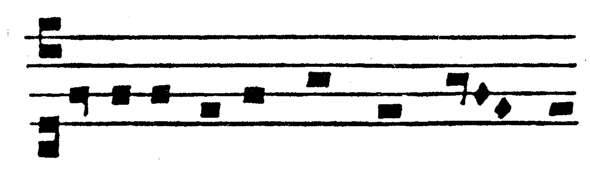
\includegraphics[scale=0.4]{picture/尤利西斯1.jpeg}
    \refdocument{
        \small 天主受享荣福于——天\footnote{}。
    }
\end{figure}
\par 他举起双手。圣器的帷幕垂下来了。啊,成簇的花儿!一座又一座又一座钟,响成一片。
\par ——是呀,确实是,公谊会教徒——图书馆长说。那是一场最令人受教益的讨论。穆利根先生想必对莎士比亚的戏剧也自有他的高见。应该把人生的各个方面都谈一谈。
\par 他一视同仁地朝四面八方微笑着。
\par 勃克·穆利根困惑地左思右想。
\par ——莎士比亚?他说。我好像听说过这个名字。
\par 他那皮肉松弛的脸上闪过一丝开朗的微笑。
\par ——没错儿,他恍然大悟了。就是写得像辛格\footnote{}的那位老兄。
\par 贝斯特先生转向他。
\par ——海恩斯找你哪,他说。你碰上他了吗?回头他要在都柏林面包公司跟你见面。他到吉尔书店买海德的《康纳特情歌》去了。
\par ——我是从博物馆穿过来的,勃克·穆利根说。他来过这儿吗?
\par ——大诗人的同胞们也许对咱们这精彩的议论颇感厌烦了,约翰·埃格林顿回答说。我听说昨天晚上在都柏林,一位女演员\footnote{}第四百零八次演出《哈姆莱特》。维宁\footnote{}提出,这位王子是个女的。有没有人发现他是个爱尔兰人呢?我相信审判官巴顿\footnote{}正在查找什么线索。他(指王子殿下,而不是审判官大人)曾凭着圣帕特里克的名义起过誓\footnote{}。
\par ——最妙的是王尔德的故事《威·休先生的肖像》,贝斯特先生举起他那出色的笔记本说。他在其中证明《十四行诗》是一个名叫威利·休斯的八面玲珑的人写的\footnote{}。
\par ——那不是献给威利·休斯的吗?公谊会教徒——图书馆长问。
\par 要不就是休依·威尔斯?威廉先生本人\footnote{}。W.H.我是谁?
\par ——我认为是为威利·休斯而写的,贝斯特先生顺口纠正自己的谬误说,当然喽,这全是些似是而非的话。要知道,就像休斯和砍伐和色彩\footnote{},他的写法独特。要知道,这才是王尔德的精髓呢。落笔轻松。
\par 他泛着微笑,轻轻地扫视大家一眼。白肤金发碧眼的年轻小伙子。王尔德那柔顺的精髓\footnote{}。
\par 你着实鬼得很。用堂迪希的钱\footnote{}喝了三杯威士忌。
\par 我花了多少?哦,不过几个先令。
\par 为了让一群新闻记者喝上一通。讲那些干净的和不干净的笑话。机智。为了把他打扮自己的那身青春的华服弄到手,你不惜舍弃你的五种机智\footnote{}。欲望得到满足的面貌\footnote{}。
\par 机会是很多的。交媾的时候,把她让给你吧。天神啊,让他们过一个凉快的交尾期吧\footnote{}。对,把她当做斑鸠那样地疼爱吧。
\par 夏娃在赤裸的小麦色肚皮下面犯的罪孽。一条蛇盘绕着她,龇着毒牙跟她接吻\footnote{}。
\par ——你认为这不过是谬论吗?公谊会教徒——图书馆长在问。当嘲弄者最认真的时候,却从未被认真对待过。
\par 他们严肃地讨论起嘲弄着的真诚。
\par 勃克·穆利根又把脸一耷拉,朝斯蒂芬瞅了几眼。然后摇头晃脑地凑过来,从兜里掏出一封折叠着的电报。他那灵活的嘴唇读时露出微笑,带着新的喜悦。
\par ——电报!他说。了不起的灵感!电报!罗马教皇的训谕!
\par 他坐在桌子灯光照不到的一角,兴高采烈地大声读着:
\par ——伤感主义者乃只顾享受而对所做之事不深觉歉疚之人\footnote{}。署名:迪达勒斯。你是打哪儿打的电报?窑子吗?不。学院公园?你把四镑钱都喝掉了吧?姑妈说是要去拜访你那位非同体的父亲。电报!玛拉基·穆利根。下阿贝街船记酒馆。噢,你这个举世无双的滑稽演员!哦,你这个以教士自居的混蛋金赤!
\par 他乐呵呵地将电报和封套塞到兜里,却又用爱尔兰土腔气冲冲地说:
\par ——是这么回事。好兄弟,当海恩斯亲自把电报拿进来的时候,他和我都正觉得苦恼烦闷来着。我们曾嘟囔说,要足足地喝上它一杯,让行乞的修士都会起魔障。我正转着这个念头,他呢,跟姑娘们黏糊起来了。我们就乖乖儿地坐在康纳里\footnote{}那儿,一个钟头,两个钟头,三个钟头地等下去,指望着每人喝上五六杯呢。
\par 他唉声叹气地说:
\par ——我们就呆在那儿,乖乖\footnote{},把舌头耷拉得一码长,活像那想酒想得发昏的干嗓子教士。你呢,也不知道躲到哪儿去了,居然还给我们送来了这么个玩意儿。
\par 斯蒂芬笑了。
\par 勃克·穆利根像是要提出警告似的弯下腰去。
\par ——流浪汉辛格\footnote{}正在找你哪,他说,好把你宰了。他听说你曾往他那坐落在格拉斯特赫尔的房子的正门上撒尿。他趿拉着一双破鞋到处走,说是要把你给宰了。
\par ——我!斯蒂芬喊道。那可是你对文学做出的一桩贡献呀。
\par 勃克·穆利根开心地向后仰着,朝那黑咕隆咚偷听着的天花板大笑。
\par ——宰了你!他笑道。
\par 在圣安德烈艺术街上,我一边吃着下水杂烩,一边望着那些严厉的怪兽形面孔\footnote{}。用那对语言报以语言的语言,讲一通话\footnote{}。莪相和帕特里克\footnote{}。他在克拉玛尔森林遇见了抡着酒瓶的牧羊神\footnote{}。那是圣星期五!杀人凶手爱尔兰人。他遇见了自己游荡着的形象。我遇见了我的。我在林中遇见一个傻子\footnote{}。
\par ——利斯特\footnote{}先生,一个工役从半掩着的门外招呼说。
\par ——……每个人都能在其中找到自己的形象。审判官先生马登在他的《威廉·赛伦斯少爷日记》中找到了狩猎术语\footnote{}……啊,什么事?
\par ——老爷,来了一位先生,工役走过来,边递上名片边说。是自由人报社的。他是想看看去年的《基尔肯尼民众报》\footnote{}合订本。
\par ——好的,好的,好的。这位先生在……?
\par 他接过那张殷勤地递过来的名片,带看不看地瞥了一眼,放下来,并没有读,只是瞟着,边问边把鞋踩得橐橐作响。又问:
\par ——他在……?哦,在那儿哪!
\par 他快步跳着五步舞\footnote{}出去了。在浴满阳光的走廊上,他不辞劳苦,热情地、口若悬河地谈着,极其公正、极其和蔼地尽着本分,不愧为一名最忠诚的“宽边帽”\footnote{}。
\par ——是这位先生吗?《自由人报》?《基尔肯尼民众报》?对。您好,先生。《基尔肯尼……》……我们当然有喽……
\par 一个男子的侧影耐心地等待着,聆听着。
\par ——主要的地方报纸全都有……《北方辉格》、《科克观察报》、《恩尼斯科尔西卫报》\footnote{}。去年。一九〇三……请您……埃文斯,给这位先生领路……您只要跟着这个工役……要么,还是我自己……这边……先生,请您……
\par 口若悬河,尽着本分,他领先到放着所有地方报纸的所在。一个鞠着躬的黑影儿尾随着他那匆忙的脚后跟。
\par 门关上了。
\par ——犹太佬!勃克·穆利根大声说。
\par 他一跃而起,一把抓住名片。
\par ——他叫什么名字?艾克依·摩西\footnote{}吗?布卢姆。
\par 他喋喋不休地讲下去:
\par ——包皮的搜集者\footnote{}耶和华已经不在了。刚才我在博物馆里遇见过他。我到那儿是去向海泡里诞生的阿佛洛狄忒致意的。这位希腊女神从来没有歪起嘴来祷告过。咱们每天都得向她致敬。生命的生命,你的嘴唇点燃起火焰\footnote{}。
\par 他突然转向斯蒂芬:
\par ——他认识你。他认识你的老头子。哦,我怕他,他比希腊人还要希腊化。他那双淡色的加利利\footnote{}眼睛总盯着女神中央那道沟沟。美臀维纳斯\footnote{}。啊,她有着怎样一副腰肢啊!天神追逐,女郎躲藏\footnote{}。
\par ——我们还想再听听,约翰·埃格林顿征得贝斯特先生的赞同后说。我们开始对莎\footnote{}太太感兴趣了。在这之前,即便我们想到过她,也不过把她看做是一位有耐心的克丽雪达\footnote{},留守家中的潘奈洛佩\footnote{}。
\par 戈尔吉亚的弟子安提西尼\footnote{},斯蒂芬说,从曼涅劳王的妻子、阿凯人海伦手里把美的标志棕榈枝拿过来,交给了可怜的潘奈洛佩。二十位英雄在特洛伊那匹母木马\footnote{}里睡过觉。他\footnote{}在伦敦住了二十年,其间有个时期领的薪水跟爱尔兰总督一样多。他的生活是丰裕的。他的艺术超越了沃尔特·惠特曼所说的封建主义艺术\footnote{},乃是饱满的艺术。热腾腾的鲱鱼馅饼、绿杯里斟得满满的白葡萄酒、蜂蜜酱、蜜饯玫瑰、杏仁糖、醋栗填鸽、刺芹糖块。沃尔特·雷利爵士\footnote{}被捕的时候,身上穿着值五十万法郎的衣服,包括一件精致的胸衣。放高利贷的伊丽莎·都铎\footnote{}的内衣之多,赛得过示巴女王\footnote{}。足足有二十年之久,他徘徊在夫妻那纯洁缠绵的恩爱与娼妇淫荡的欢乐之间。你们可晓得曼宁汉姆那个关于一个市民老婆的故事吧:她看了迪克\footnote{}·伯比奇在《理查三世》中的演出,就邀请他上自己的床。莎士比亚无意中听到了,没费多大力气\footnote{}就制服了母牛。当伯比奇前来敲门的时候,他从阉鸡\footnote{}的毯子下面回答说:征服者威廉已比理查三世捷足先登啦\footnote{}。快活的小夫人、情妇菲顿\footnote{}噢的一声就骑了上去\footnote{}。还有他那娇滴滴的婆娘潘奈洛佩·里奇\footnote{}。这位端庄的上流夫人适合做个演员;而河堤上的娼妇,一回只要一便士。
\par 王后大道。再出二十苏吧。给你搞点小花样儿。玩小猫咪?你愿意吗\footnote{}?
\par ——上流社会的精华。还有牛津的威廉·戴夫南特爵士\footnote{}的母亲,只要是长得像金丝雀那样俊秀的男人,她就请他喝杯加那利酒\footnote{}。
\par 勃克·穆利根虔诚地抬起两眼祷告道:
\par ——圣女玛格丽特·玛丽·安尼科克\footnote{}!
\par ——还有换过六个老婆的哈利的女儿\footnote{}。再就是草地·丁尼生、绅士诗人所唱的:附近邸舍的高贵女友\footnote{}。这漫长的二十年间,你们猜猜,斯特拉德福的潘奈洛佩\footnote{}在菱形窗玻璃后面都干什么来着?
\par 干吧,干吧\footnote{},干出成绩。他在药用植物学家杰勒德那座位于费特小巷的玫瑰花圃\footnote{}里散步,赤褐色的头发已灰白了。像她的脉管一样蓝的风信子\footnote{}。朱诺的眼睑,紫罗兰\footnote{}。他散步。人生只有一次,肉体只有一具。干吧。专心致志地干。远处,在淫荡和污浊的臭气中,一双手放在白净的肉身上。
\par 勃克·穆利根使劲敲着约翰·埃格林顿的桌子。
\par ——你猜疑谁呢\footnote{}?他盘问。
\par ——假定他是《十四行诗》里那位被舍弃的情人吧。被舍弃一回,就有第二回。然而宫廷里的那个水性杨花的女子是为了一个贵族——他的好友——而舍弃他的\footnote{}。
\par 不敢说出口的爱\footnote{}。
\par ——你的意思是说,刚毅的约翰·埃格林顿插进嘴去,作为一个英国人,他爱上了一位贵族。
\par 蜥蜴们沿着古老的墙壁一闪而过。我在查伦顿\footnote{}仔细观察过它们。
\par ——好像是的,斯蒂芬说,为了这位贵族,并为所有其他特定的、未被耕耘过的处女的胎\footnote{},他想尽尽马夫对种马所尽的那种神圣职责。也许跟苏格拉底一样,不仅妻子是个悍妇,母亲也是个产婆呢。然而她,那个喜欢痴笑的水性杨花的女子,并不曾撕毁床头盟\footnote{}。鬼魂\footnote{}满脑子都是那两档子事:誓盟被破坏了,她移情于那个迟钝的乡巴佬——亡夫的兄弟身上。我相信可爱的安是情欲旺盛的。她向男人求过一次爱,就会求第二次。
\par 斯蒂芬在椅子上果敢地转了个身。
\par ——证明这一点的责任在你们而不在我,他皱着眉头说。倘若你们否认他在《哈姆莱特》第五场里就给她打上了不贞的烙印,那么告诉我:为什么在他们结婚三十四年间,从迎娶那天直到她给他送殡,她始终只字没被提到过。这些女人统统为男人送了葬:玛丽送走了她的当家人约翰\footnote{},安送走了她那可怜的、亲爱的威伦\footnote{};尽管对于比她先走感到愤懑,他还是死在她前头了。琼送走了她的四个弟弟\footnote{}。朱迪斯\footnote{}送走了她丈夫和所有的儿子。苏珊也送走了她丈夫\footnote{}。苏珊的女儿伊丽莎白呢,用爷爷的话说:先把头一个丈夫杀了,再嫁给第二个\footnote{}。哦,对啦。有人提到过。当他在京都伦敦过着豪华的生活时,她不得不向她父亲的牧羊人借四十先令来还债\footnote{}。你们解释好了。还解释一下《天鹅之歌》\footnote{},作者在诗中向后世颂扬了她。
\par 他面对着大家的沉默。
\par 埃格林顿对他这么说:
\par  
\par 你指的是遗嘱。
\par 然而我相信法律家已做了诠释。
\par 按照不成文法,她作为遗孀,。
\par 有权利继承遗产 法官们告诉我们,
\par 他具有丰富的法律知识。
\par 恶魔嘲弄他。
\par 嘲弄者:
\par 因此,他把她的名字
\par 从最初的草稿中勾销了;然而他并未勾销对外孙女和女儿们的赠予,
\par 赠予他妹妹以及他在斯特拉特福和伦敦的挚友们的礼物。因此,据我所知,
\par 当他被提醒说,不要漏掉她的名儿
\par 他才留给她
\par 次好的
\par 床\footnote{}。
\par 要点\footnote{}。
\par 留给她他那
\par 次好的床
\par 留给她他那
\par 顶刮刮的床
\par 次好的床
\par 留给一张床。
\par 喔啊!
\par  
\par ——当时连俊俏的乡男村女\footnote{}都几乎没什么家当,约翰·埃格林顿说,倘若我们的农民戏\footnote{}反映得真实的话,他们至今也还是没有多少。
\par ——他是个富有的乡绅,斯蒂芬说,有着盾形纹章,还在斯特拉特福拥有一座庄园,在爱尔兰庭园有一栋房屋。他是个资本家和股东,证券发起人,还是个交纳什一税的农场主。倘若他希望她能在鼾声中平安地度过余生的话,为什么不把自己最好的床留给她呢?
\par ——他显然有两张床,一张最好的,另一张是次好的,次好的贝斯特先生\footnote{}乖巧地说。
\par ——向饭桌和寝室告别\footnote{},勃克·穆利根说得更透彻些,博得了大家的微笑。
\par ——关于一张张有名的床,古人说过不少话,其次的埃格林顿噘起嘴来,面泛床笑。让我想想看。
\par ——古人记载着那个斯塔基莱特的顽童和秃头的异教贤人的事,斯蒂芬说,他在流亡中弥留时,释放了他的奴隶们,留给他们资财,颂扬祖先,在遗嘱中要求把自己合葬在亡妻的遗骨旁边,并托付友人好生照顾他生前的情妇(不要忘记内尔·格温·赫尔派利斯),让她住在他的别墅里\footnote{}。
\par ——你认为他是这么死的吗?贝斯特先生略表关切地问道。我是说……
\par ——他是喝得烂醉而死的,勃克·穆利根劈头就说。一夸脱浓啤酒,就连国王也喜爱\footnote{}。哦,我得告诉你们多顿\footnote{}说了些什么!
\par ——说了什么?最好的埃格林顿\footnote{}问。
\par 威廉·莎士比亚股份有限公司\footnote{}。人民的威廉。详情可询:爱·多顿,海菲尔德寓所\footnote{}……
\par ——真可爱!勃克·穆利根情意绵绵地叹息说,我问他,关于人们指责那位大诗人有鸡奸行为,他做何感想。他举起双手说:我们所能说的仅仅是:当时的生活中充满了欣喜欢乐\footnote{}。真可爱!
\par 娈童。
\par ——对美的意识使我们误入歧途,沉浸在哀愁美中的贝斯特对正在变丑的埃格林顿说。
\par 坚定的约翰严峻地回答道:
\par ——博士可以告诉咱们那话是什么意思。你不能既吃了点心又还拿在手里\footnote{}。
\par 你这么说吗?难道他们要从我们——从我这里夺去美的标志——棕榈枝\footnote{}不成?
\par ——还有对财产的意识,斯蒂芬说。他把夏洛克从他自己的长口袋\footnote{}里拽了出来。作为啤酒批发商和放高利贷者的儿子,他本人也是个小麦批发商和放高利贷的。当由于闹饥荒而引发那场暴动时,他手里存有十托德\footnote{}小麦。毫无疑问,向他借钱的那帮人是切特尔·福斯塔夫所说的信仰各种教派的人。他们都说,他公平交易。为了讨回几袋麦芽的款,他和同一个剧团的演员打官司,作为贷款的利息,索取对方的一磅肉。不然的话,奥布里\footnote{}所说的那个马夫兼剧场听差怎么能这么快就发迹了呢?为了赚钱,他什么都干得出。女王的侍医、犹太佬洛佩斯\footnote{}那颗犹太心脏被活生生地剜出来,在上绞刑架之后,大解八块,紧接着就是一场对犹太人的迫害。这和夏洛克事件不谋而合。《哈姆莱特》和《麦克白》与有着焚烧女巫的嗜好的伪哲学家的即位赶在同一个时期\footnote{}。在《爱的徒劳》中,被击败的无敌舰队\footnote{}成了他嘲笑的对象。他的露天演出——也就是历史剧,在马弗京的一片狂热\footnote{}中,粉墨登场了。当沃里克郡的耶稣会士受审判后,我们就听到过一个门房关于暧昧不清的说法\footnote{}。“海洋冒险号”从百慕大驶回国时\footnote{},勒南所称赞过的以我们的美国堂弟帕齐·凯列班\footnote{}为主人公的那出戏写成了。继锡德尼之后,他也写了馨美的十四行诗组诗\footnote{}。关于仙女伊丽莎白(又名红发贝斯),那位胖处女授意而写成的《温莎的风流娘儿们》,就让哪位德国绅士耗用毕生心血去从洗衣筐的尽底儿上搜集吧,以便探明它的深邃含义\footnote{}。
\par 我觉得自己颇有领会。那么,把神学论理学语言学什么学掺合在一起再看看。撒着尿,撒了尿,撒着尿的,撒尿\footnote{}。
\par ——证明他是个犹太人吧,约翰·埃格林顿有所期待地将了一军。你们学院的院长说他是个罗马天主教徒\footnote{}。
\par ——我应该受到抑制\footnote{}。
\par ——他是德国制造的\footnote{},斯蒂芬回答说,是一位用法国磨光漆\footnote{}来涂饰意大利丑闻的高手。
\par ——一位拥有万众之心的人,贝斯特先生提醒道。柯尔律治\footnote{}说他是一位拥有万众之心的人。
\par 泛言之,人类社会中,让众人之间存在友情,乃是至关重要的\footnote{}。
\par ——圣托马斯,斯蒂芬开始说……
\par ——为我等祈\footnote{},僧侣穆利根边瘫坐在椅子上,边呻吟道。
\par 从那儿,他凄凉地吟起北欧古哀诗来:
\par ——吻我屁股!我心脏的搏动\footnote{}!从今天起,咱们毁灭啦!咱们确实毁灭啦\footnote{}!
\par 大家各自泛出微笑。
\par ——圣托马斯……斯蒂芬笑眯眯地说,那部卷帙繁多的书,我是从原文披阅并赞赏的。他是站在不同于马吉先生所提到的新维也纳学派\footnote{}的立场上,来谈乱伦的问题的。他以他特有的睿智而奇特的方法,把乱伦比做在情感方面的贪得无厌。他指出,血统相近者之间滋生的这种爱情,对于那些可能渴望它的陌生人,却贪婪地被抑制住了。基督教徒谴责犹太人贪婪,而犹太人是所有的民族中最倾向于近亲通婚的。这一谴责是愤怒地发出的。基督教戒律使犹太人成为巨富(对他们来说,正如对罗拉德派一样,风暴为他们提供了避难所),也用钢圈箍在他们的感情上\footnote{}。这些戒律究竟是罪恶还是美德,神老爹\footnote{}会在世界末日告诉我们的。然而一个人如此执着于债权,也同样会执着于所谓夫权。任何笑眯眯的邻居\footnote{}也不可去贪图他的母牛、他的妻子、他的婢女或公驴\footnote{}。
\par ——或是他的母驴,勃克·穆利根接着说道。
\par ——温和的威尔\footnote{}遭到了粗暴的对待,温和的贝斯特先生温和地说。
\par ——哪个威尔呀?勃克·穆利根亲切地打了句诨。简直都掺混不清了。
\par ——活下去的意志,约翰·埃格林顿用哲理解释道,对威尔的遗孀——可怜的安来说,就是为了迎接死亡的遗嘱\footnote{}。
\par ——安息吧\footnote{}!斯蒂芬祷告说。
\par  
\par 当年雄心壮志何在?
\par 早已烟消云散。\footnote{}
\par  
\par ——尽管你们证明当时的床就像今天的汽车那样珍贵,而床上的雕饰也令七个教区感到惊异;却不能改变她——那蒙面皇后\footnote{}穿着寿衣僵硬地挺在那次好的床上这一事实。在晚年,她跟那些传福音的打得火热——其中的一个跟她一道住在新地大宅,共饮那由镇议会付款的一夸脱白葡萄酒。然而,他究竟睡在哪张床上,就不得而知了。她听说自己有个灵魂。她读(或者请旁人读给她听)他那些沿街叫卖的廉价小册子。她喜欢它们更甚于《温莎的风流娘儿们》。她每天晚上跨在尿盆上撒尿\footnote{},驰想着《信徒长裤上的钩子和扣眼》以及《使最虔诚的信徒打喷嚏的最神圣的鼻烟盒》\footnote{}。维纳斯歪起嘴唇祷告着。内心的苛责。悔恨之心。这是一个精疲力竭的淫妇衰老后在寻觅着神的时代。
\par ——历史表示这是真实的,编年学家埃格林顿引证说\footnote{}。时代不断地更迭。然而一个人最大的仇敌乃是他自己家里的人和家族\footnote{},这话是有可靠根据的。我觉得拉塞尔是对的。我们何必去管他的老婆或者父亲的事呢?依我说,只有家庭诗人才过家庭生活。福斯塔夫并不是个守在家里的人。我觉得这个胖骑士才是他所创造的绝妙的人物。
\par 瘦骨嶙峋的他往椅背上靠了靠。出于羞涩,否定你的同族吧\footnote{},你这个自命清高的人\footnote{}。他羞涩地跟那些不信神的人一道吃饭,还偷酒杯\footnote{}。这是住在阿尔斯特省安特里姆\footnote{}的一位先生这样嘱咐他的。每年四季结账时就来找他。马吉先生,有位先生要来见您。我?他说他是您的父亲,先生。请把我的华兹华斯\footnote{}领进来。大马吉·马修\footnote{}进来了。这是个满脸皱纹、粗鲁、蓬头乱发的庄稼汉\footnote{},穿着胯间有个前兜的紧身短裤\footnote{},布袜子\footnote{}上沾了十座树林的泥污\footnote{},手里拿着野生苹果木杖\footnote{}。
\par 你自己的呢?他认得你那老头子\footnote{}——一个鳏夫。
\par 我从繁华的巴黎朝临终前的她那肮脏的床头赶去。在码头上摸了摸他的手。他说着话儿,嗓音里含着新的温情。鲍勃·肯尼大夫\footnote{}在护理她。那双眼睛向我祝福,然而并不了解我。
\par ——一个父亲,斯蒂芬说,在抑制着绝望情绪,这是无可避免的苦难。他是在父亲去世数月之后写的那出戏\footnote{}。这位头发开始花白、有着两个已届婚龄的女儿\footnote{}的年方三十五岁的男子,正当人生的中途\footnote{},却已有了五十岁的人的阅历。倘若你认为他就是威登堡那个没长胡子的大学生\footnote{},那么你就必须把他那位七十岁的老母看作淫荡的王后。不,约翰·莎士比亚的尸体并不在夜晚到处徘徊\footnote{}。它一小时一小时地腐烂下去\footnote{}。他把那份神秘的遗产\footnote{}留给儿子之后,就摆脱了为父的职责,开始安息了。卜伽丘的卡拉特林\footnote{}是空前绝后的一个自己认为有了身孕的男人。从有意识地生育这个意义上来说,男人是缺乏父性这一概念的。那是从惟一的父到惟一的子之间的神秘等级,是使徒所继承下来的。教会不是建立在乖巧的意大利智慧所抛给欧洲芸芸众生的那座圣母像上,而是建立在这种神秘上——牢固地建立在这上面。因为正如世界,正如大宇宙和小宇宙,它是建立在虚空之上,建立在无常和不定之上的。主生格和宾生格的母爱\footnote{}也许是人生中惟一真实的东西\footnote{}。父性可能是法律上的假定。谁是那位受儿子的爱戴,或疼爱儿子的为人之父呢?
\par 你究竟要扯些什么呢?
\par 我晓得。闭嘴。该死的。我自有道理。
\par 越发。更加。再者。其后\footnote{}。
\par 你注定要这么做吗?
\par ——难以自拔的肉体上的耻辱使父子之间产生隔阂。世上的犯罪年鉴虽被所有其他乱伦与兽奸的记录所玷污,却几乎还没记载过这类越轨行为。子与母、父与女、姐妹之间的同性恋,难以说出口的爱,侄子与祖母,囚犯与钥匙孔,皇后与良种公牛\footnote{}。儿子未出世前便损害了美。出世之后,带来痛苦,分散爱情,增添操劳。他是个新的男性:他的成长乃是他父亲的衰老;他的青春乃是他父亲的妒嫉;他的朋友乃是他父亲的仇敌。
\par 在王子街\footnote{}上,我想过此事。
\par ——在自然界,是什么把这二者结合起来的呢?是盲目发情的那一瞬间。
\par 我是个父亲吗?倘若我是的话?
\par 皱缩了的、没有把握的手。
\par ——非洲的撒伯里乌\footnote{},野生动物中最狡猾的异端的首领,坚持说,圣父乃是他自己的圣子。没有不能驾驭的语言的斗犬阿奎那\footnote{}驳斥了他。那么,倘若没有儿子的父亲就不成其为父亲,那么没有父亲的儿子能成其为儿子吗?当拉特兰·培根·南安普敦·莎士比亚\footnote{}或错误的喜剧里的另一个同名\footnote{}诗人撰写《哈姆莱特》的时候,他不仅是自己的儿子之父,而且还由于他不再是儿子了,他就成为、自己也感到成为整个家庭之父——他自己的祖父之父,他那未出世的孙儿之父。顺便提一下,那个孙儿从未诞生过,因为照马吉先生的理解,大自然是讨厌完美无缺的\footnote{}。
\par 埃格林顿两眼洋溢着喜悦,羞怯而恍然似有所悟地抬头望着。这个愉快的清教徒隔着盘绕在一起的野蔷薇\footnote{},乐呵呵地望着。
\par 恭维一番。极偶然地。然而恭维一番吧。
\par ——他本人就是他自己的父亲\footnote{},儿子穆利根喃喃自语。且慢。我怀孕了。我脑中有个尚未出世的娃娃。明智女神雅典娜\footnote{}!一出戏!关键在于这出戏\footnote{}!让我分娩吧!
\par 他用那双接生的手抱住自己突出的前额。
\par ——至于他的家庭,斯蒂芬说,他母亲的名字还活在亚登森林里\footnote{}。她的死促使他在《科利奥兰纳斯》中写出伏伦妮娅的场景\footnote{}。《约翰王》中少年亚瑟咽气的场面就描述了他的幼子之死。身着丧服的哈姆莱特王子是哈姆奈特·莎士比亚。我们晓得《暴风雨》、《配力克里斯》、《冬天的故事》中的少女们都是谁。埃及的肉锅克莉奥佩特拉\footnote{}和克瑞西达\footnote{}以及维纳斯都是谁,我们也猜得出。然而他的眷属中还有一个被记载下来的人。
\par ——情节变得复杂啦,约翰·埃格林顿说。
\par 公谊会教徒——图书馆长震颤着,悄悄地走了进来。颤着他那张没有表情的脸,很快地颤着,颤着,颤着\footnote{}。
\par 门关上了。斗室。白昼。
\par 他们倾听着。三个。他们。
\par 我、你、他、他们。
\par 来吧,开饭啦。
\par 斯蒂芬
\par 他有三个弟兄:吉尔伯特、埃德蒙、理查德\footnote{}。吉尔伯特进入老年后,对几个绅士说,有一次他去望弥撒,教堂收献金的送了他一张免票。于是他就去了,瞅见他哥哥——剧作家伍尔在伦敦上演一出打斗戏,背上还骑着个男人\footnote{}。戏园子里的香肠\footnote{}吉尔伯特吃得可开心啦。哪儿也见不到他。然而可爱的威廉却在作品里记下了一个埃德蒙和一个理查德。
\par 马吉·埃格林·约翰
\par 姓名!姓名有什么意义\footnote{}?
\par 贝斯特
\par 理查德就是我的名字,你晓得吗?我希望你替理查德说句好话。要知道,是为了我的缘故。
\par (笑声)
\par 勃克·穆利根
\par (轻柔地,渐弱)\footnote{}
\par 于是,医科学生迪克
\par 对他的医科同学戴维说了\footnote{}……
\par  
\par 斯蒂芬
\par 他笔下的黑心肠的三位一体——那帮恶棍扒手:伊阿古、罗锅儿理查德和《李尔王》中的埃德蒙,其中两个的名字都跟他们那坏蛋叔叔一样。何况当他写成或者正在撰写这最后一部戏的时候,他的胞弟埃德蒙正奄奄一息地躺在萨瑟克\footnote{}。
\par 贝斯特
\par 我巴不得埃德蒙遭殃,我不要理查这个名字……
\par (笑声)
\par 公谊会教徒利斯特
\par (恢复原速)可是他偷去了我的好名声\footnote{}……
\par 斯蒂芬
\par (渐快)他把自己的名字——威廉这个美好的名字,隐藏在戏里。在这出戏里是配角,那出戏里又是丑角。就像从前意大利画家在画布的昏暗角落里画上了自己的肖像似的,他在满是威尔字样的《十四行诗》里,表明了这一点\footnote{}。就像冈特·欧·约翰\footnote{}一样,对他来说姓名是宝贵的,就像他拼命巴结到手的纹章——黑地右斜线\footnote{}上绘有象征荣誉的\footnote{}矛或银刃的纹章——那样宝贵。比当上本国最伟大的剧作家这一荣誉还更要宝贵。姓名有什么意义\footnote{}?那正是当我们幼时被告知自己的姓名,并把它写下来之际,所问过自己的。他诞生的时候,出现了一颗星\footnote{},一颗晨星,一条喷火龙\footnote{}。白天,它在太空中独自闪烁着,比夜间的金星还要明亮。夜里,它照耀在标志着他的首字W\footnote{}、横卧于群星中的仙后座那三角形上。午夜,当他离开安·哈撒韦的怀抱,从肖特利\footnote{}回去时,他一边走在困倦的夏天田野上,一边放眼望着那低低地躺在大熊座东边的地平线上的这颗星。
\par 两个人都感到满意,我也满意。
\par 不要告诉他们,当那颗星消失的时候,他年方九岁\footnote{}。
\par 而且从她的怀抱当中。
\par 等待着被求爱并占有\footnote{}。哎,你这个懦夫\footnote{},谁会向你求爱呢?
\par 读一读天空吧。虐己者\footnote{}。斯蒂芬的公牛精神\footnote{}。你的星座在哪里?斯蒂芬,斯蒂芬,面包要切匀。S.D.:他的情妇。不错——他的。杰林多打定主意不去恋慕S.D.\footnote{}。
\par ——迪达勒斯先生,那是什么呀?公谊会教徒——图书馆长问道,是天体现象吗?
\par ——夜间有星宿,斯蒂芬说,白天有云柱\footnote{}。
\par 此外还有什么可说的呢?
\par 斯蒂芬瞅了瞅自己的帽子、手杖和靴子。
\par 斯蒂法诺斯\footnote{},我的王冠。我的剑。他的靴子使我的脚变了形。买一双吧。我的短袜净是窟窿。手绢也一样。
\par “你善于在名字上做文章,约翰·埃格林顿承认道。你自己的名字也够别致的了。我看这就正好说明你这个喜欢幻想的性格。”
\par 我、马吉和穆利根。
\par 神话中的工匠\footnote{}。长得像鹰的人。你飞走了。飞向哪里?从纽黑文到迪耶普\footnote{},统舱客。往返巴黎。凤头麦鸡\footnote{}。伊卡洛斯\footnote{}。父亲啊,帮助我吧\footnote{}。被海水溅湿,一头栽下去,翻滚着。你是一只凤头麦鸡,变成一只凤头麦鸡。
\par 贝斯特先生热切地、安详地举起他的笔记本来说:
\par ——那非常有趣儿。因为,要知道,在爱尔兰传说中,我们也能找到弟兄这一主题。跟你讲的一模一样。莎士比亚哥儿仨。格林\footnote{}里也有。要知道,那些童话里,三弟总是跟睡美人结婚,并获得头奖。
\par 贝斯特弟兄们当中最好\footnote{}的。好,更好,最好。
\par 公谊会教徒——图书馆长来到旁边,像弹簧松了似的突然站住了。
\par ——我想打听一下,他说,是你的哪一位弟兄……假若我没理解错的话,你曾暗示说,你们弟兄当中有一个行为不轨……然而,也许我理解得过了头?
\par 他察觉到自己失言了,四下里望望大家,把底下的话咽了下去。
\par 一个工役站在门口嚷道:
\par ——利斯特先生!迪宁神父\footnote{}要见……
\par ——噢,迪宁神父!马上就来。
\par 他立刻把皮鞋踩得橐橐响,随即径直走了出去。
\par 约翰·埃格林顿提出了挑战。
\par ——喂,他说。咱们听听足下关于理查德和埃德蒙有何高见。你不是把他们留到最后吗?
\par ——我曾请你们记住那两位高贵的亲族\footnote{}——里奇叔叔和埃德蒙叔叔,斯蒂芬回答说,我觉得我也许要求得过多了。弟兄正像一把伞一样,很容易就被人忘记。
\par 凤头麦鸡。
\par 你的弟弟在哪儿?在药剂师的店里\footnote{}。砥砺我者,他,还有克兰利,穆利根\footnote{}。现在是这帮人。夸夸其谈。然而要采取行动。把言语付诸实践。他们嘲弄你是为了考验你。采取行动吧。让他们在你身上采取行动。
\par 凤头麦鸡。
\par 我对自己的声音感到厌烦了,对以扫的声音感到厌烦了\footnote{}。愿用我的王位换一杯酒\footnote{}。
\par 继续说下去吧。
\par ——你会说,这些名字早就写在被他当做戏剧素材的纪年记里了。他为什么不采用旁的,而偏偏采用这些呢?理查德,一个婊子养的畸形的罗锅儿,向寡妇安(姓名有什么意义?)求婚并赢得了她——一个婊子养的风流寡妇。三弟——征服者理查德,继被征服者威廉之后而来。这个剧本的其他四幕,松松散散地接在第一幕后面。在莎士比亚笔下所有的国王中,理查是世界上的天使\footnote{}中他惟一不曾怀着崇敬心情加以庇护的。《李尔王》中埃德蒙登场的插话取自锡德尼的《阿卡迪亚》,为什么要把它填补到比历史还古老的凯尔特传说中去呢\footnote{}?
\par ——那是威尔惯用的手法,约翰·埃格林顿辩护说。我们现在就不可能把北欧神话和乔治·梅瑞狄斯的长篇小说的摘录连结在一起。穆尔就会说:“这有什么办法呢?\footnote{}”他把波希米亚搬到海边\footnote{},让尤利西斯引用亚里士多德\footnote{}。
\par ——为什么呢?斯蒂芬自问自答。因为对莎士比亚来说,撒谎的弟兄、篡位的弟兄、通奸的弟兄,或者三者兼而有之的弟兄,是总也离不开的题材,而穷人却不常跟他在一起\footnote{}。从心里被放逐,从家园被放逐,自《维洛那二绅士》起,这个放逐的旋律一直不间断地响下去,直到普洛斯彼罗折断他那根杖,将它埋在地下数倖深处,并把他的书抛到海里\footnote{}。他进入中年后,这个旋律的音量加强了一倍,反映到另一个人生,照序幕、展开部、最高潮部、结局\footnote{}来复奏一遍。当他行将就木时,这个旋律又重奏一遍。有其母必有其女。那时,他那个已出嫁的女儿苏珊娜被指控以通奸罪\footnote{}。然而使他的头脑变得糊涂、削弱他的意志、促使他强烈地倾向于邪恶的,乃是原罪。照梅努斯的主教大人们说来,原罪者,正因为是厚罪,尽管系旁人所犯,其中也自有他的一份罪愆\footnote{}。在他的临终遗言里,透露了这一点。这话铭刻在他的墓石上。她的遗骨不得葬在下面\footnote{}。岁月不曾使它磨灭。美与和平也不曾使它消失。在他所创造的世界各个角落,都变幻无穷地存在着\footnote{}。在《爱的徒劳》中,两次在《皆大欢喜》中,在《暴风雨》中,《哈姆莱特》中,《一报还一报》中——以及其他所有我还没读过的剧作中。
\par 为了把心灵从精神的羁绊中解放出来,他笑了。
\par 审判官埃格林顿对此加以概括。
\par ——真理在两者之间,他斩钉截铁地说。他是圣灵,又是王子。他什么都是\footnote{}。
\par ——可不是嘛,斯蒂芬说。第一幕里的少年就是第五幕中的那个成熟的男人。他什么都是。在《辛白林》,在《奥瑟罗》中,他是老鸨\footnote{},给戴上了绿头巾,他采取行动,也让别人在他身上采取行动。他抱有理想,或趋向堕落,就像荷西那样杀死那活生生的嘉尔曼\footnote{}。他那冷酷严峻的理性就有如狂怒的伊阿古,不断地巴望自己内心的摩尔人\footnote{}会受折磨。
\par ——咕咕!咕咕!穆利根用淫猥的声调啼叫着。啊,可怕的声音\footnote{}!
\par 黑暗的拱形顶棚接受了这声音,发出回响\footnote{}。
\par ——伊阿古是怎样的一个人物啊!无所畏惧的约翰·埃格林顿喊叫着说。归根结蒂,小仲马(也许是大仲马\footnote{}吧?)说得对:天主之外,莎士比亚创造的最多。
\par ——男人不能使他感到喜悦;不,女人也不能使他感到喜悦\footnote{},斯蒂芬说。离开一辈子后,他又回到自己出生的那片土地上。从小到大\footnote{},他始终是那个地方的一名沉默的目击者。在那里,他走完了人生的旅途。他在地里栽下自己的那棵桑树\footnote{},然后溘然长逝。呼吸停止了\footnote{}。掘墓者埋葬了大哈姆莱特和小哈姆莱特\footnote{}。国王和王子在音乐伴奏下终于死去了。遭到谋杀也罢,被陷害也罢,又有何干?因为不论他是丹麦人还是都柏林人,所有那些柔软心肠的人们都会为之哀泣,悼念死者的这份悲伤乃是她们不肯与之离婚的惟一的丈夫。倘若你喜欢尾声,那么就仔细端详一下吧。幸福的普洛斯彼罗\footnote{}是得到好报的善人。丽齐\footnote{}是外公的宝贝疙瘩;里奇叔叔这个歹徒按照因果报应的原则被送进坏黑人注定去的地方了\footnote{}。结局圆满,幕终。他发现,内在世界有可能实现的,外在世界就已经成为现实了。梅特林克说:倘若苏格拉底今天离家,他会发现贤人就坐在他门口的台阶上。倘若犹大今晚外出,他的脚会把他引到犹大那儿去\footnote{}。每一个人的一生都是许多时日,一天接一天。我们从自我内部穿行\footnote{},遇见强盗,鬼魂,巨人,老者,小伙子,妻子,遗孀,恋爱中的弟兄们,然而,我们遇见的总是我们自己。编写世界这部大书而且写得很蹩脚的那位剧作家(他先给了我们光,隔了两天才给太阳\footnote{}),也就是被天主教徒当中罗马味最足的家伙称之为煞神\footnote{}——绞刑吏之神的万物之主宰;毫无疑问,他什么都是\footnote{},存在于我们一切人当中:既是马夫,又是屠夫,也是老鸨,并被戴上了绿头巾。然而倘若在天堂实行节约,像哈姆莱特所预言的那样,那么就再也不要什么婚娶;或者有什么光彩的人,半阴半阳的天使,将成为自己的妻子\footnote{}。
\par ——我发现啦\footnote{}!勃克·穆利根大声说。我发现啦!
\par 他突然高兴了,跳起来,一个箭步窜到约翰·埃格林顿的书桌跟前。
\par ——可以吗?他说。玛拉基接受了神谕\footnote{}。
\par 他在一片纸上胡乱涂写起来。
\par 往外走的时候,从柜台上拿几张纸条儿吧。
\par ——已经结婚的,安详的使者贝斯特先生说,除了一个人,都将活下去。没有结婚的,不准再结婚\footnote{}。
\par 他这个未婚者对独身的文学士约翰·埃格林顿笑了笑。
\par 他们没有家室,没有幻想,存着戒心,每天晚上边摸索各自那部有诸家注释的《驯悍记》,边在沉思。
\par ——你这是谬论,约翰·埃格林顿率直地对斯蒂芬说。你带着我们兜了半天圈子,不过是让我们看到一个法国式的三角关系。你相信自己的见解吗?
\par ——不,斯蒂芬马上说。
\par ——你打算把它写下来吗?贝斯特先生问。你应该写成问答体。知道吧,就像王尔德所写的柏拉图式的对话录。
\par 约翰·埃克列克提康\footnote{}露出暧昧的笑容。
\par ——喏,倘若是那样,他说,既然连你自己都不相信,我就不明白你怎么还能指望得到报酬呢。多顿\footnote{}相信《哈姆莱特》中有些神秘之处,然而他只说到这里为止。派珀在柏林遇见的勃莱布楚先生正在研究关于拉特兰\footnote{}的学说,他相信个中秘密隐藏在斯特拉特福的纪念碑里。派珀说,他即将去拜访当前这位公爵,并向公爵证明,是他的祖先写下了那些戏剧。这会出乎公爵大人的意料,然而勃莱布楚相信自己的见解。
\par 我信,噢,主啊,但是我的信心不足,求您帮助我\footnote{}!就是说,帮助我去信,或者帮助我不去信。谁来帮助我去信?我自己\footnote{}。谁来帮助我不去信呢?另一个家伙。
\par ——在给《达娜》\footnote{}撰稿的人当中,你是惟一要求付酬的。像这样的话,下一期如何就难说了。弗雷德·瑞安\footnote{}还要保留些篇幅来刊登一篇有关经济学的文章呢。
\par 弗莱德琳。他借给过我两枚银币。好歹应付一下吧。经济学。
\par ——要是付一畿尼,斯蒂芬说,你就可以发表这篇访问记了。
\par 面带笑容正在潦潦草草写着什么的勃克·穆利根,这时边笑边站起来,然后笑里藏刀,一本正经地说:
\par ——我到“大诗人”金赤在上梅克伦堡街的夏季别墅那里去拜访过他,发现他正和两个生梅毒的女人——新手内莉和煤炭码头上的婊子罗莎莉\footnote{}——一道埋头研究《反异教大全》\footnote{}呢。
\par 他把话顿了一顿。
\par ——来吧,金赤,来吧,飘忽不定的飞鸟之神安古斯\footnote{}。
\par 出来吧,金赤,你把我们剩的都吃光了\footnote{}。嗯,我把残羹剩饭和下水赏给你吃。
\par 斯蒂芬站起来了。
\par 人生不外乎一天接一天。今天即将结束了。
\par ——今天晚上见,约翰·埃格林顿说。我们的朋友\footnote{}穆尔说,务必请勃克·穆利根来。
\par 勃克·穆利根挥着那纸片和巴拿马帽。
\par ——穆尔先生\footnote{},他说,爱尔兰青年的法国文学讲师。我去。来吧,金赤,“大诗人”们非喝酒不可。你不用扶能走吗?
\par 他边笑着,边……
\par 痛饮到十一点,爱尔兰的夜宴。
\par 傻大个儿……
\par 斯蒂芬跟在一个傻大个儿后面……
\par 有一天,我们在国立图书馆讨论过一次。莎士\footnote{}。然后,我跟在傻乎乎的他背后走。我和他的脚后跟挨得那么近,简直可以蹭破那上面的冻疮了\footnote{}。
\par 斯蒂芬向大家致意,然后垂头丧气地\footnote{}跟着那个新理过发、头梳得整整齐齐、爱说笑话的傻大个儿,从拱顶斗室走入没有思想的灿烂骄阳中去。
\par 我学到了什么?关于他们?关于我自己?
\par 眼下就像海恩斯那样走吧。
\par 长期读者阅览室。在阅览者签名簿上,卡什尔·博伊尔·奥康纳·菲茨莫里斯·菲斯德尔·法雷尔用龙飞凤舞的字体写下了他那多音节的名字。研究项目:哈姆莱特发疯了吗?歇顶的公谊会教徒正在跟一个小教士虔诚地谈论着书本。
\par ——啊,请您务必……那我真是太高兴啦……
\par 勃克·穆利根觉得有趣,自己点点头,愉快地咕哝道:
\par ——心满意足的波顿\footnote{}。
\par 旋转栅门。
\par 难道是……?饰有蓝绸带的帽子……?胡乱涂写着……?什么?……看见了吗?
\par 弧形扶栏。明契乌斯河缓缓流着,一平如镜\footnote{}。
\par 迫克\footnote{}·穆利根,头戴巴拿马盔,一边走着,一边忽高忽低地唱着:
\par  
\par ——约翰·埃格林顿,我的乖,约翰\footnote{},
\par 你为啥不娶个老婆?
\par  
\par 他朝半空中啐了一口,唾沫飞溅。
\par ——噢,没下巴的中国佬!靳张艾林唐\footnote{}。我们曾到过他们那戏棚子,海恩斯和我,在管子工会的会馆。我们的演员们正在像希腊人或梅特林克先生那样,为欧洲创造一种新艺术。阿贝剧院!我闻见了僧侣们阴部的汗臭味\footnote{}。
\par 他漠然地啐了口唾沫。
\par 一古脑儿全抛在脑后了,就像忘记了可恶的路希那顿鞭子一样\footnote{}。也忘记了撇下那个三十岁的女人\footnote{}的事。为什么没再生个娃娃呢?而且,为什么头胎是个女孩儿呢?
\par 事后聪明。从头来一遍。
\par 倔强的隐士依然在那儿呢(他把点心拿在手里\footnote{}),还有那个文静的小伙子,小乖乖\footnote{},菲多那囝囝般的金发\footnote{}。
\par 呃……我只是呃……曾经想要……我忘记了……呃……
\par ——朗沃思和麦考迪·阿特金森也在那儿\footnote{}……
\par 迫克·穆利根合辙押韵,颤声吟着:
\par  
\par ——每逢喊声传邻里,
\par 或听街头大兵语,
\par 我就忽然间想起,
\par 弗·麦考迪·阿特金森,
\par 一条木腿是假的,
\par 穿着短裤不讲道理,
\par 渴了不敢把酒饮,
\par 嘴缺下巴的马吉,
\par 活了一世怕娶妻,
\par 二人成天搞手淫\footnote{}。
\par  
\par 继续嘲弄吧。认识自己\footnote{}。
\par 一个嘲弄者在我下面停下脚步,望着我。我站住了。
\par ——愁眉苦脸的戏子,勃克·穆利根慨叹道。辛格为了活得更自然,不再穿丧服了。只有老鸨、教士和英国煤炭才是黑色的\footnote{}。
\par 他唇边掠过一丝微笑。
\par ——自从你写了那篇关于狗鳕婆子格雷戈里的文章,他说,朗沃思就感到非常烦闷。哦,你这个好窥人隐私、成天酗酒的犹太耶稣会士!她在报馆里替你谋一份差事,你却骂她是蹩脚演员,写了那些蠢话。你难道不能学点叶芝的笔法吗\footnote{}?
\par 他歪鼻子斜眼地走下楼梯,优雅地抡着胳膊吟诵着:
\par ——我国当代一部最美的书。它令人想到荷马。
\par 他在楼梯下止住了步子。
\par ——我为哑剧演员们构思了一出戏,他认真地说。
\par 有着圆柱的摩尔式大厅,阴影交错。九个头戴有标志的帽子的男人跳的摩利斯舞\footnote{}结束了。
\par 勃克·穆利根用他那甜润、抑扬顿挫的嗓音读着那个法版\footnote{}:
\par  
\par ——人人是各自的妻
\par 或
\par 到手的蜜月
\par (由三次情欲亢进构成的、国民不道德剧)
\par 作者
\par 巴洛基·穆利根\footnote{}
\par  
\par 他朝斯蒂芬装出一脸快乐的傻笑,说:
\par ——就怕伪装得不够巧妙。可是且听下去。
\par 他读道,清晰地\footnote{}:
\par  
\par ——登场人物
\par 托比·托斯托夫(破了产的波兰人)
\par 克雷布(土匪)\footnote{}
\begin{gather*}
    \left.
        \begin{matrix}
            \text{医科学生迪克}\\
            \text{和}\\
            \text{医科学生戴维}
        \end{matrix}
    \right\} \text{一石二鸟}
\end{gather*}
\par 医科学生戴维
\par 老妪葛罗甘(送水者)
\par 新手内莉
\par 以及
\par 罗莎莉(煤炭码头上的婊子)
\par  
\par 他摇头晃脑地笑了,继续往前走,斯蒂芬跟在后面。他对着影子——对着人们的灵魂快快乐乐地说着话儿:
\par ——啊,坎姆顿会堂\footnote{}的那个夜晚啊!——你躺在桑椹色的、五彩缤纷的大量呕吐物当中。为了从你身上迈过去,爱琳\footnote{}的女儿们得撩起她们的裙子!
\par ——她们为之撩起裙子的,斯蒂芬说,是爱琳最天真无邪的儿子。
\par 正要走出门口的当儿,他觉出背后有人,便往旁边一闪。
\par 走吧。现在正是时机。那么,去哪儿呢?倘若苏格拉底今天离开家,倘若犹大今晚外出。为什么?它横在我迟早会无可避免地要到达的空间。
\par 我的意志。与我遥遥相对的是他的意志。中间隔着汪洋大海。
\par 一个男人边鞠躬边致意,从他们之间穿过。
\par ——又碰见了,勃克·穆利根说。
\par 有圆柱的门廊。
\par 为了占卜凶吉,我曾在这里眺望过鸟群\footnote{}。飞鸟之神安古斯。它们飞去又飞来。昨天晚上我飞了。飞得自由自在。人们感到惊异。随后就是娼妓街。他捧着一只淡黄色蜜瓜朝我递过来。进来吧。随你挑\footnote{}。
\par ——一个流浪的犹太人\footnote{},勃克·穆利根露出小丑那战战兢兢的样子悄悄地说。你瞅见他的眼神了吗?他色迷迷地盯着你哩。我怕你,老水手\footnote{}。哦,金赤。你的处境危险呀。去买条结实的裤衩吧。
\par 牛津派头。
\par 白昼。拱形桥的上空,悬着状似独轮手车的太阳。
\par 黑色的脊背迈着豹一般的步伐,走在他们前面,从吊门的\footnote{}倒刺下边钻了出去。
\par 他们跟在后面。
\par 继续对我大放厥词吧,说下去。
\par 柔和的空气使基尔戴尔街的房屋外角轮廓鲜明。没有鸟儿。两缕轻烟从房顶袅袅上升,形成羽毛状,被一阵和风柔和地刮走。
\par 别再厮斗了。辛白林的德鲁伊特祭司们的安宁,阐释秘义:在辽阔的大地上筑起一座祭坛。
\par  
\par 让我们赞美神明;
\par 让袅袅香烟从我们神圣的祭坛
\par 爬入他们的鼻孔\footnote{}。



\subsubsection*{第十章}


\par 耶稣会会长,十分可敬的约翰·康米\footnote{}边迈下神父住宅的台阶,边把光滑的怀表揣回内兜。差五分三点。还来得及,正好走到阿坦\footnote{}。那个男孩儿姓什么来着?迪格纳穆。对。着实恰当而正确\footnote{}。应该去见见斯旺修士\footnote{}。还有一封坎宁翰\footnote{}先生的来信呢。是啊,尽可能满足他的要求吧。这是位善良而能干的天主教徒。布教的时候能派上用场。
\par 一个独腿水手,架着双拐,无精打采地一步一挪地往前悠荡,嘴里哼唱着什么曲调。他悠荡到仁爱会修女院前面,蓦地停了下来,朝着耶稣会这位十分可敬的约翰·康米伸过一顶鸭舌帽,求他施舍。康米神父在阳光下祝福了他,因为神父知道自己的钱包里只有一克朗银币。
\par 康米神父横过马路,跨过蒙乔伊广场。他想了一下被炮弹炸断了腿的士兵和水手怎样在贫民救济所里结束余生的事,又想起红衣主教沃尔西的话:“如果我用为国王效劳的热诚来侍奉天主,他也不会在我垂老之年抛弃我。”\footnote{}他沿着树阴,走在闪烁着阳光的树叶底下;议会议员戴维·希伊先生的太太\footnote{}迎面而来。
\par ——我很好,真的,神父。您呢,神父?
\par 康米神父确实非常健康。他也许会到巴克斯顿\footnote{}去洗洗矿泉澡。她的公子们在贝尔维迪尔\footnote{}念得蛮好吧?是吗?康米神父听到这情况,的确很高兴。希伊先生本人呢?还在伦敦。议会仍在开会,可不是嘛。多好的天气啊,真让人心旷神怡。是啊,伯纳德·沃恩\footnote{}神父极可能会再来讲一次道。啊,可不,了不起的成功。的确是位奇才。
\par 康米神父看到议会议员戴维·希伊先生的太太显得那么健康,高兴极了,他恳请她代为向议会议员戴维·希伊先生致意。是的,他准登门去拜访。
\par ——那么,再见吧,希伊太太。
\par 康米神父脱下大礼帽告别,朝着她面纱上那些在阳光下闪着墨光的乌珠莞尔一笑。一边走开一边又漾出微笑。他晓得自己曾用槟榔果膏把牙刷得干干净净。
\par 康米神父踱着,边走边泛出微笑,因为他记起伯纳德·沃恩神父那逗乐儿的眼神和带伦敦土腔的口音。
\par ——彼拉多\footnote{}!你咋不赶走那些起哄的家伙?
\par 不管怎么说,他是个热心肠的人。这一点不假。以他独特的方式,确实做过不少好事。这是毫无疑问的。他说他热爱爱尔兰,也热爱爱尔兰人。谁能相信他还出身于世家呢?是威尔士人吧?
\par 哦,可别忘了。那封给管辖教区的神父的信。
\par 在蒙乔伊广场的角落里,康米神父拦住三个小学童。对,他们是贝尔维迪尔的学生。呃,班次很低。他们在学校里都是好学生吗?哦,那就好极啦。那么,他叫什么名字呢?杰克·索恩。他叫什么?杰尔\footnote{}·加拉赫。另一个小不点儿呢?他的名字叫布鲁尼·莱纳姆。哦,起了个多么好的名字。
\par 康米神父从前胸掏出一封信来,递给少年布鲁尼·莱纳姆,并指了指菲茨吉本街拐角处的红色邮筒。
\par ——可是留点儿神,别把你自个儿也投进邮筒里去,小不点儿,他说。
\par 孩子们的六只眼睛盯着康米神父,大声笑了起来:
\par ——哦,您哪。
\par ——喏,让我瞧瞧你会不会投邮,康米神父说。
\par 少年布鲁尼·莱纳姆跑到了马路对面,将康米神父那封写给管辖教区神父的信塞进红艳艳的邮筒口里。康米神父泛着微笑,点了点头。然后又笑了笑,就沿着蒙乔伊广场向东踱去。
\par 舞蹈等课程的教师丹尼斯·杰·马金尼\footnote{}先生头戴丝质大礼帽,身穿滚着绸边的暗蓝灰色长礼服,系着雪白的蝴蝶结,下面是淡紫色紧腿裤;戴着鲜黄色手套,脚登尖头漆皮靴。他举止端庄地走着,来到迪格纳穆庭院的角上。这时,马克斯韦尔夫人擦身而过,他赶紧毕恭毕敬地闪到边石上去。
\par 那不是麦吉尼斯太太\footnote{}吗?
\par 满头银发、仪表堂堂的麦吉尼斯太太在对面的人行道上款款而行。她朝康米神父点头致意。康米神父含笑施礼。她近来可好?
\par 夫人风度优雅,颇有点儿像苏格兰女王玛丽\footnote{}。想想看,她竟然是个当铺老板娘!哟,真是的!这么一派……该怎么说呢?……这么一派女王风度。
\par 康米神父沿着大查尔斯街前行,朝左侧那紧闭着门的自由教会\footnote{}瞟了一眼。可敬的文学士T.R.格林将(按照神的旨意)\footnote{}布道。他们称他作教区牧师。他呢,认为讲上几句儿乃是义不容辞的\footnote{}。然而,得对他们宽大为怀。不可克服的愚昧。他们毕竟也是根据自己的见解行事的啊。
\par 康米神父拐了弯,沿着北环路踱去。奇怪,这样一条重要的通衢大道,竟然没铺设电车路。肯定应该铺设。
\par 一群背着书包的学童从里奇蒙大街那边跨过马路而来。个个扬起肮里肮脏的便帽。康米神父一次又一次慈祥地朝他们还礼。这都是些公教弟兄会\footnote{}的孩子们。
\par 康米神父一路走着,闻到右侧飘来一股烟香。波特兰横街的圣约瑟教堂。那是给贞节的老妪们开设的\footnote{}。神父冲着圣体\footnote{}摘下帽子。她们固然操守高尚,只是,有时脾气挺坏。
\par 来到奥尔德勃勒邸第附近,康米神父想起那位挥金如土的贵族。而今,这里改成了公事房还是什么的\footnote{}。
\par 康米神父开始顺着北滩路走去,站在自己那爿商号门口的威廉·加拉赫先生朝他施礼。康米神父向威廉·加拉赫先生还礼,并嗅到了成条的腌猪肋骨肉和桶里装得满满的冰镇黄油的气味。他走过葛洛根烟草铺,店前斜靠着一块块张贴新闻的告示板,报道发生在纽约的一桩惨案\footnote{}。在美国,这类事件层出不穷。倒楣的人们毫无准备地就那么送了命。不过,彻底悔罪也能获得赦免\footnote{}。
\par 康米神父走过丹尼尔·伯金的酒馆儿。两个没找到活儿干的男人在闲倚着窗口消磨时光。他们向他行礼,他也还了礼。
\par 康米神父走过H.J.奥尼尔殡仪馆。科尼·凯莱赫正一边嚼着一片枯草,一边在流水账簿上划算着。一个巡逻的警察向康米神父致敬,康米神父也回敬了一下。走过尤克斯泰特猪肉店,康米神父瞧见里面整整齐齐地摆着黑白红色的猪肉香肠,像是弯曲的管子。在查尔维尔林阴道的树底下,康米神父瞅见一艘泥炭船,一匹拉纤的马低垂着脑袋,头戴脏草帽的船老大坐在船中央,抽着烟,目不转睛地望着头顶上一根白杨树枝。真是一派田园风光。康米神父琢磨着造物主的旨意:让沼泽里产生泥炭,供人们来挖掘,运到城市和村庄。于是,穷人家里就生得起火了。
\par 来到纽科门桥上,上加德纳街圣方济各·沙勿略教堂的这位十分可敬的耶稣会会长约翰·康米跨上一辆驶往郊外的电车。
\par 一辆驶往市内的电车在纽科门桥这一站停住了。圣阿加莎教堂的本堂神父、至尊的尼古拉斯·达德利下了车。
\par 康米神父是由于讨厌徒步跋涉泥岛\footnote{}那段脏路,才在纽科门桥搭乘这趟驶往郊外的电车的。
\par 康米神父在电车的一角落座。他仔细地把一张蓝色车票掖在肥大的小山羊皮手套的扣眼间;而四先令和一枚六便士以及五枚一便士\footnote{}则从他的另一只戴了小山羊皮手套的巴掌上,斜着滑进他的钱包。当电车从爬满常春藤的教堂前驰过的时候,他想道:通常总是刚一粗心大意地扔掉车票,查票的就来了。康米神父觉得,就如此短暂而便宜的旅途而言,车上的乘客未免过于一本正经了。康米神父喜欢过得既愉快而又事事得体。
\par 这是个宁静的日子。坐在康米神父对面那位戴眼镜的绅士解释完了什么,朝下望去。康米神父猜想,那准是他的妻子。
\par 一个小哈欠使那位戴眼镜的绅士的妻子启开了口。她举起戴着手套的小拳头,十分文雅地打了个哈欠,用戴了手套的小拳头轻轻碰了碰启开的嘴,甜甜地泛出一丝微笑。
\par 康米神父觉察出车厢里散发着她那香水的芬芳。他还发觉,挨着她另一边的一个男子局促不安地坐在座位的边沿上\footnote{}。
\par 康米神父曾经在祭坛栏杆边上吃力地把圣体送进一个动作拙笨的老人嘴里。那人患有摇头症。
\par 电车在安斯利桥停了下来。正要开动时,一个老妪抽冷子从她的座位上站了起来。她要下车。售票员拽了一下铃绳,叫刹车,好让她下去。她挎着篮子,提了网兜,踱出车厢。康米神父望见售票员将她连篮子带网兜扶下车去。康米神父思忖,她那一便士车钱都差点儿坐过了头。从这一点来看,她是那种善良人中间的一个,你得一再告诉她们说,已经被赦免了:祝福你,我的孩子,为我祈祷吧\footnote{}。然而她们在生活中有那么多忧虑,那么多操心的事儿,可怜的人们。
\par 广告牌上的尤金·斯特拉顿\footnote{}先生咧着黑人的厚嘴唇,朝康米神父作出一副怪相。
\par 康米神父想到黑、棕、黄色人种的灵魂啦,他所做的有关耶稣会的圣彼得·克莱佛尔\footnote{}和非洲传教事业的宣讲啦,传播信仰啦,还有那数百万黑、棕、黄色的灵魂。当大限像夜里的小偷那样忽然来到\footnote{}时,他们却尚未接受洗礼。康米神父认为,那位比利时耶稣会会士所著《选民之人数》\footnote{}一书中的主张,还是入情入理的。那数百万人的灵魂是天主照自己的形象创造\footnote{}的。然而他们不曾(按照神的旨意\footnote{})获得信仰。但他们毕竟是天主的生灵,是天主所创造的。依康米神父看来,让他们统统沉沦未免太可惜了,而且也可以说是一种浪费。
\par 康米神父在豪斯路那一站下了车。售票员向他致敬,他也还了礼。
\par 马拉海德路一片寂静。这条路和它的名字很合康米神父的心意。马拉海德喜洋洋,庆祝钟声响啊响\footnote{}。马拉海德的塔尔伯特勋爵,马拉海德和毗邻海域世袭海军司令的直系继承者。紧接着,征召令下来了。在同一天,她从处女一变而为妻子和遗孀\footnote{}。那是世风古朴的年月,乡区里一片欢快,是效忠爵爷领地的古老时代。
\par 康米神父边走边思索着自己所著的那本小书《爵爷领地的古老时代》\footnote{}以及另一本值得一写的书:关于耶稣会修道院以及莫尔斯沃思勋爵之女——第一代贝尔弗迪尔伯爵夫人玛丽·罗奇福特\footnote{}。
\par 一个青春已逝、神色倦怠的夫人,沿着艾乃尔湖\footnote{}畔踽踽独行。第一代贝尔弗迪尔伯爵夫人神色倦怠地在苍茫暮色中彷徨。当一只水獭跃进水里时,她也木然无所动。谁晓得实情呢?正在吃醋的贝尔弗迪尔爵爷不可能,听她忏悔的神父也不可能知道她曾否与小叔子完全通奸,曾否被他往自己那女性天然器官内射精\footnote{}吧?按照妇女的常情,倘若她没有完全犯罪,她只须不痛不痒地忏悔一番。知道实情的,只有天主、她本人以及他——她那位小叔子。
\par 康米神父想到了那种暴虐的纵欲,不管怎么说,为了人类在地球上繁衍生息,那是不可或缺的。也想到了我们的所作所为迥乎不同于天主。
\par 唐约翰·康米\footnote{}边走路边在往昔的岁月里徘徊。在那儿,他以慈悲为怀,备受尊重。他把人们所忏悔的桩桩隐私都铭记在心头;在一间天花板上吊着累累果实、用蜜蜡打磨的客厅里,他以笑脸迎迓贵人们一张张笑容可掬的脸。新郎和新娘的手,贵族和贵族,都通过唐约翰·康米,将掌心叠放在一起了。
\par 这是令人心旷神怡的日子。
\par 隔着教堂墓地的停柩门,康米神父望到一畦畦的卷心菜,它们摊开宽绰的下叶向他行着屈膝礼。天空,一小簇白云彩映入眼帘,正徐徐随风飘下。法国人管这叫毛茸茸的\footnote{}。这个词儿恰当而又朴实。
\par 康米神父边诵读日课\footnote{},边眺望拉思科非\footnote{}上空那簇羊毛般的云彩。他那穿着薄短袜的脚脖子被克朗戈伍斯田野里的残梗乱茬刺得痒痒的。他一面诵着晚课,一面倾听分班排游戏的学童们的喊叫声——稚嫩的嗓音划破傍晚的静谧。当年他曾经当过他们的校长。他管理得很宽厚\footnote{}。
\par 康米神父脱掉手套,掏出红边的《圣教日课》。一片象牙书签标示着该读哪一页。
\par 九时课\footnote{}。按说应该在午饭前诵读的。可是马克斯韦尔夫人来了。
\par 康米神父悄悄地诵毕《天主经》和《圣母经》\footnote{},在胸前画个十字:天主啊,求你快快拯救我\footnote{}!
\par 他安详地踱步,默诵着九时课,边走边诵,一直诵到心地纯洁的人有福了\footnote{}的第R e s\footnote{}节:
\par  
\par 你法律的中心乃是真理;
\par 你一切公正的诫律永远长存\footnote{}!
\par  
\par 一个涨红了脸的小伙子\footnote{}从篱笆缝隙间钻了出来。跟着又钻出一个年轻姑娘,手里握着一束摇曳不停的野雏菊。小伙子突然举帽行了个礼,年轻姑娘赶忙弯下腰去,缓慢仔细地将巴在她那轻飘飘的裙子上的一截小树枝摘掉。
\par 康米神父庄重地祝福了他们俩,然后翻开薄薄的一页《圣教日课》:Sin\footnote{}。
\par  
\par 有权势的人无故逼迫我,但我尊重你的法律\footnote{}。
\par * * *
\par 科尼·凯莱赫阖上他那本长方形的流水账簿,用疲惫的目光扫了扫那宛如哨兵般立在角落里的松木棺材盖儿一眼。他挺直了身子,走到棺材盖儿跟前,以它的一角为轴心,旋转了一下,端详着它的形状和铜饰。他边嚼着那片干草,边放回棺材盖儿,来到门口。他在那儿把帽檐往下一拉,好让眼睛有个遮阴,然后倚着门框懒洋洋地朝外面望着。
\par 约翰·康米神父在纽科门桥上了驶往多利山的电车。
\par 科尼·凯莱赫交叉着那双穿了大皮靴子的大脚,帽檐拉得低低的,定睛望着,嘴里还咀嚼着那片干草。
\par 正在巡逻的丙五十七号警察停下脚步,跟他寒暄。
\par ——今儿个天气不错,凯莱赫先生。
\par ——可不是嘛,科尼·凯莱赫说。
\par ——闷热得厉害,警察说。
\par 科尼·凯莱赫一声不响地从嘴里啐出一口干草汁,它以弧形线飞了出去。就在这当儿,一只白皙的胳膊从埃克尔斯街上的一扇窗户里慷慨地丢出一枚硬币\footnote{}。
\par ——有什么最好的消息?他问。
\par ——昨儿晚上我看到了那个特别的聚会,警察压低嗓门说。
\par * * *
\par 一个独腿水手架着丁字拐,在麦康内尔药房跟前拐了个弯,绕过拉白奥蒂的冰淇淋车,一颠一颠地进了埃克尔斯街。拉里·奥罗克\footnote{}只穿了件衬衫站在门口,水手就朝着他毫不友善地吼叫:
\par ——为了英国……
\par 他猛地往前悠荡了几步,从凯蒂和布棣·迪达勒斯身边走过,并站住,吼了一声:
\par ——为了家园和丽人\footnote{}。
\par 从杰·杰·奥莫洛伊那张苍白愁苦的脸可以知道,兰伯特先生正在库房里接见来客。
\par 一位胖太太停下来,从手提包里掏出一枚铜币,丢在伸到她跟前的便帽里。水手喃喃地表示谢意,愠怒地朝那些对他置之不理的窗户狠狠地盯了一眼,把脑袋一耷拉,又向前悠荡了四步。
\par 他停下来,怒冲冲地咆哮着:
\par ——为了英国……
\par 两个打赤脚的顽童嚼着长长的甘草根,在他身旁站下来,嘴里淌着黄糊糊的涎水,呆呆望着他那残肢。
\par 他使劲朝前悠荡了几步,停下来,冲着一扇窗户扬起头,用拖长的深沉嗓音吼道:
\par ——为了家园和丽人。
\par 窗内发出小鸟鸣啭般的圆润快活的口哨声,持续了一两节才止住。窗帘拉开了。一张写着“房间出租,自备家具”字样的牌子打窗框上滑落下去。窗口露出一只丰腴赤裸、乐善好施的胳膊,是从连着衬裙的白色乳褡那绷得紧紧的吊带间伸出的。一只女人\footnote{}的手隔着地下室前的栏杆掷出一枚硬币。它落在人行道上了。
\par 一个顽童朝这枚硬币跑去,拾了起来,把它投进这位歌手的便帽时,嘴里说着:
\par ——喏,大叔。
\par * * *
\par 凯蒂和布棣·迪达勒斯推开门,走进那狭窄、蒸气弥漫的厨房。
\par ——你把书当出去了吗?布棣问。
\par 玛吉站在铁灶\footnote{}跟前,两次用搅锅的棍儿把一团发灰的什么杵进冒泡的肥皂水里,然后擦了擦前额。
\par ——他们一个便士也不给,她说。
\par 康米神父走过克朗戈伍斯田野,他那双穿着薄短袜的脚脖子被残茬扎得痒痒的。
\par ——你到哪家去试的?布棣问。
\par ——麦吉尼斯当铺。
\par 布棣跺了跺脚,把书包往桌上一掼。
\par ——别自以为了不起,叫她遭殃去吧!她嚷道。
\par 凯蒂走到铁灶跟前,眯起眼睛凝视着。
\par ——锅里是什么呀?她问。
\par ——衬衫,玛吉说。
\par 布棣气恼地嚷道:
\par ——天哪!难道咱们什么吃的也没有了吗?
\par 凯蒂用自己的脏裙子垫着手,掀开汤锅的盖儿问:
\par ——这里面是什么?
\par 锅里喷出的一股热气就回答她了。
\par ——豌豆汤,玛吉说。
\par ——你打哪儿弄来的?凯蒂问。
\par ——玛丽·帕特里克修女那儿,玛吉说。
\par 打杂的摇了一下铃。
\par ——叮啷啷!
\par 布棣在桌前落座,饿着肚子说:
\par ——端到这儿来。
\par 玛吉把稠糊糊的汤从锅里倒进了碗。坐在布棣对面的凯蒂边用指尖将面包渣塞进嘴里,边安详地说:
\par ——咱们有这么多吃的就蛮好了。迪丽哪儿去啦?
\par ——接父亲去了,玛吉说。
\par 布棣边把面包大块儿大块儿地掰到黄汤里,边饶上一句:
\par ——我们不在天上的父亲\footnote{}……
\par 玛吉边往凯蒂的碗里倒黄汤,边嚷道:
\par ——布棣!别胡说八道!
\par 一叶小舟——揉成一团丢掉的“以利亚来了”\footnote{},浮在利菲河上,顺流而下。穿过环道桥\footnote{},冲出桥墩周围翻滚的激流,绕过船身和锚链,从海关旧船坞与乔治码头之间向东漂去。
\par * * *
\par 桑顿鲜花水果店的金发姑娘正往柳条筐里铺着窸窣作响的纤丝。布莱泽斯·博伊兰递给她一只裹在粉红色薄绉纸里的瓶子以及一个小罐子。
\par ——把这些先放进去,好吗?他说。
\par ——好的,先生,金发姑娘说。上面放水果。
\par ——行,这样挺好,布莱泽斯·博伊兰说。
\par 她把圆滚滚的梨头尾交错地码得整整齐齐,还在夹缝儿里撂上羞红了脸的熟桃。
\par 布莱泽斯·博伊兰脚上登着棕黄色新皮鞋,在果香扑鼻的店堂里踱来踱去,拿起那鲜嫩、多汁、带褶纹的水果,又拿起肥大、红艳艳的西红柿,嗅了嗅。
\par 头戴白色高帽的H.E.L.Y’S\footnote{}从他面前列队而行;穿过坦吉尔巷,朝着目的地吃力地走去。
\par 他从托在薄木片上的一簇草莓跟前蓦地掉过身来,由表兜里拽出一块金怀表,将表链抻直。
\par ——你们可以搭电车送去吗?马上?
\par 在商贾拱廊内,一个黑糊糊的背影正在翻看着小贩车上的书\footnote{}。
\par ——先生,管保给你送到。是在城里吗?
\par ——可不,布莱泽斯·博伊兰说。十分钟。
\par 金发姑娘递给他标签和铅笔。
\par ——先生,劳您驾写下地址好吗?
\par 布莱泽斯·博伊兰在柜台上写好标签,朝她推过去。
\par ——马上送去,可以吗?他说。是给一位病人的。
\par ——好的,先生。马上就送,先生。
\par 布莱泽斯·博伊兰在裤兜里摆弄着钱,发出一片快乐的声响。
\par ——要多少钱?他问。
\par 金发姑娘用纤指数着水果。
\par 布莱泽斯·博伊兰朝她衬衫的敞口处望了一眼,小雏儿。他从高脚杯里拈起一朵红艳艳的麝香石竹。
\par ——这是给我的吧?他调情地问。
\par 金发姑娘斜瞟了他一眼,见他不惜花费地打扮,领带稍微歪斜的那副样子,不觉飞红了脸。
\par ——是的,先生,她说。
\par 她灵巧地弯下腰去,数了数圆滚滚的梨和羞红的桃子。
\par 布莱泽斯·博伊兰越发心荡神驰地瞅着她那衬衫敞口处,用牙齿叼着红花的茎,嬉笑着。
\par ——可以用你的电话说句话儿吗?他流里流气地问。
\par * * *
\par ——不过\footnote{}!阿尔米达诺·阿尔蒂弗尼\footnote{}说。
\par 他隔着斯蒂芬的肩膀,凝视着哥尔德斯密斯\footnote{}那疙疙瘩瘩的脑袋。
\par 两辆满载游客的马车徐徐经过,妇女们紧攥着扶手坐在前面。一张张苍白的脸\footnote{}。男子的胳膊坦然地搂着女人矮小的身子。一行人把视线从三一学院移到爱尔兰银行那耸立着圆柱、大门紧闭的门厅。那里,鸽群正咕咕咕地叫着。
\par ——像你这样年轻的时候\footnote{},阿尔米达诺·阿尔蒂弗尼说。我也曾这么想过。当时我确信这个世界简直像个猪圈。太糟糕啦。因为你这副嗓子……可以成为你的财源,明白吗?然而你在做着自我牺牲\footnote{}。
\par ——不流血的牺牲\footnote{},斯蒂芬笑眯眯地说。他攥着梣木手杖的中腰,缓慢地轻轻地来回摆动着。
\par ——但愿如此\footnote{},蓄着口髭的圆脸蛋儿愉快地说。可是,我的话你也听听才好。考虑考虑吧\footnote{}。
\par 从印契科驰来的一辆电车,服从了格拉顿用严厉的石手\footnote{}发出的停车信号。一群隶属于军乐队的苏格兰高原士兵从车上七零八落地下来了。
\par ——我仔细想一想\footnote{},斯蒂芬说。低头瞥了一眼笔挺的裤腿。
\par ——你这话是当真的吧,呃\footnote{}?阿尔米达诺·阿尔蒂弗尼说。
\par 他用那厚实的手紧紧握住斯蒂芬的手。一双富于人情味的眼睛朝他好奇地凝视了一下,接着就转向一辆驰往多基的电车。
\par ——来啦,匆忙中,阿尔米达诺·阿尔蒂弗尼友善地说。到我那儿去坐坐,再想想吧。再见,老弟\footnote{}。
\par ——再见,大师,斯蒂芬说,他腾出手来掀了掀帽子说。谢谢您啦\footnote{}!
\par ——客气什么,阿尔米达诺·阿尔蒂弗尼说。原谅我,呃?祝你健康\footnote{}!
\par 阿尔米达诺·阿尔蒂弗尼把乐谱卷成指挥棒形,打了打招呼,迈开结实耐穿的裤腿去赶搭那趟驶往多基的电车。他被卷进那群身着短裤、裸着膝盖的高原士兵——他们偷偷携带着乐器,正在乱哄哄地拥进三一学院的大门\footnote{}——所以他白跑了一趟,招呼也白打了。
\par * * *
\par 邓恩小姐\footnote{}把那本从卡佩尔大街图书馆借来的《白衣女》\footnote{}藏在抽屉尽里边,将一张花哨的信纸卷进打字机。
\par 里面故弄玄虚的地方太多了。他爱上了那位玛莉恩没有呢?换上一本玛丽·塞西尔·海依\footnote{}的吧。
\par 圆盘\footnote{}顺着槽溜下去。晃了一阵才停住,朝他们飞上一眼:六。
\par 邓恩小姐把打字机键盘敲得咯嗒咯嗒地响着:
\par ——一九〇四年六月十六日。
\par 五个头戴白色高帽的广告人来到莫尼彭尼商店的街角和还不曾竖立沃尔夫·托恩\footnote{}雕像的石板之间,他们那H.E.L.Y’S的蜿蜒队形就掉转过来,拖着沉重的脚步沿着原路走回去。
\par 随后,她定睛望着专门扮演轻佻风骚角色的漂亮女演员玛丽·肯德尔\footnote{}的大幅海报,慵懒地倚在桌上,在杂记本上胡乱涂写几个十六和大写的字母S。芥末色的头发。抹得花里胡哨的脸颊。她并不俊俏,对吗?瞧她捏着裙角那副样子!我倒想知道,那个人今晚到不到乐队去\footnote{}。我要是能叫裁缝给我做一条苏西·内格尔那样的百褶裙该有多好。走起来多有气派。香农和划船俱乐部\footnote{}里所有那些时髦人物眼睛简直都离不开她了。真希望他今天不要把我一直留到七点。
\par 电话铃在她耳边猛地响了起来。
\par ——喂!对,先生。没有,先生。是的,先生。五点以后我给他们打电话。只有那两封——一封寄到贝尔法斯特\footnote{},一封寄到利物浦。好的,先生。那么,如果您不回来,过六点我就可以走了吧。六点一刻。好,先生。二十七先令六。我会告诉他的。对,一镑七先令六。
\par 她在一个信封上潦草地写下三个数字。
\par ——博伊兰先生!喂!《体育报》那位先生来找过您。对,是利内翰先生。他说,四点钟他要到奥蒙德饭店去。没有,先生。是的,先生。过五点我给他们打电话。
\par * * *
\par 两张粉红色的脸借着小小火把的光亮出现了\footnote{}。
\par ——谁呀?内德·兰伯特问。是克罗蒂吗?
\par ——林加贝拉和克罗斯黑文,正在用脚探着路的一个声音说。
\par ——嘿,杰克,是你吗?内德·兰伯特说着。在摇曳的火光所映照的拱顶下,扬了扬软木条打着招呼。过来吧,当心脚底下。
\par 教士高举着的手里所攥的涂蜡火柴映出一道长长的柔和火焰燃尽了,掉了下去。红色斑点在他们脚跟前熄灭,周围弥漫着发霉的空气。
\par ——多有趣!昏暗中一个文雅的口音说。
\par ——是啊,神父,内德·兰伯特热切地说。如今咱们正站在圣玛丽修道院的会议厅里。这是一个有历史意义的遗迹。一五三四年,绢饰骑士托马斯\footnote{}就是在这里宣布造反。这是整个都柏林最富于历史意义的地方了。关于这事,总有一天奥马登·勃克会写点什么的。合并\footnote{}以前,老爱尔兰银行就在马路对面。犹太人的圣殿原先也设在这儿。后来他们在阿德莱德路盖起了自己的会堂。杰克,你从来没到这儿来过吧?
\par ——没有过,内德。
\par ——他\footnote{}是骑马沿着戴姆人行道来的,那个文雅的口音说。倘若我没记错的话,基尔代尔一家人的宅第就在托马斯大院里。
\par ——可不是嘛,内德·兰伯特说。一点儿也不错,神父。
\par ——承蒙您的好意,教士说,下次可不可以允许我……
\par ——当然可以,内德·兰伯特说。什么时候您高兴,就尽管带着照相机来吧。我会叫人把窗口那些口袋清除掉。您可以从这儿,要么从这儿照。
\par 他在宁静的微光中踱来踱去,用手中的木条敲敲那一袋袋堆得高高的种子,并指点着地板上取景的好去处。
\par 一张长脸蛋上的胡子和视线,都落在一方棋盘上\footnote{}。
\par ——深深感谢,兰伯特先生,教士说。您的时间宝贵,我不打扰了……
\par ——欢迎您光临,神父,内德·兰伯特说。您愿意什么时候光临都行。比方说,下周吧。瞧得见吗?
\par ——瞧得见,瞧得见。那么我就告辞了。兰伯特先生。见到您,我十分高兴。
\par ——我才高兴呢,神父,内德·兰伯特回答。
\par 他把来客送到出口,随手把木条旋转着掷到圆柱之间。他和杰·杰·奥莫洛伊一道慢悠悠地走进玛丽修道院街。那里,车夫们正往一辆辆平板车上装着一麻袋一麻袋角豆面和椰子粉,韦克斯福德的奥康内尔\footnote{}。
\par 他停下脚步来读手里的名片。
\par ——休·C.洛夫神父,拉思科非\footnote{}。现住:萨林斯\footnote{}的圣迈克尔教堂。一个蛮好的年轻人。他告诉我,他正在写一本关于菲茨杰拉德家族\footnote{}的书。他对历史了如指掌,的的确确。
\par 那个年轻姑娘仔细缓慢地将巴在她那轻飘飘的裙子上的一截小树枝摘掉\footnote{}。
\par ——我还只当你在策划另一次火药阴谋\footnote{}呢,杰·杰·奥莫洛伊说。
\par 内德·兰伯特用手指在空中打了个响榧子。
\par ——唉呀!他失声叫道。我忘记告诉他基尔代尔伯爵\footnote{}放火烧掉卡舍尔大教堂后所说的那番话了。你晓得他说了什么吗?我干了这档子事实在觉得过意不去,他说。然而天主在上,我确实以为大主教正在里面呢。不过,他也许并不爱听。什么?天哪,不管怎样,我也得告诉他。这就是伟大的伯爵,大\footnote{}菲茨杰拉德。他们统统是火暴性子,杰拉德家族这些人。
\par 当他走过去时,挽具松了的那些马受了惊,一副紧张的样子。他拍了拍挨着他的那匹花斑马的颤抖的腰腿,喊了声:
\par ——吁!好小子!
\par 他掉过脸来问杰·杰·奥莫洛伊:
\par ——呃,杰克。什么事呀?遇到什么麻烦啦?等一会儿。站住。
\par 他张大了嘴,脑袋使劲朝后仰着,凝然不动地站住,旋即大声打了个喷嚏。
\par ——哈哧!他说。该死!
\par ——都怪这些麻袋上的灰尘,杰·杰·奥莫洛伊彬彬有礼地说。
\par ——不是,内德·兰伯特气喘吁吁地说。我着了……凉,前天……该死……前天晚上……而且,那地方的贼风真厉害……
\par 他拿好手绢,准备着打下一个……
\par ——今天早晨……我到……葛拉斯涅文去了……可怜的小……他叫什么来着……哈哧!……摩西他娘啊!
\par * * *
\par 穿深红色背心的汤姆·罗赤福特手托一摞圆盘,顶在胸前,另一只手拿起最上面的那个。
\par ——瞧,他说。比方说,这是第六个节目。从这儿进去,瞧。眼下节目正在进行。
\par 他把圆盘塞进左边的口子给他们看。它顺着槽溜下去,晃了一阵才停住,朝他们飞上一眼:六\footnote{}。
\par 当年的律师\footnote{}趾高气扬,慷慨陈词。他们看见里奇·古尔丁携带着古尔丁——科利斯——沃德律师事务所的账目公文包,从统一审计办公室一路走到民事诉讼法庭。然后听到一位上了岁数的妇女身穿宽大的丝质黑裙,窸窸窣窣地走出高等法院\footnote{}海事法庭,进了上诉法庭,她面上泛着半信半疑的微笑,露出假牙。
\par ——瞧,他说。瞧,我最后放进去的那个已经到这儿来了:节目结束。冲击力。杠杆作用。明白了吗?
\par 他让他们看右边那越摞越高的圆盘。
\par ——高明的主意,大鼻子弗林抽着鼻孔说。那么来晚了的人就能知道哪个节目正在进行,哪些已经结束了。
\par ——瞧明白了吧?汤姆·罗赤福特说。
\par 他自己塞进了一个圆盘:望着它溜下去,晃动,飞上一眼,停住:四。正在进行的节目。
\par ——我这就到奥蒙德饭店去跟他见面,利内翰说。探探口气。好心总会有好报。
\par ——去吧,汤姆·罗赤福特说。告诉他,我等博伊兰都等急啦。
\par ——晚安,麦科伊抽冷子说。当你们两个人着手干起来的时候……
\par 大鼻子弗林朝那杠杆弯下身去,嗅着。
\par ——可是这地方是怎么活动的呢,汤米?他问道。
\par ——吐啦噜\footnote{},利内翰说。回头见。
\par 他跟着麦科伊走了出去,穿过克兰普顿大院的小方场。
\par ——他是个英雄,他毫不迟疑地说。
\par ——我晓得,麦科伊说。你指的是排水沟吧。
\par ——排水沟?利内翰说,是阴沟的检修口。
\par 他们走过丹·劳里游艺场,专演风骚角色的妩媚女演员玛丽·肯德尔从海报上朝他们投以画得很蹩脚的微笑。
\par 他们来到锡卡莫街,沿着帝国游艺场旁的人行道走着,利内翰把事情的来龙去脉讲给麦科伊听。有个阴沟口,就像那讨厌的煤气管一样,卡住了一个可怜的家伙。阴沟里的臭气已把他熏个半死。汤姆·罗赤福特连那件经纪人背心也来不及脱,身上系了根绳子,就不顾一切地下去了。还真行,他用绳子套住那可怜的家伙,两个人就都给拽了上来\footnote{}。
\par ——真是英雄的壮举,他说。
\par 在海豚饭店跟前他们站住了,好让急救车从他们身边驰过,直奔杰维斯街。
\par ——这边走,他一面朝右边走一面说。我要到莱纳姆那儿去瞧瞧权杖\footnote{}的起价。你那块带金链儿的金表几点啦?
\par 麦科伊窥伺了一下马库斯·特蒂乌斯·摩西那幽暗的办事处,接着又瞧了瞧奥尼尔茶叶店的挂钟。
\par ——三点多啦,他说。谁骑权杖?
\par ——奥马登,利内翰说。那是匹精神十足的小母马。
\par 在圣殿酒吧前等候的时候,麦科伊躲开一条香蕉皮,然后用脚尖把它轻轻挑到人行道的阴沟里去。谁要是喝得烂醉黑咕隆咚地走到这儿,会很容易就摔个跟头。
\par 为了让总督出行的车马经过,车道\footnote{}前的大门敞开了。
\par ——一博一,利内翰回来说。我在那儿碰见了班塔穆·莱昂斯。他打算押一匹别人教给他的破马,它压根儿就没有过赢的希望。打这儿穿过去。
\par 他们拾级而上。在商贾拱廊内,一个黑糊糊的背影正在翻阅着小贩车上的书。
\par ——他在那儿呢,利内翰说。
\par ——不晓得他在买什么,麦科伊说着,回头瞥了一眼。
\par ——《利奥波德或稞麦花儿开》\footnote{},利内翰说。
\par ——他是买减价书的能手,麦科伊说。有一天我和他在一起,他在利菲街花两先令从一个老头那儿买了一本书。里面有精彩的图片,足足值一倍钱。星星啦,月亮啦,带长尾巴的彗星啦。是一部关于天文学的书。
\par 利内翰笑了。
\par ——我讲给你听一个关于彗星尾巴的极有趣儿的故事,他说。——站到太阳地儿来。
\par 他们横过马路来到铁桥跟前,沿着河堤边的惠灵顿码头走去。
\par 少年帕特里克·阿洛伊修斯·迪格纳穆\footnote{}拿着一磅半猪排,从曼根的(原先是费伦巴克的)店里走了出来。
\par ——那一次格伦克里的感化院举行了盛大的宴会\footnote{},利内翰起劲地说。要知道,那是一年一度的午餐会。得穿那种浆洗得笔挺的衬衫。市长大人出席了——当时是维尔·狄龙。查尔斯·卡梅伦爵士和丹·道森讲了话,还有音乐。巴特尔·达西演唱了,还有本杰明·多拉德……
\par ——我晓得,麦科伊插了嘴。我太太也在那儿唱过一次。
\par ——是吗?利内翰说。
\par 一张写有“房间出租,自备家具”字样的牌子,又出现在埃克尔斯街七号的窗框上\footnote{}。
\par 他把话打住片刻,接着又呼哧呼哧地喘着气笑开了。
\par ——等等,容我来告诉你,他说。卡姆登街的德拉亨特包办酒菜,鄙人是勤杂司令。布卢姆夫妇也在场。我们供应的东西可海啦:红葡萄酒、雪利酒、陈皮酒,我们也十分对得起那酒,放开量畅饮一通。喝足了才吃:大块的冷冻肘子有的是,还有百果馅饼\footnote{}……
\par ——我晓得,麦科伊说。那一年我太太也在场……
\par 利内翰兴奋地挽住他的胳膊。
\par ——等一等,我来告诉你,他说。寻欢作乐够了,我们还吃了一顿夜宵。当我们走出来时,已经是第二天的凌晨几点\footnote{}啦。回家的路上翻过羽床山,好个出色的冬夜啊,布卢姆和克里斯·卡利南坐在马车的一边,我和他太太坐另一边。我们唱起来了,无伴奏的男声合唱,二重唱。看啊,清晨的微曦\footnote{}。她那肚带下面灌满了德拉亨特的红葡萄酒。那该死的车子每颠簸一次,她都撞在我身上。那真开心到家啦!她那一对儿可真棒,上主保佑她。像这样的。
\par 他凹起掌心,将双手伸到胸前一腕尺的地方,蹙着眉头说。
\par ——我不停地为她把车毯往腿下掖,并且整一整她披的那条裘皮围巾。明白我的意思吗?
\par 他用两只手在半空比画出丰满曲线的造型。他快乐得双目紧闭,浑身蜷缩着,嘴里吹出悦耳的小鸟啁啾声。
\par ——反正那小子直挺挺地竖起来了,他叹了口气说。没错儿,那娘儿们是个浪母马。布卢姆把天上所有的星星和彗星都指给克里斯·卡利南和车把式看:什么大熊座啦,武仙座啦,天龙座啦,和其他繁星。可是,对上主发誓,我可以说是身心都沉浸在银河里了。说真格的,他全都认得出。她终于找到一颗很远很远一丁点儿大的小不点儿。“那是什么星呀,勃尔迪?”她说,上主啊,她可给布卢姆出了个难题。“那一颗吗?”克里斯·卡利南说,“没错儿,那说得上是个小针眼儿\footnote{}。”哎呀,他说的倒是八九不离十。
\par 利内翰停下脚步,身倚河堤,低声笑得上气不接下气。
\par ——我实在支持不住啦,他气喘吁吁地说。
\par 麦科伊那张白脸不时地对此泛出一丝微笑,随即神情又变得严肃起来。利内翰又往前走着。他摘下游艇帽,匆匆地挠挠后脑勺。沐浴在阳光下,他斜睨了麦科伊一眼。
\par ——他真是有教养有见识的人,布卢姆是这样的一位,他一本正经地说。他不是你们那种凡夫俗子……要知道……老布卢姆身上有那么一股艺术家气质。
\par * * *
\par 布卢姆先生漫不经心地翻着《玛丽亚·蒙克的骇人秘闻》\footnote{},然后又拿起亚里士多德的《杰作》。印刷得歪七扭八,一塌糊涂。插图有:胎儿蜷缩在一个个血红的子宫里,恰似屠宰后的母牛的肝脏。如今,全世界到处都是。统统想用脑壳往外冲撞。每一分钟都会有娃娃在什么地方诞生。普里福伊太太\footnote{}。
\par 他把两本书都撂在一旁,视线移到第三本上:利奥波德·封·扎赫尔——马索赫所著《犹太人区的故事》\footnote{}。
\par ——这本我读过,他说着,把它推开。
\par 书摊老板另撂了两本在柜台上。
\par ——这两本可好咧,他说。
\par 隔着柜台,一股葱头气味从他那牙齿残缺不全的嘴里袭来。他弯下腰去,将其余的书捆起来,顶着没系纽扣的背心摞了摞,然后就抱到肮里肮脏的帷幕后面去了。
\par 奥康内尔桥上,好多人在望着舞蹈等课程的教师丹尼斯·杰·马金尼先生。他一派端庄的仪态,却穿着花里胡哨的服装。
\par 布卢姆独自在看着书名。詹姆斯·洛夫伯奇\footnote{}的《美丽的暴君们》。晓得是哪一类的书。有过吧?有过。
\par 他翻了翻。果不其然。
\par 从肮里肮脏的帷幕后面传出来女人的嗓音。听:那个男人。
\par 不行,这么厉害的不会中她的意。曾经给她弄到过一本。
\par 他读着另一本的书名:《偷情的快乐》。这会更合她的胃口。拿来看看。
\par 他随手翻到一页就读起来:
\par ——她丈夫给她的那一张张一元钞票,她都花在店铺里那些华丽的长衫和昂贵无比的镶有褶边的裙子上了。为了他!为了拉乌尔\footnote{}!
\par 对。就这一本。怎么样?试试看。
\par ——她的嘴紧紧嘬住他的嘴,淫亵放荡地狂吻着;他呢,这当儿把双手伸进她的衫襟,去抚摩她那丰满的曲线。
\par 对。就要这一本吧。它的结尾是:
\par ——你来迟了,他嗓音嗄哑地说。用炯炯的怀疑目光瞪着她。
\par 那位美女把她那镶边的貂皮大氅脱下来甩在一边,裸露出王后般的双肩和一起一伏的丰腴魅力。她安详地朝他掉转过来,无比可爱的唇边泛着一丝若隐若现的微笑。
\par 布卢姆先生又读了一遍:那位美女……
\par 一股暖流悄悄地浸透他全身,震慑着他的肉体。在揉皱了的衣服里面,肉体彻头彻尾地屈服了。眼白神魂颠倒般地往上一翻。他的鼻孔像是在寻觅猎物一般拱了起来。涂在乳房上的油膏(为了他!为了拉乌尔!)融化了。腋窝下的汗水发出葱头般的气味。鱼胶般的黏液(她那一起一伏的丰腴魅力!)摸摸看!按一按!粉碎啦!两头狮子那硫磺气味的粪!
\par 青春!青春!
\par 一位上了岁数、不再年轻的妇女正从大法院、高等法院、税务法庭和高级民事法院共用的大厦里踱了出来。她刚在大法官主持的法庭里旁听了波特顿神经错乱案;在海事法庭上聆听了“凯恩斯夫人号”船主们对“莫纳号”三桅帆船船主们一案的申诉以及当事者一方的辩解;在上诉法庭,倾听了法庭所做关于暂缓审判哈维与海洋事故保险公司一案的决定。
\par 一阵含痰的咳嗽声在书摊的空气中回荡着,把肮里肮脏的帷幕都震得鼓鼓的。摊主咳嗽着走出来了。他那灰白脑袋不曾梳理过,涨红了的脸也没刮过。他粗鲁地清着喉咙,往地板上吐了口黏痰。然后,伸出靴子来踩住自己吐出的,并且弯下腰去,用靴底蹭了蹭。这样,就露出他那剩下不几根毛的秃瓢。
\par 布卢姆先生望到了。
\par 他抑制着恶心的感觉,说:
\par ——我要这一本。
\par 摊主抬起那双被积下的眼屎弄得视力模糊的眼睛。
\par ——《偷情的快乐》,他边敲着书边说。这是本好书。
\par * * *
\par 站在狄龙拍卖行门旁的伙计又摇了两遍手铃,并且对着用粉笔做了记号的大衣柜镜子照了照自己这副尊容。
\par 呆在人行道边石上的迪丽·迪达勒斯听到铃声和里面拍卖商的吆喝声。四先令九。那些可爱的帘子。五先令。使人感到舒适的帘子。新的值两畿尼哪。五先令还有加的吗?五先令成交啦。
\par 伙计举起手铃摇了摇:
\par ——当啷!
\par 最后一圈的铃声响起时,这半英里自行车赛\footnote{}的选手们冲刺起来。J.A.杰克逊、W.E.怀利、A.芒罗和H.T.加恩,都伸长了脖子,东摇西摆,巧妙地驰过了学院图书馆旁的弯道。
\par 迪达勒斯先生捋着长长的八字胡,从威廉斯横街拐了过来。他在女儿身边停下脚步。
\par ——来得正是时候,她说。
\par ——求求你啦,站直了吧,迪达勒斯先生说。难道你想学你那吹短号的约翰舅舅\footnote{},把脑袋缩在肩膀上吗?瞧你这副样子!
\par 迪丽耸了耸肩。迪达勒斯先生双手按住她的肩膀往后扳。
\par ——站得直直的,丫头,他说。不然你会害上脊椎弯曲病的。你晓得自己像个什么样儿吗?
\par 他蓦地垂下脑袋,往前一伸,并拱起肩,把下颚向下一耷拉。
\par ——别这样,爹,迪丽说。大家都在望着你哪。
\par 迪达勒斯先生直起身子,又去捋他那八字胡。
\par ——你弄到点钱了吗?迪丽问。
\par ——我上哪儿弄钱去?迪达勒斯先生说。在都柏林,没人肯借给我四便士。
\par ——你准弄到了点儿,迪丽盯着他的眼睛说。
\par ——你怎么晓得?迪达勒斯先生用舌头顶着腮帮子说。
\par 克南\footnote{}先生对自己揽到的这笔订货踌躇满志,正沿着詹姆斯大街高视阔步。
\par ——我晓得你弄到啦,迪丽回答说。刚才你呆在苏格兰酒家里来着吧?
\par ——我没去呀,迪达勒斯先生笑吟吟地说。是那些小尼姑把你教得这么调皮吧?拿去。
\par 他递给她一先令。
\par ——看看这够你顶什么用的,他说。
\par ——我猜你准弄到了五先令,迪丽说。再给我点儿吧。
\par ——等一会儿,迪达勒斯先生用恐吓的口吻说。你跟那几个都是一路货,对吧?自从你们那可怜的妈咽气以后,你们就成了一帮不知天高地厚的小母狗啦。可是等着瞧吧。迟早我会把你们彻头彻尾摆脱掉的。满口下流的脏话!我会甩掉你们的。哪怕我硬挺挺地抻了腿儿,你们也无动于衷。说什么:他死啦,楼上那家伙咽气啦。
\par 他撇下她,往前走去。迪丽赶忙跟上去,拽住他的上衣。
\par ——喂,干吗呀?他停下脚步来说。
\par 伙计在他们背后摇铃。
\par ——当啷啷!
\par ——叫你这吵吵闹闹的混账家伙挨天罚!迪达勒斯先生掉过身去冲他嚷着。
\par 伙计意识到这话是朝他来的,就很轻很轻地摇着那耷拉下来的铃舌。
\par ——当!
\par 迪达勒斯先生狠狠地盯了他一眼。
\par ——瞧瞧这个人,他说。真有点儿意思。我倒想知道他还让不让咱们说话啦。
\par ——爹,你弄到的钱不止这么些,迪丽说。
\par ——我要玩个小花招儿给你们看,迪达勒斯先生说。我要撇下你们这一帮,就像当年耶稣撇下犹太人那样\footnote{}。瞧,我统共只有这么多。我从杰克·鲍尔那儿弄到了两先令,为了参加葬礼,还花两便士刮了一下脸。
\par 他局促不安地掏出一把铜币。
\par ——难道你不能从什么地方寻摸俩钱儿来吗?迪丽说。
\par 迪达勒斯先生沉吟了一阵,点了点头。
\par ——好吧,他认认真真地说。我是沿着奥康内尔大街的明沟一路寻摸过来的。这会子我再去这条街试试看。
\par ——你滑稽透了,迪丽说。她笑得露出了牙齿。
\par ——喏,说着。迪达勒斯先生递给她两便士,去弄杯牛奶喝,再买个小圆甜面包什么的。我马上就回家。
\par 他把其他硬币揣回兜里,继续往前走。
\par 总督的车马队在警察卑躬屈膝的敬礼下,穿过公园大门。
\par ——你准还有一先令,迪丽说。
\par 伙计把铃摇得山响。
\par 迪达勒斯先生在一片喧嚣中走开了。他噘起嘴来轻声喃喃自语着:
\par ——小尼姑们!有趣的小妞儿们!噢,她们准不会帮忙的!噢,她们确实不会帮的!是小莫妮卡修女\footnote{}吧!
\par * * *
\par 克南先生从日晷台走向詹姆斯门,异常得意自己从普尔布鲁克·罗伯逊那儿揽到的订货,沿着詹姆斯大街高视阔步地走过莎克尔顿面粉公司营业处。总算把他说服了。您好吗,克里敏斯\footnote{}先生?好极啦,先生。我还担心您到平利科那另一家公司去了呢。生意怎么样?对付着糊口罢咧。这天气多好哇。可不是嘛。对农村是再好不过嘞。那些庄稼汉总是发牢骚。给我来一点点您上好的杜松子酒吧,克里敏斯先生。一小杯杜松子酒吗,先生?是的,先生。“斯洛克姆将军”号爆炸事件\footnote{}太可怕啦。可怕呀,可怕呀!死伤一千人。一派惨绝人寰的景象。一些汉子把妇女和娃娃都踩在脚底下。简直是禽兽。关于肇事原因,他们是怎么说来着?说是自动爆炸。暴露出来的情况真令人震惊。水上竟然没有一只救生艇,水龙带统统破裂了。我简直不明白,那些检验员怎么竟允许像那样一艘船……喏,您说得有道理,克里敏斯先生。您晓得个中底细吗?行了贿呗。是真的吗?毫无疑问。嗯,瞧瞧吧。还说美国是个自由的国度哩。我本来以为糟糕的只是咱们这里呢。
\par 我\footnote{}对他笑了笑。美国嘛,我像这样安详地说。这又算得了什么?这是从包括敝国在内的各国扫出来的垃圾。不就是这么回事吗?确实是这样的。
\par 贪污,我亲爱的先生。喏,当然喽,只要金钱在周转,必定就会有人把它捞到手。
\par 我发现他在打量我的大礼服。人就靠服装。再也没有比体面的衣着更起作用的了。能够镇住他们。
\par ——你好,西蒙,考利神父\footnote{}说。近来怎么样?
\par ——你好,鲍勃,老伙计,迪达勒斯先生停下脚步,回答说。
\par 克南先生站在理发师彼得·肯尼迪那面倾斜的镜子前梳妆打扮了一番。毫无疑问,这是件款式新颖的上衣。道森街的斯科特\footnote{}。我付了尼亚利半镑钱,蛮值得。要是订做一件的话,起码也得三畿尼。穿着别提有多么可身。原先多半是基尔代尔街俱乐部\footnote{}哪位花花公子的。昨天在卡莱尔桥上,爱尔兰银行经理约翰·穆利根用锐利的目光好盯了我两眼,他好像认出了我似的。
\par 哎嘿!在这些人面前就得讲究穿戴。马路骑士\footnote{}。绅士。就这么样,克里敏斯先生,希望以后继续光顾。俗话说得好:这是使人提神而又不醉的饮料\footnote{}。
\par 北堤和布满了一个个船体、一条条锚链的约翰·罗杰森\footnote{}爵士码头;一叶小舟——揉成一团丢下去的传单,在摆渡驶过后的尾流中颠簸着,向西漂去了。以利亚来了\footnote{}。
\par 克南先生临别对镜顾影自怜。脸色黑红,当然喽。花白胡髭。活像是曾在印度服役回国的军官。他端着膀子,迈着戴鞋罩的脚,雄赳赳地移动那矮粗身躯。马路对面那人是内德·兰伯特的弟弟萨姆吧?怎么?是的。可真像他哩。不对,是那边阳光底下那辆汽车的挡风玻璃,那么一闪。活脱儿像是他。
\par 哎嘿!含杜松液的烈酒使他的内脏和呼出来的气都暖烘烘的。那可是一杯好杜松子酒。肥肥胖胖的他,大摇大摆地走着,燕尾礼服随着他的步伐在骄阳下闪闪发光。
\par 埃米特\footnote{}就是在前面那个地方被绞死的,掏出五脏六腑之后还肢解。油腻腻、黑魆魆的绳子。当总督夫人乘双轮马车经过的时候,几只狗正在街上舔着鲜血哩\footnote{}。
\par 那可是邪恶横行的时代。算啦,算啦。过去了,总算结束啦。又都是大酒鬼。个个能喝上四瓶。
\par 我想想看。他是葬在圣迈肯教堂的吗?啊不,葛拉斯涅文倒是在午夜里埋过一次。尸体是从墙上的一道暗门弄进去的。如今迪格纳穆就在那儿哩。像是被一阵风卷走的。哎呀呀。不如在这儿拐个弯。绕点儿路吧。
\par 克南先生掉转了方向。从吉尼斯啤酒公司接待室的拐角,沿着华特灵大道的下坡路走去。都柏林制酒公司的栈房外面停着一辆游览车\footnote{},既没有乘客,也没有车把式,缰绳系在车轱辘上。这么做,好险呀。准是从蒂珀雷里\footnote{}来的哪个笨蛋在拿市民的命开玩笑。倘若马脱了缰呢?
\par 丹尼斯·布林夹着他那两部大书,在约翰·亨利·门顿的事务所等了一个小时。然后腻烦了,就带着妻子踱过奥康内尔桥,直奔考立斯——沃德法律事务所。
\par 克南先生来到岛街附近了。那是多事之秋。得向内德·兰伯特借借乔纳·巴林顿\footnote{}爵士回忆录。回首往事,回忆录读来就把过去的一切都井井有条地排列起来。在达利俱乐部赌博来着。当时还不兴玩牌时作弊。其中一个家伙被人用匕首把手钉在牌桌上了。爱德华·菲茨杰拉德勋爵\footnote{}就是在这左近甩掉塞尔少校,逃之夭夭的。莫伊拉邸第后面的马厩\footnote{}。
\par 那杜松子可真是好酒。
\par 那是个英姿潇洒的贵公子。当然是出自名门喽。那个恶棍,那戴紫罗兰色手套的冒牌乡绅,把他出卖了。当然他们站到错误的一边。他们是在黑暗邪恶的日子里挺身而出的。那是一首好诗,英格拉姆\footnote{}作的。他们是君子。那首歌谣本·多拉德唱起来确实感人。天衣无缝的表演。
\par 罗斯包围战,我爹勇捐躯\footnote{}。
\par 一队车马从从容容地走过彭布罗克码头\footnote{},骑在马上簇拥着车辆的侍卫们,在鞍上颠簸着,颠簸着。大礼服。嫩黄色的旱伞。
\par 克南先生匆匆朝前赶去,一路气喘吁吁。
\par 总督阁下!糟糕透啦!刚好失之交臂。真该死!太可惜啦!
\par * * *
\par 斯蒂芬·迪达勒斯隔着罩了铁丝网的窗户,注视着宝石匠\footnote{}的手指在检验一条被岁月磨乌了的链子。尘土像丝网般密布在窗户和陈列盘上。指甲酷似鹰爪的勤劳的手指,也给尘土弄得发暗了。一盘盘颜色晦暗的青铜丝和银丝,菱形的朱砂、红玉以及那些带鳞状斑纹的和绛色的宝石上,都蒙着厚厚的积尘。
\par 这些统统产于黑暗而蠕动着蚯蚓的土壤。火焰的冰冷颗粒,不祥之物,在黑暗中发光。沉沦的大天使把他们额上的星星丢在这儿了。满是泥泞的猪鼻子啊,手啊,又是拱,又是掘,把它们紧紧攥住,吃力地弄到手里。
\par 这里,橡胶与大蒜一道燃着。在一片昏暗中,她翩翩起舞。一个留着赤褐色胡子的水手,边呷着大酒杯里的甘蔗酒,边盯着她。长期的航海生涯不知不觉地使他淫欲旺盛起来。她跳啊蹦啊,扭动着她那母猪般的腰腿和臀部。卵状红玉在肥大的肚皮上摆动着。
\par 老拉塞尔又用一块污迹斑斑的麂皮揩拭出宝石的光泽,把它旋转一下,举到摩西式长胡子梢那儿去端详。猴爷爷贪婪地盯着偷来的珍藏\footnote{}。
\par 而你这个从墓地刨出古老形象的人,又当如何?诡辩家的狂言谵语:安提西尼。推销不出去的学识。光辉夺目、长生不朽的小麦,从亘古到永远\footnote{}。
\par 两个老妪\footnote{}刚刚被含有潮水气味的风吹拂了一阵。她们拖着沉重的脚步沿着伦敦桥路穿过爱尔兰区,一个握着巴满沙子的破旧雨伞,另一个提着产婆用的手提包,里面滚动着十一只蛤蜊。
\par 电力站发出的皮带旋转的噼噼啪啪声以及发电机的隆隆声催促着斯蒂芬赶路。无生命的生命。等一等!外界那无休止的搏动和内部这无休止的搏动\footnote{}。你咏唱的是你那颗心。我介于它们之间?在哪儿?就在两个喧哗、回旋的世界之间——我。砸烂它们算了,两个都砸烂。可是一拳下去,把我也打昏过去吧。谁有力气,尽管把我砸烂了吧。说来既是老鸨,又是屠夫\footnote{}。且慢!一时还定不下来。四下里望望再说。
\par 对,真是这样。大极了,好得很,非常准时\footnote{}。先生,你说得不错。在星期一早晨。正是正是\footnote{}。
\par 斯蒂芬边顺着贝德福德横街走去,边用梣木手杖的柄磕打着肩胛骨。克罗希赛书店橱窗里一幅一八六〇年晒印的褪了色的版画吸引了他的目光。那是希南对塞耶斯的拳击比赛\footnote{}。头戴大礼帽的助威者瞪大了眼睛站在圈了绳子的拳击场周围。两个重量级拳击手穿着紧身小裤衩,彼此把球茎状的拳头柔和地伸向对方。然而它们——英雄们的心脏——正在怦怦直跳。
\par 他掉过身去,在斜立着的书车跟前站了下来。
\par ——两便士一本,摊主说。六便士四本。
\par 净是些破破烂烂的。《爱尔兰养蜂人》\footnote{}、《阿尔斯教士传记及奇迹》\footnote{}、《基拉尼导游手册》。
\par 兴许能在这儿找到一本我在学校获得后又典当了的奖品。年级奖:奖给优等生斯蒂芬·迪达勒斯\footnote{}。
\par 康米神父已诵读完了九时课,他边喃喃地做着晚祷,边穿过唐尼卡尼小村。
\par 装帧好像太讲究了,这是什么书啊?《摩西经书》第八、第九卷\footnote{}。大卫王的御玺\footnote{}。书页上还沾着拇指痕迹,准是一遍又一遍地被读过的。在我之前是谁打这儿经过的?怎样能使皲裂的手变得柔软。用白葡萄酒酿造醋的秘方。怎样赢得女性的爱情。这对我合适。双手合十,将下列咒语念诵三遍:
\par ——受天主保佑的女性的小天堂!请只爱我一人!
\par 神圣的!阿门!\footnote{}
\par 这是谁写的?最圣洁的修道院院长彼得·萨兰卡\footnote{}的咒语和祷文,公诸于所有信男信女。赛得过任何一位修道院院长的咒语,譬如说话含糊不清的约阿基姆。下来吧,秃瓢儿,不然就薅光你的毛\footnote{}。
\par ——你在这儿干什么哪,斯蒂芬?
\par 迪丽那高耸的双肩和褴褛的衣衫。
\par 快合上书,别让她瞧见。
\par ——你干什么哪?斯蒂芬说。
\par 最显赫的查理般的斯图尔特\footnote{}脸庞,长长的直发披到肩上。当她蹲下去,把破靴子塞到火里当燃料的时候,两颊被映红了。我对她讲巴黎的事。她喜欢躺在床上睡懒觉,把几件旧大衣当被子盖,抚弄着丹·凯利送的纪念品——一只金色黄铜手镯。天主保佑的女性。
\par ——你拿着什么?斯蒂芬问。
\par ——我花一便士从另外那辆车上买的,迪丽怯生生地笑着说。值得一看吗?
\par 人家都说她这双眼睛活脱儿像我。在别人眼里,我是这样的吗?敏捷,神情恍惚,果敢。我心灵的影子。
\par 他从她手里拿过那本掉了封皮的书。夏登纳尔的《法语初级读本》。
\par ——你干吗要买它?他问。想学法语吗?
\par 她点点头,飞红了脸,把嘴抿得紧紧的。
\par 不要露出惊讶的样子。事情十分自然。
\par ——给你,斯蒂芬说。这还行。留神别让玛吉给你当掉了。我的书大概统统光了。
\par ——一部分,迪丽说。我们也是不得已啊!
\par 她快淹死了。内心的苛责。救救她吧。内心的苛责。一切都跟我们作对。她会使我同她一道淹死的,连眼睛带头发。又长又柔软的海藻头发缠绕着我,我的心,我的灵魂。咸绿的死亡。
\par 我们。
\par 内心的苛责。内心受到苛责。
\par 苦恼!苦恼!
\par * * *
\par ——你好,西蒙,考利神父说。近来怎么样?
\par ——你好,鲍勃,老伙计,迪达勒斯先生停下脚步,回答说。
\par 他们在雷迪父女古董店外面吵吵嚷嚷地握手。考利神父勾拢着手背频频朝下捋着八字胡。
\par ——有什么最好的消息?迪达勒斯先生问。
\par ——没什么了不起的,考利神父说。我被围困住了,西蒙,有两个人在我家周围荡来荡去,拼命想闯进来。
\par ——真逗,迪达勒斯先生说。是谁指使的呀?
\par ——哦,考利神父说。是咱们认识的一个放高利贷的。
\par ——那个罗锅儿吧,是吗?迪达勒斯先生问。
\par ——就是他,考利神父回答说。那个民族\footnote{}的吕便。我正在等候本·多拉德。他这就去跟高个儿约翰\footnote{}打声招呼,请他把那两个人打发掉。我只要求宽限一段时间。
\par 他抱着茫然的期待上上下下打量着码头,挺大的喉结在脖颈上凸了出来。
\par ——我明白,迪达勒斯先生点点头说。本这个可怜的老罗圈腿!他一向总替人做好事。紧紧抓住本吧!
\par 他戴上眼镜,朝铁桥瞥了一眼。
\par ——他来了,他说,没错儿,连屁股带兜儿都来啦。
\par 穿着宽松的蓝色常礼服、头戴大礼帽、下面是肥大裤子的本·多拉德的身姿,迈着大步从铁桥那边穿过码头走了过来。他一面溜溜达达地朝他们踱来,一面在上衣后摆所遮住的部位起劲地挠着。
\par 当他走近后,迪达勒斯先生招呼说:
\par ——抓住这个穿不像样子的裤子的家伙。
\par ——现在就抓吧,本·多拉德说。
\par 迪达勒斯先生以冷峭的目光从头到脚审视本·多拉德一通,随后掉过身去朝考利神父点了点头,讥讽地咕哝道:
\par ——夏天穿这么一身,倒蛮标致哩,对吧?
\par ——哼,但愿你的灵魂永遭天罚,本·多拉德怒不可遏地吼道。我当年丢掉的衣服比你所曾见过的还多哩。
\par 他站在他们旁边,先朝他们,接着又朝自己那身松松垮垮的衣服眉飞色舞地望望。迪达勒斯先生一面从他的衣服上边东一处西一处地掸掉绒毛,一面说:
\par ——无论如何,本,这身衣服是做给身强体健的汉子穿的。
\par ——让那个做衣服的犹太佬遭殃,本·多拉德说。谢天谢地,他还没拿到工钱哪。
\par ——本杰明,你那最低音\footnote{}怎么样啦?考利神父问。
\par 卡什尔·博伊尔·奥康内尔·菲茨莫里斯·蒂斯代尔·法雷尔戴着副眼镜,嘴里念念有词,大步流星地从基尔代尔街俱乐部前走过。
\par 本·多拉德皱起眉头,突然以领唱者的口型,发出个深沉的音符。
\par ——噢!他说。
\par ——就是这个腔调,迪达勒斯先生说。点头对这声单调的低音表示赞许。
\par ——怎么样?本·多拉德说。还不赖吧?怎么样?
\par 他掉过身去对着他们两个人。
\par ——行啊,考利神父也点了点头,说。
\par 休·C.洛夫神父从圣玛利修道院那古老的教士会堂踱出来,在杰拉尔丁家族那些高大英俊的人们陪伴下,经过詹姆斯与查理·肯尼迪合成酒厂,穿过围栏渡口,朝索尔塞尔走去\footnote{}。
\par 本·多拉德把沉甸甸的身子朝那排商店的门面倾斜着,手指在空中快乐地比比画画,领着他们前行。
\par ——跟我一道到副行政长官的办事处去,他说。我要让你们开开眼,让你们看看罗克\footnote{}新任命为法警的那个美男子。那家伙是罗本古拉和林奇豪恩\footnote{}的混合物。你们听着,他值得一瞧。来吧。刚才我在博德加\footnote{}偶然碰见了约翰·亨利·门顿。除非我……等一等……否则我会栽跟头的。咱们的路子走对了,鲍勃,你相信我好啦。
\par ——告诉他,只消宽限几天,考利神父忧心忡忡地说。
\par 本·多拉德站住了,两眼一瞪,张大了音量很大的嘴,为了听得真切一些,伸手去抠掉厚厚地巴在眼睛上的眼屎。这当儿,上衣的一颗纽扣露着锃亮的背面,吊在仅剩的一根线上,晃啊晃的。
\par ——什么几天?他声音洪亮地问。你的房东不是扣押了你的财物来抵偿房租吗?
\par ——可不是嘛,考利神父说。
\par ——那么,咱们那位朋友的传票就还不如印它的那张纸值钱呢,本·多拉德说。房东有优先权。我把细目统统告诉他了。温泽大街二十九号。姓洛夫吧?
\par ——对呀,考利神父说。洛夫神父。他在乡下某地传教。可是,你对这有把握吗?
\par ——你可以替我告诉巴拉巴\footnote{},本·多拉德说。说他最好把那张传票收起来,就好比猴子把坚果收藏起来一样。
\par 他勇敢地领着考利神父朝前走去,就像是把神父拴在自己那庞大的身躯上似的。
\par ——我相信那是榛子,迪达勒斯先生边说边让夹鼻眼镜耷拉在上衣胸前,跟随他们而去。
\par * * *
\par ——小家伙们总会得到妥善安置的,当他们迈出城堡大院的大门时,马丁·坎宁翰说。
\par 警察行了个举手礼。
\par ——辛苦啦,马丁·坎宁翰欣然说。
\par 他向等候着的车夫打了个手势,车夫甩了甩缰绳,直奔爱德华勋爵街而去。
\par 褐发挨着金发,肯尼迪小姐的头挨着杜丝小姐的头,双双出现在奥蒙德饭店的半截儿窗帘上端\footnote{}。
\par ——是啊,马丁·坎宁翰用手指捋着胡子说。我给康米神父写了封信,向他和盘托出了。
\par ——你不妨找咱们的朋友试试看,鲍尔先生怯生生地建议。
\par ——博伊德\footnote{}?马丁·坎宁翰干干脆脆地说。算了吧。
\par 约翰·威思·诺兰落在后面看名单,然后沿着科克山的下坡路匆匆赶了上来。
\par 在市政府门前的台阶上,正往下走着的市政委员南尼蒂同往上走的市参议员考利以及市政委员亚伯拉罕·莱昂打了招呼。
\par 总督府的车空空荡荡地开进了交易所街。
\par ——喂,马丁,约翰·威思·诺兰在《邮报》报社门口赶上了他们,说。我看到布卢姆马上认捐五先令哩。
\par ——正是这样!马丁·坎宁翰接过名单来说。还当场拍出这五先令。
\par ——而且二话没说,鲍尔先生说。
\par ——真不可思议,然而的确如此,马丁·坎宁翰补上一句。
\par 约翰·威思惊奇地睁大了眼睛。
\par ——我认为这个犹太人的心肠倒不坏呢\footnote{},他文雅地引用了这么一句话。
\par 他们沿着议会街走去。
\par ——看,吉米·亨利\footnote{}在那儿哪,鲍尔先生说。他正朝着卡瓦纳的酒吧走呢。
\par ——果不其然,马丁·坎宁翰说。快去!
\par 克莱尔屋外面,布莱泽斯·博伊兰截住杰克·穆尼的内弟\footnote{}——这个筋骨隆起的人正醉醺醺地走向自由区。
\par 约翰·威思·诺兰和鲍尔先生落在后面,马丁·坎宁翰则挽住一位身穿带白斑点的深色衣服、整洁而短小精悍的人,那个人正迈着急促的脚步趔趔趄趄地从米基·安德森的钟表铺前走过。
\par ——副秘书长\footnote{}脚上长的鸡眼可给了他点儿苦头吃,约翰·威思·诺兰告诉鲍尔先生。
\par 他们跟在后头拐过街角,走向詹姆斯·卡瓦纳的酒馆。总督府那辆空车就在他们前方,停在埃塞克斯大门里。马丁·坎宁翰说个不停,频频打开那张名单,吉米·亨利却不屑一顾。
\par ——高个儿约翰·范宁也在这里,约翰·威思·诺兰说。千真万确。
\par 高个儿约翰·范宁站在门口,他这个庞然大物把甬道整个给堵住了。
\par ——您好,副长官先生,当大家停下来打招呼时,马丁·坎宁翰说。
\par 高个儿约翰·范宁并不为他们让路。他毅然取下叼在嘴里的那一大支亨利·克莱\footnote{},他那双严峻的大眼睛机智地怒视着他们每个人的脸。
\par ——立法议会议员们还在心平气和地继续协商着吧?他用充满讥讽的口吻对副秘书长说。
\par 吉米·亨利不耐烦地说,给他们那该死的爱尔兰语\footnote{}闹腾得地狱都为基督教徒裂开了口\footnote{}。他倒是想知道,市政典礼官究竟哪儿去啦\footnote{},怎么不来维持一下市政委员会会场上的秩序。而执权杖的老巴洛因哮喘发作病倒了。桌上没有权杖,秩序一片混乱,连法定人数都不足。哈钦森市长在兰迪德诺\footnote{}呢,由小个子洛坎·舍罗克作他的临时代理\footnote{}。该死的爱尔兰语,咱们祖先的语言。
\par 高个儿约翰·范宁从唇间喷出一口羽毛状的轻烟。
\par 马丁·坎宁翰捻着胡子梢,轮流向副秘书长和副长官搭讪着,约翰·威思·诺兰则闷声不响。
\par ——那个迪格纳穆叫什么名字来着?高个儿约翰·范宁问。
\par 吉米·亨利愁眉苦脸地抬起左脚。
\par ——哎呀,我的鸡眼啊!他哀求着说。行行好,咱们上楼来谈吧,我好找个地方儿坐坐。唔!噢!当心点儿!
\par 他烦躁地从高个子约翰·范宁身旁挤过去,一径上了楼梯。
\par ——上来吧,马丁·坎宁翰对副长官说。您大概跟他素不相识,不过,兴许您认识他。
\par 鲍尔先生跟约翰·威思·诺兰一道走了进去。
\par 他曾经是个矮小的老好人。
\par 鲍尔先生对着正朝映在镜中的高个儿约翰·范宁走上楼梯的那魁梧的背影说。
\par ——个子相当矮小。门顿事务所的那个迪格纳穆,马丁·坎宁翰说。
\par 高个儿约翰·范宁记不得他了。
\par 外面传来了汍汍的马蹄声。
\par ——是什么呀?马丁·坎宁翰说。
\par 大家都就地回过头去。约翰·威思·诺兰又走了下来。他从门道的阴凉处瞧见马队正经过议会街,挽具和润泽光滑的马脚在太阳映照下闪闪发着光。它们快活地从他那冷漠而不友好的视线下徐徐走过。领头的那匹往前跳跳窜窜,鞍上骑着开路的侍从们。
\par ——怎么回事呀?
\par 当大家重新走上楼梯的时候,马丁·坎宁翰问道。
\par ——那是陆军中将——爱尔兰总督大人,约翰·威思·诺兰从楼梯脚下回答说。
\par * * *
\par 当他们从厚实的地毯上走过的时候,勃克·穆利根在巴拿马帽的遮阴下小声对海恩斯说:
\par ——瞧,巴涅尔的哥哥。在那儿,角落里。
\par 他们选择了靠窗的一张小桌子,面对着一个长脸蛋的人——他的胡须和视线都专注在棋盘上。
\par ——就是那个人吗?海恩斯在座位上扭过身去,问道。
\par ——对,穆利根说。那就是他弟弟约翰·霍华德,咱们的市政典礼官。
\par 约翰·霍华德·巴涅尔沉静地挪动了一只白主教,然后举起那灰不溜秋的爪子去托住脑门子。转瞬之间,在手掌的遮掩下,他两眼闪出妖光,朝自己的对手倏地瞥了一下,再度俯视那鏖战的一角。
\par ——我要一客奶油什锦水果\footnote{},海恩斯对女侍说。
\par ——两客奶油什锦水果\footnote{},勃克·穆利根说。还给咱们来点烤饼、黄油和一些糕点。
\par 她走后,他笑着说:
\par ——我们管这家叫做糟糕公司,因为他们供应糟透了的糕点\footnote{}。哎,可惜你没听到迪达勒斯的《哈姆莱特》论。
\par 海恩斯打开他那本新买来的书。
\par ——真可惜,他说。对所有那些头脑失掉平衡的人\footnote{}来说,莎士比亚都是个最过瘾的猎场。
\par 独腿水手朝着纳尔逊街十四号\footnote{}地下室前那块空地嚷道:
\par  
\par ——英国期待着……
\par  
\par 勃克·穆利根笑得连身上那件淡黄色背心都快活地直颤悠。
\par ——真想让你看看,他说,他的身体失去平衡的那副样子。我管他叫做飘忽不定的安古斯\footnote{}。
\par ——我相信他有个固定观念\footnote{},海恩斯用大拇指和食指沉思地掐着下巴说。眼下我正在揣测着其中有什么内涵。这号人素来是这样的。
\par 勃克·穆利根一本正经地从桌子对面探过身去。
\par ——关于地狱的幻影,他说。使他的思路紊乱了。他永远也捕捉不到古希腊的格调。所有那些诗人当中斯温伯恩的格调——苍白的死亡和殷红的诞生\footnote{}。这是他的悲剧。他永远也当不成诗人\footnote{}。创造的欢乐……
\par ——无止无休的惩罚,海恩斯马马虎虎地点了点头说。我晓得了。今儿早晨我跟他争辩过信仰问题。我看出他有点心事。挺有趣儿的是,因为关于这个问题,维也纳的波科尔尼\footnote{}教授提出了个饶有趣味的论点。
\par 勃克·穆利根那双机灵的眼睛注意到女侍来了。他帮助她取下托盘上的东西。
\par ——他在古代爱尔兰神话中找不到地狱的痕迹,海恩斯边快活地饮着酒边说。好像缺乏道德观念、宿命感、因果报应意识。有点儿不可思议的是,他偏偏有这么个固定观念。他为你们的运动写些文章吗?
\par 他把两块方糖灵巧地侧着放进起着泡沫的奶油里。勃克·穆利根将一个冒着热气的烤饼掰成两半,往热气腾腾的饼心里涂满了黄油,狼吞虎咽地咬了一口松软的饼心。
\par ——十年,他边嚼边笑着说。十年之内,他一定要写出点什么\footnote{}。
\par ——好像挺遥远的,海恩斯若有所思地举起羹匙说。不过,我并不怀疑他终究会写得出来的。
\par 他舀了一匙子杯中那圆锥形的奶油,品尝了一下。
\par ——我相信这是真正的爱尔兰奶油,他以容忍的口吻说。我可不愿意上当。
\par 以利亚这叶小舟,揉成一团丢掉的轻飘飘的传单,向东航行,沿着一艘艘海轮和拖网渔船的侧腹驶去。它从群岛般的软木浮子\footnote{}当中穿行,将新瓦平街甩在后面\footnote{},经过本森渡口,并擦过从布里奇沃特运砖来的罗斯韦恩号三桅纵帆船\footnote{}。
\par * * *
\par 阿尔米达诺·阿蒂弗尼踱过霍利斯街,踱过休厄尔场院。跟在他后面的是卡什尔·博伊尔·奥康内尔·菲茨莫里斯·蒂斯代尔·法雷尔,夹在腑下的防尘罩衣、拐杖和雨伞晃荡着。他避开劳·史密斯先生家门前的路灯,穿过街道,沿着梅里恩方场走去。远远地在他后头,一个盲青年正贴着学院校园的围墙,轻敲着地面摸索前行。
\par 卡什尔·博伊尔·奥康内尔·菲茨莫里斯·蒂斯代尔·法雷尔一直走到刘易斯·沃纳先生那快乐的窗下,随后掉转身,跨大步沿着梅里恩方场折回来。一路上晃荡着风衣、拐杖和雨伞。
\par 他在王尔德商号拐角处站住了,朝着张贴在大都市会堂的以利亚\footnote{}这个名字皱了皱眉,又朝远处公爵草坪上的游园地皱了皱眉。镜片在阳光的反射下,他又皱了皱眉。他龇出老鼠般的牙齿,嘟囔道:
\par ——我是被迫首肯的\footnote{}。
\par 他咬牙切齿地咀嚼着这句愤慨的话语,大步流星地向克莱尔街走去。
\par 当他路过布卢姆\footnote{}先生的牙科诊所窗前时,他那晃晃荡荡的风衣粗暴地蹭着一根正斜敲着探路的细手杖,继续朝前冲去,撞上了一个羸弱的身躯。盲青年将带着病容的脸掉向他那扬长而去的背影。
\par ——天打雷劈的,他愠怒地说,不管你是谁!你总比我还瞎呢,你这婊子养的杂种\footnote{}!
\par * * *
\par 在拉基·奥多诺荷律师事务所对面,少年帕特里克·阿洛伊修斯·迪格纳穆手里攥着家里打发他从曼根的店(原先是费伦巴克的店)买来的一磅半猪排,在暖洋洋的威克洛街上不急不忙地溜达着。跟斯托尔太太、奎格利太太和麦克道尔太太一道坐在客厅里,太厌烦无聊了;百叶窗拉得严严实实的,她们全都抽着鼻子,一点点地啜饮着巴尼舅舅从滕尼\footnote{}的店里取来的黄褐色上等雪利酒。她们吃着乡村风味果仁糕饼的碎屑,靠磨嘴皮子来消磨讨厌的光阴,唉声叹气着。
\par 走过威克洛巷后,来到多伊尔夫人朝服女帽头饰店的橱窗前。他停下了脚步,站在那儿,望着窗里两个裸体拳师向对方屈臂伸出拳头。两个身穿孝服的少年迪格纳穆,从两侧的镜子里,一声不响地张口呆看。都柏林的宠儿迈勒·基奥跟贝内特军士长——贝洛港的职业拳击家\footnote{}较量,奖金五十英镑。嘿,这场比赛好带劲儿,有瞧头!迈勒·基奥就是这个腰系绿色饰带迎面扑来的汉子。门票两先令,军人减半。我蛮可以把妈糊弄过去。当他转过身时,左边的少年迪格纳穆也跟着转。那就是穿孝服的我喽。什么时候?五月二十二号。当然,这讨厌的比赛总算全过去啦。他转向右边,右面的少年迪格纳穆也转了过来:歪戴着便帽,硬领翘了起来。他抬起下巴,把领口扣平,就瞅见两个拳师旁边还有玛丽·肯德尔(专演风骚角色的妩媚女演员)的肖像。斯托尔抽的纸烟盒子上就印着这号娘儿们。有一回他正抽着,给他老爹撞见了,狠狠地揍了他一顿。
\par 少年迪格纳穆把领口扣平贴了之后,又溜溜达达往前走。菲茨西蒙斯是天下最有力气的拳击手了。要是那家伙嗖地朝你的腰上来一拳,就得叫你躺到下星期,不含糊!可是论技巧,最棒的拳击手还要数詹姆斯·科贝特\footnote{}。但是不论他怎样躲闪,终于还是被菲茨西蒙斯揍扁了。
\par 在格拉夫顿街,少年迪格纳穆瞥见一个装束入时的男人嘴里叼着红花,还有他穿的那条漂亮的长裤。他正在倾听着一个酒鬼的唠叨,一个劲儿地咧嘴笑着。
\par 没有驶往沙丘的电车。
\par 少年迪格纳穆将猪排换到另一只手里,沿着纳索街前行。他的领子又翘了起来,他使劲往下掖了掖。这讨厌的纽扣比衬衫上的扣眼小得多,所以才这么别扭。他碰见一群背书包的学童们。连明天我都不上学,一直缺课到星期一。他又遇到了另外一些学童。他们可曾理会我戴着孝?巴尼舅舅说,今儿晚上他就要登在报上。那么他们就统统可以在报上看到了。讣告上将印着我的名字,还有爹的。
\par 他的脸整个儿变成灰色的了,不像往日那样红润。一只苍蝇在上面爬,一直爬到眼睛上。在往棺材里拧螺丝的时候,只听到嘎吱嘎吱的响声。把棺材抬下楼梯的当儿,又发出咕咚咕咚的声音。
\par 爹躺在里面,而妈呢,在客厅里哭哪。巴尼舅舅正在关照抬棺的人怎样拐弯。老大一口棺材,高而且沉重。怎么搞的呢?最后那个晚上爹喝得醉醺醺的。他站在楼梯平台那儿,喊人给他拿靴子;他要到滕尼的店里去再灌上几杯。他只穿了件衬衫,看上去又矬又矮,像一只酒桶。可那以后就再也看不见他了。死亡就是这样的。爹死啦。我父亲死了。他嘱咐我要当妈的乖儿子。他还说了些旁的话,我没听清,可我看得出他的舌头和牙在试着把话说得清楚一些。可怜的爹。那就是迪格纳穆先生,我的父亲。但愿眼下他在炼狱里哪,因为星期六晚上他找康罗伊神父做过忏悔。
\par * * *
\par 达德利伯爵威廉·亨勃尔\footnote{}和达德利夫人用完午膳,就在赫塞尔廷中校伴随下,从总督府乘车外出。跟随在后面的那辆马车里坐着尊贵的佩吉特太太、德库西小姐和侍从副官尊贵的杰拉尔德·沃德。
\par 这支车队从凤凰公园南大门出来,一路受到卑恭屈膝的警察的敬礼。跨过国王桥\footnote{},沿着北岸码头走去。总督经过这座大都会时,到处都受到极其热烈的欢迎。在血泊桥\footnote{}畔,托马斯·克南先生从河对岸徒劳地遥遥向他致敬。达德利爵爷的总督府车队打王后桥与惠特沃思桥\footnote{}之间穿行时,从法学学士、文学硕士达特利·怀特先生身边走过。此公却没向他致敬,只是伫立在阿伦街西角M.E.怀特太太那爿当铺外面的阿伦码头上,用食指抚摩着鼻子。为了及早抵达菲布斯巴勒街,他拿不定主意究竟是该换三次电车呢,还是雇一辆马车;要么就步行,穿过史密斯菲尔德、宪法山和布洛德斯通终点站。在高等法院的门廊里,里奇·古尔丁正夹着古尔丁——科利斯——沃德律师事务所的账目公文包,见到他有些吃惊。跨过里奇蒙桥之后,在爱国保险公司代理人吕便·杰·多德律师事务所门口台阶上,一位上了年纪的妇女正要走进去,却又改变了主意。她沿着王记商号的橱窗折回来,对国王陛下的代表投以轻信的微笑。伍德码头堤岸的水闸就在汤姆·德万事务所的下边,波德尔河从这里耷拉着一条效忠的污水舌头。在奥蒙德饭店的半截儿窗帘上端,褐色挨着金色;肯尼迪小姐的头挨着杜丝小姐的头,正一道儿在注视并欣赏着。在奥蒙德码头上,刚好从公共厕所走向副长官办事处的西蒙·迪达勒斯先生,就在街心止步,脱帽深打一躬。总督阁下谦和地向迪达勒斯先生还了礼。文学硕士休·C.洛夫神父从卡希尔印刷厂的拐角处施了一礼,总督却不曾理会。洛夫念念不忘的是:有俸圣职推举权从前都掌握在宽厚的代理国王的诸侯手中。在格拉坦桥上,利内翰和麦科伊正在一边相互告别,一边望着马车经过。格蒂·麦克道维尔\footnote{}替她那缠绵病榻的父亲取来凯茨比公司关于软木亚麻油毡的函件,正走过罗杰·格林律师事务所和多拉德印刷厂的大红厂房。从那气派,她晓得那就是总督夫妇了,却看不到夫人究竟怎样打扮,因为一辆电车和斯普林家具店的一辆大型黄色家具搬运车给总督大人让道,刚好停在她跟前。伦迪·福特烟草店再过去,从卡瓦纳酒吧那被遮住的门口,约翰·怀斯·诺兰朝着国王陛下的代表、爱尔兰总督阁下淡然一笑,但是无人目睹到其神情之冷漠。维多利亚大十字勋章佩戴者、达德利伯爵威廉·亨勃尔大人一路走过米基·安德森店里那众多嘀嘀嗒嗒响个不停的钟表,以及亨利——詹姆斯那些衣着时髦、脸蛋儿鲜艳的蜡制模特儿——绅士亨利与最潇洒的詹姆斯\footnote{}。汤姆·罗赤福特和大鼻子弗林面对着戴姆大门,观看车队渐渐走近。汤姆·罗赤福特发现达德利夫人两眼盯着他,就连忙把插在紫红色背心兜里的两个大拇指伸出来,摘下便帽给她深打一躬。专演风骚角色的妩媚女演员——杰出的玛丽·肯德尔,脸颊上浓妆艳抹,撩起裙子,从海报上朝着达德利伯爵威廉·亨勃尔,也朝着H.G.赫塞尔廷中校,还朝着侍从副官、尊贵的杰拉尔德·沃德嫣然笑着。神色愉快的勃克·穆利根和表情严肃的海恩斯,隔着那些全神贯注的顾客们的肩膀,从都柏林面包公司的窗口定睛俯视着。簇拥在窗口的形影遮住了约翰·霍华德·巴涅尔的视线。而他正专心致志地注视着棋盘。在弗恩斯街上,迪丽·迪达勒斯从她那本夏登纳尔的《法语初级读本》上抬起眼睛使劲往四下里望,一把把撑开来的遮阳伞以及在炫目的阳光下一些旋转着的车轱辘辐条映入眼帘。约翰·亨利·门顿堵在商业大厦门口,瞪着一双用酒浸大了般的牡蛎眼睛,肥肥的左手攥着一块厚实的双盖金表\footnote{},他并不看表,对它也无所察觉,在比利王的坐骑\footnote{}抬起前蹄抓挠虚空的地方,布林太太一把拽回她丈夫——他差点儿匆匆地冲到骑马侍从的马蹄底下。她对着他的耳朵大声把这消息嚷给他听。他明白了,于是就把那两本大书挪到左胸前,向第二辆马车致敬。这出乎侍从副官尊贵的杰拉尔德·沃德的意外,就赶忙欣然还礼。在庞森比书店的拐角处,精疲力竭的白色大肚酒瓶H站住了,四个戴高帽子的白色大肚酒瓶——E.L.Y’S\footnote{},也在他身后停下脚步。骑在马上的侍从们拥着车辆,神气十足地打他们跟前奔驰而去。在皮戈特公司乐器栈房对面,舞蹈等课程的教师丹尼斯·杰·马金尼先生被总督赶在前头。后者却不曾理会他那花里胡哨的服装和端庄的步履。沿着学院院长住宅的围墙,布莱泽斯·博伊兰扬扬得意地踩着乐曲《我的意中人是位约克郡姑娘》\footnote{}叠句的节拍走来。——他脚蹬棕黄色皮鞋,短袜跟上还绣着天蓝色的花纹。先导马缀着天蓝色额饰,一副趾高气扬的样子;布莱泽斯·博伊兰则向它们夸示自己这条天蓝色领带、这顶放荡地歪戴着的宽檐草帽和身上穿的这套靛青色哔叽衣服。他双手揣在上衣兜里,忘记行礼了,却向三位淑女大胆献出赞美的目光和他唇间所衔的那朵红花。当车队驶经纳索街的时候,总督大人提醒他那位正在点头还礼的伴侣去留意学院校园中正在演奏着的音乐节目。不见形影的高原小伙子们正肆无忌惮地\footnote{}用嘟嘟嘟的铜号声和咚咚咚的鼓声为车队行列送行:
\par  
\par 她虽是工厂姑娘,
\par 并不穿花哨衣裳,
\par 吧啦嘣。
\par 我以约克郡口味,
\par 对约克郡小玫瑰,
\par 倒怀有一种偏爱,
\par 吧啦嘣。
\par  
\par 围墙里面,四分之一英里平路障碍赛\footnote{}的参加者M.C.格林、H.施里夫特、T.M.帕蒂、C.斯凯夫、J.B.杰夫斯、G.N.莫菲、F.斯蒂文森、C.阿德利和W.C.哈葛德开始了角逐。正跨着大步从芬恩饭店前经过的卡什尔·博伊尔·奥康内尔·菲茨莫里斯·蒂斯代尔·法雷尔隔着单片眼镜射出来的凶恶目光,越过那些马车,凝视着奥匈帝国副领事馆窗内M.E.所罗门斯\footnote{}先生那颗脑袋。在莱因斯特街深处,三一学院的后门旁边,保王派霍恩布洛尔手扶嗬嗬帽\footnote{}。当那些皮毛光润的马从梅里恩广场上奔驰而过的时候,等在那儿的少年帕特里克·阿洛伊修斯·迪格纳穆瞧见人们都向那位头戴大礼帽的绅士致敬,就也用自己那只被猪排包装纸弄得满是油腻的手,举起黑色新便帽。他的领子也翘了起来。为默塞尔医院募款的迈勒斯义卖会\footnote{}快要开始了,总督率领着随从们驰向下蒙特街,前往主持开幕式。他在布洛德本特那家店铺对面,从一个年轻盲人身边走过。在下蒙特街,一个身穿棕色胶布雨衣的行人\footnote{},边啃着没有抹黄油的面包,边从总督的车马前面迅速地穿过马路,没磕也没碰着。在皇家运河桥头,广告牌上的尤金·斯特拉顿先生咧着厚厚嘴唇,对一切前来彭布罗克区\footnote{}的人都笑脸相迎。在哈丁顿路口,两个浑身是沙子的女人停下脚步,手执雨伞和里面滚动着十一只蛤蜊的提包;她们倒要瞧瞧没挂金链条的市长\footnote{}大人和市长夫人是个啥样。在诺森伯兰和兰斯多恩两条路上,总督大人郑重其事地对那些向他致敬的人们一一回礼;其中包括稀稀拉拉的男性行人,站在一栋房子的花园门前的两个小学童——据说一八四九年已故女王\footnote{}偕丈夫前来访问爱尔兰首府时,这座房子承蒙她深表赞赏。还有被一扇正在关闭着的门所吞没的、穿着厚实长裤的阿尔米达诺·阿尔蒂弗尼的敬礼。





\subsubsection*{第十一章}

\par 褐色挨着金色\footnote{},听见了蹄铁声,钢铁零零响。
\par 粗噜噜、噜噜噜\footnote{}。
\par 碎屑,从坚硬的大拇指甲上削下碎屑,碎屑。
\par 讨厌鬼!金色越发涨红了脸。
\par 横笛吹奏出的沙哑音调。
\par 吹奏。花儿蓝。
\par 挽成高髻的金发上。
\par 裹在缎衫里的酥胸上,一朵起伏着的玫瑰,卡斯蒂利亚的玫瑰。
\par 颤悠悠,颤悠悠:艾多洛勒斯\footnote{}。
\par 闷儿!谁在那个角落……瞥见了一抹金色?
\par 与怀着怜悯的褐色相配合,丁零一声响了\footnote{}。
\par 清纯、悠长的颤音。好久才息的呼声。
\par 诱惑。温柔的话语。可是,看啊!灿烂的星辰褪了色\footnote{}。
\par 啊,玫瑰!婉转奏出酬答的旋律。卡斯蒂利亚。即将破晓。
\par 辚辚,轻快二轮马车辚辚。
\par 硬币哐啷啷。时钟咯嗒嗒。
\par 表明心迹。敲响。我舍不得……袜带弹回来的响声……离开你。啪!那口钟\footnote{}!在大腿上啪的一下。表明心迹。温存的。心上人,再见!
\par 辚辚。布卢。
\par 嗡嗡响彻的和弦。爱得神魂颠倒的时候。战争!战争!耳膜。
\par 帆船!面纱随着波涛起伏。
\par 失去。画眉清脆地啭鸣。现在一切都失去啦\footnote{}。
\par 犄角。呜——号角。
\par 当他初见。哎呀!
\par 情欲亢奋。心里怦怦直跳。
\par 颤音歌唱。啊,诱惑!令人陶醉的。
\par 玛尔塔!归来吧\footnote{}!
\par 叽叽喳喳,叽叽咕咕,叽哩喳喇。
\par 天哪,他平生从没听到过。
\par 又耳聋又秃头的帕特送来吸墨纸,拿起刀子。
\par 月夜的呼唤:遥远地,遥远地。
\par 我感到那么悲伤。附言:那么无比地孤寂。
\par 听啊!
\par 冰凉的,尖而弯曲的海螺。你有没有?独个儿地,接着又相互之间,波浪的迸溅和沉默的海啸。
\par 一颗颗珍珠。当她。奏起李斯特的狂想曲\footnote{}。嘘嘘嘘。
\par 你不至于吧?
\par 不曾,不、不、相信。莉迪利德\footnote{}。喀呵,咔啦\footnote{}。
\par 黑色的。
\par 深邃的声音。唱吧,本,唱吧。
\par 侍奉的时候就侍奉吧。嘻嘻。嘻嘻笑着侍奉吧。
\par 可是,且慢!
\par 深深地在地底下黑暗处。埋着的矿砂。
\par 因主之名\footnote{}。全都完啦,全都倒下啦\footnote{}。
\par 她的处女发\footnote{}。那颤巍巍的纤叶。
\par 阿门!他气得咬牙切齿。
\par 此方。彼方,此方。一根冰冷的棍子伸了出来。
\par 褐发莉迪亚挨着金发米娜。
\par 挨着褐色,挨着金色,在海绿色阴影下。布卢姆。老布卢姆。
\par 有人笃笃敲,有人砰砰拍,咔啦,喀呵。
\par 为他祷告吧!祷告吧,善良的人们!
\par 他那患痛风症的手指头发出击响板般的声音\footnote{}。
\par 大本钟本。大本本\footnote{}。
\par 夏日最后一朵卡斯蒂利亚的玫瑰撇下了布卢姆,我孤零零地感到悲哀\footnote{}。
\par 嘘!微风发出笛子般的声音:嘘!
\par 地道的男子汉。利德·克·考·迪和多拉。哎,哎。
\par 就像诸位那样。咱们一道举杯哧沁喀、哧冲喀吧\footnote{}。
\par 呋呋呋!噢!
\par 褐色从近处到什么地方?金色从远处到什么地方?蹄在什么地方?
\par 噜噗噜。喀啦啦。喀啦得儿。
\par 直到那时,只有到了那时,方为我写下墓志铭。
\par 完了\footnote{}。
\par 开始\footnote{}!
\par 褐色挨着金色,杜丝小姐的头挨着肯尼迪小姐的头。在奥蒙德酒吧的半截儿窗帘上端听见了总督车队奔驰而过,马蹄发出锒锒的钢铁声。
\par ——那是她吗?肯尼迪小姐问。
\par 杜丝小姐说是啊,和大人并肩坐着,发灰的珍珠色和一片淡绿蓝色\footnote{}。
\par ——绝妙的对照,肯尼迪小姐说。
\par 这当儿,兴奋极了的杜丝小姐热切地说:
\par ——瞧那个戴大礼帽的家伙\footnote{}。
\par ——谁?哪儿呀?金色更加热切地问。
\par ——第二辆马车里,杜丝小姐笑呵呵地沐浴着阳光,用湿润的嘴唇说。他朝四下里望着哪。等一下,容我过去看看。
\par 她,褐色,一个箭步就蹿到最后边的角落去,急匆匆地哈上一圈儿气,将脸庞紧贴在窗玻璃上。
\par 她那湿润的嘴唇嗤嗤地笑着说:
\par ——他死命地往回瞧哩。
\par 她朗笑道:
\par ——哎,天哪!男人都是些可怕的傻瓜,你说呢?
\par 怀着悲戚之情。
\par 肯尼迪小姐悲戚地从明亮的光线底下慢慢腾腾地踱了回来,边捻着散在耳后的一缕乱发。她悲戚地边溜达边连捋带捻着那已不再在太阳下闪着金光的头发。她就这样一面溜达着一面悲戚地把金发捻到曲形的耳后。
\par ——他们可开心啦,于是她黯然神伤地说。
\par 一个男人。
\par 布卢姆怀着偷情的快乐\footnote{},从牟兰那家店的烟斗旁走过,心中萦绕着偷情时的甜言蜜语,走过瓦恩那家店的古董,又为了拉乌尔,从卡洛尔宝石店里那磨损并且发乌了的镀金器皿前面踱过。
\par 擦鞋侍役\footnote{}到她们,酒吧里的她们,酒吧女侍,这儿来了。她们不曾理睬他。于是,他便替她们把那一托盘咯嗒咯嗒响的瓷器嘭的一声撂在柜台上,并且说:
\par ——这是给你们的茶。
\par 肯尼迪小姐扭扭捏捏地把茶盘低低地挪到人们看不见的低处,一只底朝天的柳条筐上,那原是装成瓶的矿泉水用的。
\par ——什么事?大嗓门的擦鞋侍役粗鲁地问。
\par ——你猜猜看,杜丝小姐边离开她那侦察点,边回答说。
\par ——是你的意中人,对吧?
\par 傲慢的褐色回答说:
\par ——我要是再听到你这么粗鲁地侮辱人,我就向德·梅西太太告你的状。
\par ——粗噜噜、噜噜噜,擦鞋侍役对她这番恐吓粗野地嗤之以鼻,然后沿着原路走回去。
\par 开花\footnote{}。
\par 杜丝小姐朝自己的花皱了皱眉,说:
\par ——那个小子太放肆啦。他要是不放规矩些,我就把他的耳朵扯到一码长。
\par 一副淑女派头,鲜明的对照。
\par ——理他呢,肯尼迪小姐回答说。
\par 她斟了一杯茶,又把茶倒回壶里。她们蜷缩在暗礁般的柜台后面,坐在底朝天的柳条筐上,等待茶泡出味道来。她们各自摆弄着身上的衬衫,那都是黑缎子做的:一件是两先令九便士一码;另一件是两先令七便士一码的。就这样等着茶泡出味儿来。
\par 是啊,褐色从近处,金色从远处听见了。听见了近处钢铁的铿锵,远处的蹄汍汍。听见了蹄铁铿锵,嚓嚓嗒嗒。
\par ——我晒得厉害吗?
\par 褐色小姐解开衬衫纽扣,露出脖颈。
\par ——没有,肯尼迪小姐说。以后会变成褐色。你试没试过兑上硼砂的樱桃月桂水?
\par 杜丝小姐欠起身来,在酒吧间的镜子里斜眼照了照自己的皮肤;镜子里盛有白葡萄酒和红葡萄酒的玻璃杯闪闪发光,中间还摆着一只海螺壳。
\par ——连我的手都晒黑了,她说。
\par ——擦点甘油试试看,肯尼迪小姐出了个点子。
\par 杜丝小姐同自己的脖子和手告了别,回答说:
\par ——那些玩意儿不过让人长疙瘩就是了,她重新坐了下来。我已经托博伊德那家店里的老古板去给我弄点擦皮肤的东西了。
\par 肯尼迪小姐边斟着这会子刚泡出味儿来的茶,边皱起眉头央告道:
\par ——求求你啦,可别跟我提他啦。
\par ——可你听我说呀,杜丝小姐恳求说。
\par 肯尼迪小姐斟了甜茶,兑上牛奶,并用小指堵起双耳。
\par ——不,别说啦,她大声说。
\par ——我不要听,她大声说。
\par 可是,布卢姆呢?
\par 杜丝小姐学着老古板的鼻音瓮声瓮气地说:
\par ——擦在你的什么部位?他就是这么说的。
\par 肯尼迪小姐为了倾听和说话,不再堵起耳朵了。可是她又开口说,并且恳求道:
\par ——不要再让我想起他了,不然我会断气儿的。卑鄙讨厌的老家伙!那天晚上在安蒂恩特音乐堂里。
\par 她啜了一口自己兑好的热茶,不大合她口味。她一点点地啜着甜甜的茶。
\par ——瞧他那个德行,杜丝小姐说,并且把她那褐发的头抬起四分之三,鼓着鼻翼。呼哧!呼哧!
\par 肯尼迪小姐的喉咙里爆出尖锐刺耳的大笑声。杜丝小姐那鼓起的鼻孔喷着气,像正在寻觅猎物的猎犬那样颤动着,粗鲁地发出吭哧吭哧声。
\par ——哎呀!肯尼迪小姐尖声嚷道。你怎么能忘掉他那双滴溜溜转的眼睛呢?
\par 杜丝小姐发出深沉的褐色笑声来帮腔,并嚷道:
\par ——还有你的另一只眼睛\footnote{}!
\par 布卢姆那黑黑的眼睛读到了艾伦·菲加特纳的名字。我为什么老以为是菲加泽尔呢?大概联想到了采集无花果\footnote{}吧。普罗斯珀·洛尔\footnote{}这个名字必然是个胡格诺派。布卢姆那双黑黑的眼睛从巴希\footnote{}的几座圣母玛利亚像前掠过。白衬衣上罩了蓝袍\footnote{}的人儿呀,到我这儿来吧。人们都相信她是神,或者是女神。今儿个那些女神们。我没能看到那个地方。那家伙谈话来着。是个学生。后来跟迪达勒斯的儿子搞到一块儿去了。他或许就是穆利根吧。这都是些俏丽的处女们。所以才把那些浪荡子弟们都招来了。她那白净的。
\par 他的眼光掠过去了。偷情的快乐。快乐是甜蜜的。
\par 偷情的。
\par 焕发着青春的、金褐色的嗓门交织成一片响亮的痴笑,杜丝和肯尼迪,你那另一只眼睛。她们——褐发和哧哧地笑的金发往后仰着年轻的头,开怀大笑,尖声大叫,你那另一只,相互使了个眼色,发出尖锐刺耳的声调。
\par 啊,喘着气儿,叹息,叹息。啊,筋疲力尽,她们的欢乐逐渐平息了。
\par 肯尼迪小姐把嘴唇凑到杯边,举杯呷了一口,哧哧地笑着。杜丝小姐朝茶盘弯下腰去,又把鼻子一皱,滴溜溜地转着她那双眼皮厚实、带滑稽意味的眼睛。肯尼迪又哧哧哧地笑着,俯下她那挽成高髻的金发;一俯下去,就露出插在后颈上的一把鳖甲梳子来了。她嘴里喷溅出茶水,给茶水和笑声噎住了,噎得直咳嗽,就嚷着。
\par ——噢,好油腻的眼睛!想想看,竟嫁给那么一个男人!她嚷道。还留着一撮小胡子!
\par 杜丝尽情地喊得很出色,这是个风华正茂的女子的洪亮喊声:喜悦,快乐,愤慨。
\par ——竟嫁给那么个油腻腻的鼻子!她嚷道。
\par 尖嗓门儿,夹杂着深沉的笑声,金色的紧跟着褐色,你追我赶,一声接一声,变幻着腔调,褐金的,金褐的,尖锐深沉,笑声接连不停。她们又笑了一大阵子。真是油腻腻的哩。耗尽了精力,上气不接下气,她们将晃着的头,那是用有光泽的梳子梳理成辫子并挽成高髻的,倚在柜台边儿上。全都涨红了脸(噢!),气喘吁吁,淌着汗(噢!),都透不过气儿来了。
\par 嫁给布卢姆,嫁给那油腻腻的布卢姆。
\par ——哦,天上的圣徒们!杜丝小姐说。她低头望了望在自己胸前颤动着的玫瑰,叹了口气。我从来还没笑得这么厉害过呢。我浑身都湿透了。
\par ——啊,杜丝小姐!肯尼迪小姐表示异议。你个讨厌鬼!
\par 她越发涨红了脸(你这讨厌鬼!),越发金光焕发。
\par 油腻腻的布卢姆正在坎特维尔的营业处,在塞皮\footnote{}的几座油光闪闪的圣母像旁游荡。南尼蒂的父亲就曾挨门挨户地叫卖过这类货品,像我这样用花言巧语骗人。宗教有赚头。为了凯斯那条广告的事儿,得跟他见一面。先填饱肚子再说。我想要。还不到时候哪。她说过,在四点钟\footnote{}。光阴跑得真快。时针转个不停。向前走。在哪儿吃呀?克拉伦斯\footnote{},海豚\footnote{}。向前走。为了拉乌尔。如果我能从那些广告上捞到五畿尼。紫罗兰色的丝绸衬裙。还不到时候。偷情的快乐。
\par 脸上的红润消退了,越来越消退了,金黄色变得淡了。
\par 迪达勒斯先生溜溜达达地走进了她们的酒吧。碎屑,从他那两个大拇指的灰指甲上削下碎屑。碎屑。他漫步走来。
\par ——咦,欢迎你回来啦,杜丝小姐。
\par 他握着她的手,问她假日度得可开心吗。
\par ——再开心不过啦。
\par 他希望她在罗斯特雷沃\footnote{}赶上了好天气。
\par ——天气好极了,她说。瞧瞧我都晒成什么样子啦!成天躺在沙滩上。
\par 褐中透白。
\par ——那你可太淘气\footnote{}啦,迪达勒斯先生对她说。并放纵地紧握住她的手,可怜的傻男人都给你迷住啦。
\par 身着缎子衬衫的杜丝小姐安详地将自己的胳膊抽了回去。
\par ——哦,你给我走吧!我可不认为你是个非常傻的人。
\par 可他是傻里傻气的。
\par ——喏,我就是傻,他沉思了一下,我在摇篮里就显得那么傻,他们就给我取名叫傻西蒙\footnote{}。
\par ——那时候你准是挺逗人爱的,杜丝小姐回答说。今天大夫要你喝点什么呀?
\par ——唔,喏,他沉吟了一忽儿,凡事都听你的吧。我想麻烦你给我来点清水和半杯威士忌。
\par 丁零。
\par ——马上就端来,杜丝小姐答应道。
\par 她风度翩翩地发挥了麻利快这一本事之后,立刻就转向镀有坎特雷尔与科克伦一行金字的镜子。她举止娴雅地拔开透明容器的塞子,倒出一份金色的威士忌。迪达勒斯先生从上衣下摆底下掏出烟草袋和烟斗。她敏捷地为他把酒端了来。他用烟斗两次吹出横笛的沙哑音响。
\par ——可不是嘛,他若有所思地说。我一直想去看看莫恩山\footnote{}。那儿的空气准有益于健康。但是俗话说得好,久而久之,前兆终究会应验。是啊。是啊。
\par 是啊。他把一小撮细丝,她的处女发,她的人鱼发\footnote{},塞进烟斗里。碎屑。一小绺。沉思。缄默无言。
\par 谁都不曾说片言只语。是啊。
\par 杜丝小姐边快活地打磨着平底大酒杯,边颤悠悠地唱了起来:
\par 噢,艾多洛勒斯,东海的女王\footnote{}!
\par ——利德维尔先生今天来过吗?
\par 利内翰走进来了。利内翰四下里打量着。布卢姆先生走到埃塞克斯桥跟前。是啊,布卢姆先生跨过耶塞克斯桥\footnote{}。我得给玛莎写封信。买点信纸。达利烟店。那里的女店员挺殷勤的。布卢姆,老布卢姆。稞麦地开蓝花\footnote{}。
\par ——吃午饭的时候他来过,杜丝小姐说。
\par 利内翰凑近了些。
\par ——博伊兰先生找我来着吗?
\par 他问。她回答说:
\par ——肯尼迪小姐,我在楼上的时候博伊兰先生来过吗?
\par 肯尼迪把第二杯茶端稳了,两眼盯着书页,用小姐式的腔调回答她这句问话:
\par ——没有,他没来过。
\par 肯尼迪虽听见了,却连抬也不抬一下她那小姐派头的目光,继续读下去。利内翰那圆滚滚的身躯绕着放三明治的钟形玻璃罩走了一圈。
\par ——闷儿!谁在那个角落里哪\footnote{}?
\par 肯尼迪连睬都不曾睬他一眼,可他还是试着向她献殷勤,提醒她要注意句号。教她光读黑字:圆圆的O和弯曲的S\footnote{}。
\par 辚辚,轻快二轮马车辚辚。
\par 金发女侍看着书,连睬都不睬。她不屑一顾。当他凭着记忆用没有抑扬的腔调呆板地背诵浅显的寓言\footnote{}时,她还是不屑一顾:
\par ——一只狐狸遇见了一只鹳。狐狸对鹳说:你把嘴伸进我的喉咙,替我拽出一根骨头好不好\footnote{}?
\par 他徒然地用单调低沉的声音讲了这么一段。杜丝小姐把脸掉向旁边那杯茶。
\par 他叹了口气,自言自语地说:
\par ——哎呀!啊唷!
\par 他向迪达勒斯先生致意,对方朝他点了点头。
\par ——一位著名的儿子向他的著名的父亲问候。
\par ——你指的是谁呀?迪达勒斯先生说。
\par 利内翰极其和蔼地摊开了双臂。谁呀?
\par ——能是谁呢?他问。你还用得着问吗?是斯蒂芬,青年“大诗人”呀。
\par 干渴。
\par 著名的父亲迪达勒斯先生将他那填满干烟叶的烟斗撂在一旁。
\par ——原来如此,他说。我一时还没悟过来指的是谁呢。我听说他交的朋友都是精心挑选的。你新近见到过他吗?
\par 他见过。
\par ——今天我还和他一道痛饮过美酒哩,利内翰说。城里的穆尼酒馆和海滨上的\footnote{}穆尼酒馆。凭着在诗歌上的努力,他拿到了一笔钱。
\par 他朝着褐发女侍那被茶水润湿了的嘴唇——倾听着他说话的嘴唇和眼睛,露出了微笑:
\par ——爱琳\footnote{}的精英们都洗耳恭听。包括都柏林最有才华的新闻记者兼编辑、堂堂的饱学之士休·麦克休,和那位生在荒芜多雨的西部、以奥马登·伯克这一动听的称呼闻名的少年吟游诗人\footnote{}。
\par 过了一会儿,迪达勒斯先生举起他那杯兑水威士忌。
\par ——那一定挺逗趣儿的,他说。我明白了。
\par 他明白了。他饮着酒。眼睛里露出眺望远处哀伤之山\footnote{}的神色。他将玻璃杯撂下了。
\par 他朝大厅的门望去。
\par ——看来你们把钢琴挪动了位置。
\par ——今天调音师来了,杜丝小姐回答说。是为了举办允许吸烟的音乐会而调的音。我从来没见过像他那样出色的钢琴演奏家。
\par ——真的吗?
\par ——他弹得好吧,肯尼迪小姐?要知道,真正的古典弹奏法。他还是个盲人呢,怪可怜的。我敢肯定他还不满二十岁。
\par ——真的吗?迪达勒斯先生说。
\par 他喝完了酒,缓步走开了。
\par ——我一看他的脸就觉得难过,杜丝小姐用同情的口吻说。
\par 天打雷劈的,你这婊子养的杂种\footnote{}!
\par 与她表示的怜悯相配合\footnote{},餐厅的铃铛叮啷一声响了。秃头帕特到酒吧和餐厅的门口来了。聋子帕特来了,奥蒙德饭店的茶房帕特来了。给吃饭的客人预备的陈啤酒\footnote{}。她不慌不忙地端上了陈啤酒。
\par 利内翰耐心地等待着不耐烦的博伊兰,等待着辚辚地驾着轻快二轮马车而来的那个恶魔般的纨绔子\footnote{}。
\par 掀开盖子,他\footnote{}(谁?)逼视着木框(棺材?)里那斜绷着的三重(钢琴!)钢丝。他(就是曾经放肆地紧握过她的手的那个人)踩着柔音踏板,按了按三个三和弦音键,试一下油毛毡厚度的变化,听一听用毡子裹住的琴槌敲击出的音响效果。
\par 聪明的布卢姆(亨利·弗罗尔\footnote{})在达利商行买了两张奶油色的仿羔皮纸(一张是备用的),两个信封,边买边回想着自己在威兹德姆·希利的店里工作时的事。你在自己家里不幸福吗\footnote{}?花是为了安慰我,把爱情断送掉的针\footnote{}。花的语言\footnote{}是有含义的。那是一朵雏菊吗?象征着天真无邪。望完弥撒后,跟品行端正的良家少女\footnote{}见面。多谢多谢。聪明的布卢姆望着贴在门上的一张招贴画。一个吸着烟的美人鱼在绮丽的波浪当中扭动着腰肢。吸美人鱼牌香烟吧,吸那无比凉爽的烟吧。头发随波飘荡,害着相思病。为了某个男人。为了拉乌尔。他放眼望去,只见远远地在埃塞克斯桥上,远远地望到一顶花哨的帽子乘着二轮轻快马车。那就是\footnote{}。又碰见了。这是第三回了。巧合。
\par 马车那柔软的胶皮轱辘从桥上辚辚地驰向奥蒙德码头。跟上去。冒一下险。快点儿走。四点钟。如今快到了。走出去吧。
\par ——两便士,先生,女店员壮起胆子来说。
\par ——啊……我忘记了……对不起……
\par ——外加四便士。
\par 四点钟,她。她朝着布卢姆嫣然一笑。布卢、微笑、快、走\footnote{}。再见。难道你以为自己是沙滩上惟一的小石头子儿吗?她对所有的人都这样,只要是男人。
\par 金发女侍昏昏欲睡,默默地朝着她正读着的书页俯下身去。
\par 从大厅里传来一阵声音,拖得长长的,逐渐消失。这是调音师忘下的音叉,他\footnote{}正拿着敲呢。又响了一声。他把它悬空拿着,这次它发出了颤音。你听见了吗?它发出了颤音,清纯,更加清纯;柔和,更加柔和。那营营声拖得长长的。呼唤声拖得越来越悠长,逐渐消失。
\par 帕特替客人叫的那瓶现拔塞子的酒付了款。在离开之前,秃头而面带困惑表情的他,隔着大酒杯、托盘和现拔塞子的那瓶酒,跟杜丝小姐打起耳喳来。
\par ——灿烂的星辰褪了色……\footnote{}。
\par 从里面传来无声歌\footnote{}的曲调:
\par ——……即将破晓。
\par 一双敏感的手下,十二个半音像小鸟鸣啭一般做出快活的最高音区的回应。所有的音键都明亮地闪烁着,相互连结,统统像羽管键琴\footnote{}般轰鸣着,呼吁歌喉去唱那被露水打湿了的早晨,唱青春,唱与情人的离别,唱生命和爱的清晨。
\par ——露水如珍珠……
\par 利内翰的嘴唇隔着柜台低低地吹着诱人的口哨。
\par ——可是朝这边望望吧,他说。你这朵卡斯蒂利亚的玫瑰\footnote{}。
\par 轻快二轮马车辚辚地驰到人行道的边石那儿停住了。
\par 她站起来,阖上书本。这朵卡斯蒂利亚的玫瑰烦恼而孤寂,睡眼惺忪地站了起来。
\par ——她\footnote{}是自甘堕落呢,还是被迫的呢?他问她。
\par 她以轻蔑口吻回答:
\par ——别问了,你也就听不到瞎话啦。
\par 像个大家闺秀,摆出大家闺秀的架势。
\par 布莱泽斯·博伊兰那双款式新颖的棕黄色皮鞋在他大踏步走着的酒吧间地板上橐橐响着。是啊,金发女侍从近处,褐发女侍从远处。利内翰听见了,晓得是他,并向他欢呼:
\par ——瞧,英雄的征服者驾到\footnote{}。
\par 布卢姆这位不可征服的英雄从马车与窗户之间小心翼翼地穿过去。说不定他还瞧见了我呢。他坐过的座位还有股热气儿呢。他像一只谨慎的黑色公猫似的朝着里奇·古尔丁那只举起来向他打招呼的公文包走去。
\par ——而我从卿卿……
\par ——我听说你到这儿来啦,布莱泽斯·博伊兰说。
\par 他用手碰了一下歪戴着的草帽檐儿,向金发的肯尼迪小姐致意。她朝他笑了笑。可是跟她形同姐妹的那个褐发女侍笑得比她还甜,像是在向他夸耀着自己那更加浓密的头发和那插着玫瑰的酥胸。
\par [潇洒的]\footnote{}博伊兰叫了酒。
\par ——你要点儿什么?苦啤酒?请给来一杯苦啤酒。给我野梅红杜松子酒。结果出来了吗\footnote{}?
\par 还没有。四点钟,他。都说是四点钟。
\par 考利神父那红润的耳朵垂儿和突出的喉结出现在行政司法长官公署的门口。躲开他吧。赶巧碰上了古尔丁。他在奥蒙德干什么哪?还让马车等着。且慢。
\par 喂,你好。到哪儿去呀?要吃点儿什么吗?我也刚好要。就在这儿吧。哦,奥蒙德?在都柏林说得上是最实惠的。哦,是吗?餐厅。就一动不动地坐在那儿。能够看见他,却别让他看见自己。我陪你一道去。来吧。里奇在前面引路。布卢姆跟在他的公文包后边。这饭菜足可以招待王爷\footnote{}。
\par 杜丝小姐伸出她那裹在缎袖中的胳膊去够一只大肚酒瓶,她那胸脯挺得高高的,几乎快绷裂了。
\par ——噢!噢!她每往上一挺,利内翰就倒吸一口气,并急促地说。噢!
\par 然而她顺顺当当地抓到了猎物,洋洋得意地把它撂在低处。
\par ——你为什么不长高点儿呢?布莱泽斯·博伊兰问。
\par 这位褐发女侍从瓶子里为他的嘴唇倾倒出浓郁的甜酒,望着它哗哗地往外流(他上衣上那朵花儿,是谁送的呢?),然后用甜得像糖浆般的嗓音说:
\par ——好货色总是小包装的。
\par 这指的是她本人喽。她灵巧地慢慢倾倒着那糖浆状野梅红杜松子酒。
\par ——祝你走运,布莱泽斯说。
\par 他掷下一枚大硬币。硬币哐啷一响。
\par ——等着吧,利内翰说,直到我……
\par ——交了好运,他表示自己的愿望,并举起冒泡的淡色浓啤酒。
\par ——权杖\footnote{}不费吹灰之力就能取胜,他说。
\par ——我下了点儿赌注,博伊兰边眨眼边喝着酒说。要知道,不是我本人出的钱。是我的一个朋友心血来潮。
\par 利内翰继续喝着酒,并且朝自己杯中这倾斜着的啤酒以及杜丝小姐那微启的嘴唇咧嘴笑了笑。她那嘴唇差点儿把刚才颤巍巍地唱过的海洋之歌哼出来。艾多洛勒斯。东海。
\par 时钟在响着。肯尼迪小姐从他们旁边经过(花儿,我纳闷是谁送的?),端走了托盘。时钟喀嗒喀嗒地响着。
\par 杜丝小姐拿起博伊兰的硬币,使劲用它敲了一下现金出纳机。它发出一片哐啷声。时钟喀嗒喀嗒地响着。埃及美女\footnote{}在钱箱里又扒拉又挑拣,嘴里哼唱着,递给了他找头。朝西边望去\footnote{},喀嗒。为了我。
\par ——几点钟啦?布莱泽斯·博伊兰问。四点?
\par 利内翰那双小眼睛贪婪地盯住正在哼唱着的她,盯住哼唱着的胸脯,并拽拽布莱泽斯·博伊兰的袖管。
\par ——咱们听听那个拍子\footnote{}吧,他说。
\par 古尔丁——科利斯——沃德法律事务所的那只公文包领着布卢姆,从那些裸麦地里开着花的桌子\footnote{}之间穿行。他对自己的目的感到兴奋,在秃头帕特侍奉下,随随便便选了一张靠近门口的桌子。好挨得近一点儿。四点钟。难道他忘记了不成?兴许是玩花样。不来了:吊吊胃口。我可做不到。等啊,等啊。帕特,茶房,侍奉着。
\par 褐发女侍那对闪亮的碧眼瞅着布莱泽斯那天蓝色的蝴蝶领结和一双天蓝色的眼睛。
\par ——来吧,利内翰苦苦相劝,谁都不在嘛。他还从来没听过呢。
\par ——……紧步凑向弗萝拉的嘴唇\footnote{}。
\par 高高的、高高的音调——最高音部,清晰地响彻着。
\par 褐发女侍杜丝边跟自己那朵忽沉忽浮的玫瑰谈着心,边渴求布莱泽斯·博伊兰的鲜花和眼睛。
\par ——劳驾啦,劳驾啦。
\par 为了让她说出表示同意的话,他一再央求着。
\par ——我离不开卿卿\footnote{}……
\par ——呆会儿再说,杜丝小姐羞答答地答应道。
\par ——不,马上就来,利内翰催促着。敲响那口钟\footnote{}!喏,来吧!谁都不在嘛。她瞧了瞧。可得抓紧。从肯小姐\footnote{}所在的地方是听不见的。猛地弯下身去。两张兴奋起来的面庞正凝视着她弯腰。
\par 游离主调的和弦,失去的和弦\footnote{}颤悠悠地重新找到了,接着又失去了,并又找到了震颤的主调。
\par ——来吧!干吧!敲响\footnote{}!
\par 她弯下身,捏着裙子下摆一直撩到膝盖以上。磨磨蹭蹭地。弯着腰,迟迟疑疑,以胸有成竹的眼神继续挑逗着他们。
\par ——敲响\footnote{}!
\par 啪!她突然撒开捏着松紧袜带的手,让它啪的一声缓缓地碰回到她那包在暖和的长袜里、能够发出声响的女人大腿上。
\par ——那口钟\footnote{}!利内翰极高兴地嚷道。老板训练有方。无可挑剔。
\par 她目空一切地堆出一脸做作的笑容(哭鼻子了!男人不就会这样么!),却朝亮处悄悄溜去,对博伊兰投以柔和的微笑。
\par ——你这个人庸俗透顶,她边说边滑溜地走去。
\par 博伊兰以目传神,以目传神。他把厚厚的嘴唇凑在倾着的杯子上,干了那一小杯,啜着杯中最后几滴糖浆般的紫罗兰色浓酒。当她的头从酒吧间里那镀了金字的拱形镜子旁边闪过时,他那双着了迷的眼睛紧紧追随着她;镜中可以望到的盛着姜麦酒、白葡萄酒和红葡萄酒的玻璃杯,以及一只又尖又长的海螺闪了过去,褐发女侍和更加明亮的褐发女侍一时交相辉映。
\par 是啊,褐发女侍从近处走开了。
\par ——……情人啊,再见吧\footnote{}!
\par ——我走啦,博伊兰不耐烦地说。
\par 他精神抖擞地推开杯子,一把抓起找给他的零钱。
\par ——等一会儿,利内翰赶忙把酒喝了恳求说。我有话告诉你。托姆·罗赤福特……
\par ——他就欠下地狱啦,布莱泽斯·博伊兰边说边提起脚就走。利内翰为了好跟着他走,把酒一饮而尽。
\par ——难道你勃起\footnote{}了吗?他说。等一等。马上我就来。
\par 他跟在那双匆匆地橐橐响着的鞋后边走去,然而到了门口就麻利地在一胖一瘦两个互相寒暄着的身影旁边站住了。
\par ——你好,本·多拉德先生。
\par ——呃?好吗?好吗?正在听考利神父诉苦的本·多拉德,掉过脸去,用含含糊糊的男低音说。他不会来找你什么麻烦了,鲍勃。阿尔夫·柏根会跟那高个子\footnote{}谈一谈。这回咱们要往加略人犹大\footnote{}的耳朵里塞根大麦秆。
\par 迪达勒斯先生叹着气穿过大厅走来了,他用一个指头揉着眼睑。
\par ——嘿,嘿,咱们就是得给他塞,本·多拉德就像是用约德尔\footnote{}唱法似的兴高采烈地说。来吧,西蒙。给咱唱个小调儿。我们听到你弹的钢琴喽。
\par 歇顶的帕特,耳聋的茶房正等着客人们叫饮料。里奇叫的是鲍尔威士忌\footnote{}。布卢姆呢?让我想想看。省得让他跑两趟。他脚上长了鸡眼呢。此刻已经四点钟啦。这身黑衣服穿着多热呀。当然,神经也有些作怪。它折射着(是吗?)热能。让我想想看。苹果酒。对,一瓶苹果酒。
\par ——那算什么呀?迪达勒斯先生说。伙计,我不过是凑凑热闹。
\par ——来吧,来吧,本·多拉德嚷道。把忧愁赶走\footnote{}!来呀,鲍勃。
\par 他——多拉德,穿着那条肥大的裤子,领着他们(瞧那个衣着不整的家伙,现在就瞧)缓步走进大厅。他——多拉德,一屁股坐在琴凳上。他那双患痛风症的手咚的一声戳了一下琴键。咚的一声,又戛然而止。
\par 秃头帕特在门道里碰见手里没有了茶盘的金发女侍走了回来。他面带困惑神色请她端杯鲍尔威士忌和一瓶苹果酒来。褐发女侍在窗畔注视着。褐发女侍从远处。
\par 轻快二轮马车辚辚地驰过。
\par 布卢姆听见辚的一声,轻微的。他走啦。布卢姆对着沉默的蓝色花儿,像呜咽一般轻轻地叹了口气。辚辚。他走啦。辚辚。听哪。
\par ——《恋爱与战争》\footnote{},本,迪达勒斯先生说。天主祝福往昔的岁月。
\par 杜丝小姐那双大胆的眼睛无人理睬,她受不了阳光的刺激,就把视线从半截帘子那儿移开了。走掉啦。郁郁不乐(有谁知道呢?),实在太扎眼(那刺目的阳光!)她拽了拽拉绳,撂下了窗帘。这当儿,褐发下面浮泛着郁郁不乐之色。(他为什么这么匆匆忙忙地就走了开,正当我要?)款款来到酒吧间。秃头正挨着金发姊妹站在那儿,形成了不协调的对比,对比起来不协调,全然不协调的对比。徐缓、冰凉、朦胧地滑到阴影深处的海绿色,一片淡绿蓝色\footnote{}。
\par ——那天晚上弹钢琴的是可怜的古德温老爷爷,考利神父提醒他们说。他本人和那架科勒德牌三角钢琴\footnote{}不大合得来。
\par 是这样的。
\par ——光听他一个人说了,迪达勒斯先生说。连魔鬼都制止不了他。喝得半醉的时候,他就成了个怪脾气的老家伙。
\par ——哎唷,你还记得吗?本,大块头多拉德从受他惩罚的琴键前掉转身来说。而且他妈的我当时也没有婚礼服呢。
\par 他们三个人都笑了。他没有结婚。三个全笑了。没有婚礼穿的礼服。
\par ——那个晚上,咱们的朋友布卢姆可帮了大忙,迪达勒斯先生说。哦,我的烟斗哪儿去啦?
\par 他踱回到酒吧间去找那支失去的和弦烟斗\footnote{}。秃头帕特正给里奇和帕迪两位顾客送饮料。考利神父又笑了一通。
\par ——看来是我给救了急,本。
\par ——可不就是你嘛,本·多拉德斩钉截铁地说。我还记得那条紧巴巴的长裤的事儿。那可是个高明的主意,鲍勃。
\par 考利神父的脸一直涨红到紫红色的耳垂儿。他打开了局面。紧巴巴的长裤。高明的主意。
\par ——我晓得他手头紧。他老婆每星期六在咖啡宫\footnote{}弹钢琴,挣不了几个钱。是谁来着,透露给我说,她在干着另一种行当\footnote{}。为了寻找他们,我们不得不走遍整条霍利斯街,最后还是基奥那家店里的伙计告诉了我们门牌号码。记得吗?
\par 本记起来了,他那张宽脸盘儿露出诧异的神情。
\par ——哎唷,她尽管住在那样的地方,却还有赴歌剧院的豪华大氅什么的。
\par 迪达勒斯先生手里拿着烟斗,溜溜达达地走回来了。
\par ——梅里昂方场\footnote{}的款式。好多件舞衣,哎唷,还有不少件宫廷服装。然而他从来不让老婆掏钱。对吧?她有一大堆两端尖的帽子、博莱罗\footnote{}和灯笼裤。对吧?
\par ——唉,唉,迪达勒斯先生点了点头,玛莉恩·布卢姆太太有各式各样不再穿的衣服\footnote{}。
\par 轻快二轮马车辚辚地沿着码头奔驰而去。布莱泽斯在富于弹性的轮胎上伸开四肢,颠簸着。
\par ——肝和熏猪肉。牛排配腰子饼。好的,先生,好的,帕特说。
\par 玛莉恩太太。遇见了他尖头胶皮管\footnote{}。一股煳味儿,一本保罗·德·科克\footnote{}的。他这个名字多好!
\par ——她叫什么来着?倒是个活泼丰满的姑娘。玛莉恩……?
\par ——特威迪。
\par ——对。她还活着吗?
\par ——活得欢势着哪。
\par ——她是谁的闺女来着……
\par ——联队的闺女。
\par ——对,一点儿不假。我记起那个老鼓手长来了。
\par 迪达勒斯先生划了根火柴,嚓的一声点燃了,噗地喷出一口馨香的烟,又喷出一口。
\par ——是爱尔兰人吗?我真不知道哩。她是吗,西蒙?
\par 然后猛吸进一口,强烈,馨香,发出一阵噼啪声。
\par ——脸蛋儿上的肌肉……怎样?……有点儿褪了色……噢,她是……我的爱尔兰妞儿摩莉,噢\footnote{}。
\par 他吐出一股刺鼻的羽毛状的烟。
\par ——从直布罗陀的岩石那儿……大老远地来的。
\par 她们在海洋的阴影深处苦苦地恋慕着\footnote{},金发女侍守在啤酒泵柄旁,褐发女侍挨着野樱桃酒;两个人都陷入沉思。住在德拉姆康德拉\footnote{}的利斯英尔高台街四号的米娜·肯尼迪以及艾多洛勒斯,一位女王,多洛勒斯\footnote{},都一声不响。
\par 帕特上了菜,把罩子一一掀开。利奥波德切着肝。正如前文\footnote{}所说的,他吃起下水、有嚼头的胗和炸雌鳕卵来真是津津有味。考立斯——沃德律师事务所的里奇·古尔丁则吃着牛排配腰子饼。他先吃牛排,然后吃腰子。他一口口地吃饼。布卢姆吃着,他们吃着。
\par 布卢姆和古尔丁默默地相互配合,吃了起来。那是一顿足以招待王爷的正餐。
\par 单身汉\footnote{}布莱泽斯·博伊兰顶着太阳在溽暑中乘着双轮轻便马车,母马那光滑的臀部被鞭子轻打着,倚靠那富于弹性的轮胎,沿着巴切勒\footnote{}便道辚辚前进。博伊兰摊开四肢焐暖着座席,心里急不可耐,热切而大胆。犄角。你长那个了吗?犄角。你长了吗?犄——犄——犄角\footnote{}。
\par 多拉德的嗓门像大管\footnote{}似的冲来,压过他们那炮轰般的和音:
\par ——当狂恋使我神魂颠倒之际……
\par 本灵魂本杰明\footnote{}那雷鸣般的声音震撼屋宇,震得天窗玻璃直颤抖着,爱情的颤抖。
\par ——战争!战争!考利神父大声在嚷。你是勇士。
\par ——正是这样,勇士本笑着说。我正想着你的房东\footnote{}呢。恋爱也罢,金钱也罢。
\par 他住了口。为了自己犯的大错,他摇晃着大脸盘上的大胡子。
\par ——就凭你这样的声量,迪达勒斯先生在香烟缭绕中说。你准会弄破她的膜\footnote{},伙计。
\par 多拉德摇晃着胡子,在键盘上大笑了一通。他是做得到的。
\par ——且别提另一个膜了,考利神父补充说。歇口气吧。含情但勿过甚\footnote{}。我来弹吧。
\par 肯尼迪小姐给两位先生端来两大杯清凉烈性黑啤酒。她寒暄了一声。第一位先生说,这可真是好天气。他们喝着清凉烈性黑啤酒。她可晓得总督大人是到哪儿去吗?可曾听见蹄铁响,马蹄声。不,她说不准。不过,这会儿报的。噢,不用麻烦她啦。不麻烦。她摇晃着那份摊开的《独立报》,她寻找着总督大人。她那高高挽起的发髻慢慢移动着,寻找着总督大人。第一位先生说,太麻烦了。哪里,一点也不费事。喏,他就像那样盯着看。总督大人。金发挨着褐发,听见了蹄铁声,钢铁响。
\par ——……我神魂颠倒之际
\par 顾不得为明天而焦虑\footnote{}。
\par 布卢姆在肝汁里搅拌着土豆泥。《恋爱与战争》,有人就是。本·多拉德那著名的。有一天晚上,他跑来向我们借一套为了赴那次音乐会穿的夜礼服。裤子像鼓面那样紧紧地绷在他身上。一头音乐猪。他走出去之后,摩莉大笑了一阵。她仰面往床上一倒,又是尖叫,又是踢踢踹踹。这不是把他的物儿统统都展览出来了吗?啊,天上的圣人们,我真是一身大汗!啊,坐在前排的女客可怎么好!啊,我从来没笑得这么厉害过!喏,就是那样,他才能发得出那低沉的桶音\footnote{}。比方说,那些阉人。谁在弹琴呢?韵味儿不错。准是考利,有音乐素质。无论奏什么曲调,都能理解。可是他有口臭的毛病,可怜的人。琴声停止了。
\par 富于魅力的杜丝小姐,莉迪亚·杜丝朝着正走进来的一位先生——和蔼可亲的初级律师乔治·利德维尔鞠着躬。您好。她伸出一只湿润的、上流小姐的手,他紧紧地握住。您好。是的,她已经回来啦。又忙忙碌碌地干起来了。
\par ——您的朋友们在里面呢,利德维尔先生。
\par 乔治·利德维尔,和蔼可亲,像是受诱惑般地握住一只肉感的手\footnote{}。
\par 正如前文说过的,布卢姆吃了肝。这里至少挺清洁。在伯顿饭馆,那家伙用齿龈对付软骨。这里什么人也没有。除了古尔丁和我。干净的桌布,花儿,状似主教冠的餐巾。帕特张罗来张罗去。秃头帕特。无所事事。在都柏林市,这里最物美价廉了。
\par 又是钢琴。那是考利。当他面对它而坐时,好像和它融为一体,相互理解。那些徒有其表、令人厌烦的乐师们在弦上乱拨一气。盯着琴弓的一头,就像拉锯般地拉起大提琴,使你想起牙疼时的情景。她高声打起长的呼噜。那晚上我们坐在包厢里,幕间休息的时候,长号在下面像海豚般地喘着气;另一个吹铜管乐器的汉子拧了一下螺丝,把积存的唾沫倒出来。指挥的两条腿在松松垮垮的长裤里跳着吉格舞\footnote{}。把他们遮藏起来还是对的。
\par 双轮轻快马车辚辚地疾驰而去。
\par 只有竖琴。可爱灿烂的金光。少女拨弄着它。可爱的臀部,倒很适宜蘸上点儿肉汁。黄金的船。爱琳。那竖琴也被摸过一两次。冰凉的手\footnote{}。霍斯山,杜鹃花丛。我们是她们的竖琴。我。他。老的。年轻的。
\par ——啊,我不行,老兄,迪达勒斯先生畏畏缩缩、无精打采地说。
\par 得用强硬的口气。
\par ——弹下去,妈的!本·多拉德大声嚷道。一小段一小段地来吧。
\par ——来一段《爱情如今》\footnote{},西蒙,考利神父说。
\par 他朝舞台下首迈了几大步,神情严肃,无限悲伤地摊开了长长的胳膊。他的喉结嘶哑地发出轻微的嗄声。他对着那里的一幅罩满尘土的海景画《最后的诀别》\footnote{}柔声唱了起来。伸入大海中的岬角,一艘船,随着起伏的孤帆。再见吧。可爱的少女。她的面纱随风围着她刮,它在风中朝着岬角飘动。
\par 考利唱道:
\par  
\par ——爱情如今造访,
\par 攫住我的目光……
\par  
\par 少女不去听考利的歌声。她对那离去的心上人,对风,对恋情,对疾驶的帆,对归去者,摇着她的轻纱。
\par ——弹下去吧,西蒙。
\par ——哎,我的全盛时期确实已经过去了\footnote{},本……喏……
\par 迪达勒斯先生将自己的烟斗撂在音叉旁边,坐下来,碰了碰那顺从的键盘。
\par ——不,西蒙,考利神父掉过身来说。照原来的谱子来弹。一个降号\footnote{}。
\par 键盘乖乖地变得高昂了,诉说着,踌躇着,表白着,迷惘着。
\par 考利神父朝舞台上首大踏步走去。
\par ——喂,西蒙,我为你伴奏,他说。起来吧。
\par 那辆轻快双轮马车从格雷厄姆·莱蒙店里的菠萝味硬糖果和埃尔韦里的象记商店旁边,辚辚地驰过去。
\par 布卢姆和古尔丁俨然像王侯一般坐下来,牛排、腰子、肝、土豆泥,吃那顿适宜给王侯吃的饭。他们像进餐中的王侯似的举杯而饮鲍尔威士忌和苹果酒。
\par 里奇说,这是迄今为男高音写的最优美的曲调:《梦游女》\footnote{}。一天晚上,他曾听见约·马斯\footnote{}演唱过。啊,麦古金\footnote{}真了不起!对。有他独特的方式。少年唱诗班的味道。那少年名叫马斯。弥撒\footnote{}少年。可以说他是抒情性的男高音。听了之后永远不会忘记,永远不会。
\par 布卢姆消灭了肝之后,就边吃剩下的牛排,边满怀同情地看着对面那张绷起来的脸上泛出的紧张神色。他背疼。布赖特氏病患者那种明亮的目光\footnote{}。节目单上下一个项目。付钱给吹笛手\footnote{}。药片,像是用面包渣做成的玩意儿,一畿尼一匣。拖欠一阵再说。也来唱唱:在死者当中\footnote{}。腰子饼。好花儿给\footnote{}。赚不了多少钱。东西倒是值。鲍尔威士忌,喝起酒来挺挑剔:什么玻璃杯有碴儿啦,要换一杯瓦尔特里\footnote{}水啦。为了省几个钱,就从柜台上捞几盒火柴。然后又去挥霍一金镑。等到该付钱的时候,却又一文也拿不出来了。喝醉了就连马车钱也赖着不给。好古怪的家伙。
\par 里奇永远也不会忘记那个夜晚。只要他活着一天,就绝忘不掉的。在古老的皇家剧场的顶层楼座,还带着小皮克\footnote{}。刚一奏起第一个音符。
\par 里奇把到嘴边儿的话咽回去了。
\par 眼下撒开弥天大谎来了。不论说什么都狂热地夸张。还相信自己的瞎话。真的深信不疑。天字第一号撒谎家。可他缺的是一份好记性\footnote{}。
\par ——那是什么曲子呀?利奥波德·布卢姆问。
\par ——现在一切都失去啦\footnote{}。
\par 里奇噘起嘴来。可爱的狺女\footnote{}喃喃地唱着音调低沉的序曲:一切。一只画眉。一只画眉鸟。他的呼吸像鸟鸣那样甜美,他引为自豪的一口好牙之间,以长笛般的声音唱出哀愁苦恼。失去了。嗓音圆润。这当儿两个音调融合在一起了。我在山楂谷\footnote{}听见了画眉的啭鸣。它接过我的基调,将其糅和,变了调。过于新颖的呼声,消失在万有之中。回声。多么婉转悠扬的回音啊\footnote{}!那是怎样形成的呢?现在一切都失去啦\footnote{}。他哀恸地吹着口哨。垮台,降伏,消失。
\par 布卢姆一面把花边桌垫的流苏塞到花瓶底下,一面竖起他那豹子\footnote{}耳朵。秩序。是啊,我记得。可人的曲子。在梦游中她来到他跟前。一位沐浴在月光中的天真烂漫的少女。勇敢。不了解他们所面临的险境。然而还是把她留住吧。呼唤她的名字。摸摸水\footnote{}。轻快双轮马车辚辚。太迟啦\footnote{}。她巴望着去。正因为如此。女人。拦截海水倒还容易一些。是的,一切都失去啦。
\par ——一支优美的曲子,布卢姆,忘乎所以的利奥波德说。我对它很熟悉。
\par 里奇·古尔丁平生从来不曾。
\par 他对这一点也一清二楚。或许已有所觉察。依然念念不忘地提他的女儿\footnote{}。迪达勒斯曾说:只有聪明的女儿才会知道自己的父亲\footnote{}。我呢?
\par 布卢姆隔着他那只肝儿已经吃光了的盘子,斜眼望去。失去了一切的人的面庞。这位里奇一度也曾沉湎于狂欢作乐。他玩的那些把戏而今都已过时了。什么扇耳朵啦,透过餐巾套环\footnote{}往外窥伺啦。现在他派儿子送出去几封告帮信。斗鸡眼的沃尔特\footnote{}说,爹,我照办了,爹。我不想麻烦您,但我原是指望能收到一笔钱。替自己辩解。
\par 又是钢琴。音色比我上次听到的要好些。大概调了音。又停止了。
\par 多拉德和考利还在催促那个迟迟疑疑的歌手唱起来。
\par ——来吧,西蒙。
\par ——来,西蒙。
\par ——女士们,先生们,承蒙各位不弃,我深深表示感谢。
\par ——来,西蒙。
\par ——我不称钱,然而您们要是肯听的话,我就为大家唱一支沉痛的心灵之曲\footnote{}。
\par 在帘子的遮阴下,钟形三明治容器旁边,莉迪亚胸前插了朵玫瑰。一位褐发淑女的娴雅派头,忽隐忽现;而金发挽成高髻、沉浸在冰凉而银光闪闪的一片淡绿蓝色\footnote{}中的米娜,在两位举着大酒杯的顾客面前也是这样。
\par 前奏旋律结束了。拖得长长的、仿佛有所期待的和弦消失了。
\par ——当我初见那绰约身姿时\footnote{}……
\par 里奇回过头去。
\par ——西·迪达勒斯的声音,他说。
\par 他们脑子里充满了兴奋欣喜,涨红了双颊,边听边感受到一股恋慕之情流过肌肤、四肢、心脏、灵魂和脊背。布卢姆朝耳背头秃的帕特打了个手势,叫他把酒吧间的门半开着。酒吧间的门。就是这样。这样就行了。茶房帕特在那儿听候吩咐,因为站在门口听不清楚。
\par ——……我的悲哀似乎将消失。
\par 一个低沉的声音穿过静寂的空气传了过来。那不是雨,也不是沙沙作响的树叶;既不像是弦音或芦苇声,又不像那叫什么来着——杜西玛琴\footnote{};用歌词触碰他们静静的耳朵,在他们各自宁静的心中,勾起往日生活的记忆,好哇,值得一听。他们刚刚一听,两个人的悲哀就好像分别消失了。当他们——里奇和波尔迪——初见美的女神而感到茫然时,他们从丝毫也不曾想到的人儿嘴里,第一次听到温柔眷恋、情意脉脉、无限缠绵的话语。
\par 爱情在歌唱。古老甜蜜的情歌\footnote{}。布卢姆缓缓地解开他那包包上的松紧带。敲响恋人那古老甜蜜的金发\footnote{}。布卢姆将松紧带绕在四根叉开来的指头上,伸开来,松了松,又将它两道、四道、八道地绕在不安的指头上,勒得紧紧的。
\par ——胸中充满希望欣喜……
\par 男高音歌手能够把好几十个女人弄到手。这样他们的嗓音就洪亮了。妇女们朝他脚下投鲜花。咱们什么时候能见面呢?\footnote{}简直让我晕头\footnote{}。辚辚地响着,欢天喜地。他不能专为戴大礼帽的演唱。简直让你晕头转向\footnote{}为他而擦香水。你太太使用哪一种香水。我想知道。辚辚。停下来了。敲门\footnote{}。在开门之前,她总是先对着镜子照上最后一眼。门厅。啊,来了!你好吗?我很好。那儿吗?什么?要么就是?她的手提包里装着口香片,接吻时吃的糖果。要吗?双手去抚摩她那丰满的\footnote{}……
\par 哎呀,歌声高昂了,叹息着,变了调。洪亮,饱满,辉煌,自豪。
\par ——幻梦破灭一场空虚……
\par 他至今仍有着一副极美妙的歌喉。科克人的歌声就是柔和一些,就连土腔都是这样。傻瓜!本来能够挣到海钱的。净唱错歌词。把他老婆活活地累死了。现下他倒唱起来了。然而很难说。只有他们两个\footnote{}在一起。只要他不垮下来。沿着林阴路还能跑出个样儿来。他的四肢也都在歌唱。喝酒吧。神经绷得太紧了。为了唱歌,饮食得有节制。詹妮·林德\footnote{}式的汤:原汁,洋苏叶,生鸡蛋,半品脱奶油。为了浓郁的、梦幻般的歌喉。
\par 柔情蜜意涌了上来。缓缓地,膨胀着,悸动着。就是那话儿。哈,给啦!接呀!怦怦跳动着,傲然挺立着。
\par 歌词?音乐?不,是那背后的东西。
\par 布卢姆缠上又松开来,结了个活扣儿,又重新解开来。
\par 布卢姆。温吞吞、乐融融、舔光这股秘密热流,化为音乐,化为情欲,任情淌流,为了舔那淌流的东西而侵入。推倒她抚摩她拍拍她压住她。公羊。毛孔膨胀扩大。公羊。那种欢乐,那种感触,那种亲昵,那种。公羊。冲过闸门滚滚而下的激流。洪水,激流,涨潮,欢乐的激流,公羊震动。啊!爱情的语言。
\par  
\par ——……希望的一线曙光……
\par  
\par 喜气洋溢。女神莉迪亚一副淑女派头,尖声尖气地对利德维尔说着话。听不见,是由于希望的曙光被尖声压住了。
\par 是《玛尔塔》。巧合\footnote{}。我正要写信呢。莱昂内尔的歌。你这名字挺可爱。不能写。请笑纳我这份小小礼物。拨弄她的心弦,也拨弄钱包的丝带。她是个。我曾称你作淘气鬼\footnote{}。然而这个名字:玛莎。多么奇怪呀!今天。
\par 莱昂内尔的声音又回来了,比先前减弱了,但并不疲倦。它再一次对里奇、波尔迪、莉迪亚、利德维尔歌唱,也对那边张着嘴竖起耳朵、边等着伺候顾客的帕特歌唱。他是怎样初次瞥见那绰约的身姿,悲哀是怎样似乎消失的,她的眼神、丰韵和谈吐如何使古尔德\footnote{}和利德维尔着迷,如何赢得了帕特·布卢姆的心。
\par 不过,我要是能瞧见他\footnote{}的脸就好了。意思就更清楚了。这下子我明白,当我在德雷格理发店对着镜中理发师的脸说话时,他何以总要望着我的脸了。尽管离得有点儿远,在这儿还是比在酒吧间听得真切一些。
\par ——遇见你那温雅明眸……
\par 我在特列纽亚的马特·狄龙\footnote{}家初次见到她的那个夜晚。她身穿黑网眼的嫩黄色衣衫。音乐椅。最后只剩下我们两个。命运。我追在她后面。命运。慢慢腾腾地兜圈子。快点转吧。我们两个人。大家都看着哪。停!她坐了下来。被淘汰的面面相觑。个个咧着嘴笑着。嫩黄色的膝盖。
\par ——我的眼睛被迷惑……
\par  
\par 歌唱着。她唱的是《等候》\footnote{}。我替她翻乐谱。音域广阔,香气袭人。你的丁香树,什么牌的香水。我看见了胸脯,两边那么丰腴,喉咙颤抖着。当我初见,她向我道谢。她为什么……我呢?缘分。西班牙风韵的眼睛。此时此刻,在古老的马德里\footnote{},多洛勒斯\footnote{}——她,多洛勒斯,在中院儿梨树下的阴影下。望着我。引诱着。啊,诱惑着。
\par  
\par ——玛尔塔!啊,玛尔塔!
\par  
\par 莱昂内尔摆脱了心头的一切郁闷,以愈益深邃而愈益高昂的和谐音调,饱含着强有力的激情,唱起悲歌,呼唤着恋人归来。莱昂内尔那孤独的呼唤,她是应该能理解的;玛尔塔是应该察觉到的。因为他所等待的只有她一人。在哪儿?这儿,那儿;试试那儿,这儿;哪儿都试试看。在哪儿。在某处。
\par  
\par ——回来吧,迷失的你!
\par 回来吧,我亲爱的你!
\par  
\par 孤零零的,惟一的爱。惟一的希望。我惟一的慰藉。玛尔塔,胸腔共鸣\footnote{},回来吧!
\par  
\par ——回来吧!
\par  
\par 声音飞翔着,一只鸟儿,不停地飞翔,迅疾、清越的叫声。蹁跹吧,银色的球体;它安详地跳跃,迅疾地,持续地来到了。气不要拖得太长,他的底气足,能长寿。高高地翱翔,在高处闪耀,燃烧,头戴王冠,高高地在象征性的光辉中,高高地在上苍的怀抱里,高高地在浩瀚、至高无上的光芒普照中,全都飞翔着,全都环绕着万有而旋转,绵绵无绝期,无绝期,无绝期……
\par  
\par ——回到我这里\footnote{}!
\par  
\par 西奥波德!
\par 耗尽了。
\par 哦,唱得好。大家鼓掌。她应该来的。到我这儿,到他那儿,到她那儿,还有你,我,我们。
\par ——妙哇!啪啪啪。真了不起,好得很,西蒙。噼啪噼啪。再来一个!噼噼啪啪。很是嘹亮。妙哇,西蒙!噼里啪啦。再来一个!再来鼓掌。本·多拉德、莉迪亚·杜丝、乔治·利德维尔、帕特、米娜\footnote{},面前摆着两只大酒杯的绅士、考利、拥着大酒杯的第一位绅士还有褐发女侍杜丝小姐和金发女侍米娜小姐,个个不住地说啊,叫唤啊,拍手啊。
\par 布莱泽斯·博伊兰那双款式新颖的棕黄色皮鞋橐橐地走在酒吧间地板上,这在前边已说过了。正如适才所说的,轻快双轮马车辚辚地从约翰·格雷爵士、霍雷肖·纳尔逊和可敬的西奥博尔德·马修神父的雕像前驰过。马儿颠颠小跑着,热腾腾的,坐在那儿也热腾腾的。那口钟。敲响。那口钟。敲响\footnote{}。母马略减速度,沿着拉特兰广场圆堂旁的小丘徐徐前进。母马一颠一摇地向前踱着。对情绪亢奋的博伊兰,急不可待的博伊兰来说,真是太慢了。
\par 考利的伴奏结束了,缭绕的余音消失在充满感兴的空气中。
\par 里奇·古尔丁呢,就饮着他那鲍尔威士忌,利奥波德·布卢姆呷着他的苹果酒,利德维尔则啜着他那吉尼斯啤酒。第二位绅士说,倘若她不介意的话,他们很想再喝上两大杯。肯尼迪小姐那珊瑚般的嘴唇对第一位和第二位绅士冷冰冰地露出装腔作势的笑容,说她并不介意。
\par ——把你在牢里关上七天,本·多拉德说。光靠面包和水来过活。西蒙,那样你就会唱得像花园里的一只画眉。
\par 莱昂内尔·西蒙,歌手,笑了。鲍勃·考利神父弹琴。米娜·肯尼迪伺候着。第二位绅士会的钞。汤姆·克南大摇大摆地走了进来。莉迪亚既赞赏又博得赞赏。布卢姆唱的却是一支沉默之歌。
\par 赞赏着。
\par 里奇边赞赏边畅谈那个人的非凡的嗓子。他记得多年以前的一个夜晚。他永远也忘不了那个夜晚。那一次,西在内德·兰伯特家演唱《地位名声》\footnote{}。天哪,他平生从没听到过那样的旋律。从来没听到过把“宁可分手,负心人”那句唱得那么美妙。天哪,唱“爱情既已不复存”时,歌喉是那样婉转清越。问问兰伯特,他也会这么说。
\par 古尔丁那张苍白的脸兴奋得泛红了。他告诉布卢姆先生说,那个夜晚西·迪达勒斯在内德·兰伯特家演唱《地位名声》。
\par 内兄。亲戚。我们擦身而过,彼此从不过话\footnote{}。我想,他们之间有着不和的前兆\footnote{}。他以轻蔑态度对待他。然而,他对他却越发仰慕。西演唱的那个夜晚。他用喉咙唱出的歌声宛如由两根纤细的丝弦奏出来的,比其他任何人都出色。
\par 那是哀叹的声音。现在平稳一些了。只有在静寂中,你才能感受自己所听到的。震颤。而今是沉默之曲。
\par 布卢姆把十指交叉的双手松开来,用皮肤松弛的指头拨响那细细的肠线\footnote{}。他将线拽长并拨响,发出嗡嗡声,然后又嘭的一声。这当儿,古尔丁谈起巴勒克拉夫\footnote{}的发声法。汤姆·克南按照回顾性的编排\footnote{},有条不紊地向洗耳恭听着的考利神父谈着往事。神父正即兴弹奏着,边弹边点头。这当儿,身材魁梧的本·多拉德点上烟,和正抽着烟的西蒙·迪达勒斯聊了起来。他抽烟时,西蒙点着头。
\par 失去了的你\footnote{}。这是所有的歌的主题。布卢姆把松紧带拽得更长了。好像挺残酷的。让人们相互钟情,诱使他们越陷越深。然后再把他们拆散。死亡啦。爆炸啦。猛击头部啦。于是,就堕入地狱里去。人的生命。迪格纳穆。唔,老鼠尾巴在扭动着哪!我给了五先令。天堂里的尸体\footnote{}。秧鸡般地咯咯叫着。肚子像是被灌了毒药的狗崽子。走掉了。他们唱歌。被遗忘了。我也如此。迟早有一天,她也。撇下她。腻烦了。她就该痛苦啦。抽抽噎噎地哭泣。那双西班牙式的大眼睛直勾勾地望空干瞪着。她那波——浪——状、沉——甸——甸的头发不曾梳理\footnote{}。
\par 然而幸福过了头也令人腻烦。他一个劲儿地拽那根松紧带。你在自己家里不幸福吗?它啪的一声绷回去了。
\par 车子辚辚地驶进多尔塞特街。
\par 杜丝小姐抽回她那裹在缎袖里的胳膊,半嗔半喜。
\par ——别这么没深没浅的,她说。咱们不过是刚刚相识。
\par 乔治·利德维尔告诉她,这是千真万确的,然而她不相信。
\par 第一位绅士告诉米娜,确实是这样的。她问他,真是这样的吗?第二个握着大酒杯的人告诉她是这样的。那么就是这样的。
\par 杜丝小姐,莉迪亚小姐,不曾相信。肯尼迪小姐,米娜,不曾相信。乔治·利德维尔,不,杜小姐不曾。第一个,第一个握着大酒杯的绅士;相信,不,不;不曾,肯尼迪小姐,莉迪莉迪亚维尔,大酒杯\footnote{}。
\par 还不如在这里写呢。邮政局里的鹅毛笔不是给嚼瘪了,就是弄弯了。
\par 秃头帕特在示意下凑了过来。要钢笔和墨水。他去了。要吸墨纸本\footnote{}。他去了。吸墨水用的本子。他听见了,耳背的帕特。
\par ——对,布卢姆先生边摆弄那卷曲的肠线边说。没错儿。写上几行就行啦。我的礼物。意大利的华丽音乐都是这样的。这是谁写的呀?要是知道那名字,就能理解得更透彻一些。(若无其事地掏出信纸信封)那富于特征。
\par ——那是整出歌剧中最壮丽的乐章\footnote{},古尔丁说。
\par ——确实是这样,布卢姆说。
\par 都是数目\footnote{}!想想看,所有的音乐都是如此。二乘二除二分之一等于两个一\footnote{}。这些是和弦,产生振动。一加二加六等于七\footnote{}。你可以随心所欲地用这些数字变换花样。总能发现这个等于那个。墓地墙下的匀称\footnote{}。他没注意到我的丧服。没有心肝!只关心自己的胃\footnote{}。冥想数学\footnote{}。而你还认为自己在倾听天体音乐哪。然而,倘若你这么说:玛莎,七乘九减X等于三万五千。这就平淡无奇了。那全凭的是音。
\par 比方说,现在他正弹着。是即兴弹奏。听到歌词之前,你还以为正是你自己心爱的曲子呢。你很想留神\footnote{}聆听。用心听。开头蛮好。接着就有些走调了。觉得有点儿茫然了。钻进麻袋又钻出来,跨过一只只的桶,跨越铁'藜,进行一场障碍竞走。时间会谱成曲调。问题在于你的心境\footnote{}如何。总之,听音乐总是愉快的。除了女孩子们的音阶练习而外。隔壁人家,两个女学生一道。应该为她们发明一种不出声的钢琴。米莉不会欣赏音乐。奇怪的是我们两个人都……我的意思是。我为她买过《花赞》\footnote{}。这个谱名\footnote{}。有个姑娘慢慢地弹奏它,当我晚上回家来的时候,那个姑娘。塞西莉亚街附近那几座马厩的门。
\par 秃头耳背的帕特送来十分扁平\footnote{}的吸墨纸本和墨水。帕特将十分扁平的吸墨纸本和墨水钢笔一道撂下。帕特拿起盘子刀叉。帕特走了。
\par ——那是惟一的语言,迪达勒斯先生对本说。他小时候在林加贝拉,克罗斯黑文,林加贝拉\footnote{}听到过人们唱船歌。王后镇\footnote{}港口挤满了意大利船。喏,本,他们在月光下,头戴地震帽\footnote{}走来走去。歌声汇在一起。天哪,那可是了不起的音乐。本,我小时听过。穿越林加贝拉港的月夜之歌\footnote{}。
\par 他撂开乏味的烟斗,一只手遮拢在唇边,咕呜呜地发出月光之夜的呼唤,近听清晰,远方有回声。
\par 布卢姆用另一只眼睛\footnote{},将卷成指挥棒形的《自由人报》浏览到下端,想查明那是在哪儿见到的。卡伦、科尔曼、迪格纳穆·帕特里克。嗨嗬!嗨嗬!福西特。哎呀!我要找的就是这个。
\par 但愿他\footnote{}没望见,机敏得像耗子一般。他把《自由人报》打开,竖起。这下子就瞅不见了。记住要写希腊字母E\footnote{}。布卢姆蘸了墨水。布卢姆嘟囔道:台端。亲爱的亨利写道:亲爱的玛迪\footnote{}。收到了你的信和花。见鬼,我把它放在哪儿啦?哪个兜儿里哪。今天完全不可能。要在不可能下面画个杠杠。写信。
\par 这可为难了。面有难色的布卢姆把帕特送来的扁平吸墨纸本当作手鼓似的轻敲着,那指头就表示我正在考虑着。
\par 写下去。懂我的意思吧。不,把那个E换掉。奉上薄礼,请哂纳。别要求她写回信。等一下。给了迪格纳穆五先令。在这家店约莫要花上两先令。在海鸥身上花了一便士。以利亚来啦。在戴维·伯恩的酒吧开销了七便士。总计八先令左右。给半克朗吧。奉上薄礼:价值两先令六便士的邮政汇票。请给我写一封长信\footnote{}。你不屑于吗?辚辚,难道你长了那个吗?真是兴奋呀。你为什么叫我淘气鬼?你不也是个淘气鬼吗?哦,玛丽亚丢了带子\footnote{}。今天就写到这里为止,再见。是的,是的,会告诉你的。想要。才能不让它脱落。请告诉我那另一个\footnote{}。她写道:那另一个世界。我的耐心耗尽。才能不让它脱落。你一定要相信。相信。大酒杯。那。是。真的。
\par 我写的是些蠢话吗?丈夫们是不会这么写的。结了婚,有了老婆,就得那样。因为我不在。倘若。可是,怎样能做到呢?她必须,保持青春。倘若她发现了夹在我那顶礼帽里的卡片。不,我才不一股脑儿告诉她呢。无益的痛苦。只要她们没撞上。女人们。半斤八两\footnote{}。
\par 家住多尼布鲁克——哈莫尼大街一号的车夫詹姆斯·巴顿所赶的第三百二十四号出租马车上,坐着一位乘客,一位年轻绅士。他那套款式新颖的靛蓝色哔叽衣服是住在伊登码头区五号的缝纫兼剪裁师乔治·罗伯特·梅西雅斯\footnote{}做的,而头上戴的那顶极其时髦漂亮的草帽子是从大布伦斯维克街一号的帽商约翰·普拉斯托那儿买的。呃?这就是那辆轻轻颠摇着辚辚前进的轻快二轮马车。母马扭动着壮实的屁股,从德鲁加茨猪肉店和阿根达斯公司那锃亮的金属管子旁边驰过。
\par ——是为广告的事写回信吗?里奇目光锐利地问布卢姆。
\par ——是的,布卢姆先生说。是给市内的旅行推销员,我估计搞不出什么名堂来。
\par 布卢姆嘟哝着:提供的线索倒都是最好的\footnote{}。然而亨利却写道:这会使我兴奋。你晓得个中情况。匆致。亨利。写希腊字母E。最好加个附言。他在弹什么哪?即兴的间奏曲。附言:啷当当。你要怎样来惩罚我?你要惩罚我\footnote{}?歪歪拧拧的裙子在摇来摆去,嘭嘭\footnote{}。告诉我,我想。知道\footnote{}。噢。当然喽,假若我不想知道的话,也就不会问了。拉、拉、拉、来。进入小调就悲怆地消失了。小调为什么就悲怆呢?签上H。女人们都喜欢来个悲怆的结尾。再加个附言:拉、拉、拉、来。今天我感到那么悲伤。拉、来。那么孤寂。亲\footnote{}。
\par 他赶紧用帕特的吸墨纸吸了一下。信封。地址。从报纸上抄一个就是了。他嘴里念念有词:卡伦——科尔曼股份有限公司台启。亨利却写道:
\par  
\par 都柏林市
\par 海豚仓巷邮政局收转
\par 玛莎·克利弗德小姐
\par  
\par 用已经印有字迹的部分来吸,这样他\footnote{}就认不出了。就这样。蛮好。这可以做《珍闻》悬赏小说的主题。某位侦探从吸墨纸上读到了什么。稿费每栏一畿尼。马查姆经常想起大笑着的魔女\footnote{}。可怜的普里福伊太太。万事休矣。完蛋\footnote{}。
\par 用悲怆一词;未免太富有诗意了。这是音乐使然。莎士比亚说过:音乐有一种魔力\footnote{}。一年到头每天都在引用的名句。生存还是毁灭,这是一个值得考虑的问题\footnote{}。智慧出自等待。
\par 他在杰勒德那座位于费特小巷的玫瑰花圃里散步,赤褐色的头发已灰白了。人生只有一次,肉体只有一具。干吧。专心致志地干\footnote{}。
\par 反正已经干完啦。邮政汇票,邮票。邮政局还在前面哪。这次走去吧。时间还来得及。我答应在巴尼·基尔南的酒店跟他们见面的。这可不是什么愉快的差事。办丧事的家\footnote{}。走呀。帕特!听不见。这家伙是个耳聋的笨蛋。
\par 马车快到那儿了。聊聊吧。聊聊吧。帕特!听不见。在折叠那些餐巾哪。他每天准得走一大片地。要是在他的后脑勺上画张脸,他就成两个人了。但愿他们再唱些歌儿,我也好排遣一下。
\par 面有难色的秃头帕特将一条条餐巾都折叠成主教冠的形状。帕特是个耳背的茶房。当你等候着时,帕特这位茶房服侍你。嘻嘻嘻嘻。你等候时,他服侍。嘻嘻。他是个茶房。嘻嘻嘻嘻。他服侍,而你在等候。当你等候时,倘若你等候着,他就服侍,在你等候的当儿。嘻嘻嘻嘻。嗬。你等候时,他服侍\footnote{}。
\par 这会子,杜丝。杜丝·莉迪亚。褐发与玫瑰。
\par 她的假日过得好极啦,简直好极啦。瞧瞧她带回来的这枚可爱的贝壳。
\par 她轻悄悄地将那尖而弯曲的海螺拿到酒吧间另一头,好让他,律师乔治·利德维尔,能够听见。
\par ——听啊!她怂恿他。
\par 随着汤姆·克南那被杜松子酒醺热了的词句,伴奏者缓慢地编织着音乐。确凿的事实。沃尔特·巴普蒂\footnote{}的嗓子是怎样失灵的。喏,先生,那个做丈夫的一把卡住了他的喉咙。恶棍,他说,再也不让你唱情歌啦。果不其然,汤姆先生。鲍勃·考利编织着。男高音歌手把女人弄到手。考利把身子往后一仰。
\par 啊,现在他听见了,她捧起海螺对准他的耳朵。听哪!他倾听着。真精彩。她又把它对着自己的耳朵。借着那透过来的光线,淡金色的头发一晃而过,形成对照。听一听。
\par 笃,笃。
\par 布卢姆隔着酒吧间的门,瞥见她们将一枚海螺对准自己的耳朵。他微微听到:她们先是各自、接着又替对方听见了波浪的迸溅,喧噪,以及深沉的海啸。
\par 褐发女侍挨着金发女侍,从近处,从远处,她们聆听着。
\par 她的耳朵也是一枚贝壳,有着耳垂。曾经去过一趟海滨。海滨那些俏丽的姑娘\footnote{}。皮肤被太阳晒得辣辣作痛。应该先擦点冷霜晒成棕色就好了。涂了奶油的烤面包片。哦,可别忘了那化妆水。她嘴角上长了疱疹。简直让你晕头转向\footnote{}。头发梳成辫子。贝壳上缠着海藻。她们为什么要用海藻般的头发遮住耳朵呢?而土耳其妇女甚至还遮住嘴。为什么?她那双眼睛露在布巾上面。面纱。找入口。那是个洞穴。闲人免进。
\par 她们自以为能听到海的声音。歌唱着。咆哮。这是血液的声音。有时淌进耳腔。喏,那是海洋。血球群岛。
\par 真了不起。那么清晰。又冲过来了。乔治·利德维尔边听边捕捉着它那低诉,随听随将它轻轻地撂开。
\par ——你说那惊涛骇浪在说着什么\footnote{}?他笑吟吟地问她。
\par 娇媚,面上泛着海洋般的微笑,莉迪亚却不回答。她只对利德维尔微笑着。
\par 笃,笃。
\par 从拉里·奥罗克那爿酒店旁边,从拉里,果敢的拉里·奥旁边,博伊兰颠簸着走过,博伊兰拐了个弯。
\par 米娜从那被抛弃的海螺旁边翩然来到正等待着她的那大酒杯跟前。不,她并不怎么寂寞,杜丝小姐的头昂然地告诉利德维尔先生。月光下在海滨散步。不,不是一个人。跟谁一道呀?她气势轩昂地回答说:跟一位绅士朋友。
\par 鲍勃·考利那疾迅动着的手指又在高音部弹奏起来了。房东有优先权。只消宽限几天\footnote{}。高个子约翰。大本钟\footnote{}。他轻轻地弹奏一支轻松明快清脆的调子,为了脚步轻快、调皮而笑容可掬的淑女们,也为了他们的情郎,绅士朋友们。一。一、一、一、一、一。二、一、三、四。
\par 海,风,树叶,雷、河水、哞哞叫的母牛,牲畜市场,公鸡,母鸡不打鸣儿,蛇发出嘶嘶声。世上处处都有音乐。拉特利奇的门吱吱响。不,那只是噪音。他现在正弹着《唐璜》的小步舞曲。在城堡那一间间大厅里翩翩起舞的宫廷那五颜六色的服饰,外面却是悲惨的庄稼人,他们饥肠辘辘,面带菜色,吃的是酸模叶子。多好看。瞧,瞧,瞧,瞧,瞧,瞧。你们朝我们瞧。
\par 我能感觉到那是欢乐的。从来不曾把它写成个曲子。为什么呢?我的欢乐是另一种欢乐。不过,两种都是欢乐。是啊,那无疑是欢乐。单从音乐这一事实来考虑,也能明白这一点。我常常以为她\footnote{}情绪低落,可她又欢唱起来了。这下子我才恍然大悟。
\par 麦科伊的手提箱。我太太和你太太\footnote{}。喵喵叫的猫声。如裂帛。她说起话来舌头就像风箱的响板似的。她们无法掌握男人的音程\footnote{}。她们自己的声音也有漏气的时候。把我填满了吧。我是热乎乎、黑洞洞而且敞着口的。摩莉唱着《什么人……》\footnote{}梅尔卡丹特\footnote{}。我把耳朵贴在墙上听。要的是一位能孚众望的女性。
\par 马儿缓步前进,颠簸,轻摇,停住。花花公子博伊兰那棕黄色的鞋、短袜、跟部绣着天蓝色花纹,轻盈地踏在地面上。
\par 噢,瞧咱们这副打扮!室内音乐。可以编个双关的俏皮话。当她那个的时候,我常想起这种音乐。那是声学。丁零零。空的容器发出的响声最大。因为从声学上来说,共鸣就像水压相等于液体下降的法则那样起变化的。正如李斯特所作的那些狂想曲。匈牙利味儿,吉卜赛女人的眼睛。珍珠。水滴。雨。快快摇啊,混作一团,一大堆啊,嘘嘘嘘嘘。现在。多半是现在。要么就更早一些\footnote{}。
\par 有人笃笃敲门,有人砰砰拍。他,保罗·德·科克\footnote{}拍了。用响亮、高傲的门环,喀呵、咔啦咔啦咔啦、喀呵。喀呵喀呵\footnote{}。
\par 敲。笃,笃。
\par ——唱“这里,愤怒”\footnote{}吧。考利神父说。
\par ——不,本,汤姆·克南插嘴说。来《推平头的小伙子》,用咱们爱尔兰土腔。
\par ——啊,本,还是唱吧,迪达勒斯先生说。地道的好男儿\footnote{}。
\par ——唱吧,唱吧,他们齐声央求着。
\par 我该走啦。喂,帕特,再过来一次。来呀。他来了,他来了。他走过去了。到我这儿来。多少钱?
\par ——什么调?是六个升号吗?
\par ——升F大调,本·多拉德说。
\par 鲍勃·考利那双摊开来的利爪抓住了低音的黑键。
\par 布卢姆对里奇说,他该走了。不,里奇说。不,非走不可。不知打哪儿弄到了一笔钱。打算纵酒取乐,一直闹到脊背都疼了。多少钱?他听人说话,总是靠观察嘴唇的动作。一先令九便士。其中一便士是给你的。放在这儿啦。给他两便士小费。耳聋,面带困惑神情。然而他的老婆和一家人也许在等候,等候\footnote{}帕特回家来。嘿嘿嘿嘿。一家人等候的当儿,聋子伺候着。
\par 然而等一下。然而听哪。阴暗的和弦。阴——郁——的。低低的。在地底下黑暗的洞穴里。埋着的矿砂。大量的音乐。
\par 黑暗时代的声音,无情的声音,大地的疲惫,使得坟墓接近,带来痛苦。那声音来自远方,来自苍白的群山,呼唤善良、地道的人们。
\par 他要找神父。要跟神父说一句话\footnote{}。
\par 笃笃。
\par 本·多拉德的嗓门。低沉的桶音\footnote{}。使出他浑身的解数来唱。男人、月亮和女人都没有的辽阔沼泽地,一片蛙叫声。另一个失落者。他一度做过海船的船具零售商。还记得那些涂了树脂的绳索和船上的提灯吧。亏空了一万镑。如今住在艾弗救济院\footnote{}里。一间斗室,多少多少号。都怪巴斯厂生产的头号啤酒,把他害到这地步。
\par 神父在家里。一个冒牌神父的仆役把他迎了进去。请进。圣洁的神父。奸细仆役深打一躬\footnote{}。和弦那缭绕的尾音。
\par 毁了他们。使他们倾家荡产。然后给他们盖点子斗室,让他们在那里了此一生。睡吧,乖乖。唱支摇篮曲。死吧,狗儿。小狗崽,死吧。
\par 警告声,严峻的警告声告诉他们:那个小伙子已走进那间阒然无人的大厅,告诉他们他的脚步声如何庄重地在那儿响着,向他们描述那间昏暗的屋子和那位身着长袍、坐在那里听取忏悔的神父\footnote{}。
\par 正派人\footnote{}。眼下有几分醉意。他自以为能在诗人画谜活动的《答案》\footnote{}中获奖。我们奉送你一张崭新的五镑纸币。抱窝的鸟儿。他认为答案是《最末一个游吟诗人之歌》\footnote{}。C空白T,打一只家畜\footnote{}。T波折号R是最勇敢的水手\footnote{}。他依然有副好嗓子。既然拥有这一切,正说明他还不是个阉人。
\par 听哪。布卢姆在听。里奇·古尔丁在听。而门口,耳聋的帕特,秃头的帕特,拿到了小费的帕特也在听着。
\par 和弦变得缓慢一些了。
\par 忏悔与悲伤的声音徐徐传来,这是被美化了的、发颤的声音。本那副悔悟的胡子做着告解。因天主之名,因天主之名。他跪了下来。用手捶胸,忏悔着:我的罪过\footnote{}。
\par 又是拉丁文。那就像粘鸟胶一样鳔住人们。神父手里拿着赐给妇女们的圣体。停尸所里的那个家伙。棺材或者科菲\footnote{},因尸体之名\footnote{}。那只老鼠如今在哪儿哪?嘎吱嘎吱。
\par 笃笃。
\par 他们倾听着。大酒杯们和肯尼迪小姐。眼睑富于表情的乔治·利德维尔。乳房丰满的缎子\footnote{}。克南。西\footnote{}。
\par 哀伤的声音叹息着唱了起来。罪过。复活节以来他曾诅咒过三次\footnote{}。你这婊子养的杂种\footnote{}!有一次举行弥撒的时候,他却游荡去了。有一次他路过坟地,却不曾为亡母的安息而祈求冥福。一个小伙子。一个推平头的小伙子。
\par 正在啤酒泵旁边倾听的褐发女侍定睛望着远方。全神贯注地。她一点也料不到我正在瞧着她呢。摩莉最有本事发觉瞅自己的人了。
\par 金发女侍斜睨着远处。那儿有一面镜子。那是她最俊俏的半边脸蛋儿吗?她们总是知道的。有人敲门。最后再找补一下。
\par 喀呵咔啦咔啦。
\par 听音乐的时候,她们都想些什么呢?捕追响尾蛇的方法。那天晚上,迈克尔·冈恩\footnote{}让我们坐在包厢里。乐队开始对音。波斯王\footnote{}最喜欢这支曲子了。使他联想到《家,可爱的家》\footnote{}。他还曾用帷幕揩鼻涕。也许是他那个民族的习惯。那也是一种音乐。并不像说得那样糟糕。呜——呜——。铜管乐器朝上的管子发出驴叫般的声音。低音提琴的侧面有着深长的切口\footnote{},奄奄一息。木管乐器\footnote{}像母牛似的哞哞叫。掀起盖子的小三角钢琴有如张着上下颚的鳄鱼,音乐就从那里发出。木管乐器像是古德温\footnote{}这个姓。
\par 她看上去蛮漂亮。橘黄色的上衣,领子开得低低的,袒露着胸部。当她在剧场里弯下身去问什么的时候,总是发散出一股丁香气味。我把可怜的爸爸那本书里所引的斯宾诺莎\footnote{}那段话,讲给她听了。她仔细听着,就像被催眠了似的。就是那样的眼神。弯着身子。二楼包厢一个家伙拼命用小望远镜盯着她。音乐的美你得听两次才能领略到。对大自然和女人,只消瞥上半眼。天主创造了田园。人类创造了曲调\footnote{}。遇见了他尖头胶皮管\footnote{}。哲学。哦,别转文啦\footnote{}!
\par 全都完啦。全都倒下啦。他的父亲死在罗斯包围战\footnote{}中,他的哥哥们都是在戈雷倒下的。到韦克斯福德去。我们是韦克斯福德的小伙子,他非去不可。他是这个姓氏和家族中最后的一个。
\par 我也一样,是我这个家族的最后一个。米莉,年轻学生。喏,也许怪我。没有儿子。鲁迪。如今已太迟了。哦,要是不太迟呢?要是不呢?要是还成呢?
\par 他没有怨恨\footnote{}。
\par 恨。爱。那些不过是名词而已。鲁迪。我快要老了。
\par 大本钟放开了嗓门。里奇·古尔丁那苍白的脸上好不容易泛出了一片红晕,对快要老了的布卢姆说:了不起的嗓子。然而,什么时候又年轻过呢?
\par 爱尔兰的时代到来了。我的国家在国王之上\footnote{}。她倾听着。谁害怕谈到一九〇四年\footnote{}?该开溜啦。看够了。
\par ——祝福我,爸爸,推平头的小伙子多拉德大声嚷道。祝福我,让我去吧\footnote{}。
\par 笃笃。
\par 布卢姆窥伺着不等祝福就溜掉的机会,着意打扮起来,好把人迷住。周薪十八先令。掏腰包的一向是男人们。你时刻可得留神着。那些姑娘,那些俏丽的\footnote{}。挨着令人伤感的海浪\footnote{}。歌剧合唱队女队员的风流韵事。为了证实毁约而在法庭上宣读信件。鸡宝宝的意中人。法庭上哄堂大笑。亨利。我从来没有在那上面签过名。你这个名字有多么可爱\footnote{}。
\par 音乐的曲调和唱词都变得低沉了,随后又转快。冒牌神父窸窸窣窣地脱掉长袍,露出戎装。义勇骑兵队队长。他们全都背下来了。他们所渴望的那阵狂喜。义勇骑兵队队长。
\par 笃笃。笃笃。笃笃。
\par 她激动地倾听着,探出身子去听,起着共鸣。
\par 脸上毫无表情。该是个处女吧。要么就只是用手指摸过。在上面写点什么:页数。不然的话,她们会怎样呢?衰弱。绝望。让她们青春常在。甚至自我赞赏。瞧吧。在她身上弹奏。用嘴唇来吹。白皙的女人身子,一支活生生的笛子。轻轻地吹。大声地吹。所有的女人都有三个眼儿。那位女神怎样,我没瞧见。她们要的就是这个。不宜对她们太客气。也正因为这样,他\footnote{}才能把她们搞到手。兜里揣着金子,脸皮\footnote{}要厚。说点儿什么。让她听着。眉来眼去。无词歌\footnote{}。摩莉和那个年轻的轮擦提琴\footnote{}手。当他说猴子病了,她晓得他指的是什么。或许由于那和西班牙语很接近。照这样,对动物也能有所理解。所罗门就理解\footnote{}。这是天赋的能力。
\par 用腹语术讲话。我的嘴唇是闭着的。在肚子里思考。想些什么呢?
\par 怎么样?你呢?我。要。你。到。
\par 队长粗暴、嗄声愤怒地咒骂着:你这长了肿瘤、中了风、婊子养的杂种。小伙子,你来得好。你还有一个钟头好活,你最后的\footnote{}。
\par 笃笃。笃笃。
\par 此刻心里怦怦地跳着。她们觉得可怜。要揩拭那渴望为死去的殉难者而流下的一滴眼泪。为所有即将死去者,为所有出生者。可怜的普里福伊太太。但愿她已分娩。因为她们的子宫。
\par 用女人那子宫的液体润湿了的眼球,在睫毛的篱笆下安详地注视着,聆听着。当她不说话的时候,眼睛才显出真正的美。在那边的河上\footnote{}。每逢裹在缎衣里的酥胸波浪般缓缓地起伏(她那一起一伏的丰腴魅力\footnote{}),红玫瑰也徐徐升起,红玫瑰又徐徐落下。随着呼吸,她的心脏悸动着。呼吸就是生命。处女发\footnote{}所有那些细小、细小的纤叶都颤动着。
\par 可是,瞧!灿烂的星辰褪了色。哦,玫瑰!卡斯蒂莉亚。破晓\footnote{}。
\par 哈。利德维尔。那么,为的是他而不是为\footnote{}。迷上了。我是那个样儿吗?不过,从这儿望望她吧。砰的一声拔掉的瓶塞,迸溅出来的啤酒泡沫儿,堆积如山的空瓶子。
\par 莉迪亚那丰满的手轻轻地搭在啤酒泵突出来的光滑挺棍上。交给我吧。她完全沉浸在对推平头的那个少年的怜悯中。后,前;前,后。在打磨得锃亮的球形捏手(她晓得他的眼睛、我的眼睛、她的眼睛)上,怀着怜悯搬动着她的大拇指和食指。搬动一下又停下来,文雅地摸了摸,然后极其柔和地顺着那冰冷、坚硬的白色珐琅质挺棍慢慢滑下去。挺棍从两根手指形成的光滑的环里突了出来。
\par 喀呵的一声,咔啦的一声。
\par 笃笃。笃笃。笃笃。
\par 我保有这座房子。阿门。他气得咬牙切齿。叛徒们将被绞死\footnote{}。
\par 和弦随声附和了。非常悲戚。然而无可奈何。
\par 别等完就走吧。谢谢,真是不同凡响啊。我的帽子在哪儿?从她身边走过去。可以把那张《自由人报》撂下。信我带着哪。倘若她对我\footnote{}?不会的。步行,步行,步行。像卡什尔·博伊罗·康诺罗·科伊罗·蒂斯代尔·莫里斯·蒂逊代尔·法雷尔\footnote{}。步——行。
\par 喏,我得走了。你要走了吗?嗯,得告辞啦。布卢姆站了起来。裸麦上空高且蓝\footnote{}。噢。布卢姆站了起来。屁股后边那块肥皂怪黏糊糊的。准是出汗了。音乐。可别忘记那化妆水。那么,再见。高级帽子。里面夹着卡片。对。
\par 布卢姆从站在门口紧张地竖起耳朵的聋子帕特身边走过去。
\par 小伙子在日内瓦兵营丧命。他的遗体葬在帕塞吉\footnote{}。悲伤!哦,他感到悲伤\footnote{}!哀恸的领唱人的声音向哀伤的祷告者呼唤。
\par 从玫瑰花、裹在缎衣里的酥胸、爱抚的手、溢出的酒以及砰的一声崩掉的塞子旁边,布卢姆一面致意一面走过去,经过一双双眼睛,经过海绿色阴影下的褐色和淡金色的处女发。温柔的布卢姆,我感到很孤寂的布卢姆。
\par 笃笃。笃笃。笃笃。
\par 多拉德用男低音祷告道:为他祈祷吧。你们这些在平安中聆听的人们。低声祈祷,抹一滴泪,善良的男人,善良的人们。他生前是个推平头的小伙子\footnote{}。
\par 布卢姆把正在那儿偷听的擦鞋侍役,推平头的擦鞋小伙子吓了一跳。他在奥蒙德的门厅里听见叫嚷和喝彩的声音和用胖嘟嘟的手拍着脊背的响声以及用靴子跺地板的声音,是靴子,而不是擦鞋侍役。大家异口同声地喊着要狂饮一通。亏得我逃脱了。
\par ——喂,本,来吧,西蒙·迪达勒斯大声说。千真万确,你唱得跟过去一样好。
\par ——更好哩,正喝着杜松子酒的汤姆·克南说。我敢担保,再也没有人能把这民歌唱得如此淋漓尽致的了。
\par ——拉布拉凯\footnote{},考利神父说。
\par 本·多拉德像是跳卡丘查舞\footnote{}似的迈着沉重的步子,将他那庞大身躯移向酒吧。盛赞之下,他喜气洋洋,患痛风症的手指仿佛击响板\footnote{}一般,望空摆动着,打出种种节奏。
\par 大本钟本·多拉德。大本本。大本本\footnote{}。
\par 噜噜噜\footnote{}。
\par 大家深为感动。西蒙从他那宛如雾中警号筒的鼻子里哼出表示共鸣的声音,人们朗笑着,把情绪极高的本·多拉德簇拥过来。
\par ——你看上去红光满面,乔治·利德维尔说。
\par 杜丝小姐先整了整玫瑰花,再来服侍他们。
\par ——我心中的山峰\footnote{},迪达勒斯先生拍了拍本那肥厚的后肩胛骨说,很结实\footnote{},不过身上藏的脂肪太多了点儿。
\par 噜噜噜噜噜——嘶——。
\par ——致命的脂肪啊,西蒙,本·多拉德瓮声瓮气地说。
\par 里奇独自坐在不和的前兆\footnote{}中。古尔丁——科利斯——沃德。他犹豫不决地等在那儿。没有拿到钱的帕特也在等着。
\par 笃笃。笃笃。笃笃。笃笃。
\par 米娜·肯尼迪小姐将嘴唇凑到一号大酒杯的耳边。
\par ——多拉德先生,那嘴唇小声咕唧着。
\par ——多拉德,大酒杯咕唧着。
\par 当肯尼迪小姐说那是多拉的时候,一号大酒杯相信了。她、多拉。大酒杯。
\par 他喃喃地说。他晓得这个名字。那就是说,他对这个名字很熟悉。也即是说,他听说过这个名字。是多拉德吗?多拉德,对。
\par 是的,她的嘴唇说得大声一些,多拉德先生。米娜喃喃地说,那首歌他唱得很可爱。多拉德先生。而《夏日最后的玫瑰》是一支可爱的歌。米娜爱这支歌。大酒杯爱米娜所爱的歌。
\par 那是多拉德撇下的夏日最后的玫瑰。布卢姆感到肠气在腹中回旋。
\par 苹果酒净是气体,还会引起便秘。等一等。吕便·杰家附近的那家邮局。交一先令八便士。把这档子事解决了吧。为了避人耳目,沿着希腊街绕过去。我要是没跟他约会就好了。在户外更自由自在。音乐。刺激你的神经。啤酒泵。她那只推摇篮的手支配着。霍斯山。支配着世界\footnote{}。
\par 遥远。遥远。遥远。遥远。
\par 笃笃。笃笃。笃笃。笃笃。
\par 莱昂内尔·利奥波德\footnote{}沿着码头朝上游走去,淘气的亨利揣着写给玛迪的信。波尔迪往前走去,拿着《偷情的快乐》,其中提到为了拉乌尔的那条镶有褶边的裙子\footnote{},还想着遇见了他尖头胶皮管\footnote{}。
\par 笃笃的盲人,笃笃地敲着走,笃笃地一路敲着边石,笃笃又笃笃。
\par 考利给弄得发晕了。像是喝醉了。男人摆弄姑娘\footnote{},不如适可而止。比方说,那些狂热的听众。全身都是耳朵。连三十二分音符都不肯听漏。双目紧闭。随着节拍不时点着头。神魂颠倒了。你一动也不敢动。切不可思考。三句话不离本行。扯来扯去是关于音调的无聊话。
\par 全都是在试着找个话题。一中断就会引起不快,因为你很难说。加德纳大街上的那架风琴。老格林每年有五十英镑的进项\footnote{}。他好古怪,独自住在那小阁楼里,又是音栓,又是制音器,又是琴键。成天坐在管风琴跟前\footnote{}。一连唠叨\footnote{}上几个钟头,不是自言自语,就是跟那个替他拉风箱\footnote{}的人说话。忽而低声怒吼,忽而尖声咒骂(他要塞进点儿什么,她大声说:不行\footnote{}。)。接着,突然轻轻地释放出很小很小的噼的一股气。
\par 噼!很小的噼咿咿的一股气。在布卢姆的小不点儿里。
\par ——是他吗?迪达勒斯先生取回烟斗说。今天早晨我跟他在一起来着,在可怜的小帕狄·迪格纳穆的……
\par ——哎,愿天主降仁慈于他。
\par ——顺便提一下,那上头有个音叉……
\par 笃笃。笃笃。笃笃。笃笃。
\par ——他的老婆有副金嗓子。也许应该说是曾经有过。对吧?利德维尔问。
\par ——哦,那准是调音师忘掉的,莉迪亚对头一个看到\footnote{}音叉的西蒙·莱昂纳尔说。他刚才到这儿来过。
\par 她告诉第二个看到音叉的乔治·利德维尔说,那是个盲人。弹得非常精彩,听来很有味道。灿烂的对照:褐发女莉迪亚,米娜金发女。
\par ——大声喊啊!本·多拉德边斟酒边嚷道。唱出声儿来!
\par ——我来!考利神父大声说。
\par 噜噜噜噜噜噜。
\par 我觉得我想要……
\par 笃笃。笃笃。笃笃。笃笃。笃笃。笃笃。
\par ——非常想要,迪达勒斯先生直勾勾地盯着一条没有头的沙丁鱼说。
\par 在钟形三明治容器下面,在面包搭成的尸架上,停放着夏日最后的一条沙丁鱼,最后的,孤零零的。布卢姆孤零零地\footnote{}。
\par ——好得很,他盯着。尤其是低音区。
\par 笃笃。笃笃。笃笃。笃笃。笃笃。笃笃。笃笃。笃笃。
\par 布卢姆贴着巴里服装公司踱去。但愿我能够。等一等。我要是能把那个创造奇迹的人搞到手。这所房子里有二十四个律师。我点过数。诉讼。你们要彼此相爱\footnote{}。一摞摞的羊皮纸文件。皮克——波克特\footnote{}法律事务所拥有代理权。古尔丁——科利斯——沃德法律事务所。
\par 然而,就拿那个击大鼓的汉子来说吧。他的职业是:米基·鲁尼乐队。奇怪,起初他是怎么想到干这一行的呢?坐在家里,吃罢猪头肉和包心菜,就坐在扶手椅上,抱着那只鼓,排练起他本人在乐队里演奏的那部分。嘭。嘭噼嘀。老婆听了倒挺开心。驴皮。驴子一辈子挨鞭子抽,死了之后继续挨猛打\footnote{}。嘭。猛打。这好像是耶希麦克\footnote{},不,我的意思是基斯麦特\footnote{}。命运。
\par 笃笃。笃笃。一个双目失明的青年用手杖笃笃地跺路,笃笃、笃笃、笃笃地经过达利的橱窗。那儿有个人鱼,头发整个儿飘动着(不过他瞧不见),噗噗地抽着人鱼的烟(瞎了,瞧不见),沁凉无比的人鱼的烟。
\par 乐器。一片草叶,她双手合十作贝壳状,然后就吹奏。甚至用一把梳子和一张薄绉纸,也能吹出个曲调来。住在西伦巴德街的时候,摩莉穿着衬裙\footnote{},披散着头发。我想,各行各业都有自身独特的音乐,你明白吧?猎户有号角。豁!你有角吗?敲响那口钟\footnote{}!牧羊人有他的笛子。噼,小小的,一丁点儿。警察有哨子。修理锁和钥匙哇!扫烟囱咧!四点钟,一切正常,睡觉吧!现在一切都失去啦\footnote{}。大鼓吗?嘭噼嘀。等一等。我晓得。还有发布员\footnote{}。小官吏。高个儿约翰。把死者唤醒。嘭。迪格纳穆。可怜小小的因主之名\footnote{}。嘭。那是音乐。当然,我的意思是这一切都是嘭嘭嘭,很像所谓从头\footnote{}。你依然可以听到。当我们行进时,我们一路走去,一路走去。嘭。
\par 我实在憋不住了。呋呋呋。可是如果在宴会上放了呢?这纯粹是个风俗习惯问题,例如波斯王\footnote{}。念一声祷文,抹一滴眼泪\footnote{}。然而,他想必是生来有点傻\footnote{},竟没有看出那是个义勇骑兵队队长。整个儿遮起来了。坟地上那个身穿棕色胶布雨衣的到底是什么人呢?哎呀,小巷里的妓女来啦!
\par 一个歪戴着黑色水手草帽、邋里邋遢的妓女,大白天就两眼无神地沿着码头朝布卢姆先生踱了过来。当他初见那绰约的身姿时\footnote{}。对,可不就是她嘛。我真是感到孤寂。雨夜在小巷子里。角。谁有呢?他有,她瞧见了。这里不是她的地盘。她是什么人?她多半是。您哪,有没有衣服让我洗呢?她认识摩莉。把我甩掉了。一位身穿棕色衣衫、富富态态的女人跟你在一起。弄得你张皇失措。我们约会了,尽管晓得那是永远也不可能,简直是不可能的\footnote{}。代价太高,离家,可爱的家又太近。她瞧着我吗?白天看上去是个丑八怪。脸像是在水里泡过。讨厌死啦。喔,可是,她也得像旁人那样活下去呀。瞧瞧这儿吧。
\par 在莱昂内尔·马克古董店橱窗里,是高傲的亨利·莱昂内尔·利奥波德,亲爱的亨利·弗罗尔。利奥波德·布卢姆先生认真地审视着残旧的烛台和那一个个鼓着状似蛆虫般的吹奏袋的谐音手风琴。大贱卖:六先令。不妨买下来学着拉拉。倒不贵。让她走过去吧。当然喽,凡是用不着的东西,你都会觉得贵。高明的售货员正好一显身手。他想卖什么,就让你去买什么。有个家伙用瑞典制造的刀片替我刮了脸,然后我就买下了。他甚至向我讨刮脸费。现在她走过去了。六先令。
\par 想必是苹果酒的关系,要么兴许是那杯勃艮第。
\par 从近处,在褐发女旁;从远处,在金发女旁;在褐发女侍莉迪亚那朵诱人的夏日最后的玫瑰,卡斯蒂利亚的玫瑰跟前,他们一个个目光灼灼,大献殷勤,丁零当啷地碰着杯。首先是利德,随后是迪、考、克,第五个是多拉。利德维尔、西·迪达勒斯、鲍勃·考利、克南和大个儿本·多拉德。
\par 笃笃。一个青年走进了阒无一人的奥蒙德的门厅\footnote{}。
\par 布卢姆端详着挂在莱昂内尔·马克橱窗里的那幅豪迈的英雄肖像。罗伯特·埃米特最后的话。最后七句话。引自迈耶贝尔的作品\footnote{}。
\par ——诸位地道的男子汉。
\par ——好哇,好哇,本。
\par ——咱们一道举杯吧。
\par 他们举起杯来。
\par 哧吣喀、哧冲喀\footnote{}。
\par 笃笃。一个双目失明的青年站在门口。他没瞧褐发女,也没瞧金发女,更没瞧本、鲍勃、汤姆、西、乔治、大酒杯、里奇、帕特。嘻嘻嘻嘻。他都没有瞧。
\par 腻腻的布卢姆,油腻腻的布卢姆悄悄地读着那最后几句话。当我的祖国在世界各国之间。
\par 噗。
\par 准是那杯勃艮第在作怪。
\par 呋!噢。噜噜。
\par 占有了一席之地。背后一个人也没有。她已经走过去了。直到那时。只有到了那时。电车喀啷喀啷喀啷。好机会。来了。喀啷得喀啷喀啷。我敢说是那杯勃艮第。是的。一、二。方为我写下。喀啦啊啊啊啊啊啊。墓志铭。我的话。
\par 噗噜噜噜噜呋。
\par 完了\footnote{}。
\par 伊兰把“晕”唱成“云”。均参看第4章注〔65〕及有关正文。



\subsubsection*{第十二章}

\par 正当我跟首都警察署的老特洛伊在阿伯山\footnote{}拐角处闲聊的时候,真该死,一个扫烟囱的混蛋走了过来,差点儿把他那家什捅进我的眼睛里。我转过身去,刚要狠狠地骂他一顿,只见沿着斯托尼·巴特尔街蹒跚踱来的,不是别人,正是乔·海因斯。
\par ——喂,乔,我说。你混得怎么样?你瞧见了吗,那个扫烟囱的混蛋差点儿用他的刷子把我的眼珠子捅出来?
\par ——煤烟可是个吉祥的东西,乔说。你跟他说话的那个老笨蛋是谁呀?
\par ——老特洛伊呗,我说。在军队里呆过。刚才那家伙用扫帚、梯子什么的妨碍了交通,我还没拿定主意要不要控告他哩。
\par ——你在这一带干什么哪?乔说。
\par ——干不出啥名堂,我说。守备队教堂再过去,雏鸡小巷拐角处,有个狡猾透顶的混账贼——老特洛伊刚才透露给我关于他的一些底细。他自称在唐郡有座农场,于是就从住在海特斯勃利大街附近一个名叫摩西·赫佐格的侏儒那儿,勒索来大量的茶叶和砂糖。决定要他每星期付三先令。
\par ——是行过割礼的家伙\footnote{}吧?乔说。
\par ——对,我说。割下一点尖儿\footnote{}。是个老管子工,姓杰拉蒂。两个星期来我一直跟他泡,可是他一个便士也不肯掏。
\par ——这就是你目前干的行当吗?乔说。
\par ——唉,我说。英雄们竟倒下了\footnote{}!就靠收呆账和荒账为业。但是走上一整天也轻易碰不到像他那样声名狼藉的混账强盗。他那一脸麻子足盛得下一场阵雨。告诉他,他说,我才不怕他呢,他说,他就是再一次派你来,我也一点儿都不怕。要是他派的话,他说,我就让法庭去传讯他。我一定要控告他无执照营业。然后他吃得肚子都快撑破了。天哪,小个儿犹太佬大发脾气,我忍不住笑起来了。他喝的是俺的茶。他吃的是俺的糖。因为他不把欠俺的钱还给俺!对不?
\par 从都柏林市伍德码头区圣凯文步道十三号的商人摩西·赫佐格(以下称作卖方)那里购入并出售提交给都柏林市阿伦码头区阿伯斜坡二十九号的绅士迈克尔·E.杰拉蒂\footnote{}(以下称作买方)的耐久商品,计有常衡每磅三先令整的特级茶叶常衡五磅,常衡每磅三便士的结晶粒状砂糖常衡三斯通\footnote{}。作为代价,上述买方应付给上述卖方一镑五先令六便士的货款。此款应按周分期付款,每七天支付三先令整。经上述卖方及其法定继承人、业务后继者、受托人和受让人为一方,买方及其法定继承人、业务后继者、受托人和受让人为另一方;在上述买方按照经双方同意,本日所议定的支付方法将款项准时付清卖方之前,上述买方不得将上述耐久商品予以典当、抵押、出售或用其他方式转让。上述卖方对这些商品仍然享有独占权,只能凭借他的信誉和意志来处置。
\par ——你是个严格的戒酒主义者吗?乔问。
\par ——在两次饮酒之间,一滴也不入。我说。
\par ——向咱们的朋友表示一下敬意怎么样?乔说。
\par ——谁呀?我说。他疯了,住进了“天主的约翰”\footnote{},可怜的人。
\par ——喝的是他自己的那种酒吧?乔说。
\par ——可不是嘛,我说。威士忌兑脑水肿\footnote{}。
\par ——到巴尼·基尔南酒吧去吧,乔说。我想去见见“市民”\footnote{}。
\par ——就在老相识\footnote{}巴尼那儿吧,我说。有什么新奇的或者了不起的事吗,乔?
\par ——一点儿也没有,乔说。我刚刚开完市徽饭店的那个会。
\par ——什么会呀?我说。
\par ——牲畜商的聚会\footnote{},乔说。谈的是口蹄疫问题。关于这,我要向“市民”透露点内幕消息。
\par 于是我们东拉西扯地闲聊着,沿着亚麻厅营房\footnote{}和法院后身走去。乔这个人哪,有钱的时候挺大方,可是像他这副样子,确实从来也没有过钱。天哪,我可不能原谅那个大白天抢劫的强盗,混账狡猾的杰拉蒂。他竟然说什么要控告人家无执照营业。
\par 在美丽的伊尼斯费尔\footnote{}有片土地,神圣的迈昌\footnote{}土地。那儿高高耸立着一座望楼\footnote{},人们从远处就可以望到它。里面躺着卓绝的死者——将士和煊赫一世的王侯们。他们睡得就像还活着似的\footnote{}。那真是一片欢乐的土地,淙淙的溪水,河流里满是嬉戏的鱼:绿鳍鱼、鲽鱼、石斑鱼、庸鲽、雄黑线鳕\footnote{}、幼鲑、比目鱼、滑菱鲆、鲽形目鱼、绿鳕,下等杂鱼以及水界的其他不胜枚举的鱼类。在微微的西风和东风中,高耸的树朝四面八方摇摆着它们那优美的茂叶,飘香的埃及榕、黎巴嫩杉、冲天的法国梧桐、良种桉树以及郁郁葱葱遍布这一地区的其他乔木界瑰宝。可爱的姑娘们紧紧倚着可爱的树木根部,唱着最可爱的歌,用各种可爱的东西做游戏,诸如金锭、银鱼、成斗的鲱鱼、一网网的鳝鱼和幼鳕、一篓篓的仔鲑、海里的紫色珍宝以及顽皮的昆虫们。从埃布拉纳至斯利夫马吉\footnote{},各地的英雄们远远地漂洋过海来向她们求爱。盖世无双的亲王们来自自由的芒斯特、正义的康诺特、光滑整洁的伦斯特、克鲁亚昌的领地、辉煌的阿马、博伊尔的崇高地区\footnote{}。他们是王子,即国王的子嗣\footnote{}。
\par 那里还矗立着一座灿烂的宫殿\footnote{}。它那闪闪发光的水晶屋顶,映入了水手们的眼帘。他们乘着特制的三桅帆船,穿越浩淼的海洋,把当地所有的牲畜、肥禽和初摘的水果,统统运来。由奥康内尔·菲茨蒙\footnote{}向他们收税。他是一位族长——也是族长的后裔。用一辆辆巨大的敞篷马车载来的是田里丰饶的收获:装在浅筐中的花椰菜、成车的菠菜,大块头的菠萝,仰光豆\footnote{},若干斯揣克\footnote{}西红柿,盛在一只只圆桶里的无花果,条播的瑞典芜菁,球形土豆,好几捆约克种以及萨沃伊种彩虹色羽衣甘兰,还有盛在一只只浅箱里的大地之珍珠\footnote{}——葱头;此外就是一扁篮一扁篮的蘑菇、乳黄色食用葫芦、饱满的大巢菜、大麦和芸苔,红绿黄褐朽叶色的又甜又大又苦又熟又有斑点的苹果,装在一只只薄木匣里的杨梅,一粗筐一粗筐的醋栗。多汁而皮上毛茸茸的,再就是可供王侯吃的草莓和刚摘下的木莓。
\par ——我才不怕他呢,那家伙说,一点儿都不怕。滚出来,杰拉蒂,你这臭名远扬的混账山贼,溪谷里的强盗!
\par 这样,无数牲畜成群地沿着这条路走去。有系了铃铛的阉羊、亢奋的母羊、没有阉过的剪了毛的公羊、羊羔、胡茬鹅\footnote{}、半大不小的食用阉牛、患了喘鸣症的母马、锯了角的牛犊子、长毛羊、为了出售而养肥的羊、卡夫\footnote{}那即将产仔的上好母牛、不够标准的牛羊、割去卵巢的母猪、做熏肉用的阉过的公猪、各类不同品种的优良猪、安格斯小母羊、无斑点的纯种去角阉牛,以及正当年的头等乳牛和肉牛;从拉斯克、拉什和卡里克梅恩斯那一片片牧场,从托蒙德那流水潺潺的山谷,从麦吉利卡迪那难以攀登的山岭和气派十足、深不可测的香农河\footnote{},从隶属于凯亚\footnote{}族的缓坡地带,不停地传来成群的羊、猪和拖着沉重蹄子的母牛那践踏声,咯咯、吼叫、哞哞、咩咩、喘气、喧哗、哼哼、磨牙、咀嚼的声音。一只只的乳房几乎涨破了,那过剩的乳汁,一桶桶黄油,一副副内膜\footnote{}中的奶酪,一只只农家小木桶\footnote{}里装满了一块块羊羔颈胸肉,多少克拉诺克\footnote{}的小麦,以及大小不一,或玛瑙色,或焦茶色,成百上千的椭圆形鸡蛋,就这样源源不断地运来。
\par 于是,我们转身走进了巴尼·基尔南酒吧。果不其然,“市民”那家伙正坐在角落里,一会儿喃喃自语,一会儿又跟那只长满癞疮的杂种狗加里欧文\footnote{}大耍贫嘴,等候着天上滴下什么酒来。
\par ——他在那儿呢,我说,在他的光荣洞里,跟满满的小坛子\footnote{}和一大堆报纸在一起,正在为主义而工作着。
\par 那只混账杂种狗嗷嗷叫的声音使人起鸡皮疙瘩。要是哪位肯把它宰了,那可是桩肉体上的善行\footnote{}哩。听说当桑特里\footnote{}的宪警去送蓝色文件\footnote{}时,它竟把他的裤子咬掉了一大块,这话千真万确。
\par ——站住,交出来\footnote{},他说。
\par ——可以啦,“市民”,乔说。这里都是自己人。
\par ——过去吧,自己人,他说。
\par 然后他用手揉揉一只眼睛,说:
\par ——你们对时局怎么看?
\par 他以强人\footnote{}和山中的罗里\footnote{}自居。可是,乔这家伙确实应付得了。
\par ——我认为行情在看涨,他说着,将一只手滑到股骨那儿。
\par 于是,“市民”这家伙用巴掌拍了拍膝头说:
\par ——这都是外国的战争\footnote{}造成的。
\par 乔把大拇指戳进兜里,说:
\par ——想称霸的是俄国人哩。
\par ——荒唐\footnote{}!别胡说八道啦,乔,我说。我的喉咙干得厉害,就是喝上它半克朗的酒,也解不了渴。
\par ——你点吧,“市民”,乔说。
\par ——国酒\footnote{}呗,他说。
\par ——你要点儿什么?乔说。
\par ——跟马卡纳斯贝一样\footnote{},我说。
\par ——来上三品脱,特里,乔说。老宝贝儿,好吗,“市民”?他说。
\par ——再好不过啦,我的朋友\footnote{},他说。怎么,加利?咱们能得手吗,呃?
\par 他随说着,随抓住那只讨厌的大狗的颈背。天哪,差点儿把它勒死。
\par 坐在圆形炮塔脚下大圆石上的那个人生得肩宽胸厚,四肢健壮,眼神坦率,红头发,满脸雀斑,胡子拉碴,阔嘴大鼻,长长的头,嗓音深沉,光着膝盖,膂力过人,腿上多毛,面色红润,胳膊发达,一副英雄气概。两肩之间宽达数埃尔\footnote{}。他那如磐石、若山岳的双膝,就像身上其他裸露着的部分一样,全结结实实地长满了黄褐色扎扎呼呼的毛。不论颜色还是那韧劲儿,都像是山荆豆(学名乌列克斯·尤列庇欧斯\footnote{})。鼻翼宽阔的鼻孔里扎煞着同样是黄褐色的硬毛,容积大如洞穴,可供草地鹨在那幽暗处宽宽绰绰地筑巢。泪水与微笑不断地争夺主次的那双眼睛\footnote{},足有一大棵花椰菜那么大。从他那口腔的深窝里,每隔一定时间就吐出一股强烈温暖的气息;而他那颗坚强的心脏总在响亮、有力而健壮地跳动着,产生有节奏的共鸣,像雷一般轰隆轰隆的,使大地、高耸的塔顶,以及更高的洞穴的内壁都为之震颤。
\par 他身穿用新近剥下来的公牛皮做的坎肩,长及膝盖,下摆是宽松的苏格兰式百褶短裙。腰间系着用麦秆和灯心草编织的带子。里面穿的是用肠线潦潦草草缝就的鹿皮紧身裤。胫部裹着染成苔紫色的高地巴尔布里艮\footnote{}皮绑腿,脚蹬低跟镂花皮鞋,是用盐腌过的母牛皮制成的,并系着同一牲畜的气管做的鞋带。他的腰带上垂挂着一串海卵石。每当他那可怕的身躯一摆动,就丁当乱响。在这些卵石上,以粗犷而高超的技艺刻着许许多多古代爱尔兰部族的男女英雄的形象:库楚林、百战之康恩、做过九次人质的奈尔\footnote{}、金克拉的布赖恩\footnote{}、玛拉基大王、阿尔特·麦克默拉、沙恩·奥尼尔\footnote{}、约翰·墨菲神父、欧文·罗\footnote{}、帕特里克·萨斯菲尔德\footnote{}、红发休·奥唐奈、红发吉姆·麦克德莫特\footnote{}、索加斯·尤格翰·奥格罗尼\footnote{}、迈克尔·德怀尔、弗朗西斯·希金斯\footnote{}、亨利·乔伊·莫克拉肯\footnote{}、歌利亚\footnote{}、霍勒斯·惠特利\footnote{}、托马斯·康内夫、佩格·沃芬顿\footnote{}、乡村铁匠\footnote{}、穆恩莱特上尉\footnote{}、杯葛上尉\footnote{}、但丁·阿利吉耶里、克里斯托弗·哥伦布、圣弗尔萨\footnote{}、圣布伦丹\footnote{}、麦克马洪\footnote{}元帅、查理曼\footnote{}、西奥博尔德·沃尔夫·托恩\footnote{}、马加比弟兄之母\footnote{}、最后的莫希干人\footnote{}、卡斯蒂利亚的玫瑰\footnote{}、攻克戈尔韦的人\footnote{}、使蒙特卡洛的赌场主破产了的人\footnote{}、把关者\footnote{}、没做的女人\footnote{}、本杰明·富兰克林、拿破仑·波拿巴、约翰·劳·沙利文\footnote{}、克莉奥佩特拉、我忠实的宝贝儿\footnote{}、尤利乌斯·恺撒、帕拉切尔苏斯\footnote{}、托马斯·利普顿爵士\footnote{}、威廉·退尔\footnote{}、米开朗琪罗·海斯\footnote{}、穆罕默德、拉默穆尔的新娘\footnote{}、隐修士彼得\footnote{}、打包商彼得\footnote{}、黑发罗莎琳\footnote{}、帕特里克·威·莎士比亚\footnote{}、布赖恩·孔子\footnote{}、穆尔塔赫·谷登堡\footnote{}、帕特里西奥·委拉斯开兹\footnote{}、内莫船长\footnote{}、特里斯丹和绮瑟\footnote{}、第一任威尔士亲王\footnote{}、托马斯·库克父子\footnote{}、勇敢的少年兵\footnote{}、爱吻者\footnote{}、迪克·特平\footnote{}、路德维希·贝多芬、金发少女\footnote{}、摇摆的希利\footnote{}、神仆团团员安格斯\footnote{}、多利丘、西德尼散步道、霍斯山\footnote{}、瓦伦丁·格雷特雷克斯\footnote{}、亚当与夏娃\footnote{}、阿瑟·韦尔斯利\footnote{}、领袖克罗克\footnote{}、希罗多德\footnote{}、杀掉巨人的杰克\footnote{}、乔答摩·佛陀\footnote{}、戈黛娃夫人\footnote{}、基拉尼的百合\footnote{}、恶毒眼巴洛尔\footnote{}、示巴女王\footnote{}、阿基·内格尔\footnote{}、乔·内格尔\footnote{}、亚历山德罗·伏特\footnote{}、杰里迈亚·奥多诺万·罗萨\footnote{}、堂菲利普·奥沙利文·比尔\footnote{}。他身旁横着一杆用磨尖了的花岗石做成的矛,他脚下卧着一条属于犬类的野兽。它像打呼噜般地喘着气,表明它已沉入了不安宁的睡眠中。这从它嘶哑的嗥叫和痉挛性的动作得到证实。主人不时地抡起用旧石器时代的石头粗糙地做成的大棍子来敲打,以便镇住并抑制它。
\par 于是,特里总算把乔请客的三品脱端来了。好家伙,当我瞧见他拍出一枚金镑的时候,我这双眼睛差点儿瞎了。啊,真格的,多么玲珑的一镑金币。
\par ——还有的是哪,他说。
\par ——你是从慈善箱里抢来的吧,乔,我说。
\par ——这是从我的脑门子淌下来的汗水,乔说。是那个谨慎的家伙把信息透露给我的\footnote{}。
\par ——遇到你之前,我看见他啦,我说。正沿着皮尔小巷和希腊街闲荡哪。他那大鳕鱼眼连每根鱼肠子都不放过。
\par 是谁通身披挂着黑色铠甲,穿过迈昌的土地\footnote{}前来?是罗里\footnote{}的儿子奥布卢姆。正是他。罗里的儿子是无所畏惧的。他是个谨慎的人。
\par ——为亲王街的老太婆\footnote{}工作着吧,“市民”说。为那份领着津贴的机关报。因在议会里宣过誓而受到拘束。瞧瞧这该死的破报,他说。瞧瞧这个,他说。《爱尔兰独立日报》,你们看多奇怪,竟然是“巴涅尔所创办,工人之友”哩。不妨听听这份一切为了爱尔兰的《爱尔兰独立日报》上所登的出生通知和讣告吧,我得谢谢你们。还有结婚启事呢。
\par 他就开始朗读起来:
\par ——埃克塞特市\footnote{}巴恩菲尔德·新月街的戈登;住在滨海圣安妮之艾弗利的雷德梅因,威廉·T.雷德梅因之妻生一子。这怎么样呢?赖特和弗林特;文森特和吉勒特,罗萨与已故乔治·艾尔弗雷德·吉勒特之女罗莎·玛莉恩,斯托克维尔\footnote{}克列帕姆路一七九号,普莱伍德和里兹代尔,在肯辛顿的圣朱德教堂举行婚礼,主婚人为武斯特副主教、十分可敬的弗雷斯特博士。呃?讣告:住在伦敦白厅小巷的布里斯托;住在斯托克·纽因顿\footnote{}的卡尔,因患胃炎与心脏病;住在切普斯托\footnote{}莫特馆的科克伯恩……
\par ——我晓得那家伙,乔说。吃过他的苦头。
\par ——科克伯恩·迪穆赛,已故海军大将大卫·迪穆赛的妻子;住在托特纳姆的米勒,享年八十五;住在利物浦坎宁街三十五号的伊莎贝拉·海伦·威尔士于六月十二日去世。一份民族的报纸怎么会刊登这样的玩意儿呢,呃,我的褐色小子\footnote{}?班特里这个假公济私的马丁·墨菲\footnote{},搞的是什么名堂呢?
\par ——啊,喔,乔说着把酒递过来。感谢天主,他们赶在咱们头里啦\footnote{}。喝吧,“市民”。
\par ——好的,他说。大老爷。
\par ——祝你健康,乔,我说。也祝大家的健康。
\par 啊!哦!别聊啦!我就想着喝上一品脱,想得发了霉,我敢对上主发誓,我能听见酒在我的胃囊上嘀嗒。
\par 瞧,当他们快活地将那酒一饮而尽时,天神般的使者转眼到来。这是个英俊少年,灿烂如太阳,跟在他后面踱进来的是位雍容高雅的长者。他手执法典圣卷,伴随而来的是他那位门第无比高贵的夫人,女性中的佼佼者。
\par 小个子阿尔夫·柏根踅进门来,藏在巴尼的小单间里,拼命地笑。喝得烂醉如泥,坐在我没看见的角落一个劲儿地打鼾的,不是别人,正是鲍勃·多兰。我并不晓得在发生什么事。阿尔夫一个劲儿地朝门外指指划划。好家伙,原来是那个该死的老丑角丹尼斯·布林。他趿拉着洗澡穿的拖鞋,腋下夹着两部该死的大书。他老婆——一个倒霉可怜的女人——像鬈毛狗那样迈着碎步,紧赶慢赶地跟在后面。我真怕阿尔夫会笑破肚皮。
\par ——瞧他,他说。布林。有人给他寄来了一张写着“万事休矣”的明信片。于是他就在都柏林走街串巷,一门心思去起……
\par 接着他笑得弯了腰。
\par ——起什么?我说。
\par ——起诉,控告他诽谤罪,他说。要求赔偿一万镑。
\par ——胡闹!我说。
\par 那只该死的杂种狗发现出了什么事,嗥叫得令人毛骨悚然,然而“市民”只朝着它的肋骨踹了一脚。
\par ——不许出声\footnote{}!他说。
\par ——是谁呀?乔说。
\par ——布林,阿尔夫说。他起先在约翰·亨利·门顿那里,接着又绕到考立斯——沃德事务所去。后来汤姆·罗赤福特碰见了他,就开玩笑地支使他到副行政司法长官那儿去。噢,天哪,把我肚子都笑疼了。万事休矣:完蛋。那高个儿像是要传讯他似的盯了他一眼,如今那个老疯子到格林街去找警察啦。
\par ——高个儿约翰究竟什么时候绞死关在蒙乔伊的那个家伙\footnote{}?乔说。
\par ——柏根,鲍勃·多兰醒过来说。那是阿尔夫·柏根吗?
\par ——是啊,阿尔夫说。绞死吗?等着瞧吧。特里,给咱来一小杯。那个该死的老傻瓜!一万镑。你该看看高个儿约翰那双眼睛。万事休矣……
\par 于是他笑起来了。
\par ——你在笑谁哪?鲍勃·多兰说。是柏根吗?
\par ——快点儿,特里\footnote{}伙计,阿尔夫说。
\par 特伦斯·奥赖恩听见这话,立刻端来一只透明的杯子,里面满是冒泡的乌黑浓啤酒。这是那对高贵的双胞胎邦吉维和邦加耿朗\footnote{}在他们那神圣的大桶里酿造的。他们像永生的勒达\footnote{}所生的两个儿子一样精明,贮藏大量的蛇麻子\footnote{}那多汁的浆果,经过堆积,精选,研碎,酿制,再掺上酸汁,把刚兑好的汁液放在圣火上。这对精明的弟兄称得起是大酒桶之王,夜以继日地操劳着。
\par 那么你,豪侠的特伦斯,便按照熟习的风俗\footnote{},用透明的杯子盛上甘美的饮料,端给侠肠义胆、美如神明的口渴的他。
\par 然而他,奥伯甘的年轻族长,论慷慨大度决不甘拜他人之下风,遂宽厚大方地付了一枚铸有头像的最贵重的青铜币\footnote{}。上面,用精巧的冶金工艺浮雕出仪表堂堂的女王像,她是布伦维克家族\footnote{}的后裔,名叫维多利亚。承蒙上主的恩宠,至高无上的女王陛下君临大不列颠和爱尔兰联合王国以及海外英国领土。她是女王,信仰的捍卫者,印度的女皇。就是她,战胜了众邦,受到万人的崇敬,从日出到日落之地\footnote{},苍白、浅黑、微红到黝黑皮肤的人们,都晓得并爱戴她。
\par ——那个该死的共济会会员在干什么哪,“市民”说。在外面鬼鬼祟祟地荡来荡去?
\par ——怎么回事儿?乔说。
\par ——喏,阿尔夫边把钱丢过去边说。谈到绞刑,我要让你们瞧一件你们从来没见过的东西:刽子手亲笔写的信。瞧。
\par 于是他从兜里掏出一沓装在信封里的信。
\par ——你在作弄我吗?我说。
\par ——地地道道的真货,阿尔夫说。读吧。
\par 于是,乔拿起了那些信。
\par ——你在笑谁哪?鲍勃·多兰说。
\par 我看出有点儿闹纠纷的苗头。鲍勃这家伙一喝酒就失态。于是,我就找个话碴儿说:
\par ——威利·默雷\footnote{}近来怎么样,阿尔夫?
\par ——不知道,阿尔夫说。刚才我在卡佩尔街上瞧见他跟帕狄·迪格纳穆呆在一起。可当时我正在追赶着那个……
\par ——你什么?乔丢下那些信说。跟谁在一起?
\par ——跟迪格纳穆,阿尔夫说。
\par ——你指的是帕狄吗?乔说。
\par ——是呀,阿尔夫说。怎么啦?
\par ——你不晓得他死了吗?乔说。
\par ——帕狄·迪格纳穆死啦!阿尔夫说。
\par ——可不,乔说。
\par ——不到五分钟之前,我确实还曾看见了他,阿尔夫说。跟枪柄一样千真万确\footnote{}。
\par ——谁死啦?鲍勃·多兰说。
\par ——那么,你瞧见的是他的幽灵呗,乔说。天主啊,保佑我们别遭到不幸。
\par ——怎么?阿尔夫说。真是不过五……哦?……而且还有威利·默雷跟他在一起,他们两个人在那个叫什么店号来着……怎么?迪格纳穆死了吗?
\par ——迪格纳穆怎么啦?鲍勃·多兰说。你们在扯些什么呀……?
\par ——死啦!阿尔夫说。他跟你一样,活得欢势着哪。
\par ——也许是的,乔说。横竖今儿早晨他们已经擅自把他埋掉了\footnote{}。
\par ——帕狄吗?阿尔夫说。
\par ——是啊,乔说。他寿终正寝啦,愿天主怜悯他。
\par ——慈悲的基督啊!阿尔夫说。
\par 他的确是所谓吓破了胆。
\par 在黑暗中,使人感到幽灵的手在晃动。当按照密宗经咒\footnote{}作的祷告送至应达处时,一抹微弱然而愈益明亮起来的红宝石光泽逐渐映入眼帘。从头顶和脸上散发出来的吉瓦光,使得虚灵体格外逼真\footnote{}。信息交流是脑下垂体以及骶骨部和太阳神经丛所释放出的橙色与鲜红色光线促成的。问起他生前的名字和现在天界何方,他答以如今正在劫末\footnote{}或回归途中,但仍在星界低域,某些嗜血者手中经受着磨难。被问以当他越过那浩渺的境界后最初的感想如何,他回答说:原先他所看见的好比是映在镜子里的模糊不清的影像\footnote{},然而已经越境者面前随即揭示出发展“我”\footnote{}这一至高无上的可能性。及至问起来世的生活是否与有着肉身的我们在现世中的经验相仿佛时,他回答说,那些已进入灵界的受宠者曾告诉他说,在他们的住处,现代化家庭用品一应俱全,诸如塔拉梵那、阿拉瓦塔尔、哈特阿克尔达、沃特克拉撒特\footnote{}。无比资深的能手沉浸在最纯粹的逸乐的波浪里。他想要一夸脱脱脂牛奶,立刻就给他端来,他显然解了渴。问他有没有什么口信捎给生者,他告诫所有那些依然处于摩耶\footnote{}中的人们:要悟正道,因为天界盛传,马尔斯\footnote{}和朱庇特\footnote{}已下降到东方的角落来捣乱,而那是白羊宫\footnote{}的势力范围。这时又问,故人这方面有没有特别的愿望,回答是:“至今犹活在肉身中的尘世间之凡朋俗友们,吾曹向汝等致意。勿容科·凯牟取暴利。”据悉,这里指的是科尼利厄斯\footnote{}·凯莱赫。他是死者的私人朋友,也是有名气的H.J.奥尼尔殡仪馆经理,丧事就是他经办的。告辞之前他要求转告他的爱子帕齐,说帕齐所要找的那只靴子目前在侧屋\footnote{}的五斗柜底下。这双靴子的后跟还挺结实,只消送到卡伦鞋店去补一下靴底就成了。他说,在来世,他一直记挂着这件事,心绪极为不宁。务必请代为转告。
\par 大家向他担保一定照办,他明白表示感到满意。
\par 他离开了尘寰。噢,迪格纳穆,我们的旭日。他踩在欧洲蕨上的脚步是那样疾迅。额头闪闪发光的帕特里克啊。邦芭\footnote{},随着你的风悲叹吧。海洋啊,随着你的旋风悲叹吧。
\par ——他又到那儿去了,“市民”盯着外面说。
\par ——谁?我说。
\par ——布卢姆,他说。他就像是值勤的警察似的在那儿溜达十分钟啦。
\par 没错儿,我瞧见他伸进脸蛋儿窥伺了一下,随后又偷偷溜掉了。
\par 小个儿阿尔夫吓得腰都直不起来了,一点儿不假。
\par ——大慈大悲的基督啊!我敢发誓,那就是他。
\par 鲍勃·多兰一喝醉了,就堕落成整个都柏林最下流的歹徒。他把帽子歪戴在后脑勺上,说:
\par ——谁说基督是大慈大悲的?
\par ——请你原谅,阿尔夫说。
\par ——什么大慈大悲的基督!不是他把可怜的小威利·迪格纳穆给带走的吗?
\par ——啊,喏,阿尔夫试图搪塞过去,他说。这下子他再也用不着操劳啦。
\par 然而鲍勃·多兰咆哮道:
\par ——我说他是个残忍的恶棍,居然把可怜的小威利·迪格纳穆给带走啦。
\par 特里走过来,向他使了个眼色,让他安静下来,说这可是一家特准卖酒的体面的店哩,请不要谈这类话。于是,鲍勃·多兰就为帕狄·迪格纳穆号起丧来了,哭得真真切切。
\par ——再也没有那么好样儿的人啦,他抽抽搭搭地说。最好样儿的、最纯真的人。
\par 该死的泪水快流到眼边\footnote{}。他说着那该死的大话。还不如回家去找他娶的那个梦游症患者小个子浪女人呢。就是一名小执行吏的闺女穆尼\footnote{}。她娘在哈德威克街开了个娼家,经常在楼梯平台上转悠。在她那儿住过的班塔姆·莱昂斯告诉我,都凌晨两点了她还一丝不挂、整个儿光着身子呆在那儿,来者不拒,一视同仁。
\par ——这个最正派、最地道的却走了,他说。可怜的小威利,可怜的小帕狄·迪格纳穆!
\par 于是,他满腔悲痛,心情沉重地为那一道天光之熄灭而哭泣。
\par 老狗加里欧文又朝着在门口窥伺的布卢姆狂吠起来。
\par ——进来吧,进来吧,“市民”说。它不会把你吃掉的。
\par 布卢姆就边用那双鳕鱼眼盯着狗,边侧身踅了进来,并且问特里,马丁·坎宁翰在不在那儿。
\par ——噢,天哪,麦基奥\footnote{},乔说,他正在读着那些信中的一封。听听好不好?
\par 他就读起一封信来。
\par 亨特街七号
\par 利物浦市
\par  
\par 都柏林市都柏林行政司法长官台鉴:
\par 敬启者,敝人曾志愿为执行上述极刑服务。一九〇〇年二月十二日,敝人曾在布特尔监狱绞死乔·甘恩\footnote{}。敝人还绞死过……
\par  
\par ——给咱看看,乔,我说。
\par  
\par ……杀害杰西·蒂尔希特的凶手、士兵阿瑟·蔡斯。他是在彭顿维尔监狱被处绞刑的。敝人还曾任助手……
\par  
\par ——天哪。我说。
\par  
\par ……那一次,比林顿\footnote{}将凶恶的杀人犯托德·史密斯\footnote{}处以绞刑……
\par  
\par “市民”想把那封信夺过来。——等一等,乔说。
\par  
\par 敝人有一窍门:一旦套上绞索,他就休想挣脱开。如蒙可敬的阁下录用,不胜荣幸。敝人索酬五畿尼。
\par  
\par 霍·朗博尔德\footnote{}顿首
\par 高级理发师
\par ——他还是个凶猛、残暴的野蛮人\footnote{}呢,“市民”说。
\par ——而且,这混蛋还写一手狗爬字,乔说。喏,他说。阿尔夫,快把它拿开,我不要看。喂,布卢姆,他说。你喝点儿什么?
\par 于是他们争论起这一点来。布卢姆说他不想喝,也不会喝,请原谅,不要见怪。接着又说,那么就讨一支雪茄烟抽吧。哼,他是个谨慎的会员,这可一点儿也不含糊。
\par ——特里,给咱一支你们店里味道最浓的,乔说。
\par 这时阿尔夫告诉我们,有个家伙给了一张服丧时用的加黑框的名片。
\par ——那些家伙都是理发师,他说。是从黑乡\footnote{}来的。只要给他们五镑钱,并且管旅费,哪怕自己的亲爹他们也肯下手绞死。
\par 他还告诉我们,把犯人悬空吊起后,等在下面的两个人就拽他的脚后跟,好让他彻底咽气。然后他们把绞索切成一截一截的,每副头盖骨按多少先令卖掉\footnote{}。
\par 这些恶狠狠的、操利刃的骑士们都住在黑乡。他们紧握着那致命的绳索。对,不论是谁,凡是杀过人的必然统统给套住,打发到厄瑞勃斯\footnote{}去。因为上主曾说,我无论如何不能饶恕此等罪行。
\par 于是,大家聊起死刑的事儿来了。布卢姆自然也闲扯起死刑的来龙去脉以及种种无稽之谈。那条老狗不停地嗅着他。我听说这些犹太佬身上总发散着一股奇怪的气味,能够吸引周围的狗,还能治服什么。
\par ——可是有一样物件它是治服不了的,阿尔夫说。
\par ——什么物件?乔说。
\par ——就是被绞死的可怜虫的阳物,阿尔夫说。
\par ——是吗?乔说。
\par ——千真万确,阿尔夫说。我是听基尔门哈姆监狱的看守长说的。他们绞死“常胜军”的乔·布雷迪\footnote{}之后,就发生了这种情形。他告诉我,当他们割断绞索把吊死鬼儿撂下来时,那阳物就像一根拨火棍儿似的戳到他们面前。
\par ——占主导地位的感情到死还是强烈的,乔说。正像某人\footnote{}说过的那样。
\par ——这可以用科学来解释,布卢姆说。不过是个自然现象,不是吗,因为由于……
\par 于是他咬文嚼字地大谈其现象与科学啦,这一现象那一现象什么的。
\par 杰出的科学家卢伊特波尔德·布卢门达夫特\footnote{}教授先生曾提出下述医学根据加以阐明:按照医学上公认的传统学说,颈椎骨的猝折以及伴随而来的脊髓截断,不可避免地会给予人身神经中枢以强烈刺激,从而引起海绵体的弹性细孔急速膨胀,促使血液瞬时注入在人体解剖学上称为阴茎即男性生殖器的这一部位。其结果是:在颈骨断袭导致死亡的那一瞬间\footnote{},诱发出专家称之为“生殖器病态地向前上方多产性勃起”这一现象\footnote{}。
\par “市民”当然急不可耐地等着插嘴的机会。接着就高谈阔论起“常胜军”啦,激进分子\footnote{}啦,六七年那帮人\footnote{}啦,还有那些怕谈到九八年\footnote{}的人什么的。乔也跟他扯起那些为了事业经临时军事法庭审判而被绞死、开膛或流放的人们,以及新爱尔兰,新这个,新那个什么的。说起新爱尔兰,这家伙倒应该去物色一条新狗,可不是嘛。眼下这条畜生浑身长满癞疮,饥肠辘辘,到处嗅来嗅去,打喷嚏,又搔它那疮痂。接着,这狗就转悠到正请阿尔夫喝半品脱酒的鲍勃·多兰跟前,向他讨点儿什么吃的。于是,鲍勃·多兰当然就干起缺德的傻事儿来了。
\par ——伸爪子!伸爪子,狗儿!乖乖老狗儿!伸过爪子来!伸爪子让咱捏捏!
\par 荒唐\footnote{}!也甭去捏该死的什么爪子了,他差点儿从该死的凳子上倒栽葱跌到该死的老狗脑袋上。阿尔夫试图扶住他。他嘴里还喋喋不休地说着种种蠢话,什么训练得靠慈爱之心啦,纯种狗啦,聪明的狗啦。该死的真使你感到厌恶。然后他又从叫特里拿来的印着雅各布商标的罐头底儿上掏出几块陈旧碎饼干。狗把它当作旧靴子那样嘎吱嘎吱吞了下去,舌头耷拉出一码长,还想吃。这条饥饿的该死的杂种狗,几乎连罐头都吞下去嘞。
\par 且说“市民”和布卢姆正围绕刚才那个问题争论着呢:被处死于阿伯山的希尔斯弟兄\footnote{}和沃尔夫·托恩\footnote{}啦。罗伯特·埃米特\footnote{}为国捐躯啦,汤米·穆尔关于萨拉·柯伦的笔触——她远离故土\footnote{}啦。满脸脂肪的布卢姆当然装腔作势地叼着一支浓烈得使人昏迷的雪茄。现象!他娶的那位胖墩儿才是个稀奇透顶的老现象哩:她的后背足有滚木球的球道那么宽。精明鬼伯克告诉我,有一阵子这对夫妻住在市徽饭店,里面有位老太婆\footnote{},带着个疯疯傻傻、令人丢脸\footnote{}的侄子。布卢姆指望她在遗嘱里赠给自己点儿什么,就试图使她的心肠软下来。于是,就对她百般奉承,和颜悦色地陪她玩比齐克\footnote{}牌戏。老太婆总是做出一副虔诚的样子,每逢星期五,布卢姆也跟着不吃肉,还带那个蠢才去散步。有一回他领着这个侄子满都柏林转悠。凭着神圣的乡巴佬发誓,布卢姆连一句也没唠叨,直到那家伙醉得像一只炖熟的猫头鹰,这才把他带回来。他说他这么做是为了教给那个侄子酗酒的害处。要是那个老太婆、布卢姆的老婆和旅店老板娘奥多德太太这三位妇人没差点儿把他整个烤了,也够不寻常的了。耶稣哪,精明鬼伯克学他们争辩的样儿给我看,我不得不笑。布卢姆说着他那些口头禅,什么你们不明白吗?要么就是然而,另一方面。不瞒您说,我刚刚谈到的那个蠢才从此就成了科普街鲍尔鸡尾酒店的常客:每星期五次,必把那家该死的店里的每一种酒都喝个遍,腰腿瘫软得动弹不了,只好雇马车回去。真是个现象!
\par ——为了纪念死者\footnote{},“市民”举起他那一品脱装的玻璃杯,瞪着布卢姆说。
\par ——好的,好的,乔说。
\par ——你没抓住我话中的要点,布卢姆说。我的意思是……
\par ——我们自己\footnote{}!“市民”说。我们自己就够了\footnote{}!我们所爱的朋友站在我们这边,我们所憎恨的仇敌在我们对面\footnote{}。
\par 最后的诀别\footnote{}令人感动之至。丧钟从远远近近的钟楼里不停地响着,教堂幽暗的院子周围,一百面声音闷哑的大鼓发出不祥的警告,不时地被大炮那瓮声瓮气的轰鸣所打断。震耳欲聋的雷鸣和映出骇人景象的耀眼闪电,证明天公的炮火给这本来就已令人毛骨悚然的景色,平添了超自然的威势。瀑布般的大雨从愤怒的苍穹的水门倾泻到聚集在那里的据估计起码也不下五十万大众那未戴帽子的光头上。都柏林市警察署武装队在警察署长的亲自指挥下,在庞大的人群中维持着治安。约克街的铜管乐队和簧管乐队用缠了黑纱的乐器出色地演奏出我们从摇篮里就爱上的那支由于斯佩兰扎的哀戚歌词\footnote{}而最为动人的曲调。这样,使群众得以消磨一下大会开始前的这段时间。为了供临时浩浩荡荡赶来参加的那些乡亲们舒适地享用,还准备了特快游览列车和敞篷软座公共马车。都柏林的街头红歌手利×翰和穆×根\footnote{},像往常那样用诙谐逗乐的腔调唱《拉里被处绞刑的前夕》\footnote{}。我们这两位无与伦比的小丑在热爱喜剧要素的观众当中兜售刊有歌词的大幅印张,销路极佳。凡是在心灵深处懂得欣赏毫不粗俗的爱尔兰幽默的人,绝不会在乎把自己辛辛苦苦地挣来的几便士掏给他们。男女弃儿医院的娃娃们也挤满一个个窗口俯瞰这一情景,对于出乎意料地添加到今天的游艺中的这一余兴感到欢快。济贫小姊妹会的修女们想出个高明主意:让这些没爹没妈的可怜的娃娃们享受到一次真正富于教育意义的娱乐,值得称赞。来自总督府家宴的宾客包括许多社交界知名淑女,她们在总督伉俪的陪同下,在正面看台的特等席上落座。坐在对面看台上的是衣着鲜艳的外国代表团。通称做绿宝石岛\footnote{}之友。全体出席的代表团包括骑士团司令官巴奇巴奇·贝尼诺贝诺内\footnote{}(这位代表团团长\footnote{}因半身不遂,只得借助于蒸汽起重机坐下来),皮埃尔保罗·佩蒂特埃珀坦先生\footnote{},杰出的滑稽家乌拉基米尔·波克特汉克切夫\footnote{},大滑稽家莱奥波尔德·鲁道尔夫·封·施万岑巴德——赫登塔勒\footnote{},玛尔哈·维拉佳·吉萨斯左尼·普特拉佩斯蒂\footnote{}伯爵夫人、海勒姆·Y.邦布斯特、阿塔纳托斯·卡拉梅勒洛斯伯爵\footnote{}、阿里巴巴·贝克西西·拉哈特·洛库姆·埃芬迪\footnote{},伊达尔戈·卡瓦列罗·堂·佩卡迪洛·伊·帕拉布拉斯·伊·帕特诺斯特·德·拉·马洛拉·德·拉·马拉利亚先生\footnote{},赫克波克·哈拉基利\footnote{},席鸿章\footnote{}、奥拉夫·克贝尔克德尔森\footnote{},特里克·范·特龙普斯先生\footnote{},潘·波尔阿克斯·帕迪利斯基\footnote{},古斯庞德·普鲁库鲁斯托尔·克拉特奇纳布利奇兹伊奇\footnote{},勃鲁斯·胡平柯夫\footnote{},赫尔豪斯迪莱克托尔普莱西登特·汉斯·丘赤里——斯托伊尔里先生\footnote{},国立体育博物馆疗养所及悬肌普通无薪俸讲师通史专家教授博士克里格弗里德·于贝尔阿尔杰曼\footnote{}。所有的代表对他们被请来目睹的难以名状的野蛮行径,都毫无例外地竭力使用最强烈的各自迥异的言辞发表了意见。于是,关于爱尔兰的主保圣人\footnote{}的诞辰究竟是三月八号还是九号,绿宝石岛之友们开展了热烈的争辩(大家全都参加了)。在争辩的过程中,使用了炮弹、单刃短弯刀、往返飞镖\footnote{}、老式大口径短程霰弹枪、便器、绞肉机、雨伞、弹弓、指关节保护套\footnote{}、沙袋、铣铁块等武器,尽情地相互大打出手。还派信使专程从布特尔斯唐\footnote{}把娃娃警察麦克法登巡警召了来。他很快就恢复了秩序,并火速提出,生日乃是同月十七号\footnote{}。这一解答使争辩双方都保住了面子。人人欢迎九尺汉子\footnote{}这个随机应变的建议,全场一致通过。绿宝石岛之友个个都向麦克法登巡警衷心表示谢忱,而其中几个正大量淌着血。骑士团司令官贝尼诺贝诺内被人从大会主席的扶手椅底下解救出来,然后他的法律顾问帕格米米律师\footnote{}解释说,藏在他那三十二个兜\footnote{}里的形形色色的物品,都是他趁乱从资历较浅的同僚兜里掏出来的,以促使他们恢复理智。这些物品(包括几百位淑女绅士的金表和银表)被立即归还给合法的原主。和谐融洽的气氛笼罩全场。
\par 朗博尔德身穿笔挺的常礼服,佩带着一朵他心爱的血迹斑斑的剑兰花\footnote{},安详、谦逊地走上断头台。他凭着轻轻的一声朗博尔德派头的咳嗽通知了自己的到来。这种咳嗽多少人想模仿(却学不来):短促,吃力而富有特色。这位闻名全世界的刽子手到来后,大批围观者报以暴风雨般的欢呼。总督府的贵妇们兴奋得挥着手帕。比她们更容易兴奋的外国使节杂七杂八地喝彩着,霍赫、邦在、艾尔珍、吉维奥、钦钦、波拉·克罗尼亚、希普希普、维沃、安拉的叫声混成一片。其中可以清楚地听到歌之国代表那响亮的哎夫维瓦\footnote{}声(高出两个八度的F音,令人回忆起阉歌手卡塔拉尼\footnote{}当年曾经怎样用那尖锐优美的歌声使得我们的高祖母们为之倾倒)。这时已十七点整。扩音器里传出了祈祷的信号。全体与会者立即脱帽,骑士团司令官那顶标志着族长身份的高顶阔边帽(自林齐\footnote{}那场革命以来,这就归他这一家人所有了),由他身边的侍医皮普\footnote{}博士摘掉了。当英勇的烈士即将被处死刑之际,一位学识渊博的教长在主持圣教赐予最后慰藉的仪式。本着最崇高的基督教精神,跪在一泓雨水中,将教袍撩到白发苍苍的头上,向慈悲的宝座发出热切恳求的祷告。断头台旁立着绞刑吏那阴森恐怖的身影,脸上罩着一顶可容十加仑的高帽子\footnote{},上面钻了两个圆洞,一双眼睛从中炯炯地发出怒火。在等待那致命的信号的当儿,他把凶器的利刃放在筋骨隆隆的手臂上磨砺,要么就迅疾地挨个儿砍掉一群绵羊的头。这是他的仰慕者们为了让他执行这项虽残忍却非完成不可的任务而准备的。他身边的一张漂亮的红木桌上,整整齐齐地排列着肢解用刀、各式各样精工锻成的摘取内脏用的器具(都是举世闻名的、谢菲尔德市约翰·朗德父子公司\footnote{}刀具制造厂特制的)。还有一只赤土陶制平底锅,成功地把十二指肠、结肠、盲肠、阑尾等摘除后,就装在里面。另外有两个容量可观的牛奶罐:是盛最宝贵的牺牲者那最宝贵的血液用的。猫狗联合收容所\footnote{}的膳务员也在场。这些容器装满后,就由他运到那家慈善机构去。当局还用意周到地为这场悲剧的中心人物提供了一份丰盛的膳食,包括火腿煎鸡蛋,炸得很好的洋葱配牛排,早餐用热气腾腾的美味面包卷儿,以及提神的茶。他精神抖擞,视死如归,自始至终极其关心这档子事的种种细节。他以当代罕见的克制,不失时机站起来,慷慨激昂地表明了自己临终的一个愿望(并立即得到首肯):要求将这份膳食平均分配给贫病寄宿者协会的会员们,以表示他对他们的关怀和敬重。当那位被遴选出来的新娘涨红了脸,拨开围观者密集的行列冲过来,投进为了她的缘故而即将被送入永恒世界的那个人壮健的胸脯时,大家的情绪高涨到极点\footnote{}。英雄深情地搂抱着她那苗条的身子,亲昵地低声说:希拉,我心爱的。听到这样称她的教名,她深受鼓舞。于是她就以不至于损害他那身囚衣的体面为度,热情地吻着他身上所有那些适当的部位。当他们二人的眼泪汇成一股咸流时,她向他发誓说,她会永远珍视关于他的记忆,决不会忘怀他这个英勇的小伙子是怎样嘴里哼着歌儿,就像是到克隆土耳克公园\footnote{}去打爱尔兰曲棍球那样地走向死亡。她使他回忆起幸福的儿童时代那快乐日子。那时他们一道在安娜·利菲河岸上尽情地做着天真烂漫的幼儿游戏。他们忘却了当前这可怕的现实,一道畅怀大笑。所有在场的人,包括可敬的教士,也参加到弥漫全场的欢快气氛中。怪物般万头攒动的观众简直笑得前仰后合。然而不久他们两个人就又被悲哀所压倒,最后一次紧紧地握了手。从他们的泪腺里再一次滔滔地涌出泪水。众多的围观者打心坎里感动了,悲痛欲绝地哽咽起来,连年迈的受俸教士本人也同样哀伤。膀大腰粗的彪形大汉,在场维持治安的官员以及皇家爱尔兰警察部队那些和蔼的巨人都毫无忌惮地用手绢擦拭着。可以蛮有把握地说,在这规模空前的大集会上,没有一双眼睛不曾被泪水润湿。这时一桩最富于浪漫主义色彩的事情发生了:一个以敬重妇女著称的年轻英俊的牛津大学毕业生\footnote{}走上前去,递上自己的名片、银行存折和家谱,并向那位不幸的少女求婚,恳请她定下日期。她当场就首肯了。在场的每位太太小姐都接受了一件大方雅致的纪念品:一枚骷髅枯骨图案\footnote{}的饰针。这一既合时宜又慷慨的举动重新激发了众人的情绪。于是,这位善于向妇女献殷勤的年轻的牛津大学毕业生(顺便提一下,他拥有阿尔比安\footnote{}有史以来最享盛名的姓氏)将一枚用几颗绿宝石镶成四叶白花酢浆草状的名贵的订婚戒指,套在他那忸怩得涨红了脸的未婚妻手指上时,人们感到无比兴奋。甚至连主持这一悲惨场面的面容严峻的宪兵司令,那位陆军中校汤姆金——马克斯韦尔·弗伦奇马伦·汤姆林森,尽管他曾经毫不犹豫地用炮弹把众多印度兵炸得血肉横飞\footnote{},当前也抑制不住感情的自然流露了。他伸出有着锁子甲的防护长手套,悄然抹掉一滴泪\footnote{}。那些有幸站在他身边的随行人员听见他低声喃喃自语着:
\par ——该死,那个娘儿们可是尤物哩,那个令人心如刀绞的丫头。该死,我一看见她就感到心如刀绞,快要哭出来了。老实说,就是这样。因为她使我想起在利姆豪斯路等待着我的旧酿酒桶\footnote{}。
\par 于是,“市民”就谈起爱尔兰语啦,市政府会议啦,以及所有那些不会讲本国语言、态度傲慢的自封的绅士啦。乔是由于今天从什么人手里捞到了一镑金币,也来插嘴。布卢姆叼着向乔讨来的值两便士的烟头,探过他那黏乎乎的老脑袋瓜儿,大谈起盖尔语协会啦,反对飨宴联盟\footnote{}啦,以及爱尔兰的祸害——酗酒。由他来提反对飨宴,倒蛮合适哩。哼,他会让你往他的喉咙里灌各种酒,一直灌到上主把他召走,你也见不到他请的那品脱酒的泡沫儿。有个晚上,我和一个伙伴儿去参加他们的音乐晚会。照例载歌载舞:她能爬上干草堆,她能,我的莫琳·蕾\footnote{}。那儿有个家伙佩戴着巴利胡利蓝绶带徽章\footnote{},用爱尔兰语唱着绝妙的歌儿。还有好多金发少女\footnote{}带着不含酒精的饮料到处转悠,兜售纪念章、橘子和柠檬汽水以及一些陈旧发干的小圆面包。哦,丰富多彩的\footnote{}娱乐,就甭提啦,禁酒的爱尔兰乃是自由的爱尔兰\footnote{}。接着,一个老家伙吹起风笛来。那些骗子们就都随着老母牛听腻了的曲调\footnote{}在地上拖曳着脚步,一两个天国的向导四下里监视着,防止人们行为猥亵,对女人动手动脚。
\par 不管怎样,正如我方才说过的,那条老狗瞧见罐头已经空了,就开始围着乔和我转来转去,觅着食。倘若这是我的狗,我就老老实实地教训它一顿,一定的。不时地朝着不会把它弄瞎的部位使劲踢上一脚,好让它打起精神来。
\par ——你怕它咬你一口吗?“市民”讥笑着问。
\par ——哪儿的话,我说。可它兴许会把我的腿当成路灯柱子哩。
\par 于是,他把那只老狗喊了过去。
\par ——加里,你怎么啦?他说。
\par 于是,他着手把它拖过来,捉弄了一通,还跟它讲爱尔兰话。老狗咆哮着作为应答,就像歌剧中的二重唱似的。像这样的相互咆哮简直是前所未闻。闲得没事的人应该给报纸写篇《为了公益\footnote{}》,提出对这样的狗应该下道封口令。这狗又是咆哮,又是呜呜号叫。它喉咙干枯,眼睛挂满了血丝,从口腔里嘀嘀嗒嗒地淌着狂犬症的涎水。
\par 凡是关心对下等动物(它们数目众多\footnote{})传播人类文化者,切不可漏掉这条著名的爱尔兰老塞特种红毛狼狗。先前它曾以“加里欧文”这一外号闻名,新近在它那范围很广的熟人朋友的圈子内,又被改名为欧文·加里\footnote{}了。诚然令人惊异的是此狗所显示的“人化”现象。基于多年慈祥的训练和精心安排的食谱,这次表演的众多成就中,还包括诗歌朗诵。当今我国最伟大的语音学专家(任何野马也不得把他从我们当中拖走!)不遗余力地对它所朗诵的诗加以阐释比较,查明此诗与古代凯尔特吟游诗人的作品有着显著的(重点系我们所加)相似之处。这里说的并非读书界所熟悉的那种悦耳的情歌,原作者真名不详,使用的是“可爱的小枝”\footnote{}这一文雅的笔名;而是(正如署名D.O.C.的撰稿人在当代某晚报上发表的饶有兴味的通信中所指出的那种)更辛辣、更动人的调子。眼下颇孚众望的现代派色彩更浓的抒情诗人自不用说,就连在著名的拉夫特里\footnote{}和多纳尔·麦科康西丁\footnote{}的讽刺性漫笔中也可以找到。这里我们添加一首由一位卓越学者译成英文的诗作为范例。眼下我们不便将他的大名公诸于世。不过我们相信,读者准能从主题上得到暗示,而不必指名道姓。狗的这首原诗在韵律上使人联想到威尔士四行诗那错综的头韵法和等音节规律,只是要复杂多了。然而我们相信读者会同意,译文巧妙地捕捉了原诗的神髓。也许还应该补充一句:倘若用缓慢而含糊不清的声调来朗读欧文这首诗,那就更能暗示出被抑制的愤懑,效果会大为增加。
\par  
\par 我发出最厉害的咒语
\par 一周中的每一日
\par 七个禁酒的星期四
\par 巴尼·基尔南,诅咒你,
\par 从未让我啜过水一滴
\par 以平息我这腾腾怒气,
\par 我的肠子火烧火燎地吼哩:
\par 要把劳里的肺脏吞下去\footnote{}。
\par  
\par 于是,他叫特里给狗拿点水来。说真格的,相隔一英里,你都听得见狗舔水的声音。乔问他要不要再喝一杯。
\par ——好的,他说。伙伴\footnote{},以表示我对你没有敌意。
\par 说实在的,他长得虽然土头土脑,可一点儿也不傻。他从一家酒馆喝到另一家,酒账嘛,一向叫别人付。他带的那条吉尔特拉普老爷爷\footnote{}的狗,也是靠纳税人和法人\footnote{}饲养的。人兽都得到款待。于是,乔说:
\par ——你能再喝一品脱吗?
\par ——水能凫鸭子吗?我说。
\par ——照样再添一杯,特里,乔说。你真的什么饮料都不要吗?他说。
\par ——谢谢你,不要,布卢姆说。说实在的,我只是想见见马丁·坎宁翰。要知道,是为了可怜的迪格纳穆的人寿保险的事儿。马丁叫我到迪格纳穆家去。要知道,他——我指的是迪格纳穆,当初根本没有通知公司办理让予手续的事,所以根据法令,受押人就没有名义去从保险额中领取款项了。
\par ——好家伙,乔笑着说。要是老夏洛克\footnote{}陷入困境,那可就有趣儿啦。那么,老婆就占上风了吧?
\par ——那位老婆的仰慕者们所着眼的,布卢姆说。正是这一点。
\par ——谁的仰慕者?乔说。
\par ——我指的是给那位老婆出主意的人们,布卢姆说。
\par 接着,他就全都搞混了,胡乱扯起根据法令抵押人什么的,并用大法官在法庭上宣读判决的口吻,说是为了他妻子的利益,已成立信托啦;然而另一方面,迪格纳穆确实欠了布里奇曼一笔款,倘若现在妻子或遗孀要否定受押人的权利啦,最后他那根据法令抵押人什么的,几乎把我弄得头昏脑涨了。那回根据法令,他差点儿就作为无赖或流浪汉被关进去,亏了他在法院有个朋友,这才得以幸免。售义卖会的入场券,或是匈牙利皇家特许彩票\footnote{}。这都千真万确。哦,请代我向犹太人致意!匈牙利皇家特许的掠夺。
\par 于是,鲍勃·多兰脚步蹒跚地走过来了。他请布卢姆转告迪格纳穆太太,对她遭到的不幸,他深感悲哀。他未能参加葬礼,也非常遗憾。还请告诉她,他本人以及每一个认识他的人都说,再也没有比已经故去的可怜的小威利更忠实、更正派的人了。他说着这些夸张的蠢话,声音都哽住了。边说请转告她,边以悲剧演员的神态跟布卢姆握手。咱们握手吧,兄弟。你是无赖,我也是一个。
\par ——请您恕我莽撞,他说。咱们的交谊如果仅仅拿时间来衡量,好像很浅。尽管如此,我希望并且相信,它是建立在相互尊重的感情上的。所以我才胆敢恳求您帮这个忙。然而,倘若我的恳求不够含蓄,超过了限度,请您务必把我的冒昧看做是感情真挚的流露而加以原谅。
\par ——哪里的话,对方回答说。我充分了解促使你采取这一行动的动机,并会尽力完成您委托我办的事。尽管这是一桩悲哀的使命,想到您是如此信任我这一事实,这杯苦酒在一定程度上会变甜的。
\par ——那么,请容许我握握您的手。他说。以您心地的善良,我确信您能道出比我这拙劣的言词更为恰当的话语。倘若要我来表达自己强烈的感情,我会连话都讲不出的。
\par 随后他就走出去了,吃力地想把步子迈得直一些。刚刚五点钟,就已经喝得醉醺醺的了。有一天晚上,他差点儿给抓起来,幸亏帕迪·伦纳德认得甲十四号警察。直到打烊之后,他还在布赖德街的一家非法出售偷税酒的店里,喝得昏天黑地。他让一个拉客的给放哨,一边跟两个“披肩”\footnote{}调情,一边用茶杯大喝黑啤酒。他对那两个“披肩”说,自己是名叫约瑟夫·马努奥的法国佬,并且大骂天主教。扬言自己年轻时在亚当与夏娃教堂当过弥撒的助祭,闭着眼睛也能说出《新约全书》是谁写的,《旧约全书》又是谁写的。于是,他跟她们搂搂抱抱,狎昵调戏。两个“披肩”一边笑得死去活来,一边把他兜里的钱包摸走了。可这该死的傻瓜呢,把黑啤酒洒得满床都是。两个“披肩”相互间尖声叫着,笑着。说什么:你的《圣经》怎么样啦?你的《旧约》还在吗?要知道,就在这当儿,帕迪刚好从那儿走过。每逢星期天,他就跟他那个小妾般的老婆出门。她脚蹬漆皮靴子,胸前插着一束可爱的紫罗兰,扭着屁股穿过教堂的甬道,俨然一副娇小贵夫人的派头。那是杰克·穆尼的妹妹。母亲是个老婊子,给露水夫妻提供房间。哼,杰克管束着那家伙。告诉他,如果不把锅锔上\footnote{},他妈的就连屎都给他踢出来。
\par 这当儿,特里端来了那三品脱酒。
\par ——干杯,乔作为东道主说。干杯,“市民”。
\par ——祝你健康\footnote{},他说。
\par ——好运道,乔,我说。祝你健康,“市民”。
\par 好家伙,他已灌下半杯啦。要想供他喝酒,可得一份家产哩。
\par ——阿尔夫,那个高个子在市长竞选中帮谁跑哪?乔说。
\par ——你的一位朋友,阿尔夫说。
\par ——是南南\footnote{}吗?乔说。那个议员吗?
\par ——我不想说出名字,阿尔夫说。
\par ——我猜到了,乔说。我曾看见他跟下院议员威廉·菲尔德\footnote{}一道去参加牲畜商的集会。
\par ——长发艾奥帕斯\footnote{},“市民”说。那座喷火山,各国的宝贝儿,本国的偶像。
\par 于是,乔对“市民”讲起口蹄疫啦,牲畜商啦,对这些采取的措施啦。“市民”一味唱对台戏。布卢姆也聊起治疥癣用的洗羊液、供牛犊子止咳用的线虫灌服药水,以及牛舌炎的特效药。这是由于他一度曾在废牲畜屠宰场工作过嘛。他手执账簿和铅笔踱来踱去,光动脑子,五体不勤。到头来由于顶撞了一位畜牧业者,被乔·卡夫解雇拉倒。这是个“万事通”先生,还想向自己的奶奶传授怎样挤鸭奶呢。精明鬼伯克告诉我,住在旅店里那阵子,那个老婆由于浑身长满了八英寸厚的脂肪,往往朝着奥多德太太几乎把眼睛都哭出来了,泪水流成了河。她解不开放屁带\footnote{},“老鳕鱼眼”却边围着她跳华尔兹舞,边教她该怎么解。今天你有何方案?是啊,要用人道的方式。因为可怜的动物会感到痛苦的。专家们说,不使动物疼痛的最佳治疗方法就是轻轻地处理患部。哼,大概把手伸到母鸡\footnote{}的下腹去时也那么柔和吧。
\par 嘎嘎嘎啦。喀噜呵,喀噜呵,喀噜呵。黑丽泽是咱们的母鸡。她为咱们下蛋。下了蛋。她好快活啊。嘎啦。喀噜呵,喀噜呵,喀噜呵。随后好叔叔利奥来啦。他把手伸到黑丽泽下身,拿走那个刚下的蛋。嘎嘎嘎嘎,嘎啦。喀噜呵,喀噜呵,喀噜呵。
\par ——横竖,乔说。菲尔德和南尼蒂今天晚上动身去伦敦,在下院议席上对此事提出质询。
\par ——你对市参议员要去的事有把握吗?布卢姆说。我刚好想见见他哩。
\par ——喏,他搭乘邮船去,乔说。今天晚上动身。
\par ——那可糟啦,布卢姆说。我特别想见见他。也许光是菲尔德先生一个人去吧?我又不能打电话。不能打。他一准去吗?
\par ——南南也去,乔说。关于警察署署长禁止在公园里举行爱尔兰国技比赛的事,协会\footnote{}要他明天提出质询。“市民”,你对这有什么看法?爱尔兰军\footnote{}。
\par 考维·科纳克勒先生(马尔提法纳姆。民。):关于希利拉格\footnote{}选区的议员——尊敬的朋友提出的问题,请允许我向阁下质问一下:政府是否已下令,即便从医学上对这些动物的病理状态提不出任何证据,也要一律予以屠宰呢?
\par 奥尔福斯先生(塔莫尚特。保\footnote{}。):尊敬的议员们已经掌握了提交给全院委员会的证据。我感到自己没有什么可补充的材料。对尊敬的议员所提出的问题,回答是肯定的。
\par 奥尔利·奥赖利先生(蒙特诺特\footnote{}。民。):是否下达了同样的命令,要把那些胆敢在凤凰公园举行爱尔兰国技比赛的人类这种动物也予以屠宰?
\par 奥尔福斯先生:回答是否定的。
\par 考维·科纳克勒先生:内阁大臣们的政策是否受到了阁下那封著名的米切尔斯镇电报\footnote{}的启发呢?(一片噢噢声。)
\par 奥尔福斯先生:这个问题我预先没有得到通知\footnote{}。
\par 斯忒勒维特先生(邦库姆。独\footnote{}。):要毫不犹豫地射击\footnote{}。(在野党讥讽地喝倒彩。)
\par 会议主席:请安静!请安静!(散会。喝彩。)
\par ——正是那个人,乔说。使盖尔族的体育复兴了。他就坐在那儿呢。是他把詹姆斯·斯蒂芬斯\footnote{}放跑了。他是掷十六磅铅球的全爱尔兰冠军。你掷铅球的最高纪录是多少,“市民”?
\par ——不值得一提\footnote{},“市民”故做谦虚地说。当年我可比谁也不差。
\par ——可以这么说,“市民”,乔说。你的表演更有瞧头哩。
\par ——真是这样吗?阿尔夫说。
\par ——是啊,布卢姆说。人人都知道。难道你不晓得吗?
\par 于是他们聊起爱尔兰体育运动来了,谈起绅士派的游戏——草地网球,爱尔兰曲棍球,投掷石头,谈到地地道道的本土风味以及重建国家\footnote{}等话题。当然,布卢姆也搬一搬他那一套:说即便一个家伙有着赛船划手那样结实的心脏,激烈的运动也还是有害的。我凭着椅背套断言:倘若你从该死的地板上拾起一根稻草,对布卢姆说:瞧啊,布卢姆。你看见这根稻草了吗?这是一根稻草哩。我凭着姑妈敢说:他能就此谈上一个钟头,并且从从容容地继续谈下去。
\par 在爱尔兰军\footnote{}主持下,在小不列颠街\footnote{}的布赖恩·奥西亚楠\footnote{}那座古色古香的大厅里进行了一场极为有趣的讨论:谈到古代盖尔族体育运动的复兴,谈到古希腊罗马以及古代爱尔兰的人们怎样懂得体育文化对振兴民族的重要性。这一高尚集会由可敬的主席主持,与会者来自各界。主席做了一番富于启发性的开场白——那是以雄辩有力的辞藻发表的一篇精彩有力的演说。接着又以通常那种优良的高水平,针对着复兴我们古代泛凯尔特祖先那历史悠久的竞技和运动之可取性,进行了一场饶有兴趣而富有启发性的讨论。然后我们古代语运动的著名而备受尊敬的学者约瑟夫·麦卡锡·海因斯先生就复兴古代盖尔族的运动和游戏问题,做了雄辩的演说。这些竞技是当年芬恩·麦库尔\footnote{}所朝朝暮暮操练的,旨在复兴自古以来的无与伦比的尚武传统。利·布卢姆因为站在反对论调的一边,人们对他的发言毁誉参半。身为声乐家的主席,经会众一再要求,并在全场鼓掌声中,极其出色地唱了不朽的托马斯·奥斯本·戴维斯\footnote{}那首永远清新的诗《重建国家》(幸而它家喻户晓,用不着在此重复了),这样就结束了这场讨论。说这位资深的爱国斗士演唱得完全超过他平素的水平,无人会有异言。这位爱尔兰的卡鲁索——加里波第\footnote{}处于最佳状态。当他用洪亮声腔高唱那首只有我们的公民才能演唱的久负盛名的国歌时,发挥得真是淋漓尽致。他那卓越高超的嗓音,以其不同凡响的音色大大提高了本来就已饮誉全球的声望。会众报以热烈的掌声。听众当中可以看到许多杰出的神职人员和新闻界、律师界以及学术文化界人士。会议就这样结束了。
\par 与会的神职人员包括耶稣会法学博士威廉·德拉尼教长;神学博士杰拉尔德·莫洛伊主教;圣神修士团的帕·菲·卡瓦纳神父\footnote{};本堂神父T.沃特斯;教区神父约翰·M.艾弗斯;圣方济各修道会的P.J.克利里神父\footnote{};布道兄弟会的L.J.希基神父;圣方济各托钵修道会的尼古拉斯教长;赤脚加尔默罗会的B.戈尔曼教长\footnote{};耶稣会的T.马尔神父;耶稣会的詹姆斯·墨菲教长;地方主教代理约翰·莱弗里神父\footnote{};神学博士威廉·多尔蒂教长;主母会的彼得·费根神父;圣奥古斯丁隐修会的T.布兰甘神父\footnote{};本堂神父J.弗莱文;本堂神父马·A.哈克特;本堂神父W.赫尔利\footnote{};至尊的主教总代理麦克马纳斯阁下;无原罪圣母奉献会的B.R.斯莱特里神父;教区司铎迈·D.斯卡利教长\footnote{};布道兄弟会的托·F.珀塞尔神父\footnote{};十分可敬的教区蒙席蒂莫西·戈尔曼;本堂神父约·弗拉纳根\footnote{}。在俗人士P.费伊、托·奎克\footnote{}等等。
\par ——提起激烈的运动,阿尔夫说。基奥和贝内特之间的那场拳赛\footnote{},你们去看了吗?
\par ——没有,乔说。
\par ——我听说某某人在那场拳赛中,足足赚了一百金镑,阿尔夫说。
\par ——谁?布莱泽斯吗?乔说。
\par 于是布卢姆说:
\par ——譬如说到网球,我指的就是动作要敏捷,眼力得有训练。
\par ——对,布莱泽斯,阿尔夫说。为了增加迈勒获胜的机会,他到处散布说,迈勒成天酗啤酒。其实迈勒总在埋头练着拳。
\par ——我们了解他,“市民”说。叛徒\footnote{}的儿子。我们晓得他是怎样把英国金币捞到自己兜里去的。
\par ——你说得对,乔说。
\par 布卢姆又插嘴谈起草地网球和血液循环,并且问阿尔夫:
\par ——喂,柏根,你不这么认为吗?
\par ——迈勒用对方的身子擦了地板,阿尔夫说。相形之下希南和塞耶斯的\footnote{}拳赛不过瞎胡闹。简直像爹妈管教儿子那样把他揍个痛快。那小个子连对方的肚脐眼儿都够不着,大个子净扑空了。天哪,他终于朝着对方的心窝给了一拳。什么昆斯伯里规则\footnote{}统统置诸不顾,弄得对方把从未吃进去的东西都吐出来了。
\par 迈勒和珀西\footnote{}为了争夺五十金镑奖金所展开的是一场具有历史意义的戴手套的重量级拳击。都柏林的羔羊凭着他那杰出的技巧,弥补了体重的不足。最后的信号打响后,两个斗士都遭到重创。在上一次的厮斗中,次中量级军士长\footnote{}狠狠地左右开弓,基奥只能当个接收大员。这位炮手\footnote{}朝着宠儿的鼻子利利索索地饱以老拳,使他鼻孔出血。迈勒看上去已晕头转向了。军人\footnote{}以挥起左拳猛击为开端,拿出看家本领来了。迎战的爱尔兰斗士作为回击,就对准贝内特的下巴颏尖儿猛地打过去。红衣兵\footnote{}赶忙弯下腰去闪开了。然而那个都柏林人用左肘弯将对方的身子朝上一顶,这一着打得煞是漂亮。双方开始厮拼了。迈勒立即发动攻势,压倒了对方。这个回合以迈勒把那个彪形大汉逼到围栏索跟前惩罚一顿而告终。那个英国人的右眼几乎给揍瞎了。他回到自己那个角落,被浇以大量冷水。铃一响,他就又斗志昂扬、浑身是胆地上场了,充满了立即击倒那个埃布拉尼\footnote{}拳手的信心。这是一场一决胜负的殊死战。两个人像老虎般猛烈拼搏,观众兴奋不已。裁判员两次警告调皮蛋珀西因搂人犯了规,然而这位宠儿非常灵巧,他那脚技真有看头。双方经过短短几个回合,军人来个猛烈的上手拳,致使对方的嘴巴鲜血淋漓。这时,羔羊抽冷子从正面进攻,一记凶狠的左拳落在好斗的贝内特腹部使他栽了个大马爬。这一击利落痛快地把对方彻底打垮了。在紧张的期待中,当迈勒的助手奥利·弗特斯·韦茨坦\footnote{}把毛巾丢过去的时候,贝洛港的职业拳击家败局已定。桑特里\footnote{}的小伙子被宣判为胜者。观众狂热地喝彩,冲过围栏索,欢喜若狂地将他团团围起。
\par ——他\footnote{}晓得面包的哪一面涂着黄油,阿尔夫说。我听说他正在组织一次去北方的巡回演出呢。
\par ——没错儿,乔说。对吧?
\par ——谁?布卢姆说。呃,对。一点儿不假。对,要知道,是一次消夏旅行。不过是去度假罢了。
\par ——布太太是一颗格外灿烂的明星\footnote{},对不?乔说。
\par ——我内人吗?布卢姆说。对,她会去唱的,而且我估计会获得成功。他是一位很好的组织者。挺有本事。
\par 我对自己说,我说\footnote{}:嗬,原来如此!这就明白了椰子壳里为啥有汁液,动物的胸脯上为啥没毛。布莱泽斯轻轻地吹奏笛子\footnote{}。巡回演出。跟布尔人打仗\footnote{}的时候,住在岛桥\footnote{}那一边的骗子、贪心鬼丹,把同一群马卖给政府两次。布莱泽斯就是丹的儿子。那老爷子成天把什么挂在嘴上。我登门拜访,并且说:博伊兰先生,我讨济贫费和水费来啦。你什么?水费,博伊兰先生。你什么,什么呀?听我的劝告吧,那个花花公子早晚会把那个娘儿们组织到手的。这只是我你之间说的私话。怎么,又来了吗\footnote{}?
\par 卡尔普\footnote{}岩山的骄傲。特威迪这位头发像乌鸦般油黑的女儿。她在那弥漫着枇杷和杏子芬芳的土地上,出落成一位绝世美女。阿拉梅达诸园\footnote{}熟悉她的脚步声。橄榄园认识她并向她弯腰鞠躬。她就是利奥波德的贞洁配偶,有着一对丰满乳房的玛莉恩。
\par 看哪,奥莫洛伊家族的一名成员\footnote{}走进来了,他面颊白里透红,是位容貌清秀的英雄。他精通法典,任国王陛下的顾问官。跟他一道来的是继承伦巴德家高贵门第的公子和后嗣\footnote{}。
\par ——你好,内德。
\par ——你好,阿尔夫。
\par ——你好,杰克。
\par ——你好,乔。
\par ——天主保佑你,“市民”说。
\par ——仁慈地保佑你,杰·杰说。喝多少,内德?
\par ——半下子,内德说。
\par 于是,杰·杰叫了酒。
\par ——你到法院去过了吗?乔说。
\par ——去过啦,杰·杰说。那档子事他会妥善处理的,内德。
\par ——但愿如此,内德说。
\par 眼下这两个人究竟企图干些什么?杰·杰的名字从大陪审团的名单\footnote{}上被勾掉了,另外一位想帮他一把。他的大名刊登在斯塔布斯\footnote{}上。玩纸牌,跟那些戴着时髦的单片眼镜、华而不实的纨氾子弟一道开怀对酌,痛饮香槟酒。其实,传票和扣押令纷至沓来,几乎使他窒息。他赴弗朗西斯街的卡明斯当铺,把金表典当出去。进的是内部办公室,那儿谁都不认得他。当时正碰上我陪着精明鬼到那里去,赎他典当的一双长筒靴子。先生,你叫什么名字?邓恩\footnote{},他说。哎,而且这下子完了\footnote{},我说。我寻思,迟早有一天,他会弄得寸步难行。
\par ——你在附近遇到那个该死的疯子布林了吗?阿尔夫说。万事休矣,完蛋啦。
\par ——遇见啦,杰·杰说。正在物色一名私人侦探。
\par ——是啊,内德说。他不顾一切地要立即告到法庭上去。不过科尼·凯莱赫说服了他,叫他先请人去鉴定一下笔迹。
\par ——一万镑,阿尔夫笑着说。我不惜一切代价也想听听他在法官和陪审团面前怎样说法。
\par ——是你干的吗,阿尔夫?乔说。请吉米·约翰逊帮助你,说实话,全部是实话,只有实话\footnote{}。
\par ——我?阿尔夫说。不要污蔑我的人格。
\par ——不论你怎样陈述,乔说。都会被作为对你不利的证言记录下来。
\par ——当然喽,这场诉讼是会被受理的,杰·杰说。这意味着他并非神经健全\footnote{}。万事休矣,完蛋啦。
\par ——你得有一双健全\footnote{}的眼睛!阿尔夫笑着说。你不知道他低能吗?瞧瞧他的脑袋。你知道吗,有些早晨他得用鞋拔子才能把帽子戴上去。
\par ——我知道,杰·杰说。倘若你由于公布了某件事而被控以诽谤罪,即使那是确凿的,从法律观点看,还是无可开脱。
\par ——唔,唔,阿尔夫,乔说。
\par ——不过,布卢姆说。由于那个可怜的女人——我指的是那人的妻子。
\par ——她是怪可怜的,“市民”说。或是任何其他嫁给半调子的女人。
\par ——怎么个半调子法儿?布卢姆说。难道你的意思是说,他……
\par ——半调子指的是,“市民”说。一个非鱼非肉的家伙。
\par ——更不是一条好样的红鲱鱼,乔说。
\par ——我就是这个意思,“市民”说。邪魔附体\footnote{},这么说你就能明白了吧。
\par 我确实看出要惹麻烦来了。布卢姆还在解释说,他指的是由于做老婆的不得不追在那个口吃的老傻瓜后面跑跑颠颠,这太残酷了。将该死的穷鬼布林撒到野外,几乎能被自己的胡子绊倒。老天爷看了都会哭上一场。残酷得就跟虐待动物一样。嫁给他之后,她一度得意扬扬,鼻孔朝天,因为她公公的一个堂弟在罗马教廷担任教堂领座人。墙上挂着他的一幅肖像,留着斯马沙尔·斯威尼\footnote{}般的小胡子。这位萨默希尔\footnote{}出生的布利尼先生\footnote{},意大利人\footnote{},教皇手下的祖亚沃兵\footnote{},从码头区搬到莫斯街\footnote{}去了。告诉咱,他究竟是个什么人?一个无名小卒,住的是两层楼梯带廊子的后屋,房租每周七先令。然而他全身披挂,向世人进行挑战。
\par ——况且,杰·杰说。寄了明信片,就等于把事情公布出去了。萨德格罗夫对霍尔的判例中,明信片就被认为对怀有恶意\footnote{}这一点提供了充分的证据。依我看,诉讼是能够成立的。
\par 请付六先令八便士\footnote{}。谁也不要听你的意见。咱们消消停停地喝酒吧。妈的,连这一点都挺不容易的。
\par ——喏,为你的健康干杯,杰克,内德说。
\par ——为健康干杯,杰·杰说。
\par ——他又出现啦,乔说。
\par ——在哪儿?阿尔夫说。
\par 果然,他腋下夹着书,同老婆并肩从门前走过。科尼·凯莱赫也和他们在一起,路过时还翻着白眼朝门里面窥伺,并且想卖给他一副二手货棺材。他说话时口吻俨然像个老子。
\par ——加拿大那档子诈骗案\footnote{}怎样啦?乔说。
\par ——收审啦,杰·杰说。
\par 一个叫作詹姆斯·沃特,又名萨菲洛,又名斯帕克与斯皮罗的酒糟鼻联谊会\footnote{}成员在报纸上登广告说,只消出二十先令,他就售给一张赴加拿大的船票。什么?你以为我容易受骗吗?当然,这是一场该死的骗局。哦?米斯郡的老妈子和乡巴佬\footnote{}啦,跟他同一个联谊会的啦,统统上当了。杰·杰告诉我们,有个叫扎列兹基还是什么名字的犹太老头儿,戴着帽子\footnote{}在证人席上哭哭啼啼,他以圣摩西的名字发誓说,自己被骗去两镑。
\par ——这案子是谁审理的?乔说。
\par ——市记录法官,内德说。
\par ——可怜的老弗雷德里克爵士\footnote{},阿尔夫说。你可以让他眼睁睁地受骗上当。
\par ——他的度量像狮子一般大,阿尔夫说。只要向他编一套悲惨的故事,什么拖欠了多少房租啦,老婆生病啦,一大帮孩子啦,管保他就在法官席上泪流满面。
\par ——可不,阿尔夫说。前些日子,当吕便·杰控告那个在巴特桥\footnote{}附近替公司看守石料的可怜的小个子冈穆利的时候,他本人没给押到被告席上就算他妈的万幸啦。
\par 于是,他模仿起年迈的市记录法官的哭哭啼啼的腔调说:
\par ——这简直是再可耻不过了!你是个勤勤恳恳干活的穷人嘛!有几个娃娃?你说的是十个吗?
\par ——是啊,大老爷。俺娘儿们还害着伤寒病哪。
\par ——老婆还害着伤寒病!可耻!请你马上退出法庭。不,先生,本法官决不下令要被告付款。先生,你怎么敢到我这里要我勒令他付款!这是个勤劳苦干的穷人呀!本法官拒绝受理。
\par 牛眼女神月\footnote{}的十六日,适值神圣不可分的三位一体节日\footnote{}后的第三周。这时,处女月——苍穹的女儿正当上弦,学识渊博的审判官们恰好来到司法大厅里。助理法官考特尼\footnote{}坐在自己的办公室里发表意见。首席法官安德鲁斯\footnote{}在不设陪审团的情况下开庭,检验遗嘱。在该遗嘱中,被深切哀悼的已故葡萄酒商雅各布·哈利戴留给了神经不正常的未成年人利文斯通和另一个人各一份动产与不动产。关于\footnote{}第一债权人对这份呈交上来以供检验其合法性、并最终确定如何予以执行的遗嘱中记载的财产所提出的要求,他正在慎重衡量并深思熟虑。不久,驯鹰者弗雷德里克\footnote{}爵士到格林街这座庄严的法庭上来了。他于五点钟左右入座,以便在都柏林市郡以及所属各地区实施布里恩法律\footnote{}的职权。列席者为由爱阿尔的十二族组成最高评议会,每族限一名。帕特里克族、休族、欧文族、康恩族、奥斯卡族、弗格斯族、芬恩族、德莫特族、科麦克族、凯文族、卡奥尔特族、莪相族\footnote{}——共计十二名正直而善良的人。他以死在十字架上的上主之名,恳求他们说,要慎重而真实地进行审议,在至高无上的君主——国王陛下与站在法庭上的囚犯之间的诉讼中,做公允的评决,凭着证据,做出正确的判决。他祈求上主庇佑他们,并请他们吻《圣经》。他们这十二名爱阿尔,个个从席位上起立,并以从亘古就存在的上主\footnote{}之名发誓说,他们将为主主持正义。于是,狱卒们立即把严正执法、行动敏捷的侦探们根据密告所逮捕并拘留在主楼里的犯人押出,给他上了手铐脚镣,不准许保释。他们就是要指控他,因为他是个犯罪分子\footnote{}。
\par ——这些家伙倒也不赖,“市民”说。他们大批地涌进爱尔兰,弄得全国都是臭虫。
\par 布卢姆装作什么也没听见。他和乔攀谈起来,说小小不言的事儿,在下月一号之前不用放在心上。然而要是跟克劳福德先生讲一声就好了。于是,乔指着各路神祇发誓说,打下手的活儿他都包下了。
\par ——因为,你要知道,布卢姆说。广告就靠反复登,再也没有旁的诀窍了。
\par ——交给我办吧,乔说。
\par ——受骗的是爱尔兰的庄稼汉,“市民”说。以及穷人。再也不要放陌生人进咱们家啦\footnote{}。
\par ——噢,我敢说那样就成了,海因斯,布卢姆说。要知道,就是凯斯那档子事儿。
\par ——你就只当事情已经定下来了就是啦,乔说。
\par ——谢谢你的好意,布卢姆说。
\par ——陌生人嘛,“市民”说。都怪咱们自己。是咱们放他们进来的,咱们引他们进来的,奸妇和她的姘夫\footnote{}把萨克森强盗们带到这儿来了。
\par ——附有条件的离婚判决书\footnote{},杰·杰说。
\par 于是,布卢姆做出一副对酒桶后的角落里那张蜘蛛网——一个毫不起眼的东西——极感兴趣的样子。“市民”从背后满面怒容地瞪着布卢姆,他脚下那只老狗仰头望着他,在打量该咬谁以及什么时候下口。
\par ——一个不守贞操的老婆,“市民”说。这就是咱们一切不幸的根源。
\par ——她就在这儿哪,正跟特里一道在柜台上对着一份《警察时报》\footnote{}咯咯笑着的阿尔夫说。打扮得花里胡哨的。
\par ——让咱瞧一眼,我说。
\par 那不过是特里向科尼·凯莱赫借来的美国佬黄色照片中的一张。放大阴部的秘诀。社交界美女的丑闻。芝加哥的一位富有的承包人诺曼·W.塔珀,发现自己那位漂亮然而不贞的妻子,坐在泰勒军官的腿上。那位穿着灯笼裤的美人儿可不正经,正让情夫抚摩她那痒处呢。诺曼·W.塔珀带着小口径枪蹦进去时,迟了一步,她刚刚跟泰勒军官干完套环游戏\footnote{}。
\par ——哦,好的,天哪,乔说。你的衬衫多短呀!
\par ——瞧那头发\footnote{},乔,我说。从那罐头咸牛肉上弄下一截怪味儿的老尾巴尖儿,对不?
\par 这时,约翰·威思·诺兰和利内翰进来了,后者的脸耷拉得老长,活像一顿没完没了的早餐。
\par ——喏,“市民”说。现场有什么最新消息?关于爱尔兰语,那些锔锅匠们在市政厅召开的秘密会议上都做了什么决定?
\par 穿戴锃亮铠甲的奥诺兰朝着全爱琳这个位高势大的首领深打一躬,禀明了事情的原委。这座无比忠顺的城市,国内第二大都会的神情肃穆的元老们聚集在索尔塞尔\footnote{},照例对天界的神明们祷告一番后,关于该采取何等措施俾能让一衣带水的盖尔族\footnote{}那崇高的语言得以光彩地在世间复兴,严肃地进行了审议。
\par ——正进展着哪,“市民”说。该死而野蛮的撒克逊佬\footnote{}和他们的土音\footnote{},统统都下地狱去吧。
\par 于是,杰·杰就摆出绅士派头插嘴说,光听片面之词可弄不清楚事实的真相,那是照纳尔逊的做法,用瞎了的那只眼睛对着望远镜\footnote{},并谈起制定褫夺公权法以弹劾国家\footnote{}。布卢姆尽力支持他,同时讲着做事不可过火,以免招来麻烦,还说到他们的属地和文明等等。
\par ——你说的是他们的梅毒文明\footnote{}喽!“市民”说。让那跟他们一道下地狱去吧!让那不中用的上帝发出的诅咒,斜落在那些婊子养的厚耳朵混蛋崽子身上吧,活该!音乐,美术,文学全谈不上,简直没有值得一提的。他们的任何文明都是从咱们这儿偷去的。鬼模鬼样的私生子那些短舌头的崽子们。
\par ——欧洲民族,杰·杰说……
\par ——他们才不是欧洲民族呢,“市民”说。我跟巴黎的凯文·伊根一道在欧洲呆过。欧洲虽广,除了在厕所\footnote{}里,你一点儿也看不到他们或他们的语言的痕迹。
\par 于是约翰·威思说:
\par ——多少朵花生得嫣红,怎奈无人知晓\footnote{}。
\par 懂得一点外语皮毛的利内翰说:
\par ——打倒英国人!背信弃义的英国\footnote{}!”
\par 说罢,他就用那双粗壮、结实、强有力的大手,举起一大木杯\footnote{}正在冒泡的烈性黑色浓啤酒,吆喝着本族口号“红手迎胜利\footnote{}”,祈求敌族——那宛若永生的众神一般默然坐在雪花石膏宝座上的刚毅勇猛的英雄们,海洋上的霸主\footnote{}——彻底毁灭。
\par ——你怎么啦?我对利内翰说。你这家伙就像是丢了一先令只找到了一枚六便士硬币似的。
\par ——金质奖杯,他说。
\par ——哪匹马赢啦,利内翰先生?特里说。
\par ——丢掉\footnote{},他说。以二十博一。原是一匹冷门儿马。其余的全不在话下\footnote{}。
\par ——巴斯那匹母马\footnote{}呢?特里说。
\par ——还跑着哪,他说。我们统统惨败啦。博伊兰那小子,在我透露消息给他的“权杖”身上,为他自己和一位女友下了两镑赌注。
\par ——我也下了半克朗,特里说。根据弗林先生出的点子,把赌注下在“馨香葡萄酒”身上了。那是霍华德·德沃尔登勋爵\footnote{}的马。
\par ——以二十博一,利内翰说。马房的生活就是如此。“丢掉”做了让人失望的事\footnote{},他说。还闲扯些什么拇趾囊肿胀。脆弱啊,你的名字就是“权杖”\footnote{}。
\par 于是,他走到鲍勃·多兰留下的饼干罐那儿去,瞧瞧能不能捞到点儿什么。那只老杂种狗为了撞撞运气,抬起生满疥癣的大鼻子跟在后面。所谓老嬷嬷哈伯德,走向食橱\footnote{}。
\par ——这儿没有哩,我的乖,他说。
\par ——打起精神来,乔说。要是没有另外那匹劣马,它原是会赢的嘛。
\par 杰·杰和“市民”就法律和历史争论起来,布卢姆也不时地插进一些妙论。
\par ——有些人,布卢姆说。只看见旁人眼中的木屑,却不管自己眼中的大梁\footnote{}。
\par ——胡说,“市民”说。再也没有比视而不见的人更盲目的了,也不知道你懂不懂得我的意思。咱们这里本来应该有两千万爱尔兰人,如今却只有四百万。咱们失去了的部族都哪儿去啦\footnote{}?还有咱们那全世界最美的陶器和纺织品!还有尤维纳利斯\footnote{}那个时代在罗马出售的咱们的羊毛,咱们的亚麻布和那在安特里姆的织布机织出来的花缎,以及咱们的利默里克花边\footnote{}呢?咱们的鞣皮厂和远处的巴利布\footnote{}附近所生产的白色火石玻璃呢?打从里昂的雅克以来咱们就拥有的胡格诺府绸\footnote{},咱们的丝织品,咱们的福克斯福特花呢\footnote{},新罗斯的加尔默罗隐修院所生产的举世无双的象牙针绣\footnote{}呢?当年,希腊商人从赫剌克勒斯的两根柱子\footnote{}——也就是如今已被人类公敌霸占了的直布罗陀——之间穿行前来,以便在韦克斯福德的卡曼集市上出售他们带来的黄金和推罗紫\footnote{},如今安在?读读塔西佗\footnote{}、托勒密\footnote{},以至吉拉德斯·卡姆布伦希斯\footnote{}吧。葡萄酒、皮货、康尼马拉大理石\footnote{}、蒂珀雷里所产上好银子\footnote{}。咱们那至今远近驰名的骏马——爱尔兰小马。西班牙的菲利普,为了取得在咱们领海上的捕渔权,还提出要付关税\footnote{}。在咱们的贸易和家园毁于一旦这一点上,那些卑鄙的英国佬们欠下了咱们多大的一笔债啊!他们不肯把巴罗河和香农河\footnote{}的河床挖深,以致好几百万英亩良田都成为沼泽和泥炭地,足以害得咱们大家全都死于肺病。
\par ——咱们这儿很快就会像葡萄牙那样,连棵树都没有啦,约翰·威思说。或者像黑尔戈兰\footnote{}那样,只剩下一棵树,除非采取措施来重新植树造林。落叶松啦,冷杉啦,所有的针叶树正在迅速走向毁灭。我读卡斯尔顿勋爵的报告书\footnote{}来着……
\par ——救救这些树木吧,“市民”说。戈尔韦的巨梣\footnote{},以及那棵树干有四十英尺、枝叶茂盛达一英亩的基尔代尔首领榆。啊,为了爱利那秀丽山丘\footnote{}上的未来的爱尔兰人,救救爱尔兰的树木吧。
\par ——整个欧洲都在盯着你哪,利内翰说。
\par 今天下午,众多\footnote{}国际社交界人士莅临参加爱尔兰国民林务员的高级林务主任琼·怀斯·德诺兰\footnote{}骑士与松谷的冷杉·针叶树\footnote{}小姐的婚礼,给爱尔兰增添了光彩。贵宾有:西尔威斯特\footnote{}·榆荫夫人、芭芭拉·爱桦太太、波尔·梣\footnote{}太太、冬青·榛眼太太\footnote{}、瑞香·月桂树小姐、多萝西·竹丛小姐、克莱德·十二棵树太太、山楸·格林\footnote{}太太、海伦·藤蔓生\footnote{}太太、五叶地锦\footnote{}小姐、格拉迪斯·毕奇小姐\footnote{}、橄榄·花园小姐、白枫\footnote{}小姐、莫德·红木小姐、迈拉·常春花小姐、普丽西拉·接骨木花小姐、\footnote{}蜜蜂·忍冬\footnote{}小姐、格蕾丝·白杨小姐、哦·含羞草小姐\footnote{}、蕾切尔·雪松叶\footnote{}小姐、莉莲和薇奥拉·丁香花\footnote{}小姐、羞怯·白杨奥尔\footnote{}小姐、基蒂·杜威——莫斯\footnote{}小姐、五月·山楂\footnote{}小姐、格罗丽亚娜·帕默\footnote{}太太、莉亚娜·福雷斯特\footnote{}太太、阿拉贝拉\footnote{}·金合欢太太以及奥克霍姆·里吉斯的诺马·圣栎\footnote{}。新娘由她父亲格兰的麦克针叶树\footnote{}挽臂送到新郎跟前。她穿着款式新颖的绿丝光绸长衫,跟里面那件素淡的灰衬衣一样可身。腰系翠绿宽饰带,下摆上镶着颜色更浓郁的三道荷叶边。在这样的底色上,衬托以近似橡子的褐色吊带和臀饰。看上去无比姣好。两位伴娘落叶松·针叶树和云杉·针叶树是新娘的妹妹,穿戴着同一色调非常得体的服饰。褶子上用极细的线条绣出图案\footnote{}精巧的羽毛状玫瑰。翡翠色的无檐女帽上,也别出心裁地插着淡珊瑚色苍鹭羽毛,与之配衬。恩里克·弗洛先生\footnote{}以闻名遐迩的技艺奏起风琴:除了婚礼弥撒中所规定的一些乐章外,仪式结束后还奏了一支动人心弦的新曲调《伐木者,莫砍那棵树》\footnote{}。接受了教皇的祝福\footnote{},临离开庭园内的圣菲亚克\footnote{}教堂时,人们开玩笑地将榛子、椈子、月桂叶、柳絮、繁茂的常春藤叶、冬青果、檞寄生小枝和花楸的嫩条像密集的炮火一般撒在这对幸福的新人身上。威思·针叶树·诺兰先生和夫人将到黑森林里去度幽静的蜜月\footnote{}。
\par ——然而,咱们用眼睛盯着欧洲,“市民”说。那些杂种还没呱呱落地之前,咱们就跟西班牙人、法国人和佛兰芒人搞起贸易来了\footnote{}。戈尔韦有了西班牙浓啤酒,葡萄紫的大海\footnote{}上泊满了运酒船。
\par ——还会那样的,乔说。
\par ——在天主圣母的帮助下,咱们会振作起来的,“市民”拍着他的大腿说。咱们那些空空荡荡的港口又会变得满满当当。王后镇,金塞尔,黑草地湾,凯里王国的文特里\footnote{}。还有基利贝格斯。那是广阔世界上第三大港\footnote{},当年德斯蒙德伯爵能够和查理五世皇帝本人直接签订条约\footnote{}的时候,从港内一眼可以望到戈尔韦的林奇家、卡文的奥赖利家以及都柏林的奥肯尼迪家\footnote{}那足有一个舰队那么多的桅杆。还会振作起来的,他说,到那时,咱们将会看到第一艘爱尔兰军舰乘风破浪而来,舰头飘着咱们自己的旗子。才不是你亨利·都铎的竖琴\footnote{}呢。绝不是,那是在船上挂过的最古老的旗子,德斯蒙德和索门德省的旗子,蓝地上三个王冠、米列修斯\footnote{}的三个儿子。
\par 于是,他把杯中剩下的一饮而尽。倒挺像那么回事儿的\footnote{}。犹如制革厂的猫似的又是放屁又是撒尿\footnote{}。康诺特的母牛犄角长\footnote{}。尽管他势头这么冲,狗命要紧,他才不会到沙那戈尔登\footnote{}去向聚集的群众吹牛呢。由于他抢夺了退租的佃户的家当\footnote{},摩莉·马奎斯们\footnote{}正在寻找他,要在他身上戳个洞,弄得他简直不敢在那儿露面。
\par ——听,听这套话,约翰·威思说。你喝点儿啥?
\par ——来杯“帝国义勇骑兵”\footnote{},利内翰说。庆祝一番嘛。
\par ——半下子,特里,约翰·威思说。再要一瓶“举手”\footnote{}。特里!你睡着了吗?
\par ——好的,先生,特里说。小杯威士忌,还要一瓶奥尔索普。好的。先生。
\par 不去服侍公众,却寻求下流的刺激,跟阿尔夫一道读那该死的报纸来过瘾。一幅是顶头比赛,低下脑袋,就像公牛撞门似的相互撞去,要撞得使该死的对方开瓢儿。另一幅是《黑兽被焚烧于佐治亚奥马哈》\footnote{}:一大群歪戴帽子的戴德伍德·迪克\footnote{}朝吊在树上的黑鬼\footnote{}开火。他伸出舌头,身子底下燃着篝火。让他坐完电椅并将他钉在十字架上之后,还应该把他丢到大海里。这样才有把握置他于死地。
\par ——关于善战的海军,你怎么看?内德说。它阻止了敌人前进\footnote{}。
\par ——你听我说,“市民”说。那是座人间地狱。你去读读几家报纸关于朴次茅斯的练习舰上滥施苔刑所做的那些揭露吧。是个自称感到厌恶\footnote{}的人写的。
\par 于是,他开始对我们讲起体罚啦,舰上那些排成一列头戴三角帽的水手、军官、海军少将啦,以及那位手持新教《圣经》为这场刑罚作证的牧师啦。还谈到一个年轻小伙子被押上来,号叫着:妈!他们把他捆绑在大炮的后座上。
\par ——臀部着十二杖,“市民”说。这是老恶棍约翰·贝雷斯福德\footnote{}爵士的喊法。然而,现代化的上帝的英国人喊鞭打屁股。
\par 约翰·威思说:
\par ——这种习俗还不如把它破坏了,倒比遵守它还体面些\footnote{}。
\par 然后他告诉我们,纠察长手里拿着一根长长的笞杖走了过来,抡起它,对准可怜的小伙子的后屁股就狠抽一通,直到他喊出一千声\footnote{}杀人啦!
\par ——这就是你们那称霸世界的光荣的英国海军,“市民”说。这些永远不做奴隶的人们\footnote{}有着天主的地球上惟一世袭的议院\footnote{},国土掌握在一打赌徒和装腔作势的贵族手里。这就是他们所夸耀的那个苦役和被鞭打的农奴的伟大帝国。
\par ——在那上面,太阳是永远不升的\footnote{},乔说。
\par ——悲剧在于,“市民”说。他们相信这个。那些不幸的雅胡\footnote{}们相信这个。
\par 他们相信笞杖:全能的惩罚者,人间地狱的创造者;亦信大炮之子水手;他因邪恶的夸耀降孕,生于好战的海军。其臀部着十二杖,供作牺牲,活剥皮,制成革,鬼哭狼嚎,犹如该死的地狱。第三日自床上爬起,驶进港口,坐于船梁末端,等待下一道命令,以便为糊口而做苦役,关一份饷\footnote{}。
\par ——可是,布卢姆说。走遍天下,惩罚不都是一样的吗?我的意思是,要是你们以暴力对抗暴力,在这儿\footnote{}不也一样吗?
\par 我不是告诉你了吗?就像我此刻饮着黑啤酒那样真切,即使在他弥留之际,他也会试图让你相信,死去就是活着。
\par ——我们将以暴力对抗暴力,“市民”说。在大洋彼岸,我们有更大的爱尔兰\footnote{}。在黑色的四七年\footnote{},他们被赶出了家园。他们的土屋和路旁那些牧羊窝棚被大槌砸坍后,《泰晤士报》搓着双手告诉那些胆小鬼萨克逊人说:爱尔兰的爱尔兰人很快就会减到像美国的红皮肤人那么稀少\footnote{}。甚至连土耳其大公都送来他的比塞塔\footnote{}。然而撒克逊的混蛋们处心积虑地要把本国老百姓饿死。当时遍地都是粮食,贪婪的英国人买下来,卖到里约热内卢去\footnote{}。哎,他们把庄稼人成群地赶出去。两万名死在棺材船\footnote{}里。然而抵达自由国土\footnote{}的人们,对那片被奴役之地\footnote{}记忆犹新。他们会怀着报复之心回来的。他们不是胆小鬼,而是葛拉纽爱尔\footnote{}的儿子们,豁牙子凯思林\footnote{}的斗士们。
\par ——千真万确,布卢姆说。然而,我指的是……
\par ——我们盼望已久了,“市民”,内德说。打从那个可怜的穷老太太告诉我们法国人在海上,并且在基拉拉上了岸的那一天起\footnote{}。
\par ——哎,约翰·威思说。我们为斯图尔特王室战斗过,他们却在威廉那一派面前变了节,背叛了我们\footnote{}。记住利默里克和那块记载着被撕毁了的条约的石头\footnote{}。我们那些“野鹅”为法国和西班牙流尽了最宝贵的血\footnote{}。丰特努瓦\footnote{}怎么样?还有萨斯菲尔德\footnote{}和西班牙的得土安公爵奥唐奈\footnote{},以及做过玛丽亚·特蕾莎的陆军元帅的、卡穆的尤利西斯·布朗\footnote{}。可我们究竟得到了什么?
\par ——法国人!“市民”说。不过是一帮教跳舞的!你晓得那是什么玩意儿吗?对爱尔兰来说,他们从来连个屁也不值。眼下他们不是正试图在泰·佩\footnote{}的晚餐会上跟背信弃义的英国达成真诚的谅解\footnote{}吗?他们从来就是欧洲的纵火犯。
\par ——打倒法国人\footnote{}!利内翰边啜啤酒边说。
\par ——还有普鲁士王室和汉诺威王室那帮家伙,乔说。从汉诺威选侯乔治到那个日耳曼小伙子以及那个已故自负的老婊子\footnote{},难道坐到咱们王位上吃香肠的私生子还少了吗?
\par 天哪,听他描述那个戴遮眼罩的老家伙的事,我不禁笑出声来。老维克每晚在皇宫里大杯大杯地喝苏格兰威士忌酒,灌得烂醉。她的车夫\footnote{}把她整个儿抱起,往床上一滚。她一把抓住他的络腮胡子,为他唱起《莱茵河畔的埃伦》\footnote{}和《到酒更便宜的地方去》\footnote{}中她所熟悉的片段。
\par ——喏,杰·杰说。如今和平缔造者爱德华\footnote{}上了台。
\par ——那是讲给傻瓜听的,“市民”说。那位花花公子所缔造的该死的梅毒倒比和平来得多些。爱德华·圭尔夫——韦亭\footnote{}!
\par ——你们怎么看,乔说。教会里的那帮家伙——爱尔兰的神父主教们,竟然把他在梅努斯\footnote{}下榻的那间屋子涂成魔鬼陛下的骑装的颜色,还将他那些骑师们骑过的马匹的照片统统贴在那里。而且连都柏林伯爵\footnote{}的照片也在内。
\par ——他们还应该把他本人骑过的女人的照片统统贴上去,小阿尔夫说。
\par 于是,杰·杰说:
\par ——考虑到地方不够,那些大人们拿不定主意。
\par ——想再来一杯吗,“市民”?乔说。
\par ——好的,先生,他说。来吧。
\par ——你呢?乔说。
\par ——多谢啦,乔,我说。但愿你的影子永远不会淡下去\footnote{}。
\par ——照原样儿再开一剂,乔说。
\par 布卢姆和约翰·威思一个劲儿地聊,兴奋得脸上泛着暗灰褐泥色,一双熟透了的李子般的眼睛滴溜溜直转。
\par ——那叫作迫害,他说。世界历史上充满了这种迫害,使各民族之间永远存在仇恨。
\par ——可你晓得什么叫作民族吗?约翰·威思说。
\par ——晓得,布卢姆说。
\par ——它是什么?约翰·威思说。
\par ——民族?布卢姆说。民族指的就是同一批人住在同一个地方。
\par ——天哪,那么,内德笑道。要是这样的话,我就是一个民族了。因为过去五年来,我一直住在同一个地方。
\par 这样,大家当然嘲笑了布卢姆一通。他试图摆脱困境,就说:
\par ——另外也指住在不同地方的人。
\par ——我的情况就属于这一种,乔说。
\par ——请问你是哪个民族的?“市民”问。
\par ——爱尔兰,布卢姆说。我是生在这儿的。爱尔兰。
\par ——“市民”什么也没说,只从喉咙里清出一口痰,而且,好家伙,嗖的一下吐到屋角去的竟是一只红沙洲餐厅的牡蛎\footnote{}。
\par ——我随大溜儿,乔。他说着掏出手绢,把嘴边揩干。
\par ——喏,“市民”,乔说。用右手拿着它,跟着我重复下面这段话。
\par 这时,极为珍贵、精心刺绣的古代爱尔兰面巾被小心翼翼地取出来,使观者赞赏不已。据传它出自《巴利莫特书》\footnote{}的著者德罗马的所罗门和马努斯之手,是在托马尔塔赤·麦克多诺格家完成的。至于堪称艺术顶峰的四个角落的旷世之美,就毋庸赘述了。观者足以清清楚楚地辨认出,四部福音书的作者分别向四位大师\footnote{}赠送福音的象征:一根用泥炭栎木制成的权杖,一头北美洲狮(附带说一句,它是比英国所产高贵得多的百兽之王),一头凯里小牛以及一只卡朗突奥山\footnote{}的金鹰。绣在排泄面上的图像,显示出我们的古代山寨、土寨、环列巨石柱群、古堡的日光间\footnote{}、寺院和咒石堆\footnote{}。古老的巴米塞德时代\footnote{}斯莱戈那些书册装饰家们奔放地发挥艺术幻想所描绘的景物还是那样奇妙绚丽,色彩也是那么柔和。二湖谷,基拉尼那些可爱的湖泊,克朗麦克诺伊斯\footnote{}的废墟,康大寺院,衣纳格峡谷和十二山丘,爱尔兰之眼\footnote{},塔拉特的绿色丘陵,克罗阿·帕特里克山\footnote{},阿瑟·吉尼斯父子(股份有限)公司的酿酒厂,拉夫·尼格湖畔,奥沃卡峡谷\footnote{},伊索德塔,玛帕斯方尖塔\footnote{},圣帕特里克·邓恩爵士医院\footnote{},克利尔岬角,阿赫尔罗峡谷\footnote{},林奇城堡,苏格兰屋,拉夫林斯顿的拉思唐联合贫民习艺所\footnote{},图拉莫尔监狱,卡斯尔克尼尔瀑布\footnote{},市镇树林约翰之子教堂\footnote{},莫纳斯特尔勃衣斯的十字架,朱里饭店,圣帕特里克的炼狱\footnote{},鲑鱼飞跃,梅努斯学院饭厅,柯利洞穴\footnote{},第一任威灵顿公爵的三个诞生地,卡舍尔岩石\footnote{},艾伦沼泽,亨利街批发庄,芬戈尔洞\footnote{}——所有这一切动人的\footnote{}情景今天依然为我们而存在。历经忧伤之流的冲刷,以及随着时光的推移逐渐形成的丰富积累,使它们越发绮丽多姿了。
\par ——把酒递过来。我说。哪一杯是哪个的?
\par ——这是我的,乔就像魔鬼跟一命呜呼的警察说话那样斩钉截铁地说。
\par ——我还属于一个被仇视、受迫害的民族,布卢姆说。现在也是这样。就在此刻。这一瞬间。
\par 嘿,那陈旧的雪茄烟蒂差点儿烧了他的手指。
\par ——被盗劫,他说。被掠夺。受凌辱。被迫害。把根据正当权力属于我们的财产拿走。就在此刻,他伸出拳头来说。还在摩洛哥\footnote{}当作奴隶或牲畜那么地被拍卖。
\par ——你谈的是新耶路撒冷\footnote{}吗?“市民”说。
\par ——我谈的是不公正,布卢姆说。
\par ——知道了,约翰·威思说。那么,有种的就站起来,用暴力来对抗好啦。
\par 就像是印在月份牌上的一幅图画似的。不啻是个软头子弹的活靶子。一张老迈、满是脂肪的脸蛋儿迎着那执行职务的枪口扬起来,嘿,只要系上一条保姆的围裙,他最适宜配上一把扫帚了。然后他就会蓦地垮下来,转过身,把脊背掉向敌人,软瘫如一块湿抹布。
\par ——然而这什么用也没有,他说。暴力,仇恨,历史,所有这一切。对男人和女人来说,侮辱和仇恨并不是生命。每一个人都晓得真正的生命同那是恰恰相反的。
\par ——那么是什么呢?阿尔夫说。
\par ——是爱,布卢姆说。我指的是恨的反面。现在我得走啦,他对约翰·威思说。我要到法院去看看马丁在不在那儿。要是他来了,告诉他我马上就回来。只去一会儿。
\par 谁也没拦住你呀!他宛如注了油的闪电,一溜烟儿就跑掉了。
\par ——来到异邦人当中的新使徒,“市民”说。普遍的爱。
\par ——喏,约翰·威思说。还不就是咱们听过的吗:要爱你的邻居\footnote{}。
\par ——那家伙吗?“市民”说。他的座右铭是:抢光我的邻居\footnote{}。好个爱\footnote{}!他倒是罗密欧与朱丽叶的好模子。
\par 爱情思恋着去爱慕爱情\footnote{}。护士爱新来的药剂师。甲十四号警察爱玛丽·凯里。格蒂·麦克道维尔爱那个有辆自行车的男孩子。摩·布爱一位金发绅士。礼记汉爱吻茶蒲州\footnote{}。大象江勃爱大象艾丽思\footnote{}。耳朵上装了号筒\footnote{}的弗斯科伊尔老先生爱长了一双斗鸡眼的弗斯科伊尔老太太。身穿棕色胶布雨衣的人爱一位已故的夫人\footnote{}。国王陛下爱女王陛下。诺曼·W.塔珀太太爱泰勒军官。你爱某人,而这个人又爱另一个人。每个人都爱某一个人,但是天主爱所有的人。
\par ——喏,乔,我说。为了你的健康和歌儿,再来杯鲍尔威士忌,“市民”。
\par ——好哇,来吧,乔说。
\par ——天主、玛利亚和帕特里克祝福你,“市民”说。
\par 于是,他举起那一品脱酒,把胡子都沾湿了。
\par ——我们晓得那些伪善者\footnote{},他说。一面讲道,一面摸你的包。假虔诚的克伦威尔和他的“铁甲军”怎么样呢?在德罗赫达他们一面残杀妇孺\footnote{},一面又把《圣经》里的上帝是爱这句话贴在炮口上。《圣经》!你读没读今天的《爱尔兰人联合报》上关于正在访问英国的祖鲁酋长那篇讽刺文章\footnote{}?
\par ——谈了些什么?乔说。
\par 于是,“市民”掏出一张他随身携带的报纸朗读起来:
\par ——昨日曼彻斯特棉纱业巨头一行,在金杖侍卫沃尔克普·翁·埃各斯\footnote{}的沃尔克普勋爵陪同下,前往谒见阿贝库塔的阿拉基\footnote{}陛下,并为在陛下之领土上对英国商贾所提供之便利,致以衷心谢悃。代表团与陛下共进午餐。此皮肤微黑之君主于午宴即将结束时,发表愉快的演说,由英国牧师、可敬的亚拿尼亚·普列斯戛德·贝尔本\footnote{}流畅地译出。陛下对沃尔克普先生\footnote{}深表谢忱。强调阿贝库塔与大英帝国之间的友好关系,并谓承蒙白人女酋长、伟大而具男子气概之维多利亚女王馈赠插图本《圣经》,彼将珍藏,视为至宝。书中载有神之宝训以及英国伟大的奥秘,并亲手题以献辞\footnote{}。随后,阿拉基高举爱杯(系用卡卡察卡察克王朝先王、绰号四十瘊子之头盖骨做成),痛饮浓烈之黑与白威士忌\footnote{}。然后前往棉都\footnote{}各主要工厂访问,并在来宾留言簿上签名。最后,以贵宾表演婀娜多姿之古代阿贝库塔出征舞收尾,其间,舞者当众吞下刀叉数把,博得少女之狂热喝彩。
\par ——孀居女人,内德说。她干得出来。我倒想知道她会不会给它派上跟我一样的用场\footnote{}。
\par ——岂止一样,用的次数还更多哩,利内翰说。自那以后,在那片丰饶的土地上,宽叶芒果一直长得非常茂盛。
\par ——这是格里菲思写的吗?约翰·威思说。
\par ——不是,“市民”说。署名不是尚戛纳霍。只有P这么个首字\footnote{}。
\par ——这个首字很好哩,乔说。
\par ——都是这么进行的,“市民”说。贸易总是跟在国旗后边。
\par ——喏,杰·杰说。只要他们比刚果自由邦的比利时人再坏一点儿,他们就准是坏人。你读过那个人的报告了吗,他叫什么来着?
\par ——凯斯门特\footnote{},“市民”说。是个爱尔兰人。
\par ——对,就是他,杰·杰说。强奸妇女和姑娘们,鞭打土著的肚皮,尽量从他们那里榨取红橡胶。
\par ——我知道他到哪儿去了,利内翰用手指打着榧子说。
\par ——谁?我说。
\par ——布卢姆,他说。法院不过是个遮掩。他在“丢掉”身上下了几先令的赌注,这会子收他那几个钱去啦。
\par ——那个白眼卡菲尔吗\footnote{}?“市民”说。他可一辈子从来也没下狠心在马身上赌过。
\par ——他正是到那儿去啦,利内翰说。我碰见了正要往那匹马身上下赌注的班塔姆·莱昂斯。我就劝阻他,他告诉我说是布卢姆给他出的点子。下五先令赌注,管保他会赚上一百先令。全都柏林他是惟一这么做的人。一匹“黑马”。
\par ——他自己就是一匹该死的“黑马”,乔说。
\par ——喂,乔,我说。告诉咱出口在哪儿?
\par ——就在那儿,特里说。
\par 再见吧,爱尔兰,我要到戈尔特去\footnote{}。于是,我绕到后院去撒尿。他妈的(五先令赢回了一百),一边排泄(“丢掉”,以二十博一),卸下重担,一边对自己说:我晓得他心里(乔请的一品脱酒钱有了,在斯莱特里\footnote{}喝的一品脱也有了),他心里不安,想转移目标溜掉(一百先令就是五镑哩)。精明鬼伯克告诉我,当他们在(“黑马”)家赌纸牌的时候,他也假装孩子生病啦(嘿,准足足撒了约莫一加仑)。那个屁股松垮的老婆从楼上通过管道传话说:她好一点儿啦或是:她……(噢!)其实,这都是花招:要是他赌赢了一大笔,就可以揣着赢头溜之乎也。(哎呀,憋了这么一大泡!)无执照营业。(噢!)他说什么爱尔兰是我的民族。(呜!哎呀!)千万别接近那些该死的(完啦)耶路撒冷(啊!)杜鹃们\footnote{}。
\par 当我好歹回去时,他们正吵得不亦乐乎。约翰·威思说,正是布卢姆给格里菲思出了个新芬党的主意,让他在自己那份报纸上出各种各样的点子:什么任意改划选区以谋取私利啦,买通陪审团啦,偷税漏税啦,往世界各地派领事以便兜售爱尔兰工业品啦。反正是抢了彼得再给保罗。呸,要是那双又老又脏的眼睛有意拆我们的台,那就他妈的彻底告吹啦,他妈的给咱个机会吧。天主,把爱尔兰从那帮该死的耗子般的家伙手里拯救出来吧。喜欢抬杠的布卢姆先生,还有上一代那个老诈骗师,老玛土撒拉\footnote{}·布卢姆,巧取豪夺的行商。他那些骗钱货和假钻石把全国都坑遍了,然后服上一剂氢氰酸\footnote{}自杀了事。凭邮贷款,条件优厚。亲笔借据,金额不限。遐迩不拘。无需抵押。嘿,他就像是兰蒂·麦克黑尔的山羊\footnote{},乐意跟任何人结为旅伴。
\par ——喏,反正是事实,约翰·威思说。刚好来了一个能够告诉你们详细情况的人,马丁·坎宁翰。
\par 果然城堡的马车赶过来了,马丁和杰克·鲍尔坐在上面,还有个姓克罗夫特尔或克罗夫顿\footnote{}的橙带党人,他在关税局长那里领着津贴,又在布莱克本那儿登了记,也关着一份饷,还用国王的费用游遍全国。此人也许姓克劳福德。
\par 我们的旅客们抵达了这座乡村客栈,纵身跳下坐骑\footnote{}。
\par ——来呀,小崽子!这一行人中一个首领模样的汉子大吼道。鲁莽小厮!伺候!
\par 他边说边用刀柄大声敲打敞着的格子窗。
\par 店家披上粗呢宽外衣,应声而出。
\par ——各位老爷们,晚上好,他低三下四地深鞠一躬说。
\par ——别磨磨蹭蹭的,老头儿!方才敲打的那人嚷道。仔细照料我们的马匹。把店里好饭好菜赶紧给我们端来。因为大家饿得很哪。
\par ——大老爷们,这可如何是好!店家说。小店食品仓里空空的,也不知该给各位官人吃点啥好。
\par ——咋的,这厮?来客中又一人嚷道。此人倒还和颜悦色,塔普同掌柜,难道你就如此怠慢国王差来的御使吗?
\par 店家闻听此言,神色顿改。
\par ——请各位老爷们宽恕,他恭顺地说。老爷们既是国王差来的御使(天主保佑国王陛下!)那就悉听吩咐。敢向御使诸公保证,(天主祝福国王陛下!)既蒙光临小店,就决不会让各位饿着肚子走。
\par ——那就赶快!一位迄未做声而看来食欲颇旺的来客大声叫道。有啥可给我们吃的?
\par 老板又深鞠一躬,回答说:
\par ——现在开几样菜码,请老爷们酌定。油酥面雏鸽馅饼,薄鹿肉片,小牛里脊,配上酥脆熏猪肉的赤颈凫,配上阿月浑子籽儿的公猪头肉;一盘令人赏心悦目的乳蛋糕,配上欧楂的艾菊,再来一壶陈莱茵白葡萄酒,不知老爷们意下如何?
\par ——嘿嘿!最后开口的那人大声说。能这么就满意了。来点阿月浑子籽儿还差不多。
\par ——啊哈!那位神情愉快的人叫唤道。还说什么小店食品仓里空空的哩!好个逗乐的骗子\footnote{}!
\par 这时马丁走了进来,打听布卢姆到哪儿去了。
\par ——他哪儿去啦?利内翰说。欺诈孤儿寡妇去啦。
\par ——关于布卢姆和新芬党,约翰·威思说。我告诉“市民”的那档子事儿不是真的吗?
\par ——是真的,马丁说。至少他们都斩钉截铁地这么说。
\par ——是谁这么断定的?阿尔夫说。
\par ——是我,乔说。我像鳄鱼一样一口咬定了。
\par ——无论怎么说,约翰·威思说。犹太人为什么就不能像旁人那样爱自己的国家呢?
\par ——没什么不能爱的,杰·杰说。可得弄准了自己国家是哪一个。
\par ——他究竟是犹太人还是非犹太人呢?究竟是神圣罗马,还是襁褓儿\footnote{},或是什么玩意儿呢?内德说。他究竟是谁呢?我无意惹你生气,克罗夫顿。
\par ——朱尼厄斯\footnote{}是何许人?杰·杰说。
\par ——我们才不要他呢,橙带党人或长老会教友克罗夫特尔说。
\par ——他是个脾气乖张的犹太人,马丁说。是从匈牙利什么地方来的。就是他,按照匈牙利制度拟订了所有那些计划\footnote{}。我们城堡当局对此都一清二楚。
\par ——他不是牙医布卢姆的堂兄弟\footnote{}吗?杰克·鲍尔说。
\par ——根本不是,马丁说。不过是同姓而已。他原来姓维拉格\footnote{},是他那个服毒自杀的父亲的姓。他父亲凭着一纸单独盖章的证书就把姓改了。
\par ——这正是爱尔兰的新救世主!“市民”说。圣者和贤人的岛屿\footnote{}!
\par ——喏,他们至今还在等待着救世主,马丁说。就这一点而论,咱们何尝不是这样。
\par ——是呀,杰·杰说。每生一个男孩儿,他们就认为那可能是他们的弥赛亚\footnote{}。而且我相信,每一个犹太人都总是处于高度亢奋状态,直到他晓得那是个父亲还是母亲\footnote{}。
\par ——每一分钟都在企盼着,以为这一回该是了,利内翰说。
\par ——哦,天哪,内德说。真应该让你瞧瞧他那个夭折了的儿子出生之前布卢姆那副神态。早在他老婆分娩六星期之前的一天,我就在南边的公共市场碰见他在购买尼夫罐头食品\footnote{}了。
\par ——它已经在母亲的肚子里了\footnote{},杰·杰说。
\par ——你们还能管他叫作男人吗?“市民”说。
\par ——我怀疑他可曾把它搁进去过,“市民”说。
\par ——喏,反正已经养了两个娃娃啦,杰克·鲍尔说。
\par ——他猜疑谁呢\footnote{}?“市民”说。
\par 嘿,笑话里包含着不少实话。他就是个两性掺在一起的中性人。精明鬼告诉过我,住在旅馆里的时候,每个月他都患一次头疼,就像女孩子来月经似的。你晓得我在跟你说什么吗?要是把这么个家伙抓住,丢到该死的大海里,倒不失为天主的作为呢!那将是正当的杀人。身上有五镑,然后却连一品脱的酒钱也不付就溜掉了,简直丢尽男子汉的脸。祝福我们吧。可也别让我们盲目起来。
\par ——对邻居要宽厚,马丁说。可是他在哪儿?咱们不能再等下去啦。
\par ——披着羊皮的狼,“市民”说。这就是他。从匈牙利来的维拉格!我管他叫作亚哈随鲁\footnote{}。受到天主的咒诅。
\par ——你能抽空儿很快地喝上一杯吗,马丁?内德说。
\par ——只能喝一杯,马丁说。我们不能耽误。我要约·詹\footnote{}和S。
\par ——杰克,你呢?克罗夫顿呢?要三杯半品脱的,特里。
\par ——在听任那帮家伙玷污了咱们的海岸之后,“市民”说。圣帕特里克恨不得再在巴利金拉尔\footnote{}登一次陆,好让咱们改邪归正。
\par ——喏,马丁边敲打桌子催促他那杯酒边说。天主祝福所有在场的人——这就是我的祷告。
\par ——阿门,“市民”说。
\par ——而且我相信上主会倾听你的祷告,乔说。
\par 随着圣餐铃的丁零声\footnote{},由捧持十字架者领先,辅祭、提香炉的、捧香盒的、诵经的、司阍、执事、副执事以及被祝福的一行人走了过来。这边是头戴主教冠的大修道院院长、小修道院院长、方济各会修道院院长、修士、托钵修士;斯波莱托\footnote{}的本笃会修士、加尔都西会和卡马尔多利会的修士\footnote{}、西多会和奥利维坦会的修士\footnote{}、奥拉托利会和瓦隆布罗萨会的修士\footnote{},以及奥古斯丁会修士、布里吉特会修女\footnote{};普雷蒙特雷修会、圣仆会\footnote{}和圣三一赎奴会修士,彼得·诺拉斯科的孩子们\footnote{};还有先知以利亚的孩子们也在主教艾伯特和阿维拉的德肋撒的引导下从加尔默山下来了,穿鞋的和另一派\footnote{};褐衣和灰衣托钵修士们,安贫方济各的儿子们\footnote{};嘉布遣会\footnote{}修士们,科德利埃会修士们,小兄弟会修士们和遵规派修士们\footnote{};克拉蕾的女儿们\footnote{},还有多明我会的儿子们,托钵传教士们,以及遣使会\footnote{}的儿子们。再就是圣沃尔斯坦\footnote{}的修士们,依纳爵的弟子们\footnote{},以及可敬的在俗修士埃德蒙·依纳爵·赖斯率领下的圣教学校兄弟会会员们\footnote{}。随后来的是所有那些圣徒和殉教者们,童贞修女们和忏悔师们。包括圣西尔、圣伊西多勒·阿拉托尔\footnote{}、圣小詹姆斯\footnote{}、锡诺普的圣佛卡斯、殷勤的圣朱利安、圣菲利克斯·德坎塔里斯\footnote{}、柱头修士圣西门、第一个殉教者圣斯蒂芬、天主的圣约翰\footnote{}、圣费雷欧尔、圣勒加德、圣西奥多图斯\footnote{}、圣沃尔玛尔、圣理查、圣味增爵·德保罗\footnote{}、托迪的圣马丁、图尔的圣马丁\footnote{}、圣阿尔弗烈德、圣约瑟\footnote{}、圣但尼、圣科尔内留斯、圣利奥波德\footnote{}、圣伯尔纳、圣特伦斯、圣爱德华\footnote{}、圣欧文·卡尼库鲁斯\footnote{}、圣匿名、圣祖名、圣伪名、圣同名、圣同语源、圣同义语、圣劳伦斯·奥图尔、丁格尔和科穆帕斯帖拉的圣詹姆斯\footnote{}、圣科拉姆西尔和圣科伦巴、圣切莱斯廷\footnote{}、圣科尔曼\footnote{}、圣凯文\footnote{}、圣布伦丹、圣弗里吉迪安、圣瑟南\footnote{}、圣法契特纳、圣高隆班、圣加尔、圣弗尔萨\footnote{}、圣芬坦、圣菲亚克、圣约翰·内波玛克、圣托马斯·阿奎那\footnote{}、不列塔尼的圣艾夫斯、圣麦昌、圣赫尔曼——约瑟\footnote{}、三个圣青年的主保圣人——圣阿洛伊苏斯·贡萨加、圣斯坦尼斯劳斯·科斯塔卡、圣约翰·勃赤曼斯\footnote{}、热尔瓦修斯、瑟瓦修斯、博尼费斯\footnote{}等圣徒、圣女布赖德、圣基兰、基尔肯尼的圣卡尼克\footnote{}、蒂尤厄姆的圣贾拉斯、圣芬巴尔、巴利曼的圣帕平\footnote{}、阿洛伊修斯·帕西费库斯修士、路易斯·贝利克苏斯修士\footnote{}、利马和维泰博的二位圣女萝丝\footnote{}、伯大尼的圣女玛莎、埃及的圣女玛丽、圣女露西、圣女布里奇特\footnote{}、圣女阿特拉克塔、圣女迪姆普娜\footnote{}、圣女艾塔、圣女玛莉恩·卡尔彭西斯\footnote{}、小耶稣的圣修女德肋撒、圣女芭巴拉、圣女斯科拉丝蒂卡,还有圣女乌尔苏拉以及她那一万一千名童贞女\footnote{}。所有这些人都跟光环、后光与光轮一道出现了。他们手执棕榈叶、竖琴、剑、橄榄冠,袍子上织出了他们的职能的神圣象征:角制墨水瓶\footnote{}、箭、面包、坛子、脚镣、斧子、树木、桥梁、浴槽里的娃娃们、贝壳、行囊\footnote{}、大剪刀、钥匙、龙\footnote{}、百合花、鹿弹、胡须、猪、灯、风箱、蜂窝、长柄杓、星星、蛇\footnote{}、铁砧、一盒盒的凡士林、钟、丁字拐、镊子、鹿角、防水胶靴、老鹰、磨石、盘子上的一双眼球\footnote{}、蜡烛、洒圣水器、独角兽\footnote{}。他们一边沿着纳尔逊圆柱、亨利街、玛利街、卡佩尔街、小不列颠街逶迤而行,一边吟唱以“起来吧。发光”\footnote{}为首句的“将祭经”《上主显现》\footnote{},接着又无比甜美地唱着圣歌“示巴的众人”\footnote{}。他们行着各种神迹:诸如驱逐污灵,使死者复活,使鱼变多,治好跛子和盲人\footnote{}。还找到了种种遗失物品,阐释并应验《圣经》中的话,祝福并做预言。最后,由玛拉基和帕特里克陪伴着,可敬的奥弗林神父\footnote{}在金布华盖的遮阴下出现了。这几位好神父抵达了指定地点,小布列颠街八、九、十号的伯纳德·基尔南股份有限公司的店堂;这是食品杂货批发商,葡萄酒和白兰地装运商;特准在店内零售啤酒、葡萄酒和烈酒。司仪神父祝福了店堂,焚香熏了那装有直棂的窗户、交叉拱、拱顶、棱、柱头、山墙、上楣、锯齿状拱门、尖顶和圆顶阁,把圣水洒在过梁上,祈求天主祝福这座房舍,一如曾经祝福过亚伯拉罕、以撒和雅各的房舍那样,并且让天主的光明天使们住在里面。神父一面往里走,一面祝福食品与饮料。所有那些被祝福的会众,都应答着他的祷词。
\par ——因主之名,济佑我等。
\par ——上天下地,皆主所造。
\par ——主与尔偕焉。
\par ——亦与尔灵偕焉\footnote{}。
\par 于是他将双手放在他所祝福的东西上面,念感谢经,并做祷告,众人也随之祷告。
\par  
\par ——主啊,万物因尔之言而圣洁,俯垂护佑尔所创造之生灵。凡感谢尔之恩宠,恪遵规诫,服从尔旨者,俯允其颂扬尔圣名,俾使肉身健康,灵魂平安。因基利斯督我等主\footnote{}。
\par  
\par ——咱们大家都念同样的经,杰克说。
\par ——每年收入一千镑\footnote{},兰伯特,克罗夫顿或姓克劳福德的说。
\par ——对,内德拿起他那杯“约翰·詹姆森”\footnote{}说。鱼肉不能缺黄油\footnote{}。
\par 我正挨个儿看他们的脸,琢磨着到底谁能出个好主意,刚巧该死的他又十万火急地闯进来了。
\par ——我刚才到法院兜了一圈找你去啦,他说。但愿我没有……
\par ——哪里的话,马丁说。我们准备好了。
\par 法院?天晓得!金币和银币塞得你的衣兜裤兜都往下坠了吧。该死的抠门儿鬼。叫你请我们每人喝一杯哪。真见鬼,他简直吓得要死!地地道道的犹太佬!只顾自己合适。跟茅坑里的老鼠一样狡猾。以一百博五。
\par ——谁也不要告诉,“市民”说。
\par ——请问,你指的是什么?他说。
\par ——来吧,伙计们,马丁发现形势不妙,就说。马上就去吧。
\par ——跟谁也别说,“市民”大嚷大叫地说。这可是个秘密。
\par 那条该死的狗也醒了过来,低声怒吼着。
\par ——大家伙儿再见喽,马丁说。
\par 他就尽快地催他们出去了,杰克·鲍尔和克罗夫顿,或随便你叫他什么吧,把那家伙夹在中间,假装出一副茫然的样子,挤上了那辆该死的二轮轻便马车。
\par ——快走,马丁对车夫说。
\par 乳白色的海豚蓦地甩了一下鬃毛,舵手在金色船尾站起来,顶着风扯开帆,使它兜满了风。左舷张起大三角帆,所有的帆都张开,船便向大海航去。众多俊美的宁芙\footnote{}忽而挨近右舷,忽而凑近左舷,依依不舍地跟在华贵的三桅帆船两侧。她们将闪闪发光的身子盘绕在一起,犹如灵巧的轮匠在车轮的轴心周围嵌上互为姐妹的等距离的轮辐,并从外面将所有一切都用轮辋把她们统统箍住。这样就加快了男人们奔赴沙场或为博得淑女嫣然一笑而争相赶路的步伐。这些殷勤的宁芙们,这些长生不老的姐妹们欣然而来。船破浪前进,她们一路欢笑,在水泡环中嬉戏着\footnote{}。
\par 然而,天哪,我正要把杯中残酒一饮而尽时,只见“市民”腾地站起来,因患水肿病呼呼大喘,踉踉跄跄走向门口,用爱尔兰语的“钟、《圣经》与蜡烛\footnote{}”,对那家伙发出克伦威尔的诅咒\footnote{},还呸呸地吐着唾沫。乔和小阿尔夫像小妖精般地围着他,试图使他息怒。
\par ——别管我,他说。
\par 嘿,当他走到门口,两个人把他拽住时,那家伙大吼了一声:
\par ——为以色列三呼万岁!
\par 哎呀,为了基督的缘故,像在议会里那样庄重地一屁股坐下,别在大庭广众之下丑态毕露啦。哼,一向都有一些该死的小丑什么的,无缘无故地干出骇人听闻的勾当。呸,照这样下去,黑啤酒会在你肠肚里发馊的,一定的。
\par 于是,全国的邋遢汉和婊子们都聚到门口来了。马丁叫车把式快赶起来,“市民”乱吼一气,阿尔夫和乔叫他住口\footnote{}。那家伙呢,趾高气扬地大谈其犹太人。二流子们起哄要他发表演说,杰克·鲍尔试图叫他在马车里坐下来,让他闭上该死的嘴巴。有个一只眼睛上蒙着眼罩的二流子,扯着喉咙唱开了:倘若月亮里那个男子是个犹太人,犹太人,犹太人\footnote{};有个婊子大喊道:
\par ——哎,老爷!你的裤纽儿开啦,喏,老爷!
\par 于是他说:
\par ——门德尔松\footnote{}是个犹太人,还有卡尔·马克思、梅尔卡丹特和斯宾诺莎\footnote{}。救世主也是个犹太人,他爹就是个犹太人。你们的天主。
\par ——他没有爹,马丁说。成啦。往前赶吧。
\par ——谁的天主?“市民”说。
\par ——喏,他舅舅是个犹太人,他说。你们的天主是个犹太人。耶稣是个犹太人,跟我一样。
\par 嗬,“市民”一个箭步蹿回到店堂里去。
\par ——耶稣在上,他说。我要让那个该死的犹太佬开瓢儿,他竟然敢滥用那个神圣的名字。哦,我非把他钉上十字架不可。把那个饼干罐儿递给我。
\par ——住手!住手!乔说。
\par 从首都都柏林及其郊区拥来好几千名满怀赞赏之情的朋友知己们,为曾任皇家印刷厂亚历山大·汤姆公司职员的纳吉亚撒葛斯·乌拉姆·利波蒂·维拉格\footnote{}送行。他要前往远方的地区撒兹哈明兹兹布洛尤古里亚斯——都古拉斯\footnote{}(潺潺流水的牧场)。在大声喝彩声中举行的仪式以洋溢着无比温暖的友爱之情为特征。一幅出自爱尔兰艺术家之手的爱尔兰古代犊皮纸彩饰真迹卷轴,被赠送给这位杰出的现象学\footnote{}家,聊表社会上很大一部分市民之心意。附带还送了一只银匣,是按古代凯尔特风格制成的雅致大方的装饰品,足以反映厂家雅各布与雅各布先生们\footnote{}的盛誉。启程的旅客受到热烈的欢送。经过选拔的爱尔兰风笛奏起家喻户晓的曲调《回到爱琳来》\footnote{},紧接着就是《拉科齐进行曲》\footnote{}。在场的众人显然大受感动。柏油桶和篝火沿着四海\footnote{}的海岸,在霍斯山、三岩山、糖锥山\footnote{}、布莱岬角、莫恩山、加尔蒂山脉\footnote{}、牛山、多尼戈尔、斯佩林山岭、纳格尔和博格拉\footnote{}、康尼马拉山、麦吉利卡迪\footnote{}的雾霭、奥蒂山、贝尔纳山和布卢姆山\footnote{}燃起。远处,聚集在康布利亚和卡利多尼亚\footnote{}群山上的众多支持者,对那响彻云霄的喝彩声报以欢呼。最后,在场的众多女性的代表向巨象般的游览船献花表示敬意,接着它便缓缓驶去。它由彩船队护卫着顺流而下时,港务总局、海关、鸽房水电站以及普尔贝格灯塔\footnote{}都向它点旗致敬。再见吧,我亲爱的朋友!再见吧\footnote{}!离去了,但是不曾被遗忘。
\par 他好歹抓住那只该死的罐头飞奔出去,小阿尔夫吊在他的胳膊上。哼!连魔鬼也不会去阻拦。他就像是被刺穿了的猪那样嘶叫着,精彩得可以同皇家剧场上演的任何一出该死的戏媲美。
\par ——他在哪儿?我非宰了他不可!
\par 内德和杰·杰都笑瘫啦。
\par ——一场血腥的战斗,我说。我能赶上最后一段福音\footnote{}。
\par 运气还不错,车把式将驽马的头掉转过去,一溜烟儿疾驰而去。
\par ——别这样,“市民”,乔说。住手!
\par 他妈的,他把手朝后一抡。竭尽全力抛出去。天主保佑,阳光晃了他的两眼,否则对方会一命呜呼的。哼,凭着那势头,他差点儿把它甩到朗福德郡\footnote{}去。该死的驽马吓惊了,那条老杂种狗宛如该死的地狱一般追在马车后边。乌合之众大叫大笑,那老马口铁罐头沿街咯嗒咯嗒滚去。
\par 这场灾祸立即造成可怕的后果。根据邓辛克气象台\footnote{}记录,一共震动了十一次。照梅尔卡利的仪器\footnote{}计算,统统达到了震级的第五级。五三四年,也就是绢骑士托马斯\footnote{}起义那一年的地震以来,我岛现存的记录中还没有过如此剧烈的地壳运动。震中好像在首都的客栈码头区至圣麦昌教区一带,面积达四十一英亩二路德一平方杆(或波尔赤)\footnote{}。司法宫左近的巍峨建筑一股脑儿坍塌了;就连灾变之际正在进行法律方面的重要辩论的那座富丽堂皇的大厦,也全部彻底地化为一片废墟,在场的人恐怕一个不漏地都被活埋了。据目击者报告说,震波伴随着狂暴的旋风性大气变动。搜查队在本岛的偏僻地区发现了一顶帽子,已查明系属于那位备受尊重的法庭书记乔治·弗特里尔\footnote{}先生;还有一把绸面雨伞,金柄上镌刻着都柏林市记录法官\footnote{}博学可敬的季审法院院长弗雷德里克·福基纳爵士姓名的首字、盾形纹章以及住宅号码。也就是说,前者位于巨人堤道\footnote{}第三玄武岩埂上;后者埋在古老的金塞尔海岬\footnote{}附近霍尔奥彭湾的沙滩深达一英尺三英寸的地方。其他目击者还作证说,他们瞥见一颗发白热光的庞然大物,以骇人的速度沿着抛射体的轨道朝西南偏西方向腾空而去。每个钟头都有吊唁及慰问的函电从各大洲各个地方纷至沓来。罗马教皇慨然恩准颁布教令:为了安慰那些从我们当中如此出乎意料地被召唤而去的虔诚的故人之灵,凡是隶属于教廷精神权威的主教管辖区,每座大教堂都应在同一时刻,由教区主教亲自专门举行一场追思已亡日弥撒。一切救助工作,被毁物\footnote{}及遗体等等的搬运,均托付给大布伦斯威克街一五九号的迈克尔·米德父子公司以及北沃尔街七十七、七十八、七十九和八十号的T与C.马丁公司办理,并由康沃尔公爵麾下轻步兵团的军官和士兵们在海军少将阁下赫尔克里斯·汉尼拔·哈比亚斯·科尔普斯\footnote{}·安德森爵士殿下的指挥下予以协助。殿下的头衔包括:嘉德勋位爵士、圣帕特里克修会勋位爵士、圣殿骑士团骑士、枢密院顾问官、巴斯高级骑士、下院议员、治安推事、医学士、杰出服务勋位获得者、鸡奸者\footnote{}、猎狐犬管理官、爱尔兰皇家学会院士、法学士、音乐博士、济贫会委员、都柏林三一学院院士、爱尔兰皇家大学院士、爱尔兰皇家内科医师学会会员和爱尔兰皇家外科医师学会会员。
\par 自从呱呱落地以来,你绝没有见过这样的场面。呸,要是这骰子击中了他的脑袋,连他也会想起金质奖杯的事,准会的;可是他妈的“市民”就会以暴行殴打、乔则以教唆帮凶的罪名被逮捕。车把式拼死拼活地赶着车,就像天主创造了摩西那样地有把握,遂救了那家伙一命。什么?啊,天哪,可不是嘛。他从后面向那家伙发出连珠炮般的咒骂。
\par ——我杀死他了吗,他说。还是怎么的?
\par 接着又对他那只该死的狗嚷道:
\par ——追呀,加利!追呀,小子!
\par 我们最后看到的是:该死的马车拐过弯去,坐在车上的那张怯生生的老脸在打着手势。那只该死的杂种狗穷追不舍,耳朵贴在后面,恨不得把他撕成八瓣儿!以一百博五!天哪,我敢担保,它可把那家伙得到的好处都给搞掉了。
\par 此刻,看哪,他们所有的人都为极其明亮的光辉所笼罩。他们望到他站在里面的那辆战车升上天去\footnote{}。于是他们瞅见他在战车里,身披灿烂的光辉,穿着宛若太阳般的衣服,洁白如月亮,是那样地骇人,他们出于敬畏,简直不敢仰望\footnote{}。这时,天空中发出以利亚!以利亚!的呼唤声,他铿锵有力地回答道:阿爸!阿多尼\footnote{}。于是他们望到了他,确实是他,儿子布卢姆·以利亚,在众天使簇拥下,于小格林街多诺霍亭上空,以四十五度的斜角,像用铁锹甩起来的土块一般升到灿烂的光辉中去。








\subsubsection*{第十三章}

\par 夏日的黄昏开始把世界拢在神秘的怀抱中。在遥远的西边,太阳沉落了。这一天转瞬即逝,晚霞将最后一抹余辉含情脉脉地投射在海洋和岸滩上,投射在一如往日那样厮守着湾水傲然屹立的亲爱的老霍斯岬角以及沙丘海岸那杂草蔓生的岸石上;最后的但并非微不足道的,也投射在肃穆的教堂上。从这里,时而划破寂静,倾泻出向圣母玛利亚祷告的声音。她,海洋之星\footnote{},发出清纯的光辉,永远像灯塔般照耀着人们那被暴风颠簸的心灵。
\par 三个少女结伴坐在岩石上,饱览着傍晚的风景,享受着那清新而还不太凉的微风。她们曾多次\footnote{}到自己所喜爱的这个地方来,在闪亮的波浪旁亲切畅快地谈论女人的家常。西茜·卡弗里和伊迪·博德曼将娃娃放在婴儿车里,还带着两个鬈发的小男孩汤米和杰基·卡弗里。他们身穿水手服,头戴水手帽,衣帽上均印染着H.M.S.\footnote{}美岛号字样。汤米和杰基·卡弗里是双胞胎,不满四岁,有时吵闹得厉害,被宠坏了。尽管那样,两张活泼快乐的小脸蛋儿和惹人喜爱的动作使他们依然是人人疼爱的小宝宝。他们手执铲子和桶,弄得浑身是沙子,像一般孩童那样筑城堡,或者玩他们的大彩球,快快乐乐地打发着光阴。伊迪·博德曼一前一后地摇着婴儿车里的胖嘟嘟的娃娃。那位小绅士高兴得咯咯直笑。他才十一个月零九天。尽管刚趔趔趄趄地学步,却已开始咿呀学语了。西茜·卡弗里朝他弯下身去,逗弄他那胖嘟嘟的小脸蛋儿和腮帮上那个可爱的小酒窝儿。
\par ——喏,小娃娃,西茜·卡弗里说。大、大声说吧。我要喝口水。
\par 娃娃跟着她学舌:
\par ——荷、荷、咳、随。
\par 西茜·卡弗里紧紧地搂抱住小不点儿,因为她非常喜欢孩子,对小病人极有耐性。除非是由西茜·卡弗里捏着汤米·卡弗里的鼻子并且答应给他一截面包尖儿,或涂满金色糖浆的黑面包,他是绝不肯服蓖麻油的。这个姑娘的说服力够多么大啊!当然,娃娃博德曼也确实很乖,他围着崭新的涎布,是个再可爱不过的小家伙。西茜·卡弗里完全不是像弗洛拉·麦克弗利姆西\footnote{}那种被宠坏了的美人儿。她是位世上罕见的心地纯正的少女:一双吉卜赛人式的眼睛总是笑吟吟的,熟樱桃般的红唇\footnote{},随口说着逗人的话,真是再可爱不过了。伊迪·博德曼听了小弟弟的妙语,不禁也笑起来。
\par 但就在这当儿,汤米和杰基哥儿俩之间发生了一场小小的争执。男孩儿毕竟是男孩儿,我们这对双胞胎也越不出这颠扑不破的道理。争端缘于杰基公子所筑的一座沙堡,汤米公子非要从建筑上对它加以改进,装上一扇圆形炮塔般的正门。然而倘若汤米公子刚愎自用,杰基公子也同样固执己见。俗话说得好:再渺小的爱尔兰人在自己家中也是一座城堡之主。于是,杰基公子便扑向他那誓不两立的劲敌。到头来,不但把他所攻击的对手打得一败涂地,(说起来令人伤心!)连他所垂涎的那座城堡,也变成一片废墟。不用说,败下阵来的汤米公子的哭声惊动了女伴们。
\par ——汤米,到这儿来,他姐姐用刻不容缓的语气嚷道。马上来!还有你,杰基,把可怜的汤米推到脏沙子里,你害不害羞!等着瞧吧,我得给你点儿厉害尝尝。
\par 汤米公子噙着满眶热泪,视线模糊起来。他立即应命走来,因为这对双胞胎向来是把姐姐的话当做金科玉律的。败北了的他,可真是一副惨相。小小的水手帽和裤子上沾满沙子。然而西茜·卡弗里少年老成,是舒解生活中小烦扰的能手。转眼之间,他那身漂亮衣服上就连一粒沙子也看不见了,可是那双蓝眼睛里依然热泪盈眶。于是她就用一阵亲吻抹去了他心头的创伤,用拳头朝罪魁祸首杰基公子比画比画,滴溜溜地转着两眼训诫道,要是她在旁边,可轻饶不了他。
\par ——杰基这个讨厌鬼真不讲理!她大声说。
\par 她用一只胳膊搂住小水手,讨好地哄着他:
\par ——你叫什么名字呀?叫黄油和奶油吧?
\par ——告诉我们,谁是你的心上人?伊迪·博德曼说。西茜是你的心上人吗?
\par ——不呜,泪汪汪的汤米说。
\par ——伊迪·博德曼是你的心上人吗?西茜问。
\par ——不呜,汤米说。
\par ——我知道,伊迪·博德曼那双近视眼诡秘地一闪,略微带点刺儿地说。我知道谁是汤米的心上人喽。格蒂是汤米的心上人。
\par ——不呜,汤米险些儿掉了眼泪。
\par 西茜以她那母性的机警,立即有所察觉。她跟伊迪·博德曼打耳喳说,把他领到那位绅士瞧不见的婴儿车后面去,还得留意不要让他弄湿那双崭新的棕黄色皮鞋。
\par 然而,格蒂是谁呢?
\par 格蒂·麦克道维尔坐在离伙伴不远处。她凝望远方,沉湎在默想中。她在富于魅力的爱尔兰姑娘中间,确实是位不经见的美少女典范。凡是认识她的人都一口称道她的美貌。人们常说,她长得与其说是像父方麦克道维尔家的,倒不如说是更像母方吉尔特拉普家的人。她身材苗条优美,甚至有些纤弱,然而她近日服用的铁片,比寡妇韦尔奇的妇女丸药对她更加滋补。过去常有的白带什么的少了,疲劳感也减轻了不少。她那蜡一般白皙的脸,纯净如象牙,真是天仙一般。她那玫瑰花蕾般的嘴唇,确实是爱神之弓,有着匀称的希腊美。她那双有着细微血管的手像是雪花膏做成的,纤纤手指如烛心,只有柠檬汁和高级软膏才能使它们这般白嫩。然而关于她睡觉时戴羔羊皮手套和用牛奶泡脚之说,则纯属捏造。有一次伯莎·萨波尔被格蒂气昏了头,大有剑拔弩张之势(彼此要好的少女们自然也像其他凡人一样,不时地会闹些小别扭),她便故意对伊迪·博德曼撒了这么个谎。伯莎还告诉伊迪,千万不要对人说这话是从她那儿听来的,不然的话,她就再也不跟伊迪说话了。她当然没有说出去。但是荣誉归于该享受它的人。格蒂天生优雅,有着楚楚动人、女王般的非凡气宇\footnote{}。她那双秀丽的手和高高拱起的脚背确凿无疑地证明了这一点。倘若福星高照,让她投生上流社会家庭,并受到良好的教育,格蒂·麦克道维尔就会成为与本国任何贵妇相比也毫不逊色的淑女。她额上就会戴起宝石,穿着讲究,跟前必然围满了竞相向她献殷勤的贵公子们。也许是这种本来有可能尝到的爱情,使她那柔和俊秀的脸上有时露出自我克制的紧张神色。于是她那双美丽的眼睛就掠过一抹不可思议的渴望的影子。这样的魅力是几乎没有人不倾倒的。女人的眼睛为什么如此富于魅力?格蒂那双爱尔兰蓝眼睛是再蓝不过的,并且有带光泽的睫毛和富于表情的深色眉毛相衬托。她的眉毛原本并不像这样丝绒一般地迷人。还是主编《公主中篇小说》\footnote{}美容栏的维拉·维利蒂太太最早劝她试着描描眉毛。这样就为她的眼睛平添了一种诱人神情,而这是十分合乎社交界名流趋向的。她从未因之而后悔过。还有用科学方法治愈脸红的毛病啦,怎样用身高促进法来使你身材颀长啦,再就是你有张漂亮脸蛋儿,可是鼻子呢?对迪格纳穆太太挺合式,因为她长的是个蒜头鼻子。然而格蒂最值得夸耀的还是她那一头丰茂的秀发:是深褐色的,而且天生地拳曲。为了图个新月上升的吉利,当天早晨她曾把头发剪了剪,浓密的鬈发蓬蓬松松地环绕在她那俊秀的头上。她还修剪了指甲。星期四剪,招财进宝。此刻经伊迪这么一说,泄露隐情的红色就像最娇嫩的玫瑰花一般柔和地爬上了她的双颊。甜蜜而少女气的羞涩使她看上去如此姣好。确实踏遍天主的绮丽国土爱尔兰,也找不到能同她媲美的。
\par 她带着些许忧郁,双目低垂,沉默了一会儿。她刚要抢白两句,可是话到嘴边又咽了回去。若按她的脾气,是想回嘴的,可是自尊心告诫她,还是保持缄默为好。她只噘了一下芳唇,接着就抬头望一下,快活地笑了,声音里充满了五月早晨的青春气息。她比任何人都清楚,斜眼伊迪为什么这么说。她认为他的感情冷漠了,其实那只不过是恋人之间闹闹别扭而已。由于那个拥有一辆自行车的男孩子总是\footnote{}在她窗前骑来骑去,伊迪觉得可不是滋味啦。不过眼下正当取得奖学金资格的期中考试,他父亲把他关在家里,要他拼命用功。念完高中后,他将进入三一学院去学医,就像他那位在三一学院参加自行车赛的哥哥W.E.怀利那样。她心里时而像剜了个洞一般隐隐作痛,一直刺到内心深处,他对此似乎无动于衷。然而他还年轻,到一定的时候说不定就学会爱起她来。他家里是新教徒,而格蒂呢,当然晓得哪一位最重要。其次是圣母玛利亚,然后是圣约瑟。然而他确实是个英俊少年,鼻子长得很美,浑身处处都不折不扣地是位上等人。没戴帽子的时候,从背后望去,她就能认得出来。因为他就是有点儿与众不同。他在街灯那儿撒开车把转弯的那副样子也罢,还有他吸的那种上等纸烟好闻的香味也罢,都非同凡响。而且他和她个头也那么般配。由于他没有骑着车在格蒂家的小院子前面荡来荡去,伊迪·博德曼自以为聪明透顶,说到了点子上。
\par 格蒂穿戴朴素,却又具有一个时髦少女出于本能对社交界流行习尚的敏感。因为她感到,他有可能出门来了。整洁的电光蓝色宽胸罩衫是她亲手染的(因为据《夫人画报》\footnote{},这是即将时新的颜色),V字形的领口潇潇洒洒地开到胸部和手帕兜那儿(手帕会使兜儿变形,所以她一向总在里面放一片脱脂棉,上面洒了她心爱的香水),再加上一条剪裁适度的海军蓝短裙,把她那优美苗条的身材衬托得更加仪态万方。她戴的那顶俏丽可人的小帽是用褐黑色麦秆粗粗编成的,与镶在帽檐底下的蛋青色绳绒形成鲜明对照。边上系着同一色调的丝质蝴蝶结。上星期二整个儿下午,她到处物色配色的绳绒,终于在克勒利\footnote{}的夏季大甩卖上寻觅到中意的了。她要的正是它,尽管多少摆旧了点儿,然而谁也觉察不出来。一共七中指长\footnote{},花了两先令一便士。她亲手把它镶上。试戴时,她朝着映在镜中的倩影嫣然一笑,自是心满意足!当她为了怕帽子走形而把它放在水罐上的时候,她才意识到这样做会使某些熟人黯然失色。她的鞋是当前最时髦的。伊迪·博德曼引为得意的是她的鞋号码很小\footnote{},然而她从未长过格蒂·麦克道维尔那样一双仅仅五号的脚,永远也不会的\footnote{}。鞋尖是漆皮的,高高拱起的脚背上有着精致的饰扣。她那露在裙子底下的漂亮的脚脖子生得极其匀称,线条优美的小腿也合乎体统地略微露出一截,上面套着几乎透明的长袜。脚后跟的部位是特别编织的,上面还系着宽袜带。最使格蒂操心的要算是内衣了。凡是晓得甜蜜的十七岁(格蒂已经同十七岁永远告别了)那种怔忪不安的热望和恐惧的人,难道忍心去责备她吗?她有四套绣得非常精致的出门穿的衣服,三件家常穿的,另外还有几件睡衣。每套出门穿的衣服都分别缀着各色缎带:有玫瑰色、淡蓝色、紫红色和豆青色的。每穿一次,她总是亲自晾晒。从洗衣坊里送回来后,又亲手上蓝、并给烫平。她还有一块垫熨斗用的砖片,因为她怕洗衣妇会把衣服烫煳,简直信不过她们。她穿蓝色是图个吉祥,希望交好运。这是她自己的颜色,新娘子身上要是带一点蓝色总会吉利的。上星期那一天她穿的是豆青色的,就带来了忧伤,因为他父亲把他关在家里让他用功,好参加取得奖学金资格的期中考试。她原寻思,他兴许会出门的,因为今儿早晨换衣服的时候,她差点儿把旧裤衩儿反着穿。除非是赶在星期五,反过来穿是会走运的,有利于情人幽会。要么,如果裤衩儿松开来了,那就说明他在想念你哩。
\par 可是——可是!瞧她脸上那副紧张的神色!总是显得那么忧心忡忡。灵魂通过她那双眼睛透露出来,她渴望能够独自呆在住惯了的房间里,好好哭上一场,用泪水减轻她心头的郁闷。可又不能哭得太厉害。她对着镜子掌握分寸,要哭得恰到好处。镜子说:格蒂,你长得真美。黄昏时分那苍白的余辉投射到一张悲伤、愁闷之至的脸庞上。格蒂·麦克道维尔这种缱绻的情思是徒然的。她从一开始就知道,关于举行一场婚礼的幻想啦,为雷吉·怀利·T.C.D.太太(因为嫁给他哥哥的那一位才能做怀利太太)敲响的喜钟啦,以及据社交栏的报道,格楚德·怀利太太穿了一身用昂贵的青狐皮镶边的豪华灰服,都是不可能的。他太年轻了,还不懂事。他不会相信恋爱,而那是女人生来的权利。很久以前,在斯托尔家举行的晚宴上(他还穿着短裤呢),只有他们两个人在一起时,他悄悄地用一只胳膊搂了她的腰;她呢,连嘴唇都吓白了。他古里古怪地嗄着嗓儿叫着她小不点儿,冷不防还接了半个吻(第一遭儿!),然而他碰着的仅仅是她的鼻尖儿。随后,他赶忙走出房间,念叨着吃茶点的话。好个鲁莽的小伙子!雷吉·怀利从来不曾以性格鲜明见长,而向格蒂·麦克道维尔求婚并赢得她的爱情者,必须是个杰出人物\footnote{}。然而她只能等待,总是等待人家来求婚。这又是个闰年,很快就会过去的。她的意中人并不是将珍贵、神奇的爱情献在她脚前的风流倜傥的王子,他毋宁是个刚毅的男子汉;神情安详的脸上蕴含着坚强的意志,却还没有找到理想的女子。他的头发也许或多或少已经斑白了,他会理解她,伸出胳膊来保护她,凭着他那深沉多情的天性紧紧搂住她,并用长长的亲吻安慰她。那就像是天堂一般。在这馨香的夏日傍晚,她企盼着的就是这么一位。她衷心渴望委身于他,做他信誓旦旦的妻子:贫富共当,不论患病或健康,直到死亡使我们分手,自今日以至将来\footnote{}。
\par 于是,当伊迪·博德曼带着小汤米呆在婴儿车后面的时候,她正在思忖,能够称自己为他的幼妻的那一天是否会到来。那样,大家就会议论她,直到脸上发青。伯莎·萨波尔也不例外;还有小炮竹伊迪,因为十一月她就满二十二岁了。她也会照顾他,使他衣食上舒适。格蒂凭着她那份妇道人家的智慧,晓得但凡是个男人,都喜欢那种家庭气氛。她那烤成金褐色的薄饼和放有大量美味奶油的安妮女王布丁\footnote{}曾赢得过众人的好评。因为她有一双灵巧的手,不论点火,还是撒上一层加了发酵粉的精白面,不断地朝一个方向搅和,然后掺上牛奶白糖,调成奶油,或是将蛋清搅匀,她样样擅长。不过,她可不喜欢当着人面吃什么,怪害臊的。她常常纳闷为什么不能吃一些像紫罗兰或玫瑰花那样富于诗情的东西!他们还会有一间布置优雅的客厅,装饰着绘画、雕刻以及外祖父吉尔特拉普那只可爱的狗加里欧文\footnote{}的照片。它是那样通人性,几乎能说话了。椅子套着光滑的印花棉布罩子,还有来自克莱利的夏季旧杂货义卖展上的银质烤面包架,就像阔人家拥有的那样。他身材高大,肩膀宽阔(她一向欣赏高个子,丈夫就得要这样的),在仔细修剪过的弯弯的口髭下面,闪烁着一口雪白牙齿。他们将到大陆上去度蜜月(多么美妙的三个星期!)然后就安顿在精致、整洁、舒适而又亲切的安乐窝里。每天早晨他们两人共进早餐,吃得虽然简单,却都是精心烹制的。他去治公之前,总先热烈地紧紧拥抱一下亲爱的小妻子,并且垂下头去深深凝视一会儿她的眼睛。
\par 伊迪·博德曼问汤米·卡弗里好了吗,他说嗯,于是她就替他扣上小小短裤的纽扣,叫他跑去跟杰基玩耍,要乖乖的,可别打架。但是汤米说他要那只球,而伊迪告诉他说,不行,娃娃在玩球呢;要是他把球拿了去,又该吵架了。然而汤米说,这是他的球,他要自己的球。瞧,他竟然在地上跺起脚来了。好大的脾气!哦,他已经成人了,小汤米·卡弗里成人啦,因为已经摘掉围嘴儿了嘛。伊迪对他说,不行,不行,马上走开吧,她还告诉西茜·卡弗里,对他可不能让步。
\par ——你不是我姐姐,淘气包汤米说。这是我的球。
\par 但是西茜·卡弗里对小娃子博德曼说,高高地望上看,看她的指头!这时,她飞快地把球抢到手,沿着沙地丢过去,汤米胜利了,就一溜烟儿拚命在后面追。
\par ——为了图清静,怎么着都行\footnote{},西丝\footnote{}笑道。
\par 于是,她就轻搔了一下小娃子的脸蛋儿,好让他分神,哄着他玩什么市长大人出门啦,这里是他的两匹马啦,这里是他的花哨马车。瞧,他进来了,咕喽喽,咕喽喽,咕喽喽,咕\footnote{}。然而伊迪对他非常气恼,都怪大家总是溺爱他,把他惯得这么任性。
\par ——我恨不得揍他一顿,她说,至于揍哪儿,我就不说啦。
\par ——屁依股呜上呗,西茜快活地笑道。
\par 格蒂·麦克道维尔低下头去,单是想到她自己一辈子也说不出口的、不像是大家闺秀的话,西茜居然会这么大声说了出来,就弄得格蒂羞红了脸,浮泛出一片深玫瑰色。伊迪·博德曼估计对面那位先生准听见了她那句话。然而西茜丝毫也不在乎。
\par ——随他听去吧!她挑衅地把头一抬,尖刻地翘起鼻子说。恨不得迅雷不及掩耳地也朝他那部位来一下子。
\par 鲁莽的西茜,长着一头古怪的黑面木偶般的鬈发,有时会惹你发笑。例如,当她问你要不要再喝点中国茶和碧玉浆果酒以及把水罐拽过去时,她那指甲上用红墨水画的男人的脸,会叫你笑破肚皮;她想去方便一下的话,就说什么要跑去拜访怀特小姐。这就是西茜一惯的做法。哦,你永远也不会忘记那个傍晚:她穿戴上父亲的衣帽,用软木炭画上口髭,边抽雪茄烟边沿着特里顿维尔\footnote{}走去。逗起乐来,谁都赛不过她。然而她真是诚恳到家了,是上天创造的最勇敢、最真诚的一位,绝不是通常那种表里不一的家伙。甜言蜜语是不可能由衷诚恳的。
\par 接着,合唱声和风琴奏出的嘹亮圣歌声从空中传来。这是耶稣会传教士约翰·休斯所主持的成人戒酒活动,他们在那里静修,诵《玫瑰经》,倾听布道并接受圣体降福。大家聚集在那里,彼此间没有社会阶层的畛域(那是最为感人的情景)。饱经令人厌倦的现世风暴后,在浪涛旁边这座简陋的教堂里,跪在无染原罪圣母的脚下,口诵洛雷托圣母\footnote{}的启应祷文。用自古以来说惯了的圣母玛利亚、童贞中之圣童贞等等称呼,恳请她代他们祈求。可怜的格蒂听了,心中何等悲戚!倘若她父亲发誓戒酒或服用《皮尔逊周刊》\footnote{}上所载的那些根除酒瘾的粉剂,摆脱了酒的魔爪,而今她蛮能乘着马车到处兜风,绝不逊于任何人。由于她讨厌室内有两个亮光,就连灯也不点。忧思重重,守着炉火的余烬出神,一遍又一遍地对自己这么说着。有时她又一连几个钟头恍恍惚惚地凝视着窗外那打在生锈的铁桶上的雨水,沉思默想。然而那个曾经破坏过多少家庭的罪孽深重的杯中物,给她的童年也投下了阴影。岂止是这样,她甚至在家里目击到酗酒引起的暴行,看到她的亲爹撒酒疯,完全失了常态。格蒂比什么都知道得清楚的是:凡是并非为了帮助女人而对女人动手的男子,理应都被打上最卑鄙者的烙印\footnote{}。
\par 向最有权能的童贞,最大慈大悲的童贞祈求的诵歌声继续传来。格蒂陷入沉思,对于女伴们和正在稚气地嬉戏着的双胞胎以及从沙丘草地那边走来的先生,她几乎都视而不见,听而不闻。西茜·卡弗里说那位沿着岸滩做短途散步的先生像煞格蒂她爹。不过西茜从来没见过喝得醉醺醺的他。不管怎样,她才不想要这么个爹呢。也许因为他太苍老,要么就是由于他那张脸的缘故(活脱儿像是费尔博士\footnote{}),或是他那长满酒刺的红鼻子和鼻下那银丝斑斑的沙色口髭。可怜的爹!他缺点纵多,她依然爱他\footnote{}。当他唱《告诉我玛丽,怎样向你求爱》\footnote{}和“我的意中人及其茅舍在罗切尔附近”\footnote{},一家人作为晚饭吃炖乌蛤和拌上拉曾拜的生菜调味料的莴苣,以及他和迪格纳穆(那位先生因患脑溢血突然逝世,已被埋葬了,天主对他发慈悲吧)合唱《月亮升起来了》\footnote{}的时候。那是她妈妈的生日,查理在家休假,还有汤姆\footnote{}、迪格纳穆夫妇、帕齐和弗雷迪·迪格纳穆\footnote{},要是大家合影留念就好了。谁也不曾料到他这么快就会死去。如今他已长眠了。她妈妈对他爹说,让他终身把这引以为戒吧。由于患痛风症,他连葬礼都没能去参加。她只好进城到他的办公室去替他取来凯茨比公司关于软木亚麻油毡的函件和样品:富于艺术性,标准图案,适于装饰豪华宅邸,耐久力极强,能使府上永远明亮而愉快。
\par 在家里,格蒂是个真正的好女儿,恰似第二个母亲,还是个护守天使\footnote{}。她那颗小小的心,贵重如黄金。当她妈妈头痛欲裂的时候,替她在前额上擦锥形薄荷锭的不是别人,正是格蒂。不过,她讨厌妈妈吸鼻烟的嗜好,母女之间也仅仅就吸鼻烟一事拌过嘴。大家都认为对人体贴入微的她是个乖妞儿。每天晚上扭紧煤气总开关的是她。她从来也没忘记过每两周在那个地方\footnote{}撒盐酸石灰。把过圣诞节时食品杂货商滕尼\footnote{}先生送的日历贴在那面墙上的,也是她。那是一幅以哈尔西昂时期\footnote{}为题材的画:一个青年绅士身着当时流行的衣服,头戴三角帽,隔着格子窗以往昔的骑士气概向他所爱慕的姑娘献上一束鲜花。可以看出,个中必有一段故事。色调十分优美。她穿的是柔和而剪裁得体的白衫,举止端庄稳重。男子则是一身巧克力色服装,显出地地道道的贵族派头。每逢她去方便一下时,就心荡神移地望着他们,挽起袖子,抚摩着自己那双像她那样白皙柔嫩的膀子\footnote{},并驰想着那个时代的往事。因为她在外祖父吉尔特拉普所收藏的《沃尔克发音辞典》\footnote{}中查到了哈尔西昂一词的含意。
\par 现在这对双生兄弟无比和睦地玩耍着,接着,鲁莽到了家的杰基公子故意使出吃奶的力气把球猛地朝着覆满海藻的岩石踢去。不消说,可怜的汤米立即沮丧地叫了起来。幸而独自坐在那儿的一位穿黑衣的绅士仗义帮了忙,把球截住了。我们这对小选手使劲地喊叫,要求把球还给他们。为了避免惹麻烦,西茜·卡弗里就大声招呼那位绅士,请他把球扔给她。绅士用球瞄了瞄,就从岸滩朝上扔给西茜·卡弗里。但是球沿坡滚下,刚好停在格蒂的裙子下面,离岩石旁的小小水洼子不远。双胞胎又吵吵闹闹地要球,西茜叫格蒂把球踢开,任他们两个去争夺。于是,格蒂将一只脚向后一抬,暗想:要是这只笨球没滚到她这儿多好。她踢了一脚,却没踢中,招得伊迪和西茜大声笑了起来。
\par ——失败了,就再试它一回\footnote{},伊迪·博德曼说。
\par 格蒂笑一笑,表示同意,并且咬了咬嘴唇。淡淡的粉红色爬上她俊美的两颊,然而她打定主意要让他们看个究竟。于是就把裙子稍微撩起,免得碍事,对准了目标,使劲踢了一脚。球滚得老远,那对双胞胎就跟在后面跑向满是沙砾的海滩。当然,伊迪纯粹是出于嫉妒才这么说的。惟有这样才能引起对面望着的那位绅士的注意。她感到一阵热辣辣的红晕高涨着,燃烧着她的双颊。对格蒂·麦克道维尔来说,这一向是个危险信号。在这之前,他们两人仅只极其漫不经心地交换过一下视线。而今,她大胆地从新帽子的帽檐底下瞥了他一眼。迎着她的视线的那张浮泛在暮色苍茫中的脸,憔悴而奇怪地扭歪着,她好像从未见过那么悲戚的面色。
\par 从教堂那敞着的窗口里飘溢出阵阵馨香,同时还传来无染原罪始胎之母那些芬香的名字;妙神之器,为我等祈;可崇之器,为我等祈;圣情大器,为我等祈;玄义玫瑰。那些饱经忧患的心灵,为每天的面包操劳的,众多误入歧途,到处流浪的。他们的眼睛被悔恨之泪打湿,却又放出希望的光辉,因为可敬的休神父曾经把伟大的圣伯尔纳在他那篇歌颂玛利亚的著名祷文\footnote{}中所说的话告诉过他们:任何时代也不曾记载过,那些恳求最虔诚的童贞玛利亚为之祈祷、有力地保护他们的人,曾被她所遗弃。
\par 这对双胞胎如今又十分快活地玩起来了,因为儿时的烦恼犹如夏日的骤雨一般短暂。西茜·卡弗里哄着娃娃博德曼玩耍。他一会儿就快活地咯咯笑了起来,望空中拍着娃娃手。她躲在婴儿车的篷子后面喊了声不在,伊迪就问西茜哪儿去啦?于是,西茜抽冷子伸出脑袋来叫了一声啊!瞧,小家伙甭提有多么高兴啦!接着她又教他说爸爸。
\par ——说爸爸,娃娃。说爸爸爸爸爸爸爸。
\par 娃娃就使出吃奶的力气来说。因为他才十一个月,大家都说他非常聪明,个子也比一般娃娃要大,简直是健康的化身,是爱情完美的小结晶。大家都说,他将成为一个了不起的人物。
\par ——哈加、加、加、哈加。
\par 西茜用围嘴替他揩了揩小嘴儿,要他坐直了,说爸爸爸;但是当她解开皮带时却大声嚷道,哎呀呀,这娃娃都湿透啦,得把垫在下面的小毛毯翻过来重新叠一叠。当然喽,娃娃陛下对这种方便安排极为抵触,并且让人人都知晓:
\par ——哈吧啊、吧啊哈吧啊、吧啊啊。
\par 于是,两大行晶莹的泪水沿着他的面颊滚滚淌下。用那套乖乖乖,娃娃乖来哄他,给他讲叽叽的故事,告诉他噗噗在哪儿都是白搭,然而一向能随机应变的西茜把奶瓶嘴往他的嘴里一塞,这下子小异教徒立即被安抚了。
\par 格蒂衷心巴望他们能把叽哇乱叫的娃娃打这儿领回家去,免得再刺激她的神经。现在已不适宜呆在外面了,对那孪生的调皮鬼来说也是一样。她放眼凝望着海洋远处。那景色宛如画匠用彩色粉笔在马路上作的画。多么可惜,那一幅幅的画就全留在那儿等人给抹掉。暮色渐深,云雾弥漫,霍斯岬角的贝利灯台的光,乐声萦回耳际。还吹来教堂里所焚的馨香气味。她一边眺望着,一边心里怦怦直跳。可不是嘛,他瞧的正是她呢,而且他的目光是意味深长的。他的眼神犹如烈火,烧进她的内心,仿佛要把她搜索个透,要对她的灵魂了如指掌。那是一双神采奕奕的眼睛,表情丰富,可是信得过吗?人们就是这样古怪。从他那双黑眼睛和苍白而富于理智的脸来看,他是个外国人,长得跟她所收藏的那帧红极一时的小生马丁·哈维\footnote{}的照片一模一样。只不过多了两撇小胡子。然而她更喜欢有胡子,因为她不像温妮·里平哈姆那样一心一意想当演员,看了一出戏\footnote{}后就说咱们老是穿同样的衣服吧。但是她看不出坐在那边的他,长的是鹰钩鼻呢,还是不明显的狮子鼻\footnote{}。她看得出,他身穿纯黑的丧服,戚容满面,为了了解个中原因,她不惜任何代价。他纹丝不动,专心致志地仰望着。当她踢球的时候,他瞅见了她怎样趾尖朝下,把脚摆动得很细心,也许他还看到了她鞋上那锃亮的钢质饰扣哩。她很高兴由于某种预感而穿上了这双透明的袜子。原来想的是兴许雷吉·怀利会出门,然而那已经过去了。她一向梦寐以求的,就在眼前。重要的是他,她喜形于色,因为她要他;因为她直觉地感到,他跟任何人都不一样。这个稚气未脱的女人的整个儿一颗心,扑向他——她幻梦中的丈夫,因为她一眼就看出他就是她的意中人。倘若他受过苦,没有犯多大罪,却受了很大冤屈\footnote{};不,哪怕他本人就是个罪人,一个坏人,她也满不在乎。即使他是个新教徒或循道公会教徒,倘若他真心爱她,她还是不难把他改变过来的\footnote{}。有些创伤只能用爱情的香膏来医治。她是个温柔的女性,不像他所认识的那种没有女人气的轻浮丫头,那些骑上自行车到处炫耀自己所并不具备的品质的人们。她渴望他能把什么都告诉自己,她什么都能宽恕;倘若她能使他爱上自己,她就能使他忘掉过去的回忆\footnote{}。那样一来,他或许就会像个真正的男子汉那样温存地拥抱她,把她那绵软的身子紧紧地搂住,爱她——惟一属于他的姑娘。他只爱她一个人。
\par 罪人之避难所,苦恼者之安慰。为我等祈\footnote{}。这话说得对:凡是怀着信仰持续不断地向她祷告者,永远不会迷失方向或遭到遗弃。说圣母是受苦受难者的避难港也是贴切的,因为她自己的心脏就被七苦\footnote{}刺穿了。格蒂能够想像得出教堂里的一切情景:被灯光照亮的彩色玻璃,蜡烛,鲜花,圣母玛利亚教友会的蓝色旗帜。康罗伊神父在祭坛上协助教堂蒙席奥汉龙,他双目低垂,把一些圣器搬出搬进。他看上去几乎是一位圣徒。他那间忏悔阁子是那么宁静、清洁、幽暗,他那双手白得像蜡一般。倘若有朝一日她当上了多明我会的修女,身着白袍,说不定他会到女修道院来主持圣多明我的九日敬礼\footnote{}哩。她在忏悔的当儿告诉他那档子事后,生怕他看得见,连头发根儿都羞红了。他却说,不要苦恼,因为那不过是自然的声音,而我们生在现世,都要服从自然的规律。那不是什么过错,因为它来自天主所制定的妇女天性。他还说,我们的圣母玛利亚本人就曾对大天使加百列说过,愿你的话应验在我身上\footnote{}。他是那样的和蔼、圣洁,她多次想做一只带褶饰的绣花茶壶保温罩送给他。要么就是一只座钟。只是那一天她为了四十小时朝拜\footnote{}用的鲜花而去那里时,曾注意到他们的壁炉台上摆着一只白、金两色的座钟,一只金丝雀从一个小屋里踱出报时。想知道送什么礼物合适可真难哪。干脆送一本都柏林或什么地方的彩色风景画册吧。
\par 令人发急的双生小家伙们又吵起来了。杰基把球朝大海丢去,两个人一道跟在后面追。这样的小猴儿就像沟里的水似的,到处乱蹿。除非什么人把他们双双逮住,狠狠地揍上一顿,他们是不会消停下来的。西茜和伊迪大声喊他们回来,生怕会涨潮,把他们淹死。
\par ——杰基!汤米!
\par 他们才不回来呢!多么任性的娃娃们呀!西茜说,她再也不带他们出门啦。她跳起来,喊叫他们,从他身边擦过去,跑下了坡,头发披散在背后。头发的颜色倒还过得去,只是不够浓密,尽管她不断地擦着什么药,由于不对路子,总也不见长。所以她对那药的怨气可大啦。她像雄鹅一般迈着大步跑,裙子箍得那么紧,令人惊异的是居然没裂开。西茜·卡弗里颇像个假小子,只要认为有个一显身手的机会,就不放弃。她有双飞毛腿,跑起来她那皮包骨的腿肚子抬得高高的,能够让他看到她的衬裙下摆。为了使身材显得高一些,她特意穿上了弓形的法国式高跟鞋。要是不巧绊倒在什么东西上头,摔了个屁股墩儿,那才活该呢。看哪\footnote{}!满可以让像那样一位绅士赏心悦目的了。
\par 他们向诸天神之王后,诸圣祖之王后,诸先知之王后,诸圣人之王后,至圣玫瑰之王后祷告。然后,康罗伊神父把香炉递给教堂蒙席奥汉龙。他添上香料,把圣心熏香。西茜·卡弗里逮住了双胞胎,她恨不得掴他们几个大耳刮子,但是想到他也许在瞧着,所以她没这么做。然而西茜一辈子也没有过更大的误会,因为格蒂即使不看也能知道,他始终目不转睛地看着的是她。然后,教堂蒙席奥汉龙将香炉递还给康罗伊神父,跪下来瞻仰圣心。唱诗班开始吟唱堂堂圣体。她随着堂堂圣体奥——妙至极\footnote{}的悠扬乐声,用一只脚一前一后地踩着拍子。她在乔治街的斯帕罗商店花三先令十一便士买下了这双长袜。那是星期二,不——是复活节前的星期一。他定睛望着的正是这双连一根线也没绽的透明袜子,而不是西茜那双毫无可取、一点样儿也没有的袜子(真是丢人现眼!)。他有眼光,辨别得出其间的差别。
\par 西茜领着一对双胞胎带着他们的球,沿着沙滩走来了。由于跑了一阵,帽子歪到一边去了,勉强扣在脑袋上。两个星期前才买的便宜衬衫像抹布似的耷拉在背后,还邋里邋遢地拖出一截衬裙下摆,那副样子简直像是拖着两个娃娃的荡妇\footnote{}。为了整理一下头发,格蒂摘了一会儿帽子。还没见过一个少女肩上披散着这么漂亮、优美的一头深栗色鬈发呢。看上去如此娇艳可爱,说实在的,妖娆得几乎令人发狂。你得走上多少英里漫长的道路才能遇上这么一头美发。她几乎可以看到他对此蓦地做出的反应:两眼闪过一丝赞赏的目光,她的每一根神经都为之震颤。她戴上帽子,好从帽檐底下窥伺。当她瞥见他眼睛里的神情时,不禁紧张起来,就赶快甩开那只有着饰扣的鞋。他就像是蛇盯住猎物般地盯着她。女人的本能告诉她,她唤醒了他心中的魔鬼。这么一想,一片火红色就从喉咙刷地掠到眉宇间,最后,她那鲜活的面庞变成一朵容光焕发的玫瑰。
\par 伊迪·博德曼也发觉了这一点,因为她一面斜起眼睛望着格蒂,一面像个老处女似的戴着眼镜,半笑不笑的,假装在哄娃娃。她动不动就生气,像一只蚋似的,永远也改不了,因此谁都跟她处不好。与她毫无关系的事,她也会横加干涉。于是,她就对格蒂说:
\par ——你呆呆地在想什么呢?
\par ——什么?格蒂回答说,皓齿使她的微笑格外迷人。我只是纳闷着天色是不是太晚了。
\par 因为她巴不得她们早些把这对净流鼻涕的双胞胎和那个娃娃领回家去,省得他们老在这里淘气,所以才委婉地暗示天色已晚的话。当西茜走上来时,伊迪问她几点了。爱耍贫嘴的西茜小姐说,接吻时间已过了半小时,到了再接吻一次的时刻啦\footnote{}。然而伊迪还是想知道时间,因为家里要他们早点儿回去。
\par ——等一等,西茜说,我跑去问问那边的我那位彼得伯伯\footnote{},他那只大破表几点钟啦。
\par 于是,她走过去了。当他瞧见她走过来时,格蒂看到他把手从兜里掏出来,紧张地边抬头望望教堂边摆弄着表链。格蒂看得出,尽管他是个多情的人,自我抑制力却极强。刚才他还被一位倩女弄得神魂颠倒,目不转睛地盯着她看;转瞬之间他又成为举止安详、神态端庄的绅士了,堂堂仪表的每个线条都显示出他的自制力。
\par 西茜对他说,劳驾,能不能麻烦他告诉她一下准确的时间。格蒂看见他掏出表,听了听,仰起脸来,清了清喉咙,说他非常抱歉,他的表停了。然而,他估计八点过了,因为太阳已经落下。从他的声音听得出是有教养的,语调虽平稳,圆润的嗓音却带点颤巍。西茜道了谢,走回来伸伸舌头说,那位伯伯说他的水道\footnote{}堵塞啦。
\par 接着,他们唱起跪拜赞颂第二段。教堂蒙席奥汉龙又站起来,向圣体献香,重新跪下。他告诉康罗伊神父,有一枝蜡几乎把鲜花点着了,康罗伊神父便起身去侍弄好。格蒂瞧见那位绅士正在给表上弦。听到那咔嗒咔嗒声,她越发使劲一前一后地甩腿打着拍子。天色越来越黑下来了,但是他还看得见,而且不论正给表上弦还是摆弄它的当儿,他都一直在看着。随后,他把表塞回去,双手揣在兜里。她感到一股激情涌遍全身,凭着头皮的感觉和触碰胸衣时引起的焦躁感,告诉她那个想必快来了。因为上次她为了新月而铰头发时,就有过这样的感觉。他那双黑黑眸子又盯住她了,陶醉在她的整个轮廓里,朴朴实实地参拜着她的神龛。倘若男人那热情洋溢的注视中含有不加掩饰的爱慕的话,那就在此人脸上表露得再清楚不过了。都是为了你呀,格楚德·麦克道维尔,而且你是知道的。
\par 伊迪开始准备回去,而且也到了该回去的时刻。格蒂留意到,她所给的小小暗示已产生了预期的效果,因为沿着岸滩走上一大段路才能够抵达把婴儿车推上大道的地方。西茜摘掉双胞胎的便帽,替他们拢了拢头发,当然,这是为了使她自己富于魅力。身穿领口打着褶子的祭袍的教堂蒙席奥汉龙站了起来,康罗伊神父递给他一张卡片来读。于是,他诵读起你赐与他们神粮\footnote{}。伊迪和西茜一直在谈论时间,还向格蒂打听。格蒂倒也善于以其人之道还治其人之身,口气辛辣而彬彬有礼地做了答复。这时伊迪又问格蒂,她莫非是由于遭到男朋友的遗弃而心碎。一阵剧烈的痉挛穿过格蒂的全身。刹那间,她的眼睛里闪出冰冷的火焰,显示出无限轻蔑。她受到了创伤——对,深重的创伤。伊迪活像是一只可恶的小猫,偏偏用一种独特的安详口吻说这类明知道会伤害对方的话。格蒂旋即张开嘴要说什么,但是她竭力抑制住涌到嗓子眼里的哽咽——她喉咙的造型细溜、完美而俊秀,像是艺术家所梦寐以求的。她对那个青年爱得比他所知道的还要强烈。他跟所有其他男性一样,是个轻浮的负心人,见异思迁,永远也不会理解他在她心目中是何等重要。她那双蓝眼睛倏地热泪盈眶。她们两个人的眼睛冷酷无情地盯着她望。但是她却英勇地以同情的目光瞟了她新征服的那个男子一眼,让她们瞧瞧。
\par ——哦,格蒂迅如闪电地回应,笑着,傲然扬起头。这是个闰年嘛,我喜欢谁,就追求谁。
\par 她的话清澈如水晶,比斑尾林鸽咕咕的叫声还要悦耳;然而却像冰块似的划破了寂静。她那年轻的声音宣告说:她可不是能够随随便便地被人摆布的。至于凭着几个钱就那么神气活现的雷吉先生,她蛮可以当做垃圾一样地把他抛掉,再也不会想到他,并把他寄来的那张无聊的明信片撕个粉碎。倘若今后他胆敢放肆,她就会从容冷静地对他投以轻蔑的一瞥,使他当场蜷缩做一团。寒酸小姐小伊迪的神情颇为沮丧。格蒂看到她脸色非常阴沉,便知道这个鲁莽自负的丫头简直气得厉害,尽管她还在掩饰。因为格蒂那句锋利的话刺穿了她那小气的嫉妒心。她们两人都知道,格蒂孑然一身,与众不同,属于另一个星球。她不是她们当中的一个,永远也不会是。另外一位先生也晓得这一点,并且亲眼看到了。让她们扪心自问去吧\footnote{}。
\par 伊迪把娃娃博德曼的衣服整理停当,准备动身了。西茜将皮球、铲子和桶一股脑儿塞进去。而且确实也该回去了,因为睡魔已经来接小少爷博德曼了。西茜也告诉他说,伙伴眨巴眼儿快来了,娃娃该睡啦。娃娃看上去简直太可爱了,他抬起一双喜气洋洋的眼睛笑着。西茜为了逗乐儿戳了一下他那胖胖的小肚皮,娃娃连声对不起也没说,却把他的答谢一股脑儿送到他那崭新的围嘴上了。
\par ——啊唷!布丁和馅饼!西茜大叫了一声。他把围嘴儿糟踏啦。
\par 这一小小事故\footnote{}给她添了麻烦,然而转眼她就把这档子小事料理好了。
\par 格蒂将冒到嗓子眼儿的喊叫抑制住了,神经质地咳嗽了一下。伊迪问她怎么啦。她差点儿对伊迪说,谁有工夫回答你这种过了时的问题!然而她是向来不忘记上流妇女的举止的,所以就十分机敏地说了句正在降福呢,就给敷衍过去了。刚好这当儿,宁静的海滨传来教堂的钟声,教堂蒙席\footnote{}奥汉龙围着康罗伊神父替他披上去的肩衣,登上祭坛,双手捧圣体,举行降福仪式。
\par 暮色苍茫,这片景色是多么的动人啊。爱琳那最后一抹姿容,晚钟\footnote{}那扣人心弦的合奏;同时从爬满常春藤的钟楼里飞出一只蝙蝠,穿过黄昏,东飞西飞,发出微弱的哀鸣。她能看见远处灯塔的光,美丽如画。她巴不得自己带着一匣颜料,因为写生比画人物素描要容易。灯夫很快就会沿路点起街灯了。他将走过长老会教堂场地,沿着特里顿维尔大树的树阴下踱来。人们成双成对地在这里漫步。他还点燃她那扇窗户附近的一盏灯,雷吉·怀利常在这里骑车表演空轮\footnote{},就像卡明女士那本《点灯夫》中所描述的那样。她也是《梅布尔·沃恩》和其他一些故事的作者\footnote{}。格蒂有着无人知晓的梦想。她喜爱读诗。伯莎·萨波尔送给她一本珊瑚色封面的漂亮忏悔簿,以便她把随感记下来。她就将它放到梳妆台抽屉里了。这张桌子虽不豪华,却整洁干净得纤尘不染。这是姑娘的宝库,收藏着玳瑁梳子、“玛利亚的孩子”\footnote{}徽章、白玫瑰香水、描眉膏、雪花石膏香盒、替换着钉在洗衣房刚送回来的衣服上用的丝带等。忏悔簿上记载着她用紫罗兰色墨水(是从戴姆街希利\footnote{}的店里买来的)写下的一些隽永的思想。因为她感到,只要她能够像如此深深地感染了她的这首诗那样表达自己,她就也能够写诗。那还是一天傍晚,她从包蔬菜的报纸上找到并抄下来的。以《我理想的人儿,你是凡人吗?》为题的此诗作者是玛赫拉非尔特的路易斯·J.沃尔什。后面还有什么“薄暮中,你会到来吗?”之句\footnote{}。诗是那样可爱,其中所描绘的无常之美是那样令人悲伤,以致她的眼睛曾多次被沉默的泪水模糊了。因为她感到时光年复一年地逝去,倘非有那惟一的缺陷,她原是不用怕跟任何人竞争的。那次事故是她下多基山时发生的,她总是试图掩盖它。但是她感到,应该了结啦。倘若她看到了他眼中那种着了魔般的诱惑,那就什么力量也阻止不住她了。爱情嘲笑锁匠\footnote{}。她会付出巨大的牺牲,尽一切力量和他心心相印。她将会比整个世界对他更为亲密,并使他的生活由于幸福而熠熠生辉。有个最重要的问题:她渴望知道他究竟是个有妇之夫,抑或是个丧偶的鳏夫呢,要么就像那位来自歌之国\footnote{}有着外国名字的贵族,他只好把妻子关进疯人医院——为了仁慈,不得不采取残忍手段\footnote{}。真是悲剧!然而即便如此——那又怎么样?难道会有多大分别吗?她禀性高尚,对任何稍微有点粗俗的东西,都会本能地回避开。她讨厌那种在多德尔河畔的客栈附近跟大兵以及粗俗的男人鬼混的浪荡女人。她们毫不爱惜少女的贞操,丢尽女人的脸,给抓到警察局去。不,不,那种事我可不干。他们仅仅是好朋友而已,就像是大哥哥和小妹妹,完全没有那方面的事,尽管并不符合一般社交界的惯例\footnote{}。也许他在哀悼已淡忘了的往昔岁月的情人呢。她认为她是理解的。她要试图理解他,因为男人们是那样的不同。老情人等待着,伸出白皙的小手等待着,还有那双动人的蓝眼睛。我的意中人!她会跟随她梦中之恋,服从她心灵的指挥。它告诉她,他是她一切的一切。整个世界上,他是她惟一的男人,因为爱情才是最有权威的向导。其他都无所谓。不管怎样,她就是要无拘无束,自由奔放。
\par 教堂蒙席奥汉龙将圣体放回圣龛,屈膝跪拜。接着,唱诗班唱起:列国啊,你们要颂赞上主\footnote{}!然后,他锁上圣龛,因为降福仪式已结束。康罗伊神父递给他帽子让他戴上。刁猫伊迪问格蒂走不走,可是杰基·卡弗里嚷道:
\par ——啊,看哪,西茜!
\par 于是,他们都看了。原以为那是一道闪电,然而汤米也看见了:在教堂旁边的树林上空,起初是蓝的,继而是绿的和紫的。
\par ——放焰火哪!西茜·卡弗里说。
\par 于是,为了观赏屋舍和教堂上空的焰火,她们全都慌慌张张地沿着岸滩跑去。伊迪推着娃娃博德曼所坐的那辆婴儿车,西茜拉着汤米和杰基的手,免得他们栽跟头。
\par ——来呀,格蒂,西茜喊叫道。是义卖会\footnote{}的焰火哩。
\par 然而格蒂态度坚决,无意听任她们摆布。倘若她们能够像荡妇\footnote{}那样野跑,她蛮可以这么原地坐着;所以她说,她从自己坐的地方也瞧得见。那双紧盯着她的眼睛,使她的心怦怦直跳。她瞥了他一眼,视线同他相遇。那道光穿透了她全身。那张脸上有着炽热的激情,像坟墓般寂静的激情。她遂成为他的了。终于只剩下他们两个了,再也没有人刺探并叽叽喳喳。而且她晓得他是至死不渝的,坚定不移,牢固可靠,通身刚正不阿。他的双手和五官都在活动,于是,她浑身颤栗起来。她尽量仰着身子,用目光寻觅那焰火,双手抱膝,免得栽倒。除了他和她而外,没有一个人在看着,所以她把她那双俊秀而形态优美、娇嫩柔韧而细溜丰腴的小腿整个儿裸露出来。她似乎听到他那颗心的悸跳,粗声粗气的喘息,因为她也晓得像他那样血气方刚的男人,会有着怎样的情欲。还因为一次伯莎·萨波尔告诉过她一桩绝对的秘密,并要她发誓永远不说出去。她家的一位在人口密集地区调查局\footnote{}工作的房客,从报纸上剪下那些表演短裙舞和跷腿舞的舞女的照片。她说,他不时地在床上做些不大文雅的勾当,这,你也想像得到吧。不过,眼下这档子事可跟那个大不相同,情况完全两样。她几乎觉得他使她的脸贴近他自己的脸,并用他那俊俏的嘴唇飞快地给了她一个热烈的初吻。再说,只要你在婚前不做那另一档子事,罪行就能得到赦免。应该设个女忏悔师,即便你不说出口,她们也能领会得一清二楚。西茜·卡弗里两眼有时也露出梦幻般的恍惚神情,唷,她准也是那样的。还有温妮·里平哈姆,对一些男演员的照片简直入了迷,而且是由于那个快来了,才会有这种感觉。
\par 这时,杰基·卡弗里大声嚷道,瞧,又来了一个。格蒂把上半身往后仰,露出的蓝袜带刚好同透明的长袜子般配。他们都瞅见了,并且都嚷着,瞧,瞧,就在那儿。她一个劲儿地往后仰着看那焰火。这时,有个软软的古怪玩意儿腾空飞来飞去,黑黑的。她瞧见一枝长长的罗马蜡烛\footnote{}高高地蹿到树木上空,高高地,高高地。大家紧张地沉默着。待它越升越高时,大家兴奋得大气儿不出。为了追踪着瞧,她只好越发往后仰。焰火越升越高。几乎望不到了。由于拼命往后仰,她脸上洋溢出一片神圣而迷人的红晕。他还能看到她旁的什么,抚摩皮肤的印度薄棉布裤衩,因为是白色的,比四先令十一便士的那条绿色佩蒂怀斯牌的看得更清楚。那袒露给他,并意识到了他的视线,焰火升得那么高,刹那间望不到了,她往后仰得太厉害,以致四肢发颤,膝盖以上高高的,整个儿映入他的眼帘。就连打秋千或蹚水时,她也不曾让人这么看过,她固然不知羞耻,而他像那样放肆地盯着看,倒也不觉得害臊,他情不自禁地凝望着一半是送上来的这令人惊异的袒露,看啊,看个不停,就像着短裙的舞女们当着绅士们的面那么没羞没臊。她恨不得抽抽搭搭地对他喊叫,朝他伸出那双雪白、细溜的双臂,让他过来,并将他的嘴唇触到她那白皙的前额上。这是一个年轻姑娘的爱之呼声,从她的胸脯里绞出来的、被抑制住的小声叫唤,古往今来这叫喊一直响彻着。这当儿一枝火箭蹿了上去,嘣的一声射向黑暗的夜空。哦,紧接着,罗马蜡烛爆开来,恰似哦的一声叹息。每一个人都兴高采烈地哦哦直叫。这当儿,喷出一股金发丝,像雨一般倾泻下来。啊!全都是绿色的、露水般的星群,滔滔不绝地散发着金光,哦,多么可爱,哦,多么柔和,甜蜜,柔和!
\par 然后,一切都宛若露水一般融化到灰色的氛围里。万籁俱寂。啊!当她敏捷地向前弯过身去的时候,瞥了他一眼。这是感伤的短短一瞥,带有可怜巴巴的抗议和羞怯的嗔怪,弄得他像个少女一般飞红了脸。他正倚着背后的岩石。在那双年轻天真的眼睛面前,利奥波德·布卢姆(因为这正是他)耷拉着脑袋,默默地站着。他是何等地残忍啊!又干了吗?一个纯洁美丽的灵魂向他呼唤,而他这个卑鄙的家伙竟做出了什么样的回应呢?他简直下流透顶!偏偏是他!然而她那双眼睛里却蕴蓄着无穷无尽的慈祥,连对他也有一句宽恕的话,尽管他做错了事,犯了罪,误入歧途。一个姑娘家应该倾吐出来吗?不,一千个不。这是他们的秘密,仅属于他们两个人之间的秘密。他们两个人独自藏身在薄暮中,没有人知晓,他们也不会泄露。除了那只穿过薄暮轻盈地飞来飞去的小蝙蝠,而小蝙蝠们是不会泄露隐情的。
\par 西茜·卡弗里学着足球场上的少年们那么吹口哨,以便显示她多么了不起。接着,她喊道:
\par ——格蒂!格蒂!我们走啦。来吧。从那边高处也瞧得见。
\par 格蒂想起了主意,一个小小的爱情策略。她把一只手伸进手绢兜里,掏出那块洒了香水的棉布,挥动几下作为回答。当然不让他知道用意,然后又把它悄悄地放了回去。不晓得他是不是离得太远了。她站了起来。分别了吗?她非走不可啦,然而他们还会在那儿见面的。直到那时,直到明天,她都会重温今晚这个好梦的。她站直了身子。他们的灵魂在依依不舍的最后一瞥中相遇。射到她心坎儿上的他那视线,充满了奇异的光辉,如醉如痴地死死盯着她那美丽如花的脸。她对他露出苍白的微笑,表示宽恕的温柔的微笑,热泪盈眶的微笑。接着,两个人就分手了。
\par 她连头都没回,慢慢地沿着坑坑洼洼的岸滩走向西茜、伊迪,走向杰基与汤米·卡弗里,走向小娃娃博德曼。暮色更浓了,岸滩上有着石头、碎木片儿以及容易让人滑倒的海藻。她以特有的安详和威严款款而行,小心翼翼,而且走得非常慢,因为——因为格蒂·麦克道维尔是……
\par 靴子太紧了吗?不。她是个瘸子!哦!
\par 布卢姆先生守望着她一瘸一拐地离去。可怜的姑娘!所以旁人才撇下她,一溜烟儿跑掉了。一直觉得她的动作有点儿别扭来着。被遗弃的美人儿。女人要是落了残疾,得倒霉十倍。可这会使她们变得文雅。幸而她袒露的时候我还不曾知道这一点。不论怎样,她毕竟是个风流的小妞儿。我倒不在乎。犹如对修女、黑女人或戴眼镜的姑娘所抱的那种好奇心。那个斜眼儿姑娘倒也挺爱挑剔的。我估计她的经期快到了,所以才那么烦躁。今天我的头疼得厉害\footnote{}。我把信放在哪儿啦?嗯,不要紧。各种古怪的欲望。舔舔一便士的硬币什么的。那个修女说,特兰奎拉女修道院\footnote{}有个姑娘爱闻石油气味。估计处女们到头来会发疯的。修女吗?如今都柏林有多少修女呢?玛莎,她。能够有所觉察。都是月亮的关系。既然这样,为什么所有的女人不在同一个月亮升上来的时候一齐来月经呢?我推测这要看她们是什么时候生的。兴许开头一致,后来就错开了,有时摩莉和米莉赶在同一个时候。反正我沾了光,亏得今天上午在澡堂里我没为她那封我可要惩罚你啦的傻信干上一通。今儿早晨电车司机那档子事,这下子也得到了补偿\footnote{}。那个骗子麦科伊拦住了我,说了一通废话。什么他老婆要到乡间去巡回演出啦,手提箱啦\footnote{},那嗓门就像是鹤嘴锄。为点小恩小惠就很感激。而且要价不高,有求必应。因为她们自己也想搞。这是她们生来的欲望。每天傍晚,她们成群结伙地从办公室里往外涌。你不如做出一副冷漠的样子。你不要,她们就会送上门来。那么就捉活蹦乱跳的吧。噢,可惜她们看不到自己。关于涨得鼓鼓的紧身裤的那场梦。是在哪儿看的来着?啊,对啦。卡佩尔街上的活动幻灯器\footnote{}:仅许成年男子观看。《从钥匙孔里偷看的汤姆》\footnote{}。《姑娘们拿威利的帽子做了什么?》那些姑娘的镜头究竟是抓拍的呢,还是故意做戏呢?棉布汗衫\footnote{}给以刺激。抚摩她那曲线\footnote{}。那样一来,也会使她们兴奋的。我是十分干净的,来把我弄脏了吧。在做出牺牲之前,她们还爱相互打扮。米莉可喜欢摩莉的新衬衫了。起初,统统穿上去,无非是为了再脱个精光。摩莉。所以我才给她买了一副紫罗兰色的袜带。我们也一样。他系的领带,他那漂亮的短袜和裤脚翻边儿的长裤。我们初次见面的那个晚上,\footnote{}他穿了双高帮松紧靴。他那件华丽衬衫闪闪发光,外面罩了件什么呢?黑玉色的。女人每摘掉一根饰针,就失去一份魅力。靠饰针拢在一起。哦,玛丽亚丢了衬裤的饰针\footnote{}。为某人打扮得尽善尽美。赶时髦是女性魅力的一部分。你一旦探出女人的秘密,她的态度就起变化。东方的可不同。玛丽亚,玛莎\footnote{}。从前是如此,现在还是如此。不会拒绝任何正正经经提出来的要求。她也并不着急。去会男人时,女人总是急匆匆的。她们从来不爽约。也许是出于一种投机心理。她们相信机缘,因为她们本身就像是机缘。另外那两个动辄就对她说上一句莫名其妙的挖苦话。学校里的女伴儿们相互搂着脖子或彼此把十指勾在一起。在女修道院的庭园里又是接吻,又是叽叽喳喳说些莫须有的秘密。修女们那一张张白得像石灰水般的脸,素净的头巾以及举上举下的念珠。对她们自己得不到的东西说着尖刻的话语。铁'藜\footnote{}。喏,一定要给我写信啊。我也会给你写的。一定的,好吗?摩莉和乔西·鲍威尔\footnote{}。以后白马王子来了,就轻易见不着面了。看哪\footnote{}!哦,天哪,瞧,那是谁呀!你好吗?你都干什么来着?(亲吻)真高兴,(再吻一下)能够见到你。相互挑剔对方的衣装。你这身打扮真漂亮。姊妹般的感情。相互龇着牙齿。你还剩几个孩子呀?彼此连一撮盐也不肯借给对方。
\par 啊!
\par 身上那玩意儿一来,女人就成了魔鬼。神色阴沉可怕。摩莉常常告诉我,只觉得什么都有一英吨重。替我搔搔脚底板儿。哦,就这样!哦,舒服极啦!连我都会有那么一种感觉。偶尔休息一下是有好处的。身上来了的时候搞,也不晓得好不好。从某一方面来说是安全的。会把牛奶变酸,使提琴啪的一声断了弦。有点像我在什么书上读到过的关于花园里的树都会枯了的事。他们还说,要是哪个女人佩戴的花儿枯了,她就是个卖弄风情者。她们都是。我敢说她对我有所觉察。当你有那种感觉的时候,常常会遇见跟你有同样感觉的人。她对我有好感吗?她们总先注意服装打扮。一眼就能知道谁在献着殷勤。硬领和袖口。喏。公鸡和狮子也这么样吗?还有雄鹿。同时,她们兴许喜欢松开来的领带或是什么的。长裤?那时候我该不至于……吧?不,要轻轻地搞。莽莽撞撞会招对方讨厌。摸着黑儿接吻,永远莫说出口\footnote{}。她看中了我的什么地方。不知道是哪一点。她宁可要保持真正面目的我,也不要个所谓诗人,那种头发上涂满胶泥般的熊油,右边的眼镜片上耷拉着一绺爱发\footnote{}。协助一位先生从事文字工作\footnote{}。到了我这年纪,就该注意一下仪表了。我没让她瞧见我的侧脸。可也难说。漂亮姑娘会嫁给丑男人。美女与野兽\footnote{}。而且我不能那样做,倘若摩莉……她摘下帽子来显示头发。宽檐的。买来遮掩她的脸。要是遇见了可能认识她的人,就低下头去,或是捧起一束鲜花来闻。动情的时候,头发的气味很强烈。当我们住在霍利斯街日子过得很紧的时候,我曾把摩莉脱落的头发卖了十先令。那有什么关系呢?只要他给她钱,为什么不可以呢?这全都是偏见。她值十先令,十五先令,也许还不止——值一镑哩。什么?我是这么想的。一个钱也不要。笔力遒劲:玛莉恩太太\footnote{}。我忘没忘记在那封信上写地址呢,就像我寄给弗林的那张明信片那样?再就是那一天我连领带都没系就到德里米公司\footnote{}去了。和摩莉拌了嘴,弄得我心烦意乱。不,我想起来了。是在里奇·古尔丁家。他的景况也一样,心思很重。奇怪,我的表四点半钟就停了,准是灰尘闹的。他们曾经用鲨鱼肝油来擦油垢。我自己都干得了。节约嘛。时间是不是刚好他和她?
\par 哦,他搞了。进入了她。她搞了。搞完了。
\par 啊!
\par 布卢姆先生小心翼翼地动手整理他那湿了的衬衫。哦,天哪,那个瘸腿小鬼。开始感到凉冰冰黏糊糊的。事后的滋味并不好受。反正你也得想办法把它抹掉。她们才不在乎呢。也许还觉得受到恭维了呢。回到家,吃上一顿美味的面包牛奶,跟娃娃们一道做晚间祷告。喏,她们不就是这样的吗?要是看穿了女人的本色,就大失风趣了。无论如何也得有舞台装置、胭脂、衣装、身份、音乐。还有名字。女演员们的恋爱\footnote{}。内尔·格温、布雷斯格德尔夫人\footnote{}、莫德·布兰斯科姆\footnote{}。启幕。灿烂的银色月光。胸中充满忧郁的少女出现。小情人儿,来吻我吧。我依然感觉得出。它给予男人的力量。这就是其中的奥妙。从迪格纳穆家一出来,我就在墙后痛痛快快地干了一场。都是由于喝了苹果酒的关系。不然的话,我是不会的。事后你就想唱唱歌。事业是神圣的。嗒啦。嗒啦\footnote{}。假若我跟她说话呢。说些什么?不过,你要是不晓得怎样结束这谈话,可就糟啦。向她们提一个问题,她们也会问你一句,倘若谈不下去了,这么问也是个办法。可以争取时间。可是那么一来,你就走入困境啦。当然,如果你打招呼说:晚上好,对方也有意,就会回答说:晚上好,那就太妙啦。哦,可那个黑夜在阿皮安路上,我差点儿跟克林奇太太那么打招呼,噢,以为她是那个。哎呀!那天晚上在米思街遇到的那个姑娘。我叫她把所有的脏话都说遍了。当然,说得驴唇不对马嘴。说什么我的方舟\footnote{}。想找个像样的有多么难哪。喂喂!要是她们来拉客而你却不理睬,她们一定会难堪吧。后来也就铁了心。当我多付给她两先令时,她吻了我的手。鹦鹉。一按电钮,鸟儿就会叽叽叫唤。她要是没称我作先生就好了。哦,黑暗中,她那张嘴啊!哦,你这个有家室的人跟这个黄花姑娘!女人就喜欢这么样。把另外一个女人的男人夺过来。或者,哪怕就这么说说。我可不然。我愿意离旁人的老婆远远的。凭什么吃旁人的残羹剩饭!今天在巴顿饭馆里,那家伙把齿龈嚼过的软骨吐了出去\footnote{}。法国信\footnote{}还在我的皮夹子里哪。一半祸端就是它\footnote{}引起来的。但是有时可能会发生哩,我想不至于吧。进来吧\footnote{},什么都准备好啦。我做了个梦。梦见什么?最坏的开始发生了。女人一不顺心就转换话题。问你喜不喜欢蘑菇,因为她曾经认识一位喜欢蘑菇的先生。如果什么人说了半截话,念头一转住了口,她就问你那人究竟想说什么来着?不过我要是一不做二不休的话,就会说:我想搞什么的。因为我真是想搞嘛。她也想。先冒犯她,再向她讨好。先假装非常想要一样东西,随后又为她的缘故把它放弃。拼命夸她。她很可能一直都在想着旁的什么男人。那又有什么关系呢?她从懂事以来想的就是男人,这个男人和那个男人。头一回的接吻就使她开了窍。那是幸福的一刹那。在她们内部有个什么突然萌动起来。痴情,眼神里含着痴情,偷偷摸摸的。最早的情愫是最美好的。直到死去的那一天都会铭记心头。摩莉,马尔维中尉在花园旁边的摩尔墙角下吻了她\footnote{}。她告诉我,当时她才十五岁。然而奶头已经丰满了。那一次她睡着了。发生在格伦克里的宴会结束之后,我们驱车回家去,翻过羽毛山。她在睡梦中咬着牙。市长大人也用两眼盯着她。维尔·狄龙\footnote{}。患有中风。
\par 她正在下边等着看焰火呢。我的焰火啊。蹿上去时像火箭,下来时像棍子\footnote{}。那两个孩子想必是双胞胎,等着瞧热闹。巴不得长大成人,穿上妈妈的衣服。时间充裕得很,逐渐懂得了一切人情世故。还有那个皮肤黑黑的丫头,头发乱蓬蓬的,嘴巴像黑人。我晓得她会吹口哨,天生的一张吹口哨的嘴。就像摩莉。说起来,詹米特旅馆\footnote{}里的高级妓女把围巾只围到鼻子那儿。对不起,能不能告诉我一下几点啦?咱们到一条黑咕隆咚的小巷去,我就告诉你准确的时间。每天早晨说四十遍梅干和棱镜\footnote{},就能治好肥嘴唇。她还在亲热地抚摩小男孩们哪。旁观的人一眼就看穿。当然喽,她们了解鸟儿、动物和娃娃。这是她们的本行。
\par 她沿着岸滩往下走时,并没有回头看。才不那么让人称心呢。那些姑娘,那些姑娘,海滨那些俏丽的姑娘\footnote{}。她长着一双好看的眼睛,清澈如洗。这双眼睛格外引人注目的毋宁说是眼白,而不是瞳孔。她知道我是什么样的?当然喽,就像一只猫坐在狗所蹿不到的地方。女人们可从来没见过像威尔金斯那样的:他一面在中学\footnote{}画维纳斯像,一面把自己的物儿一股脑儿袒露出来。难道这叫作天真吗?可怜的白痴!他的老婆真够戗的。从来没看到过女人坐在标明油漆未干字样的长凳上。她们浑身都是眼睛。床底下什么都没有,她们也要探头去瞧一瞧。渴望着在生活中遇上骇人的事。她们敏感得像针似的。当我对摩莉说,卡夫街拐角那儿的男子长得英俊,她想必喜欢这样的,她却马上发现他有一只胳膊是假的。果不其然是那样。她们究竟是打哪儿得到的线索呢?女打字员一步两蹬地跨上罗杰·格林\footnote{}的楼梯,以显示她对男人的理解。由父亲传下来,我的意思是说,由母亲传给女儿。血统里带来的。比方说,米莉把手绢贴在镜面上晾干,就省得用熨斗烫了。把广告贴在镜面上最能吸引女人的眼目了。有一次我派米莉到普雷斯科特\footnote{}去取摩莉那条佩斯利披肩。对了,我还得安排一下那档子广告。她竟把找给她的零钱塞在袜筒里捎回来了!好聪明的小顽皮妞儿。我可从来也没教过她。她挟着大包小包的,动作总是那么麻利。像这样的小地方,却能吸引男人。当手涨红了的时候,就举起来,挥动着,让血淌回去。这你倒是跟谁学的呢?没跟任何人学。是护士教的。噢,她们知道得可多啦!我们从西伦巴德街搬走之前不久,三岁的她居然就坐在摩莉的梳妆台前面。我的脸儿漂亮吧。穆林加尔。谁知道呢?人之常情。年轻的学生。不管怎样,两条腿直直溜溜,不像另外那个。不过,那妞儿还是蛮够意思的。唉呀,我湿了。你这个鬼丫头。小腿肚子鼓鼓的。透明的袜子,绷得都快裂了。跟今天那个穿得邋里邋遢的女人可不一样。A.E.皱巴巴的长筒袜子\footnote{}。或是格拉夫顿街上的那个。白的\footnote{}。喔!胖到脚后跟。
\par 智利松型火箭爆开了,噼噼啪啪地四下里迸溅。吱啦、吱啦、吱啦、吱啦。西茜、汤米和杰基赶紧跑出去看,伊迪推着娃娃车跟在后面,接着就是从岩石拐角绕过去的格蒂。她会……吗?瞧!瞧!看哪!回头啦。她闻见了一股葱头气味\footnote{}。亲爱的,我看见了,你的。我统统看见了。
\par 啊呀!
\par 不管怎样,我总算得了济。基尔南啦,迪格纳穆啦,弄得我灰溜溜的\footnote{}。你来替换,多谢啦\footnote{}。这是《哈姆莱特》里的。啊呀!各种感情搅在一起。兴奋啊。当她朝后仰的时候,我感到舌头尖儿一阵疼痛。简直弄得你晕头转向\footnote{}。他说得对。我原是有可能闹出更大的笑话的,而不是仅只说些无聊的话。那么我就什么都告诉你吧。然而,那只能是我们两人能理解的话。该不是?不,她们叫她作格蒂来着。不过,也可能是个假名字哩,就像我的名字似的。海豚仓这个地址也不清楚。
\par  
\par 布朗是杰迈玛娘家的姓氏,
\par 她跟母亲住在爱尔兰区\footnote{}。
\par  
\par 估计我是由于地点的关系才想到那个的。这些姑娘都一模一样。把钢笔尖儿往袜筒上擦。然而那只球好像会意地朝着她滚了去。每颗子弹都得有个归宿。当然喽,在学校的时候我从来没有笔直地扔过什么,总是弯弯曲曲。像公羊犄角。然而可悲的是,青春只有短暂的几年。然后她们就围着锅台转。不久,威利穿起爸爸的裤子就合身了\footnote{}。或是嘘嘘地给娃娃把尿时,还得用上漂白土\footnote{}。家务可不轻。这倒也保全了她们,免得她们走入歧途。这是天性。给娃娃洗澡,为尸体净身。迪格纳穆。总是被孩子们缠着。头盖骨像椰子,像猴子。起初甚至没有长结实,襁褓里那馊奶和变了质、肮里肮脏的凝乳。不该给那个孩子空橡皮奶头去咂。得灌满空气才行。博福伊太太,普里福伊\footnote{}。得到医院去探望一下。不知道卡伦护士是不是还在那里。当摩莉在咖啡宫\footnote{}的时候,她来照看过几个晚上。我注意到,她为年轻的奥黑尔大夫刷上衣。布林太太和迪格纳穆太太也曾这么做过。到了结婚年龄。在市徽饭店,达根太太告诉我,最糟糕的是在晚上。丈夫醉醺醺地滚进来,浑身散发着酒吧气味,像只臭猫似的。你在黑暗中闻一闻试试,一股子馊酒味儿。到了早晨却来问:昨天夜里我醉了吗?然而,责备丈夫并不是上策。小雏儿们是回窝来歇一歇的。他们彼此摽在一块儿。也许女人也有责任。在这一点上,她们都得甘拜摩莉的下风。这是由于她那南国的血液吧。摩尔人的。还有她那体态,身材。伸手抚摩她那丰满的\footnote{}……譬如说,把她跟旁的女人比比看。关在家里的老婆,家丑不可外扬。请允许我介绍我的。然后他们让人见一位不起眼的妇女,也不晓得该怎样称呼她。总是能在一个人的妻子身上看到他的弱点,然而他们是命中注定爱上的。他们之间有独自的隐秘。这些男人要是得不到女人的照顾,就准会堕落下去。再就是把总共值一先令的铜币\footnote{}摞在一起那么高的小不点儿丫头,带上她那小矮子丈夫。天主造了他们,并使他们结缡。有时候娃娃们长得不赖。零乘零得一。要么就是七旬老富翁娶上一位羞答答的新娘。五月结的婚,十二月就懊悔了。湿漉漉的,真不舒服。黏糊糊的。咦,原来是包皮还沾着哪。不如把它拽开。
\par 啊呀!
\par 另一方面,六英尺高的大汉娶个只有他的表兜高的小娘子。长短搭配。大男子和小女人。我的表可真怪。手表总是出毛病。莫非人与人之间也会发生磁力作用不成。因为就在这个时刻,他即将。对,我估计是这样,分秒不差。猫儿不在,老鼠翻天。记得我曾在皮尔小巷看过一次。眼下这也是磁力的力量。什么东西背后都有磁力。比方说,地球一方面产生磁力,同时又被磁力所吸引。这就是运动的起源。至于时间呢,喏,时间就是运动所需要的东西。那么,如果一样东西停止了,整体就会一点点地停下来。这一切都是安排好了的。磁针告诉你,太阳和星体正发生着什么事。小小的钢铁片。当你把叉子靠上时,它就会颤啊,颤啊,轻轻地碰一下。这就是男人和女人。叉子与钢铁。摩莉,他。梳妆打扮,以目传情并且暗示。让你看,再多看一些。还将你一军:倘若你是个男子汉,就瞧吧。仿佛要打喷嚏似的,瞧啊,瞧这两条腿。有种的,你就。轻轻地碰一下。只有放纵下去了。
\par 她那个部位究竟有什么感觉呢?在第三者面前才装出一副害臊的样子。长袜上要是有个洞,就更尴尬了。那次在马匹展示会\footnote{}上摩莉看到脚登马靴、上了踢马刺的农场主就不禁将下颚往前一伸,扬起了头。我们住在西伦巴德街的时候,画家们曾经来过。那家伙的嗓门真好,就像是刚走上歌坛时的吉乌利尼\footnote{}。我闻了闻,宛若鲜花儿似的。可不是嘛。紫罗兰。那大概是颜料中的松节油气味吧。不论什么东西,女人们都自有用途。正搞着的时候,用拖鞋在地板上蹭来蹭去,免得让别人听见。但是我认为,很多女人达不到高潮。一连能搞几个钟头。仿佛浸透我整个身子,直到脊背。
\par 且慢。哼。哼。我是她那香水。所以她才挥手来着。我把这留给你,当我在远处睡下时,你好思念我。那是什么?天芥菜花吗?不是。风信子吗?哦,我想是玫瑰吧。这倒像是她喜爱的那种气味。芳香而便宜。很快就会发馊的。喏,摩莉喜欢苦树脂。这对她合适,还掺上点茉莉花。她的高音和低音。在晚间的舞会上,她遇见了他,《时间之舞》\footnote{}。热气把香味发散开来。她穿的是件黑衫,上面还留有上一次的香气。黑色是良导体吧?抑或是不良导体呢?还有光。假定它和光有什么联系。比方说,你要是走进黑黝黝的地窨子。还挺神秘的哩。我怎么现在才闻出来呢?起反应需要时间,就像她自己似的,来得缓慢却确凿。假若有几百万微粒子被刮过来。对,就是粒子。因为那些香料群岛,今天早晨发自锡兰岛的香气,多少海里以外都闻得见。告诉你那是什么吧。那就像是整个儿罩在皮肤上的极薄的一层纱巾或蛛网,细微得宛若游丝。它总是从女人体内释放出来,无比纤细,犹如肉眼辨认不出的彩虹色。它巴在她脱下来的一切东西上面。长筒袜面。焐热了的鞋。紧身褡。衬裤。轻轻地踢上一脚,脱了下来。下次再见。猫儿也喜欢闻她床上的衬衣。在一千个人当中,它也嗅得出她的气味来。她泡过澡的水也是这样。使我联想到草莓与奶油。究竟是哪儿来的气味呢?是那个部位还是腋窝或脖颈底下。因为只要有孔眼和关节,就有气味。风信子香水的原料是油、乙醚或什么东西。麝鼠。尾巴底下有个兜儿。一个颗粒就能散发出几年的香气。两只狗互相绕到对方的后部。晚上好。晚上好。你闻起来如何?哼,哼。非常好,谢谢你。动物们就靠这么闻。是啊,想想看,咱们也是一样。比方说,有些女人来月经的时候,发出警告信号。你挨近一下试试。顿时就准能嗅到一股令人掩鼻的气味。像什么?腐烂了的罐头曹白鱼什么的。唔。勿踏草地。
\par 说不定她们也闻得出我们所发出的男人气味。然而,那是什么样的气味呢?那一天,高个儿约翰在桌子上摆了双雪茄烟气味的手套。口臭?就看你吃什么喝什么啦。不,我指的是男人的气味。想必是与那个有关,因为被认为是童贞的神父们,气味就大不一样。女人们就像苍蝇跟踪糖蜜似的嗡嗡嗡地包围着。不顾祭坛周围的栏杆,千方百计想凑过去。树上的禁神父\footnote{}。哦,神父,求求您啦,让我头一个来尝吧。那气味四处弥漫、渗透全身。生命的源泉。那气味奇妙之至。芹菜汁吧。让我闻闻。
\par 布卢姆先生伸了伸鼻子。哼。伸进。哼。背心襟口。是杏仁或者。不。是柠檬。啊,不,是肥皂哩。
\par 啊,对啦,还有化妆水呢。我就觉得自己在记挂什么事来着。一直没回去,肥皂也没付钱。我不愿意像今天早晨那个老太婆那样提着瓶子走路。按说海因斯该还我那三先令了。可以向他提一下马尔商店的事,也许他就会记起来的。然而,倘若他把那一段写好了。两先令九便士\footnote{}。不然的话,他对我的印象就坏了。明天再去吧。我欠你多少?三先令九便士吗?不,两先令九便士,先生。啊。兴许下回他就不肯再赊账了。可也有由于那样就失掉主顾的。酒吧就是这样。有些家伙由于账房石板上的账赊多了,就溜到后巷另外一家去了。
\par 刚才走过去的老爷又来了,是一阵风把他从海湾刮来的。走去多远,照样又走回来。午餐时总是在家。浑身狼狈不堪。美美地饱餐上一顿。眼下正在欣赏自然风光。饭后念祝文。晚饭之后再去散步一英里。他准在某家银行略有存款。有份闲职。就像今天报童尾随着我那样。现在跟在他后面走会使他难堪,不过,你还是学到了点乖。用旁人的眼光反过来看自己。只要不遭到女人的嘲笑,又有什么关系?只有那样才能弄清楚。你自问一下他如今是何许人。《珍闻》悬赏小说《海滩上的神秘人物》,利奥波德·布卢姆著。稿酬:每栏一畿尼\footnote{}。还有今天在墓边的那个身穿棕色胶布雨衣的家伙。不过,他脚\footnote{}上长了鸡眼。对健康倒是有好处,因为什么都吸收了。据说吹口哨能唤雨。总有地方在下雨。奥蒙德饭店的盐就发潮。身体能感觉出周围的气氛。老贝蒂就闹着关节痛。希普顿妈妈预言说,将会有一种一眨眼的工夫就绕世界一周的船。不,关节痛是下雨的预兆。皇家读本\footnote{}。远山好像靠近了\footnote{}。
\par 霍斯。贝利灯台的光。二、四、六、八、九。瞧啊。非这么旋转不可,不然的话,会以为它是一幢房子。营救船。格蕾斯·达令\footnote{}。人们害怕黑暗。也怕萤火虫。骑自行车的人:点灯时间\footnote{}。宝石、金刚钻更亮一些。女人。光使人心里踏实。不会伤害你。如今当然比早年好多了。乡间的道路。无端地就刺穿你的小肚子。可是还得同两种人打交道:绷着脸的或笑眯眯的。对不起。没关系。日落之后,最适宜在阴凉地儿给花喷水。稍微还有点儿阳光。射线就数红色的长。是罗伊格比夫·万斯\footnote{}教给我们的:红、橙、黄、绿、蓝、靛青、紫罗兰。我望到了一颗星。是金星吗?还弄不清。两颗。倘若有了三颗,就是晚上了。夜云老是浮在那儿吗?看上去宛如一艘幽灵船。不。等一等。它们是树吧?视力的错觉。海市蜃楼。这是落日之国\footnote{}。自治的太阳在东南方向下沉\footnote{}。我的祖国啊,晚安\footnote{}。
\par 降露了。亲爱的。坐在那块石头上会伤身体的。患白带下。除非娃娃又大又壮,能靠自己的力量生下来,否则就连娃娃也养不成。我本人说不定还会患痔疮哩。就像夏天患感冒似的,且好不了呢。伤口辣辣作痛。被草叶或纸张割破的最糟糕。摩擦伤口。我恨不得充当她坐着的那块岩石。哦,甜蜜的小妞儿,你简直不知道你看上去有多么俊美!我喜欢上这个年龄的姑娘了。绿苹果。既然送到嘴边,就饱餐一顿。只有在这个年龄才会跷起二郎腿坐着呢。还有今天在图书馆看到的那些女毕业生。她们坐的那一把把椅子,多么幸福啊。然而那是黄昏的影响。她们也都感觉到。知道什么时候该像花儿那么怒放。宛如向日葵啦,北美菊芋啦。在舞厅,在枝形吊灯下,在林阴路的街灯下。马特·狄龙家的花园里开着紫茉莉花。在那儿,我吻了她的肩膀。我要是有一幅她当时的全身油画肖像该有多好!我求婚,也是在六月。年复一年。岁月周而复始。巉岩和山峰啊,我又回到你们这儿来了\footnote{}。人生,恋爱,环绕着你自己的小小世界航行。而今呢?当然,你为她瘸腿一事感到悲哀,但是提防着点儿,不要过于动恻隐之心。会被人钻空子的。
\par 眼下,霍斯笼罩在一片寂静中。远山好像\footnote{}。我们在那儿。杜鹃花。也许我是个傻子。他\footnote{}得到的是李子,我得到的是核儿。这就是我扮演的角色。那座古老的小山把一切都看在眼里。演员的名字换了,仅此而已。一对情侣。真好吃。真好吃。
\par 现在我觉得累了。站起来吗?小妖精,把我身上的精力都吸净了。她吻了我。我的青春一去不复返了。它只来一次。她的青春也一样。明天乘火车到那儿去吧。不,回去就全不一样了。像孩子似的重新回到一座房子。我要的是新的。太阳底下一件新事都没有\footnote{}。海豚仓邮局转。难道你在自己家里不幸福吗?亲爱的淘气鬼。在海豚仓的卢克·多伊尔家里玩哑剧字谜游戏。马特·狄龙和他那一大群闺女:蒂尼、阿蒂、弗洛伊、梅米、卢伊、赫蒂。摩莉也在场。那是八七年。我们结婚的头一年。还有老鼓手长,喜欢一点点地呷着酒的那个。真妙,她是个独生女,我也是个独生子。下一代也是这样。以为可以逃脱,结果自己还是撞上了。以为绕了最远的路,原来是回自己家的最近的路。就在这当儿,他和她。马戏团的马兜着圈子走。我们玩瑞普·凡·温克尔来着。瑞普∶亨尼·多伊尔的大衣裂缝。凡∶运货车。温克尔∶海扇壳和海螺\footnote{}。接着,我扮演重返家园的瑞普·凡·温克尔。她倚着餐具柜,观看着。摩尔人般的眼睛。在睡谷\footnote{}里睡了二十年。一切都变了。被遗忘了。原来的年轻人变老了。他的猎枪由于沾上露水生了锈。
\par 身魂\footnote{}。是什么在飞来飞去?燕子吗?大概是蝙蝠吧。只当我是一棵树哩,简直是个瞎子。难道鸟儿没有嗅觉吗?轮回转世。人们曾经相信,悲伤可以使人变成一棵树。泣柳\footnote{}。身魂。又飞来了。可笑的小叫化子。我倒想知道它住在哪儿。那边高处的钟楼上。很可能。在一片圣洁的馨香中,用脚后跟倒吊着。我想它们必是被钟声惊吓得飞出来的。弥撒好像已完毕。可以听到会众的声音。为我等祈。为我等祈。为我等祈。一遍遍地重复,是个好主意。广告也是这样。请在本店购买。请在本店购买。对,那是神父住宅的灯光。他们吃着简朴的饭菜。记得我在汤姆那爿店的时候,曾做过错误的估计。是二十八。他们有两所房子。加布里埃尔·康罗伊\footnote{}的兄弟是位教区神父。身魂。又来啦。它们为什么一到晚间就像小耗子似的跑出来呢?是杂种。鸟儿就像是跳跳蹿蹿的耗子。是什么吓住了它们呢?灯光还是喧嚣声?还不如静静地坐着呢。这全都是出于本能,犹如干旱时的鸟儿,往水罐里丢石头子儿,好让水从罐嘴儿淌出来\footnote{}。它仿佛是个穿大衣的矮子,有着一双小手。纤细的骨架。几乎能看到它们发出微光,一种发蓝的白色。颜色要看你在什么光线下看了。比方说,要是照老鹰那样朝太阳逼视,再瞧瞧鞋,发黄的小斑点便映入眼帘。太阳总想在一切东西上盖上自己的标记。例如,今天早晨呆在楼梯上的那只猫。毛色如褐色草皮。你说是从来没见过三色毛的猫。才不是那么回事呢。市徽饭店那只前额上有着M字型花纹的猫,毛皮就是玳瑁色的,夹着白斑纹。人身上有五十种不同的颜色。刚才霍斯还是紫晶色的。那是玻璃照的。因此,脑袋瓜儿挺灵的某人就利用凸透镜来点火。石楠丛生的荒野也会起火。决不会是旅人的火柴引起的。是什么呢?兴许是枯干的茎与茎被风刮得互相摩擦燃起来的。要么就是荆豆丛中的玻璃瓶碎片在阳光下起到凸透镜的作用。阿基米德\footnote{}!我发现啦!我的记性还不是那么坏。
\par 身魂。谁知道它们为什么老是那样飞。昆虫吗?上星期钻到屋里的那只蜜蜂,跟映在天花板上的自己的影子嬉戏来着。说不定就是蜇过我的那一只呢,又回来看一看。鸟儿也是一样。它们究竟在说些什么,永远也无从知晓。就像我们聊天儿似的。她一句,他一句。它们挺有勇气,从海面上飞过来飞过去。死在风暴中或触着电线的,想必很多。水手们也过着可怕的生活。巨兽般的越洋轮船在一团漆黑中踉跄前进,像海洋似的吼叫着。前进无阻\footnote{}!滚开,混账!另外一些人坐的是小船,一旦狂风大作\footnote{},就会像守灵夜的鼻烟那样被扔来扔去\footnote{}。他们还是结了婚的。有时候一连几年漂泊在地球尽头。其实也并非尽头,因为地球是圆的。他们说,在每个港口都有个老婆。让做老婆的在家里规规矩矩地一直等到约翰尼阔步返回家园\footnote{},倒也不容易。一旦回来了,浑身散发着个个港口的里巷气味。
\par 他们怎么会爱那海洋呢?然而他们就是爱哩。起锚了\footnote{}。为了图个吉利,他披上肩衣或佩戴徽章\footnote{},乘船而去。就是这样。还有那个护符——不,他们叫它作什么来着。可怜的爹的父亲曾把它挂在门上让大家摸\footnote{}。它把我们领出埃及的土地,进入为奴之家\footnote{}。任何迷信都是有些名堂的,因为你一旦外出,就无从知道会有什么危险。拼死拼活地抓住一块板子,或跨在一根桁条上,身上缠着救生带\footnote{},嘴里灌进海水。这是他最后的挣扎了,直到被鲨鱼捉住。鱼儿在海里也会发晕吗?
\par 接着就是美丽的平静,海面光滑明净,万里无云。船员和货物,一片残骸碎片。水手的坟墓\footnote{}。月亮安详地俯瞰着。这怪不得我。自命不凡的小家伙。
\par 为默塞尔医院募款而举办的麦拉斯义卖会上,最后一枝孤寂的蜡烛\footnote{}飘上天空,绽开来,一面落下去,一面撒出一簇紫罗兰色的星星,其中只有一颗是白的。它们飘浮着,往下落,逐渐消失了。牧羊人的时辰,把羊群关进栏内的时辰,幽会的时辰。晚上九点那趟的邮递员,从一家到另一家,敲两下门,永远受到欢迎。他腰带上的那盏荧光灯一闪一闪的\footnote{},在月桂树篱间穿行。在五棵小树之间,一根火绳杆伸了出去,点燃了莱希家阳台上的灯。沿着那一连串灯光明亮的窗户,沿着那排一模一样的庭园,一路用尖嗓门嚷着:“《电讯晚报》,最后一版!金杯赛马的结果!”有个男孩儿从迪格纳穆的房子里跑出来,呼喊了一声。蝙蝠唧唧叫着,飞这儿飞那儿。远远地在沙滩上,碎浪爬了过来,灰灰的。漫长的时日,真好吃,真好吃\footnote{}。杜鹃花丛,使霍斯山丘感到疲惫了(它老了)。夜风习习,拨弄着羊齿茸毛,给他以快感。他卧在那里,却睁开一只未入睡的眼睛,深深地、缓慢地呼吸着,虽困盹却是醒着的。远远地在基什的防波堤那儿,抛锚的灯台船上,灯光闪烁着,向布卢姆先生眨巴着眼儿。
\par 那艘船上的人们过的日子真够受的,成天总是呆在一个地方,动弹不得。爱尔兰灯塔管理处。为了他们所犯的罪愆而受到的惩罚。沿岸警备队也是如此。火箭和救生裤,浮圈和救生艇。发生在我们乘爱琳王号\footnote{}去游览的那一天。曾丢给他们一袋旧报纸。简直成了动物园里的熊。那可是一次肮脏的旅行。醉汉跑到甲板上来倾倒他们胃里的东西。吐到船外,好喂曹白鱼。晕船。妇女们满脸惧怕天主的神色。米莉可毫无害怕的苗头。她笑着,淡蓝色头巾系得松松的。她那个年龄还不懂什么叫作死呢。而且胃里也干净。她们就是害怕迷路。在克鲁姆林\footnote{},当我和玛莉恩藏到树后时(我原是不愿意这么藏的),她就嚷:妈妈!妈妈!树林里的娃娃们\footnote{}。戴上假面具,吓唬她们一下。把她们抛到半空,然后再去接住。说什么我要杀你。难道仅仅是半开玩笑吗?孩子们打仗玩,也是一本正经。怎么能够相互拿枪口瞄准对方呢。有时会走火的呀。可怜的孩子们!只有丹毒和荨麻疹这两种病最麻烦。为了这,我给她买了甘汞泻剂。病好了一点,她就和摩莉睡在一起了。她那口牙长得和妈妈的一样。女人多么疼爱孩子!当做自己的化身吗?但是一天早晨,她拿着雨伞去追那孩子来着。大概不至于伤害她。我号了号她的脉。怦怦跳着。那手多小啊。如今大了。最亲爱的爹爹。当你抚摩那只手的时候,它像是有那么多话要说。她喜欢数我背心上的纽扣。我记得她头一回系的胸衣,可把我逗乐了。奶头起初挺小。我想,左边的那只更敏感一些。我的也是如此。因为离心脏更近一些吧?流行大奶的时候,就填上点儿什么。晚上疼得厉害了,就叫嚷,把我喊醒。头一回来月经那次,可把她吓坏了。可怜的孩子!对妈妈来说,那也是个奇怪的时刻。把她带回到少女时代了。直布罗陀。从布埃纳维斯塔俯瞰。奥哈拉之塔\footnote{}。海鸟尖声叫着。把家族统统吞食掉的老叟猴\footnote{}。日暮时分,通知士兵返回要塞的号炮。那是像这样的一个傍晚,但是晴朗无云。她一边眺望海洋,一边对我说:我一直以为我会嫁给一个拥有私人游艇的贵族或绅士。晚上好,小姐。男人爱美丽的年轻姑娘\footnote{}。为什么嫁了我呢?因为你和别人那么不同。
\par 最好不要像帽贝似的整个晚上黏在这儿。这样的气候,令人感到沉闷。从天光看,想必快到九点了。来不及去看《丽亚》了。《基拉尼的百合》\footnote{}。不,也许还没演完呢。到医院去探望一下吧。但愿她已经完事了\footnote{}。这可是漫长的一天:玛莎、洗澡、葬礼、钥匙议院、女神像所在的博物馆,迪达勒斯之歌。还有在巴尼·基尔南酒馆里那个骂骂咧咧的家伙。我也顶撞了他。那帮吹牛皮的醉鬼,我说的那句关于他的天主的话,使他不敢回嘴了。难道不该反击他吗?不。他们应该回家去嘲笑自己。总想聚在一起狂饮一通。就像两岁的娃娃似的,害怕孤独。倘若他揍了我一顿。从他的立场来看,倒也不赖。兴许他也无意伤害我。为以色列三呼万岁。为他到处带着走的小姨子三呼万岁,她嘴里长着三颗犬齿哩。同一类的美人儿吧。特别适宜一道喝杯茶。勃尼奥的野人妻子刚进城\footnote{}。想想看,一清早旁边有了这么一个人。莫里斯边吻母牛边说,人嘛,总是各有所好\footnote{}。然而迪格纳穆那档子事把什么都弄得一团糟。办丧事的家\footnote{},大家总是愁眉不展的,因为你永远不知道下文。总之,那位寡妇缺钱。得去找找苏格兰遗孀\footnote{},照我答应过的。古怪的名字。认为丈夫先一命呜呼乃是理所当然的事。就在星期一,那个寡妇在克拉默那家店外面瞧我来着。把可怜的丈夫埋葬了,然而靠保险金过得也蛮不错。她那寡妇的铜板\footnote{}。那又怎么样?你还指望她做什么?她得花言巧语,好歹活下去。我讨厌瞧见鳏夫。看上去那么孤独无助。奥康纳这个人好可怜哪,老婆和五个孩子在这儿都吃蛤贝中毒死了。污水。真没办法。得由一位戴卷边平顶毡帽的、主妇般的善心女人来对他尽尽母道。大浅盘脸的大妈,系上一条大围裙,照料着他。灰法兰绒布卢默女裤\footnote{},三先令一条,便宜得惊人。人家说,被爱上的丑女人将永远被爱上。丑陋:没有女人认为自己长得丑。恋爱吧,扯谎吧,保持得漂漂亮亮,因为明天我们总将死去。不时地碰见他走来走去,试图找到那个捉弄他的人。万事休矣:完蛋。这是命中注定的。轮到他头上了,而不是我。店铺也常常被人贴上一张警告。就像是被灾祸紧紧缠住了似的。昨天夜里做梦了吗\footnote{}?且慢。有些弄混了。她趿拉着红拖鞋:土耳其式的。穿着紧身裤。倘若她真穿上了呢?我会不会更喜欢她穿宽松的睡衣裤呢?这就很难说啦。南尼蒂也走啦。乘的是邮船,这会子快到霍利黑德\footnote{}啦。得把凯斯那则广告敲定了。做做海因斯和克劳福德的工作。替摩莉买条衬裙。她倒是有一副好身材。那是什么呀?说不定是钞票哩。
\par 布卢姆先生弯下身去,从沙滩上掀起一片纸。把它凑到眼前,迎着暮色看。是信吗?不。没法辨认。不如走吧。那要好一些。我累得不想动了。这是一本旧练习簿的一页。有这么多的窟窿和小石头子儿。谁数得过来呢?永远也不知道你能找到什么。轮船遇难时,把财宝的下落写在一张纸上,塞进瓶子里。邮包。孩子们总爱往海里扔东西。是信仰“将你的粮食撒在水面”\footnote{}这话吗?这是什么?一截木棍。
\par 哦!那个女人把我弄得筋疲力尽。如今已经不那么年轻了。明天她还到这儿来吗?在什么地方永永远远地等待她。准会再来一次。杀人犯都是这样的。我怎么样呢?
\par 布卢姆先生用那截木棍轻轻地搅和脚下的厚沙。为她写下一句话吧。兴许能留下来。写什么呢?
\par 我。
\par 明天早晨就会有个拖着脚步走路的人把它踏平。白费力。会被波浪冲掉。涨潮的时候到这儿来,看见她脚跟前有个水洼子。弯下身去,照照我的脸,黑糊糊的镜子,朝它哈口气,弄得一片朦胧。所有的岩石上都净是道道、斑痕和字迹。噢,那双透明的袜子!而且她们也不了解。
\par 另一个世界意味着什么。我曾称你作淘气鬼,因为我不喜欢\footnote{}。
\par 是。阿\footnote{}。
\par 写不下。算了吧。
\par 布卢姆先生用靴子慢慢地把字涂掉了。沙子这玩意儿毫无用处。什么也不生长。一切都会消失。用不着担心大船会驶到这儿来。除非是吉尼斯公司的驳船。
\par 八十天环游基什\footnote{}。一半是出于天意。
\par 他扔掉了水笔。那截木棍戳到沉积的泥沙里,竖立不动了。可你要是有意让它竖着不动,一连试上一个星期,也办不到。机缘。咱们再也见不着了。然而那是何等地快乐啊。再见吧,亲爱的。谢谢。那曾使我感到那么年轻。
\par 这会子我倒是想打个盹儿。大概将近九点钟了。驶往利物浦的船\footnote{}早就开走了。连烟都不见了。她也可以搞嘛。已经搞完了。然后前往贝尔法斯特。我不想去。匆匆赶去,再匆匆赶回恩尼斯。随它去吧。闭会儿眼睛。不过,不会入睡的。半睡半醒。往事不会重演了。又是蝙蝠。没有害处。不过几只。
\par 哦,心肝儿,你那小小的白皙少女,尽里边我统统瞧见了,肮脏的吊裤带使我做了爱,黏糊糊,我们这两个淘气鬼,格蕾斯·达令\footnote{}她他越过床的一半,遇见了他尖头胶皮管\footnote{}为了拉乌尔的褶边\footnote{},香水,你太太,黑头发,一起一伏的丰腴魅力,小姐,年轻的眼睛,马尔维,胖小子们,我,面包·凡·温克尔\footnote{}红拖鞋,她生锈的,睡觉,流浪,多年的岁月,回来 下端,阿根达斯\footnote{}神魂颠倒,可爱的,给我看她那,第二年,抽屉里,返回,下一个她的下一个,她的下一个,蝙蝠翩翔着。这儿。那儿。这儿。远远地在一片灰暗中,钟声响了。布卢姆先生张着嘴,将左脚上的靴子斜插在沙子里,倚着它,呼吸着。仅仅一会儿工夫。
\par 咕咕
\par 咕咕
\par 咕咕\footnote{}
\par 神父住宅的壁炉台上的座钟咕的一声响了,教堂蒙席奥汉龙、康罗伊神父和耶稣会士约翰·休斯神父边喝茶,吃着涂了黄油的苏打面包、浇了番茄酱的炸羊肉片,边谈着
\par 傻话
\par 傻话
\par 傻话\footnote{}
\par 从一间小屋中出来报时的是一只小金丝雀。格蒂·麦克道维尔那次来这儿,立即注意到了,因为关于这类事情,她比谁都敏感。格蒂·麦克道维尔就是这样的。她还顿时发觉,那位坐在岩石上朝这边望着的外国绅士,是个
\par 王八
\par 王八
\par 王八\footnote{}。



\subsubsection*{第十四章}

\par 朝右走向霍利斯街\footnote{}。朝右走向霍利斯街。朝右走向霍利斯街。
\par 光神啊,日神啊,霍霍恩\footnote{}啊,将那经过胎动期、孕育于子宫之果实赐与我等。光神啊,日神啊,霍霍恩啊,将那经过胎动期、孕育于子宫之果实赐与我等。光神啊,日神啊,霍霍恩啊,将那经过胎动期、孕育于子宫之果实赐与我等。
\par 呼啦,男娃啊男娃,呼啦\footnote{}!呼啦,男娃啊男娃,呼啦!呼啦,男娃啊男娃,呼啦!
\par 最精通教义故最能赢得众人尊重,精神崇高且值得骄傲之人士所经常倡导,并得到社会公认之见解乃是:只要其他情况未起变化,一个民族之繁荣兴盛并非取决于其表面之光辉,乃取决于该民族对繁衍子孙所寄予之考虑及改进之程度。缺乎此,即构成罪恶之根源。今幸有此寄予,则能确保获得万能大自然之纯洁恩泽。倘有人于此主张毫无所知,彼对诸事之认识(即有识之士视为裨益良多之研究)必极为肤浅,绝非贤人也。此乃一般世人之观点。盖凡能认识重要事物者,必知表面之光辉无非掩盖其内在之虚弱而已。且不论何等蠢人亦应省悟:大自然赐予之所有恩惠,均无法与繁殖之恩惠相比拟。故一切正直之市民皆须对同胞劝诫忠告,并为之焦虑,惟恐本民族过去所开创之辉煌业绩,日后不能发扬光大也。倘因风俗之愚昧,对世代相传之光荣习惯加以轻视,否定其深远意义,从而对有关分娩作用之崇高要义等闲视之,岂不令人深恶痛绝哉!盖此要义系天主所做繁殖之预言\footnote{}及对减少繁衍之警告,并命令全人类遵照行事,使之做出承诺。
\par 因此,据杰出之史家所云,在本质上毫无值得珍视之物,亦从未珍视过何物之凯尔特人中,惟医术受到极高推崇,亦不足为奇\footnote{}。举凡医院、麻风病人收容所、蒸气浴室、瘟疫患者埋葬所自不待言,彼等之名医奥希尔家族、奥希基家族、奥利家族\footnote{},亦均孜孜不倦制定了能够使病人及旧病复发者康复之种种疗法,不论彼等所患为乳毒病、痨病抑或痢疾。凡属有意义之社会保健事业,咸须慎重进行筹备。彼等遂采取一项方案\footnote{}(不知为深思熟虑之结果,抑或出自积年累月之经验,尚难断言。因后世研究者意见纷纭,迄今尚无定论)。分娩乃女性所面临之最大苦难。当此之际,只需交纳微不足道之费用,不论其家道殷实,抑或仅能勉强糊口,乃至一贫如洗,产院一律施以必要之医疗,俾使孕妇免遭任何可能发生之意外。
\par 就孕妇而言,产前产后均应无任何忧虑,因全体市民皆知,倘无伊等多产之母,任何繁荣皆无从实现。彼等深知只因有母性,彼等方能享有永恒与神明,死亡与出生。临盆用车辆将孕妇送到产院,其他妇女受此启发,亦纷纷渴望由该院收容。众人在产妇身上见到一位未来的母亲,产妇则感到自己开始受到爱护。伟哉,此乃彼稳健国民之功绩!不仅目睹而已,更应赞许传颂。
\par 婴儿尚未诞生,即蒙祝福。尚在胎中,便受礼赞。举凡此种场合应做之事,均已做到。分娩之前,众人即凭借明智之预见,将助产妇所守护之卧榻,有益于健康之食品以及舒适而洁净之襁褓一一备齐,一如婴儿已呱呱坠地。另有药品以及临盆孕妇所需之外科器械,一应俱全。此外,尤匠心独运,于室内悬挂寰球各地绮丽风光,并配以神明及凡人之画像。孕妇身怀六甲,产期临近时,即为分娩而至此浴满阳光、构造牢固之广厦。此乃清洁华美的母亲之家,四周景物赏心悦目,促使腹部蠕动,从而得以顺产。
\par 夜幕即将降临之际,流浪男子伫立于产院门口。此人属以色列族,出于恻隐之心,踽踽独行,远途跋涉而至此产院。
\par 安·霍恩乃本院院主。彼在此院设有床位七十张,孕妇卧于床上,强忍阵痛,生下健壮婴儿,即如天主派遣之天使对玛利亚所言者\footnote{}。两白衣护士彻夜不眠,在产房中巡视,为产妇止痛治病,每年达三百次。二人兢兢业业为霍恩看守病房,确属无限忠诚之护士。
\par 正当护士恪尽职守之际,一名护士忽闻一心地温良者至。伊遂裹上头巾,趋前将门启开。俄尔但见一道令人炫目之闪电,蹿遍爱尔兰西部上空。护士不禁畏惧,疑为怒神降临,欲以倾盆之雨将人类毁灭殆尽,以惩其所犯罪愆。护士忙在胸前画十字,并邀来者速进陋室。男子接受其盛情,遂步入霍恩产院。
\par 来访者深恐冒失,乃执帽伫立于霍恩产院之门厅内。盖彼曾偕爱妻娇女与此护士住于同一屋顶之下。兹后海陆漂泊长达九年之久。某日于本市码头与护士邂逅。护士向彼致意,彼未摘帽还礼。今特来恳请护士宽恕,并解释曰:上次擦身走过,因觉汝极其年少,未敢贸然相认。护士闻言,双目遽然生辉。面庞倏地绽开红花。
\par 此时护士乃将目光转向来者身着之黑色丧服,并满怀忧戚,讯及彼有何伤心之事。后又消除疑虑。彼问及奥黑尔大夫可曾从遥远之彼岸捎信来?护士不胜悲伤,乃叹曰:奥黑尔大夫已升天堂矣。男子闻讫,哀痛万分,肠断魂销。此刻护士方倾诉全部情况,对英年早逝之友深表哀悼,然又谓此乃出于天主正当之旨意,不敢妄加评议。护士云:蒙上主恩宠,彼临终已向主持弥撒之神父忏悔,并领圣体。病体被涂以圣油,获得清清白白之善终。男子诚心诚意讯问护士,死者因患何疾而终?护士答曰,彼在莫纳岛\footnote{}死于肠癌。不日到来之圣婴孩殉教节\footnote{}为其三周年忌辰。护士向大慈大悲之天主祷告,裨使彼亲爱之灵魂获得永生。该男子闻护士所陈可悲之经过,持帽瞠目凄然而视。二人伫立片刻,均沉浸于阴郁哀思之中。
\par 故人生在世,俱应预想其最终之归宿。举凡母胎所生者,终必面临死亡,并化为尘埃。我等赤条条来自母胎,亦终必仍赤条条而去。
\par 该男子问护士曰,彼待产之妇女情况如何。护士答曰,妇人之阵痛已持续三昼夜,诚属无法忍受之难产,然而即将产矣。伊复曰,余曾目睹多少妇女之分娩,从无难产至此者。伊遂将经过情况向曾在此间居住之男子和盘托出。男子聆听其言,洞悉妇女为分娩所受之痛苦,频感惊异。彼端详伊在任何男人眼中均不失为俊秀之脸庞,并纳闷伊为何多年来停留于用人身份。九年来,每年十二次月经,责怪伊何以仍不受孕,而使血潮徒然流失。
\par 当彼等谈话时,城堡\footnote{}之门开启,众多就餐者之喧嚣声在近旁响起。名叫迪克森\footnote{}之年轻学生骑士,步向彼等站立之处。旅人利奥波德与彼相识。盖该学生骑士因故服务于仁慈圣母医院之际,旅人利奥波德曾被一可怕丑陋之龙用标枪刺穿胸膛,负重伤,\footnote{}前往就医。骑士曾于伤口上涂以大量挥发性油及圣油,予以妥善处置。此时对利奥波德云:“欲入城堡与众人喝酒作乐欤?”旅人利奥波德为人谨慎机智,答以另有去处。妇人深知利奥波德乃是出于慎重而说谎,但因对彼抱有同感,遂嗔怪学生骑士不该如此建议。然而学生骑士既不容旅人说一否字,不允许旅人违背己意,对妇人之谴责更充耳不闻,乃曰,那是座何等神奇之城堡。旅人利奥波德周游列国,长途跋涉,时而纵欲,四肢酸痛,遂入堡歇息片刻。
\par 城堡中央设芬兰桦木桌一座,系由该国四名侏儒所支撑。彼等被妖术蛊惑,动弹不得。桌上摆有大小刀剑若干,寒气逼人;此刀剑均于冶炼魔王之巨大洞穴中,以白色火焰铸成,再套以群栖于当地的水牛与牡鹿之角。此外还有凭着玛罕德\footnote{}之魔法以海沙与空气制成,并由魔术师以丹田之气吹制的许多容器。桌上珍膳佳馔样样俱全,无人能做出如此丰盛美味之菜肴。尚有银缸一只,其盖须用特殊技巧方能开启。内横卧无头怪鱼\footnote{}。此情此景,心存疑窦者非亲眼所见绝难相信。诸鱼浸于运自葡萄牙的油液中;此液脂肪甚丰,酷似榨自橄榄之油。堡内,凭借魔术从迦勒底\footnote{}所产丰腴的小麦胚胎中制成之混合物,又以烈性醑剂使之奇妙膨胀为状如大山之物\footnote{}。彼等并还将长竿插于地中,令蛇缠于竿上,并在蛇鳞中酿出蜂蜜酒般之饮料。
\par 学生骑士嘱为贵胄利奥波德斟酒,劝彼畅饮,一似座中众人。贵胄利奥波德为了讨好,乃掀起面甲\footnote{},略加品尝以示亲睦。然而彼素无饮蜂蜜酒之习惯,遂将酒杯置于一旁,少顷潜将大半杯倾入邻人杯中,邻人则浑然不觉。彼在堡内与众人同座片刻,以便歇息。感谢全能之主。
\par 此刻,善良之护士伫立门口,恳请众人出于对我等祭坛主耶稣之敬畏,中止欢宴,因楼上一位有身孕之贵妇即将分娩。利奥波德爵士闻楼上尖叫声,正疑此声发自何人,子欤?母欤?“怪哉,”爵士曰,“迄未生而今方生乎,何其太久。”惟见桌子对面坐一年长乡绅,名利内翰,二人同为享有崇高荣誉之骑士。利奥波德稍长几岁,遂文雅恳切地启口云:“承蒙天主恩宠,伊即将安产,喜得婴孩,伊已等候甚久矣。”酩酊大醉之乡绅乃曰:“此子便是时刻所盼企者。”\footnote{}不待人请或劝,彼即举起眼前之杯,曰:“曷不痛饮。”乃畅饮一通,祝母子健康。盖彼素以擅长寻欢作乐著称。利奥波德爵士为曾莅临学生食堂之最佳宾客,彼乃将手伸到母鸡\footnote{}下腹之最温顺和蔼的丈夫,亦为世上最忠实地向贵族小姐奉献爱情之骑士,遂殷勤地干了杯。彼思忖妇女之苦难,不胜惊奇。
\par 话题转至众人肆饮大醉上。桌子两侧就坐者为:仁慈圣母玛利亚医院三年级学生迪克森,其伙伴医科学生林奇和马登\footnote{},乡绅利内翰、阿尔巴·隆加出身之克罗瑟斯\footnote{},以及青年斯蒂芬。斯蒂芬面庞酷似修士,坐于上座,另有不久前因表现出豪饮之勇而获得潘趣\footnote{}·科斯特洛之雅号的科斯特洛(座中除了青年斯蒂芬而外,彼乃最烂醉如泥者,越醉越讨蜂蜜酒喝),再有即是谦和的利奥波德爵士。此刻众人在等候青年玛拉基,彼曾允诺前来。心感不悦者责彼何以爽约。利奥波德爵士留于席间,盖彼与西蒙爵士及其公子、青年斯蒂芬亲密无间。彼长途跋涉后,备受殷勤款待,倦意渐消。恋情驱使彼到处漂泊,此刻却满怀友情,不忍遽然离去。
\par 彼等均为聪颖学生,乃就分娩与正义展开辩论。青年马登强调,在此种情况\footnote{}下,听任产妇死去未免过于残忍(数载前,如今已谢世的一名艾布拉那\footnote{}妇女即于霍恩产院面临此问题。伊逝世前,全体医师及药剂师曾为伊会诊)。众人又云,创世之初,曾谓妇女须经历生产的阵痛\footnote{},因而应让伊活下去。持同样见解者断言,青年马登所云听任产妇死去有昧良心之语,乃是真话。尽管心术不良者并不相信,但不少人,其中包括青年林奇在内,均认为现世正被空前的邪恶所支配,而法律及法官均矫正乏术。乃祷告曰:“天主啊,乞予匡正。”话音甫落,众口齐声叫道:“不,童贞圣母玛利亚在上,妻子应活下去,让婴儿死掉。”争论与饮酒,使彼等面泛红晕,乡绅利内翰惟恐席间缺乏欢乐,频频为众人斟上浓啤酒。青年马登遂原原本本告以实情,并云产妇如何一命呜呼,其夫凭借虔诚之信仰,遵从托钵修士与祈祷僧的劝诫,并根据彼对阿尔布拉坎的圣乌尔坦\footnote{}所发之誓,曾如何祈愿勿让伊死去。众人听罢,哀痛不已。青年斯蒂芬曰:“诸君,俗众间亦频频窃窃私议。而今,婴孩及其母,一在混混沌沌的地狱外缘\footnote{},一在炼狱火焰中,偕崇敬造物主。然而,按照天主之旨意,本应生存之灵魂,我等则逐夜消灭之,岂非对圣神,天主本身,上主以及生命之赐与者\footnote{}犯下罪孽?因为诸君,”彼又云:“我等之情欲犹如过眼浮云。对我等内部之小生命而言,我等仅一媒介而已。大自然冥冥之中另有用意。”青年迪克森旋即对潘趣·科斯特洛云:“汝解其目的乎?”然而彼烂醉如泥,仅曰:“为了发泄郁积之情欲,只要有机会,则不拘他人之妻、处女,抑或情妇,一概奸污之。”此刻,阿尔巴·隆加的克罗瑟斯吟咏了青年玛拉基为每千年长一次角的独角兽\footnote{}所作之赞歌。众人竖耳聆听,皆笑且讥之,曰:“以圣福蒂努斯\footnote{}之名发誓,众所周知,凡是男子所能做到者,其\footnote{}器官均能做到。”在座者嘻嘻哈哈大笑一通,惟有青年斯蒂芬与利奥波德爵士则毫无笑意。利奥波德虽不言,想法却与众不同。不论是谁,在何处分娩,彼均抱有恻隐之心。青年斯蒂芬傲然谈及母亲教会\footnote{}欲将彼推出其怀抱,谈及教规以及堕胎之守护神夜妖利利斯。并谈及妊娠之种种原因:或由风播下光辉的种子\footnote{},或通过吸血鬼之魔力嘴对嘴地\footnote{}怀上了孕;或如维吉尔所云,借西风之力\footnote{},或借月光花之腥臭\footnote{},或与一名刚跟丈夫睡过觉的女人刻不容缓地去睡觉。据阿威罗伊与摩西·迈蒙尼德之见解,或入浴时亦能怀孕\footnote{}。彼又云:“次月底,胎儿被注入一具人类的灵魂,我等神圣之母\footnote{}为了天主更大之光荣,永远庇护所有灵魂。而地上之母仅只是一头下仔的母兽而已,依照教规理应死去。掌握渔夫印玺之圣彼得亦如是说。神圣的教会永远建立在磐石彼得之上\footnote{}。”众单身汉问利奥波德爵士曰:“在类似情况下,汝为拯救一条命,不惜让产妇冒丧命之危险乎?”彼为人谨慎,为了做出迎合众人心意之答复,手托下颚,乃按习惯诡称:“吾虽外行,却挚爱医术,目睹如此罕见之事件,吾以为母亲教会如能同时拿到诞生与死亡之献金\footnote{},确为一举两得之好事。”遂用此言岔开彼等之质疑。“此话确实不假,”迪克森曰,“倘使吾未听错,亦堪称意义深长之语。”青年斯蒂芬闻讫,喜出望外,并断言:“偷自贫穷的,就是借给耶和华\footnote{}。”每当酒醉,彼即狂态毕露,今又故态复萌矣。
\par 然而利奥波德爵士嘴上虽如是云,却忧心如焚。盖彼仍怜悯因产前阵痛而发出骇人尖声喊叫之产妇也。彼亦念及曾为彼产独子之贤夫人玛莉恩,因医疗乏术,命途乖舛,该婴生后十一日即夭折矣。伊为此横祸痛心疾首。时值隆冬,伊惟恐亡儿冻僵,尸骨无存,遂以通称为羊群之花的小羊羔毛制一精致胸衣,裹于儿身。利奥波德爵士失却嗣子后,每当目睹友人之子,即怀念往日之幸福,遂沉浸于凄楚之中。悲的固然是与心地如此善良之子嗣永别(众人皆对彼之前途寄予厚望焉),亦同样为青年斯蒂芬哀伤,盖彼与诸荡儿为伍,饮酒狂闹,将财产糟蹋在娼妓身上\footnote{}。
\par 此刻青年斯蒂芬将空杯斟满,倘非较彼谨慎者出面拦阻,则所余即无几矣。斯蒂芬继续忙于劝酒,既祈愿获得教皇之祝福,又提出为基督之代理干杯,并曰,教皇堪称布雷教区代理主教\footnote{}。斯蒂芬曰:“干杯,诸君,且饮蜂蜜酒。虽非属吾肉身,此亦吾魂魄之象征。对仅靠面包而生存者\footnote{},赐之以面包。勿愁酒将匮乏。面包使人沮丧,酒则带来慰藉。且看!”言罢,遂亮出贡品,闪闪发光之硬币及金饰师所制钞票\footnote{},共计二镑十九先令。谓此乃彼所作歌曲之报酬。在座者均知彼素来拮据,故见此巨款,均惊异不止。此时,彼陈辞如下:“诸君,且听吾言,于时间之废墟上筑造永恒之宫殿。此话何解?情欲之风摧残荆棘丛,随后荆棘丛在时间之小园中萌芽,绽开玫瑰。聆听吾言:在女子的子宫内,道成了肉身\footnote{},然而在造物主心中,所有必将消亡之肉身,一概变成不会消亡之道。此乃第二创造也。凡有血气者,均来归顺。我等强有力的母亲,可敬之母\footnote{},孕育了为凡人赎罪者,即救世主、牧人之贵体,其名何其有力。伯尔纳\footnote{}此言不谬矣。圣母玛利亚拥有向天主恳求的全能之术\footnote{}。吾辈凭借连绵不绝之脐带与之保持血缘的远祖\footnote{},为了一只便宜苹果竟将我等子孙、种族,祖祖辈辈悉数出卖,而玛利亚作为第二个夏娃,正如奥古斯丁\footnote{}所云,拯救了芸芸众生。问题在于:第二个夏娃知晓基督乃是神之子,伊身为童贞之母,汝子之女\footnote{},仅只是造物主所造之物;抑或不知基督乃神之子,与住在杰克所盖之房\footnote{}中之渔夫彼得以及木匠约瑟(彼乃使一切不幸婚姻获得圆满之主保圣人)一道不认耶稣或对耶稣不予理睬\footnote{}。因利奥·塔克西尔告诸吾曹,使伊沦至此步尴尬田地者,圣鸽也。天主可怜我等\footnote{}!非变体论即同体论,然而绝非实体下\footnote{}。”众人闻讫,大叫曰:“此言可鄙矣。”“受孕无愉悦,”彼曰,“分娩无阵痛,肉身无疤痕,腹部未鼓起。好色之徒自可虔诚、热烈礼赞之。吾曹断然予以抵制,抗拒。”
\par 此时,潘趣·科斯特洛砰然以拳击桌,唱起淫猥小调《斯塔布·斯塔贝拉》,谓醉汉使阿尔马尼\footnote{}一少女有了身孕云,并径自吆喝道:
\par  
\par ——头三个月她身上不舒服,斯塔布。
\par  
\par 护士奎格利遂从门口怒吼曰:“不害臊吗!安静点儿。”盖伊一心一意欲在安德鲁君到来之前,将一切整顿就绪。惟恐无聊之喧嚣,有损于伊值勤之声誉,理应敦促彼等切记之。老护士面带戚色,神情安详,步伐稳重,身着暗褐长袍,与其布满皱纹之阴郁面庞颇为相称。此番劝诫当即见效,潘趣·科斯特洛遂成为众矢之的。彼等或软硬兼施,给以教诲,或郑重严肃训斥此村夫。齐声谴责曰:“遭瘟之白痴!”“冒失鬼!”“乡巴佬!”“侏儒!”“私生子!”“废物!”“猪小肠!”“乱臣贼子!”“生在阴沟里的!”“不足月份的!”“闭上汝那为神诅咒之猴嘴,少说酒后之胡言乱语!”以举止温和镇静为特征之贤明绅士利奥波德亦建议曰:“当前乃最神圣之时刻,亦为最不可侵犯之时刻。霍恩产院应为静谧氛围所笼罩。”
\par 长话短说。随后,埃克尔斯街仁慈圣母玛利亚医院之迪克森君乃会心一笑,问青年斯蒂芬曰:“汝为何未立誓出家当修士。”彼答曰:“在胎中必顺从,入墓后自贞节。余毕生受穷,实非出自本意也。”利内翰君立即驳斥曰:“吾风闻汝之恶行。”遂将所闻一一道来,谓彼曾玷污信任彼之女子那百合般之贞操,此乃未成年者之堕落行为也。举座咸证明确属事实,乃欢声大作,为彼做人之父而干杯。然而斯蒂芬曰:“与汝等所想大相径庭。吾乃永恒之子,至今仍为童贞。”闻讫,众人愈益欢呼,对彼曰:“汝之婚礼犹如祭司于马达加斯加岛上所举行之稀奇仪式\footnote{},剥掉新娘衣裳,使其失去贞操。新娘身裹素白与橘黄嫁衣,新郎着洁白与胭脂色衣,点燃甘松油脂及小蜡烛,双双躺在新婚床上。众教士齐唱‘主啊’\footnote{}及赞歌‘为了通晓性交之全部奥秘’\footnote{},直至新娘当场被破瓜为止。”斯蒂芬遂将敏感之诗人约翰·弗莱彻君与弗朗西斯·博蒙特君所作《处女之悲剧》中旨在开导情侣之精彩结婚小调教给众人。在维金纳琴\footnote{}和谐伴奏下,反复唱叠句:“上床!上床\footnote{}!”此首绝妙而优美动听之喜歌,给予年轻情侣莫大慰藉及信念。彼等在男女傧相所持馥郁华丽之花烛照耀下,来到颠鸾倒凤所用之四脚舞台跟前。“彼等二人幸得相会矣,”迪克森君喜曰,“然而,年轻的先生,且听吾言,彼等毋宁改称博·蒙特与莱彻\footnote{}。这一结合,成果必甚丰。”青年斯蒂芬曰,彼记得一清二楚,彼等二人共享有一名情妇,伊实为娼妇是也\footnote{}。彼时生活中充满了欣喜欢乐\footnote{},伊周旋于二人之间。家乡风俗\footnote{}对此甚为宽容。“一个人让妻子与友同寝,”彼曰,“人间之爱莫此为甚\footnote{}。‘汝去,照样为之\footnote{}。’此言,或其他有类似含意之言语,系出自曾在牛尾大学开法国文学钦定讲座之查拉图斯特拉\footnote{}教授。此人赐与人类之恩惠,无人企及。带陌生人入汝之圆形炮塔,汝必睡次好之床\footnote{},否则大难必然临头。弟兄们,为吾本人祈祷\footnote{}。众人遂曰:‘阿门。’让爱琳记住历代之年,上古之日\footnote{}。汝何以不尊重吾人及吾言,擅将陌生人引进吾门,于吾眼前行邪淫\footnote{},如耶书仑,渐渐肥胖,踢踢踹踹\footnote{}。因此,汝背叛光犯下罪行,致使汝主沦为众仆之奴\footnote{}。归来兮,归来兮,米利族:勿忘吾,噫,米列西亚族\footnote{}。汝为何在余眼前作恶,为一名药喇叭商贾踢开余\footnote{}?汝女为何不认余,并与罗马人及不通语言之印度人共寝于豪华床榻\footnote{}?看哪,吾民,自何列布、尼波与比斯迦\footnote{}以及哈顿角峰\footnote{},俯瞰那流淌奶与钱之地方\footnote{}。然而,汝供余饮者,苦奶也。余之太阴与太阳,则被汝永远消灭之。汝将余永远撇在苦难黑暗之路途上。汝吻吾唇时,有股湿灰气味\footnote{}。此乃内心之黑暗也。”彼续曰:“以《七十子希腊文本圣经》\footnote{}之睿智,亦未能使其豁然开朗,甚至只字未提。来自苍穹之黎明已破地狱之门,并造访极偏远之黑暗\footnote{}。对暴虐习以为常,遂麻木不仁矣(正如塔尔\footnote{}关于亲爱的斯多葛派所云)。哈姆莱特之父即不曾将燎浆泡之疤痕\footnote{}出示王子。出现于人生白昼之不透明,犹如埃及之灾害,惟有生前与死后之黑暗,方为最适当之场所与途径\footnote{}。然而万物之目的及终局多少均与发端及起源相一致:即诞生后逐渐发育成长,随后则依自然法则,朝终局缩小、退步,以后退之变化告终。吾曹在天日下之生存,亦同于上述众多相对关系。三名老姊妹\footnote{}为吾曹接生:吾曹涕哭、长胖、嬉戏、接吻、拥抱、别离、衰老、死亡。伊等则屈身俯视我等遗容。初卧于老尼罗河之畔芦苇丛中用枝条所编之床上,得到拯救\footnote{}。最后,伴以山猫与鹗鸟之齐声哀鸣,埋葬于隐蔽之墓中。该墓之所在无人知晓\footnote{},吾曹将受何判决:赴陀斐特\footnote{}抑或伊甸城\footnote{},亦全然不知。回顾后方,欲知吾曹存在之意义,起源于何等遥远地域,亦不可得矣。”
\par 此刻,潘趣·科斯特洛高声引唱《斯蒂芬,唱啊》\footnote{}。彼大叫曰:“看,智慧为自己盖起一座殿堂,乃造物主之水晶宫\footnote{},宽敞、巍峨、永恒之苍穹,井然有序,找到豌豆者即奖给一便士。\footnote{}”
\par  
\par ——瞧,巧匠杰克盖起了大房,
\par 看,满溢的麦芽存了多少囊,
\par 在杰克约翰露营的漂亮马戏场\footnote{}。
\par  
\par 呜呼!阴沉沉之器物破碎声响彻街头,发出回音。托尔\footnote{}在左边轰鸣。掷锤者之愤怒可畏。暴风雨袭来,使科斯特洛之心得以沉静。林奇君嘱彼曰,力戒对人出口不逊,肆意谩骂,盖其应下地狱之饶舌与亵渎神明之言辞,使神震怒也。彼原先肆意寻衅,而今则面色倏地发白,引人注目,并缩成一团。其始气势汹汹,俄而闻言丧胆,雷声隆隆之时,心在胸膛内狂跳不已。有人挖苦,有人嘲笑。潘趣·科斯特洛复狂饮啤酒,利内翰君发誓曰:“吾亦效之。”此言既轻浮且具挑衅性,不值得理睬。然彼吹牛大王则叫嚣曰:“即便神老爹\footnote{}藏于吾杯中,与吾何干?吾决不落人后。”然彼乃蜷缩于霍恩大厅之内而出此言,愈益显示其懦弱之至也。为鼓起勇气,彼遂将杯中物一饮而尽。此时雷声经久不息,遍及苍穹。马登君耳闻世界末日之霹雳信号,一时满腔敬畏,捶胸不已。布卢姆君则趋近吹牛者,以缓和其巨大恐惧,并安慰曰:“吾仅略闻噪音。看,雷神头部降雨矣,此皆正常之自然现象耳。”
\par 然而青年吹牛大王所怀恐惧,因安抚者之语而消失欤?否。盖彼胸中插有尖钉,名曰苦恼,非语言所能消除者也。彼能安详若布卢姆,虔诚若马登乎?彼虽愿如此,却未能如愿。但彼能否努力重新觅到少年时代赖以为生之纯洁瓶欤?诚然,彼缺圣恩,无从寻觅该瓶,奈何。彼是否在轰鸣中闻得生育神之声,或安抚者所云现象之噪音乎?闻欤?若非塞住理解之管(彼并未塞),彼必闻之。通过该管,彼始领悟自己位于现象之国,迟早必死。盖彼一如他人,在进行一场即将消逝之演出也。彼肯于接受死亡,如他人一般消逝乎?彼绝不欲接受。现象根据《法则》一书,命令彼从事男人与妻子所行之举,彼亦断然拒绝。盖彼不欲从事更多之演出也。然彼对被称作信吾者\footnote{}之另一国土,欢喜王之福地,无死、无生、不娶不嫁\footnote{}、无母性、凡信仰者悉能进入之永恒之地,一无所知乎?然。虔诚告彼以该国之事,节操指示彼以通往该国之路。但途中,彼遇一形貌艳丽之妓,自称一鸟在手,曰:呔,汝美男子,跟吾来,带汝赴一极佳之所。一片甜言蜜语,将彼从正路诱入歧途!凭借甜嘴蜜舌,将彼引入名双鸟在林之洞穴,学者或称之为肉欲。
\par 此乃在母性之舍中围桌而坐之众人所渴求者也。倘彼等遇该妓一鸟在手(伊栖于一切瘟疫、怪物及一个恶魔中),势必竭尽全力接近之,并与之交媾。彼等曰:信吾者系一观念而已,无从领会。首先,伊诱彼等前去之双鸟在林,乃天下第一洞,内设置四枕,附四标签,印有骑角,颠倒、赧颜、狎昵字样。其次,预防法给彼等以牛肠制成之坚固盾牌,对恶疫全身梅毒及其他妖怪,亦无须惧怕。第三,凭借称作杀婴之盾牌,恶鬼子孙亦无从加害于彼等。彼等遂沉湎于盲目幻想。挑剔氏、时或虔诚氏、狂饮猴氏、伪自由民氏、臭美迪克森氏、青年吹牛大王以及谨慎安抚者氏。呜呼,尔等不幸之徒,皆受骗矣。盖该轰鸣巨响乃上主无比悲愤之声,因彼等违背上主繁衍生息之令,肆意滥用浪费,上主遂伸臂扬弃彼等之灵魂。
\par 于是,六月十六日(星期四)帕特里克·迪格纳穆卒于脑溢血。葬于地下。久旱之后,天降喜雨。一名运泥炭约航行五十英里水路之船夫曰:“种子无从萌芽,田野涸竭,色极暗淡,恶臭冲天,沼地与小丘亦如是矣。”无人记得旱魃为虐始自何时,嫩芽尽皆枯萎,呼吸亦复艰难。玫瑰花蕾均化为褐色,锈迹斑斑,丘陵上惟有干涸之菖蒲与枝条而已。星星之火,即可燎原。举世皆云,与此旱情相比,去岁二月间风暴之灾亦小巫见大巫矣。如前所述,日暮时,风起西空,夜幕降临后,出现大朵乌云,翻滚膨胀。喜观天象者咸望之:惟见一道道闪电,十时许,一声巨雷,伴以悠长轰鸣,骤雨若烟雾,众人仓皇遁往家中。暴雨乍下,男子即以布片或手帕遮草帽,女子则撩起裙裾,跳蹿而去。自伊利广场、巴戈特街与杜克草坪,穿过梅里翁草地,直至霍尔街。当初干涸龟裂,而今猛水奔流,轿子、公共马车、出租小马车,一概不见踪影。然而最初之霹雳后,即不再闻雷声。在法官菲茨吉本\footnote{}阁下(彼乃于大学境内与律师希利\footnote{}平起平坐之人物)住宅之对门,绅士中之绅士玛拉基·穆利根适从作家穆尔\footnote{}先生(原为教皇派,人谓而今乃虔诚之威廉派\footnote{})家中步出,路遇亚历克·班农\footnote{}。班农留短发(身着肯达尔绿色粗呢舞衣者近来时兴此种发式),正乘驿马车从穆林加尔进城来。彼曰,彼堂弟与玛拉基·穆利根之弟在该处逗留一月,直至圣斯维辛节\footnote{}。相互讯问欲往何处?班农曰:“返家途中。”穆利根曰:“吾应邀赴安德烈·霍恩产院,饮上一盅。”并要班农告以身高超过同龄人、胖到脚后跟之轻佻妞儿\footnote{}事,因大雨滂沱,二人同赴霍恩产院。《克劳福德日报》之利奥波德·布卢姆与一帮喜诙谐、看似好争论之徒于此宽坐。计有:仁慈圣母医院三年级学生迪克森、文·林奇、一苏格兰人、威尔·马登、为亲自下赌注之马伤心不已之托·利内翰和斯蒂芬·迪。利奥波德·布卢姆原为解乏而来,现略恢复元气。今晚彼曾做一奇梦:其妻摩莉足蹬红拖鞋,身着土耳其式紧身裤,博闻多识者谓此乃进入一个新阶段之征兆。普里福伊太太系住院待产妇\footnote{},惜预产期已过二日,仍卧于产褥上,助产士焦急万分,不见分娩。灌以可充作上好收敛剂之米汤一碗,亦呕吐之,且呼吸无比困难。众人云:据胎动,必得一顽皮小子,企盼天主使其平安产下。吾闻此胎儿乃第九名生存者。报喜节日\footnote{},普里福伊太太曾为满周岁之小儿剪指甲。然该儿已尾随其三个曾哺以母乳之兄姊夭折,仅在君王《圣经》\footnote{}上用秀丽字迹留下芳名而已。夫君普里福伊业已五十开外,虽系循道公会教徒,仍照领圣体\footnote{}不误。每逢主日,倘天气晴朗,彼即携二儿至阉牛港\footnote{}外,以装有牢固鱼轮之竿垂钓,或乘自备方头平底船,用拖网捕比目鱼与绿鳕,满载而归。如是我闻。简言之,大雨无尽,万物复苏,丰收在望。然而见多识广者云:据玛拉基\footnote{}之历书,风雨之后预测将有火灾(吾闻拉塞尔先生本着源于印度的同一要旨,为其“农民报”\footnote{}撰写预见性咒文),三者不可缺一。此乃无稽之谈,仅能迷惑老妪小儿而已,但偶尔立论亦能恰当中肯,实为奇妙。
\par 此刻利内翰趋至桌边,曰:“当日晚报上刊一函\footnote{},”遂浑身翻找(彼赌咒云,该函使彼牵肠挂肚)。经斯蒂芬劝解,彼方作罢,并嘱迅速在近旁落座。彼放荡成性,自谓生性滑稽诙谐、调皮而不怀恶意。平素玩弄女人、赛马、传播淫秽艳闻为其拿手好戏。实言之,彼身无长物,与人贩子、马夫、赌注经纪人、二流子、走私者、徒弟、暗娼、妓女以及其他无赖为伍,多在咖啡店及小酒馆中盘桓。或经常与萍水相逢之法警及巡警狂饮蛋糖白葡萄酒\footnote{},自午夜至天明,探听众多黄色丑闻。彼通常就餐于简易食堂,只凭囊中仅有之一枚六便士银币,即可吃上一碗残羹剩饭或一盘下水。随即鼓起舌簧,满口皆趸自娼妓之流的淫乱秽语,致使每个母胎所生之子莫不捧腹。另一男子科斯特洛闻言,问该函文系诗乎?或故事乎?利内翰曰:“皆非也,弗兰克(此乃科斯特洛之名),该函涉及因瘟疫而即将悉数被屠杀之凯里母牛。让其连同罐头牛肉一道见鬼去!(彼眨眼云)遭瘟的!锡器中盛有无比美味之鱼,请品尝之。”遂殷勤劝弗兰克进食旁边所置腌西鲱鱼。其间,利内翰贪婪注视之,终于得手。彼饿矣,食鱼实乃此行之主要目的。弗兰克遂用法语云:“让母牛死光。”彼曾受雇于一名在波尔多\footnote{}拥有酒窖之白兰地出口商,操上流人士之文雅法语。弗兰克生性怠惰,其父(一小警官)煞费苦心,送彼学习文理并掌握地球仪;注册升入大学,专攻机械学。然而彼任性放肆若未驯之野驹,对法官与教区差役比对书本更亲。彼一度志愿做演员,继而欲当随军酒食小贩,时赖赌账,时又耽于斗熊\footnote{}与斗鸡。忽而立志乘船远航,忽而又与吉卜赛人结伙,浪迹天涯;借月光绑架乡绅之嗣子,或偷女佣之内衣,或藏身于柴垣之后,勒死雏鸡。彼离家出走之次数与猫儿转生不相上下。每逢囊空如洗,彼即返回家中。其父任小警官,每次见彼即洒下一品脱泪水。利奥波德先生诚心欲知晓缘由,乃抱臂曰:“彼等欲将牛屠杀殆尽乎?今朝吾确曾见到牛群,将用船载往利物浦\footnote{}。吾不相信事情竟至如此糟糕。”数载前,彼曾在约瑟夫·卡夫\footnote{}先生手下任雇员。卡夫乃一可敬之生意人,在普鲁西亚街加文·洛先生的牧场附近从事畜牧业,在草地上拍卖牲畜。因此,布卢姆对传种牲畜、产前之母牛、满两岁之肥公猪以及阉羊,均十分熟悉。“吾对汝言持有疑问,”彼曰,“牛所患之疾病听来更似支气管炎或牛舌炎。”斯蒂芬先生略为动容,但仍文质彬彬地答曰:“并非如此。奥地利皇帝\footnote{}之御马主事已发来快函表示谢意。彼将派遣全莫斯科维\footnote{}首屈一指之名兽医\footnote{}牛瘟博士,凭借一两粒大药丸,即能抓住公牛角。\footnote{}”“呔,呔,”文森特先生曰,“坦率言之,倘该博士对爱尔兰公牛动手,必将被牛角勾住,进退维谷。”“名称与产地均为爱尔兰,”斯蒂芬先生曰,并依次为众人斟浓啤酒,一如闯入英国瓷器店中之一头爱尔兰公牛。\footnote{}“吾理解汝意,”迪克森先生曰,“此即农场主尼古拉斯送往本岛之同一公牛\footnote{}耳。彼为最优秀之家畜饲养员,鼻孔上穿着一枚绿宝石\footnote{}环。”“诚然诚然,”文森特先生隔桌曰,“一语道破,如此膘肥体壮之公牛,从未在三叶苜蓿\footnote{}上拉过屎。彼生有巨角,毛色金黄,鼻孔散发芳香,若袅袅轻烟。本岛妇女遂撇下生面团与擀面杖,与公牛殿下戴上串串雏菊花环,随彼而去。”“何以至此?”迪克森先生曰,“公牛动身之前,宦官兼农场主尼古拉斯嘱一帮同为阉人之医生,将其彻底阉割之。尼古拉斯云:‘去!吾表弟哈利陛下之命令,汝必言听计从。现接受农场主之祝福!’话音未落,啪地击其臀部。”“表示祝福之一击,裨益良多。”文森特先生曰,“作为补偿,彼将力量相当于两头公牛之秘诀传授下来。处女、妻子、女修道院院长与寡妇至今断言,伊等与其跟爱尔兰四片绿野\footnote{}上最英俊、强壮、专门勾引女人之年轻小伙子睡觉,不如随时都于幽暗牛棚中,对着牛耳嗫嚅\footnote{},并希望彼用神圣的长舌舔自己的脖颈。”此刻另一男子曰:“伊等给彼穿上刺绣花边衣裙,配以坎肩及腰带,袖口缀以褶边,将额发剪短,浑身涂以鲸脑油\footnote{}。于每一街角为其筑一座黄金牛槽\footnote{},装满市上最上等干草,供其尽情伏卧拉屎。此时教友们之神父(彼等对公牛之别称)因过于肥胖,难以步行至牧场。为了不使其受累,工于心计之妇人及姑娘乃将饲料兜在围裙中为彼送去。饱餐后,彼用后腿立起,供太太小姐一窥奥秘,并以公牛之语既吼且叫,伊等齐声效之。”“哎,”另一人曰,“彼益愈纵容自己,除了供自己食用之绿草(彼头脑中惟有绿色)不容国土上生长任何植物。岛屿中央之小山丘,竖有一牌,上云:‘奉哈利王\footnote{}御旨,地上生绿草。’”“因此,”迪克森先生曰,“只要风闻罗斯康芒或康尼马拉原野上有盗牲畜者,抑或斯莱戈\footnote{}农夫播种一把芥籽或一袋菜籽,彼即奉哈利王御旨,跑遍半壁乡村,用犄角将所种之物连根掘起。”“起初二人之间发生争执,”文森特先生曰,“哈利王称农场主尼古拉斯为‘天下老尼克\footnote{}之大杂烩’,家中蓄七名私娼之老鸨\footnote{}。吾欲惩戒之。尼古拉斯曰:‘用先父遗下之牛阴茎快鞭,使此畜生一尝地狱味道。’”“然某日傍晚,”迪克森先生曰,“哈利王于划船比赛中获得冠军(彼使用锹型桨子,惟依比赛规章第一条,其他选手均用草耙划船),为了赴晚宴,彼正修整高贵之皮肤\footnote{}时,发现自己酷似公牛。遂翻阅藏于餐具室、手垢斑斑之小册子\footnote{},查明自己确系罗马人通称为牛中之牛\footnote{}那头著名斗牛\footnote{}旁系之后裔。其名字确为蹩脚拉丁语,意即:展览主持者。”“此后,”文森特先生曰,“哈利王当众廷臣之面,将头扎进牛之饮水槽,及至从水中伸出头后,告以自己之新名\footnote{}。彼听任水哗哗流淌,身着祖母所遗旧罩衫及裙子,并购一册公牛语\footnote{}语法书习之。然而只学会人称代名词,遂用大字抄录,默记之,每当外出散步,衣袋中辄装满粉笔,在岩石边沿、茶馆桌子、棉花包或软木浮子上胡乱涂写。简言之,彼与爱尔兰牛\footnote{}旋即成为莫逆,犹如臀部与衬衫然。”“此语不差,”斯蒂芬先生曰,“其结果,本岛男子发现负情女子异口同声,无可救药。遂建造舟筏,携家财登船,桅杆尽皆竖起,举行登舷礼,转船首向风,顶风停泊,扬起三面帆,在风与水之间挺起船首,起锚,转舵向左,海盗旗迎风飘扬,三呼万岁,每次三遍,开动舱底污水泵,离开兜售杂物之小舟,驶至海面上,航往美洲大陆。”“彼时,”文森特先生曰,“一水手长谱一首滑稽歌曲:
\par  
\par 教皇彼得虽尿床,
\par 仍不失为男子汉\footnote{}。”
\par  
\par 学生们之寓言行将结束时,吾等畏友玛拉基·穆利根先生偕初邂逅之友出现于门口,系一青年绅士,名亚历克·班农\footnote{}也。彼新近进城,报名参军,欲在国防军中购一旗手或骑兵旗手之位置\footnote{}。适才谈论之治病方案,与穆利根先生之方针不谋而合,因此彼欣然表示兴趣。乃递予众人各一组名片,系当日出自昆内尔先生之印刷厂承印者。上以秀丽之斜体字印着兰贝岛\footnote{}受精媒介业与人工授精业玛拉基·穆利根先生。彼阐述曰:在城里,福普林·波平杰伊\footnote{}爵士与米尔克索普·奎德南克\footnote{}爵士游手好闲,专事寻欢作乐。彼拟远离此圈子,献身于赋予吾曹肉体机能之最高尚事业。“好友请道来,吾等当洗耳恭听,”迪克森先生曰,“个中想必有猥亵气味。二位且移身坐下。坐与站都一样便宜\footnote{}。”穆利根先生遂接受邀请,对听众详述其计划。此计划系根据对不妊之原因进行考察而得,原因包括抑制与禁欲。抑制乃夫妇不和或互不协调所致,禁欲则由于天生缺陷或后天之习癖。彼曰:目睹新婚燕尔之床最宝贵之担保\footnote{}被剥夺,痛何如哉。众多可人之富孀被恶贯满盈之僧侣所霸占,禁锢于格格不入之女修道院中,使光艳藏诸木斗之下\footnote{};另有如花似玉之女子,在市井粗鄙之徒怀中凋零,而伊等本应倍享幸福。如上诸多冰清玉洁之女性成为牺牲品,而附近本有百名英俊男子欲爱之不能。穆利根云,每念及此,心如刀割。为了免除祸患(彼已下结论,认为此乃潜热受到压抑之故),彼乃与有识之士共商对策,决心向兰贝岛主塔尔博特·德马拉海德爵士\footnote{}购买该岛土地之绝对所有权及自由保有权。此爵士系著名之托利党成员,对蒸蒸日上之吾党颇加赞许。乃提议在此建造国立受精场\footnote{},取名中心,并竖一方尖碑\footnote{},乃据埃及式样凿成。不论何等身份之女子,凡欲满足其天然官能者一旦来此,彼必为之忠心效劳,俾使之受孕。彼曰,吾所图并非金钱,劳务费不取分文。最穷之厨娘乃至社交界阔夫人,只要渴望在身心方面得到尽情满足,均能在彼处找到理想之男性。彼曰,为了取得营养,食谱限于馥郁之球根、鱼及野兔——尤其后者乃多产啮齿动物,极适宜达到彼之目的。不论烤或炖,只需添上一片肉豆蔻叶,一二颗辣椒即可。热切而坚定地发表完此冗长演说之后,穆利根先生立即取下遮帽手帕。二人似均受雨淋。虽已加快步伐,通身仍均湿透,见于彼所着灰色手织灰呢短裤上之斑纹。众人闻其计划,莫不欣喜,并衷心颂扬之。惟独玛利亚医院之迪克森先生则故意责难。谓:彼欲运煤至纽卡斯尔\footnote{}乎?穆利根先生则对该学者报以脑中所记一段恰如其分之古典引文,根据既充分,又能雍容大方地支持其论点:噫,诸市民,当代道义之颓废,江河日下。吾辈家中妇女,偏爱被温柔男子以手指作淫荡之搔痒,而弃罗马百人队长之沉重睾丸及异常勃起于不顾\footnote{}。彼并为不够机智者举出更合乎彼等胃口之动物界实例——诸如树林间空地上之公鹿母鹿,农家场院中之公鸭母鸭等,以此类推,阐述要点。
\par 彼饶舌家着实仪表堂堂,并素以风度翩翩自豪。现将话题转至本人服装上,对天气之乍变,愤然予以谴责。众人则大赞此公所提方案。其友,一年轻绅士,对新近之艳遇\footnote{}喜不自胜,不禁告知邻座。此刻,穆利根先生扫视桌面,问饼与鱼\footnote{}系供何人食用?及至瞥见异邦人,乃彬彬有礼地深打一躬,问曰:“敢问足下需要吾曹在专业方面提供协助欤?”异邦人闻言,衷心表示谢意,却依然保持适当之距离。答曰:彼乃为霍恩产院一名女病友而来。不幸伊属难产(言至此,深叹一声),欲知是否已安然分娩。迪克森先生嘲笑穆利根先生之初期腹部肥大症以转换气氛,曰:“此乃前列腺囊内部或男性子宫内部卵子怀胎之征兆乎?抑或如名医奥斯汀·梅尔顿\footnote{}先生所云,乃胃中之狼\footnote{}所致乎?”穆利根先生从腰部发出一阵哄笑作答,毅然拍打横隔膜下部,并很精彩且滑稽地模仿葛罗甘老婆婆\footnote{}(惜伊系一妓女\footnote{},但仍不失为最杰出之女性),同时扬言:“妾腹从未养过私孩子也。”彼演技高超奇巧,哄笑屡屡爆发,使满室无不振奋喜悦。倘非前厅发出警报声,此场轻快喧嚣之摹拟闹剧仍将续演。
\par 闻者非他人,乃一苏格兰学生也。此公性易激动,金发宛如亚麻,以无比热烈之语气向该年轻绅士\footnote{}深表祝贺。绅士谈兴正浓时,彼予以打断,以谦恭之神态向对面所坐人士招手,恳请递与一瓶甘露酒。同时,将头一歪,似有所迟疑(即使整整一世纪之良好教养,亦未必能训练出如此优雅之举止)。然后将瓶子朝相反方向倾之,以清楚之口齿询问该讲述者:“饮一杯如何?”“拜受\footnote{},贵客,”彼欣然曰,“万谢\footnote{},此举正合时宜。有此杯酒,吾之幸福方能完满。然而,上天保佑,即使吾行囊中仅有些许饼屑,以及一杯井水,吾亦深感满足,并甘愿跪于地下,为万宝之赐与者所确保之幸福,向上苍之神力致谢。”言讫,彼将杯凑至唇边,以心满意足之神态,饮甘露酒少许,抚发袒胸,拽出丝带所系之小匣。匣内嵌有女友亲笔题字之相片。彼接后,甚为珍爱。彼含情脉脉审视该面影,并曰:“噫,先生,倘汝若吾然,于激动人心之刹那间,目睹伊人身着雅致披肩,头戴俏丽新软帽\footnote{}(伊以悦耳声调,告以此乃生日礼物也),淳朴洒脱,温存妖冶;足下必慨然向之五体投地,或永远逃离战场。吾断言,此生从未如此动心。主啊,感谢尔为吾创造日日夜夜。备受该倩女青睐者,诚为三生有幸。”无限温存之叹息愈益使此番话语感人至深。彼将小匣揣入怀中,并再度拭泪叹息。“大慈大悲之天主,尔所创造之物,普获尔之祝福。尔之治下最美妙者乃人之恋情也。恋情如此深广伟大,足以使自由人与奴隶,蠢乡巴佬与文雅纨氾子弟,风华正茂、热情奔放之情人与中年丈夫,均顿然堕入五里雾中。然而先生,吾走题矣。吾曹现世之欢乐是何等杂以悲哀,何等不完美。命运不济!”彼痛苦呼叫曰,“倘若主上赋吾以先见之明,提醒吾携带雨衣,当不至此!”遂不禁落泪。“纵下七场骤雨,对吾曹亦毫无害处。吾过于大意矣!”彼手击前额,大声曰,“明日将迎来新的一天,雷鸣千遍。吾识一外衣商人\footnote{}波因茨先生,可售与法式舒适外衣,每件一里弗尔\footnote{},确保不致湿及女方。”“呔呔!”授精业者\footnote{}大声插嘴曰,“吾友穆尔\footnote{}先生乃一非凡之旅人(适才吾与彼\footnote{}曾共饮酒半瓶,座中有市内博学之士),彼据可靠消息告知,霍恩岬角,雨势猛烈\footnote{},致使所有外衣(无论何等结实),均已湿透。”彼曰:“诚然\footnote{},大雨倾盆,罹难者无一不当即匆匆告别人世。”“呸!一里弗尔\footnote{}!”林奇先生大声曰,“货色粗陋至此,不值一苏\footnote{}耳。伞\footnote{}之大小纵然仅及仙女蘑菇\footnote{},然亦顶得过十件如此搪孔之物。任何稍有机智之女子,决不会用此等外衣。吾之情妇基蒂今日相告,伊情愿舞于洪水中,亦不愿在救命方舟中挨饿。何耶?伊对予倾诉云(此时,尽管除翩翩起舞之蝴蝶,绝无偷听者,伊依然脸色红涨,附耳低语):‘吾曹生就无垢之肌肤,换个情况必将导致破坏礼仪,然而在二种场合下\footnote{},会成为惟一之可身衣裳。’蒙自然女神赐予神圣祝福后,吾曹心中铭刻该语之意,而今已家喻户晓。吾搀扶该姣好哲学家坐上双轮马车后,伊用舌尖轻触吾外耳廓以引起吾之注意,告曰:‘头一种场合,乃是入浴……’”彼时,前厅铃响,今番足以丰富吾曹知识宝库之议论遂被打断矣。
\par 正当举座说笑寻欢作乐之际,铃声大作,众人遂纷纷猜测。须臾,卡伦小姐步入,对青年迪克森先生嗫嚅数言讫,向与座者深打一躬,然后退去。一贤淑端庄、容貌标致之淑女一时出现于荡子群中,彼等淫荡之徒便即刻收敛其轻佻猥亵。然而俟伊退出后,秽言秽语刹那间重新爆发。“吾甚觉荒唐矣,”酩酊大醉之痞子科斯特洛曰,“极美味之母牛肉!伊想必邀汝幽会。狗杂种作如何想?汝精于此道矣。”“确然如此,”林奇先生曰,“圣母济贫院同人擅长床上技巧。孽种奥加格大夫不曾搔诸护士下颚欤?七个月以来,吾基蒂在该院病房任护士,此系伊所告,当属确凿。”“大夫,祈天主可怜奴家!”身着淡黄色背心之后生\footnote{}仿妇人腔调狂呼傻笑,并扭动身躯作淫荡态早曰,“汝勿戏弄奴家!讨厌鬼!呜呼,妾浑身颤悠发晕矣。汝之轻薄,确与可爱之小神父坎特基塞姆\footnote{}不相上下!”“倘若伊未身怀六甲,”科斯特洛大叫曰,“吾将被此啤酒呛得半死矣!大凡由于有喜而膨胀之妇女,吾只消瞟一眼即可看出。”此时青年外科医生\footnote{}起身,乞求众人准其退席,盖护士顷通知彼需立即赶赴病房也。彼曰:“该怀孕妇女曾以可钦之刚毅忍受阵痛,而上苍大发慈悲,已结束其苦难,使之生下一名强壮男婴。吾无法容忍某些人士。彼等既无足以使人开心之机智又乏指导他人之学识,竟对护士这一高贵天职肆意辱骂,而除却应予以敬畏之神明外,护士乃最造福人间者。伊所从事之高尚职业,非但不应成为笑柄,且可激励人心,使之向上。吾敢断言,倘有必要,吾能推出多如云彩之证人\footnote{},以阐述该项职业如何不比寻常。吾实难宽恕彼等。何以竟中伤和蔼可亲之卡伦小姐这等人!伊乃女性之光辉,实令男性叹服不已。护士所接生者乃用尘土造出之\footnote{}小娃,当此最关键之时刻加以诽谤,该念头实属可恶至极!竟播下如此邪恶之种子,以致产妇与接生婆在霍恩产院得不到应有之尊重。每念及民族之未来,辄不寒而栗。”谴责完毕,彼乃向与座众人点头示意,走向门外。举座发出一片赞同之低语声,有人扬言应立即将该下流醉汉逐之门外。此计划几近付诸实践,将给彼以应有之惩罚。然而彼可鄙地赌咒发誓(而且发得八面玲珑),谓彼乃天下最善良之人子也,从而减轻其罪责。“谨以吾之生命发誓,”彼曰,“诚实的弗兰克·科斯特洛自幼被教以格外孝敬父母\footnote{}。家母擅长做果酱布丁卷与麦片糊,吾一向对她怀有敬爱之心。”
\par 却说布卢姆先生乍一进来,留意到那片肆无忌惮之冷嘲热讽,认为此系年少通常不懂怜悯所致,故容忍之。彼等荡儿实似狂妄自大之顽童,喜议论喧嚣,用语费解,且口出不逊。每闻其暴躁与寡廉鲜耻之话语\footnote{},顿感愤慨。虽能以血气方刚勉强为之开脱,但如此无礼实难以忍受。尤使人不快者为科斯特洛先生言辞之粗野。据观察,此令人作呕之流氓乃私生子耳。彼呱呱坠地即畸形缺耳,身躯伛偻,满口生牙。分娩时属逆产,足先露,且驼背\footnote{}。外科医用钳子在彼头盖上留下了明显痕迹。布卢姆遂联想到,彼即已故富于独创性之达尔文先生毕生探求不已之进化论中所谈之过渡生物\footnote{}也。布卢姆已过人生之半途\footnote{},历尽沧桑,系一谨慎民族之后裔,生就稀有的先见之明,遂抑制心中所冒怒气,最迅速慎重地克制住感情,告诫自己胸中要怀一忍字。心地卑鄙者对此加以嘲笑,性急之判断者藐视之,然而众人咸认为此乃稳妥之举。妙语连珠以损害女性之优雅,乃精神上一大恶习,彼坚不赞成;彼不认为此种人堪称才子,更弗言继承良好教养之传统。布卢姆对彼等实忍无可忍,根据往日经验,只得采取激烈之手段,以迫使此傲慢之徒丢尽颜面,及时退却。盖年轻气盛之徒,向来无视年老昏愦者之皱眉与道学家之抱怨,一味欲食(据圣书著者凭借纯洁想像所写)树上禁果;布卢姆与彼等未尝不抱有同感。惟当一淑女分娩产子之际,无论如何亦不得对人性等闲视之。最后,据护士所云,布卢姆曾预料产妇迅将分娩,经此长时间之阵痛后,果然瓜熟蒂落,此事再度证明天主之恩惠与慈悲,使布卢姆顿感释然。
\par 布卢姆遂与邻座坦诚相见,曰:“吾对此事之看法(不妨将己见发表)为:彼妇并非由于本人之过错而受尽痛苦,闻其安产而不知喜悦者,想必生性淡漠或心肠冷酷也。”该衣着入时之浮华青年\footnote{}曰:“使伊陷入如此困境者,其夫也;理应是其夫,除非伊乃另一名以弗所女子\footnote{}。”此时,克罗瑟斯击桌以使众人倾听其嗓音洪亮之话语:“吾有话告汝等。蓄邓德利尔里式胡子\footnote{}之老叟——年迈之格洛里·阿列路朱拉姆\footnote{}今日又来矣。彼用鼻音央告曰:‘吾欲对吾之生命(此即彼对伊之称呼)威廉明娜进一言。’吾嘱彼心中宜有数,盖婴儿即将呱呱坠地矣。见鬼!容吾坦率道来。吾不禁叹服该老汉之生殖力,竟足以令伊再生一胎。”众人异口同声赞誉老叟,惟独该风流后生\footnote{}坚持己见曰:“否。把关者\footnote{}非其夫也,乃修道院之教士、夜间向导(有勇气者)或家庭用品之行商。”客人闻讫,暗自思量:彼等具有之神奇的轮回力实无与伦比,不同凡响。产院与解剖室均已变为轻佻话语之操练厅。然而一旦获得学位,彼等轻浮荡子摇身一变即成为被杰出人士誉为最高尚技艺之典范实践者。然而,彼继续思索,或许彼等平时个个心中郁愤,欲寻解脱。因吾曾屡次目睹同一色羽毛之鸟齐声大笑\footnote{}也。
\par 彼异邦人系承蒙仁慈之陛下核准而取得市民权,然而吾曹欲询问彼之保护者总督阁下,彼凭何资格而取得我国内政之最高权力欤\footnote{}?发自满腔忠诚之感激,如今安在哉?在近日之战争\footnote{}中,只要敌人凭借手榴弹暂时取得优势,该叛徒即一面惟恐其四分利公债暴跌而浑身颤抖,一面则抓紧机会向根据其本人意愿而臣服之帝国开火!彼是否已忘却此事,一如忘却其所承受之一切恩泽?倘传闻无谬,彼则为只顾个人享乐之利己主义者,诚属欺世盗名。闯入贞节妇女(一名勇敢少校之女)之寝室,或对其妇德妄加谴责,此决非君子所为。若彼欲引人注意(其实,此举对彼甚为不利),亦无可奈何也。该妇命途多舛,其合法特权屡遭践踏,时间既久,对方态度复顽强,致使伊每闻彼之斥责,辄报以由绝望而导致之嘲笑。彼身为社会风纪监察官,虔诚俨若鹈鹕\footnote{},竟将自然之羁绊抛诸脑后,肆无忌惮,试图与出身于社会最下层之女仆发生暧昧关系!倘非该女仆以擦地所用之毛刷为护守天神,进行自卫,则必身遭不幸,有如埃及女夏甲\footnote{}然!关于牧场问题,彼之乖戾粗暴已臭名远扬。某次,当着卡夫先生之面,触怒一牧场主,以致遭到该乡人以刻薄言辞之反击。彼不适宜宣扬福音。家旁岂不有片耕地,只因无人播种,遂闲置下来。青春期之恶习,人届中年遂成为第二天性,带来耻辱。倘若彼一定要将基列香油\footnote{}这一效验可疑之秘方与金科玉律,分发给一代乳臭未干之荡子,以促使彼等康复,则应使彼之行为与正全力奉行之教义相一致。身为丈夫,彼之内心乃诸多秘密之贮藏库。为了体面,而轻易不肯泄露,色衰之美女或以淫言猥语挑逗之,代替因被冷遇以致堕落之妻,给彼以慰藉。然而人伦之新倡导者以及恶行之矫正者,充其量仅为异邦之树。其扎根于东方本土时,则茁壮繁茂,香脂丰腴,迨移植于他处暖土,根即失去原有之勃勃生机,香脂亦变为混浊发酸,失去灵效。
\par 嗣子诞生消息之通告极其慎重,令人联想及土耳其朝廷仪式之惯例:由第二女护士转告值勤之下级医务官,彼再向代表团传达。彼遂赴产室,以便在内务大臣与枢密顾问官(彼等由于争先称赞已精疲力竭,沉默不语)亲临下,协助完成规定之产后仪式。漫长肃穆之值勤使代表团焦躁不安。彼等认为既逢喜事,放纵一番亦应获得宽容。于是,护士与医务官走后,立即展开舌战。只闻兜揽员布卢姆先生竭力劝解之,平息之,抑制之,均属徒然。此乃最适宜高谈阔论之良机,亦为将彼等性格迥异者联结起来之惟一纽带。分娩问题依次从各个方面加以剖析:异父兄弟之间先天的敌对,剖腹产,遗腹子,以及稀有的例子:产妇死后之分娩。蔡尔兹谋杀胞兄案,由于律师布希先生之激烈辩护,被诬告者已被宣判无罪。此事至今仍被人们广为铭记在心;长子继承权,国王赐予双胞胎与三胞胎赏金;流产及溺婴,加以伪装或掩饰;缺乏心脏的胎儿内胎儿\footnote{}以及充血导致的缺脸。某缺下巴中国佬\footnote{}(候补者穆利根先生语)之男系亲属,先天性缺颚乃系沿中线颚骨突起接合不全之结果,(据彼曰)一只耳朵能听见另一只所云。麻醉或昏睡分娩法\footnote{}之长处。高年妊娠的情况下,因受血管压迫,阵痛延长。早期破水(眼下即一实例)导致的子宫败血症之危险。用注射器进行人工受精。闭经后之子宫收缩。因被强奸而妊娠的情况下,人种之延续问题。勃兰登堡\footnote{}人称之为坠生\footnote{}的可怕分娩。医学记载中之月经期间怀孕或近亲结婚导致之一产多胎、阴阳儿、畸形儿等。一言以蔽之,亚理士多德在其《杰作》\footnote{}中附上彩色石印插图加以分类的人类出生之各种情形。对产科学与法医学上至关重要之问题,以及关于妊娠最普遍的信念(诸如惟恐母体之活动将导致脐带勒死胎儿,遂禁止孕妇迈田舍栅栏;或强烈情欲得不到有效满足时,辄将手放诸身上由于经年使用而作为惩戒场所\footnote{}被神圣化之部位),均予以热烈研讨。有人断言,兔唇、胸痣、冗指、黑痣、赤痣、紫痣等畸形,均足以对时而诞生之猪头儿(人们并没有淡忘格莉塞尔·斯蒂文斯夫人\footnote{}的例子)或狗毛婴儿做出确凿\footnote{}而自然之说明。喀里多尼亚\footnote{}使节所提出之原生质记忆假定,无愧于彼所代表的具有形而上学传统\footnote{}之国土。预见到此等例子乃胎儿发育达到人类这一阶段前被抑制之表征。某异国使节则驳斥上述意见,以热切而坚信不疑之口吻曰:“此乃女子与雄兽交媾所生者。”其根据则为优雅拉丁诗人凭其才华在《变形记》中所传至今之弥诺陶洛斯之类神话\footnote{}。彼之话语立即引起轰动,然而为时短暂。因候补者穆利根先生比任何人均了解开玩笑所能引起之效果,乃面谕曰:“如要发泄淫欲,宜寻一干净可爱之老叟。”遂使方才那番感动顿然消失。同时,使节马登先生与候补者林奇先生之间就连体双胞胎\footnote{}中之一名先逝世之际,在法学及神学上之矛盾,展开激烈争论。经双方同意,将此难题委托兜揽员布卢姆先生立即交由副主祭助手迪达勒斯先生处理。不知彼是否欲以超自然之庄重,显示其衣着之奇妙威严,抑或服从内心之声音,迄今保持缄默。此刻亦仅简短地(有人认为敷衍塞责地)陈述《福音书》之教导曰:“天主所配合的,人不可拆开\footnote{}。”
\par 然而玛拉基之故事则使彼等不寒而栗。彼一念咒,如下情景即出现在彼等面前:壁炉旁的暗门吱呀一声开启,海恩斯从中出现!我等无不毛骨悚然!彼一手持装满凯尔特文学之公事包,另一只手则持写有毒品字样之小瓶。当彼面泛鬼笑扫视众人时,个个脸上露出惊讶、恐怖、厌恶之神色。“如此之接待原在吾预料之中,”彼遂发出阴森之笑声并谓,“看来这要怪历史\footnote{}。吾乃杀害塞缪尔·蔡尔兹之凶手,千真万确。吾已遭到何等惩罚!吾对地狱毫无畏惧。可惧者幽灵附体也。耶稣之眼泪伤口\footnote{}!究竟如何吾方能得到安息乎?”彼嗓音模糊,“吾携自己所整理之民谣,在都柏林长期流浪,而幽灵宛如淫梦魔\footnote{}或牛魔般跟踪不止。吾之地狱以及爱尔兰之地狱,皆在现世。为了忘却所犯罪恶,吾曾多方设法:消愁解闷,射击白嘴鸦,学习埃尔斯语\footnote{}(遂诵数句),服鸦片酊(彼将小瓶举至唇边),扎营露宿。一切均归徒然!彼之亡灵与吾形影不离。吞服鸦片乃吾惟一希望……呜呼!毁灭矣!黑豹\footnote{}!”彼大叫一声,须臾间消失矣,暗门滑动着,闭紧。少顷,彼在对面门口露头,曰:“十一时十分,到韦斯特兰横街车站\footnote{}与吾碰头。”彼去矣。众放荡之徒涕泗滂沱。占卜者\footnote{}举手向天,嗫嚅曰:“马南南之报复\footnote{}!”哲人反复曰:“同态复仇法。伤感主义者乃只顾享受而对所做之事不深觉歉疚之人\footnote{}。”玛拉基激动之至,闭口不言。谜底遂揭开矣。海恩斯为三弟\footnote{},真名蔡尔兹,黑豹为彼父之鬼魂也。彼吞服鸦片,以忘却此事,使予得到解脱,不胜感谢\footnote{}。坟场旁之房屋无人居住。谁都不肯居于彼处。蜘蛛在孤寂中张网。夜鼠自洞穴中窥伺。该屋受咒诅。闹鬼。为一座凶宅\footnote{}。
\par 人之灵魂,寿命有多长?灵魂禀有变色龙之特性,每接近一样新物即改变颜色,与欢乐者接近即愉快,与悲哀者相处则沮丧,年龄亦随情绪而改变。利奥波德坐在那里,反刍并咀嚼往事之回忆时,彼已不再是沉着踏实之广告经纪人,亦非一小笔公债之所有者。念载光阴顿然消失,彼已成为少年利奥波德矣。仿佛是通过回顾性之安排,镜中镜(刹那间)照出本人。彼目睹自家当年之英姿,早熟而老气横秋,于刺骨寒晨,将书包(内装有母亲精心制作之美味大面包)当做子弹带般挎着,从克兰布拉西尔街之老宅踱向高中。一两年后,同一身姿初戴硬毡帽(啊,何等神气!)已开始跑外勤。彼乃家族公司之正式推销员,备有订货簿,洒了香水的手帕(不仅是为了充当样品),皮箱里装满锃亮之小装饰品。(噫!可惜均属于往昔岁月!)彼到处对犹豫不决而用指尖掐算之主妇或妙龄女郎,满脸掬以殷勤温顺之笑容。后者对彼佯装出之礼仪\footnote{},亦羞涩地点头会意。(然而其内心如何,则天晓得矣!)香水气息,微笑,尤其乌黑眸子及圆滑周到之谈吐应对,使彼于傍晚为公司老板\footnote{}携回大量订货单。老板做完同样工作,口衔雅各烟斗\footnote{},坐在祖传的炉边(上面必煮着面条),透过角质圆框眼镜,阅读一个月前之欧洲大陆报纸。然而,刹那间镜面模糊了,少年游侠骑士后退,干瘪,缩成雾中极细微之一点。而今自己做了父亲,周围兴许是儿辈。谁知晓欤!聪明的父亲方知自己之子\footnote{}。彼思及哈奇街关栈附近蒙蒙细雨之夜。彼与伊在一道(可怜,伊无家可归,系私生女,只付一先令与一便士吉利钱,便属于汝,属于吾,属于众人),当两名夜警头戴雨帽之阴影路过新修建的皇家大学时,彼等一道倾听其沉重脚步声。布赖迪!布赖迪·凯利\footnote{}!彼决不会忘记此名,将永远铭记该夜:初夜,新婚之夜。彼等(求者与被求者)于黑暗之底层缠扭在一起。转瞬之间。(要有!)光就浴满世界。心与心可曾悸动在一起!否,敬爱的读者,一霎时事即毕,然而——“且慢,撒开!不许如此!”可怜的姑娘摸着黑,逃之夭夭。伊乃黑暗之新娘,夜之新娘。伊不敢生下白昼那金太阳之子。不,利奥波德。名字与记忆无从给汝慰藉。青年时期汝对精力所抱幻想,已被剥夺——一切归于徒然。汝之腰力已生不出子嗣,无能为力矣。鲁道尔夫\footnote{}生利奥波德,而今利奥波德却不再能有子嗣矣。
\par 众声纷杂,融入阴暗之寂静中。寂静乃无限之空间也。灵魂迅疾而沉默地飘浮于世世代代生息不已之空间。灰色薄暮弥漫于此,却从不落到暗绿色之辽阔牧场上。仅降下苍茫暮色,抛撒星宿的永恒之露。伊步履蹒跚,跟随乃母,犹如由母马带引之小母马驹。伊等乃一片朦胧中之幻影,然而婀娜多姿,腰肢纤细优美,脖颈柔韧多腱,面容温顺,头脑聪慧。阴郁之幻象逐渐模糊,以至消失殆尽。阿根达斯乃荒原也,向为仑枭与半盲戴胜鸟栖息之所。鼎盛之内泰穆\footnote{}已不复存在。彼等群兽亡灵发出反叛之雷鸣,沿着云彩大道拥来。呼!哈喀!呼\footnote{}!视差\footnote{}从背后阔步逼向彼等,用刺棒戳之,射自其眉眼之光锐利如蝎。大角鹿与牦牛,巴珊\footnote{}与巴比伦之公牛,猛犸象与柱牙象,均成群结队涌向下陷之海——死海\footnote{}。那一大群黄道十二宫不祥而伺机报复之兽类!彼等呻吟,越云而来,犄角或长或短,有长鼻者,獠牙者,或鬃毛若狮,或有多叉巨角,用鼻拱者,爬行者,啮齿动物,反刍动物,厚皮动物,彼等大群地移动,吼叫。太阳之屠杀者\footnote{}。
\par 彼等踏着大地朝死海挺进,以便贪婪而不知餍足地狂饮那沉滞呆倦、永不枯涸之咸湖水。此刻,马状怪物于寂寥之空中复长大矣,大得犹如天空本身,漫无边际,朦朦胧胧出现于室女座\footnote{}之上端。看哪,轮回之奇迹,伊乃永恒之新娘,晨星之信使,新娘——永恒之处女。伊乃玛尔塔,失去了的你\footnote{},年轻,可爱、光艳照人之米莉森特\footnote{}。稍早于黎明前之最后时刻,伊足蹬灿烂之金色凉鞋\footnote{},身披汝所称之薄纱巾。伊乃昴星团\footnote{}女王,此刻正冉冉升起,何等安详。面纱在伊那星宿所生之肌肤周围飘扬,融为鲜绿、天蓝、紫红与淡紫色,任凭穿过星际刮来之阵阵冷风摆布,翻腾、卷曲,回旋,在天空中蜿蜒移动,写出神秘字迹。其表象经过轮回之千变万化,成为金牛座额上之一颗红宝石,三角形标记阿尔法\footnote{},熠熠发光。
\par 弗朗西朗斯正在提醒斯蒂芬,多年前康米神父任校长时,他们二人曾同过学的事。他问起格劳康、亚西比德\footnote{}和皮西斯特拉图斯\footnote{}。“他们如今在哪儿?”两个人都不晓得。“你所谈的是过去和它的幽灵,”斯蒂芬说,“何必去想那些呢?要是我隔着忘川\footnote{}把它们唤回到现世来,那些可怜的幽灵会不会应声而至呢?有谁知道呢?我,斯蒂芬的公牛精神\footnote{},阉牛之友派‘大诗人\footnote{}’乃是它们的主人,又是赋予它们生命的人。”他把葡萄叶编个环儿戴在蓬乱的头发上,并朝文森特微笑着。“当你能够凭着远比两三首轻飘飘的诗更为伟大的作品向你天才的父亲\footnote{}呼唤时,”文森特对他说,“这句答复和那些叶子就能成为更适合于你的装饰了。凡是为你着想的人,都盼望这样。大家都巴不得你完成你所构思的这部作品,并称赞你是戴花冠者\footnote{}。我衷心祝愿你不要让他们失望。”“哦,不,文森特,”利内翰把一只手放在挨近他的文森特的肩膀上说,“不用担心。他才不会让他母亲做孤儿\footnote{}呢。”那个年轻人的脸色阴郁了。大家都看得出,在他来说,被人提醒对前途的指望和新近丧母一事是何等难以忍受。倘非喧嚣声减轻了痛苦,他会退出宴席的。马登只因为一时看上了骑手的名字,便心血来潮地把赌注下在“权杖”\footnote{}身上,结果输了五德拉克马\footnote{}。利内翰的损失也那么大。他对大家讲述赛马情况。旗子往下一挥,唿啦!母马驮着奥马登,一个箭步蹿出去,精神饱满地奔跑起来,它领先。每一颗心都怦怦悸动。连菲莉斯\footnote{}都克制不住自己了。她挥舞头巾喊着:“好哇!‘权杖’赢啦!”然而在快要到终点的直线跑道上,“丢掉”\footnote{}迫近、拉平并超过了它。全都完啦\footnote{}。菲莉斯一声不响:她的两眼像是悲哀的银莲花。“朱诺,”她大声说,“我输定啦。”然而她的情侣安慰她,给她带来一只闪亮的小金匣,里面装着几块椭圆形小糖果。她吃了。她落了泪,仅只一滴。“W.莱恩可是个顶出色的骑手,”利内翰说,“昨天赢了四场,今天三场。哪里有比得上他的骑手呢?骆驼也罢,狂暴的野牛也罢,他都骑得稳稳当当。可是咱们也像古人那样忍耐吧。对不走运者发发慈悲吧!可怜的‘权杖’!”说到这里,他轻轻叹了口气,“它再也不是从前那匹精神抖擞的小母马啦。我敢发誓,咱们永远再也看不到那样一匹马了。老兄,我对天主发誓,它是马中女王,你还记得它吗,文森特?”“我倒是巴不得你今天能见到我的女王哩,”文森特说,“她有多么年轻,容光焕发(拉拉吉\footnote{}跟她站在一起也会黯然失色),穿着淡黄色的鞋和好像是平纹细布做的连衣裙。遮蔽我们的栗子树花儿正盛开。诱人的花香与飘浮在我们周围的花粉使空气浓郁得往下垂。在浴满阳光的小块儿地面的石头上,似乎毫不费力地就能烤出一炉科林斯水果馅小圆面包——就是佩利普里波米涅斯\footnote{}在桥头摆摊卖的那种。然而,除了我那只搂住她的胳膊,她没得可咬的。于是,每逢我搂紧了,她就顽皮地咬我一口。一星期前她卧病四天,然而今天她神态自在,快快活活,还拿病危开着玩笑。这当儿,她就更富于魅力了。还有她那花束!她可真是个疯疯癫癫的野丫头。我们相互偎倚着的时候,她采够了花。这话只能悄悄地告诉你,我的朋友。我们离开田野的时候,你简直想不到我们竟碰见了谁。不是别人,正是康米呀\footnote{}!他沿着篱笆踱来,正在读着什么,好像是《圣教日课》。我相信他当做书签夹在里面的准是葛莉色拉或奇洛伊\footnote{}写来的一封俏皮的信。我那甜姐儿狼狈得飞红了脸,假装整理稍微弄乱了的衣裳。矮树丛的一截小树枝巴在上面了,因为连树棵子都爱慕她。当康米走过去后,她就用随身携带的小镜子照自己的芳容。然而他挺慈祥,走过去的时候,还祝福了我们呢。”“神明也从来都是仁慈的,”利内翰说,“虽然我在巴思那匹母马身上吃了亏,也许他这酒\footnote{}倒更合胃口哩。”他把手放在酒瓶上。玛拉基瞅见了,就制止他这一动作,并指了指那个异邦人和鲜红色商标\footnote{}。“小心点儿,”玛拉基悄悄地说,“像德鲁伊特\footnote{}那样保持沉默吧。他的灵魂飘到远处去了。从幻梦中醒过来,也许跟出生同样痛苦。任何东西,只要认真逼视,兴许都可以进入诸神不朽的永恒世界之门。你不这么认为吗,斯蒂芬?”“西奥索弗斯\footnote{}对我这么说过,”斯蒂芬说,“在前世,埃及司祭曾向他传授过因果报应法则的奥秘。西奥索弗斯对我说,月亮上的君主乃是太阳系游星阿尔法用船送来的橘黄色火焰。不凭灵气来再现自己,以第二星座之红玉色的自我为化身。”
\par 然而,说实在的,关于他\footnote{}处于某种郁闷状态或被施行了催眠术之类的荒谬臆测,纯属最浅薄之误解,有悖于事实。正在发生这些事的当儿,此公两眼开始显露勃勃生机。即使不比别人更敏锐,至少也跟他同样敏锐。任何曾经做过相反推测的人,都会立即发现自己搞错了。他朝特伦特河畔伯顿的巴思公司所产瓶装一级啤酒凝望了足足四分钟。它夹在好多瓶酒当中,刚好摆在他对面,其鲜红色商标,无疑是为了引起所有人的注意。在方才那番关于少年时代和赛马的谈话后,由于只有他自己才知道得最透彻的理由(这一点,后来才弄清楚),周围发生的事被涂上了迥异的色彩。于是,他就沉浸在两三档子私事的回忆里。对此,另两个人犹如尚未出生的婴儿一般,丝毫也不了解。不过,他们二人的视线终于相遇。他一旦明白对方迫不及待地想要喝上一盅,便不由自主地决定为他斟上。因此,他攥着那装有对方所渴求的液体之中型玻璃容器颈部,足倒一气,以致它都快空了,然而又相当小心翼翼地,不让一滴啤酒溅到外面。
\par 随后进行的辩论,其范围与进度均是人生旅途的缩影。会场也罢,讨论也罢,都气派十足。论头脑之敏锐,参加辩论者乃属海内第一流的,所论的主题则无比崇高重要。霍恩产院那高顶棚的大厅,从未见过如此有代表性而且富于变化的集会。这座建筑的古老椽子,也从未听到过如此博大精深的言辞。那确实是一派雄伟景象。克罗瑟斯身穿醒目的高地服装,坐在末席上。加洛韦岬角\footnote{}那含有潮水气味的风,使他容光焕发。坐在对面的是林奇,少年时代行为放荡以及早慧,都已在他脸上留下烙印。挨着苏格兰人的座位是留给怪人科斯特洛的;马登蹲坐在科斯特洛旁边,呆头呆脑地纹丝不动。壁炉前的主席那把椅子是空着的,两边分别为身穿探险家派头的花呢短裤、脚蹬生牛皮翻毛靴子的班农,还有与他形成鲜明对照的玛拉基·罗兰·圣约翰·穆利根那淡黄色的优美服装和一派城市的举止教养。最后,桌子上首坐着位年轻诗人,他逃脱了教师这个行当和形而上学的审问,在苏格拉底式讨论的快活氛围中找到了避难所。右边是刚从赛马场来的油嘴滑舌的预言家,左边是那位谨慎的流浪者。他被旅途与厮打扬起的尘埃弄脏,又沾上了难以洗刷的不名誉的污点。然而他那坚定不移、忠贞不渝的心中却怀着妖娆的倩女面影,那是拉斐特\footnote{}在灵感触发下用那支画笔描绘下来的传世之作。任何诱惑、危险、威胁、屈辱,都无法消除。
\par 开头最好先说明一下:斯·迪达勒斯先生(神性怀疑论者\footnote{})的议论似乎证明他所沉溺并被歪曲的先验论,与一般人所接受的科学方法是截然相反的。重复多少遍也不为过分的是:科学乃处理有实质的现象的。科学家正如一般人一样,必须面对硬邦邦的现实,不容躲闪,并须做出详尽的说明。目前确实可能还有一些科学所不能解答的问题,例如利·布卢姆先生(广告经纪人)所提的头一个问题:即将诞生者的性别是如何决定的。我们究竟应该接受特利纳克利亚的恩培多克勒的说法,即认为男子的诞生决定于右卵巢\footnote{}(另外一些人则主张是在月经后的时期),还是应该认为被放置过久的精子或精虫乃是决定性别的重要因素?抑或像众多胚胎学家(卡尔佩珀、斯帕兰札尼\footnote{}、布鲁门巴赫、勒斯克、赫特维希\footnote{}、利奥波德和瓦伦丁\footnote{})所设想的那样,是二者的混合物呢?这个论点也许意味着:一方面是精虫的生殖本能\footnote{};另一方面是被动因素那巧妙地选择的体位——即卧在下面受胎\footnote{}之间的协力(大自然喜用的方法之一)。同一位问讯者所提出的另一问题,其重要性不亚于此:婴儿死亡率。这个问题很有意思,因为他中肯恰当地提出:尽管我们诞生的方式相同,死法却各异。玛·穆利根先生(卫生学兼优生学博士)谴责本地的卫生状态道,我们这些肺部发灰的市民吸进了飘浮在尘埃中的细菌,以致患上腺样增殖症和肺结核等症。他声称,民族素质的衰退应统统归咎于这些因素以及我们街头上那些令人厌恶的景象:触目惊心的海报,各种支派的教士,陆海军的残废军人,风里雨里赶马车的坏血症患者,悬吊着的兽骸,患偏执狂的单身汉以及不能生育的护理妇。他预言审美学\footnote{}将普遍地为人们所接受,生活中所有的优美事物,纯正的好音乐,令人赏心悦目的文学,轻松愉快的哲学,饶有教育意义的绘画,维纳斯与阿波罗等古典雕刻的石膏复制像,优良婴儿的艺术彩照——只要在这些方面略加注意,就能使孕妇在无比愉快中度过分娩前的那几个月。J.克罗瑟斯先生(议论学学士)将婴儿夭折的一部分原因归咎于女工在工厂内从事重劳动引起的腹腔部外伤,以及婚后夫妻生活中的节制问题,但绝大多数还是由于在公私两方面的疏忽。这种疏忽达到极点,便会造成遗弃新生婴儿、堕胎犯罪或残忍的杀婴罪。尽管前者(我们指的是疏忽)毫无疑问是确凿的,但他所举的那个关于护士忘记点清填入腹腔的海绵数目之事例,太不经见了,不足为训。其实,当我们仔细调查这个问题时就会发现,尽管有上述种种人为的缺陷,往往妨碍大自然的意图,但是妊娠与分娩却依然在大量地顺利地进行着,诚然令人惊奇。文·林奇先生(算术学士)提出了富于独创性的建议:出生与死亡,与所有其他进化现象(潮汐的涨落、月亮的盈亏、体温的高低、一般疾病)一样。总而言之,大自然之巨大作坊中的万物,远方一颗恒星之消失乃至点缀公园的无数鲜花之绽开,均应受计数法则的支配,而这一法则迄今尚未确定下来。但是这里也有个简单而直截了当的问题:为什么一对正常、健康的父母所生下的看上去健康并得到适当照顾的娃娃,竟会莫名其妙地夭折,而同一婚姻中所生的其他孩子并不这样呢?用诗人的话来说,这确实不能不使我们踌躇顾虑\footnote{}。我们确信,大自然不论做什么,都自有充分而中肯的理由。这样的死亡很可能是某种预测的法则所导致的。据此法则,病原菌所栖息的生物(现代科学毫无争论余地地显示:只有原生质的实体可以是不朽的)越是在发育初期,死亡率越高。这种安排纵然给我们的某种感情(尤其是母性)以痛苦,然而有些人认为从长远来看是有益于一般人类的,因为它保证了适者生存。斯·迪达勒斯先生(神学怀疑论者)发表意见(或者应该说是插话)道,患黄疸症的政治家和害萎黄病的尼姑自不用说,由于分娩而衰弱的女癌症患者和从事专门职业的胖绅士总是咀嚼形形色色的食品,下咽,消化,并以绝对的沉着使其经过通常的导管。当这些杂食动物吃小牛崽肉这样好消化的食品时,大概会减轻肠胃的负担吧。这番话从极其不利的角度无比透彻地揭示了上述倾向。这位有着病态精神的审美学兼胚胎哲学家,尽管连酸与碱都分不清,在科学知识上却摆出一副傲慢自负的架子。为了启发那些对市立屠宰场的细节没他那么熟悉的人们,也许应该在此说明一下:我们那些拥有卖酒执照的低级饮食店的俚语小牛崽肉,指的就是打着趔趄的牛崽子\footnote{}那可供烹调食用的肉。在霍利斯街第二十九、三十、三十一号国立妇产医院的公共食堂里,能干而有名望的院长安·霍恩博士(领有产科医生执照、曾为爱尔兰女王医学院成员)最近与利·布卢姆先生(广告经纪人)之间举行了一场公开辩论。据目击者说,该院长曾指出,一个女人一旦把猫放进口袋里(这大概是对大自然之最复杂而奇妙的作用——交媾的雅喻),她就非把它再送出去不可;或赐予它生命(用他的话来说),以便保全自己的命。他的论敌富于说服力地驳斥说:这可是冒着自己丧失生命的危险!尽管说话的语调温和而有分寸,仍然击中了要害。
\par 这当儿,医生的本领与耐心导致了一次可喜的分娩\footnote{}。不论对产妇还是医生来说,那都是令人厌倦、疲劳的一段时间。凡是外科技术所能做的,都做到了。这位产妇也极为勇敢,她用坚忍不拔的精神加以配合。她确实这么做了。打了一场漂亮仗\footnote{},而今她非常、非常快乐。那些过来人,比她先经历过这一过程的,也高高兴兴地面带微笑俯视着这一动人情景。她们虔诚地望着她。她目含母性之光,横卧在那里,对全人类的丈夫——天主,默诵感谢经。新的母性之花初放,殷切地渴望摸到婴儿的指头(多么可爱的情景)。当她用那双无限柔情的眼睛望着婴儿时,她只盼望着再有一种福气:让她亲爱的大肥\footnote{}在她身边分享她的快乐,把天主的这一小片尘土\footnote{}——他们的合法拥抱之果实,放在他怀抱里。而今他上了些岁数(这是你我之间的悄悄话),双肩稍见弯曲。但是随着岁月的流逝,厄尔斯特银行学院草地分行的这位认真负责的副会计师已具有了一种庄重的威严。“哦,大肥,往昔的恋人,如今的忠实生活伴侣,遥远的过去那玫瑰花一般的岁月再也不会回来了!”她像从前那样摇摇俊美的头,回顾着那些日子。天哪!而今透过岁月之雾望去,那是何等美丽呀!在她的想像中,他们——他和她——的孩子们聚拢在床畔:查理、玛丽·艾丽斯、弗雷德里克·艾伯特(倘若他不曾夭折)、玛米、布吉(维多利亚·弗朗西丝)、汤姆、维奥莱特·康斯坦斯·路易莎、亲爱的小鲍勃西(是根据南非战争中我们的著名英雄——沃特福德与坎大哈的鲍勃斯勋爵\footnote{}而命名的)。现在又生下了他们二人结合的最后的象征,一个地地道道的普里福伊,长着真正的普里福伊家的鼻子。这个前途无量的婴儿,将以普里福伊先生那个在都柏林堡财务厅工作的有声望的远房堂弟莫蒂默·爱德华而命名。光阴荏苒。然而时间老爹轻而易举地就把事情了结啦。不,亲爱的、温柔的米娜,不要从你胸中叹气。还有大肥,把你烟斗里的灰磕打掉吧。通知熄灯的晚钟已敲(但愿那是遥远的未来的事!),你却还在摆弄着使惯了的这只欧石南根烟斗。用以读《圣经》的灯也给熄灭了吧,因为油已剩得不多了,所以还是心情平稳地上床休息吧。天主无所不知,到时候就会来召唤你。你曾打了一场漂亮仗,忠实地履行了男人的职责。先生,请握住我的手。干得出色,你这善良而忠实的仆人!\footnote{}
\par 有一种罪或者(照世人的叫法就是)恶的记忆,隐蔽在人们心中最黑暗处,埋伏在那里,等待时机。一个人尽可以听任记忆淡漠下去,将其撂开,仿佛不存在一般,并竭力说服自己,好像那些记忆并不存在或至少是以另一种形式存在。然而抽冷子一句话会勾起这些记忆:会在各种各样的场合——幻想或梦境里,或者当铃鼓与竖琴抚慰他的感觉之际,或在傍晚那凉爽的银色寂静中,或像当前这样深夜在宴席上畅饮时——浮现在他面前。这个幻象并非为了侮辱他而至,像对待那些屈服于她的愤怒的人们那样,也并非为了使他与生者离别,对他进行报复,而是裹以过去那可怜的尸衣,沉默,冷漠,嗔怪着。
\par 异邦人继续望着自己眼前这个人脸上那故意做出的冷静神情慢慢地消失。出于习惯或乖巧心计的这种不自然的冷静似乎也包含在他的辛辣话语之中,好像在谴责说话人对人生粗野方面的不健康的偏爱\footnote{}。听者的记忆里,宛若被一句朴实自然的话所唤醒了一般,浮现出一副光景。仿佛是往昔的岁月伴随着当前的种种喜悦真的存在于现实中似的(就像某些人所想的那样)。平静的五月傍晚那修剪过的草坪。他们对朗德镇\footnote{}或紫或白的丁香花丛记忆犹新。小球缓缓地沿着草地向前滚去,要么就相互碰撞,短暂机警地震颤一下,挨在一起停了下来。香气袭人的苗条淑女们兴致勃勃地观看着。那边,每逢灰色水池里的灌溉用水徐徐流淌,水面便泛起涟漪。水池周围,你可以瞥见同样香气袭人的姐妹们:弗洛伊、阿蒂、蒂尼\footnote{}以及她们那位身姿不知怎地分外引人注目的肤色稍黑的朋友——樱桃王后\footnote{}。她一只耳朵上佩戴着玲珑的樱桃耳坠子:冰凉火红的果实衬着异国情调的温暖肌肤,相得益彰。(正是开花时节。及至将滚球聚拢起来收进箱子,大家就围坐在温暖的炉边,其乐融融。)一名身穿亚麻羊毛混纺衣服的四五岁幼童正站在池边,姑娘们用爱怜的手围成一圈,保护着他。现在男童略微皱起眉来。也许他像这个青年似的过于意识到自身处境危险的快感,但是又只得不时地朝他母亲瞥上一眼。她正从面对花坛的游廊\footnote{}守望着,喜悦之中却又含着一抹漠然或嗔怪之色(凡事都是无常的\footnote{})。
\par 注意下述事件并且铭记在心头吧,结局来得很突然。走进学生们聚集的产房外面的前厅,留意他们的神色吧。那里仿佛丝毫也没有鲁莽或强暴的痕迹。一片守护者的宁静,这倒很合乎他们在产院中的地位。恰似昔日在犹太的伯利恒,牧羊人和天使曾通宵达旦守护在马槽周围一样\footnote{}。然而闪电之前,密集的雨云因含湿气过多变得沉甸甸的,膨胀起来。大团大团地蔓延,围住天与地,使其处于深沉的酣睡状态;并低垂在干涸的原野、困倦的牛和枯萎的灌木丛与新绿的嫩叶上。接着,刹那间闪光将它们一劈两半,随着雷声轰鸣,大雨倾盆而下。话音刚落,立即发生了急剧的变化。
\par 到伯克\footnote{}去!爵爷斯蒂芬喊罢,一个箭步向前蹿去。那群帮腔的也一起跟在后面:有血气方刚的,顽劣的,赖债的,庸医,还有一本正经的布卢姆。大家分别攥着帽子、梣木手杖、比尔博剑\footnote{}、巴拿马帽和剑鞘、采尔马特登山杖\footnote{}等等。这儿有各式各样的壮小伙子,一个个气宇轩昂的学生。卡伦护士在门厅里给吓了一跳,她拦也拦不住。正笑嘻嘻地走下楼梯的外科医生也阻止不了——他是来告诉大家胎盘已处置完毕,足足有一磅重。他们催促着他。大门!敞着吗?好极啦!他们喧嚣地冲出去,雄赳赳地参加一分钟的赛跑,最终目的地乃是登齐尔和霍利斯这两条街交叉处的伯克。迪克森对他们说了些尖酸话语,并咒诅了一句,也跟了来。布卢姆想托护士给楼上那位欣喜的母亲和她的宝宝捎句问候,所以就在她身边停下脚步。最好的治疗就是营养和静养。她的脸色不是正表露出这一点吗?憔悴苍白,说明霍恩产院里那些日以继夜的护理多么辛苦。大家既然都已走光,他就仗着天生的智慧,临告辞时凑近她,悄悄地说:太太,鹳鸟啥时候来找你呢\footnote{}?
\par 户外的空气饱含着雨露的润湿,来自天上的生命之精髓,在星光闪烁的苍穹下,在都柏林之石上闪闪发光。天主的大气,全能的天父之大气,光芒四射的柔和的大气,深深地吸进去吧。老天在上,西奥多·普里福伊,你漂漂亮亮地做出一桩壮举!我敢起誓,在包罗万象最为庞杂的烦冗记录中,你是无比出众的繁殖者。真令人吃惊啊!她身上有着天主所赐予的、按照天主形象而造人的可能性\footnote{},你作为男子汉,不费吹灰之力便使她结了果实。跟她紧密结合吧!侍奉吧!操劳吧!完全像一只看门狗那样忠于职守,把学者和所有的马尔萨斯人口论者统统绞死吧。西奥多,你是他们所有人的老爹。在家里,你为肉铺的账单;在账房里,则为金锭银块(都不是你的!)辛辛苦苦操持,莫非不堪重负而意气消沉了吗?昂起头来!每新生一个娃娃,你便会收获一侯马\footnote{}熟小麦。瞧,你的毛都湿透了。你羡慕达比·达尔曼和他的琼\footnote{}吗?他们的子孙只是些鸣声凄婉的松鸡和烂眼儿的杂种狗。呸!告诉你吧!他是一头骡子,一个死了的软体动物:既无精力,又无体力,连一枚有裂纹的克娄泽\footnote{}都不值。没有生殖的性交!不,我说!婴儿屠杀者希律\footnote{}才是他更真实的名字。真的,光吃蔬菜,夫妇同床可不怀孕!给她吃牛排吧:红殷殷,生的,带着血的!她是各种疾病盘踞的白发魔窟:瘰疬、流行性腮腺炎、扁桃体周脓肿、拇趾囊肿胀、枯草热、褥疮、金钱癣、浮游肾、甲状腺肿、瘊子、胆汁病、胆结石、冷血症和静脉瘤。诵悼歌,连续举行三十天的弥撒,《耶利米哀歌》\footnote{},以及所有这类哀悼的歌。一概谢绝吧!不要后悔那二十年的婚姻生活。你不同于许许多多曾经企盼、愿望、等待过而一直也不曾实现的。你瞧见了你的美国\footnote{},你毕生的事业,像大洋彼岸的野牛那样,为了交配而猛冲过。琐罗亚斯德\footnote{}是怎么说的呢?你从悲哀这头母牛身上挤奶。现在你喝着它的乳房里那甜美的奶\footnote{}。瞧!它为了你而充裕地流淌。喝吧,老兄,满满一乳房!母亲的乳汁,普里福伊,人类的乳汁\footnote{},也是在上空化为稀薄的水蒸气,灼灼生辉,扩展开来的银河的乳汁,放荡者在酒店里咕嘟咕嘟狂饮的潘趣\footnote{}奶,疯狂的乳汁,迦南乐土的奶与蜜\footnote{},母牛的奶头挺坚硬,是吗?对,然而她的奶水又浓又甜,最能滋补。那是不会发硬、然而黏稠浓厚的酸凝乳。老族长,到她那儿去吧!奶头!凭着女神帕图拉和珀滕达,让我们干杯\footnote{}!
\par 为了纵酒豪饮,大家相互挽着臂,沿街大喊大叫地冲去。真正的\footnote{}。昨晚你是在哪儿睡的?打扁了的碎嘴子蒂莫西\footnote{}那儿。加油儿,快点儿。家里有雨伞或长统胶靴吗?给亨利·内维尔\footnote{}瞧过病的穿旧衣的外科医生在哪儿?对不起,谁都不知道。喂,迪克斯!往前走到缎带柜台那儿。潘趣在哪儿?百事顺利。天哪,瞧瞧那个从产院走出来的醉醺醺的牧师\footnote{}!伏惟全能至仁天主圣父,及圣子……降福保全我众\footnote{}。一个冤大头\footnote{},先生。登齐尔巷的小伙子们\footnote{}。见鬼,活该!快去。对,以撒\footnote{},把他们从明亮的地方赶走。亲爱的先生,你要跟我们一道去吗?一点儿也不碍事。你是个好人,咱们彼此不必见外。去吧,我的孩子们\footnote{}!第一炮手,开火。到伯克去!到伯克去!他们从那里挺进了五帕拉桑\footnote{}。斯莱特里那骑马的步兵\footnote{}。该死的丑东西在哪儿?背弃教义的\footnote{}斯蒂芬牧师!不,不,是穆利根!在后面哪!朝前推进。要盯着钟。打烊的时间\footnote{}。穆丽!你怎么啦?我妈叫我出嫁啦\footnote{}。英国人的至福\footnote{}!擂鼓吧,咚咚,嘭嘭\footnote{},赞成者占多数。由德鲁伊特德鲁姆印刷厂印刷装订,并经两位女装帧家设计\footnote{}。犊皮封面,那绿色就像是小便沤过的。色彩深浅有致,精美绝伦,是当代爱尔兰所出版的最漂亮的书。肃静\footnote{}!最后冲刺。立正。向最近的饭馆前进,占领它的酒窖。前进!沙沙、沙沙、沙沙,小伙子们(拉开架子!)干渴\footnote{}。啤酒、牛肉、生意、《圣经》、猛犬、战船、鸡奸与主教\footnote{}。哪怕上高高的断头台\footnote{}。啤酒,牛肉,践踏《圣经》。只要是为了亲爱的爱尔兰\footnote{}。践踏那剥夺自由者。晴天霹雳!一个劲儿地往前冲。我们倒下去了。香甜葡萄酒的酒吧。站住!顶风停下来。橄榄球。并列争球。踢球时可不要踢着人。哎呀,我的脚噢!你受伤了吗?实在为你难过!
\par 打听一下,今儿晚上谁请客?老子口袋里可空空如也。实在可怜。打赌输了个精光。我没有钱。一星期来,一个便士也没进过。你喝啥?来杯超人\footnote{}喝的世代相传的蜂蜜酒。我也照样。来五杯一号的\footnote{}。你呢,先生?姜汁甜露酒。嘿,是车把式喝的蛋酒汁。刺激得浑身热腾腾的。给钟\footnote{}上弦。突然停摆,再也不走了。当老\footnote{}……我要苦艾酒,知道了吗?哎呀\footnote{}!要一份蛋酒或加了调料的生蛋。几点钟啦?我的表进当铺啦。差十分。费心啦。不用客气。是胸部外伤吗,呃,迪克斯?千真万确。只要睡在他那小院儿里,随时都会挨蜜蜂蜇的。家就住在圣母医院附近。这位仁兄有妻室。认识他太太吗?嗯,当然认识喽。她身材可丰腴哩。瞧瞧她脱掉衣服时的样子吧,那裸体真能饱人眼福。漂亮的母牛可跟你们那瘦母牛\footnote{}不一样,一点儿也不。拉下百叶窗,宝宝\footnote{}。两杯阿迪劳恩\footnote{}。我也一样。麻利点儿,要是倒下,就马上爬起来:五,七,九。好极啦!她有着一双顶好看的眼睛,一点不含糊。还有她那奶头和丰满的臀部。只有亲眼看了才能相信。你那双饥饿的眼睛和石膏的脖颈,把我的心偷去了。噢,排精的气味。先生,土豆?又是风湿病吗\footnote{}?真是荒唐,请原谅我这么说。大家都这么认为。我看你可能是个大傻瓜。呃,大夫?刚从拉普兰\footnote{}回来吗?您还是这么富态,贵体安康吧?老婆娃娃都好吗?尊夫人快生养了吧?站住,交出来\footnote{}。口令。瞧那头发\footnote{}。苍白的死亡和殷红的诞生\footnote{}。嘿!唾沫溅到你眼睛里去啦,老板!打给戏子的电报。从梅瑞狄斯那儿剽窃来的\footnote{}。以耶稣自居的那个患了睾丸炎、满是臭虫跳蚤的耶稣会会士!我姨妈给金赤他爹去了信,说坏透了的斯蒂芬把好极了的玛拉基带上邪路啦。
\par 嗨,小伙子,抓住球\footnote{}!把那啤酒递过来。为了勇敢的苏格兰高地小伙子,干上一杯麦芽酒\footnote{}!祝你的烟囱长久冒烟,你的汤锅长久沸腾\footnote{}。我的烈酒。谢谢\footnote{}。祝咱们大家健康。怎么样?犯了规。别把我这条新裤子弄脏了。喂,给我撒上点儿那边的胡椒粉。喏,接着。带上芷茴香籽儿\footnote{}。你明白吗?沉默的喊叫。每个汉子都去找自己的漂亮姑娘\footnote{}。肉欲维纳斯\footnote{}。小妇人们\footnote{}。来自穆林加尔镇的厚脸皮的坏姑娘\footnote{}。告诉她,我打听她来着。搂着萨拉的腰肢\footnote{}。通往马拉海德\footnote{}的路上。我吗?勾引我的那个女人,哪怕留下名字也好\footnote{}。你花九便士要买什么?我的心,我的小坛子\footnote{}。跟放荡的窑姐儿搞一通。一块儿摇桨。退场\footnote{}!
\par 你在等着吗,头儿?就那么一回,可不是嘛。瞧你那副发愣的神儿,好像亮闪闪的金钱不见了似的。明白了吗?他身上有的是钱。刚才我瞅见他差不多有三镑哩,说是他自己的。我们都是你请来的客人,晓得吧?你掏腰包,老弟。拿出钱来呀。才两先令一便士呀。这手法你是从法国骗子那儿学来的吧?你那一套在这儿可行不通。小伙子,对不起。这一带就数我的脑袋瓜子灵。千真万确。你呀,我们没喝醉,我们一点儿也没醉\footnote{}。再见,先生\footnote{}。谢谢你。
\par 对,可不是嘛。你说啥?这是在非法的秘密酒店。完全喝醉啦。老弟。班塔姆,你已经有两天滴酒未沾了。除了红葡萄酒,啥也不喝\footnote{}。给我滚!瞧一眼吧,务必瞧瞧。天哪,不会吧!他刚去过理发馆\footnote{}。喝得太多,连话都说不出来啦。跟车站上的一个家伙在一块儿。你怎么知道的?他爱听歌剧吗?《卡斯蒂利亚的玫瑰》。并排的铸\footnote{}。叫警察来呀!给这位晕过去的先生拿点儿水来。瞧瞧班塔姆有多么年轻。哎呀,他哼起来啦。金发少女。我的金发少女\footnote{}。喂,停下吧!用手使劲捂住他那肮脏的嘴巴。本来他是蛮有把握的,只因为我跟他暗通消息,告诉了他绝对可靠的事,这才砸了锅。就欠让魔鬼掰掉脑袋\footnote{}的斯蒂芬·汉德这个家伙塞给了我一匹劣马。他遇见一个从练马场替巴思老板往仓库送电报的人。他给了那人四便士,借着蒸气私拆了那封电报。母马竞技状态良好\footnote{}。好比是花金币买醋栗。这是一种骗局。《福音书》中的真理。莫非是恶劣的消遣吗?我想是这样的。没错儿。要是被警察当做猎物逮住了,就得去坐牢。马登把赌注下在马登骑的那匹马上了,发疯地下赌注\footnote{}。啊,肉欲,我们的避难所和力量\footnote{}。开溜啦。你非走不可吗?回到妈妈那儿去。付账。可别让人瞧出我的脸盘儿发红。要是给他发现了,就完蛋啦。回家去吧,班塔姆。再见,老伙计。别忘记给老婆捎立金花\footnote{}去。老老实实告诉我,是谁把小公马的事儿透露给你的?这只是你我之间的悄悄话。不瞒你说,凭着圣托马斯\footnote{}发誓,是她的丈夫。不骗你,是利奥\footnote{}那个老家伙。我发誓,真格的。要是我撒了谎,就让我粉身碎骨。我对着神圣的大托钵修士发誓。你为啥没有告诉我?哼,倘若不是那个犹太人的奸计,就让我暴死。凭着上主阴茎发誓,阿门。
\par 你要提议吗?斯蒂夫老弟,你再破费点儿也成吧?妈的,还喝得下去吧?你这个出手无比大方的东道主,肯让这开始得如此豪华的酒宴散席吗?要知道,你请来的客人个个都是极度贫困、渴得厉害的啊。总得喘口气。老板,老板,你有好酒吗,斯塔布\footnote{}?喂,老板,让咱们开开斋。请大家尽情地喝吧。好的,老板!给每人斟杯苦艾酒。咱们个个喝绿毒,谁来迟了就倒霉\footnote{}。打烊了,先生们,呃?给那神气活现的布卢姆来杯朗姆酒,我听你说过葱头\footnote{}?布卢?那个兜揽广告的?那个照相姑娘的爹\footnote{},可让我吃了一惊。小声点儿,伙计。悄悄地溜掉吧。各位,晚安\footnote{}。卫我于梅毒魔鬼\footnote{}。那个花花公子和女模女样\footnote{}的家伙哪儿去啦?上当了吧?逃走了。啊,好的,你们爱到哪儿就到哪儿去吧。将军。王移到象的位置。善良的基督徒,请你帮助这个被朋友夺走住处钥匙的小伙子\footnote{}找个今晚睡觉的地方。唷,我快要酩酊大醉啦。妈的,我敢说这是最好的、最开心的假日。喂。伙计,给这孩子几块点心。扯淡,我才不吃那白兰地夹心糖呢!那是哄女人孩子的,我才不吃呢!把梅毒丢到地狱里去吧。连同那领了执照的烈性酒\footnote{}。时间到了,先生们!祝大家健康!祝你\footnote{}!
\par 天哪!那边穿胶布雨衣的家伙究竟是谁呀?达斯蒂·罗兹\footnote{},瞧他那身打扮。可真神气。他在吃啥?六十周年纪念羊肉\footnote{}。对着詹姆斯发誓,像是喝牛肉汁。真想吃上点儿。你认识那个穿旧短袜的吗?里奇蒙\footnote{}那个下流讨厌的怪家伙吗?痛苦得很哪!他认定自己的阴茎里有颗子弹。胡言乱语的疯子。我们称他作“面包巴特尔”\footnote{}。先生,他曾经是个家道兴旺的市民。穿破衣服的男人娶了个孤女\footnote{}。可是姑娘逃之夭夭。瞧,就是那个被遗弃的男人。穿着件胶布雨衣在寂寞的峡谷里徜徉\footnote{}。喝完酒就去睡吧,规定的时间到了,盯着点儿警察。对不起,你今天在葬礼上瞧见他了吗?是你那个翘了辫子的伙伴吗?天主啊,对他发发慈悲吧!可怜的孩子们!波德老兄,千万别说下去啦!莫非因为朋友帕德尼\footnote{}被装在黑口袋里运走了,你们就泪如雨下吗?在所有的黑人当中,帕特是最好的一个。我平生没见过这么好的一个人。别说了,别说了\footnote{},然而这是个非常可悲的故事,千真万确。唉呀,滚!在九分之一坡度的地方翻了车。活动车轴碎得一塌糊涂。杰纳齐准定会彻底打败他的\footnote{}。日本佬吗?朝高角度开炮,是吗?据战时号外,给击沉了。他说,形势对俄国有利,而不是日本\footnote{}。到时间了。十一点啦,走吧。前进,醉得脚步蹒跚的人们!晚安。晚安。但愿至尊的真主今晚大力保护你的灵魂。
\par 喂,留点神!我们一点儿也没醉\footnote{}。是利斯的警察把我们撵走的\footnote{}。一点儿也不宽容。小心,那家伙要呕吐啦。他觉得恶心。哇!晚安。蒙娜,我真诚的宝贝。哇!蒙娜,我的心肝儿宝贝\footnote{}。噢!
\par 听哪!别吵吵闹闹的啦,呼啦!呼啦!着火哪。瞧,去啦。消防队!改变方向。沿着蒙特街走去。招摇过市!呼啦!嗬嗬。你不来吗?跑吧,冲啊,赛跑。呼啦!
\par 林奇!什么?跟我往这边走。这是登齐尔小巷。从这儿拐弯,到窑子去。她说,咱们俩去找那见不得人的玛丽所在的窑子\footnote{}。好的,自古以来就是如此。愿他们在床上欢呼\footnote{}。你不一道来吗?小声告诉我,那个穿黑衣的家伙究竟是谁呀?对光犯下了罪\footnote{},他用火来审判世界的日子即将到来\footnote{}。呜呜呜!这正应验了《圣经》上所说的\footnote{}。唱一支歌谣。于是,医科学生迪克对他的医科同学戴维说了\footnote{}。梅里恩会堂张贴的这个卑鄙的臭屎蛋布道家是谁呀\footnote{}?以利亚来啦。用羔羊的血洗涤。来吧,你们这些喝葡萄酒,呷杜松子酒,狂饮一气的家伙们\footnote{}!来吧,你这个丧家之犬,牛脖子、甲虫额、猪下巴、花生脑袋、鼬鼠眼睛的牛皮大王,昙花一现的家伙们,以及过时货!来吧,你们这些声名狼藉的双料碴子。我的名字叫作亚历山大·约·克赖斯特·道维。从旧金山海滨到海参崴,我名扬大半个星球。神明可不是花上一枚镍币就能观赏的杂耍表演。我告诉你们,神明是公正的,是无与伦比的存在。你们可别忘记,他又是最伟大的。向主耶稣大声祈求,俾能得救。你们这些罪人哪,倘欲欺骗全能的天主,就得起个大早\footnote{}。呜呜呜呜!岂止如此。我的朋友,天主在后兜里还为你准备了掺潘趣酒的止咳药水哩。你不妨试试看。





\subsubsection*{第十五章}

\par (通向红灯区的马博特街口。路面未铺卵石,骨骼般的电车岔道伸向远方,沿线是像鬼火似的红绿信号灯和危险信号机。一排排简陋的房屋半敞着门。偶有灯火朦朦胧胧地映出彩虹般的扇形光环。一群矮小的男男女女围着停在这里的拉白奥蒂的平底船型冰淇淋车\footnote{},争争吵吵。他们抓取夹有煤炭色\footnote{}和紫铜色冰淇淋的薄脆饼。这些孩子们边嘬着,边缓缓地散去。平底车高高抬起鸡冠形天鹅头,穿过灯台下的黑暗前进,依稀浮现出蓝白两色。回荡着口哨的相互呼应声。)
\par 呼声
\par 等一等,亲爱的。我跟你一道去。
\par 应答
\par 到马棚后面来。
\par (一个又聋又哑的白痴鼓着金鱼眼,松弛的嘴巴淌着口水,因患舞蹈病浑身发颤,趔趔趄趄地走过。孩子们手拉着手,把他圈在中间。)
\par 孩子们
\par 左撇子!敬礼!
\par 白痴
\par (举起麻痹的左臂,发出咯咯声)金立!
\par 孩子们
\par 老爷儿哪儿去啦?
\par 白痴
\par (结结巴巴地)施边儿\footnote{}。
\par (他们放开了他。他打着趔趄往前走。一个侏儒女子在两道栏杆之间吊根绳子,坐在上面打秋千,口中数着数。一个男子趴在垃圾箱上,用胳膊和帽子掩着脸,移动一下\footnote{},呻吟,咯吱咯吱地磨牙齿,接着又打起呼噜。台阶上,一个到处掏垃圾的侏儒,蹲下身去,把一袋破布烂骨扛到肩上。一个老妪手执一盏满是油烟的煤油灯站在一旁,将她那最后一只瓶子塞进他的口袋。男子扛起猎物,将鸭舌帽拽歪,一声不响地蹒跚而去。老妪摇晃着灯,也回到自己的窝。一个罗圈腿娃娃手里拿着纸做的羽毛球,蹲在门口,跟在她后面使劲地横爬着,并抓住她的裙子往上攀。一个喝得醉醺醺的壮工双手握住地窖子前的栅栏,东倒西歪,踉踉跄跄地踱着。拐角处,两个披着短斗篷的夜班巡警,手按着装警棍的皮套,朦朦胧胧中身影显得高大无比。一只盘子打碎了,一个女人尖声嚷叫,接着是娃娃的啼哭声。男人厉声咒骂,嘟嘟囔囔,随后沉默下来。几个人影晃来晃去,忽而潜藏起来,忽而又从破房子里窥伺。一间点燃着嵌在瓶口里的蜡烛的屋中,一个邋里邋遢的女人正替一个长着瘰疠的娃娃梳理着其乱如麻的头发。从一条巷子里传出西茜·卡弗里那依然很年轻的高亢歌声。)
\par 西茜·卡弗里
\par 我把它给了摩莉,
\par 因为她无忧无虑,
\par 把鸭腿儿给了她,
\par 把鸭腿儿给了她。
\par  
\par (士兵卡尔和士兵康普顿\footnote{},腋下紧紧夹着短棍,摇摇晃晃地走着,向右转,一起放屁。从巷子里传出男人们的一阵朗笑声。一个悍妇嗄声恶言还击。)
\par 悍妇
\par 天打雷霹的,毛屁股蛋儿。卡文妞儿,加油儿。
\par 西茜·卡弗里
\par 我运气好着呢。卡文、库特黑尔和贝尔土尔贝特\footnote{}。(唱)
\par 我把它给了内莉,
\par 让她戳到肚皮里,
\par 把鸭腿儿给了她,
\par 把鸭腿儿给了她。
\par  
\par (士兵卡尔和士兵康普顿转过身来反唇相讥。他们的军服在灯光映照下鲜艳如血色,凹陷的黑军帽扣在剪得短短的金黄色头发上。斯蒂芬·迪达勒斯和林奇穿过人群,同英国兵擦身而过。)
\par 士兵康普顿
\par (晃动手指)给牧师\footnote{}让路。
\par 士兵卡尔
\par (转过身来招呼)哦,牧师!
\par 西茜·卡弗里
\par (嗓音越来越高)
\par 她拿到了鸭腿儿。
\par 不知放在哪儿啦,
\par 把鸭腿儿给了她。
\par (斯蒂芬左手抡着梣木手杖,快活地唱着复活节“将祭文”。林奇陪伴着她,将骑手帽低低地拉到额下,皱起眉头,面上泛着不悦的冷笑。)
\par 斯蒂芬
\par 我瞧见殿堂右手喷出一股水。哈利路亚。
\par (一个上了年纪的妓院老鸨从门口龇出饥饿的龅牙。)
\par 老鸨
\par (嗓音嘶哑地低声说)嘘!过来呀,我告诉你。里面有个黄花姑娘哩。嘘!
\par 斯蒂芬
\par (略提高嗓音)凡是挨近水的人。
\par 老鸨
\par (在他们背后恶狠狠地啐了一口)三一学院的医科学生。输卵管咋啦?尽管长了根鸡巴,可一个子儿也不称。
\par (伊迪·博德曼吸吮着鼻涕,跟伯莎·萨波尔蜷缩在一起。此刻拉过披肩掩住鼻孔。)
\par 伊迪·博德曼
\par (骂骂咧咧地)接着,那家伙说:我瞧见你在弗思富尔广场跟你那个戴睡帽的浪荡汉——铁道涂油工一道鬼混啦。你瞧见了又怎么样?我说。你这是多管闲事,我说。你从来也没见我跟一个有老婆的山地人勾搭过!我说。瞧她那副德性!一个告密者!顽固得像头骡子!她自己才同时跟两个男人一道溜达呢:火车司机基尔布赖德和一等兵奥利芬特。
\par 斯蒂芬
\par (得意扬扬地)个个都得到拯救\footnote{}。
\par (他胡乱抡着梣木手杖,瓦斯灯的晕轮便抖动起来,那光洒遍世界。一只到处觅食的白色褐斑长毛垂耳狗吼叫着,跟在他后面。林奇踢了它一脚,把它吓跑了。)
\par 林奇
\par 还有呢?
\par 斯蒂芬
\par (回头望了望)因此,将成为人类共同语言的,乃是手势,而并非音乐或气味。这种传达手段所明确显示的不是通常的意义,而是生命第一原理,结构性的节奏。
\par 林奇
\par 黄色哲学的言语宗教学。梅克伦堡街\footnote{}的形而上学!
\par 斯蒂芬
\par 莎士比亚就受尽了悍妇的折磨,苏格拉底也怕老婆。就连那位绝顶聪明的斯塔基莱特人\footnote{}都被一个荡妇套上嚼子和笼头,骑来骑去。
\par 林奇
\par 哎!
\par 斯蒂芬
\par 不管怎样,谁需要打两次手势来比画面包和瓮呢?在莪默的诗里,这个动作就表示面包和酒瓮\footnote{}。替我拿着手杖。
\par 林奇
\par 让你的黄手杖见鬼去吧。咱们到哪儿去呀?
\par 斯蒂芬
\par 好色的山猫\footnote{},咱们找无情的美女乔治娜·约翰逊\footnote{}去,走向年少时曾赐予我欢乐的女神\footnote{}。
\par (斯蒂芬把梣木手杖塞给林奇,缓缓摊开双手,头朝后仰。在距胸部一拃的地方手心向下,十指尖交叉,若即若离。左手举得略高。)
\par 林奇
\par 哪个是面包瓮\footnote{}?简直不中用。究竟是瓮还是海关,你来说明吧。喏,接住你的拐棍儿,走吧。
\par (他们走过去。汤米·卡弗里爬行到一根瓦斯灯杆跟前,紧紧抱住它,使劲爬上去。接着又从顶上前蹬后踹地哧溜下来。杰基·卡弗里也抱住灯杆要往上爬。一个壮工歪倚着灯杆。双胞胎摸着黑仓皇逃走。工人晃晃悠悠地用食指按住鼻翼的一边,从另一边鼻孔里擤出长长的一条鼻涕。壮工挑着忽明忽暗的号灯,从人丛中脚步蹒跚地踱去。
\par (河雾宛若一条条的蛇一般徐徐蠕动过来。从阴沟、裂缝、污水坑和粪堆,向四面八方发散出污浊的臭气。南面,在朝海洋流去的河水那边,有红光跳跃着。壮工拨开人群,朝着电车轨道侧线趔趔趄趄地走去。远处,布卢姆出现在铁桥下的彼端,面庞涨得通红,气喘吁吁,正往侧兜里塞面包和巧克力。隔着吉伦理发店的窗户可以瞥见一帧综合照片\footnote{},映出纳尔逊的潇洒英姿。映在旁边那凹面镜里的是害着相思病、憔悴不堪、阴郁忧伤的布——卢——姆。严峻的格拉顿从正面逼视着他——身为布卢姆的布卢姆。骠悍的威灵顿瞪着双目,吓得他赶紧走过去,然而映在凸面镜里那小猪眼睛肥下巴胖脸蛋儿、快快活活的波尔迪,逗乐的笨蛋,笑嘻嘻的,却丝毫也没让他受惊。
\par (布卢姆走到安东尼奥·拉白奥蒂的门口时停下脚步。在亮晃晃的弧光灯下淌着汗。他消失了一下,俄而又重新出现,匆匆赶路。)
\par 布卢姆
\par 鱼配土豆,哎,真够呛!
\par (他消失在正往下撂百叶窗的奥尔豪森猪肉店里。少顷,呼哧呼哧的布——卢——姆,气喘吁吁的波尔迪,又从百叶窗底下钻出来。两只手里各拎着一个包儿。一包是温吞吞的猪脚,另一包是冷羊蹄,上面撒着整粒的胡椒。他喘着气,直挺挺地站在那里。然后歪起身子,用一个包儿顶住肋骨,呻吟着。)
\par 布卢姆
\par 小肚子疼得慌。我何必这么跑呢?
\par (他小心翼翼地呼吸,慢慢腾腾地朝着点了灯的岔道走去。红灯又跳跃了。)
\par 布卢姆
\par 那是什么?是信号灯吗?是探照灯哩。
\par (他站在科马克那家店的拐角处,观望着。)
\par 布卢姆
\par 是北极光\footnote{},还是炼钢厂?啊,当然是消防队喽。不管怎样,是南边。好大一片火焰。说不定是他\footnote{}的房子哩。贝格尔灌木\footnote{}。我们家不要紧。(他愉快地哼唱。)伦敦着火啦,伦敦着火啦\footnote{}!着火啦;着火啦!(他瞥见壮工在塔尔博街另一头拨开人群穿行。)我会跟他失散的。跑!快点儿。不如从这儿穿过去。
\par (他一个箭步蹿过马路。顽童们喊叫。)
\par 顽童们
\par 当心点儿,大爷!
\par (两个骑车人,点燃的纸灯晃悠着,丁零零地响着铃,像游泳般地擦身而过。)
\par 铃铛
\par 丁零零,丁零零。
\par 布卢姆
\par (脚上抽筋,直挺挺地站着)噢!
\par (他四下里望望,猛地朝前一蹿。穿过朦朦上升的雾,一辆龙头撒沙车\footnote{}谨慎地驶来。它眨巴着巨大的前灯,沉甸甸地朝他压将过来。车顶的触轮嘶嘶地摩擦着电线。驾驶员当当地踩着脚钟。)
\par 警钟
\par 当当布啦吧喀布啦德吧咯布卢。
\par (制动器猛烈地嘎嘎响。布卢姆举起那只像警察般戴着白手套的手,双腿僵直地跌跌撞撞跳离路轨。长着狮子鼻的电车司机猛地栽到驾驶盘上。他一边滑也似的驶过去,一边从轮锁与销子上面叫喊。)
\par 司机
\par 嘿,你这屎裤子,打算耍帽子把戏\footnote{}吗?
\par (布卢姆灵巧地跳到边石上,又停下脚步。他伸出一只拿着包包的手,从脸蛋儿上抹掉溅上去的泥点子。)
\par 布卢姆
\par 原来是禁止通行。好险哪,然而这下子疼痛倒是消了,又得重新练练桑道操\footnote{}了。俯卧撑。还得加入交通事故保险才行。天主保佑。(他摸了摸裤兜。)可怜的妈妈的护身符。鞋后跟动不动就被轨道卡住,鞋带又容易被车轮勾住。有一天在利奥纳德街的拐角那儿,警察局的囚车把我一只鞋刮走了。第三回就灵验了。用鞋耍把戏。司机真蛮横。我本该举报他。他们太紧张了,所以弄得神经过敏。今天早晨我瞧马车里那个女人时,跟我捣乱的,兴许就是这个家伙。同一类的美人儿。不管怎么说,他的动作够敏捷的哩。腿脚不灵便了。用打趣的口吻说真心话。在莱德小巷,抽筋抽得好厉害。我大概是食物中毒吧。幸运的征兆。怎么回事呢?那也许是私宰的牛。牲口身上打着烙印。(他闭一会儿眼睛。)头有点儿发晕。每月都闹一次,要么就是另外那档子事的反应。脑袋瓜儿晕晕乎乎的。那种疲倦的感觉。我已经吃不消啦。噢!
\par (一个不祥的人影交叉着腿,倚着奥贝恩\footnote{}的墙。这是一张陌生的脸,仿佛注射了发黑的水银。那人影从一顶墨西哥阔边帽底下,用凶狠的目光盯着他。)
\par 布卢姆
\par 晚上好,怀特小姐。这是什么街呀\footnote{}?
\par 人影
\par (面无表情地举起胳膊作为信号)口令。马博特街\footnote{}。
\par 布卢姆
\par 哈哈。谢谢。世界语。再见\footnote{}。(他喃喃地说)是那个爱打架的家伙派来的盖尔语联盟的密探。
\par (他向前迈步。一个肩上扛着麻袋的拾破烂的拦住他的去路。他朝左边走,拾破烂的也朝左拐。)
\par 布卢姆
\par 劳驾。
\par (他朝右边跳去,拾破烂的也朝右跳。)
\par 布卢姆
\par 劳驾。
\par (他转了个弯,侧身而行,躲到一旁,悄悄地溜过去往前走。)
\par 布卢姆
\par 一直靠右边、右边、右边走。旅行俱乐部在斯蒂普阿塞德竖起了路标,是谁带来这项公共福利的呢?是由于我迷了路,给《爱尔兰骑车人》的读者来信栏写了封信,题目是《在最黑暗的斯蒂普阿塞德》。靠、靠、靠右边走。半夜里捡着破烂和骨头。倒更像是买卖贼赃哩。杀人凶手首先会到这种地方来,以便洗涤尘世间的罪恶。
\par (杰基·卡弗里被汤米·卡弗里追逐着奔来,同布卢姆撞个满怀。)
\par 布卢姆
\par 噢!
\par (吓了一跳,大腿发软,停了下来。汤米和杰基就在那儿,当场失去踪影。布卢姆双手持包,轻拍着怀表袋,装笔记本的裤兜,装皮夹子的裤兜,那本《偷情的快乐》、土豆和香皂。)
\par 布卢姆
\par 可得当心扒手。小偷儿惯耍的花招:撞你一下,顺手就摸走你的包。
\par (一只能叼回猎物的狼狗,鼻子贴地嗅着,踱了过来。一个仰卧着的人影打了个喷嚏。出现了一个弯腰驼背、留着胡子的人。他身着锡安的长老所穿的那种长袍,头戴有着深红流苏的吸烟帽。玳瑁框眼镜一直耷拉到鼻翼上。鼻歪嘴斜的脸上是一道道黄色毒药的斑痕。)
\par 鲁道尔夫
\par 今天你是第二次浪费半克朗银币了。我不是跟你说过吗:决不可跟那帮异教徒醉鬼们混在一起。瞧,你就是攒不住钱。
\par 布卢姆
\par (将猪脚和羊蹄藏在背后,垂头丧气地抚摩着温吞吞的和冰冷的脚肉和蹄肉。)是的,我明白,爹\footnote{}。
\par 鲁道尔夫
\par 你在这儿干些什么名堂啊?你没有灵魂吗?(他伸出虚弱的秃鹫爪子,抚摩着布卢姆那沉默的脸。)你不是我儿子利奥波德吗?不是利奥波德的孙子吗?你不是我那亲爱的儿子利奥波德吗?就是那个离开父亲的家,也离开祖先亚伯拉罕和雅各的上帝的利奥波德吗?
\par 布卢姆
\par (惶恐地)大概是的,父亲。莫森索尔\footnote{}。这就是他的下场。
\par 鲁道尔夫
\par (严厉地)那天晚上,你把宝贵的金钱挥霍了一通,喝得烂醉如泥,被他们护送回家。那帮流浪汉究竟是你的一些什么人?
\par 布卢姆
\par (身着年轻人穿的一套时髦的蓝色牛津服装,白色窄肩背心,头戴褐色登山帽。怀里是一块绅士用的纯银沃特伯里牌转柄表,佩着一条缀有图章的艾伯特双饰链\footnote{}。半边身子满是厚厚一层泥巴。)是越野赛跑的选手,父亲。我就那么一回。
\par 鲁道尔夫
\par 一回!从头到脚都是泥。手上还划破了个口子。会患破伤风的。他们会要你命的,充满生气的利奥波德。对那帮家伙你可得当心啊。
\par 布卢姆
\par (懦弱地)他们问我敢不敢比比短跑。道路上净是泥,我跌了一跤。
\par 鲁道尔夫
\par (轻蔑地)不务正业的异教徒\footnote{}。你那可怜的母亲要是看见了该怎么说!
\par 布卢姆
\par 妈妈!
\par 艾琳·布卢姆
\par (她手里斜端着蜡台,出现在楼梯栏杆上端。头戴哑剧中贵妇人戴的那种下巴上系带子的头巾式软帽,身穿寡妇吐安基\footnote{}那种有衬架和腰垫的裙子;衬衫纽扣钉在背后,袖子是羊脚型的;戴着灰色露指长手套,配以有浮雕的玉石胸针。盘成辫子的头发用绉网罩起。她吃惊地尖声嚷叫。)噢,神圣的救世主,这孩子给糟践成什么样子啦!快给我嗅盐\footnote{}。(她撩起一道裙褶,在那铅灰色条纹衬裙的兜儿里摸索。从兜儿里掉出一只小药瓶、一枚“天主羔羊”\footnote{}、一只干瘪的土豆和一个赛璐珞玩偶。)圣母圣心啊,你到底在哪儿呢,在哪儿呢?
\par (布卢姆嗫嚅着,两眼垂下,开始把那两个包儿往鼓鼓囊囊的兜儿里塞,却又打消了这个念头,嘴里不知嘟囔些什么。)
\par 声音
\par (尖锐地)波尔迪!
\par 布卢姆
\par 谁呀?(他急忙弯下腰去,笨拙地搪开什么人打过来的一拳。)有何贵干?
\par (他抬头看。眼前出现了一位亭亭玉立、身着土耳其装束的美女,旁边是几棵枣椰树的蜃景。丰腴的曲线将她那猩红色长裤与短上衣撑得鼓鼓的,开叉儿处露出金色衬里。她系着一条宽幅黄色腰带,脸上蒙着白色——夜间变为紫罗兰色——面纱,只露出一双乌黑的大眼睛和黑亮的头发。)
\par 布卢姆
\par 摩莉!
\par 玛莉恩
\par 什么呀?亲爱的,打今儿起,你招呼我的时候,就叫我玛莉恩太太吧。(用挖苦口吻)可怜的小丈夫,叫你等了这么半天,脚都冰凉了吧?
\par 布卢姆
\par (调换了一下双脚的位置)不,不,一点儿都不。
\par (他极其激动地呼吸着,大口大口地吞进空气。有多少话想问,有多少希望,为她的晚餐备下的猪脚,要告诉她的事,解释,欲望,简直着迷了。一枚硬币在她前额上闪烁着。她脚上戴着几枚宝石趾环。踝部戴着纤细的脚镣。她身旁是一只骆驼,缠着塔楼状头巾,伫候着。那上下跳动着的驼桥\footnote{},垂下一道有着无数阶磴的绸梯。骆驼不大情愿地摆动着它那臀部,慢慢腾腾地凑过来。她猛揍了一下它的屁股,包金的手镯玎玲玲响着,愠怒地用摩尔话骂他:)
\par 玛莉恩
\par 女性的小天堂\footnote{}!
\par (骆驼举起一只前脚,从树上摘下一枚大芒果,将它夹在偶蹄间,献给女主人。然后它眨巴着眼睛,扬起脖子,耷拉下脑袋,咕哝着,挣扎着跪下。布卢姆像做蛙跳游戏般地弯下腰去。)
\par 布卢姆
\par 我可以给你……我的意思是说:作为你的经纪人……玛莉恩太太……假若你……
\par 玛莉恩
\par 那么,你注意到什么变化了吗?(双手徐徐地抚摩饰着珠宝的三角胸衣,眼中逐渐显出友善的揶揄神色。)哦,波尔迪,波尔迪,你依然是个老古板!去见见世面,到广阔的天地中去\footnote{}开开眼界吧。
\par 布卢姆
\par 我正要折回去取那加了香橙花液的白蜡洗剂呢。每逢星期四,铺子总要提前打烊。可是,明天早晨我首先要办的就是这事儿。(他把身上的几个兜儿都拍了拍。)浮游肾。哎!
\par (他指指南边,又指指东边。一块洁净、崭新的柠檬肥皂发散出光与芳香,冉冉升起。)
\par 肥皂
\par 布卢姆和我,是般配的一对。
\par 他拭亮地球,我擦光天空。
\par (药剂师斯威尼那张满是雀斑的脸出现在太阳牌肥皂的圆盘上。)
\par 斯威尼
\par 您哪,三先令一便士。
\par 布卢姆
\par 好的。是为我老婆买的。玛莉恩太太。特制的。
\par 玛莉恩
\par (柔声)波尔迪!
\par 布卢姆
\par 哦,太太?
\par 玛莉恩
\par 你的心跳得快些了吗\footnote{}?
\par (她面泛轻蔑神色款款踱开,嘴里哼着《唐乔万尼》中的二重唱。她身材丰满得像只娇养着的胸脯鼓鼓的鸽子。)
\par 布卢姆
\par 关于“沃利奥\footnote{}”,你有把握吗?我指的是发音……
\par (他尾随于后,四处嗅着的㹴狗又跟踪着他。上了年纪的老鸨拽住他的袖子。她下巴上的那颗黑痣上长的毛闪闪发光。)
\par 老鸨
\par 一个处女十先令。黄花姑娘哩,从来没有人碰过。才十五岁。家里除了她那烂醉的爹,啥人也没有。
\par (她伸手指了指。布赖迪·凯利\footnote{}被雨淋得浸湿,站在她那黑洞洞的魔窟裂缝里。)
\par 布赖迪
\par 哈奇街。你心目中有好的吗?
\par (她尖叫一声。唿扇着蝙蝠般的披肩,撒腿就跑。一个粗壮的暴徒脚蹬长靴,跨着大步追赶着。他在台阶那儿磕绊了一下,站稳了,纵身一跳,消失在黑暗中。传来一阵微弱的尖笑声,越来越低微了。)
\par 老鸨
\par (她那狼一般的眼睛贼亮贼亮的)那位老爷找乐子去啦。在妓院里可弄不到黄花闺女。十先令。可要是整宵泡在这儿,会给便衣警察撞上的。六十七号巡警可真是个狗养的。
\par (格蒂·麦克道维尔斜瞅着。一瘸一拐地走过来。她一面送秋波,一面从背后抽出血迹斑斑的布片,卖弄风情地拿给他看。)
\par 格蒂
\par 我把在世上的全部财产你和你\footnote{}。(她喃喃地说)是你干的。我恨你。
\par 布卢姆
\par 我?什么时候?你做梦哪。我从来没见过你。
\par 老鸨
\par 你这骗子,放开老爷。还给老爷写什么满纸瞎话的信。满街拉客卖淫。像你这么个荡妇,就欠你妈没把你捆在床柱子上,用皮带抽你一顿。
\par 格蒂
\par (对布卢姆)我那衬裤的秘密,你统统瞧见了。(她哽咽着,爱抚他的袖子。)你这个下流的有妇之夫!正因为你对我干了那档子事,我爱你。
\par (她跛着脚溜走了。布林太太身穿有着松垮垮的褶裥口袋的起绒粗呢男大氅,伫立在人行道上。她那双调皮的眼睛睁得老大,笑眯眯地龇着食草动物般的龅牙。)
\par 布林太太
\par 这位先生是……
\par 布卢姆
\par (庄重地咳嗽着)太太,我荣幸地收到了您本月十六日的大函……
\par 布林太太
\par 布卢姆先生!你竟跑到这罪恶的魔窟来啦!这下狐狸尾巴可给我抓住啦!你这个流氓!
\par 布卢姆
\par (着了慌)别那么大声喊我的名字。你究竟把我看成什么人啦?可别出卖我。隔墙有耳嘛。你好吗?好久不见啦。你看上去挺好。可不是嘛。这月气候真好。黑色能够折射光。从这儿抄近路就到家啦。这一带蛮有趣。拯救沦落的风尘女子。玛达琳济良所。我是秘书……
\par 布林太太
\par (翘起一个指头)喏,别瞎扯啦!我知道有人不喜欢这样。哦,等我见了摩莉再说!(狡黠地)你最好马上如实招来,否则就会大难临头!
\par 布卢姆
\par (回头看看)她时常念叨要来见识见识哩。逛逛这花街柳巷。喏,异国情调嘛。她说要是有钱,还想雇上几名穿号衣的黑皮肤仆役呢。就像黑兽奥瑟罗那样的\footnote{}。尤金·斯特拉顿\footnote{}。连利弗莫尔黑脸合唱团\footnote{}的打拍员和巧辩演员\footnote{}都行。还有博赫弟兄\footnote{}。只要是黑的,连扫烟囱的都成。
\par (化装成黑脸的汤姆和萨姆·博赫跳了出来,身穿雪白帆布上衣,猩红短袜,浆洗得硬邦邦的萨姆勃\footnote{}高领,扣眼儿里插着大朵的鲜红紫菀花。肩上各挂着一把五弦琴\footnote{}。黑人特有的浅黑小手嘣嘣地拨弄着琴弦。一双白色卡菲尔\footnote{}那样的眼睛和一嘴龅牙闪闪发光。他们脚蹬粗陋的木靴,咯噔咯噔地跳着喧嚣、急促的双人舞。拨弦,歌唱,忽而背对背,忽而脚尖挨后跟,忽而又后跟挨脚尖。用黑人的厚嘴唇吱吱咂咂地鼓噪助威。)
\par 汤姆与萨姆
\par 有人和迪娜一道在家里,
\par 有人呆在家里,我知道的,
\par 有人和迪娜一道在家里,
\par 弹奏那把古老的五弦琴\footnote{}。
\par (他们猛地摘掉黑人面具,露出那淳朴的娃娃脸。然后哧哧窃笑,哈哈大笑,咚咚、当当地奏着琴,跳着步态舞,扬长而去。)
\par 布卢姆
\par (面泛着酸溜溜甜蜜蜜的微笑)要是你有兴致的话,咱俩何妨也厮混一阵?也许你肯让我拥抱上那么几分之一秒吧?
\par 布林太太
\par (快活地尖叫着)哦,你这个傻瓜!也该去照照镜子!
\par 布卢姆
\par 咱们是老交情嘛。我的意思不过是要在两对不同的小夫妻间再来个杂婚,也就是交换老婆。你晓得,在我心窝儿里对你总有点儿意思。(忧郁地)情人节那天,是我把那张可爱的小羚羊图片送给你的。
\par 布林太太
\par 哎呀,天哪,瞧你这副丑样子!简直是滑稽。(她好奇地伸出一只手。)你背后藏着什么?告诉咱,好乖乖。
\par 布卢姆
\par (用自己空着的那只手攥住她那只手的手腕子。)当年的乔西·鲍威尔\footnote{}是都柏林首屈一指的美人儿。时间过得好快啊!咱们回顾一下吧。你还记得一个圣诞夜,乔治娜·辛普森举行新屋落成宴那次,他们玩欧文·毕晓普游戏\footnote{}:蒙起眼睛找饰针啦,表演测心术什么的。提问:这只鼻烟盒里装着什么?
\par 布林太太
\par 那天晚上你可是明星,表演半滑稽的朗诵,演得惟妙惟肖。你一向都是妇女们的红人儿。
\par 布卢姆
\par (装扮成贵妇的随从。身着波纹绸镶边的无尾晚礼服,扣眼上戴着一枚共济会蓝色徽章,系着黑蝴蝶结领带,珍珠领扣,一只手里歪举着棱形的香槟酒杯。)女士们,先生们,为了爱尔兰,为了家园和丽人\footnote{}干杯。
\par 布林太太
\par 那一去不复返的日子令人怀念。那古老甜蜜的情歌\footnote{}。
\par 布卢姆
\par (有意把嗓门放低)说实在的,我怀着强烈的好奇心想知道,某一位的某物眼下是不是有点儿热热的。
\par 布林太太
\par (亲昵地)热得厉害!伦敦热热的,我简直浑身热热的!(同他的侧腹相蹭蹬)咱们在客厅里玩猜谜游戏,再从圣诞树上取下摔炮玩它一阵然后就坐在楼梯口的长凳上,檞寄生枝\footnote{}的阴影里。光是咱俩在一起。
\par 布卢姆
\par (头戴缀有琥珀色半月的紫色拿破仑帽,慢慢地把手指放到她那柔软、湿润、丰腴的手心里。她顺从地听任他摆布。)那是一夜之中最阴森的时候\footnote{}。我小心翼翼地从这只手里慢慢儿挑出一根刺。(将一枚红玉戒指轻轻地套到她的手指上,并温存地说)手拉着手\footnote{}。
\par 布林太太
\par (身穿染成月白色的连衣裙式晚礼服,额上戴着一顶华丽灿烂的仙女冠,跳舞卡片落在月白色缎子拖鞋旁边。她温柔地弯起手掌。急促地喘着气。)我要,又\footnote{}……你发烧哪!你都烫伤啦!左手最挨近心脏啦。
\par 布卢姆
\par 当你做了目前这个选择时,人家都说你们不啻是美女与野兽\footnote{}。对这一点,我永远也不能饶恕你。(他攥起一个拳头,按住前额。)想想看,这对我意味着什么。当年,你对我意味着一切。(沙哑地)女人哪,快要把我毁灭啦!
\par (丹尼斯·布林头戴白色大礼帽,前后胸挂着威兹德姆·希利的广告牌,趿拉着毡拖鞋,从他们身边磨蹭着踱过去。他那把不起眼的胡子扎煞着,忽而朝左边,忽而朝右边咕哝着。小个子阿尔夫·柏根身穿印有黑桃幺\footnote{}的外套,笑弯了腰。忽而朝左忽而朝右地跟踪着他。)
\par 阿尔夫·柏根
\par (嘲弄地指着广告牌)万事休矣:完蛋。
\par 布林太太
\par (对布卢姆)楼下在表演天翻地覆\footnote{}。(给他递了个媚眼)你为什么不吻一吻那个部位,好医治创伤呢?你心里直痒痒嘛。
\par 布卢姆
\par (震惊)你是摩莉最好的朋友啊!怎么能这样?
\par 布林太太
\par (从嘴唇间伸出果肉般的舌头,想要给他个鸽吻)哼。你问得无聊,没法回答。你那里有什么小礼物送给我吗?
\par 布卢姆
\par (生硬地)清真食品。当晚饭吃的快餐。家里没有李树商标罐头肉,那就是美中不足\footnote{}。我看了《丽亚》的演出,班德曼·帕默夫人。她演的莎士比亚,真是再精彩不过了。可惜我把节目单扔了。要是买猪脚,就数这个地方好。摸摸看。
\par (里奇·古尔丁用饰针在头上别了三顶女帽,腋下夹着考立斯——沃德律师事务所的公文包,上面用白灰涂着一副骷髅与交叉的大腿骨。公文包太重,使他的身子往一边坠。打开一看,满是半熟的干香肠,熏曹白鱼、芬顿\footnote{}黑线鳕和裹得严严实实的药丸。)
\par 里奇
\par 都柏林的东西,货真价实。
\par (秃头帕特,愁眉苦脸的聋子,站在人行道的边石上,折叠着餐巾,等着服侍客人。)
\par 帕特
\par (斜端着一只盘子,嘀嘀嗒嗒地洒着肉汁)牛排和腰子。一瓶贮存啤酒\footnote{}。嘻嘻嘻。等着我来上吧。
\par 里奇
\par 老天爷,我从来也没吃过……
\par (他耷拉着脑袋一个劲儿地往前走。躲藏在左近的壮工用火热的角叉戳了他一下。)
\par 里奇
\par (伸手按住背部,痛苦地喊叫)啊!布赖特氏病\footnote{}!肺脏!
\par 布卢姆
\par (指着壮工)一个奸细。别惹人注意。我对愚蠢的人群厌恶透了,我可没有心情去找乐子,我处在严重的困境中。
\par 布林太太
\par 你这是照例用老一套的谎话来骗人。
\par 布卢姆
\par 关于我怎么会来到这儿,我想透露给你个小小的秘密。但是你可别告诉旁人。甚至连对摩莉也不能说。有个特殊的原因。
\par 布林太太
\par (极度兴奋)哦,无论如何也不会说出去。
\par 布卢姆
\par 咱们去散散步好吗?
\par 布林太太
\par 好的。
\par (老鸨打了个手势,无人理睬。布卢姆和布林太太一道走起来。㹴狗可怜巴巴地呜呜叫着,摇着尾巴跟在后面。)
\par 老鸨
\par 犹太人的脾脏!
\par 布卢姆
\par (身穿燕麦色运动服,翻领上插着一小枝忍冬草,里面是时髦的浅黄色衬衫,系着印有圣安德鲁十字架的黑白方格花呢领带。白色鞋罩,臂上挎了件鹿毛色风衣,脚蹬赤褐色生皮翻毛皮鞋。将一架双筒望远镜像子弹带那样斜挎在肩上,头戴一顶灰色宽边低顶的毡帽。)你还记得吗,很久很久,多年以前,米莉——我们管她叫玛莉奥内特。刚断奶,我们大家曾一道去看过仙女房赛马会?
\par 布林太太
\par (穿一身订做的款式新颖的萨克森蓝衣衫,头戴白丝绒帽,脸上蒙着蛛网状面纱。)在利奥波德镇。
\par 布卢姆
\par 对,是利奥波德镇。摩莉把赌注下在一匹名叫永勿说的马上,赢了七先令。然后坐那辆有五个座位的双轮破旧马车,沿着福克斯罗克回的家。当时你可风华正茂,戴着镶了一圈鼹鼠皮的白丝绒新帽。那是海斯太太劝你买的,因为价钱降到十九先令十一便士了。其实就是那么一点铜丝支着一些破破烂烂的旧丝绒。我敢跟你打赌,她准是故意的……
\par 布林太太
\par 当然喽,可不是嘛,猫婆子!别说下去啦!真会出馊主意!
\par 布卢姆
\par 比起另外那顶插上极乐鸟翅膀的可爱的宽顶无檐小圆帽来,它连四分之一也跟你般配不上。你戴上那一顶,简直太迷人啦,我十分神往。可惜宰那只鸟儿太损了,你这淘气残忍的人儿。那小鸟的心脏只有一个句号那么大呀。
\par 布林太太
\par (捏他的胳膊,假笑)我确实又淘气又残忍来着!
\par 布卢姆
\par (低声说悄悄话,语调越来越快)摩莉还从乔·加拉赫太太\footnote{}的午餐篮里拿一块香辣牛肉三明治吃。老实说,尽管她有一批参谋或崇拜者,我一向不喜欢她那派头。她……
\par 布林太太
\par 过于……
\par 布卢姆
\par 是呀。摩莉那时正在笑,因为当我们从一座农舍前面经过的时候,罗杰斯和马戈特·奥里利学起鸡叫来了。茶叶商人马库斯·特蒂乌斯·摩西带上他的女儿乘着轻便二轮马车赶到我们前面去了。她名叫舞女摩西。坐在她腿上的那只长卷毛狗神气活现地昂着头。你问我,可曾听说过、读到过、经历过或遇上过……
\par 布林太太
\par (起劲地)对呀,对呀,对呀,对呀,对呀,对呀,对呀。
\par (她从他身边倏地消失。他朝地狱门\footnote{}走去,后边跟了一条呜呜叫着的㹴狗。一个妇女站在拱道上,弯下身子,叉开双腿,像头母牛那样在撒尿。已经撂下百叶窗的酒吧外面,聚着一群游手好闲的人,倾听着他们那个塌鼻梁的工头用急躁刺耳的沙声讲着妙趣横生的故事。其中一对缺臂者半开玩笑地扭打起来。残疾人之间进行着拙笨的较量,吼叫着,扑通一声倒下去。)
\par 工头
\par (蹲着,瓮声瓮气地)当凯恩斯从比弗街的脚手架上走下来后,你们猜猜他往什么地方撒来着?竟然往放在刨花上的那桶黑啤酒里撒了一泡,可那是给德尔旺的泥水匠准备的呀\footnote{}!
\par 游手好闲的人们
\par (从豁嘴唇里发出傻笑)哦,天哪!
\par (他们摇晃着那满是油漆斑点的帽子,这些无臂者身上沾满了作坊的胶料和石灰,在他周围跳跳蹦蹦。)
\par 布卢姆
\par 也是个巧合。他们还觉得挺可笑哩。其实,一点儿也不。光天化日之下,想试着走走。幸亏没有女人在场。
\par 游手好闲的人们
\par 天哪,真有意思。结晶硫酸钠。哦,天哪,往那些人的黑啤酒里撒了一泡。
\par (布卢姆走过去。下等窑姐儿,或只身或结伴,裹着披肩,头发蓬乱,从小巷子、门口和拐角处大声拉客。)
\par 窑姐儿们
\par 去远处吗怪哥哥?
\par 中间那条腿好吗?
\par 身上没带火柴吗?
\par 来吧,我把你那根弄硬了。
\par (他拖着沉重的脚步穿过她们那片污水坑,走向灯光明亮的大街。鼓着风的窗帘那边,留声机扬起那老掉了牙的黄铜喇叭。阴影里,一家非法出售漏税酒的酒吧老板正跟壮工和两个英国兵在讨价还价。)
\par 壮工
\par (打嗝)那家该死的小店儿在哪儿?
\par 老板
\par 珀登街。一瓶黑啤酒一先令\footnote{}。还有体面的娘儿们。
\par 壮工
\par (拽住两个英国兵,跟他们一道脚步蹒跚地往前走。)来呀,你们这些英国兵!
\par 士兵卡尔
\par (在他背后)这小子一点儿也不傻。
\par 士兵康普顿
\par (大笑)嗬,可不是嘛!
\par 士兵卡尔
\par (对壮工)贝洛港营盘\footnote{}的小卖部。找卡尔。光找卡尔就行。
\par 壮工
\par (大声喊)我们是韦克斯福德的男子汉\footnote{}。
\par 士兵康普顿
\par 喂!你觉得军士长怎么样?
\par 士兵卡尔
\par 贝内特吗?他是我的伙伴。我喜欢亲爱的贝内特\footnote{}。
\par 壮工
\par (大喊)
\par ……磨人的锁链,
\par 迎来祖国的解放\footnote{}。
\par (他拖着他们,摇摇晃晃地往前走。布卢姆不知所措,停下脚步。㹴狗耷拉着舌头,气喘吁吁地靠过来。)
\par 布卢姆
\par 简直就像是在追野鹅\footnote{}。乌七八糟的妓院。天晓得他们到哪儿去了。醉汉跑起来要快上一倍。一场热闹的混战。先在韦斯特兰横街车站吵了一通,然后又拿着三等车票跳进头等车厢。一下子被拉得老远。火车头是装在列车后头的。有可能把我拉到马拉海德,要么就在侧线过夜,要么就是两趟列车相撞。都是喝第二遍喝醉的。一遍其实正好。我跟在他后面干什么?不论怎样,他是那帮人当中最像个样儿的。要不是听说了博福伊·普里福伊太太的事儿,我决不会去,那么也就遇不上他了。这都是命中注定的。他会丢失那笔钱的。这里是济贫所\footnote{}。沿街叫卖的小贩和放高利贷的倒是有好生意可做啦。你缺点儿啥?来得容易,去得也快。有一次,几乎给司机开的那辆当啷啷响的锃亮有轨电动讫里什那神像车\footnote{}轱辘压了。要不是我头脑镇定,早就把命送掉了。不过,并非每一次都能幸免。那天倘若我迟两分钟走过特鲁洛克的窗户,就会给枪杀的。亏得我没在那儿。然而,要是子弹仅仅穿透了我的上衣,我倒是能为了受惊而索取五百英镑的赔偿费哩。他是干什么的来着?基尔代尔街俱乐部的花花公子。替他看守猎场也够不容易的。
\par (他朝前望着那用粉笔在一面墙上胡乱画着的阴茎图案,下面题着:《梦遗》。)
\par 奇怪!在金斯敦,摩莉也曾往结了一层霜的马车玻璃上画各式各样的图来着。画的是些什么呢?(衣着花哨、像玩偶般的女人懒洋洋地靠在灯光明亮的门口或漏斗状窗口,吸着鸟眼纹理烟卷\footnote{}。令人作呕的甜蜜的烟草气味慢慢形成椭圆形的环,向他飘来。)
\par 烟环
\par 快乐真甜蜜。偷情的快乐\footnote{}。
\par 布卢姆
\par 我的脊骨有点儿酸痛。往前走,还是折回去呢?还有这吃的呢?吃下去,浑身都会沾上猪的味道。我太荒谬了。白糟蹋钱。多付了一先令八便士\footnote{}。(狼狗摇着尾巴,流着鼻涕的冰凉鼻子往他手上蹭。)奇怪,它们怎么这么喜欢我。今天连那只猛犬都是这样。不妨先跟它说说话。它们就像女人一样,喜欢逢场作戏\footnote{}。发出一股鸡貂的气味。各有所好。兴许这还是一条疯狗呢。大热天的。脚步也不稳。费多!好小子!加里欧文\footnote{}。(那只狼狗摊开四肢趴在他的背上,伸出长长的黑舌头。用乞讨的前爪做猥亵状,扭动着。)是环境的影响。给它点儿什么,把它打发走吧。只要没有人在场。(亲切地招呼着,像一个鬼鬼祟祟的偷猎者似的蹒蹒跚跚地踅回来。在那只塞特种猎狗的跟随下,走进满是尿骚气味的黑暗角落。他打开一个包儿,刚要轻轻地丢掉猪脚,却又停下手来,并摸摸羊蹄。)才三便士,可真不小。但是我只好用左手拿着它。更吃力一些。为什么呢?不大用,所以就抽缩了。哦,给掉拉倒。两先令六便士。
\par (他打开包,依依不舍地将猪脚羊蹄丢过去。那只皮滑腰短的大看家狗拙笨地撕咬着那摊肉,贪婪地嗥叫着,嘎吱嘎吱啃着骨头。两名披着防雨斗篷的巡警在旁警戒着,默默地走近。他们不约而同地念叨。)
\par 巡警们
\par 布卢姆。布卢姆的。为布卢姆。布卢姆\footnote{}。
\par (他们各伸出一只手,按在布卢姆肩上。)
\par 巡警甲
\par 当场抓获,不许随地小便。
\par 布卢姆
\par (结巴着)我在替大家做好事哪。
\par (一群海鸥与海燕饥饿地从利菲河的稀泥里飞起,口中衔着班伯里馅饼。)
\par 海鸥们
\par 嗒噶啦嘣吧哩吓乒\footnote{}。
\par 布卢姆
\par 这是人类的朋友,是用慈爱之心来培养的。
\par (他指了指。鲍勃·多兰正从酒吧间的高凳上越过嘴里正贪馋地咀嚼着什么的长毛垂耳狗,栽了下来。)
\par 鲍勃·多兰
\par 陶瑟尔。把爪子伸过来。把爪子伸过来\footnote{}。
\par (那只斗犬竖起颈背,低沉地怒吼着。它用臼齿叨着猪蹄,齿缝间嘀嘀嗒嗒淌着狂犬病那满是泡沫的涎水。鲍勃·多兰静悄悄地跌到地下室前的空地上。)
\par 巡警乙
\par 禁止虐待动物。
\par 布卢姆
\par (热切地)功德无量!在哈罗德陆桥上,有个车把式正虐待一匹被挽具磨伤了皮肉的可怜的马,我就朝他嚷了一通。结果白废力气,倒招得他用法国话骂了我一顿。当然喽,那天下着霜,又是末班马车。所有关于马戏团生活的故事,全都是极其有伤风化的。
\par (马菲\footnote{}先生兴奋得脸色苍白,身穿驯狮人的服装,迈步向前。衬衫前胸钉有钻石饰扣,手执马戏团用的大纸圈,马车夫的弯鞭以及一把转轮手枪。他用手枪瞄准大吃大嚼的猎野猪犬。)
\par 马菲先生
\par (面泛狞笑)女士们,先生们,这是我训练出来的灵牴\footnote{}。用食肉动物专利特许的尖钉鞍,把那匹北美西部平原的野马埃阿斯驯服的,也是我。用满是结子的皮条鞭打它肚子下边。不论多么暴躁的狮子,哪怕是利比亚的食人兽——一头猛狮,只要装个滑车,狠狠地一勒,也会乖乖儿地就范。用烧得通红的铁棍烙过之后,再在烫伤处涂上膏药,便把阿姆斯特丹的弗里茨,会思考的鬣狗造就出来了。(目光炯炯)我掌握印度咒文\footnote{}。靠的是我的两眼和胸前的钻石。(面泛带有魔力的微笑)现在我来介绍一下马戏团的明星鲁碧小姐。
\par 巡警甲
\par 说!姓名和地址。
\par 布卢姆
\par 我一时忘记了。啊,对啦!(他摘下那顶高级帽子,敬礼)布卢姆医生\footnote{},利奥波德,牙科手术师。你们一定听说过封·布鲁姆·帕夏\footnote{}吧。财产也不知有多少亿英镑。好家伙\footnote{}!他拥有半个奥地利。还有埃及。他是我堂兄。
\par 巡警甲
\par 拿出证据来。
\par (一张名片从布卢姆那顶帽子的鞣皮圈里掉了下来。)
\par 布卢姆
\par (头戴红色土耳其帽,身穿穆斯林法官长袍,腰系宽幅绿饰带,胸佩一枚伪造的法国勋级会荣誉军团\footnote{}勋章。他赶紧捡起名片,递上去。)请过目。敝人是陆海军青年军官俱乐部\footnote{}的会员。律师是约翰·亨利·门顿。住在巴切勒步道二十七号。
\par 巡警甲
\par (读)亨利·弗罗尔。无固定住址。犯有非法埋伏并骚扰罪。
\par 巡警乙
\par 要拿出你不在作案现场的证明。对你是一直提防着的。
\par 布卢姆
\par (从胸兜里掏出一朵揉皱了的黄花)这就是关键性的那朵花。是一个我连姓名都不晓得的人给我的。(花言巧语地)你知道《卡斯蒂利亚的玫瑰》那个古老的笑话吧。布卢姆。把姓名改改呗。维拉格\footnote{}。(他熟头熟脑地说起贴心话来。)您啊,警官先生,我们是订了婚的。这档子事儿涉及一个女人。爱情纠纷嘛。(他轻轻地拍着巡警乙的肩膀。)真讨厌。我们这些海军里的英俊小伙子总是碰上这种事儿。都是这身军服惹出的麻烦。(他一本正经地转向巡警甲。)不过,当然喽,有时也会一败涂地。哪天晚上顺路过来坐坐,咱们喝上一杯陈年的老勃艮第酒吧。(快活地对巡警乙)我来介绍一下,警官先生。她劲头可足啦。不费吹灰之力就能搞到手。
\par (出现了一张被含汞的药弄得浅黑的脸,后面跟随一个蒙着面纱的身影。)
\par 浅黑水银
\par 都柏林堡正在搜索他呢。他是给军队开除的。
\par 玛莎
\par (蒙着厚厚的面纱,脖间系着深红色圣巾\footnote{},手执一份《爱尔兰时报》,以谴责口吻指着说。)亨利!利奥波德!莱昂内尔,迷失的你\footnote{}!替我恢复名誉。
\par 巡警甲
\par (严峻地)到警察局来一趟吧。
\par 布卢姆
\par (惊愕,戴上帽子,向后退一步。然后,抓挠胸口,将右臂伸成直角形,做共济会会员的手势和正当防卫的架势。)哪里的话,可敬的师傅\footnote{},这是个轻佻的女人。她认错人啦。里昂邮件。莱苏尔柯和杜博斯\footnote{}。您该还记得蔡尔兹杀兄案\footnote{}吧。我们是医生。控告我用小斧子把他砍死了,实在是冤枉啊。宁可让一个犯人逃脱法网,也不能错判九十九个无辜者有罪\footnote{}。
\par 玛莎
\par (蒙着面纱啜泣)他毁弃了誓约。我的真名实姓是佩吉·格里芬。他给我写信说,他很不幸。你这没心肝的专门玩弄女人的家伙,我要告诉我哥哥,他可是贝克蒂夫橄榄球队\footnote{}的后卫哩。
\par 布卢姆
\par (用手捂脸)她喝醉啦。这女人喝得酩酊大醉。(他含糊不清地咕哝着以法莲人的口令。)示布罗列\footnote{}。
\par 巡警乙
\par (泪汪汪地,对布卢姆)你应该感到十分害臊。
\par 布卢姆
\par 陪审团的各位先生,请听我解释一下。真是搞得一塌糊涂啊!我被误解啦。我给当成了替罪羊。我是个体面的有妇之夫,一向品行端正,没有污点。我住在埃克尔斯街,我老婆是赫赫有名的指挥官的女儿,一个豪侠耿直之士,对,叫作布赖恩·特威迪陆军少将。是一位屡次在战役中立过功勋的英国军人,由于英勇地保卫了洛克滩,曾被授予少将头衔\footnote{}。
\par 巡警甲
\par 属于哪个团队?
\par 布卢姆
\par (转向旁听席)各位,属于举世闻名的都柏林近卫连队,那是社会中坚\footnote{}啊。我好像瞧见你们当中就有几位他的老战友哩。都柏林近卫步兵连队与首都警察署一道保卫咱们的家园,也是忠于国王陛下的最骁勇精壮的小伙子们。
\par 一个声音
\par 叛徒!谁喊“支持布尔人”来着!谁侮辱了乔·张伯伦\footnote{}?
\par 布卢姆
\par (一只手扶着巡警甲的肩膀)我老爹也曾当过治安推事。我跟你们一样,也是个忠诚的英国人。正如当时的电讯所报道的那样,为了国王与祖国,我也曾在公园里那位郭富将军麾下,在那场令人心神恍惚的战争中服过役\footnote{},转战于斯皮昂·科帕和布隆方丹,受了伤\footnote{}。战报里还提到过我。凡是白人所能做的,我全做到了。(安详地,带着感情)吉姆·布卢德索。把船鼻子转向岸边\footnote{}。
\par 巡警甲
\par 报你的职业或行当。
\par 布卢姆
\par 喏,我是耍笔杆子的,作家兼记者。说实在的,我们正在策划出版悬赏短篇小说集,这是我想出来的,是个空前的举动。我跟英国和爱尔兰报纸都有联系。假若你打电话……
\par (迈尔斯·克劳福德口衔鹅毛笔,跨着大步趔趔趄趄地出现。他那通红的鼻子在草帽的光环中闪闪生辉。他一只手甩着一串西班牙葱头,另一只手将电话机听筒贴着耳朵。)
\par 迈尔斯·克劳福德
\par (他颈部那公鸡般的垂肉晃来晃去。)喂,七七八四。喂,这里是《自由人尿壶》和《擦臀周刊》\footnote{}。会使欧洲大吃一惊\footnote{}。你是哪儿?哦,《蓝袋》\footnote{}吗?由谁执笔?布卢姆吗?
\par (面色苍白的菲利普·博福伊\footnote{}先生站在证人席上。他身穿整洁的常礼服,胸兜里露出尖尖的一角手绢,笔挺的淡紫色长裤和漆皮靴子。他拎着一只大公事包,上面标着《马查姆的妙举》字样。)
\par 博福伊
\par (慢腾腾地)不,你不是那样的人。无论怎么看,我也决不认为你是那样的人。一个人只要生来就是个绅士,只要具有绅士那种最起码的素质,就决不会堕落到干下如此令人深恶痛绝的勾当。审判长阁下,他就是那帮人当中的一个。是个剽窃者。戴着文人\footnote{}面具的油滑而卑怯的家伙。显而易见,他以天生的卑鄙,抄袭了我的几部畅销书。都是些真正了不起的作品,完美的珠玉之作。毫无疑问,他剽窃了其中描绘恋爱的段落。审判长阁下,对以爱情和财富为主题的《博福伊作品集》,您想必是熟悉的,它在王国内也是家喻户晓的。
\par 布卢姆
\par (羞愧畏缩,低声咕哝)我对那段关于大笑着的魔女手拉着手\footnote{}的描写有异议,如果我可以……
\par 博福伊
\par (撇着嘴,目空一切地朝整个法庭狞笑着)你这可笑的笨驴,你呀!简直卑鄙得让人无法形容了!我认为你最好不这么过度地替自己开脱。我的出版代理人J.B.平克尔\footnote{}也在座。审判长阁下,我相信会照例付给我们证人出庭费吧?这个讨厌的报人几乎使我们囊空如洗了,这个里姆斯的贼寒鸦\footnote{}连大学都没上过。
\par 布卢姆
\par (含糊不清地)人生的大学。堕落的艺术。
\par 博福伊
\par (大声嚷)卑鄙下流的谎话,证明他在道德上的腐败堕落!(打开他的公事包)我这里铁证如山,掌握犯罪事实\footnote{}。审判长阁下,这是我的杰作的样本,可是被这畜生弄上的印记给糟蹋啦\footnote{}。
\par 旁听席上的声音
\par 摩西,摩西,犹太王,
\par 用《日报》把屁股擦。
\par 布卢姆
\par (勇敢地)太夸张了。
\par 博福伊
\par 你这下流痞子!就该把你丢到洗马池里去,你这无赖!(对法庭)喏,瞧瞧这家伙的私生活吧!他当面一套,背后一套。在外面他是天使,回到家里就成了恶魔。当着妇女的面,他的行为简直不堪入耳!真是当代最大的阴谋家!
\par 布卢姆
\par (对法庭)可他是个单身汉呀,怎么会……
\par 巡警甲
\par 公诉人控告布卢姆。传妇女德里斯科尔出庭。
\par 庭役
\par 女佣玛丽·德里斯科尔!
\par (衣着邋遢的年轻女佣玛丽·德里斯科尔走来。臂上挎着一只桶,手持擦地用的刷子。)
\par 巡警乙
\par 又来了一个!你也属于那不幸的阶级吧?
\par 玛丽·德里斯科尔
\par (愤慨地)我可不是个坏女人。我品行端正,在先前伺候的那一家呆了四个月呢。工钱是每年六英镑,星期五放假。可是这个人调戏我,我就只好辞工不干啦。
\par 巡警甲
\par 你控告他什么?
\par 玛丽·德里斯科尔
\par 他调戏过我。但是我尽管穷,却懂得自重。
\par 布卢姆
\par (身穿波纹细呢家常短上衣,法兰绒长裤,没有后跟的拖鞋,胡子拉碴,头发稍乱。)我待你蛮好。我送过你纪念品,远远超过你身份的漂亮的鲜棕色袜带。当女主人责备你偷了东西的时候,我轻率地偏袒了你。什么都不要过分,为人得公正。
\par 玛丽·德里斯科尔
\par (激昂地)今晚当着天主的面发誓。我才不会伸手去拿这样的好处呢!
\par 巡警甲
\par 你控告他什么?发生什么事了吗?
\par 玛丽·德里斯科尔
\par 这个人在房屋后院抽冷子把我吓了一跳,审判长老爷。一天早晨,趁着女主人出门买东西的当儿,他要我摘下一根饰针给他,又搂住了我,害得我身上至今还有四块紫斑。他还两次把手捅进我的衣服里。
\par 布卢姆
\par 她回手打了我。
\par 玛丽·德里斯科尔
\par (轻蔑地)我更尊重的是擦地的毛刷\footnote{},正是这样。审判长老爷,我责备他了。他对我说,可别张扬出去。
\par (引起一阵哄堂大笑。)
\par 乔治·弗特里尔\footnote{}
\par (法庭书记。嗓音洪亮地宣布)肃静!现在由被告做他编造的供词。
\par (布卢姆申辩自己无罪。他手持一朵盛开的睡莲花,开始一场冗长而难以理解的发言。人们将会听取辩护人下面这段对大陪审团所作激动人心的陈说:被告落魄潦倒,尽管被打上害群之马的烙印,他却有决心改邪归正,全然温顺地缅怀过去,作为养得很驯顺的动物回归大自然。他曾经是个七个月就出生的早产儿,由多病并断了弦的老父精心抚养大的。他本人是可能几次误入歧途的父亲,可他渴望翻开新的一页。如今终于面对被绑上去受鞭笞的台柱,就巴不得周围弥漫着家族的温暖气息,在团聚中度过晚年。他已经被环境熏陶成了英国人。那个夏天的傍晚,当雨住了的时候,他站在环行线铁道公司机车驾驶室的踏板上,隔着都柏林市内和郊区那些恩爱之家的窗户,瞥见幸福的、地地道道牧歌式的乡间生活,墙上糊的是由多克雷尔\footnote{}店里买来的每打一先令九便士的墙纸。这里,在英国出生的天真烂漫的娃娃们,口齿不清地对圣婴作着祷告;年轻学子们拼死拼活地用着功;模范的淑女们弹着钢琴,或围着噼噼啪啪燃烧着的那截圣诞夜圆木,阖家念诵玫瑰经。同时,姑娘们和小伙子们沿着绿阴幽径徜徉;随着他们的步调,传来了美国式簧风琴的旋律,音质听来像煞管风琴,用不列颠合金\footnote{}镶边,有四个挺好使的音栓和十二褶层风箱,售价低廉,最便宜的货色……)
\par (又爆发了一阵哄笑。他语无伦次地咕哝着。审判记录员们抱怨听不清楚。)
\par 普通记录员和速记员
\par (依旧低头看着记录册)让他放松一点。
\par 马休教授
\par (在记者席上咳嗽一声,大声嚷)统统咳出来,伙计,一点一点地。
\par (关于布卢姆和那只桶的盘讯。一只大桶。布卢姆本人。拉肚子。在比弗街。肠绞痛,对。疼得厉害。泥水匠的桶\footnote{}。)两腿发僵,拖着脚步走。忍受难以形容的痛苦。疼得要命。接近晌午的时候。要么是情欲,要么是勃艮第葡萄酒。对,一点儿菠菜。关键时刻。他不曾往桶里看。无人在场。一团糟。没有拉完。一份过期的《珍闻》\footnote{}。
\par (起哄鼓噪,一片嘘声。布卢姆身穿沾满石灰水、破破烂烂的大礼服,歪戴着瘪下去一块的大礼帽,鼻子上横贴着一条橡皮膏,低声说着话。)
\par 杰·杰·奥莫洛伊
\par (头戴高级律师的银色假发,身着呢绒长袍,用悲痛的抗议口吻。)本庭并非可以肆意发表猥亵轻率的演说,不惜伤害一个酒后犯罪者的场所。这里既不是斗熊场,也不是可以从事恶作剧的牛津\footnote{}。不能在法庭上表演滑稽戏。我的辩护委托人尚未成年,一个来自外国的可怜的移民。他开头是个偷渡客,如今正竭力靠规规矩矩地工作挣点钱。被诬告的那些不轨行为是幻觉引起偶发的遗传性神经错乱导致的。本案中被控所犯的亲昵举动,在我这位辩护委托人的出生地法老\footnote{}之国,是完全被容许的。我要说的是,据初次印象\footnote{},并没有肉欲的企图。既没发生暧昧关系,而德里斯科尔所指控的对她的调戏,也并没有重犯。我要特别提出隔代遗传的问题。我这位辩护委托人的家族中有着精神彻底崩溃与梦游症的病史。倘若允许被告陈述的话,他就可以诉说一桩事\footnote{}——那是书里所曾叙述过的最奇妙的故事之一。审判长阁下,他在肉体方面是个废人,这是补鞋匠通常患的那种肺病造成的。据他所申诉的,他属于蒙古血统,对自己的行为不负任何责任。事实上,什么问题都不存在。
\par 布卢姆
\par (赤脚,鸡胸,身着东印度水手的衫裤,歉疚般地将两脚的大趾头摆成内八字。睁开鼹鼠般的眯缝眼儿,茫然四顾,慢腾腾地用一只手抚摩前额。随后按水手的派头把腰带使劲一勒,以东方人的方式耸肩向法庭深打一躬,朝天翘起大拇指。)多、好、的、夜、晚。(天真地欢唱起来。)
\par 可怜小娃子莉莉,
\par 每晚猪脚送来哩,
\par 两个先令付给你……
\par (众人怪叫,把他轰下台去。)
\par 杰·杰·奥莫洛伊
\par (愤怒地对起哄者)这是一场匹马单枪的斗争。我对冥王哈得斯发誓,绝不能允许我的辩护委托人像这样被一帮野狗和大笑着的鬣狗所玩弄,而且还不准他发言。《摩西法典》\footnote{}已经取代了丛林法令。我绝不想损害司法的目的,然而这一点我必须反复强调指出:被告不是事先参与预谋的从犯,而起诉人被玩弄的事实也不存在。被告一直把该年轻女子当做自己的女儿来对待。(布卢姆握住杰·杰·奥莫洛伊的手,把它举到自己的唇边。)我要举出反证,彻底证明那只看不见的手\footnote{}又在玩弄惯用的伎俩了。要是还认为可疑,就尽管迫害布卢姆好了。我这位辩护委托人生性腼腆,决做不出那种被损害贞节者会抗议的非礼举动。当一个理应对姑娘的状况负责的懦夫,在她身上满足了自己的情欲,使她误入歧途之后,他是决不会去朝她扔石头的。他要做个循规蹈矩的人。他是我所认识的人们当中最高尚清白的一位。眼下他的境遇不佳,因为他那份移民垦殖公司的辽阔地产被抵押出去了,那是在遥远的小亚细亚。现在把幻灯片放给你们看。(对布卢姆)我建议你出手大方一些。
\par 布卢姆
\par 每英镑付一便士\footnote{}。
\par (墙上映出其尼烈湖的影像:朦朦胧胧一片银色的薄雾中,牛群在吃草。长着一双鼹鼠眼的白化病患者摩西·德鲁加茨\footnote{}从旁听席上站起来。他身穿印度粗蓝斜纹布褂子,双手各持着香橼、橘子和一副猪腰子。)
\par 德鲁加茨
\par (嘶哑地)柏林西十三区布莱布特留大街\footnote{}。
\par (杰·杰·奥莫洛伊迈上低矮的台座,一本正经地攥住上衣翻领。他的脸变得长而苍白,胡子拉碴,两眼深陷,像约翰·弗·泰勒\footnote{}那样出现了结核症的肿疱,颊骨上一片潮红。他用手绢捂着嘴,审视着迸溅出来的一股玫瑰色血液。)
\par 杰·杰·奥莫洛伊
\par (声音小得几乎听不见)请原谅。我浑身冷得厉害,新近才离开病床。扼要地说几句话。
\par (他模仿那有着鸟一般的头、狐狸似的胡子和宛若大象的鼻子的西摩·布希\footnote{}的雄辩。)当天使的书被打开来的时候,萌生于沉思的胸中那颗净化了的灵魂和正在净化着的灵魂的化身,倘若还有存在下去的任何价值的话\footnote{},我就要提出,请对这位刑事被告人所蒙受的嫌疑,给予神圣而有利的裁定。
\par (一张写了些字的纸条被递交给法庭。)
\par 布卢姆
\par (身着礼服)我可以提出最好的证人,就是卡伦和科尔曼\footnote{}二位先生、威兹德姆·希利·J.P.先生、我以前的上司乔·卡夫、前都柏林市长维尔·B.狄龙\footnote{}先生。我和上流社会富于魅力的人士有交往……都柏林社交界的名媛们。(漫不经心地)今天下午我还在总督官邸的一个招待会上,跟老朋友天文台长罗伯特·鲍尔爵士和夫人聊天来着。我说:鲍勃\footnote{}爵士……
\par 耶尔弗顿·巴里\footnote{}夫人
\par (身穿开领低低的乳白色舞衫,戴一副长及臂肘的象牙色手套,罩着用黑貂皮镶边、薄薄地絮了棉花、纳出花纹的砖色披肩式外衣,头发上插着一把嵌着宝石的梳子和白鹭羽饰。)警察,逮捕他吧。当我丈夫参加芒斯特的巡回审判,前往蒂珀雷里\footnote{}北区的时候,他用反手给我写了一封字体蹩脚的匿名信,署名詹姆斯·洛夫伯奇\footnote{}。信里说,当我坐在皇家剧场包厢里观看《蚱蜢》的御前公演时\footnote{},他从楼座看见了我那举世无双的眼珠。他说,我使他的感情像烈火般高涨起来了。他向我做了非礼的表示,邀我下星期四在邓辛克\footnote{}标准时间下午四点半钟跟他幽会。他还表示要邮寄给我保罗·德·科克先生的一本小说,书名是《系了三条紧身褡的姑娘》\footnote{}。
\par 贝林厄姆夫人
\par (头戴无边帽,身披仿海豹兔皮斗篷,领子一直围到鼻子上。她走下四轮轿式马车,从她那只袋鼠皮大手笼里掏出一副龟甲框带柄单眼镜。)他对我也曾这样说过。对,这准是那个行为不端的家伙。九三年二月间下雨夹雪的一天,冷得连污水管的铁格子和澡缸的浮球活栓都结了冰。在索恩利·斯托克爵士\footnote{}的住宅外面,他替我关上了马车门。随后,他在信里附了一朵火绒草,说是为了向我表示敬慕,特地从山丘上采来的。我请一位植物学专家给鉴定一下。原来是他从模范农场的催熟箱里偷来的本地所产马铃薯花。
\par 耶尔弗顿·巴里夫人
\par 真不要脸!
\par (一群妓女与邋遢汉一拥而上。)
\par 妓女与邋遢汉
\par (尖声喊叫)可别让贼跑啦!好哇,蓝胡子\footnote{}!犹太佬摩\footnote{}万岁!
\par 巡警乙
\par (掏出手铐)放老实点!
\par 贝林厄姆夫人
\par 这家伙用种种笔迹给我写信,肉麻地恭维我是穿皮衣的维纳斯\footnote{},说他深切地同情我那冻僵了的马车夫帕尔默,同时又表示羡慕帕尔默的帽子护耳、蓬蓬松松的羊皮外衣以及他能呆在我身边有多么幸运。也就是说,羡慕他身穿印有贝林厄姆家徽的号衣——黑色盾纹面上配以金线绣的雄鹿头。他肆无忌惮地夸奖我的脚尖,严严实实裹在丝袜子里的丰满的腿肚子,还热切地颂扬我那藏在昂贵花边里的另外一些宝贝,说这一切仿佛都历历在目。他怂恿我——还说他感到怂恿我乃是他一生的使命——尽早抓个机会玷污婚姻之床,犯淫乱之罪。
\par 默雯·塔尔博伊贵妇人\footnote{}
\par (身着骑马装,头戴圆顶硬礼帽,脚蹬长统靴——上面装有状似公鸡脚上的距那样的踢马刺;朱红色背心,戴着火枪手用的小鹿皮长手套——手套筒是编织成的。她撩起长长的裙裾,不断地甩着猎鞭,抽打鞭子的滚边。)他对我也是这样。因为在凤凰公园的马球赛场上,他瞥见了我。那一次,全爱尔兰队和爱尔兰第二队\footnote{}举行对抗赛。当英尼斯基林的强手登内希上尉骑着他所宠爱的那匹短腿壮马森特,在最后一局中获胜的时候,我的眼睛发出了圣洁的光。这个平民唐璜\footnote{}从一辆出租马车背后瞅见了我。他把一张淫秽的相片——就是天黑之后在巴黎的大马路上卖的那种——装在双层信封里寄给了我。对任何上流妇女来说,这都是不能容忍的。我至今还保留着哪。相片上是一位半裸的女士,纤弱美丽——他一本正经地告诉我,这是他的老婆,是实地拍的。她正在跟一个壮实的徒步斗牛士\footnote{}——显然是个坏蛋——偷偷干着那种事。他怂恿我也这么做,放荡一下,去跟驻军的军官们干不规矩的事。他央求我用说不出口的方式弄脏他那封信,惩罚他——其实他就欠挨一顿严厉的惩罚——容许他驮着我,把他当马骑,并且狠狠地鞭打他。
\par 贝林厄姆夫人
\par 他对我也是这样。
\par 耶尔弗顿·巴里太太
\par 对我也是这样。
\par (几位都柏林的最上流的夫人都举起布卢姆写给她们的卑鄙龌龊的信给大家看。)
\par 默雯·塔尔博伊贵妇人
\par (突然发起怒来。她脚下的踢马刺丁当作响。)向天主发誓,我要教训教训他。我要使劲鞭打这条胆小卑劣的野狗。我要活剥他的皮。
\par 布卢姆
\par (闭上眼睛,自知难以幸免,缩做一团)是当场吗?(窘促不安地蠕动着)又是一次!(战战兢兢地喘着气)我喜欢冒这样的危险。
\par 默雯·塔尔博伊贵妇人
\par 正是这样!我要给你点厉害尝尝。叫你像杰克·拉坦那样跳舞\footnote{}。
\par 贝林厄姆夫人
\par 这个暴发户!使劲揍他的屁股。在那上面划得一道道的,就像星条旗那样。
\par 耶尔弗顿·巴里夫人
\par 丢人现眼!他没有什么可辩解的!一个有妇之夫!
\par 布卢姆
\par 这些人哪。我的意思是拍打拍打而已。热辣辣地一片红,可又不至于流血。文雅地用桦木条抽打几下,还能促进血液循环哩。
\par 默雯·塔尔博伊贵妇人
\par (嘲笑)咦,真的吗,我的好人儿?那么,当着神圣的天主发誓,我会吓掉你的小命的。我说话算话,准让你挨到一顿最残酷的鞭打。你已经把沉睡在我天性中的那只母老虎激怒了。
\par 贝林厄姆夫人
\par (咬牙切齿地摇晃着围巾和带柄单眼镜)亲爱的哈纳,让他尝尝滋味。给他块生姜\footnote{}。用九尾鞭把这杂种狗抽打个半死。把他阉割了。把他劈成八块儿。
\par 布卢姆
\par (浑身发抖,缩作一团,卑躬屈膝地双手合十)噢,好冷啊!噢,我一个劲儿地打哆嗦!那是因为您美得像天仙似的。忘掉吧,宽恕吧。这都是天命\footnote{}啊。请饶恕我这一次。(他伸过另一边面颊。)
\par 耶尔弗顿·巴里夫人
\par (严峻地)塔尔博伊夫人,绝不能饶恕他!应该痛打他一顿!
\par 默雯·塔尔博伊贵妇人
\par (气势汹汹地解开长手套的纽扣)凭什么宽恕他。狗畜生,而且生下来就是这副德性!他居然敢向我求爱!我要在大街上把他打得黑一块蓝一块的。把踢马刺上的齿轮刺进他的肉里。人人都晓得他是个王八。(她凶猛地凌空甩着猎鞭。)马上扒下他的裤子!过来,你这家伙!快点儿!准备好了吗?
\par 布卢姆
\par (浑身发抖,开始照她的话做)今天天气还挺暖和。
\par (鬈发的戴维·斯蒂芬斯\footnote{}跟一群赤足报童一道走过去。)
\par 戴维·斯蒂芬斯
\par 《圣心使者》\footnote{}和《电讯晚报》,附有圣帕特里克节日的增刊,上面刊登了都柏林所有那些王八们的地址。
\par (披着金色斗篷的教长——教堂蒙席奥汉龙举起大理石座钟给众人看。康罗伊神父和耶稣会的约翰·休斯神父低垂着头。)
\par 时钟
\par (钟门启开。)
\par 咕咕。
\par 咕咕。
\par 咕咕。
\par (传来床架上的黄铜环丁零当啷的响声。)
\par 铜环
\par 咭咯甲咯。咭嘎咭嘎。咭咯甲咯\footnote{}。
\par (雾做成的镶板急剧地向后滚去,陪审员席上突然出现了一张张的脸:戴大礼帽的首席陪审员马丁·坎宁翰、杰克·鲍尔、西蒙·迪达勒斯、汤姆·克南、内德·兰伯特、约翰·亨利·门顿、迈尔斯·克劳福德、利内翰、帕迪·伦纳德、大鼻子弗林、麦科伊以及一无名氏\footnote{}的毫无特征的脸。)
\par 无名氏
\par 光着屁股骑裸马。按照年龄规定的负载重量\footnote{}。混蛋。他把她骗到了手。
\par 陪审员们
\par (一起朝着声音转过头去)真的吗?
\par 无名氏
\par (咆哮)还撅起屁股来。我敢打赌,以一百先令博五先令。
\par 陪审员们
\par (一起低下头去表示同意)我们大多认为大概是这么回事。
\par 巡警甲
\par 这家伙是个嫌疑犯。另一个姑娘的辫子给铰掉了\footnote{}。通缉杀人犯杰克\footnote{}。悬奖一千英镑。
\par 巡警乙
\par (畏惧,低语)还穿着黑衣服。是个一夫多妻主义者。无政府主义者。
\par 庭役
\par (大声地)没有固定地址的利奥波德·布卢姆是个臭名昭著的使用炸药的盗匪,他还是伪造文书者,重婚犯,猥亵者,又是个王八。他有损都柏林市民的公益。如今在本巡回法庭陪审团面前,经庭长阁下……
\par (都柏林市记录法官、弗雷德里克·福基纳爵士阁下,身穿灰白石色袍子,蓄着石像\footnote{}般的胡须,从法官席上站起来。他双臂捧着雨伞状的权杖。前额上直挺挺地长出一双摩西那样的公羊角。)
\par 记录法官
\par 本法官将断然废止这种贩卖白奴的活动,以使都柏林免遭可憎的蠹虫之危害。真是令人发指!(他戴上黑帽子\footnote{}。)行政司法副长官先生,把站在被告席的这个家伙押下去,关进蒙乔伊监狱里,听候国王陛下的圣旨。然后把他绞死,要做到万无一失。愿天主大发慈悲,保佑你的灵魂。把他带走。
\par (一顶黑色头盖帽\footnote{}扣到布卢姆头上。行政司法副长官高个儿约翰·范宁出现了,他吸着一支刺鼻的亨利·克莱\footnote{}。)
\par 高个儿约翰·范宁
\par (脸色阴沉,用洪亮、圆润的嗓音说)谁来绞死加略人犹大?
\par (高级理发师霍·朗博尔德\footnote{}穿着血红色紧身皮背心,系着鞣皮工人的围裙,肩上扛着盘成一圈的绳子,爬上绞刑架。腰带上插着救生用具和一根满是钉子的大头棒。他使劲搓着那双因戴着金属制关节保护套而隆起的手。)
\par 朗博尔德
\par (用令人发悚的亲昵语气对记录法官说)陛下\footnote{},敝人是绞刑吏哈利,默西河\footnote{}的凶神。每绞死一名,酬金五畿尼。脖子不断不要钱\footnote{}。
\par (乔治教堂的钟缓慢地响着,铁在黑暗中轰鸣着\footnote{}。)
\par 众钟
\par 丁当!丁当!!
\par 布卢姆
\par (绝望地)等一等。住手。这是一场骗局。发发善心。我瞧见了。清白无辜。姑娘给关在猴圈里。动物园。淫猥的黑猩猩。(上气不接下气地)骨盆。姑娘天真地羞红了脸,使我浑身瘫软\footnote{}。(激动不已)我离开了那地方。(转向群众中的一个人,哀求地)海因斯,我能跟你说句话吗?你认得我。那三先令,你就留下吧\footnote{}。假若你还想多要一点的话……
\par 海因斯
\par (冷漠地)我和你素不相识。
\par 巡警乙
\par (指着一个角落)炸弹在这儿哪。
\par 巡警甲
\par 一颗可怕的定时炸弹。
\par 布卢姆
\par 不,不。那是只猪脚。我参加葬礼去了。
\par 巡警甲
\par (抄起警棍)你撒谎!
\par (猎兔狗抬起鼻子尖儿,露出帕狄·迪格纳穆那张患坏血症的灰脸。他已经吃得一干二净。他吐出一股像是吃了腐肉般的臭气。他长得个头和形状都跟人一样了。那身猎獾狗的黑褐色毛皮成为褐色尸衣。一双绿眼睛杀气腾腾地闪着光。半截耳朵、整个鼻子和双手的大拇指都被食尸鬼吃掉了。)
\par 帕狄·迪格纳穆
\par (瓮声瓮气地)可不是嘛。是我的葬礼。菲纽肯大夫\footnote{}给开了死亡诊断书。我是因病自然死亡的。
\par (他把那张残缺不全的死灰般的脸转向月亮,忧伤地吠着。)
\par 布卢姆
\par (昂然自得地)你们听见了吗?
\par 帕狄·迪格纳穆
\par 布卢姆,我是帕狄·迪格纳穆的鬼魂。听着,听着,啊,听着\footnote{}!
\par 布卢姆
\par 这是以扫的声音\footnote{}。
\par 巡警乙
\par (画十字)这怎么可能呢?
\par 巡警甲
\par 一便士一本的《要理问答》里可没有\footnote{}。
\par 帕狄·迪格纳穆
\par 是转生\footnote{}。亡灵。
\par 一个嗓音
\par 哦,别转文啦!
\par 帕狄·迪格纳穆
\par (诚挚地)我曾经是约·亨·门顿的雇员,他是律师,负责办理宣誓和宣誓书事务,住在巴切勒步道二十七号。如今我因心壁肥大而死了。时运不济啊。我那可怜的老婆可遭了殃。她怎样忍受着这一切呢?可别让她挨近那瓶雪利酒。(他四下里打量着。)给我一盏灯。我得满足一下动物的欲望。那脱脂奶不合我的口味。
\par (公墓管理员约翰·奥康内尔\footnote{}那魁梧的身姿出现了。他手持一串系了黑纱的钥匙。站在他身边的是教诲师科菲神父\footnote{},肚子鼓得像只癞蛤蟆,歪脖儿,身穿白色法衣,头戴印花布夜帽,昏昏欲睡地拄着一根用罂粟编成的手杖。)
\par 科菲神父
\par (打个呵欠,用阴郁的嗄声吟诵)呐咪内。雅各。尔饼干\footnote{}。阿门。
\par 约翰·奥康内尔
\par (用喇叭筒像吹雾中警报般大声喊叫)已故迪格纳穆·帕特里克·T。
\par 帕狄·迪格纳穆
\par (尖起耳朵,畏畏缩缩地)陪音\footnote{}。(挣扎着向前移动,将一只耳朵贴在地面上)是我主人的声音\footnote{}!
\par 约翰·奥康内尔
\par 埋葬许可证死亡\footnote{}第八万五千号。第十七墓区。钥匙议院\footnote{}。第一〇一号地域。
\par (帕狄·迪格纳穆一边沉思默想,一边直挺挺地翘着尾巴尖儿,竖起耳朵,显然在使劲地倾听着。)
\par 帕狄·迪格纳穆
\par 祈求他的灵魂获得永安。
\par (他沿着地下堆煤场的抛煤口像虫子一般慢慢地向前蠕动,系着褐衣的带子从卵石上拖过去,喳喳作响。一只胖墩墩的老鼠\footnote{}爷爷趔趔趄趄地跟在后面。它长着一双蘑菇般的乌龟爪子和灰色甲壳。从地底下传来迪格纳穆那闷哑的呻吟声:“迪格纳穆已死,并已入葬了。”汤姆·罗赤福特身穿深红色背心和马裤,头戴便帽,从他那有两根圆柱的机器里跳出来。)
\par 汤姆·罗赤福特
\par (一手按着胸骨,深打一躬)那是吕便·杰。我得从他手里搞到一枚两先令银币。
\par (他死死地盯着检修口\footnote{}。)轮到我啦。跟我去卡洛\footnote{}。
\par (他就像是一条鲁莽的鲑鱼一般纵身跳到空中,被吸入抛煤口。圆柱上的两个圆盘晃了晃,宛如一双眼睛。显示出一对零字。一切都消失了。布卢姆拖着沉重的脚步蹚着污水继续向前走。众吻在尘雾的空隙间,吱吱响着。传来了钢琴声。他在一座点了灯的房舍前停下脚步,倾听着。众吻从它们藏匿的地方展翼飞出,在他周围翱翔,啁哳着,啾唧着,颤颤巍巍地唱着。)
\par 众吻
\par (颤巍巍地唱着)利奥!(啁哳着)黏糊糊,舔啊舔,腻得得,吧唧唧,跟利奥!(啾唧着)咕咕咕!真好吃,吱吱吱!(颤巍巍地唱着)大呀大!转啊转!利奥波波德!(啁哳着)利奥利!(颤巍巍地唱着)噢,利奥!
\par (众吻飒飒响着,在他的衣服上拍翅,飞落在上面,成为锃亮得令人眼花缭乱的斑点,化为银光闪闪的圆形金属小饰片。)
\par 布卢姆
\par 准是男人弹的。悲哀的曲子。教堂音乐哩。兴许就在这儿。
\par (年轻妓女佐伊·希金斯\footnote{}身穿钉有三颗青铜纽扣的蔚蓝色宽松套衫,脖颈上系了一条长长的黑色天鹅绒细带。她点点头,轻盈飞快地跑下台阶,勾引他。)
\par 佐伊
\par 你在找什么人吗?他正在里面跟他的朋友在一道哪。
\par 布卢姆
\par 这里是麦克太太\footnote{}家吗?
\par 佐伊
\par 不,她住八十一号。这里是科恩太太家。你走得越远,可能越倒楣。斯利珀斯莱珀老妈妈\footnote{}。(亲昵地)今儿晚上她自个儿在跟兽医搞着哪。他就是那个向她透露消息的人,告诉她哪些马会获胜,还接济她儿子在牛津读书。打了烊她照样接客。可是今天她并不走运。(觉得蹊跷地)你该不是他爹吧?
\par 布卢姆
\par 我可不是!
\par 佐伊
\par 你们两个人都穿黑衣服哩。今儿晚上小耗子儿痒痒吗?
\par (他的皮肤敏锐地感觉出她的指尖儿挨近了。一只手沿着他的左边大腿滑动。)
\par 佐伊
\par 球球儿好吗?
\par 布卢姆
\par 在另一边。可怪啦,我的长在右边儿。想必分量更重一些。我的裁缝梅西雅斯\footnote{}说,每一百万人当中才有一个。
\par 佐伊
\par (猛地大吃一惊)你患了硬下疳啦。
\par 布卢姆
\par 不会吧。
\par 佐伊
\par 我摸出来啦。
\par (她把手滑进他左边的裤兜,拽出一个又硬又黑、干瘪了的土豆。她紧闭着湿润的嘴唇,打量着土豆和布卢姆。)
\par 布卢姆
\par 是个护身符。传家宝。
\par 佐伊
\par 是给佐伊的吧?留作纪念?我对你多好哇,呃?
\par (她贪婪地把土豆塞进自己的衣兜,挽住他的臂,柔情缱绻地搂抱着他。他不自在地泛着微笑。东方音乐徐徐奏起,一曲接一曲。他凝视着她那双眼圈涂得黑黑的、像黄褐色水晶般的眼睛。他的微笑变得柔和了。)
\par 佐伊
\par 下次你就是熟客了。
\par 布卢姆
\par (哀切地)我只要跟可爱的羚羊亲热那么一回,我就永远也不会……
\par (一群羚羊跳跳蹦蹦,在山上吃着草。附近有几个湖泊。沿着湖畔是一溜杉树丛的黑色阴影。升起一股芳香,树脂发出生发剂般的浓郁气味。东方,蔚蓝的苍穹燃烧着,青铜色的鹰群划破天空,展翅飞去。下面横卧着女都\footnote{},赤裸,白皙,纹丝不动,清凉,呈现着豪华气派。淡红色玫瑰丛中,喷泉淙淙响着。巨大的玫瑰咕哝着深红色葡萄的事。耻辱、肉欲与血液之酒,奇妙地私语着,淌了出来。)
\par 佐伊
\par (她那后宫女奴般的嘴唇上,令人腻味地涂满了猪油与玫瑰香水调成的软膏,配合着音乐,声调平板地低语。)
\par 耶路撒冷的女子们哪,我虽然黝黑,却秀美\footnote{}。
\par 布卢姆
\par (神魂颠倒)从你的发音,我想你的家庭出身必然不错。
\par 佐伊
\par 我心里想些什么,你能知道吗?
\par (她用镶金小牙轻轻地咬他的耳朵,朝他喷着浓郁的烂蒜气息。那簇玫瑰花分裂开来,露出历代国王的金基和他们那朽骨。)
\par 布卢姆
\par (犹豫了一下,笨拙地扎煞着手,机械地爱抚她的右乳房)你是个都柏林姑娘吗?
\par 佐伊
\par (灵巧地握住一根散发,将它和挽起来的头发拢在一起)用不着担心。我是英国人。你有烟卷儿吗?
\par 布卢姆
\par (继续爱抚着)我难得抽烟卷儿,亲爱的,偶尔倒吸根雪茄烟。哄孩子玩的。(好色地)嘴里与其叼那臭烟草卷成的圆筒,不如派上更好的用场。
\par 佐伊
\par 接下去!用它发表一通政见演说吧。
\par 布卢姆
\par (身穿工人的灯心绒工装裤和黑色羊毛衫,系着一条飘扬的红领带,头戴阿帕切\footnote{}式便帽。)人类是不可救药的。沃尔特·雷利爵士\footnote{}从新大陆带回了土豆和烟草。前者能够借吸收作用消灭恶疫\footnote{},后者毒害耳朵、眼睛、心脏、记忆力、意志力、理解力,它毒害一切。也就是说,他带回了毒药,这比我忘记了名字的带回食品来的另一位要早一百年。自杀。谎言。一切我们都习以为常。喏,瞧瞧我们的公共生活吧!
\par (从远处的尖塔传来了午夜钟声。)
\par 钟声
\par 回来吧,利奥波德!都柏林的市长大人!
\par 布卢姆
\par (身穿高级市政官的长袍,挂着链子)阿伦码头、英斯码头、圆堂、蒙乔伊和北船坞的选民们,我认为应该从牲畜市场铺设一条电车道,一直通到河边\footnote{}。这是未来的音乐。是敝人提出的施政方案。谁能获得好处\footnote{}?然而我们这几位搭乘金融界幽灵船的冒险家范德狄肯们\footnote{}……
\par 一个选民
\par 为我们未来的总督九呼万岁!(火炬游行队伍中的北极光跳跃着。)
\par 持火炬者
\par 万岁!
\par (几位大名鼎鼎的议员、本市大亨以及市民们与布卢姆握手,向他祝贺。曾经连任三届都柏林市长的蒂莫西·哈林顿\footnote{},身穿市长的猩红色袍子,胸佩金链,系着白丝领带,仪表堂堂,与临时代理洛坎·舍洛克参议员攀谈着。二人频频点头,表示已谈妥。)
\par 哈林顿前市长
\par (身穿猩红袍子,手执权杖,佩戴市长的金链,系着白丝大领带)高级市政官利奥·布卢姆爵士的演说词将付梓,费用由地方纳税者支付。他出生的那所房子用纪念牌装饰起来。科克街尽头的那条原名考·帕勒的通道,今后将改名为布卢姆大街。
\par 参议员洛坎·舍洛克
\par 全场一致通过。
\par 布卢姆
\par (充满激情地)这些飞行的荷兰人或撒谎的荷兰人,当他们斜倚在布置一新的船尾楼甲板上掷骰子时,他们在乎什么呢?机器是他们的口号,他们的非分之想,他们的万应妙丹。那是节省劳力的设备,是褫夺者,是妖精,是为了互相残杀而制造出来的怪物,是根据一群资本家的欲望,用我们所出售的劳动生产出来的可怕的妖怪。穷人在挨饿。他们却饲养着高贵的牡山鹿,沉溺在目光短浅的虚饰中,利用他们的财富和权势,对庄稼人也罢,鹧鸪也罢,胡乱射杀。然而他们的海盗统治已垮台,永远地,永远地,永\footnote{}……
\par (经久不息的掌声。五彩缤纷的饰柱、五月柱\footnote{}和节日的牌楼拔地而起。街上张挂起写有“十万个欢迎”和“以色列王多么美好”\footnote{}字样的幡。所有的窗口都簇拥着看热闹的人,大多是妇女。沿途,都柏林近卫步兵连队、苏格兰边防近卫军、卡梅伦高原连队以及威尔士步兵连队的士兵们,以立正的姿势排列着,挡住群众。高中的男生们蹲在街灯柱、电线杆、窗口、檐口檐槽、烟囱顶管、栏杆和排水管上,又是吹口哨,又是欢呼。出现了云柱\footnote{}。远处传来鼓笛队演奏《我们的一切誓约》的声音。先遣队举着帝国的鹰徽\footnote{},旗帜随风飘扬,摇着东方的棕榈叶。用黄金与象牙装饰起来的教皇旗帜高高耸起,周围是一面面细长的三角形市旗。队伍的头排出现了,领先的是身穿棋盘花样袍子的市政典礼官约翰·霍华德·巴涅尔\footnote{},阿斯隆地方选出来的议员兼阿尔斯特纹章院院长。跟在后面的是都柏林市市长阁下约瑟夫·哈钦森\footnote{}、科克市市长阁下、利默里克、戈尔韦、斯莱戈和沃特福德等市的市长阁下,二十八位爱尔兰贵族代表\footnote{},印度的达官贵人们,西班牙的大公们,佩带着宝座饰布的印度大君,都柏林首都消防队,按照资财顺序排列的一群财界圣徒,唐郡兼康纳主教\footnote{}、全爱尔兰首席阿马大主教——红衣主教迈克尔·洛格阁下,全爱尔兰首席阿马大主教——神学博士威廉·亚历山大阁下,犹太教教长、长老派教会大会主席,浸礼会、再浸礼会、卫理公会以及弟兄会首脑,还有公谊会的名誉干事。走在他们后面的是各种行会、同业工会和民团,打着飘扬的旗帜行进。其中包括桶匠、小鸟商人、水磨匠、报纸推销员、公证人、按摩师、葡萄酒商、疝带制造者、扫烟囱的,提炼猪油的、织波纹塔夫绸和府绸的,钉马掌的铁匠,意大利批发商,教堂装饰师,制造靴拔子的,殡仪事业经营人、绸缎商、宝石商、推销员、制造软木塞的、火灾损失估价员、开洗染行的,从事出口用装瓶业的,毛皮商、印名片的,纹章图章雕刻师、屯马场的工役、金银经纪人、板球与射箭用具商、制造粗筛子的,鸡蛋土豆经销人、经售男袜内衣和针织品商人、手套商、自来水工程承包人。尾随于后的是侍寝官、黑仗侍卫、勋章院副院长、仪仗队队长、主马官、侍从长、纹章局局长,以及手持御剑、圣斯蒂芬铁制王冠、圣爵与《圣经》的侍从武官长。四名司号步兵吹信号。卫兵们答以欢迎的号角。没戴帽子的布卢姆出现在凯旋门下。他披着镶了白貂皮边的绯红天鹅绒斗篷,手执圣爱德华的权杖、象征王权的宝珠、有着鸽状装饰的王节和慈悲剑\footnote{}。他骑着一匹乳白色的马,它甩着猩红色的长尾巴,鞍辔装点得十分华丽,马笼头是用金子制成的。狂热的兴奋。显贵的妇女们从阳台上掷下玫瑰花瓣。空气里弥漫着一片馨香气息。男人们喝彩。布卢姆的侍童们拿着山楂枝与鹪鹩枝\footnote{},在围观的人丛中跑来跑去。)
\par 布卢姆的侍童们
\par 鹪鹩啊,鹪鹩啊,
\par 众鸟之王当推你;
\par 圣斯蒂芬的节日,
\par 你被缠于荆豆枝。
\par 一个铁匠
\par (喃喃地)真了不起!原来这就是布卢姆?看上去还不到三十一岁哪!
\par 石板铺装工
\par 呃,那就是遐迩闻名的布卢姆,世界上最伟大的改革家。向他脱帽致敬!
\par (众人摘帽。妇女们热切地交头接耳。)
\par 一位女富豪
\par (阔气地)这个人多么了不起啊!
\par 一位贵妇
\par (高贵地)他见识该有多么广!
\par 一位女权运动者
\par (富于男子气概地)而且干了那么多!
\par 一个装铃匠
\par 一张典雅的脸!他有着一位思想家的前额。
\par (艳阳天\footnote{}。太阳从西北方向光芒四射\footnote{}。)
\par 唐郡兼康纳主教
\par 毫无疑问,这是我国领土的无比沉着强悍、有权有势的统治者,他集皇帝、大总统、国王、议长于一身。愿天主保佑利奥波德一世!
\par 众人
\par 愿天主保佑利奥波德一世!
\par 布卢姆
\par (身穿加冕服,披着紫斗篷,威风凛凛地对唐郡兼康纳主教)谢谢你,多少有些名气的阁下。
\par 阿马大主教威廉
\par (系着紫色宽领带,头戴宽边铲形帽)陛下对爱尔兰及其属地进行审判的时候,会尽力慈悲为怀来施行法律吗?
\par 布卢姆
\par (将右手放在睾丸上,宣誓\footnote{}。)愿造物主引导我如此行事。我发誓将这样去做。
\par 阿马大主教迈克尔
\par (将瓦罐里的发油倒在布卢姆头上)我向你们宣布一桩大喜讯:我们有了一位刽子手\footnote{}。利奥波德,帕特里克,安德鲁,大卫,乔治。现在我为你涂油!
\par (布卢姆披上一件金线织成的斗篷,戴上一枚红玉戒指。他拾级而上,站在即位的石台上。贵族代表们也戴上他们那二十八顶王冠。基督教堂、圣帕特里克教堂、乔治教堂与快乐的马拉海德响起一片祝福的钟声。麦拉斯义卖会的焰火从四面八方升上天空,构成辉煌灿烂的象征阴茎的图案。贵族们一个挨一个地走到跟前,屈膝表示敬意。)
\par 贵族们
\par 愿作您的臣民,全心全意捍卫您在地上的尊严。
\par (布卢姆举起右手,上面闪烁着科——依——诺尔钻石\footnote{}。他的坐骑嘶鸣着。周围立即万籁俱寂。架起洲际及行星际的无线电发报机,以接收信息。)
\par 布卢姆
\par 朕的臣民们!朕特此任命忠实的战马幸运的纽带为世袭首相\footnote{},并且宣布,今天就与前妻离婚,迎娶夜之光辉塞勒涅\footnote{}公主为妻。
\par (布卢姆那位身份悬殊的前任配偶旋即被警察局的囚车押走。塞勒涅公主穿着月白色衣裳,头戴银色月牙儿,从一辆由两个巨人抬着的轿子里走下来。一阵暴风雨般的喝彩声。)
\par 约翰·霍华德·巴涅尔
\par (举起王旗)卓越的布卢姆!我那遐迩闻名的兄长的继承人!
\par 布卢姆
\par (拥抱约翰·霍华德·巴涅尔)约翰,由于你在我们共同的祖先所许下的土地\footnote{}——绿色的爱琳上,给朕以与国王般配的隆重欢迎。朕衷心感谢你的厚意。
\par (他被授予体现着宪章的荣誉市民权,呈给他的都柏林市钥匙交叉放在深红色的软垫上。他让大家看他穿的是绿袜子\footnote{}。)
\par 汤姆·克南
\par 陛下啊,您是当之无愧的。
\par 布卢姆
\par 二十年前的今天,我们在莱迪史密斯\footnote{}击败了宿敌。我们的榴弹炮和轻回旋炮接连击中敌军阵地,给以重创。前进一英里半\footnote{}!敌军冲过来了!一切都失去啦\footnote{}。投降吗?绝不!无论如何也要把他们击退!看哪!冲锋啊!我们的轻骑兵队扫荡普列文高地,一路呐喊着:忠诚的士兵\footnote{}!把萨拉逊\footnote{}的炮兵杀得一个也不留。
\par 《自由人报》排字工人工会
\par 说得好!说得好!
\par 约翰·怀斯·诺兰
\par 放跑了詹姆斯·斯蒂芬斯\footnote{}的就是他。
\par 慈善学校学童
\par 真棒!
\par 一个老居民
\par 您是国家的光荣,老爷,不折不扣是这样。
\par 卖苹果的老妪\footnote{}
\par 他正是爱尔兰所需要的人。
\par 布卢姆
\par 亲爱的臣民们,一个新时代即将来临。朕布卢姆,老实告诉你们,它甚至就在我们眼前。是的,朕以布卢姆的名义发誓,不久你们就将进入未来的新爱尔兰的金都新布卢姆撒冷\footnote{}。
\par (来自爱尔兰各郡的三十二名工人\footnote{},佩戴着玫瑰花饰,在营造业者德尔旺\footnote{}的指挥下,建筑起崭新的布卢姆撒冷。那是一座水晶屋顶的广厦,状如巨大的猪肾,内有四万间屋子。在扩建的过程中,曾拆毁了数座建筑物和纪念碑。政府官厅暂时迁移到铁道库房里。大批房屋被夷为平地。居民搬到用红笔标出利·布字样的桶里和箱子里。几名贫民从梯子上跌下来。挤满了忠实围观者的都柏林城墙的一部分坍塌下来。)
\par 围观者们
\par (奄奄一息)行将咽气者向您致敬\footnote{}。(他们死去。)
\par (一个穿棕色胶布雨衣的人从活板门里跳出来,用伸长了的手指\footnote{}指着布卢姆。)
\par 穿胶布雨衣的人
\par 他的话,你们一句也别信。这个人叫做利奥波德·明托施,是个臭名昭著的纵火犯。其实,他姓希金斯\footnote{}。
\par 布卢姆
\par 开枪打死他!像狗一样的基督教徒!管他什么明托施呢!
\par (一声炮响,身穿胶布雨衣的人不见踪影了。布卢姆抡起权杖将一株株罂粟砍倒。有人报告说,众多劲敌、牲畜业者、下院议员、常务委员会委员当即死亡了。布卢姆的卫兵们散发濯足节的贫民抚恤金\footnote{}、纪念章、面包和鱼、戒酒会员徽章、昂贵的亨利·克莱雪茄、煮汤用的免费牛骨、装在密封的信封里并捆着金线的橡胶预防用具、菠萝味硬糖果、黄油糖块、折叠成三角帽形的情书、成衣、一碗碗裹有奶油面糊的烤牛排、一瓶瓶杰耶斯溶液、购货券、四十天大赦\footnote{}、伪币、奶场饲养的猪做成的香肠、剧场免票、电车季票、匈牙利皇家特许彩票\footnote{}、一便士食堂的餐券、十二卷世界最劣书的廉价版:《法国佬与德国佬》(政治学)、《怎样育婴》\footnote{}(幼儿学)、《七先令六便士的菜肴五十种》(烹饪学)、《耶稣是太阳神话吗?》(史学)、《止痛法》(医学)、《供幼儿阅读的宇宙概略》(宇宙学)、《福临笑家门》(乐天生活法)、《广告兜揽员便览》(报业学)、《助产妇情书》(情欲学)、《宇宙空间人名录》(星辰学)、《动人心弦的歌曲》(旋律学)、《省小钱发财法》(吝啬学)。全场争先恐后地一拥而上。妇女们往前挤,以便触摸布卢姆那件袍子的下摆。格温多林·杜比达特小姐\footnote{}推开人群,跳上他的马,在掌声雷动中吻他的双颊。用镁光灯为他们拍摄了照片。婴儿们与乳儿们被高高举起。)
\par 妇女们
\par 小爹\footnote{}!小爹!
\par 婴儿们与乳儿们
\par 拍拍手等待,波尔迪回家来,
\par 兜里的点心,只给利奥吃。
\par (布卢姆弯下身,轻轻地戳博德曼娃娃的肚皮。)
\par 娃娃博德曼
\par (打嗝儿,凝乳从他嘴里往外冒)哈加加加。
\par 布卢姆
\par (跟一个双目失明的小伙子握手)你比我的兄弟还亲!(伸出双臂搂着一对老夫妻的肩膀)亲爱的老朋友们!(他与衣衫褴褛的少男少女玩抢壁角游戏。)不在!猫儿!(他推着双胞胎所坐的那辆婴儿车。)嘀嗒乖乖俩,你们穿鞋吗?(他变起魔术,从嘴里拽出红、橙、黄、绿、蓝、靛青以及紫罗兰色的丝帕。)罗伊格比夫\footnote{}。每秒三十二英尺\footnote{}。(他安慰一位寡妇。)独居使心灵更加年轻。(他以怪诞的滑稽动作跳起苏格兰高地舞。)跳呀,伙计们!(他吻一位瘫痪老兵的褥疮。)光荣负伤!(他把一位胖警察绊了一跤。)万事休矣:完蛋\footnote{}。万事休矣:完蛋。(他跟一个羞红了脸的女侍咬耳朵,和善地微笑着。)啊,淘气\footnote{},淘气!(他啃着农民莫里斯·巴特里\footnote{}递给他的一个生芜菁。)不错!好极啦!(他拒绝接受记者约瑟夫·海因斯递过来的三先令。)我亲爱的伙计,这可不行!(他把上衣送给一个乞丐。)请你收下。(他参加上了年岁的男女瘫子的爬行比赛。)来呀,小伙子们!向前爬呀,姑娘们!
\par 市民
\par (感动得说不出话来,用鲜绿色围巾擦拭眼泪。)愿好天主保佑他!
\par (山羊角制号角\footnote{}响了,要人们保持肃静。升起了锡安旗\footnote{}。)
\par 布卢姆
\par (威风凛凛地脱下大氅,露出肥胖的身躯。打开一卷纸,庄严地朗读。)阿列夫、贝特、吉梅尔、达列特\footnote{},《哈加达》书\footnote{},门柱圣卷\footnote{},合礼\footnote{},赎罪日\footnote{},再献圣殿节\footnote{},罗施·哈沙纳\footnote{},圣约之子会\footnote{},受诫礼,无酵饼\footnote{},德系犹太人,梅殊加\footnote{},带流苏的围巾\footnote{}。
\par (市政府副书记官吉米·亨利\footnote{}宣读一篇正式译文。)
\par 吉米·亨利
\par 债权法院现在开庭。最宽宏大量的陛下即将举行户外审判。免费提供医学和法律方面的咨询。解答模棱两可的辞句以及其他问题。竭诚欢迎大家光临。乐园历元年于我们忠实的王都都柏林举行。
\par 帕迪·伦纳德
\par 我的地方税和国税怎么办?
\par 布卢姆
\par 朋友,就交纳吧。
\par 帕迪·伦纳德
\par 谢谢您。
\par 大鼻子弗林
\par 我能用火灾保险证书作抵押吗?
\par 布卢姆
\par (冷漠地)各位先生,请注意,由于你们的侵权行为,应交保释金五英镑,限期六个月。
\par 杰·杰·奥莫洛伊
\par 我说过他是个但尼尔\footnote{}吗?不!他简直就是彼得·奥布赖恩\footnote{}。
\par 大鼻子弗林
\par 这五英镑,我打哪儿支取呢?
\par 精明鬼\footnote{}
\par 伯克
\par 膀胱有毛病怎么办?
\par 布卢姆
\par 稀硝盐酸\footnote{},二十滴。
\par 酊剂混和催吐剂\footnote{},五滴。
\par 蒲公英精液\footnote{},三十滴。
\par 兑上蒸馏水,每日三次\footnote{}。
\par 克里斯·卡利南\footnote{}
\par 毕宿五的周年视差是多少\footnote{}?
\par 布卢姆
\par 克里斯,很高兴能见到你。吉11。
\par 乔·海因斯
\par 你为什么不穿制服?
\par 布卢姆
\par 当我那道德崇高的祖先身穿奥地利暴君的制服被关在潮湿的牢房里的时候,你的祖先哪儿去啦?
\par 本·多拉德
\par 三色堇?
\par 布卢姆
\par 装饰(美化)郊区的花园。
\par 本·多拉德
\par 双胞胎到来的时候呢?
\par 布卢姆
\par 父亲(老子、爹)开始思索\footnote{}。
\par 拉里·奥罗克\footnote{}
\par 为我新开的这家酒吧发个八天的许可证\footnote{}吧。利奥爵士,还记得我吧?那时你们住在七号来着,我正要给你太太送一打烈性黑啤酒哩。
\par 布卢姆
\par (冷冰冰地)你的记性比我的好。可布卢姆太太是从来不接受礼物的。
\par 克罗夫顿
\par 这真像是过节。
\par 布卢姆
\par (庄严地)你说这是过节。我说这是领圣体。
\par 亚历山大·凯斯
\par 我们什么时候才能有自己的钥匙议院\footnote{}呢?
\par 布卢姆
\par 我主张整顿本市的风纪,推行简明浅显的《十诫》。让新的世界取代旧的。犹太教徒、伊斯兰教徒与异教徒都联合起来。每一个大自然之子都将领到三英亩土地和一头母牛\footnote{}。豪华的殡仪汽车\footnote{}。强制万民从事体力劳动。所有的公园统统昼夜向公众开放。电动洗盘机。一切肺病、精神病、战争与行乞必须立即绝迹。普遍大赦。每周举行一次准许戴假面具的狂欢会。一律发奖金。推行世界语以促进普天之下的博爱。再也不要酒吧间食客和以治水肿病为幌子来行骗的家伙们的那种爱国主义了。自由货币,豁免房地租,自由恋爱以及自由世俗国家中的一所自由世俗教会。
\par 奥马登·伯克
\par 一个自由鸡窝里的自由狐狸。
\par 戴维·伯恩\footnote{}
\par (打哈欠)啊——哧!
\par 布卢姆
\par 混合人种和混合通婚。
\par 利内翰
\par 男女混浴怎样?
\par (布卢姆向身边的人们阐述了自己的社会改革计划。众人一致表示同意。基尔代尔街博物馆的管理员出现了。他拉着一辆排子车,上面摇摇晃晃地载着几具裸体女神雕像:美臀维纳斯\footnote{}、肉欲维纳斯\footnote{}、轮回维纳斯\footnote{},还有九位也是裸体的新缪斯女神石膏像。她们司的是:商业、歌剧、恋爱、广告、工业、言论自由、多重投票权、烹调法、家庭卫生法、海边音乐会、无痛分娩法和通俗天文学。)
\par 法利神父\footnote{}
\par 他是个主教派\footnote{}教友,一个不可知论者,一个企图推翻我们神圣信仰的无教义者。
\par 赖尔登老太太\footnote{}
\par (撕碎她的遗嘱)我对你失望啦!你这坏蛋!
\par 葛罗甘老婆婆\footnote{}
\par (脱掉一只长靴子朝布卢姆丢去)你这畜生!可恶的家伙!
\par 大鼻子弗林
\par 给咱们唱个小曲儿吧,布卢姆。唱一支古老甜蜜的情歌\footnote{}。
\par 布卢姆
\par (欢乐诙谐地逗弄着)
\par 我发誓不离开她,永永远远,
\par 原来她好残忍,把我欺骗,
\par 我的吐啦噜,吐啦噜,吐啦噜\footnote{}。
\par “独脚”霍罗翰\footnote{}
\par 好样的老布卢姆!不管谁也比不过他。
\par 帕迪·伦纳德
\par 爱尔兰戏子!
\par 布卢姆
\par 哪一出铁道歌剧像一条直布罗陀的电车线路?并排的铸铁\footnote{}。(笑声。)
\par 利内翰
\par 剽窃家!打倒布卢姆!
\par 蒙面纱的女巫
\par (狂热地)我是布卢姆的信徒,并且以此为荣。不管怎样,我相信他。他是天底下最逗的人,我情愿为他献出自己的生命。
\par 布卢姆
\par (朝围观者眨眼)我敢断定她准是个漂亮姑娘。
\par 西奥多·普里福伊\footnote{}
\par (头戴钓鱼帽,身穿防水布茄克)他利用机械的设计来阻挠大自然神圣擘画的实现。
\par 蒙面纱的女巫
\par (用短刀刺胸脯)我英雄的天神啊!(死去。)
\par (众多最富于魅力和狂热的妇女也纷纷自杀。有用匕首刺胸口的,有自溺的,服氢氰酸、附子或砒霜的,割动脉的,绝食的,纵身投到蒸气碾路机轮下的,从纳尔逊纪念柱顶上跳进吉尼斯啤酒公司那巨大酒桶里的,还有把头伸到煤气灶底下气绝身死,用时髦的袜带自缢,或从各层楼窗口跳下的。)
\par 亚历山大·约·道维\footnote{}
\par (语气激烈地)基督教徒们和反布卢姆主义者,这个名叫布卢姆的家伙是从地狱的底层来的,丢尽了基督教徒的脸。门德斯这只臭山羊\footnote{}从小就是个恶魔似的浪子,露出早熟幼儿的淫荡症状,令人联想到低地各镇\footnote{}。而且他竟跟一个放荡的老妪勾勾搭搭。这个厚颜无耻、假冒为善的恶棍,简直就是《启示录》里提到的那只白牛\footnote{}。他是绯红女\footnote{}的崇拜者。他鼻孔里呼吸的净是阴谋诡计。火刑柱和烧滚了的油锅正是他的去处。凯列班\footnote{}!
\par 群氓
\par 用私刑拷打他!把他活活烧死!他跟巴涅尔一样坏。福克斯先生\footnote{}!
\par (葛罗甘老婆婆把长靴朝布卢姆丢去。上多尔塞特街上方和下方的几家店的老板朝他丢一些廉价的或根本不值一文的物品:火腿骨头、炼乳罐头、卖不出去的卷心菜、陈面包、羊尾和肥猪肉碎片。)
\par 布卢姆
\par (兴奋地)这简直是中了暑又在发疯了\footnote{},又开起可怕的玩笑来了。对上苍发誓,我就像没有被太阳照射过的白雪一般皎洁\footnote{}。那是我哥哥亨利干的。我们两个人长得一模一样。他住在海豚仓巷二号。谣言这条毒蛇对我进行了恶意中伤\footnote{}。各位同胞,索然无味的故事犹如没有马的公共马车\footnote{}。我提请我的老友、性病专家玛拉基·穆利根博士对我从医学上做出鉴定。
\par 穆利根博士
\par (身着驾车穿的皮茄克,额上戴着一副绿色防尘眼镜)布卢姆博士是个变态的阴阳人。他是新近从优斯塔斯大夫为神经失常的男病人所设的私立精神病院里逃出来的。他有着遗传性癫痫病征象,这是纵欲所导致的。曾经发现他的祖先有着象皮病迹象。慢性下体裸露狂的征候十分明显。还潜伏着灵巧地使用双手的现象。由于手淫,他过早地歇了顶,结果形成了乖僻的梦想家气质。他是个改邪归正的放荡者,装有金牙。家庭矛盾使他暂时丧失了记忆。我相信他是个并没有犯多大罪,却受了很大冤屈的人\footnote{}。我曾对他做过全面检查,对肛门、腋窝、胸部和阴部的五千四百二十七根毛做了酸性试验。我敢断言,他是个处女膜未受损的童贞女\footnote{}。
\par (布卢姆用高级礼帽遮住自己的生殖器。)
\par 马登\footnote{}大夫
\par 泌尿生殖器高度畸形也很显著。为了裨益后世,我建议把患部用酒精浸泡,保存在国立畸形博物馆里。
\par 克罗瑟斯大夫
\par 我检查了患者的尿。含有硬蛋白。唾液的分泌不充分,膝反射是间歇性的。
\par 潘趣·科斯特洛大夫
\par 犹太人气味\footnote{}也挺显著。
\par 迪克森大夫
\par (宣读健康诊断书)布卢姆先生是新型阴性男人的最佳典型。他的品行淳朴可爱。许多人认为他是个和蔼可亲的男子,和蔼可亲的人。整个说来,他挺古怪。从医学上看,他虽腼腆,但不低能。他曾经给改革派牧师保护协会的法庭委员写过一封措词优美的信,堪称是一首诗,它把一切都解释得一清二楚。他简直是个绝对戒酒的人。我敢断言,他睡在稻草褥子上,吃的是最俭朴的食物——菜店里那冰凉的干豌豆。不论冬夏,穿的都是爱尔兰制造的马尾毛织的衬衫。每星期六鞭打自己一顿。我听说他曾经是格伦克里感化院\footnote{}里品行最坏的少年犯。据另一份报告,他还是个地地道道的遗腹子。我以人类的发声器官所发出过的最神圣的言辞,恳请对他宽大处理。他眼看就要生娃娃啦。
\par (全场骚动,一致表示同情。妇女们晕倒。一位美国富翁为布卢姆在街头募款。转眼之间就募到金币与银币、空白支票、钞票、宝石、债券、已到期的汇票、借据、结婚戒指、表链、小金盒、项链和手镯。)
\par 布卢姆
\par 噢,我多么想做妈妈呀。
\par 桑顿太太\footnote{}
\par (身穿护士服)亲爱的,紧紧地搂住我。很快就结束了。紧紧地,亲爱的。
\par (布卢姆紧紧搂住她,并生下八个黄种和白种男娃。他们出现在铺了红地毯的楼梯上。装饰着珍贵花草的楼梯上。这八胞胎个个相貌英俊,有着贵重金属般的脸,身材匀称,衣着体面,举止端庄,能够流利地操五种现代语言,对各种艺术与科学饶有兴趣。每个人的名字都清晰地印在衬衫前襟上:金鼻\footnote{}、金指、金口\footnote{}、金手\footnote{}、银微笑、银本身\footnote{}、水银\footnote{}、全银\footnote{}。他们当即被委以几国的重要公职,诸如银行总裁、铁路运输经理、股份有限公司董事长、饭店联合组织的副主席。)
\par 一个声音
\par 布卢姆,你是救世主本·约瑟夫还是本·大卫\footnote{}?
\par 布卢姆
\par (阴郁地)你说的是\footnote{}。
\par 巴茨修士\footnote{}
\par 那么,就像查尔斯神父那样创造奇迹吧。
\par 班塔姆·莱昂斯
\par 你预言一下哪一匹马将在圣莱杰赛场上获胜\footnote{}。
\par (布卢姆在一张网上踱步。他用左耳遮住左眼,穿越几堵墙,爬上纳尔逊纪念柱,用眼睑勾住柱顶横梁,悬空吊在那里。他吃掉十二打牡蛎(连同外壳),治好了几名瘰疬患者,颦蹙起鼻子眼来模仿众多历史人物:贝肯斯菲尔德伯爵\footnote{}、拜伦勋爵、沃特·泰勒\footnote{}、埃及的摩西、摩西·迈蒙尼德\footnote{}、摩西·门德尔松\footnote{}、亨利·欧文\footnote{}、瑞普·凡·温克尔\footnote{}、科苏特\footnote{}、冉——雅克·卢梭\footnote{}、利奥波德·罗思柴尔德男爵\footnote{}、鲁滨孙·克鲁索、夏洛克·福尔摩斯、巴斯德\footnote{}。他将两条腿同时朝不同的方向调换,吩咐潮水倒流,伸出小指,导致日蚀\footnote{}。)
\par 罗马教皇的大使布利尼\footnote{}
\par (身穿教皇军的祖亚沃军服,披着钢制铠甲,包括胸甲、臂甲、护腿具、护胫具;蓄着亵渎神明的大胡子,头戴褐色纸制主教冠。)利奥波德的家谱如下\footnote{}:摩西生挪亚\footnote{},挪亚生尤尼克\footnote{},尤尼克生奥哈罗汉,奥哈罗汉生古根海姆\footnote{},古根海姆生阿根达斯,阿根达斯生内泰穆\footnote{},内泰穆生勒·希尔施\footnote{},勒·希尔施生耶书仑\footnote{},耶书仑生麦凯,麦凯生奥斯特罗洛普斯基,奥斯特罗洛普斯基生斯梅尔多兹\footnote{},斯梅尔多兹生韦斯,韦斯生施瓦茨\footnote{},施瓦茨生阿德里安堡\footnote{},阿德里安堡生阿兰胡埃斯\footnote{},阿兰胡埃斯生卢维·劳森,卢维·劳森生以迦博多诺索\footnote{},以迦博多诺索生奥唐奈·马格纳斯\footnote{},奥唐奈·马格纳斯生克里斯特鲍默\footnote{},克里斯特鲍默生本·迈默\footnote{},本·迈默生达斯蒂·罗兹\footnote{},达斯蒂·罗兹生本阿莫尔\footnote{},本阿莫尔生琼斯——史密斯\footnote{},琼斯——史密斯生萨沃楠奥维奇\footnote{},萨沃楠奥维奇生贾斯珀斯通\footnote{},贾斯珀斯通生万图尼耶姆,万图尼耶姆生松博特海伊\footnote{},松博特海伊生维拉格,维拉格生布卢姆,给他起名叫以马内利\footnote{}。
\par 一只死者的手\footnote{}
\par (在墙上写着)布卢姆是个傻瓜。
\par 克雷布\footnote{}
\par (土匪装束)你在基尔巴拉克后面的牛洞里干啥来着\footnote{}?
\par 一个女娃
\par (摇着拨浪鼓)在巴利鲍桥\footnote{}下又干了些什么?
\par 冬青树\footnote{}
\par 在魔鬼谷\footnote{}里呢?
\par 布卢姆
\par (从前额一直涨红到臀部,左眼落下三滴泪)我那些往事,请不要去提啦。
\par 被赶出去的爱尔兰房客们
\par (穿着紧身衣和短裤,手持顿尼溪集市\footnote{}上使用的那种橡树棒。)用犀牛鞭\footnote{}抽他一顿!
\par (布卢姆长着一副驴耳朵\footnote{},交抱着胳膊,伸出两脚,坐在示众台上。他用口哨吹起《唐乔万尼》中的今晚同你\footnote{}。阿尔坦\footnote{}的孤儿们手拉着手在他周围跳跳蹦蹦。狱门救济会\footnote{}的姑娘们也手拉着手,朝相反的方向跳跳蹦蹦。)
\par 阿尔坦的孤儿们
\par 你是猪猡,你是脏狗!
\par 娘儿们咋会爱上你!
\par 狱门救济会的姑娘们
\par 你若遇凯伊,
\par 告诉他可以
\par 喝茶时见你,
\par 替我捎此语\footnote{}。
\par 霍恩布洛尔\footnote{}
\par (身罩祭披\footnote{},头戴猎帽,宣布说)他将为众人负罪,前往住在荒野里的恶魔阿撒泻勒\footnote{}以及夜妖利利斯\footnote{}那里。对,来自阿根达斯·内泰穆\footnote{}和属于含的土地麦西\footnote{}的人们,全都朝他扔石头,羞辱他。
\par (众人朝布卢姆做掷石状。许多真正的旅客\footnote{}的丧家之犬凑近他,羞辱他。马斯羌斯基和西特伦穿着宽大长外套,耳后垂着长长的鬈发,走了过来。他们朝布卢姆摇着大胡子。)
\par 马斯羌斯基和西特伦
\par 恶魔!伊斯特拉的莱姆兰\footnote{},伪救世主!阿布拉非亚\footnote{}!叛教者!
\par (布卢姆的裁缝乔治·R.梅西雅斯\footnote{}腋下夹个弯把熨斗出现,他出示一张账单。)
\par 梅西雅斯
\par 改一条裤子的工钱:十一先令。
\par 布卢姆
\par (快快活活地搓着两只手)还是老样子。布卢姆一文不名!
\par (黑胡子叛徒吕便·杰·多德,坏心眼的牧羊人,将其子的溺尸扛在肩上,走近示众台跟前。)
\par 吕便·杰·多德
\par (嗄声悄悄地说)事情败露了。奸细向警察告了密。一见到出租马车立刻就给拦截住。
\par 消防队
\par 呜呜呜!
\par 巴茨修士
\par (给布卢姆穿上一件黄袍,上面绣着色彩鲜明的火焰,并给他戴上一顶高尖帽。还在布卢姆的脖颈上挂起一口袋火药,把他交到市政当局手里,并且说:)赦免他的罪过\footnote{}。
\par (根据众人的要求,都柏林市消防队的迈尔斯\footnote{}中尉在布卢姆身上点了火。一片悲叹声。)
\par “市民”\footnote{}
\par 谢天谢地!
\par 布卢姆
\par (身穿标有I.H.S\footnote{}字样的无缝衣,直挺挺地站在火凤凰\footnote{}的火焰中)爱琳的女儿们啊!别为我哭泣\footnote{}。
\par (他向都柏林的新闻记者们出示自己身上烧灼的伤痕。爱琳的女子们身穿黑衣,手持巨大的祈祷书和点起的长蜡烛,跪下来祷告。)
\par 爱琳的女儿们
\par 布卢姆之腰子,为我等祈\footnote{}。
\par 浴槽之花,为我等祈。
\par 门顿之导师,为我等祈。
\par 《自由人报》的广告兜揽员,为我等祈。
\par 仁慈之共济会会员,为我等祈。
\par 漂泊之肥皂,为我等祈。
\par 《偷情的快乐》,为我等祈。
\par 《无言之歌》,为我等祈。
\par 市民之训斥者,为我等祈。
\par 褶边之友,为我等祈。
\par 最仁慈之产婆,为我等祈。
\par 驱灾避邪之土豆,为我等祈。
\par (由文森特·奥布赖恩\footnote{}先生指挥的六百人的唱诗班,在约瑟夫·格林\footnote{}的风琴伴奏下,齐唱叠句《弥赛亚》中的哈利路亚叠句。布卢姆沉默下来,逐渐缩小,焦化了。)
\par 佐伊
\par 一直聊到脸上发黑吧。
\par 布卢姆
\par (头戴一顶破旧帽子,帽带上插着一支陶制烟斗。脚蹬一双满是尘埃的生皮翻毛鞋\footnote{},手执移民的红手绢包,拽着一口用稻草绳拴着的黑泥炭色的猪,眼中含笑。)现在放我走吧,大姐,因为凭着康尼马拉\footnote{}所有的山羊发誓,我刚刚挨的那顿毒打真够呛。(眼里噙着一滴泪)一切都是疯狂的。爱国主义也罢,哀悼死者也罢,音乐或民族的未来也罢。生存还是毁灭\footnote{}。人生之梦结束了。但求一个善终。他们可以活下去。(他哀痛地望着远方。)我完蛋啦。服上几片附子。拉下百叶窗。留一封信。然后躺下来安息。(他轻轻地呼吸。)不过如此而已。我曾经生活过。去了。再见。
\par 佐伊
\par (把手指插到缠在脖颈上的缎带里,板起面孔)你说的是老实话吗?下次再说吧。(她冷笑)我猜你是从不同于往日的那边下的床\footnote{},要么就是跟你相好的姑娘操之过急。噢,你转些什么念头,我都一清二楚!
\par 布卢姆
\par (惨痛地)男女,做爱,算什么?塞子和瓶子罢了\footnote{}。
\par 佐伊
\par (怫然作色)我就恨口是心非的无赖。你去嫖下等窑姐儿好啦。
\par 布卢姆
\par (表示反悔)我知道自己着实叫人厌烦。你固然邪恶,可我没你还真不行。你是从哪儿来的?伦敦吗?
\par 佐伊
\par (伶牙俐齿地)连猪都弹风琴的霍格斯·诺顿\footnote{}。我是在约克郡\footnote{}出生的。(她握住他那只正在抚摩她乳房的手。)喂,汤米·小耗子儿\footnote{}。别这样,来点更带劲儿的。你身上有够干一会儿的钱吗?十先令?
\par 布卢姆
\par (微笑,慢慢点头)有更多的,霍丽\footnote{},更多的。
\par 佐伊
\par 有更多的吗?(她用天鹅绒般柔嫩的手不在意地拍着他。)你要到音乐室里去瞧瞧我们那架新的自动钢琴吗?来吧,我会脱光的。
\par 布卢姆
\par (像一个焦虑不安的行商那样打量她那对削了皮的梨有多么匀称,感到无比困惑\footnote{},迟迟疑疑地摸着后脑勺。)要是给某人知道了,她吃起醋来可厉害哩。一个绿眼的恶魔\footnote{}。(一本正经地)不用说你也晓得会有多么棘手。
\par 佐伊
\par (受宠若惊)眼不见心不烦。(她拍拍他。)来吧。
\par 布卢姆
\par 大笑着的魔女!推摇篮的手\footnote{}。
\par 佐伊
\par 娃娃呀!
\par 布卢姆
\par (裹着襁褓和斗篷,脑袋挺大,乌黑的头发恰似胎膜。一双大眼睛盯着她那晃来晃去的衬裙,用胖嘟嘟的指头数着上面的青铜纽扣。他伸出湿漉漉的舌头,口齿不清地说:)一、二、山〔三〕、山〔三〕、儿〔二〕、咦〔一〕。
\par 纽扣们
\par 爱我,不爱我,爱我\footnote{}。
\par 佐伊
\par 沉默就表示同意喽。(扎煞着小小指头,抓住他的手,用食指尖戳戳他的掌心,悄悄地给他暗示\footnote{},把他诱向毁灭。)手热证明内脏冷。
\par (他在香气、乐声与诱惑中犹豫不决。她把他领向台阶,用她腋下的气味、描了眼线的双目的魅力以及套裙的窸窣声吸引着他,荷叶边的裙褶还遗留着所有那些曾经占有过她的雄兽如狮子般的臭气。)
\par 雄兽们
\par (散发出发情、粪便和硫磺的气味,在饲养场里横冲直撞,低声吼叫,摇晃着服了麻醉药的脑袋。)真够味儿!
\par (佐伊和布卢姆来到门口,两个姐妹妓女坐在那里。她们画了眉,抬起眼睛好奇地打量着他。他连忙鞠了一躬,她们报以微笑。他笨手笨脚地绊了一跤。)
\par 佐伊
\par (亏得她立即伸出一只手扶住了他。)哎呀!可别栽到楼上去\footnote{}。
\par 布卢姆
\par 正直的人可以摔七个跟头。(他在门口让路。)照规矩,请您先走。
\par 佐伊
\par 夫人先走,先生随后。
\par (她迈门坎。他迟疑着。她转过身,伸出双手,将他往里拽。他跳了进去。门厅里那个多叉鹿角状衣帽架上,挂着一顶男帽和一件雨衣。布卢姆摘下帽子,然而一眼瞥见那些,就皱起眉头,微笑着出起神来。楼梯平台处一扇门猛地打开。一个穿紫衫灰裤褐色袜子的男人迈着猴子般的步子走过。他扬着秃头和山羊胡,紧紧抱着一只装满了水的罐子,一副黑背带一直耷拉到脚后跟那儿。布卢姆赶紧扭过脸去,弯下身,端详起放在门厅里桌子上的那只剥制狐狸:它做着跑步的姿势,有着一双长毛垂耳狗那样的眼睛。随后,他抬起头嗅着,跟着佐伊走进音乐室。红紫色的薄纸罩子把枝形吊灯的光线遮暗了。一只蛾子正围在那里飞来飞去,东冲西撞地想逃出去。地板上铺着翡翠、天蓝、朱红三色扁菱形拼花图案的漆布,上面布满了形形色色的脚印:脚跟顶着脚跟,脚跟对着脚心,脚尖顶着脚尖,交叉起来的脚以及没有身子的幽灵拖着脚步在跳莫利斯舞的脚,都乱七八糟地扭在一起。四壁上糊着的墙纸图案是:紫杉木和明亮的林中小径。壁炉格子前展开一扇孔雀毛花样的屏风。反戴着便帽的林奇盘腿坐在用兽毛编织的炉毯上。他用一根细棍缓慢地打着拍子。基蒂·里凯茨,一个身着海军服、瘦骨嶙峋、面色苍白的妓女,把鹿皮手套翻过来,露出珊瑚镯子。她拿着麻花式样的手提包,高高地坐在桌边上,悠荡着一条腿,对着壁炉台上端那面镀金的镜子,顾影自怜。她上衣底下略微露出一点垂下来的胸衣饰穗。林奇嘲笑般地指了指坐在钢琴对面的一对男女。)
\par 基蒂
\par (用手捂着嘴,咳嗽。)她有点傻头傻脑。(她晃着食指,打手势。)布噜布噜。(林奇用他那根细棍挑起她的裙子和白衬裙。她连忙又拽好。)放规矩点儿。(她打个嗝儿,然后赶快低下她那水手帽,她那用散沫花染料染红了的头发在帽檐底下闪着光。)噢,对不起!
\par 佐伊
\par 再弄亮点儿,查理。(她走到枝形吊灯跟前,将煤气开关拧到头。)
\par 基蒂
\par (瞅着煤气灯的火苗)今天晚上出了什么毛病?
\par 林奇
\par (声音低沉地)亡灵和妖怪上场。
\par 佐伊
\par 替佐伊捶捶背吧。
\par (林奇晃了一下手里的细棍:这是一根黄铜拨火棍。斯蒂芬站在自动钢琴旁边,琴上胡乱丢着他的帽子和梣木手杖。他用两个手指再一次重复空五度\footnote{}的音程。弗洛莉·塔尔博特,一个虚弱,胖得像鹅一样的金发娼妇,身穿发霉的草莓色褴褛衣衫,摊开四肢躺在沙发的一角,一只前臂从长枕上耷拉下来,倾听着。困倦的眼皮患了严重的麦粒炎。)
\par 基蒂
\par (又打了个嗝儿,同时用悬空的脚一踢)噢,对不起!
\par 佐伊
\par (赶紧说)你的心上人在想你哪。把汗衫带子系好吧。
\par (基蒂·里凯茨低下头去。她那圆筒形皮毛围巾松开了,哧溜哧溜地顺着肩、背、臂、椅子,一直滑落到地上。林奇用他手里的细棍挑起那蜷曲的毛毛虫般的东西。她扭着脖子,做小鸟依人状。斯蒂芬掉过头去,朝那个反戴着便帽、盘腿而坐的身影瞥了一眼。)
\par 斯蒂芬
\par 事实上,究竟是本尼迪多·马尔切罗\footnote{}所发现的,还是他创作的,那无关紧要。仪式是诗人的安息。那也许是献给得墨忒耳\footnote{}的一首古老赞歌,要么就是为诸天宣布上帝的荣耀\footnote{}谱的曲。它的音节或音阶可能迥乎不同,正如高于弗里吉亚调式与混合吕底亚\footnote{}调式之间的差别很大似的。歌词也可能很不一样,犹如围绕着大卫——不,刻尔吉\footnote{},我在说些什么呀,我指的是刻瑞斯\footnote{}——的祭坛,祭司们所发出的喧嚣声不同于大卫从马房里得来又讲给首席巴松管吹奏者\footnote{}听的有关神之全能的那些话。哎呀,说实在的,这完全是风马牛不相及的两码事。趁着年轻干荒唐勾当吧,青春一去不复返嘛\footnote{}。(他住了口,指着林奇的便帽,始而微笑,继而大笑起来。)你的智慧瘤子长在哪边?
\par 便帽
\par (忧郁消沉)呸!正因为才所以。这是妇道人家的歪理。犹太裔希腊人是希腊裔犹太人。物极必反。死亡是生命的最高形式。算了吧!
\par 斯蒂芬
\par 我所有的错误、自负、过失,你都记得相当准确。对于你的不忠诚,我还要继续闭眼睛到什么时候呢?砺石\footnote{}!
\par 便帽
\par 哎!
\par 斯蒂芬
\par 我还有句话跟你说。(他皱起眉头。)原因是基音和全音阶第五音被最大限度的音程\footnote{}分割开来了,它……
\par 便帽
\par 它?说完呀。你说不完。
\par 斯蒂芬
\par (竭力说下去)音程分割开来了,它就是最大限度的省略。两极相通。八度。它。
\par 便帽
\par 它?
\par (外面,留声机喧嚣地奏起《圣城》\footnote{}。)
\par 斯蒂芬
\par (唐突地)为了不从自我内部穿行\footnote{},一直跋涉到世界尽头。天主,太阳,莎士比亚\footnote{},推销员,走遍了现实,方成为自我本身。且慢。等一等。街上那家伙的喊叫\footnote{}真该死。预先就安排好不可避免地会成为这个样子。噍\footnote{}!
\par 林奇
\par (发出哀鸣般的嘲笑声,朝着布卢姆和佐伊·希金斯咧嘴一笑。)多么渊博的一番演说啊,呃?
\par 佐伊
\par (刻薄地)你的脑袋空空如也,他知道的比你忘掉的还多哩。
\par (弗洛莉·塔尔博特又胖又蠢地望着斯蒂芬。)
\par 弗洛莉
\par 人家说,世界末日\footnote{}今年夏天就到了。
\par 基蒂
\par 不会的。
\par 佐伊
\par (哈哈大笑)伟大的天主好不公道啊!
\par 弗洛莉
\par (不悦)喏,是报纸上登伪基督\footnote{}的事时提到的。哦,我的脚好痒啊。
\par (破衣烂衫的赤足报童放着一只尾巴摆来摆去的风筝\footnote{},啪嗒啪嗒地跑过去,大声嚷着。)
\par 报童们
\par 最新消息。摇木马比赛的结果出来啦。皇家运河里出现了一条海蛇\footnote{}。伪基督平安抵达。
\par (斯蒂芬掉过身去,瞥见了布卢姆。)
\par 斯蒂芬
\par 一拍子、多拍子和半拍子\footnote{}。
\par (吕便·杰·伪基督,一个流浪的犹太人,张开紧握着的手,按着脊梁骨,脚步蹒跚地走来。他腰上系着一只香客的行囊,露出约定支付的期票和遭到拒付的票据。肩上高高地扛着长长的船篙,一头钩着他那湿透了缩作一团的独子的裤裆,是刚从利菲河里救上来的。暮色苍茫中,跟潘趣·科斯特洛长得一模一样的妖怪翻着跟头滚了过来。他瘸腿,驼背,患有脑水肿,下巴突出,前额凹陷,长着阿里·斯洛珀\footnote{}式的鼻子。)
\par 众人
\par 哦?
\par 妖怪
\par (下颚卡嗒卡嗒响着,蹿来蹿去,转动着眼珠,尖声叫着,像只大袋鼠般地跳跳蹦蹦,摊开双臂,仿佛要一把抓住什么似的。随即猛地从叉开的两腿间伸出他那张缺嘴唇的脸。)出来啦!笑面人。原始人\footnote{}!(他发出苦修教士那种哀号,打转转。)先生们,女士们,请下赌注\footnote{}!(他蹲下来,变戏法。从他手里飞出轮盘赌用的小行星。)来,赌个输赢\footnote{}!(行星们相互碰撞,发出脆亮的噼噼啪啪声。)到此为止\footnote{}。(行星们化为轻飘飘的气球,涨大并飞走。他跳进虚空,消失了。)
\par 弗洛莉
\par (茫然失措,悄悄地连连画十字。)世界末日到了!
\par (从她身上散发出女性温吞吞的臭气。周围星云弥漫,一片朦胧。穿过飘浮在外面的雾,留声机的轰鸣压住了咳嗽声和嚓嚓的脚步声。)
\par 留声机
\par 耶路撒冷呀!
\par 敞开城门唱吧:
\par 和散那\footnote{}……
\par (焰火冲上天空,爆炸开。一颗白星从中坠下,宣告万物的终结和以利亚的再度来临\footnote{}。从天顶到天底,紧紧绷着一根肉眼看不见的、没有尽头的绳子。世界末日——身穿苏格兰高地游猎侍从的百褶格子呢短裙和格子花呢服、头戴熊皮鸟缨高顶帽的双头章鱼\footnote{},以人的三条腿\footnote{}的姿势头朝下顺着此绳在黑暗中旋转着。)
\par 世界末日
\par (用苏格兰口音)谁来跳划船舞,划船舞,划船舞\footnote{}?
\par (以利亚的嗓音像秧鸡般刺耳,在天际回荡,压住了一阵过堂风和哽噎般的咳嗽声。他身穿有着漏斗形袖子、宽宽松松的上等细麻布白色法衣,以执牧杖者的神气,汗涔涔地出现在悬挂着古老光荣之旗\footnote{}的讲坛上。他砰砰地敲着栏杆。)
\par 以利亚
\par 请不要在这间小屋子里吵吵嚷嚷。杰克·克兰、克雷奥利·休\footnote{}、达夫·坎贝尔、阿贝·基尔施内尔,你们要闭着嘴咳嗽。喏,这条干线完全由我来操纵。伙计们,现在就登记吧。上帝的时间\footnote{}是十二点二十五分。告诉母亲你们将会在那儿\footnote{}。赶紧去订,那才是捷足先登哪。就在这儿当场参加吧。买一张通往来世联轨点的直达票,一路上不停车。再说一句。你们是神呢,还是该死的傻瓜?基督一旦再度来到科尼艾兰\footnote{},咱们准备好了吗?弗洛莉·基督、斯蒂芬·基督、佐伊·基督、布卢姆·基督、基蒂·基督、林奇·基督,宇宙的力量应该由你们去感觉。我们害怕宇宙吗?不。要站在天使这边\footnote{}。当一面棱镜\footnote{}。你们内心里有那么一种更崇高的自我。你们能够跟耶稣、跟乔答摩\footnote{}、跟英格索尔\footnote{}平起平坐。你们统统处在这样的震颤中吗?我认为是这样。各位会众,你们一旦有所领悟,前往天堂的起劲愉快的兜风,就不赶趟儿了。你们明白我的意思吗?这确实是回春灵药。最强烈的玩意儿。完整的果酱馅儿饼。再也没有比这更乖巧、伶俐的货色了。它是无穷无尽,无比豪华的。它使人恢复健康,生气勃勃。我知道,我也是个使人振奋者。且别开玩笑,归根结底,就是亚·约·基督·道维以及调和的哲学。诸位明白了吗?好的。六十九街西七十七号。明白我的意思了吗?对啦。随时都可以给我挂太阳电话。烂醉如泥的酒徒们,省下那邮票吧。(大嚷)那么,现在唱赞美歌吧。大伙儿都一道热情地唱吧。再来一个!(他唱起来。)耶路……
\par 唱片
\par (压住他的声音)和路撒拉米牛亥和……(唱针摩擦唱片,吱吱嘎嘎响。)
\par 三名妓女
\par (捂住耳朵,粗声喊着)啊咯咯咯!
\par 以利亚
\par (挽起衬衫袖子,满脸乌黑\footnote{},高举双臂,声嘶力竭地嚷着)天上的大哥啊,总统先生,我刚才跟你说的话,你该听见了吧。我当然坚决相信你,总统先生。现在我确实认为,希金斯小姐和里凯茨小姐虔心信着教。说实在的,我从来也没见过像你这般吓得战战兢兢的女子,弗洛莉小姐,正如我刚才瞧见的那样。总统先生,你来帮我拯救咱们亲爱的姐妹们吧。(他朝听众眨巴眼睛。)咱们的总统先生对一切都了如指掌,可是他啥也不说。
\par 基蒂——凯特
\par 我一时控制不住自己,脆弱失足,在宪法山\footnote{}干下了那样的事。是主教为我行的坚振礼\footnote{},〔我还参加了褐色肩衣组织\footnote{}。〕我姨妈嫁给了蒙莫朗西\footnote{}家的人。我原是纯洁的,可一个管子工破坏了我的贞操。
\par 佐伊——范妮
\par 为了逗趣儿,我让他把那物儿像鞭子似的塞到我里面。
\par 弗洛莉——德肋撒
\par 都是由于喝了亨尼西的三星\footnote{},再掺上葡萄酒的缘故。当维兰\footnote{}溜进我的被窝之后,我就失了身。
\par 斯蒂芬
\par 太初有道\footnote{},以迨永远,及世之世\footnote{}。保佑八福\footnote{}。
\par (迪克森、马登、克罗瑟斯、科斯特洛、利内翰、班农、穆利根与林奇等八福,身穿外科医学生的白大褂,排成四路纵队,喧嚣地快步走过去。)
\par 八福
\par (语无伦次地)啤酒,牛肉,斗犬,牛贩子,生意,酒吧,鸡奸,主教\footnote{}。
\par 利斯特\footnote{}
\par (身穿公谊会教徒的灰色短裤,头戴宽檐帽,慎重地)他是我们的朋友。我用不着提名道姓。你去寻求光\footnote{}吧。
\par (他踩着科兰多舞步\footnote{}过去了。贝斯特\footnote{}身穿理发师那浆洗得发亮的罩衣,鬈发上缠着卷发纸。他领着约翰·埃格林顿\footnote{}走进来,后者穿的是印有蜥蜴形文字的黄色中国朝服,头戴宝塔式高帽。)
\par 贝斯特
\par (笑吟吟地摘下帽子,露出剃过的头,脑顶翘起一条根部扎着橙黄蝴蝶结的辫子。)你们知道吗,我正在打扮他哪。美丽的事物\footnote{},你们知道吗?这是叶芝说的——不,是济慈说的。
\par 约翰·埃格林顿
\par (取出一盏绿罩暗灯,把灯光朝屋角晃。用挑剔的口吻)美学和化妆品是为闺房而设的。我要寻求的则是真理。朴素人的朴素真理。坦德拉吉\footnote{}人要的是事实,而且非得到不可。
\par (在投射到煤篓后面的探照灯那圆锥形光束里,马南南·麦克李尔将下颚托在膝盖上,沉思默想着\footnote{}。他长着圣者的眼睛,奥拉夫般的脸上胡子拉碴的。他慢腾腾地站起来。从他那活像是德鲁伊特\footnote{}的嘴里冒出凛冽的海风,鳝鱼与小鳗鱼在他头部周围翻腾着。他身上覆满海藻和贝壳。右手握着一只自行车\footnote{}打气筒。左手攥着一只巨大的 蛄的双爪。)
\par 马南南·麦克李尔
\par (用波浪声)噢姆!嘿喀!哇噜!啊喀!噜哺!摩啊!嘛\footnote{}!诸神的白色瑜珈僧。赫尔墨斯·特里斯美吉斯托斯的玄妙的《派曼德尔》\footnote{}。(发出海风呼啸声)普纳尔甲纳穆·帕齐·潘·贾乌布\footnote{}!我决不受人愚弄。有人说:当心左边,对萨克蒂的膜拜\footnote{}。(发出预告暴风雨的海燕的叫声)萨克蒂、湿婆、黑暗神秘之父!(他用打气筒敲打左手捏着的 蛄。他那只合作社的表盘上,黄道十二宫图在灼灼发光。他以海洋汹涌澎湃的势头大声哭号。)噢姆!咆姆!毗噍姆!我是家园的光\footnote{}!我是梦幻般的奶油状黄油\footnote{}。
\par (一只瘦骨嶙峋的犹大的手压住了光。绿光越来越淡。变成红紫色。煤气灯在吱吱地哀鸣。)
\par 煤气灯
\par 噗啊!噗咿咿咿咿咿咿!
\par (佐伊跑到枝形吊灯跟前,弯起一条腿,把灯罩摆摆正。)
\par 佐伊
\par 谁给我支烟抽?
\par 林奇
\par (轻轻地往桌上丢一支烟)拿去。
\par 佐伊
\par (佯装作傲慢地把头一歪)怎么能这样递东西给一位女士呢?(她不慌不忙地把烟卷捻松探过身去,就着火苗把它点上,露出腋窝里那簇褐色毛毛。林奇大胆地用拨火棍撩起她那半边套裙。袜带上边裸露出的肉,在天蓝色套裙的遮掩下,呈现出水中精灵的绿色。她安详地喷着烟雾。)你瞧见我屁股后头那颗美人痣了吗?
\par 林奇
\par 我没在看。
\par 佐伊
\par (送着秋波)没看吗?光看还不过瘾哩。你要咂个柠檬吗?
\par (她装出一副羞答答的样子,斜眼望着布卢姆,朝他扭过身去,把被拨火棍勾住的套裙拽开。一片天蓝色液体重新流到她身上。布卢姆站在那儿,眼里露出贪馋的神色微笑着,摆弄两手的拇指。基蒂·里凯茨用唾沫舔湿中指,对着镜子抹平双眉。皇家文书利波蒂·维拉格沿着壁炉烟囱的槽敏捷地滑下来,踩着粗糙的粉红色高跷,趾高气扬地朝左边迈两步。他身上紧紧地裹着几件大氅,外面罩着棕色胶布雨衣。雨衣下面,手里拿着个羊皮纸书卷。左眼上戴着卡什尔·博伊尔·奥康内尔·菲茨莫里斯·蒂斯代尔·法雷尔\footnote{}那闪闪发光的单片眼镜。他头顶埃及双冠\footnote{}。两耳上伸出两支鹅毛笔。)
\par 维拉格
\par (脚跟并拢,鞠躬)我叫做维拉格·利波蒂,松博特海伊人\footnote{}。(他若有所思地干咳了几声。)这里男女混杂,赤身露体,触目皆是,呃?我无意中瞥见了她的后身,说明她并没有穿你特别喜爱的那种贴身内衣。我希望你已瞅见了她大腿上注射的痕迹,呃?好吧。
\par 布卢姆
\par 爷爷\footnote{}。可是……
\par 维拉格
\par 另一方面,第二个姑娘,那涂了樱桃红唇膏,戴着白色头饰,头发上抹了不少咱们犹太族传统的侧柏\footnote{}灵液的,穿着散步衣。从她坐的姿势来看,想必是胸罩勒得紧紧的。也可以说是把脊梁骨掉到前面来了。如果我理解错了,请指出来。可我一向认为,那些轻佻女子隐隐约约地让你瞥见内衣。这种下体裸露狂患者的表现,正投你的所好。一句话,是半鹰半马的怪兽\footnote{}。我说得对吗?
\par 布卢姆
\par 她太瘦啦。
\par 维拉格
\par (不无愉快地)正是这样!观察得很细。裙子上撑出两个兜儿,略作陀螺形,是为了让屁股显得格外丰满。想必是刚从专门敲诈的大甩卖摊子上买的。钱也是从哪个冤大头手里骗来的。那是用来糊弄人的俗不可耐的玩意儿。瞧她们怎样留意细小的斑点。今天能穿的,决不要拖到明天。视差!(神经质地扭动一下脑袋)你听见我的头咔嗒一声响了吗?多音节的绕嘴词\footnote{}!
\par 布卢姆
\par (手托臂肘,食指杵着面颊)她好像挺悲哀的。
\par 维拉格
\par (讥诮地,龇着鼬鼠般的黄板牙,用手指翻开左眼皮,扯着嘶哑的嗓音吼叫)骗子!当心这轻佻丫头和她假装出的悲伤。巷子里的百合\footnote{}。人人都有鲁亚尔杜斯·科隆博所发现的矢车菊。压翻她\footnote{}。让她变得像只鸽子。水性杨花的女人。(口吻温和了一些)喏,请你注意第三位吧。她的大部分身子都展现在眼前。仔细观察她脑壳上那簇用氧处理过的植物质吧。嗨哟,她撞着了\footnote{}。长腿大屁股,伙伴中
\par 的丑小鸭。
\par 布卢姆
\par (懊悔不迭)偏偏我没带枪出来。
\par 维拉格
\par 不论是什么号的——宽松的,中等的,紧的,都能提供。只要出钱,随便挑。哪一个都能使你快乐\footnote{}……
\par 布卢姆
\par 哪一个……?
\par 维拉格
\par (卷着舌头)利姆\footnote{}!瞧,她可真丰满,浑身长了好厚的一层脂肪。从胸脯的分量看,她显然是个哺乳动物。你能看到她身子前面突出两个尺寸可观的大肉疙瘩,大得几乎垂进午饭的汤盆里。背后下身也有两个隆起的东西,看来直肠必是结实的。那两个鼓包摸着会给人以快感,惟一的美中不足是不够紧。注意保养就能使这个部位的肉厚实。要是关起来喂,肝脏就会长得像象那么大\footnote{}。把掺了胡芦巴\footnote{}和安息香的新鲜面包搓成小丸,浸泡在一剂绿茶里吞服,就能在短暂的一生中,自自然然长出一身肥膘,活像是个球形针插。这样该中你的意了吧,呃?使人馋涎欲滴的热腾腾的埃及肉锅\footnote{}。尽情享受吧。石松粉\footnote{}。(他的喉咙抽搐着。)恰好,他又干起来啦\footnote{}。
\par 布卢姆
\par 我讨厌麦粒肿。
\par 维拉格
\par (扬扬眉毛)他们说,用金戒指碰一下就好了\footnote{}。利用女性的弱点来辩论\footnote{}。这是旧时罗马和古代希腊的狄普罗多库斯和伊赤泰欧扫罗斯\footnote{}担任执政官时所说的。此外,单靠夏娃的灵药就够了。非卖品。只供租借。胡格诺派\footnote{}。(抽动一下喉咙)好古怪的声音。(像是为了振作起来般地咳嗽)然而,这也许只不过是个瘊子。我想你还记得我曾经教过你的一个处方吧?小麦粉里掺上蜂蜜和肉豆蔻。
\par 布卢姆
\par (仔细琢磨)小麦粉里掺上石松粉和希拉巴克斯\footnote{}。这可是个严峻的考验啊。今天是个格外劳累的日子,一连串的灾难。且慢,我的意思是,您说过,瘊子血能使瘊子传播开来。……
\par 维拉格
\par (鹰钩鼻子,眨巴着眼睛,严厉地)别再摆弄你那大拇指了,好好想想吧。瞧,你已经忘记了。运用一下你的记忆术吧。事业是神圣的。嗒啦。嗒啦\footnote{}。(旁白)他准会想起来的。
\par 布卢姆
\par 记得您提到过迷迭香和抑制寄生组织的意志力的事。那么,不,不,我想起来啦。让死者的手摸一下就能痊愈。记得吗?
\par 维拉格
\par (兴奋地)可不是嘛。可不是嘛。正是这样。记忆术。(使劲拍打他那个羊皮纸书卷)此书详尽地告诉你该怎样处置。查查索引吧。用附子来治错乱性恐怖,用盐酸来治忧郁症,用白头翁来炼制春药。下面维拉格还要谈谈截肢术。我们的老友腐蚀剂。对瘊子要采取饥饿疗法。等它干瘪成空壳之后,用马鬃齐根勒掉。然而把论点移到保加利亚人和巴斯克人身上。关于喜不喜欢女扮男装,你究竟拿定主意了没有\footnote{}?(干涩地窃笑)你曾打算花上一整年的时间来研究宗教问题。一八八六年夏季,你曾试图绘制一幅与圆形面积相等的正方形\footnote{},赢得那一百万英镑。石榴\footnote{}!崇高和荒谬只有一步之差\footnote{}。比方说,睡衣睡裤。或者垫有三角形布
\par 料的针织扎口死裆短裤?要么就是那种复杂的混合物——连裤女衬衣?(他嘲弄般地学鸡叫。)咯、咯尔、咯!
\par (布卢姆迟迟疑疑地环顾三名妓女,然后又盯着蒙了罩子的红紫色灯光,听着那飞个不停的蛾声。)
\par 布卢姆
\par 那么现在就该做出结论了。睡衣是从来也不。所以是这个样儿。不过,明天将是新的一天。过去曾经是今日。因此,到了明天,现在也会成为过去的昨天。
\par 维拉格
\par (像是提词般地低声私语)蜉蝣在不断地交媾中度过短暂的一生。雌性的体态虽逊于雄性,背后那外阴部却是精美绝伦的,它被其气味所引诱。美丽的鹦鹉\footnote{}!(他那鹦鹉的黄嘴用鼻音急促不清地说着)犹太历五五五〇年前后,喀尔巴阡山脉\footnote{}有过一句谚语。一大调羹蜂蜜要比六桶最高级的麦芽醋更能吸引熊先生。熊直哼哼,蜜蜂嫌吵。且慢。这容别的时候再接着说吧。我们这些局外人很高兴。(他咳嗽一声,低下头,用掏挖的手势若有所思地搓着鼻子)你会发现这些夜虫总是跟踪着灯光。这是错觉。要记住,它们长着无法调节的复眼。关于这些棘手的论点,可参看我著的《性科学原理,或爱的情欲》第十七卷。利·布·博士说,这是本年度最为轰动的一部书。举例来说,有些人的动作是自发的。深入领会。那是适合于他的太阳。夜鸟,夜阳,夜镇。追我吧,查理!(他朝布卢姆的耳朵嚷。)嗡嗡!
\par 布卢姆
\par 那天不知是蜜蜂还是青蝇,撞着了墙上的影子,撞晕了。于是迷迷糊糊地冲进了我的衬衫,害得我好苦……
\par 维拉格
\par (面无表情,以圆润、女声女气的腔调笑着)妙极了!他的裤裆里藏着斑蟊,或者阴茎上贴着芥末软膏。(晃动着颈上那火鸡般的垂肉,并像火鸡似的贪婪地咯咯叫着)火鸡!火鸡!咱们说到哪儿来着?芝麻,开门\footnote{}!出来吧!(他麻利地打开那个羊皮纸书卷,读起来。他牢牢抓住书卷,萤火虫般的鼻子沿那文字倒着迅速地移动\footnote{}。)且慢,好朋友,我给你带来了答案。咱们很快就能吃上红沙洲的牡蛎\footnote{}了。我是手艺最高的厨师。这种有滋味的双壳贝对身体有好处,让无所不吃的猪先生去挖掘佩里戈尔\footnote{}的块菌,那对神经衰弱和悍妇炎患者有着奇效。尽管发臭,却富于刺激性。(摇头晃脑,尖声讥笑着)滑稽啊。眼睛里塞进单片眼镜\footnote{}。
\par (他打了个喷嚏。)阿门!
\par 布卢姆
\par (心不在焉地)妇女患的双壳贝病更厉害。什么时候都是开着的芝麻\footnote{}。裂开的女性\footnote{}。所以她们害怕虫子啦,爬虫动物什么的。然而夏娃和蛇却不然。这并不是史实吧。依我看,显然是以此类推。蛇对女人的奶也贪得无厌。它们从包罗万象的森林里蜿蜒爬行好几英里前来,吱吱地把她的乳房吮干。就像在艾里芳图利亚里斯\footnote{}的作品中所读到的那些雄火鸡般滑稽的罗马婆娘似的。
\par 维拉格
\par (嘴上噘出深深的皱纹,两眼像石头般绝望地紧闭着,以异国情调用单音咏诵圣歌。)那些乳房胀鼓鼓的母牛,它们四远驰名……
\par 布卢姆
\par 我想要大声喊叫。请您原谅。哦?那么,(他重复一遍。)主动地去找到蜥蜴窝,以便供其贪婪地吸吮自己的乳房。蚂蚁吸蚜虫的奶水。(意味深长地)本能支配着世界\footnote{}。不论生前,还是死后。
\par 维拉格
\par (歪着头,脊背与隆起如翼状的肩膀,弯作弓形,鼓起昏花的两眼凝视着蛾,用触角般的指头指指点点,喊叫。)谁是蛾,蛾?谁是亲爱的杰拉尔德\footnote{}?亲爱的杰,是你吗?哦,哎呀,他就是杰拉尔德。哦,我非常担心他会被严重地烧伤。有人肯摇摇高级餐巾来防止这场灾难吗?(学猫叫)猫咪猫咪猫咪猫咪!(他叹口气,朝后退,下颚低垂,朝两旁斜睨着。)好的,好的。这家伙等下就会安静下来的。(望空猛地咬了一口。)
\par 飞蛾
\par 我是个小小东西,
\par 永远翱翔在春季,
\par 兜着圈子且嬉戏。
\par 想当年,我曾登基,
\par 到如今展开双翼,
\par 天地间飞来飞去!
\par 砰!(他冲向红紫色灯罩,喧噪地拍着翅膀。)漂亮、漂亮、漂亮、漂亮、漂亮、漂亮的衬裙。
\par (亨利·弗罗尔从左首上端的入口登场。他溜着脚步悄悄走了两步,来到左前方中央。他披着深色斗篷,头戴一顶垂着羽毛饰的墨西哥宽边帽。手执一把嵌了花纹的银弦大扬琴和一支有着长竹管的雅各烟斗\footnote{},陶制的烟袋锅作女头状。他穿着深色天鹅绒紧身裤,浅口无带轻舞鞋有着银质饰扣。他的脸像是一位充满浪漫主义色彩的救世主,鬈发飘垂,胡子和口髭稀稀疏疏。一双细长的腿和麻雀脚活脱儿像是男高音歌手坎迪亚亲王马里奥\footnote{}。他理了理皱领的褶子,伸出好色的舌头舔湿了嘴唇。)
\par 亨利
\par (一面拨弄吉他琴弦,一面以低沉动听的嗓音唱道)有一朵盛开的花\footnote{}。
\par (蛮横的维拉格收拢起下巴,盯着灯。庄重的布卢姆端详着佐伊的脖颈。风流的亨利颈部的肉耷拉着,转向钢琴。)
\par 斯蒂芬
\par (自言自语)闭上眼睛弹琴吧,学爸爸的样儿。把我的肚子填满猪食。这已经够受的了。我要起身,回到我的\footnote{}。想必这就是。斯蒂芬,你可陷入了窘境。得去看望老迪希,要么就给他打个电报。我们今天早晨的会见给我留下了深刻的印象。尽管我们的年龄。明天我将尽情地写出来。说起来,我真有点儿醉啦。(他又碰一下键盘。)这一次是小三和弦。是的。醉得还不厉害。
\par (阿尔米达诺·阿尔蒂弗尼一边精神抖擞地捋着口髭,一边伸出用乐谱卷成的指挥棒。)
\par 阿尔蒂弗尼
\par 好好考虑一下吧。你毁掉了一切\footnote{}。
\par 弗洛莉
\par 给咱唱点什么吧。《古老甜蜜的情歌》\footnote{}。
\par 斯蒂芬
\par 没有嗓子。我是个最有才能的艺术家。林奇,我给你看过关于古琵琶\footnote{}的那封信了吗?
\par 弗洛莉
\par (假笑)一只会唱可是不肯唱的鸟儿呗。
\par (在牛津大学做特别研究员的一对连体双胞胎:醉汉菲利普和清醒菲利普\footnote{}拿着推草机出现在漏斗状斜面墙上的窗口。两个人都戴着马修·阿诺德\footnote{}的假面具。)
\par 清醒菲利普
\par 接受一个傻子的忠告吧。有点不对头。用铅笔头数数看,像个乖乖的小傻瓜那样。你有三镑十二先令。两张纸币,一英镑的金币,两克朗。倘若年轻人有经验\footnote{}。城里的穆尼酒馆,海岸上的穆尼,莫伊拉那一家,拉切特那一家\footnote{},霍尔街医院,伯克\footnote{}。呃?我在盯着你哪。
\par 醉汉菲利普
\par (不耐烦地)啊,瞎说,你这家伙。下地狱去吧!我没欠过债。我要是能够弄明白八音度是怎么回事就好了。双重人格。是谁把他的名字告诉我的呢?(他的推草机开始嗡嗡地响起来。)啊哈,对啦。我的生命,我爱你\footnote{}。我觉得先前到这儿来过。是什么时候来着?他不姓阿特金森\footnote{},我有他的名片,不知放在哪儿啦。叫做麦克什么的。想起来了,叫昂马克。他跟我谈起过——且慢,是斯温伯恩\footnote{}吧,对吗?
\par 弗洛莉
\par 那么,歌儿呢?
\par 斯蒂芬
\par 心灵固然愿意,肉体却是软弱的\footnote{}。
\par 弗洛莉
\par 你是梅努斯毕业的吗?你跟我过去认识的一个人长得可像哩。
\par 斯蒂芬
\par 如今已经毕业啦。(自言自语)脑袋瓜儿挺灵。
\par 醉汉菲利普与清醒菲利普
\par (他们的推草机嗡嗡响着,草茎随之轻快地跳跃起来。)脑袋瓜儿一向挺灵。已经毕业啦,已经毕业啦。顺便问一声,你可有那本书,那玩意儿,那根梣木手杖吗?对,就在那儿。脑袋瓜儿一向挺灵,如今已经毕业了。要保持下去。像我们这样。
\par 佐伊
\par 前天晚上有个教士到这儿来办点事。他把上衣纽扣扣得严严实实的。我对他说,你用不着那么躲躲闪闪的。我认得出你那脖领是天主教教士的。
\par 维拉格
\par 从他的角度来说,这完全是理所当然的。人的堕落。(愤怒地瞪大眼睛,厉声地)让教皇下地狱去!太阳底下没有新鲜事\footnote{}。我就是曾经揭露出僧侣与处女的性之秘密的那个维拉格。我为什么脱离了罗马教会。读读那本《神父、女人与忏悔阁子》\footnote{}吧。彭罗斯\footnote{}。弗力勃铁·捷贝特\footnote{}。(他扭动身子。)女人带着甜蜜的羞涩解开灯心草编的腰带,将湿透了的阴部献给男子的阳物。少顷,男子赠予女人丛林之中的几片兽肉。女悦,以带羽之皮遮身。男人用大而硬的阳物热烈爱抚女人之阴部。(他大喊。)我是被迫首肯的\footnote{}。于是,轻浮的女人四处乱跑。强壮的男人抓住女人的手脖子。女人尖声呼叫,又咬又啐\footnote{}。此刻,男人怒气冲天,揍女人那肥胖的臀部\footnote{}。(他追逐自己的屁股。)唏噼!啵啵!(他停下脚步,打喷嚏。)哈哧!(他咬住自己的屁股,晃悠着。)噗噜噜!
\par 林奇
\par 我希望你让那位好神父用苦行来赎罪。飞个主教\footnote{},就要罚他念九遍《荣耀颂》。
\par 佐伊
\par (从鼻孔中喷出海象般的烟雾)他根本搞不了。你知道,仅仅兴奋一阵。干巴巴地摩擦一通罢了。
\par 布卢姆
\par 可怜的人哪!
\par 佐伊
\par (满不在意地)他就能这样嘛。
\par 布卢姆
\par 怎样呢?
\par 维拉格
\par (龇牙咧嘴,冒出恶魔般的黑光,歪扭着脸,朝前伸着骨瘦如柴的脖子。他仰起妖精\footnote{}般的鼻子眼,怒吼。)可恶的基督教徒们\footnote{}!他有个父亲,四十个父亲\footnote{}。他从来也没存在过。猪神!他长着两只左脚\footnote{}。他是犹大·伊阿其阿\footnote{},一个利比亚的宦官,教皇的私生子。(他身倚扭曲了的前爪,僵硬地弯着臂,扁平的骷髅脖颈上端是一双神色痛苦的眼睛,朝沉默的世界叫喊。)婊子的儿子。《启示录》。
\par 基蒂
\par 玛丽·肖特尔被蓝帽\footnote{}吉米·皮金传染上了梅毒,住进了花柳病医院。她还跟那家伙生了个娃娃,连奶都不会咽。因惊风在被窝里憋死了。我们大家捐钱,给办的葬事。
\par 醉汉菲利普
\par (严肃地)谁使你落到这步田地的呢,菲利普\footnote{}?
\par 清醒菲利普
\par (快活地)是由于神圣的鸽子,菲利普\footnote{}。
\par (基蒂摘下帽子上的饰针,安详地把帽子撂下,拍了拍她那用散沫花染过的头发。从没见过一个娼妓肩上披散着这么一头秀美漂亮、光艳动人的鬈发呢。林奇把她的帽子戴在自己的头上。她把它扒拉下去。)
\par 林奇
\par (笑)令人高兴的是,梅奇尼科夫\footnote{}在类人猿身上接了种。
\par 弗洛莉
\par (点头)运动机能失调了。
\par 佐伊
\par (快活地)哦,我得翻翻字典。
\par 林奇
\par 三位聪明的处女\footnote{}。
\par 维拉格
\par (因疟疾犯了打起冷颤,喷出大量的淡黄色鱼卵。他那皮包骨的患癫痫的嘴唇上冒着泡。)她贩卖春药、白蜡、香橙花。一个名叫“豹”的罗马百人队长\footnote{}用自己的生殖器把她玷污了。(他手按在胯间,伸出闪烁着光的蝎子般的舌头。)救世主啊!他弄破了她的膜\footnote{}。(他叽叽喳喳地发出狒狒的叫声,玩世不恭地抽搐着,扭动着屁股。)嘻咳!嘿咳!哈咳!嗬咳!呼咳!喀咳!咕咳!
\par (本·大象·多拉德走向前来。他生得红脸膛,肌肉僵硬,鼻孔里毛茸茸的,大胡子,白菜耳朵,胸脯多毛,头发蓬乱,奶头肥大。腰部和生殖器紧紧地箍在黑色的游泳裤里。)
\par 本·多拉德
\par (肥胖的大手奏着骨制响板,愉快地用约德尔唱法发出低沉的桶音)。当狂恋使我神魂颠倒之际。
\par (两个处女——卡伦护士与奎格利护士猛地冲过竞技场的管理员和拦绳,张开双臂朝他扑来。)
\par 处女们
\par (极度热情地)大本钟!本,我的心肝儿\footnote{}!
\par 一个声音
\par 抓住那个穿不像样子的裤子的家伙。
\par 本·多拉德
\par (拍着大腿哈哈大笑)马上把他抓住。
\par 亨利
\par (怀里抱着一具砍下来的女头,边爱抚着边喃喃自语)你的心,我的爱。(拨弄着古琵琶弦)当我初见\footnote{}……
\par 维拉格
\par (蜕皮,大量羽毛脱落下来)混蛋!(他打个哈欠,露出漆黑的喉咙,用羊皮书卷卷成的圆筒朝上一顶,闭上口腔。)说完这些,我就告辞了。再见。多多保重。狗屁\footnote{}!
\par (亨利·弗罗尔用随身携带的梳子迅速地梳理口髭和胡子,并蘸着唾沫抹平头发。他用长剑掌舵,疾步向门口走去,背后挎着荒腔走调的竖琴\footnote{}。维拉格翘起尾巴,像踩高跷般笨拙地跳了两下,来到门边。他熟练地在墙上斜贴了一张黄脓液色的传单,用头顶着按紧。)
\par 传单
\par 吉·11。禁止招贴。严加保密。亨利·弗兰克斯大夫\footnote{}。
\par 亨利
\par 现在一切都失去啦\footnote{}。
\par (维拉格转瞬间取下螺丝,摘掉自己的头,夹在腋下。)
\par 维拉格的头
\par 庸医!
\par (二人分别退场。)
\par 斯蒂芬
\par (侧过头来对佐伊说)你大概会更喜欢创立了新教异端邪说的那个好斗的牧师\footnote{}吧。但是要当心犬儒学派的安提西尼\footnote{}和异教祖师爷阿里乌的最后下场。在厕所里所受的死的痛苦\footnote{}。
\par 林奇
\par 对她来说,是同一个神。
\par 斯蒂芬
\par (虔诚地)而且是支配万物的至高无上的主。
\par 弗洛莉
\par (对斯蒂芬)你准是个酒肉神父。要么就是个修士。
\par 林奇
\par 可不是嘛。一位红衣主教的儿子。
\par 斯蒂芬
\par 犯了大罪\footnote{}。不守清规的修士们\footnote{}。
\par (全爱尔兰首席红衣主教、西蒙·斯蒂芬·迪达勒斯大人在门口出现。他身着红色法衣、短袜便鞋。担任助祭的小人猿——即七样大罪,也穿红衣,捧着他的衣裾,从下面窥伺。他头上歪戴着一顶压扁了的大礼帽。他张开手掌,把大拇指戳在腋窝里,脖子上挂着一串软木塞制成的念珠,末端是一把十字架形的螺丝锥,垂在胸前。他撒开大拇指,从高处以波浪状大摇大摆的姿势祈求神灵保佑,并趾高气扬、装模作样地宣告。)
\par 红衣主教
\par 康瑟维奥陷囹圄,
\par 躺在地牢深又深,
\par 手铐脚镣戴在身,
\par 重量又何止三吨\footnote{}。
\par (他右眼紧闭,鼓起左颊,朝众人望了片刻。然后抑制不住内心的快乐,就双手叉腰,浑身晃来晃去,嘻嘻哈哈地畅怀唱着。)
\par 噢,可怜的小东西,
\par 它、它的脚那么黄,
\par 蹿动如蛇身宽胖,
\par 可该死的野蛮人,
\par 为了给白菜添油荤,
\par 竟把内莉·弗莱厄蒂的爱鸭屠宰\footnote{}。
\par (大群小虫白糊糊地簇拥在他的法衣上。他交抱着胳膊,抓挠着双肋,愁眉苦脸地叫唤。)
\par 我正在受着被打入地狱的苦难。凭着这把廉价的提琴发誓,感谢耶稣,这帮可笑的小家伙还没有一起出动。不然的话,它们就会使我离开这该死的地球啦。
\par (他歪着头,用食指和中指敷敷衍衍地祝福众人,并给予复活节的亲吻。他边来回晃动着帽子,边拖着滑稽的双舞步溜走。转瞬间他的个子就缩到捧衣裾者那么小了。那些助祭的侏儒哧哧地笑着,窥伺着,用肘轻捅着,挤眉弄眼,或给予复活节之吻,跟在他后面走成之字形。从远处传来他那圆润嗓音,慈祥而充满阳刚之气,优美动听。)
\par 把我的心带给你,
\par 把我的心带给你,
\par 馨香微风夜飘溢,
\par 把我的心带给你\footnote{}!
\par (魔门的把手转了一下。)
\par 门把手
\par 吱咿——!
\par 佐伊
\par 门里有魔鬼。
\par (一个男子的身影走下咯吱作响的楼梯。传来他从挂钩上取下雨衣和帽子的声音。布卢姆不由自主地冲向前,顺便把门半掩上,从兜里掏出巧克力,怯生生地朝佐伊递过去。)
\par 佐伊
\par (起劲地嗅他的头发)唔!谢谢你母亲送给我的兔子。我喜欢什么东西,简直就着了迷。
\par 布卢姆
\par (听见一个男人在门阶上同妓女们交谈的声音,便竖起两耳。)假若是他呢?干完了吗?要么是没搞?要么就是吃回头草?
\par 佐伊
\par (撒开银纸)没有叉子以前就有指头了。(她掰下一截,啃起来,递给基蒂·里凯茨一截,又像只小猫咪似的转向林奇。)不讨厌法国菱形糖果吧?(他点点头。她吊他的胃口)。是现在要,还是等把它弄到手呢?(他扬起头,张开嘴。她把奖赏朝左边转,他的头跟着转过去。她又把它朝右边转过来。他盯着她。)接住!
\par (她抛起一截巧克力。他敏捷地叼住它,嘎吱一声咬下一块。)
\par 基蒂
\par (咀嚼着)在义卖会\footnote{}上跟我在一道的那位工程师有好吃的巧克力。里面满是高级甜露酒。总督也带着夫人去啦\footnote{}。我们骑上托夫特的旋转木马,好开心哪。至今我还发晕呢。
\par 布卢姆
\par (身穿斯文加利\footnote{}式的皮大衣,交抱双肘,前额上垂着拿破仑式鬈发。他双眉紧皱,念着腹语术的驱邪咒文,用老鹰般锐利的目光凝视着门。然后僵直地迈出左脚,右臂顺着左肩滑下来,用咄咄逼人的指头在空中迅速地一划,做了老练的师傅\footnote{}的暗号。)不管你是谁,我借着法术命令你:走,走,走!
\par (穿过外面的雾,传来一个男子边咳嗽边逐渐走远的脚步声。布卢姆的表情变得松弛了。他一只手插进背心,安详地摆好姿势。佐伊将巧克力朝他递过去。)
\par 布卢姆
\par (一本正经地)谢谢。
\par 佐伊
\par 叫你怎么做,你就怎么做吧。给!
\par (从楼梯上传来坚定的脚步橐橐声。)
\par 布卢姆
\par (接巧克力)是春药吗?艾菊与薄荷。可这是我买的呀。香子兰是镇静剂呢,还是?能够增进记忆。光线混乱,连记忆都混乱了。红色对狼疮有效\footnote{}。颜色能够左右女人的性格,倘若她们有性格的话。这黑色使我难过。为了明天,吃喝玩乐吧\footnote{}。(他吃起来。)淡紫色也对口味产生影响。可已经过了那么久啦,自从我。所以觉得那么新鲜。春。那个教士。准会来的。晚来总比不来强。我在安德鲁斯试试块菌吧\footnote{}。
\par (门开了。贝拉·科恩,一个大块头老鸨走了进来。她身穿半长不短的象牙色袍子,褶边上镶着流苏。像《卡门》中的明妮·豪克\footnote{}那样扇起一把黑色角质柄扇子来凉快一下。左手上戴着结婚戒指和护圈。眼线描得浓浓的。她长着淡淡的口髭,那橄榄色的脸蛋厚厚实实,略有汗意。鼻子老大,鼻孔是橙色的。她戴着一副绿玉的大坠子。)
\par 贝拉
\par 唉呀!我浑身出着臭汗。
\par (她环顾一对对男女。然后,目光停在布卢姆身上,一个劲儿地端详着他。她手中那把大扇子不住地朝她那热腾腾的脸、脖子和富富态态的身躯上扇着。她那双鹰隼般的眼睛发出锐利的光。)
\par 扇子
\par (起先迅速地,接着又缓慢地挥动\footnote{}。)喔,结过婚的。
\par 布卢姆
\par 是的。并不完全,阴错阳差的……
\par 扇子
\par (先打开一半,然后一边阖上一边说)太太当家。夫人统治。
\par 布卢姆
\par (垂下两眼,怯懦地咧嘴笑着)可不是嘛。
\par 扇子
\par (折叠起来,托着她左边的耳坠子)你忘记我了吗?
\par 布卢姆
\par 没。哦\footnote{}。
\par 扇子
\par (阖拢,斜顶着腰肢)你原先梦想过的她,就是我吗?那么,她和他是在你跟咱们相识之后吗?我现在是所有的女人,又是同一个女人吗?
\par (贝拉走过来,轻轻地用扇子拍打着。)
\par 布卢姆
\par (畏缩)好厉害的人儿。她看到了我眼中那种睡意,那正是使女人们着迷的\footnote{}。
\par 扇子
\par (轻轻拍打着)咱们相遇了。你是我的。这是命运。
\par 布卢姆
\par (被吓退)精力充沛的女人。我非常渴望受你的统治。我已精疲力竭,心灰意懒,不再年轻了。我像是手持一封尚未投递的信函,上面按规章贴着特别的邮资\footnote{},站在人生这所邮政总局所设的迟投函件邮筒前。按照物体坠落的规律,门窗开成直角形便导致每秒钟三十二英尺的穿堂风。这会儿我感到左臀肌的坐骨神经痛。这是我们这个家族的遗传。可怜亲爱的爸爸,一个鳏夫,每逢犯病就能预知天气的变化。他相信动物能保暖。冬天他穿的背心是用斑猫皮做里子的。快死的时候,他想起大卫王和舒念的故事\footnote{},就跟阿索斯睡在一起。他去世后,这条狗也一直忠于他。狗的唾沫,你大概\footnote{}……(他退缩)啊!
\par 里奇·古尔丁
\par (挟着沉重的文件包,从门口经过)弄假成真。在都柏林说得上是最实惠的。足可以招待一位王爷\footnote{}。肝和腰子。
\par 扇子
\par (轻轻拍打)什么事都得有个结局。做我的心上人吧。现在。
\par 布卢姆
\par (犹豫不决)现在就?那个避邪物我不该撒手。雨啦,暴露在海边岩石上的露水里啦。到了我这把年纪,竟还闹了那么个过失。所有的现象都是自然的原因造成的。
\par 扇子
\par (慢慢地朝下指着)你可以动手了。
\par 布卢姆
\par (朝下望去,瞧见她把靴带松开了)咱们可是在众目睽睽之下。
\par 扇子
\par (迅速地朝下指着)你非动手不可。
\par 布卢姆
\par (既有意,又忸怩)我会打地道的黑花结。是在凯利特的店\footnote{}里当伙计,管发送邮购货物的时候学的。熟练着呢。每个结子都各有各的名堂。我来吧。算是尽一片心意。今天我已经跪过一回啦。啊!
\par (贝拉略提起衣裾,摆好架势,把蹬着半高腰靴的胖蹄子和穿丝袜的丰满的胶骨举到椅边。上了岁数的布卢姆腿脚僵硬,伏在她的蹄子上,用柔和的手指替她把靴带穿出穿进。)
\par 布卢姆
\par (温柔地咕哝着)我年轻时候做的一个心爱的梦,就是在曼菲尔德\footnote{}当上一名替人试鞋的伙计。克莱德街\footnote{}的太太们那缎子衬里的考究的小山羊皮靴简直小得出奇,令人难以置信。我为那靴子扣上纽扣,把带子十字交叉地一直系到齐膝盖,那就别提有多么快活啦。我甚至曾每天去参观雷蒙德的蜡人,欣赏妇人脚上穿的那种巴黎式蛛网状长筒袜和大黄茎般光滑的脚趾尖。
\par 蹄子
\par 闻闻我这热腾腾的山羊皮气味吧。掂掂我这沉甸甸的分量。
\par 布卢姆
\par (十字交叉地系着活扣儿)太紧了吧?
\par 蹄子
\par 你要是弄不好,可就汉迪·安迪\footnote{},我朝你的要害处踢上一脚。
\par 布卢姆
\par 可别像那个晚上在义卖会的舞会上似的,穿错了眼儿。倒楣。穿到她——就是您说的那一位——的鞋扣环里去了……当天晚上她遇到了……好啦!
\par (他系好了靴带。贝拉将脚撂到地板上。布卢姆抬起头来。她那胖脸,她的两眼从正面逼视着他。他的目光呆滞,暗淡下来,眼皮松弛,鼻翼鼓起。)
\par 布卢姆
\par (嗫嚅着)先生们,听候各位的吩咐……
\par 贝洛
\par (像怪物小王\footnote{}那样恶狠狠地瞪着他,然后用男中音\footnote{}说)不要脸的狗!
\par 布卢姆
\par (神魂颠倒地)女皇!
\par 贝洛
\par (他那胖嘟嘟的腮颊松垂下来。)通奸的臀部的崇拜者!
\par 布卢姆
\par (可怜巴巴地)硕大无比!
\par 贝洛
\par 贪吃大粪的人!
\par 布卢姆
\par (半屈膝)庄严崇高!
\par 贝洛
\par 弯下身去!(他用扇子拍打她的肩膀)。双脚向前屈!左脚向后退一步!你会倒下的。正在倒。手扶地,趴下!
\par 布卢姆
\par (眼睛往上翻,表示仰慕,边闭眼边大叫)块菌!
\par (随着一声癫痫性的喊叫,她趴了下来,呼噜呼噜直喘,喷着鼻子,刨着脚跟前的地。然后双目紧闭,眼睑颤动,以无比娴熟的技巧把身子弯成弓形,装死躺下。)
\par 贝洛
\par (头发剪得短短的,紫色的肉垂了下来。剃过的唇边是一圈浓密的口髭。打着登山家的绑腿,身穿有着银纽扣的绿色上衣和运动裙,头戴饰有公赤松鸡羽毛的登山帽。双手深深插进裤兜,将脚后跟放在她的脖颈上,嘎吱嘎吱地踩着。)脚凳!让你知道一下我的分量。奴才,你的暴君那灿烂的脚后跟骄傲地翘立着,闪闪发光。你在这王座前叩拜吧。
\par 布卢姆
\par (慑服,颤声说)我发誓,永远不违背您的旨意。
\par 贝洛
\par (朗笑)天哪!你还不知道会落到什么样的下场哪。我就是那个决定你这贱人的命运、要你就范的鞑靼人!老儿子,我敢打赌,要是不能把你收拾出个样子,就情愿请大家喝一通肯塔基鸡尾酒。你敢顶撞我一下试试。那你就穿上运动服浑身打着哆嗦等挨一顿脚后跟的惩罚吧。
\par (布卢姆钻到沙发底下,偷偷从缘饰的缝隙间窥伺。)
\par 佐伊
\par (摊开裙裾,遮住布卢姆)她不在这儿。
\par 布卢姆
\par (阖上眼睛)她不在这儿。
\par 弗洛莉
\par (用长衫藏起布卢姆)贝洛先生,她不是故意的。老爷,她会放乖的。
\par 基蒂
\par 不要对她太凶狠啦,贝洛先生。老爷,您准不会的。
\par 贝洛
\par (用好话引逗着)来呀,好乖乖,我有话跟你说,亲爱的,我不过是训斥你两句罢了。咱们说点儿知心话吧,心肝儿。(布卢姆胆怯地探出头来。)这才是个好姑娘。(贝洛粗暴地一把揪住她的头发,把她硬往前边拽。)我只是为你好,才想在那个又软和又安全的地方来整治你一下。你那嫩屁股怎样啦?哦,宝贝儿,我只不过轻轻儿地爱抚一下。开始准备吧。
\par 布卢姆
\par (快晕过去了)可别把我劈成两半……
\par 贝洛
\par (狂暴地)笛子吹奏起来的当儿,我要让你像努比亚奴隶\footnote{}似的,把套鼻圈、用老虎钳来夹、打脚掌、吊钩、鞭打的滋味,全都尝个够。这回可叫你赶上啦。我得让你至死也忘不了我。(他额上暴起青筋,脸上充血。)每天早晨我先进一顿包括马特森\footnote{}的煎肥火腿片和一瓶吉尼斯黑啤酒的讲究的早餐,接着就跨在你的背上,只当那是铺了绒垫的鞍子。(他打个嗝。)然后,我一边读《特许饮食业报》\footnote{},一边吸着证券交易所的高级雪茄烟。我很可能会叫人在我的马房里把你宰掉,把你的肉用扦子串起来,涂上油,放在马口铁罐里,烤得像乳猪似的又松又脆;配上米饭、柠檬或蘸着醋栗酱,津津有味地吃它一片。够你受的吧。
\par (贝洛拧布卢姆的胳膊,把她摔个仰八脚儿。布卢姆尖声呼叫。)
\par 布卢姆
\par 别这么残忍,护士!别这么样!
\par 贝洛
\par (拧着)再来一遍!
\par 布卢姆
\par (尖叫)哦,简直是活地狱啊!我浑身疼得发狂!
\par 贝洛
\par (大喊)好哇!凭着扭屁股跳跳蹦蹦的将军!这可是六个星期以来我听到的最好的消息。混蛋!别耽搁我的工夫。(他掴了她个耳光。)
\par 布卢姆
\par (抽噎地诉说)你打我啦。我要去告你……
\par 贝洛
\par 按住这家伙,姑娘们,我要跨在这家伙身上。
\par 佐伊
\par 对。踩这家伙吧!我给你按住。
\par 弗洛莉
\par 我来按。别那么贪心。
\par 基蒂
\par 不,我来。把这家伙借给我。
\par (妓院厨娘基奥大妈在门口出现。满脸皱纹,胡子花白,系着满是油垢的围裙,脚穿男人的灰绿相间的短袜和生皮翻毛鞋,裸露着通红的胳膊,手里攥着一根巴满生面的擀面杖。)
\par 基奥大妈
\par (凶狠地)我能帮上忙吗?
\par (众人抓住布卢姆,紧紧按住。)
\par 贝洛
\par (咕哝一声,一屁股坐在布卢姆那仰着的脸上,一口口猛喷着雪茄烟,揉着胖胖的小腿。)我晓得基廷·克莱被选做里奇蒙精神病院\footnote{}副院长啦。顺便说一句,吉尼斯的特惠股份是十六镑四分之三\footnote{}。我真是个笨蛋,竟没把克雷格和加德纳\footnote{}同我谈起的那一股买下来。真是倒楣透顶,他们的。可是那匹该死的没有希望赢的“丢掉”\footnote{},居然以二十博一获胜了。(他气冲冲地在布卢姆的耳朵上掐灭雪茄烟。)那只该死的混账烟灰缸哪儿去啦?
\par 布卢姆
\par (受尽折磨,被屁股压得透不过气来。)唉!唉!禽兽!残酷的家伙!
\par 贝洛
\par 叫你每隔十分钟就央告一次。乞求吧。使出吃奶的劲儿来祈求吧。(他攥起拳头,然后把臭哄哄的雪茄烟夹在指间\footnote{},表示轻蔑地伸过来。)喂,吻一吻。两样都吻。(他迈开一条腿,跨坐在布卢姆身上,像骑士那样用双膝紧紧夹着布卢姆,厉声喊。)驾!骑上木马摇啊摇,摇到班伯里十字路口\footnote{}。我要骑着这家伙到埃克里普斯的有奖赛马场上去。(他把身子弯向一边,粗暴地攥住坐骑的睾丸,喊着。)嗬!向前冲呀。我要照正规方式训练你。(他像是跨坐在木马上似的,在鞍上蹦蹦跳跳。)小姐碎步款款行,马夫驾车快步走,老爷骑马直奔跑,奔跑,奔跑,奔跑。
\par 弗洛莉
\par (指指贝洛)该让我骑了。你已经骑够啦。我比你先开的口。
\par 佐伊
\par (拽拽弗洛莉)我。我。你还没够吗,吸血鬼!
\par 布卢姆
\par (奄奄一息)不行啦。
\par 贝洛
\par 唔,我还没够呢。慢着。(他屏住气。)混账。喏。这只塞子快要崩掉了。(他拔掉屁股后头的塞子,然后,扭歪着脸,放个响屁。)接着!(重新塞好)是啊,天哪,十六镑四分之三。
\par 布卢姆
\par (浑身淌满汗水)不是男人。(嗅着。)是个女人哩。
\par 贝洛
\par (站起来)别这么三心二意的。你所梦寐以求的,终于实现啦。从此,你不再是男人,却真正属于我了,并被套上了轭\footnote{}。这会儿穿上你的惩戒服吧。你得脱掉你那男人衣服,明白吗,鲁碧·科恩?你要穿上这身闪光绸,头上和肩上都窸窣作响,雍容华贵。而且马上就换!
\par 布卢姆
\par (畏缩起来)太太说是绸子!哦,窸窸窣窣、沙啦沙啦的!难道我得用指尖悄悄地摸吗?
\par 贝洛
\par (指着他那帮妓女)看到她们现在的样子了吧,你也将跟她们一样\footnote{}。戴上假发,用火剪卷边,洒香水,擦香粉,腋窝剃得光光溜溜的。用卷尺贴身替你量尺寸。你将被狠狠地塞进胸部有着鲸骨架、活像老虎钳子的淡红灰色斜纹帆布紧身衣里,带子一直勒到尽头——装饰着钻石的骨盆那儿。你的身材比放任自流的时候要来得丰满,将把它束缚在网眼的紧身衣里,另外还有那二英两重的漂亮衬裙和流苏什么的,上面当然都标着我家的徽记。为艾丽斯做的漂亮亚麻布衬衣,和为她准备的上等香水。艾丽斯会伸手去摸摸吊袜带。玛莎和玛丽亚\footnote{}腿上穿得那么薄,起先会觉得有点儿凉。可你那光着的膝盖周围一旦用薄丝带镶起褶边,就会使你想到……
\par 布卢姆
\par (一个娇媚的女仆,双颊厚厚地涂了脂粉,芥末色头发,长着一双男人的手和鼻子,眼睛斜睨着。)在霍利斯街的时候,我只半开玩笑地试穿过两次她的衣服。那阵子我们手头紧,为了省下洗衣店那笔开销,我都是亲自洗。我还翻改自己的衬衫。过的是最节省不过的日子。
\par 贝洛
\par (嘲笑)是为了让妈妈高兴才做的吧,呃?然后把百叶窗拉严,身上只穿件化装舞衣,对着镜子,轻佻地卖弄你那脱了裙子的大腿和公山羊的乳房,做出各种委身的姿势,呃?哈哈,我不得不笑。米莉亚姆·丹德拉德太太\footnote{}在谢尔本饭店卖给你的那件黑色旧高级敞领衬衣和短裤,上次被她\footnote{}强奸的时候全都绽线了吧,呃?
\par 布卢姆
\par 米莉亚姆。黑色的。名声不好的女人。
\par 贝洛
\par (大笑)伟大的基督,这简直太逗啦!你把后门的毛剃干净,盖上那玩意儿,晕倒在床上的时候,可真成了美人儿米莉亚姆啦。活像是即将被下面这些人强奸的丹德拉德太太。他们是:斯迈思——斯迈思陆军中尉、下院议员菲利普·奥古斯塔斯·布洛克维尔先生、健壮的男高音拉西·达列莫\footnote{}先生、开电梯的蓝眼睛伯特、因获得戈登·贝纳特奖杯\footnote{}而扬名的亨利·弗勒里、曾在三一学院的大学代表队做过滑艇第八号选手的黑白混血大富豪谢里登、她那只漂亮的纽芬兰狗庞托,以及马诺汉密尔顿\footnote{}公爵遗孀鲍勃斯。(他又大笑一阵。)哎呀,连暹罗猫都给招笑了。
\par 布卢姆
\par (她活动着双手和五官。)当我念高中的时候,曾在《颠倒》\footnote{}这出戏里扮演过女角。那回,杰拉尔德\footnote{}使我真正变成一个胸衣爱好者。对,就是亲爱的杰拉尔德。他对姐妹的紧身褡着了迷,养成了这么个怪毛病。如今可爱的杰拉尔德擦粉红色的油彩,还把眼睑涂成金色的。这是对美的崇拜。
\par 贝洛
\par (不正经地嘻笑着)美!当你撩起裙子巨浪式的荷叶边,以女人特有的细心坐到打磨得光光滑滑的宝座上的时候,连气儿都喘不过来了!
\par 布卢姆
\par 这是一门科学。把我们各自享受的形形色色的快乐比较一下。(热切地)说实在的,还是那个姿势好一些……因为过去我常常弄湿……
\par 贝洛
\par (严厉地)不许顶嘴!角落里为你准备好锯末了。我不是严格地指示过你吗?站着干,老兄!我要教你像个骗子那样干!你敢在襁褓上留点污痕试试。哎嘿!凭着多兰的驴\footnote{}发誓,你会发现我是个纪律严明的人。你过去的罪恶会起来声讨你。很多。好几百桩。
\par 过去的罪恶
\par (声音混杂中)他在黑教堂\footnote{}的阴影中,至少跟一个女人偷偷举行了婚礼。他一边对公共电话阁子的电话机做猥亵的举动,一边在精神上给居住在多利尔某号的邓恩小姐\footnote{}打电话,说些不堪入耳的话。他还公然用言语和行动来怂恿暗娼把粪便和其他污物丢到空房旁边龌龊的厕所里。在五个公共厕所里,他都用铅笔写道,愿为一切身体强壮之男子提供本人的妻子。难道他不曾每夜在发散异臭的硫酸工厂\footnote{}附近,从一对对热恋着的情侣身边走过,想碰碰运气,巴不得多少能看到点儿什么吗?难道这头肥公猪不曾躺在床上,用姜汁饼和邮政汇票来鼓励一个讨厌的妓女,让她提供用过好多遍令人作呕的草纸,并躺在床上馋涎欲滴地盯视它吗?
\par 贝洛
\par (大声吹口哨)喂!在你这罪恶的生涯中,最使人恶心的淫荡行为是什么?统统说出来。吐个干净!这回可要老老实实地讲。
\par (一张张沉默、冷酷的脸拥过来,有的斜眼瞅着,有的在逐渐消失,有的在嘲笑着。波尔迪·德·科克\footnote{},靴子带儿一便士\footnote{},卡西迪的老妪\footnote{},盲青年\footnote{},拉里·莱诺塞罗斯\footnote{},姑娘,妇女,娼妓,另外还有……)
\par 布卢姆
\par 不要问我!咱们共同的信仰\footnote{}。普莱曾茨街。我只转了一半念头……我凭着神圣的誓约保证……
\par 贝洛
\par (断然地)回答!你这讨人嫌的下贱货!我非知道不可。给我讲点开心的事:不论是猥亵的,还是血淋淋、顶刮刮的鬼故事,要么就来上一行诗。快,快,快!在哪儿发生的?用什么方法?什么时候?跟多少人?我只给你三秒钟。一!二!三!……
\par 布卢姆
\par (俯首帖耳,喉咙里发出咯咯声)我下、下、下作地嗅了讨、讨、讨厌的东西……
\par 贝洛
\par (专横地)哦,给我滚出去,你这贱人!住口!问到你,再回答。
\par 布卢姆
\par (鞠躬)老爷!太太!驯服男子的人!
\par (他举起双臂。没有卡子的手镯落地。)
\par 贝洛
\par (刻薄地)白天,你把我们那一套套臭哄哄的内衣衬裤泡在水里捶打。我们这些夫人们不舒服的时候,也得你来伺候。你还得撩起衣服,屁股后头拴块搌布,替我们擦茅房。那该有多么称心啊!(他把一枚红玉戒指套在她的手指上。)这就好啦!戴上这戒指,你就属于我啦。说:谢谢您,太太。
\par 布卢姆
\par 谢谢您,太太。
\par 贝洛
\par 你得为我们叠被铺床,替我准备洗澡水,倒各间房里的尿罐,包括老厨娘基奥那只沙色的。对,你还得记住把七只尿罐都好好涮一遍,或当做香槟酒那样舔个干净。把我撒的尿趁热喝下去。你得麻麻利利、低三下四地伺候着,不然的话,我就训斥你不懂规矩。鲁碧\footnote{}小姐,我要用头发刷子狠狠地揍你的光屁股。这样,你就会懂得怎样循规蹈矩了。晚上,你那双擦足了雪花膏、套上镯子的手,还得戴上一副有着四十三个纽扣、刚涂过滑石粉的手套,指尖上考究地洒了香水。为了能得到这些好处,从前的骑士不惜献出生命。(他咯咯笑着。)我手下那些小伙子看到你这副贵妇人的风度一定会神魂颠倒,尤其是那位上校,当他们在婚礼前夕来这儿爱抚我这个靴子后跟镀了金的新招牌姑娘的时候。首先,我得亲自试试你。我在赛马场上结识的查尔斯·艾伯塔·马什——我刚刚跟他睡过觉。还有一位文件筐与小包保管科\footnote{}的先生,正在物色一个百依百顺的女仆。挺起胸脯来。笑一笑。垂下肩去。肯出多少钱?(指着)现货就在这里。经过雇主的训练,能嘴里叼着水桶,搬呀运呀。(他挽起袖管,将前臂整个儿伸进布卢姆的阴户。)够深的吧!怎样,小伙子们?见了这,你们还能不挺起来吗?(他把胳膊伸到一个竞买者脸前。)喏,搞吧,挨着个儿地来!
\par 一个竞买者
\par 两先令银币。
\par (狄龙\footnote{}的伙计摇着手铃。)
\par 伙计
\par 当啷!
\par 一个声音
\par 多付了一先令八便士\footnote{}。
\par 查尔斯·艾伯塔·马什
\par 想必是个处女。气儿挺足。蛮干净。
\par 贝洛
\par (抡起拍卖槌重重地敲了一下)两先令。低到了家的价钱,这简直跟白扔似的。有十四个举手的,摸一摸,检查一下她的部位。尽管用手摆弄。这长了茸毛的皮肤,这么柔软的筋,这么嫩的肉。要是我那把金锥子在手头就好了!而且奶水也挺足。一天能挤三加仑新鲜的奶。是多产的纯种,不出一个小时就能下崽。她老子的产奶纪录是四十周之内产两千加仑纯奶。嗬,我的宝贝儿!央求一下!嗬!(他把自己姓氏的首字C刺在布卢姆的臀部。)行啦!地地道道的科恩牌\footnote{}!两先令还给涨多少,先生们?
\par 浅黑脸男子
\par (用假嗓子)一百英镑整。
\par 众声
\par (放低嗓门)拍卖结果归哈利发了。哈伦·拉施德\footnote{}。
\par 贝洛
\par (兴高采烈地)好吧。让他们统统都来吧。窄小而毫无顾忌,只及膝盖的短裙,裙裾掀起,露出一抹白色宽松裤子,乃是强有力的武器。还有那透明的长袜,笔直的长长的棱线直伸到膝盖上端,再系上鲜绿色袜带,很投合城里玩厌了的人那种想别开生面的本能。要学会穿路易十五式后跟足有四英寸高的鞋\footnote{},走路时忸忸怩怩,装腔作势。还得会行希腊式的屈膝礼,挑逗地撅起屁股,大腿丰腴匀称,双膝端庄地并着。朝他们发挥出你的全部魅力吧。勾引他们去沉溺在蛾摩拉的恶习中\footnote{}。
\par 布卢姆
\par (把羞得通红的脸藏在腋窝里,口叼食指,傻笑。)哦,我现在好容易才明白你暗示的是什么了!
\par 贝洛
\par 像你这么个阳痿的家伙,除此而外还能做什么?(他弯下身去,边盯视边用扇子粗暴地戳布卢姆臀部那脂肪很厚的褶皱下面。)起来!起来!曼克斯猫\footnote{}!这是怎么啦?你那卷毛的茶壶哪儿去啦?要么就是什么人把它铰掉了吗,你这鸟儿?唱吧,鸟儿,唱呀。软搭拉的,就跟在马车后面撒尿的六岁娃娃那物儿一样。买只桶或卖掉水泵。(大声)你起得了男人的作用吗?
\par 布卢姆
\par 在埃克尔斯街……
\par 贝洛
\par (讽刺地)我绝不想伤害你的感情,可有个肌肉发达的男人在那儿顶替了你。这叫做形势逆转,你这年轻的相公!他可是个粗壮有力的剽悍男子。咳,你这窝囊废,要是你也有那么个满是疙瘩、瘤子和瘊子的物儿就好啦。告诉你吧,他把浑身的劲头全使出来啦。脚对脚,膝对膝,肚子对肚子,乳房对胸脯!他可不是个阉人。屁股后头像荆豆丛似的扎煞着一簇红毛毛!小伙子,等上九个月吧!哎呀呀,它已经在她肚子里上下翻腾,蹬蹬踹踹,又咳嗽什么的!难道这还不使你气得火冒三丈吗?碰到痛处了吧?(他轻蔑地朝布卢姆啐口唾沫。)你这痰盂!
\par 布卢姆
\par 我深深受了凌辱,我……要去告警察。索赔一百英镑。竟然说得出口!我……
\par 贝洛
\par 有能耐你就去告吧,瘸鸭子。我们要的是瓢泼大雨,不是你那毛毛细雨。
\par 布卢姆
\par 会把我逼疯的!摩尔\footnote{}!我忘记了!饶恕我吧!摩尔……我们……还……
\par 贝洛
\par (冷酷无情地)不行,利奥波德·布卢姆。自从你趴在睡谷里,在睡眠中度过长达二十年的夜晚\footnote{},一切都按女人的意志改变了。回去瞧瞧吧。
\par (老睡谷隔着荒原呼唤。)
\par 睡谷
\par 瑞普·凡·温克尔!瑞普·凡·温克尔!
\par 布卢姆
\par (脚上穿着破破烂烂的鹿皮靴,手里拿着一杆锈迹斑斑的鸟枪。他踮起脚尖,用手指摸索着。面容憔悴,骨瘦如柴而胡子拉碴的脸,对着菱形窗玻璃凝视,然后喊道)我看见她啦!是她!在马特·狄龙家第一次见到她的那个夜晚!可那件衣裳,绿色的!她的头发染成了金色的,而他……
\par 贝洛
\par (愚弄地笑着)你这猫头鹰,那是你闺女哩,正跟穆林加尔的一名学生在一起。
\par (米莉·布卢姆,一头金发,身着绿衫,足蹬细长的凉鞋\footnote{},听任蓝色头巾被海风吹拂得翻卷,甩开情人的双臂,惊奇地睁大眼睛叫着。)
\par 米莉
\par 天哪!这是爹爹啊。可是,哦,爹爹,你怎么苍老成这个样子啦!
\par 贝洛
\par 变啦,对吧?咱们的什锦柜,咱们那张从没在上边写过字的书桌,姨姥姥哈格蒂的扶手椅,是按古代大师的作品仿制的。一个男人和他的男友们在那儿养尊处优。王八窝\footnote{}。这也好嘛。你有过多少女人,呃,在黑咕隆咚的街上拖着脚步走,跟在她们后面,瓮声瓮气地咕哝着,使她们兴奋起来。怎样啊,你这男妓?跟踪那些捧着一包包食品杂货的规规矩矩的太太。向后转吧。我的公鹅啊,你和母鹅是半斤八两\footnote{}。
\par 布卢姆
\par 她们……我……
\par 贝洛
\par (尖酸刻薄地)我们的鞋后跟将踩着你从雷恩\footnote{}拍卖行买的那条仿制的布鲁塞尔地毯。他们跟顽皮的莫尔胡闹一气,捉她裤子里的雄跳蚤,把你为艺术而艺术冒雨抱回家的那座小小雕像\footnote{}一下子砸个粉碎。他们把你收藏在尽底下那只抽屉里的秘密全暴露出来。他们将把你那本天文学手册扯碎,搓成擦烟斗用的纸捻儿。他们还往你从汉普顿·利德姆\footnote{}那家店里花十先令买来的黄铜炉档里啐唾沫。
\par 布卢姆
\par 是十先令六便士。卑鄙无赖干下的勾当。放我走吧。我要回去。我要证明……
\par 一个声音
\par 宣誓!\footnote{}
\par (布卢姆攥紧拳头,口叼长猎刀,匍匐前进。)
\par 贝洛
\par 是作为一名房客,还是一个男妾呢?太迟啦\footnote{}。你既然做了那张次好的床\footnote{},其他人就得睡在上面。你的墓志铭\footnote{}已经写好了。老家伙,可不要忘记,你已经完蛋了,被逐出去啦。
\par 布卢姆
\par 正义啊!整个爱尔兰在跟一个人做对!难道谁都……
\par (他啃自己的大拇指。)
\par 贝洛
\par 要是你还有一点点自尊心或体面感的话,就死掉并下地狱去吧。我可以给你点珍藏的陈年老酒,你喝了就能跳跳蹦蹦地往返一趟地狱。签下一份遗嘱,将现钱统统留给我们!要是你一文不名,那么就偷也罢,抢也罢,横竖你这混蛋就非得把钱弄到手不可!我们把你葬在灌木丛中的茅坑里。那儿有我嫁过的继侄老卡克·科恩——一个该死的老痛风患者,诉讼代理人,颈部不断抽筋儿的鸡奸者。还有我另外十个或十一个丈夫,不管这帮鸡奸者叫什么名字,反正你都将跟他们死在一起,浑身龌龊,窒息在同一个粪坑里。(他爆发出含痰的朗笑声。)我们会把你沤成肥料的,弗罗尔先生!(他嘲弄地吹口哨。)拜拜,波尔迪!拜拜,爹爹!
\par 布卢姆
\par (紧紧抱着自己的头,)我的意志力!记忆!我犯了罪!我受了苦\footnote{}!
\par (他干哭起来。)
\par 贝洛
\par (讥笑)哭娃娃!鳄鱼的眼泪!
\par (布卢姆丧魂落魄,紧紧地蒙起眼睛,脸伏在地上哽咽着,等待着当牺牲品。这时,传来丧钟声。行过割礼者披着黑围巾的身姿,着麻蒙灰,伫立在饮泣墙\footnote{}旁。M.舒勒莫维茨、约瑟夫·戈德华特、摩西·赫佐格、哈里斯·罗森堡、M.莫依塞尔、J.西特伦、明尼·沃赤曼、P.马斯添斯基,以及领唱者利奥波德·阿布拉莫维茨导师\footnote{}。他们摇着手臂,呼唤着圣灵,为哀悼叛教者布
\par 卢姆之死而恸哭。)
\par 行过割礼者
\par (他们边以阴郁的喉音唱着,边往他身上撒死海之果,没有鲜花\footnote{}。)以色列人哪,你们要留心听!上主是我们的上帝;惟有他是上主\footnote{}。
\par 众声
\par (叹息)那么,他走啦。啊,对。对,正是这样。布卢姆?从来没有听说过他。没有?是个古怪家伙。还有个寡妇。是吗?啊,对。
\par (从寡妇殉夫自焚的柴堆里,升起橡胶樟脑的火焰。香烟像棺衣一般遮住周围,逐渐消散。一位宁芙\footnote{}从栎木镜框里走了出来。她披散着头发,身上轻飘飘地穿着人工着色的茶褐色衣服,钻出她的洞穴,从枝叶交错的几棵紫杉下经过,站在布卢姆旁边。)
\par 紫杉们
\par (叶子叽叽喳喳)是姐姐。咱们的姐姐。嘘!
\par 宁芙
\par (柔声)凡人!(亲切地)不,可不要哭!
\par 布卢姆
\par (软绵绵地在枝叶下匍匐前进,浴着透过枝叶缝隙射进来的阳光,威严地)落到这么个境地。我早就觉出会是这样的。习惯势力。
\par 宁芙
\par 凡人!你在一堆歹徒当中找到了我。跳大腿舞的,沿街叫卖水果蔬菜的小贩,拳师,得人心的将军。穿肉色紧身衣、道德败坏的哑剧演员,在本世纪最叫座儿的歌舞节目《曙光女神和卡利尼》中跳希米舞\footnote{}的俏皮漂亮的舞女。我藏在散发着石油气味的粉红色廉价纸页当中。周围是俱乐部的男人们那些老掉牙的猥亵之谈,扰乱乳臭未干的小青年心情的话语,以及各种广告:透明装饰图片,按照几何图形制造的骰子,护胸,专利品,经疝气患者试用证明合格的疝带。有益于已婚者的须知。
\par 布卢姆
\par (朝她的膝盖抬起海龟头)咱们曾经见过面。在另一个星球上。
\par 宁芙
\par (悲戚地)橡胶制品。永远不会破的品种,专供贵族人士使用。男用胸衣。保治惊厥,无效退款。沃尔德曼教授神奇胸部扩大器使用者主动寄来的感谢信。据格斯·鲁布林太太来信说:我的胸围在三周内扩大了四英寸,并附照片。
\par 布卢姆
\par 你指的是《摄影点滴》吗?
\par 宁芙
\par 是啊。你带走了我,将我镶在装饰着金属箔的栎木镜框里,把我挂在你们夫妻的床上端。一个夏日傍晚,当没人看到时,你还吻了我身上的四个部位,并怀着爱慕心情用铅笔把我的眼睛、乳房和阴部都涂黑了。
\par 布卢姆
\par (谦卑地吻她的长发)美丽的不朽的人儿啊,你有着何等古典的曲线。你是美的化身。我曾经仰慕你,赞颂你,几乎向你祷告。
\par 宁芙
\par 在漫漫黑夜,我听见了你的赞美。
\par 布卢姆
\par (急促地)是啊,是啊。你指的是我……睡眠把每个人的最坏的一面暴露出来,也许孩子们是例外。我晓得我曾从床上滚了下去,或者毋宁说是被推下去了。据说浸过铁屑的葡萄酒能够治疗打鼾。另外,还有那个英国人的发明。尽管地址写错了,几天前我还是收到了关于医治打鼾的那份小册子。它说,能使人打一种不出声、不妨碍任何人的鼾。(叹息)一向都是这样的:脆弱啊,你的名字就是婚姻\footnote{}。
\par 宁芙
\par (用手指堵住耳朵)还有话。我的字典里可没有那些话。
\par 布卢姆
\par 你听得懂那些话吗?
\par 紫杉们
\par 嘘!
\par 宁芙
\par (用手捂住脸)在那间屋子里,我什么没见到呀?我不得不瞧些什么呀!
\par 布卢姆
\par (抱歉地)我晓得。贴身穿的脏衬衣,还特意给翻了过来。床架上的环儿也松了,是老早以前由海上从直布罗陀运来的。
\par 宁芙
\par (垂下头去)比那还糟糕,比那还糟糕!
\par 布卢姆
\par (仔细审慎地想)是那个陈旧的尿盆吧?那不怪她的体重。她刚好是一百六十七磅。断奶后,增加了九磅。尿盆上有个碴儿,胶也脱落了。呃?那只有一个把儿的、布满回纹的蹩脚用具。
\par (传来瀑布晶莹地倾泻而下的声音。)
\par 瀑布
\par 噗啦呋咔\footnote{},噗啦呋咔。
\par 噗啦呋咔,噗啦呋咔。
\par 紫杉们
\par (枝条交叉)听啊。小点儿声。姐姐说得对。我们是在噗啦呋咔瀑布旁边生长的。在令人倦怠的夏日,我们供大家遮荫。
\par 约翰·怀思·诺兰
\par (身穿国民林务员制服,出现在后方。摘下那顶插了饰毛的帽子。)在令人倦怠的日子,遮阴吧,爱尔兰的树木!
\par 紫杉们
\par (低语)是谁随同高中生的郊游到噗啦呋咔来啦?是谁丢下寻觅坚果的同学们,到我们树底下找阴凉儿来啦\footnote{}?
\par 布卢姆
\par (鸡胸,瓶状肩膀,身穿不三不四的黑灰条纹相间、尺寸太小的童装,脚蹬白网球鞋,滚边的翻筒长袜,头上是一顶带着徽章的红色学生帽。)我当时才十几岁,是个正在发育的男孩儿。看什么都有趣儿。颠簸的车啦,妇人衣帽间和厕所混淆在一起的气味啦,密密匝匝地拥塞在古老的皇家剧场\footnote{}楼梯上的人群啦。因为他们喜欢你拥我挤,这是群体的本能,而且散发出淫荡气味的黑洞洞的剧场更使邪恶猖獗起来。我甚至喜欢看袜子的价目表。还有那股暑气。那个夏季,太阳上出现了黑点。学期结束。还有浸了葡萄酒的醉饼。多么宁静幸福的日子啊。
\par (宁静幸福的日子:高中男生穿着蓝白相间的足球运动衫和短裤。唐纳德·特恩布尔、亚伯拉罕·查特顿、欧文·戈德堡、杰克·梅雷迪思和珀西·阿普约翰\footnote{}站在林间空地上,朝着少年利奥波德·布卢姆喊叫。)
\par 宁静幸福的日子
\par 青花鱼\footnote{}!咱们再一道玩玩吧。好得很!(他们喝彩。)
\par 布卢姆
\par (一个笨拙的小伙子,戴着暖和的手套,裹着妈妈的围巾,朝他丢来的松软的雪球像星星般地沾在身上。他挣扎着要站起来。)再一道!我觉得又回到十六岁啦!真有趣儿!咱们把蒙塔古街\footnote{}上所有的钟都敲响吧。(他有气无力地欢呼。)好得很,高中时代!
\par 回声
\par 傻瓜!
\par 紫杉们
\par (飒飒作响)咱们的姐姐说得对。小声些。(整座树林子里,遍处都是嘁嘁喳喳的接吻声。树精从树干与枝叶间露出脸来窥伺,猛地绽开一朵朵的花。)是谁玷污了咱们这寂静的树阴儿?
\par 宁芙
\par (羞答答地,从扎煞开的指缝间)那儿吗?在光天化日之下?
\par 紫杉们
\par (朝下弯曲)是啊,姐姐。而且是在咱们这纯洁的草地上。
\par 瀑布
\par 噗啦呋咔,噗啦呋咔,
\par 噗咔呋咔,噗咔呋咔。
\par 宁芙
\par (扎煞着手指)哦,不要脸!
\par 布卢姆布卢姆
\par (脚上穿着破破烂烂的鹿皮靴,手里拿着一杆锈迹斑斑的鸟枪。他踮起脚尖,用手指摸索着。面容憔悴,骨瘦如柴而胡子拉碴的脸,对着菱形窗玻璃凝视,然后喊道)我看见她啦!是她!在马特·狄龙家第一次见到她的那个夜晚!可那件衣裳,绿色的!她的头发染成了金色的,而他……
\par 贝洛
\par (愚弄地笑着)你这猫头鹰,那是你闺女哩,正跟穆林加尔的一名学生在一起。
\par (米莉·布卢姆,一头金发,身着绿衫,足蹬细长的凉鞋\footnote{},听任蓝色头巾被海风吹拂得翻卷,甩开情人的双臂,惊奇地睁大眼睛叫着。)
\par 米莉
\par 天哪!这是爹爹啊。可是,哦,爹爹,你怎么苍老成这个样子啦!
\par 贝洛
\par 变啦,对吧?咱们的什锦柜,咱们那张从没在上边写过字的书桌,姨姥姥哈格蒂的扶手椅,是按古代大师的作品仿制的。一个男人和他的男友们在那儿养尊处优。王八窝\footnote{}。这也好嘛。你有过多少女人,呃,在黑咕隆咚的街上拖着脚步走,跟在她们后面,瓮声瓮气地咕哝着,使她们兴奋起来。怎样啊,你这男妓?跟踪那些捧着一包包食品杂货的规规矩矩的太太。向后转吧。我的公鹅啊,你和母鹅是半斤八两\footnote{}。
\par 布卢姆
\par 她们……我……
\par 贝洛
\par (尖酸刻薄地)我们的鞋后跟将踩着你从雷恩\footnote{}拍卖行买的那条仿制的布鲁塞尔地毯。他们跟顽皮的莫尔胡闹一气,捉她裤子里的雄跳蚤,把你为艺术而艺术冒雨抱回家的那座小小雕像\footnote{}一下子砸个粉碎。他们把你收藏在尽底下那只抽屉里的秘密全暴露出来。他们将把你那本天文学手册扯碎,搓成擦烟斗用的纸捻儿。他们还往你从汉普顿·利德姆\footnote{}那家店里花十先令买来的黄铜炉档里啐唾沫。
\par 布卢姆
\par 是十先令六便士。卑鄙无赖干下的勾当。放我走吧。我要回去。我要证明……
\par 一个声音
\par 宣誓!\footnote{}
\par (布卢姆攥紧拳头,口叼长猎刀,匍匐前进。)
\par 贝洛
\par 是作为一名房客,还是一个男妾呢?太迟啦\footnote{}。你既然做了那张次好的床\footnote{},其他人就得睡在上面。你的墓志铭\footnote{}已经写好了。老家伙,可不要忘记,你已经完蛋了,被逐出去啦。
\par 布卢姆
\par 正义啊!整个爱尔兰在跟一个人做对!难道谁都……
\par (他啃自己的大拇指。)
\par 贝洛
\par 要是你还有一点点自尊心或体面感的话,就死掉并下地狱去吧。我可以给你点珍藏的陈年老酒,你喝了就能跳跳蹦蹦地往返一趟地狱。签下一份遗嘱,将现钱统统留给我们!要是你一文不名,那么就偷也罢,抢也罢,横竖你这混蛋就非得把钱弄到手不可!我们把你葬在灌木丛中的茅坑里。那儿有我嫁过的继侄老卡克·科恩——一个该死的老痛风患者,诉讼代理人,颈部不断抽筋儿的鸡奸者。还有我另外十个或十一个丈夫,不管这帮鸡奸者叫什么名字,反正你都将跟他们死在一起,浑身龌龊,窒息在同一个粪坑里。(他爆发出含痰的朗笑声。)我们会把你沤成肥料的,弗罗尔先生!(他嘲弄地吹口哨。)拜拜,波尔迪!拜拜,爹爹!
\par 布卢姆
\par (紧紧抱着自己的头,)我的意志力!记忆!我犯了罪!我受了苦\footnote{}!
\par (他干哭起来。)
\par 贝洛
\par (讥笑)哭娃娃!鳄鱼的眼泪!
\par (布卢姆丧魂落魄,紧紧地蒙起眼睛,脸伏在地上哽咽着,等待着当牺牲品。这时,传来丧钟声。行过割礼者披着黑围巾的身姿,着麻蒙灰,伫立在饮泣墙\footnote{}旁。M.舒勒莫维茨、约瑟夫·戈德华特、摩西·赫佐格、哈里斯·罗森堡、M.莫依塞尔、J.西特伦、明尼·沃赤曼、P.马斯添斯基,以及领唱者利奥波德·阿布拉莫维茨导师\footnote{}。他们摇着手臂,呼唤着圣灵,为哀悼叛教者布
\par 卢姆之死而恸哭。)
\par 行过割礼者
\par (他们边以阴郁的喉音唱着,边往他身上撒死海之果,没有鲜花\footnote{}。)以色列人哪,你们要留心听!上主是我们的上帝;惟有他是上主\footnote{}。
\par 众声
\par (叹息)那么,他走啦。啊,对。对,正是这样。布卢姆?从来没有听说过他。没有?是个古怪家伙。还有个寡妇。是吗?啊,对。
\par (从寡妇殉夫自焚的柴堆里,升起橡胶樟脑的火焰。香烟像棺衣一般遮住周围,逐渐消散。一位宁芙\footnote{}从栎木镜框里走了出来。她披散着头发,身上轻飘飘地穿着人工着色的茶褐色衣服,钻出她的洞穴,从枝叶交错的几棵紫杉下经过,站在布卢姆旁边。)
\par 紫杉们
\par (叶子叽叽喳喳)是姐姐。咱们的姐姐。嘘!
\par 宁芙
\par (柔声)凡人!(亲切地)不,可不要哭!
\par 布卢姆
\par (软绵绵地在枝叶下匍匐前进,浴着透过枝叶缝隙射进来的阳光,威严地)落到这么个境地。我早就觉出会是这样的。习惯势力。
\par 宁芙
\par 凡人!你在一堆歹徒当中找到了我。跳大腿舞的,沿街叫卖水果蔬菜的小贩,拳师,得人心的将军。穿肉色紧身衣、道德败坏的哑剧演员,在本世纪最叫座儿的歌舞节目《曙光女神和卡利尼》中跳希米舞\footnote{}的俏皮漂亮的舞女。我藏在散发着石油气味的粉红色廉价纸页当中。周围是俱乐部的男人们那些老掉牙的猥亵之谈,扰乱乳臭未干的小青年心情的话语,以及各种广告:透明装饰图片,按照几何图形制造的骰子,护胸,专利品,经疝气患者试用证明合格的疝带。有益于已婚者的须知。
\par 布卢姆
\par (朝她的膝盖抬起海龟头)咱们曾经见过面。在另一个星球上。
\par 宁芙
\par (悲戚地)橡胶制品。永远不会破的品种,专供贵族人士使用。男用胸衣。保治惊厥,无效退款。沃尔德曼教授神奇胸部扩大器使用者主动寄来的感谢信。据格斯·鲁布林太太来信说:我的胸围在三周内扩大了四英寸,并附照片。
\par 布卢姆
\par 你指的是《摄影点滴》吗?
\par 宁芙
\par 是啊。你带走了我,将我镶在装饰着金属箔的栎木镜框里,把我挂在你们夫妻的床上端。一个夏日傍晚,当没人看到时,你还吻了我身上的四个部位,并怀着爱慕心情用铅笔把我的眼睛、乳房和阴部都涂黑了。
\par 布卢姆
\par (谦卑地吻她的长发)美丽的不朽的人儿啊,你有着何等古典的曲线。你是美的化身。我曾经仰慕你,赞颂你,几乎向你祷告。
\par 宁芙
\par 在漫漫黑夜,我听见了你的赞美。
\par 布卢姆
\par (急促地)是啊,是啊。你指的是我……睡眠把每个人的最坏的一面暴露出来,也许孩子们是例外。我晓得我曾从床上滚了下去,或者毋宁说是被推下去了。据说浸过铁屑的葡萄酒能够治疗打鼾。另外,还有那个英国人的发明。尽管地址写错了,几天前我还是收到了关于医治打鼾的那份小册子。它说,能使人打一种不出声、不妨碍任何人的鼾。(叹息)一向都是这样的:脆弱啊,你的名字就是婚姻\footnote{}。
\par 宁芙
\par (用手指堵住耳朵)还有话。我的字典里可没有那些话。
\par 布卢姆
\par 你听得懂那些话吗?
\par 紫杉们
\par 嘘!
\par 宁芙
\par (用手捂住脸)在那间屋子里,我什么没见到呀?我不得不瞧些什么呀!
\par 布卢姆
\par (抱歉地)我晓得。贴身穿的脏衬衣,还特意给翻了过来。床架上的环儿也松了,是老早以前由海上从直布罗陀运来的。
\par 宁芙
\par (垂下头去)比那还糟糕,比那还糟糕!
\par 布卢姆
\par (仔细审慎地想)是那个陈旧的尿盆吧?那不怪她的体重。她刚好是一百六十七磅。断奶后,增加了九磅。尿盆上有个碴儿,胶也脱落了。呃?那只有一个把儿的、布满回纹的蹩脚用具。
\par (传来瀑布晶莹地倾泻而下的声音。)
\par 瀑布
\par 噗啦呋咔\footnote{},噗啦呋咔。
\par 噗啦呋咔,噗啦呋咔。
\par 紫杉们
\par (枝条交叉)听啊。小点儿声。姐姐说得对。我们是在噗啦呋咔瀑布旁边生长的。在令人倦怠的夏日,我们供大家遮荫。
\par 约翰·怀思·诺兰
\par (身穿国民林务员制服,出现在后方。摘下那顶插了饰毛的帽子。)在令人倦怠的日子,遮阴吧,爱尔兰的树木!
\par 紫杉们
\par (低语)是谁随同高中生的郊游到噗啦呋咔来啦?是谁丢下寻觅坚果的同学们,到我们树底下找阴凉儿来啦\footnote{}?
\par 布卢姆
\par (鸡胸,瓶状肩膀,身穿不三不四的黑灰条纹相间、尺寸太小的童装,脚蹬白网球鞋,滚边的翻筒长袜,头上是一顶带着徽章的红色学生帽。)我当时才十几岁,是个正在发育的男孩儿。看什么都有趣儿。颠簸的车啦,妇人衣帽间和厕所混淆在一起的气味啦,密密匝匝地拥塞在古老的皇家剧场\footnote{}楼梯上的人群啦。因为他们喜欢你拥我挤,这是群体的本能,而且散发出淫荡气味的黑洞洞的剧场更使邪恶猖獗起来。我甚至喜欢看袜子的价目表。还有那股暑气。那个夏季,太阳上出现了黑点。学期结束。还有浸了葡萄酒的醉饼。多么宁静幸福的日子啊。
\par (宁静幸福的日子:高中男生穿着蓝白相间的足球运动衫和短裤。唐纳德·特恩布尔、亚伯拉罕·查特顿、欧文·戈德堡、杰克·梅雷迪思和珀西·阿普约翰\footnote{}站在林间空地上,朝着少年利奥波德·布卢姆喊叫。)
\par 宁静幸福的日子
\par 青花鱼\footnote{}!咱们再一道玩玩吧。好得很!(他们喝彩。)
\par 布卢姆
\par (一个笨拙的小伙子,戴着暖和的手套,裹着妈妈的围巾,朝他丢来的松软的雪球像星星般地沾在身上。他挣扎着要站起来。)再一道!我觉得又回到十六岁啦!真有趣儿!咱们把蒙塔古街\footnote{}上所有的钟都敲响吧。(他有气无力地欢呼。)好得很,高中时代!
\par 回声
\par 傻瓜!
\par 紫杉们
\par (飒飒作响)咱们的姐姐说得对。小声些。(整座树林子里,遍处都是嘁嘁喳喳的接吻声。树精从树干与枝叶间露出脸来窥伺,猛地绽开一朵朵的花。)是谁玷污了咱们这寂静的树阴儿?
\par 宁芙
\par (羞答答地,从扎煞开的指缝间)那儿吗?在光天化日之下?
\par 紫杉们
\par (朝下弯曲)是啊,姐姐。而且是在咱们这纯洁的草地上。
\par 瀑布
\par 噗啦呋咔,噗啦呋咔,
\par 噗咔呋咔,噗咔呋咔。
\par 宁芙
\par (扎煞着手指)哦,不要脸!
\par 布卢姆
\par 我曾经是个早熟的孩子。青春时期,法乌娜\footnote{}。我向森林之神献了祭。春季开的花儿\footnote{}。那是交尾的季节。毛细管引力是自然现象。我用可怜的爸爸那架小望远镜,从没拉严的窗帘缝儿偷看了亚麻色头发的洛蒂·克拉克在化晚妆。那个轻浮丫头吃起草来可野啦。在里亚托桥\footnote{},她滚下山去,用她那旺盛的血气来勾引我。她爬上了弯弯曲曲的树,而我呢。连个圣徒也抑制不住自己。恶魔附在我身上啦。而且,谁也不曾看见呀。
\par (一头打着趔趄的无角白色小牛崽\footnote{}从叶丛间伸出头来。它蠕动着嘴,鼻孔湿漉漉的。)
\par 刚生下的小牛崽
\par (大滴大滴的泪珠子从鼓起的眼睛里滚滚而下,吸溜着鼻涕。)我。我瞧。
\par 布卢姆
\par 仅仅是为了满足一阵欲望,我……(凄楚地)我追求姑娘,却没有一个理睬我。太丑啦。她们不肯跟我玩……
\par (在高高的霍斯山顶儿上,一只大奶、短尾母山羊缓步走在杜鹃花丛中,醋栗一路坠落着\footnote{}。)
\par 母山羊
\par (鸣叫)咩、咩、咩、咩!呐喃呐呢!
\par 布卢姆
\par (无帽,涨红着脸,浑身沾满蓟冠毛和荆豆刺)正式订了婚。境遇迁,情况变\footnote{}。(目不转睛地俯视水面)每秒三十二英尺\footnote{},倒栽葱跌下去。印刷品的噩梦。发晕的以利亚\footnote{}。从断崖上坠落。政府印刷公司职员\footnote{}的悲惨下场。
\par (裹成木乃伊状的布卢姆木偶,穿过夏日静穆的银色空气,从狮子岬角的崖上旋转着滚进等待着他的紫水。)
\par 木偶木乃伊
\par 布布布布布卢卢卢卢卢布卢布卢布卢布罗布施布!
\par (远远地在海湾的水面上,爱琳王号\footnote{}从贝利灯塔与基什灯塔之间穿行。烟囱吐出羽毛状煤烟,扩散开来,朝岸边飘浮。)
\par 市政委员南尼蒂\footnote{}
\par (独自站在甲板上。身着黑色羊驼呢衣服,面作黄褐色,手插进背心敞口,口若悬河地演说着。)当我的祖国在世界各国之间占有了一席之地,直到那时,只有到了那时,方为我写下墓志铭,我的话……
\par 布卢姆
\par 完了。噗噜呋!
\par 宁芙
\par (高傲地)我们这些神明,正如你今天所瞧见的那样,身上没有那个部位,也没长着毛\footnote{}。我们像石头一样冰凉而纯洁。我们吃电光。(她把身子淫荡地弯成弓形,咬着食指。)你对我说话来着吧。声音是从背后传来的,你怎么竟能这样?
\par 布卢姆
\par (沮丧地用脚踢着石楠丛)哎,我真是地地道道的一头猪猡。我甚至还灌了肠。从苦树采下的苦味液三分之一品脱,兑上一汤匙岩盐。插进肛门。用的是妇女之友牌汉密尔顿·朗\footnote{}的灌肠器。
\par 宁芙
\par 当着我的面。粉扑。(飞红了脸,屈膝)还不只这一桩呢!
\par 布卢姆
\par (垂头丧气)对。我犯了罪\footnote{}!我已经向不再这么叫的后背那个部位——一座活生生的祭坛致了敬。(突然以热切的口吻)为什么那双馥郁秀丽、珠光宝气的手,支配……的手\footnote{}?
\par (一个个身影缓缓地勾勒出森林图案,像蛇一般缠到树干上,柔声呼唤着。)
\par 基蒂的声音
\par (在矮树丛里)拿出个靠垫给咱瞧瞧。
\par 弗洛莉的声音
\par 喏。
\par (一只松鸡笨拙地从乱丛棵子中扑扇而过。)
\par 林奇的声音
\par (在矮树丛里)哎唷!热得快开锅啦!
\par 佐伊的声音
\par (在矮树丛里)从热地儿来的嘛。
\par 维拉格的声音
\par (百鸟首领,披戴着饰以蓝竖纹羽毛的全副甲胄,手执标枪,踩着山毛榉果和橡子,大踏步穿过噼噼啪啪响的藤丛。)好热啊!好热!可得提防着坐牛\footnote{}!
\par 布卢姆
\par 我受不了啦。她那热呼呼的身子留下的热烘烘的烙印。就连在女人坐过的地方坐坐都受不了,尤其在那叉开大腿仿佛要最后开恩的地方,甚至还留下把圆盘般的白棉缎衬裙高高撩起来的痕迹。充满了女人气息。我已经满得饱和啦。
\par 瀑布
\par 啡啦噗啦,噗啦呋咔,
\par 噗啦呋咔,噗啦呋咔。
\par 紫杉们
\par 嘘!姐姐,说呀!
\par 宁芙
\par (双目失明,身穿修女的白袍,包着两边张出翼状大折裥的头巾,望着远处,安详地)特兰奎拉女修道院。阿加塔修女。迦密山\footnote{}。诺克和卢尔德的显圣\footnote{}。没有了欲望。(她垂下头去叹气。)只剩下苍穹的灵气了。梦幻一般浓郁的海鸥,在沉滞的水上飞翔\footnote{}。
\par (布卢姆欠起身来。他的后裤兜儿上的纽扣崩掉了。)
\par 纽扣
\par 嘣!
\par (库姆\footnote{}的两个婊子身披围巾,淋着雨,边跳着舞过去,边用呆板的音调嚷着。)
\par 哦,利奥波德丢了衬裤的饰针。
\par 他不知道怎么办,
\par 才能不让它脱落,
\par 才能不让它脱落。
\par 布卢姆
\par (冷漠地)你们把符咒给破了。这可是最后一根稻草\footnote{}啊。倘若只有天上的灵气,该把你们这些圣职申请者和见习修女往哪儿摆呢?羞涩而心甘情愿,就像一头撒尿的驴。
\par 紫杉们
\par (银纸叶子坠落,骨瘦如柴的胳膊老迈而摇来摆去。)虚幻无常!
\par 宁芙\footnote{}
\par 这简直是亵渎神明!竟敢试图破坏我的贞操!(她的衣服上出现一大片湿漉漉的污痕。)玷污我的清白!你不配摸一位纯洁女子的衣服。(她重新把衣服拢紧。)且慢。魔鬼,不许你再唱情歌。阿门。阿门。阿门。阿门。(她拔出短剑,披着从九名中选拔出来的骑士\footnote{}的锁子甲,朝布卢姆的腰部扎去。)你这个孽障!
\par 布卢姆
\par (大吃一惊,攥住她的手。)嗬!受保佑的\footnote{}!有九条命的猫!太太,要讲讲公道,用刀子割可使不得。是狐狸和酸葡萄吧,呃?你已经有了铁'藜\footnote{},还缺什么?难道十字架还不够粗吗?(一把抓住她的头巾)你究竟想要可敬的男修道院院长呢,还是瘸腿园丁布罗菲;要么就是没有出水口的送水人\footnote{}雕像,或是好母亲阿方萨斯,呃,列那\footnote{}?
\par 宁芙
\par (大叫一声,丢下头巾,逃出他的手掌。她那用石膏塑成的壳子出现裂纹,从裂缝里冒出一股臭气\footnote{}。)警……!
\par 布卢姆
\par (从她背后喊)倒好像你自己并没有加倍地享乐似的。连动也不动一下就浑身糊满各种各样的黏液了。我试了一下。你的长处就是我们的弱点。你给我多少配种费呀?马上付多少现款?我读过关于你们在里维埃拉雇舞男的事\footnote{}。(正在逃跑的宁芙哭了一声。)呃?我像黑奴般地干了十六年的苦役。难道明天陪审员会给我五先令的赡养费吗,呃?去愚弄旁人吧,我可不上这个当。(嗅着。)动情。葱头。酸臭的气味\footnote{}。硫磺。脂肪。
\par (贝拉·科恩\footnote{}的身影站在他面前。)
\par 贝拉
\par 下次你就认得我啦。
\par 布卢姆
\par (安详地打量着她)容颜衰退\footnote{}。老婊子装扮成少妇的样子。牙齿长,头发密。晚上临睡吃生葱头,可以滋润容颜。通过锻炼,能消除双下巴颏。你那两眼就像你那只剥制狐狸的玻璃眼睛那么呆滞。它们跟你的胸腰臀尺寸也相当。就是这样。我可不是一架三翼螺旋桨。
\par 贝拉
\par (轻蔑地)其实你已经不行啦。(她那母猪的阴部吼叫着。)吹牛皮!
\par 布卢姆
\par (轻蔑地)先把你那没有指甲的中指擦干净吧。你那情人的冰凉精液正在从你的鸡冠上嘀嗒着哪。抓把干草自己擦擦吧。
\par 贝拉
\par 我晓得你是个拉广告的!阳痿!
\par 布卢姆
\par 我瞧见你的情人啦:窑子老板!贩卖梅毒和后淋症的!
\par 贝拉
\par (转向钢琴)你们之间是谁弹《扫罗》中的送葬曲\footnote{}来着?
\par 佐伊
\par 是我。当心你的鸡眼儿吧\footnote{}。(她一个箭步蹿到钢琴跟前,交抱着胳膊使劲碰琴键。)平板、机械、单调、生硬的旋律。(她回过头来瞟一眼。)呃?谁在向我的情人儿献殷勤?(她一个箭步蹿回到桌边。)你的就是我的,我的就是我自己的。
\par (吉蒂仓皇失措,用银纸遮住牙齿。布卢姆走近佐伊。)
\par 布卢姆
\par (用柔和的声调)把那个土豆还给我好吗?
\par 佐伊
\par 没收啦。好东西,非常好的东西。
\par 布卢姆
\par (深情地)那玩意儿什么价值也没有,但毕竟是我可怜的妈妈的遗物。
\par 佐伊
\par 给人东西又索讨,
\par 天主问哪儿去了,
\par 你就推说不知道,
\par 天主送你下地狱\footnote{}。
\par 布卢姆
\par 这是有纪念意义的。我想拥有它。
\par 斯蒂芬
\par 拥有还是没有,这是一个值得考虑的问题\footnote{}。
\par 佐伊
\par 喏。(她撩起衬裙褶子,露出裸着的大腿,然后往下卷了卷长袜口,掏出土豆。)藏的人自然知道上哪儿去找。
\par 贝拉
\par (皱眉)喂,这儿可不是有音乐伴奏、透过小孔看的那种下流表演。可别把那架钢琴砸烂啦。账由谁付呀?
\par (她走到自动钢琴旁边。斯蒂芬掏兜,捏着一张纸币的角儿,提拎出来递给她。)
\par 斯蒂芬
\par (故作夸张的彬彬有礼)这个丝制钱包我是用酒吧间的猪耳朵做的\footnote{}。太太,请原谅。要是您允许的话。(他含含糊糊地指林奇和布卢姆。)金奇和林奇,我们同赌共济\footnote{}。在我们开庭的这家窑子里\footnote{}。
\par 林奇
\par (从炉边招呼)迪达勒斯!替我祝福她吧\footnote{}。
\par 斯蒂芬
\par (递给贝拉一枚硬币)喏,还是金的哩。她已经被祝福过啦。
\par 贝拉
\par (瞧瞧钱\footnote{},然后看看佐伊、弗洛莉和基蒂。)你们要三个姑娘吗?这里是十先令。
\par 斯蒂芬
\par (欣喜地)十万个对不起。(他又掏兜,并摸出两枚克朗递给她。)请原谅,少给了\footnote{},我的眼神儿有点毛病。
\par (贝拉走到桌边去数钱,斯蒂芬用单音节词喃喃自语。佐伊朝桌子弯下身去。基蒂偎倚着佐伊的脖颈。林奇站起来,把便帽扶正,紧紧搂住基蒂的腰肢,把头凑到众人当中。)
\par 弗洛莉
\par (使劲挣扎着站起来)噢!我的脚发麻。(她一瘸一拐地来到桌边。布卢姆挨了过去。)
\par 贝拉、佐伊、基蒂、林奇、布卢姆
\par (叽哩呱啦,拌嘴)那位先生……十先令……付了三份……稍等一等……这位先生的账另外算……谁在碰它?……噢!……掐我,可饶不了你……你是过夜呢,还是只泡一会儿?……谁干的?……你撒谎,对不起……这位先生已经像个上等人那样结清了账……喝酒……早就过十一点啦。
\par 斯蒂芬
\par (在自动钢琴旁边,做表示厌恶的手势)不要酒啦!什么,十一点?一个谜语\footnote{}!
\par 佐伊
\par (撩起裙裾,将那枚半克朗金币夹在长袜口里)这是躺在床上好不容易才挣到的哪。
\par 林奇
\par (把基蒂从桌旁抱起)来呀!
\par 基蒂
\par 等一等。(她一把抓住两枚克朗。)
\par 弗洛莉
\par 还有我哪?
\par 林奇
\par 呼啦!
\par (他举起她,把她抱到沙发跟前,咕咚一声撂下去。)
\par 狐狸叫,公鸡飞,
\par 天堂钟声响,
\par 整整十一点。
\par 她可怜的灵魂,
\par 该离开天堂啦\footnote{}。
\par 布卢姆
\par (不动声色地把一枚半英镑金币放在贝拉与弗洛莉之间的桌子上。)就这样,请允许我。(他拿起那张一英镑纸币。)十乘三。咱们两不欠\footnote{}。
\par 贝拉
\par (钦佩地)你可真狡猾,翘尾巴的老家伙。我都想吻吻你啦。
\par 佐伊
\par (指着)他吗?深得像口吊桶井。
\par (林奇弯下身去吻着仰面躺在沙发上的基蒂。布卢姆拿着那张一英镑钞票,走到斯蒂芬跟前。)
\par 布卢姆
\par 这是你的。
\par 斯蒂芬
\par 这是怎么回事?心神恍惚的男子\footnote{}或心神恍惚的乞丐\footnote{}。(他又掏兜,摸出一把硬币。掉了一样东西。)掉啦。
\par 布卢姆
\par (蹲下去,捡起一盒火柴,递给斯蒂芬。)这个。
\par 斯蒂芬
\par 晓星\footnote{}。谢谢。
\par 布卢姆
\par (温和地)你不如把那笔现款交给我来保管。凭什么多付呢?
\par 斯蒂芬
\par (把硬币统统交给他。)先公正再慷慨\footnote{}。
\par 布卢姆
\par 我要这么做,可这是个明智的办法吗?(他数着。)一,七,十一,再加上五。六。十一。你可能已经丢失的,我就不负责任了。
\par 斯蒂芬
\par 为什么说是敲了十一点呢?从语尾倒数第二音节上有重音。莱辛说:“动作中的某一顷刻\footnote{}。”口渴的狐狸。(他大笑。)埋葬它的奶奶\footnote{}。兴许她还是死在他手里的呢\footnote{}。
\par 布卢姆
\par 统共是一英镑六先令十一便士。就算是一英镑七先令吧。
\par 斯蒂芬
\par 管它呢,没关系。
\par 布卢姆
\par 那倒也是,不过……
\par 斯蒂芬
\par (来到桌旁)给我根香烟。(从沙发那儿往桌上丢了一支香烟。)于是,乔治娜·约翰逊\footnote{}死去了,并且结过婚。(一支香烟出现在桌上。斯蒂芬瞅着它。)奇怪。客厅里的魔术。结过婚。哼。(他划着一根火柴,沉浸在神秘的忧郁中,试图点燃香烟。)
\par 林奇
\par (注视着他)要是把火柴挨近一点,就更容易点着了。
\par 斯蒂芬
\par (把火柴凑到眼前)山猫般锐利的目光。得配副眼镜。昨天把眼镜打碎了。十六年前\footnote{}。距离。一眼望去,都是平面。(他把火柴移开。熄灭了。)脑子在思索。是近还是远\footnote{}。无可避免的视觉认知形态\footnote{}。(他故作玄虚地皱皱眉头。)哼。斯芬克斯。双背禽兽\footnote{}在半夜里结了婚。
\par 佐伊
\par 娶她的是一个行商,把她带走啦。
\par 弗洛莉
\par (点点头)伦敦的兰姆先生。
\par 斯蒂芬
\par 伦敦的羔羊,带走世人罪孽的\footnote{}。
\par 林奇
\par (在沙发上搂抱着基蒂,用深沉的嗓音吟诵。)赐我等平安\footnote{}。
\par (香烟从斯蒂芬的手指间滑落下去。布卢姆拾起,投到炉格子后面。)
\par 布卢姆
\par 别抽烟啦。你得吃。我碰上的那条狗真可恶。(对佐伊)你们这儿什么都没有吗?
\par 佐伊
\par 他饿了吗?
\par 斯蒂芬
\par (笑吟吟地朝她伸出一只手,用《众神的黄昏》中“血誓”\footnote{}的曲调诵着。)
\par 腹中难耐的饥饿,
\par 刨根问底的老婆,
\par 我们全都休想活\footnote{}。
\par 佐伊
\par (悲剧味十足)哈姆莱特,我是你父亲的手锥!\footnote{}(她抓住他的手。)蓝眼睛的美男子,我要替你看看手相。(她指着他的前额。)缺智慧,没皱纹。(她数着。)二,三,战神丘\footnote{},表明有勇气。(斯蒂芬摇摇头。)不骗你。
\par 林奇
\par 这是片状闪电的勇气。小伙子不会惊恐颤栗。(对佐伊)是谁教会你看手相的?
\par 佐伊
\par (转过身来)问问我压根儿就没有的睾丸吧。(对斯蒂芬)从你脸上就看得出来。眼神儿,像这样。(她低下头去,皱皱眉。)
\par 林奇
\par (边笑边啪啪地打了两下基蒂的屁股。)像这样吧。戒尺。
\par (戒尺啪啪地大声响了两下。自动钢琴这口棺材的盖儿飞快地打开,多兰神父那又小又圆的秃头就像玩具匣里的木偶一般蹿了上来。)
\par 多兰神父
\par 哪个孩子想要挨顿打?打碎了他的眼镜?游手好闲、吊儿郎当的小懒虫!从你的眼神儿就看得出来。
\par (唐约翰·康米的头从自动钢琴这口棺材里伸了出来:温厚,慈祥,一副校长派头,用训诫口吻。)
\par 唐约翰·康米
\par 喏,多兰神父!喏,我保证斯蒂芬是个非常乖的小男孩儿\footnote{}。
\par 佐伊
\par (仔细看斯蒂芬的掌心)是只女人的手。
\par 斯蒂芬
\par (咕哝)说下去。躺下。搂着我。爱抚。除了留在黑线鳕身上的他那罪恶的大拇指印,我永远也辨认不出他的笔迹\footnote{}。
\par 佐伊
\par 你的生日是星期几?
\par 斯蒂芬
\par 星期四\footnote{}。今天。
\par 佐伊
\par 星期四生的孩子前程远大\footnote{}。(她追踪着他的掌纹。)命运纹。结交有权有势的朋友。
\par 弗洛莉
\par (指着)富于想像。
\par 佐伊
\par 月丘。你会遇上一个……(突然端详起他的双手来)对你不利的兆头,我就不告诉你啦。难道你想要知道吗?
\par 布卢姆
\par (拽开她的手指,摊开自己的手掌)凶多吉少。这儿,替我瞧瞧。
\par 贝拉
\par 让我来瞧。(把布卢姆的手翻过来)不出我的所料:骨节突起,为了女人。
\par 佐伊
\par (凝视布卢姆的手心)活像个铁丝格子。漂洋过海,为钱结婚。
\par 布卢姆
\par 不对。
\par 佐伊
\par (快嘴快舌地)哦,我明白啦。小指短短的。怕老婆。不对吗?
\par (大母鸡黑丽泽\footnote{}在粉笔画的圈儿里孵着蛋。这时站了起来,扑扇着翅膀鸣叫。)
\par 黑丽泽
\par 嘎啦。喀噜呵。喀噜呵。喀噜呵。(它离开刚下的蛋,摇摇摆摆地走掉。)
\par 布卢姆
\par (指着自己的手)这疤瘌是个伤痕。二十二年前跌了个跤划破的。当时我十六岁。
\par 佐伊
\par 瞎子说:我明白啦,告诉咱点消息。
\par 斯蒂芬
\par 明白吗?朝着一个伟大的目标前进\footnote{}。我二十二岁。十六年前,我在二十二岁上跌了个跤。二十二年前,十六岁的他从摇马上跌了下去。(他畏缩。)我手上的什么地方伤着了。得去找牙医瞧瞧。钱呢?
\par (佐伊跟弗洛莉交头接耳。二人吃吃地笑。布卢姆把手抽回来,用铅笔在桌上反手随意写着字,形成舒缓的曲线。)
\par 弗洛莉
\par 怎么?
\par (家住多尼布鲁克——哈莫尼大街的詹姆斯·巴顿赶的第三百二十四号出租马车,由一匹扭着壮实的屁股小跑的母马拉着驰过。博伊兰和利内翰摊开手脚躺在两侧的座席上,晃来晃去\footnote{}。奥蒙德的擦鞋侍役蜷缩在后面的车轴上边。莉迪亚·杜丝和米娜·肯尼迪隔着半截儿窗帘悲哀地凝望着。)
\par 擦鞋侍役
\par (颠簸着,伸出大拇指和像虫子般扭动的另外几个指头,嘲弄女人们。)嗬,嗬,你们长了角吗?
\par (金发女侍和褐发女侍窃窃私语。)
\par 佐伊
\par (对弗洛莉)交头接耳。
\par (布莱泽斯·博伊兰倚着马车座席靠背。他歪戴硬壳平顶草帽,口衔红花。利内翰头戴游艇驾驶人的便帽,脚蹬白鞋,爱管闲事地从布莱泽斯·博伊兰的大衣肩上摘掉一根长发。)
\par 利内翰
\par 嗬!我看见的是什么呀?难道你从几个阴道上掸掉蜘蛛网来着吗?
\par 博伊兰
\par (心满意足,微笑)我在薅火鸡毛哪\footnote{}。
\par 利内翰
\par 够你干个整宿的。
\par 博伊兰
\par (伸出形成钝角的四个粗手指,挤了挤眼。)让凯特狂热起来\footnote{}!倘若和样品不同,就照样退款。(他把小指伸过去。)闻一闻。
\par 利内翰
\par (开心地嗅着)啊!像是浇了蛋黄酱的龙虾。啊!
\par 佐伊和弗洛莉
\par (一道笑着)哈哈哈哈。
\par 博伊兰
\par (矫健地跳下马车,用人人都听得见的大嗓门嚷着)嘿,布卢姆!布卢姆太太穿好衣服了吗?
\par 布卢姆
\par (身着仆役穿的那种深紫红色长毛绒上衣和短裤,浅黄色长袜,头戴撒了粉的假发。)好像还没有,老爷。还差几样东西……
\par 博伊兰
\par (丢给他一枚六便士硬币)喂,去买杯兑苏打水的杜松子酒喝吧。(灵巧地把帽子挂在布卢姆头上长的多叉鹿角尖儿上。)给我引路。我跟你妻子之间有件小小的私事要办,你懂吗?
\par 布卢姆
\par 谢谢,老爷。是的,老爷。特威迪太太正在洗澡呢,老爷。
\par 玛莉恩
\par 他应该感到非常荣幸才是。(她噗噜噜地飞溅着澡水,走了出来。)拉乌尔\footnote{}亲爱的,来替我擦干了。我光着身子哪。除了一顶新帽子和随身携带的海绵,我可一丝不挂。
\par 博伊兰
\par (眼睛快乐地一闪)再好不过啦!
\par 贝拉
\par 什么?怎么回事?
\par (佐伊跟她打耳喳。)
\par 玛莉恩
\par 让他看着,邪魔附体\footnote{}!男妓!他该鞭打自己一顿!我要写信给有势力的妓女巴托罗莫娜,一个长胡子的女人,叫她在他身上留下一英寸厚的鞭痕,并且要他给我带回一张签字盖章的字据\footnote{}。
\par 贝拉
\par (嘲笑)呵呵呵呵。
\par 博伊兰
\par (侧过身来对布卢姆)我去跟她干几回。这当儿,你可以把眼睛凑在钥匙孔上,自己跟自己干干。
\par 布卢姆
\par 谢谢您,老爷,我一定遵命,老爷。我可不可以带上两个伙伴来见识见识,并且拍张快照?(捧上一罐软膏)要凡士林吗,老爷?橙花油呢?……温水?
\par 基蒂
\par (从沙发上)告诉咱,弗洛莉,告诉咱。什么……
\par (弗洛莉跟她打耳喳。悄悄地说着情话,啪嚓啪嚓地大声咂着嘴唇,吧唧吧唧,噼嚓噼嚓)
\par 米娜·肯尼迪
\par (两眼朝上翻着)噢,准是像天竺葵和可爱的桃子那样的气味!噢,他简直把她每个部位都膜拜到了,紧紧摽在一块儿\footnote{}!浑身都吻遍了!
\par 莉迪亚·杜丝
\par (张着嘴)真好吃,真好吃\footnote{}。噢,他一边搞,一边抱着她满屋子转!骑着一匹摇木马。他们这样搞法,甚至在巴黎和纽约,你都听得见。就像是嘴里塞满了草莓和奶油似的。
\par 基蒂
\par (大笑)嘻嘻嘻。
\par 博伊兰的嗓音
\par (既甜蜜又嘶哑,发自胸口窝)啊!天主布莱泽咯噜喀哺噜咔哧喀啦施特!
\par 玛莉恩的嗓音
\par (既嘶哑又甜蜜,从嗓子眼儿里涌出来)喂施哇施特吻呐噗咿嘶呐噗唿喀!
\par 布卢姆
\par (狂热地圆睁双目,抱着肘)露出来!藏起来!露出来!耕她!加把劲儿!射!
\par 贝拉、佐伊、弗洛莉、基蒂
\par 嗬嗬!哈哈!嘿嘿!
\par 林奇
\par (指着)一面反映自然\footnote{}的镜子。(他笑着。)哧哧哧哧!
\par (斯蒂芬和布卢姆朝镜中凝望。威廉·莎士比亚那张没有胡子的脸在那里出现。面部麻痹僵硬,头上顶着大厅里那个多叉驯鹿角形帽架的反影。)
\par 莎士比亚
\par (作庄严的腹语)高声大笑是心灵空虚的反映\footnote{}。(对布卢姆)你以为人们瞧不见你的形影。瞧瞧吧。(他发出黑色阉鸡\footnote{}的笑声,啼鸣。)伊阿古古!我的老伙伴怎样勒死了他的星期四莫娜\footnote{}。伊阿古古古!
\par 布卢姆
\par (懦怯地朝三个婊子微笑)什么时候我才能听听这个笑话呢?
\par 佐伊
\par 在你两度结婚并做一次鳏夫之前。
\par 布卢姆
\par 对过失要宽容。就连伟大的拿破仑,当他死后赤身裸体地被人量尺寸的时候\footnote{}……
\par (守了寡的迪格纳穆太太由于谈论死者而流了泪,并饮滕尼\footnote{}的黄褐色雪利酒,使她那狮子鼻和面颊泛红起来。她身着丧服,歪戴软帽,涂了口红,脸上抹着粉,匆匆赶路,活像一只母天鹅赶着成群的小天鹅\footnote{}。裙子底下露出她的亡夫家常穿的长裤和那双帮口翻过来的八英寸大号靴子。她手持苏格兰遗孀保险公司\footnote{}的保险单,打着一把大阳伞。她那窝小雏在伞下跟着她跑。帕齐用穿着单帮鞋的那只脚在前边跳跳蹿蹿,脖领松开来,手里提拎着一块猪排。弗雷迪啜泣着。苏茜那张嘴活像是哭着的鳕。艾丽斯吃力地抱着个娃娃。她啪啪地打着孩子们,催他们往前走,黑纱高高地飘扬着。)
\par 弗雷迪
\par 啊,妈,别这么拽我呀!
\par 苏茜
\par 妈妈,牛肉茶\footnote{}都噗出来啦!
\par 莎士比亚
\par (带着中风患者的愤怒)先把头一个丈夫杀了,然后嫁给第二个\footnote{}。
\par (莎士比亚那张没有胡子的脸,变成马丁·坎宁翰的胡子拉碴的脸。阳伞仿佛喝得酩酊大醉,晃晃悠悠。孩子们都躲闪开来。坎宁翰太太头戴风流寡妇帽\footnote{},身穿和服式晨衣,出现在伞下。她像日本人那样滴溜溜地旋转,鞠着躬,滑也似的侧身走过。)
\par 坎宁翰太太
\par (唱)
\par 他们称我作亚洲的珍宝\footnote{}。
\par 马丁·坎宁翰
\par (冷漠地凝视着她)好家伙!最恶毒、最令人讨厌的婆娘!
\par 斯蒂芬
\par 惟有义人之角,必被高抬\footnote{}。皇后们跟优良公牛们一道睡觉。要记住:由于帕西菲的荒淫,我那肥胖的老祖父修建了第一间忏悔阁子\footnote{}。不要忘记格莉塞尔·斯蒂文斯夫人\footnote{},也不要忘记兰伯特家的猪子猪孙\footnote{}。挪亚喝醉了酒\footnote{}。他的方舟\footnote{}敞着盖儿。
\par 贝拉
\par 可别在这儿来这一套。你认错门儿啦。
\par 林奇
\par 随他去吧。他是从巴黎回来的。
\par 佐伊
\par (跑到斯蒂芬身边,挽住他的臂。)哦,说下去!说几句法国话给咱们听。
\par (斯蒂芬急忙戴上帽子,一个箭步蹿到壁炉跟前,耸肩伫立在那里。他摊开鱼鳍般的一双手,脸上勉强微笑着。)
\par 林奇
\par (用拳头连擂沙发)噜哞噜哞噜哞,噜呜哞呜。
\par 斯蒂芬
\par (像牵线木偶般地颤悠着身子,唠叨着)有千百家娱乐场所供你和可爱的仕女们消磨夜晚。她们把手套和其他东西,也许甚至连心都卖给你。在应有尽有的时髦而又非常新奇的啤酒厅里,许多穿得漂漂亮亮的公主般的高等妓女跳着康康舞\footnote{},给外国单身汉表演特别荒唐的巴黎式滑稽舞蹈。尽管英国话讲得蹩脚,然而风骚淫荡起来,她们可真是驾轻就熟。凡是对冶游格外挑剔的老爷们,可务必去观赏一下她们在流银色泪水的葬仪蜡烛映照下的天堂地狱表演\footnote{}。那是每天晚上都举行的。普天之下再也没有比这更加阴森可怕、触目惊心的对宗教的嘲弄了。所有那些时髦潇洒的妇道人家,端庄淑静地走来,随即脱光衣服,尖声大叫起来,观看那个扮成吸血鬼的男人奸污衬衣凌乱\footnote{}的非常年轻鲜嫩的尼姑。(大声砸舌)哎呀呀!瞧他那大鼻子!
\par 林奇
\par 吸血鬼万岁\footnote{}!
\par 妓女们
\par 法国话说得好!
\par 斯蒂芬
\par (仰面朝天地大笑,做怪相,为自己鼓掌喝彩)笑得大获成功。既有很像窑姐儿的天使,又有大恶棍式的神圣使徒。有些高级娼妇衣着极其可人,佩戴着一颗颗璀璨晶莹、闪闪发光的钻石。要么,你更喜欢老人们那种说得上是现代派快乐的猥亵吗?(他以怪诞的手势向周围指指点点,林奇和妓女们回应着。)把可以翻转的弹性橡皮女偶或非常肉感的等身大处女裸体像吻上五遍十遍。进来吧,先生们,瞧瞧镜子里的这些偶人扭着身子的各种姿势。要是想看更加过瘾的,还有肉铺小徒弟把温吞吞的牛肚或莎士比亚的剧作\footnote{}煎蛋饼\footnote{}放在肚子上手淫的场面。
\par 贝拉
\par (拍着肚子,深深地往沙发上一躺,放开嗓门大笑着。)煎蛋饼放在……嗬!嗬!嗬!嗬!……煎蛋饼放在……
\par 斯蒂芬
\par (吞吞吐吐地)我爱你,亲爱的先生。为了相互间达成真诚的谅解\footnote{},我讲你们的英国话吧。哦,对,我的狼\footnote{}。得花多少钱。滑铁卢。抽水马桶。(他突然止住,伸出个小指。)
\par 贝拉
\par (笑着)煎蛋饼……
\par 妓女们
\par (笑着)再来一个!再来一个!
\par 斯蒂芬
\par 注意听着。我梦见一个西瓜。
\par 佐伊
\par 那就意味着到海外去,爱上一个外国女人。
\par 林奇
\par 为了讨个老婆,去周游世界。
\par 弗洛莉
\par 梦和现实正相反。
\par 斯蒂芬
\par (摊开双臂)就在这儿。娼妓街\footnote{}。在蛇根木林阴路上,魔王让我看到了她——一个矮胖寡妇\footnote{}。红地毯铺在哪儿呢?
\par 布卢姆
\par (挨近斯蒂芬)瞧……
\par 斯蒂芬
\par 不,我飞了。我的仇敌在我下面\footnote{}。以迨永远,及世之世\footnote{}。父亲\footnote{}!自由!
\par 布卢姆
\par 喂,你呀……
\par 斯蒂芬
\par 他想要使我意气消沉吗?哦,他妈的\footnote{}!(他那秃鹫爪子磨得尖尖的,喊叫着。)喂,呵,呵\footnote{}!
\par (西蒙·迪达勒斯的嗓音。虽昏昏欲睡,却及时呵,呵地回应着。)
\par 西蒙
\par 好的。(他展开结实、沉重的秃鹰翅膀,雄赳赳地啼叫着,边兜圈子边从空中笨拙地飞下来。)呵,儿子!你将要赢吗?嗬!呸!净跟那些杂种厮混在一起。不许他们挨近你。抬起头来!让咱们的旗帜飘扬!图案是银白地上,一只展翅飞翔的赤鹰。周身披甲的阿尔斯特王!咳嗬!(他学猎兔犬发现猎物时的吠叫声。)哺儿哺儿!哺儿哺噜哺噜哺儿噜哺噜!嘿,儿子!
\par (墙纸上的叶子图案和底色排成队迅速地越过田野。一只肥壮的狐狸,从隐匿处被赶出来,刚刚埋葬完奶奶\footnote{},翘起尾巴,两眼发出锐利的光,在树叶底下寻觅獾的洞穴。一群猎鹿犬跟随着。鼻子贴在地面上,嗅着猎物的气味,哺儿哺噜哺儿哺噜地发出嗜血的吠声。医院俱乐部\footnote{}的男女猎人跟它们一道活动,起劲地捕杀猎物。尾随于后的是来自六英里小岬、平屋\footnote{}和九英里
\par 石标\footnote{}的助猎者,拿着满是节疤的棍子、干草叉、鲑鱼钩和套索;还有手执牧鞭的羊倌,挎着长筒鼓的耍熊师,携带斗牛剑的斗牛士,摇晃着火把的老练的黑人。成群的赌徒、掷冕锚游戏的\footnote{}、玩杯艺的\footnote{}和玩牌时作弊的,大喊大叫。替盗贼把风者和头戴魔术师高帽、嗓子嘶哑的赌注经纪人,震耳欲聋地吵吵嚷嚷。)
\par 群众
\par 参赛马的程序单。赛马一览表!
\par 冷门马是以十博一!
\par 这里有赚头!生意有赚头!
\par 以十博一,除了一匹\footnote{}!
\par 旋转詹尼\footnote{},撞撞你的运气!
\par 以十博一,除了一匹!
\par 卖猴子\footnote{}!
\par 我来个以十博一!
\par 以十博一,除了一匹!
\par (一匹没有骑手的黑马,鬃毛在月光下汗水淋漓,眼珠子像星宿似的闪着光,宛若幽灵般冲过决胜终点。冷门马成群地弓背猛跳着,跟在后面。精瘦的马匹们,权仗、马克西姆二世、馨芳葡萄酒,威斯敏斯特公爵的跨越、挫败、波弗特公爵那匹获巴黎奖的锡兰\footnote{}。侏儒们披戴锈迹斑斑的铠甲,骑在马上,并在鞍上跳跃,跳跃。在淅淅沥沥的雨中,殿后的是骑着热门马北方的科克\footnote{}〔呼吸急促的灰黄色驽马〕的加勒特·迪希。他头戴蜂蜜色便帽,身穿绿茄克衫,橙色袖子。他一手紧攥缰绳,一手执曲棍球棒,摆好了姿势。驽马那一跛一跛的四肢上打着白色绑腿,一路险巇\footnote{},缓步前进。)
\par 橙带党\footnote{}分支成员们
\par (嘲笑着)老爷,下来推推吧。最后一圈儿啦!晚上您才能到家呢!
\par 加勒特·迪希
\par (直挺挺地骑在马上,被指甲抓破了的脸上贴满邮票,抡着曲棍球棒,在枝形吊灯灿烂光辉的照耀下,一双蓝眼闪烁着,以练马的步调飞跑过去。)走正路\footnote{}!
\par (一对桶整个儿翻在他和用后脚站起的驽马身上,漂浮着硬币般的胡萝卜、大麦、葱头、芜菁、土豆的羊肉汁倾泻而下。)
\par 绿党\footnote{}分支成员们
\par 雨天儿,约翰爵士!雨天儿!阁下!
\par (士兵卡尔、士兵康普顿和西茜·卡弗里从窗下走过,荒腔走板地唱着。)
\par 斯蒂芬
\par 听哪!咱们的朋友,街上的喊叫\footnote{}。
\par 佐伊
\par (举起一只手)站住!
\par 士兵卡尔、士兵康普顿和西茜·卡弗里
\par 可是我有种偏爱,
\par 对约克郡\footnote{}……
\par 佐伊
\par 那指的是我。(她拍着手。)跳舞!跳舞!(她跑到自动钢琴跟前。)谁有两便士?
\par 布卢姆
\par 谁要……?
\par 林奇
\par (递给她硬币)喏。
\par 斯蒂芬
\par (不耐烦地撅着手指发出声音)快!快!我那占卜师的手杖呢\footnote{}?(跑到钢琴跟前,拿起他那梣木手杖,踏着拍子跳起庄严的祭神舞\footnote{}。)
\par 佐伊
\par (转着自动钢琴的把手)来吧。
\par (她往投钱口里丢进两便士。金色、桃红色和紫罗兰色的光束射了出来。圆筒咕噜咕噜转动,迟迟疑疑地以低音调奏出华尔兹舞曲。古德温教授\footnote{}戴着挽成活结的假发,大礼服外面披着污迹斑斑、带护肩的斗篷。他年迈得惊人,身子已经弯成两半截,双手发颤,脚步蹒跚地踱到房间另一端。小得可怜的他端坐在钢琴凳上,像个少女似的娴雅地点点头,活结一颤一颤的,用无手的、棒槌般的双臂敲着琴键。)
\par 佐伊
\par (用脚后跟打着拍子,滴溜溜地旋转身子。)跳舞吧。这儿有什么人要跳?谁跳舞?把桌子清一清。
\par (在变幻莫测的灯光下,自动钢琴以华尔兹舞曲的拍子演奏起《我的意中人是位约克郡姑娘》的序曲。斯蒂芬将他的梣木手杖丢到桌上,一把搂住佐伊的腰。弗洛莉和贝拉把桌子朝壁炉推了推。斯蒂芬以夸张的高雅风度搂着佐伊,在室内旋转着跳起华尔兹舞。她的袖子从动作优雅的臂上滑落下来,露出种痘留下的白肉花。布卢姆站在一旁。马金尼\footnote{}教师从帷幕间伸出一只脚来,大礼帽在脚趾尖上滴溜溜旋转。他熟练地一踢,那帽子便旋转着飞到他的头顶上了。他春风得意,滑也似的溜进了屋子。他身穿有着紫红色绸翻领的暗蓝灰色长礼服,系着奶油色护颈胸薄纱,背心的领口开得低低的,打成蝴蝶结的雪白宽饰领,淡紫色紧腿裤,脚蹬浅口无带的漆皮轻舞鞋,手上戴着鲜黄色手套。扣眼里插着一大朵大丽花。他朝相反的方向旋转着一根有云状花纹的手杖,随后又把它紧紧夹在腋下。他将一只手轻轻按着胸骨,深打一躬,把玩着花儿和纽扣。)
\par 马金尼
\par 运动的诗,健美体操的艺术。跟莱格特·伯恩夫人或利文斯顿\footnote{}毫无关系。还安排了化装舞会。举止端庄\footnote{}。凯蒂·兰内尔\footnote{}舞步。那么,好好看着我!注意我的舞蹈本领。(他以蜜蜂般轻快的步伐向前迈出三个小碎步。)大家向前走!鞠躬!各就各位\footnote{}!
\par (序曲终止。古德温教授出神地用臂打着拍子,逐渐缩小、干瘪下去,他那斗篷像活物一般垂落到钢琴凳周围。主旋律越发清晰了,是华尔兹舞曲的节奏。斯蒂芬和佐伊自由自在地旋转着。灯光忽而金色,忽而玫瑰色,忽而紫罗兰色,渐明渐暗地变幻着。)
\par 自动钢琴
\par 两个小伙子谈着他们的姑娘,姑娘,姑娘,
\par 他们留下的心上人\footnote{}……
\par (早晨的时光们\footnote{}从角落里跑了出来。金发,足蹬细长的凉鞋,身穿女孩儿气的蓝衣,马蜂腰,清白的手。她们矫健地跳着舞,抡着跳绳。晌午的时光们穿的是呈琥珀色的金黄衣裳。她们笑着,手挽着手,高高地插在头上的梳子闪闪发光,举起双臂,用嘲讽的镜子\footnote{}捕捉阳光。)
\par 马金尼
\par (轻轻拍着戴了手套发不出声音的手)摆好方阵!一对儿一对儿地前进\footnote{}!呼吸要平稳!身体保持平衡\footnote{}!
\par (早晨的时光们与晌午的时光们各自就地跳起华尔兹舞,旋转着,相互挨近,身子扭来扭去,互行鞠躬礼。站在她们身后的舞伴把胳膊弯成弓形,支撑着,忽而又把手落到她们的肩上,抚摩一下,再抬起来。)
\par 时光们
\par 你可以摸我的……
\par 献殷勤的男舞伴们
\par 我可以摸你的……吗?
\par 时光们
\par 哦,可要轻点儿!
\par 献殷勤的舞伴们
\par 啊,轻轻儿地!
\par 自动钢琴
\par 我那羞答答的小妞儿的腰肢\footnote{}……
\par (佐伊和斯蒂芬更舒缓地晃着身子,奔放地旋转着。黄昏的时光们出现在投到地上的长长的影子里,向前移动。拖拖拉拉,散散漫漫,眼神呆滞,脸颊上淡雅地涂着散沫花染料,呈现出一抹人为的红润。她们身穿灰色网纱衣服,在从陆地吹向海上的微风中,扑扇着黑不溜秋的蝙蝠袖。)
\par 马金尼
\par 四对儿前进!面对面!点头致意!交换手!互换方向\footnote{}!
\par (夜晚的时光们一个挨一个地悄悄来到最后的那个地方。早晨、晌午和黄昏的时光们从她们面前退下去。她们戴着假面具,头发上插着匕首,套着铃铛串成的音色低沉的手镯。她们精疲力竭,隔着面纱行屈膝礼。)
\par 手镯们
\par 嗨嗬!嗨嗬!
\par 佐伊
\par (滴溜溜地旋转着,手搭凉棚)哦!
\par 马金尼
\par 排在中间!女人手拉手做链条!呈篮子状!背对背\footnote{}!
\par (她们疲倦地将身体屈向前,一足落地,一足后伸,两手前后平伸,在地板上组成图案。织毕又拆开,行屈膝礼,打着转转翩翩起舞,简直构成漩涡形。)
\par 佐伊
\par 我发晕啦!
\par (她挣脱开,瘫倒在一把椅子上。斯蒂芬一把抓住弗洛莉,跟她一道旋转起来。)
\par 马金尼
\par 揉面包!兜圈子!手搭桥!摇木马!螺旋形\footnote{}!
\par (夜晚的时光们忽而扭在一起,忽而松开,相互拉着的手来回交替,将胳膊弯成弓形,用动作构成拼花图样。斯蒂芬和弗洛莉笨拙地旋转着。)
\par 马金尼
\par 跟女伴跳舞!调换舞伴!送小小的花束给女伴!互相道谢\footnote{}!
\par 自动钢琴
\par 美极了,美极了,
\par 吧啦嘣!
\par 基蒂
\par (跳起来)哦,在迈勒斯义卖会的旋转木马上,就奏这个曲子来着!
\par (她朝斯蒂芬奔去。他唐突地撇下弗洛莉,又抓住基蒂。一只苍 的尖叫声像哨子般地刺耳。托夫特那笨重的旋转木马,呻吟抱怨咯咯响,朝右慢腾腾地旋转,在室内兜着圈子。)
\par 自动钢琴
\par 我的妞儿是个约克郡姑娘。
\par 佐伊
\par 地地道道的约克郡姑娘\footnote{}!
\par 都来跳吧!
\par (她抓住弗洛莉,同她跳起华尔兹舞。)
\par 斯蒂芬
\par 独舞!
\par (他把基蒂旋转到林奇的怀抱中,从桌上抓起他那根梣木手杖,参加跳舞。大家滴溜溜地旋转着,翩翩跳起华尔兹舞:布卢姆与贝拉,基蒂与林奇,弗洛莉与佐伊,嚼着枣味胶糖的女人们。斯蒂芬头戴帽子,手执梣木杖,脚像青蛙似的叉开,对准半空,不高不低地踢着脚。他闭着嘴,半攥着的手放在大腿下。槌子丁当铿锵咚咚乱响,吹号角的嗬嗬地吹着。蓝、绿、黄色的闪光。托夫特那笨重的木马旋转着,骑手们晃来晃去地悬挂在镀金蛇上。腑脏跳方登戈舞\footnote{},踢起泥土,用脚踩拍子,随即停了下来。)
\par 自动钢琴
\par 她虽是工厂姑娘。
\par 却不穿花哨衣裳\footnote{}。
\par (他们紧紧地搂抱着,在炫目、灿烂、摇曳的光芒中,迅速、愈益迅速,嗖嗖嗖,飞也似的走过,脚步声沉重而响亮。吧啦嘣!)
\par 全体
\par 再来一个!再来一个\footnote{}!妙啊!再来一个!
\par 西蒙
\par 替你妈妈娘家的人想一想!
\par 斯蒂芬
\par 死亡的舞蹈。
\par (当啷,伙计的手铃又当啷一声。马、驽马、阉牛、猪仔,康米神父骑着基督驴\footnote{},拄着拐的独脚瘸腿水兵在小艇上交抱着胳膊,拉纤,跛行,跺脚,跳的整个儿是号笛舞\footnote{}。吧啦嘣!骑着驽马、阉猪、系着铃铛的马、加大拉\footnote{}猪,科尼\footnote{}在棺材里。钢铁鲨鱼\footnote{}、石头独臂纳尔逊,两个狡猾的婆娘\footnote{}身上满是李子汁,大声喊着从婴儿车\footnote{}里滚下来。天啊,他是无与伦比的\footnote{}。酒桶出贵族\footnote{},蓝色的引线\footnote{},洛夫神父\footnote{}晚祷,布莱泽斯乘轻便二轮马车,盲人\footnote{},恰似鳕鱼那样蜷缩着身子\footnote{}骑自行车的人们,迪丽拿着雪酥糕\footnote{},不穿花哨衣裳。最后,是一场之字形舞,动作迟缓,步子沉重,一上一下,酿酒桶\footnote{}嘎噔嘎噔的。合乎总督和王后\footnote{}的口味,呱嗒呱嗒噼通扑通玫瑰花。吧拉嘣!)
\par (一对对舞伴退到一旁去。斯蒂芬跳得眩晕起来,屋子朝后旋转。他双目紧闭,脚步蹒跚。红栅栏朝着宇宙飞去。太阳周围的全部星辰绕着大圈子旋转。亮的蠓虫在墙上跳舞。他猛地停了下来。)
\par 斯蒂芬
\par 嗬!
\par (斯蒂芬的母亲憔悴不堪,僵直地穿过地板出现了。她身穿癞病患者的灰衣服,手执枯谢的橘花环,披着扯破的婚纱。面容枯槁,没有鼻子,坟里的霉菌使她浑身发绿。她披散着稀疏的长发,用眼圈发蓝的凹陷的眼窝凝视斯蒂芬,张开牙齿掉光了的嘴,说了句无音的话。童贞女和听忏悔的神父组成的唱诗班唱着无声之歌。)
\par 唱诗班
\par 饰以百合的光明的是司铎群……
\par 极乐圣童贞之群\footnote{}……
\par (勃克·穆利根身穿深褐与浅黄色相间的小丑服,头戴装有漩涡形铃铛的丑角帽,站在那里目瞪口呆地凝视着她。他手里拿着掰开来涂了黄油、热气腾腾的甜烤饼。)
\par 勃克·穆利根
\par 她死得怪惨的。真可怜!穆利根遇见了那位不幸的母亲。(他把两眼朝上一翻。)墨丘利·玛拉基\footnote{}!
\par 母亲
\par (脸上泛着难以捉摸的微笑,显示出死亡带来的疯狂)我曾经是美丽的梅·古尔丁。我死啦。
\par 斯蒂芬
\par (吓得发抖)狐猴\footnote{},你是谁?不。这是什么妖魔耍的鬼把戏?
\par 勃克·穆利根
\par (摇着他帽子上那漩涡形铃铛)真是恶作剧!金赤这小狗\footnote{}杀了那母狗婆娘。她翘辫子啦。(溶化了的黄油泪从他的两眼里滴到甜烤饼上。)我们的伟大而可爱的母亲\footnote{}!葡萄紫的大海\footnote{}。
\par 母亲
\par (挨近了些,轻轻地朝他呼出一股湿灰的气味)斯蒂芬,这是人人都得经受的。世上女人比男人多\footnote{}。你也一样。时候会到来的。
\par 斯蒂芬
\par (惊愕、悔恨和恐惧使他喘不上气来。)母亲,他们说是我杀死你的。那家伙亵渎了对你的记忆。是癌症害死你的,不是我。这是命运。
\par 母亲
\par (嘴的一边嘀嘀嗒嗒地淌下绿色胆汁。)你曾为我唱过那首歌。爱情那苦涩的奥秘\footnote{}。
\par 斯蒂芬
\par (热切地)妈妈,要是你现在知道的话,就告诉我那个字眼吧。那是大家都晓得的字眼\footnote{}。
\par 母亲
\par 那个晚上,当你和帕狄在多基\footnote{}跳上火车的时候,是谁救的你?当你在陌生人当中感到悲哀的时候,是谁可怜过你?祷告是万能的。念乌尔苏拉祈祷书里那段为受苦灵魂的经文,就可以获得四十天大赦\footnote{}。悔改吧,斯蒂芬。
\par 斯蒂芬
\par 食尸鬼!鬣狗!
\par 母亲
\par 我在另一个世界\footnote{}为你祷告。每天晚上用完脑子以后,叫迪丽给你煮点大米粥。自打在肚子里怀上你,多少年来我一直爱着你。哦,我的儿子,我的头一胎。
\par 佐伊
\par (用大扇子扇着自己)我都快融化啦!
\par 弗洛莉
\par (指着斯蒂芬)瞧!他脸色苍白。
\par 布卢姆
\par (走到窗边,把它开大一些)叫人发晕。
\par 母亲
\par (两眼露出郁闷的神色)悔改吧!啊,地狱的火焰!
\par 斯蒂芬
\par (气喘吁吁)经受永劫之火\footnote{}!啖尸肉者!刚砍下来的头和鲜血淋漓的骨头\footnote{}。
\par 母亲
\par (她的脸越挨越近,发出湿灰气息。)当心哪!(她抬起那变黑了的、干瘪的右臂,扎煞着手指,慢慢伸向斯蒂芬的胸口。)当心天主的手\footnote{}!
\par (一只长着一双恶毒的红眼睛的绿螃蟹,将它那龇牙咧嘴的钳子深深戳进斯蒂芬的心脏。)
\par 斯蒂芬
\par (怒不可遏,几乎窒息,面容变得灰暗苍老。)狗屎!
\par 布卢姆
\par (在窗边)怎么啦?
\par 斯蒂芬
\par 天哪,没什么\footnote{}!理智的想像!对我来说:要么得到一切,要么一无所有\footnote{}。我不侍奉\footnote{}。
\par 弗洛莉
\par 给他点儿冷水。等一等。(她连忙跑出去。)
\par 母亲
\par (缓慢地使劲扭着双手)噢,耶稣圣心啊,怜悯他吧!啊,神圣的圣心啊!拯救他免下地狱。
\par 斯蒂芬
\par 不!不!不!你们在家有本事就挫我的锐气吧。我将叫你们一个个屈膝投降!
\par 母亲
\par (临死时痛苦地挣扎着,发出痰声)主啊,为了我的缘故,可怜可怜斯蒂芬吧!当我在骷髅冈\footnote{}上怀着爱、悲哀和凄楚咽气的时候,我的痛苦是难以形容的。
\par 斯蒂芬
\par 护身剑\footnote{}!
\par (他用双手高高举起梣木杖,把枝形吊灯击碎。时光那最后一缕死灰色火焰往上一蹿,紧接着在一片黑暗中,是整个空间的毁灭,玻璃碎成碴儿,砖石建筑坍塌下来\footnote{}。)
\par 瓦斯灯
\par 卟呋咯!
\par 布卢姆
\par 住手!
\par 林奇
\par (冲上前去,抓住斯蒂芬的手。)喂!别这样!不要胡闹!
\par 贝拉
\par 警察!
\par (斯蒂芬丢掉梣木手杖,将头和胳膊僵直地往后一挺,跺着地板,从门口的娼妇们当中穿过,逃出屋子。)
\par 贝拉
\par (叫嚷)追上他!
\par (两个妓女奔到大门口。林奇、基蒂和佐伊从屋里争先恐后地跑出去。他们激动地说着话。布卢姆也跟了出去,又返回来。)
\par 妓女们
\par (簇拥在大门口,指着)在那儿哪。
\par 佐伊
\par (指着)哦,准是出了什么事。
\par 贝拉
\par 灯钱归谁赔?(她一把抓住布卢姆的上衣后摆。)嘿,你跟他在一块儿来着,灯被打碎了。
\par 布卢姆
\par (冲到门厅,又奔跑回来)什么灯呀,大娘?
\par 一个妓女
\par 他的上衣撕破了。
\par 贝拉
\par (眼神冷酷,充满了愤怒与贪婪,指着)谁来赔这个?十先令。你是见证人。
\par 布卢姆
\par (抓起斯蒂芬的梣木手杖)我?十先令?难道你还没从他那儿捞够吗?难道他没有……?
\par 贝拉
\par (大声地)喂,别说大话啦。这里可不是窑子。这是十先令的店。
\par 布卢姆
\par (他把头伸到灯下,拽了一下链子。刚一拽,瓦斯灯光的映照下,一个破碎了的淡紫色罩子便映入眼帘。他举起梣木手杖。)只打碎了灯罩。他不过是……
\par 贝拉
\par (退缩,尖叫)唉呀!可别!
\par 布卢姆
\par (把手杖闪开)我只想让你看看他是怎样打那罩子的。造成的损害还到不了六便士呢。十先令!
\par 弗洛莉
\par (端着一杯水进来)他哪儿去啦?
\par 贝拉
\par 你要我去喊警察吗?
\par 布卢姆
\par 哦,我知道,宅院里的斗犬\footnote{}。然而他可是三一学院的学生。那儿净是你们这个店的主顾。替你们出房租的先生们\footnote{}。(他做了个共济会会员的手势\footnote{}。)你明白我的意思吗?他是副院长的侄子哩。你不愿意闹出丑闻吧。
\par 贝拉
\par (愤然)三一学院。赛艇以后闯到这儿来,胡闹一气,连一个便士也不掏。你在这儿是我的长官吗?他在哪儿?我要控告他!让他丢尽了脸!我说到做到!(大声嚷)佐伊!佐伊!
\par 布卢姆
\par (穷追不舍)这要是你那个在牛津的亲儿子呢?(用警告的口吻)我知道\footnote{}。
\par 贝拉
\par (几乎说不出话来)您是哪一位?微服私访!
\par 佐伊
\par (在大门口)那儿有人打架哪。
\par 布卢姆
\par 什么?哪儿?(他往桌子上丢了一枚先令,然后说)这是灯罩钱。在哪儿?我需要吸点山里的空气\footnote{}。
\par (他匆匆穿过门厅走到外面。娼妓们在指着。弗洛莉跟在后面,从她歪拿着的玻璃酒杯一路洒下水来。所有聚在大门口台阶上的娼妓们都指着雾已消散了的右方,七嘴八舌地说着。从左手辚辚地驶来了一辆出租马车。它逐渐减慢了速度,停在房前。布卢姆在大门口瞅见科尼·凯莱赫正要跟两个闷声不响的淫棍一道走下马车。贝拉在门厅里催促着手下的娼妓们。她们给以黏黏涎涎、吧唧吧唧的飞吻。科尼·凯莱赫报以幽灵般轻薄的微笑。一言不发的淫棍们转身去付钱给马车夫。佐伊和基蒂还在朝右边指着。布卢姆飞快地从她们二人当中穿过去,把他那哈里发的头巾拉得低低的,整理一下,穗饰披肩,将脸扭向一边,匆忙冲下台阶。布卢姆俨然成了微服出访的哈伦·拉希德\footnote{},从淫棍们背后穿过去,沿着栏杆,以豹子般的飞毛腿往前冲去,一路抛撒着在大茴香籽汁里浸泡过的一个个撕破了的信封,留下臭迹\footnote{}。每迈一步,梣木手杖便戳出一个印儿。三一学院的霍恩布洛尔头戴嗬嗬帽\footnote{},身穿灰色长裤,手里抡着一根狗鞭,领着一群警犬,远远地跟在后面。它们嗅着那股气味,靠近一些,长吠一声,气喘吁吁,失掉了臭迹,四散奔跑,耷拉着舌头,又咬布卢姆的脚后跟,在他后面跳跳蹦蹦。他忽走忽跑,忽而按“之”字形前进,忽而又飞奔起来,两耳贴着后脑勺。砂砾、白菜帮子、饼干匣、鸡蛋、土豆、死鳕鱼、妇女所趿拉的拖鞋\footnote{}都雨点子般地朝他掷过来。重新嗅到气味的一群学领袖样儿\footnote{}的队伍取之字形,大喊大叫,吵吵闹闹地奔跑着追逐他,其中包括夜警丙六十五号和丙六十六号、约翰·亨利·门顿、威兹德姆·希利、维·B.狄龙、参议员南尼蒂、亚历山大·凯斯、拉利·奥鲁尔克、乔·卡夫、奥多德太太、精明鬼伯克、无名氏、赖尔登太太\footnote{}、“市民”、加里欧文、某人、陌生面孔、似曾相识者、一面之缘者、伙伴、克里斯·卡利南、查尔斯·卡梅伦爵士\footnote{}、本杰明·多拉德、利内翰、巴特尔·达西、乔·海因斯、红穆雷、编辑布雷顿、蒂·迈·希利、菲茨吉本法官先生\footnote{}、约翰·霍华德·巴涅尔、可敬的鲑鱼罐头萨蒙、乔利教授\footnote{}、布林太太、丹尼斯·布林、西奥多·普里福伊、米娜·普里福伊、韦斯特兰横街邮政局女局长\footnote{}、C.P.麦科伊、莱昂斯的朋友、独脚霍罗翰\footnote{}、街上的男人、街上的另一男人、足球靴子、狮子鼻汽车司机、新教徒阔太太、戴维·伯恩、艾伦·麦吉尼斯太太\footnote{}、乔·加拉赫太太\footnote{}、乔治·利德维尔、长了鸡眼的吉米·亨利\footnote{}、拉拉西校长\footnote{}、考利神父、曾在税务局任职的克罗夫顿、丹·道森、手持镊子的牙医布卢姆\footnote{}、鲍勃·多兰太太、肯内菲克太太、怀思·诺兰太太、约翰·怀思·诺兰、在驶往克朗斯基亚的电车里的那位将大屁股蹭过来的漂亮的有夫之妇\footnote{}、出售《偷情的快乐》的书摊老板、杜比达特小姐——而且她真的吃了\footnote{}、罗巴克\footnote{}的杰拉德·莫兰太太和斯坦尼斯劳斯·莫兰太太、德里米\footnote{}的事务员、韦瑟亚普、海斯上校\footnote{}、马斯添斯基、西特伦\footnote{}、彭罗斯\footnote{}、艾伦·菲加泽尔\footnote{}、摩西·赫佐格、迈克尔·E.杰拉蒂\footnote{}、警官特洛伊\footnote{}、加尔布雷斯太太\footnote{}、埃克尔斯街拐角处的警官、带着听诊器的老医生布雷迪\footnote{}、海滨上的神秘人物\footnote{}、衔回猎物的狗、米莉亚姆·丹德拉德太太\footnote{}和她所有的情人。)
\par 叫嚣声
\par (慌慌张张,气恼混乱)他就是布卢姆!拦住布卢姆!把布卢姆截住!截住强盗!喂!喂!在拐角那儿堵住他!
\par (布卢姆上气不接下气地来到比弗街\footnote{}的脚手架下,在喧嚣地吵着架的一簇人边上停下脚步。至于是谁在骂骂咧咧地吵着什么,围观者完全不摸头脑。)
\par 斯蒂芬
\par (以优美的姿态,缓慢地深呼吸)你们是我的客人。不速之客。多亏了乔治五世和爱德华七世\footnote{}。看来这要怪历史\footnote{}。记忆的母亲们所编的寓言\footnote{}。
\par 士兵卡尔
\par (对西茜·卡弗里)这家伙是在侮辱你吗?
\par 斯蒂芬
\par 我用女性称呼跟她寒暄来着。也许是中性。不生格\footnote{}。
\par 众人的声音
\par 没有,他没有。我看见他啦。那个姑娘。他去科恩太太那儿了。出了什么事?士兵和市民搅在一起。
\par 西茜·卡弗里
\par 我跟士兵们呆在一块儿来着,后来他们方便去了,你知道,于是这个小伙子从我背后跑了过来。我对在我身上花钱的主顾是讲信用的,尽管我只是个一次一先令的婊子。
\par 众人的声音
\par 她对男人是讲信用的。
\par 斯蒂芬
\par (瞧见了林奇和吉蒂的头)你们好,西绪福斯\footnote{}。(他指着自己和旁人。)富于诗意。有新诗情趣。
\par 西茜·卡弗里
\par 是啊,谁跟他走。我跟一个当兵的朋友走!
\par 士兵康普顿
\par 这个下贱东西就欠挨个耳光。哈里,揍他一拳。
\par 士兵卡尔
\par (对西茜)当我和他去撒尿的时候,这家伙侮辱你来着吗?
\par 丁尼生勋爵
\par (一位绅士诗人,身着美国国旗图案的鲜艳夺目的运动上衣,下身是打板球穿的法兰绒裤子。秃头,胡子飘垂着。)他们用不着去问个究竟\footnote{}。
\par 士兵康普顿
\par 揍他,哈里。
\par 斯蒂芬
\par (对士兵康普顿)我叫不出你的名字啦,但你说得很对。斯威夫特博士说过,一个全副武装的能打倒十个穿衬衫的人\footnote{}。衬衫是举隅法。举一反三,举三反一。
\par 西茜·卡弗里
\par (对群众)不,我曾跟士兵们呆在一起。
\par 斯蒂芬
\par (和蔼地)为什么不能?勇敢的少年兵\footnote{}。依我看,比方说,每一位妇女……
\par 士兵卡尔
\par (歪戴着军帽,朝斯蒂芬走来。)喂,老板,我要是朝你的下巴颏来上一拳,怎么样?
\par 斯蒂芬
\par (仰望天空)怎么样?非常不舒服。自吹的高尚技艺\footnote{}。就我个人来说,我憎恶行动。(他挥挥手。)我的手有点儿疼。这毕竟是你们的争吵,不是我的\footnote{}。(对西茜·卡弗里)这儿有什么纠纷。究竟是怎么回事呀?
\par 多利·格雷\footnote{}
\par (从她家的阳台上挥着手绢,做耶利哥女杰的记号。)喇合\footnote{}
\par 。再见吧,厨师的儿子\footnote{}。平平安安地回到多利那里吧。在梦中与你撇下的姑娘\footnote{}相会吧,她也会梦见你。
\par (士兵们将眩晕的眼睛转向她。)
\par 布卢姆
\par (用臂肘拨开人群,使劲拽斯蒂芬的袖子。)马上就去吧。老师,车夫在等着哪。
\par 斯蒂芬
\par (掉过身来)呃?(挣脱开)凭什么不让我跟他或是在这扁圆形橘子\footnote{}上笔直地走着的任何人说话呢?(用指头指着)只要看到对方的眼睛,跟谁说话我都不怕。保持直直地站着的姿势。(他蹒跚地后退一步。)
\par 布卢姆
\par (扶住他)你自己可要保持平衡。
\par 斯蒂芬
\par (发出空洞的笑声)我的重心已经移动了。我忘记了窍门儿。咱们找个地方坐下来谈谈吧。生存竞争是人生的规律,然而人类的和平爱好者,尤其是沙皇和英国国王,却发明了仲裁术\footnote{}。(他拍拍自己的前额。)但是在这里,我必须杀死教士和国王\footnote{}。
\par 患淋病的女仆
\par 你们听见教授说的话了吗?他是学院里的教授哩。
\par 坎蒂\footnote{}·凯特
\par 听见了。我听见啦。
\par 患淋病的女仆
\par 他是用那么极为文雅的语言来表达自己。
\par 坎蒂·凯特
\par 对,可不是嘛。可同时既尖锐锋利,又恰到好处。
\par 士兵卡尔
\par (甩开拦住他的人,迈步向前。)你在怎么说我的国王来着?
\par (爱德华七世在拱廊上出现。他身穿绣着圣心\footnote{}的白色运动衫,胸间佩戴着嘉德勋章、蓟花勋章、金羊毛勋章、丹麦的象勋章\footnote{}、斯金纳与普罗宾的骑兵章\footnote{}、林肯法学团体\footnote{}主管委员章、古老光荣的马萨诸塞炮兵连队\footnote{}队徽。他嘴里嘬着红色枣味胶糖\footnote{},身穿被推选出来的堂皇完美崇高的共济会会员的衣服,右手拿着袜子,系着围裙,上面标明德国制造\footnote{},左手提着用印刷体写着禁止小便字样的泥水匠的桶。人们以雷鸣般的欢呼声来迎接他。)
\par 爱德华七世
\par (缓慢、庄重,然而含糊不清地)和平,真正的和平\footnote{}。为了表明身份,朕手里特提着此桶。小伙子们,你们好。(他转向臣民们。)朕来此是为目睹一场光明正大、势均力敌的角斗的。朕衷心祝愿双方好运。你的老子诡计多端\footnote{}。(他同士兵卡尔、士兵康普顿、斯蒂芬、布卢姆和林奇握手。)
\par (掌声雷动。爱德华七世谦和地举起手中的桶,以表谢意。)
\par 士兵卡尔
\par (对斯蒂芬)再说一遍。
\par 斯蒂芬
\par (紧张不安,态度友好,竭力打起精神。)我明白你的见解,尽管眼下我自己没有国王。这是专利成药的时代。在这么个地方很难进行议论。然而要点是:你为你的国家而死。假定是如此。(他把自己的胳膊搭在士兵卡尔的袖子上。)我并不希望你会这样。不过我说:让我的国家为我而亡吧\footnote{}。到目前为止,已经是这样了。我并不曾希望祖国灭亡。灭亡。去他妈的吧。生命永垂不朽!
\par 爱德华七世
\par (漂浮在成堆的被屠杀者尸体上面。他身穿滑稽的耶稣\footnote{}的衣裳,头上为耶稣的光晕所环绕。那张散发着磷光的脸上有一颗白色的枣味胶糖。)
\par 我有个新颖办法,人人都称奇:
\par 尘埃丢进盲者眼,立刻就复明\footnote{}。
\par 斯蒂芬
\par 国王们和独角兽们\footnote{}!(他朝后退了一步。)咱们找个地方去……那个姑娘说什么来着?……
\par 士兵康普顿
\par 喂,哈里,朝他的睾丸踢上一脚。给阴茎也来一下子。
\par 布卢姆
\par (轻声地对士兵们)他自己都不晓得在说些什么。喝得有点过了头,在作怪呢。苦艾酒。绿妖精\footnote{}。我了解他。他是个有身份的人,一位诗人。不会有什么事的。
\par 斯蒂芬
\par (点点头,笑逐颜开)有身份的人,爱国主义者,学者,又是审判骗子的法官。
\par 士兵卡尔
\par 我才管不着他是谁呢。
\par 士兵康普顿
\par 我们才管不着他是谁呢。
\par 斯蒂芬
\par 我好像把他们惹恼了,拿绿布给公牛看\footnote{}。
\par (巴黎的凯文·伊根身穿有着西班牙式流苏的黑色衬衫,头戴晓党\footnote{}式的帽子,对斯蒂芬打了个手势。)
\par 凯文·伊根
\par 喂,早安\footnote{}!长着黄牙齿\footnote{}的母夜叉\footnote{}。
\par (帕特里克·伊根\footnote{}从后面窥伺。他有着一张兔子般的脸,正在啃着榅桲叶。)
\par 帕特里克
\par 社会主义者\footnote{}!
\par 堂埃米尔·帕特里吉奥·弗兰兹· 鲁佩尔托·蒲柏·亨尼西\footnote{}(披戴着中世纪的锁子甲和有着两只野鹅飞翔图案的头盔。出于崇高的义愤,伸出一只戴着连环甲的手,指着士兵们。)把这些犹太佬打趴在脚下,浑身都是肉汁的大肥猪,卑鄙的英国佬们\footnote{}!
\par 布卢姆
\par (对斯蒂芬)回家来吧。你会惹上麻烦的。
\par 斯蒂芬
\par (恍恍惚惚地)我才不逃跑呢。是他对我的理智进行挑衅。
\par 患淋病的女仆
\par 一眼就看得出他是贵族出身。
\par 悍妇
\par 绿胜似红。这是沃尔夫·托恩说的\footnote{}。
\par 老鸨
\par 红不比绿差。还更强呢。士兵万岁!爱德华国王万岁!
\par 粗野的人
\par (笑)唉!向德威特\footnote{}投降吧。
\par 市民
\par (围着鲜绿色大头巾,手执橡木棒,喊叫着。)
\par 祈愿天主从上苍,
\par 一只鸽子派世上,
\par 牙齿锋利若剃刀,
\par 割破英国狗咽喉,
\par 多少爱尔兰领袖,
\par 被他们送上绞架。
\par 推平头的小伙子\footnote{}
\par (脖子上套着绞索,用双手按住淌出来的内脏。)
\par 对世人我不仇恨,
\par 爱祖国胜过国王。
\par 恶魔理发师朗博尔德\footnote{}
\par (在两个戴黑面具的帮助伴随下,提着一只旅行包,边往前走,边将它打开。)女士们,先生们,这把大菜刀是皮尔西太太为了砍死莫格而买的\footnote{}。这把餐刀是沃伊辛用来肢解一位同胞的老婆的。他用床单将尸体裹起,藏在地窖里。那个不幸的女人的咽喉被从右耳割断到左耳。这是从巴伦小姐的尸体里提取的砒霜,塞登就因而被送上了绞架\footnote{}。
\par (他突然拽了一下绞索。助手们蹿跳到被害者脚下,边咕哝边把他往下拽,推平头的小伙子的舌头猛地耷拉下来。)
\par 推平头的小伙子
\par 忘、记、为、母、祈、冥、福\footnote{}。
\par (他咽了气。由于被绞死者急剧的勃起\footnote{},精液透过尸体迸溅到鹅卵石上。贝林厄姆夫人、耶尔弗顿·巴里夫人和默雯·塔尔博伊贵夫人赶紧冲上前,用她们的手绢把精液蘸起。)
\par 朗博尔德
\par 我自己也快轮到了。(他解开绞索。)这是曾经绞死过可怕的反叛者的绳索。经向女王陛下请示,每次是十先令\footnote{}。(他把头扎进被绞死者那剖开的肚子里,等到伸出来时,上面已经粘满了盘绕在一起、热气腾腾的肠子。)我的痛苦的职务已经完成。上帝保佑国王!
\par 爱德华七世
\par (缓慢、庄严地跳舞,咯嗒咯嗒地敲打着桶,心满意足地柔声歌唱。)
\par 在加冕日,在加冕日,
\par 啊,咱们快乐一番好吗?
\par 喝威士忌、啤酒和葡萄酒\footnote{}!
\par 士兵卡尔
\par 喂。关于我的国王,你说什么来着?
\par 斯蒂芬
\par (举起双手)哦,别老说车轱辘话啦!我什么也没说。为了他那野蛮帝国,他要我的钱,还要我的命,而他本来就是伺候“索取”这个主子的。钱,我是没有的。(他面无表情地在兜里掏来掏去。)给了什么人啦。
\par 士兵卡尔
\par 谁希罕你那臭钱?
\par 斯蒂芬
\par (想走开)有谁能够告诉我,在什么地方最能躲开这种无可避免的灾难呢?在巴黎也有这类事\footnote{}。并不是我……然而,凭着圣帕特里克的名义\footnote{}……!
\par (几个妇女把头凑在一起。缺牙老奶奶戴着一顶塔糖状的帽子,坐在毒菌\footnote{}上出现,胸前插着一朵生枯萎病凋谢了的土豆花。)
\par 斯蒂芬
\par 哎嘿!我认识你,老奶奶!哈姆莱特,报复\footnote{}!吃掉自己的猪崽子的老母猪\footnote{}!
\par 缺牙老奶奶
\par (来回晃悠)爱尔兰的情人,西班牙国王的女儿,我亲爱的\footnote{}。对我家里的陌生人\footnote{}可不能讲礼貌!(她像狺女\footnote{}那样不祥地恸哭着。)哎哟!哎哟!毛皮像绢丝般的牛\footnote{}(她哀号着说。)你遇见了可怜的老爱尔兰,她怎样啦\footnote{}?
\par 斯蒂芬
\par 我怎么来容忍你好呢?帽子的戏法\footnote{}!三位一体的第三位在哪儿呢?我热爱的教士\footnote{}吗?可敬的吃腐肉的乌鸦\footnote{}。
\par 西茜·卡弗里
\par (尖声尖气)拦住,别让他们打起来!
\par 粗野的人
\par 我们的士兵撤退啦。
\par 士兵卡尔
\par (勒紧自己的皮带)哪个混账家伙敢说一句反对我那混蛋国王的话,我就拧断他的脖子!
\par 布卢姆
\par (害起怕来)他什么也没说。一个字也没说。纯粹是一场误会。
\par 士兵康普顿
\par 干吧,哈里。照他眼睛上给一拳。他是个亲布尔\footnote{}派。
\par 斯蒂芬
\par 我说过吗?什么时候?
\par 布卢姆
\par (对红衣兵们)我们为你们在南非打过仗。对,爱尔兰的射击队。这不就是史实吗?都柏林近卫步兵连队。我们的君主曾表彰过\footnote{}。
\par 壮工
\par (脚步蹒跚地走过去)哦,对啦!哦,天哪,对!哦,打吧,狠狠地打吧!哦!布\footnote{}!
\par (披甲戴铠的戟兵在枪尖上挑着一堆呈斜顶棚状的内脏,伸了过来。特威迪鼓手长留着可怕的土耳克\footnote{}那样的口髭,头顶插有鸟颈毛的熊皮帽,军服上佩戴着肩章和镀金的山形袖章,腰刀带上挂着佩囊,胸前是亮晃晃的勋章,准备进击。他打了个圣殿骑士团\footnote{}的朝圣武士的手势。)
\par 特威迪鼓手长
\par (粗暴地咆哮)洛克滩\footnote{}!禁卫军,振奋起来,向他们进攻!快抢,速夺\footnote{}!
\par 士兵卡尔\footnote{}
\par 我要干掉他。
\par 士兵康普顿
\par (让群众往后退。)这里讲究公平合理。把这坏蛋宰得血淋淋的,像在肉店里那样。
\par (多人组成的乐队奏起加里欧文和《上帝拯救我们的国王》\footnote{})。
\par 西茜·卡弗里
\par 他们快要打起来了。为了我!
\par 坎蒂·凯特
\par 勇士与丽人\footnote{}呗。
\par 患淋病的女仆
\par 我认为那位黑衣骑士的马上枪法是首屈一指的。
\par 坎蒂·凯特
\par (脸上涨得通红)不,太太。我支持的是穿红色紧身上衣的那位快活的圣乔治\footnote{}!
\par 斯蒂芬
\par 妓女走街串巷到处高呼,
\par 为老爱尔兰织起裹尸布\footnote{}。
\par 士兵卡尔
\par (边松开他的皮带边喊)哪个他妈的杂种敢说一句反对我那残暴的混蛋国王的话,我就拧断他的脖子!
\par 布卢姆
\par (摇撼西茜·卡弗里的肩膀)说呀,你!你给吓成哑巴了吗?你是国民与国民、世代与世代之间的纽带呀。说吧,女人,神圣的生命之赐予者\footnote{}!
\par 西茜·卡弗里
\par (惊慌,抓住士兵卡尔的袖子。)我不是跟你呆在一起的吗?我不是你的姑娘吗?西茜是你的姑娘呀。(她喊叫。)警察!
\par 斯蒂芬
\par (欣喜若狂地对西茜·卡弗里)
\par 双手白净红嘴唇,
\par 你的身子真娇嫩\footnote{}。
\par 众声
\par 警察!
\par 远处,众声
\par 都柏林着火啦!都柏林着火啦\footnote{}!着火啦,着火啦!
\par (硫磺火熊熊燃烧。浓云滚滚。重加特林机枪\footnote{}轰鸣着。魔窟。队伍疏散开来。马蹄飞奔。炮兵队。嘶哑的发号施令声。钟声铿锵。赌客吆喝。醉汉大喊大嚷。娼妓尖叫。雾笛嘟嘟。勇士大吼。临终发出的悲鸣。铁镐丁丁当当地敲着胸甲\footnote{}。盗贼剥走被害者的衣物。猛禽们或从海上飞来,或从沼泽地腾空而起,或从崖上巢窝俯冲猛扑,盘旋嘶鸣:成群的塘鹅、鸬鹚、秃鹫、苍鹰、山鹬、游隼、灰背隼、黑琴鸡、白尾鹰、鸥、信天翁、北极黑雁。午夜的日头暗了下来。大地震动\footnote{}。来自前景公墓和杰罗姆山公墓\footnote{}的都柏林死者们复活了。他们有的身着白绵羊皮外套,有的披着黑山羊皮斗篷\footnote{},在很多人面前出现。一个裂缝无声地张开了大口。冠军汤姆·罗赤福特身着运动员背心和短裤,在全国跳栏障碍赛中领先,接着纵身跳进真空。参加竞赛的人们或跑或跳地跟在后面。他们狂热地从悬崖边沿往下跳,身子倒栽葱地跌下去。穿着花哨衣裳的工厂姑娘\footnote{}掷出一颗颗炽热的约克郡炸弹。社交界的显贵妇女们将裙子撩到头顶上,保护着自己。大笑着的魔女\footnote{}身穿红色短衬衣,骑着扫帚把腾空而去。公谊会教徒利斯特\footnote{}在水疱上贴了膏药。龙牙如雨注。从垄沟里跳出一批全副武装的英雄们\footnote{}。他们友好地交换红十字骑士团\footnote{}的口令,用骑兵的军刀比武:沃尔夫·托恩对亨利·格拉顿\footnote{},史密斯·奥布赖恩对丹尼尔·奥康内尔\footnote{},迈克尔·达维特对伊萨克·巴特\footnote{},贾斯廷·麦卡锡对巴涅尔\footnote{},阿瑟·格里菲思对约翰·雷德蒙\footnote{},约翰·奥利里对利尔奥·约翰尼\footnote{},爱德华·菲茨杰拉德勋爵对杰拉德·菲茨爱德华勋爵\footnote{},峡谷的奥德诺霍对奥德诺霍的峡谷\footnote{}。大地中央的高处,矗立着圣女芭巴拉\footnote{}的祭台。放福音书和放使徒书信的角上,各竖着一支黑蜡烛。从塔那高高的碉楼,两道光束倾泻到轻烟缭绕的祭台石面上。背理女神米娜·普里福伊太太套着脚镣,赤条条地躺在祭台石面上,鼓起的肚皮上放着圣爵。玛拉基·奥弗林神父穿着网织衬裙和把里子翻过来的祭披;他有一双反长着的左脚\footnote{},正在举行露营弥撒。可敬的文学硕士休·C.海恩斯·洛夫教士先生\footnote{},身穿素净的黑袍,戴学士帽,脑袋和脖领都扭到后面去,打着一把撑开的雨伞,替神父遮着头。)
\par 玛拉基·奥弗林神父
\par (我要走向魔鬼的祭台\footnote{}。)
\par 海恩斯·洛夫教士先生
\par 走向年少时曾赐予我欢乐的魔鬼\footnote{}。
\par 玛拉基·奥弗林神父
\par (从圣爵里取出一杯鲜血淋漓的圣体,举扬之。)我的肉体\footnote{}。
\par 海恩斯·洛夫教士先生
\par (将司铎的衬裙高高撩起,露出他那插着一根胡萝卜的毛茸茸的灰色光屁股。)我的肉体。
\par 全体被咒诅者之声
\par 王了做主天的能全——主的们我为因,亚路利哈\footnote{}!
\par (阿多奈\footnote{}从空中呼唤。)
\par 阿多奈
\par 主——天!\footnote{}
\par 全体受祝福者\footnote{}之声
\par 哈利路亚,因为我们的主——全能的天主做了王!
\par (阿多奈从空中呼唤。)
\par 阿多奈
\par 天——主!
\par (橙带党和绿党的农民和市民嘈杂刺耳地唱着《踢教皇》和《每天为玛利亚唱赞歌》\footnote{}。)
\par 士兵卡尔
\par (以凶猛的口吻)我要干掉他,愿混蛋基督助我!我要扭断这混账杂种的残暴该死混蛋的气管\footnote{}!
\par 缺牙老奶奶
\par (将一把匕首朝着斯蒂芬的手递过去。)除掉他,啊,豆豆\footnote{}。上午八点三十五分你就该升天堂了\footnote{},爱尔兰将获得自由\footnote{}。(她祷告着。)哦,好天主,接纳他吧!
\par 布卢姆
\par (跑向林奇)你不能把他弄走吗?
\par 林奇
\par 他喜欢辩证法这一人类共同语言。基蒂!(对布卢姆)你把他弄走吧。他不听我的话。
\par (他拽走基蒂。)
\par 斯蒂芬
\par (指着)犹大出去。上吊自杀\footnote{}。
\par 布卢姆
\par (奔向斯蒂芬)趁着更坏的情况还没发生,马上就跟我走吧。这儿是你的手杖。
\par 斯蒂芬
\par 不要手杖。要理性。这是一次纯粹理性的筵席。
\par 西茜·卡弗里
\par (拽着士兵卡尔)来呀,你喝醉啦。那家伙侮辱了我,可我原谅他,(对着卡尔的耳朵嚷)我原谅他对我的侮辱。
\par 布卢姆
\par (隔着斯蒂芬的肩膀)唉,走吧。你瞧,他已经酩酊大醉啦。
\par 士兵卡尔
\par (挣脱开)我要侮辱他一顿。
\par (他冲向斯蒂芬,伸出拳头,朝他的脸揍了一拳。斯蒂芬打了个趔趄,垮下来,倒在地上,昏迷不醒。他仰面朝天直挺挺地躺着,帽子向墙下滚去。布卢姆追在后面,将它拾起。)
\par 特威迪鼓手长
\par (大声地)把卡宾枪丢开!停火!敬礼!
\par 猎狗
\par (狂怒地吠着)汪汪汪汪汪汪汪汪。
\par 群众
\par 把他扶起来!不许打已经倒下去的人!人工呼吸!谁干的?大兵揍的他。他是个教授哩。他伤着了吗?不许粗暴地对待他!他昏死过去啦!
\par 一个丑婆子
\par 红衣兵凭什么揍咱们的上等人呀,而且又是喝醉了的。让他们去跟布尔人打仗好啦!
\par 老鸨
\par 听听是谁在说话哪!大兵凭什么就不能带着他的妞儿溜达啊!这家伙卑鄙地给了一拳\footnote{}。
\par (她们相互揪住头发,用指甲抓,并且朝对方啐唾沫。)
\par 猎狗
\par (吠着)汪汪汪。
\par 布卢姆
\par (使劲把她们往后推,大声地)往后退,后面站!
\par 士兵康普顿
\par (拽他的伙伴)喂。开溜吧,哈里,警察来啦!
\par (两个头戴雨帽、身材高大的巡警站到人群当中。)
\par 巡警甲
\par 这儿出了什么乱子?
\par 士兵康普顿
\par 我们跟这位小姐在一起来着。他侮辱了我们。还袭击了我的伙伴。(猎狗狂吠。)这只血腥的杂种狗是谁的?
\par 西茜·卡弗里
\par (以期待口吻)他流血了吗?
\par 一个男人
\par (原是屈着膝的,这时站了起来。)没有。只是晕过去啦。会缓过气儿来的。
\par 布卢姆
\par (目光锐利地瞥了那人一眼)把他交给我吧。我能够很容易地就……
\par 巡警乙
\par 你是谁?你认识他吗?
\par 士兵卡尔
\par (东倒西歪地凑到巡警跟前)是他侮辱了我的女朋友。
\par 布卢姆
\par (愤怒地)他没招你没惹你,你就揍了他。是我亲眼看到的。警官,请把他的部队番号记下来。
\par 巡警乙
\par 我执行任务,用不着你来指手画脚。
\par 士兵康普顿
\par (拽他的伙伴)喂,开溜吧,哈里。不然的话,贝内特军士长\footnote{}会罚你关禁闭。
\par 士兵卡尔
\par (趔趔趄趄地被拽走)去他妈的老贝内特。他是个白屁股鸡奸者。狗屁不如的家伙!
\par 巡警甲
\par (取出笔记本)他叫什么名字?
\par 布卢姆
\par (隔着人群定睛望着)我看见那儿有辆马车。要是您肯为我搭把手,巡官……
\par 巡警甲
\par 姓名和地址。
\par (科尼·凯莱赫手执送殡的花圈,帽子周围缠着黑纱,出现在围观者当中。)
\par 布卢姆
\par (快嘴快舌地)哦,来得正好!(打耳喳)西蒙·迪达勒斯的儿子。有点儿醉啦。让警察们叫这些起哄的往后退一退。
\par 巡警乙
\par 晚安,凯莱赫先生。
\par 科尼·凯莱赫
\par (对巡警,睡眼惺松地)不要紧的。我认识他。赛马赢了点儿钱。金杯奖。“丢掉”。(他笑了笑。)以二十博一。你明白我的话吗?
\par 巡警甲
\par (转向人群)喂,你们大家张着嘴在瞧什么哪?快给我躲开。
\par (群众慢慢地沿着小巷散开,一路上还咕咕哝哝着。)
\par 科尼·凯莱赫
\par 交给我吧,巡官。不要紧的。(他笑着,摇摇头。)咱们自己当年也往往那样荒唐过,可不,也许还更厉害呢。怎么样?呃,怎么样?
\par 巡警甲
\par (笑)那倒也是。
\par 科尼·凯莱赫
\par (用臂肘轻轻捅捅巡警乙)这事儿就一笔勾销吧。(他摇头晃脑,快活地唱着。)我的吐啦噜,吐啦噜,吐啦噜,吐啦噜\footnote{}。怎么,呃,你明白我的话吗?
\par 巡警乙
\par (和蔼地)啊,咱们确实是过来人。
\par 科尼·凯莱赫
\par (眨巴眼儿)小伙子们就是那样的。我有一辆车在那儿。
\par 巡警乙
\par 好吧,凯莱赫先生。晚安。
\par 科尼·凯莱赫
\par 这件事我会处理的。
\par 布卢姆
\par (轮流与两个巡警握手)非常感谢你们,先生们,谢谢你们。(像是在说悄悄话般地咕哝)你们也知道,我们并不愿意引起丑闻。他父亲是一位声望极高、很受尊重的市民。
\par 巡警甲
\par 噢,先生,我明白。
\par 巡警乙
\par 那蛮好,先生。
\par 巡警甲
\par 只有在有人受到伤害的情况下,我才得向局里汇报。
\par 布卢姆
\par (赶紧点头)敢情。说得对。这只是你们的职责所在。
\par 巡警乙
\par 这是我们的职责。
\par 科尼·凯莱赫
\par 晚安,二位。
\par 巡警们
\par (一道敬礼)晚安,先生们。
\par (他们迈着沉重的脚步慢慢离去。)
\par 布卢姆
\par (喘口气)多亏了你来到现场,这是天意啊。你有辆车吗?……
\par 科尼·凯莱赫
\par (边笑边隔着右肩用拇指指着停在脚手架旁的马车。)两个推销员在詹米特餐馆\footnote{}请我喝香槟酒来着。简直像王侯一样,真的。他们中间的一个在赛马上输了两英镑。于是借酒浇愁。接着就要去跟姑娘们寻欢作乐。所以我让他们搭贝汉的车到夜街来了。
\par 布卢姆
\par 我正沿着加德纳街回家去,刚好碰上……
\par 科尼·凯莱赫
\par (笑)他们确实也曾要我去参加冶游。我说:不,可去不得。像你我这样的老马,可使不得。(他又笑了,用呆滞的眼睛斜睨着。)谢天谢地,我们家里的就足够了。怎么样,呃,你明白我的意思吧?哈!哈!哈!
\par 布卢姆
\par (勉强笑了笑)嘻、嘻、嘻!对。说实在的,我是到那儿拜访一位老朋友去的。姓维拉格,你不认识他(可怜的家伙,整个上星期他都在生病)。我们一道干了一杯,我正往家走……
\par (马儿嘶鸣。)
\par 马儿
\par 嗬嗬嗬嗬嗬嗬!嗬嗬嗬嗬哞!
\par 科尼·凯莱赫
\par 把两个推销员留在科恩太太的店里后,正是我们的车夫贝汉把这档子事儿告诉了我。他就在那儿哪。我叫他把车停住,下来瞧个究竟。(他笑了笑。)这位车夫没喝醉酒,赶柩车是他的本行。要不要我送他回家去?他住在哪儿?是卡布拉\footnote{}的什么地方吧?
\par 布卢姆
\par 不,根据他无意中说出的,我相信是沙湾。
\par (斯蒂芬仰面躺在那儿,对着星星呼吸。科尼·凯莱赫慢腾腾地斜眼望着马。布卢姆心情忧郁,在一片朦胧中屈身。)
\par 科尼·凯莱赫
\par (挠着后颈)沙湾!(他弯下身去,朝斯蒂芬嚷道)呃!(他又嚷)喂!反正他浑身都是刨花哩。查一查他们是不是偷走了他什么东西。
\par 布卢姆
\par 没有,没有,没有。他把钱交给了我。他的帽子和手杖也都在这儿哪。
\par 科尼·凯莱赫
\par 啊,那就好,他总会恢复神智的。喏,我要赶路了。(他笑着。)明儿早晨我还有个约会。是关于出殡的事儿。路上当心点儿!
\par 马儿
\par (嘶鸣)嗬嗬嗬嗬嗬哞。
\par 布卢姆
\par 晚安。我再等一等,不一会儿就把这个人……
\par (科尼·凯莱赫回到敞篷二轮马车旁,坐了上去。马具丁当乱响。)
\par 科尼·凯莱赫
\par (从马车上,站在那儿)晚安。
\par 布卢姆
\par 晚安。
\par (车夫甩甩缰绳,精神抖擞地扬起鞭子。车和马缓慢笨重地向后倒,拐了个弯。科尼·凯莱赫坐在边沿的座位上,摇晃着脑袋,嘲弄布卢姆的狼狈处境。车夫也参与了这场一言不发的哑剧的欢乐,从另一头的座位上点着头。布卢姆摇摇头,快活地作着无言的回答。科尼·凯莱赫用大拇指和手掌再一次向他保证:两个警察也别无他法,只得允许他继续睡下去。布卢姆慢腾腾地点了一下头,表示谢意,因为这正是斯蒂芬所需要的。马车发出吐啦噜的声响,辚辚地在吐啦噜巷子的尽头拐了弯。科尼·凯莱赫再度摆摆手,让他放心。布卢姆打手势告诉科尼·凯莱赫,他已经十分放心了。的马蹄声和丁丁当当挽具声,随着吐啦噜噜噜噜的音调,逐渐微弱了。布卢姆拿着斯蒂芬那顶挂满了刨花的帽子和梣木手杖,犹豫不决地站在那里。然后他朝斯蒂芬弯下身去,摇晃他的肩膀。)
\par 布卢姆
\par 呃!嗬!(没有回答。他再度弯下身去。)迪达勒斯先生!(没有回答。)得叫他的名字。梦游患者\footnote{}。(他重新弯下身去,迟迟疑疑地把嘴凑近平卧着的斯蒂芬的脸上。)斯蒂芬!(没有回答。他又叫了一遍。)斯蒂芬!
\par 斯蒂芬
\par (皱皱眉)谁?黑豹。吸血鬼\footnote{}。(他叹了口气,伸开四肢,随即拖长母音,口齿不清地低语。)
\par 而今谁……弗格斯驱车……
\par 穿过……林织成的树阴\footnote{}?……
\par (他边叹气边朝左边翻身,缩作一团。)
\par 布卢姆
\par 诗。有教养。可怜啊。(他又弯下身去,解开斯蒂芬的背心纽扣。)呼吸吧。(他用手和指头轻轻地把斯蒂芬衣服上的刨花掸掉。)一英镑七先令。好在没受伤。(他尖起耳朵去听。)什么?
\par 斯蒂芬
\par (嘟喃)
\par ……林…阴影,
\par ……混沌的海洋……雪白的胸脯\footnote{}。
\par (他摊开双臂,又叹息了一声,蜷起身子。布卢姆手持帽子和梣木手杖,站得直直的。一条狗在远处吠着。布卢姆忽紧忽松地握着梣木手杖。他弯下身去俯视斯蒂芬的脸和身姿。)
\par 布卢姆
\par (与黑夜交谈)这张脸使我想起他那可怜的母亲。树林的阴影。深邃的雪白胸脯。我仿佛听他说是弗格森。是个姑娘。不知是哪儿的一位姑娘。他可能遇上了最大的幸运。(他嘟哝着。)……我发誓。不论是任何工作,任何技艺,我都一概接受,永远守密,绝不泄露\footnote{}。……(他低语。)……在海边的粗沙里……距岸边有一锚链长\footnote{}……那里,潮退……潮涨……
\par (他沉默下来,若有所思,警觉着。他用手指按着嘴唇,俨然是一位共济会师傅。一个人影背对着黑暗的墙壁徐徐出现。这是个十一岁的仙童,被仙女诱拐了去的。身穿伊顿学院的制服,脚蹬玻璃鞋\footnote{},头戴小小的青铜盔,手捧一本书。他不出声地自右至左地读着\footnote{},笑吟吟地吻着书页。)
\par 布卢姆
\par (惊异万分,不出声地呼唤)鲁迪!
\par 鲁迪
\par (视而不见地凝望着布卢姆的眼睛,继续阅读,吻着,微笑着。他的脸挺秀气,是紫红色的。衣服上钉着钻石和红宝石纽扣。左手攥着一根系有紫色蝴蝶结的细长象牙手杖。一只小羊羔从他背心兜里探头偷看。)










\subsection*{第三部}





\subsubsection*{第十六章}

\par 布卢姆先生首先把沾在斯蒂芬衣服上的刨花掸掉大半,把帽子和梣木手杖递给他,正像个好撒马利亚人\footnote{}那样给以鼓舞,而这也正是斯蒂芬所迫切需要的。他(斯蒂芬)的精神虽还说不上是错乱,但不大稳定。当他表示想喝点儿什么的时候,布卢姆先生考虑到在这个时刻,连洗手用的瓦尔特里\footnote{}水泵都找不到,饮用的水就更说不上了。他猛然想出个应急办法,提出不如到离巴特桥左不过一箭之遥的那家通称“马车夫棚”的店铺去,兴许还能喝上杯牛奶苏打水或矿泉水呢。难就难在怎样走到那里。眼下他不知该怎么办才好,然而这又是个义不容辞、刻不容缓的问题。正当他在千方百计琢磨着办法的时候,斯蒂芬连连打着哈欠。他看得出,斯蒂芬的脸色有些苍白。他们两人(尤其是斯蒂芬)都已精疲力竭,在这种情况下,要是能找到什么代步的话,就再好不过了。他认为总会找得到的。他那块略沾肥皂味的手绢尽到掸刨花的责任后,就掉在地上了,他忘记把它拾起来,却用手去揩拭。准备就绪后,他们二人就一道沿着比弗街(或说得更确切些,比弗巷)一直走到蒙哥马利街角那座钉马掌的棚子和散发着强烈臭气的出租马车行那儿,向左转,又在丹·伯金那家店跟前拐弯,走进阿缅斯街。他原来蛮有把握,可不料哪里也看不到等待顾客的车夫的踪影。仅只在北星饭店门外停着一辆四轮马车,那也许是在里面狂欢者雇的。尽管向来不会吹哨,布卢姆先生还是高举双臂,在头上弯成拱形,使劲学着吹上两声口哨,朝那辆马车打招呼,可它丝毫没有移动的迹象。
\par 处境真是狼狈啊。情况摆得很清楚,惟一的办法显然只好若无其事地步行。他们就这么做了。不久,他们来到牟累特食品店和信号所跟前,斜插过去,只得朝着阿缅斯街电车终点站走去。布卢姆先生裤子后面的一个纽扣,套用一句古谚,像所有的纽扣那样终于不中用啦。布卢姆先生尽管处在如此尴尬的境地,由于他透彻地理解事态的本质,就英勇地容忍了这种不便。他们二人都没有什么急事在身,适才雨神一阵造访,如今业已放晴,天朗气清。他们溜溜达达地从那既无乘客又无车夫、空荡荡地等候着的马车旁走过去。这时,恰好一辆都柏林联合电车公司的撒沙车开了回来。于是,年长者\footnote{}就和同伴谈起有关自己刚才真正奇迹般地捡了一条命的事。他们经过大北部火车站的正面入口,这是驶往贝尔法斯特的起点站。深更半夜的,一切交通自然均已断绝。他们走过停尸所的后门(即便不令人有些毛骨悚然,这反正也不是具有吸引力的所在,尤其在夜晚),终于来到码头酒店,接着就进了以C区警察局而驰名的货栈街。在从这里走到贝雷斯福德街那目前已熄了灯的高耸的货栈的路上,易卜生兜上斯蒂芬的心头。这所坐落在塔博特街右手第一个拐角处的石匠贝尔德的作坊不知怎地引起了他的联想\footnote{}。这时,充当斯蒂芬的忠实的阿卡帖斯\footnote{}的另一位,怀着由衷的欣喜闻着近在咫尺的詹姆斯·鲁尔克都市面包房\footnote{}的气味,那是我们的日用粮\footnote{}的芬香,确实可口,在公众的日用商品中,它是头等重要、最不可缺少的。面包,生命的必需品,挣你的面包\footnote{},哦,告诉我花式面包在何方\footnote{}?据说就在这家鲁尔克面包房里。
\par 路上\footnote{},不但丝毫不曾失去理智、确实比平素还更加无比清醒的布卢姆先生,对他那位沉默寡言的——说得坦率些,酒尚未完全醒的同伴,就\footnote{}夜街之危险告诫了一番。他说,与妓女或服饰漂亮、打扮成绅士的扒手偶尔打一次交道犹可,一旦习以为常,尤其要是嗜酒成癖,成了酒鬼,对斯蒂芬这个年龄的小伙子来说乃是一种致命的陷阱。除非你会点防身的柔术,不然的话,一不留神,已经被仰面朝天摔倒下去的那个家伙也会卑鄙地踢上你一脚。亏得斯蒂芬幸运地失去知觉的当儿,科尼·凯莱赫来到了。这真是上天保佑。倘若不是他在最后这节骨眼儿上出现,到头来\footnote{}斯蒂芬就会成为被抬往救护所的候补者,要么就成为蹲监狱的候补者;第二天落个在法庭上去见托拜厄斯\footnote{}的下场。不,他是个律师,或许得去见老沃尔\footnote{},要么就是马奥尼\footnote{}。这档子事传出去之后,你就非身败名裂不可。布卢姆先生为什么这么说呢,因为说实在的,他由衷地厌恶的那些警察,为了效忠皇上,简直就公然不择手段。布卢姆先生回想起克兰布拉西尔甲区的一两个案子,那帮家伙硬是捏造事实,颠倒黑白。需要他们的时候,他们从来也不在现场;可是城里像彭布罗克街那样太平无事的区域,到处都是法律的维护者。显然他们是被雇来保护上流阶级的。他还谈到用随时能射击的步枪和手枪把士兵武装起来,说一旦市民们不知怎样一来闹起纠纷,这不啻是煽动士兵向市民寻衅。他明智地指出,你这是在荒废光阴,糟践身子,损害人格。这还不算,又挥霍成性,听任花柳界\footnote{}那帮放荡女人大笔大笔地把你的英镑、先令和便士骗到手,然后逃之夭夭。说起来,最危险的一点是你跟什么样的伙伴一道喝得醉醺醺的。就拿这个非常令人困扰的酒精饮料来说吧,他本人总是按时津津有味地喝上一盅精选的陈葡萄酒,既滋补,又能造血,而且还是轻泻剂(尤其对优质勃艮第的灵效,他坚信不疑)。然而他从来也不超过自己规定的酒量,否则确实会惹出无穷的麻烦,就只好干脆听任旁人的善心来摆布了。他用严厉谴责的口吻说,除了一个人而外,斯蒂芬那些酒友\footnote{}统统抛弃了他,无论如何,这是医科同学对他最大的背叛。
\par ——而那家伙是个犹大\footnote{},一直保持沉默的斯蒂芬说。
\par 他们扯着诸如此类的话题,抄近路打海关后面走过,并从环行线的陆桥下穿行。这时,岗亭(或类似的所在)前燃着一盆焦炭,把正拖着颇为沉重的脚步走着的他们吸引住了。斯蒂芬没有什么特别的原因就自发地站住了,并瞧着那堆光秃秃的鹅卵石。借着火盆发出的微光,他隐约辨认出幽暗的岗亭里市政府守夜人那更黑的身影。他开始记起以前曾经发生过这样的事,或者听说发生过。他绞尽脑汁才忆起这位守夜人就是他父亲旧日的朋友冈穆利\footnote{}。为了避免打个照面,他紧靠铁道陆桥的柱子那边走。
\par ——有人跟你打招呼哪,布卢姆先生说。
\par 在陆桥的拱顶下悄悄地踱来踱去的一个中等身材的人影又招呼了一声:
\par ——晚安\footnote{}!
\par 斯蒂芬当然吃了一惊,昏头昏脑地停下脚步,还了礼。布卢姆先生生来对人体贴周到,又一向认为不应去多管旁人的闲事,所以移步走开了。他虽然丝毫也没感到害怕,却稍微有点儿放心不下,就警惕地停留在那里。尽管这在都柏林区是罕见的,然而还会有缺衣少食的亡命之徒埋伏在荒郊僻野处,把手枪顶在安分守己的路人头部加以威胁。他们可能像泰晤士河堤岸上那些饥饿的穷流浪汉似的到处荡来荡去,对你进行突然袭击,逼你交出钱来,否则就要你的命。把你抢个精光之后,还往你嘴里塞上东西,脖子用绳索勒起,把你丢在那儿,以便警告旁人,接着就逃之夭夭。
\par 当那个打招呼的男子的身影挨近时,斯蒂芬本人虽宿酒未醒,却闻出科利\footnote{}的呼吸发散着馊臭的玉米威士忌酒气味。有些人称此人为约翰·科利勋爵,其家谱如下:他是新近去世的G地区科利警官的长子。那位警官娶了洛什的农场主的闺女,名叫凯瑟琳·布罗菲。他的祖父——新罗斯\footnote{}的帕特里克·迈克尔·科利,娶的是当地一位客栈老板的女儿,也叫凯瑟琳,娘家姓塔尔伯特。尽管并未得到证实,据传她出身于塔尔伯特·德·马拉海德\footnote{}勋爵家。毫无疑问,勋爵的府第确实是座精美的宅邸,很有看头,她的妈妈或伯母或什么亲戚曾有幸在府第的洗衣房里当过差。因此,现在和斯蒂芬打招呼的这位年纪还较轻却放荡不羁的人,就被某些好事之徒戏称做约翰·科利勋爵。
\par 他把斯蒂芬拉到一旁,照例可怜巴巴地诉起苦来。他囊空如洗,无法投宿。朋友们统统遗弃了他。这还不算,他又和利内翰吵了一架。他对斯蒂芬把利内翰痛骂了一通:什么卑鄙该死的蠢货啦,以及其他一连串莫须有的恶言恶语。他失业了,并且央求斯蒂芬告诉他,在这茫茫大地上,到哪儿才能好歹混个事儿做做。不,在那家洗衣房干活的那位母亲的闺女,跟女继承人是干姐妹;要么就是她们两人的母亲跟这一支有些什么关系。这是同一个时期发生的两件事,除非整个情节从头到尾完全出于捏造。反正他简直疲倦极了。
\par ——我并不想向你告帮,他继续说下去。但我庄严地发誓,天主晓得我身上一文不名啦。
\par ——明后天你就能找到饭碗啦,斯蒂芬告诉他。去多基的一家男校当上一名代课教师。加勒特·迪希\footnote{}先生。试试看。你可以提我的名字。
\par ——啊,天哪,科利回答说。我可绝不是当教师的材料,老兄。我从来也不是像你们这样的秀才,他半笑着补充一句。我在基督教兄弟会\footnote{}的初级班里留过两次级呢。
\par ——我自己也没地方睡,斯蒂芬告诉他。
\par 科利立即猜想,斯蒂芬是因为从大街上把一名烂婊子带进了公寓,才被轰出来的。马尔巴勒街上倒是有一家马洛尼太太经营的小客栈,可那不过是个六便士一宿的破地方,挤满了不三不四的人。然而麦科纳奇告诉他,在酒店街的黄铜头(听者依稀联想到了修士培根\footnote{}),只消花上一先令就能舒舒服服地住上一夜。他正饿着肚子,却只字未提。
\par 尽管这类事情每隔一夜(或者几乎是如此)就能遇上一次,斯蒂芬还是为之怦然心动。他晓得科利方才那套新近胡乱编造的话照例是不大可信的,然而,正如拉丁诗人所说:我对不幸遭遇并非一无所知,故深知拯救处于厄运中者\footnote{}。况且刚巧赶上月中的十六日,他领了薪水,不过这笔款项实际上已花掉不少。最令人啼笑皆非的是,科利一门心思认定斯蒂芬生活富裕,成天无所事事,到处施舍。其实呢。不管怎样,他把手伸进兜儿里,倒不是想在那儿找到什么吃的,而是打算借给科利一两先令,这样他就可以努把力,挣钱好歹糊上口。但是结果扑了个空!使他懊恼的是,他发觉自己的钱不翼而飞了,只找到几块饼干渣子。这时,他搜肠刮肚去回忆究竟是把钱丢失了呢,还是遗忘在哪儿了——因为这种可能也是有的。这一意外事件非但不容乐观,老实说,还真令人懊丧。他试图追想模模糊糊留在记忆中的饼干的事,但已精疲力竭,无从透彻地弄明白。确切地说,到底是谁给他的呢,又是在哪儿给的呢,要么,难道是他买的吗?不管怎样,在另一个兜儿里他倒是找到了——在一片黑暗中,他以为那是几枚便士,却搞错了。
\par ——是几枚半克朗硬币哩,老兄,科利纠正他说。
\par 果不其然。斯蒂芬借了一枚给他。
\par ——谢谢喽,科利回答说。你是一位君子。迟早我会还给你的。跟你在一道的那个人是谁呀?我在卡姆登街的血马酒吧瞧见过他几回,跟贴广告的博伊兰在一起。你替我说个情,让他们雇用我好不好?我想当个广告人\footnote{},但是办公室里的那个女孩子\footnote{}告诉我,今后三个星期内都已经排满了。老兄。天哪,你得预先登记,老兄,简直让人觉得是为了观赏卡尔·罗莎\footnote{}哩。哪怕能混上个清扫人行横道的活儿做做,我都满不在乎。
\par 这样,两先令六便士既然到了手,他也就没那么沮丧了。于是他告诉斯蒂芬,在富拉姆船具店当账房的那个叫做巴格斯·科米斯基的——他说是斯蒂芬的一个熟人,这家伙和奥马拉以及名叫泰伊的小个儿结巴颏子,是内格尔酒吧单间儿里的常客。反正前天晚上他喝得烂醉,撒酒疯来着。警察要带他走,他又抗拒。结果被抓了去,并罚款十先令。
\par 这当儿,布卢姆先生躲在一旁,在离市政府守夜人的岗亭前面那盆炭火不远的一大堆鹅卵石左近踅来踅去。那位守夜人显然是个忠于职守的人,可此刻,既然整个都柏林都已入睡,看来也正自顾自地悄悄打起盹儿来了。他还不时地朝斯蒂芬那个无论如何也说不上是衣着整洁的谈话对手投以异样的目光,觉得他好像在什么地方见过那位贵族,但又说不清究竟是在哪儿见的。至于是什么时候,那就更一点都想不起来了。布卢姆先生是个头脑冷静的人,观察敏锐,轻易不落人后。从破旧的帽子和浑身上下的衣着邋遢,他看穿了那是个患慢性缺钱症的人。他大概就是揩斯蒂芬的油的家伙之一。说到揩油,此人对左邻右舍无不进行欺诈,越陷越深,可谓更深的深处\footnote{}。说起来,街头的这种流浪汉万一站到法庭的被告席上,不管被判以能用或不能用罚款来代替的徒刑,都还算是很难得的\footnote{}呢。反正在夜间,或者不如说是凌晨,像这样路上拦住人,脸皮也真够厚的了。手段确实让人难以容忍。
\par 两个人分了手,斯蒂芬重新和布卢姆先生结伴。布卢姆先生那双饱经世事的眼睛立即看出,那个寄生虫凭着一番花言巧语已令斯蒂芬上了当。他——也就是说,斯蒂芬——笑着这么提到适才那番邂逅:
\par ——那家伙可潦倒啦。他要我拜托你去向贴广告的博伊兰说说情,让博伊兰雇用他去当个广告人。
\par 布卢姆先生脸上露出对此事漠不关心的神色,茫然地朝着那艘陈旧的挖泥船——它被取了艾布拉那\footnote{}这一雅号,看来已无法修理了——的方向望了半秒钟光景,于是就闪烁其词地说:
\par ——俗话说得好,每个人都有分内的造化。经你这么一提,我倒想起跟他挺面熟的。这个且不去谈它了,接着,他又问道。你究竟给了他多少钱呢?请原谅我这么刨根问底。
\par ——半克朗,斯蒂芬回答说。我认为,要找个地方睡觉的话,他得需要这么多钱。
\par ——需要!布卢姆先生听了这话,丝毫也不曾表示惊奇,他突然叫嚷道。我完全相信你的话,我敢担保他无论如何需要这钱。每个人都根据自己的需要或按照自己的行径而活着。然而,说句家常话,他笑吟吟地加了一句。你自己究竟打算睡在哪儿呢?走回到沙湾是根本不可能了。而且即使你这么做了,在韦斯特兰横街车站发生了那么一档子事之后,你也进不去啦\footnote{}。白白地弄得筋疲力尽。我一点儿也不想对你指手画脚,可你为什么要离开你父亲的家呢?
\par 斯蒂芬的回答是:去寻求厄运。
\par ——最近我刚巧见到了令尊大人,布卢姆先生回了他一句外交辞令。其实就在今天,或者说得更确切一些,是昨天。他目前住在哪儿?从谈话中我听出,他已经搬了家。
\par ——我相信他住在都柏林的什么地方,斯蒂芬漫不经心地回答说。你为什么问这个?
\par ——他是个有天分的人,关于老迪达勒斯先生,布卢姆先生这么说。不只在一个方面。他比谁都擅长讲故事\footnote{}。他非常以你为骄傲,这也是理所当然的事。你也许可以回家去。他委婉地说。心里却仍回顾着在韦斯特兰终点站的不愉快场面:另外两个家伙——即穆利根和他那英国旅伴,就好像那座讨厌的车站属于他们似的,显然试图趁乱把斯蒂芬甩掉,并终于让他们的第三个伙伴上了当。
\par 然而,他这建议并没有得到回应。这是由于斯蒂芬正忙于在心目中重温他最后一次与家人团聚的景象。披长发的迪丽坐在炉边等候着巴满煤烟的壶里那稀薄的特立尼达可可豆\footnote{}煮沸,好和代替牛奶的燕麦水一道喝。那是星期五\footnote{},他们刚吃完一便士两条的鲱鱼,另外让玛吉、布棣和凯蒂每人都各吃了一个鸡蛋。那天正赶上四季大斋或是什么日子,根据教会在指定的日子守斋并节制的第三戒律,猫儿也正在轧液机底下吞食着一方块褐色纸上的那簇蛋壳和鱼头鱼骨。
\par ——可不是嘛,布卢姆先生又重复了一遍。要是处在你的地位,我个人是不大信任你那位以向导、哲学家和朋友的身份提供笑料的穆利根大夫。他大概从来也没尝过揭不开锅的滋味,然而只要涉及自己的利益,他可精明到家啦。当然喽,你注意到的没有我多,然而,倘若有人告诉我,他出于某种动机,往你的饮料里投放一撮烟草或什么麻醉剂,我一点儿也不感到惊奇。
\par 根据他过去所听说的一切,他晓得穆利根大夫是个全能的多面手,绝不仅仅局限在医学方面。他在本行中迅速地出人头地。倘使所传属实的话,在不久的将来他就会成为一位走红的医生,诊疗费滚滚而来。除了职业上的这一身份,他还在斯凯利或马拉海德\footnote{}用人工呼吸和所谓急救措施使一个差点儿溺毙的人起死回生。必须承认这是一种怎样称赞也不过分的无比勇敢的行为。他对穆利根所感到的厌恶倘若不是纯粹出于恶意或嫉妒,骨子里究竟又有什么理由,就实在难以捉摸了。
\par ——归根结蒂,他干脆就是大家所说的偷你的思维那号人,他试着步这么说。
\par 眼下斯蒂芬愁眉苦脸。他出于友谊,就对斯蒂芬投以关怀与好奇交加的谨慎目光。然而未能弄明问题,确实一点儿也没能弄明。从斯蒂芬所吐露的意气消沉的三言两语来看,这个青年到底是被狠狠地捉弄了一番呢,还是截然相反:尽管已经看穿事情的本质,出于只有他自己才最明白的理由,却多少加以默认。这是赤贫必然导致的后果,完全可以理解。尽管斯蒂芬作为教师有着很高的才分,为了使收支相抵,他也吃尽了苦头。
\par 他瞧见有辆冰淇淋车停在男子公共小便池附近。车子周围估计是一群意大利人,相互之间有点龃龉,正在操着他们那生气勃勃的语言,口若悬河,格外激烈地展开着舌战。
\par ——圣母玛利亚的婊子,该给俺钱的是他哩!你敢说个不字吗?他妈的!
\par ——咱们把账清一清。再添半金镑……
\par ——反正他不就是这么说的嘛!
\par ——恶棍!他祖宗缺了德\footnote{}!
\par 布卢姆先生和斯蒂芬走进了马车夫棚,那是一座简陋的木结构房屋,以前他轻易不曾进去过。关于那里的老板,那位一度以剥山羊皮\footnote{}闻名的,也就是说,常胜军菲茨哈里斯,他事先悄悄地对斯蒂芬讲了几句。当然,老板本人并不承认确有其事,而且很可能完全是无稽之谈。几秒钟后,我们这两位梦游病患者就在一个不显眼的角落里安然坐了下来。先来的那些人正吃吃喝喝,海阔天空地闲扯着,显然都是些杂七杂八、胡乱凑在一起的流浪者、二流子以及其他不三不四的人\footnote{}中标本。这时,就用凝视来迎接他们。在那帮人眼里,他们像是极能引起好奇心的对象。
\par ——现在喝杯咖啡吧,布卢姆先生试图打破沉寂,就委婉地这样倡议道,我觉得你应该吃点硬食,比方说,一个面包卷之类的东西。
\par 因此,他的第一个行动就是以他独特的冷静\footnote{}安详地点了这些吃食。二轮马车的车把式或搬运工人以及其他各类下等人都朝他们匆促地审视了一番,显然大失所望,就把视线移开了。可是,有个头发已花白了的红胡子酒鬼(也许是个水手)继续朝他们目不转睛地盯了好半晌,才把热切的视线移到地板上。
\par 说实在的,布卢姆先生尽管对我要\footnote{}的发音感到困惑,却多少懂得一些正在用来争辩的那种语言。于是,就行使言论自由的权利,针对仍在户外开展着的激烈舌战,对自己的被保护者大声说:
\par ——美丽的语言。我是指用来唱歌的时候。你为什么不用这种语言来写诗呢?美丽的希\footnote{}!音调多么优美响亮。美丽的女忍。我要。
\par 斯蒂芬百无聊赖,竭力想打个哈欠,回答说:
\par ——让母象去听吧。他们在讨价还价哪。
\par ——是吗?布卢姆先生问道。他边暗自想着,本来是绝不需要这么多种语言的,边接下去说:让人觉得好听,也许仅仅是周围那南国魅力的关系。
\par 他们正促膝谈心\footnote{}时,马车夫棚老板将一杯热气腾腾、几乎漫出来的美其名为咖啡的高级混合饮料摆在桌上,还有一个小圆面包——毋宁说是远古时代的品种,或者看上去是这样。随后他又回到柜台那儿去了。布卢姆先生打定主意呆会儿要仔细端详他一番,可又不能让他有所察觉……为此,他边以目示意,要斯蒂芬接着说下去,边悄悄地把那杯暂时可能叫做咖啡的玩意儿慢慢往斯蒂芬跟前推去。
\par ——声音是富于欺骗性的,斯蒂芬沉吟了半晌,说。就拿姓名来说吧。西塞罗、帕德摩尔。拿破仑,古德巴迪先生。耶稣,多伊尔先生\footnote{}。莎士比亚这个姓与墨菲同样平凡。姓名有什么意义\footnote{}?
\par ——是啊,当然喽,布卢姆先生直率地表示赞同。可不是嘛。我家的姓也变了\footnote{}。他一边补充说,一边把那所谓的面包卷推过去。
\par 红胡子水手一直用那双饱经世故、时刻警惕着的眼睛打量新来者,对斯蒂芬更是格外留意。这时就直截了当地向斯蒂芬问道:
\par ——你究竟姓啥?
\par 这一瞬间,布卢姆先生轻轻地碰了一下伙伴的长统靴子,但是斯蒂芬显然不曾理睬来自意想不到的方向的温和的压力,回答说:
\par ——迪达勒斯。
\par 水手用那双昏昏欲睡、松弛下垂的眼睛迟钝地瞪着斯蒂芬。由于贪杯痛饮,尤其是兑水荷兰杜松子酒喝得过了头,水手的眼泡都肿了。
\par ——你认得西蒙·迪达勒斯吗?过了半晌,他问道。
\par ——我听说过,斯蒂芬说。
\par 布卢姆先生发觉其他人明显地也在偷听,一时感到茫然。
\par ——他是个爱尔兰人,那海员依然瞪着两眼,并且点点头,斩钉截铁地说。地地道道的爱尔兰人。
\par ——爱尔兰得过了头,斯蒂芬搭腔道。
\par 至于布卢姆先生,他对整个这番谈话简直不摸头脑。他正暗自琢磨这一问一答究竟有什么联系时,水手自发地转向呆在棚子里的其他人们,说:
\par ——我曾看见过他从肩膀上把摆在五十英码开外的瓶子上的两个鸡蛋射下来。左撇子,可他百发百中。
\par 尽管他不时地有些结巴,因而话就略顿一下,手势也拙笨得很,然而他还是尽力解释得一清二楚。
\par ——喏,瓶子就在那边,相距足足五十英码。瓶子上放着鸡蛋。把枪扛在肩上,扣扳机。瞄准。
\par 他把身子侧过来,紧紧阖上右眼,脸稍微歪扭着。然后以令人不愉快的表情瞪着夜晚的黑暗。
\par ——砰!于是他这么嚷了一声。
\par 听众全都等候着,期待另一声枪响,因为还有一只鸡蛋呢。
\par ——砰!果然他又嚷了一声。
\par 第二个鸡蛋显然也被击破了\footnote{},他点点头,眨眨眼,凶狠狠地说:
\par  
\par 水牛比尔杀人魔,
\par 百发百中神枪手。
\par  
\par 接着是一阵沉寂。布卢姆先生出于礼貌,觉得理应问问他,是不是打算参加像在比斯利\footnote{}举行的那种射击比赛呢?
\par ——对不起,你说啥?水手说。
\par ——是老早以前的事了吧?布卢姆先生刻不容缓地追问。
\par ——喏,水手回答说。这种硬碰硬的语言交锋倒产生了一定程度上的缓和,约莫十年前吧。他跟着亨格勒皇家马戏团\footnote{}周游世界作巡回演出。俺在斯德哥尔摩见过他表演这一手。
\par ——奇妙的巧合,布卢姆先生含蓄地跟斯蒂芬打耳喳说。
\par ——俺姓墨菲,水手接下去说。叫做W.B.墨菲,是卡利加勒\footnote{}人。你晓得它在哪儿吗?
\par ——王后镇的港口,斯蒂芬回答说。
\par ——说得对,水手说。卡姆登要塞和卡莱尔要塞\footnote{}。俺就是那儿出生的。俺的小娘儿们就在那儿。她等着俺哪。俺晓得哩。为了英国,为了家园和丽人\footnote{}。她不折不扣是俺自个儿的老婆。俺老是在海上转悠,已经有七年没见着她啦。
\par 布卢姆先生能够毫不费力地设想他出现的场面:逃出海妖\footnote{}的掌心之后,回到路边的水手家园——一座窝棚里。那是酝酿着一场雨的夜晚,一轮月亮昏昏暗暗的\footnote{}。为了老婆,横跨过世界。有不少关于艾丽斯·卡·博尔特\footnote{}这一特定题材的故事。伊诺克·阿登\footnote{}和瑞普·凡·温格尔。这里可有人记得盲人奥利里\footnote{}吗?顺便提一下,那是可怜的约翰·凯西\footnote{}所写的深受欢迎却又令人心酸、音调铿锵的作品,结构完美的小小诗篇。做老婆的不论曾经多么忠实于外出者,一旦跟人跑了,就再也不会回来了。窗口的那张脸!想想看,好不容易才回到家,晓得了关于爱妻的可怕真相,感情触了礁,这时该是多么令人心碎啊!你再也没想到我会回来,然而我要住下来,重新打鼓另开张。守活寡的老婆还像从前那样坐在同一座炉边。她相信我已经死掉了,到海底深处坐摇篮\footnote{}去了。傻瓜叔叔,要么就是王冠与锚酒馆老板汤姆金斯叔叔,身上只随随便便穿了件衬衫,大嚼着牛腿扒配葱头。没有椅子给爹坐。呸!刮风啦!她抱在腿上的是刚生下的娃娃,一个遗腹儿\footnote{}。高啊高!兰迪,噢!我那乘风破浪的丹迪,哦\footnote{}!这是躲不开的,只能屈从,苦笑着逆来顺受呗。我将永永远远热烈地爱着你,你那心碎了的丈夫,W.B.墨菲。
\par 那位水手几乎不像是个都柏林居民,他转过身来朝着一名马车夫央求说:
\par ——你身上带没带着富余的烟草?
\par 被招呼的车夫不巧没带着,可是老板却从挂在钉子上的一件考究的夹克衫里掏出一块骰子大小的板烟,就由顾客们把它传递到他手里。
\par ——谢谢你,水手说。
\par 他往嘴里塞进一口,边嚼边慢腾腾地稍微结巴着说下去:
\par ——俺们是今天上午十一点钟进港的。就是那艘从布里奇沃特运砖来的三桅纵帆船罗斯韦思号\footnote{}。俺是为了到这儿来才搭上那条船的。今儿下午发了工钱,就被解雇了。你们瞧,这是俺的解雇证书。一级水手W.B.墨菲。
\par 为了证实这番话,他从内兜里掏出一份看上去不大干净的、折叠起来的证书,递给在他身旁的那位。
\par ——你的见识一定很广喽,老板倚着柜台说。
\par ——可不,水手回答说。回想起来,自打乘上船以来,俺也环绕地球航行过一些地方。俺到过红海。俺去过中国、北美和南美。俺见过好多冰山,还有小冰山哪。俺到过斯多哥尔摩、黑海和达达尼尔海峡\footnote{}。俺在多尔顿手下干过活,他可是个天下无双的沉船能手啊。俺见过俄国。葛斯波第·波米露依。俄国人就是这么祷告的。
\par ——不消说,你准见过不少稀奇古怪的东西喽,一个马车夫插嘴道。
\par ——当然喽,水手把他那嚼了一半的板烟挪了挪位置。俺也瞧见过古怪玩意儿,有趣儿的和可怕的。俺看见过鳄鱼啃锚钩,就像俺嚼这块烟草一样。
\par 他从嘴里掏出那块嚼软了的板烟,把它塞到牙缝里,狠狠地咬了一口。
\par ——嘎吱!就像这样。俺还在秘鲁瞧见过吃死尸和马肝的食人族。瞧这个。这就是他们。是俺的一个朋友寄给俺的。
\par 他从好像充作一种仓库的内兜里胡乱摸索一番,掏出一张带图的明信片,从桌面上推过来。上面印有:玻利维亚国贝尼,印第安人的茅棚\footnote{}。
\par 大家都把注意力集中在出示给他们的图片上:一群未开化的妇女腰间缠着条纹布,蹲在柳条编成的原始窝棚前面,在成群的娃娃(足有二十来个)簇拥下,边眨巴眼睛,让娃娃叼着乳房,边皱起眉头,打着盹儿。
\par ——她们成天嚼着古柯叶,饶舌的水手补充说。她们的胃囊就跟粉碎机一样。再也生不出娃娃后,就把乳房割掉。俺瞧见过这帮人一丝不挂地正生吃一条死马的肝脏哪。
\par 足有几分钟,他的明信片成为这些没开过眼界的先生们注意的中心。
\par ——你们知道咋能把他们轰跑吗?他向大家\footnote{}问道。
\par 没有一个吱声的。于是他眨巴了一下眼睛,说:
\par ——镜子。那会叫他们吓破了胆。镜子。
\par 布卢姆先生并未露出吃惊的神色。他只悄悄地把明信片翻过去,辨认那一部分已模糊不清的地址和邮戳。是这么写的:邮政明信片。A.布丁先生收,智利国圣地亚哥市贝赤游廊\footnote{}。他特别留意到明信片上显然一句话也没写\footnote{}。
\par 尽管他并不轻信适才所讲的那种可怕的故事(还有击落鸡蛋之举,不过,倒也有威廉·退尔的故事,以及《玛丽塔娜》\footnote{}中所描述的拉扎利洛与堂塞萨尔·德·巴桑事件。在那次事件中,前者的子弹穿透了后者的帽子)。他看穿了水手的名字(假定他果真就是所自称的那个人,而不是在某地悄悄地使船调换方向,挂上别国国旗航行的话)与明信片上的收信人姓名有出入,再加上那个编造的发信地址,使他颇为怀疑我们这位朋友诚实\footnote{}与否。然而看了这张明信片,他便不知怎地想起了在心里酝酿了好久、迟早打算实现的一个计划:星期三或星期六乘船远航到伦敦。尽管他从未远游过,骨子里却是个冒险家;只是由于命运的捉弄,迄今没出过海——除非你把霍利黑德\footnote{}之行也算作航海的话。那是他生平最远的一次旅行了。马丁·坎宁翰常说他要拜托伊根给布卢姆弄张免费船票,然而每一次总是好事多磨,泡了汤。即便立刻支付得出那笔必要的款子,让博伊德伤伤心\footnote{},只要囊中并不羞涩,其实数目也不太大,最多不过是两三畿尼;而他指望着要去的穆林加尔的往返旅费,估计要五先令六便士。由于空气爽朗新鲜,旅行有益于健康,从各方面来说都舒适之至。对肝脏有病的人就更是这样。沿途可以看到普利茅斯、法尔茅斯、南安普敦\footnote{}等形形色色的地方。这次富于教育意义的游览的高潮是观赏大都会(我们时代的巴比伦)的景物。毫无疑问,他会在这里再一次看到大加修缮的塔和教堂,富丽堂皇的公园街\footnote{}。忽然间他还兴起另一个挺不坏的念头:何不筹组一次包括最著名的游乐胜地的夏季演奏旅行,前往各地漫游:马盖特\footnote{}的男女混浴场、第一流的矿泉和温泉疗养地,伊斯特本,斯卡伯勒\footnote{},马盖特等;还有景色优美的伯恩茅斯,海峡群岛\footnote{}以及诸如此类小巧精致的地方。说不定还大有赚头呢。班子当然不是鬼头鬼脑临时东拼西凑的,更不会雇用C.P.麦科伊太太那种类型的本地歌女——借我用用你的手提箱,我就寄张免费船票给你。才不是呢,而是最高级的,是爱尔兰首屈一指的名角会演,由特威迪——弗罗尔大型歌剧团团长的正式夫人担任主角,足以和埃尔斯特·格莱姆斯\footnote{}与穆迪——曼纳斯\footnote{}一比高低。这是十分简单的事,他对此举的成功充满自信。关键在于得有个能够在背后操持料理的家伙,能让当地的报纸给大吹大擂一番。这样,就既可盈利又能饱览风光了。然而,由谁来承担此职呢?嗯,难就难在这儿\footnote{}。
\par 此外,虽然不到具体实施的程度,他脑子里还浮现出一个想法:为了与时代步调一致,应开拓新天地,开辟新航路。恰当的例子就是菲什加德——罗斯莱尔航路\footnote{}。人们纷纷说,经交通省提出后,照例由于衙门冗繁的文牍主义,因循姑息,吊儿郎当,净是蠢才,至今仍在反复审议中\footnote{}。为了满足一般庶民大众旅行的需要,这里确实给布朗——鲁宾逊公司等提供了一个积极开展事业的大好机会。
\par 正当普通市民确实需要加强体质的时候,由于舍不得区区两三英镑,就不去看看自己所生活在其中的大千世界。这位老古板自从娶了老婆,就一直关在家里。真是令人遗憾,一望可知是很荒唐的事,这在相当程度上要归罪于我们这个自负的社会。不管怎么说,真是岂有此理。他们每年要过上不止十一个月单调无聊的日子,在城市生活中受尽折磨后,夏季理应随心所欲地彻底换换环境。在这个季节里,自然女神打扮得格外花枝招展,一切有生之物无不复苏。在故乡的岛屿度假的人们也有同样的良机。这里有令人赏心悦目、有助于恢复青春的森林地带,都柏林市内外以及风光绮丽的近郊,不仅富于无上魅力,而且还能促进身体健康。有一条蒸汽火车铁轨一直铺设到噗啦呋咔瀑布。还有威克洛那越发远离尘嚣\footnote{}、对爱尔兰庭园这一称谓当之无愧的所在。只要不下雨,那一带是供年长的人们骑自行车的理想田园,再有就是多尼戈尔的荒野,倘若传闻属实,景色\footnote{}也极为壮观。不过,由于最后提到的这一地区交通不便,尽管此行可获益匪浅,前往的游客毕竟有限,收入也微不足道。相形之下,霍斯山凭借绢骑士托马斯、格蕾斯·奥马利和乔治四世留下的遗迹\footnote{},以及遍布于海拔数百英尺高处的杜鹃花,使它成为男女老少不分贫富,人人爱去的地方。由纳尔逊纪念柱\footnote{}乘车前往,只消三刻钟就可到达。尤其是在春季,小伙子们异想天开,故意地或偶然失足从崖顶上栽了下去,从而交纳了死亡的通行税。顺便提一下,通常他们总是踩空左脚。当然由于现代化的观光旅行尚处在幼年期,设备大有改善的余地。出于纯粹质朴的好奇心,他饶有兴趣地猜测着:究竟是交通造成路的呢,还是路造成交通的,抑或二者其实是相辅相成的呢?他把带图的明信片翻过来,朝斯蒂芬递过去。
\par ——有一回俺瞧见过中国人,那个勇猛的讲述者说。他有一些看上去像是油灰的小药丸。他把药丸往水里一放,就绽开了,个个都不一样,一个变成船,另一个变成房子,还有一朵花儿。给你炖老鼠汤喝,他垂涎欲滴地补充了一句。中国人连这都会。
\par 也许是看出了大家面泛着将信将疑的神色,这位环球旅行家执着地继续讲他的奇遇。
\par ——俺还在的里雅斯特瞅见一个人被意大利佬杀死了。从背后捅了一刀。就像这样的一把刀子。
\par 他边说边掏出一把跟他的性格十分般配、令人看了毛骨悚然的折叠式刀子,并且摆出刺杀的架势,抡了起来。
\par ——在一家窑子里。是两个做走私生意的家伙你欺我诈惹起来的。那家伙就藏在门后边,从他背后凑了过去。像这样。准备见你的天主去吧\footnote{}!他说。哧啦一声捅进了他的背,只剩刀把露在外面。
\par 他耷拉着眼皮困倦地环睨着大家。看来在座的人们即便还有意问点什么,也会被他顶回去了。这可是好钢啊,他又重复了一遍,一边端详着那把令人生畏的短刀\footnote{}。
\par 这一骇人听闻的结尾\footnote{}足以把胆子最大的人也吓坏了。随后,他啪的一声插刀入鞘,将这把利器收进他那恐怖室\footnote{}(也即是衣兜)里。
\par ——那些家伙使起刀来可不含糊,某位显然完全不谙内情的人\footnote{}为了替大家解围,说道。因此,由于常胜军在公园里干的那档子凶杀案使用的是刀子,当局原以为是外国人下的手哩。
\par 此话一听就是本着无知乃至福\footnote{}的精神讲的,布卢姆先生和斯蒂芬以各自的方式本能地相互交换了一下意味深长的眼色,然而是在虔诚而讳莫如深\footnote{}的沉默中;他们随即把视线朝“剥山羊皮”——也就是店老板——的方向投去。他正在那儿从开水壶里往外倒滚沸的液体。他那张令人莫测高深的脸确实是件艺术品。它本身就完全是一门可供研究的课题,非笔墨所能形容。他仿佛丝毫也不了解正在发生着的事。真是滑稽!
\par 随后沉默了好半晌。有个人不时地读上一会儿满是咖啡污迹的晚报,另一个瞧着那张印有土著窝棚\footnote{}的明信片,还有一个在看水手的解雇证书。至于布卢姆先生本人,则正在沉思默想。他清清楚楚地记起刚才被提及的那档子事,犹如昨天才发生的那么真切。那是二十来年前的事啦,打个比喻来说,是土地纠纷像风暴般席卷文明世界的年头;是八十年代初,说得准确些,八一年,那时他才十五岁。
\par ——嘿,老板,水手打破了沉寂。把证件还给俺。
\par 这个要求照办了,他用指尖把证件拢在一起。
\par ——你看见过直布罗陀岩石吗?布卢姆先生问道。
\par 水手边嚼烟草边颦蹙起鼻子眼,露出模棱两可的神色。
\par ——啊,那儿你也到过啦,布卢姆先生说。那可是欧洲的顶端哩。他认为这个漂泊者是去过的,并希望他可能想起什么来。对方并未使他如愿以偿,只是往锯末里啐了口唾沫,死样活气地摇了摇头。
\par ——那大概是哪一年的事儿呢?布卢姆先生插了句嘴。还能回想起是哪些船吗?
\par 我们这位自封的\footnote{}水手贪馋地大口大口嚼了一通烟草才作答。
\par ——俺对海里的暗礁\footnote{}腻烦透啦,他说。还有那大大小小的船只。整天价吃腌牛肉。
\par 他面呈倦容,闭上了嘴。发问者看出,从这样一个狡猾的老家伙嘴里是打听不出什么来的,就开始呆呆地驰想着环绕地球的浩淼水域的事。放眼望一下地图就能明白,海洋竟占地球的四分之三。因此,他完全了解:统治海洋意味着什么。说到这里就足够了。不只一次——起码有十二次——他曾在多利蒙特的北布尔附近留意到一个被淘汰下来的老水手。此人显然无依无靠,惯常坐在堤岸边上,靠近并不一定会引起美好联想的大海,十分明显地和大海相互瞪着眼,梦想着生气勃勃的森林和鲜嫩的牧场\footnote{},就像某人在某处歌唱过的那样。这使他纳闷老人为什么要这样。说不定老人曾试图亲自探索一下海洋的奥秘\footnote{},于是就从地球的一端折腾到另一端,从海面闯荡到海底——喏,说海底并不大确切——就这样撞着运气。实际上,其中绝对没有任何秘密。尽管如此,即使不细微地\footnote{}进行调查,大海依然光辉灿烂地存在着这一雄辩的事实终归是无法否定的。一般总会有人大胆地违悖天意,继续航行。不过,这也仅仅表示人们通常是怎样挖空心思把此类重担转嫁给旁人。比方说,地狱这个观念也罢,彩票和保险也罢,都是同一性质的,因此,单凭这个理由,救生艇星期日\footnote{}这一组织也是值得嘉许的。广大公众不论住在内地还是海边,一旦清楚地了解了,就应该感谢水上警察署长和沿岸警备队恪尽职责。因为不论什么季节,爱尔兰期待每人今天各尽自己的职责\footnote{}等等。冬季有时天气恶劣,也非出发不可。他们得安排人去管缆绳,不要忘了那些爱尔兰灯船,基什\footnote{}的,还有旁的。随时都有可能翻船。有一次他带着女儿乘船绕过它航行。虽然还说不上是狂风暴雨的天气,倒也饱尝了恶浪翻滚的滋味。
\par ——有个伙伴跟俺一道搭乘漂泊者号航海来着,这位本人就是个漂泊者的水手接下去说。他上了岸,找到了个伺候达官贵人的舒服差事。每个月能挣六英镑。俺身上穿的就是他的裤子,还给了俺一块油布和那把大折刀。干的是刮刮脸,刷刷衣服那样的活儿,俺也干得来。俺厌恶到处漂泊。眼下就拿俺儿子达尼来说吧。有一回他逃到海上去啦,他妈把他找回来,送他到科克的一家布庄去混口饭吃,不费力气就能挣上钱。
\par ——他多大啦?一个听者问道。从侧面望去,这个人长得有点儿像市公所秘书长亨利·坎贝尔\footnote{},给人以刚从办公室的操劳中逃出来的感觉。他当然没洗过澡,衣衫褴褛,酒糟鼻子一眼就看得出。
\par ——唔,水手有些为难似的慢腾腾地说。俺儿子达尼吗?俺估摸着现在该有十八岁了吧?
\par 于是,斯基贝林出身的这位父亲\footnote{}用双手扯开他那件灰色的——要么就是脏成发灰的衬衫,满胸脯乱挠一气,看得出上面是用中国黥墨刺的一片锚状花纹。
\par ——布里奇沃特那张床上有虱子,他说。没错儿!明后天俺可得去洗个澡。俺最讨厌那帮黑小子啦。俺恨那些坏蛋。它们把你的血都吸干了,它们就是这么样。
\par 他留意到大家都在瞧自己的胸脯,就爽快地把衬衫整个儿敞开来。这下子,在水手那古老的希望与安宁之象征上端,大家一眼就望到16\footnote{}这一数字和一个小伙子微露嗔色的侧脸。
\par ——这是文身,展示者向他们解释道。俺们由达尔顿船长领着出航,遇上风暴,是船停在黑海的敖德萨海面上的时候刺的。一个名叫安东尼奥的小子给俺刺的。这就是他自个儿:一个希腊人。
\par ——搞这玩意儿很疼吧?有人问水手。
\par 然而这位仁兄不知怎地正忙于捏起自家的皮肤。就那样用指头夹住或是……
\par ——瞧瞧这儿,他边说边展示着安东尼奥。他正在咒骂着伙伴呢。这会儿他又那样了,他补充说。同一个人,明摆着只要用手指凭着一种特别的窍门儿把皮肤一拽,那张脸上就露出听了奇谈大笑着的神情啦。
\par 其实,那个名叫安东尼奥的小伙子的苍白脸上倒真像是露出了不自然的微笑,这一奇怪现象博得了在场的每一个人充分的赞赏,其中包括剥山羊皮。这时,他正从柜台上探过身来。
\par ——哎,哎,水手低头望着自己那富于男子气概的胸脯,叹了口气。他也走啦。后来被鲨鱼吃掉啦。哎,哎。
\par 他撒开了皮肤,刺上去的侧脸就恢复了原先那副普通的表情。
\par ——刺得蛮精巧嘛,一个码头搬运工人说。
\par ——这数目字是干啥的?第二个流浪者问道。
\par ——是活着给吃掉的吗?第三个向水手打听。
\par ——哎,哎,后者又叹了口气,这一回稍微鼓起了点劲头,朝着那个询问数目字的人一瞬间露出一丝微笑。他可是个希腊人哪。
\par 接着,关于他本人所诉说的安东尼奥之死,他以凄惨的幽默这么补充道:
\par  
\par 他坏得像老安东尼奥,
\par 撇下了我孤苦伶仃\footnote{}!
\par  
\par 一个戴着黑色草帽,面容憔悴,好像涂了层釉料一般的妓女从马车夫棚门口探进头来,斜眼望着。她显然是在替自己来巡风,目的不外乎是多捞几个进项。布卢姆先生简直不晓得往哪儿瞧才好。他惊慌失措,却又佯装出冷静。他马上移开视线,从桌上拿起一张出租马车车夫模样的人丢下的阿贝街报那张粉色的纸页\footnote{}。他拾起报纸,端详着纸页的粉色。可又自问为什么是粉色的呢?他之所以这么做,是因为这时他认出站在门口的就是头天下午在奥蒙德码头上瞥见的同一张脸。换句话说,也就是小巷子里那个半白痴的女人。她认得跟你在一起的那位穿棕色衣衫的太太(布太太),并且问有没有衣服让她洗。而且,为什么又要提洗衣服的事儿呢?这一点好像有些含糊\footnote{}。
\par 你那些要洗的衣服。然而,为人坦率的他不得不承认,住在霍利斯街的时候,他曾为老婆洗过穿脏了的贴身衣裤,女人们要是真爱一个男人的话,也会愿意并且动手替他洗那些同样用比尤利——德雷珀\footnote{}制造的不褪色墨水写上姓名首字(她的就是用这个牌子的墨水写的)的衣服。也就是说,爱我的话,就连我的脏衣服也爱吧。但是眼下他正感到焦虑不安。与其让这女人陪伴他,他更希望她离开。所以,当老板做了个粗鲁的手势打发她离开时,他由衷地松了口气。他隔着《电讯晚报》上端瞥了一眼她那张出现在门边的脸。她呆滞地龇牙咧嘴笑着,说明她有些心不在焉。她饶有兴趣地打量着围观船老大墨菲那特有的水手胸脯的人们,接着,她就消失了踪影。
\par ——叫花子妓女,老板说。
\par ——这可叫我吃惊,布卢姆先生悄悄地对斯蒂芬说。从医学上说,那样一个由花柳病医院里出来的浑身散发着病臭的烂婊子怎么能厚着脸皮去拉客,而任何一个头脑清醒的男人,只要稍微爱惜自己的健康,又怎么会……倒霉的女人!当然喽,我猜想,她之所以落到这步田地,归根结蒂必是某个男人造成的。然而,不管原因何在……
\par 斯蒂芬并没留意方才那个女人,他耸耸肩,只说了这么一段话:
\par ——在这个国家里,某些人卖出去的东西远比她所曾卖过的要多,而且还大有赚头。不用怕那些出售肉体、没有力量收买灵魂的人们\footnote{}。她可不擅长做生意。她贵买贱卖。
\par 那个年长的人尽管并不是个老处女或假正经,却说道:这号女人(在这个问题上,他丝毫不曾囿于老处女式的洁癖)是无法避免的危害,可是有关当局既不发给她们执照,又不要求她们做体检,真是可耻极了,必须即刻\footnote{}加以纠正。说实在的,关于这一问题,自己作为一家之父\footnote{},从一开始就坚决主张这么做。他说,谁要是制定了这样一个方针,并彻底地诉之于舆论,就必然会使一切有关的人都受惠无穷。
\par ——你作为一个好天主教徒,他把话题转到灵魂与肉体上来,说。是相信灵魂的。要么,你指的是不是才智和脑力等等,有别于任何外在事物,比方说,桌子或那只杯子?我本人是相信这一点的,因为有识之士已经诠释说,那是脑灰质沟回\footnote{}。不然的话,我们就决不会有例如爱克斯射线这种发明啦。你也这样认为吗?
\par 被这么追问后,斯蒂芬在发表自己的意见之前就不得不让记忆力做一番超过常人的努力,试图聚精会神地回顾一番:
\par ——他们根据最高的权威告诉我们说,灵魂是单一的实体,因而是不灭的。按照我的理解,倘非有可能被它的第一原因——也就是神——毁灭掉,它原本是可以不朽的。但据我所听说的,神是十分可能把毁灭灵魂也加在他那一桩桩恶作剧当中去的;而灵魂的自发的堕落和偶发的堕落早已被文雅的礼节排斥在外了\footnote{}。
\par 尽管就世俗的布卢姆先生而言,这番带有神秘韵味的妙论是多少过于深奥了些,然而他对这种思路的要旨还是完全默认了。不过,他觉得有义务对单一这个词提出异议。于是,就立即答腔道:
\par ——单一\footnote{}?我不认为这是个恰当的字眼。当然喽,我勉强承认,人们极偶然地会遇上一个单纯的灵魂。但是我迫切地想举的是这样一个例子:伦琴所发明的射线,或是像爱迪生那样发明望远镜;不,我相信比他还早,我指的那个人是伽利略。那样一种发明可了不起呀。比方说,同样的话也适用于像电这样范围很广的自然现象的法则。但是倘若你相信超自然的天主的存在,那就完全是另一码事啦。
\par ——啊,这个嘛,斯蒂芬告诫说。已经由《圣经》里几段最广为人知的段落确凿地证明了。间接证据就且不去谈了。
\par 然而由于两个人不论在教育程度还是其他各方面都像两极一样相距甚远,再加上年龄悬殊,双方的见解便在这一棘手的论点上发生了冲突。
\par ——已经证明了吗?两个人中间经验较丰富的那位固执己见,反驳道。我就不大相信这一点。这是大家都有争论余地的问题;其中的宗派方面就不去牵涉了,请容许我跟你持截然相反注1的看法。坦率地说句老实话,我相信,这些鸡零狗碎多半都是僧侣们所捏造出来的。最大的可能性就是把有关我们那位国民诗人的大问题重新提出来,诸如培根乃是《哈姆莱特》的作者,那些剧本归根结蒂是谁执笔的等疑问。当然喽,你对你的莎士比亚远比我熟悉多了,我也就无需告诉你什么啦。顺便问一句:这咖啡你喝得下去吗?我替你搅一下。再吃一片甜面包。这就像是用咱们的船老大运来的砖伪装成的。不过,谁也拿不出他根本没有的东西。尝一点儿吧。
\par 注1这里,布卢姆的记忆有误。硫酸铜的化学分子式为CuSO4。脱水时变白色,吸水后呈蓝色,有毒。
\par ——不行,斯蒂芬好容易才挤出这么两个字来,当时他的心灵器官拒绝说更多的话。
\par 俗谚说得好:吹毛求疵是不道德的。布卢姆先生寻思,还不如去搅和或试图搅和那凝在杯底儿的糖疙瘩呢。他抱着近似刻薄的态度琢磨着咖啡宫\footnote{}以及它所从事的戒酒(而且利润很大的)生意。其目的确实是合理合法的,无可争议,裨益良多。他们目前所在的这种马车夫棚也是本着戒酒这一方针经营的,并且在夜间特为流浪者们开业。这跟有资格的人士为下层庶民所举办的音乐会、戏剧晚会、有益的讲演(免费入场)是同一性质的。另一方面,他怀着痛楚清清楚楚地回忆起,当年咖啡宫对他的妻子玛莉恩·特威迪夫人的钢琴演奏所付的报酬是何等微薄,而有个时期她对咖啡宫的营业起过举足轻重的作用。他深深相信,咖啡宫的宗旨本来就是行善盈利两不误,何况它并没有什么值得一提的竞争对手。他记得曾读过一篇报道,说某处一家廉价饮食店的干豌豆是用有毒的硫酸铜SO4\footnote{}或是什么东西染过的。然而想不起时间和地点了。不管怎样,看来对一切食品都必须进行检查,卫生检查乃是当务之急。蒂比尔博士的“维牌可可”之所以成了抢手货,多半还是由于它附有医学分析表呢。
\par ——现在喝一口吧,他把咖啡搅和完了,就试着步说。
\par 在好歹尝一尝的劝说下,斯蒂芬就攥着沉甸甸的大杯子的柄,从碰洒了一大摊的褐色液体当中举起了它,并呷了一口那难以下咽的饮料。
\par ——不过,这仍不失为固体食品,对他有好影响的这个人劝告说。我是固体食品的信奉者。一点儿也不贪吃,独一无二的理由是:不论从事任何脑力还是体力的正常劳动,这都是不可缺少的条件\footnote{}。你应该多吃些固体食品。你就会感觉自己换了个人。
\par ——流质食品我倒是能吃,斯蒂芬说。可是劳驾把那把刀子挪开吧。我一看刀尖就受不了。它使我想起罗马史\footnote{}。
\par 布卢姆先生马上照他的指点做了,把那受指责的刀子拿开了。那是一把钝头、角质柄、普普通通的刀子,最不起眼的是刀尖,在一般人眼中,完全不会特别引起关于罗马时代或古代的联想。
\par ——我们共同的朋友\footnote{}的故事就跟他本人一样,布卢姆先生从刀子又顺便低声对他的心腹朋友说。你认为那些是真实的吗?他可以通宵达旦一连几个钟头地编造那些奇谈,谎话连篇。瞧他那个样儿!”
\par 尽管睡眠不足,海风又把那个人的眼睛吹肿了,然而生活中是充满了无数可怕的事件和巧合的。乍一听,他是信口开河,插科打诨,不大可能像福音书那样准确无误,但是那也有可能并非从头到尾都是瞎编的。
\par 在这期间,布卢姆正审视着眼前这个人。自从盯上他后,布卢姆一直对他做着歇洛克·福尔摩斯式的侦察。此人虽然已经有点儿歇顶了,却保养有方,精力充沛;但是神情有些诡谲,令人想到会不会是个刑满出狱者。用不着费多大脑筋就能把这样一个看来怪诞不经的人物跟拆麻絮或踏车\footnote{}联系起来。说不定杀死那个对手的就是他本人哩。假定他讲的就是他本人的案子,谈起来却仿佛是旁人的事一般。换句话说,他自己把那个人杀掉了,将四五个年头的大好时光消磨在讨厌的狱中。关于用上文中所描述过的那种戏剧性的方式赎了自己罪愆的安东尼奥这个人物(这与我们的国民诗人笔下的同名剧中人物\footnote{}毫无关系),就不去提了。另一方面,他或许只不过是在那里瞎吹一通。如果是这样,倒还情有可原,因为任何一个老水手要是曾经跨越大洋航行过,一旦遇上地地道道的傻瓜,即都柏林居民,就像那些等着听外国奇闻的马车夫,都会情不自禁地吹起牛来,说什么赫斯佩勒斯号\footnote{}三桅纵帆船啦,等等。归根结蒂,一个人关于自己所说的瞎话,同旁人对他所编造的弥天大谎相比之下,恐怕就算不上什么了。
\par ——你听着,我并非说那一切都纯粹是虚构的,他继续说。那样的场面虽然并不常见,偶尔还是会遇到的。巨人极为罕见,难得地碰上一次。还有侏儒女王玛塞拉。被叫做阿兹特克人的,我倒是在亨利街的蜡像馆里亲眼看见过几个。他们蜷着腿坐在那儿。你即便给他们钱,他们也伸不直腿,因为这儿的腱——你瞧,他为伙伴简单地比画了一下,或者你随便怎么叫吧,反正是在右膝关节后边——完全不灵啦。这都是被当做神来崇拜,长年那样蜷腿坐着造成的。这儿又是个单纯的灵魂的例子喽。
\par 然而布卢姆先生又把话题扯回到朋友辛伯达\footnote{}那可怕的历险上去。(辛伯达使他多少联想到路德维希——别名莱德维希。当迈克尔·冈恩经营欢乐剧场时,路德维希主演《漂泊的荷兰人》\footnote{}获得巨大成功,爱慕他的观众蜂拥而至,个个都只是为了听听他的声音。尽管不论是不是幽灵船,一旦搬上舞台,就跟火车一样,通常会变得有点儿单调了。)他承认那位水手所讲的本质上没有什么相互矛盾的地方。相反地,从背后捅一刀倒颇像是意大利佬的手法。不过,他仍然愿意坦率地承认,库姆街附近的小意大利\footnote{}那些卖各种炸土豆片的自不用说,还有卖冰淇淋的和卖炸鱼的,也都不喝酒,是些勤勤恳恳、省吃俭用的人们。不过,他们也许太喜欢趁着夜间随手乱逮属于旁人的有益无害的猫\footnote{}族了。还把他或者她那不可或缺的\footnote{}大蒜抄了来,好在第二天人不知鬼不晓地饱餐一顿带汁的佳肴,并且还说:来得真便宜。
\par ——就拿西班牙人来说吧,他接下去说。他们容易感情用事,像魔鬼一样急躁,动辄就用私刑,拔出下腹部所佩尖刀嗖的一下就清算你的一生\footnote{}。这都是那炎热的气候所造成的。说起来,我内人就是个西班牙人,那就是说,有一半西班牙血统。实际上,只要她愿意,她眼下就能够取得西班牙国籍,因为她出生于西班牙(就法律而言),即直布罗陀。她是西班牙型的。肤色浅黑,头发是通常那种黑色,眼珠子乌黑。我确实相信人的性格决定于气候。所以我才问,你是不是曾用意大利语写过诗。
\par ——门外头那帮暴躁的家伙,斯蒂芬插嘴道。为了十先令发起火来了。罗伯特偷了他的东西\footnote{}。
\par ——可不是嘛,布卢姆先生表示同意。
\par ——而且,斯蒂芬直勾勾地望着,对自己或不知在哪儿的某个听着的人说。我们还有但丁的急性子和与之形成等腰三角形的他所爱上的波蒂纳利\footnote{}小姐,还有伦纳德\footnote{}和托马索·马斯蒂诺\footnote{}。
\par ——这是血统的关系,布卢姆先生紧接着说。一切都受到太阳之血的洗涤。真是个巧合,就在咱们今天相遇——假若那说得上是相遇的话——之前,我刚好在基尔代尔街博物馆观看那儿的古代雕像来着。臀部啦,胸脯啦,都匀称极啦。在此地你简直碰不见那样的女人。兴许这儿那儿,偶尔有个例外。标致,对,你会发现她在某一点上好看,然而我指的是女人的整个体态。除此而外,她们大多对服装都没有什么审美力。不论谁怎么说,反正服装是能大大增加女人的天生丽质的。皱皱巴巴的长统袜——这也许是我的弱点,反正我最厌恶的就是这个。
\par 然而座中人的兴趣开始淡了下来,其他人就聊起海上的事故来,诸如船在雾中失踪或撞到冰山上等等。当然喽,船老大也有其独特话题。他说,他曾多次绕过好望角\footnote{},在中国海上还战胜过一种风——季节风。他说,在海上遇到所有那些危险时,他始终得到了一样东西的保护(他用的或许是类似的字眼):一枚避灾徽章,使他幸存下来。
\par 随后,话题又转到船只因触到当特暗礁遭难的事件\footnote{}上去了。失事的是那艘倒楣的挪威三桅帆船——一时谁都记不起它的名字了。那个长得确实像亨利·坎贝尔的水手终于想起来了,船名帆尔默号,是在布特尔斯汤岸滩触的礁,成了当年全城人的话题——艾伯特·威廉·奎尔还以此为题替《爱尔兰时报》写了一首富于独创性的极出色的佳作。碎浪花冲刷着船身,成群的人们聚在海岸上,一片混乱,一个个吓得呆立在那里。又有人提起,闷热潮湿的一天,天鹅海港的凯恩斯夫人号轮船被同一航线上迎面驶来的莫纳号撞沉,谁也不曾给他们任何援助,全体船员丧生。莫纳号船长说,他担心自己这艘船的缓冲舱壁会垮掉。底层仓里好像并没进水\footnote{}。
\par 这时出了一件事。水手需要扬帆了,便离开了自己的座位。
\par ——伙计,让俺从你的船头横过去,他对旁边那个正安详地悄悄打着盹儿的人说。
\par 他拖着沉重的脚步,拙笨地慢慢走向门口,迈下马车棚外只有一阶的台阶,朝左边拐去。当他刚站起来时,布卢姆先生曾注意到,他两边兜里各露出一瓶看来是水手们喝的那种朗姆酒,为的是暗地里灌进他那灼热的胃。布卢姆先生瞧见他这会儿正四下里打量,并从兜里掏出一只瓶子,拔开或是拧开塞子,将瓶口对准嘴唇,咕嘟咕嘟地痛饮了一通,津津有味。布卢姆简直克制不住自己了。他机警地怀疑,这个老手儿兴许是被女人这一对抗物所吸引而出去做了一番军事演习的。然而这时那个女人实际上早已消失得无影无踪了。他定睛一看,才勉强辨认出那个灌了一肚子朗姆酒、精神随之而振的水手,正毋宁说是出神地仰望着环行线的陆桥桥墩和纵梁。当然自从他最后一次踏访,这里已大大地改建,面目一新了。看不见形影的某人或某些人把男子小便池指给他看,那是卫生委员会为了卫生而到处盖起来的。但是,过了一阵短暂的寂静之后,显然是对小便池敬而远之的水手,竟就近方便起来。他那泡舱底污水撒了好一阵子,看来迸溅到地上的声音随即惊醒了拴在那排待雇马车中一辆车上的一匹马\footnote{}。
\par 醒过来后,一只马蹄好歹找到新的立足点,挽具丁零当啷直响。岗亭里,跟前正燃着一盆焦炭的那位市政府守夜人被吵着了。他衰弱已极,眼看就要垮了。他不是别人,原来就是前面曾提到过的冈穆利。如今他实际上是靠教区的救济金过日子。过去认识他的帕特·托宾\footnote{},十之八九是出于人道的动机,安排他在这儿当上个临时工。他在岗亭里翻来复去,来回改变姿势,最后才把四肢安顿在睡神的怀抱之中。他现在的境遇无比恶劣,真是令人惊异。他本有着最体面的亲戚,生来习惯于优裕舒适的家庭环境,一度曾挣过一百英镑年薪。当然喽,这个双料傻瓜竟把钱挥霍殆尽。多次狂欢作乐,如今是穷途末路,一文不名了。不用说,他是个酒徒,假若——不过,这可是个大大的“假若”——他能设法戒掉这一特殊嗜好的话,他蛮可以在一项巨大事业上获得成功呢。这又是一个教训。
\par 这当儿,在座的人们都高声为爱尔兰海运业的一蹶不振而表示痛惜。不论沿岸航线还是外国航线都一样,二者是一而二,二而一。帕尔格雷夫——墨菲的一艘船从亚历山德拉船坞的下水台被送了出去,而那是今年惟一新造的船\footnote{}。果不其然,港口比比皆是,遗憾的是入港的船却一艘也没有。
\par 老板说,这是由于船接连失事的关系。他显然是个知情人\footnote{}。
\par 他所要弄清楚的是:为什么那艘船竟撞在戈尔韦湾内惟一的岩礁上了呢?而一个姓沃辛顿\footnote{}还是什么的先生,不是刚刚提出戈尔韦港计划吗?他建议他们去问一下那艘船的船长——利弗航线的约翰·利弗船长\footnote{},为了那天的工作,英国政府究竟给了他多少贿赂。
\par ——我说得对吗,船老大?他向那个悄悄地喝了一通,并另外干了点什么之后正走回来的水手问道。
\par 那位大人物正把传入耳中那歌词的只言片语荒腔走调地低吼成水手起锚的调调。虽然整个旋律的音程都偏离了一两个音,可劲头却来得十足。布卢姆先生耳朵尖,此刻听见他好像正在把板烟(确实是板烟)吐出去。那么,当他喝酒啦解小手啦的时候,想必是把它攥在手心里的。灌下那流质火焰后,嘴里有点发酸。不管怎样,他总算成功地放水兼\footnote{}注水了一通,然后又滚了进来,把酒宴的气氛带到夜会中,像个真正的船上厨师\footnote{}的儿子那样吵吵闹闹地唱道:
\par  
\par 饼干硬得赛黄铜,
\par 牛肉咸得像罗得老婆的屁股。
\par 哦,约翰尼·利弗!
\par 约翰尼·利弗,哦!
\par  
\par 为此感叹了一番之后,这位不容轻视的人物就登场了,回到自己的席位,与其说是坐,毋宁说是重重地沉落到为自己安排的坐位上。
\par ——剥山羊皮——假定就是那位老板——显然是别有用心。他以色厉内荏的申斥口吻,就爱尔兰的天然资源问题什么的,发泄了一通牢骚。他在一席冗长的论说中描述爱尔兰是天主的地球上无与伦比的富饶国家,远远超过英国,煤炭产量丰富,每年出口的猪肉价值六百万英镑,黄油和鸡蛋则共达一千万英镑。但是英国却向爱尔兰的穷苦人民横征暴敛,强迫他们付出惊人的巨款,并把市场上最好的肉掠夺一空。另外还说了不少诸如此类夸张的话\footnote{}。接着,他们的谈话就转到一般的话题上,大家一致同意这是事实。任何东西都能在爱尔兰的土壤里生长出来,他说,在纳文\footnote{},埃弗拉德上校还栽培出烟草来了呢。难道在任何地方能找到比得上爱尔兰所产的熏猪肉吗?但是靠犯罪行为取得的不义之财不论多么庞大,他用渐强音\footnote{}蛮有把握地说,并垄断了座中的谈话,强大的英国总有一天必然会遭到报应。破灭的日子终会到来,而且那将是有史以来最大的破灭。他断言德国人和日本佬也会俟机而动\footnote{}。布尔人造成了结局的开端\footnote{}。英国徒有其表,已经摇摇欲坠了,最后会崩溃在爱尔兰手里。爱尔兰将是它的阿戏留的脚踵。他又就希腊英雄阿戏留那易受伤害的部位为他们做了一番解释\footnote{}。由于他隔着靴子指了指腱在哪儿,就完全吸引了听众的注意,从而大家也立即恍然大悟了。他奉劝每个爱尔兰人说:留在你出生的地方,为爱尔兰而工作,为爱尔兰而生活。巴涅尔说过:爱尔兰连她的一个儿子也舍不得撒手。
\par 周围的沉默标志着他的终曲。那位冷漠的航海者听了这些悲惨的信息,泰然自若。
\par ——可没那么容易呀,方才这番老生常谈显然多少惹恼了这位粗鲁朴直的汉子,他就回了这么一句。
\par 老板被泼了一盆冷水,在崩溃等等问题上让了步,但依然坚持他的基本见解。
\par ——陆军里最优秀的部队是哪几支?头发灰白的老兵愤愤地问道。跳得最高最远和跑得最快的呢?还有最优秀的海军上将和陆军上将呢?告诉俺呀。
\par ——要选就选爱尔兰人呗,除了脸上的一些缺点,长得挺像坎贝尔的马车夫说。
\par ——说得对,老水手证实道。笃信天主教的爱尔兰农民。那是咱们帝国的栋梁。你认识吉姆·马林斯\footnote{}吗?
\par 老板像对每一个人一样,随他去发表个人的意见,然而他又补充说,他对任何帝国都毫无好感,不管是我们的也罢,他的也罢。他并且还认为,没有一个为帝国服务的爱尔兰人不是吃白饭的。接着他们又恶语相加,火气越来越大。不消说,双方都争取听众站在自己这一边。但是只要他们两个人还没有互骂,以致大打出手,听者就都只是饶有兴味地观望这场舌战而已。
\par 根据经年累月的内幕消息,布卢姆先生颇倾向于把上述见解看做是荒谬透顶的胡言乱语,嗤之以鼻;因为姑且不论他是否衷心企盼那样一种结局\footnote{},对这一事实他总是了如指掌:除非海峡对岸的那些邻人远比他所设想的还要愚蠢,否则与其认为他们在显示实力,毋宁说是藏而不露。这种见解就跟一部分人所持的那种再过一亿年,爱尔兰岛的姊妹岛不列颠岛的煤层就将被挖掘一空这一堂吉诃德式的看法如出一辙。随着时间的推移,即便形势的发展果如所料,关于这个问题他个人至多也只能说:在这之前会接连发生无数偶然事件,对于引发这一结局将同样有着关连;尽管两国之间的分歧大得简直是南辕北辙,眼下总还是以竭力相互利用为宜。另外一个有趣的小问题(打个通俗的比方,犹如妓女和扫烟囱小伙子相好)就是爱尔兰兵替英国打仗的次数和与英国敌对的次数一样多,老实说,前者还更多一些。事到如今,又何苦来呢?这两个人,一方领有特准卖酒的执照,据传说是(或曾经是)有名的“常胜军”菲茨哈里斯;另一方显而易见是个冒牌货。双方的这场吵闹,尽管旁人丝毫并未察觉其中的花招,然而他作为一名旁观者,又身为人类心理的研究家,不由得强烈地感到,如果这是预先安排好的话,那就与奸计没有什么两样了。至于这个承租人也罢,店老板也罢,多半压根儿就不是另外那个人\footnote{},他(布卢姆)理所当然地不禁感到,除非你是个地地道道的头号大笨蛋,否则就绝不要去理睬这号人。在私生活中订下一条金科玉律,绝不跟他们打任何交道,更不要牵涉到其阴谋诡计中去。因为总会有偶尔冒出个达尼曼\footnote{}前来行骗的可能性,像丹尼斯或彼得·凯里\footnote{}那样,在女王——不,现在是国王——的法庭上供出对同犯不利的证据。这种事单是想想就令人厌恶。此外,他从原则上就讨厌那种为非作歹、罪恶累累的生涯。犯罪倾向从来不曾以任何形状或形式在他内心里萌生过(尽管仍不改初衷),然而对这个基于政治信念,真正拿出勇气举刀——白晃晃的刀——的人,他的确还是怀着一腔敬慕之情,但是就他个人而言,他是决不愿意参与进去的,这跟他不愿意被卷进南国那种由于情爱而引起的族间仇杀案中去是一样的。要么拥有她,要么就为她而上绞架——这种时候,通常都是丈夫为了妻子跟那个幸运男子之间的关系(丈夫曾派人监视那两个人的行动),跟她争吵了几句。他所膜拜的人儿竟在婚后与人私通\footnote{},结果,他用刀子把她砍伤致死。这时他忽然想起绰号“剥山羊皮”的菲茨,只不过曾经替伤害事件的真凶赶过一辆马车而已。倘若他所听到的话属实,菲茨并没有实际参加那场伏击。事实上,司法界一位权威就是这么替他辩护的,从而救了他一命。不管怎样,而今这已成了古老的故事,至于我们这位冒牌的“什么皮”,显然活得太长,早已不再为世人所垂青了。他本该寿终正寝,或者上高高的绞刑架\footnote{}呢。就像女演员一样,老说这是告别演出——绝对是最后一场——接着又笑眯眯地重新登台。这当然是天性喽,落落大方得过了头,完全不懂得节制什么的,总是扑过去咬骨头影儿\footnote{}。同样地,他极其机敏地猜到约翰尼·利弗在码头一带徘徊的时候,想必在“老爱尔兰”酒店的融洽气氛下唱起《回到爱琳来》等曲调,散了些财。至于另外一些人,不久之前他还曾听见其中的一个说起那句隐语来着,他告诉斯蒂芬,自己是怎样简捷而有效地让那个出口不逊的人闭上嘴巴。
\par ——那家伙不知怎么一来被惹恼了,这位感情上虽受了严重伤害,但大体上性情还是那么平和的先生说。是我说走了嘴,他喊我作犹太佬,口气激烈,态度傲慢无礼。于是,我就丝毫也没有背离事实,率直地告诉他说,他的天主,我指的是基督,也是个犹太人。他一家子都是,就跟我一样,其实我并不是。这话可把他难住了。温和的回答平息怒气\footnote{}。人人都看到,这么一来堵得他哑口无言。我说得对吧?
\par 关于自己口气温和地提出责难一事,他暗自怯生生地感到骄傲,把视线转到斯蒂芬身上,凝视了他好半晌。似乎表示:你的看法才错了呢。他的目光又包含着恳求,因为他觉得那也并不尽然。
\par ——他们是族长们的子孙,斯蒂芬用模棱两可的腔调说。他们的两只或四只眼睛相互望着,按照身世说,基督也罢,叫布卢姆也罢,或是不论叫什么名字,跟他们同族\footnote{}。
\par ——当然喽,布卢姆先生开始把话挑明了。你得看问题的两面。关于善与恶,很难规定出严格而绝对的标准,各个方面的确有改良的余地。不过,人们说,每一个国家都有它该有的政府\footnote{},包括咱们这个饱经忧患的国家\footnote{}。但是在各方面多拿出点善意来该有多好。相互炫耀各自的优越性固然很好,可是谈不谈相互平等呢?对于任何形式或方式的暴力或不宽容,我都一概憎恨。那样做什么目的也达不到,什么反抗也阻止不了。革命必须按照预定计划分几个阶段进行。说起来,只因为有些人住在旁处并且操另一种语言就憎恨他们,那真是荒谬透顶。
\par ——值得纪念的血泊桥\footnote{}之战和七分钟战役\footnote{},斯蒂芬支持他的看法。斯金纳巷子为一方,奥蒙德市场\footnote{}为另一方。
\par ——是呀,布卢姆先生表示完全赞成。他毫无保留地同意此话,认为讲得千真万确,而世界上到处都充满了这样的事。
\par ——你把已经到我嘴边的话全给说出去啦,他说。彼此举出互不相容的证据,一片胡言乱语。老实说,闹得你几乎不可能……
\par 据他的愚见,所有那些会激起敌意的无聊的争吵都意味着代表斗志的乳突\footnote{}或某种内分泌腺在作怪。人们错误地以为这就是为名誉啦国旗之类的细枝末节——其实,闹的主要是隐在一切事物背后的金钱问题:也就是贪婪与妒忌,人们永远也不懂得及时见好就收。
\par ——他们把一切都归罪于……他不禁说出声来。
\par 他掉过身去,因为他们很可能……于是挨近了些,好不让其他人……万一他们……
\par ——犹太人,他像是道着旁白般地小声对斯蒂芬说。被指控造成了毁灭。我有充分把握说,这完全不符合事实。历史——你听了这话,会不会吃惊呢?——彻底证明了当宗教法庭把犹太人从西班牙驱逐出境之后\footnote{},那个国家就衰落了。而克伦威尔这个极其精明强干的恶棍,尽管在其他方面有不少过失,但当他让犹太人入境之后,英国就繁荣起来了\footnote{}。这是怎么回事呢?因为他们讲求实际,而且这一点已经得到了检验。我不愿意放开来谈……因为你读过关于这个问题的权威之作,况且你是个正统派……撇开宗教不谈,仅就经济领域而言,神父总是招致贫困。再说到西班牙。你已经从那场战争\footnote{}中看到了,并且跟充满活力的美国作了比较。至于土耳其人,那就是教义的问题啦。因为倘若不是相信死后能够直接升天堂的话,他们就更会惜命了,至少我是这么看。这是教区神父耍的花招,以便假借名义来筹款。反正我,他怀着充满戏剧性的激情说,就跟开头我告诉过你的那个鲁莽汉子一样,是个地地道道的爱尔兰人,而且我巴望看到每一个人,他下结论道,不分宗教信仰和阶级,都相应地\footnote{}拥有可观的收入,能够过得舒舒服服——而且不能小里小气地,每年的进项总在三百英镑左右吧。这是个关键问题,而且不难办到,那样就可以促使人与人之间更友好地往来。不管对不对,反正这就是我对爱国的看法。咱们在母校\footnote{}上古典课的时候,不是一知半解地学过点儿吗?祖国所在地,日子过得好\footnote{}。意思是说,只要你工作,就能在那儿过上好日子。
\par 斯蒂芬一边喝着那杯毫无味道的所谓咖啡,一边听着这番老生常谈,目光不曾特别盯视什么。自然他听得出各种词句在变换色调,就像早晨他在林森德瞧见的那些螃蟹一样,它们飞快地钻进同一片沙滩上那呈现出各种不同颜色的沙子里\footnote{}。它们的窝就在沙子底下的什么地方,或者好像是那样。随后他抬头望见了说这话的那双眼睛,也许并没说,不过他听见了只要你工作这句话。
\par ——把我免了吧,他好不容易才说出这么一句,指的是工作。
\par 话音刚落,对方那双眼睛吃了一惊,因为正如他,即现在暂时拥有这双眼睛的人所说,或者不如说是他的嗓音所说:人人都应该工作,必须工作,大家一道。
\par ——我指的当然是,对方赶紧明确指出,最广义的工作,其中包括文笔工作,那也不光是为了博得名声。如今为报刊写稿是最便当的渠道了。那也是工作呀,而且是重要的工作。归根结蒂,仅就我对你略有所了解的那一点点来说,既然你在教育上已经花了那么多钱,你就有权利提出报酬的数目,以得到补偿。你完全可以边研究你那哲学,边靠笔耕来糊口,就像农民一样。对吧?你们都属于爱尔兰,脑力也罢,体力也罢。两者都同样重要。
\par ——按照你的想法,斯蒂芬半笑着说,由于我属于圣帕特里克郊区\footnote{},简称爱尔兰,所以我才重要吧?
\par ——我认为还可以说得更深一些,布卢姆先生含蓄地说。
\par ——但是我觉得,斯蒂芬打断他的话说,爱尔兰之所以重要,谅必是因为它属于我。
\par ——什么属于?布卢姆先生以为自己或许误会了,就探过身去问,请原谅。很遗憾,后半句我没听清楚。它什么……你?
\par 斯蒂芬明显地面带愠色,重复了一遍,把那一大杯说不上是咖啡还是什么玩意儿毫不客气地往旁边一推,又说了一句:
\par ——反正咱们不能变换自己的祖国,那么就换个话题吧。
\par 在这个妥贴的建议之下,布卢姆先生为了换换话题,就低下头去,然而大惑不解。因为他简直不晓得该怎样恰如其分地解释属于这个词,听上去毋宁说是有些模模糊糊。要是旁的什么谴责都会更清楚一些。不消说,由于刚才那阵狂饮,带有奇妙的辛辣味的酒气明显地上了脸,而清醒的时候他是从来也没这样过的。布卢姆先生把家庭生活看得无比重要,然而这个青年也许并没能从中完全得到满足,要么就是未能跟正经人交往的关系。身旁的青年使他感到些许不安。于是,就怀着几分惊愕悄悄地端详着这个青年,想起他刚从巴黎回来不久,尤其是那双眼睛,令人强烈地联想到他的父亲和妹妹。但这也没能解决什么问题。不管怎样,他想起几个颇有教养者的事例,纵然前程似锦,却过早地凋谢,刚萌芽就夭折了。除了他们本人,谁也怪不得。就以奥卡拉汉\footnote{}为例吧,他是个半疯狂的怪人,他家道虽不算殷实,却有不少体面的亲戚。他胡作非为过了头,在种种放荡行为中,还包括喝醉酒后骚扰周围的人,穿起一身用褐色纸张做成的衣服(确有其事)来招摇过市。当他疯狂地游荡够了之后,通常就以陷入困境收场\footnote{}。然后只好在几个朋友的帮助下躲藏起来。下都柏林堡警察厅的约翰·马伦曾露骨地暗示要对他睁一只眼闭一只眼,以避免根据刑法改正条例第二条\footnote{}对他进行惩罚。被传讯者的名字照例是要提交给当局的,然而却不予公布,个中原因任何人只要稍微动动脑筋就明白了。简而言之,要是把几件事联系起来想的话,例如他断然未予理睬的6啦,16啦,安东尼奥又怎么啦,还有赛马骑师和唯美主义者以及刺青\footnote{}。七十年代左右,甚至在上议院刺青都曾风行一时。因为当今在位的皇上早年还当太子的时候,十分之一的上层阶级\footnote{}以及其他达官显贵都一味地仿效君主。他回顾着那些声名狼藉者和头戴王冠者所犯下的一桩桩背离道德的罪过。就拿多年前发生的康沃尔事件\footnote{}来说吧。尽管巧妙地掩饰起来,那简直是违反自然之举。恪守法律的善良的格伦迪太太\footnote{}曾对此狠狠地加以怒斥,不过,个中缘由跟他们自己所想的不大相同。妇道人家除外,她们相互间关心的总是一些无聊琐事,不外乎穿戴等等。喜欢穿有特色的紧身衣裤的太太们自不用说,每一个服饰讲究的男人也都必须通过间接的暗示来突出两性之间的差别。为了越发真正地刺激双方间的不道德行为,她就为他解开纽扣,他则替她解衣宽带,连对一根饰针也都不忽略。而那些连背阴处的气温都高达华氏九十度的荒岛上未开化的种族,对这种事一丁点儿也不在乎。话又说回来了。另一方面,也有依靠自己的能力从社会底层硬是闯进上层的呢。那凭的是天生的禀赋。先生,靠的是头脑。
\par 由于这一点和进一步的理由,他觉得等在此地来利用这意料之外的机会是有益的,也有义务这样做,尽管他不能确切地说出究竟是为什么。其实,他已经为此闹了几先令的亏空,还是听任自己陷了进去。不过,交上这样一位见多识广、不同凡响的朋友,所得到的报偿可谓绰绰有余了。他觉得,头脑不时地受到这样的刺激是对精神的一种最高级的滋补。再加上他们萍水相逢,一道谈论、跳舞、争吵,同这些行踪不定的老水手,夜间的流浪者们,令人眼花缭乱的一连串事件都凑在一起,构成了我们所生活的这个世界的雏形浮雕。尤其是近来对“十分之一的底层阶级”\footnote{},也就是煤矿工人、潜水员、清道夫等等的生活,正做着精密的调查。他寻思,如果利用这段大好时光\footnote{}把这一切见闻都记录下来,是否也能交上菲利普·博福伊先生那样的好运呢?假定他能以每栏一畿尼的稿酬写点儿不落窠臼(正如他所企图的那样)的东西的话。题目就叫《我在马车夫棚里的……》——对,《体验》吧。
\par 刚巧他肘边就摆着一份谎言连篇的《电讯晚报》粉色版体育特辑。他重新百思不得其解地琢磨着“属于他的国家”以及在这之前的字谜:那艘船是从布里奇沃特驶来的,而明信片可又是寄给A.布丁的,要问船长究竟有多大年纪。他边动脑子边漫无目标地扫视着属于他那专业范围的一些栏目。“我等包罗万象之父,我等望尔,今日与我,当日报纸\footnote{}”。起初他有点吃惊,原来不过是有关一个名叫H.德·拉博伊斯的打字机代理商或什么商人的报道。激战,东京\footnote{}。爱尔兰式的调情,付赔偿金二百英镑\footnote{}。戈登·贝纳特奖杯\footnote{}。移民诈骗案\footnote{}。大主教阁下威廉十来函\footnote{}。丢掉在阿斯科特赛马会上获胜,令人联想到在一八九二年的德比马赛上,马歇尔上尉\footnote{}那匹实力不明的黑马雨果爵士怎样以绝对优势一举夺标。纽约的一场灾难。一千人丧命\footnote{}。口蹄疫。已故帕特里克·迪格纳穆先生的丧礼。
\par 为了换个话题,他开始读关于永眠了的迪格纳穆的报道。他回想起那着实是一桩凄凉的送葬。
\par ——今晨(这当然是海因斯写的喽)已故帕特里克·迪格纳穆之遗体已由沙丘纽布里奇大街九号住所移至葛拉斯涅文安葬。死者生前在本市素孚众望,为人温厚,今患急病谢世,各界市民无不震惊,痛切哀悼。葬礼系由坐落于北斯特兰德街一六四号之H.J.奥尼尔父子殡仪馆所办理(这肯定是海因斯在科尼·凯莱赫的授意下写的),死者之亲朋好友咸往参加,送葬者包括:帕特里克·迪格纳穆(嗣子)、伯纳德·科里根(内弟)、律师约翰·亨利·门顿、马丁·坎宁翰、约翰·鲍尔eatondph 1/8 ador dorador douradora\footnote{}(准是为了凯斯那条广告的事儿把蒙克斯叫了去才排错的)、托马斯·卡南、西蒙·迪达勒斯、文学士〔斯蒂芬·迪达勒斯〕\footnote{}、爱德华·J.兰伯特、科尼利厄斯·T.凯莱赫、约瑟夫·麦克·海因斯、利·布姆、查·P.麦科伊、穿胶布雨衣的人以及其他数人。
\par 利·布姆(姑且照误排的拼法)以及整个一行排得一团糟的活字固然令人十分懊恼,同时查·P.麦科伊和文学士斯蒂芬·迪达勒斯正因为缺席,格外引人注目,这是用不着说的了(穿胶布雨衣的人的事暂且不提)。此事可把利·布姆逗乐了,并指给那位文学士看,也没忘记告诉他,报纸上经常出现的那些荒唐可笑的错误。这时,那位伙伴正半神经质地试图憋回另一个哈欠。
\par ——第一封《希伯来书》登出来了吗?下颚刚一能够活动,他就问道。经句:张开汝口,将汝脚伸进去\footnote{}。
\par ——可不是登出来了吗,布卢姆先生说。(不过,起初他以为青年指的是大主教,可接着又提到脚和口,这就与大主教不可能有任何关联了。)他总算使青年的心情安定下来,因而欣喜万分;迈耶斯·克劳福德终于处理这档子事的方式,又使他感到有点愕然。瞧!
\par 当对方读着第二版时,布姆(姑且就用他这个排错了的新姓氏吧)为了解闷,时而隔三跳四地读上一段第三版所载阿斯科特赛马会上第三场比赛的消息。除了副奖一千金镑,对未阉割的小公马和小母马,还外加正币三千金镑整。第一名为F.亚历山大先生所拥有的纯种马丢掉;它出自即刻的血统,五岁,九斯通\footnote{}四磅,斯莱尔产(骑手W.莱恩)。第二名为霍华德·德·沃尔登所拥有的馨芳葡萄酒(骑手M.坎农)。第三名为W.巴斯先生所拥有的权杖。在馨芳葡萄酒身上所下赌注为以五博四,丢掉为以二十博一(最高数)。丢掉和馨芳葡萄酒并肩而驰,难以预料哪匹马会赢。随后这匹没有获胜希望的黑马竟冲向前去,遥遥领先;在二英里半的赛程中,击败了霍华德·德·沃尔登勋爵的栗色公马和W.巴斯先生的赤褐毛小母马。优胜马的调马师是布雷恩。这么看来,利内翰对此次马赛的估计就纯属无稽之谈了,有把握地担保说是以一马身的距离赢的,多么聪明啊。除了一千英镑,还外加正币三千英镑\footnote{}整。参赛的还有J.德·布雷蒙德的马克西穆姆二世(班塔姆·莱昂斯热衷于打听这匹法国马的情况,至今它还没赢过,可是随时都可能获胜)。可以通过各种途径取得成功。调情的赔偿金。然而莱昂斯这个愣头愣脑的家伙,过于急躁,忽然改变了主意,最后赔个精光\footnote{}。当然,赌博显然容易发生这样的事态。结果出来后,可怜的傻子没有多少理由来庆幸自己的选择。那原是孤注一掷。最终不过是瞎猜一气而已。
\par ——所有的迹象都表明,到头来他们是会这样的,布卢姆先生说。
\par ——谁呀?另一位说。顺便提一句,他的手受伤了。
\par 一天早晨打开报纸一看,马车夫蛮有把握地说,上面会登着《巴涅尔回国》这么一篇报道。他们愿意拿什么跟他赌都成。一天晚上,有个都柏林步兵连队的士兵到这个棚子里来了,说他曾经在南非看到过巴涅尔。他的命就葬送在自尊心上了。出了第十五号委员室那档子事\footnote{}之后,他本该要么自杀,要么就去隐蔽一个时期,直到恢复正常,再也没有人能够指责他为止。等他一旦恢复了理智,他们个个就都会前来在他跟前下跪,央求他复职。他并没有死。只不过是潜伏在什么地方呢。他们运来的灵柩\footnote{}装满了石头。他改名换姓,成了布尔将军德威特。他跟教会的僧侣们斗\footnote{},那是失策了,等等。
\par 不管怎样,布卢姆(还是用他的正式姓氏吧)对他们这些回忆感到相当吃惊,因为十之八九都是些用成桶的焦油泄愤的问题\footnote{},况且不只一桩,而是好几千起,又过了二十多年\footnote{},早已经遗忘殆尽。至于石头的说法,那当然更是捕风捉影了。即便有这么回事,考虑到各方面的情况,他也绝不会认为回国是妥善之举。巴涅尔之死显然使他们悲愤不已。要么是因为正当他的各种政治计划臻于完成的节骨眼儿上,却因患急性肺炎而一命呜呼;要么就是因为像大家所风闻的,他浑身淋得精湿之后疏忽了,没有换靴子和衣服,因而患了感冒。他又没请专科医生诊治,却把自己关在屋里,终于不出两周就在世人的惋惜中死去了。要么也十分有可能是由于他们发现这么一来自己手中的工作就被剥夺了,因而灰心丧气。当然,就连他在这之前的活动也无人知晓,关于他的行踪,丝毫没有线索。即使在他开始使用福克斯啦、斯图尔特\footnote{}等等化名之前,就已完全是艾丽斯,你在哪里?\footnote{}式的了。因此,他的马车夫朋友所散布的那些话,也未尝不可能哩。毫无疑问,他天生是位领袖人材,回国的念头自自然然地会折磨着他。他仪表堂堂,身高六英尺\footnote{},脱了鞋起码也还有五英尺十或十一英寸。而某人以及某某人等\footnote{}不但跟这样一位前任比起来有云泥之差,而在旁的方面又无可弥补,却飞扬跋扈。他们这位偶像的脚是泥土做的\footnote{},实在是个痛切的教训。从此,原来在他周围的那七十二名忠实的支持者就互相诬蔑诽谤起来,所使用的手法与凶手没有两样。请你务必回来,萦绕心头的思乡之情在吸引着你,并让那些临时替角看看正角的演技吧。就在他们砸毁《不可压制报》——也许是《爱尔兰联合报》\footnote{}吧——的活字盘那个场合,布卢姆曾交了个好运:见到过巴涅尔一次。他衷心感谢自己有此荣幸。事实是,当巴涅尔的大礼帽被击落后,布卢姆把它捡起,递了过去。尽管上述小小灾难使巴涅尔功亏一篑\footnote{},他依旧神色坦然;不过,内心无疑是激动的,还是说了声谢谢你——这是出于渗透到他骨子里的习性。至于回国嘛,要是你刚一回来他们没有马上嗾使㹴狗跟踪你,你就算幸运了。接着,照例会发生一连串纠缠不清的事儿:诸如汤姆赞成你而迪克和哈里反对你之类。于是,首先就得对付目前的财产占有者,必须拿出自己的各种身份证件,就像蒂奇伯恩案中的被告那样。名字叫罗杰·查尔斯·蒂奇伯恩。据他所知,嗣子所乘的那艘沉船名叫贝拉号,后来也得到了证实;身上还有黥墨呢,贝柳勋爵,对吗\footnote{}?这位原告很容易就能从同船的哪个伙伴口中东拼西凑地打听出些细节。一旦做到能自圆其说,不至于露出破绽,就自我介绍说对不起,我名叫某某,或是这类套话。更谨慎的做法是,布卢姆先生对身旁那个人说。他喜怒哀乐不形于色,事实上挺像他们所正议论着的那位显赫人物,首先得摸清事物的来龙去脉。
\par ——都是那条母狗,那个英国婊子\footnote{}要了他的命,偷卖漏税酒的店老板说。是她把第一颗钉子钉进他的棺材的。
\par ——不管怎样,反正是个漂亮的大块头,这位自封的市公所秘书长亨利·坎贝尔\footnote{}说。而且丰满得很。俺在一家理发馆瞧见过她的照片。她丈夫是个上尉,总归是个军官。
\par ——可不是嘛,剥山羊皮凑趣地补充了一句。他是,而且还是个装腔作势的。
\par 这样一个滑稽人物无端地冒到话题中来,四下里\footnote{}引起一片哄笑声。至于布卢姆,他连一丝笑意也没有。他只是定睛望着门口,回忆着当时曾唤起不同寻常的好奇心的那桩历史事件。连双方交换的那些通篇是甜蜜空话的一封封情书也被公诸于世,以致使事态更加恶化\footnote{}。起初他们的确是纯精神的恋爱,后来出于生理本能,两人就发生了关系,逐渐达到高潮,成为街头巷尾的话题。最后就是那个致命打击的到来。对于为数不少的居心险恶、执意要使他垮台的人们来说,那可是个求之不得的消息。此事一直是个公开的秘密,然而并没有达到后来渲染成的那样耸人听闻的程度。既然他们两人的名字已经连结在一起,既然她已经公开承认他是她的心上人,还有什么必要从房顶上来向民众宣布呢?这里指的是他和她同床共寝过的事。当这件事在证人席上经过宣誓被公布出来时,座无虚席的法庭上是一片紧张气氛,所有在场的人都为之震动了。证人们宣誓后说,他们曾目睹他在某月某日身穿睡衣靠一把梯子从楼上一间屋子里爬了出来,他是用同一方式爬进去的。此事张扬出去之后,使几家周刊着实发了一笔横财。其实这案情很简单,不过是做丈夫的未能尽到责任。他们夫妻之间除却名义之外,别无任何共同点。这时,走来一个真正的男子汉,强壮得几乎成了其弱点。此人为妖妇的魅力所迷惑,就忘记了家庭的羁绊\footnote{}。通常的结局是:沐浴在所爱之人的微笑中。不消说,永远存在于夫妇生活中的那个问题就出现了。倘若插进了一个第三者,夫妻之间还能有真正的爱情吗?〔难题\footnote{}。〕然而要是这个男子在一股痴情的推动下对她怀起满腔爱情,又与公众何干?与另外那个预备役陆军军官(即轻骑兵,说得确切些,第十八骑兵队的一员;是再见吧,我豪侠的上尉\footnote{}那样一种极其平庸的类型)相形之下,他确实是位男子汉大丈夫中的杰出楷模,加以禀赋极高,更是相得益彰。毫无疑问,他(这里指的是已垮台的领袖,而不是另外那个人)有着独特的火暴性子,而她作为一个女人,当然一眼就看得出,并认为惟其如此,他才名扬天下。正当大功即将告成之际,全体司铎、牧师\footnote{},往昔那些坚定可靠的拥护者,以及他所爱护过的被剥夺了土地的佃户们——他曾在本国乡村以超过其任何乐观期望的劲头替这些佃户辩护,勇往直前为之效劳,而这些人却为了婚姻问题一举把他搞垮,犹如把炭火堆在他的头上,简直就像寓言中那头被踢上一脚的驴\footnote{}。而今回顾一下往事,追想事情的整个经过,一切都恍如一场梦。至于回来,那更是你毕生最大的失策,因为那样你自然会感到事过境迁,形势起了变化。布卢姆先生回忆,自从他搬到北边去住,看来爱尔兰区岸滩这一带好像有些不同了。北也罢,南也罢,纯粹是那曾经引起激情的案子使形势大大逆转。那个女的也是西班牙人,或有一半西班牙血统;也是那种一不做二不休的人,一味听任南国的热情肆意奔放,一切脸面礼仪统统弃之不顾。这刚好证实了他正说着的话。
\par ——刚好证实了我正说着的关于血统和太阳的话,他心里热乎乎地对斯蒂芬说。要是我没弄错的话,她也是个西班牙人哩。
\par ——西班牙国王的女儿\footnote{},斯蒂芬回答说,又乱七八糟地补充了几句:什么西班牙葱头们,你们好,再见,第一片国土叫做空酒瓶,从拉姆岬角到锡利有多少什么的\footnote{}。
\par ——她是吗?布卢姆叫了一声,并未感到震惊,只不过出其不意而已,我可从来没听说过这个传闻。不过有可能,尤其是她在那儿住过\footnote{}嘛。这就是西班牙。
\par 他小心翼翼地藏着那本《……的快乐》\footnote{},从而联想起卡佩尔图书馆那本已过了期限的书。他掏出皮夹子,匆匆翻着里面装的各种东西;终于……
\par ——顺便问一声,你认为,他细心地选出一幅褪色的照片,撂在桌子上,这是西班牙型的吗?
\par 经对方这么明确地一说,斯蒂芬就低头端详起照片来。那是个高大丰腴的女人,风华正茂,充分散发出肉体的魅力。她身着夜礼服,炫耀般地将脖领儿开得低低的,尽量突出那对轮廓鲜明的乳房。饱满的嘴唇是张着的,露出几颗皎齿,显得蛮庄重地伫立在钢琴旁边。乐谱架上摆着挺好听的民歌《在古老的马德里》\footnote{}的乐谱,当时正流行的。她(那位夫人)一双又黑又大的眼睛望着斯蒂芬,而他呢,面对着这么个值得赞美的尤物,快要笑逐颜开了。这幅供审美家欣赏的杰作是出自都柏林首屈一指的摄影艺术家、西莫兰街的拉斐特\footnote{}之手。
\par ——这是我的妻子,布卢姆太太。首席女歌手\footnote{}玛莉恩·特威迪夫人,布卢姆解释道。还是几年前照的呢。大约是一八九六年。这幅照片照得很像当年的她本人。
\par 他挨着这位青年,一道审视这位如今已成为他的正式妻子的女人的照片,并且坦率地告诉他说:她是布赖恩·特威迪鼓手长的女儿,很有教养,从小就对声乐有非凡的素质,刚刚芳龄二八\footnote{}就登台同听众见面。至于容貌,照片上倒是把表情照得栩栩如生,只是身姿方面却委屈了她。平素她是极为引人注目的,但是这样一装扮,她的身段就没有充分显示出来。他说,那一次她要是拍幅全身照,就更上相了,丰满的曲线\footnote{}自不在话下。他除了本行之外,对艺术也沾点边,有时从发展方面看妇女的体态,因为头天下午,他在国立博物馆刚巧看到了作为完美艺术作品的希腊雕像。可以用大理石把原物如实地再现出来;肩膀,背,整个形体的匀称美。其余的一切呢,是啊,就像清教徒那么拘谨。大理石就是这样的。凭着至尊的圣约瑟发誓……然而那是任何照片也无法做到的,因为一句话,那根本不是艺术。
\par 他在兴头儿上,颇想学学水手的好榜样,借口要……把照片稍微撂上几分钟,听任它发挥魅力,那么对方就可以独自陶醉于对美人儿的欣赏中了。尽管照相机丝毫未能充分再现她的舞台形象,然而说实在的,就它本身而言,也颇足以饱观赏者的眼福了。但是作为一个文化人,这会儿离座简直不符合礼节,今天晚上舒适暖和,然而就季节而论,又十分凉爽,因为一场暴雨之后,阳光……这当儿他感到一种需求,好像有个内在的声音,要他学着样儿出去走动走动,满足一下可能的欲望。尽管如此,他依然端坐在那里,瞅着那张丰满的曲线起了皱折、稍带点污迹的照片,然而它并未由于陈旧而变得逊色。为了不至于进一步增添对方在掂掇她那隆起的丰腴胸脯\footnote{}的匀称美时可能感到的窘迫,他体贴入微地把视线移开了。事实上,那一点点污迹反而添加了魅力,就像稍微脏了一点的亚麻布就跟崭新的一样好,不,由于上面那层浆没有了,毋宁说是比新的还强得多。倘若他……的时候她出去了呢?我在找那盏灯,她告诉我说,这句歌词\footnote{}浮现到他的脑际。但这个念头只是一闪而过,因为此刻他又回想起早晨那张凌乱的床铺等等,以及写着“遇见了他尖头胶皮管”\footnote{}(原话)的那本关于鲁碧的书\footnote{}。它恰好掉在卧室尿盆旁边了,对原书作者林德利·穆雷,可说是不恭之至\footnote{}。
\par 他呆在这青年身边,的确感到高兴。受过教育,风度高雅\footnote{},而且还容易感情用事,是他们那群人当中的尖子。不过,你不会想到他有这方面的……不,你是会想到的。何况他还说照片蛮好看。不论谁怎么说,就是好看,尽管现在她明显地发福了。可那又有什么不好呢?关于那类事件,流传着大量莫须有的胡说八道,给当事人的一生带来污名。报纸上硬说某某高尔夫球职业选手或新近在舞台上红起来的明星有什么暧昧行为。对夫妻间司空见惯的纠纷,不是公正诚实地报道其真相,却照例添枝加叶、耸人听闻地渲染一番:他们怎样命中注定相遇的,又怎样相爱上的,从而使两人的名字在公众心目中被联系起来。连他们的信件都拿到法庭上去宣读,满纸都是通常那些感伤的、有失体面的语句,使他们没有开脱的余地。说明了他们在一家著名的海滨旅馆每周公开同居两三次,按正常趋势他们的关系越来越亲密了。随后就是非绝对的\footnote{}离婚判决,代诉人试图提出反对的理由,但未能推翻原判,非绝对的遂成为绝对的。至于那两个行为不端者就彼此沉溺在爱恋中,漠然无视这一判决。最后此案被交到事务律师手里,他代理受到不利的判决的当事者按照程序递上一份诉状。当他(布)\footnote{}沐浴在挨近爱琳的无冕之王这一光荣中时,这一事件和那桩历史性骚动同时发生了。那位垮了台的领袖——众所周知,即便在被加上通奸的污名之后,他也依然坚守阵地,绝未退让;直到(领袖的)十名或十二名,也许更多的忠实支持者闯进《不可压制报》,不,是《爱尔兰联合报》(顺便说一句,这决不能说是个恰切的名称\footnote{})的印刷车间,用铁锤还是什么家伙把活字盘砸毁了。这完全是由于一向以诬蔑诽谤为能事的奥布赖恩\footnote{}派的蹩脚记者摇着轻浮的笔杆编了那些下流谗言,对他们原先的民众领袖的私人品德任意进行诋毁中伤所造成的。尽管一眼就看得出他简直完全换了个人,可依然保持着凛然的气概。衣着虽然还像往日那样随随便便,他的眼神却显示出坚定的意志,使那些优柔寡断者感受很深。他们把他捧上宝座后,才发现他们的偶像那双脚是泥土做的,从而大为狼狈。反正她是头一个发觉这一点的。那是到处发生骚动,情绪格外激烈的时期,布卢姆被卷进聚集在那里的人群。有个家伙用肘部狠狠地戳了他的心窝一下,幸而不严重。他(巴涅尔)的帽子冷不防被碰掉了,看到这副情景并在混乱中拾起帽子以便还给他的正是布卢姆(而且飞快地递还给他了)。这是确凿的历史事实。巴涅尔气喘吁吁,光着头,当时他的心已飞到距帽子不知多少英里以外。敢情,这位先生生来就是注定要为祖国豁出命去干的。说实在的,首先就是为了荣誉而献身于事业的。他幼小时在妈妈腿上被灌输的周全礼节已渗透到他骨子里,这当儿突然显示出来。他转过身去,朝递给他帽子的那位十分镇定\footnote{}地说了声:谢谢你,先生。当天早晨布卢姆也曾经提醒过律师界一位名流\footnote{},他头上的帽子瘪了。巴涅尔的声调可跟那人大不一样。历史本身重复着,但反应并不尽同。那是在他们参加一位共同朋友的葬礼,完成了把他的遗体埋入墓穴这桩可怕的任务,并让他孤零零地留在荣光中\footnote{}之后。
\par 另一方面,他在内心深处更感到愤慨的是出租马车夫之流恬不知耻地开的玩笑。他们把整个事件当成笑料,肆无忌惮地放声大笑,装做对事情的来龙去脉了如指掌,其实他们心里糊里糊涂。这本来纯粹是两个当事人的问题,除非那位合法的丈夫收到密探的一封匿名信,说是就在那两人相互亲昵地紧紧搂抱着的关键时刻,给他撞上了,从而就促使那位丈夫去留意他们那暧昧关系,导致家庭骚乱。犯了过错的妇人跪下来向当家的告饶,只要这位受了损害的丈夫肯对此事抱宽恕态度,既往不咎,她就答应今后与那人断绝关系,再也不接受他的访问。她热泪盈眶,然而兴许长着一张标致脸蛋儿的她,同时还偷偷吐舌头呢,因为很可能还有旁的好几位哩。他这个人是有怀疑癖的,他相信,并且毫不犹豫地断言:天下即便有贤妻,而夫妻间又处得十分融洽,也仍会有一个或几个男人,总是依次守候在她周围,缠住不放。而一旦她怠慢了自己的本分,对婚姻生活感到厌倦,就会心生邪念,骚动不安起来,于是她卖弄风情,招惹男人们,到头来就会移情于旁人。于是,年近四十而风韵犹存的有夫之妇与年纪比自己轻的男子之间就艳闻\footnote{}频传了,毫无疑问,好几起有名的女子痴情事例都证实了这一点。
\par 万分遗憾的是,那些头脑有幸生得灵敏的年轻人(坐在他身边的显然就是其中的一位),竟然把宝贵的光阴浪费在淫荡女人身上,说不定她还会赠给他一份足够他享用一辈子的梅毒哩。这位幸运的单身汉有朝一日遇上相般配的小姐,就会娶她做妻子。到那时为止,与女人交往倒也是个不可或缺的条件\footnote{}。他丝毫不想为弗格森\footnote{}小姐(促使他凌晨来到爱尔兰区的,极可能就是这位特定的“北极星”哩)的事盘问斯蒂芬什么。尽管他十分怀疑斯蒂芬能够从诸如此类的事中得到由衷的满足:沉湎于少男少女式的谈情说爱啦,同只会嘻嘻嘻地傻笑、身上一文不名的小姐每周幽会上两三次啦,照老一套的程序相互恭维,外出散步,又是鲜花又是巧克力地走上亲密的情侣之路。考虑到他既没有栖身之所,又没有亲人,钱财都被一个比任何后妈都更歹毒的房东大娘诈骗了去;以他这个年龄而言,确实糟糕透了。他抽冷子脱口而出的那些奇谈怪论牵动着比他年长若干岁或几乎可以做他父亲的布卢姆的心。然而他的确应该吃点儿富于营养的东西:在牛奶这一母亲般的纯粹滋补品中掺上鸡蛋,做成蛋酒,要不就吃家常的白水煮鸡蛋也好嘛。
\par ——你是几点钟吃的饭?他向那个身材细挑的青年问道。青年脸上虽没有皱纹,却满是倦容。
\par ——昨天的什么时候,斯蒂芬说。
\par ——昨天!布卢姆惊叫道,后来想起这已经是明天,星期五了。啊,你的意思是说,现在已经过了十二点!
\par ——那就是前天吧,斯蒂芬纠正了自己的话。
\par 这个消息简直使布卢姆感到惊愕,他陷入沉思。虽然他们并不是对样样事情意见都一致,两人不知怎地却有个共同点,好像两颗心行驶在同一条思考的轨道上。大约二十年前,就在小伙子这个年龄上,他也曾一头扎进过政治。当鹿弹福斯特\footnote{}在台上的年月里,他对议员这一显赫职务抱着近似向往的态度。他还记起,自己也曾对那些同样的过激思想暗自怀有敬意(这本身就是巨大的满足的源泉)。比方说,佃户被迫退租的问题当时刚刚冒头,引起民众极大的关注。不用说,他本人连分文也不曾捐赠给这一运动,而且其纲领也并非完全没有漏洞。他不能把信念绝对地寄托在上面。他认为佃户拥有耕作权符合当代舆论的趋势,起初作为一种主义他全面地赞成;及至发现弄错了,就部分地纠正了自己的偏见。由于他竟然比到处游说耕者应有其田的迈克尔·达维特\footnote{}的过激意见甚至还进了一步,从而遭到嘲笑。正因为如此,当这帮人聚在巴尼·基尔南酒馆露骨地讽刺他时,他才那么强烈地感到愤慨。尽管他经常遭到严重的误解,再重复一遍,他仍不失为最不喜欢吵架的人。然而他却一反平素的习惯,(打个比喻来说)朝着对方的肚子给了一拳。就政治而言,他对双方相互充满敌意的宣传与招摇所必然导致的伤害事件及其不可避免的结果——主要是给优秀青年带来不幸与苦恼——一句话,对适者灭亡\footnote{}的原则理解得再透彻不过了。
\par 不管怎样,既然已快到凌晨一点了,权衡利弊,早该回家睡觉了。难题在于把他带回家去多少要冒点风险(某人\footnote{}有时会发脾气),可能闹得一团糟,就像他一时冒失,把一条狗(品种不详)带回翁塔利奥高台街去的那个晚上一样。他记得非常清楚,因为刚好在场。狗的一只前爪跛了(倒不是说二者情况相同或不同,尽管这位青年也有一只手受了伤)。另一方面,如果建议他到沙丘或沙湾去呢,那又太远,时间也太迟了。二者之间究竟该选哪个,他倒有点儿无所适从了。经过全盘考虑之后,得出的结论是:对他来说,就应该充分利用这个机会。斯蒂芬给他的最初印象是对他有点儿冷淡,不大吐露心迹,但是不知怎地,他越来越被对方所吸引了。举例来说,当你向这个青年提个什么打算时,他决不会欣然接受,而使布卢姆焦虑的是,即使自己有个建议,也不晓得该怎样把话题转到那上面,或怎样确切地措词,诸如:倘若容许自己在据认为适当的时候为对方贴补点儿零用钱或在穿着方面帮对方一把的话,他会感到莫大的快乐。不管怎样,他打定主意这样了结此事:为了避免重蹈那只瘦狗的覆辙,当夜姑且让他喝上一杯埃普可可\footnote{},临时打个地铺,再给他一两条围毯盖盖,把大氅折叠起来当枕头。起码让这个青年处在能够保障他的安全的人手里,就跟台架\footnote{}上的烤面包片那样暖烘烘的。他看不出这么做能有多大害处,只要确保决不会发生任何骚乱就行。该离开了,因为这位让老婆守活寡的快活的人儿\footnote{}好像被胶摽在这里了,他一点儿也不急于回到他那颇可怀念、眷恋的王后镇家中去。今后几天内,要是想知道这个形迹可疑的家伙的下落,老鸨搜罗几名年老色衰的佳人儿在下谢里夫街那边开起来的窑子倒是可以提供最可靠的线索。他忽而讲了一通发生在热带附近的六响左轮枪奇闻,打算把她们(人鱼们)吓得毛骨悚然,忽而又对她们那大块头的魅力加以苛刻的挑剔,其间还大杯大杯地畅饮私造的威士忌酒,兴致勃勃地胡乱开一阵心。到头来照例是自我吹嘘,说什么实际上我究竟是何许人也。正如代数先生到处\footnote{}所写的那样,让X X等于我的真名实姓与地址吧。就在这当儿,布卢姆想起自己曾怎样随机应变、巧妙地回击那个天主的血和伤痕\footnote{}的家伙,指出他的天主是个犹太人,于是大家就暗笑起来。人们要是被狼咬了,还能忍受,然而一旦被羊咬了一口,那就真正会被激怒。和善的阿戏留的最大弱点也是怕被人指出:你的天主是个犹太人。因为世人好像通常相信,天主来自香农河畔卡利克或斯莱戈郡\footnote{}的什么地方。
\par ——我仔细考虑了一下,我们的主人公终于提议道,同时小心翼翼地把老婆的照片往兜里揣。这里太闷热了,你干脆到我家去,一道聊聊吧。我就住在附近。这玩意儿你可喝不得。〔你喜欢喝可可吧\footnote{}?〕等一等,我来付账。
\par 离开这里显然是上策,随后就顺利了。他一边谨慎地往兜里收起照片,一边向棚屋老板招手,老板却好像没有……
\par ——对,这样做最好不过啦,他对斯蒂芬担保说;然而对斯蒂芬来说,黄铜头饭店\footnote{}也罢,他的家也罢,或任何旁的地方,都或多或少地……
\par 各种乌托邦计划都从他的(布卢姆的)不停地转着念头的头脑中闪过。教育(真正的项目),文学,新闻,《珍闻》的悬赏小说\footnote{},最新式的海报,到挤满剧场的英国海滨疗养地去做豪华的旅游,水疗、演出两不误,用意大利语表演二重唱等等,发音十分纯正地道。当然,无须乎向世人和老婆广泛宣传此事,说自己怎样交了点好运。需要的是早日动起手来。他已觉察出这个青年继承了乃父的嗓子,于是就把希望寄托在这一点上,认为一定能成功。所以只消把话碴儿引到那特定的方向去就成,反正也碍不着什么事,为的是……
\par 马车夫看着手里的报纸,大声念了一段前任总督卡多根伯爵在伦敦某地主持马车夫协会晚餐会的消息\footnote{}。听了这条激动人心的报道之后是一片沉寂,随着是一两个哈欠。接着,坐在角落里的那个仿佛还剩有几分活力的怪老头\footnote{}读道:安东尼·麦克唐奈爵士从尤斯顿车站出发,前往次官官邸,或诸如此类的消息。人们对这条饶有兴味的消息的反应是问一声为什么。
\par ——老爷爷,让咱瞅一眼那份报,老水手略微显示出天生的急脾气,插嘴道。
\par ——好的,被招呼的老人回答说。
\par 水手从随身携带的眼镜盒里取出一副发绿色的眼镜,慢悠悠地架在鼻子和双耳上。
\par ——你眼神儿不好吗?长得像市公所秘书长的那个人怀着满腔同情地问道。
\par ——唔,蓄着一副花白胡子的航海人回答说。这家伙略识几个字,就好像是正隔着海绿色舱窗向外眺望似的。俺读啥的时候就戴眼镜儿。是红海里的沙子教俺养成的习惯。说起来,俺从前连在暗处都能看书。俺最爱读《一千零一夜》\footnote{}啦,《她红得像玫瑰》\footnote{}也不赖。
\par 于是,他用粗笨的手摊开报纸,用心读起天晓得什么玩意儿:发现了溺尸啦;柳木王的丰功伟绩啦;艾尔芒格为诺丁独得一百多分,在第二场比赛中无一出局啦\footnote{}。这当儿,老板(丝毫不理会艾尔的事)正专心致志地试图把那双分不出新旧、显然穿着太紧的靴子弄松一点,并咒骂那个卖靴子的人。从那帮人的面部表情可以辨认得出,他们是醒着的,也就是说,要么是愁眉苦脸的,要么就讲上句无聊的话。
\par 长话短说。布卢姆看明事态之后,生怕呆得太长,招人讨厌,就头一个站了起来。他信守了自己要为这次聚会掏腰包的诺言,趁没人注意就机警地朝我们这位老板做了个几乎觉察不到的告别手势,示意马上就付钞,总计四便士(并且不引人注目地付了四枚铜币,那诚然是“最后的莫希干人\footnote{}”了)。他事先瞧见了对面墙上的价目表上印得清清楚楚的数字,让人一看就读得出来\footnote{}:咖啡二便士,点心同上。正如韦瑟厄普\footnote{}过去常说的,货真价实,供应的东西有时竟值两倍的价钱哩。
\par ——来吧,他建议结束这场集会\footnote{}。
\par 他们看到计策奏效,时机成熟,就一道离开了那座马车夫歇脚的棚屋或下等酒馆,告别了聚在那里的、身着防水服的名流\footnote{}人士。除非闹场地震,这帮人是决不会从这种什么也不干是美妙的\footnote{}境界中脱身的。斯蒂芬承认他还是不舒服,精疲力竭,并在门口伫立了片刻。
\par ——有一件事我一直不明白,他心血来潮,说了句意想不到的话。为什么在咖啡店里,晚上他们总是把桌子翻过来?我的意思是说,把椅子翻过来放在桌上。
\par 永远难不倒的布卢姆对这句抽冷子提出的问题毫不迟疑地回答说:
\par ——早晨好扫地呀。
\par 这么说着,他出于体贴就矫健地窜到伙伴的右侧,并且真心实意地为自己这一习惯表示歉意,因为照古典的说法,右边是他像阿戏留那样易受损伤的部位。尽管斯蒂芬的腿有些发软,眼下夜晚的空气确实令人觉得爽快。
\par ——那(指空气)对你会有好处的,布卢姆说,一时指的也包含散步。只要散散步,你就会觉得换了个人似的。不远啦。靠在我身上吧。
\par 于是,他用左臂挽着斯蒂芬的右臂,就这样领着他前行。
\par 斯蒂芬含含糊糊地唔了一声,因为他感到一个陌生而软塌塌、颤巍巍的肉身挨近了他。
\par 不管怎样,他们从摆有石头和火钵等的岗亭前面走过。那里,当年的冈穆利——如今落魄成市政府的临时工——正如谚语所说的,依然被搂抱在睡神怀里,睡得正香,沉浸在绿色田野与新牧场\footnote{}的梦中。说到塞满石头的棺材,这个比拟是蛮不错的。因为他确实是被人用石头砸死的。闹分裂的时候,八十几名议员中竟有七十二个倒了戈\footnote{}。主要是他曾经大捧特捧的农民阶级,大概就是被剥夺了佃耕权后,他替他们收回来的那些佃户哩。
\par 这样,两人就挽着臂,穿过贝雷斯福德广场,一路上布卢姆闲聊起自己无比热爱可又纯粹是个外行的艺术形式——音乐。瓦格纳尽管自有其众所公认的雄伟气魄,然而对布卢姆来说,却有点太沉闷了,一开始就难以理解。但是他简直迷上了梅尔卡丹特的《胡格诺派教徒》、梅耶贝尔的《最后的七句话》\footnote{}和莫扎特的《第十二弥撒曲》。他认为后者的《荣耀颂》\footnote{}乃是第一流音乐中的登峰造极之作,真正能使其他一切音乐黯然失色。他非常喜爱天主教宗教音乐,那远远超过其竞争对手在这方面所能提供的穆迪与桑基圣诗\footnote{}或“嘱我活下去,我就做个新教徒\footnote{}”。他对罗西尼的《站立的圣母》\footnote{}的称赞也绝不落在任何人后面。这确实是一首充满了不朽的节奏的乐曲。有一次在上加德纳街耶稣会教堂举行的演奏会上,他的妻子玛莉恩·特威迪夫人就演唱过它并博得好评,真正引起了轰动。他可以把握十足地说,在她已享有的声誉上,更增添了光彩,使所有其他演唱者均黯然失色。为了聆听夹在演唱家或毋宁说名手\footnote{}当中的她的演唱,听众甚至把教堂门口都挤满了。大家一致认为没人赛得过她。在平时唱诵圣乐的礼拜堂里,人们普遍发出再唱一遍的呼声,这就足以证明她受欢迎的程度了。总之,他爱听莫扎特的《唐乔万尼》\footnote{}那样的轻歌剧,而《玛尔塔》\footnote{}是这方面的珠玉之作。尽管他对门德尔松这样严格的古典派只具有点皮毛的知识,却也怀着强烈的爱好\footnote{}。说到这里,斯蒂芬想必是知道那些大家所爱唱的歌曲的。他特地举了莱昂内尔在《玛尔塔》中演唱的插曲《爱情如今》\footnote{}为例。说也真巧,昨天他听到这支歌曲,说得更确切些,是无意中传到他耳中的,他觉得十分荣幸。尤其令他感到高兴的是演唱者正是斯蒂芬的父亲大人。音色圆润,技巧完美,对作品的诠释的确使其他一切人甘拜下风。对于这非常文雅的提问,斯蒂芬回答说他并没有\footnote{},却开始赞美起莎士比亚的——至少也是那个时代及其先后时期的歌谣来了。又谈起住在费特小巷、离植物学家杰勒德不远的古琵琶演奏家道兰德;我成年弹奏,道兰德\footnote{}。他怎样打算从阿诺德·多尔梅什那儿买一把古琵琶\footnote{},价钱是六十五畿尼。这个名字布卢姆听上去确实挺耳熟,只是记不大清楚了。还有在对位法的先导主题与应答主题上下过工夫的法纳比父子\footnote{}。此外就是伯德(威廉)。斯蒂芬说,此人不论是在女王小教堂或任何其他地方,只要看到了维金纳琴就非弹上一通不可\footnote{}。还有个姓汤姆金斯\footnote{}的,作过诙谐的或庄重的歌曲。再就是约翰·布尔\footnote{}了。
\par 他们边聊边穿过广场,走近车行道。只见链栏后面有一匹马拉着扫除器正沿着铺石路走来,一路扫拢着长长的一条泥泞。一片噪音,布卢姆简直闹不清关于六十五畿尼和约翰·布尔的引喻自己是否听真切了。他觉得有这么两个完全一样的姓名是个惊人的巧合,就问了声那指的是否是那位同名同姓的政界名人约翰牛\footnote{}。
\par 马在链栏那儿慢慢掉过头去拐弯。布卢姆照例是留神提防着的,看到马这样,就轻轻拽了拽斯蒂芬的袖子,用诙谐口吻说:
\par ——今天夜里咱们有性命危险。可得小心蒸汽碾路机。
\par 于是他们停下了脚步。布卢姆凝视着那匹马的脸,怎么也看不出它能值六十五畿尼。由于是在黑暗中突然出现在挨得很近的地方,它就好像是个由骨骼甚至肉组成的与马迥然不同的新奇的东西了。这显然是一匹后腿朝前迈,一路倒退着的四肢不协调的马,半边屁股略低,臀部是黑的\footnote{},甩着尾巴,耷拉着头。这当儿,牲口的主人正坐在驭者座上,忙于想心事。这是一头多么善良懦弱的牲口啊,可惜他身上没带着糖块儿,然而他又明智地仔细想道,人生在世,总不能对所有可能突然发生的事都做好准备呀。它只不过是一匹大块头、笨拙而神经质的傻马罢了,活在世上无忧无虑。他又寻思,甚至于狗,比方说,巴尼·基尔南酒馆那头杂种的吧,要是个头也有这匹马这么大,碰上它可就够吓人的了。然而它长成那个样子可不能怪它呀。就拿骆驼(那是沙漠上的船)来说吧,在它的驼峰里可以把葡萄釀成酒。动物中十之八九可以关进栏里,或加以驯服。除了蜜蜂而外\footnote{},再也没有人类这么心灵手巧的了。对鲸要使用标枪上的夹叉,对短鼻鳄鱼只要挠挠腰部,它就会懂得开玩笑的滋味了。在雄鸡周围用粉笔画个圈儿\footnote{}。老虎呢,我那老鹰一般锐利的目光\footnote{}。尽管斯蒂芬的话使布卢姆多少分了神,正当这艘马儿船在街上活跃的时候,他脑子里却满是关于野地走兽\footnote{}的正合时机的考虑。斯蒂芬依然继续谈着饶有趣味的往事。
\par ——我刚才说什么来着?哦,对啦!我老婆,他直截了当地\footnote{}说。她要是能够结识你,会非常高兴的。因为她对所有的音乐都是倾心的。
\par 他从旁边亲切地望着斯蒂芬的侧脸:他长得活脱儿像他母亲,然而丝毫也没有通常那种必然会使女人着迷的小白脸儿恶少气,兴许他生来就不是那号人。
\par 可是假若斯蒂芬继承了他父亲的天赋(布卢姆相信是这样),这就在布卢姆心中展开了新的前景:例如参加芬格尔夫人为了开发爱尔兰工业而于本周的星期一举办的那种音乐会\footnote{}啦,出入于一般上流社会什么的。
\par 此刻那个青年正在讲解着以《这里青春已到尽头》为主调的精彩的变奏曲。这出自简·皮特尔宗·斯韦林克\footnote{}之手。他是一个出生于荡妇的产地阿姆斯特丹的荷兰人。他更喜欢约翰内斯·吉普\footnote{}那首德国的古老民谣,它描绘晴朗的海,赛仑——那些杀男人的美丽凶手——的歌喉。布卢姆听了,有点儿吃惊:
\par  
\par 赛仑蛊惑人心,
\par 诗人如此吟诵\footnote{}。
\par  
\par 他唱完开头一节,就当场\footnote{}译了出来。布卢姆点点头说,他完全懂了,央求斯蒂芬尽管唱下去。他就照办了。
\par 他那男高音的音色极其纯美,表现出罕见的才华。布卢姆刚听了第一个音调就加以赞赏。倘若他能得到像巴勒克拉夫\footnote{}那样一位公认的发声法权威的适当指导,再学会读乐谱,既然男中音已多得烂了市,他就不难随意为自己标价。那样一来,不久的将来,这位幸福的美声歌唱家就有机会出入于\footnote{}经营大企业的财界巨头和有头衔者那坐落在最高级住宅区的时髦府邸。不论他拥有的文学士学位(那本身就是堂哉皇哉的广告),还是他那绅士派头,都足以为本来就美好的印象更加锦上添花,这样就会万无一失地取得不同凡响的成功。何况他既有头脑,又能够用来达到此目的并满足其他需求。倘若他再注意一下服装的考究,那就更能慢慢博得高雅人士的垂顾。对于社交界在服装剪裁等方面的讲究他是个乳臭未干的新手,简直不明白那样一些区区小节怎么会成为绊脚石。事实上,再过上几个月他就可以预见到斯蒂芬在欢度圣诞节期间,怎样有所选择地参加他们所举行的有关音乐艺术的恳谈会\footnote{}了,从而在淑女们的鸽棚里掀起轻微的波澜\footnote{},在寻求刺激的太太小姐们当中引起一番轰动。据他所知,这种事儿以前也记载过好几档子。从前,只要他有意,蛮可以不露马脚、不费吹灰之力地就能……当然喽,除了学费而外,同时还有决不可等闲视之的金钱报酬。他附带说明一下:其实并不一定图几个臭钱就作为一种职业积年累月地站在乐坛上。毋宁说,那是朝着必然的方向迈进的一步,不论是从金钱上还是精神上,都丝毫无损于尊严。当你手头急需钱的时候,有人递过一张支票来,也不无小补。况且尽管近来人们对于音乐的鉴赏力每况愈下,可是不落俗套的那种富于独创性的音乐还是很快地就会风靡一时。正值伊凡·圣奥斯特尔和希尔顿·圣贾斯特以及所有这号人\footnote{}把投合时好的男高音独唱偷偷塞给轻信的观众并照例掀起陈腐的流行之后,斯蒂芬的演唱无疑地会给都柏林的音乐界带来一股新风。是呀。毫无疑问,他是做得到的,他必然稳操胜券。这是博取名声、赢得全市尊敬的大好机会。他会成为台柱子,会有人同他签订演出合同,也会为国王街剧场\footnote{}那些捧他的听众举行一场大规模演奏会的。还得有个后台,也就是说,倘若——这个“倘若”可非同小可——有人愿意出力硬把他推上去,凭着这股势头来防止那种不可避免的因循委靡。凡是那些被老好人当做贵公子般娇纵坏了的红角儿,都容易陷进这样的状态。干这行当丝毫也不会损害另外的事。他可以我行我素,只要自己愿意,有的是余暇来自修文学。文学进修是个人的问题,完全不会妨碍或有损于歌手这一行当。说实在的,球就在他脚下,正因为如此,另外那个嗅觉异常敏锐、任何苗头都绝逃不过的家伙\footnote{}才缠住他不放。
\par 就在这当儿,马……过了一会儿,他(即布卢姆)在适当时机,本着傻子迈进天使……之处\footnote{}的原则,在完全不去追问斯蒂芬私事的情况下劝他跟某某即将开业的医生断绝往来。他留意到,此人倾向于瞧不起斯蒂芬。当斯蒂芬本人不在场时,甚至借着开玩笑来贬低他几句,或者随便怎么说吧,反正据布卢姆的拙见,就是在一个人的品格的某个侧面上投下讨厌的阴影——这里他要讲的绝不是什么双关的俏皮话。
\par 那匹马走到绷得紧紧的缰绳尽端(姑且这么说),停了下来,高高地甩起高傲而毛茸茸的尾巴。为了在即将被刷净打磨光的路面添加上自己的一份,就拉了三泡冒热气的粪便。它从肥大的屁股里慢吞吞、一团团地、分三次拉下屎来。车把式坐在他那装有长柄大镰刀的车\footnote{}里,善心而有耐性地等待着他(或她)拉完。
\par 幸而发生了这一事故\footnote{},布卢姆和斯蒂芬才肩并肩地从那被直柱隔开来的链栏的空隙爬过去,迈过一溜儿泥泞,朝着下加德纳街横跨过去。斯蒂芬虽然没有放开嗓门,却用更加激越的声调唱完了那首歌谣:
\par  
\par 所有的船只搭成了一座桥\footnote{}。
\par  
\par 不管是好话、坏话还是不好不坏的话,反正车把式一言也未发。他坐在低靠背的车\footnote{}上,只是目送这两个都穿着黑衣服的身影——一胖一瘦——朝着铁道桥走去,由马尔神父给成婚\footnote{}。他们走一程又停下脚步,随后又走起来,继续交头接耳地谈着(车把式当然被排除在外)。内容包括男人的理智之敌赛仑,还夹杂着同一类型的一系列其他话题,篡夺者啦,类似的历史事件什么的。这当儿坐在清扫车——或者可以称之为卧车\footnote{}——里的那个人无论如何也是听不见的,因为他们离得太远了。他只是在挨近下加德纳街尽头处坐在自己的座位上,目送着他们那辆低靠背的车\footnote{}。





\subsubsection*{第十七章}


\par 归途,布卢姆和斯蒂芬肩并肩走的是哪条路线?
\par 他们都是用正常的步行速度从贝雷斯福德广场出发,按照下、中加德纳街的顺序走到蒙乔伊广场西端。随后放慢步伐一道向左拐,漫不经心地来到加德纳广场尽头,这里是通向北边坦普尔街的交叉口。随后朝右拐,时而停下脚步,缓慢地沿着坦普尔街往北走去,一直来到哈德威克街\footnote{}。他们迈着悠闲的步子先后挨近了圣乔治教堂前的圆形广场,然后径直穿过去。说起来,任何一个圆,其弦都比弧要短。
\par 一路上,二巨头究竟讨论了些什么?
\par 音乐,文学,爱尔兰,都柏林,巴黎,友情,女人,卖淫,营养,煤气灯、弧光灯以及白炽灯的光线对附近那些避日性树木的成长所产生的影响\footnote{},市政府临时所设不加盖的垃圾箱,罗马天主教堂,圣职者的独身生活,爱尔兰国民,耶稣会的教育,职业,学医,刚度过的这一天,安息日\footnote{}前一天的不祥气氛,斯蒂芬晕倒一事。
\par 布卢姆可曾就他们两人各自对经验之反应的相同与不同之处发现类似的共同点?
\par 两个人都对艺术印象敏感,对音乐印象比对造型艺术或绘画艺术更要敏感。两人都对大陆的生活方式比对岛国的有所偏爱,又都情愿住在大西洋这边,并不愿住到大西洋彼岸去。早年的家庭教育与血统里带来的对异教的执拗反抗,使得两人态度顽强,对宗教、国家、社会、伦理等许许多多正统教义都抱有怀疑。两个人都认为异性吸引力具有相互刺激与抑制的作用。
\par 他们两人的见解在什么上头有些分歧呢?
\par 斯蒂芬毫不隐瞒他对布卢姆关于营养和市民自救行为的重要性持有异议;布卢姆则对斯蒂芬关于人类精神通过文学得到永恒的肯定这一见解,暗自表示不以为然。布卢姆倒是不动声色地同意了斯蒂芬所指出的爱尔兰国民放弃对德鲁伊特\footnote{}的信仰而皈依基督教的时期在年份上的错误。应把李尔利王统治下,教皇切莱斯廷一世派遣帕特里克(奥德修斯之子波提图斯之子卡尔波努斯之子)前来的公元四三二年,更正为科麦克·麦克阿尔特(殁于公元二六六年)统治下的二六〇年或约莫那个时期,而科麦克是因被食物卡住而噎死于斯莱提,并埋葬在罗斯纳利的。布卢姆暗自同意斯蒂芬的论点。布卢姆认为斯蒂芬之所以晕倒乃是因为他胃囊里空空如也,以及掺水量与酒精度数各不相同的化合物在作怪。这是始而精神紧张,继而又在松弛的气氛下迅疾地旋转这一剧烈的运动所造成的。斯蒂芬却把它归因于起初还没有女人的巴掌那么大的晨云再次出现(他们两人曾从不同的地点——沙丘与都柏林,目击到那片云彩)\footnote{}。
\par 他们两个人可曾在某一点上持同样否定的见解?
\par 在煤气灯或电灯的光线对附近那些避日性树木的成长所产生的影响这一点上。
\par 过去夜间闲荡时,布卢姆可曾议论过同样一些问题?
\par 一八八四年,夜间他与欧文·戈德堡\footnote{}和塞西尔·特恩布尔一道沿着这几条大马路边走边谈:从朗伍德大街走到伦纳德街角,又从伦纳德街角走到辛格街,然后从辛格街走到布卢姆菲尔德大街。一八八五年的一个傍晚,他又与珀西·阿普约翰一道倚着厄珀克罗斯区克鲁姆林的直布罗陀庄与布卢姆菲尔德公馆之间的墙,交谈过几次。一八八六年,他与偶然结识者以及可能成为主顾的人在门口的台阶上、前客厅里和郊区铁路线的三等车厢里谈过。一八八八年,他经常与布赖恩·特威迪鼓手长和他的女儿玛莉恩·特威迪小姐,有时同父女一道,有时单独同其中的一个交谈,地点就在圆镇的马修·狄龙\footnote{}家的娱乐室里。一八九二年与朱利叶斯·马斯添斯基\footnote{}谈过一次,一八九三年又谈过一次,都是在西伦巴德街的(布卢姆)自己家的客厅里。
\par 在到达他们的目的地之前,关于一八八四、一八八五、一八八六、一八八八、一八九二、一八九三、一九〇四这一不规则的连续,布卢姆有过些什么样的反思?
\par 他反思道,个人的成长与经验积累的范围越是不断在扩大,伴随而来的就必然是各个人相互间交流范围缩小这一退步现象。
\par 例如在哪些方面?
\par 从不存在到存在。他出现在很多人面前,作为一个存在,被接受下来。就存在与存在的关系而言,他就像任何存在对任何存在那样对待任何存在。他即将从存在而消失到不存在中去,从而被所有的人看做是不存在的。
\par 他们抵达目的地之后,布卢姆采取了什么行动\footnote{}?
\par 在等差奇数的第四位,也就是埃克尔斯街七号门口的台阶那儿,他把手机械地伸进长裤后兜里去掏他那把弹簧锁钥匙。
\par 在那儿吗?
\par 钥匙是在他仅仅一天之前穿过的那条长裤的同一位置的兜里。
\par 他为什么倍加气恼?
\par 因为他忘记了,而且又想起曾两次提醒过自己:可不要忘记。
\par 那么这两个(分别)故意地或粗心大意地未带钥匙的人,面临着什么样的选择呢?
\par 进去还是不进去。敲门还是不敲门\footnote{}。
\par 布卢姆是怎么决定的?
\par 一条计策。他把两只脚迈上矮墙,跨过地下室前那块空地的栏杆,将帽子紧紧扣在头上,攥住栅栏下部的两个格子,将他那具五英尺九英寸半的身躯徐徐地落下来,一直落到距地面不足两英尺十英寸的地方。然后撒开攥着栅栏的手,让身子在空中自由摇荡。为了减缓坠落时的冲击,他还把身子蜷缩起来。
\par 他坠落了吗?
\par 他是凭着常衡制十一斯通零六磅的体重坠落的。他所使用的是弗雷德里克街北区十九号的药剂师弗朗西斯·弗罗德曼的店铺内那台供定期测量体重的有刻度的自动磅秤。日期是耶稣升天的最后节日\footnote{},即闰年基督教公元一九〇四年(犹太历公元五六六四年,伊斯兰历公元一三二二年)五月十二日。金号码\footnote{}五,闰余\footnote{}十三,太阳活动周\footnote{}九,主日字母\footnote{}C B,罗马十五年历\footnote{}二,儒略周期\footnote{}六六一七年,MCM I V\footnote{}。
\par 他没有受震伤就站起来了吗?
\par 他重新获得了稳定均衡,尽管因猛烈撞击而受震荡,却没有负外伤就站了起来。他使劲扳院门搭扣的那个活动金属片,凭着加在这一支轴上的初级杠杆的作用,把搭扣摘开,穿过紧挨着厨房地下的碗碟洗涤槽,绕道走进厨房。他擦着了一根安全火柴,转动煤气开关,放出可燃性的煤气。他调节那燃旺了的火焰,捻小成发白的文火为止。最后,点上一支便于携带的蜡烛。
\par 这当儿,斯蒂芬瞧见了哪些忽隐忽现的影像?
\par 他倚着地下室前那块空地的栅栏,隔着厨房里的透明窗玻璃,瞧见一个男人在调节十四烛光的煤气火焰,一个男人点燃一烛光的蜡烛,一个男人轮流脱着一双靴子,一个男人拿着蜡烛正在从厨房里走出来。
\par 那个男人先前可曾在别处出现过?
\par 过了四分钟,隔着厅门上端那半透明的扇形气窗,他那忽隐忽现的烛光映入眼帘。厅门徐徐地随着铰链转动着。那个男人手持蜡烛,没戴帽子,重新出现在空荡荡的门道里。
\par 斯蒂芬听他用手势来指挥了吗?
\par 是的,他静悄悄地走了进去,帮助把门关严,挂上链子,静悄悄地跟在那个男子背后,脚上趿拉着用布边做的拖鞋,手持点燃的蜡烛,打左边那扇从缝儿里露出灯光来的门前经过,小心翼翼地走下不只五个阶磴的螺旋梯,来到布卢姆家的厨房。
\par 布卢姆做了些什么?
\par 他猛地朝火苗吹去,把蜡烛熄灭。将两把匙形木椅拖到炉边,一把是给斯蒂芬准备的,椅背朝着面临院子的窗户,一把是自己坐的。他单膝着地,往炉格子里放了些沾着树脂的枝条和五颜六色的纸张,以及从坐落于多利埃街十四号的弗罗尔与麦唐纳公司的堆置场以每吨二十一先令的代价买来的优质阿布拉莫木炭。他把这些都十字交叉地堆成不规则的多角形,划了一根安全火柴,在纸张的三个角落点上火。这样,燃料里的碳和氢这两种元素就与空气中的氧气自由化合,散发出潜在的能量。
\par 斯蒂芬的头脑里浮现出什么样类似的幻影呢?
\par 他联想到旁的时候在旁的地方跪着单膝或双膝曾经替他生火的其他那些人:迈克尔修士,在坐落于基尔代尔郡塞林斯的耶稣会克朗戈伍斯公学校医院的病房里\footnote{}。他父亲西蒙·迪达勒斯,在菲茨吉本街门牌十五号那间没有家具等设备的屋子里\footnote{},而那是他在都柏林的头一个住所。他的教母凯特·莫坎小姐——住在厄谢尔岛她那奄奄一息的姐姐朱莉娅·莫坎小姐家\footnote{}里。他的舅妈萨拉——里奇(理查德)·古尔丁的妻子,在他们那坐落于克兰布拉西尔街门牌六十二号寓所的厨房里。他的母亲玛丽——西蒙·迪达勒斯的妻子,那是在北里奇蒙街门牌十二号的厨房里,时间是一八九八年圣方济各·沙勿略节日的早晨\footnote{}。副教导主任巴特神父,在“斯蒂芬草地”北区门牌十六号的大学物理实验室\footnote{}里。他的妹妹迪丽(迪丽娅),在他父亲那坐落于卡布拉的家里\footnote{}。
\par 斯蒂芬把视线从壁炉往上移到对面墙上一码高的地方。他望到了什么?
\par 那是一排五个家用螺形弹簧按铃,下面在烟囱凹进去的间壁两侧两个钩子之间,弯弯地横系着一根绳子,上面挂着四块对折的小方手绢:一块挨着一块,互不重叠,呈长方形。另外还有一双灰色长统女袜,袜帮是用莱尔棉线\footnote{}织的,脚脖子以下是通常的样式。两端各用一个木制夹子夹起,第三个夹子夹在胯间重叠的部分。
\par 布卢姆在铁灶上瞧见了什么?
\par 右边(较小)的锅架上摆着个带柄的蓝色搪瓷小平底锅,左边(较大)的壶架上是黑色的铁壶。
\par 布卢姆在铁灶上做些什么?
\par 他把平底锅挪到左边的壶架上,站起来,又将铁壶送到洗涤槽那儿去。这样,扭开自来水龙头就可以放水灌壶了。
\par 水流出来了吗?
\par 流了。从威克洛郡的容积二十四亿加仑的朗德伍德水库,流经达格尔河、拉思唐、唐斯峡谷和卡洛希尔,流进坐落于斯蒂尔奥根那二十六英亩的水库,中间的距离是二十二法定英里。这条有着过滤装置的第一期施工的单管及复管地下引水渠,根据合同直线每码的铺设费为五英镑。再由一批水堰进行调节,以二百五十英尺的坡度在上利森街的尤斯塔斯桥流到本市界内。但是由于夏季久旱,再加上每天供水一千二百五十万加仑,水位已降到低于排水口。都市监察官兼水道局技官、土木工程师斯潘塞·哈蒂奉水道局的指示(鉴于有可能会像一八九三年那样被迫利用大运河和皇家运河那不宜饮用的水),除了饮用外,下令一律禁止使用市里供应的自来水。尤其是南都柏林济贫院,尽管限定用六英寸的计量器,每个贫民每日配给十五加仑水,然而在市政府法律顾问、辩护律师伊格内修斯·赖斯的监督下,经查表证实,每夜要浪费两万加仑水,从而使院外的社会各阶层(也就是自费并有支付能力的纳税者们)蒙受损害。
\par 回到铁灶后,这位爱水、放水、运水的布卢姆,赞美了水的哪些属性?
\par 它的普遍性,它的民主的平等性,以及保持着它自身求平的本质。用墨卡托投影法\footnote{}在地图上所标示出的浩淼的海洋;太平洋中巽他海沟那超过八千倖\footnote{}的不可测的深度;永不消停、后浪推前浪地冲刷着海岸线每一部位的波涛以及水面上的微粒子;水的单位粒子的独立性;海洋变幻莫测;根据液体静力学,风平浪静时它纹丝不动;根据液体动力学,小潮大潮时它便涨了起来。暴风雨后一片沉寂;北极圈与南极圈冰冠地带的不毛性以及对气候及贸易的影响;跟地球上的陆地相比占三对一优势;它在亚赤道带南回归线以南的整个区域延伸无数平方海里的绝对权威;其在原始海盆里数千万年以来所保持的稳定性;它那橙红色海床;它那把包括数百万吨贵金属在内的可溶解物质加以溶解,并使之保持在溶解状态的性能;它对半岛和有下陷趋势的岬角所产生的缓慢的侵蚀作用;其冲积层;其重量、容积与浓度;它在咸水湖、高山湖里的静谧;其色调因热带、温带和寒带而变为或浓或淡;与陆上的湖泊、溪流及支流汇合后注入海洋的河川,还有横跨大洋的潮流所构成的运输网。沿着赤道下面的水路自北向南的湾流;海震、水龙卷、自流井、喷泉、湍流、漩涡、河水暴涨、倾盆大雨、海啸、流域、分水岭、间歇泉、大瀑布、漩流、海漩、洪水、泛滥、暴雨等滥施淫威;环绕陆地的上层土壤那漫长的曲线;源泉的奥秘可用探矿杖来占卜或用湿度测定器来揭示;阿什汤大门的墙壁上的洞\footnote{}、空气的饱和与露水的蒸发能够证明那潜在的湿度;水的成分单纯,是氢二、氧一的化合物;水的疗效;水的死海里的浮力;它在小溪、涧谷、水坝的缝隙、船舷的裂口所显示的顽强的浸透性;它那清除污垢、解渴、灭火、滋养植物的性能;作为模范和典型,它的可靠性;它变化多端:雾、霭、云、雨、霙、雪、雹;并在坚固的消防龙头上发挥出压力;而且千姿百态:湖泊、湖岔、内海、海湾、海岬、环礁湖、环状珊瑚岛、多岛海、海峡、峡江、明奇\footnote{}、潮汐港湾、港湾;冰河、冰山、浮动冰原显示出它是何等坚硬;在运转水车、水轮机、发电机、发电厂、漂白作坊、鞣皮厂、打麻厂时,它又是那样驯顺;它在运河、可航行的河川、浮船坞和干船坞所起的作用;潮汐的动力化或利用水路的落差使它得以发挥潜力;海底那些成群的动物和植物(无听觉,怕光)虽然并非名副其实地栖息在地球上,论数目却占地球上生物的一大半;水无所不在,占人体的百分之九十;在沼泽地、闹瘟疫的湿地、馊了的花露水\footnote{}以及月亏期\footnote{}那淤积污浊的水塘子,水所散发的恶臭充满了毒气。
\par 他把灌了半下子水的壶放在燃旺了的煤火上之后,为什么又折回到还在哗哗流着水的自来水龙头那儿去呢?
\par 为了把那块已用掉一部分、还沾着包装纸、散发着柠檬气味的巴灵顿\footnote{}牌肥皂(价值四便士,是十三个钟头以前赊购的)涂在脏手上,在新鲜冰凉、永恒不变而又不断变化的水里洗净,用那条套在旋转式木棍子上的红边长麻布揩拭脸和双手。
\par 斯蒂芬是以什么理由来拒绝接受布卢姆的提议的?
\par 他说自己患有恐水病,不论是局部浸入也罢,还是全身泡进去也罢,讨厌与冷水接触。(他是头年十月间最后一次洗澡的);不喜欢玻璃和水晶这样的水状物质,对思维与语言的流动性也疑惑重重。
\par 布卢姆原想对斯蒂芬做一些有关卫生和预防方面的劝告,并且想告诉他,在进行海水浴或河水浴之前,应该先把头部弄湿,还往面庞、颈背、胸部与上腹部猛然浇水,裨使筋肉收缩,因为人体对低温最敏感的部位乃是后颈、胃部和脚心。然而他为什么又放弃了这个念头呢?
\par 因为水的特性与天才那乖僻的独创性是互不相容的。
\par 另外他还同样抑制住了什么带有说教意味的劝告呢?
\par 营养食谱:关于熏猪肉、腌鳕鱼和黄油中所含有的蛋白质与热量的百分比。黄油缺乏前者,熏猪肉富于后者。
\par 在东道主眼中,客人最显著的长处是什么?
\par 自信,有着自我放任和自我恢复这两种同等的而又相反的能力。
\par 由于火的作用,水容器里发生了何等伴随而至的现象?
\par 沸腾现象。自厨房至烟囱的孔道,不断地向上通风,灼热的火被它扇得从成束的易燃柴禾延烧到多面体烟煤堆上。这种煤炭含有原始森林的落叶堆积后凝缩而成的矿物状化石;森林之发育生长靠的是热(辐射性)源——太阳,而热又是由那普遍存在、传光并透热的能媒\footnote{}传导的。燃烧所引起的运动形式之一——热(对流传热),不断地、加速度地从热源体传导给容器中的液体,由那凹凸不平、未经打磨的黑色铸铁面把热向周围发散出去;一部分反射回来,一部分被吸收,另一部分被传导,使水的温度从常温逐渐升到沸点。这种温度的上升可作为消费结果标志如下:将一磅水从华氏五十度加热到二百十二度,需耗七十二热量单位。
\par 温度上升完毕是怎样显示出来的?
\par 从壶盖下面同时向两侧喷出两股镰刀形状的水蒸气。
\par 布卢姆能用这样煮沸的水办些什么个人的事?
\par 剃自己的胡子。
\par 夜里剃胡子有什么好处?
\par 胡子柔软一些。如果剃完胡子后,故意把刷子浸泡在浓肥皂液里,下次用的时候,刷子就会柔软一些了。万一于意外的时刻在远处同相识的女人邂逅,皮肤还是光滑的好。一边剃胡子,一边还安详地回顾当天的事情。能够睡得更清爽一些,一觉醒来,感到更洁净利落。因为一到早晨就有种种噪音,心里又悬念不安,牛奶罐咣当咣当响,邮递员连敲了两遍门。读了份报纸,一边重读一边涂肥皂液,在同一个地方又涂上肥皂液;把一些微不足道的事想成了不起。于是受一次冲击,挨一个打击,就加快了剃刀的速度,割了个口子,这时就铰下一块不大不小的橡皮膏,润湿后贴上去。只好这么样。
\par 为什么缺乏光线不像噪音的存在那么使他烦恼?
\par 因为他这双既结实又肥胖、既是男性的又是女性的、既被动又主动的手,有着准确的触感。
\par 它(他的手)具有什么特性,然而又伴随着什么抵消作用?
\par 它具有动外科手术的特性,然而即便在目的足以证明手段是正当的情况下,他也决不愿意让人流血,而更喜欢顺应自然法则的日光疗法、心理生理疗法以及整骨外科手术。
\par 布卢姆打开厨房碗柜:下、中、上层都露出些什么?
\par 下层竖立着五个早餐用的盘子,平放着六个早餐用的垫盘,盘子上各扣着一只早餐用的杯子,还有一只并非扣放着的搪须杯\footnote{}和德比制造的有着王冠图案的垫盘\footnote{},四只金边白色蛋杯,一个敞着口的岩羚羊皮包,里面露出些硬币,大多是铜币。还有一个小玻璃瓶,里面装着加了芳香剂的糖果(紫罗兰色的)。中层放着一只盛了胡椒粉的有缺口的蛋杯,饭桌上还摆着那种鼓状食盐瓶,用油纸包着的四颗黏成一团的黑色橄榄,一听李树商标肉罐头\footnote{}的空罐儿,垫着纤丝的椭圆形柳条筐里是一只泽西\footnote{}梨,喝剩下的半瓶威廉·吉尔比公司\footnote{}釀造的药用白葡萄酒(裹在瓶子上的粉珊瑚色薄绉纸已剥掉了一半),一包埃普斯公司制造的速溶可可;一只绉锡纸袋里装着安妮·林奇公司\footnote{}出品的五英两特级茶叶,每磅二先令;一只圆筒形罐子,盛着优质结晶角砂糖;两颗葱头,较大的那颗西班牙种的是完整的,较小的那颗爱尔兰种的已经切成两瓣儿,面积扩大了,气味也更冲鼻了;一罐爱尔兰模范奶场的奶酪,一只褐色陶罐,盛着四分之一品脱零四分之一兑了水并变酸了的牛奶(由于炎热,它已化为水、酸性乳浆与半固体凝乳,再加上布卢姆先生和弗莱明大妈\footnote{}作为早餐消费掉的部分,就足够一英品脱了,相当于原先送来的总量);两朵丁香花蕾,一枚半便士硬币和盛有一片新鲜排骨肉的一个小碟子。上层是大小和产地各不相同的一排果酱罐\footnote{}。
\par 撂在碗柜檐板\footnote{}上的什么东西引起了他的注意?
\par 两张撕成了四块多角形碎片的深红色赛马券\footnote{},号码是:887,886。
\par 由于想起了什么,他一时皱起眉来?
\par 他想起了金质奖杯平地障碍赛的结果曾怎样通过一连串巧合预示了出来。事实真是比虚构还要奇妙:他是在巴特桥的马车夫棚里,在《电讯晚报》的粉色最终版上读到这场赛马正式的确切结果的。
\par 他是在哪里客观地或主观地接受关于胜败结果的预告的?
\par 在坐落于小不列颠街八、九、十号的伯纳德·基尔南那特准卖酒的店家\footnote{}里;在公爵街十四号戴维·伯恩那特准卖酒的店家里;在下奥康内尔街格雷厄姆·莱蒙那家店铺外面,当时一个阴沉沉的人曾把一张传单\footnote{}塞到他手里(后来被他丢掉了),而那是给锡安教会的重建者以利亚做的广告;在林肯广场上,药剂师们开的F.W.斯威尼公司(股份有限)外面,他正要把当天的《自由人报》与《国民报》丢掉(后来还是被他丢掉了)时,弗雷德里克·M.(班塔姆)莱昂斯迫不及待地连声向他把报讨了去,读罢,又还给了他;接着他就朝着坐落在兰斯特尔街十一号的土耳其蒸汽浴那东方式建筑踱去。在灵感的照耀下,他容光焕发,双臂搂着胜负的秘密\footnote{},那是用预言镌刻下来的。
\par 什么样的缓解的考虑减轻了他心神的不安?
\par 事件发生后,它所带来的结局各有不同,正如放电后传来的音响那样难以解释。即使原来做的是获胜的解释,由于对万一输了时的损失总额不能正确地加以估价,究竟对现实的损害可能有多大,心中是没有谱儿的。
\par 他的心境如何?
\par 他没有冒险,无所期待,不曾失望,心满意足。
\par 什么使他心满意足?
\par 他没有蒙受实质上的损失。使旁人获得了实质上的利益。外邦人的光\footnote{}。
\par 布卢姆是怎样为那个外邦人准备夜宵儿的?
\par 他往两个茶杯里各舀了满满二平调羹——统共四调羹埃普斯牌速溶可可,根据商标上所印用法说明,给它充分的时间去融化,再把指定的添味料按照规定的分量和方法兑进去,让它散开来。
\par 东道主对客人额外表示了什么特别殷勤的款待?
\par 他没有使用其独生女米莉森特(米莉)送给他的有着王冠图案仿造德比的搪须杯,而这是他作为东道主理应享受的权利。他用的是跟客人一样的茶碗,还给客人放了大量平素留给玛莉恩(摩莉)早餐时吃的浓奶油,自己却只适度地放了一点。
\par 客人可曾意识到招待得这样亲切,并表示了感谢?
\par 他的东道主用打趣的口吻提醒他注意一下自己尽的这番心意,他一本正经地领了情。这当儿他们正半庄半谐、一声不响地喝着埃普斯公司大量生产的保健滋补的可可。
\par 东道主是不是还有苗头想要在其他方面尽点心意,却抑制住了,留待日后由另一个人或者由自己来完成今天开始的行动?
\par 他的客人身上那件上衣右侧有个一英寸半的裂口,得给缝上。只要弄清那四条女用手绢中的哪一条拿得出手,就把它送给客人。
\par 谁喝得快一些?
\par 布卢姆。他比客人早喝了十秒钟,从不断地传热的调羹柄下端的凹面啜可可的速度是:对方每啜一口,他啜三口;对方每啜两口,他啜六口;对方每啜三口,他就啜九口。
\par 他这种反复的行为引起了什么思考活动?
\par 他根据观察误以为默默无言的伙伴正在打腹稿。他想道,使自己得到乐趣的与其说是娱乐性的文学,毋宁说是教诲性的文学。为了解答想像中或现实生活中的疑难问题,他本人就曾不只一次地向威廉·莎士比亚的作品请教过。
\par 他从中得到解答了吗?
\par 尽管借助于一部词汇辞典,他曾仔细反复阅读过某些经典篇章,然而总也未能在每一点上都获得妥切的解答,所以他从原著中只得到了不充分的信念。
\par 一八七七年,满十一岁可能成为诗人的布卢姆,为参加《三叶苜蓿》\footnote{}周刊征文比赛(奖金分别为十先令、五先令、二先令半)而作的第一首诗的最后一节是怎么写的?
\par  
\par 心怀奢望盼一睹,
\par 小诗排印成铅字,
\par 倘蒙不弃予采录,
\par 但愿赐之以篇幅,
\par 末端乞将敝名署,
\par 我名叫利·布卢姆。
\par  
\par 他曾否发现有四种要素在使自己和这位不速之客之间产生隔阂?
\par 姓名,年龄,种族,信仰。
\par 少年时代,他根据自己的姓名编过哪些字谜?
\par 利奥波德·布卢姆 Leopold Bloom
\par 艾尔波德勃姆尔 Ellpodbomool\footnote{}
\par 莫尔德皮卢布 Molldopeloob
\par 勃罗皮杜姆 Bollopedoom
\par 下议院议员老奥列勃 Old Ollebo,M.P.
\par 一八八八年二月十四日,他(动态诗人\footnote{})用自己的教名首字写成怎样一首藏头诗\footnote{},寄给了玛莉恩(摩莉)·特威迪?
\par  
\par 诗人频用韵文写,
\par 神妙赞歌圣音乐,
\par 九九八十一重叠,
\par 胜似诗酒情切切,
\par 卿属我世界属我。
\par  
\par 那首题名《要是布赖恩·勃鲁\footnote{}如今回来看到了老都柏林》的主题歌(并由R.G.约翰逊配乐)本来是坐落于南国王街四十六、四十七、四十八、四十九号的欢乐剧场的承租人迈克尔·冈恩\footnote{}约他编写的。该歌原来预定插在照例于圣诞节期间公演的大型哑剧《水手辛伯达》第六场《钻石谷》(一八九三年第二版,作者:格林利夫·惠蒂尔\footnote{},舞台装置:乔治·A.杰克逊和塞西尔·希克斯;服装:惠兰太太与惠兰小姐;导演:R.谢尔顿;一八九二年十二月二十六日在迈克尔·冈恩夫人亲自监督下演出,芭蕾舞女演员为杰西·诺亚,丑角为托马斯·奥托)中,是由女主角内莉·布弗里斯特\footnote{}演唱的。是什么阻止他去完成它的呢?
\par 首先,有关皇室与当地的两档子事,歌中究竟写哪一桩,令人难以做出抉择。要么是提前描写维多利亚女王(一八二〇年出生,一八三七年即位)的六十周年大庆\footnote{};要么是将新修建的市营鱼市开张典礼的日期\footnote{}移后。第二,深恐皇族约克公爵和公爵夫人\footnote{}(实有其人)以及布赖恩·勃鲁国王陛下(虚构的人物)分别前来访问一事,会招致来自左右两方面的反对。第三,新峻工的伯格码头区的大歌剧厅和霍金斯街的皇家剧场\footnote{},存在着职业的礼仪与职业的竞争之间的矛盾。第四,由于内莉·布弗里斯特的那种非理性、非政治、不时兴的容貌会引起观众的同情;内莉·布弗里斯特身穿非理性、非政治、不时兴的白色衬衣,当她(内莉·布弗里斯特)表演时一旦将衬衣袒露出来,会撩拨观众的情欲,令人担心会使观众神魂颠倒。第五,不论是挑选适当的乐曲还是从《笑话共赏集》(共一千页,每个笑话都令人捧腹)里选一些滑稽的隐喻都是困难的。第六,这首主题歌不论谐不谐音,都与新任市长大人丹尼尔·塔仑、新任行政司法长官托马斯·派尔以及新任副检察长邓巴·普伦凯特·巴顿\footnote{}的姓名有联系。
\par 他们的年龄之间有什么关系?
\par 十六年前的一八八八年,当布卢姆在眼下的斯蒂芬这个年龄时,斯蒂芬是六岁。十六年后的一九二〇年,当斯蒂芬到了布卢姆那个年龄时,布卢姆已经交五十四岁了。到一九三六年布卢姆年届七十、斯蒂芬交五十四岁时,他们两人的年龄比率就由原来的十六比零变成十七点五比十三点五。将来随着彼此年龄的任意增长,比率会越来越大,差距则越来越小。因为倘若一八八三年存在的那个比率有可能一成不变地延续下去,那么一九〇四年,当斯蒂芬二十二岁时,布卢姆就应该是三百七十四岁了;而到了一九二〇年,当斯蒂芬三十八岁(也就是布卢姆现在这个年龄)时,布卢姆就应该是六百四十六岁了;而一九五二年,当斯蒂芬活到大洪水之后的最高年龄七十岁\footnote{}时,布卢姆就已交一千一百九十岁,生年为七一四年\footnote{};比大洪水之前的最长寿者,也就是活到九百六十九岁的玛土撒拉\footnote{}还要多二百二十一岁。倘若斯蒂芬继续活下去,在公元三〇七二年达到这个岁数,布卢姆就已经是八万三千三百岁了,而他的生年按说是纪元前八一三九六年\footnote{}。
\par 什么事会使这些计算归于无效呢?
\par 双方或其中一方停止生存;制定出一种新纪元或历法,或世界的灭亡所导致的不可避免而又难以预料的人类之灭绝。
\par 他们以前遇见过几次,从而能够证明彼此是老相识?
\par 两次。第一次是一八八七年,在圆镇基玛吉路,通称梅迪纳别墅的马特·狄龙家的丁香园里;同席的还有斯蒂芬的母亲。当时斯蒂芬才五岁,不喜欢伸出手去跟人打招呼\footnote{}。第二次是一八九二年一月,一个下雨的星期日,在布雷斯林饭店的咖啡室里。同室的有斯蒂芬的父亲和叔祖父,当时斯蒂芬又长了五岁。
\par 由那个做儿子的提出来、做父亲的后来也表示赞同的那次赴家宴的邀请,布卢姆接受了吗?
\par 他十分领情,非常感谢,由衷地领情感谢,并且深抱遗憾地加以谢绝。
\par 他们围绕这些回忆而谈着的话中,可曾透露出双方之间还有第三个联系?
\par 一八八八年九月一日至一八九一年十二月二十九日,一位手头有点积蓄的寡妇赖尔登太太\footnote{}(丹特)曾住在斯蒂芬的父母家里。一八九二、九三和九四年间,她曾住在普鲁西亚街五十四号的市徽饭店\footnote{},是伊丽莎白·奥多德开的。一八九三年至一八九四年间,布卢姆也在同一家饭店住过一个时期,那阵子她经常为布卢姆做耳报神。当时布卢姆在史密斯菲尔德五号的约瑟夫·卡夫手下当雇员,在附近的北环路都柏林牲畜市场担任贩卖监督。
\par 在体力方面,他可曾对她有过什么善举?
\par 有时在温暖的夏日傍晚,布卢姆把这位多少拥有一些资产足以自立的病孀扶到康复期患者坐的轮椅上,慢慢地将她推到北环路拐角处加文·洛\footnote{}先生的牲畜交易场所对面。她在那儿逗留上半晌,隔着他那架单镜头双筒望远镜眺望那些难以辨认的市民们:他们搭乘电车、气胎打得鼓鼓的自行车、出租马车、双驾马车、自家用或租来的四轮马车、单马拉的双轮马车、轻便小马车和大型四轮游览马车,在市区与凤凰公园之间穿梭着。
\par 他何以对这样的看护工作如此安之若素?
\par 因为他在青壮年时,经常坐在屋里,隔着那嵌有浮凸饰的五彩圆玻璃窗子,观察外界大街上千变万化的景物:步行者、四足动物、脚踏车、车辆,或急匆匆或慢悠悠或不紧不慢地经过,沿着垂直的圆球面的边缘滴溜溜、滴溜溜、滴溜溜地旋转。
\par 对于八年前去世的她,他们两人各自有着什么样截然不同的记忆?
\par 年长的那位记得她那比齐克牌戏\footnote{}和筹码,她那只斯凯㹴狗\footnote{},她所冒充的富有,她对事物怎样缺乏反应,她所患的初期卡他性耳聋。年轻的那位则记得她那盏供在无染原罪圣母马利亚雕像前的菜油灯,她用来象征查理·斯图尔特·巴涅尔和迈克尔·达维特的绿色刷子和绛紫色刷子,她的薄绉纸\footnote{}。
\par 通过对年轻的朋友所透露的这些回忆,他更巴不得能恢复青春了,然而他还有没有办法来实现呢?
\par 室内健身操。尤金·桑道\footnote{}所著《体力与健身术》中规定了如何操练。以前,他时断时续地练过,后来干脆放弃了。这种健身操是特地为坐着工作的商人所编排的,必须照着镜子聚精会神地操练,活动一下身上各个部位的筋肉,依次一张一弛地做令人心旷神怡的运动,以便恢复能给人带来莫大愉悦的青春活力。
\par 青少年时代他可曾显示过特殊的机敏?
\par 尽管在举重比赛方面他的体力不够,对于空中旋转,勇气又不足,然而念高中时,多亏腹部肌肉异常发达,他有本领在双杠上两臂垂直,双腿向前抬起,与身子成直角,长时间稳定地保持平衡。
\par 两人之中有哪个直率地提到种族不同的问题吗?
\par 谁都没有提。
\par 布卢姆对斯蒂芬关于布卢姆的看法到底怎么想法?而且,布卢姆对斯蒂芬究竟怎样看待布卢姆关于斯蒂芬的看法又有何想法?如果把这些想法用最简单的相互形式扼要地表达出来,究竟是怎样的?
\par 他〔布卢姆〕认为,他〔斯蒂芬〕在想他〔布卢姆〕是个犹太人;同时他〔布卢姆〕知道,他〔斯蒂芬〕晓得他〔布卢姆〕明白他〔斯蒂芬〕并不是个犹太人\footnote{}。
\par 冲破了沉默的樊篱后,他们弄清彼此的父母是什么人了吗?
\par 布卢姆是经过松博特海伊\footnote{}、维也纳、布达佩斯、米兰、伦敦而来到都柏林的鲁道尔夫·维拉格(后改名为鲁道尔夫·布卢姆)和艾琳·希金斯之间所生的惟一的男子继承人,而艾琳是朱利叶斯·希金斯(原姓卡罗利)和范妮·希金斯(旧姓赫加蒂)之次女。斯蒂芬是自科克来到都柏林的西蒙·迪达勒斯与玛丽之间所生的孩子当中尚健在的共同的男子继承人中最年长的,而玛丽则是理查\footnote{}与克里斯蒂娜·古尔丁(原姓格里尔)之女。
\par 布卢姆和斯蒂芬都领洗了吗?在哪儿?洗礼是由谁给施行的?是由神职人员还是在俗人员?
\par 布卢姆(领过三次洗):在库姆的耶稣教圣尼古拉斯·威思奥特教堂,由可敬的文学士吉尔默·约翰斯顿独自为他施洗;在索兹村\footnote{}的水泵下,由詹姆斯·奥康纳·菲利普·吉利根和詹姆斯·菲茨杰拉德共同为他施洗;在拉思加尔的三位主保圣人教堂由那位可敬的天主教神父查理·马洛尼\footnote{}独自为他施洗。斯蒂芬(领过一次洗):在拉思加尔的三位主保圣人教堂由那位可敬的天主教神父查理·马洛尼独自为他施洗。
\par 他们两人可曾发现彼此有相似的学历?
\par 倘若斯蒂芬与布卢姆换个位置,斯图姆\footnote{}就会顺序从幼儿学校起念完高中。倘若布卢姆与斯蒂芬换个位置,布利芬\footnote{}就会顺序读完中等教育的预备科、初级、中级、高级课程,通过王家大学的入学考试,依次读完文科一、二年级,继而修完文学士课程。
\par 为什么布卢姆抑制住自己,不曾说他进过人生这所大学?
\par 因为他拿不准自己是否已对斯蒂芬说过此话,或者斯蒂芬是否曾对他这么说过。
\par 他们两人分别代表哪两种气质?
\par 科学气质。艺术气质。
\par 布卢姆所提出的哪些例证足以证明,他的个性与其说是倾向于理论科学,毋宁说是倾向于应用科学。
\par 当吃饱后,为了助消化而仰卧着时,他曾思考过几项发明的可能性。这是由于认识到如今虽已司空见惯、当初却曾是巨大革新的那些发明的重要性,从而受到刺激:比方说,航空降落伞、反射望远镜、螺丝锥、别针、瓶装矿泉水、运河那有着绞车与泄水道的闸门装置、抽水机。
\par 他这些发明主要是用来推动幼儿园改良计划的吗?
\par 是的。就是要把纸枪、橡胶浮囊、掷骰子游戏和弹弓排斥出去;其中包括展示白羊宫乃至双鱼宫这十二宫星座的天体万花筒、小型机械装置的太阳系仪、算术用菱形果子冻、相当于动物饼干的几何图形饼干、游戏用地球仪皮球、身穿历史服装的玩偶。
\par 另外还有哪些因素在激发着他去开动脑筋?
\par 伊弗雷姆·马克斯和查尔斯·奥·詹姆斯在金融上取得的成功。前者是在南乔治街四十二号举办一便士展销会,后者在亨利街三十号开了一爿六便士半店铺并举办世界小商品市场和蜡制品展览会,门票:成人两便士,儿童一便士。还有近代广告术方面迄未开拓的无限可能性。如果压缩成三字母单一观念\footnote{}的记号,那就是:竖着,能够最大限度地看到(察觉);横着,能够最大限度地读到(辨认),还有着不知不觉地吸引人的注意力,产生兴趣,使之信服并采取行动的催眠般功效。
\par 好的例子呢?
\par 吉·11。吉诺批发店11/-裤子\footnote{}。
\par 钥匙议院。亚历山大·杰·凯斯。
\par 不好的例子呢?
\par 瞧瞧这支长蜡烛。你要是猜中了它什么时候能燃尽,就免费赠送一双本店特制真皮靴子,保证足有一烛光的光泽。地址:巴克利与库克,塔尔博特街十八号\footnote{}。
\par 杆菌\footnote{}牌(杀虫剂)。
\par 最佳\footnote{}牌(鞋油)。
\par 你要\footnote{}牌(与螺丝锥、指甲锉和烟斗通条合并在一起的双刃折叠小刀)。
\par 最糟糕的呢?
\par 倘若你家里没有:李树牌的肉罐头,
\par 那就是美中不足,
\par 有它才算幸福窝\footnote{}。
\par 都柏林商人码头二十三号乔治·普勒姆垂制造,每听装四英两。这则广告是市政委员、下院议员约瑟夫·帕·南尼蒂(哈德威克街十九号圆形建筑小区)给插到讣告和忌日通告栏下面的\footnote{}。商标是李树。注册的商标是李树肉罐头。谨防冒牌货:皮特莫特、特拉姆普利、莫特帕特、普拉姆特鲁\footnote{}。
\par 他举出哪个例证来诱使斯蒂芬去推断,独创性尽管能产生各自的报酬,但未必总能导致成功呢?
\par 他本人曾想出个主意:让牲口拉一辆有照明装置的陈列车,由两个衣着时髦的姑娘坐在里面正埋头写着什么。然而这个建议没被采纳\footnote{}。
\par 在此建议的启迪下,当时斯蒂芬在脑中构成了怎样一幅情景?
\par 山径里的一座孤零零的客栈。秋日。暮色苍茫。壁炉里燃着火。一个小伙子坐在昏暗的角落里。一个年轻的女人走了进来。心绪怔忡不安。孤单单的。她坐下。她踱到窗口。她站起来。她坐下。暮色苍茫。她思索。她坐在孤零零的客栈里在纸上写着。她沉吟。她写。她叹气。车轮和马蹄声。她赶忙走出去。他从昏暗角落里踱过来。他攥住那张孤零零的纸。他迎着火光举起信。暮色苍茫。他读信。孤单单的。
\par 哦?
\par 用斜体、直体和左斜体字写着:王后饭店,王后饭店,王后饭店。王后饭……
\par 这一启迪使布卢姆重新想起了什么情景?
\par 克莱尔郡恩尼斯的王后饭店。一八八六年六月二十七日傍晚,鲁道尔夫·布卢姆(鲁道尔夫·维拉格)因服用过量的乌头(附子),在此故去,时间不详。他服的是按附子搽剂二、氯仿搽剂一(系他于一八八六年六月二十七日上午十点二十分在恩尼斯教会街十七号弗朗西斯·登内希药房所购),按比例亲自配制的神经痛搽剂。尽管并非由于此举,然而在此举之前,一八八六年六月二十七日下午三点十五分,他曾从恩尼斯的通衢大道四号詹姆斯·卡伦普通服装店购买了一顶崭新而时髦的特级硬壳平顶草帽(尽管并非由于此举,然而在此举之前,他于前文中所述的时刻与地点,购买了前边提到的毒剂)。
\par 他把这种同名异物\footnote{}归因于从别人那里获知,或属巧合,要么是出自直觉?
\par 巧合。
\par 他可曾绘声绘色地口头描述给客人听?
\par 他宁愿注视对方的脸,倾听对方的话,这下子一个潜在的故事就生动地讲出来了,从而使他心头的忐忑不安\footnote{}也可得到缓解。
\par 他可曾从叙述者向他讲的第二个情景(不论是《登比斯迦山眺望巴勒斯坦》还是《李子寓言》\footnote{})中,仅仅发现了第二个“巧合”?
\par 与第一个情景以及虽未讲出来却寓在其中的其他一些情景相联系,再加上学生时代关于种种问题和道德格言所写的散文(诸如《我热爱的英雄》\footnote{}或《怠惰乃时间之窃贼》),他认为文章本身,又结合着人与人之间的差别,总是包含着在经济、社会、个人以及性方面获得成功之可能性。不论是作为模范的教育题材(百分之百地有益)特别选拔出来收入全集或选集,供预科及初级班的学生使用;要么就仿效菲利普·博福伊\footnote{}、迪克博士\footnote{}或是赫布仑的《蓝色研究》\footnote{}的先例,把稿子投给销路和稿酬都有保证的杂志,排印出来;要么就迎着四天后到来的夏至(日出为凌晨三点三十三分,日没为下午八点二十九分),即六月二十一日(星期二,圣阿洛伊苏斯·贡萨加\footnote{}),利用那以后徐徐来到、逐渐漫长起来的夜晚,使用口头语言诉诸富于同情心的听众,他们对高明的叙述技巧默加赞赏,对杰出的成就满怀信心地事先祝贺,并在理智方面给予激励。
\par 什么样的家庭问题,即使不会超过其他问题,起码也不相上下地频频使他操心?
\par 该怎么应付咱们的老婆。
\par 他所设想的独特的解决方案是什么样的?
\par 室内游戏(多米诺骨牌,希腊跳棋\footnote{},挑圆片\footnote{},抽杆游戏,杯球\footnote{},纳普\footnote{},抢五墩牌,比齐克,二十五墩\footnote{},“抢光我的邻居”\footnote{},跳棋,国际象棋或十五子棋戏\footnote{});为警察署资助的服装协会\footnote{}做刺绣、缝补或编织等活计;音乐二重奏:曼陀林和吉他,钢琴和长笛,吉他和钢琴;法律文件的抄写或代填信封上的地址;每隔一周去看一次杂耍演出;从事一些商业活动:一位老板娘在凉爽的牛奶房或暖和的香烟店里愉快地使唤着,愉快地被服从着;在由国家监督、并加以医药管理的男妓院里,暗自从淫欲刺激中得到的满足;与住在附近的一些被公认为品行端正的女友们进行社交活动,需要有不频繁的定期预防性间隔以及频繁的定期预防性监督;为了讲授合适的交往礼仪而专门举办一套夜间讲座。
\par 他的妻子在智力发展方面的缺陷,有哪些事例促使他倾向于采取前边提到的(第九项)解决方案?
\par 当她没事可干的时候,她不只一次地在一张纸上胡乱写满了符号和象形文字,并说那是希腊字、爱尔兰字和希伯来字。隔一阵子她就总是问上一遍:加拿大一座叫魁北克的城市那个大写的头一个字母是什么?她几乎不理解国内复杂的政治情势,国际上的势力均衡。在加算账单时,她往往要借助于手指头。写完一篇书简体短文后,她就把书写用具丢在蜡画颜料里,任其暴露在硫酸亚铁、绿矾和五倍子中去腐蚀\footnote{}。对那些没有听惯的多音节外来语,她总是根据语音或模拟类推,或将二者折衷,牵强附会:例如把“轮回”说成是“遇见了他尖头胶皮管\footnote{}”,把“别名”一词说成是“《圣经》里提到的一个撒谎的人\footnote{}”。
\par 要靠什么来弥补那由于理智失去平衡而在这些方面以及对人物、地点与事物所缺乏的判断呢?
\par 一切天平的一切垂直杠杆,均凭借其结构来证实表面上的平衡中的谬误。她对一个人的精确的判断,要靠实验来证明是正确的,从而取得平衡。
\par 为了补救这种相对的无知状态,他做过哪些尝试?
\par 种种尝试:将特定的一本书放在醒目的地方,把特定的一页翻开来;委婉地做些说明,并假定她头脑里对此有着潜在的知识;当着她的面公然挖苦不在场的某人如何由于无知而失态。
\par 他这样直接教育的尝试,取得了什么效果?
\par 她没有全听懂,只听懂了其中一部分。兴致勃勃地留神,惊奇地理解,细心地复诵,吃力地记下来,很容易地就忘掉,没有把握地重新记起,重复时错误百出。
\par 哪种方法证明更有效果?
\par 涉及个人利害关系的间接指点暗示。
\par 有什么例子?
\par 下雨时她讨厌打伞,而他喜欢打着雨伞的女人;她讨厌下雨时戴新帽子,而他喜欢女人戴新帽子;下雨时他买了顶新帽子,她戴着新帽子,手持雨伞。
\par 接受了客人那个寓言里所包含的类比之后,他举出哪些被囚虏\footnote{}过的大人物作为范例?
\par 三位纯粹真理的探求者:埃及的摩西、著有《迷途指津》的摩西·迈蒙尼德以及摩西·门德尔松\footnote{}。他们都那么显赫,从摩西(埃及的)到摩西(门德尔松),从来没有像摩西(迈蒙尼德)那样的人物\footnote{}。
\par 斯蒂芬说声“对不起”,提出了第四个纯粹真理的探求者的名字:亚里士多德。布卢姆答以“请原谅,也许我错了”,接着说了些什么?
\par 这位探求者是个犹太法学博士(姓名不详)的弟子。
\par 另外还提到了哪些足以凭信、享有盛名的法律界的儿子们——被遴选而又受排斥的种族的子孙?
\par 费利克斯·巴托尔迪·门德尔松(作曲家),巴鲁克·斯宾诺莎(哲学家)\footnote{},门多萨(拳击家),费迪南德·拉萨尔(社会改革家、决斗者)\footnote{}。
\par 客人对主人以及主人对客人,曾将古希伯来文和古爱尔兰文哪些诗句的片断,抑扬顿挫地并附以原词的译文,加以引用了?
\par 斯蒂芬引用的是:suil, suil, suil arun, suil go siocair agus suil go cuin\footnote{}(走,走,走你的路,平安地走,谨慎地走)。
\par 布卢姆引用的是kifeloch, harimon rakatejch m’baad l’za-matejch\footnote{}(你的鬓角遮在头发里,如同一片石榴)。
\par 为了把口腔发声的比较加以具体化,他们对两种语言的音符怎样做了象形的比较\footnote{}?
\par 在用低俗文学体裁写的一本题名《偷情的快乐》的书(是布卢姆掏出来的,他摆得很巧妙,使封面和桌面接触)那底封前倒数第二张空白衬页上,斯蒂芬用一管铅笔(斯蒂芬提供的)以简略体与装饰体写下相当于g、e、d、m的爱尔兰语字母\footnote{}。布卢姆则写下希伯来字母ghimel、aleph、daleth和qoph(这是用来代替所缺的m e m的)。他还说明,这些字母作为序数及基数的算数值,各自代表三、一、四及一百\footnote{}。
\par 两个人对这两种业已衰亡或复兴起来的语言所具有的知识,究竟是理论方面的还是实际方面的?
\par 理论方面的,只局限于词形变化以及句法结构方面的一些语法规则,实际上并不包括语汇知识。
\par 这两种语言之间以及使用这两种语言的两个民族之间,存在过哪些接触点?
\par 两种语言都有喉音、区分的气音、增音以及附属性的字母。两种都是古老的语言,大洪水后二四二年,费尼乌斯·法赛在西纳尔平原\footnote{}所创办的学院就开了这两种语言的课程。他是以色列民族的祖先挪亚的后裔;又是爱尔兰民族的祖先埃贝尔与赫里蒙的始祖\footnote{}。用这两种语言写成的考古学的、系谱学的、圣徒传记学的、注释学的、布道术的、地名研究的、历史的以及宗教方面的著作,其中包括犹太法学博士和神仆团\footnote{}团员的著述:托拉、《塔木德》(《密西拿》和革马拉)\footnote{}、马所拉本、《五经》\footnote{}、《牛皮书》、《巴利莫特书》\footnote{}、《霍斯饰本》、《凯尔斯书》\footnote{},记述这两个民族的离散\footnote{},受迫害,幸存,复兴。他们在犹太人区(圣玛丽亚修道院)\footnote{}和弥撒馆(亚当与夏娃客栈)\footnote{}孤零零地举行犹太教或基督教仪式。根据惩戒法及犹太人服装令\footnote{},两个民族均被禁止穿民族服装。复兴锡安的大卫王国\footnote{}以及爱尔兰的政治自治或主权转移的可能性。
\par 布卢姆对这种错综复杂、种族上不可分割的终极状态抱着期待,唱了哪一节颂歌呢?
\par  
\par 犹太魂坚定激荡,
\par 由衷呐喊音铿锵\footnote{}。
\par  
\par 唱完第一个对句后,歌声何以中断?
\par 那是由于在记忆方法上有缺陷的结果。
\par 歌手是如何弥补这一缺陷的呢?
\par 他对原文大致做了一番冗长的口译。
\par 他们两人彼此的见解,在哪一研究范畴内融为一体?
\par 从埃及碑铭的象形文字到希腊、罗马字母,足以追踪出逐渐变得单纯的迹象;还有楔形碑文(闪米特语\footnote{})和斜线号五肋骨形欧甘文字\footnote{}(凯尔特语),具有近代速记术与电报符号之先驱的性质。
\par 客人照主人的要求去做了吗?
\par 他用爱尔兰文字和罗马文字补上了签名,从而加倍地从命了。
\par 斯蒂芬在听觉上的反应如何?
\par 从那深沉苍老、充满阳刚之气而又生疏的旋律中,他听到了过去的累积。
\par 布卢姆在视觉上的反应如何?
\par 从那机警年轻、充满阳刚之气而又熟悉的身姿,他看到了未来的命运。
\par 斯蒂芬和布卢姆的隐蔽的本体那大致同时的、出于本人意志的大致感觉是怎样的?
\par 斯蒂芬是从视觉方面:有着传统的神人合一的基督\footnote{}那种身姿。就像大马士革的约翰、罗马的伦图卢斯和隐修士伊皮凡尼乌斯所描述的那样,患了白癜风般的皮肤,一英尺半高的个儿,葡萄紫的头发。
\par 布卢姆是从听觉方面:令人销魂的浩劫那传统的声调\footnote{}。
\par 过去,布卢姆有过哪些将来可能从事的职业?能举出哪些典范?
\par 教会方面,罗马天主教会、英国圣公会或不从国教派\footnote{}。典范为:耶稣会会长、十分可敬的约翰·康米神父、可敬的三一学院院长T.萨蒙神学博士、亚历山大·约·道维博士\footnote{}。英国或爱尔兰律师业典范为:英国王室法律顾问西摩·布希,英国王室法律顾问鲁弗斯·伊塞克斯\footnote{}。剧坛,现代剧或莎士比亚戏剧。典范为:高雅的喜剧演员查理·温德姆,演莎士比亚戏剧的奥斯蒙·蒂尔利(卒于1901年)\footnote{}。
\par 主人可曾鼓励客人低声吟诵一段类似主题的奇妙传说?
\par 再三地鼓励了。因为他们呆在隐蔽的地方,谁都听不见他们说话的声音。并且煮好的饮料,除了水加糖加奶油加可可这种人工混合的准固体残存沉淀物之外,均已喝光。
\par 朗诵一下他所唱的故事诗第一部(大调的):
\par  
\par 哈里·休斯和学伴,
\par 到外面去把球玩,
\par 小哈里扔头一球,
\par 飞越犹太家围墙,
\par 小哈里扔第二球,
\par 窗玻璃砸个精光。

\begin{figure}[htb]
    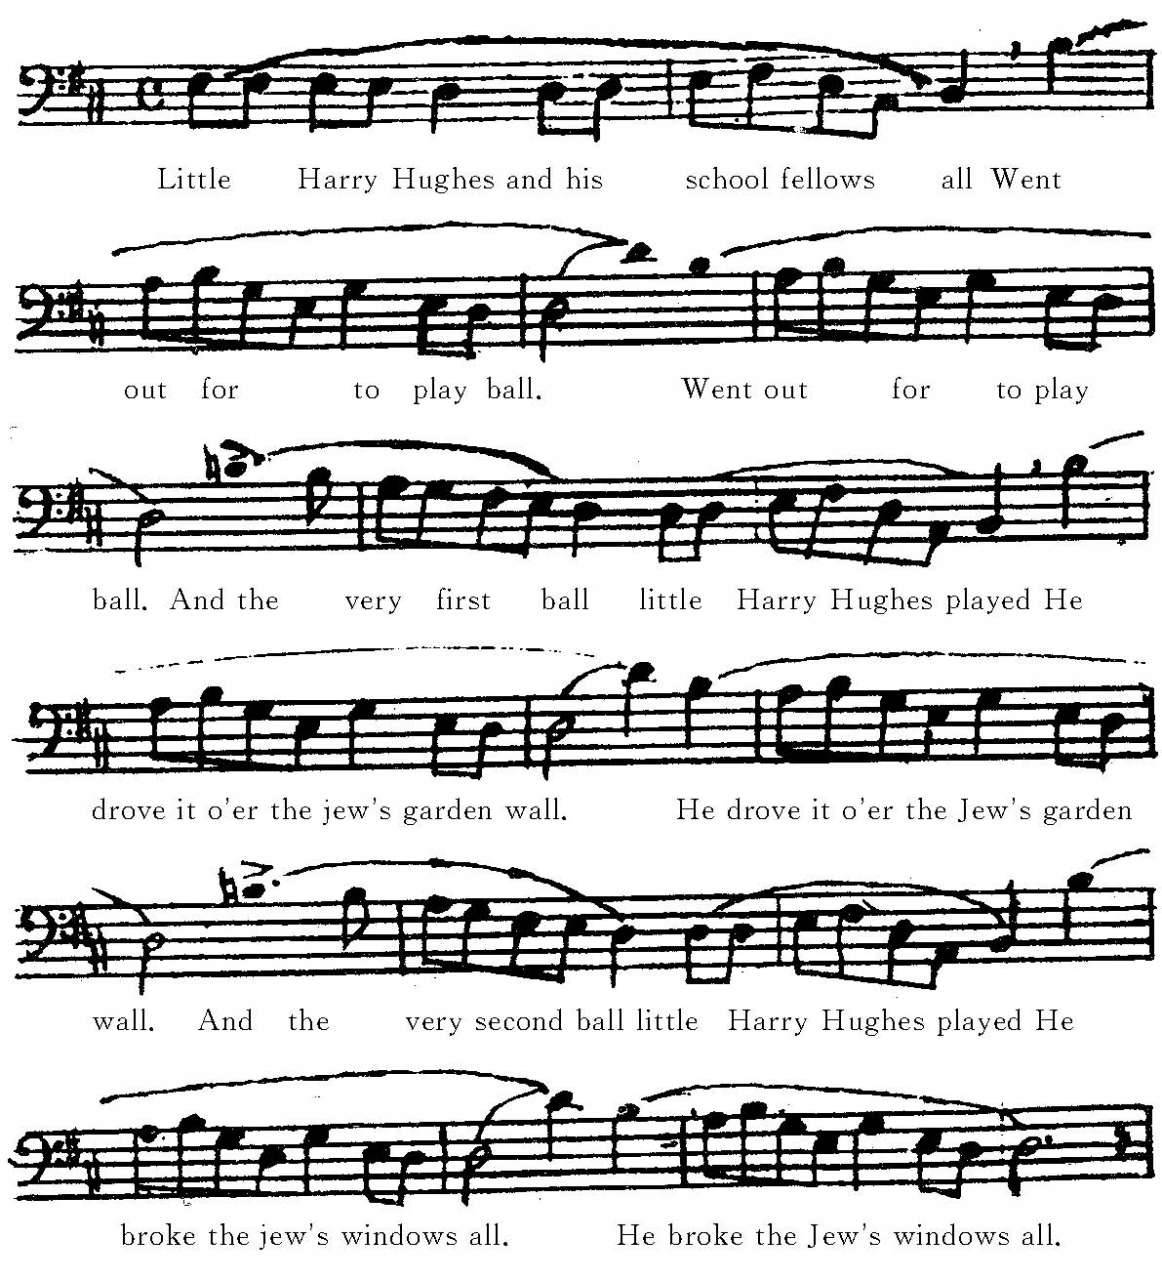
\includegraphics[scale=0.4]{picture/尤利西斯2.jpeg}
\end{figure}

\par 鲁道尔夫的儿子听了第一部,感觉怎样?
\par 他的感觉是单纯的。他这个犹太人面泛微笑高兴地倾听着,并望着厨房里那没有砸碎的窗玻璃。
\par 把故事诗第二部(小调的)朗诵一遍:
\par  
\par 犹太闺女出来了,
\par 浑身穿着绿衣裳,
\par 小俊哥儿你回来,
\par 再把球扔上一趟。
\par 我不能也不愿去,
\par 除非学伴都在场,
\par 要是老师知道了,
\par 我会遭殃在球上。
\par 雪白的手牵着他,
\par 把他引到大厅里,
\par 最后步入一间房,
\par 无人听见他叫嚷。
\par 她从兜里掏出刀,
\par 把他小脑袋割掉,
\par 他再不能把球踢,
\par 因已躺到尸堆里\footnote{}。

\begin{figure}[htb]
    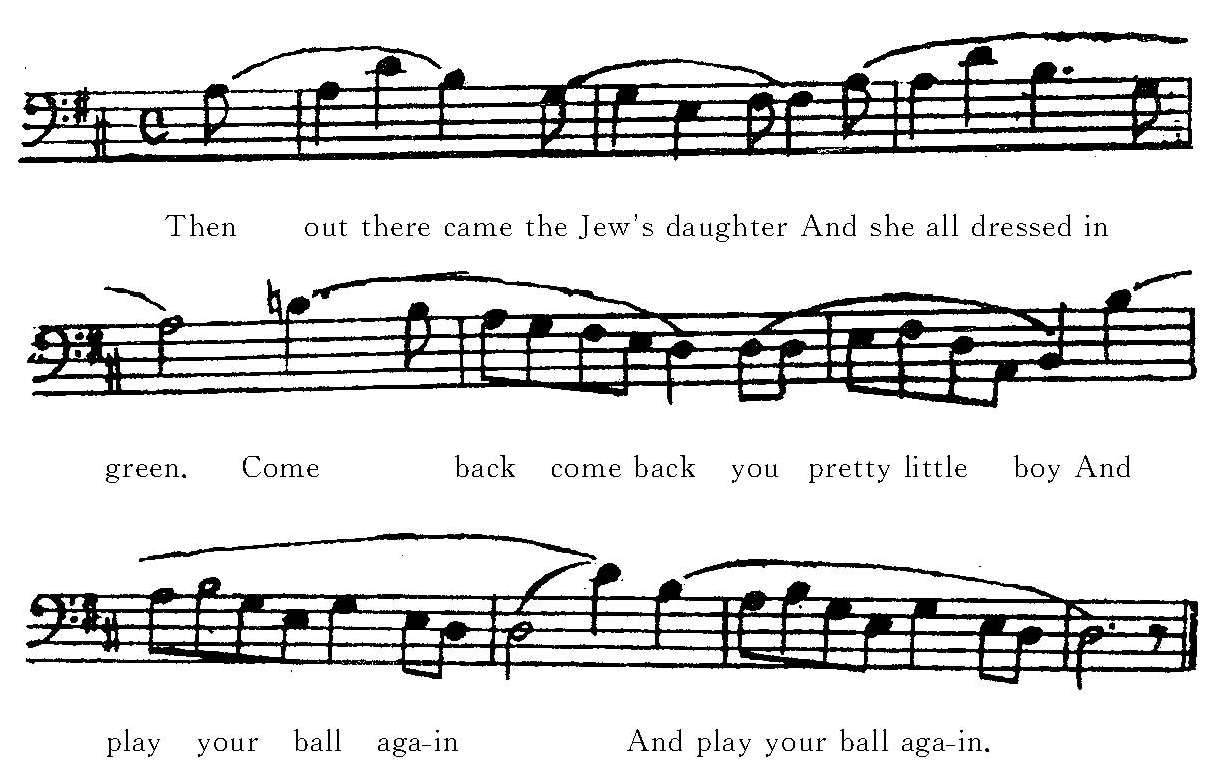
\includegraphics[scale=0.4]{picture/尤利西斯3.jpeg}
\end{figure}

\par 米莉森特的父亲听了第二部,有怎样的反响?
\par 他的感情是复杂的。他板着面孔,惊异地听见并看见一个犹太人的闺女,浑身穿着绿衣裳。
\par 将斯蒂芬的评论概述一下。
\par 大家当中的一个,大家当中最渺小的一个,命中注定成为牺牲者。第一次是出于疏忽,第二次是故意地,他向命运挑战。当他孤零零的时候,宿命来临,向并不情愿的他进行挑战。作为希望与青春的化身,抓住他使他无法抵抗。命运把他领到一座奇异的住所,一间隐秘的背教者之居室,把顺从的他毫不留情地当做祭品宰杀。
\par 主人(命中注定的牺牲者)为什么闷闷不乐?
\par 他希望关于一个行为的故事,并非他本人之所为,不应由他\footnote{}讲出来。
\par 为什么主人(并不情愿,也并不抵抗)一动也不动?
\par 这是按照保存精力的法则。
\par 主人(隐秘的背教者)为什么一声不响?
\par 他在衡量着赞成和反对杀人祭神的可能的证据:神职人员的煽动以及民众的迷信;随着谣言的传播,致使真实性逐渐减少。对财富的嫉妒,复仇的影响,隔代遗传造成的不法行为的突发性再犯。有量情余地的狂信,催眠术的暗示和梦游病症状。
\par 这些精神上或肉体上的毛病(倘若有的话)中,哪样是他无法完全能够免除的?
\par 催眠术的暗示:有一次,他睡醒之后认不出自己的卧室了。不只一次,乍一睡醒,好半晌的工夫他既不能挪动身子也发不出声音。梦游者的恍惚状态:有一次在睡眠中,他起身低头弯腰去爬向没有热气的壁炉。爬到之后,他蜷缩着身子,在没有炉火取暖的情况下,穿着睡衣倒在那里睡了。
\par 后一种或同类的症候,可曾出现在他的哪个家族身上?
\par 曾经发生过两次,在霍利斯街和翁塔利奥高台街\footnote{}。当他的女儿米莉森特(米莉)六岁和八岁时,曾在睡眠中吓得喊叫起来。两个穿睡衣的身影问她怎么啦?她却茫然地答以沉默表情。
\par 关于她的幼年,另外他还记得些什么?
\par 一八八九年六月十五日。一个刚刚呱呱落地的脾气暴躁的女婴,哭哭啼啼,既导致又舒散充血性征候。这娃娃的外号叫“帕德尼·软鞋”\footnote{},她咣当咣当地摇着攒钱罐,并数着父亲那三颗备用的便士硬币型纽扣:一呀,二呀,三。她把穿水手装的男小囝木偶丢掉了。尽管爹妈的头发都是深色的,她却继承了先辈的金发血统。古老的往昔,曾被诱奸,海瑙上尉\footnote{}先生,奥地利陆军;近因则是个幻觉,英国海军中的马尔维中尉。
\par 存在着哪些地域性的特色?
\par 反之,鼻子和前额的构造却继承了尽管中断过然而逐渐隔着更大的乃至最大的间歇遗传下来的直系血统。
\par 关于她的青春期,他记得一些什么?
\par 她把自己的铁环和跳绳藏到隐蔽的地方。在公爵草坪上,当一个英国旅游者央求她准许为她摄影留念时,她拒绝了(未说明反对的理由)。有一次她和埃尔莎·波特一道在南环路步行时,被一个面目狰狞的家伙跟踪上了。于是走到斯塔默街半途,她就蓦地折了回去(也没说明为什么要改变方向)。在过十五岁生日的前夕,她从韦斯特米思郡穆林加尔市写来一封信,简单地提了一下当地的一个学生(未说明他是哪一系和哪年级的)。
\par 成为第二次分手之预兆的第一次分手,使他感到苦恼了吗?
\par 比他所想像的要少,比他所希望的要多。
\par 这一瞬间,他目击到了什么样的第二次出走,尽管有差异,却又有类似之处?
\par 他的猫暂时出走了。
\par 何以会类似,又何以会有差异?
\par 类似点是,二者都是由某种隐秘的目的所驱使:寻觅一名新男子(穆林加尔市的学生)或药草(拔地麻)。差异在于,回到住户或住处来的可能性有所不同。
\par 在其他方面,二者之间的差异有类似之处吗?
\par 在被动性,节俭,传统的本能和唐突方面。
\par 例如?
\par 比方说,她依偎着他,托起金发,让他为她扎上缎带(与弓起脖子的猫比较一下)。而且,她连招呼也没打一声就朝着“斯蒂芬草地”那浩淼的湖面\footnote{}上啐了一口,唾沫浮在一棵棵树的倒影之间,画下一圈圈同心圆的波纹,持久而凝然不动,以一条入睡般平卧着的鱼为记号(与守候老鼠的猫相比)。而且,为了把一次著名战役的日期、双方作战部队的番号、战局以及战果都铭记心头,她拽自己的一条辫子来着(与舔耳朵的猫相比)。再者,傻米莉还梦见她和一匹马进行了一番无言的对谈,内容已记不得了。那匹马名叫约瑟夫,她捧给他(它)满满一大杯柠檬汽水,它(他)好像喝下去了(与在炉边做梦的猫相比)。因此,在被动性、节俭、因循的本能、唐突等方面,他们之间的差异是类似的。
\par 他曾怎样利用人们为了图个吉祥而送给他们的祝贺新婚的礼物:(1)一只猫头鹰和(2)一座钟,供她玩赏,并使她蒙受教益?
\par 他把它们作为实物教材,用以说明:(1)卵生动物的本性与习性,空中飞行的可能性,一种异常的视觉器官,世俗界用防腐药物保存尸体的方式。(2)体现于摆锤、齿轮与整时器上的钟摆的原理;不动的针盘上那可移动的正转的长短指针在各个位置作为人或社会规范所包含的意义;长针和短针每小时在同一倾斜度相遇的那一瞬间,也就是说,按照算术级数,每小时超过五又十一分之五分的那一瞬间,每小时重复一次的精确性\footnote{}。
\par 她是用什么方式回报他的呢?
\par 她都记在心里了:当他过二十七岁生日的时候,她送给他一只早餐用的搪须杯,上面有着王冠图案,是仿照德比的瓷器\footnote{}。她照料着。四季结账日\footnote{}或这先后,倘若他并非为了她而去购买什么东西,她就对他的需要表示关心,并能预料到他的希望。她钦佩他。当他为了她\footnote{}而对自然现象做了说明时,她立即表示一种期望:不经过逐渐掌握就获得他那科学知识的一鳞半爪,二分之一,四分之一,千分之一。
\par 梦游病患者米莉之父——昼游病患者布卢姆,向夜游病患者斯蒂芬提出了什么建议?
\par 建议他在厨房楼上,紧挨着男主人与女主人的卧室那临时隔开的斗室里安歇,度过介于星期四(通称)、星期五(实名)之间的这几个小时。
\par 这样的临时措施的期间如果拖长了,能够产生或估计能产生哪些好处呢?
\par 对客人来说,能有个安定的住处和僻静的用功场所。对男主人来说,有助于才智的年轻化,替身能给他带来满足\footnote{}。对女主人来说,能摆脱胡思乱想,学到正确的意大利发音。
\par 何以一位客人与女主人之间可能有的几度机缘,并不排除一个同学和一个犹太人的女儿\footnote{}最终有可能永久地和睦结合,而且也不会被这种结合所排除?
\par 因为通往女儿的路要经过母亲,而通往母亲的路要经过女儿。
\par 对男主人的哪一句有一搭没一搭的多音节的询问,客人做了单音节的否定的答复?
\par 他认不认识已故埃米莉·辛尼柯太太\footnote{}?一九〇三年十月十四日,她因车祸死于悉尼广场车站。
\par 主人把刚要开口提到的什么有关事由终于又咽了回去?
\par 对于一九〇三年六月二十六日他未能出席玛丽·迪达勒斯(原姓古尔丁)的葬礼的事由做了一番解释。因为那天正好碰上鲁道尔夫·布卢姆(原姓维拉格)忌日的前夕。
\par 提供暂时栖身之所的建议被接受了吗?
\par 未加解释,十分感激,友好地当即谢绝了。
\par 主客之间在金钱方面打了些什么交道?
\par 前者还给后者一笔钱(一英镑七先令整),未付利息。那是后者借给前者的。
\par 彼此之间相互提出了些什么建议,接受了,又加以修改,被拒绝了,换个说法复述一遍,重新被接受,被认可,再次确认?
\par 根据预先安排,开始讲习意大利语课程。地点在受教者的住所。开始声乐讲习课程,地点在女教师的住所。开始一系列静止的、半静止的、逍遥的、理性的对话,在对谈者双方家中(倘若对谈者双方住在同一处);位于下阿贝街六号的“船记”饭店兼酒馆(经营者为W和E.康纳里),基尔代尔街十一号的爱尔兰国立图书馆,霍利斯街二十九、三十与三十一号的国立妇产医院,一座公共花园,礼拜堂附近,两条或更多的街道交叉点,连接双方住宅的直线的中点(倘若交谈者各住一处)。
\par 使布卢姆感到这些相互排斥的建议难以实现的理由是什么?
\par 过去的事是已经不可挽回的了。有一回艾伯特·亨格勒马戏团在都柏林市拉特兰广场的圆形建筑\footnote{}里演出,一名富于机智的小丑身穿色彩斑驳的服装,为了寻找乃父,竟走出马戏场,钻进观众席中,来到孤零零地坐着的布卢姆跟前,在大庭广众之下,向兴奋不已的观众公开宣称:他(布卢姆)是他(小丑)的爸爸。未来是不可预测的。一八九八年夏天,有一次他(布卢姆)在一枚弗洛林银币(值二先令)周围的饰纹上刻下三条道道,付给大运河查利蒙特林阴路一号的J与T.戴维父子食品店,以便试验一下该货币经过市民钱财交易的流通过程,直接或间接地回到自己手中的可能性。
\par 那个小丑是布卢姆的儿子吗?
\par 不是。
\par 那枚银币又回到布卢姆手里来了吗?
\par 再也没有回来。
\par 接连遭到的挫折何以越发使他闷闷不乐?
\par 因为在人类生活关键性的转折时刻,他渴望改善种种社会情况,而那是不平等、贪欲和国与国之间抗争的产物。
\par 那么他是否相信,消除了这些条件后,人的生活就能无限地接近完美无缺呢?
\par 截然不同于人为的法则,这里依然存在着按照自然的法则作为对维持整个人类的生存不可分割的部分加诸于人的生物学之基本条件。为了获得有营养的食品,就不得不进行破坏性的杀戮。孤立的个人生存中终极机能那充满了苦恼的性质。生与死的痛苦。类人猿和(尤其是)人类女性那单调的月经,自初潮期一直延续到闭经期。海洋上、矿山和工厂里那些不可避免的事故;某些非常痛苦的疾病以及伴随而来的外科手术;生来的疯癫,先天性犯罪癖;导致人口大批死亡的传染病;在人类心灵深处种下恐怖种子的灾难性特大洪水;震中位于人口密集地区的大地震;历经剧烈变形,自幼年经过成熟期进入衰退期的生命成长的事实。
\par 他为什么打消了推断猜想的念头?
\par 因为摆在不同凡响的智者面前的课题就是排除不大适宜接受的现象,而代之以更适宜接受的现象。
\par 对他这样气馁,斯蒂芬表示共鸣了吗?
\par 他强调了自己作为有意识、有理性的动物,从已知的世界演绎地向未知的世界前进的意义,以及作为有意识、有理性的反应者,介于不可避免地建立在不安定的虚空之上的大宇宙与小宇宙\footnote{}之间的意义。
\par 布卢姆理解他强调的是什么吗?
\par 不是照字面上,而是从实质上理解的。
\par 对理解不足这一点,他是用什么来安慰自己的?
\par 作为一个没有钥匙却有能力的市民,他通过不安定的虚空,从未知的世界精力充沛地朝着已知的世界前进。
\par 他们是以怎样的先后顺序离开为奴之家\footnote{},来到无人居住的旷野的,并举行了什么样的仪式呢?
\par 把点燃的蜡烛插在烛台上
\par 持者为
\par 布卢姆
\par 把助祭帽挑在梣木手杖上
\par 持者为
\par 斯蒂芬
\par 念诵的是《诗篇》哪一纪念性篇章?是用哪段默祷\footnote{}作起句的?
\par 第一百一十三篇,旅途:以色列人一离开埃及,雅各的子孙一离开异族的土地\footnote{}……
\par 他们各自在出口做了些什么?
\par 布卢姆把烛台放在地板上。斯蒂芬把帽子戴在头上。
\par 对什么动物来说,出口就是入口?
\par 猫。
\par 当主人领先,客人随后,两个黑魆魆的身姿默默地穿过房后昏暗的甬道,步入半明半暗的庭园中时,他们面对的是什么样的景物?
\par 天树上坠满了湿漉漉的夜蓝色的累累星果。
\par 布卢姆一边对伙伴指点着形形色色的星座,一边向他表达了哪些冥想?
\par 关于宇宙日益扩大进化的冥想:新月期的月亮,即使在近地点\footnote{}也看不见。从地表向地轴挖掘纵深五千英尺的圆筒状垂直轴,一个观察者呆在轴底儿上,就连白昼也辨认得出那漫无止境、网络状、亮光闪闪、非凝结性的银河\footnote{}。天狼(大犬座阿尔法)距地球十光年(五十七万亿英里);体积大于地球九百倍;大角\footnote{};岁差运动\footnote{};有着“猎户”腰带、六倍于太阳的“伐二”以及星云的猎户座,星云中能容纳我们的一百个太阳系\footnote{};死去的和新生的星宿,例如一九〇一年的那颗“新星”\footnote{};我们的太阳系正朝着武仙座冲去\footnote{};所谓恒星的视差或视差移动\footnote{},也就是说,实际上恒星是在不断地从无限遥远的太古朝无限遥远的未来移动着。相形之下,人的寿命充其量才七十年,不过是无限短暂的一段插曲而已。
\par 另外还有关于反过来逐渐缩小退化的冥想吗?
\par 在地球的层理\footnote{}留下记录的太古以来的地质时代。隐藏在大地的洞穴里和能移动的石头底下、蜂巢和土墩子中那无数微小的昆虫类的有机生物:微生物、病菌、细菌、杆菌、精子;凭着分子的亲和之凝聚力而黏在一根针尖上那几万几亿几兆个多不胜数、肉眼看不到的微小颗粒;人类的血浆是一个宇宙,群集着白血球和红血球,每个血球又各自形成一个空虚的宇宙空间,群集着其他球体;各个球体连续性地也是由可分割的构成体形成的宇宙,各个构成体又可以分割成为几个能够进一步分割的构成体。就这样,分子与分母实际上在并未分割的情况下就不断地减少了。如果这个过程延续到一定时候,就永远在任何地方也不会达到零。
\par 他为什么不精心计算出更准确的结果?
\par 因为几年前在一八八六年,当他埋头于探讨面积等于一个圆的正方形\footnote{}的问题时,他发现了一个数值的存在:倘若精确地计算到某种程度,就能达到比方说九九乘九乘这样庞大的量值和位数\footnote{}。所得数字要用细字密密匝匝地印刷成三十三卷,每卷一千页。为了统统印刷完毕,就需要购入无数刀、无数令印度纸,整数值的位数便是一、十、百、千、万、十万、百万、千万、亿、十亿,一切级数的一切数字作为星云的核心,以简明的形式所包含的累乘的可能性推到了极限地、能动地开展的一切乘方的一切幂级数。
\par 他可曾发现分为几个种族的人类在其他行星及其卫星上居住的可能性,以及由一位救世主从社会上、伦理上拯救人类的可能性;那样一来问题会不会就更容易得到解决?
\par 他认为那是另一范畴的难题。人体组织通常能够抗得住十九吨的气压\footnote{},可是一旦在地球的大气层里上升到相当的高度,越是接近对流层与平流层的境界线,鼻孔出血、吸呼困难以及眩晕,随着算术级数就越发严重起来。他晓得这一点,寻求解答时就设想出这样一个难以证明是不可能的行之有效的假定:倘若换个更富于适应性,解剖学上的构造也有所不同的种族,说不定就能在火星、水星、金星、木星、土星、海王星或天王星那充足而相同的条件下生存下来。然而那个远地点\footnote{}的人类种族,尽管在构造方面与地球上的人类有着一定限度的不同之处,整个来说彼此却有着相似的种种形态。他们恐怕也和地球上的人类一样,会不肯舍弃那一成不变、无法分割的属性,也就是对空虚,对空虚的空虚,一切都是空虚\footnote{}的执着。
\par 至于拯救的可能性呢?
\par 小前提已经被大前提所证明了。
\par 接着他又依次对各个星座的哪些形形色色的特征进行了考虑呢?
\par 显示出不同程度之生命力的缤纷色彩(白、浅黄、深红、朱红、银朱);诸星之亮度;一直包括到七等星、以等级标志的诸星之大小;诸星的位置;御夫座;沃尔辛厄姆路\footnote{};大卫的战车\footnote{};土星光环;螺旋星云凝固后形成有卫星的恒星群;两重太阳相互依存的旋转运动;伽利略、西蒙·马里乌斯\footnote{}、皮亚齐\footnote{}、勒威耶、赫歇耳、加勒\footnote{}等人各自独立地同时所做的发现;波得和开普勒所尝试的距离的立方与回转次数的平方的体系化\footnote{};多毛的众彗星\footnote{}那几殆无限的被压缩性,以及自近日点至远日点那广漠的远心的重返大气层的椭圆轨道;陨石的恒星之起源;年纪较轻的天体观测者诞生的那个时期火星上所出现的“暗波”现象\footnote{};每年在圣劳伦斯节(殉教者,八月十日)前后降落的陨石雨;每月都发生的所谓“新月抱旧月”现象\footnote{};关于天体对人体的影响的假定;威廉·莎士比亚出生的时期,在斜倚却永不没落的仙后座那三角形上端,一颗不分昼夜散发着极亮光彩的星辰(一等星)出现了\footnote{}(这是两个无光、死灭了的太阳因相撞并汞合为白热体而形成的灿烂的新太阳);大约在利奥波德·布卢姆出生时,出现在七星花冠星座里而后又消失了的一颗同一起源、亮度却稍逊的星宿(二等星)\footnote{};还有约于斯蒂芬·迪达勒斯出生时,出现在仙女座中之后又消失,小鲁道尔夫·布卢姆出生与夭折数年后出现于御夫座后又消失,以及另外一些人出生或去世前前后后出现在许许多多其他星座中而又消失了的、(假定是)同一起源的(实际存在或假定存在的)星斗\footnote{}。日蚀及月蚀自隐蔽至复现的各种伴随现象:诸如风势减弱,影子推移,有翼者沉默下来,夜行或暮行动物的出现,冥界的光持续不减,地上的江河溪流之幽暗,人类之苍白。
\par 对情况进行了估量并考虑过产生错误的可能性之后,他(布卢姆)得出过什么样的合乎逻辑的结论呢?
\par 那既不是天树、天洞,也不是天兽、天人。那是个乌托邦,那里不存在从已知到达未知的既知之路。那是无限的。假定各个天体有可能并存,那么也能把它看做是有限的。天体的数目是一个还是一个以上都无所谓,体积相同或不同也无所谓。那是一团能活动的幻觉形态,是在空间里已固定下来的东西,借着空气又重新活动起来。它是过去,未来的观察者们作为现在实际存在之前,它或许已不再作为现在而存在了。
\par 关于这一光景的美的价值,他更加深信不疑了吗?
\par 毫无疑问。因为有这样一些先例:诗人们往往在狂热的恋慕导致的谵妄状态下,要么就是在失恋的屈辱中,向热情而持好感的诸星座或围着地球转的冷漠的卫星呼吁。
\par 那么他曾否把占星术对地上灾害的影响这一理论当做信条接受下来了呢?
\par 据他看来,对这一点提出论证和反证的可能性是一样大的。月面图中所使用的梦沼、雨海、湿海、丰富海等学术用语既可以归之于直观的产物,也可以归之于谬误的类推。
\par 他认为月亮和妇女之间有什么特殊的近似之处?
\par 她历史悠久:地球上连绵不断的世世代代存在之前她就存在,并将继续存在下去。她在夜间的优势。她作为卫星的依存性。她反射光的性能;起落盈亏,运行有常,恒久不变。她的容貌注定永不改变。她对不明确的讯问,都给以暧昧的答复。她能够支配潮汐涨落。她具有使人迷恋,心碎,赋予美,逼人发疯\footnote{},煽动并助长人们为非作歹的种种本事。她的表情那么安详而秘不可测。她孑然一身,居高临下,毫不留情,光彩夺目,令人望而生畏,不敢挨近。她预示着暴风雨或天朗气清。她焕发出的光芒,她那一举一动与存在都给人以刺激。她的喷火口,她那枯竭的海,她的沉默,在在都发出警告。看得见时,她是何等光辉灿烂,看不见时,她又是何等富于魅力。
\par 哪一样看得见的明亮标志映入了布卢姆的眼帘,他又提醒斯蒂芬去注视了呢?
\par 在他(布卢姆)家的二楼(后身),点起了一盏煤油灯,一个倾斜的人影投到卷式百叶帘上;那是在安吉尔街十六号开业的百叶窗、帘杆、卷式帘制造商弗兰克·奥哈拉供应的。
\par 关于由看得见的明亮标志(一盏灯)所映照出来的那位看不见的富于魅力的人儿,也就是说,他的妻子玛莉恩(摩莉)·布卢姆之谜,他是怎样阐明的呢?
\par 直接间接口头暗示或明确地表达。用那抑制着的挚爱和赞美之情。加以描绘。结结巴巴地。凭着暗示。
\par 接着,两个人都沉默下去了吗?
\par 沉默下去了。他们相互用自己肉身的镜子照着伙伴的脸。彼此在镜中照见的是对方的,而不是自己的脸。
\par 他们一直毫无动静吗?
\par 经斯蒂芬提议,并在布卢姆的鼓动下,先由斯蒂芬带头,布卢姆紧接着,双双在幽暗中各撒了一泡尿。他们肩并肩,彼此用手圈着自己的排尿器官,以便挡住对方的视线。随后由布卢姆带头,斯蒂芬紧接着,双双抬头仰望起那明亮的和半明亮的投影。
\par 相似吗?
\par 他们两人那起初有先有后,继而同时撒出去的尿的轨道并不相似。布卢姆的较长,滋得没那么冲,形状有点像那分叉的倒数第二个字母\footnote{},却又有所不同。敢情,他念高中最后一年(一八八〇)的时候,曾有本事对抗全校二百一十名学生拧成的那股力量,尿撒得比谁都高。斯蒂芬的尿滋得更冲,咝咝响得更欢势。由于头天最后几个钟头他喝了利尿物,膀胱持续地受到压迫。
\par 对方那个看不见却听得见的附属器官,使两个人各自联想到了什么不同的问题?
\par 布卢姆:过敏性、勃起、变硬挺直、松弛、大小、卫生、阴毛等等问题。斯蒂芬:受割礼的耶稣作为圣职者是否毫无缺陷的问题(一月一日乃是圣日,应该望弥撒,不得从事不必要的世俗劳动)\footnote{}。还有如何对待保存在卡尔卡塔的神圣罗马天主教使徒教会的肉体结婚戒指——神圣的包皮问题。应仅仅向它致以对圣母的最高崇敬呢,抑或该把它作为毛发、脚趾甲那样从神体上割下来的赘生物,对它致以第四级最高膜拜\footnote{}?
\par 他们两人同时观测到了什么样的天象?
\par 一颗星星从天顶上天琴座“织女一”越过后发星座\footnote{}的星群,明显地以高速度朝着黄道十二宫的狮子宫\footnote{}直冲过去。
\par 向心的滞留者是怎样为离心的出发者提供出口的?
\par 他将生锈粗涩的男性型钥匙轴捅进反复无常的女性型锁孔里,把劲头使在钥匙环上,自右至左地转动钥匙的齿凹,将锁簧送回到锁环里,痉挛般地把那扇铰链都掉了的旧门朝里面拽过来,露出可以任意出进的门口。
\par 临分手时,他们是怎样彼此道别的?
\par 他们直直地站在同一道门坎的两侧,告别时两只胳膊的曲线在某一点上随便相碰,形成小于二直角之和这样一个角度。
\par 伴随着他们那相接触的手的结合,他们(各自)那离心的和向心的手的分离,传来了什么响声?
\par 圣乔治教堂那组钟鸣报起深夜的时辰,响彻着谐和的音调。
\par 他们各自都听到了钟声,分别有什么样的回音?
\par 斯蒂芬听见的是:
\par  
\par 饰以百合的光明的司铎群来伴尔,
\par 极乐圣童贞之群高唱赞歌来迎尔\footnote{}。
\par  
\par 布卢姆听见的是:
\par 丁当!丁当!
\par 丁当!丁当\footnote{}!
\par 那一天随着钟声的呼唤跟布卢姆结伴从南边的沙丘前往北边的葛拉斯涅文的一行人,而今都在何处?
\par 马丁·坎宁翰(在床上),杰克·鲍尔(在床上),西蒙·迪达勒斯(在床上),内德·兰伯特(在床上),汤姆·克南(在床上),乔·海因斯(在床上),约翰·亨利·门顿(在床上),伯纳德·科里根\footnote{}(在床上),帕齐·迪格纳穆(在床上),帕狄·迪格纳穆(在墓中)。
\par 只剩下布卢姆一个人之后,他听到了什么?
\par 沿着上天所生的大地退去的脚步声发出来的双重回荡,以及犹太人所奏的竖琴在余音缭绕的小径上引起的双重反响\footnote{}。
\par 只剩下布卢姆一个人了,他有什么感觉?
\par 星际空间的寒冷,冰点以下几千度或华氏、摄氏或列氏的绝对零度\footnote{},即将迎来黎明的最早兆头。
\par 音调谐和的钟声、手的感触、脚步声和孤独寒冷使他联想起了什么?
\par 在各种情况下,在不同的地方如今已经故去的伙伴们:珀西·阿普约翰(阵亡,在莫德尔河\footnote{})、菲利普·吉利根\footnote{}(肺结核,殁于杰维斯街医院),马修·F.凯恩\footnote{}(不慎淹死在都柏林港湾),菲利普·莫依塞尔\footnote{}(脓血症,死在海蒂斯勃利街),迈克尔·哈特\footnote{}(肺结核,殁于仁慈圣母医院),帕特里克·迪格纳穆(脑溢血,殁于沙丘)。
\par 是何种现象的何种前景促使他留在原地?
\par 最后三颗星的消失,曙光四射,一轮新的盘状太阳喷薄欲出\footnote{}。
\par 以前他可曾目击过这样的现象?
\par 一八八七年,有一次在基玛吉\footnote{}的卢克·多伊尔家玩猜哑剧字谜,时间拖得很长。这之后,他坐在一堵墙上,注视着东方——米兹拉赤\footnote{},耐心地等待黎明景象的出现。
\par 他想起最初的种种现象了吗?
\par 空气越发充满了勃勃生机:远处,公鸡在报晓,各座教堂的敲钟声,鸟类的音乐,早起的行人那孤零零的脚步声,看不见的光体所射出的看得见的光,复活了的太阳那低低地崭露在地平线上的、依稀可辨的最初一抹金晖。
\par 他在那儿滞留下去了吗?
\par 在强烈灵感的触发下,他折了回去,再一次跨过园子,返回门道,重新关上门。一声短叹,他再度拿起烛台,又一次登上楼梯,重新朝那挨着一楼门厅的屋子踱过去,走回原来的地方。
\par 是什么乍然拦住了他正往里走的脚步呢?
\par 他的天灵盖右颞叶碰着了坚硬的木材犄角,在微乎其微却能有所察觉的几分之一秒后,产生了疼痛感。这是一刹那之前传达因而觉察到的结果。
\par 描述一下在室内陈设方面所做的变更。
\par 一把深紫红色长毛绒面沙发从门对面被搬到炉边那面卷得紧紧的英国国旗近旁(这是他曾多次打算要做的变动)。那张嵌有蓝白棋盘格子花纹的马略尔卡\footnote{}瓷面桌子,被安放在深紫红色长毛绒面沙发腾出后的空处。胡桃木餐具柜(是它那凸出来的犄角一时挡住了他往里走着的脚步)从门旁的位置被挪到更便当却更危险、正对着门的位置去了。两把椅子从壁炉左右两侧被搬到嵌有蓝白棋盘格子花纹的马略尔卡瓷面桌子原先所占的位置去。
\par 描述一下那两把椅子。
\par 一把低矮,是填了稻草的安乐椅。结实的扶手伸向前,靠背朝后边倾斜着。方才把它往后推的时候,长方形地毯那不整齐的边儿给掀了起来。罩着宽大面子的坐位,中间的颜色褪得厉害,越靠近边沿,越没怎么变色。与它相对的另一把细细溜溜、撇着两双八字脚的藤椅是由有光泽的曲线构成的。椅架从顶部到坐位,又从坐位到底部,整个儿都涂着暗褐色清漆,坐位则用白色灯心草鲜明地盘成圆形。
\par 这两把椅子有着什么意义?
\par 表示着类似、姿势、象征、间接证据和永久不变的证言等等意义\footnote{}。
\par 原先放餐具柜的地方,如今摆着什么?
\par 一架立式钢琴(凯德拜牌\footnote{}),键盘露在外面。上顶盖关得严严实实,摆着一双淡黄色妇女用长手套,一只鲜绿色烟灰缸里是四根燃尽了的火柴,一根吸过一截的香烟,还有两截变了色的烟蒂。谱架上斜搭着一本《古老甜蜜的情歌》(G.克利夫顿·宾厄姆作词,詹·莱·莫洛伊配曲,安托瓦内特·斯特林\footnote{}夫人演唱)G大调歌曲伴奏谱,在摊开来的最后一页上可以看到演奏的终指示:随意地,响亮地,持续音,活泼地,要延长的持续音,渐慢\footnote{},终止。
\par 布卢姆是抱着何等激情依次打量这些物件的?
\par 他心情紧张地举着烛台,感到疼痛伸手摸了摸肿胀起来的右颞叶撞伤处。他全神贯注地凝视着那庞大笨重被动的和那细溜活泼主动的,又殷勤地弯下身去,把掀起来的地毯边儿舒展成原样。他兴致勃勃地记起玛拉基·穆利根博士的色彩计划,其中包括深浅有致的绿色\footnote{}。他又心怀喜悦之情重复着当时相互间的话语和动作,并通过内部种种感官,领悟着逐渐褪色所导致的温吞快感的舒散。
\par 他的下一个行动是什么?
\par 他从马略尔卡瓷面桌子上的一个敞着的盒子里取出个一英寸高、又小又黑的松果,将其圆底儿放在小小的锡盘上。然后把他的烛台摆在壁炉台右角上,从背心里掏出一张卷起来的简介(附有插图),题名“阿根达斯·内泰穆”\footnote{}。打开来,大致浏览了一下,又将它卷成细长的圆筒,在烛火上引燃了。于是,圆筒的火苗伸到松果尖端,直到后者发出红色火光;并将纸筒撂在烛台托子上,让剩下的那部分燃烧殆尽。
\par 这一行动之后,又发生了什么?
\par 从小小火山那烧掉了尖儿的圆锥形火口,一股令人联想到东方香烟的垂直的蛇状熏烟袅袅上升\footnote{}。
\par 除了烛台,壁炉台上还摆了些什么类似的物件?
\par 还有竖纹的康尼马拉大理石\footnote{}做的座钟。这是马修·狄龙送的结婚礼物,它停在一八九六年三月二十一日上午四点四十六分上\footnote{}。透明的钟形罩子里是冰状结晶矮树盆景,那是卢克和卡罗琳·多伊尔\footnote{}送的结婚礼物。一只制成标本的猫头鹰,是市政委员约翰·胡珀\footnote{}送的结婚礼物。
\par 这三样东西和布卢姆是怎样相互望着的?
\par 在镶金边的穿衣镜里,矮树那未装饰的背望着制成标本的猫头鹰那直直的脊背。在镜子前面,市政委员约翰·胡珀送的结婚礼物以清澈忧郁、聪慧明亮、一动不动、体恤同情的视线盯着布卢姆,布卢姆则以模糊安详、意味深长、一动不动、富于恻隐之心的视线,瞅着卢克和卡罗琳·多伊尔所赠结婚礼物。
\par 映在镜中的什么混合的不对称的影像这时引起了他的注意?
\par 一个(就自己而言)落落寡合,(对别人)反复无常的人的影像。
\par 为什么落落寡合(就自己而言)?
\par  
\par 他一个兄弟姐妹都没有,
\par 但他爹仍是爷爷的儿子。
\par  
\par 为什么反复无常(对别人)?
\par 自襁褓时期到壮年,他与母系的骨肉至亲相像。自壮年到衰老期,他会越来越与父系的骨肉至亲相像。
\par 镜子传达给他的最终视觉印象是什么?
\par 由于光学反射,可以看到映在镜中的对面那两个书架上颠倒放着若干册书。它们不是按照字母顺序排列着的,而是胡乱放的。标题闪闪发光。
\par 为这些书编个目录。
\par 《汤姆的都柏林邮政局人名录》,一八八六年版。
\par 丹尼斯·弗洛伦斯·麦卡锡\footnote{}:《诗集》(第五页夹着古铜色椈叶状书签)。
\par 莎士比亚:《作品集》(深红色摩洛哥山羊皮,烫金封面)。
\par 《实用计算便览》(褐色布面精装)。
\par 《查理二世宫廷秘史》(红色布面精装,本色压印装帧)\footnote{}。
\par 《儿童便览》(蓝色布面精装)\footnote{}。
\par 《我们的少年时代》,下议院议员威廉·奥布赖恩\footnote{}著(绿布面精装,有点褪了色,第217页夹了个信封以代替书签)。
\par 《斯宾诺莎哲学钞》(酱紫色皮面精装)。
\par 《天空的故事》\footnote{},罗伯特·鲍尔爵士著(蓝色布面精装)。
\par 埃利斯:《三游马达加斯加》\footnote{}(褐色布面精装,书名磨损,无法辨认)。
\par 《斯塔克·芒罗书信集》,阿·柯南道尔著\footnote{}。这是卡佩尔街一〇六号的都柏林市立公共图书馆藏书,一九〇四年五月二十一日(圣灵降临节前夕)借出,还书期限为一九〇四年六月四日,故已过期十三天(黑色布面精装,贴有白色的编码标签)。
\par 《中国纪行》\footnote{},“旅人”著(用褐色纸包了书皮,书名是用红墨水写的)。
\par 《<塔木德>\footnote{}的哲学》(小册子合订本)。
\par 洛克哈特著《拿破仑传》(缺封面,加有脚注,贬低首领取得的胜利,夸大其败绩)。
\par 《借方和贷方》\footnote{},古斯塔夫·弗赖塔格著(黑色纸面精装,哥特字体\footnote{},第二十四页夹了个香烟赠券,以代替书签)。
\par 霍齐尔著《俄土战争史》(褐色布面精装,两卷集,封底贴有直布罗陀市总督步道要塞图书馆的标签\footnote{})。
\par 《劳伦斯·布卢姆菲尔德在爱尔兰》,威廉·阿林厄姆著(第二版,绿色布面精装,烫金三叶图案。此书原先的所有者在扉页正面所署姓名已被涂掉)。
\par 《天文学指南》(褐色封面已脱落,附有五幅另纸印的插图,正文用老五号黑体字,作者脚注用六点活字,旁注用八点活字,标题用十二点活字\footnote{})。
\par 《基督秘史》(黑色纸面精装)。
\par 《沿着太阳的轨道前进》\footnote{}(淡黄色布面精装,缺内封,每一页上端都印有标题)。
\par 《体力与健身术》(伦敦,1897),尤金·桑道\footnote{}著(红色布面精装)。
\par 《简明几何学初步》,原著系由伊格内·帕迪斯用法语所写,伦敦神学博士约翰·哈利斯译为英语,由R.纳普洛克印制,一七一一年出版于毕晓普斯·海德。内收有致译者之畏友查理·考克斯先生(萨瑟克自治市所推选出来的下院议员)的书信体献辞。衬页上用刚健有力的钢笔字写明:此系迈克尔·加拉赫之藏书,日期为一八二二年五月十日,倘若遗失或下落不明,凡发现该书者,恳请将它退还给举世无双之美丽土地威克洛郡恩尼斯科西\footnote{}达费里门的木工迈克尔·加拉赫为荷。
\par 当他把上下颠倒的书重新调整过来的时候,心里有些什么感想?
\par 需要秩序。一切东西都应各有个位置,并且应该各就各位。女性对文学的鉴赏力之不足。苹果塞在玻璃酒杯里,或雨伞斜搭在马桶里,均不协调。把任何秘密文件放在书籍后面、下面或夹在书页间,都是不安全的。
\par 体积最大的是哪本书?
\par 霍齐尔的《俄土战争史》。
\par 在这部著作第二部的其他事项中,还包括些什么内容?
\par 一次关键性战役的名字(他已忘记),一位念念不忘该战役的关键性军官,即布赖恩·库帕·特威迪鼓手长(他铭记心头)。
\par 由于第一和第二个什么缘故,他并不曾查阅这部著作?
\par 第一,为了锻炼记忆术。第二,因为犯了一阵健忘症之后,当他对着中央的桌子而坐,正要去查阅那部著作时,凭着记忆术他回想起了那次战斗的名称:普列文\footnote{}。
\par 他端坐着时,何物给他带来了慰藉?
\par 竖立在桌子中央的一座雕像那率真,裸体,姿势,安详,青春,优雅,性,劝告。这座纳希索斯像\footnote{}是从巴切勒步道九号的P.A.雷恩拍卖行买来的。
\par 他端坐着时,何物令他心头焦躁?
\par 硬领(十七英寸型)和背心(有五颗纽扣)紧得使他感到压力。这两样东西对成年男子的服装来说是多余的,而对人体的膨胀所引起的容积变更却又缺乏弹性。
\par 心头的焦躁是怎样平息下来的?
\par 他从脖间摘下硬领、黑领带和折叠式饰纽,放在桌子左角。然后又反过来自下而上地依次解开背心、长裤、衬衫和内衣纽扣。他那双手的轨迹从参差不齐、卷缩起皱的黑色体毛的中心线——也就是自骨盆底到下腹部肚脐眼周围那一簇簇体毛,又沿着节结的中心线进而延伸到第六胸脊椎的交叉点,从这里又向两侧丛生,构成直角形,在左右等距离的两个点,即环绕乳头顶端形成的三角形收敛图形的中心线——穿行。长裤的背带上钉着成双的六颗纽扣(其中缺了一颗),他依次解开那六颗(其中少了一颗)纽扣。
\par 接着,他又不由自主地做了什么?
\par 他用两个手指捏起两星期零三天前(一九〇四年五月二十三日)横膈膜下左侧腹那因挨蜜蜂蜇而留下的伤痕周围的肉。尽管并不觉得痒,他却用左手这儿那儿地胡乱挠了挠全部洗净、只裸露出一部分的皮肤的点和面。他把左手伸进背心的左下兜,掏出一枚银币(一先令),又放了回去。(大概是)参加悉尼广场的埃米莉·辛尼柯太太\footnote{}的葬礼(一九〇三年十月十七日)时放进去的。
\par 制定一九〇四年六月十六日的收支表。

\begin{figure}[htb]
    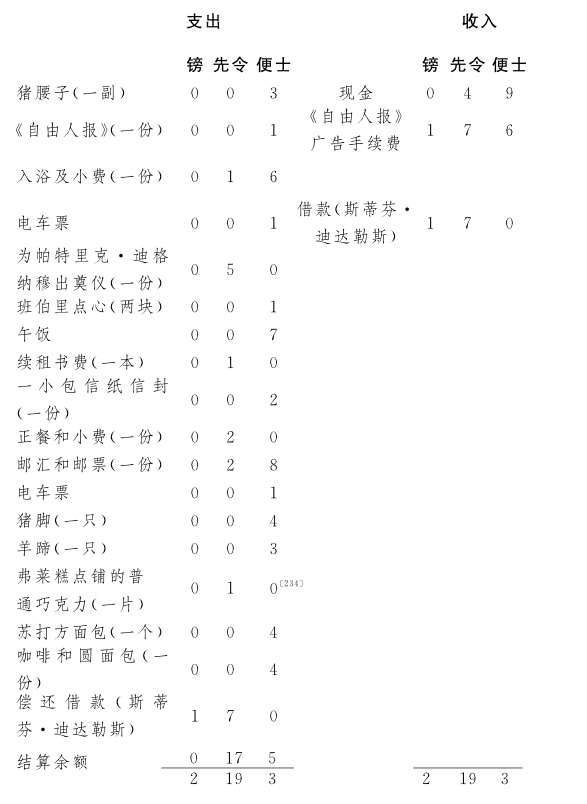
\includegraphics[scale=0.4]{picture/尤利西斯4.jpeg}
\end{figure}

\par 脱衣的行为继续下去了吗?
\par 他感到脚心一个劲儿地隐隐作痛,就把脚伸到一旁,端详着脚由于一趟趟地朝不同的方向走来走去,受到挤压而磨出的皱皮、硬块和疖子。随后他弯下身去,解起打成结子的靴带:先掰搭钩,松开靴带,再一次一只只地脱下靴子\footnote{}。右边那只短袜湿了一部分,大脚趾甲又把前面捅破并伸了出去,这下子便跟靴子分开了。他抬起右脚,摘下紫色的松紧袜带后,扒下右面那只袜子,将赤着的右脚放在椅屉儿上,用手指去撕扯长得挺长的大拇脚趾甲,并轻轻地把它拽掉,还举到鼻孔那儿,嗅嗅自己肉体的气味,然后就心满意足地丢掉从趾甲上扯下来的这一碎片。
\par 为什么感到心满意足?
\par 因为他嗅到的这股气味,跟他当年作为布卢姆公子在埃利斯太太的幼儿学校\footnote{}做学生的时候所嗅到的另外一些趾甲碎片的气味相似。那是他每晚跪在那儿,一边做短短的晚祷并沉浸在野心勃勃的冥想中,一边耐心地撕扯并拽下来的。
\par 同时连续地产生的所有那些野心,如今合并成为怎样一种终极的野心呢?
\par 他并不想根据长子继承制、男子平分继承制或末子继承制\footnote{},把那幢有着门房和马车道的男爵宅邸及其周围那一大片辽阔的英亩、路得和平方杆\footnote{}法定土地面积单位,(估价为四十二英镑\footnote{})的泥炭质牧场地,或者那座被描述为“都会中的田园\footnote{}”或“健康庄\footnote{}”的有阳台的房子或一侧与邻屋相接的别墅,继承下来并永久占有。他只巴望根据私人合同购买一所继承人身份不受限制的不动产:要坐北朝南的一座草屋顶、有凉台的双层住宅,房顶上装起风向标以及与地面相接的避雷针,门廊上要爬满寄生植物(常春藤或五叶地锦),橄榄绿色的正门最后一道工序漆得漂漂亮亮,赛得过马车。门上有着精巧的黄铜装饰。房屋正面是灰泥墁的,屋檐和山墙涂着金色网眼花纹。尽可能让房子耸立在坡度不大的高台上,从那圈着石柱栏杆的阳台上,隔着现在空着、将来也不得占用的牧场地,可以眺望四周的一片好景致。单是自己的庭园,就有五六英亩之谱。它与最近的公路的距离适度,夜晚从修剪得整整齐齐的鹅耳枥树篱上端和缝隙间,可以瞥见室内的灯光,从首都边界的任何地点丈量,与这所房子相距至少也有法定一英里。不出十五分钟\footnote{}就可以到电车或火车铁道沿线。(例如往南去登德鲁姆或往北去萨顿\footnote{},就像是南北两极。经过验证,据说这两处气候都适合肺结核患者。)凭着继承人身份不受限制的不动产转让证拥有房屋和地基,租借期限为九百九十九年\footnote{}。宅邸里包括一间有着凸窗(两扇尖头窗)的客厅(装有寒暑表),一间起居室,四间卧室,两间仆役室。砌了瓷砖的厨房里还安装了多用途的铁灶和洗涤台,休息厅里备有放亚麻布床单衬衫用的壁橱,分成几层的氨熏橡木书柜,放着《大英百科全书》和《新世纪辞典》,横陈着一把把中世纪或东洋的古老刀剑;还有通知开饭的锣,雪花石膏做的灯,悬垂着的饰钵,附有电话号码簿的胶木自动电话听筒;手织的阿克斯明斯特地毯\footnote{}是奶油色质地,周围镶着棋盘图案。有着兽爪形柱脚的牌桌。壁炉装着大型黄铜格栅,炉台上摆着精密的镀金计时表,准确无误地发出大教堂那样的钟声,附有湿度计的晴雨表,蒙着鲜红色长毛绒面子、装着上等弹簧、中心部位富于弹性的舒适的长靠椅和放在角落里的备用椅,日本式三扇屏风,痰盂(俱乐部里摆的那种,用深紫红色皮革制成,只要用亚麻籽油和醋一擦,不费吹灰之力就能发出光泽,焕然一新。)室中央悬挂一盏金字塔式枝形吊灯,射出灿烂的光辉。一截弯木上栖着一只驯顺得能停在手指上的鹦鹉(它吐字文雅),墙上糊着每打价为十先令的压花壁纸,印着胭脂红色垂花横纹图案,顶端是带状装饰;一连三段栎木楼梯,接连两次拐成直角,都用清漆涂出清晰的木纹,梯级、登板、起柱、栏杆和扶手,一律用护板来加固并涂上含樟脑的蜡;浴室里有冷热水管,盆汤、淋浴,设备俱全。位于平台\footnote{}上的厕所里,长方形窗子上嵌着一块毛玻璃,带盖的坐式抽水马桶,壁灯,黄铜拉链和把手,两侧各放着凭肘几和脚凳,门内侧还挂有艺术气息浓厚的油画式石版画。另外还有一间普通的厕所;厨师、打杂的女仆和兼做些细活的女佣的下房里也分别装有保健卫生设备(仆役的工钱每两年递增两英镑,并根据一般忠诚勤劳保险,每年年底发奖金一英镑,对工龄满三十年者,按照六十五岁退职的规定,发退职金);餐具室、配膳室、食品库、冷藏库、主楼外的厨房及贮藏室等、堆煤柴用的地窨子里还有个葡萄酒窖(不起泡、亮光闪闪的葡萄酒),这是为宴请贵宾吃正餐(身穿夜礼服)时预备的。对整座楼房都供应一氧化碳瓦斯。
\par 在这片地基上还可能增添些什么具有吸引力的设备?
\par 可以增添一个网球兼手球场,一片灌木丛,用植物学上最佳办法设置一座热带椰子科植物的玻璃凉亭,有喷泉装置的假山石,按照人道的原则设计的蜂窝。在矩形的草坪上布置一座座椭圆形花坛,将深红和淡黄两色的郁金香、蓝色的天蒜、报春花、西樱草、美洲石竹、香豌豆花和欧钤兰都栽培成别致的卵形(球根购自詹姆斯·W.马凯伊爵士\footnote{}的股份有限公司,他是个种子与球根批发兼零售商,苗木培养工,化学肥料代理商,住在上萨克维尔街二十三号)。果树园、蔬菜园和葡萄园各一座。为了防备非法入侵者,围墙上插满碎玻璃片。一间挂了锁的杂物棚,放置形形色色登记入册的用具。
\par 例如?
\par 捕鳗笼、捕虾器、钓鱼竿、手斧、杆秤、磨石、碎土器、翻谷机、暖足袋\footnote{}、折叠式梯子、十齿耙、洗衣用木靴、干草撒散机、旋转耙、钩镰、颜料钵、刷子、灰耙等等。
\par 设备还能进一步做何改善?
\par 一座养兔场和养鸡场,一座鸽棚,植物的温室,一对吊床(太太用的和先生用的),金链花树或丁香花树遮阴并掩蔽下的日晷,装在左边大门柱上的日本门铃奏着异国情调的悦耳玎玲声,巨大的雨水桶,侧面有着排出孔和接草箱的刈草机,附有胶皮管的草坪洒水器。
\par 希望使用什么样的交通工具?
\par 进城的时候,就从最合适的中间站或终点站搭乘频频往返的火车或电车。下乡的时候,就骑老式脚踏车,挂有柳条编的车斗的无链飞轮跑车,要么就是牲口拉的车,柳条车身的二轮轻便驴车或是脚步矫健飞快的短腿壮马(骟过的灰斑栗毛马,身高十四掌尺\footnote{})所拉的时髦的四轮轻便马车。
\par 这栋可望建造的或已建成的住房如何命名呢?
\par 布卢姆庄。圣利奥波德\footnote{}府。弗罗尔公馆。
\par 住在埃克尔斯街七号的布卢姆能够预见到弗罗尔公馆里的布卢姆如何情景吗?
\par 他身穿宽松纯毛衣服,头戴值八先令六便士的哈里斯花呢帽。在园子里脚上穿着实用长筒胶靴(里面衬了一层松紧布用以加固),手提喷水壶,培植着一排冷杉苗木。浇水,剪枝,用桩撑起,播种牧草种子。日暮时分,在新割牧草的一片清香弥漫中,在不过分劳累下,推着那堆满了杂草的低矮的独轮车,改良着土壤,不断丰富着知识,获得长寿。
\par 同时还有可能从事哪几项智力方面的追求?
\par 摄影方面的抓拍技术,比较宗教学,有关色欲及迷信方面五花八门的习俗的民俗学,观察天空中的星座,沉思默想。
\par 从事哪些轻松的娱乐?
\par 户外:园艺和农活,在碎石铺成的平坦的人行道上骑车,攀登不太高的小山,在僻静的淡水里游泳,要么就划着安全的单人平底小船或带锚的柳条艇\footnote{}在没有堰坝和激流的水域里自由自在地泛舟消夏。边观赏荒凉的景物和与之相映照的农家那令人心旷神怡的泥炭火冒出来的袅袅炊烟,边在傍晚漫步,或骑马巡行(以上为越冬期)。室内:在一片温煦的安宁中,探讨种种迄今尚未解决的历史方面或犯罪学方面的问题;讲解外国未经删节的色情名著;做家庭木工,工具箱里装着铁锤、锥子、铁钉、螺钉、图钉、螺丝锥、镊子、刨子和改锥。
\par 他能成为一位拥有农作物和牲畜的乡绅吗?
\par 并非不可能。有上一两头挤不出奶的母牛,一垛高地牧草和必要的农具,例如直流式搅乳桶和芜菁搅碎机等等。
\par 在郡内的名门和乡绅当中,他拥有什么样的公民职能和社会地位?
\par 按照越往上权利越大的等级制度顺序,他曾经是园丁、庄稼人、耕作者、牲畜繁殖家;仕途的高峰是地方长官或治安推事。他拥有家徽和盾形纹章以及与之相称的拉丁文家训(时刻准备着),他的名字正式记载于宫廷人名录\footnote{}中(布卢姆,利奥波德·保,下院议员,枢密顾问官,圣帕特里克勋级爵士\footnote{},名誉法学博士。登德鲁姆村布卢姆庄),在报纸上的宫廷及社交界栏中也被提及(例如:“利奥波德·布卢姆先生偕夫人自国王镇动身前往英国”云云)。
\par 拥有这样的地位,他打算采取什么样的行动方针呢?
\par 方针要介乎过分的宽大与过于苛刻之间。在这个有着不自然的等级制度、社会上的不平等不断地或增或减、变动不已、参差不齐的社会里,要实行公平、一视同仁、无可争辩的正义,也就是说,一方面尽可能广泛地采取宽大政策;另一方面又为王国政府锱铢必较地横征暴敛,包括没收动产及不动产。在对本国的最高宪法所规定的国家最高权力的一片忠诚和与生俱来的正义感的驱使之下,他所追求的目标就是严格地维护社会秩序,扫除各种弊端,然而并非齐头并进(每一项改革或紧缩措施都是初步的解决,经过融化吸收,导致最后的解决)。对一切串通起来进行抗辩者,一切条例和规章的违反者,一切试图恢复已废止并失效的文维尔权\footnote{}者(如非法越界并盗伐柴禾),国际间一切迫害的高声煽动者,国际间一切仇恨的鼓吹者,一切对家庭欢聚的卑鄙的破坏者,一切对夫妻关系死不悔改的亵渎者,要严格执行一切法律(习惯法、成文法、商法)条文。
\par 证明一下他自幼就酷爱正直。
\par 一八八〇年在高中就读时,他曾向少年珀西·阿普约翰吐露自己对爱尔兰(新教)教会的教义所持的怀疑。一八六五年,他父亲鲁道尔夫·维拉格(后改名鲁道尔夫·布卢姆)在“向犹太人传布基督教协会”的劝告下,放弃了对犹太教的信仰,脱离了该教派,改信新教。一八八八年为了能够结成婚,他又放弃了新教,皈依罗马天主教。一八八二年,他和丹尼尔·马格雷恩与弗朗西斯·韦德之间结下了青春时期的友谊(由于前者过早地移居外国而告终)。晚间散步时,他曾向那两人表示拥护开拓殖民地(例如加拿大)的政治理论,并赞成查尔斯·达尔文在《人类的由来》\footnote{}和《物种起源》中所阐述的进化论。一八八五年,他公开表示支持詹姆斯·芬坦·拉勒、约翰·费希尔·默里、约翰·米哈伊、詹·弗·泽·奥布赖恩\footnote{}以及其他人所倡导的集体的国民经济计划,迈克尔·达维特的农业方针,查理·斯图尔特·巴涅尔(科克市选出的下院议员)那符合宪法程序的煽动\footnote{},威廉·尤尔特·格莱斯顿(北不列颠米德洛锡安\footnote{}所选出的下院议员)的和平、紧缩与改革的方案。为了拥护其政治信念,他爬上诺桑勃兰德公路旁的一棵树,呆在杈桠间一个安全所在,观看了由两万名持火把者组成的游行队伍。游行者分作一百二十个同业公会,其中两千个持火把者护送着里彭侯爵\footnote{}与约翰·莫利\footnote{}(于一八八八年二月二日\footnote{})进入首都。
\par 他打算为这座庄园支付多少钱,用什么方式?
\par 根据勤劳外籍人员同化归化友好国家补助建筑协会(一八七四年成立)的章程,每年按最高额分期付款六十英镑,条件是不得超过能够从金边证券获得的可靠年收入的六分之一。此款相当于一千二百英镑(分二十年付款的房屋估价)本钱的五分单利。房屋到手后,同时付总价的三分之一,余额——也就是八百英镑外加二分五厘利息——每年分四季按同额偿付,二十年内全部还清。年额连本带利,相当于六十四英镑的房租钱。不动产权利书上还附加着条款:如上述款项逾期不交,则强制售出、执行抵押权或相互赔偿等。房地契由一至二、三个债权者保存,如无滞交情况,该座宅院届期即成为租房者的绝对所有财产。
\par 为了获得立即购买的财力,有什么迅速然而不安全的办法?
\par 在阿斯科特举办的全国障碍赛马(平地或越野赛)一英里或数英里英浪\footnote{}的比赛中,下午三点八分(格林威治标准时间),一匹“黑马”以五十博一获胜。这一比赛结果由私设的无线电信机用一点一画相间的莫尔斯电码发报,下午两点五十九分(邓辛克\footnote{}标准时间)在都柏林收到电文,根据这一情报可从事赌博。意外地发现一样非常值钱的东西:宝石,贵重的带胶邮票或盖了戳的邮票(七先令,淡紫色,无齿孔,汉堡,一八六六\footnote{};四便士,玫瑰色,蓝地上有齿孔,英国,一八五五\footnote{};一法郎,黄褐色,官方印制,刻有骑缝孔的,斜着盖有加价印记,卢森堡,一八七八\footnote{})。古代王朝的戒指,稀世遗宝,在不同寻常的地方或以不同寻常的方式出现:从天而降(飞鹰丢下的),借着一场火(在焚毁成焦炭的大厦灰烬当中),大海里(在漂流物、失事船只的丢弃物、系上浮标投下水的货物以及无主物当中),在地面上(在食用禽的肫里)。接受一位西班牙囚犯所赠的遗产:那是一百年前从远方带来的财宝或硬币或金银块,以年五分的复利存入有偿付能力的银行后,总额连本带利已达英币五百万镑整。与一个粗心的订约者签订一份商业合同:作为三十二件商品的运送费,第一件只收四分之一便士,自第二件起,以二的几何级数递增(四分之一便士,二分之一便士,一便士,二便士,四便士,八便士,一先令四便士,二先令八便士,一直递增到第三十二件\footnote{})。根据概率法则的研究而运用周密的赌博技术,足以使蒙特卡洛的赌场主破产\footnote{}。解决世上自古以来留下的难题:作与圆等积的正方形,并赢得政府颁发的一百万英镑奖金\footnote{}。
\par 通过工业渠道能发大财吗?
\par 靠橘园和瓜地的栽培以及重新造林来开发多少狄纳穆\footnote{}荒芜的砂质土地,参看柏林西十五区布莱布特留的移民垦殖公司的说明书。有效地利用废纸、水老鼠的毛皮、人粪中所包含的各种化学成分。值得注意的是第一样东西产量极大,第二样数量庞大,第三样无穷无尽,因为有着一般体力与食欲的正常人即使刨掉液体副产物,每个人每年排泄的总量也仍达八十磅(动物性及植物性食品相混杂),乘以四百三十八万六千零三十五\footnote{}即可(根据一九〇一年所做的普查表统计的爱尔兰人口总数)。
\par 有没有规模更大的计划?
\par 有个建造水力发电厂的计划:利用都柏林沙洲的涨潮、噗啦呋咔\footnote{}或鲍尔斯考特瀑布\footnote{}的水位差、主要河流的流域来开发白煤(水力发电),经济生产五十万水马力的电力。拟好后,将提交港湾委员会,以便获得批准。筑一道堤坝,把多利山的北公牛那半岛状三角洲圈起\footnote{},用来修高尔夫球场和步枪打靶场,前面那片地上铺一条柏油散步路,两侧是赌博场、货摊、射击练习室、旅馆、公寓、阅览室和男女混合浴池。清晨计划使用狗车和山羊车送牛奶。为了发展都柏林市内和左近的爱尔兰旅游交通,计划建造一批内河汽轮,行驶于岛桥与林森德之间。大型游览汽车,窄轨地方铁道以及沿岸游览汽船(每人每日十先令,包括一位能操三国语言的导游)。为了恢复爱尔兰各条水路的旅客及货运,订立疏浚海底海藻计划。另计划铺一条电车道把牲畜市场(北环路和普鲁士街)和码头(下谢里夫街和东堤坝)连接起来\footnote{}。这条电车道和(作为大南部与大西部铁道线的延长)将从利菲联轨点的牲畜牧地铺设到北堤坝四十三至四十五号大西部中区铁路终点站与连接线是平行的。附近有大中央铁路、英国中部铁路、都柏林市班轮公司、兰开夏\footnote{}——约克郡铁道公司、都柏林——格拉斯哥班轮公司、格拉斯哥——都柏林——伦敦德里\footnote{}班轮公司(莱尔德航线)、英国——爱尔兰班轮公司、都柏林——莫克姆轮船\footnote{}、伦敦——西北铁道公司等的终点站或都柏林分店;都柏林港码头管理处卸货棚,帕尔格雷夫——墨菲公司的船主们和来自地中海、西班牙、葡萄牙、法国、比利时和荷兰的轮船公司那些代理人的临时堆栈,还有利物浦海上保险协会的临时堆栈。运输牲畜所需全部车辆\footnote{}以及额外里程由都柏林市联合电车(股份有限)公司经营管理,费用由畜牧业者负担。
\par 假定一个什么样的条件从句,这几种计划的缩约辞,就会成为自然而必然的结论句?
\par 靠那几位在成功的生涯中积累了六个位数的巨富的著名金融家(布鲁姆·帕夏\footnote{}、罗斯柴尔德\footnote{}、古根海姆、希尔施、蒙特斐奥雷\footnote{}、摩根、洛克菲勒)的赞助。捐款者在世的话,就凭着赠予契约或转让证书,无疾而终后则凭着遗嘱来馈赠。可以保证拿到与所需款项同额的钱,抓住机会,善用资本则事必有所成。
\par 什么样的偶然事件能使他不必去指靠这样的财富呢?
\par 独自发现一座取之不尽用之不竭的金矿脉。
\par 他何以要去构思一项实现起来如此之困难的计划呢?
\par 他所持的原则之一是:如果在就寝前经常反复思考类似的事,或自动地对自己谈谈关于自己的问题,抑或安详地回忆一下过去,这样就能减轻疲劳,睡得香,并使精力倍增。
\par 论据何在?
\par 作为一个物理学家,他得以知道一个人七十年的整个生涯,至少有七分之二,也就是二十年,是在睡眠中度过的。作为一个哲学家,他晓得不论何人,在大限临头的时候,自己的欲望只实现了极其微小的一部分。作为一个生理学家,他相信,主要在睡眠状态中活跃着的各种邪恶的念头是能够人为地平息下去的。
\par 他害怕什么?
\par 因位于大脑沟回中的不能按同一标准衡量的绝对理智——理性之光产生错乱,在睡眠中犯下杀人或自杀的行为。
\par 他惯常最后冥想的是什么?
\par 独一无二、无与伦比的广告,会使行人惊异地停下脚步。一张新颖的招贴,排除了一切不必要的附加物,简约到最单纯最富于效果的词句,一目了然,适合于现代生活的速度。
\par 开锁之后,头一个抽屉里装着什么?
\par 维尔·福斯特\footnote{}的习字帖一册,系米莉(米莉森特)的所有物,其中几页上画着题为“爹爹”的图形。画面上是一颗球状大脑袋,竖着五根头发,侧脸上有一双眼睛。胴体则朝着正面,有三颗大纽扣,长着一只三角形的脚。两张褪色的照片:英国的亚历山德拉王后\footnote{}和莫德·布兰斯科姆\footnote{},女演员和职业性美人。一张圣诞节贺片\footnote{},上面是一棵寄生植物\footnote{}的图,米斯巴的传说\footnote{},日期为一八九二年的圣诞节,寄贺片者为M.科默福德先生暨夫人\footnote{}。短诗是:“愿圣诞节带给你,快乐、平安与喜庆。”一小截快融化了的红色火漆,是从戴姆街八十九、九十和九十一号\footnote{}希利先生股份有限公司的门市部买的。从同一商店的同一门市部买来的十二打J牌镀金粗钢笔尖\footnote{},盒子里装着用剩下的部分。旧沙钟\footnote{}一架,随着边旋转边往下漏的沙子而转动。利奥波德·布卢姆写于一八八六年的一份火漆封印的预言(从未拆封),是关于威廉·尤尔特·格莱斯顿\footnote{}于一八八六年提出的自治法案(从未获得通过)通过后的前景的。在圣凯文举行的慈善义卖会\footnote{}入场券,第二〇〇四号,价格六便士,为中彩者备有一百个奖品。幼儿写的一封信,写明了日期,星期一(首字小写),内容如下:“爹爹”(首字大写),逗点,“你好吗”(首字大写),问号。“我”(大写)“很好”。句点。另起段。署名:“米莉”(首字是花体大写),未加句点。贝制饰针一枚,上有浮雕。本属于爱琳·布卢姆(原姓希金斯),已故\footnote{}。三封打字信,收信人为:亨利·弗罗尔,韦斯特兰横街邮政局转交;发信人为:玛莎·克利弗德,海豚仓巷邮政局收转。三信的发信人住址姓名被改写为字母交互逆缀式、附有句号、分作四行的密码(元音字母略之)如下:N.I G S./W I.UU.O X/W.OK S.MH/Y.I M.\footnote{}英国周刊《现代社会》\footnote{}的一张剪报:《论女学校中的体罚》。一截粉红色缎带,这是一八九九年系在一颗复活节彩蛋上的。从伦敦市内西区查林十字路邮政局三十二号信箱邮购来的两只有些松软的橡胶保险套,附有备用袋。一沓有着奶油色直纹的信封,配以带淡格子线的水印信笺,原是一打,已少了三份。几枚成套的奥——匈硬币。两张匈牙利皇家特许彩票\footnote{}。一架低倍数的放大镜。两张色情照片卡。上面印有:(甲)裸体小姐\footnote{}(背面,上位)与裸体斗牛士(正面,下位)之间的口唇性交图。(乙)男修士(衣裤齐全,两眼俯视)对修女(半裸体,正视)进行鸡奸图。从伦敦市内西区查林十字路邮政局三十二号信箱邮购来的。一张剪报:将旧黄皮靴整旧如新的诀窍。一张一便士的带胶邮票,淡紫色,维多利亚女王时代的\footnote{}。利奥波德·布卢姆的体格检查表一张。他曾连日使用桑道\footnote{}——惠特利式拉力健身器(成人用十五先令,运动员用二十先令)达两个月之久。这是使用之前、使用期间以及使用之后记录下来的。分别为:胸围二十八英寸和二十九英寸半,上臂围九英寸和十英寸,下臂围八英寸半和九英寸,大腿十英寸和十二英寸,腿肚子十一英寸和十二英寸。“神奇露”的功效说明书一张。是关于世界首屈一指的直肠病特效药“神奇露”的,该药由坐落在伦敦东部中央区南广场考文垂馆内的神奇露社直接办理邮购。收信人的姓名\footnote{}是“利·布卢姆太太”,同封的短笺上,抬头写的是:“亲爱的夫人”。
\par 照原文引用一下功效说明书上所宣传的“神奇露”的效验。
\par 放屁有困难的时候,本品能在您的睡眠中起到镇定、治疗作用。在自然机能的促进方面发挥绝大威力,使您借着放出沆瀣之气立即解除痛苦,确保局部的清洁与排泄机能畅通无阻。花费仅七先令六便士,您即可换了个人,并能饱享人生幸福。太太们尤宜使用“神奇露”,其爽快的效果,犹如在闷热的盛夏饮用清凉的泉水。请推荐给您的男女贵友,它将会成为终身的伴侣。把长而圆的那头插进去。“神奇露”。
\par 有证明灵验的感谢信吗?
\par 多得很。来自神职人员、英国海军军官、知名作家、实业家、医院的护士、贵夫人、五个孩子的母亲及心神恍惚的乞丐\footnote{}。
\par 心神恍惚的乞丐那封归纳性的感谢信,结尾是怎么写的?
\par 在南非战役\footnote{}中政府不曾发给我军官兵“神奇露”,是何等恨事!倘若发了,原可减轻莫大痛苦!
\par 布卢姆在这批收集品中又添了些什么物品?
\par 玛莎·克利弗德(查明玛·克是谁)寄给亨利·弗罗尔(亨·弗即指利·布)的第四封打字信。
\par 伴随着这一动作,有何愉快的回忆?
\par 他回忆着,姑且不去说所提到的这封信本身,他那充满魅力的容貌、风采和谈吐,在过去的一天内曾赢得一位有夫之妇(约瑟芬·布林太太,原名乔西·鲍威尔)\footnote{}、一位护士——卡伦\footnote{}小姐(教名不详)和一个少女——格楚德(格蒂,姓氏不明)的青睐。
\par 什么样的可能性浮现到他的头脑里了?
\par 最近的将来在一位体面的高等妓女(富于肉体美、对金钱较淡薄、有着种种教养、原是出身名门的淑女)的内室里共进一顿丰盛的饭菜,然后发挥男性魅力的可能性。
\par 第二个抽屉里装着什么?
\par 文件:利奥波德·保拉\footnote{}·布卢姆的出生证。苏格兰遗孀基金人寿保险公司\footnote{}的养老保险单一纸,受保险人米莉森特(米莉)·布卢姆年满二十五岁时生效;根据受益证书,年届六十或死亡,付四百三十英镑;年届六十五或死亡,付四百六十二英镑十先令;更年长时死亡,则付五百英镑。也可根据选择,接受二百九十九英镑十先令的受益证书(款额付讫)以及一百三十三英镑十先令的现金。厄尔斯特银行学院草地分行\footnote{}的储蓄存折一本,记载着一九〇三年十二月三十一日截止的下半期结算存款余额,即账户的现金余额为十八英镑十四先令六便士,个人动产全额。持有加拿大政府所发行年利率四分(记名)的九百英镑国库债券(豁免印花税)的证书。天主教墓地(葛拉斯涅文)委员会的购买茔地的收据。刊登在地方报纸上的启事的剪报,系有关变更姓氏的单方盖章生效的证书。
\par 引用一下这份启事。
\par 我,鲁道尔夫·维拉格,现住都柏林克兰布拉西尔街五十二号,原籍匈牙利王国松博特海伊市。兹刊登改姓启事,今后在任何场合,任何时候,均使用鲁道尔夫·布卢姆这一姓名。
\par 第二个抽屉里还有些什么与鲁道尔夫·布卢姆(原姓维拉格)有关的东西?
\par 鲁道尔夫·维拉格与他父亲利奥波德·维拉格的一帧模糊的合影,是一八五二年于匈牙利塞斯白堡在斯蒂芬·维拉格(分别为他们的第一代嫡堂兄弟和第二代隔房堂兄弟\footnote{})的银板照相室里拍摄的。一部古老的《哈加达》书\footnote{},逾越节的礼拜祭文中感谢经那一页夹着一副玳瑁架老花眼镜。一张照片明信片,画面上是鲁道尔夫·布卢姆所开的恩尼斯镇皇后饭店\footnote{}。一个信封,收信人是:我亲爱的儿子利奥波德\footnote{}启。
\par 拜读了这五个完整的单词,唤起他对哪些片言只语的回忆?
\par 自从我收到……明天就是一个星期了……利奥波德,那是徒劳无益的……跟你亲爱的母亲……再也忍受不下去了……到她那里去……对我来说,一切都完啦……利奥波德,要爱护阿索斯\footnote{}……我亲爱的儿子……永远……关于我……心……天主……你的\footnote{}……
\par 关于身患进行性忧郁症的一个人的主体,这些客体在布卢姆心里唤起了什么样的回忆?
\par 一个老鳏夫,头发蓬乱,戴着睡帽,躺在床上唉声叹气;一只病狗,阿索斯;作为发作性神经痛的镇痛剂,逐渐加量服用的附子;一位七十岁上服毒自杀者的遗容。
\par 布卢姆何以经受了一番悔恨之情?
\par 因为他出于幼稚的焦躁,曾轻蔑地对待某些教义和教规。
\par 例如?
\par 跟原来笃信同一宗教、又属于同一国度的那些极端抽象而又无比具体、重商主义的人们举行周会\footnote{}后,禁止在会餐的席间同时食用兽肉和奶;为男婴行割礼;犹太经典的超自然特性;应当避讳的四个神圣的字母\footnote{};安息日的神圣。
\par 如今他怎样看待这些教义和教规呢?
\par 虽并不比当年他觉得的更为合理,却也不比他心目中的其他教义和教规更为不合理。
\par 他对鲁道尔夫·布卢姆(已故)的最早的回忆是什么?
\par 鲁道尔夫·布卢姆(已故)在对其子利奥波德·布卢姆(时年六岁)回顾着自己过去怎样为了依次在都柏林、伦敦、佛罗伦萨、米兰、维也纳、布达佩斯、松博特海伊之间搬迁并定居所做的种种安排;还做了些踌躇满志的陈述(他的祖父拜见过奥地利女皇、匈牙利女王玛丽亚·特蕾莎)并插进一些生意经(只要懂得爱惜便士,英镑自会源源而来)。利奥波德·布卢姆(时年六岁)一边听着这些故事,一边不断地参看欧洲(政治)地图,并建议在上述各个中心城市设立营业所。
\par 岁月是否同样地、却又以不同的方式抹去了讲者与听者对这些迁移的记忆?讲者是因岁数增长以及服用麻醉剂的结果。听者则因岁数增长以及设想着身临其境的感受用以自娱的结果。
\par 随着讲者的健忘症,产生了什么样的特殊反应?
\par 他有时不摘帽子就吃起饭来。他有时翘起盘子贪婪地吮着醋栗果酱的汁液。他有时随手用撕开的信封或身边其他纸片来揩拭沾在嘴唇上的食物痕迹。
\par 更频频出现的两种衰老的迹象是什么?
\par 凭着一双近视眼用手指数硬币。因吃得过饱而打嗝。
\par 什么东西对这些回忆多少给予了慰藉?
\par 养老保险单,银行存折,股票的临时单据。
\par 把布卢姆凭借这些证券所避免受到的厄运相乘,并除去一切正数值,将他换算成可忽略的量、负量、无理性的量和虚量。
\par 依次下降到奴隶阶级的最底层。贫困方面:做沿街叫卖的人造宝石小贩,讨倒账、荒账的,济贫税、地方税代理收税员。行乞方面:欺诈成性的破产者,对每一英镑的欠款只有一先令四便士的微乎其微的偿还能力者,广告人,撒传单的,夜间的流浪汉,巴结求宠的谄媚者,缺胳膊短腿的水手,双目失明的青年,为法警跑腿的老朽\footnote{},宴会乞丐,舔盘子的,专扫人兴的,马屁精,撑着一把捡来的、净是窟窿的伞,坐在公园的长凳上,成为公众笑料的怪人。潦倒方面:位于基尔曼哈姆\footnote{}的养老院(皇家医院)的住院患者。住在辛普森医院的病人:因患痛风症及失明永远丧失生活能力的落魄而有身份者。悲惨的最下层:老迈、无能、丧失了公民权、靠救济金维持生活\footnote{}、奄奄一息、精神错乱的贫民。
\par 伴随而来的是怎样的屈辱?
\par 原先和蔼可亲的女人们,如今既不同情又冷淡;壮健的男人抱以轻蔑态度;接受面包碎屑,偶然结识的熟人们佯装素昧平生;来历不明、没有挂牌子的野狗狂叫着;顽童们把价值很小或毫无价值,毫无价值或根本谈不到价值的烂白菜当做飞弹来进攻。
\par 怎样才能杜绝这样的境遇?
\par 借着死亡(状况的变化);借着别离(地点的变化)。
\par 哪一种更可取?
\par 后者,因为最省力气。
\par 何种考虑使离别未必不合乎心意?
\par 经常的同居生活正妨碍着对个人缺点的相互宽容。日益助长的自作主张地购买东西的习惯。借短期的旅居来消解一下永久之束缚的必要性。
\par 出于哪些考虑,离别不会令人觉得不合情理?
\par 这对男女结合后,增加并繁殖\footnote{},从而生养了后代,并已长大成人。双方如果不分离,势必为了增加并繁殖而重新结合,这是荒谬的,借着重新结合来形成原先结合的那一对配偶,那是不可能的。
\par 出于何种考虑使离别合乎心意?
\par 爱尔兰和外国一些地区那引人入胜的特色,如见之于通常那种彩色地图或使用缩尺数字和蓑状线的特殊的陆军军用地图测绘图表。
\par 在爱尔兰呢?
\par 莫霍尔的断崖\footnote{},康尼马拉那多风的荒野\footnote{},淹没了一座化石城市的拉夫·尼格湖\footnote{},巨人堤道\footnote{},卡姆登要塞和卡莱尔要塞\footnote{},蒂珀雷里的黄金峡谷\footnote{},阿伦群岛\footnote{},王家米斯郡\footnote{},布里奇特那棵基尔代尔的榆树\footnote{},贝尔法斯特的皇后岛造船厂\footnote{},鲑鱼飞跃\footnote{}和基拉尼的湖区\footnote{}。
\par 海外呢?
\par 锡兰(有着香料园,向伦敦市内东区明欣巷二号的帕尔布卢克——罗伯逊公司的代理店、都柏林市戴姆街五号的托马斯·克南供应红茶),圣城耶路撒冷(有着莪默清真寺和大马士革门——众心所向往的目的地)\footnote{},直布罗陀海峡(玛莉恩·特威迪的无与伦比的出生地),帕台农神庙\footnote{}(供奉着希腊神明的裸体塑像),华尔街金融市场(支配着世界金融),西班牙拉利内阿的托罗斯广场(卡梅隆的约翰·奥哈拉在这里打死过一头公牛)\footnote{},尼亚加拉瀑布(没有人曾安然无恙地跨过它)\footnote{},爱斯基摩人(食肥皂者)的土地,被禁之国西藏(从来没有一个旅人回来过)\footnote{},那布勒斯海湾(去看它就等于去送命)\footnote{},死海。
\par 在什么的引导下,跟随着什么标志?
\par 海上,朝着北方,夜间以北极星为标志。将大熊星座的贝塔——阿尔法这一直线延长至星座外的奥墨伽,北极星便位于阿尔法——奥墨伽这道外部区分线与大熊星座内的阿尔法——德尔塔这一直线所形成的直角三角形斜边的交点上\footnote{}。陆地上,朝着南方,以双球体的月亮为标志:一个正徜徉着的丰腴、邋遢女人那没有完全遮住的裙子后面,从裂缝里露出太阴月那不完整、起着变化的月相。白天,用云柱指示方向\footnote{}。
\par 用什么样的广告把离去者失踪一事公诸于世?
\par 寻人启事,奖赏五英镑。姓名利奥波德(波尔迪)·布卢姆、年约四十的绅士,从埃克尔斯街七号的自己家中失踪、被拐骗或走失。身高五英尺九英寸半,体态丰满,橄榄色皮肤,后来有可能蓄起胡子。最后一次被人看到时,身穿黑服。凡提供有助于发现他的线索者,酬金照付不误。
\par 作为存在者和不存在者,他会有个什么样的普遍使用的双名?
\par 人人通用或无人知晓。普通人或是无人\footnote{}。
\par 给他献了哪些贡品?
\par 普通人的朋友们,素昧平生的人们所给予的荣誉和礼物。永生的宁芙,一个美女,无人的新娘子\footnote{}。
\par 在任何地方,任何情况下,这位离去者\footnote{}也永远不会重新出现了吗?
\par 他会迫使自己朝着他的彗星轨道之极限永远流浪,越过诸恒星、一颗颗变光的星和只有用望远镜才能看到的诸行星以及那些天文学上的漂泊者和迷路者从众多民族当中穿过,经历各种事件,从一个国家走到另一个国家,奔向空间尽头的边界。不知在什么地方,他依稀听见了召唤他回去的声音。于是,就有点儿不大情愿地、在恒星的强制下服从了。这样,他从北冕星座那儿消失了踪影,不知怎么一来,他再生了,并重新出现在仙后星座的“德尔塔”\footnote{}上空。在无限世纪的漫游之后,成为一个从异邦返回的复仇者,秉公惩戒歹徒者,怀着阴暗心情的十字军战士\footnote{},甦醒了的沉睡者\footnote{},其拥有的财富超过罗斯柴尔德\footnote{}或白银国王\footnote{}(假定如此)。
\par 是什么使这样的返回成为不合情理?
\par 在可逆转的空间内,时间方面的出发与返回以及在不可逆转的时间内,空间方面的出发与返回,二者之间有着不能令人满意的误差。
\par 由于什么力量起作用而产生了惰性,使离别并不合乎心意?
\par 时间迟晏,使人犹豫拖延;夜间太黑,遮住视线;大街上不安定,充满危险;休息的需要,阻碍了行动;睡着人的床就近在咫尺,用不着去寻觅;对那被(衬衣被单)的冰凉缓解了的(人的)温暖的期待,排除了某种欲望,又挑起另一种欲望;纳希素斯的雕像,没有回音的音响\footnote{},渴求的欲望。
\par 跟没人睡着的床比起来,有人睡着的床显然有哪些优点?
\par 消除了夜晚的孤寂,人(成熟的女性)的温暖胜过非人(汤壶)的热气以及早晨的接触给予的刺激;把长裤叠齐,竖着夹在弹簧床垫(带条纹的)和羊毛垫子(黄褐色方格花纹)之间,就能节省熨烫之劳了。
\par 布卢姆起身之前便预感到了积劳,而他在起身之前又怎样默默地概括了过去那一连串的原因呢?
\par 准备早餐(燔祭)\footnote{},肠内装满以及预先想到的排便(至圣所)\footnote{},洗澡(约翰的仪式)\footnote{},葬礼(撒姆耳的仪式)\footnote{},亚历山大·凯斯的广告(火与真理)\footnote{},不丰盛的午餐(麦基洗德)\footnote{},访问博物馆和国立图书馆(神圣的地方)\footnote{},沿着贝德福德路、商贾拱廊\footnote{},韦林顿码头搜购书籍(喜哉法典)\footnote{},奥蒙德饭店里的音乐(歌中之歌\footnote{})。在伯纳德·卡南的酒吧里与横蛮无理的穴居人\footnote{}吵嘴(燔祭)。包括一段空白时间:乘马车到办丧事的家\footnote{}去以及一次诀别(旷野)\footnote{}。女人的裸露癖所引起的性冲动(俄南\footnote{})。米娜·普里福伊那时间拖得很长的分娩(奉献祭物的礼拜式\footnote{})。造访下蒂龙街八十三号贝拉·科恩太太开的妓院,随后在比弗街争吵起来,又有一场偶然发生的混战(大决战\footnote{})。夜间漫步到巴特桥的马车夫棚,又走了回来(赎罪\footnote{})。
\par 由于怕总也下不了决心,为了让事情有个结局而刚要站起来走去的时候,布卢姆对自己出的什么隐谜不由自主地恍然大悟?
\par 纹理歪斜的桌子那毫无感觉的木材会突然发出短促而尖锐、只能听到而看不到、高亢而寂寥的喀嚓声的来由\footnote{}。
\par 布卢姆站起来,抱着五颜六色、各种各样、为数众多的衣服正要走的时候,对自告奋勇去破的什么隐谜自发地有所领悟,然而却又未能理解?
\par 那个穿胶布雨衣的人\footnote{}是谁?
\par 此刻,熄灭了人工的照明并实现了自然的黑暗,布卢姆怎样默默地忽然悟出那个三十年来偶尔漫不经心地思索过的不言而喻的隐谜呢?
\par 烛火熄灭时摩西在哪里\footnote{}?
\par 布卢姆一边走着\footnote{},一边默默地一桩桩历数在完整的一天当中未能完成的哪些事情?
\par 一时的失败:没能拿到续订广告的契约,没能从托马斯·克南食品店(伦敦市东中区明欣巷二号帕尔布卢克——鲁宾逊公司驻都柏林市戴姆街五号的代理店)里买些茶叶,没能搞清楚希腊女神后身有无直肠口,没能弄到一张班德曼·帕默夫人在欢乐剧场(国王南街四十六、四十七、四十八、四十九号)公演《丽亚》\footnote{}的门票(赠送或购买)。
\par 布卢姆停下脚步,默默地追忆起一位故人怎样的印象?
\par 她父亲——已故布赖恩·库珀·特威迪鼓手长的面影,他属于驻直布罗陀的都柏林近卫步兵连队,住在海豚仓的雷霍博特路。
\par 有可能假定这一面影的什么样的印象反复地忽隐忽现?
\par 从大北铁路阿缅街终点站,不停地以标准加速度正沿着那如果延长、会在无限彼方相遇的平行线逐渐离去。沿着那重新出现在无限彼方的平行线,不断地以标准减速度,正朝着大北铁路阿缅街终点站折回来。
\par 女子贴身穿的哪些各种各样的衣物映入了他的眼帘?
\par 一双崭新、没有气味、半丝质的黑色女长筒袜,一副紫罗兰色新袜带,一条印度细软薄棉布做的大号女衬裤,剪裁宽松,散发着苦树脂、素馨香水和穆拉蒂牌土耳其香烟的气味,还别着一根锃亮的钢质长别针,折叠成曲线状。一件镶着薄花边的短袖麻纱衬衣,一条蓝纹绸百褶衬裙。这些衣物都胡乱放在一只长方形箱盖上:四边用板条钉牢,四角是双层的,贴着五颜六色的标签,正面用白字写有首字B.C.T(布赖恩·库珀·特威迪)。
\par 看见了哪些贴身衣物之外的东西?
\par 断了一条腿的五斗柜,整个儿用剪裁成四角形的苹果花纹印花装饰布蒙起来,上面摆着一顶黑色女用草帽。一批布满回纹的陶器,是从穆尔街二十一、二十二、二十三号的亨利·普赖斯那儿买来的,他是制造篮子、花哨的小工艺品、瓷器、五金制品的厂商。这些陶器包括脸盆、肥皂钵和刷子缸(一道放在洗脸架上),带柄的大水罐和尿盆(分别撂在地板上)。
\par 布卢姆如何行动?
\par 他把几件衣服放在椅子上,脱掉剩下的几样。从床头的长枕下面抽出折叠好的白色长睡衣,将头和双臂套入睡衣的适当部位,把一只枕头从床头移到床脚,床单也相应地整理了一番。然后就上了床。
\par 怎么个上法?
\par 谨慎地,就像每一次进入一座房子(他自己的或并非他自己的)的时候那样,小心翼翼地,因为床垫子那蛇状螺旋弹簧已经陈旧了,黄铜环和蝰蛇状拱形挡头也松松垮垮的,一用力过头就颤悠;顾虑周到地,就好像进入肉欲或毒蛇的巢穴或隐身之处似的;轻轻地,省得惊动她;虔诚地,因为那是妊娠与分娩之床,合卺与失贞之床,睡眠与死亡之床。
\par 他的四肢逐渐伸开的时候,碰到了什么?
\par 簇新而干净的床单,新添的好几种气味。一个人体的存在:女性的,她的;一个人体留下的痕迹,男性的,不是他的。一些面包碎屑,薄薄的几片回过锅的罐头肉,他给掸掉了。
\par 倘若他微笑了,他为什么会微笑呢?
\par 他仔细一想,每一个进入者都认为自己是头一个进去的,其实,他总是一连串先行者的后继者,即便他是一连串后继者的第一个。每个人都自以为是头一个,最后一个,惟一的和独一无二的,其实在那源于无限,又无限地重复下去的一连串当中,他既不是头一个,也不是最后一个,既不是惟一的,也不是独一无二的。
\par 先行者都有哪一些?
\par 假定马尔维\footnote{}是那一连串当中的头一个,接着是彭罗斯、巴特尔·达西\footnote{}、古德温教授\footnote{}、马斯添斯基\footnote{}、约翰·亨利·门顿\footnote{}、伯纳德·科里根神父\footnote{}、皇家都柏林协会马匹展示会上的那位农场主\footnote{}、马戈特·奥里利\footnote{}、马修·狄龙\footnote{}、瓦伦丁·布莱克·狄龙\footnote{}(都柏林市市长)、克里斯托弗·卡里南\footnote{}、利内翰\footnote{}、某意大利轮擦提琴手\footnote{}、欢乐剧场里的那位素昧平生的绅士\footnote{}、本杰明·多拉德\footnote{}、西蒙·迪达勒斯、安德鲁(精明鬼)·伯克\footnote{}、约瑟夫·卡夫\footnote{}、威兹德姆·希利\footnote{}、市政委员约翰·胡珀\footnote{}、弗朗西斯·布雷迪大夫\footnote{}、阿古斯山的塞巴斯蒂安神父\footnote{}、邮政总局的某擦鞋匠\footnote{}、休·E.(布莱泽斯)·博伊兰以及其他等等,直到无限\footnote{}。
\par 关于这一连串中的最后一名,新近占有此床者,他有何想法?
\par 他想到那个人精力旺盛(莽汉),身材匀称(贴广告的),生财有道(骗子),印象强烈(牛皮大王)。
\par 除了精力旺盛、身材匀称、生财有道之外,那个人何以还给观察者强烈印象呢?
\par 因为他曾愈益频繁地目击到,上述那一连串先行者曾沉浸于同一淫荡之情,将越来越旺的欲火延烧过去,先伴随着不安,继而有了默契,春心大动,最后带来了疲劳,交替显示出相互理解与惊恐的征兆。
\par 随后他的思绪被哪些互不相容的感情所左右?
\par 羡慕,妒忌,克制,沉着。
\par 何以羡慕?
\par 那肉体的、精神的男性器官特别适合于在精力充沛地交媾时自上而下、精力充沛地进行活塞在气缸中的那种往复运动。而为了使那肉体的、精神的(被动而并不迟钝的)女性器官所具备的持久而不剧烈的情欲充分得到满足,这是不可或缺的。
\par 何以妒忌?
\par 因为丰满的肉体摆脱了束缚,就会发挥出快活的特性,交替地起着吸引或被吸引的作用。因为起作用者和被起作用者之间的吸引力无时无刻不在发生着变化,而这又与持续不断的环状扩张和放射再突入的增减形成反比例。由于对吸引力增减的有节制的冥想,也能够调节快感的消长。
\par 何以克制?
\par 鉴于那是:(甲)一九〇三年九月在伊登码头五号的兼营服饰用品业的裁缝乔治·梅西雅斯\footnote{}的店里结识以来的熟人;(乙)当事人献了殷勤,接受下来了,并报以同样的殷勤,对方也亲自接受了;(丙)年纪较轻,容易野心勃勃或宽宏大量,同行间的利他行为或出于爱恋的利己之举。(丁)不同种族之间的吸引,同一种族之间的相互抑制,超种族的特权;(戊)即将到外省去举行一次巡回音乐会。挑费平摊,纯收益平分。
\par 何以镇定?
\par 因为这跟相异又相似的自然生物,按照雄性、雌性或两性的天赋本性,并顺应天赋本性,主动地或被动地贯彻执行自然界任何及所有那些自然行为一样地自然。这一灾难还不像行星与隐蔽的恒星相撞时所发生的毁灭性剧变那样大。比起盗窃,拦路抢劫,虐待儿童与动物,诈骗金钱,制造伪币,侵吞挪用公款,背叛公众的信任,装病旷工,故意伤害致残,腐蚀未成年人,恶毒诽谤,敲诈,藐视法庭,纵火,叛逆,罪上加罪,侵害公海,非法侵入,夜盗,越狱,鸡奸,临阵脱逃,做伪证,偷猎,放高利贷,间谍行为,冒充,殴打,故意杀人与谋杀,罪责并没那么严重。它并不比使人体组织和随之而来的情况(食物、饮料、后天的习惯、嗜好上了瘾、重病)保持平衡,为了适应各种生活条件的变化而改变的其他一切过程更为不正常。这不仅是不可避免的,甚至是无法补救的。
\par 何以节制多于妒忌,羡慕少于沉着?
\par 从暴行(婚姻)到暴行(通奸),除了暴行(交媾),什么也没发生;然而婚姻受到凌辱的那位凭着婚姻施暴行者并没有遭到那个施通奸这一暴行者凭着通奸进行凌辱者的暴行。
\par 如果可能的话,怎样复仇?
\par 暗杀是绝对不可行的,因为以恶报恶是得不出善的。持武器来决斗,要不得。离婚嘛,现在时机未到。用机械装置(自动床)\footnote{},或个人的证言(隐伏的目击者)予以暴露,那还不到时候。靠法律的力量控诉,要求赔偿损害,也就是说,自称被袭击甚至受到伤害(自伤),从而做伪证,这都并非不可能\footnote{}。倘若可能,断然予以默许,并准备与之抗争(物质上,对手是兴隆的广告代理商;精神上,对手是成功的私通代理商),轻视,疏远,屈辱以至分居(一方面保护仳离者,同时又从双方手下保护那个仳离仲裁者)。
\par 他这个对茫茫空虚性有意识地做出反应者,是借着哪些思考才对自己证明这些情感是正当的呢?
\par 处女膜先天的脆弱性,物体本身预先假定的不可触性。为了达到目的而自我延长的那份紧张以及完成之后的自我缩短与松弛,这二者之间既不调和也不均衡。女性之虚弱及男性之强韧乃基于谬误的臆测。道德的准则是可变的。自然的语法转换:在不引起意思变动的情况下,由主动语态不定过去式命题(从语法上分析:男性主语,单音节拟声及物动词,女性直接宾语)转位到相关的被动语态不定过去式命题\footnote{}(从语法上分析:女性主语,助动词与准单音节拟声过去分词,男性主动补语)。借着生殖,不断地生产播种者们。借着酿造来连续地生产精液。胜利也罢,抗议也罢,复仇也罢,都是徒劳的。对贞操的颂扬煞是无聊。无知觉的物质毫无生气。星辰之情感淡漠\footnote{}。
\par 还原为最简单形式的这些互不相容的感情和思考,收敛成怎样一种最后的满足呢?
\par 地球的东西两半球所有已勘探或未勘探过的那些适于居住的陆地及岛屿(午夜的太阳之国\footnote{}、幸福岛\footnote{}、希腊的各个岛屿\footnote{}、被应许的土地\footnote{}上,到处都是脂肪质女性臀部后半球;散发出奶与蜜以及分泌性血液与精液的温暖香气,令人联想到古老血统的丰满曲线,既不喜怒无常,也不故意闹别扭,显示出沉默而永远不变的成熟的动物性。这一切所激起的满足感。
\par 满足之前有何显著特征?
\par 即将勃起,渴望的注目,逐渐地挺立,试探性的露出,无言的静观。
\par 然后呢?
\par 他吻着她臀部那一对丰满熟软、淡黄馨香的瓜,与丰腴的瓜那两个半球,以及那烂熟淡黄的垄沟,接了个微妙、富于挑逗性而散发着瓜香的长长的吻。
\par 满足之后有何显著迹象?
\par 无言的沉思,暂时的隐蔽,逐渐地自贬,焦心的嫌恶,即将勃起。
\par 这一沉默的动作之后呢?
\par 在嗜眠中呼吁,恍恍惚惚地认出,初期的兴奋,教义问答式的详细讯问。
\par 回答讯问时,讲者做了哪些修饰?
\par 消极方面,他故意不提玛莎·克利弗德与亨利·弗罗尔之间秘密通信事;在位于小不列颠街八、九、十号、特准卖酒的伯纳德·基尔南股份有限公司内部和附近当众吵嘴的事,以及由于格楚德(格蒂,姓氏不详)裸露下体,进行色情的挑逗所引起的反应。积极方面,他谈到班德曼·帕默夫人在位于南国王街四十六、四十七、四十八、四十九号的欢乐剧场扮演丽亚这一角色\footnote{}事;接到将在下阿贝街三十五、三十六和三十七号的怀恩(墨菲)饭店举行的晚餐会请帖;由一位匿名的时下名流所作的一本题名《偷情的快乐》、具有淫秽色情倾向的书;宴会后表演体操,因某个动作失误而造成暂时的脑震荡,受伤者(现已痊愈)为教师兼作家斯蒂芬·迪达勒斯,他乃无固定职业的西蒙·迪达勒斯仍健在的长子;当着一位目击者,即该教师兼作家的面,他(讲者)以机敏果断和体操的弹性表演了空中特技。
\par 讲述没有另外用修饰加工改动吗?
\par 绝对没有。
\par 哪一件事或哪一个人在他谈话中最是突出?
\par 教师兼作家斯蒂芬·迪达勒斯。
\par 在时断时续、愈益简短的讲述中,听者与讲者察觉了他们两人在行使或抑制结婚的权利方面,受到了哪些限制?
\par 就听者而言,在生育上受到了限制。因为结婚仪式是她过了十八岁生日(一八七〇年九月八日)一个月之后,即十月八日举行的,当天同寝;其实同年九月十日两人已提前发生完全的肉体关系,包括往女性天然器官内射精\footnote{};一八八九年六月十五日生下一女。最后一次同房是一八九三年十一月二十七日,那是第二胎(惟一的子嗣)于一八九三年十二月二十九日出生的五周前,而此婴生后十一天即夭折。以后的十年五个月十八天期间,一直未发生完全的肉体关系,再也未往女性天然的器官内射精。就讲者而言,身心两方面的活动力均受到了限制。因为自从一九〇三年九月十五日讲者与听者之间所生女儿初次来了月经,标志着青春期的到来,夫妻之间即未再有精神上的完全的交往。从此,两个成熟的女子(听者与女儿)之间,在本人并不理解的情况下,先天地自然地建立了相互理解。其结果,九个月零一天的时间里,在讲者与听者之间的完全的肉体行动自由受到了限制。
\par 受到怎样的限制?
\par 当男方计划或将短期离家时,女方便反复盘问前往何处、所去场所、所需时间和外出目的等等。
\par 在听者与讲者看不见的思维上方,有什么看得见的东西正在移动?
\par 带罩子的灯投到顶棚上的反影,重重叠叠的光和影构成一个个浓淡不等的同心圆。
\par 听者与讲者朝哪个方向躺着?
\par 听者朝东南偏东方,讲者朝西北偏西方;地点为北纬五十三度,西经六度;在地球上与赤道形成四十五度角。
\par 处在何等静止或活动状态?
\par 就两人本身及相互的关系而言,是处于静止状态。由于永远不变的空间不断起着变化的轨道上那地球固有的不断的运动,一个人朝前方,一个人朝后方,双方都处于被送往西方的运动状态。
\par 姿势如何?
\par 听者:半朝左横卧着,左手托头,右腿伸直,架在蜷起来的左腿上,那姿势活像是该亚——忒耳斯\footnote{},饱满而慵懒,大腹便便,孕育着种子。讲者:朝左横卧着,双腿蜷曲,右手的食指与拇指按着鼻梁,恰似珀西·阿普约翰所抓拍的一张快照上那个疲倦的娃娃人——子宫内的娃娃人的姿势。
\par 子宫内?疲倦吗?
\par 他正在休息。他曾经旅行过。
\par 跟谁?
\par 水手辛伯达\footnote{}、裁缝廷伯达\footnote{}、狱卒金伯达、捕鲸者珲伯达、制钉工人宁伯达、失败者芬伯达、掏船肚水者宾伯达\footnote{}、桶匠频伯达\footnote{}、邮寄者明伯达、欢呼者欣伯达、咒骂者林伯达、菜食主义者丁伯达\footnote{}、畏惧者温伯达\footnote{}、赛马赌徒凌伯达、水手兴伯达。
\par 什么时候?
\par 到黑暗的床上去的时候,有一颗水手辛伯达那神鹰\footnote{}的方圆形海雀\footnote{}蛋。那是亮昼男暗伯达所有那些神鹰的海雀们的夜晚之床。
\par 到哪里\footnote{}?




















\subsubsection*{第十八章}


\par 嗯\footnote{} 因为他从来也没那么做过 让把带两个鸡蛋的早餐送到他床头去吃 自打在市徽饭店就没这么过 那阵子他常在床上装病 嗓音病病囊囊 摆出一副亲王派头 好赢得那个干瘪老太婆赖尔登\footnote{}的欢心 他自以为老太婆会听他摆布呢 可她一个铜板也没给咱留下 全都献给了弥撒 为她自己和她的灵魂简直是天底下头一号抠门鬼 连为自己喝的那杯掺了木精的酒都怕掏四便士 净对我讲她害的这个病那个病 没完没了地絮叨她那套政治啦 地震啦 世界末日\footnote{}啦 咱们找点儿乐子不好吗 唉要是全世界的女人都像她那样可够戗 把游泳衣和袒胸夜礼服都给骂苦了 当然喽 谁也不会要她去穿这样的衣服 想必正因为没有一个男人会对她多看上一眼 她信教才信得那么虔诚 但愿我永远不会变得像她那样 奇怪的是她倒没要求我们把脸蒙起来 话又说回来啦 她的确是个受过良好教育的女人 她就是唠唠叨叨地三句话不离赖尔登先生 我觉得他摆脱了她才叫高兴哩 还有她那只狗 总嗅我的毛皮衣服 老是往我的衬裙里面钻 
\par 尤其是身上来了的时候 不过我还是喜欢他\footnote{}对那样的老太婆有礼貌 不论对端盘子的还是对叫花子 他都是这样 向来也不摆空架子 但也不会老是这个样儿 要是他真有什么严重的毛病 住院要好得多 那儿什么都那么干净 可我想我得催上他一个月他才肯答应 嗯 可医院里又会出现个护士 他会赖着不肯出院 一直到被他们赶了出来 兴许那护士还是个修女呢 就像他身上带着的那张下流相片上的 不过那女的跟我一样才不是什么修女呢 嗯 因为男人们一生病就软弱起来 净说些没出息的话 要是没有个女人照料就好不了 要是他流了鼻血 那可就不得了啦 那回在糖锥山参加合唱团的野餐会 他在离南环路不远的地方扭伤了脚 他脸上那神情活像是快要呜呼哀哉似的 那天我穿的是那件衣服\footnote{} 斯塔克小姐给他送来了花儿 是她在筐底儿上所能找到的最蹩脚的蔫花儿 
\par 她死乞白赖非要钻进男人的卧室不可 用她那老姑娘嗓门儿说话 仿佛他都快为她的缘故死啦 那么一来就再也看不到你的脸啦 他躺在床上 胡子长长了一些 更像个男子汉啦 爹也曾是这样的 我就讨厌给缠绷带啦喂药唔的 当他用剃胡刀去割鸡眼大趾出血的时候 我直害怕他会害上败血症 假若害病的是我倒想瞧瞧能得到什么样的照料 不过当然喽 妇道人家总是隐瞒自己的病情 省得给人添所有那些麻烦 她们就是这样的 嗯 他到什么地方去过 从他的食欲来看 这我是有把握的 不管怎样总不会是在搞恋爱 不然的话净想娘儿们就吃不下东西啦 要不就是半夜里在街上拉客的窑姐儿 要是他真到那儿去过 那么说什么去了饭店就左不过是他存心蒙骗编出的一套谎话喽\footnote{} 海因斯把我留住啦 
\par 我碰见谁来着 啊 嗯 我碰见了门顿 你记得吗 另外还有谁来着 让我想想看 我想起他那张大娃娃脸了 他刚结婚没多久就在普尔万景画会\footnote{}上跟个小妞儿调起情来啦 我就把背掉了过去 他偷偷儿地溜掉啦 看上去怪害臊的 这又碍着什么事儿啦 可有一回竟然冒冒失失地向我讨起好来了 亏他干得出 自以为了不起 大嘴巴肿眼泡儿 是我见过的天底下头号笨蛋 大家还喊他作律师呢 我可不愿意在床上那么长篇大论的 不然的话那就是他在什么地方结交的要不就是偷偷搞到手的小婊子 要是她们跟我一样了解他的话 嗯 前天我去前屋取火柴\footnote{}并且把报纸上迪格纳穆的讣告拿给他看的时候 他正刷刷刷地写着什么信哪 他用吸墨纸把它盖住 假装在想什么生意上的事 那很可能就是写给某人的 那个女的必定认为他是个冤大头 因为所有的男人到了他这把年纪多少就会变成这样 尤其他现在已经快四十岁啦 所以女的就甜言蜜语尽量骗他的钱再也没有比老傻瓜更傻的啦 接着又为了遮掩 就像往常那样吻我屁股 他究竟跟谁干着这名堂或是老早就相好了 我一点儿也不在乎 尽管我还是想弄清楚只要他们俩别总是在我鼻子底下 就像我们在翁塔利奥高台街的时候雇的那个浪娘儿们玛丽\footnote{}似的 为了教他上劲儿 就垫了个假屁股 从他身上闻到了那些搽了脂粉的娘儿们的气味 真恶心 有一两回我倒是真起了疑心 把他叫过来的时候发现他外衣上巴着根长头发 可没见那个的影子 我到厨房去一瞧 他正在那儿假装喝水哪 对他们来说只有一个女人是不够的 当然喽全都怪他 把底下人都惯坏啦 你看多奇怪 还提出过可不可以让她在圣诞节的时候跟咱们同桌吃饭哪 哦那可不行 在我家绝不能这样 偷我的土豆 还有二先令六便士一打的牡蛎\footnote{} 去看望她的姑妈 哦 简直是公然抢劫啦 我敢说他跟那个娘儿们有点儿不干不净 这种事儿我总能弄个水落石出 他说拿不出证据来 我抓到了她的证据 哦对 她姑妈特爱吃牡蛎 我把我对她的看法告诉了他 他竟然拐弯抹角想打发我出去 好跟她单独在一起 我才不会降低身份去暗中监视他们哩 星期五她出去的时候我在她房里看到一副袜带\footnote{} 这就太不像话啦 做得过分了点儿当我限她一星期后卷铺盖 她把脸都气肿了 我看索性不要女仆的好 我自个儿收拾屋子更麻利哩 就是做饭倒垃圾可够讨厌的 反正我告诉了他 要是不辞退她我就离开这个家 只要一想到他曾经跟那么个肮脏无耻满嘴瞎话的邋遢女人在一块儿来着 我就连碰也不肯碰他啦 她当着我的面抵赖 到处唱着歌儿 连在厕所里都唱 因为她晓得自己撞上了好运气 嗯 因为他绝不可能那么久都不搞 
\par 他就得到什么地方去搞上一通 最后一回是什么时候从后面跟我搞来着 那天晚上沿着托尔卡河走去的时候博伊兰使劲攥了一下我的手 另一只手悄悄地伸到我手里\footnote{} 我只用大拇指按了按他的手背 回攥了一下 唱着五月的新月喜洋洋 
\par 宝贝 因为他对他和我的关系有看法\footnote{} 他\footnote{}才不是那么个傻瓜呢 他说什么在外面吃饭啦 到欢乐剧场去啦 反正我不让他得到满足 不管怎样 与其什么时候都老是戴同一顶旧帽子 他\footnote{}确实使我换了换口味 除非我花钱雇个漂亮小伙子来搞 我自己搞不了嘛 男孩子会喜欢我的 跟他单独在一起的时候 我会叫他神魂颠倒 我让他看看我的袜带 那副崭新的 把他弄得满脸通红 拿眼睛盯着他 勾引他 我晓得脸蛋儿上长出又细又软的短须的那些男孩儿们怎样想他们净整个钟头地把那物儿拽出来自己解闷儿啦 然后就一问一答 你会跟那个送煤的干这档子那档子和另外一档子事吗 对啦 跟一位主教呢 对啦 我会干的 我告诉他当我在犹太教堂的院子里正编织毛衣的时候 一位教长要么是个主教就坐在我身边 那人对都柏林不熟悉 净问啥纪念碑啦 那是啥地方啦 一提起那些雕像我就腻味透啦 一鼓励他 他就更不像话啦 竟问起我 眼下你心上有谁呀 你想着谁哪 是谁呀 把他的名字告诉我吧 是谁呀 告诉我 是谁呀 德国皇上\footnote{}吗 嗯 那么你就把我当做那位皇上好啦 思念他吧 你能感觉得到他吗 哦 居然想让我当婊子 他永远也做不到 如今他都到这把年纪了应该收摊儿啦 他给任何女人带来的都只能是毁灭 一点儿也得不到满足 还得装出一副喜欢的样子 直到他丢了精 我也只好自己了结 弄得连嘴唇都苍白了 
\par 不管怎样如今一了百了 世人成天谈论这种事儿 其实只有头一回才算个数以后就成了家常便饭啦 连想都不去想它 为什么非得先嫁给一个男人才许跟他接吻呢 有时候你爱得发狂 觉得非那么着不可 浑身发酥 简直不由自主啦我巴不得迟早有那么一天旁边有个男人搂住我亲嘴 什么也比不上个长长的热吻 
\par 麻酥酥的 一直热到你的魂儿里 我讨厌做忏悔 那阵子我常到科里根神父那儿去忏悔 他摸了摸我 神父 那么他对你造成什么损害了吗 在哪儿 我像个傻子似的说 在运河堤岸上 但是我的孩子 在你身上哪一带 是腿后边高处吗 
\par 对吗 嗯 挺高的 就是你用来坐的那个部位 嗯 哦老天爷 难道他就不能干脆说声屁股 不就结了吗 这跟那\footnote{}有什么关系 那么你有没有 我忘记他是怎么说的了 没有 神父 而且我总是想到真正的父亲\footnote{} 他想知道什么呢 因为当我向天主忏悔完了之后 他有着一双肥肥胖胖挺好看的手 手心总是发湿摸摸这只手我倒也不在意 他也未尝不是这样 我望着套在他那公牛脖子上的白圈圈\footnote{}就琢磨 我倒想知道他认没认出呆在忏悔阁子里的我 我看得见他的脸当然喽我的脸他是瞧不见的 他也绝没有朝这边望 连点儿苗头都没有 尽管这样可当他父亲死的时候他两眼都红了 当然喽 他们对女人已经死了心 当一个男人哭鼻子的时候该是挺可怕的事 他们就更不必说啦 我倒是巴不得让这些穿法衣的人当中的一个抱一阵 他身上散发着教皇那样的馨香 而且你要是个有夫之妇 跟教士在一起就更没有危险啦 他对自己再小心不过啦 然后再献上点儿什么给教皇大人来赎罪\footnote{} 我倒想知道他\footnote{}对我满不满足 他临走的时候在门厅里熟头熟脑地朝我屁股拍了一巴掌 我讨厌他这下子 不过我只是笑了笑 我可不是一匹马或一头驴啊 我不是吧 我猜想当时他正怀念他的祖先来着 我倒想知道这会子他是不是在醒着 正想念着我 或正在做梦 他梦里有我吗 那花儿是谁送给他\footnote{}的呢 他说是买的 他身上有股酒味儿\footnote{} 不是威士忌 也不是黑啤酒 也许是贴传单时候用的那种甜丝丝浆糊气味的酒哩 我倒想啜上一口 
\par 看上去像是挺有滋味的名贵的绿黄色酒 是专门给那些戴歌剧帽在后台口出出进进的公子哥儿们喝的 有一回那个带着一只松鼠的美国人跟爹谈邮票生意\footnote{}我用手指头蘸着尝了尝 最后干的那回 他\footnote{}使劲挣扎着才没有睡着 我们刚喝完葡萄酒 吃罢肉罐头\footnote{} 那肉咸咸的挺有滋味 嗯 因为我觉得又快活又疲倦 
\par 刚一躺到床上就沉沉地睡熟啦 直到打雷\footnote{}才把我吵醒 天主饶恕我们吧 我以为会遭到天罚哩 就画了个十字 念了一遍圣母经 那雷就跟直布罗陀的一样可怕 仿佛世界末日到来了似的 然后他们又来告诉你天主并不存在 可像那样哗哗地奔流 你能怎么办呢 一点儿办法也没有 只好悔罪\footnote{}呗 那天傍晚我在白修士街教堂为五月点了支蜡烛 它带来了好运 不过他要是听说了 他准会嘲笑的 因为他向来不进教堂去望弥撒或参加早课晚课 他说 你的灵魂 你没有灵魂 里面只有脑灰质\footnote{} 因为他\footnote{}不晓得拥有灵魂是怎么回事 对啦 我点上灯 因为他那红兽般的巨大阳物足足丢了三四回 我担心那上头的血管 或随便怎么叫吧 会胀破的 尽管他的鼻子倒并不怎么大\footnote{} 我曾花好半天工夫去梳妆打扮喷洒香水 然后把百叶窗撂下 并脱得赤条条的 那阳物像根铁棍 要不就是粗铁撬 直直地那么竖着 他想必是吃了牡蛎 一定吃了好几打 他那大嗓门就像唱歌一样 不 我一辈子也没觉出任何人有那么大的阳物 使你感到填得满满的 事后他准吃掉了一整只羊 干吗在咱们身子中间开那么个大洞 像匹种马似的猛冲进来 因为这就是他们在你身上所要的一切 他的眼神儿是那么不顾一切 那么凶狠 我只好眯起眼睛 他那阳物可从来没这么雄壮过 于是我让他把那阳物拽出来 在我肚子上抽 想到它那么大 这样就好多了 以防止没彻底地冲洗干净 最后一次我让他丢在我里面了 这是在女人身上做的一个多么好的发明 好让男人尽情地快活一场 可要是什么人哪怕让他尝到一点点个中滋味他们就会明白我为了生米莉受过多大罪啦 谁都不会相信 还有她刚长牙那阵子 
\par 还有米娜普里福伊的丈夫 摇摆着那副络腮胡子 每年往她身子里填进一个娃娃或一对双胞胎 跟钟表一样地准 她身上总是发出一股娃娃气味 他们给一个娃娃起名叫布杰斯什么的 那模样儿活脱儿像黑人 头发乱蓬蓬的 耶稣小家伙娃娃黑黝黝\footnote{} 上回我到那儿去 只见足足有一小队娃娃们 都在争先恐后大喊大叫 你连自己的耳朵都听不见啦\footnote{} 想来都很健康 男人们非把女人弄得像大象那么浑身胀鼓鼓的才心满意足 可也难说 我要是冒一次险怀上个不是他\footnote{}的娃娃会怎么样呢 不过假若他结了婚 我相信准能养下个漂亮结实的娃娃可也难说 波尔迪\footnote{}的劲头来得更足呢 嗯 那样一来该多么有趣啊 我猜想他是因为碰见了乔西鲍威尔\footnote{} 还有那档子葬礼 又记起我跟博伊兰的事儿 所以就兴奋起来了 喏 随便他怎么去想吧 只要他称心就好 我知道当我出现的时候他们两个已经有点儿勾勾搭搭啦 乔治娜辛普森举行新屋落成宴的那个晚上\footnote{} 他跟她跳舞 还一块儿坐在外面 他千方百计让我相信那是由于不忍心看到她被冷落 坐在一边当墙花 我们为了政治问题大吵一通 是他开的头 可不是我 他说咱们的天主是个木匠\footnote{} 最后他把我弄哭了 女人对什么事都那么敏感 自从被他驳倒以来 我直生自己的气 不过我晓得他心里疼我 他说主是头一个社会主义者\footnote{} 他叫我烦得很 不论我怎么惹他 他也不发脾气 横竖他懂得很多杂七杂八的事儿 尤其关于人体和内部的构造 我常常想读读那本家庭医学\footnote{}书 查一查咱们身体内部到底是怎么回事 屋子里挤满了人的时候 我总听得出他的声音 然后就观察他 我假装由于他的缘故跟她生分了 因为他这个人一向有点儿好嫉妒 当他问我到哪儿去的时候我就说要去看弗洛伊\footnote{} 他还送给我一本拜伦勋爵的诗集和三双手套呢 这档子事就算了结啦 我知道怎样就能轻而易举地让他去恢复旧好 这是随时都办得到的 我甚至猜他跟她已经言归于好 
\par 并且到什么地方去跟她见面啦 要是他不肯吃蒜我就晓得了 我的办法多着哩 
\par 让他整理一下我衬衫的领子啦 临出门的时候蒙上面纱戴好手套摸摸他啦 再吻他一下啦 就会把这些男人们个个弄得滴溜转 再正经的也是一样 那么就让他到她那儿去好啦 她当然高兴极了 假装爱他都爱疯啦 我才不在乎呢 我干脆就走到她\footnote{}跟前 问她爱不爱他 我直勾勾地瞪着她 她才欺骗不了我呢 他倒是可能以为自己爱上了她 就像当初对我那么用他那又肉感又黏乎乎儿含糊不清的腔调向她求爱哩 不过我费了好大劲儿才把他这句话掏出来 可我喜欢他这一点 因为这表示他有抑制力 不是那种只要对方一开口就能搞到手的人 那天晚上我在厨房擀土豆饼的时候 他趁机想向我求爱 说我有点儿话想跟你说 我给他浇了冷水 我正发着脾气 手上和胳膊上沾满了面糊 反正头天晚上我谈做梦就把心事泄露得太多了 所以我不愿意让他知道那些听了对他没好处的事 只要他在场乔西就非拥抱我不可 紧紧地趴在我身上 心里只当那是他喽 当我说我尽量把浑身上下都洗到了 她就问 难道你连那儿都洗到了吗 只要有他在场 
\par 女人们总是一个劲儿把话碴儿往那上头引 好跟他套近乎 一扯到这类话题他就装出一副漠不关心的样子 狡黠地微微眨巴一只眼 她们完全清楚他是个什么样的人 简直把他惯坏啦 我一点儿也不觉得奇怪 因为他当年长得挺帅 直想摹仿拜伦勋爵的派头\footnote{} 我说我喜欢他这副样子 不过作为一个男人来说 他太俊了些 我们订婚之前他倒是还有那么一点儿 那天我一阵阵地大笑 后来她显得不大高兴啦 反正我咯咯咯地笑个不停 发夹一个接一个地往下掉 弄得披头散发的 你总是那么开心 她说 嗯 因为这叫她眼红 因为她晓得这意味着什么 因为我经常告诉她不少我们之间的事儿 不是全部 只是刚刚够让她流口水 这可不是我的过错 我们结婚后她不大上门来了 我倒是想知道她如今过得怎么样啦 自从跟那位半疯不傻的丈夫过日子以来 她就开始扭歪着脸 一副精疲力竭的样子 上回我瞧见她的时候她准是刚跟他吵了一架 因为我一眼就看出 
\par 她一个劲儿地往丈夫这个话题上面扯 议论自己的丈夫 讲他的坏话 她告诉我什么来着 对啦 说她丈夫一旦着了魔 有时候穿着沾满了泥的靴子就上床想想看吧 得跟那样一个家伙睡在一张床上 随时都可能被他杀害的啊 这叫什么男人呀 喏 就算是发了疯 也不见得个个都变得像他那样 波尔迪不论干些什么名堂 反正下雨也好 晴天也好 从外面回来总在垫子上擦擦靴底再进屋他总把自己的靴子擦得锃亮 而且路上遇见人老是脱脱帽 可他呢 居然趿拉着拖鞋\footnote{}就去走街串巷 一心想凭着一张万事休矣完蛋的明信片弄到一万英镑 哦亲爱的梅\footnote{} 像这样的事让你腻烦得简直不想活啦 笨得竟然连自己的靴子都不会脱 喔唷 像这种人你有什么办法呀 我宁可死掉二十回也不肯另嫁给这样一个男人 当然喽 他也永远找不到第二个像我这样肯迁就他的女人啦 要想了解我 就来跟我睡觉吧 嗯 在内心深处他也晓得这一点 就拿那个毒死丈夫的梅布里克太太\footnote{}来说吧 为的是什么呢 真奇怪 是不是另外有了情夫呢 嗯 后来败露啦 居然干出这等事 难道她不是个地地道道的坏蛋吗 当然喽 有些男人就是讨厌透顶 简直能把你逼疯 满嘴都是天底下最恶毒的字眼儿 要是我们坏到这个地步 当初他们干吗还非要我们嫁给他们不可呢 嗯 那是因为他们没有我们就过不了日子 她把黏蝇纸上的砒霜刮下来放进他的茶里了 不就是这样的吗 我纳闷他们为什么给起了这么个名字\footnote{} 我要是问他 他就会说是从希腊文来的\footnote{} 听他这么解释 我一点儿也不开窍 她准是把另外那小子爱得发了疯 
\par 才去冒这被绞死的危险 哦 她还满不在乎哩 这要是她的天性的话她又能怎么着呢 而且他们也不至于像禽兽一般 忍心去把一个女人绞死 他们是决不会的 
\par 他们个个都那么不一样 博伊兰总在谈论我这双脚的形状 人家还没把他介绍给我之前他就马上注意到了 当时我正跟波尔迪一道在都柏林面包公司 我摇晃着两条腿 边笑边想听他说话 我们各要了两杯茶\footnote{} 一份面包和一客黄油当我站起来的时候 我瞧见他正跟他那两位当了老姑娘的姐妹坐在一起朝我望着 
\par 我问女侍厕所在哪儿 都快憋不住了 我还在乎什么 都怪他要我买的那条严实的黑色紧身裤 花半个钟头才脱得下来 把身上弄得浸湿 每隔一星期就得换一套崭新的时装 呆了那么半天 我竟把我那双小山羊皮手套丢在后面座子上啦 
\par 再也没找回来 说不定被什么女贼拿走啦 他要我在爱尔兰时报上登个广告说是在戴姆街都柏林面包公司女厕所里丢的 拾到者送交玛莉恩布卢姆太太 从旋转门往外走的时候 我瞅见他\footnote{}正拿两眼盯着我的脚哪 我回头一望 他还在望着我 两天之后我去那儿喝茶 原指望 可他没在 我的脚怎么会叫他兴奋起来的呢 因为当我们在另一间屋子的时候我正跷着二郎腿来着 起初他指的是我那双鞋走起路来太箍脚 我的手好看得很哪 我要是戴上一只镶了漂亮的蓝晶的戒指该有多好哇 那是我过生日那个月的宝石\footnote{} 我非让他\footnote{}给我买一只不可 
\par 再饶上一只金镯子 我并不怎么喜欢我这双脚 不过古德温那个搞得一团糟的演奏会结束的那个晚上 我让他\footnote{}把玩过我的脚 天那么冷 又刮着风 唷 我们家里有甘蔗酒 加上糖和香料 烫热了再喝 那是在西伦巴德街 他要我脱下长袜躺在壁炉前的地毯上的时候 炉火还没灭 另外一回是让我穿着那双沾满了泥巴的长靴子 只要见到马粪就踩 当然喽 他不像世上一般人那么正常 他是怎么说的来着 说是即便十分当中让给凯蒂兰内尔\footnote{}九分 我都能赢 我问他这话是什么意思 我记不起他是怎么说的了 因为叫卖最终版\footnote{}的报童刚好走了过去 卢肯牛奶店\footnote{}那个鬈发男人是那么讲礼数 我想以前仿佛在什么地方跟他见过面 我正尝黄油的时候注意上他了 所以就成心磨磨蹭蹭地拖延着时间 还有他常常拿来取笑打趣的巴特尔达西\footnote{} 我唱完古诺的圣母颂\footnote{}后 他在通往唱诗班席位的台阶上吻起我来了 咱们还等什么呀 啊唷我的心肝儿 吻我脑门并分手\footnote{} 还有我那褐色部位 别瞧他嗓门儿小 可热劲儿挺大 一向对我唱的低音喜欢得发狂 要是他说的是真话 我就爱他唱歌时的口型 然后他说 在这样的地方干这种事儿有多么可怕啊 我可不觉得有什么可怕的 迟早有一天我会告诉他的 不是现在 让他吓一跳 唉 而且我还把他领到那儿去 让他看看我们干事的那个地方 喏 就在那儿 你高兴也罢不高兴也罢 他以为没有他不知道的事 我们订婚之前他对我母亲毫无所知\footnote{} 不然的话他是不会那么容易地把我搞到手的 不管怎样 他比我要糟上十倍 曾央求我从衬裤上剪下一小片来给他 
\par 那个傍晚我们沿着凯尼尔沃思广场走去的时候 他吻了吻我戴的手套上的饰孔 
\par 我只好把手套脱下来 他问了我一些问题 可不可以打听一下你那间卧室的形状呢 于是我假装忘记了手套的事 好让他保存下来 心里念着我 这当儿我瞅见他把手套偷偷放进兜儿里啦 当然喽 他对衬裤简直着了迷 这一点一眼就看得出 两眼总是直勾勾地盯着那些骑自行车的厚脸皮丫头们 她们的裙子被风一刮 连肚脐眼儿都露出来啦 甚至米莉和我跟他一道参加郊游会那回 有个穿奶油色平纹细布的娘儿们就逆着阳光站在那儿 连她贴身的内衣他都看个一清二楚有一回他瞧见了我 就冒着雨从背后追了上来 不过 早在他见到我之前 我就瞅见他站在哈罗德十字路口角儿上啦 穿着崭新的雨衣 为了使脸色显得更鲜活 围了一条茶褐色围巾 戴着顶褐色帽子 像平素间那样看上去滑头滑脑的那个地方跟他毫不相干 他究竟在那儿干什么呢 男人可以随意到哪儿去 爱向穿裙子的索取什么就索取什么 你还不能过问 可他们就是想知道你究竟到哪儿去啦 你要到哪儿去 我能觉察出他一路躲躲闪闪地总跟在我后面 一双眼睛死死盯着我的脖子 他一直避开我们家 他觉得越来越不便于上门啦 于是我就侧过身去 停下脚步 然后他就缠着我 要我说声好吧 到头来我边望着他边慢慢腾腾地摘下手套 他说像这么个雨天我那网眼袖子搪不了寒 好歹找个借口来伸手挨近我的身子呗 好半天他始终在念叨衬裤衬裤的 直到我答应把玩偶穿着的那条衬裤扒下来送给他 让他揣在背心的兜儿里随身带着 噢 至圣者玛利亚\footnote{} 
\par 他浑身上下给雨淋得湿透啦 活像个大傻瓜 他长了一口非常漂亮的牙齿 我看着肚子都饿了 他央求我撩起身上那条有着日光线型褶子的橙色衬裙 他说左近一个人也没有 要是我不这么做 他就在水洼子里下跪 他是那么死乞白赖身上那件崭新的雨衣也会给糟蹋啦 你简直不晓得单独跟你在一起的时候他们会怎样地异想天开 要是有人路过 他们会为了那个变得很粗野 所以我就稍微撩了撩裙子 隔着他的长裤摸了摸 就像我常用带戒指的手对加德纳\footnote{}所做的那样 
\par 免得他在这么大庭广众之下干出什么更荒唐的事儿来 我倒是很想知道他究竟行没行过割礼 他浑身直筛糠 他们不论做什么事都过于急躁 图个痛痛快快乐上一通 害得爹眼巴巴地等着我回去吃饭 他教我说 我把钱包落在肉铺里啦只好回去取一趟 好个扯谎大家\footnote{} 接着他又写来那封信 上面全是那种话 跟他在一起的时候 瞧他那个德行 他怎么还有脸去见任何一个女人呢 事后弄得多尴尬啊 我们碰见的时候 他问我 生我的气了吗 我当然耷拉着眼皮 他看出了我并没生他的气 他还有几分头脑 不像另外那个傻瓜亨尼多伊尔\footnote{} 玩哑剧字谜游戏的时候 不是弄坏什么就是扯破什么 我就讨厌不走运的男人 他\footnote{}问我懂不懂得那是什么意思 为了体面起见 我当然只好说不懂得嘞 我说我就不懂得你说的是什么意思 这不是蛮自然的吗 当然喽 这个字常写在直布罗陀的墙壁上 旁边还附着女人那个部位的图像 我在任何地方也没看到过这个字不过 太小的娃娃可不适宜看 于是他就每天早晨都写封信来 有时候一天写两封 我喜欢他做爱的方式 他懂得怎样叫女人着迷 那当儿他给我送来了八大朵罂粟花 因为我的生日是八号 于是我写了封信 那天晚上他在海豚仓吻了我的胸口 身上那股劲儿没法儿形容 简直像登天啦 但是他从来也不像加德纳那么会拥抱 我希望他\footnote{}星期一会上门来 像他说过的那样 还是在同一时刻 四点钟 我就恨那些不管什么时候都找上门来的 你还以为是蔬菜店的呢 开门一看原来是旁的什么人 而你呢 已经把全身的衣服都脱掉了 要么就是又肮脏又邋遢的厨房那扇门被风刮得敞开啦 满脸皱纹的老古德温为了演奏会的事儿到伦巴德街来找我的那一天 我刚吃完饭 为了炖那破菜弄得我满脸通红 乱糟糟的我只好说 别朝我看 教授 我这副样子真见不得人啊 嗯 这位老先生可是个地地道道的正派人 他的一举一动再可敬不过啦 又没有人替你说声不在家 你只好隔着百叶窗偷偷往外边瞧 就像对今儿那个送官的似的 他\footnote{}先派人送来葡萄酒和桃子 起初我还只当是为了改期呢 我开始打起呵欠来啦 以为他在耍弄我呢 心里好焦躁 这当儿我听见他\footnote{}嗒嗒嗒嗒的敲门声 他准是来晚了一会儿因为三点一刻光景我曾瞧见迪达勒斯家的两个姑娘\footnote{}放学回去 我一向弄不清钟点 连他\footnote{}给我的那块表好像也从来没准过 我想找人去修一修 当我一边用口哨吹着有位我心爱的漂亮姑娘\footnote{} 一边丢一便士给那唱着为了英国为了家园和丽人的瘸腿水手的时候 我甚至既没换件干净衬衣 也没化妆 什么都还没做呢 
\par 而且下礼拜的这一天就该到贝尔法斯特去啦 他也一样\footnote{} 得去恩尼斯 二十七日是他爹的忌辰嘛 要是他那样的话可就不会愉快了 假定我们旅馆的房间是紧挨着的 又在新床上干了点什么傻事 我可不能叫他住手 别缠着我 因为他\footnote{}就在隔壁房间里 那里也许住着个新教牧师\footnote{} 边咳嗽 边敲墙 第二天他\footnote{}决不会相信我们什么也没干 丈夫好对付 你可哄骗不了情人 事后告诉他\footnote{} 我们什么也没干 他当然没相信我 没有 他不如\footnote{}随便到任何地方去 
\par 再说 他总会惹出什么事儿来的 上次我们到马里伯勒\footnote{}去参加马洛音乐会他为自己和我叫了两份滚烫的汤 这当儿铃响了 他就沿着月台走去 边走边一勺一勺地喝着汤 一路上四下里洒着 脸皮也够厚的了吧 伙计尖声喊叫着追在他后面 天哪 可让我们丢尽了丑 还有火车头开动前的那场混乱 但是他一定等喝完了才肯付账 坐在三等车厢里的两位先生还说他做得很对呢 倒也是 当他脑子里一旦有了什么念头 有时候就梗得要命 他居然用小刀子撬开了车厢门 
\par 真是做了件好事 不然的话火车就会把我们一直带到科克郡去啦 我猜想那是出于对他的报复 噢 我多么喜欢坐有着可爱的柔软靠垫的火车或马车去做短途游览 我倒是想知道他肯不肯\footnote{}为我买一张头等车厢的票 他大概还想在火车上搞呢 所以就给列车员一大笔小费 哎呀 我相信照例会有一些无聊的男人 用无比愚蠢的眼神 张着嘴呆呆地看我们俩呢 我们\footnote{}去霍斯岛那回碰上的那位普通工人可真大不一样 他让我们俩单独留在车厢里 我想了解一下关于他的一些情况 钻过一两个隧道 然后你朝窗外望就更有趣儿啦 接着是回程 要是我永远不回来了 他们会怎么说呢 说是跟他\footnote{}私奔啦 那样我在舞台上就会大出风头啦 我最后一次是在哪儿的音乐会登台演唱来着 那是一年多以前的事啦 是什么时候呢 在克拉伦敦街的圣女德肋撒会堂\footnote{} 如今晚儿在那里唱歌的净是些小黄毛丫头们 眼下是凯思琳卡尼和她那号人在演唱 由于我爹在军队里呆过我曾演唱过心神恍惚的乞丐\footnote{} 还佩戴着一枚纪念罗伯茨\footnote{}勋爵的胸针哩 当时我显然是个爱尔兰人 波尔迪的爱尔兰味却还不足 那回的经纪人是他\footnote{}吧他到处说他正在把光啊仁慈地引导\footnote{}配成曲子 这样就使得我能够在站立的圣母\footnote{}中演唱 其实是我怂恿他的 这一回我可不再让他那么做啦 可后来耶稣会士们发觉他是个共济会员 引导我前进\footnote{}的曲子是从什么古老歌剧里抄袭来的在钢琴上使劲奏着 嗯 他近来又跟几名新芬党\footnote{}一道走动或者随便他们怎么称呼自己吧 谈着他平时说惯了的废话荒唐话 他说\footnote{} 他介绍给我的那个没系领带的小个子非常聪明 姓格里菲思\footnote{} 很有前途 哦 这我可看不出来 我也只能说到这儿 不过他想必是那样一个人 他\footnote{}晓得已经闹起抵制运动 我讨厌去提战后的政治 比勒陀利亚\footnote{}和莱迪史密斯\footnote{}和布隆方丹\footnote{} 第二东兰开斯特团第八营的斯坦利G加德纳\footnote{}陆军中尉就是在那儿害了一场伤寒而死的 他穿上那身土黄色军服可帅啦 个子比我稍微高一点儿 刚好合适 我相信他一定挺勇敢 那晚上我们俩在运河船闸那儿接吻告别 他叫我作我的爱尔兰美人儿 他兴奋得脸色发白 他快要出发了 我们也许给人从路上瞧见啦 他连站都站不利索 我浑身从来也没那么热过 他们蛮可以一开头就讲和嘛 要么就让老保尔大叔和另外一个老克留格尔\footnote{}去拼个死活 省得把战争这么拖上好几年 让那些漂亮小伙子害热病死在那儿 哪怕是正正经经挨子弹死掉呢 事情还不至于这么糟糕 我爱看兵团的阅兵式 头一回是在拉罗什\footnote{}看西班牙骑兵 然后从阿尔赫西拉斯\footnote{}隔着海湾眺望 景色太可爱啦 直布罗陀的万家灯火就像萤火虫似的 还有在十五英亩地上举行的模拟战\footnote{} 穿着格子呢百褶短裙的黑警戒兵团\footnote{} 步伐一致地从威尔士亲王所统率的第十轻骑兵或枪骑兵跟前分列前进 噢 轻骑兵可真有气派 还有在图盖拉打过胜仗的都柏林兵\footnote{} 他爹就是把一群马卖给骑兵发的财\footnote{} 我既然给了他\footnote{}那么多 他蛮可以在贝尔法斯特给我买一份精致的礼物 那座城里有可爱的亚麻布衬衫被单 还有考究的和服什么的 我得去买早先有过的那种樟脑丸 跟衣物一道放在抽屉里 跟他\footnote{}一起在一座新到的城市里到处逛商店 买这些东西多么让人兴奋哟 还不如把这戒指撂在家里呢 非得在指关节那儿转来转去才摘得下来 那帮人要么就把我们\footnote{}的事儿登在报上 
\par 满城宣扬 要么就去报告警察 可他们会认为我们是一对夫妻 噢 就让他们统统闷死好啦 我才一点儿都不在乎呢 反正他称钱\footnote{} 又不是那种就要结婚的男人 所以还不如有人帮他花花呢 我要是能弄清楚他喜不喜欢我就好啦 当我搽粉时仔细照了照那面带把儿的小镜子 就发现脸色有点儿苍白 其实 镜子一向是不可靠的 倒也难怪 他那副坐骨老大\footnote{} 从头到尾跨到我身上 他又那么笨重 胸脯上长满了毛 再饶上天儿又这么热 我老得躺在下面 还不如让他从后面搞倒好一些哩 正像马斯添斯基\footnote{}太太告诉我的 她丈夫就要她摆那种姿势 活像是两条狗似的 她还得把舌头能伸多长就伸多长 这当儿他还安详柔和地玎玲玲弹着他那把七弦琴 这些男人指不定会干出什么名堂来哪 你永远也追不上他们 他\footnote{}穿的那套蓝色衣裳可是上等料子做的哩 领带的样式也挺时新 短袜跟上还用天蓝色丝线绣着花纹 他准阔得很哪 从他衣裳的剪裁和他那块沉甸甸的手表我就看得出来 但是当他出去买回那份最终版报纸后 有几分钟光景变得像个地地道道的恶魔啦 他撕碎了赛马券 怒火冲天地咒骂着 因为他输掉了二十金镑\footnote{} 他说是那匹跑赢了的黑马让他丢的这笔钱 半数是为我下的赌注 都怪利内翰为他出了这么个点子 他诅咒说 这个寄生虫\footnote{}该下十八层地狱 那回参加格伦克里的午餐会\footnote{}之后 我们乘马车摇摇晃晃地翻过羽床山沿着那漫长的路回去的时候 他\footnote{}对我放肆来着 市长大人也曾用那双色迷迷的眼睛打量我 我最初是在饭后吃甜食的时候留意到那个大异教徒维尔·狄龙\footnote{}的 我正在用牙齿嘎吧嘎吧地嗑着核桃壳 我巴不得能用手指把每一口鸡肉都撕下来 香喷喷 烤得焦黄焦黄的 要多嫩有多嫩 不过我并不想把盘子里的东西统统吃光 那些叉子和切鱼刀都是纯银的 还有检验印记哩 我巴不得有那么几把 其实我蛮可以假装摆弄着玩 很容易就能往我的皮手笼里塞进一副哪怕在饭馆往喉咙里咽下那么一点点东西 你也得指望让他们清账 抠抠搜搜地喝上一杯茶 我们也要当成是莫大的荣幸 受了待见就得表示感谢 不管怎样世界就是这么分成的 假若老是这么下去的话 头一桩 我得要两件上等衬衣可我不晓得他\footnote{}喜欢什么样的衬裤 他情愿我不穿衬裤 他不是说过吗 嗯直布罗陀的姑娘们有一半根本就不穿衬裤 照天主当初造她们的那样赤条条的那个唱曼诺拉的安达卢西亚\footnote{}姑娘并没怎么隐瞒她没穿的事 嗯 还有我那另一双人造丝长袜 刚穿一天就抽了一大片丝 今儿早晨我蛮可以退给卢尔斯\footnote{} 
\par 跟他们吵上一通 要求给调换一双 可我还是打消了这个念头 免得心里更烦 
\par 说不定还会半路上撞上他\footnote{} 那就都泡了汤 我还想要一件柔软合身的胸衣仕女\footnote{}上的广告标的价钱倒蛮便宜 还说胯裆那儿垫了层三角形松紧布他\footnote{}替我把原有的这件补了一下 但还是不成 广告上是怎么说来着 只要花上十一先令六便士就能减肥 消除臀部那难看的赘肉 显出曲线美 我的肚子太大了点儿 得戒掉晚饭那杯烈性黑啤酒 可也许已经喝上瘾了呢 奥罗克那家店最后送来的那瓶都跑了气 像白水一样 他的钱赚得可容易啦 大家管他叫做拉里\footnote{} 过圣诞节的时候他给送来个脏巴稀稀的旧包包 装着一块没有糖霜的点心和一瓶泔水 他原想当做红葡萄酒来硬塞给人家 可谁都不肯喝 但愿上天让他省下唾沫吧 不然的话我怕他会渴死呢 也许我该做做深呼吸运动 我倒是想知道那种减肥药是不是多少有点儿灵验 我也许会喝过头 如今晚儿瘦削型的并不大时新了 我有好几副袜带呢 可只有今天绷的那副才是他\footnote{}用一号收到的那张支票给我买的 哦不 还有我昨天用光的化妆水 涂上去让我的皮肤那么鲜活 我一遍遍地告诉他 到同一家店去再配一份 可别忘啦 说了多少遍 天晓得他究竟办了没有 反正一看瓶子就知道啦 要是没办 我看就只好用自己的尿来洗了 我这尿像是牛肉茶或鸡汤 掺上点儿苦熟脂\footnote{}和紫罗兰花汁 我觉得皮肤开始显得粗糙或有点儿苍老了 我烫了手指以后脱了层皮 下面的皮肤要细嫩多啦 可惜并不都是那样 还有那四块廉价手绢儿 统共才值六先令 要是不讲究点儿仪表 这个世道你可确实混不出个名堂来 钱都一股脑儿花在吃的和房租上啦 我要是抓到了钱 就大把大把地花它个痛快 我总想将一把茶叶往壶里一丢拉倒 可他\footnote{}每回总要称一下分量 还磨成末儿 我要是买双旧的牛皮鞋回来 他就问 你喜欢这双新鞋吗 嗯 多少钱买的呀 我简直就没有衣裳可穿 
\par 那套棕色的衣服 还有裙子和短上衣 另外就是送到洗衣坊去的那一身 一共才三身 随便对哪个女人来说 这算得了什么呢 把这顶旧帽子的边檐剪下来补那一顶 男人们连理都不理睬你 女人们只当你没有丈夫 总想把你踩在脚底下 
\par 物价又天天飞涨 再过四年我就三十五啦 不 我是 我究竟多大岁数了呢到九月我就三十三啦\footnote{}呃 真的吗 噢 喏 瞧瞧那位加尔布雷斯太太 她比我老多啦 上星期我出门时瞧见她了 她的美貌在开始衰退 她当年可真美 把齐腰的浓密头发往后面一甩 就像住在格兰瑟姆街的吉蒂奥谢\footnote{}那样 我每天早晨头一桩事就是朝她那边望 看着她梳头 她好像很赞赏自己那厚厚的头发可惜直到我们搬走的头一天我才结识她 还有那位名叫泽西百合的兰特里夫人\footnote{} 威尔士亲王爱上了她 依我看他跟路上的随便哪个男人都是一样的 他只不过有个国王称号罢咧 这些男人全是一个模子里刻出来的 我只想试试黑人是什么样 她的美貌能维持到多少岁呢 四十五吧 关于她那个爱吃醋的老丈夫有件逗趣儿的故事 到底是怎么来着 他总是随身带着一把撬牡蛎刀 不 说是他教她围起一种锡做的玩意儿 带着撬牡蛎刀的是威尔士亲王 嗯 这种事儿不可能是真的 就像是他\footnote{}给我带回来的那些书一样 弗朗索瓦某某先生的作品 
\par 据说还是一位神父呢 写的是一个女人脱了肠 所以娃娃就从她耳朵里生下来啦\footnote{} 说什么她的a——e\footnote{} 这个词儿随便由哪个神父来写都够雅的了 真好像任何傻子都弄不懂那个字的含义似的 我就恨他\footnote{}那种老恶棍的脸 对什么都装糊涂 谁都看得出这不是真实的 还有他替我借回两遍的鲁碧和美丽的暴君们\footnote{} 记得当我读到第五十页的时候 有一段写她用绳子捆住他并悬挂在钩子上 而且拿鞭子抽打 对女人来说这样的故事一点儿看头都没有 统统是瞎编的 
\par 还说什么舞会后他把香槟酒盛在她那双便鞋里来饮 就像是我在英奇柯尔\footnote{}瞧见的那位马槽里的婴儿耶稣 圣母玛利亚把他抱在怀里 当然哪个女人也生不出那么大的娃娃 起初我还以为是从她的侧腹生出来的 不然她\footnote{}怎么能蹲到尿盆上去解手呢 当然喽 她是个阔女人 感到荣幸 因为对方是皇太子殿下嘛 
\par 我出生的那一年他到直布罗陀来啦\footnote{} 我敢担保他在那儿也找到了百合花他还在那儿栽树来着 当年他栽的还不只那一棵 要是他来得早一些 也许还把我也给栽了呢 那么我就不会像现在这样呆在这儿啦 他应该退出\footnote{}那个自由人报 他只能捞上可怜巴巴的几个先令 应该到办事处什么的当差去 在那儿领一份固定的工钱 要么就到银行去 他们就会让他坐上宝座 成天数钞票 当然喽 他宁愿在家里悠悠荡荡地混日子 他要是呆在你身旁 会弄得你简直动弹不得 他还问着 你今儿个都演出些什么节目呀 我甚至巴不得他能像我爹那样叼上只烟斗 发散出男子汉的气味 要么就到处荡来荡去 假装是在拉广告 他要不是干了那么一件事\footnote{} 本来是蛮可以还在卡夫先生手下工作的 后来他又派我去想法说情 我原是能够让他被提升作那儿的管理人的 他赏脸接见\footnote{}了我一两次 起初他口气强硬得让人没法接近 说什么布卢姆太太 千真万确 可我身上那件过了时的蹩脚衣服弄得我难堪透了 下摆上的铅锤丝脱落了 整个儿走了样儿 不过近来又流行起这种式样来了 我纯粹是为了让他\footnote{}高兴才买这件衣裳的 从做工就看得出它不行 可惜我没按照原先说过的那样到托德和勃恩斯去 却改变了主意 去利斯\footnote{}啦 这身衣裳就跟那家店一个样 廉价出售一大批粗制滥造的处理品 我就恨那些阔铺子 真叫人讨厌 不论什么衣服穿在我身上都分外显眼 不过他认为\footnote{}关于女人的服装和烹调他知道得很多 对什么事都婆婆妈妈的\footnote{} 我要是听他摆布 就得把架子上的作料一股脑儿都扫进去不论我戴哪一顶帽子 只要问他\footnote{}这我戴着合适吗 行啊\footnote{} 就戴这顶吧 挺好 那就像生日蛋糕似的 在我头上竖了起来 足有好几英里高 他却说我戴着蛮合适 要么就像一顶罩盘布一般耷拉到我背后 他也说好 我把他带到格拉夫顿街那家店去算是倒了楣 他对女店员直陪小心 说什么我恐怕太麻烦您啦 她露着假笑 要多傲慢有多傲慢 那不正是她该当干的吗 但是我狠狠地瞪了她一眼 嗯 弄得他挺狼狈 倒也难怪 可第二回他就不一样了 他又成了平素那个像汤一样梗得要命的波尔迪 可是当他起身\footnote{}为我打开门的时候 我看得出他死命地盯着我的胸脯 不管怎样 他把我送出去 礼数总是周到的 实在抱歉布卢姆太太 请相信我 接着就含糊其词了 当他头一次遭到侮辱 我被错认作是他的老婆的时候 我只是微微一笑 我晓得 呆在门口那当儿 我的奶头是露出来的 他正在说着 我非常抱歉 我相信你也是的 
\par 嗯 由于他嘬了好半晌 都给嘬得硬邦些了 他弄得我口里干渴 他管它们叫作小咂咂儿\footnote{} 我忍不住笑了起来 嗯 反正这边儿这只硬邦啦 只要稍微有点儿什么奶头就硬啦 我要让他老是这么嘬下去 我要把搅出沫儿来的鸡蛋掺到马沙拉\footnote{}里来喝 为了他的缘故 把奶头养得肥肥实实的 那些血管唔的是干吗的呢 两个造得一模一样 多奇妙啊 倘若生了一对双胞胎的话 它们会被认为是美的象征 就那样摆在那儿 像是陈列馆里的雕像似的 雕像中的一座还假装用她的一只手遮住它 它们真那么美吗 当然喽 要是跟男人那副样子比起来的话 他的两只袋装得满满的\footnote{} 他那另一个物儿又耷拉出来 要么就像帽架上的钩子那么朝你戳过来 也难怪他们要用一片白菜叶子遮住它哩 那个讨厌的金马伦高原士兵躲在肉市背后\footnote{} 要么就是另外那个红头发坏蛋 藏在树后边 那儿曾经立着一座鱼儿的雕像\footnote{} 当我打那儿经过的时候 他就假装在撒尿 掀开娃娃布 把那物儿竖起来给我看 这帮女王近卫军真够戗 亏得后来萨里军替换了他们\footnote{} 他们总想掏出那物儿显白给你看 几乎每一回我试着从哈考特街车站附近的公共男厕所外面经过 总看见这个或那个家伙正试图引起我的注意 就好像那物儿是世界七大奇迹中的一件似的 哦 那些烂地儿的臭气就甭提啦 有一天晚上参加科默福德夫妇的宴会 跟波尔迪一道回家的路上 可口的橘子和柠檬汽水使得我想撒尿了 就进了一间厕所 天气冷得刺骨 我简直憋不住啦 那是什么时候来着 是九三年 当时运河已经结了冰 嗯 金马伦高原士兵已调走了几个月 可惜他们当中的个把人没能呆在那儿瞧着我蹲在男厕所的小便池\footnote{}上 从前我试着画过一幅那物儿的图 像是根香肠唔的 我又给撕碎了 
\par 我倒想知道 他们走来走去的 难道不怕在那个部位被踢上一脚或咚地挨一下打吗\footnote{} 女人当然意味着美 谁都知道这一点 当我们住在霍利斯街的时候他被希利那家店解雇啦 我靠卖衣服 并且在咖啡宫胡乱弹奏\footnote{}过活 他说我蛮可以替什么阔佬当裸体模特儿 我要是把头发披散下来 就会像那个出水的宁芙\footnote{}吗 只不过她更年轻一些罢了 要么我就有点儿像是他收藏的那张西班牙相片上的烂婊子\footnote{} 我曾问过他\footnote{} 难道宁芙就老是那么着\footnote{}四处走动吗我还问他 碰上了里面有着胶皮管的什么玩意儿\footnote{}那个词儿 他却搬出那个关于化身\footnote{}的绕口令 他永远也不会把一件事解释得简单一些 好让人家明白接着他又去把锅底儿都给烧坏啦\footnote{} 而这又全都是为了煎他那份腰子 这边儿的倒还没什么 他\footnote{}总想咬住那边儿的奶头 还留着牙印儿哪 我忍不住喊起来了 他们多可怕呀 老是想伤害你 生米莉那回我的奶水真足 够喂两个娃娃的啦 那到底是怎么回事呢 他说什么我要是去给人家当奶妈 每星期能挣上一英镑哩 一到早晨简直就胀得鼓鼓的 溢出来啦 寄住在二十八号的西特伦\footnote{}家那个看上去挺文弱的学生彭罗斯\footnote{}隔着窗户差点儿瞅见我正在那儿洗呢 不过我赶紧抓条毛巾蒙住了脸 这就是他用的功喽 让她断奶的时候 它们\footnote{}可让我受够了罪 直到他请布雷迪大夫\footnote{}给我开一副颠茄药才算了结 我只好叫他替我嘬一嘬 他说它们硬得很 可是比母牛的还甜还浓哪 后来他想要我把奶水挤到茶里去 他可真能胡来 我敢说应该有人把他写到新闻专栏里去 我要是能记住种种事情的一半儿的话就能写成一本书 就叫它作波尔迪公子作品集吧嗯 这边儿的皮肤变得光滑多啦 他足足嘬了它们\footnote{}一个多钟头 没错儿 我看钟来着 我就像是有了个大娃娃似的 他们什么都往嘴里塞 这些男人总要从女人身上得到一切快乐 直到现在我还在感受着他那嘴巴的嘬劲儿 哦 天哪我可得把身子摊开来 我巴不得他在这儿 要么就是旁的什么人 好叫我那么一遍又一遍地丢啊丢的 我觉得身子里面全是火 或者要是我能梦见当时他是怎么第二遍使我丢的就好了 他从后面用手指挠着我 我把两条腿盘在他身上 一连丢了有五分钟 事后我禁不住紧紧搂住他 噢 天哪 我恨不得大声喊出各种话来 操吧 拉屎啦 或随便说点儿什么 可就是别露出一副丑相 耗尽了精力脸上布满皱纹 谁晓得他心里是怎么想的呢 你可得琢磨男人的心情 谢天谢地 
\par 男人们并不都像他这样 有的人喜欢女人在搞的时候斯斯文文的 我注意到了他们的差别 他搞的时候一声不吭 我抬起眼睛那样看着他 颠鸾倒凤 头发有点儿乱啦 我从嘴唇里吐出舌头朝这个野蛮畜生伸了过去 星期四 星期五 一天 星期六 两天 星期日 三天 哦 老天爷 我哪里等得到星期一呢 
\par 呋噜嘶咿咿咿咿咿咿咿咿呋喽嗯嗯嗯嗯 火车在什么地方拉鼻儿哪 那些火车头劲儿可真足 就像是大个儿的巨人 浑身上下翻滚着水 向四面八方迸溅仿佛是古老甜蜜依依的情歌哦哦哦\footnote{}的结尾 那些可怜的男人不得不整宵整宵地离开老婆和家人 呆在烟熏火燎的火车头里 今儿个天闷得透不过气儿来 幸而我把那些过期的自由人报和摄影点滴\footnote{}烧掉了一半儿 他越来越马虎得厉害 
\par 到处撂着这类东西 剩下的我都给丢到茅房里去了 明天我就叫他替我裁出来 
\par 不然的话 把它们留到明年 也不过卖个几便士罢咧 也省得他问去年一月份的报纸在哪儿 所有那些旧大衣搁在那儿净添热 我也给捆起来弄到门厅外面去啦 那场雨下得真好 感到爽快 是我美美地睡了一觉后下起来的 我觉得这儿越来越像直布罗陀啦 好家伙 那地方多热呀 紧接着 地中海那猛烈的东风一刮 黑压压地像夜晚一般 闪闪发光的岩石\footnote{}耸立在中间 跟他们认为了不起的三岩山比起来 仿佛是个又高又大的巨人 东一处西一处是红色的岗亭 还有白杨树丛 统统都炎热得冒烟儿 再就是一顶顶蚊帐\footnote{} 和一座座水槽里那雨水蒸发的气味 由于成天望着太阳 被晒得发晕 爹的朋友斯坦厄普夫人\footnote{}送给我的那件巴黎的便宜商场\footnote{}的漂亮衣裳整个捎色儿啦 多糟糕哇 她在上面还写着我最亲爱的狗小姐 她人真好 她叫什么名字来着 上面写着 只发张明信片告诉你一声 我寄了份小小的礼物 刚洗了个痛快的热水澡 感到仿佛成了一只非常干净的狗 中东佬\footnote{}也享受了一通 她管他叫中东佬 我们非回趟直布\footnote{}不可 好去听你唱等待和在古老的马德里\footnote{} 他给我买的练习曲集子叫做康科恩\footnote{} 还给我买了一条新披肩 那名词儿我叫不上来 倒是挺可心的 只不过稍微一怎么着就撕破了 可我觉得还是蛮漂亮的 你是不是老想着咱们一道吃过的美味茶点呢 我很喜欢那香甜的葡萄干烤饼和山莓薄脆 喏 我最心爱的狗小姐务必及早给我写封亲切的回信 她忘记写上对你父亲和格罗夫上尉的问候啦 怀着深深的情意 衷心爱你的赫斯特×××××\footnote{} 她一点儿也不像是个已结了婚的 简直就像个姑娘 他的岁数比她大多了 这位中东佬可疼我啦 在拉利内亚\footnote{}看斗牛的那回 他用脚踩着铁丝好让我迈过去 那回斗牛士戈麦斯\footnote{}得了一对牛耳朵\footnote{} 我们得穿这些衣服 到底是谁发明的呀 还指望你能走上吉利尼山\footnote{}呢 就拿那回郊游来说吧 我给胸衣箍得紧紧的 在一群人当中 简直既不能跑也不能跳到一边去 所以当另外那头凶猛的老公牛开始向系着腰带而且帽子上又镶着两道装饰的斗牛士扑去的时候 我就觉得害怕啦 那些野兽般的男人们喊着 斗牛士万岁\footnote{} 穿着漂亮的白色小披风的女人们嗓门儿也一样大 那些可怜的马儿就被撕裂开\footnote{} 内脏都露出来啦 我一辈子也没听说过这样的事儿 对啦 当我摹仿铃巷\footnote{}那边狗叫的时候 他总是伤心地对着我 
\par 可那条狗病了 他们后来怎样了呢 估摸着早就死啦 双双都死啦 这一切就好像罩在一层雾里 叫你感到那么苍老 那甜饼是我烤的 当然我自个儿统统吃掉啦 还有个叫做赫斯特的姑娘 我们常常比头发 我的比她的浓密 当我梳头的时候 她教我怎样将它拢到后面去 怎样一只手用一根线打个结子 我们就像堂姐妹一样 那时候我十几岁来着 刮大风的那个晚上我睡到她的床上 她用胳膊搂着我 到了早晨 我们抢起枕头来了 多有趣儿呀 当我跟着爹和格罗夫上尉到阿拉梅达散步场去听乐队演奏的时候 一有机会他就死盯着我 我最初望着教堂 接着又瞧着那一扇扇窗户 我往下一瞅 我们俩的目光碰上啦 我觉得就像一根根的针串遍全身 两眼发花 我记得事后一照镜子简直都认不出自己来啦\footnote{} 太阳把我的皮肤晒得光艳艳的 兴奋得像一朵玫瑰似的 我整宵连眼也没闭 都是由于她的缘故\footnote{} 这并不好 然而我原是能够半截儿就打住的 她给我一本月亮宝石\footnote{}要我读 那是我所读到的第一本威尔基科林斯的书 我还读了亨利伍德夫人的伊斯特林恩\footnote{}和阿什利迪阿特的阴影 另一个女人写的亨利邓巴 后来我把这本书借给他了 里边还夹了张马尔维的照片 好让他明白我并不是没有\footnote{} 她还送给了我利顿勋爵的尤金阿拉姆\footnote{} 亨格福德夫人的美丽的摩莉\footnote{} 我不喜欢有摩莉的那些书 就拿他\footnote{}替我借来的那本来说吧 写的是从佛兰德来的一个女人 是个婊子\footnote{} 她总是能偷到什么就偷什么 衣裳啦成码的料子啦 哦 这条毛毯压在我身上太重啦 这下子就好啦 我连件像样儿的睡衣都不趁 他睡在旁边的时候都卷成了团儿 而且他还老耍着玩儿 这下子可好啦 那阵子天儿一热我就来回翻身 坐在椅子上汗水就把内衣湿透啦 黏在屁股蛋儿上 站起来身上又肥实又硬邦 再往沙发靠垫上一坐 撩起衣服一瞧 
\par 晚上足有好几吨臭虫 挂上蚊帐我连一行书都读不成 天啊 这是多久的事呢 
\par 一晃儿好像过了好几百年啦 他们当然再也没有回来 再说她也没把地址写对 
\par 兴许她对自己那位中东佬留了点心眼儿 人们总是走掉 我们可不 我还记得那天海上起着浪 一只只小船那高高的船头摆上摆下 还有船上散发出的那股子气味 放假上岸的军官们一身制服 我都晕船啦 他什么也没说\footnote{} 他一本正经 我穿的是有一排纽扣的长统靴子 我的裙子给风刮得掀了起来 她吻了我六七遍 我哭了没有呢 嗯 我准是哭啦 要么就是差点儿哭了出来 当我说再见的时候 我的嘴唇直发颤 她披着为了航海才订做的一件特别讲究的蓝色披肩有一边儿做得挺新奇的 漂亮极啦 他们走掉了以后 无聊得像鬼一样 我几乎琢磨着要逃走啦 寂寞得发疯 不论呆在哪儿 怎么也安定不下心来 爹啦 姑妈啦 婚姻啦 等候\footnote{}着 总是等候着 把他引引引到我哦哦哦这里 等候着 
\par 没法加啊啊啊快他那飞速的步伐 该死的大炮开火啦\footnote{} 在铺子上空轰隆隆地响 尤其是在女王的寿辰 要是你不把窗户打开 就会震得什么都朝四面八方往下掉 不管尤利西斯格兰特将军\footnote{}是谁 总归被认为是个大人物 当他下船登岸的时候 打从闹大洪水之前就在那儿担任领事的老斯普拉格\footnote{}穿上了大礼服 可怜的人哪 其实他正为儿子服丧呢 早晨就照例吹起床号 鼓声隆隆于是那些可怜倒楣的士兵们拿着饭盒走来走去 这地方散发出一股气味 比那些穿着带兜帽的长外套前来参加利未人\footnote{}集会的长胡子老犹太人散发的还要难闻 
\par 一遍遍的军号命令炮兵擦炮准备战斗 鸣炮 归营 携带着钥匙的卫兵开正步走来 城门上锁 还有那风笛 只有格罗夫上尉和爹在聊着洛克滩和普列文\footnote{}加尼特吴士礼爵士\footnote{}和喀土穆的戈登\footnote{} 每回他们\footnote{}出门我都替他们点上烟斗 那个老酒鬼总是把他那掺了水的烈酒摆在窗台上 休想看到他剩下一滴酒 
\par 他抠着鼻孔 苦思冥想着旁的一些下流故事 到什么角落去讲 可我在场的时候他从来也没大意过 总找个蹩脚的借口把我从屋子里打发出去 还一个劲儿地恭维着 当然都是仗着布什密尔威士忌\footnote{}的酒兴 可要是再来了一个女人 他也会照样说上一遍 我猜他已经把命送在马不停蹄地喝酒上头啦 过了多少年啦 
\par 真是度日如年啊 没有人给我写封信 除了我给自己塞了几张纸片寄出去的那几封 我腻烦透啦 有时候恨不得仗着我的指甲打上一场架 我竖起耳朵听那个独眼老阿拉伯人边奏着公驴般的乐器 边唏啊唏啊 啊唏啊地唱着 向你那公驴般的杂乱无章的玩意儿致以我的全部敬意 糟糕透啦 如今我垂着双手 隔着窗户往外望 就在对面那座房子里有没有个英俊男人呢 护士们追着的霍利斯街的医科学生 我站在窗口戴上手套和帽子 表示我这就要出门啦 对方却一点儿也不懂得我的用意 他们多么迟钝啊 永远也不明白你说的话 你甚至想把要说的话印在一张大海报上让他们瞧 我竟然用左手跟他握了两次手\footnote{} 我在韦斯特兰横街小教堂外面稍稍皱起眉头的时候他都没理会我 我倒纳闷他们那了不起的智慧是打哪儿来的 他们的脑灰质\footnote{}全都在他们的尾巴里哪 你要是问我市徽饭店里的那些乡下骗子手们\footnote{}的智力 他们简直糟透啦 还抵不过他们宰了卖肉的公牛和母牛呢 还有送煤的铃铛声 那个吵吵闹闹的坏蛋 总想用一张从他的帽子里掏出来的旁人的账单来骗我 瞧他那双爪子 还有那吆喝着修理锅壶罐儿的 又有人来问今儿个有没有给穷人的破瓶子 没有客人上门 也没有邮件除了寄给他的支票\footnote{}和致亲爱的夫人的神奇露的广告 就只有今天早晨他那封信\footnote{}和米莉的明信片 是啊 她给他\footnote{}写了封信 我最近收到的一封信是谁寄来的呢 哦 是德汶太太写来的 喏 她一阵心血来潮 相隔这么多年从加拿大写信来 向我讨西红柿红胡椒\footnote{}这道菜谱 弗洛伊狄龙\footnote{}从打写信告诉我她嫁给了一位很阔的建筑师以来 就再没音信啦 要是我听到的都可信的话 他们还有所八间屋子的别墅 她父亲\footnote{}是个非常善良的人 当时他已经快七十岁啦总是那么好脾气 说什么 喏您呀特威迪小姐 要么就是吉莱斯皮小姐 这儿有架钢亲\footnote{}哩 他还有全套纯银的咖啡用具 装在红木餐具柜里 可却死在那么遥远的地方 我讨厌那种总是向人诉苦的人 每个人都有自己的苦恼 可怜的南希布莱克上个月去世啦 害的是急性肺炎 喏 我跟她并不怎么熟 与其说她是我的朋友 倒不如说是弗洛伊的 真麻烦 还得写回信 他说的\footnote{}总不对头又没个句号 就像是在讲演似的 不幸仙逝 深表哀悼啦 我老写错字 把侄子写成桎子什么的 但愿他下回\footnote{}给我写一封长一点儿的信 假若他真正爱我的话 哦 谢谢老天爷 我找到了这样一个人 他把我非常需要的东西给了我 让我鼓起劲头 在这个地方你已经没有老早以前有过的那样的机会啦 我希望有谁给我来封情书 他那封写得可并不怎么样 而且我还跟他说爱怎么写就怎么写此颂台安 休博伊兰敬启 在古老的马德里\footnote{}那一套 傻女人们相信 爱正在叹气 我即将死去 不过 要是他这么写了 我猜想其中总有几分真实 管它真假 反正会叫你一整天都有个奔头 生活中时时刻刻老是有点儿什么可想望的四下里一望仿佛是个新世界 我可以躺在床上写回信 好让他想像着我 回信短短的 只写上几个字儿 不像阿蒂狄龙\footnote{}常常给都柏林法院的一个家伙写的那种长信 上面加了×××的记号 那是从淑女尺牍大全\footnote{}上抄下来的 最后他还是把她一脚踹开啦 当时我就跟她说过 信里只写上几句简单的话就成啦 随他琢磨去 其实就是提醒她 做事不要太轻率 对男方的求婚 要以同样的坦率答应下来 这样就可以得到世上最大的幸福 天哪 没有旁的办法 对他们来说什么都蛮好 可女人呢 刚一上了岁数就会被他们丢到灰坑底儿上去啦  
\par 第一封是马尔维给我的 那天早晨我还躺在床上哪 鲁维奥大娘\footnote{}把它和咖啡一道送来啦 她呆呆地站在那儿 我想用发夹来拆信 并用手指着它们\footnote{} 
\par 可怎么也想不起赫尔奇拉这个字儿啦 好个倔巴巴的老家伙 那发夹不是正瞪着她的脸吗 戴着她那副假发 真是个丑八怪 还怪臭美呢 都快要八十或者一百岁啦 满脸皱纹 尽管虔诚 可什么都得听她说了算 有件事她怎么也想不通 
\par 尽管有那么多国境警备兵\footnote{} 可占全世界军舰半数的大西洋舰队竟然还开了来 英国国旗飘扬着 因为四个喝醉了酒的英国水手就把整个儿岩石从他们手里夺了去 又因为除非有结婚仪式 我陪着围起披肩的她跑到圣母玛利亚教堂\footnote{}去望弥撒的次数不够勤 她就不高兴 她净讲圣人和穿银色衣服的黑发圣母玛利亚所显示的那些奇迹 还说在复活节的星期日早晨 太阳跳跃过三回\footnote{} 当神父随着铃声给快要咽气的人送梵蒂冈\footnote{}一路走过去的时候 她为圣体画了个十字 他\footnote{}署名一个仰慕者 我高兴得几乎跳了起来 我从卡尔里尔\footnote{}的橱窗里看见他在紧紧跟随着我 我就有心跟他吊上 他走过去的时候轻轻地挨了我一下 
\par 可是我再也没有想到他会写信来跟我定约会 我把这封信在衬裙的乳褡里塞了一整天 当爹出去操练的时候 见幽暗的地方和旮旯儿就躲起来读着 一心想从笔迹和邮票上的语言\footnote{}中发现点儿什么 记得一直在唱着 我戴一朵白玫瑰好呢\footnote{} 我甚至想把那座老掉牙的笨钟拨快一点儿 他是头一个亲我的男人 在摩尔墙脚下\footnote{} 我的情人儿 年少的时候\footnote{} 我还从来也没想过亲嘴儿是怎么回事呢 直到他把舌头伸到我嘴里 他的嘴是那么甜那么年轻 我把膝盖朝他凑上去几回 好学会怎么亲嘴儿 我对他说什么来着 我告诉他 为了好玩儿 我已经跟一个西班牙贵族的儿子订婚啦 名叫堂米格尔德拉弗罗拉\footnote{} 而且他还信以为真啦 还说不出三年我就要跟那个人结婚 开玩笑往往会说出不少真话来 
\par 有一朵盛开的花\footnote{} 关于我自己我倒是对他说了几句老实话 好让他去想像 
\par 他并不喜欢那些西班牙姑娘 大概她们当中有一位甩了他 我让他兴奋起来他把他带给我的花儿在我的胸前统统给压碎啦 他不会数比塞塔和佩拉葛达\footnote{}还是我教会他的呢 他说他出身于卡波奎因\footnote{} 在黑水边儿上 可是日子过得太快啦 他走的前一天 五月 对啦 是五月 西班牙的娃娃皇上\footnote{}诞生的月份 一到春天我就总是那样儿 我巴不得每年都有一个新的人儿 高高地爬到奥哈拉塔\footnote{}附近的岩炮底下 我告诉他那给雷劈啦 还有关于他们给送到克拉珀姆去的老叟猴\footnote{}的所有那些故事 猴子们没有尾巴 相互驮在背上飞快地跑来跑去给人家看 鲁维奥大娘说 有一只直布罗陀土生土长的老母猴儿 从英塞斯农场\footnote{}把小鸡儿抓走 你一靠近 它就朝你扔石头 他正朝我\footnote{}望着 为了尽量鼓励他 但又做得不至于太露骨 我穿的是那件敞着前胸的白罩衫 它们变得丰满起来 我说我累啦 我们就在冷杉坳\footnote{}上边躺下来了 那是个荒凉的地方 我想那准是天底下最高的岩石 有坑道和隐蔽炮台\footnote{} 还有那些可怕的岩礁和圣迈克尔岩洞\footnote{} 倒挂着冰柱 或者随他们怎么去叫吧 还架着梯子\footnote{}我的长统靴溅满了泥点子 那些猴子死的时候准就是沿着这条路穿过海底去非洲的\footnote{} 远处海面上的船就像薄薄的木片儿 开过去的是马耳他船\footnote{} 对啦 海洋和天空 你简直可以永远躺在那儿 爱干什么干什么 他隔着衣服\footnote{}温存地抚摩着 他们就爱这么做 冲的就是那圆鼓鼓的劲儿 我从上面偎依着他 为了把我那顶白稻秸帽儿弄旧一点儿 把它戴在头上 我的左半边脸最好看 由于这是他的最后一天 我的罩衫是敞着的 他穿的是一种透明的衬衫 我瞧得见他粉嘟噜儿的皮肤 他求我让他的那个稍微碰我的一下 可我没答应 起初他挺恼火 
\par 我害怕呀 谁知道会不会传染上肺病 要么让我怀上孕\footnote{} 给我留下个娃娃呢 那个老女佣伊内丝告诉我 哪怕只掉进那么一滴去也够戗 后来我用一只香蕉试了试 但是我又担心它会折在我身子里面 找不到啦 嗯 因为有一回他们从一个女人身子里取出一块什么 已经在那儿呆了好几年 上头巴满了石灰盐他们全都发了疯似的想钻进自己原先出来的那个地方 你总以为决不至于进得那么深 他们也不知怎么一来就已经跟你干完了 只等下一回吧 嗯 因为有那么一种美妙的感觉 始终是那么温存 我们是怎么完事儿的来着 嗯 哦 嗯 我把他那个拽到我的手绢儿里 假装做不那么兴奋的样儿 可我还是把两条腿叉开啦 我不许他摸我的衬裙里面 因为我那条裙子是侧面开衩儿的 我可把他折磨得没了魂儿 先挑动他 我就爱挑逗饭店里的那条狗 噜嘶特啊喔啊喔 
\par 他闭着眼睛 一只鸟儿在我们下面飞着 他羞答答的 可我就是喜欢那天早晨他那副样子 当我像那么样伏在他身上 解开他的纽扣儿 掏出他那个并且把皮往后拽了拽的时候 我弄得他稍微涨红了脸 那物儿像是长着眼睛 男人们下半身统统都是纽扣儿 他管我叫摩莉我的乖\footnote{} 他叫什么名字\footnote{}来着 杰克 乔 
\par 是哈里马尔维吧 嗯 我估计他是个中尉 白白净净的 他的嗓音总像是在发笑似的 于是我就把那物儿整个儿抚摩了一遍 那物儿就是一切的一切 他还留着口髭哩 说他会回来的 天哪 对我来说简直就像是昨天的事儿哩 还说 即便我已经结了婚 他也还会跟我干那个的 我曾答应他说 好吧\footnote{} 一定的现在我会让他\footnote{}飞快地操我一通 也许他已经死掉了 要么阵亡啦 要么就当上了一名上尉或者海军上将 快二十年啦 我要是说声冷杉坳 他马上就会\footnote{} 
\par 要是他从背后走过来 用手蒙住我的眼睛让我猜 我会觉察得出那就是他 他还年轻着哪 四十来岁 也许娶了个黑水河边上的姑娘 并且完全变样儿啦 男人们都是那个德行 男人们连女人的一半儿个性都没有 她一点儿也不会晓得我跟她那位亲爱的丈夫都干过些什么 那时候他连做梦也没想到过她呢 而且又是在光天化日之下 说是当着全世界的面儿也未尝不可以 足够让他们写成一篇文章登在新闻报\footnote{}上的了 事后我有点撒野啦 我把贝纳迪兄弟\footnote{}那个装过饼干的旧纸袋吹得鼓鼓的 把它拍裂啦 天哪 砰的一声好响啊 山鹬和鸽子全都尖叫起来 我们沿着原路走回去 翻过中间那座山 绕过从前的卫兵房和犹太人坟地 还假装念着希伯来文的墓志铭 我想用他的手枪开上一枪 他说他没带在身上 他简直捉摸不透我 不论我替他扶正多少遍 他总歪戴着那顶有遮檐的便帽 
\par HM S卡吕蒲索\footnote{} 摇晃着我的帽子 那位老主教\footnote{}从祭坛上长篇大论地讲着道 妇女应尽的更高职责啦 如今姑娘们骑起自行车来 还戴上尖儿帽 穿什么时新的布卢姆尔套装啦 天主啊 请赐给他理智并且赐给我更多的金钱吧 我猜想那是跟着他起的名儿\footnote{} 我再也没想到布卢姆会成为我的姓 我曾一遍遍地把它写成印刷字体 看看要是印成名片是什么样子 或是向肉铺订货的时候练练笔 摩布卢姆敬具 我跟他\footnote{}结婚后 乔西\footnote{}常说 你好像一朵正在盛开的花儿\footnote{} 哦 总比布林或偷东西\footnote{}的布里格斯强 要么就是那些带着屁股这个词儿的讨厌的姓 拉姆斯巴托姆\footnote{}太太或其他一种巴托姆 我也不会迷恋上马尔维这个姓 或者假若我跟他\footnote{}离了婚 那我就会当上博伊兰太太啦 不论我妈是个什么人 既然她自己有露妮塔拉蕾多这么个可爱的名字 老天爷 也总该给我取个好一点的名字嘛 我们拐来拐去 绕过杰赛后身 沿着威利斯路跑向欧罗巴岬\footnote{} 像米莉身上那样的一对小东西\footnote{}在我的罩衫下面晃啊跳啊的 如今当她跑上楼梯的时候 我就爱低头看着它们 我朝着胡椒树和白杨树往上一蹿拽下一片片叶子朝他扔过去 他到印度去啦\footnote{} 说是要给我来信 告诉我航海的事 这些男人要在地球上来回转 趁着他们还能做到 起码也应搂抱一两下女人 一出发不定在什么地方就淹死或给炸飞啦 那个星期天早晨我跟如今死了的鲁维奥斯上尉爬到风车山那块平地上去啦 他那架小型望远镜就像是哨兵携带的那种 他要从船上弄一两架来 我穿的是巴黎的便宜商场\footnote{}那件衣裳 戴着那串珊瑚项链儿 海峡一闪闪地发亮 我隔着它一直能望到摩洛哥 并且几乎能眺望到白色的丹吉尔湾和蒙着雪的阿特拉斯山\footnote{} 海峡就像条河一样 那么清澈 
\par 哈里 摩莉我的乖\footnote{} 打那以后我总想念着在海上的他 望弥撒举扬圣体的时候 我的衬裙开始滑溜下来了 我把那块手绢儿在我的枕头底下保存了好几个星期 为的是闻他身上那股气味\footnote{} 在直布罗陀买不到像样儿的香水儿 只有一种便宜的西班牙皮肤\footnote{} 很快就走了味儿啦 反倒会留下一股臭气 我想给他一件念物 为了图个吉利 他给了我一只做工粗俗的克拉达戒指\footnote{} 加德纳到南非去的时候 我把那戒指送给了他 那儿的布尔人用战争和热病要了他的命 
\par 可他们还是照样打败了 它就像是蛋白石或珍珠似的带来了厄运 那准是十八凯\footnote{}的纯金 因为重得很哪\footnote{}我可以看到他那刮得光滑的脸 呋噜嘶咿咿咿咿咿呋啷 那列火车又发出了哭腔 可怀恋的往昔哟 岁月 一去不复唔 返\footnote{} 
\par 我闭上眼睛 呼吸 嘴唇朝前凑 亲嘴儿 一副悲伤的神情 睁开眼睛 微弱地 当雾降落人世前\footnote{} 我就讨厌雾降这个地方 传来了甜蜜的情歌\footnote{}哦哦哦哦哦 我下回再站在脚灯前的时候 要放开嗓子唱这一段 凯思琳卡尼\footnote{}和她那帮尖嗓门儿的这位小姐那位小姐另一位小姐 一群麻雀屁叽叽喳喳地傻笑着扯着一点儿都不懂的政治 显得她们多么有趣儿 爱尔兰土产的美人儿 我是军人的闺女 你们的爹又是啥人呢 靴匠和酒馆老板 请原谅 你乘的原来是四轮马车呀 我还只当是独轮手推车呢\footnote{} 那些娘儿们要是哪天有机会像我那样在演奏会晚上挎着军官的胳膊在阿拉梅达散步 腿一软就会跌在地上送了命 我的两眼发光 还有我那胸脯 她们缺乏那股热乎劲儿 天主可怜她们那傻脑筋吧 
\par 我十五岁的时候对男人和人生所懂得的比她们所有这些人五十岁时才知道的还要多 她们不晓得该咋唱那样一首歌 加德纳\footnote{}说 随便哪个男人只要看见了我的嘴和牙齿 还有我那种笑容 就非联想到那个不可 起初我直担心他会不喜欢\footnote{}我的发音 他是那么地道的英国味儿 这是爹留给我的一切 尽管还有那些邮票 反正我的眼睛和身材赶妈妈 他老是说 他们是多么神气 有些人就是下流 他一点也不是那样 他确实迷上了我的嘴唇 让她们先去找个像样儿的丈夫吧 再养个像我女儿那样的闺女 然后再瞧瞧她们能不能教博伊兰那样一个对任何女人都能够挑挑拣拣的时髦阔少上起劲儿来 紧紧搂抱 丢它个四五回 要么就拿嗓子来说吧 要不是嫁给了他\footnote{} 我本来蛮可以当上首席女歌手的 传来了古老甜 低沉的声音 收拢下巴 可别收得太紧 免得出现双下巴 我太太的闺房\footnote{}太长啦 观众不会要求你重唱 关于黎明时分围着壕沟的庄园和有着拱顶的房间 嗯 我要唱南方刮来的风\footnote{} 他是在通往合唱队席位的台阶上干了那档子事后唱的 我要把那件黑罩衫上的花边儿换一下 好让奶头更显眼些我还要 嗯 我得把那个大扇子修理好了 让那帮人眼红得要命 只要一想到他\footnote{} 我那个眼儿就总是发痒 我憋不住啦 觉得里面有股气儿 还是放掉的好 不要吵醒他\footnote{} 省得他再来那一套 我已经把肚子后背和侧腹都洗干净啦 
\par 可别让他把我弄得浑身是口水 哪怕我们有个洗澡间也好哇 或是我自己能单独有个房间 不管怎样 我希望他自个儿能睡一张床 那样就不至于把他那双冰冷的脚丫子压在我身上啦 天主啊 哪怕给我们一块能够放屁的地方呢 要么稍微放松动点儿 对啦 像这样憋着 稍微侧着身子 微弱地\footnote{} 悄悄地 嘶喂咿咿咿咿咿 这是远处的火车 极弱地\footnote{} 咿咿咿咿咿 再来一支歌儿 
\par 这下子可松快啦 不论你呆在哪里 放屁尽随你的意\footnote{} 难道是干完了之后我就着一杯茶吃下去的猪排在作怪吗 由于天气热不怎么新鲜了吧 我倒是一点也没闻出什么来 我敢说猪肉铺那个长得古里古怪的家伙\footnote{}是个大骗子 我希望那盏灯没冒烟儿 那会叫我的鼻子堵满煤烟子 可也总比他整宵点着煤气灯强 在直布罗陀的时候我躺在床上总是睡不消停 就是得爬起来瞧个分明 关于这一点 我怎么会敏感得这么历害呢 不过一到冬天 我就喜爱上它啦 觉得有个伴儿 哦 老天爷 那年冬天可冷得邪乎 那时候我才十来岁 是吗 嗯 我有个大娃娃 一会儿把那些稀奇古怪的衣服都给它穿上 一会儿又一件件地扒下来 冰冷的风从山上飕飕地刮过来 什么内华达来着 希拉内华达\footnote{} 我穿着一小件短汗衫 站在炉火跟前 是爬起来取暖的 我就爱穿着汗衫满屋子跳舞后来又飞快地跑回床上 夏天的时候对面那所房子里那个家伙准是把灯熄啦 经常一直守在那儿 我呢 赤条条地跳来跳去 我常常喜欢站在脸盆架跟前 脱光了衣服轻轻地拍一拍 要么就抹点儿雪花膏 不过使用便器的时候我也总会把灯灭了 我们俩曾这么躺来着 这一夜我就甭打算睡啦 不管怎样 我希望他\footnote{}可别跟那帮医科学生打得火热 他们会教他走上邪路 让他以为自己又年轻起来啦 早晨四点钟才回家 准是四点 要不是更晚的话 不过 他总算还懂得规矩 
\par 没把我吵醒 亏得他们能找到那么多话题 絮絮叨叨居然聊上一宵 乱花钱喝得越来越醉 难道他们就不能喝白水吗 然后他就对咱点起菜来啦 要吃鸡蛋喝茶 还要芬顿黑线鳕和烤得热热的面包抹黄油 我想他会像一国之王似的在床上欠起身来 倒提着调羹对着鸡蛋使劲儿地抡上抡下 这一套到底是从哪儿学来的呢 我就爱听他早晨端着托盘 那一个个杯子咯嗒咯嗒响成一片 跌跌撞撞地爬上楼梯 还有他逗猫的声音 猫儿是为了图自个儿舒坦才往你身上蹭啊蹭的不晓得它身上长没长跳蚤 猫儿简直跟女人一样坏 老是舔啊舔的都给弄湿啦可我讨厌它们那爪子 我倒想知道它们是不是能瞧见咱们瞧不见的东西呢 它总是在楼梯顶儿上一坐就是好长时间 瞪大了眼睛听着 而我还在等着它呢 一向总是这样的 可它又是能干的强盗 偷了我买的那条漂亮新鲜的比目鱼\footnote{} 我想明天买点儿鱼 要么今天就去买 是星期五吧 对啦 这就么着吧 添上点儿牛奶冻 加上乌梅果酱 像老早以前那样 那种李子苹果混合的两磅重的果酱罐头可不行 就是伦敦和纽卡斯尔的威廉斯——伍兹\footnote{}那家店买的 能保存一倍时间 只因为有骨头 我就讨厌那些鳝鱼 鳕鱼 嗯 我要去买一段新鲜鳕鱼 我总是买够三个人吃的 净忘记\footnote{} 反正我对巴克利\footnote{}肉店那一成不变的肉已经感到腻味啦 牛肋肉和腿肉 牛排和羊脖子和小牛内脏 只要一听这名儿就够啦要不要组织一次郊游呢 假定我们大家每人摊五先令 或者叫他出钱\footnote{} 还为他请上另外什么女人 请谁呢 弗莱明大妈\footnote{}吧 我们坐马车到荆豆谷或草莓园\footnote{}去 先得叫他把\footnote{}所有的马蹄铁都检查一遍 就像他检查信件一样 不 
\par 可别请博伊兰到那儿去啦 嗯 带上些夹着冷小牛肉和火腿的什锦三明治 那儿的河堤脚下特地盖起了一座座小房子\footnote{} 但是他\footnote{}说那简直热得像火焰一样 
\par 反正银行假日\footnote{}可出不得门 我就讨厌杂耍演员那样打扮的俗气娘儿们赶在这一天成群地拥来 圣灵降临节的第二天也是个倒霉的日子 难怪蜜蜂要蜇他\footnote{}哪 还是到海边儿去的好 可是我这辈子再也不跟他一块儿坐船啦 上回跟着他去了一趟布莱\footnote{} 他对船老大\footnote{}说 他会划船 要是有人问他能不能参加获得金质奖杯的越野赛马 他也会说 能呀 然后海上起了风浪 那个老掉了牙的家伙\footnote{}就七扭八歪起来 分量整个儿偏到我这边儿来啦 忽而要我把身子往右边儿靠\footnote{} 忽而又要我朝左边儿靠 潮水从船底儿上哗啦哗啦往里灌 他划着的\footnote{}桨也从链子上脱落下来啦 亏得我们还没统统淹死 他当然会游泳喽 
\par 我可不会 他穿了条法兰绒长裤 说是啥危险也没有 要我放镇静点儿 我恨不得当着所有人的面儿 把那条裤子从他身上扒下来 撕个稀巴烂 给他一顿常说的鞭刑 打得他浑身又黑又蓝 这对他好处可大着哪 可惜我不认识那个鼻子挺长的家伙 还带了个美人儿 从市徽饭店来的伯克\footnote{}照例呆在码头上 四下里偷看着 他总是跑到用不着他去的地方 想瞧瞧有没有打架的 要是给啐上一口 那脸蛋儿也许会变得好看一些哩 我们俩已经没有爱情啦 早就消失啦 这总算是个安慰 他\footnote{}给我带回来的是本什么书呢 偷情的快乐\footnote{} 是位时髦绅士写的 还有一个德科克先生 我猜想他总是带着他的管子挨着个儿找女人 大家才给他取了这么个外号\footnote{} 我甚至没能换一下我那双崭新的白鞋 完全给咸水泡坏啦 我戴的那顶插着羽毛的帽子整个儿被风吹得翘了起来 在我头上摆来摆去 多么让人厌烦冒火啊 一闻海水的气味我就兴奋起来啦 当然喽 卡塔兰湾\footnote{}的沙丁鱼啦 大头鱼啦 在岩石后面那一带 它们可好看哩 在渔夫的篓子里统统发着银光 他们说老鲁依吉眼看就一百岁啦 是从热那亚来的 还有那个戴着耳环的高个子老头儿 我可不喜欢那种你非爬上去才够得着的男人 我猜想那号人老早就死光啦 而且烂掉啦 再说我决不愿意晚上一个人呆在这个兵营般的地方 我看也只好凑合呗 我们刚搬来的时候 一片混乱 我甚至忘记带点儿盐来\footnote{} 他打算在二楼的客厅开所音乐学校 还挂起一块黄铜招牌 他还提议经营起一家布卢姆私人旅馆 那样一来就会像他爹在恩尼斯那样 把自己毁掉拉倒 就跟他对爹说的所有那些他要做的事情一样 对我也是这么说的 可我已经把他看穿啦 他还对我说过我们能够去度蜜月的一切可爱的地方 月光下在威尼斯划着贡多拉\footnote{} 他还有一张科莫湖\footnote{}的剪报 又是什么曼陀林啦 灯笼啦 
\par 哦 我说 可好啦 不论我喜欢什么 他都马上着手去办 要多快有多快 你要做我的丈夫吗 你肯替我拎罐儿吗\footnote{} 就凭他所编造的种种计划 也该奖给他一枚镶着油灰边的皮制微功勋章 把咱成天价撇在这儿 你万万想不到站在门口乞讨面包皮并且 哩 嗦诉说身世的老叫化子 兴许就是个流浪汉 他伸过一只脚来让我关不上门 就像劳埃德新闻周刊\footnote{}上登过照片的那个老惯犯似的他坐了二十年的牢 刚一放出来就又图财谋害了一位老太太 替他那可怜的老婆妈妈或家里旁的女人想想吧 冲他那个长相你见了就得一溜烟儿跑开好几英里不把所有的门窗都牢牢地上了闩我是不能安心睡下的 可这下子就更糟啦 简直像是关在监狱或疯人院里似的 应该把那些家伙一股脑儿给枪毙掉 要么就用九尾鞭来抽打 这么一个大块头畜生居然去向一位可怜的老太太动手 把她残杀在床上 要是我的话 就把他\footnote{}那物儿割下来 非这么做不可 他这个人顶不了多大事儿 不过总比没有强 那天晚上我肯定听见厨房里进了一帮贼 他只穿着件衬衫就下楼去啦 手里拿着蜡烛和拨火棍儿 就像是去逮老鼠似的 魂儿都吓掉啦 脸色刷白 做出的声音要多大有多大 那帮贼倒是得了济哩 天晓得 家里其实没多少可偷的 不过 尤其是因为如今米莉也走啦 那滋味儿不好受 由于他爷爷的那点因缘\footnote{} 他竟心血来潮 打发闺女到那儿去学照相啦 可没把她送到斯克利斯学院\footnote{}去念书 她不像我 她在国立学校的时候 可门门都考头一名哩 不过 由于我和博伊兰的缘故 他不得不做那样一档子事儿 正因为如此 他才这么\footnote{}做的 对于他怎样设计和策划一切 我心里是一清二楚的近来只要她在家 除非先把门上了闩 我简直连动也不能动 她从来也不先敲一下门就闯进来 弄得我总是提心吊胆 得先用椅子把门顶住 才能戴上手套洗下身 这样会使神经受刺激的 要么就让她成天像个木头小姐似的 干脆把她装在玻璃匣子里 我们俩一道看着她好啦 她离开家以前 由于笨手笨脚 大大咧咧竟把那座中看不中用的小雕像的手给弄断啦 我花上两先令才让那个意大利小男孩给修理好的 如今一点也看不出接缝儿来啦 要是给他\footnote{}知道了呢 她甚至不肯替你把煮土豆的水倒掉 当然喽 她也是对的 省得把手弄粗啦 我留意近来他在饭桌上老是跟她讲这讲那 讲解着报纸上的事情 她呢 就假装听懂啦 
\par 当然挺狡猾啦 这可是从他那边的血统来的 还帮助她穿上大衣 可她要是觉得哪儿不舒服就会告诉我 而不告诉他 他不能说我装模作样 他能吗 我的确太老实啦 我估摸着他以为我已经没戏啦 再也不会有人理睬啦 喔 我才不会呢 不 决不会那样 喔 等着瞧吧 喔 等着瞧吧 如今晚儿她也和汤姆德万\footnote{}的两个儿子调起情来啦 都是跟我学的 还跟来喊她的默里\footnote{}家的野丫头们一道吹口哨 米莉 请你出来吧 她红得很哪 大家都尽量地向她打听这打听那 天都黑啦 还在纳尔逊街\footnote{}骑着哈里德万斯的自行车兜圈子 他把她送到现在这个地方去也有好处 她刚巧变得约束不住了 老想去溜冰场 跟大伙儿一起从鼻孔里喷出纸烟圈儿 当我替她在上衣下摆上钉纽扣儿 把线咬断的时候从她衣服上闻出气味来啦 她什么也瞒不住我 真的 只怪我不该在她还穿在身上的时候就替她缝 这会造成离别的\footnote{} 而且前一回做的李子布丁竟裂成两瓣儿啦\footnote{} 不管人家怎么说 瞧 这不就应验了吗 从我的趣味来说 她未免太爱饶舌啦 她对我说 你这件衬衫的脖领儿开得太低啦 这就好比是锅对壶说你的底儿太黑啦 我还得告诉她 可不要当着一个个行人的面儿 把你的两条腿那么显眼地在窗台上跷着 人家全都在瞧着她 就像瞧我一样 当然喽 我指的是我在她这个年龄的时候 想当年 不论穿什么旧衣烂衫都显眼 在皇家剧院看惟一的路\footnote{}那回 她傲慢地摆出一副谁也不许碰我的架势 说什么把你的脚闪开 我就讨厌人家碰我 她怕得要死 惟恐我会把她那条百褶裙给压坏啦 在剧院里黑咕隆咚的 趁着拥挤可没少碰碰撞撞的 那帮家伙总是想方设法扭到你跟前儿来 上回我们在欢乐剧场后座站着看比尔博姆特里\footnote{}公演软毡帽的时候就有那么一个该下地狱\footnote{}的家伙 不管是为软毡帽也罢 或者为她的屁股\footnote{}也罢 反正我再也不到那儿去给人挤来挤去啦 每隔两分钟那家伙就戳我那个部位一下 然后朝一旁望去 我认为他有点儿半吊子 后来我又见过他 正在想法儿靠近呆在斯威策\footnote{}的橱窗外面那两位衣着时髦的太太呢 好耍他那套花招儿从他那副长相和旁的一切 我马上就认出他来 他可不记得我啦\footnote{} 在布罗德斯通\footnote{}临动身的时候 她甚至于不愿意我跟她亲一下嘴儿 喔 我希望她会找到个对她献殷勤的人 就像我当年那样 她得了流行性腮腺炎 那些腺都肿胀起来 病倒了的当儿总是问这问那 当然她还不能有什么深的感触 我约莫二十二岁以前从来也没正正经经搞过 老是弄错了地方 只不过是女孩儿家通常那种瞎胡闹 吃吃地傻笑罢咧 一个叫科尼康诺利的 曾经在黑纸上用白墨水给我写了一封信 还涂上火漆封了印 不过落幕的时候她鼓了掌 因为他看上去那么英俊 
\par 接着 马丁哈维\footnote{}就每天三顿饭都到我们家来吃啦 后来我暗地里想 要是一个男人什么也不图 就那么为了她而送掉自个儿的命 那必定就是真正的爱情啦 这样的男人恐怕剩不下几个啦 不过这是难以相信的 除非这种事儿确实发生在我身上 大多数男人生来一丁点儿爱情也没有 如今晚儿到哪儿去找像你们两个这样心心相印的 样样都想到一块儿去啦 这种人通常就是脑袋瓜儿有点儿笨 他\footnote{}爹准就有点儿怪 所以她死了以后 他跟着也服毒自杀啦 但是好可怜的老人家啊 我估计他没着落啦 她\footnote{}一直喜欢我的东西 十五岁的时候就想用我的旧布条把头发扎起来 还要搽我的粉哪 只不过会弄粗她的皮肤 她这辈子还有的是时间去打扮呢 她知道自己长得俊 嘴唇儿那么红 可惜不会老是这样 我当年不也是那样的吗 可是把这丫头带到集市上去也是白搭 当我叫她去买半斯通\footnote{}土豆的时候 她回答我的口气活像个渔婆儿 那天我们在小马驾车赛\footnote{}上碰见了乔加拉赫太太\footnote{} 她跟律师弗赖尔利\footnote{}一道坐在她那辆双轮轻便马车里 居然假装没瞧见我们 因为我们不够气派的呗 后来我狠狠地给了她\footnote{}两个大耳刮子 一巴掌是因为你回嘴 另一巴掌是因为你没规矩 当然是她这样顶撞惹我生的气 可我本来就在气头上 因为茶里不知怎么会进了一根野草 要么就是由于吃下去的奶酪不对头 夜里没睡好觉 而且我对她说过多少遍 
\par 别把刀子交叉着放\footnote{} 因为正像她自己说的 谁都不能指挥她 喔 假若他不管教她 就得由我来管啦 那是她最后一回哭鼻子 当年我自个儿也是那样没人敢叫我做这做那 没有老早就雇个女人 却让我们两个当牛作马 这当然是他的过错喽 什么时候我才能再有个像样儿的女仆呢 当然喽 那么一来他\footnote{}就会动手动脚的啦 我得让她知道一下 不过 这下子兴许她会报复哩 她们真够讨厌的 那个弗莱明老大娘\footnote{}你就得跟在她后面转悠 往她手里放这放那她净打喷嚏 要么就往尿盆\footnote{}里放屁 喔 她老啦 当然管不住自己喽 幸亏我从厨桌后面找到了那块丢失了的旧抹布 又脏又臭 我就知道有点什么玩意儿 
\par 打开窗户 放一放气味 他把朋友们带回来款待 就拿那天晚上来说吧 居然领着条狗走回家来啦 你看多奇怪 没准儿还是条疯狗哪 尤其是西蒙迪达勒斯的儿子 他爹什么事都挑剔得很 看板球比赛的时候 他举着望远镜 戴着大礼帽 短袜上可破了个大窟窿 真叫人恶心 他儿子在期中考试时门门功课都得了奖\footnote{} 想想看 他竟然从栏杆上爬了过来\footnote{} 要是给我们的熟人瞧见了可怎么好 他那条送葬时才穿的讲究的长裤会不会给刮破个大口子呢 就好像生下来就有的窟窿还不够似的 居然把他领进又脏又旧的厨房里 他的脑袋瓜儿难道有毛病了吗 可惜这不是洗衣裳的日子 我那条旧衬裤也许还搭在绳子上给大伙儿看哪 可他呢\footnote{} 一点儿也不在乎 那个笨婆子还给烫煳了一块 说不定他会以为是别的什么东西呢 她甚至也没按照我吩咐她的那样把油渍去掉 如今她也就这么下去了 因为她那个中了风的丈夫越来越糟啦 他们\footnote{}总是在闹着什么毛病 不是生病就是开刀 不然的话他就酗酒 动手揍她 我又得到处去寻摸个什么人\footnote{}啦 每天我一起床就总有点新鲜事儿 天哪 天哪 喏 我料想等我抻了腿儿 躺在坟地里 才能安安神儿 我想起来一下 也许尿出来啦 等一等哦 老天爷 等一等 对啦 我身上来了那玩意儿啦 对啦 这不让你受罪吗敢情都是由于他\footnote{}在我里头戳来戳去 连根儿都给耕到啦 如今我可怎么办呢 
\par 星期五 星期六 星期日 那会把人给折磨得魂儿都出壳儿啦 除非他喜欢这手 有的男人就喜欢 咱们女人家总是不那么顺当 每隔三四个星期就得来一回月经 一拖就是五天 那天晚上我身上就来了 真是讨厌透啦 迈克尔冈恩\footnote{}前前后后就请我们在欢乐剧场的包厢里看过一回肯德尔夫人和她丈夫\footnote{} 他在德里米\footnote{}的时候曾经为人寿保险的事儿替他出过点儿力 我只得用带子扎住可那位衣着时髦的绅士从上面直用望远镜盯着我 而他呢\footnote{}坐在我另一边 大谈什么斯宾诺莎\footnote{}啦 还有他那我猜想几百万年前就死掉了的灵魂啦 我简直就像是陷进了沼泽里似的 可我还是尽量露着笑容 仿佛挺感兴趣一般向前探着身子 总得一直坐到听完最后的收场白呀 斯卡里的那个妻子我可是不会轻易忘掉的 顶层楼座的那个白痴把它看成是一出关于通奸的淫戏\footnote{}啦 就朝着那个女人嘘了起来 喊她做淫妇 散戏之后 我猜想他准会到旁边那条巷子去找个女人 沿着所有那些偏僻的小路追来追去 让她做出补偿 但愿被他逮住的是跟当时的我同样状况\footnote{}的女人 那他就活该啦 我敢打赌 连那猫儿都比我们强难道女人身子里的血太多啦还是咋的 哦 憋不住啦 它就像海水似的从我身子里冒了出来 不管怎样 尽管他的那么大 却没使我怀上孕 我不愿意把那些干净褥单糟蹋了 这都是我穿上件干净的亚麻衬衫招来的\footnote{} 该死 该死 他们总是想看到床上的血印儿 好知道你是个处女 他们个个对这一点老是放心不下 
\par 他们都是些大傻瓜 哪怕你是个寡妇或者离过四十次婚 只要胡乱涂上点儿红墨水不就行啦 要么就是黑莓汁子 不 那又太紫糊糊的啦 老天爷 请救我一把 摆脱这种事儿吧 呸 偷情的快乐\footnote{} 究竟是谁替女人想到这么一档子事儿的呢 并且把它穿插到缝衣做饭养育孩子当中去 这张该死的旧床丁零当啷乱响 真是的 我猜他们从公园的那一头都能听见我们\footnote{}啦 后来我想出了个主意 把鸭绒被铺在地板上 我屁股底下垫个枕头 白天干是不是更有趣儿呢 我倒觉得挺自在的 我想把这些毛毛儿全铰掉 刺挠得慌 兴许看上去会像个年轻姑娘哩 下回他\footnote{}把我的衣服撩起来 会不会觉得上了大当呢 只要能看到他那张脸蛋儿 让我干什么都可以 尿盆儿哪儿去啦 慢慢儿的\footnote{} 自从那个旧便器坏掉以后 我总是生怕把这个压碎 我觉得坐在他腿上也许太重啦 所以故意让他坐在圈儿椅上 这当儿我先在另一间屋里脱下罩衫和裙子 还不到点子上他就忙乎开啦 他从来也没好好儿摸过我 我预先吃了吻香糖 但愿我的气儿是甜丝丝的 慢慢儿的 天哪 记得当年我几乎能够像男人那么直直地哗哗地撒出来 哦 老天爷 多响啊 我希望上面起泡儿 那样一来就能从什么人手里弄到一大笔钱\footnote{} 可别忘了早晨我还得往尿里撒上点儿香料 我敢打赌 他从来也没见过这么漂亮的一双大腿 瞧 它们有多白啊 顶光滑的就是当中间儿这一小块地方 多嫩哇 就像一只桃子似的 慢慢儿的 我倒想当个男人 跨在一个漂亮女孩儿身上 哦 你做出的声音多大啊 就像是泽西百合\footnote{} 慢慢儿的 慢慢儿的 哦 水是怎样从拉合尔冲下来的\footnote{} 
\par 难道我身子里头有什么毛病了吗 要么就是长了什么东西 所以每星期都排泄出那样的玩意儿 上回我身上是什么时候来的呢 圣灵降临节的第二天 对啦 
\par 才过了三个来星期 我得去瞧瞧大夫 也不过是像我跟他结婚以前那一次罢咧 
\par 当时我有白带 弗洛伊教我去找彭布罗克路的那个干巴巴木头木脑的老妇科大夫科林斯\footnote{}给瞧瞧 他管那个叫你的阴道 我猜想他就是靠这套手法 从斯蒂芬草地\footnote{}一带的阔主儿身上弄到一面面框上镀了金字的镜子和一块块地毯的她们只要有一星半点儿的小毛病就跑来找他 她的阴道啦 她的小腿象皮病啦她们有的是钱喽 所以她们什么都好 即便世界上只剩下了他这么一个\footnote{}男人 
\par 我也不会嫁给他 再说 那些女人的娃娃们老是有点儿不舒服 经常对着\footnote{}那些臭婊子闻来闻去 居然还问起我那白带有没有讨厌的气味 他究竟想让我干什么呀 惟一想要的也许是金钱呗 哪里有提这种问题的 要是我怀着全部敬意 
\par 把那玩意儿统统抹遍了他那张满是皱纹的老脸孔上 我猜想他就准会明白啦他还问我 你那个容易通\footnote{}吗 通什么呀 听他那口气 我还以为他指的是直布罗陀岩石呢 这倒也是个非常巧妙的发明 说起来 我就喜欢事后把下身尽量挤进到马桶的坑里 接着拉一下链子 冲洗一番 又舒坦又凉爽 简直都发麻啦 
\par 可我总觉得身子里面还留着点儿什么 米莉小的时候 我常检查她排泄出来的 
\par 好知道她有没有虫子 不管怎么着 照样得付钱给他 大夫 多少钱啊 请交一畿尼 他居然问起我 遗漏出来\footnote{}的多不多 这些老家伙是打哪儿弄到这些词儿的呢 边说什么它们遗漏出来 边斜愣着那双近视眼 朝我使眼色 我不大信任他 决不让他给我施麻醉剂 或者天晓得还有什么旁的玩意儿 可我还是喜欢他坐下来写那东西时候的样儿 绷着脸皱起眉头 鼻子显得挺聪明的 好像在说 你这混蛋 你这瞎话流星的轻佻娘儿们 哦 随你爱怎么说就怎么说吧 没关系 只要别说是白痴就成 他也够聪明的\footnote{} 看出了这一点 当然喽 他绞尽脑汁才给我写了一封封狂热痴情的信 我的宝贝儿 什么都离不开你那光辉的玉体 还在一切这个字下面画了线 都永远是美好的 给人快乐的 这些都是他从手头一本无聊的书里抄下来的 我自个儿有时候一天要搞四五回 可我说我没搞 真的吗 啊 嗯 我说 这一点儿不假 这么一来他就不吭声啦 我晓得底下会怎么样 这不过是娘胎里带来的弱点罢咧 我们头回见面的那个晚上 也不知道怎样一来 他就教我兴奋起来啦 当时我住在里霍勃斯高台街 我们站着直勾勾地相互盯着看了十来分钟 就好像在哪儿见过似的 我猜想那是由于我赶母亲 有着犹太女人的容貌 他脸上露着有点儿懒散的微笑 常常东拉西扯地哄我开心 多伊尔\footnote{}一家人全都说他会竞选下议院议员 噢 我可是个地地道道的傻瓜 居然把他关于自治运动和土地同盟\footnote{}吹的那些牛皮都当真啦 他还把胡格诺派教徒\footnote{}里那首又长又乱的歌儿给我送了来 说是用法国话唱就更古雅 
\par 哦 德拉图赖讷的美丽国土\footnote{} 这只歌儿我连一回也没唱过 他又大讲起宗教和迫害来啦 乱七八糟的 什么事儿他总也不教你自自然然地享受一番 然后他就像是\footnote{}对你开个大恩似的 在布赖顿广场逮住头一个机会就赶紧跑进我的卧室来了 假装手上沾了墨水 要用我经常使的含着阿尔比安\footnote{}奶和琉璜的肥皂 可那肥皂还裹着包装的蜡纸呢 哦 那天我直笑他 简直笑破了肚皮 我还是别整宿坐在这玩意儿上头啦 他们应该按照普通的尺寸来造尿盆儿 女人家也就能够舒舒服服地坐在上面啦 他竟然跪下去解手 我估摸着天底下再也找不到第二个男人有他这种习惯的啦 瞧他在床脚那个睡法儿 连个硬枕头都没有 怎么能睡呢 亏得他倒不踢踢踹踹的 不然的话 我满嘴牙都会被他踢掉啦 一只手摁着鼻子呼吸 活脱儿像那位印度神 一个下雨的星期天 他领我到基尔代尔街博物馆去让我看过 浑身裹了件长坎肩儿 侧着躺在手上\footnote{} 十个脚趾扎煞开来 他说\footnote{} 那个宗教比犹太教和咱们天主教加在一块儿还大呢 整个儿亚洲都在模仿他 正像他总在模仿每一个人 我猜想他也一向都睡在床脚那一头还把他那双大方脚丫子伸到他老婆嘴里去 这腥臭的劳什子 不管怎样 那些布片儿哪儿去啦 啊 对啦 我知道啦 但愿那只旧衣橱可别吱吱嘎嘎地响 啊我就知道它会响的 他睡得好香啊\footnote{} 准是在什么地方寻欢作乐来着 不过她给他的倒也完全值得他出这笔钱 他当然得在她身上花钱喽 噢 这劳什子真讨厌 我巴不得下辈子我们女人能过得自在一点儿 别再这么把自己捆绑起来老天爷 可怜可怜我们吧 这一宿这样就能对付啦 这张老掉了牙丁零当啷响的笨床 总是教我想起老科恩\footnote{} 我猜他躺在这床上可没少挠自个儿 他呢 却还以为爹是从我还是个小妞儿的时候就曾经崇拜过的那个内皮尔勋爵\footnote{}手里买下的呢 因为我就是这么告诉他的\footnote{} 慢慢儿地 轻轻儿地 哦 我爱我这张床 天哪 如今都十六年啦 我们这份日子过得还是跟以前一样紧巴巴的 我们统共搬过多少回家呀 隆巴德高台街跟翁塔利奥高台街跟伦巴德街跟霍利斯街每回他都吊儿郎当地吹着口哨 不是胡格诺教徒这个曲子就是青蛙进行曲\footnote{}还装模作样儿地帮那些脚夫去搬运我们那四样简陋的家具呢 后来又住进了市徽饭店 连看门的戴利都说是越来越差啦 总有人呆在楼梯平台那儿的可爱的地方祷告\footnote{} 把他们的臭气全留下来啦 一闻就知道在你之前进去的是谁 每回刚刚顺当了 就又会出点儿什么事 要么就是他惹出什么麻烦来 汤姆也罢 希利也罢 卡夫先生也罢 德里米也罢\footnote{} 要么就是为了那些旧彩票\footnote{}的事儿差点儿蹲监狱 本来还指望全家人都靠它来得济哪 不然的话 他也会因为态度狂妄很快就把自由人报\footnote{}这个饭碗给砸啦 就像旁的那几个差事一样 都是由于罪人芬\footnote{}或是共济会\footnote{}的缘故 那么就瞧瞧他指给咱看的那个下雨天淋得浸湿独自在科迪巷转悠的小个儿\footnote{}到底会给他多大安慰吧 他说那个人非常能干浑身是纯粹的爱尔兰劲儿 从我看到的他身上那条长裤的纯粹劲儿来判断 他的确是这样的 慢 乔治教堂的钟声响啦 慢 两点过三刻啦\footnote{} 深更半夜的他真是挑了个好时候回的家 凑到人家跟前儿来啦 而且是跨过栏杆跳到空地上的 要是给什么人撞见了呢 明天我就得狠狠地把他这个小毛病改一改 头一桩 
\par 查查他的衬衫 要么就翻看那个法国信\footnote{}是不是还在他的皮夹子里 依我看他还只当我蒙在鼓里呢 这些男人就喜欢捣鬼 他们就是有二十个兜儿 也装不下他们那些瞎话 即便是真话他们也不会相信 那么又何必去说呢 然后就蜷起身子往床上一倒 活像是有一回他给我捎来的贵族\footnote{}那本杰作里的娃娃 直好像我们在现实生活里见到的例子还不够似的 管他叫老贵族还是叫什么名字呢何苦拿那些长着两个脑袋的缺腿儿娃娃的破相片来恶心你 这就是他们成天梦想着干的罪恶勾当 他们那空洞洞的脑袋瓜儿里 什么旁的也没有装 他们当中有一半人就欠吃慢性毒药啦 还得给他[ 403]预备茶和两面都涂了黄油的烤面包片要新下的蛋 我想我这个人已经不算数啦 在霍利斯街的时候 有一个晚上我不许他舔我 男人啊男人 在这一点上总是个暴君 他光着身子在地板上睡了半宿 
\par 就像是亲属死了以后犹太人所做的那样\footnote{} 一口早饭也不肯吃 一句话都不说 我觉得他就是想让我对他亲热亲热 我坚持够了以后就让他随意去干 他只想着自个儿乐和 搞得完全不对头 他的舌头可不够圆滚 要么就是我也闹不清是怎么回事 他忘记了那个 可我呢 一点儿都不 假若他本人不在乎 我就教他再搞上一遍 然后把他锁在煤窖里 让他跟蟑螂一块儿睡觉去 我倒是想知道哪个女人迷上了我甩掉的这个男人 难道就是乔西\footnote{}吗 他可是个天生的谎屁流儿 不 他永远不会有胆量去勾搭一个有夫之妇 所以他才让我跟博伊兰 至于她叫做她的丹尼斯的那个垂头丧气的可怜虫 他\footnote{}算个什么丈夫呢 嗯 他在跟什么小婊子打得火热 上回我跟他带上米莉去看学院里的运动会 那个脑袋上扣了顶娃娃帽的霍恩布洛尔\footnote{}放我们从后门进去的 他竟然向走来走去执行裙子任务\footnote{}的那两个女人飞起眼儿来 起初我试着朝他眨巴眼 但是白搭 当然喽 他的钱都这么花掉啦 这全是帕狄迪格纳穆先生的葬礼造成的 嗯 博伊兰带来的报纸上说 葬礼还挺隆重 大家都很有派头 倒是该让他们瞧瞧真正的军官的葬礼 那才叫了不起呢 枪托子朝上的枪啦 蒙起来的吊鼓啦 死者宠爱的马披着黑纱走在后面 利布姆\footnote{}和汤姆克南\footnote{} 有一回那个酒桶般的小酒鬼不知在什么地方喝醉啦 一头栽到男厕所里 咬掉了自己的舌头 还有马丁坎宁翰和迪达勒斯爷儿俩 再就是范妮麦科伊\footnote{}的丈夫 她那脑袋白得像棵白菜皮包骨 斗鸡眼儿 还想唱我那些歌儿呢 那她可得重新投胎才成 她穿了件开领儿挺低的旧绿衣裳 反正再也没有旁的法儿来吸引男人了 她那嗓门儿活像下雨天儿啪嚓啪嚓趟水的声音 我现在把什么都看透啦 他们所说的什么友谊只不过是你杀我我杀你 然后一埋拉倒 可每个人家里还都有老婆和眷属哪 尤其是杰克鲍尔 把那个酒馆女招待包下来啦 当然喽 他老婆老是生着病 不是快要病倒啦 就是刚缓过来 他倒是个蛮英俊的男人哩 尽管鬓角儿已经有点儿灰白了 他们这帮人可真够戗 喔 只要我能做得到 他们就休想再把我丈夫抓在手里 背地里还拿他取笑\footnote{} 我全都知道 喔 这是因为他干那些愚蠢勾当的时候 还有足够的理智 不肯把自己挣下的每个便士都挥霍到他们肚子里去 他总还要照顾老婆和家眷嘛 简直是一帮废物点心 可怜的帕迪狄格纳穆也是这样我有点儿替他感到\footnote{}难过 除非他上了保险 要不他那老婆和五个娃娃可咋办哪 活脱儿是个逗乐儿的小陀螺 总是摽在哪家酒吧的旮旯儿里 要么老婆要么就是儿子等在那里 比尔贝利 请你回家去好不好\footnote{} 寡妇的丧服也不能使她好看多少 可你要是长得漂亮 穿上丧服就格外显眼 啥人没去呢 他吗 对啦 
\par 他参加了格伦克里的午餐会\footnote{} 还有那下贱的桶音本多拉德 为了当场演唱 
\par 头天晚上他到霍利斯街来借燕尾服 好歹把身子塞进衣裤 他那张宽大的娃娃脸上满是笑容 活像是挨足了揍的小孩儿屁股 他看上去活像一对呆睾丸\footnote{}一点儿也不差 在舞台上想必丢尽了脸 想想看 花上五先令 坐在包厢里 难道就是为了瞧他吗 西蒙迪达勒斯也是一样 他在台上总是醉醺醺的 先从第二段歌词唱起来 旧日恋情是新恋\footnote{}是他的一个拿手节目 他唱起山楂枝上的女郎来 那嗓音多么圆润啊 而且他还总爱调情 当我跟他在弗雷迪迈耶斯家里一块儿唱歌剧玛丽塔娜\footnote{}的时候 他的歌声又优美又豪放 菲比 最亲爱的\footnote{}再见 宝贝儿\footnote{} 他总是这么唱 宝贝儿 不像巴特尔达西那样把它唱成宝婊儿\footnote{} 当然喽 他生就一副好嗓子 一点儿也不做作 听了就像是冲个热腾腾的淋浴似的 教你整个儿沉浸在里面 哦 玛丽塔娜 荒林的花儿\footnote{} 我们唱得很出色 对我的音域来说 就是变一下调 也还是高了点儿 那时候他已经跟梅古尔丁\footnote{}结婚啦 可那时他说的做的 都会把好事儿给破坏啦 如今他成了老光棍儿啦 他儿子到底是个什么样儿的人呢 他说 他是个\footnote{}作家 都快要当上大学里的意大利语教授啦 还要教我呢 他把我的相片拿给他看 究竟安的是什么心呢 那一张照得不好 我应该穿件满是褶裥的衣裳就好啦 那就永远不会显得过时了 不过 在那张相片上我显得还是挺年轻 他是不是连相片带我这个人都送给他了呢\footnote{} 那也没关系 反正我见过他跟着他爹妈 坐马车到王桥车站去 当时我还穿着丧服 那是十一年前的事嘞 嗯 他\footnote{}要是活下来 就该十一岁啦 可是替这样一个对我们来说根本不算数的娃娃服丧 又有什么用呢\footnote{} 当然喽 是他非要\footnote{}服丧不可 我猜想 就连那只猫要是死了 他也会的 如今他\footnote{}该已经长成个男子汉了吧 当年他可是个天真烂漫的男孩儿 一个惹人爱的小宝宝 穿的是方特勒罗伊小爵爷的套服\footnote{} 一头鬈发 活像是位舞台上的王子 我在马特狄龙家看到他\footnote{}的时候 他也喜欢我来着 我记得他们都喜欢我的 等一等 天哪 嗯 等一等 嗯 沉住气 今天早晨我洗纸牌占卜婚姻的时候 出现了个发色不深不浅的年轻陌生人 是从前见过的 我还只当指的是他\footnote{}呢 可他并不是个年轻小伙子 也不是个不熟悉的人 而且我的脸是掉过去的 第七张牌是什么来着 随后是象征一次陆地旅行的黑桃10后来还有已经寄出来的一封信和一件丑闻 三张王后和方块8表示会出人头地 嗯 等一等 全都应验啦 两张红8代表新衣裳 瞧啊 我不是还梦见过什么吗 嗯梦里出现了关于诗的什么 我希望他可别留着油乎乎的长头发 一直耷拉到眼睛里 要么就像红印第安人那样倒竖着 他们为什么要弄成那副样子到处转悠呢只不过是让人对他们自个儿和他们的诗嘲笑罢咧 我还是个小妞儿的时候可喜欢诗啦 起初我还以为他\footnote{}是拜伦勋爵那样的诗人呢 其实他连一丁点儿诗人的素质也没有 我认为他\footnote{}可完全不一样 我不知道他是不是太年轻啦 他大约是 等一等 八八年 我是八八年结的婚 米莉昨天十五啦 八九年 那么他到底多大呢 在狄龙家那回才五六岁吧 那是约莫八八年的事 我猜想他已经二十要么二十出头啦 他要是二十三四岁的话 对他来说 我还不算太老 我但愿他不是那种自以为了不起的大学生 不会的 不然的话 他也不会跟他一道\footnote{}坐在那间破旧的厨房里喝埃普斯可可\footnote{}啦 还聊着天儿 他当然\footnote{}假装统统都听懂啦 大概他还告诉他\footnote{} 自个儿是三一学院毕业的呢 作为教授他可太年轻啦 我希望他不是古德温\footnote{}那样的教授 论约翰詹姆森\footnote{} 他倒是个有权威的教授哩 他们全都在诗里写什么女人啦 喏 我认为他\footnote{}找不到多少像我这样的女人 那里有爱的微叹 吉他的轻弹\footnote{} 空气里弥漫着诗 蓝色的海洋和月亮闪闪发光 多么美丽 乘夜船从塔里法\footnote{}回来 欧罗巴岬角的灯台\footnote{} 那个人弹奏的吉他的旋律扣人心弦 我会不会还有机会回到那儿去呢 一张张从来没见过的脸 窗格后藏着一双明媚的流盼\footnote{} 我要把这唱给他听\footnote{} 哪怕他有一星半点儿诗人的气质 也该能明白那就是我的眼睛 两只眼犹如爱星 乌黑又灿烂\footnote{} 年轻的爱心 词儿有多么美好哇 跟一个聪明人谈你自己 而不是老听他\footnote{}讲比利普雷斯科特的广告\footnote{}和凯斯的广告\footnote{} 还有恶魔汤姆的广告 要是他们的生意出了什么毛病 咱们就得跟着受罪 我相信他\footnote{}准是个非常了不起的人 我就是想遇见这么个人 天哪 而不是旁的那些人渣子 而且他又那么年轻 从岩石旁边我可以瞧见下面马盖特海滨浴场\footnote{}的那些英俊小伙子 一个个赤条条地站在太阳底下 就像是神仙还是什么的 接着嗖的一下就跳到海里去了 为什么所有的男人不能都长成这样儿呢 那样的话 一个女人还能多少得到点儿安慰 就像他买的那座可爱的小雕像\footnote{} 我可以成天望着他 长长的鬈发 
\par 还有他那肩膀 为了让你注意去听而举起的指头 那才是为你的真正的美和诗哪 我常常感到恨不得把他浑身上下都吻遍了 包括他那招人爱的小鸡鸡儿 多么淳朴 要是没人看着 我恨不得把它含在嘴里 它多么干净白皙呀 就像是祈求你嘬它似的 他仰起那张稚气的脸蛋儿望着你 我会这么做的 不出半分钟就完啦 哪怕我咽下了一丁点儿什么 那也没啥 只不过像是麦片粥或露水罢咧不会有害处的 何况他还那么干净 比那帮猪一样的男人可强多啦 我猜想他们大部分人一年到头也决不会想到要把那物儿洗上一洗 所以女人才会长出口髭来 
\par 在我这个岁数 要是能够交上一个年轻俊俏的诗人 那才神气哪 早晨我头一桩儿就出纸牌 好看看那张愿望牌\footnote{}究竟会不会出来 要么我就给王后配对儿 
\par 看看他到底出不出来\footnote{} 凡是能找得到的 我都要读一读 学一学 还要背会一点儿 可也得等先晓得了他\footnote{}喜欢谁再说 这么一来 他就不至于嫌我愚蠢啦 假若他认为天下的女人都是一样的话 我倒得教他明白未必是这样的 我要把他弄得神魂颠倒 直到他在我底下差不多昏迷过去 然后他就写起我来啦情人啦 情妇啦 而且是公开地 当他出名以后 所有的报纸上都登出我们两人的照片 哦 可那时候我拿他\footnote{}咋办呢 
\par 不行 他这个人\footnote{}简直无可救药 他天生就不懂礼貌 不文雅 啥都不会 
\par 因为我不肯称他作休 就从背后像那样拍我的屁股 是个连诗和白菜都分不清楚的蠢才 都怪你不教他们放规矩点儿才对你这样的 脸皮真厚 甚至都没问一声可不可以 当着我的面儿就在那把椅子上将鞋和裤子扒下来啦 上半身儿光剩件衬衫愣头愣脑地站在那儿 还指望着人家像神父啦 屠夫啦 要么就是尤利乌斯恺撒时代的老伪善者\footnote{}那么仰慕哪 当然喽 他这只不过是一种开开玩笑消磨光阴的办法 倒也情有可原 说实在的 饶这么着 还不如跟一头狮子\footnote{}一块儿睡觉呢 我敢说一头老狮子倒还能说出点儿更像样儿的话来哪 哦 喔 我想它们\footnote{}是因为罩在这条短衬裙里面才越发显得丰满动人 他简直忍不住啦有时候它们把我自个儿也弄得兴奋起来啦 这些男人倒好 从女人身上得到的快乐可老鼻子啦 对男人来说 那永远是那么圆那么白 我但愿能变换变换 让我自个儿当上个男人 用他们那物儿来试一试 当它胀得鼓鼓的朝你戳过来的时候 
\par 你一摸 是那么硬棒 同时又那么软和 我从髓骨巷\footnote{}拐角那儿经过的当儿 
\par 听见那些二流子在说什么 我的约翰舅舅有个长长的物儿 我的舅妈玛丽有个带毛的物儿 因为天都黑了 而且他们知道有个姑娘正打那儿经过 可我并没有脸红 为啥要脸红呢 何必呢 这不过是天性嘛 他把他那长长的物儿戳进我的玛丽舅妈那带毛的啥 其实是给扫帚装上个长把儿 到哪儿去都是男人吃香 他们可以随便挑自家喜欢的有夫之妇啦 浪荡寡妇啦 黄花女儿啦 反正各有各的风味儿 就像爱尔兰街\footnote{}背阴地儿的一座座房子里 可不是老用链儿把女人拴起来 他们可休想把我拴起来 不 妈的 我才不怕呢 我要是干开了头 也就不管傻瓜丈夫吃不吃醋啦 就是露了馅儿啦 又何必吵架呢 难道就不能继续做朋友了吗 她丈夫发现了他们\footnote{}一道干了点儿啥 喏 不用说 就算他发现了他又咋能收回覆水呢 不论他做啥 反正他也已经剃度\footnote{}啦 再就是像对美丽的暴君\footnote{}里的那个妻子似的 男人走到另一个疯狂的极端 当然喽 男人嘛 
\par 连一丁点儿也不会替做丈夫的或者做老婆的考虑一下 他要的就是娘儿们 并且把她搞到手 我倒是想知道 要不是为了这个 干吗要让我们有七情六欲呢我简直按捺不住啦 我还年轻哪 又咋耐得住呢 跟他\footnote{}这么个冷冰冰的人一道过日子 我居然没有未老先衰 变成个干瘪老妖婆倒真是个奇迹哩 他从来也没抱过我 除非是睡着了以后有时候从不对头的那一端搂过来 我猜想他根本不知道我是谁 难道竟有亲女人屁股的男人吗 我恨不得跟他吵一架哩 打那以后 
\par 哪儿不自然他就亲哪儿 在那些部位 我们连一丁点儿也动不了情 我们个个都有两团儿同样的肥油 我随便跟哪个男人搞以前 呸 这帮脏畜生 光是想一想就够啦 小姐 我亲亲您的脚\footnote{} 这话倒还有几分意思 他亲没亲我们门厅的门呢 亲啦 好个疯子 除了我以外 谁都不理解他那些疯疯癫癫的念头 当然喽 一个女人巴不得每天都能给抱个二十来遍 这样才能显得年轻 不论对方是谁都行 只要自个儿爱上了那个人 或者被啥人爱上了就成 要是你想望的那个主儿不在 老天爷 我就想挑个黑咕隆咚的晚上 到谁都不认识我的码头上去转悠 随便找个刚上岸急煎煎的水手 他才一点儿也不管我是啥人呢 反正随便找个地方 闪进一扇门去干上一通就成 要么就找个有着一张野性面孔的拉斯法纳姆\footnote{}的吉卜赛人 他们在布卢姆菲尔德洗衣坊\footnote{}附近扎帐篷 变着法儿偷我们的东西 我冲着模范洗衣坊这个招牌 就送去了几样我的衣物 可回回退给我的是旧玩意儿 一样一只长袜子唔的 那个眼睛挺水灵却长着一副流氓相的家伙 
\par 把那嫩枝剥得光光的 黑咕隆咚地朝着我猛扑过来 一声不响地跨在我身上把我往墙上顶 要么就是个杀人犯 随便啥人 也不管他们自个儿是干啥的 哪怕是头戴大礼帽的体面绅士 要么就是住在附近的那位英国王室法律顾问\footnote{}有一回我瞧见他从哈德威克巷走了出来 那是他请我们吃鱼宴的晚上 他说是因为在拳击赛中赢了 可他当然是为了我才请的客喽 我是凭着他那鞋罩和走路那个劲儿认出他来的 过了一分钟 我刚一回头 就瞧见一个女人也跟在后面从那条巷子里溜出来啦 是哪个臭婊子啊 他干完那档子事儿以后 就回家到他老婆那儿去啦 不过 我猜想那些水手有一半都害病不中用啦 哦 你这大块头 求求您啦 往那边儿挪一挪吧 听听他这个 风把我的叹息飘送给你\footnote{} 喏 大方案家\footnote{}堂波尔多德拉弗罗拉\footnote{} 他蛮可以\footnote{}睡着觉叹气哩 要是他知道今儿个早晨他是咋样出现在纸牌上的话 他就真有得可叹气的啦 夹在两张7当中不知道咋办才好的一个深头发男人 还被关进了监狱 天晓得他干了啥 我也不摸头脑 而我呢 还得下厨房 踢拉塌拉转悠 给他这位老爷准备早饭 这当儿他可像具木乃伊似的\footnote{}弯着身子睡在那儿 我真会这么做吗 难道你瞧见过我跑腿不成 我倒是想看看我自个儿跑跑颠颠的那副样子 只要关怀他们一下 他们就会把你当成垃圾 我才不管别人说三道四呢 要是由女人来统治天下 那该有多好哇 你不会看到女人你杀我我杀你 大批地屠杀人 你啥时候瞧见过女人像他们那么喝得烂醉 到处滚来滚去 赌钱输个精光 要么就连老本都赔在赛马上 嗯 因为一个女人家不论做啥 她都懂得到时候就该收场 真的 要不是多亏了女人 世界上就压根儿不会有男人 他们不知道做一个女人 做一位妈妈意味着啥 要不是有个妈妈拉扯着他们 他们都咋活呀 这会子都在哪儿呢 我就从来没得到过这方面的济\footnote{} 估计正因为是这样 如今他\footnote{}才跑野啦 离开书本和学习 晚上到外面荡来荡去 大概是因为一家人净吵吵闹闹的 所以他不住在家里啦 喏 这可真是个不幸的事儿 他们有这么个好儿子 还不知足 我呢 没有儿子 难道是他\footnote{}就没有生儿子的精力吗 那可不是我的过错 当我在光秃秃的当街瞧见了两条狗 公的从后面跟母的干上的时候 我们也到了一块儿 那档子事儿\footnote{}教我伤透了心 我估摸埋葬他的时候不该给他穿上我边哭边编织成的那件小羊毛线衣 应该把那件衣服给随便哪个穷娃娃穿 可是我心里很清楚 我再也不会生养啦 那又是我们家头一回死人 可不是嘛 打那以后 我们跟过去就完全不一样啦 哦 不要再想下去啦 我可不能想着想着就垂头丧气起来 我一直觉得他\footnote{}带回家来的是个古怪的人 我纳闷他为啥\footnote{}不肯留下来过夜呢 也省得这么满城流浪 万一碰上啥人 盗贼啦 扒手唔的 他那位可怜的妈妈要是在世的话 决不会喜欢这种事儿的 兴许还把他这辈子毁掉呐 不过 
\par 这可是个可爱的时辰哩 那么安静 我一向就喜欢舞会散了以后回家来 夜晚那空气啊 男人有着可以交谈的朋友 我们可一个都没有 他\footnote{}想要的是他自个儿得不到手的 要么就是随时可以捅上你一刀的女人 我就恨女人的这些方面 
\par 也难怪男人会那么对待我们喽 我们是一帮可怕的婊子 我猜想 正是我们的种种麻烦才使我们变得这么泼辣 我可不是那种人 他蛮可以\footnote{}舒舒坦坦地睡在另一间屋子的沙发上 他还那么年轻嘛 刚刚二十来岁 我猜他对我就像个少年人那样害羞 呆在隔壁屋 他听得见我往尿盆里撒的声音 真的\footnote{} 这又有啥关系呢 迪达勒斯 我觉得这倒有点儿像直布罗陀的那些姓 德拉帕斯啦 德拉格拉西亚\footnote{}唔的 那儿的人们有着怪里怪气的姓 给过我一串念珠的圣玛利亚的比拉普拉纳神父\footnote{} 住在七道湾街的罗萨利斯伊奥赖利\footnote{} 还有住在总督街的皮希姆勃和奥皮索太太\footnote{} 哦 这叫啥姓呀 我要是有她这么个姓 就干脆跳河去算啦 哎呀 再就是所有那些斜坡 天堂斜街\footnote{}啦 疯人院斜街\footnote{}啦 
\par 罗杰斯斜街\footnote{}啦 还有克鲁切兹斜街\footnote{}和鬼峡梯阶\footnote{} 喏 即便我是个冒失鬼也不该怎么怪我 我知道自个儿是有点儿粗心大意 我敢向老天爷起誓 跟当时比起来 我并不觉得自个儿长大了多少 我倒纳闷自个儿还会不会叽哩咕噜说点儿西班牙话呢 你好吗 很好 谢谢你 你呢\footnote{}瞧 我还没有像我所想的那样忘干净哪 文法可就不行啦 名词是任何人或地方或东西的名字 可惜呀我从来也没试着去读一读那个坏脾气的鲁维奥太太借给我的那本巴莱拉\footnote{}的小说 书上的问号统统都是颠倒过来的\footnote{} 有两样嘛 我晓得到头来我们总会走掉的 我可以教他\footnote{}西班牙话 他呢 教我意大利话 那么一来他就能明白我还不是那么饭桶 他没留下来过夜 太可惜啦 我敢说可怜的小伙子一定累得要死 非常需要好好儿地睡上一觉 我蛮可以替他把早餐送到床上去吃 还得添上点儿烤面包片儿 只要别把刀子叉上去就行 因为那样就会倒霉的\footnote{} 要么就是假若那个女人挨家挨户送来了水田芹跟旁的啥香甜可口的吃的 厨房里还有几颗橄榄哪 他可能爱吃 阿夫林斯\footnote{}店头的那些 当年我可瞧着就饱啦 我可以充当女仆\footnote{} 屋子还蛮像样子 因为我给重新布置了一下 你瞧 我一直有点儿觉得非要介绍介绍自个儿不可 对方对我啥都不了解 说起来可真逗 我成了他的老婆\footnote{} 要么就假装是他老婆 我们正在西班牙呐 他半睡半醒的 一丁点儿也不晓得他这是在哪儿呢 两个煎鸡蛋 您哪\footnote{} 老天爷 我有时候净转些稀奇古怪的念头 要是他\footnote{}在我们家住下来 那可就太有意思啦 为啥不能呢 楼上有间空屋子 后边的房间里摆着米莉的床 他蛮可以在那儿的桌子上读书写字 他\footnote{}就总是在那张桌子上涂涂写写 要是早晨他打算像我这样在床上看书的话 反正他\footnote{}也得做一份儿早餐 那么他干脆做个双份儿不就结啦只要他一天租着像这样一座一团糟的房子 我是决不会替他从街上拉几个房客进来的\footnote{} 我就想跟一个有学问的聪明人谈上老半天 我得去买一双漂亮的红拖鞋啦 就像是戴毡帽儿\footnote{}的土耳其人通常卖的那种 要么就买淡黄色的也行还得要一件我非有不可的可爱的半透明晨袍 要么就是桃红色的短睡衣 就像老早以前我在沃波尔\footnote{}瞧见过的那件 才八先令半 要么十八先令半 再给他\footnote{}一回机会吧 明儿个我一早儿就起来 我已经腻烦科恩这张旧床啦 不管咋样我也许到市场上去看看那些青菜 白菜啦 西红柿啦 胡萝卜啦 各种各样上好的水果都运来啦 又好看又新鲜 谁晓得我头一个碰见的会是谁呢 他们一早就出来寻摸那个 妈咪狄龙\footnote{}常常说 他们就是这样的 晚上也出来 所以她就去望弥撒 现在我很想吃一个放进嘴里就化了的那种汁子很多的大梨 害喜的时候我就老想要吃那样的梨 然后我就用急火煎好他的\footnote{}鸡蛋 并且在他的搪须杯里斟上茶 我想她准是为了让他的嘴巴长大一些才送给他的 他也会喜欢我那好吃的奶油 我知道自个儿该咋做啦 我要快快活活地走来走去 可又不能做过了头 偶然唱上一句半句儿的 我替马塞托感到悲哀\footnote{} 然后我就开始换衣服 
\par 好出门去 来吧 我的力气已渐衰 我要换上我那套最好的衬衣汗裤 让他\footnote{}看个够 那么一来他那物儿就竖起来啦 要是他想知道的话 我就告诉他 
\par 他老婆给人操啦 对啦 被狠狠地操了一通 都快操到我脖子这儿啦 可不是他 接连丢了五六回 这条干净床单上还留着他那劲头\footnote{}的印儿哪 我干脆不想用烙铁把那印儿熨掉 这就该让他\footnote{}知足啦 你要是不相信我的话就摸摸我的肚子看 除非我能让他那物儿竖起来 搁到我里头去 我就打算把每一个细节都说给他听一听 教他当着我的面儿干一通 假若我是个淫妇 正像顶层楼座的那个家伙\footnote{}所说的那样 他这是活该 一切都怪他自个儿嘛 哦 假若这就是我们女人在泪谷\footnote{}所干下的全部坏事儿 那又算得了啥呢 老天爷知道这算不了啥 难道不是人人都 只不过他们偷偷摸摸地干罢咧 我看恐怕就是为了这个才有女人的 不然的话 上主就不会把我们造得对男人那么有吸引力啦 要是他想亲我的屁股 我就拉开我的汗裤裆 肥滚滚地戳到他面前 不缺零件儿 他蛮可以把舌头往我的窟窿里伸进七英里长去 因为他就贴着我的褐色部位哪 然后我就对他说 我要一英镑要么就是三十先令 告诉他我打算买身内衣裤 要是他给了我 喏 他倒也不赖 我并不想学旁的女人那样把他敲诈光啦 我常常有机会给自个儿开上一张有信用的支票 签上他的名字 弄上两三英镑 有好几回他都忘记上锁啦 而且他也不花嘛 我要让他从背后搞 只要别把我那些好内裤都弄脏了就行 噢 我想 那总是难免的 我要装出一副满不在乎的样儿 问上他一两个问题 从他的回答我就知道啦 他那股劲儿一上来是瞒不住我的 他的心情有啥变化 我都一清二楚 我要把屁股绷得紧紧的 说几句浪话 闻闻我屁股啦 舔舔我的屎啦 要么就是闪过脑子的头一个疯疯癫癫的念头 然后我就暗示那档子事儿 对啦 啊 别急 宝宝 这会儿该轮到我啦 搞的时候我会是十分快活 亲亲热热的 哦 可我忘记了这血淋淋的祸害啦 你不知道究竟是该笑还是该哭 好啦 简直是李子和苹果\footnote{}的大杂拌儿 不 我得系上那条旧的\footnote{}这就好多啦 更服帖一些 他永远也闹不清究竟是不是他弄的 喏 不论是多么旧的玩意儿 对你来说也就蛮好啦 然后我就像平时那样把他遗漏\footnote{}的从我身上抹掉 接着我就出门啦 让他望着天花板嘀咕 这会儿她到哪儿去了呢 教他急着要我 几点过一刻啦 可真不是个时候 我猜想在中国 人们这会儿准正在起来梳辫子哪 好开始当天的生活 喏 修女们\footnote{}快要敲晨祷钟啦 没有人会进去吵醒她们 除非有个把修士去做夜课\footnote{}啦 要么就是隔壁人家的闹钟 就像鸡叫似的咔嗒咔嗒地响 都快把自个儿的脑子震出来啦 看看能不能打个盹儿 
\par 一二三四五 他们设计的这些算是啥花儿啊 就像星星一样 隆巴德街的墙纸可好看多啦 他给我的那条围裙上的花样儿就有点儿像 不过我只用过两回 最好把这灯弄低一些 再试着睡一下 好能早点儿起床 我要到兰贝斯\footnote{}去 它就在芬勒特\footnote{}旁边 叫他们送些花儿来 好把屋子点缀点缀 万一明天 我的意思是说今天 他把他\footnote{}带回家来呢 不 不 星期五可是个不吉利的日子\footnote{} 
\par 头一桩 我先得把这屋子拾掇拾掇 我寻思灰尘准是在我睡觉的当儿 不知咋地就长出来啦 然后我们可以来点儿音乐 抽抽香烟 我可以替他伴奏 我得先用牛奶把钢琴的键擦擦 我穿啥好呢 要不要戴一朵白玫瑰\footnote{} 要么就来点儿利普顿\footnote{}仙女蛋糕 我就爱闻阔气的大店铺的香味儿 每磅七便士半 不然就是另外那种樱桃馅挂着粉色糖霜的 两磅十一便士 桌子当中间儿还得摆上一盆花草 在哪儿才能买到便宜的呢 喔 前不久我在哪儿瞧见过 我真爱花儿呀恨不得让这房子整个儿都漂在玫瑰花海上 天上的造物主啊 啥也比不上大自然 
\par 蛮荒的山啦 大海啦 滚滚的波浪啦 再就是美丽的田野 一片片庄稼地里长着燕麦啦 小麦啦 各种各样的东西 一群群肥实的牛走来走去 看着心里好舒坦呀 河流湖泊鲜花 啥样形状香味颜色的都有 连沟儿里都绽出了报春花和紫罗兰 这就是大自然 至于那些人说啥天主不存在啦 甭瞧他们一肚子学问 还不配我用两个指头打个榧子哪 他们为啥不自个儿跑去创造点儿啥名堂出来呢我常常问他\footnote{}这句话 无神论者也罢 不论他们管自个儿叫啥名堂也罢 总得先把自个儿身上的污点\footnote{}洗净呀 等到他们快死啦 又该嚎啕大哭着去找神父啦 为啥呢 为啥呢 因为他们做了亏心事 生怕下地狱 啊 嗯 我把他们琢磨透啦 谁是开天辟地第一个人呢 又是谁在啥都不存在以前 创造了万物呢是谁呢 哎 这他们也不晓得 我也不晓得 这不就结了吗 他们倒不如试着去挡住太阳 让它明儿个别升上来呢 他说过\footnote{} 太阳是为你照耀的 那天我们正躺在霍斯岬角的杜鹃花丛里 他穿的是一身灰色花呢衣裤 戴着那顶草帽 就在那天 我使得他向我求婚 嗯 起先我把自个儿嘴里的香籽糕往他嘴里递送了一丁点儿\footnote{} 那是个闰年\footnote{} 跟今年一样 嗯 十六年过去啦 我的天哪 那么长长的一个吻 我差点儿都没气儿啦 嗯 他说我是山里的一朵花儿 对啦我们都是花儿 女人的身子 嗯 这是他这辈子\footnote{}所说的一句真话 还有那句今天太阳是为你照耀的 嗯 这么一来我才喜欢上了他 因为我看出他懂得要么就是感觉到了女人是啥 而且我晓得 我啥时候都能够随便摆布他 我就尽量教他快活 就一步步地引着他 直到他要我答应他 可我呢 起先不肯答应 只是放眼望着大海和天空\footnote{} 我在想着那么多他所不知道的事儿 马尔维啦 斯坦厄普先生啦 赫斯特啦 爹爹啦 老格罗夫斯上尉啦 水手们在玩众鸟飞\footnote{}啦 
\par 我说弯腰\footnote{}啦 要么就是他们在码头上所说的洗碟子 还有总督府前的哨兵白盔上镶着一道边儿\footnote{} 可怜的家伙 都快给晒得熟透啦 西班牙姑娘们披着披肩 头上插着高高的梳子 正笑着 再就是早晨的拍卖\footnote{} 希腊人啦 犹太人啦 阿拉伯人啦 鬼知道还有旁的啥人 反正都是从欧洲所有最边远的地方来的 再加上公爵街\footnote{}和家禽市场 统统都在拉比沙伦\footnote{}外面嘎嘎乱叫 一头头可怜的驴净打瞌睡 差点儿滑跤 阴暗的台阶上 睡着一个个裹着大氅的模模糊糊的身影 还有运公牛的车子\footnote{}那好大的轱辘 还有几千年的古堡\footnote{} 对啦 
\par 还有那些漂亮的摩尔人 全都像国王那样穿着一身白 缠着头巾 请你到他们那小小店铺里去坐一坐 还有龙达\footnote{} 客栈\footnote{}那一扇扇古老的窗户 窗格后藏着一双明媚的流盼\footnote{} 好让她的情人亲那铁丝格子\footnote{} 还有夜里半掩着门的酒店啦 响板啦 那天晚上我们在阿尔赫西拉斯误了那班轮渡 打更的拎着灯转悠 
\par 平安无事啊 哎唷 深处那可怕的急流 哦 大海 有时候大海是深红色的就像火似的 还有那壮丽的落日 再就是阿拉梅达园里的无花果树 对啦 还有那一条条奇妙的小街 一座座桃红天蓝淡黄的房子 还有玫瑰园啦莱莉花啦天竺葵啦仙人掌啦 在直布罗陀作姑娘的时候我可是那儿的一朵山花儿 嗯 当时我在头发上插了朵玫瑰 像安达卢西亚姑娘们常做的那样 要么我就还是戴朵红玫瑰吧\footnote{} 好吧 在摩尔墙脚下 他\footnote{}曾咋样地亲我呀 于是我想 喏 他也不比\footnote{}旁的啥人差呀 于是我递个眼色教他再向我求一回 于是他问我愿意吗嗯 说声嗯 我的山花 于是我先伸出胳膊搂住他 嗯 并且把他往下拽 让他紧贴着我 这样他就能感触到我那对香气袭人的乳房啦 嗯 他那颗心啊 如醉如狂 于是我说 嗯 我愿意 嗯。 
\par 的里雅斯特——苏黎世——巴黎,1914——1921
















\subsection*{附录一:人物表}

\par 本表的人物共一百二十三人,根据人物的首字顺序排列。直接出场的,只标明章数,未加()。加()者为在各章中被提及的。第十五章自始至终写的是幻觉,故全加了()。
\par 三个主要人物(斯蒂芬·迪达勒斯、利奥波德·布卢姆、玛莉恩·布卢姆)的出场章节,予以省略。
\par 阿尔蒂弗尼,阿尔米达诺: 意大利音乐教员,斯蒂芬之友。十、(十五)
\par 阿普约翰,珀西:系布卢姆少年时代伙伴,在南非战争(1899——1902)中阵亡。(八)、(十五)、(十七)、(十八)
\par 布卢姆,利奥波德: 生于一八六六年,他的昵称为波尔迪,以替《自由人报》拉广告为业,无固定职业。他化名“亨利·弗罗尔”与打字员玛莎·克利弗德秘密通信。
\par 鲁道尔夫,维拉格: 利奥波德的父亲,匈牙利裔犹太人,出生于匈牙利的松博特海伊市。移居到爱尔兰后改姓布卢姆。一八八六年六月二十七日自杀。(五)、(六)、(七)、(八)、(十一)、(十二)、(十三)、(十四)、(十五)、(十七)、(十八)
\par 布卢姆,艾琳: 利奥波德的母亲,娘家姓希金斯。(十七)
\par 布卢姆,玛莉恩: 生于一八七〇年九月八日,利奥波德的妻子,昵称摩莉。其父布赖恩·库珀·特威迪(鼓手长,已故)曾在西班牙南端的英国要塞直布罗陀服役。她即生于该地。是都柏林小有名气的歌手,艺名“特威迪夫人”。
\par 布卢姆,米莉: 布卢姆夫妇的独生女儿,生于一八八九年六月十五日,在韦斯特米思郡穆林加尔市科格伦先生所开的照相馆工作。(一)、(四)、(六)、(八)、(十一)、(十二)、(十三)、(十四)、(十五)、(十六)、(十七)、(十八)
\par 布卢姆,鲁迪: 布卢姆夫妇的独子,生于一八九三年十二月二十九日,只活了十一天便夭折。(四)、(六)、(八)、(十一)、(十二)、(十四)、(十五)、(十七)、(十八)
\par 班农,亚历克:医科学生,米莉的男友。到城里报名参军,在霍恩产院碰见布卢姆,后躲开。(一)、(四)、(十四)、(十五)。
\par 布卢姆,博伊兰·休: 绰号叫布莱泽斯。玛莉恩的情夫。正在筹划一次巡回歌唱演出,玛莉恩也在被邀之列。第四章注〔44〕。(五)、(六)、(八)、(十)、(十一)、(十二)、(十三)、(十五)、(十六)、(十七)、(十八)
\par 巴里夫人,耶尔弗顿·贝林厄姆夫人: 都柏林上层社会淑女。(十五)
\par 贝斯特,理查德·欧文: 爱尔兰国立图书馆副馆长。后接替利斯特,成为馆长。他是个艺术爱好者,在一九〇四年左右,曾崇尚奥斯卡·王尔德的美学观点。后半生埋头治学。第九章注〔46〕。十五
\par 布雷登,威廉·亨利: 爱尔兰律师,《自由人报》主编。第七章注〔6〕。(十五)
\par 博德曼,伊迪: 格蒂的女友,性格矫情。现年二十一岁。她有个不满一岁的弟弟。十三
\par 布林太太,约瑟芬: 娘家姓鲍威尔。她的昵称是乔西。比摩莉大两岁。婚前她爱过布卢姆,一直不忘旧情。八、十、十二、(十三)、(十五)、(十七)、(十八)
\par 布林,丹尼斯: 约瑟芬的丈夫,患有神经病。八、十二、(十五)
\par 伯克,奥马登:《自由人报》记者,斯蒂芬之友。七、(十)、(十一)、(十五)、《都柏林人·母亲》
\par 柏根,阿尔夫雷德: 绰号“小个子阿尔夫”。以爱开玩笑闻名。第八章注〔80〕。十二、(十五)
\par 伯恩,戴维:酒吧老板。当天布卢姆在他的店里吃了午饭。八、(十五)
\par “市民”:憎恶犹太人,与布卢姆吵架。第十二章注〔9〕。(十五)
\par 西特伦,丁: 布卢姆的朋友,犹太人。布卢姆夫妇住在西伦巴德街的时候,离西特伦家不远。(四)、(七)、(八)、(十五)、(十八)
\par 考利,罗伯特:昵称为鲍勃。据《<尤利西斯>注释》(第88页5、180),考利是个不务正业的神父,但还没糟糕到开除教籍的程度。(五)、十、十一、(十五)、《艺术家年轻时的写照》
\par 克罗瑟斯,丁:出生于苏格兰的医科学生。十四、(十五)
\par 科斯特洛,弗朗西斯: 昵称为弗兰克,绰号为“潘趣”(见第六章注〔149〕)。医科学生。十四、(十五)
\par 克利弗德,玛莎: 她的真名实姓是佩吉·格里芬。其兄是贝克蒂夫橄榄球队的后卫。(五)、(六)、(十一)、(十三)、(十五)、(十七)、(十八)
\par 科恩夫人,贝拉:妓院老鸨。在第十五章中,曾一度改称男姓名字贝洛。(十五)、(十七)
\par 卡伦小姐: 妇产医院护士。(十三)、十四、(十五)、(十七)
\par 克劳福德,迈尔斯: 《电讯晚报》的主编。七、(十二)、(十三)、(十五)
\par 克罗夫顿:见第六章注〔45〕。十二、(十五)
\par 克兰利:据《<尤利西斯>注释》(第16页),克兰利一名得自托马斯·克兰利(1337——1417)。他是个加尔默罗会修士,于一三九八年当上红衣大主教。他又是爱尔兰大法官。意味着在政、教两方面背叛了爱尔兰。第一章注〔29〕、第九章注〔19〕
\par 卡尔,亨利:昵称哈里。英国士兵,他击倒了斯蒂芬。十五
\par 康普顿:英国士兵,卡尔的搭档。(十五)
\par 卡弗里,西茜: 格蒂的女友,性情活泼。她有一对四岁的双胞胎弟弟(汤米、杰基)。十三、(十五)
\par 康米,约翰: 于一九〇五年八月被任命为管辖教区的大主教,去世的前一年(1909)卸任。第五章注〔46〕。(九)、十、(十四)、(十五)、(十七)、《艺术家年轻时的写照》
\par 科利,约翰: 斯蒂芬之友,生活没有着落。他是《都柏林人·两个浪子》中的浪子之一。十六
\par 坎宁翰,马丁:布卢姆之友,心地善良,多方照顾迪格纳穆的遗族。第五章注〔53〕、第六章注〔61〕。(七)、十、十二、(十五)、(十六)、(十七)、(十八)、《都柏林人·圣恩》
\par 克南,汤姆:布卢姆之友,出身于新教徒世家,结婚时皈依天主教。第五章注〔4〕。六、(八)、十、十一、(十五)、(十六)、十七、十八、《都柏林人·圣恩》
\par 迪达勒斯,斯蒂芬: 一八八二年生,乔伊斯的自传体长篇小说《艺术家年轻时的写照》中的主人公。毕业于克郎戈伍斯森林公学和皇家大学。他从家出走,并在桑迪科夫海边租了一个圆形炮塔。五月初开始在多基的一家由迪希校长创办的私立男校执教。是以乔伊斯本人为原型塑造的人物。
\par 迪达勒斯,西蒙: 斯蒂芬的父亲,年前丧妻,家境困难。是以作者的父亲约翰·斯·乔伊斯为原型塑造的人物。(一)、(二)、(三)、(四)、六、七、(八)、(九)、十、十一、(十三)、(十四)、(十五)、(十六)、(十七)、(十八)
\par 迪达勒斯·玛丽(梅): 已故。斯蒂芬之母。娘家姓克尔丁。是以作者的母亲为原型塑造的人物。(一)、(二)、(三)、(六)、(七)、(八)、(九)、(十)、(十一)、(十四)、(十五)、(十六)、(十七)、(十八)
\par 迪达勒斯,玛吉:斯蒂芬的妹妹,她从玛丽·帕特里克修女那儿讨来些豌豆,替妹妹们熬汤吃。十、(十六)、(十八)
\par 迪达勒斯,迪丽: 斯蒂芬的妹妹,长得最像长兄。八、十、(十五)、(十六)、(十七)
\par 迪达勒斯,布棣: 斯蒂芬的幼妹,尚在上学。十、(十六)、(十八)
\par 迪达勒斯,凯蒂: 斯蒂芬的幼妹,尚在上学。十、(十六)、(十八)
\par 迪格纳穆,帕狄:已故,生前曾在律师约翰·亨利·门顿的事务所工作,因酗酒被开除,患病而死。(四)、(五)、(六)、(七)、(八)、(十)、(十一)、(十二)、(十三)、(十四)、(十五)、(十六)、(十七)、(十八)
\par 迪格纳穆,帕特里克·阿洛伊修斯: 帕狄的遗孤中最年长者。(六)、十、(十二)、十三、(十五)、(十七)
\par 多拉德,本杰明: 本地的一名歌手。他在替向吕便·杰借过高利贷的考利神父奔走,以期宽限几天还债日期。(六)、(八)、十、十一、(十五)、(十七)、(十八)
\par 迪希·加勒特: 在多基开办了一所私立男校。上午,他给斯蒂芬发了薪水,并交给他一封关于“口蹄疫”的信,求斯蒂芬帮助发表。二、(七)、(十五)、(十六)
\par 迪克森: 仁慈圣母玛利亚医院见习生,在霍恩产院实习。布卢姆于五月二十三日被蜜蜂蜇伤后,曾由他包扎。斯蒂芬之友。(六)、(八)、十四、(十五)、《艺术家年轻时的写照》
\par 邓恩小姐 博伊兰的秘书。她出现在第十章第七节。在第十六章中,科利提到了她。见注〔29〕。
\par 杜丝,莉迪亚: 奥蒙德饭店的金发女侍。十、十一、(十五)
\par 达德利伯爵,威廉·亨勃尔·沃德: 陆军中将,爱尔兰总督(1902——1906)。十
\par 达德利夫人 尼·雷切尔·格尼,总督的妻子。(七)、十
\par 狄龙,马修:他的昵称为马特。都柏林市的一名参议员,布卢姆一家人的朋友。(六)、(十一)、(十三)、(十五)、(十七)、(十八)
\par 多兰,罗伯特: 他的昵称为鲍勃。(五)、八、十、十二、(十五)、《都柏林人·寄寓》
\par 多德,吕便·杰: 据艾尔曼的《詹姆斯·乔伊斯》(第38——39页),一九一一年十二月一日的《爱尔兰工人》报刊载了《救一条命获得半克朗》一文。大意是说,一个叫吕便·杰·多德的律师跳进了利菲河。一名叫戈尔登的码头工人见义勇为,把他救上来。戈尔登由于此举住进医院,误了工,贫病交迫,律师的同名父亲(以放高利贷为业)却只给了前来诉苦的戈尔登之妻半克朗。书中把出事的时间提前到一九〇四年。实际上吕便·杰不是犹太人。第六章注〔38〕。十、(十五)
\par 德里斯科尔,玛丽: 布卢姆家过去的女用人。(十五)、(十八)
\par 埃格林顿,约翰: 绰号为“小个子约翰”,乔治·穆尔的秘书,与人合编一份叫做《达娜》的杂志。第九章注〔10〕、〔179〕、(十五)
\par 范宁: 绰号为“高个儿约翰”。都柏林市副行政长官。十、(十二)、(十五)。在《都柏林人·纪念日,在委员会办公室》里,他是注册经纪人,市长竞选的幕后决策者。《都柏林人·圣恩》里也曾提到他。
\par 弗莱明大妈: 布卢姆夫妇的女佣(不住在他们家)。(六)、(十七)、(十八)
\par 弗林: 绰号为大鼻子。是个“包打听”。八、十、(十二)、(十三)、(十五)。《都柏林人·无独有偶》中,说他是戴维·伯恩酒吧里的常客。
\par 法雷尔,卡什尔·博伊尔·奥康内尔·菲茨莫里斯·蒂斯代尔: 据艾尔曼的《詹姆斯·乔伊斯》(第365页),这个人物是作者以都柏林的一个古怪的人为原型塑造的。其绰号为恩底弥昂·法雷尔(据希腊神话,恩底弥昂是个青年牧羊人,与月亮女神相爱)。八、(九)、十、(十一)、(十五)
\par 弗洛莉: 妓女。(十五)
\par 葛罗甘老婆婆: 送牛奶的妇女。斯蒂芬把她看做是古老爱尔兰的象征。她本是爱尔兰歌曲《内德·葛罗甘》中的人物。一、(三)、(九)、(十四)、(十五)
\par 古尔丁,理查德: 昵称为里奇。斯蒂芬的舅舅,布卢姆之友。在古尔丁·科利斯——沃德律师事务所任会计师。他与内弟西蒙已绝交。他有一个弟弟名约翰,是吹号的。(三)、(六)、(八)、十、十一、(十三)、(十五)
\par 古尔丁·沃尔特: 里奇的儿子。(三)
\par 格雷戈里夫人: 一八九八年结识诗人和剧作家叶芝,从此共同致力于创建爱尔兰民族戏剧。一八九九年在都柏林建成爱尔兰文学剧院,一九〇四年迁入阿贝剧院,大力上演爱尔兰民族戏剧,对于爱尔兰现代戏剧的发展以及文艺复兴做出了重要贡献。第九章注〔542〕
\par 格里菲恩,阿瑟:爱尔兰独立运动“新芬”的倡导者。第三章注〔108〕。(四)、(五)、(八)、(十二)、(十五)、(十八)
\par 冈穆利:西蒙的旧友,沦落为市政府雇佣的守夜人。第七章(第三十六节“了不起的加拉赫”),十六
\par 霍恩布洛尔:三一学院南门的司阍。(五)、十、(十五)、(十八)
\par 霍恩,安德鲁·约翰: 霍利斯街国立妇产医院院长。第八章注〔77〕。(十四)
\par 海恩斯: 英国人,毕业于牛津大学。为研究凯尔特文而来到爱尔兰。二十三岁。一、(九)、(十)、(十四)
\par 海因斯,约瑟夫·麦卡西: 昵称为乔。《电讯晚报》记者,准备写一篇有关狄格纳穆丧事的报道。六、七、(八)、十二、(十三)、(十五)、(十六)、(十七)、《都柏林人·纪念日,在委员会办公室》
\par 霍罗翰: 因跛了一条腿,绰号为“独脚”。第五章注〔10〕,第七章(第33节“了不起的加拉赫”),《都柏林人·母亲》
\par 胡珀,约翰:市政委员。第六章注〔180〕。(十七)
\par 胡珀,帕特里克: 昵称为帕迪。约翰之子。《自由人报》的新闻通讯员。第七章(第23节“街头行列”)注〔78〕
\par 希金斯,佐伊: 妓女。(十五)
\par 凯莱赫,科尼利厄斯: 昵称为科尼。奥尼尔殡仪馆经理,负责为迪格纳穆料理葬事。(五)、六、(八)、十、(十二)、十五、(十六)
\par 肯尼迪,米娜:奥蒙德饭店的褐发女侍。十、十一、(十五)
\par 林奇,文森特: 医科学生,斯蒂芬的朋友。斯蒂芬喝醉酒,被卷入一场纠纷时,他却撇下斯蒂芬,扬长而去。十、十四、(十五)、《艺术家年轻时的写照》
\par 利斯特,托马斯·威廉: 他是公谊会教徒,任爱尔兰国立图书馆馆长(1895——1920)期间,由于信仰关系,言行有些古怪,故第九章开头处有“公谊会教徒——图书馆长”的说法。九、(十五)
\par 洛夫神父,休·C.: 萨林斯镇圣迈克尔教堂的本堂神父,为了借一本关于菲茨杰拉德家族的书,到兰伯特的库房来参观。他在都柏林拥有一所房子,租给了考利神父。十、(十五)
\par 莱昂斯,斑塔姆: 原名弗雷德里克·M.班塔姆为其绰号Bantam的音译。意译为矮脚鸡,矮小好斗的人。布卢姆的熟人,热衷于赛马,上午在街上和布卢姆相遇,听到布卢姆说起“丢掉”两字,便把赌注押在同名的马身上。后接受利内翰的劝告,变了卦。结果还是“丢掉”胜利了。五、八、(十)、(十二)、十四、(十五)、(十六)、(十七)、《都柏林人·寄寓》
\par 伦纳德,帕德里克: 帕迪是他的昵称。布卢姆的熟人。(六)、八、(十二)、(十五)、《都柏林人·无独有偶》
\par 利内翰: 《体育》报赛马栏记者,曾调戏过摩莉。七、(八)、十、十一、十二、十四、(十五)、(十六)、(十七)、《都柏林人·两个浪子》
\par 兰伯特,爱德华·J.: 内德是他的昵称。在一家谷物商店工作,其库房原是圣玛丽亚修道院的会议厅。六、七、十、(十一)、(十五)、(十六)、(十七)
\par 穆利根,玛拉基: 绰号叫勃克,意思是公鹿。都柏林三一学院医科学生,与海恩斯一道住进了斯蒂芬的圆形炮塔。第一章注〔1〕。(二)、(三)、(六)、(七)、九、十、(十一)、(十二)、十四、(十五)、(十六)、(十七)
\par 盲青年: 调音师。布卢姆曾搀着他过马路,他到奥蒙德饭店给调音。八、十、十一、(十五)、(十七)
\par 马登,威廉: 医科学生。十四、(十五)
\par 麦科伊,C.P.: 昵称查理。布卢姆的熟人,在都柏林市的尸体收容所做验尸官助手。第四章注〔67〕。五、(六)、十、(十一)、(十三)、(十五)、(十六)
\par 门顿,约翰·亨利: 律师。六、十、(十五)、(十六)、(十七)、(十八)
\par 麦克道维尔,格蒂:瘸腿美少女。十、(十二)、十三、(十五)
\par 穆尔,乔治·奥古斯塔斯: 爱尔兰小说家,代表作为《埃斯特·沃特斯》(1894),曾于一九一六年参加资助乔伊斯一家人的活动。第九章注〔142〕。(十四)
\par 穿胶布雨衣(macintosh)的人:第六章注〔153〕。十、(十二)、(十三)、十四、(十五)
\par 红毛穆雷:约翰·穆雷的绰号,《自由人报》的职员。第七章注〔4〕。(十五)
\par 麦克林,杰克: 学者,《自由人报》报社编委。经常为《电讯晚报》写社论。也许是由于博学才被称做教授。七、(十一)、(十五)
\par 墨菲,W.B.: 水手,卡利加勒人,自称七年未回家,同性恋者。儿子达尼在科克一家布庄干活。第十六章注〔52〕
\par 马尔维,哈利: 摩莉在直布罗陀时期的初恋对象,英国海军中尉。(十三)、(十七)、(十八)
\par 蒙克斯: 《自由人报》报社排字房老领班。第七章注〔33〕。(八)、(十六)
\par 奥莫洛伊,杰·杰: 年轻律师,后来患肺病,落魄潦倒。七、十、(十五)
\par 奥洛克,罗伦斯: 拉里是他的昵称。酒店老板,十分精明。四、十、(十一)、(十五)
\par 奥赖恩,特伦斯: 特里是他的昵称。巴尼·基尔南酒吧的侍者。第十二章注〔131〕
\par 奥康内尔,约翰: 身材魁梧。公墓管理员。
\par 彭罗斯: 曾住在布卢姆的友人西特伦家的一个学生。第八章注〔61〕。(十五)、(十七)、(十八)
\par 普里福伊,威廉米娜: 她的昵称是米娜。玛莉恩的女友,当天夜里在医院生下一男婴,系难产。丈夫名西奥多·普里福伊,是循道公会教徒。(八)、(十)、(十一)、(十三)、十四、(十五)、(十七)、(十八)
\par 鲍尔,杰克: 为人随和,供职于都柏林堡内的皇家爱尔兰警察总署。六、(八)、十、十二、(十五)、(十六)、(十七)、(十八)、《都柏林人·圣恩》
\par 巴涅尔,查理·斯图尔特: 十九世纪后半叶爱尔兰有代表性的政治家,毕业于剑桥大学。乔伊斯的父亲是巴涅尔的热烈支持者,在其影响下,乔伊斯九岁时写了一首谴责希利的诗。父亲将它自费印刷,发给亲友。希利原是巴涅尔的盟友,关键时刻反戈一击。第二章注〔81〕。(六)、(八)、(九)、(十)、(十二)、(十五)、(十六)、(十七)
\par 巴涅尔,约翰·霍华德: 查理之兄。第八章注〔148〕、十、(十五)
\par 帕特: 奥蒙德饭店的茶房,耳背,歇顶。十一、(十五)
\par 奎格利小姐: 妇产医院护士。十四、(十五)
\par 朗博尔德,霍:利物浦市的高级理发师,刽子手。他写信给都柏林行政司法长官说,每绞死一个犯人,索酬五畿尼。第十二章注〔161〕。(十五)
\par 罗赤福特,汤姆: 以兜售赛马赌券为业,热衷于发明机器。第八章注〔187〕,第十章注〔103〕、〔107〕。(十一)、(十二)、(十五)
\par 拉塞尔,乔治·威廉: 笔名A.E.。《爱尔兰家园报》主编。斯蒂芬曾欠他一畿尼,迄未偿还。(二)、第三章注〔109〕、(七)、八、九、(十三)、(十四)、(十五)
\par 里凯茨,基蒂:妓女。(十五)
\par 剥山羊皮(skin-the-Goat): 马车夫老板。第十六章注〔40〕。
\par 辛格,约翰·米林顿:据艾尔曼著《詹姆斯·乔伊斯》(第124页),辛格于一九〇三年三月六日在巴黎与乔伊斯结识。第九章注〔23〕。
\par 桑顿太太: 为鲁迪接生的产婆。第四章注〔63〕。(十五)
\par 塔尔博伊,默雯: 都柏林上流社会贵妇人。第五章注〔11〕。(十五)
\par 怀利,雷吉: 格蒂的男友,高中学生。时值期中考试,其父亲令其在家学习。(十三)
\par 怀利·W.E.: 三一学院的学生,自行车竞赛选手。雷吉之兄。十、(十三)



\subsection*{附录二:《尤利西斯》与《奥德修纪》(对照)}

\begin{center}
    文洁若 编
\end{center}

\par 《尤利西斯》采用与古希腊史诗《奥德修纪》(或译《奥德赛》)情节相平行的结构。尤利西斯就是这部史诗中的英雄奥德修斯。奥德修斯是他的希腊名字,拉丁文名字则为尤利西斯。乔伊斯把主人公布卢姆在都柏林一天的活动与尤利西斯的十年漂泊相比拟。乔伊斯感到他所生活的世界乃是荷马世界的再现。小说赋予平庸琐碎的现代城市生活以悲剧的深度,使之成为象征普通人类经验的神话或寓言。
\par 在创作过程中,为了突出三部十八章的主题,作者还把荷马这部史诗的人名、地名或情节分别作为各部章的题目。但是发表这部小说时,为了使读者把注意力集中在书中人物上,并没有用那些章目。然而西方评论家至今在提到各章时,仍袭用过去的章目。本文将小说每章主要内容以及与《奥德修纪》有关章节之间的关系加以简述。

\subsubsection*{第一部:帖雷马科}
\par 第一章:帖雷马科 时间是一九〇四年六月十六日上午八点。青年斯蒂芬·迪达勒斯因母病危,从巴黎返回都柏林。丧母后,又因父亲西蒙成天酗酒,就从家里跑出来,租了一座圆形炮塔,靠教书糊口。医科学生勃克·穆利根也搬来与他同住。穆利根还把英国人海恩斯也招进来。小说开始时,他们三人吃罢早饭,来到海滩上。穆利根把炮塔的钥匙也要了去。斯蒂芬打定主意不再回到塔里去住。穆利根对斯蒂芬说:“雅弗在寻找一位父亲哪!”他把斯蒂芬比作《旧约·创世记》中寻找父亲挪亚的雅弗。只不过雅弗和《奥德修纪》中的帖雷马科找的都是生身之父,而斯蒂芬找的却是一位精神上的父亲。斯蒂芬离开生身之父,而终于寻觅到一位精神上的父亲布卢姆这一情节,暗喻了不在本土参加叶芝等人的爱尔兰文艺复兴运动,并且脱离天主教,流亡欧洲大陆从事写作的乔伊斯本人的立场。【据《奥德修纪》卷一,尤利西斯离开家乡伊大嘉岛的二十年间,他的独子帖雷马科已从一个婴儿成长为壮小伙子了。他接受女神雅典娜的建议,动身到蒲罗去,问奈斯陀是否知道他父亲在哪儿。】
\par 第二章:奈斯陀 斯蒂芬在迪希校长的私立小学任历史教员。这是星期四,下午没有课。放学后,他到校长室去领薪水。校长对他进行了一番开导,并交给他一篇关于口蹄疫的信稿,托他找个报纸发表。【本章中的迪希校长影射《奥德修纪》卷三中的蒲罗王奈斯陀。奈斯陀是参加特洛伊战争的阿凯众王中最年长的一位。他劝帖雷马科到拉刻代蒙去,向曼涅劳王打听一下奥德修斯的下落。】
\par 第三章:普洛调 上午十一点。斯蒂芬踱出学校,徜徉在沙丘海滩。抽象的思维不断地在他的脑际浮现。他把校长那篇原稿的空白处撕下来,将自己想到的辞句记在上面。本章情景交融,变幻多端的大海与斯蒂芬的抽象思维,代表着能够任意改变形象的海中老人普洛调。【本章与《奥德修纪》卷四中曼涅劳对帖雷马科所讲的一段话相呼应。战后,曼涅劳带着妻子海伦乘船归国途中,漂流到埃及。从埃及动身返回故乡之际,活捉住海中老人普洛调。为了摆脱他,普洛调先后变成狮子、豹子、长蛇、流水和树木,然而曼涅劳死死抓住他不放。最后普洛调只得让步,把曼涅劳所要知道的事一股脑儿告诉了他。海中老人说,尤利西斯被女神卡吕蒲索扣留在一座海岛上。】

\subsubsection*{第二部:尤利西斯的漂泊}
\par 第四章:卡吕蒲索 上午八点。小说的主人公利奥波德·布卢姆出现了。他是匈牙利裔犹太人,这时正以替《自由人报》兜揽广告为业。他喜食牲口下水,出去买了一副腰子。回家后,给还未起床的妻子玛莉恩端去早餐。玛莉恩是个小有名气的歌手,而她的情人博伊兰(花花公子)近日将安排她到外地做一次演出。布卢姆还把刚收到的一封信和一张明信片交给妻子。那封信好像就是博伊兰写来的。明信片则是在穆林加尔市的照相馆工作的女儿米莉在收到十五岁生日的礼物后,寄来的感谢信。妻子若无其事地告诉布卢姆,当天下午博伊兰要给她送节目单来。布卢姆整天为此事烦恼,但他在进项比他多的漂亮老婆面前抬不起头来。【在《奥德修纪》卷七中,尤利西斯追述他在回故国途中船只遇难,部下统统葬身大海。他只身漂到奥鸠吉岛。该岛女神卡吕蒲索爱上了他,留他住了七年。本章把生在直布罗陀的玛莉恩比作这位女神。关于奥鸠吉岛,有两种传说:西班牙的直布罗陀或意大利的玛尔塔岛。乔伊斯心目中是前者。】
\par 第五章:吃蒌陀果的种族 上午十点。布卢姆化名亨利·弗罗尔,与一名叫玛莎·克利弗德的女打字员互通情书。他是通过在报纸上登广告招聘女助手而跟玛莎通起信来的。这一天他到邮局取了玛莎的回信,读毕不禁飘飘然。他的假姓“弗罗尔”(Flower)作“花”解,而玛莎的信里又夹着一朵枯花,均与花果有关。【在《奥德修纪》卷九中,尤利西斯追述他们一行人到达了吃蒌陀果的种族所住之处。尤利西斯的部下中,凡是吃了甜蜜的蒌陀果的人,都不想回家了。】
\par 第六章:阴间 十一点钟。布卢姆乘马车去参加迪格纳穆的葬礼。同车的有斯蒂芬之父西蒙·迪达勒斯。西蒙愤愤地说,勃克·穆利根把他的儿子引入了邪路。灵柩及送葬车驶抵坟地,下葬后,布卢姆在坟丛间徜徉,通过只活了十一天的独子鲁迪的夭折以及他自己的父亲的自杀,对死亡做着反思。【本章中对葬礼及坟场气氛有精彩的描述。可与《奥德修纪》卷十一中,由尤利西斯追述他赴阴间去询问自己未来的命运这一场面对照着来读。】
\par 第七章:埃奥洛 中午。布卢姆到《自由人报》报社去,向主编说明自己揽来的凯斯商店的广告图案。接着,又到《电讯晚报》报社去。这时斯蒂芬也来了。他想向该报推荐迪希校长的原稿。主编克劳福德却对该稿嗤之以鼻。斯蒂芬当天早晨领了薪水,就请大家到酒吧去。本章中有不少关于狂风的描述。【本章可与《奥德修纪》卷十中尤利西斯所追述的风神的故事对照着来读。风神埃奥洛曾在自己所统治的海岛上款待尤利西斯等人,并送给他一只牛皮袋,里面装着除西风之外“所有的风”。但正当西风把船送往家乡时,尤利西斯的部下以为那袋里有珍宝,便擅自将它打开。于是,“所有的风”都呜呜叫着飞出来,把船刮回到埃奥洛的岛屿。风神大怒,把他们赶走。本章所述的新闻报道的影响——如克劳福德告诉斯蒂芬的那条关于凤凰公园刺杀案的独家新闻,象征着现代社会的风,而校长的稿件被退回使斯蒂芬感到的失望,象征着尤利西斯被吹回到原地时的沮丧心情。】
\par 第八章:莱斯特吕恭人 下午一点钟。布卢姆走进一家廉价小饭馆伯顿。这里既脏且乱,人们在狼吞虎咽,丑态百出,吃相十分难看。于是他又换了另一家高级一点的饭馆,是一个名叫戴维·伯恩的人开的。饭后,当他走到图书馆前面时,看到博伊兰迎面走来,便赶紧躲进博物馆里。【本章可与《奥德修纪》卷十中尤利西斯关于嗜食人肉的莱斯特吕恭人的追述对照着来读。尤利西斯所率领的十二艘船中的十一艘,不听他的劝阻驶进了帖勒蒲洛港口。莱斯特吕恭人从峭壁上丢下巨石砸船,把人叉起,带回去吃掉。惟独尤利西斯是把船停泊在港口外面的,才得以生逃。】
\par 第九章:斯鸠利和卡吕布狄 下午两点钟。斯蒂芬在图书馆对包括图书馆长以及评论家和学者在内的听众发表关于莎士比亚的议论。不久,布卢姆也来了,却没有卷进这场议论。他躲避了博伊兰,却又面临讨论莎士比亚这一难题。他还是乖巧地躲闪过去了。【本章可与《奥德修纪》卷十二中尤利西斯所追述的乘船从两座峭岩当中驶过的历险记对照着来读。斯鸠利有六个头,藏在一边的峭岩的洞里。每逢船从洞前驶过,这六个头就各从船上抓走一个人。另一边的峭岩上长着一棵枣树,树脚下藏着个可怕的怪物,名叫卡吕布狄。它每天把海水吸进三遍,又重新吐出。船只如在它吸水时由此经过,就必然被吞没。于是,船到这里,尤利西斯便把船尽量往斯鸠利那边靠。尽管损失了六名部下,其余的人还是幸免于难。】
\par 第十章:游岩 下午三点至四点。本章由十九个片段所构成,分别描绘了形形色色的人物在都柏林市的活动。在琳琅满目的人物画廓里,有总督夫妇和随从,康米神父,残疾军人,书摊老板等。本书的其他十七章,场面及人物的内心活动都集中地写,惟独这一章,则把同一个时间内不同的人在不同的地方的“意识流”组合在一起。在技巧上最有新意。【本章可与《奥德修纪》卷十二中尤利西斯关于游动岩石的追述对照着来读。那是两座陡峻的巨岩,在大海中没有根基,只是浮在水面上。有时海流使它们聚拢,相互撞击,有时潮水又把它们分开。岩前喧腾着巨浪,连只鸟儿都飞不过去。任何船只从那里驶过,都必然会遭到毁灭。尤利西斯避开游岩,改取斯鸠利和卡吕布狄之间的那条航路。】
\par 第十一章:赛仑 下午四点。布卢姆到奥蒙德酒吧去进餐。博伊兰也进来片刻,又匆匆离去。布卢姆想到此人即将与自己的妻子幽会,心里很不自在。西蒙·迪达勒斯和本·多拉德分别用男高音和男低音演唱歌曲,博得喝彩。布卢姆在那里回了一封情书给玛莎·克利弗德。在本章中,作者着眼于音响、旋律、概念的排列。开头是诗句般的短文,那是以音乐为主导的本章的主题歌。人面鸟身的赛仑有着无比美妙的歌喉,为了点题,这里通篇使用了音调铿锵、节奏感很强的语言,犹如悠扬悦耳的乐声。【本章可与《奥德修纪》卷十二中尤利西斯关于他们乘船经过赛仑居住的海岛的追述对照着来读。尤利西斯预先在伙伴们的耳朵里塞上了蜡,并吩咐伙伴用绳子把自己捆在桅杆上。凡是听了赛仑歌声的人,无不奔上该海岛,因而送命。尤利西斯却因身子挣脱不开,安然脱险。】
\par 第十二章:独眼巨人 下午五点。地点是巴尼·基尔南酒吧。这里聚集着乔·海因斯、一个绰号“市民”的无赖、杰·杰·奥莫洛伊等人。布卢姆因约好和马丁·坎宁翰在此见面,所以也来了。接着“市民”攻击起犹太人来。身为犹太人的布卢姆实在忍无可忍,他和坎宁翰上了马车后,就顶撞“市民”道:“救世主(耶稣)是个犹太人……你的天主跟我一样,也是个犹太人。”“市民”气得抓起一只饼干罐就往布卢姆身上扔,但未击中。布卢姆和坎宁翰乘马车逃之夭夭。【本章相当于《奥德修纪》卷九中尤利西斯追述他们对付独眼巨人波吕菲谟的故事。漂流到独眼巨人的岛上后,尤利西斯率领十二名部下进了波吕菲谟的岩洞。六个部下被这个巨人吃掉了。尤利西斯便把巨人灌醉,在部下的协助下戳瞎了巨人的独眼。他们乘船逃到海面上,巨人从岸上掷过一块大石头,幸未击中。波吕菲谟是海神波塞冬之子。从此,尤利西斯等人受到海神的诅咒,只能继续在海上漂流,一直回不了家乡。】
\par 第十三章:瑙西卡 晚上八点钟。三个少女在园形炮塔附近的沙丘海滩上乘凉。伊迪带来个小弟弟,西茜也在哄双胞胎的弟弟汤米和杰基玩。格蒂则心事重重,因为她的男友关在家里用功,许久不见了。布卢姆坐在不远的地方,深深地为格蒂的美貌所吸引。格蒂意识到布卢姆的视线,并寻思:也许嫁给这么一个中年绅士倒也挺好。杰基踢过去的球滚到布卢姆旁边,他把球扔回来,落在格蒂的裙下。当格蒂再把球踢回去时,两人的目光不期相遇。格蒂离开海滩时,布卢姆才发现原来她是个瘸子。本章的前一半用的是十九世纪浪漫主义恋爱小说的文体,着重描写格蒂,后一半转为布卢姆的“意识流”。【本章可与《奥德修纪》卷六中瑙西卡公主的故事对照着来读。卡吕蒲索奉宙斯之命放尤利西斯离开海岛,驶向故乡。由于波塞冬呼风唤雨,使他跌到海里。在女神伊诺的帮助下,他好歹爬上了腓依基人的国土,在灌木丛里睡下。该国公主瑙西卡扔球玩,把尤利西斯吵醒,他就从灌木丛中走出来。尤利西斯在王宫里受到殷勤款待。国王想招他做驸马,但他因故国还有妻小,就婉言谢绝了。布卢姆和格蒂彼此意识到了对方,以目传情,这与尤利西斯与瑙西卡公主虽相互抱有好感,却不曾进一步接近是遥相呼应的。最后阿吉诺王备船,把尤利西斯送回伊大嘉。】
\par 第十四章:太阳神的牛 晚上十点。布卢姆到妇产医院去探望难产的米娜·普里福伊太太。医院食堂里聚集着一群医学院学生,斯蒂芬·迪达勒斯和他的朋友林奇也在那里。他们高谈阔论,个个喝得酩酊大醉,布卢姆是惟一清醒的。不久,米娜生下了个男婴。斯蒂芬说还要请大家去伯克酒店喝酒,就离开了医院。布卢姆托护士给产妇捎个好,接着也赶了去。【本章共使用了三十来种文体,富于变化。作者借着文字艺术的发展来象征胎儿的发育过程。本章可与《奥德修纪》卷十二中尤利西斯所追述太阳神的宝岛的故事对照着来读。尤利西斯的部下宰了太阳神的几头肥牛烤来吃,惟独尤利西斯一口也没吃。他们上船后,遭到风暴袭击,除了尤利西斯而外,全都淹死。尤利西斯被冲到奥鸠吉岛上,住在那里的女神卡吕蒲索收留了他。】
\par 第十五章:刻尔吉 半夜十二点钟。这是夜街的狂想曲,故事从马博特街开始,在贝拉·科恩夫人所开的妓院里达到高潮。起初,布卢姆被警察抓去受审。罪名是给塔尔博伊夫人写情书等,其实,这些只是他动过的念头。后来他又突然荣任市长,还成为爱尔兰国王,随后即遭到群众的攻击,被驱逐出境。布卢姆摆脱幻想后,到科恩夫人开的妓院去找斯蒂芬。斯蒂芬喝醉后抡起手杖击碎了妓院的灯,飞奔到街上。布卢姆也跟出去。有两个英国兵向斯蒂芬寻衅,对他大打出手。布卢姆产生错觉,把斯蒂芬当成自己那已夭折了的儿子鲁迪,就将斯蒂芬搀扶起来,沿街走去。【本章可与《奥德修纪》卷十中尤利西斯所追述的刻尔吉的故事对照着来读。尤利西斯的船从食人族那里虎口脱险后,在埃亚依岛靠了岸。尤利西斯的表弟率领一批人先上了岸,来到女神刻尔吉的妖宫。除了呆在外面的表弟,其余的人全被刻尔吉用魔法变成了猪。尤利西斯闻讯只身前往,凭着信使之神赫尔墨的保护,破了刻尔吉的魔法。刻尔吉不但按照尤利西斯的吩咐,使他那些部下重新变成人,还留他们住了一年。本章中的老鸨像是刻尔吉,拯救斯蒂芬的布卢姆,则像是尤利西斯。】

\subsubsection*{第三部:回家}
\par 第十六章:尤迈奥 下半夜。布卢姆和斯蒂芬来到一家通宵开张的马车夫棚。那里有个红胡子水手,说他在世界各地航行了七年,即将回家去,并讲了种种奇怪的风俗习惯。老板的绰号叫“剥山羊皮”。顾客们风闻他就是曾参与凤凰公园刺杀案的菲茨哈里斯,便对他肃然起敬。布卢姆和斯蒂芬却与这些人格格不入,布卢姆便邀斯蒂芬到自己家去。【本章可与《奥德修纪》卷十四中尤利西斯回到伊大嘉后,乔装成穷老头儿来到猪倌尤迈奥的窝棚,备受款待的故事对照着来读。尤迈奥当然认不出旧主人了,却为尤利西斯铺上了山羊皮,请他坐下。红胡子多少带有流浪多年后返回家乡的尤利西斯的影子。本章用的是晦涩难懂的文体,以反映醉后挨打的斯蒂芬和疲惫不堪的布卢姆的情绪。】
\par 第十七章:伊大嘉 下半夜。布卢姆把斯蒂芬领回家后,在厨房里请他喝可可,并聊了一会儿。布卢姆想留斯蒂芬在家过夜,斯蒂芬谢绝了,然而同意教布卢姆的妻子学意大利文。天蒙蒙亮时,他告辞而去。布卢姆走进卧室后,发现室内的摆设略有变动,便幻想起博伊兰和玛莉恩白天在此幽会的情景来。他推测与妻子发生关系的绝不止博伊兰一个人。看来旧市长迪伦、本·多拉德、西蒙·迪达勒斯、利内翰等人都跟她有过暧昧关系。他琢磨了半晌妻子的这些情人究竟意味着什么。转念一想,反正一切都是无所谓的,于是就恢复了心情的宁静。本章是用天主教《要理问答》(用问答法向教徒解释教义的小册子)的文体写的。作者巧妙地借这种呆板的文体,幽默俏皮地表达了自己的思绪。【本章可与《奥德修纪》卷二十二中,尤利西斯把向他妻子求婚的人统统杀死,恢复家庭安宁的故事对照着来读。所不同的是,布卢姆采取的是精神胜利法,仅在心理上抹杀妻子的众多情人。】
\par 第十八章:潘奈洛佩 本章自始至终是处在半睡半醒中的玛莉恩的“意识流”。出现在梦境中的有丈夫、博伊兰、初恋的对象哈利·马尔维中尉等等。丈夫回家后告诉了她斯蒂芬的事,她又开始幻想要和那位尚未晤面的年轻教员和诗人谈情说爱了。她是个水性杨花的女人,丝毫也不忠实于丈夫,却又安于现状。因为她知道,像布卢姆这样知识丰富、有教养、为人宽厚的男子,她是再也找不到了。本章完全不用标点,结构也很别致。全文由八大段组成,只在第四大段末尾和第八大段末尾(即全书终结处)分别加了个句号。【在《奥德修纪》卷十九至二十三中,尤利西斯的妻子潘奈洛佩是直到求婚者被统统杀死后,才被老保姆从睡梦中叫醒,下楼去见丈夫的。但她面对着阔别二十年的丈夫,生怕上当,不敢贸然相认。直到她通过只有自己和丈夫才晓得的床腿的秘密(尤利西斯的卧室是围着一棵橄榄树建造的,他亲手用树身做成一条床腿)来试探丈夫,这才相信丈夫真的回来了。于是夫妻团圆。乔伊斯描绘的是都柏林市的现代生活,布卢姆的妻子玛莉恩是和潘奈洛佩大相径庭的人物。】


\subsection*{附录三:詹姆斯·乔伊斯大事记}

\begin{center}
    \par 文洁若 编
\end{center}

\par 一八八二年 二月二日生于都柏林南郊拉斯马因兹一个信天主教的家庭中。其父约翰·乔伊斯(1849——1931)是税务专员,与妻子米莉·简(1859——1903)共生有四男六女,乔伊斯为长子。
\par 一八八六年 英首相葛莱斯顿的《自治法案》未获通过。
\par 一八八八年(6岁)九月一日入基德尔县沙林斯市的克朗戈伍斯森林公学,校长是天主教耶稣会会长康米神父。乔伊斯是学生中年龄最小的。
\par 一八九〇年(8岁)爱尔兰民族主义领袖巴涅尔失去自治联盟主席职。
\par 一八九一年(9岁)因父亲失业,乔伊斯于六月间退学。同年十月,巴涅尔去世,乔伊斯出于对巴涅尔的同情,写了一首讽刺诗《希利,你也这样!》。希利是爱尔兰自治运动和土地改革运动中的领袖,本与巴涅尔关系密切,但在关键时刻却与巴涅尔决裂。
\par 一八九三年(11岁)经康米神父介绍,乔伊斯进了贝尔维迪尔公学三年级。该校也是耶稣会所办。他一度想当神父。十九世纪以来,在都柏林形成了以叶芝、格雷戈里夫人及辛格为中心的爱尔兰文艺复兴运动,他深受其影响。通过友人,他也受到爱尔兰民族独立运动的影响。然而给予他更强烈影响的是,十九世纪末出现在欧洲文学中的自由思想。中学毕业前,他就对宗教信仰产生了怀疑。
\par 一八九七年(15岁)获全爱尔兰最佳作文奖。
\par 一八九八年(16岁)九月入皇家大学都柏林学院,专攻哲学和语言。在校期间博览群书,为了读他最钦佩的作家易卜生的原著,学了丹麦文和挪威文。
\par 一九〇〇年(18岁)一月二十日,在学院的文学及历史协会发表讲演,题目是《戏剧与人生》。四月一日,英国文学杂志《半月评论》发表他的关于易卜生作品《当我们死而复醒时》(1899)的评论:《易卜生的新戏剧》。此文获得年过七旬的易卜生的称许,使乔伊斯深受鼓舞,从而坚定了他走上文学道路的决心。
\par 一九〇一年(19岁)十月,写《喧嚣的时代》一文,批评爱尔兰文艺剧院的狭隘的民族主义,自费出版。
\par 一九〇二年(20岁)夏天,结识叶芝和剧作家格雷戈里夫人。十月获学士学位,入圣塞西莉亚医学院,因交不起学费而辍学。十二月初赴巴黎,下旬回都柏林。
\par 一九〇三年(21岁)一月十七日再度离开都柏林,二十三日抵巴黎,靠写书评和教英语糊口。四月十日,接到母亲病危的电报回国。八月十三日,母亲去世。在都柏林结交奥利弗·戈加蒂。
\par 一九〇四年(22岁)开始写自传体小说《艺术家年轻时的写照》,二月二日决定把它改写为长篇小说。三月至六月底,在多基一座私立的克里夫顿学校代课。六月十日,散步途中结识诺拉·巴那克尔,一见钟情。十六日(布卢姆日)傍晚,两人首次幽会。这个期间写了后来收入《都柏林人》的一些短篇,发表在当地报刊上。用斯蒂芬·迪达勒斯的笔名,在八月十三日的《爱尔兰家园报》上发表短篇《姐妹》。九月九日,与戈加蒂一道住进沙湾的圆形炮塔。同住的还有戈加蒂的友人萨缪尔·特连奇(牛津大学学生)。十九日,因不喜欢戈加蒂,遂离开炮塔,回到父亲的家。十月上旬偕诺拉赴大陆,联系好在瑞士教英语的职务。途经巴黎,十一日抵苏黎世。然而教职落了空,十一月初改赴波拉的伯利兹语言学校任教。波拉在的里雅斯特(当时属于奥地利)以南一百五十英里外。
\par 一九〇五年(23岁)三月,转任的里雅斯特的伯利兹语言学校任教。七月,因教职有了空缺,把胞弟斯坦尼斯劳斯叫了来。同月,长子乔治亚出生。十二月三日,将《都柏林人》原稿十二篇(后补加三篇)寄给出版家理查兹。
\par 一九〇六年(24岁)七月底赴罗马,在银行任通讯员。九月三十日在致斯坦尼斯劳斯的信中谈到短篇小说《尤利西斯》的设想。主人公是住在都柏林的一个犹太人。但他当时并未把这个短篇写出。四月以来,就改写短篇小说集《都柏林人》的问题与理查兹鱼雁往还。九月三十日收到拒绝出版的信。
\par 一九〇七年(25岁)三月五日辞去银行的工作,七月回的里雅斯特,仍在原校任教。五月,早年写的抒情诗集《室内音乐》出版。七月,长女露西亚·安娜出生。他辞去教职,个别教授英语。
\par 一九〇八年(26岁)三月,将辛格的《骑马下海人》(1904年上演的悲剧)译成意大利文。五月底,患虹膜炎。
\par 一九〇九年(27岁)为了交涉《都柏林人》出版事宜,七月回到都柏林,住在父亲家,并与蒙塞尔出版社签订《都柏林人》出版合同。九月里回到的里雅斯特。十月又返回都柏林,在四个企业家赞助下,十二月间开设沃尔特电影院。
\par 一九一〇年(28岁)一月二日,在妹妹艾琳的陪伴下,回到的里雅斯特。七月,把闹亏损的沃尔特电影院出让给人。
\par 一九一一年(29岁)二月九日,蒙塞尔出版社来信,要求将涉及爱德华七世的记述一概删除。大约在这个时候,他把《斯蒂芬英雄》的原稿丢进火炉,幸而妹妹艾琳在场,给抢了出来。
\par 一九一二年(30岁)七月最后一次回爱尔兰。与蒙塞尔出版社的谈判破裂。九月十一日活字版被拆掉。当夜,乔伊斯携全家人离开都柏林。在回到的里雅斯特的路上,他针对出版家罗伯茨写了一首讽刺诗《火口喷出来的瓦斯》。
\par 一九一三年(31岁)在列沃帖拉高等商业学校(的里雅斯特大学的前身)教书的同时,继续个别教授英语。十二月十五日,经叶芝介绍,艾琳拉·庞德来信叫他寄作品去。
\par 一九一四年(32岁)经庞德的介绍,自二月二日起,至次年九月号为止,在《唯我主义者》杂志上分二十五次连载《艺术家年轻时的写照》。一月二十九日,理查兹同意出版《都柏林人》,该书于六月十五日问世。当月,开始写《尤利西斯》第三章。
\par 一九一五年(33岁)六月下旬移居苏黎世,继续个别教授英语。经庞德、叶芝等人奔走,获得皇家文学基金的津贴。
\par 一九一六年(34岁)经《唯我主义者》主编哈丽特·维沃尔鼎力协助,《都柏林人》以及《艺术家年轻时的写照》在美国出版。
\par 一九一七年(35岁)二月,青光眼复发。二月十二日,《艺术家年轻时的写照》的英国版由伦敦的唯我主义者出版社出版。八月十八日,右眼动手术。
\par 一九一八年(36岁)经庞德介绍,在美国《小评论》杂志三月号上开始连载《尤利西斯》。五月,剧本《流亡者》的英国版《格兰特·理查兹》和美国版(休布修)同时问世。与友人克劳德·赛克斯共同创立英国演员剧团,夏季到洛桑、日内瓦等城市巡回演出王尔德的《名叫欧纳斯特的重要性》,并于九月间在苏黎世公演萧伯纳的《华伦夫人的职业》以及另外一些英国戏剧。
\par 一九一九年(37岁)自五月起,哈丽特·维沃尔开始在经济上资助乔伊斯,一直延续到他去世后办理丧事为止。八月七日,《流亡者》在慕尼黑上演。十月中旬返回的里雅斯特,又到列沃帖拉高等商业学校教书。
\par 一九二〇年(38岁)在庞德的劝说下,决定移居巴黎,七月八日抵巴黎。十一日结识莎士比亚书屋的西尔薇亚·毕奇。八月十五日,诗人T.S.艾略特等两人来访。十二月二十日完成《尤利西斯》第十五章。
\par 一九二一年(39岁)《小评论》杂志因连载《尤利西斯》,在纽约被控告刊载猥亵作品被判有罪。四月十日,与西尔薇亚·毕奇签订《尤利西斯》出版合同,征集一千部的预约。预约者有叶芝、庞德、纪德、海明威等。五月间在友人家与马塞尔·普鲁斯特晤面。十月二十九日,《尤利西斯》的原稿完成。
\par 一九二二年(40岁)在生日(2月2日)那天收到《尤利西斯》的样本。八月携妻赴伦敦,初次见到哈丽特·维沃尔。因目疾恶化,急忙回巴黎。开始构思《为芬尼根守灵》。
\par 一九二三年(41岁)三月十日,着手写《为芬尼根守灵》。
\par 一九二四年(42岁)三月,《艺术家年轻时的写照》的法译本出版,改名《迪达勒斯》。《尤利西斯》法译的一部分刊载在《交流》杂志上。四月,《大西洋两岸评论》刊载《为芬尼根守灵》开头部分。当年,维吉尼亚·吴尔夫出版小册子《本涅特先生和布朗太太》,对乔伊斯的作品表示支持。哈佛·葛曼所著《詹姆斯·乔伊斯最初的四十年》出版。
\par 一九二五年(43岁)二月十九日,纽约的涅瓦弗德剧场上演《流亡者》。在《克莱帖里昂》七月号上发表《为芬尼根守灵》第五章。
\par 一九二六年(44岁)二月十四、十五日,伦敦的摄政剧场上演《流亡者》。
\par 一九二七年(45岁)抒情诗集《一分钱一只的果子》由莎士比亚书屋出版。《尤利西斯》的德译本问世。
\par 一九二九年(47岁)二月,《尤利西斯》法译本出版。四月二十五日,儿子乔治亚作为男低音歌手首次登台演唱。女儿露西亚神经出现异常症状。
\par 一九三〇年(48岁)《尤利西斯》德译本出版第三版。十二月下旬,受乔伊斯本人之托,哈佛·葛曼着手写其传记。斯图尔特·吉尔伯特的《詹姆斯·乔伊斯的<尤利西斯>》由费伯与费伯出版社出版,他强调了此作的古典主义性格与象征性。(此书的修订本出版于1952年。)
\par 一九三一年(49岁)四月,携妻女赴伦敦。七月四日是父亲约翰的生日,乔伊斯选定这一天在伦敦与诺拉正式结婚。自从一九〇四年不顾父亲的反对与诺拉私奔,已过了二十七年。十二月二十九日,其父亲在都柏林逝世。
\par 一九三二年(50岁)二月十五日,孙儿斯蒂芬·詹姆斯·乔伊斯出生。《尤利西斯》日译本由岩波书店出版。乔伊斯本人认为属盗印,但按日本版权法,外国作品只享有版权十年。
\par 一九三三年(51岁)十二月六日,纽约的乌尔赛法官宣判《尤利西斯》并非猥亵作品。
\par 一九三四年(52岁)一月,为了确保版权,纽约的兰登书屋抢先出版一百部《尤利西斯》。弗兰克·勃真所著《詹姆斯·乔伊斯与<尤利西斯>的创造》由伦敦格雷森与格雷森出版社出版(修订本于一九六七年由美国印第安纳大学出版社出版)。
\par 一九三五年(53岁)七月,女儿露西亚的神经病发作,致使乔伊斯做了一星期噩梦,不断地为幻觉困扰。
\par 一九三六年(54岁)七月,将露西亚以前写的《乔叟入门》作为她的生日(6月26日)礼物出版。十二月,《诗集》出版。
\par 一九三七年(55岁)十月,《年轻内向的斯特列拉》在伦敦出版。
\par 一九三八年(56岁)十一月十三日,《为芬尼根守灵》完成。乔伊斯动员友人们做校对,年底校完。
\par 一九三九年(57岁)五月四日,《为芬尼根守灵》在伦敦和纽约同时出版。
\par 一九四〇年(58岁)十二月十七日,迁居到苏黎世。哈佛·葛曼的《詹姆斯·乔伊斯》出版。
\par 一九四一年(59岁)一月十日,因腹部痉挛住院,查明系十二指肠溃疡穿孔,十三日凌晨去世。十五日葬于苏黎世的弗林贴隆坟地。《伦敦泰晤士报》刊载了一篇对乔伊斯缺乏理解的悼文。T.S.艾略特立即写文章表示抗议,并在《地平线》杂志三月号上发表《告鱼书》一文,进一步反击。维吉尼亚·吴尔芙接到讣告,感慨系之。(她于同年3月28日也自杀身死。)这一年,哈利·莱文撰写了《詹姆斯·乔伊斯》一书,肯定了乔伊斯在欧洲文学史上的地位。
\par 一九四二年 T.S.艾略特的《介绍詹姆斯·乔伊斯》出版。
\par 一九四四年 《斯蒂芬英雄》出版。
\par 一九四七年 理查德·凯因的《神奇的旅人——詹姆斯·乔伊斯的<尤利西斯>》由芝加哥大学出版社出版。詹姆斯·乔伊斯学会在纽约成立。
\par 一九四八年 《二十年间的乔伊斯评论》出版。
\par 一九五〇年 自二月十三日起,英国广播公司连播《詹姆斯·乔伊斯的肖像》。
\par 一九五一年四月,诺拉·乔伊斯去世,与乔伊斯合葬。
\par 一九五四年六月十六日,举行“布卢姆日”五十周年纪念活动。《尤利西斯》爱好者从圆形炮塔出发在都柏林市街上游行。
\par 一九五五年 四月二十五日,《为芬尼根守灵》经米利·曼尼改编为《谢姆之声》一剧,在美国坎布里奇的诗人剧场首次公演。六月十六日,乔伊斯的胞弟斯坦尼斯劳斯去世。
\par 一九五六年 休·肯纳著《都柏林的乔伊斯》由美国印第安纳大学出版社出版。
\par 一九五七年 《詹姆斯·乔伊斯书信集》出版。
\par 一九五八年 六月五日,梅杰利·巴恭亭改编的《夜街的<尤利西斯>》,在纽约的鲁夫托普剧场首次公演。斯坦尼斯劳斯·乔伊斯所写的《吾兄的守护神》出版。
\par 一九五九年 《詹姆斯·乔伊斯评论集》出版。理查德·艾尔曼所写的传记《詹姆斯·乔伊斯》出版。
\par 一九六二年 都柏林市当局决定把圆形炮塔作为乔伊斯博物馆保存下来。六月十六日,邀请世界各国的作家和乔伊斯研究家,前往参加博物馆成立大会。首先在来宾簿上签名的是莎士比亚书屋的女主人西尔薇亚·毕奇。
\par 一九七九年 钱钟书在所著《管锥编》第一册(第394页)中,用《尤利西斯》第十五章的词句来解释《史记》中的话。
\par 一九八一年 袁可嘉、董衡巽、郑克鲁选编的《外国现代作品选》第二册关于“意识流”部分收入《尤利西斯》第二章中译文,并附袁可嘉的短评。
\par 一九八二年 世界各地举行纪念乔伊斯诞生一百周年活动。中国社会科学院外国文学研究所研究员朱虹在北京纪念大会上作《西方现代主义文学的开拓者乔伊斯》的演讲。六月在都柏林召开国际性盛会。六月十六的“布卢姆日”,人们穿上一九〇四年式样的服装,以都柏林为舞台,表演小说第十章《游岩》中的情节。
\par 一九八三年 五月,黄雨石译的《一个青年艺术家的画像》由北京外国文学出版社出版。
\par 一九八四年 六月十六的“布卢姆日”,英、美同时发行《尤利西斯》的新版本。
\par 一九八七年 金隄的《尤利西斯》节译本(第二、六、十章及第十五、十八章的片断)在天津出版。
\par 一九九二年 萧乾、文洁若合译的《尤利西斯》第一章在《译林》当年第二期刊载。
\par 一九九三年 萧乾、文洁若合译的《尤利西斯》第三章在《峨嵋》第一期,第五章在《香港文学》一、二月号,第四章在《世界文学》第三期,第十三章在《外国文艺》第五期上分别刊载。
\par 一九九四年 萧乾题为《叛逆·开拓·创新》的《尤利西斯》中译本序,在《世界文学》第二期和《香港文学》三至五月号上发表。萧乾、文洁若合译的《尤利西斯》三卷全译本(平装)由译林出版社出版。金隄译《尤利西斯》(上卷)由人民文学出版社出版。
\par 一九九五年 萧乾、文洁若合译的《尤利西斯》两卷精装本由译林出版社出版。同书三卷本在台北由时报出版公司出版。四月十九、二十日,译林出版社主办的我国首次“乔伊斯与《尤利西斯》研讨会”在北京召开。爱尔兰驻华大使多兰女士,都柏林乔伊斯研究中心主任罗伯特·乔伊斯等七位爱尔兰学者,英国、澳大利亚、日本、美国的乔伊斯研究专家,我国著名学者冯亦代、董乐山、梅绍武、朱世达、吴元迈、邓友梅、赵萝蕤、陈恕、黄梅,以及中宣部、新闻出版署、中国作协、中国社科院外文所有关方面的领导等共一百余人参加了会议。中央电视台为会议制作了英文专题片。译林版《尤利西斯》,先后获新闻出版署主办的第二届“全国优秀外国文学图书奖”一等奖及“国家图书奖”提名奖。萧乾、文洁若在上海签名销售《尤利西斯》中译本,千余人排队购买。
\par 一九九六年 萧乾、文洁若在北京签名销售《尤利西斯》译林版精装本并邀请有关学者和媒体代表进行座谈。与会的有冯亦代、毕朔望、董乐山、梅绍武、屠珍、朱虹、李景端等五十余人。金隄译《尤利西斯》(下卷)在北京出版。
\par 一九九八年 美国兰登书屋“现代丛书”编委会评出二十世纪百本最佳英语小说,《尤利西斯》名列榜首。英国水石书店约请世界四十七位著名文学批评家和作家,评选对下世纪最具影响的十部文学名著,《尤利西斯》再列前茅。
\par 一九九九年 萧乾、文洁若合译的《尤利西斯》(修订本)在台北由猫头鹰出版社出版。《乔伊斯传》(彼得·寇斯提罗著,林玉珍译)由海南出版社、三环出版社出版。文洁若写译本序。
\par 二〇〇一年六月十六日 爱尔兰驻华大使馆举行“布卢姆日”。文洁若、陈恕等应邀出席。
\par 二〇〇二年六月 萧乾、文洁若合译的《尤利西斯》(修订本)在北京由文化艺术出版社出版。
\par 二〇〇四年 六月十六日至十八日,上海鲁迅纪念馆与爱尔兰驻上海总领事馆联合举办詹姆斯·乔伊斯和《尤利西斯》展览以及“乔伊斯和他的世界”国际学术研讨会”,文洁若、陈恕等应邀参加并发言。
\par 二〇〇五年一月 萧乾、文洁若合译的《尤利西斯》(修订本)由太白文艺出版社作为《萧乾译作全集》中的三卷出版。
\par 二〇〇五年六月 萧乾、文洁若合译的《尤利西斯》(最新修订本)由译林出版社重新出版。

\subsection*{译后记}

\begin{center}
    \par 文洁若
\end{center}
\par 经过一千五百多天紧张的奋战,我们终于把《尤利西斯》译完了。继一九九四年的三卷手装本之后,两卷精装本也于一九九五年春与读者见面了。宿愿终于实现了,我们自是感到无限欣喜。
\par 译文之外,我们还在注释上下了很大工夫。全书十八章共加了五千八百四十条注释。这是本书独特的写作方法所决定的。有不少注是供研究者参考而加的。作品写的虽是十八个小时内发生的事,内容却无比庞杂。作者犹如天马行空,浮云流水,想到哪里写到哪里,还信手引入他过去作品中的一些人物。全书有的章节写音乐(第十一章),有的写天文(第十七章)。许多典故出自《圣经》、荷马史诗《奥德修纪》、莎士比亚戏剧以及不经见的典籍。还夹杂着大量俚语和歌曲片断,而且涉及三十多种语言。如果不一一加注,读来必然不摸头脑。
\par 先谈谈本书一种特殊的注释:“呼应注。”例如在第一部第三章末尾,斯蒂芬曾看见“一艘三桅船……驶回港口”。当时正是十一点钟。及至第二部第十章中,再度提到这艘船时,才点明它是“从布里奇沃特运砖来的”。这时已是下午三四点钟了。到了半夜(第三部第十六章),斯蒂芬和布卢姆在马车夫棚里遇见了一个水手,他说自己是“上午十一点钟进港的”,乘的是“从布里奇沃特运砖来的三桅帆船罗斯韦斯号”。原来书中前两次提的都是此船,而且是为水手登场作铺垫的。我们在第三、十、十六章中都各加了个注,指出它的连续性。
\par 又例如女主人公摩莉之母。在第十八章中,摩莉五次提到她的母亲。第一次说,她和布卢姆订婚之前,布卢姆对她的母亲毫无所知,“不然的话,他是不会那么容易把我搞到手的”。
\par 那么,摩莉的母亲究竟是个什么人?她何以会对摩莉的婚姻形成不利条件?摩莉第四次提到母亲时,才有答案。原来她有犹太血统:“我猜想那是由于我的母亲,有着犹太女人的容貌。”
\par 布卢姆本人是个匈牙利裔犹太人。所以摩莉有犹太血统,对他来说本是半斤八两。可是对摩莉来说,在犹太族受歧视的爱尔兰,这一血统对她却是个不利因素,这也是她之所以嫁给布卢姆(一个没有固定职业、靠为报纸拉广告为生的人)的缘故。鉴于第十八章只分作八大段,全章正文统共只有两个句点,我们就在摩莉每次想起她母亲的地方分别加个“呼应注”,以引起读者的注意。全书接近尾声时才知道,摩莉小时她那个名叫露妮塔·拉蕾多的母亲就丢下她出走了。
\par 我们还加了一些关于版本的注。这主要是供我国的《尤利西斯》研究者参考的。由于乔伊斯有在校样上改动的习惯,又因此作最早是由不谙英语的法国工人排版的,所以有不少误植。他的朋友们在帮助勘误的同时又留下一些新的疑团,致使《尤利西斯》的版本问题越来越复杂了。我们最初根据的是英国文化委员会提供的伦敦伯德里·海德出版社所出的一九八九年版,是经过德国慕尼黑大学教授汉斯·华尔特·加布勒协同沃尔夫哈德·施特普和克劳斯·梅尔希奥修订的。但是鉴于美国的基德博士自一九八五年就向海德版开展了旷日持久的标点符号战,并且听说即将由W.W.诺顿出版社推出新版本,我们却不可能等到该版本出版后再译此书,就只好改由根据莎士比亚书屋一九二二年版翻译,并参照奥德赛一九三三年版,海德一九四七年版、一九八四年版和一九八九年版以及美国兰登书屋一九九〇年版的办法,并在注中逐一做了说明。这里可以举两个例子。
\par 据海德一九八九年版,第三章中,斯蒂芬想起他舅舅里奇说过“坐下来散散步”这么一句话。我们查阅了另外四种版本,均无此句。经向几位爱尔兰朋友请教,才用注释的方式把这句话补上了(见第三章注〔37〕)。又如在第十五章中“我还参加了褐色肩衣组织”之句。也是除了海德版,诸本都没有的。“褐色肩衣”是天主教徒当做保持贞操的护身符,而说这话的是个妓女,惟其如此,她才更急于表白自己当年曾经贞洁过。于是我们把此话补译进去,但标上了〔 〕号,并在注中加了说明(见第十五章注〔439〕)。
\par 另外还有一些注是为了指出原著中的谬误或前后不符。例如第十七章有这样一句话:“倘若斯蒂芬继续活下去,在公元三〇七二年达到这个岁数,布卢姆就已经是八万三千三百岁了,而他的生年按说是纪元前八一三九六年。”“达到这个岁数”指前文中的“一千一百九十岁”。我们根据堂吉福德等合编的《<尤利西斯>注释》,加注说明,“一千一百九十岁”是“二万零二百三十岁”之误。此注长达二百字,因为必须演算出这个数字才能说明问题(见第十七章注〔64〕)。在第十八章中,摩莉说她当年能隔着直布罗陀海峡望见“摩洛哥,并且几乎能眺望到白色的丹吉尔湾和蒙着雪的阿特拉斯山”。这里,我们也根据《<尤利西斯>注释》加注说明,晴天用望远镜固然看得见摩洛哥,但丹吉尔海湾被岬角遮住了,而阿特拉斯山根本就在视线之外(见第十八章注〔271〕)。
\par 《尤利西斯》中还经常提到《都柏林人》和《艺术家年轻时的写照》中的人和事,这必然为那些没读过上述两本书的读者造成困难。所以我们不得不加注说明。
\par 例如在第十八章中,摩莉两次提到凯思琳·卡尼,认为“那些小黄毛丫头”的唱腔比她差得远呢。凯思琳就是《都柏林人·母亲》中的一个人物,曾在音乐学院深造,其母卡尼太太千方百计为她安排钢琴独奏会。
\par 又如第七章“你能胜任!”一节中,主编正跟斯蒂芬说着话时,斯蒂芬的脑子里忽然浮现出这么几句话:“从你的脸上就看得出来。从你的眼神里也看得出来。你是个懒散、吊儿郎当的小调皮鬼。”一般读者读到这里,也会感到茫然。其实乔伊斯本人小时曾因打碎了眼镜而无法完成作业,教导主任就粗暴地对他进行过体罚。这件事在他的心灵上一直留下了毕生难忘的创伤。他不但在《艺术家年轻时的写照》第一章中详细描述了此事,又在《尤利西斯》第七章中重述了教导主任的话。又如在第十七章中,斯蒂芬还从布卢姆跪在地下替他生火一事联想起迈克尔修士、西蒙·迪达勒斯和巴特神父曾怎样替他生过火。凡读过《艺术家年轻时的写照》的人,就会记起这些段落出自那部作品。
\par 全书中使用《圣经》的典故,就更是不胜枚举了。爱尔兰原是个信天主教的国家,作者又在耶稣会办的学校里受过几年教育,一度曾立志想当神父。虽然后来对宗教起了反感,但全书中处处留下了天主教的痕迹。第一章刚开头,勃克·穆利根就来上一句:“这是真正的克里斯廷:肉体和灵魂,血和伤痕。”为了讲明这短短十八个字组成的句子,我们只好加了一条二百五十个字的注,才把它的原意解释清楚。
\par 作者曾对人透露要把奥德修的家乡伊大嘉作为十七章的题目。此章中个别段落也确实令人联想到《奥德修纪》回家园后的遭遇。例如布卢姆从室内两把椅子的摆法联想到妻子怎样与情人在这里幽会,接着就点燃了松果。这有点像奥德修杀死向妻子求婚的那帮人后,用硫磺熏屋子的场面(见第十七章注〔210〕)。
\par 《尤利西斯》被称做“天书”,一个原因是由于作品使用了三十多种外语,插进了一些古语、俚语和作者杜撰的词,此外还有不少文字游戏。这种地方均需加注说明。为了读者阅读的便利并减少排版上的困难,我们一律采取先译成中文,然后再加注说明的办法。英语以外的原文,凡是原著排作斜体的,译文一律用五仿,以示区别。但有五六十个外来语,原著未排作斜体,译文中也就没变字体,仅在注里说明原文用的是什么语言。
\par 经过半个多世纪来众多学者的研究和争议,《尤利西斯》至今还留有不少谜。第十七章末尾的黑点和第十八章开头处的*,究竟指的是什么,研究者至今也不能确言。随着对乔伊斯和《尤利西斯》的研究工作进一步发展,我们希望国内还会有更成熟的译本,但愿我们这个译本和注释能起到一定的抛砖引玉的作用。
\par 翻译过程中,我们曾参考了堂吉福德教授与罗伯特·J.塞德曼合编的美国加州大学出版社一九八九年版《<尤利西斯>注释》(Ulysses Annota-ted,Notes for James Joyce’s Ulysses, Don Gi-fford with Robert J.Sei-dman, Revised and Expanded Edition, University of California Press, 1989),其中较重要者均已在注中分别写明出处,谨此由衷表示感谢。
\par \rightline{一九九四年十月}











\clearpage



\chapter{张爱玲}



%%%% 小说


% 
\section{倾城之恋}

\par 书名:张爱玲全集01:倾城之恋
\par 作者:张爱玲
\par 出版社:北京出版集团北京十月文艺出版社
\par 出版时间:2012-06
\par ISBN:9787530211168


\subsection{凡例}

\par 一、本全集收录张爱玲一九三九年至一九九五年间的作品。
\par 二、作品按体裁分为中短篇小说、长篇小说、散文、论著、方言小说国语本、剧作和译作。
\par 三、中短篇小说、散文、剧作和译作,按写作时间排列,时间未明者按发表时间排列。各篇篇末,注明最初发表时间、报刊及首次收集情况(截止于作者逝世时)。
\par 四、收录作品,以作者生前最后改定的《张爱玲全集》(一九九一年至一九九五年台湾皇冠版)为底本,并据首发报刊及各单行本参校;台湾皇冠版《张爱玲全集》未收及作者身后面世者,依作者手稿或原载报刊。
\par 五、本全集为简体字版,对文内提到的书籍和文章加了书名号,明显错字予以订正。作者特殊的用字习惯,方言用法,以及人、地、物之旧时译名则未作改动。
\par 本全集由止庵编订。陈子善等学者对发掘、整理张爱玲作品贡献颇多,本全集因此获益,谨致谢忱。


\subsection{第一炉香}

\par 请您寻出家传的霉绿斑斓的铜香炉,点上一炉沉香屑,听我说一支战前香港的故事,您这一炉沉香屑点完了,我的故事也该完了。
\par 在故事的开端,葛薇龙,一个极普通的上海女孩子,站在半山里一座大住宅的走廊上,向花园里远远望过去。薇龙到香港来了两年了,但是对于香港山头华贵的住宅区还是相当的生疏。这是第一次,她到姑母家里来。姑母家里的花园不过是一个长方形的草坪,四周绕着矮矮的白石卍字阑干,阑干外就是一片荒山。这园子仿佛是乱山中凭空擎出的一只金漆托盘。园子里也有一排修剪得齐齐整整的长青树,疏疏落落两个花床,种着纤丽的英国玫瑰,都是布置谨严,一丝不乱,就像漆盘上淡淡的工笔彩绘。草坪的一角,栽了一棵小小的杜鹃花,正在开着,花朵儿粉红里略带些黄,是鲜亮的虾子红。墙里的春天,不过是虚应个景儿,谁知星星之火,可以燎原,墙里的春延烧到墙外去,满山轰轰烈烈开着野杜鹃,那灼灼的红色,一路摧枯拉朽烧下山坡子去了。杜鹃花外面,就是那浓蓝的海,海里泊着白色的大船。这里不单是色彩的强烈对照给予观者一种眩晕的不真实的感觉——处处都是对照,各种不调和的地方背景,时代气氛,全是硬生生地给掺揉在一起,造成一种奇幻的境界。
\par 山腰里这座白房子是流线形的,几何图案式的构造,类似最摩登的电影院。然而屋顶上却盖了一层仿古的碧色琉璃瓦。玻璃窗也是绿的,配上鸡油黄嵌一道窄红的边框。窗上安着雕花铁栅栏,喷上鸡油黄的漆。屋子四周绕着宽绰的走廊,地下铺着红砖,支着巍峨的两三丈高一排白石圆柱,那却是美国南部早期建筑的遗风。从走廊上的玻璃门里进去是客室,里面是立体化的西式布置,但是也有几件雅俗共赏的中国摆设。炉台上陈列着翡翠鼻烟壶与象牙观音像,沙发前围着斑竹小屏风,可是这一点东方色彩的存在,显然是看在外国朋友们的面上。英国人老远的来看看中国,不能不给点中国给他们瞧瞧。但是这里的中国,是西方人心目中的中国,荒诞、精巧、滑稽。
\par 葛薇龙在玻璃门里瞥见她自己的影子——她自身也是殖民地所特有的东方色彩的一部份,她穿着南英中学的别致的制服,翠蓝竹布衫,长齐膝盖,下面是窄窄袴脚管,还是满清末年的款式;把女学生打扮得像赛金花模样,那也是香港当局取悦于欧美游客的种种设施之一。然而薇龙和其他的女孩子一样的爱时髦,在竹布衫外面加上一件绒线背心,短背心底下,露出一大截衫子,越发觉得非驴非马。
\par 薇龙对着玻璃门扯扯衣襟,理理头发。她的脸是平淡而美丽的小凸脸,现在,这一类“粉扑子脸”是过了时了。她的眼睛长而媚,双眼皮的深痕,直扫入鬓角里去。纤瘦的鼻子,肥圆的小嘴。也许她的面部表情稍嫌缺乏,但是,惟其因这呆滞,更加显出那温柔敦厚的古中国情调。她对于她那白净的皮肤,原是引为憾事的,一心想晒黑它,使它合于新时代的健康美的标准。但是她来到香港之后,眼中的粤东佳丽大都是橄榄色的皮肤。她在南英中学读书,物以稀为贵,倾倒于她的白的,大不乏人;曾经有人下过这样的考语:如果湘粤一带深目削颊的美人是糖醋排骨,上海女人就是粉蒸肉。薇龙端相着自己,这句“非礼之言”蓦地兜上心来。她把眉毛一皱,掉过身子去,将背倚在玻璃门上。
\par 姑母这里的娘姨大姐们,似乎都是俏皮人物,糖醋排骨之流,一个个拖着木屐,在走廊上踢托踢托地串来串去。这时候听到一个大姐娇滴滴地叫道:“睇睇,客厅里坐的是谁?”睇睇道:“想是少奶娘家的人。”听那睇睇的喉咙,想必就是适才倒茶的那一个,长脸儿,水蛇腰;虽然背后一样的垂着辫子,额前却梳了虚笼笼的头。薇龙肚里不由得纳罕起来,那“少奶”二字不知指的是谁?没听说姑母有子嗣,哪儿来的媳妇?难不成是姑母?姑母自从嫁了粤东富商梁季腾做第四房姨太太,就和薇龙的父亲闹翻了,不通庆吊,那时薇龙还没出世呢。但是常听家人谈起,姑母年纪比父亲还大两岁,算起来是年逾半百的人了,如何还称少奶,想必那女仆是伺候多年的旧人,一时改不过口来?正在寻思,又听那睇睇说道:“真难得,我们少奶起这么一大早出门去!”那一个鼻子里哼了一声道:“还不是乔家十三少爷那鬼精灵,说是带她到浅水湾去游泳呢!”睇睇哦了一声道:“那,我看今儿指不定什么时候回来呢。”那一个道:“可不是,游完水要到丽都去吃晚饭,跳舞。今天天没亮就催我打点夜礼服,银皮鞋,带了去更换。”睇睇悄悄地笑道:“乔家那小子,呕人也呕够了!我只道少奶死了心,想不到她那样机灵人,还是跳不出他的手掌心去!”那一个道:“罢了!罢了!少嚼舌头,里面有人。”睇睇道:“叫她回去罢。白叫人家呆等着,作孽相!”那一个道:“理她呢?你说是少奶娘家人,想必是打抽丰的,我们应酬不了那么多。”睇睇半天不作声。然后细着嗓子笑道:“还是打发她走罢,一会儿那修钢琴的俄罗斯人要来了。”那一个听了,格格地笑了起来,拍手道:“原来你要腾出这间屋子来和那亚历山大·阿历山杜维支鬼混!我道你为什么忽然婆婆妈妈的,一片好心,不愿把客人干搁在这里。果然里面大有道理!”睇睇赶着她便打,只听得一阵劈拍,那一个尖声叫道:“君子动口,小人动手!”睇睇也嗳唷连声道:“动手的是小人,动脚的是浪蹄子!……你这蹄子,真踢起人来了!真踢起人来了!”一语未完,门开处,一只朱漆描金折枝梅的玲珑木屐的溜溜地飞了进来,不偏不倚,恰巧打中薇龙的膝盖,痛得薇龙弯了腰直揉腿,再抬头看时,一个黑里俏的丫头,金鸡独立,一步步跳了进来,踏上那木屐,扬长自去了,正眼也不看薇龙一看。
\par 薇龙不由得生气,再一想:“阎王好见,小鬼难当。”“在他檐下过,怎敢不低头?”这就是求人的苦处。看这光景,今天是无望了,何必赖在这里讨人厌?只是我今天大远的跑上山来,原是扯了个谎,在学校里请了假来的,难道明天再逃一天学不成?明天又指不定姑母在家不在。这件事,又不是电话里可以约好面谈的!踌躇了半晌,方道:“走就走罢!”出了玻璃门,迎面看见那睇睇斜倚在石柱上,搂起袴脚来捶腿肚子,踢伤的一块还有点红红的。那黑丫头在走廊尽头探了一探脸,一溜烟跑了。睇睇叫道:“睨儿你别跑!我找你算账!”睨儿在那边笑道:“我那么多的工夫跟你胡闹?你爱动手动脚,等那俄国鬼子来跟你动手动脚好了。”睇睇虽然喃喃骂着小油嘴,也掌不住笑了;掉转脸来瞧见薇龙,便问道:“不坐了?”薇龙含笑点了点头道:“不坐了,改天再来;难为你陪我到花园里去开一开门。”
\par 两人横穿过草地,看看走进了那盘花绿漆的小铁门。香港地气潮湿,富家宅第大都建筑在三四丈高的石基上,因此出了这门,还要爬下螺旋式的百级台阶,方才是马路。睇睇正在抽那门闩,底下一阵汽车喇叭响,睨儿不知从哪儿钻了出来,斜刺里掠过薇龙睇睇二人,蹬蹬蹬跑下石级去,口中一路笑嚷:“少奶回来了!少奶回来了!”睇睇耸了耸肩冷笑道:“芝麻大的事,也值得这样舍命忘身的,抢着去拔个头筹!一般是奴才,我却看不惯那种下贱相!”一扭身便进去了。丢下薇龙一个人呆呆站在铁门边;她被睨儿乱哄哄这一阵搅,心里倒有些七上八下的发了慌。扶了铁门望下去,汽车门开了,一个娇小个子的西装少妇跨出车来,一身黑,黑草帽沿上垂下绿色的面网,面网上扣着一个指甲大小的绿宝石蜘蛛,在日光中闪闪烁烁,正爬在她腮帮子上,一亮一暗,亮的时候像一颗欲坠未坠的泪珠,暗的时候便像一粒青痣。那面网足有两三码长,像围巾似的兜在肩上,飘飘拂拂。开车的看不清楚,似乎是个青年男子,伸出头来和她道别,她把脖子一僵,就走上台阶来了。睨儿早满面春风迎了上去问道:“乔家十三少爷怎么不上来喝杯啤酒?”那妇人道:“谁有空跟他歪缠?”睨儿听她声气不对,连忙收起笑容,接过她手里的小藤箱,低声道:“可该累着了!回来得倒早!”那妇人回头看汽车已经驶开了,便向地上重重的啐了一口,骂道:“去便去了,你可别再回来!我们是完了!”睨儿看她是真动了火气,便不敢再插嘴,那妇人瞅了睨儿一眼,先是不屑对她诉苦的神气,自己发了一会楞,然后鼻子里酸酸的笑了一声道:“睨儿你听听,巴巴的一大早请我到海边去,原来是借我做幌子呢。他要约玛琳赵,她们广东人家规矩严,怕她父亲不答应,有了长辈在场监督,赵家的千金就有了护身符。他打的这种主意,亏他对我说得出口!”睨儿忙不迭跺脚叹息,骂姓乔的该死。那妇人并不理会她,透过一口气来接下去说道:“我替人拉拢是常事,姓乔的你不把话说明白了,作弄老娘。老娘眼睛里瞧过的人就多了,人人眼睛里有了我就不能有第二个人。唱戏唱到私订终身后花园,反正轮不到我去扮奶妈!吃酒,我不惯做陪客!姓乔的你这小杂种,你爸爸巴结英国人弄了个爵士衔,你妈可是来历不明的葡萄牙婊子,澳门摇摊场子上数筹码的。你这猴儿崽子,胆大包天,到老娘面前捣起鬼来了!”一面数落着,把面纱一掀,掀到帽子后头去,移步上阶。
\par 薇龙这才看见她的脸,毕竟上了几岁年纪,白腻中略透青苍,嘴唇上一抹紫黑色的胭脂,是这一季巴黎新拟的“桑子红”。薇龙却认识那一双似睡非睡的眼睛,父亲的照相簿里珍藏着一张泛了黄的“全家福”照片,里面便有这双眼睛。美人老去了,眼睛却没老。薇龙心里一震,脸上不由热辣辣起来,再听睨儿跟在姑母后面问道:“乔家那小子再俏皮也俏皮不过您。难道您真陪他去把赵姑娘接了出来不成?”那妇人这才眉飞色舞起来,道:“我不见得那么傻!他在汽车上一提议,我就说:‘好罢,去接她,但是三个人怪僵的,你再去找一个人来。’他倒赞成,可是他主张先接了玛琳赵再邀人,免得二男二女,又让赵老爷瞎疑心。我说:‘我们顺手牵羊,拉了赵老太爷来,岂不是好?我不会游泳,赵老太爷也不会,躺在沙滩上晒晒太阳,也有个伴儿。’姓乔的半天不言语,末了说:‘算了罢!还是我们两个人去清静些。’我说:‘怎么啦?’他只闷着头开车,我看看快到浅水湾了,推说中了暑,逼着他一口气又把车开了回来,累了他一身大汗,要停下来喝瓶汽水,我也不许,总算出了一口气。”睨儿拍手笑道:“真痛快!少奶摆布得他也够了,只是一件,明儿请客,想必他那一份帖子是取消了,还是另找人补缺罢?请少奶的示。”那妇人偏着头想了一想道:“请谁呢?这批英国军官一来了就算计我的酒,可是又不中用,喝多了就烂醉如泥。哦?你给我记着,那陆军中尉,下次不要他上门了,他喝醉了尽黏着睇睇胡调,不成体统!”睨儿连声笑应着。那妇人又道:“乔诚爵士有电话来没有?”睨儿摇了摇头笑道:“我真是不懂了,从前我们爷在世,乔家老小三代的人,成天电话不断,鬼鬼祟祟地想尽方法,给少奶找麻烦,害我们底下人心惊肉跳,只怕爷知道了要恼,如今少奶的朋友都是过了明路的了,他们反而一个个拿班做势起来!”那妇人道:“有什么难懂的?贼骨头脾气罢了!必得偷偷摸摸的,才有意思!”睨儿道:“少奶再找个合适的人嫁了,不怕他们不眼红!”那妇人道:“呸!又讲呆话了。我告诉你——”说到这里,石级走完了,见铁门边有生人,便顿住了口。
\par 薇龙放胆上前,叫了一声姑妈,她姑妈梁太太把下巴腮儿一抬,眯着眼望了她一望。薇龙自己报名道:“姑妈,我是葛豫琨的女儿。”梁太太劈头便问道:“葛豫琨死了么?”薇龙道:“我爸爸托福还在。”梁太太道:“他知道你来找我么?”薇龙一时答不出话来。梁太太道:“你快请罢,给他知道了,有一场大闹呢!我这里不是你走动的地方,没的沾辱了你好名好姓的!”薇龙陪笑道:“不怪姑妈生气,我们到了香港这多时,也没有来给姑妈请安,实在是该死!”梁太太道:“哟!原来你今天是专程来请安的!我太多心了,我只当你们无事不登三宝殿,想必有用得着我的地方。我当初说过这话:有一天葛豫琨寿终正寝,我乖乖的拿出钱来替他买棺材。他活着一天,别想我借一个钱!”被她单刀直入这么一说,薇龙到底年轻脸嫩,再也敷衍不下去了。原是浓浓的堆上一脸笑,这时候那笑便冻在嘴唇上。
\par 睨儿在旁,见她窘得下不了台,心有不忍,笑道:“人家还没有开口,少奶怎么知道人家是借钱来的?可是古话说的,三年前被蛇咬了,见了条绳子也害怕!葛姑娘您有所不知,我们公馆里,一年到头,川流不息的有亲戚本家同乡来打抽丰,少奶是把胆子吓细了。姑娘你别性急,大远的来探亲,娘儿俩也说句体己话儿再走,你且到客厅坐一会,让我们少奶歇一歇,透过这口气来,我自会来唤你。”梁太太淡淡的一笑道:“听你这丫头,竟替我赔起礼来了。你少管闲事罢!也不知你受了人家多少小费!”睨儿道:“呵哟!就像我眼里没见过钱似的!你看这位姑娘也不像是使大钱的人,只怕还买不动我呢!”睨儿虽是一片好意给薇龙解围,这两句话却使人难堪,薇龙勉强微笑着,脸上却一红一白,神色不定。睨儿又凑在梁太太耳朵边唧唧哝哝说道:“少奶,你老是忘记,美容院里冯医生嘱咐过的,不许皱眉毛,眼角容易起鱼尾纹。”梁太太听了,果然和颜悦色起来。睨儿又道:“大毒日头底下站着,仔细起雀斑!”一阵风把梁太太撮哄到屋里去了。
\par 薇龙一个人在太阳里立着,发了一会呆,腮颊晒得火烫;滚下来的两行珠泪,更觉得冰凉的,直凉进心窝里去,抬起手背来揩了一揩,一步懒似一步的走进回廊,在客室里坐下。心中暗想:姑妈在外面的名声原不很干净,我只道是造谣言的人有心糟蹋寡妇人家,再加上梁季腾是香港数一数二的阔人,姑妈又是他生前的得意人儿,遗嘱上特别派了一大注现款给她,房产在外,眼红的人多,自然更说不出好话来。如今看情形,竟是真的了!我平白来搅在混水里,女孩子家,就是跳到黄河里也洗不清!我还得把计画全盘推翻,再行考虑一下,可是这么一来,今天受了这些气,竟有些不值得!把方才那一幕细细一想,不觉又心酸起来。
\par 葛家虽是中产之家,薇龙却也是娇养惯的,哪里受过这等当面抢白,自己正伤心着,隐隐地听得那边屋里有人高声叱骂,又有人摔门,又有人抽抽咽咽地哭泣,一个小丫头进客厅来收拾喝残了的茶杯,另一个丫头便慌慌张张跟了进来,扯了扯她的袖子,问道:“少奶和谁发脾气?”这一个笑道:“骂的是睇睇,要你吓得这样做什么?”那一个道:“是怎样闹穿的?”这一个道:“不仔细。请乔诚爵士请不到,查出来是睇睇陪他出去过几次,人家乐得叫她出去,自然不必巴巴的上门来挨光了。”她们叽叽咕咕说着,薇龙两三句中也听到了一句。只见两人端了茶碗出去了。
\par 薇龙一抬眼望见钢琴上面,宝蓝磁盘里一棵仙人掌,正是含苞欲放,那苍绿的厚叶子,四下里探着头,像一窠青蛇;那枝头的一捻红,便像吐出的蛇信子。花背后门帘一动,睨儿笑嘻嘻走了出来。薇龙不觉打了个寒噤。睨儿向她招了招手,她便跟着走进穿堂,睨儿低声笑道:“你来得不巧,紧赶着少奶发脾气。回来的时候,心里就不受用,这会儿又是家里这个不安分的,犯了她的忌,两面夹攻,害姑娘受了委屈。”薇龙笑道:“姐姐这话说重了!我哪里就受了委屈?长辈奚落小孩子几句,也是有的,何况是自己姑妈,骨肉至亲?就打两下也不碍什么。”睨儿道:“姑娘真是明白人。”一引把她引进一间小小书房里,却是中国旧式布置,白粉墙,地上铺着石青漆布,金漆几案,大红绫子椅垫,一色大红绫子窗帘;那种古色古香的绫子,薇龙这一代人,除了做被面,却是少见。地上搁着一只二尺来高的景泰蓝方樽,插的花全是小白嗗嘟,粗看似乎晚香玉,只有华南住久的人才认识是淡巴菰花。
\par 薇龙因为方才有那一番疑虑,心里打算着,来既来了,不犯着白来一趟,自然要照原来计画向姑母提出要求,依不依由她,她不依,也许倒是我的幸运。这么一想,倒坦然了。四下一看,觉得这间屋子,俗却俗得妙。梁太太不端不正坐在一张交椅上,一条腿勾住椅子的扶手,高跟织金拖鞋荡悠悠地吊在脚趾尖,随时可以啪的一声掉下地来。她头上的帽子已经摘了下来,家常扎着一条鹦哥绿包头,薇龙忍不住要猜测,包头底下的头发该是什么颜色的,不知道染过没有?薇龙站在她跟前,她似乎并不知道,只管把一把芭蕉扇子磕在脸上,仿佛是睡着了。
\par 薇龙踟蹰着脚,正待走开,梁太太却从牙缝里迸出两个字来道:“你坐!”以后她就不言语了,好像等着对方发言。薇龙只得低声下气说道:“姑妈是水晶心肝玻璃人儿,我在你跟前扯谎也是白扯。我这都是实话:两年前,因为上海传说要有战事,我们一家大小避到香港来,我就进了这儿的南英中学。现在香港生活程度一天一天的涨,我爸爸的一点积蓄,实在维持不下去了。同时上海时局也缓和了下来,想想还是回上海。可是我自己盘算着,在这儿书念得好好的,明年夏天就能够毕业了,回上海,换学堂,又要吃亏一年。可是我若一个人留在香港,不但生活费要成问题,只怕学费也出不起了。我这些话闷在肚子里,连父母面前也没讲;讲也是白讲,徒然使他们发愁。我想来想去,还是来找姑妈设法。”
\par 梁太太一双纤手,搓得那芭蕉柄的溜溜地转,有些太阳从芭蕉筋纹里漏进来,在她脸上跟着转。她道:“小姐,你处处都想到了,就是没替我设身处地想一想。我就是愿意帮忙,也不能帮你的忙;让你爸爸知道了,准得咬我诱拐良家女子。我是你家什么人?——自甘下贱,败坏门风,兄弟们给我找的人家我不要,偏偏嫁给姓梁的做小,丢尽了我娘家那破落户的脸。嚇!越是破落户,越是茅厕里的砖头,又臭又硬。你生晚了,没赶上热闹,没听得你爸爸当初骂我的话哩!”薇龙道:“爸爸就是这书呆子脾气,再劝也改不了。说话又不知轻重,难怪姑妈生气。可是事隔多年,姑妈是宽宏大量的,难道还在我们小孩子身上计较不成?”梁太太道:“我就是小性儿!我就是爱嚼这陈谷子烂芝麻!我就是忘不了他说的那些话!”她那扇子偏了一偏,扇子里筛入几丝金黄色的阳光,拂过她的嘴边,就像一只老虎猫的须,振振欲飞。
\par 薇龙陪笑道:“姑妈忘不了,我也忘不了,爸爸当初做了口舌上的罪过,姑妈得给我一个赎罪的机会。姑妈把我教育成人了,我就是您的孩子,以后慢慢的报答您!”梁太太只管把手去撕芭蕉扇上的筋纹,撕了又撕。薇龙猛然省悟到,她把那扇子挡着脸,原来是从扇子的漏缝里钉眼看着自己呢!不由得红了脸。梁太太的手一低,把扇子徐徐叩着下颏,问道:“你打算住读?”薇龙道:“我家里搬走了,我想我只好住到学校里去。我打听过了,住读并不比走读贵许多。”梁太太道:“倒不是贵不贵的话。你跟着我住,我身边多个人,陪着我说说话也好,横竖家里有汽车,每天送你上学,也没有什么不便。”薇龙顿了一顿方道:“那是再好也没有了!”梁太太道:“只是一件,你保得住你爸爸不说话么?我可担不起这离间骨肉的罪名。”薇龙道:“我爸爸若有半句不依,我这一去就不会再回来见姑妈。”梁太太格格笑道:“好罢!我随你自己去编个谎哄他。可别圆不了谎!”薇龙正在分辩说不打算扯谎,梁太太却岔开问道:“你会弹钢琴么?”薇龙道:“学了两三年;可是手笨,弹得不好。”梁太太道:“倒也不必怎样高明,拣几支流行歌曲练习练习,人人爱唱的,能够伴奏就行了。英国的大人家小姐都会这一手,我们香港行的是英国规矩。我看你爸爸那老古董式的家教,想必从来不肯让你出来交际。他不知道,就是你将来出了阁,这点应酬功夫也少不了的,不能一辈子不见人。你跟着我,有机会学着点,倒是你的运气。”她说一句,薇龙答应一句。梁太太又道:“你若是会打网球,我练习起来倒有个伴儿。”薇龙道:“会打。”梁太太道:“你有打网球的衣服么?”薇龙道:“就是学校里的运动衣。”梁太太道:“噢!我知道,老长的灯笼袴子,怪模怪样的。你拿我的运动衣去试试尺寸,明天裁缝来了,我叫他给你做去。”便叫睨儿去寻出一件鹅黄丝质衬衫,鸽灰短袴,薇龙穿了觉得太大,睨儿替她用别针把腰间摺了起来。梁太太道:“你的腿太瘦了一点,可是年轻的女孩子总是瘦的多。”薇龙暗暗担着心事,急欲回家告诉父母,看他们的反应如何,于是匆匆告了辞,换了衣服,携了阳伞,走了出来,自有小丫头替她开门。睨儿特地赶来,含笑挥手道:“姑娘好走!”那一份儿殷勤,又与前不同了。
\par 薇龙沿着路往山下走,太阳已经偏了西,山背后大红大紫,金丝交错,热闹非凡,倒像雪茄烟盒盖上的商标画。满山的棕榈、芭蕉,都被毒日头烘焙得干黄松鬈,像雪茄烟丝。南方的日落是快的,黄昏只是一刹那,这边太阳还没有下去,那边,在山路的尽头,烟树迷离,青溶溶地,早有一撇月影儿。薇龙向东走,越走,那月亮越白,越晶亮,仿佛是一头肥胸脯的白凤凰,栖在路的转弯处,在树桠杈里做了窠。越走越觉得月亮就在前头树深处,走到了,月亮便没有了。薇龙站住了歇了一会儿脚,倒有点惘然。再回头看姑妈的家,依稀还见那黄地红边的窗棂,绿玻璃窗里映着海色。那巍巍的白房子,盖着绿色的琉璃瓦,很有点像古代的皇陵。
\par 薇龙自己觉得是《聊斋志异》里的书生,上山去探亲出来之后,转眼间那贵家宅第已经化成一座大坟山;如果梁家那白房子变了坟,她也许并不惊奇。她看她姑母是个有本领的女人,一手挽住了时代的巨轮,在她自己的小天地里,留住了满清末年的淫逸空气,关起门来做小型慈禧太后。薇龙这么想着:“至于我,我既睁着眼走进了这鬼气森森的世界,若是中了邪,我怪谁去?可是我们到底是姑侄,她被面子拘住了,只要我行得正,立得正,不怕她不以礼相待。外头人说闲话,尽他们说去,我念我的书。将来遇到真正喜欢我的人,自然会明白的,决不会相信那些无聊的流言。”她那天回去仔细一盘算,父亲面前,谎是要扯的,不能不和母亲联络好了,上海方面埋个伏线,声气相通,谎话戳穿的机会少些。主意打定,便一五一十告诉了母亲,她怎样去见了姑母,姑母怎样答应供给学费,并留她在家住,却把自己所见所闻梁太太的家庭状况略过了。
\par 她母亲虽然不放心让她孤身留在香港,同时也不愿她耽误学业。姑太太从前闹的那些话柄子,早已事过境迁,成为历史上的陈迹,久之也就为人淡忘了。如今姑太太上了年纪,自然与前不同,这次居然前嫌冰释,慷慨解囊,资助侄女儿读书,那是再好也没有的事。薇龙的母亲原说要亲身上门去道谢,薇龙竭力拦住了,推说梁太太这两天就要进医院割治盲肠,医生吩咐静养。姑嫂多年没见过,一旦会晤,少不得有一番痛哭流涕,激动了情感,恐怕于病体不宜。葛太太只得罢了,在葛豫琨跟前,只说薇龙因为成绩优良,校长另眼相看,为她募捐了一个奖学金,免费住读。葛豫琨原是个不修边幅的名士脾气,脱略惯了,不像他太太一般的讲究礼数,听了这话,只夸赞了女儿两句,也没有打算去拜见校长,亲口谢他造就人才的一片苦心。
\par 葛家老夫妇归心似箭,匆匆整顿行装,回掉了房子,家里只有一个做菜的老妈子,是在上海用了多年的,依旧跟着回上海去。另一个粗做的陈妈是在香港雇的,便开销了工钱打发她走路。薇龙送了父母上船,天已黑了下来,陈妈陪着她提了一只皮箱,向梁太太家走去。
\par 那是个潮湿的春天的晚上,香港山上的雾是最有名的。梁家那白房子黏黏地融化在白雾里,只看见绿玻璃窗里晃动着灯光,绿幽幽地,一方一方,像薄荷酒里的冰块。渐渐的冰块也化了水——雾浓了,窗格子里的灯光也消失了。梁家在这条街上是独门独户,柏油山道上空落落,静悄悄地,却排列着一行汽车。薇龙暗道:“今天来得不巧。姑妈请客,哪里有时间来招呼我?”一路拾级上阶,只有小铁门边点了一盏赤铜攒花的仿古宫灯。人到了门边,依然觉得门里鸦雀无声,不像有客,侧耳细听,方才隐隐听见清脆的洗牌声,想必有四五桌麻将。
\par 香港的深宅大院,比起上海的紧凑,摩登,经济空间的房间,又另有一番气象,薇龙正待揿铃,陈妈在背后道:“姑娘仔细有狗!”一语未完,真的有一群狗齐打伙儿一递一声叫了起来。陈妈着了慌。她身穿一件簇新蓝竹布罩褂,浆得挺硬。人一窘便在蓝布褂里打旋磨,擦得那竹布淅沥沙啦响。她和梁太太家的睇睇和睨儿一般的打着辫子,她那根辫子却扎得杀气腾腾,像武侠小说里的九节钢鞭。薇龙忽然之间觉得自己并不认识她,从来没有用客观的眼光看过她一眼——原来自己家里做熟了的佣人是这样的上不得台盘!因道:“陈妈你去罢!再耽搁一会儿,山上走路怪怕的。这儿两块钱给你坐车。箱子就搁在这儿,自有人拿。”把陈妈打发走了,然后揿铃。
\par 小丫头通报进去,里面八圈牌刚刚打完,正要入席。梁太太听说侄小姐来了,倒踌躇了一下。她对于银钱交易,一向是仔细的,这次打算在侄女儿身上大破悭囊,自己还拿不定主意,不知道这小妮子是否有出息,值不值得投资?这笔学费,说大不大,说小也不小,好在钱还没有过手,不妨趁今晚请客的机会,叫这孩子换件衣裳出来见见客,俗语道:“真金不怕火烧。”自然立见分晓。只是一件,今天在座的男女,都是配好了搭子的,其中布置,煞费苦心。若是这妮子果真一鸣惊人,雏凤清于老凤声,势必引起一番骚动,破坏了均衡。若是薇龙不济事的话,却又不妙,盛会中夹着木头似的孩子,更觉扫兴;还有一层,眼馋的人太多了。梁太太瞟一瞟迎面坐着的那个干瘦小老儿,那是她全盛时代无数的情人中硕果仅存的一个,名唤司徒协,是汕头一个小财主,开有一家搪瓷马桶工厂。梁太太交游虽广,向来偏重于香港的地头蛇,带点官派的绅士阶级,对于这一个生意人之所以恋恋不舍,却是因为他知情识趣,工于内媚。二人相交久了,梁太太对于他竟有三分怕惧,凡事碍着他,也略存顾忌之心。司徒协和梁太太,二十年如一日,也是因为他摸熟了自己的脾气,体贴入微,并且梁太太对于他虽然不倒贴,却也不需他破费,借她地方请请客,场面既漂亮,应酬又周到,何乐而不为。今天这牌局,便是因为司徒协要回汕头去嫁女儿,梁太太为他饯行。他若是看上了薇龙只怕他就回不了汕头,引起种种枝节。梁太太因低声把睨儿唤了过来,吩咐道:“你去敷衍敷衍葛家那孩子,就说我这边分不开身,明天早上再见她。问她吃过了晚饭没有?那间蓝色的客房,是拨给她住的,你领她上去。”睨儿答应着走了出来。她穿上一件雪青紧身袄子,翠蓝窄脚,两手抄在白地平金马甲里面,还是《红楼梦》时代的丫环的打扮。惟有那一张扁扁的脸儿,却是粉黛不施,单抹了一层清油,紫铜皮色,自有妩媚处。一见了薇龙,便抢步上前,接过皮箱,说道:“少奶成日惦念着呢,说您怎么还不来。今儿不巧有一大堆客,”又附耳道:“都是上了年纪的老爷太太们,少奶怕你跟他们谈不来,僵得慌,叫给姑娘另外开一桌饭,在楼上吃。”薇龙道:“多谢,我吃过了饭来的。”睨儿道:“那么我送您到房间里去罢。夜里饿了,您尽管揿铃叫人送夹心面包上来,厨房里直到天亮不断人的。”
\par 薇龙上楼的时候,底下正入席吃饭,无线电里乐声悠扬。薇龙那间房,屋小如舟,被那音波推动着,那盏半旧红纱壁灯似乎摇摇晃晃,人在屋里,飘飘荡荡,心旷神怡。薇龙拉开了珍珠罗帘幕,倚着窗台望出去,外面是窄窄的阳台,铁阑干外浩浩荡荡的雾,一片濛濛乳白,很有从甲板上望海的情致。薇龙打开了皮箱,预备把衣服腾到抽屉里,开了壁橱一看,里面却挂满了衣服,金翠辉煌;不觉咦了一声道:“这是谁的?想必是姑妈忘了把这橱腾空出来。”她到底不脱孩子气,忍不住锁上了房门,偷偷的一件一件试穿着,却都合身,她突然省悟,原来这都是姑妈特地为她置备的。家常的织锦袍子,纱的绸的、软缎的、短外套、长外套、海滩上用的披风、睡衣、浴衣、夜礼服、喝鸡尾酒的下午服、在家见客穿的半正式的晚餐服,色色俱全。一个女学生哪里用得了这么多?薇龙连忙把身上的一件晚餐服剥了下来,向床上一抛,人也就膝盖一软,在床上坐下了,脸上一阵一阵的发热,低声道:“这跟长三堂子里买进一个人,有什么分别?”坐了一会,又站起身来把衣服一件一件重新挂在衣架上,衣服的胁下原先挂着白缎子小荷包,装满了丁香花末子,薰得满橱香喷喷的。
\par 薇龙探身进去整理那些荷包,突然听见楼下一阵女人的笑声,又滑又甜,自己也掌不住笑了起来道:“听那睨儿说,今天的客都是上了年纪的老爷太太。老爷们是否上了年纪,不得而知,太太们呢,不但不带太太气,连少奶奶气也不沾一些!”楼下吃完了饭,重新洗牌入局,却分了一半人开留声机跳舞。薇龙一夜也不曾阖眼,才阖眼便恍惚在那里试衣服,试了一件又一件;毛织品,毛茸茸的像富于挑拨性的爵士舞;厚沉沉的丝绒,像忧郁的古典化的歌剧主题曲;柔滑的软缎,像《蓝色的多瑙河》,凉阴阴地匝着人,流遍了全身。才迷迷糊糊盹了一会,音乐调子一变,又惊醒了。楼下正奏着气急吁吁的伦巴舞曲,薇龙不由想起壁橱里那条紫色电光绸的长裙子,跳起伦巴舞来,一踢一踢,淅沥沙啦响。想到这里,便细声对楼下的一切说道:“看看也好!”她说这话,只有嘴唇动着,并没有出声,然而她还是探出手来把毯子拉上来,蒙了头,这可没有人听见了。她重新悄悄说道:“看看也好!”便微笑着入睡。
\par 第二天,她是起早惯了的,八点钟便梳洗完毕下楼来。那时牌局方散,客室里烟气花气人气,混沌沌地。睨儿监督着小丫头们收拾糖果盆子。梁太太脱了鞋,盘腿坐在沙发上抽烟,正在骂睇睇呢。睇睇斜身靠在牌桌子边,把麻将牌吞吞地掳了起来,有一搭没一搭地丢在紫檀盒子里,唏哩哗啦一片响。梁太太扎着夜蓝绉纱包头;耳边露出两粒钻石坠子,一闪一闪,像是挤着眼在笑呢;她的脸却铁板着。见薇龙进来,便点了一个头,问道:“你几点钟上学去?叫车夫开车送你去。好在他送客刚回来,还没睡。”薇龙道:“我们春假还没完呢。”梁太太道:“是吗?……不然,今儿咱们娘儿俩好好的说会子话,我这会子可累极了。睨儿,你给姑娘预备早饭去。”说完了这话,便只当薇龙不在跟前,依旧去抽她的烟。
\par 睇睇见薇龙来了,以为梁太太骂完了,端起牌盒子就走。梁太太喝道:“站住!”睇睇背向着她站住了。梁太太道:“从前你和乔琪的事,不去说它了。骂过多少回了,只当耳边风!现在我不准那小子上门了,你还偷偷摸摸的去找他。打谅我不知道呢!你就这样贱,这样的迁就他!天生的小丫头胚子!”睇睇究竟年纪轻,当着薇龙的面,一时脸上下不来,便冷笑道:“我这样的迁就他,人家还不要我呢!我不是丫头胚子,人家还是不敢请教。我可不懂为什么!”梁太太跳起身来,刷的给了她一个巴掌,睇睇索性撒起泼来,嚷道:“还有谁在你跟前捣鬼呢?无非是乔家的汽车夫。乔家一门子老的小的,你都一手包办了,他家七少奶奶新添的小少爷,只怕你早下了定了。连汽车夫你都放不过。你打我!你只管打我!可别叫我说出好的来了!”梁太太坐下身来,反倒笑了,只道:“你说!你说!说给新闻记者听去。这不花钱的宣传,我乐得塌个便宜。我上没有长辈下没有儿孙,我有的是钱,我有的是朋友,我怕谁?你趁早别再糊涂了,我当了这些年的家,不见得就给一个底下人叉住了我。你当我这儿短不了你么?”
\par 睇睇翻身向薇龙溜了一眼,撇嘴道:“不至于短不了我哇!打替工的早来了。这回子可称了心了,自己骨血,一家子亲亲热热的过活罢,肥水不落外人田。”梁太太道:“你又拉扯上旁人做什么?嘴里不干不净的!我本来打算跟你慢慢的算账,现在我可太累了,没有精神跟你歪缠。你给我滚!”睇睇道:“滚就滚!在这儿做一辈子也没有出头之日!”梁太太道:“你还打算有出头之日呢!只怕连站脚的地方也没有了!你以为你在我这里混过几年,认得几个有大来头的人,有了靠山了。我叫你死了这条心!港督跟前我有人;你从我这里出去了,别想在香港找得到事。谁敢收容你!”睇睇道:“普天下就只香港这豆腐干大一块地方么?”梁太太道:“你跑不了!你爹娘自会押你下乡去嫁人。”睇睇哼了一声道:“我爹娘管得住我么?”梁太太道:“你娘又不傻。她还有七八个儿女求我提拔呢。她要我照应你妹妹们,自然不敢不依我的话,把你带回去严加管束。”睇睇这才呆住了,一时还不体会到梁太太的意思;呆了半晌,方才顿脚大哭起来。睨儿连忙上前半推半拉把她赶出了房,口里数落道:“都是少奶把你惯坏了,没上没下的!你知趣些;少奶气平了,少不得给你办一份嫁妆。”
\par 睨儿与睇睇出了房,小丫头便蹑手蹑脚钻了进来,送拖鞋给梁太太,低声道:“少奶的洗澡水预备好了。这会子不早了,可要洗了澡快上床歇歇?”梁太太趿上了鞋,把烟卷向一盆杜鹃花里一丢,站起身来便走。那杜鹃花开得密密层层的。烟卷儿窝在花瓣子里,一霎时就烧黄了一块。
\par 薇龙一个人在那客室里站了一会,小丫头来请她过里间去吃早饭;饭后她就上楼回到自己的卧室里去,又站在窗前发呆。窗外就是那块长方形的草坪,修剪得齐齐整整,洒上些晓露,碧绿的,绿得有些牛气。有只麻雀,一步一步试探着用八字脚向前走,走了一截子,似乎被这愚笨的绿色大陆给弄糊涂了,又一步一步走了回来。薇龙以为麻雀永远是跳着的,想不到它还会踱方步,倒看了半晌。也许那不是麻雀?正想着,花园的游廊里走出两个挑夫,担了一只朱漆箱笼,哼哼呵呵的出门去了,后面跟着一个身穿黑拷绸衫的中年妇女,想是睇睇的娘。睇睇也出来了,立在当地,似乎在等着屋里其他的挑夫;她的眼睛哭得又红又肿,脸上薄薄的抹上一层粉,变为淡赭色。薇龙只看见她的侧影,眼睛直瞪瞪的一点面部表情也没有,像泥制的面具。看久了方才看到那寂静的面庞上有一条筋在那里缓缓地波动,从腮部牵到太阳心——原来她在那里吃花生米呢,红而脆的花生米衣子,时时在嘴角掀腾着。
\par 薇龙突然不愿意看下去了,掉转身子,开了衣橱,人靠在橱门上。衣橱里黑沉沉的,丁香末子香得使人发晕。那里面还是悠久的过去的空气,温雅、幽闲、无所谓时间。衣橱里可没有窗外那爽朗的清晨,那板板的绿草地,那怕人的寂静的脸,嘴角那花生衣子……那肮脏、复杂,不可理喻的现实。
\par 薇龙在衣橱里一混就混了两三个月,她得了许多穿衣服的机会;晚宴、茶会、音乐会、牌局,对于她,不过是炫弄衣服的机会罢了。她暗自庆幸,梁太太只拿她当个幌子,吸引一般青年人,难得带她到上等舞场去露几次脸,总是家里请客的次数多。香港大户人家的小姐们,沾染上英国上层阶级传统的保守派习气,也有一种骄贵矜持的风格,与上海的交际花又自不同。对于追求薇龙的人们,梁太太挑剔得很厉害,比皇室招驸马还要苛刻。便是那侥幸入选的七八个人,若是追求得太热烈了,梁太太却又奇货可居,轻易不容他们接近薇龙。一旦容许他接近了,梁太太便横截里杀将出来,大施交际手腕,把那人收罗了去。那人和梁太太攀交情,原是醉翁之意不在酒,末了总是弄假成真,坠入情网。这样的把戏,薇龙也看惯了,倒也毫不介意。
\par 这一天,她催着睨儿快些给她梳头发,她要出去。梁太太特地拨自己身边的得意人儿来服侍薇龙;睨儿不消多时,早摸熟了薇龙的脾气。薇龙在香港举目无亲,渐渐的也就觉得睨儿为人虽然刻薄些,对自己却处处热心指导,也就把睨儿当个心腹人。这时睨儿便道:“换了衣服再梳头罢。把袍子从头上套上去,又把头发弄乱了。”薇龙道:“拣件素净些的。我们唱诗班今天在教堂里练习,他们教会里的人,看了太鲜艳的衣料怕不喜欢。”睨儿依然寻出一件姜汁黄朵云绉的旗袍,因道:“我又不懂了。你又不信教,平白去参加那唱诗班做什?一天到晚的应酬还忙不过来,夜里补上时间念书念到天亮。你看你这两个礼拜忙着预备大考,脸上早瘦下一圈来了!何苦作践自己的身体!”薇龙叹了一口气,低下头来,让睨儿给她分头路,答道:“你说我念书太辛苦了。你不是不知道的,我在外面应酬,无非是碍在姑妈面上,不得不随和些。我念书,那是费了好大的力,才得到这么个机会,不能不念出点成绩来。”睨儿说:“不是我说扫兴的话,念毕了业又怎样呢?姑娘你这还是中学,香港统共只有一个大学,大学毕业生还找不到事呢!事也有,一个月五六十块钱,在修道院办的小学堂里教书,净受外国尼姑的气。那真犯不着!”薇龙道:“我何尝没有想到这一层呢?活到哪里算哪里罢!”睨儿道:“我说句话,你可别生气。我替你打算,还是趁这交际的机会,放出眼光来拣一个合适的人。”薇龙冷笑道:“姑妈这一帮朋友里,有什么人?不是浮滑的舞男似的年轻人,就是三宫六嫔的老爷。再不然,就是英国兵。中尉以上的军官,也还不愿意同黄种人打交道呢!这就是香港!”睨儿噗哧一笑道:“我明白了,怪不得你饶是排不过时间来还去参加唱诗班;听说那里面有好些大学生。”薇龙笑了一笑道:“你同我说着玩不要紧,可别认真告诉姑妈去!”睨儿不答。薇龙忙推她道:“听见了没有?可别搬弄是非!”睨儿正在出神,被她推醒了,笑道:“你拿我当作什么人了?这点话也搁不住?”眼珠子一转,又悄悄笑道:“姑娘你得留神,你在这里挑人,我们少奶眼快手快,早给自己挑中了个。”薇龙猛然抬起头来,把睨儿的手一磕磕飞了,问道:“她又看上了谁?”睨儿道:“就是你们唱诗班里那个姓卢的,拍网球很出些风头;是个大学生罢?对了,叫卢兆麟。”薇龙把脸胀得通红,咬着嘴唇不言语,半晌才道:“你怎么知道她……”睨儿道:“哟!我怎么不知道?要不然,你加入唱诗班,她早就说了话了。她不能让你在外面单独的交朋友;就连教堂里大家一齐唱唱歌也不行。那是这里的规矩。要见你的人,必得上门来拜访,人进了门,就好办了。这回她并不反对,我就透着奇怪。上两个礼拜她嚷嚷着说要开个园会,请请你唱诗班里的小朋友们,联络联络感情。后来那姓卢的上马尼拉去赛球了,这园会就搁了下来。姓卢的回来了,她又提起这话了。明天请客,里头的底细,你敢情还蒙在鼓里呢!”薇龙咬着牙道:“这个人,要是禁不起她这一撮哄就入了她的圈套,也就不是靠得住的人了。我早早瞧破了他。倒也好。”睨儿道:“姑娘傻了。天下老鸦一般的黑,男人就爱上这种当。况且你那位卢先生年纪又轻,还在念书呢,哪里见过大阵仗。他上了当,你也不能怪他。你同他若是有几分交情,趁早给他个信儿,让他明天别来。”薇龙淡淡的一笑道:“交情!八字还没有一撇呢!”当下也就罢了。
\par 次日便是那园会的日子。园会一举,还是英国十九世纪的遗风。英国难得天晴,到了夏季风和日暖的时候,爵爷爵夫人们往往喜欢在自己的田庄上举行这种半正式的集会,女人们戴了颤巍巍的宽帽沿的草帽,佩了过时的绢花,丝质手套长过肘际,斯斯文文,如同参与庙堂大典。乡下八十里圆周内略具身分的人们都到齐了,牧师和牧师太太也叨陪末座。大家衣冠楚楚,在堡垒遗迹,瓦砾场中踱来踱去,僵僵地交换谈话。用过茶点之后,免不了要请上几位小姐们,弹唱一曲《夏天最后的玫瑰》。香港人的园会,却是青出于蓝。香港社会处处模仿英国习惯,然而总喜欢画蛇添足,弄得全失本来面目。梁太太这园会,便渲染着浓厚的地方色彩。草地上遍植五尺来高福字大灯笼,黄昏时点上了火,影影绰绰的,正像好莱坞拍摄《清宫秘史》时不可少的道具。灯笼丛里却又歪歪斜斜插了几把海滩上用的遮阳伞,洋气十足,未免有点不伦不类。丫头老妈子们,一律拖着油松大辫,用银盘子颤巍巍托着鸡尾酒、果汁、茶点,弯着腰在伞柄林中穿来穿去。
\par 梁太太这一次请客,专门招待唱诗班的少年英俊,请的陪客也经过一番谨慎选择,酒气醺醺的英国下级军官,竟一个也没有;居然气象清肃。因为唱诗班是略带宗教性质的,她又顺便邀了五六个天主教的尼姑。香港的僧尼向来也是在交际场上活动惯的,交接富室,手段极其圆活。只是这几位师太不是其中的佼佼者,只会说法文与拉丁文;梁太太因薇龙在学校里有法文这一课,新学会了几句法文,便派定薇龙去应酬她们。
\par 薇龙眼睁睁看着卢兆麟来了,梁太太花枝招展的迎了上去,拉了他的手,在太阳里眯缝着眼,不知说些什么。卢兆麟一面和她拉着手,眼光却从她头上射过来,四下的找薇龙。梁太太眼快,倒比他先瞧见了薇龙;一双眼睛,从卢兆麟脸上滑到薇龙脸上,又从薇龙脸上滑到卢兆麟脸上,薇龙向卢兆麟勉强一笑。那卢兆麟是个高个子,阔肩膀,黄黑皮色的青年;他也就向薇龙一笑,白牙齿在太阳里亮了一亮。那时候,风恰巧向这面吹,薇龙依稀听得梁太太这样说:“可怜的孩子,她难得有机会露一露她的法文;我们别去打搅她,让她出一会儿风头。”说着,把他一引引到人丛里,便不见了。
\par 薇龙第二次看见他们俩的时候,两人坐在一柄蓝白条纹的大阳伞下,梁太太双肘支在藤桌子上,嘴里衔着杯中的麦管子,眼睛衔着对面的卢兆麟。卢兆麟却泰然地四下里看人。他看谁,薇龙也跟着看谁。其中惟有一个人,他眼光灼灼看了半晌,薇龙心里便像汽水加了柠檬汁,咕嘟咕嘟冒酸泡儿。他看的是一个混血女孩子,年纪不过十五六岁;她那皮肤的白,与中国人的白又自不同,是一种沉重的,不透明的白。雪白的脸上,淡绿的鬼阴阴的大眼睛,稀朗朗的漆黑的睫毛,墨黑的眉峰,油润的猩红的厚嘴唇,美得带点肃杀之气;那是香港小一辈的交际花中数一数二的周吉婕。据说她的宗谱极为复杂,至少可以查出阿拉伯、尼格罗、印度、英吉利、葡萄牙等七八种血液,中国的成分却是微乎其微。周吉婕的年纪虽小,出山出得早,地位稳固;薇龙是香港社交圈中后起之秀,两人虽然不免略含敌意,还算谈得来。
\par 这会子薇龙只管怔怔的打量她,她早觉得了,向这边含笑打了个招呼,使手势叫薇龙过来。薇龙丢了个眼色,又向尼姑们略努努嘴。尼姑们正絮絮叨叨告诉薇龙,她们如何如何筹备庆祝修道院长的八十大庆;忽然来了个安南少年,操着流利的法语,询问最近为孤儿院捐款的义卖的盛况。尼姑们一高兴,源源本本把港督夫人驾临的大典有声有色的描摹给他听,薇龙方得脱身,一径来找周吉婕。
\par 周吉婕把手指着鼻子笑道:“谢谢我!”薇龙笑道:“救命王菩萨是你差来的么?真亏你了!”正说着,铁栅门外起了一阵小小的骚动,只见睨儿笑盈盈的拦着一个人,不叫他进来,禁不住那人三言两语,到底让他大踏步冲了进来了。薇龙忙推周吉婕道:“你瞧,你瞧,那是令兄么?我倒没有知道,你还有个哥哥。”吉婕狠狠的瞅了她一眼,然后把眉毛一耸,似笑非笑的说道:“我顶不爱听人说我长得像乔琪乔。我若生着他那一张鬼脸子,我可受不了!趁早嫁个回教的人,好终年蒙着面幕!”薇龙猛然记起,听见人说过,周吉婕和乔琪乔是同母异父的兄妹,这里面的详情,又是“不可说,不可说”了。难怪吉婕讳莫如深。于是自悔失言,连忙打了个岔,混了过去。
\par 谁知吉婕虽然满口的鄙薄乔琪乔,对于他的行动依然是相当的注意。过不了五分钟,她握着嘴格格的笑了起来,悄悄的向薇龙道:“你留神看,乔琪老是在你姑妈跟前转来转去,你姑妈越是不理他,他越是有意的在她面前卖俏,这下子老太太可真要恼了!”薇龙这一看,别的还没有看见,第一先注意到卢兆麟的态度大变,显然是和梁太太谈得渐渐入港了。两个人四颗眼珠子,似乎是用线穿成一串似的,难解难分。卢兆麟和薇龙自己认识的日子不少了,似乎还没有到这个程度。薇龙忍不住一口气堵住喉咙口,噎得眼圈子都红了,暗暗骂道:“这笨虫!这笨虫!男人都是这么糊涂么?”再看那乔琪乔果然把一双手抄在袴袋里,只管在梁太太面前穿梭似的踱来踱去,嘴里和人说着话,可是全神凝注在梁太太身上,把那眼风一五一十的送了过来。引得全体宾客联带的注意到梁太太与卢兆麟。他们三个人,眉毛官司打得热闹,旁观者看得有趣,都忍不住发笑。梁太太尽管富有涵养,也有点踧踖不安起来。她把果子汁的杯子一推,手搭在椅背上,远远的向薇龙使了个眼色,薇龙向乔琪乔看看,梁太太便微微点了点头。薇龙只得抛下了周吉婕,来敷衍乔琪乔。
\par 她迎着他走去,老远的就含笑伸出手来,说道:“你是乔琪么?也没有人给我们介绍一下。”乔琪乔和她握了手之后,依然把手插在袴袋里,站在那里微笑着,上上下下的打量她。薇龙那天穿着一件磁青薄绸旗袍,给他那双绿眼睛一看,她觉得她的手臂像热腾腾的牛奶似的,从青色的壶里倒了出来,管也管不住,整个的自己全泼出来了;连忙定了一定神,笑道:“你瞧着我不顺眼么?怎么把我当眼中钉似的,只管瞪着我!”乔琪乔道:“可不是眼中钉!这颗钉恐怕没有希望拔出来了。留着做个永远的纪念罢。”薇龙笑道:“你真会说笑话。这儿太阳晒得怪热的,到那边阴凉些的地方去走走罢。”
\par 两人一同走着路,乔琪轻轻的叹了一口气道:“我真该打,怎么我竟不知道香港有你这么个人?”薇龙道:“我住到姑妈这儿来之后,你没大来过。我又不常出去玩。不然,想必没有不认识你的道理。你是在外面非常活动的,我知道。”乔琪乔道:“差一点我就错过了这机会。真的,你不能想像这事够多么巧!也许我们生在两个世纪里,也许我们生在同一个世纪里,可是你比我们早生了二十年。十年就够糟的了。若是我比你早生二十年,那还许不要紧。我想我老不至于太讨人厌的,你想怎样?”薇龙笑道:“说说就不成话了。”
\par 她再向他看了一眼,试着想像他老了之后是什么模样。他比周吉婕还要没血色,连嘴唇都是苍白的,和石膏像一般。在那黑压压的眉毛与睫毛底下,眼睛像风吹过的早稻田,时而露出稻子下的水的青光,一闪,又暗了下去了。人是高个子,也生得停匀,可是身上衣服穿得那么服贴、随便,使人忘记了他的身体的存在。和他一比,卢兆麟显得粗蠢了许多。薇龙正因为卢兆麟的缘故,痛恨着梁太太。乔琪乔是她所知道的唯一能够抗拒梁太太的魔力的人,她这么一想,不免又向乔琪乔添了几分好感。
\par 乔琪问知她是上海来的,便道:“你喜欢上海还是喜欢香港?”薇龙道:“风景自然香港好。香港有名的是它的海岸,如果我会游泳,大约我会更喜欢香港。”乔琪道:“慢慢的我教你——如果你肯的话。”又道:“你的英文说得真好。”薇龙道:“哪儿的话?一年前,我在学校课室以外从来不说英文的,最近才跟着姑妈的朋友们随口说两句;文法全不对。”乔琪道:“你没说惯,有些累,是不是?我们别说英文了。”薇龙道:“那么说什么呢?你又不懂上海话,我的广东话也不行。”乔琪道:“什么都别说。你跟那班无聊的人应酬了半天,也该歇一歇了。”薇龙笑道:“被你这一说,我倒真觉得有点吃力了。”便拣了一张长椅坐下,乔琪也跟着坐下了。隔了一会儿,薇龙噗哧一笑道:“静默三分钟,倒像致哀似的。”乔琪道:“两个人一块儿坐着,非得说话不可么?”一面说,一面把手臂伸了过来,搭在薇龙背后的椅靠上。薇龙忙道:“我们还是谈谈话的好。”乔琪道:“你一定要说话,我说葡萄牙话给你听。”当下低低的说了起来,薇龙侧着头,抱着膝盖,听了半晌,笑道:“我又不懂你在说些什么。多半你在骂我呢!”乔琪柔声道:“你听我的口气是在骂你么?”薇龙突然红了脸,垂下头。乔琪道:“我要把它译成英文说给你听,只怕我没有这个胆量。”薇龙掩住耳朵道:“谁要听?”便立起身来向人丛中走去。
\par 那时天色已经暗了,月亮才上来,黄黄的,像玉色缎子上,刺绣时弹落了一点香灰,烧糊了一小片。薇龙回头见乔琪跟在后面,便道:“这会子我没有工夫跟你缠了,你可不要再去搅扰我姑妈。谢谢你!”乔琪道:“你不知道,我就想看你姑妈发慌。她是难得发慌的。一个女人,太镇静过分了,四平八稳的,那就欠可爱。”薇龙啐了一声,再三叮嘱他不要去招姑妈的讨厌。乔琪轻轻的笑道:“你姑妈是难得失败的,但是对于我,她失败了。今天她正在志得意满的时候,偏偏看见了我,处处提醒她上次的失败,也难怪她生气。”薇龙道:“你再满嘴胡说,我也要生气了。”乔琪道:“你要我走开,我就走。你得答应我明天我们一块儿去吃饭。”薇龙道:“我不能够。你知道我不能够!”乔琪道:“我要看见你,必得到这儿来么?你姑妈不准我上门呢!今天是因为这儿人多,她下不了面子,不然,我早给轰出去了。”薇龙低头不语。正说着,恰巧梁太太和卢兆麟各人手里擎着一杯鸡尾酒,泼泼洒洒的,并肩走了过来,两人都带了七八分酒意了。梁太太看见薇龙,便道:“你去把吉婕找来,给我们弹琴。趁大家没散,我们唱几支歌,热热闹闹。”薇龙答应着,再看乔琪乔,早一溜烟不知去向了。
\par 薇龙四处寻不到周吉婕,问娘姨们,回说在楼上洗脸呢。薇龙上了楼,只见姑母的浴室里点着灯,周吉婕立在镜子前面,用小方块的棉纸蘸了净肤膏擦去了脸上的浮油。薇龙道:“他们请你下去弹琴呢。”吉婕道:“又不知道是谁要露一露金嗓子了!我没有那么大的耐心去伴奏。”薇龙笑道:“没有谁独唱,大家唱几支流行歌凑凑热闹。”吉婕把棉纸捻成一团,向镜子上一掷,说道:“热闹倒够热闹的。那班人,都是破竹嗓子,每个人一开口就像七八个人合唱似的。”薇龙噗哧一笑,斜倚在门框上道:“你醉了!”吉婕道:“可不是?给他们灌的。”她喝了几杯酒,脸上更是刷白的,只是眼圈儿有点红。薇龙道:“今天这些人,你仿佛都很熟。”吉婕道:“华南大学的学生,我原认识不少,他们逢时遇节举行茶舞会或是晚餐舞,或是野宴,总爱拉扯上我们姊妹,去年我姊姊进了华南大学,自然更少不了我们一份儿了。”薇龙道:“明年毕了业,打算进华南么?”吉婕道:“依我的意思,我恨不得远走高飞,到澳洲或是檀香山去进大学,在香港待得腻死了。”薇龙道:“那乔琪乔,也在华南大学念书么?”吉婕道:“他!他在乔家可以算是出类拔萃的不成材了!五年前他考进了华大,念了半年就停了。去年因为我姊姊吉妙的缘故,他又进了华大,闹了许多话柄子。亏得他老子在兄弟中顶不喜欢他,不然早给他活活气死了。薇龙你不知道,杂种的男孩子们,再好的也是脾气有点阴沉沉的,带点丫头气。”薇龙有一句话到口头又咽了下去,向吉婕笑了一笑。吉婕连忙说道:“是呀!我自己也是杂种人,我就吃了这个苦。你看,我们的可能的对象全是些杂种的男孩子。中国人不行,因为我们受的外国式的教育,跟纯粹的中国人搅不来。外国人也不行!这儿的白种人哪一个不是种族观念极深的?就使他本人肯了,他们的社会也不答应。谁娶了东方人,这一辈子的事业就完了。这个年头儿,谁是那个罗曼蒂克的傻子?”薇龙倒想不到她竟和自己深谈起来了,当下点点头,啃着手指甲笑道:“真的!我从来没有想到这一层。原来你们选择的范围这么窄!”吉婕道:“就为了这个,吉妙也是一心的希望能够离开香港。这儿殖民地的空气太浓厚了;换个地方,种族的界限该不会这么严罢?总不见得普天下就没有我们安身立命的地方。”说着,眼圈儿上的红晕更深了一层。薇龙笑道:“你真醉了,好端端的伤起心来!”顿了一顿,又含笑问道:“后来呢?”吉婕不懂,问道:“后来?”薇龙道:“乔琪乔和你姊姊。”吉婕道:“哦,你说的是他们。后来可笑的事多着呢!把姊姊气得不得了,你不知道乔琪那张嘴够多么坏,在外头造了多大的谣言……”一语未完,睨儿敲门进来,说底下在催请了。吉婕只得草草收拾完毕,和薇龙一同下楼,一路走,一路说着话。
\par 两人在客厅里一露面,大家就一阵拍手,迫着薇龙唱歌。薇龙推辞不得,唱了一支《缅甸之夜》;唱完了,她留心偷看梁太太的神色,知道梁太太对于卢兆麟还不是十分拿得稳,自己若是风头出得太足,引起过分的注意,只怕她要犯疑心病,因此执意不肯再唱了。这园会本来算是吃下午茶的,玩到了七八点钟,也就散了。梁太太和薇龙只顾张罗客人,自己却不曾吃到东西,这时便照常进膳。梁太太因为卢兆麟的事,有点心虚,对薇龙加倍的亲近体贴。两人一时却想不出什么话来说;梁太太只说了一句:“今天的巧克力蛋糕做得可不好,以后你记着,还是问乔家借他们的大司务来帮一天忙。”薇龙答应着,梁太太手里使刀切着冷牛舌头,只管对着那牛舌头微笑。过了一会,她拿起水杯来喝水,又对着那玻璃杯怔怔的发笑。伸手拿胡椒瓶的时候,似乎又触动了某种回忆,嘴角的笑痕更深了。
\par 薇龙暗暗的叹了一口气,想道:“女人真是可怜!男人给了她几分好颜色看,就欢喜得这个样子!”梁太太一抬头瞥见了薇龙,忽然含笑问道:“你笑什么?”薇龙倒呆住了,答道:“我几时笑来?”梁太太背后的松木碗橱上陈列着一张大银盾,是梁太太捐助皇家医学会香港支会基本金所得的奖牌,光可鉴人,薇龙一瞧银盾里反映的自己的脸,可不是笑微微的,连忙正了一正脸色。梁太太道:“赖什么!到底小孩子家,一请客,就乐得这样!”说完了,她又笑吟吟的去吃她的牛舌头,薇龙偶一大意,嘴角又向上牵动着,笑了起来,因皱着眉向自己说道:“你这是怎么了?你有生气的理由,怎么一点儿不生气?古时候的人‘敢怒不敢言’,你连怒都不敢了么?”可是她的心,在梁太太和卢兆麟身上,如蜻蜓点水似的,轻轻一掠,又不知飞到什么地方去了。姑侄二人这一顿饭,每人无形中请了一个陪客,所以实际上是四个人一桌,吃得并不寂寞。
\par 晚餐后,薇龙回到卧室里来,睨儿正在那儿铺床,把一套月白色的睡衣摺好了,摊在枕头上。一见薇龙,便笑道:“那乔琪乔,对你很注意呀!”薇龙冷笑道:“真是怪了,这姓乔的也不知是什么了不得的人,谁都看不得他跟我多说了两句话!”睨儿道:“这个人……虽然不是了不得的人,可是不好惹。”薇龙耸了一耸肩膀道:“谁惹他来着!”睨儿道:“你不惹他,他来惹你,不是一样的么?”薇龙一面向浴室里走,一面道:“好,好了,不用你说,刚才周吉婕已经一五一十把他的劣迹报告了一遍,想必你在门外面早听清楚了。”说着,便要关浴室的门。睨儿夹脚跟了进来,说道:“姑娘你不知道,他在外面尽管胡闹,还不打紧,顶糟的一点就是:他老子不喜欢他。他娘嫁过来不久就失了宠,因此手头并没有攒下钱。他本人又不肯学好,乔诚爵士向来就不爱管他的事。现在他老子还活着,他已经拮据得很,老是打饥荒。将来老子死了,丢下二十来房姨太太,十几个儿子,就连眼前的红人儿也分不到多少家私,还轮得到他?他除了玩之外,什么本领都没有,将来有得苦吃呢。”薇龙默然,向睨儿眼睁睁瞅了半晌,方笑道:“你放心,我虽傻,也傻不到那个地步。”
\par 她既然说出了这句话,果然以后寸步留心。乔琪乔并没有再度闯入梁宅,但是每逢她出去应酬,不论是什么集会,总有他在座。薇龙对于他便比初见面时冷淡了许多。她这一向格外在外面应酬得忙碌;梁太太舍得放她出去,却是因为嫌她在家里碍眼。梁太太正与卢兆麟打得火热,知道薇龙和卢兆麟是有过一点特别的感情的,猜度着薇龙心里不免存着芥蒂,因此巴不得她暂时离了眼前,免卢兆麟分了心。谁知好事多磨,梁太太的旧欢司徒协忽然回香港来了。那司徒协虽然年纪不小了,性情却比少年人还要毛躁,又爱多心。梁太太不愿为了一时的欢娱,得罪了多年的朋友,因将卢兆麟捺过一边,聚精会神的来敷衍司徒协。
\par 这一天,薇龙和梁太太同赴一个晚宴,座中嘉宾济济,也有乔琪乔,也有司徒协。席散后梁太太邀司徒协到她家里来看看浴室墙上新砌的樱桃红玻璃砖;司徒协原是汕头搪瓷业巨头,她愿意得到内行的批评。当下她领了薇龙,乘司徒协的汽车一同回家,半路上下起倾盆大雨来。那时正是初夏,黄梅季节的开始。黑郁郁的山坡上,乌沉沉的风卷着白辣辣的雨,一阵急似一阵,把那雨点儿挤成车轮大的团儿,在汽车头上的灯光的扫射中,像白绣球似的滚动。遍山的肥树也弯着腰缩成一团;像绿绣球,跟在白绣球的后面滚。
\par 三个人在汽车里坐着,梁太太在正中;薇龙怕热,把身子扑在面前的座位的靠背,迎着湿风,狂吹了一阵,人有点倦了,便把头枕在臂弯里。这姿势,突然使她联想到乔琪乔有这么一个特别的习惯,他略微一用脑子的时候,总喜欢把脸埋在臂弯里,静静的一会,然后抬起头来笑道:“对了,想起来了!”那小孩似的神气,引起薇龙一种近于母性爱的反应。她想去吻他的脑后的短头发,吻他的正经地用力思索着的脸,吻他的袖子手肘处弄绉了的地方;仅仅现在这样回忆起来那可爱的姿势,便有一种软溶溶,暖融融的感觉,泛上她的心头,心里热着,手脚却是冷的,打着寒战。这冷冷的快乐的逆流,抽搐着全身,紧一阵,又缓一阵;车窗外的风雨也是紧一阵,又缓一阵。
\par 薇龙在这种状态中,哪里听得见梁太太和司徒协的对话。梁太太推了她一推,笑道:“你看,你看!”说时,把一只玉腕直送到她脸上来,给她赏鉴那一只三寸来阔的金刚石手镯。车厢里没有点灯,可是那镯子的灿烁精光,却把梁太太的红指甲都照亮了。薇龙呵哟了一声。梁太太道:“这是他送给我的。”又掉过脸去向司徒协撇撇嘴笑道:“没看见这么性子急的人,等不得到家就献宝似的献了出来!”薇龙托着梁太太的手,只管啧啧称赏,不想喀啦一声,说时迟,那时快,司徒协已经探过手来给她戴上了同样的一只金刚石镯子,那过程的迅疾便和侦探出其不意地给犯人套上手铐一般。薇龙吓了一跳,一时说不出话,只管把手去解那镯子,偏偏黑暗中摸不到那门笋的机括。她急了,便使劲去抹那镯子,想把它硬褪下来。司徒协连忙握住了她的手,笑道:“薇龙小姐,你不能这样不赏脸。你等等,你等等!我说来由给你听。这东西有一对,我不忍拆散了它;那一只送了你姑妈,这一只不给你给谁?送了你姑妈,将来也是你的,都是一样。你别!你别!你不拿,暂时给姑妈收着也好。”薇龙道:“这样贵重的东西,我不敢收。”梁太太便道:“长辈赏你的东西,拿着也不碍事,谢一声就完了!”又轻轻踢了她一脚,凑在她耳朵边上骂道:“说你没见过世面,越发的小家子气起来了!”薇龙忍住了气,向司徒协笑道:“真是谢谢您了,可是我还是——”司徒协连连说道:“不必谢!不必谢!都是自己人。”说着,把她的手摇撼了几下,便缩回手去,自和梁太太说笑起来。薇龙岔不进嘴去,一时没了主意。
\par 汽车转眼间已经到了梁宅,那雨越发下得翻山倒海。梁太太等没有带雨衣,只得由汽车夫揿着喇叭,叫佣人撑了伞赶下台阶来,一个一个接了上去。梁太太和薇龙的镂空白皮鞋,拖泥带水,一迈步便咕吱咕吱的冒泡儿。薇龙一进门,便向楼上奔,梁太太叮嘱道:“你去洗了脚,换了鞋,下来喝点白兰地,不然仔细伤风。”薇龙口里答应着,心里想:“夜深陪你们喝酒,我可没吃豹子胆!”她进了房,就把门锁上了,一面放水洗澡,一面隔了门打发人下去,说她招了点凉,睡下了。接着就来了睨儿,蓬蓬的敲门,送了阿斯匹灵来;薇龙借着热水龙头的水响,只做不听见。她这一间房,可以说是“自成一家”,连着一个单人的浴室,还有一个小阳台。她上床之前,觉得房间里太闷了,试着开了一扇玻璃门,幸而不是这一面的风,雨点儿溅得不太厉害。紧对着她的阳台,就是一片突出的山崖,仿佛是那山岭伸出舌头舐着那阳台呢。在黄梅雨中,满山醉醺醺的树木,发出一蓬一蓬的青叶子味;芭蕉、栀子花、玉兰花、香蕉树、樟脑树、菖蒲、凤尾草、象牙红、棕榈、芦苇、淡巴菰,生长繁殖得太快了,都有点杀气腾腾,吹进来的风也有点微微的腥气。空气里水分过于浓厚了,地板上、木器上全凝着小水珠儿。
\par 薇龙躺在床上,被褥黏黏的,枕头套上似乎随时可以生出青苔来。她才洗过澡,这会子恨不得再洗一个,洗掉那潮气,在床上翻来覆去,烦躁得难受。她追想以前司徒协的神色,果然有异;他始终对于她相当的注意,只是碍着梁太太,不曾有过明白的表示。他今天有这一举,显然是已经和梁太太议妥了条件。无缘无故送她这样一份厚礼?他不是那样的人!想到这里,她瞥见梳妆台上那只手镯,是她脱了下来搁在那儿的,兀自在小台灯底下熠熠放光。薇龙一骨碌坐了起来,想道:“快把它好好收了起来罢?无论如何,我得想法子还给他,丢了可不是玩的。”她开了衣橱,取出一只小皮箱,把手镯珍重藏起。那衣橱是嵌在墙壁中的,里面安着一排一排强烈的电灯胆,雨季中日夜照耀着,把衣服烘干了,防止它们发霉。
\par 薇龙这一开壁橱,不由得回忆到今年春天,她初来的那天晚上,她背了人试穿新衣服,那时候的紧张的情绪。一晃就是三个月,穿也穿了,吃也吃了,玩也玩了,交际场中,也小小的有了点名了;普通一般女孩子们所憧憬着的一切,都尝试到了。天下有这么便宜的事么?如此看来,像今天的这一类事,是不可避免的。梁太太牺牲年轻的女孩子来笼络司徒协,不见得是第一次。她需要薇龙做同样的牺牲,也不见得限于这一次。唯一的推却的方法是离开了这儿。
\par 薇龙靠在橱门上,眼看着阳台上的雨,雨点儿打到水门汀地上,捉到了一点灯光,的溜溜地急转,银光直泼到尺来远,像足尖舞者银白色的舞裙。薇龙叹了一口气;三个月的工夫,她对于这里的生活已经上了瘾了。她要离开这儿,只能找一个阔人,嫁了他。一个有钱的,同时又合意的丈夫,几乎是不可能的事。单找一个有钱的罢,梁太太就是个榜样。梁太太是个精明人,一个彻底的物质主义者;她做小姐的时候,独排众议,毅然嫁了一个年逾耳顺的富人,专候他死。他死了,可惜死得略微晚了一些——她已经老了;她永远不能填满她心里的饥荒。她需要爱——许多人的爱——但是她求爱的方法,在年轻人的眼光中看来是多么可笑!薇龙不愿意自己有一天变成这么一个人。
\par 这时候,她又想起乔琪来。经过了今天这一番波折,她在这心绪不宁的情形下,她觉得她和她心里的乔琪的一场挣扎,她已经筋疲力尽了,无力再延长下去,她对爱认了输。也许乔琪的追求她不过是一时高兴;也许他对任何女孩子都是这样的。但是如果他向她有诚意的表示的话,她一定会答应他。的确,在过去,乔琪不肯好好地做人,他太聪明了,他的人生观太消极,他周围的人没有能懂得他的,他活在香港人中间,如同异邦人一般。幸而现在他还年轻,只要他的妻子爱他,并且相信他,他什么事不能做?即使他没有钱,香港的三教九流各种机关都有乔家的熟人,不怕没有活路可走。
\par 薇龙的主张一变,第二次看见了乔琪的时候,自然辞色间流露了出来,乔琪立刻觉得了。那天是一伙青年人到山顶去野宴;薇龙走累了,乔琪陪着她在道旁歇息着,约好了待会儿和大家在山顶上会齐。雨下了多天,好容易停了,天还是阴阴的,山峰在白雾中冒出一点青顶儿。薇龙和乔琪坐在汽车道的边缘上,脚悬在空中,望下看过去,在一片空白间,隐隐现出一带山麓,有两三个蓝衣村妇,戴着宝塔顶的宽沿草帽,在那里拣树枝。薇龙有一种虚飘飘的不真实的感觉,再加上乔琪那一天也是特别的安静老实,只悄悄的挨着她坐着,更觉恍恍惚惚,似乎在梦境中。薇龙穿着白袴子,赤铜色的衬衫,洒着锈绿圆点子,一色的包头,被风吹得褪到了脑后,露出长长的微鬈的前刘海来。她把手拔着身下的草,缓缓地问道:“乔琪,你从来没有做过未来的打算么?”乔琪笑道:“怎么没有?譬如说,我打算来看你,如果今天晚上有月亮的话。”薇龙变了脸,还没有说出话来,乔琪接下去说道:“我打算来看你,有要紧话和你说。我想知道你关于婚姻的意见。”薇龙心里一震。乔琪又道:“我是不预备结婚的。即使我有结婚的能力,我也不配。我在五十岁以前,不能做一个令人满意的丈夫。薇龙,我把这种话开诚布公的向你说,因为你是个女孩子,你从来没在我跟前耍过手段。薇龙,你太好了。你这样为你姑妈利用着,到底是为谁辛苦为谁忙呢?你疲倦了,憔悴了的时候,你想她还会留下你么?薇龙,你累了。你需要一点快乐。”说着,便俯下头来吻她,薇龙木着脸。乔琪低声说:“薇龙,我不能答应你结婚,我也不能答应你爱,我只能答应你快乐。”
\par 这和薇龙原来的期望相差太远了,她仿佛一连向后猛跌了十来丈远,人有点眩晕。她把手按在额角上,背过脸去,微微一笑道:“好吝啬的人!”乔琪道:“我给你快乐。世上有比这个更难得的东西吗?”薇龙道:“你给我快乐!你磨折我,比谁都厉害!”乔琪道:“我磨折你么?我磨折你么?”他把手臂紧紧兜住了她,重重地吻她的嘴,这时候,太阳忽然出来了,火烫的晒在他们的脸上。乔琪移开了他的嘴唇,从袴袋里掏出他的黑眼镜戴上了,向她一笑道:“你看,天晴了!今天晚上会有月亮的。”薇龙抓住了他的外衣的翻领,抬着头,哀恳似的注视着他的脸。她竭力地在他的黑眼镜里寻找他的眼睛,可是她只看见眼镜里反映的她自己的影子,缩小的,而且惨白的。她呆瞪瞪的看了半晌,突然垂下了头。乔琪伸出手去揽住她的肩膀,她就把额角抵在他胸前,他觉得她颤抖得厉害,连牙齿也震震作声,便柔声问道:“薇龙,你怕什么?你怕什么?”薇龙断断续续的答道:“我……我怕的是我自己!我大约是疯了!”说到这里,她哇的一声哭了起来。乔琪轻轻的摇着她,但是她依旧那么猛烈地发着抖,使他抱不牢她。她又说道:“我可不是疯了!你对我说这些无理的话,我为什么听着?……”
\par 香港有一句流行的英文俗谚:“香港的天气,香港的女孩子。”两般两列,因为那海岛上的女孩子,与那阴霾炎毒的气候一样的反覆无常,不可捉摸。然而那天气似乎也和女孩子一般的听乔琪的话。当天晚上,果然有月亮。乔琪趁着月光来,也趁着月光走。月亮还在中天,他就从薇龙的阳台上,攀着树桠枝,爬到对过的山崖上。丛林中潮气未收,又湿又热,虫类唧唧地叫着,再加上蛙声阁阁,整个的山洼子像一只大锅,那月亮便是一团蓝阴阴的火,缓缓的煮着它,锅里水沸了,嗗嘟嗗嘟的响。这崎岖的山坡子上,连采樵人也不常来。乔琪一步一步试探着走。他怕蛇,带了一根手杖,走一步,便拨开了荒草,用手电筒扫射一下,疾忙又捻灭了它。有一种草上生有小刺,纷纷的钉在乔琪袴脚上,又痒又痛。正走着,忽然听见山深处“呼呕……”的一声凄长的呼叫,突然而来,突然的断了,仿佛有谁被人叉住了喉咙,在那里求救。乔琪明明知道是猫头鹰,依旧毛骨悚然,站住了脚,留神谛听。歇了一会,又是“呼呕……”一声,乔琪脚下一滑,差一点跌下山去。他撑在一棵柠檬树上,定了一定神,想道:“还是从梁家的花园里穿过去罢。他们的花匠要等天亮才出现,这会子离天亮还远呢。”他攀藤附葛,顺着山崖向下爬。他虽然不是一个运动家,却是从小顽皮惯了的,这一点困难却是应付自如。爬到离平地一丈高的地方,便耸身一跳,正落在梁家后院子的草地上。
\par 他沿着走廊一转,便转到宅前的草坪上。那小铁门边,却倚着一个人。乔琪吃了一惊。那人的背影,月光下看得分明,穿着白夏布衫子,黑香云纱大脚,因为热,把那灵蛇似的辫子盘在头顶上,露出衣领外一段肉唧唧的粉颈。小小的个子,细细的腰,明显的曲线,都是乔琪平日看在眼里,记在心里的——不是睨儿是谁呢。乔琪想道:“梁宅前面,这条山道,是有名的恋人街,一到了夏天,往往直到天亮都不断人。这丫头想必是有一个约会。”他稍稍踌躇了一下,便蹑手蹑脚向她走来。不想睨儿感官异常敏锐,觉得背后有人,霍地掉过身来,正和乔琪打了个照面。乔琪倒退了一步笑道:“吓了我一跳!”睨儿拍着胸脯,半晌方说出话来道:“这话该是我说的!……嗳呀,你这人!魂都给你吓掉了!”她眯着眼打量了乔琪好一会,嘿嘿的冷笑了两声道:“我知道你来干什么的。”乔琪涎着脸笑道:“你们少奶叫我来,没告诉你么?”睨儿道:“少奶叫你来,光明正大的,自然要留你过了夜去,你这会子干嘛鬼鬼祟祟往外溜?”乔琪伸手去触了一触她脑后的头发,说道:“辫子没有扎紧要散了。”说着,那只手顺势往下移,滑过了她颈项,便到了她的脊梁骨。睨儿一面闪躲,一面指着他摇头,长长的叹了口气道:“我待要嚷起来,又怕少奶那霹雳火脾气,不分好歹的大闹起来,扫了我们姑娘的面子。”乔琪笑道:“扫了姑娘的面子还犹可,扫了你的面子,那就糟了。这里头还碍着你呢!我的大贤大德的姐姐,你深更半夜的在园子里做什么?”睨儿并不理睬他这话,只管狼狈的瞅着他,接着数说下去道:“你这事也做得太过分些了,你跟梁家的人有什么过不去,害了睇睇还不罢休,又害了她!人家可不能同睇睇打比!”乔琪道:“不好了,你打算给她们报仇么?黑夜里拦住了我的去路,敢是要谋财害命?”睨儿啐了一声道:“你命中有多少财?我希罕你的!”转身便走。乔琪连忙追了上去,从她背后揽住了她的腰,笑道:“好姐姐,别生气。这儿有点小意思,请你收下了。”说着便把闲着的那只手伸到自己袴袋里去,掏出一卷钞票,想塞进她的衣袋去。可是他在她的白夏布衫里面寻来寻去,匆忙中竟寻不到那衣袋。睨儿啪一声把他的手打了一下,叱道:“算了,算了,难不成我真要你的买路钱!”可是这时候,即使乔琪真要褪出手来,急切间也办不到——睨儿的衫子太紧了。忙了半晌,总算给乔琪拔出了他的手。睨儿扣着钮子,咕噜着,又道:“我可要失陪了。我们粗人,比不得你们公子小姐,有这闲情逸致在露天里赏月。”便向屋子里走。乔琪在后面跟着,趁她用钥匙开那扇侧门的时候,便黏在她背上,把脸凑在她颈窝里。睨儿怕吵醒了屋里的人,因而叫喊不得,恨得咬牙切齿,伸起右脚来,死命的朝后一踢,踢中了乔琪的右膝。乔琪待叫“嗳哟”,又缩住口。睨儿的左脚又是一下,踢中了左膝,乔琪一松手,睨儿便进门去了。乔琪随后跟了进来,抬头看她袅袅的上楼去了;当下就着穿堂里的灯光,拿出手帕子来,皱着眉,拍一拍膝盖上的黑迹子,然后掩上了门,跟着她上了楼。
\par 在楼头的另一角,薇龙侧身躺在床上,黑漆漆的,并没有点灯。她睡在那里,一动也不动,可是身子仿佛坐在高速度的汽车上,夏天的风鼓蓬蓬的在脸颊上拍动。可是那不是风,那是乔琪的吻。薇龙这样躺着也不知道过了多少时辰,忽然坐起身来,趿上了拖鞋,披上了晨衣,走到小阳台上来。虽然月亮已经落下去了,她的人已经在月光里浸了个透,淹得遍体通明。她静静的靠在百叶门上,那阳台如果是个乌漆小茶托,她就是茶托上镶嵌的罗钿的花。她诧异她的心地这般的明晰,她从来没有这样的清醒过。她现在试着分析她自己的心理,她知道她为什么这样固执地爱着乔琪。这样自卑地爱着他,最初,那当然是因为他的吸引力,但是后来,完全为了他不爱她的缘故。也许乔琪根据过去的经验,早已发现了这一个秘诀可以征服不可理喻的妇人心。他对她说了许多温柔的话,但是他始终没吐过一个字说他爱她。现在她明白了,乔琪是爱她的。当然,他的爱和她的爱有不同的方式——当然,他爱她不过是方才一刹那。——可是她自处这么卑下,她很容易地就满足了。今天晚上乔琪是爱她的。这一点愉快的回忆是她的,谁也不能够抢掉它。梁太太、司徒协、其他一群虎视眈眈的人,随他们爱怎样就怎样吧,她有一种新的安全,新的力量,新的自由。她深幸乔琪没跟她结婚。她听说过,有一个人逛了庐山回来,带了七八只坛子,里面装满了庐山驰名天下的白云,预备随时放一点出来点缀他的花园。为了爱而结婚的人,不是和把云装在坛子里的人一样的傻么!乔琪是对的,乔琪永远是对的。她伏在阑干上,学着乔琪,把头枕在胳膊弯里,那感觉又来了,无数小小的冷冷的快乐,像金铃一般在她的身体的每一部份摇颤,她紧紧地抱住了她的手臂。她还想抱住别的东西,便轻轻的吹了一声口哨,房里跑出一只白狮子狗来,摇着尾巴。薇龙抱着它,喃喃地和它说着话。
\par 那时已是上午四点钟左右,天上还有许多星,只是天色渐渐地淡了,像一幅青色的泥金笺。对面山上,虫也不叫了,越发鸦雀无声。忽然阳台底下一阵脚步响,走来了一个人。薇龙想道:“这花匠好勤快,天没亮就起来了。”她那时候心府轻快,完全和孩子似的顽皮,便伸出一只手来指着那个人,把嘴凑在狗耳朵边低声笑问道:“你看那是谁?你看那是谁?”狗便汪汪叫了起来。薇龙仔细再向那人一看,吓得心里扑通扑通跳——花匠哪儿有这么臃肿?热带地方的天,说亮就亮,天一白,楼下那模模糊糊的肥人的影子便清晰起来,原来是两个人紧紧的偎在一起走路,粗看好像一个人。那两个人听见楼上狗叫,一抬头望见了薇龙,不及躲避,早给她认清了乔琪和睨儿的脸。薇龙的一只手,本来托着小狗的下颏儿,猛然指头上一使劲,那狗喉咙管里透不过气来,便拚命一挣,挣脱了薇龙的臂膀,跳下地去,一路尖叫着,跑进屋去了。薇龙也就跟着它跌跌撞撞跑进去;进了房,站在当地,两条手臂直僵僵的垂在两边,站了一会,她向前倒在床上,两只手依旧直挺挺地贴在身上,脸跌在床上,重重的撞了一下,也不觉得痛。她就这样脸朝下躺,躺了一夜,姿势从没有改过。脸底下的床单子渐渐的湿了,冰凉的水晕子一直浸到肩膀底下。第二天她爬起身来的时候,冻得浑身酸痛,脑门子直发胀。屋里的钟已经停了,外面太阳晒得黄黄的,也不知道是上午是下午。她在床沿上坐了一会,站起身来就去找睨儿。
\par 睨儿正在楼下的浴室里洗东西,小手绢子贴满了一墙,苹果绿,琥珀色,烟蓝,桃红,竹青,一方块一方块的,有齐齐整整的,也有歪歪斜斜,倒很有点画意。睨儿在镜子里望见了薇龙,脸上不觉一呆,正要堆上笑来,薇龙在脸盆里捞出一条湿淋淋的大毛巾,迎面打了过来,刷的一声,睨儿的脸上早着了一下,溅了一身的水。睨儿嗳哟了一声,偏过头去,抬起手来挡着,手上又着了一下,那厚毛巾吸收了多量的水,分外沉重,震得满臂酸麻。薇龙两只手捏紧了毛巾,只管没头没脑的乱打,睨儿只顾躲闪,也不还手,也不辩白,也不告饶。可是浴室里免不得有些声响,小丫头跑来看见了,吓得怔住了,摸不着头脑。有两个看得不服气起来,便交头接耳的说道:“正经主子,且不这么作践我们;这是哪一门子的小姐,这样大的脾气!睨儿姐姐,你平时也是不肯让人的人,今儿你是怎么了?”睨儿叹了一口气道:“由她去罢!她也够可怜的!”这句话正戳到薇龙的心里去。她狠命的再抽了睨儿一下,把毛巾一丢,人一软,就瘫到浴盆边上去,捧着脸,呜呜的哭了起来。
\par 这一场闹,早惊动了梁太太,梁太太到场的时候,睨儿正蹲在地上,收拾那磁砖上一汪一汪的水。一面擦地,她自己衣襟上的水兀自往下滴。梁太太喝道:“这是怎么回事?”睨儿不答。再问薇龙,哪里问得出一句话来。旁观的小丫头们也回说不知姑娘为什么生气。梁太太当时也不再追问下去,只叫人把薇龙扶上楼去休息,然后把睨儿唤到密室里,仔细盘问。睨儿无法隐瞒,只得吞吞吐吐说出姑娘怎样约了乔琪来,自己怎样起了疑,听见姑娘房里说话的声音,又不敢声张,怕闹出是非来,只得在园子里守着,想趁那人走的时候,看一个究竟。不料被姑娘发现了,怕我监督她的行动,所以今天跟我发脾气。梁太太听了,点头不语,早把实情揣摩出了八九分,当下把睨儿喝退了,自己坐着,越想越恼,把脸都气紫了。本来在剔着牙齿的,一咬牙,牙签也断了,她嗤的一声吐掉了牙签头儿,心里这么想着:这乔琪乔真是她命宫里的魔星,几次三番的拿她开玩笑。她利用睇睇来引他上钩,香饵是给他吞了,他还是优游自在,不受羁束。最后她下了决心,认个吃亏,不去理他了。为了他的捣乱,她势不能留下睇睇。睇睇走了,她如失左右手,一方面另起炉灶,用全力去训练薇龙,她费了一番心血,把薇龙捧得略微有些资格了,正在风头上,身价十倍的时候,乔琪乔又来坐享其成。这还不甘心,同时又顺手牵羊吊上了睨儿。梁太太陪了夫人又折兵。身边出色人材,全被他一网打尽了,如何不气?
\par 但是梁太太到底是个识大体的人,沉吟了半晌,竟按下了一肚子火,款款的走到薇龙房里来。薇龙脸朝墙睡着,梁太太便在床沿上坐下,沉默了一会,然后颤声说道:“薇龙,你怎么对得起我?”说着,便抽出手绢子来揉眼睛。薇龙不言语。梁太太又道:“你叫我在你爸爸面上怎么交代得过去?照说,你住在我这儿,你的行动,我得负责任,就怪我太相信你了,疏忽了一点,就出了乱子。……咳!你这可坑坏了我!”薇龙自己知道被她捉住了把柄,自然由得她理直气壮,振振有词。自己该懊悔的事,也懊悔不了这许多,把心一横,索性直截了当的说道:“我做错了事,不能连累了姑妈。我这就回上海去,往后若有什么闲言闲语,在爹妈的跟前,天大的罪名,我自己担下,决不至于发生误会,牵连到姑妈身上。”梁太太手摸着下巴颏儿道:“你打算回去,这个时候却不是回去的时候。我并不是阻拦你回家。依我意思,恨不得双手把你交还了你爸爸,好卸了我的责任,也少担一份心。可是你知道世人的嘴多么坏,指不定你还没到家,风里言,风里语,倒已经吹到你爸爸耳朵里去了。他那暴躁脾气你是晓得的。你这一回去,正证实了外边的谣言。你这一向身体就不大好,哪里禁得住你爸爸零零碎碎逐日给你受气!”薇龙不作声。梁太太叹道:“怪来怪去,都怪你今天当着丫头们使性子,也不给你自己留一点余地!这么大的人了,还是一味小孩子脾气,不顾脸面,将来怎么做人呢?”薇龙红了脸,酸酸的一笑道:“姑妈要原谅我,我年纪小,脱不了毛躁的脾气。等我到了姑妈的岁数,也许我会斯斯文文的谈恋爱,也未可知!”梁太太冷笑道:“等你到了我的岁数,你有谈恋爱的机会,才怪呢!你看普通中等以下人家的女人,一过三四十岁,都变了老太太。我若不是环境好,保养得当心,我早老了。你呀——你这么不爱惜你的名誉,你把你的前途毁了,将来你不但嫁不到上等阶级的人,简直不知要弄到什么田地!”这一席话,刺耳惊心,薇龙不由自主的把双手扪着脸,仿佛那粉白黛绿的姿容已经被那似水流年洗褪了色。
\par 梁太太一歪身,把胳膊撑在薇龙的枕头上,低声道:“一个女人顶要紧的是名誉。我所谓的名誉和道学家所谓的名誉,又有些分别。现在脑筋新一些的人,倒是不那么讲究贞节了。小姐家在外面应酬应酬,总免不了有人说两句闲话。这一类的闲话,说的人越多,越热闹,你的名望只有更高,对于你的未来,并没有什么妨碍。惟有一桩事是最该忌讳的,那就是:你爱人家而人家不爱你,或是爱了你而把你扔了。一个女人的骨架子,哪儿禁得起这一扔?像你今天这一回子事,知道内情的人,说你是孩子脾气,想到哪里做到哪里。给外面嘴头子刻毒的人说起来,说你为了乔琪乔同一个底下的人呕气。这该多么难听?”薇龙叹了一口气道:“那我管不了这许多。反正我是要回去的。我今生今世再也不要看见香港了!”梁太太皱眉道:“又来了!你动不动就说回上海,仿佛回家去就解决了一切似的。问题不是那么简单。我随你呵——你有你的自由!可是我替你发愁,回家去,你爸爸不会给你好日子过。这不是赌气的事。你真要挣回这口气来,你得收服乔琪乔。等他死心塌地了,那时候,你丢了他也好,留着他解闷儿也好——那才是本领呢!你现在这么一跑,太便宜了他了!”薇龙微微一笑道:“姑妈,我同乔琪,早完了。”梁太太道:“你觉得这件事太没有希望?那是因为你对他的态度,根本从头起就不对。你太直爽了。他拿稳了你心里只有他一个人,所以他敢那么随随便便的,不把你当桩事看待。你应当匀出点时候来,跟别人亲近亲近,使他心里老是疑疑惑惑的。他不希罕你,希罕你的人多着呢!”薇龙见她远兜远转,原来仍旧是在那里替司徒协做说客。忍不住,差一点噗哧一笑,她觉得她糊涂的地方就多了,可是糊涂到这个地步,似乎还不至于。她上了乔琪的当,再去上了司徒协的当,乔琪因此就会看得起她么?她坐起身来,光着脚,踏在地板上,低着头,把两只手拢着蓬松的鬓发,缓缓的朝后推过去,说道:“谢谢姑妈,你给我打算得这么周到。但是我还是想回去。”梁太太也随着她坐起身来,问道:“你主意打定了?”薇龙低低的应了一声。梁太太站了起来,把两只手按在她肩膀上,眼睛直看到她的眼睛里去,道:“你来的时候是一个人。你现在又是一个人。你变了,你的家也得跟着变。要想回到原来的环境里,只怕回不去了。”薇龙道:“我知道我变了。从前的我,我就不大喜欢,现在的我,我更不喜欢。我回去,愿意做一个新的人。”梁太太听了,沉默了一会,弯下腰来,郑重的在薇龙额角上吻了一下,便走出去了。她这充满了天主教的戏剧化气氛的举动,似乎没有给予薇龙任何影响。薇龙依旧把两只手插在鬓发里,出着神,脸上带着一点笑,可是眼睛却是死的。
\par 梁太太一出去,就去打电话找乔琪,叫他来商谈要紧的事。乔琪知道东窗事发了,一味的推托,哪里肯来。梁太太便把话吓他道:“薇龙哭哭啼啼,要回上海去了,她父母如何肯罢休,上海方面自然要找律师来和你说话,这事可就闹大了!你老子一生气,管叫你吃不了兜着走。我是因为薇龙是在我这里认识你的,说出去,连我面子上也不好看,所以忙着找你想补救的方法。谁知道你到底这么舒坦——皇帝不急,急煞了太监!”乔琪虽来了,依然笑嘻嘻地,道:“我虽然不是中国通,对于中国人这一方面的思想习惯倒下过一点研究。薇龙的家庭如果找到我说话,无非迫着我娶她罢了!他们决不愿意张扬出去的。”梁太太盯了他一眼道:“娶她!你肯娶她么?”乔琪道:“薇龙有薇龙的好处。”梁太太道:“你老老实实答一句罢:你不能够同她结婚。”乔琪笑道:“你这不是明知故问么?——我没有婚姻自主权。我没有钱,又享惯了福,天生的是个招驸马的材料。”梁太太把指尖戳了他一下,骂道:“我就知道你是个拜金主义者!”两人商议如何使薇龙回心转意。乔琪早猜着这件事引起法律纠葛的危机,一大半是梁太太故甚其辞。若要釜底抽薪,第一先得把自己的行动对梁太太略加解释,剖明心迹。两人谈了一晚上,梁太太终于得到了她认为满意的答覆。
\par 第二天,乔琪接二连三的向薇龙打电话,川流不息的送花,花里藏着短信。薇龙忙着下山到城里去打听船期,当天就买了票。梁太太表示对她的去留抱不干涉态度,因此一切都不闻不问。薇龙没有坐家里的汽车,走下山去搭了一截公共汽车,回来的时候,在半山里忽然下起倾盆大雨来。峻峭的煤屑路上,水滔滔的直往下冲,薇龙一面走一面拧她的旗袍,绞干了,又和水里捞起的一般。她前两天就是风寒内郁,再加上这一冻,到家就病倒了,由感冒转成肺炎;她发着烧,更是风急火急的想回家。在老家生了病,房里不会像这么堆满了朋友送的花,可是在她的回忆中,比花还美丽的,有一种玻璃球,是父亲书桌上用来镇纸的,家里人给她捏着,冰那火烫的手。扁扁的玻璃球里面嵌着细碎的红的蓝的紫的花,排出俗气的齐整的图案。那球抓在手里很沉。想起它,便使她想起人生中一切厚实的,靠得住的东西——她家里,她和妹妹合睡的那黑铁床,床上的褥子,白地红柳条;黄杨木的旧式梳妆台;在太阳光里红得可爱的桃子式的磁缸,盛着爽身粉;墙上钉着的美女月份牌,在美女的臂上,母亲用铅笔浓浓的加上了裁缝、荐头行、豆腐浆、舅母、三阿姨的电话号码……她把手揪着床单,只想回去,回去、回去……越急,病越好得慢。等到这病有了起色,香港那霪雨连绵的夏季早经结束,是萧爽的秋天了。
\par 薇龙突然起了疑窦——她生这场病,也许一半是自愿的;也许她下意识地不肯回去,有心挨延着……说着容易,回去做一个新的人……新的生命……她现在可不像从前那么思想简单了。念了书,到社会上去做事,不见得是她这样的美而没有特殊技能的孩子的适当的出路。她自然还是结婚的好。那么,一个新的生命,就是一个新的男子……一个新的男子?可是她为了乔琪,已经完全丧失了自信心,她不能够应付任何人。乔琪一天不爱她,她一天在他的势力下。她明明知道乔琪不过是一个极普通的浪子,没有甚么可怕,可怕是他引起的她那不可理喻的蛮暴的热情。她躺在床上,看着窗子外面的天。中午的太阳煌煌地照着,天却是金属品的冷冷的白色,像刀子一般割痛了眼睛。秋深了,一只鸟向山巅飞去,黑鸟在白天上,飞到顶高,像在刀口上刮了一刮似的,惨叫了一声,翻过山那边去了。
\par 薇龙闭上了眼睛。啊,乔琪!有一天他会需要她的,那时候,她生活在另一个家庭的狭小的范围里太久了;为了适应环境,她新生的肌肉深深的嵌入了生活的栅栏里,拔也拔不出,那时候,他再要她回来,太晚了。她突然决定不走了——无论怎样不走。从这一刹那起,她五分钟换一个主意——走!不走!走!不走!在这两个极端之间,她躺在床上滚来滚去,心里像油煎似的。因为要早早结束这个痛苦,到得她可以出门了,就忙着去订船票。订了船票回家,天快晚了,风沙啦沙啦吹着矮竹子,很有些寒意。竹子外面的海,海外面的天,都已经灰的灰、黄的黄,只有那丈来高的象牙红树,在暮色苍茫中,一路上高高下下开着碗口大的红花。
\par 薇龙正走着,背后开来一辆汽车,开到她跟前就停下了。薇龙认得是乔琪的车,正眼也不向他看,加紧了脚步向前走去,乔琪开着车缓缓的跟着,跟了好一截子。薇龙病才好,人还有些虚弱,早累出了一身汗,只得停下来歇一会儿脚,那车也停住了。薇龙猜着乔琪一定趁着这机会,有一番表白,不料他竟一句话也没有,不由得看了他一眼。他把一只手臂横搁在轮盘上,人就伏在轮盘上,一动也不动。薇龙见了,心里一牵一牵地痛着,泪珠顺着脸直淌下来,连忙向前继续走去,乔琪这一次就不再跟上来了。薇龙走到转弯的地方,回头望了一望,他的车依旧停在那儿。天完全黑了,整个的世界像一张灰色的耶诞卡片,一切都是影影绰绰的,真正存在的只有一朵一朵顶大的象牙红,简单、原始的、碗口大、桶口大。
\par 薇龙回到了梁宅,问知梁太太在小书房里,便寻到书房里来。书房里只在梁太太身边点了一盏水绿小台灯,薇龙离着她老远,在一张金漆椅子上坐下了,两人隔了好些时都没有开口。房里满是那类似杏仁露的强烈的蔻丹的气味,梁太太正搽完蔻丹,尖尖的翘着两只手,等它干。两只雪白的手,仿佛才上过拶子似的,夹破了指尖,血滴滴地。薇龙脸不向梁太太,慢慢的说道:“姑妈,乔琪不结婚,一大半是因为经济的关系吗?”梁太太答道:“他并不是没有钱娶亲。乔家至不济也不会养不活一房媳妇。就是乔琪有这心高气傲的毛病,总愿意两口子在外面过得舒服一点,而且还有一层,乔家的家庭组织太复杂,他家的媳妇岂是好做的?若是新娘子自己有点钱,也可以少受点气,少看许多怪嘴脸。”薇龙道:“那么,他打算娶个妆奁丰厚的小姐。”梁太太不作声,薇龙垂着头,小声道:“我没有钱,但是……我可以赚钱。”梁太太向她瞟了一眼,咬着嘴唇,微微一笑。薇龙被她激得红了脸,辩道:“怎么见得我不能赚钱?我并没问司徒协开口要什么,他就给了我那只镯子。”梁太太格格的笑将起来,一面笑,一面把一只血滴滴的食指点住了薇龙,一时却说不出话来;半晌方道:“瞧你这孩子,这会子就记起司徒协来了!当时人家一片好意,你那么乱推乱挡的,仿佛金刚钻要咬手似的,要不是我做好做歹,差一点得罪了人。现在你且试试看,开口问他要东西去。他准不知道送你糖好,还是玫瑰花好——只怕小姐又嫌礼太重了,不敢收!”薇龙低着头,坐在暗处,只是不言语。梁太太又道:“你别以为一个人长得有几分姿色,会讲两句场面上的话,又会唱两句英文歌,就有人情情愿愿的大把的送钱给你花。我同你是自家人,说句不客气的话,你这个人呀,脸又嫩,心又软,脾气又大,又没有决断,而且一来就动了真感情,根本不是这一流的人才。”薇龙微微的叹了一口气道:“你让我慢慢的学呀!”梁太太笑道:“你该学的地方就多了!试试也好。”
\par 薇龙果然认真的学习起来。因为她一心向学的缘故,又有梁太太在旁随时的指拨帮衬,居然成绩斐然。耶诞节前后,乔琪乔和葛薇龙正式订婚的消息,在南华日报上发表了。订婚那天,司徒协送了一份隆重的贺礼不算,连乔琪乔的父亲乔诚爵士也送了薇龙一只白金嵌钻手表。薇龙上门去拜谢,老头儿一高兴,又给她买了一件玄狐披风。又怕梁太太多了心去,买了一件白狐的送了梁太太。乔琪对于这一头亲事还有几分犹疑,梁太太劝他道:“我看你将就一点罢!你要娶一个阔小姐,你的眼界又高,差一点的门户,你又看不上眼。真是几千万家财的人家出身的女孩子,骄纵惯了的,哪里会像薇龙这么好说话?处处地方你不免受了拘束。你要钱的目的原是玩,玩得不痛快,要钱做什么?当然,过了七八年,薇龙的收入想必大为减色。等她不能挣钱养家了,你尽可以离婚。在英国的法律上,离婚是相当困难的,唯一合法的理由是犯奸。你要抓到对方犯奸的证据,那还不容易?”一席话说得乔琪心悦诚服,他们很快的就宣布结婚,在香港饭店招待来宾,自有一番热闹。
\par 香港的公寓极少,两个人租一幢房子嫌太贵。与人合住又嫌耳目混杂。梁太太正舍不得薇龙,便把乔琪招赘了进来,拨了楼下的三间房给他们住。倒也和独门独户的公寓差不多。从此以后,薇龙这个人就等于卖了给梁太太和乔琪乔,整天忙着,不是替乔琪乔弄钱,就是替梁太太弄人。但是她也有快乐的时候,譬如说,阴历三十夜她和乔琪两个人单独的到湾仔去看热闹。湾仔那地方原不是香港的中心区,地段既偏僻,又充满了下等的娱乐场所,惟有一年一度的新春市场,类似北方的庙会,却是在那里举行的。届时人山人海,很多的时髦人也愿意去挤一挤,买些零星东西。薇龙在一档古玩摊子上看中了一盆玉石梅花,乔琪挤上前去和那伙计还价。那人蹲在一层一层的陈列品的最高层上,穿着紧身对襟柳条布棉袄,一色的袴子,一顶呢帽推在脑后,街心悬挂着的汽油灯的强烈的青光正照在他那广东式的硬线条的脸上,越显得山陵起伏,丘壑深沉。他把一只手按着膝盖上,一只手打着手势,还价还了半晌,只是摇头。薇龙拉了乔琪一把道:“走罢走罢!”她在人堆里挤着,有一种奇异的感觉。头上是紫黝黝的蓝天,天尽头是紫黝黝的冬天的海,但是海湾里有这么一个地方,有的是密密层层的人,密密层层的灯,密密层层的耀眼的货品——蓝磁双耳小花瓶、一卷一卷葱绿堆金丝绒、玻璃纸袋装着“巴岛虾片”、琥珀色的热带产的榴莲糕、拖着大红穗子的佛珠、鹅黄的香袋、乌银小十字架、宝塔顶的凉帽;然而在这灯与人与货之外,还有那凄清的天与海——无边的荒凉,无边的恐怖。她的未来,也是如此——不能想,想起来只有无边的恐怖。她没有天长地久的计画。只有在这眼前的琐碎的小东西里,她的畏缩不安的心,能够得到暂时的休息。
\par 这里脏虽脏,的确有几分狂欢的劲儿。满街乱糟糟地花炮乱飞,她和乔琪一面走一面缩着身子躲避那红红绿绿的小扫帚星。乔琪突然带着笑喊道:“喂!你身上着了火了!”薇龙道:“又来骗人!”说着,扭过头去验看她的后襟。乔琪道:“我几时骗过你来!快蹲下身来,让我把它踩灭了。”薇龙果然屈膝蹲在地上,乔琪也顾不得鞋底有灰,两三脚把她的旗袍下摆的火踏灭了。那件品蓝小银寿字织锦缎的棉袍上已经烧了一个洞。两个人笑了一会,继续向前走去。乔琪隔了一会,忽然说道:“真的,薇龙,我是个顶爱说谎的人,但是,从来没对你说过一句谎,自己也觉得纳罕。”薇龙笑道:“还在想着这个!”乔琪迫着她问道:“我从来没对你说过谎,是不是?”薇龙叹了一口气道:“从来没有。你明明知道一句小小的谎可以使我多么快乐,但是——不!你懒得操心。”乔琪笑道:“你也用不着我来编谎给你听。你自己会哄自己。总有一天,你不得不承认我是多么可鄙的一个人。那时候,你也要懊悔你为我牺牲了这许多!一气,就把我杀了,也说不定!我简直害怕!”薇龙笑道:“我爱你,关你什么事,千怪万怪,也怪不到你身上去。”乔琪道:“无论如何,我们现在权利与义务的分配,太不公平了。”薇龙把眉毛一扬,微微一笑道:“公平?人与人之间的关系里,根本谈不到公平两个字。我倒要问了,今天你怎么忽然这样的良心发现起来?”乔琪笑道:“因为我看你这么一团高兴的过年,跟孩子一样。”薇龙笑道:“你看着我高兴,就非得说两句使人难受的话,不叫我高兴下去?”
\par 两人一路走一路看着摊子上的陈列品,这儿什么都有,可是最主要的还是卖的是人。在那惨烈的汽油灯下,站着成群的女孩子,因为那过分夸张的光与影,一个个都有着浅蓝的鼻子,绿色的面颊,腮上大片的胭脂,变成了紫色。内中一个年纪顶轻的,不过十三四岁模样,瘦小身材,西装打扮,穿了一件青莲色薄呢短外套,系着大红细摺绸裙,冻得发抖。因为抖,她的笑容不住的荡漾着,像水中的倒影,牙齿忒楞楞的打在下唇上,把嘴唇皮都咬破了。一个醉醺醺的英国水手从后面走过来拍了她的肩膀一下,她扭过头去向他飞了一个媚眼——倒是一双水盈盈的吊眼梢,眼角直插到鬓发里去,可惜她的耳朵上生着鲜红的冻疮。她把两只手合抱着那水兵的膀臂,头倚在他身上;两人并排走不了几步,又来了一个水兵,两个人都是又高又大,夹持着她。她的头只齐他们的肘弯。
\par 后面又拥来一大帮水兵,都喝醉了,四面八方的乱掷花炮。瞥见了薇龙,不约而同的把她做了目的物,那花炮像流星赶月似的飞过来。薇龙吓得撒腿便跑,乔琪认准了他们的汽车,把她一拉拉到车前,推了进去,两人开了车,就离开了湾仔。乔琪笑道:“那些醉泥鳅,把你当做什么人了?”薇龙道:“本来嘛,我跟她们有什么分别?”乔琪一只手管住轮盘,一只手掩住她的嘴道:“你再胡说——”薇龙笑着告饶道:“好了好了!我承认我说错了话。怎么没有分别呢?她们是不得已的,我是自愿的!”车过了湾仔,花炮拍啦拍啦炸裂的爆响渐渐低下去了,街头的红绿灯,一个赶一个,在车前的玻璃里一溜就黯然灭去。汽车驶入一带黑沉沉的街衢。乔琪没有朝她看,就看也看不见,可是他知道她一定是哭了。他把自由的那只手摸出香烟夹子和打火机来,烟卷儿衔在嘴里,点上火。火光一亮,在那凛冽的寒夜里,他的嘴上仿佛开了一朵橙红色的花。花立时谢了。又是寒冷与黑暗……
\par 这一段香港故事,就在这里结束……薇龙的一炉香,也就快烧完了。
\par \rightline{一九四三年四月}
\par *初载一九四三年五月、六月、七月上海《紫罗兰》第二期、第三期、第四期,收入一九四四年八月上海杂志社《传奇》。原题《沉香屑 第一炉香》,《张爱玲全集》中改为此名。


\subsection{第二炉香}

\par 克荔门婷兴奋地告诉我这一段故事的时候,我正在图书馆里阅读马卡德耐爵士出使中国谒见乾隆的记载。那乌木长台,那影沉沉的书架子,那略带一点冷香的书卷气,那些大臣的奏章,那象牙签、锦套子里装着的清代礼服五色图版,那阴森幽寂的空气;与克荔门婷这爱尔兰女孩子不甚谐和。
\par 克荔门婷有顽劣的稻黄色头发,烫得不大好,像一担柴似的堆在肩上。满脸的粉刺,尖锐的长鼻子底下有一张凹进去的小薄片嘴,但是她的小蓝眼睛是活泼的,也许她再过两年会好看些。她穿着海绿的花绸子衣服,袖子边缘钉着浆硬的小白花边。她翻弄着书,假装不介意的样子,用说笑话的口气说道:“我姊姊昨天给了我一点性教育。”我说:“是吗?”克荔门婷道:“是的。……我说,真是……不可能的!”除了望着她微笑之外,似乎没有第二种适当的反应。对于性爱公开地表示兴趣的现代女孩子很多很多,但是我诧异克荔门婷今天和我谈论到这个,因她同我还是顶生疏的朋友。她跟下去说:“我真吓了一跳!你觉得么?一个人有了这种知识之后,根本不能够谈恋爱。一切美的幻想全毁了!现实是这么污秽!”我做出漠然的样子说:“我很奇怪,你知道得这么晚!”她是十九岁。我又说:“多数的中国女孩子们很早就晓得了,也就无所谓神秘。我们的小说书比你们的直爽,我们看到这类书的机会也比你们多些。”
\par 说到秽亵的故事,克荔门婷似乎正有一个要告诉我,但是我知道结果那一定不是秽亵的,而是一个悲哀的故事。人生往往是如此——不彻底。克荔门婷采取了冷静的,纯粹客观的,中年人的态度,但是在那万紫千红的粉刺底下,她的脸也微红了。她把胳膊支在《马卡德耐使华记》上面,说:“有一件事,香港社交圈里谈论得很厉害的。我先是不大懂,现在我悟出来了。”……一个脏的故事,可是人总是脏的;沾着人就沾着脏。在这图书馆的昏黄的一角,堆着几百年的书——都是人的故事,可是没有人的气味,悠长的年月,给它们薰上了书卷的寒香;这里是感情的冷藏室。在这里听克荔门婷的故事,我有一种不应当的感觉,仿佛云端里看厮杀似的,有点残酷。但是无论如何,请你点上你的香,少少的撮上一点沉香屑;因为克荔门婷的故事是比较短的。
\par 起先,我们看见罗杰安白登在开汽车。也许那是个晴天,也许是阴的;对于罗杰,那是个淡色的,高音的世界,到处是光与音乐。他的庞大的快乐,在他的烧热的耳朵里正像夏天正午的蝉一般,无休无歇地叫着:“吱……吱……吱……”一阵阵清烈的歌声,细,细得要断了;然而震得人发聋。罗杰安白登开着汽车横冲直撞,他的驾驶法简直不合一个四十岁的大学教授的身分,可是他深信他绝对不会出乱子,他有一种安全感觉。今天,他是一位重要人物,谁都得让他三分,因为今天下午两点钟,他将和世界上最美丽的女人结婚了。
\par 他的新娘的头发是轻金色的,将手放在她的头发里面,手背上仿佛吹过沙漠的风,风里含着一蓬一蓬的金沙,干爽的、温柔的,扑在人身上痒痒地。她的头发的波纹里永远有一阵风,同时,她那蜜合色的皮肤又是那么澄净,静得像死。她叫愫细——愫细蜜秋儿。罗杰啃着他的下嘴唇微笑着。他是一个罗曼蒂克的傻子——在华南大学教了十五年的化学物理,做了四年的理科主任与舍监,并不曾影响到他;归根究底,他还是一个罗曼蒂克的傻子。为什么不用较近现实的眼光去审察他的婚姻呢?他一个月挣一千八百元港币,住宅由学校当局供给;是一个相当优美的但是没有多大前途的职业。愫细年纪还轻得很,为她着想,她应当选择一个有未来的丈夫。但是她母亲蜜秋儿太太早年就守了寡,没有能力带她的三个女儿回国去。在香港这一隅之地,可能的丈夫不多;罗杰,这安静而平凡的独身汉,也是不可轻视的。于是蜜秋儿太太容许罗杰到她们家里来;很容易地,愫细自以为她爱上了他。和她玩的多数是年轻的军官,她看不起他们,觉得她自己的智力年龄比他们高,只有罗杰是比众不同的。后来她就答应嫁给罗杰……罗杰不愿意这么想。这是他对于这局面的合理的估计,但是这合理的估计只适用于普通的人。愫细是愫细啊!直到去年她碰见了罗杰,爱上了他,先前她从来没有过结婚的念头。
\par 蜜秋儿太太的家教是这么的严明,愫细虽然是二十一岁的人了,依旧是一个纯洁的孩子,天真得使人不能相信。她姊姊靡丽笙在天津结婚,给了她一个重大的打击,她舍不得她姊姊。靡丽笙的婚姻是不幸的,传说那男子是个反常的禽兽,靡丽笙很快的离了婚。因为天津伤心的回忆太多了,她自己愿意离开天津,蜜秋儿太太便带了靡丽笙和底下的两个女儿,移到香港来。现在,愫细又要结婚了。也许她太小了;由于她的特殊的环境,她的心理的发育也没有成熟,但是她的惊人的美貌不能容许她晚婚。
\par 罗杰紧紧地踏着马达,车子迅速地向山上射去。他是一个傻子,娶这么一个稚气的夫人!傻就傻罢,人生只有这么一回!他爱她!他爱她!在今天下午行礼之前,无论如何要去探望她一次。她好好地在那里活着么?她会在礼拜堂里准时出现么?蜜秋儿太太不会让他见到愫细的,因为办喜事的这一天,婚礼举行之前,新郎不应当看见新娘的,看见了就不吉利。而且他今天上午已经和蜜秋儿家里通过两次电话了,再去,要给她们笑话。他得找寻一点藉口,那不是容易的事。新房里的一切早已布置完备了,男傧相女傧相都活活泼泼地没有丝毫生病的象征,结婚戒指没有被失落,行过婚礼后他们将在女家招待亲友,所以香槟酒和茶点完全用不着他来操心……哦,对了,只有一件;新娘和女傧相的花束都已订购,但是他可以去买半打贵重的热带兰花送给蜜秋儿太太和靡丽笙佩戴。照理,他应当打电话去询问她们预备穿什么颜色的衣服,可是他觉得那种白色与水晶紫的兰花是最容易配颜色的,冒昧买了,决没有大错。于是在他的车子经过“山顶缆车”的车站的时候,他便停下来了,到车站里附属的花店里买了花,挟着盒子,重新上了车,向“高街”驶来。这“高街”之所以得名,是因为街身比沿街的房屋高出数丈,那也是香港地面崎岖的特殊现象之一。
\par 蜜秋儿太太住的是一座古老的小红砖房屋,二层楼的窗台正对着街沿的毛茸茸的绿草。窗户里挑出一根竹竿来,正好搭在水泥路上,竹竿上晾着褥单,橙红的窗帘,还有愫细的妹妹凯丝玲的学生制服,天青裙子,生着背带。凯丝玲正在街心溜冰,老远的就喊:“罗杰!罗杰!”罗杰煞住了车,向她挥了挥手,笑道:“哈,凯丝玲!”凯丝玲嗤啦嗤啦摇摇摆摆向这边滑了过来,今天下午她要做提花篮的小女孩,早已打扮好了,齐齐整整地穿着粉蓝薄纱的荷叶边衣裙,头上系着蝴蝶结。罗杰笑道:“你小心把衣服弄脏了,她们不让你进礼拜堂去!”凯丝玲撇了撇嘴道:“不让我进去!少了我,她们结不成婚!”罗杰笑了,因问道:“她们在做什么?忙得很吧?”凯丝玲悄悄说道:“快别进去。她们在哭呢!”罗杰惊道:“愫细在哭么?”凯丝玲道:“愫细也哭,妈妈也哭,靡丽笙也哭。靡丽笙是先哭的,后来愫细也哭了,妈妈也给她们引哭了。只有我不想哭,在里面待着,有点不好意思,所以我出来了。”罗杰半晌不言语。凯丝玲弯下腰去整理溜冰鞋的鞋带,把短裙子一掀掀到脖子背后去,露出裤子上面一截光脊梁,脊梁上稀稀地印着爽身粉的白迹子。
\par 罗杰望着那冷落的街衢,街那边,一个印度女人,兜着玫瑰紫的披风,下面露出柠檬黄的莲蓬式裤脚管,走进一带灰色的破烂洋房里去了。那房子背后,一点遮拦也没有,就是藕色的天与海。天是热而闷,说不上来是晴还是阴的。罗杰把胳膊支在车门上,手托住了头……哭泣!在结婚的日子!当然,那是在情理之中。一个女孩子初次离开家庭与母亲……微带一些感伤的气氛,那是合适的,甚至于是必须的。但是发乎情,止乎礼,这样的齐打伙儿举起哀来,似乎过分了一些。无论如何,这到底不是初民社会里的劫掠婚姻,把女儿嫁到另一个部落里去,生离死别永远没有再见面的机会了!他一面这样想着,一面却深深觉得自己的自私。蜜秋儿太太是除了这三个女儿之外,一无所有的人。她们母女间的关系,自然分外密切。现在他要把愫细带走了,这最后数小时的话别,他还吝于给她们么?然而他是一个英国人,对于任何感情的流露,除非是绝对必要的,他总觉得有点多余。他怕真正的,血与肉的人生。不幸,人是活的,但是我们越少提起这件事越好。不幸,他爱愫细,但是他很知道那是多么傻的一回事。只有今天,他可以纵容他自己这么傻——如他刚才告诉自己的话一般,傻就傻罢!一生只有这么一天!屋里的女人们哭尽管哭,他得去问候愫细一下,即使不能够见她一面,也可以得到她的一些消息。
\par 他跳下车来,带了花,走下一截迂长的石级,去揿蜜秋儿家门上的铃,仆欧给他开了门。为了要请客,那间阴暗宽绰的客厅今天是收拾清楚了,狗和孩子都没有放进来过,显得有点空洞洞地。瓶里插了苍兰与百合,穹门那边的餐室里,放着整台的雪亮的香槟酒杯,与一叠叠的五彩盘龙碟子,大盘里的夹心面包用爱尔兰细麻布的罩子盖得严严地。罗杰在他常坐的那张绿漆藤椅上坐下了。才坐下,蜜秋儿太太就进来了;大热天,根本就不宜动感情;如果人再胖一些,那就更为吃力。蜜秋儿太太口上满是汗,像生了一嘴的银白胡子渣儿。她的眼圈还是红红的,两手互握着,搁在心口上,问道:“罗杰,你怎么这个时候跑来了?出了什么事么?”罗杰站起身来笑道:“没有什么,买了点花送来给你和靡丽笙,希望颜色不犯冲;早点儿想着就好了!”他向来不大注意女人穿的衣服的,但是现在特地看了蜜秋儿太太一眼。她已经把衣服穿好了,是一件枣红色的,但是蜜秋儿太太一向穿惯了黑,她的个性里大量吸入了一般守礼谨严的寡妇们的黑沉沉的气氛,随便她穿什么颜色的衣服,总似乎是一身黑,胖虽胖,依然楚楚可怜。她打开了花盒子,哟了一声道:“瞧你这浪费的孩子!”说着,便过来吻了他一下,眼圈儿更红了。罗杰道:“愫细觉得怎么样?还好么?”蜜秋儿太太勉强笑道:“她在收拾头发呢。我看你,不必在这里多坐了,她这会子心里乱得很,那里匀得出工夫来应酬你?就有工夫,也不成;那是规矩如此。如果你已经吃过了午饭,也就可以去换衣服了。”罗杰被她一句话提醒,依稀记得,在正午十二点至一点半的时候,普通人似乎是有这么一个吃饭的习惯。便道:“我不饿,我早上才吃过东西。”蜜秋儿太太道:“可了不得!你连饭也不要吃了,那可不行!”罗杰只得拿起他的帽子道:“我这就到饭馆子里去。”蜜秋儿太太道:“我不相信你真会去。我亲爱的罗杰,你把人饿虚了,神经过度紧张,在礼拜堂要失仪的。你还是在这儿等一会,我去弄点冷的给你吃。”便匆匆的出去了。
\par 被她这一张罗,罗杰忽然觉得他的神经的确有松弛一下的必要;他靠在藤椅子上,把腿伸直了,两只手插在袴袋里,轻轻的吹着口哨。吹了一半,发现他吹的是婚礼的进行曲,连忙停住了。只见门一开,靡丽笙抱着一只电风扇走了进来。靡丽笙大约是不知道客厅里有人,脸上湿涔涔的还挂着泪珠儿,赤褐色的头发乱蓬蓬的披在腮颊上。身上穿着一件半旧的雪青绉纱挖领短衫,象牙白山东绸裙。也许在一部份人的眼光里看来,靡丽笙是和愫细一样的美,只是她的脸庞过于瘦削。她和愫细一般的有着厚沉沉的双眼皮,但是她的眼角微微下垂,别有一种凄楚的韵致。罗杰跳起身来笑道:“早安,靡丽笙。”靡丽笙站住了脚道:“啊,你来了!”她把电风扇搁在地上,迅疾地向他走来,走到他跟前,她把一只手按在她袒露的咽喉上,低低的叫了一声:“罗杰!”罗杰感到非常的不安,他把身背后的藤椅子推开了一些,人就跟着向后让了一让,问道:“靡丽笙,你有些不舒服么?”靡丽笙突然扳住了他的肩膀,另一只手捧住了脸,呜咽地说道:“罗杰,请你好好的当心愫细!”罗杰微笑道:“你放心,我爱她,我不会不当心她的!”一面说,一面轻轻的移开了她搁在他肩头的那只手,自己又向藤椅的一旁退了一步。靡丽笙颓然地把手支在藤椅背上,人也就摇摇晃晃的向藤椅子上倒了下来。罗杰急了,连声问道:“你怎么了?你怎么了?靡丽笙?”靡丽笙扭过身子,伏在椅背上,放声哭了起来,一头哭,一头说。罗杰听不清她说些什么,只得弯下腰去柔声道:“对不起,靡丽笙,你再说一遍。”靡丽笙抬起头来,睁开了一双空落落的蓝灰的大眼睛,入了迷似的凝视着地上的电风扇,断断续续说道:“你爱她……我的丈夫也是爱我的,但是他……他待我……他待我的态度,比禽兽……还不如!他简直不拿我当人看,因为……他说是因为他爱我……”罗杰站直了身子,背过脸去道:“靡丽笙,你不应当把这些话告诉我。我没有资格与闻你的家庭秘密。”靡丽笙道:“是的,我不应当把这种可耻的事说给你听,使你窘。凭什么你要给我同情?”罗杰背对着她,皱了眉毛,捏紧了两只拳头,轻轻的互击着,用庄重的,略微有点僵僵的声音说道:“我对于你的不幸,充分的抱着同情。”靡丽笙颤声道:“你别误会了我的意思;我……我并不是为了要你的同情而告诉你。我是为愫细害怕。男人……都是一样的——”罗杰满心不快地笑了一声,打断她的话道:“这一点,你错了;像你丈夫那么的人,很少很少。”靡丽笙把她那尖尖的下巴颏儿抵在手背上,惨惨戚戚地瞅着他,道:“你怎么知道你不是少数中的一个?我的丈夫外表是一个极正常的人。你也许还没有发觉你和旁人有什么不同;这是你第一次结婚。”罗杰对于自己突然失去了控制力,他掉过身来,向靡丽笙大声道:“是的,这是我第一次结婚!请你记得,再过两小时,我就要结婚了!你这些丧气话,什么时候不可以对我讲,偏偏要拣在今天?”靡丽笙哭道:“请你原谅我,我都是为了愫细——”罗杰道:“为了愫细,即使我是一个最正常的人,也要给你逼疯了!你这是为愫细打算么?”靡丽笙抽噎着答道:“我是为愫细害怕……”罗杰猛力摇撼着她的肩膀,嗄声道:“愫细知道你的离婚的实情么?”靡丽笙被他摇得泪花四溅,答不出话来。罗杰道:“你说!你说!你把这些话告诉过你妹妹没有?”那该在愫细的脑子里留下多么坏的印象!他怎么能够克服愫细的恐怖呢!靡丽笙叫道:“罗杰,快住手,我受不了。”罗杰松了她的肩膀,把她砰的一声摔在椅背上,道:“你告诉我:你的事,你母亲自然是知道得很清楚,你妹妹呢?”靡丽笙疲乏地答道:“她不知道。你想我母亲会容许她知道么?连我们所读的报纸,也要经母亲检查过才让我们看的。”罗杰一口气渐渐缓了过来,他也觉得异常的疲倦。他抓起帽子想走,趁着还有时候,他要回去喝两杯威士忌,提一提神,然后换上礼服。他早已忘了他在这儿等些什么。
\par 正在这当儿,蜜秋儿太太系着一条白地滚红边的桃花围裙,端着一只食盘,颤巍巍地进来了;一眼看见靡丽笙,便是一怔。罗杰干咳了一声,解释道:“靡丽笙送了风扇下来,忽然发起晕来,不会是中了暑罢?”蜜秋儿太太叹了一声道:“越是忙,越是给人添出麻烦来,你快给我上去躺一会儿罢。”她把靡丽笙扶了起来,送到门口,靡丽笙道:“行了,我自己能走。”便娇怯怯的上楼去了。这里蜜秋儿太太逼着罗杰吃她给他预备的冷牛肝和罐头芦笋汤。罗杰吃着,不作声。蜜秋儿太太在一旁坐下,慢慢的问道:“靡丽笙和你说了些什么?”罗杰拿起饭巾来揩了揩嘴答道:“关于她的丈夫的事。”这一句话才出口,屋子里仿佛一阵阴风飒飒吹过,蜜秋儿太太半晌没说话。罗杰把那饭巾狠狠地团成一团,放在食盘里,看它渐渐地松开了,又伸手去把它团绉了,捏得紧紧地不放。蜜秋儿太太轻轻的把手搁在他手背上,低声下气道:“她不该单拣今天告诉你这个,可是,我想你一定能够懂得,今天,她心里特别的不好受……愫细同你太美满了,她看着有点刺激。你知道的,她是一个伤心人……”罗杰又把饭巾拿起来,扯了一角,擦了擦嘴,淡淡的一笑。当然,靡丽笙是可怜的,蜜秋儿太太也是可怜的;愫细也是可怜的,这样的姿容,这样的年纪,一辈子埋没在这阴湿、郁热、异邦人的小城里,嫁给他这样一个活了半世无功无过庸庸碌碌的人。他自己也是可怜,爱她爱得那么厉害,他们在一起的时候,他老是怕自己做出一些非英国式的傻事来,也许他会淌下眼泪来,吻她的手,吻她的脚。无论谁,爱到那个地步,总该是可怜的……人,谁不是可怜的,可怜不了那么许多!他应当对蜜秋儿太太说两句同情的、愤慨的话,靡丽笙等于是他的姊妹,自己的姊妹为人欺负了,不能不表示痛心疾首,但是他不能够。今天,他是一个自私的人,他是新郎,一切人的注意的集中点。谁都应当体谅他、安慰他、取笑他、贺他、吊他失去的自由。为什么今天他尽遇着自私的人,人人都被包围在他们自身的悲剧空气里?
\par 哪!蜜秋儿太太又哭了,她说:“为什么我这孩子也跟我一样的命苦!谁想得到……索性像了我倒也罢了。蜜秋儿先生死了,丢下三个孩子,跟着我千辛万苦的过日子,那是人间常有的事,不比她这样……希奇的变卦!说出去也难听,叫靡丽笙以后怎样做人呢?”她扭过身去找手绢子,罗杰看着她,她腋下汗湿了一大片,背上也汗透了,枣红色的衣衫变了黑的。眼泪与汗!眼泪与汗!阴阴的,炎热的天——结婚的一天,他突然一阵恶心。无疑地,蜜秋儿太太与靡丽笙两人都有充分的悲哀的理由。罗杰安白登就是理由之一。为了他,蜜秋儿太太失去了愫细。为了愫细和他今天结婚,靡丽笙触动了自己的心事。罗杰应当觉得抱歉、心虚,然而对她们只有极强烈的憎厌。谁不憎厌他们自己待亏了的人?罗杰很知道他在这一刹那是一个野蛮的、无理可喻的动物。他站起身来,戴上了帽子就走。出了房门,方才想起来,重新探头进去说了一句:“我想我该去了。”蜜秋儿太太被泪水糊满了眼睛,像盲人似的摸索着手绢子,鼻子里吸了两吸,沙声道:“去罢,亲爱的,愿你幸福!”罗杰道:“谢谢你。”他到外边,上了车,街上有一点淡淡的太阳影子。凯丝玲站在一个卖木瓜的摊子前面,背着手闲看着,见他出来了,向他喊:“去了么,罗杰?”罗杰并不向她看,只挥了一挥手,就把车子开走了。
\par 一个多钟头后,在教堂里,他的心境略趋平和。一排一排的白蜡烛的火光,在织金帐幔前跳跃着。风琴上的音乐,如同洪大的风,吹得烛火直向一边飘。圣坛两旁的长窗,是紫色的玻璃。主教站在上面,粉红色的头皮,一头雪白的短头发桩子,很像蘸了糖的杨梅,窗子里反映进来的紫色,却给他加上了一匝青莲色的顶上圆光。一切都是欢愉的、合理化的。罗杰愿意他的母亲在这儿;她年纪太大了,不然他也许会把她从英国接来,参加这婚礼。……音乐的调子一变,愫细来了。他把身子略微侧一侧,就可以看见她。用不着看;她的脸庞和身段上每一个微细的雕镂线条,他都是熟悉的——熟悉的;同时又有点渺茫,仿佛她是他前生画的一张图——不,他想画而没画成的一张图。现在,他前生所做的这个梦,向他缓缓的走过来了;裹着银白的纱,云里雾里,向他走过来了。走过玫瑰色的窗子,她变了玫瑰色;走过蓝色的窗子,她变了蓝色;走过金黄色的窗,她和她的头发燃烧起来了。……随后就是婚礼中的对答,主教的宣讲,新郎新娘和全体证人到里面的小房间里签了字。走出来,宾客向他们抛撒米粒和红绿纸屑。去拍照时,他同愫细单独坐一辆车;这时耳边没有教堂的音乐与喧嚣的人声,一切都静了下来了,他又觉得不安起来。愫细隔着喜纱向他微笑着,像玻璃纸包扎着的一个贵重的大洋娃娃,窝在一堆鬈曲的小白纸条里。他问道:“累了么?”愫细摇摇头,他凑近了些,低声道:“如果你不累,我希望你回答我的一句话。”愫细笑道:“又来了!你问过我多少遍了?”罗杰道:“是的,这是最后一次我问你。现在已经太晚了一点,可是……还来得及。”愫细把两只手托住他的脸,柔声道:“滑稽的人!”罗杰道:“愫细,你为什么喜欢我?”愫细把两只食指顺着他的眉毛慢慢的抹过去,道:“因为你的眉毛……这样。”又顺着他的眼眶慢慢抹过去,道:“因为你的眼睛……这样。”罗杰抓住她的手吻了一下,然后去吻她的嘴。过了一会,他又问道:“你喜欢我到和我结婚的程度么?我的意思是……你确实知道你喜欢我到这个程度么?”她重复了一句道:“滑稽的人!”他们又吻了。再过了一会,愫细发觉罗杰仍旧在那里眼睁睁的望着她,若有所思,便笑着,撮尖了嘴唇,向他的眼睛里吹了一口气,罗杰只得闭上了眼睛。两人重新吻了起来。他们拍了照片,然后到蜜秋儿住宅里去招待贺客,一直闹到晚上,人方才渐渐散去;他们回到罗杰的寓所的时候,已近午夜了。
\par 罗杰因为是华南大学男生宿舍的舍监,因此他的住宅与宿舍距离极近,便于照应一切。房屋的后部与学生的网球场相通,前门临着倾斜的,窄窄的汽车道;那条水泥路,两旁沿着铁阑干,迂回曲折地下山去了。那时候,夜深了,月光照得地上碧清,铁阑干外,挨挨挤挤长着墨绿的木槿树;地底下喷出来的热气,凝结成了一朵朵多大的绯红的花,木槿花是南洋种,充满了热带森林中的回忆——回忆里有眼睛亮晶晶的黑色的怪兽,也有半开化的人们的爱。木槿树下面,枝枝叶叶,不多的空隙里,生着各种的草花,都是毒辣的黄色、紫色、深粉红——火山的涎沫。还有一种背对背开的并蒂莲花,白的,上面有老虎黄的斑纹。在这些花木之间,又有无数的昆虫,蠕蠕地爬动,唧唧地叫唤着。再加上银色的小四脚蛇,阁阁作声的青蛙,造成一片怔忡不宁的庞大而不彻底的寂静。
\par 忽然水泥路上一阵脚步响,一个人踏着拖鞋,啪嗒啪嗒地往下狂奔,后面又追来了一个人,叫道:“愫细!愫细!”愫细的拖鞋比人去得快,她赤着一只脚,一溜溜下一大截子路;在铁阑干转弯的地方,人赶上了鞋,给鞋子一绊,她急忙抱住了阑干,身子往下一挫,就不见了。罗杰吓呆了,站住了脚,站了一会,方才继续跑下去。到了转弯的地方,找不到她;一直到路的尽头,连一个人影子也没有。他一阵阵的冒汗,把一套条纹布的睡衣全湿透了。他站在一棵树底下,身边就是一个自来水井,水潺潺的往地道里流。他明知这井里再也淹不死人,还是忍不住要弯下腰向井里张望,月光照得里面雪亮,明明藏不了人。这一定是一个梦——一个噩梦!他也不知道自己在那里站了多少时候。他听见马路上有人说着话,走上山来了,是两个中国学生。他们知道舍监今天才结婚,没有人管束他们,所以玩得这么晚才回宿舍来。罗杰连忙一闪,闪在阴影里,让他们走过;如果他让他们看见了,他们一定诧异得很,加上许多推测,沸沸扬扬地传说开去。他向来是小心谨慎爱惜名誉的一个人。他们走过了,他怕后面还有比他们回来得更晚的,因此他也就悄悄跟着上来,回到他自己的屋子里去了。
\par 华南大学的学生,并不是个个都利用舍监疏防的机会出去跳舞的。有一个医科六年生,是印度人,名唤摩兴德拉,正在那里孜孜矻矻预备毕业考试,漆黑的躺在床上,开了手电筒看书。忽然听见有人敲门。他正当神经疲倦到了极点的时候,禁不起一点震动,便吓得跳起身来,坐在枕头上问道:“谁啊?”门呀的一声开了,显然有人走了进来。摩兴德拉连忙把手电筒扫射过去,那电筒笔直的一道光,到了目的物的身上,突然融化了,成为一汪一汪的迷糊的晶莹的雾,因为它照耀着的形体整个是软的、酥的、弧线的、半透明的;是一个女孩子紧紧把背贴在门上。她穿着一件晚礼服式的精美睡衣,珠灰的“稀纺”,肩膀裸露在外面;松松一头的黄头发全搅乱了,披在前面。她把脖子向前面紧张地探着,不住的打着干噎,白肩膀一耸一耸,撞在门上,格登格登的响。摩兴德拉大吃一惊,手一软,手里的电筒骨碌碌跌下地去,滚得老远。他重新问道:“你是谁?”愫细把头发向后一摔,露出脸来,看了他一看,又别转头去,向门外张了一张,仿佛是极端恐怖的样子,使劲咽下一口气,嗄声叫道:“对不起——对不起——你必得帮我的忙!”一面说,一面朝他奔了过来。摩兴德拉慌得连爬带跌离了床,他床上吊着圆顶珠罗纱蚊帐,愫细一把揪住了那帐子,顺势把它扭了几扭,绞得和石柱一般结实;她就昏昏沉沉的抱住了这柱子。究竟帐子是悬空的,禁不起全身的重量这一压,她就跟着帐子一同左右的摇摆着。摩兴德拉扎煞着两只手望着她。他虽然没有去参加今天舍监的婚礼,却也认得愫细,她和他们的舍监的罗曼史是学生们普遍的谈话资料,他们的订婚照片也在《南中国日报》上登载过。摩兴德拉战战兢兢地问道:“你——你是安白登太太么?”这一句话,愫细听了,异常刺耳,她那里禁得住思前想后一下,早已号啕大哭起来,一面哭,一面蹬脚。脚上只有一只金缎拖鞋,那一只光着的脚划破了许多处,全是血迹子。
\par 她这一闹,便惊动了左邻右舍;大批的学生,趿上鞋子,睡眼惺忪的拥到摩兴德拉的房门口来,一开门,只见屋里暗暗的,只有书桌底下一只手电筒的光,横射出来,照亮了一个女人的轻纱睡衣里面两只粉嘟嘟的玉腿,在擂鼓一般跳动。离她三尺来远,站着摩兴德拉的两条黑腿,又瘦又长,踏在姜黄色的皮拖鞋里。门口越发人声嘈杂起来,有一个人问道:“摩兴德拉,我们可以进来么?”摩兴德拉越急越张口结舌的,答不出话来。有一个学生伸手捻开了电灯,摩兴德拉如同见了亲人一般,向他们这边飞跑过来,叫道:“你们看,这是怎么一回事?安白登太太……”有人笑道:“怎么一回事?我们正要问你呢?”摩兴德拉急得要动武道:“怎么要问我?你——不要血口喷人!”旁边有一个人劝住了他道:“又没有说你什么。”摩兴德拉把手插在头发里一阵搔,恨道:“这不是闹着玩的!你们说话没有分寸不要紧,我的毕业文凭也许要生问题!我念书念得正出神,安白登太太撞进来了,进来了就哭!”众人听了,面面相觑。内中有一个提议道:“安白登先生不知道哪儿去了?我们去把他找来。”愫细听了,脸也青了,把牙一咬,顿脚道:“谁敢去找他?”没有人回答。她又提高了喉咙尖叫道:“谁敢去找他?”大家沉默了一会,有一个学生说道:“安白登太太,您要原谅我们不知道里面的细情,不晓得应该怎么样处置……”愫细把脸埋在帐子里,呜呜咽咽哭了起来道:“我求你们不要问我……我求你们!但是,你们答应我别去找他。我不愿意见他;我受不了。他是个畜生!”众人都怔住了,半晌不敢出声。他们都是年轻的人,眼看着这么一个美丽而悲哀的女孩子,一个个心酸起来,又不知如何是好,只得去端了一只椅子来,劝道:“您先坐下来歇歇!”愫细一歪身坐下了,上半身兀自伏在摩兴德拉的帐子上,哭得天昏地黑,腰一软,椅子坐不稳,竟溜到地上去,双膝跪在地上。众学生商议道:“这时候几点钟了?……横竖天也快要亮了,我们可以去把校长请来,或是请教务主任。”摩兴德拉只求卸责,忙道:“我们快快就去;去晚了,反而要被他们见怪。”愫细伸出一只委顿的手来,摆了一摆,止住了他们;良久,她才挣出了一句话道:“我要回家!”摩兴德拉追问道:“您家里电话号码是几号?要打电话叫人来接么?”愫细摇头拭泪道:“方才我就打算回去的,我预备下山去打电话,或是叫一辆车子。后来,我又想:不,我不能够……我母亲……为了我……累了这些天……这时好容易忙定了,我还不让她休息一晚?……我可怜的母亲,我将怎样告诉她呢?”有一个学生嘴快,接上去问道:“安白登先生他……”愫细叫道:“不要提起他的名字!”一个架着玳瑁边眼镜的文科学生冷冷的叹了一口气道:“越是道貌岸然的人,私生活越是不检点。我早觉得安白登这个人太规矩了,恐怕要发生变态心理。”有几个年纪小些的男孩子们,七嘴八舌的查问,被几个大的撵出去了,说他们不够资格与闻这种事。一个足球健将扠着腰,义愤填胸的道:“安白登太太,我们陪您见校长去,管教他香港立不住脚!”大家哄然道:“这种人,也配做我们的教授,也配做我们的舍监!”一齐怂恿着愫细,立时就要去找校长。还是那文科学生心细,说道:“半夜三更的,把老头子喊醒了,他纵然碍在女太太面上,不好意思发脾气,决不会怎样热心的帮忙。我看还是再待几个钟头,安白登太太可以在这里休息一下,摩兴德拉到我那屋子里去睡好了。”那体育健将皱着眉毛,向他耳语道:“让她一个人在这里,不大妥当;看她那样子,刺激受得很深了,我们不能给她一个机会寻短见。”那文科学生便向愫细道:“如果您不反对的话,我们留四五个人在这屋里照顾着,也给您壮壮胆。”愫细低声道:“谢谢你们;请不要为了我费事。”学生们又商议了一会,把愫细安置在一张藤椅子上,他们公推了四个人,连摩兴德拉在内,胡乱靠在床上,睡了几个钟头。
\par 愫细坐在藤椅上,身上兜了一条毛巾被,只露出一张苍白的脸,人一动也不动,眼睛却始终静静的睁着。摩兴德拉的窗子外面,斜切过山麓的黑影子,山后头的天是冻结了的湖的冰蓝色。大半个月亮,不规则的圆形,如同冰破处的银灿灿的一汪水。不久,月亮就不见了,整个的天空冻住了;还是淡淡的蓝色,可是已经是早晨。夏天的早晨温度很低,摩兴德拉借了一件白外套给愫细穿在睡衣外面,但是愫细觉得这样去见校长,太不成模样,表示她愿意回到安白登宅里去取一件衣服来换上。就有人自告奋勇到那儿去探风声。他走过安白登的汽车间,看见两扇门大开着,汽车不见了,显然安白登已经离开了家。那学生绕到大门前去揿铃,说有要紧事找安白登先生;仆欧回说主人还没有起来,那学生坚执着说有急事;仆欧先是不肯去搅扰安白登,讨个没趣,被他磨得没法,只得进去了。过了一会,满面惊讶的出来了,反问那学生究竟有什么事要见安白登先生。那学生看这情形,知道安白登的确不在家,便随意扯了个谎,搪塞了过去,一溜烟奔回宿舍来报信。这里全体学生便护送着愫细,浩浩荡荡向安宅走来;仆欧见了愫细,好生奇怪,却又摸不着头脑,愫细也不睬他,自去换上了一件黑纱便服,又用一条黑色“蕾丝”网巾,束上她的黄头发。学生们陪着她爬山越岭,抄近路来到校长宅里。
\par 愫细回身来向他们做了一个手势,仿佛预备要求他们等在外面,让她独自进去。学生们到了那里,本来就有点胆寒,不等她开口,早就在台阶上坐了下来;这一等就等了几个钟头。愫细再出来的时候,太阳黄黄的照在门前的藤萝架上,架上爬着许多浓蓝色的牵牛花,紫色的也有。学生们抬起头来静静的望着她,急于要听她叙说校长的反应。愫细微微张着嘴,把一只手缓缓摸着嘴角,沉默了一会。她说话的时候,声音也很平淡,她说:“巴克先生也很同情我,很同情我,但是他劝我回到罗杰那儿去。”她采了一朵深蓝色的牵牛花,向花心吹了一口气。她记起昨天从教堂里出来的时候,在汽车里,他那样的眼睁睁的看着她,她向他的眼睛里吹了一口气,使他闭上了眼。罗杰安白登的眼睛是蓝的——虽然很少人注意到这件事实。其实并不很蓝,但是愫细每逢感情冲动时,往往能够幻想它们是这朵牵牛花的颜色。她又吹吹那朵花,笑了一笑,把它放在手心里,两只手拍了一下,把花压扁了。
\par 有一个学生咳了一声道:“安白登平时对巴克拍马屁,显然是拍到家了!”又有一个说道:“巴克怕闹出去于学校的名誉不好听。”愫细掷去了那朵扁的牵牛花。学校的名誉!那么个破学堂!毁了它又怎样?罗杰——他把她所有的理想都给毁了。“你们的教务主任是毛立士?”学生们答道:“是的。”愫细道:“我记得他是个和善的老头子,顶爱跟女孩子们说笑话。……走,我们去见他去。”学生们道:“现在不很早了,毛立士大约已经到学校里去了,我们可以直接到他的办公室里去。”
\par 这一次,学生们毫无顾忌地拥在两扇半截的活络的百叶门外面,与闻他们的谈话,连教务主任的书记在内。听到后来,校役、花匠、医科工科文科的办公人员,全来凑热闹。愫细和毛立士都把喉咙放得低低的,因此只听见毛立士一句句的问,愫细一句半句的答,问答的内容却听不清楚。问到后来,愫细不回答了,只是哽咽着。
\par 毛立士打了个电话给蜜秋儿太太,叫她立刻来接愫细。不多一刻,蜜秋儿太太和靡丽笙两人慌慌张张,衣冠不整的坐了出差汽车赶来了。毛立士把一只手臂兜住愫细的肩膀,把她珍重地送了出来,扶上了车。学生们见了毛立士,连忙三三五五散了开去,自去谈论这回事。他们目前注意的焦点,便是安白登的下落,有的说他一定是没脸见人,躲了起来;有的说他是到湾仔去找能够使他满足的女人去了;有的说他隐伏在下意识内的神经病发作了;因为神经病患者的初期病征之一,往往是色情狂。
\par 罗杰安白登自己痛苦固然痛苦,却没有想像到这么许多人关心他。头一天晚上,他悄悄地回到他的卧室里,坐在床上看墙上挂着的愫细的照片。照片在暗影里,看不清。他伸手把那盏旧式的活动挂灯拉得低低的,把光对准了照片的镜架。灯是旧的,可是那嵌白暗龙仿古的磁灯罩子,是愫细新近给他挑选的,强烈的光射在照片的玻璃上,愫细的脸像浮在水面上的一朵白荷花。他突然发现他自己像一个孩子似的跪在衣橱上,怎样会爬上去的,他一点也不记得。双手捧着照相框子,吻着愫细的面。隔在他们中间的只有冰凉的玻璃。不,不是玻璃,是他的火烫的嘴唇隔开了他们。愫细和他是相爱的,但是他的过度的热情把他们隔绝了。那么,是他不对?不,不,还有一层……他再度躺到床上去的时候,像轰雷掣电一般,他悟到了这一点:原来靡丽笙的丈夫是一个顶普通的人!和他一模一样的一个普通的人!他仰面睡着,把两只手垫在头颈底下,那盏电灯离他不到一尺远,七十五支光,正照在他的脸上,他觉也不觉得。
\par 天亮了,灯光渐渐的淡了下去。他一骨碌坐起身来。他得离开这里,快快的。他不愿意看见仆欧们;当然他用不着解释给他们听为什么他的新太太失踪了,但是……他不愿意看见他们。他匆匆的跑到汽车间里,在黎明中把车子开了出来。愫细……黑夜里在山上乱跑,不会出了什么事罢?至少他应当打电话到蜜秋儿宅里去问她回了家没有。如果没有,他应当四面八方到亲友处去探访消息,报告巡捕房,报告水上侦缉队,报告轮船公司……他迎着风笑了。应当!在新婚的第一个早晨,她应当使他这么痛苦么?
\par 一个觉得比死还要难受的人,对于随便谁都不负任何的责任。他一口气把车子开了十多里路,来到海岸上,他和几个独身的朋友们共同组织的小俱乐部里。今天不是周末,朋友们都工作着,因此那简单的绿漆小木屋里,只有他一个人。他坐在海滩上,在太阳,沙,与海水的蒸热之中,过了一个上午,又是一个下午。整个的世界像一个蛀空了的牙齿,麻木木的,倒也不觉得什么,只是风来的时候,隐隐的有一点酸痛。
\par 等到他自己相信他已经恢复了控制力的时候,他重新驾了车回来,仆欧们见了他,并不敢问起什么。他打电话给蜜秋儿太太。蜜秋儿太太道:“啊!你是罗杰……”罗杰道:“愫细在你那儿么?”蜜秋儿太太顿了一顿道:“在这儿。”罗杰道:“我马上就来!”蜜秋儿太太又顿了一顿道:“好,你来!”罗杰把听筒拿在手里且不挂,听见那边也是静静的把听筒拿在手里,仿佛是发了一会子怔,方才啪的一声挂断了。
\par 罗杰坐车往高街去,一路想着,他对于这件事,看得太严重了,怕羞是女孩子的常态,愫细生长在特殊的环境下,也许比别人更为糊涂一些;他们的同居生活并不是没有成功的希望。目前的香港是昨天的愉快的回忆的背景,但是他们可以一同到日本或是夏威夷度蜜月去,在那遥远的美丽的地方,他可以试着给她一点爱的教育。爱的教育!那一类的肉麻的名词永远引起他的反感。在那一刹那,他几乎愿望他所娶的是一个较近人情的富有经验的坏女人,一个不需要“爱的教育”的女人。
\par 他到了高街,蜜秋儿太太自己来开了门,笑道:“这个时候才来,罗杰!把我们急坏了。你们两个人都是小孩子脾气,闹得简直不像话!”罗杰问道:“愫细在哪儿?”蜜秋儿太太道:“在后楼的阳台上。”她在前面引路上楼。罗杰觉得她虽然勉强做出轻快的开玩笑的态度,脸上却红一阵白一阵,神色不定。她似乎有一点怕他,又仿佛有点儿不乐意,怪他不道歉。罗杰把嘴唇抿紧了,凭什么他要道歉?他做错了什么事?到了楼梯口,蜜秋儿太太站住了脚,把一只手按住罗杰的手臂,迟疑地道:“罗杰……”罗杰道:“我知道!”他单独的向后楼走去。蜜秋儿太太手扶着楼梯笑道:“愿你运气好!”罗杰才走了几步路,猛然停住了。昨天中午,在行婚礼之前,像咒诅似的,她也曾经为他们祝福……他皱着眉,把眼睛很快的闭了一下,又睁开了。他没有回过头来,草草的说了一声:“谢谢你!”就进了房。
\par 那是凯丝玲的卧室,暗沉沉的没点灯,空气里飘着爽身粉的气味。玻璃门开着,愫细大约是刚洗过澡,披着白绸的晨衣,背对着他坐在小阳台的铁阑干上。阳台底下的街道,地势倾斜,拖泥带草猛跌下十来丈去,因此一眼望出去,空无所有;只看见黄昏的海,九龙对岸,一串串碧绿的汽油灯,一闪一闪地霎着眼睛。罗杰站在玻璃门口,低低的叫了一声:“愫细。”愫细一动也不动,可是她管不住她的白绸衫被风卷着豁喇喇拍着阑干,罗杰也管不住他的声音,抖得不成样子。他走到愫细背后,想把手搁在她肩膀上,可是两手在空中虚虚的比画了一下,又垂了下来。他说:“愫细,请你原宥我!”他违反了他的本心说出了这句话,因为他现在原宥了她的天真。
\par 愫细扭过身来,捉住了他的手,放在她的腮边,哭道:“我原宥你!我原宥你!呵,罗杰,你为什么不早一点给我一个机会说这句话?我恨了你一整天!”罗杰道:“亲爱的!”她把身子旋过来就着他,很有滑下阑干去的危险。他待要凑近一点让她靠住他,又仿佛……更危险。他踌躇了一会,从阑干底下钻了过去,面朝里坐在第二格阑干上。两个人跟孩子似的面对面坐着。罗杰道:“我们明天就度蜜月去。”愫细诧异道:“你不是说要等下一个月,大考结束之后么?”罗杰道:“不,明天,日本、夏威夷、马尼拉,随你拣。”愫细把他的手握得更紧了一些。昨天罗杰对她的态度是不对的,但是,经过了这一些波折,他现在知道忏悔了。这是她给他的“爱的教育”的第一步。日本,夏威夷……在异邦的神秘的月色下,她可以完成她的“爱的教育”。她说:“你想他们肯放你走么?”罗杰笑道:“他们管得了我么?无论如何,我在这里做了十五年的事,这一点总可以通融。”愫细道:“我们可以去多久?六个礼拜?两个月?”罗杰道:“整个的暑假。”愫细又把他的手紧了一紧。天暗了,风也紧了。罗杰坐的地位比较低,愫细的衣角,给风吹着,直窜到他的脸上去。她笑着用两只手去护住他的脸颊;她的食指又徐徐地顺着他的眉毛抹过去,顺着他的眼皮抹过去。这一次,她没说什么,但是他不由得记起了她的温馨的言语。他说:“我们该回去了罢?”她点点头。他们挽着手臂,穿过凯丝玲的房间,走了出来。
\par 蜜秋儿太太依旧立在她原来的地方,在楼上的楼梯口。楼下的楼梯口,立着靡丽笙,赤褐色的头发乱蓬蓬披着,脸色雪白,眼眶底下有些肿,头抬着,尖下巴极力向前伸出,似乎和楼上的蜜秋儿太太有过一番激烈的争辩。罗杰道:“晚安,靡丽笙!”靡丽笙不答,她直直地垂着两只手臂,手指揸开了又团紧了。蜜秋儿太太蹬蹬蹬三步并做两步赶在他们前面奔下楼去,拖住了靡丽笙,直把她向墙上推,仿佛怕她有什么举动似的。罗杰看见这个情形,不禁变色。愫细把头靠在他的手臂上,细声说道:“夏威夷……”是的,明天他们要到夏威夷去了,远远的离开了靡丽笙、蜜秋儿太太、仆欧……知道他们的事的人多虽不多,已经够使人难堪的。当然,等他们旅行回来之后,依旧要见这些人,但是那时候,他们有了真正的密切的结合,一切的猜疑都泯灭了,他们谁也不怕了。
\par 罗杰向愫细微微一笑,两个人依旧挽着手走下楼去。走过靡丽笙前面,虽然是初夏的晚上,温度突然下降,罗杰可以觉得靡丽笙呼吸间一阵阵的白气,喷在他的颈项上。他回过头去向蜜秋儿太太说道:“再会,妈!”愫细也说:“妈,明天见!”蜜秋儿太太道:“明天见,亲爱的!”靡丽笙轻轻的哼了一声,也不知道她是笑还是呻吟。她说:“妈,到底愫细比我勇敢。我后来没跟佛兰克在电话上说过一句话。”她提到她丈夫佛兰克的名字的时候,薄薄的嘴唇向上一掀,露出一排小小的牙齿来,在灯光下,白得发蓝,小蓝牙齿……罗杰打了个寒噤。蜜秋儿太太道:“来,靡丽笙,我们到阳台上乘凉去。”
\par 罗杰和愫细出门上了车,在车上很少说话。说的都是关于明天买船票的种种手续。愫细打算一到家就去整理行装。到了家,罗杰吩咐仆欧们预备晚饭。仆欧们似乎依旧有些皇皇然,失魂落魄似的,卧室也没有给他们收拾过。那盏灯还是扯得低低的,离床不到一尺远,罗杰抬头望了一望愫细的照片,又低头望了一望愫细,简直不能相信,她真的在这间屋子里。他把手扶着灯罩子,对准了光,直向她脸上照过来。愫细睁不开眼睛,一面笑一面锐叫道:“喂,喂,你这是做什么?”她把两只手掩住了眼睛,头向后仰着,笑的时候露出一排小小的牙齿,白得发蓝。……小蓝牙齿!但是多么美!灯影里飘着她的松松的淡金色的头发。长着这样轻柔的头发的人,脑子里总该充满着轻柔的梦罢?梦里总该有他罢?
\par 他丢开了那盏灯,灯低低地摇晃着,满屋子里摇晃着他们的庞大的黑影。他想吻她,她说:“现在你先吻我的腮,待会儿,我们说晚安的时候,也许我让你吻我的嘴。”后来,他预备将灯推上去,归还原处,她说:“不,让它去,我喜欢这些影子。”罗杰笑道:“影子使我有点发慌;我们顶小的动作全给它们放大了十倍,在屋顶上表演出来。”愫细道:“依我说,放得还不够大。呵,罗杰,我要人人都知道,我多么爱你。我要人人都知道你是多么可爱的一个人!”罗杰又想吻她。仆欧敲门进来报告道:“巴克先生来了。”愫细嘟着嘴道:“你瞧,你还没有去向校长请假,他倒先来拦阻你了!”罗杰笑道:“那有这样的事?他来得正好,省得我明天去找他。”便匆匆的到客室里来。
\par 巴克背着手,面向着外,站在窗前。他是个细高个子,背有点驼,鬓边还留着两撮子雪白的头发,头顶正中却只余下光荡荡的鲜红的脑勺子,像一只喜蛋。罗杰笑道:“晚上好,巴克先生,我正要找你呢。我们明天要到夏威夷去,虽然学校里还没有放假,我想请你原谅我先走一步了。麦菲生可以代替我批批考卷,宿舍里的事,我想你可以交给兰勃脱。”巴克掉转身来看着他,慢慢的说道:“哦……你要到夏威夷去。……你太太预备一同去吗?”罗杰打了个哈哈,笑道:“照普通的习惯,度蜜月的时候,太太总是跟着去的罢?不见得带烧饭的仆欧一同去!”巴克并不附和着他笑,仍旧跟下去问道:“你太太很高兴去么?”罗杰诧异地望着他,换了一副喉咙答道:“当然!”巴克胀红了脸,似乎生了气,再转念一想,叹了一声道:“安白登,你知道,她还是个孩子……一个任性的孩子……”罗杰不言语,只睁着眼望着他。巴克待要说下去,似乎有点侷促不安,重新背过身子,面对着窗子,轻轻的咳嗽了一下,道:“安白登,我们一起工作,已经有十五年了。在这十五年里,我认为你的办事精神,种种方面使我们满意。至于你的私生活,我们没有权利干涉,即使在有限的范围内我们有干涉的权利,我们也没有可以挑剔的地方……”罗杰走到窗口,问道:“到底这是怎么一回事,巴克?请你直截了当地对我说,我们这么熟的朋友,还用得着客气么?”巴克对他的眼睛里深深地看了一眼,仿佛是疑心他装傻。罗杰粗声道:“到底是怎么一回事?”巴克又咳嗽了一声,咬文嚼字的道:“我觉得你这一次对于你自己的情感管束得欠严一些,对于你太太的行动也管束得欠严一些,以致将把柄落在与你不睦的人手里……”罗杰从牙齿缝里迸出一句话来道:“你告诉我,巴克,到底是怎么一回事?”巴克道:“昨天晚上两点钟,你太太跑到男生宿舍里,看样子是……受了点惊吓。她对他们讲得不多,但是……很够做他们胡思乱想的资料了。今天早上,她来看我,叫我出来替她做主。我自然很为难,想出了几句话把她打发走了。想不到她一不做,二不休,就去找毛立士。你知道毛立士为了上次开除那两个学生的事,很有点不高兴你。他明知她没有充分的离婚理由,可是他一口答应为她找律师,要把这件事闹大一点。下午,你的岳母带了女儿四下里去拜访朋友,尤其是你的同事们。现在差不多香港中等以上的英国人家,全都知道了这件事。”
\par 罗杰听了这些话,脸青了,可是依旧做出很安闲的样子,人靠在窗口上,两只大拇指插在袴袋里,露在外面的手指轻轻地拍着大腿。听到末一句,他仿佛是忍不住了,失声笑了起来道:“这件事?……我还要问你,这件事……究竟是怎么一回事?我犯了法么?”巴克躲躲闪闪的答道:“在法律上……自然是……当然是没有法律问题……”罗杰的笑的尾声,有一点像呜咽。他突然发现他是有口难分;就连对于最亲爱的朋友,譬如巴克,他也没有法子解释那误会。至于其他的人,香港中等以上的英国社会,对于那些人,他有什么话可说呢?那些人,男的像一只一只白铁小闹钟,按着时候吃饭、喝茶、坐马桶、坐公事房,脑筋里除了钟摆的滴答之外什么都没有……也许因为东方炎热的气候的影响,钟不大准了,可是一架钟还是一架钟。女的,成天的结绒线,白茸茸的毛脸也像了拉毛的绒线衫……他能够对这些人解释愫细的家庭教育的缺陷么?罗杰自己喜欢做一个普通的人。现在,环境逼迫他,把他推到大众的圈子外面去了,他才感觉到圈子里面的愚蠢——愚蠢的残忍……圈子外面又何尝不可怕,小蓝牙齿,庞大的黑影子在头顶上晃动,指指戳戳……许许多多冷酷的思想像新织的蛛丝网一般的飘黏在他的脸上,他摇摇头,竭力把那网子摆脱了。
\par 他把一只手放在巴克的肩上,道:“我真是抱歉,使你这样的为难。我明天就辞职!”巴克道:“你打算上哪儿去?”罗杰耸了耸肩道:“可去的地方多着呢。上海、南京、北京、汉口、厦门、新加坡,有的是大学校。在中国的英国人,该不会失业罢?”巴克道:“上海我劝你不要去,那里的大学多半是教会主办的,你知道他们对于教授的人选是特别的苛刻……我的意思是,你知道他们习常的偏见。至于北京之类的地方,学校里教会的气氛也是相当的浓厚……”罗杰笑道:“别替我担忧了,巴克,你使我更加的过意不去。那么,明天见罢,谢谢你来告诉我这一切。”巴克道:“我真是抱歉,但是我想你一定懂得我的不得已……”罗杰笑道:“明天见!”巴克道:“十五年了,安白登……”罗杰道:“明天见!”
\par 巴克走了之后,罗杰老是呆木木地,面向着窗外站着,依然把两只大拇指插在袴袋里。其余的手指轻轻地拍着大腿。跟着手上的节奏,脚跟也在地上磕笃磕笃敲动。他借着这声浪,盖住了他自己断断续续的抽噎。他不能让他自己听见他自己哭泣!其实也不是哭,只是一口气一时透不过来。他在这种情形下不过一两分钟,后来就好了。他离开香港了——香港,昨天他称呼它为一个阴湿、郁热、异邦人的小城;今天他知道它是他唯一的故乡。他还有母亲在英国,但是他每隔四五年回家去一次的时候,总觉得过不惯。可是,究竟东方有什么值得留恋的?不是他的工作。十五年前他初到华南大学来教书的时候,他是一个热心爱着他的工作的年轻人,工作的时候,他有时也用脑子思索一下。但是华南大学的空气不是宜于思想的。春天,满山的杜鹃花在缠绵雨里红着,簌落簌落,落不完地落,红不断地红。夏天,他爬过黄土陇子去上课,夹道开着红而热的木槿花,像许多烧残的小太阳。秋天和冬天,空气脆而甜润,像夹心饼干。山风、海风,呜呜吹着棕绿的、苍银色的树。你只想带着几头狗,呼啸着去爬山,做一些不用脑子的剧烈的运动。时间就这样过去了。十五年来,他没有换过他的讲义。物理化学的研究是日新月异地在那里进步着,但是他从来不看新的教科书。二十年前他在英国读书的时候听读的笔记,他仍旧用做补充教材。偶然他在课室里说两句笑话,那也是十五年来一直在讲着的。炭气的那一课有炭气的笑话,轻气有轻气的笑话,养气有养气的笑话。这样的一个人,只要他懂得一点点幽默,总不能够过分的看得起自己罢?他不很看得起自己,对于他半生所致力的大学教育,也没有多少信心。但是,无论如何,把一千来个悠闲的年轻人聚集在美丽的环境里,即使你不去理会他们的智识与性灵一类的麻烦的东西,总也是一件不坏的事。好也罢,坏也罢,他照那个方式活了十五年了,他并没有碍着谁,他只是一个安分守己的人。为什么愫细,那黄头发的女孩子,不让他照这样子活下去?
\par 想到愫细,他就到房里去找愫细。她蹲在地上理着箱子,膝盖上贴着挖花小茶托,身边堆着预备化装跳舞时用的中国天青缎子补服与大红平金裙子。听见他的脚步响,她抬起头来,但她的眼睛被低垂的灯盏照耀得眩晕了,她看不见他。她笑道:“去了那么久!”他不说话,只站在门口,他的巨大的影子罩住了整个的屋顶。愫细以为他又像方才那么渴望地凝视着她,她决定慷慨一点。她微微偏着头,打了个呵欠,蓝阴阴的双眼皮,迷濛地要阖下来,笑道:“我要睡了。现在你可以吻我一下,只一下!”罗杰听了这话,突然觉得他的两只手臂异常沉重,被气力充满了,坠得酸痛。他也许真的会打她,他没有,当然他没有,他只把头向后仰着,嘿嘿地笑了起来,他的笑声像一串鞭炮上面炸得稀碎的小红布条子,跳在空中蹦回到他脸上,抽打他的面颊。愫细吃了一惊,身子蹲不稳,一坐坐在地上,愕然地望着他。好容易他止住了笑,仿佛有话和她说,向她一看,又笑了起来,一路笑,一路朝外走。那天晚上,他就宿在旅馆里。
\par 第二天,他到校长的办公室去交呈一封辞职的书信。巴克玩弄着那张信纸,慢慢的问道:“当然,你预备按照我们原来的合同上的约定,在提出辞职后,仍旧帮我们一个月的忙?”罗杰道:“那个……如果你认为那是绝对必要的……我知道,这一个月学校里是特别的忙,但是,麦菲生可以代我批考卷,还有兰勃脱,你也表示过你觉得他是相当的可靠……”巴克道:“无论他是怎样的可靠,这是大考的时候,你知道这儿少不了你。”罗杰不语。经过了这一番捣乱,他怎么能够管束宿舍里的学生?他很知道他们将他当做怎么的一个下流胚子!巴克又道:“我很了解你这一次的辞职是有特殊的原因。在这种情形下,我不能够坚持要求你履行当初的条件。但是我仍旧希望你肯在这儿多待三个礼拜,为了我们多年的交情……我昨天已经说过了,今天我愿意再说一遍:这回的事,我是万分的对你不起。种种的地方委屈了你,我真是说不出的抱歉。也许你觉得我不够朋友。如果为了这回事我失去了你这么一个友人,那么我对我自己更感到抱歉了。但是,安白登,我想你是知道的,为了职务而对不起自己,我这已经不是第一次了。”罗杰为他这几句话说动了心。他是巴克特别赏识的人。在过去的十五年,他办事向来是循规蹈矩,一丝不乱的,现在他应当有始有终才对。他考虑了一会,决定了道:“好罢,我等考试完毕,开过了教职员会议再走。”巴克站起身来和他握了握手道:“谢谢你!”罗杰也站起身来,和他道了再会,就离开了校长室。
\par 他早就预料到他所担任下来的不是一件容易的事,可是事实比他的理想还要复杂。他是理科主任兼舍监。在大考期间,他和学生之间极多含有个人性质的接触。考试方面有口试,实验;在宿舍里,他不能容许他们有开夜车等等越轨行动;精神过分紧张的学生们,往往会为了一点小事争吵起来,闹到舍监跟前去;有一部份学生提前考完,心情一经松弛,必定要有猛烈的反应,罗杰不能让他们在宿舍里举行狂欢的集会,搅扰了其他的人。罗杰怕极了这一类的交涉,因为学生们都是年少气盛的,不善于掩藏他们的内心。他管理宿舍已经多年,平时得罪他们的地方自然不少,他们向来对于他就没有好感,只是在积威之下,不敢做任何表示。现在他自己行为不端,失去了他的尊严,他们也就不顾体面,当着他的面出言不逊,他一转身,便公开地嘲笑他。罗杰在人丛中来去总觉得背上汗湿了一大块,白外套稀皱的黏在身上。至于教职员,他们当然比较学生们富于涵养,在表面上不但若无其事,而且对于他特别的体贴,他们从来不提及他的寓所的迁移,仿佛他这些年来一直住在旅馆里一般。他们不谈学校里的事,因为未来的计画里没有他,也许他有些惘然。他们避免一切道德问题。小说与电影之类的消闲品沾着男女的关系太多了,他们不能当着他加以批评或介绍。他们也不像往常一般交替着说东家长西家短,因为近来教职员圈内唯一的谈资就是他的婚姻。连政治与世界大局他们也不敢轻易提起,因为往往有一两个脾气躁的老头子会气喘吁吁地奉劝大家不要忘了维持白种人在殖民地应有的声望,于是大家立刻寂然无声,回味罗杰安白登的丑史。许许多多的话题,他们都怕他嫌忌讳,因而他们和他简直没有话说,窘得可怜。他躲着他们,一半也是出于恻隐之心,同时那种过于显著的圆滑,也使他非常难堪。然而他最不能够忍耐的,还是一般女人对于他的态度。女秘书、女打字员、女学生、教职员的太太们,一个个睁着牛一般的愚笨而温柔的大眼睛望着他,把脸吓得一红一白,怕他的不健康的下意识突然发作,使他做出一些不该做的事来。她们鄙视他、憎恶他,但是同时她们畏畏缩缩地喜欢一切犯罪的人,残暴,野蛮的,原始的男性。如果他在这儿待得久了,总有一天她们会把他逼成这么样的一个人。因为这个,他更急于要离开香港。
\par 他把两天的工作并在一天做。愫细和他的事,他知道是非常的难于解决。英国的离婚律是特别的严峻,双方协议离婚,在法律上并不生效;除非一方面犯奸、疯狂、或因罪入狱,才有解约的希望。如果他们仅仅立约分居的话,他又不得不养活她。在香港不能立足,要到别处去混饭吃,带着她走,她固然不情愿,连他也不情愿;不带着她走,他怎么有能力维持两份家?在目前这种敌视的局面下,愫细和她的母亲肯谅解他的处境的艰难么?但是她们把他逼疯了,于她们也没有什么好处。他相信蜜秋儿总有办法;她是一个富有经验的岳母,靡丽笙和她丈夫不是很顺利地离了婚么?
\par 愫细早回家去了,蜜秋儿太太几次三番打电话和托人来找罗杰,罗杰总是设法使人转达,说他正在忙着,无论有什么事,总得过了这几天再讲。眼前这几天,要他冷静地处置他的婚姻的纠纷,根本是不可能的事。这一个礼拜六的下午,考试总算告了个小段落。麦菲生夫妇和巴克的长子约他去打网球,他们四个人结伴打网球的习惯已经有了许多年的历史了;他们现在不能不照常的邀请他,是因为不愿他觉得和往日有什么异样。然而异样总有些异样的;麦菲生太太一上场便心不在焉,打了几盘就支持不住,歇了手,巴克的儿子陪她坐在草坪边长椅上,看罗杰和麦菲生单打。罗杰正在往来奔驰着,忽然觉得球场外麦菲生太太身边多了一个女人,把手搭在眉毛上,凝神看着他,一面看一面对麦菲生太太说一些话,笑得直不起腰来。麦菲生太太有些侷促不安的样子。他觉得他自己是动物园里的一头兽,他再也打不下去了,把网拍一丢,向麦菲生道:“我累了,让巴克陪你来几盘罢。”麦菲生笑道:“你认输了,”麦菲生太太道:“人家肯认输,不像你。我看你早就该歇歇了。巴克给他父亲叫去有事。天也晚了,我们回去吧。”罗杰和麦菲生一同走出了球场。
\par 罗杰认得那女人是哆玲妲,毛立士教授的填房太太。哆玲妲是带有犹太血液的英国人,一头鬈曲的米色头发,浓得不可收拾,高高地堆在头上;生着一个厚重的鼻子,小肥下巴向后缩缩着。微微凸出的浅蓝色大眼睛,只有笑起来的时候,眯紧了,有些妖娆。据说她从前在天津曾经登台卖过艺,有一身灵活的肉;但是她现在穿着一件宽大的葱白外衣,两只手插在口袋里,把那件外衣绷得笔直,看不出身段来。毛立士为了娶哆玲妲,曾经引起华南大学一般舆论的不满,在罗杰闹出这件事之前,毛立士的婚姻也就是数一数二的耸人听闻的举动了。罗杰自己就严格地批评过毛立士,他们两个人的嫌隙,因此更加深了;而现在毛立士的报复,也就更为香甜。
\par 哆玲妲自从搬进了华南大学的校区内,和罗杰认识了已经两三年,但是她从来没有对他那么注意过。她向罗杰和麦菲生含笑打了个招呼之后,便道:“我说,今天晚上请你们三位过来吃饭。我丈夫待会儿要带好些朋友回来呢,大家凑个热闹。”麦菲生太太淡淡的道:“对不起,我有点事,怕不能来了!”哆玲妲向麦菲生道:“你呢?我告诉你:我丈夫新近弄到一瓶一八三〇年的白兰地,我有点疑心他是上了当,你来尝尝看是真是假?”又向麦菲生太太笑道:“这些事只有他内行,你说是不是?”麦菲生太太不答,麦菲生笑道:“谢谢,我准到。几点钟?”哆玲妲道:“准八点。”麦菲生道:“要穿晚礼服么?”哆玲妲道:“那用不着,安白登教授,你今天非来不可!你好久没到我们那儿去过了。”罗杰道:“真是抱歉,我知道得晚了一些,先有了个约……”他们一路说着话,一路走下山丛中的石级去。哆玲妲道:“不行,早知道也得来,晚知道也得来!”
\par 她走在罗杰后面,罗杰忽然觉得有一只手在他肩膀上拍了两下,他满心憎厌着,浑身的肌肉起了一阵细微的颤栗。回过头去一看,却不是她的手,是她脖子上兜着的苔绿绸子围巾,被晚风卷着,一舐一舐地翻到他身上来。他不由得联想到愫细的白绸浴衣,在蜜秋儿家的阳台上……黄昏的海,九龙对岸的一长串碧绿的汽油灯,一闪一闪地霎着眼睛……现在,又是黄昏了,又是休息的时候,思想的时候,记得她的时候……他怕。无论如何他不能够单独一个人待在旅馆里。他向哆玲妲微笑道:“我跟毛立士教授的朋友又谈不到一堆去;他们都是文人。”麦菲生插嘴道:“对了,今天轮到他们的文艺座谈会,一定又是每个人都喝得醉醺醺的,你怎么偏拣今天请客?”哆玲妲噗哧一笑道:“他们不是喝醉了来,也要喝醉了走,有什么分别?安白登教授,你不能不来看看毛立士吃醉了的神气,怪可笑的!”罗杰想了一想:大伙儿一同喝醉了,也好。便道:“好罢,谢谢你,我来!”哆玲妲穿着高跟鞋走那碎石铺的阶级,人摇摇晃晃的,不免胆寒,便把手搭在罗杰肩上。罗杰先以为是她的围巾,后来发现是她的手,连忙用手去搀麦菲生太太,向麦菲生道:“你扶一扶毛立士太太。天黑了,怕摔跤。”哆玲妲只得收回了她的手,兜住麦菲生的臂膀。四个人一同走到三叉路口,哆玲妲和麦菲生夫妇分道回家,罗杰独自下山,开了汽车回旅馆,换了衣服,也就快八点了,自去毛立士家赴宴。
\par 毛立士和他们文艺座谈会的会员们,果然都是带着七八分酒意,席间又灌了不少下去。饭后,大家围着电风扇坐着,大着舌头,面红耳赤地辩论印度独立问题,眼看着就要提起“白种人在殖民地应有的声望”那一节了。罗杰悄悄的走开了,去捻上了无线电。谁知这架无线电需要修理了,一片“波波波,噗噗噗,嘘嘘嘘”的怪响,排山倒海而来。罗杰连忙啪的一声把它关上了,背着手踱到窗子跟前,靠窗朝外放着一张绿缎子沙发,铺着翠绿织花马来草席,席子上搁着一本杂志,翻开的那一页上,恰巧有一张填字游戏图表。罗杰一歪身坐了下来,在里襟的口袋上拔下了一管自来水笔,就一个字一个字填了起来。正填着,哆玲妲走来笑道:“你一个人躲在这儿做什么?”罗杰突然觉得他这样的举动,孤芳自赏,有点像一个幽娴贞静的老处女,不禁满面羞惭,忙不迭的把那本杂志向右首的沙发垫子下一塞,却还有一半露在外面。哆玲妲早已看得分明,在他的左首坐下了,笑道:“我顶喜欢这玩意儿。来,来,来,让我看看;你该填得差不多了罢?”便探过身子来拿这本杂志,身子坐在罗杰的左首,手掌心支在罗杰的右首,禁不起轻轻一滑,人就压在罗杰身上。她穿着一件淡墨银皮绉的紧身袍子,胸口的衣服里仿佛养着两只小松鼠,在罗杰的膝盖上沉重地摩擦着。罗杰猛然站起身来,她便咕咚一声滚下地去。罗杰第一要紧便是回过头来观察屋子里的人有没有注意到他们,幸而毛立士等论战正酣,电风扇呜呜转动,无线电又有人开了,在波波波噗噗噗之中,隐隐传来香港饭店的爵士乐与春雷一般的彩声。罗杰揩了一把汗,当着毛立士的面和他太太勾搭,那岂不是证实了他是一个色情狂患者,不打自招,变本加厉。
\par 他低下头来看看哆玲妲,见她伏在地上,一动也不动,可是他知道她并不是跌伤了或是晕厥过去。她是在思想着。想些什么?这贪婪粗俗的女人,她在想些什么?在这几秒钟内,他怕她怕到了极点。他怕她回过脸来;他怕得立在那里一动也不敢动。她终于支撑着翻过身来,坐在地上,把头枕在沙发沿上,抬起脸来凝视着他。在这昏暗的角落里,她的润泽的脸庞上,眉眼口鼻的轮廓全都镀上了一层光,像夜明表。她用她那微带沙哑的喉咙低低说道:“不要把你自己压制得太厉害呀,我劝你!”但是他几时压制过他自己来着?他不但不爱哆玲妲,她对于他连一点单纯的性吸引力都没有。他不喜欢她那一派的美。可是他怎么知道他没有压制过他自己呢?关于他的下意识的活动,似乎谁都知道得比他多!经过了这些疑惧和羞耻的经验以后,他还能够有正常的性生活么!哆玲妲又说了:“压制得太厉害,是危险的。你知道佛兰克丁贝是怎样死的?”罗杰失声道:“佛兰克丁贝!靡丽笙的丈夫——死了么?”哆玲妲嗤的一声笑了,答道:“他自杀了!我碰见他的时候,在天津,他找不到事——”罗杰道:“他找不到事……”哆玲妲道:“他找到事又怎样?他还是一样的不会享受人生。可怜的人——他有比别人更强烈的欲望,但是他一味压制着自己。结果他有点疯了。你听见了没有,亲爱的?”她伸手兜住他的膝盖:“亲爱的,别苦了你自己!”她这下半截子话,他完全没有听懂。他心里盘来盘去只有一句话:“靡丽笙的丈夫被他们迫死了!靡丽笙的丈夫被他们迫死了!”不知道为什么,他突然感到一阵洋溢的和平,起先他仿佛是点着灯在一间燥热的小屋子里,睡不熟,颠颠倒倒做着怪梦,蚊子蜢虫绕着灯泡子团团急转像金的绿的云。后来他关上了灯,黑暗,从小屋里暗起,一直暗到宇宙的尽头,太古的洪荒——人的幻想,神的影子也没有留过踪迹的地方,浩浩荡荡的和平与寂灭。屋里和屋外打成了一片,宇宙的黑暗进到他屋子里来了。
\par 他哆嗦了一下,身子冷了半截。哆玲妲攀住他的腿,他觉也不觉得。踉踉跄跄地向外走,哆玲妲被他出其不意的一扯,上半个身子又扑倒在地上。罗杰从人丛里穿过去,并没有和主人告别,一直走出门去了。众人一齐瞪着眼望着他。毛立士摇头道:“刚才喝的并不多,何至于醉得这个样子!”兰勃脱道:“去了也罢了。这个人……喝多了酒,说不定会做出什么事来,吓着了女太太们,倒反而不好!”哆玲妲这时候已经爬起身来,走到人前,看见一张椅子上正放着罗杰的帽子,便弹了一弹她的额角,笑道:“帽子也忘了拿!咳,我看这个人,病越发深了,只怕是好不了!”她抓起了帽子,就跑出门去,在阶前追上了罗杰,喊道:“安白登教授,哪,你的帽子!”把一顶帽子的溜溜地飞掷过来,恰巧落在罗杰的头上。罗杰似乎是不大明白这是怎么一回事,且不回过身来,站定了,缓缓的伸手去捏揣帽檐,然后两只手扶着帽子,把它转、转、转,兜了整整的两个圈子,又摸索了半日,觉得戴合适了,便掉转身,摘下了帽子,向哆玲妲僵僵地微微鞠了一躬,哆玲妲把那两只粗壮的胳膊合抱在胸前,缩着肩膀向他一笑,便进去了。
\par 罗杰并不下山去找他的汽车回旅馆去,却顺着山道,向男生的宿舍走来。这一条路,就是新婚的那晚上,他的妻子愫细跑出去,他在后面追着喊着的那条路;那仿佛是几百年前的事了。这又是一个月夜,山外的海上浮着黑色的岛屿,岛屿上的山,山外又是海,海外又是山。海上、山上、树叶子上,到处都是呜呜咽咽笛子似的清辉。罗杰却只觉得他走到那里,暗到那里。路上他遇到几批学生,他把手触了一触帽檐,向他们点点头,他们是否跟他打招呼,他却看不清楚。也许他们根本不能够看见他。他像一个回家托梦的鬼,飘飘摇摇地走到他的住宅的门口,看看屋里漆黑的,连仆人房里也没有灯,想必是因为他多天没有回家,仆欧们偷空下乡去省亲去了。
\par 他掏出钥匙来开了门进去,捻开了电灯。穿堂里挂满了尘灰吊子,他摘下了帽子,挂在钩子上,衣帽架上的镜子也是昏昏的。他伸出一只食指来在镜子上抹了一抹,便向厨房里走来。厨房里的灯泡子不知为什么,被仆人摘了下去,他只得开了门,借着穿堂里的一点灯光,灌上了一壶水,在煤气炉子上烧着。在这烧沸一壶水的时间内,他站在一边,只管想着他的心事。水快沸了,他把手按在壶柄上,可以感觉到那把温热的壶,一耸一耸地摇撼着,并且发出那呜呜的声音。仿佛是一个人在那里哭。他站在壶旁边只管发呆,一蓬热气直冲到他脸上,脸上全湿了。
\par 水沸了,他把水壶移过一边,煤气的火光,像一朵硕大的黑心的蓝菊花,细长的花瓣向里拳曲着。他把火渐渐关小了,花瓣子渐渐的短了,短了,快没有了,只剩下一圈齐整的小蓝牙齿,牙齿也渐渐地隐去了,但是在完全消灭之前,突然向外一扑,伸为一两寸长的尖利的獠牙,只一刹那,就“拍”的一炸,化为乌有。他把煤气关了,又关了门,上了闩,然后重新开了煤气,但是这一次他没有擦火柴点上火。煤气所特有的幽幽的甜味,逐渐加浓,同时罗杰安白登的这一炉香却渐渐的淡了下去。沉香屑烧完了。火熄了,灰冷了。
\par \rightline{一九四三年五月}
\par *初载一九四三年八月、九月《紫罗兰》第五期、第六期,收入《传奇》。原题《沉香屑 第二炉香》,《张爱玲全集》中改为此名。



\subsection{茉莉香片}

\par 我给您沏的这一壶茉莉香片,也许是太苦了一点。我将要说给您听的一段香港传奇,恐怕也是一样的苦——香港是一个华美的但是悲哀的城。
\par 您先倒上一杯茶——当心烫!您尖着嘴轻轻吹着它。在茶烟缭绕中,您可以看见香港的公共汽车顺着柏油山道徐徐的驶下山来。开车的身后站了一个人,抱着一大捆杜鹃花。人倚在窗口,那枝枝桠桠的杜鹃花便伸到后面的一个玻璃窗外,红成一片。后面那一个座位上坐着聂传庆,一个二十上下的男孩子。说他是二十岁,眉梢嘴角却又有点老态。同时他那窄窄的肩膀和细长的脖子,又似乎是十六七岁发育未完全的样子。他穿了一件蓝绸夹袍,捧着一叠书,侧着身子坐着,头抵在玻璃窗上,蒙古型的鹅蛋脸,淡眉毛、吊梢眼,衬着后面粉霞缎一般的花光,很有几分女性美。惟有他的鼻子却是过分的高了一点,与那纤柔的脸庞犯了冲。他嘴里衔着一张桃红色的车票,人仿佛是盹着了。
\par 车子突然停住了。他睁开眼一看,上来了一个同学,言教授的女儿言丹朱。他皱了一皱眉毛,他顶恨在公共汽车碰见熟人,因为车子轰隆轰隆开着,他实在没法听见他们说话。他的耳朵有点聋,是给他父亲打坏的。
\par 言丹朱大约是刚洗了头发,还没干,正中挑了一条路子,电烫的发梢不很鬈了,直直的披了下来,像美国漫画里的红印第安小孩。滚圆的脸,晒成了赤金色。眉眼浓秀,个子不高,可是很丰满。她一上车就向他笑着点了个头,向这边走了过来,在他身旁坐下,问道:“回家去么?”传庆凑到她跟前,方才听清楚了,答道:“嗳。”
\par 卖票的过来要钱,传庆把手伸到袍子里去掏皮夹子,丹朱道:“我是月季票。”又道:“你这个学期选了什么课?”传庆道:“跟从前差不多,没有多大变动。”丹朱道:“我爸爸教的文学史,你还念吗?”传庆点点头。丹朱笑道:“你知道么?我也选了这一课。”传庆诧异道:“你打算做你爸爸的学生?”丹朱噗哧一笑道:“可不是!起先他不肯呢!他弄不惯有个女儿在那里随班听讲,他怕他会觉得窘。还有一层,他在家里跟我们玩笑惯了的,上了堂,也许我倚仗着是自己家里人,照常的问长问短,跟他唠叨,他又板不起脸来!结果我向他赌神罚咒说:上他的课,我无论有什么疑难的地方,绝对不开口,他这才答应了。”传庆微微的叹了一口气道:“言教授……人是好的!”丹朱笑道:“怎么?他做先生,不好么?你不喜欢上他的课?”传庆道:“你看看我的分数单子,就知道他不喜欢我。”丹朱道:“哪儿来的话?他对你特别的严,因为你是上海来的,国文程度比香港的学生高。他常常夸你来着,说你就是有点懒。”
\par 传庆掉过头去不言语,把脸贴在玻璃上。他不能老是凑在她跟前,用全副精神听她说话。让人瞧见了,准得产生某种误会。说闲话的人已经不少了,就是因为言丹朱总是找着他。在学校里,谁都不理他。他自己觉得不得人心,越发的避着人,可是他躲不了丹朱。
\par 丹朱——他不懂她的存心,她并不短少朋友。虽然才在华南大学读了半年书,已经在校花队里有了相当的地位。凭什么她愿意和他接近?他斜着眼向她一瞟。一件白绒线紧身背心把她的厚实的胸脯子和小小的腰塑成了石膏像。他重新别过头去,把额角在玻璃上揉擦着。他不爱看见女孩子,尤其是健全美丽的女孩子,因为她们使他对于自己分外的感到不满意。
\par 丹朱又说话了。他拧着眉毛勉强笑道:“对不起,没听见。”她提高了声音又说了一遍,说了一半,他又听不仔细了。幸而他是沉默惯了的,她得不到他的答覆,也就恬然不以为怪。末后她有一句话,他却凑巧听懂了。她低下头去,只管把绒线背心往下扯,扯下来又缩上去了。她微笑说道:“前天我告诉你的关于德荃写给我的那封信,请你忘掉它罢。只当我没有说过。”传庆道:“为什么?”丹朱道:“为什么?……那是很明显的。我不该把这种事告诉人。我太孩子气了,肚子里搁不住两句话!”传庆把身子往前探着,两肘支在膝盖上,只是笑。丹朱也跟着他向前俯着一点,郑重的问道:“传庆,你没有误会我的意思罢?我告诉你那些话,决不是夸耀。我——我不能不跟人谈谈,因为有些话闷在心里太难受了……像德荃,我拒绝了他,就失去了他那样的一个朋友。我爱和他做朋友,我爱和许多人做朋友。至于其他的问题,我们年纪太小了,根本谈不到。可是……可是他们一个个的都那么认真。”
\par 隔了一会,她又问道:“传庆,你嫌烦么?”传庆摇摇头。丹朱道:“我不知为什么,这些话我对谁也不说,除了你。”传庆道:“我也不懂为什么。”丹朱道:“我想是因为……因为我把你当作一个女孩子看待。”传庆酸酸的笑了一声道:“是吗?你的女朋友也多得很,怎么单拣中了我呢?”丹朱道:“因为只有你能够守秘密。”传庆倒抽了一口冷气道:“是的,因为我没有朋友,没有人可告诉。”丹朱忙道:“你又误会了我的意思!”
\par 两人半晌都没作声。丹朱叹了口气道:“我说错了话,但是……但是,传庆,为什么你不试着交几个朋友?玩儿的时候,读书的时候,也有个伴。你为什么不邀我们上你家里去打网球?我知道你们有个网球场。”传庆笑道:“我们的网球场,很少有机会腾出来打网球。多半是晾满了衣裳,天暖的时候,他们在那里煮鸦片烟。”丹朱顿住了口,说不下去了。
\par 传庆回过头去向着窗外。那公共汽车猛地转了一个弯,人手里的杜鹃花受了震,簌簌乱飞。传庆再看丹朱时,不禁咦了一声道:“你哭了!”丹朱道:“我哭做什么?我从来不哭的!”然而她终于凄哽地质问道:“你……你老是使我觉得我犯了法……仿佛我没有权利这么快乐!其实,我快乐,又不碍着你什么!”
\par 传庆取过她手里的书,把上面的水渍子擦了一擦,道:“这是言教授新编的讲义吗?我还没有买呢。你想可笑么,我跟他念了半年书,还不知道他的名字。”丹朱道:“我喜欢他的名字。我常常告诉他,他的名字比人漂亮。”传庆在书面上找到了,读出来道:“言子夜……”他把书搁了下来,偏着头想了一想,又拿起来念了一遍道:“言子夜……”这一次,他有点犹疑,仿佛不大认识这几个字。丹朱道:“这名字取得不好么?”传庆笑道:“好,怎么不好!知道你有个好爸爸!什么都好,就是把你惯坏了!”丹朱轻轻的啐了一声,站起身来道:“我该下去了。再见罢!”
\par 她走了,传庆把头靠在玻璃窗上,又仿佛盹着了似的。前面站着的抱着杜鹃花的人也下去了,窗外少了杜鹃花,只剩下灰色的街。他的脸换了一幅背景,也似乎是黄了,暗了。
\par 车再转了个弯。棕榈树沙沙的擦着窗户,他跳起身来,拉了拉铃,车停了,他就下了车。
\par 他家是一座大宅。他们初从上海搬来的时候,满院子的花木,没两三年的工夫,枯的枯、死的死、砍掉的砍掉,太阳光晒着,满眼的荒凉。一个打杂的,在草地上拖翻了一张藤椅子,把一壶滚水浇了上去,杀臭虫。
\par 屋子里面,黑沉沉的穿堂,只看见那朱漆楼梯的扶手上,一线流光,回环曲折,远远的上去了。传庆蹑手蹑脚上了楼,觑人不见,一溜烟向他的卧室里奔去。不料那陈旧的地板吱吱格格一阵响,让刘妈听见了,迎面拦住道:“少爷回来了!见过了老爷太太没有?”传庆道:“待会儿吃饭的时候总要见到的,忙什么?”刘妈一把揪住他的袖子道:“又来了!你别是又做了什么亏心事?鬼鬼祟祟的躲着人!趁早去罢,打个照面就完事了。不去,又是一场气!”传庆忽然年纪小了七八岁,咬紧了牙,抵死不肯去。刘妈越是拉拉扯扯,他越是退退避避。
\par 刘妈是他母亲当初陪嫁的女佣。在家里,他憎厌刘妈,正如在学校憎厌言丹朱一般。寒天里,人冻得木木的,倒也罢了,一点点的微温,更使他觉得冷得彻骨酸心。
\par 他终于因为憎恶刘妈的缘故,只求脱身,答应去见他父亲与后母。他父亲聂介臣,汗衫外面罩着一件油渍斑斑的雪青软缎小背心。他后母蓬着头,一身黑,面对面躺在烟铺上。他上前招呼了:“爸爸,妈!”两人都似理非理的哼了一声。传庆心里一块石头方才落了地,猜着今天大约没有事犯到他们手里。
\par 他父亲问道:“学费付了?”传庆在烟榻旁边一张沙发椅上坐下,答道:“付了。”他父亲道:“选了几样什么?”传庆道:“英文历史,十九世纪英文散文——”他父亲道:“你那个英文——算了罢!跷腿驴子跟马跑,跑折了腿,也是空的!”他继母笑道:“人家是少爷脾气。大不了,家里请个补课先生,随时给他做枪手。”他父亲道:“我可没那个闲钱给他请家庭教师。还选了什么?”传庆道:“中国文学史。”他父亲道:“那可便宜了你!唐诗、宋词,你早读过了。”他后母道:“别的本事没有,就会偷懒!”
\par 传庆把头低了又低,差一点垂到地上去。身子向前伛偻着,一只手握着鞋带的尖端的小铁管,在皮鞋上轻轻刮着。他父亲在烟炕上翻过身来,捏着一卷报纸,在他颈子上刷地敲了一下,喝道:“一双手,闲着没事干,就会糟蹋东西!去,去,去罢!到那边去烧几个烟泡。”
\par 传庆坐到墙角里一只小凳上,就着矮茶几烧烟。他后母今天却是特别的兴致好,拿起描金小茶壶喝了一口茶,抿着嘴笑道:“传庆,你在学校里有女朋友没有?”他父亲道:“他呀,连男朋友都没有,也配交女朋友!”他后母笑道:“传庆,我问你,外面有人说,有个姓言的小姐,也是上海来的,在那儿追求你。有这话没有?”传庆红了脸,道:“言丹朱——她的朋友多着呢!哪儿就会看上了我?”他父亲道:“谁说她看上你来着?还不是看上了你的钱!看上你!就凭你?三分像人,七分像鬼——”传庆想道:“我的钱?我的钱?”
\par 总有一天罢,钱是他的,他可以任意的在支票簿上签字。他从十二三岁起就那么盼望着,并且他曾经提早练习过了,将他的名字歪歪斜斜,急如风雨地写在一张作废的支票上,左一个,右一个,“聂传庆,聂传庆,”英俊地,雄赳赳地,“聂传庆,聂传庆。”可是他爸爸重重的打了他一个嘴巴子,劈手将支票夺了过来搓成团,向他脸上抛去。为什么?因为那触动了他爸爸暗藏着的恐惧。钱到了他手里,他会发疯似的胡花么?这畏葸的阴沉的白痴似的孩子。他爸爸并不是有意把他训练成这样的一个人。现在他爸爸见了他,只感到愤怒与无可奈何,私下里又有点怕。他爸爸说过的:“打了他,倒是不哭,就那么瞪大了眼睛朝人看着。我就顶恨他朝人瞪着眼看——见了就有气!”这时候,传庆手里烧着烟,忍不住又睁大了那惶恐的眼睛,呆瞪瞪望着他父亲看。总有一天……那时候,是他的天下了,可是他已经被作践得不像人。奇异的胜利!
\par 烟签上的鸦片淋到烟灯里去。传庆吃了一惊,只怕被他们瞧见了,幸而老妈子进来报说许家二姑太太来了,一混就混了过去。他爸爸向他说道:“你趁早给我出去罢!贼头鬼脑的,一点丈夫气也没有,让人家笑你,你不难为情,我还难为情呢!”他后母道:“这孩子,什么病也没有,就是骨瘦如柴,叫人家瞧着,还当我们亏待了他!成天也没有见他少吃少喝!”
\par 传庆垂着头出了房,迎面来了女客。他一闪闪在阴影里,四顾无人,方才走进他自己的卧室,翻了一翻从学校里带回来的几本书。他记起了言丹朱屡次劝他用功的话,忽然兴起,一鼓作气的打算做点功课。满屋子雾腾腾的,是隔壁飘过来的鸦片烟香。他生在这空气里,长在这空气里,可是今天不知道为什么,闻了这气味就一阵阵的发晕,只想呕。还是楼底下客室里清净点。他夹了书向下跑,满心的烦躁。客室里有着淡淡的太阳与灰尘。霁红花瓶里插着鸡毛帚子。他在正中的红木方桌旁边坐下,伏在大理石桌面上。桌面冰凉的,像公共汽车上的玻璃窗。
\par 窗外的杜鹃花,窗里的言丹朱……丹朱的父亲是言子夜。那名字,他小时候,还不大识字,就见到了。在一本破旧的《早潮》杂志封里的空页上,他曾经一个字一个字吃力地认着:“碧落女史清玩。言子夜赠。”他的母亲的名字叫冯碧落。
\par 他随手拖过一本教科书来,头枕在袖子上,看了几页。他仿佛又回到了那从前不大识字的年龄,一个字一个字吃力地认,也不知道念的是什么。忽见刘妈走了进来道:“少爷,让开点。”她取下肩上搭着的桌布,铺在桌上,桌脚上缚了带。传庆道:“怎么?要打牌?”刘妈道:“三缺一,打了电话去请舅老爷去了。”说着,又见打杂的进来提上一只一百支光的电灯泡子。传庆只得收拾了课本,依旧回到楼上来。
\par 他的卧室的角落里堆着一只大藤箱,里面全是破烂的书。他记得有一叠《早潮》杂志在那儿。藤箱上面横缚着一根皮带,他太懒了,也不去褪掉它,就把箱子盖的一头撬了起来,把手伸进去,一阵乱掀乱翻。突然,他想了起来,《早潮》杂志在他们搬家的时候早已散失了,一本也不剩。
\par 他就让两只手夹在箱子里,被箱子盖紧紧压着。头垂着,颈骨仿佛折断了似的。蓝夹袍的领子竖着,太阳光暖烘烘的从领圈里一直晒进去,晒到颈窝里,可是他有一种奇异的感觉,好像天快黑了——已经黑了。他一人守在窗子跟前,他心里的天也跟着黑下去。说不出来的昏暗的哀愁……像梦里面似的,那守在窗子前面的人,先是他自己,一刹那间,他看清楚了,那是他母亲。她的前刘海长长地垂着,俯着头,脸庞的尖尖的下半部只是一点白影子。至于那隐隐的眼与眉,那是像月亮里的黑影。然而他肯定地知道那是他死去的母亲冯碧落。
\par 他四岁上就没有了母亲,但是他认识她,从她的照片上。她婚前的照片只有一张,她穿着古式的摹本缎袄,有着小小的蝙蝠的暗花。现在,窗子前面的人像渐渐明晰,他可以看见她的秋香色摹本缎袄上的蝙蝠。她在那里等候一个人,一个消息。她明知道这消息是不会来的。她心里的天,迟迟地黑了下去。……传庆的身子痛苦地抽搐了一下。他不知道那究竟是他母亲还是他自己。
\par 至于那无名的磨人的忧郁,他现在明白了,那就是爱——二十多年前的,绝望的爱。二十多年后,刀子生了锈了,然而还是刀。在他母亲心里的一把刀,又在他心里绞动了。
\par 传庆费了大劲,方始抬起头来。一切的幻像迅速地消灭了。刚才那一会儿,他仿佛是一个旧式的摄影师,钻在黑布里为人拍照片,在摄影机的镜子里瞥见了他母亲。他从箱子盖底下抽出他的手,把嘴凑上去,怔怔地吮着手背上的红痕。
\par 关于他母亲,他知道得很少。他知道她没有爱过他父亲。就为了这个,他父亲恨她。她死了,就迁怒到她的孩子身上。要不然,虽说有后母挑拨着,他父亲对他不会这样刻毒。他母亲没有爱过他父亲——她爱过别人吗?……亲戚圈中恍惚有这么一个传说。他后母嫁到聂家来,是亲上加亲,因此他后母也有所风闻。她当然不肯让人们忘怀了这件事,当着传庆的面她也议论过他母亲。任何的话,到了她嘴里就不大好听。碧落的陪嫁的女佣刘妈就是为了不能忍耐她对于亡人的诬蔑,每每气急败坏地向其他的仆人辩白着。于是传庆有机会听到了一点他认为可靠的事实。
\par 用现代的眼光看来,那一点事实是平淡得可怜。冯碧落结婚的那年是十八岁,在定亲以前,她曾经有一个时期渴想着进学校读书。在冯家这样守旧的人家,那当然是不可能的。然而她还是和几个表姊妹背背地偷偷地计画着。表妹们因为年纪小得多,父母又放纵些,终于如愿以偿了。她们决定投考中西女塾,请了一个远房亲戚来补课。言子夜辈分比她们小,年纪却比她们长,在大学里已经读了两年书。碧落一面艳羡着表妹们的幸运,一面对于进学校的梦依旧不甘放弃,因此对于她们投考的一切仍然是非常的关心。在表妹那儿她遇见了言子夜几次。他们始终没有单独地谈过话。
\par 言家挽了人出来说亲。碧落的母亲还没有开口回答,她祖父丢下的老姨娘坐在一旁吸水烟,先格吱一笑,插嘴道:“现在提这件事,可太早了一点!”那媒人陪笑道:“小姐年纪也不小了——”老姨娘笑道:“倒不是指她的年纪!常熟言家再强些也是个生意人家。他们少爷若是读书发达,再传个两三代,再到我们这儿来提亲,那还有个商量的余地。现在……可太早了!”媒人见不是话,只得去回掉了言家。言子夜辗转听到了冯家的答覆,这一气非同小可,便将这事搁了下来。
\par 然而此后他们似乎还会面过一次。那绝对不能够是偶然的机缘,因为既经提过亲,双方都要避嫌疑了。最后的短短的会晤,大约是碧落的主动。碧落暗示子夜重新再托人在她父母跟前疏通,因为她父母并没有过斩钉截铁的拒绝的表示。但是子夜年少气盛,不愿意再三地被斥为“高攀”,使他的家庭蒙受更严重的侮辱。他告诉碧落,他不久就打算出国留学。她可以采取断然的行动,他们两个人一同走。可是碧落不能这样做。传庆回想到这一部份不能不恨他的母亲,但是他也承认,她有她的不得已。二十年前是二十年前呵!她得顾全她的家声,她得顾全子夜的前途。
\par 子夜单身出国去了。他回来的时候,冯家早把碧落嫁给了聂介臣,子夜先后也有几段罗曼史。至于他怎样娶了丹朱的母亲,一个南国女郎,近年来怎样移家到香港,传庆却没有听见说过。
\par 关于碧落的嫁后生涯,传庆可不敢揣想。她不是笼子里的鸟。笼子里的鸟,开了笼,还会飞出来。她是绣在屏风上的鸟——悒郁的紫色缎子屏风上,织金云朵里的一只白鸟。年深月久了,羽毛暗了,霉了,给虫蛀了,死也还死在屏风上。
\par 她死了,她完了,可是还有传庆呢?凭什么传庆要受这个罪?碧落嫁到聂家来,至少是清醒的牺牲。传庆生在聂家,可是一点选择的权利也没有。屏风上又添上了一只鸟,打死他也不能飞下屏风去。他跟着他父亲二十年,已经给制造成了一个精神上的残废,即使给了他自由,他也跑不了。
\par 跑不了!跑不了!索性完全没有避免的希望,倒也死心塌地了。但是他现在初次把所有的零星的传闻与揣测,聚集在一起,拼凑成一段故事,他方才知道:二十多年前,他还没有出世的时候,他有脱逃的希望。他的母亲有嫁给言子夜的可能性,差一点,他就是言子夜的孩子,言丹朱的哥哥,也许他就是言丹朱。有了他,就没有她。
\par 第二天,在学校里,上到中国文学史那一课,传庆心里乱极了,他远远的看见言丹朱抱着厚沉沉的漆皮笔记夹子,悄悄的溜了进来,在前排的左偏,教授的眼光射不到的地方,拣了一个座位,大概是惟恐引起了她父亲的注意,分了他的心,她掉过头来,向传庆微微一笑。她身边还有一个空位,传庆隔壁的一个男学生便推了传庆一下,怂恿他去坐在她身旁。传庆摇摇头。那人笑道:“就有你这样的傻子,你是怕折了你的福还是怎么着?你不去,我去!”说罢,刚刚站起身来,另有几个学生早已一拥而前,其中有一个捷足先登,占了那座位。
\par 那时虽然还是晚春天气,业已暴热,丹朱在旗袍上加了一件长袖子的白纱外套。她侧过身来和旁边的人有说有笑的,一手托着腮。她那活泼的赤金色的脸和胳膊,在轻纱掩映中,像玻璃杯里滟滟的琥珀酒。然而她在传庆眼中,并不仅仅引起一种单纯的美感。他在那里想:她长得并不像言子夜。那么,她一定是像她的母亲,言子夜所娶的那南国姑娘。言子夜是苍白的,略微有点瘦削。大部份的男子的美,是要到三十岁以后方才更为显著,言子夜就是一个例子。算起来他该过了四十五岁吧?可是看上去要年轻得多。
\par 言子夜进来了,走上了讲台。传庆仿佛觉得以前从来没有见过他一般。传庆这是第一次感觉到中国长袍的一种特殊的萧条的美。传庆自己为了经济的缘故穿着袍褂,但是像一般的青年,他是喜欢西装的。然而那宽大的灰色绸袍,那松垂的衣褶,在言子夜身上,更加显出了身材的秀拔。传庆不由地幻想着:如果他是言子夜的孩子,他长得像言子夜么?十有八九是像的,因为他是男孩子,和丹朱不同。
\par 言子夜翻开了点名簿:“李铭光、董德荃、王丽芬、王宗维、王孝贻、聂传庆……”传庆答应了一声,自己疑心自己的声音有些异样,先把脸急红了。然而言子夜继续叫了下去:“秦德芬、张师贤……”一只手撑在桌面上,一只手悠闲地擎着点名簿——一个经过世道艰难,然而生命中并不缺少一些小小的快乐的人。
\par 传庆想着,在他的血管中,或许会流着这个人的血。呵,如果……如果该是什么样的果子呢?该是淡青色的晶莹多汁的果子,像荔枝而没有核,甜里面带着点辛酸。如果……如果他母亲当初略微任性、自私一点,和言子夜诀别的最后一分钟,在情感的支配下,她或者会改变了初衷,向他说:“从前我的一切,都是爹妈做的主。现在你……你替我做主罢!!你说怎样就怎样。”如果她不是那么瞻前顾后——顾后!她果真顾到了未来么?她替她未来的子女设想过么?她害了她的孩子!传庆并不是不知道他对于他母亲的谴责是不公平的。她那时候到底是一个十七八岁的女孩子,有那么坚强的道德观念,已经是难得的了。任何人遇到难以解决的问题,也只能够“行其心之所安”罢了。他能怪他的母亲么?
\par 言教授背过身去在黑板上写字,学生都沙沙地抄写着,可是传庆的心不在书上。
\par 吃了一个“如果”,再剥一个“如果”:譬如说,他母亲和言子夜结了婚,他们的同居生活也许并不是悠久的无瑕的快乐。传庆从刘妈那里知道碧落是一个心细如发的善感的女人,丹朱也曾经告诉他:言子夜的脾气相当的“梗”,而且也喜欢多心,相爱着的人又是往往的爱闹意见,反而是漠不相干的人能够互相容忍。同时,碧落这样的和家庭决裂了,也是为当时的社会所不容许的,子夜的婚姻,不免为他的前途上的牵累。近十年来,一般人的观念固然改变了,然而子夜早已几经蹉跎,减了锐气。一个男子,事业上不得意,家里的种种小误会与口舌更是免不了的。那么,这一切对于他们的孩子有不良的影响么?
\par 不,只有好!小小的忧愁与困难可以养成严肃的人生观。传庆相信,如果他是子夜和碧落的孩子,他比起现在的丹朱,一定较为深沉,有思想。同时,一个有爱情的家庭里面的孩子,不论生活如何的不安定,仍旧是富于自信心与同情——积极、进取、勇敢。丹朱的优点他想必都有,丹朱没有的他也有。
\par 他的眼光又射到前排坐着的丹朱身上。丹朱凝神听着言教授讲书,偏着脸,嘴微微张着一点,用一支铅笔轻轻叩着小而白的门牙。她的脸庞侧影有极流丽的线条,尤其是那孩子气的短短的鼻子。鼻子上亮莹莹地略微有点油汗,使她更加像一个喷水池里湿濡的铜像。
\par 她在华南大学专攻科学,可是也匀出一部份的时间来读点文学史什么的。她对于任何事物都感到广泛的兴趣,对于任何人也感到广泛的兴趣。她对于同学们的一视同仁,传庆突然想出了两个字的评语:滥交。她跟谁都搭讪,然而别人有了比友谊更进一步的要求的时候,她又躲开了,理由是他们都在求学时代,没有资格谈恋爱。那算什么?毕了业,她又能做什么事?归根究底还不是嫁人!传庆越想越觉得她浅薄无聊。如果他有了她这么良好的家庭背景,他一定能够利用机会,做一个完美的人。总之,他不喜欢丹朱。
\par 他对于丹朱的憎恨,正像他对于言子夜的畸形的倾慕,与日俱增。在这种心理状态下,当然他不能够读书。学期终了的时候,他的考试结果,样样都糟,惟有文学史更为凄惨,距离及格很远。他父亲把他大骂了一顿,然而还是托了人去向学校当局关说,再给他一个机会,秋季开学后让他仍旧随班上课。
\par 传庆重新到学校里来的时候,精神上的病态,非但没有痊愈,反而加深了。因为其中隔了一个暑假,他有无限的闲暇,从容地反省他的痛苦的根源。他和他父亲聂介臣日常接触的机会比以前更多了。他发现他有好些地方酷肖他父亲,不但是面部轮廓与五官四肢,连步行的姿态与种种小动作都像。他深恶痛嫉那存在于他自身内的聂介臣。他有方法可以躲避他父亲,但是他自己是永远寸步不离的跟在身边的。
\par 整天他伏在卧室角落里那只藤箱上做着“白日梦”。往往刘妈走过来愕然叫道:“那么辣的太阳晒在身上,觉也不觉得?越大越糊涂,索性连冷热也不知道了!还不快坐过去!”他懒得动,就坐在地上,昏昏地把额角抵在藤箱上,许久许久,额上满是嶙嶙的凸凹的痕迹。
\par 快开学的时候,他父亲把他叫去告诫了一番道:“你再不学好,用不着往下念了!念也是白念,不过是替聂家丢人!”他因为不愿意辍学,的确下了一番苦功。各种功课倒潦潦草草可以交代得过去了,惟有他父亲认为他应当最有把握的文学史,依旧是一蹶不振,毫无起色。如果改选其他的一课,学分又要吃亏太多,因此没奈何只得继续读下去。
\par 照例耶诞节和新年的假期完毕后就要大考了。耶诞节的前夜,上午照常上课。言教授想要看看学生们的功课是否温习得有些眉目了,特地举行了一个非正式的口试。叫到了传庆,连叫了他两三声,传庆方才听见了,言教授先就有了三分不悦,道:“关于七言诗的起源,你告诉我们一点。”传庆乞乞缩缩站在那里,眼睛不敢望着他,嗫嚅道:“七言诗的起源……”满屋子静悄悄地。传庆觉得丹朱一定在那里看着他——看着他丢聂家的人。不,丢他母亲的人!言子夜夫人的孩子,看着冯碧落的孩子出丑。他不能不说点什么,教室里这么静。他舐了舐嘴唇,缓缓地说道:“七言诗的起源……七言诗的起源……呃……呃……起源诗的七言!”
\par 背后有人笑。连言丹朱也忍不住噗哧一笑。有许多男生本来没想笑,见言丹朱笑了,也都心痒痒地笑起来。言子夜见满屋子人笑成一片,只当作传庆有心打趣,便沉下了脸,将书重重的向桌上一掷,冷笑道:“哦,原来这是个笑话!对不起,我没领略到你的幽默!”众人一个个的渐渐敛起了笑容,子夜又道:“聂传庆,我早就注意到你了。从上学期起,你就失魂落魄的。我在讲台上说的话,有一句进你的脑子去没有?你记过一句笔记没有?——你若是不爱念书,谁也不逼着你念,趁早别来了,白耽搁了你的同班生的时候,也耽搁了我的时候!”
\par 传庆听他这口气与自己的父亲如出一辙,忍不住哭了。他用手护着脸,然而言子夜还是看见了。子夜生平最恨人哭,连女人的哭泣他都觉得是一种弱者的要挟行为,至于淌眼抹泪的男子,那更是无耻之尤,因此分外的怒上心来,厉声喝道:“你也不难为情!中国的青年都像了你,中国早该亡了!”
\par 这句话更像锥子似的刺进传庆心里去,他索性坐下身来,伏在台上放声哭了起来。子夜道:“你要哭,到外面哭去!我不能让你搅扰了别人。我们还要上课呢!”传庆的哭,一发不可复制,呜咽的声音,一阵比一阵响。他的耳朵又有点聋,竟听不见子夜后来说的话。子夜向前走了一步,指着门,大声道:“你给我出去!”传庆站起身,跌跌冲冲走了出去。
\par 当天晚上,华南大学在半山中的男生宿舍里举行圣诞夜的跳舞会。传庆是未满一年的新生,所以也照例被迫购票参加。他父亲觉得既然花钱买了票,不能不放他去,不然,白让学校占了他们一个便宜,因此就破天荒地容许他单身赴宴。传庆乘车来到山脚下,并不打算赴会,只管向丛山中走去。他预备走一晚上的路,消磨这狂欢的耶诞夜。在家里,他知道他不能够睡觉,心绪过于紊乱了。
\par 香港虽说是没有严寒的季节,耶诞节夜却也是够冷的。满山植着矮矮的松杉,满天堆着石青的云,云和树一般被风嘘溜溜吹着,东边浓了,西边稀了,推推挤挤,一会儿黑压压拥成了一团,一会儿又化为一蓬绿气,散了开来。林子里的风,呜呜吼着,像狾犬的怒声,较远的还有海面上的风,因为远,就有点凄然,像哀哀的狗哭。
\par 传庆双手筒在袖子里,缩着头,急急的顺着石级走上来。走过了末了一盏路灯,以后的路是漆黑的,但是他走熟了,认得出水门汀道的淡白的边缘。并且他喜欢黑,在黑暗中他可以暂时遗失了自己。脚底下的沙石切擦切擦的响,是谁?是聂传庆么?“中国的青年都像了他,中国就要亡了”的那个人?就是他?连自己也不知道是不是。太黑了,瞧不清。
\par 他父亲骂他为“猪,狗,”再骂得厉害些也不打紧,因为他根本看不起他父亲。可是言子夜轻轻的一句话就使他痛心疾首,死也不能忘记。
\par 他只顾往前走,也不知走了多少时辰,摸着黑,许是又绕回来了。一转弯,有一盏路灯。一群年轻人说着笑着,迎面走了过来。跳舞会该是散了罢?传庆掉过头来就朝着相反的方向走。他听见丹朱的嗓子在后面叫:“传庆!传庆!”更加走得快。丹朱追了他几步,站住了脚,又回过身来,向她的舞伴们笑道:“再会罢!我要赶上去跟我们那位爱闹别扭的姑娘说两句话。”众人道:“可是你总得有人送你回家!”丹朱道:“不要紧,我叫传庆送我回去,也是一样的!”众人还有些踌躇,丹朱笑道:“行!行!真的不要紧!”说着,提起了她的衣服,就向传庆追来。
\par 传庆见她真来了,只得放慢了脚步。丹朱跑得喘吁吁的,问道:“传庆,你怎么不来跳舞?”传庆道:“我不会跳。”丹朱又道:“你在这里做什么?”传庆道:“不做什么。”丹朱道:“你送我回家,成么?”传庆不答,但是他们渐渐向山巅走去,她的家就在山巅。路还是黑的,只看见她的银白的鞋尖在地上一亮一亮。
\par 丹朱再开口的时候,传庆觉得她说话从来没有这么的艰涩迟缓。她说:“你知道吗?今天下课后我找了你半天,你已经回去了。你家的住址我知道,可是你一向不愿意我们到你那儿去……”传庆依旧是不赞一词。丹朱又道:“今天的事,你得原谅我父亲。他……他做事向来是太认真了,而华南大学的情形使一个认真教书的人不能不灰心——香港一般学生的中文这么糟,可是还看不起中文,不肯虚心研究,你叫他怎么不发急。只有你一个人,国文的根基比谁都强,你又使他失望。你……你想……你替他想想……”传庆只是默然。
\par 丹朱道:“他跟你发脾气的原因,你现在明白了罢?……传庆,你若是原谅了他,你就得向他解释一下,为什么你近来这样的失常。你知道我爸爸是个热心人,我相信他一定肯尽他的能力来帮助你。你告诉我,让我来转告他,行不行?”
\par 告诉丹朱?告诉言子夜,他还记得冯碧落吗?记也许记得,可是他是见多识广的男子,一生的恋爱并不止这一次,而碧落只爱过他一个人……从前的女人,一点点小事便放在心上,辗转,辗转,辗转思想着,在黄昏的窗前,在雨夜,在惨淡的黎明。呵,从前的人,……
\par 传庆只觉得胸头充塞了吐不出来的冤郁。丹朱又逼紧了一步,问道:“传庆,是你家里的事么?”传庆淡淡的笑道:“你也太好管闲事了!”
\par 丹朱并没有生气,反而跟着他笑了。她绝对想不到传庆当真在那里憎嫌她,因为谁都喜欢她。风刮下来的松枝子打到她头上来,她“哟!”了一声,向传庆身后一躲,趁势挽住了传庆的臂膀,柔声道:“到底为什么?”传庆洒开了她的手道:“为什么!为什么!我倒要问问你:为什么你老是缠着我?女孩子家,也不顾个脸面!也不替你父亲想想!”丹朱听了这话,不由得倒退了一步。他在前面走,她在后面跟着,可是两人距离着两三尺远。
\par 她幽幽地叹了口气道:“对不起,我又忘了,男女有别!我老是以为我年纪还小呢!我家里的人都拿我当孩子看待。”传庆又跳了起来道:“三句话离不了你的家!谁不知道你有个模范家庭!就可惜你不是一个模范女儿!”丹朱道:“听你的口气,仿佛你就是熬不得我似的!仿佛我的快乐,使你不快乐。——可是,传庆,我知道你不是那样的人。你到底——”
\par 传庆道:“到底为什么?还不是因为我妒忌你——妒忌你美,你聪明,你有人缘!”丹朱道:“你就不肯同我说一句正经话!传庆,你知道我是你的朋友,我要你快乐——”传庆道:“你要分点快乐给我,是不是?你饱了,你把桌上的面包屑扫下来喂狗吃,是不是?我不要,我不要!我宁死也不要!”
\par 山路转了一个弯,豁然开朗,露出整个的天与海。路旁有一片悬空的平坦的山,围了一圈半圆形的铁阑干,传庆在前面走着,一回头,不见丹朱在后面,再一看,她却倚在阑干上。崖脚下的松涛,奔腾澎湃,更有一种耐冷的树,叶子一面儿绿一面儿白。大风吞着。满山的叶子掀腾翻覆,只看见点点银光四溅。云开处,冬天的微黄的月亮出来了,白苍苍的天与海在丹朱身后张开了云母石屏风。她披着翡翠绿天鹅绒的斗篷,上面连着风兜,风兜的里子是白色天鹅绒。在严冬她也喜欢穿白的,因为白色和她黝暗的皮肤的鲜明的对照。传庆从来没有看见她这么盛装过,风兜半褪在她脑后,露出高高堆在顶上的鬈发,背着光,她的脸看不分明,只觉得她的一双眼睛,灼灼地注视着他。
\par 传庆垂下了眼睛,反剪了手,直挺挺站着,半晌,他重新抬起头来,简截地问道:“走不走?”
\par 她那时已经掉过身去,背对着他。风越发猖狂了,把她的斗篷胀得圆鼓鼓地,直飘到她头上去。她底下穿着一件绿阴阴的白丝绒长袍。乍一看,那斗篷浮在空中仿佛一柄偌大的降落伞,伞底下飘飘荡荡坠着她莹白的身躯——是月宫里派遣来的伞兵么?
\par 传庆徐徐走到她身旁。丹朱在那里恋爱着他么?不能够罢?然而,她的确是再三地谋与他接近。譬如说今天晚上,深更半夜她陪着他在空山里乱跑,平时她和同学们玩是玩,笑是笑,似乎很有分寸,并不是一味放荡的人。为什么视他为例外呢?他再将她适才的言行回味了一番。在一个女孩子,那已经是很明显的表示了罢?
\par 他恨她,可是他是一个无能的人,光是恨,有什么用?如果她爱他的话,他就有支配她的权力,可以对于她施行种种纤密的精神上的虐待。那是他唯一的报复的希望。
\par 他颤声问道:“丹朱,你有点儿喜欢我么?……一点儿?”
\par 她真不怕冷。赤裸着的手臂从斗篷里伸出来,搁在阑干上。他双手握住了它,伛下头去,想把脸颊偎在她的手臂上,可是不知道为什么,他在半空中停住了,眼泪纷纷地落下来。他伏在阑干上,枕着手臂——他自己的。
\par 她有点爱他么?他不要报复,只要一点爱——尤其是言家的人的爱。既然言家和他没有血统关系,那么,就是婚姻关系也行。无论如何,他要和言家有一点连系。
\par 丹朱把飞舞的斗篷拉了下来,紧紧地箍在身上,笑道:“不止一点儿,我不喜欢你,怎么愿意和你做朋友呢?”传庆站直了身子,咽了一口气道:“朋友!我并不要你做我的朋友。”丹朱道:“可是你需要朋友。”传庆道:“单是朋友不够。我要父亲跟母亲。”丹朱愕然望着他。他紧紧抓住了铁阑干,仿佛那就是她的手,热烈地说道:“丹朱,如果你同别人相爱着,对于他,你不过是一个爱人。可是对于我,你不单是一个爱人,你是一个创造者,一个父亲,母亲,一个新的环境,新的天地。你是过去与未来。你是神。”丹朱沉默了一会,悄然道:“恐怕我没有那么大的奢望。我如果爱上了谁,至少我只能做他的爱人与妻子。至于别的,我——我不能那么自不量力。”
\par 一阵风把传庆堵得透不过气来。他偏过脸去,双手加紧地握着阑干,小声道:“那么,你不爱我。一点也不。”丹朱道:“我从来没有考虑过。”传庆道:“因为你把我当一个女孩子。”丹朱道:“不!不!真的……但是……”她先是有点窘,突然觉得烦了,皱着眉毛,疲乏地咳了一声道:“你既然不爱听这个话,何苦逼我说呢?”传庆背过身去,咬牙道:“你拿我当一个女孩子。你——你——你简直不拿我当人!”他对于他的喉咙失去了控制力,说到末了,简直叫喊起来。
\par 丹朱吃了一惊,下意识地就三脚两步离开了下临深谷的阑干边,换了一个较安全的地位。跑过去之后,又觉得自己神经过敏得可笑。定了一定神,向传庆微笑道:“你要我把你当作一个男子看待,也行。我答应你,我一定试着用另一副眼光来看你。可是你也得放出点男子气概来,不作兴这么动不动就哭了,工愁善病的——”——传庆嘿嘿笑了几声道:“你真会哄孩子!‘好孩子别哭!多大的人了,不作兴哭的!’哈哈哈哈……”他笑着,抽身就走,自顾自下山去了。
\par 丹朱站着发了一会楞。她没有想到传庆竟会爱上了她。当然,那也在情理之中。他的四周一个亲近的人也没有,惟有她屡屡向他表示好感。她引诱了他(虽然那并不是她的本心),而又不能给予他满足。近来他显然是有一件事使他痛苦着。就是为了她么?那么,归根究底,一切的烦恼还是由她而起?她竭力的想帮助他,反而害了他!她不能让他这样疯疯癫癫走开了,若是闯下点什么祸,她一辈子也不能够饶恕她自己。
\par 他的自私,他的无礼,他的不近人情处,她都原宥了他,因为他爱她。连这样一个怪僻的人也爱着她——那满足了她的虚荣心。丹朱是一个善女人,但是她终是一个女人。
\par 他已经走得很远了,然而她毕竟追上了他,一路喊着:“传庆!你等一等,等一等!”传庆只做不听见。她追到了他的身边,一时又觉得千头万绪,无从说起。她一面喘着气,一面道:“你告诉我……你告诉我……”传庆从牙齿缝里迸出几句话来道:“告诉你,我要你死!有了你,就没有我。有了我,就没有你,懂不懂?”他用一只手臂紧紧挟她的双肩,另一只手就将她的头拚命地向下按,似乎要她的头缩回到腔子里去。她根本不该生到这世上来,他要她回去。他不知道从那儿来的蛮力,不过他的手脚还是不够利落。她没有叫出声来,可是挣扎着,两人一同骨碌碌顺着石阶滚下去。传庆爬起身来,抬腿就向地下的人一阵子踢。一面踢,一面嘴里流水似的咒骂着。话说得太快了,连他自己也听不清,大概似乎是:“你就看准了我是个烂好人!半夜里,单身和我在山上……换了一个人,你就不那么放心罢?你就看准了我不会吻你、打你、杀你,是不是?是不是?聂传庆——不要紧的!‘不要紧,传庆可以送我回家去!'……你就看准了我!”
\par 第一脚踢下去,她低低的嗳了一声,从此就没有声音了。他不能不再狠狠的踢两脚,怕她还活着。可是,继续踢下去,他也怕。踢到后来,他的腿一阵阵的发软发麻。在双重的恐怖的冲突下,他终于丢下了她,往山下跑。身子就像在梦魇中似的,腾云驾雾,脚不点地,只看见月光里一层层的石阶,在眼前兔起鹘落。
\par 跑了一大段路,他突然停住了。黑山里一个人也没有——除了他和丹朱。两个人隔了七八十码远,可是他恍惚,可以听见她咻咻的艰难的呼吸声。在这一刹那间,他与她心灵相通。他知道她没有死。知道又怎样?有这胆量再回去,结果了她?
\par 他静静站着,不过两三秒钟,可是他以为是两三个钟头。他又往下跑。这一次,他一停也不停,一直奔到了山下的汽车道,有车的地方。
\par 家里冷极了,白粉墙也冻得发了青。传庆的房间里没有火炉,空气冷得使人呼吸间鼻子发酸。然而窗子并没有开,长久没开了,屋子里闻得见灰尘与头发的油腻的气味。
\par 传庆脸朝下躺在床上。他听见隔壁父亲对他母亲说:“这孩子渐渐的心野了。跳舞跳得这么晚才回来!”他后母道:“看这样子,该给他娶房媳妇了。”
\par 传庆的眼泪直淌下来,嘴部掣动了一下,仿佛想笑,可是动弹不得,脸上像冻上了一层冰壳子。身上也像冻上了一层冰壳子。
\par 丹朱没有死。隔两天开学了,他还得在学校里见到她。他跑不了。
\par \rightline{一九四三年六月}
\par *初载一九四三年七月上海《杂志》第十一卷第四期,收入《传奇》。



\subsection{心经}

\par 许小寒道:“绫卿,我爸爸没有见过你,可是他背得出你的电话号码。”
\par 她的同学段绫卿诧异道:“怎么?”
\par 小寒道:“我爸爸记性坏透了,对于电话号码却是例外。我有时懒得把朋友的号码写下来,就说:爸爸,给我登记一下。他就在他脑子里过了一过,登了记。”
\par 众人一齐笑了。小寒高高坐在白宫公寓屋顶花园的水泥阑干上,五个女孩子簇拥在她下面,一个小些的伏在她腿上,其余的都倚着阑干。那是仲夏的晚上,莹澈的天,没有星,也没有月亮,小寒穿着孔雀蓝衬衫与白袴子,孔雀蓝的衬衫消失在孔雀蓝的夜里,隐约中只看见她的没有血色的玲珑的脸,底下什么也没有,就接着两条白色的长腿。她人并不高,可是腿相当长,从阑干上垂下来,格外的显得长一点。她把两只手撑在背后,人向后仰着。她的脸是神话里的小孩的脸,圆鼓鼓的腮帮子,小尖下巴,极长极长的黑眼睛,眼角向上剔着。短而直的鼻子。薄薄的红嘴唇,微微下垂,有一种奇异的令人不安的美。
\par 她坐在阑干上,仿佛只有她一个人在那儿。背后是空旷的蓝绿色的天,蓝得一点渣子也没有——有是有的,沉淀在底下,黑漆漆、亮闪闪、烟烘烘、闹嚷嚷的一片——那就是上海。这里没有别的,只有天与上海与小寒。不,天与小寒与上海,因为小寒所坐的地位是介于天与上海之间。她把手撑在背后,压在粗糙的水泥上,时间久了,觉得痛,便坐直了身子,搓搓手心,笑道:“我爸爸成天闹着说不喜欢上海,要搬到乡下去。”
\par 一个同学问道:“那对于他的事业,不大方便罢?”
\par 小寒道:“我说的乡下,不过是龙华江湾一带。我爸爸这句话,自从我们搬进这公寓的时候就说起,一住倒住了七八年了。”
\par 又一个同学赞道:“这房子可真不错。”
\par 小寒道:“我爸爸对于我们那几间屋子很费了一点心血哩!单为了客厅里另开一扇门,不知跟房东打了多少吵子!”
\par 同学们道:“为什么要添一扇门呢?”
\par 小寒笑道:“我爸爸别的迷信没有,对于阳宅风水倒下过一点研究。”
\par 一个同学道:“年纪大的人……”
\par 小寒打断她的话道:“我爸爸年纪可不大,还不到四十呢。”同学们道:“你今天过二十岁生日……你爸爸跟妈一定年纪很小就结了婚罢?”
\par 小寒扭过身去望着天,微微点了个头。许家就住在公寓的最高层,就在屋顶花园底下。下面的阳台有人向上喊:“小姐,这儿找您哪!您下来一趟!”小寒答应了一声,跳下阑干,就蹬蹬下楼去了。
\par 她同学中有一个,见她去远了,便悄悄的问道:“只听见她满口的爸爸长爸爸短。她母亲呢?还在世吗?”
\par 另一个答道:“在世。”
\par 那一个又问道:“是她自己的母亲么?”
\par 这一个答道:“是她自己的母亲。”
\par 另一个又追问道:“你见过她母亲没有?”
\par 这一个道:“那倒没有,我常来,可是她母亲似乎是不大爱见客……”
\par 又一个道:“我倒见过一次。”
\par 众人忙问:“是怎样的一个人?”
\par 那一个道:“不怎样,胖胖的。”
\par 正在嘁嘁喳喳,小寒在底下的阳台上喊道:“你们下来吃冰淇淋!自己家里摇的!”
\par 众人一面笑,一面抓起吃剩下来的果壳向她掷去。小寒弯腰躲着,骂道:“你们作死呢!”众人格格笑着,鱼贯下楼,早有仆人开着门等着。客室里,因为是夏天,主要的色调是清冷的柠檬黄与珠灰。不多几件桃花心木西式家具,墙上却疏疏落落挂着几张名人书画。在灯光下,我们可以看清楚小寒的同学们,一个戴着金丝脚的眼镜,紫棠色脸,嘴唇染成橘黄色的是一位南洋小姐邝彩珠。一个颀长洁白,穿一件樱桃红鸭皮旗袍的是段绫卿。其余的三个是三姐妹,余公使的女儿,波兰、芬兰、米兰;波兰生着一张偌大的粉团脸,朱口黛眉,可惜都挤在一起,促的地方太侷促了,空的地方又太空了。芬兰米兰和她们的姐姐眉目相仿,只是脸盘子小些,便秀丽了许多。
\par 米兰才跨进客室,便被小寒一把揪住道:“准是你干的!你这丫头,活得不耐烦了是怎么着?”米兰摸不着头脑,小寒抓着她一只手,把她拖到阳台上去,指着地上一摊稀烂的杨梅道:“除了你,没有别人!水果皮胡桃壳摔下来不算数,索性把这东西的溜溜望我头上抛!幸而没有弄脏我衣服,不然,仔细你的皮!”
\par 众人都跟了出来,帮着米兰叫屈。绫卿道:“屋顶花园上还有几个俄国孩子。想是他们看我们丢水果皮,也跟着凑热闹,闯了祸。”小寒叫人来扫地。彩珠笑道:“闹了半天,冰淇淋的影子也没有看见。”
\par 小寒道:“罚你们,不给你们吃了。”
\par 正说着,只见女佣捧着银盘进来了。各人接过一盏冰淇淋,一面吃,一面说笑。女学生们聚到了一堆,“言不及义”,所谈的无非是吃的、喝的、电影、戏剧与男朋友,波兰把一只染了胭脂的小银匙点牢了绫卿,向众人笑道:“我知道有一个人,对绫卿有点特别感情。”
\par 小寒道:“是今年的新学生么?”
\par 波兰摇头道:“不是。”
\par 彩珠道:“是我们的同班生罢?”
\par 波兰兀自摇头。绫卿道:“波兰,少造谣言罢!”
\par 波兰笑道:“别着急呀!我取笑你,你不会取笑我么?”
\par 绫卿笑道:“你要我取笑你,我偏不!”
\par 小寒笑道:“嗳,嗳,嗳,绫卿,别那么着,扫了大家的兴。我来,我来!”便跳到波兰跟前,羞着她的脸道:“呦!呦!……波兰跟龚海立,波兰跟龚海立……”
\par 波兰抿着嘴笑道:“你打哪儿听见的?”
\par 小寒道:“爱尔兰告诉我的。”
\par 众人愕然道:“爱尔兰又是谁?”
\par 小寒道:“那是我给龚海立起的绰号。”
\par 波兰忙啐了她一口。众人哄笑道:“倒是贴切!”
\par 彩珠道:“波兰,你不否认?”
\par 波兰道:“随你们编派去,我才不在乎呢!”说了这话,又低下头去笑吟吟吃她的冰淇淋。
\par 小寒拍手道:“还是波兰大方!”
\par 芬兰米兰却满心的不赞成她们姐姐这样的露骨表示,觉得一个女孩子把对方没有拿稳之前,绝对不能承认自己爱恋着对方,万一事情崩了,徒然自己贬了千金身价。这时候,房里的无线电正在低低的报告新闻。米兰搭讪着去把机钮拨了一下,转到了一家电台,奏着中欧民间音乐。芬兰叫道:“就这个好!我喜欢这个!”两手一拍,便跳起舞来。她因为骑脚踏车,穿了一条茶青褶绸裙,每一个褶子里衬着石榴红里子,静静立着的时候看不见;现在,跟着急急风的音乐,人飞也似的旋转着,将裙子抖成一朵奇丽的大花。众人不禁叫好。
\par 在这一片喧嚣声中,小寒却竖起了耳朵,辨认公寓里电梯“工隆工隆”的响声。那电梯一直开上八层楼来。小寒道:“我爸爸回来了。”
\par 不一会,果然门一开,她父亲许峰仪探头来望了一望。她父亲是一个高大身材,苍黑脸的人。
\par 小寒噘着嘴道:“等你吃饭,你不来!”
\par 峰仪笑着向众人点了个头道:“对不起,我去换件衣服。”
\par 小寒道:“你瞧你,连外衣都汗潮了!也不知道你怎么忙来着!”峰仪一面解外衣的钮子,一面向内室走去。众人见到了许峰仪,方才注意到钢琴上面一对暗金攒花照相架里的两张照片,一张是小寒的,一张是她父亲的。她父亲那张照片的下方,另附着一张着色的小照片,是一个粉光脂艳的十五年前的时装妇人,头发剃成男式,围着白丝巾,苹果绿水钻盘花短旗袍,手里携着玉色软缎钱袋,上面绣了一枝紫罗兰。
\par 彩珠道:“这是伯母从前的照片么?”
\par 小寒把手圈住了嘴,悄悄的说道:“告诉你们,你们可不准对我爸爸提起这件事!”又向四面张了一张,方才低声道:“这是我爸爸。”
\par 众人一齐大笑起来,仔细一看,果然是她父亲化了装。
\par 芬兰道:“我们这么大呼小叫的,伯母爱清静,不嫌吵么?”小寒道:“不要紧的。我母亲也喜欢热闹。她没有来招待你们,一来你们不是客,二来她觉得有长辈在场,未免总有些拘束,今儿索性让我们玩得痛快些!”
\par 说着,她父亲又进来了。小寒奔到他身边道:“我来给你们介绍。这是段小姐,这是邝小姐,这是三位余小姐。”又挽住了峰仪的胳膊道:“这是我爸爸。我要你们把他认清楚了,免得……”她格吱一笑接下去道:“免得下次你们看见他跟我在一起,又要发生误会。”
\par 米兰不懂道:“什么误会?”
\par 小寒道:“上次有一个同学,巴巴的来问我,跟你去看国泰的电影的那个高高的人,是你的男朋友么?我笑了几天——一提起来就好笑!这真是……哪儿想起来的事!”
\par 众人都跟她笑了一阵,峰仪也在内。小寒又道:“谢天谢地,我没有这么样的一个男朋友!我难得过一次二十岁生日,他呀,礼到人不到!直等到大家饭也吃过了,玩也玩够了,他才姗姗来迟,虚应个卯儿,未免太不够交情了。”
\par 峰仪道:“你请你的朋友们吃饭,要我这么一个老头儿搅得在里面算什么?反而拘得慌!”
\par 小寒白了他一眼道:“得了!少在我面前搭长辈架子!”
\par 峰仪含笑向大家伸了伸手道:“请坐!请坐!冰淇淋快化完了。请用罢!”
\par 小寒道:“爸爸,你要么?”
\par 峰仪坐下身来,带笑叹了口气道:“到我这年纪,你就不那么爱吃冰淇淋了。”
\par 小寒道:“你今天怎么了?口口声声倚老卖老!”
\par 峰仪向大家笑道:“你们瞧,她这样兴高采烈的过二十岁,就是把我们上一代的人往四十岁五十岁上赶呀!叫我怎么不寒心呢?”又道:“刚才我回来的时候,好像听见里面有拍手的声音。是谁在这里表演什么吗?”
\par 绫卿道:“是芬兰在跳舞。”
\par 彩珠道:“芬兰,再跳一个!再跳一个!”
\par 芬兰道:“我那点本事,实在是见不得人,倒是绫卿唱个歌给我们听罢!上个月你过生日那天唱的那调子就好!”
\par 峰仪道:“段小姐也是不久才过的生日么?”
\par 绫卿含笑点点头。米兰代答道:“她也是二十岁生日。”
\par 芬兰关上了无线电,又过去掀开了钢琴盖道:“来,来,绫卿,你自己弹,你自己唱。”绫卿只是推辞。
\par 小寒道:“我陪你,好不好?我们两个人一齐唱。”
\par 绫卿笑着走到钢琴前坐下道:“我嗓子不好,你唱罢,我弹琴。”
\par 小寒道:“不,不,不,你得陪着我。有生人在座,我怯场呢!”说着,向她父亲瞟了一眼,握着嘴一笑,跟在绫卿后面走到钢琴边,一只手撑在琴上,一只手搭在绫卿肩上。绫卿弹唱起来,小寒嫌灯太暗了,不住的弯下腰去辨认琴谱上印的词句,头发与绫卿的头发揉擦着。峰仪所坐的沙发椅,恰巧在钢琴的左偏,正对着她们俩。唱完了,大家拍手,小寒也跟着拍。
\par 峰仪道:“咦?你怎么也拍起手来?”
\par 小寒道:“我没唱,我不过虚虚的张张嘴,壮壮绫卿的胆罢了!……爸爸,绫卿的嗓子怎样?”
\par 峰仪答非所问,道:“你们两个人长得有点像。”
\par 绫卿笑道:“真的么?”两人走到一张落地大镜前面照了一照,绫卿看上去凝重些,小寒仿佛是她立在水边,倒映着的影子,处处比她短一点,流动闪烁。
\par 众人道:“倒的确有几分相像!”
\par 小寒伸手拨弄绫卿戴的樱桃红月牙式的耳环子,笑道:“我要是有绫卿一半美,我早欢喜疯了!”
\par 波兰笑道:“算了罢!你已经够疯的了!”
\par 老妈子进来向峰仪道:“老爷,电话!”
\par 峰仪走了出去。波兰看一看手表道:“我们该走了。”
\par 小寒道:“忙什么?”
\par 芬兰道:“我们住得远,在越界筑路的地方。再晚一点,太冷静了,还是趁早走罢。”
\par 彩珠道:“我家也在越界筑路那边。你们是骑自行车来的么?”
\par 波兰道:“是的。可要我们送你回去?你坐在我背后好了。”
\par 彩珠道:“那好极了。”她们四人一同站起来告辞,叮嘱小寒:“在伯父跟前说一声。”
\par 小寒向绫卿道:“你多坐一会儿罢,横竖你家就在这附近。”
\par 绫卿立在镜子前面理头发,小寒又去抚弄她的耳环道:“你除下来让我戴戴试试。”
\par 绫卿褪了下来,替她戴上了,端详了一会道:“不错——只是使你看上去大了几岁。”
\par 小寒连忙从耳上摘了下来道:“老气横秋的!我一辈子也不配戴这个。”绫卿笑道:“你难道打算做一辈子小孩子?”
\par 小寒把下颏一昂道:“我就守在家里做一辈子孩子,又怎么着?不见得我家里有谁容不得我!”
\par 绫卿笑道:“你是因为刚才喝了那几杯寿酒罢?怎么动不动就像跟人拌嘴似的!”
\par 小寒低头不答。绫卿道:“我有一句话要劝你:关于波兰……你就少逗着她罢!你明明知道龚海立对她并没有意思。”
\par 小寒道:“哦,是吗?他不喜欢她,他欢喜谁?”
\par 绫卿顿了一顿道:“他喜欢你。”
\par 小寒笑道:“什么话?”
\par 绫卿道:“别装佯了。你早知道了!”
\par 小寒道:“天晓得,我真正一点影子也没有。”
\par 绫卿道:“你知道不知道,倒也没有多大关系,反正你不喜欢他。”
\par 小寒笑道:“你怎么知道我不喜欢他?”
\par 绫卿道:“人家要你,你不要人家,闹得乌烟瘴气,这也不是第一次了。”
\par 小寒道:“怎么独独这一次,你这么关心呢?你也有点喜欢他罢?”
\par 绫卿摇摇头道:“你信也罢,不信也罢。我要走了。”
\par 小寒道:“还不到十一点呢!伯母管得你这么严么?”
\par 绫卿叹道:“管得严,倒又好了!她老人家就坏在当着不着的,成天只顾抽两筒烟,世事一概都不懂,耳朵根子又软,听了我嫂子的挑唆,无缘无故就找岔子跟人呕气!”
\par 小寒道:“年纪大的人就是这样。别理她就完了!”
\par 绫卿道:“我看她也可怜。我父亲死后,她辛辛苦苦把我哥哥抚养成人,娶了媳妇,偏偏我哥哥又死了。她只有我这一点亲骨血,凡事我不能不顺着她一点。”
\par 说着,两人一同走到穿堂里,绫卿从衣架上取下她的白绸外套,小寒陪着她去揿电梯的铃,不料揿了许久,不见上来。小寒笑道:“糟糕!开电梯的想必是盹着了!我送你从楼梯上走下去罢。”
\par 楼梯上的电灯,可巧又坏了。两人只得摸着黑,挨呀挨的,一步一步相偎相傍走下去。幸喜每一家门上都镶着一块长方形的玻璃,玻璃上也有糊着油绿描金花纸的,也有的罩着粉荷色绉褶纱幕,微微透出灯光,照出脚下仿云母石的砖地。
\par 小寒笑道:“你觉得这楼梯有什么特点么?”
\par 绫卿想了一想道:“特别的长……”
\par 小寒道:“也许那也是一个原因。不知道为什么,无论谁,单独的上去或是下来,总喜欢自言自语。好几次,我无心中听见买菜的回来的阿妈与厨子,都在那里说梦话。我叫这楼梯‘独白的楼梯’。”
\par 绫卿笑道:“两个人一同走的时候,这楼梯对于他们也有神秘的影响么?”
\par 小寒道:“想必他们比寻常要坦白一点。”
\par 绫卿道:“我就坦白一点。关于龚海立……”
\par 小寒笑道:“你老是忘不了他!”
\par 绫卿道:“你不爱他,可是你要他爱你,是不是?”
\par 小寒失声笑道:“我自己不能嫁给他,我又霸着他——天下也没有这样自私的人!”
\par 绫卿不语。
\par 小寒道:“你完全弄错了。你不懂得我,我可以证明我不是那样自私的人。”
\par 绫卿还是不作声。小寒道:“我可以使他喜欢你,我也可以使你喜欢他。”
\par 绫卿道:“使我喜欢他,并不难。”
\par 小寒道:“哦?你觉得他这么有吸引力么?”
\par 绫卿道:“我倒不是单单指着他的。任何人……当然这‘人’字是代表某一阶级与年龄范围内的未婚者……在这范围内,我是‘人尽可夫’的!”
\par 小寒睁大了眼望着她,在黑暗中又看不出她的脸色。
\par 绫卿道:“女孩子们急于结婚,大半是因为家庭环境不好,愿意远走高飞。我……如果你到我家里来过,你就知道了。我是给迫急了……”
\par 小寒道:“真的?你母亲,你嫂嫂——”
\par 绫卿道:“都是好人,但是她们是寡妇,没有人,没有钱,又没有受过教育。我呢,至少我有个前途。她们恨我哪,虽然她们并不知道。”
\par 小寒又道:“真的?真有这样的事?”
\par 绫卿笑道:“谁都像你呢,有这么一个美满的家庭!”
\par 小寒道:“我自己也承认,像我这样的家庭,的确是少有的。”
\par 她们走完了末一层楼。绫卿道:“你还得独自爬上楼去?”
\par 小寒道:“不,我叫醒开电梯的。”
\par 绫卿笑道:“那还好。不然,你可仔细点,别在楼梯上自言自语的,泄漏了你的心事。”
\par 小寒笑道:“我有什么心事?”
\par 两人分了手,小寒乘电梯上来,回到客室里,她父亲已经换了浴衣拖鞋,坐在沙发上看晚报。小寒也向沙发上一坐,人溜了下去,背心抵在坐垫上,腿伸得长长的,两手塞在袴袋里。
\par 峰仪道:“你今天吃了酒?”小寒点点头,峰仪笑道:“女孩子们聚餐,居然喝得醉醺醺的,成何体统?”
\par 小寒道:“不然也不至于喝得太多——等你不来,闷得慌。”
\par 峰仪道:“我早告诉过你了,我今天有事。”
\par 小寒道:“我早告诉过你了,你非来不可。人家一辈子只过一次二十岁的生日!”
\par 峰仪握着她的手,微笑向她注视着道:“二十岁了。”沉默了一会,他又道:“二十年了……你生下来的时候,算命的说是克母亲,本来打算把你过继给三舅母的,你母亲舍不得。”
\par 小寒道:“三舅母一直住在北方……”
\par 峰仪点头笑道:“真把你过继出去,我们不会有机会见面的。”
\par 小寒道:“我过二十岁生日,想必你总会来看我一次。”峰仪又点点头,两人都默然。半晌,小寒细声道:“见了面,像外姓人似的……”如果那时候,她真是把她母亲克坏了……不,过继了出去,照说就不克了,然而……“然而”怎样?他究竟还是她的父亲,她究竟还是他的女儿,即使他没有妻,即使她姓了另外一个姓。他们两人同时下意识地向沙发的两头移了一移,坐远了一点。两人都有点羞惭。
\par 峰仪把报纸摺叠起来,放在膝盖上,人向背后一靠,缓缓的伸了个懒腰,无缘无故说道:“我老了。”
\par 小寒又坐近了一点:“不,你累了。”
\par 峰仪笑道:“我真的老了。你看,白头发。”
\par 小寒道:“在哪儿?”峰仪低下头来,小寒寻了半日,寻到了一根,笑道:“我替你拔掉它。”
\par 峰仪道:“别替我把一头头发全拔光了!”
\par 小寒道:“哪儿就至于这么多?况且你头发这么厚,就拔个十根八根,也是九牛一毛。”
\par 峰仪笑道:“好哇!你骂我!”
\par 小寒也笑了,凑在他头发上闻了一闻,皱着眉道:“一股子雪茄味!谁抽的?”
\par 峰仪道:“银行里的人。”
\par 小寒轻轻用一只食指沿着他鼻子滑上滑下,道:“你可千万别抽上了,不然,就是个标准的摩登老太爷!”
\par 峰仪拉住她的手笑,将她向这边拖了一拖,笑道:“我说,你对我用不着时时刻刻装出孩子气的模样,怪累的!”
\par 小寒道:“你嫌我做作?”
\par 峰仪道:“我知道你为什么愿意永远不长大。”
\par 小寒突然扑簌簌落下两行眼泪,将脸埋在他肩膀上。
\par 峰仪低声道:“你怕你长大了,我们就要生疏了,是不是?”
\par 小寒不答,只伸过一条手臂去兜住他的颈子。峰仪道:“别哭。别哭。”
\par 这时夜深人静,公寓里只有许家一家,厨房里还有哗啦啦放水洗碗的声音,是小寒做寿的余波。穿堂里一阵脚步响,峰仪道:“你母亲来了。”
\par 他们两人仍旧维持着方才的姿势,一动也不动,许太太开门进来,微笑望了他们一望,自去整理椅垫子,擦去钢琴上茶碗的水渍,又把所有的烟灰都折在一个盘子里。许太太穿了一件桃灰细格子绸衫,很俊秀的一张脸,只是因为胖,有点走了样。眉心更有极深的两条皱纹。她问道:“谁吃烟来着?”
\par 小寒并不回过脸来,只咳嗽了一声,把嗓子恢复原状,方才答道:“邝彩珠和那个顶大的余小姐。”
\par 峰仪道:“这点大的女孩子就抽烟,我顶不赞成。你不吃罢?”
\par 小寒道:“不。”
\par 许太太笑道:“小寒说小也不小了,做父母的哪里管得了那么许多?二十岁的人了——”
\par 小寒道:“妈又来了!照严格的外国计算法,我要到明年的今天才二十岁呢!”
\par 峰仪笑道:“又犯了她的忌!”
\par 许太太笑道:“好好好,算你十九岁,算你九岁也行!九岁的孩子,早该睡觉了。还不赶紧上床去!”
\par 小寒道:“就来了。”
\par 许太太又向峰仪道:“你的洗澡水预备好了。”
\par 峰仪道:“就来了。”
\par 许太太把花瓶送出去换水,顺手把烟灰碟子也带了出去。小寒抬起头来,仰面看了峰仪一看,又把脸伏在他身上。
\par 峰仪推她道:“去睡罢!”
\par 小寒只是不应。良久,峰仪笑道:“已经睡着了?”硬把她的头扶了起来,见她泪痕未干,眼皮儿抬不起来,泪珠还是不断的滚下来。峰仪用手替她拭了一下,又道:“去睡罢!”
\par 小寒捧着脸站起身来,绕过沙发背后去,待要走,又弯下腰来,两只手扣住峰仪的喉咙,下颏搁在他头上。峰仪伸出两只手来,交叠按住她的手,又过了半晌,小寒方才去了。
\par 第二天,给小寒祝寿的几个同学,又是原班人马,去接小寒一同去参观毕业典礼。龚海立是本年度毕业生中的佼佼者,拿到了医科成绩最优奖,在课外活动中他尤其出过风头,因此极为女学生们注意。小寒深知他倾心于自己,只怪她平时对于她的追求者,态度过于决裂,他是个爱面子的人,惟恐讨个没趣,所以迟迟的没有表示。这一天下午,在欢送毕业生的茶会里,小寒故意走到龚海立跟前,伸出一只手来,握了他一下,笑道:“恭喜!”
\par 海立道:“谢谢你。”
\par 小寒道:“今儿你是双喜呀!听说你跟波兰……订婚了,是不是?”
\par 海立道:“什么?谁说的?”
\par 小寒拨转身来就走,仿佛是忍住两泡眼泪,不让他瞧见似的。海立呆了一呆,回过味来,赶了上去,她早钻到人丛中,一混就不见了。
\par 她种下了这个根,静等着事情进一步发展。果然一切都不出她所料。
\par 第二天,她父亲办公回来了,又是坐在沙发上看报,她坐在一旁,有意无意的说道:“你知道那龚海立?”
\par 她父亲弹着额角道:“我知道——他父亲是龚某人——名字一时记不起来了。”
\par 小寒微笑道:“大家都以为他要跟余公使的大女儿订婚了。昨天我不该跟他开玩笑,贺了他一声,谁知他就急疯了,找我理论,我恰巧走开了。当着许多人,他抓住了波兰的妹妹,问这谣言是谁造的。亏得波兰脾气好,不然早同他翻了脸了!米兰孩子气,在旁边说:‘我姐姐没着急,倒要你跳得三丈高!’他就说:‘别的不要紧,这话不能吹到小寒耳朵里去!’大家觉得他这话稀奇,迫着问他。他瞒不住了,老实吐了出来。这会子嚷嚷得谁都知道了。我再也想不到,他原来背地里爱着我!”
\par 峰仪笑道:“那他可就倒霉了!”
\par 小寒斜瞟了他一眼道:“你怎见得他一定是没有希望?”
\par 峰仪笑道:“你若喜欢他,你也不会把这些事源源本本告诉我了。”
\par 小寒低头一笑,捏住一绺子垂在面前的鬈发,编起小辫子来,编了又拆,拆了又编。
\par 峰仪道:“来一个丢一个,那似乎是你的一贯政策。”
\par 小寒道:“你就说得我那么狠。这一次我很觉得那个人可怜。”
\par 峰仪笑道:“那就有点危险性质。可怜是近于可爱呀!”
\par 小寒道:“男人对于女人的怜悯,也许是近于爱。一个女人决不会爱上一个她认为楚楚可怜的男人。女人对于男人的爱,总得带点崇拜性。”
\par 峰仪这时候,却不能继续看他的报了,放下了报纸向她半皱着眉毛一笑,一半是喜悦,一半是窘。
\par 隔了一会,他又问她道:“你可怜那姓龚的,你打算怎样?”
\par 小寒道:“我替他做媒,把绫卿介绍给他。”
\par 峰仪道:“哦!为什么单拣中绫卿呢?”
\par 小寒道:“你说过的,她像我。”
\par 峰仪笑道:“你记性真好!……那你不觉得委屈了绫卿么?你把人家的心弄碎了,你要她去拾破烂,一小片一小片耐心的给拼起来,像孩子们玩拼图游戏似的——也许拼个十年八年也拼不全。”
\par 小寒道:“绫卿不是傻子。龚海立有家产,又有作为,刚毕业就找到了很好的事。人虽说不漂亮,也很拿得出去,只怕将来羡慕绫卿的人多着呢!”
\par 峰仪不语。过了半日,方笑道:“我还是说:‘可怜的绫卿!'”
\par 小寒眱着他道:“可是你自己说的:可怜是近于可爱!”
\par 峰仪笑了一笑,又拿起他的报纸来,一面看,一面闲闲的道:“那龚海立,人一定是不错,连你都把他夸得一枝花似的!”小寒瞪了他一眼,他只做没看见,继续说下去道:“你把这些话告诉我,我知道你有你的用意。”
\par 小寒低声道:“我不过要你知道我的心。”
\par 峰仪道:“我早已知道了。”
\par 小寒道:“可是你会忘记的,如果不常常提醒你。男人就是这样!”
\par 峰仪道:“我的记性不至于坏到这个田地罢?”
\par 小寒道:“不是这么说。”她牵着他的袖子,试着把手伸进袖口里去,幽幽的道:“我是一生一世不打算离开你的。有一天我老了,人家都要说:她为什么不结婚?她根本没有过结婚的机会!没有人爱过她!谁都这样想——也许连你也这样想。我不能不防到这一天,所以我要你记得这一切。”
\par 峰仪郑重地掉过身来,面对面注视着她,道:“小寒,我常常使你操心么?我使你痛苦么?”
\par 小寒道:“不,我非常快乐。”
\par 峰仪嘘了一口气道:“那么,至少我们三个人之中,有一个是快乐的!”
\par 小寒嗔道:“你不快乐?”
\par 峰仪道:“我但凡有点人心,我怎么能快乐呢!我眼看着你白耽搁了自己。你牺牲了自己,于我又有什么好处?”
\par 小寒只是瞪大了眼睛望着他。他似乎是转念一想,又道:“当然哪,你给了我精神上的安慰!”他嘿嘿的笑了几声。
\par 小寒锐声道:“你别这么笑,我听了,浑身的肉都紧了一紧!”她站起身来,走到阳台上去,将背靠在玻璃门上。
\par 峰仪忽然软化了,他跟到门口去,可是两个人一个在屋子里面,一个在屋子外面。他把一只手按在玻璃门上,垂着头站着,简直不像一个在社会上混了多年的有权力有把握的人。他嗫嚅说道:“小寒,我们不能这样下去了。我……我们得想个办法,我打算把你送到你三舅母那儿去住些时……”
\par 小寒背向着他,咬着牙微笑道:“你当初没把我过继给三舅母,现在可太晚了……你呢?你有什么新生活的计画?”
\par 峰仪道:“我们也许到莫干山去过夏天。”
\par 小寒道:“‘我们’?你跟妈?”
\par 峰仪不语。
\par 小寒道:“你要是爱她,我在这儿你也一样的爱她,你要是不爱她,把我充军到西伯利亚去你也还是不爱她。”
\par 隔着玻璃,峰仪的手按在小寒的胳膊上——象牙黄的圆圆的手臂,袍子是幻丽的花洋纱,朱漆似的红底子,上面印着青头白脸的孩子,无数的孩子在他的指头缝里蠕动。小寒——那可爱的大孩子,有着丰泽的,象牙黄的肉体的大孩子……峰仪猛力掣回他的手,仿佛给火烫了一下,脸色都变了,掉过身去,不看她。
\par 天渐渐暗了下来,阳台上还有点光,屋子里可完全黑了。他们背对着背说话。小寒道:“她老了,你还年轻——这能够怪在我身上?”
\par 峰仪低声道:“没有你在这儿比着她,处处显得她不如你,她不会老得这么快。”
\par 小寒扭过身来,望着他笑道:“嚇!你这话太不近情理了。她憔悴了,我使她显得憔悴,她就更憔悴了。这未免有点不合逻辑。我也懒得跟你辩了。反正你今天是生了我的气,怪我就怪我罢!”
\par 峰仪斜签在沙发背上,两手插在袴袋里,改用了平静的,疲倦的声音说道:“我不怪你。我谁也不怪,只怪我自己太糊涂了。”
\par 小寒道:“听你这口气,仿佛你只怨自己上了我的当似的!仿佛我有意和母亲过不去,离间了你们的爱!”
\par 峰仪道:“我并没有说过这句话。事情是怎样开头的,我并不知道。七八年了——你才那么一点高的时候……不知不觉的……”
\par 啊,七八年前……那是最可留恋的时候,父母之爱的黄金时期,没有猜忌,没有试探,没有嫌疑……小寒叉着两手搁在胸口,缓缓走到阳台边上。沿着铁阑干,编着一带短短的竹篱笆,木槽里种了青藤,爬在篱笆上,开着淡白的小花。夏季的黄昏,充满了回忆。
\par 峰仪跟了出来,静静的道:“小寒,我决定了。你不走开,我走开。我带了你母亲走。”
\par 小寒道:“要走我跟你们一同走。”他不答。
\par 她把手插到阴凉的绿叶子里去,捧着一球细碎的花,用明快的,唱歌似的调子,笑道:“你早该明白了,爸爸——”她嘴里的这一声“爸爸”满含着轻亵与侮辱,“我不放弃你,你是不会放弃我的!”
\par 篱上的藤努力往上爬,满心只想越过篱笆去,那边还有一个新的宽敞的世界。谁想到这不是寻常的院落,这是八层楼上的阳台。过了篱笆,什么也没有,空荡荡的,空得令人眩晕。她爸爸就是这条藤,他躲开了她又怎样?他对于她母亲的感情,早完了,一点也不剩。至于别的女人……她爸爸不是那样的人!
\par 她回过头去看看,峰仪回到屋子里去了,屋子里黑洞洞的。
\par 可怜的人!为了龚海立,他今天真有点不乐意呢!他后来那些不愉快的话,无疑地,都是龚海立给招出来的!小寒决定采取高压手腕给龚海立与段绫卿做媒,免得她爸爸疑心她。
\par 事情进行得非常顺利。龚海立发觉他那天错会了她的意思,正在深自忏悔,只恨他自己神经过敏,太冒失了。对于小寒他不但没有反感,反而爱中生敬,小寒说一是一,说二是二。她告诉他,他可以从绫卿那里得到安慰,他果然就觉得绫卿和她有七八分相像。绫卿那一方面自然是不成问题的,连她那脾气疙瘩的母亲与嫂子都对于这一头亲事感到几分热心。海立在上海就职未久,他父亲又给他在汉口一个著名的医院里谋到了副主任的位置,一两个月内就要离开上海。他父母不放心他单身出门,逼着他结了婚再动身。海立与绫卿二人,一个要娶,一个要嫁,在极短的时间里,已经到了相当的程度了。小寒这是生平第一次为人拉拢,想不到第一炮就这么的响,自然是很得意。
\par 这一天傍晚,波兰打电话来。小寒明知波兰为了龚海立的事对她存了很深的芥蒂。波兰那一方面,自然是有点误会,觉得小寒玩弄了龚海立,又丢了他。破坏了波兰与他的友谊不算,另外又介绍了一个绫卿给他,也难怪波兰生气。波兰与小寒好久没来往过了,两人在电话上却是格外的亲热。寒暄之下,波兰问道:“你近来看见过绫卿没有?”
\par 小寒笑道:“她成天忙着应酬她的那一位,哪儿腾得出时间来敷衍我们呀?”
\par 波兰笑道:“我前天买东西碰见了她,也是在国泰看电影。”
\par 小寒笑道:“怎么叫‘也’是?”
\par 波兰笑道:“可真巧,你记得,你告诉过我们,你同你父亲去看电影,也是在国泰,人家以为他是你男朋友——”
\par 小寒道:“绫卿——她没有父亲——”
\par 波兰笑道:“陪着她的,不是她的父亲,是你的父亲。”波兰听那边半晌没有声音,便叫道:“喂!喂!”
\par 小寒那边也叫道:“喂!喂!怎么电话绕了线?你刚才说什么来着?”
\par 波兰笑道:“没说什么。你饭吃过了么?”
\par 小寒道:“菜刚刚放在桌上。”
\par 波兰道:“那我不耽搁你了,再会罢!有空打电话给我,别忘了!”
\par 小寒道:“一定!一定!你来玩啊!再见!”她刚把电话挂上,又朗朗响了起来。小寒摘下耳机来一听,原来是她爸爸。他匆匆的道:“小寒么?叫你母亲来听电话。”
\par 小寒待要和他说话,又咽了下去,向旁边的老妈子道:“太太的电话。”自己放下耳机,捧了一本书,坐在一旁。
\par 许太太挟一卷桃花枕套进来了,一面走,一面低着头把针插在大襟上。她拿起了听筒:“喂……噢……唔,唔……晓得了。”便挂断了。
\par 小寒抬起头来道:“他不回来吃饭?”
\par 许太太道:“不回来。”
\par 小寒笑道:“这一个礼拜里,倒有五天不在家里吃饭。”
\par 许太太笑道:“你倒记得这么清楚!”
\par 小寒笑道:“爸爸渐渐的学坏了!妈,你也不管管他!”
\par 许太太微笑道:“在外面做事的人,谁没有一点应酬!”她从身上摘掉一点线头儿,向老妈子道:“开饭罢!就是我跟小姐两个人。中上的那荷叶粉蒸肉,用不着给老爷留着了,你们吃了它罢!我们两个人都嫌腻。”
\par 小寒当场没再说下去,以后一有了机会,她总是劝她母亲注意她父亲的行踪。许太太只是一味的不闻不问。有一天,小寒实在忍不住了,向许太太道:“妈,你不趁早放出两句话来,等他的心完全野了,你要干涉就太迟了!你看他这两天,家里简直没有看见他的人。难得在家的时候,连脾气都变了。你看他今儿早上,对您都是粗声大气的……”
\par 许太太叹息道:“那算得了什么?比这个难忍的,我也忍了这些年了。”
\par 小寒道:“这些年?爸爸从来没有这么荒唐过。”
\par 许太太道:“他并没有荒唐过,可是……一家有一家的难处。我要是像你们新派人脾气,跟他来一个钉头碰铁头,只怕你早就没有这个家了!”
\par 小寒道:“他如果外头有了女人,我们还保得住这个家么?保全了家,也不能保全家庭的快乐!我看这情形,他外头一定有了人。”
\par 许太太道:“女孩子家,少管这些事罢!你又懂得些什么?”
\par 小寒赌气到自己屋里去了,偏偏仆人又来报说有一位龚先生来看她。小寒心里扑通扑通跳着,对着镜子草草用手拢了一拢头发,就出来了。
\par 那龚海立是茁壮身材,低低的额角,黄黄的脸,鼻直口方,虽然年纪很轻,却带着过度的严肃气氛,背着手在客室里来回的走。见了小寒,便道:“许小姐,我是给您辞行来的。”
\par 小寒道:“你——这么快就要走了?你一个人走?”
\par 海立道:“是的。”
\par 小寒道:“绫卿……”
\par 海立向她看了一眼,又向阳台上看了一眼。小寒见她母亲在凉棚底下捉花草上的小虫,便掉转口气来,淡淡的谈了几句。海立起身道辞。小寒道:“我跟你一块儿下去。我要去买点花。”
\par 在电梯上,海立始终没开过口。到了街上,他推着脚踏车慢慢的走,车夹在他们两人之间。小寒心慌意乱的,路也不会走了,不住的把脚绊到车上。强烈的初秋的太阳晒在青浩浩的长街上。已经是下午五点钟了。一座座白色的,糙黄的住宅,在蒸笼里蒸了一天,像馒头似的胀大了一些。什么都胀大了——车辆、行人、邮筒、自来水筒……街上显得异常的拥挤。小寒躲开了肥胖的绿色邮筒,躲开了红衣的胖大的俄国妇人,躲开了一辆硕大无朋的小孩子的卧车,头一阵阵的晕。
\par 海立自言自语似的说:“你原来不知道。”
\par 小寒舐了一舐嘴唇道:“不知道。……你跟绫卿闹翻了么?”
\par 海立道:“闹翻倒没有闹翻。昨天我们还见面来着。她很坦白的告诉我,她爱你的父亲。他们现在正忙着找房子。”
\par 小寒把两只手沉重地按在脚踏车的扶手上,车停了,他们俩就站定了。小寒道:“她发了疯了!这……这不行的!你得拦阻她。”
\par 海立道:“我没有这个权利,因为我所给她的爱,是不完全的。她也知道。”
\par 他这话音里的暗示,似乎是白费了。小寒简直没听见,只顾说她的:“你得拦阻她!她疯了。可怜的绫卿,她还小呢,她才跟我同年!她不懂这多么危险。她跟了我父亲,在法律上一点地位也没有,一点保障也没有……谁都看不起她!”
\par 海立道:“我不是没劝过她,社会上像她这样的女人太多了,为了眼前的金钱的诱惑——”
\par 小寒突然叫道:“那倒不见得!我爸爸喜欢谁,就可以得到谁,倒用不着金钱的诱惑!”
\par 海立想不到这句话又得罪了她,招得她如此激烈地袒护她爸爸。他被她堵得紫胀了脸道:“我……我并不是指着你父亲说的。他们也许是纯粹的爱情的结合。唯其因为这一点,我更没有权利干涉他们了,只有你母亲可以站出来说话。”
\par 小寒道:“我母亲不行,她太软弱了。海立,你行,你有这个权利,绫卿不过是一时的糊涂,她实在是爱你的。”
\par 海立道:“但是那只是顶浮泛的爱。她自己告诉过我,这一点爱,别的不够,结婚也许够了。许多号称恋爱结婚的男女,也不过如此罢了。”
\par 小寒迅速地,滔滔不绝地说道:“你信她的!我告诉你!绫卿骨子里是老实人,可是她有时候故意发惊人的论调,她以为是时髦呢。我认识她多年了。我知道她。她爱你的!她爱你的!”
\par 海立道:“可是……我对她……也不过如此。小寒,对于你,我一直是……”
\par 小寒垂下头去,看着脚踏车上的铃。海立不知不觉伸过手去掩住了铃上的太阳光,小寒便抬起眼来,望到他眼睛里去。
\par 海立道:“我怕你,我一直没敢对你说,因为你是我所见到的最天真的女孩子,最纯洁的。”
\par 小寒微笑道:“是吗?”
\par 海立道:“还有一层,你的家庭太幸福,太合乎理想了。我纵使把我的生命里最好的一切献给你,恐怕也不能够使你满意。现在,你爸爸这么一来……我知道我太自私了,可是我不由得替我自己高兴,也许你愿意离开你的家……”
\par 小寒伸出一只手去抓住他的手。她的手心里满是汗,头发里也是汗,连嗓子里都仿佛是汗,水汪汪的堵住了。眼睛里一阵烫,满脸都湿了。她说:“你太好了!你待我太好了!”
\par 海立道:“光是好,有什么用?你还是不喜欢我!”
\par 小寒道:“不,不,我……我真的……”
\par 海立还有点疑疑惑惑的道:“你真的……”
\par 小寒点点头。
\par 海立道:“那么……”
\par 小寒又点点头。她抬起手擦眼泪,道:“你暂时离开了我罢。我……我不知道为什么,你如果在我跟前,我忍不住要哭……街上……不行……”
\par 海立忙道:“我送你回去。”
\par 小寒哆嗦道:“不……不……你快走!我这就要……管不住我自己了!”
\par 海立连忙跨上自行车走了。小寒竭力捺住了自己,回到公寓里来,恰巧误了电梯,眼看着它冉冉上升。小寒重重的揿铃,电梯又下来了。门一开,她倒退了一步,里面的乘客原来是她父亲!她木木地走进电梯,在黯黄的灯光下,她看不见他脸上有任何表情。这些天了,他老是躲着她,不给她一个机会与他单独谈话。她不能错过了这一刹那,二楼……三楼……四楼。她低低的向他道:“爸爸,我跟龚海立订婚了。”
\par 他的回答也是顶低顶低的,仅仅是嘴唇的翕动,他们从前常常在人丛中用这种方式进行他们的秘密谈话。他道:“你不爱他。你再仔细想想。”小寒道:“我爱他。我一直瞒着人爱着他。”
\par 峰仪道:“你再考虑一下。”
\par 八楼。开电梯的哗喇喇拉开了铁栅栏,峰仪很快的走了出去,掏出钥匙来开门。小寒赶上去,急促地道:“我早考虑过了。我需要一点健康的,正常的爱。”
\par 峰仪淡淡的道:“我是极其赞成健康的,正常的爱。”一面说,一面走了进去,穿过客堂,往他的书房里去了。
\par 小寒站在门口,楞了一会,也走进客室里来。阳台上还晒着半边太阳,她母亲还蹲在凉棚底下修剪盆景。小寒三脚两步奔到阳台上,豁朗一声,把那绿磁花盆踢到水沟里去。许太太吃了一惊,扎煞着两手望着她,还没说出话来,小寒顺着这一踢的势子,倒在竹篱笆上,待要哭,却哭不出来,脸挣得通红,只是干咽气。
\par 许太太站起身来,大怒道:“你这算什么?”
\par 小寒回过一口气来,咬牙道:“你好!你纵容得他们好!爸爸跟段绫卿同居了,你知道不知道?”
\par 许太太道:“我知道不知道,干你什么事?我不管,轮得着你来管?”
\par 小寒把两手反剪在背后,颤声道:“你别得意!别以为你帮着他们来欺负我,你就报了仇——”
\par 许太太听了这话,脸也变了,刷的打了她一个嘴巴子,骂道:“你胡说些什么?你犯了失心疯了?你这是对你母亲说话么?”
\par 小寒挨了打,心地却清楚了一些,只是嘴唇还是雪白的,上牙忒楞楞打着下牙。她是有生以来第一次看见她母亲这样发脾气,因此一时也想不到抗拒。两手捧住腮颊,闭了一会眼睛,再一看,母亲不在阳台上,也不在客室里。她走进屋里去,想到书房里去见她父亲,又没有勇气。她知道他还在里面,因为有人在隔壁翻抽斗,清理文件。
\par 她正在犹疑,她父亲提了一只皮包从书房里走了出来。小寒很快的抢先跑到门前,把背抵在门上。峰仪便站住了脚。
\par 小寒望着他。都是为了他,她受了这许多委屈!她不由得滚下泪来。在他们之间,隔着地板,隔着柠檬黄与珠灰方格子的地席,隔着睡熟的狸花猫、痰盂、小撮的烟灰、零乱的早上的报纸……她的粉碎了的家!……短短的距离,然而满地似乎都是玻璃屑,尖利的玻璃片,她不能够奔过去。她不能够近他的身。
\par 她说:“你以为绫卿真的爱上了你?她告诉我过的,她是‘人尽可夫’!”
\par 峰仪笑了,像是感到了兴趣,把皮包放在沙发上道:“哦,是吗?她有过这话?”
\par 小寒道:“她说她急于结婚,因为她不能够忍受家庭的痛苦。她嫁人的目的不过是换个环境,碰到谁就是谁!”
\par 峰仪道:“但是她现在碰到了我!”
\par 小寒道:“她先遇见了龚海立,后遇见了你。你比他有钱,有地位——”
\par 峰仪道:“但是我有妻子!她不爱我到很深的程度,她肯不顾一切地跟我么?她敢冒这个险么?”
\par 小寒道:“啊,原来你自己也知道你多么对不起绫卿!你不打算娶她。你爱她,你不能害了她!”
\par 峰仪笑道:“你放心。现在的社会上的一般人不像从前那么严格了。绫卿不会怎样吃苦的。你刚刚说过:我有钱,我有地位。你如果为绫卿担忧的话,大可以不必了!”
\par 小寒道:“我才不为她担忧呢!她是多么有手段的人!我认识她多年了,我知道她,你别以为她是个天真的女孩子!”
\par 峰仪微笑道:“也许她不是一个天真的女孩子。天下的天真的女孩子,大约都跟你差不多罢!”
\par 小寒跳脚道:“我有什么不好?我犯了什么法?我不该爱我父亲,可是我是纯洁的!”
\par 峰仪道:“我没说你不纯洁呀!”
\par 小寒哭道:“你看不起我,因为我爱你!你哪里有点人心哪——你是个禽兽!你——你看不起我!”
\par 她扑到他身上去,打他,用指甲抓他。峰仪捉住她的手,把她摔到地上去。她在挣扎中,尖尖的长指甲划过了她自己的腮,血往下直淌。穿堂里一阵细碎的脚步声。峰仪沙声道:“你母亲来了。”
\par 小寒在迎面的落地大镜中瞥见了她自己,失声叫道:“我的脸!”她脸上又红又肿,泪痕狼藉,再加上鲜明的血迹。
\par 峰仪道:“快点!”他把她从地上曳过这边来,使她伏在他膝盖上,遮没了她的面庞。
\par 许太太推门进来,问峰仪道:“你今儿回家吃饭么?”
\par 峰仪道:“我正要告诉你呢。我有点事要上天津去一趟,耽搁多少时候却说不定。”
\par 许太太道:“噢。几时动身?”
\par 峰仪道:“今儿晚上就走。我说,我不在这儿的时候,你有什么事,可以找行里的李慕仁,或是我的书记。”
\par 许太太道:“知道了。我去给你打点行李去。”
\par 峰仪道:“你别费事了,让张妈她们动手好了。”
\par 许太太道:“别的没有什么,最要紧的就是医生给你配的那些药,左一样,右一样,以后没人按时弄给你吃,只怕你自己未必记得。我还得把药方子跟服法一样一样交代给你。整理好了,你不能不过一过目。”
\par 峰仪道:“我就来了。”
\par 许太太出去之后,小寒把脸揿在她父亲腿上,虽然极力抑制着,依旧肩膀微微耸动着,在那里静静的啜泣。峰仪把她的头搬到沙发上,站起身来,抹了一抹袴子上的绉纹,提起皮包,就走了出去。
\par 小寒伏在沙发上,许久许久,忽然跳起身来,炉台上的钟指着七点半。她决定去找绫卿的母亲。这是她最后的一着。绫卿曾告诉过她,段老太太是怎样的一个人——糊涂而又暴躁,固执起来非常的固执。既然绫卿的嫂子能够支配这老太太,未见得小寒不能够支配她!她十有八九没有知道绫卿最近的行动。知道了,她决不会答应的。绫卿虽然看穿了她的为人,母女的感情很深。她的话一定有相当的力量。
\par 小寒匆匆的找到她的皮夹子,一刻也不耽搁,就出门去了。她父亲想必早离开了家。母亲大约在厨房里,满屋子鸦雀无声,只隐隐听见厨房里油锅的爆炸。
\par 小寒赶上了一部公共汽车。绫卿的家,远虽不远,却是落荒的地方。小寒在暮色苍茫中一家一家挨次看过,认门牌认了半天,好容易寻着了。是一座阴惨惨的灰泥住宅,洋铁水管上生满了青黯的霉苔。只有一扇窗里露出灯光,灯上罩着破报纸,仿佛屋里有病人似的。小寒到了这里,却踌躇起来,把要说的话,在心上盘算了又盘算。天黑了,忽然下起雨来。那雨势来得猛,哗哗泼到地上,地上起了一层白烟。小寒回头一看,雨打了她一脸,淋得她透不过气来。她掏出手绢子来擦干了一只手,举手揿铃。揿不了一会,手又是湿淋淋的。她怕触电,只得重新揩干了手,再揿。铃想必坏了,没有人来开门。小寒正待敲门,段家的门口来了一辆黄包车。一个妇人跨出车来,车上的一盏灯照亮了她那桃灰细格子绸衫的稀湿的下角。小寒一呆,看清了这是她母亲,正待闪过一边去,却来不及了。
\par 她母亲慌慌张张迎上前来,一把拉住了她道:“你还不跟我来!你爸爸——在医院里——”
\par 小寒道:“怎么?汽车出了事?还是——”
\par 她母亲点了点头,向黄包车夫道:“再给我们叫一部。”
\par 不料这地方偏僻,又值这倾盆大雨,竟没有第二部黄包车。车夫道:“将就点,两个人坐一部罢。”
\par 许太太与小寒只得钻进车去。兜起了油布的篷。小寒道:“到底是怎么一回事?爸爸怎么了?”
\par 许太太道:“我从窗户里看见你上了公共汽车。连忙赶了下来,跳上了一部黄包车,就追了上来。”
\par 小寒道:“爸爸怎么会到医院里去的?”
\par 许太太道:“他好好在那里。我不过是要你回来,哄你的。”
\par 小寒听了这话,心头火起,攀开了油布就要往下跳,许太太扯住了她,喝道:“你又发疯了?趁早给我安静点!”
\par 小寒闹了一天,到了这个时候,业已筋疲力尽,竟扭不过她母亲。雨下得越发火炽了,啪啊啦溅在油布上。油布外面是一片滔滔的白,油布里面是黑沉沉的。视觉的世界早已消灭了,留下的仅仅是嗅觉的世界——雨的气味,打潮了的灰土的气味,油布的气味,油布上的泥垢的气味,水滴滴的头发的气味。她的腿紧紧压在她母亲的腿上——自己的骨肉!她突然感到一阵强烈的厌恶与恐怖。怕谁?恨谁?她母亲?她自己?她们只是爱着同一个男子的两个女人。她憎嫌她自己的肌肉与那紧紧挤着她的,温暖的,他人的肌肉。呵,她自己的母亲!
\par 她痛苦地叫唤道:“妈,你早也不管管我!你早在那儿干什么?”
\par 许太太低声道:“我一直不知道……我有点知道,可是我不敢相信——一直到今天,你逼着我相信……”
\par 小寒道:“你早不管!你——你装着不知道!”
\par 许太太道:“你叫我怎么能够相信呢?——总拿你当个小孩子!有时候我也疑心。过后我总怪我自己小心眼儿,‘门缝里瞧人,把人都瞧扁了’。我不许我自己那么想,可是我还是一样的难受。有些事,多半你早忘了:我三十岁以后,偶然穿件美丽点的衣裳,或是对他稍微露一点感情,你就笑我。……他也跟着笑……我怎么能恨你呢?你不过是一个天真的孩子!”
\par 小寒剧烈地颤抖了一下,连她母亲也感到那震动。她母亲也打了个寒战,沉默了一会,朗声道:“现在我才知道你是有意的。”
\par 小寒哭了起来。她犯了罪,她将她父母之间的爱慢吞吞的杀死了,一块一块割碎了——爱的凌迟!雨从帘幕下面横扫进来,大点大点寒飕飕落在腿上。
\par 许太太的声音空而远。她说:“过去的事早已过去了。好在现在只剩了我们两个人了。”
\par 小寒急道:“你难道就让他们去?”
\par 许太太道:“不让他们去,又怎么样?你爸爸不爱我,又不能够爱你——留得住他的人,留不住他的心。他爱绫卿。他眼见得就要四十了,人活在世上,不过短短的几年。爱,也不过短短的几年。由他们去罢!”
\par 小寒道:“可是你——你预备怎么样?”
\par 许太太叹了口气道:“我么?我一向就是不要紧的人,现在也还是不要紧。要紧的倒是你——你年纪轻着呢。”
\par 小寒哭道:“我只想死!我死了倒干净!”
\par 许太太道:“你怪我没早管你,现在我虽然迟了一步,有一分力,总得出一分力。你明天就动身,到你三舅母那儿去。”
\par 小寒听见“三舅母”那三个字,就觉得肩膀向上一耸一耸的,煞不住要狂笑。把她过继出去?
\par 许太太又道:“那不过是暂时的事。你在北方住几个月,定下心来,仔细想想。你要到哪儿去继续念书,或是找事,或是结婚,你计画好了,写信告诉我。我再替你布置一切。”
\par 小寒道:“我跟龚海立订了婚了。”
\par 许太太道:“什么,你就少胡闹罢!你又不爱他,你惹他做什么?”
\par 小寒道:“有了爱的婚姻往往是痛苦的。你自己知道。”
\par 许太太道:“那也不能一概而论。你的脾气这么坏,你要是嫁个你所不爱的人,你会给他好日子过?你害苦了他,也就害苦了你自己。”
\par 小寒垂头不语。许太太道:“明天,你去你的。这件事你丢给我好了。我会对他解释的。”
\par 小寒不答。隔着衣服,许太太觉得她身上一阵一阵细微的颤栗,便问道:“怎么了?”
\par 小寒道:“你——你别对我这么好呀!我受不了!我受不了!”
\par 许太太不言语了。车里静悄悄的,每隔几分钟可以听到小寒一声较高的呜咽。
\par 车到了家。许太太吩咐女佣道:“让小姐洗了澡,喝杯热牛奶,赶紧上床睡罢!明天她还要出远门呢。”
\par 小寒在床上哭了一会,又迷糊一会。半夜里醒了过来,只见屋里点着灯,许太太蹲在地上替她整理衣箱,雨还澌澌地下着。
\par 小寒在枕上撑起胳膊,望着她。许太太并不理会,自顾自拿出几双袜子,每一双打开来看过了,没有洞,没有撕裂的地方,重新卷了起来,安插在一叠一叠的衣裳里。头发油、冷霜、雪花膏、漱盂,都用毛巾包了起来。小寒爬下床来,跪在箱子的一旁,看着她做事。看了半日,突然弯下腰来,把额角抵在箱子的边沿上,一动也不动。
\par 许太太把手搁在她头发上,迟钝地说道:“你放心。等你回来的时候,我一定还在这儿……”
\par 小寒伸出手臂来,攀住她母亲的脖子,哭了。
\par 许太太断断续续的道:“你放心……我……我自己会保重的……等你回来的时候……”
\par \rightline{一九四三年七月}
\par *初载一九四三年八月、九月上海《万象》第三年第二期、第三期,收入《传奇》。


\subsection{封锁}

\par 开电车的人开电车。在大太阳底下,电车轨道像两条光莹莹的,水里钻出来的曲蟮,抽长了,又缩短了;抽长了,又缩短了,就这么样往前移——柔滑的,老长老长的曲蟮,没有完,没有完……开电车的人眼睛钉住了这两条蠕蠕的车轨,然而他不发疯。
\par 如果不碰到封锁,电车的进行是永远不会断的。封锁了。摇铃了。“叮玲玲玲玲玲,”每一个“玲”字是冷冷的一小点,一点一点连成一条虚线,切断了时间与空间。
\par 电车停了,马路上的人却开始奔跑,在街的左面的人们奔到街的右面,在右面的人们奔到左面。商店一律的沙啦啦拉上铁门。女太太们发狂一般扯动铁栅栏,叫道:“让我们进来一会儿!我这儿有孩子哪,有年纪大的人!”然而门还是关得紧腾腾的。铁门里的人和铁门外的人眼睁睁对看着,互相惧怕着。
\par 电车里的人相当镇静。他们有座位可坐,虽然设备简陋一点,和多数乘客的家里的情形比较起来,还是略胜一筹。街上渐渐的也安静下来,并不是绝对的寂静,但是人声逐渐渺茫,像睡梦里所听到的芦花枕头里的窸窣声。这庞大的城市在阳光里盹着了,重重的把头搁在人们的肩上,口涎顺着人们的衣服缓缓流下去,不能想像的巨大的重量压住了每一个人。上海似乎从来没有这么静过——大白天里!一个乞丐趁着鸦雀无声的时候,提高了喉咙唱将起来:“阿有老爷太太先生小姐做做好事救救我可怜人哇?阿有老爷太太……”然而他不久就停了下来,被这不经见的沉寂吓噤住了。
\par 还有一个较有勇气的山东乞丐,毅然打破了这静默。他的嗓子浑圆嘹亮:“可怜啊可怜!一个人啊没钱!”悠久的歌,从一个世纪唱到下一个世纪。音乐性的节奏传染上了开电车的,开电车的也是山东人。他长长的叹了一口气,抱着胳膊,向车门上一靠,跟着唱了起来:“可怜啊可怜!一个人啊没钱!”
\par 电车里,一部份的乘客下去了。剩下的一群中,零零落落也有人说句把话。靠近门口的几个公事房里回来的人继续谈讲下去。一个人撒喇一声抖开了扇子,下了结论道:“总而言之,他别的毛病没有,就吃亏在不会做人。”另一个鼻子里哼了一声,冷笑道:“说他不会做人,他对上头敷衍得挺好的呢!”
\par 一对长得颇像兄妹的中年夫妇把手吊在皮圈上,双双站在电车的正中。她突然叫道:“当心别把裤子弄脏了!”他吃了一惊,抬起他的手,手里拈着一包熏鱼。他小心翼翼使那油汪汪的纸口袋与他的西装裤子维持二寸远的距离。他太太兀自絮叨道:“现在干洗是什么价钱?做一条裤子是什么价钱?”
\par 坐在角落里的吕宗桢,华茂银行的会计师,看见了那熏鱼,就联想到他夫人托他在银行附近一家面食摊子上买的菠菜包子。女人就是这样!弯弯扭扭最难找的小胡同里买来的包子必定是价廉物美的!她一点也不为他着想——一个齐齐整整穿着西装戴着玳瑁边眼镜提着公事皮包的人,抱着报纸里的热腾腾的包子满街跑,实在是不像话!然而无论如何,假使这封锁延长下去,耽误了他的晚饭,至少这包子可以派用场。他看了看手表,才四点半。该是心理作用罢?他已经觉得饿了。他轻轻揭开报纸的一角,向里面张了一张。一个个雪白的,喷出淡淡的麻油气味。一部份的报纸黏住了包子,他谨慎地把报纸撕了下来,包子上印了铅字,字都是反的,像镜子里映出来的,然而他有这耐心,低下头去逐个认了出来:“讣告……申请……华股动态……隆重登场候教……”都是得用的字眼儿,不知道为什么转载到包子上,就带点开玩笑性质。也许因为“吃”是太严重的一件事了,相形之下,其他的一切都成了笑话。吕宗桢看着也觉得不顺眼,可是他并没有笑,他是一个老实人。他从包子上的文章看到报纸上的文章,把半页旧报纸读完了,若是翻过来看,包子就得跌出来,只得罢了。他在这里看报,全车的人都学了样,有报的看报,没有报的看发票,看章程,看名片。任何印刷物都没有的人,就看街上的市招。他们不能不填满这可怕的空虚——不然,他们的脑子也许会活动起来。思想是痛苦的一件事。
\par 只有吕宗桢对面坐着一个老头子,手心里骨碌碌骨碌碌搓着两只油光水滑的核桃,有板有眼的小动作代替了思想。他剃着光头,红黄皮色,满脸浮油。打着皱,整个的头像一个核桃。他的脑子就像核桃仁,甜的,滋润的,可是没有多大意思。
\par 老头子右首坐着吴翠远,看上去像是一个教会派的少奶奶,但是还没有结婚。她穿着一件白洋纱旗袍,滚一道窄窄的蓝边——深蓝与白,很有点讣闻的风味。她携着一把蓝白格子小遮阳伞。头发梳成千篇一律的式样,惟恐唤起公众的注意。然而她实在没有过分触目的危险。她长得不难看,可是她那种美是一种模棱两可的,仿佛怕得罪了谁的美,脸上一切都是淡淡的,松弛的,没有轮廓。连她自己的母亲也形容不出她是长脸还是圆脸。
\par 在家里她是一个好女儿,在学校里她是一个好学生。大学毕了业后,翠远就在母校服务,担任英文助教。她现在打算利用封锁的时间改改卷子。翻开了第一篇,是一个男生作的,大声疾呼抨击都市的罪恶,充满了正义感的愤怒,用不很合文法的,吃吃艾艾的句子,骂着:“红嘴唇的卖淫妇……大世界……下等舞场与酒吧间。”翠远略略沉吟了一会,就找出红铅笔来批了一个“A”字。若在平时,批了也就批了,可是今天她有太多的考虑的时间,她不由得要质问自己,为什么她给了他这么好的分数?不问倒也罢了,一问,她竟胀红了脸。她突然明白了:因为这学生是胆敢这么毫无顾忌地对她说这些话的唯一的一个男子。
\par 他拿她当作一个见多识广的人看待;他拿她当作一个男人,一个心腹。他看得起她。翠远在学校里老是觉得谁都看不起她——从校长起,教授、学生、校役……学生们尤其愤慨得厉害:“申大越来越糟了!一天不如一天!用中国人教英文,照说,已经是不应当,何况是没有出过洋的中国人!”翠远在学校里受气,在家里也受气。吴家是一个新式的,带着宗教背景的模范家庭。家里竭力鼓励女儿用功读书,一步一步往上爬,爬到了顶儿尖儿上——一个二十几岁的女孩子在大学里教书!打破了女子职业的新纪录。然而家长渐渐对她失掉了兴趣,宁愿她当初在书本上马虎一点,匀出点时间来找一个有钱的女婿。
\par 她是一个好女儿,好学生。她家里都是好人,天天洗澡,看报,听无线电向来不听申曲滑稽京戏什么的,而专听贝多芬、瓦格涅的交响乐,听不懂也要听。世界上的好人比真人多……翠远不快乐。
\par 生命像《圣经》,从希伯来文译成希腊文,从希腊文译成拉丁文,从拉丁文译成英文,从英文译成国语。翠远读它的时候,国语又在她脑子里译成了上海话。那未免有点隔膜。
\par 翠远搁下了那本卷子,双手捧着脸。太阳滚热的晒在她背脊上。
\par 隔壁坐着个奶妈,怀里躺着小孩,孩子的脚底心紧紧抵在翠远的腿上。小小的老虎头红鞋包着柔软而坚硬的脚……这至少是真的。
\par 电车里,一个医科学生拿出一本图画簿,孜孜修改一张人体骨骼的简图。其他的乘客以为他在那里速写他对面盹着的那个人。大家闲着没事干,一个一个聚拢来,三三两两,撑着腰,背着手,围绕着他,看他写生。拈着熏鱼的丈夫向他妻子低声道:“我就看不惯现在兴的这种立体派,印象派!”他妻子附耳道:“你的裤子!”
\par 那医科学生细细填写每一根骨头、神经、筋络的名字。有一个公事房里回来的人将摺扇半掩着脸,悄悄向他的同事解释道:“中国画的影响。现在的西洋画也时行题字了,倒真是‘东风西渐’!”
\par 吕宗桢没凑热闹,孤零零的坐在原处。他决定他是饿了。大家都走开了,他正好从容地吃他的菠菜包子。偏偏他一抬头,瞥见了三等车厢里有他一个亲戚,是他太太的姨表妹的儿子。他恨透了这董培芝。培芝是一个胸怀大志的清寒子弟,一心只想娶个略具资产的小姐,作为上进的基础。吕宗桢的大女儿今年方才十三岁,已经被培芝看在眼里,心里打着如意算盘,脚步儿越发走得勤了。吕宗桢一眼望见了这年轻人,暗暗叫声不好,只怕培芝看见了他,要利用这绝好的机会向他进攻。若是在封锁期间和这董培芝困在一间屋子里,这情形一定是不堪设想!他匆匆收拾起公事皮包和包子,一阵风奔到对面一排座位上,坐了下来。现在他恰巧被隔壁的吴翠远挡住了,他表侄绝对不能够看见他。翠远回过头来,微微瞪了他一眼。糟了!这女人准是以为他无缘无故换了一个座位,不怀好意。他认得出那被调戏的女人的脸谱——脸板得纹丝不动,眼睛里没有笑意,嘴角也没有笑意,连鼻洼里都没有笑意,然而不知道什么地方有一点颤巍巍的微笑,随时可以散布开来。觉得自己是太可爱了的人,是煞不住要笑的。
\par 该死,董培芝毕竟看见了他,向头等车厢走过来了,谦卑地,老远的就躬着腰,红喷喷的长长的面颊,含有僧尼气息的灰布长衫——一个吃苦耐劳,守身如玉的青年,最合理想的乘龙快婿。宗桢迅疾地决定将计就计,顺手推舟,伸出一只手臂来搁在翠远背后的窗台上,不声不响宣布了他的调情的计画。他知道他这么一来,并不能吓退了董培芝,因为培芝眼中的他素来是一个无恶不作的老年人。由培芝看来,过了三十岁的人都是老年人,老年人都是一肚子的坏。培芝今天亲眼看见他这样下流,少不得一五一十去报告给他太太听——气气他太太也好!谁叫她给他弄上这么一个表侄!气,活该气!
\par 他不怎么喜欢身边这女人。她的手臂,白倒是白的,像挤出来的牙膏。她的整个的人像挤出来的牙膏,没有款式。
\par 他向她低声笑道:“这封锁,几时完哪?真讨厌!”翠远吃了一惊,掉过头来,看见了他搁在她身后的那只胳膊,整个身子就僵了一僵。宗桢无论如何不能容许他自己抽回那只胳膊。他的表侄正在那里双眼灼灼望着他,脸上带着点会心的微笑。如果他夹忙里跟他表侄对一对眼光,也许那小子会怯怯地低下头去——处女风的窘态;也许那小子会向他挤一挤眼睛——谁知道?
\par 他咬一咬牙,重新向翠远进攻。他道:“你也觉着闷罢?我们说两句话,总没有什么要紧!我们——我们谈谈!”他不由自主的,声音里带着哀恳的调子。翠远重新吃了一惊,又掉回头来看了他一眼。他现在记得了,他瞧见她上车的——非常戏剧化的一刹那,但是那戏剧效果是碰巧得到的呢,并不能归功于她。他低声道:“你知道么?我看见你上车,车前头的玻璃上贴的广告,撕破了一块,从这破的地方我看见你的侧面,就只一点下巴。”是乃络维奶粉的广告,画着一个胖孩子,孩子的耳朵底下突然出现了这女人的下巴,仔细想起来是有点吓人的。“后来你低下头去从皮包里拿钱,我才看见你的眼睛、眉毛、头发。”拆开来一部份一部份的看,她未尝没有她的一种风韵。
\par 翠远笑了,看不出这人倒也会花言巧语——以为他是个靠得住的生意人模样!她又看了他一眼。太阳红红地晒穿他鼻尖下的软骨。他搁在报纸上的那只手,从袖口里伸出来,黄色的,敏感的——一个真的人!不很诚实,也不很聪明,但是一个真的人!她突然觉得炽热、快乐,她背过脸去,细声道:“这种话,少说些罢!”
\par 宗桢道:“嗯?”他早忘了他说了些什么。他眼睛钉着他表侄的背影——那知趣的青年觉得他在这儿是多余的,他不愿得罪了表叔,以后他们还要见面呢,大家都是快刀斩不断的好亲戚;他竟退回三等车厢去了。董培芝一走,宗桢立刻将他的手臂收回,谈吐也正经起来。他搭讪着望了一望她膝上摊着的练习簿,道:“申光大学……您在申光读书?”
\par 他以为她这么年轻?她还是一个学生?她笑了,没作声。
\par 宗桢道:“我是华济毕业的。华济。”她颈子上有一粒小小的棕色的痣,像指甲刻的印子。宗桢下意识地用右手捻了一捻左手的指甲,咳嗽了一声,接下去问道:“您读的是哪一科?”
\par 翠远注意到他的手臂不在那儿了,以为他态度的转变是由于她端凝的人格潜移默化所致。这么一想,倒不能不答话了,便道:“文科。你呢?”宗桢道:“商科。”他忽然觉得他们的对话,道学气太浓了一点,便道:“当初在学校里的时候,忙着运动。出了学校,又忙着混饭吃。书,简直没念多少!”翠远道:“你公事忙么?”宗桢道:“忙得没头没脑。早上乘车上公事房去,下午又乘车回来,也不知道为什么去,为什么来!我对于我的工作一点也不感到兴趣。说是为了挣钱罢,也不知道是为谁挣的!”翠远道:“谁都有点家累。”宗桢道:“你不知道——我家里——咳,别提了!”翠远暗道:“来了!他太太一点都不同情他!世上有了太太的男人,似乎都是急切需要别的女人的同情。”宗桢迟疑了一会,方才吞吞吐吐,万分为难地说道:“我太太——一点都不同情我。”
\par 翠远皱着眉毛望着他,表示充分了解。宗桢道:“我简直不懂我为什么天天到了时候就回家去。回哪儿去?实际上我是无家可归的。”他褪下眼镜来,迎着亮,用手绢子拭去上面的水渍,道:“咳,混着也就混下去了,不能想——就是不能想!”近视眼的人当众摘下眼镜子,翠远觉得有点秽亵,仿佛当众脱衣服似的,不成体统。宗桢继续说道:“你——你不知道她是怎么样的一个女人!”翠远道:“那么,你当初……”宗桢道:“当初我也反对来着。她是我母亲给订下的。我自然是愿意让自己拣,可是……她从前非常的美……我那时又年轻……年轻的人,你知道……”翠远点点头。
\par 宗桢道:“她后来变成了这么样的一个人——连我母亲都跟她闹翻了,倒过来怪我不该娶了她!她——她那脾气——她连小学都没有毕业。”翠远不禁微笑道:“你仿佛非常看重那一纸文凭!其实,女子受教育也不过是那么一回事!”她不知道为什么说出这句话来,伤了她自己的心。宗桢道:“当然哪,你可以在旁边说风凉话,因为你是受过高等教育的。你不知道她是怎么样的一个——”他顿住了口,上气不接下气,刚戴上了眼镜子,又褪下来擦镜片。翠远道:“你说得太过分了一点罢?”宗桢手里捏着眼镜,艰难地做了一个手势道:“你不知道她是——”翠远忙道:“我知道,我知道。”她知道他们夫妇不和,决不能单怪他太太。他自己也是一个思想简单的人。他需要一个原谅他,包涵他的女人。
\par 街上一阵乱,轰隆轰隆来了两辆卡车,载满了兵。翠远与宗桢同时探头出去张望;出其不意地,两人的面庞异常接近。在极短的距离内,任何人的脸部和寻常不同,像银幕上特写镜头一般的紧张。宗桢和翠远突然觉得他们俩还是第一次见面。在宗桢的眼中,她的脸像一朵淡淡几笔的白描牡丹花,额角上两三根吹乱的短发便是风中的花蕊。
\par 他看着她,她红了脸。她一脸红,让他看见了,他显然是很愉快。她的脸就越发红了。
\par 宗桢没有想到他能够使一个女人脸红,使她微笑,使她背过脸去,使她掉过头来。在这里,他是一个男子。平时,他是会计师,他是孩子的父亲,他是家长,他是车上的搭客,他是店里的主顾,他是市民。可是对于这个不知道他的底细的女人,他只是一个单纯的男子。
\par 他们恋爱着了。他告诉她许多话,关于他们银行里,谁跟他最好,谁跟他面和心不和,家里怎样闹口舌,他的秘密的悲哀,他读书时代的志愿……无休无歇的话,可是她并不嫌烦。恋爱着的男子向来是喜欢说,恋爱着的女人破例地不大爱说话,因为下意识地她知道:男人彻底地懂得了一个女人之后,是不会爱她的。
\par 宗桢断定了翠远是一个可爱的女人——白,稀薄,温热,像冬天里你自己嘴里呵出来的一口气。你不要她,她就悄悄的飘散了。她是你自己的一部份,她什么都懂,什么都宽宥你。你说真话,她为你心酸;你说假话,她微笑着,仿佛说:“瞧你这张嘴!”
\par 宗桢沉默了一会,忽然说道:“我打算重新结婚。”翠远连忙做出惊慌的神气,叫道:“你要离婚?那……恐怕不行罢?”宗桢道:“我不能够离婚。我得顾全孩子们的幸福。我大女儿今年十三岁了,才考进了中学,成绩很不错。”翠远暗道:“这跟当前的问题又有什么关系?”她冷冷的道:“哦,你打算娶妾。”宗桢道:“我预备将她当妻子看待。我——我会替她安排好的。我不会让她为难。”翠远道:“可是,如果她是个好人家的女孩子,只怕她未见得肯罢?种种法律上的麻烦……”宗桢叹了口气道:“是的,你这话对。我没有权利。我根本不该起这种念头……我年纪太大了。我已经三十五岁了。”翠远缓缓的道:“其实,照现在的眼光来看,那倒也不算大。”宗桢默然,半晌方说道:“你……几岁?”翠远低下头去道:“二十五。”宗桢顿了一顿,又道:“你是自由的么?”翠远不答。宗桢道:“你不是自由的。即使你答应了,你家里人也不会答应的,是不是?……是不是?”
\par 翠远抿紧了嘴唇。她家里的人——那些一尘不染的好人——她恨他们!他们哄够了她。他们要她找个有钱的女婿,宗桢没有钱而有太太——气气他们也好!气!活该气!
\par 车上的人又渐渐多了起来,外面许是有了“封锁行将开放”的谣言,乘客一个一个上来,坐下,宗桢与翠远给他们挤得紧紧的,坐近一点,再坐近一点。
\par 宗桢与翠远奇怪他们刚才怎么这样的糊涂,就想不到自动的坐近一点。宗桢觉得他太快乐了,不能不抗议。他用苦楚的声音向她说:“不行!这不行!我不能让你牺牲了你的前程!你是上等人,你受过这样好的教育……我——我又没有多少钱,我不能坑了你的一生!”可不是,还是钱的问题。他的话有理。翠远想道:“完了。”以后她多半会嫁人的,可是她的丈夫决不会像一个萍水相逢的人一般的可爱——封锁中的电车上的人……一切再也不会像这样自然。再也不会……呵,这个人,这么笨!这么笨!她只要他的生命中的一部份,谁也不希罕的一部份。他白糟蹋了他自己的幸福。多么愚蠢的浪费!她哭了,可是那不是斯斯文文的,淑女式的哭。她简直把她的眼泪唾到他脸上。他是个好人——世界上的好人又多了一个!
\par 向他解释有什么用?如果一个女人必须倚仗着她的言语来打动一个男人,她也就太可怜了。
\par 宗桢一急,竟说不出话来,连连用手去摇撼她手里的阳伞。她不理他,他又去摇撼她的手,道:“我说——我说——这儿有人哪!别!别这样!待会儿我们在电话上仔细谈。你告诉我你的电话。”翠远不答。他逼着问道:“你无论如何得给我一个电话号码。”翠远飞快的说了一遍道:“七五三六九。”宗桢道:“七五三六九?”她又不作声了。宗桢嘴里喃喃重复着:“七五三六九,”伸手在上下的口袋里掏摸自来水笔,越忙越摸不着。翠远皮包里有红铅笔,但是她有意的不拿出来。她的电话号码,他理该记得,记不得,他是不爱她,他们也就用不着往下谈了。
\par 封锁开放了。“叮玲玲玲玲玲”摇着铃,每一个“玲”字是冷冷的一点,一点一点连成一条虚线,切断时间与空间。
\par 一阵欢呼的风刮过这大城市,电车\UncommonChar{𪠽𪠽𪠽}往前开了。宗桢突然站起身来,挤到人丛中,不见了。翠远偏过头去,只做不理会。他走了,对于她,他等于死了。电车加足了速力前进,黄昏的人行道上,卖臭豆腐干的歇下了担子,一个人捧着文王神的匣子,闭着眼霍霍的摇。一个大个子的金发女人,背上背着大草帽,露出大牙齿来向一个义大利水兵一笑,说了句玩话。翠远的眼睛看到了他们,他们就活了,只活那么一刹那。车往前\UncommonChar{𪠽𪠽}的跑,他们一个个的死去了。
\par 翠远烦恼地合上了眼。他如果打电话给她,她一定管不住自己的声音,对他分外的热烈,因为他是一个死去了又活过来的人。
\par 电车里点上了灯,她一睁眼望见他遥遥坐在他原来的位子上。她震了一震——原来他并没有下车去!她明白他的意思了:封锁期间的一切,等于没有发生。整个的上海打了个盹,做了个不近情理的梦。
\par 开电车的放声唱道:“可怜啊可怜!一个人啊没钱!可怜啊可——”一个缝穷婆子慌里慌张掠过车头,横穿过马路。开电车的大喝道:“猪猡!”
\par \rightline{一九四三年八月}
\par *初载一九四三年十一月上海《天地》第二期,收入《传奇》。



\subsection{倾城之恋}

\par 上海为了“节省天光”,将所有的时钟都拨快了一小时,然而白公馆里说:“我们用的是老钟,”他们的十点钟是人家的十一点。他们唱歌唱走了板,跟不上生命的胡琴。
\par 胡琴咿咿哑哑拉着,在万盏灯的夜晚,拉过来又拉过去,说不尽的苍凉的故事——不问也罢!……胡琴上的故事是应当由光艳的伶人来搬演的,长长的两片红胭脂夹住琼瑶鼻,唱了、笑了,袖子挡住了嘴……然而这里只有白四爷单身坐在黑沉沉的破阳台上,拉着胡琴。
\par 正拉着,楼底下门铃响了。这在白公馆是一件稀罕事,按照从前的规矩,晚上绝对不作兴出去拜客。晚上来了客,或是凭空里接到一个电报,那除非是天字第一号的紧急大事,多半是死了人。
\par 四爷凝身听着,果然三爷三奶奶四奶奶一路嚷上楼来,急切间不知他们说些什么。阳台后面的堂屋里,坐着六小姐、七小姐、八小姐,和三房四房的孩子们,这时都有些皇皇然,四爷在阳台上,暗处看亮处,分外眼明,只见门一开,三爷穿着汗衫短,揸开两腿站在门槛上,背过手去,啪啦啪啦打股际的蚊子,远远的向四爷叫道:“老四你猜怎么着?六妹离掉的那一位,说是得了肺炎,死了!”四爷放下胡琴往房里走,问道:“是谁来给的信?”三爷道:“徐太太。”说着,回过头用扇子去撵三奶奶道:“你别跟上来凑热闹呀,徐太太还在楼底下呢,她胖,怕爬楼,你还不去陪陪她!”三奶奶去了,四爷若有所思道:“死的那个不是徐太太的亲戚么?”三爷道:“可不是。看这样子,是他们家特为托了徐太太来递信给我们的,当然是有用意的。”四爷道:“他们莫非是要六妹去奔丧?”三爷用扇子柄刮了刮头皮道:“照说呢,倒也是应该……”他们同时看了六小姐一眼,白流苏坐在屋子的一角,慢条斯理绣着一双拖鞋,方才三爷四爷一递一声说话,仿佛是没有她发言的余地,这时她便淡淡的道:“离过婚了,又去做他的寡妇,让人家笑掉了牙齿!”她若无其事地继续做她的鞋子,可是手头上直冒冷汗,针涩了,再也拔不过去。
\par 三爷道:“六妹,话不是这样说。他当初有许多对不起你的地方,我们全知道。现在人已经死了,难道你还记在心里?他丢下的那两个姨奶奶,自然是守不住的。你这会子堂堂正正的回去替他戴孝主丧,谁敢笑你?你虽然没生下一男半女,他的侄子多着呢,随你挑一个,过继过来。家私虽然不剩什么了,他家是个大族,就是拨你看守祠堂,也饿不死你母子。”白流苏冷笑道:“三哥替我想得真周到,就可惜晚了一步,婚已经离了这么七八年了。依你说,当初那些法律手续都是糊鬼不成?我们可不能拿着法律闹着玩哪!”三爷道:“你别动不动就拿法律来吓人,法律呀,今天改,明天改,我这天理人情,三纲五常,可是改不了!你生是他家的人,死是他家的鬼,树高千丈,落叶归根——”流苏站起身来道:“你这话,七八年前为什么不说?”三爷道:“我只怕你多了心,只当我们不肯收容你。”流苏道:“哦?现在你就不怕我多了心?你把我的钱用光了,你就不怕我多心了?”三爷直问到她脸上道:“我用了你的钱?我用了你几个大钱?你住在我们家,吃我们的,喝我们的,从前还罢了,添个人不过添双筷子,现在你去打听打听看,米是什么价钱?我不提钱,你倒提起钱来了!”
\par 四奶奶站在三爷背后,笑了一声道:“自己骨肉,照说不该提钱的话。提起钱来,这话可就长了!我早就跟我们老四说过——我说:老四你去劝劝三爷,你们做金子,做股票,不能用六姑奶奶的钱呐,没的沾上了晦气!她一嫁到了婆家,丈夫就变成了败家子。回到娘家来,眼见得娘家就要败光了——天生的扫帚星!”三爷道:“四奶奶这话有理。我们那时候,如果没让她入股子,决不至于弄得一败涂地!”
\par 流苏气得浑身乱颤,把一双绣了一半的拖鞋面子抵住了下颔,下颔抖得仿佛要落下来。三爷又道:“想当初你哭哭啼啼回家来,闹着要离婚,怪只怪我是个血性汉子,眼见你给他打成那个样子,心有不忍,一拍胸脯子站出来说:‘好!我白老三穷虽穷,我家里短不了我妹子这一碗饭!’我只道你们年少夫妻,谁没有个脾气?大不了回娘家来个三年五载的,两下里也就回心转意了。我若知道你们认真是一刀两断,我会帮着你办离婚么!拆散人家夫妻,是绝子绝孙的事。我白老三是有儿子的人,我还指望着他们养老呢!”流苏气到了极点,反倒放声笑了起来道:“好,好,都是我的不是,你们穷了,是我把你们吃穷了。你们亏了本,是我带累了你们。你们死了儿子,也是我害了你们伤了阴骘!”四奶奶一把揪住了她儿子的衣领,把她儿子的头去撞流苏,叫道:“赤口白舌的咒起孩子来了!就凭你这句话,我儿子死了,我就得找着你!”流苏连忙一闪身躲过了,抓住了四爷道:“四哥你瞧,你瞧——你——你倒是评评理看!”四爷道:“你别着急呀,有话好说,我们从长计议。三哥这都是为你打算——”流苏赌气撒开了手,一径进里屋去了。
\par 屋里没有灯,影影绰绰的只看见珠罗纱帐子里,她母亲躺在红木大床上,缓缓挥动白团扇。流苏走到床跟前,双膝一软,就跪了下来,伏在床沿上,哽咽道:“妈。”白老太太耳朵还好,外间屋里说的话,她全听见了。她咳嗽了一声,伸手在枕边摸索到了小痰罐子,吐了一口痰,方才说道:“你四嫂就是这样碎嘴子,你可不能跟她一样的见识。你知道,各人有各人的难处,你四嫂天生的强要性儿,一向管着家,偏生你四哥不争气,狂嫖滥赌,玩出一身病来不算,不该挪了公账上的钱,害得你四嫂面上无光,只好让你三嫂当家,心里咽不下这口气,着实不舒坦。你三嫂精神又不济,支持这份家,可不容易!种种地方,你得体谅他们一点。”流苏听她母亲这话风,一味的避重就轻,自己觉得没意思,只得一言不发。白老太太翻身朝里睡了,又道:“先两年,东拼西凑的,卖一次田,还够两年吃的。现在可不行了。我年纪大了,说声走,一撒手就走了,可顾不得你们。天下没有不散的筵席,你跟着我,总不是长久之计。倒是回去是正经。领个孩子过活,熬个十几年,总有你出头之日。”
\par 正说着,门帘一动,白老太太道:“是谁?”四奶奶探头进来道:“妈,徐太太还在楼下呢,等着跟您说七妹的婚事。”白老太太道:“我这就起来,你把灯捻开。”屋里点上了灯,四奶奶扶着老太太坐起身来,伺候她穿衣下床。白老太太问道:“徐太太那边找到了合适的人?”四奶奶道:“听她说得怪好的,就是年纪大了几岁。”白老太太咳了一声道:“宝络这孩子,今年也二十四了,真是我心上一个疙瘩。白替她操了心,还让人家说我:她不是我亲生的,我存心耽搁了她!”四奶奶把老太太搀到外房去,老太太道:“你把我那儿的新茶叶拿出来,给徐太太泡一碗,绿洋铁筒子里的是大姑奶奶去年带来的龙井,高罐儿里的是碧螺春,别弄错了。”四奶奶答应着,一面叫喊道:“来人哪!开灯!”只听见一阵脚步响,来了些粗手大脚的孩子们,帮着大妈子把老太太搬运下楼去了。
\par 四奶奶一个人在外间屋里翻箱倒柜找寻老太太的私房茶叶,忽然笑道:“咦!七妹,你打哪儿钻出来了,吓我一跳!我说怎么的,刚才你一晃就不见影儿了!”宝络细声道:“我在阳台上乘凉。”四奶奶格格笑道:“害臊呢!我说,七妹,赶明儿你有了婆家,凡事可得小心一点,别那么由着性儿闹。离婚岂是容易的事?要离就离了,稀松平常!果真那么容易,你四哥不成材,我干嘛不离婚哪!我也有娘家呀,我不是没处可投奔的。可是这年头儿,我不能不给他们划算划算,我是有点人心的,就得顾着这一点,不能靠定了人家,把人家拖穷了。我还有三分廉耻呢!”
\par 白流苏在她母亲床前凄凄凉凉跪着,听见了这话,把手里的绣花鞋帮子紧紧按在心口上,戳在鞋上的一枚针,扎了手也不觉得疼。小声道:“这屋子里可住不得了!……住不得了!”她的声音灰暗而轻飘,像断断续续的尘灰吊子。她仿佛做梦似的,满头满脸都挂着尘灰吊子,迷迷糊糊向前一扑,自己以为是枕住了她母亲的膝盖,呜呜咽咽哭了起来道:“妈,妈,你老人家给我做主!”她母亲呆着脸,笑嘻嘻的不作声。她搂住她母亲的腿,使劲摇撼着,哭道:“妈!妈!”恍惚又是多年前,她还只十来岁的时候,看了戏出来,在倾盆大雨中和家里人挤散了。她独自站在人行道上,瞪着眼看人,人也瞪着眼看她,隔着雨淋淋的车窗,隔着一层层无形的玻璃罩——无数的陌生人。人人都关在他们自己的小世界里,她撞破了头也撞不进去,她似乎是魇住了。忽然听见背后有脚步声,猜着是她母亲来了。便竭力定了一定神,不言语。她所祈求的母亲与她真正的母亲根本是两个人。
\par 那人走到床前坐下了,一开口,却是徐太太的声音。徐太太劝道:“六小姐,别伤心了,起来,起来,大热的天……”流苏撑着床勉强站了起来,道:“婶子,我……我在这儿再也待不下去了。早就知道人家多嫌着我,就只差明说。今儿当面锣,对面鼓,发过话了,我可没有脸再住下去了!”徐太太扯她在床沿上一同坐下,悄悄的道:“你也太老实了,不怪人家欺侮你,你哥哥们把你的钱盘来盘去盘光了!就养活你一辈子也是应该的。”流苏难得听见这几句公道话,且不问她是真心还是假意,先就从心里热起来,泪如雨下,道:“谁叫我自己糊涂呢!就为了这几个钱,害得我要走也走不开。”徐太太道:“年纪轻轻的人,不怕没有活路。”流苏道:“有活路,我早走了!我又没念过两年书,肩不能挑,手不能提,我能做什么事?”徐太太道:“找事,都是假的,还是找个人是真的。”流苏道:“那怕不行,我这一辈子早完了。”徐太太道:“这句话,只有有钱的人,不愁吃,不愁穿,才有资格说。没钱的人,要完也完不了哇!你就剃了头发当姑子去,化个缘罢,也还是尘缘——离不了人!”流苏低头不语。徐太太道:“你这件事,早两年托了我,又要好些。”流苏微微一笑道:“可不是,我已经二十八了。”徐太太道:“放着你这样好的人才,二十八也不算什么,我替你留心着。说着我又要怪你了,离了婚七八年了,你早点儿拿定了主意,远走高飞,少受多少气!”流苏道:“婶子你又不是不知道,像我们这样的家庭,哪儿肯放我们出去交际?倚仗着家里人罢,别说他们根本不赞成,就是赞成了,我底下还有两个妹妹没出阁,三哥四哥的几个女孩子也渐渐的长大了,张罗她们还来不及呢!还顾得到我?”
\par 徐太太笑道:“提起你妹妹,我还等着他们的回话呢。”流苏道:“七妹的事,有希望么?”徐太太道:“说得有几分眉目了。刚才我有意的让娘儿们自己商议商议,我说我上去瞧瞧六小姐就来;现在可该下去了。你送我下去,成不成?”流苏只得扶着徐太太下楼,楼梯又旧,徐太太又胖,走得吱吱格格一片响。到了堂屋里,流苏欲待开灯,徐太太道:“不用了,看得见。他们就在东厢房里。你跟我来,大家说说笑笑,事情也就过去了,不然,明儿吃饭的时候免不了要见面的,反而僵得慌。”流苏听不得“吃饭”这两个字,心里一阵刺痛,哽着嗓子,强笑道:“多谢婶子——可是我这会子身子有点不舒服,实在不能够见人,只怕失魂落魄的,说话闯了祸,反而辜负了您待我的一片心。”徐太太见流苏一定不肯,也就罢了,自己推门进去。
\par 门掩上了,堂屋里暗着,门的上端的玻璃格子里透进两方黄色的灯光,落在青砖地上。朦胧中可以看见堂屋里顺着墙高高下下堆着一排书箱,紫檀匣子,刻着绿泥款识。正中天然几上,玻璃罩子里,搁着珐蓝自鸣钟,机括早坏了,停了多年。两旁垂着朱红对联,闪着金色寿字团花,一朵花托住一个墨汁淋漓的大字。在微光里,一个个的字都像浮在半空中,离着纸老远。流苏觉得自己就是对联上的一个字,虚飘飘的,不落实地。白公馆有这么一点像神仙的洞府:这里悠悠忽忽过了一天,世上已经过了一千年。可是这里过了一千年,也同一天差不多,因为每天都是一样的单调与无聊。流苏交叉着胳膊,抱住她自己的颈项。七八年一霎眼就过去了。你年轻么?不要紧,过两年就老了,这里,青春是不希罕的。他们有的是青春——孩子一个个的被生出来,新的明亮的眼睛,新的红嫩的嘴,新的智慧。一年又一年的磨下来,眼睛钝了,人钝了,下一代又生出来了。这一代便被吸收到朱红洒金的辉煌的背景里去,一点一点的淡金便是从前的人的怯怯的眼睛。
\par 流苏突然叫了一声,掩住自己的眼睛,跌跌冲冲往楼上爬,往楼上爬……上了楼,到了她自己的屋子里,她开了灯,扑在穿衣镜上,端详她自己。还好,她还不怎么老。她那一类的娇小的身躯是最不显老的一种,永远是纤瘦的腰,孩子似的萌芽的乳。她的脸,从前是白得像磁,现在由磁变为玉——半透明的轻青的玉。上颔起初是圆的,近年来渐渐的尖了,越显得那小小的脸,小得可爱。脸庞原是相当的窄,可是眉心很宽。一双娇滴滴,滴滴娇的清水眼。阳台上,四爷又拉起胡琴来了,依着那抑扬顿挫的调子,流苏不由得偏着头,微微飞了个眼风,做了个手势。她对镜子这一表演,那胡琴听上去便不是胡琴,而是笙箫琴瑟奏着幽沉的庙堂舞曲。她向左走了几步,又向右走了几步,她走一步路都仿佛是合着失了传的古代音乐的节拍。她忽然笑了——阴阴的,不怀好意的一笑,那音乐便戛然而止。外面的胡琴继续拉下去,可是胡琴诉说的是一些辽远的忠孝节义的故事,不与她相关了。
\par 这时候,四爷一个人躲在那里拉胡琴,却是因为他自己知道楼下的家庭会议中没有他置喙的余地。徐太太走了之后,白公馆里少不得将她的建议加以研究和分析。徐太太打算替宝络做媒说给一个姓范的,那人最近和徐先生在矿务上有相当密切的联络,徐太太对于他的家世一向就很熟悉,认为绝对可靠。那范柳原的父亲是一个著名的华侨,有不少的产业分布在锡兰马来亚等处。范柳原今年三十二岁,父母双亡。白家众人质问徐太太,何以这样的一个标准夫婿到现在还是独身的,徐太太告诉他们范柳原从英国回来的时候,无数的太太们紧扯白脸的把女儿送上门来,硬要推给他,勾心斗角,各显神通,大大热闹过一番。这一捧却把他捧坏了,从此他把女人看成他脚底下的泥。由于幼年时代的特殊环境,他脾气本来就有点怪僻。他父母的结合是非正式的,他父亲一次出洋考察,在伦敦结识了一个华侨交际花,两人秘密地结了婚。原籍的太太也有点风闻。因为惧怕太太的报复,那二夫人始终不敢回国,范柳原就是在英国长大的。他父亲故世以后,虽然大太太有两个女儿,范柳原要在法律上确定他的身分,却有种种棘手之处。他孤身流落在英伦,很吃过一些苦,然后方才获得了继承权。至今范家的族人还对他抱着仇视的态度,因此他总是住在上海的时候多,轻易不回广州老宅里去。他年纪轻的时候受了些刺激,渐渐的就往放浪的一条路上走,嫖赌吃着,样样都来,独独无意于家庭幸福。白四奶奶就说:“这样的人,想必喜欢是存心挑剔。我们七妹是庶出的只怕人家看不上眼。放着这么一门好亲戚,怪可惜了儿的!”三爷道:“他自己也是庶出。”四奶奶道:“可是人家多厉害呀,就凭我们七丫头那股子傻劲儿,还指望拿得住他?倒是我那个大女孩机灵些,别瞧她,人小心不小,真识大体!”三奶奶道:“那似乎年岁差得太多了。”四奶奶道:“哟!你不知道,越是那种人,越是喜欢那年纪轻的。我那个大的若是不成,还有二的呢。”三奶奶笑道:“你那个二的比姓范的小二十岁。”四奶奶悄悄扯了她一把,正颜厉色的道:“三嫂,你别那么糊涂!你护着七丫头,她是白家什么人?隔了一层娘肚皮,就差远了。嫁了过去,谁也别想在她身上得点什么好处!我这都是为了大家的好。”然而白老太太一心一意只怕亲戚议论她亏待了没娘的七小姐,决定照原来的计画,由徐太太择日请客,把宝络介绍给范柳原。
\par 徐太太双管齐下,同时又替流苏物色到一个姓姜的,在海关里做事,新故了太太,丢下了五个孩子,急等着续弦,徐太太主张先忙完了宝络,再替流苏撮合,因为范柳原不久就要上新加坡去了。白公馆里对于流苏的再嫁,根本就拿它当一个笑话,只是为了要打发她出门,没奈何,只索不闻不问,由着徐太太闹去。为了宝络这头亲,却忙得鸦飞雀乱,人仰马翻。一样是两个女儿,一方面如火如荼,一方面冷冷清清,相形之下,委实使人难堪。白老太太将全家的金珠细软,尽情搜括出来,能够放在宝络身上的都放在宝络身上。三房里的女孩子过生日的时候,干娘给的一件巢丝衣料,也被老太太逼着三奶奶拿了出来,替宝络制了旗袍。老太太自己历年攒下的私房,以皮货居多,暑天里又不能穿着皮子,只得典质了一件貂皮大袄,用那笔款子去把几件首饰改镶了时新款式。珍珠耳坠子、翠玉手镯、绿宝戒指,自不必说,务必把宝络打扮得花团锦簇。
\par 到了那天,老太太、三爷、三奶奶、四爷、四奶奶自然都是要去的。宝络辗转听到四奶奶的阴谋,心里着实恼着她,执意不肯和四奶奶的两个女儿同时出场,又不好意思说不要她们,便下死劲拖流苏一同去。一部出差汽车黑压压坐了七个人,委实再挤不下了,四奶奶的女儿金枝金蝉便惨遭淘汰。他们是下午五点钟出发的,到晚上十一点方才回家。金枝金蝉哪里放得下心,睡得着觉?眼睁睁盼着他们回来了,却又是大伙儿哑口无言。宝络沉着脸走到老太太房里,一阵风把所有的插戴全剥了下来,还了老太太,一言不发回房去了。金枝金蝉把四奶奶拖到阳台上,一叠连声追问怎么了。四奶奶怒道:“也没有看见像你们这样的女孩子家,又不是你自己相亲,要你这样热辣辣的!”三奶奶跟了出来,柔声缓气说道:“你这话,别让人家多了心去!”四奶奶索性冲着流苏的房间嚷道:“我就是指桑骂槐,骂了她了,又怎么着?又不是千年万代没见过男子汉,怎么一闻见生人气,就痰迷心窍,发了疯了?”金枝金蝉被她骂得摸不着头脑,三奶奶做好做歹稳住了她们的娘,又告诉她们道:“我们先去看电影的。”金枝诧异道:“看电影?”三奶奶道:“可不是透着奇怪,专为看人去的,倒去坐在黑影子里,什么也瞧不见。后来徐太太告诉我说都是那范先生的主张,他在那里掏坏呢。他要把人家搁个两三个钟头,脸上出了油,胭脂花粉褪了色,他可以看得亲切些。那是徐太太的猜想。据我看来,那姓范的始终就没有诚意。他要看电影,就为着懒得跟我们应酬。看完了戏,他不是就想溜么?”四奶奶忍不住插嘴道:“哪儿的话,今儿的事,一上来挺好的,要不是我们自己窝儿里的人在里头捣乱,准有个七八成!”金枝金蝉齐声道:“三妈,后来呢?后来呢?”三奶奶道:“后来徐太太拉住了他,要大家一块儿去吃饭。他就说他请客。”四奶奶拍手道:“吃饭就吃饭,明知我们七小姐不会跳舞,上跳舞场去干坐着,算什么?不是我说,这就要怪三哥了,他也是外面跑跑的人,听见姓范的吩咐汽车夫上舞场去,也不拦一声!”三奶奶忙道:“上海这么多的饭店,他怎么知道哪一个饭店有跳舞,哪一个饭店没有跳舞?他可比不得四爷是个闲人哪,他没那么多的工夫去调查这个!”金枝金蝉还要打听此后的发展,三奶奶给四奶奶几次一打岔,兴致索然。只道:“后来就吃饭,吃了饭,就回来了。”
\par 金蝉道:“那范柳原是怎样的一个人?”三奶奶道:“我哪儿知道?统共没听见他说过三句话。”又寻思了一会,道:“跳舞跳得不错罢!”金枝咦了一声道:“他跟谁跳来着?”四奶奶抢先答道:“还有谁,还不是你那六姑!我们诗礼人家,不准学跳舞的,就只她结婚之后跟她那不成材的姑爷学会了这一手!好不害臊,人家问你,说不会跳不就结了?不会也不是丢脸的事。像你三妈,像我,都是大户人家的小姐,活过这半辈子了,什么世面没见过?我们就不会跳!”三奶奶叹了口气道:“跳了一次,说是敷衍人家的面子,还跳第二次,第三次!”金枝金蝉听到这里,不禁张口结舌。四奶奶又向那边喃喃骂道:“猪油蒙了心,你若是以为你破坏了你妹子的事,你就有指望了,我叫你早早的歇了这个念头!人家连多少小姐都看不上眼呢,他会要你这败柳残花?”
\par 流苏和宝络住着一间屋子,宝络已经上床睡了,流苏蹲在地下摸着黑点蚊烟香,阳台上的话听得清清楚楚,可是她这一次却非常的镇静,擦亮了洋火,眼看着它烧过去,火红的小小三角旗,在它自己的风中摇摆着,移,移到她手指边,她噗的一声吹灭了它,只剩下一截红艳的小旗杆,旗杆也枯萎了,垂下灰白蜷曲的鬼影子。她把烧焦的火柴丢在烟盘子里。今天的事,她不是有意的,但无论如何,她给了她们一点颜色看看。她们以为她这一辈子已经完了么?早哩!她微笑着。宝络心里一定也在骂她,骂得比四奶奶的话还要难听。可是她知道宝络恨虽恨她,同时也对她刮目相看,肃然起敬。一个女人,再好些,得不着异性的爱,也就得不着同性的尊重。女人们就是这点贱。
\par 范柳原真心喜欢她么?那倒也不见得。他对她说的那些话,她一句也不相信。她看得出他是对女人说惯了谎的,她不能不当心——她是个六亲无靠的人,她只有她自己了。床架子上挂着她脱下来的月白蝉翼纱旗袍。她一歪身坐在地上,搂住了长袍的膝部,郑重地把脸偎在上面。蚊香的绿烟一蓬一蓬浮上来,直薰到脑子里去。她的眼睛里,眼泪闪着光。
\par 隔了几天,徐太太又来到白公馆。四奶奶早就预言过:“我们六姑奶奶这样的胡闹,眼见得七丫头的事是吹了。徐太太岂有不恼的?徐太太怪了六姑奶奶,还肯替她介绍人么?这叫做偷鸡不着蚀把米。”徐太太果然不像先前那么一盆火似的了,远兜远转先解释她这两天为什么没上门。家里老爷有要事上香港去接洽,如果一切顺利,就打算在香港租下房子,住个一年半载的,所以她这两天忙着打点行李,预备陪他一同去。至于宝络的那件事,姓范的已经不在上海了,暂时只得搁一搁。流苏的可能的对象姓姜的,徐太太打听了出来,原来他在外面有了人,若要拆开,还有点麻烦。据徐太太看来,这种人不甚可靠,还是算了罢。三奶奶四奶奶听了这话,彼此使了个眼色,撇着嘴笑了一笑。
\par 徐太太接下去皱眉说道:“我们的那一位,在香港倒有不少的朋友,就可惜远水救不着近火……六小姐若是能够到那边去走一趟,倒许有很多的机会。这两年,上海人在香港的,真可以说是人才济济。上海人自然是喜欢上海人,所以同乡的小姐们在那边听说是很受欢迎。六小姐去了,还愁没有相当的人?真可以抓起一把来拣拣!”众人觉得徐太太真是善于辞令。前两天轰轰烈烈闹着做媒,忽然烟消火灭了,自己不得下场,便姑作遁辞,说两句风凉话,白老太太便叹了口气道:“到香港去一趟,谈何容易!单讲——”不料徐太太很爽快的一口剪断了她的话道:“六小姐若是愿意去,我请她,我答应帮她忙,就得帮到底。”大家不禁面面相觑,连流苏都怔住了。她估计着徐太太当初自告奋勇替她做媒,想必倒是一时仗义,真心同情她的境遇。为了她跑跑腿寻寻门路,治一桌酒席请请那姓姜的,这点交情是有的。但是出盘缠带她到香港去,那可是所费不赀。为什么徐太太凭空的要在她身上花这些钱?世上的好人虽多,可没有多少傻子愿意在银钱上做好人。徐太太一定是有背景的,难不成是那范柳原的鬼计?徐太太曾经说过她丈夫与范柳原在营业上有密切接触,夫妇两个大约是很热心地捧着范柳原。牺牲一个不相干的孤苦的亲戚来巴结他,也是可能的事。流苏在这里胡思乱想着,白老太太便道:“那可不成呀,总不能让您——”徐太太打了个哈哈道:“没关系,这点小东,我还做得起!再说,我还指望着六小姐帮我的忙呢。我拖着两个孩子,血压又高,累不得,路上有了她,凡事也有个照应。我是不拿她当外人的,以后还要她多多的费神呢!”白老太太忙代流苏客气一番。徐太太掉过头来,单刀直入的问道:“那么六小姐,你一准跟我们跑一趟罢!就算是逛逛,也值得。”流苏低下头去,微笑道:“您待我太好了。”她迅速地盘算了一下,姓姜的那件事是无望了,以后即使有人替她做媒,也不过是和那姓姜的不相上下,也许还不如他。流苏的父亲是一个有名的赌徒,为了赌而倾家荡产,第一个领着他们往破落户的路上走。流苏的手没有沾过骨牌和骰子,然而她也是喜欢赌的,她决定用她的前途来下注。如果她输了,她声名扫地,没有资格做五个孩子的后母。如果赌赢了,她可以得到众人虎视眈耽的目的物范柳原,出净她胸中这一口气。
\par 她答应了徐太太,徐太太在一星期内就要动身。流苏便忙着整理行装。虽说家无长物,根本没有什么可整理的,却也乱了几天。变卖了几件零碎东西,添制了几套衣服。徐太太在百忙中还腾出时间来替她做顾问。徐太太这样的笼络流苏,被白公馆里的人看在眼里,渐渐的也就对流苏发生了新的兴趣,除了怀疑她之外,又存了三分顾忌,背后叽叽咕咕议论着,当面却不那么指着脸子骂了,偶然也还叫声“六妹”、“六姑”、“六小姐”,只怕她当真嫁到香港的阔人,衣锦荣归,大家总得留个见面的余地,不犯着得罪她。
\par 徐太太徐先生带着孩子一同乘车来接了她上船,坐的是一只荷兰船的头等舱。船小,颠簸得厉害,徐先生徐太太一上船便双双睡倒,吐个不休,旁边儿啼女哭,流苏倒着实服侍了他们好几天。好容易船靠了岸,她方才有机会到甲板上看看海景,那是个火辣辣的下午,望过去最触目的便是码头上围列着的巨型广告牌,红的、橘红的、粉红的,倒映在绿油油的海水里,一条条,一抹抹刺激性的犯冲的色素,窜上落下,在水底下厮杀得异常热闹。流苏想着,在这夸张的城市里,就是栽个跟斗,只怕也比别处痛些,心里不由得七上八下起来。忽然觉得有人奔过来抱住她的腿,差一点把她推了一跤,倒吃了一惊,再看原来是徐太太的孩子,连忙定了定神,过去助着徐太太照料一切,谁知那十来件行李与两个孩子,竟不肯被归着在一堆,行李齐了,一转眼又少了个孩子,流苏疲于奔命,也就不去看野眼了。
\par 上了岸,叫了两部汽车到浅水湾饭店。那车驰出了闹市,翻山越岭,走了多时,一路只见黄土崖,红土崖,土崖缺口处露出森森绿树,露出蓝绿色的海。近了浅水湾,一样是土崖与丛林,却渐渐的明媚起来。许多游了山回来的人,乘车掠过他们的车,一汽车一汽车载满了花,风里吹落了零乱的笑声。
\par 到了旅馆门前,却看不见旅馆在哪里。他们下了车,走上极宽的石级,到了花木萧疏的高台上,方见再高的地方有两幢黄色房子。徐先生早定下了房间,仆欧们领着他们沿着碎石小径走去,进了昏黄的饭厅,经过昏黄的穿堂,往二层楼上走,一转弯,有一扇门通着一个小阳台,搭着紫藤花架,晒着半壁斜阳。阳台上有两个人站着说话,只见一个女的,背向着他们,披着一头漆黑的长发直垂到脚踝上,脚踝上套着赤金扭麻花镯子,光着腿,底下看不仔细是否趿着拖鞋,上面微微露出一截印度式窄脚。被那女人挡住的一个男子,却叫了一声:“咦!徐太太!”便走了过来,向徐先生徐太太打招呼,又向流苏含笑点头。流苏见是范柳原,虽然早就料到这一着,一颗心依旧不免跳得厉害。阳台上的女人一闪就不见了。柳原伴着他们上楼。一路上大家仿佛他乡遇故知似的,不断的表示惊讶与愉快。那范柳原虽然够不上称做美男子,粗枝大叶的,也有他的一种风度。徐先生夫妇指挥着仆欧们搬行李,柳原与流苏走在前面,流苏含笑问道:“范先生,你没有上新加坡去?”柳原轻轻的答道:“我在这儿等着你呢。”流苏想不到他这样直爽,倒不便深究,只怕说穿了,不是徐太太请她上香港而是他请的,自己反而下不落台,因此只当他说玩话,向他笑了一笑。
\par 柳原问知她的房间是一百三十号,便站住了脚道:“到了。”仆欧拿钥匙开了门,流苏一进门便不由得向窗口笔直走过去,那整个的房间像暗黄的画框,镶着窗子里一幅大画。那澎湃的海涛,直溅到窗帘上,把帘子的边缘都染蓝了。柳原向仆欧道:“箱子就放在橱跟前。”流苏听他说话的声音就在耳根子底下,不觉震了一震,回过脸来,只见仆欧已经出去了,房门却没有关上。柳原倚着窗台,伸出一只手来撑在窗格子上,挡住了她的视线,只管望着她微笑。流苏低下头去。柳原笑道:“你知道么?你的特长是低头。”流苏抬头笑道:“什么?我不懂。”柳原道:“有人善于说话,有的人善于笑,有的人善于管家,你是善于低头的。”流苏道:“我什么都不会,我是顶无用的人。”柳原笑道:“无用的女人是最最厉害的女人。”流苏笑着走开了道:“不跟你说了,到隔壁去看看罢。”柳原道:“隔壁?我的房还是徐太太的房?”流苏又震了一震道:“你就住在隔壁?”柳原已经替她开了门道:“我屋里乱七八糟的,不能见人。”
\par 他敲了一敲一百三十一号的门,徐太太开着门放他们进来道:“在我们这边吃茶罢,我们有个起坐间。”便揿铃叫了几客茶点。徐先生从卧室里走了出来道:“我打了个电话给老朱,他闹着要接风,请我们大伙儿上香港饭店。就是今天。”又向柳原道:“连你在内。”徐太太道:“你真有兴致,晕了几天的船,还不趁早歇歇?今儿晚上,算了罢。”柳原笑道:“香港饭店,是我所见过的顶古板的舞场。建筑、灯光、布置、乐队,都是老英国式,四五十年前顶时髦的玩意儿,现在可不够刺激了。实在没有什么可看的,除非是那些怪模怪样的西崽,大热的天,仿着北方人穿着扎脚袴——”流苏道:“为什么?”柳原道:“中国情调呀!”徐先生笑道:“既然来到此地,总得去看看。就委屈你做做陪客罢!”柳原笑道:“我可不能说准,别等我。”流苏见他不像要去的神气,徐先生并不是常跑舞场的人,难得这么高兴,似乎是认真要替她介绍朋友似的,心里倒又疑惑起来。
\par 然而那天晚上,香港饭店里为他们接风一班人,都是成双捉对的老爷太太,几个单身男子都是二十岁左右的年轻人。流苏正跳着舞,范柳原忽然出现了,把她从另一个男子手里接了过来,在那荔枝红的灯光里,她看不清他的黝暗的脸,只觉得他异常沉默。流苏笑道:“怎么不说话呀?”柳原笑道:“可以当着人说的话,我完全说完了。”流苏噗哧一笑道:“鬼鬼祟祟的有什么背人的话?”柳原道:“有些傻话,不但是要背着人说,还得背着自己。让自己听了也怪难为情的。譬如说,我爱你,我一辈子都爱你。”流苏别过头去,轻轻啐了一声道:“偏有这些废话!”柳原道:“不说话又怪我不说话了,说话,又嫌唠叨!”流苏笑道:“我问你,你为什么不愿意我上跳舞场去?”柳原道:“一般的男人,喜欢把女人教坏了,又喜欢去感化坏女人,使她变为好女人。我可不像那么没事找事做。我认为好女人还是老实些的好。”流苏瞟了他一眼道:“你以为你跟别人不同么?我看你也是一样的自私。”柳原笑道:“怎样自私?”流苏心里想着:“你最高明的理想是一个冰清玉洁而又富于挑逗性的女人。冰清玉洁,是对于他人。挑逗,是对于你自己。如果我是一个彻底的好女人,你根本就不会注意到我!”她向他偏着头笑道:“你要我在旁人面前做一个好女人,在你面前做一个坏女人。”柳原想了一想道:“不懂。”流苏又解释道:“你要我对别人坏,独独对你好。”柳原笑道:“怎么又颠倒过来了?越发把人家搞糊涂了!”他又沉吟了一会道:“你这话不对。”流苏笑道:“哦,你懂了。”柳原道:“你好也罢,坏也罢,我不要你改变。难得碰见像你这样的一个真正的中国女人。”流苏微微叹了一口气道:“我不过是一个过了时的人罢了。”柳原道:“真正的中国女人是世界上最美的,永远不会过了时。”流苏笑道:“像你这样的一个新派人——”柳原道:“你说新派,大约就是指的洋派。我的确不能算一个真正的中国人,直到最近几年才渐渐的中国化起来。可是你知道,中国化的外国人,顽固起来,比任何老秀才都要顽固。”流苏笑道:“你也顽固,我也顽固。你说过的,香港饭店又是最顽固的跳舞场……”他们同声笑了起来,音乐恰巧停了。柳原扶着她回到座上,对众人笑道:“白小姐有些头痛,我先送她回去罢。”流苏没提防他有这一着,一时想不起怎样对付,又不愿意得罪了他,因为交情还不够深,没有到吵嘴的程度,只得由他替她披上外衣,向众人道了歉,一同走了出来。
\par 迎面遇见一群洋绅士,众星捧月一般簇拥着一个女人。流苏先就注意到那人的漆黑的长发,结成双股大辫,高高盘在头上。那印度女人,这一次虽然是西式装束,依旧带着浓厚的东方色彩。玄色轻纱氅底下,她穿着金鱼黄紧身长衣,盖住了手,只露出晶亮的指甲。领口挖成极狭的V形,直开到腰际,那是巴黎最新的款式,有个名式,唤做“一线天”。她的脸色黄而油润,像飞了金的观音菩萨,然而她的影沉沉的大眼睛里躲着妖魔。古典型的直鼻子,只是太尖,太薄一点。粉红的厚重的小嘴唇,仿佛肿着似的。柳原站住了脚,向她微微鞠了一躬。流苏在那里看她,她也昂然望着流苏,那一双骄矜的眼睛,如同隔着几千里地,远远的向人望过来。柳原便介绍道:“这是白小姐。这是萨黑荑妮公主。”流苏不觉肃然起敬。萨黑荑妮伸出一只手来,用指尖碰了一碰流苏的手,问柳原道:“这位白小姐,也是上海来的?”柳原点点头。萨黑荑妮微笑道:“她倒不像上海人。”柳原笑道:“像哪儿的人呢?”萨黑荑妮把一只食指按在腮帮子上,想了一想,翘着十指尖尖,仿佛是要形容而又形容不出的样子,耸肩笑了一笑,往里走去。柳原扶着流苏继续往外走,流苏虽然听不大懂英文,鉴貌辨色,也就明白了,便笑道:“我原是个乡下人。”柳原道:“我刚才对你说过了,你是个道地的中国人,那自然跟她所谓的上海人有点不同。”
\par 他们上了车,柳原又道:“你别看她架子搭得十足。她在外面招摇,说是克力希纳·柯兰姆帕王公的亲生女,只因王妃失宠,赐了死,她也就被放逐了,一直流浪着,不能回国。其实,不能回国倒是真的,其余的,可没有人能够证实。”流苏道:“她到上海去过么?”柳原道:“人家在上海也是很有名的。后来她跟着一个英国人上香港来。你看见她背后那个老头子么?现在就是他养活着她。”流苏笑道:“你们男人就是这样。当面何尝不奉承着她,背后就说得她一个钱不值。像我这样一个穷遗老的女儿,身分还不及她高的人,不知道你对别人怎样的说我呢!”柳原笑道:“谁敢一口气把你们两人的名字说在一起?”流苏撇了撇嘴道:“也许因为她的名字太长了。一口气念不完。”柳原道:“你放心。你是什么样的人,我就拿你当什么样的人看待,准没错。”流苏做出安心的样子,向车窗上一靠,低声道:“真的?”他这句话,似乎并不是挖苦她的,因为她渐渐发觉了,他们单独在一起的时候,他总是斯斯文文的,君子人模样。不知道为什么,他背着人这样稳重,当众却喜欢放肆。她一时摸不清那到底是他的怪脾气,还是他另有作用。
\par 到了浅水湾,他搀着她下车,指着汽车道旁郁郁的丛林道:“你看那种树,是南边的特产。英国人叫它‘野火花’。”流苏道:“是红的么?”柳原道:“红!”黑夜里,她看不出那红色,然而她直觉地知道它是红得不能再红了,红得不可收拾,一蓬蓬一蓬蓬的小花,窝在参天大树上,壁栗剥落燃烧着,一路烧过去;把那紫蓝的天也薰红了。她仰着脸望上去。柳原道:“广东人叫它‘影树’,你看这叶子。”叶子像凤尾草,一阵风过,那轻纤的黑色剪影零零落落颤动着,耳边恍惚听见一串小小的音符,不成腔,像檐前铁马的叮\UncommonChar{𪠽}。
\par 柳原道:“我们到那边去走走。”流苏不作声。他走,她就缓缓的跟了过去。时间横竖还早,路上散步的人多着呢——没关系。从浅水湾饭店过去一截子路,空中飞跨着一座桥梁,桥那边是山,桥这边是一堵灰砖砌成的墙壁,拦住了这边的山。柳原靠在墙上,流苏也就靠在墙上,一眼看上去,那堵墙极高极高,望不见边。墙是冷而粗糙,死的颜色。她的脸,托在墙上,反衬着,也变了样——红嘴唇、水眼睛、有血、有肉、有思想的一张脸。柳原看着她道:“这堵墙,不知为什么使我想起地老天荒那一类的话。……有一天,我们的文明整个的毁掉了,什么都完了——烧完了、炸完了、坍完了,也许还剩下这堵墙。流苏,如果我们那时候在这墙根底下遇见了……流苏,也许你会对我有一点真心,也许我会对你有一点真心。”
\par 流苏嗔道:“你自己承认你爱装假,可别拉扯上我!你几时捉出我说谎来着?”柳原嗤的一笑道:“不错,你是再天真也没有的一个人。”流苏道:“得了,别哄我了!”
\par 柳原静了半晌,叹了口气。流苏道:“你有什么不称心的事?”柳原道:“多着呢。”流苏叹道:“若是像你这样自由自在的人,也要怨命,像我这样的,早就该上吊了。”柳原道:“我知道你是不快乐的。我们四周的那些坏事、坏人,你一定是看够了。可是,如果你这是第一次看见他们,你一定更看不惯,更难受。我就是这样,我回中国来的时候,已经二十四了。关于我的家乡,我做了好些梦。你可以想像到我是多么的失望。我受不了这个打击,不由自主的就往下溜。你……你如果认识从前的我,也许你会原谅现在的我。”流苏试着想像她是第一次看见她四嫂。她猛然叫道:“还是那样的好,初次瞧见,再坏些,再脏些,是你外面的人。你外面的东西。你若是混在那里头长久了,你怎么分得清,哪一部份是他们,哪一部份是你自己?”柳原默然,隔了一会方道:“也许你是对的。也许我这些话无非是藉口,自己糊弄自己。”他突然笑了起来道:“其实我用不着什么藉口呀!我爱玩——我有这个钱,有这个时间,还得去找别的理由?”他思索了一会,又烦躁起来,向她说道:“我自己也不懂得我自己——可是我要你懂得我!我要你懂得我!”他嘴里这么说着,心里早已绝望了,然而他还是固执地,哀恳似的说着:“我要你懂得我!”
\par 流苏愿意试试看。在某种范围内,她什么都愿意。她侧过脸去向着他,小声答应着:“我懂得,我懂得。”她安慰着他,然而她不由得想到了她自己的月光中的脸,那娇脆的轮廓,眉与眼,美得不近情理,美得渺茫,她缓缓垂下头去。柳原格格的笑了起来,他换了一副声调,笑道:“是的,别忘了,你的特长是低头。可是也有人说,只有十来岁的女孩子们适宜于低头。适宜于低头的,往往一来就喜欢低头。低了多年的头,颈子上也许要起皱纹的。”流苏变了脸,不禁抬起手来抚摸她的脖子,柳原笑道:“别着急,你决不会有的。待会儿回到房里去,没有人的时候,你再解开衣领上的钮子,看个明白。”流苏不答,掉转身就走,柳原追了上去,笑道:“我告诉你为什么你保得住你的美。萨黑荑妮上次说:她不敢结婚,因为印度女人一闲下来,待在家里,整天坐着,就发胖了。我就说:中国女人呢,光是坐着,连发胖都不肯发胖——因为发胖至少还需要一点精力。懒倒也有懒的好处!”
\par 流苏只是不理他,他一路陪着小心,低声下气,说说笑笑,她到了旅馆里,面色方才和缓下来,两人也就各自归房安置。流苏自己忖量着,原来范柳原是讲究精神恋爱的。她倒也赞成,因为精神恋爱的结果永远是结婚,而肉体之爱往往就停顿在某一阶段,很少结婚的希望,精神恋爱只有一个毛病:在恋爱过程中,女人往往听不懂男人的话。然而那倒也没有多大关系。后来总还是结婚、找房子、置家具、雇佣人——那些事上,女人可比男人在行得多。她这么一想,今天这点小误会,也就不放在心上。
\par 第二天早晨,她听徐太太屋里鸦雀无声,知道她一定起来得很晚。徐太太仿佛说过的,这里的规矩,早餐叫到屋里来吃,另外要付费,还要给小账,因此流苏决定替人家节省一点,到食堂里去吃。她梳洗完了,刚跨出房门,一个候守在外面的仆欧,看见了她,便去敲范柳原的门。柳原立刻走了出来,笑道:“一块儿吃早饭去。”一面走,他一面问道:“徐先生徐太太还没升帐?”流苏笑道:“昨儿他们玩得太累了罢!我没听见他们回来,想必一定是近天亮。”他们在餐室外面的走廊上拣了个桌子坐下。石阑干外生着高大的棕榈树,那丝丝缕缕披散着的叶子在太阳光里微微发抖,像光亮的喷泉。树底下也有喷水池子,可没有那么伟丽。柳原问道:“徐太太他们今天打算怎么玩?”流苏道:“听说是要找房子去。”柳原道:“他们找他们的房子,我们玩我们的。你喜欢到海滩上去还是到城里去看看?”流苏前一天下午已经用望远镜看了看附近的海滩,红男绿女,果然热闹非凡,只是行动太自由了一点,她不免略具戒心,因此便提议进城去。他们赶上了一辆旅馆里特备的公共汽车,到了市中心区。
\par 柳原带她到大中华去吃饭。流苏一听,仆欧们是说上海话的,四座也是乡音盈耳,不觉诧异道:“这是上海馆子?”柳原笑道:“你不想家么?”流苏笑道:“可是……专诚到香港来吃上海菜,总似乎有点傻。”柳原道:“跟你在一起,我就喜欢做各种的傻事。甚至于乘着电车兜圈子,看一张看过了两次的电影……”流苏道:“因为你被我传染上了傻气,是不是?”柳原笑道:“你爱怎么解释,就怎么解释。”
\par 吃完了饭,柳原举起玻璃杯来将里面剩下的茶一饮而尽,高高的擎着那玻璃杯,只管向里看着。流苏道:“有什么可看的,也让我看看。”柳原道:“你迎着亮瞧瞧,里头的景致使我想起马来的森林。”杯里的残茶向一边倾过来,绿色的茶叶黏在玻璃上,横斜有致,迎着光,看上去像一棵生生的芭蕉。底下堆积着的茶叶,蟠结错杂,就像没膝的蔓草和蓬蒿。流苏凑在上面看,柳原就探身来指点着。隔着那绿阴阴的玻璃杯,流苏忽然觉得他的一双眼睛似笑非笑的瞅着她,她放下了杯子,笑了。柳原道:“我陪你到马来亚去。”流苏道:“做什么?”柳原道:“回到自然。”他转念一想,又道:“只是一件,我不能想像你穿着旗袍在森林里跑。……不过我也不能想像你不穿着旗袍。”流苏连忙沉下脸来道:“少胡说。”柳原道:“我这是正经话。我第一次看见你,就觉得你不应当光着膀子穿这种时髦的长背心,不过你也不应当穿西装。满洲的旗袍,也许倒合适一点,可是线条又太硬。”流苏道:“总之,人长得难看,怎么打扮着也不顺眼!”柳原笑道:“别又误会了,我的意思是:你看上去不像这世界上的人。你有许多小动作,有一种罗曼蒂克的气氛,很像唱京戏。”流苏抬起了眉毛,冷笑道:“唱戏,我一个人也唱不成呀!我何尝爱做作——这也是逼上梁山。人家跟我耍心眼儿,我不跟人家耍心眼儿,人家还拿我当傻子呢,准得找着我欺侮!”柳原听了这话,倒有点黯然,他举起了空杯,试着喝了一口,又放下了,叹道:“是的,都怪我。我装惯了假,也是因为人人都对我装假。只有对你,我说过句把真话,你听不出来。”流苏道:“我又不是你肚里的蛔虫。”柳原道:“是的,都怪我。可是我的确为你费了不少的心机。在上海第一次遇见你,我想着,离开了你家里那些人,你也许会自然一点。好容易盼着你到了香港……现在,我又想把你带到马来亚,到原始人的森林里去……”他笑他自己,声音又哑又涩,不等笑完他就喊仆欧拿账单来。他们付了账出来,他已经恢复原状,又开始他的上等的情调——顶文雅的一种。
\par 他每天伴着她到处跑,什么都玩到了,电影、广东戏、赌场、格罗士打饭店、思豪酒店、青鸟咖啡馆、印度绸缎庄、九龙的四川菜……晚上他们常常出去散步,直到深夜,她自己都不能够相信,他连她的手都难得碰一碰。她总是提心吊胆,怕他突然摘下假面具,对她做冷不防的袭击,然而一天又一天的过去了,他维持着他的君子风度,她如临大敌,结果毫无动静。她起初倒觉得不安,仿佛下楼梯的时候踏空了一级似的,心里异常怔忡,后来也就惯了。
\par 只有一次,在海滩上。这时候流苏对柳原多了一层认识,觉得到海边上去去也无妨,因此他们到那里去消磨了一个上午,他们并排坐在沙上,可是一个面朝东,一个面朝西,流苏嚷有蚊子。柳原道:“不是蚊子,是一种小虫,叫沙蝇,咬一口,就是个小红点,像朱砂痣。”流苏又道:“这太阳真受不了。”柳原道:“稍微晒一会儿,我们可以到凉棚底下去,我在那边租了一个棚。”那口渴的太阳汩汩地吸着海水,漱着、吐着,哗哗的响,人身上的水分全给它喝干了,人成了金色的枯叶子,轻飘飘的。流苏渐渐感到那怪异的眩晕与愉快,但是她忍不住又叫了起来:“蚊子咬!”她扭过头去,一巴掌打在她裸露的背脊上。柳原笑道:“这样好吃力。我来替你打罢,你来替我打。”流苏果然留心着,照准他臂上打去,叫道:“哎呀,让它跑了!”柳原也替她留心着。两人噼噼啪啪打着,笑成一片。流苏突然被得罪了,站起身来往旅馆里走,柳原这一次并没有跟上来。流苏走到树阴里,两座芦席棚之间的石径上,停了下来,抖一抖短裙子上的沙,回头一看,柳原还在原处,仰天躺着,两手垫在颈项底下,显然是又在那里做着太阳里的梦了,人又晒成了金叶子。流苏回到了旅馆里,又从窗户里用望远镜望出来,这一次,他的身边躺着一个女人,辫子盘在头上。就把那萨黑荑妮烧了灰,流苏也认识她。
\par 从这天起柳原整日价的和萨黑荑妮厮混着,他大约是下了决心把流苏冷一冷。流苏本来天天出去惯了,忽然闲了下来,在徐太太面前交代不出理由,只得说伤了风,在屋里坐了两天。幸喜天公识趣,又下起缠绵雨来,越发有了藉口,用不着出门。有一天下午,她打着伞在旅舍的花园里兜了个圈子回来,天渐渐黑了,约摸徐太太他们看房子也该回来了,她便坐在廊檐上等候他们,将那把鲜明的油纸伞撑开了横搁在阑干上,遮住了脸。那伞是粉红地子,石绿的荷叶图案,水珠一滴滴从筋纹下滑下来。那雨下得大了。雨中有汽车泼喇泼喇行驶的声音,一群男女嘻嘻哈哈推着挽着上阶来,打头的便是范柳原。萨黑荑妮被他搀着,却是够狼狈的,裸腿上溅了一点点的泥浆。她脱去了大草帽,便洒了一地的水。柳原瞥见流苏的伞,便在扶梯口上和萨黑荑妮说了几句话,萨黑荑妮单独上楼去了,柳原走了过来,掏出手绢子来不住的擦他身上脸上的水渍子。流苏和他不免寒暄了几句。柳原坐了下来道:“前两天听说有点不舒服?”流苏道:“不过是热伤风。”柳原道:“这天气真闷得慌。刚才我们到那个英国人的游艇上去野餐的,把船开到了青衣岛。”流苏顺口问问他青衣岛的景致。正说着,萨黑荑妮又下楼来了,已经换了印度装,兜着鹅黄披肩,长垂及地,披肩上是二寸来阔的银丝堆花镶滚。她也靠着阑干,远远的拣了个桌子坐下,一只手闲闲搁在椅背上,指甲上涂着银色蔻丹。流苏笑向柳原道:“你还不过去?”柳原笑道:“人家是有了主儿的人。”流苏道:“那老英国人,哪儿管得住她?”柳原笑道:“他管不住她,你却管得住我呢。”流苏抿着嘴笑道:“哟!我就是香港总督,香港的城隍爷,管这一方的百姓,我也管不到你头上呀!”柳原摇摇头道:“一个不吃醋的女人,多少有点病态。”流苏噗哧一笑,隔了一会,流苏问道:“你看着我做什么?”柳原笑道:“我看你从今以后是不是预备待我好一点。”流苏道:“我待你好一点,坏一点,你又何尝放在心上?”柳原拍手道:“这还像句话!话音里仿佛有三分酸意。”流苏掌不住放声笑了起来道:“也没有看见你这样的人,死七白咧的要人吃醋!”
\par 两人当下言归于好,一同吃了晚饭。流苏表面上虽然和他热了些,心里却怙惙着:他使她吃醋,无非是用的激将法,逼着她自动的投到他的怀里去。她早不同他好,晚不同他好,偏拣这个当口和他好了,白牺牲了她自己,他一定不承情,只道她中了他的计。她做梦也休想他娶她。……很明显的,他要她,可是他不愿意娶她。然而她家里穷虽穷,也还是个望族,大家都是场面上的人,他担当不起这诱奸的罪名。因此他采取了那种光明正大的态度。她现在知道了,那完全是假撇清。他处处地方希图脱卸责任。以后她若是被抛弃了,她绝对没有谁可抱怨。
\par 流苏一念及此,不觉咬了咬牙,恨了一声。面子上仍旧照常跟他敷衍着。徐太太已经在跑马地租下了房子,就要搬过去了。流苏欲待跟过去,又觉得白扰了人家一个多月,再要长住下去,实在不好意思。这样僵持下去,也不是事。进退两难,倒煞费踌躇。这一天,在深夜里,她已经上了床多时,只是翻来覆去,好容易朦胧了一会,床头的电话铃突然朗朗响了起来。她一听,却是柳原的声音,道:“我爱你。”就挂断了。流苏心跳得扑通扑通,握住了耳机,发了一会楞,方才轻轻的把它放回原处,谁知才搁上去,又是铃声大作。她再度拿起听筒,柳原在那边问道:“我忘了问你一声,你爱我么?”流苏咳嗽了一声再开口,喉咙还是沙哑的。她低声道:“你早该知道了,我为什么上香港来?”柳原叹道:“我早知道了,可是明摆着的是事实,我就是不肯相信。流苏,你不爱我。”流苏道:“怎见得我不?”柳原不语,良久方道:“《诗经》上有一首诗——”流苏忙道:“我不懂这些。”柳原不耐烦道:“知道你不懂,若你懂,也用不着我讲了!我念你听:‘死生契阔——与子相悦,执子之手,与子偕老。’我的中文根本不行,可不知道解释得对不对。我看那是最悲哀的一首诗,生与死与离别,都是大事,不由我们支配的。比起外界的力量,我们人是多么小,多么小!可是我们偏要说:‘我永远和你在一起;我们一生一世都别离开。'————好像我们自己做得了主似的!”
\par 流苏沉思了半晌,不由得恼了起来道:“你干脆说不结婚,不就完了,还得绕着大弯子,什么做不了主?连我这样守旧的人家,也还说‘初嫁从亲,再嫁从身’哩!你这样无拘无束的人,你自己不能做主,谁替你做主?”柳原冷冷的道:“你不爱我,你有什么办法,你做得了主么?”流苏道:“你若真爱我的话,你还顾得了这些?”柳原道:“我不至于那么糊涂,我犯不着花了钱娶一个对我毫无感情的人来管束我。那太不公平了。对于你那也不公平。噢,也许你不在乎。根本你以为婚姻就是长期的卖淫——”流苏不等他说完,拍的一声把耳机掼下了,脸气得通红。他敢这样侮辱她,他敢!她坐在床上,炎热的黑暗包着她像葡萄紫的绒毯子。一身的汗,痒痒的,颈上与背脊上的头发梢也刺恼得难受,她把两只手按在腮颊上,手心却是冰冷的。
\par 铃又响了起来。她不去接电话,让它响去。“的玲玲……的玲玲……”声浪分外的震耳,在寂静的房间里,在寂静的旅舍里,在寂静的浅水湾。流苏突然觉悟了,她不能吵醒整个的浅水湾饭店。第一,徐太太就在隔壁。她战战兢兢拿起听筒来,搁在褥单上。可是四周太静了,虽是离了这么远,她也听得见柳原的声音在那里心平气和地说:“流苏,你的窗子里看得见月亮么?”流苏不知道为什么,忽然哽咽起来。泪眼中的月亮大而模糊,银色的,有着绿的光棱。柳原道:“我这边,窗子上面吊下一枝藤花,挡住了一半。也许是玫瑰,也许不是。”他不再说话了,可是电话始终没挂上。许久许久,流苏疑心他可是盹着了,然而那边终于扑秃一声,轻轻挂断了。流苏用颤抖的手从褥单上拿起她的听筒,放回架子上。她怕他第四次再打来,但是他没有。这都是一个梦——越想越像梦。
\par 第二天早上她也不敢问他,因为他准会嘲笑她——“梦是心头想”,她这么迫切的想念他,连睡梦里他都会打电话来说“我爱你”?他的态度也和平时没有什么不同。他们照常出去玩了一天。流苏忽然发觉拿他们当做夫妇的人很多很多——仆欧们,旅馆里和她搭讪的几个太太老太太,原不怪他们误会。柳原跟她住在隔壁,出入总是肩并肩,夜深还到海岸上去散步,一点都不避嫌疑。一个保姆推着孩子的车走过,向流苏点点头,唤了一声“范太太。”流苏脸上一僵,笑也不是,不笑也不是,只得皱着眉向柳原睃了一眼,低声道:“他们不知道怎么想着呢!”柳原笑道:“唤你范太太的人,且不去管他们;倒是唤你做白小姐的人,才不知道他们怎么想呢!”流苏变色。柳原用手抚摸着下巴,微笑道:“你别枉担了这个虚名!”
\par 流苏吃惊地朝他望望,蓦地里悟到他这人多么恶毒。他有意的当着人做出亲狎的神气,使她没法可证明他们没有发生关系。她势成骑虎,回不得家乡,见不得爷娘,除了做他的情妇之外没有第二条路。然而她如果迁就了他,不但前功尽弃,以后更是万劫不复了。她偏不!就算她枉担了虚名,他不过口头上占了她一个便宜。归根究底,他还是没得到她。既然他没有得到她,或许他有一天还会回到她这里来,带了较优的议和条件。
\par 她打定了主意,便告诉柳原她打算回上海去,柳原却也不坚留,自告奋勇要送她回去。流苏道:“那倒不必了。你不是要到新加坡去么?”柳原道:“反正已经耽搁了,再耽搁些时也不妨事。上海也有事等着料理呢。”流苏知道他还是一贯政策,惟恐众人不议论他们俩。众人越是说得凿凿有据,流苏越是百喙莫辩,自然在上海不能安身。流苏盘算着,即使他不送她回去,一切也瞒不了她家里的人。她是豁出去了,也就让他送她一程。徐太太见他们俩正打得火一般热,忽然要拆开了,诧异非凡,问流苏,问柳原,两人虽然异口同声的为彼此洗刷,徐太太哪里肯信。
\par 在船上,他们接近的机会很多,可是柳原既能抗拒浅水湾的月色,就能抗拒甲板上的月色。他对她始终没有一句扎实的话。他的态度有点淡淡的,可是流苏看得出他那闲适是一种自满的闲适——他拿稳了她跳不出他的手掌心去。
\par 到了上海,他送她到家,自己没有下车,白公馆里早有了耳报神,探知六小姐在香港和范柳原实行同居了。如今她陪人家玩了一个多月,又若无其事的回来了,分明是存心要丢白家的脸。
\par 流苏勾搭上了范柳原,无非是图他的钱。真弄到了钱,也不会无声无臭的回家来了,显然是没得到他什么好处。本来,一个女人上了男人的当,就该死;女人给当给男人上,那更是淫妇;如果一个女人想给当给男人上而失败了,反而上了人家的当,那是双料的淫恶,杀了她也还污了刀。平时白公馆里,谁有了一点芝麻大的过失,大家便炸了起来。逢到了真正耸人听闻的大逆不道,爷奶奶们兴奋过度,反而吃吃艾艾,一时发不出话来,大家先议定了:“家丑不可外扬”,然后分头去告诉亲戚朋友,迫他们宣誓保守秘密,然后再向亲友们一个个的探口气,打听他们知道了没有,知道了多少。最后大家觉得到底是瞒不住,爽性开诚布公,打开天窗说亮话,拍着腿感慨一番。他们忙着这种种手续,也忙了一秋天,因此迟迟的没向流苏采取断然行动。流苏何尝不知道,她这一次回来,更不比往日。她和这家庭早是恩断义绝了。她未尝不想出去找个小事,胡乱混一碗饭吃。再苦些,也强如在家里受气。但是寻了个低三下四的职业,就失去了淑女的身分。那身分,食之无味,弃之可惜。尤其是现在,她对范柳原还没有绝望,她不能先自贬身价,否则他更有了藉口,拒绝和她结婚了。因此她无论如何得忍些时。
\par 熬到了十一月底,范柳原果然从香港来了电报。那电报,整个的白公馆里的人都传观过了。老太太方才把流苏叫去,递到她手里。只有寥寥几个字:“乞来港。船票已由通济隆办妥。”白老太太长叹了一声道:“既然是叫你去,你就去罢!”她就这样的下贱么?她眼里掉下泪来。这一哭,她突然失去了自制力,她发现她已经是忍无可忍了。一个秋天,她已经老了两年——她可禁不起老!于是第二次离开了家上香港来。这一趟,她早失去了上一次的愉快的冒险的感觉,她失败了。固然,人人是喜欢被屈服的,但是那只限于某种范围内。如果她是纯粹为范柳原的风仪与魅力所征服,那又是一说了,可是内中还掺杂着家庭的压力——最痛苦的成分。
\par 范柳原在细雨迷濛的码头上迎接她。他说她的绿色玻璃雨衣像一只瓶,又注了一句:“药瓶。”她以为他在那里讽嘲她的孱弱,然而他又附耳加了一句:“你就是医我的药。”她红了脸,白了他一眼。
\par 他替她定下了原先的房间。这天晚上,她回到房里来的时候,已经两点钟了。在浴室里晚妆,熄了灯出来,方才记起了,她房里的电灯开关装置在床头,只得摸着黑过来,一脚踩在地板上的一只皮鞋上,差一点栽了一交,正怪自己疏忽,没把鞋子收好,床上忽然有人笑道:“别吓着了!是我的鞋。”流苏停了一会,问道:“你来做什么?”柳原道:“我一直想从你的窗户里看月亮。这边屋里比那边看得清楚些。”……那晚上的电话的确是他打来的——不是梦!他爱她。这毒辣的人,他爱她,然而他待她也不过如此!她不由得心寒,拨转身走到梳妆台前。十一月尾的纤月,仅仅是一钩白色,像玻璃窗上的霜花。然而海上毕竟有点月意,映到窗子里来,那薄薄的光就照亮了镜子。流苏慢腾腾摘下了发网,把头发一搅,搅乱了,夹叉叮铃\UncommonChar{𪠽}掉下地来。她又戴上网子,把那发网的梢啷头狠狠的衔在嘴里,拧着眉毛,蹲下身去把夹叉一只一只捡了起来。柳原已经光着脚走到她后面,一只手搁在她头上,把她的脸倒扳了过来,吻她的嘴。发网滑下地去了。这是他第一次吻她,然而他们两人都疑惑不是第一次,因为在幻想中已经发生过无数次了。从前他们有过许多机会——适当的环境,适当的情调;他也想到过,她也顾虑到那可能性。然而两方面都是精刮的人,算盘打得太仔细了,始终不肯冒失。现在这忽然成了真的,两人都糊涂了。流苏觉得她的溜溜走了个圈子,倒在镜子上,背心紧紧抵着冰冷的镜子。他的嘴始终没有离开过她的嘴。他还把她往镜子上推,他们似乎是跌到镜子里面,另一个昏昏的世界里去了,凉的凉,烫的烫,野火花直烧上身来。
\par 第二天,他告诉她,他一礼拜后就要上英国去。她要求他带她一同去,但是他回说那是不可能的。他提议替她在香港租下一幢房子住下,等到一年半载,他也就回来了。她如果愿意在上海住家,也听她的便。她当然不肯回上海。家里那些人——离他们越远越好。独自留在香港,孤单些就孤单些。问题却在他回来的时候,局势是否有了改变,那全在他了。一个礼拜的爱吊得住他的心么?可是从另一方面看来,柳原是一个没长性的人,这样匆匆的聚了又散了,他没有机会厌倦,未始不是于她有利的。一个礼拜往往比一年值得怀念。……他果真带着热情的回忆重新来找她,她也许倒变了呢!近三十的女人,往往有着反常的娇嫩,一转眼就憔悴了。总之,没有婚姻的保障而要长期抓住一个男人,是一件艰难的、痛苦的事,几乎是不可能的。啊,管它呢!她承认柳原是可爱的,他给她美妙的刺激,但是她跟他的目的究竟是经济上的安全。这一点,她知道她可以放心。
\par 他们一同在巴丙顿道看了一所房子,坐落在山坡上。屋子粉刷完了,雇定了一个广东女佣,名唤阿栗。家具只置办了几件最重要的,柳原就该走了。其余的都丢给流苏慢慢的去收拾,家里还没有开火仓,在那冬天的傍晚,流苏送他上船时,便在船上的大餐间胡乱的吃了些三明治。流苏因为满心的不得意,多喝了几杯酒,被海风一吹,回来的时候,便带着三分醉。到了家,阿栗在厨房里烧水替她随身带着的那孩子洗脚。流苏到处瞧了一遍,到一处开一处的灯。客室里门窗上的绿漆还没干,她用食指摸着试了一试,然后把那黏黏的指尖贴在墙上,一贴一个绿迹子。为什么不?这又不犯法?这是她的家!她笑了,索性在那蒲公英的粉墙上打了一个鲜明的绿手印。
\par 她摇摇晃晃走到隔壁房里去。空房,一间又一间——清空的世界。她觉得她可以飞到天花板上去。她在空荡荡的地板上行走,就像是在洁无纤尘的天花板上。房间太空了,她不能不用灯光来装满它。光还是不够,明天她得记着换上几只较强的灯泡。
\par 她走上楼梯去。空得好,她急需着绝对的静寂。她累得很,取悦于柳原是太吃力的事,他脾气向来就古怪;对于她,因为是动了真感情,他更古怪了,一来就不高兴。他走了,倒好,让她松下这口气。现在她什么人都不要——可憎的人,可爱的人,她一概都不要。从小时候起,她的世界就嫌过于拥挤。推着,挤着,踩着,抱着,驮着,老的小的,全是人。一家二十来口,合住一幢房子,你在屋子里剪个指甲也有人在窗户眼里看着。好容易远走高飞,到了这无人之境。如果她正式做了范太太,她就有种种的责任,她离不了人。现在她不过是范柳原的情妇,不露面的,她份该躲着人,人也该躲着她。清静是清静了,可惜除了人之外,她没有旁的兴趣。她所仅有的一点学识,凭着这点本领,她能够做一个贤慧的媳妇,一个细心的母亲;在这里她可是英雄无用武之地。“持家”罢,根本无家可持。看管孩子罢,柳原根本不要孩子。省俭着过日子罢,她根本用不着为了钱操心。她怎样消磨这以后的岁月?找徐太太打牌去,看戏?然后渐渐的姘戏子,抽鸦片,往姨太太们的路子上走?她突然站住了,挺着胸,两只手在背后紧紧互扭着。那倒不至于!她不是那种下流人,她管得住她自己。但是……她管得住她自己不发疯么?楼上品字式的三间屋,楼下品字式的三间屋,全是堂堂地点着灯。新打了蜡的地板,照得雪亮。没有人影儿。一间又一间,呼喊着的空虚……流苏躺到床上去,又想下去关灯,又动弹不得。后来她听见阿栗拖着木屐上楼来,一路扑托扑托关着灯,她紧张的神经方才渐归松弛。
\par 那天是十二月七日,一九四一年,十二月八日,炮声响了。一炮一炮之间,冬晨的银雾渐渐散开,山巅、山洼子里,全岛上的居民都向海面上望去,说“开仗了,开仗了。”谁都不能够相信,然而毕竟是开仗了。流苏孤身留在巴丙顿道,哪里知道什么。等到阿栗从左邻右舍探到了消息,仓皇唤醒了她,外面已经进入酣战阶段。巴丙顿道的附近有一座科学试验馆,屋顶上架着高射炮,流弹不停的飞过来,尖溜溜一声长叫:“吱呦呃呃呃呃……”然后“砰”,落下地去。那一声声的“吱呦呃呃呃呃……”撕裂了空气,撕毁了神经。淡蓝的天幕被扯成一条一条,在寒风中簌簌飘动。风里同时飘着无数剪断了的神经尖端。
\par 流苏的屋子是空的,心里是空的,家里没有置办米粮,因此肚子里也是空的。空穴来风,所以她感受恐怖的袭击分外强烈。打电话到跑马地徐家,久久打不通,因为全城装有电话的人没有一个不在打电话,询问哪一区较为安全,做避难的计画。流苏到下午方才接通了,可是那边铃尽管响着,老是没有人来听电话,想必徐先生徐太太已经匆匆出走,迁到平靖一些的地带。流苏没了主意,炮火却逐渐猛烈了。邻近的高射炮成为飞机注意的焦点。飞机蝇蝇地在顶上盘旋,“孜孜孜……”绕了一圈又绕回来,“孜孜……”痛楚地,像牙医的螺旋电器,直挫进灵魂的深处。阿栗抱着她的哭泣着的孩子坐在客室的门槛上,人仿佛入了昏迷状态,左右摇摆着,喃喃唱着呓语似的歌唱,哄着拍着孩子。窗外又是“吱呦呃呃呃呃……”一声,“砰”削去屋檐的一角,沙石哗啦啦落下来。阿栗怪叫一声,跳起身来,抱着孩子就往外跑。流苏在大门口追上了她,一把揪住她问道:“你上哪儿去?”阿栗道:“这儿登不得了!我——我带她到阴沟里去躲一躲。”流苏道:“你疯了!你去送死!”阿栗连声道:“你放我走!我这孩子——就只这么一个——死不得的……阴沟里躲一躲……”流苏拚命扯住了她,阿栗将她一推,她跌倒了,阿栗便闯出门去。正在这当口,轰天震地一声响,整个的世界黑了下来,像一只硕大无朋的箱子,拍地关上了盖。数不清的罗愁绮恨,全关在里面了。
\par 流苏只道是没有命了,谁知道还活着。一睁眼,只见满地的玻璃屑,满地的太阳影子。她挣扎着爬起身来,去找阿栗,阿栗紧紧搂着孩子,垂着头,把额角抵在门洞子里的水泥墙上,人是震糊涂了。流苏拉了她进来,就听见外面喧嚷着隔壁落了个炸弹,花园里炸出一个大坑。这一次巨响,箱子盖关上了,依旧不得安静。继续的砰砰砰,仿佛在箱子盖上用锤子敲钉,捶不完地捶。从天明捶到天黑,又从天黑捶到天明。
\par 流苏也想到了柳原,不知道他的船有没有驶出港口,有没有被击沉。可是她想起他便觉得有些渺茫,如同隔世。现在的这一段,与她的过去毫不相干,像无线电的歌,唱了一半,忽然受了恶劣的天气影响,噼噼啪啪炸了起来,炸完了,歌是仍旧要唱下去的,就只怕炸完了,歌已经唱完了,那就没得听了。
\par 第二天,流苏和阿栗母子分着吃完了罐子里的几片饼干,精神渐渐衰弱下来,每一个呼啸着的子弹的碎片便像打在她脸上的耳刮子。街头轰隆轰隆驰来一辆军用卡车,意外地在门前停下了。铃一响,流苏自己去开门,见是柳原,她捉住他的手,紧紧的搂住他的手臂,像阿栗搂住孩子似的。人向前一扑,把头磕在门洞子里的水泥墙上。柳原用另外的一只手托住她的头,急促地道:“受了惊吓罢?别着急,别着急。你去收拾点得用的东西,我们到浅水湾去。快点,快点!”流苏跌跌冲冲奔了进去,一面问道:“浅水湾那边不要紧么?”柳原道:“都说不会在那边上岸的。而且旅馆里吃的方面总不成问题,他们收藏得很丰富。”流苏道:“你的船……”柳原道:“船没开出去。他们把头等舱的乘客送到了浅水湾饭店。本来昨天就要来接你的,叫不到汽车,公共汽车又挤不上。好容易今天设法弄到了这部卡车。”流苏哪里还定得下心来整理行装,胡乱扎了个小包裹。柳原给了阿栗两个月的工钱,嘱咐她看家,两个人上了车,面朝下并排躺在运货的车厢里,上面蒙着黄绿色油布篷,一路颠簸着,把肘弯与膝盖上的皮都磨破了。
\par 柳原叹道:“这一炸,炸断了多少故事的尾巴!”流苏也怆然,半晌方道:“炸死了你,我的故事就该完了。炸死了我,你的故事还长着呢!”柳原笑道:“你打算替我守节么?”他们两人都有点神经失常,无缘无故,齐声大笑。而且一笑便止不住。笑完了,浑身只打颤。
\par 卡车在“吱呦呃呃……”的流弹网里到了浅水湾。浅水湾饭店楼下驻扎着军队,他们仍旧住到楼上的老房间里。住定了,方才发现,饭店里储藏虽富,都是留着给兵吃的。除了罐头装的牛乳、牛羊肉、水果之外,还有一麻袋一麻袋的白面包,麸皮面包。分配给客人的,每餐只有两块苏打饼干,或是两块方糖,饿得大家奄奄一息。
\par 先两日浅水湾还算平静,后来突然情势一变,渐渐火炽起来。楼上没有掩蔽物,众人容身不得,都来到楼下,守在食堂里,食堂里大开着玻璃门,门前堆着沙袋,英国兵就在那里架起了大炮往外打。海湾里的军舰摸准了炮弹的来源,少不得也一一还敬。隔着棕榈树与喷水池子,子弹穿梭般来往。柳原与流苏跟着大家一同把背贴在大厅的墙上。那幽暗的背景便像古老的波斯地毯,织出各色人物,爵爷、公主、才子、佳人。毯子被挂在竹竿上,迎着风扑打上面的灰尘,拍拍打着,下劲打,打得上面的人走投无路。炮子儿朝这边射来,他们便奔到那边;朝那边射来,便奔到这边。到后来一间敞厅打得千创百孔,墙也坍了一面,逃无可逃了,只得坐下地来,听天由命。
\par 流苏到了这个地步,反而懊悔她有柳原在身边,一个人仿佛有了两个身体,也就蒙了双重危险。一弹子打不中她,还许打中他,他若是死了,若是残废了,她的处境更是不堪设想。她若是受了伤,为了怕拖累他,也只有横了心求死。就是死了,也没有孤身一个人死得干净爽利。她料着柳原也是这般想。别的她不知道,在这一刹那,她只有他,他也只有她。
\par 停战了。困在浅水湾饭店的男女们缓缓向城中走去。过了黄土崖、红土崖,又是红土崖、黄土崖,几乎疑心是走错了道,绕回去了。然而不,先前的路上没有这炸裂的坑,满坑的石子。柳原与流苏很少说话。从前他们坐一截子汽车,也有一席话,现在走上几十里的路,反而无话可说了。偶然有一句话,说了一半,对方每每就知道了下文,没有往下说的必要。柳原道:“你瞧,海滩上。”流苏道:“是的。”海滩上布满了横七竖八割裂的铁丝网,铁丝网外面,淡白的海水汩汩吞吐淡黄的沙。冬季的晴天也是淡漠的蓝色。野火花的季节已经过去了。流苏道:“那堵墙……”柳原道:“也没有去看看。”流苏叹了口气道:“算了罢。”柳原走得热了起来,把大衣脱下来搁在臂上,臂上也出了汗。流苏道:“你怕热,让我给你拿着。”若在往日,柳原绝对不肯,可是他现在不那么绅士风了,竟交了给她。再走了一程子,山渐渐高了起来。不知道是风吹着树呢,还是云影的飘移,青黄的山麓缓缓地暗了下来。细看时,不是风也不是云,是太阳悠悠地移过山头,半边山麓埋在巨大的蓝影子里。山上有几座房屋在燃烧,冒着烟——山阴的烟是白的,山阳的是黑烟——然而太阳只是悠悠地移过山头。
\par 到了家,推开了虚掩着的门,拍着膀翅飞出一群鸽子来。穿堂里满积着灰尘与鸽粪。流苏走到楼梯口,不禁叫了一声“哎呀。”二层楼上歪歪斜斜大张口躺着她新置的箱笼,也有两只顺着楼梯滚了下来,梯脚便淹没在绫罗绸缎的洪流里。流苏弯下腰来,捡起一件蜜合色衬绒旗袍,却不是她自己的东西,满是汗垢,香烟洞与贱价的香水气味。她又发现了许多陌生女人的用品,破杂志,开了盖的罐头荔枝,淋淋漓漓流着残汁,混在她的衣服一堆。这屋子里驻过兵过?——带有女人的英国兵?去得仿佛很仓促。挨户洗劫的本地的贫民,多半没有光顾过,不然,也不会留下这一切。柳原帮着她大声唤阿栗。末一只灰背鸽,斜刺里穿出来,掠过门洞子里的黄色的阳光,飞了出去。
\par 阿栗是不知去向了。然而屋子里的主人们,少了她也还得活下去。他们来不及整顿房屋,先去张罗吃的,费了许多事,用高价买进一袋米。煤气的供给幸而没有断,自来水却没有。柳原提了铅桶到山里去汲了一桶泉水,煮起饭来。以后他们每天只顾忙着吃喝与打扫房间。柳原各样粗活都来得,扫地、拖地板、帮着流苏拧绞沉重的褥单。流苏初次上灶做菜,居然带点家乡风味。因为柳原忘不了马来菜,她又学会了做油炸“沙袋”、咖哩鱼。他们对于饭食上虽然感到空前的兴趣,还是极力的撙节着。柳原身边的港币带得不多,一有了船,他们还得设法回上海。
\par 在劫后的香港住下去究竟不是久长之计。白天这么忙忙碌碌也就混了过去。一到晚上,在那死的城市里,没有灯,没有人声,只有那莽莽的寒风,三个不同的音阶,“喔……呵……呜……”无穷无尽地叫唤着,这个歇了,那个又渐渐响了,三条骈行的灰色的龙,一直线地往前飞,龙身无限制地延长下去,看不见尾。“喔……呵……呜……”叫唤到后来,索性连苍龙也没有了,只是一条虚无的气,真空的桥梁,通入黑暗,通入虚空的虚空。这里是什么都完了。剩下点断堵颓垣,失去记忆力的文明人在黄昏中跌跌跄跄摸来摸去,像是找着点什么,其实是什么都完了。
\par 流苏拥被坐着,听着那悲凉的风。她确实知道浅水湾附近,灰砖砌的那一面墙,一定还屹然站在那里。风停了下来,像三条灰色的龙,蟠在墙头,月光中闪着银鳞。她仿佛做梦似的,又来到墙根下,迎面来了柳原,她终于遇见了柳原。……在这动荡的世界里,钱财、地产、天长地久的一切,全不可靠了。靠得住的只有她腔子里的这口气,还有睡在她身边的这个人。她突然爬到柳原身边,隔着他的棉被,拥抱着他。他从被窝里伸出手来握住她的手。他们把彼此看得透明透亮。仅仅是一刹那的彻底的谅解,然而这一刹那够他们在一起和谐地活个十年八年。
\par 他不过是一个自私的男子,她不过是一个自私的女人。在这兵荒马乱的时代,个人主义者是无处容身的,可是总有地方容得下一对平凡的夫妻。
\par 有一天,他们在街上买菜,碰着萨黑荑妮公主。萨黑荑妮黄着脸,把蓬松的辫子胡乱编了个麻花髻,身上不知从哪里借来一件青布棉袍穿着,脚下却依旧趿着印度式七宝嵌花纹皮拖鞋。她同他们热烈地握手,问他们现在住在哪里,急欲看看他们的新屋子。又注意到流苏的篮子里有去了壳的小蚝,愿意跟流苏学习烧制清蒸蚝汤。柳原顺口邀了她来吃便饭,她很高兴的跟了他们一同回去。她的英国人进了集中营,她现在住在一个熟识的,常常为她当点小差的印度巡捕家里。她有许久没有吃饱过。她唤流苏“白小姐。”柳原笑道:“这是我太太。你该向我道喜呢!”萨黑荑妮道:“真的么?你们几时结婚的?”柳原耸耸肩道:“就在中国报上登了个启事,你知道,战争期间的婚姻,总是潦草的……”流苏没听懂他们的话。萨黑荑妮吻了他又吻了她。然而他们的饭菜毕竟是很寒苦,而且柳原声明他们也难得吃一次蚝汤。萨黑荑妮从此没有再上门过。
\par 当天他们送她出去,流苏站在门槛上,柳原立在她身后,把手掌合在她的手掌上,笑道:“我说,我们几时结婚呢?”流苏听了,一句话也没有,只低下了头,落下泪来。柳原拉住她的手道:“来来,我们今天就到报馆里去登报启事,不过你也许愿意候些时,等我们回到上海,大张旗鼓的排场一下,请请亲戚们。”流苏道:“呸!他们也配!”说着,嗤的笑了出来,往后顺势一倒,靠在他身上。柳原伸手到前面去羞她的脸道:“又是哭,又是笑!”
\par 两人一同走进城去,走到一个峰回路转的地方,马路突然下泻,眼前只是一片空灵——淡墨色的,潮湿的天。小铁门口挑出一块洋磁招牌,写的是:“赵祥庆牙医”。风吹得招牌上的铁钩子吱吱响,招牌背后只是那空灵的天。
\par 柳原歇下脚来望了半晌,感到那平淡中的恐怖,突然打起寒战来,向流苏道:“现在你可该相信了:‘死生契阔’,我们自己哪儿做得了主?轰炸的时候,一个不巧——”流苏嗔道:“到了这个时候,你还说做不了主的话!”柳原笑道:“我并不是打退堂鼓。我的意思是——”他看了看她的脸色,笑道:“不说了,不说了,”他们继续走路,柳原又道:“鬼使神差地,我们倒真的恋爱起来了!”流苏道:“你早就说过你爱我。”柳原笑道:“那不算。我们那时候太忙着谈恋爱了,哪里还有工夫恋爱?”
\par 结婚启事在报上刊出了,徐先生徐太太赶了来道喜,流苏因为他们在围城中自顾自搬到安全地带去,不管她的死活,心中有三分不快,然而也只得笑脸相迎。柳原办了酒菜,补请了一次客。不久,港沪之间恢复了交通,他们便回上海来了。
\par 白公馆里流苏只回去过一次,只怕人多嘴多,惹出是非来。然而麻烦是免不了的,四奶奶决定和四爷进行离婚,众人背后都派流苏的不是。流苏离了婚再嫁,竟有这样惊人的成就,难怪旁人要学她的榜样。流苏蹲在灯影里点蚊烟香。想到四奶奶,她微笑了。
\par 柳原现在从来不跟她闹着玩了,他把他的俏皮话省下来说给旁的女人听。那是值得庆幸的好现象,表示他完全把她当作自家人看待——名正言顺的妻,然而流苏还是有点怅惘。
\par 香港的陷落成全了她。但是在这不可理喻的世界里,谁知道什么是因,什么是果?谁知道呢?也许就因为要成全她,一个大都市倾覆了。成千上万的人死去,成千上万的人痛苦着,跟着是惊天动地的大改革……流苏并不觉得她在历史上的地位有什么微妙之点。她只是笑吟吟的站起身来,将蚊烟香盘踢到桌子底下去。
\par 传奇里的倾国倾城的人大抵如此。
\par 到处都是传奇,可不见得有这么圆满的收场。胡琴咿咿哑哑拉着,在万盏灯的夜晚,拉过来又拉过去,说不尽的苍凉的故事——不问也罢!
\par \rightline{一九四三年九月}
\par *初载一九四三年九月、十月《杂志》第十一卷第六期、第十二卷第一期,收入《传奇》。



\subsection{琉璃瓦}


\par 姚先生有一位多产的太太,生的又都是女儿。亲友们根据着“弄瓦弄璋”的话,和姚先生打趣,唤他太太为“瓦窑”。姚先生并不以为忤,只微微一笑道:“我们的瓦,是美丽的瓦,不能跟寻常的瓦一概而论。我们的是琉璃瓦。”
\par 果然,姚先生大大小小七个女儿,一个比一个美。说也奇怪,社会上流行着古典型的美,姚太太生下的小姐便是鹅蛋脸。鹅蛋脸过了时,俏丽的瓜子脸取而代之,姚太太新添的孩子便是瓜子脸。西方人对于大眼睛,长睫毛的崇拜传入中土,姚太太便用忠实流利的译笔照样翻制了一下,毫不走样。姚家的模范美人,永远没有落伍的危险,亦步亦趋,适合时代的需要,真是秀气所钟,天人感应。
\par 女儿是家累,是赔钱货,但是美丽的女儿向来不在此例。姚先生很明白其中的道理;可是要他靠女儿吃饭,他却不是那种人。固然姚先生手头并不宽裕。祖上遗下一点房产,他在一家印刷公司里做广告部主任,薪水只够贴补一部份家用。支持这一个大家庭,实在是不容易的事。然而姚先生对于他的待嫁的千金,并不是一味的急于脱卸责任。关于她们的前途,他有极周到的计画。
\par 他把第一个女儿静静嫁给了印刷所大股东的独生子,这一头亲事静静原不是十分满意。她在大学里读了两年书,交游广阔,暂时虽没有一个人是她一心一意喜欢的,有可能性的却不少。自己拣的和父母拣的即使是不相上下的两个人,总是对自己拣的偏心一点。况且姚先生给她找的这一位,非但没有出洋留过学,在学校里的班级比她还低。她向姚先生有过很激烈的反对的表示,经姚先生再三敦劝,说得舌敝唇焦,又拍着胸脯担保:“以后你有半点不顺心,你找我好了!”静静和对方会面过多次,也觉得没有什么地方可挑剔,只得委委曲曲答应了下来。姚先生依从了她的要求,一切都按照最新式的办法,不替她置嫁妆,把钱折了现。对方既然是那么富有的人家,少了实在拿不出手,姚先生也顾不得心疼那三万元了。
\par 结婚戒指、衣饰、新房的家具都是静静和她的未婚夫亲自选择的。报上登的:
\begin{gather*}
    \begin{matrix}
    \text{“熊致章} &    &\text{小女启奎}&  \\
            & \text{为} &        &\text{结婚启事”}\\
            \text{姚源甫} &    & \text{长女静静}&  
    \end{matrix}
\end{gather*}
\par 却是姚先生精心撰制的一段花团锦簇的四六文章。为篇幅所限,他未能畅所欲言,因此又单独登了一条“姚源甫为长女于归山阴熊氏敬告亲友”。启奎嫌他噜苏,怕他的同学看见了要笑,静静劝道:“你就随他去罢!八十岁以下的人,谁都不注意他那一套。”
\par 三朝回门,静静卸下了青狐大衣,里面穿着泥金缎短袖旗袍。人像金瓶里的一朵栀子花。淡白的鹅蛋脸;虽然是单眼皮,而且眼泡微微有点肿,却是碧清的一双妙目。夫妇俩向姚先生姚太太双双磕下头去,姚先生姚太太连忙扶着。
\par 才说了几句话,佣人就来请用午餐。在筵席上,姚太太忙着敬菜,静静道:“妈,别管他了。他脾气古怪得很,鱼翅他不爱吃。”
\par 姚太太道:“那么这鸭子……”
\par 静静道:“鸭子,红烧的他倒无所谓。”
\par 静静站起身来布菜给妹妹们,姚先生道:“你自己吃罢!别尽张罗别人!”
\par 静静替自己夹了一只虾子,半路上,启奎伸出筷子来,拦住了她,从她的筷子上接了过去。筷子碰着了筷子,两人相视一笑,竟发了一会呆。静静红了脸,轻轻地抱怨道:“无缘无故抢我的东西!”
\par 启奎笑道:“我当你是夹菜给我呢!”
\par 姚先生见他们这如胶似漆的情形,不觉眉开眼笑。只把胳膊去推他太太道:“你瞧这孩子气,你瞧这孩子气!”
\par 旧例新夫妇回门,不能逗留到太阳下山之后。启奎与静静,在姚家谈得热闹,也就不去顾忌这些,一直玩到夜里十点钟方才告辞。两人坐了一部三轮车。那时候正在年下,法租界僻静的地段,因为冷,分外的显得洁净。霜浓月薄的银蓝的夜里,惟有一两家店铺点着强烈的电灯,晶亮的玻璃窗里品字式堆着一堆一堆黄肥皂,像童话里金砖砌成的堡垒。
\par 启奎吃多了几杯酒,倦了,把十指交叉着,搁在静静肩上,又把下巴搁在手背上,闲闲的道:“你爸爸同妈妈,对我真是不搭长辈架子!”他一说话,热风吹到静静的耳朵底下,有点痒。她含笑把头偏了一偏,并不回答。
\par 启奎又道:“静静,有人说,你爸爸把你嫁到我家里来,是为了他职业上的发展。”
\par 静静诧异道:“这是什么话?”
\par 启奎忙道:“这话可不是我说的!”
\par 静静道:“你在哪儿听来的?”
\par 启奎道:“你先告诉我……”
\par 静静怒道:“我有什么可告诉你的?我爸爸即使是老糊涂,我不至于这么糊涂!我爸爸的职业是一时的事,我这可是终身大事,我会为了他芝麻大的前程牺牲我自己吗?”
\par 启奎把头靠在她肩上,她推开了他,大声道:“你想我就死人似的让他把我当礼物送人么?你也太看不起我了!”
\par 启奎笑道:“没敢看不起你呀!我以为你是个孝女。”
\par 静静道:“我家里虽然倒运,暂时还用不着我卖身葬父呢!”
\par 启奎连忙掩住她的嘴道:“别嚷了——冷风咽到肚子里去,仔细招凉。”
\par 静静背过脸去,噗哧一笑道:“叫我别嚷,你自己也用不着嚷呀!”
\par 启奎又凑过来问道:“那么,你结婚,到底是为了什么?”
\par 静静恨一声道:“到现在,你还不知道,为来为去是为了谁?”
\par 启奎柔声道:“为了我?”
\par 静静只管躲着他,半个身子挣到车外去,头向后仰着,一头的鬈发,给风吹得乱飘,差上一点卷到车轮上去。启奎伸手挽了她的头发,道:“仔细弄脏了!”静静猛把头发一甩,发梢扫到他眼睛里去,道:“要你管!”
\par 启奎嗳唷了一声,揉了揉眼,依旧探过身来,脱去了手套为她理头发。理了一会,把手伸进皮大衣里面去,拦在她脖子后面。静静叫道:“别!别!冷哪!”
\par 启奎道:“给我渥一渥。”
\par 静静扭了一会,也就安静下来了。启奎渐渐的把手移到前面,两手扣住了她的咽喉,轻轻地抚弄着她的下颔。静静只是不动。启奎把她向这面揽了一下,她就靠在他身上。
\par 良久,静静问道:“你还是不相信?”
\par 启奎道:“不相信。”
\par 静静咬着牙道:“你往后瞧罢!”
\par 从此静静有意和娘家疏远了。除了过年过节,等闲不肯上门。姚太太来看女儿,十次倒有八次叫人回说少奶奶陪老太太出门打牌去了。熊致章几番要替亲家公谋一个较优的位置,却被儿媳妇三言两语拦住了。姚先生消息灵通,探知其中情形,气得暴跳如雷。不久,印刷所里的广告部与营业部合并了,姚先生改了副主任。老太爷赌气就辞了职。
\par 经过了这番失望,姚先生对于女儿们的婚事,早就把心灰透了,决定不闻不问,让她们自由处置。他的次女曲曲,更不比静静容易控制。曲曲比静静高半个头,体态丰艳,方圆脸盘儿,一双宝光璀璨的长方形的大眼睛,美之中带着点犷悍。姚先生自己知道绝对管束不住她,打算因势利导,使她自动的走上正途。这也是做父母的一番苦心。
\par 一向反对女子职业的他,竟把曲曲荐到某大机关去做女秘书。那里,除了她的头顶上司是个小小的要人之外,其余的也都是少年新进。曲曲的眼界虽高,在这样的人才济济中,也不难挑一个乘龙快婿。选择是由她自己选择!
\par 然而曲曲不争气,偏看中了王俊业,一个三等书记。两人过从甚密。在这生活程度奇高的时候,随意在咖啡馆舞场里坐坐,数目也就可观了。王俊业是靠薪水吃饭的人,势不能天天带她出去,因此也时常的登门拜访她。姚先生起初不知底细,待他相当的客气,一旦打听明白了,不免冷言冷语,不给他好脸子看。王俊业却一味的做小伏低,曲意逢迎。这一天晚上,他顺着姚先生口气,谈到晚近的文风浇薄。曲曲笑道:“我大姊出嫁,我爸爸做的骈文启事,你读过没有?我去找来给你看。”
\par 王俊业道:“正要拜读老伯的大作。”
\par 姚先生摇摇头道:“算了,算了,登在报上,错字很多,你未必看得懂。”
\par 王俊业道:“那是排字先生与校对的人太没有知识的缘故。现在的一般人,对于纯粹的美文,太缺乏理解力了。”
\par 曲曲霍地站起身来道:“就在隔壁的旧报纸堆里,我去找。”她一出门,王俊业便夹脚跟了出去。
\par 姚先生端起宜兴紫泥茶壶来,就着壶嘴呷了两口茶。回想到那篇文章,不由得点头播脑的背诵起来。他站起身来,一只手抱着温暖的茶壶,一只手按在上面,悠悠地抚摸着,像农人抱着鸡似的。身上穿着湖色熟罗对襟褂,拖着铁灰排穗袴带。摇摇晃晃在屋里转了几个圈子,口里低低吟哦着。背到末了,却有两句记不清楚了。他嘘溜溜吸了一口气,放下茶壶,就向隔壁的餐室里走来。一面高声问道:“找到了没有?是十二月份的。”一语未完,只听见隔壁的木器砰碰有声,一个人逃,一个人追,笑成一片。姚先生这时候,却不便进去了,只怕撞见了不好看相,急得只用手拍墙。
\par 那边仿佛是站住了脚。王俊业抱怨道:“你搽了什么嘴唇膏!苦的!”
\par 曲曲笑道:“是香料。我特为你这种人,拣了这种胭脂——越苦越有效力!”
\par 王俊业道:“一点点苦,就吓退了我?”说着,只听见撒啦一声,仿佛是报纸卷打在人身上。
\par 姚先生没法子,唤了小女儿瑟瑟过来,嘱咐了几句话,瑟瑟推门进去,只见王俊业面朝外,背着手立在窗前,旧报纸飞了一地,曲曲蹲在地上收拾着,嘴上油汪汪的杏黄胭脂,腮帮子上也抹了一搭,她穿着乳白冰纹绉的单袍子,黏在身上,像牛奶的薄膜。肩上也染了一点胭脂晕。
\par 瑟瑟道:“二姊,妈叫你上楼去给她找五斗橱的钥匙。”曲曲一言不发,上楼去了。
\par 这一去,姚太太便不放她下来。曲曲笑道:“急什么!我又不打算嫁给姓王的,一时高兴,开开玩笑是有的,让你们摇铃打鼓这一闹,外头人知道了,可别怪我!”
\par 姚先生这时也上来了,接口冷笑道:“哦!原来还是我们的错!”曲曲掉过脸来向他道:“不,不,不,是我的错,玩玩不打紧,我不该挑错了玩伴。若是我陪着上司玩,那又是一说了!”
\par 姚先生道:“你就是陪着皇帝老子,我也要骂你!”
\par 曲曲耸肩笑道:“骂归骂,欢喜归欢喜,发财归发财。我若是发达了,你们做皇亲国戚;我若是把事情弄糟了,那是我自趋下流,败坏你的清白家风,你骂我,比谁都骂在头里!你道我摸不清楚你弯弯扭扭的心肠!”
\par 姚先生气得身子软了半截,倒在藤椅子上,一把揪住他太太,颤巍巍说道:“太太你看看你生出这样的东西,你——你也不管管她!”
\par 姚太太便揪住曲曲道:“你看你把你爸爸气成这样!”
\par 曲曲笑道:“以后我不许小王上门就是了!免得气坏爸爸。”
\par 姚太太道:“这还像个话!”
\par 曲曲接下去说道:“横竖我们在外面,也是一样的玩,丢丑便丢在外面,也不干我事。”姚先生喝道:“你敢出去!”
\par 曲曲从他身背后走过,用鲜红的指甲尖在他耳朵根子上轻轻刮了一刮,笑道:“爸爸,你就少管我的事罢!别又让人家议论你用女儿巴结人,又落一个话柄子!”
\par 这两个“又”字,直钻到姚先生心里去,他紫胀了脸,一时挣不出话来,眼看着曲曲对着镜子掠了掠鬓发,开橱取出一件外套,翩然下楼去了。
\par 从那天起,王俊业果然没到姚家来过。可是常常有人告诉姚先生说看见二小姐在咖啡馆里和王俊业握着手,一坐坐上几个钟头。姚先生的人缘素来不差,大家知道他是个守礼君子,另有些不入耳的话,也就略去不提了。然而他一转背,依旧是人言籍籍。到了这个地步,即使曲曲坚持着不愿嫁给王俊业,姚先生为了她底下的五个妹妹的未来的声誉,也不能不强迫她和王俊业结婚。
\par 曲曲倒也改变了口气,声言:“除了王俊业,也没有人拿得住我。钱到底是假的,只有情感是真的——我也看穿了,天下没有十全十美的事。”
\par 她这一清高,抱了恋爱至上主义,别的不要紧,吃亏了姚先生,少不得替她料理一切琐屑的俗事。王俊业手里一个钱也没有攒下来。家里除了母亲还有哥嫂弟妹,分租了人家楼上几间屋子住着,委实再安插不下一位新少奶奶。姚先生只得替曲曲另找一间房子,买了一堂家具,又草草置备了几件衣饰,也就所费不赀了。曲曲嫁了过去,生活费仍旧归姚先生负担。姚先生只求她早日离了眼前,免得教坏了其他的孩子们,也不能计较这些了。
\par 幸喜曲曲底下的几个女儿,年纪都还小,只有三小姐心心,已经十八岁了,然而心心柔驯得出奇,丝毫没染上时下的习气。恪守闺范,一个男朋友也没有。姚先生倒过了一阵安静日子。
\par 姚太太静极思动,因为前头两个女儿一个嫁得不甚得意,一个得意的又太得意了,都于娘家面子有损。一心只想在心心身上争回这一口气,成天督促姚先生给心心物色一个出类拔萃的夫婿。姚先生深知心心不会自动地挑人,难得这么一个听话的女儿,不能让她受委屈,因此勉强地打起精神,义不容辞地替她留心了一下。
\par 做媒的虽多,合格的却少。姚先生远远地注意到一个杭州富室嫡派单传的青年,名唤陈良栋。姚先生有个老同事,和陈良栋的舅父是干亲家,姚先生费了大劲间接和那舅父接洽妥当,由舅父出面请客,给双方一个见面的机会。姚先生预先叮嘱过男方,心心特别的怕难为情,务必要多请几个客,凑七八个人,免得僵得慌。还有最重要的一点,宴席的座位,别把陈良栋排在心心贴隔壁。初次见面吧,双方多半有些窘,不如让两人对面坐着,看得既清晰,又没有谈话的必要。姚先生顾虑到这一切,无非是体谅他第三个女儿不善交际应酬,怕她过于羞人答答的,犯了小家子气的嫌疑。并且心心的侧影,因为下颔太尖了,有点单薄相,不如正面美。
\par 到了介绍的那天晚上,姚先生放出手段来:把陈良栋的舅父敷衍得风雨不透,同时匀出一只眼睛来看住陈良栋,一只眼睛管住了心心,眼梢里又带住了他太太,惟恐姚太太没见过大阵仗,有失仪的地方。散了席,他不免筋疲力尽。一回家便倒在藤椅上,褪去了长衫、衬衣,只剩下一件汗衫背心,还嚷热。
\par 姚太太不及卸妆,便赶到浴室里逼着问心心:“你觉得怎么样?”
\par 心心对着镜子,把头发挑到前面来。漆黑地罩住了脸,左一梳,右一梳,只是不开口。隔着她那藕色镂花纱旗袍,胸脯子上隐隐约约闪着一条绝细的金丝项圈。
\par 姚太太发急道:“你说呀!有什么不满意的地方,尽管说!”
\par 心心道:“我有什么可说的!”
\par 姚先生在那边听见了,撩起袴脚管,一拍膝盖,呵呵笑了起来道:“可不是!他有什么可批评的?家道又好,人又老实,人品又大方,打着灯笼都没处找去!”
\par 姚太太望着女儿,乐得不知说什么才好,搭讪着伸出手来,摸摸心心的胳膊,嘴里咕哝道:“偏赶着这两天打防疫针!你瞧,还肿着这么一块!”
\par 心心把头发往后一撩,露出她那尖尖的脸来,腮上也不知道是不是胭脂,一直红到鬓角里去。乌浓的笑眼,笑花溅到眼睛底下,凝成一个小酒涡。姚太太见她笑了,越发煞不住要笑。
\par 心心低声道:“妈,他也喜欢看话剧跟电影;他也不喜欢跳舞。”
\par 姚太太道:“喜欢就喜欢,不喜欢就不喜欢,怎么老是‘也’呀‘也’的!”
\par 姚先生在那边房里接口道:“人家是志同道合呀!”
\par 心心道:“他不赞成太新式的女人。”
\par 姚太太笑道:“你们倒仿佛是说了不少的话!”
\par 姚先生也笑道:“真的,我倒不知道我们三丫头这么鬼精灵,隔得老远的,眉毛眼睛都会传话!早知道她有这一手儿,我也不那么提心吊胆的——白操了半天心!”
\par 心心放下了桃红赛璐珞梳子,掉过身来,倚在脸盆边上,垂着头,向姚太太笑道:“妈,只是有一层,他不久就要回北京去了,我……我……我怪舍不得您的!”
\par 姚先生在脱汗衫,脱了一半,天灵盖上打了个霹雳,汗衫套在头上,就冲进浴室,叫道:“你见了鬼罢?胡说八道些什么?陈良栋是杭州人,一辈子不在杭州就在上海,他到北京去做什么?”
\par 心心吓怔住了,张口结舌答不出话来。
\par 姚先生从汗衫领口里露出一只眼睛,亮晶晶地盯住他女儿,问道:“你说的,是坐在你对面的姓陈的么?”
\par 心心两手护住了咽喉,沙声答道:“姓陈,可是他坐在我隔壁。”
\par 姚先生下死劲啐了她一口,不想全啐在他汗衫上。他的喉咙也沙了,说道:“那是程惠荪。给你介绍的是陈良栋,耳东陈。好不要脸的东西,一厢情愿,居然到北京去定了,舍不得妈起来!我都替你害臊!”
\par 姚太太见他把脖子都气紫了,怕他动手打人,连忙把他往外推。他走了出去,一脚踢在门上,门“砰”的一声关上了,震得心心索索乱抖,哭了起来。姚太太连忙拍着哄着,又道:“认错人了,也是常事,都怪你爸爸没把话说明白了,罚他请客就是了!本来他也应当回请一次。这一趟不要外人了,就是我们家里几个和陈家自己人。”
\par 姚先生在隔壁听得清楚,也觉得这话有理,自己的确莽撞了一点。因又走了回来,推浴室的门推不开,仿佛心心伏在门上呜呜咽咽哭着呢。便从另一扇门绕道进去。他那件汗衫已经从头上扯了下来,可是依旧在颈上,像草裙舞的花圈。他向心心正色道:“别哭了,该歇歇了。我明天回报他们,就说你愿意再进一步,做做朋友。明后天我邀大家看电影吃饭,就算回请。他们少爷那方面,我想绝对没有问题。”
\par 心心哭得越发嘹亮了,索性叫喊起来,道:“把我作弄得还不够!我——我就是木头人,我也受不住了哇!”
\par 姚先生姚太太面面相觑。姚太太道:“也许她没有看清楚陈良栋的相貌,不放心。”
\par 心心蹬脚道:“没有看清楚,倒又好了,那个人,椰子似的圆滚滚的头。头发朝后梳,前面就是脸,头发朝前梳,后面就是脸——简直没有分别!”
\par 姚先生指着她骂:“人家不靠脸子吃饭!人家再丑些,不论走到那里,一样的有面子!你别以为你长得五官端正些,就有权利挑剔人家面长面短!你大姊枉为生得整齐,若不是我替她从中张罗,指不定嫁到什么人家!你二姊就是个榜样!”
\par 心心双手抓住了门上挂衣服的铜钩子,身体全部的重量都吊在上面,只是号啕痛哭。背上的藕色纱衫全汗透了,更兼在门上揉来揉去,揉得稀绉。
\par 姚太太扯了姚先生一把,耳语道:“看她这样子,还是为了那程惠荪。”
\par 姚先生咬紧了牙关,道:“你要是把她嫁了程惠荪哪!以后你再给我添女儿,养一个我淹死一个!还是乡下人的办法顶彻底!”
\par 程惠荪几次拖了姚先生的熟人,一同上门来谒见,又造了无数的藉口,谋与姚家接近,都被姚先生挡住了。心心成天病奄奄的,脸色很不好看,想不到姚先生却赶在她头里,先病倒了。中医诊断就是郁愤伤肝。
\par 这一天,他发热发得昏昏沉沉,一睁眼看见一个蓬头女子,穿一身大红衣裳,坐在他床沿上。他两眼直瞪瞪望着她,耳朵里嗡嗡乱响,一阵阵的轻飘飘朝上浮,差一点晕厥了过去。
\par 姚太太叫道:“怎么连静静也不认识了?”
\par 他定睛一看,可不是静静!烫鬈的头发,多天没有梳过,蟠结在头上,像破草席子似的。敞着衣领,大襟上钮扣也没有扣严,上面胡乱罩了一件红色绒线衫,双手捧着脸,哭道:“爸爸!爸爸!爸爸你得替我做主!你——若是一撒手去了,叫我怎么好呢?”
\par 姚太太站在床前,听了这话,不由得生气,骂道:“多大的人了,怎么这张嘴,一点遮拦也没有!就是我们不嫌忌讳,你也不能好端端的咒你爸爸死!”
\par 静静道:“妈,你不看我急成这个模样,你还挑我的眼儿!启奎外头有了人,成天不回来,他一家子一条心,齐打伙儿欺负我。我这一肚子冤,叫我往哪儿诉去!”
\par 姚太太冷笑道:“原来你这个时候就记起娘家来了!我只道雀儿拣旺处飞,爬上高枝儿去了,就把我们撇下了。”
\par 静静道:“什么高枝儿矮枝儿,反正是你们把我送到那儿去的,活活的坑死了我!”
\par 姚太太道:“送你去,也要你愿意!难不成‘牛不喝水强按头’!当初的事你自己心里有数。你但凡待你父亲有一二分好处,这会子别说他还没死,就是死了,停在棺材板上,只怕他也会一骨碌坐了起来,挺身出去替你调停!”
\par 静静道:“叫我别咒他,这又是谁咒他了?”说着,放声大哭起来,扑在姚先生身上道:“啊!爸爸!爸爸!你要有个三长两短,可怜你这苦命的女儿,叫她往哪儿去投奔?我的事,都是爸爸给安排的,只怕爸爸九泉之下也放不下这条心!”
\par 姚先生听她们母女俩一递一声拌着嘴,心里只恨他太太窝囊不济事,辩不过静静。待要插进嘴去,狠狠的驳静静两句,自己又有气无力的,实在费劲,赌气翻身朝里睡了。
\par 静静把头枕在他腿上,一面哭,一面噜噜叨叨诉说着,口口声声咬定姚先生当初有过这话:她嫁到熊家去,有半点不顺心,尽管来找爸爸,一切由爸爸负责任。姚先生被她絮聒得五中似沸,也不知过了多少时辰,好容易朦胧睡去。一觉醒来,静静不在了,褥单上被她哭湿了一大块,冰凉的,像孩子溺脏了床。问姚太太静静到哪儿去了,姚太太道:“启奎把她接回去了。”
\par 姚先生这一场病,幸亏身体底子结实,支撑过去了,渐渐复了元,可是精神大不如前了。病后发现他太太曾经陪心心和程惠荪一同去看过几次电影,而且程惠荪还到姚家来吃过便饭。姚先生也懒得查问这笔帐了,随他们闹去。
\par 但是第四个女儿纤纤,还有再小一点的端端、簌簌、瑟瑟,都渐渐的长成了——一个比一个美。姚太太肚子又大了起来,想必又是一个女孩子。亲戚都说:“来得好!姚先生明年五十大庆,正好凑一个八仙上寿!”可是姚先生只怕他等不及。
\par 他想他活不长了。
\par 一九四三年十月
\par *初载一九四三年十一月《万象》第三年第五期,收入《传奇》。


\subsection{金锁记}


\par 三十年前的上海,一个有月亮的晚上……我们也许没赶上看见三十年前的月亮。年轻的人想着三十年前的月亮该是铜钱大的一个红黄的湿晕,像朵云轩信笺上落了一滴泪珠,陈旧而迷糊。老年人回忆中的三十年前的月亮是欢愉的,比眼前的月亮大、圆、白;然而隔着三十年的辛苦路望回看,再好的月色也不免带点凄凉。
\par 月光照到姜公馆新娶的三奶奶的陪嫁丫头凤箫的枕边。凤箫睁眼看了一看,只见自己一只青白色的手搁在半旧高丽棉的被面上,心中便道:“是月亮光么?”凤箫打地铺睡在窗户底下。那两年正忙着换朝代,姜公馆避兵到上海来,屋子不够住的,因此这一间下房里横七竖八睡满了底下人。
\par 凤箫恍惚听见大床背后有窸窸窣窣的声音,猜着有人起来解手,翻过身去,果见布帘子一掀,一个黑影趿着鞋出来了,约摸是伺候二奶奶的小双,便轻轻叫了一声“小双姐姐。”小双笑嘻嘻走来,踢了踢地上的褥子道:“吵醒了你了。”她把两手抄在青莲色旧绸夹袄里。下面系着明油绿袴子。凤箫伸手捻了那袴脚,笑道:“现在颜色衣服不大有人穿了,下江人时兴的都是素净的。”小双笑道:“你不知道,我们家哪比得旁人家?我们老太太古板,连奶奶小姐们尚且做不得主呢,何况我们丫头?给什么,穿什么——一个个打扮得庄稼人似的!”她一蹲身坐在地铺上,拣起凤箫脚头一件小袄来,问道:“这是你们小姐出阁,给你们新添的?”凤箫摇头道:“三季衣裳,就只外场上看见的两套是新制的,余下的还不是拿上头人穿剩下的贴补贴补!”小双道:“这次办喜事,偏赶着革命党造反,可委屈了你们小姐!”凤箫叹道:“别提了。就说省些罢,总得有个谱子!也不能太看不上眼了。我们那一位,嘴里不言语,心里岂有不气的?”小双道:“也难怪三奶奶不乐意。你们那边的嫁妆,也还凑付着,我们这边的排场,可太凄惨了。就连那一年娶咱们二奶奶,也还比这一趟强些!”凤箫楞了一楞道:“怎么?你们二奶奶……”
\par 小双脱下了鞋,赤脚从凤箫身上跨过去,走到窗户跟前,笑道:“你也起来看看月亮。”凤箫一骨碌爬起来,低声问道:“我早就想问你了,你们二奶奶……”小双弯腰拾起那件小袄来替她披上了,道:“仔细着了凉。”凤箫一面扣钮子,一面笑道:“不行,你得告诉我!”小双笑道:“是我说话不留神,闯了祸!”凤箫道:“咱们这都是自家人了,干嘛这么见外呀?”小双道:“告诉你,你可别告诉你们小姐去!咱们二奶奶家里是开麻油店的。”凤箫哟了一声道:“开麻油店!打哪儿想起的?像你们大奶奶,也是公侯人家小姐,我们那一位虽比不上大奶奶,也还不是低三下四的人——”小双道:“这里头自然有个缘故。咱们二爷你也见过了,是个残废,做官人家的女儿谁肯给他?老太太没奈何,打算替二爷置一房姨奶奶,做媒的给找了这曹家的,是七月里生的,就叫七巧。”凤箫道:“哦,是姨奶奶。”小双道:“原来是姨奶奶的,后来老太太想着,既然不打算替二爷另娶了,二房里没个当家的媳妇,也不是事,索性聘了来做正头奶奶,好教她死心塌地服侍二爷。”凤箫把手扶着窗台,沉吟道:“怪道呢!我虽是初来,也瞧料了两三分。”小双道:“龙生龙,凤生凤,这话是有的。你还没听见她的谈吐呢!当着姑娘们,一点忌讳也没有。亏得我们家一向内言不出,外言不入,姑娘们什么都不懂。饶是不懂,还臊得没处躲!”凤箫噗哧一笑道:“真的?她这些村话,又是从哪儿听来的?就连我们丫头——”小双抱着胳膊道:“麻油店的活招牌,站惯了柜台,见多识广的,我们拿什么去比人家?”凤箫道:“你是她陪嫁过来的么?”小双冷笑说:“她也配!我原是老太太跟前的人,二爷成天的吃药,行动都离不了人,屋里几个丫头不够使,把我拨了过去。怎么着?你冷哪?”凤箫摇摇头。小双道:“瞧你缩着脖子这娇模样儿!”一语未完,凤箫打了个喷嚏,小双忙推她道:“睡罢!睡罢!快窝一窝。”凤箫跪了下来脱袄子,笑道:“又不是冬天,哪儿就至于冻着了?”小双道:“你别瞧这窗户关着,窗户眼儿里吱溜溜的钻风。”
\par 两人各自睡下,凤箫悄悄的问道:“过来了也有四五年了罢?”小双道:“谁?”凤箫道:“还有谁?”小双道:“哦,她,可不是有五年了。”凤箫道:“也生男育女的——倒没闹出什么话柄儿?”小双道:“还说呢!话柄儿就多了!前年老太太领着合家上下到普陀山进香去,她坐月子没去,留着她看家。舅爷脚步儿走得勤了些,就丢了一票东西。”凤箫失惊道:“也没查出个究竟来?”小双道:“问得出什么好的来?大家面子上下不去!那些首饰左不过将来是归大爷二爷三爷的。大爷大奶奶碍着二爷,没好说什么。三爷自己在外头流水似的花钱,欠了公账上不少,也说不响嘴。”
\par 她们俩隔着丈来远交谈。虽是极力的压低了喉咙,依旧有一句半句声音大了些,惊醒了大床上睡着的赵嬷嬷。赵嬷嬷唤道:“小双。”小双不敢答应。赵嬷嬷道:“小双,你再混说,让人家听见了,明儿仔细揭你的皮!”小双还是不作声。赵嬷嬷又道:“你别以为还是从前住的深堂大院哪,由得你疯疯癫癫!这儿可是挤鼻子挤眼睛的,什么事瞒得了人?趁早别讨打!”屋里顿时鸦雀无声。赵嬷嬷害眼,枕头里塞着菊花叶子,据说是使人眼目清凉的。她欠起头来按了一按髻上横绾的银簪,略一转侧,菊叶便沙沙作响。赵嬷嬷翻了个身,吱吱格格牵动了全身的骨节,她唉了一声道:“你们懂得什么!”小双与凤箫依旧不敢接嘴。久久没有人开口,也就一个个的朦胧睡去了。
\par 天就快亮了。那扁扁的下弦月,低一点,低一点,大一点,像赤金的脸盆,沉了下去。天是森冷的蟹壳青,天底下黑漆漆的只有些矮楼房,因此一望望得很远。地平线上的晓色,一层绿、一层黄、又一层红,如同切开的西瓜——是太阳要上来了。渐渐马路上有了小车与塌车辘辘推动,马车蹄声得得。卖豆腐花的挑着担子悠悠吆喝着,只听见那漫长的尾声:“花……呕!花……呕!”再去远些,就只听见“哦……呕!哦……呕!”
\par 屋子里丫头老妈子也起身了,乱着开房门、打脸水、叠铺盖、挂帐子、梳头。凤箫伺候三奶奶兰仙穿了衣裳,兰仙凑到镜子前面仔细望了一望,从腋下抽出一条水绿洒花湖纺手帕,擦了擦鼻翅上的粉,背对着床上的三爷道:“我先去替老太太请安罢。等你,准得误了事。”正说着大奶奶玳珍来了,站在门槛上笑道:“三妹妹,咱们一块儿去。”兰仙忙迎了出去道:“我正担心着怕晚了,大嫂原来还没上去。二嫂呢?”玳珍笑道:“她还有一会儿耽搁呢。”兰仙道:“打发二哥吃药?”玳珍四顾无人,便笑道:“吃药还在其次——”她把大拇指抵着嘴唇,中间的三个指头握着拳头,小指头翘着,轻轻的“嘘”了两声。兰仙诧异道:“两人都抽这个?”玳珍点头道:“你二哥是过了明路的,她这可是瞒着老太太的,叫我们夹在中间为难,处处还得替她遮盖遮盖,其实老太太有什么不知道?有意的装不晓得,照常的派她差使,零零碎碎给她罪受,无非是不肯让她抽个痛快罢了。其实也是的,年纪轻轻的妇道人家,有什么了不得的心事,要抽这个解闷儿?”
\par 玳珍兰仙挽手一同上楼,各人后面跟着贴身丫鬟,来到老太太卧室隔壁的一间小小的起坐间里。老太太的丫头榴喜迎了出来,低声道:“还没醒呢。”玳珍抬头望了望挂钟,笑道:“今儿老太太也晚了。”榴喜道:“前两天说是马路上人声太杂,睡不稳。这现在想是惯了,今儿补足了一觉。”
\par 紫榆百龄小圆桌上铺着红毡条,二小姐姜云泽一边坐着,正拿着小钳子磕核桃呢,因丢下了站起来相见。玳珍把手搭在云泽肩上,笑道:“还是云妹妹孝心,老太太昨儿一时高兴,叫做糖核桃,你就记住了。”兰仙玳珍便围着桌子坐下了,帮着剥核桃衣子。云泽手酸了,放下了钳子,兰仙接了过来。玳珍道:“当心你那水葱似的指甲,养得这么长了,断了怪可惜的!”云泽道:“叫人去拿金指甲套子去。”兰仙笑道:“有这些麻烦的,倒不如叫他们拿到厨房里去剥了!”
\par 众人低声说笑着,榴喜打起帘子,报道:“二奶奶来了。”兰仙云泽起身让坐,那曹七巧且不坐下,一只手撑着门,一只手撑住腰,窄窄的袖口里垂下一条雪青洋绉手帕,身上穿着银红衫子,葱白线镶滚,雪青闪蓝如意小脚袴子,瘦骨脸儿,朱口细牙,三角眼,小山眉,四下里一看,笑道:“人都齐了,今儿想必我又晚了!怎怪我不迟到——摸着黑梳的头!谁教我的窗户冲着后院子呢?单单就派了那么间房给我,横竖我们那位眼看是活不长的,我们净等着做孤儿寡妇了——不欺负我们,欺负谁?”玳珍淡淡的并不接口,兰仙笑道:“二嫂住惯了北京的房子,怪不得嫌这儿憋闷得慌。”云泽道:“大哥当初找房子的时候,原该找个宽敞些的,不过上海像这样,只怕也算敞亮的了。”兰仙道:“可不是!家里人实在多,挤是挤了点——”七巧挽起袖口,把手帕子掖在翡翠镯子里,瞟了兰仙一眼,笑道:“三妹妹原来也嫌人太多了。连我们都嫌人太多,像你们没满月的自然更嫌人多了!”兰仙听了这话,还没有怎么,玳珍先红了脸,道:“玩是玩,笑是笑,也得有个分寸。三妹妹新来乍到的,你让她想着咱们是什么样的人家?”七巧扯起手绢子的一角掩住了嘴唇道:“知道你们都是清门净户的小姐,你倒跟我换一换试试,只怕你一晚上也过不惯。”玳珍啐道:“不跟你说了,越说你越上头上脸的。”七巧索性上前拉住玳珍的袖子道:“我可以赌得咒——这五年里头我可以赌得咒!你敢赌么?你敢赌么?”玳珍也撑不住噗哧一笑,咕噜了一句道:“怎么你孩子也有了两个?”七巧道:“真的,连我也不知道这孩子是怎么生出来的!越想越不明白!”玳珍摇手道:“够了,够了,少说两句罢。就算你拿三妹妹当自己人,没有什么背讳,现放着云妹妹在这儿呢,待会儿老太太跟前一告诉,管叫你吃不了兜着走!”
\par 云泽早远远的走开了,背着手站在阳台上,撮尖了嘴逗芙蓉鸟。姜家住的虽然是早期的最新式洋房,堆花红砖大柱支着巍峨的拱门,楼上阳台却是木板铺的地。黄杨木阑干里面,放着一溜篾篓子,晾着笋干。敝旧的太阳弥漫在空气里像金的灰尘,微微呛人的金灰,揉进眼睛里去,昏昏的。街上小贩遥遥摇着博浪鼓,那懵懂的“不楞登……不楞登”里面有着无数老去的孩子们的回忆。包车叮叮的跑过,偶尔也有一辆汽车叭叭叫两声。
\par 七巧自己也知道这屋子里的人都瞧不起她,因此和新来的人分外亲热些,倚在兰仙的椅背上问长问短,携着兰仙的手左看右看,夸赞了一会她的指甲,又道:“我去年小拇指上养的比这个足足还长半寸呢,掐花给弄断了。”兰仙早看穿了七巧的为人和她在姜家的地位,微笑尽管微笑着,也不大答理她。七巧自觉无趣,踅到阳台上来,拾起云泽的辫梢来抖了一抖,搭讪着笑道:“呦!小姐的头发怎么这样稀朗朗的?去年还是乌油油的一头好头发,该掉了不少罢?”云泽闪过身去护着辫子,笑道:“我掉两根头发,也要你管!”七巧只顾端详她,叫道:“大嫂你来看看,云妹妹的确瘦多了,小姐莫不是有了心事了?”云泽啪的一声打掉了她的手,恨道:“你今儿个真的发了疯了!平日还不够讨人嫌的?”七巧把两手筒在袖子里,笑嘻嘻的道:“小姐脾气好大!”
\par 玳珍探出头来道:“云妹妹,老太太起来了。”众人连忙扯扯衣襟,摸摸鬓脚,打帘子进隔壁房里去,请了安,伺候老太太吃早饭。婆子们端着托盘从起坐间穿了过去,里面的丫头接过碗碟,婆子们依旧退到外间来守候着。里面静悄悄的,难得有人说句把话,只听见银筷子头上的细银链条窸窣颤动。老太太信佛,饭后照例要做两个时辰的功课,众人退了出来,云泽背地里向玳珍道:“二嫂不忙着过瘾去,还挨在里面做什么?”玳珍道:“想是有两句私房话要说。”云泽不由得笑了起来道:“她的话,老太太哪里听得进?”玳珍冷笑道:“那倒也说不定。老年人心思总是活动的,成天在耳边聒絮着,十句里头相信一两句,也未可知。”
\par 兰仙坐着磕核桃,玳珍和云泽便顺着脚走到阳台上,虽不是存心偷听正房里的谈话,老太太上了年纪,有点聋,喉咙特别高些,有意无意之间不免有好些话吹到阳台上的人的耳朵里来。云泽把脸气得雪白,先是握紧了拳头,又把两只手使劲一洒,便向走廊的另一头跑去。跑了两步,又站住了,身子向前伛偻着,捧着脸呜呜哭起来。玳珍赶上去扶着劝道:“妹妹快别这么着!快别这么着!不犯着跟她这样的人计较!谁拿她的话当桩事!”云泽甩开了她,一径往自己屋里奔去。玳珍回到起坐间里来,一拍手道:“这可闯出祸来了!”兰仙忙道:“怎么了?”玳珍道:“你二嫂去告诉了老太太,说女大不中留,让老太太写信给彭家,叫他们早早把云妹妹娶过去罢。你瞧,这算什么话?”兰仙也怔了一怔道:“女家说出这种话来,可不是自己打脸么?”玳珍道:“姜家没面子,还是一时的事,云妹妹将来嫁了过去,叫人家怎么瞧得起她?她这一辈子还要做人呢!”兰仙道:“老太太是明白人——不见得跟那一位一样的见识。”玳珍道:“老太太起先自然是不爱听,说咱们家的孩子,决不会生这样的心。她就说:‘哟!您不知道现在的女孩子跟您从前做女孩子时候的女孩子,哪儿能够打比呀?时世变了,要不怎么天下大乱呢?’你知道,年岁大的人就爱听这一套,说得老太太也有点疑疑惑惑起来。”兰仙叹道:“好端端怎么想起来的,造这样的谣言!”玳珍两肘支在桌子上,伸着小指剔眉毛,沉吟了一会,嗤的一笑道:“她自己以为她是特别的体贴云妹妹呢!要她这样体贴我,我可受不了!”兰仙拉了她一把道:“你听——不能是云妹妹罢?”后房似乎有人在那里大放悲声,蹬得铜床柱子一片响,嘈嘈杂杂还有人在那里解劝,只是劝不住。玳珍站起身来道:“我去看看,别瞧这位小姐好性儿,逼急了她,也不是好惹的。”
\par 玳珍出去了,那姜三爷姜季泽却一路打着呵欠进来了。季泽是个结实小伙子,偏于胖的一方面,脑后拖一根三股油松大辫,生得天圆地方,鲜红的腮颊,往下坠着一点,青湿眉毛,水汪汪的黑眼睛里永远透着三分不耐烦,穿一件竹根青窄袖长袍,酱紫芝麻地一字襟珠扣小坎肩,问兰仙道:“谁在里头吱吱喳喳跟老太太说话?”兰仙道:“二嫂。”季泽抿着嘴摇摇头,兰仙笑道:“你也怕了她?”季泽一声儿不言语,拖过一把椅子,将椅背抵着桌缘,把袍子高高的一撩,骑着椅子坐下来,下巴搁在椅背上,手里只管把核桃仁一个一个拈来吃,兰仙眱了他一眼道:“人家剥了这一晌午,是专诚孝敬你的么?”正说着,七巧掀着帘子出来了,一眼看见了季泽,身不由主的就走了过来,绕到兰仙椅子背后,两手兜在兰仙脖子上,把脸凑了下去,笑道:“这么一个人才出众的新娘子!三弟你还没谢谢我哪!要不是我催着他们早早替你办了这件事,这一耽搁,等打完了仗,指不定要十年八年呢!可不把你急坏了!”兰仙生平最大的憾事便是出阁的日子正赶着非常时期,潦草成了家,诸事都欠齐全,因此一听见这不入耳的话,她那小长挂子脸便往下一沉。季泽望了兰仙一眼,微笑道:“二嫂,自古好心没有好报,谁都不承你的情!”七巧道:“不承情也罢!我也惯了。我进了你们姜家的门,别的不说,单只守着你二哥这些年,衣不解带的服侍他,也就是个有功无过的人——谁见我的情来?谁有半点好处到我头上?”季泽道:“你一开口就是满肚子的牢骚!”七巧长长的吁了一口气,只管拨弄兰仙衣襟上扣着的金三事儿和钥匙。半晌,忽道:“总算你这一个来月没出去胡闹过。真亏了新娘子留住了你。旁人跪下地来求你也留不住!”季泽笑道:“是吗?嫂子并没有留过我,怎见得留不住?”一面笑,一面向兰仙使了个眼色。七巧笑得直不起腰道:“三妹妹,你也不管管他!这么个猴儿崽子,我眼看他长大的,他倒占起我的便宜来了!”
\par 她嘴里说笑着,心里发烦,一双手也不肯闲着,把兰仙揣着捏着,捶着打着,恨不得把她挤得走了样才好。兰仙纵然有涵养,也忍不住要恼了;一性急,磕核桃使差了劲,把那二寸多长的指甲齐根折断,七巧哟了一声道:“快拿剪刀来修一修。我记得这屋里有一把小剪子的。”便唤:“小双!榴喜!来人哪!”兰仙立起身来道:“二嫂不用费事,我上我屋里铰去。”便抽身出去。七巧就在兰仙的椅子上坐下了,一手托着腮,抬高了眉毛,斜瞅着季泽道:“她跟我生了气么?”季泽笑道:“她干嘛生你的气?”七巧道:“我正要问呀!我难道说错了话不成?留你在家倒不好?她倒愿意你上外头逛去?”季泽笑道:“这一家子从大哥大嫂起,齐了心管教我,无非是怕我花了公账上的钱罢了。”七巧道:“阿弥陀佛,我保不定别人不安着这个心,我可不那么想。你就是闹了亏空,押了房子卖了田,我若皱一皱眉头,我也不是你二嫂了。谁叫咱们是骨肉至亲呢?我不过是要你当心你的身子。”季泽嗤的一笑道:“我当心我的身子,要你操心?”七巧颤声道:“一个人,身子第一要紧。你瞧你二哥弄得那样儿,还成个人吗?还能拿他当个人看?”季泽正色道:“二哥比不得我,他一下地就是那样儿,并不是自己作践的。他是个可怜的人,一切全仗二嫂照护他了。”七巧直挺挺的站了起来,两手扶着桌子,垂着眼皮,脸庞的下半部抖得像嘴里含着滚烫的蜡烛油似的,用尖细的声音逼出两句话道:“你去挨着你二哥坐坐!你去挨着你二哥坐坐!”她试着在季泽身边坐下,只搭着他的椅子的一角,她将手贴在他腿上,道:“你碰过他的肉没有?是软的、重的,就像人的脚有时发麻了,摸上去那感觉……”季泽脸上也变了色,然而他仍旧轻佻地笑了一声,俯下腰,伸手去捏她的脚道:“倒要瞧瞧你的脚现在麻不麻?”七巧道:“天哪,你没挨着他的肉,你不知道没病的身子是多好的……多好的……”她顺着椅子溜下去,蹲在地上,脸枕着袖子,听不见她哭,只看见发髻上插的风凉针,针头上的一粒钻石的光,闪闪掣动着。发髻的心子里扎着一小截粉红丝线,反映在金刚钻微红的光焰里。她的背影一挫一挫,俯伏了下去。她不像在哭,简直像在翻肠搅胃地呕吐。
\par 季泽先是楞住了,随后就立起来道:“我走就是了。你不怕人,我还怕人呢。也得给二哥留点面子!”七巧扶着椅子站了起来,呜咽道:“我走。”她扯着衫袖里的手帕子揾了揾脸,忽然微微一笑道:“你这样护卫二哥!”季泽冷笑道:“我不护卫他,还有谁护卫他?”七巧向门走去,哼了一声道:“你又是什么好人?趁早不用在我跟前假撇清!且不提你在外头怎样荒唐,只单在这屋里……老娘眼睛里揉不下沙子去!别说我是你嫂子了,就是我是你奶妈,只怕你也不在乎。”季泽笑道:“我原是个随随便便的人,哪禁得起你挑眼儿?”七巧待要出去,又把背心贴在门下,低声道:“我就不懂,我什么地方不如人?我有什么地方不好……”季泽笑道:“好嫂子,你有什么不好?”七巧笑了一声道:“难不成我跟了个残废的人,就过上了残废的气,沾都沾不得?”她睁着眼直勾勾朝前望着,耳朵上的实心小金坠子像两只铜钉把她钉在门上——玻璃匣子里蝴蝶的标本,鲜艳而凄怆。
\par 季泽看着她,心里也动了一动。可是那不行,玩尽管玩,他早抱定了宗旨不惹自己家里人,一时的兴致过去了,躲也躲不掉,踢也踢不开,成天在面前,是个累赘。何况七巧的嘴这样敞,脾气这样躁,如何瞒得了人?何况她的人缘这样坏,上上下下谁肯代她包涵一点,她也许是豁出去了,闹穿了也满不在乎。他可是年纪轻轻的,凭什么要冒那个险,他侃侃说道:“二嫂,我虽年纪小,并不是一味胡来的人。”
\par 仿佛有脚步声,季泽一撩袍子,钻到老太太屋子里去了,临走还抓了一大把核桃仁。七巧神志还不很清楚,直到有人推门,她方才醒了过来,只得将计就计,藏在门背后,见玳珍走了进来,她便夹脚跟出来,在玳珍背上打了一下。玳珍勉强一笑道:“你的兴致越发好了!”又望了望桌上道:“咦?那么些个核桃,吃得差不多了。再也没有别人,准是三弟。”七巧倚着桌子,面向阳台立着,只是不言语。玳珍坐了下来,嘟囔道:“害人家剥了一早上,便宜他享现成的!”七巧捏着一片锋利的胡桃壳,在红毡条上狠命刮着,左一刮,右一刮,看看那毡子起了毛,就要破了。她咬着牙道:“钱上头何尝不是一样?一味的叫咱们省,省下来让人家拿出去大把的花!我就不伏这口气!”玳珍看了她一眼,冷冷的道:“那可没办法了。人多了,明里不去,暗里也不见得不去。管得了这个,管不了那个。”七巧觉得她话中有刺,正待反唇相讥,小双进来了,鬼鬼祟祟走到七巧跟前,嗫嚅道:“奶奶,舅爷来了。”七巧骂道:“舅爷来了,又不是背人的事,你嗓子眼里长了疔是怎么着?蚊子哼哼似的!”小双倒退了一步,不敢言语。玳珍道:“你们舅爷原来也到上海来了,咱们这儿亲戚倒都全了。”七巧移步出房道:“不许他到上海来?内地兵荒马乱的,穷人也一样的要命呀!”她在门槛子上站住了,问小双道:“回过老太太没有?”小双道:“还没呢。”七巧想了一想,毕竟不敢去告诉一声,只得悄悄下楼去了。
\par 玳珍问小双道:“舅爷一个人来的?”小双道:“还有舅奶奶,携着四只提篮盒。”玳珍格的一笑道:“倒破费了他们。”小双道:“大奶奶不用替他们心疼。装得满满的进来,一样装得满满的出去。别说金的银的圆的扁的,就连零头鞋面儿裤腰都是好的!”玳珍笑道:“别那么缺德了!你下去罢。她娘家人难得上门,伺候不周到,又该大闹了。”
\par 小双赶了出去,七巧正在楼梯口盘问榴喜老太太可知道这件事。榴喜道:“老太太念佛呢,三爷爬在窗口看野景,说大门口来了客。老太太问是谁,三爷仔细看了看,说不知是不是曹家舅爷,老太太就没追问下去。”七巧听了,心头火起,跺了跺脚,喃喃呐呐骂道:“敢情你装不知道就算了!皇帝还有草鞋亲呢!这会子有这么势利的,当初何必三媒六聘的把我抬过来?快刀斩不断的亲戚,别说你今儿是装死,就是你真死了,他也不能不到你的灵前磕三个头,你也不能不受着他的!”一面说,一面下去了。
\par 她那间房,一进门便有一堆金漆箱笼迎面拦住,只隔开几步见方的空地。她一掀帘子,只见她嫂子蹲下身去将提篮盒上面的一屉盒子卸了下来,检视下面一屉里的菜可曾泼出来。她哥哥曹大年背着手弯着腰看着。七巧止不住一阵心酸,倚着箱笼,把脸偎在那沙蓝棉套子上,纷纷落下泪来。她嫂子慌忙站直了身子,抢步上前,两只手捧住她一只手,连连叫着姑娘。曹大年也不免抬起袖子来擦眼睛。七巧把那只空着的手去解箱套子上的钮扣,解了又扣上,只是开不得口。
\par 她嫂子回过头去睃了她哥哥一眼道:“你也说句话呀!成日家念叨着,见了妹妹的面,又像锯了嘴的葫芦似的!”七巧颤声道:“也不怪他没有话——他哪儿有脸来见我!”又向她哥哥道:“我只道你这一辈子不打算上门了!你害得我好!你扔崩一走,我可走不了。你也不顾我的死活。”曹大年道:“这是什么话?旁人这么说还罢了,你也这么说!你不替我遮盖遮盖,你自己脸上也不见得光鲜。”七巧道:“我不说,我可禁不住人家不说。就为你,我气出了一身病在这里。今日之下,亏你还拿这话来堵我!”她嫂子忙道:“是他的不是!是他的不是!姑娘受了委屈了。姑娘受委屈也不止这一件,好歹忍着罢,总有个出头之日。”她嫂子那句“姑娘受的委屈也不止这一件”的话却深深打进她心坎儿里去。七巧哀哀哭了起来,急得她嫂子直摇手道:“看吵醒了姑爷。”房那边暗昏昏的紫楠大床上,寂寂吊着珠罗纱帐子。七巧的嫂子又道:“姑爷睡着了罢?惊动了他,该生气了。”七巧高声叫道:“他要有点人气,倒又好了。”她嫂子吓得掩住她的嘴道:“姑奶奶别!病人听见了,心里不好受!”七巧道:“他心里不好受,我心里好受吗?”她嫂子道:“姑爷还是那软骨症?”七巧道:“就这一件还不够受了,还禁得起添什么?这儿一家子都忌讳痨病这两个字,其实还不就是骨痨!”她嫂子道:“整天躺着,有时候也坐起来一会儿么?”七巧嚇嚇的笑了起来道:“坐起来,脊梁骨直溜下去,看上去还没有我那三岁的孩子高哪!”她嫂子一时想不出劝慰的话,三个人都楞住了。七巧猛的蹬脚道:“走罢,走罢,你们!你们来一趟,就害得我把前因后果重新在心里过一过。我禁不起这么掀腾!你快给我走!”
\par 曹大年道:“妹妹你听我一句话。别说你现在心里不舒坦,有个娘家走动着,多少好些,就是你有了出头之日了,姜家是个大族,长辈动不动就拿大帽子压人,平辈小辈一个个如狼似虎的,哪一个是好惹的?替你打算,也得要个帮手。将来你用得着你哥哥你侄儿的时候多着呢。”七巧啐了一声道:“我靠你帮忙,我也倒了楣了!我早把你看得透里透——斗得过他们,你到我跟前来邀功要钱,斗不过他们,你往那边一倒。本来见了做官的就魂都没有了,头一缩,死活随我去。”大年胀红了脸冷笑道:“等钱到了你手里,你再防着你哥哥分你的,也还不迟。”七巧道:“你既然知道钱还没到我手里,你来缠我做什么?”大年道:“路远迢迢赶来看你,倒是我们的不是了!走!我们这就走!凭良心说,我就用你两个钱,也是该的,当初我若贪图财礼,问姜家多要几百两银子,把你卖给他们做姨太太,也就卖了。”七巧道:“奶奶不胜似姨奶奶吗?长线放远鹞,指望大着呢!”大年待要回嘴,他媳妇拦住他道:“你就少说一句罢!以后还有见面的日子呢。将来姑奶奶想到你的时候,才知道她就只这一个亲哥哥了!”大年督促他媳妇整理了提篮盒,拎起就待走。七巧道:“我希罕你?等我有了钱了,我不愁你不来,只愁打发你不开。”嘴里虽然硬着,熬不住那呜咽的声音,一声响似一声,憋了一上午的满腔幽恨,借着这因由尽情发泄了出来。
\par 她嫂子见她分明有些留恋之意,便做好做歹劝住了她哥哥;一面半搀半拥把她引到花梨炕上坐下了,百般譬解,七巧渐渐收了泪。兄妹姑嫂叙了些家常。北方情形还算平靖,曹家的麻油铺还照常营业着。大年夫妇此番到上海来,却是因为他家没过门的女婿在人家当账房,光复的时候恰巧在湖北,后来辗转跟主人到上海来了,因此大年亲自送了女儿来完婚,顺便探望妹子。大年问候了姜家阖宅上下,又要参见老太太,七巧道:“不见也罢了,我正跟她呕气呢。”大年夫妇都吃了一惊,七巧道:“怎么不呕气呢?一家子都往我头上踩,我若是好欺负的,早给作践死了,饶是这么着,还气得我七病八痛的!”她嫂子道:“姑娘近来还抽烟不抽,倒是鸦片烟,平肝导气,比什么药都强。姑娘自己千万保重,我们又不在跟前,谁是个知疼着热的人?”
\par 七巧翻箱子取出几件新款尺头送与她嫂子,又是一副四两重的金镯子,一对披霞莲蓬簪,一床丝棉被胎,侄女们每人一只金挖耳,侄儿们或是一只金锞子,或是一顶貂皮暖帽,另送了她哥哥一只珐蓝金蝉打簧表,她哥嫂道谢不迭。七巧道:“你们来得不巧,若是在北京,我们正要上路的时候,带不了的东西,分了几箱给丫头老妈子,白便宜了他们。”说得她哥嫂讪讪的。临行的时候,她嫂子道:“忙完了闺女,再来瞧姑奶奶。”七巧笑道:“不来也罢,我应酬不起!”
\par 大年夫妇出了姜家的门,她嫂子便道:“我们这位姑奶奶怎么换了个人?没出嫁的时候不过要强些,嘴头上琐碎些,就连后来我们去瞧她,虽是比前暴躁些,也还有个分寸,不似如今疯疯傻傻,说话有一句没一句,就没一点儿得人心的地方。”
\par 七巧立在房里,抱着胳膊看小双祥云两个丫头把箱子抬回原处,一只一只叠了上去。从前的事又回来了:临着碎石子街的馨香的麻油店,黑腻的柜台,芝麻酱桶里竖着木匙子,油缸上吊着大大小小的铁匙子。漏斗插在打油的人的瓶里,一大匙再加上两小匙正好装满一瓶,——一斤半。熟人呢,算一斤四两。有时她也上街买菜,蓝夏布衫裤,镜面乌绫镶滚。隔着密密层层的一排吊着猪肉的铜钩,她看见肉铺里的朝禄。朝禄赶着她叫曹大姑娘。难得叫声巧姐儿,她就一巴掌打在钩子背上,无数的空钩子荡过去锥他的眼睛,朝禄从钩子上摘下尺来宽的一片生猪油,重重的向肉案一抛,一阵温风扑到她脸上,腻滞的死去的肉体的气味……她皱紧了眉毛。床上睡着的她的丈夫,那没有生命的肉体……
\par 风从窗子里进来,对面挂着的回文雕漆长镜被吹得摇摇晃晃,磕托磕托敲着墙。七巧双手按住了镜子。镜子里反映着的翠竹帘子和一副金绿山水屏条依旧在风中来回荡漾着,望久了,便有一种晕船的感觉。再定睛看时,翠竹帘子已经褪了色,金绿山水换为一张她丈夫的遗像,镜子里的人也老了十年。
\par 去年她戴了丈夫的孝,今年婆婆又过世了。现在正式挽了叔公九老太爷出来为他们分家,今天是她嫁到姜家来之后一切幻想的集中点。这些年了,她戴着黄金的枷锁,可是连金子的边都啃不到,这以后就不同了。七巧穿着白香云纱衫,黑裙子,然而她脸上像抹了胭脂似的,从那揉红了的眼圈儿到烧热的颧骨。她抬起手来揾了一揾脸,脸上烫,身子却冷得打颤。她叫祥云倒了杯茶来。(小双早已嫁了,祥云也配了个小厮。)茶给喝了下去,沉重地往腔子里流,一颗心便在热茶里扑通扑通跳。她背向着镜子坐下了,问祥云道:“九老太爷来了这一下午,就在堂屋里跟马师爷查账?”祥云应了一声是。七巧又道:“大爷大奶奶三爷三奶奶都不在跟前?”祥云又应了声是。七巧道:“还到谁的屋里去过?”祥云道:“就到哥儿们的书房里兜了一兜。”七巧道:“好在咱们白哥儿的书倒不怕他查考……今年这孩子就吃亏在他爸爸他奶奶接连着出了事,他若还有心念书,他也不是人养的!”她把茶吃完了,吩咐祥云下去看看堂屋里大房三房的人可都齐了,免得自己去早了,显得性急,被人耻笑。恰巧大房里也差了一个丫头出来探看,和祥云打了个照面。
\par 七巧终于款款下楼来了。堂屋里临时布置了一张镜面乌木大餐台,九老太爷独当一面坐了,面前乱堆着青布面,梅红签的账簿,又搁着一只瓜楞茶碗。四周除了马师爷之外,又有特地邀请的“公亲”,近于陪审员的性质。各房只派了一个男子做代表,大房是大爷,二房二爷没了,是二奶奶,三房是三爷。季泽很知道这总清算的日子于他没有什么好处,因此他到得最迟。然而来既来了,他决不愿意露出焦灼懊丧的神气。腮帮子上依旧是他那点丰肥的,红色的笑。眼睛里依旧是他那点潇洒的不耐烦。
\par 九老太爷咳嗽了一声,把姜家的经济状况约略报告了一遍,又翻着账簿子读出重要的田地房产的所在与按年的收入。七巧两手紧紧扣在肚子上,身子向前倾着,努力向她自己解释他的每一句话,与她往日调查所得一一印证。青岛的房子、天津的房子、北京城外的地、上海的房子……三爷在公账上拖欠过巨,他的一部份遗产被抵销了之后,还净欠六万,然而大房二房也只得就此算了,因为他是一无所有的人。他仅有的那一幢花园洋房,他为一个姨太太买了,也已经抵押了出去。其余只有女太太陪嫁过来的首饰,由兄弟三人均分,季泽的那一份也不便充公,因为是母亲留下的一点纪念。七巧突然叫了起来道:“九老太爷,那我们太吃亏了!”
\par 堂屋里本就肃静无声,现在这肃静却是沙沙有声,直锯进耳朵里去,像电影配音机器损坏之后的锈轧。九老太爷睁了眼望着她道:“怎么?你连他娘丢下的几件首饰也舍不得给他?”七巧道:“亲兄弟,明算账,大哥大嫂不言语,我可不能不老着脸开口说句话。我须比不得大哥大嫂——我们死掉的那个若是有能耐出去做两任官,手头活便些,我也乐得放大方些,哪怕把从前的旧账一笔勾销呢?可怜我们那一个病病哼哼一辈子,何尝有过一文半文进账,丢下我们孤儿寡妇,就指着这两个死钱过活。我是个没脚蟹,长白还不满十四岁,往后苦日子有得过呢!”说着,流下泪来。九老太爷道:“依你便怎样?”七巧呜咽道:“哪儿由得我出主意呢?只求九老太爷替我们做主!”季泽冷着脸只不作声,满屋子的人都觉不便开口。九老太爷按捺不住一肚子的火,哼了一声道:“我倒想替你出主意呢,只怕你不爱听!二房里有田地没人照管,三房里有人没有地,我待要叫三爷替你照管,你多少贴他些,又怕你不要他!”七巧冷笑道:“我倒想依你呢,只怕死掉的那个不依!来人哪!祥云你把白哥儿给我找来!长白,你爹好苦呀!一下地就是一身的病,为人一场,一天舒坦日子也没过着,临了丢下你这点骨血,人家还看不得你,千方百计图谋你的东西!长白谁叫你爹拖着一身病,活着人家欺负他,死了人家欺负他的孤儿寡妇!我还不打紧,我还能活个几十年么?至多我到老太太灵前把话说明白了,把这条命跟人拚了。长白你可是年纪小着呢,就是喝西北风你也得活下去呀!”九老太爷气得把桌子一拍道:“我不管了!是你们求爹爹拜奶奶邀了我来的,你道我喜欢自找麻烦么?”站起来一脚踢翻了椅子,也不等人搀扶,一阵风走得无影无踪,众人面面相觑,一个个悄没声儿溜走了。惟有那马师爷忙着拾掇账簿子,落后了一步,看看屋里人全走光了,单剩下二奶奶一个人在那里捶着胸脯号啕大哭,自己若无其事的走了,似乎不好意思,只得走上前去,打拱作揖叫道:“二太太!二太太!……二太太!”七巧只顾把袖子遮住脸,马师爷又不便把她的手拿开,急得把瓜皮帽摘下来扇着汗。
\par 维持了几天的僵局,到底还是无声无息照原定计画分了家。孤儿寡妇还是被欺负了。
\par 七巧带着儿子长白,女儿长安另租了一幢屋子住下了,和姜家各房很少来往。隔了几个月,姜季泽忽然上门来了。老妈子通报上来,七巧怀着鬼胎,想着分家的那一天得罪了他,不知他有什么手段对付。可是兵来将挡,她凭什么要怕他?她家常穿着佛青实地纱袄子,特地系上一条玄色铁线纱裙,走下楼来。季泽却是满面春风的站起来问二嫂好,又问白哥儿可是在书房里,安姐儿的湿气可大好了。七巧心里便疑惑他是来借钱的,加意防备着,坐下笑道:“三弟你近来又发福了。”季泽笑道:“看我像一点心事都没有的人。”七巧笑道:“有福之人不在忙吗!你一向就是无牵无挂的。”季泽笑道:“等我把房子卖了,我还要无牵无挂呢!”七巧道:“就是你做了押款的那房子,你要卖?”季泽道:“当初造它的时候,很费了点心思,有许多装置都是自己心爱的,当然不愿意脱手。后来你是知道的,那块地皮值钱了,前年把它翻造了弄堂房子,一家一家收租,跟那些住小家的打交道,我实在嫌麻烦,索性打算卖了它,图个清净。”七巧暗地里说道:“口气好大!我是知道你的底细的,你在我跟前充什么阔大爷!”
\par 虽然他不向她哭穷,但凡谈到银钱交易,她总觉得有点危险,便岔了开去道:“三妹妹好么?腰子病近来发过没有?”季泽笑道:“我也有许久没见过她的面了。”七巧道:“这是什么话?你们吵了嘴么?”季泽笑道:“这些时我们倒也没吵过嘴。不得已在一起说两句话,也是难得的,也没那闲情逸致吵嘴。”七巧道:“何至于这样?我就不相信!”季泽两肘撑在藤椅的扶手上,交叉十指,手搭凉棚,影子落在眼睛上,深深的唉了一声。七巧笑道:“没有别的,要不就是你在外头玩得太厉害了。自己做错了事,还唉声叹气的仿佛谁害了你似的。你们姜家就没有一个好人!”说着,举起白团扇,作势要打。季泽把那交叉着的十指往下移了一移,两只大拇指按在嘴唇上,两只食指缓缓抚摸着鼻梁,露出一双水汪汪的眼睛来。那眼珠却是水仙花缸底的黑石子,上面汪着水,下面冷冷的没有表情。看不出他在想什么。七巧道:“我非打你不可!”季泽的眼睛里突然冒出一点笑泡儿,道:“你打,你打!”七巧待要打,又掣回手去,重新一鼓作气道:“我真打!”抬高了手,一扇子劈下来,又在半空中停住了,吃吃笑起来,季泽带笑将肩膀耸了一耸,凑了上去道:“你倒是打我一下罢!害得我浑身骨头痒着,不得劲儿!”七巧把扇子向背后一藏,越发笑得格格的。
\par 季泽把椅子换了个方向,面朝墙坐着,人向椅背上一靠,双手蒙住了眼睛,又是长长的叹了口气。七巧啃着扇子柄,斜瞟着他道:“你今儿是怎么了?受了暑吗?”季泽道:“你哪里知道?”半晌,他低低的一个字一个字说道:“你知道我为什么跟家里的那个不好,为什么我拚命的在外头玩,把产业都败光了?你知道这都是为了谁?”七巧不知不觉有点胆寒,走得远远的,倚在炉台上,脸色慢慢的变了。季泽跟了过来。七巧垂着头,肘弯撑在炉台上,手里擎着团扇,扇子上的杏黄穗子顺着她的额角拖下来。季泽在她对面站住了,小声道:“二嫂!……七巧!”
\par 七巧背过脸去淡淡笑道:“我要相信你才怪呢!”季泽便也走开了,道:“不错。你怎么能够相信我?自从你到我家来,我在家一刻也待不住,只想出去。你没来的时候我并没有那么荒唐过,后来那都是为了躲你。娶了兰仙来,我更玩得凶了,为了躲你之外又要躲她。见了你,说不了两句话我就要发脾气——你哪儿知道我心里的苦楚?你对我好,我心里更难受——我得管着我自己——我不能平白的坑坏了你,家里人多眼杂,让人知道了,我是个男子汉,还不打紧。你可了不得!”七巧的手直打颤,扇柄上的杏黄须子在她额上苏苏摩擦着。季泽道:“你信也罢!不信也罢!信了又怎样?横竖我们半辈子已经过去了,说也是白说。我只求你原谅我这一片心。我为你吃了这些苦,也就不算冤枉了。”
\par 七巧低着头,沐浴在光辉里,细细的音乐,细细的喜悦……这些年了,她跟他捉迷藏似的,只是近不得身,原来还有今天!可不是,这半辈子已经完了——花一般的年纪已经过去了。人生就是这样的错综复杂,不讲理。当初她为什么嫁到姜家来?为了钱么?不是的,为了要遇见季泽,为了命中注定她要和季泽相爱。她微微抬起脸来,季泽立在她跟前,两手合在她扇子上,面颊贴在她扇子上。他也老了十年了,然而人究竟还是那个人呵!他难道是哄她么?他想她的钱——她卖掉她的一生换来的几个钱?仅仅这一转念便使她暴怒起来。就算她错怪了他,他为她吃的苦抵得过她为他吃的苦么?好容易她死了心了,他又来撩拨她,她恨他。他还在看着她。他的眼睛——虽然隔了十年,人还是那个人呵!就算他是骗她的,迟一点儿发现不好么?即使明知是骗人的,他太会演戏了,也跟真的差不多罢?
\par 不行!她不能有把柄落在这厮手里。姜家的人是厉害的,她的钱只怕保不住。她得先证明他是真心不是。七巧定了一定神,向门外瞧了一瞧,轻轻惊叫道:“有人!”便三脚两步赶出门去,到下房里吩咐潘妈替三爷弄点心去,快些端了来,顺便带芭蕉扇进来替三爷打扇。七巧回到屋里来,故意皱着眉道:“真可恶,老妈子在门口探头探脑的,见了我抹过头去就跑,被我赶上去喝住了。若是关上了门说两句话,指不定造出什么谣言来呢!饶是独门独户住了,还没个清净。”潘妈送了点心与酸梅汤进来,七巧亲自拿筷子替季泽拣掉了蜜层糕上的玫瑰与青梅,道:“我记得你是不爱吃红绿丝的。”有人在跟前,季泽不便说什么,只是微笑。七巧似乎没话找话说似的,问道:“你卖房子,接洽得怎样了?”季泽一面吃,一面答道:“有人出八万五,我还没打定主意呢。”七巧沉吟道:“地段倒是好的。”季泽道:“谁都不赞成我脱手,说还要涨呢。”七巧又问了些详细情形,便道:“可惜我手头没有这一笔现款,不然我倒想买。”季泽道:“其实呢,我这房子倒不急,倒是咱们乡下你那些田,早早脱手的好。自从改了民国,接二连三的打仗,何尝有一年闲过,把地面上糟蹋得不成样子,中间还被收租的、师爷、地头蛇一层一层勒啃着,莫说这两年不是水就是旱,就遇着了丰年,也没有多少进账轮到我们头上。”七巧寻思着,道:“我也盘算过来,一直挨着没有办。先晓得把它卖了,这会子想买房子,也不至于钱不凑手了。”季泽道:“你那田要卖趁现在就得卖,听说直鲁又要开仗了。”七巧道:“急切间你叫我卖给谁去?”季泽顿了一顿道:“我去替你打听打听,也成。”七巧耸了耸眉毛笑道:“得了,你那些狐群狗党里头,又有谁是靠得住的?”季泽把咬开的饺子在小碟里蘸了点醋,闲闲说出两个靠得住的人名,七巧便认真仔细盘问他起来,他果然回答得有条不紊,显然他是筹之已熟的。
\par 七巧虽是笑吟吟的,嘴里发干,上嘴唇黏在牙仁上,放不下来。她端起盖碗来吸了一口茶,舐了舐嘴唇,突然把脸一沉,跳起身来,将手里的扇子向季泽头上滴溜溜掷过去,季泽向左偏了一偏,那团扇敲在他肩膀上,打翻了玻璃杯,酸梅汤淋淋漓漓溅了他一身。七巧骂道:“你要我卖了田去买你的房子?你要我卖田?钱一经你的手,还有得说么?你哄我——你拿那样的话来哄我——你拿我当傻子——”她隔着一张桌子探身过去打他,然而她被潘妈下死劲抱住了。潘妈叫唤起来,祥云等人都奔了来,七手八脚按住了她,七嘴八舌求告着。七巧一头挣扎,一头叱喝着,然而她的一颗心直往下坠——她很明白她这举动太蠢——太蠢——她在这儿丢人出丑。
\par 季泽脱下了他那湿濡的白云纱长衫,潘妈绞了毛巾来代他揩擦,他理也不理,把衣服夹在手臂上,竟自扬长出门去了,临行的时候向祥云道:“等白哥儿下了学,叫他替他母亲请个医生来看看。”祥云吓糊涂了,连声答应着,被七巧兜脸给她一个耳刮子。
\par 季泽走了。丫头老妈子也给七巧骂跑了。酸梅汤沿着桌子一滴一滴朝下滴,像迟迟的夜漏——一滴,一滴……一更,二更……一年,一百年。真长,这寂寂的一刹那。七巧扶着头站着倏地掉转身来上楼去,提着裙子,性急慌忙,跌跌跄跄,不住的撞到那阴暗的绿粉墙上,佛青袄子上沾了大块的淡色的灰。她要在楼上的窗户里再看他一眼。无论如何,她从前爱过他。她的爱给了她无穷的痛苦。单只是这一点,就使她值得留恋。多少回了,为了要按捺她自己,她迸得全身的筋骨与牙根都酸楚了。今天完全是她的错。他不是个好人,她又不是不知道。她要他,就得装糊涂,就得容忍他的坏。她为什么要戳穿他?人生在世,还不就是那么一回事?归根究底,什么是真的?什么是假的?
\par 她到了窗前,揭开了那边上缀有小绒球的墨绿洋式窗帘,季泽正在弄堂里望外走,长衫搭在臂上,晴天的风像一群白鸽子钻进他的纺绸袴褂里去,哪儿都钻到了,飘飘拍着翅子。
\par 七巧眼前仿佛挂了冰冷的珍珠帘,一阵热风来了,把那帘子紧紧贴在她脸上,风去了,又把帘子吸了回去,气还没透过来,风又来了,没头没脸包住她——一阵凉一阵热,她只是流着眼泪。
\par 玻璃窗的上角隐隐约约反映出弄堂里一个巡警的缩小的影子,晃着膀子踱过去。一辆黄包车静静在巡警身上辗过。小孩把袍子掖在袴腰里,一路踢着球,奔出玻璃的边缘。绿色的邮差骑着自行车,复印在巡警身上,一溜烟掠过。都是些鬼,多年前的鬼,多年后的没投胎的鬼……什么是真的?什么是假的?
\par 过了秋天又是冬天,七巧与现实失去了接触。虽然一样的使性子,打丫头,换厨子,总有些失魂落魄的。她哥哥嫂子到上海来探望了她两次,住不上十来天,末了永远是给她絮叨得站不住脚,然而临走的时候她也没有少给他们东西。她侄子曹春熹上城来找事,耽搁在她家里。那春熹虽是个浑头浑脑的年轻人,却也本本分分的。七巧的儿子长白,女儿长安,年纪到了十三四岁,只因身材瘦小,看上去才只七八岁的光景。在年下,一个穿着品蓝摹本缎棉袍,一个穿着葱绿遍地锦棉袍,衣服太厚了,直挺挺撑开了两臂,一般都是薄薄的两张白脸,并排站着,纸糊的人儿似的。这一天午饭后,七巧还没起身,那曹春熹陪着他兄妹俩掷骰子,长安把压岁钱输光了,还不肯歇手。长白把桌上的铜板一掳,笑道:“不跟你来了。”长安道:“我们用糖莲子来赌。”春熹道:“糖莲子揣在口袋里,看脏了衣服。”长安道:“用瓜子也好,柜顶上就有一罐。”便搬过一张茶几来,踩了椅子爬上去拿。慌得春熹叫道:“安姐儿你可别摔交,回头我担不了这干系!”正说着,只见长安猛可里向后一仰,若不是春熹扶住了,早是个倒栽葱。长白在旁拍手大笑,春熹嘟嘟囔囔骂着,也撑不住要笑,三人笑成一片。春熹将她抱下地来,忽然从那红木大橱的穿衣镜里瞥见七巧蓬着头叉着腰站在门口,不觉一怔,连忙放下了长安,回身道:“姑妈起来了。”七巧汹汹奔了过来,将长安向自己身后一推,长安立脚不稳,跌了一交。七巧只顾将身子挡住了她,向春熹厉声道:“我把你这狼心狗肺的东西!我三茶六饭款待你这狼心狗肺的东西,什么地方亏待了你,你欺负我女儿?你那狼心狗肺,你道我揣摩不出么?你别以为你教坏了我女儿,我就不能不捏着鼻子把她许配给你,你好霸占我们的家产!我看你这浑蛋,也还想不出这等主意来,敢情是你爹娘把着手儿教的!那两个狼心狗肺忘恩负义的老浑蛋!齐了心想我的钱,一计不成,又生一计!”春熹气得白瞪眼,欲待分辩,七巧道:“你还有脸顶撞我!你还不给我快滚,别等我乱棒打出去!”说着,把儿女们推推撞撞送了出去,自己也喘吁吁扶着个丫头走了。春熹究竟年纪轻火性大,赌气卷了铺盖,顿时离了姜家的门。
\par 七巧回到起坐间里,在烟榻上躺下了。屋里暗昏昏的,拉上了丝绒窗帘。时而窗户缝里漏了风进来,帘子动了,方在那墨绿小绒球底下毛茸茸地看见一点天色,除此只有烟灯和烧红的火炉的微光。长安吃了吓,呆呆坐在火炉边一张小凳上。七巧道:“你过来。”长安只道是要打,只是延挨着,搭讪把火炉边的洋铁围屏上晾着的小红格子法布衬衫翻了一翻,道:“快烤糊了。”衬衫发出热烘烘的毛气。
\par 七巧却不像要责打她的光景,只数落了一番,道:“你今年过了年也有十三岁了,也该放明白些。表哥虽不是外人,天下的男子都是一样混账。你自己要晓得当心,谁不想你的钱?”一阵风过,窗帘上的绒球与绒球之间露出白色的寒天,屋子里暖热的黑暗给打上了一排小洞。烟灯的火焰往下一挫,七巧脸上的影子仿佛更深了一层。她突然坐起身来,低声道:“男人……碰都碰不得!谁不想你的钱?你娘这几个钱不是容易得来的,也不是容易守得住。轮到你们手里,我可不能眼睁睁看着你们上人的当——叫你以后提防着些,你听见了没有?”长安垂着头道:“听见了。”
\par 七巧的一只脚有点麻,她探身去捏一捏她的脚。仅仅是一刹那,她眼睛里蠢动着一点温柔的回忆。她记起了想她的钱的一个男人。
\par 她的脚是缠过的,尖尖的缎鞋里塞了棉花,装成半大的文明脚。她瞧着那双脚,心里一动,冷笑一声道:“你嘴里尽管答应着,我怎么知道你心里是明白还是糊涂?你人也有这么大了,又是一双大脚,哪里去不得?我就是管得住你,也没那个精神成天看着你。按说你今年十三了,裹脚已经嫌晚了,原怪我耽误了你。马上这就替你裹起来,也还来得及。”长安一时答不出话来,倒是旁边的老妈子们笑道:“如今小脚不时兴了,只怕将来给姐儿定亲的时候麻烦。”七巧道:“没有扯淡!我不愁我的女儿没人要,不劳你们替我担心!真没人要,养活她一辈子,我也养得起!”当真替长安裹起脚来,痛得长安鬼哭神号的。这时连姜家这样守旧的人家,缠过脚的也都已经放了脚了,别说是没缠过的,因此都拿长安的脚传作笑话奇谈。裹了一年多,七巧一时的兴致过去了,又经亲戚们劝着,也就渐渐放松了,然而长安的脚可不能完全恢复原状了。
\par 姜家大房三房里的儿女都进了洋学堂读书,七巧处处存心跟他们比赛着,便也要送长白去投考。长白除了打小牌之外,只喜欢跑跑票房,正在那里朝夕用功吊嗓子,只怕进学校要耽搁了他的功课,便不肯去。七巧无奈,只得把长安送到沪范女中,托人说了情,插班进去。长安换上了蓝爱国布的校服,不上半年,脸色也红润了,胳膊腿腕也粗了一圈。住读的学生洗换衣服,照例是送到学校里包着的洗衣作里去的。长安记不清自己的号码,往往失落了枕套手帕种种零件,七巧便闹着说要去找校长说话。这一天放假回家,检点了一下,又发现有一条褥单是丢了。七巧暴跳如雷,准备明天亲自上学校去大兴问罪之师。长安着了急,拦阻了一声,七巧便骂道:“天生的败家精,拿你的钱不当钱。你娘的钱是容易得来的?——将来你出嫁,你看我有什么陪送给你!——给也是白给!”长安不敢作声,却哭了一晚上。她不能在她的同学跟前丢这个脸。对于十四岁的人,那似乎有天大的重要。她母亲去闹一场,她以后拿什么脸去见人?她宁死也不到学校里去了。她的朋友们,她所喜欢的音乐教员,不久就会忘记了有这么一个女孩子,来了半年,又无缘无故悄悄的走了。走得干净。她觉得她这牺牲是一个美丽的,苍凉的手势。
\par 半夜里她爬下床来,伸手到窗外试试,漆黑的,是下了雨么?没有雨点。她从枕头边摸出一只口琴,半蹲半坐在地上,偷偷吹了起来。犹疑地,Long Long Ago的细小的调子在庞大的夜里袅袅漾开,不能让人听见了。为了竭力按捺着,那呜呜的口琴忽断忽续,如同婴儿的哭泣。她接不上气来,歇了半晌。窗格子里,月亮从云里出来了。墨灰的天,几点疏星,模糊的状月,像石印的图画,下面白云蒸腾,树顶上透出街灯淡淡的圆光。长安又吹起口琴。“告诉我那故事,往日我最心爱的那故事,许久以前,许久以前……”
\par 第二天她大着胆子告诉她母亲:“娘,我不想念下去了。”七巧睁着眼道:“为什么?”长安道:“功课跟不上,吃的太苦了,我过不惯。”七巧脱下一只鞋来,顺手将鞋底抽了她一下,恨道:“你爹不如人,你也不如人?养下你来又不是个十不全,就不肯替我争口气!”长安反剪着一双手,垂着眼睛,只是不言语。旁边老妈子们便劝道:“姐儿也大了,学堂里人杂,的确有些不方便。其实不去也罢了。”七巧沉吟道:“学费总得想法子拿回来。白便宜了他们不成?”便要领了长安一同去索讨,长安抵死不肯去,七巧带着两个老妈子去了一趟回来了,据她自己补叙,钱虽然没收回来,却也着实羞辱了那校长一场。长安以后在街上遇着了同学,脸上红一阵白一阵,无地自容,只得装做不看见,急急走了过去。朋友寄了信来,她拆也不敢拆,原封退了回去,她的学校生活就此告一结束。
\par 有时她也觉得牺牲得有点不值得,暗自懊悔着,然而也来不及着,两只手按在胯间露出的凳子上,歪着头,下巴搁在心口上凄凄挽回了。她渐渐放弃了一切上进的思想,安分守己起来。她学会了挑是非,使小坏,干涉家里的行政。她不时的跟母亲呕气,可是她的言谈举止越来越像她母亲了。每逢她单叉着袴子,揸开了两腿坐惨惨瞅住了对面的人说道:“一家有一家的苦处呀,表嫂——一家有一家的苦处!”——谁都说她是活脱的一个七巧。她打了一根辫子,眉眼的紧俏有似当年的七巧,可是她的小小的嘴过于瘪进去,仿佛显老一点。她再年轻些也不过是一棵较嫩的雪里红——盐腌过的。
\par 也有人来替她做媒。若是家境推扳一点的,七巧总疑心人家是贪她们的钱。若是那有财有势的,对方却又不十分热心,长安不过是中等姿色,她母亲出身既低,又有个不贤慧的名声,想必没有什么家教。因此高不成,低不就,一年一年耽搁了下去。那长白的婚事却不容耽搁。长白在外面赌钱,捧女戏子,七巧还没甚话说,后来渐渐跟着他三叔姜季泽逛起窑子来,七巧方才着了慌,手忙脚乱替他定亲,娶了一个袁家的小姐,小名芝寿。
\par 行的是半新式的婚礼,红色盖头是蠲免了,新娘戴着蓝眼镜,粉红喜纱,穿着粉红彩绣裙袄,进了洞房,除去了眼镜,低着头坐在湖色帐幔里。闹新房的人围着打趣,七巧只看了一看便出来了。长安在门口赶上了她,悄悄笑道:“皮色倒还白净,就是嘴唇太厚了些。”七巧把手撑着门,拔下一只金挖耳来搔搔头,冷笑道:“还说呢!你新嫂子这两片嘴唇,切切倒有一大碟子。”旁边一个太太便道:“说是嘴唇厚的人天性厚哇!”七巧哼了一声,将金挖耳指住了那太太,倒剔起一只眉毛,歪着嘴微微一笑道:“天性厚,并不是什么好话。当着姑娘们,我也不便多说——但愿咱们白哥儿这条命别送在她手里!”七巧天生着一副高爽的喉咙,现在因为苍老了些,不那么尖了,可是扃扃的依旧四面刮得人疼痛,像剃刀片。这两句话,说响不响,说轻也不轻。人丛里的新娘子的平板的脸与胸震了一震——多半是龙凤烛的火光的跳动。
\par 三朝过后,七巧嫌新娘子笨,诸事不如意,每每向亲戚们诉说着。便有人劝道:“少奶奶年纪轻,二嫂少不得要费点心教导教导她。谁叫这孩子没心眼儿呢!”七巧啐道:“你们瞧咱们新少奶奶老实呀——一见了白哥儿,她就得去上马桶!真的!你信不信?”这话传到芝寿耳朵里,急得芝寿只待寻死。然而这还是没满月的时候,七巧还顾些脸面,后来索性这一类的话当着芝寿的面也说了起来,芝寿哭也不是,笑也不是,若是木着脸装不听见,七巧便一拍桌子嗟叹起来道:“在儿子媳妇手里吃口饭,可真不容易!动不动就给人脸子看!”
\par 这天晚上,七巧躺着抽烟,长白盘踞在烟铺跟前的一张沙发椅上嗑瓜子,无线电里正唱着一出冷戏,他捧着戏考,一个字一个字跟着哼,哼上了劲,甩过一条腿去骑在椅背上,来回摇着打拍子。七巧伸过脚去踢他一下道:“白哥儿你来替我装两筒。”长白道:“现放着烧烟的,偏要支使我!我手上有蜜是怎么着?”说着,伸了个懒腰,慢腾腾移身坐到烟灯前的小凳上,卷起了袖子。七巧笑道:“我把你这不孝的奴才!支使你,是抬举你!”她眯缝着眼望着他。这些年来她的生命里只有这一个男人。只有他,她不怕他想她的钱——横竖钱都是他的。可是,因为他是她的儿子,他这一个人还抵不了半个……现在,就连这半个人她也保留不住——他娶了亲。他是个瘦小白皙的年轻人,背有点驼,戴着金丝眼镜,有着工细的五官,时常茫然地微笑着,张着嘴,嘴里闪闪发着光的不知道是太多的唾沫水还是他的金牙。他敞着衣领,露出里面的珠羔里子和白小褂。七巧把一只脚搁在他肩膀上,不住的轻轻踢着他的脖子,低声道:“我把你这不孝的奴才!打几时起变得这么不孝了?”长安在旁答道:“娶了媳妇忘了娘吗!”七巧道:“少胡说!我们白哥儿倒不是那们样的人!我也养不出那们样的儿子!”长白只是笑。七巧斜着眼看定了他,笑道:“你若还是我从前的白哥儿,你今儿替我烧一夜的烟!”长白笑道:“那可难不倒我!”七巧道:“盹着了,看我捶你!”
\par 起坐间的帘子撤下送去洗濯了。隔着玻璃窗望出去,影影绰绰乌云里有个月亮,一搭黑,一搭白,像个戏剧化的狰狞的脸谱。一点,一点,月亮缓缓的从云里出来了,黑云底下透出一线炯炯的光,是面具底下的眼睛。天是无底洞的深青色。久已过了午夜了。长安早去睡了,长白打着烟泡,也前仰后合起来。七巧斟了杯浓茶给他,两人吃着蜜饯糖果,讨论着东邻西舍的隐私。七巧忽然含笑问道:“白哥儿你说,你媳妇儿好不好?”长白说道:“这有什么可说的?”七巧道:“没有可批评的,想必是好的了?”长白笑着不作声。七巧道:“好,也有个怎么个好呀!”长白道:“谁说她好来着?”七巧道:“她不好?哪一点不好?说给娘听。”长白起初只是含糊对答,禁不起七巧再三盘问,只得吐露一二。旁边递茶递水的老妈子们都背过脸去笑得格格的,丫头们都掩着嘴忍着笑回避出去了。七巧又是咬牙,又是笑,又是喃喃咒骂,卸下烟斗来狠命磕里面的灰,敲得托托一片响,长白说溜了嘴,止不住要说下去,足足说了一夜。
\par 次日清晨,七巧吩咐老妈子取过两床毯子来打发哥儿在烟榻上睡觉。这时芝寿也已经起了身,过来请安。七巧一夜没合眼,却是精神百倍,邀了几家女眷来打牌,亲家母也在内。在麻将桌上一五一十将她儿子亲口招供的她媳妇的秘密宣布了出来,略加渲染,越发有声有色。众人竭力的打岔,然而说不出两句闲话,七巧笑嘻嘻的转了个弯,又回到她媳妇身上来了。逼得芝寿的母亲脸皮紫胀,也无颜再见女儿,放下牌,乘了包车回去了。
\par 七巧接连着要长白为她烧了两晚上的烟。芝寿直挺挺躺在床上,搁在肋骨上的两只手蜷曲着像死去的鸡的脚爪。她知道她婆婆又在那里盘问她丈夫,她知道她丈夫又在那里叙述一些什么事,可是天知道他还有什么新鲜的可说!明天他又该涎着脸到她跟前来了。也许他早料到她会把满腔怨毒都结在他身上,就算她没本领跟他拚命,最不济也得质问他几句,闹上一场。多半他准备先声夺人,借酒盖住了脸,找点岔子,摔上两件东西。她知道他的脾气。末后他会坐到床沿上来,耸起肩膀,伸手到白绸小褂里面去抓痒,出人意料之外地一笑。他的金丝眼镜上抖动着一点光,他嘴里抖动着一点光,不知道是唾沫还是金牙。他摘去了他的眼镜。……芝寿猛然坐起身来,哗喇揭开了帐子。这是个疯狂的世界,丈夫不像个丈夫,婆婆也不像个婆婆。不是他们疯了,就是她疯了。今天晚上的月亮比哪一天都好,高高的一轮满月,万里无云,像是黑漆的天上一个白太阳。遍地的蓝影子,帐顶上也是蓝影子,她的一双脚也在那死寂的影子里。
\par 芝寿待要挂起帐子来,伸手去摸索帐钩,一只手臂吊在那铜钩上,脸偎住了肩膀,不由得就抽噎起来。帐子自动的放了下来。昏暗的帐子里除了她之外没有别人,然而她还是吃了一惊,仓皇地再度挂起了帐子。窗外还是那使人汗毛凛凛的反常的明月——漆黑的天上一个灼灼的小而白的太阳。屋里看得分明那玫瑰紫绣花椅披桌布,大红平金五凤齐飞的围屏,水红软缎对联,绣着盘花篆字。梳妆台上红绿丝网络着银粉缸、银漱盂、银花瓶,里面满满盛着喜果,帐檐上垂下五彩攒金绕绒花球、花盆、如意、粽子,下面滴溜溜坠着指头大的琉璃珠和尺来长的桃红穗子。偌大一间房里充塞着箱笼、被褥、铺陈,不见得她就找不出一条汗巾子来上吊,她又倒到床上去。月光里,她脚没有一点血色——青、绿、紫、冷去的尸身的颜色。她想死,她想死。她怕这月亮光,又不敢开灯。明天她婆婆会说:“白哥儿给我多烧了两口烟,害得我们少奶奶一宿没睡觉,半夜三更点着灯等着他回来——少不了他吗!”芝寿的眼泪顺着枕头不停的流。她不用手帕去擦眼睛,擦肿了,她婆婆又该说了:“白哥儿一晚上没回房去睡,少奶奶就把眼睛哭得桃儿似的!”
\par 七巧虽然把儿子媳妇描摹成这样热情的一对,长白对于芝寿却不甚中意,芝寿也把长白恨得牙痒痒的。夫妻不和,长白渐渐又往花街柳巷里走动。七巧把一个丫头绢儿给了他做小,还是牢笼不住他。七巧又变着方儿哄他吃烟。长白一向就喜欢玩两口,只是没上瘾,现在吸得多了,也就收了心不大往外跑了,只在家守着母亲和新姨太太。
\par 他妹子长安二十四岁那年生了痢疾,七巧不替她延医服药,只劝她抽两筒鸦片,果然减轻了不少痛苦。病愈之后,也就上了瘾。那长安更与长白不同,未出阁的小姐,没有其他的消遣,一心一意的抽烟,抽的倒比长白还要多。也有人劝阻,七巧道:“怕什么!莫说我们姜家还吃得起,就是我今天卖了两顷地给他们姐儿俩抽烟,又有谁敢放半个屁?姑娘赶明儿聘了人家,少不得有她这一份嫁妆。她吃自己的,喝自己的,姑爷就是舍不得,也只好干望着她罢了!”
\par 话虽如此说,长安的婚事毕竟受了点影响。来做媒的本来就不十分踊跃,如今竟绝迹了。长安到了近三十的时候,七巧见女儿注定了是要做老姑娘的了,便又换了一种论调,道:“自己长得不好,嫁不掉,还怨我做娘的耽搁了她!成天挂搭着个脸,倒像我该还她二百钱似的。我留她在家里吃一碗闲茶闲饭,可没打算留她在家里给我气受呢!”
\par 姜季泽的女儿长馨过二十岁生日,长安去给她堂房妹子拜寿。那姜季泽虽然穷了,幸喜他交游广阔,手里还算兜得转。长馨背地里向她母亲道:“妈想法子给安姐姐介绍个朋友罢,瞧她怪可怜的。还没提起家里的情形,眼圈儿就红了。”兰仙慌忙摇手道:“罢!罢!这个媒我不敢做!你二妈那脾气是好惹的?”长馨年少好事,哪里理会得?歇了些时,偶然与同学们说起这件事,恰巧那同学有个表叔新从德国留学回来,也是北方人,仔细攀认起来,与姜家还沾着点老亲。那人名唤童世舫,叙起来比长安略大几岁。长馨竟自作主张,安排了一切,由那同学的母亲出面请客。长安这边瞒得家里铁桶相似。
\par 七巧身子一向硬朗,只因她媳妇芝寿得了肺痨,七巧嫌她乔张做致,吃这个,吃那个,累又累不得,比寻常似乎多享了一些福,自己一赌气便也病了。起初不过是气虚血亏,却也将阖家支使得团团转,哪儿还能够兼顾到芝寿?后来七巧认真得了病,卧床不起,越发鸡犬不宁。长安乘乱里便走开了,把裁缝唤到她三叔家里,由长馨出主意替她制了新装。赴宴的那天晚上,长馨先陪她到理发店去用钳子烫了头发,从天庭到鬓角一路密密的贴着细小的发圈,耳朵上戴了二寸来长的玻璃翡翠宝塔坠子,又换上了苹果绿乔琪纱旗袍,高领圈,荷叶边袖子,腰以下是半西式的百褶裙。一个小大姐蹲在地上为她扣揿钮,长安在穿衣镜里端详着自己,忍不住将两臂虚虚的一伸,裙子一踢,摆了个葡萄仙子的姿势,一扭头笑了起来道:“把我打扮得天女散花似的!”长馨在镜子里向那小大姐做了个眉眼,两人不约而同也都笑了起来。长安妆罢,便向高椅上端端正正坐下了。长馨道:“我去打电话叫车。”长安道:“还早呢!”长馨看了看表道:“约的是八点,已经八点过五分了。”长安道:“晚个半个钟头,想必也不碍事。”长馨猜她是存心要搭点架子,心中又好气又好笑,打开银丝手提皮包来检点了一下,藉口说忘了带粉镜子,径自走到她母亲屋里来,如此这般告诉了一遍,又道:“今儿又不是姓童的请客,她这架子是冲着谁搭的?我也懒得去劝她,由她挨到明儿早上去,也不干我事。”兰仙道:“瞧你这糊涂!人是你约的,媒是你做的,你怎么卸得了这干系?我埋怨过你多少回了——你早该知道了,安姐儿就跟她娘一样的小家子气,不上台盘。待会儿出乖露丑的,说起来是你姐姐,你丢人也是活该,谁叫你把这些是是非非,揽上身来,敢是闲疯了?”长馨嗗嘟着嘴在她母亲屋里坐了半晌。兰仙笑道:“看这情形,你姐姐是等着人催请呢。”长馨道:“我才不去催她呢!”兰仙道:“傻丫头,要你催,中甚么用?她等着那边来电话哪!”长馨失声笑道:“又不是新娘子,要三请四催的,逼着上轿!”兰仙道:“好歹你打个电话到饭店里去,叫他们打个电话来,不就结了?快九点了,再挨下去,事情可真要崩了!”长馨只得依言做去,这边方才动了身。
\par 长安在汽车里还是兴兴头头,谈笑风生的,到了菜馆子里,突然矜持起来,跟在长馨后面,悄悄掩进了房间,怯怯的褪去了苹果绿鸵鸟毛斗篷,低头端坐,拈了一只杏仁,每隔两分钟轻轻啃去了十分之一,缓缓咀嚼着。她是为了被看而来的。她觉得她浑身的装束,无懈可击,任凭人家多看两眼也不妨事,可是她的身体完全是多余的,缩也没处缩,她始终缄默着,吃完了一顿饭。等着上甜菜的时候,长馨把她拉到窗子跟前去观看街景,又托故走开了,那童世舫便踱到窗前,问道:“姜小姐这儿来过么?”长安细声道:“没有。”童世舫道:“我也是第一次,菜倒是不坏,可是我还是吃不大惯。”长安道:“吃不惯?”世舫道:“可不是!外国菜比较清淡些,中国菜要油腻得多。刚回来,连着几天亲戚朋友们接风,很容易的就吃坏了肚子。”长安反覆地看她的手指,仿佛一心一意要数数一共有几个指纹是螺形的,几个是簸箕……
\par 玻璃窗上面,没来由开了小小的一朵霓虹灯的花——对过一家店面里反映过来的,绿心红瓣,是尼罗河祀神的莲花,又是法国王室的百合徽章……
\par 世舫多年没见过故国的姑娘,觉得长安很有点楚楚可怜的韵致,倒有几分欢喜。他留学以前早就定了亲,只因他爱上了一个女同学,抵死反对家里的亲事,路远迢迢,打了无数的笔墨官司,几乎闹翻了脸,他父母曾经一度断绝了他的接济,使他吃了不少的苦,方才依了他,解了约。不幸他的女同学别有所恋,抛下了他,他失意之余,倒埋头读了七八年的书。他深信妻子还是旧式的好,也是由于反应作用。
\par 和长安见了这一面之后,两下里都有了意。长馨想着送佛送到西天,自己再热心些,也没有资格出来向长安的母亲说话,只得央及兰仙。兰仙执意不肯道:“你又不是不知道,你爹跟你二妈仇人似的,向来是不见面的。我虽然没有跟她红过脸,再好些也有限,何苦去自讨没趣?”长安见了兰仙,只是垂泪,兰仙却不过情面,只得答应去走一遭。妯娌相见,问候了一番,兰仙便说明了来意。七巧初听见了,倒也欣然,因道:“那就拜托三妹妹罢!我病病哼哼的,也管不得了,偏劳了三妹妹。这丫头就是我的一块心病。我做娘的也不能说是对不起她了,行的是老法规矩,我替她裹脚;行的是新派规矩,我送她上学堂——还要怎么着?照我这样扒心扒肝调理出来的人,只要她不疤不麻不瞎,还会没人要吗?怎奈这丫头天生的是扶不起的阿斗,恨得我只嚷嚷;多咱我一闭眼去了,男婚女嫁,听天由命罢!”
\par 当下议妥了,由兰仙请客,两方面相亲。长安与童世舫只做没见过面模样,只会晤了一次。七巧病在床上,没有出场,因此长安便风平浪静的订了婚。在筵席上,兰仙与长馨强拉着长安的手,递到童世舫手里,世舫当众替她套上了戒指。女家也回了礼,文房四宝虽然免了,却用新式的丝绒文具盒来代替,又添上了一只手表。
\par 订婚之后,长安遮遮掩掩竟和世舫独出去了几次。晒着秋天的太阳,两人并排在公园里走,很少说话,眼角里带着一点对方的衣服与移动着的脚,女子的粉香,男子的淡巴菰气,这单纯而可爱的印象便是他们身边的阑干,阑干把他们与众人隔开了。空旷的绿草地上,许多人跑着、笑着、谈着,可是他们走的是寂寂的绮丽的回廊——走不完的寂寂的回廊。不说话,长安并不感到任何缺陷。她以为新式的男女间的交际也就“尽于此矣”。童世舫呢,因为过去的痛苦的经验,对于思想的交换根本抱着怀疑的态度。有个人在身边,他也就满足了。从前,他顶讨厌小说上的男人,向女人要求同居的时候,只说:“请给我一点安慰。”安慰是纯粹精神上的,这里却做了肉欲的代名词。但是他现在知道精神与物质的界限不能分得这么清。言语究竟没有用。久久的握手,就是妥协的安慰,因为会说话的人很少,真正有话说的人还要少。
\par 有时在公园里遇着了雨,长安撑起了伞,世舫为她擎着。隔着半透明的蓝绸伞,千万粒雨珠闪着光,像一天的星。一天的星到处跟着他们,在水珠银烂的车窗上,汽车驰过了红灯、绿灯,窗子外营营飞着一窠红的星,又是一窠绿的星?
\par 长安带了点星光下的乱梦回家来,人变得异常沉默了。时时微笑着。七巧见了,不由得有气,便冷言冷语道:“这些年来,多多怠慢了姑娘,不怪姑娘难得开个笑脸。这下子跳出了姜家的门,称了心愿了,再快活些,可也别这么摆在脸上呀——叫人寒心!”依着长安素日的性子,就要回嘴,无如长安近来像换了个人似的,听了也不计较,自顾自努力去戒烟。七巧也奈何她不得。
\par 长安订婚那天,大奶奶玳珍没去,隔了些天来补道喜。七巧悄悄唤了声大嫂,道:“我看咱们还是在外头打听打听哩,这事可冒失不得!前天我耳朵里仿佛刮着一点,说是乡下有太太,外洋还有一个。”玳珍道:“乡下的那个没过门就退了亲。外洋那个也是这样,说是做了几年的朋友了,不知怎么又没成功。”七巧道:“哪还有个为什么?男人的心,说声变,就变了,他连三媒六聘的还不认账,何况那不三不四的歪辣货?知道他在外洋还有旁人没有?我就只这一个女儿,可不能糊里糊涂断送了她的终身,我自己是吃过媒人的苦的!”
\par 长安坐在一旁用指甲去掐手掌心,手掌心掐红了,指甲却挣得雪白。七巧一抬眼望见了她,便骂道:“死不要脸的丫头,竖着耳朵听呢!这话是你听得的吗?我们做姑娘的时候,一声提起婆婆家,来不迭的躲开了。你姜家枉为世代书香,只怕你还要到你开麻油店的外婆家去学点规矩哩!”长安一头哭一头奔了出去。七巧拍着枕头嗳了一声道:“姑娘急着要嫁,叫我也没法子。腥的臭的往家里拉。名为是她三婶给找的人,其实不过是拿她三婶做个幌子。多半是生米煮成了熟饭了,这才挽了三婶出来做媒。大家齐打伙儿糊弄我一个人……糊弄着也好!说穿了,叫做娘的做哥哥的脸往哪儿放?”
\par 又一天,长安托辞溜了出去,回来的时候,不等七巧查问,待要报告自己的行踪,七巧叱道:“得了,得了,少说两句罢!在我前面糊什么鬼?有朝一日你让我抓着了真凭实据——哼!别以为你大了,订了亲了,我打不得你了!”长安急了道:“我给馨妹妹送鞋样子去,犯了法了?娘不信,娘问三婶去!”七巧道:“你三婶替你寻了个汉子来,就是你的重生父母,再养爹娘!也没见你这样的轻骨头!……一转眼就不见你的人了。你家里供养了你这些年,就只差买个小厮伺候你,哪一处对你不住了,你在家里一刻也坐不稳?”长安红了脸,眼泪直掉下来。七巧缓过一口气来,又道:“当初多少好的都不要,这会子去嫁个不成器的,人家拣剩下来的,岂不是自己打嘴?他若是个人,怎么活到三十来几,飘洋过海的,跑上十万里地,一房老婆还没弄到手?”
\par 然而长安一味的执迷不悟。因为双方的年纪都不小了,订了婚不上几月,男方便托了兰仙来议定婚期。七巧指着长安道:“早不嫁,迟不嫁,偏赶着这两年钱不凑手!明年若是田上收成好些,嫁妆也还整齐些。”兰仙道:“如今新式结婚,倒也不讲究这些了。就照新派办法,省着点也好。”七巧道:“什么新派旧派?旧派无非排场大些,新派实惠些,一样还是娘家的晦气!”兰仙道:“二嫂看着办就是了,难道安姐儿还会争多论少不成?”一屋子的人全笑了,长安也不觉微微一笑。七巧破口骂道:“不害臊!你是肚子里有了搁不住的东西是怎么着?火烧眉毛,等不及的要过门!嫁妆也不要了——你情愿,人家倒许不情愿呢?你就拿准了他是图你的人?你好不自量。你有哪一点叫人看得上眼?趁早别自骗自了!姓童的还不是看中了姜家的门第!别瞧你们家轰轰烈烈,公侯将相的,其实全不是那么回事!早就是外强中干,这两年连空架子也撑不起了。人呢,一代坏似一代,眼里哪儿还有天地君亲?少爷们是什么都不懂,小姐们就知道霸钱要男人——猪狗都不如!我娘家当初千不该万不该跟姜家结了亲,坑了我一世,我待要告诉那姓童的趁早别像我似的上了当!”
\par 自从吵闹过这一番,兰仙对于这头亲事便洗手不管了。七巧的病渐渐痊愈,略略下床走动,便逐日骑着门坐着,遥遥向长安屋里叫喊道:“你要野男人你尽管去找,只别把他带上门来认我做丈母娘,活活的气死了我!我只图个眼不见,心不烦。能够容我多活两年,便是姑娘的恩典了!”颠来倒去几句话,嚷得一条街上都听得见。亲戚丛中自然更将这事沸沸扬扬传了开去。
\par 七巧又把长安唤到跟前,忽然滴下泪来道:“我的儿,你知道外头人把你怎么长怎么短糟蹋得一个钱也不值!你娘自从嫁到姜家来,上上下下谁不是势利的,狗眼看人低,明里暗里我不知受了他们多少气。就连你爹,他有什么好处到我身上,我要替他守寡?我千辛万苦守了这二十年,无非是指望你姐儿俩长大成人,替我争回一点面子来。不承望今日之下,只落得这等的收场!”说着,呜咽起来。
\par 长安听了这话,如同轰雷掣顶一般。她娘尽管把她说得不成人,外头人尽管把她说得不成人,她管不了这许多。唯有童世舫——他——他该怎么想?他还要她么?上次见面的时候,他的态度有点改变吗?很难说……她太快乐了,小小的不同的地方她不会注意到……被戒烟期间身体上的痛苦与种种刺激两面夹攻着,长安早就有点受不了,可是硬撑着也就撑了过去,现在她突然觉得浑身的骨骼都脱了节,向他解释么?他不比她的哥哥,他不是她母亲的儿女,他决不能彻底明白她母亲的为人。他果真一辈子见不到她母亲,倒也罢了,可是他迟早要认识七巧。这是天长地久的事,只有千年做贼的,没有千年防贼的——她知道她母亲会放出什么手段来?迟早要出乱子,迟早要决裂。这是她的生命里顶完美的一段,与其让别人给它加上一个不堪的尾巴,不如她自己早早结束了它。一个美丽而苍凉的手势……她知道她会懊悔的,她知道她会懊悔的,然而她抬了抬眉毛,做出不介意的样子,说道:“既然娘不愿意结这个亲,我去回掉他们就是了。”七巧正哭着,忽然住了声,停了一停,又抽答抽答哭了起来。
\par 长安定了一定神,就去打了个电话给童世舫。世舫当天没有空,约了明天下午。长安所最怕的就是中间隔的这一晚,一分钟,一刻、一刻,啃进她心里去。次日,在公园里的老地方,世舫微笑着迎上前来,没跟她打招呼——这在他是一种亲昵的表示。他今天仿佛是特别的注意她,并肩走着的时候,屡屡的望着她的脸。太阳煌煌的照着,长安越发觉得眼皮肿得抬不起来了。趁他不在看她的时候把话说了罢。她用哭哑了的喉咙轻轻唤了一声“童先生”,世舫没听见。那么,趁他看她的时候把话说了罢。她诧异她脸上还带着点笑,小声道:“童先生,我想——我们的事也许还是——还是再说罢。对不起得很。”她褪下戒指来塞在他手里,冷涩的戒指,冷湿的手。她放快了步子走去,他楞了一会,便追上来,问道:“为什么呢?对于我有不满意的地方么?”长安笔直向前望着,摇了摇头。世舫道:“那么,为什么呢?”长安道:“我母亲……”世舫道:“你母亲并没有看见过我。”长安道:“我告诉过你了,不是因为你。跟你完全没有关系。我母亲……”世舫站定了脚。这在中国是很充分的理由了罢?他这么略一踌躇,她已经走远了。
\par 园子在深秋的日头里晒了一上午又一下午,像烂熟的水果一般,往下坠着,坠着,发出香味来。长安悠悠忽忽听见了口琴的声音,迟钝地吹出了Long Long Ago ——“告诉我那故事,往日我最心爱的那故事。许久以前,许久以前……”这是现在,一转眼也就变了许久以前了,什么都完了。长安着了魔似的,去找那吹口琴的人——去找她自己。迎着阳光走着,走到树底下,一个穿着黄短袴的男孩骑在树桠枝上颠颠着,吹着口琴,可是他吹的是另一个调子,她从来没听见过的。不大的一棵树,稀稀朗朗的梧桐叶在太阳里摇着像金的铃铛。长安仰面看着,眼前一阵黑,像骤雨似的,泪珠一串串的披了一脸,世舫找到了她,在她身边悄悄站了半晌,方道:“我尊重你的意见。”长安举起了她的皮包来遮住了脸上的阳光。
\par 他们继续来往了一些时。世舫要表示新人物交女朋友的目的不仅限于择偶,因此虽然与长安解除了婚约,依旧常常的邀她出去。至于长安呢,她是抱着什么样的矛盾的希望跟着他出去,她自己也不知道——知道了也不肯承认。订着婚的时候,光明正大的一同出去,尚且要瞒了家里,如今更成了幽期密约了。世舫的态度始终是坦然的。固然,她略略伤害了他的自尊心,同时他对于她多少也有点惋惜,然而“大丈夫何患无妻?”男子对于女子最隆重的赞美是求婚。他割舍了他的自由,送了她这一份厚礼,虽然她是“心领璧还”了,他可是尽了他的心。这是惠而不费的事。
\par 无论两人之间的关系是怎样的微妙而尴尬,他们认真的做起朋友来了。他们甚至谈起话来。长安的没见过世面的话每每使世舫笑起来,说道:“你这人真有意思!”长安渐渐的也发现了她自己原来是个“很有意思”的人。这样下去,事情会发展到什么地步,连世舫自己也会惊奇。
\par 然而风声吹到了七巧的耳朵里。七巧背着长安吩咐长白下帖子请童世舫吃便饭。世舫猜着姜家许是要警告他一声,不准他和他们小姐藕断丝连,可是他同长白在那阴森高敞的餐室里吃了两盅酒,说了一会话,天气、时局、风土人情,并没有一个字沾到长安身上。冷盘撤了下去,长白突然手按着桌子站了起来。世舫回过头去,只见门口背着光立着一个小身材的老太太,脸看不清楚,穿一件青灰团龙宫织缎袍,双手捧着大红热水袋,身边夹峙着两个高大的女仆。门外日色昏黄,楼梯上铺着湖绿花格子漆布地衣,一级一级上去,通入没有光的所在。世舫直觉地感到那是个疯子——无缘无故的,他只是毛骨悚然,长白介绍道:“这就是家母。”
\par 世舫挪开椅子站起来,鞠了一躬。七巧将手搭在一个佣妇的胳膊上,款款走了进来,客套了几句,坐下来便敬酒让菜。长白道:“妹妹呢?来了客,也不帮着张罗张罗。”七巧道:“她再抽两筒就下来了。”世舫吃了一惊,睁眼望着她。七巧忙解释道:“这孩子就苦在先天不足,下地就得给她喷烟。后来也是为了病,抽上了这东西。小姐家,够多不方便哪!也不是没戒过,身子又娇,又是由着性儿惯了的,说丢,哪儿丢得掉呢!戒戒抽抽,这也有十年了。”世舫不由得变了色,七巧有一个疯子的审慎与机智。她知道,一不留心,人们就会用嘲笑的,不信任的眼光截断了她的话锋,她已经习惯了那种痛苦。她怕话说多了要被人看穿了。因此及早止住了自己,忙着添酒布菜。隔了些时,再提起长安的时候,她还是轻描淡写的把那几句话重复了一遍。她那平扁而尖利的喉咙四面割着人像剃刀片。
\par 长安悄悄的走下楼来,玄色花绣鞋与白丝袜停留在日色昏黄的楼梯上。停了一会,又上去了,一级一级,走进没有光的所在。
\par 七巧道:“长白你陪童先生多喝两杯,我先上去了。”佣人端上一品锅来,又换上了新烫的竹叶青。一个丫头慌里慌张站在门口将席上伺候的小厮唤了出去,叽咕了一会,那小厮又进来向长白附耳说了几句,长白仓皇起身,向世舫连连道歉,说:“暂且失陪,我去去就来,”三脚两步也上楼去了,只剩世舫一人独酌。那小厮也觉过意不去,低低的告诉了他:“我们绢姑娘要生了。”世舫道:“绢姑娘是谁?”小厮道:“是少爷的姨奶奶。”
\par 世舫拿上饭来胡乱吃了两口,不便放下碗来就走,只得坐在花梨炕上等着,酒酣耳热,忽然觉得异常的委顿,便躺了下来。卷着云头的花梨炕,冰凉的黄藤心子,柚子的寒香……姨奶奶添了孩子了。这就是他所怀念着的古中国……他的幽娴贞静的中国闺秀是抽鸦片的!他坐了起来,双手托着头,感到了难堪的落寞。
\par 他取了帽子出门,向那个小厮道:“待会儿请你对上头说一声,改天我再面谢罢!”他穿过砖砌的天井,院子正中生着树,一树的枯枝高高印在淡青的天上,像磁上的冰纹。长安静静的跟在他后面送了出来,她的藏青长袖旗袍上有着淡黄的雏菊。她两手交握着,脸上显出稀有的柔和。世舫回过身来道:“姜小姐……”她隔得远远的站定了,只是垂着头。世舫微微鞠了一躬,转身就走了。长安觉得她是隔了相当的距离看这太阳里的庭院,从高楼上望下来,明晰、亲切,然而没有能力干涉,天井、树、曳着萧条的影子的两个人,没有话——不多的一点回忆,将来是要装在水晶瓶里双手捧着看的——她的最初也是最后的爱。
\par 芝寿直挺挺躺在床上,搁在肋骨上的两只手蜷曲着像宰了的鸡的脚爪。帐子吊起了一半。不分昼夜她不让他们给她放下帐子来,她怕。
\par 外面传进来说绢姑娘生了个小少爷。丫头丢下了热气腾腾的药罐子跑出去凑热闹。敞着房门,一阵风吹了进来,帐钩豁朗朗乱摇,帐子自动的放了下来,然而芝寿不再抗议了。她的头向右一歪,滚到枕头外面去。她并没有死——又挨了半个月光景才死的。
\par 绢姑娘扶了正,做了芝寿的替身。扶了正不上一年就吞了生鸦片自杀了。长白不敢再娶了,只在妓院里走走。长安更是早就断了结婚的念头。
\par 七巧似睡非睡横在烟铺上。三十年来她戴着黄金的枷。她用那沉重的枷角劈杀了几个人,没死的也送了半条命。她知道她儿子女儿恨毒了她,她婆家的人恨她,她娘家的人恨她。她摸索着腕上的翠玉镯子,徐徐将那镯子顺着骨瘦如柴的手臂往上推,一直推到腋下。她自己也不能相信她年轻的时候有过滚圆的胳膊。就连出了嫁之后几年,镯子里也只塞得进一条洋绉手帕。十八九岁做姑娘的时候,高高挽起了大镶大滚的蓝夏布衫袖,露出一双雪白的手腕,上街买菜去。喜欢她的有肉店里的朝禄,她哥哥的结拜弟兄丁玉根、张少泉,还有沈裁缝的儿子。喜欢她,也许只是喜欢跟她开开玩笑。然而如果她挑中了他们之中的一个,往后日子久了,生了孩子,男人多少对她有点真心。七巧挪了挪头底下的荷叶边小洋枕,凑上脸去揉擦了一下,那一面的一滴眼泪她就懒怠去揩拭,由它挂在腮上,渐渐自己干了。
\par 七巧过世以后,长安和长白分了家搬出来住。七巧的女儿是不难解决她自己的问题的,谣言说她和一个男子在街上一同走,停在摊子跟前,他为她买了一双吊袜带。也许她用的是她自己的钱,可是无论如何是由男子的袋里掏出来的。……当然这不过是谣言。
\par 三十年前的月亮早已沉下去,三十年前的人也死了,然而三十年前的故事还没完——完不了。
\par \rightline{一九四三年十月}
\par *初载一九四三年十一月、十二月《杂志》第十二卷第二期、第三期,收入《传奇》。


\subsection{连环套}


\par 赛姆生太太是中国人。她的第三个丈夫是英国人,名唤汤姆生,但是他不准她使用他的姓氏,另赠了她这个相仿的名字。从生物学家的观点看来,赛姆生太太曾经结婚多次,可是从律师的观点看来,她始终未曾出嫁。
\par 我初次见到赛姆生太太的时候,她已经是六十开外的人了。那一天,是傍晚的时候,我到戏院里买票去,下午的音乐会还没散场,里面金鼓齐鸣,冗长繁重的交响乐正到了最后的高潮,只听得风狂雨骤,一阵紧似一阵,天昏地暗压将下来。仿佛有百十辆火车,呜呜放着汽,开足了马力,齐齐向这边冲过来,车上满载摇旗呐喊的人,空中大放焰火,地上花炮乱飞,也不知庆祝些什么,欢喜些什么。欢喜到了极处,又有一种凶犷的悲哀,凡哑林的弦子紧紧绞着,绞着,绞得扭麻花似的,许多凡哑林出力交缠,挤榨,哗哗流下千古的哀愁;流入音乐的总汇中,便乱了头绪——作曲的人编到末了,想是发疯了,全然没有曲调可言,只把一个个单独的小音符叮铃\UncommonChar{𪠽}啷倾倒在巨桶里,下死劲搅动着,只搅得天崩地塌,震耳欲聋。
\par 这一片喧声,无限制地扩大,终于胀裂了,微罅中另辟一种境界。恍惚是睡梦中,居高临下,只看见下面一条小弄,疏疏点上两盏路灯,黑的是两家门面,黄的又是两家门面。弄堂里空无所有,半夜的风没来由地扫过来又扫过去。屋子背后有人凄凄吹军号,似乎就在衖堂里,又似乎是远着呢。
\par 弦子又急了,铙钹又紧了。我买到了夜场的票子,掉转身来正待走,隔着那黑白大理石地板,在红黯的灯光里,远远看见天鹅绒门帘一动,走出两个人来。一个我认得是我的二表婶,一个看不仔细,只知道她披着皮领子的斗篷。场子里面,洪大的交响乐依旧汹汹进行,相形之下,外面越显得寂静,帘外的两个人越显得异常渺小。
\par 我上前打招呼,笑道:“没想到二婶也高兴来听这个!”二表婶笑道:“我自己是决不会想到上这儿来的。今儿赛姆生太太有人送了她两张票,她邀我陪她走,我横竖无所谓,就一块儿来了。”我道:“二婶不打算听完它?”二表婶道:“赛姆生太太要盹着了。我们想着没意思,还是早走一步罢。”赛姆生太太笑道:“上了臭当,只道是有跳舞呢!早知道是这样的——”正说着,穿制服的小厮拉开了玻璃门,一个男子大踏步走进来,赛姆生太太咦了一声道:“那是陆医生罢?”慌忙迎上前去。二表婶悄悄向我笑道:“你瞧!偏又撞见了他!就是他给了她那两张票,这会子我们听了一半就往外溜,怪不好意思的!”那男子果然问道:“赛姆生太太,你这就要回去了么?”赛姆生太太双手握住他两只手,连连摇撼着,笑道:“我哪儿舍得走呀!偏我这朋友坐不住——也不怪她,不大懂,就难免有点憋得慌。本来,音乐这玩意儿,有几个人是真正懂得的?”二表婶睃了我一眼,微微一笑。
\par 隔了多时我没有再看见赛姆生太太。后来我到她家里去过一次。她在人家宅子里租了一间大房住着,不甚明亮,四下里放着半新旧的乌漆木几,五斗橱,碗橱。碗橱上,玻璃罩子里,有泥金的小弥陀佛。正中的圆桌上铺着白蕾丝桌布,搁着蚌壳式的橙红镂花大碗,碗里放了一撮子揿钮与拆下的软缎钮绊。墙上挂着她盛年时的照片;耶稣升天神像;四马路美女月份牌;商店里买来的西洋画,画的是静物,蔻利沙酒瓶与苹果,几只在篮内,几只在篮外。裸体的胖孩子的照片到处都是——她的儿女,她的孙子与外孙。
\par 她特地开了箱子取出照相簿来,里面有她的丈夫们的单人相,可是他们从未与她合拍过一张,想是怕她敲诈。我们又看见她的大女儿的结婚照,小女儿的结婚照,大女儿离婚之后再度结婚的照片。照片这东西不过是生命的碎壳;纷纷的岁月已过去,瓜子仁一粒粒咽了下去,滋味各人自己知道,留给大家看的惟有那满地狼藉的黑白的瓜子壳。
\par 赛姆生太太自己的照片最多。从十四岁那年初上城的时候拍起,渐渐的她学会了向摄影机做媚眼。中年以后她喜欢和女儿一同拍,因为谁都说她们像姊妹。摄影师只消说这么一句,她便吩咐他多印一打照片。
\par 晚年的赛姆生太太不那么上照了,瞧上去也还比她的真实年龄年轻二十岁。染了头发,低低的梳一个漆黑的双心髻。体格虽谈不上美,却也够得上引用老舍夸赞西洋妇女的话:“胳膊是胳膊,腿是腿。”皮肤也保持着往日的光润,她说那是她小时候吃了珍珠粉之故,然而根据她自己的叙述,她的童年时代是极其艰苦的,似乎自相矛盾。赛姆生太太的话原是靠不住的居多,可是她信口编的谎距离事实太远了,说不定远兜远转,“话又说回来了”的时候,偶尔也会迎头撞上了事实。
\par 赛姆生太太将照相簿重新锁进箱子里去,嗟叹道:“自从今年伏天晒了衣裳,到如今还没把箱子收起来。我一个人哪儿抬得动?年纪大了,儿女又不在跟前,可知苦哩!”我觉得义不容辞,自告奋勇帮她抬。她从床底下大大小小拖出七八只金漆箱笼,一面搬,一面向我格格笑道:“你明儿可得找个推拿的来给你推推——只怕要害筋骨疼!”
\par 她爬高上低,蹲在柜顶上接递物件,我不由得捏着一把汗,然而她委实身手矫捷,又稳又俐落。她的脚踝是红白皮色,踏着一双朱红皮拖鞋。她像一只大猫似的跳了下来,打开另一只箱子,弯着腰伸手进去掏摸,嘱咐我为她扶住了箱子盖。她的头突然钻到我的腋下,又神出鬼没地移开了。她的脸庞与脖子发出微微的气味,并不是油垢,也不是香水,有点肥皂味而不单纯的是肥皂味,是一只洗刷得很干净的动物的气味。人本来都是动物,可是没有谁像她这样肯定地是一只动物。
\par 她忙碌着,嘶嘶地从牙齿缝里吸气,仿佛非常寒冷。那不过是秋天,可是她那咻咻的呼吸给人一种凛冽的感觉。……也许她毕竟是老了。
\par 箱子一只只叠了上去,她说:“别忙着走呀,我下面给你吃。”言下,又拖出两只大藤篮来。我们将藤篮抬了过去之后,她又道:“没有什么款待你,将就下两碗面罢!”我道:“谢谢您,我该走了。打搅了这半天!”
\par 次日,在哈同花园外面,我又遇见了她,站住在墙根下说了一会话。她挽着一只网袋,上街去为儿女们买罐头食物。她的儿女们一律跟她姓了赛姆生,因此都加入了英国籍,初时虽然风光,事变后全都进了集中营,撇下赛姆生太太孤孤零零在外面苦度光阴,按月将一些沙糖罐头肉类水果分头寄与他们。她攒眉道:“每月张罗这五个包裹,怎不弄得我倾家荡产的?不送便罢,要送,便不能少了哪一个的。一来呢,都是我亲生的,十个指头,咬着都疼。二来呢,孩子们也会多心。养儿防老,积谷防饥,我这以后不指望着他们还指望谁?怎能不敷衍着他们?天下做父母的,做到我这步田地,也就惨了!前儿个我把包裹打点好了,又不会写字,央了两个洋行里做事的姑娘来帮我写。写了半日,便不能治桌酒给人家浇浇手,也得留她们吃顿便饭。做饭是小事,往日我几桌酒席也办得上来,如今可是巧媳妇做不出无米的饭。你别瞧我打扮得头光面滑的在街上踢跳,内里实在是五痨七伤的,累出了一身的病在这里!天天上普德医院打针去,药水又贵又难买。偏又碰见这陆医生不是个好东西,就爱占人便宜。正赶着我心事重重——还有这闲心同他打牙嗑嘴哩!我前世里不知作了什么孽,一辈子尽撞见这些馋嘴猫儿,到哪儿都不得清静!”
\par 赛姆生太太还说了许多旁的话,我记不清楚了。哈同花园的篱笆破了,墙塌了一角,缺口处露出一座灰色小瓦房,炊烟濛濛上升,鳞鳞的瓦在烟中淡了,白了,一部份泛了色,像多年前的照片。
\par 赛姆生太太小名霓喜。她不大喜欢提起她幼年的遭际,因此我们只能从她常说的故事里寻得一点线索。她有一肚子的凶残的古典,说给孩子们听,一半是吓孩子,一半是吓她自己,从恐怖的回忆中她得到一种奇异的满足。她说到广东乡下的一个妇人,家中养着十几个女孩。为了点小事,便罚一个女孩站在河里,水深至腰,站个一两天,出来的时候,湿气也烂到腰上。养女初进门,先给一个下马威,在她的手背上紧紧缚三根毛竹筷,筷子深深嵌在肉里,旁边的肉坟起多高。隔了几天,肿的地方出了脓,筷子生到肉里去,再让她自己一根根拔出来。直着嗓子叫喊的声音,沿河一里上下都听得见。即使霓喜不是这些女孩中的一个,我们也知道她的原籍是广东一个偏僻的村镇。广东的穷人终年穿黑的,抑郁的黑土布,黑拷绸。霓喜一辈子恨黑色,对于黑色有一种忌讳,因为它代表贫穷与磨折。霓喜有时候一高兴,也把她自己说成珠江的蛋家妹,可是那也许是她的罗曼蒂克的幻想。她的发祥地就在九龙附近也说不定。那儿也有的是小河。
\par 十四岁上,养母把她送到一个印度人的绸缎店里,卖了一百二十元。霓喜自己先说是一百二十元,随后又觉得那太便宜了些,自高身价,改口说是三百五十元,又说是三百。
\par 先后曾经领了好几个姑娘去,那印度人都瞧不中,她是第七个,一见她便把她留下了,这是她生平的一件得意的事。她还有一些传奇性的穿插,说她和她第一个丈夫早就见过面。那年轻的印度人为了生意上的接洽,乘船下乡。她恰巧在岸上洗菜,虽不曾搭话,两下里都有了心。他发了一笔小财,打听明白了她的来历,便路远迢迢托人找霓喜的养母给他送个丫头来,又不敢指名要她,只怕那妇人居为奇货,格外的难缠。因此上,看到第七个方才成交。这一层多半是她杜撰的。
\par 霓喜的脸色是光丽的杏子黄。一双沉甸甸的大黑眼睛,碾碎了太阳光,黑里面揉了金。鼻子与嘴唇都嫌过于厚重,脸框似圆非圆,没有格式,然而她哪里容你看清楚这一切。她的美是流动的美,便是规规矩矩坐着,颈项也要动三动,真是俯仰百变,难画难描。
\par 初上城时节,还是光绪年间,梳两个丫髻,戴两支充银点翠凤嘴花,耳上垂着映红宝石坠子,穿一件烟里火回文缎大袄,娇绿四季花绸,跟在那妇人后面,用一块细缀穗白绫挑线汗巾半掩着脸,从那个绸缎店的后门进去,扭扭捏捏上了楼梯。楼梯底下,伙计们围着桌子吃饭,也有印度人,也有中国人,交头接耳,笑个不了。那老实些的,只怕东家见怪,便低着头扒饭。
\par 那绸缎店主人雅赫雅·伦姆健却在楼上他自己的卧室里,红木架上搁着一盆热水,桌上支着镜子,正在剃胡子呢。他养着西方那时候最时髦的两撇小胡子,须尖用胶水捻得直挺挺翘起,临风微颤。他头上缠着白纱包头,身上却是极挺括的西装。年纪不上三十岁,也是个俊俏人物。听见脚步声,便抓起湿毛巾,揩着脸,迎了出来,向那妇人点了点头,大剌剌走回房去,自顾自坐下了。那黑衣黄脸的妇人先前来过几趟,早是熟门熟路了,便跟了进来。霓喜一进房便背过身去,低着头,抄着手站着。
\par 雅赫雅打量了她一眼,淡淡的道:“有砂眼的我不要。”那妇人不便多言,一只手探过霓喜的衣领,把她旋过身来,那只手便去翻她的下眼睑,道:“你看看!你看看!你自己看去!”雅赫雅走上前来,妇人把霓喜的上下眼皮都与他看过了。霓喜疼得紧,眼珠子里裹着泪光,狠狠的眱了他一眼。
\par 雅赫雅叉着腰笑了,又道:“有湿气的我不要。”那妇人将霓喜向椅子上一推,弯下腰去,提起她的袴脚管,露出一双大红十样锦平底鞋,鞋尖上扣绣鹦鹉摘桃。妇人待要与她脱鞋,霓喜不肯,略略挣了一挣,妇人反手就给她一个嘴巴。常言道:熟能生巧。妇人这一巴掌打得灵活之至,霓喜的鬓角并不曾弄毛一点。雅赫雅情不自禁,一把拉住妇人的手臂,叫道:“慢来!慢来!是我的人了,要打我自己会打,用不着你!”妇人不由得笑了起来道:“原来是你的人了!老板,你这才吐了口儿!难得这孩子投了你的缘,你还怕我拿班做势扣住不给你么?什么湿气不湿气的,混挑眼儿,像是要杀我的价似的——也不像你老板素日的为人了!老板你不知道,人便是你的人了,当初好不亏我管教她哩!这孩子诸般都好,就是性子倔一点。不怕你心疼的话,若不是我三天两天打着,也调理不出这么个斯斯文文上画儿的姑娘。换了个无法无天的,进了你家的门,抛你的米,撒你的面,怕不磕蹬得你七零八落的!”
\par 雅赫雅笑道:“打自由你打,打出一身的疤来,也不好看相!”妇人复又搂起霓喜的袖子来,把只胳膊送到雅赫雅眼前去。雅赫雅摇头道:“想你也不会拣那看得见的所在拷打她!”妇人啐道:“你也太啰唣了!难不成要人家脱光了脊梁看一看?”
\par 霓喜重新下死劲瞅了他一眼。雅赫雅呵呵笑了起来,搭讪着接过霓喜手中的小包袱来,掂了一掂,向妇人道:“这就是你给她的陪送么?也让我开开眼。”便要打开包袱,妇人慌忙拦住道:“人家的衬衣鞋脚也要看!老板你怎么这样没有品?”雅赫雅道:“连一套替换的衣裳也没有?”妇人道:“嫁到绸缎庄上,还愁没有绫罗绸缎一年四季冬暖夏凉裹着她?身上这一套,老板你是识货的,你来摸摸。”因又弯下腰去拎起霓喜的袴脚道:“是苏州捎来的尺头哩!进贡的也不过如此罢了!”又道:“脚便是大脚。我知道你老板是外国脾气,脚小了反而不喜欢。若没有这十分人才,也配不上你老板。我多也不要你的,你给我两百块,再同你讨二十块钱喜钱。好不容易替你做了这个媒,腿也跑折了,这两个喜钱,也是份内的,老板可是王妈妈卖了磨,推不得了!”雅赫雅道:“累你多跑了两趟,车钱船钱我跟你另外算便了。两百块钱可太多了,叫我们怎么往下谈去?”妇人道:“你又来了!两百块钱卖给你,我是好心替她打算,图你个一夫一妻,青春年少的,作成她享个后半辈子的福,也是我们母女一场。我若是黑黑良心把她卖到堂子里去,那身价银子,少说些打她这么个银人儿也够了!”当下双方软硬兼施,磋商至再,方才议定价目。
\par 雅赫雅是一个健壮热情的男子,从印度到香港来的时候,一个子儿也没有,白手起家,很不容易,因此将钱看得相当的重,年纪轻轻的,已经偏于悭吝。对于中年的阔太太们,他该是一个最合理想的恋人,可是霓喜这十四岁的女孩子所需要的却不是热情而是一点零用钱与自尊心。
\par 她在绸缎店里没有什么地位。伙计们既不便称她为老板娘,又不便直呼她的名字,只得含糊的用“楼上”二字来代表她。她十八岁上为雅赫雅生了个儿子,取了个英国名字,叫做吉美。添了孩子之后,行动上比较自由了些,结识了一群朋友,拜了干姊妹,内中也有洋人的女佣,也有唱广东戏的,也有店东的女儿。霓喜排行第二,众人都改了口唤她二姑。
\par 雅赫雅的绸缎店是两上两下的楼房,店面上的一间正房,雅赫雅做了卧室,后面的一间分租了出去。最下层的地窖子却是两家共用的,黑压压堆着些箱笼,自己熬制的成条的肥皂,南洋捎来的红纸封着的榴莲糕。丈来长的麻绳上串着风干的无花果,盘成老粗的一圈一圈,堆在洋油桶上。头上吊着熏鱼,腊肉,半干的褂。影影绰绰的美孚油灯。那是个冬天的黄昏,霓喜在地窖子里支了架子烫衣裳。三房客家里的一个小伙子下来开箱子取皮衣,两个嘲戏做一堆,推推搡搡,熨斗里的炭火将那人的袖子上烧了个洞,把霓喜笑得前仰后合。
\par 正乱着,上面伙计在楼梯口叫道:“二姑,老板上楼去了。”霓喜答应了一声,把熨斗收了,拆了架子,叠起架上的绒毯,趿着木屐踢踢踏踏上去。先到厨房里去拎了一桶煤,带到楼上去添在火炉里,问雅赫雅道:“今儿个直忙到上灯?”雅赫雅道:“还说呢!就是修道院来了两个葡萄牙尼姑,剪了几丈天鹅绒做圣台上的帐子,又嫌贵,硬叫伙计把我请出来,跟我攀交情,唠叨了这半天。”霓喜笑道:“出家人的钱,原不是好赚的。”雅赫雅道:“我还想赚她们的哩!不贴她几个就好了。满口子仁义道德,只会白嚼人。那梅腊妮师太还说她认识你呢。”霓喜哟了一声道:“来的就是梅腊妮师太?她侄子是我大姐夫。”雅赫雅道:“你才来的时候也没听说有什么亲戚,这会子就不清不楚弄上这些牵牵绊绊的!底下还有热水没有?烧两壶来,我要洗澡。”
\par 霓喜又到灶下去沏水,添上柴,蹲在灶门前,看着那火渐渐红旺,把面颊也薰红了。站起来脱了大袄,里面只穿一件粉荷色万字绉紧身棉袄,又从墙上取下一条镂空衬白挖云青缎旧围裙系上了。先冲了一只锡制的汤婆子,用大袄裹了它,送了上去,顺手将一只朱漆浴盆带了上去,然后提了两壶开水上来,闩上门,伺候雅赫雅脱了衣服,又替他擦背。擦了一会,雅赫雅将两只湿淋淋的手臂伸到背后去,勾住了她的脖子,紧紧的搂了一搂。那青缎围裙的胸前便沾满了肥皂沫。
\par 霓喜道:“快洗罢,水要冷了。”雅赫雅又洗了起来,忽道:“你入了教了,有这话没有?”霓喜道:“哪儿呀?我不过在姐夫家见过这梅腊妮师太两面……”雅赫雅道:“我劝你将就些,信信菩萨也罢了。便是年下节下,往庙里送油送米,布施几个,也还有限。换了这班天主教的姑子,那还了得,她们是大宅门里串惯了的,狮子大开口,我可招架不了!”霓喜笑道:“你也知道人家是大宅门里串惯了的,打总督往下数,是个人物,都同她们有来往。除了英国官儿,就是她们为大。你虽是个买卖人,这两年眼看步步高升,树高招风,有个拉扯,诸事也方便些。”雅赫雅笑了起来道:“原来你存心要结交官场。我的姐姐,几时养得你这么大了?”霓喜瞟了他一眼道:“有道是水涨船高。你混得好了,就不许我妻随夫贵么?”
\par 雅赫雅笑道:“只怕你爬得太快了,我跟不上!”霓喜撇了撇嘴,笑道:“还说跟不上呢!你现开着这爿店,连个老妈子都雇不起?什么粗活儿都是我一把儿抓,把个老婆弄得黑眉乌嘴上灶丫头似的,也叫人笑话,你枉为场面上的人,这都不省得?凭你这份儿聪明,也只好关起门来在店堂里做头脑罢了。”雅赫雅又伸手吊住她的脖子,仰着脸在她腮上啄了一下,昵声道:“我也不要做头脑,我只要做你的心肝。”霓喜啐道:“我是没有心肝的。”雅赫雅道:“没心肝,肠子也行。中国人对于肠子不是有很多讲究么?一来就闹肠子断了。”霓喜在他颈项背后戳了一下道:“可不是!早给你呕断了!”
\par 她见雅赫雅今天仿佛是很兴头,便乘机进言,闲闲的道:“你别说外国尼姑,也有个把好的。那梅腊妮师太,好不有道行哩!真是直言谈相,半句客套也没有,说得我一身是汗,心里老是不受用。”雅赫雅道:“哦?她说你什么来?”霓喜道:“她说我什么荤不荤,素不素的,往后日子长着呢,别说上天见怪,凡人也容不得我。”雅赫雅立在浴盆里,弯腰拧毛巾,笑道:“那便如何是好?”霓喜背着手,垂着头,轻轻将脚去踢他的浴盆,道:“她劝我结婚。”雅赫雅道:“结婚么?同谁结婚呢?”霓喜恨得牙痒痒的,一掌将他打了个踉跄,差一点滑倒在水里,骂道:“你又来呕人!”雅赫雅笑得格格的道:“梅腊妮师太没替你做媒么?”霓喜别过身去,从袖子里掏出手帕来抹眼睛。
\par 雅赫雅坐在澡盆边上,慢条斯理洗一双脚,热气蒸腾,像神龛前檀香的白烟,他便是一尊暗金色的微笑的佛。他笑道:“怪道呢,她这一席话把你听了个耳满心满。你入了教,赶明儿把我一来二去的也劝得入了教,指不定还要到教堂里头补行婚礼呢!”霓喜一阵风旋过身来,一手叉腰,一手指着他道:“你的意思我知道。我不配做你的女人,你将来还要另娶女人。我说在头里,谅你也听不进:旋的不圆砍的圆,你明媒正娶,花烛夫妻,未见得一定胜过我。”雅赫雅道:“水凉了,你再给我对一点。”霓喜忽地提起水壶就把那滚水向他腿上浇,锐声叫道:“烫死你!烫死你!”
\par 雅赫雅吃了一吓,纵身跳起,虽没有塌皮烂骨,皮肤也红了,微微有些疼痛。他也不及细看,水淋淋的就出了盆,赶着霓喜踢了几脚。
\par 霓喜坐在地下哭了,雅赫雅一个兜心脚飞去,又把她踢翻在地,叱道:“你敢哭!”霓喜支撑着坐了起来道:“我哭什么?我眼泪留着洗脚跟,我也犯不着为你哭!”说着,依旧哽咽个不住。
\par 雅赫雅的气渐渐平了,取过毛巾来揩干了身上,穿上衣服,在椅上坐下了,把汤婆子拿过来渥着,道:“再哭,我不喜欢了。”因又将椅子挪到霓喜跟前,双膝夹住霓喜的肩膀,把汤壶搁在她的脖子背后,笑道:“烫死你!烫死你!”霓喜只是腾挪,并不理睬他。
\par 雅赫雅笑道:“怪不得姐儿急着想嫁人了,年岁也到了,私孩子也有了。”霓喜长长的叹了口气道:“别提孩子了!抱在手里,我心里只是酸酸的,也不知明天他还是我的孩子不是。赶明儿你有了太太,把我打到赘字号里去了,也不知是留下我还是不留下我。便留下我,也得把我赶到后院子里去烧火劈柴。我这孩子长大了也不知还认我做娘不认?”
\par 雅赫雅把手插到她衣领里去,笑道:“你今儿是怎么了,一肚子的牢骚?”霓喜将他的手一摔,一个鲤鱼打挺,窜起身来,恨道:“知道人心里不自在,尽自挝弄我待怎的?”雅赫雅望着她笑道:“也是我自己不好,把你惯坏了,动不动就浪声颡气的。”霓喜跳脚道:“你几时惯过了我?你替我多制了衣裳,多打了首饰,大捧的银子给我买零嘴儿吃来着?”雅赫雅沉下脸来道:“我便没有替你打首饰,我什么地方亏待了你?少了你的吃还是少了你的穿?”霓喜冷笑道:“我索性都替你说了罢!贼奴才小妇,才来时节,少吃没穿的,三分像人,七分像鬼,这会子吃不了三天饱饭,就惯得她忘了本了,没上没下的!——你就忘不了我的出身,你就忘不了我是你买的!”
\par 雅赫雅吮着下嘴唇,淡淡的道:“你既然怕提这一层,为什么你逢人就说:‘我是他一百二十块钱买来的。'————唯恐人家不知道?”霓喜顿了一顿,方道:“这也是你逼着我。谁叫你当着人不给我留面子,呼来叱去的。小姊妹们都替我气不伏,怪我怎的这么窝囊。人人有脸,树树有皮,我不是你买的,我就由着你欺负么?”说着,又要哭。雅赫雅道:“对你干姊妹说说也罢了,你不该同男人勾勾搭搭的时候也挂在口上说:‘我是他一百二十块钱买的,你当我是爱亲做亲么?'”霓喜兜脸彻腮胀得通红,道:“贼砍头的,你几时见我同男人勾搭过?”
\par 雅赫雅不答。霓喜蹲下身去,就着浴盆里的水搓洗毛巾,喃喃骂道:“是哪个贼囚根子在你跟前嚼舌头,血口喷人?我把这条性命同他兑了罢!”雅赫雅侧着头瞅着她道:“你猜是谁?”霓喜道:“你这是诈我是不是?待要叫我不打自招。你就打死了我,我也还不出你一个名字来!”雅赫雅欠伸道:“今儿个累了,不打你,只顾打呵欠。你去把饭端上来罢。”
\par 霓喜将毛巾绞干了,晾在窗外的绳子上,浴盆也抬了出去,放在楼梯口的角落里,高声唤店里的学徒上来收拾,她自己且去揩抹房中地板上的水渍,一壁忙,一壁喊嚷道:“把人支使得团团转,还有空去勾搭男人哩!也没见这昏君,听见风就是雨……”
\par 学徒将孩子送了上来。那满了周岁的黄黑色的孩子在粉红绒布的襁褓中睡着了。霓喜道:“大冷的天,你把他抱到哪儿去了?”学徒道:“哥儿在厨房里看他们炖猪脚哩!”霓喜向空中嗅了一嗅道:“又没有谁怀肚子,吃什么酸猪脚?”将孩子搁在床上,自去做饭。
\par 悬在窗外的毛巾与衬衫,哪消一两个时辰,早结上了一层霜,冻得浆硬,暮色苍茫中,只看见一方一方淡白的影子。这就是南方的一点雪意了。
\par 是清莹的蓝色的夜,然而这里的两个人之间没有一点同情与了解,虽然他们都是年轻美貌的,也贪恋着彼此的美貌与年轻,也在一起生过孩子。
\par 梅腊妮师太路过雅赫雅的绸缎店,顺脚走进来拜访。霓喜背上系着兜,驮着孩子,正在厨下操作。寒天腊月,一双红手插在冷水里洗那铜吊子,铜钉的四周腻着雪白的猪油。两个说了些心腹话。霓喜只因手上脏,低下头去,抬起肩膀来,胡乱将眼泪在衣衫上了一,呜咽道:“我还有什么指望哩?如今他没有别人,尚且不肯要我,等他有了人了,他家还有我站脚的地方么?鼓不打不响,话不说不明,我这才知道他的心了。”梅腊妮劝道:“凡事都得往宽处想。你这些年怎么过来?也不急在这一时。你现守着个儿子,把得家定,怕怎的?”霓喜道:“梅师父你不知道,贼强人一辈子不发迹,少不得守着个现成的老婆,将就着点。偏他这两年做生意顺手,不是我的帮夫运就是我这孩子脚硬——可是他哪里肯认账?你看他在外头轰轰烈烈,为人做人的,就不许我出头露面,唯恐人家知道他有女人。你说他安的是什么心?若说我天生的是这块料,不配见人,他又是什么好出身?提起他那点根基来,笑掉人大牙罢了!”梅腊妮忙道:“我的好奶奶,你有什么见不得人的地方?场面上的太太小姐,我见过无其数,论相貌,论言谈,哪个及得上你一半?想是你人缘太好了,沾着点就黏上了,他只怕你让人撕了块肉去。”霓喜也不由得噗哧一笑。
\par 雅赫雅当初买霓喜进门,无非因为家里需要这么个女人,干脆买一个,既省钱,又省麻烦,对于她的身分问题并没有加以考虑。后来见她人才出众,也想把她作正头妻看待,又因她脾气不好,只怕越扶越醉,仗着是他太太,上头上脸的,便不敢透出这层意思。久而久之,看穿了霓喜的为人,更把这心来淡了。
\par 霓喜小时候受了太多的折磨,初来的几年还觉形容憔悴,个子也瘦小,渐渐的越发出落得长大美丽,脸上的颜色,红的红,黄的黄,像搀了宝石粉似的,分外鲜焕。闲时在店门口一站,把里里外外的人都招得七颠八倒。惟有雅赫雅并不曾对她刮目相看。她受了雅赫雅的气,唯一的维持她的自尊心的方法便是随时随地的调情——在色情的圈子里她是个强者,一出了那范围,她便是人家脚底下的泥。
\par 雅赫雅如何容得她由着性儿闹,又不便公然为那些事打她,怕她那张嘴,淮洪似的,嚷得尽人皆知;只得有的没的另找碴儿。雅赫雅在外面和一个姓于的青年寡妇有些不清不楚,被霓喜打听出来,也不敢点破了他,只因雅赫雅早就说在前:“你管家,管孩子,只不准你管我!”霓喜没奈何,也借着旁的题目跟他呕气。两人三日一小吵,五日一大吵,只是不得宁静。
\par 霓喜二十四岁那年又添了个女儿,抱到天主教修道院去领了洗,取名瑟梨塔,连那大些的男孩也一并带去受了洗礼。这时雅赫雅的营业蒸蒸日上,各方面都有他一手儿,绸缎庄不过是个幌子。梅腊妮师太固然来得更勤了,长川流水上门走动的也不止梅腊妮一个。霓喜怀胎的时候,家里找了个女佣帮忙,生产后便长期雇下了。霓喜嫌店堂楼上狭窄,要另找房子,雅赫雅不肯,只把三房客撵了,腾出一间房来,叫了工匠来油漆门窗,粉刷墙壁,全宅焕然一新。收拾屋子那两天,雅赫雅自己避到朋友家去住,霓喜待要住到小姊妹家去,他却又不放心。霓喜赌气带了两个孩子到修道院去找梅腊妮师太,就在尼僧主办的育婴堂里宿了一晚,虽然冷静些,也是齐整洋房,海风吹着,比闹市中的绸缎铺凉爽百倍。梅腊妮却没口子嚷热,道:“待我禀明了院长,带两个师妹上山避暑去。”霓喜道:“山中你们也造了别墅么?好阔!”梅腊妮笑道:“哪儿呀?就是米耳先生送我的那幢房子。”霓喜咋舌道:“房子也是送得的?”梅腊妮笑道:“我没告诉过你么?真是个大笑话,我也是同他闹着玩,说:‘米耳先生,你有这么些房子,送我一幢罢!’谁知我轻轻一句话,弄假成真,他竟把他住宅隔壁新盖的那一所施舍与我,说:‘不嫌弃,我们做个邻居!'”霓喜啧啧道:“你不说与我听也罢了。下次再化个缘,叫我们这出手小的,越发拿不出来了。”当下一力撺掇梅腊妮到新房子里逛去,又道:“务必携带我去走走。”梅腊妮正要存心卖弄,便到老尼跟前请了示,次日清早,一行七八个人,霓喜两个孩子由女佣领着,乘了竹轿,上山游玩。
\par 轿子经过新筑的一段平坦大道,一路上凤尾森森,香尘细细,只是人烟稀少,林子里一座棕黑色的小木屋,是警察局分所,窗里伸出一支竹竿,吊在树上,晾着印度巡捕的红色头巾。那满坑满谷的渊渊绿树,深一丛,浅一丛,太阳底下,鸦雀无声,偶尔拨剌作响,是采柴的人钻过了。从轿夫头上望下去,有那虾灰色的小小的香港城,有海又有天,青山绿水,观之不足,看之有余。霓喜却把一方素绸手帕搭在脸上,挡住了眼睛,道:“把脸晒得黑炭似的,回去人家不认得我了。”又闹树枝子抓乱了头发,嗔那轿夫不看着点儿走,又把鬓边掖着的花摘了下来道:“好烈的日头,晒了这么会子,就干得像茶里的茉莉。”梅腊妮道:“你急什么?到了那儿,要一篮也有。”另一个姑子插嘴道:“我们那儿的怕是日本茉莉罢?黄的,没这个香。”又一个姑子道:“我们便没有,米耳先生那边有,也是一样。”梅腊妮道:“多半他们家没人在,说是上莫干山避暑去了。”霓喜伸直了两条腿,偏着头端详她自己的脚,道:“一双新鞋,才上脚,就给踩脏了。育婴堂里那些孩子,一个个野马似的,你们也不管管他!”又道:“下回做鞋,鞋口上不镶这金辫子了,怪剌剌的!”
\par 米耳先生这座房子,归了梅腊妮,便成了庙产,因此修道院里拨了两个姑子在此看守,听见梅腊妮一众人等来到,迎了出来,笑道:“把轿子打发回去罢,今儿个就在这儿住一宿,没什么吃的,鸡蛋乳酪却都是现成的。”梅腊妮道:“我们也带了火腿熏肉,吃虽够吃了,还是回去的好,明儿一早有神父来做礼拜,圣坛上是我轮值呢,只怕赶不及。”姑子们道:“夜晚下山,恐有不便。”霓喜道:“路上有巡警,还怕什么?”姑子们笑道:“奶奶你不知道,为了防强盗,驻扎了些印度巡捕,这现在我们又得防着印度巡捕了!”
\par 众人把一个年纪最大的英国尼姑铁烈丝往里搀。铁烈丝个子小而肥,白包头底下露出一张燥红脸,一对实心的蓝眼珠子。如果洋娃娃也有老的一天,老了之后便是那模样。别墅里养的狗蹿到人身上来,铁烈丝是英国人,却用法文叱喝道:“走开!走开!”那狗并不理会,铁烈丝便用法文咒骂起来。有个年轻的姑子笑道:“您老是跟它说法文!”铁烈丝直着眼望着她道:“它又不通人性,它怎么懂得英国话?”小尼与花匠抿着嘴笑,被梅腊妮瞅了一眼,方才不敢出声。
\par 那铁烈丝已是不中用了,梅腊妮正在壮年有为的时候,胖大身材,刀眉笑眼,八面玲珑,领着霓喜看房子,果然精致,一色方砖铺地,绿粉墙,金花雪地磁罩洋灯,竹屏竹,也有两副仿古劈竹对联匾额;家具虽是杂凑的,却也齐全。霓喜赞不绝口。
\par 铁烈丝一到便催开饭,几个中国姑子上灶去了,外国姑子们便坐在厅堂里等候。吃过了,铁烈丝睡午觉去了,梅腊妮取出一副纸牌来,大家斗牌消遣,霓喜却闹着要到园子里去看看。梅腊妮笑道:“也没见你——路上怕晒黑,这又不怕了。”霓喜站在通花园的玻璃门口,取出一面铜脚镜子,斜倚着门框,拢拢头发,摘摘眉毛,剔剔牙齿,左照右照,镜子上反映出的白闪闪的阳光,只在隔壁人家的玻璃窗上霍霍转。转得没意思了,把孩子抱过来刁着嘴和他说话,扮着鬼脸,一声呼哨,把孩子吓得哭了,又道:“莫哭,莫哭,唱出戏你听!”曼声唱起广东戏来。姑子们笑道:“伦家奶奶倒真是难得,吹弹歌唱,当家立计,样样都精。”梅腊妮问道:“你有个干妹妹在九如坊新戏院,是跟她学的罢?听这声口,就像个内行。”霓喜带笑只管唱下去,并不答理。唱完了一节,把那阴凉的镜子合在孩子嘴上,弯下腰去叫道:“啵啵啵啵啵,”教那孩子向镜子上吐唾沫,又道:“冷罢?好冷,好冷,冻坏我的乖宝宝了!”说着,浑身大大的哆嗦了一阵。孩子笑了,她也笑了,丢下了孩子,混到人丛里来玩牌。
\par 玩到日色西斜,铁烈丝起身,又催着吃点心,吃了整整一个时辰,看看黑上来了,众人方才到花园里换一换空气。一众尼僧都是黑衣黑裙,头戴白翅飞鸢帽,在黄昏中像一朵朵巨大的白蝴蝶花,花心露出一点脸来。惟有霓喜一人梳着时式的鬅头,用一把梳子高高卷起顶心的头发,下面垂着月牙式的前刘海,连着长长的水鬓;身穿粉红杭纺衫,滚着金辫子;虽不曾缠过脚,一似站不稳,只往人身上靠。勾肩搭背走过一棵蛋黄花树——那蛋黄花白瓣黄心,酷肖剥了壳的鸡子,以此得名——霓喜见一朵采一朵,聚了一大把,顺手便向草窠里一抛。见了木瓜树,又要吃木瓜。梅腊妮双手护住那赤地飞霜的瘿瘤似的果子,笑道:“还早呢,等熟了,一定请你吃。”
\par 霓喜扯下一片叶子在自己下颔上苏苏搔着,斜着眼笑道:“一年四季满街卖的东西,什么希罕?我看它,熟是没熟,大也不会再大了。”
\par 正说着,墙上一个人探了一探头,是隔壁的花匠,向这边的花匠招呼道:“阿金哥,劳驾接一接,我们米耳先生给梅腊妮师太送了一罐子鸡汤来。”梅腊妮忙道:“折死我了,又劳米耳先生费心。早知你们老爷在家,早就来拜访了。”那堵墙是沿着土冈子砌的,绿累累满披着爬藤。那边的花匠立在高处,授过一只洋磁罐,阿金搬梯子上去接过来,墙头筑着矮矮的一带黄粉栏杆,米耳先生背倚着栏杆,正在指挥着小厮们搬花盆子。梅腊妮起先没看见他,及至看清楚了,连忙招呼。米耳先生掉转身向这边遥遥的点了个头道:“你好呀,梅腊妮师太?”那米耳先生是个官,更兼是个中国地方的外国官,自是气度不凡。胡须像一只小黄鸟,张开翅膀托住了鼻子,鼻子便像一座山似的隔开了双目,唯恐左右两眼瞪人瞪惯了,对翻白眼,有伤和气。头顶已是秃了,然而要知道他是秃头,必得绕到他后面去方才得知,只因他下颏仰得太高了。
\par 当下梅腊妮笑道:“米耳太太跟两位小姐都避暑去了?”米耳先生应了一声。梅腊妮笑道:“米耳先生,真亏你,一个人在家,也不出去逛逛。”米耳先生道:“衙门里没放假。”梅腊妮道:“衙门里没放假,太太跟前放了假啊!”米耳先生微微一笑道:“梅师父,原来你这么坏!”霓喜忍不住,大着胆子插嘴道:“你以为尼姑都是好的么?你去做一年尼姑试试,就知道了。”她这两句英文,虽是文法比众不同一点,而且搀杂着广东话,米耳先生却听懂了,便道:“我不是女人,怎么能做尼姑呢?”霓喜笑道:“做一年和尚,也是一样。做了神父,就免不了要常常的向修道院里跑。”米耳先生哈哈大笑起来,架着鼻子的黄胡子向上一耸一耸,差点儿把鼻子掀到脑后去了。从此也就忘了翻白眼,和颜悦色的向梅腊妮道:“这一位的英文说得真不错。”梅腊妮道:“她家现开着香港数一数二的绸缎店,专做上等人的生意,怎不说得一口的好英文?”米耳先生道:“哦,怪道呢!”梅腊妮便介绍道:“米耳先生,伦姆健太太。”米耳先生背负着手,略略弯了弯腰。霓喜到了这个时候,却又扭过身去,不甚理会,只顾摘下一片柠檬叶,揉搓出汁来,窝在手心里,凑上去深深嗅着。
\par 只听那米耳先生向梅腊妮说道:“我要央你一件事。”梅腊妮问什么事。米耳先生道:“我太太不在家,厨子没了管头,菜做得一天不如一天。你过来指点指点他,行不行?”梅腊妮一心要逞能,便道:“有什么不行的?米耳先生,你没吃过我做的葡萄牙杂烩罢?管教你换换口味。”米耳先生道:“好极了。时候也不早了,就请过来罢。就在我这儿吃晚饭。没的请你的,你自己款待自己罢。”又道:“还有伦姆健太太,也请过来。你也没吃过梅腊妮师太做的葡萄牙杂烩罢?不能不尝尝。”说着,有仆欧过来回话,米耳先生向这边点了个头,背过身去,说话间便走开了。
\par 梅腊妮自是胸中雪亮。若是寻常的老爷太太有点私情事,让她分担点干系,她倒也不甚介意。霓喜若能与雅赫雅白头到老,梅腊妮手里捏着她这把柄,以后告帮起来,不怕她不有求必应,要一奉十。可是看情形,雅赫雅与霓喜是决不会长久的。一旦拆散了,雅赫雅总难免有几分割舍不下,那时寻根究底,将往事尽情抖露出来,不说霓喜的不是,却怪到牵线人身上来,也是人之常情。梅腊妮是断断不肯得罪雅赫雅的,因此大费踌躇。看霓喜时,只是笑吟吟的,扯扯衣襟,扭过身去看看鞋后跟儿,仿佛是要决定要践约的样子。梅腊妮没奈何,咳嗽了一声道:“你也高兴去走走?”霓喜笑道:“就知道你还烧得一手的好菜!今儿吃到嘴,还是沾了人的光!”
\par 梅腊妮道:“我们要去就得去了。”当下叮咛众尼僧一番,便唤花匠点上灯笼相送,三人分花拂柳,绕道向米耳先生家走来。门首早有西崽迎着,在前引导。黑影里咻咻跑出几条狼狗,被西崽一顿吆喝,旁边走出人来将狗拴了去了。米耳先生换了晚餐服在客室里等候着。一到,便送上三杯雪梨酒来。梅腊妮吃了,自到厨房里照料去了。这里米耳先生与霓喜一句生,两句熟,然而谈不上两句话,梅腊妮却又走了回来,只说厨子一切全都明白,不消在旁监督。米耳先生知道梅腊妮存心防着他们,一时也不便支开她去。
\par 筵席上吃的是葡萄酒。散了席,回到客室里来喝咖啡,又换上一杯威士忌。霓喜笑道:“怎么来了这一会儿,就没断过酒?”米耳先生道:“我们英国人吃酒是按着时候的,再没错。”霓喜笑道:“那么,什么时候你们不吃酒呢?”米耳先生想了一想道:“早饭以前我是立下了规矩,一滴也不入口的。”
\par 他吩咐西崽把钢琴上古铜烛台上的一排白蜡烛一齐点上了,向梅腊妮笑道:“我们来点音乐罢。好久没听见你弹琴,想必比前越发长进了。”梅腊妮少不得谦逊一番。米耳先生道:“别客气了。我那大女儿就是你一手教出来的。”梅腊妮背向着他们坐在琴凳上弹将起来,米耳先生特地点了一支冗长的三四折乐曲,自己便与霓喜坐在一张沙发上。那墙上嵌着乌木格子的古英国式的厅堂在烛光中像一幅黯淡的铜图,只有玻璃瓶里的几朵朱红的康乃馨,仿佛是浓浓的着了色,那红色在昏黄的照片上直凸出来。
\par 霓喜伸手弄着花,米耳先生便伸过手臂去兜住她的腰,又是捏,又是掐。霓喜躲闪不迭。米耳先生便解释道:“不然我也不知道你是天生的细腰。西洋女人的腰是用钢条跟鲸鱼骨硬束出来的,细虽细,像铁打的一般。”霓喜并不理睬他,只将两臂紧紧环抱着自己的腰,米耳先生便去拉她的手,她将手抄在短袄的衣襟下,他的手也跟过来。霓喜忍着笑正在撑拒,忽然低声叫道:“咦?我的戒指呢?”米耳先生道:“怎么?戒指丢了?”霓喜道:“吃了水果在玻璃盅里洗手的时候我褪了下来攥在手心里的,都是你这么一搅糊,准是溜到沙发垫子底下去了。”便伸手到那宝蓝丝绒沙发里去掏摸。米耳先生道:“让我来。”他一只手揿在她这边的沙发上,一只手伸到她那边沙发缝里,把她扣在他两臂之间,虽是皱着眉聚精会神的寻戒指,躬着腰,一张酒气醺醺的脸只管往她脸上凑。霓喜偏过脸去向后让着,只对他横眼睛,又朝梅腊妮努嘴儿。
\par 米耳先生道:“找到了。你拿什么谢我?”霓喜更不多言,劈手夺了过来,一看不觉啊呀了一声,轻轻的道:“这算什么?”她托在手上的戒指,是一只独粒的红宝石,有指甲大。他在她一旁坐下,道:“可别再丢了。再丢了可不给你找了。”霓喜小声道:“我那只是翠玉的。”米耳先生道:“你倒不放大方些,说:以后你在椅子缝里找到了,你自己留下做个纪念罢。”霓喜瞟了他一眼道:“凭什么我要跟你换一个戴?再说,也谈不上换不换呀,我那一个还不定找得到找不到呢。”米耳先生道:“只要有,是不会找不到的。只要有。”说着,笑了。他看准了她是故意的哄他,霓喜心里也有数,便噘着嘴把戒指撂了过来道:“不行,我只要我自己的。”米耳先生笑道:“你为什么不说你的是金刚钻的呢?”霓喜恨得咬牙切齿,一时也分辩不过来。这时候恰巧梅腊妮接连的回了两次头,米耳先生还待要亲手替她戴上戒指,霓喜恐被人看见了,更落了个痕迹,想了一想,还是自己套上了,似有如无的,淡淡将手搁在一边。
\par 梅腊妮奏完了这支曲子便要告辞,道:“明儿还得一早就赶回去当值呢,伦姆健太太家里也有事,误不得的。”米耳先生留不住,只得送了出来,差人打灯笼照路,二人带着几分酒意,踏月回来。梅腊妮与霓喜做一房歇宿,一夜也没睡稳,不时起来看视,疑心生暗鬼,只觉得间壁墙头上似乎有灯笼影子晃动。次日绝早起身,便风急火急的催着众人收拾下山。
\par 竹轿经过米耳先生门首,米耳先生带着两匹狗立在千寻石级上,吹着口哨同她们打了个招呼,一匹狗泼剌剌跑了下来,又被米耳先生唤了上去。尼姑们在那里大声道别,霓喜只将眼皮撩了他一下,甚么也没说。黄粉栏杆上密密排列着无数的乌蓝磁花盆,像一队甲虫,顺着栏杆往上爬,盆里栽的是西洋种的小红花。
\par 米耳先生那只戒指,霓喜不敢戴在手上,用丝绦拴了,吊在颈里,衬衫底下。轿子一摇晃,那有棱的宝石便在她心窝上一松一贴,像个红指甲,抓得人心痒痒的,不由得要笑出来。她现在知道了,做人做了个女人,就得做个规矩的女人。规矩的女人偶尔放肆一点,便有寻常的坏女人梦想不到的好处可得。
\par 霓喜立志要成为一个有身分的太太。嫁丈夫嫁到雅赫雅,年轻漂亮,会做生意,还有甚不足处?虽不是正头夫妻,她替他养了两个孩子了。是梅腊妮的话:她“把得家定”,他待要往哪里跑?他只说她不是好出身,上不得台盘,他如何知道,连米耳先生那样会拿架子的一个官,一样也和她平起平坐,有说有笑的?米耳先生开起玩笑来有些不知轻重,可是当着她丈夫,那是决不至于的。……她既会应酬米耳先生,怎见得她应酬不了雅赫雅结识的那些买卖人?久后他方才知道她也是个膀臂。
\par 霓喜一路寻思,轿子业已下山。梅腊妮吩咐一众尼僧先回修道院去,自己却待护送霓喜母子回家。霓喜说了声不劳相送,梅腊妮道:“送送不打紧。你说你孩子做衣裳多下来一块天蓝软缎,正好与我们的一个小圣母像裁件披风,今儿便寻出来与我带去罢。”霓喜点头答应。
\par 轿子看看走入闹市,倾斜的青石坂上被鱼贩子桶里的水冲得又腥又黏又滑。街两边夹峙着影沉沉的石柱,头上是阳台,底下是人行道,来往的都是些短打的黑衣人。穷人是黑色的;穷人的孩子,穷人的糖果,穷人的纸扎风车与鬓边的花却是最鲜亮的红绿——再红的红与他们那粉红一比也失了色,那粉红里仿佛下了毒。
\par 雅赫雅的绸缎店在这嘈杂的地方还数它最嘈杂,大锣大鼓从早敲到晚,招徕顾客。店堂里挂着彩球,庆祝它这里的永久的新年。黑洞洞的柜台里闪着一匹一匹堆积如山的印度丝帛的宝光。通内进的小门,门上吊着油污的平金玉色缎大红里子的门帘,如同舞台的上场门。门头上悬着金框镜子,镜子上五彩堆花,描出一只画眉站在桃花枝上,题着“开张志喜”几个水钻字,还有上下款。
\par 雅赫雅恰巧在柜台上翻阅新送来的花边样本,与梅腊妮寒暄了几句。霓喜心中未尝不防着梅腊妮在雅赫雅跟前搬嘴,因有意的在楼下延挨着,无奈两个孩子一个要溺尿,一个要喂奶,霓喜只得随同女佣上楼照看,就手给梅腊妮找那块零头料子。
\par 霓喜就着阳台上的阴沟,弯腰为孩子把尿,一抬头看见栏杆上也搁着两盆枯了的小红花,花背后衬着辽阔的海,正午的阳光晒着,海的颜色是混沌的鸭蛋青。一样的一个海,从米耳先生家望出去,就大大的不同。楼下的锣鼓“亲狂亲狂”敲个不了,把街上的人声都压下去了。
\par 晾着的一条拷绸袴子上滴下一搭水在她脸上。她耸起肩膀用衫子来揩,揩了又揩,揩的却是她自己的两行眼泪。凭什么她要把她最热闹的几年糟践在这爿店里?一个女人,就活到八十岁,也只有这几年是真正活着的。
\par 孩子撒完了尿,闹起来了,她方才知道自己在发楞,摸摸孩子的屁股,已经被风吹得冰凉的。回到房里,梅腊妮上楼来向她告辞,取了缎子去了。那梅腊妮虽然千叮嘱万叮嘱叫雅赫雅不要发作,只需提防着点,不容霓喜与米耳先生继续来往,雅赫雅如何按捺得下?梅腊妮去了不多时,他便走上楼来,将花边的样本向床上一抛,一叠连声叫找去年加尔各答捎来的样本,不待人动手寻觅便骂将起来,只说这家里乱得狗窝似的,要什么没什么。
\par 霓喜见他满面阴霾,早猜到了来由,蹲在地上翻抽屉,微微侧着脸,眼睛也不向他,叹了口气道:“你这脾气呀——我真怕了你了!我正有两句话说给你听哩,偏又赶上你不高兴的时候。”雅赫雅道:“你又有什么话?”霓喜道:“我都有点不好意思说的。修道院的那些尼姑,当初你叫我远着她们点,我不听,如今我岂不是自己打嘴么?”雅赫雅道:“尼姑怎么了?”霓喜道:“你不知道,昨儿晚上,要不是拖着两个孩子,我一个人摸黑也跑下山来了。”雅赫雅道:“怎么了?”霓喜叹道:“其实也没什么,就是梅腊妮师太有点叫人看不上眼。死活硬拉我到她一个外国朋友家吃饭。人家太太不在香港,总得避点嫌疑,她一来就走开了,可也不知道她是什么意思!当时我没跟她翻脸,可是我心里不痛快,她也看出来了。”雅赫雅坐在床沿上,双手按着膝盖,冷笑道:“原来如此。刚才她在这里,你怎么不当面跟她对一对词儿?”霓喜道:“哟,那成吗!你要是火上来了,一跳三丈高,真把她得罪了,倒又不好了。她这种人,远着她点不要紧,可不能得罪。你这霹雳火脾气……我真怕了你了!”
\par 雅赫雅被她三言两语堵住了,当场竟发不出话来。过后一想,她的话虽不见得可靠,梅腊妮也不是个好人。再见到梅腊妮的时候,便道:“你们下次有什么集会,不用招呼我家里那个了。她糊涂不懂事,外头坏人又多。”梅腊妮听出话中有话,情知是霓喜弄的鬼,气了个挣,从此断了往来,衔恨于心,不在话下。
\par 这一日,也是合该有事。雅赫雅邀了一个新从印度上香港来的远房表亲来家吃便饭。那人名唤发利斯·佛拉,年纪不上二十一二,个子不高,却生得肥胖扎实,紫黑面皮,瞪着一双黑白分明的微微凸出的大眼睛,一头乱蓬蓬乌油油的鬈发,身穿印度条纹布衬衫,西装裤子下面却赤着一双脚。霓喜如何肯放过他,在席上百般取笑。这发利斯纳着头只管把那羊脂烙饼蘸了咖哩汁来吃。雅赫雅嫌咖哩汁太辣,命霓喜倒杯凉水来。霓喜给了他一杯凉水,却倒一杯滚烫的茶奉与发利斯,发利斯喝了一口,舌头上越发辣得像火烧似的,不觉攒眉吸气。雅赫雅笑道:“你只是撮弄他!还不另斟上来!”霓喜笑吟吟伸手待要泼去那茶,发利斯按住了茶杯,叫道:“不用了,嫂子别费事!”两下里你争我夺,茶碗一歪,倒翻在桌上,霓喜慌忙取过抹布来揩拭桌布的渍子,道:“这茶渍倒不妨事,咖哩滴在白桌布上,最是难洗。”发利斯盘子的四周淋淋漓漓溅了些咖哩汁,霓喜擦着,擦着,直擦到他身边来,发利斯侷促不安。雅赫雅笑道:“大不了把桌布换了下来煮一煮,这会子你吃你的饭罢了,忙什么?别尽自欺负我这兄弟。”霓喜笑道:“谁说他一句半句来着?也不怪他——没用惯桌布。”说得发利斯越发紫胀了面皮。
\par 雅赫雅笑道:“你别看我这兄弟老实,人家会做生意,眼看着就要得法了。”霓喜忙将一只手搭在发利斯肩上道:“真的么?你快快的发财,嫂子给你做媒,说个标致小媳妇儿。”雅赫雅道:“用不着你张罗,我们大兄弟一心一意只要回家乡去娶他的表妹。”发利斯听不得这话,急得抓头摸耳,央他住口。霓喜笑道:“他定下亲了?”雅赫雅拿眼看着发利斯,笑道:“定倒没有定下。”霓喜道:“两个人私下里要好?”雅赫雅噗哧一笑道:“你不知道我们家乡的规矩多么大,哪儿容得你私订终身?中国女人说是不见人,还不比印度防得紧。你叫发利斯告诉你,他怎样爬在树上看他表姊妹们去了面幕在园子里踢球,叫他表姊妹知道了,告诉舅舅去,害得他挨了一顿打。”霓喜笑不可仰,把发利斯的肩膀捏一捏,然后一推,道:“你太痴心了!万一你回去的时候,表姊妹一个个都嫁了呢?”雅赫雅笑道:“横竖还有表嫂——替他做媒。”霓喜瞟了雅赫雅一眼。
\par 吃完了饭,雅赫雅擦了脸,便和发利斯一同出去。霓喜道:“你们上哪儿去?可别把我们大兄弟带坏了!”雅赫雅笑道:“与其让嫂子把他教坏了,不如让哥哥把他教坏了!他学坏了,也就不至于上嫂子的当了!”
\par 霓喜啐了他一口,猜度着雅赫雅一定不是到什么好地方去,心中不快,在家里如何坐得稳,看着女佣把饭桌子收拾了,便换了件衣服,耳上戴着米粒大的金耳塞,牵着孩子上街。一路行来,经过新开的一家生药店,认了认招牌上三个字,似乎有些眼熟,便踩着门槛儿问道:“你们跟坚道的同春堂是一家么?”里面的伙计答道:“是的,是分出来的。”霓喜便跨进来,笑道:“我在你们老店里抓过药,你们送了这么一小包杏脯,倒比外头买的强。给我秤一斤。”那伙计摇手道:“那是随方赠送,预备吃了药过口的。单买杏脯,可没有这个规矩。”霓喜嗔道:“也没有看见做生意这么呆的!难道买你的杏脯,就非得买你的药?买了药给谁吃?除非是你要死了——只怕医了你的病,也医不了你的命!”那伙计连腮带耳红了,道:“你这位奶奶,怎么出口伤人?”霓喜道:“上门买东西,还得冲着你陪小心不成?”
\par 旁边一个年轻的伙计忙凑上来道:“奶奶别计较他,他久惯得罪人。奶奶要杏脯,奶奶还没尝过我们制的梅子呢。有些人配药,就指明了要梅子过口。”说着,开了红木小抽斗,每样取了一把,用纸托着,送了过来。霓喜尝了,赞不绝口,道:“梅子也给我秤半斤。”一头说着话,拿眼向那伙计上下打量,道:“小孩儿家,嘴头子甜甘就好。”那店伙年纪不上二十,出落得唇红齿白,一表人才,只是有点刨牙。头发生得低,脑门子上剃光了,还隐隐现出一个花尖。这霓喜是在街头买一束棉线也要跟挑担的搭讪两句的人,见了这等人物,如何不喜?因道:“你姓什么?”那人道:“姓崔。”霓喜道:“崔什么?”那人笑道:“崔玉铭。”霓喜道:“谁替你取的名字?”崔玉铭笑了起来道:“这位奶奶问话,就仿佛我是个小孩儿似的。”霓喜笑道:“不看你是个小孩儿,我真还不理你呢!”
\par 那时又来了个主顾,药方子上开了高丽参、当归等十来味药,研碎了和蜜搓成小丸。伙计叫他七日后来取。霓喜便道:“原来你们还有蜜。让我瞧瞧。”崔玉铭走到店堂里面,揭开一只大缸的木盖,道:“真正的蜂蜜,奶奶买半斤试试?”霓喜跟过来笑道:“大包小裹的,拿不了。”崔玉铭找了个小瓦罐子来道:“拿不了我给你送去。”霓喜瞅着他道:“你有七个头八个胆找到我家来!”这崔玉铭用铜勺抄起一股子蜜,霓喜凑上去嗅了一嗅道:“怎么不香?也不知是什么东西混充的!”崔玉铭赌气将勺子里的一个头尾俱全的蜜蜂送到霓喜跟前道:“你瞧这是什么?”霓喜嗳哟了一声道:“你要作死哩!甩了我一身的蜜!”便抽出腋下的手绢子在衣襟上揩抹,又道:“个把蜜蜂算得了什么?多捉两个放在缸里还不容易?捞出来给老主顾一看,就信了。”玉铭笑道:“奶奶真会呕人!”当下连忙叫学徒打一盆脸水来,伺候霓喜揩净衣裳。霓喜索性在他们柜台里面一张金漆八仙桌旁边坐下,慢慢的绞手巾,擦了衣裳又擦手,一面和玉铭攀谈,问他家乡情形,店中待遇,又把自己的事说个不了。
\par 她那八岁的儿子吉美,她抓了一把杏脯给他,由他自己在药店门首玩耍,却被修道院的梅腊妮师太看见了。梅腊妮白帽黑裙,挽着黑布手提袋,夹着大号黑洋伞,摇摇摆摆走过。吉美和她一向厮熟,便扑上去抱住膝盖,摩弄她裙腰上悬挂的乌木念珠,小银十字架。梅腊妮笑道:“怎么放你一个人乱跑,野孩子似的?谁带你出来的?”吉美指着药店道:“妈在这里头。”梅腊妮探了探头。一眼瞥见霓喜坐在店堂深处,八仙桌上放了一盆脸水,却又不见她洗脸,只管将热手巾把子在桌沿上敲打着,斜眼望着旁边的伙计,饧成一块。梅腊妮暗暗点头,自去报信不提。
\par 霓喜在同春堂,正在得趣之际,忽闻一声咳嗽,里间踱出一个瘦长老儿,平平的一张黄脸,不曾留须,对襟玉色褂子上罩着红青夹背心,两层都敞着钮扣,露出直的一条黄胸脯与横的一条肚子,脚踏二蓝花缎双脸鞋,背着手转了一圈。众伙计一齐鸦雀无声。霓喜悄悄的问崔玉铭道:“是你们老板?”玉铭略略点头,连看也不便朝她看。霓喜自觉扫兴,拾掇了所买的各色茶食,拉了孩子便走。到家正是黄昏时候。雅赫雅和发利斯做了一票买卖回来,在绸缎店店堂里面坐地,叫了两碗面来当点心。梅腊妮业已寻到店里来,如此这般将方才所见告诉了他,又道:“论理,我出家人不该不知进退,再三的在你老板跟前搬是非,只是你家奶奶年轻,做事不免任性些,怕要惹外头人议论。这些时我虽没和她见面,往常我们一直是相好的,让人家疑心是我居心不正,带累了你们奶奶,我一个出家人,可担不起这一份罪名。再则我们修道院里也不止我一个人,砍一枝,损百枝,上头怪罪下来,我还想活着么?”雅赫雅听了这话,不问虚实,候霓喜来家,立意要寻非厮闹,一言不合,便一把采过头发来,揪着她两眼反插上去。发利斯在旁吓楞住了。霓喜缓过一口气来之后,自不肯善罢干休,丢盘摔碟,跳了一场,心中只道雅赫雅在外面相与了下流女人,故此一来家便乌眼鸡似的。
\par 次日早晨,雅赫雅在楼上贮藏室里查点货色,伙计们随侍在旁,一个学徒在灶下燃火,一个打扫店面,女佣上街买菜去了。崔玉铭手提两包蜜饯果子,两罐子蜜,寻上门来,只说要寻楼上的三房客姓周的。学徒说已经搬了多时了,他问搬到哪里去了,那学徒却不知道。他便一路扬声问上楼来。霓喜乱挽乌云无精打采走出房来,见是他,吃了一吓,将手扪住了嘴,一时出不了声。雅赫雅从对房里走出来,别的没看见,先看见崔玉铭手里拎着的小瓦钵子,口上粘着桃红招牌纸,和霓喜昨日在药店买来的是一般,情知事出有因,不觉怒从心上起,恶向胆边生,兜脸一拳头,崔玉铭从半楼梯上直滚下去,一跤还没跌成,来不及地爬起来便往外跑。雅赫雅三级并一级追下楼去,踏在罐子滑腻的碎片上,嗤嗤一溜溜了几尺远,人到了店堂里,却是坐在地下,复又挣起身来,赶了出去。
\par 霓喜在楼上观看,一个身子像撂在大海里似的,乱了主意。侧耳听外面,却没有嚷闹的声音,正自纳罕,再听时,仿佛雅赫雅和谁在那里说笑,越发大疑,撑着楼梯扶手,一步一步走下来,生怕那汪着的蜜糖脏了鞋。掩到门帘背后张了一张,却原来是于寡妇,和雅赫雅有些首尾的,来到店中剪衣料,雅赫雅气也消了,斜倚在柜台上,将一匹青莲色的印度绸打开了一半,披在身上,比给她看。
\par 霓喜挫了挫牙,想道:“他便如此明公张胆,我和那崔玉铭不合多说了两句话,便闹得一天星斗。昨儿那一出,想必就是为了崔玉铭——有人到他跟前捣了鬼。今天看情形也跑不了一顿打。为了芝麻大一点事,接连羞辱了我两回!”思想起来,满腔冤愤,一时捞不到得用器具,豁朗朗一扯,将门头上悬挂的“开张志喜”描花镜子绰在手中,掀开帘子,往外使劲一摔,镜子从他们头上飞过,万道霞光,落在街沿上,哗啦碎了,亮晶晶像泼了一地的水。
\par 随着镜子,霓喜早蹿了出去,拳足交加,把于寡妇打得千疮百孔,打成了飞灰,打成了一蓬烟,一股子气,再从她那边打回来。雅赫雅定了定神,正待伸手去抓霓喜,霓喜双手举起柜台上摊开的那一匹青莲色印度绸,凭空横扫过去,那匹绸子,剪去了一大半,单剩下薄薄几层裹住了木板,好不厉害,嚓一声,于寡妇往后便倒,雅赫雅沾着点儿,也震得满臂酸麻。霓喜越发得了意,向柜台上堆着的三尺来高一叠绸缎拦腰扫去,整叠的匹头推金山倒玉柱塌将下来,千红万紫百玄色,闪花,暗花,印花,绣花,堆花,洒花,洒线,弹墨,椒盐点子,飞了一地上,霓喜跳在上面一阵践踏。雅赫雅也顾不得心疼衣料,认明霓喜的衣领,一把揪住,啪啪几巴掌,她的头歪到这边,又歪到那边。霓喜又是踢,又是抓,又是咬,他两个扭做一团,于寡妇坐在地下只是喘气,于家跟来的老妈子弯腰捡起于寡妇星散的钗环簪珥,顺手将霓喜的耳坠子和跌碎了的玉镯头也揣在袖子里。
\par 旁边的伙计们围上来劝解,好不容易拉开了雅赫雅两口子。于寡妇一只手挽着头发,早已溜了。霓喜浑身青紫,扶墙摸壁往里走,柜台上有一把大剪刀,她悄悄的拿了,闪身在帘子里头,倒退两步,腾出地位,的溜溜把剪刀丢出去。丢了出去,自己也心惊胆战,在楼梯脚上坐下了,拍手拍脚大哭起来,把外面的喧哗反倒压了下去。
\par 须臾,只见雅赫雅手握着剪刀口,立在她跟前道:“你给我走!你这就走!你不走我锥瞎你眼睛!”霓喜哭道:“你要我走到哪儿去?”雅赫雅道:“我管你走到哪儿去?我不要你了。”霓喜道:“有这么容易的事,说不要就不要了?我跟了你十来年,生儿养女,吃辛吃苦的,所为何来?你今日之下,说不要我就不要我了?”一头哭,一头叫起撞天屈来,雅赫雅发狠,将剪刀柄去砸她的头,道:“你真不走?”霓喜顺势滚在地上撒起泼来,道:“你好狠心!你杀了我罢!杀了我罢——不信你的心就这样狠!”
\par 众人恐雅赫雅又要用强,上前劝解,雅赫雅冷冷的道:“用不着劝我,倒是劝劝她,她是知趣的,把随身的东西收拾起来,多也不许带,孩子不许带,马上离了我的眼前,万事全休。不然的话,我有本事把当初领她的人牙子再叫了来把她卖了。看她强得过我!”说着,满脸乌黑,出去坐在柜台上。
\par 霓喜听他口气,斩钉截铁,想必今番是动真气了,不犯着吃眼前亏,不如暂且出去避一避,等他明白过来了再说。趁众人劝着,便一路哭上楼去,捡衣服,雅赫雅贵重些的物件都没有交给她掌管,更兼他过日子委实精明,霓喜也落不下多少体己来。她将箱子兜底一掀,哗啦把东西倒了一地,箱底垫着的却是她当日从乡下上城来随身带着的蓝地小白花土布包袱,她把手插到那粗糙的布里,一歪身坐在地下,从前种种仿佛潮水似的滚滚而来,她竟不知道身子在什么地方了。
\par 水乡的河岸上,野火花长到四五丈高,在乌蓝的天上密密点着朱砂点子。终年是初夏。初夏的黄昏,家家户户站在白粉墙外捧着碗吃饭乘凉,虾酱炒蓊菜拌饭吃。丰腴的土地,然而霓喜过的是挨饿的日子,采朵草花吸去花房里的蜜也要回头看看,防着脑后的爆栗。睡也睡不够,梦里还是挨打,挨饿,间或也吃着许多意想不到的食物。醒来的时候,黑房子里有潮湿的脚趾的气味,横七竖八睡的都是苦人。这些年来她竭力地想忘记这一切。因为这一部份的回忆从未经过掀腾,所以更为新鲜,更为亲切。霓喜忽然疑心她还是从前的她,中间的十二年等于没有过。
\par 她索索抖着,在地板上爬过去,搂住她八岁的儿子吉美与两岁的女儿瑟梨塔,一手搂住一个,紧紧贴在身上。她要孩子来证明这中间已经隔了十二年了。她要孩子来挡住她的恐怖。在这一刹那,她是真心爱着孩子的。再苦些也得带着孩子走。少了孩子,她就是赤条条无牵挂的一个人,还是从前的她。……雅赫雅要把孩子留下,似乎他对子女还有相当的感情。那么,如果她坚持着要孩子,表示她是一个好母亲,他受了感动,竟许回心转意,也说不定。霓喜的手臂仍然紧紧箍在儿女身上,心里却换了一番较合实际的打算了。
\par 她抱着瑟梨塔牵着吉美挽着个包裹下楼来,雅赫雅道:“你把孩子带走,我也不拦你。我也不预备为了这个跟你上公堂去打官司。只是一件:孩子跟你呢,我每月贴你三十块钱,直到你嫁人为止。孩子跟我呢,每月贴你一百三。”霓喜听了,知道不是十分决撤,他也不会把数目也筹划好了,可见是很少转圜的余地了,便冷笑道:“你这账是怎么算的?三个人过日子倒比一个人省。”雅赫雅道:“你有什么不懂的?我不要两个孩子归你。你自己酌量着办罢。”霓喜道:“我穷死了也还不至于卖孩子。你看错了人了。”雅赫雅耸了耸肩道:“都随你。”因将三十块港币撂了过来道:“以后我不经手了,按月有伙计给你送去。你也不必上门来找我——你这个月来,下个月的津贴就停了。”霓喜将洋钱掷在地上,复又扯散了头发大闹起来,这一次,毕竟是强弩之末,累很了,饶是个生龙活虎的人,也觉体力不支,被众人从中做好做歹,依旧把洋钱揣在她身上,把她送上了一辆洋车。霓喜心中到底还希冀破镜重圆,若是到小姊妹家去借宿,人头混杂,那班人雅赫雅素来是不放心的,倒不如住到修道院里去,虽与梅腊妮生了嫌隙,究竟那里是清门净户,再多疑些的丈夫也没的编派。
\par 她在薄扶伦修道院一住十天,尼姑们全都仿佛得了个拙病,一个个变成了寡骨脸,尖嘴缩腮,气色一天比一天难看。霓喜只得不时拿出钱来添菜,打点底下人,又献着勤儿,帮着做点细活,不拿强拿,不动强动。闲时又到干姊妹家走了几遭,遇见的无非是些浮头浪子,没有一个像个终身之靠。在修道院里有一次撞见了当初赠她戒指的米耳先生,他触动前情,放出风流债主的手段,过后闻知她已经从伦姆健家出来了,现拖着两个孩子,没着没落的,又知她脾气好生难缠,他是个有身家的人,生怕被她讹上了,就撂开手了。尼姑们看准了霓喜气数已尽,几次三番示意叫她找房子搬家。霓喜没奈何,在英皇道看了一间房,地段既荒凉,兼又是与人合住,极是狭隘腌臜的去处,落到那里去,顿时低了身分,终年也见不着一个整齐上流人,再想个翻身的日子,可就难了。因此上,她虽付了定钱,只管俄延着不搬进去。正在替修道院圣台上缝一条细麻布挑花桌围,打算把角上的一朵百合花做得了再动身。
\par 这一天,她坐在会客室里伴着两个小尼姑做活,玻璃门大敞着,望出去是绿草地,太阳雾沌沌的,像草里生出的烟——是香港所特有的潮湿的晴天。霓喜头发根子里痒梭梭的,将手里的针刮了刮头皮,忽见园子里有个女尼陪着个印度人走过,那人穿一身紧小的白色西装,手提金头手杖,不住的把那金头去叩着他的门牙,门牙仿佛也镶了一粒金的,远看看不仔细。霓喜失惊道:“那是发利斯么?”小尼道:“你认识他?是个珠宝客人,新近赚了大钱。爱兰师太带了他来参观我们的孤儿院,想要他捐一笔款子。”只见爱兰师太口讲指划,发利斯·佛拉让她一个人在煤屑路上行走,自己却退避到草地上。修道院的草皮地须不是轻易容人践踏的,可见发利斯是真有两个钱了。霓喜手里拿着活计就往外跑,到门口,又煞住了脚,向小尼拜了两拜道:“多谢你,想法子把爱兰师太请进来,我要跟那人说两句话哩。我们原是极熟的朋友。”
\par 霓喜一路唤着“发利斯,发利斯!”飞跑到他跟前。及至面对面站住了,却又开口不得,低下头又用指甲剔弄桌围上挑绣的小红十字架,又缓缓的随着线脚寻到了戳在布上的针,取下针来别在衣襟上。发利斯也仿佛是很窘,背过手去,把金头手杖磕着后腿。霓喜小拇指顶着挑花布,在眼凹里轻轻拭泪,呜咽道:“发利斯……”发利斯道:“我都知道了,嫂子。我也听说过。”
\par 虽然他全知道了,霓喜依旧重新诉说一遍,道:“雅赫雅听了娼妇的鬼话,把我休了,撇下我母子三个,没个倚傍。可怜我举目无亲的……发利斯,见了你就像见了亲人似的,怎叫我不伤心!”说着,越发痛哭起来。发利斯又不便批雅赫雅的不是,无法安慰她,只得从袴袋里取出一叠子钞票,待要递过去,又嫌冒昧,自己先把脸胀红了,捞了捞顶心的头发,还是送了过来。霓喜不去接他的钱,却双手捧住他的手,往怀里拉,欲待把他的手搁在她心口上,道:“发利斯,我就知道你是个厚道人。好心有好报……”发利斯挣脱了手,在空中顿了一顿,似乎迟疑了一下,方才缩回手去;缩回去又伸了出来,把钱放在她手里的活计上,霓喜瞪了他一眼,眼锋未敛,紧跟着又从眼尾微微一瞟,低声道:“谁要你的钱?只要你是真心顾怜我,倒不在乎钱。”
\par 发利斯着了慌,一眼看见爱兰师太远远立在会客室玻璃门外,便向她招手高叫道:“我走了,打搅打搅。”三脚两步往园子外面跑,爱兰师太赶上来相送,发利斯见有人来了,胆子一壮,觉得在霓喜面上略有点欠周到,因回头找补了一句道:“嫂子你别着急,别着急。钱你先用着。”说着,人早已去远了。霓喜将钱点了一点,心中想道:“他如此的怕我,却是为何?必定是动了情,只是碍在雅赫雅份上,不好意思的。”第二天,她访出了他寓所的地址,特地去看他,恰巧他出去了,霓喜留下了口信儿,叫他务必到修道院来一趟,有紧要的事与他商量。盼了几日,只不见他到来。
\par 这一天傍晚,小尼传进话来说有人来找她,霓喜抱着瑟梨塔匆匆走将出来,灯光之下,看得亲切,却是崔玉铭。霓喜此番并没有哭的意思,却止不住纷纷抛下泪来,孩子面朝后爬在她肩上,她便扭过头去偎着孩子,借小孩的袍袴遮住了脸。崔玉铭青袍黑褂,头上红帽结,笑嘻嘻的问奶奶好。霓喜心中烦恼,抱着孩子走到窗户跟前,背倚窗台,仰脸看窗外,玻璃的一角隐隐的从青天里泛出白来,想必是月亮出来了。靠墙地上搁着一盆绣球花,那绣球花白里透蓝,透紫,便在白昼也带三分月色;此时屋子里并没有月亮,似乎就有个月亮照着。霓喜对于崔玉铭,正是未免有情,只是在目前,安全第一,只得把情爱暂打靠后了。因颤声道:“你还来做什么?你害得我还不够!”
\par 崔玉铭道:“那天都是我冒失的不是,求奶奶鉴谅。我也是不得已。”他咳嗽了一声,望望门外,见有人穿梭往来,便道:“我有两句话大胆要和奶奶说。”霓喜看看肩上的孩子已是盹着了,便放轻了脚步把玉铭引到玻璃门外的台阶上。台阶上没有点灯,也不见有月光。一阵风来,很有些寒意。玉铭道:“我自己知道闯下了祸,原不敢再见奶奶的面,无奈我们老板一定要我来。”霓喜诧异道:“什么?”玉铭不语。霓喜怔了一会,问道:“那天呢?也是你们老板差你来的么?”玉铭道:“那倒不是。”说话之间,不想下起雨来了,酣风吹着饱饱的雨点,啪哒啪哒打在墙上,一打就是一个青钱大的乌渍子,疏疏落落,个个分明。
\par 玉铭道:“我们老板自从那一次看见了你。”按照文法,这不能为独立的一句话,可是听他的语气,却是到此就完了。他接下去道:“他闻说你现在出来了,他把家眷送下乡去了。问你,你要是肯的话,可以搬进来住,你的两个孩子他当自己的一般看待。他今年五十七,坚道的同春堂是省城搬来的两百年老店,中环新近又开了支店。他姓窦,窦家在番禺是个大族,乡下还有田地。将来他决不会亏待了你的。”
\par 玉铭这下半截话是退到玻璃门里面,立在霓喜背后说的,一面说,一面将手去拂掸肩膀上的水珠子。说罢,只不见霓喜答理。他呵哟了一声道:“你怎么不进来?你瞧,孩子身上都潮了。”霓喜摸摸孩子衣服,解开自己的背心,把孩子没头没脸包住了。玉铭道:“你怎么不进来?”随着他这一声呼唤,霓喜恍恍惚惚的进来了,身上头上淋得稀湿,怀里的孩子醒过来了,还有些迷糊,在华丝葛背心里面舒手探脚,乍看不知道里面藏着个孩子,但见她胸膛起伏不定,仿佛呼吸很急促。
\par 瑟梨塔伸出一只小手来揪扯母亲的颈项。霓喜两眼笔直向前看着,人已是痴了,待要扳开瑟梨塔的手,在空中捞来捞去,只是捞不到。瑟梨塔的微黄的小手摸到霓喜的脸上,又摸到她耳根上。
\par 霓喜跟了同春堂的老板窦尧芳。从绸缎店的店堂楼上她搬到了药材店的店堂楼上。
\par 霓喜自从跟了窦尧芳,陡然觉得天地一宽。一样是店堂楼,这药材店便与雅赫雅的绸缎店大不相同,屋宇敞亮,自不待言,那窦尧芳业已把他妻女人等送回原籍去了,店里除却伙计,另使唤着一房人口,家下便是霓喜为大。窦尧芳有个儿子名唤银官。年方九岁,单把他留在身边,聘了先生教他读书记账。霓喜估量着窦尧芳已是风中之烛,要作个天长地久的打算,蓄意要把她女儿瑟梨塔配与银官,初时不过是一句戏言,渐渐认真起来,无日无夜口中嘈嘈着,窦尧芳只得含糊应承了。当时两人虽是露水夫妻,各带着各的孩子,却也一心一意过起日子来。霓喜黄烘烘戴一头金首饰。她两个孩子,吉美与瑟梨塔,霓喜忌讳说是杂种人,与银官一般袍儿套儿打扮起来。修道院的尼僧,霓喜嫌她们势利,赌气不睬她们了。旧时的小姊妹,又觉出身忒低,来往起来,被店里的伙计睄在眼里,连带的把老板娘也看扁了。窦家一班亲戚,怕惹是非,又躲得远远的,不去兜揽她,以此也觉寂寞。
\par 霓喜日长无事,操作惯了的,如今呼奴使婢,茶来伸手,饭来张口,闲得不耐烦了,心里自有一宗不足处,此时反倒想起雅赫雅的好处来,幸得眼前有个崔玉铭,两个打得火一般热。霓喜暗地里贴他钱,初时偷偷的贴,出手且是爽快,落后见窦尧芳不恁的计较这些事,她倒又心疼钱起来。玉铭眼皮子浅,见什么要什么,要十回只与他一回,在霓喜已是慷慨万分了。她一辈子与人厮混,只有拿的,没有给的份儿;难得给一下,给得不漂亮,受之者心里也不舒服,霓喜却见不到这些。
\par 玉铭手头有几个闲钱,里里外外连小衫裤都换了绸的,尖鞋净袜,扎括得自与众人不同,三天两天买了花生瓜子龙蚤甜姜请客,哄得吉美瑟梨塔赶着他只叫大哥。
\par 霓喜对于自己的孩子们虽不避忌,有时不免嫌那银官碍眼。一日,窦尧芳在阳台上放张藤榻打中觉,霓喜手撑着玻璃门,看小丫头在风炉上煨菉豆汤,玉铭蹑手蹑脚走上楼来,向里屋一钻,霓喜便跟了进去。恰巧银官三不知撞了来问菉豆汤煮好了不曾,先生吃了点心要出去看朋友哩。丫头喝叫他禁声,道:“你爹娘都在睡觉。”银官向屋里探了探头道:“爹在阳台上,还有点风丝儿,娘在屋里,还放着帐子,不闷死了!”丫头拦他不及,霓喜听见他说话,只做解手模样,从帐子背后掀帘子出来,问他要什么。银官说了。霓喜道:“看你五心烦躁的,恨不得早早的把先生打发走了完事。你这样念书,念一百年也不中用。把你妹妹许配给你,将来你不成器,辱没煞人!不长进的东西,叫我哪一个眼睛看得上你?”数落了一顿,又恐惊醒了尧芳,不敢扬声,暂且捺下一口气,候到天色已晚,银官下了学,得便又把他拘了来道:“不是我爱管闲事,你不用功,人家说你不学好,倒要怪我那两个孩子带着你把心顽野了,我在你爹面上须过不去。我倒要考考你的书!”逼着他把书拿了出来,背与她听。她闲常看看唱本,颇识得几个字,当下认真做起先生来,背不出便打,背得出便打岔,把书劈面抛去,罚他跪在楼板上。尧芳心疼儿子,当面未和霓喜顶撞,只说这孩子天分差些,不叫他念书了,把他送到一个内侄的店铺里去学生意。霓喜此时却又舍不得丢开手,只怕银官跳出了她的掌握,日后她操纵不了窦家的产业,因又转过脸来,百般护惜,口口声声说他年纪太小了,不放心他出去。尧芳无奈,找了他那内侄来亲自与他说项。霓喜见是他老婆的侄子,存心要耍弄耍弄他,孩子便让他领去了,她拎着水果篮子替换衣裳,只做看孩子,一礼拜也要到他店里去走个五七遭。
\par 喜得那两天崔玉铭下乡探母去了,不在跟前。玉铭回来的时候,如何容得下旁人。第一天到香港,伙计们沽了酒与他接风,他借酒盖住了脸,便在楼下拍桌子大骂起来,一脚踏在板凳上,说道:“我们老板好欺负,我们穿青衣,抱黑柱,不是那吃粮不管事的人,拚着白刀子进去,红刀子出来,替我们老板出这口气!”尧芳那天不在家,他内侄在楼上听见此话,好生不安,霓喜忙替他穿衣戴帽,把他撮哄了出去,道:“不知哪个伙计在外头喝醉了,回来发酒疯,等你姑丈回来了,看我不告诉他!”那内侄去了,玉铭歪歪斜斜走了上来,霓喜赶着他打,道:“不要脸的东西,轮得着你吃醋!”心里却是喜欢的。
\par 这霓喜在同春堂一住五年,又添了两个儿女。有话即长,无话即短,外间虽有些闲话,尧芳只是不作声,旁人也说不进话去。霓喜的境遇日渐宽绰,心地却一日窄似一日。每逢尧芳和乡下他家里有书信来往,或是趁便带些咸鱼腊肉,霓喜必定和他不依,唯恐他寄钱回家,每每把书信截了下来,自己看不完全,央人解与她听,又信不过人家。
\par 这一日,乡下来了个人,霓喜疑心是尧芳的老婆差了来要钱的,心中不悦,只因尧芳身子有些不适,才吃了药躺下了,一时不便和他发作,走到厨房里来找碴儿骂人。碗橱上有个玻璃罐,插着几把毛竹筷子,霓喜抽出几支来看看道:“叫你们别把筷子搠到油锅里去,把筷子头上都炙糊了,炙焦了又得换新的。想尽方法作践东西,你老板不说你们不会过日子,还当我开花账,昧下了私房钱哩!”其实这几双筷子,虽有些是黑了半截,却也有几支簇崭新的。霓喜诧异道:“这新的是哪儿来的?我新买了一把收在那里,也不同我说一声,就混拖着用了?”那老妈子也厉害,当时并不作声,霓喜急忙拉开抽屉看时,新置的那一束毛竹筷依然原封未动。老妈子这才慢条斯理说道:“是我把筷子烧焦了,怕奶奶生气,赔了你两双。”霓喜不得下台,顿时腮边一点红起,紫胀了面皮,指着她骂道:“你赔,你赔,你拿钱来讹着我!你一个帮人家的,哪儿来的这么些钱?不是我管家,由得你们踢天弄井;既撞到我手里,道不得轻轻放过了你们!你们在窦家待了这些年,把他家的钱赚得肥肥的,今日之下倒拿钱来堵我的嘴!”那老妈子冷笑了一声道:“原是呢,钱赚饱了,也该走了,再不走,在旧奶奶手里赚的钱,都要在新奶奶手里贴光了!”霓喜便叫她滚,她道:“辞工我是要辞的,我到老板跟前辞去。”霓喜跳脚道:“你别抬出老板来吓唬我,虽说一日为夫,终身是主,他哪,我要他坐着死,他不敢睡着死!你们一个个的别自以为你们来在我先,你看我叫你们都滚蛋。”
\par 跳了一阵,逼那老妈子立时三刻卷铺盖。老妈子到下房去了半晌,霓喜待要去催,走到门首,听见这老妈子央一个同事的帮她打铺盖,两人一递一声说道:“八辈子没用过佣人,也没见这样的施排!狂得通没个褶儿!可怜我们老板被迷得失魂落魄的,也是一把年纪,半世为人了,男人的事,真是难讲。你别说,他自己心里也明白,亲戚朋友,哪一个不劝?家乡的信一封一封的寄来,这边的事敢情那边比咱们还清楚。他看了信,把自己气病了,还抵死瞒着她,怕她生气。你说男人傻起来有多傻!”霓喜听了此话,倒是一楞,三脚两步走开了,靠在楼梯栏杆上,楼梯上横搭着竹竿,上面挂一只鸟笼,她把鸟笼格子里塞着的一片青菜叶拈在手中,逗那鸟儿,又听屋里说道:“撑大了眼睛往后瞧罢,有本事在这门子里待一辈子!有一天恶贯满盈,大家动了公愤,也由不得老的做主了,少不得一条棒撵得她离门离户的!窦家的人还不曾死绝了。”
\par 霓喜拨转身来往上房走,也忘了手里还拿着那青菜叶,叶子上有水,冰凉的贴在手心上,她心上也有巴掌大的冰凉的一块。走到房里,窦尧芳歪在床上,她向床上一倒,枕着他的腿哭了起来。尧芳推推她,她哭道:“我都知道了,谁都恨我,恨不得拿长锅煮吃了我。我都知道了。”她一面哭,一面摇撼着,将手伸到怀里去,他衬衫口袋里有一叠硬硬的像个对摺的信封。她把手按在那口袋上,他把手按在她手上,两人半晌都不言语。尧芳低低的道:“你放心。我在世一日,不会委屈了你。”霓喜哭道:“我的亲人,有一天你要有个山高水低……”尧芳道:“我死了,也不会委屈了你。当初你跟我的时候,我怎么说来?你安心便了,我自有处置。”霓喜呜咽道:“我的亲人……”自此恩爱愈深。
\par 尧芳的病却是日重一日,看看不起,霓喜衣不解带服侍他,和崔玉铭难得在黑楼梯上捏一捏手亲个嘴。这天晚上,尧芳半夜里醒来,唤了霓喜一声。霓喜把小茶壶里对了热水送过来,他摇摇头,执住她的手,未曾开言,先泪流满面。霓喜在他床沿上坐下了,只听见壁上的挂钟“滴答玳答,滴答玳答”走着,鸟笼上蒙着黑布罩子,电灯上蒙着黑布罩子,小黄灯也像在黑罩子里睡着了。玻璃窗外的月亮,暗昏昏的,也像是蒙上了黑布罩子。
\par 尧芳道:“我要去了,你自己凡事当心,我家里人多口杂,不是好相与的。银官同你女儿的亲事,只怕他们不依,你也就撂开手算了罢。就连我同你生的两个孩子,也还是跟着你的好,归他们抚养,就怕养不大。你的私房东西,保得住便罢,倘若保不住,我自有别的打算。我的儿,你做事须要三思,你年纪轻轻,拖着四个孩子,千斤重担都是你一个人挑。你的性子,我是知道的;凭你这份脾气,这份相貌,你若嫁个人,房里还有别的人的,人也容不得你,你也容不得人。我看你还是一夫一妻,拣个称心的跟了他。你不是不会过日子的,只要夫妻俩一心一计,不怕他不发达。”
\par 一席话直说到霓喜心里去,不由得纷纷落泪,虽未放声,却哭得肝肠崩裂。尧芳歇过一口气来,又道:“我把英皇道的支店给了玉铭。去年冬天在那边弄了个分店,就是这个打算。地段不大好,可是英皇道的地皮这两年也渐渐值钱了,都说还要涨。我立了张字据,算是盘给他了,我家里人决不能说什么话。”霓喜心头怦怦乱跳,一时没听懂他的意思,及至会过意来,又不知如何对答。她一只手撑在里床,俯下身去察看他的神色,他却别过脸去,叹口气,更无一语。
\par 钟停了,也不知是什么时候了,霓喜在时间的荒野里迷了路。天还没有亮,远远听见鸡啼,歇半天,咯咯叫一声,然而城中还是黑夜,海上还是黑夜。床上这将死的人,还没死已经成了神,什么都明白,什么都原恕。
\par 霓喜爬在他身上呜呜哭着,一直哭到天明。
\par 第二天,尧芳许是因为把心头的话痛痛快快吐了出来了,反倒好了些。霓喜一夜不曾合眼,依旧强打精神,延医炖药。寻崔玉铭不见,店里人回说老板差他上铜锣湾支店去有事,霓喜猜他是去接收查账去了,心里只是不定,恨不得一把将他挝到跟前,问个清楚。午饭后,尧芳那内侄领了银官来探病,劝霓喜看两副寿木,冲冲喜。陆续又来了两个本家,霓喜见了他家的人,心里就有些嘀咕,偷空将几件值钱的首饰打了个小包裹,托故出去了一趟,只说到铜锣湾修道院去找外国大夫来与尧芳打针,径奔她那唱广东戏的小姊妹家,把东西寄在她那里。心中又放不下玉铭,趁便赶到支店里去找他。
\par 黄包车拖到英皇道,果然是个僻静去处,新开的马路,沿街凭空起一带三层楼的房屋,孤零零的市房,后头也是土墩子,对街也是土墩子,干黄的土墩子上偶尔生一棵青绿多刺的瘦仙人掌。干黄的太阳照在土墩子上,仙人掌的影子渐渐歪了。
\par 霓喜坐在黄包车上寻那同春堂的招牌,寻到末一幢房子,认明字号,跳下车来付钱,这荒凉地段,难得见到这么个妖娆女子,颇有几个人走出来观看。崔玉铭慌慌张张钻出来,一把将她扯到屋子背后,乱山丛里,埋怨道:“我的娘,你怎么冒冒失失冲了来?窦家一个个摩拳擦掌要与你作对,你须不是不知道,何苦落个把柄在他们手里?”霓喜白了他一眼道:“惦记着你嘛!记罣你,倒记罣错了?”两人就靠在墙上,黏做一处,难解难分。霓喜细语道:“老的都告诉了我了。究竟是怎么回事,我还是不懂。”玉铭道:“我也是不懂。”霓喜道:“当真写了字据?”玉铭点头。霓喜道:“钥匙账簿都交给你了?”玉铭点头。霓喜道:“他对你怎么说的?”玉铭道:“他没说什么,就说他眼看着我成人的,把我当自家子侄看待,叫我以后好好的做生意。”霓喜点头道:“别说了,说得我心里酸酸的。我对不起他。”不由得滴下泪来。
\par 玉铭道:“你今儿怎么得空溜了出来?”霓喜道:“我只说我到修道院里去请大夫。我看他那神气,一时还不见得死哩,总还有几天耽搁。我急着要见你一面,和你说两句话。”两人又腻了一会,霓喜心里似火烧一般,拉着他道:“我到店里看看去,也不知这地方住得住不得——太破烂了也不行。”玉铭道:“今儿个你不能露面,店里的人,都是旧人,伙计们还不妨事,有个账房先生,他跟窦家侄儿们有来往的,让他看见你,不大方便。好在我们也不在乎这一时。”霓喜道:“我看你趁早打发了他,免得生是非。”玉铭道:“我何尝不这么想,一时抹不下面子来。”霓喜道:“多给他两个月的钱,不就结了?”玉铭道:“这两天乱糟糟的,手头竟拿不出这笔钱。”霓喜道:“这个容易,明儿我拿根金簪子去换了钱给你。我正嫌它式样拙了些,换了它,将来重新打。”
\par 当下匆匆别过了玉铭,赶到修道院的附属医院去,恰巧她那熟识的医生出诊去了,她不耐久候,乘机又到她那唱戏的干妹子家跑了一趟,意欲将那根金簪子拿了来。谁知她那小姊妹,一口赖得干干净净,咬准了说并不曾有甚物事寄在她那里。正是:莫信直中直,需防仁不仁。霓喜待要与她拚命,又不敢十分嚷出去,气得簌簌抖,走出门来,一时不得主意,正觉得满心委曲,万万不能回家去服侍那没断气的人,只有一个迫切的想头:她要把这原委告诉玉铭,即使不能问他讨主意,让他陪着她生气也好。
\par 一念之下,立即叫了东洋车,拖到英皇道同春堂。此时天色已晚,土山与市房都成了黑影子,土墩子背后的天是柔润的青色,生出许多刺恼的小金星。这一排店铺,全都上了门板,惟有同春堂在门板上挖了个小方洞,洞上糊了张红纸,上写着“夜半配方,请走后门”。纸背后点着一碗灯,那点红色的灯光,却红得有个意思。
\par 霓喜待要绕到后面去,听那荒地里的风吹狗叫,心里未免胆寒,因举手拍那门板,拍了两下,有人问找谁,霓喜道:“找姓崔的。”隔了一会,玉铭的声音问是谁,霓喜道:“是我。”玉铭楞了一楞道:“就来了。”他从后门兜到前面来,顿脚道:“你怎么还不回去?”霓喜道:“我有要紧话同你说。”玉铭咳了一声道:“你——你这是什么打算?非要在这儿过夜!又不争这一天。”霓喜一把揽住他的脖子,在红灯影里,双眼直看到他眼睛里去,道:“我非要在这儿过夜。”
\par 玉铭没奈何,说道:“我去看看那管账的走了没有,你等一等。”他从后门进去,耽搁了一会,开了一扇板门,把霓喜放进去,说那人已是走了。他神色有异,霓喜不觉起了疑心,决定不告诉他丢了首饰的事,将错就错,只当是专诚来和他叙叙的。住了一晚上,男女间的事,有时候是假不来的,霓喜的疑心越发深了。
\par 玉铭在枕上说道:“我再三拦你,你不要怪我,我都是为你的好呀!老头子一死,窦家的人少不了总要和你闹一通,你让他们抓住了错处,不免要吃亏。别的不怕他,你总还有东西丢在家里,无论如何拿不出来了。”霓喜微笑道:“要紧东西我全都存在干妹子家。”玉铭道:“其实何必多费一道事,拿到这儿来也是一样。”霓喜将指头戳了他一下道:“你这人,说你细心,原来也是个草包。这倒又不怕他们跑到这儿来混闹了!”玉铭顺势捏住她的手,她手腕上扎着一条手帕子,手帕子上拴着一串钥匙。玉铭摸索着道:“硬帮帮的,手上杠出印子来了。”霓喜一翻身,把手塞到枕头底下去,道:“烦死了!我要睡了。”
\par 次日早起,玉铭下楼去催他们备稀饭,霓喜开着房门高声唤道:“饭倒罢了,叫他们打洗脸水来。”玉铭在灶上问道:“咦?刚才那一吊子开水呢?”一句话问出来,仿佛是自悔失言,学徒没有回答,他也没有追问,霓喜都听在肚里。须臾,玉铭张罗了一壶水来,霓喜弯腰洗脸,房门关着,门底下有一条缝,一眼看见缝里漏出一线白光,徐徐长了,又短了,没有了,想是有人轻轻推开了隔壁的房门,又轻轻掩上了。她不假思索,满脸挂着水,就冲了出去,玉铭不及拦阻,她早撞到隔壁房中,只见房里有个乡下打扮的年幼妇人,虽是黄黑皮色,却有几分容貌,缠得一双小脚,正自漱口哩。霓喜叱道:“这谁?”玉铭答不出话来,这妇人却深深万福,叫了声姊姊,道:“我是他妈给娶的,娶了有两年了。”霓喜向玉铭道:“你妈哪儿有钱给你娶亲?”玉铭道:“是老板帮忙,贴了我两百块钱。”
\par 霓喜周身瘫软,玉铭央告道:“都是我的不是,只因我知道你的脾气,怕你听见了生气,气伤了身子。你若不愿意她,明儿还叫她下乡服侍我母亲去。你千万别生气。”因叫那妇人快与姊姊见礼。那妇人插烛也似磕下头去。霓喜并不理会,朝崔玉铭一巴掌打过去,她手腕上沉甸甸拴着一大嘟噜钥匙,来势非轻,玉铭眼也打肿了,黑了半边脸。霓喜骂道:“我跟你做大,我还嫌委屈了,我跟你做小?”更不多言,一阵风走了出去,径自雇车回家。
\par 昏昏沉沉到得家中,只见店里凭空多了一批面生的人,将伙计们呼来叱去,支使得底下人个个慌张失措。更有一群黑衣大脚妇人,穿梭般来往,没有一个理睬她的。霓喜道:“却又作怪!难道我做了鬼了,谁都看不见我?”她揪住一个伙计,厉声问道:“哪儿来的这些野人?”伙计道:“老板不好了,家里奶奶姑奶奶二爷二奶奶他们全都上城来了,给预备后事。”
\par 霓喜走上楼去,只见几个大脚妇人在她屋里翻箱倒笼,将一块西洋织花台毯打了个大包袱,云母石座钟,衣裳衾枕,银蜡台,针线匣子,一样一样往里塞。更有一只罗钿填花百子图红木小拜匣,开不开锁,一个妇人蹲在地下,双手捧定,往床沿上狠命砸去,只一下,罗钿纷纷落将下来。霓喜心疼如割,扑上去便厮打起来,两个相扭相抱,打到多宝橱跟前,玻璃碎了,霓喜血流满面,叫道:“他还没断气呢,你们这样作践他心爱的人!他还没断气呢,你有本事当着他的面作践我!”
\par 横拖直曳把那妇人拉到尧芳床前,尧芳那内侄立在床头,霓喜指着他哭道:“你也是个好良心的!你也不替我说句话儿!”那内侄如同箭穿雁嘴,钩搭鱼腮,作声不得。
\par 霓喜捞起一只花瓶来待要揍他,一眼看见尧芳,蓦地事上心头,定睛看他看出了神。尧芳两眼虚开一线,蜡渣黄一张平平的脸,露在被外,盖一床大红锁绿妆花绫被,脚头拥着一床天蓝锦被,都是影像上的辉煌的颜色。这个人,活着的时候是由她摆布的,现在他就要死了,他不归她管了。清早的太阳微微照到他脸上,他就要死了。她要报复,她要报复,可是来不及了。他一点一点的去远了。
\par 霓喜将花瓶对准了他砸过去,用力过猛,反而偏了一偏,花瓶呛啷啷滚到地上,窦尧芳两眼反插上去,咽了气。霓喜爬在他床前,嚎啕大哭,捏紧了拳头使劲的捶床,腕上挂的钥匙打到肉里去,出了血,捶红了床单,还是捶。
\par 众妇女纷纷惊叫道:“了不得!打死人了!这东西作死,把老板砸坏了!还不抓住她!还不叫巡警!捆起来,捆起来叫巡警!”将霓喜从床沿上拉了起来,她两条胳膊给扭到背后去,紧紧缚住了,麻绳咬啮着手腕的伤口。她低头看着自己突出的胸膛,觉得她整个的女性都被屈辱了,老头子骗了她,年轻的骗了她,她没有钱,也没有爱,从胀痛的空虚里她发出大喉咙来,高声叫喊道:“清平世界,是哪儿来的强人,平白里霸占我的东西,还打我,还捆我?我是你打得的,捆得的?”众人七手八脚拆下了白绫帐子,与窦尧芳周身洗擦,穿上寿衣,并不理会霓喜。这边男人们抬过一张铺板,搭在凳上,停了尸,女人将一块红布掩了死者的脸,这才放声举起哀来。霓喜岂肯让人,她哭得比谁都响,把她们一个个都压了下去,哭的是:“亲人哪,你尸骨未寒,你看你知心着意的人儿受的是什么罪!你等着,你等着,我这就赶上来了,我也不要这条命了,拚着一身剐,还把皇帝拉下了马——你瞧着罢!这是外国地界,须不比他们乡下,尽着他们为非作歹的!到了巡捕房里,我懂得外国话,我认得外国人,只有我说的,没他们开口的份儿!我是老香港!看他们走得出香港去!天哪,我丈夫昨儿个还好好的,你问丫头们,你问医生,昨儿个心里还清清楚楚,还说得话,还吃了稀饭,我这一转背,生生的让你们把他给药死了!知道你们从哪儿来的,打狼似的一批野人!生生把我丈夫摆布了,还打我,还捆我,还有脸送我上巡捕房!你不上巡捕房,我还要上巡捕房呢!”那内侄走了过来道:“你闹些什么?”那班女人里面,也估不出谁是尧芳的妻,一班都是烟熏火烤的赭黄脸,戴着淡绿玉耳环,内中有一个便道:“再闹,给她两个嘴巴子!”霓喜大喝道:“你打!你打!有本事打死了我,但凡留我一条命,终究是个祸害!你看我不告你去!叫你们吃不了兜着走!”妇人们互相告勉道:“做什么便怕了她?左不过是个再婚的老婆,私姘上的,也见不得官!”霓喜道:“我便是趁了来的二婚头,秋胡戏,我替姓窦的添了两个孩子了,除非你把孩子一个个宰了,有孩子为证!”她唤孩子们过来,几个大些的孩子在房门外缩做一团,拿眼瞟着他娘,只是不敢近身。妇人们把小孩子一顿赶了开去道:“什么狗杂种,知道是谁生的?”霓喜道:“这话只有死鬼说得,你们须说不得!死鬼认了账,你有本事替他赖!你们把我糟蹋得还不够!还要放屁辣臊糟蹋你家死鬼!你看我放你们走出香港去!便走出了香港,我跟到番禺也要拖你们上公堂!”那内侄故作好人,悄悄劝道:“番禺的地方官上上下下都是我们的通家至好,你去告我们,那是自讨苦吃。”霓喜冷笑道:“哪个鱼儿不吃腥,做官的知道你家有钱,巴不得你们出事,平时再要好些也是白搭!你有那个时候孝敬他的,趁现在对我拿出点良心来,好多着哩!”
\par 窦家妇女们忙着取白布裁制孝衣孝带,只做不听见。还是那内侄,暗忖霓喜此话有理,和众人窃窃私议了一会,向他姑妈道:“这婆娘说得到,做得到,却不能不防她这一着。据我看,不给她几个钱是决不肯善罢干休的。”他姑妈执意不肯。这内侄又来和霓喜说:“你闹也是白闹。钱是没有的。这一份家,让你霸占了这些年,你钱也搂饱了,不问你要回来,已经是省事的打算了。”他过来说话,窦家几个男人一捉堆站着,交叉着胳膊,全都斜着眼朝她看来。霓喜见了,心中不由得一动。在这个破裂的,痛楚的清晨,一切都是生疏异样的,惟有男人眼里这种神情是熟悉的,仓皇中她就抓住了这一点,固执地抓住了。她垂着眼,望着自己突出的胸膛,低声道:“钱我是不要的。”内侄道:“那你闹些什么?”霓喜道:“我要替死鬼守节,只怕人家容不得我。”内侄大大的诧异起来道:“难不成你要跟我们下乡?”霓喜道:“我就是要扶着灵榇下乡,我辛辛苦苦服侍你姑爹一场,犯了什么法,要赶我出门?”等她在乡下站住了脚,先把那几个男的收伏了,再收拾那些女人。她可以想像她自己,浑身重孝,她那红喷喷的脸上可戴不了孝……
\par 那内侄沉吟半晌,与众人商议,他姑妈只是不开口。灵床布置既毕,放下拜垫,众人一个个上前磕头。银官磕过了,内侄做好做歹,把霓喜后添的两个孩子也抱了来磕头,又叫老妈子替霓喜松了绑,也让她磕个头。霓喜登时扑上前去,半中腰被众人紧紧拉住了,她只是往前挣。真让她扑到灵床上,她究竟打算搂住尸首放声大哭呢,还是把窦尧芳撕成一片一片的,她自己也不甚明白。被人扯住了,她只是哑着嗓子蹬脚叫唤着:“我的人,我的人,你阴灵不远……”
\par 哭了半日,把头发也颠散了,披了一脸。那内侄一头劝,一头说:“你且定下心来想一想。你要跟着下乡,你怎生安顿你那两个拖油瓶的孩子?我们窦家规矩大,却不便收留他们。”霓喜恨道:“没的扯淡!等我上了公堂,再多出十个拖油瓶,你们也收留了!”内侄忙道:“你别发急。乡下的日子只怕你过不惯。”霓喜道:“我本是乡下出来的,还回到乡下去,什么过不惯?”两句话才说出口,她自己陡然吃了一惊。乡下出来的,还回到乡下去!……那无情的地方,一村都是一姓的;她不属于哪一家,哪一姓;落了单,在那无情的地方;野火花高高开在树上,大毒日头照下来,光波里像是有咚咚的鼓声,咚咚桩捣着太阳里的行人,人身上黏着汗酸的黑衣服;走几里路见不到可说话的人,闷臭了嘴;荒凉的岁月……非回去不可么?霓喜对自己生出一种广大的哀悯。
\par 内侄被他姑妈唤了去,叫他去买纸钱。霓喜看看自己的手腕,血还没干,肉里又戳进去了麻绳的毛刺。她将发髻胡乱挽了一挽,上楼去在床顶上的小藤篮里找出一瓶兜安氏药水来敷上了。整个的房里就只床顶上这只小藤篮没给翻动过。孩子们爬在地上争夺一条青罗汗巾子,一撒手,一个最小的跌了一跤,磕疼了后脑壳,哇哇哭起来,霓喜抱了他走到后阳台上。这一早上发生了太多的事,阳台上往下看,药材店的后门,螺旋形的石阶通下去,高下不齐立着窦家一门老小,围了一圈子,在马路上烧纸钱。锡箔的红火在午前的阳光里静静烧着,窦家的人静静低头望着,方才那是一帮打劫的土匪,现在则是原始性的宗族,霓喜突然有一种凄凉的“外头人”的感觉。她在人堆里打了个滚,可是一点人气也没沾。
\par 她抬头看看肩上坐着的小孩,小孩不懂得她的心,她根本也没有心。小孩穿着橙黄花布袄,虎头鞋,虎头帽,伸手伸脚,淡白脸,张着小薄片嘴,一双凸出的大眼睛,发出玻璃样的光,如同深海底的怪鱼,沉甸甸坐在她肩头,是一块不通人情的肉,小肉儿……紧接着小孩,她自己也是单纯的肉,女肉,没多少人气。
\par 她带着四个小孩走出同春堂,背一个,抱一个,一手牵一个,疲乏地向他的家人说道:“我走了。跟你们下乡的话,只当我没说。可别赖我卷逃,我就走了个光身子。事到如今,我就图个爽快了。”她典了一只镯子,赁下一间小房,权且和孩子们住下了。她今年三十一,略有点显老了,然而就因为长相变粗糙了些,反而增加了刺戟性。身上脸上添了些肉,流烁的精神极力的想摆脱那点多余的肉,因而眼睛分外的活,嘴唇分外的红。家里儿啼女哭,乌糟糟乱成一片,身上依旧穿扎光鲜,逐日串门子。从前结拜的姊妹中有个在英国人家帮工的,住在山巅,霓喜拣了个晴天上山去看她,乔素梳妆,身穿玉色地白柳条夹袄,襟上扣一个茉莉花球,斯斯文文坐在外国人家厨房里吃茶说话。她那干姊姊是立志不嫁人的,脑后垂一条大辫子,手里结着绒绳。两个把别后情形细叙一番,说到热闹之际,主人回来了,在上房揿铃,竟没有听见。隔了一会,汤姆生先生推门进来叫阿妈,阿妈方才跳起身来答应不迭。这工程师汤姆生年纪不过三十上下,高个子,脸面俊秀像个古典风的石像,只是皮色红剌剌的,是个吃牛肉的石像。霓喜把他睃在眼里,他也看了霓喜一眼,向阿妈道:“晚上预备两个人吃的饭,一汤两菜,不要甜菜。”说罢,又看了霓喜一眼,方始出去。阿妈便告诉霓喜,想必待会儿他有女朋友到此过夜,就是常来的那个葡萄牙人。霓喜诧异道:“你如何知道是哪一个?”阿妈笑向她解释,原来她主人向来有这规矩,第一次上门的女朋友,款待起来,是一道汤,三道菜,一样甜菜。第二三次来时,依例递减。今天这一个必定是常来的,因此享不到这初夜权。霓喜啧啧道:“年轻轻的,看不出他这么啬刻!”阿妈道:“他倒也不是啬刻,他就是这个脾气,什么事都喜欢归得清清楚楚,整整齐齐。”霓喜道:“有了太太没有?”阿妈道:“还没呢。人才差一点的我看他也犯不上,自由自在的,有多好!弄个太太,连我也过不惯——外国女人顶疙瘩,我伺候不了。”
\par 正说着,汤姆生又进来了,手执一杯威士忌,亲自开冰箱取冰块。阿妈慌忙上前伺候,他道:“你坐下坐下,你有客在这儿,陪着客人说话罢。”阿妈笑道:“倒的确是个稀客。您还没见过我这位干妹子哪。”汤姆生呵了呵腰道:“贵姓?”阿妈代答道:“这是窦太太,她家老板有钱着呢,新近故世了,家私都让人霸占了去,撇得我这妹子有上梢来没下梢。”汤姆生连声叹咤,霓喜敛手低声笑向阿妈道:“你少说几句行不行?人家急等着会女朋友呢,有这工夫跟你聊天!”阿妈又道:“她说的一口顶好听的英文。”汤姆生道:“可是她这双眼睛说的是顶好听的中国话,就可惜太难懂。”霓喜不由得微微一笑,溜了他一眼,搭讪着取过阿妈织的大红绒线紧身来代她做了几针。头上的搁板,边沿钉着铜钩,挂着白铁漏斗,漏斗的影子正落在霓喜脸上,像细孔的淡墨障纱。纱里的眼睛暂时沉默下来了。
\par 汤姆生延挨了一会,端着酒杯出去了。不一会,又走进来,叫阿妈替他预备洗澡水去,又看看霓喜手中的绒线,道:“好鲜和的活计。窦太太打得真好。”阿妈忍笑道:“这是我的,我做了这些时了。”汤姆生道:“我倒没留心。”他把一只手托着头,胳膊肘子撑着搁板,立定身看看霓喜,向阿妈道:“我早就想烦你打一件绒线背心,又怕你忙不过来。”阿妈笑道:“哟,您跟我这么客气!”她顿了一顿,又道:“再不,请我们二妹给打一件罢?人家手巧,要不了两天的工夫。”霓喜把一根毛竹针竖起来抵住嘴唇,扭了扭头道:“我哪成哪?白糟蹋了好绒线!”汤姆生忙道:“窦太太,多多费神了,我就要这么一件,外头买的没这个好。阿妈你把绒绳拿来。”阿妈到后阳台上去转了一转,把拆洗的一卷旧绒绳收了进来。霓喜道:“也得有个尺寸。”汤姆生道:“阿妈你把我的背心拿件来做样子。”阿妈拍手道:“也得我忙得过来呀!晚饭也得预备起来了,还得烧洗澡水。我看这样罢,二妹你打上一圈绒线,让他套上身去试一试大小。”她忙着烧水,霓喜低头只顾结绒线,一任汤姆生将言语来打动,她并不甚答理。结上了五六排,她含笑帮他从头上套下去,匆忙间,不知怎的,霓喜摔开手笑道:“汤姆生先生,我只当你是个好人!”汤姆生把手扶着腰间围绕的四根针,笑道:“怎么?我不懂这些话。”霓喜啐道:“你不懂!你要我教你英文么?”她捏住毛竹针的一头,扎了他一下。他还要往下说,霓喜有意带着三分矜持,收拾了绒线,约好三天后交货,便告辞起身。
\par 虽然约的是三天之后,她也自性急,当天做了一夜,次日便替他赶好了。正把那件绒线衫绷在膝上看视,一只脚晃着摇篮,谁知汤姆生和她一般性急,竟找到她家里去。他和楼下的房东房客言语不通,问不出一个究竟来,只因他是个洋人,大家见了他有三分惧怕,竟让他闯上楼来。东厢房隔成两间,外间住个走梳头的,板壁上挖了一扇小门,挂着花布门帘,他一掀帘子,把霓喜吓了一跳。她坐在床上,一张高柱木床,并没挂帐子,铺一领草席,床栏杆上晾着尿布手帕。桌上一只破热水瓶,瓶口罩着湖色洋磁漱盂。霓喜家常穿着蓝竹布袄,敞着领子,一面扣钮扣一面道歉道:“汤姆生先生,亏你怎么找了来了?这地方也不是你来得的。真,我也没想到会落到这么个地方!”说着,眼圈儿便红起来。汤姆生也是相当的窘,两手抄在袴袋里,立在屋子正中央,连连安慰道:“窦太太,窦太太……你再跟我这么见外,更叫我于心不安了。”霓喜顶大的女孩瑟梨塔牵着弟弟的手,攀着门帘向里张望。板桌底下有个小风炉,上面炖着一瓦钵子麦芽糖,糖里竖着一把毛竹筷。霓喜抽出一支筷子来,绞上一股子糖,送到瑟梨塔嘴里去,让她吮去一半,剩下的交与她弟弟,说道:“乖乖出去玩去。”孩子们走了,霓喜低着头,把手伸到那件绒线衫里面去,拉住一只袖管,将它翻过来筒过去。
\par 汤姆生笑道:“哎呀,已经打好了,真快!让我试试。”她送了过来,立在他跟前,他套了一半,头闷在绒线衫里面,来不及褪出来,便伸手来抱她,隔着绒线衫,他的呼吸热烘烘喷在她腮上,她颈子上。霓喜使劲洒开他,急道:“你真是个坏人,坏人!”汤姆生褪出头来看时,她业已奔到摇篮那边去,凛然立着,颇像个受欺侮的年轻的母亲。然而禁不起他一看再看,她却又忍笑偏过头去,摇摆着身子,曲着一条腿,把膝盖在摇篮上衬来衬去。
\par 汤姆生道:“你知道么?有种中国点心,一咬一口汤的,你就是那样。”霓喜啐道:“胡说!”她低头看看自己身上,沾了许多绒线的毛衣子,便道:“你从哪儿来的这绒线,净掉毛!”汤姆生笑道:“是阿妈的,顺手给捞了来。”霓喜指着他道:“你哪里要打什么背心?诚心的……”说着,又一笑,垂着头她把她衣服上的绒毛,一点一点拣干净了,扑了扑灰,又道:“瞧你,也弄了一身!”便走过来替他拣。汤姆生这一次再拥抱她,她就依了他。
\par 她家里既不干净,又是耳目众多,他二人来往,总是霓喜到他家去。旅馆里是不便去的,只因香港是个小地方,英国人统共只有这几个,就等于一个大俱乐部,撞来撞去都是熟人。
\par 霓喜自窦家出来的时候便带着一个月的身孕,渐渐害起喜来,卧床不起。汤姆生只得遮遮掩掩到她家来看她。这回事,他思想起来也觉得羞惭,如果她是个女戏子,足尖舞明星,或是驰名的荡妇,那就不丢脸,公开也无妨,然而霓喜只是一个贫困的中国寡妇,拖着四个孩子,肚里又怀着胎。她咬准这孩子是他的,要求他给她找房子搬家。把他们的关系固定化,是危险的拖累,而且也不见得比零嫖上算,可是不知道为什么,他还是天天来看她。有一天他来,她蒙头睡着,他探手摸她的额角,问道:“发烧么?”她不作声,轻轻咬他的手指头。汤姆生伏在她床沿上,脸偎着棉被,听她在被窝里窸窸窣窣哭了起来。问她,问了又问,方道:“我知道我这一回一定要死了。一定要死的。你给我看了房子,搬进去和你住一天,便死了我也甘心,死了也是你的人,为你的孩子死的。”
\par 霓喜的世界一下子丰富了起来,跌跌绊绊满是东西,红木柚木的西式圆台,桌腿上生着爪子,爪子踏在圆球上;大餐台,整套的十二只椅子,雕有洋式云头,玫瑰花和爬藤的卷须,椅背的红皮心子上嵌着小铜钉;丝绒沙发,暗色丝绒上现出迷糊的玫瑰花和洋式云头;沙发扶手上搭着白蕾丝的小托子;织花窗帘里再挂一层白蕾丝纱幕;梳妆台上满是挖花的小托子不算,还系着一条绉褶粉红裙,连台灯与电话也穿着荷叶边的红纱裙子。五斗橱上有银盘,盘里是纯粹摆样的大号银漱盂,银粉缸,银把镜,大小三只银水罐。地下是为外国人织造的北京地毯。家里甚至连古董也有——专卖给外国人的小古董。屋觭角竖着芬芳馥郁的雕花檀木箱子。后院子里空酒瓶堆积如山,由着佣人成打地卖给收旧货的。东西是多得连霓喜自己也觉得诧异,连汤姆生也觉诧异。他当真为这粗俗的广东女人租下了一所洋房,置了这许多物件。她年纪已经过了三十,渐渐发胖了,在黑纱衫里闪烁着老粗的金链条,嘴唇红得悍然,浑身熟极而流的扭捏挑拨也带点悍然之气。汤姆生十分惊讶地发现了,他自己的爱好竟与普通的水手没有什么两样。
\par 霓喜的新屋里什么都齐全,甚至还有书,皮面烫金的旅行杂志汇刊,西洋食谱,五彩精印的儿童课本,神仙故事。霓喜的孩子一律送入幼稚园,最大的女孩瑟梨塔被送入修道院附属女学校,白制服,披散着一头长发,乌黑鬈曲的头发,垂到股际,淡黑的脸与手,那小小的,结实的人,像白芦苇里吹出的一阵黑旋风。这半印度种的女孩子跟着她妈很吃过一些苦,便在顺心的时候也是被霓喜责打惯了的。瑟梨塔很少说话,微笑起来嘴抿得紧紧的。她冷眼看着她母亲和男人在一起。因为鄙薄那一套,她倾向天主教,背熟了祈祷文,出入不离一本小圣经,装在黑布套子里,套上绣了小白十字。有时她还向她母亲传教。她说话清晰而肯定,渐渐能说合文法的英文了。
\par 霓喜初结识汤姆生时,肚里原有个孩子,跟了汤姆生不久便小产了。汤姆生差不多天天在霓喜处过宿,惟有每年夏季,他自己到青岛歇着,却把霓喜母子送到日本去。在长崎,霓喜是神秘的赛姆生太太,避暑的西方人全都很注意她,猜她是大人物的下堂妾,冒险小说中的不可思议的中国女人,夜礼服上满钉水钻,像个细腰肥肚的玻璃瓶,装了一瓶的萤火虫。
\par 有时霓喜也穿中装,因为没裹过脚,穿的是满洲式的高底缎鞋。平金的,织金的,另有最新的款式,挖空花样,下衬浅色缎子,托出一行蟹行文,“早安”,或是“毋忘我”。在香港,上街坐竹轿,把一双脚搁得高高的,招摇过市。清朝换了民国,霓喜着了慌,只怕旗装闯祸,把十几双鞋子乱纷纷四下里送人,送了个干净。民国成立是哪年,霓喜记得极其清楚,便因为有过这番惊恐。
\par 民国也还是她的世界。畅意的日子一个连着一个,饧化在一起像五颜六色的水果糖。
\par 汤姆生问她可要把她那干姐姐调到新屋里去服侍她,她非但不要,而且怕那阿妈在她跟前居功,因而唆使汤姆生将那人辞歇了。老屋里,虽然她不是正式的女主人,轻易不露面的,她也还替那边另换了一批仆人,买通了做她的心腹,专门刺探汤姆生的隐私,宴客的时候可有未结婚的英国女宾在座。她闹着入了英国籍,护照上的名字是赛姆生太太,可是她与汤姆生的关系并不十分瞒人。修道院的尼姑又和她周旋起来。她也曾冷言冷语损了梅腊妮师太几句,然而要报复,要在她们跟前摆阔,就得与她们继续往来。霓喜把往事从头记起,桩桩件件,都要个恩怨分明。她乘马车到雅赫雅的绸缎店去挑选最新到的衣料,借故和伙计争吵起来,一定要请老板出来说话,汤姆生是政府里供职的工程师,沾着点官气,雅赫雅再强些也是个有色人种的商人,当下躲过了,只不敢露面,霓喜吵闹了一场,并无结果。
\par 雅赫雅那表亲发利斯,此时也成了个颇有地位的珠宝商人。这一天,他经过一家花店,从玻璃窗里望进去,隔着重重叠叠的花山,看见霓喜在里面买花。她脖子上垂下粉蓝薄纱围巾,她那十二岁的女儿瑟梨塔偎在她身后,将那围巾牵过来兜在自己的头上。是炎夏,花店把门大开着,瑟梨塔正立在过堂风里,热风里的纱飘飘蒙住她的脸。她生着印度人的脸,虽是年轻,虽是天真,那尖尖的鼻子与浓泽的大眼睛里有一种过分刻划的残忍。也许因为她头上的纱,也许因为花店里吹出来的芳香的大风,发利斯一下子想起他的表姊妹们,在印度,日光的庭院里,满开着花。他在墙外走过,墙头树头跳出一只球来。他捡了球,爬上树,抛它进去,踢球的表姊妹们纷纷往里飞跑,红的蓝的淡色披纱赶不上她们的人。跑到里面,方才放声笑起来,笑着,然而去告诉他舅父,使他舅父转告他父亲,使他挨打了。因为发利斯永远记得这回事,他对于女人的爱总带有甘心为她挨打的感觉。
\par 发利斯今年三十一了,还未曾娶亲。家乡的表姊妹早嫁得一个都不剩,这里的女人他不喜欢,脸色尽多白的白,红的红,头发粘成一团像黑膏药,而且随地吐痰。香港的女人,如同香港的一切,全都不愉快,因为他自从十八岁背乡离井到这里来,于秽恶欺压之中打出一条活路,也不知吃了多少苦。现在他过得很好,其实在中国也住惯了,放他回去他也不想回去了,然而他常常记起小时的印度。他本来就胖,钱一多,更胖了,满脸黑油,锐利的眼睛与鼻子埋在臃肿的油肉里,单露出一点尖,露出一点忧郁的芽。
\par 他没同霓喜打招呼,霓喜倒先看见了他,含笑点头,从花店里迎了出来,大声问好,邀他到她家去坐坐。霓喜对于发利斯本来有点恨,因为当初他没让她牢笼住。现在又遇见了他,她倒愿意叫他看看,她的日子过得多么舒服,好让他传话与雅赫雅知闻。他到她家去了几次。发利斯是个老实人,始终不过陪她聊天而已。汤姆生知他是个殷实商人,也颇看得起他。发利斯从来没有空手上过门,总给孩子们带来一些吃食玩具。瑟梨塔小时候在绸缎店里叫他叔叔,如今已是不认得了,见了他只是淡淡的一笑,嘴角向一边歪着点。
\par 霓喜过了五六年安定的生活,体重增加,人渐渐的呆了,常时眼睛里毫无表情像玻璃窗上涂上一层白漆。惟有和发利斯谈起她过去的磨难辛苦的时候,她的眼睛又活了过来。每每当着汤姆生的面她就兴高采烈说起她前夫雅赫雅,他怎样虐待她,她怎样忍耐着,为了瑟梨塔和吉美,后来怎样为了瑟梨塔和吉美她又跟了个中国人;为了瑟梨塔和吉美和那中国人的两个孩子她又跟了汤姆生。汤姆生侷促不安坐在一边,左脚跷在右脚上,又换过来,右脚跷在左脚上;左肘撑在藤椅扶手上,又换了个右肘。藤椅吱吱响了,分外使他发烦。然而只有这时候,霓喜的眼睛里有着旧日的光辉,还有吵架的时候。霓喜自己也知道这个,因此越发的喜欢吵架。
\par 她新添了个女孩,叫做屏妮,栗色的头发,肤色白净,像纯粹的英国人,汤姆生以此百般疼爱。霓喜自觉地位巩固,对他防范略疏。政府照例每隔三年有个例假,英国人可以回国去看看。汤姆生上次因故未去,这一次,霓喜阻挡不住,只得由他去了。
\par 去了两个月,霓喜要卖弄他们的轿式自备汽车,邀请众尼姑过海到九龙去兜风,元朗镇有个庙会,特去赶热闹。小火轮把汽车载到九龙,不料天气说变就变,下起牛毛雨来。霓喜抱着屏妮,带领孩子们和众尼僧冒雨看庙会,泥浆溅到白丝袜白缎高跟鞋上,口里连声顾惜,心里却有一种奢侈的快感。大树上高高开着野火花,猩红的点子密密点在鱼肚白的天上。地下摆满了摊子,油纸伞底下,卖的是扁鱼,直径一尺的滚圆的大鱼;切成段,白里泛红;凉帽,篾篮,小罐的油漆,面筋,豆腐渣的白山,堆成山的淡紫的虾酱,山上戳着筷子。霓喜一群人兜了个圈子,在市场外面一棵树下拣了块干燥的地方坐下歇脚,取出食物来野餐。四周立即围上了一圈乡下人,眼睁睁看着。霓喜用小锥子在一听凤尾鱼的罐头上锥眼儿,尽着他们在旁观看,她喜欢这种衣锦还乡的感觉。
\par 尼姑中只有年高的铁烈丝师太,怕淋雨,又怕动弹,没有跟到市场里来,独自坐在汽车里读报纸。南华日报的社会新闻栏是铁烈丝与人间唯一的接触,里面记载着本地上等人的生,死,婚嫁,一个浅灰色的世界,于淡薄扁平之中有一种俐落的愉悦。她今天弄错了,读的是昨天的报,然而也还一路读到九龙,时时兴奋地说:“你看见了没有,梅腊妮师太,玛利·爱石克劳甫德倒已经订婚了。你记得,她母亲从前跟我学琴的,我不许她留指甲。……古柏太太的脑充血,我说她过不了今年的!你看!……脾气大。古柏先生倒真是个数一数二的好人。每年的时花展览会里他们家的玫瑰总得奖,逢时遇节请我们去玩,把我们做蛋糕的方子抄了去……”
\par 梅腊妮师太在树荫下向两个小尼姑道:“你们做两块三明治给铁烈丝师太送去吧。不能少了她的。”小尼做了三明治,从旧报纸里抽出一张来包上,突然诧异道:“咦?这不是今天的报么?”另一个小尼忙道:“该死了,铁烈丝师太还没看过呢。报就是她的命。”这小尼把新报换了下来,拿在手中看了一看,那一个便道:“快给她送去罢,她顶恨人家看报看在她之前。”这一个已是将新闻逐条念了出来,念到“桃乐赛,伯明罕的约翰·宝德先生与太太的令媛,和本地的威廉·汤姆生先生,”住了嘴,抬头掠了霓喜一眼,两个小尼彼此对看着,于惶恐之外,另带着发现了什么的欢喜。梅腊妮师太丁丁敲着罐头水果,并没有听见,霓喜耳朵里先是嗡的一声,发了昏,随即心里一静,听得清清楚楚,她自己一下一下在铁罐上凿小洞,有本事齐齐整整一路凿过去,凿出半圆形的一列。
\par 然而这时候铁烈丝师太从汽车里走过来了,大约发觉她读着的报是昨天的,老远的发起急来,一手挥着洋伞,一手挥着报纸,细雨霏霏,她轮流的把报纸与洋伞挡在头上。在她的社会新闻栏前面,霓喜自己觉得是栏杆外的乡下人,扎煞着两只手,眼看着汤姆生与他的英国新娘,打不到他身上。她把她自己归到四周看他们吃东西的乡下人堆里去。整个的雨天的乡下蹦跳着扑上身来如同一群拖泥带水的野狗,大,重,腥气,鼻息咻咻,亲热得可怕,可憎。
\par 霓喜一阵颤麻,抱着屏妮立将起来,在屏妮袴子上摸了一摸,假意要换尿布,自言自语道:“尿布还在车上。”一径向汽车走去,唤齐了几个大些的孩子,带他们上车,吩咐车夫速速开车,竟把几个尼姑丢在元朗镇,不管了。
\par 回到香港,买了一份南华日报,央人替她看明白了,果然汤姆生业于本月六日在英国结了婚。
\par 又过了些时,汤姆生方才带着太太到中国来。中间隔的两个多月,霓喜也不知是怎么过的。家里还是充满了东西,但是一切都成了过去。就像站得远远的望见一座高楼,楼窗里有间房间堆满了老式的家具,代表某一个时代,繁丽,噜苏,拥挤;窗户紧对着后头另一个窗户,笔直的看穿过去,隔着床帐橱柜,看见屋子背后红通通的天,太阳落下去了。
\par 汤姆生回香港之前先打了电报给发利斯,叫他转告霓喜,千万不可以到码头上去迎接他,否则他就永远不见她的面。霓喜听了此话,哭了一场,无计可施。等他到了香港,她到他办公处去找他,隔着写字台,她探身到他跟前,柔声痛哭道:“比尔!”汤姆生两手按着桌子站立着,茫然看着她,就像是不记得她是谁。霓喜忽然觉得她自己的大腿肥唧唧地抵着写字台,觉得她自己一身肥肉,觉得她自己衣服穿得过于花俏,再打扮些也是个下等女人;汤姆生的世界是浅灰石的浮雕,在清平的图案上她是突兀地凸出的一大块,浮雕变了石像,高高突出双乳与下身。她嫌她自己整个地太大,太触目。汤姆生即刻意会到她这种感觉,她在他面前蓦地萎缩下去,失去了从前吸引过他的那种悍然的美。
\par 他感到安全,签了一张五千元的支票,说道:“这是你的,只要你答应从今以后不再看见我。”霓喜对于这数目感到不满,待要哭泣纠缠,汤姆生高声叫道:“费德司东小姐!”汤姆生在这一点上染有中国人的习气,叫女书记的时候从不揿铃,单只哇啦一喊。女书记进来了,霓喜不愿当着人和他破脸争吵,要留个余地,只得就此走了。钱花光了,又去找他。几次三番有这么一个戴着梅花楞黑面网的女人在传达处,在大门口守着他,也哭过,也恐吓,也厮打过,也撒过赖,抱着屏妮给他看,当他的面掐得屏妮鬼哭神嚎,故意使汤姆生心疼。汤姆生给了几回的钱,不给了。霓喜又磨着发利斯去传话,发利斯于心不忍,常时自己掏腰包周济她,也不加以说明。霓喜只当汤姆生给的,还道他旧情未断,又去和他苦苦纠缠,汤姆生急得没法,托病请假,带了太太到青岛休养去了。
\par 发利斯三天两天到她家去,忽然绝迹了一星期。霓喜向来认识的有个印度老妇人,上门来看她,婉转地说起发利斯,说他托她来做媒。霓喜蹲在地下整鞋带,一歪身坐下了,扑倒在沙发椅上,笑了起来道:“发利斯这孩子真孩子气!”她伸直了两条胳膊,无限制地伸下去,两条肉黄色的满溢的河,汤汤流进未来的年月里。她还是美丽的,男人靠不住,钱也靠不住,还是自己可靠。窗子大开着,听见海上轮船放气,汤姆生离开香港了。走就走罢,去了一个又来一个。清冷的汽笛声沿着她的胳膊笔直流下去。
\par 她笑道:“发利斯比我小呢!年纪上头也不对。”那印度妇人顿了一顿,微笑道:“年纪上是差得太远一点,他的意思是……瑟梨塔……瑟梨塔今年才十三,他已经三十一了,可是他情愿等着,等她长大。你要是肯呢,就让他们订了婚,一来好叫他放心,二来他可以出钱送她进学校,念得好好的不念下去,怪可惜的。当然弟弟妹妹也都得进学堂。你们结了这头亲,遇到什么事要他帮忙的,也有个名目,赛姆生太太你说是不是?”霓喜举起头来,正看见隔壁房里,瑟梨塔坐在藤椅上乘凉,想是打了个哈欠,伸懒腰,房门半掩着,只看见白漆门边凭空现出一只苍黑的小手,骨节是较深的黑色——仿佛是苍白的未来里伸出一只小手,在她心上摸了一摸。霓喜知道她是老了。她扶着沙发站起身来,僵硬的膝盖骨\UncommonChar{𠳭}啦一响,她里面仿佛有点什么东西,就这样破碎了。
\par \rightline{一九四四年}
\par *初载一九四四年一月、二月、三月、四月、五月、六月《万象》第三年第七期、第八期、第九期、第十期、第十一期、第十二期,收入一九七六年三月香港文化·生活出版社《张看》。

 % 1
% \clearpage

% 红玫瑰与白玫瑰 2
% 怨女 3

% 

\section{半生缘}


\par 书名:张爱玲全集04:半生缘
\par 作者:张爱玲
\par 出版社:北京出版集团,北京十月文艺出版社
\par 出版日期:2012-06
\par ISBN:9787530211144






\subsection{一}

\par 他和曼桢认识,已经是多年前的事了。算起来倒已经有十四年了—真吓人一跳!马上使他连带地觉得自己老了许多。日子过得真快,尤其对于中年以后的人,十年八年都好像是指顾间的事。可是对于年轻人,三年五载就可以是一生一世。他和曼桢从认识到分手,不过几年的工夫,这几年里面却经过这么许多事情,仿佛把生老病死一切的哀乐都经历到了。
\par 曼桢曾经问过他,他是什么时候起开始喜欢她的。他当然回答说:“第一次看见你的时候。”说那个话的时候是在那样的一种心醉的情形下,简直什么都可以相信,自己当然绝对相信那不是谎话。其实他到底是什么时候第一次看见她的,根本就记不清楚了。
\par 是叔惠先认识她的。叔惠是他最要好的同学,他们俩同是学工程的,叔惠先毕了业出来就事,等他毕了业,叔惠又把他介绍到同一个厂里来实习。曼桢也在这爿厂里做事,她的写字台就在叔惠隔壁,世钧好两次跑去找叔惠,总该看见她的,可是并没有印象。大概也是因为他那时候刚离开学校不久,见到女人总有点拘束,觉得不便多看。
\par 他在厂里做实习工程师,整天在机器间里跟工人一同工作,才做熟了,就又被调到另一个部门去了。那生活是很苦,但是那经验却是花钱买不到的。薪水是少到极点,好在他家里也不靠他养家。他的家不在上海,他就住在叔惠家里。
\par 他这还是第一次在外面过阴历年。过去他对于过年这件事并没有多少好感,因为每到过年的时候,家里例必有一些不痛快的事情。家里等着父亲回来祭祖宗吃团圆饭,小公馆里偏偏故意地扣留不放。母亲平常对于这些本来不大计较的,大除夕这一天却是例外。她说“一家人总得像个人家”,做主人的看在祖宗份上,也应当准时回家,主持一切。
\par 事实上是那边也照样有祭祖这一个节目,因为父亲这一个姨太太跟了他年份也不少了,生男育女,人丁比这边还要兴旺些。父亲是长年驻跸在那边的。难得回家一次,母亲也对他客客气气的。惟有到了过年过节的时候,大约也因为这种时候她不免有一种身世之感,她常常忍不住要和他吵闹。这么大年纪的人了,也还是哭哭啼啼的。每年是这个情形,世钧从小看到现在。今年倒好,不在家里过年,少掉许多烦恼。可是不知道为什么,一到了急景凋年的时候,许多人家提早吃年夜饭,到处听见那疏疏落落的爆竹声,一种莫名的哀愁便压迫着他的心。
\par 除夕那一天,世钧在叔惠家里吃过年夜饭,就请叔惠出去看电影,连看了两场—那一天午夜也有一场电影。在除夕的午夜看那样一出戏,仿佛有一种特殊的情味似的,热闹之中稍带一点凄凉。
\par 他们厂里只放三天假,他们中午常去吃饭的那个小馆子却要过了年初五才开门。初四那天他们一同去吃饭,扑了个空。只得又往回走,街上满地都是掼炮的小红纸屑。走过一家饭铺子,倒是开着门,叔惠道:“就在这儿吃了吧。”这地方大概也要等到接过财神方才正式营业,今天还是半开门性质,上着一半排门,走进去黑洞洞的。新年里面,也没有什么生意,一进门的一张桌子,却有一个少女朝外坐着,穿着件淡灰色的旧羊皮大衣,她面前只有一副杯箸,饭菜还没有拿上来,她仿佛等得很无聊似的,手上戴着红绒线手套,便顺着手指缓缓地往下抹着,一直抹到手丫里,两只手指夹住一只,只管轮流地抹着。叔惠一看见她便咦了一声道:“顾小姐,你也在这儿!”说着,就预备坐到她桌子上去,一回头看见世钧仿佛有点踌躇不前的样子,便道:“都是同事,见过的吧?这是沈世钧,这是顾曼桢。”她是圆圆的脸,圆中见方—也不是方,只是有轮廓就是了。蓬松的头发,很随便地披在肩上。世钧判断一个女人的容貌以及体态衣着,本来是没有分析性的,他只是笼统地觉得她很好。她的两只手抄在大衣袋里,微笑着向他点了个头。当下他和叔惠拖开长凳坐下,那朱漆长凳上面腻着一层黑油,世钧本来在机器间里弄得浑身稀脏的,他当然无所谓,叔惠却是西装笔挺,坐下之前不由得向那张长凳多看了两眼。
\par 这时候那跑堂的也过来了,手指缝里夹着两只茶杯,放在桌上。叔惠看在眼里,又连连皱眉,道:“这地方不行,实在太脏了!”跑堂的给他们斟上两杯茶,他们每人叫了一客客饭。叔惠忽然想起来,又道:“喂,给拿两张纸来擦擦筷子!”那跑堂的已经去远了,没有听见。曼桢便道:“就在茶杯里涮一涮吧,这茶我想你们也不见得要吃的。”说着,就把他面前那双筷子取过来,在茶杯里面洗了一洗,拿起来甩了甩,把水洒干了,然后替他架在茶杯上面,顺手又把世钧那双筷子也拿了过来,世钧忙欠身笑道:“我自己来,我自己来!”等她洗好了,他伸手接过去,又说“谢谢。”曼桢始终低着眼皮,也不朝人看着,只是含着微笑。世钧把筷子接了过来,依旧搁在桌上。搁下之后,忽然一个转念,桌上这样油腻腻的,这一搁下,这双筷子算是白洗了,我这样子好像满不在乎似的,人家给我洗筷子倒仿佛是多事了,反而使她自己觉得她是殷勤过分了。他这样一想,赶紧又把筷子拿起来,也学她的样子端端正正架在茶杯上面,而且很小心的把两只筷子头比齐了。其实筷子要是沾脏了也已经脏了,这不是掩人耳目的事么?他无缘无故地竟觉得有些难为情起来,因搭讪着把汤匙也在茶杯里淘了一淘。这时候堂倌正在上菜,有一碗蛤蜊汤,世钧舀了一匙子喝着,便笑道:“过年吃蛤蜊,大概也算是一个好口彩—算是元宝。”叔惠道:“蛤蜊也是元宝,芋艿也是元宝,饺子蛋饺都是元宝,连青果同茶叶蛋都算是元宝—我说我们中国人真是财迷心窍,眼睛里看出来,什么东西都像元宝。”曼桢笑道:“你不知道,还有呢,有一种‘蓑衣虫’,是一种毛毛虫,常常从屋顶掉下来的,北方人管它叫‘钱串子’。也真是想钱想疯了!”世钧笑道:“顾小姐是北方人?”曼桢笑着摇摇头,道:“我母亲是北方人。”世钧道:“那你也是半个北方人了。”叔惠道:“我们常去的那个小馆子倒是个北方馆子,就在对过那边,你去过没有?倒还不错。”曼桢道:“我没去过。”叔惠道:“明天我们一块儿去,这地方实在不行。太脏了!”
\par 从这一天起,他们总是三个人在一起吃饭;三个人吃客饭,凑起来有三菜一汤,吃起来也不那么单调。大家熟到一个地步,站在街上吃烘山芋当一餐的时候也有。不过熟虽熟,他们的谈话也只限于叔惠和曼桢两人谈些办公室里的事情。叔惠和她的交谊仿佛也是只限于办公时间内。出了办公室,叔惠不但没有去找过她,连提都不大提起她的名字。有一次,他和世钧谈起厂里的人事纠纷,世钧道:“你还算运气的,至少你们房间里两个人还合得来。”叔惠只是不介意地“唔”了一声,说:“曼桢这个人不错。很直爽的。”世钧没有再往下说,不然,倒好像他是对曼桢发生了兴趣似的,待会儿倒给叔惠俏皮两句。
\par 还有一次,叔惠在闲谈中忽然说起:“曼桢今天跟我讲到你。”世钧倒呆了一呆,过了一会方才笑道:“讲我什么呢?”叔惠笑道:“她说怎么我跟你在一起的时候,总是只有我一个人说话的份儿。我告诉她,人家都说我欺负你,连我自己母亲都替你打抱不平。其实那不过是个性关系,你刚巧是那种唱滑稽的充下手的人材。”世钧笑道:“充下手的怎么样?”叔惠道:“不怎么样,不过常常给人用扇子骨在他头上敲一下。”说到这里,他自己呵呵地笑起来了。又道:“我知道你倒是真不介意的。这是你的好处。我这一点也跟你一样,人家尽管拿我开心好了,我并不是那种只许他取笑人,不许人取笑他的。……”叔惠反正一说到他自己就没有完了。大概一个聪明而又漂亮的人,总不免有几分“自我恋”吧。他只管滔滔不绝地分析他自己个性中的复杂之点,世钧坐在一边,心里却还在那里想着,曼桢是怎样讲起他来着。
\par 他们这个厂坐落在郊区,附近虽然也有几条破烂的街道,走不了几步路就是田野了。春天到了,野外已经濛濛地有了一层绿意,天气可还是一样的冷。这一天,世钧中午下了班,照例匆匆洗了洗手,就到总办公处来找叔惠。叔惠恰巧不在房里,只有曼桢一个人坐在写字台前面整理文件。她在户内也围着一条红蓝格子的小围巾,衬着深蓝布罩袍,倒像个高小女生的打扮。蓝布罩袍已经洗得绒兜兜地泛了灰白,那颜色倒有一种温雅的感觉,像一种线装书的暗蓝色封面。
\par 世钧笑道:“叔惠呢?”曼桢向经理室微微偏了偏头,低声道:“总喜欢等到下班之前五分钟,忽然把你叫去,有一样什么要紧公事交代给你。做上司的恐怕都是这个脾气。”世钧笑着点点头。他倚在叔惠的写字台上,无聊地伸手翻着墙上挂的日历,道:“我看看什么时候立春。”曼桢道:“早已立过春了。”世钧道:“那怎么还这样冷?”他仍旧一张张地掀着日历,道:“现在印的日历都比较省俭了,只有礼拜天是红颜色的。我倒喜欢我们小时候的日历,礼拜天是红的,礼拜六是绿的。一撕撕到礼拜六,看见那碧绿的字,心里真高兴。”曼桢笑道:“是这样的,在学校里的时候,礼拜六比礼拜天还要高兴。礼拜天虽然是红颜色的,已经有点夕阳无限好了。”
\par 正说着,叔惠进来了,一进来便向曼桢嚷着:“我不是叫你们先走的么?”曼桢笑道:“忙什么呢。”叔惠道:“吃了饭我们还要拣个风景好点的地方去拍两张照片,我借了个照相机在这里。”曼桢道:“这么冷的天,照出来红鼻子红眼睛的也没什么好看。”叔惠向世钧努了努嘴,道:“喏,都是为了他呀。他们老太太写信来,叫他寄张照片去。我说一定是有人替他做媒。”世钧红着脸道:“什么呀?我知道我母亲没有别的,就是老嘀咕着,说我一定瘦了,我怎么说她也不相信,一定要有照片为证。”叔惠向他端相了一下,道:“你瘦倒不瘦,好像太脏了一点。老太太看见了还当你在那里掘煤矿呢,还是一样的心疼。”世钧低下头去向自己身上那套工人装看了看。曼桢在旁笑道:“拿块毛巾擦擦吧,我这儿有。”世钧忙道:“不,不,不用了,我这些黑渍子都是机器上的油,擦在毛巾上洗不掉的。”他一弯腰,便从字纸篓里拣出一团废纸团来,使劲在裤腿上擦了两下。曼桢道:“这哪儿行?”她还是从抽屉里取出一条摺叠得齐齐整整的毛巾,在叔惠喝剩的一杯开水里蘸湿了递了过来。世钧只得拿着,一擦,那雪白的毛巾上便是一大块黑,他心里着实有点过意不去。
\par 叔惠站在窗前望了望天色,道:“今天这太阳还有点靠不住呢,不知道拍得成拍不成。”一面说着,他就从西服裤袋里摸出一把梳子来,对着玻璃窗梳了梳头发,又将领带拉了一拉,把脖子伸了一伸。曼桢看见他那顾影自怜的样子,不由得抿着嘴一笑。叔惠又偏过脸来向自己的半侧面微微瞟了一眼,口中却不断地催促着世钧:“好了没有?”曼桢向世钧道:“你脸上还有一块黑的。不,在这儿—”她在自己脸上比画了一下,又道:“还有。”她又把自己皮包里的小镜子找了出来,递给他自己照着。叔惠笑道:“喂,曼桢,你有口红没有?借给他用一用。”说说笑笑的,他便从世钧手里把那一面镜子接了过来,自己照了一照。
\par 三个人一同出去吃饭,因为要节省时间,一人叫了一碗面,草草地吃完了,便向郊外走去。叔惠说这一带都是荒田,太平淡了,再过去点他记得有两棵大柳树,很有意思。可是走着,走着,老是走不到。世钧看曼桢仿佛有点赶不上的样子,便道:“我们走得太快了吧?”叔惠听了,便也把脚步放慢了些,但是这天气实在不是一个散步的天气。他们为寒冷所驱使,不知不觉地步伐又快了起来,而且越走越快。大家喘着气,迎着风,说话都断断续续的。曼桢竭力按住她的纷飞的头发,因向他们头上看了一眼,笑道:“你们的耳朵露在外面不冷么?”叔惠道:“怎么不冷。”曼桢笑道:“我常常想着,我要是做了男人,到了冬天一定一天到晚伤风。”
\par 那两棵柳树倒已经丝丝缕缕地抽出了嫩金色的芽。他们在树下拍了好几张照。有一张是叔惠和曼桢立在一起,世钧替他们拍的。她穿着的淡灰色羊皮大衣被大风刮得卷了起来,她一只手掩住了嘴,那红绒线手套衬在脸上,显得脸色很苍白。
\par 那一天的阳光始终很稀薄。一卷片子还没有拍完,天就变了。赶紧走,走到半路上,已经下起了霏霏的春雪,下着下着就又变成了雨。走过一家小店。曼桢看见里面挂着许多油纸伞,她要买一把。撑开来,有一色的蓝和绿,也有一种描花的。有一把上面画着一串紫葡萄,她拿着看看,又看看另一把没有花的,老是不能决定,叔惠说女人买东西总是这样。世钧后来笑着说了一声“没有花的好,”她就马上买了那把没有花的。叔惠说:“价钱好像并不比市区里便宜。不会是敲我们的竹杠吧?”曼桢把伞尖指了指上面挂的招牌,笑道:“不是写着‘童叟无欺’么?”叔惠笑道:“你又不是童,又不是叟,欺你一下也不罪过。”
\par 走到街上,曼桢忽然笑道:“嗳呀,我一只手套丢了。”叔惠道:“一定是丢在那爿店里了。”重新回到那爿店里去问了一声,店里人说并没有看见。曼桢道:“我刚才数钱的时候是没有戴着手套。—那就是拍照的时候丢了。”
\par 世钧道:“回去找找看吧。”这时候其实已经快到上班的时候了,大家都急于要回到厂里去,曼桢也就说:“算了算了,为这么一只手套!”她说是这样说着,却多少有一点怅惘。曼桢这种地方是近于琐碎而小气,但是世钧多年之后回想起来,她这种地方也还是很可怀念。曼桢有这么个脾气,一样东西一旦属于她了,她总是越看越好,以为它是世界上最最好的……他知道,因为他曾经是属于她的。
\par 那一天从郊外回到厂里去,雨一直下得不停,到下午放工的时候,才五点钟,天色已经昏黑了。也不知道是怎么样一种朦胧的心境,竟使他冒着雨重又向郊外走去。泥泞的田陇上非常难走,一步一滑。还有那种停棺材的小瓦屋,像狗屋似的,低低地伏在田陇里,白天来的时候就没有注意到,在这昏黄的雨夜里看到了,却有一种异样的感想。四下里静悄悄的,只听见那皇皇的犬吠声。一路上就没有碰见过一个人,只有一次,他远远看见有人打着灯笼,撑着杏黄色的大伞,在河滨对岸经过。走了不少时候,才找到那两棵大柳树那里。他老远的就用手电筒照着,一照就照到树下那一只红色的手套,心里先是一高兴,走到跟前去,一弯腰拾了起来,用电筒照着,拿在手里看了一看,却又踌躇起来了。明天拿去交给她,怎么样说呢?不是显着奇怪么?冒着雨走上这么远的路,专为替她把这么只手套找回来。他本来的意思不过是因为抱歉,都是因为他要拍照片,不然人家也不会失落东西。但是连他自己也觉得这理由不够充分的。那么怎么样呢?他真懊悔来到这里,但是既然来了,东西也找到了,总不见得能够再把它丢在地下?他把上面的泥沙略微掸了一掸,就把它塞在袋里。既然拿了,总也不能不还给人家。自己保存着,那更是笑话了。
\par 第二天中午,他走到楼上的办公室里。还好,叔惠刚巧又被经理叫到里面去了。世钧从口袋里掏出那只泥污的手套,他本来很可以这样说,或者那样说,但是结果他一句话也没有,仅只是把它放在她面前。他脸上如果有任何表情的话,那便是一种冤屈的神气,因为他起初实在没想到,不然他也不会自找麻烦,害得自己这样窘。
\par 曼桢先是怔了一怔,拿着那只手套看看,说:“咦?……嗳呀,你昨天后来又去了?那么远的路—还下着雨—”正说到这里,叔惠进来了。她看见世钧的脸色仿佛不愿意提起这件事似的,她也就机械地把那红手套捏成一团,握在手心里,然后搭讪着就塞到大衣袋里去了。她的动作虽然很从容,脸上却慢慢地红了起来。自己觉得不对,脸上热烘烘的,热气非常大,好容易等这一阵子热退了下去,腮颊上顿时凉飕飕的,仿佛接触到一阵凉风似的,可见刚才是热得多么厉害了。自己是看不见,人家一定都看见了。这么想着,心里一急,脸上倒又红了起来。
\par 当时虽然无缘无故地窘到这样,过后倒还好,在一起吃饭,她和世钧的态度都和平常没什么两样。春天的天气忽冷忽热,许多人都患了感冒症,曼桢有一天也病了,打电话到厂里来叫叔惠替她请一天假。那一天下午,叔惠和世钧回到家里,世钧就说:“我们要不要去看看她去?”叔惠道:“唔。看样子倒许是病得不轻。昨天就是撑着来的。”世钧道:“她家里的地址你知道?”叔惠露出很犹豫的样子,说:“知是知道,我可从来没去过。你也认识她这些天了,你也从来没听见她说起家里的情形吧?她这个人可以说是一点神秘性也没有的,只有这一点,倒好像有点神秘。”他这话给世钧听了,却有点起反感。是因为他说她太平凡,没有神秘性呢,还是因为他疑心她有什么不可告人的秘密呢?那倒也说不清,总之,是使人双重地起反感。世钧当时就说:“那也谈不上神秘,也许她家里人多,没地方招待客人;也许她家里人还是旧脑筋,不赞成她在外面交朋友,所以她也不便叫人到她家里去。”叔惠点点头,道:“不管他们欢迎不欢迎,我倒是得去一趟。我要去问她拿钥匙,因为有两封信要查一查底稿,给她锁在抽屉里了。”世钧道:“那么就去一趟吧。不过……这时候上人家家里去,可太晚了?”厨房里已经在烧晚饭了,很响亮的“嗤啦啦,嗤啦啦”的炒菜下锅的声音,一阵阵传到楼上来。叔惠抬起手来看了看手表,忽然听见他母亲在厨房里喊:“叔惠!有人找你!”
\par 叔惠跑下楼去一看,却是一个面生的小孩。他正觉得诧异,那小孩却把一串钥匙举得高高地递了过来,说:“我姐姐叫我送来的。这是她写字台上的钥匙。”叔惠笑道:“哦,你是曼桢的弟弟?她怎么样,好了点没有?”那孩子答道:“她说她好些了,明天就可以来了。”看他年纪不过七八岁光景,倒非常老练,把话交代完了,转身就走,叔惠的母亲留他吃糖他也不吃。
\par 叔惠把那串钥匙放在手心里颠着,一抬头看见世钧站在楼梯口,便笑道:“她一定是怕我们去,所以预先把钥匙给送来了。”世钧笑道:“你今天怎么这样神经过敏起来?”叔惠道:“不是我神经过敏,刚才那孩子的神气,倒好像是受过训练的,叫他不要跟外人多说话。—可会不是她的弟弟?”世钧不禁有点不耐烦起来,笑道:“长得很像她的!”叔惠笑道:“那也许是她的儿子呢?”世钧觉得他越说越荒唐了,简直叫人无话可答。叔惠见他不作声,便又说道:“出来做事的女人,向来是不管有没有结过婚,一概都叫‘某小姐’的。”世钧笑道:“那是有这个情形,不过,至少……她年纪很轻,这倒是看得出来的。”叔惠摇摇头道:“女人的年纪……也难说!”
\par 叔惠平常说起“女人”怎么样怎么样,总好像他经验非常丰富似的。实际上,他刚刚踏进大学的时候,世钧就听到过他这种论调,而那时候,世钧确实知道他只有一个女朋友,也是一个同学,名叫姚珮珍。他说“女人”如何如何,所谓“女人”,就是姚珍的代名词。现在也许不止一个姚珍了,但是他也还是理论多于实践,他的为人,世钧知道得很清楚。今天他所说的关于曼桢的话,也不过是想到哪里说到哪里,绝对没有恶意的。世钧也不是不知道,然而仍旧觉得非常刺耳。和他相交这些年,从来没有像这样跟他生气过。
\par 那天晚上世钧推说写家信,一直避免和叔惠说话。叔惠见他老是坐在台灯底下,对着纸发楞,还当他是因为家庭纠纷的缘故,所以心事很重。

\subsection{二}

\par 曼桢病好了,回到办公室里来的第一天,叔惠那天恰巧有人请吃饭—有一个同事和他赌东道赌输了,请他吃西餐。曼桢和世钧单独出去吃饭,这还是第一次。起初觉得很不惯,叔惠仿佛是他们这一个小集团的灵魂似的,少了他,马上就显得静悄悄的,只听见碗盏的声音。
\par 今天这小馆子里生意也特别清,管账的女人坐在柜台上没事做,眼光不住地向他们这边射过来。也许这不过是世钧的心理作用,总好像人家今天对他们特别注意。那女人大概是此地的老板娘,烫着头发,额前留着稀稀的几根前刘海。总是看见她在那里织绒线,做一件大红绒线衫。今天天气暖了,她换了一件短袖子的二蓝竹布旗袍,露出一大截肥白的胳膊,压在那大红绒线上面,鲜艳夺目。胳膊上还戴着一只翠绿烧料镯子。世钧笑向曼桢道:“今天真暖和。”曼桢道:“简直热。”一面说,一面脱大衣。
\par 世钧道:“那天我看见你弟弟。”曼桢笑道:“那是我顶小的一个弟弟。”世钧道:“你们一共姊妹几个?”曼桢笑道:“一共六个呢。”世钧笑道:“你是顶大的么?”曼桢道:“不,我是第二个。”世钧道:“我还以为你是顶大的呢。”曼桢笑道:“为什么?”世钧道:“因为你像是从小做姊姊做惯了的,总是你照应人。”曼桢笑了一笑。桌上有一圈一圈茶杯烫的迹子,她把手指顺着那些白迹子画圈圈,一面画,一面说道:“我猜你一定是独养儿子。”世钧笑道:“哦?因为你觉得我是娇生惯养,惯坏了的,是不是?”曼桢并不回答他的话,只说:“你就使有姊妹,也只有姊妹,没有哥哥弟弟。”世钧笑道:“刚巧猜错了,我有一个哥哥,不过已经故世了。”他约略地告诉她家里有些什么人,除了父亲母亲,就只有一个嫂嫂,一个侄儿,他家里一直住在南京的,不过并不是南京人。他问她是什么地方人,她说是六安州人。世钧道:“就是那出茶叶的地方,你到那儿去过没有?”曼桢道:“我父亲下葬的那年,去过一次。”世钧道:“哦,你父亲已经不在了。”曼桢道:“我十四岁的时候,他就死了。”
\par 话说到这里,已经到了她那个秘密的边缘上。世钧是根本不相信她有什么瞒人的事,但是这时候突然有一种静默的空气,使他不能不承认这秘密的存在。但是她如果不告诉他,他决不愿意问的。而且说老实话,他简直有点不愿意知道。难道叔惠所猜测的竟是可能的—这情形好像比叔惠所想的更坏。而她表面上是这样单纯可爱的一个人。简直不能想像。
\par 他装出闲适的神气,夹了一筷子菜吃,可是菜吃到嘴里,木肤肤的,一点滋味也没有。搭讪着拿起一瓶番茄酱,想倒上一点,可是番茄酱这样东西向来是这样,可以倒上半天也倒不出,一出来就是一大堆。他一看,已经多得不可收拾,通红的,把一碗饭都盖没了。柜台上的老板娘又向他们这边桌上狠狠地看了两眼;这一次,却不是出于一种善意的关切了。
\par 曼桢并没有注意到这些。她好像是下了决心要把她家里的情形和他说一说。一度沉默过之后,她就又带着微笑开口说道:“我父亲从前是在一个书局里做事的,家里这么许多人,上面还有我祖母,就靠着他那点薪水过活。我父亲一死,家里简直不得了。那时候我们还不懂事呢,只有我姊姊一个人年纪大些。从那时候起,我们家里就靠着姊姊一个人了。”世钧听到这里,也有点明白了。
\par 曼桢又继续说下去,道:“我姊姊那时候中学还没有毕业,想出去做事,有什么事是她能做的呢?就是找得到事,钱也不会多,不会够她养家的。只有去做舞女。”世钧道:“那也没有什么,舞女也有各种各样的,全在乎自己。”曼桢顿了一顿,方才微笑着说:“舞女当然也有好的,可是照那样子,可养活不了一大家子人呢!”世钧就也无话可说了。曼桢又道:“反正一走上这条路,总是一个下坡路,除非这人是特别有手段的—我姊姊呢又不是那种人,她其实是很忠厚的。”说到这里,世钧听她的嗓音已经哽着,他一时也想不出什么话来安慰她,只微笑着说了声“你不要难过。”曼桢扶起筷子来挑着饭,低着头尽在饭里找稗子,一粒一粒拣出来。半晌,忽道:“你不要告诉叔惠。”世钧应了一声。他本来就没打算跟叔惠说。倒不是为别的,只是因为他无法解释怎么曼桢会把这些事情统统告诉他了,她认识叔惠在认识他之前,她倒不告诉叔惠。曼桢这时候却也想到了这一层,觉得自己刚才那句话很不妥当,因此倒又红了脸。因道:“其实我倒是一直想告诉他的,也不知怎么的……一直也没说。”世钧点点头道:“我想你告诉叔惠不要紧的,他一定能够懂得的。你姊姊是为家庭牺牲了,根本是没办法的事情。”
\par 曼桢向来最怕提起她家里这些事情。这一天她破例对世钧说上这么许多话,当天回家的时候,心里便觉得很惨淡。她家里现在住着的一幢房子,还是她姊姊从前和一个人同居的时候,人家给顶下来的。后来和那人走开了,就没有再出来做了。她蜕变为一个二路交际花,这样比较实惠些,但是身价更不如前了。有时候被人误认为舞女,她总是很高兴。
\par 曼桢走进堂,她那个最小的弟弟名叫杰民,正在堂里踢毽子,看见她就喊:“二姊,妈回来了!”他们母亲是在清明节前到原籍去上坟的。曼桢听见说回来了,倒是很高兴。她从后门走进去,她弟弟也一路踢着毽子跟了进去。小大姐阿宝正在厨房里开啤酒,桌上放着两只大玻璃杯。曼桢便皱着眉头向她弟弟说道:“嗳哟,你小心点吧,不要砸了东西!要踢还是到外头踢去。”
\par 阿宝在那里开啤酒,总是有客人在这里。同时又听见一台无线电哇啦哇啦唱得非常响,可以知道她姊姊的房门是开着的。她便站在厨房门口向里张了一张,没有直接走进去。阿宝便说:“没有什么人,王先生也没有来,只有他一个朋友姓祝的,倒来了有一会了。”杰民在旁边补充了一句:“喏,就是那个笑起来像猫,不笑像老鼠的那个人。”曼桢不由得噗哧一笑,道:“胡说!一个人怎么能够又像猫,又像老鼠。”说着,便从厨房里走了进去,经过她姊姊曼璐的房间,很快地走上楼梯。
\par 曼璐原来并不在房间里,却在楼梯口打电话。她那嗓子和无线电里的歌喉同样地尖锐刺耳,同样地娇滴滴的,同样地声震屋瓦。她大声说道:“你到底来不来?你不来你小心点儿!”她站在那里,电话底下挂着一本电话簿子,她扳住那沉重的电话簿子连连摇撼着,身体便随着那势子连连扭了两扭。她穿着一件苹果绿软缎长旗袍,倒有八成新,只是腰际有一个黑隐隐的手印,那是跳舞的时候人家手汗印上去的。衣裳上忽然现出这样一只淡黑色的手印,看上去却有一些恐怖的意味。头发乱蓬蓬的还没梳过,脸上却已经是全部舞台化妆,红的鲜红,黑的墨黑,眼圈上抹着蓝色的油膏,远看固然是美丽的,近看便觉得面目狰狞。曼桢在楼梯上和她擦身而过,简直有点恍恍惚惚的,再也不能相信这是她的姊姊。曼璐正在向电话里说:“老祝早来了,等了你半天了!……放屁!我要他陪我!……谢谢吧,我前世没人要,也用不着你替我做媒!”她笑起来了。她是最近方才采用这种笑声的,笑得合合的,仿佛有人在那里嗝吱她似的。然而,很奇异地,那笑声并不怎样富于挑拨性;相反地,倒有一些苍老的意味。曼桢真怕听那声音。
\par 曼桢急急地走上楼去,楼上完全是另一个世界。她母亲坐在房间里,四面围绕着网篮,包袱,铺盖卷,她母亲一面整理东西,一面和祖母叙着别后的情形。曼桢上前去叫了一声“妈”。她母亲笑嘻嘻地应了一声,一双眼睛直向她脸上打量着,仿佛有什么话要说似的,却也没有说出口。曼桢倒有点觉得奇怪。她祖母在旁边说:“曼桢前两天发寒热,睡了好两天呢。”她母亲道:“怪不得瘦了些了。”说着,又笑眯眯地向她看着。曼桢问起坟上的情形,她母亲叹息着告诉她,几年没回去,树都给人砍了,看坟的也不管事。数说了一会,忽然想起来向曼桢的祖母说:“妈不是一直想吃家乡的东西么?这回我除了茶叶,还带了些烘糕来,还有麻饼,还有炒米粉。”说着,便在网篮里掏摸,又向曼桢道:“你们小时候不是顶喜欢吃炒米粉么?”
\par 曼桢的祖母说要找一只不透气的饼干筒装这些糕饼,到隔壁房间里去找,她一走开,曼桢的母亲便走到书桌跟前,把桌上的东西清理了一下,说:“我不在家里,你又病了,几个小孩就把这地方糟蹋得不像样子。”这书桌的玻璃下压着几张小照片,是曼桢上次在郊外拍的,内中有一张是和叔惠并肩站着的,也有叔惠单独一个人的—世钧的一张她另外收起来了,没有放在外面。曼桢的母亲弯腰看了看,便随口问道:“你这是在哪儿照的?”又指了指叔惠,问:“这是什么人?”虽然做出那漫不经心的口吻,问出这句话之后,却立刻双眸炯炯十分注意地望着她,看她脸上的表情有无变化。曼桢这才明白过来,母亲刚才为什么老是那样笑不嗤嗤朝她看着。大概母亲一回来就看到这两张照片了,虽然是极普通的照片,她却寄托了无限的希望在上面。父母为子女打算的一片心,真是可笑而又可怜的。
\par 曼桢当时只笑了笑,回答说:“这是一个同事。姓许的,许叔惠。”她母亲看看她脸上的神气,也看不出所以然来,当时也就没有再问下去了。曼桢说道:“姊姊可知道妈回来了?”她母亲点点头道:“她刚才上来过的,后来有客来了,她才下去的。—可是那个姓王的来了?”曼桢道:“那王先生没来吧?不过这个人也是他们一伙里的人。”她母亲叹了口气,道:“她现在轧的这一帮人越来越不像样了,简直下流。大概现在的人也是越来越坏了!”她母亲只觉得曼璐这些客人的人品每况愈下,却没有想到这是曼璐本身每况愈下的缘故。曼桢这样想着,就更加默然了。
\par 她母亲用开水调出几碗炒米粉来,给她祖母送了一碗去,又说:“杰民呢?刚才就闹着要吃点心了。”曼桢道:“他在楼下踢毽子呢。”她下去叫他,走到楼梯口,却见他正站在楼梯的下层,攀住栏杆把身子宕出去,向曼璐房间里探头探脑张望着。曼桢着急起来,低声喝道:“嗳!你这是干吗?”杰民道:“我一只毽子踢到里面去了。”曼桢道:“你不会告诉阿宝,叫她进去的时候顺便给你带出来。”
\par 两人一递一声轻轻地说着话,曼璐房间里的客人忽然出现了,就是那姓祝的,名叫祝鸿才。他是瘦长身材,削肩细颈,穿着一件中装大衣。他叉着腰站在门口,看见曼桢,便点点头,笑着叫了一声“二小姐”。大概他对她一直相当注意,所以知道她是曼璐的妹妹。曼桢也不是没看见过这个人,但是今天一见到他,不由得想起杰民形容他的话,说他笑起来像猫,不笑的时候像老鼠。他现在脸上一本正经,他眼睛小小的,嘴尖尖的,的确很像一只老鼠。她差一点笑出声来,极力忍住了,可是依旧笑容满面的,向他点了个头。祝鸿才也不知道她今天何以这样对自己表示好感。她这一笑,他当然也笑了;一笑,马上变成一只猫脸。曼桢这时候实在熬不住了,立刻反身奔上楼去。在祝鸿才看来,还当作一种娇憨的羞态,他站在楼梯脚下,倒有点悠然神往。
\par 他回到曼璐房间里,便说:“你们二小姐有男朋友没有?”曼璐道:“你打听这个干吗?”鸿才笑道:“你不要误会,我没有什么别的意思,她要是没有男朋友的话,我可以给她介绍呀。”曼璐哼了一声道:“你那些朋友里头还会有好人?都不是好东西!”鸿才笑道:“嗳哟,嗳哟,今天怎么火气这样大呀?我看还是在那里生老王的气吧?”曼璐突然说道:“你老实告诉我,老王是不是又跟菲娜搅上了?”鸿才道:“我怎么知道呢?你又没有把老王交给我看着。”
\par 曼璐也不理他,把她吸着的一支香烟重重地揿灭了,自己咕噜着说:“胃口也真好—菲娜那样子,翘嘴唇,肿眼泡,两条腿像日本人,又没有脖子……人家说‘一白掩百丑’,我看还是‘一年轻掩百丑’!”她悻悻地走到梳妆台前面,拿起一把镜子自己照了照。照镜子的结果,是又化起妆来了。她脸上的化妆是随时的需要修葺的。
\par 她对鸿才相当冷淡,他却老耗在那里不走。桌子上有一本照相簿子,他随手拖过来翻着看。有一张四半身照,是一个圆圆脸的少女,梳着两根短短的辫子。鸿才笑道:“这是你妹妹什么时候拍的?还留着辫子呢!”曼璐向照相簿上瞟了一眼,厌烦地说:“这哪儿是我妹妹。”鸿才道:“那么是谁呢?”曼璐倒顿住了,停了一会,方才冷笑道:“你一点也不认识?我就不相信,我会变得这么厉害!”说到最后两个字,她的声音就变了,有一点沙嗄。鸿才忽然悟过来了,笑道:“哦,是你呀?”他仔细看看她,又看看照相簿,横看竖看,说:“嗳!说穿了,倒好像有点像。”
\par 他原是很随便的一句话,对于她却也具有一种刺激性。曼璐也不作声,依旧照着镜子涂口红,只是涂得特别慢。嘴唇张开来,呼吸的气喷在镜子上,时间久了,镜子上便起了一层昏雾。她不耐烦地用一排手指在上面一阵乱扫乱揩,然后又继续涂她的口红。
\par 鸿才还在那里研究那张照片,忽然说道:“你妹妹现在还在那里读书么?”曼璐只含糊地哼了一声,懒得回答他。鸿才又道:“其实……照她那样子,要是出去做,一定做得出来。”曼璐把镜子往桌上一拍,大声道:“别胡说了,我算是吃了这碗饭,难道我一家都注定要吃这碗饭?你这叫做门缝里瞧人,把人看扁了!”鸿才笑道:“今天怎么了?一碰就要发脾气,也算我倒楣,刚碰到你不高兴的时候。”
\par 曼璐横了他一眼,又拿起镜子来。鸿才涎着脸凑到她背后去,低声笑道:“打扮得这么漂亮,要出去么?”曼璐并不躲避,别过头来向他一笑,道:“到哪儿去?你请客?”这时候鸿才也就像曼桢刚才一样,在非常近的距离内看到曼璐的舞台化妆,脸上五颜六色的,两块鲜红的面颊,两个乌油油的眼圈。然而鸿才非但不感到恐怖,而且有一点销魂荡魄,可见人和人的观点之间是有着多么大的差别。
\par 那天鸿才陪她出去吃了饭,一同回来,又鬼混到半夜才走。曼璐是有吃消夜的习惯的,阿宝把一些生煎馒头热了一热,送了进来。曼璐吃着,忽然听见楼上有脚步声,猜着一定是她母亲还没有睡,她和她母亲平常也很少机会说话,她当时就端着一碟子生煎馒头,披着一件黑缎子绣着黄龙的浴衣上楼来了。她母亲果然一个人坐在灯下拆被窝。曼璐道:“妈,你真是的—这时候又去忙这个!坐了一天火车,不累么?”她母亲道:“这被窝是我带着出门的,得把它拆下来洗洗,趁着这两天天晴。”曼璐让她母亲吃生煎馒头,她自己在一只馒头上咬了一口,忽然怀疑地在灯下左看右看,那肉馅子红红的。她说:“该死,这肉还是生的!”再看看,连那白色的面皮子也染红了,方才知道是她嘴上的唇膏。
\par 她母亲和曼桢睡一间房。曼璐向曼桢床上看看,轻声道:“她睡着了?”她母亲道:“老早睡着了。她早上起得早。”曼璐道:“二妹现在也有这样大了;照说,她一个女孩子家,跟我住在一起实在是不大好,人家要说的。我倒希望她有个合适的人,早一点结了婚


\subsection{三}

\par 这一天,世钧叔惠曼桢又是三个人一同去吃饭,大家说起厂里管庶务的叶先生做寿的事情,同人们公送了二百只寿碗。世钧向叔惠说道:“送礼的钱还是你给我垫的吧?”说着,便从身边掏出钱来还他。叔惠笑道:“你今天拜寿去不去?”世钧皱眉道:“我不想去。老实说,我觉得这种事情实在无聊。”叔惠笑道:“你就圆通点吧,在社会上做事就是这样,没理可讲的,你不去要得罪人的。”世钧笑着点了点头,道:“不过我想今天那儿人一定很多,也许我不去也没人注意。”叔惠也知道世钧的脾气向来如此,随和起来是很随和,可是执拗起来也非常执拗,所以他随便劝了一声,也就算了。曼桢在旁边也没说什么。
\par 那天晚上,世钧和叔惠回到家里,休息了一会,叔惠去拜寿去了,世钧忽然想起来,曼桢大概也要去的。这样一想,也没有多加考虑,就把玻璃窗推开了,向窗口一伏,想等叔惠经过的时候喊住他,跟他一块儿去。然而等了半天也没看见叔惠,想必他早已走过去了。楼窗下的堂黑沉沉的,春夜的风吹到人脸上来,微带一些湿意,似乎外面倒比屋子里暖和。在屋里坐着,身上老是寒咝咝的。这灯光下的小房间显得又小,又空,又乱。其实这种客邸凄凉的况味也是他久已习惯了的,但今天也不知怎么的,简直一刻也坐不住了。他忽然很迫切地要想看见曼桢。结果延挨了一会,还是站起来就出去了,走到街上,便雇了一辆车,直奔那家饭馆。
\par 那叶先生的寿筵是设在楼上,一上楼,就有一张两屉桌子斜放在那里,上面搁着笔砚和签名簿。世钧见了,不觉笑了笑,想道:“还以为今天人多,谁来谁不来也没法子查考。—倒幸而来了!”他提起笔来,在砚台里蘸了一蘸。好久没有用毛笔写过字了,他对于毛笔字向来也就缺乏自信心,落笔之前不免犹豫了一下。这时候却有一只手从他背后伸过来,把那支笔一掣,掣了过去,倒抹了他一手的墨。世钧吃了一惊,回过头去一看,他再也想不到竟是曼桢,她从来没有这样跟他开玩笑过,他倒怔住了。曼桢笑道:“叔惠找你呢,你快来。”她匆匆地把笔向桌上一搁,转身就走,世钧有点茫然地跟在她后面。这地方是很大的一个敞厅,摆着十几桌席,除了厂里的同人之外,还有叶先生的许多亲戚朋友,一时也看不见叔惠坐在哪里。曼桢把他引到通阳台的玻璃门旁边,便站住了脚。世钧伸头看了看,阳台上并没有人,便笑道:“叔惠呢?”曼桢倒仿佛有点倨促不安似的,笑道:“不是的,并不是叔惠找你,你等我告诉你,有一个原因。”但是好像很费解释似的,她说了这么半天也没说出所以然来,世钧不免有些愕然。曼桢也知道他是错会了意思,不由得红了脸,越发顿住了说不出话来了。正在这时候,却有个同事的拿着签名簿走过来,向世钧笑道:“你忘了签名了!”世钧便把口袋上插着的自来水笔摘下来,随意签了个字,那人捧着簿子走了,曼桢却轻轻地顿了顿脚,低声笑道:“糟了!”世钧很诧异地问道:“怎么了?”曼桢还没回答,先向四面望了望,然后就走到阳台上去,世钧也跟了出来,曼桢皱眉笑道:“我已经给你签了个名了。—我因为刚才听见你说不来,我想大家都来,你一个人不来也许不大好。”
\par 世钧听见这话,一时倒不知道说什么好了,也不便怎样向她道谢,惟有怔怔地望着她笑着。曼桢被他笑得有些不好意思起来,一扭身伏在阳台栏杆上。这家馆子是一个老式的洋楼,楼上楼下灯火通明,在这临街的阳台上,房间里面嘈杂的声浪倒听不大见,倒是楼底下五魁八马的豁拳声听得十分清晰,还有卖唱的女人柔艳的歌声,胡琴咿咿哑哑拉着。曼桢偏过头来望着他笑道:“你不是说不来的么,怎么忽然又来了?”世钧却没法对她说,是因为想看见她的缘故。因此他只是微笑着,默然了一会,方道:“我想你同叔惠都在这儿,我也就来了。”
\par 两人一个面朝外,一个面朝里,都靠在栏杆上。今天晚上有月亮,稍带长圆形的,像一颗白净的莲子似的月亮,四周白濛濛的发出一圈光雾。人站在阳台上,在电灯影里,是看不见月色的,只看见曼桢露在外面的一大截子手臂浴在月光中,似乎特别的白。她今天也仍旧穿了件深蓝布旗袍,上面罩着一件淡绿的短袖绒线衫,胸前一排绿珠钮子。今天她在办公室里也就是穿着这一身衣服。世钧向她身上打量着,便笑道:“你没回家,直接来的?”曼桢笑道:“嗳。你看我穿着蓝布大褂,不像个拜寿的样子是吧?”
\par 正说着,房间里面有两个同事的向他们这边嚷道:“喂,你们还不来吃饭,还要人家催请!”曼桢忙笑着走了进去,世钧也一同走了进去。今天因为人多,是采取随到随吃的制度,凑满一桌就开一桌酒席。现在正好一桌人,大家已经都坐下了,当然入座的时候都抢着坐在下首,单空着上首的两个座位。世钧和曼桢这两个迟到的人是没有办法,只好坐在上首。世钧一坐下来,便有一个感想,像这样并坐在最上方,岂不是像新郎新娘吗?他偷眼向曼桢看了看,她或者也有同样的感觉,她仿佛很难为情似的,在席上一直也没有和他交谈。
\par 席散后,大家纷纷的告辞出来,世钧和她说了声:“我送你回去。”他始终还没有到她家里去过,这次说要送她回去,曼桢虽然并没有推辞,但是两人之间好像有一种默契,送也只送到堂口,不进去的。既然不打算进去,其实送这么一趟是毫无意味的,要是坐电车公共汽车,路上还可以谈谈,现在一人坐了一辆黄包车,根本连话都不能说。然而还是非送不可,仿佛内中也有一种乐趣似的。
\par 曼桢的一辆车子走在前面,到了她家里的堂口,她的车子先停了下来。世钧总觉得她这里是门禁森严,不欢迎人去的,为了表示他绝对没有进去的意思,他一下车,抢着把车钱付掉了,便匆匆地向她点头笑道:“那我们明天见吧,”一面说着,就转身要走。曼桢笑道:“要不然就请你进去坐一会了,这两天我家里乱七八糟的,因为我姊姊就要结婚了。”世钧不觉怔了怔,笑道:“哦,你姊姊就要结婚了?”曼桢笑道:“嗯。”街灯的光线虽然不十分明亮,依旧可以看见她的眉宇间透出一团喜气。世钧听见这消息,也是心头一喜。他是知道她的家庭状况的,他当然替她庆幸她终于摆脱了这一重关系,而她姊姊也得到了归宿。
\par 他默然了一会,便又带笑问道:“你这姊夫是怎么样的一个人?”曼桢笑道:“那人姓祝,‘祝福’的祝。吃交易所饭的。”说到这里,曼桢忽然想起来,今天她母亲陪着她姊姊一同去布置新房,不知道可回来了没有,要是刚巧这时候回来了,被她们看见她站在堂口和一个男子说话,待会儿又要问长问短,虽然也没有什么要紧,究竟不大好。因此她接着就说:“时候不早了吧,我要进去了。”世钧便道:“那我走了。”他说走就走,走过几家门面,回过头去看看,曼桢却还站在那里。然而就在这一看的工夫,她仿佛忽然醒悟了似的,一转身就进去了。世钧倒又站住了发了一会楞。
\par 次日照常见面,却没有再听见她提起姊姊结婚的事情。世钧倒一直惦记着。不说别的,此后和她来往起来也方便些,也可以到她家里去,不必有那些顾忌了。
\par 隔了有一星期模样,她忽然当着叔惠说起她姊姊结婚了,家里房子空出来了,要分租出去,想叫他们代为留心,如果听见有什么人要房子,给介绍介绍。
\par 世钧很热心地逢人就打听,有没有人要找房子。不久就陪着一个间接的朋友,一个姓吴的,到曼桢家里来看房子。他自己也还是第一次踏进这堂,他始终对于这地方感到一种禁忌,因而有一点神秘之感。这堂在很热闹的地段,沿马路的一面全是些店面房子,店家卸下来的板门,一扇一扇倚在后门外面。一群娘姨大姊聚集在公共自来水龙头旁边淘米洗衣裳,把水门汀地下溅得湿漉漉的。内中有一个小大姐,却在那自来水龙头下洗脚。她金鸡独立地站着,提起一只脚来哗啦哗啦放着水冲着。脚趾甲全是鲜红的,涂着蔻丹—就是这一点引人注目。世钧向那小大姐看了一眼,心里就想着,这不知道可是顾家的佣人,伺候曼桢的姊姊的。
\par 顾家是五号,后门口贴着招租条子。门虚掩着,世钧敲了敲,没人应,正要推门进去,堂里有个小孩子坐在人家的包车上玩,把脚铃踏着叮叮地响,这时候就从车上跳了下来,赶过来拦着门问:“找谁?”世钧认识他是曼桢的弟弟,送钥匙到叔惠家里去过的,他却不认识世钧。世钧向他点点头笑笑,说:“你姊姊在家吗?”世钧这句话本来也问得欠清楚,杰民听了,更加当作这个人是曼璐从前的客人。他虽然是一个小孩子,因为环境的关系,有许多地方非常敏感,对于曼璐的朋友一直感到憎恶,可是一直也没有发泄的机会。这时候便理直气壮地吆喝道:“她不在这儿了!她结婚了!”世钧笑道:“不是的,我是说你二姊。”杰民楞了一楞,因为曼桢从来没有什么朋友到家里来过。他仍旧以为这两个人是跑到此地来寻开心的,便瞪着眼睛道:“你找她干吗?”这孩子一副声势汹汹的样子,当着那位同来的吴先生,却使世钧有些难堪。他笑道:“我是她的同事,我们来看房子的。”杰民又向他观察了一番,方始转身跑进去,一路喊着:“妈!有人来看房子!”他不去喊姊姊而去喊妈,可见还是有一点敌意。世钧倒没有想到,上她家里来找她会有这么些麻烦。
\par 过了一会,她母亲迎了出来,把他们往里让。世钧向她点头招呼着,又问了一声“曼桢在家么?”她母亲笑道:“在家,我叫杰民上去喊她了。—贵姓呀?”世钧道:“我姓沈。”她母亲笑道:“哦,沈先生是她的同事呀?”她仔细向他脸上认了一认,见他并不是那照片上的青年,心里稍微有点失望。
\par 楼下有一大一小两间房,已经出空了,一眼望过去,只看见光塌塌的地板,上面浮着一层灰。空房间向来是显得大的,同时又显得小,像个方方的盒子似的。总之,从前曼桢的姊姊住在这里是一个什么情形,已经完全不能想像了。
\par 杰民上楼去叫曼桢,她却耽搁了好一会方才下来,原来她去换了一件新衣服,那是她因为姊姊结婚,新做的一件短袖夹绸旗袍,粉红地上印着豆大的深蓝色圆点子。这种比较娇艳的颜色她从前是决不会穿的,因为家里有她姊姊许多朋友出出进进;她永远穿着一件蓝布衫,除了为省俭之外,也可以说是出于一种自卫的作用。现在就没有这些顾忌了。世钧觉得她好像陡然脱了孝似的,使人眼前一亮。
\par 世钧把她介绍给吴先生。吴先生说这房子朝西,夏天恐怕太热了,敷衍了两句说再考虑考虑,就说:“那我先走一步了,还有几个地方要去看看。”他先走了,曼桢邀世钧到楼上去坐一会。她领着他上楼,半楼梯有个窗户,窗台上搁着好几双黑布棉鞋,有大人的,有小孩的,都是穿了一冬天的,放在太阳里晒着。晚春的太阳暖洋洋的,窗外的天是淡蓝色的。
\par 到了楼上,楼上的一间房是她祖母带着几个弟弟妹妹同住的,放着两张大床,一张小铁床。曼桢陪着世钧在靠窗的一张方桌旁边坐下。他们一路上来,一个人影子也没看见,她母亲这时候也不知去向了,隐隐的却听见隔壁房间有咳嗽声和嘁嘁促促说话的声音,想必人都躲到那边去了。
\par 一个小大姐送茶进来,果然就是刚才在堂里洗脚,脚趾甲上涂着蔻丹的那一个。她大概是曼桢的姊姊留下的唯一的遗迹了。她现在赤着脚穿着双半旧的镂空白皮鞋,身上一件花布旗袍,头发上夹着粉红赛璐珞夹子,笑嘻嘻地捧了茶进来,说了声“先生请用茶”,礼貌异常周到。出去的时候顺手就带上了门。世钧注意到了,心里也有点不安;倒不是别的,关着门说话,给她的祖母和母亲看着,是不是不大好。然而他不过是稍微有点促而已,曼桢却又是一种感想,她想着阿宝是因为一直伺候她姊姊,训练有素的缘故。这使她觉得非常难为情。
\par 她马上去把门开了,再坐下来谈话,说:“刚才你那个朋友不知是不是嫌贵了?”世钧道:“我想不是吧,叔惠家里也是住这样两间房间,租钱也跟这个差不多,房间还不及这儿敞亮。”曼桢笑道:“你跟叔惠住一间房么?”世钧道:“唔。”
\par 杰民送了两碗糖汤渥鸡蛋进来。曼桢见了,也有点出于意外。当然总是她母亲给做的,客人的碗里有两只鸡蛋。她的碗里有一只鸡蛋。她弟弟咚咚咚走进来放在桌上,板着脸,也不朝人看,回身就走。曼桢想叫住他,他头也不回一回。曼桢笑道:“他平常很老练的,今天不知道怎么忽然怕难为情起来了。”这原因,世钧倒很明了,不过也没有去道破它,只笑着说:“为什么还要弄点心,太费事了。”曼桢笑道:“乡下点心!你随便吃一点。”
\par 世钧一面吃着一面问:“你们早上吃什么当早饭?”曼桢道:“吃稀饭。你们呢?”世钧道:“叔惠家里也是吃稀饭,不过是这样:叔惠的父亲是非常好客的,晚上常常有人来吃饭,一来来上好些人,把叔惠的母亲都累坏了,早上还得天不亮起来给我们煮粥,我真觉得不过意,所以我常常总是不吃早饭出来,在摊子上吃两副大饼油条算了。”曼桢点点头道:“在人家家里住着就是这样,有些地方总有点受委屈。”世钧道:“其实他们家里还算是好的。叔惠的父亲母亲待我真像自己人一样,不然我也不好意思老住在那里。”
\par 曼桢道:“你有多少时候没回家去了?”世钧道:“快一年了吧。”曼桢笑道:“不想家么?”世钧笑道:“我也真怕回去。将来我要是有这个力量,总想把我母亲接出来。我父亲跟她感情很坏,总是闹别扭。”曼桢道:“哦。……”世钧道:“就为了我,也呕了许多气。”曼桢道:“怎么呢?”世钧道:“我父亲开着一爿皮货店,他另外还做些别的生意。从前我哥哥在世的时候,他毕业之后就在家里帮着我父亲,预备将来可以接着做下去。后来我哥哥死了,我父亲意思要我代替他,不过我对于那些事情不感到兴趣,我要学工程。我父亲非常生气,从此就不管我的事了。后来我进大学,还是靠我母亲偷偷地接济我一点钱。”所以他那时候常常在窘境中。说起来,曼桢在求学时代也是饱受经济压迫的,在这一点上大家谈得更是投契。
\par 曼桢道:“你在上海大概熟人不多,不然我倒又有一桩事情想托托你。”世钧笑道:“什么事?”曼桢道:“你如果听见有什么要兼职的打字的……我很想在下班以后多做两个钟头事情。教书也行。”世钧向她注视了一会,微笑道:“那样你太累了吧?”曼桢笑道:“不要紧的。在办公室里一大半时候也是白坐着,出来再做一两个钟头也算不了什么。”
\par 世钧也知道,她姊姊一嫁了人,她的负担更增重了。做朋友的即使有力量帮助她,也不是她所能够接受的,唯一的帮忙的办法是替她找事。然而他替她留心了好些时,并没有什么结果。有一天她又叮嘱他:“我本来说要找个事情在六点钟以后,现在我要改在晚饭后。”世钧道:“晚饭后?不太晚了么?”曼桢笑道:“晚饭前我已找到了一个事情了。”世钧道:“嗳呀,你这样不行的!这样一天到晚赶来赶去,真要累出病来的!你不知道,在你这个年纪顶容易得肺病了。”曼桢笑道:“‘在你这个年纪!’倒好像你自己年纪不知有多大了!”
\par 她第二个事情不久又找到了。一个夏天忙下来,她虽然瘦了些,一直兴致很好。世钧因为住在叔惠家里,一年到头打搅人家,所以过年过节总要买些东西送给叔惠的父母。这一年中秋节他送的礼就是托曼桢买的。送叔惠的父亲一条纯羊毛的围巾,送叔惠的母亲一件呢袍料。在这以前他也曾经送过许太太一件衣料,但是从来也没看见她做出来穿,他还以为是他选择的颜色或者欠大方,上了年纪的人穿不出来。其实许太太看上去也不过中年。她从前想必是个美人,叔惠长得像她而不像他父亲。他父亲许裕舫是个胖子,四五十岁的人了,看着也还像个黑胖小子。裕舫在一家银行里做事,就是因为他有点名士派的脾气,不善于逢迎,所以做到老还是在文书股做一个小事情,他也并不介意。这一天,大家在那里赏鉴世钧送的礼,裕舫看见衣料便道:“马上拿到裁缝店去做起来吧,不要又往箱子里一收!”许太太笑道:“我要穿得那么漂亮干吗?跟你一块儿出去,更显得你破破烂烂像个老当差的,给人家看见了,一定想这女人霸道,把钱都花在自己身上了!”她掉过脸来又向世钧说:“你不知道他那脾气,叫他做衣服,总是不肯做。”裕舫笑道:“我是想开了,我反正再打扮也就是这个样子,漂亮不了了,所以我还是对于吃比较感到兴趣。”
\par 提起吃,他便向他太太说:“这两天不知有些什么东西新上市?明天我跟你逛菜场去!”他太太道:“你就别去了,待会儿看见什么买什么,想要留几个钱过节呢。”裕舫道:“其实要吃好东西也不一定要在过节那天吃,过节那天只有贵,何必凑这个热闹呢?”他太太依旧坚持着世俗的看法,说:“节总是要过的。”
\par 这过节不过节的问题,结果是由别人来替他们解决了。他们家来了一个朋友借钱,有一笔急用,把裕舫刚领到的薪水差不多全部借去了。这人也是裕舫的一个多年的同事,这一天他来了,先闲谈了一会,世钧看他那神气仿佛有话要说似的,就走了出来,回到自己房间里去。过了一会,许太太到他房门外搬取她的一只煤球炉子,顺便叫了他一声:“世钧!许伯伯要做黄鱼羹面呢,你也来吃!”世钧笑着答应了一声,便跟过来了。裕舫正在那里揎拳掳袖预备上灶,向客人说道:“到我这儿来,反正有什么吃什么,决不会为你多费一个大,这你可以放心!”
\par 除了面,还有两样冷盆。裕舫的烹调手法是他生平最自负的,但是他这位大师傅手下,也还是需要一个“二把刀”替他把一切都准备好了,一样一样切成丝,剁成末,所以许太太还是忙个不停。而且裕舫做起菜来一丝不苟,各种原料占上许多不同的碟子,摊满一房间。客人走了半天,许太太还在那里洗碟子。她今天早上买这条鱼,本来是因为叔惠说了一声,说想吃鱼。现在这条大鱼去掉了中间的一段,她依旧把剩下的一个头和一条尾巴凑在一起,摆出一条完整的鱼的模样,搁在砧板上,预备吃晚饭的时候照原定计画炸来吃。叔惠回来了,看见了觉得很诧异,说:“这只鱼怎么头这么大?”裕舫接口道:“这鱼矮。”许太太也忍不住笑起来了。
\par 叔惠把两只手插在裤袋里,露出他里面穿的绒线背心,灰色绒线上面满缀着雪珠似的白点子。他母亲便问道:“你这背心是新的?是机器织的还是打的?”叔惠道:“是打的。”许太太道:“哦?是谁给你打的?”叔惠道:“顾小姐。你不认识的。”许太太道:“我知道的—不就是你那个同事的顾小姐吗?”
\par 曼桢本来跟世钧说要给他打件背心,但是她这种地方向来是非常周到的,她替叔惠也织了一件。她的绒线衫口袋里老是揣着一团绒线,到小饭馆子里吃饭的时候也手不停挥地打着。是叔惠的一件先打好,他先穿出来了。被他母亲看在眼里,他母亲对于儿子的事情也许因为过分关心的缘故,稍微有点神经过敏,从此倒添了一桩心事。当时她先搁在心里没说什么。叔惠是行踪无定的,做母亲的要想钉住他跟他说两句心腹话,简直不可能。倒是世钧,许太太和他很说得来。她存心要找个机会和他谈谈,从他那里打听打听叔惠的近况,因为儿女到了一个年龄,做父母的跟他们简直隔阂得厉害,反而是朋友接近得多。
\par 第二天是一个星期日,叔惠出去了,他父亲也去看朋友去了。邮差送了封信来,许太太一看,是世钧家里寄来的,便送到他房间里来。世钧当着她就把信拆开来看,她便倚在门框上,看着他看信,问道:“是南京来的吧?你们老太太好呀?”世钧点点头,道:“她说要到上海来玩一趟。”许太太笑道:“你们老太太兴致这样好!”世钧皱着眉笑道:“我想她还是因为我一直没回去过,所以不放心,想到上海来看看。其实我是要回去一趟的。我想写信去告诉她,她也可以不必来了—她出一趟门,是费了大事的,而且住旅馆也住不惯。”许太太叹道:“也难怪她惦记着,她现在就你这么一个孩子嘛!你一个人在上海,也不怪她不放心—她倒没催你早一点结婚么?”世钧顿了一顿,微笑道:“我母亲这一点倒很开通。也是因为自己吃了旧式婚姻的苦,所以对于我她并不干涉。”许太太点头道:“这是对的。现在这世界,做父母的要干涉也不行呀!别说像你们老太太跟你,一个在南京,一个在上海,就像我跟叔惠这样住在一幢房子里,又有什么用?他外边有女朋友,他哪儿肯对我们说?”世钧笑道:“那他要是真的有了结婚的对象,他决不会不说的。”许太太微笑不语,过了一会,便又说道:“你们同事有个顾小姐,是怎么一个人?”世钧倒楞了一楞,不知道为什么马上红了脸,道:“顾曼桢呀?她人挺好的,可是……她跟叔惠不过是普通朋友。”许太太半信半疑地哦了一声,心想,至少那位小姐对叔惠很不错,要不怎么会替他打绒线背心。除非她是相貌长得丑,所以叔惠对她并没有意思。因又笑道:“她长得难看是吧?”世钧不由得笑了一笑,道:“不,她……并不难看。不过我确实知道她跟叔惠不过是普通朋友。”他自己也觉得他结尾这句话非常无力,一点也不能保证叔惠和曼桢没有结合的可能,许太太要疑心也还是要疑心的。只好随她去吧。
\par 世钧写了封信给他母亲,答应说他不久就回来一趟。他母亲很高兴,又写信来叫他请叔惠一同来。世钧知道他母亲一定是因为他一直住在叔惠家里,她要想看看他这个朋友是个什么样的人,是否对于他有不良的影响。他问叔惠可高兴到南京去玩一趟。这一年的双十节恰巧是一个星期五,和周末连在一起,一共放三天假。他们决定乘这个机会去痛痛快快玩两天。
\par 在动身的前夕,已经吃过晚饭了,叔惠又穿上大衣往外跑。许太太知道他刚才有一个女朋友打电话来,便道:“这么晚了还要出去,明天还得起个大早赶火车呢!”叔惠道:“我马上回来的。一个朋友有两样东西托我带到南京去,我去拿一拿。”许太太道:“哟,东西有多大呀,装得下装不下?你的箱子我倒已经给你理好了。”她还在那里念叨着,叔惠早已走得无影无踪了。
\par 他才去了没一会儿,倒又回来了,走到楼梯底下就往上喊:“喂,有客来了!”原来是曼桢来了,他在堂口碰见她,便又陪着她一同进来。曼桢笑道:“你不是要出去么?你去吧,真的,没关系的。我没有什么事情—我给你们带了点点心来,可以在路上吃。”叔惠道:“你干吗还要买东西?”他领着她一同上楼,楼梯上有别的房客在墙上钉的晾衣裳绳子,晾满了一方一方的尿布,一根绳子斜斜地一路牵到楼上去。楼梯口又是煤球炉子,又是空肥皂箱,洋油桶;上海人家一幢房子里住上几家人家,常常就成为这样一个立体化的大杂院。叔惠平常走出去,西装穿得那么挺刮,人家大约想不到他家里是这样一个情形。他自己也在那里想着:这是曼桢,还不要紧,换了一个比较小姐脾气的女朋友,可不能把人家往家里带。
\par 走到三层楼的房门口,他脸上做出一种幽默的笑容,向里面虚虚地一伸手,笑道:“请请请。”由房门里望进去,迎面的墙上挂着几张字画和一只火腿。叔惠的父亲正在灯下洗碗筷,他在正中的一张方桌上放着一只脸盆,在脸盆里晃荡晃荡洗着碗。今天是他洗碗,因为他太太吃了饭就在那里忙着絮棉袄—他们还有两个孩子在北方念书,北方的天气冷得早,把他们的棉袍子给做起来,就得给他们寄去了。
\par 许太太看见来了客,一听见说是顾小姐,知道就是那个绒线背心的制做者,心里不知怎么却有点慌张,笑嘻嘻地站起来让坐,嘴里只管叽咕着:“看我这个样子!弄了一身的棉花!”只顾忙着拍她衣服上黏着的棉花衣子。许裕舫在家里穿着一件古铜色对襟夹袄,他平常虽然是那样满不在乎,来了这么个年轻的女人,却使他促万分,连忙加上了一件长衫。这时候世钧也过来了。许太太笑道:“顾小姐吃过饭没有?”曼桢笑道:“吃过了。”叔惠陪着坐了一会,曼桢又催他走,他也就走了。
\par 裕舫在旁边一直也没说话,到现在方才开口问他太太:“叔惠上哪儿去了?”他太太虽然知道叔惠是到女朋友家去了,她当时就留了个神,很圆滑地答道:“不知道,我只听见他说马上就要回来的,顾小姐你多坐一会。这儿实在乱得厉害,要不,上那边屋去坐坐吧。”她把客人让到叔惠和世钧的房间里去,让世钧陪着,自己就走开了。
\par 许太太把她刚才给曼桢泡的一杯茶也送过来了。世钧拿起热水瓶来给添上点开水,又把台灯开了。曼桢看见桌上有个闹钟,便拿过来问道:“你们明天早上几点钟上火车?”世钧道:“是七点钟的车。”曼桢道:“把闹钟拨到五点钟,差不多吧?”她开着钟,那轧轧轧的声浪,反而显出这间房间里面的寂静。
\par 世钧笑道:“我没想到你今天会来。……为什么还要买了点心来呢?”曼桢笑道:“咦,你不是说,早上害许伯母天不亮起来给你们煮稀饭,你觉得不过意,我想明天你们上火车,更要早了,你一定不肯麻烦人家,结果一定是饿着肚子上车站,所以我带了点吃的来。”
\par 她说这个话,不能让许太太他们听见,声音自然很低。世钧走过来听,她坐在那里,他站得很近,在那一刹那间,他好像是立在一个美丽的深潭的边缘上,有一点心悸,同时心里又感到一阵阵的荡漾。她的话早就说完了,他还没有走开。也许不过是顷刻间的事,但是他自己已经觉得他逗留得太久了,她一定也有同感,因为在灯光下可以看见她脸上有点红晕。她亟于要打破这一个局面,便说:“你忘了把热水瓶盖上了。”世钧回过头去一看,果然那热水瓶像烟囱似的直冒热气,刚才倒过开水就忘了盖上,今天也不知道怎么这样心神恍惚。他笑着走过去把它盖上了。
\par 曼桢道:“你的箱子理好了没有?”世钧笑道:“我也不带多少东西。”他有一只皮箱放在床上,曼桢走过去,扶起箱子盖来看看,里面乱七八糟的。她便笑道:“我来给你理一理。不要让你家里人说你连箱子都不会理,更不放心让你一个人在外面了。”世钧当时就想着,她替他理箱子,恐怕不大妥当,让人家看见了要说闲话的。然而他也想不出适当的话来拦阻她。曼桢有些地方很奇怪,羞涩起来很羞涩,天真起来又很天真—而她并不是一个一味天真的人,也并不是一个怕羞的人。她这种矛盾的地方,实在是很费解。
\par 曼桢见他呆呆地半天不说话,便道:“你在那里想什么?”世钧笑了一笑,道:“唔?……”他回答不出来,看见她正在那里摺叠一件衬衫,便随口说道:“等我回来的时候,我那件背心大概可以打好了吧?”曼桢笑道:“你礼拜一准可以回来么?”世钧笑道:“礼拜一一定回来。没有什么必要的事情,我不想请假。”曼桢道:“你这么些时候没回去过,你家里人一定要留你多住几天的。”世钧笑道:“不会的。”
\par 那箱子盖忽然自动地扣下来,正斫在曼桢手背上。才扶起来没有一会,又扣下来。世钧便去替她扶着箱子盖。他坐在旁边,看着他的衬衫领带和袜子一样一样经过她的手,他有一种异样的感觉。
\par 许太太装了两碟子糖果送了来,笑道:“顾小姐吃糖。—呦,你替世钧理箱子呀?”世钧注意到许太太已经换上了一件干净衣服,脸上好像还扑了点粉,那样子仿佛是预备到这儿来陪着客人谈谈似的,然而她结果并没有坐下来,敷衍了两句就又走了。
\par 曼桢道:“你的雨衣不带去?”世钧道:“我想不带了—不见得刚巧碰见下雨,一共去这么两天工夫。”曼桢道:“你礼拜一一定回来么?”话已经说出口,她才想起刚才已经说过了,自己也笑了起来。就在这一阵笑声中匆匆关上箱子,拿起皮包,说:“我走了。”世钧看她那样子好像相当窘,也不便怎样留她,只说了一声:“还早呢,不再坐一会儿。”曼桢笑道:“不,你早点睡吧。我走了。”世钧笑道:“你不等叔惠回来了?”曼桢笑道:“不等了。”
\par 世钧送她下楼,她经过许太太的房间,又在门口向许太太夫妇告辞过了,许太太送她到大门口,再三叫她有空来玩。关上大门,许太太便和世钧说:“这顾小姐真好,长得也好!”她对他称赞曼桢,仿佛对于他们的关系有了一种新的认识似的,世钧觉得有点窘,他只是唯唯诺诺,没说什么。
\par 回到房间里来,他的原意是预备早早的上床睡觉;要铺床,先得把床上那只箱子拿掉,但是他结果是在床沿上坐下了,把箱子开开来看看,又关上了,心里没着没落的,非常无聊。终于又站起来,把箱子锁上了,从床上拎到地下。钥匙放到口袋里去,手指触到袋里的一包香烟,顺手就掏出来,抽出一根来点上了。既然点上了,总得把这一根抽完了再睡觉。
\par 看看钟,倒已经快十一点了。叔惠还不回来。夜深人静,可以听见叔惠的母亲在她房里轧轧轧转动着她的手摇缝衣机器。大概她在等着替叔惠开门,不然她这时候也已经睡了。
\par 世钧把一支香烟抽完了,有点口干,去倒杯开水喝。他的手接触到热水瓶的盖子,那金属的盖子却是滚烫的。他倒吓了一跳。开开来,原来里面一只软木塞没有塞上,所以热气不停地冒出来,把那盖子薰得那么烫。里面的水可已经凉了。他今天也不知道怎么那样糊涂,这只热水瓶,先是忘了盖;盖上了,又忘了把里面的软木塞塞上。曼桢也许当时就注意到了,但是已经提醒过他一次,不好意思再说了。世钧想到这里,他尽管一方面喝着凉开水,脸上却热辣辣起来了。
\par 楼窗外有人在吹口哨,一定是叔惠。叔惠有时候喜欢以吹口哨代替敲门,因为晚上天气冷,他两手插在大衣袋里,懒得拿出来。世钧心里想,许太太在那里轧轧轧做着缝衣机器,或者会听不见;他既然还没有睡,不妨下去一趟,开一开门。
\par 他走出去,经过许太太房门口,却听见许太太在那里说话,语声虽然很低,但是无论什么人,只要一听见自己的名字,总有点触耳惊心,决没有不听见的道理。许太太在那儿带笑带说:“真想不到,世钧这样不声不响的一个老实头儿,倒把叔惠的女朋友给抢了去!”裕舫他是不会窃窃私语的,向来是声如洪钟。他说道:“叔惠那小子—就是一张嘴!他哪儿配得上人家!”这位老先生和曼桢不过匆匆一面,对她的印象倒非常之好。这倒没有什么,但是他对自己的儿子评价过低,却使他太太感到不快。她没有接口,轧轧轧又做起缝衣机器来了。世钧就借着这机器的响声作为掩护,三级楼梯一跨,跑回自己房来。
\par 许太太刚才说的话,他到现在才回过味来。许太太完全曲解了他们三个人之间的关系,然而他听到她的话,除了觉得一百个不对劲之外,紊乱的心绪里却还夹杂着一丝喜悦。所以心里也说不上来是一种什么滋味。
\par 叔惠还在楼窗外吹着口哨,并且蓬蓬蓬敲着门了。


\subsection{四}

\par 他们乘早班火车到南京。从下关车站到世钧家里有公共汽车可乘,到家才只有下午两点钟模样。
\par 世钧每一次回家来,一走进门,总有点诧异的感觉,觉得这地方比他记忆中的家还要狭小得多,大约因为他脑子里保留的印象还是幼年时代的印象,那时候他自己身个儿小,从他的眼睛里看出来,当然一切都特别放大了一圈。
\par 他家里开着一爿皮货店,自己就住在店堂楼上。沈家现在阔了,本来不靠着这爿皮货店的收入,但是家里省俭惯了,这些年来一直住在这店堂楼上,从来不想到迁移。店堂里面阴暗而宏敞,地下铺着石青的方砖。店堂深处停着一辆包车,又放着一张方桌和两把椅子,那是给店里的账房和两个年份多些的伙计在那里起坐和招待客人的。桌上搁着茶壶茶杯,又有两顶瓜皮小帽覆在桌面上,看上去有一种闲适之感。抬头一看,头上开着天窗,屋顶非常高,是两层房子打通了的。四面围着一个走马楼,楼窗一扇扇都是宝蓝彩花玻璃的。
\par 世钧的母亲一定是在临街的窗口望着,黄包车拉到门口,她就看见了。他这里一走进门,他母亲便从走马楼上往下面哇啦一喊:“阿根,二少爷回来了,帮着拿拿箱子!”阿根是包车夫,他随即出现了,把他们手里的行李接过去。世钧便领着叔惠一同上楼。沈太太笑嘻嘻迎出来,问长问短,叫女佣打水来洗脸,饭菜早预备好了,马上热腾腾的端了上来。沈太太称叔惠为“许家少爷”。叔惠人既漂亮,一张嘴又会说,老太太们见了自然是喜欢的。
\par 世钧的嫂嫂也带着孩子出来相见。一年不见,他嫂嫂又苍老了许多。前一向听见说她有腰子病,世钧问她近来身体可好,他嫂嫂说还好。他母亲说:“大少奶奶这一向倒胖了。倒是小健,老是不舒服,这两天出疹子刚好。”他这个侄儿身体一向单弱,取名叫小健,正是因为他不够健康的缘故。他见了世钧有点认生,大少奶奶看他仿佛要哭似的,忙道:“不要哭,哭了奶奶要发脾气的!”沈太太笑道:“奶奶发起脾气来是什么样子?”小健便做出一种呜呜的声音,像狗的怒吼。沈太太又道:“妈发起脾气来怎么样?”他又做出那呜呜的吼声。大家都笑了。世钧心里想着,家里现在就只有母亲和嫂嫂两个人,带着这么一个孩子过活着,哥哥已经死了,父亲又不大回家来—等于两代寡居,也够凄凉的,还就靠这孩子给这一份人家添上一点生趣。
\par 小健在人前只出现了几分钟,沈太太便问叔惠:“许家少爷你出过疹子没有?”叔惠道:“出过了。”沈太太道:“我们世钧也出过了,不过还是小心点的好。小健虽然已经好了,仍旧会过人的。奶妈你还是把他带走吧。”
\par 沈太太坐在一边看着儿子吃饭,问他们平常几点钟上班,几点钟下班,吃饭怎么样,日常生活情形一一都问到了。又问起冬天屋子里有没有火,苦苦劝世钧做一件皮袍子穿,马上取出各种细毛的皮统子来给他挑拣。拣过了,仍旧收起来,叫大少奶奶帮着收到箱子里去。大少奶奶便说:“这种洋灰鼠的倒正好给小健做个皮斗篷。”沈太太道:“小孩子不可以给他穿皮的—火气太大了。我们家的规矩向来这样,像世钧他们小时候,连丝棉的都不给他们穿。”大少奶奶听了,心里很不高兴。
\par 沈太太因为儿子难得回来一次,她今天也许兴奋过度了,有时神情恍惚,看见佣人也笑嘻嘻的,一会儿说“快去这样”,一会儿说“快去那样”,颠三倒四,跑出跑进地乱发号令,倒好像没用惯佣人似的,不知道要怎样铺张才好,把人支使得团团转。大少奶奶在旁边要帮忙也插不上手去。世钧看见母亲这样子,他不知道这都是因为他的缘故,他只是有一点伤感,觉得他母亲渐渐露出老态了。
\par 世钧和叔惠商量着今天先玩哪几个地方,沈太太道:“找翠芝一块儿去吧,翠芝这两天也放假。”翠芝是大少奶奶的表妹,姓石。世钧马上就说:“不要了,今天我还得陪叔惠到一个地方去,有人托他带了两样东西到南京来,得给人家送去。”被他这样一挡,沈太太就也没说什么了,只叮嘱他们务必要早点回来,等他们吃饭。
\par 叔惠开箱子取出那两样托带的东西,沈太太又找出纸张和绳子来,替他重新包扎了一下。世钧在旁边等着,立在窗前,正看见他侄儿在走马楼对面,伏在窗口向他招手叫二叔。看到小健,非常使他想起自己的童年。因而就联想到石翠芝。翠芝和他是从小就认识的,虽然并不是什么青梅竹马的小情侣,他倒很记得她的。倒是快乐的回忆容易感到模糊,而刺心的事情—尤其是小时候觉得刺心的事情—是永远记得的,常常无缘无故地就浮上心头。
\par 他现在就又想起翠芝的种种。他和翠芝第一次见面,是在他哥哥结婚的时候。他哥哥结婚,叫他做那个捧戒指的童儿,在那婚礼的行列里他走在最前面。替新娘子拉纱的有两个小女孩,翠芝就是其中的一个。在演习仪式的时候,翠芝的母亲在场督导,总是挑眼,嫌世钧走得太快了。世钧的母亲看见翠芝,却把她当宝贝,赶着她儿呀肉的叫着,想要认她做干女儿。世钧不知道这是一种社交上的策略,小孩子家懂得什么,看见他母亲这样疼爱这小女孩,不免有些妒忌。他母亲叫他带着她玩,说他比她大得多,应该让着她,不可以欺负她。世钧教她下象棋。她那时候才七岁,教她下棋,她只是在椅子上爬上爬下的,心不在焉。一会儿又趴在桌上,两只胳膊肘子撑在棋盘上,两手托着腮,把一双漆黑的眼睛灼灼地凝视着他,忽然说道:“我妈说你爸爸是个暴发户。嗳!”世钧稍微楞了一楞,就又继续移动着棋子:“我吃你的马。哪,你就拿炮打我—”翠芝又道:“我妈说你爷爷是个毛毛匠。”世钧道:“吃你的象。喏,你可以出车了。—打你的将军!”
\par 那一天后来他回到家里,就问他母亲:“妈,爷爷从前是干什么的?”他母亲道:“爷爷是开皮货店的。这爿店不就是他开的么?”世钧半天不作声,又道:“妈,爷爷做过毛毛匠吗?”他母亲向他看了一眼,道:“爷爷从前没开店的时候本来是个手艺人,这也不是什么难为情的事情,也不怕人家说的。”然而她又厉声问道:“你听见谁说的?”世钧没告诉她。她虽然说这不是什么难为情的事,她这种神情和声口已经使他深深地感到羞耻了。但是更可耻的是他母亲对翠芝母女那种巴结的神气。
\par 世钧的哥哥结婚那一天,去拍结婚照,拉纱的和捧戒指的小孩预先都经各人的母亲关照过了,镁光灯一亮的时候,要小心不要闭上眼睛。后来世钧看到那张结婚照片,翠芝的眼睛是紧紧闭着的。他觉得非常快心。
\par 那两年他不知道为什么,简直没有长高,好像完全停顿了。大人常常嘲笑他:“怎么,你一定是在屋子里打着伞来着?”因为有这样一种禁忌,小孩子在房间里打着伞,从此就不再长高了。翠芝也笑他矮,说:“你比我大,怎么跟我差不多高?还是个男人。—将来长大一定是个矮子。”几年以后再见面,他已经比她高出一个头半了,翠芝却又说:“怎么你这样瘦?简直瘦得像个蚂蚱。”这大约也是听见她母亲在背后说的。
\par 石太太一向不把世钧放在眼里的,只是近年来她因为看见翠芝一年年的大了起来,她替女儿择婿的范围本来只限于他们这几家人家的子弟,但是年纪大的太大,小的太小,这些少爷们又是荒唐的居多,看来看去,还是世钧最为诚实可靠。石太太自从有了这个意思,便常常打发翠芝去看她的表姊,就是世钧的嫂嫂。世钧的母亲从前常说要认翠芝做干女儿,但是结果没有能成为事实,现在世钧又听见这认干女儿的话了,这一次不知道是哪一方面主动的。大概是他嫂嫂发起的。干兄干妹好做亲—世钧想他母亲和嫂嫂两个人在她们的寂寞生涯中,也许很乐于想像到这一头亲事的可能性。
\par 这一天他和叔惠两人一同出去,玩到天黑才回来。他母亲一看见他便嚷:“嗳呀,等你们等得急死了!”世钧笑道:“要不是因为下雨了,我们还不会回来呢。”他母亲道:“下雨了么?—还好,下得不大。翠芝要来吃晚饭呢。”世钧道:“哦?”他正觉得满肚子不高兴,偏偏这时候小健在门外走过,拍着手唱着:“二叔的女朋友来喽!二叔的女朋友就要来喽!”世钧听了,不由得把两道眉毛紧紧地皱在一起,道:“怎么变了我的女朋友了?笑话!这是谁教他这么说的?”其实世钧有什么不知道,当然总是他嫂嫂教的了。世钧这两年在外面混着,也比从前世故得多了,但是不知道怎么,一回到家里来,就又变成小孩子脾气了,把他磨练出来的一点涵养功夫完全抛开了。
\par 他这样发作了两句,就气烘烘的跑到自己房里去了。他母亲也没接碴,只说:“陈妈,你送两盆洗脸水去,给二少爷同许家少爷擦把脸。”叔惠搭讪着也回房去了。沈太太便向大少奶奶低声道:“待会儿翠芝来了,我们倒也不要太露骨了,你也不要去取笑他们,还是让他们自自然然的好,说破了反而僵的慌。”她这一番嘱咐本来就是多余的,大少奶奶已经一肚子火在那里,还会去跟他们打趣么?大少奶奶冷笑道:“那当然。不说别的,翠芝先就受不了。我们那位小姐也是个倔脾气。这次她听见说世钧回来了,一请,她就来了,也是看在小时候总在一块儿玩的份上;她要知道是替她做媒,她不见得肯来的。”沈太太知道她这是替她表妹圆圆面子的话,便也随声附和道:“是呀,现在这些年轻人都是这种脾气!只好随他们去吧。唉,这也是各人的缘分!”
\par 叔惠和世钧在他们自己的房间里,叔惠问他翠芝是什么人。世钧道:“是我嫂嫂的表妹。”叔惠笑道:“他们要替你做媒,是不是?”世钧道:“那是我嫂嫂一厢情愿。”叔惠笑道:“漂亮不漂亮?”世钧道:“待会儿你自己看好了。—真讨厌,难得回来这么两天工夫,也不让人清静一会儿!”叔惠望着他笑道:“喝!瞧你这股子骠劲!”世钧本来还在那里生气,这就不由得笑了起来,道:“我这算什么呀,你没看见人家那股子骠劲,真够瞧的!小城里的大小姐,关着门做皇帝做惯的吗!”叔惠笑道:“‘小城里的大小姐’,南京可不能算是个小城呀。”世钧笑道:“我是冲着你们上海人的心理说的。在上海人看来,内地反正不是乡下就是小城。是不是有这种心理的?”
\par 正说到这里,女佣来请吃饭,说石小姐已经来了。叔惠带着几分好奇心,和世钧来到前面房里。世钧的嫂嫂正在那里招呼上菜,世钧的母亲陪着石翠芝坐在沙发上说话。叔惠不免向她多看了两眼。那石翠芝额前打着很长的前刘海,直罩到眉毛上,脑后却蓬着一大把鬈发。小小的窄条脸儿,眼泡微肿,不然是很秀丽的。体格倒很有健康美,胸部鼓蓬蓬的,看上去年纪倒大了几岁,足有二十来岁了。穿着件翠蓝竹布袍子,袍叉里微微露出里面的杏黄银花旗袍。她穿着这样一件蓝布罩袍来赴宴,大家看在眼里都觉得有些诧异。其实她正是因为知道今天请她来是有用意的,她觉得如果盛妆艳服而来,似乎更觉得不好意思。
\par 她抱着胳膊坐在那里,世钧走进来,两人只是微笑着点了个头。世钧笑道:“好久不见了。伯母好吧?”随即替叔惠介绍了一下。大少奶奶笑道:“来吃饭吧。”沈太太客气,一定要翠芝和叔惠两个客人坐在上首,沈太太便坐在翠芝的另一边。翠芝和老太太们向来没有什么话可说的,在座的几个人,她只有和她表姊比较谈得来,但是今天刚巧碰着大少奶奶正在气头上,简直不愿意开口,因此席面上的空气很感到沉寂。叔惠虽然健谈,可是他觉得在这种保守性的家庭里,对一个陌生的小姐当然也不宜于多搭讪。陈妈站在房门口伺候着,小健躲在她身后探头探脑,问道:“二叔的女朋友怎么还不来?”大少奶奶一听见这个话便心头火起,偏那陈妈又不识相,还嘻皮笑脸弯着腰轻轻地和孩子说:“那不就是么?”小健道:“那是表姨呀!二叔的女朋友呢?”大少奶奶实在忍不住了,把饭碗一搁,便跑出去驱逐小健,道:“还不去睡觉!什么时候了?”亲自押着他回房去了。
\par 翠芝道:“我们家那只狗新近生了一窝小狗,可以送一只给小健。”沈太太笑道:“对了,你上回答应他的。”翠芝笑道:“要是世钧长住在家里,我就不便送狗给你们了。世钧看见狗顶讨厌了!”世钧笑道:“哦,我并没说过这话呀。”翠芝道:“你当然不会说了,你总是那么客气,从来没有一句真话。”世钧倒顿住了,好一会,他方才笑着问叔惠:“叔惠,我这人难道这样假?”叔惠笑道:“你别问我。石小姐认识你的年份比我多,她当然对你的认识比较深。”大家都笑了。
\par 雨渐渐停了,翠芝便站起来要走,沈太太说:“晚一点回去不要紧的,待会儿叫世钧送你回去。”翠芝道:“不用了。”世钧道:“没关系。叔惠我们一块儿去,你也可以看看南京之夜是什么样子。”翠芝含着微笑向世钧问道:“许先生还是第一次到南京来?”她不问叔惠,却问世钧。叔惠便笑道:“嗳。其实南京离上海这样近,可是从来就没来过。”翠芝一直也没有直接和他说过话,他这一答话,她无故的却把脸飞红了,就没有再说下去。
\par 又坐了一会,她又说要走,沈太太吩咐佣人去叫一辆马车。翠芝便到她表姊房里去告辞。一进门,便看见一只小风炉,上面咕嘟咕嘟煮着一锅东西。翠芝笑道:“哼,可给我抓住了!这是你自己吃的私房菜呀?”大少奶奶道:“什么私房菜,这是小健的牛肉汁。小健病刚好,得吃点补养的东西,也是我们老太太说的,每天叫王妈给炖鸡汤,或是牛肉汁。这两天就为了世钧要回来了,把几个佣人忙得脚丫子朝天,家里反正什么事都扔下不管了,谁还记得给小健炖牛肉汁。所以我赌气买了块牛肉回来,自己煨着。这班佣人也是势利,还不是看准了将来要吃二少爷的饭了!像我们这孤儿寡妇,谁拿你当个人?”她说到这里,不禁流下泪来。其实她在一个旧家庭里做媳妇,也积有十余年的经验了,何至于这样沉不住气。还是因为世钧今天说的那两句话,把她得罪了,她从此就多了一个心,无论什么芝麻大的事,对于她都成为一连串的刺激。
\par 翠芝不免解劝道:“佣人都是那样的,不理他们就完了。你们老太太倒是很疼小健的。”大少奶奶哼了一声道:“别看她那么疼孩子,全是假的,不过拿他解闷儿罢了。一看见儿子,就忘了孙子了。小健出疹子早已好了,还不许他出来见人—世钧怕传染呵!他的命特别值钱!今天下午又派我上药房去,买了总有十几种补药补针,给世钧带到上海去。是我说了一声,我说‘这些药上海也买得到,’就炸起来了:‘买得到,也要他肯买呢!就这样也还不知道他肯不肯吃—年轻人都是这样,自己身体一点也不知道当心!’”翠芝道:“世钧身体不好么?”大少奶奶道:“他好好的,一点病也没有。像我这个有病的人,就从来不说给你请个医生吃个药。我腰子病,病得脸都肿了,还说我这一向胖了!你说气人不气人?咳,做他们家的媳妇也真苦呵!”她最后的一句话显然是说给翠芝听的,暗示那件事情是不会成功的,但是不成功倒也好。翠芝当然也不便有什么表示,只能够问候她的病体,又问她吃些什么药。
\par 女佣来说马车叫好了,翠芝便披上雨衣去辞别沈太太,世钧和叔惠两人陪着她一同坐上马车。马蹄得得,在雨夜的石子路上行走着,一颗颗鹅卵石像鱼鳞似的闪着光。叔惠不断地掀开油布幕向外窥视说:“一点也看不见,我要坐到赶马车的旁边去了。”走了一截子路,他当真喊住了马车夫,跳下车来,爬到上面去和车夫并排坐着,下雨他也不管。车夫觉得很奇怪,翠芝只是笑。
\par 马车里只剩下翠芝和世钧两个人,空气立刻沉闷起来了,只觉得那座位既硬,又颠簸得厉害。在他们的静默中,倒常常听见叔惠和马车夫在那里一问一答,不知说些什么。翠芝忽道:“你在上海就住在许先生家里?”世钧道:“是的。”过了半天,翠芝又道:“你们礼拜一就要回去么?”世钧道:“嗳。”翠芝这一个问句听上去异常耳熟—是曼桢连问过两回的。一想起曼桢,他陡然觉得寂寞起来,在这雨澌澌的夜里,坐在这一颠一颠的潮湿的马车上,他这故乡好像变成了异乡了。
\par 他忽然发觉翠芝又在那里说话,忙笑道:“唔?你刚才说什么?”翠芝道:“没什么。我说许先生是不是跟你一样,也是工程师。”本来是很普通的一句问句,他使她重复了一遍,她忽然有点难为情起来了,不等他回答,就攀着油布帘子向外面张望着,说:“就快到了吧?”世钧倒不知道应当回答她哪一个问题的好。他过了一会,方才笑道:“叔惠也是学工程的,现在他在我们厂里做到帮工程师的地位了,像我,就还是一个实习工程师,等于练习生。”翠芝终究觉得不好意思,他还在这里解释着,她却只管掀开帘子向外面张望着,好像对他的答覆已经失去了兴趣,只顾喃喃说道:“嗳呀,不要已经走过了我家里了?”世钧心里想着:“翠芝就是这样。真讨厌。”
\par 毛毛雨,像雾似的。叔惠坐在马车夫旁边,一路上看着这古城的灯火,他想到世钧和翠芝,生长在这古城中的一对年轻男女。也许因为自己高踞在马车上面,类似上帝的地位,他竟有一点悲天悯人的感觉。尤其是翠芝这一类的小姐们,永远生活在一个小圈子里,唯一的出路就是找一个地位相等的人家,嫁过去做少奶奶—这也是一种可悲的命运。而翠芝好像是一个个性很强的人,把她葬送在这样的命运里,实在是很可惜。
\par 世钧从里面伸出头来喊:“到了到了。”马车停下来,世钧先跳下来,翠芝也下来了,她把雨衣披在头上,特地绕到马车前面来和叔惠道别,在雨丝与车灯的光里仰起头来说:“再见。”叔惠也说“再见”,心里却想着不见得会再见了。他有点惆怅。她和世钧固然无缘,和他呢,因为环境太不同的缘故,也是无缘的。
\par 世钧把她送到大门口,要等她揿了铃,有人来开门,方才走开。这里叔惠已经跳下来,坐到车厢里面去。车厢里还遗留着淡淡的头发的香气。他一个人在黑暗中坐着,世钧回来了,却没有上车,只探进半身,匆匆说道:“我们要不要进去坐一会,一鹏也在这儿—这是他姑妈家里。”叔惠怔了一怔,道:“一鹏,哦,方一鹏啊?”原来世钧的嫂嫂娘家姓方,她有两个弟弟,大的叫一鸣,小的叫一鹏,一鹏从前和世钧一同到上海去读大学的,因此和叔惠也是同学,但是因为气味不相投,所以并不怎么熟。一鹏因为听见说叔惠家境贫寒,有一次他愿意出钱找叔惠替他打枪手代做论文,被叔惠拒绝了,一鹏很生气,他背后对着世钧说的有些话,世钧都没有告诉叔惠,但是叔惠也有点知道。现在当然久已事过境迁了。
\par 世钧因为这次回南京来也不打算去看一鹏兄弟,今天刚巧在石家碰见他们,要是不进去坐一会,似乎不好意思。又不能让叔惠一个人在车子里等着,所以叫他一同进去,叔惠便也跳下车来,这时又出来两个听差,打着伞前来迎接。一同走进大门,翠芝还在门房里等着他们,便在前面领路,进去就是个大花园,黑沉沉的雨夜里,也看不分明。那雨下得虽不甚大,树叶上的积水却是大滴大滴的掉在人头上。桂花的香气很浓。石家的房子是一幢老式洋房,老远就看见一排玻璃门,玻璃门里面正是客室,一簇五星抱月式的电灯点得通亮,灯光下红男绿女的,坐着一些人,也不及细看,翠芝便引他们由正门进去,走进客室。
\par 翠芝的母亲石太太在牌桌上慢吞吞的略欠了欠身,和世钧招呼着,石太太是个五短身材,十分肥胖。一鹏也在那儿打牌,一看见世钧便叫道:“咦,你几时到南京来的,我都不知道!叔惠也来了!我们好些年没见了!”叔惠也和他寒暄一下。牌桌上还有一鹏的哥哥一鸣,嫂嫂爱咪。那爱咪在他们亲戚间是一个特出的摩登人物,她不管长辈平辈,总叫人叫她爱咪,可是大家依旧执拗地称她为“一鸣少奶奶”,或是“一鸣大嫂”。当下世钧叫了她一声“大嫂”,爱咪眱着他说道:“啊,你来了,都瞒着我们!”世钧笑道:“我今天下午刚到的。”爱咪笑道:“哦,一到就把翠妹妹找去了,就不找我们!”一鸣笑道:“你算什么呢,你怎么能跟翠妹妹比!”世钧万想不到他们当着石太太的面,竟会这样大开玩笑。石太太当然也不便说什么,只是微笑着。翠芝却把脸板得一丝笑容也没有,道:“你们今天怎么了,净找上我!”爱咪笑道:“好,不闹不闹,说正经的,世钧,你明天上我们那儿吃饭,翠妹妹也要来的。”世钧还没来得及回答,翠芝便抢先笑道:“明天我可没有工夫。”她正站在爱咪身后看牌,爱咪便背过手去捞她的胳膊,笑道:“人家好好儿请你,你倒又装腔作势的!”翠芝正色道:“我是真的有事。”爱咪也不理她,抓进一张牌,把面前的牌又顺了一顺,因道:“你们这副牌明天借给我们用用,我们明天有好几桌麻将,牌不够用,翠妹妹你来的时候带来。世钧你也早点来。”世钧笑道:“我改天有工夫是要来的,明天不要费事了,明天我还打算跟叔惠出去逛逛。”一鹏便道:“你们一块儿来,叔惠也来。”世钧依旧推辞着,这时候刚巧一鸣和了一副大牌,大家忙着算和子,一混就混过去了。
\par 翠芝上楼去转了一转,又下楼来,站在旁边看牌。一鹏恰巧把一张牌掉在地下,弯下腰去捡,一眼看见翠芝脚上穿着一双簇新的藕色缎子夹金线绣花鞋,便笑道:“喝!这双鞋真漂亮!”他随口说了这么一声,他对于翠芝究竟还是把她当小孩子看待,并不怎么注意。他在上海读书的时候,专门追求皇后校花,像翠芝这样的内地小姐他自然有点看不上眼,觉得太呆板,不够味。可是经他这么一说,叔惠却不由得向翠芝脚上看了一眼,他记得她刚才不是穿的这样一双鞋,大概因为皮鞋在雨里踩湿了,所以一回家就另外换了一双。
\par 世钧自己揣度着已经坐满了半个多钟头模样,便向石太太告辞。石太太大约也有点不高兴他,只虚留了一声,便向翠芝说:“你送送。”翠芝送他们出来,只送到阶沿上。仍旧由两个听差打着伞送他们穿过花园。快到园门了,忽然有一只狗汪汪叫着,从黑影里直窜出来,原来是一只很大的狼狗,那两个仆人连声呵叱着,那狗依旧狂吠个不停。同时就听见翠芝的声音远远唤着狗的名字,并且很快的穿过花园,奔了过来。世钧忙道:“哟,下雨,你别出来了!”翠芝跑得气喘吁吁的,也不答话,先弯下腰来揪住那只狗的领圈。世钧又道:“不要紧的,它认识我的。”翠芝冷冷的道:“它认识你可不认识许先生!”她弯着腰拉着那狗,扭过身来就走了,也没有再和他们道别。这时候的雨恰是下得很大,世钧和叔惠也就匆匆忙忙的转身往外走,在黑暗中一脚高一脚低的,皮鞋里也进去水了,走一步,就噗哜一响。叔惠不禁想起翠芝那双浅色的绣花鞋,一定是毁了。
\par 他们出了园门,上了马车。在归途中,叔惠突然向世钧说道:“这石小姐……她这人好像跟她的环境很不调和。”世钧笑道:“你的意思是:她虽然是个阔小姐,可是倒穿着件蓝布大褂。”被他这样一下注解,叔惠倒笑起来了。世钧又笑道:“这位小姐呀,就是穿一件蓝布大褂,也要比别人讲究些。她们学校里都穿蓝布制服,可是人家的都没有她的颜色翠—她那蓝布褂子每次洗一洗,就要染一染。她家里洗衣裳的老妈子,两只手伸出来都是蓝的。”叔惠笑道:“这些事情你怎么知道?”世钧道:“我也是听我嫂嫂说的。”叔惠道:“你嫂嫂不是很热心的要替你们做媒么?怎么肯对你说这些话?”世钧道:“那还是从前,她还没有想到做媒的时候。”叔惠笑道:“这些奶奶太太们,真会批评人,呃?尤其是对于别的女人。就连自己娘家的亲戚也不是例外。”他这话虽然是说世钧的嫂嫂,也有点反映到世钧的身上,仿佛觉得他太婆婆妈妈的。世钧本来也正在那里自咎;他对于翠芝常常有微词,动机本来就自卫,唯恐别人以为他和她要好,这时候转念一想,人家一个小姐家,叔惠一定想着,他怎么老是在背后议论人家,不像他平常的为人了。他这样一想,便寂然无语起来。叔惠也有些觉得了,便又引着他说话,和他谈起一鹏,道:“一鹏现在没出去做事是吧?刚才我也没好问他。”世钧道:“他现在大概没有事,他家里不让他出去。”叔惠笑道:“为什么?他又不是个大姑娘。”世钧笑道:“你不知道,他这位先生,每回在上海找了个事,总是赚的钱不够花,结果闹了许多亏空,反而要家里替他还债,不止一次了,所以现在把他圈在家里,再也不肯让他出去了。”这些话都是沈太太背地里告诉世钧的,大少奶奶对于她兄弟这些事情向来是忌讳说的。
\par 世钧和叔惠一路谈谈说说,不觉已经到家了。他们打算明天一早起来去逛牛首山,所以一到家就回房睡觉,沈太太却又打发人送了两碗馄饨来,叔惠笑道:“才吃了晚饭没有一会儿,哪儿吃得下?”世钧叫女佣送一碗到他嫂嫂房里去,他自己便把另一碗拿去问他母亲吃不吃。他母亲高兴极了,觉得儿子真孝顺。儿子一孝顺,做母亲的便得寸进尺起来,乘机说道:“你坐下,我有话跟你说。”世钧不觉又皱起眉头,心里想一定是与翠芝有关的。但是并不是。
\par 沈太太深恐说错了话激怒了他,所以预先打好了腹稿,字斟句酌地道:“你难得回来一趟,不是我一看见你就要说你—我觉得你今天那两句话说得太莽撞了,你嫂嫂非常生气—看得出来的。”世钧道:“我又不是说她,谁叫她自己多心呢?”沈太太叹道:“说你你又要不高兴。你对我发脾气不要紧,别人面前要留神些。这么大的人了,你哥哥从前在你这个年纪早已有了少奶奶,连孩子都有了!”
\par 说到这里,世钧早已料到下文了—迟早还是要提到翠芝的。他笑道:“妈又要来了!我去睡觉了,明天还得早起呢。”沈太太笑道:“我知道你最怕听这些话。我也并不是要你马上结婚,不过……你也可以朝这上面想想了。碰见合适的人,不妨交交朋友。譬如像翠芝那样,跟你从小在一起玩惯了的—”世钧不得不打断她的话道:“妈,石翠芝我实在跟她脾气不合适。我现在是不想结婚,就使有这个意思,也不想跟她结婚。”这一次他下了决心,把话说得再明白也没有了。他母亲受了这样一个打击,倒还镇静,笑道:“我也不一定是说她。反正跟她差不多的就行了!”
\par 经过这一番话,世钧倒觉得很痛快。关于翠芝,他终于阐明了自己的态度,并且也得到了母亲的谅解,以后决不会再有什么麻烦了。
\par 他们本来预备第二天一早去游山,不料那雨下了一宿也没停,没法出去,正觉得焦躁,方家却派了一个听差来说:“请二少爷同那位许少爷今天一定来,晚点就晚点。请沈太太同我们姑奶奶也来打牌。”沈太太便和世钧说:“这下雨天,我是不想出去了,你们去吧。”世钧道:“我也不想去,我已经回了他们了。”沈太太道:“你就去一趟吧,一鹏不还是你的老同学么,他跟许少爷也认识的吧?”世钧道:“叔惠跟他谈不来的。”沈太太低声道:“我想你就去一趟,敷衍敷衍你嫂嫂的面子也得。”说着,又向大少奶奶房那边指了一指,悄悄说道:“还在那儿生气呢,早起说不舒服,没起来。今天她娘家请客,我们一个也不去,好像不大好。”世钧道:“好好好好,我去跟叔惠说。”
\par 本来他不愿意去的原因,也是因为他们把他和翠芝请在一起,但是昨天亲耳听见翠芝说不去,那么他就去一趟也没什么关系。他却没想到翠芝也是这样想着,因为昨天听见他斩钉截铁的说不去,以为他总不会去了,今天上午爱咪又打电话到石家,一定磨着她要她去吃饭,所以结果翠芝也去了。世钧来到那里,翠芝倒已经在那儿了,两人见面都是一怔,觉得好像是个做成的圈套。世钧是和叔惠一同来的,今天方家的客人相当多,已经有三桌麻将在那里打着。他们这几个年轻人都不会打麻将,爱咪便和世钧说:“你们在这儿看着他们打牌也没什么意思,请你们看电影吧。我这儿走不开,你替我做主人,陪翠妹妹去。”翠芝皱着眉向爱咪说道:“你不用招待我,我就在这儿待着挺好的,我不想看电影。”爱咪也不睬她,自顾自忙着打听哪一家电影院是新换的片子,又道:“去看一场回来吃饭正好。”世钧只得笑道:“叔惠也一块儿去!”爱咪便也笑道:“对了,许先生也一块儿去。”叔惠不免踌躇了一下,他也知道在爱咪的眼光中他是一个多余的人,因此就笑着向世钧说:“还是你陪着石小姐去吧,这两张片子我都看过了。”世钧道:“别瞎说了,你几时看过的?一块儿去一块儿去!”于是爱咪吩咐仆人给他们雇车,翠芝虽然仍旧抗议着,也不生效力,终于一同去了。
\par 翠芝今天装束得十分艳丽,乌绒阔滚的豆绿软缎长旗袍,直垂到脚面上。他们买的是楼厅的票,翠芝在上楼的时候一个不留神,高跟鞋踏在旗袍角上,差点没摔跤,幸而世钧搀了她一把,笑道:“怎么了,没摔着吧?”翠芝道:“没什么。—嗳呀,该死,我这鞋跟断了!”她鞋上的高跟别断了一只,变成一脚高一脚低。世钧道:“能走么?”翠芝道:“行,行。”她当着叔惠,很不愿意让世钧搀着她,所以宁可一跷一拐的一个人走在前面,很快的走进剧场。好在这时候电影已经开映了,里面一片漆黑,也不怕人看见。
\par 这张影片是个轰动一时的名片,世钧在上海错过了没看到,没想到在南京倒又赶上了。他们坐定下来,银幕上的演员表刚刚映完,世钧便向叔惠低声笑道:“还好,我们来得还不算晚。”他是坐在叔惠和翠芝中间,翠芝一面看着戏,不由得心中焦灼,便悄悄的和世钧说道:“真糟极了,等会儿出去怎么办呢?只好劳你驾给我跑一趟吧,到我家去给我拿双鞋来。”世钧顿了一顿,道:“要不,等一会你勉强走到门口,我去叫部汽车来。上了车到了家就好办了。”翠芝道:“不行哪,这样一脚高一脚低怎么走,给人看见还当我是瘸子呢。”世钧心里想着:“你踮着脚走不行吗?”但是并没有说出口来,默然了一会,便站起身来道:“我去给你拿去。”他在叔惠跟前挤了过去,也没跟叔惠说什么。
\par 他急急的走出去,出了电影院,这时候因为不是散场的时间,戏院门口冷清清的,一辆黄包车也没有。雨仍旧在那里下着,世钧冒雨走着,好容易才叫到一辆黄包车。到了石家,他昨天才来过,今天倒又来了,那门房一开门看见是他,仆人们向来消息最灵通的,本就知道这位沈少爷很有作他们家姑爷的希望,因此对他特别殷勤,一面招呼着,一面就含笑说:“我们小姐出去了,到方公馆去了。”世钧想道:“怎么一看见我就说小姐出去了,就准知道我是来找他们小姐的。可见连他们都是这样想。”当下也不便怎样,只点了点头,微笑道:“我知道,我看见你们小姐的。她一只鞋子坏了,你另外拿一双给我带去。”那门房听他这样说,还当他是直接从方家来的,心里想方家那么些个佣人,倒不差个佣人来拿,偏要差他来,便望着他笑道:“嗳哟,怎么还要沈少爷特为跑一趟!”世钧见他这一副笑嘻嘻的样子,知道一定是笑他给他们小姐当差,心里越发添了几分不快。
\par 那听差又请他进去坐一会,世钧恐怕石太太又要出来应酬他一番,他倒有点怕看见她,便道:“不用了,我就在这儿等着好了。”他在门房里等了一会,那听差拿了一只鞋盒出来,笑道:“可要我给送去吧?”世钧道:“不用了,我拿去好了。”那听差又出去给他雇了一辆车。
\par 世钧回到戏院里,在黑暗中摸索着坐了下来,便把那鞋盒递给翠芝,说了一声:“鞋子拿来了。”翠芝道:“谢谢你。”世钧估计着他去了总不止一个钟头,电影都已经快映完了,正到了紧张万分的时候,这是一个悲剧,楼上楼下许多观众都在掏手帕擤鼻子擦眼泪。世钧因为没看见前半部,只能专凭猜测,好容易才摸出一点头绪来,他以为那少女一定是那男人的女儿,但是再看下去,又证明他是错误的,一直看到剧终,始终有点迷迷糊糊,似懂非懂的。灯光大明,大家站起身来,翠芝把眼圈揉得红红的,似乎也被剧情所感动了。她已经把鞋子换上了,换下来的那双装在鞋盒里拿着。三个人一同下楼,她很兴奋的和叔惠讨论着片中情节。世钧在旁边一直不作声。已经走到戏院门口了,世钧忽然笑道:“看了后头没看见前头,真憋闷,你们先回去,我下一场再去看一遍。”说着,也不等他们回答,便掉过身来又往里走,挤到卖票处去买票。他一半也是因为赌气,同时也因为他实在懒得再陪着翠芝到东到西,一同回到方家去,又要被爱咪他们调笑一番。不如让叔惠送她去,叔惠反正是没有关系的,跟她又不熟,只要把她送回去就可以脱身了。
\par 但是无论如何,他这样扔下就走,这种举动究竟近于稚气,叔惠倒觉得有点窘。翠芝也没说什么。走出电影院,忽然满眼阳光,地下差不多全干了,翠芝不禁咦了一声,笑道:“现在天倒晴了!”叔惠笑道:“这天真可恶,今天早上下那么大雨,我们要到牛首山去也没有去成。”翠芝笑道:“你这次来真冤枉。”叔惠笑道:“可不是么,哪儿也没去。”翠芝略顿了一顿,便道:“其实现在还早,你愿意上哪儿去玩,我们一块儿去。”叔惠笑道:“好呀,我这儿不熟悉,你说什么地方好?”翠芝道:“到玄武湖去好不好?”叔惠当然说好,于是就叫了两部黄包车,直奔玄武湖。
\par 到了玄武湖,先到五洲公园去兜了个圈子。那五洲公园本来没有什么可看的,和任何公园也没有什么两样,不过草坪上面不是蓝天,而是淡青色的茫茫的湖水。有个小型的动物园,里面有猴子,又有一处铁丝栏里面,有一只猫头鹰迎着斜阳站在树枝桠上,两只金灿灿的大眼睛,像两块金黄色的宝石一样。他们站在那里看了一会。
\par 从五洲公园出来,就叫了一只船。翠芝起初约他来的时候,倒是一鼓作气的,仿佛很大胆,可是到了这里,不知怎么倒又拘束起来,很少说话。上了船,她索性把刚才一张电影说明书拿了出来,摊在膝上看着。叔惠不禁想道:“她老远的陪着我跑到这里来,究竟也不知是一时高兴呢,还是在那儿跟世钧赌气。”玄武湖上的晚晴,自是十分可爱,湖上的游船也相当多。在一般人的眼光中,像他们这样一男一女在湖上泛舟,那不用说,一定是一对情侣。所以不坐船还好,一坐到船上,就更加感觉到这一点。叔惠心里不由得想着,今天这些游客里面不知道有没有翠芝的熟人,要是刚巧碰见熟人,那一定要引起许多闲话,甚至于世钧和翠芝的婚事不成功,都要归咎于他,也未可知。这时候正有一只小船和他们擦身而过,两边的船家互打招呼,他们这边的划船的是一个剪发女子,穿着一身格子布袄裤,额前斜飘着几根前刘海,上窄下宽的紫棠脸,却是一口糯米银牙。那边的船家称她为“大姑娘”,南京人把“大”念作“夺”,叔惠就也跟着人家叫她“夺姑娘”,卷着舌头和她说南京话,说得又不像,引得翠芝和那夺姑娘都笑不可仰。叔惠又要学划船,坐到船头上去扳桨,一桨打下去,水花溅了翠芝一身,她那软缎旗袍因为光滑的缘故,倒是不吸水,水珠骨碌碌乱滚着落了下去,翠芝拿手绢子随便擦了擦,叔惠十分不过意,她只是笑着,把脸上也擦了擦,又取出粉镜子来,对着镜子把前刘海拨拨匀。叔惠想道:“至少她在我面前是一点小姐脾气也没有的。可是这话要是对世钧说了,他一定说她不过是对我比较客气,所以不露出来。”他总觉得世钧对她是有成见的,世钧所说的关于她的话也不尽可信,但是先入之言为主,他多少也有点受影响。他也觉得像翠芝这样的千金小姐无论如何不是一个理想的妻子。当然交交朋友是无所谓,可是内地的风气比较守旧,尤其是翠芝这样的小姐,恐怕是不交朋友则已,一做朋友,马上就要谈到婚姻,若是谈到婚姻的话,他这样一个穷小子,她家里固然是绝对不会答应,他却也不想高攀,因为他也是一个骄傲的人。
\par 他这样想着的时候,只管默默的扳着桨。翠芝也不说话,船上摆着几色现成的果碟,她抓了一把瓜子,靠在藤椅上嗑瓜子,人一动也不动,偶尔抬起一只手来,将衣服上的瓜子壳掸掸掉。隔着水,远远望见一带苍紫的城墙,映着那淡青的天,叔惠这是第一次感觉到南京的美丽。
\par 他们坐了一会船,到天黑方才回去。上了岸,叔惠便问道:“你还回方家去吧?”翠芝道:“我不想去了,他们那儿人多,太乱。”可是她也没说回家去的话,仿佛一时还不想回去。叔惠沉默了一会,便道:“那么我请你去吃饭吧,好不好?”翠芝笑道:“应该我请你,你到南京来算客。”叔惠笑道:“这个以后再说吧,你先说我们上哪儿去吃。”翠芝想了一想,说她记得离这儿不远有一个川菜馆,就又雇车前去。
\par 他们去吃饭,却没有想到方家那边老等他们不来,到了吃晚饭的时候,就打了个电话到翠芝家里去问,以为她或者已经回去了。石太太听见说翠芝是和世钧一同出去的,还不十分着急,可是心里也有点嘀咕。等到八九点钟的时候,仆人报说小姐回来了,石太太就一直迎到大门口,叫道:“你们跑了哪儿去了?方家打电话来找你,说你们看完电影也没回去。”她一看翠芝后面还跟着一个人,可是并不是世钧,而是昨天跟世钧一同来的,他那个朋友。昨天他们走后,一鹏曾经谈起他们从前都是同学,他说叔惠那时候是一面读书,一面教书,因为家里穷。石太太当时听了,也不在意,可是这回又见到叔惠,就非常的看不起他,他向她鞠躬,她也好像没看见似的,只道:“咦,世钧呢?”翠芝道:“世钧因为给我拿鞋子,电影只看了一半,所以又去看第二场了。”石太太道:“那你看完电影上哪儿去了?怎么到这时候才回来?饭吃过没有?”翠芝道:“吃过了,跟许先生一块儿在外头吃的。”石太太把脸一沉,道:“你这个孩子,怎么这样,也不言语一声,一个人在外头乱跑!”她所谓“一个人”,分明是不拿叔惠当人,他在旁边听着,脸上实在有点下不去,他真后悔送翠芝回来,不该进来的,既然进来了,却也不好马上就走。翠芝便道:“妈也是爱找急,我这么大的人,又不是个小孩子,还怕丢了吗?”一面说着,就径直的走了进去,道:“许先生进来坐!王妈,倒茶!”她气烘烘的走进客厅,将手里的一只鞋盒向沙发上一掼。叔惠在进退两难的情形下,只得也跟了进来。石太太不放心,也夹脚跟了进来,和他们品字式坐下,密切注意着他们两人之间的神情。仆人送上茶来,石太太自己在香烟筒里拿了一支烟抽,也让叔惠一声,叔惠欠身道:“嗳,不客气不客气。”石太太搭拉着眼皮吸了一会烟,便也随便敷衍了他几句,问他几时回上海。叔惠勉强又坐了几分钟,便站起来告辞。
\par 翠芝送他出去,叔惠再三叫她回去,她还是一直送到外面,在微明的星光下在花园里走着。翠芝起初一直默然,半晌方道:“你明天就要走了?我不来送你了。”说话间偶然一回头,却看见一个女佣不声不响跟在后面,翠芝明明没有什么心虚的事,然而也胀红了脸,问道:“干什么?鬼鬼祟祟的,吓我一跳!”那女佣笑道:“太太叫我来给这位先生雇车子。”叔惠笑道:“不用了,我一边走一边叫。”那女佣也没说什么,但是依旧含着微笑一路跟随着。已经快到花园门口了,翠芝忽道:“王妈,你去看看那只狗拴好没有,不要又像昨天那样,忽然蹦出来,吓死人的。”那女佣似乎还有些迟疑,笑道:“拴着在那儿吧?”翠芝不由得火起来了,道:“叫你去看看!”那女佣见她真生了气,也不敢作声,只好去了。
\par 翠芝也是因为赌这口气,所以硬把那女佣支开了,其实那女佣走后,她也并没有什么话可说,又走了两步路,她突然站住了,道:“我要回去了。”叔惠笑道:“好,再见再见!”他还在那里说着,她倒已经一扭身,就快步走了。叔惠倒站在那里怔了一会。忽然在眼角里看见一个人影子一闪,原来那女佣并没有真的走开,还掩在树丛里窥探着呢,他觉得又好气又好笑。由这上面却又想起,那女佣刚才说要给他雇车,他说他自己雇,但是雇到什么地方去呢,世钧的住址他只记得路名,几号门牌记不清楚了。在南京人生地不熟的,这又是个晚上,不见得再回到石家来问翠芝,人家已经拿他当个拆白党看待,要是半夜三更再跑来找他们小姐,简直要给人打出去了。他一方面觉得是一个笑话,同时也真有点着急,那门牌号码越急越想不起来了。幸而翠芝还没有去远,他立刻赶上去叫道:“石小姐!石小姐!”翠芝觉得很意外,猛然回过身来向他呆望着。叔惠见她脸上竟是泪痕狼藉,也呆住了,一时竟忘了他要说些什么话。翠芝却本能的往后退了一步,站在暗影里,拿手帕捂着脸擤鼻子。叔惠见她来不及遮掩的样子,也只有索性装不看见,便微笑道:“看我这人多糊涂,世钧家门牌是多少号,我会忘了!”翠芝道:“是王府街四十一号。”叔惠笑道:“哦,四十一号。真幸亏想起来问你,要不然简直没法回去了,要流落在外头了!”一面笑着,就又向她道了再会,然后他头也不回的走了。
\par 他回到世钧家里,他们也才吃完晚饭没有多少时候,世钧正在和小健玩,他昨天从雨花台拣了些石子回来,便和小健玩“挝子儿”的游戏,扔起一个,抓起一个,再扔起一个,抓起两个,把抓起的数目逐次增加,或者倒过来依次递减。他们一个大人,一个孩子,嘻嘻哈哈的玩得很有兴致,叔惠见了,不禁有一种迷惘之感,他仿佛从黑暗中乍走到灯光下,人有点呆呆的。世钧问道:“你怎么这时候才回来?我母亲说你准是迷了路,找不到家了,骂我不应该扔下你,自己去看电影。—你上哪儿去了?”叔惠道:“上玄武湖去的。”世钧道:“跟石翠芝一块儿去的?”叔惠道:“嗳。”世钧顿了一顿,因笑道:“今天真是对不起你。”又问知他还请翠芝在外面吃了饭,更觉得抱歉。他虽然抱歉,可是再也没想到,叔惠今天陪翠芝出去玩这么一趟,又还引起这许多烦恼。


\subsection{五}

\par 今天星期日,是世钧在南京的最后一天。他母亲轻轻地跟他说了一声:“你今天可要去看看爸爸。”
\par 世钧很不愿意到他父亲的小公馆里去。他母亲又何尝愿意他去,但是她觉得他有一年光景没回家来了,这一次回来,既然亲友们都知道他回来了,如果不到父亲那里去一趟,无论如何是有点缺礼。世钧也知道,去总得去一趟的,不过他总喜欢拖延到最后一刻。
\par 这一天他拣上午他父亲还没出门的时候,到小公馆里去。那边的气派比他们这边大得多,用着两个男当差的。来开门的一个仆人是新来的,不认识他,世钧道:“老爷起来了没有?”那人有点迟疑地向他打量着,道:“我去看看去。您贵姓?”世钧道:“你就说老公馆里二少爷来了。”
\par 那人让他到客厅里坐下,自去通报。客厅里全堂红木家具。世钧的父亲是很喜欢附庸风雅的,高几上,条几上,茶几上,到处摆着古董磁器,使人一举手一投足都怕打碎了值钱的东西。世钧别的都不注意,桌上有一只托盘,里面散放着几张来客的名片和请帖,世钧倒顺手拿起来看了一看。有一张粉红色的结婚请帖,请的是“沈啸桐先生夫人”,可见在他父亲来往的这一个圈子里面,人家都拿他这位姨太太当太太看待了。
\par 啸桐大约还没有起身,世钧独自坐在客厅里等着,早晨的阳光照进来,照在他所坐的沙发上。沙发上蒙着的白布套子,已经相当旧了,可是倒洗得干干净净的。显然地,这里的主妇是一个勤俭持家的人物。
\par 她这时候正上小菜场买了菜回来,背后跟着一个女佣,代她拎着篮子,她自己手里提着一杆秤,走过客堂门口,向里面张了一张,笑道:“哟,二少爷来了!几时回南京来的?”世钧向来不叫她什么的,只向她起了一起身,正着脸色道:“刚回来没两天。”这姨太太已经是个半老徐娘了,从前虽是风尘中人,现在却打扮得非常老实,梳着头,穿着件半旧黑毛葛旗袍,脸上也只淡淡地扑了点粉。她如果是一个妖艳的荡妇,世钧倒又觉得心平气和些,而她是这样的一个典型的家庭主妇,完全把世钧的母亲的地位取而代之,所以他每次看见她总觉得心里很不舒服。
\par 她见了他总是满敷衍,但是于客气中并不失她的身分。她回过头去叫道:“李升,怎么不给二少爷倒茶?”李升在外面答道:“在这儿倒呢!”她又向世钧点点头笑道:“你坐会儿,爸爸就下来了。小三儿,你来叫哥哥。来!”她的第三个孩子正背着书包下楼来,她招手把他叫过来,道:“叫二哥!”那孩子跟世钧的侄儿差不多大。世钧笑道:“你几岁啦?”姨太太笑道:“二哥问你话呢。说呀!”世钧笑道:“我记得他有点结巴。”姨太太笑道:“那是他哥哥。他是第三个,上次你看见他,还抱在手里呢!”世钧道:“小孩子长得真快。”姨太太道:“可不是。”
\par 姨太太随即牵着孩子的手走出去了,远远地可以听见她在那里叫喊着:“车夫呢?叫他送小少爷到学堂去,马上就回来,老爷要坐呢。”她知道他们父子会谈的时间不会长的,也不会有什么心腹话,但她还是防范得很周到,自己虽然走开了,却把她母亲调遣了来,在堂屋里坐镇着。这老太太一直跟着女儿过活,她女儿现在虽然彻头彻尾经过改造,成为一个标准的人家人了,这母亲的虔婆气息依旧非常浓厚。世钧看见她比看见姨太太还要讨厌。她大约心里也有点数,所以并没有走来和他招呼。只听见她在堂屋里窸窸窣窣坐下来,和一个小女孩说:“小四呀,来,外婆教你叠锡箔!喏,这样一摺,再这样一摺……”纸摺的元宝和锭子投入篮中的綷縩声都听得见,这边客室里的谈话她当然可以听见。她年纪虽大,耳朵大概还好。
\par 这里的伏兵刚刚布置好,楼梯上一声熟悉的“合罕!”世钧的父亲下楼来了。父亲那一声咳嗽虽然听上去很熟悉,父亲本人却有点陌生。沈啸桐背着手踱了进来,世钧站起来叫了声“爸爸。”啸桐向他点点头道:“你坐。你几时回来的?”世钧道:“前天回来的。”啸桐道:“这一向谣言很多呀,你在上海可听见什么消息?”然后便大谈其时局。世钧对于他的见解一点也不佩服,他只是一个旧式商人,他那些议论都是从别的生意人那里听来的,再不然就是报上看来的一鳞半爪。
\par 啸桐把国家大事一一分析过之后,稍稍沉默了一会。他一直也没朝世钧脸上看过,但是这时候忽然说道:“你怎么晒得这样黑?”世钧笑道:“大概就是我回来这两天,天天出去爬山,晒的。”啸桐道:“你这次来,是告假回来的?”世钧道:“没有告假,这一次双十节放假,刚巧连着星期六星期日,有好几天工夫。”啸桐从来不大问他关于他的职业,因为父子间曾经闹得非常决裂,就为了他的职业问题。所以说到这里,啸桐便感到一种禁忌似的,马上掉转话锋道:“大舅公死了,你知道不知道?”世钧本来要说:“我听见妈说的,”临时却改成:“我听见说的。”
\par 他们亲戚里面有几个仅存的老长辈,啸桐对他们十分敬畏,过年的时候,他到这几家人家拜年,总是和世钧的母亲一同去的,虽然他们夫妇平时简直不见面,这样俪影双双地一同出去,当然更是绝对没有的事了。现在这几个长辈一个个都去世了,只剩下这一个大舅公,现在也死了,从此啸桐再也不会和太太一同出去拜年了。
\par 啸桐说起了大舅公这次中风的经过,说:“真快……”啸桐自己也有很严重的血压高的毛病,提起大舅公,不免联想到自己身上。他沉默了一会,便道:“从前刘医生替我开的一张方子,也不知到哪儿去了,赶明儿倒要找出来,去买点来吃吃。”世钧道:“爸爸为什么不再找刘医生看看呢?”啸桐向来有点讳疾忌医,便推托地道:“这人也不知还在南京不在。”世钧道:“在。这次小健出疹子就是他看的。”啸桐道:“哦?小健出疹子?”世钧心里想,同是住在南京的人,这些事他倒要问我这个从上海来的人,可见他和家里隔膜的一斑了。
\par 啸桐道:“小健这孩子,老是生病,也不知养得大养不大。我看见他就想起你哥哥。你哥哥死了倒已经有五年了!”说着,忽然淌下眼泪来。世钧倒觉得非常愕然。他这次回来,看见母亲有点颠三倒四,他想着母亲是老了,现在父亲又向他流眼泪,这也是从来没有过的事—也是因为年老的缘故么?
\par 哥哥死了已经五年了,刚死那时候,父亲也没有这样涕泗纵横,怎么五年之后的今天,倒又这样伤感起来了呢?或者是觉得自己老了,哥哥死了使他失掉一条臂膀,第二个儿子又不肯和他合作,他这时候想念死者,正是向生者表示一种无可奈何的怀念。
\par 世钧不作声。在这一刹那间,他想起无数的事情,想起他父亲是怎样对待他母亲的,而母亲的痛苦又使自己的童年罩上一层阴影。他想起这一切,是为了使自己的心硬起来。
\par 姨太太在楼上高声叫道:“张妈,请老爷听电话!”嘴里喊的是张妈,实际上就是直接地喊老爷。她这一声喊,倒提醒了世钧,他大可不必代他父亲难过,他父亲自有一个温暖的家庭。啸桐站起身来待要上楼去听电话,世钧便道:“爸爸我走了,我还有点事。”啸桐顿了一顿,道:“好,你走吧。”
\par 世钧跟在父亲后面一同走出去,姨太太的母亲向他笑道:“二少爷,怎么倒要走了?不在这儿吃饭呀?”啸桐很不耐烦地道:“他还有事。”走到楼梯口,他转身向世钧点点头,自上楼去了。世钧便走了。
\par 回到家里,他母亲问他:“爸爸跟你说了些什么?”世钧只说:“说起大舅公来,说他也是血压高的毛病,爸爸自己好像也有点害怕。”沈太太道:“是呀,你爸爸那毛病,就怕中风。不是我咒他的话,我老是担心你再不回来,恐怕都要看不见他了!”世钧心里想着,父亲一定也是这样想,所以刚才那样伤感。这一次回南京来,因为有叔惠在一起,母亲一直没有机会向他淌眼抹泪的,想不到父亲却对他哭了!
\par 他问他母亲:“这一向家用怎么样?”沈太太道:“这一向倒还好,总是按月叫人送来。不过……你别说我心肠狠,我老这么想着,有一天你爸爸要是死了,可怎么办,他的钱都捏在那个女人手里。”世钧道:“那……爸爸总会有一个安排的,他总也防着有这样的一天……”沈太太苦笑道:“可是到那时候,也由不得他做主了。东西都在别人手里,连他这个人,我们要见一面都难呢!我不见得像秦雪梅吊孝似的跑了去!”
\par 世钧也知道他母亲这并不是过虑。亲戚间常常有这种事件发生,老爷死在姨太太那里,太太这方面要把尸首抬回来,那边不让抬,闹得满天星斗,结果大公馆里只好另外布置一个灵堂,没有棺材也照样治丧,这还是小事,将来这析产的问题,实在是一桩头痛的事。但愿他那时候已经有这能力可以养活他母亲、嫂嫂和侄儿,那就不必去跟人家争家产了。他虽然有这份心,却不愿拿空话去安慰他母亲,所以只机械地劝慰了几句,说:“我们不要杞人忧天。”沈太太因为这是他最后一天在家里,也愿意大家欢欢喜喜的,所以也就不提这些了。
\par 他今天晚车走,白天又陪着叔惠去逛了两处地方,下午回家,提早吃晚饭。大少奶奶抱着小健笑道:“才跟二叔混熟了,倒又要走了。下次二叔再回来,又要认生了!”沈太太想道:“再回来,又要隔个一年半载,孩子可不是又要认生了。”她这样想着,眼圈便红了,勉强笑道:“小健,跟二叔到上海去吧?去不去呀?”大少奶奶也道:“上海好!跟二叔去吧?”问得紧了,小健只是向大少奶奶怀里钻,大少奶奶笑道:“没出息!还是要妈!”
\par 世钧和叔惠这次来的时候没带多少行李,去的时候却是满载而归,除了照例的水果,点心,沈太太又买了两只桂花鸭子给他们带去,那正是桂花鸭子上市的季节,此外还有一大箱药品,是她逼着世钧打针服用的。她本来一定要送他们上车站,被世钧拦住了。家里上上下下所有的人都站在大门口送他们上车,沈太太笑嘻嘻地直擦眼泪,叫世钧“一到就来信”。
\par 一上火车,世钧陡然觉得轻松起来。他们买了两份上海的报纸躺在铺上看着。火车开了,轰隆轰隆离开了南京,那古城的灯火渐渐远了。人家说“时代的列车”,比譬得实在有道理,火车的行驰的确像是轰轰烈烈通过一个时代。世钧的家里那种旧时代的空气,那些悲剧性的人物,那些恨海难填的事情,都被丢在后面了。火车轰隆轰隆向黑暗中驰去。
\par 叔惠睡的是上面一个铺位,世钧躺在下面,看见叔惠的一只脚悬在铺位的边缘上,皮鞋底上糊着一层黄泥,边上还镶着一圈毛毵毵的草屑。所谓“游屐”,就是这样的吧?世钧自问实在不是一个良好的游伴。这一次回南京来,也不知为什么,总是这样心不定,无论做什么事,都是匆匆的,只求赶紧脱身,仿佛他另外有一个约会似的。
\par 第二天一早到上海,世钧说:“直接到厂里去吧。”他想早一点去,可以早一点看见曼桢,不必等到吃饭的时候。叔惠道:“行李怎样呢?”世钧道:“先带了去,放在你办公室里好了。”他帮着送行李到叔惠的办公室里,正好看见曼桢。叔惠道:“别的都没关系,就是这两只鸭子,油汪汪的,简直没处放。我看还是得送回去。我跑一趟好了,你先去吧。”
\par 世钧独自乘公共汽车到厂里去,下了车,看看表才八点不到,曼桢一定还没来。他尽在车站上徘徊着。时间本来还太早,他也知道曼桢一时也不会来,但是等人心焦,而且计算着时间,叔惠也许倒就要来了。如果下一辆公共汽车里面有叔惠,跳下车来,却看见他这个早来三刻钟的人还在这里,岂不觉得奇怪么?
\par 他这样一想,便觉得芒刺在背,立即掉转身来向工厂走去。这公共汽车站附近有一个水果摊子。世钧刚才在火车上吃过好几只橘子,家里给他们带的水果吃都吃不了,但是他走过这水果摊,却又停下来,买了两只橘子,马上剥出来,站在那里缓缓地吃着。两只橘子吃完了,他觉得这地方实在不能再逗留下去了,叔惠随时就要来了。而且,曼桢怎么会这时候还不来,不要是老早来了,已经在办公室里了?他倒在这里傻等!这一种设想虽然极不近情理,却使他立刻向工厂走去,并且这一次走得非常快。
\par 半路上忽然听见有人在后面喊:“喂!”他一回头,却是曼桢,她一只手撩着被风吹乱的头发,在清晨的阳光中笑嘻嘻地向这边走来。一看见她马上觉得心里敞亮起来了。她笑道:“回来了?”世钧道:“回来了。”这也没有什么可笑,但是两人不约而同地都笑了起来。曼桢又道:“刚到?”世钧道:“嗳,刚下火车。”他没有告诉她他是在那里等她。
\par 曼桢很注意地向他脸上看着。世钧有点促地摸摸自己的脸,笑道:“在火车上马马虎虎洗的脸,也不知道洗干净了没有。”曼桢笑道:“不是的……”她又向他打量了一下,笑道:“你倒还是那样子。我老觉得好像你回去一趟,就会换了个样子似的。”世钧笑道:“去这么几天工夫,就会变了个样子么?”然而他自己也觉得他不止去了几天工夫,而且是从很远的地方回来的。
\par 曼桢道:“你母亲好吗?家里都好?”世钧道:“都好。”曼桢道:“他们看见你的箱子有没有说什么?”世钧笑道:“没说什么。”曼桢笑道:“没说你理箱子理得好?”世钧笑道:“没有。”
\par 一面走着一面说着话,世钧忽然站住了,道:“曼桢!”曼桢见他仿佛很为难的样子,便道:“怎么?”世钧却又不作声了,并且又继续往前走。
\par 一连串的各种灾难在她脑子里一闪:他家里出了什么事了—他要辞职不干了—家里给他订了婚了—他爱上了一个什么人了,或者是从前的一个女朋友,这次回去又碰见的。她又问了声“怎么?”他说:“没什么。”她便默然了。
\par 世钧道:“我没带雨衣去,刚巧倒又碰见下雨。”曼桢道:“哦,南京下雨的么?这儿倒没下。”世钧道:“不过还好,只下了一晚上,反正我们出去玩总是在白天。不过我们晚上也出去的,下雨那天也出去的。”他发现自己有点语无伦次,就突然停止了。
\par 曼桢倒真有点着急起来了,望着他笑道:“你怎么了?”世钧道:“没什么。—曼桢,我有话跟你说。”曼桢道:“你说呀。”世钧道:“我有好些话跟你说。”
\par 其实他等于已经说了。她也已经听见了。她脸上完全是静止的,但是他看得出来她是非常快乐。这世界上突然照耀着一种光,一切都可以看得特别清晰,确切。他有生以来从来没有像这样觉得心地清楚。好像考试的时候,坐下来一看题目,答案全是他知道的,心里是那样地兴奋,而又感到一种异样的平静。
\par 曼桢的表情忽然起了变化,她微笑着叫了声“陈先生早”,是厂里的经理先生,在他们身边走过。他们已经来到工厂的大门口了。曼桢很急促地向世钧道:“我今天来晚了,你也晚了。待会儿见。”她匆匆跑进去,跑上楼去了。
\par 世钧当然是快乐的,但是经过一上午的反覆思索,他的自信心渐渐消失了,他懊悔刚才没有能够把话说得明白一点,可以得到一个比较明白的答覆。他一直总以为曼桢跟他很好,但是她对他表示好感的地方,现在一样一样想起来,都觉得不足为凭,或者是出于友谊,或者仅仅是她的天真。
\par 吃饭的时候,又是三个人在一起,曼桢仍旧照常说说笑笑,若无其事的样子。照世钧的想法,即使她是不爱他的,他今天早上曾经对她作过那样的表示,她也应当有一点反应,有点窘,有点僵—他不知道女人在这种时候是一种什么态度,但总之不会完全若无其事的吧?如果她是爱他的话,那她的镇静功夫更可惊了。女人有时候冷静起来,简直是没有人性的。而且真会演戏。恐怕每一个女人都是一个女戏子。
\par 从饭馆子出来,叔惠到烟纸店去买一包香烟,世钧和曼桢站在稍远的地方等着他,世钧便向她说:“曼桢,早上我说的话太不清楚了。”然而他一时之间也无法说得更清楚些。他低着头望着秋阳中的他们两人的影子。马路边上有许多落叶,他用脚尖拨了拨,拣一片最大的焦黄的叶子,一脚把它踏破了,“嗤”一声响。
\par 曼桢也避免向他看,她望望叔惠的背影,道:“待会儿再说吧。待会儿你上我家里来。”
\par 那天晚上他上她家里来。她下了班还有点事情,到一个地方去教书,六点到七点,晚饭后还要到另一个地方去,也是给两个孩子补书,她每天的节目,世钧是很熟悉的,他只能在吃晚饭的时候到她那里去,或者可以说到几句话。
\par 他扣准了时候,七点十分在顾家后门口揿铃。顾家现在把楼下的房子租出去了,所以是一个房客的老妈子来开门。这女佣正在做菜,大烹小割忙得乌烟瘴气,只向楼上喊了一声:“顾太太,你们有客来!”便让世钧独自上楼去。
\par 世钧自从上次带朋友来看房子,来过一次,以后也没大来过,因为他们家里人多,一来了客,那种肃静回避的情形,使他心里很觉得不安,尤其是那些孩子们,孩子们天性是好动的,乒乒乓乓没有一刻安静,怎么能够那样鸦雀无声。
\par 这一天,世钧在楼梯上就听见他们在楼上大说大笑的。一个大些的孩子叱道:“吵死人了!人家这儿做功课呢!”他面前的桌子上乱摊着书本,尺,和三角板。曼桢的祖母手里拿着一把筷子,把他的东西推到一边去,道:“喂,可以收摊子了!要腾出地方来摆碗筷。”那孩子只管做他的几何三角,头也不抬。
\par 曼桢的祖母一回头,倒看见了世钧,忙笑道:“呦,来客了!”世钧笑道:“老太太。”他走进房去,看见曼桢的母亲正在替孩子们剪头发,他又向她点头招呼,道:“伯母,曼桢回来了没有?”顾太太笑道:“她就要回来了。你坐,我来倒茶。”世钧连声说不敢当。顾太太放下剪刀去倒茶,一个孩子却叫了起来:“妈,我脖子里直痒痒!”顾太太道:“头发渣子掉了里头去了。”她把他的衣领一把拎起来,翻过来,就着灯光仔细掸拂了一阵。顾老太太拿了支扫帚来,道:“你看这一地的头发!”顾太太忙接过扫帚,笑道:“我来我来。这真叫‘客来扫地’了!”顾老太太道:“可别扫了人家一脚的头发!让沈先生上那边坐吧。”
\par 顾太太便去把灯开了,把世钧让到隔壁房间里去。她站在门口,倚在扫帚柄上,含笑问他:“这一向忙吧?”寒暄了几句,便道:“今天在我们这儿吃饭。没什么吃的—不跟你客气!”世钧刚赶着吃饭的时候跑到人家这儿来,正有点不好意思,但也没办法。顾太太随即下楼去做饭去了,临时要添菜,又有一番忙碌。
\par 世钧独自站在窗前,向堂里看看,不看见曼桢回来。他知道曼桢是住在这间房里的,但是房间里全是别人的东西,她母亲的针线篮,眼镜匣子,小孩穿的篮球鞋之类。墙上挂着她父亲的放大照片。有一张床上搁着她的一件绒线衫,那想必是她的床了。她这房间等于一个寄宿舍,没有什么个性。看来看去,真正属于她的东西只有书架上的书。有杂志,有小说,有翻译的小说,也有她在学校里读的教科书,书脊脱落了的英文读本。世钧逐一看过去,有许多都是他没有看过的,但是他觉得这都是他的书,因为它们是她的。
\par 曼桢回来了。她走进来笑道:“你来了有一会了?”世钧笑道:“没有多少时候。”曼桢把手里的皮包和书本放了下来,今天他们两人之间的空气有点异样,她仿佛觉得一举一动都被人密切注意着。她红着脸走到穿衣镜前面去理头发,又将衣襟扯扯平,道:“今天电车上真挤,挤得人都走了样了,袜子也给踩脏了。”世钧也来照镜子,笑道:“你看我上南京去了一趟,是不是晒黑了?”他立在曼桢后面照镜子,立得太近了,还没看出来自己的脸是不是晒黑了,倒看见曼桢的脸是红的。
\par 曼桢敷衍地向他看了看,道:“太阳晒了总是这样,先是红的,要过两天才变黑呢。”她这样一说,世钧方才发现自己也是脸红红的。
\par 曼桢俯身检查她的袜子,忽然嗳呀了一声道:“破了!都是挤电车挤的,真不上算!”她从抽屉里另取出一双袜子,跑到隔壁房间里去换,把房门带上了,剩世钧一个人在房里。他很是忐忑不安,心里想她是不是有一点不高兴。他从书架上抽出一本书来看,刚抽出来,曼桢倒已经把门开了,向他笑道:“来吃饭。”
\par 一张圆桌面,坐得满满的,曼桢坐在世钧斜对面。世钧觉得今天净跟她一桌吃饭,但是永远有人在一起,而且距离她越来越远了。他实在有点怨意。
\par 顾太太临时添了一样皮蛋炒鸡蛋,又派孩子去买了些熏鱼酱肉,把这几样菜都拥挤地放在世钧的一方。顾老太太在旁边还是不时地嘱咐着媳妇:“你拣点酱肉给他。”顾太太笑道:“我怕他们新派人不喜欢别人拣菜。”
\par 孩子们都一言不发,吃得非常快,呼噜呼噜一会就吃完了,下桌子去了。他们对世钧始终有些敌意,曼桢看见他们这神气,便想起从前她姊姊的未婚夫张豫瑾到他们家里来,那时候曼桢自己只有十二三岁,她看见豫瑾也非常讨厌。那一个年纪的小孩好像还是部落时代的野蛮人的心理,家族观念很强烈,总认为人家是外来的侵略者,跑来抢他们的姊姊,破坏他们的家庭。
\par 吃完饭,顾太太拿抹布来擦桌子,向曼桢道:“你们还是到那边坐吧。”曼桢向世钧道:“还是上那边去吧,让他们在这儿念书,这边的灯亮些。”
\par 曼桢先给世钧倒了杯茶来。才坐下,她又把刚才换下的那双丝袜拿起来,把破的地方补起来。世钧道:“你不累么,回来这么一会儿工夫,倒忙个不停。”曼桢道:“我要是搁在那儿不做,我妈就给做了。她也够累的,做饭洗衣裳,什么都是她。”世钧道:“从前你们这儿有个小大姐,现在不用了?”曼桢道:“你说阿宝么?早已辞掉她了。你看见她那时候,她因为一时找不到事,所以还在我们这儿帮忙。”
\par 她低着头补袜子,头发全都披到前面来,后面露出一块柔腻的脖子。世钧在房间里踱来踱去,走过她身边,很想俯下身来在她颈项上吻一下。但是他当然没有这样做。他只摸摸她的头发。曼桢仿佛不觉得似的,依旧低着头补袜子,但是手里拿着针,也不知戳到哪里去了,一不小心就扎了手。她也没说什么,看看手指上凝着一颗小小的血珠子,她在手帕上擦了擦。
\par 世钧老是看钟,道:“一会儿你又得出去了,我也该走了吧?”他觉得非常失望。她这样忙,简直没有机会跟她说话,一直要等到礼拜六,而今天才礼拜一,这一个漫长的星期怎样度过。曼桢道:“你再坐一会,等我走的时候一块儿走。”世钧忽然醒悟过来了,便道:“我送你去。你坐什么车子?”曼桢道:“没有多少路,我常常走了去的。”她正把一根线头送到嘴里去咬断它,齿缝里咬着一根丝线,却向世钧微微一笑。世钧陡然又生出无穷的希望了。
\par 曼桢立起来照照镜子,穿上一件大衣,世钧替她拿着书,便一同走了出去。
\par 走到堂里,曼桢又想起她姊姊从前有时候和豫瑾出去散步,也是在晚餐后。曼桢和堂里的小朋友们常常跟在他们后面鼓噪着,钉他们的梢。她姊姊和豫瑾虽然不睬他们,也不好意思现出不悦的神气,脸上总带着一丝微笑。她现在想起来,觉得自己真是不可恕,尤其因为她姊姊和豫瑾的一段姻缘后来终于没有成功,他们这种甜蜜的光阴并不久长,真正没有多少时候。
\par 世钧道:“今天早上我真高兴。”曼桢笑道:“是吗?看你的样子好像一直很不高兴似的。”世钧笑道:“那是后来。后来我以为我误会了你的意思。”曼桢也没说什么。在半黑暗中,只听见她噗哧一笑。世钧直到这时候方才放了心。
\par 他握住她的手。曼桢道:“你的手这样冷。……你不觉得冷么?”世钧道:“还好。不冷。”曼桢道:“刚才我回来的时候已经有点冷了,现在又冷了些。”他们这一段谈话完全是烟幕作用。在烟幕下,他握着她的手。两人都有一种说不出来的感觉。
\par 马路上的店家大都已经关了门。对过有一个黄色的大月亮,低低地悬在街头,完全像一盏街灯。今天这月亮特别有人间味。它仿佛是从苍茫的人海中升起来的。
\par 世钧道:“我这人太不会说话了,我要像叔惠那样就好了。”曼桢道:“叔惠这人不坏,不过有时候我简直恨他,因为他给你一种自卑心理。”世钧笑道:“我承认我这种自卑心理也是我的一个缺点。我的缺点实在太多了,好处可是一点也没有。”曼桢笑道:“是吗?”世钧道:“真的。不过我现在又想,也许我总有点好处,不然你为什么……对我好呢?”曼桢只是笑,半天方道:“你反正总是该说什么就说什么。”世钧道:“你是说我这人假?”曼桢道:“说你会说话。”
\par 世钧道:“我临走那天,你到我们那儿来,后来叔惠的母亲说:‘真想不到,世钧这样一个老实人,倒把叔惠的女朋友给抢了去了。’”曼桢笑道:“哦?以后我再也不好意思上那儿去了。”世钧笑道:“那我倒懊悔告诉你了。”曼桢道:“她是当着叔惠说的?”世钧道:“不,她是背地里跟叔惠的父亲在那儿说,刚巧给我听见了。我觉得很可笑。我总想着恋爱应当是很自然的事,为什么动不动就要像打仗似的,什么抢不抢。我想叔惠是不会跟我抢的。”曼桢笑道:“你也不会跟他抢的,是不是?”
\par 世钧倒顿了一顿,方才笑道:“我想有些女人也许喜欢人家为她打得头破血流,你跟她们两样的。”曼桢笑道:“这也不是打架的事。……幸而叔惠不喜欢我,不然你就一声不响,走得远远的了。我永远也不会知道是怎么回事。”说得世钧无言可对。
\par 刚才走过一个点着灯做夜市的水果摊子,他把她的手放下了,现在便又紧紧地握住她的手。她却挣脱了手,笑道:“就要到了,他们窗户里也许看得见。”世钧道:“那么再往回走两步。”
\par 他们又往回走。世钧道:“我要是知道你要我抢的话,我怎么着也要把你抢过来的。”曼桢不由得噗哧一笑,道:“有谁跟你抢呢?”世钧道:“反正谁也不要想。”曼桢笑道:“你这个人—我永远不知道你是真傻还是装傻。”世钧道:“将来你知道我是真傻,你就要懊悔了。”曼桢道:“我是不会懊悔的,除非你懊悔。”
\par 世钧想吻她,被她把脸一偏,只吻到她的头发。他觉得她在颤抖着。他说:“你冷么?”她摇摇头。
\par 她把他的衣袖掳上一些,看他的手表。世钧道:“几点了?”曼桢隔了一会方才答道:“八点半。”时候已经到了。世钧立刻说道:“你快去吧,我在这儿等你。”曼桢道:“那怎么行?你不能一直站在这儿,站一个钟头。”世钧道:“我找一个地方去坐一会。刚才我们好像走过一个咖啡馆。”曼桢道:“咖啡馆倒是有一个,不过太晚了,你还是回去吧。”世钧道:“你就别管了!快进去吧!”他只管催她走,可忘了放掉她的手,所以她走不了两步路,又被拉回来了,两人都笑起来了。
\par 然后她走了,急急地走去揿铃。她那边一揿铃,世钧不能不跑开了。
\par 道旁的洋梧桐上飘下一片大叶子,像一只鸟似的,“嚓!”从他头上掠过。落在地下又是“嚓嚓”两声,顺地溜着。世钧慢慢走过去,听见一个人在那里喊“黄包车!黄包车!”从东头喊到西头,也没有应声,可知这条马路是相当荒凉的。
\par 世钧忽然想起来,她所教的小学生说不定会生病,不能上课了,那么她马上就出来了,在那里找他,于是他又走回来,在路角上站了一会。
\par 月亮渐渐高了,月光照在地上。远处有一辆黄包车经过,摇曳的车灯吱吱轧轧响着,使人想起更深夜静的时候,风吹着秋千索的幽冷的声音。
\par 待会儿无论如何要吻她。
\par 世钧又向那边走去,寻找那个小咖啡馆。他回想到曼桢那些矛盾的地方,她本来是一个很世故的人,有时候却又显得那样天真,有时候又那样羞涩得过分。他想道:“也许只是因为她……非常喜欢我的缘故么?”他不禁心旌摇摇起来了。
\par 这是他第一次对一个姑娘表示他爱她。他所爱的人刚巧也爱他,这也是第一次。他所爱的人也爱他,想必也是极普通的事情,但是对于身当其境的人,却好像是千载难逢的巧合。世钧常常听见人家说起某人怎样怎样“闹恋爱”,但是,不知道为什么,别人那些事情从来不使他联想到他和曼桢。他相信他和曼桢的事情跟别人的都不一样。跟他自己一生中发生过的一切事情也都不一样。
\par 街道转了个弯,便听见音乐声。提琴奏着东欧色彩的舞曲。顺着音乐声找过去,找到那小咖啡馆,里面透出红红的灯光。一个黄胡子的老外国人推开玻璃门走了出来,玻璃门荡来荡去,送出一阵人声和温暖的人气。世钧在门外站着,觉得他在这样的心情下,不可能走到人丛里去。他太快乐了。太剧烈的快乐与太剧烈的悲哀是有相同之点的—同样地需要远离人群。他只能够在寒夜的街沿上踯躅着,听听音乐。
\par 今天一早就在公共汽车站上等她,后来到她家里去,她还没回来,又在她房间里等她。现在倒又在这儿等她了。
\par 从前他跟她说过,在学校里读书的时候,星期六这一天特别高兴,因为期待着星期日的到来。他没有知道他和她最快乐的一段光阴将在期望中度过,而他们的星期日永远没有天明。

\subsection{六}

\par 世钧的母亲叫他一到上海就来信,他当夜就写了一封短信,手边没有邮票,预备交给叔惠在办公室里寄出。第二天早上他特地送到叔惠的办公室里来,借此又可以见曼桢一面。
\par 曼桢还没有来。世钧把那封信从口袋里摸了出来,搁在叔惠面前道:“喏,刚才忘了交给你了。”然后就靠在写字台上谈天。
\par 曼桢来了,说:“早。”她穿着一件浅粉色的旗袍,袖口压着极窄的一道黑白辫子花边。她这件衣服世钧好像没看见过。她脸上似笑非笑的,眼睛也不大朝他看,只当房间里没有他这个人。然而她的快乐是无法遮掩的。满溢出来了的生之喜悦,在她身上化为万种风情。叔惠一看见她便怔了怔,道:“曼桢今天怎么这样漂亮?”他原是一句无心的话,曼桢不知道为什么,却顿住了答不出话来,并且红了脸。世钧在旁边也紧张起来了。幸而曼桢只顿了一顿,便笑道:“听你的口气,好像我平常总是奇丑。”叔惠笑道:“你可别歪曲我的意思。”曼桢笑道:“你明明是这个意思。”
\par 他们两人的事情,本来不是什么瞒人的事,更用不着瞒着叔惠,不过世钧一直没有告诉他。他没有这欲望要和任何人谈论曼桢,因为他觉得别人总是说些隔靴搔痒的话。但是他的心理是这么样地矛盾,他倒又有一点希望人家知道。叔惠跟他们一天到晚在一起,竟能够这样糊涂,一点也不觉得。如果恋爱是盲目的,似乎旁边的人还更盲目。
\par 他们这爿厂里,人事方面本来相当复杂。就是上回做寿的那个叶先生,一向植党营私,很有许多痕迹落在众人眼里。他仗着他是厂长的私人,胆子越来越大,不肯与他同流合污的人,自然被他倾轧得很厉害。世钧是在楼下工作的,还不很受影响,不像叔惠是在楼上办公室里,而且职位比较高,责任也比较重。所以叔惠一直想走。刚巧有一个机会,一个朋友介绍他到另外一爿厂里去做事,这边他立刻辞职了。他临走的时候,世钧替他饯行,也有曼桢。三个人天天在一起吃饭的这一个时期,将要告一段落了。
\par 他们三个人在一起,有一种特殊的空气,世钧很喜欢坐在一边听叔惠和曼桢你一言我一语,所说的也不过是一些浮面上的话,但是世钧在旁边听着却深深地感到愉快。那一种快乐,只有儿童时代的心情是可以比拟的。而实际上,世钧的童年并不怎样快乐,所以人家回想到童年,他只能够回想到他和叔惠曼桢三个人在一起的时候。
\par 世钧替叔惠饯行,是在一个出名的老正兴馆,后来听见别的同事说:“你们不会点菜,最出色的两样菜都没有吃到。”叔惠闹着要再去一趟,曼桢道:“那么这次你请客。”叔惠道:“怎么要我请?这次轮到你替我饯行了!”两人推来推去,一直相持不下。到付账的时候,叔惠说没带钱,曼桢道:“那么我替你垫一垫。待会儿要还我的。”叔惠始终不肯松这句口。吃完了走出来,叔惠向曼桢鞠躬笑道:“谢谢!谢谢!”曼桢也向他鞠躬笑道:“谢谢!谢谢!”世钧在旁边笑不可仰。
\par 叔惠换了一个地方做事,工厂在杨树浦,他便住到宿舍里去了,每到周末才回家来一次。有一天,许家收到一封信,是寄给叔惠的,他不在家,许太太便把那封信搁在他桌上。世钧看见了,也没注意,偶然看见信封上盖着南京的邮戳,倒觉得有点诧异,因为叔惠上次到南京去的时候,曾经说过他在南京一个熟人也没有,他有个女友托他带东西给一个凌太太,那家人家跟他也素不相识的。这封信的信封上也没有署名,只写着“内详”,当然世钧再也猜不到这是翠芝写来的。他和翠芝虽然自幼相识,却不认识她的笔迹。他母亲有一个时期曾经想叫他和翠芝通信,但是结果没有成功。
\par 等到星期六,叔惠回来的时候,世钧早已忘了这回事,也没想起来问他。叔惠看了那封信,信的内容是很简单,不过说她想到上海来考大学,托他去给她要两份章程。叔惠心里想着,世钧要是问起的话,就照直说是翠芝写来的,也没什么要紧,她要托人去拿章程,因为避嫌疑的缘故,不便托世钧,所以托了他,也是很自然的事吧。但是世钧并没有问起,当然他也就不提了。过了几天,就抽空到她指定的那两个大学去要了两份章程,给她寄了去,另外附了一封信。她的回信很快的就来了,叔惠这一次却隔了很长的时间才回信,时间隔得长,信又是很短,翠芝以后就没有再写信来了。其实叔惠自从南京回来,倒是常常想起她的。想起她对他的一番情意,他只有觉得惆怅。
\par 第二年正月里,翠芝却又来了一封信,这封信搁在叔惠的桌上没有开拆,总快有一个星期了,世钧走出走进都看见它,一看见那南京的邮戳,心里就想着,倒不知道叔惠有这样一个朋友在南京。也说不定是一个上海的朋友,新近才上南京去的。等他回来的时候问他。但是究竟事不关己,一转背就又忘了。到星期六那天,世钧上午在厂里,有人打电话给他,原来是一鹏,一鹏到上海来了,约他出去吃饭。刚巧世钧已经和曼桢约好了在一个饭馆子里碰头,便向一鹏说:“我已经约了朋友在外面吃饭,你要是高兴的话,就一块儿来。”一鹏道:“男朋友还是女朋友?”世钧道:“是一个女同事,并不是什么女朋友。你待会儿可别乱说,要得罪人的。”一鹏道:“哦,女同事。是你们那儿的女职员呀?怪不得你赖在上海不肯回去,我说呢,你在上海忙些什么—就忙着陪花瓶吃馆子呀?嗨嗨,你看我回去不说!”世钧这时候已经十分懊悔,不该多那一句嘴邀他同去,当下只得说道:“你别胡说了!这位顾小姐不是那样的人,你看见她就知道了。”一鹏笑道:“喂,世钧,你索性请这位顾小姐再带一个女朋友来,不然我一个人不太寂寞吗?”世钧皱着眉道:“你怎么老是胡说,你拿人家当什么人?”一鹏笑道:“好好,不说了,你别认真。”
\par 一鹏背后虽然轻嘴薄舌的,和曼桢见了面,也还是全副绅士礼貌,但是他对待这种自食其力的女人,和他对待有钱人家的小姐们的态度,毕竟有些不同。曼桢是不知道,她还以为这人向来是这样油头滑脑的。世钧就看得出那分别来,觉得很生气。
\par 一鹏多喝了两杯酒,有了几分醉意,忽然笑嘻嘻的说道:“爱咪不知怎么想起来的,给我们做媒!”世钧笑道:“给谁做媒?”一鹏笑道:“我跟翠芝。”世钧笑道:“哦,那好极了!再好也没有了!”一鹏忙道:“呃,你可别嚷嚷出来,还不知事情成不成呢!”又带着笑容微微叹了口气,道:“都是一鸣跟爱咪—其实我真不想结婚!一个人结了婚就失掉自由了,你说是不是?”世钧笑道:“算了吧,你也是该有人管管你了!”一面说,一面在他肩膀上拍了拍。一鹏似乎很得意,世钧也觉得很高兴—倒并不是出于一种自私的心理,想着翠芝嫁掉了最好,好让他母亲和嫂嫂死了这条心。他并没有想到这一层。他这一向非常快乐,好像整个的世界都改观了,就连翠芝,他觉得她也是个很可爱的姑娘,一鹏娶了她一定很幸福的。
\par 曼桢见他们说到这些私事,就没有插嘴,只在一旁微笑着。饭后,世钧因为他嫂嫂托他买了件衣料,他想乘这机会交给一鹏带回去,就叫一鹏跟他一块儿回家去拿。曼桢一个人回去了。这里世钧带着一鹏来到许家,这一天因为是星期六,所以叔惠下午也回来了,也才到家没有一会,看见一鹏来了,倒是想不到的事情。叔惠是最看不起一鹏的,觉得他这人非常无聊,虽然也和他周旋了几句,只是懒懒的。所幸一鹏这人是没有自卑感的,所以从来也不觉得人家看不起他。
\par 当下世钧把那件衣料取出来交给他,一鹏打开一看,是一段瓦灰闪花绸,闪出一棵棵的小梅桩。一鹏见了,不由得咦了一声,笑道:“跟顾小姐那件衣裳一样!我正在那儿想着,她穿得真素,像个小寡妇似的。原来是你送她的!”世钧有点窘,笑道:“别胡扯了!”一鹏笑道:“那哪有那么巧的事!”世钧道:“那有什么奇怪呢,我因为嫂嫂叫我买料子,我又不懂这些,所以那天找顾小姐跟我一块儿去买的,她同时也买了一件。”一鹏笑道:“那你还要赖什么?我早就看出来了,你们的交情不错。你们几时结婚哪?”世钧笑道:“大概你这一向脑子里充满了结婚,所以动不动就说结婚。你再闹,我给你宣布了!”一鹏忙道:“不许不许!”叔惠笑道:“怎么,一鹏要结婚啦?”一鹏道:“你听他瞎说!”又说笑了几句,便起身走了。世钧和叔惠送他出去,却看见门外飘着雪花,也不知道是什么时候下起的。
\par 两人一同回到楼上,世钧因为刚才一鹏取笑他的话,说他跟曼桢好,被叔惠听见了,一定想着他们这样接近的朋友,怎么倒一直瞒着他,现在说穿了,倒觉得很不好意思。世钧今天本来和曼桢约好了,等会还要到她家去,一同去看电影,只是因为叔惠难得回来的,不好一见面就走,不免坐下来预备多谈一会。没话找话说,就告诉他一鹏也许要和翠芝结婚了。其实这消息对于叔惠并不能说是一个意外的打击,因为叔惠今天一回家就看见翠芝的信,信上说她近来觉得很苦闷,恐怕没有希望到上海来读书了,家里要她订婚。不过她没有说出对象是谁,叔惠总以为是他不认识的人,却没有想到是一鹏。
\par 她写信告诉他,好像是希望他有点什么表示,可是他又能怎样呢?他并不是缺少勇气,但是他觉得问题并不是完全在她的家庭方面。他不能不顾虑到她本人,她是享受惯了的,从来不知道艰难困苦为何物,现在一时感情用事,将来一定要懊悔的。也许他是过虑了,可是他志向不小,不见得才上路就弄上个绊脚石?
\par 而现在她要嫁给一鹏了。要是嫁给一个比较好的人,倒也罢了,他也不至于这样难过。他横躺在床上,反过手去把一双手垫在头底下,无言的望着窗外,窗外大雪纷飞。世钧笑道:“一块儿去看电影好吧?”叔惠道:“下这大雪,还出去干吗?”说着,索性把脚一缩,连着皮鞋,就睡到床上去,顺手拖过一床被窝,搭在身上。许太太走进房来,把刚才客人用过的茶杯拿去洗,见叔惠大白天躺在床上,便道:“怎么躺着?不舒服呀?”叔惠没好气的答道:“没有。”说他不舒服,倒好像是说他害相思病似的,他很生气。
\par 许太太向他的脸色看了看,又走过来在他头上摸摸,因道:“看你这样子不对,别是受了凉了,喝一杯酒去去寒气吧,我给你拿来,”叔惠也不言语。许太太便把自己家里用广柑泡的一瓶酒取了来。叔惠不耐烦的说:“告诉你没有什么嘛!让我睡一会就好了。”许太太道:“好,我搁在这儿,随你爱喝不喝!”说着,便赌气走了,走到门口,又道:“要睡就把鞋脱了,好好睡一会。”叔惠也没有回答,等她走了,他方才坐起身来脱鞋,正在解鞋带,一抬头看见桌上的酒,就倒了一杯喝着解闷。但是“酒在肚里,事在心里,”中间总好像隔着一层,无论喝多少酒,都淹不到心上去。心里那块东西要想用烧酒把它泡化了,烫化了,只是不能够。
\par 他不知不觉间,一杯又一杯的喝着,世钧到楼下去打电话去了,打给曼桢,因为下雪,问她还去不去看电影。结果看电影是作罢了,但是仍旧要到她家里去看她,他们一打电话,决不是三言两语可以结束的,等他挂上电话,回到楼上来,一进门就闻见满房酒气扑鼻,不觉笑道:“咦,不是说不喝,怎么把一瓶酒都喝完了?”许太太正在房门外走过,便向叔惠嚷道:“你今天怎么了?让你喝一杯避避寒气,你怎么傻喝呀?年年泡了酒总留不住,还没几个月就给喝完了!”叔惠也不理会,脸上红扑扑的向床上一倒,见世钧穿上大衣,又像要出去的样子,便道:“你还是要出去?”世钧笑道:“我说好了要上曼桢那儿去。”叔惠见他仿佛有点忸怩的样子,这才想起一鹏取笑他和曼桢的话,想必倒是真的。看他那样高高兴兴的冒雪出门去了,叔惠突然感到一阵凄凉,便一翻身,蒙着头睡了。
\par 世钧到了曼桢家里,两人围炉谈天。炉子是一只极小的火油炉子,原是烧饭用的,现在搬到房间里来,用它炖水兼取暖。曼桢擦了根洋火,一个一个火眼点过去,倒像在生日蛋糕上点燃那一圈小蜡烛。
\par 因为是星期六下午,她的弟弟妹妹们都在家里。世钧现在和他们混得相当熟了。世钧向来不喜欢小孩子的,从前住在自己家里,虽然只有一个侄儿,他也常常觉得讨厌,曼桢的弟弟妹妹这样多,他却对他们很有好感。
\par 孩子跑马似的,楼上跑到楼下。蹬蹬蹬奔来,在房门口张一张,又逃走了。后来他们到堂里去堆雪人去了,一幢房子里顿时静了下来。火油炉子烧得久了,火焰渐渐变成美丽的蓝色,蓝汪汪的火,蓝得像水一样。
\par 世钧道:“曼桢,我们什么时候结婚呢?……我上次回去,我母亲也说她希望我早点结婚。”曼桢道:“不过我想,最好还是不要靠家里帮忙。”世钧本来也是这样想。从前为了择业自由和父亲冲突起来,跑到外面来做事,闹了归齐,还是要父亲出钱给他讨老婆,实在有点泄气。世钧道:“可是这样等下去,要等到什么时候呢?”曼桢道:“还是等等再说吧。现在我家里人也需要我。”世钧皱着眉毛道:“你的家累实在太重了,我简直看不过去。譬如说结了婚以后,两个人总比一个人有办法些。”曼桢笑道:“我正是怕这个。我不愿意把你也拖进去。”世钧道:“为什么呢?”曼桢道:“你的事业才正开始,负担一个家庭已经够麻烦的,再要是负担两个家庭,那简直就把你的前途毁了。”世钧望着她微笑着,道:“我知道你这都是为了我的好,不过……我不知道为什么,有一点恨你。”
\par 她当时没有说什么,在他吻着她的时候,她却用极细微的声音问道:“你还恨我吗?”炉子上的一壶水已经开了,他们竟一点也不知道。还是顾太太在隔壁房间里听见水壶盖被热气顶着,咕嘟咕嘟响,她忍不住在外面喊了一声:“曼桢,水开了没有?开了要沏茶。”曼桢答应了一声,忙站起身来,对着镜子把头发掠了掠,便跑出来拿茶叶,给她母亲也沏了一杯。
\par 顾太太捧着茶站在房门口,一口口啜着,笑道:“茶叶棍子站着,一定要来客了!”曼桢笑向世钧努了努嘴,道:“喏,不是已经来了吗?”顾太太笑道:“沈先生不算,他不是客。”她这话似乎说得太露骨了些,世钧倒有点不好意思起来。顾太太把开水拿去冲热水瓶,曼桢道:“我去冲。妈坐这儿说说话。”顾太太道:“不行,一坐下就站不起来了。一会儿又得做饭去了。”她搭讪着就走开了。
\par 天渐渐黑下来了。每到这黄昏时候,总有一个卖蘑菇豆腐干的,到这条堂里来叫卖。每天一定要来一趟的。现在就又听见那苍老的呼声:“豆……干!五香蘑菇豆……干!”世钧笑道:“这人倒真风雨无阻。”曼桢道:“嗳,从来没有一天不来的。不过他的豆腐干并不怎样好吃。我们吃过一次。”
\par 他们在沉默中听见那苍老的呼声渐渐远去。这一天的光阴也跟着那呼声一同消逝了。这卖豆腐干的简直就是时间老人。


\subsection{七}

\par 有一天,曼桢回家来,她祖母告诉她:“你妈上你姊姊家去了,你姊姊有点不舒服,你妈说去瞧瞧她去,大概不回来吃晚饭了,叫我们不用等她。”曼桢便帮着她祖母热饭端菜。她祖母又道:“你妈说你姊姊,怎么自从搬到新房子里去,老闹不舒服,不要是这房子不大好吧,先没找个人来看看风水。我说哪儿呀,还不是‘财多身弱’,你姊夫现在发财发得这样,你记得他们刚结婚那时候,租人家一个客堂楼住,现在自己买地皮盖房子—也真快,我们眼看着他发起来的!你姊姊运气真好,这个人真给她嫁着了!咳,真是‘命好不用吃斋’!”曼桢笑道:“不是说姊姊有帮夫运吗?”她祖母拍手笑道:“可不是,你不说我倒忘了!那算命的真灵得吓死人。待会儿倒要问问你妈,从前是在哪儿算的,这人不知还在那儿吗,倒要找他去算算。”曼桢笑道:“那还是姊姊刚出世那时候的事情吧,二三十年了,这时候哪儿找他去。”
\par 曼桢吃过饭又出去教书。她第二次回来,照例是她母亲开门放她进来,这一天却是她祖母替她开门。曼桢道:“妈还没回来?奶奶你去睡吧,我等门。我反正还有一会儿才睡呢。”
\par 她等了有半个多钟头,她母亲也就回来了。一进门便说:“你姊姊病了,你明天看看她去。”曼桢一面闩后门,一面问道:“姊姊什么地方不舒服?”顾太太道:“说是胃病又发了,还有就是老毛病,筋骨痛。”她在黑暗的厨房里又附耳轻轻向女儿说:“还不是从前几次打胎,留下来的毛病。—咳!”其实曼璐恐怕还有别的病症,不过顾太太自己骗自己,总不忍也不愿朝那上面想。
\par 母女回到房中,顾太太的旗袍右边凸起一大块,曼桢早就看见了,猜着是她姊姊塞给母亲的钱,也没说什么。顾太太因为曼桢曾经屡次劝她不要再拿曼璐的钱,所以也不敢告诉她。一个人老了,不知为什么,就有些惧怕自己的儿女。
\par 到上床睡觉的时候,顾太太把旗袍脱下来,很小心地搭在椅背上。曼桢见她这样子是不预备公开了,便含笑问道:“妈,姊姊这次给了你多少钱?”顾太太吃了一惊,忙从被窝里坐起来,伸手在旗袍袋里摸出一个手巾包,笑道:“我也不知道,我来看看有多少。”曼桢笑道:“甭看了,快睡下吧,你这样要着凉了。”她母亲还是把手巾包打开来,取出一叠钞票来数了数,道:“我说不要,她一定要我拿着,叫我买点什么吃吃。”曼桢笑道:“你哪儿舍得买什么东西吃,结果还不是在家用上贴掉了!妈,我跟你说过多少回了,不要拿姊姊的钱,给那姓祝的知道了,只说姊姊贴娘家,还不知道贴了多少呢!”顾太太道:“我知道,我知道,嗳呀,为这么点儿钱,又给你叨叨这么一顿!”曼桢道:“妈,我就是这么说:不犯着呀,你用他这一点钱,待会儿他还以为我们一家子都是他养活着呢,姓祝的他那人的脾气!”顾太太道:“人家现在阔了,不见得还那么小器。”曼桢笑道:“你不知道吗,越是阔人越啬刻,就像是他们的钱特别值钱似的!”
\par 顾太太叹了口气道:“孩子,你别想着你妈就这样没志气。你姊夫到底是外人,我难道愿意靠着外人,我能够靠你倒不好吗?我实在是看你太辛苦了,一天忙到晚,我实在心疼得慌。”说着,就把包钱的手帕拿起来擦眼泪。曼桢道:“妈,你别这么着。大家再苦几年,就快熬出头了。等大弟弟能够出去做事了,我就轻松得多了。”顾太太道:“你一个女孩子家,难道一辈子就为几个弟弟妹妹忙着?我倒想你早点儿结婚。”曼桢笑道:“我结婚还早呢。至少要等大弟弟大了。”顾太太惊道:“那要等到什么时候?人家怎么等得及呀?”曼桢不觉噗哧一笑,轻声道:“等不及活该。”她从被窝里伸出一只白手臂来,把电灯捻灭了。
\par 顾太太很想趁此就问问她,世钧和她有没有私订终身。先探探她的口气,有机会就再问下去,问她可知道世钧的收入怎样,家境如何。顾太太在黑暗中沉默了一会,便道:“你睡着了?”曼桢道:“唔。”顾太太笑道:“睡着了还会答应?”本来想着她是假装睡着,但是转念一想,她大概也是十分疲倦了,在外面跑了一天,刚才又害她等门,今天睡得特别晚。这样一想,自己心里觉得很抱歉,就不言语了。
\par 次日是星期六,曼桢到她姊姊家去探病。她姊姊的新房子在虹桥路,地段虽然荒凉一些,好在住在这一带的都是些汽车阶级,进出并不感到不方便。他们搬了家之后,曼桢还没有去过,她祖母和母亲倒带着孩子们去过两次,回来说讲究极了,走进去像个电影院,走出来又像是逛公园。这一天下午,曼桢初次在那花园里经过,草地上用冬青树栽出一道墙,隔墙有个花匠\KouZi \KouZi \KouZi 推着一架刈草的机器,在下午的阳光中,只听见那微带睡意的\KouZi \KouZi 的声浪,此外一切都是柔和的寂静。曼桢觉得她姊姊生病,在这里静养倒是很相宜。
\par 房屋内部当然豪华万分,曼桢也不及细看,跟在一位女佣后面,一径上楼来到她姊姊卧房里。卧房里迎面一排丈来高的玻璃窗,紫水晶似的薄纱窗帘,人字式斜吊着,一层一层,十几幅交叠悬挂着。曼璐蓬着头坐在床上。曼桢笑道:“姊姊今天好些了,坐起来了?”曼璐笑道:“好些了。妈昨天回去还好吗?这地方真太远了,晚上让她一个人回去,我倒有点不放心。下次接她来住两天。”曼桢笑道:“妈一定要说家里离不开她。”曼璐皱眉道:“不是我说,你们也太省俭了,连个佣人也不用。哦,对了,昨天我忘了问妈,从前我用的那个阿宝,现在不知在哪儿?”曼桢道:“等我回去问问妈去。姊姊要找她吗?”曼璐道:“我结婚那时候没把她带过来,因为我觉得她太年轻了,怕她靠不住。现在想想,还是老佣人好。”
\par 电话铃响了。曼璐道:“二妹你接一接。”曼桢跑去把听筒拿起来,道:“喂?”那边怔了一怔,道:“咦,是二妹呀?”曼桢听出是鸿才的声音,便笑道:“嗳。姊夫你等一等,我让姊姊来听电话。”鸿才笑道:“二妹你真是稀客呀,请都请不到的,今天怎么想起来上我们这儿来的—”曼桢把电话送到曼璐床前,一路上还听见那只听筒哇啦哇啦不知在说些什么。
\par 曼璐接过听筒,道:“嗯?”鸿才道:“我买了台冰箱,送来了没有?”曼璐道:“没有呀。”鸿才道:“该死,怎么还不送来?”说着,就要挂上电话。曼璐忙道:“喂喂,你现在在哪儿?答应回来吃饭也不—”她说着说着,突然断了气。她使劲把听筒向架子上一搁,气忿忿地道:“人家一句话还没说完,他那儿倒已经挂掉了。你这姊夫的脾气现在简直变了!我说他还没发财,先发神经了!”
\par 曼桢岔开来说了些别的。曼璐道:“我听妈说,你近来非常忙。”曼桢笑道:“是呀,所以我一直想来看看姊姊,也走不开。”谈话中间,曼璐忽然凝神听着外面的汽车喇叭响,她听得出是他们家的汽车。不一会,鸿才已经大踏步走了进来。曼璐望着他说:“怎么?一会儿倒又回来了?”鸿才笑道:“咦,不许我回来么?这儿还是不是我的家?”曼璐道:“是不是你的家,要问你呀!整天整夜的不回来。”鸿才笑道:“不跟你吵!当着二妹,难为情不难为情?”他自顾自架着腿坐了下来,点上一支烟抽着,笑向曼桢道:“不怪你姊姊不高兴,我呢也实在太忙了,丢她一个人在家里,敢情是闷得慌,没病也要闷出病来了。二妹你也不来陪陪她。”曼璐道:“你看你,还要怪到二妹身上去!二妹多忙,她哪儿有工夫陪我,下了班还得出去教书呢。”鸿才笑道:“二妹,你一样教书,干吗不教教你姊姊呢?我给她请过一个先生,是个外国人,三十块钱一个钟头呢—抵人家一个月的薪水了!她没有耐心,念念就不念了。”曼璐道:“我这样病病哼哼的,还念什么书。”鸿才笑道:“就是这样不上进!我倒很想多念点书,可惜事情太忙,一直也没有机会研究研究学问,不过我倒是一直有这个志向。怎么样,二妹,你收我们这两个徒弟!”曼桢笑道:“姊夫说笑话了。凭我这点本事,只配教教小孩子。”
\par 又听见外面皮鞋响。曼璐向她妹妹说:“大概是给我打针的那个看护。”曼桢道:“姊姊打什么针?”鸿才接口道:“葡萄糖针。你看我们这儿的药,够开一爿药房了!咳,你姊姊这病真急人!”曼桢道:“姊姊的气色倒还好。”鸿才哈哈笑了起来道:“像她脸上搽得这个样子,她的气色还能作准么?二妹你这是外行话了!你没看见那些女人,就是躺在殡仪馆里,脸上也还是红的红,白的白!”
\par 这时候那看护已经进来了,在那儿替曼璐打针。曼桢觉得鸿才当着人就这样损她姊姊,太不给人面子了,而她姊姊竟一声不响,只当不听见。也不知从几时起,她姊姊变得这样贤慧了,鸿才的气焰倒越来越高,曼桢看着很觉得不平。她便站起来说要走了。鸿才道:“一块儿走。我也还要出去呢,我车子送送你。”曼桢连声道:“不用了,这儿出去叫车挺便当的。”曼璐沉着脸问鸿才:“怎么刚回来倒又要出去了?”鸿才冷冷地道:“回来了就不许出去了,照这样我还敢回来么?”依曼璐的性子,就要跟他抓破脸大闹一场,无论如何不放他出去。无如一个人一有了钱,就有了身分,就被自己的身分拘住了。当着那位看护,当然更不便发作了。
\par 曼桢拿起皮包来要走,鸿才又拦住她道:“二妹你等我一下。我马上就走了。”他匆匆地向隔壁房间一钻,不知去干什么去了。曼桢便向曼璐说:“我不等姊夫了,我真的用不着送。”曼璐皱着眉头道:“你就让他送送你吧,还快一点。”她对自己的妹妹倒是绝对放心的,知道她不会诱惑她的丈夫。鸿才虽然有点色迷迷的,料想他也不敢怎样。
\par 这时鸿才已经出来了,笑道:“走走走。”曼桢觉得如果定要推辞,被那看护小姐看着,也有点可笑,就没说什么了。两人一同下楼,鸿才道:“这儿你还没来过吧?有两个地方你不能不看一看。我倒是很费了点事,请专家设计的。”他在前领导,在客室和餐室里兜了个圈子,又道:“我最得意的就是我这间书房。这墙上的壁画,是我塌了个便宜货,找一个美术学校的学生画的,只要我三块钱一方尺。这要是由那个设计专家介绍了人来画,那就非上千不可了!”那间房果然墙壁上画满了彩色油画,画着天使,圣母,爱神拿着弓箭,和平女神与和平之鸽,各色风景人物,密密布满了,从房顶到地板,没有一寸空隙。地下又铺着阿拉伯式的拼花五彩小方砖,窗户上又镶着五彩玻璃,更使人头晕眼花。鸿才道:“我有时候回来了,觉得疲倦了,就在这间房里休息休息。”曼桢差一点噗哧一笑,笑出声来。她想起她姊姊说他有神经病,即使是一个好好的人,在这间房里多休息休息,也要成神经病了。
\par 走出大门,汽车就停在门口。鸿才又道:“我这辆汽车买上当了!”随即说出一个惊人的数目。他反正三句话不离吹,但是吹不吹对于曼桢也是一样的,她对于汽车的市价根本不熟悉。
\par 一坐到汽车里面,就可以明白了,鸿才刚才为什么跑到另外一间房里去转了一转,除了整容之外,显然是还喷射了大量的香水。在这车厢里闭塞的空气里面,那香气特别浓烈,让别人不能不注意到了。男人搽香水,仿佛是小白脸拆白党的事,以一个中年的市侩而周身香气袭人,实在使人有一种异样的感觉。
\par 汽车夫回过头来问:“上哪儿?”鸿才便道:“二妹,我请你吃咖啡去,难得碰见的,你也是个忙人,我也是个忙人。”曼桢笑道:“今天我还有点事,所以刚才急着要回去呢,不然我还要多坐一会的,难得来看看姊姊。”鸿才只笑道:“你真是难得来的,以后我希望你常常来玩。”曼桢笑道:“我有空总会来的。”鸿才向汽车夫道:“先送二小姐。二小姐家里你认识?”车夫回说认识。
\par 汽车无声地行驶着。这部汽车的速度,是鸿才引以为荣的,今天他却恨它走得太快了。他一向觉得曼桢是一个高不可攀的人物;虽然俗语说“钱是人的胆”,仗着有钱,胆子自然大起来了,但是他究竟有点怕她。他坐在车厢的一隅,无聊地吹上一两声口哨,有腔无调地。曼桢也不说什么,只静静地发出一股子冷气来。鸿才则是静静地发出香气。
\par 汽车开到曼桢家里,曼桢向车夫说:“停在堂外面好了。”鸿才却说:“进去吧,我也要下来,我跟岳母谈谈,好久不看见她老人家了。”曼桢笑道:“妈今天刚巧带孩子们上公园去了。今天就奶奶一个人在家里看门,我一会儿也还要出去。”鸿才道:“噢,你还要上别处去?”曼桢道:“一个同事约我看电影去。”鸿才道:“刚才先晓得直接送你去了。”曼桢笑道:“不,我是要回来一次,那沈先生说好了上这儿来接我。”鸿才点点头。他一撩衣袖看了看手表,道:“嗳哟,倒已经快五点了,我还有个约会,那我不下来了,改天再来看你们。”
\par 这一天晚上,鸿才在外面玩到快天亮才回家。喝得醉醺醺的,踉跄走进房来,皮鞋也没脱,便向床上一倒。他没开灯,曼璐却把床前的台灯一开,她一夜没睡,红着眼睛蓬着头,一翻身坐了起来,大声说道:“又上哪儿去了?不老实告诉我,我今天真跟你拚了!”这一次她来势汹汹,鸿才就是不醉也要装醉,何况他是真的喝多了。他直挺挺躺着,闭着眼睛不理她,曼璐便把一个枕头“噗”掷过去,砸在他脸上,恨道:“你装死!你装死!”鸿才把枕头掀掉了,却低声喊了声“曼璐!”曼璐倒觉得非常诧异,因为有许久许久没看见他这种柔情蜜意的表现了。她想他一定还是爱她的,今天是酒后流露了真实的情感。她的态度不由得和缓下来了,应了一声“唔?”鸿才又伸出手来拉她的手,曼璐佯嗔道:“干什么?”随即一扭身在他的床沿上坐下。
\par 鸿才把她的手搁在他胸前,望着她笑道:“以后我听你的话,不出去,不过有一个条件。”曼璐突然起了疑心,道:“什么条件?”鸿才道:“你不肯的。”曼璐道:“你说呀。怎么又不说了?我猜你就没什么好事!哼,你不说,你不说—”她使劲推他,捶他,闹得鸿才的酒直往上,鸿才叫道:“嗳哟,嗳哟,人家已经要吐了!叫王妈倒杯茶来我喝。”曼璐却又殷勤起来,道:“我给你倒。”她站起来,亲自去倒了杯酽茶,袅袅婷婷捧着送过来,一口口喂给他吃。鸿才喝了一口,笑道:“曼璐,二妹怎么越来越漂亮了?”曼璐变色道:“你呢,神经病越来越厉害了!”她把茶杯往桌上一搁,不管了。
\par 鸿才犹自惘惘地向空中望着,道:“其实要说漂亮,比她漂亮的也有,我也不知怎么,尽想着她。”曼璐道:“亏你有脸说!你趁早别做梦了!告诉你,她就是肯了,我也不肯—老实说,我这一个妹妹,我赚了钱来给她受了这些年的教育,不容易的,我牺牲了自己造就出来这样一个人,不见得到了儿还是给人家做姨太太?你别想着顾家的女孩子全是姨太太胚—”鸿才道:“得了得了,人家跟你闹着玩儿,你这人怎么惹不起的?我不睬你,总行了?”
\par 曼璐实在气狠了,哪肯就此罢休,兀自絮絮叨叨骂着:“早知道你不怀好意了!吃着碗里看着锅里。算你有两个钱了,就做了皇帝了,想着人家没有不肯的,人家都是只认得钱的。你不想想,就连我,我那时候嫁你也不是看中你有钱!”鸿才突然一骨碌坐了起来,道:“动不动就抬出这句话来!谁不知道我从前是个穷光蛋,你呢,你又是什么东西!滥污货!不要脸!”
\par 曼璐没想到他会出口伤人,倒呆了一呆,道:“好,你骂我!”鸿才两手撑在床沿上,眼睛红红地望着她,道:“我骂了你了,我打你又怎么样?打你这个不要脸的滥污货!”曼璐看他那样子,借酒盖着脸,真像是要打人。真要是打起架来,又是自己吃亏,当下只得珠泪双抛,呜呜哭了起来,道:“你打,你打—没良心的东西!我也是活该,谁叫我当初认错人了!给你打死也是活该!”说着,便向床上一倒,掩面痛哭。鸿才听她的口风已经软了下来,但是他还坐在床沿上着她,半晌,忽然长长地打了个呵欠,便一歪身躺了下来,依旧睡他的觉。他这里鼾声渐起,她那边哭声却久久没有停止。她的哭,原意也许是借此下台,但是哭到后来,却悲从中来,觉得前途茫茫,简直不堪设想。窗外已经天色大明,房间里一盏台灯还开着,灯光被晨光冲淡了,显得惨淡得很。
\par 鸿才睡不满两个钟头,女佣照例来叫醒他,因为做投机是早上最吃紧,家里虽然装着好几支电话,也有直接电话通到办公室里,他还是惯常一早就赶出去。他反正在旅馆里开有长房间,随时可以去打中觉的。
\par 那天下午,曼璐的母亲打电话来,把从前那小大姐阿宝的地址告诉她。曼璐从前没有用阿宝,原是因为鸿才常喜欢跟她搭讪,曼璐觉得有点危险性。现在情形不同了,她倒又觉得身边有阿宝这样一个人也好,或者可以拉得住鸿才。她没想到鸿才今非昔比,这样一个小大姐,他哪里放在眼里。
\par 当下她把阿宝的地址记了下来。她母亲道:“昨天你二妹回来,说你好了些了。”曼璐道:“是好多了。等我好了我来看妈。”她本来说要请她母亲来住两天,现在也不提了,也是因为她妹妹的关系,她想还是疏远一点的好。虽然这桩事完全不怪她妹妹,更不与她母亲相干,她在电话上说话的口吻却有点冷淡,也许是不自觉地。顾太太虽然不是一个爱多心的人,但是女儿现在太阔了,贫富悬殊,有些地方就不能不多着点心,当下便道:“好,你一好了就来玩,奶奶也惦记着你呢。”
\par 自从这一次通过电话,顾太太一连好两个月也没去探望女儿。曼璐也一直没有和他们通音信。这一天她到市区里来买东西,顺便弯到娘家来看看。她好久没回来过了,坐着一辆特大特长的最新型汽车,看堂的和一些邻人都站在那里看着,也可以算是衣锦荣归了。她的弟弟们在堂里学骑脚踏车,一个青年替他们扶着车子,曼桢也站在后门口,抱着胳膊倚在门上看着。曼璐跳下汽车,曼桢笑道:“咦,姊姊来了!”那青年听见这称呼,似乎非常注意,掉转目光向曼璐这边看过来,然而曼璐的眼睛像闪电似的,也正在那里打量着他,他的眼神没有她那样足,敌不过她,疾忙望到别处去了。他所得到的印象只是一个穿着皮大衣的中年太太。原来曼璐现在力争上游,为了配合她的身分地位,已经放弃了她的舞台化妆,假睫毛,眼黑,太红的胭脂,一概不用了。她不知道她这样正是自动地缴了械。时间是残酷的,在她这个年龄,浓妆艳抹固然更显憔悴,但是突然打扮成一个中年妇人的模样,也只有更像一个中年妇人。曼璐本来还不觉得,今天到绸缎店去买衣料,她把一块紫红色的拿起来看看,正考虑间,那不识相的伙计却极力推荐一块深蓝色的,说:“是您自己穿吗?这蓝的好,大方。”曼璐心里很生气,想道:“你当我是个老太太吗?我倒偏要买那块红的!”虽然赌气买了下来,心里却很不高兴。
\par 今天她母亲也不高兴,因为她的小弟弟杰民把腿摔伤了。曼璐上楼去,她母亲正在那里替杰民包扎膝部。曼璐道:“嗳呀,怎么摔得这样厉害?”顾太太道:“怪他自己呀!一定要学着骑车,我就知道要闯祸!有了这部车子,就都发了疯似的,你也骑,我也骑!”曼璐道:“这自行车是新买的么?”顾太太道:“是你大弟弟说,他那学堂太远了,每天乘电车去,还是骑车合算。一直就想要一部自行车,我可是没给他买。新近沈先生买了一部送给他。”说到这里,她把眉毛紧紧蹙了起来。世钧送他们一辆脚踏车,她当时是很高兴的,可是现在因为心疼孩子,不免就迁怒到世钧身上去了。
\par 曼璐道:“这沈先生是谁?刚才我在门口看见一个人,可就是他?”顾太太道:“哦,你已经看见了?”曼璐笑道:“是二妹的朋友吗?”顾太太点点头,道:“是她的一个同事。”曼璐道:“他常常来?”顾太太把杰民使开了,方才低声笑道:“这一向差不多天天在这里。”曼璐笑道:“他们是不是算订婚了呢?”顾太太皱眉笑道:“就是说呀,我也在这儿纳闷儿,只看见两人一天到晚在一起,怎么不听见说结婚的话。”曼璐道:“妈,你怎么不问问二妹。”顾太太道:“问也是白问。问她,她就说傻话,说要等弟弟妹妹大了才肯出嫁。我说人家怎么等得及呀!可是看这样子,沈先生倒一点也不着急。倒害我在旁边着急。”曼璐忽道:“嗳呀!这位小姐,不要是上了人家的当吧?”顾太太道:“那她不会的。”曼璐道:“你别说,越是像二妹这样没有经验,越是容易入迷。这种事情倒也说不定。”顾太太道:“不过那沈先生,我看他倒是个老实人。”曼璐笑道:“哼,老实人!我看他那双眼睛挺坏的,直往人身上溜!”说着,不由得抬起手来,得意地抚摸着自己的头发。她却没想到世钧刚才对她特别注意,是因为他知道她的历史,对她不免抱着一种好奇心。
\par 顾太太道:“我倒觉得他挺老实的。不信,你待会儿跟他谈谈就知道了。”曼璐道:“我倒是要跟他谈谈。我见过的人多了,是个什么样的人,我决不会看走眼的。”顾太太因为曼璐现在是有夫之妇了,所以也不反对她和曼桢的男朋友接近,便道:“对了,你帮着看看。”
\par 正说着,曼璐忽然听见曼桢在楼梯口和祖母说话,忙向她母亲使了个眼色,她母亲便不作声了。随后曼桢便走进房来,开橱门拿大衣。顾太太道:“你要出去?”曼桢笑道:“去看电影去。不然我就不去了,票子已经买好了。姊姊你多玩一会,在这儿吃饭。”她匆匆地走了。世钧始终没有上楼来,所以曼璐也没有机会观察他。
\par 顾太太和曼璐并肩站在窗前,看着曼桢和世钧双双离去,又看着孩子们学骑脚踏车,在堂里骑来骑去。顾太太闲闲地说道:“前些日子阿宝到这儿来了一趟。”阿宝现在已经在曼璐那里帮佣了。曼璐道:“是呀,我听见她说,乡下有封信寄到这儿来,她来拿。”顾太太道:“唔。……姑爷这一向还是那样?”曼璐知道一定是阿宝多事,把鸿才最近花天酒地的行径报告给他丈母娘听了,便笑道:“这阿宝就是这样多嘴!”顾太太笑道:“你又要说我多嘴了—我可是要劝劝你,你别这么一看见他就跟他闹,伤感情的。”曼璐不语。她不愿意向她母亲诉苦,虽然她很需要向一个人哭诉,除了母亲也没有更适当的人了,但是她母亲劝慰的话从来不能够搔着痒处,常常还使她觉得啼笑皆非。顾太太又悄悄的道:“姑爷今年几岁了,也望四十了吧?别说男人不希罕小孩子,到了一个年纪,也想要得很哩!我想着,你别的没什么对不起他,就只有这一桩。”曼璐从前打过两次胎,医生说她不能够再有孩子了。
\par 顾太太又道:“我听你说,乡下那一个也没有儿子,只有一个女儿?”曼璐懒懒地道:“怎么,阿宝没告诉你吗,乡下有人出来,把那孩子带出来了。”顾太太听了很诧异,道:“哦?不是一直跟着她娘的吗?”曼璐道:“她娘死了,所以现在送了来交给她爸爸。”顾太太怔了一怔,道:“她娘死了?……真的?……呵呀,孩子,你奶奶一直说你命好,敢情你的命真好!我可不像你这样沉得住气!”说着,不由得满脸是笑。曼璐只是淡淡地笑了一笑。
\par 顾太太又道:“我可是又要劝劝你,人家没娘的孩子,也怪可怜的,你待她好一点。”曼璐刚才上街买的大包小裹里面有一个鞋盒,她向母亲面前一送,笑道:“喏,你看,我这儿给她买了皮鞋,我还在那儿教她认字块呢,还要怎么样?”顾太太笑道:“孩子几岁了?”曼璐道:“八岁。”顾太太道:“叫什么?”曼璐道:“叫招弟。”顾太太听了,又叹了口气,道:“要是能给她生个弟弟就好了!咳,说你命好,怎么偏偏命中无子呢?”曼璐突然把脸一沉,恨道:“左一句命好,右一句命好,你明知道我一肚子苦水在这里!”说着,她便一扭身,背冲着她母亲,只听见她不耐烦地用指尖叩着玻璃窗,“的的”作声。她的指甲特别长而尖。顾太太沉默了一会,方道:“你看开点吧,我的小姐!”不料这句话一说,曼璐索性呼嗤呼嗤哭起来了。顾太太站在她旁边,倒有半晌说不出话来。
\par 曼璐用手帕擤了擤鼻子,说道:“男人变起心来真快,那时候他情愿犯重婚罪跟我结婚,现在他老婆死了,我要他跟我重新办一办结婚手续,他怎么着也不答应。”顾太太道:“干吗还要办什么手续,你们不是正式结婚的吗?”曼璐道:“那不算。那时候他老婆还在。”顾太太皱着眉毛觑着眼睛向曼璐望着,道:“我倒又不懂了。……”嘴里说不懂,她心里也有些明白曼璐的处境,反正是很危险的。
\par 顾太太想了一想,又道:“反正你别跟他闹。他就是另外有了人,也还有个先来后到的—”曼璐道:“有什么先来后到,招弟的娘就是个榜样,我真觉得寒心,人家还是结发夫妻呢,死在乡下,还是族里人凑了钱给她买的棺材。”顾太太长长地叹了口气,道:“说来说去还是那句话,你要是有个儿子就好了!这要是从前就又好办了,太太做主给老爷弄个人,借别人的肚子养个孩子。这话我知道你又听不进。”她自己也觉得这种思想太落伍了,说到这里,不由得笑了一笑。曼璐便也勉强笑了笑,道:“得了,得了,妈!”顾太太道:“那么你就领个孩子。”曼璐笑道:“得了,家里已经有了个没娘的孩子,再去领一个来—开孤儿院?”
\par 母女俩只顾谈心,不知不觉地天已经黑下来了,房间里黑洞洞的,还是顾老太太从外面一伸手,把灯开了,笑道:“怎么摸黑坐在这儿,我说娘儿俩上哪儿去了呢。—姑奶奶今天在这儿吃饭吧?”顾太太也向曼璐说:“我给你弄两样清淡些的菜,包你不会吃坏。”曼璐道:“那么我打个电话回去,叫他们别等我。”
\par 她打电话回去,一半也是随时调查鸿才的行动。阿宝来接电话,说:“姑爷刚回来,要不要叫他听电话?”曼璐道:“唔……不用了,我也就要回来了。”她挂断电话,就说要回去。她祖母不知就里,还再三留她吃饭,她母亲便道:“让她回去吧,她姑爷等着她吃饭呢。”
\par 曼璐赶回家去,一径上楼,来到卧室里,正碰见鸿才往外走,原来他是回来换衣服的。曼璐道:“又上哪儿去?”鸿才道:“你管不着!”他顺手就把房门“砰!”一关。曼璐开了门追出去,鸿才已经一阵风走下楼去,一阵香风。
\par 那名叫招弟的小女孩偏赶着这时候跑了出来,她因为曼璐今天出去之前告诉她的,说给她买皮鞋,所以特别兴奋。她本来在女佣房间里玩耍,一听见高跟鞋响,就往外奔,一路喊着“阿宝!妈回来了!”她叫曼璐叫“妈”,本来是女佣们教她这样叫的,鸿才也不是第一次听见她这样叫,但是今天他不知为什么,诚心跟曼璐过不去,在楼梯脚下高声说道:“他妈的什么东西,你管她叫妈!她也配!”曼璐听见了,马上就捞起一个磁花盆要往下扔,被阿宝死命抱住了。
\par 曼璐气得说不出话来,鸿才已经走远了,她方才骂道:“谁要他那个拖鼻涕丫头做女儿,小叫化子,乡下佬,送给我我也不要!”她恨死了那孩子,两只眼睛眨巴眨巴,站在旁边,看着这一幕的演出。孩子的妈如果有灵的话,一定觉得很痛快吧,曼璐仿佛听见她在空中发出胜利的笑声。
\par 自从招弟来到这里,曼璐本来想着,只要把她笼络好了,这孩子也可以成为一种感情的桥梁,鸿才虽然薄情,父女之情总有的。但是这孩子非但不是什么桥梁,反而是个导火线,夫妻吵闹,有她夹在中间做个旁观者,曼璐更不肯输这口气,所以吵得更凶了。
\par 那女孩子又瘦又黑,小辫子上扎着一截子白绒线,呆呆地站在那里望着她,她真恨不得一巴掌打过去。她把她带回来的那只鞋盒三把两把拆散了,两只漆皮的小皮鞋骨碌碌滚下地去,她便提起脚来在上面一阵乱踩。皮鞋这样东西偏又特别结实,简直无法毁灭它。结果那两只鞋被她滴溜溜扔到楼底下去了。
\par 在招弟的眼光中,一定觉得曼璐也跟她父亲一样,都是喜怒无常。
\par 曼璐回到房中,晚饭也不吃,就上床睡了。阿宝送了个热水袋来,给她塞在被窝里。她看见阿宝,忽然想起来了,便道:“你上次到太太那儿去说了些什么?我顶恨佣人这样搬弄是非。”阿宝到现在还是称曼璐为大小姐,称她母亲为太太。阿宝忙道:“我没说什么呀,是太太问我—”曼璐冷笑道:“哦,还是太太不对。”阿宝知道她正是一肚子的火,没处发泄,就不敢言语了。悄悄的收拾收拾,就出去了。
\par 今天睡得特别早,预料这一夜一定特别长。曼璐面对着那漫漫长夜,好像要走过一个黑暗的甬道,她觉得恐惧,然而还是得硬着头皮往里走。
\par 床头一盏台灯,一只钟。一切寂静无声,只听见那只钟滴答滴答,显得特别响。曼璐一伸手,就把钟拿起来,收到抽屉里去。
\par 一开抽屉,却看见一堆小纸片,是她每天教招弟认的字块。曼璐大把大把地捞出来,往痰盂里扔。其实这时候她的怒气已经平息了,只觉得伤心。背后画着稻田和猫狗牛羊的小纸片,有几张落在痰盂外面,和她的拖鞋里面。
\par 曼璐在床上翻来覆去,思前想后,她追溯到鸿才对她的态度恶化,是什么时候开始的。就是那一天,她妹妹到这里来探病,后来那天晚上,鸿才在外面吃醉酒回来,倚风作邪地,向她表示他对她妹妹有野心。被她骂了一顿。
\par 要是真能够让他如愿以偿,他倒也许从此就好了,不出去胡闹了。他虽然喜新厌旧,对她妹妹倒好像是一片痴心。
\par 她想想真恨,恨得她牙痒痒地。但是无论如何,她当初嫁他的时候,是打定主意,跟定了他了。她准备着粗茶淡饭过这一辈子,没想到他会发财。既然发了财了,她好像买奖券中了头奖,难道到了儿还是一场空?
\par 有一块冰凉的东西贴在脚背上。热水袋已经冷了,可以知道时候已经不早了,已经是深夜。更深夜静,附近一条铁路上有火车驰过,萧萧地鸣着汽笛。
\par 她母亲那一套“妈妈经”,她忽然觉得不是完全没有道理的。有个孩子就好了。借别人的肚子生个孩子。这人还最好是她妹妹,一来是鸿才自己看中的,二来到底是自己妹妹,容易控制些。
\par 母亲替她出主意的时候,大概决想不到她会想到二妹身上。她不禁微笑。她这微笑是稍微带着点狞笑的意味的,不过自己看不见罢了。
\par 然后她突然想道:“我疯了。我还说鸿才神经病,我也快变成神经病了!”她竭力把那种荒唐的思想打发走了,然而她知道它还是要回来的,像一个黑影,一只野兽的黑影,它来过一次就认识路了,咻咻地嗅着认着路,又要找到她这儿来了。
\par 她觉得非常恐怖。


\subsection{八}

\par 在一般的家庭里,午后两三点钟是一天内最沉寂的一段时间,孩子们都在学校里,年轻人都在外面工作,家里只剩下老弱残兵。曼桢家里就是这样,只有她母亲和祖母在家。这一天下午,堂里来了个磨刀的,顾太太听见他在那儿吆喝,便提着两把厨刀下楼去了。不一会,她又上来了,在楼梯上便高声喊道:“妈,你猜谁来了?豫瑾来了!”顾老太太一时也记不起豫瑾是谁,模模糊糊地问了声:“唔?谁呀?”顾太太领着那客人已经走进来了。顾老太太一看,原来是她娘家侄女儿的儿子,从前和她的长孙女儿有过婚约的张豫瑾。
\par 豫瑾笑着叫了声“姑外婆”。顾老太太不胜欢喜,道:“你怎么瘦了?”豫瑾笑道:“大概乡下出来的人总显得又黑又瘦。”顾老太太道:“你妈好吗?”豫瑾顿了一顿,还没来得及回答,顾太太便在旁边说:“表姊已经故世了。”顾老太太惊道:“啊?”顾太太道:“刚才我看见他袖子上裹着黑纱,我就吓了一跳!”
\par 顾老太太呆呆地望着豫瑾,道:“这是几时的事?”豫瑾道:“就是今年三月里。我也没寄讣闻来,我想着等我到上海来的时候,我自己来告诉姑外婆一声。”他把他母亲得病的经过约略说了一说,顾老太太不由得老泪纵横,道:“哪儿想得到的。像我们这样老的倒不死,她年纪轻轻的倒死了!”其实豫瑾的母亲也有五十几岁了,不过在老太太的眼光中,她的小辈永远都是小孩。
\par 顾太太叹道:“表姊也还是有福气的,有豫瑾这样一个好儿子。”顾老太太点头道:“那倒是!豫瑾,我听见说你做了医院的院长了。年纪这样轻,真了不得。”豫瑾笑道:“那也算不了什么。人家说的,‘乡下第一,城里第七。’”顾太太笑道:“你太谦虚了。从前你表舅舅在的时候,他就说你好,说你大了一定有出息的。妈,你记得?”当初也就是因为她丈夫对于豫瑾十分赏识,所以把曼璐许配给他的。
\par 顾太太问道:“你这次到上海来有什么事情吗?”豫瑾道:“我因为医院里要添办一点东西,我到上海来看看。”顾太太又问他住在什么地方,他说住在旅馆里,顾老太太便一口说:“那你就搬在这儿住好了,在旅馆里总不大方便。”顾太太忙附和着,豫瑾迟疑了一下,道:“那太麻烦了吧?”顾太太笑道:“不要紧的—又不跟你客气!你从前不也住在我们家的?”顾老太太道:“真巧,刚巧有间屋子空着没人住,楼下有一家人家刚搬走。”顾太太又向豫瑾解释道:“去年那时候曼璐出嫁了,我们因为家里人少,所以把楼下两间屋子分租出去了。”到现在为止,他们始终没有提起曼璐。顾老太太跟着就说:“曼璐结婚了,你知道吧?”豫瑾微笑道:“我听说的。她好吧?”顾老太太道:“她总算运气好,碰见这个人,待她倒不错。她那姑爷挺会做生意的,现在他们自己盖了房子在虹桥路。”顾老太太对于曼璐嫁得金龟婿这一回事,始终认为是一个奇迹,也可以说是她晚年最得意的一桩事,所以一说就是一大套。豫瑾一面听,一面说:“噢。—噢。—那倒挺好。”顾太太看他那神气有点不大自然,好像他对曼璐始终未能忘情。他要不是知道她已经结婚了,大概他决不会上这儿来的,因为避嫌疑的缘故。
\par 磨刀的在后门外哇啦哇啦喊,说刀磨好了,顾太太忙起身下楼,豫瑾趁势也站起身来告辞。她们婆媳俩又坚邀他来住,豫瑾笑道:“好,那么今天晚上我就把行李搬来,现在我还有点事,要上别处去一趟。”顾太太道:“那么你早点来,来吃饭。”
\par 当天晚上,豫瑾从旅馆里把两件行李运到顾家,顾太太已经把楼下那间房给收拾出来了,她笑着喊她的两个儿子:“伟民,杰民,来帮着拿拿东西。”豫瑾笑道:“我自己拿。”他把箱子拎到房间里去。两个孩子也跟进来了,站得远远地观望着。顾太太道:“这是瑾哥哥。杰民从前太小了,大概记不得了,伟民你总该记得的,你小时候顶喜欢瑾哥哥了,他走了,你哭了一天一夜,后来还给爸爸打了一顿—他给你闹得睡不着觉,火起来了。”伟民现在已经是个十四五岁的少年,长得跟他母亲一样高了,听见这话,不禁有些讪讪的,红着脸不作声。
\par 顾老太太这时候也走进房来,笑道:“东西待会儿再整理,先上去吃饭吧。”顾太太自到厨房里去端菜,顾老太太领着豫瑾一同上楼。今天他们因为等着豫瑾,晚饭吃得特别晚。曼桢吃过饭还得出去教书,所以她等不及了,先盛了一碗饭坐在那里吃着。豫瑾走进来,一看见她便怔住了。在最初的一刹那,他还当是曼璐—六七年前的曼璐。曼桢放下碗筷,站起身来笑道:“瑾哥哥不认识我了吧?”豫瑾不好意思说:正是因为太认识她了,所以望着她发怔。他笑着说了声:“是二妹吧?要在别处看见了,真不认识了。”顾老太太道:“本来吗,你从前看见她的时候,她还没有伟民大呢。”
\par 曼桢又把筷子拿起来,笑道:“对不起,我先吃了。因为我吃了饭还要出去。”豫瑾看她盛了一碗白饭,拣了两块咸白菜在那里吃着,觉得很不过意。等到顾太太把一碗碗的菜端了进来,曼桢已经吃完了。豫瑾便道:“二妹再吃一点。”曼桢笑道:“不吃了,我已经饱了。妈,我让你坐。”她站起来,自己倒了杯茶,靠在她母亲椅背上慢慢地喝着,看见她母亲夹了一筷辣椒炒肉丝送到豫瑾碗里去,便道:“妈,你忘了,瑾哥哥不吃辣的。”顾太太笑道:“嗳哟,真的,我倒忘了。”顾老太太笑道:“这孩子记性倒好。”她们再也想不到,她所以记得的原因,是因为她小时候恨豫瑾夺去她的姊姊,她知道他不吃辣的,偏抢着替他盛饭,在碗底抹上些辣酱。他当时总也知道是她恶作剧,但是这种小事他也没有放在心上,现在当然忘得干干净净了。他只觉得曼桢隔了这些年,还记得他不爱吃什么,是值得惊异的。而她的声容笑貌,她每一个姿态和动作,对于他都是这样地熟悉,是他这些年来魂梦中时时萦绕着的,而现在都到眼前来了。命运真是残酷的,然而这种残酷,身受者于痛苦之外,未始不觉得内中有一丝甜蜜的滋味。
\par 曼桢把一杯茶喝完了就走了。豫瑾却一直有些惘惘的。过去他在顾家是一个常客,他们专给客人使用的一种上方下圆的老式骨筷,尺寸特别长,捏在手里特别沉重,他在他们家一直用惯这种筷子,现在又和他们一门老幼一桌吃饭了,只少了一个曼璐。他不免有一种沧桑之感,在那黄黯黯的灯光下。
\par 豫瑾在乡下养成了早睡的习惯,九点半就睡了。顾太太在那里等门,等曼桢回来,顾老太太今天也不瞌睡,尽坐着和媳妇说话,说起侄女儿的生前种种,说说又掉眼泪。又谈到豫瑾,婆媳俩异口同声都说他好。顾太太道:“所以从前曼璐他们爹看中他呢。—咳,也是我们没福气,不该有这样一个好女婿。”顾老太太道:“这种事情也都是命中注定的。”顾太太道:“豫瑾今年几岁了?他跟曼璐同年的吧?他耽误到现在还没结婚,我想想都觉得不过意。”顾老太太点头道:“可不是吗?他娘就这么一个儿子,三十岁出头了还没娶亲,她准得怪我们呢。死的时候都没一个孙子给她穿孝!”顾太太叹道:“豫瑾这孩子呢也是太痴心了。”
\par 两人沉默了一会,她们的思想都朝一条路子上走。还是顾老太太嘴快,先说了出来,道:“其实曼桢跟他也是一对儿。”顾太太低声笑说:“是呀,要是把曼桢给了他,报答他这一番情意,那就再好也没有了。可惜曼桢已经有了沈先生。”顾老太太摇摇头,道:“沈先生的事情,我看也还没准儿呢。认识了已经快两年了,照这样下去,可不给他白耽误了!”顾太太虽然对世钧这种态度也有些不满,但是究竟是自己女儿的男朋友,她觉得她不能不替女儿辩护,便叹了口气,道:“沈先生呢,人是个好人,就是好像脾气有点不爽快。”顾老太太道:“我说句粗话,这就是‘骑着茅坑不拉屎!’”说着,她呵呵地笑起来了。顾太太也苦笑。
\par 豫瑾住到他们家里来的第三天晚上,世钧来了。那时候已经是晚饭后,豫瑾在他自己房里。曼桢告诉世钧,现在有这样一个人寄住在他们这里,他是个医生,在故乡的一个小城里行医。她说:“有几个医生肯到那种苦地方去工作?他这种精神我觉得很可佩服。我们去找他谈谈。”她和世钧一同来到豫瑾的房间里,提出许多问题来问他,关于乡下的情形,城镇的情形,她对什么都感到兴趣。世钧不免有一种本能的妒意。他在旁边默默地听着,不过他向来在生人面前不大开口的,所以曼桢也不觉得他的态度有什么异样。
\par 他临走的时候,曼桢送他出来,便又告诉他关于豫瑾和她姊姊的一段历史,道:“这已经是七年前的事了,他一直没有结婚,想必是因为他还不能够忘记她。”世钧笑道:“哦,这人还这样感情丰富,简直是个多情种子!”曼桢笑道:“是呀,说起来好像有点傻气,我倒觉得这是他的好处。一个人要不是有点傻气,也不会跑到这种穷乡僻壤的地方去办医院。干那种吃力不讨好的事情。”
\par 世钧没说什么。走到堂口,他向她点点头,简短地说了声“明儿见”,转过身来就走了。
\par 这以后,世钧每次到她家里来,总有豫瑾在座。有时候豫瑾在自己房间里,曼桢便把世钧拉到他房里去,三个人在一起谈谈说说。曼桢其实是有用意的。她近来觉得,老是两个人腻在一起,热度一天天往上涨,总有一天他们会不顾一切,提前结婚了,而她不愿意这样,所以很欢迎有第三者和他们在一起。她可以说是用心良苦,但是世钧当然不了解。他感到非常不快。
\par 他们办公室里现在改了规矩,供给午膳了,他们本来天天一同出去吃小馆子,曼桢劝他省两个钱,这一向总是在厂里吃,所以谈话的机会更少了。曼桢觉得这样也好,在形迹上稍微疏远一点。她不知道感情这样东西是很难处理的,不能往冰箱里一搁,就以为它可以保存若干时日,不会变质了。
\par 星期六,世钧照例总要到她家里来的,这一个星期六他却打了个电话来,约她出去玩。是顾太太接的电话。她向曼桢嚷了声:“是沈先生。”他们正在吃饭,顾太太回到饭桌上,随手就把曼桢的碟子盖在饭碗上面,不然饭一定要凉了。她知道他们两人一打电话,就要说上半天工夫。
\par 曼桢果然跑出去许久,还没进来。豫瑾本来在那里猜测着,她和她这姓沈的同事的友谊不知道到了什么程度,现在可以知道了。他有点爽然若失,觉得自己真是傻,见面才几天工夫,就容许自己这样胡思乱想起来,其实人家早有了爱人了。
\par 杰民向来喜欢在饭桌上絮絮叨叨说他学校里的事,无论是某某人关夜学,还是谁跟谁打架,他总是兴奋地,气急败坏地一连串告诉他母亲。今天他在那里说他们要演一出戏,他在这出戏里也要担任一个角色,是一个老医生。顾太太道:“好好,快吃饭吧。”杰民爬了两口饭,又道:“妈,你一定要去看的。先生说这出戏非常有意义,是先生替我们拣的这个剧本,这剧本好极了,全世界有名的!”他说的话顾太太一概不理会,她只向他脸上端相着,道:“你嘴角上黏着一粒饭。”杰民觉得非常泄气,心里很不高兴,懒洋洋伸手在嘴角抹了一抹。顾太太道:“还在那儿。”他哥哥伟民便道:“他要留着当点心呢。”一桌子人都笑了,只有豫瑾,他正在那里发呆,他们这样哄然一笑,他倒有点茫然,以为自己或者举止失措,做出可笑的事情来了。他一个个向他们脸上看去,也不得要领。
\par 这一天下午,豫瑾本来有点事情要接洽,他提早出去,晚饭也没有回来吃。同时,世钧和曼桢也是在外面吃了晚饭,方才一同回来,豫瑾也才回来没有一会儿。世钧和曼桢走过他房门口,听见里面一片笑声,原来杰民在那里逼着豫瑾做给他看,怎样演那个医生的角色。豫瑾教他怎样用听筒,怎样量血压。曼桢和世钧立在房门口看着,豫瑾便做不下去了,笑道:“我也就会这两招儿,都教给你了。”杰民只管磨着他。孩子们向来是喜欢换新鲜的,从前世钧教他们骑脚踏车的时候,他们和世钧非常亲近,现在有了豫瑾,对他就冷淡了许多。若在平常的时候,世钧也许觉都不觉得,现在他却特别敏感起来,连孩子们对豫瑾的爱戴,他也有些醋意。
\par 豫瑾一个不防备,打了个呵欠。曼桢道:“杰民,我们上楼去吧,瑾哥哥要睡觉了。”豫瑾笑道:“不不,还早呢。我是因为这两天睡得不大好—现在简直变成个乡下人了,给汽车电车的声音吵得睡不着觉。”曼桢道:“还有隔壁这只无线电,真讨厌,一天开到晚。”豫瑾笑道:“我也是因为不习惯的缘故。我倒想找两本书来看看,睡不着,看看书就睡着了。”曼桢道:“我那儿有。杰民,你上去拿,多拿两本。”
\par 杰民抱了一大叠书走进来,全是她书架上的,内中还有两本是世钧送她的。她一本本检视着,递给豫瑾,笑道:“不知道你看过没有?”豫瑾笑道:“都没看过。告诉你,我现在完全是个乡下人,一天做到晚,哪儿有工夫看书。”他站在电灯底下翻阅着,曼桢道:“嗳呀,这灯泡不够亮,得要换个大点的。”豫瑾虽然极力拦阻着,曼桢还是上楼去拿灯泡去了。世钧这时候就有点坐不住,要想走了,想想又有点不甘心。他信手拿起一本书来,翻翻看看。杰民又在那里咭咭呱呱说他那出戏,把情节告诉豫瑾。
\par 曼桢拿了只灯泡来,笑道:“世钧,你帮我抬一抬桌子。”豫瑾抢着和世钧两人把桌子抬了过来,放在电灯底下,曼桢很敏捷地爬到桌子上面,豫瑾忙道:“让我来。”曼桢笑道:“不要紧的,我行。”她站在桌子上,把电灯上那只灯泡一拧,摘了下来,这间房屋顿时陷入黑暗中,在黑暗到来之前的一刹那,豫瑾正注意到曼桢的脚踝,他正站在桌子旁边,实在没法子不看见。她的脚踝是那样纤细而又坚强的,正如她的为人。这两天她母亲常常跟豫瑾谈家常,豫瑾知道他们一家七口人现在全靠着曼桢,她能够若无其事的,一点也没有怨意,他觉得真难得。他发现她的志趣跟一般人也两样。她真是充满了朝气的。现在他甚至于有这样一个感想,和她比较起来,她姊姊只是一个梦幻似的美丽的影子了。
\par 灯又亮了,那光明正托在她手里,照耀在她脸上。曼桢蹲下身来,跳下桌子,笑道:“够亮了吧?不过你是要躺在床上看书的,恐怕还是不行。”豫瑾道:“没关系,一样的。可别再费事了!”曼桢笑道:“我索性好人做到底吧。”她又跑上楼去,把一只台灯拿了来。世钧认得那盏台灯,就是曼桢床前的那一盏。
\par 豫瑾坐在床沿上,就着台灯看着书。他也觉得这灯光特别温暖么?世钧本来早就想走了,但是他不愿意做出负气的样子,因为曼桢一定要笑他的。他在理智上也认为他的妒忌是没有根据的。将来他们结婚以后,她对他的朋友或者也是这样殷勤招待着,他也决不会反对的—他不见得脑筋这样旧,气量这样小。可是理智归理智,他依旧觉得难以忍受。
\par 尤其难以忍受的是临走的时候,他一个人走向黑暗的街头,而他们仍旧像一家人似的团聚在灯光下。
\par 顾太太这一向冷眼看曼桢和豫瑾,觉得他们俩很说得来,心里便存着七八分的希望,又看见世钧不大来了,更是暗暗高兴,想着一定是曼桢冷淡了他了。
\par 又是一个星期六下午,午饭后,顾太太在桌上铺了两张报纸,把几升米摊在报纸上,慢慢地拣出稗子和沙子。豫瑾便坐在她对过,和她谈天。他说他后天就要回去了,顾太太觉得非常惋惜,因道:“我们也想回去呢,乡下也还有几亩地,两间房子,我们老太太就老惦记着要回去。我也常跟老太太这么说着,说起你娘,我说我们到乡下去,空下来可以弄点吃的,接她来打打小牌,我们老姊妹聚聚。哪晓得就看不见了呢!”说着,又长叹一声。又道:“乡下就是可惜没有好学校,孩子们上学不方便。将来等他们年纪大些,可以住读了,有这么一天,曼桢也结婚了,我真跟我们老太太下乡去了!”
\par 豫瑾听她的口气,仿佛曼桢的结婚是在遥远的将来,很不确定的一桩事情,便微笑问道:“二妹没有订婚么?”顾太太低声笑道:“没有呀。她也没有什么朋友,那沈先生倒是常来,不过这种不知底细的人家,曼桢也不见得愿意。”她的口风豫瑾也听出来了,她显然是属意于他的。但是曼桢本人呢?那沈先生对于她,完全是单恋么?豫瑾倒有些怀疑。可是,人都有这个脾气,凡是他愿意相信的事情,总是特别容易相信。豫瑾也不是例外。他心里又有点活动起来了。
\par 这一向,他心里的苦闷,也不下于世钧。
\par 世钧今天没有来,也没打电话来。曼桢疑心他可会是病了,不过也说不定是有什么事情,所以来晚了。她一直在自己房里,伏在窗台上往下看着。看了半天,无情无绪地走到隔壁房间里来,她母亲见了她便笑道:“今天怎么不去看电影去呀?瑾哥哥后天就要走了,你请请他。”豫瑾笑道:“我请,我请。我到上海来了这些天,电影还一趟也没看过呢!”曼桢笑道:“我记得你从前顶爱看电影的,怎么现在好像不大有兴趣了?”豫瑾笑道:“看电影也有瘾的,越看得多越要看。在内地因为没得看,憋个两年也就戒掉了。”曼桢道:“有一张片子你可是不能不看。—不过现在不知道还在那儿演着吗。”她马上找报纸,找来找去,单缺那一张有电影广告的。她伏在桌上,把她母亲铺着拣米的报纸掀起一角来看,顾太太便道:“我这都是旧报纸。”曼桢笑道:“喏,这不是今天的吗?”她把最底下的一张报纸抽了出来,顾太太笑道:“好好,我让你。我也是得去歇歇去了,这次这米不好,沙子特别多,把我拣得头昏眼花的。”她收拾收拾,便走出去了。
\par 曼桢在报上找出那张影片的广告,向豫瑾说:“最后一天了。我劝你无论如何得去看。”豫瑾笑道:“你也去。”曼桢道:“我已经看过了。”豫瑾笑道:“要是有你说的那么好,就有再看一遍的价值。”曼桢笑道:“你倒讹上我了!不,我今天实在有点累,不想再出去了,连我弟弟今天上台演戏,我也不打算去看。”豫瑾笑道:“那他一定很失望。”
\par 豫瑾手里拿着她借给他的一本书,他每天在临睡前看上一段,把那本书卷着摺着,封面已经脱落了。他笑道:“你看,我把你的书看成这个样子!”曼桢笑道:“这么一本破书,有什么要紧。瑾哥哥你后天就要走了?”豫瑾道:“嗳。我已经多住了一个礼拜了。”他没有说:“都是为了你。”这些话,他本来预备等到临走那天对曼桢说,如果被她拒绝了,正好一走了之,被拒绝之后仍旧住在她家里,天天见面,那一定很痛苦。但是他现在又想,难得有这么一个机会,没有人在旁边。
\par 他踌躇了一会,便道:“我很想请姑外婆跟表舅母到乡下去玩,等伟民他们放春假的时候,可以大家一块儿去,多住几天。可以住在我们医院里,比较干净些。你们大概不放假?”曼桢摇摇头笑道:“我们一年难得放几天假的。”豫瑾道:“能不能告几天假呢?”曼桢笑道:“恐怕不行,我们那儿没这规矩。”豫瑾露出很失望的样子,道:“我倒很希望你能够去玩一趟,那地方风景也还不错,一方面你对我这人也可以多认识认识。”
\par 曼桢忽然发觉,他再说下去,大有向她求婚的趋势。事出意外,她想着,赶紧拦住他吧。这句话无论如何不要让他说出口,徒然落一个痕迹。但是想虽这样想着,一颗心只是突突地跳着,她只是低着头,缓缓地把桌上遗留着的一些米粒掳到面前来,堆成一小堆。
\par 豫瑾道:“你一定想我这人太冒失,怎么刚认识了你这点时候,就说这些话。我实在是因为不得已—我又不能常到上海来,以后见面的机会很少了。”
\par 曼桢想道:“都是我不好。他这次来,我一看见他就想起我小时候这样顽皮,他和姊姊在一起,我总是跟他们捣乱,现在想起来很抱歉,所以对他特别好些。没想到因为抱歉的缘故,现在倒要感到更深的歉仄了。”
\par 豫瑾微笑着说道:“我这些年来,可以说一天忙到晚,埋头在工作里,倒也不觉得自己是渐渐老了。自从这次看见了你,我才觉得我是老了。也许我认识你已经太晚了……是太晚了吧?”曼桢沉默了一会,方才微笑道:“是太晚了,不过不是你想的那个缘故。”豫瑾顿了顿,道:“是因为沈世钧吗?”曼桢只是微笑着,没有回答,她算是默认了。她是有意这样说的,表示她先爱上了别人,所以只好对不起他了,她觉得这样比较不伤害他的自尊心。其实她即使先碰见他,后碰见世钧,她相信她还是喜欢世钧的。
\par 她现在忽然明白了,这一向世钧的态度为什么这样奇怪,为什么他不大到这儿来了。原来是因为豫瑾的缘故,他起了误会。曼桢觉得非常生气—他这样不信任她,以为她这样容易就变心了?就算她变心了吧,世钧从前不是答应过她的么,他说:“我无论如何要把你抢回来的。”那天晚上他在月光下所说的话,难道不算数的?他还是一贯的消极作风,一有第三者出现,他马上悄悄地走开了,一句话也没有,这人太可恨了。
\par 曼桢越想越气,在这一刹那间,她的心已经飞到世钧那里去了,几乎忘了豫瑾的存在。豫瑾这时候也是百感交集,他默默地坐在她对过,半晌,终于站起来说:“我还要出去一趟。待会儿见。”
\par 他走了,曼桢心里倒又觉得一阵难过。她怅然把她借给他的那本书拿过来。封面撕破了。她把那本书卷成一个圆筒,紧紧地握在手里,在桌上托托敲着。
\par 已经近黄昏了,看样子世钧今天不会来了。这人真可恶,她赌气要出去了,省得在家里老是惦记着他,等他他又不来。
\par 她走到隔壁房间里,她祖母今天“犯阴天”,有点筋骨疼,躺在床上。她母亲戴着眼镜在那儿做活。曼桢道:“杰民今天演戏,妈去不去看?”顾太太道:“我不去了,我也跟奶奶一样,犯阴天,腰酸背疼的。”曼桢道:“那么我去吧,一个人也不去,太让他失望了。”她祖母便道:“瑾哥哥呢?你叫瑾哥哥陪你去。”曼桢道:“瑾哥哥出去了。”她祖母向她脸上望了望,她母亲始终淡淡的,不置一词。曼桢也有些猜到两位老太太的心事,她也不说什么,自管自收拾收拾,就到她弟弟学校里看戏去了。
\par 她走了没有多少时候,电话铃响了,顾太太去听电话,却是豫瑾打来的,说:“我不回来吃饭了,表舅母别等我。我在一个朋友家里,他留我在这儿住两天,我今天晚上不回来了。”听他说话的声音,虽然带着微笑,那一点笑意却很勉强。顾太太心里很明白,一定是刚才曼桢给他碰了钉子,他觉得难堪,所以住到别处去了。
\par 顾太太心里已经够难过的,老太太却又絮絮叨叨问长问短,说:“住到朋友家去了?怎么一回事,曼桢一个人跑出去了。两个小人儿别是拌了嘴吧?刚才还好好的,我看他们有说有笑的。”顾太太叹了口冷气,道:“谁知道怎么回事!曼桢那脾气,真叫人灰心,反正以后再也不管她的事了!”
\par 她打定主意不管曼桢的事,马上就好像感情无处寄托似的,忽然想起大女儿曼璐。曼璐上次回娘家,曾经哭哭啼啼告诉她夫妻失和的事,近来不知道怎么样,倒又有好些日子不听见她的消息了,很不放心。
\par 她打了个电话给曼璐,问她这一向身体可好。曼璐听她母亲的口气好像要来看她,自从那一次她妹妹来探病,惹出是非来,她现在抱定宗旨,尽量避免娘家人到她这里来,宁可自己去。她便道:“我明天本来要出来的,我明天来看妈。”顾太太倒楞了一楞,想起豫瑾现在住在他们家里,曼璐来了恐怕不大方便。豫瑾今天虽然住在外面,明天也许要回来了,刚巧碰见。她踌躇了一会,便道:“你明天来不大好,索性还是过了这几天再来吧。”曼璐倒觉得很诧异,问:“为什么?”顾太太在电话上不便多说,只含糊地答了一声:“等见面再说吧。”
\par 她越是这样吞吞吐吐,曼璐越觉得好奇,在家里独守空闺,本来觉得十分无聊,当天晚上她就坐汽车赶到娘家,看看到底是怎么回事。那天晚上,家里孩子们都在学校里开游艺会,婆媳俩冷清清地吃了晚饭,便在灯下对坐着拣米。曼璐忽然来了,顾太太倒吓了一跳,还当她跟姑爷闹翻了,赌气跑出来了,只管向她脸上端相着,不看见她有泪容,心里还有些疑惑,问道:“你可有什么事?”曼璐笑道:“没有什么事。我一直想来的,明天不叫来,所以我今天来了。”
\par 她还没坐定,顾老太太就夹七夹八地抢着告诉她:“豫瑾到上海来了,你妈有没有跟你说,他现在住在我们这儿。他娘死了,特为跑来告诉我们。这孩子,几年不见,比从前更能干了,这次到上海来,给他们医院里买爱克司光机器。刚过了三十岁的人,就当了院长,他娘也是苦命,没享到几年福就死了,我听见了真难受,几个侄女儿里头,就数她对我最亲热了—哪儿想得到的,她倒走在我的前头!”说着,又眼泪汪汪起来。
\par 曼璐只听得头里两句,说豫瑾到上海来了,并且住在他们这儿,一听见这两句话,马上耳朵里嗡的一声,底下的话一概听不见了。怔了半天,她仿佛不大信任她祖母似的,别过脸去问她母亲:“豫瑾住在我们这儿?”顾太太点点头,道:“他今天出去了,在一个朋友家过夜,不回来了。”曼璐听了,方才松了一口气,道:“刚才你在电话上叫我明天不要来,就是为这缘故?”顾太太苦笑道:“是呀,我想着你来了,还是见面好不见面好呢?怪僵的。”曼璐道:“那倒也没有什么。”顾太太道:“照说呢,也没什么,已经这些年了,而且我们本来是老亲,也不怕人家说什么—”一语未完,忽然听见门铃响。曼璐坐在椅子上,不由得欠了欠身,向对过一面穿衣镜里张了一张,拢了拢头发,深悔刚才出来的时候太匆忙了,连衣服也没有换一件。
\par 顾老太太道:“可是豫瑾回来了?”顾太太道:“不会吧,他说今天晚上不回来了。”顾老太太道:“不会是曼桢他们,这时候才八点多,他们没那么快。”曼璐觉得楼上楼下的空气都紧张起来了,仿佛一出戏就要开场,而她身为女主角,一点准备也没有,台词一句也记不得,脑子里一切都非常模糊而渺茫。
\par 顾太太推开窗户,嚷了声:“谁呀?”一开窗,却有两三点冷雨洒在脸上。下雨了。房客的老妈子也在后门口嚷:“谁呀?……哦,是沈先生!”顾太太一听见说是世钧,顿时气往上冲,回过身来便向曼璐说:“我们上那边屋去坐,我懒得见他。是那个姓沈的。我想想真气,要不是他—”说到这里,又长长地叹了口气,便源源本本,把这件事的经过一一诉给她女儿听。豫瑾这次到上海来,因为他至今尚未结婚,祖母就在背后说,把曼桢嫁给他倒挺好的,报答他十年未娶这一片心意。看他对曼桢也很有意思,曼桢呢也对他很好,不过就因为先有这姓沈的在这里……
\par 世钧今天本来不打算来的,但是一到了星期六,一定要来找曼桢,已经成了习惯。白天憋了一天,没有来,晚上还是来了。楼梯上黑黝黝的,平常走到这里,曼桢就在上面把楼梯上的电灯开了,今天没有人给他开灯,他就猜着曼桢也许不在家。摸黑走上去,走到转弯的地方,忽然觉得脚胫上热烘烘的,原来地下放着一只煤球炉子,上面还煮着一锅东西,踢翻了可不是玩的。他倒吓了一跳,更加寸步留心起来。走到楼上,看见顾老太太一个人坐在灯下,面前摊着几张旧报纸,在那里拣米。世钧一看见她,心里便有点不自在。这一向顾老太太因为觉得他是豫瑾的敌人,她护着自己的侄孙,对世钧的态度就跟从前大不相同了。世钧是有生以来从来没有被人家这样冷遇过的,他勉强笑着叫了声“老太太”。她抬起头来笑笑,嘴里嗡隆了一声作为招呼,依旧拣她的米。世钧道:“曼桢出去了吗?”顾老太太道:“嗳,她出去了。”世钧道:“她上哪儿去了?”顾老太太道:“我也不大清楚。看戏去了吧?”世钧这就想起来,刚才在楼下,在豫瑾的房门口经过,里面没有灯。豫瑾也出去了,大概一块儿看戏去了。
\par 椅子背上搭着一件女式大衣,桌上又搁着一只皮包,好像有客在这里。是曼桢的姊姊吧?刚才没注意,后门口仿佛停着一辆汽车。
\par 世钧本来马上就要走了,但是听见外面的雨越下越大,他出来也没带雨衣,走出去还许叫不到车子。正踌躇着,那玻璃窗没关严,一阵狂风,就把两扇窗户哗啦啦吹开了。顾老太太忙去关窗户,通到隔壁房间的一扇门也给风吹开了,顾太太在那边说话,一句句听得很清楚:“要不然,她嫁给豫瑾多好哇,你想!那她也用不着这样累了,老太太一直想回家乡去的,老太太也称心了。我们两家并一家,好在本来是老亲,也不能说我们是靠上去。”另一个女人的声音不知说了一句什么,大概是叫她轻声点,以后便嘁嘁喳喳,听不见了。
\par 顾老太太拴上窗户,回过身来,面不改色的,那神气好像是没听见什么,也不知耳朵有点聋呢还是假装不听见。世钧向她点了个头,含糊地说了声“我走了”。不要说下雨,就是下锥子他也要走了。
\par 然而无论怎样性急如火,走到那漆黑的楼梯上,还是得一步步试探着,把人的心都急碎了,要想气烘烘地冲下楼去,那是绝对不可能的。世钧在黑暗中想道:“也不怪她母亲势利—本来嘛,豫瑾的事业可以说已经成功了,在社会上也有相当地位了,不像我是刚出来做事,将来是怎么样,一点把握也没有。曼桢呢,她对他是非常佩服的,不过因为她跟我虽然没有正式订婚,已经有了一种默契,她又不愿意反悔。她和豫瑾有点相见恨晚吧?……好,反正我决不叫她为难。”
\par 他把心一横,立下这样一个决心。下了楼,楼下那房客的老妈子还在厨房里搓洗抹布,看见他就说:“雨下得这样大,沈先生你没问他们借把伞?这儿有把破伞,要不要撑了去?”倒是这不相干的老妈子,还有这种人情上的温暖,相形之下,世钧心里更觉得一阵凄凉。他朝她笑了笑,便推开后门,向萧萧夜雨中走去。
\par 楼上,他一走,顾老太太便到隔壁房里去报告:“走了。……雨下得这样大,曼桢他们回来要淋得像落汤鸡了。”老太太一进来,顾太太便不言语了,祖孙三代默然对坐着,只听见雨声潺潺。
\par 顾太太刚才对曼璐诉说,把豫瑾和曼桢的事情一五一十说给她听,一点顾忌也没有,因为曼璐自己已经嫁了人,而且嫁得这样好,飞黄腾达的,而豫瑾为了她一直没有结婚—叫自己妹妹去安慰安慰他,岂不好吗?她母亲以为她一定也赞成的。其实她是又惊又气,最气的就是她母亲那种口吻,就好像是长辈与长辈之间,在那里讨论下一代的婚事。好像她完全是个局外人,这桩事情完全与她无关,她已经没有妒忌的权利了。她母亲也真是多事,怎么想起来的,又要替她妹妹和豫瑾撮合,二妹不是已经有了朋友吗,又让豫瑾多受一回刺激。她知道的,豫瑾如果真是爱上了她妹妹,也是因为她的缘故—因为她妹妹有几分像她。他到现在还在那里追逐着一个影子呀!
\par 她心里非常感动。她要见他一面,劝劝他,劝他不要这样痴心。她对自己说,她没有别的目的,不过是要见见他,规谏他一番。但是谁知道呢,也许她还是抱着一种非份的希望的,尤其因为现在鸿才对她这样坏,她的处境这样痛苦。
\par 当着她祖母,也不便说什么,曼璐随即站起身来,说要走了。她母亲送她下楼,走到豫瑾房门口,曼璐顺手就把电灯捻开了,笑道:“我看看。”那是她从前的卧房,不过家具全换过了,现在临时布置起来的,疏疏落落放着一张床,一张桌子,两把椅子。房间显得很空。豫瑾的洗脸毛巾晾在椅背上,豫瑾的帽子搁在桌上,桌上还有他的自来水笔和一把梳子。换下来的衬衣,她母亲给他洗干净了,叠得整整齐齐的,放在他床上。枕边还有一本书。曼璐在灯光下呆呆地望着这一切。几年不见,他也变成一个陌生的人了。这房间是她住过好几年的,也显得这样陌生,她心里恍恍惚惚的,好像做梦一样。
\par 顾太太道:“他后天就要动身了,老太太说我们要做两样菜,给他饯行,也不知道他明天回来不回来。”曼璐道:“他的东西都在这里,明天不回来,后天也要来拿东西的。他来的时候你打个电话告诉我。我要见见他,有两句话跟他说。”顾太太倒怔了一怔,道:“你想再见面好吗?待会儿让姑爷知道了,不大好吧?”曼璐道:“我光明正大的,怕什么?”顾太太道:“其实当然没有什么,不过让姑爷知道了,他又要找碴子跟你闹了!”曼璐不耐烦地道:“你放心好了,反正不会带累你的!”也不知道为什么,曼璐每次和她母亲说话,尽管双方都是好意,说到后来总要惹得曼璐发脾气为止。
\par 第二天,豫瑾没有回来。第三天午后,他临上火车,方才回来搬行李。曼璐没等她母亲打电话给她,一早就来了,午饭也是在娘家吃的。顾太太这一天担足心事,深恐他们这一见面,便旧情复炽,女儿女婿的感情本来已经有了裂痕,这样一来,说不定就要决裂了。女儿的脾气向来是这样,不听人劝的,哪里拦得住她。待要跟在她后面,不让她和豫瑾单独会面,又好像是加以监视,做得太明显了。
\par 豫瑾来了,正在他房里整理行李,一抬头,却看见一个穿着紫色丝绒旗袍的瘦削的妇人,也不知道她什么时候进来的,倚在床栏杆上微笑望着他。豫瑾吃了一惊,然后他忽然发现,这女人就是曼璐—他又吃了一惊。他简直说不出话来,望着她,一颗心直往下沉。
\par 他终于微笑着向她微微一点头。但是他实在不知道说什么好,再也找不出一句话来,脑子里空得像洗过了一样。两人默默相对,只觉得那似水流年在那里滔滔地流着。
\par 还是曼璐先开口。她说:“你马上就要走了?”豫瑾道:“就是两点钟的车。”曼璐道:“一定要走了?”豫瑾道:“我已经在这儿住了半个多月了。”曼璐抱着胳膊,两肘撑在床栏杆上,她低着眼皮,抚摸着自己的手臂,幽幽地道:“其实你不该上这儿来的。难得到上海来一趟,应当高高兴兴的玩玩。……我真希望你把我这人忘了。”
\par 她这一席话,豫瑾倒觉得很难置答。她以为他还在那里迷恋着她呢。他也无法辩白。他顿了一顿,便道:“从前那些话还提它干吗?曼璐,我听见说你得到了很好的归宿,我非常安慰。”曼璐淡淡地笑了一笑道:“哦,你听见他们说的。他们只看见表面,他们哪儿知道我心里的滋味。”
\par 豫瑾不敢接口,他怕曼璐再说下去,就要细诉衷情,成为更进一步的深谈了。于是又有一段较长的沉默。豫瑾极力制止自己,没有看手表。他注意到她的衣服,她今天穿这件紫色的衣服,不知道是不是偶然的。从前她有件深紫色的绸旗袍,他很喜欢她那件衣裳。冰心有一部小说里说到一个“紫衣的姊姊”,豫瑾有一个时期写信给她,就称她为“紫衣的姊姊”。她和他同年,比他大两个月。
\par 曼璐微笑打量着他道:“你倒还是那样子。你看我变了吧?”豫瑾微笑道:“人总要变的,我也变了。我现在脾气也跟从前两样了,也不知是年纪的关系,想想从前的事,非常幼稚可笑。”
\par 他把从前的一切都否定了。她所珍惜的一些回忆,他已经羞于承认了。曼璐身上穿着那件紫色的衣服,顿时觉得芒刺在背,浑身都像火烧似的。她恨不得把那件衣服撕成破布条子。
\par 也幸而她母亲不迟不早,正在这时候走了进来,拎着一只提篮盒,笑道:“豫瑾你昨天不回来,姑外婆说给你饯行,做了两样菜,后来你没回来,就给你留着,你带到火车上吃。”豫瑾客气了一番。顾太太又笑道:“我叫刘家的老妈子给你雇车去。”豫瑾忙道:“我自己去雇。”顾太太帮他拎着箱子,他匆匆和曼璐道别,顾太太送他出去,一直送到堂口。
\par 曼璐一个人在房里,眼泪便像抛沙似的落了下来。这房间跟她前天来的时候并没有什么两样,他用过的毛巾依旧晾在椅背上,不过桌上少了他的帽子。前天晚上她在灯下看到这一切,那种温暖而亲切的心情,现在想起来,却已经恍如隔世了。
\par 他枕边那本书也还在那里,掀到某一页。她前天没注意到,桌上还有好几本小说,原来都是她妹妹的书,她认识的,还有那只台灯,也是她妹妹的东西。—二妹对豫瑾倒真体贴,借小说书给他看,还要拿一只台灯来,好让他躺在床上舒舒服服的看。那一份殷勤,可想而知。她母亲还不是也鼓励她,故意支使她送茶送水,一天到晚借故跑到他房里来,像个二房东的女儿似的,老在他面前转来转去,卖弄风情。只因为她是一个年轻的女孩子,她无论怎么样卖弄风情,人家也还是以为她是天真无邪,以为她的动机是纯洁的。曼璐真恨她,恨她恨入骨髓。她年纪这样轻,她是有前途的,不像曼璐的一生已经完了,所剩下的只有她从前和豫瑾的一些事迹,虽然凄楚,可是很有回味的。但是给她妹妹这样一来,这一点回忆已经给糟蹋掉了,变成一堆刺心的东西,碰都不能碰,一想起来就觉得刺心。
\par 连这一点如梦的回忆都不给她留下。为什么这样残酷呢?曼桢自己另外有爱人的。听母亲说,那人已经在旁边吃醋了。也许曼桢的目的就是要他吃醋。不为什么,就为了要她的男朋友吃醋。
\par 曼璐想道:“我没有待错她呀,她这样恩将仇报。不想想从前,我都是为了谁,出卖了我的青春。要不是为了他们,我早和豫瑾结婚了。我真傻。真傻。”
\par 她唯有痛哭。
\par 顾太太回来的时候,看见她伏在桌上,哭得两只肩膀一耸一耸的。顾太太悄然站在她身边,半晌方道:“你看,我劝你你不信,见了面有什么好处,不是徒然伤心吗!”
\par 太阳光黄黄地晒在地板上,屋子里刚走掉一个赶火车的人,总显得有些零乱。有两张包东西的旧报纸抛在地下,顾太太一一拾了起来,又道:“别难过了。还是这样好!刚才你不知道,我真担心,我想你刚巧这一向心里不痛快,老是跟姑爷呕气,不要一看见豫瑾,心里就活动起来,还好,你倒还明白!”
\par 曼璐也不答理。只听见她那一阵一阵,摧毁了肺肝的啜泣。


\subsection{九}

\par 世钧在那个风雨之夕下了决心,再也不到曼桢家里去了。但是这一类的决心,是没有多大价值的。究竟他所受的刺激,不过是由于她母亲的几句话,与她本人无关。就算她本人也有异志了,凭他们俩过去这点交情,也不能就此算了,至少得见上一面,把话说明白了。
\par 世钧想是想通了,不知道为什么,却又延挨了一天。其实多挨上一天,不过使他多失眠一夜罢了。次日,他在办公时间跑到总办事处去找曼桢。自从叔惠走了,另调了一个人到曼桢的办公室里,说话也不大方便,世钧也不大来了,免得惹人注目。这一天,他也只简单地和她说:“今天晚上出去吃饭好么,就在离杨家不远那个咖啡馆里,吃了饭你上他们那儿教书也挺方便的。”曼桢道:“我今天不去教书,他们两个孩子要去吃喜酒,昨儿就跟我说好了。”世钧道:“你不去教书顶好了,我们可以多谈一会。换一个地方吃饭也行。”曼桢笑道:“还是上我家吃饭吧,你好久没来了。”世钧顿了一顿,道:“谁说的,我前天刚来的。”曼桢倒很诧异,道:“哦?他们怎么没告诉我?”世钧不语。曼桢见这情形,就猜着他一定是受了委屈了。当时也不便深究,只是笑道:“前天我刚巧出去了,我弟弟学堂里不是演戏吗,杰民他是第一次上台,没办法,得去给他捧场。回来又碰见下大雨,几个人都着了凉,你过给我,我过给你,一家子都伤了风。今天就别出去吃馆子了,太油腻的东西我也不能吃,你听我嗓子都哑了!”世钧正是觉得她的喉咙略带一些沙音,却另有一种凄清的妩媚之致。他于是就答应了到她家里来吃饭。
\par 他在黄昏时候来到她家,还没走到半楼梯上,楼梯上的电灯就一亮,是她母亲在楼上把灯捻开了。楼梯口也还像前天一样,搁着个煤球炉子,上面一只砂锅咕嘟咕嘟,空气里火腿汤的气味非常浓厚,世钧在他们家吃饭的次数多了,顾太太是知道他的口味的,这样菜大概还是特意为他做的。顾太太何以态度一变,忽然对他这样殷勤起来,一定是曼桢跟她说了什么,世钧倒有点不好意思。
\par 顾太太仿佛也有点不好意思,笑嘻嘻地和他一点头道:“曼桢在里头呢。”只说了这样一声,她自去照料那只火腿汤。世钧走到房间里面,看见顾老太太坐在那里剥豆瓣。老太太看见他也笑吟吟的,向曼桢的卧室里一努嘴,道:“曼桢在里头呢。”被她们这样一来,世钧倒有些不安起来。
\par 走进去,曼桢正伏在窗台上往下看,世钧悄悄走到她后面去,捉住她一只手腕,笑道:“看什么,看得这样出神?”曼桢嗳哟了一声道:“吓了我一跳!我在这儿看了半天了,怎么你来我会没看见?”世钧笑道:“那也许眼睛一霎,就错过了。”他老捉着她的手不放,曼桢道:“你干吗这些天不来?”世钧笑道:“我这一向忙。”曼桢向他撇了撇嘴。世钧笑道:“真的。叔惠不是有个妹妹在内地念书吗,最近她到上海来考学校,要补习算术,叔惠现在又不住在家里,这差使就落到我头上了,每天晚饭后补习两个钟头。—豫瑾呢?”曼桢道:“已经走了。就是今天走的。”世钧道:“哦。”他在曼桢的床上一坐,只管把她床前那盏台灯一开一关。曼桢打了他的手一下,道:“别这么着,扳坏了!我问你,你前天来,妈跟你说了些什么?”世钧笑道:“没说什么呀。”曼桢笑道:“你就是这样不坦白。我就是因为对我母亲欠坦白,害你受了冤枉。”世钧笑道:“冤枉我什么了?”曼桢笑道:“你就甭管了,反正我已经对她解释过了,她现在知道她是冤枉了好人。”世钧笑道:“哦,我知道,她一定是当我对你没有诚意。”曼桢笑道:“怎么,你听见她说的吗?”世钧笑道:“没有没有。那天我来,根本没见到她。”曼桢道:“我不相信。”世钧道:“是真的。那天你姊姊来的,是不是?”曼桢略点了点头。世钧道:“她们在里边屋子里说话,我听见你母亲说—”他不愿意说她母亲势利,略顿了一顿,方道:“我也记不清楚了,反正那意思是说豫瑾是个理想的女婿。”曼桢微笑道:“豫瑾也许是老太太们理想的女婿。”世钧望着她笑道:“我倒觉得他这人是雅俗共赏的。”
\par 曼桢瞅了他一眼,道:“你不提,我也不说了—我正要跟你算账呢!”世钧笑道:“怎么?”曼桢道:“你以为我跟豫瑾很好,是不是?你这样不信任我。”世钧笑道:“没这个事!刚才我说着玩的。我知道你对他不过是很佩服罢了,他呢,他是个最多情的人,他这些年来这样忠于你姊姊,怎么会在短短几天内忽然爱上她的妹妹?不会有这样的事情。”他提起豫瑾,就有点酸溜溜的,曼桢本来想把豫瑾向她求婚的经过索性告诉了他,免得他老有那样一团疑云在那里。但是她倒又不愿意说了,因为她也觉得豫瑾为她姊姊“守节”这些年,忽然移爱到她身上,是有点使人诧异,给世钧那样一说,也是显得有点可笑。她不愿意让他给人家讪笑。她多少有一点回护着他。
\par 世钧见她欲言又止的样子,倒有点奇怪,不禁向她看了一眼。他也默然了。半晌,方才笑道:“你母亲说的话对。”曼桢笑道:“哪一句话?”世钧笑道:“还是早点结婚好。老这样下去,容易发生误会的。”曼桢笑道:“除非你,我是不会瞎疑心的。譬如你刚才说叔惠的妹妹—”世钧笑道:“叔惠的妹妹?人家今年才十四岁呢。”曼桢笑道:“我并不是绕着弯子在那儿打听着,你可别当我是诚心的。”世钧笑道:“也许你是诚心的。”曼桢却真的有点生气了,道:“不跟你说话了!”便跑开了。
\par 世钧拉住她笑道:“跟你说正经的。”曼桢道:“我们不是早已决定了吗,说再等两年。”世钧道:“其实结了婚也是一样的,你不是照样可以做事吗?”曼桢道:“那要是—要是有了小孩子呢?孩子一多,就不能出去做事了,就得你一个人负担这两份家的开销。这种事情我看得多了,一个男人除了养家,丈人家里也靠着他,逼得他见钱就抓,什么事都干,那还有什么前途—你笑什么?”世钧笑道:“你打算要多少个小孩子?”曼桢啐道:“这回真不理你了!”
\par 世钧又道:“说真的,我也不是不能吃苦的,有苦大家吃。你也不替我想想,我眼看着你这样辛苦,我不觉得难过吗?”曼桢道:“我不要紧的。”她总是这样固执。世钧这些话也说过不止一回了。他郁郁地不作声了。曼桢向他脸上望了望,微笑道:“你一定觉得我非常冷酷。”世钧突然把她向怀中一拉,低声道:“我知道,要说是为你打算的话,你一定不肯的。要是完全为了我,为了我自私的缘故,你肯不肯呢?”她且不答他这句话,只把他一推,避免让他吻她,道:“我伤风,你别过上了。”世钧笑道:“我也有点伤风。”曼桢噗哧一笑,道:“别胡说了!”她洒开了手,跑到隔壁房里去了。她祖母的豆瓣才剥了一半,曼桢笑道:“我来帮着剥。”
\par 世钧也走了出来,她祖母背后有一张书桌,世钧便倚在书桌上,拿起一张报纸来,假装看报,其实他一直在那儿看着她,并且向她微笑着。曼桢坐在那里剥豆子,就有一点定不下心来。她心里终于有点动摇起来了,想道:“那么,就结了婚再说吧。家累重的人也多了,人家是怎样过的?”正是这样沉沉地想着,却听见她祖母呵哟了一声,道:“你瞧你这是干什么呢?”曼桢倒吓了一跳,看时,原来她把豆荚留在桌上,剥出来的豆子却一颗颗的往地下扔。她把脸都要红破了,忙蹲下身去拣豆子,笑道:“我这叫‘郭呆子帮忙,越帮越忙!’”她祖母笑道:“也没看见你这样的,手里做着事,眼睛也不看着。”曼桢笑道:“再剥几颗不剥了。我这手指甲因为打字,剪得秃秃的,剥这豆子真有点疼。”她祖母道:“我就知道你不行!”说着,也就扯过去了。
\par 曼桢虽然心里起了动摇,世钧并不知道,他依旧有点郁郁的。饭后,老太太拿出一包香烟来让世钧抽,这是她们刚才清理楼下的房间,在抽屉里发现的,孩子们要拿去抽着玩,他们母亲不允许。当下世钧随意拿了一根吸着,等老太太走了,便向曼桢笑道:“这是豫瑾丢在这儿的吧?”他记得豫瑾说过,在乡下,像这种“小仙女”已经算是最上品的香烟了,抽惯了,就到上海来也买着抽。大概他也是省俭惯了。世钧吸着他的烟,就又和曼桢谈起他来,曼桢却很不愿意再提起豫瑾。她今天一回家,发现豫瑾已经来过了,把行李拿了直接上车站,分明是有意的避免和她见面,以后大概永远也不会再来了。她拒绝了他,就失去了他这样一个友人,虽然是没有办法的事,但是心里不免觉得难过。世钧见她满脸怅惘的神色,他记得前些时他们两人在一起的时候,她常常提起豫瑾,提起的次数简直太多了,而现在她的态度刚巧相反,倒好像怕提起他。这中间一定发生了一些什么事情。她不说,他也不去问她。
\par 那天他一直有点闷闷不乐,回去得也比较早,藉口说要替叔惠的妹妹补习算术。他走了没有多少时候,忽然又听见门铃响,顾太太她们只当是楼下的房客,也没理会,后来听见楼梯上脚步声,便喊道:“谁呀?”世钧笑道:“是我,我又来了!”
\par 顾太太和老太太,连曼桢在内,都为之愕然,觉得他一天来两次,心太热了,曼桢面颊上就又热烘烘起来,她觉得他这种做派,好像有点说不过去,给她家里人看着,不是让她受窘吗,可是她心里倒又很高兴,也不知为什么。
\par 世钧还没走到房门口就站住了,笑道:“已经睡了吧?”顾太太笑道:“没有没有,还早着呢。”世钧走进来,一屋子人都笑脸相迎,带着三分取笑的意味。可是曼桢一眼看见他手里拎着一只小提箱,她先就吃了一惊,再看他脸上虽然带着笑容,神色很不安定。他笑道:“我要回南京去一趟,就是今天的夜车。我想我上这儿来说一声。”曼桢道:“怎么忽然要走了?”世钧道:“刚才来了个电报,说我父亲病了,叫我回去一趟。”他站在那里,根本就没把箱子放下,那样子仿佛不预备坐下了。曼桢也和他一样,有点心乱如麻,只管怔怔的站在那里。还是顾太太问了一声:“几点钟的车?”世钧道:“十一点半。”顾太太道:“那还早呢。坐一会,坐一会!”世钧方才坐了下来,慢慢的摘掉围巾,搁在桌上。
\par 顾太太搭讪着说要泡茶去,就走开了,而且把其余的儿女们一个个叫了出去,老太太也走开了,只剩他和曼桢两个人。曼桢道:“电报上没说是什么病?不严重吧?”世钧道:“电报是我母亲打来的,我想,要不是很严重,我母亲根本就不会知道他生病。我父亲不是另外还有个家么,他总是住在那边。”曼桢点点头。世钧见她半天不说话,知道她一定是在那儿担心他一时不会回来,便道:“我总尽快的回来。厂里也不能够多请假。”曼桢又点点头。
\par 他上次回南京去,他们究竟交情还浅,这回他们算是第一次尝到别离的滋味了。曼桢半晌才说出一句话来,道:“你家里地址我还不知道呢。”她马上去找纸笔,世钧道:“不用写了,我一到那儿就来信,我信封上会注明的。”曼桢道:“还是写一个吧。”世钧伏在书桌上写,她伏在书桌的另一头,看着他写。两人都感到一种凄凉的况味。
\par 世钧写完了,将那纸条子拿起来看看,又微笑着说:“其实我几天工夫就会回来的,也用不着写什么信。”曼桢不说什么,只把他的围巾拿在手里绞来绞去。
\par 世钧看了看表,站起身来道:“我该走了。你别出来了,你伤风。”曼桢道:“不要紧的。”她穿上大衣,和他一同走了出来。堂里还没有闩铁门,可是街上已经行人稀少,碰见两辆黄包车,都是载着客的。沿街的房屋大都熄了灯了,只有一家老虎灶,还大开着门,在那黄色的电灯光下,可以看见灶头上黑黝黝的木头锅盖底下,一阵阵的冒出乳白色的水蒸气来。一走到他家门口,就暖烘烘的。夜行人走过这里,不由得就有些恋恋的。天气是真的冷起来了,夜间相当寒冷了。
\par 世钧道:“我对我父亲本来没有什么感情的,可是上次我回去,那次看见他,也不知为什么,叫我心里很难过。”曼桢点头:“我听见你说的。”世钧道:“还有,我最担心的,就是以后家里的经济情形。其实这都是意料中的事,可是……心里简直乱极了。”
\par 曼桢突然握住他的手道:“我恨不得跟你一块儿去,我也不必露面,随便找个什么地方待着。有什么事情发生了,你有一个人在旁边,可以随时的跟我说说,你心里也痛快点儿。”世钧望着她笑道:“你瞧,这时候你就知道了,要是结了婚就好办了,那我们当然一块儿回去,也省得你一个人在这儿惦记着。”曼桢白了他一眼道:“你还有心肠说这些,可见你不是真着急。”
\par 远远来了辆黄包车。世钧喊了一声,车夫过街往这边来了。世钧忽然又想起来,向曼桢低声叮嘱道:“我的信没有人看的,你可以写得……长一点。”曼桢嗤的一笑,道:“你不是说用不着写信了,没有几天就要回来的?我就知道你是骗我!”世钧也笑了。
\par 她站在街灯底下望着他远去。
\par 次日清晨,火车到了南京,世钧赶到家里,他家里的店门还没开。他从后门进去,看见包车夫在那里掸拭包车。世钧道:“太太起来了没有?”包车夫道:“起来了,一会儿就要上那边去了。”说到“那边”两个字,他把头部轻轻地侧了一侧,当然“那边”就是小公馆的代名词。世钧心里倒砰地一跳,想道:“父亲的病一定是好不了了,所以母亲得赶到那边去见一面。”这样一想,脚步便沉重起来。包车夫抢在他前面,跑上楼去通报,沈太太迎了出来,微笑道:“你倒来得这样快。我正跟大少奶奶说着,待会儿叫车夫去接去,一定是中午那班车。”大少奶奶带着小健正在那里吃粥,连忙起身叫女佣添副碗筷,又叫她们切点香肠来。沈太太向世钧道:“你吃了早饭就跟我一块儿去吧。”世钧道:“爸爸的病怎么样?”沈太太道:“这两天总算好了些,前两天可吓死人了!我也顾不得什么了,跑去跟他见了一面。看那样子简直不对,舌头也硬了,话也说不清楚。现在天天打针,医生说还得好好的静养着,还没脱离险境呢。我现在天天去。”
\par 他母亲竟是天天往小公馆里跑,和姨太太以及姨太太那虔婆式的母亲相处,世钧简直不能想像。尤其因为他母亲这种女人,叫她苦守寒窑,无论怎么苦她也可以忍受,可是她有她的身分,她那种宗法社会的观念非常强烈,决不肯在妾媵面前跌了架子的。虽然说是为了看护丈夫的病,但是那边又不是没有人照顾,她跑去一定很不受欢迎的,在她一定也是很痛苦的事。世钧不由得想起他母亲平时,一说起他父亲,总是用一种冷酷的口吻,提起他的病与死的可能,她也很冷静,笑嘻嘻的说:“我也不愁别的,他家里一点东西也不留,将来我们这日子怎么过呀?要不为这个,他马上死了我也没什么,反正一年到头也看不见他的人,还不如死了呢!”言犹在耳。
\par 吃完早饭,他母亲和他一同到父亲那里去,他母亲坐着包车,另给世钧叫了一辆黄包车。世钧先到,跳下车来,一揿铃,一个男佣来开门,看到他仿佛很诧异,叫了声“二少爷”。世钧走进去,看见姨太太的娘在客室里坐着,替她外孙女儿编小辫子,一个女佣蹲在地下给那孩子系鞋带。姨太太的娘一面编辫子一面说:“可是鼓楼那个来了?—别动,别动,爸爸生病呢,你还不乖一点!周妈你抱她去溜溜,可别给她瞎吃,啊!”世钧想道:“‘鼓楼那个’想必是指我母亲,我们不是住在鼓楼吗?倒是人以地名。”这时候“鼓楼那个”也进来了。世钧让他母亲在前面走,他跟在后面一同上楼。他这是第一次用别人的眼光看他的母亲,看到她的臃肿的身躯和惨淡的面容。她爬楼很吃力。她极力做出坦然的样子,表示她是到这里来执行她的天职的。
\par 世钧从来没到楼上来过。楼上卧室里的陈设,多少还保留着姨太太从前在“生意浪”的作风,一堂红木家具堆得满坑满谷,另外也加上一些家庭风味,淡绿色士林布的窗帘,白色窗纱,淡绿色的粉墙。房间里因为有病人,稍形杂乱,啸桐一个人睡一张双人床,另外有张小铁床,像是临时搭的。姨太太正倚在啸桐的床头,在那里用小银匙喂他吃桔子汁,把他的头抱在怀里。啸桐不知道可认为这是一种艳福的表演。他太太走进来,姨太太只抬了抬眼皮,轻轻的招呼了声“太太”,依旧继续喂着桔子水。啸桐根本眼皮也没抬。沈太太却向他笑道:“你看谁来了?”姨太太笑道:“咦,二少爷来了!”世钧叫了声“爸爸。”啸桐很费劲的说道:“嗳,你来了。你请了几天假?”沈太太道:“你就别说话了,大夫不是不叫你多说话么?”啸桐便不作声了。姨太太又把小银匙伸到他唇边来碰碰他,他却厌烦地摇摇头,同时现出一种促的神气。姨太太笑道:“不吃啦?”他越是这样,她倒偏要卖弄她的温柔体贴,将她衣襟上掖着的雪白的丝巾拉下来,替他嘴上擦擦,又把他的枕头挪挪,被窝拉拉。
\par 啸桐又向世钧问道:“你什么时候回去?”沈太太道:“你放心,他不会走的,只要你不多说话。”啸桐就又不言语了。
\par 世钧看见他父亲,简直不大认识,当然是因为消瘦的缘故,一半也因为父亲躺在床上,没戴眼镜,看着觉得很不习惯。姨太太问知他是乘夜车来的,忙道:“二少爷,这儿靠靠吧,火车上一下来,一直也没歇着。”把他让到靠窗一张沙发椅上,世钧顺手拿起一张报纸来看。沈太太坐在啸桐床面前一张椅子上,屋子里静悄悄的。楼下有个孩子哇哇哭起来了,姨太太的娘便在楼下往上喊:“姑奶奶你来抱抱他吧。”姨太太正拿着个小玻璃碾子在那里挤桔子水,便嘟囔道:“一个老太爷,一个小太爷,简直要了我的命了!老太爷也是唆,一样一个桔子水,别人挤就嫌不干净。”
\par 她忙出忙进,不一会,就有一个老妈子送上一大盘炒面,两副碗筷来,姨太太跟在后面,含笑让太太跟二少爷吃面。世钧道:“我不饿,刚才在家里吃过了。”姨太太再三说:“少吃一点吧。”世钧见他母亲也不动箸,他也不吃,好像有点难为情,只得扶起筷子来吃了一些。他父亲躺在床上,只管眼睁睁地看着他吃,仿佛感到一种单纯的满足,唇上也泛起一丝微笑。世钧在父亲的病榻旁吃着那油腻腻的炒面,心里却有一种异样的凄梗的感觉。
\par 午饭也是姨太太吩咐另开一桌,给太太和二少爷在老爷房里吃的。世钧在那间房里整整坐了一天,沈太太想叫他早点回家去休息休息,啸桐却说:“世钧今天就住在这儿吧。”姨太太听见这话,心里十分不愿意,因笑道:“嗳哟,我们连一张好好的床都没有,不知道二少爷可睡得惯呢!”啸桐指了指姨太太睡的那张小铁床,姨太太道:“就睡在这屋里呀?你晚上要茶要水的,还把二少爷累坏了!他也做不惯这些事情。”啸桐不语。姨太太向他脸上望了望,只得笑道:“这样子吧,有什么事,二少爷你叫人好了,我也睡得警醒点儿。”
\par 姨太太督率着女佣把她床上的被褥搬走了,她和两个孩子一床睡,给世钧另外换上被褥,说道:“二少爷只好在这张小床上委屈点吧,不过这被窝倒都是新钉的,还干净。”
\par 灯光照着苹果绿的四壁,世钧睡在这间伉俪的情味非常足的房间里,觉得很奇怪,他怎么会到这里来了。姨太太一夜工夫跑进来无数遍,嘘寒问暖,伺候啸桐喝茶,吃药,便溺。世钧倒觉得很不过意,都是因为他在这里过夜,害她多赔掉许多脚步。他睁开眼来看看,她便笑道:“二少爷你别动,让我来,我做惯的。”她睡眼惺忪,发髻睡得毛毛的,旗袍上钮扣也没扣好,露出里面的红丝格子纺短衫。世钧简直不敢朝她看,因为他忽然想起凤仪亭的故事。她也许想制造一个机会,好诬赖他调戏她。他从小养成了这样一种观念,始终觉得这姨太太是一个诡计多端的恶人。后来再一想,她大概是因为不放心屋角那只铁箱,怕他们父子间有什么私相授受的事,所以一趟趟的跑来察看。
\par 沈太太那天回去,因为觉得世钧胃口不大好,以为他吃不惯小公馆的菜,第二天她来,便把自己家里制的素鹅和莴笋圆子带了些来。这莴笋圆子做得非常精致,把莴笋腌好了,长长的一段,盘成一只暗绿色的饼子,上面塞一朵红红的干玫瑰花。她向世钧笑道:“昨天你在家里吃早饭,我看你连吃了好两只,想着你也许爱吃。”啸桐看见了也要吃。他吃粥,就着这种腌菜,更是合适,他吃得津津有味,说:“多少年没吃到过这东西了!”姨太太听了非常生气。
\par 啸桐这两天精神好多了。有一次,账房先生来了。啸桐虽然在病中,业务上有许多事他还是要过问的,有些事情也必须向他请示,因为只有他是一本清账,整套的数目字他都清清楚楚记在他脑子里。账房先生躬身坐在床前,凑得很近,啸桐用极细微的声音一一交代给他。账房先生走后,世钧便道:“爸爸,我觉得你不应当这样劳神,大夫知道了,一定要说话的。”啸桐叹了口气道:“实在放不下手来吗,叫我有什么办法!我这一病下来,才知道什么都是假的,用的这些人,就没一个靠得住的!”
\par 世钧知道他是这个脾气,再劝下去,只有更惹起他的牢骚,无非说他只要今天还剩一口气在身上,就得卖一天命,不然家里这些人,叫他们吃什么呢?其实他何至于苦到这步田地,好像家里全靠他做一天吃一天。他不过是犯了一般生意人的通病,钱心太重了,把全副精神都寄托在上面,所以总是念念不忘。
\par 他小公馆里的电话是装在卧室里的,世钧替他听了两次电话。有一次有一桩事情要接洽,他便向世钧说:“你去一趟吧。”沈太太笑道:“他成吗?”啸桐微笑道:“他到底是在外头混过的,连这点事都办不了,那还行?”世钧接连替他父亲跑过两次腿,他父亲当面没说什么,背后却向他母亲夸奖他:“他倒还细心。倒想得周到。”沈太太得个机会便喜孜孜地转述给世钧听。世钧对于这些事本来是个外行,他对于人情世故也不大熟悉,在上海的时候,就吃亏在这一点上,所以他在厂里的人缘并不怎么好,他也常常为了这一点而烦恼着。但是在这里,因为他是沈某人的儿子,大家都捧着他,办起事来特别觉得顺手,心里当然也很痛快。
\par 渐渐的,事情全都套到他头上来了。账房先生有什么事要请老爷的示下,啸桐便得意地笑道:“你问二少爷去!现在归他管了,我不管了。去问他去!”
\par 世钧现在陡然变成一个重要的人物,姨太太的娘一看见他便说:“二少爷,这两天瘦了,辛苦了!二少爷真孝顺!”姨太太也道:“二少爷来了,老爷好多了,不然他一天到晚总是操心!”姨太太的娘又道:“二少爷你也不要客气,要什么只管说,我们姑奶奶这一向急糊涂了,照应得也不周到!”母女俩一递一声,二少爷长,二少爷短,背地里却大起恐慌。姨太太和她母亲说:“老头子就是现在马上死了,都太晚了!店里事情全给别人揽去管了。怪不得人家说生意人没有良心,除了钱,就认得儿子。可不是吗!跟他做了十几年的夫妻,就一点也不替我打算打算!”她母亲道:“我说你也别生气,你跟他用点软功夫。说良心话,他一向对你也还不错,他倒是很有点惧着你。那一年跑到上海去玩舞女,你跟他一闹,不是也就好了吗?”
\par 但是这回这件事却有点棘手,姨太太想来想去,还是只有用儿女来打动他的心。当天她就把她最小的一个男孩子领到啸桐房里来,笑道:“老磨着我,说要看看爸爸。哪,爸爸在这里!你不是说想爸爸的吗?”那孩子不知道怎么,忽然犯起别扭劲来,站在啸桐床前,只管低着头揪着褥单。啸桐伸过手去摸摸他的脸,心里却很难过。中年以后的人常有这种寂寞之感,觉得睁开眼来,全是倚靠他的人,而没有一个人是可以倚靠的,连一个可以商量商量的人都没有。所以他对世钧特别倚重了。
\par 世钧早就想回上海去了。他把这意思悄悄的对他母亲一说,他母亲苦苦的留他再住几天,世钧也觉得父亲的病才好了一点,不能给他这样一个打击。于是他就没提要走的话,只说要住到家里去。住在小公馆里,实在很别扭。别的还在其次,第一就是读信和写信的环境太坏了。曼桢的来信寄到他家里,都由他母亲陆续的带到这里来,但是他始终没能够好好的给她写一封长信。
\par 世钧对他父亲说他要搬回家去,他父亲点点头,道:“我也想住到那边去,那边地段还清静,养病也比较适宜。”他又向姨太太望了望,道:“她这一向起早睡晚的,也累病了,我想让她好好的休息休息。”姨太太是因为晚上受凉了,得了咳嗽的毛病,而且白天黑夜像防贼似的,防着老头子把铁箱里的东西交给世钧,一个人的精神有限,也有些照顾不过来了。突然听见老头子说他要搬走了,她苍白着脸,一声也没言语。沈太太也呆住了,顿了一顿方才笑道:“你刚好一点,不怕太劳动了?”啸桐道:“那没关系,待会儿叫辆汽车,我跟世钧一块儿回去。”沈太太笑道:“今天就回去?”啸桐其实久有此意,先没敢说出来,怕姨太太跟他闹,心里想等临时再说,说了就马上走。便笑道:“今天来得及吗?要不你先回去吧,叫他们拾掇拾掇屋子,我们随后再来。”沈太太嘴里答应着,却和世钧对看了一下,两人心里都想着:“还不定走得成走不成呢。”
\par 沈太太走了,姨太太便冷笑了一声,发话道:“哼,说得那样好听,说叫我休息休息!”才说到这里,眼圈就红了。啸桐只是闭着眼睛,露出很疲乏的样子。世钧看这样子,是免不了有一场口舌,他夹在里面,诸多不便,他立刻走了出去,到楼下去,假装叫李升去买份晚报。仆人们都在那里交头接耳,嘁嘁喳喳,很紧张似的,大约他们已经知道老爷要搬走的消息了。世钧在客室里踱来踱去,远远听见女佣们在那儿喊叫着:“老爷叫李升。”“李升给二少爷买报去了。”不一会,李升回来了,把报纸送到客室里来,便有一个女佣跟进来说:“老爷叫你呢。叫你打电话叫汽车。”世钧听了,不由得也紧张起来了。汽车仿佛来得特别慢,他把一张晚报颠来倒去看了两三遍,才听见汽车喇叭响。李升在外面跟一个女佣说:“你上去说一声。”那女佣便道:“你怎么不去说?是你打电话叫来的。”李升正色道:“去,去,去说一声!怕什么呀?”两人你推我,我推你,都不敢去,结果还是由李升跑到客室里来,垂着手报告说:“二少爷,车子来了。”
\par 世钧想起来他还有些衣服和零星什物在他父亲房里,得要整理一下,便回到楼上来。还没走到房门口,就听见姨太太在里面高声说道:“怎么样?你把这些东西拿出来,全预备拿走哇?那可不行!你打算把我们娘儿几个丢啦?不打算回来啦?这几个孩子不是你养的呀?”啸桐的声音也很急促,道:“我还没有死呢,我人在哪儿,当然东西得搁在哪儿,就是为了便当!”姨太太道:“便当—告诉你,没这么便当!”紧跟着就听见一阵揪夺的声音,然后咕咚一声巨响,世钧着实吓了一跳,心里想着他父亲再跌上一跤,第二次中风,那就无救了。他不能再置身事外了,忙走进房去,一看,还好,他父亲坐在沙发上直喘气,说:“你要气死我还是怎么?”铁箱开着,股票、存摺和栈单撒了一地,大约刚才他颤巍巍的去开铁箱拿东西,姨太太急了,和他拉拉扯扯的一来,他往前一栽,幸而没跌倒,却把一张椅子推倒在地下。
\par 姨太太也吓得脸都黄了,犹自嘴硬,道:“那么你自己想想你对得起我吗?病了这些日子,我伺候得哪一点不周到,你说走就走,你太欺负人了!”她一扭身坐下来,伏在椅背上呜呜哭了起来。她母亲这时候也进来了,拍着她肩膀劝道:“你别死心眼儿,老爷走了又不是不回来了!傻丫头!”这话当然是说给老爷听的,表示她女儿对老爷是一片痴心地爱着他的。但是自从姨太太动手来抢股票和存摺,啸桐也有些觉得寒心了。乘着房间里乱成一片,他就喊:“周妈!王妈!车来了没有?—来了怎么不说?混账!快搀我下去。”世钧把他自己的东西拣要紧的拿了几样,也就跟在后面,走下楼来,一同上车。
\par 回到家里,沈太太再也没想到他们会来得这样早,屋子还没收拾好,只得先叫包车夫和女佣们搀老爷上楼,服侍他躺下了,沈太太自己的床让出来给他睡,自己另搭了一张行军床。吃的药也没带全,又请了医生来,重新开方子配药。又张罗着给世钧吃点心,晚餐也预备得特别丰盛。家里清静惯了,仆人们没经着过这些事情,都显得手忙脚乱。大少奶奶光只在婆婆后面跟出跟进,也忙得披头散发的,喉咙都哑了。这“父归”的一幕,也许是有些苍凉的意味的,但结果是在忙乱中度过。
\par 晚上,世钧已经上床了,沈太太又到他房里来,母子两人这些天一直也没能够痛痛快快说两句话。沈太太细问他临走时候的情形,世钧就没告诉她关于父亲差点跌了一跤的事,怕她害怕。沈太太笑道:“我先憋着也没敢告诉你,你一说要搬回来住,我就心想着,这一向你爸爸对你这样好,那女人正在那儿眼睛里出火呢,你这一走开,说不定就把老头子给谋害了!”世钧笑了一笑,道:“那总还不至于吧?”
\par 啸桐住回来了,对于沈太太,这真是喜从天降,而且完全是由于儿子的力量,她这一份得意,可想而知。他回是回来了,对她始终不过如此,要说怎样破镜重圆,是不会的,但无论如何,他在病中是无法拒绝她的看护,她也就非常满足了。
\par 说也奇怪,家里新添了这样一个病人,马上就生气蓬勃起来。本来一直收在箱子里的许多字画,都拿出来悬挂着,大地毯也拿出来铺上了,又新做了窗帘,因为沈太太说自从老爷回来了,常常有客人来探病和访问,不能不布置得像样些。啸桐有两样心爱的古董摆设,丢在小公馆没带出来,他倒很想念,派佣人去拿,姨太太跟他赌气,扣着不给。啸桐大发脾气,摔掉一只茶杯,拍着床骂道:“混账!叫你们做这点儿事都不成!你就说我要拿,她敢不给!”还是沈太太再三劝他:“不要为这点点事生气了,太不犯着!大夫不是叫你别发急吗?”这一套细磁茶杯还是她陪嫁的东西,一直舍不得用,最近才拿出来使用,一拿出来就给小健砸了一只,这又砸了一只。沈太太笑道:“剩下的几只我要给它们算算命了!”
\par 沈太太因为啸桐曾经称赞过她的莴笋圆子,所以今年大做各种腌腊的东西,笋豆子、香肠、香肚、腌菜、臭面筋。这时候离过年还远呢,她已经在那里计画着,今年要大过年。又拿出钱来给所有的佣人都做上新蓝布褂子。世钧从来没看见她这样高兴过。他差不多有生以来,就看见母亲是一副悒郁的面容。她无论怎样痛哭流涕,他看惯了,已经可以无动于衷了,倒反而是她现在这种快乐到极点的神气,他看着觉得很凄惨。
\par 姨太太那边,父亲不见得从此就不去了。以后当然还是要见面的。一见面,那边免不了又要施展她们的挑拨离间的本领,对这边就又会冷淡下来了。世钧要是在南京,又还要好些,父亲现在好像少不了他似的。他走了,父亲一定很失望。母亲一直劝他不要走,把上海的事情辞了。辞职的事情,他可从来没有考虑过。可是最近他却常常想到这问题了。要是真辞了职,那对于曼桢一定很是一个打击。她是那样重视他的前途,为了他的事业,她怎样吃苦也愿意的。而现在他倒自动的放弃了,好像太说不过去了—怎么对得起人家呢?
\par 本来那样盼望着曼桢的信,现在他简直有点怕看见她的信了。


\subsection{十}

\par 世钧跟家里说,上海那个事情,他决定辞职了,另外也还有些未了的事情,需要去一趟。他回到上海来,在叔惠家里住了一宿,第二天上午就到厂里去见厂长,把一封正式辞职信交递进去,又到他服务的地方去把事情交代清楚了,正是中午下班的时候,他上楼去找曼桢。他这次辞职,事前一点也没有跟她商量过,因为告诉了她,她一定是要反对的,所以他想来想去,还是先斩后奏吧。
\par 一走进那间办公室,就看见曼桢那件淡灰色的旧羊皮大衣披在椅背上。她伏在桌上不知在那里抄写什么文件。叔惠从前那只写字台,现在是另一个办事员坐在那里,这人也仿效着他们经理先生的美国式作风,把一双脚高高搁在写字台上,悠然地展览着他的花条纹袜子与皮鞋,鞋底绝对没有打过掌子。他和世钧招呼了一声,依旧跷着脚看他的报。曼桢回过头来笑道:“咦,你几时回来的?”世钧走到她写字台前面,搭讪着就一弯腰,看看她在那里写什么东西。她仿佛很秘密似的,两边都用别的纸张盖上了,只留下中间两行。他这一注意,她索性完全盖没了,但是他已经看出来这是写给他的一封信。他笑了一笑,当着人,也不便怎样一定要看。他扶着桌子站着,说:“一块儿出去吃饭去。”曼桢看着钟,说:“好,走吧。”她站起来穿大衣,临走,世钧又说:“你那封信呢,带出去寄了吧?”他径自把那张信纸拿起来叠了叠,放到自己的大衣袋里。曼桢笑着没说什么,走到外面方才说道:“拿来还我。你人已经来了,还写什么信?”世钧不理她,把信拿出来一面走一面看。一面看着,脸上便泛出微笑来。曼桢见了,不由得就凑近前去看他看到什么地方。一看,她便红着脸把信抢了过来,道:“等一会再看。带回去看。”世钧笑道:“好好,不看不看。你还我,我收起来。”
\par 曼桢问他关于他父亲的病状,世钧约略说了一些,然后他就把他辞职的事情缓缓地告诉了她,从头说起。他告诉她,这次回南京去,在火车上就急得一夜没睡觉,心想着父亲的病万一要是不好的话,母亲和嫂嫂侄儿马上就成为他的负担,这担子可是不轻。幸而有这样一个机会,父亲现在非常需要他,一切事情都交给他管,趁此可以把经济权从姨太太手里抓过来,母亲和寡嫂将来的生活就有了保障了。因为这个缘故,他不能不辞职了。当然这不过是一时权宜之计,将来还是要出来做事的。
\par 他老早预备好了一番话,说得也很委婉,但是他真正的苦衷还是无法表达出来。譬如说,他母亲近来这样快乐,就像一个穷苦的小孩拣到个破烂的小玩艺,就拿它当个宝贝。而她这点凄惨可怜的幸福正是他一手造成的,既然给了她了,他实在不忍心又去从她手里夺回来。此外还有一个原因,但是这一个原因,他不但不能够告诉曼桢,就连对他自己他也不愿意承认—就是他们的结婚问题。事实是,只要他继承了父亲的家业,那就什么都好办,结婚之后,接济接济丈人家,也算不了什么。相反地,如果他不能够抓住这个机会,那么将来他母亲、嫂嫂和侄儿势必都要靠他养活,他和曼桢两个人,他有他的家庭负担,她有她的家庭负担,她又不肯带累了他,结婚的事更不必谈了,简直遥遥无期。他觉得他已经等得够长久了,他心里的烦闷是无法使她了解的。
\par 还有一层,他对曼桢本来没有什么患得患失之心,可是自从有过豫瑾那回事,他始终心里总不能释然。人家说夜长梦多,他现在觉得也许倒是有点道理。这些话他都不好告诉她,曼桢当然不明白,他怎么忽然和家庭妥协了,而且一点也没征求她的同意,就贸然的辞了职。她觉得非常痛心,她把他的事业看得那样重,为它怎样牺牲都可以,他却把它看得这样轻。本来要把这番道理跟他说一说,但是看他那神气,已经是很惭愧的样子,就也不忍心再去谴责他,所以她始终带着笑容,只问了声:“你告诉了叔惠没有?”世钧笑道:“告诉他了。”曼桢笑道:“他怎么说?”世钧笑道:“他说很可惜。”曼桢笑道:“他也是这样说?”世钧向她望了望,微笑道:“我知道,你一定很不高兴。”曼桢笑道:“你呢,你很高兴,是不是?你住到南京去了,从此我们也别见面了,你反正不在乎。”世钧见她只是一味的儿女情长,并没有义正辞严地责备他自暴自弃,他顿时心里一宽,笑道:“我以后一个礼拜到上海来一次,好不好?这不过是暂时的事。暂时只好这样。我难道不想看见你么?”
\par 他在上海耽搁了两三天,这几天他们天天见面,表面上一切都和从前一样,但是他一离开她,就回过味来了,觉得有点不对。所以他一回到南京,马上写了封信来。信上说:“我真想再看见你,但是我刚来过,这几天内实在找不到一个藉口再到上海来一趟。这样好不好,你和叔惠一同到南京来度一个周末。你还没有到南京来过呢。我的父母和嫂嫂,我常常跟你说起他们,你一定也觉得他们是很熟悉的人,我想你住在这里不会觉得拘束的。你一定要来的。叔惠我另外写信给他。”
\par 叔惠接到他的信,倒很费踌躇。南京他实在不想去了。他和曼桢通了一个电话,说:“要去还是等春天,现在这时候天太冷了,而且我上次已经去过一趟了。你要是没去过,不妨去看看。”曼桢笑道:“你不去我也不去了。我一个人去好像显得有点……突兀。”叔惠本来也有点看出来,世钧这次邀他们去,目的是要他的父母和曼桢见见面。假如是这样,叔惠倒也想着他是义不容辞的,应当陪她去一趟。
\par 就在这一个星期尾,叔惠和曼桢结伴来到南京,世钧到车站上去接他们。他先看见叔惠,曼桢用一条湖绿羊毛围巾包着头,他几乎不认识她了。头上这样一扎,显得下巴尖了许多,是否好看些倒也说不出来,不过他还是喜欢她平常的样子,不喜欢有一点点改动。
\par 世钧叫了一辆马车,叔惠笑道:“这大冷天,你请我们坐马车兜风?”曼桢笑道:“南京可真冷。”世钧道:“是比上海冷得多,我也忘了告诉你一声,好多穿点衣裳。”曼桢笑道:“告诉我也是白告诉,不见得为了上南京来一趟,还特为做上一条大棉裤。”世钧道:“待会儿问我嫂嫂借一条棉裤穿。”叔惠笑道:“她要肯穿才怪呢。”曼桢笑道:“你父亲这两天怎么样?可好些了?”世钧道:“好多了。”曼桢向他脸上端相了一下,微笑道:“那你怎么好像很担忧的样子。”叔惠笑道:“去年我来的时候他就是这神气,好像担心极了,现在又是这副神气来了,就像是怕你上他们家去随地吐痰或是吃饭抢菜,丢他的人。”世钧笑道:“什么话!”曼桢也笑了笑,搭讪着把她的包头紧了一紧,道:“风真大,幸而扎着头,不然头发要吹得像蓬头鬼了!”然而,没有一会工夫,她又把那绿色的包头解开了,笑道:“我看路上没有什么人扎着头,大概此地不兴这个,我也不高兴扎了,显着奇怪,像个红头阿三。”叔惠笑道:“红头阿三?绿头苍蝇!”世钧噗哧一笑,道:“还是扎着好,护着耳朵,暖和一点。”曼桢道:“暖和不暖和,倒没什么关系,把头发吹得不像样子!”她拿出一把梳子来,用小粉镜照着,才梳理整齐了,又吹乱了,结果还是把围巾扎在头上,预备等快到的时候再拿掉。世钧和她认识了这些时,和她同出同进,无论到什么地方去,也没看见她像今天这样怯场。他不禁微笑了。
\par 他跟他家里人是这样说的,说他请叔惠和一位顾小姐来玩两天,顾小姐是叔惠的一个朋友,和他也是同事。他也并不是有意隐瞒。他一向总觉得,家里人对于外来的女友总特别苛刻些,总觉得人家配不上他们自己的人。他不愿意他们用特殊的眼光看待曼桢,而希望他们能在较自然的情形下见面。至于见面后,对曼桢一定是一致赞成的,这一点他却很有把握。
\par 马车来到皮货庄门前,世钧帮曼桢拿着箱子,三人一同往里走。店堂里正有两个顾客在那里挑选东西,走马楼上面把一只皮统子从窗口吊下来,唿唿唿放下绳子,吊下那么小小的一卷东西,反面朝外,微微露出一些皮毛。那大红绸里子就像襁褓似的,里面睡着一只毛茸茸的小兽。走马楼上的五彩玻璃窗后面,大概不是他母亲就是他嫂嫂,在那里亲手主持一切。是他母亲—她想必看见他们了,马上哇啦一喊:“陈妈,客来了!”声音尖厉到极点,简直好像楼上养着一只大鹦鹉。世钧不觉皱了皱眉头。
\par 皮货店里总有一种特殊的气息,皮毛与樟脑的气味,一切都好像是从箱子里才拿出来的,珍惜地用银皮纸包着的。世钧小时候总觉得楼下这爿店是一个阴森而华丽的殿堂。现在他把一切都看得平凡了,只剩下一些亲切感。他常常想像着曼桢初次来到这里,是怎样一个情形。现在她真的来了。
\par 叔惠是熟门熟路,上楼梯的时候,看见墙上挂着两张猴皮,便指点着告诉曼桢:“这叫金丝猴,出在峨嵋山的。”曼桢笑道:“哦,是不是这黄毛上有点金光?”世钧道:“据说是额上有三条金线,所以叫金丝猴。”楼梯上暗沉沉的,曼桢凑近前去看了看,也看不出所以然来。世钧道:“我小时候走过这里总觉得很神秘,有点害怕。”
\par 大少奶奶在楼梯口迎了上来,和叔惠点头招呼着,叔惠便介绍道:“这是大嫂。这是顾小姐。”大少奶奶笑道:“请里边坐。”世钧无论怎样撇清,说是叔惠的女朋友,反正是他专诚由上海请来的一个女客,家里的人岂有不注意的。大少奶奶想道:“世钧平常这样眼高于顶,看不起本地的姑娘,我看他们这个上海小姐也不见得怎样时髦。”
\par 叔惠道:“小健呢?”大少奶奶道:“他又有点不舒服,躺着呢。”小健这次的病源,大少奶奶认为是他爷爷教他认字块,给他吃东西作为奖励,所以吃坏了。小健每一次生病,大少奶奶都要归罪于这个人或那个人,这次连她婆婆都怪在里面。沈太太这一向为了一个啸桐,一个世钧,天天挖空心思,弄上好些吃的,孩子看着怎么不眼馋呢?沈太太近来过日子过得这样兴头,那快乐的样子,大少奶奶这伤心人在旁边看着,自然觉得有点看不入眼。这两天小健又病了,家里一老一小两个病人,还要从上海邀上些男朋女友跑来住在这里,世钧不懂事罢了,连他母亲也跟着起哄!
\par 沈太太出来了,世钧又给曼桢介绍了一下,沈太太对她十分客气,对叔惠也十分亲热。大少奶奶只在这间房里转了一转,就走开了。桌上已经摆好了一桌饭菜,叔惠笑道:“我们已经在火车上吃过了。”世钧笑道:“那我上当了,我到现在还没吃饭呢,就为等着你们。”沈太太道:“你快吃吧。顾小姐,许家少爷,你们也再吃一点,陪陪他。”他们坐下来吃饭,沈太太便指挥仆人把他们的行李送到各人的房间里去。曼桢坐在那里,忽然觉得有一只狗尾巴招展着,在她腿上拂来拂去。她朝桌子底下看了一看,世钧笑道:“一吃饭它就来了,都是小健惯的它,总拿菜喂它。”叔惠便道:“这狗是不是就是石小姐送你们的那一只?”世钧道:“咦,你怎么知道?”叔惠笑道:“我上次来的时候不是听见她说,她家里的狗生了一窝小狗,要送一只给小健。”一面说着,便去抚弄那只狗,默然了一会,因又微笑着问道:“她结了婚没有?”世钧道:“还没有呢,大概快了吧,我最近也没有看见一鹏。”曼桢便道:“哦,我知道,就是上回到上海来的那个方先生。”世钧笑道:“对了,你还记得?我们一块儿吃饭的时候,他不是说要订婚了—就是这石小姐。他们是表兄妹。”
\par 吃完饭,曼桢说:“我们去看看老伯。”世钧陪他们到啸桐房里去,他们这时候刚吃过饭,啸桐却是刚吃过点心,他靠在床上,才说了声“请坐请坐”,就深深地打了两个嗝儿。世钧心里就想:“怎么平常也不听见父亲打嗝,偏偏今天……也许平时也常常打,我没注意。”也不知道为什么原因,今天是他家里人的操行最坏的一天。就是他母亲和嫂嫂,也比她们平常的水准要低得多。
\par 叔惠问起啸桐的病情。俗语说,久病自成医,啸桐对于自己的病,知道得比医生还多。尤其现在,他一切事情都交给世钧照管,他自己安心做老太爷了,便买了一部《本草纲目》,研究之下,遇到家里有女佣生病,就替她们开两张方子,至今也没有吃死人,这更增强了他的自信心。他自己虽然请的是西医,他认为有些病还是中医来得灵验。他在家里也没有什么可谈的人,世钧简直是个哑巴。倒是今天和叔惠虽然是初见,和他很谈得来。叔惠本来是哪一等人都会敷衍的。
\par 啸桐正谈得高兴,沈太太进来了。啸桐便问道:“小健今天可好些了?”沈太太道:“还有点热度。”啸桐道:“我看他吃王大夫的药也不怎么对劲。叫他们抱来给我看看。我给他开个方子。”沈太太笑道:“嗳哟,老太爷,你就歇歇吧,别揽这桩事了!我们少奶奶又胆子小。再说,人家就是名医,也还不给自己人治病呢。”啸桐方才不言语了。
\par 他对曼桢,因为她是女性,除了见面的时候和她一点头之外,一直正眼也没有朝她看,这时候忽然问道:“顾小姐从前可到南京来过?”曼桢笑道:“没有。”啸桐道:“我觉得好像在哪儿见过,可是再也想不起来了。”曼桢听了,便又仔细看了看他的面貌,笑道:“我一时也想不起来了。可会是在上海碰见的?老伯可常常到上海去?”啸桐沉吟了一会,道:“上海我也有好些年没去过了。”他最后一次去,曾经惹起一场不小的风波。是姨太太亲自找到上海去,把他押回来的。他每次去,都是住在他内弟家里。他和他太太虽然不睦,郎舅二人却很投机。他到上海来,舅爷常常陪他“出去溜溜”。在他认为是逢场作戏,在姨太太看来,却是太太的阴谋,特意叫舅老爷带他出去玩,娶一个舞女回来,好把姨太太压下去。这桩事情是怎样分辩也辩不明白的。当时他太太为这件事也很受屈,还跟她弟弟也呕了一场气。
\par 啸桐忽然脱口说道:“哦,想起来了!”—这顾小姐长得像谁?活像一个名叫李璐的舞女。怪不得看着这样眼熟呢!他冒冒失失说了一声“想起来了”,一屋子人都向他看着,等着他的下文,他怎么能说出来,说人家像他从前认识的一个舞女。他顿了一顿,方向世钧笑道:“想起来了,你舅舅不是就要过生日了么,我们送的礼正好托他们两位带去。”世钧笑道:“我倒想自己跑一趟,给舅舅拜寿去。”啸桐笑道:“你刚从上海回来,倒又要去了?”沈太太却说:“你去一趟也好,舅舅今年是整生日。”叔惠有意无意的向曼桢睃了一眼,笑道:“世钧现在简直成了要人啦,上海南京两头跑!”
\par 正说笑间,女佣进来说:“方家二少爷跟石小姐来了,在楼底下试大衣呢。”沈太太笑道:“准是在那儿办嫁妆。世钧你下去瞧瞧去,请他们上来坐。”世钧便向曼桢和叔惠笑道:“走,我们下去。”又低声笑道:“这不是说着曹操,曹操就到。”叔惠却皱着眉说:“我们今天还出去不出去呀?”世钧道:“一会儿就走—我们走我们的,好在有我嫂嫂陪着他们。”叔惠道:“那我把照相机拿着,省得再跑一趟楼梯。”
\par 他自去开箱子取照相机,世钧和曼桢先到楼下去和一鹏翠芝这一对未婚夫妇相见。翠芝送他们的那只狗也跑出来了,它还认识它的旧主人,在店堂里转来转去,直摇尾巴。一鹏一看见曼桢便含笑叫了声:“顾小姐!几时到南京来的?”翠芝不由得向曼桢锐利地看了一眼,道:“咦,你们本来认识的?”一鹏笑道:“怎么不认识,我跟顾小姐老朋友了!”说着,便向世钧了眼睛。世钧觉得他大可不必开这种玩笑,而且翠芝这人是一点幽默感也没有的,你去逗着她玩,她不要认真起来才好。他向翠芝看看,翠芝笑道:“顾小姐来了几天了?”曼桢笑道:“我们才到没有一会。”翠芝道:“这两天刚巧碰见天气这样冷。”曼桢笑道:“是呀。”世钧每次看见两个初见面的女人客客气气斯斯文文谈着话,他就有点寒凛凛的,觉得害怕。也不知道为什么。他自问也并不是一个胆小如鼠的人。
\par 一鹏笑道:“喂,这儿还有一个人呢。我来介绍。”和他们同来的还有翠芝的一个女同学,站在稍远的地方,在那里照镜子试皮大衣。那一个时期的女学生比较守旧,到哪儿都喜欢拖着个女同学,即使是和未婚夫一同出去,也要把一个女同学请在一起。翠芝也不脱这种习气。她这同学是一位窦小姐,名叫窦文娴,年纪比她略长两岁,身材却比她矮小。这窦小姐把她试穿的那件大衣脱了,一鹏这些地方向来伺候得最周到的,他立刻帮她穿上她自己的那件貂皮大衣。翠芝是一件豹皮大衣。豹皮这样东西虽然很普通,但是好坏大有分别,坏的就跟猫皮差不多,像翠芝这件是最上等的货色,颜色黄澄澄的,上面的一个个黑圈都圈得笔酣墨饱,但是也只有十八九岁的姑娘们穿着好看,显得活泼而稍带一些野性。世钧笑道:“要像你们这两件大衣,我敢保我们店里就拿不出来。”叔惠在楼梯上接口道:“你这人太不会做生意了!”一鹏笑道:“咦,叔惠也来了!我都不知道。”叔惠走过来笑道:“恭喜,恭喜,几时请我们吃喜酒?”世钧笑道:“就快了,已经在这儿办嫁妆了!”一鹏只是笑。翠芝也微笑着,她俯身替那只小狗抓痒痒,在它颔下缓缓地搔着,搔得那只狗伸长了脖子,不肯走开了。
\par 一鹏笑道:“你们今天有些什么节目?我请你们吃六华春。”世钧道:“干吗这样客气?”一鹏道:“应当的。等这个月底我到上海,就该你们请我了。”世钧笑道:“你又要到上海去了?”一鹏把头转向翠芝那边侧了侧,笑道:“陪她去买点东西。”窦文娴便道:“要买东西,是得到上海去。上海就是一个买东西,一个看电影,真方便!”她这样一个时髦人,却不住在上海,始终认为是一个缺陷,所以一提起来,她的一种优越感和自卑感就交战起来,她的喉咙马上变得很尖锐。
\par 大少奶奶也下楼来了,她和文娴是见过的,老远就笑着招呼了一声“窦小姐”。翠芝叫了声“表姐”,大少奶奶便道:“怎么还叫我表姐?该叫我姊姊啦!”翠芝脸红红的,把脸一沉,道:“你不要拿我开心。”大少奶奶笑道:“上去坐会儿。”翠芝却向一鹏说道:“该走了吧?你不是说要请文娴看电影吗?”一鹏便和世钧他们说:“一块儿去看电影,好不好?”翠芝道:“人家刚从上海来,谁要看我们那破电影儿!”大少奶奶便问世钧:“你们预备上哪儿去玩?”世钧想了想,临时和叔惠商量着,道:“你上次来,好像没到清凉寺去过。”大少奶奶道:“那你们就一块儿到清凉寺去好了,一鹏有汽车,可以快一点,不然你们只够来回跑的了!等一会一块回到这儿来吃饭,妈特为预备了几样菜给他们两位接风。”一鹏本来无所谓,便笑道:“好好,就是这样办。”
\par 于是就到清凉山去了。六个人把一辆汽车挤得满满的。在汽车上,叔惠先没大说话,后来忽然振作起来了,嘻嘻哈哈的,兴致很好,不过世钧觉得他今天说的笑话都不怎么可笑,有点硬滑稽。翠芝和她的女同学始终是只有她们两个人唧唧哝哝,咭咭咕咕笑着,那原是一般女学生的常态。到了清凉山,下了汽车,两人也还是寸步不离,文娴跟在翠芝后面,把两只手插在翠芝的皮领子底下取暖。她们俩只顾自己说话,完全把曼桢撇下了,一鹏倒觉得有些不过意,但是他也不敢和曼桢多敷衍,当着翠芝,他究竟有些顾忌,怕她误会了。世钧见曼桢一个人落了单,他只好去陪着她,两人并肩走上山坡。
\par 走不完的破烂残缺的石级。不知什么地方驻着兵,隐隐有喇叭声顺着风吹过来。在那淡淡的下午的阳光下听到军营的号声,分外觉得荒凉。
\par 江南的庙宇都是这种惨红色的粉墙。走进去,几座偏殿里都有人住着,一个褴褛的老婆子坐在破蒲团上剥大蒜,她身边搁着只小风炉,竖着一卷席子,还有小孩子坐在门槛上玩。像是一群难民,其实也就是穷苦的人,常年过着难民的生活。翠芝笑道:“我听见说这庙里的和尚有家眷的,也穿着和尚衣服。”叔惠倒好奇起来,笑道:“哦?我们去看看。”翠芝笑道:“真的,我们去瞧瞧去。”一鹏笑道:“就有,他们也不会让你看见的。”
\par 院子正中有一座鼎,曼桢在那青石座子上坐下了。世钧道:“你走得累了?”曼桢道:“累倒不累。”她顿了一顿,忽然仰起脸来向他笑道:“怎么办?我脚上的冻疮破了。”她脚上穿着一双瘦伶伶的半高跟灰色麂皮鞋。那时候女式的长统靴还没有流行,棉鞋当然不登大雅之堂,毡鞋是有的,但是只能够在家里穿穿,穿出去就有点像个老板娘。所以一般女人到了冬天也还是丝袜皮鞋。
\par 世钧道:“那怎么办呢?我们回去吧。”曼桢道:“那他们多扫兴呢。”世钧道:“不要紧,我们两人先回去。”曼桢道:“我们坐黄包车回去吧,不要他们的车子送了。”世钧道:“好,我去跟叔惠说一声,叫他先别告诉一鹏。”
\par 世钧陪着曼桢坐黄包车回家去,南京的冬天虽然奇冷,火炉在南京并不像在北京那样普遍,世钧家里今年算特别考究,父亲房里装了个火炉,此外只有起坐间里有一只火盆,上面搁着个铁架子,煨着一瓦钵子荸荠。曼桢一面烤着火一面还是发抖。她笑着说:“刚才实在冰透了。”世钧道:“我去找件衣裳来给你加上。”他本来想去问他嫂嫂借一件绒线衫,再一想,他嫂嫂的态度不是太友善,他懒得去问她借,而且嫂嫂和母亲一样,都是梳头的,衣服上也许有头油的气味。他结果还是拿了他自己的一件咖啡色的旧绒线衫,还是他中学时代的东西,他母亲称为“狗套头”式的。曼桢穿着太大了,袖子一直盖到手背上。但是他非常喜欢她穿着这件绒线衫的姿态。在微明的火光中对坐着,他觉得完全心满意足了,好像她已经是他家里的人。
\par 荸荠煮熟了,他们剥荸荠吃。世钧道:“你没有指甲,我去拿把刀来,你削了皮吃。”曼桢道:“你不要去。”世钧也实在不愿意动弹,这样坐着,实在太舒服了。
\par 他忽然在口袋里掏摸了一会,拿出一样东西来,很腼腆地递到她面前来,笑道:“给你看。这是我在上海买的。”曼桢把那小盒子打开来,里面有一只红宝石戒指。她微笑道:“哦,你还是上次在上海买的。怎么没听见你说?”世钧笑道:“因为你正在那里跟我生气。”曼桢笑道:“那是你多心了,我几时生气来着?”世钧只管低着头拿着那戒指把玩着,道:“我去辞职那天,领了半个月的薪水,拿着钱就去买了个戒指。”曼桢听见说是他自己挣的钱买的,心里便觉得很安慰,笑道:“贵不贵?”世钧道:“便宜极了。你猜多少钱?才六十块钱。这东西严格的说起来,并不是真的,不过假倒也不是假的,是宝石粉做的。”曼桢道:“颜色很好看。”世钧道:“你戴上试试,恐怕太大了。”
\par 戒指戴在她手上,世钧拿着她的手看着,她也默默地看着。世钧忽然微笑道:“你小时候有没有把雪茄烟上匝着的那个纸圈圈当戒指戴过?”曼桢笑道:“戴过的。你们小时候也拿那个玩么?”这红宝石戒指很使他们联想到那种朱红花纹的烫金小纸圈。
\par 世钧道:“刚才石翠芝手上那个戒指你看见没有?大概是他们的订婚戒指。那颗金刚钻总有一个手表那样大。”曼桢噗哧一笑道:“哪有那么大,你也说得太过分了。”世钧笑道:“大概是我的心理作用,因为我自己觉得我这红宝石太小了。”曼桢笑道:“金刚钻这样东西我倒不怎么喜欢,只听见说那是世界上最硬的东西,我觉得连它那个光都硬,像钢针似的,简直扎眼睛。”世钧道:“那你喜欢不喜欢珠子?”曼桢道:“珠子又好像太没有色彩了。我还是比较喜欢红宝石,尤其是宝石粉做的那一种。”世钧不禁笑了起来。
\par 那戒指她戴着嫌太大了。世钧笑道:“我就猜着是太大了。得要送去收一收紧。”曼桢道:“那么现在先不戴着。”世钧笑道:“我去找点东西来裹在上头,先对付着戴两天。丝线成不成?”曼桢忙拉住他道:“你可别去问她们要!”世钧笑道:“好好。”他忽然看见她袖口拖着一绺子绒线,原来他借给她穿的那件旧绒线衫已经破了。世钧笑道:“就把这绒线揪一点下来,裹在戒指上吧。”他把那绒线一抽,抽出一截子来揪断了,绕在戒指上,绕几绕,又给她戴上试试。正在这时候,忽然听见他母亲在外面和女佣说话,说道:“点心先给老爷送去吧,他们不忙,等石小姐他们回来了一块儿吃吧。”那说话声音就在房门外面,世钧倒吓了一跳,马上换了一张椅子坐着,坐到曼桢对过去。
\par 房门一直是开着的,随即看见陈妈端着一盘热气腾腾的点心从门口经过,往他父亲房里去了。大概本来是给他们预备的,被他母亲拦住了,没叫她进来。母亲一定是有点知道了。好在他再过几天就要向她宣布的,早一点知道也没什么关系。
\par 他心里正这样想着,曼桢忽然笑道:“嗳,他们回来了。”楼梯上一阵脚步响,便听见沈太太的声音笑道:“咦,还有人呢?翠芝呢?”一鹏道:“咦,翠芝没上这儿来呀?还以为他们先回来了!”一片“咦咦”之声。世钧忙迎出去,原来只有一鹏和窦文娴两个人。世钧笑道:“叔惠呢?”一鹏道:“一个叔惠,一个翠芝,也不知他们跑哪儿去了。”世钧道:“你们不是在一块儿的么?”一鹏道:“都是翠芝,她一高兴,说听人说那儿的和尚有老婆,就闹着要去瞧瞧去,这儿文娴说走不动了,我就说我们上扫叶楼去坐会儿吧,喝杯热茶,就在那儿等他们。哪晓得左等也不来,右等也不来。”文娴笑道:“我倒真急了,我说我们上这儿来瞧瞧,准许先来了—本来我没打算再来了,我预备直接回去的。”世钧笑道:“坐一会,坐一会,他们横是也就要来了。这两人也真是孩子脾气—跑哪儿去了呢?”
\par 世钧吃荸荠已经吃饱了,又陪着他们用了些点心。谈谈说说,天已经黑下来了,还不见叔惠翠芝回来。一鹏不由得焦急起来,道:“别是碰见什么坏人了。”世钧道:“不会的,翠芝也是个老南京了,而且有叔惠跟她在一起,叔惠很机灵的,决不会吃人家的亏。”嘴里这样说着,心里也有点嘀咕起来。
\par 幸而没有多大的工夫,叔惠和翠芝也就回来了。大家纷纷向他们责问,世钧笑道:“再不回来,我们这儿就要组织探险队,灯笼火把上山去找去了!”文娴笑道:“可把一鹏急死啦!上哪儿去了,你们?”叔惠笑道:“不是去看和尚太太吗?没见着,和尚留我们吃素包子。吃了包子,到扫叶楼去找你们,已经不在那儿了。”曼桢道:“你们也是坐黄包车回来的?”叔惠道:“是呀,走了好些路也雇不到车,后来好容易才碰见一辆,又让他去叫了一辆,所以闹得这样晚呢。”
\par 一鹏道:“那地方本来太冷静了,我想着别是出了什么事了。”叔惠笑道:“我就猜着你们脑子里一定会想起《火烧红莲寺》,当我们掉了陷阱里去,出不来了。不是说那儿的和尚有家眷吗,也许把石小姐也留下,组织小家庭了。”世钧笑道:“我倒是也想到这一层,没敢说,怕一鹏着急。”大家哈哈笑了起来。
\par 翠芝一直没开口,只是露出很愉快的样子。叔惠也好像特别高兴似的,看见曼桢坐在火盆旁边,就向她嚷道:“喂,你怎么这样没出息,简直丢我们上海人的脸,走那么点路就不行了,老早溜回来了!”翠芝笑道:“文娴也不行,走不了几步就闹着要歇歇。”一鹏笑道:“你们累不累?不累我们待会儿再上哪儿玩去。”叔惠道:“上哪儿去呢?我对南京可是完全外行,就知道有个夫子庙,夫子庙有歌女。”几个小姐们都笑了。世钧笑道:“你横是小说上看来的吧?”一鹏笑道:“那我们就到夫子庙听清唱去,去见识见识也好。”叔惠笑道:“那些歌女漂亮不漂亮?”一鹏顿了一顿,方才笑道:“那倒不知道,我也不常去,我对京戏根本有限。”世钧笑道:“一鹏现在是天下第一个正经人,你不知道吗?”话虽然是对叔惠说的,却向翠芝瞟了一眼。不料翠芝冷着脸,就像没听见似的。世钧讨了个没趣,惟有自己怪自己,明知道翠芝是一点幽默感也没有的,怎么又忘了,又去跟她开玩笑。
\par 大家说得热热闹闹的,说吃了饭要去听戏,后来也没去成。曼桢因为脚疼,不想再出去了,文娴也说要早点回去。吃过饭,文娴和翠芝就坐着一鹏的汽车回去了。他们走了,世钧和叔惠曼桢又围炉谈了一会,也就睡觉了。
\par 曼桢一个人住着很大的一间房。早上女佣送洗脸水来,顺便带来一瓶雪花膏和一盒半旧的三花牌香粉。曼桢昨天就注意到,沈太太虽然年纪不小了,仍旧收拾得头光面滑,脸上也不少搽粉,就连大少奶奶是个寡居的人,脸上也搽得雪白的。大概旧式妇女是有这种风气,年纪轻些的人,当然更不必说了,即使不出门,在家里坐着,也得涂抹得粉白脂红,方才显得吉利而热闹。曼桢这一天早上洗过脸,就也多扑了些粉。走出来,正碰见世钧,曼桢便笑道:“你看我脸上的粉花不花?”世钧笑道:“花倒不花,好像太白了。”曼桢忙拿手绢擦了擦,笑道:“好了些吗?”世钧道:“还有鼻子上。”曼桢笑道:“变成白鼻子了?”她很仔细的擦了一会,方才到起坐间里来吃早饭。
\par 沈太太和叔惠已经坐在饭桌上等着他们。曼桢叫了声“伯母”,沈太太笑道:“顾小姐昨天晚上睡好了吧,冷不冷哪,被窝够不够?”曼桢笑道:“不冷。”又笑着向叔惠说:“我这人真糊涂,今天早上起来,就转了向了,差点找不到这间屋子。”叔惠笑道:“你这叫‘新来的人,摸不着门。新来乍到,摸不着锅灶。’”这两句谚语也不知道是不是专指新媳妇说的,也不知是曼桢的心理作用,她立刻脸上一红,道:“你又是从哪儿学来的这一套。”沈太太笑道:“许家少爷说话真有意思。”随即别过脸去向世钧笑道:“我刚在那儿告诉许家少爷,你爸爸昨天跟他那么一谈,后来就老说,说你要是有他一半儿就好了—又能干,又活泼,一点也没有现在这般年轻人的习气。我看那神气,你要是个女孩子,你爸爸马上就要招亲,把许家少爷招进来了!”沈太太随随便便的一句笑话,世钧和曼桢两人听了,都觉得有些突兀,怎么想起来的,忽然牵扯到世钧的婚事上去—明知道她是说笑话,心里仍旧有些怔忡不安。
\par 世钧一面吃着粥,一面和他母亲说:“待会儿叫车夫去买火车票,他们下午就要走了。”沈太太道:“怎么倒要走了,不多住两天。等再过几天,世钧就要到上海去给他舅舅拜寿去,你们等他一块儿去不好么?”挽留不住,她就又说:“明年春天你们再来,多住几天。”世钧想道:“明年春天也许我跟曼桢已经结婚了。”他母亲到底知道不知道他们的关系呢?
\par 沈太太笑道:“你们今天上哪儿玩去?可以到玄武湖去,坐船兜一个圈子,顾小姐不是不能多走路吗?”她又告诉曼桢一些治冻疮的偏方,和曼桢娓娓谈着,并且问起她家里有些什么人。也许不过是极普通的应酬话,但是在世钧听来,却好像是有特殊的意义似的。
\par 那天上午他们就在湖上盘桓了一会。午饭后叔惠和曼桢就回上海去了,沈太太照例买了许多点心水果相送,看上去双方都是“尽欢而散”。世钧送他们上火车,曼桢在车窗里向他挥手的时候,他看见她手上的红宝石戒指在阳光中闪烁着,心里觉得很安慰。
\par 他回到家里,一上楼,沈太太就迎上来说:“一鹏来找你,等了你半天了。”世钧觉得很诧异,因为昨天刚在一起玩的,今天倒又来了,平常有时候一年半载的也不见面。他走进房,一鹏一看见他便道:“你这会儿有事么,我们出去找个地方坐坐,我有话跟你说。”世钧道:“在这儿说不行么?”一鹏不作声,皮鞋阁阁阁走到门口去向外面看了看,又走到窗口去,向窗外发了一会怔,突然旋过身来说道:“翠芝跟我解约了。”世钧也呆了一呆,道:“这是几时的事?”一鹏道:“就是昨天晚上。我不是送她们回去吗,先送文娴,后送她。到了她家,她叫我进去坐一会。她母亲出去打牌去了,家里没有人,她就跟我说,说要解除婚约,把戒指还了我。”世钧道:“没说什么?”一鹏道:“什么也没说。”
\par 沉默了一会,一鹏又道:“她要稍微给我一点影子,给我打一点底子,又还好些—抽冷子给人家来这么一下!”世钧道:“据我看,总不是一天两天的事情吧,你总也有点觉得。”一鹏苦着脸道:“昨天在你们这儿吃饭,不还是高高兴兴的吗?一点也没有什么。”世钧回想了一下,也道:“可不是吗!”一鹏又气愤愤的道:“老实说,我这次订婚,一半也是我家里主动的,并不是我自己的意思。可是现在已经正式宣布了,社会上的人都知道了,这时候她忽然变卦了,人家还不定怎么样疑心呢,一定以为我这人太荒唐。老实说,我的名誉很受损失。”世钧看他确实是很痛苦的样子,也想不出别的话来安慰他,惟有说:“其实,她要是这样的脾气,那也还是结婚前发现的好。”
\par 一鹏只是楞磕磕的,楞了半天,又道:“这事情我跟谁也没说。就是今天上这儿来,看见我姊姊,我也没告诉她。倒是想去问问文娴—文娴不是她最好的朋友吗?许知道是怎么回事。”世钧如释重负,忙道:“对了,窦小姐昨天也跟我们在一起的。你去问问她,她也说不定知道。”
\par 一鹏被他一怂恿,马上就去找文娴去了。第二天又来了,说:“我上文娴那儿去过了。文娴倒是很有见识—真看不出来,她那样一个女孩子。跟她谈谈,心里痛快多了。你猜她怎么说?她说翠芝要是这样的脾气,将来结了婚也不会幸福的,还是结婚前发现的好。”世钧想道:“咦,这不是我劝他的话吗,他倒又从别处听来了,郑重其事的来告诉我,实在有点可气。”心里这样想着,便笑了笑,道:“是呀,我也是这样说呀。”一鹏又好像不听见似的,只管点头播脑的说:“我觉得她这话很有道理,你说是不是?”世钧道:“那么她知道不知道翠芝这次到底是为什么缘故……”一鹏道:“她答应去给我打听打听,叫我今天再去听回音。”
\par 他这一次去了,倒隔了好两天没来。他再来的那天,世钧正预备动身到上海去给他舅舅祝寿,不料他舅舅忽然来了一封快信,说他今年不预备做寿了,打算到南京来避寿,要到他们这里来住两天,和姊姊姊夫多年不见了,正好大家聚聚。世钧本来想借这机会到上海去一趟的,又去不成了,至少得再等几天,他觉得很懊丧。那天刚巧一鹏来了,世钧看见他简直头痛。
\par 一鹏倒还好,不像前两天那副严重的神气。这次来了就坐在那里,默默的抽着烟,半晌方道:“世钧,我跟你多年的老朋友了,你说老实话,你觉得我这人是不是很奇怪?”世钧不大明白他问这话是什么意思,幸而他也不需要回答,便继续说下去道:“文娴分析我这个人,我觉得她说得倒是很有道理。她说我这个人聪明起来比谁都聪明,糊涂起来又比谁都糊涂。”世钧听到这里,不由得诧异地抬了抬眉毛。他从来没想到一鹏“聪明起来比谁都聪明”。
\par 一鹏有点惭恧的说:“真的,你都不相信,我糊涂起来比谁都糊涂。其实我爱的并不是翠芝,我爱的是文娴,我自己会不知道!”
\par 不久他就和文娴结婚了。


\subsection{十一}

\par 世钧的舅父冯菊荪到南京来,目的虽然是避寿,世钧家里还是替他预备下了寿筵,不过没有惊动别的亲友,只有他们自己家里几个人。沈太太不免又有一番忙碌。她觉得她自从嫁过来就没有过过这样顺心的日子,兄弟这时候来得正好,给他看看,自己委屈了一辈子,居然还有这样一步老运。
\par 菊荪带了几听外国货的糖果饼干来,说:“这是我们家少奶奶带给她干儿子的。”小健因为一生下来就身体孱弱,怕养不大,所以认了许多干娘,菊荪的媳妇也是他的干娘之一。有人惦记小健,大少奶奶总是高兴的,说等小健病好了,一定照个相片带去给干娘看。
\par 菊荪见到啸桐,心里便对自己说:“像我们这样年纪的人,就是不能生病。一场大病生下来,简直就老得不像样子了!”啸桐也想道:“菊荪这副假牙齿装坏了,简直变成个瘪嘴老太婆了吗!上次看见他也还不是这个样子。”虽如此,郎舅二人久别重逢,心里还是有无限喜悦。菊荪问起他的病情,啸桐道:“现在已经好多了,就只有左手一只手指还是麻木的。”菊荪道:“上次我听见说你病了,我就想来看你的,那时候你还住在那边,我想着你们姨太太是不欢迎我上门的。她对我很有点误会吧?我想你给她罚跪的时候,一定把什么都推到我身上了。”
\par 啸桐只是笑。提起当年那一段事迹,就是他到上海去游玩,姨太太追了去和他大闹那一回事,他不免有点神往。和菊荪谈起那一个时期他们“跌宕欢场”的经历,感慨很多。他忽然想起来问菊荪:“有一个李璐你记得不记得?”他一句还没说完,菊荪便把大腿一拍,道:“差点忘了—我告诉你一个新闻,不过也不是新闻了,已经是好两年前的事了。有一次我听见人说,李璐嫁了人又出来了,也不做舞女了,简直就是个私娼。我就说,我倒要去看看,看她还搭架子不搭!”啸桐笑道:“去了没有呢?”菊荪笑道:“后来也没去,到底上了年纪的人,火气不那么大了。那要照我从前的脾气,非得去出出气不可!”
\par 他们从前刚认识李璐那时候,她风头很健,菊荪一向自命为“老白相”,他带着别人出去玩,决不会叫人家花冤钱的,但是啸桐在李璐身上花了好些钱也没有什么收获,结果还弄得不欢而散,菊荪第一个认为大失面子,现在提起来还是恨恨的。
\par 啸桐听到李璐的近况,也觉得很是快心。他叹息着说:“想不到这个人堕落得这样快!”菊荪抖着腿笑道:“看样子,你还对她很有意思呢。”啸桐笑道:“不是,我告诉你怎么忽然想起这个人来。我新近看见一个女孩子,长得非常像她。”菊荪嘻嘻的笑着道:“哦?在哪儿看见的?你新近又出去玩过?”啸桐笑道:“别胡说,这是人家一个小姐,长得可真像她,也是从上海来的。”菊荪道:“可会是她的妹妹,我记得李璐有好几个妹妹,不过那时候都是些拖鼻涕丫头。”啸桐道:“李璐本来姓什么,不是真姓李吧?”菊荪道:“她姓顾。”啸桐不由得怔了怔,道:“那就是了!这人也姓顾。”菊荪道:“长得怎么样?”啸桐很矛盾的说道:“我也没看仔细。还不难看吧。”菊荪道:“生在这种人家,除非是真丑,要不然一定还是吃这碗饭的。”菊荪很感兴趣似的,尽着追问他是在哪儿见到的这位小姐,似乎很想去揭穿这个骗局,作为一种报复。啸桐只含糊的说是在朋友家碰见的,他不大愿意说出来是他自己儿子带到家里来的。
\par 那天晚上,旁边没人的时候,他便和他太太说:“你说这事情怪不怪。那位顾小姐我一看见她就觉得很眼熟,我说像谁呢,就像菊荪从前认识的一个舞女。那人可巧也姓顾—刚才我听见菊荪说的。还说那人现在也不做舞女了,更流落了。这顾小姐一定跟她是一家。想必是姊妹了,要不然决没有这样像。”沈太太起初听了这话,一时脑子里没有转过来,只是“嗯,嗯,哦,哦”的应着。再一想,不对了,心里暗暗的吃了一惊,忙道:“真有这种事情?”啸桐道:“还是假的?”沈太太道:“那顾小姐我看她倒挺好的,真看不出来!”啸桐道:“你懂得些什么,她们那种人,见人说人话,见鬼说鬼话,要骗骗你们这种大门不出,二门不迈的老太太们,还不容易!”说得沈太太哑口无言。
\par 啸桐又道:“世钧不知道可晓得她的底细。”沈太太道:“他哪儿会知道人家家里这些事情?他跟那顾小姐也不过是同事。”啸桐哼了一声道:“同事!”他连世钧都怀疑起来了。但是到底爱子心切,自己又把话说回来了,道:“就算她现在是个女职员吧,从前也还不知干过什么—这种人家出身的人,除非长得真丑,长大了总是吃这碗饭的。”沈太太又是半晌说不出话来。她只有把这件事往叔惠身上推,因道:“我看,这事情要是真的,倒是得告诉许家少爷一声,点醒他一下。我听见世钧说,她是许家少爷的朋友。”啸桐道:“许叔惠我倒是很器重他的,要照这样,那我真替他可惜,年纪轻轻的,去跟这样一个女人搅在一起。”沈太太道:“我想他一定是不知道。其实究竟是不是,我们也还不能断定。”啸桐半天不言语,末了也只淡淡的说了一声:“其实要打听起来还不容易么?不过既然跟我们不相干,也就不必去管它了。”
\par 沈太太盘算了一晚上。她想跟世钧好好的谈谈。她正这样想着,刚巧世钧也想找个机会跟她长谈一下,把曼桢和他的婚约向她公开。这一天上午,沈太太独自在起坐间里,拿着两只锡蜡台在那里擦着。年关将近了,香炉蜡台这些东西都拿出来了。世钧走进来,在她对面坐下了,笑道:“舅舅怎么才来两天就要走了?”沈太太道:“快过年了,人家家里也有事情。”世钧道:“我送舅舅到上海去。”沈太太顿了一顿方才微笑道:“反正一天到晚就惦记着要到上海去。”世钧微笑着不作声,沈太太便又笑着代他加以解释,道:“我知道,你们在上海住惯了的人,在别处待着总嫌闷得慌。你就去玩两天,不过早点回来就是了,到了年底,店里也要结账,家里也还有好些事情。”世钧“唔”了一声。
\par 他老坐在那里不走,想出一些闲话来跟她说。闲谈了一会,沈太太忽然问道:“你跟顾小姐熟不熟?”世钧不禁心跳起来了。他想她一定是有意的,特地引到这个题目上去,免得他要说又说不出口。母亲真待他太好了。他可以趁此就把实话说出来了。但是她不容他开口,便接连着说下去道:“我问你不是为别的,昨天晚上你爸爸跟我说,说这顾小姐长得非常像他从前见过的一个舞女。”跟着就把那些话一一告诉了他,说那舞女也姓顾,和顾小姐一定是姊妹;那舞女,父亲说是舅舅认识的,也说不定是他自己相好的,却推在舅舅身上。世钧听了,半晌说不出话来。他定了定神,方道:“我想,爸爸也不过是随便猜测的话,怎么见得就是的,天下长得像的人也很多—”沈太太笑道:“是呀,同姓的人也多得很,不过刚巧两桩巧事凑在一起,所以也不怪你爸爸疑心。”世钧道:“顾小姐家里我去过的,她家里弟弟妹妹很多,她父亲已经去世了,就一个母亲,还有祖母,完全是个规规矩矩的人家。那绝对没有这种事情的。”沈太太皱着眉说道:“我也说是不像呀,我看这小姐挺好的嘛!不过你爸爸就是这种囫囵脾气,他心里有了这样一个成见,你跟他一辈子也说不清楚的。要不然从前怎么为一点芝麻大的事情就呕气呢?再给姨太太在中间一挑唆,谁还说得进话去呀?”
\par 世钧听她的口吻可以听得出来,他和曼桢的事情是瞒不过她的,她完全知道了。曼桢住在这里的时候,沈太太倒是一点也没露出来,世钧却低估了她,没想到她还有这点做工。其实旧式妇女别的不会,“装佯”总会的,因为对自己的感情一向抑制惯了,要她们不动声色,假作痴聋,在她们是很自然的事,并不感到困难。
\par 沈太太又道:“你爸爸说你不晓得可知道顾小姐的底细,我说‘他哪儿知道呀,这顾小姐是叔惠先认识的,是叔惠的朋友。’你爸爸也真可笑,先那么喜欢叔惠,马上就翻过来说他不好,说他年纪轻轻的,不上进。”
\par 世钧不语。沈太太沉默了一会,又低声道:“你明天看见叔惠,你劝劝他。”世钧冷冷的道:“这是各人自己的事情,朋友劝有什么用—不要说是朋友,就是家里人干涉也没用的。”沈太太被他说得作声不得。
\par 世钧自己也觉得他刚才那两句话太冷酷了,不该对母亲这样,因此又把声音放和缓了些,微笑望着她说道:“妈,你不是主张婚姻自主的么?”沈太太道:“是的,不错,可是……总得是个好人家的女孩子呀。”世钧又不耐烦起来,道:“刚才我不是说了,她家里绝对没有这种事情的。”沈太太没说什么。两人默然对坐着,后来一个女佣走进来说:“舅老爷找二少爷去跟他下棋。”世钧便走开了。从此就没再提这个话。
\par 沈太太就好像自己干下了什么亏心事似的,一直有点心虚,在她丈夫和兄弟面前也是未语先笑,分外的陪小心。菊荪本来说第二天要动身,世钧说好了要送他去。沈太太打发人去买了板鸭、鸭肫,和南京出名的灶糖、松子糕,凑成四色土产,拿到世钧房里来,叫他送到舅舅家去,说:“人家带东西给小健,我想着也给他们家小孩子带点东西去。”她又问世钧:“你这次去,可预备住在舅舅家里?”世钧道:“我还是住在叔惠那儿。”沈太太道:“那你也得买点东西送送他们,老是打搅人家。”世钧道:“我知道。”沈太太道:“可要多带点零用钱?”又再三叮嘱他早点回来。他到上海的次数也多了,她从来没像这样不放心过。她在他房里坐了一会,分明有许多话想跟他说,又说不出口来。
\par 世钧心里也很难过。正因为心里难过的缘故,他对他母亲感到厌烦到极点。
\par 第二天动身,他们乘的是午后那一班火车,在车上吃了晚饭。到了上海,世钧送他舅舅回家去,在舅舅家里坐了一会。他舅舅说:“这样晚了,还不就住在这儿了。这大冷天,可别碰见剥猪猡的,一到年底,这种事情特别多。”世钧笑着说他不怕,依旧告辞出来,叫了部黄包车,连人带箱子,拖到叔惠家里。他们已经睡了,叔惠的母亲又披衣起来替他安排床铺,又问他晚饭吃过没有。世钧笑道:“早吃过了,刚才在我舅舅家里又吃了面。”
\par 叔惠这一天刚巧也在家里,因为是星期六,两人联床夜话,又像是从前学生时代的宿舍生活了。世钧道:“我告诉你一个笑话。那天我送你们上火车,回到家里,一鹏来了,告诉我说翠芝和他解除婚约了。”叔惠震了一震,道:“哦?为什么?”世钧道:“就是不知道呀—这没有什么可笑的,可笑的在后头。”他把这桩事情的经过约略说了一遍,说那天晚上在他家里吃饭,饭后一鹏送翠芝回去,她就把戒指还了他,也没说是为什么理由。后来一鹏去问文娴,因为文娴是翠芝的好朋友。叔惠怔怔的听着,同时就回想到清凉山上的一幕。那一天,他和翠芝带着一种冒险的心情到庙里去发掘和尚的秘密,走了许多冤枉路之后,也就放弃了原来的目标,看见山,就稚气地说:“爬到山顶上去吧。”天色苍苍的,风很紧,爬到山顶上,他们坐在那里谈了半天。说的都是些不相干的话,但是大家心里或者都有这样一个感想,想不到今日之下,还能够见这样一面,所以都舍不得说走,一直到天快黑了才下山去。那一段路很不好走,上来了简直没法下去,后来还是他拉了她一把,才下去的。本来可以顺手就吻她一下,也确实的想这样做,但是并没有。因为他已经觉得太对不起她了。那天他的态度,却是可以问心无愧的。可真没想到,她马上回去就和一鹏毁约了,好像她忽然之间一刻也不能忍耐了。
\par 他正想得发了呆,忽然听见世钧在那里带笑说:“聪明起来比谁都聪明—”叔惠便问道:“说谁?”世钧道:“还有谁?一鹏呀。”叔惠道:“一鹏‘比谁都聪明’?”世钧笑道:“这并不是我说的,是文娴说的,怎么,我说了半天你都没听见?睡着啦?”叔惠道:“不,我是在那儿想,翠芝真奇怪,你想她到底是为什么?”世钧道:“谁知道呢。反正她们那种小姐脾气,也真难伺候。”
\par 叔惠不语。他在黑暗中擦亮一根洋火,点上香烟抽着。世钧道:“也给我一支。”叔惠把一盒香烟一盒洋火扔了过来。世钧道:“我今天太累了,简直睡不着。”
\par 这两天月亮升得很晚。到了后半夜,月光濛濛的照着瓦上霜,一片寒光,把天都照亮了。就有喔喔的鸡啼声,鸡还当是天亮了。许多人家都养着一只鸡预备过年,鸡声四起,简直不像一个大都市里,而像一个村落。睡在床上听着,有一种荒寒之感。
\par 世钧这天晚上思潮起伏,也不知道什么时候才睡熟的。一觉醒来,看看叔惠还睡得很沉,褥单上落了许多香烟灰。世钧也没去唤醒他,心里想昨天已经搅扰了他,害得他也没睡好。世钧起来了,便和叔惠的父母一桌吃早饭,还有叔惠的妹妹。世钧问她考学校考取了没有。她母亲笑道:“考中了。你这先生真不错。”世钧吃完饭去看看,叔惠还没有动静,他便和许太太说了一声,他一早便出门去,到曼桢家里去了。
\par 到了顾家,照例是那房客的老妈子开门放他进去。楼上静悄悄的,顾老太太一个人在前楼吃粥。老太太看见他便笑道:“呦,今天这样早呀!几时到上海来的?”自从曼桢到南京去了一趟,她祖母和母亲便认为他们的婚事已经成了定局了,而且有戒指为证,因此老太太看见他也特别亲热些。她向隔壁房间喊道:“曼桢,快起来吧,你猜谁来了?”世钧笑道:“还没起来呀?”曼桢接口道:“人家起了一个礼拜的早,今天礼拜天,还不应该多睡一会儿。”世钧笑道:“叔惠也跟你一样懒,我出来的时候他还没升帐呢。”曼桢笑道:“是呀,他也跟我一样的,我们全是职工,像你们做老板的当然不同了。”世钧笑道:“你是在那儿骂人啦!”曼桢在那边房里嗤嗤的笑着。老太太笑道:“快起来吧,这样隔着间屋子嚷嚷,多费劲呀。”
\par 老太太吃完了早饭,桌上还有几个吃过的空饭碗,她一并收拾收拾,叠在一起,向世钧笑道:“说你早,我们家几个孩子比你还早,已经出去了,看打球去了。”世钧道:“伯母呢?”老太太道:“在曼桢的姊姊家里。她姊姊这两天又闹不舒服,把她妈接去了,昨晚上就在那边没回来。”一提起曼桢的姊姊,便触动了世钧的心事,他脸上立刻罩上一层阴霾。
\par 老太太把碗筷拿到楼下去洗涮,曼桢在里屋一面穿衣服,一面和世钧说着话,问他家里这两天怎么样,他侄儿的病好了没有。世钧勉强做出轻快的口吻和她对答着,又把一鹏和翠芝解约的事情也告诉了她。曼桢听了道:“倒真是想不到,我们几个人在一块儿高高兴兴的吃晚饭,哪儿知道后来就演出这样一幕。”世钧笑道:“嗳,很戏剧化的。”曼桢道:“我觉得这些人都是电影看得太多了,有时候做出的事情都是‘为演戏而演戏’。”世钧笑道:“的确有这种情形。”
\par 曼桢洗了脸出来,到前面房里去梳头。世钧望着她镜子里的影子,突然说道:“你跟你姊姊一点也不像。”曼桢道:“我也觉得不像。不过有时候自己看着并不像,外人倒一看见就知道是一家人。”世钧不语。曼桢向他看了一眼,微笑道:“怎么?有谁说我像姊姊么?”世钧依旧不开口,过了一会方才说道:“我父亲从前认识你姊姊的。”曼桢吃了一惊,道:“哦,怪不得他一看见我就说,好像在哪儿见过的!”
\par 世钧把他母亲告诉他的话一一转述给她听。曼桢听着,却有点起反感,因为他父亲那样道貌俨然的一个人,原来还是个寻花问柳的惯家。世钧说完了,她便问道:“那你怎么样说的呢?”世钧道:“我就根本否认你有姊姊。”曼桢听了,脸上便有些不以为然的神气。世钧便又说道:“其实你姊姊的事情也扯不到你身上去,你是一出学校就做写字间工作的。不过对他们解释这些事情,一辈子也解释不清楚,还不如索性赖得干干净净的。”
\par 曼桢静默了一会,方才淡淡的笑了一笑,道:“其实姊姊现在已经结婚了,要是把这个实情告诉你父亲,也许他老人家不会这样固执了—而且我姊姊现在这样有钱。”世钧道:“那……我父亲倒也不是那种只认得钱的人。”曼桢道:“我不是这意思,不过我觉得这样瞒着他也不是事。瞒不住的。只要到我们堂里一问就知道了。”世钧道:“我也想到了这一点。我想顶好是搬一个家。所以我这儿带了点钱来。搬家得用不少钱吧?”他从口袋里拿出两叠钞票来,笑道:“这还是我在上海的时候陆续攒下的。”曼桢望着那钱,却没有什么表示。世钧催她道:“你先收起来,别让老太太看见了,她想是怎么回事。”一面说,一面就把桌上一张报纸拉过来,盖在那钞票上面。曼桢道:“那么,将来你父亲跟我姊姊还见面不见面呢?”世钧顿了一顿道:“以后可以看情形再说。暂时我们只好……不跟她来往。”曼桢道:“那叫我怎么样对她解释呢?”世钧不作声。他好像是伏在桌上看报。曼桢道:“我不能够再去伤她的心,她已经为我们牺牲得很多了。”世钧道:“我对你姊姊的身世一直是非常同情的,不过一般人的看法跟我们是两样的。一个人在社会上做人,有时候不能不—”曼桢没等他说完便接口道:“有时候不能不拿点勇气出来。”
\par 世钧又是半天不作声。最后他说:“我知道,你一定觉得我这人太软弱了,自从我那回辞了职。”其实他辞职一大半也还是为了她。他心里真有说不出的冤苦。
\par 曼桢不说话,世钧便又用低沉的声音说道:“我知道,你一定对我很灰心。”他心里想:“你一定懊悔了。你这时候想起豫瑾来,一定觉得懊悔了。”他的脑子里突然充满了豫瑾,曼桢可是一点也不知道。她说:“我并没有觉得灰心,不过我很希望你告诉我实话,你究竟还想不想出来做事了?我想你不见得就甘心在家里待着,过一辈子,像你父亲一样。”世钧道:“我父亲不过脑筋旧些,也不至于这样叫你看不起!”曼桢道:“我几时看不起他了,是你看不起人!我觉得我姊姊没有什么见不得人的地方,她没有错,是这个不合理的社会逼得她这样的。要说不道德,我不知道嫖客跟妓女是谁更不道德!”
\par 世钧觉得她很可以不必说得这样刺耳。他惟有一言不发,默默的坐在那里。那苦痛的沉默一直延长下去。
\par 曼桢突然把她手上的戒指脱下来放在他面前,苦笑着说:“也不值得为它这样发愁。”她说这话的口吻是很洒脱的,可是喉咙不听话,声音却有点异样。
\par 世钧楞了一会,终于微笑道:“你这是干什么?才在那儿说人家那是演戏,你也要过过戏瘾。”曼桢不答。世钧看见她那苍白的紧张的脸色,他的脸色也慢慢的变了。他把桌上的戒指拿起来,顺手就往字纸篓里一丢。
\par 他站起来,把自己的大衣帽子呼噜呼噜拿起来就走。为了想叫自己镇定一些,他临走又把桌上的一杯茶端起来,一口气喝完了。但是身上还是发冷,好像身上的肌肉都失掉了控制力似的,出去的时候随手把门一带,不料那房门就“砰”的一声关上了。那一声“砰!”使他和曼桢两人同样地神经上受到剧烈的震动。
\par 天冷,一杯热茶喝完了,空的玻璃杯还在那里冒热气,就像一个人的呼吸似的。在那寒冷的空气里,几缕稀薄的白烟从玻璃杯里飘出来。曼桢呆呆的望着。他喝过的茶杯还是热呼呼的,他的人已经走远了,再也不回来了。
\par 她大哭起来了。无论怎么样抑制着,也还是忍不住呜呜的哭出声来。她向床上一倒,脸伏在枕头上,一口气透不过来,闷死了也好,反正得压住那哭声,不能让她祖母听见了。听见了不免要来查问,要来劝解,她实在受不了那个。
\par 幸而她祖母一直在楼下。后来她听见祖母的脚步声上楼来了,忙把一张报纸拉过来,预备躺在床上看报,把脸遮住了。报纸一拉过来,便看见桌上两叠钞票,祖母看见了要觉得奇怪的,她连忙把钞票塞在枕头底下。
\par 她祖母走进来便问:“世钧怎么走了?”曼桢道:“他有事情。”老太太道:“不来吃饭了?我倒特为买了肉,楼底下老妈子上菜场去,我托她给我们带了一斤肉来。还承人家一个情!我把米也淘多了,你妈这时候不回来,横是也不见得回来吃饭了。”
\par 她只管嘟囔着,曼桢也不接口,自顾自看她的报。忽然听见“”的一响,是老年人骨节的响声,她祖母吃力地蹲下地去,在字纸篓里拣废纸去生煤球炉子。曼桢着急起来想起字纸篓里那只戒指。先还想着未见得刚巧给她看见了,才在那儿想着,她已经嚷了起来道:“咦,这不是你的戒指么?怎么掉了字纸篓里去了?”曼桢只得一翻身坐了起来,笑道:“嗳呀,一定是我刚才扔一张纸,这戒指太大了,一溜就溜下来了。”她祖母道:“你这孩子,怎么这样粗心哪?这里丢了怎么办?人家不要生气吗?瞧你,还像没事人儿似的!”着实数说了她一顿,掀起围裙来将那戒指上的灰尘擦了擦,递过来交给她,她也不能不接着。她祖母又道:“这上头裹的绒线都脏了,你把它拆下来吧,趁早也别戴着了,拿到店里收一收紧再戴。”曼桢想起世钧从他那件咖啡色的破绒线衫上揪下一截绒线来,替她裹在戒指上的情形,这时候想起来,心里就像万箭钻心一样。
\par 她祖母到楼下去生炉子去了。曼桢找到一只不常开的抽屉,把戒指往里面一掷。但是后来,她听见她母亲回来了,她还是又把那只戒指戴在手上,因为母亲对于这种地方向来很留心,看见她手上少了一样东西,一定要问起的。母亲又不像祖母那样容易搪塞,祖母到底年纪大了。
\par 顾太太一回来就说:“我们的门铃坏了,我说怎么揿了半天铃也没人开门。”老太太道:“刚才世钧来也还没坏嘛!”顾太太顿时笑逐颜开,道:“哦,世钧来啦?”老太太道:“来过了又走了。—待会儿还来不来吃晚饭呀?”她只惦记着这一斤肉。曼桢道:“没一定。妈,姊姊可好了点没有?”顾太太摇头叹息道:“我看她那病简直不好得很。早先不是说是胃病吗,这次我听她说,哪儿是胃病,是痨病虫钻到肠子里去了。”老太太叫了声“啊呀。”曼桢也怔住了,说:“是肠结核?”顾太太又悄声道:“姑爷是一天到晚不回家,有本事家里一个人病到这样,他一点也不管!”老太太也悄声道:“她这病横也是气出来的!”顾太太道:“我替她想想也真可怜,一共也没过两天舒服日子。人家说‘三两黄金四两福’,这孩子难道就这样没福气!”说着,不由得泪随声下。
\par 老太太下楼去做饭,顾太太拦着她说:“妈,我去做菜去。”老太太道:“你就歇会儿吧—才回来。”顾太太坐下来,又和曼桢说:“你姊姊非常的惦记你,直提说你。你有空就去看看她去。哦,不过这两天世钧来了,你也走不开。”曼桢说:“没关系的,我也是要去看看姊姊去。”顾太太却向她一笑,道:“不好。人家特为到上海来一次,你还不陪陪他。姊姊那儿还是过了这几天再去吧。病人反正都是这种脾气,不管是想吃什么,还是想什么人,就恨不得一把抓到面前来;真来了,倒许她又嫌烦了。”坐着说了一会话,顾太太毕竟还是系上围裙,下楼去帮着老太太做饭去了。吃完饭,有几床褥单要洗,顾太太想在年前赶着把它洗出来,此外还有许多脏衣服,也不能留着过年。老太太只能洗洗小件东西,婆媳俩吃过饭就忙着去洗衣服,曼桢一个人在屋里发怔,顾太太还以为她是在等世钧。其实,她心底里也许还是有一种期待,想着他会来的,难道真的从此就不来了。她怎么着也不能相信。但是他要是来的话,他心里一定也很矛盾的。揿揿铃没有人开门,他也许想着是有意不开门,就会走了。刚巧这门铃早不坏,迟不坏,偏偏今天坏了。曼桢就又添上了一桩忧虑。
\par 平时常常站在窗前看着他来的,今天她却不愿意这样做,只在房间里坐坐,靠靠,看看报纸,又看看指甲。太阳影子都斜了,世钧也没来。他这样负气,她也负气了—就是来了也不给他开门。但是命运好像有意捉弄她似的,才这样决定了,就听见敲门的声音。母亲和祖母在浴室里哗哗哗放着水洗衣服,是决听不见的。楼下那家女佣一定也出去了,不然也不会让人家这样“哆哆哆”一直敲下去。要开门还得她自己去开,倒是去不去呢?有这踌躇的工夫,就听出来了,原来是厨房里“哆哆哆哆”斩肉的声音—还当是有人敲门。她不禁惘然了。
\par 她祖母忽然在那边嚷了起来道:“你快来瞧瞧,你妈扭了腰了。”曼桢连忙跑了去,见她母亲一只手扶在门上直哼哼,她祖母道:“也不知怎么一来,使岔了劲。”曼桢道:“妈,我跟你说过多少回了,褥单还是送到外头去洗。”老太太也说:“你也是不好,太贪多了,恨不得一天工夫就洗出来。”顾太太哼哼唧唧的道:“我也是因为快过年了,这时候不洗,回头大年下的又去洗褥单。”曼桢道:“好了好了,妈,还不去躺下歇歇。”便搀她去躺在床上。老太太道:“我看你倒是得找个伤科大夫瞧瞧,给他扳一扳就好了。”顾太太又不愿意花这个钱,便说:“不要紧的,躺两天就好了。”曼桢皱着眉也不说什么,替她脱了鞋,盖上被窝,又拿手巾来给她把一双水淋淋的手擦干了。顾太太在枕上侧耳听着,道:“可是有人敲门?怎么你这小耳朵倒听不见,我倒听见了?”其实曼桢早听见了,她心里想别又听错了,所以没言语。
\par 顾太太道:“你去瞧瞧去。”正说着,客人倒已经上楼来了。老太太迎了出去,一出去便高声笑道:“哟,你来啦!你好吧?”客人笑着叫了声姑外婆。老太太笑道:“你来正好,你表舅母扭了腰了,你给她瞧瞧。”便把他引到里屋来。顾太太忙撑起半身,拥被坐着。老太太道:“你就别动了,豫瑾又不是外人。”豫瑾问知她是洗衣服洗多了,所以扭了腰,便道:“可以拿热水渥渥,家里有松节油没有,拿松节油多擦擦就好了。”曼桢笑道:“待会儿我去买去。”她给豫瑾倒了杯茶来。看见豫瑾,她不由得想到上次他来的时候,她那时候的心情多么愉快,才隔了一两个月的工夫,真是人事无常。她又有些惘惘的。
\par 老太太问豫瑾是什么时候到上海的。豫瑾笑道:“我已经来了一个多礼拜了。也是因为一直没工夫来……”说到这里,便拿出两张喜柬,略有点忸怩地递了过来。顾太太见了,便笑道:“哦,要请我们吃喜酒了!”老太太笑道:“是呀,你是该结婚了!”顾太太道:“新娘子是哪家的小姐?”曼桢笑着翻开喜柬,一看日期就是明天,新娘姓陈。老太太又问:“可是在家乡认识的?”豫瑾笑道:“不是。还是上次到上海来,不是在一个朋友家住了两天,就是他给我介绍的。后来我们一直就通通信。”曼桢不由得想道:“见见面通通信,就结婚了,而且这样快,一共不到两个月的工夫……”她知道豫瑾上次在这里是受了一点刺激,不过她没想到他后来见到她姊姊,也是一重刺激。她还当是完全因为她的缘故,所以起了一种反激作用,使他很快的跟别人结婚了。但无论如何,总是很好的事情,她应当替他高兴的。可是今天刚巧碰着她自己心里有事,越是想做出欢笑的样子,越是笑不出来,不笑还是不行,人家又不知道她另有别的伤心的事情,或者还以为她是因他的结婚而懊丧。
\par 她向豫瑾笑着说:“你们预备结了婚还在上海耽搁些时吗?”豫瑾微笑道:“过了明天就要回去了。”在他结婚的前夕又见到曼桢,他心里的一种感想也正是难言的。他稍微坐了一会就想走了,说:“对不起,不能多待了,还有许多事情要做。”曼桢笑道:“你不早点告诉我们,也许我们可以帮帮忙。”她尽管笑容满面,笑得两块面颊都发酸了,豫瑾还是觉得她今天有点异样,因为她两只眼睛红红的,而且有些肿,好像哭过了似的。他一来的时候就注意到了。今天来,没看见世钧,难道她和世钧闹翻了吗?—不能再往下面想了,自己是明天就要结婚的人,却还关心到人家这些事情,不知道是什么意思。
\par 他站起来拿起帽子,笑道:“明天早点来。”顾太太笑道:“明天一定来道喜。”曼桢正要送他下去,忽然又有一阵急促的敲门声,然后就听见楼底下的老妈子向上面喊了一声:“顾太太,你们大小姐家里派人来了!”曼桢这时候早已心灰意懒,想着世钧决不会来了,但是听见说不是他,她还是又一次的感到失望。顾太太听见是曼璐家里来了人,却大吃一惊,猜着就是曼璐的病情起了变化。她把被窝一掀,两只脚踏到地上去找鞋子,连声说:“是谁来了?叫他上来。”曼桢出去一看,是祝家的汽车夫。那车夫上楼来,站在房门外面说道:“老太太,我们太太叫我再来接您去一趟。”顾太太颤声道:“怎么啦?”车夫道:“我也不清楚,听见说好像是病得很厉害。”顾太太道:“我这就去。”顾老太太道:“你能去么?”顾太太道:“我行。”曼桢向车夫道:“好,你先下去吧。”顾太太便和曼桢说:“你也跟我一块儿去。”曼桢应了一声,搀着她慢慢的站起来,这一站,脊梁骨上简直痛彻心肺,痛得她直恶心要吐,却又不敢呻吟出声来,怕别人拦她不叫去。
\par 曼璐病重的情形,顾太太本来不想跟豫瑾多说,人家正是喜气洋洋的要办喜事了,不嫌忌讳么。但是顾老太太憋不住,这时候早已一一告诉他了。豫瑾问是什么病。顾太太也就从头讲给他听,只是没有告诉他曼璐的丈夫怎么无情无义,置她的生死于不顾。想想曼璐那边真是凄凉万状,豫瑾这里却是一团喜气,马上要做新郎了,相形之下,曼璐怎么就这样薄福—她母亲说着说着,眼泪就滚下来了。
\par 豫瑾也没有话可以安慰她,只说了一句:“怎么忽然的病得这样厉害。”看见顾太太哭了,他忽然明白过来,曼桢哭得眼睛红红的,一定也是手足情深的缘故吧?于是他更觉得他刚才的猜想是无聊得近于可笑。她们马上要去探望病人去了,他在这儿也是耽搁人家的时间,他匆匆的跟她们点了个头就走了。走出后门,门口停着一辆最新型的汽车,想必是曼璐的汽车了。他看了它一眼。
\par 几分钟后,顾太太和曼桢便坐着这辆汽车向虹桥路驰去。顾太太拭泪道:“刚才我本来不想跟豫瑾说这些话的。”曼桢说:“那倒也没什么关系。倒是他结婚的事情,我想我们看见姊姊先不要提起,她生病的人受不了刺激。”顾太太点头称是。
\par 来到祝家,那小大姐阿宝一看见她们,就像见了亲人似的,先忙着告诉她们姑爷如何如何,真气死人,已经有好几天不回来了,今天派人到处找,也找不到他。嘁嘁促促,指手划脚,说个不了。带她们走进曼璐房中,走到床前,悄悄的唤道:“大小姐,太太跟二小姐来了。”顾太太轻声道:“她睡着了就别喊她。”正说着,曼璐已经微微的睁开眼睛,顾太太见她面色惨白,气如游丝,觉得她今天早上也还不是这样,便有些发慌,俯身摸摸她的额角,道:“你这时候心里觉得怎么样?”曼璐却又闭上了眼睛。顾太太只有望着她发呆。曼桢低声问阿宝道:“医生来过了没有?”曼璐却开口说话了,声音轻微得几乎听不出来,道:“来过了,说今天……晚上……要特别当心……”顾太太心里想,听这医生的口气,简直好像今天晚上是一个关口。这医生也太冒失了,这种话怎么能对病人自己说。但是转念一想,也不能怪医生,家里就没有一个负责的人,不对她对谁说呢?曼桢也是这样想,母女俩无言地对看了一眼。
\par 曼桢伸手去搀她母亲,道:“妈在沙发上靠靠吧。”曼璐却很留心,问了声“妈怎么了?”曼桢道:“刚才扭了下子腰。”曼璐在床上仰着脸向她母亲说道:“其实先晓得……你不用来了,有二妹在这儿……也是一样。”顾太太道:“我有什么要紧,一下子使岔了劲了,歇歇就好了。”曼璐半天不言语,末了还是说:“你等会还是……回去吧。再累着了,叫我心里……也难受。”顾太太想道:“她自己病到这样,还这样顾惜我,这种时候就看出一个人的心来了。照她这样的心地,她不应当是一个短命的人。”她想到这里,不由得鼻腔里一阵酸惨,顿时又两泪交流。幸而曼璐闭着眼睛,也没看见。曼桢搀扶着顾太太,在沙发上艰难地坐下了。阿宝送茶进来,顺手把电灯捻开了。房间里一点上灯,好像马上是夜晚了,医生所说的关口已经来到了,不知道可能平安度过。顾太太和曼桢在灯光下坐着,心里都有点茫然。
\par 曼桢想道:“这次和世钧冲突起来,起因虽然是为了姊姊,其实还是因为他的态度不大好,近来总觉得两个人思想上有些距离。所以姊姊就是死了,问题也还是不能解决的。”她反覆地告诉自己,姊姊死了也没用,自己就又对自己有一点疑惑,是不是还是有一点盼望她死呢?曼桢立刻觉得她这种意念是犯罪的,她惭愧极了。
\par 阿宝来请她们去吃饭,饭开在楼上一间非正式的餐厅里,只有她们母女二人同吃。顾太太问:“招弟呢?”阿宝道:“她向来不上桌子的。”顾太太一定要叫她来一同吃。阿宝只得把那孩子领了来。顾太太笑道:“这孩子,怎么一直不看见她长高?”阿宝笑道:“是呀,才来的时候就是这样高。哪,叫外婆!这是二姨。咦,叫人呀!不叫人没有饭吃。”顾太太笑道:“这孩子就是胆儿小。”她看见那孩子战战兢兢的样子,可以推想到曼璐平日相待情形,不觉暗自嗟叹道:“曼璐就是这种地方不载福!”她存着要替女儿造福的念头,极力应酬那孩子,只管忙着替她拣菜,从鸡汤里捞出鸡肝来,连上面的“针线包”一并送到招弟碗里,笑道:“吃个针线包,明儿大了会做针线。”又笑道:“等你妈好了,我叫她带你上我们家来玩,我们家有好些小舅舅小姨娘,叫他们陪你玩。”
\par 吃完饭,阿宝送上热手巾来,便说:“大小姐说了,叫等太太吃完饭就让车子送太太回去。”顾太太笑道:“这孩子就是这种脾气一点也不改,永远说一不二,你说什么她也不听。”曼桢道:“妈,你就回去吧,你在这儿熬夜,姊姊也不过意。”阿宝也道:“太太您放心回去好了,好在有二小姐在这儿。”顾太太道:“不然我就回去了,刚才不是说,医生叫今天晚上要特别当心,我怕万一要有什么,你二小姐年纪轻,没经过这些事情。”阿宝道:“医生也不过是那么句话,太太您别着急。真要有个什么,马上派车子去接您。”顾太太倒是也想回去好好的歇歇。平常在家操劳惯了,在这里住着,茶来伸手,饭来张口,倒觉得很不对劲,昨天在这里住了一天,已经住怕了。
\par 顾太太到曼璐房里去和她作别,曼桢在旁边说:“妈回去的时候走过药房,叫车夫下去买一瓶松节油,回去多擦擦,看明天可好一点。”顾太太说:“对了,我倒忘了,还得拿热水渥。”那是豫瑾给她治腰的办法。想起豫瑾,她忽然想起另一件事来,便悄悄的和曼桢说:“明天吃喜酒你去不去呀?我想你顶好去一趟。”她觉得别人去不去都还不要紧,只有曼桢是非去不可的,不然叫人家看着,倒好像她是不乐意。曼桢也明白这一层意思,便点了点头。曼璐却又听见了,问:“吃谁的喜酒?”曼桢道:“是我一个老同学明天结婚。妈,我明天要是来不及,我直接去了,你到时候别等我。”顾太太道:“你不要回来换件衣服么?你身上这件太素了。这样吧,你问姊姊借件衣裳穿,上次我看见她穿的那件紫的丝绒的就挺合适。”曼桢不耐烦地说:“好好。”她母亲嘱咐了一番,终于走了。
\par 曼璐好像睡着了。曼桢把灯关了,只剩下床前的一盏台灯。房间里充满了药水的气息。曼桢一个人坐在那里,她把今天一天的事情从头想起,早上还没起床,世钧就来了,两个人隔着间屋子提高了声音说话,他笑她睡懒觉。不过是今天早上的事情。想想简直像做梦一样。
\par 阿宝走进来低声说:“二小姐,你去睡一会吧。我在这儿看着,大小姐要是醒了,我再叫你。”曼桢本来想就在沙发上靠靠,将就睡一晚,可是再一想,鸿才虽然几天没回家,他随时可以回来的,自己睡在这里究竟不方便。当下就点点头,站了起来。阿宝伏下身去向曼璐看了看,悄声道:“这会儿倒睡得挺好的。”曼桢也说:“嗳。我想打个电话告诉太太一声,免得她惦记着。”阿宝轻声笑道:“嗳哟,您这时候打电话回去,太太不吓一跳吗?”曼桢一想,倒也是的,母亲一定以为姊姊的病势突然恶化了,好容易缠清楚了,也已经受惊不小。她本来是这样想,打一个电话回家去,万一世钧倒来过了,母亲一定会告诉她。现在想想,只好算了,不打了。反正她也知道他是不会来的。
\par 他们这里给她预备下了一间房,阿宝带她去,先穿过一间堆家具的房间,就是曼璐从前陪嫁的一堂家具,现在另有了好的,就给刷下来了,杂乱地堆在这里,桌椅上积满了灰尘,沙发上包着报纸。这两间平常大约是空关着的,里面一间现在稍稍布置了一下,成为一间临时的卧室,曼桢想她母亲昨天不知道是不是就住在这里。她也没跟阿宝多说话,就只催她:“你快去吧,姊姊那边离不了人。”阿宝道:“不要紧的,张妈在那儿呢。二小姐还要什么不要?”曼桢道:“没有什么了,我马上就要睡了。”阿宝在旁边伺候着,等她上了床,替她关了灯才走。
\par 曼桢因为家里人多,从小就过着一种集团生活,像这样冷冷清清一个人住一间房,还是有生以来第一次。这里的地段又特别僻静,到了晚上简直一点声音都没有,连犬吠声都很稀少。太静了,反而觉得异样。曼桢忽然想到豫瑾初到上海来的时候,每夜被嘈杂的市声吵得不能安眠,她恰巧和他掉了个过。一想到豫瑾,今天一天里面发生的无数事情立刻就又一哄而上,全到眼前来了,颠来倒去一样一样要在脑子里过一过。在那死寂的空气里,可以听见铁路上有火车驶过,萧萧的两三声汽笛。也不知道是北站还是西站开出的火车,是开到什么地方去的。反正她一听见那声音就想着世钧一定是回南京去了,他是离开她更远更远了。
\par 马路上有汽车驶行的声音,可会是鸿才回来了?汽车一直开过去了,没有停下来,她方才放下心来。为什么要这样提心吊胆的,其实一点理由也没有,鸿才即使是喝醉了酒回来,也决不会走错房间,她住的这间房跟那边完全隔绝的。但是不知道为什么,她一直侧耳听着外面的汽车声。
\par 从前有一次,鸿才用汽车送她回去,他搽了许许多多香水,和他同坐在汽车上,简直香极了。怎么会忽然的又想起那一幕?因为好像又嗅到那强烈的香气。而且在黑暗中那香水的气味越来越浓了。她忽然觉得毛骨悚然起来。
\par 她突然坐起身来了。
\par 有人在这间房间里。

\subsection{十二}

\par 豫瑾结婚,是借了人家一个俱乐部的地方。那天人来得很多,差不多全是女方的亲友,豫瑾在上海的熟人比较少。顾太太去贺喜,她本来和曼桢说好了在那里碰头,所以一直在人丛里张望着,但是直到婚礼完毕还不看见她来。顾太太想道:“这孩子也真奇怪,就算她是不愿意来吧,昨天我那样嘱咐她,她今天无论如何也该到一到。怎么会不来呢,除非是她姊姊的病又忽然不好起来了,她实在没法子走开?”顾太太马上坐立不安起来,想着曼璐已经进入弥留状态了也说不定。这时候新郎新娘已经在音乐声中退出礼堂,来宾入座用茶点,一眼望过去,全是一些笑脸,一片嘈嘈的笑语声,顾太太置身其间,只有更觉得心乱如麻。本来想等新郎新娘回来了,和他们说一声再走,后来还是等不及,先走了,一出门就叫了一辆黄包车,直奔虹桥路祝家。
\par 其实她的想像和事实差得很远。曼璐竟是好好的,连一点病容也没有,正披着一件缎面棉晨衣,坐在沙发上抽着烟,和鸿才说话。倒是鸿才很有点像个病人,脸上斜贴着两块橡皮膏,手上也包扎着。他直到现在还有几分惊愕,再三说:“真没看见过这样的女人。会咬人的!”他被她拖着从床上滚下来,一跤掼得不轻,差点压不住,让她跑了,只觉得鼻尖底下一阵子热,鼻血涔涔的流下来。被她狂叫得心慌意乱,自己也被她咬得叫出声来,结果还是发狠一把揪住她头发,把一颗头在地板上下死劲磕了几下,才把她砸昏了过去。当时在黑暗中也不知道她可是死了,死了也要了他这番心愿。事后开了灯一看,还有口气,乘着还没醒过来,抱上床去脱光了衣服,像个艳尸似的,这回让他玩了个够,恨不得死在她身上,料想是最初也是最后的一夜。
\par 曼璐淡淡的道:“那也不怪她,你还想着人家会拿你当个花钱的大爷似的伺候着,还是怎么着?”鸿才道:“不是,你没看见她那样子,简直像发了疯似的!早晓得她是这个脾气—”曼璐不等他说完便剪断他的话道:“我就是因为晓得她这个脾气,所以我总是说办不到,办不到。你还当我是吃醋,为这个就跟我像仇人似的。这时候我实在给你逼得没法儿了,好容易给你出了这么个主意,你这时候倒又怕起来了,你这不是诚心气我吗?”她把一支烟卷直指到他脸上去,差点烫了他一下。
\par 鸿才皱眉道:“你别尽自埋怨我,你倒是说怎么办吧。”曼璐道:“依你说怎么办?”鸿才道:“老把她锁在屋里也不是事,早晚你妈要来问我们要人。”曼璐道:“那倒不怕她,我妈是最容易对付的,除非她那未婚夫出来说话。”鸿才霍地立起身来,踱来踱去,喃喃的道:“这事情可闹大了。”曼璐见他那懦怯的样子,实在心里有气,便冷笑道:“那可怎么好?快着放她走吧?人家肯白吃你这样一个亏?你花多少钱也没用,人家又不是做生意的,没这么好打发。”鸿才道:“所以我着急呀。”曼璐却又哼了一声,笑道:“要你急什么?该她急呀。她反正已经跟你发生关系了,她再狠也狠不过这个去,给她两天工夫仔细想想,我再去劝劝她,那时候她要是个明白人,也只好‘见台阶就下’。”鸿才仍旧有些怀疑,因为他在曼桢面前实在缺少自信心。他说:“要是劝她不听呢?”曼璐道:“那只好多关几天,捺捺她的性子。”鸿才道:“总不能关一辈子。”曼璐微笑道:“还能关她一辈子?哪天她养了孩子了,你放心,你赶她走她也不肯走了,她还得告你遗弃呢!”
\par 鸿才听了这话,方始转忧为喜。他怔了一会,似乎仍旧有些不放心,又道:“不过照她那脾气,你想她真肯做小么?”曼璐冷冷的道:“她不肯我让她,总行了?”鸿才知道她这是气话,忙笑道:“你这是什么话?由我这儿起就不答应!我以后正要慢慢的补报你呢,像你这样贤慧的太太往哪儿找去,我还不好好的孝顺孝顺你。”曼璐笑道:“好了好了,别哄我了,少给我点气受就得。”鸿才笑道:“你还跟我生气呢!”他涎着脸拉着她的手,又道:“你看我给人家打得这样,你倒不心疼么?”曼璐用力把他一推,道:“你也只配人家这样对你,谁要是一片心都扑在你身上,准得给你气伤心了!你说是不是,你自己摸摸良心看!”鸿才笑道:“得,得,可别又跟我打一架!我架不住你们姐儿俩这样搓弄!”说着,不由得面有得色,曼璐觉得他已经俨然是一副左拥右抱的眉眼了。
\par 她恨不得马上扬起手来,辣辣两个耳刮子打过去,但是这不过是她一时的冲动。她这次是抱定宗旨,要利用她妹妹来吊住他的心,也就仿佛像从前有些老太太们,因为怕儿子在外面游荡,难以约束,竟故意的教他抽上鸦片,使他沉溺其中,就不怕他不恋家了。
\par 夫妻俩正在房中密谈,阿宝有点慌张的进来说:“大小姐,太太来了。”曼璐把烟卷一扔,向鸿才说道:“交给我好了,你先躲一躲。”鸿才忙站起来,曼璐又道:“你还在昨天那间屋子里待着,听我的信儿。不许又往外跑。”鸿才笑道:“你也不瞧瞧我这样儿,怎么走得出去。叫朋友看见了不笑话我。”曼璐道:“你几时又这样顾面子了。人家还不当你是夫妻打架,打得鼻青眼肿的。”鸿才笑道:“那倒不会,人家都知道我太太贤慧。”曼璐忍不住噗哧一笑道:“走吧走吧,你当我就这样爱戴高帽子。”
\par 鸿才匆匆的开了一扇门,向后房一钻,从后面绕道下楼。曼璐也手忙脚乱的,先把头发打散了,揉得像鸡窝似的,又捞起一块冷毛巾,胡乱擦了把脸,把脸上的脂粉擦掉了,把晨衣也脱了,钻到被窝里去躺着。这里顾太太已经进来了。曼璐虽然作出生病的样子,顾太太一看见她,已经大出意料之外,笑道:“哟,你今天气色好多了,简直跟昨天是两个人。”曼璐叹道:“咳,好什么呀,才打了两针强心针。”顾太太也没十分听懂她的话,只管喜孜孜的说:“说话也响亮多了!昨天那样儿,可真吓我一跳。”刚才她尽等曼桢不来,自己吓唬自己,还当是曼璐病势垂危,所以立刻赶来探看,这一节情事她当然就略过不提了。
\par 她在床沿上坐下,握着曼璐的手笑道:“你二妹呢?”曼璐道:“妈,你都不知道,就为了她,我急得都厥过去了,要不是医生给打了两针强心针,这时候早没命了!”顾太太倒怔住了,只说了一声“怎么了?”曼璐似乎很痛苦的,别过脸去向着里床,道:“妈,我都不知道怎样对你说。”顾太太道:“她怎么了?人呢?上哪儿去了?”她急得站起身来四下乱看。曼璐紧紧的拉住她道:“妈,你坐下,等我告诉你,我都别提多恼叨了—鸿才这东西,这有好几天也没回家来过,偏昨儿晚上倒又回来了,也不知他怎么醉得这样厉害,糊里糊涂的会跑到二妹住的那间房里去,我是病得人事不知,赶到我知道已经闯了祸了。”
\par 顾太太呆了半晌方道:“这怎么行,你二妹已经有了人家了,他怎么能这样胡来,我的姑奶奶,这可坑死我了!”曼璐道:“妈,你先别闹,再一闹我心里更乱了。”顾太太急得眼睛都直了,道:“鸿才呢,我去跟他拚命去!”曼璐道:“他哪儿有脸见你。他自己也知道闯了祸了,我跟他说:‘你这不是害人家一辈子吗?叫她以后怎么嫁人。你得还我一句话!’”顾太太道:“是呀,他怎么说?”曼璐道:“他答应跟二妹正式结婚。”顾太太听了这话,又是十分出于意料之外的,道:“正式结婚。那你呢?”曼璐道:“我跟他又不是正式的。”顾太太毅然道:“那不成。没这个理。”曼璐却叹了口气,道:“嗳哟,妈,你看我还能活多久呀,我还在乎这些!”顾太太不由得心里一酸,道:“你别胡说了。”曼璐道:“我就一时还不会死,我这样病歪歪的,哪儿还能出去应酬,我想以后有什么事全让她出面,让外头人就知道她是祝鸿才太太,我只要在家里吃碗闲饭,好在我们是自己姊妹,还怕她待亏我吗?”
\par 顾太太被她说得心里很是凄惨,因道:“话虽然这样说,到底还是不行,这样你太委屈了。”曼璐道:“谁叫我嫁的这男人太不是东西呢!再说,这回要不是因为我病了,也不会闹出这个事情来。我真没脸见妈。”说到这里,她直擦眼泪。顾太太也哭了。
\par 顾太太这时候心里难过,也是因为曼桢,叫她就此跟了祝鸿才,她一定是不愿意的,但是事到如今,也只好委曲求全了。曼璐的建议,顾太太虽然还是觉得不很妥当,也未始不是无办法中的一个办法。
\par 顾太太泫然了一会,便站起来说:“我去看看她去。”曼璐一骨碌坐了起来,道:“你先别去—”随又把声音压得低低的,秘密地说道:“你不知道,闹得厉害着呢,闹着要去报警察局。”顾太太失惊道:“嗳呀,这孩子就是这样不懂事,这种事怎么能嚷嚷出去,自己也没脸哪。”曼璐低声道:“是呀,大家没脸。鸿才他现在算是在社会上也有点地位了,这要给人家知道了,多丢人哪。”顾太太点头道:“我去劝劝她去。”曼璐道:“妈,我看你这时候还是先别跟她见面,她那脾气你知道的,你说的话她几时听过来着,现在她又是正在火头上。”顾太太不由得也踌躇起来,道:“那总不能由着她的性儿闹。”曼璐道:“是呀,我急得没办法,只好说她病了,得要静养,谁也不许上她屋里去,也不让她出来。”顾太太听到这话,不知道为什么忽然打了个寒噤,觉得有点不对。
\par 曼璐见她呆呆的不作声,便道:“妈,你先别着急,再等两天,等她火气下去了些,那时候我们慢慢的劝她,只要她肯了,我们马上就把喜事办起来,鸿才那边是没问题的,现在问题就在她本人,还有那姓沈的—你说他们已经订婚了?”顾太太道:“是呀,这时候拿什么话去回人家?”曼璐道:“他现在可在上海?”顾太太道:“就是昨天早上到上海来的。”曼璐道:“她上这儿来他知道不知道?”顾太太道:“不知道吧,他就是昨天早上来过一趟,后来一直也没来过。”曼璐沉吟道:“那倒显着奇怪,两人吵了架了?”顾太太道:“你不说我也没想到,昨天听老太太说,曼桢把那个订婚戒指掉了字纸篓里去了。别是她诚心扔的?”曼璐道:“准是吵了架了。不知道因为什么?不是又为了豫瑾吧?”豫瑾和曼桢一度很是接近,这一段情事是曼璐最觉得痛心,永远念念不忘的。顾太太想了一想,道:“不会是为了豫瑾,豫瑾昨天倒是上我们那儿去来着,那时候世钧早走了,两人根本没有遇见。”曼璐道:“哦,豫瑾昨天来的?他来有什么事吗?”她突然勾起了满腔醋意,竟忘记了其他的一切。
\par 顾太太道:“他是给我们送喜帖儿来的—你瞧,我本来没打算告诉你的,又叫我说漏了!我这会儿是急糊涂了。”曼璐呆了一呆,道:“哦,他要结婚了?”顾太太道:“就是今天。”曼璐微笑道:“你们昨天说要去吃喜酒,就是吃他的喜酒呀?这又瞒着我干吗?”顾太太道:“是你二妹说的,说先别告诉你,你生病的人受不了剌激。”
\par 但是这两句话在现在这时候给曼璐听到,却使她受了很深的刺激。因为她发现她妹妹对她这样体贴,这样看来,家里这许多人里面,还只有二妹一个人是她的知己,而自己所做的事情太对不起人了。她突然觉得很惭愧,以前关于豫瑾的事情,或者也是错怪了二妹,很不必把她恨到这样,现在可是懊悔也来不及了,也只有自己跟自己譬解着,事已至此,也叫骑虎难下,只好恶人做到底了。
\par 曼璐只管沉沉的想着,把床前的电话线握在手里玩弄着,那电话线圆滚滚的像小蛇似的被她匝在手腕上。顾太太突然说道:“好好的一个人,不能就这样不见了,我回去怎么跟他们说呢?”曼璐道:“老太太不要紧的,可以告诉她实话。就怕她嘴不紧。你看着办吧。弟弟他们好在还小,也不懂什么。”顾太太紧皱着眉毛道:“你当他们还是小孩哪,伟民过了年都十五啦。”曼璐道:“他要是问起来,就说二妹病了,在我这儿养病呢。就告诉他是肺病,以后不能出去做事了,以后家里得省着点过,住在上海太费了,得搬到内地去。”顾太太茫然道:“干吗?”曼璐低声道:“暂时避一避呀,免得那姓沈的来找她。”顾太太不语。她在上海居住多年,一下子叫她把这份人家拆了,好像连根都铲掉了,她实在有点舍不得。
\par 但是曼璐也不容她三心两意,拉起电话来就打了一个到鸿才的办事处,他们那里有一个茶房名叫小陶,人很机警,而且知书识字,他常常替曼璐跑跑腿,家里虽然有当差的,却没有一个像他这样得用的人,她叫他马上来一趟。挂上电话,她对顾太太说:“我预备叫他到苏州去找房子。”顾太太道:“搬到苏州去,还不如回乡下去呢,老太太老惦记着要回去。”曼璐却嫌那边熟人太多,而且世钧也知道那是他们的故乡,很容易寻访他们的下落。她便说:“还是苏州好,近些。反正也住不长的,等这儿办喜事一有了日子,马上就得接妈回来主婚。以后当然还是住在上海,孩子们上学也方便些。大弟弟等他毕业了,也别忙着叫他去找事,让他多念两年书,赶明儿叫鸿才送他出洋留学去。妈吃了这么些年的苦,也该享享福了,以后你跟我过。我可不许你再洗衣裳做饭了,妈这么大年纪了,实在不该再做这样重的事,昨天就是累的,把腰都扭了。你都不知道,我听着心里不知多难受呢!”一席话把顾太太说得心里迷迷糊糊的,尤其是她所描绘的大弟弟的锦片前程。
\par 母女俩谈谈说说,小陶已经赶来了,曼璐当着她母亲的面嘱咐他当天就动身,到苏州去赁下一所房子,日内就要搬去住了,临时再打电报给他,他好到车站上去迎接。又叫顾太太赶紧回去收拾东西,叫汽车送她回去,让小陶搭她的车子一同走。顾太太本来还想要求和曼桢见一面,当着小陶,也没好说什么,只好就这样走了,身上揣着曼璐给的一笔钱。
\par 顾太太坐着汽车回去,心里一直有点惴惴的。想着老太太和孩子们等会问起曼桢来,应当怎样对答。这时候想必他们吃喜酒总还没有回来。她一揿铃,是刘家的老妈子来开门,一开门就说:“沈先生来了,你们都出去了,他在这儿等了半天了。”顾太太心里卜通一跳,这一紧张,几乎把曼璐教给她的话全忘得干干净净。当下也只得硬着头皮走进来,和世钧相见。原来世钧自从昨天和曼桢闹翻了,离开顾家以后,一直就一个人在外面乱走,到很晚才回到叔惠家里去,一夜也没有睡。今天下午他打了个电话到曼桢的办公处,一问,曼桢今天没有来,他心里想她不要是病了吧,因此马上赶到她家里来,不料他们全家都出去了,刘家的老妈子告诉他曼桢昨天就到她姊姊家去了,是她姊姊家派汽车来接的,后来就没有回来过。世钧因为昨天就听见说她姊姊生病,她一定是和她母亲替换着前去照料,但不知道她今天回来不回来。刘家那老妈子倒是十分殷勤,让他进去坐,顾家没有人在家,把楼上的房门都锁了起来,只有楼下那间空房没有上锁,她便从她东家房里端了一把椅子过去,让世钧在那边坐着。那间房就是从前豫瑾住过的,那老妈子便笑道:“从前住在这儿那个张先生,昨天又来了。”世钧略怔了一怔,因笑道:“哦?他这次来,还住在这儿吧?”那老妈子道:“那倒不晓得,昨天没住在这儿。”正说着,刘家的太太在那边喊“高妈!高妈!”她便跑出去了。这间房空关了许久,灰尘满积,呼吸都有点窒息。世钧一个人坐在这里,万分无聊,又在窗前站了一会,窗台上一层浮灰,便信手在那灰上画字,画画又都抹了,心里乱得很,只管盘算着见到曼桢应当怎样对她解释,又想着豫瑾昨天来,不知道看见了曼桢没有,豫瑾不晓得可知道不知道他和曼桢解约的事—她该不会告诉他吧?她正在气愤和伤心的时候,对于豫瑾倒是一个很好的机会。想到这里,越发心里像火烧似的。恨不得马上就能见到曼桢,把事情挽回过来。
\par 好容易盼到后门口门铃响,听见高妈去开门,世钧忙跟了出去,见是顾太太。便迎上去笑道:“伯母回来了。”他这次从南京来,和顾太太还是第一次见面,顾太太看见他,却一句寒暄的话也没有,世钧觉得很奇怪,她那神气倒好像是有点张皇。他再转念一想,一定是她已经知道他和曼桢闹决裂了,所以生气,他这样一想,不免有点窘,一时就也说不出话来。顾太太本来心里怀着个鬼胎,所以怕见他,一见面,却又觉得非常激动,恨不得马上告诉他。她心里实在是又急又气,苦于没有一个人可以商量,见到世钧,就像是见了自己人似的,几乎眼泪都要掉下来了。在楼下究竟说话不便,因道:“上楼去坐。”她引路上楼,楼上两间房都锁着,房门钥匙她带在身边,便伸手到口袋里去拿,一摸,却摸到曼璐给的那一大叠钞票。那种八成旧的钞票,摸上去是温软的,又是那么厚墩墩的方方的一大叠。钱这样东西,确是有一种微妙的力量,顾太太当时不由得就有一个感觉,觉得对不起曼璐。和曼璐说得好好的,这时候她要是嘴快走漏了消息,告诉了世钧,年轻人都是意气用事的,势必要惊官动府,闹得不可收拾。再说,他们年轻人的事,都拿不准的,但看他和曼桢两个人,为一点小事就可以闹得把订婚戒指都扔了,要是给他知道曼桢现在这桩事情,他能说一点都不在乎吗?到了儿也不知道他们还结得成结不成婚,倒先把鸿才这头的事情打散了,反而两头落空。这么一想,好像理由也很多。
\par 顾太太把钥匙摸了出来,便去开房门,她这么一会儿工夫,倒连换了两个主意,闹得心乱如麻。也不知道是因为手汗还是手颤,那钥匙开来开去也开不开,结果还是世钧代她开了。两人走进房内,世钧便搭讪着问道:“老太太也出去了?”顾太太心不在焉的应了声:“呃……嗯。”顿了一顿,又道:“我腰疼,我一个人先回来了。”她去给世钧倒茶,世钧忙道:“不要倒了,伯母歇着吧。曼桢到哪儿去了,可知道她什么时候回来?”顾太太背着身子在那儿倒茶,倒了两杯,送了一杯过来,方道:“曼桢病了,在她姊姊家,想在她那儿休息几天。”世钧道:“病了?什么病?”顾太太道:“没什么要紧。过两天等她好了叫她给你打电话。你在上海总还有几天耽搁?”她急于要打听他要在上海住多少天,但是世钧并没有答她这句话,却道:“我想去看看她。那儿是在虹桥路多少号?”顾太太迟疑了一下,因道:“多少号……我倒不知道。我这人真糊涂,只认得那房子,就不知道门牌号码。”说着,又勉强笑了一笑。世钧看她那样子分明是有意隐瞒,觉得十分诧异。除非是曼桢自己的意思,不许她母亲把地址告诉他,不愿和他见面。但是无论怎么样,老年人总是主张和解的,即使顾太太对他十分不满,怪他不好,她至多对他冷淡些,也决不会夹在里面阻止他们见面。他忽然想起刚才高妈说,昨天豫瑾来过。难道还是为了豫瑾?……
\par 不管是为什么原因,顾太太既然是这种态度,他也实在对她无话可说,只有站起身来告辞。走出来就到一爿店里借了电话簿子一翻,虹桥路上只有一个祝公馆,当然就是曼桢的姊姊家了。他查出门牌号码,立刻就雇车去,到了那里,见是一座大房子,一带花砖围墙。世钧去揿铃,铁门上一个小方洞一开,一个男仆露出半张脸来,世钧便道:“这儿是祝公馆吗?我来看顾家二小姐。”那人道:“你贵姓?”世钧道:“我姓沈。”那人把门洞豁喇一关,随即听见里面煤屑路上\UncommonChar{𠳭}嚓\UncommonChar{𠳭}嚓一阵脚步声,渐渐远去,想是进去通报了。但是世钧在外面等了很久的时候,也没有人来开门。他很想再揿一揿铃,又忍住了。这座房子并没有左邻右舍,前后都是荒地和菜园,天寒地冻,四下里鸦雀无声。下午的天色黄阴阴的,忽然起了一阵风,半空中隐隐的似有女人的哭声,风过处,就又听不见了。世钧想道:“这声音是从哪儿来的,不会是房子里边吧?这地方离虹桥公墓想必很近,也许是墓园里新坟上的哭声。”再凝神听时,却一点也听不见了,只觉心中惨戚。正在这时候,铁门上的洞又开了,还是刚才那男仆,向他说道:“顾家二小姐不在这儿。”世钧呆了一呆,道:“怎么?我刚从顾家来,顾太太说二小姐在这儿。”那男仆道:“我去问过了,是不在这儿。”说着,早已豁喇一声又把门洞关上了。世钧想道:“她竟这样绝情,不肯见我。”他站在那儿发了一会怔,便又举手拍门,那男仆又把门洞开了。世钧道:“喂,你们太太在家么?”他想他从前和曼璐见过一面的,如果能见到她,或者可以托她转圜。但是那男仆答道:“太太不舒服,躺着呢。”世钧没有话可说了。拖他来的黄包车因为这一带地方冷静,没有什么生意,兜了个圈子又回来了,见世钧还站在那里,便问他可要拉他回去。那男仆眼看着他上车走了,方才把门洞关上。
\par 阿宝本来一直站在门内,不过没有露面,是曼璐不放心,派她来的,怕那男仆万一应付得不好。这时她便悄悄的问道:“走了没有?”那男仆道:“走了走了!”阿宝道:“太太叫你们都进去,有话关照你们。”她把几个男女仆人一齐唤了进去,曼璐向他们说道:“以后有人来找二小姐,一概回他不在这儿。二小姐是在我们这儿养病,你们小心伺候,我决不会叫你们白忙的。她这病有时候明白,有时候糊涂,反正不能让她出去,我们老太太把她重托给我了,跑了可得问你们。可是不许在外头乱说,明白不明白?”众人自是诺诺连声。曼璐又把年赏提早发给他们,比往年加倍。仆人们都走了,只剩阿宝一个人在旁边,阿宝见事情已经过了明路,便向曼璐低声道:“大小姐,以后给二小姐送饭,叫张妈去吧,张妈力气大。刚才我进去的时候,差点儿都给她冲了出来,我拉都拉不住她。”说到这里,又把声音低了一低,悄悄的道:“不过我看她那样子,好像有病,站都站不稳。”曼璐皱眉道:“怎么病了?”阿宝轻声道:“一定是冻的—给她砸破那扇窗子,直往里头灌风,这大冷天,连吹一天一夜,怎么不冻病了。”曼璐沉吟了一会,便道:“得要给她挪间屋子。我去看看去。”阿宝道:“您进去可得小心点儿。”
\par 曼璐便拿了一瓶治感冒的药片去看曼桢。后楼那两间空房,里间一道锁,外间一道锁,先把外间那扇门开了,叫阿宝和张妈跟进去,在通里间的门口把守着,再去开那一扇门。隔着门,忽然听见里面呛啷啷一阵响,不由得吃了一惊,其实还是那一扇砸破的玻璃窗,在寒风中自己开阖着。每次砰的一关,就有一些碎玻璃纷纷落到楼下去,呛啷啷跌在地上。曼桢是因为夜间叫喊没有人听见,所以把玻璃窗砸破的,她手上也割破了,用一块手帕包着。她躺在床上,一动也不动。曼璐推门进去,她便把一双眼睛定定的望着曼璐。昨天她姊姊病得那样子,简直就像要死了,今天倒已经起来走动了,可见是假病—这样看来,她姊姊竟是同谋的了。她想到这里,本来身上有寒热的,只觉那热气像一蓬火似的,轰的一声,都奔到头上来,把脸胀得通红,一阵阵的眼前发黑。
\par 曼璐也自心虚,勉强笑道:“怎么脸上这样红?发烧呀?”曼桢不答。曼璐一步步的走过来,有一把椅子倒在地下拦着路,她俯身把椅子扶了起来。风吹着那破玻璃窗,一开一关,“咵!”一关,发出一声巨响,那声音不但刺耳而且惊心。
\par 曼桢突然坐了起来,道:“我要回去。你马上让我回去,我也就算了,譬如给疯狗咬了。”曼璐道:“二妹,这不是赌气的事,我也气呀,我怎么不气,我跟他大闹,不过闹又有什么用,还能真拿他怎么样?要说他这个人,实在是可恨,不过他对你倒是一片真心,这个我是知道的,有好两年了,还是我们结婚以前,他看见你就很羡慕。可是他一直很敬重你的,昨天要不是喝醉了,他再也不敢这样。只要你肯原谅他,他以后总要好好的补报你,反正他对你决不会变心的。”曼桢劈手把桌上一只碗拿起来往地下一扔,是阿宝刚才送进来的饭菜,汤汁流了一地,碗也破了,她拣起一块锋利的磁片,道:“你去告诉祝鸿才,他再来可得小心点,我有把刀在这儿。”
\par 曼璐默然半晌,俯下身去用手帕擦了擦脚上溅的油渍,终于说道:“你别着急,现在先不谈这些,你先把病养好了再说。”曼桢道:“你倒是让我回去不让我回去?”说着,就扶着桌子,支撑着站起来往外走,却被曼璐一把拉住不放,一刹那间两人已是扭成一团。曼桢手里还抓着那半只破碗,像刀锋一样的锐利,曼璐也有些害怕,喃喃的道:“干什么,你疯了?”在挣扎间,那只破碗脱手跌得粉碎,曼桢喘着气说道:“你才疯了呢,你这都干的什么事情,你跟人家串通了害我,你还是个人吗?”曼璐叫道:“我串通了害你?我都冤枉死了,为你这桩事也不知受了多少夹棍气—”曼桢道:“你还要赖!你还要赖!”她实在恨极了,刷的一声打了曼璐一个耳刮子。这一下打得不轻,连曼桢自己也觉得震动而且眩晕。她怔住了,曼璐也怔住了。曼璐本能的抬起手来,想在面颊上摸摸,那只手却停止在半空中。她红着半边脸,只管呆呆的站在那里,曼桢见了,也不知怎么的,倒又想起她从前的好处来,过去这许多年来受着她的帮助,从来也没跟她说过感激的话。固然自己家里人是谈不上什么施恩和报恩,同时也是因为骨肉至亲之间反而有一种本能的羞涩,有许多话都好像不便出口。在曼璐是只觉得她妹妹一直看不起她。刚才这一巴掌打下去,两个人同时都想起从前那一笔账,曼璐自己想想,觉得真冤,她又是气忿又是伤心,尤其觉得可恨的就是曼桢这样一副烈女面孔。她便冷笑了一声道:“哼,倒想不到,我们家里出了这么个烈女,啊?我那时候要是个烈女,我们一家子全饿死了!我做舞女做妓女,不也受人家欺负,我上哪儿去撒娇去?我也是跟你一样的人,一样姊妹两个,凭什么我就这样贱,你就尊贵到这样地步?”她越说声音越高,说到这里,不知不觉的,竟是眼泪流了一脸。阿宝和张妈守在门外,起先听见房内扭打的声音,已是吃了一惊,推开房门待要进来拉劝,后来听见曼璐说什么做舞女做妓女,自然这些话都是不愿让人听见的,阿宝忙向张妈使了个眼色,正要退出去,依旧把门掩上,曼桢却乘这机会抢上前去,横着身子向外一冲。曼璐来不及拦住她,只扯着她一只胳膊,两人便又挣扎起来。曼桢嚷道:“你还不让我走?这是犯法的你知道不知道?你还能把我关上一辈子?还能把我杀了?”曼璐也不答言,只把她狠命的一摔摔开了,曼桢究竟发着热,身上虚飘飘的,被曼璐一甩,她连退两步,然后一跌跌出去多远,坐在地下,一只手正揿在那只破碗的碎片上,不禁嗳哟了一声。曼璐倒已经咖咖踏着碎磁片跑了出去,把房门一关,钥匙嗒的一响,又从外面锁上了。
\par 曼桢手上拉了个大口子,血涔涔的流下来。她把手拿起来看看,一看,倒先看见手上那只红宝戒指。她的贞操观念当然和从前的女人有些不同,她并不觉得她有什么愧对世钧的地方,但是这时候看见手上戴的那只戒指,心里却像针扎了一下。
\par 世钧……他到底还在上海不在?他可会到这儿来找她?她母亲也不知道来过没有?指望母亲搭救是没有用的,母亲即使知道实情,也决不会去报告警察局,一来家丑不可外扬,而且母亲是笃信“从一而终”的,一定认为木已成舟,只好马马虎虎的就跟了鸿才吧。姊姊这方面再加上一点压力,母亲她又是个没主意的人,唯一的希望是母亲肯把这件事情的真相告诉世钧,和世钧商量。但是世钧到底还在上海不在呢?
\par 她扶着窗台爬起来,窗棂上的破玻璃成为锯齿形,像尖刀山似的。窗外是花园,冬天的草皮地光秃秃的,特别显得辽阔。四面围着高墙,她从来没注意到那围墙有这样高。花园里有一棵紫荆花,枯藤似的枝干在寒风中摇摆着。她忽然想起小时候听见人家说,紫荆花底下有鬼的。不知道为什么这样说,但是,也许就因为有这样一句话,总觉得紫荆花看上去有一种阴森之感。她要是死在这里,这紫荆花下一定有她的鬼魂吧?反正不能糊里糊涂的死在这里,死也不伏这口气。房间里只要有一盒火柴,她真会放火,乘乱里也许可以逃出去。
\par 忽然听见外面房间里有人声,有一个木匠在那里敲敲打打工作着。是预备在外房的房门上开一扇小门,可以从小门里面送饭,可是曼桢并不知道他们是干什么,猜着也许是把房门钉死了,把她当一个疯子那样关起来。那钉锤一声一声敲下来,听着简直椎心,就像是钉棺材板似的。
\par 又听见阿宝的声音,在那里和木匠说话,那木匠一口浦东话,声音有一点苍老。对于曼桢,那是外面广大的世界里来的声音,她心里突然颤栗着,充满了希望,她扑在门上大声喊叫起来了,叫他给她家里送信,把家里的地址告诉他,又把世钧的地址告诉他,她说她被人陷害,把她关起来了,还说了许许多多话,自己都不知道说了些什么,连那尖锐的声音听着也不像自己的声音。这样大哭大喊,砰砰砰捶着门,不简直像个疯子吗?
\par 她突然停止了。外面显得异样的寂静。阿宝当然已经解释过了,里面禁闭着一个有疯病的小姐。而她自己也疑惑,她已经在疯狂的边缘上了。
\par 木匠又工作起来了。阿宝守在旁边和他攀谈着。那木匠的语气依旧很和平,他说他们今天来叫他,要是来迟一步,他就已经下乡去了,回家去过年了。阿宝问他家里有几个儿女。听他们说话,曼桢仿佛在大风雪的夜里远远看见人家窗户里的灯光红红的,更觉得一阵凄惶。她靠在门上,无力地啜泣起来了。
\par 她忽然觉得身体实在支持不住了,只得踉踉跄跄回到床上去。刚一躺下,倒是软洋洋的,舒服极了,但是没有一会儿工夫,就觉得浑身骨节酸痛,这样睡也不合适,那样睡也不合适,只管翻来覆去,鼻管里的呼吸像火烧似的。她自己也知道是感冒症,可是没想到这样厉害。浑身的毛孔里都像是分泌出一种黏液,说不出来的难受。天色黑了,房间里一点一点的暗了下来,始终也没有开灯,也不知道过了多少时候,方才昏昏睡去,但是因为手上的伤口痛得火辣辣的,也睡不沉,半夜里醒了过来,忽然看见房门底下露出一线灯光,不觉吃了一惊。同时就听见门上的钥匙嗒的一响,但是这一响之后,却又寂然无声。她本来是时刻戒备着的,和衣躺着,连鞋也没脱,便把被窝一掀,坐了起来,但是一坐起来觉得天旋地转,差点没栽倒在地下。定睛看时,门缝里那一线灯光倒已经没有了。等了许久,也没有一点响动,只听见自己的一颗心哄通哄通跳着。她想着一定又是祝鸿才。她也不知道哪儿来的一股子力气,立刻跑去把灯一开,抢着站在窗口。大约心里有这样一个模糊的意念,真要是没有办法,还可以跳楼,跳楼也要拉他一同跳。但是隔了半晌,始终一点动静也没有,紧张着的神经渐渐松弛下来,这才觉得她正站在风口里,西北风呼呼的吹进来,那冷风吹到发烧的身体上,却有一种异样的感觉,又是寒飕飕的,又是热烘烘干敷敷的,非常难受。
\par 她走到门口,把门钮一旋,门就开了,她的心倒又狂跳起来。难道有人帮忙,私自放她逃走么?外面那间堆东西的房间黑洞洞的,她走去把灯开了。一个人也没有。她一眼看见门上新装了一扇小门,小门里安着个窗台,上搁着一只漆盘,托着一壶茶,一只茶杯,一碟干点心。她突然明白过来了,哪里是放她逃走,不过是把里外两间打通了,以后可以经常的由这扇小门里送饭。这样看来,竟是一种天长地久的打算了。她这样一想,身子就像掉到冰窖子里一样。把门钮试了一试,果然是锁着。那小门也锁着。摸摸那壶茶,还是热的。她用颤抖的手倒了一杯喝着,正是口渴得厉害,但是第一口喝进去,就觉得味道不对。其实是自己嘴里没味儿,可是她不能不疑心,茶里也许下了药。再喝了一口,简直难吃,实在有点犯疑心,就搁下了。她实在不愿意回到里面房里那张床上去,就在外面沙发上躺下了,在那旧报纸包裹着的沙发上睡了一宿,电灯也没有关。
\par 第二天早上,大概是阿宝送饭的时候,从那扇小门里看见她那呻吟呓语的样子,她因为热度太高,神志已经不很清楚了,仿佛有点知道有人开了锁进来,把她抬到里面床上去,后来就不断的有人送茶送水。这样昏昏沉沉的,也不知过了多少时候,有一天忽然清醒了许多,见阿宝坐在旁边织绒线,嘴里哼哼唧唧唱着十二月花名的小调。她恍惚觉得这还是从前,阿宝在她们家帮佣的时候。她想她一定是病得很厉害,要不然阿宝怎么不在楼下做事,却到楼上来守着病人。母亲怎么倒不在跟前?她又惦记着办公室的抽屉钥匙,应当给叔惠送去,有许多文件被她锁在抽屉里,他要拿也拿不到。她想到这里,不禁着急起来,便喃喃说道:“杰民呢?叫他把钥匙送到许家去。”阿宝先还当她是说胡话,也没听清楚,只听见“钥匙”两个字,以为她是说房门钥匙,总是还在那儿闹着要出去,便道:“二小姐,你不要着急,你好好的保重身体吧,把病养好了,什么话都好说。”曼桢见她答非所问,心里觉得很奇怪。这房间里光线很暗,半边窗户因为砸破了玻璃,用一块木板挡住了。曼桢四面一看,也就渐渐的记起来了,那许多疯狂的事情,本来以为是高热度下的乱梦,竟不是梦,不是梦……
\par 阿宝道:“二小姐,你不想吃什么吗?”曼桢没有回答,半晌,方在枕上微微摇了摇头。因道:“阿宝,你想想看,我从前待你也不错。”阿宝略顿了一顿,方才微笑道:“是的呀,二小姐待人最好了。”曼桢道:“你现在要是肯帮我一个忙,我以后决不会忘记的。”阿宝织着绒线,把竹针倒过来搔了搔头发,露出那踌躇的样子,微笑道:“二小姐,我们吃人家饭的人,只能东家叫怎么就怎么,二小姐是明白人。”曼桢道:“我知道。我也不想找你别的,只想你给我送个信。我虽然没有大小姐有钱,我总无论如何要想法子,不能叫你吃亏。”阿宝笑道:“二小姐,不是这个话,你不知道他们防备得多紧,我要是出去他们要疑心的。”曼桢见她一味推托,只恨自己身边没有多带钱,这时候无论许她多少钱,也是空口说白话,如何能够取信于人。心里十分焦急,不知不觉把两只手都握着拳头,握得紧紧的。她因为怕看见那只戒指,所以一直反戴着,把那块红宝石转到后面去了。一捏着拳头,就觉得那块宝石硬帮帮的在那儿。她忽然心里一动,想道:“女人都是喜欢首饰的,把这戒指给她,也许可以打动她的心。她要是嫌不好,就算是抵押品,将来我再拿钱去赎。”因把戒指褪了下来,她现在虽然怕看见它,也觉得很舍不得。她递给阿宝,低声道:“我也知道你很为难。你先把这个拿着,这个虽然不值钱,我是很宝贵它的,将来我一定要拿钱跟你换回来。”阿宝起初一定不肯接。曼桢道:“你拿着,你不拿你就是不肯帮我忙。”阿宝半推半就的,也就收下了。
\par 曼桢便道:“你想法子给我拿一支笔一张纸,下次你来的时候带进来。”她想她写封信叫阿宝送到叔惠家里去,如果世钧已经回南京去了,可以叫叔惠转寄。阿宝当时就问:“二小姐要写信给家里呀?”曼桢在枕上摇了摇头,默然了一会,方道:“写给沈先生。那沈先生你看见过的。”她一提到世钧,已是顺着脸滚下泪来,因把头别了过去。阿宝又劝了她几句,无非是叫她不要着急,然后就起身出去,依旧把门从外面锁上了,随即来到曼璐房中。
\par 曼璐正在那里打电话,听她那焦躁的声口,一定是和她母亲说话,这两天她天天打电话去,催他们快动身。阿宝把地下的香烟头和报纸都拾起来,又把梳妆台上的东西整理了一下,敞开的雪花膏缸一只一只都盖好,又把刷子上黏缠着的一根根头发都拣掉。等曼璐打完了电话,阿宝先去把门关了,方才含着神秘的微笑,从口袋里掏出那只戒指来,送到曼璐跟前,笑道:“刚才二小姐一定要把这个押给我,又答应给我钱,叫我给她送信。”曼璐道:“哦?送信给谁?”阿宝笑道:“给那个沈先生。”曼璐把那戒指拿在手里看了看,她早听她母亲说过,曼桢有这样一只红宝戒指。是那姓沈的送她的,大概算是订婚戒指。因笑道:“这东西一个钱也不值,你给我吧。我当然不能白拿你的。”说着,便拿钥匙开抽屉,拿出一搭子钞票,阿宝偷眼看着,是那种十张一叠的十元钞票,约有五六叠之多。从前曼璐潦倒的时候,也常常把首饰拿去卖或是当,所以阿宝对于这些事也有相当经验,像这种戒指她也想着是卖不出多少钱的,还不如拿去交给曼璐,还上算些。果然不出她所料,竟是发了一笔小财。当下不免假意推辞了一下。曼璐噗的一声把那一搭子钞票丢在桌上,道:“你拿着吧。总算你还有良心!”阿宝也就谢了一声,拿起来揣在身上,因笑道:“二小姐还等着我拿纸跟笔给她呢。”曼璐想了一想,便道:“那你以后就不要进去了,让张妈去好了。”说着,她又想起一桩事来,便打发阿宝到她娘家去,只说他们人手不够,派阿宝来帮他们理东西,名为帮忙,也就是督促的意思,要他们尽快的离开上海。
\par 顾太太再也没想到,今年要到苏州去过年。一来曼璐那边催逼得厉害,二来顾太太也相信那句话,“正月里不搬家”,所以要搬只好在年前搬。她赶着在年前洗出来的褥单,想不到全都做了包袱,打了许多大包裹。她整理东西,这样也舍不得丢,那样也舍不得丢。要是全部带去,在火车上打行李票也嫌太糜费了。而且都是历年积下的破烂,一旦曝露在光天化日之下,仅只是运出大门陈列在堂里,堆在塌车上,都有点见不得人。阿宝见她为难,就答应把这些东西全部运到公馆里去,好在那边有的是闲房。其实等顾太太一走,阿宝马上叫了个收旧货的来,把这些东西统统卖了。
\par 顾太太临走的时候,心里本就十分怆惶,觉得就像充军似的。想想曼璐说的话也恐怕不一定可靠,但是以后一切的希望都着落在她身上了,就也不愿意把她往坏处想。世钧有一封信给曼桢,顾太太收到了,也不敢给谁看,所以并不知道里面说些什么。一直揣在身上,揣了好些时候,临走那天还是拿了出来交给阿宝,叫她带去给曼璐看。
\par 世钧的信是从南京寄出的。那天他到祝家去找曼桢,没见到她,他还当是她诚心不出来见他,心里十分难过。回到家里,许太太告诉他说,他舅舅那里派人来找过他。他想着也不知出了什么事情,赶了去一问,原来并没有什么,他有一个小舅舅,是老姨太太生的,老姨太太一直住在南京,小舅舅在上海读书,现在放寒假了,要回去过年,舅舅不放心他一个人走,要世钧和他一同回去。一同去,当然不成问题,但是世钧在上海还有几天耽搁,他舅舅却执意要他马上动身,说他母亲的意思也盼望他早点回去,年底结账还有一番忙碌,他不在那里,他父亲又不放心别人,势必又要自己来管,这一劳碌,恐怕于他的病体有碍。世钧听他舅舅的话音,好像沈太太曾经在他们动身前嘱托过他,叫他务必催世钧快快回来,而沈太太对他说的话一定还不止这些,恐怕把她心底里的忧虑全都告诉了他了,不然他也不会这样固执,左说右说,一定要世钧马上明天就走。世钧见他那样子简直有点急扯白咧的,觉得很不值得为这点事情跟舅舅闹翻脸,也就同意了。他本来也是心绪非常紊乱,他觉得他和曼桢两个人都需要冷静一下,回到南京之后再给她写信,这样也好,写起信来总比较理智些。
\par 他回到南京就写了一封信,接连写过两封,也没有得到回信。过年了,今年过年特别热闹,家里人来人往,他父亲过了一个年,又累着了,病势突然沉重起来。这一次来势汹汹,本来替他诊治着的那医生也感觉到棘手,后来世钧就陪他父亲到上海来就医。
\par 到了上海,他父亲就进了医院,起初一两天情形很严重,世钧简直走不开,也住在医院里日夜陪伴着。叔惠听到这消息,到医院里来探看,那一天世钧的父亲倒好了一点。谈了一会,世钧问叔惠:“你这一向看见过曼桢没有?”叔惠道:“我好久没看见她了。她不知道你来?”世钧有点尴尬地说:“我这两天忙得也没有工夫打电话给她。”说到这里,世钧见他父亲似乎对他们很注意,就掉转话锋说到别处去了。
\par 他们用的一个特别看护,一直在旁边,是一个朱小姐,人很活泼,把她的小白帽子俏皮地坐在脑后,他们来了没两天,她已经和他们相当熟了。世钧的父亲叫他拿出他们自己带来的茶叶给叔惠泡杯茶,朱小姐早已注意到他们是讲究喝茶的人,便笑道:“你们喝不喝六安茶?有个杨小姐,也是此地的看护,她现在在六安一个医院里工作,托人带了十斤茶叶来,叫我替她卖,价钱倒是真便宜。”世钧一听见说六安,便有一种异样的感触,那是曼桢的故乡。他笑道:“六安……你说的那个医院,是不是一个张医生办的?”朱小姐笑道:“是呀,你认识张医生呀?他人很和气的,这次他到上海来结婚,这茶叶就是托他带来的。”世钧一听见这话,不知道为什么就呆住了。叔惠跟他说话他也没听见,后来忽然觉察,叔惠是问他“哪一个张医生”?他连忙带笑答道:“张豫瑾。你不认识的。”又向朱小姐笑道:“哦,他结婚了?新娘姓什么你可知道?”朱小姐笑道:“我倒也不大清楚,只晓得新娘子家在上海,不过他们结了婚就一块回去了。”世钧就没有再问下去,料想多问也问不出所以然来,而且当着他父亲和叔惠,他们也许要奇怪,他对这位张医生的结婚经过这样感到兴趣。朱小姐见他默默无言,还当他是无意购买茶叶,又不好意思拒绝,她自命是个最识趣的人,立刻看了看她腕上的手表,就忙着去拿寒暑表替啸桐试热度。
\par 世钧只盼望叔惠快走。幸而不多一会,叔惠就站起来告辞了。世钧道:“我跟你一块出去,我要去买点东西。”两人一同走出医院,世钧道:“你现在上哪儿去?”叔惠看了看手表,道:“我还得上厂里去一趟。今天没等到下班就溜出来了,怕你们这儿过了探望的时间就不准进来。”
\par 他匆匆回厂里去了,世钧便走进一家店铺去借打电话,他计算着这时候曼桢应当还在办公室里,就拨了办公室的号码。和她同处一室的那个男职员来接电话,世钧先和他寒暄了两句,方才叫他请顾小姐听电话。那人说:“她现在不在这儿了,怎么,你不知道吗?”世钧怔了一怔道:“不在这儿了—她辞职了?”那职员说:“不知道后来有没有补一封辞职信来,我就知道她接连好几天没来,这儿派人上她家去找她,说全家都搬走了。”说到这里,因为世钧那边寂然无声,他就又说下去,道:“也不知搬哪儿去。你不知道啊?”世钧勉强笑道:“我一点也不知道,我刚从南京来,我也有好久没看见她了。”他居然还又跟那人客套了两句,才挂上电话。然后就到柜台上去再买了一只打电话的银角子,再打一个电话到曼桢家里去。当然那人所说的话绝对不会是假话,可是他总有点不相信。铃声响了又响,响了又响,显然是在一所空屋里面。当然是搬走了。世钧就像是一个人才离开家不到两个钟头,打个电话回去,倒说是已经搬走了。使人觉得震恐而又迷茫。简直好像遇见了鬼一样。
\par 他挂上电话,又在电话机旁边站了半天。走出这家店铺,在马路上茫然的走着,淡淡的斜阳照在地上,他觉得世界之大,他竟没有一个地方可去似的。
\par 当然还是应当到她从前住的地方去问问,看堂的也许知道他们搬到哪里去了,他们楼下还有一家三房客,想必也已经迁出了,如果有地址留下来,从那里也许可以打听到一些什么。曼桢的家离这里很远,他坐黄包车去,在路上忽然想到,他们最后一次见面的时候,他不是叫她搬家吗?或者她这次搬走,还是因为听从他的主张?搬是搬了,因为负气的缘故,却迟迟的没有写信给他,是不是有这可能?也许他离开南京这两天,她的信早已寄到了。还有一个可能:也许她早就写信来了,被他母亲藏了起来,没有交给他。—但是她突然辞了职却又是为什么呢?这就把以上的假定完全推翻了。
\par 黄包车在口停下了。这地方他不知道来过多少回了,但是这一次来,一走进堂就感到一种异样的生疏,也许因为他晓得已经人去楼空了,马上这里的房屋就显得湫隘破败灰暗,好像连上面的天也低了许多。
\par 他记得他第一次来的时候,因为曼桢的家始终带一点神秘性,所以踏进这堂就有点莫名其妙的栗栗自危的感觉,当然也不是没有喜悦的成份在内。在那种心情下,看见一些女佣大姐在公共的自来水龙头下淘米洗衣裳,也觉得是一个新鲜明快的画面。而现在是寒冷的冬天,堂里没有什么人。口有一个小木棚,看人就住在那里,却有一个女佣立在他的窗外和他谈心。她一身棉袄裤,裤腰部份特别臃肿,把肚子顶得高高的,把她的白围裙支出去老远。她伏在窗口和里面的人脸对脸谈着。世钧见这情形,就没有和看堂的人说话。先走进去看看再说。
\par 但是并没有什么可看的,只是门窗紧闭的一幢空屋,玻璃窗上罩着昏雾似的灰尘。世钧在门外站了一会,又慢慢的向口走了出来。这次那看堂的却看见了他,他从小屋里迎了出来,向世钧点点头笑笑。世钧从前常常给他钱的,因为常常在顾家谈到很晚才走,堂口的铁门已经拉上了,要惊动看堂的替他开铁门。现在这看堂的和他点头招呼,世钧便带笑问道:“顾家他们搬走了?”看堂的笑道:“还是去年年底搬的。我这儿有他们两封信,要晓得他们地址就给他们转去了,沈先生你可有地方打听?”说着,便从窗外探手进去,在桌上摸索着寻找那两封信。刚才和他谈天的那个女佣始终立在窗外,在窗口斜倚着,她连忙一偏身让开了。向来人家家里的事情都是靠佣人替他们传播出去的,顾家就是因为没有用佣人,所以看堂的尽管消息灵通,对于内每一家人家都是一本清账,独有顾家的事情他却不大熟悉,而且因为曼璐过去的历史,好像他们家的事情总有些神秘性似的,他们不说,人家就也不便多问。
\par 世钧道:“住在他们楼下的还有一个刘家呢,搬到什么地方去了,你可知道?”看堂的喃喃的道:“刘家……好像说搬到虹口去了吧。顾家是不在上海了,我听见拉塌车的说,说上北火车站。”世钧心里砰的一跳,想道:“北火车站。曼桢当然是嫁了豫瑾,一同回去了,一家子都跟了去,靠上了豫瑾了。曼桢的祖母和母亲的梦想终于成为事实了。”
\par 他早就知道,曼桢的祖母和母亲一直有这个意思,而且他觉得这并不是两位老太太一厢情愿的想法。豫瑾对曼桢很有好感的,至于他对她有没有更进一步的表示,曼桢没有说,可是世钧直觉地知道她没有把全部事实告诉他。并不是他多疑,实在是两个人要好到一个程度,中间稍微有点隔阂就不能不感觉到。她对豫瑾非常佩服,这一点她是并不讳言的,她对他简直有点英雄崇拜的心理,虽然他是默默地工作着,准备以一个乡村医生终老的。世钧想道:“是的,我拿什么去跟人家比,我的事业才开始倒已经中断了,她认为我对家庭投降了,对我非常失望。不过因为我们已经有两三年的历史,所以她对我也不无恋恋。但是两三年间,我们从来没有争吵过,而豫瑾来过不久,我们就大吵,这该不是偶然的事情。当然她绝对不是借故和我争吵,只是因为感情上先有了个症结在那里,所以一触即发了。”
\par 看堂的把两封信递给他,一封是曼桢的弟弟的学校里寄来的,大约是成绩报告单。还有一封是他写给曼桢的,他一看见自己的字迹便震了一震。信封上除了邮戳之外还有一个圆圈形的酱油渍,想必看堂的曾经把菜碗放在上面。他把两封信拿在手里看了一看,便向看堂的微笑着点了个头,说:“好,我……想法子给他们转寄去。”就拿着走了。
\par 走出堂,街灯已经亮了。他把他写给曼桢的那封信拿出来辨认了一下。是第二封信。第一封她想必收到了。其实第一封信已经把话说尽说绝了,第二封根本就是多余的。他立刻把它撕成一片片。
\par 卖蘑菇豆腐干的人远远吆喝着。那人又来了。每天差不多这时候,他总到这一带来叫卖,大街小巷都串遍,一个瘦长身材的老头子挽着个篮子,曼桢住的堂里,他每天一定要到一到的。世钧一听见那声音,就想起他在曼桢家里消磨过的无数的黄昏。“豆……干!五香蘑菇豆……干!”沉着而苍凉的呼声,渐渐叫到这边来了,叫得人心里发空。
\par 于是他又想着,还可以到她姊姊家里去问问。她姊姊家他上回去过一次,门牌号数也还记得。只是那地方很远,到了那儿恐怕太晚了。他就多走了几步路,到附近一家汽车行去叫了一辆汽车,赶到虹桥路,天色倒还没有黑透。下了车一揿铃,依旧在铁门上开了一个方洞,一个仆人露出半边脸来,似乎还是上次那个人。世钧道:“我要见你们太太。我姓沈。我叫沈世钧。”那人顿了一顿,方道:“太太恐怕出去了,我瞧瞧去。”说着,便把方洞关上了。世钧也知道这是阔人家的仆役应付来客的一种惯技,因为不确定主人见与不见,所以先说着活动话。可是他心里还是很着急,想着曼桢的姊姊也许倒是刚巧出去了。其实她姊夫要是在家,见她姊夫也是一样,刚才忘了问一声。
\par 在门外等着,他也早料到的,一等就等了许久。终于听见里面拔去门闩,开了一扇侧门,那仆人闪在一边,说了声“请进来。”他等世钧走进去,依旧把门闩上了,然后在前面引路,沿着一条煤屑铺的汽车道走进去,两旁都是厚厚的冬青墙。在这傍晚的时候,园子里已经昏黑了,天上倒还很亮,和白天差不多。映着那淡淡的天色,有一钩淡金色的蛾眉月。
\par 世钧在楼窗下经过,曼桢在楼上听见那脚步声,皮鞋践踏在煤屑路上。这本来也没有什么特异之点,但是这里上上下下就没有一个人穿皮鞋的,仆人都穿布鞋,曼璐平常总穿绣花鞋,祝鸿才穿的是那种粉底直贡呢鞋子。他们家也很少来客。这却是什么人呢?曼桢躺在床上,竭力撑起半身,很注意的向窗外看着,虽然什么也看不见,只看见那一片空明的天,和天上细细的一钩淡金色的月亮。她想,也许是世钧来了。但是立刻又想着,我真是疯了,一天到晚盼望世钧来救我,听见脚步声就以为是世钧。那皮鞋声越来越近,渐渐的又由近而远。曼桢心里急得什么似的,因想道:“管他是谁呢,反正我喊救命。”可是她病了这些时,发热发得喉咙都哑了,她总有好些天没有和任何人说过话了,所以自己还不大觉得。这时候一张开嘴,自己都吃一惊,这样哑着嗓子叫喊,只听见喉咙管里发出一种沙沙之声罢了。
\par 房间里黑沉沉的,只有她一个人在那里,阿宝自从上回白拿了她一只戒指,就没有再进来过,一直是张妈照料着。张妈刚巧走开了一会,到厨房里吃年糕去了。这还是正月里,家里剩下很多的年糕,佣人们也可以随时做着吃。张妈煮了一大碗年糕汤,才呷了一口,忽见阿宝鬼鬼祟祟的跑进来,低声叫道:“张奶奶,快上去,叫你呢!”张妈忙放下碗来,问道:“太太叫我?”阿宝略点了点头,附耳说道:“叫你到后头房去看着。留点神!”张妈听见这话,只当是曼桢那里又出了什么意外,慌得三脚两步跑上楼去。阿宝跟在后面,才走到楼梯脚下,正遇见那男仆引着世钧从大门外面走进来。世钧从前在曼桢家里看见过阿宝的,虽然只见过一面,他倒很记得她,因向她看了一眼。阿宝一时心虚,怕他和她攀谈起来,要是问起顾家现在搬到什么地方去了,万一倒说得前言不对后语。她只把头低着,装作不认识他,径自上楼去了。
\par 那男仆把世钧引到客厅里去,把电灯开了。这客厅非常大,布置得也极华丽,但是这地方好像不大有人来似的,说话都有回声。热水汀烧得很旺,世钧一坐下来便掏出手帕来擦汗。那男仆出去了一会,又送茶进来,搁在他面前的一张矮桌上。世钧见是两杯茶,再抬起眼来一看,原来曼璐已经进来了,从房间的另一头远远走来,她穿着一件黑色的长旗袍,袍叉里露出水钻镶边的黑绸长裤,踏在那藕灰丝绒大地毯上面,悄无声息的走过来。世钧觉得他上次看见她的时候,好像不是这样瘦,两个眼眶都深深的陷了进去,在灯影中看去,两只眼睛简直陷成两个窟窿。脸上经过化妆,自是红红白白的,也不知怎么的,却使世钧想起“红粉骷髅”四个字,单就字面上讲,应当是有点像她的脸型。
\par 他从来没和她这样的女人周旋过,本就有点慌张,因站起身来,向她深深的一点头,没等她走到跟前,就急于申明来意,道:“对不起,来打搅祝太太—刚才我去找曼桢,他们全家都搬走了。他们现在不知搬到哪儿去了?”曼璐只是笑着“嗯,嗯”答应着,因道:“沈先生坐。喝点茶。”她先坐了下来。世钧早就注意到了,她手里拿着一个小纸包,他不禁向那纸包连看了两眼,却猜不出是什么东西,也不像是信件。他在她对面坐了下来,曼璐便把那纸包拆开了,里面另是一层银皮纸,再把那银皮纸的小包打开来,拿出一只红宝戒指。世钧一看见那戒指,不由得心中颤抖了一下,也说不出是何感想。曼璐把戒指递了过来,笑道:“曼桢倒是料到的,她说沈先生也许会来找我。她叫我把这个交给你。”世钧想道:“这就是她给我的回信吗?”他机械地接了过来,可是同时就又想着:“这戒指不是早已还了我了?当时还了我,我当她的面就扔了字纸篓里了,怎么这时候倒又拿来还我?这又不是什么贵重的东西,假使非还我不可,就是寄给我也行,也不必这样郑重其事的,还要她姊姊亲手转交,不是诚心气我吗?她不是这样的人哪,我倒不相信,难道一个人变了心,就整个的人都变了?”
\par 他默然了一会,便道:“那么她现在不在上海了?我还是想当面跟她谈谈。”曼璐却望着他笑了一笑,然后慢吞吞的说道:“那我看也不必了吧?”世钧顿了一顿,便红着脸问道:“她是不是结婚了?”曼璐的脸色动了一动,可是并没有立刻回答。世钧便又微笑道:“是不是跟张豫瑾结婚了?”曼璐端起茶杯来抿了一口。她本来是抱着随机应变的态度,虽然知道世钧对豫瑾是很疑心,她倒也不敢一口咬定说曼桢是嫁了豫瑾了,因为这种谎话是很容易对穿的,但是看这情形,要是不这样说,料想他也不肯死心。她端着茶杯,在杯沿上凝视着他,因笑道:“你既然知道,也用不着我细说了。”世钧其实到她这儿来的时候也就没有存着多少希望,但是听了这话,依旧觉得轰然一声,人都呆住了,一个字也说不出来。隔了有一会工夫,他很仓促的站起来,和她点了个头,微笑道:“对不起,打搅你这半天。”就转身走了。可是才一举步,就仿佛脚底下咯吱一响,踩着一个什么东西,低头一看,却是他那只戒指。好好的拿在手里,不知怎么会手一松,滚到地下去了。也不知什么时候掉了地下的,那地毯那样厚,自然是听不见声音。他弯下腰去拾了起来,就很快的向口袋里一揣。要是闹了半天,还把那戒指丢在人家家里,那才是笑话呢。曼璐这时候也站起来了,世钧也没朝她看,不管她是一种嘲笑的还是同情的神气,同样是不可忍耐的。他匆匆的向门外走去,刚才那仆人倒已经把大门开了,等在那里。曼璐送到大门口就回去了,依旧由那男仆送他出去。世钧走得非常快,那男仆也在后面紧紧跟着。不一会,他已经出了园门,在马路上走着了,那边呜呜的来了一辆汽车,两道白光在前面开路。这虹桥路上并没有人行道,只是一条沥青大道,旁边却留出一条沙土铺的路,专为在上面跑马。世钧避到那条骑马道上走着,脚踩在那松松的灰土上,一软一软的,一点声音也没有。街灯昏昏沉沉的照着,人也有点昏昏沉沉的。
\par 那只戒指还在他口袋里。他要是带回家去仔细看看,就可以看见戒指上裹的绒线上面有血迹。那绒线是咖啡色的,干了的血迹是红褐色,染在上面并看不出来,但是那血液胶黏在绒线上,绒线全僵硬了,细看是可以看出来的。他看见了一定会觉得奇怪,因此起了疑心,但是那好像是侦探小说里的事,在实生活里大概是不会发生的。世钧一路走着,老觉得那戒指在他裤袋里,那颗红宝石就像一个燃烧着的香烟头一样,烫痛他的腿。他伸进手去,把那戒指掏出来,一看也没看,就向道旁的野地里一扔。
\par 那天晚上他回到医院里,他父亲因为他出去了一天,问他上哪儿去了,他只推说遇见了熟人,被他们拉着不放,所以这时候才回来。他父亲见他有些神情恍惚,也猜着他一定是去找女朋友去了。第二天,他舅舅到医院里来探病,坐的时间比较久,啸桐说话说多了,当天晚上病情就又加重起来。自这一天起,竟是一天比一天沉重,在医院里一住两个月,后来沈太太也到上海来了,姨太太带着孩子们也来了,就等着送终。啸桐在那年春天就死在医院里。
\par 春天,虹桥路紫荆花也开花了,紫郁郁的开了一树的小红花。有一只鸟立在曼桢的窗台上跳跳蹦蹦,房间里面寂静得异样,它以为房间里没有人,竟飞进来了,扑喇扑喇乱飞乱撞,曼桢似乎对它也不怎么注意。她坐在一张椅子上,她的病已经好了,但是她发现她有孕了。她现在总是这样呆呆的,人整个的有点麻木。坐在那里,太阳晒在脚背上,很是温暖,像有一只黄猫咕噜咕噜伏在她脚上。她因为和这世界完全隔离了,所以连这阳光照在身上都觉得有一种异样的亲切的意味。
\par 她现在倒是从来不哭了,除了有时候,她想起将来有一天跟世钧见面,要把她的遭遇一一告诉他听,这样想着的时候,就好像已经面对面在那儿对他说着,她立刻两行眼泪挂下来了。


\subsection{十三}

\par 啸桐的灵榇由水路运回南京,世钧跟着船回去,沈太太和姨太太则是分别乘火车回去的。沈太太死了丈夫,心境倒开展了许多。寡居的生活她原是很习惯的,过去她是因为丈夫被别人霸占去而守活寡,所以心里总有这样一口气咽不下,不像现在是名正言顺的守寡了,而且丈夫简直可以说是死在她的怀抱中,盖棺论定,现在谁也没法把他抢走了。这使她心里觉得非常安定而舒泰。
\par 因为家里地方狭窄,把灵榇寄存在庙里,循例开吊发丧,忙过这些,就忙分家的事情。是姨太太那边提出分家的要求,姨太太那边的小孩既多,她预算中的一笔教育费又特别庞大,还有她那母亲,她说啸桐从前答应给她母亲养老送终的。虽然大家都知道她这些年来积下的私蓄一定很可观,而且啸桐在病中迁出小公馆的时候,也还有许多要紧东西没有带出来,无如这都是死无对证的事。世钧是一贯抱着息事宁人的主张,劝他母亲吃点亏算了,但是女人总是气量小的,而且里面还牵涉着他嫂嫂。他们这次分家是对姨太太而言,他嫂嫂以后还是跟着婆婆过活,不过将来总是要分的。他嫂嫂觉得她不为自己打算,也得为小健打算。她背后有许多怨言,怪世钧太软弱了,又说他少爷脾气,不知稼穑之艰难,又疑心他从前住在小公馆里的时候,被姨太太十分恭维,年轻人没有主见,所以反而偏向着她。其实世钧在里面做尽难人。拖延了许多时候,这件事总算了结了。
\par 他父亲死后,百日期满,世钧照例到亲戚家里去“谢孝”,挨家拜访过来,石翠芝家里也去了一趟。翠芝的家是一个半中半西的五开间老式洋房,前面那花园也是半中半西的,一片宽阔的草坪,草坪正中却又堆出一座假山,挖了一个小小的池塘,养着金鱼。世钧这次来,是一个夏天的傍晚,太阳落山了,树上的蝉声却还没有休歇,翠芝正在花园里溜狗。她牵着狗,其实是狗牵着人,把一根皮带拉得笔直的,拉着她飞跑。世钧向她点头招呼,她便喊着那匹狗的英文名字:“来利!来利!”好容易使那狗站住了。世钧笑道:“这狗年纪不小了吧?我记得一直从前你就有这么个黑狗。”翠芝道:“你说的是它的祖母了。这一只跟你们家那只是一窝。”世钧道:“叫来利?”翠芝道:“妈本来叫它来富,我嫌难听。”世钧笑道:“伯母在家?”翠芝道:“出去打牌去了。”
\par 翠芝在他们开吊的时候也来过的,但是那时候世钧是孝子,始终在孝帏里,并没有和她交谈,所以这次见面,她不免又向他问起他父亲故世前的情形。她听见说世钧一直在医院里侍候,便道:“那你这次去没住在叔惠家里?你看见他没有?”世钧道:“他到医院里来过两次。”翠芝不言语了。她本来还想着,叔惠也说不定不在上海了,她曾经写过一封信给他,信里提起她和一鹏解除婚约的事,而他一直没有回信。他一直避免和她接近,她也猜着是因为她家里有钱,他自己觉得高攀不上,所以她总想着应当由她这一方面采取主动的态度。但是这次写信给他他没有回信,她又懊悔,倒不是懊悔她这种举动太失身分,因为她对他是从来不想到这些的。她懊悔不是为别的,只是怕人家觉得她太露骨了,即使他本来有意于她的,也会本能地起反感。所以她这一向一直郁郁的。
\par 她又笑着和世钧说:“你在上海常看见顾小姐吧?她好吗?”世钧道:“这回没看见她。”翠芝笑道:“她跟叔惠很好吧?”世钧听她这话,先觉得有点诧异,然而马上就明白过来,她一定是从他嫂嫂那里听来的,曼桢和叔惠那次到南京来玩,他不是告诉他家里人说曼桢是叔惠的朋友,免得他们用一种特殊的眼光看待曼桢。现在想起那时候的情景,好像已经事隔多年,渺茫得很了。他勉强笑道:“她跟叔惠也是普通朋友。”翠芝道:“我真羡慕像她那样的人,在外面做事多好。”世钧不由得苦笑了,他想曼桢身兼数职,整天辛苦奔波的情形,居然还有人羡慕她。但是那也是过去的事了,人家现在做了医院院长的太太,当然生活比较安定了。
\par 翠芝又道:“我也很想到上海去找一个事做做。”世钧笑道:“你要做事干什么?”翠芝笑道:“怎么,你觉得我不行?”世钧笑道:“不是,你现在不是在大学念书么?”翠芝道:“大学毕业也不过是那么回事,我就是等毕了业说要出去做事,我家里人也还是要反对的。”说着,她长长的透了口气。她好像有一肚子的牢骚无从说起似的。世钧不由得向她脸上望了望。她近来瘦多了。世钧觉得她自从订了婚又毁约之后,人好像跟从前有点不同,至少比从前沉静了许多。
\par 两人跟在那只狗后面,在草坪上缓缓走着。翠芝忽然说了一声:“他真活泼。”世钧道:“你是说来利?”翠芝略顿了一顿,道:“不,我说叔惠。”世钧道:“是的,他真活泼,我要是心里不痛快的时候,去找他说说话,就真的会精神好起来了。”他心里想,究竟和翠芝没有什么可谈的,谈谈就又谈到叔惠身上来了。
\par 翠芝让他进去坐一会,他说他还有两家人家要去一趟,就告辞走了。他这些日子一直没到亲戚家里去走动过,这时候已经满了一百天,就没有这些忌讳了,渐渐就有许多不可避免的应酬。从前他嫂嫂替他和翠芝做媒碰了个钉子,他嫂嫂觉得非常对不起她的表妹,“鞋子不做倒落了个样”。事后当然就揭过不提了,翠芝的母亲那方面当然更是讳莫如深,因此他们亲戚间对于这件事都不大知道内情。爱咪说起这桩事情,总是归罪于世钧的怕羞,和翠芝的脾气倔,要不然两人倒是很好的一对。翠芝一度订了婚又悔婚,现在又成了个问题人物了。世钧也许是多心,他觉得人家请起客来,总是有他一定有她。翠芝也有同感。她常到爱咪那里去打网球,爱咪就常常找世钧去凑一脚。世钧在那里碰见一位丁小姐,网球打得很好,她是在上海进大学的,和世钧还是先后同学。世钧回家去,说话中间提起过她几次,他母亲就借故到爱咪那里去了一趟,偷偷的把那丁小姐相看了一下。世钧的父亲临终的时候曾经说过,说他唯一的遗憾就是没有看见世钧结婚。他母亲当时就没敢接这个碴,因为想着世钧如果结婚的话,一定就是和曼桢结婚了。但是现在事隔多时,沈太太认为危机已经过去了,就又常常把他父亲这句遗言提出来,挂在嘴上说着。
\par 相识的一班年轻人差不多都结婚了,好像那一年结婚的人特别多似的,入秋以来,接二连三的吃人家的喜酒。这其间最感刺激的是翠芝的母亲。本来翠芝年纪也还不算大,她母亲其实用不着这样着急,但是翠芝最近有一次竟想私自逃走,留下一封信来,说要到上海去找事,幸而家里发觉得早,在火车站上把她截获了,虽然在火车站上没看见有什么人和她在一起,她母亲还是相信她一定是受人诱惑,所以自从出过这桩事情,她母亲更加急于要把她嫁出去,认为留她在家里迟早要出乱子。
\par 最近有人替她做媒,说一个秦家,是一个土财主的少爷,还有人说他是有嗜好的。介绍人请客,翠芝无论如何不肯去,一早就躲出去了,也没想好上哪儿去。她觉得她目前的处境,还只有她那表姊比较能够了解,就想去找她的表姊痛痛快快哭诉一番。沈家大少奶奶跟翠芝倒是一直很知己的,就连翠芝和一鹏解约,一个是她的表妹,一个是她自己的弟弟,她也并没有偏向着谁。因为在她简单的头脑中,凡是她娘家的人都是好的,她弟弟当然是一等一的好人。她的表妹也错不了,这事情一定是有外人从中作祟。一鹏解约后马上就娶了窦文娴,那一定就是窦文娴不好,处心积虑破坏他们的感情,把一鹏抢了去了。因此她对翠芝倒颇为同情。
\par 这一天翠芝到沈家来想对她表姊诉苦,没想到大少奶奶从来不出门的人,倒刚巧出去了,因为她公公停灵在庙里,她婆婆想起来说好久也没去看看,便买了香烛纸钱要去磕个头,把小健也带着。就剩世钧一个人在家,他一看见翠芝就笑道:“哦,你家里知道你要上这儿来?刚才他们打电话来问的,我还告诉他们说不在这儿。”翠芝知道她母亲一定是着急起来了,在那儿到处找她。她自管自坐下来,问道:“表姊出去了?”世钧道:“跟我妈上庙里去了。”翠芝道:“哦,伯母也不在家?”她看见桌上有本书,就随手翻看着,世钧见她那样子好像还预备坐一会,便笑道:“要不要打个电话回去告诉你家里,说你来了?”翠芝突然抬起头来道:“干什么?”世钧倒怔了一怔,笑道:“不是,我想伯母找你也许有什么事情。”她又低下头去看书,道:“她不会有什么事情。”
\par 世钧听她的口吻就有点明白了,她一定是和母亲呕气跑出来的。翠芝这一向一直很不快乐,他早就看出来了,但是因为他自己心里也很悲哀,而他绝对不希望人家问起他悲哀的原因,所以推己及人,别人为什么悲哀他也不想知道。说是同病相怜也可以,他觉得和她在一起的时候,比和别人作伴要舒服得多,至少用不着那样强颜欢笑。翠芝送他们的那只狗,怯怯的走上前来摇着尾巴,翠芝放下书给它抓痒痒,世钧便搭讪着笑道:“这狗落到我们家里也够可怜的,也没有花园,也没有人带它出去溜溜。”翠芝也没听见他说些什么。世钧忽然看见她的眼眶里充满了泪水,他便默然了。还是翠芝打破了这沉默,问道:“你这两天有没有去打网球?”世钧微笑道:“没有。你今天去不去?一块去吧?”翠芝道:“我打来打去也没有进步。”她说话的声音倒很镇静,跟平常完全一样,但是一面说着话,眼泪就簌簌的落下来了,她别过脸去不耐烦地擦着,然而永远擦不干。世钧微笑着叫了声“翠芝。”又道:“你怎么了?”她不答应。他又呆了一会,便走过来坐在她身边,用手臂围住她的肩膀。
\par 新秋的风从窗户里吹进来,桌上那本书自己一页一页掀动着,拍拍作声,那声音非常清脆可爱。
\par 翠芝终于挣脱了他的手臂。然后她又好像解释似的低声说了一句:“待会儿给人家看见了。”那么,如果没有被人看见的危险,就是可以的了。世钧不禁望着她微微一笑,翠芝立刻胀红了脸,站起来就走,道:“我走了。”世钧笑道:“回家去?”翠芝大声道:“谁说的?我才不回去呢!”世钧笑道:“那么上哪儿去?”翠芝笑道:“那你就别管了!”世钧笑道:“去打网球去,好不好?”翠芝先是不置可否,后来也就一同去了。
\par 第二天他又到她家里去接她,预备一同去打网球,但是结果也没去,就在她家里坐着谈谈说说,吃了晚饭才回去。她母亲对他非常亲热,对翠芝也亲热起来了。这以后世钧就常常三天两天的到他们家去。沈太太和大少奶奶知道了,当然非常高兴,但是也不敢十分露出来,恐怕大家一起哄,他那里倒又要打退堂鼓了。大家表面上尽管不说什么,可是自会造成一种祥和的空气,世钧无论在自己家里或是到翠芝那里去,总被这种祥和的空气所包围着。
\par 翠芝过生日,世钧送了她一只钻石别针,钻石是他家里本来有在那里的,是他母亲的一副耳环,拿去重镶了一下,平排四粒钻石,下面托着一只白金管子,式样倒很简单大方。翠芝当场就把它别在衣领上,世钧站在她背后看着她对镜子别别针,她便问他:“你怎么知道我什么时候过生日?”世钧笑道:“我嫂嫂告诉我的。”翠芝笑道:“是你问她的还是她自己告诉你的?”世钧扯了个谎道:“我问她的。”他在镜子里看她,今天她脸上淡淡的抹了些胭脂,额前依旧打着很长的前刘海,一头鬈发用一根乌绒带子束住了,身上穿着件深红灯芯绒的短袖夹袍。世钧两只手抚摸着她两只手臂,笑道:“你怎么瘦了?瞧你这胳膊多瘦!”翠芝只管仰着脸,很费劲的扣她的别针,道:“我大概是疰夏,过了一个夏天,总要瘦些。”世钧抚摸着她的手臂,也许是试探性的,跟着就又从后面凑上去,吻她的面颊。她的粉很香。翠芝挣扎着道:“别这么着—算什么呢—给人看见了—”世钧道:“看见就看见。现在不要紧了。”为什么现在即使被人看见也不要紧,他没有说明白,翠芝也没有一定要他说出来。她只是回过头来有些腼腆地和他相视一笑。两人也就算是一言为定了。
\par 世钧平常看小说,总觉得小说上的人物不论男婚女嫁,总是特别麻烦,其实结婚这桩事情真是再便当也没有了,他现在发现。
\par 因为世钧的父亲才亡故不久,不能太铺张,所以他们订婚也不预备有什么举动。预定十月里结婚。他和翠芝单独相处的时候,他们常常喜欢谈到将来婚后的情形,翠芝总希望有一天能够到上海去组织小家庭,住什么样的房子,买什么样的家具,墙壁漆什么颜色,或是用什么花纸,一切都是非常具体的。不像从前和曼桢在一起,想到将来共同生活,只觉得飘飘然,却不大能够想像是怎样的一个情形。
\par 结婚前要添置许多东西,世钧打算到上海去一趟。他向翠芝说:“我顺便也要去看看叔惠,找他来做伴郎,有许多别的事他也可以帮帮忙,不要看他那样嘻嘻哈哈的,他做起事来真能做,我真佩服他。”翠芝先没说什么,过了一会,她忽然很愤激地说:“我不懂为什么,你一提起叔惠总是说他好,好像你样样事情都不如他似的,其实你比他好得多,你比他好一万倍。”她拥抱着他,把她的脸埋在他肩上。世钧从来没看见她有这样热情的表示,他倒有点受宠若惊了。同时他又觉得惭愧,因为她对他是这样一种天真的热情,而他直到现在恐怕心底里还是有点忐忑不定。也就是为这个原因,他急于想跟叔惠当面谈谈,跟他商量商量。
\par 他来到上海,知道叔惠不到星期日不会回家来的,就直接到杨树浦他们那宿舍里去找他。叔惠已经下班了,世钧注意到他身上穿着件灰色绒线背心,那还是从前曼桢打了同样的两件分送给他们两个人,世钧那一件他久已不穿了,却不能禁止别人穿。
\par 两人在郊外散步,叔惠说:“你来得真巧,我正想给你写信呢。我弄了个奖学金,到美国去,去当穷学生去,真是活回去了。没办法,我看看这儿也混不出什么来,搞个博士回来也许好点。”世钧忙问:“到美国什么地方?”叔惠道:“是他们西北部一个小大学,名不见经传的。管它呢,念个博士回来,我们也当当波士。你有兴趣,我到了那儿给你找关系,你也去。”世钧笑道:“我去是也未尝不想去,可是我的情形不太简单。”叔惠笑道:“听你这口气,你要结婚了是不是?”世钧一听就知道他误会了,以为是曼桢,倒真有点窘,只得微笑道:“我就是为这桩事来跟你商量商量。我跟翠芝订婚了。”叔惠愕然道:“石翠芝?”说着忽然怪笑了起来,又道:“跟我商量什么?”他那声口简直有敌意,不见得完全是为曼桢不平,似乎含有一种侮辱的意味。世钧觉得实在可气,在这种情形下,当然绝对不肯承认自己也在狐疑不决,便道:“想找你做伴郎。”叔惠默然了一会,方道:“跟翠芝结婚,那你就完全泥足了,只好一辈子安份守己,做个阔少奶奶的丈夫。”世钧只淡淡地笑了笑,道:“那也在乎各人自己。”他显然是不大高兴,叔惠也觉得了,自己就又谴责自己,为什么这样反对他们结合呢?是否还是有一点私心,对于翠芝,一方面理智地不容许自己和她接近,却又不愿意别人占有她。那太卑鄙了。他这样一想,本来有许多话要劝世钧的,也就不打算说了。
\par 他笑道:“你看我这人真岂有此理,还没跟你道喜呢,只顾跟你抬杠!”世钧也笑了。叔惠又笑道:“你们什么时候订婚的?”世钧道:“就是最近。”他觉得似乎需要一点解释,因为他一向对翠芝毫无好感,叔惠是比谁都知道得更清楚的。他便说:“从前你记得,我嫂嫂也给我们介绍过的,不过那时候她也还是个小孩,我呢,我那时候大概也有点孩子脾气,越是要给我介绍,我越是不愿意。”他这口吻好像是说,从前那种任性的年轻时代已经过去了,而现在是稳步进入中年,按照他们同一阶层的人们所习惯的生活方式,循规蹈矩的踏上人生的旅程。叔惠听见他这话,倒觉得一阵凄凉。他们在旷野中走着,杨树浦的工厂都放工了,远远近近许多汽笛呜呜长鸣,烟囱里的烟,在通红的夕阳天上笔直上升。一群归鸦呱呱叫着在头上飞过。世钧又说起叫他做伴郎的话,叔惠推辞说动身在即,恐怕来不及参与世钧的婚礼了。但是世钧说,如果来不及的话,他宁可把婚期提早一些,想必翠芝也会同意的。叔惠见他这样坚持,也就无法拒绝了。
\par 那天晚上叔惠留他在宿舍里吃了晚饭,饭后又谈了一会才走,他这次来是住在他舅舅家里。住了几天,东西买得差不多了,就回南京去了。
\par 叔惠在他们的喜期的前一天来到南京。办喜事的人家向来是闹哄哄的,家翻宅乱,沈太太在百忙中还替叔惠布置下一间客房。他们自己家里地方是逼仄一点,可是这次办喜事排场倒不小,先在中央饭店举行婚礼,晚上又在一个大酒楼上排下喜宴。翠芝在酒楼上出现的时候,已经换上一身便装,大红丝绒窄袖旗袍上面罩一件大红丝绒小坎肩,是那时候最流行的式样。叔惠远远的在灯下望着她,好久不见了,快一年了吧,上次见面的时候,他向她道贺因为她和一鹏订了婚,现在倒又向她道贺了。永远身为局外人的他,是不免有一点感慨的。他是伴郎,照理应当和新郎新娘同席,但是因为他善于应酬,要借重他招待客人,所以把他安插在另外一桌上。他们那一桌上也许因为有他,特别热闹,闹酒闹得很凶。叔惠豁拳的技术实在不大高明,又不肯服输,结果是他喝得最多。
\par 后来大家轮流到新人的席上去敬酒,叔惠也跟着起哄,大家又闹着要他们报告恋爱经过。僵持了许久,又有人出来打圆场,叫他们当众搀一搀手就算了。这在旧式的新郎新娘,或许是一个难题,像他们这是由恋爱而结婚的新式婚姻,握握手又算得了什么,然而翠芝脾气很僵,她只管低着头坐在那里,世钧又面嫩,还是叔惠在旁边算是替他们解围,他硬把翠芝的手一拉,笑道:“来来来,世钧,手伸出来,快。”但是翠芝这时候忽然抬起头来,向叔惠呆呆的望着。叔惠一定是喝醉了,他也不知怎么的,尽拉着她的手不放。世钧心里想,翠芝一定生气了,她脸上颜色很不对,简直惨白,她简直好像要哭出来了。
\par 席散了以后,一部份人仍旧跟他们回到家里去,继续闹房,叔惠却没有参加,他早跟世钧说好的,当天就得乘夜车回上海去,因为马上就要动身出国了,还有许多事情需要料理。所以他回到世钧家里,只和沈太太说了一声,就悄悄的拿着箱子雇车走了。
\par 闹房的人一直闹到很晚才走。本来挤满了一屋子的人,人都走了,照理应当显得空阔得多,但是恰巧相反,不知道为什么反而觉得地方变狭小了。屋顶也太低了,简直有点透不过气来。世钧装出闲适的样子,伸了个懒腰。翠芝道:“刚才闹得最厉害的有一个小胖子,那是谁?”他们把今天的来宾一一提出来讨论着,某小姐最引人注目,某太太最“疯”了,某人的举动最滑稽,一谈就谈了半天,谈得很有兴味似的。桌上摆着几只高脚玻璃碟子,里面盛着各色糖果,世钧就像主人似的让她吃,她每样都吃了一些。这间房本来是他们家的起坐间,经过一番改装,沈太太因为迎合他们年轻人的心理,并没有照旧式新房那样一切都用大红色,红天红地像个血海似的。现在这间房却是布置得很幽雅,比较像一个西式的旅馆房间。不过桌上有一对银蜡台,点着两只红烛。只有这深宵的红烛是有一些新房的意味。
\par 翠芝道:“叔惠今天醉得真厉害。”世钧笑道:“可不是!他一个人怎么上火车,我倒真有点不放心。”翠芝默然,过了一会又道:“等他酒醒的时候,不知道火车开到什么地方了。”她坐在梳妆台前面刷头发,头发上全是人家撒的红绿纸屑。
\par 世钧又和她说起他舅舅家那个老姨太太,吃斋念佛,十廿年没出过大门,今天居然也来观礼。翠芝刷着头发,又想起来说:“你有没有看见爱咪今天的头发样子,很特别。”世钧道:“哦,我倒没注意。”翠芝道:“据说是上海最新的样子。你上次到上海去有没有看见?”世钧想了一想,道:“不知道。倒没留心。……”
\par 谈话的资料渐渐感到缺乏,世钧便笑道:“你今天一定累了吧?”翠芝道:“我倒还好。”世钧道:“我一点也不困,大概话说多了,反而提起神来了。我倒想再坐一会,看看书,你先睡吧。”翠芝道:“好。”
\par 世钧拿着一本画报在那儿看。翠芝继续刷头发。刷完头发,又把首饰一样样脱下来收在梳妆台抽屉里。世钧见她尽管慢吞吞的,心里想她也许觉得当着人就解衣上床有许多不便,就笑道:“开着灯你恐怕睡不着吧?”翠芝笑道:“嗳。”世钧道:“我也有这个习惯的。”他立起来把灯关了,他另外开了一盏台灯看书,房间里立刻暗了下来。
\par 半晌,他别过头去一看,她还没睡,却在烛光下剪手指甲。时候真的不早了,两只蜡烛已经有一只先点完了。要照迷信的说法,这是很不好的预兆,虽然翠芝不见得会相信这些,但是世钧还是留了个神,只笑着说了一声:“呦,蜡烛倒已经点完了,你还不睡?”翠芝隔了一会方才答道:“我就要睡了。”世钧听她的声音有点喑哑,就想着她别是又哭了,因为他冷淡了她?总不会是因为有一只蜡烛先点完?
\par 他向她注意地看了看,但是就在这时候,她刚巧用她剪指甲的那把剪刀去剪烛花,一剪,红烛的光焰就往下一挫,顿时眼前一黑,等到剪好了,烛光又亮了起来,照在她脸上,她的脸色已经是很平静的。但是世钧知道她刚才一定是哭了。
\par 他走到她跟前去,微笑道:“为什么又不高兴了?”一遍一遍问着。她先是厌烦地推开了他。然后她突然拉住他的衣服呜咽起来,冲口而出地说:“世钧,怎么办,你也不喜欢我。我想过多少回了,要不是从前已经闹过一次—待会人家说,怎么老是退婚,成什么话?现在来不及了吧,你说是不是来不及了?”
\par 当然来不及了。她说的话也正是他心里所想的,他佩服她有这勇气说出来,但是这种话说出来又有什么好处?
\par 他惟有喃喃地安慰着她:“你不要这样想。不管你怎么样,反正我对你总是……翠芝,真的,你放心。你不要这样。你不要哭。……喂,翠芝。”他在她耳边喃喃地说着安慰她的话,其实他自己心里也和她一样的茫茫无主。他觉得他们像两个闯了祸的小孩。


\subsection{十四}

\par 曼桢因为难产的缘故进了医院。祝家本来请了一个产科医生到家里来接生,是他们熟识的一个女医生,常常和曼璐一桌打牌的,那女医生也是一个清客一流的人物,对于阔人家里有许多怪现状也见得多了,丝毫不以为奇,所以曼璐认为她是可以信托的。她的医道可并不高明,偏又碰到难产。她主张送医院,可是祝家一直延挨着,不放心让曼桢走出那个大门,直到最后关头方才仓皇地用汽车把她送到一个医院里。是曼璐陪她去的,曼璐的意思当然要住头等病室,尽可能地把她和外界隔离起来,可是刚巧头二等病房都客满了,再换一家医院又怕耽误时候,结果只好住了三等病房。
\par 曼桢在她离开祝家的时候已经陷入昏迷状态了,但是汽车门砰的一关,汽车缓缓开出去,花园的大铁门也豁朗朗打开了,她忽然心里一清。她终于出来了。死也要死在外面。她恨透了那所房子,这次出去是再也不会回去了,除非是在噩梦中。她知道她会梦见它的。无论活到多么大,她也难以忘记那魔宫似的房屋与花园,在恐怖的梦里她会一次一次的回到那里去。
\par 她在医院里生下一个男孩子,只有五磅重,她想他一定不会活的。夜班看护把小孩抱来给她喂奶,她在黯黄的灯光下望着他的赤红色的脸。孩子还没出世的时候她对他的感觉是憎恨大于一切,虽然明知道孩子是无辜的。就连现在,小孩已经在这里了,抱在她怀里了,她也仍旧于惊讶中感到一丝轻微的憎恶的颤栗。他长得像谁?其实这初生的婴儿是什么人都不像,只像一个红赤赤的剥了皮的小猫,但是曼桢仿佛在他脸上找到某种可疑之点,使她疑心他可是有点像祝鸿才。……无论如何是不像她,一点也不像。也有人说,孩子怀在肚里的时候,如果那母亲常常想念着什么人,孩子将来就会长得像那个人。—像不像世钧呢?实在看不出来。
\par 想到世钧,她立刻觉得心里很混乱。在祝家度着幽囚的岁月的时候,她是渴望和他见面的,见了面她要把一切都告诉他听,只有他能够安慰她。她好像从来没想到,她已经跟别人有了小孩了,他会不会对她有点两样呢?那也是人情之常吧?但是她把他理想化了,她相信他只有更爱她,因为她受过这许多磨难。她在苦痛中幸而有这样一个绝对可信赖的人,她可以放在脑子里常常去想想他,那是她唯一的安慰。但是现在,她就快恢复自由了,也许不久就可以和他见面了,她倒又担忧起来。假如他在上海,并且刚巧到这家医院来探望朋友,走过这间房间看见了她—那太好了,马上可以救她出去,但是—如果刚巧被他看见这吃奶的孩子偎在她身边,他作何感想呢?替他想想,也真是很难堪。
\par 她望着那孩子,孩子只是全心全力地吮吸着乳汁,好像恨不得把她这个人统统喝下去似的。
\par 她得要赶紧设法离开这医院,也许明天就走,但是她不能带着孩子一同走。她自己也前途茫茫,还不知道出去之后是怎样一个情形。孩子丢给她姊姊倒不用担心,她姊姊不会待亏他的,不是一直想要一个儿子吗?不过这孩子太瘦弱了,她相信他会死掉的。
\par 她突然俯下身去恋恋地吻着他。她觉得他们母子一场,是在生与死的边疆上匆匆的遇合,马上就要分开了,然而现在暂时他们是世界上最亲近的人。
\par 看护来把孩子抱走的时候,她向看护要一杯水喝。上次来量热度的时候她已经说过这话,现在又说了,始终也没有拿来。她实在口渴得厉害,只得大声喊:“郑小姐!郑小姐!”却把隔壁床上的一个产妇惊醒了,她听见那人咳嗽。
\par 她们两张床中间隔着一个白布屏风。她们曾经隔着屏风说过话的,那女人问曼桢是不是头胎,是男是女。她自己生的也是一个男的,和曼桢的孩子同日生的,先后只相差一个钟头不到。这女人的声音听上去很年轻,她却已经是四个孩子的母亲了,她丈夫姓蔡,她叫金芳,夫妻俩都在小菜场摆蛋摊度日。那天晚上曼桢听见她咳嗽,便道:“蔡师母,把你吵醒了吧?”蔡金芳道:“没关系的。此地的看护顶坏了,求她们做点事情就要像叫化子似的,‘小姐小姐’叫得震天响。我真恨伤了,想想真是,爷娘公婆的气我都不受,跑到这里来受她们的气!”
\par 蔡金芳翻了个身,又道:“祝师母,你嫂嫂今天没来看你?”曼桢一时摸不着头脑,“祝师母”是谁,“嫂嫂”又是谁,后来忽然想起来,曼璐送她进院的时候,大概是把她当作祝鸿才太太来登记的。前几天曼璐天天来探视,医院里的人都知道她也姓祝,还当作她是曼桢婆家的人。
\par 金芳见曼桢答不出话来,就又问:“是你的嫂嫂吧?”曼桢只得含糊地答应了一声。金芳又道:“你的先生不在上海呀?”曼桢又“唔”了一声,心里却觉得非常难过。
\par 夜深了,除了她们两个人,一房间的人都睡熟了。窗外是墨黑的天,天上面嵌着白漆窗棂的白十字架。在昏黄的灯光下,曼桢把她的遭遇一样一样都告诉了蔡金芳了。她跟金芳直到现在始终也没有见过面,不过直觉地感到那是一个热心人,而她实在需要援助。本来想一有机会就告诉此地的医生,她要求提早出院,不等家属来接。或者告诉看护叫她们转达,也是一样,但是这里的医生看护对三等病房的病人显然是不拿他们当回事,谁高兴管你们这些家庭纠纷。
\par 而且她的事情这样离奇,人家能不能相信她呢?万一曼璐倒一口咬定她是有精神病的,趁她这时候身体还没有复元,没有挣扎的力量,就又硬把她架回去,医院里人虽然多,谁有工夫来管这些闲事。她自己看看也的确有点像个精神病患者,头发长得非常长,乱蓬蓬地披在肩上,这里没有镜子,无法看见自己的脸,但是她可以看见她的一双手现在变得这样苍白,手腕瘦得像柴棒似的,一根螺蛳骨高高的顶了起来。
\par 只要两只脚稍微有点劲,下地能够站得住,她就悄悄的自己溜出去了,但是她现在连坐起来都觉得头晕,只恨自己身体不争气。她跟金芳商量,想托金芳的丈夫给她家里送个信,叫她母亲马上来接她。其实她也觉得这办法不是顶妥当,她母亲究竟是什么态度也还不知道,多半已经被她姊姊收买了,不然怎么她失去自由快一年了也不设法营救她?这一点是她最觉得痛心的,想不到她自己的母亲对她竟是这样,倒反而不及像蔡金芳这样一个陌路相逢的人。
\par 金芳愤慨极了,说她的姊姊姊夫简直不是人,说:“拖他们到巡捕房里去!”曼桢忙道:“你轻一点!”金芳不作声了,听听别的病人依旧睡得声息毫无,极大的房间里,只听见那坐在门口织绒线的看护的竹针偶尔轻微地“嗒—”一响。
\par 曼桢低声道:“我倒不想跟他们打官司。打起官司来,总是他们花得起钱的人占上风。”金芳道:“你这话一点也不错。我刚才是叫气昏了,其实像我们这样做小生意的人,吃巡捕的苦头还没有吃够?我还有什么不晓得—拖他们到巡捕房里去有什么用,还不是谁有钞票谁凶!决不会办他们吃官司的,顶多叫他们拿出点钱来算赔偿损失。”
\par 曼桢道:“我是不要他们的钱。”金芳听了这话,似乎又对她多了几分敬意,便道:“那么你快点出去吧,明天我家霖生来,就叫他陪你一块出去,你就算是我,就算他是来接我的。你走不动叫他搀搀你好了。”曼桢迟疑了一下,道:“好倒是好,不过万一给人家看出来了,不要连累你们吗?”金芳笑了一声道:“他们要来寻着我正好,我正好辣辣两记耳光打下去。”曼桢听她这样说,倒反而一句话也说不出,心里的感激之情都要满溢出来了。金芳又道:“不过就是你才生了没有几天工夫,这样走动不要带了毛病。”曼桢道:“我想不要紧的。也顾不了这许多了。”
\par 两人又仔细商议了一回。她们说话的声音太轻了,头一着枕就听不清楚,所以永远需要把头悬空,非常吃力。说说停停,看看已经天色微明了。
\par 第二天下午,到了允许家属来探望的时间,曼桢非常焦急地盼望金芳的丈夫快来,谁知他还没来,曼璐倒和鸿才一同来了,鸿才这还是第一次到医院来,以前一直没露面。他手里拿着一把花,露出很促的样子。曼璐拎着一个食篮,她每天都要煨了鸡汤送来的。曼桢一看见他们就把眼睛闭上了。曼璐带着微笑轻轻地叫了声“二妹”。曼桢不答。鸿才站在那里觉得非常不得劲,只得向周围张张望望,皱着眉向曼璐说道:“这房间真太不行了,怎么能住?”曼璐道:“是呀,真气死人,好一点的病房全满了。我跟他们说过了,头二等的房间一有空的出来,立刻就搬过去。”鸿才手里拿着一束花没处放,便道:“叫看护拿个花瓶来。”曼璐笑道:“叫她把孩子抱来给你看看。你还没看见呢。”便忙着找看护。
\par 乱了一会,把孩子抱来了。鸿才是中年得子,看见这孩子,简直不知道要怎样疼他才好。夫妻俩逗着孩子玩,孩子呱呱地哭了,曼璐又做出各种奇怪的声音来哄他。曼桢始终闭着眼睛不理他们。又听见鸿才问曼璐:“昨天来的那个奶妈行不行?”曼璐道:“不行呀,今天验了又说是有沙眼。”夫妻俩只管一吹一唱,曼桢突然不耐烦地睁开眼睛,有气无力地说了一声:“我想睡一会,你们还是回去吧。”曼璐呆了一呆,便轻声向鸿才道:“二妹嫌吵得慌。你先走吧。”鸿才懊丧地转身就走,曼璐却又赶上去,钉住了他低声问:“你预备上哪儿去?”鸿才咕哝了一句,不知道他是怎样回答她的,她好像仍旧不大放心,却又无可奈何,只说了一声:“那你到那儿就叫车子回来接我。”
\par 鸿才走了,曼璐却默默无言起来,只是抱着孩子,坐在曼桢床前,轻轻地摇着拍着孩子。半晌方道:“他早就想来看你的,又怕惹你生气。前两天,他看见你那样子,听见医生说危险,他急得饭都吃不下。”
\par 曼桢不语。曼璐从那一束花里抽出一枝大红色的康乃馨,在孩子眼前晃来晃去,孩子的一颗头就跟着它动。曼璐笑道:“咦,倒已经晓得喜欢红颜色了!”孩子把花抓在手里,一个捏不牢,那朵花落在曼桢枕边。曼璐看了看曼桢的脸色,见她并没有嫌恶的神情,便又低声说道:“二妹,你难道因为一个人酒后无德做错了事情,就恨他一辈子。”说着,又把孩子送到她身边,道:“二妹,现在你看在这孩子份上,你就原谅了他吧。”
\par 曼桢因为她马上就要丢下孩子走了,心里正觉得酸楚,没想到在最后一面之后倒又要见上这样一面。她也不朝孩子看,只是默然地搂住了他,把她的面颊在他头上揉擦着。曼璐不知道她的心理。在旁边看着,却高兴起来,以为曼桢终于回心转意了,不过一时还下不下这个面子,转不过口来;在这要紧关头,自己说话倒要格外小心才是,不要又触犯了她。因此曼璐也沉默下来了。
\par 金芳的丈夫蔡霖生已经来了好半天了。隔着一扇白布屏风,可以听见他们喁喁细语,想必金芳已经把曼桢的故事一情一节都告诉他了。他们那边也凝神听着这边说话,这边静默下来,那边就又说起话来了。金芳问他染了多少红蛋,又问他到这里来,蛋摊上托谁在那里照应着。他们本来没有这许多话说的,霖生早该走了,只因为要带着曼桢一同走,所以只好等着。老坐在那里不说话,也显得奇怪,只得断断续续地想出些话来说。大概他们夫妇俩从来也没有这样长谈过,觉得非常吃力。霖生说这两天他的姊姊在蛋摊上帮忙,姊姊也是大着肚子。金芳又告诉他此地的看护怎样怎样坏。
\par 曼璐尽坐在那儿不走,家属探望的时间已经快过去了。有些家属给产妇带了点心和零食来,吃了一地的栗子壳,家里人走了,医院里一个工役拿着扫帚来扫地,瑟瑟地扫着,渐渐扫到这边来了,分明有些逐客的意味。曼桢心里非常着急。看见那些栗子壳,她想起糖炒栗子上市了,可不是已经深秋了,糊里糊涂的倒已经在祝家被监禁了快一年了。突然她自言自语似地说:“现在栗子粉蛋糕大概有了吧?”她忽然对食物感到兴味,曼璐更觉得放心了,忙笑道:“你可想吃?想吃我去给你买。”曼桢道:“时候也许来不及了吧?”曼璐看了看手表道:“那我就去。”曼桢却又冷淡起来,懒懒地道:“特为跑一趟,不必了。”曼璐道:“难得想吃点什么,还不吃一点。你就是因为吃得太少了,所以复元得慢。”说着,已经把大衣穿好,把小孩送去交给看护,便匆匆走了。
\par 曼桢估量着她已经走远了,正待在屏风上敲一下,霖生却已经抱着一卷衣服掩到这边来了。是金芳的一件格子布旗袍,一条绒线围巾和一双青布搭襻鞋。他双手交给曼桢,一言不发地又走了。曼桢看见他两只手都是鲜红的,想必是染红蛋染的。她不禁微笑了,又觉得有点怅惘,因为她和金芳同样是生孩子,她自己的境遇却是这样凄凉。
\par 她急忙把金芳的衣服加在外面,然后用那条围巾兜头兜脸一包,把大半个脸都藏在里面,好在产妇向来怕风,倒也不显得特别。穿扎整齐,倒已经累出一身汗来,站在地下,两只脚虚飘飘好像踩在棉花上似的。她扶墙摸壁溜到屏风那边去,霖生搀着她就走。她对金芳只有匆匆一瞥,金芳是长长的脸,脸色黄黄的,眉眼却生得很俊俏。霖生的相貌也不差,他扶着曼桢往外走,值班的看护把曼桢的孩子送到婴儿的房间里去,还没有回来,所以他们如入无人之境。下了这一层楼,当然更没有人认识他们了。走出大门,门口停着几辆黄包车,曼桢立刻坐上一辆,霖生叫车夫把车篷放下来,说她怕风,前面又遮上雨布。黄包车拉走了,走了很长的路,还过桥。天已经黑了,满眼零乱的灯光。霖生住在虹口一个陋巷里,家里就是他们夫妇俩带着几个孩子,住着一间亭子间。霖生一到家,把曼桢安顿好了,就又匆匆出去了,到她家里去送信。她同时又托他打一个电话到许家去,打听一个沈世钧先生在不在上海,如果在的话,就说有个姓顾的找他,请他到这里来一趟。
\par 霖生走了,曼桢躺在他们床上,床倒很大,里床还睡着一个周岁的孩子。灰泥剥落的墙壁上糊着各种画报,代替花纸,有名媛的照片,水旱灾情的照片,连环图画和结婚照,有五彩的,有黑白的,有咖啡色的,像舞台上的百衲衣一样的鲜艳。紧挨着床就是一张小长桌,一切的日用品都摆在桌上,热水瓶、油瓶、镜子、杯盘碗盏,挤得叫人插不下手去。屋顶上挂下一只电灯泡,在灯光的照射下,曼桢望着这热闹的小房间,她来到这里真像做梦一样,身边还是躺着一个小孩,不过不是她自己的孩子了。
\par 蔡家四个小孩,最大的一个是个六七岁的女孩子,霖生临走的时候丢了些钱给她,叫她去买些抢饼来作为晚饭。灶披间好婆看见了,问他这新来的女客是谁,他说是他女人的小姊妹,但是这事情实在显得奇怪,使人有点疑心他是趁女人在医院里生产,把女朋友带到家里来了。
\par 那小女孩买了抢饼回来,和弟妹们分着吃,又递了一大块给曼桢,搁在桌沿上。曼桢便叫她把桌上一面镜子递给她,拿着镜子照了照,自己简直都不认识了,两只颧骨撑得高高的,脸上一点血色都没有,连嘴唇都是白的,眼睛大而无神。她向镜子里呆望了许久,自己用手爬梳着头发,偏是越急越梳不通。她心里十分着急,想着世钧万一要是在上海的话,也许马上就要来了。
\par 其实世钧这两天倒是刚巧在上海,不过他这次来是住在他舅舅家里,他正是为着筹备着结婚的事,来请叔惠做伴郎,此外还有许多东西要买。他找叔惠,是到杨树浦的宿舍里去的,并没到叔惠家里去,所以许家并不知道他来了。霖生打电话去问,许太太就告诉他说沈先生不在上海。
\par 霖生按照曼桢给他的住址,又找到曼桢家里去,已经换了一家人家住在那里了,门口还挂着招牌,开了一爿跳舞学校。霖生去问看堂的,那人说顾家早已搬走了,还是去年年底搬的。霖生回来告诉曼桢,曼桢听了,倒也不觉得怎样诧异。这没有别的,一定是曼璐的釜底抽薪之计。可见她母亲是完全在姊姊的掌握中,这时候即使找到母亲也没用,或者反而要惹出许多麻烦。但是现在她怎么办呢,不但举目无亲,而且身无分文。霖生留她住在这里,他自己当晚就住到他姊姊家去了。曼桢觉得非常不过意。她不知道穷人在危难中互相照顾是不算什么的,他们永远生活在风雨飘摇中,所以对于遭难的人特别能够同情,而他们的同情心也不像有钱的人一样地为种种顾忌所钳制着。这是她后来慢慢地才感觉到的,当时她只是私自庆幸,刚巧被她碰见霖生和金芳这一对特别义气的夫妻。
\par 那天晚上,她向他们最大的那个女孩子借了一枝铅笔,要了一张纸,想写一封简单的信给世钧,叫他赶紧来一趟。眼见得就可以看见他了,她倒反而觉得渺茫起来,对他这人感觉到不确定了。她记起他性格中的保守的一面。他即使对她完全谅解,还能够像从前一样地爱她么?如果他是不顾一切地爱她的,那他们最后一次见面的时候根本就不会争吵,争吵的原因也是因为他对家庭太妥协了。他的婚事,如果当初他家里就不能通过,现在当然更谈不到了—要是被他们知道她在外面生过一个孩子。
\par 她执笔在手,心里倒觉得茫然。结果她写了一封很简短的信,就说她自从分别后,一病至今,希望他见信能够尽早的到上海来一趟,她把现在的地址告诉了他,此外并没有别的话,署名也只有一个“桢”字。她也是想着,世钧从前虽然说过,他的信是没有人拆的,但是万一倒给别人看见了。
\par 她寄的是快信,信到了南京,世钧还在上海还没有回来。他母亲虽然不识字,从前曼桢常常写信来的,有一个时期世钧住在他父亲的小公馆里,他的信还是他母亲亲手带去转交给他的,她也看得出是个女孩子的笔迹,后来见到曼桢,就猜着是她,再也没有别人。现在隔了有大半年光景没有信来,忽然又来了这样一封信,沈太太见了,很是忐忑不安,心里想世钧这里已经有了日子,就快结婚了,不要因为这一封信,又要变卦起来。她略一踌躇,便把信拆了,拿去叫大少奶奶念给她听。大少奶奶读了一遍,因道:“我看这神气,好像这女人已经跟他断了,这时候又假装生病,叫他赶紧去看她。”沈太太点头不语。两人商量了一会,都说“这封信不能给他看见”。当场就擦了根洋火把它烧了。
\par 曼桢自从寄出这封信,就每天计算着日子。虽然他们从前有过一些芥蒂,她相信他接到信一定会马上赶来,这一点她倒是非常确定。她算着他不出三四天内就可以赶到了,然而一等等了一个多星期,从早盼到晚,不但人不来,连一封回信都没有。她心里想着,难道他已经从别处听到她遭遇的事情,所以不愿意再跟她见面了?他果然是这样薄情寡义,当初真是白认识了一场。她躺在床上,虽然闭着眼睛,那眼泪只管流出来,枕头上冰冷的湿了一大片,有时候她把枕头翻一个身再枕着,有时候翻过来那一面也是哭湿了的。
\par 她想来想去,除非是他根本没收到那封信,被他家里人截留下来了。如果是那样的话,那就是再写了去也没有用,照样还是被截留下来。只好还是耐心养病,等身体复元了,自己到南京去找他。但是这手边一个钱没有,实在急人。住在蔡家,白吃人家的不算,还把仅有的一间房间占住了,害得霖生有家归不得,真是于心不安。她想起她办公处还有半个月薪水没拿,拿了来也可以救急,就写了一张便条,托霖生送了去。厂里派了一个人跟他一块回来,把款子当面交给她。她听见那人说,他们已经另外用了一个打字员了。
\par 她拿到钱,就把三层楼上空着的一个亭子间租了下来,搬到楼上去住,霖生又替她置了两张铺板和两件必需的家具,茶水饭食仍旧由他供应。曼桢把她剩下的一些钱交给他,作为伙食钱,他一定不肯收,说等她将来找到了事情再慢慢的还他们好了。这时候金芳也已经从医院里回来了,在家里养息着,曼桢一定逼着她要她收下这钱,金芳便自作主张,叫霖生去剪了几尺线呢,配上里子,交给口的裁缝店,替曼桢做了一件夹袍子,不然她连一件衣服都没有。多下的钱金芳依旧还了她,叫她留着零花,曼桢拗不过她,也只好拿着。
\par 金芳出院的时候告诉她说,那天曼璐买了栗子粉蛋糕回来,发现曼桢已经失踪了,倒也没有怎样追究,只是当天就把孩子接了回去。曼桢猜着他们一定是心虚,所以也不敢声张,只要能保全孩子就算了。
\par 曼桢究竟本底子身体好,年纪轻的人也恢复得快,不久就健康起来了。她马上去找叔惠,想托他找事,同时也想着,碰得巧的话,也说不定可以看见世钧,如果他在上海的话。她拣了个星期六的傍晚到许家去,因为那时候叔惠在家的机会比较多。从后门走进去,正碰见叔惠的母亲在厨房里操作,曼桢叫了声伯母。许太太笑道:“咦,顾小姐,好久不看见了。”曼桢笑道:“叔惠在家吧?”许太太笑道:“在家在家。真巧了,他刚从南京回来。”曼桢哦了一声,心里想叔惠又到南京去玩过了,总是世钧约他去的。她走到三层楼上,房间里的人大约是听见她的皮鞋声,就有一个不相识的少女迎了出来,带着询问的神气向她望着。曼桢倒疑心是走错人家了,便笑道:“许叔惠先生在家吗?”她这一问,叔惠便从里面出来了,笑道:“咦,是你!请进来请进来!这是我妹妹。”曼桢这才想起来,就是世钧曾经替她补算术的那个女孩子,倒又觉得惘然。
\par 到房间里坐下了,叔惠笑道:“我正在那儿想着要找你呢,你倒就来了。”说到这里,他妹妹送了杯茶进来,打了个岔就没说下去,曼桢心里就有点疑惑,想着他许是听见世钧和她闹决裂的事,要给他们讲和。也许就是世钧托他的。当下她接过茶来喝了一口,便搭讪着和叔惠的妹妹说话。他妹妹大概正在一个怕羞的年龄,含笑在旁边站了一会,就又出去了。叔惠笑道:“我就要走了。”便把他出国的事告诉她听,曼桢自是替他高兴。但是他把这件新闻从头至尾报告完了,还是没提起世钧。她觉得很奇怪。不然她早就问起了,也不知怎么的,越是心里有点害怕,越是不敢动问。难道他是知道他们吵翻了,所以不提?那除非是世钧对他表示过,他们是完了。
\par 她要不是中间经过了这一番,也还不肯在叔惠面前下这口气。她端起茶杯来喝茶,因搭讪着四面看了看,笑道:“这屋子怎么改了样子了?”叔惠笑道:“现在是我妹妹住在这儿了。”曼桢笑道:“怪不得,我说怎么收拾得这样齐齐整整的—从前给你们两人堆得乱七八糟的!”她所说的“你们两人”,当然是指世钧和叔惠。她以为这样说着,叔惠一定会提起世钧的,可是他并没有接这个碴。曼桢便又问起他什么时候动身,叔惠道:“后天一早走。”曼桢笑道:“可惜我早没能来找你,本来我还想托你给我找事呢。”叔惠道:“怎么,你不是有事么?你不在那儿了?”曼桢道:“我生了一场大病,他们等不及,另外用了人了。”叔惠道:“怪不得,我说你怎么瘦了呢!”他问她生的什么病,她随口说是伤寒。他叫她到一家洋行去找一个姓吴的,听说他们要用人,一方面他先替她打电话去托人。
\par 说了半天话,始终也没提起世钧。曼桢终于含笑问道:“你新近到南京去过的?”叔惠笑道:“咦,你怎么知道?”曼桢笑道:“我刚才听伯母说的。”话说到这里,叔惠仍旧没有提起世钧,他擦起一根洋火点香烟,把火柴向窗外一掷,便站在那里,面向着窗外,深深的呼了口烟。曼桢实在忍不住了,便也走过去,手扶着窗台站在他旁边,笑道:“你到南京去看见世钧没有?”叔惠笑道:“就是他找我去的呀。他结婚了,就是前天。”曼桢两只手揿在窗台上,只觉得那窗台一阵阵波动着,也不知道那坚固的木头怎么会变成像波浪似的,捏都捏不住。叔惠见她仿佛怔住了,便又笑道:“你没听见说?他跟石小姐结婚了,你也见过的吧?”曼桢道:“哦,那回我们到南京去见过的。”
\par 叔惠对于这件事仿佛不愿意多说似的,曼桢当然以为他是因为知道她跟世钧的关系。她不知道他自己也是满怀抑郁,因为翠芝的缘故。曼桢没再坐下来谈,便道:“你后天就要动身了,这两天一定忙得很,不搅糊你了。”叔惠留她吃饭,又要陪她出去吃,曼桢笑道:“我也不替你饯行,你也不用请客了,两免了吧。”叔惠要跟她交换通讯处,但是他到美国去也还没有住址,只写了个学校地址给她。
\par 她从叔惠家里走出来,简直觉得天地变色,真想不到她在祝家关了将近一年,跑出来,外面已经换了一个世界。还不到一年,世钧已经和别人结婚了吗?
\par 她在街灯下走着,走了许多路才想起来应当搭电车。但是又把电车乘错了,这电车不过桥,在外滩就停下了,她只能下来自己走。刚才大概下过几点雨,地下有些潮湿。渐渐走到桥头上,那钢铁的大桥上电灯点得雪亮,桥梁的巨大的黑影,一条条的大黑杠子,横在灰黄色的水面上。桥下停泊着许多小船,那一大条一大条的阴影也落在船篷船板上。水面上一丝亮光也没有。这里的水不知道有多深?那平板的水面,简直像灰黄色的水门汀一样,跳下去也不知是摔死还是淹死。
\par 桥上一辆辆卡车轰隆隆开过去,地面颤抖着,震得人脚底心发麻。她只管背着身子站在桥边,呆呆的向水上望去。不管别人对她怎样坏,就连她自己的姊姊,自己的母亲,都还没有世钧这样的使她伤心。刚才在叔惠家里听到他的消息,她当时是好像开刀的时候上了麻药,糊里糊涂的,倒也不觉得怎样痛苦,现在方才渐渐苏醒过来了,那痛楚也正开始。
\par 桥下的小船都是黑的,没有点灯,船上的人想必都睡了。时候大概很晚了,金芳还说叫她一定要回去吃晚饭,因为今天的菜特别好,他们的孩子今天满月。曼桢又想起她自己的孩子,不知道还在人世吗。……
\par 那天晚上真不知道是怎么过去的。但是人既然活着,也就这么一天天的活下去了,在这以后不久,她找着了一个事情,在一个学校里教书,待遇并不好,就图它有地方住。她从金芳那里搬了出来,住到教员宿舍里去。她从前曾经在一个杨家教过书,两个孩子都和她感情很好,现在这事情就是杨家替她介绍的,杨家他们只晓得她因为患病,所以失业了,家里的人都回乡下去了,只剩她一个人在上海。
\par 现在她住在学校里简直不大出门,杨家她也难得去一趟。有一天,这已经是两三年以后的事了,她到杨家去玩,杨太太告诉她说,她母亲昨天来过,问他们可知道她现在在哪里。杨太太大概觉得很奇怪,她母亲怎么会不晓得。就把她的地址告诉了她母亲。曼桢听见了,就知道一定有麻烦来了。
\par 这两年来她也不是不惦记着她母亲,但是她实在不想看见她。那天她从杨家出来,简直不愿意回宿舍里去。再一想,这也是无法避免的事,她母亲迟早会找到那里去的。那天回去,果然她母亲已经在会客室里等候着了。
\par 顾太太一看见她就流下泪来。曼桢只淡淡的叫了声“妈”。顾太太道:“你瘦了。”曼桢没说什么,也不问他们现在住在什么地方,家里情形怎样,因为她知道一定是她姊姊在那里养活着他们。顾太太只得一样样的自动告诉她,道:“你奶奶这两年身体倒很强健的,倒比从前好了,大弟弟今年夏天就要毕业了。你大概不知道,我们现在住在苏州—”曼桢道:“我只知道你们从吉庆坊搬走了。我猜着是姊姊的主意,她安排得真周到。”说着,不由得冷笑了一声。顾太太叹道:“我说了回头你又不爱听,其实你姊姊她倒也没有坏心,是怪鸿才不好。现在你既然已经生了孩子,又何必一个人跑到外头来受苦呢。”
\par 曼桢听她母亲这口吻,好像还是可怜她漂泊无依,想叫她回祝家去做一个现成的姨太太。她气得脸都红了,道:“妈,你不要跟我说这些话了,说了我不由得就要生气。”顾太太拭泪道:“我也都是为了你好……”曼桢道:“为我好,你可真害了我了。那时候也不知道姊姊是怎样跟你说的,你怎么能让他们把我关在家里那些时。他们心也太毒了,那时候要是早点送到医院里,也不至于受那些罪,差点把命都送掉了!”顾太太道:“我知道你要怪我的。我也是因为晓得你性子急,照我这个老脑筋想起来,想着你也只好嫁给鸿才了,难得你姊姊她倒气量大,还说让你们正式结婚。其实要叫我说,你也还是太倔了,你将来这样下去怎么办呢?”说到这里,渐渐呜呜咽咽哭出声来了。曼桢起先也没言语,后来她有点不耐烦地说:“妈不要这样。给人家看着算什么呢?”
\par 顾太太极力止住悲声,坐在那里拿手帕擦眼睛擤鼻子,半晌,又自言自语地道:“孩子现在聪明着呢,什么都会说了,见了人也不认生,直赶着我叫外婆。养下的时候那么瘦,现在长得又白又胖。”曼桢还是不作声,后来终于说道:“你也不要多说了,反正无论怎么样,我绝对不会再到祝家去的。”
\par 学校里\UncommonChar{𪠽}\UncommonChar{𪠽}\UncommonChar{𪠽}打起钟来,要吃晚饭了。曼桢道:“妈该回去了。不早了。”顾太太只得叹了口气站起身来,道:“我看你再想想吧。过天再来看你。”
\par 但是她自从那次来过以后就没有再来,大概因为曼桢对她太冷酷了,使她觉得心灰意冷。她想必又回苏州去了。曼桢也觉得她自己也许太过分了些,但是因为有祝家夹在中间,她实在不能跟她母亲来往,否则更要纠缠不清了。
\par 又过了不少时候。放寒假了,宿舍里的人都回家过年去了,只剩下曼桢一个人是无家可归的。整个的楼面上只住着她一个人,她搬到最好的一间屋里去,但是实在冷静得很。假期中的校舍,没有比这个更荒凉的地方了。
\par 有一天下午,她没事做,坐着又冷,就钻到被窝里去睡中觉。夏天的午睡是非常舒适而自然的事情,冬天的午睡就不是味儿,睡得人昏昏沉沉的。房间里晒满了淡黄色的斜阳,玻璃窗外垂着一根晾衣裳的旧绳子,风吹着那绳子,吹起来多高,那绳子的影子直窜到房间里来,就像有一个人影子一晃。曼桢突然惊醒了。
\par 她醒过来半天也还是有点迷迷糊糊的。忽然听见学校里的女佣在楼底下高声喊:“顾先生,你家里有人来看你。”她心里想她母亲又来了,却听见外面一阵杂乱的脚步声,绝对不止一个人。曼桢想道:“来这许多人干什么?”她定了定神,急忙披衣起床,这些人却已经走了进来,阿宝和张妈搀着曼璐,后面跟着一个奶妈,抱着孩子。阿宝叫了声“二小姐”,也来不及说什么,就把曼璐扶到床上去,把被窝堆成一堆,让她靠在上面。曼璐瘦得整个的人都缩小了,但是衣服一层层地穿得非常臃肿,倒反而显得胖大。外面罩着一件骆驼毛大衣,头上包着羊毛围巾,把嘴部也遮住了,只看见她一双眼睛半开半掩,惨白的脸上汗滢滢的,坐在那里直喘气。阿宝替她把手和脚摆摆好,使她坐得舒服一点。曼璐低声道:“你们到车上去等着我。把孩子丢在这儿。”阿宝便把孩子抱过来放在床上,然后就和奶妈她们一同下楼去了。
\par 孩子穿着一套簇新的枣红毛绒衫裤,仿佛是特别打扮了一下,带来给曼桢看的,脸上还扑了粉,搽着两朵圆圆的红胭脂。他满床爬着,咿咿哑哑说着叫人听不懂的话,拉着曼璐叫她看这样看那样。
\par 曼桢抱着胳膊站在窗前朝他们望着。曼璐道:“二妹,你看我病得这样,看上去也拖不了几个月了。”曼桢不由得哼了一声,冷笑道:“你何必净咒自己呢。”曼璐顿了一顿方才说道:“也难怪你不相信我。可是这回实在是真的。我这肠痨的毛病是好不了了。”她自己也觉得她就像那骗人的牧童,屡次喊“狼来了!狼来了!”等到狼真的来了,谁还相信他。
\par 房间里的空气冷冰冰的,她开口说话,就像是赤着脚踏到冷水里去似的。然而她还是得说下去。她颤声道:“你不知道,我这两年的日子都不是人过的。鸿才成天的在外头鬼混,要不是因为有这孩子,他早不要我了。你想等我死了,这孩子指不定落在一个什么女人手里呢。所以我求求你,你还是回去吧。”曼桢道:“这些废话你可以不必再说了。”曼璐又道:“我讲你不信,其实是真的;鸿才他就佩服你,他对你真是同别的女人两样,你要是管他一定管得好的。”曼桢怒道:“祝鸿才是我什么人,我凭什么要管他?”曼璐道:“那么不去说他了,就看这孩子可怜,我要是死了他该多苦,孩子总是你养的。”
\par 曼桢怔了一会,道:“我赶明儿想法子把他领出来。”曼璐道:“那怎么行,鸿才他哪儿肯哪!你就是告他,他也要倾家荡产跟你打官司的,好容易有这么个宝贝儿子,哪里肯放手。”曼桢道:“我也想着是难。”曼璐道:“是呀,要不然我也不来找你了。只有这一个办法,我死了你可以跟他结婚—”曼桢道:“这种话你就不要去说它了。我死也不会嫁给祝鸿才的。”曼璐却挣扎着把孩子抱了起来,送到曼桢跟前,叹息着道:“为来为去还不是为了他吗。你的心就这样狠!”
\par 曼桢实在不想抱那孩子,因为她不愿意在曼璐面前掉眼泪。但是曼璐只管气喘喘地把孩子了过来。她还没伸手去接,孩子却哇的一声哭了起来,别过头去叫着“妈!妈!”向曼璐怀中躲去。他当然只认得曼璐是他的母亲,但是曼桢当时忽然变得无可理喻起来,她看见孩子那样子,觉得非常刺激。
\par 曼璐因为孩子对她这样依恋,她也悲从中来,哽咽着向曼桢说道:“我这时候死了,别的没什么丢不下的,就是不放心他。我真舍不得。”说到这里,不由得泪如泉。曼桢心里也不见得比她好过,后来看见她越哭越厉害,而且喘成一团,曼桢实在不能忍受了,只得硬起心肠,厌烦地皱着眉说道:“你看你这样子!还不赶快回去吧!”说着,立刻掉转身来跑下楼去,把汽车上的阿宝和张妈叫出来,叫她们来搀曼璐下楼。曼璐就这样哭哭啼啼的走了,奶妈抱着孩子跟在她后面。
\par 曼桢一个人在房间里,她把床上乱堆着的被窝叠叠好,然后就在床沿上坐下了,发了一会呆。根本一提起鸿才她就是一肚子火,她对他除了仇恨还有一种本能的憎恶,所以刚才不加考虑地就拒绝了她姊姊的要求。现在冷静下来仔细想想,她这样做也是对的。她并不是不疼孩子,现在她除了这孩子,在这世界上再也没有第二个亲人了。如果能够把他领出来由她抚养,虽然一个未婚的母亲在这社会上是被歧视的,但是她什么都不怕。为他怎么样牺牲都行,就是不能够嫁给鸿才。
\par 她不打算在这里再住下去了,因为怕曼璐会再来和她纠缠,或者又要叫她母亲来找她。她向学校提出辞职,但是因为放寒假前已经接受了下学期的聘书,所以费了许多唇舌才辞掉了,另外在别处找了个事做会计。她从前学过会计的。找到事又找房子,分租了人家一间房间,二房东姓郭。有一天她下了班回去,走到郭家后门口,里面刚巧走出一个年轻女子,小圆脸儿,黄黑皮色,腮颊上的胭脂抹得红红的,两边的鬓发吊得高高的,穿着一件白地子红黄小花麻纱旗袍。原来是阿宝。—怎么会又被他们找到这里来了?曼桢不觉怔了一怔。阿宝看见她也似乎非常诧异,叫了声“咦,二小姐!”阿宝身后还跟着一个男子,曼桢认得他是荐头店的人,这才想起来,郭家的一个老妈子回乡下去了,前两天他们家从荐头店里叫了一个女佣来试工,大概不合适,所以又另外找人。看样子阿宝是到郭家来上工的,并不是奉命来找曼桢的,但是曼桢仍旧懒得理她,因为看见她不免就想起从前在祝家被禁闭的时候,她也是一个帮凶。固然她们做佣人的人也是没办法,吃人家的饭,就得听人家指挥,所以也不能十分怪她,但无论如何,曼桢看到她总觉得非常不愉快,只略微把头点了一点,脚步始终没有停下来,就继续地往里面走。阿宝却赶上来叫道:“二小姐大概不知道吧,大小姐不在了呀。”这消息该不是怎样意外的,然而曼桢还是吃了一惊,说:“哦?是几时不在的?”阿宝道:“喏,就是那次到您学校里去,后来不到半个月呀。”说着,竟眼圈一红,落下两点眼泪。她倒哭了,曼桢只是怔怔地朝她看着,心里觉得空空洞洞的。
\par 阿宝用一只指头顶着手帕,很小心地在眼角擦了擦,便向荐头店的人说:“你可要先回去?我还要跟老东家说两句话。”曼桢却不想跟她多谈,便道:“你有事你还是去吧,不要耽搁了你的事。”阿宝也觉得曼桢对她非常冷淡,想来总是为了从前那只戒指的事情,便道:“二小姐,我知道你一定怪我那时候不给你送信,咳,你都不知道—你晓得后来为什么不让我到你房里来了?”她才说到这里,曼桢便皱着眉拦住她道:“这些事还说它干什么?”阿宝看了看她的脸色,便也默然了,自己抱住自己两只胳膊,只管抚摸着。半晌方道:“我现在不在他家做了。我都气死了,二小姐你不知道,大小姐一死,周妈就在姑爷面前说我的坏话,这周妈专门会拍马屁,才来了几个月,就把奶妈戳掉了,小少爷就归她带着。当着姑爷的面假装的待小少爷不知多么好,背后简直像个晚娘。我真看不过去,我就走了。”
\par 她忽然变得这样正义感起来。曼桢觉得她说的话多少得打点折扣,但是她在祝家被别的佣人挤出来了,这大约是实情。她显然是很气愤,好像憋着一肚子话没处说似的,曼桢不邀她进去,她站在后门口就滔滔不绝地长谈起来。又说:“姑爷这一向做生意净蚀本,所以脾气更坏了,家当横是快蚀光了,虹桥路的房子也卖掉了,现在他们搬了,就在大安里。说是大小姐有帮夫运,是真的呵,大小姐一死,马上就倒楣了!他自己横是也懊悔了,这一向倒楣瞌的蹲在家里,外头的女人都断掉了,我常看见他对大小姐的照片淌眼泪。”
\par 一说到鸿才,曼桢就露出不耐烦的神气,仿佛已经在后门口站得太久了。阿宝究竟还知趣,就没有再往下说,转过口来问道:“二小姐现在住在这儿?”曼桢只含糊地应了一声,就转问她:“你到这儿来是不是来上工的?”阿宝笑道:“是呀,不过我看他们这儿人又多,工钱也不大,我不想做。我托托二小姐好吧,二小姐有什么朋友要用人,就来喊我,我就在对过的荐头店里。”曼桢也随口答应着。
\par 随即有一刹那的沉默。曼桢很希望她再多说一点关于那孩子的事情,说他长得有多高了,怎样顽皮——一个孩子可以制造出许多“轶闻”和“佳话”,为女佣们所乐道的。曼桢也很想知道,他说话是什么地方的口音?他身体还结实吗?脾气好不好?阿宝不说,曼桢却也不愿意问她,不知道为什么这样羞于启齿。
\par 阿宝笑道:“那我走了,二小姐。”她走了,曼桢也就进去了。
\par 阿宝说祝家现在住在大安里,曼桢常常走过那里的,她每天乘电车,从她家里走到电车站有不少路,这大安里就是必经之地,现在她走到这里总是换到马路对过走着,很担心也许会碰见鸿才,虽然不怕他纠缠不清,究竟讨厌。
\par 这一天,她下班回来,有两个放学回来的小学生走在她前面。她近来看见任何小孩就要猜测他们的年龄,同时计算着自己的孩子的岁数,想着那孩子是不是也有这样高了。这两个小孩当然比她的孩子大好些,总有七八岁的光景,一律在棉袍上罩着新蓝布罩袍,穿得胖墩墩的。两人像操兵似的并排走着,齐齐地举起手里的算盘,有节奏地一举一举,使那算盘珠发出“希!希!”的巨响,作为助威的军乐。有时候又把算盘扛在肩上代表枪枝。
\par 曼桢在他们后面,偶尔听见他们谈话的片段,他们的谈话却是太没有志气了,一个孩子说:“马正林的爸爸开面包店的,马正林天天有面包吃。”言下不胜艳羡的样子。
\par 他们忽然穿过马路,向大安里里面走去。曼桢不禁震了一震,虽然也知道这决不是她的小孩,而且这一个堂里面的孩子也多得很,但是她不由自主地就跟在他们后面过了马路,走进这堂。她的脚步究竟有些迟疑,所以等她走进去,那两个孩子早已失踪了。
\par 那是春二三月天气,一个凝冷的灰色的下午。春天常常是这样的,还没有嗅到春的气息,先觉得一切东西都发出气味来,人身上除了冷飕飕之外又有点痒梭梭的,觉得肮脏。虽然没下雨,堂里地下也是湿黏黏的。走进去,两旁都是石库门房子,正中停着个臭豆腐干担子,挑担子的人叉着腰站在稍远的地方,拖长了声音吆喝着。有一个小女孩在那担子上买了一串臭豆腐干,自己动手在那里抹辣酱。好像是鸿才前妻的女儿招弟。曼桢也没来得及向她细看,眼光就被她身旁的一个男孩子吸引了去,一个四五岁的男孩子,和招弟分明是姊弟,两人穿着同样的紫花布棉袍,虽然已经是春天了,他们脚上还穿着老棉鞋,可是光着脚没穿袜子,那红赤赤的脚踝衬着那旧黑布棉鞋,看上去使人有一种奇异的凄惨的感觉。那男孩子头发长长的,一直覆到眉心上,脸上虽然脏,仿佛很俊秀似的。
\par 曼桢心慌意乱地也没有来得及细看,却又把眼光回到招弟身上,想仔细认一认她到底是不是招弟。虽然只见过一面,而且是在好几年前,曼桢倒记得很清楚。照理一个小孩是改变得最快的,这面黄肌瘦的小姑娘却始终是那副模样,甚至于一点也没长高—其实当然不是没有长高,她的太短的袍子就是一个证据。
\par 那招弟站在豆腐干担子旁边,从小瓦罐里挑出辣酱抹在臭豆腐干上。大概因为辣酱是不要钱的,所以大量地抹上去,就像在面包上涂果子酱似的,把整块的豆腐干涂得鲜红。挑担子的人看了她一眼,仿佛想说话了,结果也没说。招弟一共买了三块,穿在一根稻草上,拎在手里吃着。她弟弟也想吃,他踮着脚,两只手扑在她身上,仰着脸咬了一口。曼桢心里想这一口吃下去,一定辣得眼泪出,喉咙也要烫坏了。她不觉替他捏一把汗,谁知他竟面不改色地吞了下去,而且吃了还要吃,依旧踮着脚尖把嘴凑上去。招弟也很友爱似的,自己咬一口,又让他咬一口。曼桢看着她那孩子的傻相,不由得要笑,但是一面笑着,眼眶里的泪水已经滴下来了。
\par 她急忙别过身去,转了个弯走到支里去,一面走一面抬起手背来擦眼泪。忽然听见背后一阵脚步声,一回头,却是招弟,向这边啪哒啪哒追了过来,她那棉鞋越穿越大,踏在那潮湿的水门汀上,一吸一吸,发出唧唧的响声。曼桢想道:“糟了,她一定是认识我。我还以为她那时候小,只看见过我一回,一定不记得了。”曼桢只得扭过头去假装寻找门牌,一路走过去,从眼角里看看那招弟,招弟却在一家人家的门首站定了,这家人家想必新近做过佛事,门框上贴的黄纸条子刚撕掉一半,现在又在天井里焚化纸钱,火光熊熊。招弟一面看着他们烧锡箔,一面吃她的臭豆腐干,似乎对曼桢并不注意。曼桢方才放下心来,便从容地往回走,走了出去。
\par 那男孩身边现在多了一个女佣,那女佣约有四十来岁年纪,一脸横肉,两只蝌蚪式的乌黑的小眼睛,她端了一只长凳坐在后门口摘菜,曼桢心里想这一定就是阿宝所说的那个周妈,招弟就是看见她出来了,所以逃到支里去,大概要躲在那里把豆腐干吃完了再回来。
\par 曼桢缓缓地从他们面前走过。那孩子看见她,也不知道是喜欢她的脸还是喜欢她的衣裳,他忽然喊了一声“阿姨!”曼桢回过头来向他笑一笑,他竟“阿姨!阿姨!”地一连串喊下去了。那女佣便嘟囔了一句:“叫你喊的时候倒不喊,不叫你喊的时候倒喊个不停!”
\par 曼桢走出那个堂,一连走过十几家店面,一颗心还是突突地跳着。走过一家店铺的橱窗,她向橱窗里的影子微笑。倒看不出来,她有什么地方使一个小孩一看见她就对她发生好感,“阿姨!阿姨!”地喊着。她耳边一直听见那孩子的声音。她又仔细回想他的面貌,上次她姊姊把他带来给她看,那时候他还不会走路吧,满床爬着,像一个可爱的小动物,现在却已经是一个有个性的“人物”了。
\par 这次总算运气,一走进去就看见了他。以后可不能再去了。多看见了也无益,徒然伤心罢了。倒是她母亲那里,她想着她姊姊现在死了,鸿才也未见得有这个闲钱津贴她母亲,曼桢便汇了一笔钱去,但是没有写她自己的地址,因为她仍旧不愿意她母亲来找她。
\par 转瞬已经到了夏天,她母亲上次说大弟弟今年夏天毕业,他毕了业就可以出去挣钱了,但是曼桢总觉得他刚出去做事,要他独力支持这样一份人家,那是绝对不可能的。她又给他们寄了一笔钱去。她把她这两年的一些积蓄陆续都贴给他们了。
\par 这一天天气非常闷热,傍晚忽然下起大雨来,二房东的女佣奔到晒台上去抢救她晾出去的衣裳。楼底下有人揿铃,揿了半天没有人开门,曼桢只得跑下楼去,一开门,见是一个陌生的少妇。那少妇有点促地向曼桢微笑道:“我借打一个电话,便当吗?我就住在九号里,就在对过。”
\par 外面哗哗地下着雨,曼桢便请她进来等着,笑道:“我去喊郭太太。”喊了几声没人应,那女佣抱着一卷衣裳下楼来说:“太太不在家。”曼桢只得把那少妇领到穿堂里,装着电话的地方。那少妇先拿起电话簿子来查号码,曼桢替她把电灯开了,在灯光下看见那少妇虽然披着斗篷式的雨衣,依旧可以看出她是怀着孕的。她的头发是直的,养得长长的掳在耳后,看上去不像一个上海女人,然而也没有小城市的气息,相貌很娟秀,稍有点扁平的鹅蛋脸。她费了很多的时候查电话簿,似乎有些抱歉,不时地抬起头来向曼桢微笑着,搭讪着问曼桢贵姓,说她自己姓张。又问曼桢是什么地方人,曼桢说是安徽人。她却立刻注意起来,笑道:“顾小姐是安徽人?安徽什么地方?”曼桢道:“六安。”那少妇笑道:“咦,我新近刚从六安来的。”曼桢笑道:“张太太也是六安人吗?倒没有六安口音。”那少妇道:“我是上海人呀,我一直就住在这儿。是我们张先生他是六安人。”曼桢忖了一忖,便道:“哦。六安有一个张豫瑾医生,不知道张太太可认识吗?”那少妇略顿了一顿,方才低声笑道:“他就叫豫瑾。”曼桢笑道:“那真巧极了,我们是亲戚呀。”那少妇哟了一声,笑道:“那真巧,豫瑾这回也来了,顾小姐几时到我们那儿玩去,我现在住在我母亲家。”
\par 她拨了号码,曼桢就走开了,到后面去转了一转,等她的电话打完了,再回到这里来送她出去。本来要留她坐一会等雨小些再走,但是她说她还有事,今天有个亲戚请他们吃饭,刚才她就为这个事打电话找豫瑾,叫他直接到馆子里去。
\par 她走后,曼桢回到楼上她自己的房间里,听那雨声紧一阵慢一阵,不像要停的样子。她心里想豫瑾要是知道她住在这里,过两天他一定会来看她的。她倒有点怕看见他,因为一看见他就要想起别后这几年来她的经历,那噩梦似的一段时间,和她过去的二十来年的生活完全不发生连系,和豫瑾所认识的她也毫不相干。她非常需要把这些事情痛痛快快地和他说一说,要不然,那好像是永远隐藏在她心底里的一个恐怖的世界。
\par 这样想着的时候,立刻往事如潮,她知道今天晚上一定要睡不着觉了。那天天气又热,下着雨又没法开窗子,她躺在床上,不停地扇着扇子,反而扇出一身汗来。已经快十点钟了,忽然听见门铃响,睡在厨房里的女佣睡得糊里糊涂的,瓮声瓮气地问:“谁呀?……啊?……啊?找谁?”曼桢忽然灵机一动,猜着一定是豫瑾来了。她急忙从床上爬起来,捻开电灯,手忙脚乱地穿上衣裳,便跑下楼去。那女佣因为是晚上,不认识的人不敢轻易放他进来。是豫瑾,穿着雨衣站在后门口,正拿着手帕擦脸,头发上亮晶晶地流下水珠来。
\par 他向曼桢点头笑道:“我刚回来。听见说你住在这儿。”曼桢也不知道为什么,一看见他,马上觉得万种辛酸都上心头,幸而她站的地方是背着灯,人家看不见她眼睛里的泪光。她立刻别过身去引路上楼,好在她总是走在前面,依旧没有人看见她的脸。进了房,她又抢着把床上盖上一幅被单,趁着这背过身去铺床的时候,终于把眼泪忍回去了。
\par 豫瑾走进房来,四面看看,便道:“你怎么一个人住在这儿?老太太他们都好吧?”曼桢只得先含糊地答了一句:“她们现在搬到苏州去住了。”豫瑾似乎很诧异,曼桢本来可以趁此就提起她预备告诉他的那些事情,她看见豫瑾这样热心,一听见说她住在这里,连夜就冒雨来看她,可见他对她的友情是始终如一的,她更加决定了要把一切都告诉他。但是有一种难于出口的话,反而倒是对一个萍水相逢的人可以倾心吐胆地诉说。上次她在医院里,把她的身世告诉金芳,就不像现在对豫瑾这样感觉到难以启齿。
\par 她便换了个话题,笑道:“真巧了,刚巧会碰见你太太。你们几时到上海来的?”豫瑾道:“我们来了也没有几天。是因为她需要开刀,我们那边的医院没有好的设备,所以到上海来的。”曼桢也没有细问他太太需要开刀的原因,猜着总是因为生产的缘故,大概预先知道要难产。豫瑾又道:“她明天就要住到医院里去了,现在这儿是她母亲家里。”
\par 他坐下来,身上的雨衣湿淋淋的,也没有脱下来。当然他是不预备久坐的,因为时间太晚了。曼桢倒了一杯开水搁在他面前,笑道:“你们今天有应酬吧?”豫瑾笑道:“是的,在锦江吃饭,现在刚散,她们回去了,我就直接到这儿来了。”豫瑾大概喝了点酒,脸上红红的,在室内穿着雨衣,也特别觉得闷热,他把桌上一张报纸拿起来当扇子扇着。曼桢递了一把芭蕉扇给他,又把窗子开了半扇。一推开窗户,就看见对过一排房屋黑沉沉的,差不多全都熄了灯,豫瑾在岳家的人想必都已经睡觉了。豫瑾倘若在这里耽搁得太久了,他的太太虽然不会多心,太太娘家的人倒说不定要说闲话的。曼桢便想着,以后反正总还要见面的,她想告诉他的那些话还是过天再跟他说吧。但是豫瑾自从踏进她这间房间,就觉得很奇怪,怎么曼桢现在弄得这样孑然一身,家里人搬到内地去住,或许是为了节省开销,沈世钧又到哪里去了呢?怎么他们到现在还没有结婚?
\par 豫瑾忍不住问道:“沈世钧还常看见吧?”曼桢微笑道:“好久不看见了。他好几年前就回南京去了。”豫瑾道:“哦?”曼桢默然片刻,又说了一声:“后来听说他结婚了。”豫瑾听了,也觉得无话可说。
\par 在沉默中忽然听见一阵瑟瑟的响声,是雨点斜扑进来打在书本上,桌上有几本书,全打湿了。豫瑾笑道:“你这窗子还是不能开。”他拿起一本书,掏出手帕把书面的水渍擦干了。曼桢道:“随它去吧,这上头有灰,把你的手绢子弄脏了。”但是豫瑾仍旧很珍惜地把那些书一本本都擦干了,因为他想起从前住在曼桢家里的时候,晚上被隔壁的无线电吵得睡不着觉,她怎样借书给他看。那时候要不是因为沈世钧,他们现在的情形也许很两样吧?
\par 他急于要打断自己的思潮,立刻开口说话了,谈起他的近况,因道:“在这种小地方办医院,根本没有钱可赚,有些设备又是没法省的,只好少雇两个人,自己忙一点。我虽然是土生土长的,跟地方上的人也很少来往。蓉珍刚去的时候,这种孤独的生活她也有点过不惯,觉得闷得慌,后来她就学看护,也在医院里帮忙,有了事情做也就不寂寞了。”蓉珍想必是他太太的名字。
\par 他自己觉得谈得时间够长了,突然站起身来笑道:“走了!”曼桢因为时候也是不早了,也就没有留他。她送他下楼,豫瑾在楼梯上忽然又想起一件事来,问道:“上次我在这儿,听见说你姊姊病了,她现在可好了?”曼桢低声道:“她死了。就是不久以前的事。”豫瑾惘然道:“那次我听见说是肠结核,是不是就是那毛病?”曼桢道:“哦,那一次……那一次并没有那么严重。”那次就是她姊姊假装命在旦夕,做成了圈套陷害她。曼桢顿了一顿,便又淡笑着说道:“她死我都没去—这两年里头发生的事情多了,等你几时有空讲给你听。”豫瑾不由得站住了脚,向她注视了一下,仿佛很愿意马上听她说出来,但是他看见她脸上突然显得非常疲乏似的,他也就没有说什么,依旧转身下楼。她一直送到后门口。
\par 她回到楼上来,她房间里唯一的一张沙发椅,豫瑾刚才坐在这上面的,椅子上有几块湿印子,是他雨衣上的水痕染上去的。曼桢望着那水渍发了一会呆,心里有说不出来的惆怅。
\par 今天这雨是突然之间下起来的,豫瑾出去的时候未见得带着雨衣,一定是他太太给他把雨衣带到饭馆子里去的。他们当然是感情非常好,这在豫瑾说话的口吻中也可以听得出来。
\par 那么世钧呢?他的婚后生活是不是也一样的美满?许久没有想起他来了。她自己也以为她的痛苦久已钝化了。但是那痛苦似乎是她身体里面唯一的有生命力的东西,永远是新鲜强烈的,一发作起来就不给她片刻的休息。
\par 她把豫瑾的那杯茶倒在痰盂里,自己另外倒上一杯。不知道怎么一来,热水瓶里的开水一冲冲出来,全倒在她脚面上,她也木木的,不大觉得,仿佛脚背上被一只铁锤打了一下,但是并不痛。
\par 那天晚上的雨一直下到天明才住,曼桢也直到天明才睡着。刚睡了没有一会,忽然有人推醒了她,好像还是在医院里的时候,天一亮,看护就把孩子送来喂奶。她迷迷糊糊地抱着孩子,心中悲喜交集,仿佛那孩子已经是失而复得的了。但是她忽然发现那孩子浑身冰冷—不知道什么时候死了,都已经僵硬了。她更紧地抱住了他,把他的脸揿没在她胸前,唯恐被人家发觉这是一个死孩子。然而已经被发觉了。那满脸横肉的周妈走过来就把他夺了过去,用芦席一卷,挟着就走。那死掉的孩子却在芦席卷里挣扎着,叫喊起来:“阿姨!阿姨!”那孩子越叫越响,曼桢一身冷汗,醒了过来,窗外已是一片雪白的晨光。
\par 曼桢觉得她这梦做得非常奇怪。她不知道她是因为想起过去的事情,想到世钧,心里空虚得难过,所以更加渴念着她的孩子,就把一些片段的印象凑成了这样一个梦。
\par 她再也睡不着了,就起来了。今天她一切都提早,等她走出大门的时候,还不到七点,离她办公的时间还有两个钟头呢。她在马路上慢慢地走着,忽然决定要去看看她那孩子。其实,与其说是“决定”,不如说是她忽然发现了她一直有这意念,所以出来得特别早,恐怕也是为了这个缘故。
\par 快到大安里了。远远的看见那堂里走出一行人来,两个扛夫挑着一个小棺材,后面跟着一个女佣—不就是那周妈吗!曼桢突然眼前一黑,她身体已经靠在墙上了,两条腿站都站不住。她极力镇定着,再向那边望过去。那周妈一只手举着把大芭蕉扇,遮住头上的阳光,嘴里一动一动的,大概刚吃过早饭,在那里吮舐着牙齿。这一幅画面在曼桢眼中看来,显得特别清晰,她心里却有点迷迷糊糊的。她觉得她又走入噩梦中了。
\par 那棺材在她面前经过。她想走上去向那周妈打听一声,死的是什么人,但是那周妈又不认识她是谁。她这一踌躇之间,他们倒已经去远了。她一转念,竟毫不犹豫地走进大安里,她记得祝家是一进门第四家,她径自去揿铃,就有一个女佣来开门,这女佣却是一个旧人,姓张。这张妈见是曼桢,不由得呆了一呆,叫了声“二小姐”。曼桢也不和她多说,只道:“孩子怎么样了?”张妈道:“今天好些了。”—显然是还活着。曼桢心里一松,陡然脚踏实地了,但是就像电梯降落得太快,反而觉得一阵眩晕。她扶着门框站了一会,便直截地举步往里走,说道:“他在哪儿?我去看看。”那张妈还以为曼桢一定是从别处听见说孩子病了,所以前来探看,便在前面引路,这是个一楼一底的石库门房子,从后门进出的,穿过灶披间,来到客堂里。客堂间前面一列排门都钉死了,房间里暗沉沉的,靠里放着一张大床,孩子就睡在那张床上。曼桢见他脸上通红,似睡非睡的,伸手在他额上摸了摸,热得烫手。刚才张妈说他“今天好些了,”那原来是她们的一种照例的应酬话。曼桢低声说:“请医生看过没有?”张妈道:“请的。医生讲是他姊姊过的,叫两人不要在一个房间里。”曼桢道:“哦,是传染病。你可知道是什么病?”张妈道:“叫什么猩红热。招弟后来看着真难受—可怜,昨天晚上就死了呀。”曼桢方才明白过来,刚才她看见的就是招弟的棺材。
\par 她仔细看那孩子脸上,倒没有红色的斑点。不过猩红热听说也有时候皮肤上并不现出红斑。他在床上翻来覆去,不到一分钟就换一个姿势,怎样睡也不舒服。曼桢握住他的手,他的手又干又热,更觉得她自己的手冷得像冰一样。
\par 张妈送茶进来,曼桢道:“你可知道,医生今天还来不来?”张妈道:“没听见说。老爷今天一早就出去了。”曼桢听了,不禁咬了咬牙,她真恨这鸿才,又要霸住孩子不肯放手,又不好好的当心他,她不能让她这孩子再跟招弟一样,糊里糊涂的送掉一条命。她突然站起身来往外走,只匆匆地和张妈说了一声:“我一会儿还要来的。”她决定去把豫瑾请来,叫他看看到底是不是猩红热。她总有点怀疑祝家请的医生是否靠得住。
\par 这时候豫瑾大概还没有出门,时候还早。她跳上一部黄包车,赶回她自己的寓所,走到斜对过那家人家,一揿铃,豫瑾却已经在阳台上看见了她,她这里正在门口问佣人:“张医生可在家?”豫瑾已经走了出来,笑着让她进去。曼桢勉强笑道:“我不进去了。你现在可有事?”豫瑾见她神色不对,便道:“怎么了?你是不是病了?”曼桢道:“不是我病了,因为姊姊的小孩病得很厉害,恐怕是猩红热,我想请你去看看。”豫瑾道:“好,我立刻就去。”他进去穿上一件上装,拿了皮包,就和曼桢一同走出来,两人乘黄包车来到大安里。
\par 豫瑾曾经听说曼璐嫁得非常好,是她祖母告诉他的,说她怎样发财,造了房子在虹桥路,想不到他们家现在却住着这样湫隘的房屋,他觉得很是意外。他以为他会看见曼璐的丈夫,但是屋主人并没有出现,只有一个女佣任招待之职。豫瑾一走进客堂就看见曼璐的遗容,配了镜框迎面挂着。曼桢一直就没看见,她两次到这里来,都是心慌意乱的,全神贯注在孩子身上。
\par 那张大照片大概是曼璐故世前两年拍的,眼睛斜睨着,一只手托着腮,手上戴着一只晶光四射的大钻戒。豫瑾看到她那种不调和的媚态与老态,只觉得怆然。他不由得想起他们最后一次见面的时候。那次他也许是对她太冷酷了,后来想起来一直耿耿于心。
\par 是她的孩子,他当然也是很关切的。经他诊断,也说是猩红热。曼桢说:“要不要进医院?”医生向来主张进医院的,但是豫瑾看看祝家这样子,仿佛手头很拮据,也不能不替他们打算打算,便道:“现在医院也挺贵的,在家里只要有人好好的看护,也是一样的。”曼桢本来想着,如果进医院的话,她去照料比较方便些,但是实际上她也出不起这个钱,也不能指望鸿才拿出来。不进医院也罢。她叫张妈把那一个医生的药方找出来给豫瑾看,豫瑾也认为这方子开得很对。
\par 豫瑾走的时候,曼桢一路送他出去,就在口的一爿药房里配了药带回来,顺便在药房里打了个电话到她做事的地方去,请了半天假。那孩子这时候清醒些了,只管目光灼灼地望着她。她一转背,他就悄悄地问:“张妈,这是什么人?”张妈顿了一顿,笑道:“这是啊……是二姨。”说时向曼桢偷眼望了望,仿佛不大确定她愿意她怎样回答。曼桢只管摇晃着药瓶,摇了一会,拿了只汤匙走过来哄孩子吃药,道:“赶快吃,吃了就好了。”又问张妈:“他叫什么名字?”张妈道:“叫荣宝。这孩子也可怜,太太活着的时候都宝贝得不得了,现在是周妈带他—”说到这里,便四面张望了一下,方才鬼鬼祟祟地说:“周妈没良心,老爷虽然也疼孩子,到底是男人家,有许多地方他也想不到—那死鬼招弟是常常给她打的,这宝宝她虽然不敢明欺负他,暗地里也不少吃她的亏。二小姐你不要对别人讲呵,她要晓得我跟你说这些话,我这碗饭就吃不成了。阿宝就是因为跟她两个人闹翻了,所以给她戳走了。阿宝也不好,太太死了许多东西在她手里弄得不明不白,周妈一点也没拿着,所以气不伏,就在老爷面前说坏话了。”
\par 这张妈把他们家那些是是非非全都搬出来告诉曼桢,分明以为曼桢这次到祝家来,还不是跟鸿才言归于好了,以后她就是这里的主妇了,趁这时候周妈出去了还没回来,应当赶紧告她一状。张妈这种看法使曼桢觉得非常不舒服,祝家的事情她实在不愿意过问,但是一时也没法子表明自己的立场。
\par 后门口忽然有人拍门,不知道可是鸿才回来了。虽然曼桢心里并不是一点准备也没有,终究不免有些惴惴不安,这里到底是他的家。张妈去开门,随即听见两个人在厨房里嘁嘁喳喳说了几句,然后就一先一后走进房来。原来是那周妈,把招弟的棺材送到义冢地去葬了,现在回来了。那周妈虽然没有见过曼桢,大概早就听说过有她这样一个人,也知道这荣宝不是他们太太亲生的。现在曼桢忽然出现了,周妈不免小心翼翼,“二小姐”长“二小姐”短,在旁边转来转去献殷勤,她那满脸杀气上再浓浓堆上满面笑容,却有点使人不寒而栗。曼桢对她只是淡淡的,心里想倒也不能得罪她,她还是可以把一口怨气发泄在孩子身上。那周妈自己心虚,深恐张妈要在曼桢跟前揭发她的罪行,她一向把那邋遢老太婆欺压惯了的,现在却把她当作老前辈似的尊崇起来,赶着她喊“张奶奶”,拉她到厨房里去商量着添点什么菜,款待二小姐。
\par 曼桢却在那里提醒自己,她应当走了。拣要紧的事情嘱咐张妈两句,就走吧,宁可下午再来一次。正想着,荣宝却说话了,问道:“姊姊呢?”这是他第一次直接和曼桢说话,说的话却叫她无法答覆。曼桢过了一会方才悄声说道:“姊姊睡着了。你别闹。”
\par 想起招弟的死,便有一阵寒冷袭上她的心头,一种原始的恐惧使她许愿似的对自己说:“只要他好了,我永生永世也不离开他了。”虽然她明知道这是办不到的事。荣宝垫的一床席子上面破了一个洞,他总是烦躁地用手去挖它,越挖越大。曼桢把他两只手都握住了,轻声道:“不要这样。”说着,她眼睛里却有一双泪珠“嗒”地一声掉在席子上。
\par 忽然听见鸿才的声音在后门口说话,一进门就问:“医生可来过了?”张妈道:“没来。二小姐来了。”鸿才听了,顿时寂然无语起来。半晌没有声息,曼桢知道他已经站在客堂门口,站了半天了。她坐在那里一动也不动,只是脸上的神情变得严冷了些。
\par 她不朝他看,但是他终于趑趄着走入她的视线内。他一副潦倒不堪的样子,看上去似乎脸也没洗,胡子也没剃,瘦削的脸上腻着一层黄黑色的油光,身上穿着一件白里泛黄的旧绸长衫,戴着一顶白里泛黄的旧草帽,帽子始终戴在头上没有脱下来。他搭讪着走到床前在荣宝额上摸了摸,喃喃地道:“今天可好一点?医生怎么还不来?”曼桢不语。鸿才咳嗽了一声,又道:“二妹,你来了我就放心了。我真着急。这两年不知怎么走的这种悖运,晦气事情全给我碰到了。招弟害病,没当它桩事情,等晓得不好,赶紧给她打针,钱也花了不少,可是已经太迟了。这孩子也就是给过上的,可不能再耽搁了,今天早上为了想筹一点钱,就跑了一早上。”说到这里,他叹了口冷气,又道:“真想不到落到今天这个日子!”
\par 其实他投机失败,一半也是迷信帮夫运的缘故。虽然他向不承认他的发迹是沾了曼璐的光,他心底里对于那句话却一直有三分相信。刚巧在曼璐去世的时候,他接连有两桩事情不顺手,心里便有些害怕。做投机本来是一种赌博,越是怕越是输,所以终至一败涂地。而他就更加笃信帮夫之说了。
\par 周妈绞了一把热手巾送上来,给鸿才擦脸,他心不在焉地接过来,只管拿着擦手,把一双手擦了又擦。周妈走开了,半晌,他忽然迸出一句话来:“我现在想想,真对不起她。”他背过身去望着曼璐的照片,便把那毛巾揿在脸上擤鼻子。他分明是在那里流泪。
\par 阳光正照在曼璐的遗像上,镜框上的玻璃反射出一片白光,底下的照片一点也看不见,只看见那玻璃上的一层浮尘。曼桢呆呆地望着那照片,她姊姊是死了,她自己这几年来也心灰意冷,过去那一重重纠结不开的恩怨,似乎都化为烟尘了。
\par 鸿才又道:“想想真对不起她。那时候病得那样,我还给她气受,要不然她还许不会死呢。二妹,从前的事都是我不好,你不要恨你姊姊了。”他这样自怨自艾,其实还是因为心疼钱的缘故,曼桢没想到这一点,见他这样引咎自责,便觉得他这人倒还不是完全没有良心。她究竟涉世未深,她不知道往往越是残暴的人越是怯懦,越是在得意的时候横行不法的人,越是禁不起一点挫折,立刻就矮了一截子,露出一副可怜的脸相。她对鸿才竟于憎恨中生出一丝怜悯,虽然还是不打算理他,却也不愿意使他过于难堪。
\par 鸿才向她脸上看了一眼,嗫嚅着说道:“二妹,你不看别的,看这小孩可怜,你在这儿照应他几天,等他好了再回去。我到朋友家去住几天。”他唯恐她要拒绝似的,没等说完就走出房去,从口袋里掏出一叠钞票来,向张妈手里一塞,道:“你待会交给二小姐,医生来了请她给付付。”又道:“我不是在王家就是在严先生那里,万一有什么事,打电话找我好了。”说罢,马上逃也似地匆匆走了。
\par 曼桢倒相信他这次大概说话算话,说不回来就不回来。曼璐从前曾经一再地向她说,鸿才对她始终是非常敬爱,他总认为她是和任何女人都两样的,他只是一时神志不清做下犯罪的事情,也是因为爱得她太厉害的缘故。像这一类的话,在一个女人听来是很容易相信的,恐怕没有一个女人是例外。曼桢当时听了虽然没有什么反应,曼璐这些话终究并不是白说的。
\par 那天晚上她住在祝家没回去,守着孩子一夜也没睡。第二天早上她不能不照常去办公,下班后又回到祝家来,知道鸿才已经来过一次又走了。曼桢这时候便觉得心定了许多,至少她可以安心看护孩子的病,不必顾虑到鸿才了。她本来预备再请豫瑾来一趟,但是她忽然想起来,豫瑾这两天一定也很忙,不是说他太太昨天就要进医院了吗,总在这两天就要动手术了。昨天她是急糊涂了,竟把这桩事情忘得干干净净。其实也可以不必再找豫瑾了,就找原来的医生继续看下去吧。
\par 豫瑾对那孩子的病,却有一种责任感,那一天晚上,他又到曼桢的寓所里去过一趟,想问问她那孩子可好些了。二房东告诉他:曼桢一直没有回来。豫瑾也知道他们另外有医生在那里诊治着,既然有曼桢在那里主持一切,想必决不会有什么差池的,就也把这桩事情抛开了。
\par 豫瑾在他丈人家寄居,他们的楼窗正对着曼桢的窗子,豫瑾常常不免要向那边看一眼。这样炎热的天气,那两扇窗户始终紧闭着,想必总是没有人在家。隔着玻璃窗,可以看见里面晒着两条毛巾,一条粉红色的搭在椅背上,一条白色的晒在绳子上,永远是这个位置。那黄烘烘的太阳从早晒到晚,两条毛巾一定要晒馊了。一连十几天晒下来,毛巾烤成僵硬的两片,颜色也淡了许多。曼桢一直住在祝家没有回来,豫瑾倒也并不觉得奇怪,想着她姊姊死了,丢下这样一个孩子没人照应,他父亲也许是一个没有知识的人,也许他终日为衣食奔走,分不开身来,曼桢向来是最热心的,最肯负责的,孩子病了,她当然义不容辞地要去代为照料。
\par 但是时间一天天地过去了,豫瑾的太太施手术产下一个女孩之后,在医院里休养了一个时期,夫妇俩已经预备动身回六安去了,曼桢却还没有回来。豫瑾本来想到她姊夫家里去一趟,去和她道别,但是究竟是不大熟悉的人家,冒冒失失地跑去似乎不大好,因此一直拖延着,也没有去。
\par 这一天,他忽然在无意中看见曼桢那边开着一扇窗户,两条毛巾也换了一个位置,仿佛新洗过,又晾上了。他想着她一定是回来了。他马上走下楼去,到对门去找她。
\par 他来过两次,那二房东已经认识他了,便不加阻止,让他自己走上楼去。曼桢正在那里扫地擦桌子,她这些日子没回家,灰尘积得厚厚的。豫瑾带笑在那开着的房门上敲了两下,曼桢一抬头看见是他,在最初的一刹那间她脸上似乎有一层阴影掠过,她好像不愿意他来似的,但是豫瑾认为这大概是他的一种错觉。
\par 他走进去笑道:“好久不看见了。那小孩好了没有?”曼桢笑道:“好了。我也没来给你道喜,你太太现在已经出院了吧?是一个男孩子还是女孩子?”豫瑾笑道:“是个女孩子。蓉珍已经出来一个礼拜了,我们明天就打算回去了。”曼桢嗳呀了一声道:“就要走啦?”她拿抹布在椅子上擦了一把,让豫瑾坐下。豫瑾坐下来笑道:“明天就要走了,下次又不知什么时候才见得着,所以我今天无论如何要来看看你,跟你多谈谈。”他一定要在动身前再和她见一次面,也是因为她上次曾经表示过,她有许多话要告诉他,听她的口气仿佛有什么隐痛似的。但是这时候曼桢倒又懊悔她对他说过那样的话。她现在已经决定要嫁给鸿才了,从前那些事当然也不必提了。
\par 桌上已经擦得很干净了,她又还拿抹布在桌上无意识地揩来揩去。揩了半天,又去伏在窗口抖掉抹布上的灰。本来是一条破旧的粉红色包头纱巾,她拿它做了抹布。两只手拎着它在窗外抖灰,那红纱在夕阳与微风中懒洋洋地飘着。下午的天气非常好。
\par 豫瑾等候了一会,不见她开口,便笑道:“你上次不是说有好些事要告诉我么?”曼桢道:“是的,不过我后来想想,又不想再提起那些事了。”豫瑾以为她是怕提起来徒然引起伤感,他顿了一顿,方道:“说说也许心里还痛快些。”曼桢依旧不作声。豫瑾沉默了一会,又道:“我这次来,是觉得你兴致不大好,跟从前很两样了。”他虽然说得这样轻描淡写,说这话的时候却是带着一种感慨的口吻。
\par 曼桢不觉打了个寒噤。他一看见她就看得出来她是叠经刺激,整个的人已经破碎不堪了。她一向以为她至少外貌还算镇静。她望着豫瑾微笑着说道:“你觉得我完全变了个人吧?”豫瑾迟疑了一下,方道:“外貌并没有改变,不过我总觉得……”从前他总认为她是最有朝气的,她的个性也有它的沉毅的一面,一门老幼都倚赖着她生活,她好像还余勇可贾似的,保留着一种闲静的风度。这次见面,她却是那样神情萧索,而且有点恍恍惚惚的。仅仅是生活的压迫决不会使她变得这样厉害。他相信那还是因为沈世钧的缘故。中间不知道出了些什么变故,使他们不能有始有终。她既然不愿意说,豫瑾当然也不便去问她。
\par 他只能恳切地对她说:“我又不在此地,你明天常常给我写信好不好?说老实话,我看你现在这样,我倒是真有点不放心。”他越是这样关切,曼桢倒反而一阵心酸,再也止不住自己,顿时泪如雨下。豫瑾望着她,倒呆住了,半晌,方才微笑道:“都是我不好,不要说这些了。”曼桢忽然冲口而出地说:“不,我是要告诉你—”说到这里,又噎住了。
\par 她实在不知道从何说起。看见豫瑾那样凝神听着,她忽然脑筋里一阵混乱,便又冲口而出地说道:“你看见的那个孩子不是姊姊的—”豫瑾愕然望着她,她把脸别了过去,脸上却是一种冷淡而强硬的神情。豫瑾想道:“那孩子难道是她的么,是她的私生子,交给她姊姊抚养的?是沈世钧的孩子?还是别人的—世钧离开她就是为这个原因?”一连串的推想,都是使他无法相信的,都在这一刹那间在他脑子里掠过。
\par 曼桢却又断断续续地说起话来了,这次她是从豫瑾到她家里来送喜柬的那一天说起,就是那一天,她陪着她母亲到她姊姊家去探病。在叙述中间,她总想为她姊姊留一点余地,因为豫瑾过去和曼璐的关系那样深,他对曼璐的那点残余的感情她不愿意加以破坏。况且她姊姊现在已经死了。但是她无论怎么样为曼璐开脱,她被禁闭在祝家一年之久,曼璐始终坐视不救,这总是实情。豫瑾简直觉得骇然。他不能够想像曼璐怎样能够参与这样卑鄙的阴谋。曼璐的丈夫他根本不认识,可能是一个无恶不作的人,但是曼璐……他想起他们十五六岁的时候刚见面的情景,还有他们初订婚的时候,还有后来,她为了家庭出去做舞女,和他诀别的时候。他所知道的她是那样一个纯良的人。就连他最后一次看见她,他觉得她好像变粗俗了,但那并不是她的过错,他相信她的本质还是好的。怎么她对她自己的妹妹竟是这样没有人心。
\par 曼桢继续说下去,说到她生产后好容易逃了出来,她母亲辗转访到她的下落,却又劝她回到祝家去。豫瑾觉得她母亲简直荒谬到极点,他气得也说不出话来。曼桢又说到她姊姊后来病重的时候亲自去求她,叫她为孩子的缘故嫁给鸿才,又被她拒绝了。她说到这里,声调不由得就变得涩滞而低沉,因为当时虽然拒绝了,现在也还是要照死者的愿望做去了。她也晓得这样做是不对的,心里万分矛盾,非常需要跟豫瑾商量商量,但是她实在没有勇气说出来。她自己心里觉得非常抱愧,尤其觉得愧对豫瑾。
\par 刚才她因为顾全豫瑾的感情,所以极力减轻她姊姊应负的责任,无形中就加重了鸿才的罪名,更把他表现成一个恶魔,这时候她忽然翻过来说要嫁给他,当然更无法启齿了。其实她也知道,即使把他说得好些,成为一个多少是被动的人物,豫瑾也还是不会赞成的。这种将错就错的婚姻,大概凡是真心为她打算的朋友都不会赞成的。
\par 她说到她姊姊的死,就没有再说下去了。豫瑾抱着胳膊垂着眼睛坐在那里,一直也没开口。他实在不知道应当用什么话来安慰她。但是她这故事其实还没有完—豫瑾忽然想起来,这次她那孩子生病,她去看护他,在祝家住了那么些日子,想必她和鸿才之间总有相当的谅解,不然她怎么能够在那里住下去,而且住得这样久。莫非她已经改变初衷,准备为了孩子的幸福牺牲自己,和鸿才结婚。他甚至于疑心她已经和鸿才同居了。不,那倒不会,她决不是那样的人,他未免太把她看轻了。
\par 他考虑了半天,终于很谨慎地说道:“我觉得你的态度是对的,你姊姊那种要求简直太没有道理了。这种勉强的结合岂不是把一生都葬送了。”他还劝了她许多话,她从来没听见豫瑾一口气说过这么些话。他认为夫妇俩共同生活,如果有一个人觉得痛苦的话,其他的一个人也不可能得到幸福的。其实也用不着他说,他所能够说的她全想到了,也许还更彻底。譬如说鸿才对她,就算他是真心爱她吧,像他那样的人,他那种爱是不是能持久呢,但是话不能这样说。当初她相信世钧是确实爱她的,他那种爱也应当是能够持久的,然而结果并不是。所以她现在对世界上任何事物都没有确切的信念,觉得无一不是渺茫的。倒是她的孩子是唯一的真实的东西。尤其这次她是在生死关头把他抢回来的,她不能再扔下不管了。
\par 她自己是无足重轻的,随便怎样处置她自己好像都没有多大关系。譬如她已经死了。
\par 豫瑾又道:“其实你现在只要拿定了主意,你的前途一定是光明的。”他不过是一种勉励的话,曼桢听了,却觉得心中一阵伤惨,眼泪又要流下来了。老对着他哭算什么呢?豫瑾现在的环境也不同了,在现在这样的情形下,她应当稍微有分寸一点。她很突兀地站起身来,带笑说道:“你看我这人,说了这半天废话,也不给你倒碗茶。”五斗橱上覆着两只玻璃杯,她拿起一只来迎着亮照了一照,许久不用,上面也落了许多灰。她在这里忙着擦茶杯找茶叶,豫瑾却楞住了。她为什么忽然这样客套起来,倒好像是不愿再谈下去了。然而他再一想,他那些劝勉的话也不过是空言安慰,他对她实在也是爱莫能助。他沉默了一会,便道:“你不用倒茶了,我就要走了。”曼桢也没有阻止他。她又把另外一只玻璃杯拿起来,把上面的灰吹了一吹,又拿抹布擦擦。豫瑾站起来要走,又从口袋里摸出一本记事簿来,撕下一张纸来,弯着腰伏在桌上写下他自己的地址,递给曼桢。曼桢道:“你的地址我有的。”豫瑾道:“你这儿是十四号吧?”他也写在他的记事簿上。曼桢心里想这里的房子她就要回掉了,他写信来也寄不到的,但是她也没说什么。她实在没法子告诉他。将来他总会从别人那里听到的,说她嫁给鸿才了。他一定想着她怎么这样没出息,他一定会懊悔他过去太看重她了。
\par 她送他下楼,临别的时候问道:“你们明天什么时候动身?”豫瑾道:“明天一早就走。”
\par 曼桢回到楼上来,站在窗口,看见豫瑾还站在斜对过的后门口,似乎揿过铃还没有人来开门。他也看见她了,微笑着把一只手抬了一抬,做了一个近于挥手的姿态。曼桢也笑着点了个头,随后就很快地往后一缩,因为她的眼泪已经流了一脸。她站在桌子跟前啜泣着,顺手拿起那块抹布来预备擦眼睛,等到明白是抹布的时候,就又往桌上一掷。那敝旧的红纱懒洋洋地从桌上滑到地下去。

\subsection{十五}

\par 八一三抗战开始的时候,在上海连打了三个月,很有一些有钱的人着了慌往内地跑的。曼桢的母亲在苏州,苏州也是人心惶惶。顾太太虽然不是有钱的人,她也受了他们一窝蜂的影响,人家都向长江上游一带逃难,她也逃到他们六安原籍去。这时候他们老太太已经去世了。顾太太做媳妇一直做到五六十岁,平常背地里并不是没有怨言,但是婆媳俩一向在一起苦熬苦过,倒也不无一种老来伴的感觉。老太太死了,就剩她一个人,几个儿女都不在身边,一个女孩子在苏州学看护,两个小的由他们哥哥资助着进学校。伟民在上海教书,他也已经娶亲了。
\par 顾太太回到六安,他们家在城外有两间瓦屋,本来给看坟人住的,现在收回自用了。她回来不久,豫瑾就到她家来看她,他想问问她关于曼桢的近况,他屡次写信给曼桢,都无法投递退了回来。他因为知道曼桢和祝家那一段纠葛,觉得顾太太始终一味的委曲求全,甚至于曼桢被祝家长期禁锁起来,似乎也得到了她的同意。不管她是忍心出卖了自己的女儿还是被愚弄了,豫瑾反正对她有些鄙薄。见面之后,神情间也冷淡得很,顾太太初看见他,却像他乡遇故知一样,分外亲热。谈了一会,豫瑾便道:“曼桢现在在哪儿?”顾太太道:“她还在上海,她结婚了呀—哦,曼璐死你知道吧,曼桢就是跟鸿才结婚了。”顾太太几句话说得很冠冕,仿佛曼桢嫁给她姊夫也是很自然的事情,料想豫瑾未见得知道里面的隐情,但是她对于这件事究竟有些心虚,认为是家门之玷,所以就这样提了一声,就岔开去说到别处去了。
\par 豫瑾听到这消息,虽然并不是完全出于意料之外,也还是十分刺激。他真替曼桢觉得可惜。顾太太尽自和他说话,他唯唯诺诺地随口敷衍了两句,便推说还有一点事情,告辞走了。他就来过这么一次。过年也不来拜年,过节也不来拜节。顾太太非常生气,心里想“太岂有此理了,想不到他也这么势利,那时候到上海来不是总住在我们家,现在看见我穷了,就连亲戚也不认了。”
\par 打仗打到这里来了。顾太太一直主意不定,想要到上海去,这时候路上也难走,她孤身一个人,又上了年纪,沿途又没有人照应。后来是想走也不能走了。
\par 上海这时候早已沦陷了。报纸上登出六安陷落的消息,六安原是一个小地方,报上刊出这消息,也只是短短几行,以后从此就不提了。曼桢和伟民杰民自然都很忧虑,不知道顾太太在那里可还平安。伟民收到顾太太一封信,其实这封信还是沦陷前寄出的,所以仍旧不知道她现在的状况,但还是把这封信互相传观着,给杰民看了,又叫他送去给曼桢看。杰民现在在银行里做事,他大学只读了一年,就进了这爿银行。这一天他到祝家来,荣宝是最喜欢这一个小舅舅的,他一来,就守在面前不肯离开。天气热,杰民只穿着一件白衬衫,一条黄卡其短裤。他才一坐下,那荣宝正偎在曼桢身边,忽然回过头去叫了一声“妈。”曼桢应了声“唔?”荣宝却又不作声了,隔了一会,方才仰着脸悄悄的说道:“妈,小舅舅腿上有个疤。”曼桢向杰民膝盖上望了一望,不禁笑了起来道:“我记得你这疤从前没有这样大的。人长大,疤也跟着长大了。”杰民低下头去在膝盖上摸了一摸,笑道:“这还是那时候学着骑自行车,摔了一跤。”说到这里,他忽然若有所思起来。曼桢问他银行里忙不忙,他只是漫应着,然后忽然握着拳头在腿上捶了一下,笑道:“我说我有一桩什么事要告诉你的!看见你就忘了。—那天我碰见一个人,你猜是谁?碰见沈世钧。”也是因为说起那时候学骑自行车,还是世钧教他骑的,说起来就想起来了。他见曼桢怔怔的,仿佛没听懂他的话,便又重了一句道:“沈世钧。他到我们行里来开了个户头,来过好两次了。”曼桢微笑道:“你倒还认识他。”杰民道:“要不然我也不会认得了,我也是看见他的名字,才想起来的。我也没跟他招呼。他当然是不认得我了—他看见我那时候我才多大?”说着,便指了指荣宝,笑道:“才跟他一样大!”曼桢也笑了。她很想问他,世钧现在是什么样子,一句话在口边,还没有说出来,杰民却欠了欠身,从裤袋里把顾太太那封信摸出来,递给她看。又谈起他们行里的事情,说下个月也许要把他调到镇江去了。几个岔一打,曼桢就不好再提起那桩事了。其实也没有什么不好意思的,问一声有什么要紧,是她多年前的恋人,现在她已经是三十多岁的人,孩子都这么大了,尤其在她弟弟的眼光中,已经是很老了吧?但是正因为是这样,她更是不好意思在他前面做出那种一往情深的样子。
\par 她看了她母亲的信,也没什么可说的,彼此说了两句互相宽慰的话,不过大家心里都有这样一个感想,万一母亲要是遭到了不幸,大家不免要责备自己,当时没有坚持着叫她到上海来。杰民当然是没有办法,他自己也没有地方住,他是住在银行宿舍里。伟民那里也挤得很,一共一间统厢房,还有一个丈母娘和他们住在一起,他丈母娘就这一个女儿,结婚的时候说好了的,要跟他们一同住,靠老终身。曼桢和他不同,她并不是没有力量接她母亲来。自从沦陷后,只有商人赚钱容易,所以鸿才这两年的境况倒又好转了,新顶下一幢两上两下的房子,顾太太要是来住也很方便,但是曼桢不愿意她来。曼桢平常和她两个弟弟也很少见面的,她和什么人都不来往,恨不得把自己藏在一个黑洞里。她自己总有一种不洁之感。
\par 鸿才是对她非常失望。从前因为她总好像是可望而不可即的,想了她好两年了,就连到手以后,也还觉得恍恍惚惚的,从来没有觉得他是占有了她。她一旦嫁了他,日子长了,当然也就没有什么稀罕了,甚至于觉得他是上了当,就像一碗素虾仁,看着是虾仁,其实是洋山芋做的,木木的一点滋味也没有。他先还想着,至少她外场还不错,有她这样一个太太是很有面子的事,所以有一个时期他常常逼着她一同出去应酬,但是她现在简直不行了,和他那些朋友的太太们比起来,一点也不见得出色。她完全无意于修饰,脸色黄黄的,老是带着几分病容,装束也不入时,见了人总是默默无言,有时候人家说话她也听不见,她眼睛里常常有一种呆笨的神情。怎么她到了他手里就变了个人了,鸿才真觉得愤恨。所以他总是跟她吵闹。无论吵得多厉害,曼桢也从来没有跟他翻旧账,说她嫁给他本来不是自愿。她也是因为怕想起从前的事情,想起来只有更伤心。她不提,他当然也就忘了。本来,一结婚以后,结婚前的经过也就变成无足重轻的了,不管当初是谁追求谁,反正一结婚之后就是谁不讲理谁占上风。一天到晚总是鸿才向她寻衅,曼桢是不大和他争执的,根本她觉得她是整个一个人都躺在泥塘里了,还有什么事是值得计较的。什么都没有多大关系。
\par 六安沦陷了有十来天了,汇兑一直还不通,想必那边情形还是很混乱。曼桢想给她母亲寄一点钱去,要问问杰民汇兑通了没有,这些话在电话上是不便说的,还是得自己去一趟,把钱交给他,能汇就给汇去。他们这是一个小小的分行,职员宿舍就在银行的楼上,由后门出入。那天曼桢特意等到他们下班以后才去,因为她上次听见杰民说,世钧到他们行里去过,她很怕碰见他。其实当初是他对不起她,但是隔了这些年,她已经不想起那些了,她只觉得她现在过的这种日子是对不起她自己。也许她还是有一点恨他,因为她不愿意得到他的怜悯。
\par 这一向正是酷热的秋老虎的天气,这一天傍晚倒凉爽了些。曼桢因为不常出去,鸿才虽然有一辆自备三轮车,她从来也不坐他的。她乘电车到杰民那里去,下了电车,在马路上走着,淡墨色的天光,一阵阵的凉风吹上身来,别处一定有地方在那里下雨了。这两天她常常想起世钧。想到他,就使她想起她自己年轻的时候。那时候她天天晚上出去教书,世钧送她去,也就是这样在马路上走着。那两个人仿佛离她这样近,只要伸出手去就可以碰到,有时候觉得那风吹着他们的衣角,就飘拂到她身上来。仿佛就在她旁边,但是中间已经隔着一重山了。
\par 杰民他们那银行前门临街,后门开在一个堂里。曼桢记得是五百零九号,她一路认着门牌认了过来,近口有一爿店,高高挑出一个红色的霓虹灯招牌,那口便静静的浴在红光中。堂里有个人走了出来,在那红灯影里,也看得不很清晰,曼桢却吃了一惊。也许是那走路的姿势有一点熟悉……但是她和世钧总有上十年没见面了,要不是正在那里想到他,也决不会一下子就看出是他。—是他。她疾忙背过脸去,对着橱窗。他大概并没有看见她。当然,他要是不知道到这儿来有碰见她的可能,对一个路过的女人是不会怎样注意的。曼桢却也没有想到,他这样晚还会到那银行里去。总是因为来晚了,所以只好从后门进去,找他相熟的行员通融办理。这是曼桢后来这样想着,当时是心里乱得什么似的,就光知道她全世界最不要看见的人就是他了。她掉转身来就顺着马路朝西走。他似乎也是朝西走,她听见背后的脚步声,想着大概是他。虽然她仍旧相信他并没有看见她,心里可就更加着慌起来。偏是一辆三轮车也没有,附近有一家戏院散戏,三轮车全拥到那边去了。也是因为散戏的缘故,街上汽车一辆接着一辆,想穿过马路也没法过去。后面那个人倒越走越快,竟奔跑起来了。曼桢一下子发糊涂了,见有一辆公共汽车轰隆轰隆开了过来,前面就是一个站头,她就也向前跑去,想上那公共汽车。跑了没有几步,忽然看见世钧由她身边擦过,越过她前头去了,原来他并不是追她,却是追那公共汽车。
\par 曼桢便站定了脚,这时候似乎危险已经过去了,她倒又忍不住要看看,到底是不是世钧,因为太像做梦了,她总有点不能相信。这一段地方因为有两家皮鞋店橱窗里灯光雪亮,照到街沿上,光线也很亮,可以看得十分清楚,世钧穿的什么衣服,脸上什么样子。虽然这都是一刹那间的事,大致总可以感觉到他是胖了还是瘦了,好像很发财还是不甚得意。但是曼桢不知道为什么,一点印象也没有,就只看见是世钧,已经心里震荡着,一阵阵的似喜似悲,一个身体就像浮在大海里似的,也不知道是在什么地方。
\par 她只管呆呆的向那边望着,其实那公共汽车已经开走了,世钧却还站在那里,是因为车上太挤,上不去,所以只好再等下一部。下一部车子要来还是从东面来,他自然是转过身来向东望着,正是向着曼桢。她忽然之间觉得了。要是马上掉过身来往回走,未免显得太突然,倒反而要引起注意。这么一想,也来不及再加考量,就很仓皇的穿过马路,向对街走去。这时候那汽车的一字长蛇阵倒是松动了些,但是忽然来了一辆卡车,嗤溜溜的顿时已经到了眼前,车头上两盏大灯白茫茫的照得人眼花,那车头放大得无可再大,有一间房间大,像一间黑暗的房间向她直冲过来。以后的事情她都不大清楚了,只听见“吱呦”一声拖长的尖叫,倒是煞住了车,然后就听见那开车的破口大骂。曼桢两条腿颤抖得站都站不住,但是她很快的走到对街去,幸而走了没有多少路就遇到一辆三轮车,坐上去,车子已经踏过了好几条马路,心里还是砰砰的狂跳个不停。
\par 也不知道是不是受过惊恐后的歇斯底里,她两行眼泪像泉似的流着。真要是给汽车撞死了也好,她真想死。下起雨来了,很大的雨点打到身上,她也没有叫车夫停下来拉上车篷。她回到家里,走到楼上卧房里,因为下雨,窗户全关得紧腾腾的,一走进来觉得暖烘烘的。她电灯也不开,就往床上一躺。在那昏黑的房间里,只有衣橱上一面镜子闪出一些微光。房间里那些家具,有的是她和鸿才结婚的时候买的,也有后添的。在那郁闷的空气里,这些家具都好像黑压压的挤得特别近,她觉得气也透不过来。这是她自己掘的活埋的坑。她倒在床上,只管一抽一提的哭着。
\par 忽然电灯一亮,是鸿才回来了。曼桢便一翻身朝里睡着。鸿才今天回来得特别早,他难得回家吃晚饭的,曼桢也从来不去查问他。她也知道他现在又在外面玩得很厉害,今天是因为下雨,懒得出去了,所以回来得早些。他走到床前,坐下来脱鞋换上拖鞋,因顺口问了一声:“怎么一个人躺在这儿?唔?”说着,便把手搁在她膝盖上捏了一捏。他今天不知道为什么,好像对她倒又颇有好感起来。遇到这种时候,她需要这样大的力气来压伏自己的憎恨,剩下的力气一点也没有了。她躺在那里不动,也不作声。鸿才嫌这房间里热,换上拖鞋便下楼去了,客厅里有个风扇可以用。
\par 曼桢躺在床上,房间里窗户虽然关着,依旧可以听见堂里有一家人家的无线电,叮叮咚咚正弹着琵琶,一个中年男子在那里唱着,略带点妇人腔的呢喃的歌声,却听得不甚分明。那琵琶的声音本来就像雨声,再在这阴雨的天气,隔着雨遥遥听着,更透出那一种凄凉的意味。
\par 这一场雨一下,次日天气就冷了起来。曼桢为了给她母亲汇钱的事,本要打电话给杰民,叫他下班后到她这里来一趟,但是忽然接到伟民一个电话,说顾太太已经到上海来了,现在在他那里。曼桢一听便赶到他家里去,当下母女相见。顾太太这次出来,一路上吃了许多苦,乘独轮车,推车的被拉夫拉去了,她徒步走了百十里路。今天天气转寒,在火车上又冻着了,直咳嗽,喉咙都哑了,可是自从到了上海,就说话说得没停,因为刚到的时候,伟民还没有回来,她不免把她的经历先向媳妇和亲家母叙述了一遍,伟民回来了,又叙了一遍,等伟民打电话把杰民找了来,她又对杰民诉了一遍,现在对曼桢说,已是第四遍了。原来六安沦陷后又收复了—沦陷区的报纸自然是不提的。顾太太在六安,本来住在城外,那房子经过两次兵燹,早已化为平地了。她寄住在城里一个堂房小叔家里。日本兵进城的时候,照例有一番奸淫掳掠,幸而她小叔家里只有老两口子,也没有什么积蓄,所以损失不大。六安一共只沦陷了十天,就又收复了。她乘着这时候平靖些,急于要到上海去,刚巧本城也有几个人要走,找到一个熟悉路上情形的人做向导,便和他们结伴同行,到了上海。
\par 她找到伟民家里,伟民他们只住着一间房,另用板壁隔出一小间,作为他丈母陶太太下榻的地方。那陶太太见了顾太太,心中便有些惭恧,觉得她这是雀巢鸠占了。她很热心的招待亲家母,比她的女儿还要热心些,但是又得小心不能太殷勤了,变了反客为主,或者反而叫对方感到不快,因此倒弄得左右为难。顾太太只觉得她的态度很不自然,一会儿亲热,一会儿又淡淡的。伟民的妻子名叫琬珠,琬珠虽然表面上的态度也很好,顾太太总觉得她们只多着她一个人。后来伟民回来了,母子二人谈了一会。他本来觉得母亲刚来,不应当马上哭穷,但是随便谈谈,不由得就谈到这上面去了。教师的待遇向来是苦的,尤其现在物价高涨,更加度日艰难。琬珠在旁边插嘴说,她也在那里想出去做事,赚几个钱来贴补家用,伟民便道:“在现在的上海,找事情真难,倒是发财容易,所以有那么些暴发户。”陶太太在旁边没说什么。陶太太的意思,女儿找事倒还在其次,就使找到事又怎样,也救不了穷。倒是伟民,他应当打打主意了。既然他们有这样一位阔姑奶奶,祝鸿才现在做生意这样赚钱,也可以带他一个,都是自己人,怎么不提携提携他。陶太太心里总是这样想着,因此她每次看见曼桢,总有点酸溜溜的,不大愉快的样子。这一天曼桢来了,大家坐着说了一会话。曼桢看这神气,她母亲和陶太太是决合不来的,根本两个老太太同住,各有各的一定不移的生活习惯,就很难弄得合适,这里地方又实在是小,曼桢没有办法,只得说要接她母亲到她那里去住。伟民便道:“那也好,你那儿宽敞些,可以让妈好好的休息休息。”顾太太便跟着曼桢一同回去了。
\par 到了祝家,鸿才还没有回来,顾太太便问曼桢:“姑爷现在做些什么生意呀?做得还顺手吧?”曼桢道:“他们现在做的那些事我真看不惯,不是囤米就是囤药,全是些昧良心的事。”顾太太想不到她至今还是跟以前一样,一提起鸿才就是一种愤激的口吻,当下只得陪笑道:“现在就是这个时世嘛,有什么办法!”曼桢不语。顾太太见她总是那样无精打采的,而且脸上带着一种苍黄的颜色,便皱眉问道:“你身体好吧?咳,你都是从前做事,从早上忙到晚上,把身体累伤了!那时候年纪轻撑得住,年纪大一点就觉得了。”曼桢也不去和她辩驳。提起做事,那也是一个痛疮,她本来和鸿才预先说好的,婚后还要继续做事,那时候鸿才当然千依百顺,但是她在外面做事他总觉得不放心,后来就闹着要她辞职,为这件事也不知吵过多少回。最后她因为极度疲倦的缘故,终于把事情辞掉了。
\par 顾太太道:“刚才在你弟弟家,你弟媳妇在那儿说,要想找个事,也好贴补家用。他们说是说钱不够用,那些话全是说给我听的—把个丈母娘接在家里住着,难道不要花钱吗?……想想养了儿子真是没有意思。”说着,不由得叹了口冷气。
\par 荣宝放学回来了,顾太太一看见他便拉着他问:“还认识不认识我呀?我是谁呀?”又向曼桢笑道:“你猜他长得像谁?越长越像了—活像他外公。”曼桢有点茫然的说:“像爸爸?”她记忆中的父亲是一个蓄着八字胡的瘦削的面容,但是母亲回忆中的他大概是很两样的,还是他年轻的时候的模样,并且在一切可爱的面貌里都很容易看见他的影子。曼桢不由得微笑起来。
\par 曼桢叫女佣去买点心。顾太太道:“你不用张罗我,我什么都不想吃,倒想躺一会儿。”曼桢道:“可是路上累着了?”顾太太道:“唔。这时候心里挺难受的。”楼上床铺已经预备好了,曼桢便陪她上楼去。顾太太躺下,曼桢便坐在床前陪她说话,因又谈起她在危城中的经历。她老没提起豫瑾,曼桢却一直在那儿惦记着他,因道:“我前些日子听见说打到六安了,我真着急,想着妈就是一个人在那儿,后来想豫瑾也在那儿,也许可以有点照应。”顾太太了一声道:“别提豫瑾了,我到了六安,一共他才来了一趟。”说到这里突然想起来,在枕上欠起半身,轻声道:“嗳,你可知道,他少奶奶死了,他给抓去了。”曼桢吃了一惊,道:“啊?怎么好好的—?”顾太太偏要从头说起,先把她和豫瑾呕气的经过叙述了一遍,把曼桢听得急死了。她有条不紊地说下去,说他不来她也不去找他,又道:“刚才在你弟弟那儿,我就没提这些,给陶家他们听见了,好像连我们这边的亲戚都看不起我们。这倒不去说它了,等打仗了,风声越来越紧,我一个人住在城外,他问也不来问一声。好了,后来日本人进来了,把他逮了去,医院的看护都给轮奸,说是他少奶奶也给糟蹋了,就这么送了命。嗳呀,我听见这话真是—!人家眼睛里没我这个穷表舅母,我到底看他长大的!这侄甥媳妇是向不来往的,可怎么死得这么惨!豫瑾逮了去也不知怎么了,我走那两天,城里都乱极了,就知道医院的机器都给搬走了—还不就是看中他那点机器!”
\par 曼桢呆了半晌,方才悄然道:“明天我到豫瑾的丈人家问问,也许他们会知道得清楚一点。”顾太太道:“他丈人家?我听见他说,他丈人一家子都到内地去了。那一阵子不是因为上海打仗,好些人都走了。”
\par 曼桢又是半天说不出话来。豫瑾是唯一的一个关心她的人,他也许已经不在人间了。她尽坐在那里发呆,顾太太忽然凑上前来,伸手在她额上摸了摸,又在自己额上摸了摸,皱着眉也没说什么,又躺下了。曼桢道:“妈怎么了?是不是有点发热?”顾太太哼着应了一声。曼桢道:“可要请个医生来看看?”顾太太道:“不用了,不过是路上受了点感冒,吃一包午时茶也就好了。”曼桢找出午时茶来,叫女佣去煎,又叫荣宝到楼下去玩,不要吵了外婆。荣宝一个人在客厅里摺纸飞机玩,还是杰民那天教他的,掷出去可以飞得很远。他一掷掷出去,又飞奔着追过去,又是喘又是笑,蹲在地下拎起来再掷。恰巧鸿才进来了,荣宝叫了声“爸爸,”站起来就往后面走。鸿才不由得心里有气,便道:“怎么看见我就跑!不许走!”他真觉得痛心,想着这孩子自从他母亲来了,就光认识他母亲。荣宝缩在沙发背后,被鸿才一把拖了出来,喝道:“干吗看见我就吓得像小鬼似的?你说!说!”荣宝哇的一声哭了起来。鸿才叱道:“哭什么?又没打你!惹起我的气来我真打你!”
\par 曼桢在楼上听见孩子哭,忙赶下楼来,见鸿才一回来就在那儿打孩子,便上前去拉,道:“你这是干什么?无缘无故的。”鸿才横鼻子竖眼的嚷道:“是我的儿子我就能打!他到底是我的儿子不是?”曼桢一时急气攻心,气得打战,但是也不屑和他说话,只把那孩子下死劲一拉,拉了过去,鸿才还赶着打了他几下,恨恨的道:“也不知道谁教的他,见了我就像仇人似的!”一个女佣跑进来拉劝,把荣宝带走了,荣宝还在那里哭,那女佣便哄他道:“不要闹,不要闹,带你到外婆那儿去!”鸿才听了,倒是一怔,便道:“她说什么?他外婆来了?”因向曼桢望了望,曼桢只是冷冷的,也不作声,自上楼去了。那女佣便在外面接口道:“外老太太来了,在楼上呢。”鸿才听见说有远客来到,也就不便再发脾气了,因整了整衣,把卷起的袖子放了下来,随即迈步登楼。
\par 他听见顾太太咳嗽声音,便走进后房,见顾太太一个人在那里,他叫了声“妈。”顾太太忙从床上坐了起来,寒暄之下,顾太太告诉他听这次逃难的经过。她又问起鸿才的近况,鸿才便向她叹苦经,说现在生活程度高,总是入不敷出。但是他一向有这脾气,诉了一阵苦之后,又怕人家当他是真穷,连忙又摆阔,说他那天和几个朋友在一个华字头酒家吃饭,五个人,随便吃吃,就吃掉了一笔惊人的巨款。
\par 曼桢一直没有进来。女佣送了一碗午时茶进来。鸿才问知顾太太有点不大舒服,便道:“妈多休息几天,等妈好了我请妈去看戏,现在上海倒比从前更热闹了。”女佣来请吃晚饭,今天把饭开在楼上,免得顾太太还要上楼下楼,也给她预备了稀饭,但是顾太太说一点也吃不下,所以依旧是他们自己家里两个人带着孩子一同吃。荣宝已经由曼桢替他擦了把脸,眼皮还有些红肿。饭桌上太寂静了,咀嚼的声音显得异样的响。三个人围着一张方桌坐着,就像有一片乌云沉沉地笼罩在头上,好像头顶上撑着一把伞似的。
\par 鸿才突然说道:“这烧饭的简直不行,烧的这菜像什么东西!”曼桢也不语。半晌,鸿才又愤愤的道:“这菜简直没有一样能吃的!”曼桢依旧不去睬他。有一碗鲫鱼汤放在较远的地方,荣宝拣不着,站起身来伸长了手臂去拣,却被鸿才伸过筷子来把他的筷子拦腰打了一下,骂道:“你看你吃饭也没个吃相!一点规矩也没有!”啪的一声,荣宝的筷子落到桌子上,他的眼泪也落到桌布上。曼桢知道鸿才是有心找碴子,他还不是想着他要伤她的心,只有从孩子身上着手。她依旧冷漠地吃她的饭,一句话也不说。荣宝对于这些也习惯了,他一面啜泣着一面拾起了筷子。又端起饭碗,爬了两口饭,却有一大块鱼,鱼肚子上,没有什么刺的,送到他碗里来,是曼桢拣给他的。他本来已经不哭了,不知道为什么,眼泪倒又流下来了。
\par 曼桢心里想,照这样下去,这孩子一定要得消化不良症的。差不多天天吃饭的时候都是这样。简直叫人受不了。但是鸿才似乎也受不了这种空气的压迫,要想快一点离开这张桌子。他一碗饭还剩小半碗,就想一口气吃完它算了。他仰起了头,举起饭碗,几乎把一只饭碗覆在脸上,不耐烦地连连爬着饭,筷子像急雨似的敲得那碗一片声响。他每次快要吃完饭的时候例必有这样一着。他有好几个习惯性的小动作,譬如他擤鼻涕总是用一只手指揿住鼻翅,用另一只鼻孔往地下一哼,短短的哼那么一声。其实这也没有什么,也不能说是什么恶习惯。倒是曼桢现在养成了一种很不好的习惯,就是她每次看见他这种小动作,她脸上马上起了一种憎恶的痉挛,她可以觉得自己眼睛下面的肌肉往上一牵,一皱。她没有法子制止自己。
\par 鸿才的筷子还在那里敲着碗底,曼桢已经放下饭碗站起身来,走到后面房里去。顾太太见她走进来,便假装睡熟了。外面房间里说的话,顾太太当然听得很清楚,虽然一共也没说几句话,她听到的只是那僵冷的沉默,但是也可以知道,他们两个人呕气不是一朝一夕的事。照这样一天到晚吵架,到他们家里来做客的人实在是很难处置自己的。顾太太便想着,鸿才刚才虽然是对她很表示欢迎,可是亲戚向来是“远香近臭”,住长了恐怕又是一回事了。这样看起来,还是住到儿子那儿去吧,虽然他们弄了个丈母娘在那里,大家面和心不和的,非常讨厌,但是无论如何,自己住在那边是名正言顺的,到底心里还痛快些。
\par 于是顾太太就决定了,等她病一好就回到伟民那里去。偏偏她这病老不见好,一连躺了一个多礼拜。曼桢这里是没有一天不闹口舌的,顾太太也不敢夹在里面劝解,只好装作不闻不问。要想在背后劝劝曼桢,但是她虽然是一肚子的妈妈经与驭夫术,在曼桢面前却感觉到很难进言。她自己也知道,曼桢现在对她的感情也有限,剩下的只是一点责任心罢了。
\par 顾太太的病算是好了,已经能够起来走动,但是胃口一直不大好,身上老是啾啾唧唧的不大舒服,曼桢说应当找个医生去验验。顾太太先不肯,说为这么点事不值得去找医生,后来听曼桢说有个魏医生,鸿才跟他很熟的,顾太太觉得熟识的医生总比较可靠,看得也仔细些,那天下午就由曼桢陪着她一同去了。这魏医生的诊所设在一个大厦里,门口停着好些三轮车,许多三轮车夫在那里闲站着,曼桢一眼看见她自己家里的车夫春元也站在那里,他看见曼桢却仿佛怔了一怔,没有立刻和她打招呼。曼桢觉得有点奇怪,心里想他或者是背地里在外面载客赚外快,把一个不相干的人踏到这里来了,所以他自己心虚。她当时也没有理会,自和她母亲走进门去,乘电梯上楼。
\par 魏医生这里生意很好,候诊室里坐满了人。曼桢挂了号之后,替她母亲找了一个位子,在靠窗的一张椅子上坐下,她自己就在窗口站着。对面一张沙发上倒是只坐着两个人,一个男子和一个小女孩,沙发上还有很多的空余,但是按照一般的习惯,一个女子还是不会跑去坐在他们中间的。那小姑娘约有十一二岁模样,长长的脸蛋,黄白皮色,似乎身体很孱弱,她坐在那里十分无聊,把一个男子的呢帽抱在胸前缓缓的旋转着,却露出一种温柔的神气。想必总是她父亲的帽子。坐在她旁边看报的那个人总是她父亲了。曼桢不由得向他们多看了两眼,觉得这一个画面很有一种家庭意味。
\par 那看报的人被报纸遮着,只看见他的袍裤和鞋袜,仿佛都很眼熟。曼桢不觉呆了一呆。鸿才早上就是穿着这套衣裳出去的。—他到这儿来是看病还是找魏医生有什么事情?可能是带这小孩来看病。难道是他自己的小孩?怪不得刚才在大门口碰见春元,春元看见她好像见了鬼似的。她和她母亲走进来的时候,鸿才一定已经看见她们了,所以一直捧着张报纸不放手,不敢露面。曼桢倒也不想当场戳穿他。当着这许多人闹上那么一出,算什么呢,而且又有她母亲在场,她很不愿意叫她母亲夹在里面,更添上许多麻烦。
\par 从这大厦的窗口望下去,可以望得很远,曼桢便指点着说道:“妈,你来看,喏,那就是我们从前住的地方,就是那教堂的尖顶背后。看见吧?”顾太太站到她旁边来,一同凭窗俯眺,曼桢口里说着话,眼梢里好像看见那看报的男子已经立起身来要往外走。她猛一回头,那人急忙背过身去,反剪着手望着壁上挂的医生证书。分明是鸿才的背影。
\par 鸿才只管昂着头望着那配了镜框的医生证书,那镜框的玻璃暗沉沉的,倒是正映出了窗口两个人的动态。曼桢又别过身去了,和顾太太一同伏在窗口,眺望着下面的街道。鸿才在镜框里看见了,连忙拔腿就走。谁知正在这时候,顾太太却又掉过身来,把眼睛闭了一闭,笑道:“呦,看着这底下简直头晕!”她离开了窗口,依旧在她原来的座位上坐下,正好看见鸿才的背影匆匆的往外走,但是也并没有加以注意。倒是那小女孩喊了起来道:“爸爸你到哪儿去?”她这一叫唤,候诊室里枯坐着的一班病人本就感觉到百无聊赖,这就不约而同地都向鸿才注视着。顾太太便咦了一声,向曼桢说道:“那可是鸿才?”鸿才知道溜不掉了,只得掉过身来笑道:“咦,你们也在这儿!”顾太太因为听见那小女孩喊他爸爸,觉得非常奇怪,一时就怔住了说不出话来。曼桢也不言语。鸿才也僵住了,隔了一会方才笑道:“这是我的干女儿,是老何的女孩子。”又望着曼桢笑道:“哦,我告诉你没呀?这是老何一定要跟我认干亲。”一房间人都眼睁睁向他们望着,那小女孩也在内。鸿才又道:“他们晓得我认识这魏医生,一定要叫我带她来看看,这孩子闹肚子。—嗳,你们怎么来的?是不是陪妈来的?”他自己又点了点头,郑重地说:“嗳,妈是应当找魏医生看看,他看病非常细心。”他心里有点发慌,话就特别多。顾太太只有气无力地说了一声:“曼桢一定要我来看看,其实我也好了。”
\par 医生的房门开了,走出一个病人,一个看护妇跟在后面走了出来,叫道:“祝先生。”轮到鸿才了。他笑道:“那我先进去了。”便拉着那孩子往里走,那孩子对于看医生却有些害怕,她楞磕磕的捧着鸿才的帽子,一只手被鸿才牵着,才走了没有两步,突然回过头来向旁边的一个女人大声叫道:“姆妈,姆妈也来!”那女人坐在他们隔壁的一张沙发椅上,一直在那儿埋头看画报,被她这样一叫,却不能不放下画报,站起身来。鸿才显得很尴尬,当时也没来得及解释,就讪讪地和这女人和孩子一同进去了。
\par 顾太太轻轻地在喉咙管里咳了一声嗽,向曼桢看了一眼。那沙发现在空着了,曼桢便走过去坐了下来,并且向顾太太招手笑道:“妈坐到这边来吧?”顾太太一语不发地跟了过去,和她并排坐下。曼桢顺手拿起一张报纸来看。她也并不是故作镇静。发现鸿才外面另有女人,她并不觉得怎样刺激—已经没有什么东西能够刺激她的感情了,她对于他们整个的痛苦的关系只觉得彻骨的疲倦。她只是想着,他要是有这样一个女儿在外面,或者还有儿子。他要是不止荣宝这一个儿子,那么假使离婚的话,或者荣宝可以归她抚养。离婚的意念,她是久已有了的。
\par 顾太太手里拿着那门诊的铜牌,尽自盘弄着,不时的偷眼望望曼桢,又轻轻的咳了一声嗽。曼桢心里想着,今天等一会先把她母亲送回去,有机会就到杨家去一趟。她这些年来因为不愿意和人来往,把朋友都断尽了,只有她从前教书的那个杨家,那两个孩子倒是一直和她很好。两个孩子一男一女,男的现在已经大学毕业了,在一个律师那里做帮办。她想托他介绍,和他们那律师谈谈。有熟人介绍总好些,不至于太敲竹杠。
\par 通到医生的房间那一扇小白门关得紧紧的,那几个人进去了老不出来了。那魏医生大概看在鸿才的交情份上,看得格外仔细,又和鸿才东拉西扯谈天,尽让外面的病人等着。半晌,方才开了门,里面三个人鱼贯而出。这次顾太太和曼桢看得十分真切,那女人年纪总有三十开外了,一张枣核脸,妖媚的小眼睛,嫣红的胭脂直涂到鬓脚里去,穿着件黑呢氅衣,脚上却是一双窄窄的黑绣花鞋,白缎滚口,鞋头绣着一朵白蟹爪菊。鸿才跟在她后面出来,便抢先一步,上前介绍道:“这是何太太。这是我岳母。这是我太太。”那何太太并没有走过来,只远远地朝这边带笑点了个头,又和鸿才点点头笑笑,便带着孩子走了。鸿才自走过来在顾太太身边坐下,有一搭没一搭地逗着顾太太闲谈,一直陪着她们,一同进去看了医生出来,又一同回去。他自己心虚,其实今天这桩事情,他不怕别的,就怕曼桢当场发作,既然并没有,那是最好了,以后就是闹穿了,也不怕她怎样。但是他对于曼桢,也说不上来是一种什么心理,有时候尽量的侮辱她,有时候却又微微的感觉到一种莫名其妙的恐惧。
\par 他把自备三轮车让给顾太太和曼桢坐,自己另雇了一辆车。顾太太坐三轮车总觉得害怕,所以春元踏得特别慢,渐渐落在后面。顾太太在路上就想和曼桢谈论刚才那女人的事,只是碍着春元,怕给他听见了不好。曼桢又叫春元弯到一个药房里,照医生开的方子买了两样药,然后回家。
\par 鸿才已经到家了,坐在客厅里看晚报。顾太太出去了这么一趟,倒又累着了,想躺一会,便到楼上去和衣睡下,又把那丸药拿出来吃,因见曼桢在门外走过,便叫道:“嗳,你来,你给我看看这仿单上说些什么。”曼桢走了进来,把那丸药的仿单拿起来看,顾太太却从枕上翘起头来,见四面无人,便望着她笑道:“刚才那女人也不知是怎么回事。”曼桢淡淡的笑了一笑,道:“是呀,看他们那鬼鬼祟祟的样子,一定是他的外家。”顾太太叹道:“我说呢,鸿才现在在家里这么找碴子,是外头有人了吧?姑娘,不是我说,也怪你不好,你把一个心整个的放在孩子身上了,对鸿才也太不拿他当桩事了!他的脾气你还不知道吗?你也得稍微笼络着他一点。”曼桢只是低着头看仿单。顾太太见她老是不作声,心里想曼桢也奇怪,平常为一点小事也会和鸿才争吵起来,真是碰见这种事情,倒是不能轻轻放过他的,她倒又好像很有容让似的。这孩子怎么这样糊涂。照说我这做丈母的,只有从中排解,没有反而在中间挑唆的道理,可是实在叫人看着着急。
\par 曼桢还有在银钱上面,也太没有心眼了,一点也不想着积攒几个私房。根本她对于鸿才的钱就嫌它来路不正,简直不愿过问。顾太太觉得这是非常不智的。她默然片刻,遂又开口说道:“我知道说了你又不爱听,我这回在你这儿住了这些日子,我在旁边看着,早就想劝劝你了。别的不说,趁着他现在手头还宽裕,你应该自己攒几个钱。看你们这样一天到晚的吵,万一真闹僵了,家用钱他不拿出来,自己手里有几个钱总好些。我也不晓得你肚子里打的什么主意。”她说到这里,不禁有一种寂寞之感,儿女们有什么话是从来不肯告诉她的。
\par 她又叹了口气,道:“唉!我看你们成天地吵吵闹闹的,真揪心!”曼桢把眼珠一转,便微笑道:“是真的,我也知道妈嫌烦。过两天等妈好了,还不如到伟民那儿去住几天,还清静点。”顾太太万想不到她女儿会下逐客令,倒怔了一怔,便道:“那倒也好。”转念一想,一定是曼桢下了决心要和鸿才大闹,要他和那女人断绝关系;这次一定有一场剧烈的争吵,所以要她避一避开,免得她在旁边碍事。顾太太忖量了一会,倒又有点不放心起来,便又叮嘱道:“我可憋不住,还又要说啊,你要跟他闹,也不要太决裂了,还得给他留点地步。你看刚才那孩子已经有那么大了,那个人横是也不止一年了,算起来还许在你跟他结婚之前呢。这样长久了,叫她走恐怕难呢。”
\par 曼桢略点了点头。顾太太还待要说下去,忽然有个女子的声音在楼梯口高叫了一声“二姊,”顾太太一时矇住了,忙轻声问曼桢:“谁?”曼桢一时也想不起来,原来是她弟媳妇琬珠,径笑着走了进来。曼桢忙招呼她坐下,琬珠笑道:“伟民也来了。妈好了点没有?”正说着,鸿才也陪着伟民上楼来了。鸿才今天对伟民夫妇也特别敷衍,说:“你们二位难得来的,把杰民找来,我们热闹热闹。”立逼着伟民去打电话,又吩咐仆人到馆子里去叫菜。又笑道:“妈不是爱打麻将吗?今天正好打几圈。”顾太太虽然没心肠取乐,但是看曼桢始终不动声色,她本人这样有涵养,顾太太当然也只好随和些。女佣马上把麻将桌布置起来,伟民夫妇和鸿才就陪着顾太太打了起来。不久杰民也来了,曼桢和他坐在一边说话,杰民便问:“荣宝呢?”把荣宝找了来,但是荣宝因鸿才在这里,就像避猫鼠似的,站得远远的,杰民和他说话,他也不大搭碴。顾太太便回过头来笑道:“今天怎么了,不喜欢小舅舅啦?”一个眼不见,荣宝倒已经溜了。
\par 杰民踱过去站在顾太太身后看牌。那牌桌上的强烈的灯光照着他们一个个的脸庞,从曼桢坐的地方望过去,却有一种奇异的感觉,仿佛这灯光下坐着立着的一圈人已经离她很远很远了,连那笑语声听上去也觉得异常渺茫。
\par 她心里筹划着的这件事情,她娘家这么些人,就没有一个可商量的。她母亲是不用说了,绝对不能给她知道,知道了不但要惊慌万分,而且要竭力阻挠了。至于伟民和杰民,他们虽然对鸿才一向没有好感,当初她嫁他的时候,他们原是不赞成的,但是现在既然已经结了婚好几年了,这时候再闹离婚,他们一定还是不赞成的。本来像她这个情形,一个女人一过了三十岁,只要丈夫对她不是绝对虐待,或是完全不予赡养,即使他外面另外弄了个人,既然并不是明目张胆的,也就算是顾面子的了。要是为她打算的话,随便去问什么人也不会认为她有离婚的理由。曼桢可以想像伟民的丈母听见这话,一定要说她发疯了。她以后进行离婚,也说不定有一个时期需要住在伟民家里,只好和她母亲和陶太太那两位老太太挤一挤了。她想到这里,却微笑起来。
\par 鸿才一面打着牌,留神看看曼桢的脸色,觉得她今天倒好像很高兴似的,至少脸上活泛了一点,不像平常那样死气沉沉的。他心里就想着,她刚才未必疑心到什么,即使有些疑心,大概也预备含混过去,不打算揭穿了。他心里一块石头落了地,便说起他今天晚上还有一个饭局,得要出去一趟。他逼着杰民坐下来替他打,自己就坐着三轮车出去了。曼桢心里便忖了一忖,他要是真有人请吃饭,春元等一会一定要回来吃饭的。向例是这样,主人在外面吃馆子,车夫虽然拿到一份饭钱,往往还是踏着车子回到家里来吃,把那份钱省下来。曼桢便和女佣说了一声:“春元要是回来吃饭,你叫他来,我有话关照他。我要叫他去买点东西。”
\par 馆子里叫的菜已经送来了,他们打完了这一圈,也就吃饭了,饭后又继续打牌。曼桢独自到楼上去,拿钥匙把柜门开了。她手边也没有多少钱,她拿出来正在数着,春元上楼来了,他站在房门口,曼桢叫他进来,便把一卷钞票递到他手里,笑道:“这是刚才老太太给你的。”春元见是很厚的一叠,而且全是大票子,从来人家给钱,没有给得这样多的,倒看不出这外老太太貌不惊人,像个乡下人似的,出手倒这样大。他不由得满面笑容,说了声“呵哟,谢谢老太太!”他心里也有点数,想着这钱一定是太太拿出来的,还不是因为今天在医生那里看见老爷和那女人在一起,形迹可疑,向来老爷们的行动,只有车夫最清楚的,所以要向他打听。果然他猜得不错,曼桢走到门外去看了一看,她也知道女佣都在楼下吃饭,但还是很谨慎的把门关了,接着就盘问他,她只作为她已经完全知道了,就只要打听那女人住在哪里。春元起初推不知道,说他也就是今天才看见那女人,想必她是到号子里去找老爷的,他从号子里把他们踏到医生那里去,后来就看见她一个人带着孩子先出来,另外叫车子走了。曼桢听他赖得干干净净,便笑道:“一定是老爷叫你不要讲的。不要紧,你告诉我我不会叫你为难的。”又许了他一些好处。她平常对佣人总是很客气的,但是真要是得罪了她,当然也有被解雇的危险。而且春元也知道,她向来说话算话,决不会让老爷知道是他泄漏的秘密,当下他也就松了口,不但把那女人的住址据实说了出来,连她的来历也都和盘托出。原来那女人是鸿才的一个朋友何剑如的下堂妾,鸿才介绍她的时候说是何太太,倒也是实话,那何剑如和她拆开的时候,挽出鸿才来替他讲条件,鸿才因此就和她认识了,终至于同居。这是前年春天的事。春元又道:“这女人还有个拖油瓶女儿,就是今天去看病的那个。”这一点,曼桢却觉得非常意外,原来那孩子并不是鸿才的。那小女孩抱着鸿才的帽子盘弄着,那一个姿态不知道为什么,倒给她很深的印象。那孩子对鸿才显得那样的亲切,那好像是一种父爱的反映。想必鸿才平日对她总是很疼爱的了。他在自己家里也是很痛苦的吧,倒还是和别人的孩子在一起,也许他能够尝到一点家庭之乐。曼桢这样想着的时候,唇边浮上一个淡淡的苦笑。她觉得这是命运对于她的一种讽刺。
\par 这些年来她固然是痛苦的,他也没能够得到幸福。要说是为了孩子吧,孩子也被带累着受罪。当初她想着牺牲她自己,本来是带着一种自杀的心情。要是真的自杀,死了倒也就完了,生命却是比死更可怕的,生命可以无限制地发展下去,变得更坏,更坏,比当初想像中最不堪的境界还要不堪。
\par 她一个人倚在桌子角上呆呆的想着,春元已经下楼去了。隐隐的可以听见楼下清脆的洗牌声。房间里静极了,只有那青白色的日光灯发出那微细的咝咝的声响。
\par 眼前最大的难题还是在孩子身上。尽管鸿才现在对荣宝那样成天的打他骂他,也还是决不肯让曼桢把他带走的。不要说他就是这么一个儿子,哪怕他再有三个四个,照他们那种人的心理,也还是想着不能够让自己的一点亲骨血流落在外边。固然鸿才现在是有把柄落在曼桢手里,他和那个女人的事,要是给她抓到真凭实据,她可以控告他,法律上应当准许她离婚,并且孩子应当判给她的。但是他要是尽量拿出钱来运动,胜负正在未定之天。所以还是钱的问题。她手里拿着刚才束钞票的一条橡皮筋,不住的绷在手上弹着,一下子弹得太重了,打在手上非常痛。
\par 现在这时候出去找事,时机可以说是不能再坏了,一切正当的营业都在停顿状态中,各处只有裁人,决没有添人的。而且她已经不是那么年轻了,她还有那种精神,能够在没有路中间打出一条路来吗?
\par 以后的生活问题总还比较容易解决,她这一点自信心还有。但是眼前这一笔费用到哪里去设法—打官司是需要钱的。……真到没有办法的时候,她甚至于可以带着孩子逃出沦陷区。或者应当事先就把荣宝藏匿起来,免得鸿才到那时候又使出惫赖的手段,把孩子劫了去不放。
\par 她忽然想起蔡金芳来,把孩子寄存在他们那里,照理是再妥当也没有了。鸿才根本不知道她有这样一个知己的朋友。她和金芳已经多年没见面了,不知道他们还住在那儿吗。自从她嫁给鸿才,她就没有到他们家去过,因为她从前在金芳面前曾经那样慷慨激昂过的,竟自出尔反尔,她实在没有面目再去把她的婚事通知金芳。现在想起来,她真是恨自己做错了事情。从前的事,那是鸿才不对,后来她不该嫁给他。……是她错了。


\subsection{十六}

\par 天下的事情常常是叫人意想不到的。世钧的嫂嫂从前那样热心地为世钧和翠芝撮合,翠芝过门以后,妯娌间却不大和睦。翠芝还是小孩脾气,大少奶奶又爱多心,虽然是嫡亲的表姊妹,也许正因为太近了,反而容易发生摩擦。一来也是因为世钧的母亲太偏心了,俗语说新箍马桶三日香,新来的人自然得宠些,而且沈太太疼儿子的心盛,她当然偏袒着世钧这一方面,虽然这些纠纷并不与世钧相干。
\par 家庭间渐渐意见很深了。翠芝就和世钧说,还不如早点分了家吧,免得老是好像欺负了他们孤儿寡妇。分家这个话,酝酿了一个时期,终于实行了。把皮货店也盘掉了。大少奶奶带着小健自己住,世钧却在上海找到了一个事情,在一爿洋行的工程部里任职。沈太太和翠芝便跟着世钧一同到上海来了。
\par 沈太太在上海究竟住不惯,而且少了一个大少奶奶,没有一个共同的敌人,沈太太和翠芝也渐渐的不对起来。沈太太总嫌翠芝对世钧不够体贴的,甚至于觉得她处处欺负他,又恨世钧太让着她了。沈太太忍不住有的时候就要插身在他们夫妇之间,和翠芝呕气。沈太太这样大年纪的人,却还是像一般妇人的行径,动不动就会赌气回娘家,到她兄弟那里一住住上好两天,总要世钧去亲自接她回来。她一直想回南京去,又怕被大少奶奶讪笑,笑她那样帮着二房里,结果人家自己去组织小家庭去了,她还是被人家挤走了。
\par 沈太太最后还是回南京去的,带着两个老仆赁了一所房子住着。世钧常常回去看她。后来翠芝有了小孩,也带着小孩一同回去过一次,是个男孩子,沈太太十分欢喜。她算是同翠芝言归于好了。此后不久就回去了。
\par 有些女人生过第一个孩子以后,倒反而出落得更漂亮了,翠芝便是这样,丰满中更见苗条。她前后一共生了一男一女两个孩子,这些年来历经世变,但是她的心境一直非常平静。在一个少奶奶的生活里,比在水果里吃出一条肉虫来更惊险的事情是没有的了。
\par 这已经是战后,叔惠回国,世钧去接飞机,翠芝也一同去了。看看叔惠家里人还没来,飞机场里面向来冷冷清清,倒像战时缺货的百货公司,空柜台,光溜溜的塑胶地板。一时扩音机嗡隆嗡隆报告起来,明明看见那年轻貌美的女职员手执话机,那声音绝对与她连不到一起,不知道是从哪一个角落里发出来的,带着一丝恐怖的意味。两人在当地徘徊着,世钧因道:“叔惠在那儿这些年,想必总已经结婚了。”翠芝先没说什么,隔了一会方道:“要是结婚了,他信上怎么不提呢?”世钧笑道:“他向来喜欢闹着玩,也许他要想给我们惊奇一下。”翠芝却别过头去,没好气的说道:“瞎猜些什么呢,一会儿他来了不就知道了!”世钧今天是太高兴了,她那不耐烦的神气他竟完全没有注意到,依旧笑嘻嘻的说道:“他要是还没结婚,我们来给他做个媒。”翠芝一听见这话,她真火了,但是也只能忍着气冷笑道:“叔惠他那么大岁数的人,他要是要结婚,自己不会去找,还要你替他操心?”
\par 在一度沉默之后,翠芝再开口说话,声气便和缓了许多,她说道:“这明天要好好的请请叔惠。我们可以借袁家的厨子来,做一桌菜。”世钧微笑道:“呵哟,那位大司务手笔多么大,叔惠也不是外人,何必这么排场?”翠芝道:“也是你的好朋友,这么些年不见了,难不成这几个钱都舍不得花。”世钧道:“不是这么说,与其在家里大请客,不如陪他出去吃,人少些,说话也痛快些。”翠芝刚才勉强捺下的怒气又了上来,她大声道:“好了好了,我也不管了,随你爱请不请,不要这样面红耳赤的好不好?”世钧本来并没有面红耳赤,被她这一说,倒气得脸都红了,道:“你自己面红耳赤的,还说我呢!”翠芝正待回嘴,世钧远远看见许太太来了,翠芝见他向那边打招呼,也猜着是叔惠的母亲,两人不约而同的便都收起怒容,满面春风的齐齐迎了上去。裕舫在抗战期间到重庆去了,还没复员回来。许太太没跟去,回家乡去住着,这回赶着到上海来等着叔惠,暂住在她女儿家里。世钧本来要去接她一同上飞机场,她因为女婿一家子都要去,所以叫世钧还是先去。当下一一介绍,她女儿已经是廿几岁的少妇,不说都不认识了。站在那里谈了几句,世钧便笑道:“叔惠来信可提起,他结了婚没有?”许太太轻声笑道:“结了婚又离了吧?还是好两年前的事了,他信上也没多说。”大家不由得寂然了一会,他妹夫便道:“现在美国还不都是这样。”世钧便也随口轻声问了声:“是美国人?”许太太悄悄的笑道:“中国人。”世钧心里想中国夫妇在外国离婚的倒少,不过这几年消息隔绝,或者情形又不同些,也许是美国化的华侨小姐?他并没有问出口,许太太倒仿佛已经料到他有此一问,带笑补了一句道:“也是个留学生。”他们亲家太太便道:“是纪航森的女儿。”世钧不知道这纪航森是何许人也,但是听这口气,想必不是个名人也是个大阔人。当下又有片刻的寂静。世钧因笑道:“真想不到他一去十年。”许太太道:“可不是,谁想到赶上打仗,回不来。”他妹妹笑道:“好容易盼得他回来了,爸爸又还回不来,急死人了。”世钧道:“老伯最近有信没有?”许太太道:“还在等船呢,能赶上回来过年就算好的了。”
\par 谈谈讲讲,时间过得快些,这班飞机倒已经准时到达。大家挤着出去等着,隔着一溜铁丝网矮栏杆,看见叔惠在人丛里提着小件行李,挽着雨衣走来。飞机场就是这样,是时间空间的交界处,而又那么平凡,平凡得使人失望,失望得要笑,一方面也是高兴得笑起来。叔惠还是那么漂亮,但是做母亲的向来又是一副眼光,许太太便向女儿笑道:“叔惠瘦了。你看是不是瘦了?瘦多了。”
\par 没一会工夫,已经大家包围着他,叔惠跟世钧紧紧握着手,跟翠芝当然也这样,对自己家里人还是中国规矩,妹夫他根本没见过。翠芝今天特别的沉默寡言,但是这也是很自然的事。她跟许太太是初会,又夹在人家骨肉重逢的场面里。他妹妹问道:“吃了饭没有?”叔惠道:“飞机上吃过了。”世钧帮着拿行李,道:“先上我们那儿去。”许太太道:“现在上海找房子难,我想着还是等你来了再说,想给你定个旅馆的,世钧一定要你住在他们那儿。”他们亲家太太道:“还是在我们那儿挤两天吧,难得的,热闹热闹。”世钧道:“你们是在白克路?离我们那儿不远,他回去看伯母挺便当的。”翠芝也道:“还是住我们那儿吧。”再三说着,叔惠也就应诺了。
\par 大家叫了两部汽车,满载而归,先到白克路,他们亲家太太本来要大家都进去坐,晚上在丰泽楼替他接风。世钧与翠芝刚巧今天还有个应酬,就没有下车,料想他们母子久别重逢,一定有许多话说,讲定他今天在这里住一夜,明天搬过来。翠芝向叔惠笑道:“那我们先回去了,你可一定要来。”
\par 他们回到自己的住宅里,他们那儿房子是不大,门前却有一片草皮地,这是因为翠芝喜欢养狗,需要有点空地溜狗,同时小孩也可以在花园里玩。两个小孩,大的一个本来叫贝贝,后来有了妹妹,就叫他大贝,小的一个就叫二贝。他们现在都放学回来了,二贝在客厅里吃面包,吃了一地的粒屑,招了许多蚂蚁来。她蹲在地下看,世钧来了,她便叫道:“爸爸爸爸你来看蚂蚁,排班呢!”世钧蹲下来笑道:“蚂蚁排班干什么?”二贝道:“蚂蚁排班拿户口米。”世钧笑道:“哦?拿户口米啊?”翠芝走过来,便说二贝:“你看,吃面包不在桌子上吃,蹲在地下多脏!”二贝带笑嚷道:“妈来看轧米呵!”翠芝便向世钧道:“你就是这样,不管管她,还领着她胡闹!”世钧笑道:“我觉得她说的话挺有意思的。”翠芝道:“你反正净捧她,净叫我做恶人,所以两个小孩都喜欢你不喜欢我呢!你看这地上搞得这样,蚂蚁来惯了又要来的,明天人家来了看着像什么样子?我这儿拾掇都来不及。”
\par 她本来腾出地方来,预备留叔惠在书房里住,佣人还在打蜡。家里乱哄哄的,一只狗便兴兴头头,跟在人背后窜出窜进,刚打了蜡的地板,好几次绊得人差一点跌跤。翠芝便想起来对世钧说:“这狗看见生人,说不定要咬人的,记着明天把它拴在亭子间里。”翠芝向来不肯承认她这只狗会咬人的,去年世钧的侄儿小健到上海来考大学,到他们家里来住着,被狗咬了,翠芝还怪小健自己不好,说他胆子太小,他要是不跑,狗决不会咬他的。这次她破例要把狗拴起来,阖家大小都觉得稀罕。
\par 二贝与狗跟着世钧一同上楼,走过亭子间,世钧见他书房里的一些书籍什物都搬到这里来了,乱七八糟堆了一地,不觉嗳呀了一声,道:“怎么把我这些书全堆在地下?”正说着,那狗已经去咬地下的书,把他历年订阅的工程杂志咬得七零八落。世钧忙嚷道:“嗨!不许乱咬!”二贝也嚷着:“不许乱咬!”她拿起一本书来打狗,却没有打中,书本滚得老远。她又双手搬起一本大书,还没掷出去,被世钧劈手夺了过来,骂道:“你看你这孩子!”二贝便哭了起来。她一半也是放刁,因为听见她母亲到楼上来了。孩子们一向知道翠芝有这脾气,她平常尽管怪世钧把小孩惯坏了,他要是真的管教起来,她就又要拦在头里,护着孩子。
\par 这时候翠芝走进亭子间,看见二贝哇哇的直哭,跟世钧抢夺一本书,便皱着眉向世钧道:“你看,你这人怎么跟孩子一样见识,她拿本书玩,就给她玩好了,又引得她哭!”那二贝听见这话,越发扯开喉咙大哭起来。世钧只顾忙着把杂志往一叠箱子上搬。翠芝蹙额道:“给你们一闹,我都忘了,我上来干什么的。哦,想起来了,你出去买一瓶好点的酒来吧,买瓶强尼华格的威士忌,要黑牌的。”世钧道:“叔惠也不一定讲究喝外国酒,我们不是还有两瓶挺好的青梅酒吗,也让他换换口味。”翠芝道:“他不爱喝中国酒。”世钧笑道:“哪有那么回事。我认识他这么些年了,还不知道?”他觉得很可笑,倒要她来告诉他叔惠爱吃什么,不爱吃什么。她一共才见过叔惠几回?他又道:“咦,你不记得,我们结婚的时候,他喝了多少酒—那不是中国酒么?”他忽然提起他们结婚那天,她觉得很是意外。她不禁想到叔惠那天喝得那样酩酊大醉,在喜筵上拉着她的手的情景。这时候想起来,于伤心之外又有点回肠荡气。她总有这么一个印象,觉得他那时候出国也是为了受了刺激,为了她的缘故。
\par 当下她一句话也没说,转身便走。世钧把书籍马马虎虎整理了一下,回到楼下,却不见翠芝,便问女佣:“少奶奶呢?”女佣道:“出去了,去买酒去了。”世钧不觉皱了皱眉,心里想女人这种虚荣心真是没有办法。当然他也能够了解她的用意,无非是因为叔惠是他最好的朋友,唯恐怠慢了人家,其实叔惠就跟自己人一样,何必这样。走到书房看看,地板打好了蜡,家具还是杂乱地堆在一隅。大扫除的工作做了一半,家里搅得家翻宅乱,她自己倒又丢下来跑出去了。去了好些时候也没回来,天已经黑了,他们八点钟还有个饭局,也是翠芝应承下来的。世钧忍不住屡次看钟,见女佣送晚报进来,便道:“李妈你去把书房家具摆摆好。”李妈道:“我摆的怕不合适,还是等少奶奶回来再摆吧。”
\par 翠芝终于大包小裹满载而归,由三轮车夫帮着拿进来,除了酒还买了一套酒杯,两大把花,一条爱尔兰麻布桌布,两听义大利咖啡,一只新型煮咖啡的壶。世钧道:“你再不回来,我当你忘了还要到袁家去。”翠芝道:“可不差点忘了。早晓得打个电话去回掉他们。”世钧道:“不去顶好—又得欠他们一个人情。”翠芝道:“几点了?应该早点打的。这时候来不及了。”又道:“忘了买两听好一点的香烟。就手去买了点火腿,跑到抛球场—只有那家的顶好了,叫佣人买又不行,非得自己去拣。”世钧笑道:“我这两天倒正在这儿想吃火腿。”翠芝却怔了一怔,用不相信的口吻说道:“你爱吃火腿?怎么从来没听见你说过?”世钧笑道:“我怎么没说过?我每次说,你总是说,非得要跑到抛球场去,非得要自己去拣。结果从来也没吃着过。”翠芝不作声了,忙着找花瓶插花,分搁在客室饭厅书房里。到书房里一看,便叫道:“嗳呀,怎么这房间还是这样乱七八糟的?你反正什么都不管,怎么不叫他们把东西摆好呢?李妈!陶妈!都是些死人,一家子简直离掉我就不行!”捧着一瓶花没处搁,又捧回客室,望了望墙上,又道:“早没想着开箱子,把那两幅古画拿出来挂。”世钧道:“你要去还不快点预备起来。”翠芝道:“你尽着催我,你怎么坐这儿不动?”世钧道:“我要不了五分钟。”
\par 翠芝方去打扮,先到浴室,回到卧房来换衣服,世钧正在翻抽屉,道:“李妈呢?我的衬衫一件也找不到。”翠芝道:“我叫她去买香烟去了。你衬衫就不要换了,她洗倒洗出来了,还没烫。”世钧道:“怎么一件也没烫?”翠芝道:“也要她忙得过来呀!她这么大年纪了。”世钧道:“我就不懂,怎么我们用的人总是些老弱残兵,就没有一个能做事情的。”翠芝道:“能做事情的不是没有,袁太太上回说荐个人给我,说又能做又麻利,可是我们不请客打牌,没有外快,人家不肯哪。阿司匹灵你搁哪儿去了?”世钧道:“没看见。”翠芝便到楼梯口叫道:“陶妈!陶妈!有瓶药片给我拿来,上次大贝伤风吃的。”世钧道:“这时候要阿司匹灵干什么?头疼?”翠芝道:“养花的水里搁一片,花不会谢。”世钧道:“这时候还忙这个?”翠芝道:“等我们回来就太晚了。”
\par 她梳头梳了一半,陶妈把那瓶药片找了来,她又趿着拖鞋跑下楼去,在每瓶花里浸上一片。世钧看表道:“八点五分了。你还不快点?”翠芝道:“我马上就好了,你叫陶妈去叫车子。”过了一会,世钧在楼下喊道:“车子叫来了。你还没好?”翠芝在楼上答道:“你不要老催,催得人心慌。柜上的钥匙在你那儿吧?”世钧道:“不在我这儿。”翠芝道:“我记得你拿的!一定在你哪个口袋里。”世钧只得在口袋里姑且掏掏试试,里里外外几个口袋都掏遍了,翠芝那边倒又找到了,也没作声,自开橱门取出两件首饰来戴上。
\par 她终于下楼来了,一面下楼一面喊道:“陶妈,要是有人打电话来,给他袁家的号码,啊!你不知道问李妈。你看着点大贝二贝,等李妈回来了让他们早点睡。”坐在三轮车上,她又高声叫道:“陶妈,你别忘了喂狗,啊!”
\par 两人并排坐在三轮车上,刚把车毯盖好了,翠芝又向世钧道:“嗳呀,你给我跑一趟,在柜子里第二个抽屉里有个粉镜子,你给我拿来。不是那只大的—我要那个有麂皮套子的。”世钧道:“钥匙没有。”翠芝一言不发,从皮包里拿出来给他。他也没说什么,跳下车去穿过花园,上楼开柜子把那只粉镜子找了来,连钥匙一并交给她。翠芝接过来收在皮包里,方道:“都是给你催的,催得人失魂落魄。”
\par 他们到了袁家,客人早已都到齐了。男主人袁驷华,女主人屏妮袁,一齐迎上来和他们握手,那屏妮是他们这些熟人里面的“第一夫人”,可说是才貌双全,是个细高个子,细眉细眼粉白脂红的一张鹅蛋脸,说话的喉咙非常尖细。不知道为什么,说起英文来更比平时还要高一个调门,完全像唱戏似的捏着假嗓子。她莺声呖呖向世钧道:“好久不看见你啦。近来怎么样?忙吧?你爱打勃立奇吗?”世钧笑道:“打得不好。”屏妮笑道:“你一定是客气。可是打勃立奇倒是真要用点脑子……”她吃吃笑了起来,又续上一句,“有些人简直就打不好。”她一向认为世钧有点低能。他跟她见了面从来没有什么话说。要说他这个人呢当然是个好人,不过就是庸庸碌碌,一点特点也没有,也没多大出息,非但不会赚钱,连翠芝陪嫁的那些钱都贴家用快贴光了,她很替翠芝不平。
\par 后来说话中间,屏妮却又笑着说:“翠芝福气真好,世钧脾气又好,人又老实,也不出去玩。”她向那边努了努嘴,笑道:“像我们那个驷华,花头不知道有多少。也是在外头应酬太多,所以诱惑也就多了。你不要说,不常出去是好些!”她那语气里面,对世钧这一类的规行矩步的丈夫倒有一种鄙薄之意。她自己的丈夫喜欢在外面拈花惹草,那是尽人皆知的。屏妮觉得她就是这一点比不上翠芝。但是她是个最要强的人,就使只有这一点不如人,也不肯服输的。
\par 今天客人并不多,刚刚一桌。屏妮有个小孩也跟他们一桌吃,还有小孩的保姆。小孩一定要有一个保姆,保姆之外或者还要个看护,给主人主母打针,这已经成为富贵人家的一种风气,好像非这样就不够格似的。袁家这保姆就是个看护兼职,上上下下都称她杨小姐,但是恐怕年纪不轻了,长得又难看,不知道被屏妮从哪里觅来的。要不是这样的人,在他们家也做不长,男主人这样色迷迷的。
\par 世钧坐在一位李太太旁边,吃螃蟹,李太太郑重其事地介绍道:“这是阳澄湖的,他们前天特为叫人带来的。”世钧笑道:“这还是前天的?”李太太忙道:“呃!活的!湖水养着的!一桶桶的水草装着运来的。”世钧笑道:“可了不得,真费事。”这位李太太他见过几面,实在跟她无话可说,只记得有人说她的丈夫是兰心香皂的老板,这肥皂到处做广告,因道:“我都不知道,兰心香皂是你们李先生的?”李太太格格的笑了起来道:“他反正什么都搞。”随即掉过脸去和别人说话。
\par 饭后打桥牌,世钧被拖入局,翠芝不会打。但也过了午夜方散。两人坐三轮车回去,翠芝道:“刚才吃饭的时候李太太跟你说什么?”世钧茫然道:“李太太?没说什么。说螃蟹。”翠芝道:“不是,你说什么,她笑得那样?”世钧笑道:“哦,说肥皂。兰心香皂。有人说老李是老板。”翠芝道:“怪不得,我看她神气不对。兰心香皂新近出了种皂精,老李捧的一个舞女绰号叫小妖精,现在都叫她皂精。”世钧笑道:“谁知道他们这些事?”翠芝道:“你也是—怎么想起来的,好好的说人家做肥皂!”世钧道:“你干吗老是听我跟人说话?下回你不用听。”翠芝道:“我是不放心,怕你说话得罪人。”世钧不禁想道:“从前曼桢还说我会说话,当然她的见解未见得靠得住,那是那时候跟我好。但是活到现在,又何至于叫人担心起来,怕我说错话?”好些年没想起曼桢了,这大概是因为叔惠回来了,联想到从前的事。
\par 翠芝又道:“屏妮皮肤真好。”世钧道:“我是看不出她有什么好看。”翠芝道:“我晓得你不喜欢她。反正是女人你都不喜欢。”
\par 他对她的那些女朋友差不多个个都讨厌的,他似乎对任何女人都不感兴趣,不能说他的爱情不专一。但是翠芝总觉得他对她也不过如此,所以她的结论是他这人天生的一种温吞水脾气。世钧自己也是这样想。但是他现在却又想,也许他比他意想中较为热情一些,要不然那时候怎么跟曼桢那么好?那样的恋爱大概一个人一辈子只能有一回吧?也许一辈子有一回也够了。
\par 翠芝叫了声“世钧。”她已经叫过一声了,他没有听见。她倒有点害怕起来了,笑道:“咦,你怎么啦?你在那儿想些什么?”世钧道:“我啊……我在那儿想我这一辈子。”翠芝又好气又好笑,道:“什么话?你今天怎么回事—生气啦?”世钧道:“哪儿?谁生什么气。”翠芝道:“你要不是生气才怪呢。你不要赖了。你这人还有哪一点我不知道得清清楚楚的。”世钧想道:“是吗?”
\par 到家了。世钧在那儿付车钱,翠芝便去揿铃。李妈睡眼朦朦来开门,呵欠连连,自去睡觉。翠芝将要上楼,忽向世钧说道:“嗳,你可闻见,好像有煤气味道。”世钧向空中嗅了嗅,道:“没有。”他们家是用煤球炉子的,但同时也装着一个煤气灶。翠芝道:“我老不放心李妈,她到今天还是不会用煤气灶。我就怕她没关紧。”
\par 两人一同上楼,世钧仍旧一直默默无言。翠芝觉得他今天非常奇怪,她有点不安起来。在楼梯上走着,她忽然把头靠在他身上,柔声道:“世钧。”世钧也就机械地拥抱着她,忽道:“嗳,我现在闻见了。”翠芝道:“闻见什么?”世钧道:“是有煤气味儿。”翠芝觉得非常无味,略顿了顿,便淡淡的道:“那你去看看吧,就手把狗带去放放,李妈一定忘了,你听它直在那儿叫。”
\par 世钧到厨房里去看了一看,见煤气灶上的机钮全都拧得紧紧的,想着也许是管子有点漏,明天得打个电话给煤气公司。他把前门开了,便牵着狗出去,把那门虚掩着,走到那黑沉沉的小园中。草地上虫声唧唧,露水很重。凉风一阵阵吹到脸上来,本来有三分酒意的,酒也醒了。
\par 楼上他们自己的房间里已经点上了灯。在那明亮的楼窗里,可以看见翠芝的影子走来走去。翠芝有时候跟他生起气来总是说:“我真不知道我们怎么想起来会结婚的!”他也不知道。他只记得那时候他正是因为曼桢的事情非常痛苦,那就是他父亲去世那一年。也是因为自己想法子排遣,那年夏天他差不多天天到爱咪家里去打网球。有一个丁小姐常在一起打网球,现在回想起来,当时和那丁小姐或者也有结婚的可能。此外还有亲戚家的几个女孩子,有一个时期也常常见面,大概也可能和她们之间任何一位结了婚的。事实是只差一点就没跟翠芝结婚,现在想起来觉得很可笑。
\par 小时候第一次见面,是他哥哥结婚,她拉纱,他捧戒指。当时觉得这拉纱的小女孩可恶极了,她看不起他,因为她家里人看不起他家。现在却常常听见翠芝说:“我们第一次见面倒很罗曼蒂克。”她常常这样告诉人。
\par 世钧把狗牵进去,把大门关上,把狗仍旧拴在厨房里。因见二贝刚才跟他抢的那本书被她拖到楼下来,便捡起来送回亭子间。看见亭子间里乱堆着的那些书,他不由得就又要去整理整理它,随手拿起一本,把上面的灰掸了掸,那是一本《新文学大系》,这本书一直也不知道塞在什么角落里,今天要不是因为腾房间给叔惠住,也决不会把它翻出来的。他信手翻了翻,忽然看见书页里夹着一张信笺,双摺着,纸张已经泛黄了,是曼桢从前写给他的一封信。曼桢的信和照片,他早已全都销毁了,因为留在那里徒增怅惘,就剩这一封信,当时不知道为什么,竟没有舍得把它消灭掉。他不知不觉一歪身坐了下来,拿着这封信看着。大约是他因为父亲生病,回南京去的时候,她写给他的。信上说:
\par “世钧:
\par 现在是夜里,家里的人都睡了,静极了,只听见弟弟他们买来的蟋蟀的鸣声。这两天天气已经冷起来了,你这次走得这样匆忙,冬天的衣服一定没有带去吧?我想你对这些事情向来马马虎虎,冷了也不会想到加衣裳的。我也不知怎么老是惦记着这些,自己也嫌唆。随便看见什么,或是听见别人说一句什么话,完全不相干的,我脑子里会马上转几个弯,立刻就想到你。
\par 昨天到叔惠家里去了一趟,我也知道他不会在家的,我就是想去看看他父亲母亲,因为你一直跟他们住在一起的,我很希望他们会讲起你。叔惠的母亲说了好些关于你的事,都是我不知道的。她说你从前比现在还要瘦,又说起你在学校里的一些琐事。我听她说着这些话,我真觉得安慰,因为你走了有些时了我就有点恐惧起来了,无缘无故的。世钧,我要你知道,这世界上有一个人是永远等着你的,不管是什么时候,不管在什么地方,反正你知道,总有这么个人。”
\par 世钧看到最后几句,就好像她正对着他说话似的。隔着悠悠岁月,还可以听见她的声音。他想着:“难道她还在那里等着我吗?”
\par 下面还有一段:“以上是昨天晚上写的,写上这么些无意识—”到这里忽然戛然而止,下面空着小半张信纸,没有署名也没有月日。他却想起来了,这就是他那次从南京回来,到她的办公室去找她,她正在那里写信给他,所以只写了一半就没写下去。他忽然觉得从前的事一桩桩一件件如在目前,和曼桢自从认识以来的经过,全都想起来了。第一次遇见她,那还是哪一年的事?算起来倒已经有十四年了!—可不是十四年了!


\subsection{十七}


\par 翠芝道:“世钧!”世钧抬起头来,见翠芝披着晨衣站在房门口,用骇异的眼光望着他,又道:“你在这儿干什么?这时候还不去睡?”世钧道:“我就来了。”他脚都坐麻了,差点站不起来,因将那张信笺一夹夹在书里,把书合上,依旧放还原处。翠芝道:“你晓得现在什么时候了?都快三点了!”世钧道:“反正明天礼拜天,不用起早。”翠芝道:“明天不是说要陪叔惠出去玩一整天么,也不能起得太晚呀。我把闹钟开了十点钟。”世钧不语。翠芝本来就有点心虚,心里想难道给他看出来了,觉得她对叔惠热心得太过分了,所以他今天的态度这样奇怪。
\par 他不等闹钟闹醒,天一亮就起来了两遍,大概是螃蟹吃坏了,闹肚子。叔惠来吃午饭,他也只下来陪着,喝了两口汤。多年不见的老朋友,一旦相见,因为是极熟而又极生疏的人,说话好像深了不是,浅了又不是,彼此都还在暗中摸索,是一种异样的心情,然而也不减于它的愉快。三个人坐在那里说话,世钧又想起曼桢来了。他们好像永远是三个人在一起,他和叔惠另外还有一个女性。他心里想叔惠不知道可有同感。
\par 饭后翠芝去煮咖啡,因为佣人没用过这种蒸馏壶。叔惠正在说美国的情形,在战时因为需要用人,机会倒比较多,待遇也比较好。世钧道:“你这下子真是熬出资格来了。懊悔那时候没跟你走。是你说的,在这儿混不出什么来。”叔惠道:“在哪儿还不都是混,只要心里还痛快就是了。”世钧道:“要说我们这种生活,实在是无聊,不过总结一下,又仿佛还值得。别的不说,光看这两个孩子,人生不就是这么回事吗?”叔惠不由得看了他一眼,欲言又止。翠芝随即捧着咖啡进来了,打断了话锋。
\par 叔惠饭后又出去看朋友,去找一个老同事,天南地北谈起从前的熟人,那老同事讲起曼桢曾经回到他们厂里找过事,留下一个地址,这是去年的事,仿佛她结过婚又离了婚。叔惠便把地址抄了下来。那同事刚巧那天有事,约了改天见面,叔惠从那里出来,一时兴起,就去找曼桢。她住的那地方闹中取静,简直不像上海,一条石子铺的小巷走进去,一带石库门房子,巷底却有一扇木栅门,门内有很大的一个天井。傍晚时分,天井里正有一个女佣在那里刷马桶,沙啦沙啦刷着。就在那阴沟旁边,却高高下下放着几盆花,也有夹竹桃,也有常青的盆栽。
\par 这里的住户总不止一家,又有个主妇模样的胖胖的女人在院子里洗衣裳,靠墙搭了一张板桌,在那板桌上打肥皂。叔惠笑道:“对不起,有个顾小姐可住在这儿?”那妇人抬起头来打量了他一下,便向那女佣道:“顾小姐还没回来吧?我看见她房门还锁着。”叔惠踌躇了一会,便在记事簿上撕下一张纸来,写了自己的姓名与他妹夫家的电话号码,递给那妇人,笑道:“等她回来了请你交给她,”便匆匆走了。
\par 隔了半个多钟头,果然就有人打电话到他妹夫家里,他们亲家太太接的电话,一殷勤,便道:“他住到朋友家去了,他们的电话是七二〇七五,你打到那边去吧。”那边是翠芝接的电话,回道:“许先生出去了,你贵姓?……噢,你的电话是三——五——一——七——四。……噢,别客气。”
\par 世钧那天一直不大舒服,在楼上躺着。翠芝挂上电话上楼来,便道:“有个姓顾的女人打电话找叔惠,不知道是谁?会不会是你们从前那个女同事,到南京来过的?”世钧呆了一呆道:“不知道。”心里想昨天刚想起曼桢,今天就有电话来,倒像是冥冥中消息相通。翠芝道:“她还没结婚?”世钧道:“结了婚了吧?”翠芝道:“那还姓顾?”世钧道:“结了婚的女人用本来的姓的也多得很,而且跟老同事这么说也比较清楚。”翠芝道:“那时候你妈说是叔惠的女朋友,一鹏又说是你的朋友—你们的事!”说着笑了。世钧没作声。翠芝默然了一会,又道:“叔惠没跟你说他离婚的事?”世钧笑道:“哪儿有机会说这些个?根本没跟他单独谈几分钟。”翠芝道:“好好,嫌我讨厌,待会儿他来了我让开,让你们说话。”
\par 隔了一会,叔惠回来了,上楼来看他,翠芝果然不在跟前。世钧道:“翠芝告诉你没有,刚才有个姓顾的打电话给你。”叔惠笑道:“一定是曼桢,我刚才去找她,没碰着。”世钧道:“我都不知道她在上海。”叔惠笑道:“你这些年都没看见她?”世钧道:“没有。”叔惠道:“听说她结了婚又离婚了,倒跟我一样。”这本来是最好的机会,可以问他离婚的事,但是世钧正是百感交集,根本没有想到叔惠身上。她跟豫瑾离婚了?怎么会—?为什么?反正绝对不会是为了他。就是为了他又怎么着?他现在还能怎么样?
\par 叔惠见他提起曼桢就有点感触似的,便岔开来说别的。翠芝又进来问世钧:“你好了点没有?”世钧道:“我今天不行了,还是你陪叔惠出去吃饭。”叔惠道:“就在家里吃不是一样?”世钧道:“不行,你这些年没看见上海了,得出去看看。”翠芝便道:“那也好,晚上本来没预备菜,打算出去吃的。”叔惠道:“没菜没关系,今天我们别出去了,我也跑了一下午,还是在家里休息休息吧。”但是拗不过他们俩,翠芝还待商议吃哪家馆子,要不要订座位,世钧催她快换衣裳,叔惠只得到楼下去等着。
\par 翠芝坐在镜子前面梳头发,世钧躺在床上看着她。她这一头头发,有时候梳上去,有时候又放下来,有时候朝里卷,有时候又往外卷,这些年来不知道变过多少样子。今天她把头发光溜溜地掠到后面去,高高地盘成一个大髻,倒越发衬托出那丰秀的面庞。世钧平常跟她一块出去,就最怕她出发之前的梳妆打扮,简直急死人了,今天他因为用不着陪她出去,所以倒有这闲情逸致,可以冷眼旁观,心里想翠芝倒是真不显老,尤其今天好像比哪一天都年轻,连她的眼睛都特别亮,仿佛很兴奋,像一个少女去赴什么约会似的。她换上一件藏青花绸旗袍,上面印有大朵的绿牡丹。世钧笑道:“你今天真漂亮。”翠芝听见这话很感到意外,非常高兴,笑道:“还漂亮?老都老了。”
\par 两个孩子看了电影回来,二贝站在梳妆台旁边看她化妆。大贝说下次再也不带二贝去了,说她又要看又要害怕,看到最紧张的地方又要人家带她去撒溺。他平时在家里话非常少,而且轻易不开笑脸的。世钧想道:“一个人九岁的时候,不知道脑子里究竟想些什么?”虽然他自己也不是没有经过那时期,但是就他的记忆所及,仿佛他那时候已经很懂事了,和眼前这个蛮头蛮脑的孩子没有丝毫相似之点。
\par 翠芝走了,孩子们也下去吃饭去了。这时候才让他一个人静一会,再想到刚才说曼桢的话。一想起来,突然心头咕咚一声撞了一下—翠芝记下的电话号码一定让叔惠撕了去了。这一想,他本来披着晨衣靠在床上,再也坐不住了,马上下楼去。电话旁边搁着本小记事册,一看最上面的一页,赫然的歪歪斜斜写着“顾 三五一七四”。叔惠一个人在楼下这半天,一定把号码抄到他的住址簿上了,想必也已经打了电话去。就在今天晚上这一两个钟头内,她的声音倒在这熟悉的穿堂里出现了两次,在灯光下仿佛音容笑貌就在咫尺间。他为什么不能也打一个去?老朋友了,这些年不见,本来应当的。她起初未必知道这是他家,等叔惠刚才打了去,总告诉她了,他不打去倒是他缺礼,仿佛怪她不应当打到他家里来似的。过去的事已经过去了,不能一开口就像对质似的,而且根本不必提了。也不是年轻人了,还不放洒脱点?随便谈两句,好在跟曼桢总是不愁没话可说的。难得今天一个人在家,免得翠芝又要旁听。专门听他跟别人说话,跟她自己说倒又不爱听。但是正唯其这样,因为觉得是个好机会,倒仿佛有点可耻。
\par 正踌躇间,却听见李妈叫道:“咦,少爷下来了!在下边开饭吧?我正要送上楼去。少奶奶叫把汤热给你吃,还有两样吃粥的菜。”两个孩子便嚷道:“我也吃粥!爸爸来吃饭!”世钧把号码抄了下来,便走进去跟他们一桌吃,听他们夹七夹八讲今天的电影给他听。饭后他坐在楼下看晚报。这时候好些了,倒又懊悔刚才没撑着跟叔惠一块出去。大概因为没有打电话给曼桢,所以特别觉得寂寞,很盼望他们早点回来。这回叔惠来了,始终没有畅谈过,今天可以谈到夜深。孩子们都去睡了,看看钟倒已经快十点了,想必他们总是吃了饭又到别处去坐坐。翠芝前两天曾经提起哪家夜总会的表演听说精采。
\par 等来等去还不来,李妈倒报说大少奶奶来了。现在小健在上海进大学,大少奶奶不放心他一个人在上海,所以也搬了来住,但是她因为和翠芝不睦,跟世钧这边也很少往来。自从小健那回在这儿给狗咬了,大少奶奶更加生气。
\par 但是世钧一听见说他嫂嫂来了,猜想她的来意,或者还是为了小健。小健这孩子,听说很不长进,在学校里功课一塌糊涂,成天在外面游荡。当然这也要怪大少奶奶过于溺爱不明,造成他这种性格。前一向他还到世钧这里来借钱的,打扮得像个阿飞。借钱的事情他母亲大概是不知道,现在也许被她发觉了,她今天晚上来,也许就是还钱来的。但是世钧并没有猜着。大少奶奶是因为今天有人请客,在一个馆子里吃饭,刚巧碰见了翠芝。请客是在楼上房间里,翠芝和叔惠在楼下的火车座里。大少奶奶就从他们面前走过,看见翠芝在那儿擦眼泪。大少奶奶是认识叔惠的,叔惠却不认识她了,因为隔了这些年,她见老了,而且现在完全换了一副老太太的打扮。翠芝也没看见她,大概全神都搁在叔惠身上,两人可并没有说话。大少奶奶就也没跟他们招呼,径自上楼赴宴。席散后再下楼来,他们已经不在那里了。大少奶奶回去,越想越觉得不对,因此连夜赶到世钧这里来察看动静。她觉得这事情关系重大,不能因为她是翠芝的娘家人便代为隐瞒,所以她自以为是抱着一种大义灭亲的心理,而并不是幸灾乐祸。一问翠芝还没回来,更心里有数,因笑道:“怎么丢你一个人在家呀?”世钧告诉她有点不舒服,泻肚子,所以没去。
\par 叔嫂二人互相问候,又谈起小健。世钧听她的口气,仿佛对小健在外面荒唐的行径并不知情,他觉得他应当告诉她,要不然,说起来他也有不是,怎么背地里借钱给小健。但是跟她说这话倒很不容易措辞,一个不好,就像是向她讨债似的。而且大少奶奶向来护短,她口中的小健永远是一个出类拔萃的好青年,别人说他不好,这话简直说不出口。大少奶奶见世钧几次吞吞吐吐,又没有说出个所以然来,就越发想着他是有什么难以出口的隐情。她是翠芝娘家的表姊,他一定是要在她娘家人面前数说她的罪状。大少奶奶便道:“你可是有什么话要说?你尽管告诉我不要紧。”世钧笑道:“不是,也没什么—”他还没往下说,大少奶奶便接上去说道:“是为翠芝是吧?翠芝也是不好,太不顾你的面子了,跟一个男人在外头吃饭,淌眼抹泪的—要不然我也不多这个嘴了,翠芝那样子实在是不对,给我看见不要紧,给别人看见算什么呢?”世钧倒一时摸不着头脑,半晌方道:“你是说今天哪?她今天是陪叔惠出去的。”大少奶奶淡淡的道:“是的,我认识,从前不是常到南京来,住在我们家的?他可不认识我了。”世钧道:“他刚回国,昨天刚到。本来我们约好了一块出去玩的,刚巧我今天不大舒服,所以只好翠芝陪着他去。”大少奶奶道:“出去玩不要紧哪,冲着人家淌眼泪,算哪一出?”世钧道:“那一定是你看错了,嫂嫂,不会有这事。叔惠是我最好的朋友,翠芝虽然脾气倔一点,要说有什么别的,那她也还不至于!”说着笑了。大少奶奶道:“那顶好了!只要你相信她就是了!”
\par 世钧见她颇有点气愤愤的样子,他本来还想告诉她关于小健在外面胡闹的事。现在当然不便启齿了。她才说了翠芝的坏话,他就说小健的坏话,倒成了一种反击,她听见了岂不更气上加气?所以他也就不提了,另外找出些话来和她闲谈。大少奶奶始终怒气未消,没坐一会就走了。她走后,世钧倒慨叹了一番,心里想像她这样“唯恐天下不乱”的人,实在是心理不大正常。她也是因为青年守寡,说起来也是个旧礼教下的牺牲者。
\par 过了十一点,翠芝一个人回来了。世钧道:“叔惠呢?”翠芝道:“他回家去了,说他跟他们老太太说好的。”世钧很是失望,问知他们是去看跳舞的,到好几处去坐了坐。翠芝听见说他一直在楼下等着他们,也觉得不过意,便道:“你还是去躺下吧。”世钧道:“我好了,明天可以照常出去了。”翠芝道:“那你明天要起早,更该多休息休息了。”世钧道:“我今天睡了一天了,老躺着也闷得慌。”她听见说大少奶奶来过,问“有什么事?”世钧没有告诉她,她们的嫌隙已经够深的。说她哭是个笑话,但是她听见了只会生气。她非但没有泪容,并没有不愉快的神气。
\par 她催他上楼去躺着,而且特别体贴入微,因为他说闷得慌,就从亭子间拿了本书来给他看。她端着杯茶走进房来,便把那本书向他床上一抛。这一抛,书里夹着的一张信笺便飘落在地下。世钧一眼看见了,就连忙踏着拖鞋下床去拾,但是翠芝一周到,已经弯腰替他捡了起来,拿在手里不经意地看了看。世钧道:“你拿来给我—没什么可看的。”说着便伸手来夺。翠芝却不肯撒手了,一面看着,脸上渐渐露出诧异的神气,笑道:“呦!还是封情书哪!这是怎么回事?是谁写给你的?”世钧道:“这还是好些年前的事。拿来给我!”
\par 翠芝偏擎得高高的,一个字一个字念出来道:“‘你这次走得这样匆忙,冬天的衣服一定没带去吧?我想你对这些事情向来马马虎虎,冷了也不会想到加衣裳的。我也不知怎么老是惦记着这些—’”她读到这里,不由得格格的笑了起来。世钧道:“你还我。”她又捏着喉咙,尖声尖气学着流行的话剧腔往下念:“‘随便看见什么,或是听见人家说一句什么话,完全不相干的,我脑子里会马上转几个弯,立刻就想到你。’”她向世钧笑道:“嗳哟,看不出你倒还有这么大的本事,叫人家这样着迷,啊!”说着又往下念:“‘昨天我到叔惠家里去了一趟,我也知道他不会在家的,我就是想去看看他的父亲母亲,因为你一直跟他们住在一起的—’”她“哦”了一声,向世钧道:“我知道,就是你们那个顾小姐,穿着个破羊皮大衣到南京来的。还说是叔惠的女朋友,我就不相信。”世钧道:“为什么?不够漂亮?不够时髦?”翠芝笑道:“呦!侮辱了你的心上人了?看你气得这样!”她又打着话剧腔娇声娇气念道:“‘世钧!我要你知道,这世界上有一个人是永远等着你的,不管是什么时候,不管在什么地方,反正你知道,总有这么个人。’—嗳呀,她还在那儿等着你吗?”
\par 世钧实在忍不住了,动手来跟她抢,粗声道:“你给我!”翠芝偏不给他,两人挣扎起来,世钧差点没打她。翠芝突然叫了声“嗳哟”,便掣回手去,气烘烘地红着脸道:“好,你拿去拿去!谁要看你这种肉麻的信!”一面说一面挺着胸脯子往外走。
\par 世钧把那绉成一团的信纸一把抓在手里,团得更紧些,一塞塞在口袋里。他到现在还气得打战。他把衣裳穿上,就走下楼来。翠芝在楼下,坐在沙发上用一种大白珠子编织皮包,见他往外走,便淡淡的道:“咦,你这时候还出去?上哪儿去?”听那声口是不预备再吵下去了,但是世钧还是一言不发的走了出去。
\par 出了大门,门前的街道黑沉沉的,穿过两条马路,电灯霓虹灯方才渐渐繁多起来。世钧走进一爿药房去打电话,他不知道曼桢的住址,只有一个电话号码。打过去,是一个男人来听电话,听见说找顾小姐,便道:“你等一等。”一等等了半天。世钧猜想着一定是曼桢家里没有电话,借用隔壁的电话,这地方闹哄哄的,或者也是一爿店家,又听见小孩的哭声。他忽然想起自己家里那两个小孩,刚才那种不顾一切的决心就又起了动摇。明知道不会有什么结果的,那又何必呢?这时候平白的又把她牵涉到他的家庭纠纷里去,岂不是更对不起她?电话里面可以听见那边的汽车喇叭声,朦胧的远远的两声“波波”,听上去有一种如梦之感。
\par 他懊悔打这个电话,想要挂断了,但是忽然有一个女人的声音在那边说起话来。所说的却是“喂,去喊去了,你等一等啊!”他想叫他们不要喊去,当然也来不及了。他悄然把电话挂上了,只好叫曼桢白跑一趟吧。
\par 他从药房里出来,在街上走着。将近午夜,人行道上没什么人。他大概因为今天躺了一天,人有点虚飘飘的,走多了路就觉得疲倦,但是一时也不想回家。刚才不该让曼桢白走那一趟路,现在他来赔还她吧。新秋的风吹到脸上,特别感到那股子凉意,久违了的,像盲人的手指在他脸上摸着,想知道他是不是变了,老了多少。他从来不想到她也会变的。
\par 刚才他出来的时候,家里那个李妈留了个神,本来李妈先给翠芝等门,等到翠芝回来了,她已经去睡了,仿佛听见嚷闹的声音,还没听真,又听见高跟鞋格登格登跑下楼来,分明是吵了架。李妈岂肯错过,因在厨房门口找了点不急之务做着,随即看见世钧衣冠齐整的下楼,像要出去似的,更觉得奇怪。他今天一天也没好好的穿衣服,这时候换上衣服到哪儿去?再听见翠芝问他上哪儿去,他理也不理,这更是从来没有过的事。李妈却心里雪亮,还不是为了大少奶奶今天到这儿来说的那些话—李妈全听见了。李妈虽然做起事来有点老迈龙钟,听壁脚的本领却不输于任何人。大少奶奶说少奶奶跟许先生好,少爷虽然不相信,还替少奶奶辩护,他也许是爱面子,当时只好这样,所以等客人走了,少奶奶回来了,就另外找碴子跟她呕气,这种事情也是有的。李妈忍不住,就去探翠芝的口气,翠芝果然什么都不知道,就只晓得大少奶奶今天来过的。李妈便把大少奶奶的话和盘托出,都告诉了她。
\par 世钧回来了,翠芝已经上床了,坐在床上织珠子皮包,脸色很冷淡。他一面解领带,便缓缓说道:“你不用胡思乱想的,我们中间并没有什么第三者。而且已经是这么些年前的事了。”翠芝马上很敌意的问道:“你说什么?什么第三者?这话是什么意思?”世钧沉默了一会,方道:“我是说那封信。”翠芝向他看了一眼,微笑道:“哦,那封信!我早忘了那回事了。”听她那口吻,仿佛觉得他这人太无聊了,十几年前的一封情书,还拿它当桩了不起的事,老挂在嘴上说着。世钧也就光说了一声,“那顶好了。”
\par 他想明天看见叔惠的时候打听打听,还有没有机会到美国去深造。蹉跎了这些年,当然今非昔比了。叔惠自己还回不回美国也要看情形,预备先到北边去一趟,到了北边也可以托他代为留心,能在北方找个事,换换环境也好,可以跟翠芝分开一个时期,不过这一层暂时不打算告诉叔惠。偏偏叔惠一连几天都没来,也没打电话来。世钧渐渐有点疑心起来,难道是翠芝那天得罪了他。这两天闹别扭,连这话都不愿意问她。结果还是自己打了个电话去,叔惠满口子嚷忙,特别忙的原因是改变主张,日内就动身北上,有机会还想到东北去一趟。匆匆的也没来得及多谈,就约了星期五来吃晚饭。
\par 那天下午,世钧却又想着,当着翠芝说话不便,不如早一点到叔惠那里去一趟,邀他出去坐坐,再和他一同回来。打电话去又没打着,他是很少在家的,只好直接从办公室到他那儿去碰碰看。他妹夫家是跑马厅背后的堂房子,交通便利,房子却相当老,小院子上面满架子碧绿的爬山虎,映着窗前一幅蓝绿色的新竹帘子,分外鲜明。细雨后,水门汀湿漉漉的,有个女人蹲在这边后门口扇风炉,看得见火舌头。世钧看着门牌数过来,向一家人家的厨房门口问了声:“许先生在家么?”灶下的女佣便哇啦一声喊:“少奶!找舅少爷!”
\par 叔惠的妹妹抱着孩子走来,笑着往里让,走在他前面老远,在一间厢房门口站住了,悄悄的往里叫了声:“妈,沈先生来了。”看她那神气有点鬼头鬼脑,他这才想起来她刚才的笑容有点浮,就像是心神不定,想必今天来得不是时候,因道:“叔惠要是不在家,我过天再来看伯母。”里面许太太倒已经站了起来,笑脸相迎。她女儿把世钧让到房门口,一眼看见里面还有个女客,这种厢房特别狭长,光线奇暗,又还没到上灯时分,先没看出来是曼桢,就已经听见轰的一声,是几丈外另一个躯壳里的血潮澎湃,仿佛有一种音波扑到人身上来,也不知道还是他自己本能的激动。不过房间里的人眼睛习惯于黑暗,不像他刚从外面进来,她大概是先看见了他,而且又听见说“沈先生来了”。
\par 他们这里还是中国旧式的门槛,有半尺多高,提起脚来跨进去,一脚先,一脚后,相当沉重,没听见许太太说什么,倒听见曼桢笑着说:“咦,世钧也来了!”声调轻快得异样。大家都音调特别高,但是声音不大,像远处清脆的笑语,在耳边营营的,不知道说些什么,要等说过之后有一会才听明白了。许太太是在说:“今天都来了,叔惠倒又出去了。”曼桢道:“是我不好,约了四点钟,刚巧今天忙,耽搁到这时候才来,他等不及先走了。”
\par 许太太态度很自然,不过话比平时多,不等寂静下来就忙着去填满那空档。先解释叔惠这一向为什么忙得这样,又说起叔惠的妹妹,从前世钧给她补算术的时候才多大?现在都有了孩子了。又问曼桢还是哪年看见她的。算来算去,就不问她跟世钧多少年没见了。叔惠今天到他家去吃饭的事,许太太想必知道,但是绝口不提。世钧的家当然是最忌讳的。因又说起裕舫。谈了一会,曼桢说要走了,世钧便道:“我也得走了,改天再来看伯母。”到了后门口,叔惠的妹妹又还赶出来相送。她在少女时代就知道他们是一对恋人,现在又看见他们双双的走了。
\par 重逢的情景他想过多少回了,等到真发生了,跟想的完全不一样,说不上来的不是味儿,心里老是恍恍惚惚的,走到堂里,天地全非,又小又远,像倒看望远镜一样。使他诧异的是外面天色还很亮。她憔悴多了,幸而她那种微方的脸型,再瘦些也不会怎么走样。也幸而她不是跟从前一模一样,要不然一定是梦中相见,不是真的。曼桢笑道:“真是—多少年不见了?”世钧道:“我都不知道你在上海。”曼桢道:“我本来也当你在南京。”说的话全被四周奇异的寂静吞了下去,两人也就沉默下来了。
\par 一路走着,倒已经到了大街上,他没有问她上哪儿去,但是也没有约她去吃饭。两人坐一辆三轮车似乎太触目,无论什么都怕打断了情调,她会说要回去了。于是就这么走着,走着,倒看见前面有个霓虹灯招牌,是个馆子。世钧便道:“一块吃饭去,好多谈一会。”曼桢果然笑道:“我得回去了,还有点事。你过天跟叔惠来玩。”世钧道:“进去坐会儿,不一定要吃饭。”她没说什么。还有好一截子路,等走到那里也就一同进去了。里面地方不大,闹哄哄的,正是上座的时候。世钧见了,忽然想起来叔惠到他家去吃饭,想必已经来了。找了个火车座坐下,点了菜之后,便道:“我去打个电话就来。”又笑着加上一句,“你可别走,我看得见的。”电话就装在店堂后首,要不然他还真有点不放心,宁可不打。他拨了号码,在昏黄的灯下远远的望着曼桢,听见翠芝的声音,恍如隔世。橱窗里望出去只看见一片苍茫的马路,沙沙的汽车声来往得更勤了。大玻璃窗上装着霓虹灯青莲色的光管,背面看不出是什么字,甚至于不知道是哪一国的文字,也不知道身在何方。
\par 他口中说道:“叔惠来了没有?我不能回来吃饭了,你们先吃,你留他多坐一会,我吃完饭就回来。”他从来没有做过这样拆烂污的事,约了人家来,自己临时又不回来。过天他可以对叔惠解释的,但是他预料翠芝一听就要炸了。他不预备跟她争论,打算就挂断了,免得万一让曼桢听见。她倒也没说什么,也没问他现在在哪儿,在那儿忙些什么,倒像是有一种预感似的。
\par 世钧挂上了电话,看见旁边有板壁隔出来的房间,便走过来向曼桢道:“我们进去坐,外边太乱。”茶房在旁边听见了,便替他们把茶壶茶杯碗筷都搬进去,放下了白布门帘。曼桢进去一看,里面一张圆桌面,就摆得满坑满谷,此外就是屋角一只衣帽架。曼桢把大衣脱了挂上。从前有一个时期他天天从厂里送她回家去,她家里人知趣,都不进房来,她一脱大衣他就吻她。现在呢?她也想起来了?她不会不记得的。他想随便说句话也就岔过去了,偏什么都想不起来。希望她说句话,可是她也没说什么。两人就这么站着,对看着。也许她也要他吻她。但是吻了又怎么样?前几天想来想去还是不去找她,现在不也还是一样的情形?所谓“铁打的事实”,就像“铁案如山”。他眼睛里一阵刺痛,是有眼泪,喉咙也堵住了。他不由自主地盯着她看。她的嘴唇在颤抖。
\par 曼桢道:“世钧。”她的声音也在颤抖。世钧没作声,等着她说下去,自己根本哽住了没法开口。曼桢半晌方道:“世钧,我们回不去了。”他知道这是真话,听见了也还是一样震动。她的头已经在他肩膀上。他抱着她。
\par 她终于往后让了让,好看得见他,看了一会又吻他的脸,吻他耳朵底下那点暖意,再退后望着他,又半晌方道:“世钧,你幸福吗?”世钧想道:“怎么叫幸福?这要看怎么解释。她不应当问的。又不能像对普通朋友那样说‘马马虎虎。’”满腹辛酸为什么不能对她说?是绅士派,不能提另一个女人的短处?是男子气,不肯认错?还是护短,护着翠芝?也许爱不是热情,也不是怀念,不过是岁月,年深月久成了生活的一部份。这么想着,已是默然了一会,再不开口,这沉默也就成为一种答覆了,因道:“我只要你幸福。”
\par 话一出口他立刻觉得说错了,等于刚才以沉默为答覆。他在绝望中搂得她更紧,她也更百般依恋,一只手不住地摸着他的脸。他把她的手拿下来吻着,忽然看见她手上有很深的一道疤痕,这是从前没有的,因带笑问道:“咦,你这是怎么的?”他不明白她为什么忽然脸色冷淡了下来,没有马上回答,她低下头去看了看她那只手。是玻璃划伤的。就是那天在祝家,她大声叫喊着没有人应,急得把玻璃窗砸碎了,所以把手割破了。那时候一直想着有朝一日见到世钧,要怎么样告诉他,也曾经屡次在梦中告诉他过。做到那样的梦,每回都是哭醒了的。现在真在那儿讲给他听了,却是用最平淡的口吻,因为已经是那么些年前的事了。
\par 这时候因为怕茶房进来,已经坐了下来。世钧越听越奇怪,脸上一点表情都没有,只是很苍白。出了这种事,他竟懵然。最气人的是自己完全无能为力,现在就是粉身碎骨也冲不进去,没法把她救出来。曼桢始终不朝他看着,仿佛看见了他就说不下去似的。讲到从祝家逃出来,结果还是嫁给鸿才了,她越说越快。跟着就说起离婚,费了无数周折,孩子总算是判给她抚养了。她是借了许多债来打官司的。
\par 世钧道:“那你现在怎么样?钱够用吗?”曼桢道:“现在好了,债也还清了。”世钧道:“这人现在在哪儿?”曼桢道:“还提他干什么?事情已经过去了。后来也是我自己不好,怎么那么糊涂,我真懊悔,一想起那时候的事就恨。”当然她是指嫁给鸿才的事。世钧知道她当时一定是听见他结婚的消息,所以起了自暴自弃之念,因道:“我想你那时间也是……也是因为我实在叫你灰心。”曼桢突然别过头去。她一定是掉下眼泪来了。
\par 世钧一时也无话可说,隔了一会方低声道:“我那时候去找你姊姊的,她把你的戒指还了我,告诉我说你跟豫瑾结婚了。”曼桢吃了一惊,道:“哦,她这么说的?”世钧便把他那方面的事讲给她听,起初她母亲说她在祝家养病,他去看她,他们却说她不在那儿,他以为她是不见他。回到南京后写信给她,一直没有回音,后来再去找她,已经全家都离开上海了。再找她姊姊,就听见她结婚的消息。当时实在是没有想到她自己姊姊会这样,而且刚巧从别方面听见说,豫瑾新近到上海来结婚。曼桢道:“他是那时候结婚的。”世钧道:“他现在在哪儿?”曼桢道:“在内地。抗战那时候他在乡下让日本人逮了去,他太太也死在日本人手里。他后来总算放出来了,就跑到重庆去了。”世钧惨然了一会,因道:“他还好?有信没有?”曼桢道:“也是前两年,有个亲戚在贵阳碰见他,才有信来,还帮我想法子还债。”
\par 凭豫瑾对她的情分,帮助她还债本来是理所当然的。世钧顿了顿,结果还是忍不住,仿佛顺口问了声:“他有没有再结婚?”曼桢道:“没有吧?”因向他笑了笑,道:“我们都是寂寞惯了的人。”世钧顿时惭愧起来,仿佛有豫瑾在那里,他就可以卸责似的。他其实是恨不得破坏一切,来补偿曼桢的遭遇。他在桌子上握着她的手,默然片刻,方微笑道:“好在现在见着你了,别的什么都好办。我下了决心了,没有不可挽回的事。你让我去想办法。”曼桢不等他说完,已经像受不了痛苦似的,低声叫道:“你别说这话行不行?今天能见这一面,已经是……心里不知多痛快!”说着已是两行眼泪直流下来,低下头去抬起手背揩拭。
\par 她一直知道的。是她说的,他们回不去了。他现在才明白为什么今天老是那么迷惘,他是跟时间在挣扎。从前最后一次见面,至少是突如其来的,没有诀别。今天从这里走出去,却是永别了,清清楚楚,就跟死了的一样。
\par 他们这壁厢生离死别,那头他家里也正难舍难分,自从翠芝挂上了电话,去告诉叔惠说世钧不回来吃饭,房间里的空气就透着几分不自然。翠芝见没甚话说,便出去吩咐开饭。两个孩子已经吃过了。偏那李妈一留神,也不进来伺候添饭,连陶妈也影踪全无,老妈子们再笨些,有些事是不消嘱咐的。叔惠是在别处吃得半醉了来的,也许是出于自卫,怕跟他们夫妇俩吃这顿饭。现在就只剩下一个翠芝,也只有更僵。
\par 在饭桌上,两人都找了些闲话来讲,但是老感到没话说。翠芝在一度沉默之后,便淡淡的说道:“我知道,你怕我又跟你说那些话。”他本来是跟她生气,那天出去吃饭,她那样尽情发泄。她当然也知道事到如今,他们之间唯一的可能是发生关系。以他跟世钧的交情,这又是办不到的,所以她仿佛有恃无恐似的。女人向来是这样,就光喜欢说。男人是不大要“谈”恋爱的,除了年纪实在轻的时候。
\par 他生气,也是因为那诱惑太强了。几天不见,又想回来了,觉得对她不起。他微醺地望着她,忽然站起来走过来,怜惜地微笑着摸了摸她的头发。翠芝坐着一动也不动,脸上没有表情,眼睛向前望着,也不朝他看,但是仍旧凄然,而又很柔驯的神气。叔惠只管顺着她头发抚摸着,含笑望着她半晌,忽道:“其实仪娃跟你的脾气有点像,不过她差远了,也不知道是我自己的年纪关系,心境不同了。”便讲起他的结婚经过。其实他当时的心理说来可笑—当然他也不会说—多少有点赌气。翠芝的母亲从前对他那样,虽然不过匆匆一面,而且事隔多年,又远隔重洋,明知石太太也不会听见,毕竟出了口气。他不说,翠芝也可以想像—比她阔,比她出风头的小姐。
\par 仪娃怕生孩子,老是怕会有,就为这个不知道闹过多少回。他虽然收入不错,在美国生活程度高,当然不够她用的。她自己的钱不让她花,是逼着她吃苦。用她的钱,日子久了又不免叫她看不起,至少下意识地。吵架是都为了节育,她在这件事上太神经质,结果他烦不胜烦,赌气不理她了,又被她抓住了错处,闹着要离婚。离就离—他不答应,难道是要她出赡养费?
\par 所谓抓住了错处,当然是有别的女人。他没提。本来在战时美国,这太普遍了。他结婚很晚,以前当然也有过艳遇,不过生平也还是对翠芝最有知己之感,也憧憬得最久。这时候灯下相对,晚风吹着米黄色厚呢窗帘,像个女人的裙子在风中鼓荡着,亭亭地,姗姗地,像要进来又没进来。窗外的夜色漆黑。那幅长裙老在半空中徘徊着,仿佛随时就要走了,而过门不入,两人看着都若有所失,有此生虚度之感。
\par 翠芝忽然微笑道:“我想你不久就会再结婚的。”叔惠笑道:“哦?”翠芝笑道:“你将来的太太一定年轻、漂亮—”叔惠听她语气未尽,便替她续下去道:“有钱。”两人都笑了。叔惠笑道:“你觉得这是个恶性循环,是不是?”因又解释道:“我是说,我给你害的,仿佛这辈子只好吃这碗饭了,除非真是老得没人要。”在一片笑声中,翠芝却感到一丝凄凉的胜利与满足。
\par  
\par *初载一九五〇年四月二十五日至一九五一年二月十一日《亦报》,题《十八春》,一九五一年十一月上海亦报社出版单行本;经作者改写后,以《惘然记》为题连载于一九六七年二月至七月《皇冠》月刊,一九六九年七月皇冠出版社出版单行本,改名《半生缘》。

































 % 4
% \clearpage

% 





\section{小团圆}


\par 书名:张爱玲全集05:小团圆
\par 作者:张爱玲
\par 出版社:北京出版集团北京十月文艺出版社
\par 出版时间:2012-06
\par ISBN:9787530211175




\subsection{一}

\par 大考的早晨,那惨淡的心情大概只有军队作战前的黎明可以比拟,像《斯巴达克斯》里奴隶起义的叛军在晨雾中遥望罗马大军摆阵,所有的战争片中最恐怖的一幕,因为完全是等待。
\par  
\par 九莉快三十岁的时候在笔记簿上写道:“雨声潺潺,像住在溪边。宁愿天天下雨,以为你是因为下雨不来。”
\par 过三十岁生日那天,夜里在床上看见洋台上的月光,水泥阑干像倒塌了的石碑横卧在那里,浴在晚唐的蓝色的月光中。一千多年前的月色,但是在她三十年已经太多了,墓碑一样沉重的压在心上。
\par 但是她常想着,老了至少有一样好处,用不着考试了。不过仍旧一直做梦梦见大考,总是噩梦。
\par  
\par 闹钟都已经闹过了。抽水马桶远远近近隆隆作声。比比与同班生隔着板壁,在枕上一问一答,互相口试,发问的声音很自然,但是一轮到自己回答,马上变成单薄悲哀的小嗓子,逐一报出骨头的名字,惨不忍闻。比比去年留级。
\par 九莉洗了脸回到自己的小房间里,刚才忘了关台灯,乙字式小台灯在窗台上,乳黄色球形玻璃罩还亮着,映在清晨灰蓝色的海面上,不知怎么有一种妖异的感觉。她像给针扎了一下,立刻去捻灭了灯。她母亲是个学校迷,她们那时代是有中年妇女上小学的。把此地的章程研究了个透,宿舍只有台灯自备,特为给她在先施公司三块钱买了一只,宁可冒打碎的危险,装在箱子里带了来。欧战出洋去不成,只好改到香港,港币三对一,九莉也觉得这钱花得不值得。其实白花的也已经花了,最是一年补课,由牛津剑桥伦敦三家联合招考的监考人自己教,当然贵得吓死人。
\par “我先下去了,”她推开西部片酒排式半截百叶门,向比比说。
\par “你昨天什么时候睡的?”
\par “我睡得很早。”至少头脑清醒些。
\par 比比在睡袋里掏摸着。她家里在香港住过,知道是亚热带气候,但还是寄了个睡袋来,因为她母亲怕她睡梦中把被窝掀掉了,受凉。她从睡袋里取出一盏灯来,还点得明晃晃的。
\par “你在被窝里看书?”九莉不懂,这里的宿舍又没有熄灯令。
\par “不是,昨天晚上冷。”当热水袋用。“嬷嬷要跳脚了,”她笑着说,捻灭了灯,仍旧倒扣在床头铁阑干上。“你预备好了?”
\par 九莉摇头道:“我连笔记都不全。”
\par “你是真话还是不过这么说?”
\par “真的。”她看见比比脸上恐惧的微笑,立刻轻飘的说:“及格大概总及格的。”
\par 但是比比知道她不是及格的事。
\par “我先下去了。”
\par 她拿着钢笔墨水瓶笔记簿下楼。在这橡胶大王子女进的学校里,只有她没有自来水笔,总是一瓶墨水带来带去,非常触目。
\par 管理宿舍的修女们在做弥撒,会客室里隔出半间经堂,在楼梯上就听得见喃喃的齐声念拉丁文,使人心里一阵平静,像一汪浅水,水滑如油,浮在呕吐前翻搅的心头,封住了,反而更想吐。修女们的浓可可茶炖好了等着,小厨房门口发出浓烈的香味。她加快脚步,跑下水门汀小楼梯。食堂在地下室。
\par 今天人这么多,一进去先自心惊。几张仿中世纪僧寺粉红假大理石长桌,黑压压的差不多都坐满了。本地学生可以走读,但是有些小姐们还是住宿舍,环境清静,宜于读书。家里太热闹,每人有五六个母亲,都是一字并肩,姊妹相称,香港的大商家都是这样。女儿住读也仍旧三天两天接回去,不光是周末。但是今天全都来了,一个个花枝招展,人声嘈杂。安竹斯先生说的:“几个广东女孩子比几十个北方学生嘈音更大。”
\par 九莉像给针扎了一下。
\par “死啰!死啰! ”赛梨坐在椅子上一颠一颠,齐肩的鬈发也跟着一蹦一跳,缚着最新型的金色阔条纹塑胶束发带,身穿淡粉红薄呢旗袍,上面印着天蓝色小狗与降落伞。她个子并不小,胸部很发达,但是稚气可掬。“今天死定了!依丽莎白你怎么样?我是等着来攞命了!”
\par “死啰死啰”嚷成一片。两个槟榔屿华侨一年生也皱着眉跟着喊“死啰!死啰! ”一个捻着胸前挂的小金十字架,捻得团团转,一个急得两手乱洒,但是总不及本港女孩子叫得实大声洪,而又毫无诚意,不会使人误会她们是真不得了。
\par “嗳,爱玛,讲点一八四八给我听,他们说安竹斯喜欢问一八四八,”赛梨说。
\par 九莉又给针刺了一下。
\par 地下室其实是底层。天气潮湿,山上房子石砌的地基特高,等于每一幢都站在一座假山上。就连这样,底层还是不住人,作汽车间。车间装修了一下,辟作食堂,排门大开,正对着海面。九莉把墨水瓶等等搁在一张空桌子上,拣了个面海的座位坐下。饱餐战饭,至少有力气写考卷——每人发一本蓝色簿面薄练习簿,她总要再去领两本,手不停挥写满三本,小指骨节上都磨破了。考英文她可以整本的背《失乐园》,背书谁也背不过中国人。但是外国人不提倡背书,要背要有个藉口,举得出理由来。要逼着教授给从来没给过的分数,叫他不给实在过意不去。
\par 但是今天卷子上写些什么?
\par 死囚吃了最后一餐。绑赴刑场总赶上大晴天,看热闹的特别多。
\par 婀坠一面吃,一面弯着腰看腿上压着的一本大书。她是上海人,但是此地只有英文与广东话是通用的语言,大陆来的也都避免当众说国语或上海话,仿佛有什么瞒人的话,没礼貌。九莉只知道她姓孙,中文名字不知道。
\par 她一抬头看见九莉,便道:“比比呢?”
\par “我下来的时候大概就快起来了。”
\par “今天我们谁也不等,”婀坠厉声说,俏丽的三角脸上一双吊梢眼,两鬓高吊,梳得虚笼笼的。
\par “车佬来了没有?”有人问。
\par 茹璧匆匆走了进来,略一踌躇,才坐到这边桌上。大家都知道她是避免与剑妮一桌。这两个内地转学来的不交谈。九莉也只知道她们的英文名字。茹璧头发剪得很短,面如满月,白里透红,戴着金丝眼镜,胖大身材,经常一件二蓝布旗袍。剑妮是西北人,梳着两只辫子,端秀的鹅蛋脸,苍黄的皮肤使人想起风沙扑面,也是一身二蓝布袍,但是来了几个月之后,买了一件红白椒盐点子二蓝呢大衣,在户内也穿着,吃饭也不脱,自己讽刺的微笑着说:“穿着这件大衣就像维多利亚大学的学生,不穿这件大衣就不像维多利亚大学的学生。”不久,大衣上也发出深浓的蒜味,挂在衣钩上都闻得见,来源非常神秘。修女们做的虽然是法国乡下菜,顾到多数人的避忌,并不搁蒜。剑妮也从来不自己买东西吃。
\par 她虽然省俭,自己订了份报纸,宿舍里只有英文《南华晨报》。茹璧也订了份报,每天放学回来都急于看报。剑妮有时候看得拍桌子,跳起来脚蹬在椅子上,一拍膝盖大声笑叹,也不知道是丢了还是收复了什么地方,听地名仿佛打到湖南了。她那动作声口倒像有些老先生们。她常说她父亲要她到这安静的环境里用心念书,也许是受她父亲的影响。
\par 有一天散了学,九莉与比比懒得上楼去,在食堂里等着开饭。广东修女特瑞丝支着烫衣板在烫衣服。比比将花布茶壶棉套子戴在头上,权充拿破\UncommonChar{𪨧}式军帽,手指着特瑞丝,唱吉尔柏作词,瑟利文作曲的歌剧:“大胆的小贱人,且慢妄想联姻。”(“Refrain, audacious tart, your suit from pressing.”)原文双关,不许她烫衣服,正磨着她上楼去点浴缸上的煤气炉子烧水。特瑞丝赶着她叫“阿比比,阿比比,”——此外只有修道院从孤儿院派来打杂的女孩子玛丽,她叫她“阿玛丽”——嘁嘁喳喳低声托比比代问茹璧婀坠可要她洗烫,她赚两个私房钱,用来买圣像画片,买衣料给小型圣母像做斗篷。她细高个子,脸黄黄的,戴着黑边眼镜。
\par 比比告诉九莉她收集了许多画片。
\par “她快乐,”比比用卫护的口吻说。“她知道一切都有人照应,自己不用担心。进修道院不容易,要先付一笔嫁妆,她们算是嫁给耶稣了。”
\par 她催比比当场代问茹璧,但是终于上楼去向亨利嬷嬷要钥匙烧洗澡水。比比跟着也上去了。
\par 九莉在看小说,无意中眼光掠过剑妮的报纸,她就笑着分了张给她,推了过来。
\par 九莉有点不好意思,像夸口似的笑道:“我不看报,看报只看电影广告。”
\par 剑妮微笑着没作声。
\par 寂静中只听见楼上用法文锐声喊“特瑞丝嬷嬷”。食堂很大,灯光昏黄,餐桌上堆满了报纸。剑妮摺叠着,拿错了一张,看了看,忽道:“这是汉奸报,”抓着就撕。
\par 茹璧站了起来,隔着张桌子把沉重的双臂伸过来,二蓝大褂袖口齐肘湾,衣服虽然宽大,看得出胸部鼓蓬蓬的。一张报两人扯来扯去,不过茹璧究竟慢了一步,已经嗤嗤一撕两半。九莉也慢了一步,就坐在旁边,事情发生得太快,一时不吸收,连说的话都是说过了一会之后才听出来,就像闪电后隔了一个拍子才听见雷声。
\par “不许你诬蔑和平运动!”茹璧略有点嘶哑的男性化的喉咙,她听着非常诧异。国语不错,但是听得出是外省人。大概她平时不大开口,而且多数人说外文的时候都声音特别低。
\par “汉奸报!都是胡说八道!”
\par “是我的报,你敢撕!”
\par 剑妮柳眉倒竖,对摺再撕,厚些,一时撕不动,被茹璧扯了一半去。剑妮还在撕剩下的一半,茹璧像要动手打人,略一踌躇,三把两把,把一份报纸掳起来,抱着就走。
\par 九莉把这一幕告诉了比比,由比比传了出去,不久婀坠又得到了消息,说茹璧是汪精卫的侄女,大家方才恍然。在香港,汪精卫的侄女远不及何东爵士的侄女重要,后者校中就有两个。但是婀坠是上海人,观点又不同些。茹璧常到她房里去玩。有一天九莉走过婀坠房门口,看见茹璧在她床上与赛梨扭打。茹璧有点男孩子气,喜欢角力。
\par 这些板壁隔出来的小房间“一明两暗”,婀坠住着个暗间,因此经常钩起两扇半截门,敞亮透气些。九莉深夜走过,总看见婀坠在攻书,一只手托着一只骷髅,她像足球员球不离手,嘴里念念有词,身穿宝蓝缎子棉浴衣,披着头发,灯影里,背后站着一具骨骼标本,活像个女巫。
\par 剑妮有个同乡常来看她,穿西装,偏于黑瘦矮小,戴着黑框眼镜,面容使人一看就马上需要望到别处去,仿佛为了礼貌,就像是不作兴多看残废的人。剑妮说是她父亲的朋友。有一次他去后,亨利嬷嬷打趣,问“剑妮的魏先生走了?”剑妮在楼梯上回头一笑,道:“人家魏先生结了婚的,嬷嬷!”
\par 亨利嬷嬷仍旧称他为“剑妮的魏先生。”此外只有个“婀坠的李先生。”婀坠与一个同班生等于订了婚。
\par 剑妮到魏家去住了几星期,暂时走读。她说明魏先生的父母都在香港,老夫妇俩都非常喜欢她,做家乡菜给她吃,惯得她不得了。他们媳妇不知道是没出来还是回去了。
\par 此后隔些时就接去住,剑妮在宿舍里人缘不错,也没有人说什么。一住一个月,有点不好意思,说“家乡菜吃胖了。”
\par 比比只说:“同乡对于她很重要。”西北固然是远,言外之意也是小地方的人。
\par 九莉笑道:“她完全像张恨水小说里的人,打辫子,蓝布旗袍……”
\par 比比在中国生长的,国产片与地方戏也看得很多,因也点头一笑。
\par 张恨水小说的女主角住到魏家去却有点不妥,那魏先生又长得那样,恐怕有阴谋。嬷嬷们也不知道作何感想?亨利嬷嬷仍旧照常取笑“剑妮的魏先生。”香港人对北方人本来视同化外,又不是她们的教民,管不了那么许多,况且他们又是世交。而且住在外面,究竟替宿舍省了几文膳食费,与三天两天回家的本地女孩子一样受欢迎。只有九莉,连暑假都不回去,省下一笔旅费。去年路克嬷嬷就跟她说,宿舍不能为她一个人开着,可以带她回修道院,在修道院小学教两课英文,供膳宿。当然也是因为她分数打破记录,但仍旧是个大情面。
\par 还没搬到修道院去,有天下午亨利嬷嬷在楼下喊:“九莉!有客来找你。”
\par 亨利嬷嬷陪着在食堂外倚着铁阑干谈话,原来是她母亲。九莉笑着上前低声叫了声二婶。幸而亨利嬷嬷听不懂,不然更觉得他们这些人古怪。她因为伯父没有女儿,口头上算是过继给大房,所以叫二叔二婶,从小觉得潇洒大方,连她弟弟背后也跟着叫二叔二婶,她又跟着他称伯父母为大爷大妈,不叫爸爸妈妈。
\par 亨利嬷嬷知道她父母离了婚的,但是天主教不承认离婚,所以不称盛太太,也不称卞小姐,没有称呼。
\par 午后两三点钟的阳光里,她母亲看上去有点憔悴了,九莉吃了一惊。也许是改了发型的原故,云鬓嵯峨,后面朝里卷着,显瘦。大概因为到她学校宿舍里来,穿得朴素点,湖绿麻布衬衫,白帆布喇叭管长袴。她在这里是苦学生。
\par 亨利嬷嬷也是仿佛淡淡的。从前她母亲到她学校里来,她总是得意非凡。连教务长密斯程——绰号“汽车”,是象形,方墩墩身材,没颈项,铁青着脸,厚眼镜炯炯的像一对车灯——都也开了笑脸,没话找话说,取笑九莉丢三拉四,捏着喉咙学她说“我忘了。”她父亲只来过一次,还是在刘氏女学的时候。因为没进过学校,她母亲先把她送到这家熟人开的,母女三个,此外只请了一个老先生与一个陆先生。那天正上体操课,就在校园里,七大八小十来个女生,陆先生也不换衣服,只在黄柳条布夹袍上套根黑丝绦,系着口哨挂在胸前,剪发齐肩,稀疏的前溜海,清秀的窄长脸,娇小身材,一手握着哨子,原地踏步,尖溜溜叫着“几夹右夹,几夹右夹。”上海人说话快,“左右左右”改称“左脚右脚,左脚右脚。”九莉的父亲头戴英国人在热带惯戴的白色太阳盔,六角金丝眼镜,高个子,浅灰直罗长衫飘飘然,勾着头笑嘻嘻站在一边参观,站得太近了一点,有点不好意思。下了课陆先生也没过来应酬两句。九莉回去,他几次在烟铺上问长问短,含笑打听陆先生结了婚没有。
\par 她母亲到她学校里来总是和三姑一块来,三姑虽然不美,也时髦出风头。比比不觉得九莉的母亲漂亮,不过九莉也从来没听见她说过任何人漂亮。“像你母亲这典型的在香港很多,”她说。
\par 的确她母亲在香港普通得多,因为像广东人杂种人。亨利嬷嬷就是所谓“澳门人”,中葡混血,漆黑的大眼睛,长睫毛,走路慢吞吞的,已经中年以后发福了。由于种族岐视,在宿舍里只坐第三把交椅。她领路进去参观,暑假中食堂空落落的,显得小了许多。九莉非常惋惜一个人都没有,没看见她母亲。
\par “上去看看,”亨利嬷嬷说,但是并没有一同上楼,大概是让她们单独谈话。
\par 九莉没问哪天到的。总有好两天了,问,就像是说早没通知她。
\par “我跟项八小姐她们一块来的,”蕊秋说。“也是在牌桌上讲起来,说一块去吧。南西他们也要走。项八小姐是来玩玩的。都说一块走——好了!我说好吧!”无可奈何的笑着。
\par 九莉没问到哪里去,香港当然是路过。项八小姐也许不过是到香港来玩玩。南西夫妇不知道是不是到重庆去。许多人都要走。但是上海还没有成为孤岛之前,蕊秋已经在闹着“困在这里一动也不能动。”九莉自己也是她泥足的原因之一,现在好容易走成了,欧战,叫她到哪里去呢?
\par 事实是,问了也未见得告诉她,因为后来看上去同来的人也未见得都知道蕊秋的目的地,告诉了她怕她无意中说出来。
\par 在楼上,蕊秋只在房门口望了望,便道:“好了,我还要到别处去,想着顺便来看看你们宿舍。”
\par 九莉也没问起三姑。
\par 从食堂出来,亨利嬷嬷也送了出来。沥青小道开始坡斜了,通往下面的环山马路。两旁乳黄水泥阑干,太阳把蓝磁花盆里的红花晒成小黑拳头,又把海面晒褪了色,白苍苍的像汗湿了的旧蓝夏布。
\par “好了,那你明天来吧,你会乘公共汽车?”蕊秋用英文向九莉说。
\par 亨利嬷嬷忽然想起来问:“你住在哪里?”
\par 蕊秋略顿了顿道:“浅水湾饭店。”
\par “嗳,那地方很好,”亨利嬷嬷漫应着。
\par 两人都声色不动,九莉在旁边却奇窘,知道那是香港最贵的旅馆,她倒会装穷,占修道院的便宜,白住一夏天。
\par 三人继续往下走。
\par “你怎么来的?”亨利嬷嬷搭讪着说。
\par “朋友的车子送我来的,”蕊秋说得很快,声音又轻,眼睛望到别处去,是撇过一边不提的口吻。
\par 亨利嬷嬷一听,就站住了脚,没再往下送。
\par 九莉怕跟亨利嬷嬷一块上去,明知她绝对不会对她说什么,但是自己多送几步,似乎也是应当的,因此继续跟着走。但是再往下走,就看得见马路了。车子停在这边看不见,但是对街有辆小汽车。当然也许是对门那家的。她也站住了。
\par 应当就这样微笑站在这里,等到她母亲的背影消失为止。——倒像是等着看汽车里是什么人代开车门,如果是对街这一辆的话。立刻返身上去,又怕赶上亨利嬷嬷。她怔了怔之后,转身上去,又怕亨利嬷嬷看见她走得特别慢,存心躲她。
\par 还好,亨利嬷嬷已经不见了。
\par 此后她差不多天天到浅水湾去一趟。这天她下来吃早饭,食堂只摆了她一份杯盘,刀叉旁边搁着一只邮包。她不怎么兴奋。有谁寄东西给她?除非送她一本字典。这很像那种狭长的小字典,不过太长了点。拿起来一看,下面黄纸破了,露出污旧的钞票,吓了一跳。
\par 特瑞丝嬷嬷进来说:“是不是你的?等着签字呢。”
\par 这两句广东话她还懂。
\par 排门外进来了一个小老头子。从来没看见过这样褴褛的邮差。在香港不是绿衣人,是什么样的制服都认不出,只凭他肩上挂的那只灰白色大邮袋。广东人有这种清奇的面貌,像古画上的老人,瘦骨脸,两撇细长的黑胡须,人瘦毛长,一根根眉毛也特别长,主寿。他递过收条来,又补了只铅笔,只剩小半截,面有德色,笑吟吟的像是说:“今天要不是我——”
\par 等他走了,旁边没人,九莉才耐着性子扒开麻绳,里面一大叠钞票,有封信。先看末尾签名,是安竹斯。称她密斯盛,说知道她申请过奖学金没拿到,请容许他给她一个小奖学金。明年她如果能保持这样的成绩,一定能拿到全部免费的奖学金。
\par 一数,有八百港币,有许多破烂的五元一元。不开支票,总也是为了怕传出去万一有人说闲话。在她这封信是一张生存许可证,等不及拿去给她母亲看。
\par 幸而今天本来叫她去,不然要是要憋一两天,怎么熬得过去?在电话上又说不清楚。
\par 心旌摇摇,飘飘然飞在公共汽车前面,是车头上高插了只彩旗在半空中招展。到了浅水湾,先告诉了蕊秋,再把信给她看。邮包照原样包好了,搁在桌上,像一条洗衣服的黄肥皂。存到银行里都还有点舍不得,再提出来也是别的钞票了。这是世界上最值钱的钱。
\par 蕊秋很用心的看了信,不好意思的笑着说:“这怎么能拿人家的钱?要还给他。”
\par 九莉着急起来。“不是,安竹斯先生不是那样的人。还他要生气的,回头还当我……当我误会了,”她嗫嚅着说。又道:“除了上课根本没有来往。他也不喜欢我。”
\par 蕊秋没作声,半晌方才咕哝了一声:“先搁这儿再说吧。”
\par 九莉把那张信纸再摺起来,装进信封,一面收到皮包里,不知道是否又看着可疑,像是爱上了安竹斯。那条洗衣服的黄肥皂躺在桌上,太大太触目,但是她走来走去,正眼都不看它一眼。
\par 还以为憋着好消息不说,会熬不过那一两天。回去之后那两天的工夫才是真不知道怎么过的,心都急烂了。怕到浅水湾去,一天不去,至少钱还在那里,蕊秋不会自己写信去还他。但是再不写信去道谢,也太不成话了,还当真是寄丢了,被邮差吞没了——包得那么妈虎。
\par 她知道不会一去就提这话。照常吃了下午茶,南西来了。南西脸黄,她那皮肤最宜于日光浴,这一向更在海滩上晒的,许多人晒不出的,有些人力车夫肩背上的老金黄色,十分匀净,配着火红的嘴唇,火爆的洋服,虽然扁脸,身材也单薄,给人的印象非常热艳。照例热烈的招呼:“嗳,九莉!”她给杨医生买了件绒线衫,拿给蕊秋看,便宜就多买两件带去做生意。
\par “嗳,你昨天输了不少吧?”她问。
\par “嗳,昨天就是毕先生一个人手气好。”蕊秋又是撂过一边不提的口吻。“你们什么时候回来的?”
\par “我们回来早,不到两点,我说过来瞧瞧,查礼说累了。怎么,说你输了八百块?”南西好奇的笑着。
\par 九莉本来没注意,不过觉得有点奇怪,蕊秋像是拦住她不让她说下去,随又岔开了,始终没接这碴。那数目听在耳朵里也没有反应,整个木然。南西去后蕊秋也没再提还安竹斯钱的话。不提最好了,她只觉得侥幸过了一关,直到回去路上在公共汽车上才明白过来。
\par 偏偏刚巧八百。如果有上帝的话,也就像“造化小儿”一样,“造化弄人,”使人哭笑不得。一回过味来,就像有件什么事结束了。不是她自己作的决定,不过知道完了,一条很长的路走到了尽头。
\par 后来在上海,有一次她写了篇东西,她舅舅家当然知道是写他们,气得从此不来往。她三姑笑道:“二婶回来要生气了。”
\par 九莉道:“二婶怎么想,我现在完全不管了。”
\par 她告诉楚娣那次八百块钱的事。“自从那回,我不知道怎么,简直不管了,”她夹着个英文字。
\par 楚娣默然了一会,笑道:“她倒是为你花了不少钱。”
\par 她知道楚娣以为她就为了八百块港币。
\par 她只说:“二婶的钱我无论如何一定要还的。”
\par 楚娣又沉默片刻,笑道:“是项八小姐说的,天天骂也不好。”
\par 九莉非常不好意思,诧异的笑了,但也是真的不懂,不知道项八小姐可还是在上海的时候的印象,还是因为在香港住在一个旅馆里,见面的次数多,以前不知道?其实在香港已经非常好了,简直是二度蜜月,初度是她小时候蕊秋第一次回国。在香港她又恢复了小客人的身份,总是四五点钟来一趟,吃下午茶。
\par 第一次来那天,蕊秋穿着蛋黄色透明睡袍,仆欧敲门,她忽然两手叉住喉咙往后一缩,手臂正挡住胸部。九莉非常诧异,从来没看见她母亲不大方。也没见她穿过不相宜的衣服,这次倒有好几件。似乎她人一憔悴了,就乱了章法。仆欧开门送茶点进来,她已经躲进浴室。
\par 她用那高瘦的银茶壶倒了两杯茶。“你那朋友比比,我找她来吃茶。她打电话来,我就约了她来。”
\par 是说这次比比放暑假回去。
\par “人是能干的,她可以帮你的忙,就是不要让她控制你,那不好。”最后三个字声音一低,薄薄的嘴唇稍微撮着点。
\par 九莉知道是指同性恋爱。以前常听见跟三姑议论有些女朋友要好,一个完全听另一个指挥。
\par 她舅舅就常取笑二婶三姑同性恋爱。
\par 反正她自己的事永远是美丽高尚的,别人无论什么事马上想到最坏的方面去。
\par 九莉跟比比讲起她母亲,比比说也许是更年期的原故,但是也还没到那岁数。后来看了劳伦斯的短篇小说《上流美妇人》,也想起蕊秋来,虽然那女主角已经六七十岁了,并不是驻颜有术,尽管她也非常保养,是脸上骨架子生得好,就经老。她儿子是个胖胖的中年人,没结婚,去见母亲的时候总很僵。“他在美妇人的子宫里的时候一定很窘。”也使九莉想起自己来。她这丑小鸭已经不小了,而且丑小鸭没这么高的,丑小鹭鸶就光是丑了。
\par 有个走读的混血女生安姬这天偶然搭她们宿舍的车下山,车上挤着坐在九莉旁边。后来赛梨向九莉说:
\par “安姬说你美。我不同意,但是我觉得应当告诉你。”
\par 九莉知道赛梨是因为她缺乏自信心,所以觉得应当告诉她。
\par 安姬自己的长相有点特别,也许因此别具只眼。她是个中国女孩子的轮廓,个子不高,扁圆脸,却是白种人最白的皮肤,那真是面白如纸,配上漆黑的浓眉,淡蓝色的大眼睛,稍嫌阔厚的嘴唇,浓抹着亮汪汪的朱红唇膏,有点吓人一跳。但是也许由于电影的影响,她也在校花之列。
\par 赛梨不知道有没有告诉比比。比比没说,九莉当然也没提起。
\par 此后看见安姬总有点窘。
\par 比比从来绝口不说人美丑,但是九莉每次说:
\par “我喜欢卡婷卡这名字,”她总是说:
\par “我认识一个女孩子叫卡婷卡。”显然这女孩子很难看,把她对这名字的印象也带坏了。
\par “我喜欢娜拉这名字,”九莉又有一次说。
\par “我认识一个女孩子叫娜拉。”作为解释,她为什么对这名字倒了胃口。
\par 九莉发现英文小说里像她母亲的倒很多。她告诉比比诺峨·考瓦德的剧本《漩涡》里的母亲茀洛润丝与小赫胥黎有篇小说里的母亲玛丽·安柏蕾都像。
\par 比比便道:“她真跟人发生关系?”
\par “不,她不过是要人喜欢她。”
\par 比比立刻失去兴趣。
\par 吃完下午茶,蕊秋去化妆穿衣服。项八小姐来了。九莉叫她八姐,她辈份小,其实属于上一代。前两年蕊秋有一次出去打牌碰见她,她攀起亲戚来,虽然是盛家那边的亲,而且本来也已经不来往了,但是叨在同是离婚妇,立刻引为知己,隔了几天就来拜访,长谈离婚经过,坦白的承认想再结婚。她手头很拮据,有个儿子跟她,十七岁了。
\par 她去后,蕊秋在浴室里曼声叫“楚娣啊!”九莉自从住到她们那里,已经知道跟三姑不对了,但是那天深夜在浴室里转告她刚才那些话,还是与往常一样亲密。九莉已经睡了,听着很诧异。
\par “反正是离了婚的就都以为是一样的,”楚娣代抱不平。
\par “嗳。”带着羞意的温暖的笑声。
\par “他们那龚家也真是——! ”
\par “嗳,他们家那些少爷们。说是都不敢到别的房间里乱走。随便哪间房只要没人,就会撞见有人在里头——清天白日。”
\par 项八小姐做龚家四少奶奶的时候是亲戚间的名美人,那时候最时行的粉扑子脸,高鼻梁。现在胖了些,双下巴,美国国父华盛顿的发型。一年不见,她招呼了九莉一声,也没有那些虚敷衍,径向蕊秋道:“我就是来问你一声,今天待会怎么样。”表示不搅糊她们说话。
\par “坐一会,九莉就要走了。”
\par “不坐了。你今天怎么样,跟我们一块吃饭还是有朋友约会?”搭拉着眼皮、一脸不耐烦的神气,喉咙都粗嗄起来。
\par 蕊秋顿了一顿,方道:“再说吧,反正待会还是在酒排见了面再说。还是老时候。”
\par “好好!”项八小姐气愤愤的说。“那我先走了。那待会见了。”
\par 项八小姐有时候说话是那声口,是从小受家里姨太太们的影响,长三堂子兴这种娇嗔,用来操纵人的。但是像今天这样也未免太过于了,难道因为她难得到香港来玩一次,怪人家不陪她玩?
\par 九莉没问蕊秋预备在香港待多久。几个星期下来,不听见说动身,也有点奇怪起来。
\par 有一天她临走,蕊秋跟她一块下去,旅馆楼下的服饰店古玩店在一条丁字式短巷里面,上面穹形玻璃屋顶。蕊秋正看橱窗,有人从横巷里走出来,两下里都笑着招呼了一声“嗳!”是项八小姐,还有毕先生。
\par 原来毕大使也在香港,想必也是一块来的。
\par “毕先生。”
\par “嗳,九莉。”
\par “我们也是在看橱窗,”项八小姐笑着说。“这儿的东西当然是老虎肉。”
\par “是不犯着在这儿买,”蕊秋说。
\par 仿佛有片刻的沉默。
\par 项八小姐搭讪着问道:“你们到哪儿去?”
\par 蕊秋喃喃的随口答道:“不到哪儿去,随便出来走走。”
\par 那边他二人对立着细语了两句,项八小姐笑着抬起手来,整理了一下毕大使的领带。他六七十岁的人了,依旧腰板挺直,头发秃成月洞门,更显得脑门子特别高,戴着玳瑁边眼镜,蟹壳脸,脸上没有笑容。
\par 看到那占有性的小动作,九莉震了一震,一面留神自己脸上不能有表情,别过头去瞥了她母亲一眼,见蕊秋也装不看见,又在看橱窗,半黑暗的玻璃反映出她的脸,色泽分明,这一刹那她又非常美,幽幽的往里望进去,有一种含情脉脉的神气。
\par 九莉这才朦胧的意识到项八小姐那次气烘烘的,大概是撇清,因为蕊秋老是另有约会,剩下她和毕大使与南西夫妇,老是把她与毕先生丢在一起,待会不要怪她把毕先生抢了去。
\par “那我们还是在酒排见了,”项八小姐说。
\par 大家一点头笑着走散了。
\par 九莉正要说“我回去了,”蕊秋说“出去走走,这儿花园非常好,”真要和她去散步,九莉很感到意外。
\par 大概是法国宫庭式的方方正正的园子,修剪成瓶樽似的冬青树夹道,仿白石铺地,有几株玫瑰花开得很好。跟她母亲并排走着,非常异样。蕊秋也许也感到这异样,忽然讲起她自己小时候的事,那还是九莉八九岁的时候午餐后训话常讲起的。
\par “想想从前那时候真是——!你外公是在云南任上不在的,才二十四岁,是云南的瘴气。报信报到家里,外婆跟大姨太二姨太坐在高椅子上绣花,连椅子栽倒了,昏了过去。三个人里只有二姨太有喜,”她一直称她生母为二姨太。“这些本家不信,要分绝户的家产,要验身子——哪敢让他们验?闹得天翻地覆,说是假的,要赶她们出去,要放火烧房子。有些都是湘军,从前跟老太爷的。等到月份快到了,围住房子,把守着前后门,进进出出都要查,房顶上都有人看着。生下来是个女的。是凌嫂子拎着个篮子出去,有山东下来逃荒的,买了个男孩子,装在篮子里带进来,算是双胞胎。凌嫂子都吓死了,进门的时候要是哭起来,那还不马上抓住她打死了?所以外婆不在的时候丢下话,要对凌嫂子另眼看待,养她一辈子。你舅舅倒是这一点还好,一直对她不错。”
\par 九莉听了先还摸不着头脑,怔了一怔,方道:“舅舅知道不知道?”
\par “他不知道,”蕊秋摇摇头轻声说。
\par 怪不得有一次三姑说双胞胎一男一女的很少,九莉说“二婶跟舅舅不是吗?”寂静片刻后楚娣方应了声“嗳,”笑了笑。蕊秋姐弟很像。说他们像,楚娣也笑。——没有双胞胎那么像,但是一男一女的双胞胎据说不是真正的双胞胎。
\par “他们长得像是因为都吃二姨太的奶,”她后来也有点知道这时候告诉她这话,是因为此刻需要缩短距离,所以告诉她一件秘密。而且她也有这么大了,十八岁的人可以保守秘密了。
\par 她记得舅舅家有个凌嫂子,已经告老了,有时候还到旧主人家来玩,一身黑线呢袄袴,十分整洁,白净的圆脸,看不出多大年纪,现在想起来,从前一定很有风韵,跟这些把门的老湘军打情骂俏的,不然怎么会让她拎着篮子进去,没搜出来?
\par 她对这故事显然非常有兴趣,蕊秋马上说:“你可不要去跟你舅舅打官司,争家产。”
\par 九莉抬高了眉毛望着她笑。“我怎么会……去跟舅舅打官司?”
\par “我不过这么说\UncommonChar{𫪘}!也说不定你要是真没钱用,会有一天会想起来。你们盛家的事!连自己兄弟姊妹还打官司呢。”
\par 已经想像到她有一天穷极无赖,会怎样去证明几十年前狸猫换太子似的故事,去抢她舅舅快败光了的家产。
\par 在沉默中转了一圈又往回走。
\par 九莉终于微笑道:“我一直非常难受,为了我带累二婶,知道我将来怎样?二婶这样的人,倒白葬送了这些年,多可惜。”
\par 蕊秋顿了一顿,方道:“我不喜欢你这样说——”
\par “‘我不喜欢你,’句点,”九莉仿佛隐隐的听见说。
\par “——好像我是另一等的人,高高在上的。我这辈子已经完了。其实我都已经想着,剩下点钱要留着供给你。”这一句捺低了声音,而且快得几乎听不见。“我自己去找个去处算了。”
\par 她没往下说,但是九莉猜她是指哪个爱了她好些年的人,例如劳以德,那英国商人,比她年青,高个子,红脸长下巴,蓝眼睛眼梢下垂,说话总是说了一半就嗬嗬嗬笑起来,听不清楚了,稍微有点傻相。有一次请蕊秋楚娣去看他的水球队比赛,也带了九莉去,西青会游泳池边排的座位很挤。她记得那夏季的黄昏,池边的水腥气,蕊秋灰蓝色薄纱衬衫上的荷叶边,蕊秋兴奋的笑声。
\par 蕊秋一说要找个归宿,在这一刹那间她就看见个幽暗的穿堂,旧式黑色帽架,两翼正中嵌着一面镜子,下面插伞。像她小时候住过的不知哪个房子,但是她自己是小客人,有点惴惴的站在过道里,但是有童年的安全感,永远回到了小客人的地位。
\par 是蕊秋最恨的倚赖性在作祟。九莉留神不露出满意的神气。平静的接受这消息,其实也不大对,仿佛不认为她是牺牲。
\par 天黑下来了。
\par “好了,你回去吧,明天不用来了,我打电话给你。”
\par 下一次再去,蕊秋对着镜子化妆,第一次提起楚娣。“你三姑有信来。我一走,朋友也有了!倒好像是我阻住她。真是——! ”气愤愤的噗嗤一笑。
\par 九莉心里想,她们现在感情坏到这样,勉强住在一起不过是为了省钱,但是她走了还是要人家想念她,不然还真生气。
\par 她没问三姑的男朋友是什么人。她母亲这次来了以后她也收到过三姑一封信,显然那时候还没有,但是仍旧是很愉快的口吻,引罗素的话:“‘悲观者称半杯水为半空,乐观者称为半满。’我现在就也在享受我半满的生活。”
\par 九莉不喜欢她这么讲,回信也没接这个碴。她心目中的二婶三姑永远是像她小时候第一次站在旁边看她们换衣服出去跳舞,蕊秋穿着浅粉色遍地小串水钻穗子齐膝衫,楚娣穿黑,腰际一朵蓝丝绒玫瑰,长裙。她白净肉感,小巧的鼻子有个鼻结,不过有点龅牙,又戴着眼镜。其实就连那时候,在儿童的眼光中她们也已经不年青了。永远是夕阳无限好,小辈也应当代为珍惜,自己靠后站,不要急于长大,这是她敬老的方式。年青的人将来日子长着呢,这是从小常听蕊秋说的,但是现在也成了一种逃避,一切宕后。
\par 蕊秋这次见面,似乎打定主意不再纠正她的一举一动了。这一天傍晚换了游泳衣下楼去,叫她“也到海边去看看。”
\par 要她见见世面?她觉得她母亲对她死了心了,这是绝望中的一着。
\par 并排走着,眼梢带着点那件白色游泳衣,乳房太尖,像假的。从前她在法国南部拍的海滩上的照片永远穿着很多衣服,长袴,鹦哥绿织花毛线凉鞋遮住脚背,她裹过脚。总不见得不下水?九莉避免看她脚上这双白色橡胶软底鞋。缠足的人腿细而直,更显得鞋太大,当然里面衬垫了东西。
\par 出了小树林,一带淡赭红的沙滩,足迹零乱。有个夫妇俩带着孩子在淌水,又有一家人在打海滩球,都是广东人或“澳门人”。只有九莉穿着旗袍,已经够刺目了,又戴着眼镜,是来香港前楚娣力劝她戴的。她总觉得像周身戴了手套,连太阳照着都隔了一层。
\par “看喏!”蕊秋用脚尖拨了拨一只星鱼。
\par 星鱼身上一粒粒突出的圆点镶嵌在漆黑的纹路间,像东南亚的一种嵌黑银镯。但是那鼓唧唧的银色肉疱又使人有点毛骨悚然。
\par “游泳就怕那种果冻鱼,碰着像针刺一样疼,”蕊秋说。
\par 九莉笑道:“嗳,我在船上看见的。”到香港来的船上,在船舷上看见水里一团团黄雾似的飘浮着。
\par 留这么大的空地干什么,她心里想。不盖点船坞什么的,至少还有点用处。其实她刚才来的时候,一下公共汽车,沥青道旁簇拥着日本茉莉的丛树,圆墩墩一堆堆浓密的绿叶堆在地上,黄昏时分虫声唧唧,蒸发出一阵阵茉莉花香,林中露出一带瓶式白石阑干,已经兴奋起来,觉得一定像南法海边。不知道为什么,一跟她母亲在一起,就百样无味起来。
\par “就在这儿坐坐吧。”蕊秋在林边拣了块白石坐下。
\par 蚊子咬得厉害。当众不能抓痒,但是终于不免抓了抓腿肚子。“这儿蚊子真多。”
\par “不是蚊子,是沙蝇,小得很的。”
\par “叮了特别痒。早晓得穿袜子了。”到海滩上要穿袜子?
\par 憋着不抓,熬了很久。
\par 水里突然湧起一个人来,映在那青灰色黄昏的海面上,一瞥间清晰异常,崛起半截身子像匹白马,一撮黑头发黏贴在眉心,有些白马额前拖着一撮黑鬃毛,有秽亵感,也许因为使人联想到阴毛。他一扬手向这边招呼了一声,蕊秋便站起身来向九莉道:“好,你回去吧。”
\par 九莉站起来应了一声,但是走得不能太匆忙。看见蕊秋踏着那太大的橡胶鞋淌水,脚步不大稳。那大概是个年青的英国人,站在水里等她。
\par 那天到宿舍里来是不是他开车送她去的?
\par 九莉穿过树林上去。她想必是投奔她那“去处”之前,乘此多玩几天,最后一次了,所以还不走。只替她可惜耽搁得太久,忽然见老了,觉得惨然。不知道那等着她的人见了面可会失望。
\par 那天回去,在宿舍门口揿铃。地势高,对海一只探海灯忽然照过来,正对准了门外的乳黄小亭子,两对瓶式细柱子。她站在那神龛里,从头至脚浴在蓝色的光雾中,别过一张惊笑的脸,向着九龙对岸冻结住了。那道强光也一动都不动。他们以为看见了什么了?这些笨蛋,她心里纳罕着。然后终于灯光一暗,拨开了。夜空中斜斜划过一道银河似的粉笔灰阔条纹,与别的条纹交叉,并行,懒洋洋划来划去。
\par 不过那么几秒钟的工夫。修女开了门,里面穿堂黄黯黯的,像看了回肠荡气的好电影回来,仿佛回到童年的家一样感到异样,一切都缩小了,矮了,旧了。她快乐到极点。
\par 又一天到浅水湾去,蕊秋又带她到园子里散步,低声闲闲说道:“告诉你呀,有桩怪事,我的东西有人搜过。”
\par “什么人?”九莉惊愕的轻声问。
\par “还不是警察局?总不止一次了,箱子翻过又还什么都归还原处。告诉南西他们先还不信。我的东西动过我看不出来?”
\par “不知道为什么?”
\par “还不是看一个单身女人,形迹可疑,疑心是间谍。”
\par 九莉不禁感到一丝得意。当然是因为她神秘,一个黑头发的玛琳黛德丽。
\par “最气人的是这些人这么怕事。本来说结伴走大家有个照应,他们认识的人多,杨医生又是医生,可以多带点东西做生意。遇到这种时候就看出人来了——嗳哟!”她笑叹了一声。
\par 九莉正要说跟毕大使一块来的,总不要紧,听见这样说就没作声。
\par “你这两天也少来两趟吧。”
\par 这是在那八百块港币之后的事。叫她少来两趟她正中下怀。
\par 此后有一次她去,蕊秋在理行李。她在旁边递递拿拿,插不上手去,索性坐视。
\par “哪,你来帮我揿着点,”蕊秋忽然恼怒的说,正把缝衣机打包,捆上绳子,叫她捺住一个结,又叫放手。缝衣机几乎像条小牛一样奔突,好容易把它放翻了。
\par 项八小姐来坐了一会,悄悄的,说话特别和软迟慢,像是深恐触怒她。去后蕊秋说:
\par “项八小姐他们不走。她跟毕先生好了,倒也好,她本来要找个人结婚的。他们预备在香港住下来。”
\par 九莉还是没问她到哪里去。想必是坐船去。正因为她提起过要找个归宿的话,就像是听见风就是雨,就要她去实行。劳以德仿佛听说在星加坡。
\par 她没再提间谍嫌疑的事,九莉也没敢问,不要又碰在她气头上。
\par “万一有什么事,你可以去找雷克先生,也是你们学校的,你知道他?”
\par “嗳,听见说过,在医科教书的。”
\par “要是没事就不用找他了。”顿了一顿,又道:“你就说我是你阿姨。”
\par “嗯。”
\par 显然不是跟她生气。
\par 那还是气南西夫妇与毕先生叫她寒心?尤其毕先生现在有了项八小姐,就不管她的事了?也不像。要是真为了毕先生跟项八小姐吃醋,她也不肯摆在脸上,项八小姐也不好意思露出小心翼翼怕触怒她的神气。
\par 那是跟谁生气?难道气那海边的年青人不帮忙?萍水相逢的人,似乎不能怪人家不作保。而且好像没到警局问话的程度,不过秘密调查。又有雷克在,不是没有英国人作保,还是当地大学讲师,不过放暑假,不见得在这里。
\par 九莉也没去研究。
\par 动身那天她到浅水湾饭店,下大雨,出差汽车坐满了一车人,也不知道有没有一块走的还是都是送行的,似乎补偿前一个时期的冷淡,分外热烈,簇拥着蕊秋咭咭呱呱说笑。
\par 蕊秋从人堆里探身向车窗外不耐烦的说:“好了,你回去吧!”像是说她根本不想来送。
\par 她微笑站在阶前,等着车子开了,水花溅上身来。




\subsection{二}

\par “这比比!还不下来!”婀坠在看手表。
\par “死啰死啰! ”两个槟榔屿姑娘还在低声唱诵。
\par “你是不要紧的,有你哥哥给你补课,”其中的一个说。
\par “哪里?他自己大考,哪有工夫?昨天打电话来,问‘怎么样?'”柔丝微笑着说,雪白滚圆的脸上,一双画眉鸟的眼睛定定的。
\par 九莉吃了牛奶麦片,炒蛋,面包,咖啡,还是心里空捞捞的,没着没落,没个靠傍。人整个掏空了,填不满的一个无底洞。
\par 特瑞丝嬷嬷忙出忙进,高叫“阿玛丽!”到洗碗间去找那孤儿院的女孩子。楼上又在用法文锐叫“特瑞丝嬷嬷!”她用广东话叫喊着答道:“雷啦雷啦!”一面低声嘟囔着咒骂着,匆匆赶上楼去。
\par 几个高年级的马来亚侨生围着长桌的一端坐着。华侨女生都是读医的,要不然也不犯着让女孩子家单身出远门。大家都知道维大只有医科好。
\par 照例医科六年,此地七年,又容易留级,高年级生三十开外的女人都有,在考场上也是老兵了,今天不过特别沉默。平时在饭桌上大说大笑的,都是他们内行的笑话,夹着许多术语,实验室内穿的医生的白外衣也常穿回来。九莉只听懂了一次讲一个同班生真要死,把酒精罐里的一根性器官丢在解剖院门口沥青道上,几个人笑得前仰后合。
\par “雷克最坏了,”有一天她耳朵里刮着一句。是怎么坏,没听出所以然来。她们的话不好懂,马来亚口音又重,而且开口闭口“Man! ”倒像西印度群岛的土著,等于称对方“老兄”。热带英属地的口头禅横跨两大洋,也许是从前的海员传播的,又从西印度群岛传入美国爵士乐界。
\par 她们一天到晚除了谈上课与医院实习的事故,就是议论教授。教授大都“坏”。英国教授本来有幽默讽刺的传统,惯会取笑学生,不过据说医科嘲弄得最残忍。
\par 但是比比也说雷克坏。问她怎么坏,只板着脸掉过头去说“Awful.”他教病理学,想必总是解剖尸体的时候轻嘴薄舌的,让女生不好意思,尤其是比比这样有曲线的。九莉告诉她她母亲认识雷克,就没说有事可以去找他的话。
\par 有一天九莉头两课没课,没跟车下去,从小路走下山去。下了许多天的春雨,满山两种红色的杜鹃花簌簌落个不停,虾红与紫桃色,地下都铺满了,还是一棵棵的满树粉红花。天晴了,山外四周站着蓝色的海,地平线高过半空。附近这一带的小楼房都是教授住宅。经过一座小老洋房,有人倚着木柱坐在门口洋台栏杆上,矮小俊秀,看去不过二三十岁,苍白的脸,冷酷的浅色眼珠在阳光中透明,视而不见的朝这边望过来。她震了一震,是雷克,她在校园里看见过他,总是上衣后襟稀皱的。
\par 靠里那只手拿着个酒瓶。上午十点钟已经就着酒瓶独饮?当然他们都喝酒。听说英文系主任夫妇俩都是酒鬼。到他们家去上四人课,有时候遇见他太太,小母鸡似的,一身褪色小花布连衫裙,笑吟吟的,眼睛不朝人看,一溜就不见了。按照毛姆的小说上,是因为在东方太寂寞,小城生活苦闷。在九莉看来是豪华的大都市,觉得又何至于此,总有点疑心是做作,不然太舒服了不好意思算是“白种人的负担”。她不知道他们小圈子里的窒息。
\par 安竹斯也喝酒,他那砖红的脸总带着几分酒意,有点不可测,所以都怕他。已经开始发胖了,漆黑的板刀眉,头发生得很低,有个花尖。上课讲到中世纪武士佩戴的标记与家徽,问严明升:“如果你要选择一种家徽,你选什么?”严明升是个极用功的矮小侨生,当下扶了一扶钢丝眼镜,答道:“狮子。”
\par 哄堂大笑,安竹斯依旧沉着脸问:“什么样的狮子?睡狮还是张牙舞爪的狮子?”
\par 中国曾经被诮为睡狮。明升顿了一顿,只得答道:“张牙舞爪的狮子。”
\par 又更哄堂大笑。连安竹斯都微笑了。九莉笑得斜枕在桌子上,笑出眼泪来。
\par 有一次在安竹斯办公室里上四人课,她看见书橱里清一色都是《纽约客》合订本,不禁笑道:“这么许多《纽约客》! ”有点惊异英国人看美国杂志。
\par 安竹斯随手拿了本给她。“你要不要借去看?随时可以来拿,我不在这儿也可以。”
\par 从此她总拣他不在那里的时候去换,没多久一橱都看完了。抽书是她的拿手,她父亲买的小说有点黄色,虽然没明说,不大愿意她看,她总是乘他在烟铺上盹着了的时候蹑手蹑脚进去,把书桌上那一大叠悄悄抽一本出来,看完了再去换。
\par 安竹斯的奖学金,她觉得只消写信去道谢,他住得又远,但是蕊秋一定要她去面谢,只得约了同班生赛梨陪着去,叫了两辆黄包车,来回大半天的工夫。她很僵,安竹斯立刻露出不耐烦的神气,只跟赛梨闲谈了几句,二人随即告辞出来。
\par 赛梨常说安竹斯人好,替他不平,气愤愤的说:“其实他早该做系主任了,连个教授都没当上,还是讲师!”
\par 他是剑桥出身,仿佛男色与左倾是剑桥最多。九莉有时候也想,不知道是否这一类的事招忌。他没结婚,不住校园里教授都有配给的房子,宁可大远的路骑车来回。当然也许是因为教授住宅区窒息的气氛。他显然欣赏赛梨,上课总是喜欢跟她开玩笑。英国尽多孤僻的老独身汉,也并不是同性恋者。此外他常戴一根红领带,不过是旧砖红色,不是大红。如果是共产党,在讲台上的言论倒也听不出,尽管他喜欢问一八四八,欧洲许多小革命纷起的日期。
\par 有人说文科主任麦克显厉害。九莉上过他的课,是个虎头虎脑的银发老人,似乎不爱看书,根本不是个知识份子。大概是他作梗,过不了他这一关。
\par “死啰!死啰!黛芙妮你怎么样,看你一点也不急。”赛梨吃完了坐到这边桌上来。
\par 越是怕看见她,偏就坐在旁边,一回头看见九莉,便道:“九莉快讲点给我听,什么都行!”
\par 九莉苦笑道:“这次我也什么都不知道。”
\par 赛梨把头一摔,别过脸去。“你还这么说!你是不用担心的——”但是突然咽住了,顿了一顿,改向黛芙妮嚷道:“死啰,死啰,今天真是来啰命了!”又在椅子上一颠一颠。
\par 赛梨是一本清账,其实还有谁不知道?那天安竹斯问了个问题,接连几个人答不出,他像死了心了,不耐烦的叫了声“密斯盛。”九莉也微笑着向他摇摇头。他略怔了怔,又叫别人,听得出声音里有点生气。班上寂静片刻。大家对这些事最敏感的。
\par 今年她的确像他信上预言的,拿到全部免费的奖学金,下半年就不行了。安竹斯该作何感想,以为她这样经不起惯——多难为情。
\par 为什么这学期念不进去,主要是因为是近代史,越到近代越没有故事性,越接近报纸。报上的时事不但一片灰色,枯燥乏味,而且她总不大相信,觉得另有内幕。
\par 比比也说身边的事比世界大事要紧,因为画图远近大小的比例。窗台上的瓶花比窗外的群众场面大。
\par 比比终于下来了,坐都来不及坐下,站着做了个炒蛋三明治,预备带在车上吃。
\par 车轮谷碌碌平滑的向手术室推去,就要开刀了。
\par 餐桌对着一色鸭蛋青的海与天,一片空濛中只浮着一列小岛的驼峰剪影,三三两两的一行乌龟,有大有小。几架飞机飞得很低,太黑,太大,鸭蛋壳似的天空有点托不住。忽然沉重的訇訇两声。
\par “又演习了,”一个高年级的侨生说。
\par 九莉看见地平线上一辆疾驰的汽车爆炸了,也不知道是水塔还是蓄油桶爆炸,波及路过的汽车。只一瞥就不见了,心里已经充满了犯罪的感觉。安竹斯有辆旧汽车,但是不坐,总是骑自行车来,有时候看到她微笑一挥手。
\par 又砰砰砰几声巨响,从海上飘来,相当柔和。
\par 大家都朝外面看,亨利嬷嬷不知道什么时候从后面进来了,低着头笼着手,翻着一双大黑眼睛,在浓睫毛下望着众人,一张大脸抵紧了白领口,挤出双下巴来。
\par “大学堂打电话来,说日本人在攻香港,”她安静的说,声音不高。
\par 顿时哗然。
\par “刚才那是炸弹!”“我说没听见说今天演习!”“嗳,嬷嬷嬷嬷,可说炸了什么地方?”“怎么空袭警报也没放?”
\par “糟糕,我家里在青衣岛度周末,不知道回来了没有,”赛梨说。“我打个电话去。”
\par “打不通,都在打电话。路克嬷嬷打给修道院也没打通,”亨利嬷嬷说。
\par “嬷嬷嬷嬷,是不是从九龙攻来的?”
\par “嬷嬷嬷嬷,还说了些什么?”
\par 七张八嘴,只有九莉不作声,坐在那里一动也不动,冰冷的像块石头,喜悦的浪潮一阵阵高涨上来,冲洗着岩石。也是不敢动,怕流露出欣喜的神情。
\par 剑妮鼻子里哼了一声,冷笑道:“蛇钻的窟窿蛇知道,刚才嬷嬷进来一说,人家早知道了,站起来就走。”
\par 大家听了一怔,一看果然茹璧已经不见了。
\par 本港的女孩子都上去打电话回家。剩下的大都出去看。不看见飞机。花匠站在铁阑干外险陡的斜坡上,手搭凉篷向海上望去。坡上铺着草坪,栽着各色花树。一畦赤红的松土里,一棵棵生菜像淡绿色大玫瑰苞,有海碗的碗口大。
\par 比比倚在铁阑干上,倒仰着头,去吃三明治里下垂的一绺子炒蛋。
\par “嗳,这白布还是收进来吧,飞机上看得见的,”婀坠指着矮墙上晾着的修女的白包头,都是几尺见方,浆得毕挺,贴在边缘上包着铝质的薄板上。
\par 亨利嬷嬷赶出来叫道:“进去进去!危险的!”没人理,只好对着两个槟榔屿姑娘吆喝。她们是在家乡修道院办的女校毕业的,服从惯了,当下便笑着徜徉着进去了。
\par “花王啊!”亨利嬷嬷向花匠叫喊。“把排门上起来。你们就在这儿最安全了,地下层。”随即上楼去打听消息。
\par 食堂上了排门,多数也都陆续进来了,见赛梨坐在一边垂泪,她电话打不通。有个高年级生在劝她不要着急。本地的女生都在楼上理东西,等家里汽车来接。茹璧第一个打电话回家叫汽车来接,已经接了去了。
\par 比比从后门进来,补吃麦片。九莉坐到她旁边去。赛梨又上去打电话。
\par 几个高年级生又高谈阔论起来,说日本人敢来正好,香港有准备的,星加坡更是个堡垒,随时有援兵来。
\par “花王说一个炸弹落在深水湾,”特瑞丝嬷嬷匆匆进来报告。她崇拜瘦小苍老的花匠。他夫妻俩带着个孩子住在后门口一间水门汀地小房间里。
\par “嬷嬷!黄油没有了!”比比腻声抱怨着,如泣如诉。“嬷嬷你来摸摸看,咖啡冰冷的,嬷嬷你给换一壶来。”
\par 特瑞丝没作声,过来端起咖啡壶黄油碟子就走。
\par 剑妮颓然坐着,探雁脖子往前伸着点,苍黄的鹅蛋脸越发面如土色,土偶似的,两只眼睛分得很开,凝视着面前桌上。
\par 只有排门上端半透明的玻璃这点天光,食堂像个阴暗的荷兰宗教画,两人合抱的方形大柱粉刷了乳黄色,亮红方砖砌地,僧寺式长桌坐满一桌人,在吃最后的晚餐。
\par “剑妮是见过最多的——战争,”婀坠笑着说,又转向九莉道:“上海租界里是看不见什么,哦?”
\par “嗳。”
\par 九莉经过两次沪战,觉得只要照她父亲说的多囤点米、煤,吃得将就点,不要到户外去就是了。
\par 一个高年级生忽然问剑妮,但是有点惴惴然,仿佛怕招出她许多话来,剑妮显然也知道:“战争是什么样的?”
\par 剑妮默然了一会,细声道:“还不就是逃难,苦,没的吃。”
\par 热咖啡来了。一度沉默之后,桌上复又议论纷纷。比比只顾埋头吃喝,脸上有点悻悻然。吃完了向九莉道:“我上去睡觉了。你上去不上去?”
\par 在楼梯上九莉说:“我非常快乐。”
\par “那很坏,”比比说。
\par “我知道。”
\par “我知道你认为自己知道坏就不算坏。”
\par 比比是认为伪君子也还比较好些,至少肯装假,还是向上。
\par 她喜欢辩论,九莉向来懒得跟她辩驳。
\par 她们住在走廊尽头隔出来的两小间,对门,亮红砖地。九莉跟着她走进她那间。
\par “我累死了,”她向床上一倒,反手捶着腰。她曲线太深陡,仰卧着腰酸,因为悬空。“你等午餐再叫我。”
\par 九莉在椅子上坐下来。两边都是长窗,小房间像个玻璃泡泡,高悬在海上。当然是地下层安全,但是那食堂的气氛实在有窒息感。
\par 玻璃泡泡吊在海港上空,等着飞机弹片来爆破它。
\par 不喜欢现代史,现代史打上门来了。
\par 比比拉扯着身下的睡袋,衬绒里子的睡袋特别闷,抖出一丝印度人的气味来。“你在看什么书?”
\par “历史笔记。”
\par 比比噗嗤一笑,笑她亡羊补牢。
\par 她是觉得运气太好了,怕不能持久——万一会很快的复课,还是要考。
\par 中午突然汽笛长鸣,放马后炮解除空袭警报。
\par 午后比比接了个电话,回到楼上来悄悄笑道:“一个男孩子找我看电影。电影院照样开门。”
\par “什么片子?”
\par “不知道,不管是什么,反正值得去一趟。”
\par “嗳,看看城里什么样子。”
\par “你要不要去?”她忽然良心上过不去似的。
\par 九莉忙笑道:“不不,我不想去。”
\par 她从来不提名道姓,总是“一个男孩子。”有一次忽然半恼半笑的告诉九莉:“有的男孩子跟女朋友出去过之后要去找妓女,你听见过没有这样的事?”
\par 九莉是宁死也不肯大惊小怪的,只笑笑。“这也可能。”
\par 又一天,她说“马来亚男孩子最坏了,都会嫖。”
\par “印度男孩子最坏了,跟女朋友再好些也还是回家去结婚,”她说。
\par 又有一次她气烘烘走来道:“婀坠说没有爱情这样东西,不过习惯了一个男人就是了。”
\par 听上去婀坠不爱她的李先生。
\par “你说有没有?”比比说。
\par 九莉笑道:“有。”
\par “我不知道,”她大声说,像是表示不负责,洗手不管了,别过身去没好气的清理书桌。
\par 夏夜,男生成群的上山散步,距她们宿舍不远便打住了,互挽着手臂排成长排,在马路上来回走,合唱流行歌。有时候也叫她们宿舍里女生的名字,叫一声,一阵杂乱的笑声。叫赛梨的时候最多,大都是这几个英文书院出身的本港女孩子,也有时候叫比比。大概是马来人唱歌求爱的影响,但是集体化了,就带开玩笑的性质,不然不好意思。
\par “那些男孩子又在唱了,”楼上嗤笑着说。
\par 虽然没有音乐伴奏,也没有和音,夜间远远听着也还悦耳。九莉听了感到哀愁。
\par 开战这天比比下山去看电影,晚上回来灯火管制,食堂里只点一只白蜡烛,但是修女们今天特别兴奋,做了炸牛脑,炸蕃薯泥丸子,下午还特地坐宿舍的车上城去,买新鲜法国面包,去了两个修女。她们向来像巡警一样,出去总是一对对,互相保护监视。
\par “跟谁去看电影的?是不是陈?”婀坠问,“是陈是吧?哈!摸黑送你上山——”拍着手笑,又撇着国语说了一遍,暗示摸的不光是黑。
\par 这里没几个人懂国语的,比比不管是否有点懂,更不理会,只埋头吃饭。特瑞丝嬷嬷替她留着的。
\par “你晓得,是有一种奇怪的感觉,黑魆魆的,票房点着蓝灯,”她低声向九莉说。“看了一半警报来了,照样看下去,不过电影好像加了点情节,有味些。”
\par 饭后婀坠的李先生、剑妮的魏先生都来了。剑妮与魏先生站在后门外冬青树丛旁边低声谈话,藉着门内的一角微光,避嫌疑。婀坠与李先生并排站在食堂外甬道里,背靠在水门汀墙上,抱着胳膊默然无语。李先生也是马来亚侨生,矮小白净吊眼梢,娃娃生模样,家里又有钱,有橡胶园。
\par 人来人往,婀坠向人苦笑。
\par “怎么都不到客厅来坐?上来上来!”年迈的挂名舍监马克嬷嬷在小楼梯上探出半身往下喊。“还有剑妮呢?”
\par 婀坠只报以微笑,小尖脸上露出筋骨来,两颧红红的。
\par 比比又在低唱吉尔伯、瑟利文的歌剧:“巫婆跨上了扫帚满天飞……”
\par 当夜九莉听比比说男生闹着要报名参军,李先生也要去报名,婀坠不让他去,所以两人闹别扭。
\par 医科学生都要派到郊外急救站去,每组二男一女。两个槟榔屿姑娘互相嘲戏,问希望跟哪个男生派在一起,就像希望跟谁翻了船飘流到荒岛上。
\par 等日本兵来了,这不是等于拴在树上作虎饵的羊?九莉心里想。当然比比不会没想到。不去不行,要开除学籍。
\par 比比在上海的英国女校当过学生长,自然是战时工作者的理想人选,到时候把随身带的东西打了个小包,说走就走,不过说话嗓子又小了,单薄悲哀,像大考那天早上背书的时候一样。
\par 只剩下九莉剑妮两个读文科的,九莉料想宿舍不会为了她们开下去。听见说下午许多同学都去跑马地报名做防空员,有口粮可领,便问剑妮“去不去,一块去?”
\par 剑妮略顿了顿,把眉毛一挑,含笑道:“好,一块去。”
\par 饭后九莉去叫她,没人应,想必先走了一步。九莉没想到她这么讨厌她。
\par 浩浩荡荡几百个学生步行去报名,她一个也不认识,也没去注意剑妮在哪里。遇到轰炸,就在跑马地墓园对过。冬天草坪仍旧碧绿,一片斜坡上去,碧绿的山上嵌满了一粒粒白牙似的墓碑,一直伸展到晴空里。柴扉式的园门口挂着一副绿泥黄木对联:“此日吾躯归故土,他朝君体亦相同”,是华侨口吻,滑稽中也有一种阴森之气,在这面对死亡的时候。
\par 归途有个男生拎来一麻袋黑面包,是防空总部发下的,每人一片。九莉从来没吃过这么美味的面包。
\par “我差点炸死了,一个炸弹落在对街,”她脑子里听见自己的声音在告诉人。告诉谁?难道还是韩妈?楚娣向来淡淡的,也不会当桩事。蕊秋她根本没想起。比比反正永远是快乐的,她死了也是一样。
\par 差点炸死了,都没人可告诉,她若有所失。
\par 回来已经天黑了。亨利嬷嬷向她勾了勾头,带着秘密的神气,像是有块糖单给她一个人,等她走近前来,方道:“魏先生把剑妮接了去了。我们都要回修道院,此地宿舍要关门了,你可以到美以美会的女宿舍去,她们会收容你的。就在大学堂这里不远,你去就找唐纳生小姐。”
\par 美以美会办的是女职员宿舍。九莉觉得修道院这时候把她往陌生人那里一推推得干干净净,仿佛有点理亏,但是她也知道现在修道院高级难民挤得满坑满谷,而且人家都是教友。她自己又心虚,还记得那年夏天白住,与她母亲住浅水湾饭店的事。她当晚就去见唐纳生小姐,是个英国老小姐,答应她搬进来住,不过不管伙食。
\par 是简陋的老洋房,空房间倒很多,大概有亲友可投奔的都走了。她一人住一间,光线很暗。没想到会在这里遇见槟榔屿的玫瑰——柔丝到她房门口来招呼,态度不大自然,也许是怕她问起怎么没到急救站去。当然一定是柔丝的哥哥不让她去,把她送到这里来了,又有个同乡章小姐也住在这里,可以照应她。那章小姐有四五十岁了,对九莉非常冷淡,九莉起先也不知道为什么,过了两天,发现同住的人都很神秘,去浴室的时候难得遇见,都是低头疾趋而过,一瞥即逝。在半黑暗中,似乎都是长得歪歪扁扁的广东女人。
\par 唐纳生小姐还有别的女传教师住在一起,雇着个女佣,但是楼下的厨房似乎没有人使用,永远清锅冷灶的。穿堂里一只五斗橱上的热水瓶倒总是装满了的。防空机关官样文章太多,口粮始终没发下来。九莉带来的小半筒饼干吃完了以后,就靠吃开水,但是留心不把一瓶都喝光了,不然主人自己要用没有,一生气也许会停止供应。
\par 她开始明了大家为什么鬼鬼祟祟。又不是熟人,都怕别人绝粮告帮,认识了以后不好意思不分点给人。尤其这是个基督教的所在,无法拒绝。
\par 想必章小姐也警告过柔丝了,所以柔丝也躲着她。
\par 傍晚下班回来,正忙着积点自来水——因为制水——做点琐事,突然訇然一声巨响,接着人声嗡嗡。本来像一座空屋,忽然出来许多人,结集在楼梯口与楼下穿堂里。她也下去打听。
\par 柔丝骇笑道:“炮弹片把屋顶削掉一个角。都说楼上危险。”
\par 九莉也跟着她们坐在楼梯上。梯级上铺着印花油布。
\par 有人叫道:“柔丝你哥哥来了。林医生来了。”毕业班的医科学生都提前尊称为医生。
\par “嗳呀,大哥,你这时候怎么能来,我们这里刚中了弹片。”
\par “这里危险,我来接你的,快跟我来。”见九莉是她原宿舍的同学,便道:“你的朋友要不要一块去?”
\par 九莉忙应了一声,站起身来,见柔丝欲言又止,不便告诉她哥哥她正远着九莉。
\par 三人走了出来,林医生道:“到邦纳堂去,那里安全。”那是个男生宿舍。
\par 从横街走上环山马路,黄昏中大树上开着大朵的朱红圣诞花。忽然吱呦\UncommonChar{𫪘𫪘𫪘𫪘}一声锐叫,来了个弹片。
\par “快跑,”林医生说。
\par 三人手拉手狂奔起来。
\par 吱呦\UncommonChar{𫪘𫪘𫪘𫪘}……那锥耳朵的高音拖得不知多长才落地。九莉觉得她这人太暴露了,简直扩展开去成为稀薄的肉网,在上空招展,捕捉每一个弹片。
\par 林医生居中,扯着她们俩飞跑。跑不快带累了人家,只好拼命跑。吱呦\UncommonChar{𫪘}——吱呦——吱呦\UncommonChar{𫪘𫪘𫪘𫪘}!倒越发密了。
\par 马路又是往上坡斜的,尽管斜度不大,上山的路长了也更透不过气来,胸前压着块铁板。
\par 转入草坡小径方才脱险。到了男生宿舍,在食堂里坐下来,这才听见炮声一声声轰着,那声音听着简直有安全感。林医生找了些《生活》杂志来给她们看,晚上停炮后又送了她们回去。
\par 防空站在一个图书馆里,站长是个工科讲师,瘦小的广东人,留英的,也间接认识九莉的母亲与三姑,曾经托他照应,因此指名要了她来做他的秘书,是个肥缺,在户内工作。
\par “你会不会打字?”他首先问,坐在打字机前面。
\par “不会。”
\par 他皱了皱眉,继续用一只手打几份报告。
\par 他交给她一本练习簿,一只闹钟,叫她每次飞机来的时候记下时间。
\par 她不懂为什么,难道日本飞机这么笨,下次还是这时候来,按时报到?
\par “时间记下来没有?”总是他问。
\par 九莉笑道:“嗳呀,忘了。”连忙看钟,估着已经过了五分钟十分钟了。
\par 看图书馆的小说,先还是压在练习簿下面看。
\par 为了不记录轰炸的时间,站长有一天终于正色问道:“你要不要出去工作?”眼睛背后带着点不怀好意的微笑。
\par 她知道防空员是要救火的,在炸毁的房屋里戳戳捣捣,也可能有没爆炸的炸弹,被炸掉一只手、一条腿。“愿意,”她微笑着说。
\par 但是他知道她不认识路,附近地区也不熟,又言语不通,也就不提了。
\par 咝润唔唔!——又在轰炸。这一声巨响比较远,声音像擂动一只两头小些的大铁桶,洪亮中带点嘶哑。
\par 咝润嗯唔唔!这一声近些。
\par 昨天枪林弹雨中大难不死,今天照样若无其事的炸死你。
\par 咝润唔唔!城中远远近近都有只大铁桶栽倒了,半埋在地下。
\par 咝润嗯嗯唔唔!这次近了,地板都震动,有碎玻璃落地声。
\par “机关枪有用的,打得下来!”她偶然听见两个男生争论,说起图书馆屋顶平台上的两只机关枪,才知道是这两挺机枪招蜂惹蝶把飞机引了来,怪不得老在头上团团转。
\par “你下楼去好了,这儿有我听电话,”站长说。
\par 她摇摇头笑笑,尽管她在楼上也不过看小说。现在站长自己记录轰炸时间。
\par 她希望这场战事快点结束,再拖下去,“瓦罐不离井上破,”迟早图书馆中弹,再不然就是上班下班路上中弹片。
\par 希望投降?希望日本兵打进来?
\par 这又不是我们的战争。犯得着为英殖民地送命?
\par 当然这是遁词。是跟日本打的都是我们的战争。
\par 国家主义是二十世纪的一个普遍的宗教。她不信教。
\par 国家主义不过是一个过程。我们从前在汉唐已经有过了的。
\par 这话人家听着总是遮羞的话。在国际间你三千年五千年的文化也没用,非要能打,肯打,才看得起你。
\par 但是没命还讲什么?总要活着才这样那样。
\par 她没想通,好在她最大的本事是能够永远存为悬案。也许要到老才会触机顿悟。她相信只有那样的信念才靠得住,因为是自己体验到的,不是人云亦云。先搁在那里,乱就乱点,整理出来的体系未必可靠。
\par 这天晚上正在房中摸黑坐着,忽然听见楼梯上比比喊着“九莉”,拿着只蜡烛上来了,穿着灰布临时护士服,头发草草的掳在耳后。
\par “你看我多好,走了这么远的路来看你。”
\par 她分配到湾仔。九莉心里想也许好些,虽然是贫民区,闹市总比荒凉的郊野危险较少,但是是否也是日军登陆的地方?
\par “你们那儿怎么样?”
\par 比比不经意的喃喃说了声“可怕。”
\par “怎么样可怕?”
\par “还不就是那些受伤的人,手臂上戳出一只骨头,之类。”
\par “柔丝也在这里。”
\par “嗳,我看见她的。”
\par 问起“你们口粮发了没有?”九莉笑道:“还没有。事实是我两天没吃东西了。”
\par “早知道我带点给你,我们那儿吃倒不成问题。其实我可以把晚饭带一份来的。”
\par “不用了。我这儿还有三块钱,可以到小店买点花生或是饼干。”
\par 比比略摇了摇头道:“不要。又贵又坏,你不说广东话更贵,不犯着。你要是真能再忍两天的话——因为我确实知道你们就要发口粮了,消息绝对可靠。”
\par 比比是精明惯了的,饿死事小,买上当了事大。但是九莉也实在不想去买,较近只有坚道上的一两家,在路旁石壁上挖出店面来,背山面海,灰扑扑的杂货店,倒像乡下的野铺子,公共汽车走过,一瞥间也感到壁垒森严,欺生排外。
\par “几点了?你还要回去?”
\par “今天就住在这儿吧。你有没有毯子?”
\par “没有,我找到些旧杂志拿来盖着。”《生活》杂志够大,就是太光滑,容易掉下地去。
\par 比比去到楼上另一间房里,九莉听见那边的谈笑声。过了一会,她就带了两床军用毯回来。
\par 九莉也没问是跟谁拿的。始终也不知道柔丝住在哪里。
\par 没有被单,就睡在床垫上。吹熄了蜡烛,脱衣上床。在黑暗中,粗糙的毯子底下,九莉的腿碰到比比的大腿,很凉很坚实。她习惯了自己的腿长,对比比的腿有点反感,联想到小时候在北边吃的红烧田鸡腿。也许是饿的原故。但是自从她母亲告诫她不要跟比比同性恋爱,心上总有个疑影子,这才放心了。因为她确是喜欢比比金棕色的小圆脸,那印度眼睛像黑色的太阳。她有时候说:“让我揿一揿你的鼻子。”
\par “干什么?”比比说。但是也送了上来。
\par 九莉轻轻的捺了捺她的鼻尖,就触电似的手臂上一阵麻,笑了起来。
\par 她也常用一只指头在九莉小腿上戳一下,撇着国语说:“死人肉!”因为白得泛青紫。她大概也起反感。
\par 她一早走了。九莉去上班,中午站长太太送饭来,几色精致的菜,又盛上一碗火腿蛋炒饭,九莉在旁边一阵阵头晕。屋顶上守着两只机关枪的男生不停的派人下来打听口粮的消息,站长说他屡次打电话去催去问了,一有信息自会告诉他们。
\par 直到下班仍旧音讯杳然。
\par 美以美会宿舍的浴室只装有一只灰色水门汀落地浅缸。围城中节水,缸里的龙头点点滴滴,九莉好容易积了一漱盂的水洗袜子,先洗一只。天已经黑下来,快看不见了。
\par “九莉!”柔丝站在浴室门口。“安竹斯先生死了!打死了。”
\par 九莉最初的反应是忽然占有性大发,心里想柔丝刚来了半年,又是读医的,她又知道什么安竹斯先生了。但是面部表情当然是震动,只轻声叫了声“怎么?”
\par 校中英籍教师都是后备军,但是没想到已经开上前线。九莉也没问是哪里来的消息,想必是她哥哥。
\par 柔丝悄悄的走了。
\par 九莉继续洗袜子,然后抽噎起来,但是就像这自来水龙头,震撼抽搐半天才迸出几点痛泪。这才知道死亡怎样了结一切。本来总还好像以为有一天可以对他解释,其实有什么可解释的?但是现在一阵凉风,是一扇沉重的石门缓缓关上了。
\par 她最不信上帝,但是连日轰炸下,也许是西方那句俗语:“壕洞里没有无神论者。”这时候她突然抬起头来,在心里对楼上说:“你待我太好了。其实停止考试就行了,不用把老师也杀掉。”
\par  
\par 次日一早女佣来说唐纳生小姐有请。下楼看见全宿舍的人都聚集在餐室,互祝“快乐的圣诞”。原来今天圣诞节,还是正日,过得连日子都忘了。
\par 近天花板有只小窗户装着铁栅,射进阳光来,照在餐桌上的墨绿漆布上。唐纳生小姐请吃早饭,炼乳红茶,各色饼干糖果。九莉留下几块饼干握在手心里带了出去,去上班,途中遇见个同学告诉她香港投降了,她还不敢相信,去防空站看了,一个人也没有。
\par 在医科教书的一个华侨医生出面主持,无家可归的外埠学生都迁入一个男生宿舍,有大锅饭可吃。搬进去第一天,比比还在湾仔没回来,有人来找九莉。
\par 她下楼去,广大的食堂里桌椅都叠在一边,再也没想到是同班生严明升含笑迎了上来,西装穿得十分齐整,像个太平年月的小书记。他一度跟她竞争过,现在停课了,大家各奔前程,所以来道别,表示没什么芥蒂?她还真有点怕人看见,不要以为他是她的男朋友。比比有一次不知道听见人说她什么话,反正是把她归入严明升一类,非常生气。此地与英美的大学一样,流行“绅士丙”(the gentleman C),不兴太用功的。
\par 寒暄后九莉笑道:“你可预备离开这里?”她自己一心想回上海,满以为别人也都打算回家乡,见他脸上有种暧昧的神气,不懂是为什么。那时候她还不知道,投降后一两天内,赛梨等一行人已经翻过山头到重庆去了。走的人很多。
\par 也有人约比比一块走,说愿意也带九莉去。比比告诉她,她觉得有点侮辱性,分明将她当火腿上的一根草绳。
\par “重庆轰炸得厉害。你不跟我回上海去吗?你家里在那里,总好些,”她向比比说。
\par 上海人总觉得一样沦陷,上海总好些。
\par 比比是无可无不可。常约她出去的陈没走,弄到一块黄油送她,她分给九莉拌饭吃,大概是波斯菜的吃法。又送了一瓶鸡汁酱油。陈与她同是孩儿面,不过白,身材纤瘦,也够高的。九莉有一次问她,她说他孩子气,“自以为他喜欢我。”
\par 她也许比较喜欢另一个姓邝的,也是侨生,喜欢音乐,有时候也约她出去,烦恼起来一个人出去走路,走一夜。这次与赛梨她们一同走了。约比比一块去的极可能也就是他。后来他跟赛梨在内地结婚了。
\par 九莉也没找个地方坐下,就站着跟严明升闲谈了两句。他也没提起安竹斯阵亡的事,根本没提战时的事。那天去跑马地报名,她似乎一个同班生也没看见。这些远道来读文科的侨生明知维大文科不好,不过是来混文凭的,所以比较世故不去冒这险做防空员。
\par “注册处在外面生了火,”明升忽然说。“在烧文件。”
\par “为什么?”
\par 他咕哝了一声:“销毁文件。日本兵还没开来。”
\par “哦……嗳。”她抱着胳膊站在玻璃门边,有点茫然,向门外望去,仿佛以为看得见火光。
\par 明升笑道:“下去看看吧?好大的火。许多人都去看。”
\par 九莉笑着说不去,明升又道:“火好大\UncommonChar{𫪘}!不去看看?我陪你去。”
\par “你去吧,我不去了。”
\par “所有的文件都烧了,连学生的记录、成绩,全都烧了,”说罢,笑得像个猫。
\par 九莉这才知道他的来意。此地没有成绩报告单,只像发榜一样,贴在布告板上,玻璃罩着,大家围着挤着看。她也从来不好意思多看,但是一眼看见就像烙印一样,再也不会忘记,随即在人丛中挤了出去。分数烧了,确是像一世功名付之流水。
\par 他还再三要陪她去看,她好容易笑着送走了他,回到楼上去,想起小时候有一次发现她的一张水彩画上有人用铅笔打了个横杠子,力透纸背,知道是她弟弟,那心悸的一刹那。
\par 比比回来了之后,陆续听见各救护站的消息,只有一站上有个女侨生,团白脸,矮矮的,童化头发,像个日本小女学生,但是已经女扮男装剪短了头发,穿上男式衬衫长袴,拿着把扫帚在扫院子。一个日本兵走上前来,她见机逃进屋去,跑上楼去站在窗口作势要跳,他倒也就算了。竟是《撒克逊英雄略》里的故事。
\par 不知道是否因为香港是国际观瞻所系,进入半山区的时候已经军纪很好。宿舍大礼堂上常有日本兵在台上叮叮咚咚一只手弹钢琴。有一次有两个到比比九莉的房间来坐在床上,彼此自己谈话,坐了一会就走了。
\par 有一天九莉听见说有个教授住宅里有澡可洗,人当然都进了集中营了,不知道为什么水龙头里有热水。她连忙带了毛巾肥皂赶去,浴室关着门,有人在放洗澡水。她也不敢走远,怕又有人来占了位子,去到半楼梯的小书室看看,一地白茫茫的都是乱纸,半山区平日采樵的贫民来洗劫过了。以前她和比比周末坐在马路边上铁阑干上谈天,两脚悬空宕在树梢头,树上有一球球珍珠兰似的小白花,时而有一阵香气浮上来;底下山坡上白雾中偶然冒出一顶笠帽,帽檐下挂着一圈三寸长的百摺蓝布面幕,是捡柴草的女人——就是她们。
\par 这是她英文教授的房子。她看他的书架,抽出一本毕尔斯莱插画的《莎乐美》,竟把插图全撕了下来,下决心要带回上海去,保存一线西方文明。
\par 久等,浴室闩着门,敲门也不应,也不知道是在洗衣服还是泡得舒服,睡着了。等来等去,她倒需要去浴室了。到别处去,怕浴室有了空档被人抢了去,白等这些时,只得掩上房门蹲下来。空心的纸团与一层层纸页上沙沙的一阵雨声。她想起那次家里被贼偷了,临去拉了泡屎,据说照例都是这样,为了运气好。是不是做了贼就是贼的行径?
\par 项八小姐与毕先生来看过她,带了一包腐竹给她。她重托了他们代打听船票的消息。
\par 项八小姐点头道:“我们也要走。”
\par 电话不通,她隔些时就去问一声,老远的走了去。他们现在不住旅馆了,租了房子同居。
\par 主持救济学生的李医生常陪着日本官员视察。这李医生矮矮的,也是马侨,搬到从前舍监的一套房间里住,没带家眷。手下管事的一批学生都是他的小同乡,内中有个高头大马很肉感的一脸横肉的女生似乎做了压寨夫人。大家每天排队领一盘黄豆拌罐头牛肉饭,拿着大匙子分发的两个男生越来越横眉竖目,仿佛是吃他们的。而这也是实情。夜里常听见门口有卡车声,是来搬取黑市卖出的米粮罐头——从英政府存粮里拨出来的。
\par “婀坠跟李先生要结婚了,”比比说。“就注个册,宿舍里另拨一间房给他们住。”
\par 九莉知道她替婀坠觉得不值得。
\par 况且橡胶园也许没有了,马来亚也陷落了。蕊秋从星加坡来过信——当然没提劳以德——现在也不知道她还在那里不在。
\par 九莉跟比比上银行去,银行是新建的白色大厦,一进门,光线阴暗,磁砖砌的地上一大堆一大堆的屎,日本兵拉的。黄铜栅栏背后,行员倒全体出动,一个个书桌前都有人坐着,坐得最近的一个混血儿皱着眉,因为空气太难闻。他长袖衬衫袖子上勒着一条宽紧带,把袖口提高,便于工作,还是廿世纪初西方流行的,九莉见了恍如隔世。
\par 她还剩十三块钱存款,全提了出来。比比答应借钱给她买船票,等有船的时候。
\par “留两块,不然你存摺没有了,”比比说。
\par “还要存摺干什么?”
\par 比比没有她的世界末日感。
\par 人行道上一具尸首,规规矩矩躺着,不知道什么人替他把胳膊腿都并好,一身短打与鞋袜都干干净净。如果是中流弹死的,这些天了,还在。
\par 比比忙道:“不要看。”她也就别过头去。
\par 上城一趟,不免又去顺便买布。她新发现了广东土布,最刺目的玫瑰红地子上,绿叶粉红花朵,用密点渲染阴影,这种图案除了日本衣料有时候有三分像,中国别处似乎没有。她疑心是从前原有的,湮灭了。
\par 中环后街,倾斜的石板路越爬越高。战后布摊子特别多,人也特别挤,一匹匹桃红葱绿映着高处的蓝天,像山城的集市。比比帮她挑拣讲价,摊贩口口声声叫“大姑”。比比不信不掉色,蘸了点唾沫抹在布上一阵猛揉。九莉像给针戳了一下,摊贩倒没作声。
\par 人丛中忽然看见剑妮与魏先生,大家招呼。魏先生没开口,靠后站着。剑妮大着肚子,天暖没穿大衣,把一件二蓝布旗袍撑得老远,看上去肚子既大又长,像昆虫的腹部。九莉竭力把眼睛钉在她脸上,不往下看,但是她那鲜艳的蓝袍实在面积太大了,尽管不看它,那蓝色也浸润到眼底,直往上泛。也许是它分散了注意力,说话有点心不在焉。
\par “我以为你们一定走了,”九莉说。
\par 见剑妮笑了,脸上掠过一丝诡秘的阴影,她还不懂为什么,就没想到现在“走”是去重庆的代名词,在稠人广众中有危险性的话。而且他们要走当然是去重庆。他在家乡又有太太,他们不会回去。就是要去,火车船票也都买不到,不会已经走了。
\par “走是当然也想走,”剑妮终于拖长了声音说。“可是也麻烦,他们老太爷老太太年纪大了,得要保重些……”随即改用英文问比比她们现在的住处的情况,谈了两句就点头作别。
\par 他们一走,比比就鼓起腮帮子像含着一口水似的,忍笑与九莉四目相视,二人都一语不发。



\subsection{三}

\par 自从日本人进了租界,楚娣洋行里留职停薪,过得很省。九莉回上海那天她备下一桌饭菜,次日就有点不好意思的解释:“我现在就吃葱油饼,省事。”
\par “我喜欢吃葱油饼,”九莉说。
\par 一天三顿倒也吃不厌,觉得像逃学。九莉从小听蕊秋午餐训话讲营养学,一天不吃蔬果鱼肉就有犯罪感。
\par 有个老秦妈每天来洗衣服打扫,此外就是站在煤气灶前煎葱花薄饼,一张又一张。她是小脚,常抱怨八层楼上不沾地气,所以腿肿。
\par 蕊秋走的时候,公寓分租给两个德国人,因为独身汉比较好打发,女人是非多。楚娣只留下一间房,九莉来了出一半膳宿费,楚娣托亲戚介绍她给两个中学女生补课。她知道她三姑才享受了两天幽独的生活,她倒又投奔了来,十分抱歉。
\par 楚娣在窗前捉到一只鸽子,叫她来帮着握住它,自己去找了根绳子来,把它一只脚拴在窗台上。鸽子相当肥大,深紫闪绿的肩脖一伸一缩扭来扭去,力气不打一处来,叫人使不上劲,捉在手里非常兴奋紧张。两人都笑。
\par “这要等老秦妈明天来了再杀,”楚娣说。
\par 九莉不时去看看它。鸽子在窗外团团转,倒也还安静。
\par “从前我们小时候养好些鸽子,奶奶说养鸽子眼睛好,”楚娣说。
\par 想必因为看它们飞,习惯望远处,不会近视眼,但是他们兄妹也还是近视。
\par 谁知这只鸽子一夜忧煎,像伍子胥过昭关,虽然没变成白鸽,一夜工夫瘦掉一半。次日见了以为换了只鸟。老秦妈拿到后廊上杀了,文火炖汤,九莉吃着心下惨然,楚娣也不作声。不搁茴香之类的香料,有点腥气,但是就这一次的事,也不犯着去买。
\par 项八小姐与毕先生从韶关坐火车先回来了。毕大使年纪大了,没去重庆。他们结了婚了。项八小姐有时候来找楚娣谈天。她有个儿子的事没告诉他。
\par 楚娣悄向九莉笑道:“项八小姐的事,倒真是二婶作成了她。毕先生到香港去本来是为了二婶。因为失望,所以故意跟项八小姐接近,后来告诉二婶说是弄假成真了。”
\par “二婶生气,闹间谍嫌疑的时候,毕先生不肯帮忙。”
\par “那他是太受刺激的原故。”
\par “那次到底也不知道是怎么回事,会疑心二婶是间谍。”
\par “我也不清楚,”楚娣有点迟疑。“项八小姐说是因为跟英国军官来往,所以疑心是打听情报。说就是那英国军官去报告的。”
\par 就是那海边一同游泳的年青人,九莉心里想。原来是他去检举邀功。怪不得二婶临走的时候那么生气。
\par 也怪不得出了事毕先生气得不管了。
\par “劳以德在星加坡?”
\par 她只知道星加坡陷落的时候二婶坐着难民船到印度去了。
\par “劳以德打死了。死在星加坡海滩上。从前我们都说他说话说了一半就笑得听不见说什么了,不是好兆头。”
\par 在九莉心目中,劳以德是《浮华世界》里单恋阿米丽亚的道彬一型的人物,等了一个女人许多年,一定是要跟她结婚的。不过一直不确定他是在星加坡,而且她自从那八百港币的事之后,对她母亲极度淡漠,不去想她,甚至于去了星加坡一两年,不结婚,也不走,也都从来没想到是怎么回事。
\par 听上去是与劳以德同居了。既然他人也死了,又没结婚,她就没提蕊秋说要去找个归宿的话。
\par 楚娣见她仿佛有保留的神气,却误会了,顿了一顿,又悄悄笑道:“二婶那时候倒是为了简炜离的婚。可是他再一想,娶个离了婚的女人怕妨碍他的事业,他在外交部做事。在南京,就跟当地一个大学毕业生结婚了。后来他到我们那儿去,一见面,两人眼睁睁对看了半天,一句话都没说。”
\par 她们留学时代的朋友,九莉只有简炜没见过,原来有这么一段悲剧性的恋史。不知道那次来是什么时候?为了他离婚,一进行离婚就搬了出去,那就是在她们的公寓里。但是蕊秋回来了四年才离婚,如果是预备离了婚去嫁他,不会等那么久。总是回国不久他已经另娶,婚后到盛家来看她,此后拖延了很久之后,她还是决定离婚。
\par 是不是这样,也没问楚娣。在她们这里最忌好奇心,要不然她三姑也不会告诉她这些话。她弟弟楚娣就说他“贼”——用了个英文字“sneaky”,还不像“贼”字带慧黠的意味。其实九莉知道他对二婶三姑一无所知,不过他那双猫儿眼总仿佛看到很多。
\par 蕊秋有一次午餐后讲话,笑道:“你二叔拆别人的信。”楚娣在旁也攒眉笑了起来。九莉永远记得那弦外之音:自己生活贫乏的人才喜欢刺探别人的私事。
\par 但是简炜到她家里来的那最后一幕,她未免有点好奇,因为是她跟她母亲比较最接近的时期。同在一个屋檐下,会一点都不知道。有客来,蕊秋常笑向楚娣道:“小莉还好,叫二婶,要是小林跑进来,大叫一声妈妈,那才真——! ”其实九林从来没有大声叫过妈妈,一直羡慕九莉叫二婶。
\par 她也不过这么怙惙了一下,向来不去回想过去的事。回忆不管是愉快还是不愉快的,都有一种悲哀,虽然淡,她怕那滋味。她从来不自找伤感,实生活里有的是,不可避免的。但是光就这么想了想,就像站在个古建筑物门口往里张了张,在月光与黑影中断瓦颓垣千门万户,一瞥间已经知道都在那里。
\par 离婚的时候蕊秋向九莉说:“有些事等你大了自然明白了。我这次回来是跟你二叔讲好的,我回来不过是替他管家。”
\par 回国那天,一个陪嫁的青年男仆毓恒去接船,是卞家从前的总管的儿子,小时候在书房伴读的。不知怎么没接到,女佣们都皇皇然咬耳朵。毓恒又到码头上去了,下午终于回来了,说被舅老爷家接了去了,要晚上才回来。
\par 九莉九林已经睡了,又被唤醒穿上衣服,觉得像女佣们常讲的“跑反”的时候,夜里动身逃难。三开间的石库门房子,正房四方,也不大,地下竖立着许多大箱子,蕊秋楚娣隔着张茶几坐在两张木椅上。女佣与陪嫁的丫头碧桃都挤在房门口站着,满面笑容,但是黯淡的灯光下,大家脸上都有一团黑气。
\par 九莉不认识她们了。当时的时装时行拖一片挂一片,两人都是泥土色的软绸连衫裙,一深一浅。蕊秋这是唯一的一次也戴着眼镜。
\par 蕊秋嗤笑道:“嗳哟!这袜子这么紧,怎么还给她穿着?”九莉的英国货白色厚洋毛袜洗得次数太多,硬得像一截洋铁烟囱管。
\par 韩妈笑道:“不是说贵得很吗?”
\par “太小了不能穿了!”蕊秋又拨开她的前溜海。“嗳哟,韩大妈,怎么没有眉毛?前溜海太长了,萋住眉毛长不出来。快剪短些。”
\par 九莉非常不愿意。半长不短的前溜海傻相。
\par “我喜欢这漂亮的年青人,”楚娣说着便把九林拉到身边来。
\par “小林怎么不叫人?”
\par “叫了。”韩妈俯下身去低声叫他再叫一声。
\par “嗳哟,小林是个哑吧。他的余妈怎么走了?”
\par “不知道嘛,说年纪大了回家去了。”韩妈有点心虚,怕当是她挤走了的。
\par “韩大妈倒是不见老。”
\par “老喽,太太!在外洋吃东西可吃得惯?”
\par 楚娣习惯的把头一摔,鼻子不屑的略嗅一嗅。“吃不惯自己做。”
\par “三小姐也自己做?”
\par “不做\KouJiang (怎样)搞啊?”楚娣学她的合肥土白。
\par “三小姐能干了。”
\par 楚娣忽道:“嗳,韩大妈,我们今天\KouJiang 睡啊?”半开玩笑而又带着点挑战的口吻。
\par “\KouJiang 睡呀?要\KouJiang 睡就\KouJiang 睡!都预备好了。”
\par “都预备好了”这句话似乎又使楚娣恐慌起来,正待开口,临时又改问:“有被单没有啊?”
\par “怎么没有?”
\par “干净不干净?”
\par “啊啊啊呃——! ”合肥话拖长的“啊”字,卷入口腔上部,搀入咽喉深处粗厉的吼声,从半开的齿缝里迸出来,不耐烦的表示“哪有这等事?”“新洗的,怎么会不干净?”
\par 九莉觉得奇怪,空气中有一种紧张。蕊秋没作声,但是也在注意听着。
\par 她父亲上楼来了,向蕊秋楚娣略点了点头,就绕着房间踱圈子,在灯下晃来晃去,长衫飘飘然,手里夹着雪茄烟。随便问了两句路上情形,就谈论她舅舅与天津的堂伯父们。
\par 一直是楚娣与他对答,蕊秋半晌方才突然开口说:“这房子怎么能住?”气得声音都变了。
\par 他笑道:“我知道你们一定要自己看房子,不然是不会合意的,所以先找了这么个地方将就住着。”再跟楚娣谈了两句,便道:“你们也早点歇着吧,明天还要早点出去看房子。我订了份新闻报,我叫他们报来了就送上来。”说着自下楼去了。
\par 室中寂静片刻,簇拥在房门口的众妇女本来已经走开了,碧桃又回来了,手抄在衣襟下倚门站着。
\par 蕊秋向韩妈道:“好了,带他们去睡吧。”
\par 韩妈忙应了一声,便牵着两个孩子出来了。
\par 在新房子里,她父亲也是自己住一间房,在二楼,与楚娣的卧室隔着一间,蕊秋又住在楚娣隔壁。孩子们与教中文的白胡子老先生住四楼,女佣住三楼,隔开了两代,防夜间噪闹。
\par “你们房间跟书房的墙要什么颜色,自己拣,”蕊秋说。
\par 九莉与九林并坐着看颜色样本簿子,心里很怕他会一反常态,发表起意见来。照例没开口。九莉拣了深粉红色,隔壁书房漆海绿。第一次生活在自制的世界里,狂喜得心脏都要绷裂了,住惯了也还不时的看一眼就又狂喜起来。四楼“阁楼式”的屋顶倾斜,窗户狭小,光线阴暗,她也喜欢,像童话里黑树林中的小屋。
\par 中午下楼吃饭,她父亲手夹着雪茄,绕着皮面包铜边方桌兜圈子,等蕊秋楚娣下来。
\par 楚娣在饭桌上总是问他:“杨兆霖怎么样了?”“钱老二怎么样了?”打听亲戚的消息。
\par 他的回答永远是讽刺的口吻。
\par 楚娣便笑道:“反正你们这些人——! ”
\par 又道:“也是你跟他拉近户。”
\par 蕊秋难得开口,只是给孩子们夹菜的时候偶而讲两句营养学。在沉默中,她垂着眼睑,脸上有一种内向的专注的神气,脉脉的情深一往,像在浅水湾饭店项八小姐替毕先生整理领带的时候,她在橱窗中反映的影子。
\par 他总是第一个吃完先走,然后蕊秋开始饭后训话:受教育最要紧,不说谎,不哭,弱者才哭,等等。“我总是跟你们讲理,从前我们哪像这样?给外婆说一句,脸都红破了,眼泪已经掉下来了。”
\par 九莉有点起反感,一个人为什么要这样怕另一个人,无论是谁?
\par “外婆给你舅舅气的,总是对我哭,说你总要替我争口气。”
\par 楚娣吃完了就去练琴,但是有时候懒得动,也坐在旁边听着。所以有一天讲起恋爱,是向楚娣笑着说的:“只要不发生关系,等到有一天再见面的时候,那滋味才叫好呢!一有过关系,那就完全不对了,”说到末了声音一低。
\par 又道:“小林啊!你大了想做什么事?姐姐想做钢琴家,你呢?你想做什么?唔?”
\par “我想学开车,”九林低声说。
\par “你想做汽车夫?”
\par 他不作声。
\par “想做汽车夫还是开火车的?”
\par “开火车的,”他终于说。
\par “小林你的眼睫毛借给我好不好?”楚娣说。“我明天要出去,借给我一天就还你。”
\par 他不作声。
\par “肯不肯,呃?这样小器,借给我一天都不肯?”
\par 蕊秋忽然笑道:“乃德倒是有这一点好,九林这样像外国人,倒不疑心。其实那时候有那教唱歌的意大利人……”她声音低下来,宕远了。
\par “乃德”是爱德华的昵称,比“爱德”“爱迪”古色古香些。九莉看见过她父亲的名片,知道另有名字,但是只听见她母亲背后称他为乃德,而且总是亲昵的声口,她非常诧异。
\par 蕊秋叫女佣拿蓖麻油来,亲自用毛笔蘸了给九莉画眉毛,使眉毛长出来。
\par 吃完了水果喝茶,蕊秋讲起在英国到湖泊区度假,刚巧当地出了一件谋杀案,是中国人,跟她们前脚后脚去的。
\par “真气死人,那里的人对中国什么都不知道,会问‘中国有鸡蛋没有?’偏偏在这么个小地方出个华人杀妻案,丢人不丢人?”
\par “还是个法学博士,”楚娣说。
\par “他是留美的,蜜月旅行环游世界。他们是在纽约认识的。”
\par 楚娣把头一摔,不屑的把鼻子略嗅了嗅。“那匡小姐丑。”作为解释。
\par “年纪也比他大,这廖仲义又漂亮,也不知道这些外国人看着这一对可觉得奇怪,也许以为中国人的眼光不同些。这天下午四五点钟他一个人回旅馆来,开旅馆的是个老小姐,一块吃茶。他怎么告诉她的?楚娣啊?”
\par “说他太太上城买东西去了。”
\par “嗳,说去买羊毛衬衫袴去了,没想到天这么冷。——后来找到了,正下雨,先只看见她的背影,打着伞坐在湖边。”
\par 极自然的一个镜头,尤其在中国,五四以来无数风景照片中拍摄过的。蕊秋有点神经质的笑了起来。
\par “把她一只丝袜勒在颈子上勒死的,”她轻声说,似乎觉得有点秽亵。“赤着脚,两只脚浸在湖里。还不是她跟他亲热,他实在受不了了。嗳哟,没有比你不喜欢的人跟你亲热更恶心的了!”她又笑了起来,这次是她特有的一种喘不过气来的羞笑。
\par 又道:“说她几张存摺他倒已经都提出来了。”
\par 楚娣悻悻然道:“也真莫名其妙,偏拣这么个地方,两个中国人多戳眼。”
\par “所以我说是一时实在忍不住了,事后当然有点神经错乱。——都说廖仲义漂亮,在学生会很出风头的,又有学位,真是前途无量,多不犯着!”
\par 九莉当时也就知道“你不喜欢的人跟你亲热最恶心”是说她父亲。她也有点知道楚娣把那丑小姐自比,尽管羞与为伍。
\par 很久以后她看到一本苏格兰场文斯雷探长的回忆录,提起当年带他太太去湖泊区度假,正跟太太说湖上是最理想的谋杀现场。他看见过这一对中国新夫妇,这天下午碰见男的身上挂着照相机,一个人过桥回来,就留了个神。当晚听见说女的还没回来,就拿着个手电筒到桥那边去找。雨夜,发现湖边张着把伞,尸身躺在地下,检验后知道她是从一块大石上滑下来的。是坐在大石上的时候,并坐或是靠近站在她背后的人勒死她的,显然是熟人。她衣服也穿得很整齐,没有被非礼。
\par 文斯雷会同当地的警探去找他的时候,才九点钟,他倒已经睡了。告诉他他太太被杀,他立刻说:“有没有捉到杀我太太的强盗?”侦探说:“我并没说她被抢劫。”
\par 她戴着几只钻戒,旅馆里的人都看见的。湖边尸首上没有首饰。在他行李里搜出她的首饰与存摺,但是没有钻戒。他说:“按照中国的法律她的东西都是我的。”把他的照相机拿去,照片冲洗出来都是风景。末了在一筒软片里找到了那几只钻戒。
\par 回忆录没说死者丑陋,大概为了避免种族观念的嫌疑,而且不是艳尸也杀风景,所以只说是他“见过的最矮小的女太太。”她父亲是广州富商,几十个子女,最信任她,从十几岁起就交给她管家,出洋后又还在纽约做古玩生意。他追求她的时候,把两百元存入一家银行,又提出一大部份,存入另一家银行,这样开了许多户头,预备女家调查他。
\par 结婚那天,她在日记上写道:“约定一点半做头发。我想念我的丈夫。”
\par 蕊秋似乎猜对了,这是个西方化的精明强干的女人,不像旧式的小姐们好打发。
\par 但是日记上又有离开美国之前医生给她的噩耗:她不能生育。探长认为她丈夫知道了之后,不孝有三,无后为大,所以杀了她。这是自以为了解中国人的心理。
\par 蕊秋回国后游西湖,拍了一张照片,在背面题道:
\par “回首英伦,黛湖何在?
\par 想湖上玫瑰
\par 依旧娇红似昔,
\par 但毋忘我草
\par 却已忘侬,
\par 惆怅恐重来无日。
\par 支离病骨,
\par 还能几度秋风?
\par 浮生若梦,
\par 无一非空。
\par 即近影楼台
\par 亦转眼成虚境。”
\par 看来简炜也同去湖泊区。
\par 带回来的许多照片里面,九莉看到她父亲寄到国外的一张,照相馆拍的,背面也题了首七绝,她记不全了:
\par “才听津门□□鸣,
\par 又闻塞上鼓鼙声。
\par 书生□□□□□,
\par 两字平安报与卿!”
\par 看得哈哈大笑。
\par 楚娣有一天说某某人做官了,蕊秋失笑道:“现在怎么还说做官,现在都是公仆了。”九莉听了也差点笑出声来。她已经不相信报纸了。
\par 这时候简炜大概还没结婚。
\par 午饭后她跟上楼去,在浴室门口听蕊秋继续餐桌讲话。磅秤上搁着一双黑鳞纹白蛇皮半高跟扣带鞋,小得像灰姑娘失落的玻璃鞋。蕊秋的鞋都是定做的,脚尖也还是要塞棉花。再热的天,躺在床上都穿丝袜。但是九莉对她的缠足一点也不感到好奇,不像看余妈洗脚的小脚有怪异感。
\par 乃德有人请客,叫条子,遇见在天津认识的一个小老七,是他的下堂妾爱老三的小姊妹。小老七怀念起爱老三来,叫她的人就叫她转局,坐到乃德背后去,说话方便些。席上也有蕊秋的弟弟云志,当个笑话去告诉蕊秋。已经公认爱老三老,这小老七比她还大几岁,身材瘦小,满面烟容,粉搽得发青灰色,还透出雀班来,但是乃德似乎很动了感情。
\par 也就是这两天,女佣收拾乃德的卧室,在热水汀上发现一只银灰色绸伞,拿去问楚娣蕊秋,不是她们的。蕊秋叫她拿去问乃德,也说不知道哪来的。女佣又拿来交给蕊秋,蕊秋叫她“还搁在二爷房里水汀上。”
\par 过了两天,这把伞不见了。蕊秋楚娣笑了几天。
\par 下午来客,大都是竺家的表大妈带着表哥表姐们,他们都大了,有时候陪着蕊秋楚娣出去茶舞,再不然就在家里开话匣子跳舞。如果是表大妈妯娌们同来,就打麻将。蕊秋高起兴来会下厨房做藤萝花饼,炸玉兰片,爬丝山药。乃德有时候也进来招呼,踱两个圈子又出去了。
\par 竺家的纯姐姐蕴姐姐二十一二岁,姊妹俩同年,蕴姐姐是姨太太生的。有次晚上两人都穿着苹果绿轻纱夹袍,长不及膝,一个在左下角,一个在襟上各缀一朵洒银粉淡绿大绢花。人都说纯姐姐圆脸,甜,蕴姐姐鹅蛋脸,眼睛太小一点,像古美人。九莉也更崇拜纯姐姐,她开过画展,在《字林西报》上登过照片,是个名媛。
\par 九莉现在画小人,画中唯一的成人永远像蕊秋,纤瘦,尖脸,铅笔画的八字眉,眼睛像地平线上的太阳,射出的光芒是睫毛。
\par “喜欢纯姐姐还是蕴姐姐?”楚娣问。
\par “都喜欢。”
\par “不能说都喜欢。总有一个更喜欢的。”
\par “喜欢蕴姐姐。”因为她不及纯姐姐,再说不喜欢她,不好。纯姐姐大概不大在乎。人人都喜欢她。
\par 蕊秋楚娣刚回来的时候,竺大太太也问:
\par “喜欢二婶还是三姑?”
\par “都喜欢。”
\par “都喜欢不算。两个里头最喜欢哪个?”
\par “我去想想。”
\par “好,你去想吧。”
\par 永远“二婶三姑”一口气说,二位一体。三姑后来有时候说:“从前二婶大肚子怀着你的时候,”即使纯就理智上了解这句话都费力。
\par “想好了没有?”
\par “还没有。”
\par 但是她知道她跟二婶有点特殊关系,与三姑比较远些,需要拉拢。二婶要是不大高兴也还不要紧。
\par “想好了没有?”
\par “喜欢三姑。”
\par 楚娣脸上没有表情,但是蕊秋显然不高兴的样子。
\par 早几年乃德抱她坐在膝上,从口袋里摸出一只金镑,一块银洋。“要洋钱还是要金镑?”
\par 老金黄色的小金饼非常可爱,比雪亮的新洋钱更好玩。她知道大小与贵贱没关系,可爱也不能作准。思想像个大石轮一样推不动。苦思了半天说:“要洋钱。”
\par 乃德气得把她从膝盖上推下来,给了她一块钱走了。
\par 表大妈来得最勤。她胖,戴着金丝眼镜,头发剪得很短。蕊秋给大家取个别号,拣字形与脸型相像的:竺大太太是瓜瓜,竺二太太是豆豆,她自己是青青,楚娣是四四。
\par “小莉老实,”竺大太太常说。“忠厚。”
\par “‘忠厚乃无用之别名,’知道不知道?”蕊秋向九莉说。
\par “她像谁?小林像你。像不像三姑?”竺大太太说。
\par “可别像了我,”楚娣说。
\par “她就有一样还好,”蕊秋说。
\par 在小说里,女主角只有一样美点的时候,永远是眼睛。是海样深、变化万端的眼睛救了她。九莉自己知道没有,但是仍旧抱着万一的希望。
\par “嗯,哪样好?”竺大太太很服从的说。
\par “你猜。”
\par 竺大太太看了半天。“耳朵好?”
\par 耳朵!谁要耳朵?根本头发遮着看不见。
\par “不是。”
\par 她又有了一线希望。
\par “那就不知道了。你说吧,是什么。”
\par “她的头圆。”
\par 不是说“圆颅方趾”吗,她想。还有不圆的?
\par 竺大太太摸了摸她的头顶道:“嗳,圆,”仿佛也有点失望。
\par 蕊秋难得单独带她上街,这次是约了竺大太太到精美吃点心,先带九莉上公司。照例店伙搬出的东西堆满一柜台,又从里面搬出两把椅子来。九莉坐久了都快睡着了,那年才九岁。去了几个部门之后出来,站在街边等着过马路。蕊秋正说“跟着我走;要当心,两头都看了没车子——”忽然来了个空隙,正要走,又踌躇了一下,仿佛觉得有牵着她手的必要,一咬牙,方才抓住她的手,抓得太紧了点,九莉没想到她手指这么瘦,像一把细竹管横七竖八夹在自己手上,心里也很乱。在车缝里匆匆穿过南京路,一到人行道上蕊秋立刻放了手。九莉感到她刚才那一刹那的内心的挣扎,很震动。这是她这次回来唯一的一次形体上的接触。显然她也有点恶心。
\par 九莉讲个故事给纯姐姐听,是她在《小说月报》上看来的,一个翻译的小说。这年青人隔壁邻居有三姊妹,大姐黑头发,二姐金黄头发,三妹纤弱多病,银色头发。有一天黄昏时候,他在她们花园里遇见一个女孩子,她发疯一样的抱得他死紧,两人躺在地下滚来滚去的疯。那地方黑,他只知道是三姊妹中的一个,不知道是哪一个,她始终没开口。第二天再到她们家去,留神看她们的神气,听她们的口气,也还是看不出来。到底是沉静的大姐,还是活泼热情的二姐,还是羞怯的三妹?
\par 纯姐姐定睛听着,脸上不带笑容。她对这故事特别有兴趣,因为她自己也是姊妹花。追求她的人追不到,都去追她妹妹。
\par “后来呢?”
\par “底下我不记得了,”九莉有点忸怩的说。
\par 纯姐姐急了,撒起娇来,呻吟道:“唔……你再想想。怎么会不记得?”
\par 九莉想了半天。“是真不记得了。”
\par 要不是她实在小,不会懂,纯姐姐真还以为她是不好意思说下去,推说忘了。
\par 她十分抱歉,把前两年的《小说月报》都找了出来,堆在地下两大叠,蹲在地下一本本的翻,还是找不到。纯姐姐急得眼都直了。
\par 多年后她又看到这篇匈牙利短篇小说,奇怪的是仍旧记不清楚下文,只知道是三妹——仿佛叫叶丽娜。是叶丽娜病中他去探病,还是他病了她看护他……?大概不是她告诉他的,不知道怎么一来透露了出来。他随即因事离开了那城市,此后与她们音讯不通。
\par 会两次忘了结局,似乎是那神秘的憧憬太强有力了,所以看到后来感到失望。其实当然应当是三妹。她怕她自己活不到恋爱结婚的年龄。
\par 来不及告诉纯姐姐了。讲故事那时候不知道纯姐姐也就有病,她死后才听见说是骨痨。病中一直没看见过她,办丧事的时候去磕头,灵堂上很简单的搭着副铺板,从头到脚盖着白布,直垂到地下,头上又在白布上再覆着一小方红布。与纯姐姐毫无关系,除了轻微的恐怖之外,九莉也毫无感觉。
\par “那样喜欢纯姐姐,一点也不什么,”她回家后听见蕊秋对楚娣说,显然觉得寒心。
\par 蕊秋逼着乃德进戒烟医院戒掉了吗啡针,方才提出离婚。
\par “医生说他打得够毒死一匹马,”她说。
\par 乃德先说“我们盛家从来没有离婚的事,”临到律师处签字又还反悔许多次,她说那英国律师气得要打他。当然租界上是英国律师占便宜,不然收到律师信更置之不理了。
\par 蕊秋楚娣搬了出来住公寓,九莉来了,蕊秋一面化妆,向浴室镜子里说道:“我跟你二叔离婚了。这不能怪你二叔,他要是娶了别人,会感情很好的。希望他以后遇见合适的人。”
\par 九莉倚门含笑道:“我真高兴。”是替她母亲庆幸,也知道于自己不利,但是不能只顾自己。同时也得意,家里有人离婚,跟家里出了个科学家一样现代化。
\par “我告诉你不过是要你明白,免得对你二叔误会。”蕊秋显然不高兴,以为九莉是表示赞成。她还不至于像有些西方父母,离婚要征求孩子们的同意。
\par 乃德另找房子,却搬到蕊秋娘家住的衖堂里,还痴心指望再碰见她,她弟弟还会替他们拉拢劝和。但是蕊秋手续一清就到欧洲去了。这次楚娣没有同去,动身那天带着九莉九林去送行,云志一大家子人都去了,包围着蕊秋。有他们做隔离器,仿佛大家都放心些。九莉心里想:好像以为我们会哭还是怎么?她与九林淡然在他们舅舅家的边缘上徘徊,很无聊。甲板上支着红白条纹大伞,他们这一行人参观过舱房,终于在伞下坐了下来,点了桔子水喝,孩子们没有座位。
\par 在家里,跟着乃德过,几乎又回复到北方的童年的平静。乃德脾气非常好,成天在他房里踱来踱去转圈子,像笼中的走兽,一面不断的背书,滔滔泊泊一泻千里,背到末了大声吟哦起来,末字拖长腔拖得奇长,殿以“\UncommonChar{𫪘}……! ”衷气极足。只要是念过几本线装书的人就知道这该费多少时间精力,九莉替他觉得痛心。
\par 楚娣有一次向她讲起她伯父,笑道:“大爷听见废除科举了,大哭。”
\par 九莉却同情他,但是大爷至少还中过举。当然楚娣是恨他。她与乃德是后妻生的,他比他们兄妹大二十几岁,是他把这两个孤儿带大的。
\par “大爷看电影看到接吻就捂着眼睛,”楚娣说。“那时候梅兰芳要演《天女散花》,新编的。大爷听见说这一出还好,没有什么,我可以去看。我高兴得把戏词全背了出来,免得看戏的时候拿在手里看,耽误了看戏。临时不知道为什么,又不让去。
\par “大爷老是说我不出嫁,叫他死了怎么见老太爷老太太,对我哭。总是说我不肯,其实也没说过两回亲。
\par “大妈常说:‘二弟靠不住,你大哥那是不会的!’披着嘴一笑,看扁了他。大爷天天晚上眯\MuQi 着眼睛叫‘来喜啊!拿洗脚水来。’哪晓得伺候老爷洗脚,一来二去的,就背地里说好了;来喜也厉害,先不肯,答应她另外住,知道太太厉害。就告诉大妈把来喜给人了,一夫一妻,在南京下关开鞋帽庄的,说得有名有姓。大妈因为从小看她长大的,还给她办嫁妆,嫁了出去。生了儿子还告诉她:‘来喜生了儿子了!’也真缺德。”
\par 自从蕊秋楚娣为了出国的事与大房闹翻了不来往,九莉也很少去,从前过继过去的事早已不提了。乃德离婚后那年派他们姐弟去拜年,自己另外去。大爷在楼下书房里独坐,戴着瓜皮帽与眼镜,一张短脸,稀疏花白的一字须,他们磕头他很客气,站起来伸手拦着,有点雌鸡喉咙,轻声嘁嘁喳喳一句话说两遍:“吃了饭没有?吃了饭没有?看见大妈啦?楼上去过没?看见大妈啦?”又低声嘱咐仆人:“去找少爷来。去找少爷来,嗯?”他原有的一个儿子已经十几岁了。“楼上去过没?——去叫少爷来,哈?”
\par 乃德又叫韩妈带孩子们到大房的小公馆去拜年。那来喜白净朴素,也确是像个小城里的鞋帽庄老板娘,对韩妈也还像从前一样,不拿架子,因此背后都夸姨太好。
\par 年前乃德忘了预备年事,直到除夕晚上才想起来,从口袋里掏出一张十元钞票,叫九莉乘家里汽车去买腊梅花。幸而花店还开门,她用心挑选了两大枝花密蕊多的,付了一块多钱,找的钱带回来还他,他也说花好。平时给钱没那么爽快,总要人在烟铺前站很久等着。楚娣说他付账总是拖,“钱搁在身上多渥两天也是好的。”九莉可以感觉到他的恐怖。
\par “二爷现在省得很,”洗衣服的李妈说。
\par 韩妈笑道:“二爷现在知道省了。‘败子回头金不换’嚜! ”
\par 他这一向跑交易所买金子,据说很赚钱。他突然成为亲戚间难得的择偶对象了。失婚的小姐们尽多。
\par 有一天他向九莉笑道:“跟我到四姑奶奶家去。也该学学了!”
\par 四姑奶奶家里有个二表姑,不知道怎么三表姑已经结了婚,二表姑还没有。她不打扮,穿得也寒素,身材微丰,年纪不上三十,微长的宽脸,温驯的大眼睛,头发还有点余鬈,堆在肩上。乃德有点不好意思的向她勾了勾头,叫了声二表妹。他和他姨父姨妈谈天,她便牵着九莉的手出来,到隔壁房里坐。
\par 这间房很大而破烂,床帐很多。两人坐在床沿上,她问长问短,问除了上学还干什么,“还学钢琴?”说时带着奇异的笑容,显然视为豪举。
\par 她老拉着手不放,握得很紧。
\par “我愿意她做我的后母吗?”九莉想。“不知道。”
\par 她想告诉她,她父亲的女人都是“燕瘦”而厉害的。
\par 二表姑显然以为她父亲很喜欢她,会听她的话。
\par 他也是喜欢夹菜给她,每次挖出鸭脑子来总给她吃。他绕室兜圈子的时候走过,偶而伸手揉乱她头发,叫她“秃子。”她很不服,因为她头发非常多,还不像她有个表姐夏天生疮疖,剃过光头。多年后才悟出他是叫她Toots。
\par 很不容易记得她父母都是过渡时代的人。她母亲这样新派,她不懂为什么不许说“碰”字,一定要说“遇见”某某人,不能说“碰见”。“快活”也不能说。为了《新闻报》副刊“快活林”,不知道有过多少麻烦。九莉心里想“快活林”为什么不叫“快乐林”?她不肯说“快乐”,因为不自然,只好永远说“高兴”。稍后看了《水浒传》,才知道“快活”是性的代名词。“干”字当然也忌。此外还有“坏”字,有时候也忌,这倒不光是二婶,三姑也忌讳,不能说“气坏了,”“吓坏了。”也是多年后才猜到大概与处女“坏了身体”有关。
\par 乃德订阅《福星》杂志,经常收到汽车图片广告,也常换新车。买了两件办公室家具,钢制书桌与文件柜,桌上还有个打孔机器,从来没用过。九莉在一张纸上打了许多孔,打出花样来,做镂空纸纱玩。他看了一怔,很生气的说:“胡闹!”夺过机器,似乎觉得是对他的一种讽刺。
\par 书桌上还有一尊拿破\UncommonChar{𪨧}石像。他讲英文有点口吃,也懂点德文,喜欢叔本华,买了希特勒《我的奋斗》译本与一切研究欧局的书。虽然不穿西装,采用了西装背心,背上藕灰软缎,穿在汗衫上。
\par 他订了份《旅行杂志》。虽然不旅行——抽大烟不便——床头小几上搁着一只“旅行钟”,嵌在皮夹子里可以摺起来。
\par 九莉觉得他守旧起来不过是为了他自己的便利。例如不送九林进学校,明知在家里请先生读古书是死路一条,但是比较省,藉口“底子要打好,”再拖几年再说。蕊秋对九林的事没有力争,以为他就这一个儿子,总不能不给他受教育。
\par 蕊秋上次回国前,家里先搬到上海来等着她,也是她的条件之一。因为北边在他堂兄的势力圈内,怕离不成婚。到了上海,乃德带九莉到她舅舅家去,他们郎舅感情不错,以前常一块出去嫖的。
\par 云志刚起来,躺在烟铺上过瘾。对过两张单人铁床,他太太在床上拥被而坐,乃德便在当地踱来踱去。一个表姐拉九莉下楼去玩,差她妹妹到衖口去租书,买糖。
\par “带三毛钱鸭肫肝来,”她二姐在客厅里叫。
\par “钱呢?”
\par “去问刘嫂子借。”
\par 客厅中央不端不正摆着张小供桌,不知道供奉什么,系着绣花大红桌围,桌上灰尘满积,连烛泪上都是灰。三表姐走过便匆匆一合掌,打了个稽首。烛台旁有只铜磬,九莉想敲磬玩,三表姐把磬槌子递给她,却有点迟疑,仿佛乱敲不得的,九莉便也只敲了一下。却有个老女佣闻声而来,她已经瞎了,人异常矮小,小长脸上阖着眼睛,小脚伶仃,还是晚清装束,一件淡蓝布衫长齐膝盖,洗成了雪白,打着补钉,下面露出紧窄的黑袴管。罩在脚面上,还是自己缝制的白布袜,不是“洋袜”。
\par “我也来磕个头。”她扶墙摸壁走进来。
\par “这老二姑娘顶坏了。专门偷香烟。你当她眼睛看不见啊?”二表姐恨恨的说,把茶几上的香烟罐打开来检视。
\par 老二姑娘不作声,还在摸来摸去。
\par “好了,我来搀你。”
\par “还是三姐好!”老二姑娘说。
\par 三表姐把她搀到沙发前蜷卧的一只狼狗跟前跪下,拍着手又是笑又是跳。“老二姑娘给狗磕头\UncommonChar{𫪘}!老二姑娘给狗磕头\UncommonChar{𫪘}! ”
\par 云志怕绑票,雇了个退休了的包打听做保镖,家里又养着狼狗。
\par 老二姑娘嘟囔着站起身来走开了。
\par 四表姐租了《火烧红莲寺》连环图画全集,买了鸭肫肝香烟糖来。“书摊子说下次不赊了。”
\par 她们卧室在楼下,躺到床上去一面吃一面看书。香烟糖几乎纯是白糖,但是做成一枝烟的式样,拿在手里吃着有禁果的感觉。房里非常冷,大家盖着大红花布棉被。垢腻的被窝的气味微带咸湿,与鸭肫肝的滋味混合在一起,有一种异感。
\par “你多玩一会,就住在这儿不要回去了。四妹你到楼上看看,姑爹要走就先来告诉我们,好躲起来。”
\par 九莉也舍不得走,但是不敢相信真能让她住下来。等到四表姐下来报信,三表姐用力拉着她一步跨两级,抢先跑上楼去,直奔三楼。姨奶奶住三楼,一间极大的统间,疏疏落落摆着一堂粉红漆大床梳妆台等。
\par “姨奶奶让表妹在这儿躲一躲,姑爹就要走了。”把她拖到一架白布屏风背后,自己又跑下楼去了。
\par 她在屏风后站了很久,因为惊险紧张,更觉得时间长。姨奶奶非常安静,难得听见远处微微息率有声。她家常穿着袄袴,身材瘦小,除了头发烫成波浪形,整个是个小黄脸婆。
\par 终于有人上楼来了。
\par 姨奶奶在楼梯口招呼“姑老爷。”
\par 乃德照例绕圈子大踱起来,好在这房间奇大。九莉知道他一定看上去有点窘,但是也乐意参观她这香巢。
\par “李妈!倒茶,”她喊了声。
\par “不用倒了,我就要走了。小莉呢?——出来出来!”带笑不耐烦的叫,一面继续踱着。
\par “出来出来!”
\par 最后大概姨奶奶努了努嘴。他到屏风后把九莉拖了出来。她也笑着没有抵抗。
\par 乘人力车回去,她八岁,坐在他身上。
\par “舅舅的姨奶奶真不漂亮——舅母那么漂亮,”她说。
\par 他笑道:“你舅母笨。”
\par 她很惊异,一个大人肯告诉孩子们这些话。
\par “你舅舅不笨,你舅舅是不学无术。”
\par 她从此相信他,因为他对她说话没有作用,不像大人对孩子们说话总是训诲,又要防他们不小心泄漏出来。
\par 他看报看得非常仔细,有客来就谈论时事。她听不懂,只听见老阎老冯的。客人很少插嘴,不过是来吃他的雅片烟,才听他分析时局。
\par 他叫她替他剪手指甲。“剪得不错,再圆点就好了。”
\par 她看见他细长的方头手指跟她一模一样,有点震动。
\par 他把韩妈叫来替他剪脚趾甲,然后韩妈就站在当地谈讲一会,大都是问起年常旧规。
\par 她例必回答:“从前老太太那时候……”
\par 有时候他叫韩妈下厨房做一碗厨子不会做的菜,合肥空心炸肉圆子,火腿萝卜丝酥饼。过年总是她蒸枣糕,碎核桃馅,枣泥拌糯米面印出云头蝙蝠花样,托在小片粽叶上。
\par “韩妈小时候是养媳妇,所以胆子小,出了点芝麻大的事就吓死了,”他告诉九莉。楚娣也说过。他们兄妹从小喜欢取笑她是养媳妇。
\par 她自己从来不提做养媳妇的时候,也不提婆婆与丈夫,永远是她一个寡妇带着一儿一女过日子,像《旧约圣经》上的寡妇,跟在割麦子的人背后拣拾地下的麦穗。
\par “家里没的吃,搞呢?去问大伯子借半升豆子,给他说了半天,眼泪往下掉。”
\par 九莉小时候跟她弟弟两个人吃饭,韩妈总是说:“快吃,乡下霞(孩)子没的吃呵!”每饭不忘。又道:“乡下霞子可怜喏!实在吵得没办法,舀碗水蒸个鸡蛋骗骗霞子们。”
\par 她讲“古”,乡下有一种老秋虎子,白头发,红眼睛,住在树上,吃霞子们。讲到老秋虎子总是于嗤笑中带点羞意,大概联想到自己的白头发。也有时候说:“老喽!变老秋虎子了。”似乎老秋虎子是老太婆变的。九莉后来在书上看到日本远古与爱斯基摩人弃老的风俗,总疑心老秋虎子是被家人遗弃的老妇——男人大都死得早些——有的也许真在树上栖身,成了似人非人的怪物,吃小孩充饥,因为比别的猎物容易捕捉。
\par 韩妈三十来岁出来“帮工”,把孩子们交给他们外婆带。“舍不得呵!”提起来还眼圈红了。
\par 男仆邓升下乡收租回来,她站在门房门口问:“邓爷,乡下现在怎么样?”
\par 他们都是同乡,老太太手里用的人。田地也在那一带。
\par “乡下闹土匪。现在土匪多得很。”
\par “哦……现在人心坏,”她茫然的说。
\par 她儿子女儿外孙女轮流上城来找事,都是在盛家住些时又回去了。她儿子进宝一度由盛家托人荐了个事,他人很机灵,长得又漂亮,那时候二十几岁,枪花很大,出了碴子,还是韩妈给求了下来。从此一失足成千古恨,再也无法找事了,但是他永远不死心。瘦得下半个脸都蚀掉了,每次来了,在乃德烟铺前垂手站着,听乃德解释现在到处都难——不景气。
\par “还是求二爷想想办法。”
\par 九莉看见他在厨房外面穿堂里,与韩妈隔着张桌子并排坐着,仿佛正说了什么,他这样憔悴的中年人,竟撅着嘴,像孩子撒娇似的“唔……”了一声。
\par 李妈也是他们同乡,在厨房里洗碗,向九莉笑道:“进宝会打镰枪,叫进宝打镰枪给你看。”
\par “小时候看进宝打镰枪,记不记得了?”韩妈说。
\par 进宝不作声,也不朝谁看,脸上一丝笑意也没有。九莉觉得他妒忌她。她有点记得他打镰枪的舞姿,拿着根竹竿代表镰枪,跨上跨下。镰枪大概是长柄的镰刀。
\par 他姐姐一张长脸,比较呆笨。都瘦得人干一样,晒成油光琤亮的深红色。从哪里来的,这枣红色的种族?
\par 韩妈称她女儿“大姐”。只有《金瓶梅》里有这称呼。她也叫九莉“大姐”,所以讲起她女儿来称为“我家大姐”,以资识别。但是有时候九莉搂着她跟她亲热,她也叫她“我家大姐\UncommonChar{𫪘}! ”
\par 韩妈回乡下去过一次,九莉说:“我也要去。”她那时候还小,也并没闹着要去,不过这么说了两遍,但是看得出来韩妈非常害怕,怕她真要跟去了,款待不起。
\par 韩妈去了两个月回来了,也晒得红而亮,带了他们特产的紫晕豆酥糖与大麻饼来给她吃。
\par 有一天家里来了贵客。仆人们轻声互相告诉:“大爷来了。”亲戚间只有竺家有个大爷到处都称“大爷”而不名。他在前清袭了爵,也做过官,近年来又出山,当上了要人。表大妈是他太太,但是一直带着绪哥哥另外住,绪哥哥也不是她生的。九莉从来没见过表大爷。
\par 这一天她也只在洋台上听见她父亲起坐间里有人高谈阔论,意外的却是一口合肥话,竺家其他男女老少都是一口京片子。后来她无意中在玻璃门内瞥见他踱到洋台上来,瘦长条子,只穿着一身半旧青绸短打,夹袄下面露出垢腻的青灰色板带。苍白的脸,从前可能漂亮过,头发中分,还是民初流行的式样,油垢得像两块黑膏药贴在额角。
\par 此后听见说表大爷出了事,等到她从学校里回来,头条新闻的时期已经过去了,报上偶有续发的消息,也不详细:亏空巨款——在她看来是天文学上的数字,大得看了头晕,再也记不得——调查,免职,提起公诉。
\par 表大妈住着个奇小的西班牙式衖堂房子,楼上摆着一堂民初流行的白漆家具,养着许多猫。绪哥哥大学毕了业,在银行做事,住在亭子间里。九莉向来去了就跟猫玩。她很喜欢那里,因为不大像份人家,像两个孩子凑合着同住,童话里的小白房子,大白猫。所以她并不诧异三姑也搬了去,分租他们三楼,楼梯口装上一扇纱门,钩上了猫进不来。里面也跟公寓差不多,有浴室冰箱电话,楚娣常坐在电话旁边一打打半天,她也像乃德一样,做点金子股票。
\par 九莉去了她照例找出一大叠旧英文报纸,让她坐在地毯上剪贴明星照片。
\par “表大爷的官司,我在帮他的忙,”她悄然说。
\par 九莉笑道:“噢,”心里想,要帮为什么不帮韩妈她们,还要不了这么些钱。
\par “奶奶从前就喜欢他这一个侄子,说他是个人才,”楚娣有点自卫的说。“说只有他还有点像他爷爷。”
\par 九莉也听见过楚娣与乃德讲起大爷来。也是因为都说他“有祖风,”他祖父自己有儿子,又过继了一个侄子,所以他也过继了一个庶出的侄子寄哥儿。此外在他那里拿月费月敬的人无其数。
\par “他现在就是那老八?”楚娣问乃德。
\par “嗯。”
\par 寄哥儿会拍老八的马屁,因此很得宠,比自己的儿子喜欢。
\par “那寄哥儿都坏透了,”楚娣也说。“大太太都恨死了。”
\par “表大爷的事我看见报上,”九莉说。“到底是怎么回事?”
\par “是孟晓筠害他的。起初也就是孟晓筠拉他进去的,出了纰漏就推在他身上。所以说‘朝中无人莫做官,’只有你没有靠山,不怪你怪谁?”
\par “现在表大爷在哪里?”
\par 楚娣忙道:“在医院里,”免得像是已经拘押了起来。“他也是有病,肝炎,很厉害的病。”默然了一会,又道:“他现在就是亏空。”
\par 又道:“我搬家也是为了省钱。”
\par 九莉在她那里吃了晚饭,饭后在洋台上乘凉,有人上楼来敲纱门,是绪哥哥。
\par 小洋台狭窄得放张椅子都与铁阑干扞格,但是又添了张椅子。没点灯,免得引蚊子。
\par 楚娣笑问道:“吃了饭没有?”一面去绞了个手巾把子来。
\par 绪哥哥笑叹了一声,仿佛连这问题都一言难尽,先接过毛巾兜脸一抹,疲倦到极点似的,坐了下来。
\par 绪哥哥矮,九莉自从窜高了一尺,简直不敢当着他站起来,怕他窘。但是她喜欢这样坐在黑暗中听他们说话。他们是最明白最练达的成年人。他在讲刚才去见某人受到冷遇,一面说一面噗嗤噗嗤笑。她根本听不懂,他们讲的全是张罗钱的事。轻言悄语,像走长道的人刚上路。她也不能想像要多少年才凑得出那么大的数目。
\par 下午他到医院去见过表大爷。他一提起“爸爸”,这两个字特别轻柔迷濛,而带着一丝怨意。九莉在楚娣的公寓里碰见过他,他很少叫“表姑”,叫的时候也不大有笑容,而且声音总低了一低,有点悲哀似的。他一点也不像他父亲,苍黑的小长脸,小凸鼻子,与他父亲唯一的联系只是大家称他“小爷”,与大爷遥遥相对。
\par 不知道怎么,忽然谈起“有没有柏拉图式的恋爱”的问题。
\par “有。”九莉是第一次插嘴。
\par 楚娣笑道:“你怎么知道?”
\par “像三姑跟绪哥哥就是的。”
\par 一阵寂静之后,楚娣换了话题,又问他今天的事。
\par 九莉懊悔她不应当当面这样讲,叫人家觉得窘。
\par 有一天楚娣又告诉她:“我们为分家的事,在跟大爷打官司。”
\par “不是早分过家了?”
\par “那时候我们急着要搬出来,所以分得不公平。其实钱都是奶奶的,奶奶陪嫁带过来的。”
\par “那现在还来得及?还查得出?”
\par “查得出。”
\par 她又有个模糊的疑问:怎么同时进行两件诉讼?再也想不到第二件也是为了第一件,为了张罗钱,营救表大爷。
\par “你二叔要结婚了,”楚娣告诉她。“耿十一小姐——也是七姑她们介绍的。”
\par 楚娣当然没告诉她耿十一小姐曾经与一个表哥恋爱,发生了关系,家里不答应,嫌表哥穷,两人约定双双服毒情死。她表哥临时反悔,通知她家里到旅馆里去接她回来。事情闹穿了,她父亲在清末民初都官做得很大,逼着她寻死,经人劝了下来,但是从此成了个黑人,不见天日。她父亲活到七八十岁,中间这些年她抽上了雅片烟解闷,更嫁不掉了。这次跟乃德介绍见面,打过几次牌之后,他告诉楚娣:“我知道她从前的事,我不介意。我自己也不是一张白纸。”
\par 楚娣向九莉道:“你二叔结婚,我很帮忙,替他买到两堂家具,那是特价,真便宜。我是因为打官司分家要联络他。”她需要解释,不然像是不忠于蕊秋。
\par 她对翠华也极力敷衍,叫她“十一姐”。翠华又叫她“三姐”。叙起来也都是亲戚。乃德称翠华“十一妹”,不过他怕难为情,难得叫人的。做媒的两个堂妹又议定九莉九林叫“娘”。
\par 楚娣在背后笑道:“你叫‘二叔’,倒像叔接嫂。”
\par 她这一向除了忙两场官司与代乃德奔走料理婚事,又还要带九莉去看医生。九莉对于娶后母的事表面上不怎样,心里担忧,竟急出肺病来,胳肢窝里生了个皮下枣核,推着是活动的,吃了一两年的药方才消褪。
\par 喜期那天,闹房也有竺大太太,出来向楚娣说:“新娘子太老了没意思,闹不起来。人家那么老气横秋敬糖敬瓜子的。二弟弟倒是想要人闹。”
\par 卞家的表姊妹们都在等着看新娘子,堂里有人望风。乃德一向说九林跟他们卞家学的,都是“马路巡阅使”。
\par “看见你们娘,”她们后来告诉九莉。“我说没什么好看,老都老了。”
\par 过门第二天早上,九莉下楼到客室里去,还是她小时候那几件旧摆设,赤凤团花地毯,熟悉的淡淡的灰尘味夹着花香——多了两盆花。预备有客来,桌上陈列着四色糖果。她坐下来便吃,觉得是贿赂。
\par 九林走来见了,怔了一怔,也坐下来吃。二人一声也不言语,把一盘蓝玻璃纸包的大粒巧格力花生糖都快吃光了。陪房女佣见了,也不作声,忙去开糖罐子另抓了两把来,直让他们吃。他二人方才微笑抽身走开了。
\par 婚后还跟前妻娘家做近邻,出出进进不免被评头品足的,有点不成体统,随即迁入一幢大老洋房,因为那地段贬值,房租也还不贵。翠华饭后到洋台上去眺望花园里荒废的网球场,九莉跟了出去。乃德也踱了出来。风很大,吹着翠华的半旧窄紫条纹薄绸旗袍,更显出一捻腰身,玲珑突出的胯骨。她头发溜光的全往后,梳个低而扁的髻,长方脸,在阳光中苍白异常,长方的大眼睛。
\par “咦,你们很像,”乃德笑着说,有点不好意思,仿佛是说他们姻缘天定,连前妻生的女儿都像她。
\par 但是翠华显然听了不高兴,只淡笑着“唔”了一声,嗓音非常低沉。
\par 九莉想道:“也许粗看有点像。——不知道。”
\par 她有个同班生会做旧诗,这年咏中秋:“塞外忽传三省失,江山已缺一轮圆!”国文教师自然密圈密点,举校传诵。九莉月假回家,便笑问她父亲道:“怎么还是打不起来?”说着也自心虚。她不过是听人说的。
\par “打?拿什么去打?”乃德悻悻然说。
\par 又一次她回来,九林告诉她:“五爸爸到满洲国做官去了。”
\par 这本家伯父五爷常来。翠华就是他两个妹妹做的媒。他也抽大烟。许多人都说他的国画有功力。大个子,黑马脸,戴着玳瑁边眼镜,说话柔声缓气的。他喜欢九莉,常常摩挲着她的光胳膊,恋恋的叫:“小人!”
\par “五爸爸到满洲国去啦?”她笑着问她父亲。
\par “他不去怎么办?”乃德气吼吼的就说了这么一句。
\par 她先还不知道是因为五爷老是来借钱。他在北洋政府当过科长,北伐后就靠他两个妹妹维持,已经把五奶奶送回老家去了,还有姨奶奶这边一份家,许多孩子。
\par 九莉也曾经看见他摩挲楚娣的手臂,也向她借钱。
\par “我不喜欢五爸爸,”她有一天向楚娣说。
\par “也奇怪,不喜欢五爸爸,”楚娣不经意的说。“他那么喜欢你。”
\par 竺大太太在旁笑道:“五爷是名士派。”
\par 乃德一时高兴,在九莉的一把团扇上题字,称她为“孟媛”。她有个男性化的学名,很喜欢“孟媛”的女性气息,完全没想到“孟媛”表示底下还有女儿。一般人只有一个儿子觉得有点“悬”,女儿有一个也就够了,但是乃德显然预备多生几个子女,不然怎么四口人住那么大的房子。
\par “二叔给我起了个名字叫孟媛,”她告诉楚娣。
\par 楚娣攒眉笑道:“这名字俗透了。”
\par 九莉笑道:“哦?”
\par 楚娣又笑道:“二婶有一百多个名字。”
\par 九莉也在她母亲的旧存摺上看见过一两个:卞漱梅、卞兰……结果只用一个英文名字,来信单署一个“秋”字。
\par 现在总是要楚娣带笑催促:“去给二婶写封信,”方才讪讪的笑着坐到楚娣的书桌前提起笔来。想不出话来说,永远是那两句,“在用心练琴,”“又要放寒假了”……此外随便说什么都会招出一顿教训。其实蕊秋的信也文如其人。不过电影上的“意识”是要用美貌时髦的演员来表达的。不形态化,就成了说教。
\par 九莉一面写,一面喝茶,信上滴了一滴茶,墨水晕开来成为一个大圆点。
\par 楚娣见了笑道:“二婶看了还当是一滴眼泪。”
\par 九莉非常不好意思,忙道:“我去再抄一遍。”
\par 楚娣接过去再看了看,并没有字迹不清楚,便道:“行,用不着再抄了。”
\par 九莉仍旧讪讪的笑道:“还是再抄一张的好。我情愿再抄一遍。”
\par 楚娣也有点觉得了,知道是她一句玩话说坏了,也有三分不快,粗声道:“行了,不用抄了。”
\par 九莉依旧踌躇,不过因为三姑现在这样省,不好意思糟塌一张精致的布纹笺,方才罢了。
\par  
\par 冬天只有他们吸烟的起坐间生火炉。下楼吃午饭,翠华带只花绸套热水袋下来。乃德先吃完了,照例绕室兜圈子,走过她背后的时候,把她的热水袋搁在她颈项背后,笑道:“烫死你!烫死你!”
\par “别闹。”她偏着头笑着躲开。
\par 下午九莉到他们起坐间去看报,见九林斜倚在烟铺上,偎在翠华身后。他还没长高,小猫一样,脸上有一种心安理得的神气,仿佛终于找到了一个安身立命的角落。她震了一震,心里想是几时孟光接了梁鸿案。烟铺上的三个人构成一幅家庭行乐图,很自然,显然没有她在内。
\par 楚娣给过她一只大洋娃娃,沉甸甸的完全像真的婴儿,穿戴着男婴的淡蓝绒线帽子衫袴,楚娣又替它另织了一套淡绿的。她觉得是楚娣自己想要这么个孩子。
\par 翠华笑道:“你那洋娃娃借给我摆摆。”
\par 她立刻去抱了来,替换的毛衣也带了来。翠华把它坐在烟铺上。
\par 她告诉楚娣,楚娣笑道:“你娘想要孩子想要得很呢。”
\par 九莉本来不怎么喜欢这洋娃娃,走过来走过去看见它坐在那里,张开双臂要人抱的样子,更有一种巫魇的感觉,心里对它说:“你去作法好了!”
\par 与大房打官司拖延得日子久了,费用太大,翠华便出面调解,劝楚娣道:“你们才兄弟三个,我们家兄弟姊妹二三十个,都和和气气的。”她同母的几个都常到盛家来住。她母亲是个老姨太,随即带了两个最小的弟妹长住了下来。九莉他们叫她好婆。
\par 楚娣不肯私了,大爷也不答应,拍着桌子骂:“她几时死了,跟我来拿钱买棺材,不然是一个钱也没有!”
\par 翠华节省家用,辞歇了李妈,说九莉反正不大在家,九林也大了,韩妈带看着他点,可以兼洗衣服。其实九莉住校也仍旧要她每周去送零食,衣服全都拿回来洗。
\par 当时一般女佣每月工资三块钱,多则五块。盛家一向给韩妈十块,因为是老太太手里的人。现在减成五块。韩妈仍旧十分巴结,在饭桌前回话,总是从心深处叫声“太太!”感情滂溥的声气。她“老缩”了,矮墩墩站在那里,面容也有变狮子脸的趋势,像只大狗蹲坐着仰望着翠华,眼神很紧张,因为耳朵有点聋,仿佛以为能靠眼睛来补救。
\par 她总是催九莉“进去,”指起坐间吸烟室。
\par 她现在从来不说“从前老太太那时候,”不然就像是怨言。
\par 九莉回来看见九林忽然拔高,细长条子晃来晃去,一件新二蓝布罩袍,穿在身上却很臃肿。她随即发现他现在一天一个危机,永远不知道什么时候会爆发。
\par “刚才还好好的嚜!”好婆低声向女佣们抱怨。“这孩子也是——!叫他不来。倒像有什么事心虚似的。”又道:“叫我们做亲戚的都不好意思。”
\par 乃德喜欢连名带姓的喊他,作为一种幽默的昵称:“盛九林!去把那封信拿来。”他应了一声,立即从书桌抽屉里找到一只业务化的西式长信封,递给他父亲,非常干练熟悉。
\par 有一次九莉刚巧看见他在一张作废的支票上练习签字。翠华在烟铺上低声向乃德不知道说了句什么,大眼睛里带着一种顽皮的笑意。乃德跳起来就刷了他一个耳刮子。
\par 又有一回又是“叫他不来,”韩妈与陪房女佣两人合力拖他,他赖在地下扳着房门不放。
\par “㗒哎嗳,”韩妈发出不赞成的声音。
\par 结果罚他在花园里“跪砖”, “跪香”,跪在两只砖头上,一枝香的时间。九莉一个人在楼下,也没望园子里看。她恨他中了人家“欲取姑予”之计,又要这样怕。他进来了也不理他。他突然愤怒的睁大了眼睛,眼泪汪汪起来。
\par 邓升看不过去,在门房里叫骂:“就这一个儿子,打丫头似的天天打。”乃德也没怎样,隔了些时派他下乡去,就长驻在田上,没要他回来。老头子就死在乡下。
\par 九莉在阴暗的大房间里躺着看书,只有百叶窗上一抹阳光。她有许多发财的梦想,要救九林韩妈出去。听见隔壁洗衣间的水泥池子里,搓衣板格噔格噔撞着木盆的声音,韩妈在洗被单帐子。
\par 楚娣来联络感情,穿着米黄丝绒镶皮子大衣,回旋的喇叭下摆上一圈麝鼠,更衬托出她完美的长腿。蕊秋说的:“你三姑就是一双腿好,”比玛琳黛德丽的腿略丰满些,柔若无骨,没有膝盖。她总是来去匆匆的与韩妈对答一两句,撇着合肥土白打趣她:“嗳,韩大妈!好啊?我好\UncommonChar{𫪘}! ”然后习惯的鼻子略嗅一嗅,表示淡漠。但是她有一次向九莉说:“我在想,韩妈也是看我们长大的,怎么她对我们就不像对你一样。”
\par 九莉想不出话来说,笑道:“也许因为她老了。像人家疼儿子总不及疼孙子。”
\par 翠华从娘家带来许多旧衣服给九莉穿,领口发了毛的线呢长袍,一件又一件,永远穿不完,在她那号称贵族化的教会女校实在触目。她很希望有校服,但是结果又没通过。
\par 楚娣笑道:“等你十八岁我替你做点衣裳。”
\par 不知道为什么,十八岁异常渺茫,像隔着座大山,过不去,看不见。
\par 楚娣说过:“我答应二婶照应你的。”不要她承她的情。
\par “我们官司打输了,”楚娣轻快的说。
\par “是怎么的?”九莉轻声问,有点恐惧迷茫。
\par “他们塞钱。——我们也塞钱。他们钱多。”
\par 楚娣没告诉她打输的另一个原因是她父亲倒戈,单独与大爷私了了。
\par “说弟弟偷东西,”她告诉楚娣。
\par “偷了什么?”
\par “钱。”
\par 楚娣默然片刻道:“小孩子看见零钱搁在那里,拿了去也是常有的事,给他们耿家说出去就是偷了。”
\par 明年校刊上要登毕业生的照片,九莉去照了一张,头发短齐耳朵,照出来像个小鸡。翠华见她自己看了十分懊丧,便笑道:“不烫头发都是这样的呀!你要不要烫头发?”
\par “娘问我要不要烫头发,”她告诉楚娣。
\par 楚娣笑道:“你娘还不是想嫁掉你。”
\par 她也有戒心。
\par 有个吕表哥是耿家的穷亲戚,翠华的表侄,常来,跟乃德上交易所历练历练,生得面如冠玉,唇若涂朱,剑眉星眼,玉树临风,所有这些话都用得上,穿件藏青绸袍,过来到九莉房里,招呼之后坐下就一言不发,翻看她桌上的小说。她还搭讪着问他看过这本没有,看了哪张电影没有,他总是顿了顿,微笑着略摇摇头。她想不出别的话说,他也只低着头掀动书页,半晌方起身笑道:“表妹你看书,不搅糊你了。”
\par 耿家有个表姐笑嚷道:“这吕表哥讨厌死了!听六姐说,也是到他们那儿去一坐坐了半天,一句话也不说。六姐说讨厌死了!”那是耿家的阔亲戚,家里两个时髦小姐,二十几岁了。耿家自己因为人太多,没钱,吕表哥也不去默坐。
\par 九莉觉得她是酸葡萄,但是听见说他对“六姐”姊妹俩也这样,不禁有点爽然若失。后来听九林说吕表哥结婚了,是个银行经理的女儿。又听见九林说他一发迹就大了肚子,又玩舞女,也感到一丝庆幸。
\par 九林对吕表哥的事业特别注意。他跟九莉相反,等不及长大。翠华有个弟弟给了他一套旧衬衫,黄卡其袴,配上有油渍的领带,还是小时候楚娣送他的一条,穿着也很英俊,常在浴室里照着镜子,在龙头下蘸湿了梳子,用水梳出高耸的飞机头。十二岁那年有一次跟九莉去看电影,有家里汽车接送,就是他们俩,散场到惠尔康去吃冰淇淋,他就点啤酒。
\par “大爷死了,”九莉放假回来他报告。“据说是饿死的。”
\par 九莉骇异道:“他那么有钱,怎么会饿死?”
\par “他那个病,医生差不多什么都不叫吃。饿急了,不知怎么给他跑了出来,住到小公馆去。姨太说‘我也不敢给他吃,不然说我害死的。’还是没的吃。所以都说是饿死的。”
\par 她知道西医忌嘴之严,中国人有时候不大了解,所以病死了以为是饿死的,但是也是亲戚间大家有这么个愿望。
\par “韩妈乡下有人来,说进宝把他外婆活埋了,”九林又闲闲的报道。“他外婆八九十岁了,进宝老是问她怎么还不死。这一天气起来,硬把她装在棺材里。说是她手扳着棺材沿不放,他硬把手指头一个个扳开来往里塞。”
\par 九莉又骇然,简直不吸收,恍惚根本没听见。“韩妈怎么说?”
\par “韩妈当然说是没有的事,说她母亲实在年纪大了,没听见说有病,就死了,所以有人造谣言。”
\par “少爷!老爷叫!”陪房女佣在楼梯上喊。
\par “噢,”他高声应了一声,因为不惯大声,声带太紧,听上去有点不自然,但是很镇静敏捷的上楼去了。
\par 韩妈没提她母亲死了的事,九莉也没问她。
\par 她晚上忽然向九莉说:“我今天在街上看见个老叫化子,给了他两毛钱。人老了可怜咧!韩妈要做老叫化子了,”说着几乎泪下。
\par 九莉笑道:“那怎么会?不会的,”也想不出别的话安慰她。她不作声。
\par “怎么会呢?”九莉又说,自己也觉得是极乏的空话。
\par 她陪着九莉坐在灯下,藉此打个盹。九莉画了她一张铅笔像,虽然银白头发稀了,露出光闪闪的秃顶来,五官都清秀,微阖着大眼睛。
\par “韩妈你看我画的你。”
\par 她拿着看了一会,笑道:“丑相!”
\par 九莉想起小时候抱着猫硬逼它照镜子,它总是厌恶的别过头去,也许是嫌镜子冷。
\par 起先翠华不知道网球场有许多讲究,修理起来多么贵,还说九莉可以请同学来打网球。一直没修,九林仍旧是对着个砖墙打网球,用楚娣给他的一只旧球拍。
\par 翠华在报纸副刊上看到养鹅作为一种家庭企业,想利用这荒芜的花园养鹅,买了两只,但是始终不生小鹅。她与乃德都常站在楼窗前看园子里两只鹅踱来踱去,开始疑心是买了两只公的或是两只母的。但是两人都不大提这话,有点忌讳——连鹅都不育?
\par “二婶要回来了,”楚娣安静的告诉九莉,脸上没有笑容。
\par 九莉听了也心情沉重,有一种预感。
\par 好婆长得一点也不像她女儿,冬瓜脸,矮胖,穿着件月白印度绸旗袍,挺着个大肚子。翠华也常说她:“妈就是这样!”瓮声瓮气带着点撒娇的口吻,说得她不好意思,嘟嘟囔囔的走出起坐间。
\par 这一天她在楼梯口叫道:“我做南瓜饼,咱们过阴天儿哪!”只有《儿女英雄传》上张金凤的母亲说过“过阴天儿”的话。她下厨房用南瓜泥和面煎一大叠薄饼,没什么好吃,但是情调很浓。
\par “我们小时候那时候闹义和拳,吓死了,那时候我们在北京,都扒着那栅栏门往外看。看啊,看\UncommonChar{𫪘}!看那些义和拳喽!”她说。她是小家碧玉出身,家里拉大车。
\par 她曾经跟翠华的父亲出国做公使夫人,还能背诵德文字母:“啊,贝,赛,代。”“那时候使馆请客,那些洋女人都光着膀子,戴着珍珠宝石金刚钻脖链儿,搂搂抱抱的跳。跳舞嘛!楼梯上有个小窗户眼儿,我们都扒在那窗户眼儿上看。”
\par 这两天她女儿女婿都在谈讲新出的一本历史小说,写晚清人物的《清夜录》,里面赛金花从良后,也是代表太太出国做公使夫人,显然使她想起自己的身世来。
\par 九莉也看了《清夜录》,听见说里面有她祖父,看着许多影射的人名有点惴惴然,不知道是哪一个,是为了个船妓丢官的还是与小旦同性恋爱的?
\par “爷爷名字叫什么?”她问九林,又道:“是哪两个字?”
\par 他写给她看。不知道他怎么知道的。乃德从来不跟他们提起他父亲,有时候跟访客大谈“我们老太爷”,但是当然不提名道姓的。楚娣更不提这些事,与蕊秋一样认为不民主。
\par 她赶紧去翻来看,惊喜交集看到那传奇化的故事。她祖父的政敌不念旧恶,在他倒霉的时候用他做师爷,还又把女儿给了他。
\par 乃德绕着圈子踱着,向烟铺上的翠华解释“我们老太爷”不可能在签押房惊艳,撞见东翁的女儿,仿佛这证明书中的故事全是假的。翠华只含笑应着“唔。……唔。”
\par “你讲点奶奶的事给我听,”九莉向韩妈说。韩妈没赶上看见老太爷。
\par 她想了想。“从前老太太省得很喏!连草纸都省。”
\par 九莉听着有点刺耳,但是也可以想像,与她父亲的恐怖一样,都是永远有出无进的过日子。
\par “三小姐小时候穿男装,给二爷穿女装。十几岁了还穿花鞋,镶滚好几道,都是没人穿了的。二爷出去,夹着个小包,”韩妈歪着头,双肩一高一低,模仿乃德遮掩胁下的包裹的姿势,“一溜溜出去,还没到二门,在檐下偷偷的把脚上的鞋脱下来换一双。我们在楼上看见笑,”她悄悄笑着说,仿佛怕老太太听见。
\par “二爷背书,老太太打呵!
\par “老太太倒是说我心细。说‘老韩有耐心。'”
\par 她以前替九莉篦头,问疼不疼,也常说:“从前老太太倒是说我手轻。”
\par 她在女仆间算是后进,但是老太太后来最信任她。
\par 九莉又问三姑关于奶奶的事,爷爷她不记得了,死的时候她太小。
\par 楚娣也看了《清夜录》,笑道:“奶奶那首诗是假的。集子里唱和的诗也都是爷爷做的。奶奶只有一首集句,自己很喜欢:‘四十明朝过,犹为世网萦。蹉跎暮容色,煊赫旧家声。’想想真是——从前那时候四十岁已经老了,奶奶死的时候也不过四十几岁,像我们现在倒已经三十几了。
\par “奶奶非常白,我就喜欢她身上许多红痣,其实那都是小血管爆炸,有那么个小红点子。我喜欢摸它。
\par “大爷非常怕奶奶。奶奶总是骂他。”
\par 她死后他侵吞两个孤儿的财产,报了仇,九莉心里想。
\par “韩妈说二叔十几岁还穿花鞋,穿不出去,带一双出去换。”
\par “是都说奶奶后来脾气古怪,不见人。也是故意要他不好意思见人,要他怕人——怕他学坏了。”楚娣默然了一会,又道:“替奶奶想想也真是,给她嫁个年纪大那么许多的,连儿子都比她大。她未见得能像老爹爹那样赏识他。当然从前的人当然相信父亲……”
\par 九莉不愿意这样想。“不是说他们非常好吗?”
\par “当然是这么说,郎才女貌的。”
\par 楚娣找出她母亲十八岁的时候的照片,是夏天,穿着宽博的轻罗衫袴,长挑身材,头发中分,横V字头路,双腮圆鼓鼓的鹅蛋脸,眉目如画,眼睛里看得出在忍笑——笑那叫到家里来的西洋摄影师钻在黑布底下?
\par 但是九莉想起纯姐姐蕴姐姐有点像她,是她的侄孙女。蕊秋楚娣都说她们俩“爱笑人。”她们的确是容易看不起人。奶奶嫁给爷爷大概是很委曲。在他们的合影里,她很见老,脸面胖了,几乎不认识了,尽管横V字头路依旧。并没隔多少年,他们在一起一共也不过十几年,又一直过着伊甸园的生活,就是他们两个人在自己盖的大花园里。
\par 这样看来,他们的罗曼斯是翁婿间的。这也更是中国的。
\par “爷爷是肝病,”楚娣说。“喝酒喝得太多。”
\par 他称为“恩师”的丈人百般援引,还是没有出路,他五十几岁就死了。
\par 楚娣忽然好奇的笑道:“你为什么这样有兴趣?我们这一代已经把这些都撂开了,到了你们更应当往前看了。”
\par 九莉笑道:“我不过因为忽然在小说上看到他们的事。”
\par 她爱他们。他们不干涉她,只静静的躺在她血液里,在她死的时候再死一次。
\par 这次她母亲一回国就在看《清夜录》。她就从来没对蕊秋提起这本书。她知道她母亲恨他们,尤是没见过面的婆婆。
\par 蕊秋到后,九莉放月假才见到她,已经与楚娣搬进一家公寓。第一次去,蕊秋躺在床上,像刚哭过,喉咙还有点沙哑。第二天再去,她在浴室里,楚娣倚在浴室门边垂泪,对着门外的一只小文件柜,一只手扳着抽屉柄,穿着花格子绸旗袍,肚子上柔软的线条还在微微起伏,刚抽噎过。见九莉来了,便走开了。
\par 碧桃来了,也是倚在浴室门框上流泪。上次蕊秋临走,因为碧桃也有十七八、十八九岁了——从小买来的丫头,不知道确实岁数——留着她又是件未了的事。毓恒还没娶亲,虽然年纪比她大,两人可以说是从小在一起长大的,自己也都愿意,就把她嫁了给毓恒,又给了一笔钱作为嫁妆。但是婚后开的一爿小店蚀本,把碧桃的钱也擩进去蚀掉了。婆婆又嫌她没有孩子,家里常吵闹,毓恒到镇江找事就没回来,听说在那边有人了。碧桃现在就是一个人在上海帮佣,也一度在楚娣这里做过。她紫棠脸,圆中见方,很秀丽,只是身材太高大,板门似的,又黑,猛一看像个黑大汉站在人前,吓人一跳。
\par 九莉来了也是在浴室倚门诉说家里的情形。只有下午在浴室化妆是个空档。
\par 蕊秋一面刷着头发,含酸道:“不是说好得很吗?跟你三姑也好,还说出去总带着小林,带东带西,喜欢得很。”
\par 九莉觉得惊异,她母亲比从前更美了,也许是这几年流行的审美观念变了。尤其是她蓬着头在刷头发,还没搽上淡红色瓶装水粉,秀削的脸整个是个黄铜雕像。谈话中,她永远倒身向前,压在脸盆边上,把轻倩的背影对着人,向镜子里深深注视着。
\par 九莉那天回去,当着翠华向乃德说:“三姑说好久没看见弟弟,叫我明天跟他一块去。”
\par “唔。”
\par 当然他们也早已听见说蕊秋回来了。
\par 蕊秋备下茶点,楚娣走开了,让他们三个人坐下吃茶。
\par “小林你的牙齿怎么回事?”
\par 他不作声。九莉也注意到他牙齿很小,泛绿色,像搓衣板一样粼粼的,成为锯齿形。她想是营养缺乏,他在饭桌上总是食不下咽的样子。
\par 有一天她走进餐室,见他一个人坐在那里,把头抵在皮面方桌的铜边上。
\par “你怎么了?”
\par “头昏。”他抬起头来苦着脸说:“闻见雅片烟味就要吐。”
\par 她不禁骇笑,心里想我们从小闻惯的,你更是偎灶猫一样成天偎在旁边,怎么忽然这样娇嫩起来?
\par 蕊秋讲了一段营养学,鼓励的说他够高的,只需要长宽,但是末了叫他去照X光验肺,到某医院去,向挂号处说卞小姐讲好的,账单寄给她。九莉觉得这安排恐怕太“悬”,医院里搅不清楚,尤其是她弟弟,更不好意思去跟人说。又是某小姐代付费,倒像是他靠一个年纪较大的女朋友养活他。
\par 他先走,她要在晚饭前直接回学校去。蕊秋又去洗脸,九莉站在浴室门边拭泪,哭道:“我要……送他去学骑马。”
\par 蕊秋笑了。“这倒不忙,先给他进学校,哪有这么大的人不进学校的。”
\par 她替九莉把额前的头发梳成却尔斯王子的横云度岭式。直头发不持久,回到学校里早已塌下来了,她舍不得去碰它,由它在眼前披拂,微风一样轻柔。
\par “痴头怪脑的,”饭桌上一个同班生嗤笑着说。她这才笑着把头发掠上去。
\par 自从乃德倒戈,楚娣不跟他来往了。这时候刚巧五爷回来了,就托五爷去说,送九林进学校,送九莉出洋。五爷在满洲国不得意,娶了个十六岁的班子里姑娘带回来,说看她可怜,也是流落在东北。所以现在又是两份家,他两个姑奶奶对他十分不满。
\par 又是在下午无人的餐室里,九林走来笑道:“你要到英国去啦?”惊奇得眼睛睁得圆圆的。
\par “不知道去得成去不成,”九莉说。
\par “你去我想不成问题,”他很斟酌的说,她觉得有点政客的意味。
\par 她因为二婶三姑,一直总以为她也有一天可以出洋,不过越大越觉得渺茫。
\par “他答应的,离婚协议上有,”蕊秋说。
\par 那时候他爱她,九莉想。真要他履行条约,那又是打官司的事。但是她的魔力也还在,九莉每次说要到“三姑”那里去,他总柔声答应着,脸上没有表情。
\par “你二叔有钱,”蕊秋说。
\par 九莉有点怀疑。她太熟悉他的恐怖。
\par 他也并没说没有,只道:“离了韩妈一天也过不了,还想一个人出去——就要打仗了,去送死去!”
\par 翠华道:“小莉到底还想嫁人不嫁?”
\par 五爷把话传了过去,楚娣又是气又是笑,道:“哪有这样的,十六七岁就问人还想不想嫁人。”
\par 韩妈大概是听九林说的,乘无人的时候忽道:“太太要是要你跟她,我也没什么,”这句有点嗫嚅着,眼睛一直不望着她。“她又不要你,就想把你搞到那没人的地方去。”
\par “我想到外国去,”九莉轻飘的说。“我要像三姑。”
\par “嚇咦!”吓噤的声音,低低的一声断喝。韩妈对楚娣蕊秋从来没有过微词,只有这一次。
\par 九林又给叫到楚娣那里去了一趟。
\par “小林你怎么这么荒唐?”蕊秋厉声说。
\par 他不作声。
\par 他没到医院去照X光,九莉觉得是因为蕊秋不信任他,没给他十块钱X光费。当然,给了他是否会另作别用,那又是个问题了。
\par 九莉刚中学毕了业回来,这一天街上叫卖号外。陪房女佣出去买了张回来,只比传单略大一圈,拿在手里惊笑道:“这报纸怎么这么小?”
\par 九莉只在楼梯脚下就她手里看了看。满纸大红大黑字。沪战开始了。
\par 蕊秋与她兄弟都住在越界筑路的地段。云志承认他胆子小,一打仗就在法租界一家旅馆里租下一套三个房间,阖家搬去避难。他的姨太太早已“打发”了。他叫蕊秋楚娣也去住,蕊秋大概觉得他这笔旅馆费太可观了,想充份利用一下,叫九莉也跟去,也许也是越看她越不行,想乘机薰陶薰陶。
\par “三姑说我们这里离闸北太近了,叫我到她那里去住两天,”九莉向乃德说。翠华刚巧出去了,她如释重负,每次当着翠华抬出“三姑”来,总觉得非常不自然,不像与乃德在这一点上有一种默契。
\par 乃德照例应了声“唔,”没抬起眼来。
\par 旅馆里很热闹。粉紫色的浴缸上已经一圈垢腻。
\par “要亡国还是亡给英国人,日本鬼子最坏了,”云志说。
\par 蕊秋笑了起来。“你这种话可不气死人,要亡国还情愿亡给谁。”
\par 云志又道:“印度鬼子可怜咧,亡国奴咧!”
\par 蕊秋道:“你们这些人都是不到外国去,到了外国就知道了,给人看不起,都气死人了!”
\par “哪个叫你去的?”
\par 他们姐弟与楚娣兄妹一样,到了一起总是唇枪舌剑,像绊嘴似的,但是他们俩感情好。
\par 蕊秋道:“你不洗个澡?人家还特为开房间洗澡呢。”
\par 云志道:“多洗澡伤原气的。”
\par 云志夫妇托了蕊秋给长女次女介绍留学生,正交朋友,让出两间房来让她们会客,大家挤在另一间里,蕊秋楚娣领了红十字会的活来做,卷绷带,又替外侨志愿兵打茶褐色毛线袜子。
\par 云志低声道:“那天在家里,我听见客厅里一个跑一个追,在笑,我有点不放心,走过门口瞭了一眼,看见旗袍大襟敞着,我急了,大叫刘嫂子,叫她进去装着拿东西,一会再去对茶送点心,多去两趟。”
\par 蕊秋道:“所以说我们中国人不懂恋爱。哪有才进大门就让人升堂入室的。”
\par 轰炸中,都说这旅馆大厦楼梯上最安全。九莉坐在梯级上,看表姐们借来的《金粉世家》,非常愉快。
\par 次日正午一声巨响,是大世界游艺场中弹,就在法大马路。九莉在窗口看见一连串军用卡车开过,有一辆在苍绿油布篷下露出一大堆肉黄色义肢,像橱窗中陈列的,不过在这里乱七八糟,夹杂在花布与短打衣袴间。有些义肢上有蜿蜒的亮晶晶深红色的血痕。匆匆一瞥,根本不相信看见了。
\par 看来法租界比她家里还要危险。午后蕊秋便道:“好了,你回去吧。”
\par 电车站上闹嚷嚷的卖号外,车窗里伸出手来买。似乎大家脸上都带着一丝微笑,有一种新鲜刺激的感觉。
\par 天热,下了车还要走一大截路,回到家里晒得红头涨脸,先去洗个脸再上楼去见他们。在浴室里,她闻见身上新鲜的汗味。
\par 洗了脸出来,忽见翠华下楼来了,劈头便质问怎么没告诉她就在外面过夜,打了她一个嘴巴子,反咬她还手打人,激得乃德打了她一顿。大门上了锁出不去,她便住到楼下两间空房里,离他们远些,比较安全。一住下来就放心了些,那两场乱梦颠倒似的风暴倒已经去远了。似乎无论出了什么事,她只要一个人过一阵子就好了。这是来自童年深处的一种浑,也是一种定力。
\par 这两间房里堆着一些用不着的旧家具,连她小时候都没见过,已经打入冷宫的红木大橱,橱顶有雕花门楼子。翠华的两个进大学的兄弟来住的时候权作客房,睡在藤心红木炕床上。她只用一间,把中间的拉门拉上。到隔壁一间去找书看,桌上有笔砚,又有张纸松松的团成一大团。摊平了是张旧式信笺,上面半草的很大的字是她弟弟的笔迹:
\par “二哥如晤:日前走访不遇,怅怅。家姊事想有所闻。家门之玷,殊觉痛心。”
\par 这是什么话?她因为从前在她的画上打杠子,心里有了个底子,并不十分震动。二哥是天津来的从堂兄。这封信是没寄还是重新写过了?粗心大意丢在这里,正像他干的事。
\par 他难道相信她真有什么?翠华说她在外面过夜没先禀告她,不过是个不敬的罪名,别的明知说了也没人相信。尤其是九林,直到不久以前,她从学校回来还是跟他住一间房,两张单人床之间隔着个小橱。她已经听韩妈说他梦遗过,但是脱衣上床的时候,他虽然是礼貌的不看,也确实两人都坦然不当桩事。她一门心思抽长条子,像根竹竿。有时候她也有点觉得奇怪,没人叫他们分房住。原因大概是楚娣乘着乃德结婚,多买了一堂现代化的卧室家具。既然是买给他们俩的,翠华不好意思叫他们搬一个出来,仿佛是觊觎这堂家具,所以直到去年才让她的小妹妹去跟九莉住。
\par 如果他不是真当她会有什么,那他是为虎作伥诬蔑她?但是她没往下想,只跟自己打官腔,气愤道:“念到《书经》了,念通了没有,措辞这样不知轻重。”信笺依旧团皱了撩在桌上,也从来没有告诉任何人。
\par 关了几天,这天下午韩妈进来低声说:“三小姐来了。”
\par 二婶三姑听见了风声,所以三姑来跟他们理论。九莉也兴奋起来了。
\par “你千万不要出去,出去了就再也回不来了,”韩妈恐吓的轻声说。
\par 九莉带笑点了点头。当然这是替她打算的话。她自己也已经写过一张字条交给韩妈送去:
\par “二叔,
\par 娘是真的对我误会了,请二叔替我剖白。希望二叔也能原宥我。
\par 莉”
\par 当然一看就撕了。韩妈没说,她也没问。
\par 韩妈拖过一张椅子,促膝坐下,虎起一张脸看守着她,只避免与她对看。脸对脸坐得这样近,九莉不禁有点反感。自从她挨了打抱着韩妈哭,觉得她的冷酷,已经知道她自己不过是韩妈的事业,她爱她的事业。过去一直以为只有韩妈喜欢她,就光因为她活着而且往上长,不是一天到晚掂斤播两看她将来有没有出息。
\par 突然听见叫骂声,在楼上楼梯口,声带紧得不像楚娣的声音,一路嚷下楼梯,听不清楚说什么。才来了没有一会。
\par 乘此冲出去,也许可以跟三姑一块走。
\par 韩妈更紧张起来。
\par 九莉坐着没动,自己估量打不过她,而且也过不了大门口门警那一关。
\par 又一天晚上韩妈进来收拾,低声道:“讲要你搬到小楼上去。”
\par “什么小楼?”
\par “后头的小楼。坏房子。”
\par 九莉没去过,只在走廊门口张望过一下,后搭的一排小木屋,沿着一溜摇摇晃晃的楼廊,褪色的惨绿漆阑干东倒西歪,看着不寒而栗,像有丫头在这里吊死过。
\par 韩妈眼睛里有种盘算的神气,有点什么家具可以搬进去,让她住得舒服点。随又轻声道:“好在还没说呢。”
\par 还没来得及锁进柴房,九莉生了场大病。韩妈去向翠华讨药,给了一盒万金油。
\par 发高热,她梦见她父亲带她去兜风,到了郊区车夫开快车,夏夜的凉风吹得十分畅快。街灯越来越稀少,两边似乎都是田野,不禁想起阎瑞生王莲英的案子,有点寒森森的。阎瑞生带了个妓女到郊外兜风,为了她的首饰勒死了她。跟乃德在一起,这一类的事更觉得接近。
\par 她乘病中疏防,一好了点就瞒着韩妈逃了出去,跑到二婶三姑那里。一星期后韩妈把她小时候的一只首饰箱送了来,见了蕊秋叫了声“太太!”用她那感情洋溢的声口。
\par 蕊秋也照旧答应着,问了好,便笑道:“大姐走了他们说什么?”
\par 韩妈半霎了霎眼睛,轻声笑道:“没说什么。”
\par 九莉知道蕊秋这一向钱紧,但是韩妈去后她说:“我给了她五块钱。看老奶奶可怜,七八十岁的人,叫她洗被单。这才知道厉害了!从前对我那样,现在一比才知道了。”
\par “她从前怎样?”九莉问。
\par “哈!从前我们走的时候,你没看见这些大妈们一个个的那样子呵——!临上船,挑夫把行李挑走了,就此不见了。你二叔一拍桌子说:‘行李我扣下了!’这些人在旁边那神气呵——都气死人。”
\par 楚娣在洋行里找了个事,不大在家。卞家两个较小的表姐也由蕊秋介绍留学生,她们都健美。从前楚娣那里也有一种有目标有纪律的气氛,是个诉讼厂,现在是个婚姻厂,同时有几件在进行。卞家的人来得川流不息。
\par “你三姑反正就嫌人,多只狗都嫌,”蕊秋说。
\par 南西也常来。
\par 楚娣背后攒眉笑道:“啊呦,那南西!”
\par 九莉知道是说她的化妆衣着不像良家妇女。
\par 蕊秋道:“你没看见她刚到巴黎的时候小可怜似的。认识了查礼,一吵架就跑来哭。总算查礼倒是跟她结了婚。到现在他家里人还看不起她,他们家守旧。”
\par 蕊秋不是跟他们一块回来的。她有个爪哇女朋友一定要她到爪哇去玩,所以弯到东南亚去了一趟。
\par “爪哇人什么样子?”九莉问。
\par “大扁脸,没什么好看。”
\par 她喜欢蕊秋带回来的两幅埃及剪布画,米色粗布上,缝钉上橙红的人牵着骆驼,远处有三座褪色的老蓝布金字塔,品字式悬在半空中。她刚在古代史上发现了苗条的古埃及人,奇怪他们的面型身段有东方美。
\par “埃及人什么样子?”
\par 蕊秋微撮着嘴唇考虑了一下。“没什么好看。大扁脸。”
\par 她跟蕊秋一床睡,幸而床大,但是弹簧褥子奇软,像个大粉扑子,早上她从里床爬出来,挪一步,床一抖,无论怎样小心,也常把蕊秋吵醒,总是闹“睡得不够就眼皮摺得不对,瞅着。”她不懂那是眉梢眼角的秋意。
\par 她怕问蕊秋拿公共汽车钱,宁可走半个城,从越界筑路走到西青会补课。走过跑马厅,绿草坪上有几只白羊,是全上海唯一的挤奶的羊。物以稀为贵,蕊秋每天定一瓶羊奶,也说“贵死了!”这时候西方有这一说,认为羊奶特别滋补,使人年青。
\par 她从家里垫在鞋底带出来的一张五元钞票,洗碗打碎了一只茶壶,幸而是纯白的,自己去配了一只,英国货,花了三块钱。蕊秋没说什么。母亲节这天走过一爿花店,见橱窗里一丛芍药,有一朵开得最好,长圆形的花,深粉红色复瓣,老金黄色花心,她觉得像蕊秋。走进去指着它笑问:“我只要一朵。多少钱?”
\par “七角钱。”店里的人是个小老仆欧,穿着白布长衫,苍黄的脸,特别殷勤的带笑抽出这一朵,小心翼翼用绿色蜡纸包裹起来,再包上白纸,像婴儿的襁褓一样,只露出一朵花的脸,表示不嫌买得太少。
\par “我给二婶的,”她递给蕊秋。蕊秋卸去白纸绿纸卷,露出花蒂,原来这朵花太沉重,蒂子断了,用根铁丝支撑着。
\par 九莉“嗳呀”了一声,耳朵里轰然一声巨响,魂飞魄散,知道又要听两车话:“你有些笨的地方都不知道是哪里来的,连你二叔都还不是这样。”“照你这样还想出去在社会上做人?”她想起那老西崽脸上谄媚的笑容,心里羞愧到极点。
\par “不要紧,插在水里还可以开好些天。”蕊秋的声音意外的柔和。她亲自去拿一只大玻璃杯装了水插花,搁在她床头桌上。花居然开了一两个星期才谢。
\par 她常说“年青的女孩子用不着打扮,头发不用烫,梳的时候总往里卷,不那么毕直的就行了。”九莉的头发不听话,穿楚娣的旧蓝布大褂又太大,“老鼠披荷叶”似的,自己知道不是她母亲心目中的清丽的少女。
\par “人相貌是天生的,没办法,姿势动作,那全在自己。你二叔其实长得不难看,十几岁的时候很秀气的。你下次这样:看见你爱慕的人,”蕊秋夹了个英文字说,“就留神学她们的姿势。”
\par 九莉羞得正眼都不看她一眼。她从此也就没再提这话。
\par “呜啦啦!”蕊秋惯用这法文口头禅含笑惊叹,又学会了爱吃千叶菜“啊提修”,煮出来一大盘,盘子上堆着一只灰绿色的大刺猬,一瓣一瓣摘下来,略吮一下,正色若有所思。
\par “啊,我那菲力才漂亮呢!”她常向楚娣笑着说。他是个法科学生,九莉在她的速写簿上看见他线条英锐的侧影,戴眼镜。
\par “他们都受军训。怕死了,对德国人又怕又恨,就怕打仗。他说他一定会打死。”
\par “他在等你回去?”楚娣有一次随口问了声。
\par 蕊秋别过头去笑了起来。“这种事,走了还不完了?”
\par 但是她总是用蓝色航空邮简写信,常向九莉问字,用两张纸掩住两边,只露出中间一段。九莉觉得可笑。
\par “我有两本活动字典,”她说楚娣与九莉。
\par 她难得请客,这一次笑向楚娣道:“没办法,欠的人情太多了,又都要吃我自己做的菜。”
\par 这公寓小,是个单独请吃茶的格局,连一张正式的餐桌都没有,用一套玻璃桌子拼成不等边形。幽暗的土黄色灯光下,她只穿着件简便的翻领黑丝绒洋服,有只长方的碧蓝雕花土耳其玉腰带扣。菜已经上了桌,饭照西式盛在一只椭圆大盖碗里,预备添饭。
\par “还缺一只椅子,”她说。
\par 九莉到别的房间去找,但是椅子已经全搬去了。唯一的可能是一张小沙发椅,踌躇了一下,只好把它推出去,偏又搁在个小地毯上,涩滞异常,先推不动,然后差点带倒了一只站灯。她来了以后遇到劳作总是马上动手,表示她能适应环境。本来连划火柴都不会,在学校做化学实验无法点酒精灯,美国女教师走来问知代划,一脸鄙夷的神色。
\par 在家里总有女佣慌忙拦阻:“我来我来!”怕她闯祸失火。
\par “卞家的小姐们自己到衖堂口小店去买东西!”从前李妈轻声说,仿佛是丑事。
\par 蕊秋定做的一套仿毕卡索抽象画小地毯,都是必经之道,有时候可以卷起一角,有时候需要把沙发椅抬起一半。地毯一皱就会拖倒打碎东西,才度过一张,又面临一张。好容易拱到过道里,进了客室的门,精疲力尽,忽见蕊秋惊异得不能相信的脸。
\par “你这是干什么?猪!”
\par 项八小姐南西夫妇与毕先生都在。九莉只好像他们一样装不听见,仍旧略带着点微笑,再把沙发椅往回推。等到回到饭桌上,椅子也有了,不知道是不是楚娣到隔壁去借的。
\par 每次说她她分辩,蕊秋便生气说:“你反正总有个理!”
\par “没有个理由我为什么这样做?”她想,但是从此不开口了。
\par 有天下午蕊秋在浴室刷头发,忽道:“我在想着啊,你在英国要是遇见个什么人。”
\par 九莉笑道:“我不会的。”
\par “人家都劝我,女孩子念书还不就是这么回事,……”但是结了婚也还是要有自立的本领,宁可备而不用,等等。
\par 九莉知道她已经替蕊秋打过一次嘴,学了那么些年的琴不学了。
\par “‘她自己不要!'”楚娣学着翠华的声口。
\par 住读必须学琴才准练琴,学了又与原有的教师冲突,一个要手背低,一个要手背凸,白俄女教师气得对她流泪。校方的老处女钱小姐又含嗔带笑打她的手背,一掌横扫过来,下手很重。她终于决定改行画卡通片。
\par “你已经十六岁了,可不能再改了,”楚娣说。
\par 蕊秋总是说:“我们就吃亏在太晚。”
\par 这要到了英国去闹恋爱,那可真替她母亲打嘴了。她明白蕊秋的恐怖,但是也知道即使立下字据也无用。
\par “第一次恋爱总是自以为\UncommonChar{𫪘}——好得不得了!”蕊秋恨恨的说。
\par 九莉笑道:“我不会的。我要把花的钱赚回来,花的这些钱我一定要还二婶的。”装在一只长盒子里,埋在一打深红的玫瑰花下。
\par 她像不听见一样。“想想真冤——回来了困在这儿一动都不能动。其实我可以嫁掉你,年纪青的女孩子不会没人要。反正我们中国人就知道‘少女’。只要是个处女,就连碧桃,那时候云志都跟我要!”
\par 九莉诧异到极点。从小教她自立,这时候倒又以为可以嫁掉她?少女处女的话也使她感到污秽。
\par 蕊秋又道:“我不喜欢介绍朋友,因为一说给你介绍,你先心乱了,整个的人都——都——”她打了个手势,在胸腔间比划着,表示五中沸腾,一切感官都骚动起来,声音也低了下来,变得亲密而恐惧,九莉听着有一种轻微的秽亵感。虽然不过是比譬的话,口口声声“你”呀“你”的也觉得刺耳。她不懂为什么对她说这些。虽然刚说过“嫁掉你,”她以为是旧式的逼婚,再也没想到她母亲做媒做得顺手,也考虑到给她介绍一个,当她在旁边眼红也说不定。像她表姐们那当然是应当给介绍的。她们也并不像旧式女孩子一样,一听见提亲就跑了,却是大大方方坐在一边微笑听着,有时候也发表意见。有一个表姐说“嫁人要嫁钱,”她也赞成,觉得对于她表姐是对的。但是她想要电影上那样的恋情,不但反对介绍见面,而且要是她,第一先会窘死了,僵死了,那还行?当然她也从来没说过。海阔天空“言志”的时候早已过去了。
\par 蕊秋沉默了一会,又夹了个英文字说:“我知道你二叔伤了你的心——”
\par 九莉猝然把一张愤怒的脸掉过来对着她,就像她是个陌生人插嘴讲别人的家事,想道:“她又知道二叔伤了我的心!”又在心里叫喊着:“二叔怎么会伤我的心?我从来没爱过他。”
\par 蕊秋立刻停住了,没往下说。九莉不知道这时候还在托五爷去疏通,要让她回去。蕊秋当然以为她是知道了生气,所以没劝她回去。
\par 乃德笑向五爷道:“我们盛家的人就认识钱。”又道:“小姐们住在一块要吵架的。”
\par 翠华道:“九莉的妈是自扳砖头自压脚。”
\par 九莉总想着蕊秋这样对她是因为菲力,因为不能回去,会失去他。是她拆散了一对恋人?有一天蕊秋出去了,一串钥匙插在抽屉上,忘了带去。那些蓝色航空邮简都收在那第一只抽屉里。
\par 九莉想道:“我太痛苦了,我有权利知道我干下了什么事。”把心一横,转了转钥匙,打开抽屉,轻轻拈出最上面的一张,一看是一封还没寄出的信,除了亲昵的称呼,也跟蕊秋平时的信一样,抱怨忙,没工夫念法文,又加入了本地的美术俱乐部学塑像。最后画了十廿个斜十字,她知道一个叉叉代表一个吻,西方儿童信上常用的。
\par 看了也仍旧不得要领。看惯了电影上总是缠绵不休而仍旧没有发生关系,她不知道那是规避电影检查,懂的人看了自然懂的。此外她也是从小养成的一种老新党观点,总觉得动不动疑心人家,是顽固乡气不大方。
\par 表大妈仍旧常在一起打麻将,但是蕊秋说:“大太太现在不好玩了。”
\par “自从大爷出了事,她就变了,”楚娣说。
\par 蕊秋笑道:“我就怕她一输就摇,越摇越输。”
\par 她在牌桌上一着急就上身左右摇摆着。
\par 其实这时候大爷已经还清了亏空,出了医院。
\par 这天蕊秋楚娣带着九莉在大太太家吃晚饭,小爷不在家,但是房子实在小,多两个人吃饭就把圆桌面摆在楼梯口。
\par 竺大太太在饭桌上笑道:“老朱啊,今天这碗老玉米炒得真好,老玉米嫩,肉丝也嫩。还可以多搁点盐,好像稍微淡了点。”她怕朱妈。
\par 朱妈倚在楼梯栏杆上,扬着脸不耐烦的说:“那就多搁点盐就是了。”
\par 饭后报说大爷来了。竺大太太拉蕊秋楚娣一块下去。九莉跟在后面,见大爷在楼下踱来踱去。因为没有客室家具,上首搁着一张条几,一张方桌,布置成一个狭小的堂屋,专供他回家祭祀之用。灯光黯淡,他又没脱袍子,看上去不那么脏,也许在医院里被迫沐浴过了。她叫了声“表大爷。”
\par 他点头答应,打量了她一眼,喃喃的向蕊秋笑道:“要到英国去啦?将来像了你们二位,那真是前途不可限量,一定了不起。”蕊秋也喃喃的谦了一声。他又道:“二位都是侠女,古道热肠,巾帼英雄,叫我们这些人都惭愧死了。”
\par 大家都没坐下。大太太站在一边,只隔些时便微嗽一声打扫喉咙:“啃!”
\par “这一向好多了?”楚娣说。
\par “精神还好。没什么消遣,扶乩玩。”
\par “灵不灵?”
\par “那就不知道了。也要碰巧,有时候的确仿佛有点道理。你们几时高兴来看看?就在功德林楼上。有两个乩仙喜欢跟弟子们唱和,有一个是女仙。”
\par 楚娣笑道:“听说你这一向很活动?”带着挑战的口吻。
\par 他笑道:“没有没有,没有的事。”
\par “不是说你要出山了吗?”
\par “不不,绝对没有这话。那是人家看不得我这劫后余生,造我的谣言。”
\par “啃!”大太太又微咳了声。
\par 蕊秋楚娣回去都笑:“真怕看大太太见了大爷那僵的啊!”
\par “说是日本人在跟他接洽,要他出来,也不知道这话是不是有点影子?”
\par “他是指天誓日说没有这事。”
\par “那他当然是这么说。”
\par 她二人浴室夜谈,蕊秋温暖的笑声,现在很少听见了。九莉自从住到这里来,当然已经知道她们现在不对了。蕊秋有时候突然爆发,楚娣总是让着她。九莉不懂楚娣为什么不另住,后来听她说是为了省钱,也仍旧觉得宁可住亭子间,一样可以布置得独出心裁。后来又听说西方人注重住址,在洋行做事,有个体面的住址很重要。楚娣也确是升得很快。
\par 蕊秋托毕先生替九莉领护照,转托了人,不到半个月就从重庆寄来了,蕊秋很得意。——“这要丢了可好了!在外国没有护照,又不能住下去,又不能走,只好去死。”——
\par 有一天九莉听见楚娣在浴室倚门向里面笑道:“你不要着急了,她到了时候自然会的,”知道蕊秋在说她。其实楚娣也并不赞成送她出洋,后来提起来,向九莉悄然道:“我也劝来着。她这件事一定要做。”
\par 九莉有次洗澡,刚巧她们俩都在浴室里,正有点窘,楚娣不由得噗嗤一笑道:“细高细高的——! ”
\par “也有一种……没成年的一种,”蕊秋说。“美术俱乐部也有这种模特儿。”
\par “哦?”楚娣自负体格够标准,显然不大相信。
\par 九莉是第一次听见她母亲卫护的口吻,竭力不露出喜色来。
\par 当然不会肯让她去做模特儿。
\par 有天晚上,蕊秋等楚娣回来帮她油漆灯罩,但是显然又在办公室绊住了,七点多钟还没回来。她激动的在客室里走来走去,忽道:“你知道我没回来的时候,你三姑做投机,把我的钱都用掉了。也是为了救你表大爷,所以买空卖空越做越大。这时候找到个七八十块钱一个月的事,这样巴结,笑话不笑话?”
\par 九莉怔了一怔,轻声道:“是怎么……?别人怎么能把钱提出来?”
\par “也是为了现在法币要保值,所以临走的时候托了人,随时看着办,问我来不及了,由她代管。哪想到有这样的事?马寿听见了都气死了,说‘这是偷!'”说时猛一探脖子,像只翠鸟伸长了蛇一样的颈项,向空中啄了一下。
\par 马寿是个英国教员,前一向来过一次,去后蕊秋笑得格格的告诉楚娣:“马寿现在胖得像个猪,”又提起他现在结了婚了。
\par “把人连根铲,就是这点命根子。嗳哟,我替她想着将来临死的时候想到这件事,自己心里怎么过得去?当然她是为了小爷。我怎么跟她说的?好归好,不要发生关系。好!这下子好,身败名裂。表大妈为了小爷恨她。也是他们家佣人说的,所以知道了。”
\par 九莉本来也觉得大太太现在只跟蕊秋好,对楚娣总是酸溜溜的,有时候连说话声音都难听。但是大太太现在根本改了常,往往笑起来也像冷笑,只在鼻子里哼一声,因此她阴阳怪气的,九莉也没大注意。恨楚娣,不见得光是因为他们辈份不同?总也是因为她比他大,以为是她引诱他。
\par “表大妈也是气他们不拿她当个人,什么都不告诉她,不要她管。你三姑是逞能,小爷还不也是利用她。现在都说小爷能干了,他爸爸总是骂他,现在才好些了。——我心里想,你舅舅是不知道,要给他知道了,你舅舅那张嘴多坏!我想想真冤,哑子吃黄连,还不能告诉人——真是打哪说起的?”
\par 九莉始终默然,心里也一片空白,一听见了就“暂停判断,”像柯勒瑞支的神怪故事诗《老水手》等,读者“自愿暂停不信。”也许因为她与三姑是同舟的难友。
\par 蕊秋又道:“从前提亲的时候,呵哟!讲起来他们家多么了不起。我本来不愿意的,外婆对我哭了多少回,说你舅舅这样气她,我总要替她争口气。好,等到过来一看——”她又是气又是笑,“那时候你大妈当家,连肥皂都省,韩妈胆子小,都怕死了,也不敢去要,洗的被窝枕头都有唾沫臭。还要我拿出钱来去买,拿出钱来添小锅菜,不然都不能吃。你三姑那时候十五岁,一天到晚跑来坐着不走,你二叔都恨死了!后来分了家出来,分家的时候说是老太太从前的首饰就都给了女儿吧,你三姑也就拿了。还有一包金叶子,她也要。你二叔反正向来就是那样,就说给了她吧。那时候说小也不小了,你说她不懂事呀?”
\par 她说得喉咙都沙哑了,又在昏黄的灯下走来走去,然后又站住了。“我为了这几个钱这样受别,困在这儿一动也不能动,我还是看不起钱。就连现在,我要是要钱要地位的话,也还不是没人要。”
\par 九莉知道她是指毕大使。楚娣打趣过她,提起毕大使新死了太太。
\par “劳以德总是说:‘你应当有人照应你。你太不为自己着想了。’是我的朋友都觉得我不应当让你念书。不是我一定要你念,别的你又都不会。马寿也说我:‘留着你的钱!你不要傻!'”
\par 九莉不由得对马寿一阵敌意。马寿上次来她也看见的,矮小,希腊石像的侧影,不过因为个子小,一发胖就肥唧唧的。她母亲的男友与父亲的女人同是各有个定型。还有个法国军官,也是来吃下午茶,她去开门,见也英俊矮胖,一身雪白的制服,在花沿小鸭舌军帽下阴沉的低着头,挤出双下巴来,使她想起她父亲书桌上的拿破\UncommonChar{𪨧}石像。
\par “现在都是说‘高大’, ”蕊秋笑她侄女们择偶的标准,“动不动要拣人家‘高大’。这要是从前的女孩子家,像什么话?”
\par 听她的口气“高大”也秽亵,九莉当时不懂为什么——因为联想到性器官的大小。
\par 请客吃茶的下午,蕊秋总是脾气非常好,一面收拾房间,插花,铺桌布,摆碟子,一面说笑,笑声低抑。她讲究穿衣服,但是九莉最喜欢她穿一件常穿的,自己在缝衣机上踏的一件墨绿麻布齐膝洋服,V领,窄袖不到肘弯,毫无特点,是几十年来世界各国最普遍的女装,她穿着却显得娇俏幽娴。
\par 有客来,九莉总是拿本厚重的英文书到屋顶上去看。高楼顶上,夏天下午五点钟的阳光特别强烈,只能坐在门槛上阴影里。淡红乱石嵌砌的平台,不许晾衣裳,望出去空旷异常,只有立体式的大烟囱,高高下下几座乳黄水泥掩体。蕊秋好起来这样好,相形之下,反而觉得平时实在使人不能忍受。这时候钱也花了,不能说“我不去了。”不去外国又做什么,也不能想像。她看不起自己。
\par 而且没良心。人家造就你,再嘀咕你也都是为你好,为好反成仇。
\par 让你到后台来,你就感到幻灭了?
\par 她想到跳楼,让地面重重的摔她一个嘴巴子。此外也没有别的办法让蕊秋知道她是真不过意。
\par 她听见楚娣给绪哥哥打电话,喉咙哭哑了,但是很安静,还是平时的口吻,然而三言两语之后,总是忽然恼怒起来。
\par 这就是热情吗?
\par 她留神对楚娣完全像从前一样,免得疑心她知道。
\par 现在楚娣大概对任何人都要估量一下,他知道不知道。九莉知道只有她,楚娣以为她不会知道。
\par 绪哥哥有天来,九莉有点诧异,蕊秋对他很亲热。自从她离婚后,他从“表婶”改口叫她蕊秋。一般都认为叫名字太托大了,但是英文名字不妨。谈话间,讲起他家里洗澡不方便,楚娣便道:“就在这儿洗个澡好了,”不耐烦的口吻,表示不屑装作他没在她家洗过澡。
\par 蕊秋亲自去浴室,见九莉刚洗过澡,浴缸洗得不干净,便弯下腰去代洗,低声笑道:“这怎么能叫人家洗澡?”是她高兴的时候的温暖羞涩的笑声。
\par 放了一缸温热的水出去,绪哥哥略有点窘的脱下袍子,搁在榻上,穿着白绸短打进浴室,更显得矮小。蕊秋九莉两个人四道目光都射在他背影上,打量着他,只有楚娣没注意,又在泪眼模糊起来。
\par “你韩妈要走了,你去见她一面吧,”蕊秋说。
\par 显然她没来辞行,是因为来了又要蕊秋给钱。这边托人带话,约了她在静安寺电车站见面。九莉顺便先到车站对街著名的老大房,把剩下的一块多钱买了两色核桃糖,两只油腻的小纸袋,笑着递了给她。她没说什么,也没有笑容,像手艺熟溜的魔术师一样,两个油透了的纸袋已经不见了,掖进她那特别宽大的蓝布罩衫里面不知什么不碍事的地方。九莉马上知道她又做错了事,一块多钱自己觉得拿不出手,给了她也是一点意思。
\par 韩妈辞别后问了声:“大姐你学堂那只箱子给我吧?”九莉略怔了怔,忙应了一声。是学校制定的装零食的小铅皮箱,上面墨笔大书各人名字,毕业后带了回来,想必她看在眼里,与她送来的那只首饰箱一并藏过一边,没给翠华拿去分给人。
\par 九莉这两天刚戴上眼镜,很不惯,觉得是驴马戴上了眼罩子,走上了漫漫长途。韩妈似乎也对她有点感到陌生,眼见得又是个楚娣了,她自己再也休想做陪房跟过去过好日子了。九莉自己知道亏负她,骗了她这些年。在电车月台上望着她上电车,两人都知道是永别了,一滴眼泪都没有。
\par 考上了,护照也办好了,还是不能走。
\par “再等等看吧,都说就要打起来了,”蕊秋说。
\par 九莉从来不提这事,不过心里着急。并不是想到英国去——听蕊秋说的一年到头冷雨,黄雾,下午天就黑了。“穷学生哪里都去不了,什么都看不见,”整个不见天日。“吃的反正就是干乳酪——”
\par (九莉笑道:“我喜欢吃乳酪。”
\par “那东西多吃最不消化了。”)
\par 不过是想远走高飞。这时候只求脱身。
\par 这样着急,也还是不肯看报。
\par “到时候自会告诉我的,”她想。
\par 其实她母亲又还不像她父亲是个“圈椅政治分析家”。
\par 蕊秋又道:“真打起来也不要紧,学生他们会疏散到乡下去,配给口粮,英国人就是这种地方最好了。”
\par 九莉却有点疑心她母亲是忘了她已经不是个学童了。蕊秋显然是有个愿望,乘此好把她交给英国政府照管。
\par 两个表姐就快结婚了,姊妹俩又对调了一下,交换对象,但是仍旧常跑来哭。
\par 楚娣抱怨:“我回来都累死了,大小姐躺在我床上哭!”
\par “这是喜期神经,没办法的,”蕊秋说。
\par 她帮着她们买衣料,试衣服,十分忙碌。有天下午她到卞家去了,因此他们家的人也都没来,公寓里忽然静悄悄的,听得见那寂静,像音乐一样。是周末,楚娣在家里没事,忽然笑道:“想吃包子。自己来包。”
\par 九莉笑道:“没有馅子。”
\par “有芝麻酱。”她一面和面,又轻声笑道:“我也没做过。”
\par 蒸笼冒水蒸气,薰昏了眼镜,摘下来揩拭,九莉见她眼皮上有一道曲折的白痕,问是什么。
\par “是你二叔打的。那时候我已经跟他闹翻了不理他,你给关起来了,只好去一趟,一看见我就跳起来抡着烟枪打。”
\par 九莉也听见说过,没留心。
\par “到医院去缝了三针。倒也没人注意。”但是显然她并不因此高兴。
\par 糖心芝麻酱包子蒸出来,没有发面,皮子有点像皮革。楚娣说“还不错,”九莉也说这馅子好,一面吃着,忽然流下泪来。楚娣也没看见。
\par 办过了一件喜事,蕊秋正说要请谁吃茶,九莉病了,几天没退烧,只好搬到客室去睡,与楚娣对调。下午茶当然作罢了。
\par 她正为了榻边搁一只呕吐用的小脸盆觉得抱歉,恨不得有个山洞可以爬进去,免得沾脏了这像童话里的巧格力小屋一样的地方。蕊秋忽然盛气走来说道:“反正你活着就是害人!像你这样只能让你自生自灭。”
\par 九莉听着像诅咒,没作声。
\par 请了个德国医生来看了,是伤寒,需要住院。进了个小医院,是这范斯坦医生介绍的。单人病房,隔壁有个女人微弱的声音呻吟了一夜,天亮才安静了下来。
\par 早晨看护进来,低声道:“隔壁也是伤寒症,死了。才十七岁,”说着脸上惨然。
\par 她不知道九莉也是十七岁。本来九莉不像十七岁。她自己觉得她有时候像十三岁,有时候像三十岁。
\par 以前说“等你十八岁给你做点衣服,”总觉得异常渺茫。怪不得这两年连生两场大病,差点活不到十八岁。
\par 范斯坦医生每天来看她,他是当地有名的肺病专家,胖大,秃头,每次俯身到她床前,发出一股子清凉的消毒品气味,像个橡皮水龙冲洗得很干净的大象。他总是取笑她:
\par “多有耐心!”学她在毯子底下拱着手。她微笑,却连忙把手指放平了。
\par “啊,星期五是好日子,开荤了!”他说。第一次吃固体的东西。
\par 她记得去年蕊秋带她到他诊所里去过一次。他顺便听听蕊秋的肺,九莉不经意的瞥见两人对立,蕊秋单薄的胸部的侧影。蕊秋有点羞意与戒备的神气,但是同时又有她那种含情脉脉的微醺。
\par 蕊秋楚娣替换着来,带鸡汤来。蕊秋总是跟看护攀谈,尤其夸赞有个陈小姐好,总是看书,真用功。她永远想替九莉取得特殊待遇。
\par 九莉出院后才听见表大爷被暗杀的消息。就在功德林门口,两个穿白衬衫黄卡其袴的男子,连放几枪逃走了,送到医院里拖了三天才死了。都说是重庆方面的人。以前的谣言似乎坐实了。绪哥哥银行里的事也辞掉了。表大妈正病着,他们不敢告诉她,她有严重的糖尿病心脏病。
\par “是说他眼睛漏光不好,主横死,”楚娣轻声说。
\par “怎么样叫漏光?”九莉问。
\par 似乎很难解释,仿佛是眼睛大而眼白多。
\par “表大爷到底有没有这事?”
\par “谁知道呢。绪哥哥也不知道。有日本人来见,那是一直有的。还有人说是寄哥儿拉纤,又说是寄哥儿在外头假名招摇。”
\par 九莉在大太太那里见过寄哥哥,小胖子,一脸黑油,一双睡眼,肿眼泡,气鼓恼叨的不言语,不知道为了什么事冤枉了他。后来恍惚听见大太太告诉楚娣,上次派他送月费来,拿去嫖了。
\par 九莉总疑心大爷自己也脱不了干系。他现在实在穷途末路了,钱用光了只好动用政治资本。至少他还在敷衍延宕着,不敢断了这条路。
\par 她太深知她父亲的恐怖。
\par 绪哥哥预备到北边去找事,上海无法立足,北边的政治气氛缓和些。已经说好了让他看祠堂,至少有个落脚的地方。但是一时也走不开,大太太病着。
\par 九莉动身到香港去之前,蕊秋楚娣带她去看表大妈。楼下坐满了人,都是大太太娘家的人,在商议要不要告诉她。她恨大爷,她病得这样,都不来看她一次。
\par 小爷也在,但是始终不开口,不然万一有什么差池,又要怪到他身上。反正她最相信她娘家人。
\par 蕊秋等三人上楼去,也没坐,椅子都搬到楼下去了。一间空房,屋角地下点着根香,大太太躺在个小铜床上,不戴眼镜,九莉都不认识她了,也许也因为黄瘦了许多,声音也微弱,也不想说话。九莉真替她难受,恨不得告诉她表大爷死了。
\par 蕊秋楚娣送九莉上船,在码头上遇见比比家里的人送她。是替她们补课的英国人介绍她们俩一块走。蕊秋极力敷衍,重托了比比照应她。船小,不让送行的上船。
\par 她只笑着说了声“二婶我走了。”
\par “好,你走吧。”
\par “三姑我走了。”
\par 楚娣笑着跟她握手。这样英国化,九莉差点笑出声来。
\par 上了船,两人到舱房里看看,行李都搬进来了。
\par “我们出去吧,他们还在那里,”比比说。
\par “你去,我不去了。她们走了。”
\par “你怎么知道?我们去看看。”
\par “你去好了,我不去。”
\par 比比独自到甲板上去了。九莉倒在舱位上大哭起来。汽笛突然如雷贯耳,拉起回声来,一声“嗡——”充满了空间。床下的地开始移动。她遗下的上海是一片废墟。
\par 比比回到舱房里,没作声,在整理行李。九莉也就收了泪坐起来。


\subsection{四}

\par 楚娣在德国无线电台找了个事,做国语新闻报告员,每天晚上拿着一盏小油灯,在灯火管制的街道上走去上工。玫瑰红的灯罩上累累的都是颗粒,免得玻璃滑,容易失手打碎,但是沦陷后马路失修,许多坑穴水潭子,黑暗中有时候一脚踹进去,灯还是砸了,摸黑回来,摇摇头只说一声“喝!”旗袍上罩一件藏青哔叽大棉袍代替大衣,是她的夜行衣,防身服。她学骑车,屡次跌破了膝盖也没学会。以前学开车,也开得不好,波兰籍汽车夫总坐在旁边,等着跟她换座位。
\par “我不中用。二婶裹脚还会滑雪,我就害怕,怕跌断腿。”
\par 有个二〇年间走红的文人汤孤鹜又出来办杂志,九莉去投稿。楚娣悄悄的笑道:“二婶那时候想逃婚,写信给汤孤鹜。”
\par “后来怎么样?”九莉忍不住问。“见了面没有?”
\par “没见面。不知道有没有回信,不记得了。”又道:“汤孤鹜倒是很清秀的,我看见过照片。后来结了婚,把他太太也捧得不得了,做的诗讲他们‘除却离家总并头’,我们都笑死了。”
\par 那时候常有人化名某某女士投稿。九莉猜想汤孤鹜收到信一定是当作无聊的读者冒充女性,甚至于是同人跟他开玩笑,所以没回信。
\par 汤孤鹜来信说稿子采用了,楚娣便笑道:“几时请他来吃茶。”
\par 九莉觉得不必了,但是楚娣似乎对汤孤鹜有点好奇,她不便反对,只得写了张便条去,他随即打电话来约定时间来吃茶点。
\par 汤孤鹜大概还像他当年,瘦长,穿长袍,清瘦的脸,不过头秃了,戴着个薄黑壳子假发。
\par 他当然意会到请客是要他捧场,他又并不激赏她的文字。因此大家都没多少话说。
\par 九莉解释她母亲不在上海,便用下颏略指了指墙上挂的一张大照片,笑道:“这是我母亲。”
\par 椭圆雕花金边镜框里,蕊秋头发已经烫了,但还是民初的前溜海,蓬蓬松松直罩到眉毛上。汤孤鹜注视了一下,显然印象很深。那是他的时代。
\par “哦,这是老太太,”他说。
\par 九莉觉得请他来不但是多余的,地方也太逼仄,分明是个卧室,就这么一间房,又不大。一张小圆桌上挤满了茶具,三人几乎促膝围坐,不大像样。楚娣却毫不介意,她能屈能伸,看得开。无债一身轻,有一次提起“那时候欠二婶的钱。”
\par 九莉笑道:“我知道。二婶告诉我的。”
\par 楚娣显然很感到意外,十分不快。那是她们两人之间的秘密。“也是为了表大爷的事筹钱,做股票,一时周转不过来,本来预备暂时挪一挪的,”她声音低了一低,“就蚀掉了。后来也都还了她了。我那时候还有三条衖堂没卖掉——也都抵押过不止一次。卖了就把二婶的钱还了她。”
\par “哦。二婶到香港来的时候我也猜着是钱还了她。”
\par 楚娣默然了一会,又道:“你那时候听见了觉得怎么样?”
\par 九莉笑道:“我不觉得什么。”
\par 她不信。“怎么会不觉得什么?”
\par “我想着三姑一定有个什么理由。”
\par 楚娣顿了顿,显然不明白,难道蕊秋没告诉她是为了绪哥哥?
\par 九莉因又笑道:“也是因为从前晚上在洋台上乘凉,听三姑跟绪哥哥讲话,我非常喜欢听,觉得三个人在一起有种气氛非常好。”
\par “哦?”楚娣似乎不大记得了,但是十分喜悦。默然片刻,又道:“就只有一次,二哥哥见了面不理我——还不是听见了绪哥哥的事——我很hurt。他刚到上海来的时候我非常帮他的忙。”
\par 她跟着九莉叫“二哥哥”,是她唯一赏识的一个堂侄,大学毕业后从天津带着少奶奶出来,在上海找了个小事做着,家里有钱,但是不靠家里。少奶奶是家里给娶的,耳朵有点聋。楚娣说过:“现在这些年青人正相反,家里的钱是要的,家里给娶的老婆可以不要。”
\par 九莉跟她弟弟到他们那里去过一次。九林常去,那封“家门之玷”的信就是写给二哥哥的。他们夫妇俩住着一层楼面,两间房相当大,冷冷清清摆着两件敝旧的家具。两人都是典型的北方人,二哥哥高个子,有红似白的长脸,玳瑁边眼镜,够得上做张恨水小说的男主角;二嫂也是长脸,矮而不娇小。她殷勤招待,有点慌乱。九莉已经留了个神,说话大声点,也不便太高声,还是需要他传话,他显然很窘,冷冷的,不大高兴的神气。九莉觉得他们很惨,没有小家庭例有的一种喜气。
\par 她看过《真善美》杂志上连载的曾虚白的小说《鲁男子》,里面云凤与表侄恋爱,也不知是堂侄——只看见两段,没说清楚——有肉体关系。男的被族长捉到祠堂里去打板子,女的雇了顶轿子赶去挺身相救,主角鲁男子怕她会吃亏。虽然那是民初的事,宗法社会的影响至今也还在,再加上楚娣不像云凤与对方年龄相仿。九莉从来没问起绪哥哥的岁数,因为三姑对这一点一定敏感。但是他进大学很晚,毕业大概有二十六七岁了,也许还不止。他是那种干姜瘪枣看不出年纪的人。
\par 二哥哥也甚至于联想到他自己——也是小辈,楚娣对他也非常热心帮忙。连帮忙都像是别有用心的了。他又有个有缺陷的太太。
\par 楚娣沉默了下来,九莉也想不出话来替她排遣,便打岔道:“表大妈后来到底知道不知道表大爷死了?”
\par “他们没告诉她。”
\par 沉默了一会,楚娣又道:“表大妈跟表大爷的事,其实不能怪他。是她哥哥硬挜给他的。他刚死了太太,她哥哥跟他在书房里连说了两天两夜。他们本来是老亲。表大妈那时候当然没这么胖,都说她长得‘喜相’。他那时候就是个三姨奶奶。娶填房,别的姨奶奶都打发了,就带着三姨奶奶去上任,是在北京任上过门的。表大妈说她做新娘子时候,‘三姨奶奶磕头,我要还礼,两边搀亲的硬扳住了,不让弯腰嗳!'”学着她悄悄说笑的口吻。“娘家早就嘱咐了跟来的人。
\par “三姨奶奶到新房来陪大奶奶说话。北边那房子有两溜窗户,上头的一溜只能半开,用根红木棍子支着。天热,大奶奶叫开窗子,刚巧旁边没人,就叫三姨奶奶把窗户棍子拿来。三姨奶奶当时没说什么,一出了新房,一路哭回去,说大奶奶把她当成佣人。大爷气得从此不进新房。陪房都说她们小姐脾气太好了,这时候刚过来就这样,将来这日子怎么过?嗾使她闹,于是大闹了一场。也不知怎么,说是新娘子力气大,把墙都推倒了。大概那衙门房子老,本来快塌了。”
\par 九莉在表大妈的照相簿上看见过一张三姨奶奶的照片,晚清装束,两端尖削的鹅蛋脸,异常妖艳苗条。
\par “大爷一直不理她。后来还是三姨奶奶做贤人,劝着大爷对她好了点,他们出去看戏吃馆子也带她去。这是她一辈子的黄金时代。她哥哥到北京来,打电话去,电话装在三姨奶奶的院子里。叫大奶奶听电话,问‘东屋大奶奶还是西屋大奶奶?’她哥哥气得马上跑了去,打了大爷一个嘴巴子。
\par “大爷就把她送回上海去了。以后回上海来也不在家里住。只有一次,他病了,住在小公馆里老太太不放心,搬回来养病,叫大奶奶服侍他。回来住了几个月,表大妈就想她能有个孩子就好了,后来对人说:‘素小姐就住在隔壁房里,她爸爸不好意思的。’怪到素姐姐身上,素姐姐都气死了。”
\par 素姐姐是前头太太生的。
\par “绪哥哥是三姨奶奶的丫头生的,”楚娣说,“生了下来三姨奶奶就把她卖到外埠去了,不知道卖到哪里去了,孩子留下来自己带,所以绪哥哥恨她。
\par “表大妈还跟她好得很。现在她还常来,来了就住在表大妈那里,头发秃了,戴个薄片子假头发壳子。头一秃大爷就不理她了。绪哥哥还对他爸爸哭。他叫她妈,还以为他是她生的。大爷对他说:‘你不要傻。你不是她养的。’他这才知道了。
\par “她隔些时就到上海来一趟,从来见不到大爷。表大妈反正是,给她几声‘太太太太’一叫,就又跟她好得很,还说‘人家这时候倒霉了——。’也不想想她从前跟大爷在外头说得她多难听:‘胖子要得很哩!’
\par “来了就住在他们家亭子间里,绪哥哥都恨死了!表大妈就是这种地方叫人寒心。我们跟大爷打官司,她就吓死了,不知道有多为难,怕得罪了人,说:‘可惜了儿的,一门好亲戚。'”
\par 九莉诧异道:“她这么说?”
\par 楚娣把头一摔。“可不是?她们这些人是这样说:‘有这么一门好亲戚走走,’看得很重。表大爷出了事表大妈到亲戚家去挨家磕头,还怪绪哥哥不跟着去磕头告帮——谁真帮了忙了?所以表大妈就是这样。”
\par 九莉回来了觉得上海毕竟与香港不同,简直不看见日本兵。都说“上海也还是那样。”
\par 她带回来的土布花红柳绿,也敢穿出去了,都做了旗袍与简化的西式衫裙,像把一幅名画穿在身上,森森然快乐非凡,不大管别人的反应。
\par “现在没电影看了,”楚娣怅然笑着说。“我就喜欢那些喜剧,说话俏皮好玩。”
\par 尤其是罗莎琳·若素演的职业女性,跟她更接近些,九莉想。比比说:“这些人说话是真像这样的。”她也相信。是他们的文化传统,所以差不多都会说两句。高级的打情骂俏,与上海人所谓“吃豆腐”又有点不同,“吃豆腐”只吃疯疯傻傻的“十三点”女人的豆腐,带轻藐的成份。
\par 楚娣又笑道:“在办公室里跟焦利说话就好玩。”
\par 焦利跟她两个人一间房,是个混血儿,瘦长苍白,黑头发。九莉看见过他,有点眼熟。九林如果顺理成章的长大成人,一切如愿,大概就是这样,自己开车,结婚很早,有职业,没有前途——杂种人在洋行里的地位与楚娣相等,又都不是科技人才,两人都已经升得碰了顶了,薪水就一个独身的女性来说,是高薪了。
\par “那时候绪哥哥跟我不好,我常常在办公室很晚才回来,跟焦利调情。我也害怕,”她笑容未敛,末句突然声音一低,滞重起来,显然是说强奸。
\par 九莉也有点知道下了班的办公室的空寂,入夜的营业区大厦的荒凉。但是怎么会想到这相当年青漂亮的同事会强奸她,未免有点使人骇笑与心酸。
\par 楚娣默然片刻,又道:“绪哥哥就是跟维嫂嫂好这一点,我实在生气。”
\par 九莉愕然轻声道:“跟维嫂嫂好?”竺家二房的维嫂嫂是个美人,维哥哥跟她倒也是一对,有好几个孩子了。她尖下颏,一张“俏庞儿”,额上有个小花尖,颊上橙红的胭脂更衬出一双杏仁眼又黑又亮。只是太矮了些,一向是个洋火盒式身材。惯常仿照南美歌星卡门麦软妲头顶上戴一朵粉荷色大绢花,更容光照人。九莉小时候喜欢他们家的纯姐姐蕴姐姐,其实长得都不及她,但是不喜欢她,也许因为她一口常熟官话特别刺耳,称婆婆为“娘”,念去声,听着觉得这人假。
\par 绪哥哥看他不出,真是人不可以貌相。九莉十分反感,觉得他太对不起三姑了。也是楚娣给了他自信心,所以有这胆子偷香窃玉,左右逢源起来。竺家这几房的子弟都照流行的风气晚婚,只有维哥哥一个人娶了亲,也是因为他不老实,一二十岁的人就玩舞女,只好早点给他娶少奶奶,而且要娶个漂亮的,好让他收心。到内地物色了一个江南佳丽,也是他们亲戚,家里既守旧又没钱,应当会过日子。竺家自己到了丝字辈,钱也已经给上一代用得差不多了,尤其他们二房人多,更拮据,但是他婚后也不短出去玩。维嫂嫂要报复,其实绪哥哥是最合逻辑的人选,嫡堂小叔,接近的机会多,又貌不惊人,不会引人注意,而且相处的年数多了,知道他谨慎,守口如瓶绝对可靠。处在她的地位,当然安全第一。在他这方面,想必早就羡慕她了。他又不像维哥哥大少爷脾气,她也许有众人国士之感。
\par 九莉这时候回想起来,绪哥哥提起“嫂嫂”的时候,这两个字也特别轻柔,像他口中的爸爸一样。当然是向楚娣说的,奇怪的是声调里毫无心虚的犯罪感。是那时候还没真怎么样,还是楚娣那时候还不知道?还是知道了他也仍旧坦然?
\par 他想必也是藉此摆脱楚娣。维嫂嫂显然也知道楚娣的事,她叫起“表姑”来声音格外难听,十分敌意。
\par “绪哥哥临走,我跟他讲开了,还是感情很好的朋友。不讲开,心里总是不好受。”
\par 九莉虽然不平,也明白她是因为他们的事后来变丑恶了,她要它有始有终,还是个美好的东西,不然在回忆里受不了。
\par 楚娣又笑道:“他现在结婚了,也是他们家的老亲,一个三小姐。”她也是三小姐,仿佛觉得这数目的巧合有命运性。“娇小玲珑,是个娇小姐,惯得不得了,处处要他照应她。现在他在天津做事,跟着丈母娘过,丈母娘也把他惯得不得了。”
\par 沉默了一会,楚娣又低声道:“他喜欢你,”似乎不经意的随口说了声。
\par 九莉诧异到极点。喜欢她什么?除非是羡慕她高?还是由于一种同情,因为他们都是在父母的阴影的笼罩下长大的?从来没谁喜欢过她,她当然想知道他是什么时候说的,怎么会说的,但是三姑说这话一定也已经付出了相当的代价,她不能再问了,惟有诧笑。
\par 她不喜欢他,倒不光是为了维嫂嫂。她太不母性,不能领略他那种苦儿流浪儿的楚楚可怜。也许有些地方他又与她太相近,她不喜欢像她的人,尤其是男人。
\par 她读中学的时候兴纪念册,人人有一本,到处找人写,不愿写的就写个“为学如逆水行舟,不进则退”,训人家一句。她叫绪哥哥在她那本上画张画。他跟五爸爸学过国画,但是她说:“随便画什么,除了国画。”她小时候家里请的老师有一个会画国画,教她“只用赭色与花青两个颜色。”她心里想“那不是半瞎了吗?”学了两天就没学下去。她对色彩永远感到饥渴。
\par 她只记得对他说过这么句话,他更从来不跟她说话,当时笑着接过纪念册,隔了些时交卷,画了个舞蹈的金发美人,世纪末“新艺”派画风,画中人却是鹅蛋脸两头尖,头发中分,紧贴在头上,倒像他的仇人三姨奶奶。
\par 她三姑有了职业,她又开始赚稿费之后,两个德国房客搬走了一个,多出一间房来。葱油饼也不吃了,老秦妈也退休了。楚娣其实会做菜,还在外国进过烹饪学校,不过深恐套进,“一回是情,二回是例,”就成了管家婆。但是现在也肯做两样简单的菜,九莉只会煮饭,担任买菜。这天晚上在月下去买蟹壳黄,穿着件紧窄的紫花布短旗袍,直柳柳的身子,半鬈的长发。烧饼摊上的山东人不免多看了她两眼,摸不清是什么路数。归途明月当头,她不禁一阵空虚。二十二岁了,写爱情故事,但是从来没恋爱过,给人知道不好。
\par 有天下午比比来了。新收回的客室L形,很长。红砖壁炉。十一月稀薄的阳光从玻璃门射进来,不够深入,飞絮一样迷濛。
\par “有人在杂志上写了篇批评,说我好。是个汪政府的官。昨天编辑又来了封信,说他关进监牢了,”她笑着告诉比比,作为这时代的笑话。
\par 起先女编辑文姬把那篇书评的清样寄来给她看,文笔学鲁迅学得非常像。极薄的清样纸雪白,加上校对的大字朱批,像有一种线装书,她有点舍不得寄回去。寄了去文姬又来了封信说:“邵君已经失去自由了。他倒是个硬汉,也不要钱。”
\par 九莉有点担忧书评不能发表了——文姬没提,也许没问题。一方面她在做白日梦,要救邵之雍出来。
\par 她鄙视年青人的梦。
\par 结果是一个日军顾问荒木拿着手枪冲进看守所,才放出来的。此后到上海来的时候,向文姬要了她的住址来看她,穿着旧黑大衣,眉眼很英秀,国语说得有点像湖南话。像个职业志士。
\par 楚娣第一次见面便笑道:“太太一块来了没有?”
\par 九莉立刻笑了。中国人过了一个年纪全都有太太,还用得着三姑提醒她?也提得太明显了点。之雍一面答应着也笑了。
\par 去后楚娣道:“他的眼睛倒是非常亮。”
\par “你跟你三姑在一起的时候像很小,不跟她在一起的时候又很老练,”之雍说。
\par 他天天来。她们家不兴房门整天开着,像有些中国人家一样。尤其因为有个房客,过道里门全关着,在他就像住旅馆一样,开着门会使他觉得像闯到别人家里。但是在客室里关着门一坐坐很久,九莉实在觉得窘。楚娣只皱着眉半笑着轻声说了声:“天天来——! ”
\par 她永远看见他的半侧面,背着亮坐在斜对面的沙发椅上,瘦削的面颊,眼窝里略有些憔悴的阴影,弓形的嘴唇,边上有棱。沉默了下来的时候,用手去捻沙发椅扶手上的一根毛呢线头,带着一丝微笑,目光下视,像捧着一满杯的水,小心不泼出来。
\par “你脸上有神的光,”他突然有点纳罕的轻声说。
\par “我的皮肤油,”她笑着解释。
\par “是满面油光吗?”他也笑了。
\par 他约她到向璟家里去一趟,说向璟想见见她。向璟是战前的文人,在沦陷区当然地位很高。之雍晚饭后骑着他儿子的单车来接她,替她叫了部三轮车。清冷的冬夜,路相当远。向璟住着个花园洋房,方块乌木壁的大客厅里许多人,是个没酒喝的鸡尾酒会。九莉戴着淡黄边眼镜,鲜荔枝一样半透明的清水脸,只搽着桃红唇膏,半鬈的头发蛛丝一样细而不黑,无力的堆在肩上,穿着件喇叭袖孔雀蓝宁绸棉袍,整个看上去有点怪,见了人也还是有点僵,也不大有人跟她说话。
\par “其实我还是你的表叔,”向璟告诉她。
\par 他们本来亲戚特别多,二婶三姑在国外总是说:“不要朝那边看——那边那人有点像我们的亲戚。”
\par 向璟是还潮的留学生,回国后穿长袍,抽大烟,但仍旧是个美男子,希腊风的侧影。他太太是原有的,家里给娶的,这天没有出现。他早已不写东西了,现在当然更有理由韬光养晦。
\par 九莉想走,找到了之雍,他坐在沙发上跟两个人说话。她第一次看见他眼睛里轻藐的神气,很震动。
\par 她崇拜他,为什么不能让他知道?等于走过的时候送一束花,像中世纪欧洲流行的恋爱一样绝望,往往是骑士与主公的夫人之间的,形式化得连主公都不干涉。她一直觉得只有无目的的爱才是真的。当然她没对他说什么中世纪的话,但是他后来信上也说“寻求圣杯”。
\par 他走后一烟灰盘的烟蒂,她都拣了起来,收在一只旧信封里。
\par 她有两张相片,给他看,因为照相没戴眼镜,她觉得是她的本来面目。有一张是文姬要登她的照片,特为到对门一家德国摄影师西坡尔那里照的,非常贵,所以只印了一张。阴影里只露出一个脸,看不见头发,像阮布然特的画。光线太暗,杂志上印得一片模糊,因此原来的一张更独一无二,他喜欢就送了给他。
\par “这是你的一面,”他说另一张。“这张是整个的人。”
\par 杂志上虽然印得不清楚,“我在看守所里看见,也看得出你很高。”
\par 他临走她顺手抽开书桌抽屉,把装满了烟蒂的信封拿给他看。他笑了。
\par 他每次问“打搅了你写东西吧?”她总是摇摇头笑笑。
\par 他发现她吃睡工作都在这间房里,笑道:“你还是过的学生生活。”她也只微笑。
\par 后来她说:“我不觉得穷是正常的。家里穷,可以连吃只水果都成了道德问题。”
\par “你像我年青的时候一样。那时候我在邮局做事,有人寄一本帖,我看了非常好,就留了下来。”
\par 他爱过一个同乡的“四小姐”,她要到日本留学,本来可以一块去,“要四百块钱——就是没有,”他笑着说。
\par “我看见她这两年的一张照片,也没怎么改变。穿着衬衫,长袴子,”他说。
\par 他没说她结了婚没有,九莉也不忍问。她想大概一定早已结了婚了。
\par 他除了讲些生平的小故事,也有许多理论。她觉得理论除了能有确实证据的,往往会有“愿望性质的思想”,一厢情愿把事实归纳到一个框框里。他的作风态度有点像左派,但是“不喜欢”共产党总是阴风惨惨的,也受不了他们的纪律。在她觉得共产这观念其实也没有什么,近代思想的趋势本来是人人应当有饭吃,有些事上,如教育,更是有多大胃口就拿多少。不过实践又是一回事。至于纪律,全部自由一交给别人,势必久假而不归。
\par “和平运动”的理论不便太实际,也只好讲拗理。他理想化中国农村,她觉得不过是怀旧,也都不去注意听他。但是每天晚上他走后她累得发抖,整个的人淘虚了一样,坐在三姑房里俯身向着小电炉,抱着胳膊望着红红的火。楚娣也不大说话,像大祸临头一样,说话也悄声,仿佛家里有病人。
\par 九莉从来不留人吃饭,因为要她三姑做菜。但是一坐坐到七八点钟,不留吃晚饭,也成了一件窘事。再加上对楚娣的窘,两下夹攻实在受不了,她想秘密出门旅行一次,打破这恶性循环。但是她有个老同学到常州去做女教员,在火车站上似乎被日本兵打了个嘴巴子——她始终没说出口来。总之现在不是旅行的时候,而且也没这闲钱。
\par 有天晚上他临走,她站起来送他出去,他揿灭了烟蒂,双手按在她手臂上笑道:“眼镜拿掉它好不好?”
\par 她笑着摘下眼镜。他一吻她,一阵强有力的痉挛在他胳膊上流下去,可以感觉到他袖子里的手臂很粗。
\par 九莉想道:“这个人是真爱我的。”但是一只方方的舌尖立刻伸到她嘴唇里,一个干燥的软木塞,因为话说多了口干。他马上觉得她的反感,也就微笑着放了手。
\par 隔了一天他在外面吃了晚饭来,有人请客。她泡了茶搁在他面前的时候闻得见酒气。谈了一会,他坐到她旁边来。
\par “我们永远在一起好不好?”
\par 昏黄的灯下,她在沙发靠背上别过头来微笑望着他。“你喝醉了。”
\par “我醉了也只有觉得好的东西更好,憎恶的更憎恶。”他拿着她的手翻过来看掌心的纹路,再看另一只手,笑道:“这样无聊,看起手相来了。”又道:“我们永远在一起好吗?”
\par “你太太呢?”
\par 他有没有略顿一顿?“我可以离婚。”
\par 那该要多少钱?
\par “我现在不想结婚。过几年我会去找你。”她不便说等战后,他逃亡到边远的小城的时候,她会千山万水的找了去,在昏黄的油灯影里重逢。
\par 他微笑着没作声。
\par 讲起在看守所里托看守替他买杂志,看她新写的东西,他笑道:“我对看守宣传,所以这看守也对我很好。”又道:“你这名字脂粉气很重,也不像笔名,我想着不知道是不是男人化名。如果是男人,也要去找他,所有能发生的关系都要发生。”
\par 临走的时候他把她拦在门边,一只手臂撑在门上,孜孜的微笑着久久望着她。他正面比较横宽,有点女人气,而且是个市井的泼辣的女人。她不去看他,水远山遥的微笑望到几千里外,也许还是那边城灯下。
\par 他终于只说了声“你眉毛很高。”
\par 他走后,她带笑告诉楚娣:“邵之雍说‘我们永远在一起好不好?’说他可以离婚。”那么许多钟点单独相对,实在需要有个交代。她不喜欢告诉人,除非有必要,对比比就什么也没说。从前跟比比几乎无话不谈,在香港也还给楚娣写过长信。但是自从写东西,觉得无论说什么都有人懂,即使不懂,她也有一种信心,总会有人懂。曾经沧海难为水,更嫌自己说话言不达意,什么都不愿告诉人了。每次破例,也从来得不到满足与安慰,过后总是懊悔。
\par 当下楚娣听了笑道:“我一直想知道人家求婚怎么说。有一次绪哥哥说:‘你怎么没结婚?’那时候躺在床上,我没听清楚,以为他说‘你怎么不跟我结婚?’我说‘你没跟我说。'”转述的几句对白全用英文,声口轻快,仿佛是好莱坞喜剧的俏皮话,但是下一句显然是自觉的反高潮:“他说‘不是,我是说你怎么没结婚。'”
\par 九莉替他们俩窘死了,但是三姑似乎并不怎么介意,绪哥哥也被他硬挺过去了。
\par 轻松过了,楚娣又道:“当然你知道,在婚姻上你跟他情形不同。”
\par “我知道。”
\par 次日之雍没来。一两个星期后,楚娣忽道:“邵之雍好些天没来了。”
\par 九莉笑道:“嗳。”
\par 马路上两行洋梧桐刚抽出叶子来,每一棵高擎着一只嫩绿点子的碗。春寒,冷得有些湿腻。她在路上走,心情非常轻快。一件事圆满结束了——她希望,也有点怅惘。



\subsection{五}

\par 正以为“其患遂绝,”他又来了。她也没问怎么这些天没来。后来他有一次说:“那时候我想着真是不行也只好算了,”她仿佛有点诧异似的微笑。
\par 又一次他说:“我想着你如果真是愚蠢的话,那也就是不行了。”
\par 在这以前他说过不止一次:“我看你很难。”是说她很难找到喜欢她的人。
\par 九莉笑道:“我知道。”但是事实是她要他走。
\par 在香港她有一次向比比说:“我怕未来。”
\par 没说怕什么,但是比比也知道,有点悲哀的微笑着说:“人生总得要去过的。”
\par 之雍笑道:“我总是忍不住要对别人讲起你。那天问徐衡:‘你觉得盛小姐美不美?'”是她在向璟家里见过的一个画家。“他说‘风度很好。’我很生气。”
\par 她也只微笑。对海的探海灯搜索到她,蓝色的光把她塑在临时的神龛里。
\par 他送了她几本日本版画,坐在她旁边一块看画册,看完了又拉着她的手看。
\par 她忽然注意到她孔雀蓝喇叭袖里的手腕十分瘦削,见他也在看,不禁自卫的说:“其实我平常不是这么瘦。”
\par 他略怔了怔,方道:“是为了我吗?”
\par 她红了脸低下头去,立刻想起旧小说里那句滥调:“怎么样也抬不起头来,有千斤重。”也是抬不起头来。是真的还是在演戏?
\par 他注视了她一会之后吻她。两只孔雀蓝袍袖软弱的溜上他肩膀,围在他颈项上。
\par “你仿佛很有经验。”
\par 九莉笑道:“电影上看来的。”
\par 这次与此后他都是像电影上一样只吻嘴唇。
\par 他揽着她坐在他膝盖上,脸贴着脸,他的眼睛在她面颊旁边亮晶晶的像个钻石耳坠子。
\par “你的眼睛真好看。”
\par “‘三角眼。'”
\par 不知道什么人这样说他。她想是他的同学或是当教员的时候的同事。
\par 寂静中听见别处无线电里的流行歌。在这时候听见那些郎呀妹的曲调,两人都笑了起来。高楼上是没有的,是下面街上的人家。但是连歌词的套语都有意味起来。偶而有两句清晰的。
\par “嗳,这流行歌也很好。”他也在听。
\par 大都听不清楚,她听着都像小时候二婶三姑常弹唱的一支英文歌:
\par “泛舟顺流而下
\par 金色的梦之河,
\par 唱着个
\par 恋歌。”
\par 她觉得过了童年就没有这样平安过。时间变得悠长,无穷无尽,是个金色的沙漠,浩浩荡荡一无所有,只有嘹亮的音乐,过去未来重门洞开,永生大概只能是这样。这一段时间与生命里无论什么别的事都不一样,因此与任何别的事都不相干。她不过陪他多走一段路。在金色梦的河上划船,随时可以上岸。
\par 他望着她。“明明美,怎么说不美?”又道:“你就是笑不好。现在好了。”
\par 不过笑得自然了点,她想。
\par 他三十九岁。“一般到了这年纪都有一种惰性了的,”他笑着说。
\par 听他的口气他也畏难。但是当然他是说他不像别人,有重新来过的决心。她也有点知道没有这天长地久的感觉,她那金色的永生也不是那样。
\par 他算鲁迅与许广平年龄的差别,“他们只在一起九年。好像太少了点。”
\par 又道:“不过许广平是他的学生,鲁迅对她也还是当作一个值得爱护的青年。”他永远在分析他们的关系。又讲起汪精卫与陈璧君,他们还是国民党同志的时候,陈璧君有天晚上有事找他,在他房子外面淋着雨站了一夜,第二天早上才开门请她进去。
\par 陈璧君的照片她看见过,矮胖,戴眼镜,很丑。汪精卫她知道是美男子。
\par “我们这是对半,无所谓追求。”见她笑着没说什么,又道:“大概我走了六步,你走了四步,”讨价还价似的,她更笑了。
\par 又有一次他又说:“太大胆了一般的男人会害怕的。”
\par “我是因为我不过是对你表示一点心意。我们根本没有前途,不到哪里去。”但是她当时从来想不出话说。而且即使她会分辩,这话也仿佛说得不是时候。以后他自然知道——不久以后。还能有多少时候?
\par 她用指尖沿着他的眼睛鼻子嘴勾划着,仍旧是遥坐的时候的半侧面,目光下视,凝注的微笑,却有一丝凄然。
\par “我总是高兴得像狂喜一样,你倒像有点悲哀,”她说。
\par 他笑道:“我是像个孩子哭了半天要苹果,苹果拿到手里还在抽噎。”
\par 她知道他是说他一直想遇见像她这样的人。
\par “你像六朝的佛像。”她说。
\par “嗳,我也喜欢那种腰身细的佛像,不知道从什么时候起,就都是大肚子弥勒佛了。”
\par 那些石佛都是北朝的。他说过他祖先是羌人。
\par “秀男说她没看见我这样过。”
\par 秀男是他侄女。“我这侄女一直跟着我,替我管家,对我非常好。看我生活不安定,她为了帮我维持家用,决定嫁给一个姓闻的木材商人,也是我们同乡,人很好。”
\par 九莉到他上海的住宅去看过他一次,见到秀男,俏丽白净的方圆脸,微鬈的长头发披在背上,穿着件二蓝布罩袍,看上去至多二十几岁。那位闻先生刚巧也在,有点窘似的偏着身子鞠了一躬,穿着西装,三十几岁,脸上有点麻麻癞癞的,实在配不上她。
\par “她爱她叔叔,”九莉心里想。
\par 他讲他给一个朋友信上说:“‘我跟盛九莉小姐,恋爱了。'”顿了顿,末了有点抗声说。
\par 她没说什么,心里却十分高兴。她也恨不得要人知道。而且,这是宣传。
\par 她的腿倒不瘦,袜子上端露出的一块更白腻。
\par 他抚摸着这块腿。“这样好的人,可以让我这样亲近。”
\par 微风中棕榈叶的手指。沙滩上的潮水,一道蜿蜒的白线往上爬,又往后退,几乎是静止的。她要它永远继续下去,让她在这金色的永生里再沉浸一会。
\par 有一天又是这样坐在他身上,忽然有什么东西在座下鞭打她。她无法相信——狮子老虎掸苍蝇的尾巴,包着绒布的警棍。看过的两本淫书上也没有,而且一时也联系不起来。应当立刻笑着跳起来,不予理会。但是还没想到这一着,已经不打了。她也没马上从他膝盖上溜下来,那太明显。
\par 那天后来她告诉他:“向璟]写了封信给我,骂你,叫我当心你,”她笑着说。
\par 之雍略顿了顿,方道:“向璟这人还不错,他对我也很了解,说我这样手无寸金的人,还能有点作为,不容易。他说他不行了。”
\par 他不相信她!她简直不能相信。她有什么动机,会对他说向璟的坏话?还是表示有人关心她,抬高自己的身份?她根本没想通,但是也模糊的意识到之雍迷信他自己影响人的能力,不相信谁会背叛他。他对他的朋友都是占有性的,一个也不肯放弃。
\par 信就在书桌抽屉里,先赞美了她那篇“小杰作”,然后叫她当心“这社会上有吃人的魔鬼。”当然没指名说他,但是文姬也已经在说“现在外面都说你跟邵之雍非常接近。”
\par 她没拿给他看,她最怕使人觉得窘,何况是他,尽管她这是过虑。也许她也是不愿正视他在这一点上有点疯狂。
\par 结果她找楚娣帮她写,回了向璟一封客气而不着边际的信。
\par 之雍回南京去了,来信说他照常看朋友,下棋,在清凉山上散步,但是“一切都不对了。……生命在你手里像一条迸跳的鱼,你又想抓住它又嫌腥气。”
\par 她不怎么喜欢这比喻,也许朦胧的联想到那只赶苍蝇的老虎尾巴。
\par 但是他这封长信写得很得体,她拿给楚娣看,免得以为他们有什么。
\par 楚娣笑道:“你也该有封情书了。”
\par  
\par “我真喜欢红绿灯,”过街的时候她向比比说。
\par “带回去插在头发上吧,”比比说。
\par 之雍再来上海,她向他说“我喜欢上海。有时候马路边上干净得随时可以坐下来。”
\par 之雍笑道:“唔。其实不是这样的。”
\par 为什么不是?他说“有些高房子给人一种威胁,”不也是同样的主观?
\par “你倒是不给人自卑感,”他有次说。
\par 他揿铃她去开门,他笑道:“我每次来总觉得门里有个人。”听他的语气仿佛有个女体附在门背后,连门都软化了。她不大喜欢这样想。
\par “你们这里布置得非常好,”他说。“我去过好些讲究的地方,都不及这里。”
\par 她笑道:“这都是我母亲跟三姑,跟我不相干。”
\par 他稍稍吃了一惊道:“你喜欢什么样的呢?”
\par 深紫的洞窟,她想。任何浓烈的颜色她都喜欢,但是没看见过有深紫的墙,除非是个舞厅。要个没有回忆的颜色,回忆总有点悲哀。
\par 她只带笑轻声说了声“跟别的地方都两样。”
\par 他有点担心似的,没问下去。
\par 她觉得了,也有点轻微的反感,下意识的想着“已经预备找房子了?”
\par 他说他还是最怀念他第一个妻子,死在乡下的。他们是旧式婚姻,只相过一次亲。
\par “我不喜欢恋爱,我喜欢结婚。”“我要跟你确定,”他把脸埋在她肩上说。
\par 她不懂,不离婚怎么结婚?她不想跟他提离婚的事,而且没有钱根本办不到。同时他这话也有点刺耳,也许她也有点感觉到他所谓结婚是另一回事。
\par 说过两遍她毫无反应,有一天之雍便道:“我们的事,听其自然好不好?”
\par “嗳。”她有把握随时可以停止。这次他走了不会再来了。
\par 他们在沙发上拥抱着,门框上站着一只木雕的鸟。对掩着的黄褐色双扉与墙平齐,上面又没有门楣之类,怎么有空地可以站一只尺来高的鸟?但是她背对着门也知道它是立体的,不是平面的画在墙上的。雕刻得非常原始,也没加油漆,是远祖祀奉的偶像?它在看着她。她随时可以站起来走开。
\par 十几年后她在纽约,那天破例下午洗澡。在等打胎的来,先洗个澡,正如有些西方主妇在女佣来上工之前先忙着打扫一番。
\par 急死了,都已经四个月了。她在小说上看见说三个月已经不能打了,危险。好容易找到的这人倒居然肯。
\par 怀孕期间乳房较饱满,在浴缸里一躺下来也还是平了下来。就像已经是个苍白失血的女尸,在水中载沉载浮。
\par 女人总是要把命拼上去的。
\par 她穿上黑套头背心,淡茶褐色斜纹布窄脚袴。汝狄只喜欢她穿长袴子与乡居的衣裙。已经扣不上,钮扣挪过了,但是比比说看不出来。
\par “生个小盛也好,”起初汝狄说,也有点迟疑。
\par 九莉笑道:“我不要。在最好的情形下也不想要——又有钱,又有可靠的人带。”
\par 门铃响,她去开门。夏季分租的公寓,主人出门度假去了,地方相当大。一个矮墩墩平头整脸三十来岁的男子,苍白,深褐色头发,穿戴得十分齐整,提着个公事皮包,像个保险掮客,一路进来一副戒备的神气。
\par “这里没人,”她说。那是他的条件之一。汝狄避出去了。
\par 她领他进卧室,在床上检验。他脱下上衣,穿着短袖衬衫,取出许多器皿洗手消毒。
\par 原来是用药线。《歇浦潮》里也是“老娘的药线”。身死异域,而死在民初上海收生婆的药线上,时空远近的交叠太滑稽突梯了。
\par “万一打不下来怎么办?”她着急的问。
\par “你宁愿我割切你?”他说。
\par 她不作声。一向只听见说“刮子宫”,总以为是极小的手术。听他说得像大切八块一样,也觉得是恫吓,但是这些事她实在模糊。
\par 他临走她又说:“我就是怕打不下来,不上不下卡在那里。四个月了。”
\par “不会的。”但是显然也在心里忖度了一下。“反正你不放心可以打电话。”
\par 他给了个电话号码,事后有什么问题可以跟一个玛霞通电话,她在一家最大的百货公司做事。九莉想着玛霞不见得是真名字,也不见得是在家里等电话。
\par 他走了。
\par 没一会,汝狄回来了,去开碗橱把一只劈柴斧放还原处。这里有个壁炉,冬天有暖气,生火纯为情调。
\par “我没出去,”他说,“就在楼梯口,听见电梯上来,看见他进去。刚才我去看看他们这里有些什么,看见这把斧头,就拿着,想着你要是有个什么,我杀了这狗娘养的。”
\par 这话她听了也不觉得奇怪。凭他的身坯,也有可信性。本来他也许与她十几岁影迷时代有关,也在好莱坞混过好些年。
\par “我一直便宜,”他说。
\par 也积不下钱来。打扑克谈笑间买下的房子,又莫名其妙的卖了。他自己嗤笑道:“可笑的是都说‘汝狄在钱上好。'”——剧情会议上总是推他写钱的事。
\par “我是个懦夫,”他说。他们离西部片的时代背景不太远,有时候会动不动对打。
\par “We have the damnedest thing for each other(我们这么好也真是怪事), ”他有点纳罕也有点不好意思的笑着说。
\par 她也不相见恨晚。他老了,但是早几年未见得会喜欢她,更不会长久。
\par “我向来是hit and run(闯了车祸就跑了), ”他说。
\par 她可以感觉到腿上拖着根线头,像炸弹的导线一样。几个钟头后还没发作,给玛霞打了个电话,这女店员听上去是个三十来岁胖胖的犹太裔女人,显然就管安慰,“握着她的手。”她也没再打去。
\par 晚饭他到对过烤鸡店买了一只,她正肚子疼得翻江搅海,还让她吃,自己吃得津津有味。她不免有点反感,但是难道要他握着她的手?
\par 夜间她在浴室灯下看见抽水马桶里的男胎,在她惊恐的眼睛里足有十吋长,毕直的欹立在白磁壁上与水中,肌肉上抹上一层淡淡的血水,成为新刨的木头的淡橙色。凹处凝聚的鲜血勾划出它的轮廓来,线条分明,一双环眼大得不合比例,双睛突出,抿着翅膀,是从前站在门头上的木雕的鸟。
\par 恐怖到极点的一刹那间,她扳动机钮。以为冲不下去,竟在波涛汹涌中消失了。
\par 比比问起经过,道:“到底打下来什么没有?”告诉她还不信,总疑心不过是想像,白花了四百美元。
\par  
\par “我们这真是睁着眼睛走进去的,从来没有疯狂,”之雍说。
\par 也许他也觉得门头上有个什么东西在监视着他们。
\par “明天有点事,不来了,”他说。
\par 她乘着周末去看比比。比比转学到她妹妹的大学里,姐妹俩都人缘非常好,但是上海对印度人的岐视比香港深,因为没有英帝国的一层关系在里面。本地的印度人大都是异教,不通婚,同教的也宁可回家乡娶媳妇,嫌此地的女孩子学坏了,不够守旧。英美人又都进了集中营。她们家客室里挂着两个回教君主的大照片,伊朗国王为了子嗣问题与埃及的御妹离婚后,又添上伊朗国王的相片,似乎视为择婿的对象。比比有一次向九莉解释,照他们的标准,法鲁克王不算胖——当然那时候也还没有后来那么胖。
\par 法鲁克后来娶的一个纳丽曼王后也是平民,开罗一个店主的女儿,但是究竟近水楼台,不像战时上海那么隔绝。九莉心里觉得奇怪,但是回教的世界本来是神秘的。他们家后门口小天井里拴着一只山羊,预备节日自己屠宰,割断咽喉。它有小马大,污暗潮湿的鬈毛像青种羊,伸着头去吃厨房窗口菜篮里的菜。
\par 这天刚巧无处可去,没电影看实在是桩苦事。九莉忽然想起来,那画家徐衡曾经把住址写给她,叫她随时去看他的画,问比比有没有兴趣,便一同到徐家去看画。
\par 徐家住得不远,是衖堂房子,从厨房后门进去,宽大阴暗的客室里有十几幅没配画框的油画挂在墙上,搁在地下倚着墙。徐衡领着她们走了一圈,唯唯诺诺的很拘谨。也不过三十几岁的人,家常却穿着一套古旧的墨绿西装,仿佛还是从前有种唯美派才有的,泛了色的地方更碧绿。
\par 之雍忽然走了进来。九莉知道他跟徐衡很熟,却再也没想到他刚巧也在这里。他有一次在她家里遇见过比比,大家点头招呼,房间里光线暗,她也是偶然才瞥见他满面笑容,却带着窘意。比比的中文够不上谈画,只能说英文。九莉以为窘是因为言语不通,怕他与徐衡有自卑感,义不容辞的奋身投入缺口,说个不停。尤其因为并不喜欢徐的画,更不好意思看了就走,巡视了两遍,他又从内室搬出两张来,大概他们只住底层两间。欣赏过了方才告辞,主人与之雍送了她们出来,通往厨房的小穿堂里有一桌麻将,进出都没来得及细看,仿佛都是女太太们。
\par 次日之雍来了,方才知道他太太在那里打牌。
\par “偏你话那么多,叽哩喳啦说个不完,”他笑着说。
\par 她只笑着叫“真糟糕。”回想起来,才记得迎面坐着的一个女人满面怒容。匆匆走过,只看见仿佛个子很高,年纪不大。
\par “她说:‘我难道比不上她吗?'”
\par 他说过“我太太倒是都说漂亮的。”九莉看见过她一张户外拍的小照片,的确照任何标准都是个美人,较近长方脸,颀长有曲线,看上去气性很大,在这里,站在一棵芭蕉前面,也沉着脸,剔起一双画成抛物线的眉毛。她是秦淮河的歌女。他对自己说:“这次要娶个漂亮的。”她嫁他的时候才十五岁,但是在一起几个月之后有了感情才有肉体关系的。
\par 他讲起出狱的时候,“这次我出来之后,更爱她了,她倒——嗳,对我冷淡起来了。”他笑道:“像要跟我讲条件似的\UncommonChar{𫪘}!我很不高兴。”
\par 昨天当场打了他一个嘴巴子,当然他没提,只说:“换了别人,给她这么一闹只有更接近,我们还是一样。”
\par 九莉偏拣昨天去穿件民初枣红大围巾缝成的长背心,下摆垂着原有的绒线排穗,罩在孔雀蓝棉袍上,触目异常。他显然对她的印象很坏,而且给他丢了脸。她不禁怃然。本来他们早该结束了。但是当然也不能给他太太一闹就散场,太可笑。九莉对她完全坦然,没什么对不起她。并没有拿了她什么,因为他们的关系不同。
\par 他还是坐到很晚才走。次日再来,她端了茶来,坐在他的沙发椅旁边地毯上。
\par 他有点诧异的说:“你其实很温柔。像日本女人。大概本来是烟视媚行的,都给升华升掉了。”
\par 她总是像听惯了谀词一样的笑笑。
\par “昨天我走的时候,这里那个看门的嫌晚了,还要拿钥匙替我开门,嘴里骂着脏话。我生了气,打了他。”他仰着头吸了口香烟,眼睛里有轻蔑的神气。“\UncommonChar{𫪘}!打得不轻呃,一跤跌得老远。那么大个子,不中用,我是因为练太极拳。其实我常给他们钱的,尤其是那开电梯的。”
\par 公寓的两个门警都是山东大汉,不知道从什么杂牌军队里退伍下来的,黄卡其布制服,夏天是英国式短袴,躺在一张藤躺椅上拦着路,突出两只黄色膝盖。
\par 开电梯的告诉楚娣:“那位先生个子不大,力气倒大,把看门的打得脸上青了一块,这两天不好意思来上班。”
\par 也不知怎么,自从之雍打了那门警,九莉觉得对他不同了,这才没有假想的成份了。
\par “我爱上了那邵先生,他要想法子离婚,”她竟告诉比比,拣她们一只手吊在头上公共汽车的皮圈上的时候轻快的说,不给她机会发作。
\par 比比也继续微笑,不过是她那种露出三分恐惧的笑容。后来才气愤的说:“第一个突破你的防御的人!你一点女性本能的手腕也没有!”随又笑道:“我要是个男人就好了,给你省多少事。”
\par 在九莉那里遇见之雍,她当然还是有说有笑的满敷衍。他觉得她非常妩媚。
\par “九莉的头发梢上分开的,可以撕成两根,”他忽然告诉她。
\par 九莉非常不好意思。他在炫示他们的亲昵。比比显然觉得这话太不绅士派,脸色变了,但是随即岔了开去。那天他与比比一同走的。
\par 有一天讲起她要钱出了名,对稿费斤斤较量,九莉告诉他“我总想多赚点钱,我欠我母亲的债一定要还的。”她从前也提起过她母亲为她花了许多钱又抱怨。不过这次话一出口就奇窘,因为他太太是歌女,当然他曾经出钱替她“还债”。他听着一定耳熟,像社会小说上的“条斧开出来了。”但是此一时彼一时,明知他现在没钱,她告诉他不过是因为她对钱的态度需要解释。
\par 连之雍都有点变色,但是随即微笑应了声“唔。”
\par 他又回南京去了。初夏再来上海的时候,拎着个箱子到她这里来,她以为是从车站直接来的。大概信上不便说,他来了才告诉她他要到华中去办报,然后笑着把那只廉价的中号布纹合板手提箱拖了过来,放平了打开箱盖,一箱子钞票。她知道一定来自他办报的经费,也不看,一笑便关了箱盖,拖开立在室隅。
\par 等他走了她开箱子看,不像安竹斯寄来的八百港币,没有小票子。她连港币都还不习惯,连换几个币制,加上通货膨胀,她对币值完全没数,但是也知道尽管通货膨胀,这是一大笔钱。
\par 她把箱子拎去给楚娣看,笑道:“邵之雍拿来给我还二婶的钱。”其实他并没有这样说。但是她这时候也没想到。
\par 楚娣笑道:“他倒是会弄钱。”
\par 九莉这才觉得有了藉口,不用感到窘了,也可以留他吃饭了。但是第二天晚上他在她们家吃了便饭之后,她实在觉得不好意思,打了个手巾把子来,刚递了给他,已经一侧身走了,半回过头来一笑。
\par 他望着她有点神往。但是她再回到客室的时候,之雍笑道:“这毛巾这么干这么烫,怎么擦脸?”
\par 专供饭后用的小方块毛巾,本来摺成三角形像两块三明治似的放在碟子上,冷而湿。她猜着他习惯了热手巾把子,要热才舒服,毛孔开放,所以拿去另绞了来。她用楚娣的浴室,在过道另一端,老远的拿来,毛巾又小,一定凉了,所以把热水龙头开得特别烫,又绞得特别紧,手都烫疼了。
\par “我再去绞一把来。”
\par 她再回来,他说:“到洋台上去好不好?”
\par 这洋台不小,但是方方正正的,又什么家具都没有,粗重的阔条水泥阑干筑得很高,整个几何式。灯火管制的城市没什么夜景,黑暗的洋台上就是头上一片天,空洞的紫黝黝微带铁锈气的天上,高悬着大半个白月亮,裹着一团清光。
\par “‘明明如月,何时可撷?’在这里了!”他作势一把捉住她,两人都笑了。他忘了手指上夹着香烟,发现他烫了她的手臂一下,轻声笑着叫了声嗳哟。
\par 他吻她,她像蜡烛上的火苗,一阵风吹着往后一飘,倒折过去。但是那热风也是烛焰,热烘烘的贴上来。
\par “是真的吗?”她说。
\par “是真的,两个人都是真的。”
\par 他又差不多天天来。这一天下午秀男来找他,九莉招呼过了马上走开了,让他们说话。等她泡了茶来,秀男没吃就走了。他们在最高的这层楼上站在洋台上看她出来,她在街上还又别过身来微笑挥手。
\par “她说‘你们像在天上,'”次日他告诉九莉。
\par “因为她爱他,”九莉心里想,有点凄然。
\par 浴佛节庙会,附近几条街都摆满了摊子,连高楼上都听得见嗡嗡的人声,也更有一种初夏的气息。九莉下去买了两张平金绣花鞋面,但是这里没什么东西有泥土气,不像香港的土布。
\par “你的衣服都像乡下小孩子,”他说。
\par 依偎着,她又想念他遥坐的半侧面,忽道:“我好像只喜欢你某一个角度。”
\par 之雍脸色动了一动,因为她的确有时候忽然意兴阑珊起来。但是他眼睛里随即有轻蔑的神气,俯身揿灭了香烟,微笑道:“你十分爱我,我也十分知道,”别过头来吻她,像山的阴影,黑下来的天,直罩下来,额前垂着一绺子头发。
\par 他讲几句话又心不在焉的别过头来吻她一下,像只小兽在溪边顾盼着,时而低下头去啜口水。
\par 砖红的窗帘被风吸在金色横条铁栅上,一棱一棱,是个扯满了的红帆。壁上一面大圆镜子像个月洞门。夕阳在镜子上照出两小条五彩的虹影。他们静静的望着它,几乎有点恐惧。
\par 他笑道:“没有人像这样一天到晚在一起的。”
\par 又道:“‘相看两不厌,惟有敬亭山。'”
\par “能这样抱着睡一晚上就好了,光是抱着,”他说。
\par 又道:“乡下有一种麂,是一种很大的鹿,头小。有一天被我捉到一只,力气很大,差点给它跑了。累极了,抱着它睡着了,醒了,它已经跑了。
\par 虹影消失了。他们并排躺在沙发上,他在黄昏中久久望着她的眼睛。“忽然觉得你很像一个《聊斋》里的狐女。”
\par 他告诉她他第一个妻子是因为想念他,被一个狐狸精迷上了,自以为天天梦见他,所以得了痨病死的。
\par 他真相信有狐狸精!九莉突然觉得整个的中原隔在他们之间,远得使她心悸。
\par 木雕的鸟仍旧站在门头上。
\par 他回南京去了。
\par 她写信给他说:“我真高兴有你太太在那里。”
\par 她想起比比说的,跟女朋友出去之后需要去找妓女的话。并不是她侮辱人,反正他们现在仍旧是夫妇。她知道之雍,没有极大的一笔赡养费,他也决不肯让绯雯走的。
\par 她不觉得他有什么对不起绯雯。那么美,又刚过二十岁,还怕没有出路?
\par 她不妒忌过去的人,或是将要成为过去的。
\par 在同一封信里她又说:“我还是担心我们将来怎么办。”
\par 他回信说:“……至于我们的婚姻,的确是麻烦。但是不愉快的事都让我来承担好了。昨天夜里她起来到餐室里开了橱倒酒喝。我去抢了下来,她忽然怪笑起来,又说:‘我的父亲哪!'”
\par 九莉看了也悚然,从来没去问那句话的意义。想必总是从十五岁起,他在她心目中代替了她的亡父,所以现在要向父亲诉说。
\par “现在都知道盛九莉是邵之雍的人了,”他信上说。
\par 九林想必也听见了点风声,来了一趟,诧异得眼睛睁得又圆又大。但是看她们这里一切照常,也看不出什么来。
\par 他自从那年五爸爸去说项,结果送了他进了一家大学附中,读了两年升入大学,念了两年不想念下去,想找事。没有兴趣九莉也不赞成念下去,但是也无法帮他找事,更不愿意向之雍开口。
\par “一个人要靠人帮总不行,”楚娣当着他说。
\par 九莉对这话有点轻微的反感,因为她弟弟天生是个混饭吃的人,至少开始的时候没人拉他一把怎么行?
\par 他小时候有一次病重,是楚娣连日熬夜,隔两个钟头数几滴药水给他吃。九莉也是听她自己说的。但是她这些年来硬起心肠自卫惯了,不然就都靠上来了。
\par 九莉给之雍信上说,她梦见告诉她的老女佣关于他,同时看见他在大太阳里微笑的脸,不知道为什么是深红色的脸,刻满了约有一寸见方的卐字浮雕,有两三分深,阴影明晰。她觉得奇怪,怎么一直没注意到,用指尖轻轻的抚摸着,想着不知道是不是还有点疼。
\par 他信上说不知道为什么刻着卐字。其实她有点知道是充军刺字,卐字代表轴心国。
\par 她写了首诗:
\par “他的过去里没有我,
\par 寂寂的流年,
\par 深深的庭院,
\par 空房里晒着太阳,
\par 已经是古代的太阳了。
\par 我要一直跑进去,
\par 大喊‘我在这儿,
\par 我在这儿呀!'”
\par 他没说,但是显然不喜欢。他的过去有声有色,不是那么空虚,在等着她来。








\subsection{六}

\par 之雍夏天到华中去,第二年十月那次回来,告诉她说:“我带了笔钱来给绯雯,把她的事情解决了。”
\par 九莉除了那次信上说了声“担心我们将来怎么办,”从来没提过他离婚的事。但是现在他既然提起来,便微笑低声道:
\par “还有你第二个太太。”是他到内地教书的时候娶的,他的孩子们除了最大的一个儿子是亡妻生的,底下几个都是她的。后来得了神经病,与孩子们住在上海,由秀男管家。“因为法律上她是你正式的太太。”
\par “大家都承认绯雯是我的太太。”
\par “不过你跟绯雯结婚的时候没跟她离婚。”
\par “要赶她出去是不行的!”
\par 她笑了。“不过是法律上的手续。”随即走开了。
\par 终于这一天他带了两份报纸来,两个报上都是并排登着“邵之雍章绯雯协议离婚启事”, “邵之雍陈瑶凤协议离婚启事”,看着非常可笑。他把报纸向一只镜面乌漆树根矮几上一丢,在沙发椅上坐下来,虽然带笑,脸色很凄楚。
\par 她知道是为了绯雯,坐到沙发椅扶手上去抚摸他的头发。他护痛似的微笑皱着眉略躲闪了一下,她就又笑着坐回原处。
\par “另外替绯雯买了辆卡车。她要个卡车做生意,”他说。
\par “哦。”
\par 又闲谈了几句,一度沉默后,九莉忽然笑道:“我真高兴。”
\par 之雍笑道:“我早就知道你忍不住要说了!”
\par 她后来告诉楚娣:“邵之雍很难受,为了他太太。”
\par 楚娣皱眉笑道:“真是——! ‘衔着是块骨头,丢了是块肉。'”又道:“当然这也是他的好处,将来他对你也是一样。”
\par 那两条启事一登出来,报上自然推测他们要结婚了。
\par 楚娣得意的笑道:“大报小报一齐报道。——我就最气说跟我住住就不想结婚了。这话奇怪不奇怪?”
\par 原来亲戚间已经在议论,认为九莉跟她住着传染上了独身主义。当然这还是之雍的事传出去之前。她一直没告诉九莉。
\par “那么什么时候结婚?”她问。
\par “他也提起过,不过现在时局这样,还是不要,对于我好些。”
\par 他是这样说的:“就宣布也好,请朋友吃酒,那种情调也很好,”慨然说。
\par 他在还债。她觉得有点凄惨。
\par 他见她不作声,也不像有兴致,便又把话说回来了。
\par 提起时局,楚娣自是点头应了声“唔。”但又皱眉笑道:“要是养出个孩子来怎么办?”
\par 照例九莉只会诧异的笑笑,但是今天她们姑侄都有点反常。九莉竟笑道:“他说要是有孩子就交给秀男带。”
\par 楚娣失笑道:“不能听他的。疼得很的。——也许你像我一样,不会生。二婶不知道打过多少胎。”
\par 九莉非常诧异。“二婶打过胎?”
\par 楚娣笑叹道:“喝!”似又自悔失言,看了她一眼,悄然道:“我当你知道。”
\par 因为她一向对夏赫特的态度那么成人化。在香港蕊秋说过:“你三姑,我一走朋友也有了。”当然她回到上海就猜到是指夏赫特,德文学校校长,楚娣去学德文认识的。她也见过他,瘦瘦的中等身材,黄头发,戴眼镜,还相当漂亮,说话永远是酸溜溜的嘲弄的口吻。他来她总是到比比家里吃饭。
\par 九莉笑道:“我是真的一直不知道。因为二婶总是最反对发生关系。”
\par 楚娣疲乏的摇头笑叹道:“那时候为了简炜打胎——喝!”因为在英国人生地不熟,打胎的医生更难找?“我那时候什么都不懂。那时候想着,要是真不能离婚,真没办法的话,就跟我结婚,作掩蔽。我也答应了。”略顿了顿,又道:“二婶刚来那时候我十五岁,是真像爱上了她一样。”
\par 她没说爱简炜,但是当然也爱上了他。九莉骇异得话听在耳朵里都觉得迷离惝恍。但是这种三个人的事,是他们自己一个愿打,一个愿挨,虽然悲剧性,她也不觉得有什么不对,因笑道:“后来怎么没实行?”
\par “后来不是北伐了吗?北洋政府的时候不能离婚的。”
\par 怪不得简炜送她的照片上题的字是这样歉仄的口吻:“赠我永远视为吾妹的楚娣。”相片上是敏感的长长的脸,椭圆形大黑眼睛,浓眉,花尖,一副顾影翩翩的样子。
\par 游湖泊区当然是三个人一同去的。蕊秋的诗上说“想篱上玫瑰 依旧娇红似昔。”北国凉爽的夏天,红玫瑰开着,威治威斯等几个“湖上诗人”的旧游之地,新出了留学生杀妻案。也许从此楚娣总有种恐怖,不知道人家是否看中了她这笔妻财,所以更依恋这温暖的小集团,甘心与她嫂嫂分一个男人,一明一暗。
\par 楚娣又笑道:“还有马寿。还有诚大侄侄。二婶这些事多了!”
\par “我不记得诚大侄侄。”
\par “怎么会不记得呢?”楚娣有点焦躁起来,仿佛她的可信性受影响了。“诚大侄侄。他有肺病。”
\par “我只记得胖大侄侄,辫大侄侄。”因为一个胖,一个年纪青青的还留着大辫子,拖在背上。“——还有那布丹大佐。”
\par 楚娣显然认为那个来吃下午茶的法国军官不足道,不大能算进去。“二婶上次回来已经不行了!”她摇摇头说。
\par 九莉一直以为蕊秋是那时候最美。
\par 楚娣看见她诧异的神气,立刻住口没说下去。虽说她现在对她母亲没有感情了,有时候自己人被别人批评,还是要起反感的。
\par 楚娣便又悄悄的笑道:“那范斯坦医生倒是为了你。”
\par 九莉很震动。原来她那次生伤寒症,那德国医生是替她白看的!橡皮水龙冲洗得很干净的大象,俯身在她床前,一阵消毒药水气扑鼻。在他诊所里,蕊秋与他对立的画面:诊所附设在住宅里,华丽的半老洋房,两人的剪影映在铁画银勾的五彩玻璃窗上,他低着头用听筒听她单薄的胸部,她羞涩戒备的微醺的脸。
\par 难怪她在病榻旁咒骂:“你活着就是害人!像你这样的人只能让你自生自灭。”
\par 也许住院费都是他出的。
\par 有些事是知道得太晚了,仿佛有关的人都已经死了。九莉竟一点也不觉得什么——知道自己不对,但是事实是毫无感觉,就像简直没有分别。感情用尽了就是没有了。
\par 是不是也是因为人多了,多一个也没什么分别?照理不能这样讲,别的都是她爱的人。是他们不作长久之计,叫她忠于谁去?
\par 九莉想着,也许她一直知道的。吃下午茶的客人走后,她从屋顶上下来,不知道怎么卧室里有水蒸气的气息,床套也像是草草罩上的,没拉平,一切都有点零乱。当然这印象一瞥即逝,被排斥了。
\par 怎么会对诚大侄侄一点印象都没有?想必也是他自己心虚,总是靠后站,蕊秋楚娣走后也不到他们家来玩,不像他别的弟兄们。只有他,她倒有点介意,并不是因为她母亲那时候是有夫之妇——这时候再讲法律也未免太可笑了。而且当时也许也带点报复性质,那时候大概已经有了小公馆。她不过因为那是她的童年,不知怎么那一段时间尤其是她的。久后她在纽英伦乡下有一次路上遇见一家人,一个小男孩子牵着一匹“布若”,一种小巧的墨西哥驴子,很可爱,脸也不那么长。因为同路走了一会了,她伸手摸了摸它颈项背后,那孩子立刻一脸不高兴的神气。她也能了解,她还没忘记儿童时代占有性之强。
\par 那年请大侄侄们来过阳历年,拍的小照片楚娣还有,乃德也在座,只有他没戴金银纸尖顶高帽子。九莉没上桌,但是记得宴会前蕊秋楚娣用大红皱纸裹花盆。桌上陈列的小炮仗也是这种皱纸,挂灯结彩也是皱纸带子。她是第一次看见,非常喜欢,却不记得有诚大侄侄这人。他也没拍进照片。
\par 她们走后这几年,总是韩妈带九莉九林到他们家去,坐人力车去,路很远,一带低矮的白粉平房,在干旱的北方是平顶,也用不着屋瓦。荒凉的街上就是这一条白泥长方块,倒像中东。墙上只开了个旧得发黑的白木小门,一进去黑洞洞的许多小院子,都是一家人,但是也有不相干的亲戚本家。转弯抹角,把她们领到一个极小的“暗间”里,有个高大的老人穿着灰布大褂,坐在藤躺椅上。是她祖父的侄子,她叫二大爷。
\par “认了多少字啦?”他照例问,然后问他媳妇四嫂:“有什么点心可吃的?”
\par 四嫂是个小脚的小老太太,站在房门口。翁媳讨论完了,她去弄点心。大侄侄们躲得一个都不见,因为有吃的。
\par “背首诗我听,”他说。
\par 九莉站在砖地上,把重量来回的从左脚挪到右脚,摇摆着有音无字的背“商女不知亡国恨,”看见他拭泪。
\par 她听见家里男佣说二大爷做总督,南京城破的时候坐在篮子里从城墙上吊下来逃走的。
\par 本地的近亲只有这两家堂伯父,另一家阔,在佣人口中只称为“新房子”。新盖的一所大洋房,里外一色乳黄粉墙,一律白漆家具,每间房里灯罩上都垂着一圈碧玻璃珠穗。盛家这一支家族观念特别重,不但两兄弟照大排行称十一爷十三爷,连姨奶奶们都是大排行,大姨奶奶是十一爷的,二姨奶奶三姨奶奶是十三爷的。依次排列到九姨奶奶“全”姨奶奶,绕得人头晕眼花。十一爷在北洋政府做总长。韩妈带了九莉姐弟去了,总是在二楼大客厅里独坐,韩妈站在后面靠在他们椅背上,一等等好两个钟头。隔些时韩妈从桌上的高脚玻璃碟子里拈一块樱花糖,剥给他们吃。
\par 有人送的一个新姨奶奶才十七岁,烟台人,在壁炉前抱着胳膊闲站着,细窄的深紫色旗袍映着绿磁砖壁炉,更显得苗条。梳着两只辫子髻,一边一个,稀疏的前溜海,小圆脸上胭脂红得乡气。
\par “来了多少年哪?是哪儿人哪?”她沉着脸问韩妈。同是被冷落的客人,搭讪着找话讲,免得僵。韩妈恭恭敬敬一句一个“姨奶奶”,但是话并不多。
\par 连新姨奶奶都走开了。终于七老太太召见,他们家连老太太都照大排行称呼。七老太太坐在床沿上拉着他们问长问短。“都吃些什吗?他们妈妈好些东西不叫吃,不敢乱给东西吃。鲫鱼蒸鸡蛋总可以吃吧?还有呢?”一一问过,吩咐下去,方轻声道:“十六爷好?十六奶奶十九小姐有信没呀?”她当然用大排行称呼乃德兄妹。“咳呀,俩孩子怎么扔得下,叫人怎不心疼哪?还亏得有你们老人\UncommonChar{𫪘}! ”
\par “还是上回来的信吧?我们底下人不知道呵,老太太!”
\par “俩孩子多斯文哪!不像我们这儿的。”
\par “他们俩倒好,不吵架。”
\par “十六爷这向怎么样?”又放低了声音,表示这一次是认真问。随即一阵嘁嘁喳喳。
\par 韩妈半霎了霎眼睛,轻声笑道:“我们不知道呵,老太太,我们都在楼上。现在楼下就是两个烧烟的。”
\par 问话完毕,便向孩子们说:“去玩去吧。要什么东西跟他们要,没有就去买去。到了这儿是自己家里,别做客。”
\par 没人陪着玩,韩妈便带他们到四楼去,四楼一个极大的统间,是个作场,大姨奶奶在一张长案上裁剪、钉被窝,在缝衣机上踏窗帘。屋角站着一大卷一大卷的丝绒织花窗帘料子。她脸黄黄的,已经不打扮了,眉毛头发漆黑而低蹙,蝌蚪似的小黑眼睛,脸上从来没有笑容。
\par “嗳,韩大妈坐,坐!见过老太太没?”
\par “见过老太太喽!大姨奶奶忙。”
\par 她短促的笑了一声。“我反正是——总不闲着。老王倒茶!”
\par “大姨奶奶能干嘛!”
\par 老太太废物利用,过了时的姨奶奶们另派差使。二姨奶奶比大姨奶奶还见老,骨瘦如柴,一双大眼睛,会应酬,女客都由她招待,是老太太跟前的红人。
\par 大姨奶奶有个儿子,六七岁了,长得像她,与九莉姐弟一样大,但是也不跟他们玩,跑上楼来就扯着他母亲衣襟黏附在身边,嘟囔着不知道要什么。
\par 她当着人有点不好意思,诧异的叱道:“嗯?”但终于从口袋里摸出点钱来给他,嗔道:“好了去吧去吧!”他又蹬蹬蹬跑下楼去。
\par “开饭了。”女佣上楼来请下去吃饭。
\par 老太太带着几个大孙子孙女儿与九莉九林,围坐在白漆大圆桌上。他们俩仍旧是家里逐日吃的几样菜搁在面前,韩妈站在背后,代夹到碗碟里。
\par 饭后老太太叫二哥哥带他们到商务印书馆去买点东西给他们。二哥哥是中学生,二蓝布罩袍下面穿得棉墩墩的,长圆脸冻得红一块白一块,在一排排玻璃柜台前徘徊了很久。有许多自来水笔,活动铅笔,精致的文具盒,玻璃镇纸,看不懂的仪器,九莉也不好意思细看,像是想买什么。
\par 一个店伙走上前来,十分巴结,也许是认识门口的汽车,知道是总长家的少爷。二哥哥忽然竖起两道眉毛,很生气似的,结果什么也没买。
\par 晚上汽车送他们回去,九莉九林抢着认市招上的字,大声念出来,非常高兴。
\par “新房子”有个仆人转荐到海船上当茶房,一个穿黑哔叽短打的大汉,发福后一张脸像个油光唧亮的红苹果。
\par “他们可以‘带货’,赚的钱多,”九莉听见家里的佣人说。大家都羡慕得不得了。
\par 烟台出的海棠果,他送了一大篓来,篾篓几乎有一人高。女佣们一面吃一面嗤笑着,有点不好意思似的。还没吃完早已都吃厌了。
\par 月夜她们搬了长板凳出来在后院乘凉。
\par “余大妈你看这月亮有多大?”
\par “你看呢?”
\par “你们这小眼睛看月亮有多大?”韩妈转问九莉。“有银角子大?单角子还是双角子?”
\par 月亮很高很小,雾濛濛的发出青光来。银角子拿得多远?拿得近,大些,拿得远,小些。如果吊在空中吊得那么高,该多小?九莉脑子里一片混乱。
\par “单角子,”碧桃说。“韩大妈你看有多大?”
\par 韩妈很不好意思的笑道:“老喽,眼睛不行了,看着总有巴斗大。”
\par “我看也不过双角子那么大,”李妈说。
\par “你小。”
\par “还小?都老喽!”笑叹着又道:“我们这都叫没办法,出来帮人家,余大妈家里有田有地,有房子,这么大年纪还出来。”
\par 余妈不作声。韩妈也没接口。碧桃和余妈都是卞家陪嫁来的,背后说过,余妈是跟儿子媳妇呕气,赌气出来的。儿子也还常写信来。
\par “毛哥不要蹲在地下,土狗子咬!有小板凳不坐!”余妈说。
\par 北边有这种“土狗子”,看上去像个小土块,三四寸长,光溜溜的淡土黄色,式样像个简化的肥狗,没有颈子耳朵尾巴,眼睛是两个小黑点或是小黑珠子,爬在土地上简直分不出来,直到它忽然一溜就不见了,因此总是在眼梢匆匆一瞥,很恐怖。
\par “毛姐给我扇子上烫个字,”李妈说。她们每人一把大芭蕉扇,很容易认错了。用蚊香烫出一个虚点构成的姓,但是一不小心就烧出个洞。
\par 邓爷在门房里熄了灯,搬了张椅子坐在门口。
\par “邓爷不出来乘凉?里头多热!”韩妈说。
\par 邓爷在汗衫上加了件白小褂,方才端椅子出来。
\par 碧桃窃笑道:“邓爷真有规矩,出来还非要穿上小褂子。”
\par 邓爷瘦瘦的,剃着光头。刚到盛家来的时候是个书童,后来盛家替他娶过老婆,死了。
\par “我学邓爷送帖子。”打杂的也是他们同乡,有时候闹着玩,模仿前清拜客,家人投帖的身段,先在轿子前面紧跑几步,然后一个箭步,打个千,同时一只手高举着帖子。
\par 邓爷一丝笑容也没有。
\par 九莉想说“邓爷送帖子给我看,”没说,知道他一定不理睬。
\par 前两年他曾经带她上街去,坐在他肩头,看木头人戏,自掏腰包买冰糖山楂给她吃,买票逛大罗天游艺场。
\par 有一次她听见女佣们嗤笑着说邓爷和“新房子”的两个男仆到堂子里去。
\par “什么堂子?”
\par “嚇咦!”韩妈低声吓噤她,但是也笑了。
\par 她在门房里玩,非常喜欢这地方。粗糙的旧方桌上有香烟烫焦的迹子。黄藤茶壶套,壶里倒出微温的淡橙色的茶。桌上有笔砚账簿信笺,尽她涂抹,拿走一两本空白账簿也由她。从前有一次流鼻血,也抱了来,找人用墨笔在鼻孔里抹点墨。冷而湿的毛笔舐了她一下,一阵轻微的墨臭,似乎就止了血。
\par “等我大了给邓爷买皮袍子,”她说。
\par “还是大姐好,”他说。九林不作声。他正在邓爷的铺板床上爬来爬去,掀开枕头看枕下的铜板角子。
\par “我呢?我没有?”韩妈站在门口说。
\par “给韩妈买皮袄,”九莉说。
\par 韩妈向邓爷半霎了霎眼睛,轻声笑道:“大姐好。”
\par 门房里常常打牌。
\par “今天谁赢?”他们问她。
\par 楼上女佣们预先教她这样回答:“都赢。桌子板凳输。”
\par 两个烧烟的男仆,一个非常高而瘦,三角脸,青白色的大颧骨,瘦得耸着肩,像白无常,是后荐来的,会打吗啡针。起初只有那猴相的矮子,为了戒赌,曾经斩掉一只无名指,在牌桌上大家提起来都笑。九莉扳着他的手看,那只指头还剩一个骨节,末端像骰子一样光滑苍白。他桔皮脸上泛起一丝苦笑。
\par “长子戳了他的壁脚,矮子气\UncommonChar{𫪘},气\UncommonChar{𫪘}!说要宰了他。”李妈兼代楼下洗衣服,消息较灵通。
\par 打雷,女佣们说:“雷公老爷在拖麻将桌子了。”
\par 雨过天青,她们说:“不会再下了,天上的蓝够做一条袴子了。”
\par 她们种田的人特别注重天气。秋冬早上起来,大声惊叹着:“打霜了!”抱着九莉在窗前看,看见对街一排房屋红瓦上的霜,在阳光中已经在溶化,瓦背上湿了亮滢滢的,洼处依旧雪白,越发红的红,白的白,烨烨的一大片,她也觉得壮观。
\par “打风了!”
\par 刮大风,天都黄了,关紧窗子还是桌上一层黄沙,擦干净了又出来一层,她们一面擦一面笑。
\par 韩妈带她一床睡,早上醒来就舐她的眼睛,像牛对小牛一样。九莉不喜欢这样,但是也知道她相信一醒过来的时候舌头有清气,原气,对眼睛好的。当然她并没说过,蕊秋在家的时候她也没这样过。
\par 她按照蕊秋立下的规矩,每天和余妈带他们到公园去一趟,冬天也光着一截子腿,穿着不到膝盖的羊毛袜。一进园门,苍黄的草地起伏展开在面前,九莉大叫一声,狂奔起来,毕直跑,把广原一切切成两半。后面隐隐听见九林也在叫喊,也跟着跑。
\par “毛哥啊!快不要跑,跌得一塌平阳!”余妈像鹦哥一样锐叫着,也迈动一双小脚追赶上来,跑得东倒西歪。不到一两年前,九林还有脚软病,容易跌跤,上公园总是用一条大红阔带子当胸绊住,两端握在余妈手里,像放狗一样,十分引人瞩目。他嫌她小脚走得太慢,整个的人仆向前面,拼命往前挣,胸前红带子上的一张脸像要哭出来。
\par 余妈因为是陪房,所以男孩子归她带。打平太平天国的将领都在南京住了下来,所以卞家的佣仆清一色是南京人。
\par “你姓碰,碰到哪家是哪家,”她半带微笑向九莉说。
\par “我姓盛我姓盛我姓盛!”
\par “毛哥才姓盛。将来毛哥娶了少奶奶,不要你这尖嘴姑子回来。”
\par 蕊秋没走的时候说过:“现在不讲这些了,现在男女平等了,都一样。”
\par 余妈敌意的笑道:“哦?”细致的胖胖的脸上,眼袋忽然加深了。头发虽然稀了,还漆黑。江南乡下女人不种地,所以裹了脚。韩妈她们就都是大脚。
\par “我们不下田,”她断然的说,也是自傲的口吻。
\par 见九莉把吃掉半边的鱼用筷子翻过来,她总是说:“‘君子不吃翻身鱼。'”
\par “为什么?”
\par “嗳,君子就是不吃翻身鱼。”
\par 九莉始终不懂为什么,朦胧的以为或者是留一半给佣人吃才“君子”,直到半世纪后才在报上看到台湾渔民认为吃翻身鱼是翻船的预兆。皖北干旱,不大有船,所以韩妈她们就没有这一说,但是余妈似乎也已经不知道这忌讳的由来了。
\par 余妈“讲古”道:“从前古时候发大水,也是个劫数嗳!人都死光了,就剩一个姐姐弟弟,姊弟俩。弟弟要跟姐姐成亲,好传宗接代。姐姐不肯,说:‘你要是追得上我,就嫁给你。’弟弟说‘好。’姐姐就跑,弟弟在后头追,追不上她。哪晓得地下有个乌龟,绊了姐姐的脚,跌了一跤,给弟弟追上了,只好嫁给他。姐姐恨那乌龟,拿石头去砸乌龟壳,碎成十三块,所以现在乌龟壳还是十三块。”
\par 九莉听了非常不好意思,不朝九林看。他当然也不看她。
\par 家里自来水没有热的,洗澡要一壶一壶拎上来,倒在洋式浴缸里。女佣们为了省事,总是两个孩子一盆洗,两个女佣在两端代洗。九莉九林各坐一端,从来不抬起眼睛来。
\par 夏天他们与男女佣都整天在后院里,厨子蹲在阴沟边上刮鱼鳞,女佣在自来水龙头下洗衣服,除了碧桃是个姑娘家不大下楼来。九莉端张朱红牛皮小三脚凳,坐在太阳晒不到的地方,头上是深蓝色的北国的蓝天。余妈蹲在一边替九林把尿。
\par “小心土狗子咬了小麻雀,”厨子说。
\par 有一天韩妈说:“厨子说这两天买不到鸭子。”
\par 九莉便道:“没有鸭子就吃鸡吧。”
\par 一声断喝:“嚇咦!”
\par “我不过说没有鸭子就吃鸡吧。”
\par “还要说!”
\par 冬天把一罐麦芽糖搁在火炉盖上,里面站着一双毛竹筷子。冻结的麦芽糖溶化得奇慢,等得人急死了。终于到了一个时候,韩妈绞了一团在那双筷子上,她仰着头张着嘴等着,那棕色的胶质映着日光像只金蛇一扭一扭,仿佛也下来得很慢。
\par 麦芽糖的小黑磁罐子,女佣们留着“拔火罐”。她们无论什么病都是团皱了报纸在罐子里烧,倒扣在赤裸的有雀班的肩背上。
\par 九林冬天穿着金酱色缎子一字襟小背心,宝蓝茧绸棉袍上遍洒粉橙色蝴蝶。九莉笑道:“弟弟真好玩,”连吻他的脸许多下,皮肤虽然嫩,因为瘦,像松软的薄绸。他垂着眼睛,假装没注意,不觉得。
\par 女佣们非常欣赏这一幕,连余妈嘴里不说,都很高兴。
\par 碧桃赞叹道:“看他们俩多好!”
\par 余妈识字。只有她用不着寄钱回去养家,因此零用钱多些,有一天在旧书担子上买了本宝卷,晚饭后念给大家听。黯淡的电灯下,饭后发出油光的一张张的脸都听呆了,似懂非懂而又虔诚。最是“今朝脱了鞋和袜,怎知明朝穿不穿”这两句,余妈反覆念了几遍,几个老年人都十分感动。
\par 她有时候讲些阴司地狱的事,九莉觉得是个大地窖,就像大罗天游艺场楼梯上的灰色水门汀墙壁,不过设在地下层,分门别类,阴山刀山火焰山,孽镜望乡台,投生的大轮子高入半空。当然九莉去了不过转个圈子看看,不会受刑。她为什么要做坏事?但是她也不要太好了,跳出轮回上天去,玉皇大帝亲自下阶迎接。她要无穷无尽一次次投胎,过各种各样的生活,总也有时候是美貌阔气的。但是无论怎么样想相信,总是不信,因为太称心了,正是人心里想要的,所以像是造出来的话。不像后来进了教会学校,他们的天堂是永远在云端里弹竖琴唱赞美诗——做礼拜做得还不够?每天早上半小时,晚上还有同学来死拉活扯,拖人去听学生讲道,去一趟,肯代补课一次。星期日上午做礼拜三小时,唯一的调剂是美国牧师的强苏白,笑得人眼泪出而不敢出声,每隔两排有个女教职员监视。她望着礼拜堂中世纪箭楼式小窄窗户外的蓝天,总觉得关在里面是犯罪。有时候主教来主持,本来是山东传教师,学的一口山东话,也笑得人眼泪往肚子里流。
\par 但是《圣经》是伟大的作品,《旧约》是史诗,《新约》是传记小说,有些神来之笔如耶稣告诉犹大:“你在鸡鸣前就要有三次不认我。”她在学校里读到这一节,立刻想起她六七岁的时候有一次。自从她母亲走后爱老三就搬进来住。爱月楼老三长挑身材,苍白的瓜子脸,梳着横爱丝头,前溜海罩过了眉毛,笑起来眼睛眯得很细。她叫裁缝来做衣服,给九莉也做一套一式一样的,雪青丝绒衣裙,最近流行短袄齐腰,不开叉,窄袖齐肘,下面皱裥长裙曳地,圆筒式高领也一清如水,毫无镶滚,整个是简化的世纪末西方女装。爱老三其实是高级时装模特儿的身段,瘦而没有胁骨,衣架子比谁都好。
\par 幽暗的大房间里,西式雕花柚木穿衣镜立在架子上,向前倾斜着。九莉站在镜子前面,她胖,裁缝捏来捏去找不到她的腰。爱老三不耐烦的在旁边揪了一把,道:“喏!高点好了,腰高点有样子。”
\par 裁缝走了,爱老三抱着她坐在膝上,笑道:“你二婶给你做衣裳总是旧的改的,我这是整匹的新料子。你喜欢二婶还是喜欢我?”
\par “喜欢你。”九莉觉得不这么说太不礼貌,但是忽然好像头上开了个烟囱,直通上去。隐隐的鸡啼声中,微明的天上有人听见了。
\par 衣服做来了。爱老三晚上独自带九莉出去,坐黄包车。年底风大,车夫把油布篷拉上挡风。
\par 爱老三道:“冷不冷?”用斗篷把她也裹在里面。
\par 在黑暗中,爱老三非常香,非常脆弱。浓香中又夹杂着一丝陈雅片烟微甜的哈气。
\par 进了一条长巷,下了黄包车,她们站在两扇红油大门前,门灯上有个红色的“王”字。灯光雪亮,西北风呜呜的,吹得地下一尘不染。爱老三揿了铃,扶起斗篷领子,黑丝绒绽出玫瑰紫丝绒里子,一朵花似的托住她小巧的头。她从黑水钻手袋里取出一大卷钞票来点数,有砖头大,只是杂乱无章。
\par 九莉想道:“有强盗来抢了!”不禁毛发皆竖。回过头去看看,黄包车已经不见了。刚才那车夫脚上穿得十分齐整,直贡呢鞋子,雪白的袜子,是专拉几个熟主顾的,这时候在她看来是救星,家将,但是一方面又有点觉得被他看见了也说不定也会抢。
\par 开了门爱老三还没点完,也许是故意摆阔。进去房子很大,新油漆的,但是并不精致。穿堂里人来人往,有个楼梯。厅上每张桌子上一盏大灯,桌子上的人脸都照成青白色。爱老三把斗篷一脱,她们这套母女装实在引人注目,一个神秘的少妇牵着个小胖女孩子,打扮得一模一样。她有个小姊妹走上来招呼,用异样的眼光看了九莉一眼,带着嫌恶的神气。
\par 爱老三忙道:“是我们二爷的孩子。”又张罗九莉,笑道:“你就在这儿坐着,啊!别到别处去,不然找不到你。”
\par 两人走开了,不久她那小姊妹送了一把糖果来,又走了。
\par 九莉远远的看着这些人赌钱,看不出所以然来,也看不见爱老三。盆栽的棕榈树边,一对男女走过,像影星一样,女人的西式裙子很短,背后飘着三尺白丝围巾,男人头发亮得像漆皮。听不见他们说话——是当时的默片。坐久了也跟“新房子”一样,一等等几个钟头,十分厌烦。爱老三来的时候她靠在那里睡着了。
\par 此后没再带她去,总是爱老三与乃德一同出去。
\par “说输得厉害,”女佣们窃窃私议,都面有惧色。“过了年天天去。……俱乐部没赌得这么大。……说遇见了郎中。……这回还是在熟人家里。……跟刘四爷闹翻了。……”
\par 早就听见说“过了年请先生,”是一个威胁。过了年果然请了来了。
\par “板子开张没有?”男女佣连厨子在内,不知道为什么,都快心的不时询问。
\par 板子搁在书桌上,白铜戒尺旁边,九莉正眼也不看它一眼,表示不屑理会。是当过书童的邓爷把从前二爷书房里的配备都找了出来。板子的大小式样像个眼镜盒,不过扁些,旧得黑油油的,还有一处破裂过,缺一小块,露出长短不齐的木纤维,虽然已经又磨光了,还是使人担心有刺。
\par 开始讲《纲鉴》。
\par “‘周召共和’就是像现在韩妈余妈管家,”九莉想。
\par 讲到伯夷叔齐饿死在首阳山上,她看见他们兄弟俩在苍黄的野草里采野菜吃,不吃周朝的粮食,人家山下的人照样过日子。她忽然哭了起来。老师没想到他讲得这么动人,倒有点不好意思起来。但是越哭越伤心,他不免疑心是藉此罢课,正了正脸色,不理她,继续讲下去,一面圈点。九林低着头,抿着小薄嘴唇。她知道他在想:“又在卖弄!”师徒二人坐得近了些,被她吵得听不见。她这才渐渐住了声。
\par 乃德这一向闭门课子,抽查了两次,嫌他们背得不熟,叫他们读夜书,晚饭后在餐桌上对坐着,温习白天上的课,背熟了到对过房里背给他听。老师听见了没说什么,但是显然有点扫了他的面子。
\par 客室餐室对过的两间房,中间的拉门经常开着,两间并成一间,中间一个大穹门,光线又暗,又是蓝色的烟雾迷漫,像个洞窟。乃德与爱老三对躺在烟铺上,只点着茶几上一盏台灯。爱老三穿着铁线纱透红里子袄袴,喇叭袴脚,白丝袜脚跟上绣的一行黑蜘蛛爬上纤瘦的脚踝。她现在不理九莉了,九莉见了她也不招呼。乃德本来不要他们叫她什么。但是当着她背书非常不得劲。
\par 长子坐在小凳上烧烟,穿着件短袖白小褂,阔袖口翘得老高,时而低声微笑着说句话。榻上两人都不作声。
\par 乃德接过书去,坐起身来,穿着汗衫,眼泡微肿,脸上是他那种半醉的气烘烘的神气。九莉站在当地,摇摆着背诵起来,背了一半顿住了。
\par “拿去再念去!”
\par 第二次背不出,他把书扔在地下。
\par 越是怕在爱老三面前出丑,越是背不出。第三次他跳起来拉紧她一只手,把她拖到书房里,拿板子打了十几下手心。她大哭起来。韩妈在穿堂里窥探,见乃德走了方才进来,忙把她拉上楼去。
\par “嚇咦!还要哭!”虎起脸来吆喝,一面替她揉手心。
\par 佣仆厨子不再笑问“板子开了张没有”了。
\par 每天晚上九林坐在她对面惨惨戚戚小声念书,她怕听那声音,他倒从来没出事。
\par 爱老三有个父亲跟着她,大个子,穿着灰布袍子,一张苍黄的大脸,也许只有五十来岁,鬼影似的在她房里掩出掩进。
\par “怕二爷,”女佣们轻声说。
\par “又说不是她老子。”
\par 他总是在楼下穿堂里站在五斗橱前,拿着用过的烟斗挖烟灰吃。
\par 爱老三仍旧照堂子里的规矩,不大跟男人一桌吃饭,总要晚两个钟头一个人吃,斜签着身子坐着,乏味的拨着碗里的饭,只有几样腌渍卤菜。
\par 刚搬进来吃暖宅酒,兼请她的小姊妹们,所以她们也上桌,与男客并坐。男女主人分别让客进餐室,九莉那时候四岁,躲在拉门边的丝绒门帘里。那一群女客走过,系着半长不短的三镶阔花边铁灰皱裥裙,浅色短袄,长得都很平常,跟亲戚家的女太太们没什么分别。进去之后拉门拉上了,只听见她父亲说话的声音,因为忽高忽低,仿佛有点气烘烘的声口。客室里只剩下两个清倌人,身量还没长足,合坐在一张沙发椅上,都是粉团脸,打扮得一式一样,水钻狗牙齿沿边淡湖色袄袴。她觉得她们非常可爱,渐渐的只把门帘裹在身上,希望她们看见她跟她说话。但是她们就像不看见,只偶然自己两个人轻声说句什么。
\par 赤凤团花暗粉红地毯上,火炉烧得很旺。隔壁传来轻微的碗筷声笑语声。她只剩一角绒幕搭在身上,还是不看见她。她终于疑心是不理她。
\par 李妈帮着上菜,递给打杂的端进去,低声道:“不知道怎么,这两个不让她们吃饭,也不让她们走。说是姊妹俩。”因向客室里张了张,一眼看见九莉,不耐烦的“啧”了一声,皱着眉笑着拉着她便走,送上楼去。
\par 也是李妈轻声告诉韩妈她们:“现在自己会打针了。一个跑,一个追,硬给她打,”尴尬的嗤笑着。
\par 毓恒经常写信到国外去报告,这一封蕊秋留着,回国后夹杂在小照片里,九莉刚巧看见了:“小姐钧鉴:前禀想已入钧览。日前十三爷召职前往,问打针事。职禀云老三现亦打上针,瘾甚大。为今之计,莫若釜底抽薪调虎离山,先由十三爷藉故接十六爷前去小住,再行驱逐。十六爷可暂缓去沪,因老三南人,恐跟踪南下,十六爷懦弱,不能驾驭也。昨职潜入十六爷内室,盗得针药一枚,交十三爷送去化验……”
\par 他向往“新房子”,也跟着他们称姑爷为十六爷。像蒋干盗书一样,他“卧底”有功,又与“新房子”十三爷搭上了线,十分兴头,但是并没有就此赏识录用他。蕊秋楚娣回国后他要求“小姐三小姐荐事,”蕊秋告诉他“政府现在搬到南京了,我们现在也不认识人了。”
\par 爱老三到三层楼上去翻箱子,经过九林房门口,九林正病着,她也没问起。
\par “连头都不回,”李妈说。
\par 余妈不作声。
\par “嗳,也不问一声,”韩妈说。
\par 九莉心里想,问也是假的,她自己没生,所以看不得他是个儿子。不懂她们为什么这样当桩事。
\par 好久没叫进去背书了。九莉走过他们房门口,近门多了一张单人铜床,临空横拦着。乃德迎门坐在床沿上,头上裹着纱布,看上去非常异样,但是面色也还像听她背书的时候,目光下视,略有点悻悻然,两手撑在床上,短袖汗衫露出的一双胳膊意外的丰满柔软。
\par “痰盂罐砸的,”女佣们轻声说。“不知道怎么打起来了。”
\par 乃德被“新房子”派汽车来接去了,她都不知道。下午忽然听见楼下吵闹的声音。
\par “十三爷来了!”女佣们兴奋的说。
\par 李妈碧桃都到楼梯上去听,韩妈却沉着脸搂着九莉坐着,防她乱跑。只隐隐听见十三爸爸拍桌子骂人,一个女人又哭又嚷,突然冒出来这么几句,时发时停,江南官话,逼出来的大嗓门,十分难听。这是爱老三?九莉感到震恐。
\par 十三爷坐汽车走了。楼下忙着理行李。男仆都去帮着扛抬。天还没黑,几辆塌车堆得高高的拉出大门,楼上都挤在窗口看。
\par “这可好了!”碧桃说。余妈在旁边没作声。
\par 还有一辆。还有。
\par 又出来一辆大车。碧桃李妈不禁噗嗤一声笑了。碧桃轻声道:“哪来这些东西?”
\par 都有点恐慌,仿佛脚下的房子给掏空了。
\par 李妈道:“是说是她的东西都给她带去,不许在天津北京挂牌子做生意。”
\par 碧桃道:“说是到通州去,她是通州人。”
\par “南通州是北通州?”李妈说。
\par 似乎没有人知道。
\par 北洋政府倒了她有没有回来,回来了是否还能挂牌子做生意,是不是太老了,又打上了吗啡?九莉从来没想到这些,但是提起她的时候总护着她:“我倒觉得她好看。”
\par 当时听不懂的也都忘了:在那洞窟似的大房间里追逐着,捉住她打吗啡针,那阴暗的狂欢场面。乃德看不起她,所以特地吩咐韩妈不要孩子们叫她。看不起她也是一种刺激。被她打破头也是一种刺激。但是终于被“新房子”抓到了把柄,“棒打鸳鸯两离分,”而且没给遣散费。她大概下场很惨。
\par 九林虽然好了,爱老三也走了,余妈不知道怎么忽然灰心起来,辞了工要回家去。盛家也就快回南边去了,她跟着走可以省一笔路费,但是竟等不及,归心似箭。
\par 碧桃搭讪着笑道:“余大妈走了,等毛哥娶亲再来,”自己也觉得说得不像,有点心虚似的。也没有人接口。
\par 白牛皮箱网篮行李卷都堆在房间中央。九莉忽然哭了,因为发现无论什么事都有完的时候。
\par “还是毛姐好,”碧桃说。“又不是带她的,还哭得这样。”
\par 余妈不作声,只顾忙她的行李。九林站在一边,更一语不发。
\par 楼下报说黄包车叫来了。余妈方才走来说道:“毛姐我走了。毛哥比你小,你要照应他。毛哥我走了。以后韩妈带你了,你要听话,自己知道当心。”
\par 九林不作声,也不朝她看。打杂的上楼来帮着拿行李,韩妈碧桃等送她下楼,一片告别声。
\par 此后九莉总觉得他是余妈托孤托给她们的,觉得对不起她。韩妈也许也有同感。
\par 他们自己也要动身了。
\par “到上海去喽!到上海去喽!”碧桃曼声唱念着。
\par 家具先上船。空房里剩下一张小铁床,九莉一个人蹲在床前吃石榴,是“新房子”送的水果。她是第一次看见石榴,里面一颗颗红水晶骰子,吃完了用核做兵摆阵。水果篮子盖下扣着的一张桃红招牌纸,她放在床下,是红泥混沌的秦淮河,要打过河去。
\par 连铁床都搬走了,晚上打地铺,韩妈李妈一边一个,九莉九林睡在中间。一个家整个拆了,满足了儿童的破坏欲。头上的灯光特别遥远黯淡,她在枕上与九林相视而笑。看着他椭圆的大眼睛,她恨不得隔着被窝搂紧了他压碎他,他脆薄得像梳打饼干。
\par 最初只有他们两个人。她坐在床上,他并排坐着,离得不太近,防万一跌倒。两人都像底边不很平稳的泥偶。房间里很多人,但是都是异类,只有他们俩同类,彼此很注意。她面前搁着一只漆盘——“抓周”。当然把好东西如笔墨都搁在跟前,坏东西如骰子骨牌都搁得远远的,够不到。韩妈碧桃说她抓了笔与棉花胭脂,不过三心两意,拿起放下。没有人记得九林抓了什么。
\par 也许更早,还没有他的时候,她站在朱漆描金站桶里,头别来别去,躲避一只白铜汤匙。她的调羹呢?白磁底上有一朵紫红小花。不要这铁腥气的东西。
\par “唉哎嗳!”韩妈不赞成的口吻。一次次泼撒了汤粥。
\par 婴儿的眼光还没有焦点,韩妈的脸奇大而模糊。
\par 突然汤匙被她抢到手里,丢得很远很远,远得看不见,只听见叮\UncommonChar{𪠽}落地的声音。
\par “今天不知道怎么,脾气坏,”韩妈说。
\par 她不会说话,但是听得懂,很生气。从地下拣起汤匙送了出去,居然又拿了只铜汤匙来喂她。
\par 房间里还有别人来来往往,都看不清楚。
\par 忽然哗哗哗一阵巨响,腿上一阵热。这站桶是个双层小柜,像响蹀廊似的回声很大。她知道自己理亏,反胜为败了。韩妈嘟囔着把她抱了出来,换衣服擦洗站桶。
\par 她站在蕊秋梳妆台旁边,有梳妆台高了。蕊秋发脾气,打了碧桃一个嘴巴子。
\par “给我跪下来!”
\par 碧桃跪了下来,但是仍旧高得使人诧异,显得上身太长,很难看。九莉怔了一怔,扯开喉咙大哭起来。
\par 蕊秋皱眉道:“吵死了!老韩呢?还不快抱走。”
\par 她站在旁边看蕊秋理箱子。一样样不知名的可爱的东西从女佣手里传递过来。
\par “好,你看好了,不要动手摸,啊!”蕊秋今天的声音特别柔和。但是理箱子理到一个时候,忽然注意到她,便不耐烦的说:“好,你出去吧。”
\par 家里人来人往,女客来得不断,都是“新房子”七老太太派来劝说的。
\par 临动身那天晚上来了贼,偷去许多首饰。
\par 女佣们窘笑道:“还在地下屙了泡大屎。”
\par 从外国寄玩具来,洋娃娃,炮兵堡垒,真能烧煮的小酒精钢灶,一只蓝白相间波浪形图案丝绒鬈毛大圆球,不知道作什么用,她叫它“老虎蛋”。放翻桌椅搭成汽车,与九林开汽车去征蛮,中途埋锅造饭,煮老虎蛋吃。
\par “记不记得二婶三姑啊?”碧桃总是曼声唱念着。
\par “这是谁呀?”碧桃给她看一张蕊秋自己着色的大照片。
\par “二婶,”只看了一眼,不经意的说。
\par “二婶三姑到哪去啦?”
\par “到外国去了。”
\par 像祈祷文的对答一样的惯例。
\par 碧桃收起照片,轻声向韩妈笑道:“他们还好,不想。”
\par 韩妈半霎了霎眼睛,笑道:“他们还小。”
\par 九莉知道二婶三姑到外国去这件事很奇怪,但是这些人越是故作神秘,她越是不屑问。
\par 韩妈弯着腰在浴缸里洗衣服,九莉在背后把她的蓝布围裙带子解开了,围裙溜下来拖到水里。
\par “唉哎嗳!”韩妈不赞成的声音。
\par 系上又给解开了,又再拖到水里。九莉嗤笑着,自己也觉得无聊。
\par 有时候她想,会不会这都是个梦,会忽然醒过来,发现自己是另一个人,也许是公园里池边放小帆船的外国小孩。当然这日子已经过了很久了,但是有时候梦中的时间也好像很长。
\par 多年后她在华盛顿一条僻静的街上看见一个淡棕色童化头发的小女孩一个人攀着小铁门爬上爬下,两手扳着一根横栏,不过跨那么一步,一上一下,永远不厌烦似的。她突然憬然,觉得就是她自己。老是以为她是外国人——在中国的外国人——因为隔离。
\par 她像棵树,往之雍窗前长着,在楼窗的灯光里也影影绰绰开着小花,但是只能在窗外窥视。


\subsection{七}

\par 战后绪哥哥来了。他到台湾去找事,过不惯,又回北边去,路过上海。
\par “台湾什么样子?”九莉问。
\par “台湾好热。喝!”摇摇头,仿佛正要用手巾把子擦汗,像从前在外面奔走了一天之后,回到黑暗的小洋台上。又是他们三个人坐谈,什么也没有改变。“大太阳照着,都是那很新的马路,老宽的,又长,到哪儿去都远,坐三轮都得走半天。”
\par 在九莉的印象中,是夏天正午的中山陵,白得耀眼。
\par “吃东西也吃不惯,苦死了,想家,”楚娣笑着补足他的话。
\par 何至于娇惯到这样,九莉心里想。他过去也并没有怎么享受,不过最近这几年给丈母娘惯的。母女俩找到了一个撑家立纪的男人,终身有靠,他也找到了他安身立命的小神龛。
\par 当然他不会没听到她与之雍的事,楚娣一定也告诉了他。绪哥哥与她永远有一种最基本的了解。但是久后她有时候为了别的事联想到他,总是想着:了解又怎样?了解也到不了哪里。
\par 他喜欢过她,照理她不会忘记,喜欢她的人太少了。但是竟慷慨的忘了,不然一定有点僵,没这么自然。
\par 楚娣一定告诉了他她爱听他们说话,因此他十分卖力,连讲了好几个北边亲戚的故事。那些人都使她想起她父亲与弟弟。他也提起她父亲:
\par “听说二表叔现在喜欢替人料理丧事,讲究照规矩应当怎样,引经据典的。”
\par 楚娣一开始就取笑他想家,表示她不怕提起他太太。但是九莉没提“绪嫂嫂”,也没想起来问他有没有孩子。还是只有他们三个人,在那夏夜的小洋台上。什么都没改变。
\par 碧桃来了。碧桃三十来岁,倒反而漂亮了些,连她那大个子也都顺眼得多。改穿旗袍了,仍旧打扮得很老实,剪发,斜掠着稀稀的前溜海。
\par “毛姐有了人家了?”
\par 想必是从卞家方面听来的。
\par 九莉只得笑道:“不是,因为他本来结了婚的,现在离掉了,不过因为给南京政府做过事,所以只好走了。”
\par 碧桃呆着脸听着,忽道:“嗳哟,小姐不要是上了人的当吧?”
\par 九莉笑道:“没有没有。”
\par 她倒也就信了。
\par 九莉搭讪着走开了。碧桃去后楚娣笑道:“听她说现在替人家管家带管账,主人很相信她。这口气听上去,也说不定她跟了人了。”
\par 前一向绪哥哥的异母姊素姐姐也搬到上海来了。素姐姐与楚娣年纪相仿,从小一直亲厚。楚娣亲戚差不多都不来往了,只有这几个性情相投的,还有个表姐,也是竺家的姑奶奶,对“素小姐”也非常器重。
\par 有一次提起夏赫特,楚娣有点纳罕的笑道:“我同二婶这些事,外头倒是一点都不知道。”言下于侥幸中又有点遗憾,被视为典型的老小姐。又道:“自己有这些事的人疑心人,没有这些事的人不疑心人,不知道是不是这样。”
\par 九莉笑道:“不知道。也许。”
\par 她就是不疑心人,就连对她母亲的发现之后。这时候听楚娣猜碧桃做了主人的妾,她很不以为然。她想碧桃在她家这些年,虽然没吃苦,也没有称心如意过。南京来人总带咸板鸭来,女佣们笑碧桃爱吃鸭屁股,她不作声。九莉看见她凝重的脸色,知道她不过是吃别人不要吃的,才说爱吃。只有她年纪最小,又是个丫头。后来结了婚又被遗弃,经过这些挫折,职业上一旦扬眉吐气,也许也就满足了。主人即使对她有好感,也不见得会怎样。到底这是中国。
\par 碧桃与她一同度过她在北方的童年,像有种巫魇封住了的,没有生老病死的那一段沉酣的岁月,也许心理上都受影响。她刚才还在笑碧桃天真,不知道她自己才天真得不可救药。一直以为之雍与小康小姐与辛巧玉没发生关系。
\par 他去华中后第一封信上就提起小康小姐。住在医院里作为报社宿舍,因为医院比较干净。有个看护才十六岁,人非常好,大家都称赞她,他喜欢跟她开玩笑。她回信问候小康小姐,轻飘的说了声“我是最妒忌的女人,但是当然高兴你在那里生活不太枯寂。”
\par 也许他不信。她从来没妒忌过绯雯,也不妒忌文姬,认为那是他刚出狱的时候一种反常的心理,一条性命是拣来的。文姬大概像有些欧美日本女作家,不修边幅,石像一样清俊的长长的脸,身材趋向矮胖,旗袍上罩件臃肿的咖啡色绒线衫,织出累累的葡萄串花样。她那么浪漫,那次当然不能当桩事。
\par “你有性病没有?”文姬忽然问。
\par 他笑了。“你呢?你有没有?”
\par 在这种情况下的经典式对白。
\par 他从前有许多很有情调的小故事,她总以为是他感情没有寄托。
\par “我是喜欢女人,”他自己承认,有点忸怩的笑着。“老的女人不喜欢,”不必要的补上一句,她笑了。
\par 她以为止于欣赏。她知道有很拘谨的男人也这样,而且也往往把对方看得非常崇高,正因为有距离。不过他们不讲,只偶然冒出一句,几乎是愤怒的。
\par 他带荒木来过。荒木高个子,瘦长的脸,只有剃光头与一副细黑框的圆眼镜是典型日本人的。他去过蒙古,她非常有兴趣。之雍随即带了张蒙古唱片来,又把他家里的留声机拿了来。那蒙古歌没什么曲调,是远距离的呼声,但是不像阿尔卑斯山上长呼的耍花腔。同样单调,日本的能剧有鬼音,瓮声瓮气像瓮尸案的冤魂。蒙古歌不像它们有地方性——而且地方性浓到村俗可笑的地步——只是平平的,一个年青人的喉咙,始终听着很远,初民的声音。她连听了好几遍,坚持把唱机唱片都还了他们。
\par 荒木在北京住过很久,国语说得比她好。之雍告诉她他在北京隔壁邻居有个女孩子很调皮,荒木常在院子里隔着墙跟她闹着玩,终于恋爱了,但是她家里当然通不过。她结了婚,荒木也在日本订了婚,是他自己看中的一个女学生。战时未婚妻到他家里来住了一阵子,回去火车被轰炸,死了。结果他跟家里的下女在神社结了婚。
\par 那北京女孩子嫁的丈夫不成器,孩子又多,荒木这些年一直经常资助她,又替她介绍职业。有一次她实在受不了,决定离开家,她丈夫跪下来求她,孩子们都跪下了。她正拿着镜子梳头发,把镜子一丢,叹了口气,叫他们起来。
\par 九莉见过她一次,骨瘦如柴,但是并没有病容,也不很见老,只是长期的精神与物质上的煎逼把人熬成了人干,使人看着骇然。看得出本来是稚气的脸,清丽白皙,额部像幼童似的圆圆的突出,长挑身材,烫发,北派滚边织锦缎长袖旗袍,领口瘦得大出一圈。她跟荒木说说笑笑很轻松,但是两人声调底下都有一种温存。
\par “她对荒木像老姐姐一样,要说他的,”之雍后来说。
\par 九莉相信这种古东方的境界他也做得到。不过他对女人太博爱,又较富幻想,一来就把人理想化了,所以到处留情。当然在内地客邸凄凉,更需要这种生活上的情趣。
\par “我倒很喜欢中学教员的生活,”他说过。
\par 报社宿舍里的生活,她想有点像单身的教员宿舍。他喜欢教书。总有学生崇拜他,有时候也有漂亮的女同事可以开开玩笑。不过教员因为职位关系,种种地方受约束。但是与小康小姐也只能开开玩笑,跟一个十六岁的正经女孩子还能怎样?
\par 他也的确是忙累,办报外又创办一个文艺月刊,除了少数转载,一个杂志全是他一个人化名写的。
\par 她信上常问候小康小姐。他也不短提起她,引她的话,像新做父母的人转述小孩的妙语。九莉渐渐感觉到他这方面的精神生活对于他多重要。他是这么个人,有什么办法?如果真爱一个人,能砍掉他一个枝干?
\par 她梦见手搁在一棵棕榈树上,突出一环一环的淡灰色树干非常长。沿着欹斜的树身一路望过去,海天一色,在耀眼的阳光里白茫茫的,睁不开眼睛。这梦一望而知是茀洛依德式的,与性有关。她没想到也是一种愿望,棕榈没有树枝。
\par 秋天之雍回上海来,打电话来说:“喂,我回来了。”听见他的声音,她突然一阵轻微的眩晕,安定了下来,像是往后一倒,靠在墙上,其实站在那里一动也没动。
\par 中秋节刚过了两天。
\par “邵之雍回来了,”她告诉楚娣。
\par 楚娣笑道:“跟太太过了节才来。”
\par 九莉只笑笑。她根本没想到他先回南京去了一趟。她又不过节,而且明天是她生日。她小时候总闹不清楚,以为她的生日就是中秋节。
\par 他又带了许多钱给她。这次她拿着觉得有点不对。显然他不相信她说的还她母亲的钱的话,以为不过是个藉口。上次的钱买了金子保值,但是到时候知道够不够?将来的币制当然又要换过,几翻就没有了,任何政府都会这一招。还是多留一点。屡次想叫三姑替她算算二婶到底为她花了多少钱,至少有个数。但是币值这样动荡,早算有什么用?也不能老找三姑算,老说要还钱多贫!对之雍她也没再提起。说了人家不信,她从来不好意思再说一遍。
\par “经济上我保护你好吗?”他说。
\par 她微笑着没作声。她赚的钱是不够用,写得不够多,出书也只有初版畅销。刚上来一阵子倒很多产,后来就接不上了,又一直对滥写感到恐怖。能从这里抽出点钱来贴补着点也好。他不也资助徐衡与一个诗人?“至少我比他们好些,”她想。
\par “我去办报是为了钱,不过也是相信对国家人民有好处,不然也不会去,”他说。
\par 依偎间,他有点抱歉的说:“我是像开车的人一只手臂抱着爱人,有点心不在焉。”
\par 她感到一丝凉意。
\par 他讲起小康小姐,一些日常琐事,对答永远像是反唇相讥,打打闹闹,抢了东西一个跑一个追:“你这人最坏了!”
\par 原来如此,她想。中国风的调情因为上层阶级不许可,只能在民间存在,所以总是打情骂俏。并不是高级调情她就会,但是不禁感到鄙夷。
\par 她笑道:“小康小姐什么样子?”
\par 他回答的声音很低,几乎悄然,很小心戒备,不这样不那样,没举出什么特点,但是“一件蓝布长衫穿在她身上也非常干净相。”
\par “头发烫了没有?”
\par “没烫,不过有点……朝里弯,”他很费劲的比划了一下。
\par 正是她母亲说的少女应当像这样。
\par 他们的关系在变。她直觉的回到他们刚认识的时候对他单纯的崇拜,作为补偿。也许因为中间又有了距离。也许因为她的隐忧——至少这一点是只有她能给他的。
\par 她狂热的喜欢他这一向产量惊人的散文。他在她这里写东西,坐在她书桌前面,是案头一座丝丝缕缕质地的暗银雕像。
\par “你像我书桌上的一个小银神。”
\par 晚饭后她洗完了碗回到客室的时候,他迎上来吻她,她直溜下去跪在他跟前抱着他的腿,脸贴在他腿上。他有点窘,笑着双手拉她起来,就势把她高举在空中,笑道:“崇拜自己的老婆——! ”
\par 他从华北找了虞克潜来,到报社帮忙。虞克潜是当代首席名作家的大弟子。之雍带他来看九莉。虞克潜学者风度,但是她看见他眼睛在眼镜框边缘下斜溜着她,不禁想道:“这人心术不正。”他走后她也没说什么,因为上次向璟的事,知道之雍听不进这话。
\par “荒木说绯雯,说‘我到你家里这些次,从来没看见过有一样你爱吃的菜,'”之雍说。
\par 九莉听了没说什么。其实她也是这样,他来了,添菜不过是到附近老大房买点酱肉与“铺盖卷”——百叶包碎肉——都是他不爱吃的。她知道他喜欢郊寒岛瘦一路的菜。如果她学起做菜来,还不给她三姑笑死了?至于叫菜,她是跟着三姑过,虽然出一半钱,房子是三姑二婶顶下来的,要留神不喧宾夺主,只能随随便便的,还照本来的生活方式。楚娣对她已经十分容忍了。楚娣有个好癖是看房子,无故也有时候看了报上的招租广告去看公寓,等于看橱窗。有一次看了个极精致的小公寓,只有一间房,房间又不大,节省空间,橱门背后装着烫衣板,可以放下来,羡慕得不得了。九莉知道她多么渴望一个人独住,自己更要识相点。
\par 食色一样,九莉对于性也总是若无其事,每次都仿佛很意外,不好意思预先有什么准备,因此除了脱下的一条三角袴,从来手边什么也没有。次日自己洗袴子,闻见一股米汤的气味,想起她小时候病中吃的米汤。
\par “我们将来也还是要跟你三姑住在一起,”之雍说。她后来笑着告诉楚娣,楚娣笑道:“一个你已经够受了,再加上个邵之雍还行?”
\par 在饭桌上,九莉讲起前几天送稿子到一个编辑家里,杂志社远,编辑荀桦就住在附近一个衖堂里,所以总是送到他家里去。他们住二楼亭子间,她刚上楼梯,后门又进来了几个日本宪兵,也上楼来了。她进退两难,只好继续往上走,到亭子间门口张望了一下,门开着,没人在家。再下楼去,就有个宪兵跟着下来,掏出铅笔记下她的姓名住址。出来到了衖堂里,忽然有个女人赶上来,是荀桦另一个同居的女人朱小姐,上次也是在这里碰见的。
\par “荀桦被捕了,宪兵队带走的,”她说。“荀太太出去打听消息,所以我在这里替她看家。刚才宪兵来调查,我避到隔壁房间里,溜了出来。”
\par 之雍正有点心神不定,听了便道:“宪兵队这样胡闹不行的。荀桦这人还不错。这样好了:我来写封信交给他家里送去。”
\par 九莉心里想之雍就是多事,不知底细的人,知道他是怎么回事?当然她也听见文姬说过荀桦人好。
\par 饭后之雍马上写了封八行书给宪兵队大队长,九莉看了有一句“荀桦为人尚属纯正,”不禁笑了,想起那次送稿子到荀家去,也是这样没人在家,也是这朱小姐跟了出来,告诉她荀太太出去了,她在这里替她看孩子。九莉以为是荀太太的朋友,但是她随即嗫嚅的说了出来:她在一个书局做女职员,与荀桦有三个孩子了。荀太太也不是正式的,乡下还有一个,不过这一个厉害,非常凶,是个小学教师。
\par 这朱小姐长得有点像九莉的落选继母二表姑,高高大大的,甜中带苦的宽脸大眼睛。二表姑拉着她的手不放,朱小姐也拉着她的孔雀蓝棉袍袖子依依不舍。九莉以为她是憋了一肚子的话想找人诉苦,又不便带她到家里去,不但楚娣嫌烦,她自己也怕沾上了送不走她,只好陪着她站在衖堂里,却再也没想到她是误以为荀桦又有了新的女朋友,所以在警告她。
\par 这种局面是南京谚语所谓“糟哚哚,一锅粥”,九莉从来不联想到她自己身上。她跟之雍的事跟谁都不一样,谁也不懂得。只要看她一眼就是误解她。
\par 她立刻把之雍的信送了去。这次荀太太在家。
\par “我上次来,听见荀先生被捕的消息,今天我讲起这桩事,刚巧这位邵先生在那里,很抱不平,就说他写封信去试试,”她告诉荀太太。
\par 荀太太比朱小姐矮小,一双吊梢眼,方脸高颧骨,颊上两块杏黄胭脂,也的确凶相,但是当然千恩万谢。次日又与朱小姐一同来登门道谢,幸而之雍已经离开了上海。
\par 二人去后楚娣笑道:“荀桦大小老婆联袂来道谢。”
\par 两三个星期后,荀桦放了出来,也不知道是否与那封信有关。亲自来道谢,荀桦有点山羊脸,向来衣着特别整洁,今天更收拾得头光面滑,西装毕挺。
\par “疑心我是共产党,”他笑着解释。
\par 九莉笑道:“那么到底是不是呢?”楚娣也笑了。
\par 荀桦笑道:“不是的呀!”
\par 他提起坐老虎凳,九莉非常好奇,但是脑子里有点什么东西在抗拒着,不吸收,像隔着一道沉重的石门,听不见惨叫声。听见安竹斯死讯的时候,一阵阴风石门关上了,也许也就是这道门。
\par 他走后楚娣笑道:“到底也不知道他是不是。”
\par 九莉无法想像。巴金小说里的共产党都是住亭子间,随时有个风吹草动,可以搬剩一间空房。荀家也住亭子间,相当整洁,不像一般“住小家的”东西堆得满坑满谷。一张双人铁床,粉红条纹的床单。他们五六个孩子,最大的一个女儿已经十二三岁了,想必另外还有一间房。三个老婆两大批孩子,这样拖泥带水的,难道是作掩蔽?
\par “他写过一封信给我,劝我到重庆去,”九莉说。“当然这也不一定就证明他不是共产党。当时我倒是有点感激他肯这么说,因为信上说这话有点危险,尤其是个‘文化人’。”
\par 她不记得什么时候收到这封信,但是信上有一句“只有白纸上写着黑字是真的,”是说别的什么都是假的,似乎是指之雍。那就是已经传了出去,说她与之雍接近。原来荀桦是第二个警告她的人——还是第一个?还在向璟之前?——说得太斯文隐晦了,她都没看懂,这时候才恍惚想起来。
\par 结果倒是之雍救了他一命,如果是那封信有效的话。
\par 荀桦隔了几天再来,这次楚娣就没出去见他。
\par 第三次来过之后,楚娣夹着英文笑道:“不知道他这是不是算求爱,”但是眼睛里有一种焦急的神气,九莉看到了觉得侮辱了她。
\par 但是也还是经楚娣点醒了,她这才知道荀桦错会了意,以为她像她小时候看的一张默片《多情的女伶》,嫁给军阀做姨太太,从监牢里救出被诬陷的书生。
\par 荀桦改编过一出叫座的话剧,但是他的专长是与战前文坛作联络员,来了就讲些文坛掌故,有他参预的,往往使他夹在中间左右为难,“窘真窘!”——他的口头禅。
\par 九莉书也没看过,人名也都不熟悉,根本对牛弹琴。他说话圆融过份,常常微笑嗫嚅着,简直听不见,然后爆发出一阵低沉的嘿嘿的笑声,下结论道:“窘真窘!”
\par 他到底又不傻,来了两三次也就不来了。
\par 之雍每次回来总带钱给她。有一次说起“你这里也可以……”声音一低,道:“有一笔钱,”“你这里”三个字听着非常刺耳。
\par 她拿着钱总很僵,他马上注意到了。不知道怎么,她心里一凛,仿佛不是好事。
\par 有一天他讲起华中,说:“你要不要去看看?”
\par 九莉笑道:“我怎么能去呢?不能坐飞机。”他是乘军用飞机。
\par “可以的,就说是我的家属好了。”
\par 连她也知道家属是妾的代名词。
\par 之雍见她微笑着没接口,便又笑道:“你还是在这里好。”
\par 她知道他是说她出去给人的印象不好。她也有同感。她像是附属在这两间房子上的狐鬼。
\par 楚娣有一天不知怎么说起的,夹着英文说了句:“你是个高价的女人。”
\par 九莉听了一怔。事实是她钱没少花,但是一点也看不出来。当然她一年到头医生牙医生看个不停,也是她十六七岁的时候两场大病留下来的痼疾,一笔医药费着实可观。也不省在吃上,不像楚娣既怕胖又能吃苦。同时她对比比代为设计的奇装异服毫无抵抗力。
\par 楚娣看不过去,道:“最可气的是她自己的衣服也并不怪。”
\par 九莉微笑着也不分辩。比比从小一直有发胖的趋势,个子又不高,不宜穿太极端的时装,但是当然不会说这种近于自贬的话,只说九莉“苍白退缩,需要引人注意。”九莉也愿意觉得她这人整个是比比一手创造的。现在没好莱坞电影看,英文书也久已不看了,私生活又隐蔽起来,与比比也没有别的接触面了。
\par 楚娣本来说比比:“你简直就像是爱她。”
\par 一方面比比大胆创造,九莉自己又复古,结果闹得一件合用的衣服也没有。有一次在街上排队登记,穿着一身户口布喇叭袖湖色短衫,雪青洋纱袴子,眼镜早已不戴了。管事的坐在人行道上一张小书桌前,一看是个乡下新上来的大姐,因道:“可认得字?”
\par 九莉轻声笑道:“认得,”心里十分高兴,终于插足在广大群众中。
\par “你的头发总是一样的,”之雍说。
\par “嗳。”她微笑,仿佛听不出他的批评。
\par 她下一个生日他回来,那一向华中经过美机大轰炸。他信上讲许多炸死的人,衣服炸飞了,又剥了皮,都成了裸体趺坐着的赤红色的罗汉。当面讲起,反而没有信上印象深。他显然失望,没说下去。出去到月夜的洋台上,她等不及回到灯下,就把新照的一张相片拿给他看。照片上笑着,裸露着锁子骨,戴着比比借给她的细金脖链吊着一颗葡萄紫宝石,像个突出的长乳头。
\par 之雍在月下看了看,忽然很刺激的笑道:“你这张照片上非常有野心的样子\UncommonChar{𫪘}! ”
\par 九莉也只微笑。拍照的时候比比在旁导演道:“想你的英雄。”她当时想起他,人远,视野辽阔,有“卷帘梳洗望黄河”的感觉。
\par 那天晚上讲起虞克潜:“虞克潜这人靠不住,已经走了。”略顿了顿,又道:“这样卑鄙的——!他追求小康,背后对她说我,说‘他有太太的。'”
\par 九莉想道:“谁?难道是我?”这时候他还没跟绯雯离婚。
\par 报社正副社长为了小康小姐吃醋,闹得副社长辞职走了?但是他骂虞克潜卑鄙,不见得是怪他揭破“他有太太的,”大概是说虞克潜把他们天真的关系拉到较低的一级上。至少九莉以为是这样。
\par “刚到上海来的时候,说非常想家,说了许多关于他太太,他们的关系怎样不寻常,”之雍又好气又好笑的说。
\par 讲起小康来,正色道:“轰炸的时候在防空洞里,小康倒像是要保护我的样子\UncommonChar{𫪘}! ”此外依旧是他们那种玩笑打趣。
\par 以为“总不至于”的事,一步步成了真的了。九莉对自己说:“‘知己知彼’。你如果还想保留他,就必须听他讲,无论听了多痛苦。”但是一面微笑听着,心里乱刀砍出来,砍得人影子都没有了。
\par 次日下午比比来了。之雍搬了张椅子,又把她的椅子挪到房间正中。比比看他这样布置着,虽然微笑,显然有点忐忑不安。他先捺她坐下,与她面对面坐得很近,像日本人一样两手按在膝上,恳切的告诉她这次大轰炸多么剧烈。
\par 比比在这情形下与九莉一样,只能是英国式的反应,微笑听着,有点窘。她们也都经过轰炸的,还没有防空洞的设备。九莉在旁边更有点不好意思,只好笑着走开,搭讪着到书桌上找什么东西。
\par 比比与之雍到洋台上去了。九莉坐在窗口书桌前,窗外就是洋台,听见之雍问比比:“一个人能同时爱两个人吗?”窗外天色突然黑了下来,也都没听见比比有没有回答。大概没有认真回答,也甚至于当是说她,在跟她调情。她以后从来没跟九莉提起这话。
\par 比比去后,九莉微笑道:“你刚才说一个人能不能同时爱两个人,我好像忽然天黑了下来。”
\par 之雍护痛似的笑着呻吟了一声“唔……”把脸伏在她肩上。
\par “那么好的人,一定要给她受教育,”他终于说。“要好好的培植她……”
\par 她马上想起楚娣说她与蕊秋在外国:“都当我们是什么军阀的姨太太。”照例总是送下堂妾出洋。刚花了这些钱离掉一个,倒又要负担起另一个五年计划?
\par “但是她那么美!”他又痛苦的叫出声来。又道:“连她洗的衣服都特别干净。”
\par 她从心底里泛出鄙夷不屑来。她也自己洗衣服,而且也非常疙瘩,必要的话也会替他洗的。
\par 蕊秋常说中国人不懂恋爱,“所以有人说爱过外国人就不会再爱中国人了。”当然不能一概而论,但是业精于勤,中国人因为过去管得太紧,实在缺少经验。要爱不止一个人——其实不会同时爱,不过是爱一个,保留从前爱过的——恐怕也只有西方的生活部门化的一个办法,隔离起来。隔离需要钱,像荀太太朱小姐那样,势必“守望相助。”此外还需要一种纪律,之雍是办不到的。
\par 这也是人生的讽刺,九莉给她母亲从小训练得一点好奇心都没有,她的好奇心纯是对外的,越是亲信越是四周多留空白,像国画一样,让他们有充份的空间可以透气,又像珠宝上衬垫的棉花。不是她的信,连信封都不看。偏遇到个之雍非告诉她不可。当然,知道就是接受。但是他主要是因为是他得意的事。
\par 九莉跟她三姑到夏赫特家里去过,他太太年纪非常轻,本来是他的学生,长得不错,棕色头发,有点苍白神经质。纳粹治下的德国女人都是脂粉不施。在中国生了个男孩子,他们叫他“那中国人”。她即使对楚娣有点疑心,也绝对不知道,外国女人没那么有涵养。夏赫特连最细微的事都喜欢说反话,算幽默,务必叫人捉摸不定。当然他也是纳粹党,否则也不会当上校长。
\par “他们对犹太人是坏,”楚娣讲起来的时候悄声说。“走进犹太人开的店都说气味难闻。”
\par 又道:“夏赫特就是一样,给我把牙齿装好了,倒真是幸亏他。连嘴的样子都变了。”
\par 他介绍了个时髦的德国女牙医给她,替她出钱。牙齿纠正了以后,渐渐的几年后嘴变小了,嘴唇也薄了,连脸型都俏皮起来。虽然可惜太晚了点,西谚有云:“宁晚毋终身抱憾。”
\par 之雍这次回来,有人找他演讲。九莉也去了。大概是个征用的花园住宅,地点僻静,在大门口遇见他儿子推着自行车也来了。
\par 也不知道是没人来听,还是本来不算正式演讲,只有十来个人围着长餐桌坐着。几个青年也不知是学生还是记者,很老练的发问。这时候轴心国大势已去,实在没什么可说的了,但是之雍讲得非常好,她觉得放在哪里都是第一流的,比他写得好。有个戴眼镜的年青女人一口广东国语,火气很大,咄咄逼人,一个个问题都被他闲闲的还打了过去。
\par 出来之雍笑道:“老婆儿子都带去了。”
\par 次日他一早动身,那天晚上忽然说:“到我家里去好不好?”
\par 近午夜了,她没跟楚娣说要出去一趟,两人悄悄的走了出来。秋天晚上冷得舒服,昏暗的街灯下,没有行人也没有车辆,手牵着手有时候走到街心。广阔的沥青马路像是倒了过来,人在蒙着星尘的青黑色天空上走。
\par 他家里住着个相当大的衖堂房子。女佣来开门,显然非常意外。也许人都睡了。到客室坐了一会,倒了茶来。秀男出现了,含笑招呼。在黄黯的灯光下,仿佛大家都是久别重逢,有点仓皇。之雍走过一边与秀男说了几句话,她又出去了。
\par 之雍走回来笑道:“家里都没有我睡的地方了。”
\par 隔了一会,他带她到三楼一间很杂乱的房间里,带上门又出去了。这里的灯泡更微弱,她站着四面看了看,把大衣皮包搁在五斗橱上。房门忽然开了,一个高个子的女人探头进来看了看,又悄没声的掩上了门。九莉只瞥见一张苍黄的长方脸,仿佛长眉俊目,头发在额上正中有个波浪,猜着一定是他有神经病的第二个太太,想起简爱的故事,不禁有点毛骨悚然起来。
\par “她很高,脸有点硬性,”他说。
\par 在不同的时候说过一点关于她的事。
\par “是朋友介绍的。”结了婚回家去,“马上抱进房去。”
\par 也许西方抱新娘子进门的习俗是这样源起的。
\par “有沉默的夫妻关系,”他信上说,大概也是说她。
\par 他参加和平运动后办报,赶写社论累得发抖,对着桌上的香烟都没力气去拿,回家来她发神经病跟他吵,瞎疑心。
\par 刚才她完全不像有神经病。当然有时候是看不出来。
\par 她神经病发得正是时候。——还是有了绯雯才发神经病?也许九莉一直有点疑心。
\par 之雍随即回来了。她也没提刚才有人来过。他找了两本埃及童话来给她看。
\par 木栏杆的床不大,珠罗纱帐子灰白色,有灰尘的气味。褥单似乎是新换的。她有点害怕,到了这里像做了俘虏一样。他解衣上床也像有点不好意思。
\par 但是不疼了,平常她总叫他不要关灯,“因为我要看见你的脸,不然不知道是什么人。”他微红的微笑的脸俯向她,是苦海里长着的一朵赤金莲花。
\par “怎么今天不痛了?因为是你的生日?”他说。
\par 他眼睛里闪着兴奋的光,像鱼摆尾一样在她里面荡漾了一下,望着她一笑。
\par 他忽然退出,爬到脚头去。
\par “嗳,你在做什么?”她恐惧的笑着问。他的头发拂在她大腿上,毛毵毵的不知道什么野兽的头。
\par 兽在幽暗的岩洞里的一线黄泉就饮,泊泊的用舌头卷起来。她是洞口倒挂着的蝙蝠,深山中藏匿的遗民,被侵犯了,被发现了,无助,无告的,有只动物在小口小口的啜着她的核心。暴露的恐怖揉合在难忍的愿望里:要他回来,马上回来——回到她的怀抱里,回到她眼底——
\par 快睡着了的时候,虽然有蚊帐,秋后的蚊子咬得很厉害。
\par “怎么会有蚊子!”他说,用手指蘸了唾沫搽在她叮的包上,使她想起比比用手指蘸了唾沫,看土布掉不掉色。
\par 早上醒了,等不及的在枕上翻看埃及童话。他说有个故事里有个没心肝的小女孩像比比。她知道他是说关于轰炸的事。
\par 他是不好说她没有心肝。
\par 清冷的早晨,她带着两本童话回去了,唯一关心的是用钥匙开门进去,不要吵醒三姑。

\subsection{八}

\par 从这时候起,直到二次世界大战结束,有大半年的工夫,她内心有一种混乱,上面一层白蜡封住了它,是表面上的平静安全感。这段时间内发生的事,总当作是上一年或是下一年的,除非从别方面证明不可能是上一年还是下一年。这一年内一件事也不记得,可以称为失落的一年。
\par 一片空白中,有之雍在看报,下午的阳光照进来,她在画张速写,画他在看波资坦会议的报道。
\par “二次大战要完了,”他抬起头来安静的说。
\par “嗳哟,”她笑着低声呻吟了一下。“希望它永远打下去。”
\par 之雍沉下脸来道:“死这么许多人,要它永远打下去?”
\par 九莉依旧轻声笑道:“我不过因为要跟你在一起。”
\par 他面色才缓和了下来。
\par 她不觉得良心上过不去。她整个的成年生活都在二次大战内,大战像是个固定的东西,顽山恶水,也仍旧构成了她的地平线。人都怕有巨变,怎么会不想它继续存在?她的愿望又有什么相干?那时候那样着急,怕他们打起来,不也还是打起来了?如果她是他们的选民,又还仿佛是“匹夫有责,”应当有点责任感。
\par 德国投降前的春天,一场春雪后,夏赫特买了一瓶威斯忌回家,在结了冰的台阶上滑倒了,打碎了酒瓶,坐在台阶上哭了起来。
\par 楚娣帮他变卖衣物,又借钱给他回国。有一件“午夜蓝”大衣,没穿过两次,那呢子质地是现在买不到的。九莉替之雍买了下来,不知道预备他什么时候穿。她刚认识他的时候就知道战后他要逃亡,事到临头反而糊涂起来,也是因为这是她“失落的一年”,失魂落魄。
\par 楚娣笑道:“打扮邵之雍。”
\par 有天晚上已经睡了,被炮竹声吵醒了,听见楚娣说日本投降了,一翻身又睡着了。
\par 他的报纸寄来的最后两天还有篇东西提起“我思念的人,像个无根无叶的莲花,黑暗中的一盏明灯……”
\par 两星期后,一大早在睡梦中听见电话铃声,作U字形,两头轻,正中奇响,在朦胧中更放大了,钢啷啷刺耳。碧绿的枝叶扎的幸运的马蹄铁形花圈,一只只,成串,在新凉的空气中流过。
\par 她终于醒了,跑去接电话。
\par “喂,我荒木啊。……嗳,他来了。我陪你去看他。现在就去吧?”
\par 偏偏前两天刚烫了头发,最难看的时期,又短又倔强,无法可想。
\par 半小时后荒木就来了。因为避免合坐一辆三轮车,叫了两部人力车,路又远,奇慢。路上看见两个人抱头角力,与蒙古的摔角似乎又不同些。马路上汽车少,偶然有一卡车一卡车的日本兵,运去集中起来。这两个人剃光头,却留着两三撮头发,扎成马尾式,小辫子似的翘着,夹在三轮与塌车自行车之间,互扭着边斗边走,正像两条牛,牛角绊在一起锁住了。身上只穿着汗衫,黄卡其袴,瘦瘦的,不像日本角力者胖大,但是她想是一种日式表演,因为末日感的日侨与日本兵大概现在肯花钱,被挑动了乡情,也许会多给。
\par 还有个人跟在后面摇动一只竹筒,用筒中的洒豆打拍子。二人应声扯一个架式,又换一个架式,始终纳着头。下一个红绿灯前,两部人力车相并,她想问荒木,但是没开口。忽然有许多话仿佛都不便说了。
\par 人力车拉到虹口已经十点半左右,停在横街上一排住宅门口。揿铃,一个典型的日本女人来开门,矮小,穿着花布连衫裙,小鹅蛋脸粉白脂红。荒木与她讲了几句话,九莉跟着一同进去,上楼。不是日式房屋,走进一间房,之雍从床上坐起来。他是坐日本兵船来的,混杂在兵士里,也剃了光头,很不好意思的戴上一顶卡其布船形便帽。在船上生了场病,瘦了一圈。
\par 荒木略坐了坐就先走了。
\par 之雍挪到他椅子上坐着继续谈着,轻声笑道:“本来看情形还可以在那边开创个局面,撑一个时期再说,后来不对了,支持不下了——”
\par 九莉也笑了。她反正越是遇到这种情形,越是尽量的像平常一样。
\par 谈了一会,之雍忽然笑道:“还是爱人,不是太太。”
\par 她也只当是赞美的话一样,只笑笑。
\par 之雍悄声道:“投降以后那些日本高级军官,跟他们说话,都像是心里半明半昧的。”
\par 九莉很震动。这间房只有两扇百叶门通洋台,没有窗户,光线很暗,这时候忽然黑洞洞的,是个中国旧式平房,窗纸上有雕花窗棂的黑色剪影。
\par “……兵船上非常大的统舱,吐的人很多。”
\par 都是幽深的大场面,她听着森森然。
\par “你能不能到日本去?”她轻声问。
\par 他略摇了摇头。“我有个小同乡,从前他们家接济过我,送我进中学,前几年我也帮过他们钱,帮了很多。我可以住在他们家,在乡下。”
\par 也许还是这样最妥当,本乡本土,不是外路人引人注意。日本美军占领的,怎么能去,自投罗网,是她糊涂了。
\par “你想这样要有多久?”她轻声说。
\par 他忖了一忖。“四年。”
\par 她又觉得身在那小小的暗间里,窗纸上有窗棂云钩的黑色剪影。是因为神秘的未来连着过去,时间打通了?
\par “你不要紧的,”他说,眼睛里现出他那种轻蔑的神气。
\par 她想问他可需要钱,但是没说。船一通她母亲就要回来了,要还钱。信一通,已经来信催她回香港读完大学。校方曾经口头上答应送她到牛津做研究生,如果一直能维持那成绩的话。但是她想现在年纪大了几岁,再走这条远兜远转的路,怕定不下心来。现在再去申请她从前那奖学金,也都已经来不及了——就快开学了。自费出国钱又不够。但是在本地实在无法卖文的话,也只好去了再想办法,至少那条路是她走过的。在香港也是先念着才拿到奖学金的。
\par 告诉他他一定以为是离开他。她大概因为从小她母亲来来去去惯了,不大当桩事。不过是钱的事。
\par 至于他家里的家用,有秀男的闻先生负担。秀男不是已经为他牺牲了吗?
\par 近午了,不知道这日本人家几点钟吃午饭,不能让主人为难。
\par “我走了,明天再来。”她站起来拿起皮包。
\par “好。”
\par 次日下午她买了一大盒奶油蛋糕带去送给主人家。乘电车去,半路上忽然看见荀桦,也在车上,很热络的招呼着,在人丛中挤了过来,吊在藤圈上站在她跟前。
\par 寒暄后,荀桦笑道:“你现在知道了吧,是我信上那句话:‘只有白纸上写着黑字是真的。'”
\par “是吗?”九莉心里想。“不知道。”她只微笑。
\par 怪不得他刚才一看见她,脸上的神气那么高兴,因为有机会告诉她“是我说的吧?”
\par 真挤。这家西点店出名的,蛋糕上奶油特别多,照这样要挤成浆糊了。
\par 荀桦乘着拥挤,忽然用膝盖夹紧了她两只腿。
\par 她向来反对女人打人嘴巴子,因为引人注目,迹近招摇,尤其像这样是熟人,总要稍微隔一会才侧身坐着挪开,就像是不觉得。但是就在这一刹那间,她震了一震,从他膝盖上尝到坐老虎凳的滋味。
\par 她担忧到了站他会一同下车,摆脱不了他。她自己也不大认识路,不要被他发现了那住址。幸而他只笑着点点头,没跟着下车。刚才没什么,甚至于不过是再点醒她一下:汉奸妻,人人可戏。
\par 这次她一个人来,那日本主妇一开门,脸色就很不愉快。她知道日本女人见了男人卑躬屈节,对女人不大客气,何况是中国女人,但是直觉的有点觉得是妒忌。把蛋糕交了给她,也都没开笑脸。
\par 看见之雍,她也提起遇见荀桦,有点担忧他也是这一站下车,但是没提起他忘恩负义。
\par 之雍跟小康小姐是在什么情形下分别的?当然昨天也就想到了。她有点怕听。幸而他一直没提。但是说着话,一度默然片刻的时候,他忽然沉下脸来。她知道是因为她没问起小康。
\par 自从他那次承认“爱两个人”,她就没再问候过小康小姐。十分违心的事她也不做。他自动答应了放弃小康,她也从来不去提醒他,就像他上次离婚的事一样,要看他的了。
\par 现在来不及积钱给小康受高等教育了,就此不了了之,那是也不会的。还不是所有手边的钱全送了给她。本来还想割据一方大干一下的,总不会刚赶上没钱在手里。
\par 她希望小康这时候势利一点——本来不也是因为他是小地方的大人物?——但是出亡前慷慨赠金,在这样的情形下似乎也势利不起来。就有他也会说服自己,认为没有。
\par 给人脸子看,她只当不看见。
\par “比比怎么样了?”他终于笑问。
\par 九莉笑道:“在庆祝西方的路又通了。”
\par 之雍笑道:“唔。”
\par 停战的次日比比拖她出去庆祝。在西点店敞亮的楼窗前对坐着,事实是连她也忧喜参半。
\par 讲起他那些老同事——显然他从荒木那里听到一些消息——他无可奈何的嗤笑道:“有这么呆的——!一个个坐在家里等着人去抓。”
\par 又微笑道:“昨天这里的日本女人带我去看一只很大的橱,意思是说如果有人来检查,可以躲在里面。我不会去躲在那里,因为要是给人搜出来很窘。”
\par 他是这样的,她想。最怕有失尊严。每次早上从她那里出去,她本来叫他手里提着鞋子,出去再穿。
\par 之雍顿了顿道:“还是穿着,不然要是你三姑忽然开了门出来,看见了很窘。”
\par 在过道里走,皮鞋声音很响,她在床上听着,走一步心里一紧。
\par “你三姑一定知道了,”他屡次这样猜测着。
\par 她也知道一定是知道了,心直往下沉,但总是担忧的微笑答道:“不知道。”
\par 她送他从后门出去,路短一点,而且用不着砰上大门,那响声楚娣不可避免的会听见。厨房有扇门开在后洋台上。狭长的一溜洋台,铁阑干外一望无际,是上海的远景,云淡风轻,空旷的天脚下,地平线很高。洋台上横拦着个木栅门,像个柴扉。晨风披拂中,她只穿着件墨绿绒线背心,长齐三角袴,光着腿,大腿与腰一样粗细。
\par 他出去了她再把木栅门钩上,回到房间里去,把床边地下蚊香盘里的烟蒂倒掉。
\par 早上无法开闹钟,他总是忖量一下,到时候自己会醒过来,吻她一下,扳她一只腿,让她一只脚站在床上。
\par “怎么又?”她朦胧中诧异的问。
\par 她也不想醒过来,宁愿躺在纱幕后。在海船上颠簸着,最是像摇篮一样使人入睡。
\par “这里用一种绿纱帐子,非常大,一房间都盖满了,”在那日本人家里,他微笑着说。“晚上来挂起来。”
\par 九莉笑道:“像浮世绘上的。”她没说这里的主妇很有几分姿色,一比,浮世绘上挂帐子的女人胖胖的长脸像大半口袋面粉。
\par 他去关百叶门。她也站了起来,跟到门边轻声道:“不要。你不是不舒服刚好?”
\par “不相干。已经好了。”
\par 她还是觉得不应当,在危难的时候住在别人家里——而且已经这样敌意了。
\par 之雍又去关另一扇百叶门。她站在那里,望着他趿着双布鞋的背影。
\par 很大的木床,但是还没有她那么窄的卧榻舒服。也许因为这次整个的没颜落色的,她需要表示在她不是这样,所以后来蜷缩着躺在他怀里,忽然幽幽的说了声:“我要跟你去。”
\par 离得这样近,她可以觉得他突如其来的一阵恐惧,但是他随即从容说道:“那不是两个人都缴了械吗?”
\par “我现在也没有出路。”
\par “那是暂时的事。”
\par 她心目中的乡下是赤地千里,像鸟瞰的照片上,光与影不知道怎么一来,凸凹颠倒,田径都是坑道,有一人高,里面有人幢幢来往。但是在这光秃秃的朱红泥的大地上,就连韩妈带去的那只洋铁箱子都没处可藏,除非掘个洞埋在地下。
\par 但是像之雍秀男他们大概有联络有办法,她不懂这些。也许他去不要紧。就这样把他交给他们了?
\par “能不能到英国美国去?”她声音极细微,但是话一出口,立即又感到他一阵强烈的恐惧。去做华工?非法入境,查出来是战犯。她自己去了也无法谋生,没有学位,还要拖着个他?她不过因为她母亲的原故,像海员的子女总是面海,出了事就想往海上跑。但是也知道外国苦。蕊秋因为怕她想去玩去,总是强调一般学生生活多苦。
\par 之雍开了百叶门之后,屋主的小女儿来请九莉过去,因为送了礼,招待吃茶,一面诵经祈祷大家平安。
\par 九莉想道:“刚才一定已经来过了,看见门关着,回去告诉她父母,”不禁皱眉。
\par 这间房有塌塌米,装着纸门,但是男主人坐在椅子上,一个非常典型的日本军官,胖墩墩的很结实,点头招呼。那童化头发的小女孩子拉开纸门,捧了茶盘进来,跪着搁在塌塌米上,女主人代倒茶送了过来。上首有张条几方桌供着佛,也有铜磬木鱼,但是都不大像。男主人随即敲敲打打念起经来,女人跟着唱诵,与中土的和尚念经也仿佛似是而非。
\par 破旧的淡绿漆窗棂,一排窗户,西晒,非常热。夕阳中朗声唱念个不完,一句也不懂,有种热带的异国情调,不知道怎么,只有一个西印度群岛黑人青年的小说非常像,里面写他中学放假回家,洋铁皮屋顶的小木屋背山面海,烤箱一样热。他母亲在檐下做他们的名菜绿鹦哥,备下一堆堆红的黄的咖哩香料,焚琴煮鹤忙了一整天。
\par 做佛事终于告一段落,九莉出来到之雍房里,也就该回去了。
\par 之雍有点厌烦的笑道:“是一天到晚念经。”
\par 她一直觉得应当问他一声要不要用钱,但是憋着没问。
\par “你明天不要来吧。”
\par “嗳,不要路上又碰见人,”她微笑着说。
\par 电车到了外滩,遇见庆祝的大游行,过不去,大家都下了车,在人丛里挤着。她向三大公司跑马厅挤过去,整个的南京路是苍黑的万头攒动,一条马路弯弯的直竖起来,矗立在黄昏的天空里,蝇头蠕蠕动着。正中扎的一座座牌楼下,一连串吉普车军用卡车缓缓开过,一比都很小,这样漫天遍地都是人。连炮竹声都听不大见,偶而“拼!”“訇!”两声巨响,声音也很闷。
\par 一个美国空军高坐在车头上,人丛中许多男子跟着车扶着走,举起手臂把手搭在他腿上。这犹裔青年显然有点受宠若惊,船形便帽下,眼睛里闪着喜悦的光芒,笑得长鼻子更钩了,但也是带窘意的笑容。他们男色比较流行,尤其在军中。这么些东方人来摸他的大腿,不免有点心慌。九莉在几百万人中只看到这一张脸,他却没看见她,几乎是不能想像。
\par 她拼命顶着人潮一步步往前蹭,自己知道泥足了,违反世界潮流,蹭蹬定了。走得冰河一样慢,心里想:三个钟头打一个比喻,还怕我不懂?腻烦到极点。
\par 人声嗡嗡,都笑嘻嘻的,女人也有,揩油的似乎没有,连扒手都歇手了。
\par 回到家里精疲力尽,也只摇摇头说声“喝!”向床上一倒。
\par 隔了两天,秀男晚上陪着之雍来了,约定明天一早来接他。送了秀男出去,九莉弯到楚娣房里告诉她:“邵之雍来了。”
\par 楚娣到客室相见,带笑点头招呼,只比平时亲热些。
\par 之雍敝旧的士兵制服换了西装,瘦怯怯的还是病后的样子,倚在水汀上笑道:“造造反又造不成。”讲了点停战后那边混乱的情形。
\par 九莉去帮着备饭。楚娣悄悄的笑道:“邵之雍像要做皇帝的样子。”
\par 九莉也笑了。又回到客室里,笑道:“要不要洗个澡?下乡去恐怕洗澡没这么容易。”
\par 先找不到干净的大毛巾,只拿出个擦脸的让他将就用着,后来大毛巾又找到了,送了进去,不禁用指尖碰了碰他金色的背脊,背上皮肤紧而滑泽,简直入水不濡,可以不用擦干。
\par 他这算是第一次在这公寓里过夜。饭后楚娣立即回房,过道里的门全都关得铁桶相似,仿佛不知道他们要怎样一夕狂欢。九莉觉得很不是味。
\par 在那日本人家里她曾经说:“我写给你的信要是方便的话,都拿来给我。我要写我们的事。”
\par 今天大概秀男从家里带了来。人散后之雍递给她一大包。“你的信都在这里了。”眼睛里有轻蔑的神气。
\par 为什么?以为她藉故索回她那些狂热的信?
\par 她不由得想起箱子里的那张婚书。
\par 那天之雍大概晚上有宴会,来得很早,下午两点钟就说:“睡一会好不好?”一睡一两个钟头,她屡次诧笑道:“怎么还不完?”又道:“嗳,嗳,又要疼起来了。”
\par 起床像看了早场电影出来,满街大太阳,剩下的大半天不知道怎样打发,使人忽忽若失。
\par 之雍也许也有这感觉,问她有没有笔砚,道:“去买张婚书来好不好?”
\par 她不喜欢这些秘密举行结婚仪式的事,觉得是自骗自。但是比比带她到四马路绣货店去买绒花,看见橱窗里有大红龙凤婚书,非常喜欢那条街的气氛,便独自出去了,乘电车到四马路,拣装裱与金色图案最古色古香的买了一张,这张最大。
\par 之雍见了道:“怎么只有一张?”
\par 九莉怔了怔道:“我不知道婚书有两张。”
\par 她根本没想到婚书需要“各执一份。”那店员也没说。她不敢想他该作何感想——当然认为是非正式结合,写给女方作凭据的。旧式生意人厚道,也不去点穿她。剩下来那张不知道怎么办。
\par 路远,也不能再去买,她已经累极了。
\par 之雍一笑,只得磨墨提笔写道:“邵之雍盛九莉签定终身,结为夫妇。岁月静好,现世安稳。”因道:“我因为你不喜欢琴,所以不能用‘琴瑟静好。'”又笑道:“这里只好我的名字在你前面。”
\par 两人签了字。只有一张,只好由她收了起来,太大,没处可搁,卷起来又没有丝带可系,只能压箱底,也从来没给人看过。
\par 最后的这天晚上他说:“荒木想到延安去。有好些日本军官都跑了去投奔共产党,好继续打下去。你见到他的时候告诉他,他还是回国去的好。日本这国家将来还是有希望的。”
\par 他终于讲起小康小姐。
\par “我临走的时候她一直哭。她哭也很美的。那时候院子里灯光零乱,人来人往的,她一直躺在床上哭。”又道:“她说:‘他有太太的,我怎么办呢?'”
\par 原来他是跟小康小姐生离死别了来的。
\par “躺在床上哭”是什么地方的床?护士宿舍的寝室里?他可以进去?内地的事——也许他有地位,就什么地方都去得。从前西方没有沙发的时候,不也通行在床上见客?
\par 她又来曲解了!因为不能正视现实。当然是他的床。他临走当然在他房里。躺在他床上哭。
\par 他没说有没有发生关系,其实也已经说到了边缘上,但是她相信小康小姐是个有心机有手腕的女孩子,尽管才十七八岁,但是早熟,也已经在外面历练了好几年了。内地守旧,她不会的。他所以更把她理想化了,但是九莉觉得还是他的一个痛疮,不能问。因为这样他当然更对小康没把握,是真的生离死别了。
\par 她那张单人榻床搁在L形房间的拐角里,白天罩着古铜色绸套子,堆着各色靠垫。从前两个人睡并不挤,只觉得每人多一只手臂,恨不得砍掉它。但是现在非常挤,碍手碍脚,简直像两棵树砍倒了堆在一起,枝枝桠桠磕磕碰碰,不知道有多少地方扞格抵触。
\par 那年夏天那么热,靠在一起热得受不了,但是让开了没一会,又自会靠上来。热得都像烟呛了喉咙,但是分开一会又会回来。是尽责的蚂蚁在绵延的火焰山上爬山,掉下去又爬上来。突然淡紫色的闪电照亮了房间,一亮一暗三四次。半晌,方才一阵震耳的雷声滚了过去,歪歪斜斜轻重不匀,像要从天上跌下来。
\par 下大雨了,下得那么持久,一片沙沙声,简直是从地面上往上长,黑暗中遍地丛生着琉璃树,微白的蓬蒿,雨的森林。
\par 九莉笑道:“我真高兴我用不着出去。”
\par 之雍略顿了顿,笑道:“喂,你这自私自利也可以适可而止了吧?”
\par “你回去路上不危险吗?有没有人跟?”她忽然想起来问。
\par 之雍笑了。“我天天到这里来,这些特务早知道了。”
\par 她没作声,但是显然动容。所以他知道她非常虚荣心,又一度担心她会像《战争与和平》里的纳塔霞,忽然又爱上了别人。后来看她亦无他异,才放心她,当然更没有顾忌了。她还能怎样?
\par 其实她也并没有想到这些,不过因为床太小嫌挤,不免有今昔之感。
\par 这一两丈见方的角落里回忆太多了,不想起来都觉得窒息。壁灯照在砖红的窗帘上,也是红灯影里。
\par 终于有那么一天,两人黏缠在一堆黏缠到一个地步,之雍不高兴了,坐起身来抽烟,说了声“这是信任不信任的问题。”
\par 向来人家一用大帽子压人,她立刻起反感不理睬。他这句话也有点耳熟。薄幸的故事里,男人不都是这么说?她在他背后溜下床去,没作声。
\par 他有点担心的看了看她的脸色。
\par “到楼顶上去好不好?”他说。
\par 去透口气也好,这里窒息起来了。
\par 楼顶洋台上从来没有人。灯火管制下,大城市也没有红光反映到天上。他们像在广场上散步,但是什么地方的广场?什么地方也不是,四周一无所有,就是头上一片天。
\par 其实这里也有点低气压,但是她已经不能想像她曾经在这里想跳楼。
\par 还是那几座碉堡式的大烟囱与机器间。
\par 他们很少说话,说了也被风吹走了一半,听上去总像悄然。
\par 在水泥阑干边站了一会。
\par “下去吧,”他说。
\par 九莉悄悄的用钥匙开门进去,知道楚娣听见他们出去了又回来。
\par 回到房间里坐下来,也还是在那影响下,轻声说两句不相干的话。
\par 他坐了一会站起来,微笑着拉着她一只手往床前走去,两人的手臂拉成一条直线。在黯淡的灯光里,她忽然看见有五六个女人连头裹在回教或是古希腊服装里,只是个昏黑的剪影,一个跟着一个,走在他们前面。她知道是他从前的女人,但是恐怖中也有点什么地方使她比较安心,仿佛加入了人群的行列。
\par 小赫胥黎与十八世纪名臣兼作家吉斯特菲尔伯爵都说性的姿势滑稽,也的确是。她终于大笑起来,笑得他泄了气。
\par 他笑着坐起来点上根香烟。
\par “今天无论如何要搞好它。”
\par 他不断的吻着她,让她放心。
\par 越发荒唐可笑了,一只黄泥坛子有节奏的撞击。
\par “嗳,不行的,办不到的,”她想笑着说,但是知道说也是白说。
\par 泥坛子机械性的一下一下撞上来,没完。绑在刑具上把她往两边拉,两边有人很耐心的死命拖拉着,想硬把一个人活活扯成两半。
\par 还在撞,还在拉,没完。突然一口气往上堵着,她差点呕吐出来。
\par 他注意的看了看她的脸,仿佛看她断了气没有。
\par “刚才你眼睛里有眼泪,”他后来轻声说。“不知道怎么,我也不觉得抱歉。”
\par 他睡着了。她望着他的脸,黄黯的灯光中,是她不喜欢的正面。
\par 她有种茫茫无依的感觉,像在黄昏时分出海,路不熟,又远。
\par 现在在他逃亡的前夜,他睡着了,正好背对着她。
\par 厨房里有一把斩肉的板刀,太沉重了。还有把切西瓜的长刀,比较伏手。对准了那狭窄的金色背脊一刀。他现在是法外之人了,拖下楼梯往街上一丢。看秀男有什么办法。
\par 但是她看过侦探小说,知道凶手总是打的如意算盘,永远会有疏忽的地方,或是一个不巧,碰见了人。
\par “你要为不爱你的人而死?”她对自己说。
\par 她看见便衣警探一行人在墙跟下押着她走。
\par 为他坐牢丢人出丑都不犯着。
\par 他好像觉得了什么,立刻翻过身来。似乎没醒,但是她不愿意跟他面对面睡,也跟着翻身。现在就是这样挤,像罐头里的沙丁鱼,一律朝一边躺着。
\par 次日一早秀男来接他,临时发现需要一条被单打包袱。她一时找不到干净的被单,他们走后方才赶着送被单下楼去,跑到大门口,他们已经走了。她站在阶前怔了一会。一只黄白二色小花狗蹲坐在她前面台阶上,一只小耳朵向前摺着,从这背影上也就看得出它对一切都很满意,街道,晴明的秋天早晨。她也有同感,仿佛人都走光了,但是清空可爱。
\par 她转身进去,邻家的一个犹太小女孩坐在楼梯上唱念着:“哈啰!哈啰!再会!再会!哈啰!哈啰!再会!再会!”
\par 之雍下乡住在郁家,郁先生有事到上海来,顺便带了封长信给她,笑道:“我预备遇到检查就吃了它。”
\par 九莉笑道:“这么长,真要不消化了。”
\par 这郁先生倒没有内地大少爷的习气,一副少年老成的样子,说话也得体,但是忍不住笑着告诉她:“秀男说那次送他下乡,看他在火车上一路打瞌𥅻,笑他太辛苦了。”
\par 九莉听了也只得笑笑,想道:“是那张床太挤,想必又有点心惊肉跳的,没睡好。”
\par 那次在她这里看见楚娣一只皮包,是战后新到的美国货,小方块软塑胶拼成的,乌亮可爱。信上说:“我也想替我妻买一只的。”
\par “乡下现在连我也过不惯了,”他说。
\par 她一直劝他信不要写得太长,尤其是邮寄的,危险,他总是不听,长篇大论写文章一样。他太需要人,需要听众观众。
\par 她笑向楚娣道:“邵之雍在乡下闷得要发神经病了。”
\par 楚娣皱眉道:“又何至于这样?”
\par 郁先生再来,又告诉她乡下多一张陌生的脸就引起注意,所以又担心起来,把他送到另一个小城去,住在他们亲戚家里。
\par 蕊秋终于离开了印度,但是似乎并不急于回来,取道马来亚,又住了下来。九莉没回香港读完大学,说她想继续写作,她母亲来信骂她“井底之蛙”。
\par 楚娣倒也不主张她读学位。楚娣总说“出去做事另有一功,”言外之意是不犯着再下本钱,她不是这块料,不如干她的本行碰运气。
\par 九莉口中不言,总把留学当作最后一条路,不过看英国战后十分狼狈,觉得他们现在自顾不暇,美国她又更没把握。
\par “美国人的事难讲,”楚娣总是说。
\par 要稳扎稳打,只好蹲在家里往国外投稿,也始终摸不出门路来。
\par 之雍化名写了封信与一个著名的学者讨论佛学,由九莉转寄,收到回信她也代转了去,觉得这人的态度十分谦和,不过说他的信长,“亦不能尽解。”之雍下一封信竟说他“自取其辱,”愧对她。
\par 九莉想道:“怎么这么脆弱?名人给读者回信,能这样已经不容易了。人家知道你是谁?知道了还许不理你。他太不耐寂寞,心智在崩溃。”
\par 她突然觉得一定要看见他家里的人,忽然此外没有亲人了。
\par 她去看秀男。他们家还是那样,想必是那位闻先生代为维持。秀男婚后也还是住在这里替他们管家。九莉甚至于都没给她道过喜。
\par 秀男含笑招呼,但是显然感到意外。
\par “我看他信上非常着急,没耐心,”九莉说着流下泪来。不知道怎么,她从来没对之雍流过泪。
\par 秀男默然片刻,方道:“没耐心起来没耐心,耐心起来倒也非常耐心的呀。”
\par 九莉不作声,心里想也许是要像她这样的女人才真了解她爱的人。影星埃洛茀林有句名言:“男女最好言语不通”,也是有点道理。
\par 九莉略坐了坐就走了,回来告诉楚娣“到邵之雍家里去了一趟,”见楚娣稍稍有点变色,还不知道为什么,再也没想到楚娣是以为她受不了寂寞,想去跟他去了。
\par 快两年了。战后金子不值钱,她母亲再不回来,只怕都不够还钱了,尽管过得省,什么留学早已休想。除了打不出一条路来的苦闷,她老在家里不见人,也很安心。
\par “你倒心定,”楚娣说过不止一次了。
\par 郁先生又到上海来了。提起之雍,她竟又流下泪来。
\par 郁先生轻声道:“想念得很吗?可以去看他一次。”
\par 她淡笑着摇摇头。
\par 谈到别处去了。再提起他的时候,郁先生忽然不经意似的说:“听他说话,倒是想小康的时候多。”
\par 九莉低声带笑“哦”了一声,没说什么。
\par 她从来没问小康小姐有没有消息。
\par 但是她要当面问之雍到底预备怎样。这不确定,忽然一刻也不能再忍耐下去了。写信没用,他现在总是玄乎其玄的。
\par 楚娣不赞成她去,但是当然也不拦阻,只主张她照她自己从前摸黑上电台的夜行衣防身服,做一件蓝布大棉袍路上穿,特别加厚。九莉当然拣最鲜明刺目的,那种翠蓝的蓝布。
\par 郁先生年底回家,带她一同走,过了年送她到那小城去。
\par 临行楚娣道:“给人卖掉了我都不知道。”
\par 九莉笑道:“我一到就写张明信片来。”



\subsection{九}

\par 乡下过年唱戏,祠堂里有个很精致的小戏台,盖在院子里,但是台顶的飞檐就衔接着大厅的屋顶,中间的空隙里射进一道阳光,像舞台照明一样,正照在旦角半边脸上。她坐在台角一张椅子上,在自思自想,唱着,乐师的笃的笃拍子打得山响。日光里一蓬一蓬蓝色的烟尘,一波一波斜灌进来。连古代的太阳都落上了灰尘。她绒兜兜的粉脸太肥厚了些,背也太厚,几乎微驼,身穿柠檬黄绣红花绿叶对襟长袄,白绸裙。台边一对盘金龙黑漆柱上,一边挂着“禁止喧哗”的木牌,一边挂着“肃静”木牌与一只大自鸣钟,钟指着两点半,与那一道古代的阳光冲突。
\par 观众里不断有人嗤笑,都是女人。“怎么一个个都这么难看?”
\par “今年这班子,行头是好的,班子呢是普通的班子,”有个男子在后座用通情达理的口吻说。
\par “真是好的班子,我们这里也请不起,是\UncommonChar{𠲎}? ”
\par 前面几排都是太师椅。郁太太送了九莉来,没坐一会就抱着孩子回去了。她矮小,五六岁的孩子抱在手里几乎有她一人高,在田径上走了不很短的一段路。她打扮得也稚气,前发齐眉,后发披肩,红花白绸袍滚大红边,翠蓝布罩袍,自己家里做的绊带布鞋,与郁先生是在县城里跑警报认识的,很罗曼谛克。
\par 她们刚来的时候,小生辞别父母,到舅母家去静心读书,进去又换了身衣服出来,簇新的白袍绣宝蓝花。扮小生的少女还是十来岁的女孩子的纤瘦身材,胭脂搽得特别红,但是枣核脸,搽不匀。
\par 有人噗嗤一笑。“怎么一个个都这么难看的?”
\par “今年这班子,行头是好的——”大概是管事的,站在后面看,指出小生翻行头之勤。
\par 小生拜见舅母,见过表姐,坐下来的时候,检场的替他拎起后襟,搭在椅背上,可以一直望进去看见袴腰上露出的灰白色汗衫。
\par 旦角独坐着唱完了,写了个诗笺交给婢女送到表弟书房里。这婢女鞍鞒脸,石青缎袄袴,分花拂柳送去,半路上一手插在腰眼里,唱出她的苦衷与立场。
\par “怎么一个个都这么难看的?”
\par 小姐坐在烛台边刺绣,小生悄悄的来了,几次三番用指尖摸摸她的发髻,放在鼻子跟前闻闻。她终于发现了他,大吃一惊,把肥厚的双肩耸得多高,像京戏里的曹操,也是一张大白脸,除了没那么白。
\par 又是一阵嗤笑。“怎么这么难看的?”
\par 惊定后,又让坐攀谈,仿佛夜访是常事。但是渐渐的对唱起来,站在当地左一比右一比。她爱端肩膀,又把双肩一耸一耸,代表春心动了。
\par 一片笑声。“怎么这么难看的?”
\par 两个检场的一边一个,撑着一幅帐子——只有前面的帐檐帐门——不确定什么时候用得着,早就在旁边蠢动起来,一时湧上前来,又掩旗息鼓退了下去,少顷又摇摇晃晃耸上前来。生旦只顾一唱一和,这床帐是个茀洛依德的象征,老在他们背后右方徘徊不去。
\par 最后终于检场的这次扣准了时间,上前两边站定了,让生旦二人手牵手,飞快的一钻钻了进去。
\par 老旦拿着烛台来察看,呼唤女儿。女儿在帐子里颤声叫“母母母母母——”
\par “什么母母母母母,要谋杀我呀?”
\par 老旦掀开帐子,小生一个筋斗翻了出来,就势跪在地下,后襟倒摺过来盖在头上遮羞。
\par 老旦叫道:“唬死我也!这是什么东西?”
\par 旦角也出来跪在他旁边。
\par 申饬了一番之后,着他去赶考,等有了功名再完婚。
\par 小生赶考途中惊艳,遇见一家人家的小姐。
\par “这一个好!”“这一个末漂亮的!”台下纷纷赞许。
\par 这一个显然自己知道,抬轿子一样抬着一张粉扑子脸,四平八稳,纹风不动。薄施脂粉,穿得也雅淡些,湖色长袄绣粉红花。她到庙里烧香,小生跪到她旁边去。
\par “这一个末漂亮的,”又有人新发现。
\par 郁太太来了半天了,抱着老长的一个孩子站在后排。九莉无法再坐下去,只好站起来往外挤,十分惋惜没看到私订终身,考中一并迎娶,二美三美团圆。
\par 一个深目高鼻的黑瘦妇人,活像印度人,鼻架钢丝眼镜,梳着旧式发髻,穿棉袍,青布罩袍,站在过道里张罗孩子们吃甘蔗。显然她在大家看来不过是某某嫂,别无特点。
\par 这些人都是数学上的一个点,只有地位,没有长度阔度。只有穿着臃肿的蓝布面大棉袍的九莉,她只有长度阔度厚度,没有地位。在这密点构成的虚线画面上,只有她这翠蓝的一大块,全是体积,狼犺的在一排排座位中间挤出去。

\subsection{十}

\par 过了年大雪堵住了路不能走。好容易路通了,一大早坐着山轿上路,积雪的山坡后的蓝天蓝得那样,仿佛探手到那斜坡背后一掏一定掏得出一块。
\par 郁先生这次专拣小路“落荒而走,”不知道是不是怕有人认识九莉。一出上海就乘货车,大家坐在行李上,没有车门,门口敞着,一路上朔风呜呜吹进来,把头发吹成一块灰饼,她用手梳爬着,涩得手都插不进去。但是天气实在好,江南的田野还是美:冬天萧疏的树,也还有些碧绿的菜畦,夹着一湾亮蓝水塘。车声隆隆,在那长方形的缺口里景色迅速变换,像个山水画摺子豁辣豁辣扯开来。
\par 在小站上上来一个军官,先有人搬上一张藤躺椅让他坐,跟上来一个年青的女人,替他盖上车毯,蹲坐在他脚边,拨脚炉里的灰。她相当高大,穿着翠蓝布窄袖罩袍,白净俏丽,稚气的突出的额,两鬓梳得虚笼笼的,头发长,烫过。像是他买来的女人。两人倒是一对,军官三十来岁,瘦骨脸,淘虚了的黄眼珠,疲倦的微笑。她偶而说话他从来不答理。
\par 乘了一截子航船,路过一个小城,在县党部借宿。她不懂,难道党部也像寺院一样,招待过往行人?去探望被通缉的人,住在国民党党部也有点滑稽。想必郁先生自有道理,她也不去问他。堂屋上首墙上交叉着纸糊的小国旗,“青天白日满地红”用玫瑰红,娇艳异常。因为当地只有这种包年赏的红纸?
\par “未晚先投宿,”她从楼窗口看见石库门天井里一角斜阳,一个豆付担子挑进来。里面出来了一个年青的职员,穿长袍,手里拿着个小秤,掀开豆付上盖的布,秤起豆付来,一副当家过日子的样子。
\par 他乡,他的乡土,也是异乡。
\par 越走越暖和。这次投宿在一家人家,住屋是个大鸟笼,里面一个统间,足有两三层楼高,圆顶,望上去全是竹竿搭的,不知道有没有木材,看着头晕,上面盖着芦席。这是中国?还是非洲?至少也是婆罗洲。棕色的半黑暗中,房间大得望不见边,远处靠墙另有副铺板,有人睡在上面微嗽。
\par 改乘独轮车,她这辆走在前面,旷野里整天只有她与一个铜盆似的太阳,脸对脸。晒塌了皮,尻骨也磨破了。独轮车又上山,狭窄的小径下临青溪,傍山的一面许多淡紫的大石头,像连台本戏的布景。
\par 郁先生的姑父住着这小城里数一数二的一幢房子,院子里有假山石,金鱼池,外面却是意大利风的深粉红色墙壁,粉墙又有一段刷白粉黑晕,充大理石。这堵假大理石墙,上缘挖成个座钟形,两旁一边卷起个浪头,恶俗得可笑。中国就是这样出人意外,有时候又有非常珍异的东西,不当桩事。她和之雍在这城里散步,在人家晾衣竹竿下钻过去,看见一幅印花布旧被面挂在那里,白地青色团花,是耶稣与十二门徒像,笔致古朴的国画,圈在个微方的圆圈里,像康熙磁瓶肚子上的图案。她疑心这还是清初的天主教士的影响,正是出青花磁的时代。
\par 她差点跑去问这家人家买下来。她跟比比在一起养成了游客心理。
\par 旅馆里供给的双梁方头细草拖鞋也有古意。房门外楼梯口在墙角钉着个木板搭的小神龛,供着个神道的牌位,插着两枝香。街上大榕树干上有个洞,洞里也嵌着同样的小神龛。
\par 这一天出去散步之前,她在涂她的桃色唇膏,之雍在旁边等着,忽道:“不要搽了好不好?”他没说怕引人注意,但是他带她到书店去,两人站着翻书,也还是随口低声谈着,尽管她心里有点戒惧。
\par 又有一次他在旅馆房间里高谈阔论,隔着板壁忽然听见两个男子好奇的说:
\par “隔壁是什么人?”
\par “听口音是外路人……”有点神秘感似的,没说下去。
\par 九莉突然紧张起来。之雍也寂然了。
\par 其实别后这些时她一文进账也没有,但是当初如果跟着他跑了会闯祸的,她现在知道。她总是那样若无其事,他又不肯露出惧色来,跟她在一起又免不了要发议论。总之不行,即使没有辛巧玉这个人。
\par 当然郁先生早就提起过,他父亲从前有个姨太太,父亲故后她很能干,在乡下办过蚕桑学校,大家称她辛先生。她就是这小城的人,所以由她送了之雍来,一男一女,她又是本地人,路上不会引起疑心。
\par 九莉听了心里一动,想道:“来了。”但是还是不信。
\par 刚到那天,她跟着郁先生走进他姨父家这间昏暗的大房间,人很多,但是随即看见一个淡白的静静窥伺的脸,很俊秀,依傍着一个女眷坐在一边,中等身材,朴素的旗袍上穿件深色绒线衫,没烫头发,大概总有三十几岁,但是看上去年青得多。她一看见就猜着是巧玉,也就明白了。之雍也走来点头招呼,打了个转身又出去了。他算是认识她,一个王太太。
\par 她听见他在隔壁房间里说话的声音,很刺激的笑声。她知道是因为她臃肿的蓝布棉袍,晒塌了皮的红红的鼻子,使他在巧玉面前丢脸。
\par 其实当然并没有这样想,只是听到那刺耳的笑声的时候震了一震,“心恶之,”随即把这印象压了下去,抛在脑后。
\par “你这次来看我我真是感激的,”单独见面的时候他郑重的说。
\par 随又微笑道:“辛先生这次真是‘千里送京娘’一样的送了我来。天冷,坐黄包车走长路非常冷,她把一只烤火的篮子放在脚底下,把衣服烧了个洞,我真不过意,她笑着说没关系。”
\par 九莉笑道:“这样烧出来的洞有时候很好看,像月晕一样。”她在火盆上把深青宁绸袴脚烧了个洞,隐隐的彩虹似的一圈圈月华,中央焦黄,一戳就破,露出丝绵来,正是白色的月亮。
\par 之雍听了神往,笑道:“嗳。其实洞上可以绣朵花。”
\par 他显然以为她能欣赏这故事的情调,就是接受了。她是写东西的,就该这样,像当了矿工就该得“黑肺”症?
\par 她不怪他在危难中抓住一切抓得住的,但是在顺境中也已经这样——也许还更甚——这一念根本不能想,只觉得心往下沉,又有点感到滑稽。
\par 当地只有一家客栈,要明天才有房间空出来。九莉不想打搅郁先生亲戚家里,郁先生便也说“在辛先生母亲家住一夜吧。”
\par 巧玉小时候她母亲把她卖给郁家做丫头。她母亲住着一间小瓦屋,虽然是大杂院性质,院子里空屋多,很幽静。之雍送九莉去,曲曲折折穿过许多院落,都没什么人,又有树木。这间房狭长,屋角一张小木床,挂着蚊帐。旁边一张两屉小桌子,收拾得很干净。小灰砖砌的地,日久坑洼不平,一只桌腿底下需要垫砖头。另一端有个白泥灶。
\par 九莉笑道:“这里好。”到了这里呼吸也自由些。郁先生的姨父很官派,瘦小,细细的两撇八字须,虽然客气,有时候露出凌厉的眼神。
\par “之雍怎么能在他们家长住,也没个名目?”她后来问郁先生。
\par “没关系的,”郁先生淡淡的说,有点冷然,别过头去不看着她。
\par 巧玉的母亲是个笑呵呵的短脸小老太婆,煮饭的时候把鸡蛋打在个碟子里,搁在圆底大饭锅里的架子上,邻近木头锅盖。饭煮好了,鸡蛋也已经蒸瘪了,黏在碟子上,蛋白味道像橡皮。
\par 次日之雍来接她,她告诉他,他也说:“嗳,我跟她说了好几次了,她非要这样做,说此地都是这样。”
\par 中国菜这样出名。这也不是穷乡僻壤,倒已经有人不知道煎蛋炒蛋卧鸡蛋,她觉得骇人听闻。
\par 不知道为什么,她以为巧玉与他不过是彼此有心。“其实路上倒有机会,”也这样朦胧的意识到。
\par 也不想想他们一个是亡命者,一个是不复年青的妇人,都需要抓住好时光。到了这里也可以在她母亲这里相会,九莉自己就睡在那张床上。刚看见那小屋的时候,也心里一动,但是就没往下想。也是下意识的拒绝正视这局面,太“糟哚哚,一锅粥。”
\par 他现在告诉她,住在那日本人家的主妇也跟他发生关系了。她本来知道日本女人风流,不比中国家庭主妇。而且日本人现在末日感得厉害,他当然处境比他们还更危险。这种露水姻缘她不介意,甚至于有点觉得他替她扩展了地平线。他也许也这样想,尽管她从来不问他,也不鼓励他告诉她。
\par 他带巧玉到旅馆里来了一趟。九莉对她像对任何人一样,矫枉过正的极力敷衍。实在想不出话来说,因笑道:“她真好看,我来画她,”找出铅笔与纸来。之雍十分高兴。巧玉始终不开口。
\par 画了半天,只画了一只微笑的眼睛,双眼皮,在睫毛的阴影里。之雍接过来看,因为只有一只眼睛,有点摸不着头脑,只肃然轻声赞好。
\par 九莉自己看着,忽道:“不知道怎么,这眼睛倒有点像你。”他眼睛比她小,但是因为缺少面部轮廓与其他的五官作比例,看不出大小来。
\par 之雍把脸一沉,搁下不看了。九莉也没画下去。
\par 她再略坐了坐,便先走了。
\par 谈到虞克潜,他说他“气质坏。他的文章是下过一番功夫的,所以不大看得出来。”又道:“良心坏,写东西也会变坏的。”
\par 九莉知道是说她一毛不拔,只当听不出来。指桑骂槐,像乡下女人的诅咒。在他正面的面貌里探头探脑的泼妇终于出现了。
\par 吓不倒她。自从“失落的一年”以来,早就写得既少又极坏。这两年不过翻译旧著。
\par 房间里窒息起来的时候,惟有出去走走。她穿着乌梅色窄袖棉袍,袖口开叉处钉着一颗青碧色大核桃钮,他说像舞剑的衣裳。太触目,但是她没为这次旅行特为做衣服,除了那件代替冬大衣的蓝布棉袍,不但难看,也太热不能穿了。
\par “别人看着不知道怎么想,这女人很时髦,这男人呢看看又不像,”他在街上说。又苦笑道:“连走路的样子都要改掉,说话的声气……”
\par 她知道销声匿迹的困难,在他尤其痛苦,因为他的风度是刻意培养出来的。但是她觉得他外表并没改变,一件老羊皮袍子穿着也很相宜。
\par “有一次在路上,我试过挑担子,”他有点不好意思的说。“很难\UncommonChar{𫪘}!不会挑的人真的很麻烦。”
\par 她也注意到挑夫的小跑步,一颠一颠,必须颠在节骨眼上。
\par 城外菜花正开着,最鲜明的正黄色,直伸展到天边。因为地势扁平,望过去并不很广阔,而是一条黄带子,没有尽头。晴天,相形之下天色也给逼成了极淡的浅蓝。她对色彩无餍的欲望这才满足了,比香港满山的杜鹃花映着碧蓝的海还要广大,也更“照眼明。”连偶然飘来的粪味都不难闻,不然还当是狂想。
\par 走着看着,惊笑着,九莉终于微笑道:“你决定怎么样,要是不能放弃小康小姐,我可以走开。”
\par 巧玉是他的保护色,又是他现在唯一的一点安慰,所以根本不提她。
\par 他显然很感到意外,略顿了顿便微笑道:“好的牙齿为什么要拔掉?要选择就是不好……”
\par 为什么“要选择就是不好”?她听了半天听不懂,觉得不是诡辩,是疯人的逻辑。
\par 次日他带了本《左传》来跟她一块看,因又笑道:“齐桓公做公子的时候,出了点事逃走,叫他的未婚妻等他二十五年。她说:‘等你二十五年,我也老了,不如就说永远等你吧。'”
\par 他仿佛预期她会说什么。
\par 她微笑着没作声。等不等不在她。
\par 他说过“四年,”四年过了一半,一定反而渺茫起来了。
\par 在小城里就像住在时钟里,滴搭声特别响,觉得时间在过去,而不知道是什么时候。
\par 她临走那天,他没等她说出来,便微笑道:“不要问我了好不好?”
\par 她也就微笑着没再问他。
\par 她竟会不知道他已经答覆了她。直到回去了两三星期后才回过味来。
\par 等有一天他能出头露面了,等他回来三美团圆?
\par 有句英文谚语“灵魂过了铁”,她这才知道是说什么。一直因为没尝过那滋味,甚至于不确定作何解释,也许应当译作“铁进入了灵魂,”是说灵魂坚强起来了。
\par 还有“灵魂的黑夜”,这些套语忽然都震心起来。
\par 那痛苦像火车一样轰隆轰隆一天到晚开着,日夜之间没有一点空隙。一醒过来它就在枕边,是只手表,走了一夜。
\par 在马路上偶然听见店家播送的京戏,唱须生的中州音非常像之雍,她立刻眼睛里汪着眼泪。
\par 在饭桌上她想起之雍寄人篱下,坐在主人家的大圆桌面上。青菜吃到嘴里像湿抹布,脆的东西又像纸,咽不下去。
\par 她梦见站在从前楼梯口的一只朱漆小橱前——橱面上有一大道裂纹,因为太破旧,没从北边带来——在面包上抹果酱,预备带给之雍。他躲在隔壁一座空屋里。
\par 她没当着楚娣哭,但是楚娣当然也知道,这一天见她又忙忙的把一份碗筷收了去,免得看见一碗饭没动,便笑道:“你这样‘食少事繁,吾其不久矣!'”
\par 九莉把碗碟送到厨房里回来,坐了下来笑道:“邵之雍爱上了小康小姐,现在又有了这辛先生,我又从来没问过他要不要用钱。”
\par 为了点钱痛苦得这样?楚娣便道:“还了他好了!”
\par “二婶就要回来了,我要还二婶的钱。”
\par “也不一定要现在还二婶。”
\par 九莉不作声。她需要现在就还她。
\par 这话无法出口,像是赌气。但是不说,楚娣一定以为她是要乘着有这笔钱在手里还二婶。她就这样没志气,这钱以后就赚不回来了?但是九莉早年比她三姑困苦,看事不那么容易。
\par 默然了一会,楚娣轻声笑道:“他也是太滥了。”
\par 楚娣有一次讲起那些“老话”,道:“我们盛家本来是北边乡下穷读书人家,又侉又迂。他们卞家是‘将门’,老爹爹告老回家了,还像带兵一样,天一亮就起来。谁没起来,老爹爹一脚踢开房门,骂着脏话,你外婆那时候做媳妇都是这样。”顿了一顿,若有所思,又道:“竺家人坏。”
\par 九莉知道她尤其是指大爷与绪哥哥父子俩。也都是她喜欢的人——她帮大爷虽然是为了他儿子,对他本人也有好感。
\par 又有一次她说九莉:“你坏。”
\par 虽然不是“听其辞若有憾焉,其实乃深喜之,”也有几分佩服。见九莉这时候痛苦起来,虽然她自己也是过来人,不免失望——到底还是个平凡的女人。
\par “没有一个男人值得这样,”她只冷冷的轻声说了这么一声。
\par 九莉曾经向她笑着说:“我不知道怎么,喜欢起来简直是狂喜,难受起来倒不大觉得,木木的。”楚娣也笑,认为稀罕。
\par 她是最不多愁善感的人,抵抗力很强。事实是只有她母亲与之雍给她受过罪。那时候想死给她母亲看:“你这才知道了吧?”对于之雍,自杀的念头也在那里,不过没让它露面,因为自己也知道太笨了。之雍能说服自己相信随便什么。她死了他自有一番解释,认为“也很好,”就又一团祥和之气起来。
\par 但是她仍旧写长信给他,告诉他她多痛苦。现在轮到他不正视现实了,简直不懂她说些什么,也不知道是装作不懂,但是也写长信来百般譬解。每一封都是厚厚的一大叠,也不怕邮局疑心了。
\par 她就靠吃美军罐头的大听西柚汁,比橙汁酸淡,不嫌甜腻。两个月吃下来,有一天在街上看见橱窗里一个苍老的瘦女人迎面走来,不认识了,吓了一跳。多年后在报上看见大陆饥民的事,妇女月经停止,她也有几个月没有。
\par 郁先生来了。
\par 在那小城里有过一番虚惊,他含糊的告诉她——是因为接连收到那些长信?——所以又搬回乡下去了。
\par 谈了一会,他皱眉笑道:“他要把小康接来。这怎么行?她一口外乡话,在乡下太引人注意了。一定要我去接她来。”
\par 郁先生是真急了。有点负担不起了,当然希望九莉拿出钱来。郁先生发现只有提起小康小姐能刺激她。
\par 她只微笑听着,想道:“接她会去吗?不大能想像。团圆的时候还没到,这是接她去过地下生活。”
\par 九莉忽道:“他对女人不大实际。”她总觉得他如果真跟小康小姐发生了关系,不会把她这样理想化。
\par 郁先生怔了一怔道:“很实际的\UncommonChar{𫪘}! ”
\par 轮到九莉怔了怔。两人都没往下说。
\par 至少临别的时候有过。当然了。按照三美团圆的公式,这是必需的,作为信物,不然再海誓山盟也没用。
\par 她也甚至于都没怪自己怎么这么糊涂,会早没想到。唯一的感觉是一条路走到了尽头,一件事情结束了。因为现在知道小康小姐会等着他。
\par 并不是她笃信一夫一妻制,只晓得她受不了。她只听信痛苦的语言,她的乡音。
\par 巧玉过境,秀男陪着她来了。也许因为九莉没问她有几天耽搁,显然不预备留她住,秀男只说过一会就来接她。
\par 现在当然知道了巧玉“千里送京娘”路上已经成其好事,但是见了面也都没想起这些,泡了杯茶笑着端了来,便去帮着楚娣做饭。
\par 楚娣轻声道:“要不要添两样菜?”
\par “算了,不然还当我们过得很好。”
\par 在饭桌上看见巧玉食不下咽的样子,她从心底里厌烦出来。
\par 桌上只有楚娣讲两句普通的会话,九莉偶而搭讪两句。她没问起之雍,也不想知道他们为什么需要暂时拆档。当然他现在回到郁家了,但是他们也多少是过了明路的了。
\par 饭后秀男就来接了巧玉去了。
\par 楚娣低声笑道:“她倒是跟邵之雍非常配。”
\par 九莉笑道:“嗳。”毫不介意。
\par 她早已不写长信了,只隔些时写张机械性的便条。之雍以为她没事了,又来信道:“昨天巧玉睡了午觉之后来看我,脸上有衰老,我更爱她了。有一次夜里同睡,她醒来发现胸前的钮扣都解开了,说:‘能有五年在一起,就死也甘心了。’我的毛病是永远沾沾自喜,有点什么就要告诉你,但是我觉得她其实也非常好,你也要妒忌妒忌她才好。不过你真要是妒忌起来,我又吃不消了。”
\par 她有情书错投之感,又好气又好笑。

\subsection{十一}

\par 她母亲回来了。
\par 她跟着楚娣到码头上去接船。照例她舅舅家阖家都去了,这次又加上几个女婿,都是姑妈一手介绍的。
\par 自从那次她笔下把卞家形容得不堪,没再见过面。在码头上,他们仍旧亲热的与楚娣招呼,对九莉也照常,不过脸上都流露出一种快心的神气。现在可以告她一状了。当然信上也早已把之雍的事一本拜上。
\par “那天我在马路上看见你二叔,穿着蓝布大褂。胖了些,”一个表姐微笑着告诉她。
\par 她们现在都是时髦太太,也都有孩子,不过没带来。
\par 在拥挤的船舱里,九莉靠后站着。依旧由她舅舅一家人做隔离器。最后轮到她走上前两步,微笑轻声叫了声“二婶。”
\par 蕊秋应了声“唔,”只掸眼看了她一眼,脸色很严厉。
\par 大家挤在狭小的舱房里说笑得很热闹,但是空气中有一种悄然,因为蕊秋老了。
\par 人老了有皱纹没关系,但是如果脸的轮廓消蚀掉一块,改变了眼睛与嘴的部位,就像换了个人一样。在热带住了几年,晒黑了,当然也更显瘦。
\par 下了船大家一同到卞家去。还是蕊秋从前替他们设计的客室,墙壁粉刷成“豆沙色”,不深不浅的紫褐色,不落套。云志嫌这颜色不起眼,连九莉也觉得环堵萧然,像舞台布景的贫民窟。
\par 他们姐弟素来亲密,云志不禁笑道:“你怎么变成老太婆了嚜!我看你是这副牙齿装坏了。”
\par 这话只有他能说。室内似乎有一阵轻微的笑声,但是大家脸上至多微笑。
\par 蕊秋没有笑,但是随即很自然的答道:“你没看见人家比来比去,费了多少工夫。他自己说的,这是特别加工的得意之作。”
\par 九莉想道:“她是说这牙医生爱她。”
\par 九莉跟个表姐坐在一张沙发上,那表姐便告诉她:“表弟那次来说想找事,别处替他想办法又不凑巧,末了还是在自己行里。找的这事妈妈虎虎,不过现在调到杭州去待遇好多了。表弟倒好,也没别的嗜好,就是吃个小馆子……”末句拖得很长,仿佛不决定要不要讲下去。再讲下去,大概就是劝他积两个钱,给他介绍女朋友结婚的话了,似乎不宜与他声名狼藉的姐姐讨论。
\par 当然九莉也听见说她表姐替九林介绍职业,九林自己也提过一声。表姐也是因为表姐夫是蕊秋介绍的,自然应当帮忙。告诉九莉,也是说她没良心,舅舅家不记恨,还提拔她弟弟。一来也更对照她自己做姐姐的凉薄。
\par 那天蕊秋谈到夜深才走,楚娣九莉先回去。十七件行李先送了来了,表姐夫派人押了来。大家都笑怎么会有这么多。
\par 九莉心里想,其实上次走的时候路过香港,也有一二十件行李,不过那时候就仿佛是应当的,没有人笑。
\par 楚娣背后又窃笑道:“二婶好像预备回来做老太太了。”
\par 不知道是否说她面色严厉。
\par 又有一次楚娣忍不住轻声向九莉道:“行动锁抽屉,倒像是住到贼窝里来了。”
\par 其实这时候那德国房客早走了,蕊秋住着他从前的房间,有自己的浴室,很清静。
\par 楚娣又道:“你以后少到我房间里来。”
\par 九莉微笑道:“我知道。”
\par 她也怕被蕊秋撞见她们背后议论她,所以不但躲着蕊秋,也避免与楚娣单独在一起,整个她这人似有如无起来。
\par 蕊秋在饭桌上讲些别后的经历,在印度一度做过尼赫鲁的两个姊妹的社交秘书。“喝!那是架子大得不得了,长公主似的。”
\par 那时候总不会像现在这样不注重修饰,总是一件小花布连衫裙,一双长统黑马靴,再不然就是一双白色短袜,配上半高跟鞋,也觉不伦不类。
\par “为什么穿短袜子?”楚娣说。
\par “在马来亚都是这样。”
\par 不知道是不是英国人怕生湿气,长统靴是怕蛇咬。
\par 她在普纳一个麻疯病院住了很久,“全印度最卫生的地方。”
\par 九莉后来听见楚娣说她有个恋人是个英国医生,大概这时候就在这麻疯病院任职。在马来亚也许也是跟他在一起。
\par “英国人在印度是了不起的。”
\par “现在还是这样?”九莉问,没提印度独立的话。
\par “就连现在。”
\par 有一次九莉听见她向楚娣发牢骚道:“一个女人年纪大了些,人家对你反正就光是性,”末一个字用英文。
\par 九莉对她这样严阵以待,她便态度和软得多。这天饭后刚巧旁边没人,便闲闲的问道:“那邵之雍,你还在等他吗?”
\par 九莉笑道:“他走了。他走了当然完了。”
\par 之雍的信都是寄到比比家里转。
\par 蕊秋略点了点头,显然相信了。大概是因为看见燕山来过一两次,又听见她打电话,尽管她电话上总是三言两语就挂断了。
\par 蕊秋刚回来,所以没看过燕山的戏,不认识他,但是他够引人注目的,瘦长条子,甜净的方圆脸,浓眉大眼长睫毛,头发有个小花尖。
\par 九莉认识他,还是在吃西柚汁度日的时候。这家影片公司考虑改编她的一篇小说,老板派车子来接她去商议。是她战后第一次到任何集会去。虽然瘦,究竟还年青,打起精神来,也看不大出来,又骨架子窄,瘦不露骨。穿的一件喇叭袖洋服本来是楚娣一条夹被的古董被面,很少见的象牙色薄绸印着黑凤凰,夹杂着暗紫羽毛。肩上发梢缀着一朵旧式发髻上插的绒花,是个淡白条纹大紫蝴蝶,像落花似的快要掉下来。
\par 老板家里大厅上人很多,一个也不认识,除了有些演员看着眼熟,老板给她介绍了几个,内中有燕山。后来她坐在一边,燕山见了,含笑走来在她旁边坐下,动作的幅度太大了些,带点夸张。她不禁想起电车上的荀桦,觉得来意不善,近于“乐得白捡个便宜”的态度,便淡笑着望到别处去了。他也觉得了,默然抱着胳膊坐着,穿着件毛烘烘的浅色爱尔兰花格子呢上衣,仿佛没穿惯这一类的衣服,稚嫩得使人诧异。
\par 她刚回上海的时候写过剧评。有一次到后台去,是燕山第一次主演的《金碧霞》,看见他下楼梯,低着头,逼紧了两臂,疾趋而过,穿着长袍,没化妆,一脸戒备的神气,一溜烟走了,使她立刻想起回上海的时候上船,珍珠港后的日本船,很小,在船阑干边狭窄的过道里遇见一行人,众星捧月般的围着个中年男子迎面走来,这人高个子,白净的方脸,细细的两撇小胡子,西装虽然合身,像借来的,倒像化装逃命似的,一副避人的神气,仿佛深恐被人占了便宜去,尽管前呼后拥有人护送,内中还有日本官员与船长之类穿制服的。她不由得注意他,后来才听见说梅兰芳在船上。
\par 不然她会告诉燕山:“我在《金碧霞》后台看见你,你下了台还在演那角色,像极了,”但是当然不提了。他也始终默然,直到有个名导演来了,有人来请她过去相见。
\par 九莉想道:“没对白可念,你只好不开口。”
\par 但是他的沉默震撼了她。
\par 此后一直也没见面,他三个月后才跟一个朋友一同来找过她一次。那时候她已经好多了,几乎用不着他来,只需要一丝恋梦拂在脸上,就仿佛还是身在人间。
\par 蕊秋叫了个裁缝来做旗袍。她一向很少穿旗袍。
\par 裁缝来了,九莉见她站在穿衣镜前试旗袍,不知道为什么满面怒容。再也没想到是因为没给她介绍燕山,以为是觉得她穿得太坏,见不得人。
\par 这次燕山来了,忽然客室的门訇然推开了,又砰的一声关上。九莉背对着门,与燕山坐得很远,回过头来恍惚瞥见是她母亲带上了门。
\par “像个马来人,”燕山很恐怖的低声说。
\par 她洗澡也是浴室的门訇然开了,蕊秋气烘烘的冲进来,狠狠的钉了她一眼,打开镜子背后的小橱,拿了点什么东西走了,又砰上门。九莉又惊又气,正“出浴”站在浴缸里,不禁低下头去约略检视了一下,心里想“你看好了,有什么可看的?”
\par 她还是九年前在这公寓里同住的时候的身段,但是去接船那天穿着件车毯大衣,毯子太厚重,那洋裁偏又手艺高强,无中生有,穿着一时忘了用力往下拉扯,就会胸部坟起。蕊秋那天掸眼看了她一眼的时候,她也就知道是看见了这现象。
\par 既然需要“窥浴”,显然楚娣没说出她跟之雍的关系。本来九莉以为楚娣有现成的话,尽可以说实话:“九莉主意很大,劝也不会听的,徒然伤感情。”否则怎么样交代?推不知道?——“你是死人哪!会不知道。”——还是“你自己问她去”?也不能想像。
\par 她始终没问楚娣。
\par 自从检查过体格,抽查过她与燕山的关系,蕊秋大概不信外面那些谣言,气平了些,又改用怀柔政策,买了一只别针给她,一只白色珐蓝跑狗,像小女学生戴的。
\par 九莉笑道:“我不戴别针,因为把衣裳戳破了。二婶在哪里买的,我能不能去换个什么?”
\par “好,你去换吧。”蕊秋找出发票来给她。
\par 她换了一副球形赤铜蔷薇耳坠子,拿来给蕊秋看。
\par “唔。很亮。”
\par 《露水姻缘》上映了。本来影片公司想改编又作罢了,三个月之后,还是因为燕山希望有个导演的机会,能自编自导自演的题材太难找,所以又旧话重提。蕊秋回国前,片子已经拍完了,在一家影院楼上预演,楚娣九莉都去了。故事内容净化了,但是改得非常牵强。快看完了的时候,九莉低声道:“我们先走吧。”她怕灯一亮,大家还要庆贺,实在受不了。
\par 燕山没跟她们坐在一起,但是在楼梯上赶上了她们,笑道:“怎么走了?看不下去?”
\par 九莉皱眉笑道:“过天再谈吧,”一面仍旧往下走。
\par 燕山把她拦在楼梯上,苦笑道:“没怎样糟塌你的东西呀!”他是真急了,平时最谨慎小心的人,竟忘形了,她赤着脚穿着镂空鞋,他的袴脚痒咝咝的罩在她脚背上,连楚娣在旁边都脸上露出窘态来。
\par 放映间里有人声,显然片子已经映完了。他怕有人出来,才放她走了。
\par 正式上演,楚娣九莉陪着蕊秋一同去看,蕊秋竟很满意。
\par 九莉心里纳罕道:“她也变得跟一般父母一样,对子女的成就很容易满足。”
\par 蕊秋对她的小说只有一个批评:“没有经验,只靠幻想是不行的。”她自己从前总是说:“人家都说我要是自己写本书就好了。”
\par 这天下午蕊秋到厨房里去烧水冲散拿吐瑾,刚巧遇见九莉,便道:“到我房里去吃茶,”把这瑞士货奶粉兼补药多冲了一杯,又开冰箱取出一盒小蛋糕来装碟子。
\par “噢。我去拿条手绢子。”
\par “唔。”
\par 九莉回到客室里去了一趟,打开自己的抽屉,把二两金子裹在手帕里带了去。蕊秋还没回来她就问了楚娣:“二婶为了我大概一共花了多少钱?”楚娣算了算,道:“照现在这样大概合二两金子。”
\par 那次去看之雍,旅费花了一两。剩下的一直兑换着用,也用得差不多了,正好还有二两多下来。从前梦想着一打深红的玫瑰花下的钞票,装在长盒子里送给她母亲,现在这两只小黄鱼简直担心会在指缝里漏掉,就此找不到了。
\par 在小圆桌边坐着吃蛋糕,蕊秋闲谈了两句,便道:“我看你也还不是那十分丑怪的样子,我只要你答应我一件事,不要把你自己关起来。”
\par 又自言自语喃喃说道:“从前那时候倒是有不少人,刚巧这时候一个也没有。”
\par 听上去是想给她介绍朋友。自从看了《露水姻缘》,发现燕山是影星,没有可能性。
\par 九莉想道:“她难道不知道从前几个表姐夫都是有点爱她的,所以联带的对年青的对象也多了几分幻想。”她深信现在绝对没有替她做媒的危险,因此也不用解释她反对介绍婚姻,至少就她而言。
\par 蕊秋又道:“我因为在一起的时候少,所以见了面总是说你。也是没想到那次一块住了那么久——根本不行的。那时候因为不晓得欧战打得起来打不起来,不然你早走了。”
\par 九莉乘机取出那二两金子来递了过去,低声笑道:“那时候二婶为我花了那么些钱,我一直心里过意不去,这是我还二婶的。”
\par “我不要,”蕊秋坚决的说。
\par 九莉想道:“我从前也不是没说过要还钱,也没说过不要。当然,我那时候是空口说白话,当然不理。”
\par 蕊秋流下泪来。“就算我不过是个待你好过的人,你也不必对我这样。‘虎毒不食儿’嗳!”
\par 九莉十分诧异,她母亲引这南京谚语的时候,竟是余妈碧桃的口吻。
\par 在沉默中,蕊秋只低着头坐着拭泪。
\par 她不是没看见她母亲哭过,不过不是对她哭。是不是应当觉得心乱?但是她竭力搜寻,还是一点感觉都没有。
\par 蕊秋哭道:“我那些事,都是他们逼我的——”忽然咽住了没说下去。
\par 因为人数多了,这话有点滑稽?
\par “她完全误会了,”九莉想,心里在叫喊:“我从来不裁判任何人,怎么会裁判起二婶来?”但是怎么告诉她她不相信这些?她十五六岁的时候看完了萧伯纳所有的剧本自序,尽管后来发现他有些地方非常幼稚可笑,至少受他的影响,思想上没有圣牛这样东西。——正好一开口就给反咬一口:“好!你不在乎?”
\par 一开口就反胜为败。她向来“夫人不言,”言必有失。
\par 时间一分一秒在过去。从前的事凝成了化石,把她们冻结在里面。九莉可以觉得那灰白色大石头的筋脉,闻得见它粉笔灰的气息。
\par 她逐渐明白过来了,就这样不也好?就让她以为是因为她浪漫。作为一个身世凄凉的风流罪人,这种悲哀也还不坏。但是这可耻的一念在意识的边缘上蠕蠕爬行很久才溜了进来。
\par 那次带她到浅水湾海滩上,也许就是想让她有点知道,免得突然发现了受不了。
\par 她并没想到蕊秋以为她还钱是要跟她断绝关系,但是这样相持下去,她渐渐也有点觉得不拿她的钱是要保留一份感情在这里。
\par “不拿也就是这样,别的没有了。”她心里说。
\par 反正只要恭顺的听着,总不能说她无礼。她向大镜子里望了望,检查一下自己的脸色。在这一刹那间,她对她空濛的眼睛、纤柔的鼻子、粉红菱形的嘴、长圆的脸蛋完全满意。九年不见,她庆幸她还是九年前那个人。
\par 蕊秋似乎收了泪。沉默持续到一个地步,可以认为谈话结束了。九莉悄悄的站起来走了出去。
\par 到了自己房里,已经黄昏了,忽然觉得光线灰暗异常,连忙开灯。
\par 时间是站在她这边的。胜之不武。
\par “反正你自己将来也没有好下场,”她对自己说。
\par 后来她告诉楚娣:“我还二婶钱,二婶一定不要。”
\par 楚娣非常不满。“怎么会不要呢?”
\par “二婶哭了。”底下九莉用英文说:“闹了一场。可怕。”没告诉她说了些什么。让她少感到幻灭些。
\par 楚娣也没问,默然了一会,方道:“钱总要还她的。”
\par “一定不要嚜,我实在没办法。”心里想难道硬挜给他。其实当时也想到过,但是非常怕像给老妈子赏钱一样打架似的。如果碰到她母亲的手——她忘了小时候那次牵她的手过街的事,不知道为什么那么怕碰那手上的手指,横七竖八一把细竹管子。
\par 在饭桌上九莉总是云里雾里,把自己这人“淡出”了。永远是午餐,蕊秋几乎从来不在家里吃晚饭。
\par 蕊秋仿佛在说长统靴里发现一条蛇的故事,虽然是对楚娣说的,见九莉分明不在听,也生气起来,草草结束道:“我讲的这些事你们也没有兴趣。”
\par 但是有一天又在讲昨天做的一个梦。以前楚娣曾经向九莉笑着抱怨:“二婶看了电影非要讲给人听,还有早上起来非要告诉人做了什么梦。”
\par “小莉反正是板板的,……”九莉只听见这一句,吓了一跳。她怎么会跑到她母亲梦里去了?好像误入禁地。
\par 再听下去,还是听不进去。大概是说这梦很奇怪,一切都有点异样。
\par 怎么忽然改口叫她的小名了?因为“九莉”是把她当个大人,较客气的称呼?
\par 又有一次看了电影,在饭桌上讲《米尔菊德·皮尔丝》,里面琼克劳馥演一个饭店女侍,为了子女奋斗,自己开了饭馆,结果女儿不孝,还抢她母亲的情人。“我看了哭得不得了。嗳哟,真是——! ”感慨的说,嗓音有点沙哑。
\par 九莉自己到了三十几岁,看了棒球员吉美·皮尔索的传记片,也哭得呼嗤呼嗤的,几乎嚎啕起来。安东尼柏金斯演吉美,从小他父亲培养他打棒球,压力太大,无论怎样卖力也讨不了父亲的欢心。成功后终于发了神经病,赢了一局之后,沿着看台一路攀着铁丝网乱嚷:“看见了没有?我打中了,打中了!”
\par 她母亲临终在欧洲写信来说:“现在就只想再见你一面。”她没去。故后在一个世界闻名的拍卖行拍卖遗物清了债务,清单给九莉寄了来,只有一对玉瓶值钱。这些古董蕊秋出国向来都带着的,随时预备“待善价而沽之,”尽管从来没卖掉什么。
\par 她们母女在一起的时候几乎永远是在理行李,因为是环球旅行家,当然总是整装待发的时候多。九莉从四岁起站在旁边看,大了帮着递递拿拿,她母亲传授给她的唯一一项本领也就是理箱子,物件一一拼凑得天衣无缝,软的不会团皱,硬的不会砸破砸扁,衣服拿出来不用烫就能穿。有一次九莉在国外一个小城里,当地没有苦力,雇了两个大学生来扛抬箱子。太大太重,二人一失手,箱子在台阶上滚下去,像块大石头一样结实,里面声息毫无。学生之一不禁赞道:“这箱子理得好!”倒是个“知音”。
\par 但是她从来没看见过什么玉瓶。见了拍卖行开的单子,不禁唇边泛起一丝苦笑,想道:“也没让我开开眼。我们上一代真是对我们防贼似的,‘财不露白。'”
\par 蕊秋战后那次回来,没惩治她给她舅舅家出口气,卞家也感到失望,没从前那么亲热。几个姑奶奶们本来崇拜蕊秋,将这姑妈视为灰姑娘的仙子教母,见她变了个人,心也冷了,不过尽职而已。
\par 这天在饭桌上蕊秋忽向楚娣笑道:“我那雷克才好呢!在我箱子里塞了二百叻币。他总是说我需要人照应我。”
\par 九莉听了也没什么感觉,除了也许一丝凄凉。她在四面楚歌中需要一点温暖的回忆。那是她的生命。
\par 叻币——想必蕊秋是上次从巴黎回来,顺便去爪哇的时候遇见他的。雷克从香港到东南亚去度假。他是医科女生说他“最坏”的那病理学助教,那矮小苍白的青年。
\par 九莉尽量的使自己麻木。也许太澈底了,不光是对她母亲,整个的进入冬眠状态。腿上给汤婆子烫了个泡都不知道,次日醒来,发现近脚踝起了个鸡蛋大的泡。冬天不穿袜子又冷,只好把袜子上剪个洞。老不消退,泡终于灌脓,变成黄绿色。
\par “我看看,”蕊秋说。
\par 南西那天也在那里,看了啧啧有声。南西夫妇早已回上海来了。
\par “这泡应当戳破它。”蕊秋一向急救的药品都齐全,拿把小剪刀消了毒,刺破了泡。九莉腿上一阵凉,脓水流得非常急,全流掉了。她又轻轻的剪掉那块破裂的皮肤。
\par 九莉反正最会替自己上麻药。可以觉得她母亲微凉的手指,但是定着心,不动心。
\par 南西在旁笑道:“嗳哟,蕊秋的手抖了!”
\par 蕊秋似笑非笑的继续剪着,没作声。
\par 九莉非常不好意思。换了从前,早羞死了。
\par 消了毒之后老不收口,结果还是南西说“叫查礼来看看。”杨医生是个红外科大夫,杀鸡焉用牛刀,但是给敷了药也不见效。他在近郊一家大学医科教书,每天在校中植物园里摘一片龙角树叶,带了来贴在伤口上,再用纱布包扎起来。天天换,两三个月才收了口。这时候蕊秋就快动身去马来亚了。
\par 楚娣在背后轻声笑道:“倒像那‘流浪的犹太人’”——被罚永远流浪不得休息的神话人物。
\par 九莉默然。这次回来的时候是否预备住下来,不得而知,但是当然也是给她气走的。事实是无法留在上海,另外住也不成话。
\par 一度甚至于说要到西湖去跟二师父修行。二师父是卞家的一个老小姐,在湖边一个庵里出了家。
\par 行期已定,临时又等不及,提早搬了出去,住在最豪华的国际饭店,也像是赌气。
\par 一向总是说:“我回来总要有个落脚的地方,”但是这次楚娣把这公寓的顶费还了她一半,大概不预备再回国了。
\par 理行李的时候,很喜欢楚娣有一只湖绿色小梳打饼干筒。
\par 楚娣便道:“你拿去好了,可以装零碎东西。”
\par “你留着用吧,我去买这么一盒饼干就是了。”
\par “你拿去好了,我用不着。”
\par 九莉想道:“二婶三姑这样的生死之交,会为了一只小洋铁筒这样礼让起来。”心下惘然。
\par 临走取出一副翡翠耳环,旁边另搁了一小摊珠宝,未镶的小红蓝宝石,叫九莉拣一份。她拣了耳环。
\par “剩下的这个给你弟弟,等他结婚的时候给新娘子镶着戴。”
\par 碧桃来了。蕊秋在这里的时候本来已经来过,这次再来,一问蕊秋已经走了。
\par 楚娣与碧桃谈着,不免讲起蕊秋现在脾气变的,因笑道:“最怕跟她算账。”她们向来相信“亲兄弟,明算账,”因为不算清楚,每人印象中总仿佛是自己吃亏。人性是这样。与九莉姑侄算账,楚娣总是说:“还我六块半,万事全休。”这天提起蕊秋来,便笑道:“她给人总是少算了,跟她说还要生气。”
\par 碧桃笑道:“‘呆进不呆出’嗳!”
\par 九莉听了心里诧异,想道:“人怎么这么势利?她一老了,就都众叛亲离起来。”
\par 燕山来了。
\par 在黄昏的时候依偎着坐着,她告诉他她跟她母亲的事,因为不给他介绍,需要解释。
\par 没提浪漫的话。
\par “给人听着真觉得我这人太没良心,”她末了说。
\par “当然我认为你是对的,”他说。
\par 她不是不相信他,只觉得心里一阵灰暗。
\par 九林来了。
\par 他也跟碧桃一样,先已经来过,是他表姐兼上司太太把他从杭州叫了来的。这次母子见面九莉不在场。
\par 当然他已经从表姐那里听见说蕊秋走了,但是依旧笑问道:“二婶走了?”脸上忽然现出一种奇异的讽刺的笑容。
\par 他是说她变了个人。
\par 九莉泡了茶来,笑道:“你到上海来住在家里?”
\par “住在宿舍里朋友那里。”他喝着茶笑道:“到家里去了一趟。带了两袋米去。住了一晚上。有个朋友有笔钱交给我收着,不知道什么时候给二叔搜了去了,对我说:‘你这钱预备做什么用的?你要这么些钱干什么?放在我这儿,你要用跟我拿好了。’我说‘这不是我的钱,是朋友的,要马上拿去还人家的。'”
\par 九莉听了十分震动。但是她第一个反应就是怪她弟弟粗心大意,钱怎么能带去?当然是他自己的积蓄,什么朋友交给他收着——他又是个靠得住的人!他没提翠华,也说不定是她出的主意。
\par 九林又道:“二叔写了封信跟绪哥哥借钱,叫我带去寄。我也许有机会到北边去一趟,想跟绪哥哥联络联络,这时候跟人家借钱不好,所以没给他寄。”
\par 九莉又震了一震。
\par “二叔怎么现在这样窘?不是说两人都戒了烟了?”
\par 九林皱眉道:“二叔就是那样,现在简直神经有问题。抵押到了期,收到通知信就往抽屉里一搁。娘告诉我的。娘都气死了。”
\par “娘也许是气他不把东西落在她手里。”
\par 九林急了。“不是,你不知道,娘好!是二叔,自己又不管,全都是这样糟掉了。倒是娘明白。”
\par 九莉想道:“他爱翠华!”
\par 当然她也能懂。只要有人与人的关系,就有曲解的余地,可以自骗自,不像蕊秋只是一味的把他关在门外。
\par 九莉曾经问他喜欢哪个女明星,他说蓓蒂黛维斯——也是年纪大些的女人,也是一双空空落落的大眼睛,不过翠华脸长些;也惯演反派,但是也有时候演爱护年青人的女教师,或是老姑娘,为了私生子的幸福牺牲自己。
\par “你为什么喜欢她?”她那时候问。
\par “因为她的英文发音清楚。”他嗫嚅起来:“有些简直听不清楚,”怕她觉得是他英文不行。
\par 她可以想像翠华向他诉说他父亲现在神经病,支开他父亲,母子多说两句私房话,好让他父亲去搜他的行李。
\par 她起身去开抽屉取出那包珠宝来,打开棉纸小包,那一撮小宝石实在不起眼,尤其是在他刚丢了那么些钱之后。
\par “这是二婶给你的,说等你结婚的时候给新娘子镶着戴。”
\par 他脸上突然有狂喜的神情。那只能是因为从来没有人提起过他的婚事。九莉不禁心中一阵伤惨。
\par 蕊秋从前总是说:“不是我不管你弟弟的事,只有这一个儿子,总会给他受教育的。”
\par 不给他受教育,总会给他娶亲的。无后为大。
\par 乃德续娶的时候想再多生几个子女,怎么现在连绝后都不管了?当然,自己生与儿子生,是人我的分别。她一直知道她父亲守旧起来不过是为他自己着想。
\par 还是翠华现在就靠九林了,所以不想他结婚?
\par 因为心酸,又替他觉得窘,这片刻的沉默很难堪,她急于找话说,便笑道:“二婶分了两份叫我拣,我拣了一副翡翠耳环。”
\par 他笑着应了声“哦,”显然以为她会拿给他看。其实就在刚才那小文件柜同一只抽屉里,但是她坐着不动。他不禁诧异起来,眼睛睁得又圆又大。再坐了一会就走了,微笑拾起桌上那包珠宝揣在袴袋里。
\par 她告诉楚娣他说的那些。楚娣气愤道:“听他这口气,你二叔已经老颠倒了,有神经病,东西都该交给他管了。”
\par 九莉想道:“她难道还卫护这倒过她的戈的哥哥?还是像人有时候,亲人只许自己骂,别人说了就生气?”
\par 不是,她想楚娣不过是忠于自己这一代,不喜欢“长江后浪推前浪。”
\par 那副耳环是不到一吋直径的扁平深绿翠玉环,吊在小金链子上,没耳朵眼不能戴,需要拿去换个小螺丝钮。她拿着比来比去,头发长,在鬈发窝里荡漾着的暗绿圈圈简直看不见。
\par 留了一年多也没戴过,她终于决定拿去卖掉它。其实那时候并不等钱用,但是那副耳环总使她想起她母亲她弟弟,觉得难受。
\par 楚娣陪她到一个旧式首饰店去,帮着讲价钱卖掉了。
\par “卖得价钱不错,”楚娣说。
\par 九莉想道:“因为他们知道我不想卖。”
\par 他们永远知道的。

\subsection{十二}


\par 燕山笑道:“嗳,你到底是好人坏人?”
\par 九莉笑了起来道:“倒像小时候看电影,看见一个人出场,就赶紧问‘这是好人坏人?'”
\par 当然她知道他是问她与之雍的关系。他虽然听见说,跟她熟了以后,看看又不像。
\par 他拥着她坐着,喃喃的说:“你像只猫。这只猫很大。”
\par 又道:“你的脸很有味道。”
\par 又笑道:“嗳,你到底是好人坏人哪?”
\par 九莉笑道:“我当然认为我是好人。”看见他眼睛里陡然有希望的光,心里不禁皱眉。
\par 刚认识的时候她说:“我现在不看电影了。也是一种习惯,打了几年仗,没有美国电影看,也就不想看了。”
\par 他有点肃然起敬起来,仿佛觉得这也是一种忠贞。她其实是为了省钱,但是看了战后的美国电影广告也是感到生疏,没有吸引力,也许也有对胜利者的一种轻微的敌意。
\par 隔了些时他说:“我觉得你不看电影是个损失。”
\par 她跟他去看了两次。灯光一暗,看见他聚精会神的侧影,内行的眼光射在银幕上,她也肃然起敬起来。像佩服一个电灯匠一样,因为是她自己绝对做不到的。“文人相轻,自古皆然。”
\par 他对她起初也有点莫测高深,有一次听她说了半天之后笑道:“喂,你在说些什么?”
\par 他出去很少戴黑眼镜,总是戴沉重的黑框或是玳瑁边眼镜,面貌看上去完全改观,而又普通,不像黑眼镜反而引人注目。他们也从来不到时髦的饭馆子去,有时候老远的跑到城里去吃本地菜或是冷清清灰扑扑的旧式北方馆子,一个楼面上只有他们一桌人。
\par 有一次两人站在一个小码头上,码头上泊着一只大木船,没有油漆,黄黄的新木材的本色,有两层楼高,大概是运货的。船身笨重,虽也枝枝桠桠有些桅竿之类,与图片中的一切中国帆船大不相同。
\par “到浦东去的,”他说。
\par 不过是隔着条黄浦江的近郊,但是咫尺天涯,夕阳如雾如烟,不知道从哪个朝代出来的这么一只船,她不能想像在什么情形下能上去。
\par “你的头发是红的。”
\par 是斜阳照在她头发上。
\par 他的国语其实不怎么好。他是上海很少见的本地人,有一天跟楚娣讲起有些建筑物的沧桑,某某大厦本来是某公司某洋行,谈得津津有味,两人抢着讲。九莉虽然喜欢上海,没有这种历史感,一方面高兴他们这样谈得来,又像从前在那黑暗的小洋台上听楚娣与绪哥哥讲筹款的事,对于她是高级金融,一窍不通,但是这次感到一丝妒意。正是黄昏时候,房间里黑下来了,她制止着自己,没站起来开灯,免得他们以为她坐在旁边不耐烦起来,去开灯打断话锋。但是他们还是觉得了,有点讪讪的住了口。
\par 她觉得她是找补了初恋,从前错过了的一个男孩子。他比她略大几岁,但是看上去比她年青。
\par 她母亲走后不久,之雍过境。
\par 秀男打了电话来,九莉便守在电梯旁边接应,虚掩着门,免得揿铃还要在门外等一会,万一过道里遇见人。天冷,她穿着那件车毯大衣,两手插在口袋里。下摆保留了原来的羊毛排穗,不然不够长,但是因为燕山说“这些须头有点怪,”所以剪掉了。
\par 之雍走出电梯,秀男笑着一点头,就又跟着电梯下去了。
\par “你这样美,”之雍有点迟疑的说。
\par 她微笑着像不听见似的,返身领路进门,但是有点觉得他对她的无反应也有反应。
\par 到客室里坐了下来,才沏了茶来,电话铃响。她去接电话,留了个神,没有随手关门。
\par “喂?”
\par “嗳。”燕山的声音。
\par 她顿时耳边轰隆轰隆,像两簇星球擦身而过的洪大的嘈音。她的两个世界要相撞了。
\par “嗳,好吧?……我还好。这两天忙吧?”她带笑说,但是非常简短,等着他说有什么事。
\par 燕山有点不高兴,说他也没什么事,过天再谈,随即挂断了。
\par 她回到客室里,之雍心神不定的绕着圈子踱着。
\par “你讲上海话的声音很柔媚,”他说。显然他在听她接电话。
\par 她笑道:“我到了香港才学会讲上海话,因为宿舍里有上海人,没法子解释怎么一直住在上海,不会说上海话。”
\par 她没提是谁打来的,他也没问。
\par 楚娣进来谈了一会,没多坐。
\par 郁先生来了。
\par 谈起比比,之雍问道:“你见过没有?”郁先生说见过。“你觉得漂亮不漂亮?”
\par 郁先生低声笑道:“漂亮的。”
\par 之雍笑道:“那你就去追求她好了。”
\par 郁先生正色道:“嗳,那怎么可以。”
\par 九莉听着也十分刺耳,心里想“你以为人家有说有笑的,就容易上手?那是乡下佬的见解。”又觉得下流,凑趣,借花献佛巴结人。
\par 郁先生一向自谦“一点成就也没有,就只有个婚姻还好。”
\par 谈到黄昏时分,郁先生走了。她送他出去,回来之雍说:“郁先生这次对我真是——!这样的交情,连饭都不留人家吃!”
\par 他们从来没吵过,这是第一次。她也不作声。他有什么不知道的,她们这里不留人吃饭,从前为了不留他吃饭多么不好意思。郁先生也不是不知道。郁先生一度在上海找了个事,做个牙医生的助手,大概住在之雍家里,常来,带了厚厚的一大本牙医学的书来托她代译。其实专门性的书她也不会译,但是那牙医生似乎不知道,很高兴拣了个便宜,雇了个助手可以替他译书扬扬名。郁先生来了她总从冰箱里舀出一小碗柠檬皮切丝炖黑枣,助消化的,他很爱吃。她告诉他“这是我自己的钱买的,”免得他客气。
\par 她出去到厨房里向楚娣笑道:“邵之雍生气了,因为没留郁先生吃饭。”
\par 楚娣勃然变色,她当然知道不留吃饭是因为她,一向叫九莉“你就都推在我身上好了。”“这也太残忍了,”她也只夹着英文说了这么一声。
\par 一面做饭,又轻声道:“我觉得你这回对他两样了。”
\par 九莉笑道:“嗳。”觉得她三姑这话说得多余。
\par 吃了晚饭楚娣照例回房,九莉把自己的卧室让给之雍,去浴室方便些,她自己可以用楚娣的浴室。
\par 她把烟灰盘带到卧室里,之雍抽着烟讲起有些入狱的汪政府官员,被捕前“到女人那里去住,女人就像一罐花生,有在那里就吃个不停。”
\par “女人”想必是指外室。
\par “有没有酒喝?”他忽然有点烦躁的说。
\par 吃花生下酒?还是需要酒助兴?她略顿了顿方道:“这时候我不知道可以到什么地方去买酒。”脸上没有笑容。
\par “唔,”他安静的说,显然在控制着自己不发脾气。
\par 熟人的消息讲得告一段落的时候,她微笑着问了声“你跟小康小姐有没有发生关系?”
\par “嗯,就是临走的时候。”他声音低了下来。“大概最后都是要用强的。——当然你不是这样。”
\par 她没说什么。
\par 他默然片刻,又道:“秀男帮你说话\UncommonChar{𫪘}!说‘那盛小姐不是很好吗?'”
\par 她立刻起了强烈的反感,想道:“靠人帮我说话也好了!”
\par 他从口袋里掏出一张小照片来,带笑欠身递给她看。“这是小康。”
\par 发亮的小照片已经有皱纹了。草坪上照的全身像,圆嘟嘟的腮颊,弯弯的一双笑眼,有点吊眼梢。大概是雨过天青的竹布旗袍,照出来雪白,看得出胸部丰满。头发不长,朝里卷着点。比她母亲心目中的少女胖些。
\par 她刚拿在手里看了看,一抬头看见他震恐的脸色,心里冷笑道:“当我像你讲的那些熟人的太太一样,会撕掉?”马上微笑递还给他。
\par 他再揣在身上,谈到别处去了。
\par 再谈下去,见她并没有不高兴的神气,便把烟灰盘搁在床上,人也斜倚在床上。“坐到这边来好不好?”
\par 她坐了过来,低着头微笑着不朝他看。“我前一向真是痛苦得差点死了。”这话似乎非得坐近了说。信上跟他讲不清,她需要再当面告诉他一声,作为她今天晚上的态度的解释。
\par 她感到他强烈的注视,也觉得她眼睛里一滴眼泪都影踪全无,自己这么说着都没有真实感。
\par 他显然在等她说下去,为什么现在好了。
\par 九莉想道:“他完全不管我的死活,就知道保存他所有的。”
\par 她没往下说,之雍便道:“你这样痛苦也是好的。”
\par 是说她能有这样强烈的感情是好的。又是他那一套,“好的”与“不好”,使她憎笑得要叫起来。
\par 他从前说过:“正式结婚的还可以离婚,非正式的更断不掉。”“我倒不相信,”她想,但是也有点好奇,难道真是习惯成自然?人是“习惯的动物”,那这是动物多于习惯了。
\par “这个脱了它好不好?”她听见他说。
\par 本来对坐着的时候已经感到房间里沉寂得奇怪,仿佛少了一样什么东西,是空气里的电流,感情的飘带。没有这些飘带的缭绕,人都光秃秃的小了一圈。在床沿上坐着,更觉得异样,仿佛有个真空的庐舍,不到一人高,罩住了他们,在真空中什么动作都不得劲。
\par 但是她看见自己从乌梅色窄袖棉袍里钻出来,是他说的“舞剑的衣裳”。他坐得这样近,但是虚笼笼的,也不知道是避免接触。她挣扎着褪下那紧窄的袖子,竟如入无人之境。
\par 她暗自笑叹道:“我们这真是灯尽油干了,不是横死,不会有鬼魂。”笑着又套上袖子,里面上身只穿着件绊带丝织背心,见之雍恨毒的钉眼看了她两眼。
\par 又是那件车毯大衣作祟。他以为她又有了别的恋人,这次终于胸部起了变化。
\par 她一面扣着揿钮,微笑着忙忙的出去了,仿佛忘了什么东西,去拿。
\par 回到客室里,她褪下榻床的套子,脱了衣服往被窝里一钻。寒夜,新换的被单,里面雪洞一样清冷。她很快就睡着了。
\par 次日一大早之雍来推醒了她。她一睁开眼睛,忽然双臂围住他的颈项,轻声道:“之雍。”他们的过去像长城一样,在地平线上绵延起伏。但是长城在现代没有用了。
\par 她看见他奇窘的笑容,正像那次在那画家家里碰见他太太的时候。
\par “他不爱我了,所以觉得窘,”她想,连忙放下手臂,直坐起来,把棉袍往头上一套。这次他也不看她。
\par 他回到卧室里,她把早餐搁在托盘上送了去,见她书桌抽屉全都翻得乱七八糟,又惊又气。
\par 你看好了,看你查得出什么。
\par 她战后陆续写的一个长篇小说的片段,都堆在桌面上。
\par “这里面简直没有我!”之雍睁大了眼睛,又是气又是笑的说。但是当然又补了一句:“你写自己写得非常好。”
\par 写到他总是个剪影或背影。
\par 她不作声。她一直什么都不相信,就相信他。
\par 还没来得及吃早饭,秀男已经来了。九莉把预备好的二两金子拿了出来,笑着交给秀男。
\par 之雍在旁边看着,也声色不动。
\par 这次他又回到那小城去,到了之后大概回过味来了,连来了几封信:“相见休言有泪珠……你不和我吻,我很惆怅。两个人要好,没有想到要盟誓,但是我现在跟你说,我永远爱你。”
\par “他以为我怕他遗弃我,”她想。“其实他从来不放弃任何人,连同性的朋友在内。人是他活动的资本。我告诉他说他不能放弃小康,我可以走开的话,他根本不相信。”
\par 她回信很短,也不提这些。卖掉了一只电影剧本,又汇了笔钱给他。
\par 他又来信说不久可以有机会找事,显然是怕她把他当作个负担。她回信说:“你身体还没复原,还是不要急于找事的好。”
\par 她去找比比,那天有个美国水手在他们家里,非常年青,黄头发,一切都合电影里“金童”的标准,见九莉穿着一身桃红暗花碧蓝缎袄,青绸大脚袴子,不觉眼睛里闪了一闪,仿佛在说“这还差不多。”上海除了宫殿式的汽油站,没有东方色彩。
\par 三人围着火盆坐着,他掏出香烟来,笑向九莉道:“抽烟?”
\par “不抽,谢谢。”
\par “不知道怎么,我觉得你抽烟她不抽。”
\par 九莉微笑,知道他是说比比看上去比她天真纯洁。
\par 比比那天一派“隔壁的女孩子”作风,对水手她不敢撩拨他们,换了比较老实的,她有时候说句把色情大胆的话,使九莉听了非常诧异。她是故布疑阵,引起好奇心来,要追求很久才知道上了当。
\par 她问他有没有正式作战过,他称为combat,脸上露出恐惧的神情。九莉只知道这字眼指中世纪骑士比武或阵前二人交战,这是第一次听见用作“上火线”解,觉得古色古香,怪异可笑。那边真是另一个世界了。
\par 她没多坐,他们大概要出去。
\par 比比后来说:“这些美国人真没知识。”又道:“有些当兵以前都没穿过鞋。”
\par “他们倒是肯跟你结婚,不过他们离婚容易,也不算什么,”她又说。
\par 忽又愤然道:“都说你跟邵先生同居过。”
\par 九莉与之雍的事实在人言藉藉,连比比不看中文书报的都终于听见了。
\par 九莉只得微笑道:“不过是他临走的时候。”
\par 为什么借用小康小姐的事——至少用了一半,没说强奸的话——她自己也觉得这里面的心理不堪深究,但是她认为这是比比能接受的限度。
\par “那多不值得,”比比说。
\par 是说没机会享受性的快乐。比比又从书上看来的,说过“不结婚还是不要有性经验,一旦有过,就有这需要,反而烦恼。”她相信婚前的贞操,但是非得有这一套理论的支持,不然就像是她向现实低头,因为中国人印度人不跟非处女结婚。
\par 九莉也是这样告诉燕山。
\par 他怔了怔,轻声道:“这不是‘献身’? ”
\par 她心里一阵憎恶的痉挛,板住了没露出来。
\par 燕山微笑道:“他好像很有支配你的能力。”
\par “上次看见他的时候,觉得完全两样了,连手都没握过。”
\par 严格的说来,也是没握过手。
\par “一根汗毛都不能让他碰,”他突然说,声音很大。
\par 她一面忍着笑,也觉得感动。
\par 默然片刻,燕山又道:“你大概是喜欢老的人。”
\par 他们至少生活过。她喜欢人生。
\par 那天他走后她写了封短信给之雍。一直拖延到现在,也是因为这时候跟他断掉总像是不义。当然这次还了他的钱又好些。
\par 燕山来了,她把信微笑递给他道:“我不过给你看,与你没关系,我早就要写了。”免得他以为要他负责。
\par 虽然这么说,究竟不免受他的影响。昨天告诉他他们感情破裂的原因,燕山冷笑道:“原来是为了吃醋。”因此她信上写道:“我并不是为了你那些女人,而是因为跟你在一起永远不会有幸福。”本来中间还要再加上两句:“没有她们也会有别人,我不能与半个人类为敌。”但是末句有点像气话,反而不够认真。算了,反正是这么回事,还去推敲些什么。
\par 这封信还没寄到,她收到之雍两封信,像是收到死了的人的信,心里非常难受。
\par 此后他又写了两封长信给比比:“她是以她的全生命来爱我的,但是她现在叫我永远不要再写信给她了。……”
\par 比比一脸为难的神气。“这叫我怎么样?”
\par “你交了给我你的责任就完了。”
\par 然后她辗转听见说邵家吓得搬了家,之雍也离开了那小城,这次大概不敢再回乡下,本来一直两头跑。
\par “当我会去告密,”她鼻子里哼了一声向自己说。
\par 绪哥哥给楚娣来信,提起乃德翠华夫妇:“听说二表叔的太太到他们大房去,跟他侄子说:‘从前打官司,要不是你二叔站到这边来,你们官司未必打赢。现在你二叔为难,你就给他个房间住,你们也不在乎此。’他侄子就腾出间房来给他们住,已经搬了去了。”
\par 九莉想,她父亲会一寒至此。以前一讲起来,楚娣总是悄声道:“他那烟是贵。”物价飞涨,跟雅片的直线上涨还是不能比,又是两个人对抽。但是后来也都戒了。
\par “你二叔有钱,”蕊秋总是说。
\par 但是她那次回来,离婚前也一直跟他毫无接触,不过为了家用大吵过两次。别的钱上的事未见得知道。她在国外虽然有毓恒报告,究竟不过是个仆人,又不是亲信。
\par 九莉记得女佣们讲起他与爱老三连日大赌赌输了的时候脸上的恐惧。
\par 她父亲从来没说过没钱的话。当然不会说。那等于别人对人说“我其实没有学问,”“我其实品行不好。”谁还理他?
\par 对她从来不说没钱给她出洋,宁可殴打禁闭。说了给人知道了——尤其不能让翠华知道。不然也许不会这些年来都是恩爱夫妻,你哄着我,我哄着你。
\par 卞家的一个表妹结婚,寄了请帖来。九莉只去观礼,不预备去吃喜酒。在礼堂里遇见南西。
\par 南西笑道:“九莉你这珠子真好看。”
\par 九莉笑道:“是二婶给我的,”说着便解下那仿紫玛瑙磁珠项圈,道:“送给南西阿姨。”她正欠南西夫妇一个不小的人情,尽管杨医生那时候天天上门,治了两三个月都是看在蕊秋面上。这项圈虽然不值钱,是件稀罕东西。
\par 南西笑道:“不行不行,蕊秋给你的,怎么能给人?”
\par “二婶知道给了南西阿姨一定高兴。”
\par 再三说着,方才收下了。
\par 九林不在上海,没去吃喜酒。下一次他来了,跟九莉提起来。这表妹是中间靠后的一个女儿,所以姥姥不疼,爸爸不爱,从小为了自卫,十分泼辣。只有蕊秋喜欢她,给她取名小圆。
\par 九林笑道:“那小圆真凶。小时候就凶。那时候在衖堂里溜冰。”
\par 九莉想起他们与舅舅家同住一个衖堂的时候,表姐们因为他长得好,喜欢逗他玩,总是说:“小圆定给表弟了,你们自己还不知道。”又道:“姑妈喜欢嘛!所以给姑妈做媳妇。”一见他来了便喊道:“小圆你的丈夫来了!”小圆才七八岁,个子小,看着不过五六岁。不管她心里怎样,总是板着一张小脸,一脸不屑的神气。他比她大三四岁,九莉一直知道他喜欢她们取笑他的话。这时候听他的口气,原来是他的初恋,衖堂里溜冰有许多回忆。只有九莉不会溜冰。卞家的表弟常来叫他出去玩,乃德说他们是“马路巡阅使”。
\par “你有没有女朋友?”她随口问了声。
\par 他略有点嗫嚅的笑道:“没有。我想最好是自己有职业的。”
\par 九莉笑道:“那当然最理想了。”
\par 他没提他们父亲去投靠侄子的事,大概觉得丢脸。
\par 她二十八岁开始搽粉,因为燕山问:“你从来不化妆?”
\par “这里再搽点,”他打量了她一下,迟疑的指指眼睛鼻子之间的一小块地方。
\par 本来还想在眼窝鼻洼间留一点晶莹,但是又再扑上点粉。
\par “像脸上盖了层棉被,透不过气来,”她笑着说。
\par 他有点不好意思。
\par 他把头枕在她腿上,她抚摸着他的脸,不知道怎么悲从中来,觉得“掬水月在手,”已经在指缝间流掉了。
\par 他的眼睛有无限的深邃。但是她又想,也许爱一个人的时候,总觉得他神秘有深度。
\par 她一向怀疑漂亮的男人。漂亮的女人还比较经得起惯,因为美丽似乎是女孩子的本份,不美才有问题。漂亮的男人更经不起惯,往往有许多弯弯扭扭拐拐角角心理不正常的地方。再演了戏,更是天下的女人都成了想吃唐僧肉的妖怪。不过她对他是初恋的心情,从前错过了的,等到到了手已经境况全非,更觉得凄迷留恋,恨不得永远逗留在这阶段。这倒投了他的缘,至少先是这样。
\par 燕山有他阴郁的一面,因为从前父亲死得早,家里很苦。他也是个澈底的“机构人”。干他们这一行的,要是不会处世,你就是演出个天来也没用。但是他没有安全感,三十出头了,升沉大概也碰了顶了,地位还是比不上重庆来的京朝派话剧演员。想导演又一炮而黑,尽管《露水姻缘》并没蚀本,她想是因为那骗人的片名。
\par 他父亲是个小商人。“人家说他有‘威’, ”他说。
\par 小商人而有“威”,她完全能够想像。有点像他,瘦长,森冷的大眼睛,高鼻子,穿长袍,戴着一顶呢帽。
\par “我只记得我爸爸抱着我坐在黄包车上,风大,他把我的围巾拉过来替我捂着嘴,说‘嘴闭紧了!嘴闭紧了!'”他说。
\par 他跟着兄嫂住。家里人多,都靠他帮贴。出了嫁的几个姐姐也来往得很勤。她到他家里去过一次,客室墙上有一只钥匙孔形旧式黑壳挂钟,他说是电钟。他这二哥现在在做电钟生意。
\par 她不懂,发明了时钟为什么又要电钟,费电。看看墙上那只圆脸的钟,感到无话可说。
\par 他也觉得了,有点歉仄的笑道:“买的人倒很多。”
\par 有一次他忽然若有所悟的说:“哦,你是说就是我们两个人?”
\par 九莉笑道:“嗳。”
\par “那总要跟你三姑一块住。”
\par 之雍也说过要跟她三姑一块住。仿佛他们对于跟她独住都有一种恐怖。她不禁笑了。
\par 之雍说“我们将来”,或是在信上说“我们天长地久的时候”,她都不能想像。竭力拟想住什么样的房子的时候,总感到轻微的窒息,不愿想下去。跟燕山,她想“我一定要找个小房间,像上班一样,天天去,地址谁也不告诉,除了燕山,如果他靠得住不会来的话。晚上回去,即使他们全都来了也没关系了。”
\par 有时候晚上出去,燕山送她回来,不愿意再进去,给她三姑看着,三更半夜还来。就坐在楼梯上,她穿着瓜楞袖子细腰大衣,那苍绿起霜毛的裙幅摊在花点子仿石级上。他们像是十几岁的人,无处可去。
\par 她有点无可奈何的嗤笑道:“我们应当叫‘两小’。”
\par 燕山笑道:“嗳,‘两小无猜。’我们可以刻个图章‘两小’。”
\par 她微笑着没说什么。她对这一类的雅事兴趣不大,而且这图章可以用在什么上?除非是两人具名的贺年片?
\par 他喃喃的笑道:“你这人简直全是缺点,除了也许还省俭。”
\par 她微笑,心里大言不惭的说:“我像镂空纱,全是缺点组成的。”
\par 楚娣对他们的事很有保留。有一次她陪着燕山谈了一会,他去后,她笑向九莉道:“看他坐在那里倒是真漂亮。”
\par 九莉一笑,想不出话来说,终于笑道:“我怕我对他太认真了。”
\par 楚娣略摇了摇头。“没像你对邵之雍那样。”几乎是不屑的口气。
\par 九莉听了十分诧异,也没说什么。
\par 有一个钮先生追求比比,大学毕业,家里有钱,年纪也相仿,矮小身材,白净的小叭儿狗脸,也说不出什么地方有点傻头傻脑,否则真是没有褒贬。又有个广东人阿梁也常到他们家去,有三十来岁了,九莉仿佛听见说是修理机器的,似乎不合格。又在比比家里碰见他,比比告诉他这只站灯的开关松了,站在旁边比划着,站灯正照在她微黄的奶油白套头绒线衫胸前,灯光更烘托出乳峰的起伏,阿梁看得眼都直了。
\par 比比告诉她钮先生有一天跟阿梁打了起来,从楼上打到楼下,又打到街上去。“我在楼梯口看着,笑得直不起腰来。——叫我怎么样呢?”
\par 这天楚娣忽然凭空发话道:“我就是不服气,为什么总是要鬼鬼祟祟的。”
\par 九莉不作声,知道一定又是哪个亲戚问了她“九莉有朋友没有?”燕山又不是有妇之夫,但是因为他们自己瞒人,只好说没有。
\par 其实他们也从来没提过要守秘密的话,但是九莉当然知道他也是因为她的骂名出去了,连骂了几年了,正愁没新资料,一传出去势必又沸沸扬扬起来,带累了他。他有两个朋友知道的,大概也都不赞成,代为隐瞒。而且他向来是这样的,他过去的事也很少人知道。
\par 比比打电话来道:“你喜欢‘波莱若’,我有个朋友有这张唱片,我带他来开给你听。”
\par 九莉笑道:“我没有留声机。”
\par “我知道,他会带来的。”
\par 她来揿铃,身后站着个瘦小的西人,拎着个大留声机,跟着她步步留神的大踏步走进来。
\par “这是艾军,”她说。九莉始终不知道他姓什么。是个澳洲新闻记者,淡褐色头发,很漂亮。
\par 放送这只探戈舞曲,九莉站在留声机旁边微笑着钉着唱片看。开完了比比问:“要不要再听?”
\par 她有点犹疑。“好,再听一遍。”
\par 连开了十七遍,她一直手扶着桌子微笑着站在旁边。
\par “还要不要听了?”
\par “不听了。”
\par 略谈了两句,比比便道:“好了,我们走吧。”
\par 艾军始终一语不发,又拎了出去,一丝笑容也没有。
\par 比比常提起他,把他正在写的小说拿了一章来给她看。写一个记者在民初的北京遇见一个军阀的女儿,十五六岁的纤弱的美人,穿着银红短袄,黑绸袴,与他在督军府书房里幽会。
\par “艾军跟范妮结婚了,”比比有一天告诉她。“范妮二十一岁。他娶她就为了她二十一岁。”说着,扁着嘴微笑,仿佛是奇谈。那口气显然是引他的话,想必是他告诉她的。
\par 九莉见过这范妮一次,是个中国女孩子,两只毕直的细眼睛一字排开,方脸,毕直的瘦瘦的身材。
\par 至少比较接近他的白日梦,九莉心里想。女家也许有钱,听上去婚礼很盛大。
\par 比比在九莉那里遇见过燕山几次,虽然没听见外边有人说他们什么话,也有点疑心。一日忽道:“接连跟人发生关系的女人,很快就憔悴了。”
\par 九莉知道她是故意拿话激她,正是要她分辩剖白。她只漠不关心的笑笑。
\par 她从来没告诉她燕山的事。比比也没问她。
\par 她跟燕山看了电影出来,注意到他脸色很难看。稍后她从皮包里取出小镜子来一照,知道是因为她的面貌变了,在粉与霜膏下沁出油来。
\par 燕山笑道:“我喜欢琴逑罗吉丝毫无诚意的眼睛。”
\par 不知道怎么,她听了也像针扎了一下,想不出话来说。
\par 他来找她之前,她不去拿冰箱里的冰块擦脸,使皮肤紧缩,因为怕楚娣看见,只把浴缸里的冷水龙头大开着,多放一会,等水冰冷的时候把脸凑上去,偏又给楚娣撞见了。她们都跟蕊秋同住过,对于女人色衰的过程可以说无所不晓,但是楚娣看见她用冷水冲脸,还是不禁色变。
\par 连下了许多天的雨。她在笔记簿上写道:“雨声潺潺,像住在溪边。宁愿天天下雨,以为你是因为下雨不来。”
\par 她靠在藤躺椅上,泪珠不停的望下流。
\par “九莉,你这样流眼泪,我实在难受。”燕山俯身向前坐着,肘弯支在膝盖上,两手互握着,微笑望着她。
\par “没有人会像我这样喜欢你的,”她说。
\par “我知道。”
\par 但是她又说:“我不过是因为你的脸,”一面仍旧在流泪。
\par 他走到大圆镜子前面,有点好奇似的看了看,把头发往后推了推。
\par 她又停经两个月,这次以为有孕——偏赶在这时候!——没办法,只得告诉燕山。
\par 燕山强笑低声道:“那也没有什么,就宣布……。”
\par 她往前看着,前途十分黯淡,因又流泪道:“我觉得我们这样开头太凄惨了。”
\par “这也没有什么,”他又说。
\par 但是他介绍了一个产科医生给她检验,是个女医生,广东人。验出来没有孕,但是子宫颈折断过。
\par 想必总是与之雍有关,因为后来也没再疼过。但是她听着不过怔了一怔,竟一句话都没问。一来这矮小的女医生板着一张焦黄的小长脸,一副“广东人硬绷绷”的神气。也是因为她自己对这些事有一种禁忌,觉得性与生殖与最原始的远祖之间一脉相传,是在生命的核心里的一种神秘与恐怖。
\par 燕山次日来听信,她本来想只告诉他是一场虚惊,不提什么子宫颈折断的话,但是他认识那医生,迟早会听见她说,只得说了,心里想使他觉得她不但是败柳残花,还给蹂躏得成了残废。
\par 他听了脸上毫无表情。当然了,幸免的喜悦也不能露出来。
\par 共产党来了以后九林失业了。有一天他穿了一套新西装来。
\par “我倒刚巧做了几套西装,以后不能穿了,”他惋惜的说。
\par 谈起时局,又道:“现在当然只好跟他们走。我在里弄失业登记处登了记了。”
\par 九莉想道:“好像就会有差使派下来。”
\par 他向来打的如意算盘。从前刚退学,还没找到事的时候,告诉她说:“现在有这么一笔钱就好了。报上分类广告有银行找人投资,可以做副理做主任。其实就做个高级职员也行,”“高级职员”四字有点嗫嚅,似乎自己觉得太年青太不像。“以后再派到分行做主任,就一步一步爬起来了。”
\par 她听他信了骗子的话,还有他的打算,“鸡生蛋,蛋生鸡”起来,不禁笑叫道:“请你不要说了好不好?我受不了。”
\par 他看了她一眼,似乎有点不解,但是也不作声了。
\par 此刻又说:“二哥哥告诉我,他从前失业的时候,越是倒要每天打起精神来出去走走。”
\par 他显然佩服“新房子”二哥哥,在二哥哥那里得到一些安慰与打气。
\par 他提起二哥哥来这样自然,当然完全忘了从前写信给二哥哥骂她玷辱门楣——骂得太早了点——也根本没想到她会看见那封信。要不然也许不会隔些时就来一趟,是他的话:“联络联络。”
\par 他来了有一会了,已经快走了,刚巧燕山来了。这是他唯一的一次在她这里碰见任何男性,又是影星,当然十分好奇,但是非常识相,也没多坐。
\par 她告诉过燕山他像她弟弟小时候。燕山对他自是十分注意。他走后,燕山很刺激的笑道:“这个人真是生有异相。”
\par 她怔了一怔,都没想起来分辩说“他小时候不是这样。”她第一次用外人的眼光看她弟弟,发现他变了。不知道从什么时候起,本来是十几岁的人发育不均衡的形状,像是随时可以漂亮起来,但是这时期终于过去了,还是颈项太细,显得头太大,太沉重,鼻子太高,孤峰独起。如果鼻子是鸡喙,整个就是一只高大的小鸡。还是像外国人,不过稍带点怪人的意味。
\par 其实当然也还不至于这样,也是燕山神经过敏了点。燕山这一向也瘦了,有点憔悴。他对自己的吃饭本钱自然十分敏感。
\par 九林刚来的时候见到楚娣。那天后来楚娣忽然笑道:“我在想,小林以后不知道给哪个年纪大些的女人拣便宜拣了去。”
\par 九莉笑道:“嗳,”却有点难受,心里想三姑也还是用从前的眼光看他。
\par 燕山要跟一个小女伶结婚了,很漂亮,给母亲看得很紧。要照从前,只能嫁开戏馆的海上闻人,轮不到他。但是现在他们都是艺人、文化工作者了。
\par 荀桦在文化局做了官了,人也白胖起来,两个女人都离掉了,另娶了一个。燕山跟他相当熟,约了几个朋友在家里请他吃饭,也有九莉,大概是想着她跟荀桦本来认识的,也许可以帮忙替她找个出路,但是他如果有这层用意也没告诉她。
\par 在饭桌上荀桦不大开口,根本不跟她说话,饭后立刻站起来走开了,到客室里倚在钢琴上萧然意远。
\par “他到底是不是党员?”她后来问燕山。
\par 燕山笑道:“不知道。都说不知道嚜!”又道:“那天看预演,他原来的太太去找他——那时候这一个还没离掉,现在的这一个还不过是同居。——大闹电影院,满地打滚,说‘当着你的朋友们评评这个理!’后来荀桦对人说:‘钱也给的,人也去的,还要怎样?'”带笑说着,但是显然有点怕他结婚九莉也去大闹礼堂。
\par 这天他又来了,有点心神不定的绕着圈子踱来踱去。
\par 九莉笑道:“预备什么时候结婚?”
\par 燕山笑了起来道:“已经结了婚了。”
\par 立刻像是有条河隔在他们中间汤汤流着。
\par 他脸色也有点变了。他也听见了那河水声。
\par 还剩一份改良小报,有时候还登点影剧人的消息。有一则报道“燕山雪艳秋小夫妻俩来报社拜客。”燕山猜着九莉看了很刺激,托人去说了,以后不登他们私生活的事。
\par 她只看见过雪艳秋一张戏装照片,印得不很清楚,上了装也大都是那样,不大有印象,只知道相当瘦小。她只看见他的头偎在另一个女人胸前,她从那女人肩膀后面望下去,那角度就像是看她自己。三角形的乳房握在他手里,像一只红喙小白鸟,鸟的心脏在跳动。他吮吸着它的红嘴,他黑镜子一样的眼睛蒙上了一层红雾。
\par 她心里像火烧一样。
\par 也许是人性天生的别扭,她从来没有想像过之雍跟别的女人在一起。
\par 素姐姐来了。燕山也来了。素姐姐是个不看戏的人,以前也在她们这里碰见过燕山,介绍的时候只说是冯先生,他本姓冯。这一天燕山走后,素姐姐说:“这冯先生好像胖了些了。”
\par 九莉像心上戳了一刀。楚娣在旁边也没作声。
\par 钮先生请比比与九莉吃茶点。他显然知道九莉与之雍的事,很憎恶她,见了面微微一鞠躬。年底天黑得早,吃了点心出来已经黄昏了。这家西饼店离比比家很近,送了她们回去,正在后门口揿铃,他走上前一步,很窘的向比比低声道:“我能不能今年再见你一面?”
\par 九莉在旁边十分震动。三年前燕山也是这样对她说。当时在电话上听着,也确是觉得过了年再见就是一年不见了。
\par 比比背后提起钮先生总是笑,但是这时候并没有笑,仰望着他匆匆轻声说了声“当然。你打电话给我。”
\par 那天九莉回去的时候已经午夜了,百感交集。比比的母亲一定要给她一只大红苹果,握在手里,用红纱头巾捂着嘴,西北风把苍绿霜毛大衣吹得倒卷起来,一片凝霜的大破荷叶在水面上飘浮。这条走熟了的路上,人行道上印着霓虹灯影,红的蓝的图案。
\par 店铺都拉上了铁门。黑影里坐着个印度门警,忽道:“早安,女孩子。”
\par 她三十岁了,虽然没回头,听了觉得感激。
\par 红纱捂着嘴。燕山说他父亲抱着他坐在黄包车上,替他用围巾捂着嘴,叫他“嘴闭紧了!嘴闭紧了!”
\par 偏是钮先生,会说“我能不能今年再见你一面?”
\par 以眼还眼,以牙还牙的上帝还犹可,太富幽默感的上帝受不了。
\par 但是燕山的事她从来没懊悔过,因为那时候幸亏有他。
\par 她从来不想起之雍,不过有时候无缘无故的那痛苦又来了。威尔斯有篇科学小说《摩若医生的岛》,写一个外科医生能把牛马野兽改造成人,但是隔些时又会长回来,露出原形,要再浸在琉酸里,牲畜们称为“痛苦之浴”,她总想起这四个字来。有时候也正是在洗澡,也许是泡在热水里的联想,浴缸里又没有书看,脑子里又不在想什么,所以乘虚而入。这时候也都不想起之雍的名字,只认识那感觉,五中如沸,混身火烧火辣烫伤了一样,潮水一样的淹上来,总要淹个两三次才退。
\par 她看到空气污染使威尼斯的石像患石癌,想道:“现在海枯石烂也很快。”
\par 她再看到之雍的著作,不欣赏了。是他从乡下来的长信中开始觉察的一种怪腔,她一看见“亦是好的”就要笑。读到小康小姐嫁了人是“不好”,一面笑,不禁皱眉,也像有时候看见国人思想还潮,使她骇笑道:“唉!怎么还这样?”
\par 现在大陆上他们也没戏可演了。她在海外在电视上看见大陆上出来的杂技团,能在自行车上倒竖蜻蜓,两只脚并着顶球,花样百出,不像海狮只会用嘴顶球,不禁伤感,想道:“到底我们中国人聪明,比海狮强。”
\par 她从来不想要孩子,也许一部份原因也是觉得她如果有小孩,一定会对她坏,替她母亲报仇。但是有一次梦见五彩片《寂寞的松林径》的背景,身入其中,还是她小时候看的,大概是名著改编,亨利方达与薛尔薇雪耐主演,内容早已不记得了,只知道没什么好,就是一只主题歌《寂寞的松林径》出名,调子倒还记得,非常动人。当时的彩色片还很坏,俗艳得像着色的风景明信片,青山上红棕色的小木屋,映着碧蓝的天,阳光下满地树影摇晃着,有好几个小孩在松林中出没,都是她的。之雍出现了,微笑着把她往木屋里拉。非常可笑,她忽然羞涩起来,两人的手臂拉成一条直线,就在这时候醒了。二十年前的影片,十年前的人。她醒来快乐了很久很久。
\par 这样的梦只做过一次,考试的梦倒是常做,总是噩梦。
\par 大考的早晨,那惨淡的心情大概只有军队作战前的黎明可以比拟,像《斯巴达克斯》里奴隶起义的叛军在晨雾中遥望罗马大军摆阵,所有的战争片中最恐怖的一幕,因为完全是等待。
\par \rightline{(全文完)}
\par  
\par *据手稿,未收集。






 % 5
% \clearpage



%%%% 散文

% 






\section{流言}

\par 书名:张爱玲全集06:流言
\par 作者:张爱玲
\par 出版社:北京出版集团北京十月文艺出版社
\par ISBN:9787530211137
\par 出版时间:2012-09-01






\subsection{天才梦}

\par 我是一个古怪的女孩,从小被目为天才,除了发展我的天才外别无生存的目标。然而,当童年的狂想逐渐褪色的时候,我发现我除了天才的梦之外一无所有——所有的只是天才的乖僻缺点。世人原谅瓦格涅的疏狂,可是他们不会原谅我。
\par 加上一点美国式的宣传,也许我会被誉为神童。我三岁时能背诵唐诗。我还记得摇摇摆摆地立在一个满清遗老的藤椅前朗吟“商女不知亡国恨,隔江犹唱后庭花”,眼看着他的泪珠滚下来。七岁时我写了第一部小说,一个家庭悲剧。遇到笔划复杂的字,我常常跑去问厨子怎样写。第二部小说是关于一个失恋自杀的女郎。我母亲批评说:如果她要自杀,她决不会从上海乘火车到西湖去自溺。可是我因为西湖诗意的背景,终于固执地保存了这一点。
\par 我仅有的课外读物是《西游记》与少量的童话,但我的思想并不为它们所束缚。八岁那年,我尝试过一篇类似《乌托邦》的小说,题名《快乐村》。快乐村人是一好战的高原民族,因克服苗人有功,蒙中国皇帝特许,免征赋税,并予自治权。所以快乐村是一个与外界隔绝的大家庭,自耕自织,保存着部落时代的活泼文化。
\par 我特地将半打练习簿缝在一起,预期一本洋洋大作,然而不久我就对这伟大的题材失去了兴趣。现在我仍旧保存着我所绘的插画多帧,介绍这种理想社会的服务,建筑,室内装修,包括图书馆,“演武厅”,巧格力店,屋顶花园。公共餐室是荷花池里一座凉亭。我不记得那里有没有电影院与社会主义——虽然缺少这两样文明产物,他们似乎也过得很好。
\par 九岁时,我踌躇着不知道应当选择音乐或美术作我终身的事业。看了一张描写穷困的画家的影片后,我哭了一场,决定做一个钢琴家,在富丽堂皇的音乐厅里演奏。
\par 对于色彩,音符,字眼,我极为敏感。当我弹奏钢琴时,我想像那八个音符有不同的个性,穿戴了鲜艳的衣帽携手舞蹈。我学写文章,爱用色彩浓厚,音韵铿锵的字眼,如“珠灰”,“黄昏”,“婉妙”,“splendour”,“melancholy”,因此常犯了堆砌的毛病。直到现在,我仍然爱看《聊斋志异》与俗气的巴黎时装报告,便是为了这种有吸引力的字眼。
\par 在学校里我得到自由发展。我的自信心日益坚强,直到我十六岁时,我母亲从法国回来,将她睽隔多年的女儿研究了一下。
\par “我懊悔从前小心看护你的伤寒症,”她告诉我,“我宁愿看你死,不愿看你活着使你自己处处受痛苦。”
\par 我发现我不会削苹果。经过艰苦的努力我才学会补袜子。我怕上理发店,怕见客,怕给裁缝试衣裳。许多人尝试教我织绒线,可是没有一个成功。在一间房里住了两年,问我电铃在那儿我还茫然。我天天乘黄包车上医院去打针,接连三个月,仍然不认识那条路。总而言之,在现实的社会里,我等于一个废物。
\par 我母亲给我两年的时间学习适应环境。她教我煮饭;用肥皂粉洗衣;练习行路的姿势;看人的眼色;点灯后记得拉上窗帘;照镜子研究面部神态;如果没有幽默天才,千万别说笑话。
\par 在待人接物的常识方面,我显露惊人的愚笨。我的两年计画是一个失败的试验。除了使我的思想失去均衡外,我母亲的沉痛警告没有给我任何的影响。
\par 生活的艺术,有一部份我不是不能领略。我懂得怎么看“七月巧云”,听苏格兰兵吹bagpipe,享受微风中的藤椅,吃盐水花生,欣赏雨夜的霓虹灯,从双层公共汽车上伸出手摘树颠的绿叶。在没有人与人交接的场合,我充满了生命的欢悦。可是我一天不能克服这种咬啮性的小烦恼,生命是一袭华美的袍,爬满了蚤子。
\par \rightline{一九三九年}
\par  
\par *初载一九四〇年八月上海《西风》第四十八期,收入一九七六年三月香港文化·生活出版社《张看》。


\subsection{到底是上海人}

\par 一年前回上海来,对于久违了的上海人的第一个印象是白与胖。在香港,广东人十有八九是黝黑瘦小的,印度人还要黑,马来人还要瘦。看惯了他们,上海人显得个个肥白如瓠,像代乳粉的广告。
\par 第二个印象是上海人之“通”。香港的大众文学可以用脍炙人口的公共汽车站牌“如要停车,乃可在此”为代表。上海就不然了。初到上海,我时常由心里惊叹出来:“到底是上海人!”
\par 我去买肥皂,听见一个小学徒向他的同伴解释:“喏,就是‘张勋’的‘勋’,‘功勋’的‘勋’,不是‘薰风’的‘薰’。”新闻报上登过一家百货公司的开幕广告,用骈散并行的阳湖派体裁写出切实动人的文字,关于选择礼品不当的危险,结论是:“友情所系,讵不大哉!”似乎是讽刺,然而完全是真话,并没有夸大性。
\par 上海人之“通”并不限于文理清顺,世故练达。到处我们可以找到真正的性灵文字。去年的小报上有一首打油诗,作者是谁我已经忘了,可是那首诗我永远忘不了。两个女伶请作者吃了饭,于是他就作诗了:“樽前相对两头牌,张女云姑一样佳。塞饱肚皮连赞道:难觅任使踏穿鞋!”多么可爱的,曲折的自我讽嘲!这里面有无可奈何,有容忍与放任——由疲乏而产生的放任,看不起人,也不大看得起自己,然而对于人与己依旧保留着亲切感。更明显地表示那种态度的有一副对联,是我在电车上看见的,用指甲在车窗的黑漆上刮出字来:“公婆有理,男女平权。”一向是“公说公有理,婆说婆有理,”由他们去罢!各有各的理。“男女平等”,闹了这些年。平等就平等罢!——又是由疲乏而起的放任。那种满脸油汗的笑,是标准中国幽默的特征。
\par 上海人是传统的中国人加上近代高压生活的磨练。新旧文化种种畸形产物的交流,结果也许是不甚健康的,但是这里有一种奇异的智慧。
\par 谁都说上海人坏,可是坏得有分寸。上海人会奉承,会趋炎附势,会混水里摸鱼,然而,因为他们有处世艺术,他们演得不过火。关于“坏”,别的我不知道,只知道一切的小说都离不了坏人。好人爱听坏人的故事,坏人可不爱听好人的故事。因此我写的故事里没有一个主角是个“完人”。只有一个女孩子可以说是合乎理想的,善良、慈悲、正大,但是,如果她不是长得美的话,只怕她有三分讨人厌。美虽美,也许读者们还是要向她叱道:“回到童话里去!”在《白雪公主》与《玻璃鞋》里,她有她的地盘。上海人不那么幼稚。
\par 我为上海人写了一本香港传奇,包括《沉香屑一炉香》、《二炉香》、《茉莉香片》、《心经》、《琉璃瓦》、《封锁》、《倾城之恋》七篇。写它的时候,无时无刻不想到上海人,因为我是试着用上海人的观点来察看香港的。只有上海人能够懂得我的文不达意的地方。
\par 我喜欢上海人,我希望上海人喜欢我的书。
\par  
\par *初载一九四三年八月上海《杂志》第十一卷第五期,收入一九四四年十二月《流言》。


\subsection{洋人看京戏及其他}

\par 用洋人看京戏的眼光来看看中国的一切,也不失为一桩有意味的事。头上搭了竹竿,晾着小孩的开裆袴;柜台的玻璃缸中盛着“参须露酒”;这一家的扩音机里唱着梅兰芳;那一家的无线电里卖着癞疥疮药;走到“太白遗风”的招牌底下打点料酒……这都是中国,纷纭,刺眼,神秘,滑稽。多数的年轻人爱中国而不知道他们所爱的究竟是一些什么东西。无条件的爱是可钦佩的——唯一的危险就是:迟早理想要撞着了现实,每每使他们倒抽一口凉气,把心渐渐冷了。我们不幸生活于中国人之间,比不得华侨,可以一辈子安全地隔着适当的距离崇拜着神圣的祖国。那么,索性看个仔细罢!用洋人看京戏的眼光来观光一番罢。有了惊讶与眩异,才有明了,才有靠得住的爱。
\par 为什么我三句离不了京戏呢?因为我对于京戏是个感到浓厚兴趣的外行。对于人生,谁都是个一知半解的外行罢?我单拣了京戏来说,就为了这适当的态度。
\par 登台票过戏的内行仕女们,听见说你喜欢京戏,总是微微一笑道:“这京戏东西,复杂得很呀。就连几件行头,那些个讲究,就够你研究一辈子。”可不是,演员穿错了衣服,我也不懂;唱走了腔,我也不懂。我只知道坐在第一排看打武,欣赏那青罗战袍,飘开来,露出红里子,玉色袴管里露出玫瑰紫里子,踢蹬得满台灰尘飞扬;还有那惨烈紧张的一长串的拍板声——用以代表更深夜静,或是吃力的思索,或是猛省后的一身冷汗,没有比这更好的音响效果了。
\par 外行的意见是可珍贵的,要不然,为什么美国的新闻记者访问名人的时候总拣些不相干的题目来讨论呢?譬如说,见了谋杀案的女主角,问她对于世界大局是否乐观;见了拳击冠军,问他是否赞成莎士比亚的脚本改编时装剧。当然是为了噱头,读者们哈哈笑了,想着:“我比他懂得多。名人原来也有不如人的地方!”一半却也是因为门外汉的议论比较新鲜戆拙,不无可取之点。
\par 然而为了避重就轻,还是先谈谈话剧里的平剧罢。《秋海棠》一剧风魔了全上海,不能不归功于故事里京戏气氛的浓。紧跟着《秋海棠》空前的成功,同时有五六出话剧以平剧的穿插为号召。中国的写实派新戏剧自从它的产生到如今,始终是站在平剧的对面的,可是第一出深入民间的话剧之所以得人心,却是借重了平剧——这现象委实使人吃惊。
\par 为什么京戏在中国是这样地根深蒂固与普及,虽然它的艺术价值并不是毫无问题的?
\par 《秋海棠》里最动人的一句话是京戏的唱词,而京戏又是引用的鼓儿词:“酒逢知己千杯少,话不投机半句多。”烂熟的口头禅,可是经落魄的秋海棠这么一回味,凭空添上了无限的苍凉感慨。中国人向来喜欢引经据典。美丽的,精警的断句,两千年前的老笑话,混在日常谈吐里自由使用着。这些看不见的纤维,组成了我们活生生的过去。传统的本身增强了力量,因为它不停地被引用到新的人,新的事物与局面上。但凡有一句适当的成语可用,中国人是不肯直截地说话的。而仔细想起来,几乎每一种可能的情形都有一句合适的成语来相配。替人家写篇序就是“佛头着粪”,写篇跋就是“狗尾续貂”。我国近年来流传的隽语,百分之九十就是成语的巧妙的运用。无怪乎中国学生攻读外国文的时候,人手一篇《俗谚集》,以为只要把那些断句合文法地连缀起来,便是好文章了。
\par 只有在中国,历史仍于日常生活中维持活跃的演出。(历史在这里是笼统地代表着公众的回忆。)假使我们从这个观点去检讨我们的口头禅,京戏和今日社会的关系也就带着口头禅的性质。
\par 最流行的几十出京戏,每一出都供给了我们一个没有时间性质的,标准的形势——丈人嫌贫爱富,子弟不上进,家族之爱与性爱的冲突……《得意缘》、《龙凤呈祥》、《四郎探母》都可以归入最后的例子,出力地证实了“女生外向”那句话。
\par 《红鬃烈马》无微不至地描写了男性的自私。薛平贵致力于他的事业十八年,泰然地将他的夫人搁在寒窑里像冰箱里的一尾鱼。有这么一天,他突然不放心起来,星夜赶回家去。她的一生的最美好的年光已经被贫穷与一个社会叛徒的寂寞给作践完了,然而他以为团圆的快乐足够抵偿了以前的一切。他不给她设身处地想一想——他封了她做皇后,在代战公主的领土里做皇后!在一个年轻的,当权的妾的手里讨生活!难怪她封了皇后之后十八天就死了——她没这福分。可是薛平贵虽对女人不甚体谅,依旧被写成一个好人。京戏的可爱就在这种浑朴含蓄处。
\par 《玉堂春》代表中国流行着的无数的关于有德性的妓女的故事。良善的妓女是多数人的理想夫人。既然她仗着她的容貌来谋生,可见她一定是美的,美之外又加上了道德。现代的中国人放弃了许多积习相沿的理想,这却是一个例外。不久以前有一张影片《香闺风云》,为了节省广告篇幅,报上除了片名之外,只有一行触目的介绍:“贞烈向导女”。
\par 《乌盆计》叙说一个被谋杀了的鬼魂被幽禁在一只用作便桶的乌盆里。西方人绝对不能了解,怎么这种污秽可笑的,提也不能提的事竟与崇高的悲剧成分掺杂在一起——除非编戏的与看戏的全都属于一个不懂幽默的民族。那是因为中国人对于生理作用向抱爽直态度,没有什么不健康的忌讳,所以乌盆里的灵魂所受的苦难,中国人对之只有恐怖,没有憎嫌与嘲讪。
\par “姐儿爱俏”每每过于“爱钞”,于是花钱的大爷在“乌龙院”里饱尝了单恋的痛苦。剧作者以同情的笔触勾画了宋江——盖世英雄,但是一样地被女人鄙夷着,纯粹因为他爱她而她不爱他。最可悲的便是他没话找话说的那一段:
\par 生:“手拿何物?”
\par 旦:“你的帽子。”
\par 生:“嗳,分明是一只鞋,怎么是帽儿?”
\par 旦:“知道你还问!”
\par 逸出平剧范围之外的有近于杂耍性质的《纺棉花》,流行的《新纺棉花》只是全剧中抽出的一幕。原来的故事叙的是因奸致杀的罪案,从这阴惨的题材里我们抽出来这轰动一时的喜剧。中国人的幽默是无情的。
\par 《新纺棉花》之叫座固然是为了时装登台,同时也因为主角任意唱两支南腔北调的时候,观众偶然也可以插嘴进来点戏,台上台下打成一片,愉快的,非正式的空气近于学校里的游艺余兴。京戏的规矩重,难得这么放纵一下,便招得举国若狂。
\par 中国人喜欢法律,也喜欢犯法。所谓犯法,倒不一定是杀人越货,而是小小的越轨举动,妙在无目的。路旁竖着“靠右走”的木牌,偏要走到左边去。《纺棉花》的犯规就是一本这种精神,它并不是对于平剧的基本制度的反抗,只是把人所共仰的金科玉律佻\UncommonChar{𠉂}地轻轻推搡一下——这一类的反对其实即是承认。
\par 中国人每每哄骗自己说他们是邪恶的——从这种假设中他们得到莫大的快乐。路上的行人追赶电车,车上很拥挤,他看情形它是不肯停了,便恶狠狠的叫着:“不准停!叫你别停,你敢停么?”——它果然没停。他笑了。
\par 据说全世界惟有中国人骂起人来是有条有理,合逻辑的。英国人不信地狱之存在也还咒人“下地狱”,又如他们最毒的一个字是“血淋淋的”,骂人“血淋淋的驴子”,除了说人傻,也没有多大意义,不过取其音调激楚,聊以出气罢了。中国人却说:“你敢骂我?你不认识你爸爸?”暗示他与对方的母亲有过交情,这便给予他精神上的满足。
\par 《纺棉花》成功了,因为它是迎合这种吃豆腐嗜好的第一出戏。张三盘问他的妻,谁是她的恋人。她向观众指了一指,他便向台下作揖谢道:“我出门的时候,内人多蒙照顾。”于是观众深深感动了。
\par 我们分析平剧的内容,也许会诧异,中国并不是尚武的国家,何以武戏占绝对多数?单只根据《三国志演义》的那一串,为数就可观了。最迅疾的变化是在战场上,因此在战争中我们最容易看得出一个人的个性与处事的态度。楚霸王与马谡的失败都是浅显的教训,台下的看客,不拘是做官,做生意,做媳妇,都是这么一回事罢了。
\par 不知道人家看了《空城计》是否也像我似的只想掉眼泪。为老军们绝对信仰着的诸葛亮是古今中外罕见的一个完人。在这里,他已经将胡子忙白了。抛下卧龙冈的自在生涯出来干大事,为了“先帝爷”一点知己之恩的回忆,便舍命忘身地替阿斗争天下,他也背地里觉得不值得么?锣鼓喧天中,略有点凄寂的况味。
\par 历代传下来的老戏给我们许多感情的公式。把我们实际生活里复杂的情绪排入公式里,许多细节不能不被剔去,然而结果还是令人满意的。感情简单化之后,比较更为坚强,确定,添上了几千年的经验的份量。个人与环境感到和谐,是最愉快的一件事。而所谓环境,一大部份倒是群众的习惯。
\par 京戏里的世界既不是目前的中国,也不是古中国在它的过程中的任何一阶段。它的美,它的狭小整洁的道德系统,都是离现实很远的,然而它绝不是罗曼蒂克的逃避——从某一观点引渡到另一观点上,往往被误认为逃避。切身的现实,因为距离太近的缘故,必得与另一个较明彻的现实联系起来方才看得清楚。
\par 京戏里的人物,不论有什么心事,总是痛痛快快说出来;身边没有心腹,便说给观众听,语言是不够的,于是再加上动作,服装,脸谱的色彩与图案。连哭泣都有它的显著的节拍——一串由大而小的声音的珠子,圆整,光洁。因为这多方面的夸张的表白,看惯了京戏觉得什么都不够热闹。台上或许只有一两个演员,但也能造成一种拥挤的印象。
\par 拥挤是中国戏剧与中国生活里的要素之一。中国人是在一大群人之间呱呱坠地的,也在一大群人之间死去——有如十七八世纪的法国君王。(“绝代艳后”玛丽安东尼便在一间广厅中生孩子,床旁只围着一架屏风,屏风外挤满了等候好消息的大臣与贵族。)中国人在哪里也躲不了旁观者。上层阶级的女人,若是旧式的,住虽住在深闺里,早上一起身便没有关房门的权利。冬天,棉制的门帘挡住了风,但是门还是大开的,欢迎着阖家大小的调查。清天白日关着门,那是非常不名誉的事。即使在夜晚,门闩上了,只消将窗纸一舐,屋里的情形也就一目了然。
\par 婚姻与死亡更是公众的事了。闹房的甚至有藏在床底下的。病人“回光返照”的时候,黑压压聚了一屋子人听取临终的遗言,中国的悲剧是热闹,喧嚣,排场大的,自有它的理由;京戏里的哀愁有着明朗,火炽的色彩。
\par 就因为缺少私生活,中国人的个性里有一点粗俗。“事无不可对人言”,说不得的便是为非作歹。中国人老是诧异,外国人喜欢守那么些不必要的秘密。
\par 不守秘密的结果,最幽微亲切的感觉也得向那群不可少的旁观者自卫地解释一下。这养成了找寻藉口的习惯。自己对自己也爱用藉口来搪塞,因此中国人是不大明了他自己的为人的。群居生活影响到中国人的心理。中国人之间很少有真正怪癖的。脱略的高人嗜竹嗜酒,爱发酒疯,或是有洁癖,或是不洗澡,讲究扪虱而谈,然而这都是循规蹈矩的怪癖,不乏前例的。他们从人堆里跳出来,又加入了另一个人堆。
\par 到哪儿都脱不了规矩。规矩的繁重在舞台上可以说是登峰造极了。京戏里规律化的优美的动作,洋人称之为舞蹈,其实那就是一切礼仪的真髓。礼仪不一定有命意与作用,往往只是为行礼而行礼罢了。请安磕头现在早经废除。据说磕头磕得好看,很要一番研究。我虽不会磕,但逢时遇节很愿意磕两个头。一般的长辈总是嚷着:“鞠躬!鞠躬!”只有一次,我到祖姨家去,竟一路顺风地接连磕了几个头,谁也没拦我。晚近像他们这样惯于磕头的人家,业已少见。磕头见礼这一类的小小的,不碍事的束缚,大约从前的人并不觉得它的可爱,现在将要失传了,方才觉得可哀,但看学生们鱼贯上台领取毕业文凭,便知道中国人大都不会鞠躬。
\par 顾兰君在《侬本痴情》里和丈夫闹决裂了,要离婚,临行时伸出手来和他握别。他疑心她不贞,理也不理她。她凄然自去。这一幕,若在西方,固然是入情入理,动人心弦,但在中国,就不然了。西方的握手的习惯已有几百年的历史,因之握手成了自然的表现,近于下意识作用。中国人在应酬场中也学会了握手,但在生离死别的一刹那,动了真感情的时候,绝想不到用握手作永诀的表示。在这种情形之下,握手固属不当,也不能拜辞,也不能万福或鞠躬。现代的中国是无礼可言的,除了在戏台上。京戏的象征派表现技术极为彻底,具有初民的风格,奇怪的就是,平剧在中国开始风行的时候,华夏的文明早已过了它的成熟期。粗鄙的民间产物怎么能够得到清朝末叶儒雅风流的统治阶级的器重呢?纽约人听信美术批评家的热烈推荐,接受了原始性的图画与农村自制的陶器。中国人舍昆曲而就京戏,却是违反了一般评剧家的言论。文明人听文明人的昆曲,恰配身分,然而,新兴的京戏里有一种孩子气的力量,合了我们内在的需要。中国人的原始性没有被根除,想必我们的文化过于随随便便之故。就在这一点上,我们不难找到中国人的永久的青春的秘密。
\par  
\par *初载一九四三年十一月上海《古今》第三十四期,收入《流言》。


\subsection{更衣记}


\par 如果当初世代相传的衣服没有大批卖给收旧货的,一年一度六月里晒衣裳,该是一件辉煌热闹的事罢。你在竹竿与竹竿之间走过,两边拦着绫罗绸缎的墙——那是埋在地底下的古代宫室里发掘出来的甬道。你把额角贴在织金的花绣上。太阳在这边的时候,将金线晒得滚烫,然而现在已经冷了。
\par 从前的人吃力地过了一辈子,所作所为,渐渐蒙上了灰尘;子孙晾衣裳的时候又把灰尘给抖了下来,在黄色的太阳里飞舞着。回忆这东西若是有气味的话,那就是樟脑的香,甜而稳妥,像记得分明的快乐,甜而怅惘,像忘却了的忧愁。
\par 我们不大能够想像过去的世界,这么迂缓,安静,齐整——在满清三百年的统治下,女人竟没有什么时装可言!一代又一代的人穿着同样的衣服而不觉得厌烦。开国的时候,因为“男降女不降”,女子的服装还保留着显著的明代遗风。从十七世纪中叶直到十九世纪末,流行着极度宽大的衫袴,有一种四平八稳的沉着气象。领圈很低,有等于无。穿在外面的是“大袄”。在非正式的场合,宽了衣,便露出“中袄”。“中袄”里面有紧窄合身的“小袄”,上床也不脱去,多半是娇媚的桃红或水红。三件袄子之上又加着“云肩背心”,黑缎宽镶,盘着大云头。
\par 削肩,细腰,平胸,薄而小的标准美女在这一层层衣衫的重压下失踪了。她的本身是不存在的,不过是一个衣架子罢了。中国人不赞成太触目的女人。历史上记载的耸人听闻的美德——譬如说,一只胳膊被陌生男子拉了一把,便将它砍掉——虽然博得普通的赞叹,知识阶级对之总隐隐地觉得有点遗憾,因为一个女人不该吸引过度的注意;任是铁铮铮的名字,挂在千万人的嘴唇上,也在呼吸的水蒸气里生了锈。女人要想出众一点,连这样堂而皇之的途径都有人反对,何况奇装异服,自然那更是伤风败俗了。
\par 出门时袴子上罩的裙子,其规律化更为彻底。通常都是黑色,逢着喜庆年节,太太穿红的,姨太太穿粉红。寡妇系黑裙,可是丈夫过世多年之后,如有公婆在堂,她可以穿湖色或雪青。裙上的细摺是女人的仪态最严格的试验。家教好的姑娘,莲步姗姗,百摺裙虽不至于纹丝不动,也只限于最轻微的摇颤。不惯穿裙的小家碧玉走起路来便予人以惊风骇浪的印象。更为苛刻的是新娘的红裙,裙腰垂下一条条半寸来宽的飘带,带端系着铃。行动时只许有一点隐约的叮\UncommonChar{𪠽},像远山上宝塔上的风铃。晚至一九二〇年左右,比较潇洒自由的宽摺裙入时了,这一类的裙子方才完全废除。
\par 穿皮子,更是禁不起一些出入,便被目为暴发户。皮衣有一定的季节,分门别类,至为详尽。十月里若是冷得出奇,穿三层皮是可以的,至于穿什么皮,那却要顾到季节而不能顾到天气了。初冬穿“小毛”,如青种羊,紫羔,珠羔;然后穿“中毛”,如银鼠,灰鼠,灰脊,狐腿,甘肩,倭刀;隆冬穿“大毛”,——白狐,青狐,西狐,玄狐,紫貂。“有功名”的人方能穿貂。中下等阶级的人以前比现在富裕得多,大都有一件金银嵌或羊皮袍子。
\par 姑娘们的“昭君套”为阴森的冬月添上点色彩。根据历代的图画,昭君出塞所戴的风兜是爱斯基摩式的,简单大方,好莱坞明星仿制者颇多。中国十九世纪的“昭君套”却是颠狂冶艳的,——一顶瓜皮帽,帽沿围上一圈皮,帽顶缀着极大的红绒球,脑后垂着两根粉红缎带,带端缀着一对金印,动辄相击作声。
\par 对于细节的过分的注意,为这一时期的服装的要点。现代西方的时装,不必要的点缀品未尝不花样多端,但是都有个目的——把眼睛的蓝色发扬光大起来,补助不发达的胸部,使人看上去高些或矮些,集中注意力在腰肢上,消灭臀部过度的曲线……古中国衣衫上的点缀品却是完全无意义的,若说它是纯粹装饰性质的罢,为什么连鞋底上也满布着繁缛的图案呢?鞋的本身就很少在人前漏脸的机会,别说鞋底了,高底的边缘也充塞着密密的花纹。
\par 袄子有“三镶三滚”,“五镶五滚”,“七镶七滚”之别,镶滚之外,下摆与大襟上还闪烁着水钻盘的梅花,菊花。袖上另钉着名唤“阑干”的丝质花边,宽约七寸,挖空镂出福寿字样。
\par 这里聚集了无数小小的有趣之点,这样不停地另生枝节,放恣,不讲理,在不相干的事物上浪费了精力,正是中国有闲阶级一贯的态度。惟有世上最清闲的国家里最闲的人,方才能够领略到这些细节的妙处。制造一百种相仿而不犯重的图案,固然需要艺术与时间;欣赏它,也同样地烦难。
\par 古中国的时装设计家似乎不知道,一个女人到底不是大观园。太多的堆砌使兴趣不能集中。我们的时装的历史,一言以蔽之,就是这些点缀品的逐渐减去。
\par 当然事情不是这么简单。还有腰身大小的交替盈蚀。第一个严重的变化发生在光绪三十二三年。铁路已经不这么稀罕了,火车开始在中国人的生活里占一重要位置。诸大商港的时新款式迅速地传入内地。衣袴渐渐缩小,“阑干”与阔滚条过了时,单剩下一条极窄的。扁的是“韭菜边”,圆的是“灯果边”,又称“线香滚”。在政治动乱与社会不靖的时期——譬如欧洲的文艺复兴时代——时髦的衣服永远是紧匝在身上,轻捷俐落,容许剧烈的活动。在十五世纪的意大利,因为衣袴过于紧小,肘弯膝盖,筋骨接笋处非得开缝不可。中国衣服在革命酝酿期间差一点就胀裂开来了。“小皇帝”登基的时候,袄子套在人身上像刀鞘。中国女人的紧身背心的功用实在奇妙——衣服再紧些,衣服底下的肉体也还不是写实派的作风,看上去不大像个女人而像一缕诗魂。长袄的直线延至膝盖为止,下面虚飘飘垂下两条窄窄的袴管,似脚非脚的金莲抱歉地轻轻踏在地上。铅笔一般瘦的袴脚妙在给人一种伶仃无告的感觉。在中国诗里,“可怜”是“可爱”的代名词。男子向有保护异性的嗜好,而在青黄不接的过渡时代,颠连困苦的生活情形更激动了这种倾向。宽袍大袖的,端凝的妇女现在发现太福相了是不行的,做个薄命的人反倒于她们有利。
\par 那又是一个各趋极端的时代。政治与家庭制度的缺点突然被揭穿。年轻的知识阶级仇视着传统的一切,甚至于中国的一切。保守性的方面也因为惊恐的缘故而增强了压力。神经质的论争无日不进行着,在家庭里,在报纸上,在娱乐场所。连涂脂抹粉的文明戏演员,姨太太们的理想恋人,也在戏台上向他的未婚妻借题发挥,讨论时事,声泪俱下。
\par 一向心平气和的古国从来没有如此骚动过。在那歇斯底里的气氛里,“元宝领”这东西产生了——高得与鼻尖平行的硬领,像缅甸的一层层叠至尺来高的金属项圈一般,逼迫女人们伸长了脖子。这吓人的衣领与下面的一捻柳腰完全不相称。头重脚轻,无均衡的性质正象征了那个时代。
\par 民国初建立,有一时期似乎各方面都有浮面的清明气象。大家都认真相信卢骚的理想化的人权主义。学生们热诚拥护投票制度,非孝,自由恋爱。甚至于纯粹的精神恋爱也有人实验过,但似乎不曾成功。
\par 时装上也显出空前的天真,轻快,愉悦。“喇叭管袖子”飘飘欲仙,露出一大截玉腕。短袄腰部极为紧小。上层阶级的女人出门系裙,在家里只穿一条齐膝的短袴,丝袜也只到膝为止,袴与袜的交界处偶然也大胆地暴露了膝盖。存心不良的女人往往从袄底垂下挑拨性的长而宽的淡色丝质袴带,带端飘着排穗。
\par 民国初年的时候,大部份的灵感是得自西方的。衣领减低了不算,甚至被蠲免了的时候也有。领口挖成圆形,方形,鸡心形,金刚钻形。白色丝质围巾四季都能用。白丝袜脚跟上的黑绣花,像虫的行列,蠕蠕爬到腿肚子上。交际花与妓女常常有戴平光眼镜以为美的。舶来品不分皂白地被接受,可见一斑。
\par 军阀来来去去,马蹄后飞沙走石,跟着他们自己的官员,政府,法律,跌跌绊绊赶上去的时装,也同样地千变万化。短袄的下摆忽而圆,忽而尖,忽而六角形。女人的衣服往常是和珠宝一般,没有年纪的,随时可以变卖,然而在民国的当铺里不复受欢迎了,因为过了时就一文不值。
\par 时装的日新月异并不一定表现活泼的精神与新颖的思想。恰巧相反。它可以代表呆滞;由于其他活动范围内的失败,所有的创造力都流入衣服的区域里去。在政治混乱期间,人们没有能力改良他们的生活情形。他们只能够创造他们贴身的环境——那就是衣服。我们各人住在各人的衣服里。
\par 一九二一年,女人穿上了长袍。发源于满洲的旗装自从旗人入关之后一直与中土的服装并行着的,各不相犯,旗下的妇女嫌她们的旗袍缺乏女性美,也想改穿较妩媚的袄袴,然而皇帝下诏,严厉禁止了。五族共和之后,全国妇女突然一致采用旗袍,倒不是为了效忠于满清,提倡复辟运动,而是因为女子蓄意要模仿男子。在中国,自古以来女人的代名词是“三绺梳头,两截穿衣。”一截穿衣与两截穿衣是很细微的区别,似乎没有什么不公平之处,可是一九二〇年的女人很容易地就多了心。她们初受西方文化的薰陶,醉心于男女平权之说,可是四周的实际情形与理想相差太远了,羞愤之下,她们排斥女性化的一切,恨不得将女人的根性斩尽杀绝。因此初兴的旗袍是严冷方正的,具有清教徒的风格。
\par 政治上,对内对外陆续发生的不幸事件使民众灰了心。青年人的理想总有支持不了的一天。时装开始紧缩。喇叭管袖子收小了。一九三〇年,袖长及肘,衣领又高了起来。往年的元宝领的优点在它的适宜的角度,斜斜地切过两腮,不是瓜子脸也变了瓜子脸,这一次的高领却是圆筒式的,紧低着下颔,肌肉尚未松弛的姑娘们也生了双下巴。这种衣领根本不可恕。可是它象征了十年前那种理智化的淫逸的空气——直挺挺的衣领远远隔开了女神似的头与下面的丰柔的肉身。这儿有讽刺,有绝望后的狂笑。
\par 当时欧美流行着的双排钮扣的军人式的外套正和中国人凄厉的心情一拍即合。然而恪守中庸之道的中国女人在那雄赳赳的大衣底下穿着拂地的丝绒长袍,袍叉开到大腿上,露出同样质料的长子,袴脚上闪着银色花边。衣服的主人翁也是这样的奇异的配搭,表面上无不激烈地唱高调。骨子里还是唯物主义者。
\par 近年来最重要的变化是衣袖的废除。(那似乎是极其艰难危险的工作,小心翼翼地,费了二十年的工夫方才完全剪去。)同时衣领矮了,袍身短了,装饰性质的镶滚也免了,改用盘花钮扣来代替,不久连钮扣也被捐弃了,改用揿钮。总之,这笔账完全是减法——所有的点缀品,无论有用没用,一概剔去。剩下的只有一件紧身背心,露出颈项、两臂与小腿。
\par 现在要紧的是人,旗袍的作用不外乎烘云托月忠实地将人体轮廓曲曲勾出。革命前的装束却反之,人属次要,单只注重诗意的线条,于是女人的体格公式化,不脱衣服,不知道她与她有什么不同。
\par 我们的时装不是一种有计画有组织的实业,不比在巴黎,几个规模宏大的时装公司如Lelong's Schiaparellis,垄断一切,影响及整个白种人的世界。我们的裁缝却是没主张的。公众的幻想往往不谋而合,产生一种不可思议的洪流。裁缝只有追随的份儿。因为这缘故,中国的时装更可以作民意的代表。
\par 究竟谁是时装的首创者,很难证明,因为中国人素不尊重版权,而且作者也不甚介意,既然抄袭是最隆重的赞美。最近入时的半长不短的袖子,又称“四分之三袖”,上海人便说是香港发起的,而香港人又说是上海传来的,互相推诿,不敢负责。
\par 一双袖子翩翩归来,预兆形式主义的复兴。最新的发展是向传统的一方面走,细节虽不能恢复,轮廓却可尽量引用,用得活泛,一样能够适应现代环境的需要。旗袍的大襟采取围裙式,就是个好例子,很有点“三日入厨下”的风情,耐人寻味。
\par 男装的近代史较为平淡。只有一个极短的时期,民国四年至八九年,男人的衣服也讲究花俏,滚上多道的如意头,而且男女的衣料可以通用,然而生当其时的人都认为那是天下大乱的怪现状之一。目前中国人的西装,固然是谨严而黯淡,遵守西洋绅士的成规,即使中装也长年地在灰色、咖啡色、深青里面打滚,质地与图案也极单调。男子的生活比女子自由得多,然而单凭这一件不自由,我就不愿意做一个男子。
\par 衣服似乎是不足挂齿的小事。刘备说过这样的话:“兄弟如手足,妻子如衣服。”可是如果女人能够做到“丈夫如衣服”的地步,就很不容易。有个西方作家(是萧伯纳么?)曾经抱怨过,多数女人选择丈夫远不及选择帽子一般的聚精会神,慎重考虑。再没有心肝的女子说起她“去年那件织锦缎夹袍”的时候,也是一往情深的。
\par 直到十八世纪为止,中外的男子尚有穿红着绿的权利。男子服色的限制是现代文明的特征。不论这在心理上有没有不健康的影响,至少这是不必要的压抑。文明社会的集团生活里,必要的压抑有许多种,似乎小节上应当放纵些,作为补偿。有这么一种议论,说男性如果对于衣着感到兴趣些,也许他们会安分一些,不至于千方百计争取社会的注意与赞美,为了造就一己的声望,不惜祸国殃民。若说只消将男人打扮得花红柳绿的,天下就太平了,那当然是笑话。大红蟒衣里面戴着绣花肚兜的官员,照样会淆乱朝纲。但是预言家威尔斯的合理化的乌托邦里面的男女公民一律穿着最鲜艳的薄膜质的衣袴,斗篷,这倒也值得做我们参考的资料。
\par 因为习惯上的关系,男子打扮得略略不中程式,的确看着不顺眼,中装上加大衣,就是一个例子,不如另加上一件棉袍或皮袍来得妥当,便臃肿些也不妨。有一次我在电车上看见一个年轻人,也许是学生,也许是店伙,用米色绿方格的兔子呢制了太紧的袍,脚上穿着女式红绿条纹短袜,嘴里衔着别致的描花假象牙烟斗,烟斗里并没有烟。他吮了一会,拿下来把它一截截拆开了,又装上去,再送到嘴里吮,面上颇有得色。乍看觉得可笑,然而为什么不呢,如果他喜欢?……秋凉的薄暮,小菜场上收了摊子,满地的鱼腥和青白色的芦粟的皮与渣。一个小孩骑了自行车冲过来,卖弄本领,大叫一声,放松了扶手,摇摆着,轻倩地掠过。在这一刹那,满街的人都充满了不可理喻的景仰之心。人生最可爱的当儿便在那一撒手罢?
\par  
\par *初载一九四三年十二月《古今》第三十六期,收入《流言》。

\subsection{公寓生活记趣}


\par 读到“我欲乘风归去,又恐琼楼玉宇,高处不胜寒”的两句词,公寓房子上层的居民多半要感到毛骨悚然。屋子越高越冷。自从煤贵了之后,热水汀早成了纯粹的装饰品。构成浴室的图案美,热水龙头上的H字样自然是不可少的一部份;实际上呢,如果你放冷水而开错了热水龙头,立刻便有一种空洞而凄怆的轰隆轰隆之声从九泉之下发出来,那是公寓里特别复杂,特别多心的热水管系统在那里发脾气了。即使你不去太岁头上动土,那雷神也随时地要显灵。无缘无故,只听见不怀好意的“嗡……”拉长了半晌之后接着“訇訇”两声,活像飞机在顶上盘旋了一会,掷了两枚炸弹。在战时香港吓细了胆子的我,初回上海的时候,每每为之魂飞魄散。若是当初它认真工作的时候,艰辛地将热水运到六层楼上来,便是咕噜两声,也还情有可原。现在可是雷声大,雨点小,难得滴下两滴生锈的黄浆……然而也说不得了,失业的人向来是肝火旺的。
\par 梅雨时节,高房子因为压力过重,地基陷落的缘故,门前积水最深。街道上完全干了,我们还得花钱雇黄包车渡过那白茫茫的护城河。雨下得太大的时候,屋子里便闹了水灾。我们轮流抢救,把旧毛巾,麻袋,褥单堵住了窗户缝;障碍物湿濡了,绞干,换上,污水折在脸盆里,脸盆里的水倒在抽水马桶里。忙了两昼夜,手心磨去了一层皮,墙根还是汪着水,糊墙的花纸还是染了斑斑点点的水痕与霉迹子。
\par 风如果不朝这边吹的话,高楼上的雨倒是可爱的。有一天,下了一黄昏的雨,出去的时候忘了关窗户,回来一开门,一房的风声雨味,放眼望出去,是碧蓝的潇潇的夜,远处略有淡灯摇曳,多数的人家还没点灯。
\par 常常觉得不可解,街道上的喧声,六楼上听得分外清楚,仿佛就在耳根底下,正如一个人年纪越高,距离童年渐渐远了,小时的琐碎的回忆反而渐渐亲切明晰起来。
\par 我喜欢听市声。比我较有诗意的人在枕上听松涛,听海啸,我是非得听见电车响才睡得着觉的。在香港山上,只有冬季里,北风彻夜吹着常青树,还有一点电车的韵味。长年住在闹市里的人大约非得出了城之后才知道他离不了一些什么。城里人的思想,背景是条纹布的幔子,淡淡的白条子便是行驰着的电车——平行的,匀净的,声响的河流,汩汩流入下意识里去。
\par 我们的公寓近电车厂邻,可是我始终没弄清楚电车是几点钟回家。“电车回家”这句子仿佛不很合适——大家公认电车为没有灵魂的机械,而“回家”两个字有着无数的情感洋溢的联系。但是你没看见过电车进厂的特殊情形罢?一辆衔接一辆,像排了队的小孩,嘈杂,叫嚣,愉快地打着哑嗓子的铃:“克林,克赖,克赖,克赖!”吵闹之中又带着一点由疲乏而生的驯服,是快上床的孩子,等着母亲来刷洗他们。车里的灯点得雪亮。专做下班的售票员的生意的小贩们曼声兜售着面包。有时候,电车全进了厂了,单剩下一辆,神秘地,像被遗弃了似的,停在街心。从上面望下去,只见它在半夜的月光中坦露着白肚皮。
\par 这里的小贩所卖的吃食没有多少典雅的名色。我们也从来没有缒下篮子去买过东西。(想起《侬本痴情》里的顾兰君了。她用丝袜结了绳子,缚住了纸盒,吊下窗去买汤面。袜子如果不破,也不是丝袜了!在节省物资的现在,这是使人心惊肉跳的奢侈。)也许我们也该试着吊下篮子去。无论如何,听见门口卖臭豆腐干的过来了,便抓起一只碗来,蹬蹬奔下六层楼梯,跟踪前往,在远远的一条街上访到了臭豆腐干担子的下落,买到了之后,再乘电梯上来,似乎总有点可笑。
\par 我们的开电梯的是个人物,知书达礼,有涵养,对于公寓里每一家的起居他都是一本清账。他不赞成他儿子去做电车售票员——嫌那职业不很上等。再热的天,任凭人家将铃揿得震天响,他也得在汗衫背心上加上一件熨得溜平的纺绸小褂,方肯出现。他拒绝替不修边幅的客人开电梯。他的思想也许缙绅气太重,然而他究竟是个有思想的人。可是他离了自己那间小屋,就踏进了电梯的小屋——只怕这一辈子是跑不出这两间小屋了。电梯上升,人字图案的铜栅栏外面,一重重的黑暗往下移,棕色的黑暗,红棕色的黑暗,黑色的黑暗……衬着交替的黑暗,你看见司机人的花白的头。
\par 没事的时候他在后天井烧个小风炉炒菜烙饼吃。他教我们怎样煮红米饭:烧开了,熄了火,停个十分钟再煮,又松,又透,又不塌皮烂骨,没有筋道。
\par 托他买豆腐浆,交给他一只旧的牛奶瓶。陆续买了两个礼拜,他很简单地报告道:“瓶没有了。”是砸了还是失窃了,也不得而知。再隔了些时,他拿了一只小一号的牛奶瓶装了豆腐浆来,我们问道:“咦?瓶又有了?”他答道:“有了。”新的瓶是赔给我们的呢还是借给我们的,也不得而知。这一类的举动是颇有点社会主义风的。
\par 我们的新闻报每天早上他要循例过目一下方才给我们送来。小报他读得更为仔细些,因此要到十一二点钟才轮得到我们看。英文,日文,德文,俄文的报他是不看的,因此大清早便卷成一卷插在人家弯曲的门钮里。
\par 报纸没有人偷,电铃上的钢板却被撬去了。看门的巡警倒有两个,虽不是双生子,一样都是翻领里面竖起了木渣渣的黄脸,短与长统袜之间露出木渣渣的黄膝盖;上班的时候,一般都是横在一张藤椅上睡觉,挡住了信箱。每次你去看看信箱的时候总得殷勤地凑到他面颊前面,仿佛要询问:“酒刺好了些罢?”
\par 恐怕只有女人能够充分了解公寓生活的特殊优点:佣人问题不那么严重。生活程度这么高,即使雇得起人,也得准备着受气。在公寓里“居家过日子”是比较简单的事。找个清洁公司每隔两星期来大扫除一下,也就用不着打杂的了。没有佣人,也是人生一快。抛开一切平等的原则不讲,吃饭的时候如果有个还没吃过饭的人立在一边眼睁睁望着,等着为你添饭,虽不至于使人食不下咽,多少有些讨厌。许多身边杂事自有它们的愉快性质。看不到田园里的茄子,到菜场上去看看也好——那么复杂的,油润的紫色;新绿的豌豆,熟艳的辣椒,金黄的面筋,像太阳里的肥皂泡。把菠菜洗过了,倒在油锅里,每每有一两片碎叶子粘在篾篓底上,抖也抖不下来;迎着亮,翠生生的枝叶在竹片编成的方格子上招展着,使人联想到篱上的扁豆花。其实又何必“联想”呢?篾篓子的本身的美不就够了么?我这并不是效忠于国社党,劝诱女人回到厨房里去。不劝便罢,若是劝,一样的得劝男人到厨房里去走一遭。当然,家里有厨子而主人不时的下厨房,是会引起厨子最强烈的反感的。这些地方我们得寸步留心,不能太不识眉眼高低。
\par 有时候也感到没有佣人的苦处。米缸里出虫,所以掺了些胡椒在米里——据说米虫不大喜欢那刺激性的气味,淘米之前先得把胡椒拣出来。我捏了一只肥白的肉虫的头当做胡椒,发现了这错误之后,不禁大叫起来,丢下饭锅便走。在香港遇见了蛇,也不过如此罢了。那条蛇我只见到它的上半截,它钻出洞来矗立着,约有二尺来长,我抱了一叠书匆匆忙忙下山来。正和它打了个照面。它静静地望着我,我也静静地望着它,望了半晌,方才哇呀呀叫出声来,翻身便跑。
\par 提起虫豸之类,六楼上苍蝇几乎绝迹,蚊子少许有两个。如果它们富于想像力的话,飞到窗口往下一看,便会晕倒了罢?不幸它们是像英国人一般地淡漠与自足——英国人住在非洲的森林里也照常穿上了燕尾服进晚餐。
\par 公寓是最合理想的逃世的地方。厌倦了大都会的人们往往记罣着和平幽静的乡村,心心念念盼望着有一天能够告老归田,养蜂种菜,享点清福。殊不知在乡下多买半斤腊肉便要引起许多闲言闲语,而在公寓房子的最上层你就是站在窗前换衣服也不妨事!
\par 然而一年一度,日常生活的秘密总得公布一下。夏天家家户户都大敞着门,搬一把藤椅坐在风口里。这边的人在打电话,对过一家的仆欧一面熨衣裳,一面便将电话上的对白译成了德文说给他的小主人听。楼底下有个俄国人在那里响亮地教日文。二楼的那位女太太和贝多芬有着不共戴天的仇恨,一捶十八敲,咬牙切齿打了他一上午;钢琴上倚着一辆脚踏车。不知道哪一家在煨牛肉汤,又有哪一家泡了焦三仙。
\par 人类天生的是爱管闲事。为什么我们不向彼此的私生活里偷偷的看一眼呢,既然被看者没有多大损失而看的人显然得到了片刻的愉悦?凡事牵涉到快乐的授受上,就犯不着斤斤计较了。较量些什么呢?——长的是磨难,短的是人生。
\par 屋顶花园里常常有孩子们溜冰,兴致高的时候,从早到晚在我们头上咕滋咕滋锉过来又锉过去,像磁器的摩擦,又像睡熟的人在那里磨牙,听得我们一粒粒牙齿在牙仁里发酸如同青石榴的子,剔一剔便会掉下来。隔壁一个异国绅士声势汹汹上楼去干涉。他的太太提醒他道:“人家不懂你的话,去也是白去。”他揎拳掳袖道:“不要紧,我会使他们懂得的!”隔了几分钟他偃旗息鼓嗒然下来了。上面的孩子年纪都不小了,而且是女性,而且是美丽的。
\par 谈到公德心,我们也不见得比人强。阳台上的灰尘我们直截了当地扫到楼下的阳台上去。“啊,人家阑干上晾着地毯呢——怪不过意的,等他们把地毯收了进去再扫罢!”一念之慈,顶上生出了灿烂圆光。这就是我们的不甚彻底的道德观念。
\par  
\par *初载一九四三年十二月上海《天地》第三期,收入《流言》。

\subsection{道路以目}

\par 有个外国姑娘,到中国来了两年,故宫,长城,东方蒙特卡罗,东方威尼斯,都没瞻仰过,对于中国新文艺新电影似乎也缺乏兴趣,然而她特别赏识中国小孩,说:“真美呀!尤其是在冬天,棉袄,棉袴、棉袍,罩袍,一个个穿得矮而肥,蹒跚地走来走去。东方人的眼睛本就生得好。孩子的小黄脸上尤其显出那一双神奇的吊梢眼的神奇。真想带一个回欧洲去!”
\par 思想严肃的同胞们觉得她将我国未来的主人翁当作玩具看待,言语中显然有辱华性质,很有向大使馆提出抗议的必要。爱说俏皮话的,又可以打个哈哈,说她如果要带个有中国血的小孩回去,却也不难。
\par 我们听了她这话,虽有不同的反应,总不免回过头来向中国孩子看这么一眼——从来也没有觉得他们有什么了不得之处!家里人讨人嫌,自己看惯了不觉得;家里人可爱,可器重,往往也要等外人告诉我们,方才知道。诚然,一味的恭维是要不得的,我们急待弥补的缺点太多了,很该专心一志吸收逆耳的忠言,藉以自警,可是——成天汗流浃背惶愧地骂自己“该死”的人,活着又有什么意思呢?拣那可喜之处来看看也好。
\par 读万卷书不如行万里路。我们从家里上办公室,上学校,上小菜场,每天走上一里路,走个一二十年,也有几千里地;若是每一趟走过那条街,都仿佛是第一次认路似的,看着什么都觉得新鲜希罕,就不至于“视而不见”了,那也就跟“行万里路”差不多,何必一定要飘洋过海呢?
\par 街上值得一看的正多着。黄昏的时候,路旁歇着人力车,一个女人斜签坐在车上,手里挽着网袋,袋里有柿子。车夫蹲在地下,点那盏油灯。天黑了,女人脚边的灯渐渐亮了起来。
\par 烘山芋的炉子的式样与那黯淡的土红色极像烘山芋。
\par 小饭铺常常在门口煮南瓜,味道虽不见得好,那热腾腾的瓜气与“照眼明”的红色却予人一种“暖老温贫”的感觉。
\par 寒天清早,人行道上常有人蹲着生小火炉,扇出滚滚的白烟。我喜欢在那个烟里走过。煤炭汽车行门前也有同样的香而暖的呛人的烟雾。多数人不喜欢燃烧的气味——烧焦的炭与火柴,牛奶,布质——但是直截地称它为“煤臭”、“布毛臭”,总未免武断一点。
\par 坐在自行车后面的,十有八九是风姿楚楚的年轻女人,再不然就是儿童,可是前天我看见一个绿衣的邮差骑着车,载着一个小老太太,多半是他的母亲吧?此情此景,感人至深。然而李逵驮着老母上路的时代毕竟是过去了。做母亲的不惯受抬举,多少有点窘。她两脚悬空,兢兢业业坐着,满脸的心虚,像红木高椅坐着的告帮穷亲戚,迎着风,张嘴微笑,笑得舌头也发了凉。
\par 有人在自行车轮上装着一盏红灯,骑行时但见红圈滚动,流丽之极。
\par 深夜的橱窗上,铁栅栏枝枝交影,底下又现出防空的纸条,黄的,白的,透明的,在玻璃上糊成方格子,斜格子,重重叠叠,幽深如古代的窗槅与帘栊。
\par 店铺久已关了门,熄了灯,木制模特儿身上的皮大衣给剥去了,她光着脊梁,旋身朝里,其实大可以不必如此守礼谨严,因为即使面朝外也不至于勾起夜行人的绮思。制造得实在是因陋就简,连皮大衣外面露出的脸与手脚都一无是处。在香港一家小西装店里看见过劳莱哈台的泥塑半身像,非但不像,而且恶俗不堪,尤其是那青白色的肥脸。上海西装店的模特儿也不见佳,贵重的呢帽下永远是那笑嘻嘻的似人非人的脸。那是对于人类的一种侮辱,比“沐猴而冠”更为严重的嘲讽。
\par 如果我会雕塑,我很愿意向这一方面发展。橱窗布置是极有兴趣的工作,因为这里有静止的戏剧。(欧洲中古时代,每逢佳节,必由教会发起演戏敬神。最初的宗教性的戏剧甚为简单,没有对白,扮着《圣经》中人物的演员,穿上金彩辉煌的袍褂,摆出优美的姿势来,一动也不动地站着。每隔几分钟换一个姿势,组成另一种舞台图案,名为tableau。中国迎神赛会,台阁上扮戏的,想必是有唱做的罢?然而纯粹为tableau性质的或许也有。)
\par 橱窗的作用不外是刺激人们的购买欲。现代都市居民的通病据说是购买欲的过度膨胀。想买各种不必要的东西,便想非分的钱,不惜为非作歹。然则橱窗是不合理的社会制度的不合理的附属品了。可是撇开一切理论不讲,这一类的街头艺术,再贵族化些,到底参观者用不着花钱。不花钱而得赏心悦目,无论如何是一件德政。
\par 四五年前在隆冬的晚上和表姊看霞飞路上的橱窗,霓虹灯下,木美人的倾斜的脸,倾斜的帽子,帽子上斜吊着的羽毛。既不穿洋装,就不会买帽子,也不想买,然而还是用欣羡的眼光看着,缩着脖子,两手插在袋里,用鼻尖与下颔指指点点,暖的呼吸在冷玻璃上喷出淡白的花。近来大约是市面萧条了些,霞飞路的店面似乎大为减色。即使有往日的风光,也不见得有那种兴致罢?
\par 倒是喜欢一家理发店的橱窗里,张着绿布帷幕,帷脚下永远有一只小狸花猫走动着,倒头大睡的时候也有。
\par 隔壁的西洋茶食店每晚机器轧轧,灯火辉煌,制造糕饼糖果。鸡蛋与香草精的气味,氤氲至天明不散。在这“闭门家里坐,账单天上来”的大都市里,平白地让我们享受了这馨香而不来收账,似乎有些不近情理。我们的芳邻的蛋糕,香胜于味,吃过便知。天下事大抵如此——做成的蛋糕远不及制造中的蛋糕,蛋糕的精华全在烘焙时期的焦香。喜欢被教训的人,又可以在这里找到教训。
\par 上街买菜,恰巧遇着封锁,被羁在离家几丈远的地方,咫尺天涯,可望而不可即。太阳地里,一个女佣企图冲过防线,一面挣扎着,一面叫道:“不早了呀!放我回去烧饭罢!”众人全都哈哈笑了。坐在街沿上的贩米的广东妇人向她的儿子说道:“看医生是可以的;烧饭是不可以的。”她的声音平板而郑重,似乎对于一切都甚满意,是初级外国语教科书的口吻。然而不知道为什么,听在耳朵里使人不安,仿佛话中有话。其实并没有。
\par 站在麻绳跟前,竹篱笆底下,距我一丈远近,有个穿黑的男子,戴顶黑呢帽,矮矮个子,使我想起《歇浦潮》小说插图中的包打听。麻绳那边来了三个穿短打的人,挺着胸,皮鞋拍拍响——封锁中能够自由通过的人,谁都不好意思不挺着胸,走得拍拍响——两个已经越过线去了,剩下的一个忽然走近前来,挽住黑衣人的胳膊,熟狎而自然,把他搀到那边去了,一句话也没有。三人中的另外两个也凑了上来,兜住黑衣人的另一只胳膊,洒开大步,一霎时便走得无影无踪。这是我第一次亲眼看见捉强盗。捕房方面也觉得这一幕太欠紧张,为了要绷绷场面,事后特地派了十几名武装警察到场弹压,老远地就拔出了手枪,目光四射,准备肃清余党。我也准备着枪声一起便向前扑翻,俯伏在地,免中流弹。然而他们只远远望了一望,望不见妖氛黑气,用山东话表示失望之后,便去了。
\par 空气松弛下来,大家议论纷纷。送货的人扶着脚踏车,掉过头来向贩米的妇人笑道:“哪儿跑得掉!一出了事,便画影图形四处捉拿,哪儿跑得掉!”又向包车夫笑道:“只差一点点——两个已经走过去了,这一个偏偏看见了他!”又道:“在这里立了半天了——谁也没留心到他!”
\par 包车夫坐在踏板上,笑嘻嘻抱着胳膊道:“这么许多人在这里,怎么谁也不捉,单单捉他一个!”
\par 幸灾乐祸的,无聊的路边的人——可怜,也可爱。
\par 路上的女人的绒线衫,因为两手长日放在袋里,往下堕着的缘故,前襟拉长了,后面却缩了上去,背影甚不雅观。
\par “司马昭之心,路人皆知。”“路人”这名词在美国是专门代表“一般人”的口头禅。新闻记者鼓吹什么,攻击什么的时候,动辄抬出“路人”来:“连路人也知道……”“路人所知道的”往往是路人做梦也没想到的。
\par 在路上看人,人不免要回看,便不能从容地观察他们。要使他们服服贴贴被看而不敢回看一眼,却也容易。世上很少“从头看到脚,风流往下落;从脚看到头,风流往上流”的人物。普通人都有这点自知之明,因此禁不起你几次三番迅疾地从头至脚一打量,他们或她们便浑身不得劲,垂下眼去。还有一个办法。只消凝视他们的脚,就足以使他们惊惶失措。他们的袜子穿反了么?鞋子是否看得出来是假皮所制?脚有点外八字?里八字?小时候听合肥老妈子叙述乡下打狼的经验,说狼这东西是“铜头铁背麻秸脚”,因此头部与背脊全都富于抵抗力,唯有四条腿不中用。人类的心理上的弱点似乎也集中在下肢上。
\par 附近有个军营,朝朝暮暮努力地学吹喇叭,迄今很少进步。照说那是一种苦恼的,磨人的声音,可是我倒不嫌它讨厌。伟大的音乐是遗世独立的,一切完美的事物皆属于超人的境界,惟有在完美的技艺里,那终日纷呶的,疲乏的“人的成分”能够获得片刻的休息。在不纯熟的手艺里,有挣扎,有焦愁,有慌乱,有冒险,所以“人的成分”特别的浓厚。我喜欢它,便是因为“此中有人,呼之欲出。”
\par 初学拉胡琴的音调,也是如此。听好手拉胡琴,我也喜欢听他调弦子的时候,试探的,断续的咿哑。初学拉凡哑林,却是例外。那尖利的,锯齿形的声浪,实在太像杀鸡了。
\par 有一天晚上在落荒的马路上走,听见炒白果的歌:“香又香来糯又糯,”是个十几岁的孩子,唱来还有点生疏,未能朗朗上口。我忘不了那条黑沉沉的长街,那孩子守着锅,蹲踞在地上,满怀的火光。
\par  
\par *初载一九四四年一月《天地》第四期,收入《流言》。


\subsection{必也正名乎}

\par 我自己有一个恶俗不堪的名字,明知其俗而不打算换一个,可是我对于人名实在是非常感到兴趣的。
\par 为人取名字是一种轻便的,小规模的创造。旧时代的祖父,冬天两脚搁在脚炉上,吸着水烟,为新添的孙儿取名字,叫他什么他就是什么。叫他光楣,他就得努力光大门楣;叫他祖荫,叫他承祖,他就得常常记起祖父;叫他荷生,他的命里就多了一点六月的池塘的颜色。除了小说里的人,很少有人是名副其实的。(往往适得其反,名字代表一种需要,一种缺乏。穷人十有九个叫金贵,阿富,大有。)但是无论如何,名字是与一个人的外貌品性打成一片,造成整个的印象的。因此取名是一种创造。
\par 我喜欢替人取名字,虽然我还没有机会实行过。似乎只有做父母的和乡下的塾师有这权利。除了他们,就数买丫头的老爷太太与舞女大班了。可惜这些人每每敷衍塞责,因为有例可援,小孩该叫毛头、二毛头,三毛头,丫头该叫如意,舞女该叫曼娜。
\par 天主教的神父与耶稣教的牧师也给受洗礼的婴儿取名字(想必这是他们的职司中最有兴趣的一部份),但是他们永远跳不出乔治,玛丽,伊丽莎白的圈子。我曾经收集过二三百个英国女子通用的芳名,恐怕全在这里了,纵有遗漏也不多。习俗相沿,不得不从那有限的民间传说与宗教史中选择名字,以至于到处碰见同名的人,那是多么厌烦的事!有个老笑话:一个人翻遍了《圣经》,想找一个别致些的名字。他得意洋洋告诉牧师,决定用一个从来没人用过的名字——撒旦(魔鬼)。
\par 回想到我们中国人,有整个的王云五大字典供我们搜寻两个适当的字来代表我们自己,有这么丰富的选择范围,而仍旧有人心甘情愿地叫秀珍,叫子静,似乎是不可原恕的了。
\par 适当的名字并不一定是新奇,渊雅,大方,好处全在造成一种恰配身分的明晰的意境。我看报喜欢看分类广告与球赛,贷学金,小本贷金的名单,常常在那里找到许多现成的好名字。譬如说“柴凤英”、“茅以俭”,是否此中有人,呼之欲出?茅以俭的酸寒,自不必说,柴凤英不但是一个标准的小家碧玉,仿佛还有一个通俗的故事在她的名字里蠢动着。在不久的将来我希望我能够写篇小说,用柴凤英作主角。
\par 有人说,名字不过符号而已,没有多大意义。在纸面上拥护这一说者颇多,可是他们自己也还是使用着精心结构的笔名。当然这不过是人情之常。谁不愿意出众一点?即使在理想化的未来世界里,公民全都像囚犯一般编上号码,除了号码之外没有其他的名字,每一个数目字还是脱不了它独特的韵味。三和七是俊俏的,二就显得老实。张恨水的《秦淮世家》里,调皮的姑娘叫小春,二春是她的朴讷的姊姊。《夜深沉》里又有忠厚的丁二和,谨愿的田二姑娘。
\par 符号运动虽不能彻底推行,不失为一种合理化的反响,因为中国人的名字实在是过于复杂。一下地就有乳名。从前人的乳名颇为考究,并不像现在一般用“囡囡”“宝宝”来搪塞。乳名是大多数女人唯一的名字,因为既不上学,就用不着堂皇的“学名”,而出嫁之后根本就失去了自我的存在,成为“张门李氏”了。关于女人的一切,都带点秘密性质,因此女人的乳名也不肯轻易告诉人。在香奁诗词里我们可以看到,新婚的夫婿当着人唤出妻的小名,是被认为很唐突的,必定要引起她的娇嗔。
\par 男孩的学名,恭楷写在开蒙的书卷上,以后做了官,就叫“官印”,只有君亲师可以呼唤。他另有一个较洒脱的“字”,供朋友们与平辈的亲族使用。他另有一个备而不用的别名。至于别号,那更是漫无限制的了。买到一件得意的古董,就换一个别号,把那古董的名目嵌进去。搬个家,又换个别号。捧一个女戏子,又换一个别号。本来,如果名字是代表一种心境,名字为什么不能随时随地跟着变幻的心情而转移?
\par 《儿女英雄传》里的安公子有一位“东屋大奶奶”,一位“西屋大奶奶”。他替东屋题了个匾叫“瓣香室”,西屋是“伴香室”。他自己署名“伴瓣主人”。安老爷看见了,大为不悦,认为有风花雪月玩物丧志的嫌疑。读到这一段,我们大都忿忿不平,觉得旧家庭的专制,真是无孔不入,儿子取个无伤大雅的别号,父亲也要干涉,何况这别号的命意充其量不过是欣赏自己的老婆,更何况这两个老婆都是父亲给他娶的?然而从另一观点看来,我还是和安老爷表同情的。多取别号毕竟是近于无聊。
\par 我们若从事于基本分析,为什么一个人要有几个名字呢?因为一个人是多方面的。同是一个人,父母心目中的他与办公室西崽所见的他,就截然不同——地位不同,距离不同。有人喜欢在四壁与天花板上镶满了镜子,时时刻刻从不同的角度端详他自己,百看不厌。多取名字,也是同样的自我的膨胀。
\par 像这一类的自我的膨胀,既于他人无碍,何妨用以自娱?虽然是一种精神上的浪费,我们中国人素来是倾向于美的糜费的。
\par 可是如果我们希望外界对于我们的名字发生兴趣的话,那又是一回事了。也许我们以为一个读者看到我们最新的化名的时候,会说:“哦,公羊浣,他发表他的处女作的时候用的是臧孙蝃\UncommonChar{𬟽}名字,在××杂志投稿的时候他叫冥蒂,又叫白泊,又叫目莲,樱渊也是他,有人说断黛也是他。在××报上他叫东方髦只,编妇女刊物的时候他暂时女性化起来,改名蔺烟婵,又名女姽。”任何大人物,要人家牢记这一切,尚且是希望过奢,何况是个文人?
\par 一个人,做他自己份内的事,得到他份内的一点注意。不上十年八年,他做完他所要做的事了,或者是做不动了,也就被忘怀了。社会的记忆力不很强,那也是理所当然,谁也没有权利可抱怨。……大家该记得而不记得的事正多着呢!
\par 我在学校读书的时候,与我同名的人有两个之多,也并没有人觉得我们的名字滑稽或是具有低级趣味。中国先生点名点到我,从来没有读过白字;外国先生读到“伍婉云”之类的名字每觉异常吃力,舌头仿佛卷起来打了个蝴蝶结,念起我的名字却是朗朗上口。这是很慈悲的事。
\par 现在我开始感到我应当对我的名字发生不满了。为什么不另挑两个美丽而深沉的字眼,即使本身不能借得它的一点美与深沉,至少投起稿来不至于给读者一个恶劣的最初印象?仿佛有谁说过:文坛登龙术的第一步是取一个炜丽触目的名字。果真是“名不正而言不顺,言不顺则事不成”么?
\par 中国是文字国。皇帝遇着不顺心的事便改元,希望明年的国运渐趋好转。本来是元武十二年的,改叫大庆元年,以往的不幸日子就此告一结束。对于字眼儿的过份的信任,是我们的特征。
\par 中国的一切都是太好听,太顺口了。固然,不中听,不中看,不一定就中用;可是世上有用的人往往是俗人。我愿意保留我的俗不可耐的名字,向我自己作为一种警告,设法除去一般知书识字的人咬文嚼字的积习,从柴米油盐、肥皂、水与太阳之中去找寻实际的人生。
\par 话又说回来了。要做俗人,先从一个俗气的名字着手,依旧还是“字眼儿崇拜”。也许我这些全是藉口而已。我之所以恋恋于我的名字,还是为了取名字的时候那一点回忆。十岁的时候,为了我母亲主张送我进学校,我父亲一再地大闹着不依,到底我母亲像拐卖人口一般,硬把我送去了。在填写入学证的时候,她一时踌躇着不知道填什么名字好。我的小名叫煐,张煐两个字嗡嗡地不甚响亮。她支着头想了一会,说:“暂且把英文名字胡乱译两个字罢。”她一直打算替我改而没有改,到现在,我却不愿意改了。
\par  
\par *初载一九四四年一月《杂志》第十二卷第四期,收入《流言》。


\subsection{借银灯}

\par 有一出绍兴戏名叫《借红灯》。因为听不懂唱词,内容我始终没弄清楚,可是我酷爱这风韵天然的题目,这里就擅自引用了一下。《借银灯》,无非是借了水银灯来照一照我们四周的风俗人情罢了。水银灯底下的事,固然也有许多不近人情的,发人深省的也未尝没有。
\par 我将要谈到的两张影片,《桃李争春》与《梅娘曲》,许是过了时了,第三轮的戏院也已放映过,然而内地和本埠的游艺场还是演了又演,即使去看的是我们不甚熟悉的一批观众,他们所欣赏的影片也有讨论的价值。
\par 我这篇文字并不能算影评,因为我看的不是电影里的中国人。
\par 这两张影片同样地涉及妇德的问题。妇德的范围很广,但是普通人说起为妻之道,着眼处往往只在下列的一点:怎样在一个多妻主义的丈夫之前,愉快地遵行一夫一妻主义。《梅娘曲》里的丈夫寻花问柳,上“台基”去玩弄“人家人”。“台基”的一般的嫖客似乎都爱做某一种恶梦,梦见他们自己的妻子或女儿在那里出现,姗姗地应召而至,和他们迎头撞上了。这石破天惊的会晤当然是充满了戏剧性。我们的小说家抓到了这点戏剧性,因此近三十年的社会小说中常常可以发现这一类的局面,可是在银幕上还是第一次看到。梅娘被引诱到台基上,凑巧遇见了丈夫。他打了她一个嘴巴。她没有开口说一句话的余地,就被“休”掉了。
\par 丈夫在外面有越轨的行动,他的妻是否有权利学他的榜样?摩登女子固然公开反对片面的贞操,即是旧式的中国太太们对于这问题也不是完全陌生。为了点小事吃了醋,她们就恐吓丈夫说要采取这种报复手段。可是言者谆谆,听者藐藐,总是拿它当笑话看待。
\par 男子们说笑话的时候也许会承认,太太群的建议中未尝没有一种原始性的公平。很难使中国人板着脸作此项讨论,因为他们认为世上没有比奸淫更为滑稽可笑的事。但是如果我们能够强迫他们采取较严肃的评判态度的话,他们一定是不赞成的。从纯粹逻辑化的伦理学观点看来,两个黑的并在一起并不是等于一个白的,二恶相加不能成为一善。中国人用不着逻辑的帮助也得到同样的结论。他们觉得这办法在实际上是行不通的。女太太若是认真那么做去,她自己太不上算。在理论上或许有这权利,可是有些权利还是备而不用的好。
\par 虽如此说,这一类的问题是茶余酒后男宾女宾舌战最佳的资料。在《梅娘曲》中,艳窟里的一个“人家人”便侃侃地用晚餐席上演说的作风为她自己辩护着。然而我们的天真的女主角是做梦也没想到什么权利,权利的话。一个坏蛋把她骗到那不名誉的所在去,她以为他要创办一个慈善性质的小学,请她任校长之职,而丈夫紧跟着就上场,发生了那致命的误会。她根本没有机会考虑她是否有犯罪的权利——还没走近问题的深渊就滑倒了,爬不起来。
\par 《桃李争春》里的丈夫被灌得酩酊大醉,方才屈服在诱惑之下,似乎情有可原。但是这特殊情形只有观众肚里明白。他太太始终不知道,也不想打听——仿佛一些好奇心也没有。她只要他——落到她份内的任何一部份的他。除此之外她完全不感兴趣。若是他不幸死了,她要他留下的一点骨血,即使那孩子是旁的女人为他生的。
\par 《桃李争春》是根据美国片《情谎记》改编的,可是它的题材却贴恋着中国人的心。这里的贤妻含辛茹苦照顾丈夫的情人肚里的孩子,经过若干困难,阻止那怀孕的女人打胎。——这样的女人在基本原则上具有东方精神,因为我们根深蒂固的传统观念是以宗祠为重。
\par 在今日的中国,新旧思想交流,西方个人主义的影响颇占优势,所以在现代社会中,这样的妇女典型,如果存在的话,很需要一点解释。即在礼教森严的古代,这一类的牺牲一己的行为,里面的错综心理也有可研究之处。《桃李争春》可惜浅薄了些,全然忽略了妻子与情妇的内心过程,仿佛一切都是理所当然的。
\par 导演李萍倩的作风永远是那么明媚可喜。尤其使男性观众感到满意的是妻子与外妇亲狎地,和平地,互相拥抱着入睡的那一幕。
\par 有这么一个动听的故事,《桃李争春》不难旁敲侧击地分析人生许多重大的问题,可是它把这机会轻轻放过了。《梅娘曲》也是一样,很有向上的希望而浑然不觉,只顾驾轻车,就熟路,驰入我们百看不厌的被遗弃的女人的悲剧。梅娘匆匆忙忙,像名人赴宴一般,各处到了一到——她在大雨中颠踬,隔着玻璃窗吻她的孩子,在茅庐中奄奄一息,终于死在忏悔了的丈夫的怀中,在男人的回忆里唱起了湖上的情歌。合法的传奇剧中一切百试百验的催泪剂全在这里了,只是受了灯光的影响,演出上很受损失。
\par 多半是因为这奇惨的灯光,剧中所表现的“欢场”的空气是异常阴森严冷。马骥饰台基的女主人,那一声刻板的短短的假笑,似嫌单调。严俊演反角,熟极而流。王熙春未能完全摆脱京戏的拘束,仓隐秋演势利的小学校长,讽刺入骨,偷了许多的场面去——看得见的部份几乎全被她垄断了。
\par 陈云裳在《桃李争春》里演那英勇的妻,太孩子气了些。白光为对白所限,似乎是一个稀有的朴讷的荡妇,只会执着酒杯:“你喝呀!你喝呀!”没有第二句话,单靠一双美丽的眼睛来弥补这缺憾,就连这位“眼科专家”也有点吃力的样子。
\par  
\par *初载一九四四年一月上海《太平》第三卷第一期,收入《流言》。


\subsection{银宫就学记}

\par 不久以前看了两张富有教育意味的电影,《新生》与《渔家女》(后者或许不能归入教育片一栏,可是从某一观点看来,它对于中国人的教育心理方面是有相当贡献的)。受训之余,不免将我的一点心得写下来,供大家参考。
\par 《新生》描写农村的纯洁怎样为都市的罪恶所沾污——一个没有时间性的现象。七八年前的《三个摩登女性》与《人道》也采取了同样的题材,也像《新生》一般地用了上城读书的农家子为代表,中国电影最近的趋势似乎是重新发掘一九三几年流行的故事。这未尝不是有益的。因为一九三几年间是一个智力活跃的时代,虽然它有太多的偏见与小心眼儿;虽然它的单调的洋八股有点讨人厌。那种紧张,毛躁的心情已经过去,可是它所采取的文艺与电影材料,值得留的还是留了下来。
\par 《新生》的目的在“发扬教育精神,指导青年迷津”(引用广告),可是群众对于这教育是否感到兴趣,制片人似乎很抱怀疑,因此不得不妥协一下,将“迷津”夸张起来,将“指导”一节竭力的简单化。这也不能怪他们——这种态度是有所本的。美国的教会有一支叫做“复兴派”(Revivalists),做礼拜后每每举行公开的忏悔,长篇大论叙述过往的罪恶。发起人把自己描写成凶徒与淫棍,越坏越动听,烘云托月,衬出今日的善良,得救后的快乐。在美国的穷乡僻壤,没有大腿戏可看的地方,村民唯一的娱乐便是这些有声有色酣畅淋漓的忏悔。
\par 《新生》没有做得到有声有色这一点。它缺乏真实性,一部分是经济方面的原因。并非电影公司不肯花钱,而是戏里把货币价值计算得不大准确的缘故。父母给了儿子六百元买书,不肖的儿子用这六百元赁了一所美轮美奂的大厦,雇了女佣,不断地请客,应酬女朋友。一个唯利是图的交际花愿意嫁给他,如果他能再筹到二千元的巨款。即使以十年前的生活程度为标准,这笔账也还使人糊涂。
\par 男主角回心向善了,可是“善”在哪里?《新生》设法回答这问题——一个勇敢而略有点慌乱的尝试。至少它比它的姐妹作切实得多——从前的影片往往只给你一种虚无飘渺的自新的感觉,仿佛年初一早上赌的咒,发的愿心似的。《新生》介绍了那最合理想的现代少女(王丹凤演),她和男主角做朋友纯为交换智识。他想再进一步的时候,她拒绝了他的爱,因为这年头不是谈情说爱的时候。毕业之后她到内地去教书,成为一个美丽悦目的教务主任,头发上扎一个大蝴蝶结。受了她的影响,男主角加入了一个开发边疆的旅行团,垦荒去了。他做这件事,并没有预先考虑过,光是由于一时的冲动,诗意的憧憬,近于逃避主义。如果他在此地犯了罪,为什么他不能在此地赎罪呢?在我们近周的环境里,一个身强力壮,具有相当知识的年轻人竟会无事可做么?一定要叫他走到“辽远的,辽远的地方,”是很不合实际的建议。
\par 《新生》另提出了一个很值得讨论的问题:大众的初步教育,是否比少数人的高等教育更为重要,更为迫切?男主角的父亲拒绝帮助一个邻居的小孩进小学,因为他的钱要留着给他自己的孩子入大学。然而他的不成器的孩子辜负了他的一片苦心,他受了刺激,便毁家兴学,造福全村的儿童。在这里,剧作者隐约地对于我们的最高学府表示不满,可是他所攻击的仅限于大学四周的混杂腐败有传染性的环境。
\par 在《渔家女》里面找寻教育的真谛,我们走的是死胡同,因为《渔家女》的英雄是个美术专门生。西洋美术在中国始终是有钱人消闲的玩意儿。差不多所有的职业画家画的都是传统的中国画。《渔家女》的英雄一开头便得罪了观众(如果这观众是有点常识的话),因为他不知天高地厚,满以为画两个令人肃然起敬的伟岸的裸体女人便可以挣钱养家了。
\par 《渔家女》的创造人多半从来没看见过一个游泳着的鱼——除了在金鱼缸里——但是他用稀有的甜净的风格叙说他的故事,还有些神来之笔,在有意无意间点染出中国人的脾气,譬如说,渔家女向美术家道歉,她配不上他,他便激楚地回答:“我不喜欢受过教育的女人。”可是,他虽然对大自然的女儿充满了卢骚式的景仰,他不由自主地要教她认字。他不能抵抗这诱惑。以往的中国学者有过这样一个普遍的嗜好:教姨太太读书。其实,教太太也未尝不可,如果太太生得美丽,但是这一类的风流蕴藉的勾当往往要到暮年的时候,退休以后,才有这闲心,收个“红袖添香”的女弟子以娱晚景,太太显然是不合格了。
\par 从前的士子很少有机会教授女学生,因此袁随园为人极度艳羡,因此郑康成穷极无聊只得把自己家里的丫头权充门墙桃李。现在情形不同了,可是几千年的情操上的习惯毕竟一时很难更改,到处我们可以找到遗迹。女人也必须受教育,中国人对于这一点表示同意了,然而他们宁愿自己教育自己的太太,直接地或是间接地。在通俗的小说里,一个男子如果送一个穷女孩子上学堂,那就等于下了聘了,即使他坚决地声明他不过是成全她的志向,因为她是个可造之材。报上的征婚广告里每每有“愿助学费”的句子。
\par “渔家女”的恋人乐意教她书,所以“渔家女”之受教育完全是为了她的先生的享受。而美术专门生所受的教育又于他毫无好处。他同爸爸吵翻了,出来谋独立,失败了,幸而有一个钟情于他的阔小姐加以援手,随后这阔小姐就诡计多端破坏他同“渔家女”的感情。在最后的一刹那,收买灵魂的女魔终于天良发现,一对恋人遂得团圆,美术家用阔小姐赠他的钱雇了花马车迎接他的新娘。悲剧变为喜剧,关键全在一个阔小姐的不甚可靠的良心——《渔家女》因而成为更深一层的悲剧了。
\par  
\par *初载一九四四年二月七日上海《太平洋周报》第九十六期,收入《流言》。


\subsection{烬余录}

\par 我与香港之间已经隔了相当的距离了——几千里路,两年,新的事,新的人。战时香港所见所闻,唯其因为它对于我有切身的、剧烈的影响,当时我是无从说起的。现在呢,定下心来了,至少提到的时候不至于语无伦次。然而香港之战予我的印象几乎完全限于一些不相干的事。
\par 我没有写历史的志愿,也没有资格评论史家应持何种态度,可是私下里总希望他们多说点不相干的话。现实这样东西是没有系统的,像七八个话匣子同时开唱,各唱各的,打成一片混沌。在那不可解的喧嚣中偶然也有清澄的,使人心酸眼亮的一刹那,听得出音乐的调子,但立刻又被重重黑暗拥上来,淹没了那点了解。画家、文人、作曲家将零星的、凑巧发现的和谐联系起来,造成艺术上的完整性。历史如果过于注重艺术上的完整性,便成为小说了。像威尔斯的《历史大纲》,所以不能跻于正史之列,便是因为它太合理化了一点,自始至终记述的是小我与大我的斗争。
\par 清坚决绝的宇宙观,不论是政治上的还是哲学上的,总未免使人嫌烦。人生的所谓“生趣”全在那些不相干的事。
\par 在香港,我们初得到开战的消息的时候,宿舍里的一个女同学发起急来,道:“怎么办呢?没有适当的衣服穿!”她是有钱的华侨,对于社交上的不同的场合需要不同的行头,从水上跳舞会到隆重的晚餐,都有充分的准备,但是她没想到打仗。后来她借到了一件宽大的黑色棉袍,对于头上营营飞绕的空军大约是没有多少吸引力的。逃难的时候,宿舍的学生“各自奔前程”。战后再度相会她已经剪短了头发,梳了男式的菲律宾头,那在香港是风行一时的,为了可以冒充男性。
\par 战争期中各人不同的心理反应,确与衣服有关。譬如说,苏雷珈。苏雷珈是马来半岛一个偏僻小镇的西施,瘦小,棕黑皮肤,睡沉沉的眼睛与微微外露的白牙。像一般的受过修道院教育的女孩子,她是天真得可耻。她选了医科,医科要解剖人体,被解剖的尸体穿衣服不穿?苏雷珈曾经顾虑到这一层,向人打听过。这笑话在学校里早出了名。
\par 一个炸弹掉在我们宿舍的隔壁,舍监不得不督促大家避下山去。在急难中苏雷珈并没忘记把她最显焕的衣服整理起来,虽经许多有见识的人苦口婆心地劝阻,她还是在炮火下将那只累赘的大皮箱设法搬运下山。苏雷珈加入防御工作,在红十字会分所充当临时看护,穿着赤铜地绿寿字的织锦缎棉袍蹲在地上劈柴生火,虽觉可惜,也还是值得的。那一身伶俐的装束给了她空前的自信心,不然,她不会同那些男护士混得那么好。同他们一起吃苦,担风险,开玩笑,她渐渐惯了,话也多了,人也干练了。战争对于她是很难得的教育。
\par 至于我们大多数的学生,我们对于战争所抱的态度,可以打个譬喻,是像一个人坐在硬板凳上打瞌盹,虽然不舒服,而且没结没完地抱怨着,到底还是睡着了。
\par 能够不理会的,我们一概不理会。出生入死,沉浮于最富色彩的经验中,我们还是我们,一尘不染,维持着素日的生活典型。有时候仿佛有点反常,然而仔细分析起来,还是一贯作风。像艾芙林,她是从中国内地来的,身经百战,据她自己说是吃苦耐劳,担惊受怕惯了的。可是轰炸我们邻近的军事要塞的时候,艾芙林第一个受不住,歇斯底里起来,大哭大闹,说了许多可怖的战争的故事,把旁的女学生一个个吓得面无人色。
\par 艾芙林的悲观主义是一种健康的悲观。宿舍里的存粮看看要完了,但是艾芙林比平时吃得特别多,而且劝我们大家努力地吃,因为不久便没的吃了。我们未尝不想极力撙节,试行配给制度,但是她百般阻挠,她整天吃饱了就坐在一边啜泣,因而得了便秘症。
\par 我们聚集在宿舍的最下层,黑漆漆的箱子间里,只听见机关枪“忒啦啦拍拍”像荷叶上的雨。因为怕流弹,小大姐不敢走到窗户跟前迎着亮洗菜,所以我们的菜汤里满是蠕蠕的虫。
\par 同学里只有炎樱胆大,冒死上城去看电影——看的是五彩卡通——回宿舍后又独自在楼上洗澡,流弹打碎了浴室的玻璃窗,她还在盆里从容地泼水唱歌,舍监听见歌声,大大地发怒了。她的不在乎仿佛是对众人的恐怖的一种讽嘲。
\par 港大停止办公了,异乡的学生被迫离开宿舍,无家可归,不参加守城工作,就无法解决膳宿问题。我跟着一大批同学到防空总部去报名,报了名领了证章出来就遇着空袭。我们从电车上跳下来向人行道奔去,缩在门洞子里,心里也略有点怀疑我们是否尽了防空团员的责任。——究竟防空员的责任是什么,我还没来得及弄明白,仗已经打完了。——门洞子里挤满了人,有脑油气味的,棉墩墩的冬天的人。从人头上看出去,是明净的浅蓝的天。一辆空电车停在街心,电车外面,淡淡的太阳,电车里面,也是太阳——单只这电车便有一种原始的荒凉。
\par 我觉得非常难受——竟会死在一群陌生人之间么?可是,与自己家里人死在一起,一家骨肉被炸得稀烂,又有什么好处呢?有人大声发出命令:“摸地!摸地!”哪儿有空隙让人蹲下地来呢?但是我们一个磕在一个的背上,到底是蹲下来了。飞机往下扑,砰的一声,就在头上。我把防空员的铁帽子罩住了脸,黑了好一会,才知道我们并没有死,炸弹落在对街。一个大腿上受了伤的青年店伙被抬进来了,袴子卷上去,少微流了点血。他很愉快,因为他是群众的注意集中点。门洞子外的人起先捶门捶不开,现在更理直气壮了,七嘴八舌嚷:“开门呀,有人受了伤在这里!开门!开门!”不怪里面不敢开,因为我们人太杂了,什么事都做得出。外面气得直骂“没人心,”到底里面开了门,大家一哄而入,几个女太太和女佣木着脸不敢做声,穿堂里的箱笼,过后是否短了几只,不得而知。飞机继续掷弹,可是渐渐远了。警报解除之后,大家又不顾命地轧上电车,惟恐赶不上,牺牲了一张电车票。
\par 我们得到了历史教授佛朗士被枪杀的消息——是他们自己人打死的。像其他的英国人一般,他被征入伍。那天他在黄昏后回到军营里去,大约是在思索着一些什么,没听见哨兵的吆喝,哨兵就放了枪。
\par 佛朗士是一个豁达的人,彻底地中国化,中国字写得不错(就是不大知道笔划的先后),爱喝酒,曾经和中国教授们一同游广州,到一个名声不大好的尼庵去看小尼姑。他在人烟稀少处造有三幢房屋,一幢专门养猪。家里不装电灯自来水,因为不赞成物质文明。汽车倒有一辆,破旧不堪,是给仆欧买菜赶集用的。
\par 他有孩子似的肉红脸,磁蓝眼睛,伸出来的圆下巴,头发已经稀了,颈上系一块暗败的蓝字宁绸作为领带。上课的时候他抽烟抽得像烟囱。尽管说话,嘴唇上永远险伶伶地吊着一支香烟,跷板似的一上一下,可是再也不会落下来。烟蒂子他顺手向窗外一甩,从女学生蓬松的鬈发上飞过,很有着火的危险。
\par 他研究历史很有独到的见地。官样文字被他耍着花腔一念,便显得非常滑稽,我们从他那里得到一点历史的亲切感和扼要的世界观,可以从他那里学到的还有很多很多,可是他死了——最无名目的死。第一,算不了为国捐躯。即使是“光荣殉国”,又怎样?他对于英国的殖民地政策没有多大同情,但也看得很随便,也许因为世界上的傻事不止那一件。每逢志愿兵操演,他总是拖长了声音通知我们:“下礼拜一不能同你们见面了,孩子们,我要去练武功。”想不到“练武功”竟送了他的命——一个好先生,一个好人。人类的浪费……
\par 围城中种种设施之糟与乱,已经有好些人说在我头里了。政府的冷藏室里,冷气管失修,堆积如山的牛肉,宁可眼看着它腐烂,不肯拿出来。做防御工作的人只分到米与黄豆,没有油,没有燃料。各处的防空机关只忙着争柴争米,设法喂养手下的人员,哪儿有闲工夫去照料炸弹?接连两天我什么都没吃,飘飘然去上工。当然,像我这样不尽职的人,受点委屈也是该当的。在炮火下我看完了《官场现形记》。小时候看过而没能领略它的好处,一直想再看一遍。一面看,一面担心能够不能够容我看完。字印得极小,光线又不充足,但是,一个炸弹下来,还要眼睛做什么呢?——“皮之不存,毛将焉附?”
\par 围城的十八天里,谁都有那种清晨四点钟的难挨的感觉——寒噤的黎明,什么都是模糊,瑟缩,靠不住。回不了家,等回去了,也许家已经不存在了。房子可以毁掉,钱转眼可以成废纸,人可以死,自己更是朝不保暮。像唐诗上的“凄凄去亲爱,泛泛入烟雾,”可是那到底不像这里的无牵无挂的虚空与绝望。人们受不了这个,急于攀住一点踏实的东西,因而结婚了。
\par 有一对男女到我们办公室里来向防空处长借汽车去领结婚证书。男的是医生,在平日也许并不是一个“善眉善眼”的人,但是他不时的望着他的新娘子,眼里只有近于悲哀的恋恋的神情。新娘是看护,矮小美丽,红颧骨,喜气洋洋,弄不到结婚礼服,只穿着一件淡绿绸夹袍,镶着墨绿花边。他们来了几次,一等等上几个钟头,默默对坐,对看,熬不住满脸的微笑,招得我们全笑了。实在应当谢谢他们给带来无端的快乐。
\par 到底仗打完了。乍一停,很有一点弄不惯,和平反而使人心乱,像喝醉酒似的。看见青天上的飞机,知道我们尽管仰着脸欣赏它而不至于有炸弹落在头上,单为这一点便觉得它很可爱。冬天的树,凄迷稀薄像淡黄的云;自来水管子里流出来的清水,电灯光,街头的热闹,这些又是我们的了。第一,时间又是我们的了——白天,黑夜,一年四季——我们暂时可以活下去了,怎不叫人欢喜得发疯呢?就是因为这种特殊的战后精神状态,一九二〇年在欧洲号称“发烧的一九二〇年”。
\par 我记得香港陷落后我们怎样满街的找寻冰淇淋和嘴唇膏。我们撞进每一家吃食店去问可有冰淇淋。只有一家答应说明天下午或许有,于是我们第二天步行十来里路去践约,吃到一盘昂贵的冰淇淋,里面吱格吱格全是冰屑子。街上摆满了摊子,卖胭脂,西药,罐头牛羊肉,抢来的西装,绒线衫,蕾丝窗帘,雕花玻璃器皿,整匹的呢绒。我们天天上城买东西,名为买,其实不过是看看而已。从那时候起我学会了怎样以买东西当作一件消遣。——无怪大多数的女人乐此不疲。
\par 香港重新发现了“吃”的喜悦。真奇怪,一件最自然,最基本的功能,突然得到过分的注意,在情感的光强烈的照射下,竟变成下流的,反常的。在战后的香港,街上每隔五步十步便蹲着个衣冠济楚的洋行职员模样的人,在小风炉上炸一个铁硬的小黄饼。香港城不比上海有作为,新的投机事业发展得极慢。许久许久,街上的吃食仍旧为小黄饼所垄断。渐渐有试验性质的甜面包,三角饼,形迹可疑的椰子蛋糕。所有的学校教员,店伙,律师帮办,全都改行做了饼师。
\par 我们立在摊头上吃滚油煎的萝卜饼,尺来远脚底下就躺着穷人的青紫的尸首。上海的冬天也是那样的罢?可是至少不是那么尖锐肯定。香港没有上海有涵养。
\par 因为没有汽油,汽车行全改了吃食店,没有一家绸缎铺或药房不兼卖糕饼。香港从来没有这样馋嘴过。宿舍里的男女学生整天谈讲的无非是吃。
\par 在这狂欢的气氛里,唯有乔纳生孤单单站着,充满了鄙夷和愤恨。乔纳生也是个华侨同学,曾经加入志愿军上阵打过仗。他大衣里只穿着一件翻领衬衫,脸色苍白,一绺头发垂在眉间,有三分像诗人拜伦,就可惜是重伤风。乔纳生知道九龙作战的情形。他最气的便是他们派两个大学生出壕沟去把一个英国兵抬进来——“我们两条命不抵他们一条。招兵的时候他们答应特别优待,让我们归我们自己的教授管辖,答应了全不算话!”他投笔从戎之际大约以为战争是基督教青年会所组织的九龙远足旅行。
\par 休战后我们在“大学堂临时医院”做看护。除了由各大医院搬来的几个普通病人,其余大都是中流弹的苦力与被捕时受伤的乘火打劫者。有一个肺病患者比较有点钱,雇了另一个病人服侍他,派那人出去采办东西,穿着宽袍大袖的病院制服满街跑,院长认为太不成体统了,大发脾气,把二人都撵了出去。另有个病人将一卷绷带,几把手术刀叉,三条病院制服的裤子藏在褥单底下,被发觉了。
\par 难得有那么戏剧化的一刹那。病人的日子是悠长得不耐烦的。上头派下来叫他们拣米,除去里面的沙石与稗子,因为实在没事做,他们似乎很喜欢这单调的工作。时间一长,跟自己的伤口也发生了感情。在医院里,各个不同的创伤就代表了他们整个的个性。每天敷药换棉花的时候,我看见他们用温柔的眼光注视新生的鲜肉,对之仿佛有一种创造性的爱。
\par 他们住在男生宿舍的餐室里。从前那间房子充满了喧哗——留声机上唱着卡门麦兰达的巴西情歌,学生们动不动就摔碗骂厨子。现在这里躺着三十几个沉默、烦躁,有臭气的人,动不了腿,也动不了脑筋,因为没有思想的习惯。枕头不够用,将他们的床推到柱子跟前,他们头抵在柱子上,颈项与身体成九十度角。就这样眼睁睁躺着,每天两顿红米饭,一顿干,一顿稀。太阳照亮了玻璃门,玻璃上糊的防空纸条经过风吹雨打,已经撕去了一大半了,斑驳的白迹子像巫魔的小纸人,尤其在晚上,深蓝的玻璃上现出奇形怪状的小白魍魉的剪影。
\par 我们倒也不怕上夜班,虽然时间特别长,有十小时。夜里没有什么事做。病人大小便,我们只消走出去叫一声打杂的:“二十三号要屎乒。(‘乒’是广东话,英文Pan的音译)”或是“三十号要溺壶。”我们坐在屏风后面看书,还有消夜吃,是特地给送来的牛奶面包。唯一的遗憾便是:病人的死亡,十有八九是在深夜。
\par 有一个人,尻骨生了奇臭的蚀烂症。痛苦到了极点,面部表情反倒近于狂喜……眼睛半睁半闭,嘴拉开了仿佛痒丝丝抓捞不着地微笑着。整夜他叫唤:“姑娘啊!姑娘啊!”悠长地,颤抖地,有腔有调。我不理。我是一个不负责任的,没良心的看护。我恨这个人,因为他在那里受磨难,终于一房间的病人都醒过来了。他们看不过去,齐声大叫“姑娘。”我不得不走出来,阴沉地站在他床前,问道:“要什么?”他想了一想,呻吟道:“要水。”他只要人家给他点东西,不拘什么都行。我告诉他厨房里没有开水,又走开了。他叹口气,静了一会,又叫起来,叫不动了,还哼哼:“姑娘啊……姑娘啊……哎,姑娘啊……”
\par 三点钟,我的同伴正在打瞌盹,我去烧牛奶,老着脸抱着肥白的牛奶瓶穿过病房往厨下去。多数的病人全都醒了,眼睁睁望着牛奶瓶,那在他们眼中是比卷心百合花更为美丽的。
\par 香港从来未曾有过这样寒冷的冬天。我用肥皂去洗那没盖子的黄铜锅,手疼得像刀割。锅上腻着油垢。工役们用它煨汤。病人用它洗脸。我把牛奶倒进去,铜锅坐在蓝色的煤气火焰中,像一尊铜佛坐在青莲花上,澄静,光丽。但是那拖长腔的“姑娘啊!姑娘啊!”追踪到厨房里来了。小小的厨房只点一支白蜡烛,我看守着将沸的牛奶,心里发慌,发怒,像被猎的兽。
\par 这人死的那天我们大家都欢欣鼓舞。是天快亮的时候,我们将他的后事交给有经验的职业看护,自己缩到厨房里去。我的同伴用椰子油烘了一炉小面包,味道颇像中国酒酿饼。鸡在叫,又是一个冻白的早晨。我们这些自私的人若无其事的活下去了。
\par 除了工作之外我们还念日文。派来的教师是一个年轻的俄国人,黄头发剃得光光地。上课的时候他每每用日语问女学生的年纪。她一时答不上来,他便猜:“十八岁?十九岁?不会超过廿岁罢?你住在几楼?待会儿我可以来拜访么?”她正在盘算着如何托辞拒绝,他便笑了起来道:“不许说英文。你只会用日文说:‘请进来。请坐。请用点心。’你不会说‘滚出去!’”说完了笑话,他自己先把脸涨得通红。起初学生黑压压挤满一堂课,渐渐减少了。少得不成样,他终于赌气不来了,另换了先生。
\par 这俄国先生看见我画的图,独独赏识其中的一张,是炎樱单穿着一件衬裙的肖像。他愿意出港币五元购买,看见我们面有难色,连忙解释:“五元,不连画框。”
\par 由于战争期间特殊空气的感应,我画了许多图,由炎樱着色。自己看了自己的作品欢喜赞叹,似乎太不像话,但是我确实知道那些画是好的,完全不像我画的,以后我再也休想画出那样的图来。就可惜看了略略使人发糊涂。即使以一生的精力为那些杂乱重叠的人头写注解式的传记,也是值得的。譬如说,那暴躁的二房东太太,斗鸡眼突出像两只自来水龙头;那少奶奶,整个的头与颈便是理发店的电气吹风管;像狮子又像狗的,蹲踞着的有传染病的妓女,衣裳底下露出红丝袜的尽头与吊袜带。
\par 有一幅,我特别喜欢炎樱用的颜色,全是不同的蓝与绿,使人联想到“沧海月明珠有泪,蓝田日暖玉生烟”那两句诗。
\par 一面在画,一面我就知道不久我会失去那点能力。从那里我得到了教训——老教训:想做什么,立刻去做,都许来不及了。“人”是最拿不准的东西。
\par 有个安南青年,在同学群中是个有点小小名气的画家。他抱怨说战后他笔下的线条不那么有力了,因为自己动手做菜,累坏了臂膀。因之我们每天看见他炸茄子(他只会做一样炸茄子),总觉得凄惨万分。
\par 战争开始的时候,港大的学生大都乐得欢蹦乱跳,因为十二月八日正是大考的第一天,平白地免考是千载难逢的盛事。那一冬天,我们总算吃够了苦,比较知道轻重了。可是“轻重”这两个字,也难讲……去掉了一切的浮文,剩下的仿佛只有饮食男女这两项。人类的文明努力要想跳出单纯的兽性生活的圈子,几千年来的努力竟是枉费精神么?事实是如此。香港的外埠学生困在那里没事做,成天就只买菜,烧菜,调情——不是普通的学生式的调情,温和而带一点感伤气息的。在战后的宿舍里,男学生躺在女朋友的床上玩纸牌一直到夜深。第二天一早,她还没起床,他又来了,坐在床沿上。隔壁便听见她娇滴滴叫喊:“不行!不吗!不,我不!”一直到她穿衣下床为止。这一类的现象给人不同的反应作用——会使人悚然回到孔子跟前去,也说不定。到底相当的束缚是少不得的。原始人天真虽天真,究竟不是一个充分的“人”。
\par 医院院长想到“战争小孩”(战争期间的私生子)的可能性,极其担忧。有一天,他瞥见一个女学生偷偷摸摸抱着一个长形的包裹溜出宿舍,他以为他的恶梦终于实现了。后来才知道她将做工得到的米运出去变钱,因为路上流氓多,恐怕中途被劫,所以将一袋米改扮了婴儿。
\par 论理,这儿聚集了八十多个死里逃生的年轻人,因为死里逃生,更是充满了生气:有的吃,有的住,没有外界的娱乐使他们分心;没有教授(其实一般的教授们,没有也罢),可是有许多书,诸子百家,诗经,圣经,莎士比亚——正是大学教育的最理想的环境。然而我们的同学只拿它当做一个沉闷的过渡时期——过去是战争的苦恼,未来是坐在母亲膝上哭诉战争的苦恼,把憋了许久的眼泪出清一下。眼前呢,只能够无聊地在污秽的玻璃窗上涂满了“家,甜蜜的家”的字样。为了无聊而结婚,虽然无聊,比这种态度还要积极一点。
\par 缺乏工作与消遣的人们不得不提早结婚,但看香港报上挨挨挤挤的结婚广告便知道了。学生中结婚的人也有。一般的学生对于人们的真性情素鲜认识,一旦有机会刮去一点浮皮,看见底下的畏缩,怕痒,可怜又可笑的男人或女人,多半就会爱上他们最初的发现。当然,恋爱与结婚是于他们有益无损,可是自动地限制自己的活动范围,到底是青年的悲剧。
\par 时代的车轰轰地往前开。我们坐在车上,经过的也许不过是几条熟悉的街衢,可是在漫天的火光中也自惊心动魄。就可惜我们只顾忙着在一瞥即逝的店铺的橱窗里找寻我们自己的影子——我们只看见自己的脸,苍白,渺小:我们的自私与空虚,我们恬不知耻的愚蠢——谁都像我们一样,然而我们每人都是孤独的。
\par  
\par *初载一九四四年二月《天地》第五期,收入《流言》。


\subsection{谈女人}

\par 西方人称阴险刻薄的女人为“猫”。新近看到一本专门骂女人的英文小册子叫《猫》,内容并非是完全未经人道的,但是与女人有关的隽语散见各处,搜集起来颇不容易,不像这里集其大成。摘译一部份,读者看过之后总有几句话说,有的嗔,有的笑,有的觉得痛快,也有自命为公允的男子作“平心之论”,或是说“过激了一点,”或是说“对是对的,只适用于少数的女人,不过无论如何,有则改之,无则加勉”等等。总之,我从来没见过在这题目上无话可说的人。我自己当然也不外此例。我们先看了原文再讨论罢。
\par 《猫》的作者无名氏在序文里预先郑重声明:“这里的话,并非说的是你,亲爱的读者——假使你是个男子,也并非说的是你的妻子,姊妹,女儿,祖母或岳母。”
\par 他再三辩白他写这本书的目的并不是吃了女人的亏藉以出气,但是他后来又承认是有点出气的作用,因为:“一个刚和太太吵过嘴的男子,上床之前读这本书,可以得到安慰。”
\par 他道:“女人物质方面的构造实在太合理化了,精神方面未免稍差,那也是意想中的事,不能苛求。
\par 一个男子真正动了感情的时候,他的爱较女人的爱伟大得多。可是从另一方面观看,女人恨起一个人来,倒比男人持久得多。
\par 女人与狗唯一的分别就是:狗不像女人一般地被宠坏了,它们不戴珠宝,而且——谢天谢地!——它们不会说话!
\par 算到头来,每一个男子的钱总是花在某一个女人的身上。
\par 男人可以跟最下等的酒吧间女侍调情而不失身分——上流女人向邮差遥遥掷一个飞吻都不行!我们由此推断:男人不比女人,弯腰弯得再低些也不打紧,因为他不难重新直起腰来。
\par 一般的说来,女性的生活不像男性的生活那么需要多种的兴奋剂,所以如果一个男子公余之暇,做点越轨的事来调剂他的疲乏,烦恼,未完成的壮志,他应该被原恕。
\par 对于大多数的女人,‘爱’的意思就是‘被爱’。
\par 男子喜欢爱女人,但是有时候他也喜欢她爱他。
\par 如果你答应帮一个女人的忙,随便什么事她都肯替你做;但是如果你已经帮了她一个忙了,她就不忙着帮你的忙了。所以你应当时时刻刻答应帮不同的女人的忙,那么你多少能够得到一点酬报,一点好处——因为女人的报恩只有一种:预先的报恩。
\par 由男子看来,也许这女人的衣服是美妙悦目的——但是由另一个女人看来,它不过是‘一先令三辨士一码’的货色,所以就谈不上美。
\par 时间即是金钱,所以女人多花时间在镜子前面,就得多花钱在时装店里。
\par 如果你不调戏女人,她说你不是一个男人;如果你调戏她,她说你不是一个上等人。
\par 男子夸耀他的胜利——女子夸耀她的退避。可是敌方之所以进攻,往往全是她自己招惹出来的。
\par 女人不喜欢善良的男子,可是她们拿自己当做神速的感化院,一嫁了人之后,就以为丈夫立刻会变成圣人。
\par 唯独男子有开口求婚的权利——只要这制度一天存在,婚姻就一天不能够成为公平交易;女人动不动便抬出来说当初她‘允许了他的要求,’因而在争吵中占优势。为了这缘故,女人坚持应由男子求婚。
\par 多数的女人非得‘做下不对的事,’方才快乐。婚姻仿佛不够‘不对’的。
\par 女人往往忘记这一点:她们全部的教育无非是教她们意志坚强,抵抗外界的诱惑——但是她们耗费毕生的精力去挑拨外界的诱惑。
\par 现代婚姻是一种保险,由女人发明的。
\par 若是女人信口编了故事之后就可以抽版税,所有的女人全都发财了。
\par 你向女人猛然提出一个问句,她的第一个回答大约是正史,第二个就是小说了。
\par 女人往往和丈夫苦苦辩论,务必驳倒他,然而向第三者她又引用他的话,当做至理名言。可怜的丈夫……
\par 女人与女人交朋友,不像男人与男人那么快。她们有较多的瞒人的事。
\par 女人们真是幸运——外科医生无法解剖她们的良心。
\par 女人品评男子,仅仅以他对她的待遇为依归,女人会说:‘我不相信那人是凶手——他从来也没有谋杀过我!’
\par 男人做错事,但是女人远兜远转地计画怎样做错事。
\par 女人不大想到未来——同时也努力忘记她们的过去——所以天晓得她们到底有什么可想的!
\par 女人开始经济节约的时候,多少‘必要’的花费她可以省掉,委实可惊!
\par 如果一个女人告诉了你一个秘密,千万别转告另一个女人——一定有别的女人告诉过她了。
\par 无论什么事,你打算替一个女人做的,她认为理所当然。无论什么事你替她做的,她并不表示感谢。无论什么小事你忘了做,她咒骂你。……家庭不是慈善机关。
\par 多数的女人说话之前从来不想一想。男人想一想——就不说了!
\par 若是她看书从来不看第二遍因为她‘知道里面的情节’了,这样的女人绝不会成为一个好妻子。如果她只图新鲜,全然不顾及风格及韵致,那么过了些时,她摸清楚了丈夫的个性,他的弱点与怪癖处,她就嫌他沉闷无味,不复爱他了。
\par 你的女人建造空中楼阁——如果它们不存在,那全得怪你!
\par 叫一个女人说‘我错了’,比男人说全套的急口令还要难些。
\par 你疑心你的妻子,她就欺骗你。你不疑心你的妻子,她就疑心你。”
\par 凡是说“女人怎样怎样”的话,因为是俏皮话,单图俏皮,意义的正确上不免要打个折扣,因为各人有各人的脾气,如何能够一概而论?但是比较上女人是可以一概而论的,因为天下人风俗习惯职业环境各不相同,而女人大半总是在户内持家看孩子,传统的生活典型既然只有一种,个人的习性虽不同也有限。因此,笼统地说“女人怎样怎样”,比说“男人怎样怎样”要有把握些。
\par 记得我们学校里有过一个非正式的辩论会,一经涉及男女问题,大家全都忘了原先的题目是什么,单单集中在这一点上,七嘴八舌,嬉笑怒骂,空气异常热烈。有一位女士以老新党的口吻侃侃谈到男子如何不公平,如何欺凌女子——这柔脆的,感情丰富的动物,利用她的情感来拘禁她,逼迫她作玩物,在生存竞争上女子之所以占下风全是因为机会不均等……在男女的论战中,女人永远是来这么一套。当时我忍不住要驳她,倒不是因为我专门喜欢做偏锋文章,实在是听厌了这一切。一九三〇年间女学生们人手一册的《玲珑》杂志就是一面传授影星美容秘诀一面教导“美”了“容”的女子怎样严密防范男子的进攻,因为男子都是“心存不良”的,谈恋爱固然危险,便结婚也危险,因为结婚是恋爱的坟墓……
\par 女人这些话我们耳熟能详,男人的话我们也听得太多了,无非骂女子十恶不赦,罄竹难书,惟为民族生存计,不能赶尽杀绝。
\par 两方面各执一词,表面上看来未尝不是公有公理,婆有婆理。女人的确是小性儿,矫情,作伪,眼光如豆,狐媚子。(正经女人虽然痛恨荡妇,其实若有机会扮个妖妇的角色的话,没有一个不跃跃欲试的。)聪明的女人对于这些批评并不加辩护,可是返本归原,归罪于男子。在上古时代,女人因为体力不济,屈服在男子的拳头下,几千年来始终受支配,因为适应环境,养成了所谓妾妇之道。女子的劣根性是男子一手造成的,男子还抱怨些什么呢?
\par 女人的缺点全是环境所致,然则近代和男子一般受了高等教育的女人何以常常使人失望,像她的祖母一样地多心,闹别扭呢?当然,几千年的积习,不是一朝一夕可以改掉的,只消假以时日……
\par 可是把一切都怪在男子身上,也不是彻底的答覆,似乎有不负责任的嫌疑。“不负责”也是男子久惯加在女人身上的一个形容词。《猫》的作者说:
\par “有一位名高望重的教授曾经告诉我一打的理由,为什么我不应当把女人看得太严重。这一直使我烦恼着,因为她们总把自己看得很严重,最恨人家把她们当做甜蜜的,不负责任的小东西。假如像这位教授说的,不应当把她们看得太严重,而她们自己又不甘心做‘甜蜜的,不负责任的小东西’,那到底该怎样呢?
\par 她们要人家把她们看得很严重,但是她们做下点严重的错事的时候,她们又希望你说‘她不过是个不负责任的小东西。’”
\par 女人当初之所以被征服,成为父系宗法社会的奴隶,是因为体力比不上男子。但是男子的体力也比不上豺狼虎豹,何以在物竞天择的过程中不曾为禽兽所屈伏呢?可见得单怪别人是不行的。
\par 名小说家爱尔德斯·郝胥黎在《针锋相对》一书中说:“是何等样人,就会遇见何等样事。”《针锋相对》里面写一个年轻女子玛格丽,她是一个讨打的,天生的可怜人。她丈夫本是一个相当驯良的丈夫,然而到底不得不辜负了她,和一个交际花发生了关系。玛格丽终于成为呼天抢地的伤心人了。
\par 诚然,社会的进展是大得不可思议的,非个人所能控制,身当其冲者根本不知其所以然。但是追溯到某一阶段,总免不了有些主动的成分在内。像目前世界大局,人类逐步进化到竞争剧烈的机械化商业文明,造成了非打不可的局面,虽然奔走呼号闹着“不要打,打不得,”也还是惶惑地一个个被牵进去了。的确是没有法子,但也不能说是不怪人类自己。
\par 有人说,男子统治世界,成绩很糟,不如让位给女人,准可以一新耳目。这话乍听很像是病急乱投医。如果是君主政治,武则天是个英主,唐太宗也是个英主,碰上个把好皇帝,不拘男女,一样天下太平。君主政治的毛病就在好皇帝太难得。若是民主政治呢,大多数的女人的自治能力水准较男子更低。而且国际间闹是非,本来就有点像老妈子吵架,再换了货真价实的女人,更是不堪设想。
\par 叫女子来治国平天下,虽然是“做戏无法,请个菩萨,”这荒唐的建议却也有它的科学上的根据。曾经有人预言,这一次世界大战如果摧毁我们的文明到不能恢复原状的地步,下一期的新生的文化将要着落在黑种人身上,因为黄白种人在过去已经各有建树,惟有黑种人天真未凿,精力未耗,未来的大时代里恐怕要轮到他们来做主角。说这样话的,并非故作惊人之论。高度的文明,高度的训练与压抑,的确足以斫伤元气。女人常常被斥为野蛮,原始性。人类驯服了飞禽走兽,独独不能彻底驯服女人。几千年来女人始终处于教化之外,焉知她们不在那里培养元气,徐图大举?
\par 女权社会有一样好处——女人比男人较富于择偶的常识,这一点虽然不是什么高深的学问,却与人类前途的休戚大大有关。男子挑选妻房,纯粹以貌取人。面貌体格在优生学上也是不可不讲究的。女人择夫,何尝不留心到相貌,只是不似男子那么偏颇,同时也注意到智慧健康谈吐风度自给的力量等项,相貌倒列在次要。有人说现今社会的症结全在男子之不会挑拣老婆,以至于儿女没有家教,子孙每况愈下。那是过甚其词,可是这一点我们得承认,非得要所有的婚姻全由女子主动,我们才有希望产生一种超人的民族。
\par “超人”这名词,自经尼采提出,常常有人引用,在尼采之前,古代寓言中也可以发现同类的理想。说也奇怪,我们想像中的超人永远是个男人。为什么呢?大约是因为超人的文明是较我们的文明更进一步的造就,而我们的文明是男子的文明。还有一层:超人是纯粹理想的结晶,而“超等女人”则不难于实际中求得。在任何文化阶段中,女人还是女人。男子偏于某一方面的发展,而女人是最普遍的,基本的,代表四季循环,土地,生老病死,饮食繁殖。女人把人类飞越太空的灵智拴在踏实的根桩上。
\par 即在此时此地我们也可以找到完美的女人。完美的男人就稀有,因为我们根本不知道怎样的男子可以算做完美。功利主义者有他们的理想,老庄的信徒有他们的理想,国社党员也有他们的理想。似乎他们各有各的不足处——那是我们对于“完美的男子”期望过深的缘故。
\par 女人的活动范围有限,所以完美的女人比完美的男人更完美。同时,一个坏女人往往比一个坏男人坏得更彻底。事实是如此。有些生意人完全不顾商业道德而私生活无懈可击。反之,对女人没良心的人尽有在他方面认真尽职的。而一个恶毒的女人就恶得无孔不入。
\par 超人是男性的,神却带有女性的成分,超人与神不同。超人是进取的,是一种生存的目标。神是广大的同情,慈悲,了解,安息。像大部份所谓智识份子一样。我也是很愿意相信宗教而不能够相信,如果有这么一天我获得了信仰,大约信的就是奥涅尔《大神勃朗》一剧中的地母娘娘。
\par 《大神勃朗》是我所知道的感人最深的一出戏。读了又读,读到第三四遍还使人心酸泪落。奥涅尔以印象派笔法勾出的“地母”是一个妓女。“一个强壮,安静,肉感,黄头发的女人,二十岁左右,皮肤鲜洁健康,乳房丰满,胯骨宽大。她的动作迟慢,踏实,懒洋洋地像一头兽。她的大眼睛像做梦一般反映出深沉的天性的骚动。她嚼着口香糖,像一条神圣的牛,忘却了时间,有它自身的永生的目的。”
\par 她说话的口吻粗鄙而热诚:“我替你们难过,你们每一个人,每一个狗娘养的——我简直想光着身子跑到街上去,爱你们这一大堆人,爱死你们,仿佛我给你们带了一种新的麻醉剂来,使你们永远忘记了所有的一切。(歪扭地微笑着)但是他们看不见我,就像他们看不见彼此一样。而且没有我的帮助他们也继续地往前走,继续地死去。”
\par 人死了,葬在地里。地母安慰垂死者:“你睡着了之后,我来替你盖被。”
\par 为人在世,总得戴个假面具,她替垂死者除下面具来,说:“你不能戴着它上床。要睡觉,非得独自去。”
\par 这里且摘译一段对白:
\par “勃朗(紧紧靠在她身上,感激地)土地是温暖的。
\par 地母(安慰地,双目直视如同一个偶像)嘘!嘘!(叫他不要做声)睡觉罢。
\par 勃朗 是,母亲。……等我醒的时候……?
\par 地母 太阳又要出来了。
\par 勃朗 出来审判活人与死人!(恐惧)我不要公平的审判。我要爱。
\par 地母 止有爱。
\par 勃朗 谢谢你,母亲。”
\par 人死了,地母向自己说:
\par “生孩子有什么用?有什么用,生出死亡来?”
\par 她又说:
\par “春天总是回来了,带着生命!总是回来了!总是,总是,永远又来了!——又是春天!——又是生命!——夏天,秋天,死亡,又是和平!(痛切的忧伤)可总是,总是,总又是恋爱与怀胎与生产的痛苦——又是春天带着不能忍受的生命之杯(换了痛切的欢欣),带着那光荣燃烧的生命的皇冠!(她站着,像大地的偶像,眼睛凝视着莽莽乾坤。)”
\par 这才是女神。“翩若惊鸿,宛若游龙”的洛神不过是个古装美女,世俗所供的观音不过是古装美女赤了脚,半裸的高大肥硕的希腊石像不过是女运动家,金发的圣母不过是个俏奶妈,当众喂了一千余年的奶。
\par 再往下说,要牵入宗教论争的危险的漩涡了,和男女论争一样的激烈,但比较无味。还是趁早打住。
\par 女人纵有千般不是,女人的精神里面却有一点“地母”的根芽。可爱的女人实在是真可爱。在某种范围内,可爱的人品与风韵是可以用人工培养出来的,世界各国不同样的淑女教育全是以此为目标,虽然每每歪曲了原意,造成像《猫》这本书里的太太小姐,也还是可原恕。
\par 女人取悦于人的方法有很多种。单单看中她的身体的人,失去许多可珍贵的生活情趣。
\par 以美好的身体取悦于人,是世界上最古老的职业,也是极普遍的妇女职业,为了谋生而结婚的女人全可以归在这一项下。这也无庸讳言——有美的身体,以身体悦人;有美的思想,以思想悦人,其实也没有多大分别。
\par  
\par *初载一九四四年三月《天地》第六期,收入《流言》。

\subsection{存稿}

\par 我写文章很慢而吃力,所以有时候编辑先生向我要稿子,我拿不出来,他就说:“你有存稿,拿一篇出来好了。”久而久之,我自己也疑心我的确有许多存稿囤在那里,终于下决心去搜罗一下。果然,有是有的。我现在每篇摘录一些,另作简短的介绍。有谁愿意刊载的话,尽可以指名索取——就恐怕是请教乏人。
\par 年代最久远的一篇名唤《理想中的理想村》,大约是十二三岁时写的。以前还有,可惜散失了。我还记得最初的一篇小说是一个无题的家庭伦理悲剧,关于一个小康之家,姓云,娶了个媳妇名叫月娥,小姑叫凤娥。哥哥出门经商去了,于是凤娥便乘机定下计策来谋害嫂嫂。写到这里便搁下了,没有续下去。另起炉灶写一篇历史小说,开头是:“话说隋末唐初的时候。”我喜欢那时候,那仿佛是一个兴兴轰轰橙红色的时代。我记得这一篇是在一个旧账簿的空页上起的稿,簿子宽而短,分成上下两截,淡黄的竹纸上印着红条子。用墨笔写满了一张,有个亲戚名唤“辫大侄侄”的走来看见了——我那时候是七岁罢,却有许多二十来岁的堂房侄子——他说:“喝!写起《隋唐演义》来了。”我觉得非常得意,可是始终只写了这么一张,没有这魄力硬挺下去。
\par (似乎我从九岁起就开始向编辑先生进攻了,但那时候投稿新闻报本埠附刊几次都消息沉沉,也就不再尝试了,直到两年前。)
\par 再歇了几年,在小学读书的时候,第一次写成一篇有收梢的小说。女主角素贞,和她的情人游公园,忽然有一只玉手在她肩头拍了一下,原来是她的表姐芳婷。她把男朋友介绍给芳婷,便酿成了三角恋爱的悲剧。素贞愤而投水自杀。小说用铅笔写在一本笔记簿上,同学们睡在蚊帐里翻阅,摩来摩去,字迹都擦糊涂了。书中负心的男子叫殷梅生,一个姓殷的同学便道:“他怎么也姓殷?”提起笔来就改成了王梅生。我又给改回来。几次三番改来改去,纸也擦穿了。
\par 这是私下里做的。在学校里作文,另有一种新的台阁体,我还记得一行警句:“那醉人的春风,把我化成了石像在你的门前。”《理想中的理想村》便是属于这时期的。我简直不能相信这是我写的,这里有我最不能忍耐的新文艺滥调:“在小山的顶上有一所精致的跳舞厅。晚饭后,乳白色的淡烟渐渐地褪了,露出明朗的南国的蓝天。你可以听见悠扬的音乐,像一幅桃色的网,从山顶上撒下来,笼罩着全山……。这里有的是活跃的青春,有的是热的火红的心,没有颓废的小老人,只有健壮的老少年。银白的月踽踽地在空空洞洞的天上徘徊,她仿佛在垂泪,她恨自己的孤独。……还有那个游泳池,永远像一个慈善的老婆婆,满脸皱纹地笑着,当她看见许多活泼的孩子像小美人鱼似的噗通噗通跳下水去的时候,她快乐得爆出极大的银色水花。她发出洪亮的笑声。她虽然是老了,她的心永远是年轻的。孩子们爱她,他们希望他们不辜负她的期望。他们努力地要成为一个游泳健将。……沿路上都是蓬勃的,微笑着的野蔷薇,风来了,它们扭一扭腰,送一个明媚的眼波,仿佛是在时装展览会里表演时装似的。清泉潺潺地从石缝里流,流,流,一直流到山下,聚成一片蓝光滟潋的池塘。在薰风吹醉了人间的时候,你可以躺在小船上,不用划,让它轻轻地,仿佛是怕惊醒了酣睡的池波,飘着飘着,在浓绿的垂杨下飘着。……这是多么富于诗意的情景哟!”
\par 虽然我不喜欢张资平,风气所趋,也不免用了两个情感洋溢的“哟”字。我有个要好的同学,她姓张,我也姓张;她喜欢张资平,我喜欢张恨水,两人时常争辩着。
\par 后来我就写了个长篇的纯粹鸳蝴派的章回小说,《摩登红楼梦》。回目是我父亲代拟的,颇为像样,共计六回:“沧桑变幻宝黛住层楼,鸡犬升仙贾琏膺景命;”“弭讼端覆雨翻云,赛时装嗔莺叱燕;”“收放心浪子别闺围,假虔诚情郎参教典;”“萍梗天涯有情成眷属,凄凉泉路同命作鸳鸯;”“音问浮沉良朋空洒泪,波光骀荡情侣共嬉春;”“陷阱设康衢娇娃蹈险,骊歌惊别梦游子伤怀。”
\par 开端写宝玉收到傅秋芳寄来的一张照片:“宝玉笑道:‘袭人你倒放出眼光来批评一下子,是她漂亮呢还是——还是林妹妹漂亮?’袭人向他重重的瞅了一下道:‘哼!我去告诉林姑娘去!拿她同外头不相干的人打比喻……别忘记了,昨天太太嘱咐过,今儿晚上老爷乘专车从南京回上海,叫你去应一应卯儿呢,可千万别忘记了,又惹老爷生气。’”
\par 写贾琏得官:“黑压压上上下下挤满了一屋子人,连赵姨娘周姨娘也从小公馆里赶了来了,赵姨娘还拉着袖子和凤姐儿笑着嚷:‘二奶奶大喜呀!’……凤姐儿满脸是笑,一把拉着宝玉道:‘宝兄弟,去向你琏二哥道个喜吧!老爷栽培他,给了他一个铁道局局长干了!’宝玉……挤了进去,又见贾母歪在杨妃榻上,鸳鸯蹲在小凳上就着烟灯烧鸦片,琥珀斜签倚在榻上给贾母捶腿……贾琏这时候真是心花一朵朵都开足了,这一乐直乐得把平时的洋气派洋礼节都忘得干干净净,退后一步,垂下手来,恭恭敬敬给贾政请了个安,大声道:‘谢谢二叔的栽培。’”
\par 凤姐儿在房中置酒相庆,“自己坐了主席,又望着平儿笑道:‘你今天也来快活快活,别拘礼了,坐到一块儿来乐一乐罢!’……三人传杯递盏……贾琏道:‘这两年不知闹了多少饥荒,如今可好了……’凤姐瞅了他一眼道:‘钱留在手里要咬手的,快去多讨两个小老婆罢!’贾琏哈哈大笑道:‘奶奶放心,有了你和平儿这两个美人胎子,我还讨什么小老婆呢?’凤姐冷笑道:‘二爷过奖了!你自有你的心心念念睡里梦里都不忘记的心上人放在沁园村小公馆里,还装什么假惺惺呢?大家心里都是透亮的了!’贾琏忙道:‘尤家的自从你去闹了一场之后,我听了你的劝告,一趟也没有去过,这是丰儿可以作证人的。’凤姐道:‘除了她,你外面还不知养着几个堂子里的呢!我明儿打听明白了来和你仔仔细细算一笔总账!’平儿见他俩话又岔到斜里去了,连忙打了个岔混了过去。”
\par 贾珍带信来说尤二姐请下律师要控告贾琏诱奸遗弃,因为他“新得了个前程,官声要紧,”打算大大诈他一笔款子。贾琏无法筹款,“想来想去唯有向贾珍那里去通融通融,横竖这事起先是他也有一份儿在内的,谅他不至坚拒。”贾珍挪了尤氏的私房钱给他,怕他赖债,托词是向朋友处转借来的。
\par 底下接写主席夫人贾元春主持的新生活时装表演,秦钟智能的私奔,贾府里打发出去的芳官藕官加入歌舞团,复为贾珍父子及宝玉所追求;巧姐儿被绑;宝玉闹着要和黛玉一同出洋,家庭里通不过,便负气出走,贾母王夫人终于屈服。“袭人叫宝玉到宝钗处辞行,宝玉推说:‘姨妈近来老不给人好脸子看,’后来他自己心里也觉不过意,问袭人道:‘宝姐姐有什么怪我的话吗?’袭人道:‘我怎么知道你们的事呢?’宝玉……长长的叹了一口气。”临行的时候,宝黛又拌了嘴,闹决裂了,一时不及挽回,宝玉只得单身出国去了。
\par 这是通俗小说,一方面我也写着较雅驯的东西。中学快毕业的时候,在校刊上发表了两篇新文艺腔很重的小说,《牛》与《霸王别姬》。《牛》可以代表一般“爱好文艺”的都市青年描写农村的作品,也许是其志可嘉,但是我看了总觉不耐烦:
\par “禄兴衔着旱烟管,叉着腰站在门口。雨才停,屋顶上的湿茅草亮晶晶地在滴水。地下高高低低的黄泥潭子,汪着绿水。水心疏疏几根狗尾草,随着水涡,轻轻摇着浅栗色的穗子。迎面吹来的风,仍然是冰凉地从鼻尖擦过,不过似乎比冬天多了一点青草香。
\par 禄兴在板门上磕了磕烟灰,紧了一紧束腰的带子,向牛栏走去。在那边,初晴的稀薄的太阳穿过栅栏,在泥地上匀铺着长方形的影和光。两只瘦怯怯的小黄鸡抖着黏湿的翅膀,走来走去啄食吃。牛栏里面,积满灰尘的空水槽寂寞地躺着,上面铺了一层纸,晒着干菜。角落里,干草屑还存在。栅栏有一面磨擦得发白,那是从前牛吃饱了草颈项发痒磨的。禄兴轻轻地把手放在磨坏的栅栏上,抚摸着粗糙的木头,鼻梁上一缕辛酸味慢慢向上爬,堵住了咽喉,泪水泛满了眼睛。”
\par 禄兴卖掉了牛,春来没有牛耕田,打算送两只鸡给邻舍,租借一只牛。禄兴娘子起初是反对的:“‘天哪!先是我那牛……我那牛……活活给人牵去了,又是银簪子……又该轮到这两只小鸡了!你一个男子汉,只会算计我的东西……’”
\par 牛到底借来了,但是那条牛脾气不好,不伏他管束。禄兴略加鞭策,牛向他冲过来,牛角刺入他的胸膛,他就这样的送了命。
\par “又是一个黄昏的时候,禄兴娘子披麻戴孝送着一个两人抬的黑棺材出门。她再三把脸贴在冰凉的棺材板上,用她披散的乱发揉擦着半干的封漆。她那柔驯的战抖的棕色大眼睛里面充满了眼泪;她低低地用打颤的声音说:
\par ‘先是……先是我那牛……我那会吃会做的壮牛……活活给牵走了……银簪子……陪嫁的九成银,亮晶晶的银簪子……接着是我的鸡……还有你……还有你也让人抬去了……’她哭得打噎——她觉得她一生中遇到的可恋的东西都长了翅膀,在凉润的晚风中淅淅飞去。
\par 黄黄的月亮斜挂在烟囱口,被炊烟薰得迷迷濛濛,牵牛花在乱坟堆里张开粉紫的小喇叭,犬尾草簌簌地摇着栗色的穗子。展开在禄兴娘子前面的生命就是一个漫漫的长夜——缺少了吱吱咯咯的鸡声和禄兴的高大的在灯前晃来晃去的影子的晚上,该是多么寂寞的晚上呵!”
\par 去年看了李世芳的《霸王别姬》,百感丛生,想把它写成一篇小说,可是因为从前已经写过一篇,当时认为动人的句子现在只觉得肉麻与憎恶;因为摆脱不开那点回忆,到底没有写成。那篇《霸王别姬》很少中国气味,近于现在流行的古装话剧。项羽是“江东叛军领袖”。虞姬是霸王身背后的一个苍白的忠心的女人。霸王果然一统天下,她即使做了贵妃,前途也未可乐观。现在,他是她的太阳,她是月亮,反射他的光。他若有了三宫六院,便有无数的流星飞入他们的天宇。因此她私下里是盼望这战一直打下去的。困在垓下的一天晚上,于巡营的时候,她听到敌方远远传来“哭长城”的楚国小调。她匆匆回到营帐里去报告霸王,但又不忍心唤醒他。“他是永远年轻的人们中的一个:虽然他那纷披在额前的乱发已经有几根灰白色,并且光阴的利刃已经在他坚凝的前额上划了几条深深的皱痕,他熟睡的脸依旧含着一个婴孩的坦白和固执。”
\par 霸王听见了四面楚歌,知道刘邦已经尽得楚地了。“虞姬的心在绞痛,当她看见项王的倔强的嘴唇转成了白色。他的眼珠发出冷冷的玻璃一样的光辉。那双眼睛向前瞪着的神气是那样的可怕,使她忍不住用她宽大的袖子去掩住它。她能够觉得他的睫毛在她的掌心急促地翼翼扇动,她又觉得一串冰凉的泪珠从她的手心里一直滚到她的臂弯里。这是她第一次知道那英雄的叛徒也是会流泪的动物。
\par 他甩掉她的手,拖着沉重的脚步,歪歪斜斜走回帐篷里。她跟了进来,看见他伛偻着腰坐在榻上,双手捧着头。蜡烛只点剩了拇指长的一截。残晓的清光已经透进了帷幔。
\par ‘给我点酒。’他抬起眼来说。
\par 当他捏着满泛了琥珀的流光的酒盏在手里的时候,他把手撑在膝盖上,微笑看着她。
\par ‘虞姬,我们完了。看情形,我们是注定了要做被包围的困兽了,可是我们不要做被猎的,我们要做猎人。明天——啊,不,今天——今天是我们最后一次的行猎了。我要冲出一条血路,从汉军的军盔上面踏过去!哼,那刘邦,他以为我已经被他关在笼子里了吗?我至少还有一次畅快的围猎的机会,也许我的猎枪会刺穿他的心,像我刺穿一只贵重的紫貂一般。虞姬,披上你的波斯软甲,你得跟随我,直到最后一分钟。我们都要死在马背上。’”
\par 虞姬不肯跟他去,怕分了他的心。他说:“‘噢,那你就留在后方,让汉军的士兵发现你,把你献给刘邦吧!’
\par 虞姬微笑。她很迅速地把小刀抽出了鞘,只一刺,就深深地刺进了她的胸膛。
\par 项羽冲过去托住她的腰,她的手还紧抓着那镶金的刀柄。项羽俯下他的含泪的火一般光明的大眼睛紧紧瞅着她。她张开她的眼,然后,仿佛受不住这样强烈的阳光似的,她又合上了它们。项羽把耳朵凑到她的颤动的唇边,他听见她在说一句他所不懂的话:
\par ‘我比较欢喜这样的收梢。’
\par 等她的身体渐渐冷了之后,项王把她胸脯上的刀拔了出来,在他的军衣上揩抹掉血渍。然后,咬着牙,用一种沙嗄的野猪的吼声似的声音,他喊叫:
\par ‘军曹,军曹,吹起画角来!吩咐备马,我们要冲下山去!’”
\par 末一幕太像好莱坞电影的作风了。
\par 后来我到香港去读书,歇了三年光景没有用中文写东西。为了练习英文,连信也用英文写,我想这是很有益的约束。现在我又写了,无限制地写着。实在是应当停一停了,停个三年五载,再提起笔来的时候,也许得有寸进,也未可知。
\par  
\par *初载一九四四年三月上海《新东方》第九卷第三期,收入《流言》。


\subsection{论写作}

\par 在中学读书的时候,先生向我们说:“作文章,开头一定要好,起头起得好,方才能够抓住读者的注意力。结尾一定也要好,收得好,方才有回味。”我们大家点头领会。她继续说道:“中间一定也要好——”还未说出所以然来,我们早已哄堂大笑。
\par 然而今天,当我将一篇小说写完了,抄完了,看了又看,终于摇摇头撕毁了的时候,我想到那位教师的话,不由得悲从中来。
\par 写作果然是一件苦事么?写作不过是发表意见,说话也同样是发表意见,不见得写文章就比说话难。古时候,纸张笔墨未经发明,名贵的纪录与训诲,用漆写在竹简上,手续极其累赘麻烦,人们难得有书面发表意见的机会,所以作风方面力求其简短含蓄,不许有一句废话。后来呢,有了纸,有了笔,可以一摇而就,废话就渐渐多了。到了现在,印刷事业发达,写文章更成了稀松平常的事,不必郑重出之。最近纸张缺乏,上海的情形又略有变化,执笔者不得不三思而后写了。
\par 纸的问题不过是暂时的,基本问题还是:养成写作习惯的人,往往没有话找话说,而没有写作习惯的人,有话没处说。我并不是说有许多天才没没无闻地饿死在阁楼上。比较天才更为要紧的是普通人。一般的说来,活过半辈子的人,大都有一点真切的生活经验,一点独到的见解。他们从来没想到把它写下来,事过境迁,就此湮没了。也许是至理名言,也许仅仅是无足轻重的一句风趣的插诨,然而积少成多,究竟是我们文化遗产的一项损失。举个例子,我认识一位太太,是很平常的一位典型太太,她对于老年人的脱发有极其精微的观察。她说:中国老太太从前往往秃头,现在不秃了。老太爷则反是,从前不秃,现在常有秃的。外国老太太不秃而老太爷秃。为什么呢?研究之下,得到如此的结论:旧时代的中国女人梳着太紧的发髻,将头发痛苦地往后拉着,所以易秃。男子以前没有戴帽的习惯,现在的中国男子与西方人一般的长年离不开帽子,戴帽于头发的健康有碍,所以秃头的渐渐多了。然则外国女人也戴帽子,何以不秃呢?因为外国女人的帽子忽大忽小,忽而压在眉心,忽而钉在脑后,时时改变位置,所以不至于影响到头皮的青春活力。
\par 诸如此类,有许多值得一记的话,若是职业文人所说,我就不敢公然剽窃了,可是像他们不靠这个吃饭的,说过就算了,我就像捡垃圾一般的捡了回来。
\par 职业文人病在“自我表现”表现得过度,以至于无病呻吟,普通人则表现得不够,闷得慌。年纪轻的时候,倒是敢说话,可是没有人理睬他。到了中年,在社会上有了地位,说出话来有相当分量,谁都乐意听他的,可是正在努力的学做人,一味的唯唯否否,出言吐语,切忌生冷,总拣那烂熟的,人云亦云。等到年纪大了,退休之后,比较不负责任,可以言论自由了,不幸老年人总是唠叨的居多,听得人不耐烦,任是入情入理的话,也当做耳边风。这是人生一大悲剧。
\par 真是缺乏听众的人,可以去教书,在讲堂上海阔天空,由你发挥,谁打呵欠,扣谁的分数——再痛快也没有了。不得已而求其次,惟有请人吃饭,那人家就不能不委曲一点,听你大展鸿论,推断世界大战何时结束,或是追叙你当年可歌可泣的初恋。
\par 《笑林广记》里有一个人,专好替人写扇子。这一天,看见朋友手摇一把白摺扇,立刻夺过来要替他写。那朋友双膝跪下。他搀扶不迭道:“写一把扇子并不费事,何必行此大礼?”朋友道:“我不是求你写,我是求你别写。”
\par 听说从前有些文人为人所忌,给他们钱叫他们别写,像我这样缺乏社会意识的,恐怕是享不到这种福了。
\par 李笠翁在《闲情偶寄》里说:“场中作文,有倒骗主司入彀之法。开卷之初,当有奇句夺目,使之一见而惊,不敢弃去,此一法也。终篇之际,当以媚语摄魂,使之执卷流连,若难遽别,此一法也。”又要惊人,炫人,又要哄人,媚人,稳住了人,似乎是近于妾妇之道。由这一点出发,我们可以讨论讨论作者与读者的关系。
\par 西方有这么一句成语:“诗人向他自己说话,被世人偷听了去。”诗人之写诗,纯粹出于自然,脑子里决不能有旁人的存在。可是一方面我们的学校教育却极力的警告我们,作文的时候最忌自说自话,时时刻刻都得顾及读者的反应。这样究竟较为安全,除非我们确实知道自己是例外的旷世奇才。
\par 要迎合读者的心理,办法不外这两条:(一)说人家所要说的,(二)说人家所要听的。
\par 说人家所要说的,是代群众诉冤出气,弄得好,不难一唱百和。可是一般舆论对于左翼文学有一点常表不满,那就是“诊脉不开方”。逼急了,开个方子,不外乎阶段斗争的大屠杀。现在的知识份子之谈意识形态,正如某一时期的士大夫谈禅一般,不一定懂,可是人人会说,说得多而且精采。女人很少有犯这毛病的,这可以说是“男人病”的一种,我在这里不打算多说了。
\par 退一步想,专门描写生活困难罢。固然,大家都抱怨着这日子不容易过,可是你一味的说怎么苦怎么苦,还有更苦的人说:“这算得了什么?”比较富裕的人也自感到不快,因为你堵住了他的嘴,使他无从诉苦了。
\par 那么,说人家所要听的罢。大家愿意听些什么呢?越软性越好——换言之,越秽亵越好么?这是一个很普通的错误观念。我们拿《红楼梦》与《金瓶梅》来打比罢。抛开二者的文学价值不讲——大众的取舍并不是完全基于文学价值的——何以《红楼梦》比较通俗得多,只听见有熟读《红楼梦》的,而不大有熟读《金瓶梅》的?但看今日销路广的小说,家传户诵的也不是“香艳热情”的而是那温婉,感伤,小市民道德的爱情故事。所以秽亵不秽亵这一层倒是不成问题的。
\par 低级趣味不得与色情趣味混作一谈,可是在广大的人群中,低级趣味的存在是不可否认的事实。文章是写给大家看的,单靠一两个知音,你看我的,我看你的,究竟不行。要争取众多的读者,就得注意到群众兴趣范围的限制。
\par 作者们感到曲高和寡的苦闷,有意的去迎合低级趣味。存心迎合低级趣味的人,多半是自处甚高,不把读者看在眼里,这就种下了失败的根。既不相信他们那一套,又要利用他们那一套为号召,结果是有他们的浅薄而没有他们的真挚。读者们不是傻子,很快地就觉得了。
\par 要低级趣味,非得从里面打出来。我们不必把人我之间划上这么清楚的界限。我们自己也喜欢看张恨水的小说,也喜欢听明皇的秘史。将自己归入读者群中去,自然知道他们所要的是什么。要什么,就给他们什么,此外再多给他们一点别的——作者有什么可给的,就拿出来,用不着扭捏地说:“恐怕这不是一般人所能接受的罢?”那不过是推诿。作者可以尽量给他所能给的,读者尽量拿他所能拿的。
\par 像《红楼梦》,大多数人于一生之中总看过好几遍。就我自己说,八岁的时候第一次读到,只看见一点热闹,以后每隔三四年读一次,逐渐得到人物故事的轮廓,风格,笔触,每次的印象各各不同。现在再看,只看见人与人之间感应的烦恼。一个人的欣赏能力有限,而《红楼梦》永远是“要一奉十”的。
\par “要一奉十”不过是一种理想,一种标准。我们还是实际化一点,谈谈写小说的甘苦罢。写小说,如果想引人哭,非得先把自己引哭了。若能够痛痛快快哭一场,倒又好了,无奈我所写的悲哀往往是属于“如匪浣衣”的一种。(拙作《倾城之恋》的背景即是取材于《柏舟》那首诗上的:“……亦有兄弟,不可以据……忧心悄悄,愠于群小。觏闵既多,受侮不少。……日居月诸,胡迭而微?心之忧矣,如匪浣衣。静言思之,不能奋飞。”“如匪浣衣”那一个譬喻,我尤其喜欢。堆在盆边的脏衣服的气味,恐怕不是男性读者们所能领略的罢?那种杂乱不洁的,壅塞的忧伤,江南的人有一句话可以形容:“心里很‘雾数’。”“雾数”二字,国语里似乎没有相等的名词。)
\par 是个故事,就得有点戏剧性。戏剧就是冲突,就是磨难,就是麻烦。就连P.G.Wodehouse那样的滑稽小说,也得把主人翁一步一步诱入烦恼丛中,愈陷愈深,然后再把他弄出来。快乐这东西是缺乏兴味的——尤其是他人的快乐,所以没有一出戏能够用快乐为题材。像《浮生六记》,《闺房记乐》与《闲情记趣》是根本不便搬上舞台的,无怪话剧里的拍台拍凳自怨自艾的沈三白有点失了真。
\par 写小说,是为自己制造愁烦。我写小说,每一篇总是写到某一个地方便觉得不能写下去了。尤其使我痛苦的是最近做的《年轻的时候》,刚刚吃力地越过了阻碍,正可以顺流而下,放手写去,故事已经完了。这又是不由得我自己做主的。……人生恐怕就是这样的罢?生命即是麻烦,怕麻烦,不如死了好。麻烦刚刚完了,人也完了。
\par 写这篇东西的动机本是发牢骚,中间还是兢兢业业的说了些玩话。一班文人何以甘心情愿守在“文字狱”里面呢?我想归根究底还是因为文字的韵味。譬如说,我们家里有一只旧式的朱漆皮箱,在箱盖里面我发现这样的几行字,印成方块形:
\par “高州钟同济 铺在粤东省城城隍庙左便旧仓巷开张自造家用皮箱衣包帽盒发客贵客光顾请认招牌为记主固不误光绪 十五年”
\par 我立在凳子上,手撑着箱子盖看了两遍,因为喜欢的缘故,把它抄了下来。还有麻油店的横额大匾“自造小磨麻油卫生麻酱白花生酱提尖锡糖批发”。虽然是近代的通俗文字,和我们也像是隔了一层,略有点神秘。
\par 然而我最喜欢的还是申曲里的几句套语:
\par “五更三点望晓星,文武百官上朝廷。东华龙门文官走,西华龙门武将行,文官执笔安天下,武将上马定乾坤……”
\par 照例这是当朝宰相或是兵部尚书所唱,接着他自思自想,提起“老夫”私生活里的种种问题。若是夫人所唱,便接着“老身”的自叙。不论是“老夫”是“老身”,是“孤王”是“哀家”,他们具有同一种的宇宙观——多么天真纯洁的,光整的社会秩序:“文官执笔安天下,武将上马定乾坤!”思之令人泪落。
\par \rightline{一九四四年}
\par  
\par *初载一九四四年四月《杂志》第十三卷第一期,收入《张看》。


\subsection{爱}

\par 这是真的。
\par 有个村庄的小康之家的女孩子,生得美,有许多人来做媒,但都没有说成。那年她不过十五六岁罢,是春天的晚上,她立在后门口,手扶着桃树。她记得她穿的是一件月白的衫子。对门住的年轻人同她见过面,可是从来没有打过招呼的,他走了过来,离得不远,站定了,轻轻的说了一声:“噢,你也在这里吗?”她没有说什么,他也没有再说什么,站了一会,各自走开了。
\par 就这样就完了。
\par 后来这女子被亲眷拐子,卖到他乡外县去作妾,又几次三番地被转卖,经过无数的惊险的风波,老了的时候她还记得从前那一回事,常常说起,在那春天的晚上,在后门口的桃树下,那年轻人。
\par 于千万人之中遇见你所遇见的人,于千万年之中,时间的无涯的荒野里,没有早一步,也没有晚一步,刚巧赶上了,那也没有别的话可说,惟有轻轻的问一声:“噢,你也在这里吗?”
\par  
\par *初载一九四四年四月《杂志》第十三卷第一期,收入《流言》。


\subsection{有女同车}

\par 这是句句真言,没有经过一点剪裁与润色,所以不能算小说。
\par 电车这一头坐着两个洋装女子,大约是杂种人罢,不然就是葡萄牙人,像是洋行里的女打字员。说话的这一个偏于胖,腰间束着三寸宽的黑漆皮带,皮带下面有圆圆的肚子,细眉毛,肿眼泡,因为脸庞的上半部比较突出,上下截然分为两部。她道:“……所以我就一个礼拜没同他说话。他说‘哈啰’,我也说‘哈啰’。”她冷冷地抬了抬眉毛,连带地把整个上半截脸往上托了一托。“你知道,我的脾气是倔强的。是我有理的时候,我总是倔强的。”
\par 电车那一头也有个女人说到“他”,可是她的他不是恋人而是儿子,因为这是个老板娘模样的中年太太,梳个乌油油的髻,戴着时行的独粒头喷漆红耳环。听她说话的许是她的内侄。她说一句,他点一点头,表示领会,她也点一点头,表示语气的加重。她道:“我要翻翻行头,伊弗拨我翻。难我讲我铜钿弗拨伊用哉!格日子拉电车浪,我教伊买票,伊哪哼话?……‘侬拨我十块洋钿,我就搭侬买!’坏咈?……”这里的“伊”,仿佛是个不成材的丈夫,但是再听下去,原来是儿子。儿子终于做下了更荒唐的事,得罪了母亲:“伊爸爸一定要伊跪下来,‘跪呀,跪呀!’伊定规弗肯:‘我做啥要跪啊?’一个末讲:‘定规要侬跪。跪呀!跪呀!’难后来伊强弗过咧:‘好格,好格,我跪!’我说:‘我弗要伊跪。我弗要伊跪呀!’后来旁边人讲:价大格人,跪下来,阿要难为情,难末喊伊送杯茶,讲一声:‘姆妈覅动气。’一杯茶送得来,我倒‘叭’笑出来哉!”
\par 电车上的女人使我悲怆。女人……女人一辈子讲的是男人,念的是男人,怨的是男人,永远永远。
\par  
\par *初载一九四四年四月《杂志》第十三卷第一期,收入《流言》。


\subsection{走!走到楼上去}

\par 我编了一出戏,里面有个人拖儿带女去投亲,和亲戚闹翻了,他愤然跳起来道:“我受不了这个。走!我们走!”他的妻哀恳道:“走到哪儿去呢?”他把妻儿聚在一起,道:“走,走到楼上去!”——开饭的时候,一声呼唤,他们就会下来的。
\par 中国人从《娜拉》一剧中学会了“出走”。无疑地,这潇洒苍凉的手势给予一般中国青年极深的印象。报上这一类的寻人广告是多得惊人:“自汝于十二日晚九时不别而行,祖母卧床不起,母旧疾复发,阖家终日以泪洗面。见报速回。”一样是出走,怎样是走到风地里,接近日月山川,怎样是走到楼上去呢?根据一般的见解,也许做花瓶是上楼,做太太是上楼,做梦是上楼,改编美国的《蝴蝶梦》是上楼,抄书是上楼,收集古钱是上楼(收集现代货币大约就算下楼了),可也不能一概而论,事实的好处就在“例外”之丰富,几乎没有一个例子没有个别分析的必要。其实,即使不过是从后楼走到前楼,换一换空气,打开窗子来,另是一番风景,也不错。但是无论如何,这一点很值得思索一下。我喜欢我那出戏里这一段。
\par 这出戏别的没有什么好处,但是很愉快,有悲哀,烦恼,吵嚷,但都是愉快的烦恼与吵嚷。还有一点:这至少是中国人的戏——而且是热热闹闹的普通人的戏。如果现在是在哪一家戏院里演着的话,我一定要想法子劝您去看的。可就是不知什么时候才演得成。现在就拟起广告来,未免太早了罢?到那一天——如果那一天的话——读者已经忘得干干净净,失去了广告的效力。
\par 过阴历年之前就编起来了,拿去给柯灵先生看。结构太散漫了,末一幕完全不能用,真是感谢柯灵先生的指教,一次一次的改,现在我想是好得多了。但是编完了之后,又觉得茫然。据说现在闹着严重的剧本荒。也许的确是缺乏剧本——缺乏曹禺来不及写的剧本,无名者的作品恐怕还是多余的。我不相信这里有垄断的情形,但是多少有点壁垒森严。若叫我挟着原稿找到各大剧团的经理室里挨户兜售,未尝不是正当的办法,但听说这在中国是行不通的,非得有人从中介绍不可。我真不知道怎样进行才好。
\par 先把剧本印出来,也是一个办法,或者可以引起他们的注意。可是,说句寒伧的话,如果有谁改编改得手滑,把我的戏也编了进去呢?这话似乎是小气得可笑,而且自以为“希奇弗煞”,然而以小人之心,度君子之腹,却也情有可原。一个人,恋恋于自己的字句与思想,不免流于悭吝,但也是常情罢!我还记得,第一次看见香港的海的时候,联想到明信片上一抹色的死蓝的海。后来在一本英文书上看见同样的譬喻,作者说:可以把婆罗洲的海剪下来当作明信片寄回家去,因为那蓝色蓝得如此的浓而呆。——发现自己所说的话早已让人说过了,说得比自己好呢,使人爽然若失,说得还不及自己呢,那更伤心了。
\par 这是一层。况且,戏是给人演的,不是给人读的。写了戏,总希望做戏的一个个渡口生人气给它,让它活过来,在舞台上。人家总想着,写小说的人,编出戏来必定是能读不能演的。我应当怎样去克服这成见呢?
\par 写文章是比较简单的事,思想通过铅字,直接与读者接触。编戏就不然了,内中牵涉到无数我所不明白的纷歧复杂的力量。得到了我所信任尊重的导演和演员,还有“天时,地利,人和”种种问题,不能想,越想心里越乱了。
\par 沿街的房子,楼底下不免嘈杂一点。总不能为了这个躲上楼去罢?
\par  
\par *初载一九四四年四月《杂志》第十三卷第一期,收入《流言》。


\subsection{自己的文章}

\par 我虽然在写小说和散文,可是不大注意到理论。近来忽然觉得有些话要说,就写在下面。
\par 我以为文学理论是出在文学作品之后的,过去如此,现在如此,将来恐怕还是如此。倘要提高作者的自觉,则从作品中汲取理论,而以之为作品的再生产的衡量,自然是有益处的。但在这样衡量之际,须得记住在文学的发展过程中作品与理论乃如马之两骖,或前或后,互相推进。理论并非高高坐在上面,手执鞭子的御者。
\par 现在似乎是文学作品贫乏,理论也贫乏。我发现弄文学的人向来是注重人生飞扬的一面,而忽视人生安稳的一面。其实,后者正是前者的底子。又如,他们多是注重人生的斗争,而忽略和谐的一面。其实,人是为了要求和谐的一面才斗争的。
\par 强调人生飞扬的一面,多少有点超人的气质。超人是生在一个时代里的。而人生安稳的一面则有着永恒的意味,虽然这种安稳常是不安全的,而且每隔多少时候就要破坏一次,但仍然是永恒的。它存在于一切时代。它是人的神性,也可以说是妇人性。
\par 文学史上素朴地歌咏人生的安稳的作品很少,倒是强调人生的飞扬的作品多,但好的作品,还是在于它是以人生的安稳做底子来描写人生的飞扬的。没有这底子,飞扬只能是浮沫,许多强有力的作品只予人以兴奋,不能予人以启示,就是失败在不知道把握这底子。
\par 斗争是动人的,因为它是强大的,而同时是酸楚的。斗争者失去了人生的和谐,寻求着新的和谐。倘使为斗争而斗争,便缺少回味,写了出来也不能成为好的作品。
\par 我发觉许多作品里力的成分大于美的成分。力是快乐的,美却是悲哀的,两者不能独立存在。“死生契阔,与子成说;执子之手,与子偕老”是一首悲哀的诗,然而它的人生态度又是何等肯定。我不喜欢壮烈。我是喜欢悲壮,更喜欢苍凉。壮烈只有力,没有美,似乎缺少人性。悲壮则如大红大绿的配色,是一种强烈的对照。但它的刺激性还是大于启发性。苍凉之所以有更深长的回味,就因为它像葱绿配桃红,是一种参差的对照。
\par 我喜欢参差的对照的写法,因为它是较近事实的。《倾城之恋》里,从腐旧的家庭里走出来的流苏,香港之战的洗礼并不曾将她感化成为革命女性;香港之战影响范柳原,使他转向平实的生活,终于结婚了,但结婚并不使他变为圣人,完全放弃往日的生活习惯与作风。因之柳原与流苏的结局,虽然多少是健康的,仍旧是庸俗;就事论事,他们也只能如此。
\par 极端病态与极端觉悟的人究竟不多。时代是这么沉重,不容那么容易就大彻大悟。这些年来,人类到底也这么生活了下来,可见疯狂是疯狂,还是有分寸的。所以我的小说里,除了《金锁记》里的曹七巧,全是些不彻底的人物。他们不是英雄,他们可是这时代的广大的负荷者。因为他们虽然不彻底,但究竟是认真的。他们没有悲壮,只有苍凉。悲壮是一种完成,而苍凉则是一种启示。
\par 我知道人们急于要求完成,不然就要求刺激来满足自己都好。他们对于仅仅是启示,似乎不耐烦。但我还是只能这样写。我以为这样写是更真实的。我知道我的作品里缺少力,但既然是个写小说的,就只能尽量表现小说里人物的力,不能代替他们创造出力来。而且我相信,他们虽然不过是软弱的凡人,不及英雄的有力,但正是这些凡人比英雄更能代表这时代的总量。
\par 这时代,旧的东西在崩坏,新的在滋长中。但在时代的高潮来到之前,斩钉截铁的事物不过是例外。人们只是感觉日常的一切都有点儿不对,不对到恐怖的程度。人是生活于一个时代里的,可是这时代却在影子似地沉没下去,人觉得自己是被抛弃了。为要证实自己的存在,抓住一点真实的,最基本的东西,不能不求助于古老的记忆,人类在一切时代之中生活过的记忆,这比瞭望将来要更明晰、亲切。于是他对于周围的现实发生了一种奇异的感觉,疑心这是个荒唐的,古代的世界,阴暗而明亮的。回忆与现实之间时时发现尴尬的不和谐,因而产生了郑重而轻微的骚动,认真而未有名目的斗争。
\par Michelangelo的一个未完工的石像,题名《黎明》的,只是一个粗糙的人形,面目都不清楚,却正是大气磅礴的,象征一个将要到的新时代。倘若现在也有那样的作品,自然是使人神往的,可是没有,也不能有,因为人们还不能挣脱时代的梦魇。
\par 我写作的题材便是这么一个时代,我以为用参差的对照的手法是比较适宜的。我用这手法描写人类在一切时代之中生活下来的记忆。而以此给予周围的现实一个启示。我存着这个心,可不知道做得好做不好。一般所说“时代的纪念碑”那样的作品,我是写不出来的,也不打算尝试,因为现在似乎还没有这样集中的客观题材。我甚至只是写些男女间的小事情,我的作品里没有战争,也没有革命。我以为人在恋爱的时候,是比在战争或革命的时候更素朴,也更放恣的。战争与革命,由于事件本身的性质,往往要求才智比要求感情的支持更迫切。而描写战争与革命的作品也往往失败在技术的成分大于艺术的成分。和恋爱的放恣相比,战争是被驱使的,而革命则有时候多少有点强迫自己。真的革命与革命的战争,在情调上我想应当和恋爱是近亲,和恋爱一样是放恣的渗透于人生的全面,而对于自己是和谐。
\par 我喜欢素朴,可是我只能从描写现代人的机智与装饰中去衬出人生的素朴的底子。因此我的文章容易被人看做过于华靡。但我以为用《旧约》那样单纯的写法是做不通的,托尔斯泰晚年就是被这个牺牲了。我也并不赞成唯美派。但我以为唯美派的缺点不在于它的美,而在于它的美没有底子。溪涧之水的浪花是轻佻的,但倘是海水,则看来虽似一般的微波粼粼,也仍然饱蓄着洪涛大浪的气象的。美的东西不一定伟大,但伟大的东西总是美的。只是我不把虚伪与真实写成强烈的对照,却是用参差的对照的手法写出现代人的虚伪之中有真实,浮华之中有素朴,因此容易被人看做我是有所耽溺,流连忘返了。虽然如此,我还是保持我的作风,只是自己惭愧写得不到家。而我也不过是一个文学的习作者。
\par 我的作品,旧派的人看了觉得还轻松,可是嫌它不够舒服。新派的人看了觉得还有些意思,可是嫌它不够严肃。但我只能做到这样,而且自信也并非折衷派。我只求自己能够写得真实些。
\par 还有,因为我用的是参差的对照的写法,不喜欢采取善与恶,灵与肉的斩钉截铁的冲突那种古典的写法,所以我的作品有时候主题欠分明。但我以为,文学的主题论或者是可以改进一下。写小说应当是个故事,让故事自身去说明,比拟定了主题去编故事要好些。许多留到现在的伟大作品,原来的主题往往不再被读者注意,因为事过境迁之后,原来的主题早已不使我们感觉兴趣,倒是随时从故事本身发见了新的启示,使那作品成为永生的。就说《战争与和平》罢,托尔斯泰原来是想归结到当时流行的一种宗教团体的人生态度的,结果却是故事自身的展开战胜了预定的主题。这作品修改七次之多,每次修改都使预定的主题受到了惩罚。终于剩下来的主题只占插话的地位,而且是全书中安放得最不舒服的部份,但也没有新的主题去代替它。因此写成之后,托尔斯泰自己还觉得若有所失。和《复活》比较,《战争与和平》的主题果然是很模糊的,但后者仍然是更伟大的作品。至今我们读它,依然一寸寸都是活的。现代文学作品和过去不同的地方,似乎也就在这一点上,不再那么强调主题,却是让故事自身给它所能给的,而让读者取得他所能取得的。
\par 《连环套》就是这样子写下来的,现在也还在继续写下去。在那作品里,欠注意到主题是真,但我希望这故事本身有人喜欢。我的本意很简单:既然有这样的事情,我就来描写它。现代人多是疲倦的,现代婚姻制度又是不合理的。所以有沉默的夫妻关系,有怕致负责,但求轻松一下的高等调情,有回复到动物的性欲的嫖妓——但仍然是动物式的人,不是动物,所以比动物更为可怖。还有便是姘居,姘居不像夫妻关系的郑重,但比高等调情更负责任,比嫖妓又是更人性的。走极端的人究竟不多,所以姘居在今日成了很普遍的现象。营姘居生活的男人的社会地位,大概是中等或中等以下,倒是勤勤俭俭在过日子的。他们不敢大放肆,却也不那么拘谨得无聊。他们需要活泼的,着实的男女关系,这正是和他们其他方面生活的活泼而着实相适应的。他们需要有女人替他们照顾家庭,所以,他们对于女人倒也并不那么病态。《连环套》里的雅赫雅不过是个中等的绸缎店主,得自己上柜台去的。如果霓喜能够同他相安无事,不难一直相安下去,白头偕老也无不可。他们同居生活的失败是由于霓喜本身性格上的缺陷。她的第二个男人窦尧芳是个规模较好的药材店主,也还是没有大资本家的气派的。和霓喜姘居过的小官吏,也不过仅仅沾着点官气而已。他们对霓喜并没有任何特殊心理,相互之间还是人与人的关系,有着某种真情,原是不足为异的。
\par 姘居的女人呢,她们的原来地位总比男人还要低些,但多是些有着泼辣的生命力的。她们对男人具有一种魅惑力,但那是健康的女人的魅惑力。因为倘使过于病态,便不合那些男人的需要。她们也操作,也吃醋争风打架,可以很野蛮,但不歇斯底里。她们只有一宗不足处:就是她们的地位始终是不确定的。疑忌与自危使她们渐渐变成自私者。
\par 这种姘居生活中国比外国更多,但还没有人认真拿它写过,鸳鸯蝴蝶派文人看看他们不够才子佳人的多情,新式文人又嫌他们既不像爱,又不像嫖,不够健康,又不够病态,缺乏主题的明朗性。
\par 霓喜的故事,使我感动的是霓喜对于物质生活的单纯的爱,而这物质生活却需要随时下死劲去抓住。她要男性的爱,同时也要安全,可是不能兼顾,每致人财两空。结果她觉得什么都靠不住,还是投资在儿女身上,囤积了一点人力——最无人道的囤积。
\par 霓喜并非没有感情的,对于这个世界她要爱而爱不进去。但她并非完全没有得到爱,不过只是摭食人家的残羹冷炙,如杜甫诗里说:“残羹与冷炙,到处潜酸辛。”但她究竟是个健康的女人,不至于沦为乞儿相。她倒像是在贪婪地嚼着大量的榨过油的豆饼,虽然依恃着她的体质,而豆饼里也多少有着滋养,但终于不免吃伤了脾胃。而且,人吃畜生的饲料,到底是悲怆的。
\par 至于《连环套》里有许多地方袭用旧小说的词句——五十年前的广东人与外国人,语气像《金瓶梅》中的人物;赛珍珠小说中的中国人,说话带有英国旧文学气息,同属迁就的借用,原是不足为训的。我当初的用意是这样:写上海人心目中的浪漫气氛的香港,已经隔有相当的距离;五十年前的香港,更多了一重时间上的距离,因此特地采用一种过了时的辞汇来代表这双重距离。有时候未免刻意做作,所以有些过份了。我想将来是可以改掉一点的。
\par  
\par *初载一九四四年五月《新东方》第四期、第五期合刊,收入《流言》。


\subsection{夜营的喇叭}

\par 晚上十点钟,我在灯下看书,离家不远的军营里的喇叭吹起了熟悉的调子。几个简单的音阶,缓缓的上去又下来,在这鼎沸的大城市里难得有这样的简单的心。
\par 我说:“又吹喇叭了。姑姑可听见?”我姑姑说:“没留心。”我怕听每天晚上的喇叭,因为只有我一个人听见。
\par 我说:“啊,又吹起来了。”可是这一次不知为什么,声音极低,绝细的一丝,几次断了又连上。这一次我也不问我姑姑听得见听不见了。我疑心根本没有什么喇叭,只是我自己听觉上的回忆罢了。于凄凉之外还感到恐惧。
\par 可是这时候,外面有人响亮地吹起口哨,信手拾起了喇叭的调子。我突然站起身来,充满喜悦与同情,奔到窗口去,但也并不想知道那是谁,是公寓楼上或是楼下的住客,还是街上过路的。
\par  
\par *初载一九四四年五月五日上海《新中国报·学艺》,收入《流言》。


\subsection{童言无忌}

\par 从前人家过年,墙上贴着“抬头见喜”与“童言无忌”的红纸条子。这里我用“童言无忌”来做题目,并没有什么犯忌讳的话,急欲一吐为快,不过打算说说自己的事罢了。小学生下学回来,兴奋地叙述他的见闻,先生如何偏心,王德保如何迟到,和他合坐一张板凳的同学如何被扣一分因为不整洁,说个无了无休,大人虽懒于搭碴,也由着他说。我小时候大约感到了这种现象之悲哀,从此对于自说自话有了一种禁忌。直到现在,和人谈话,如果是人家说我听,我总是愉快的。如果是我说人家听,那我过后思量,总觉十分不安,怕人家嫌烦了。当真憋了一肚子的话没处说,惟有一个办法,走出去干点惊天动地的大事业,然后写本自传,不怕没人理会。这原是幼稚的梦想,现在渐渐知道了,要做个举世瞩目的大人物,写个人手一册的自传,希望是很渺茫,还是随时随地把自己的事写点出来,免得压抑过甚,到年老的时候,一发不可复制,一定比谁都唠叨。
\par 然而通篇“我我我”的身边文学是要挨骂的。最近我在一本英文书上看到两句话,借来骂那种对于自己过份感到兴趣的作家,倒是非常切当:“他们花费一辈子的时间瞪眼看自己的肚脐,并且想法子寻找,可有其他的人也感到兴趣的,叫人家也来瞪眼看。”我这算不算肚脐眼展览,我有点疑心,但也还是写了。
\subsubsection*{钱}
\par 不知道“抓周”这风俗是否普及各地。我周岁的时候循例在一只漆盘里拣选一件东西,以卜将来志向所趋。我拿的是钱——好像是个小金镑罢。我姑姑记得是如此,还有一个女佣坚持说我拿的是笔,不知哪一说比较可靠。但是无论如何,从小似乎我就很喜欢钱。我母亲非常诧异地发现这一层,一来就摇头道:“他们这一代的人……”我母亲是个清高的人,有钱的时候固然绝口不提钱,即至后来为钱逼迫得很厉害的时候也还把钱看得很轻。这种一尘不染的态度很引起我的反感,激我走到对面去。因此,一学会了“拜金主义”这名词,我就坚持我是拜金主义者。
\par 我喜欢钱,因为我没吃过钱的苦——小苦虽然经验到一些,和人家真吃过苦的比起来实在不算什么——不知道钱的坏处,只知道钱的好处。
\par 在家里过活的时候,衣食无忧,学费,医药费,娱乐费,全用不着操心,可是自己手里从来没有钱。因为怕小孩买零嘴吃,我们的压岁钱总是放在枕头底下过了年便缴还给父亲的,我们也从来没有想到反抗。直到十六七岁我没有单独到店里买过东西,没有习惯,也就没有欲望。
\par 看了电影出来,像巡捕房招领的孩子一般,立在街沿上,等候家里的汽车夫把我认回去(我没法子找他,因为老是记不得家里汽车的号码),这是我回忆中唯一的豪华的感觉。
\par 生平第一次赚钱,是在中学时代,画了一张漫画投到英文大美晚报上,报馆里给了我五块钱,我立刻去买了一支小号的丹琪唇膏。我母亲怪我不把那张钞票留着做个纪念,可是我不像她那么富于情感。对于我,钱就是钱,可以买到各种我所要的东西。
\par 有些东西我觉得是应当为我所有的,因为我较别人更会享受它,因为它给我无比的喜悦。眠思梦想地计画着一件衣裳,临到买的时候还得再三考虑着,那考虑的过程,于痛苦中也有着喜悦。钱太多了,就用不着考虑了;完全没有钱,也用不着考虑了。我这种拘拘束束的苦乐是属于小资产阶级的。每一次看到“小市民”的字样我就局促地想到自己,仿佛胸前佩着这样的红绸字条。
\par 这一年来我是个自食其力的小市民。关于职业女性,苏青说过这样的话:“我自己看看,房间里每一样东西,连一粒钉,也是我自己买的。可是,这又有什么快乐可言呢?”这是至理名言,多回味几遍,方才觉得其中的苍凉。
\par 又听见一位女士挺着胸脯子说:“我从十七岁起养活我自己,到今年三十一岁,没用过一个男人的钱。”仿佛是很值得自傲的,然而也近于负气罢?
\par 到现在为止,我还是充分享受着自给的快乐的,也许因为这于我还是新鲜的事,我不能够忘记小时候怎样向父亲要钱去付钢琴教师的薪水。我立在烟铺跟前,许久,许久,得不到回答。后来我离开了父亲,跟着母亲住了。问母亲要钱,起初是亲切有味的事,因为我一直是用一种罗曼蒂克的爱来爱着我母亲的。她是个美丽敏感的女人,而且我很少机会和她接触,我四岁的时候她就出洋去了,几次回来了又走了。在孩子的眼里她是辽远而神秘的。有两趟她领我出去,穿过马路的时候,偶尔拉住我的手,便觉得一种生疏的刺激性。可是后来,在她的窘境中三天两天伸手问她拿钱,为她的脾气磨难着,为自己的忘恩负义磨难着,那些琐屑的难堪,一点点的毁了我的爱。
\par 能够爱一个人爱到问他拿零用钱的程度,那是严格的试验。
\par 苦虽苦一点,我喜欢我的职业。“学成文武艺,卖与帝王家”,从前的文人是靠着统治阶级吃饭的,现在情形略有不同,我很高兴我的衣食父母不是“帝王家”而是买杂志的大众。不是拍大众的马屁的话——大众实在是最可爱的雇主,不那么反覆无常,“天威莫测”,不搭架子,真心待人,为了你的一点好处会记得你到五年十年之久。而且大众是抽象的。如果必须要一个主人的话,当然情愿要一个抽象的。
\par 赚的钱虽不够用,我也还囤了点货,去年听见一个朋友预言说:近年来老是没有销路的乔琪绒,不久一定要入时了,因为今日的上海,女人的时装翻不出什么新花样来,势必向五年前的回忆里去找寻灵感。于是我省下几百元来买了一件乔琪绒衣料。囤到现在,在市面上看见有乔琪绒出现了,把它送到寄售店里去,却又希望卖不掉,可以自己留下它。
\par 就是这样充满了矛盾,上街买菜去,大约是带有一种落难公子的浪漫的态度罢?然而最近,一个卖菜的老头秤了菜装进我的网袋的时候,把网袋的绊子衔在嘴里衔了一会儿。我拎着那湿濡的绊子,并没有什么异样的感觉。自己发现与前不同的地方,心里很高兴——好像是一点踏实的进步,也说不出是为什么。
\subsubsection*{穿}
\par 张恨水的理想可以代表一般人的理想。他喜欢一个女人清清爽爽穿件蓝布罩衫,于罩衫下微微露出红绸旗袍,天真老实之中带点诱惑性,我没有资格进他的小说,也没有这志愿。
\par 因为我母亲爱做衣服,我父亲曾经咕噜过:“一个人又不是衣裳架子!”我最初的回忆之一是我母亲立在镜子跟前,在绿短袄上别上翡翠胸针,我在旁边仰脸看着,羡慕万分,自己简直等不及长大。我说过:“八岁我要梳爱司头,十岁我要穿高跟鞋,十六岁我可以吃粽子汤团,吃一切难于消化的东西。”越是性急,越觉得日子太长。童年的一天一天,温暖而迟慢,正像老棉鞋里面,粉红绒里子上晒着的阳光。
\par 有时候又嫌日子过得太快了,突然长高了一大截子,新做的外国衣服,葱绿织锦的,一次也没有上身,已经不能穿了。以后一想到那件衣服便伤心,认为是终生的遗憾。
\par 有一个时期在继母治下生活着,拣她穿剩的衣服穿,永远不能忘记一件黯红的薄棉袍,碎牛肉的颜色,穿不完地穿着,就像浑身都生了冻疮;冬天已经过去了,还留着冻疮的疤——是那样的憎恶与羞耻。一大半是因为自惭形秽,中学生活是不愉快的,也很少交朋友。
\par 中学毕业后跟着母亲过。我母亲提出了很公允的办法,如果要早早嫁人的话,那就不必读书了,用学费来装扮自己;要继续读书,就没有余钱兼顾到衣装上。我到香港去读大学,后来得了两个奖学金,为我母亲省下了一点钱,觉得我可以放肆一下了,就随心所欲做了些衣服,至今也还沉溺其中。
\par 色泽的调和,中国人新从西洋学到了“对照”与“和谐”两条规矩——用粗浅的看法,对照便是红与绿,和谐便是绿与绿。殊不知两种不同的绿,其冲突倾轧是非常显著的;两种绿越是只推扳一点点,看了越使人不安。红绿对照,有一种可喜的刺激性。可是太直率的对照,大红大绿,就像圣诞树似的,缺少回味。中国人从前也注重明朗的对照。有两句儿歌:“红配绿,看不足;红配紫,一泡屎。”《金瓶梅》里,家人媳妇宋蕙莲穿着大红袄,借了条紫裙子穿着;西门庆看着不顺眼,开箱子找了一匹蓝绸与她做裙子。
\par 现代的中国人往往说从前的人不懂得配颜色。古人的对照不是绝对的,而是参差的对照,譬如说:宝蓝配苹果绿,松花色配大红,葱绿配桃红。我们已经忘记了从前所知道的。
\par 过去的那种婉妙复杂的调和,惟有在日本衣料里可以找到。所以我喜欢到虹口去买东西,就可惜他们的衣料都像古画似的卷成圆柱形,不能随便参观,非得让店伙一卷一卷慢慢的打开来。把整个的店铺搅得稀乱而结果什么都不买,是很难为情的事。
\par 和服的裁制极其繁复,衣料上宽绰些的图案往往被埋没了,倒是做了线条简单的中国旗袍,予人的印象较为明晰。
\par 日本花布,一件就是一幅图画。买回家来,没交给裁缝之前我常常几次三番拿出来赏鉴;棕榈树的叶子半掩着缅甸的小庙,雨纷纷的,在红棕色的热带;初夏的池塘,水上结了一层绿膜,飘着浮萍和断梗的紫的白的丁香,仿佛应当填入《哀江南》的小令里;还有一件,题材是“雨中花”,白底子上,阴戚的紫色的大花,水滴滴的。
\par 看到了而没买成的我也记得。有一种橄榄绿的暗色绸,上面掠过大的黑影,满蓄着风雷。还有一种丝质的日本料子,淡湖色,闪着木纹,水纹:每隔一段路,水上飘着两朵茶碗大的梅花,铁画银钩,像中世纪礼拜堂里的五彩玻璃窗画,红玻璃上嵌着沉重的铁质沿边。
\par 市面上最普遍的是各种叫不出名字来的颜色,青不青,灰不灰,黄不黄,只能做背景的,那都是中立色,又叫保护色,又叫文明色,又叫混合色。混合色里面也有秘艳可爱的,照在身上像另一个宇宙里的太阳。但是我总觉得还不够,还不够,像Van Gogh画图,画到法国南部烈日下的向日葵,总嫌着色不够强烈,把颜色大量地堆上去,高高凸了起来,油画变了浮雕。
\par 对于不会说话的人,衣服是一种言语,随身带着的一种袖珍戏剧。这样地生活在自制的戏剧气氛里,岂不是成了“套中人”了么!(契诃夫的“套中人”,永远穿着雨衣,打着伞,严严地遮住他自己,连他的表也有表袋,什么都有个套子。)
\par 生活的戏剧化是不健康的。像我们这样生长在都市文化中的人,总是先看见海的图画,后看见海;先读到爱情小说,后知道爱;我们对于生活的体验往往是第二轮的,借助于人为的戏剧,因此在生活与生活的戏剧化之间很难划界。
\par 有天晚上,在月亮底下,我和一个同学在宿舍的走廊上散步,我十二岁,她比我大几岁。她说:“我是同你很好的,可是不知道你怎么样。”因为有月亮,因为我生来是一个写小说的人。我郑重地低低说道:“我是……除了我的母亲,就只有你了。”她当时很感动,连我也被自己感动了。
\par 还有一件事也使我不安,那更早了,我五岁,我母亲那时候不在中国。我父亲的姨太太是一个年纪比他大的妓女,名唤老八,苍白的瓜子脸,垂着长长的前刘海,她替我做了顶时髦的雪青丝绒的短袄长裙,向我说:“看我待你多好!你母亲给你们做衣服,总是拿旧的东拼西改,哪儿舍得用整幅的丝绒?你喜欢我还是你母亲?”我说:“喜欢你。”因为这次并没有说谎,想起来更觉耿耿于心了。
\subsubsection*{吃}
\par 小时候常常梦见吃云片糕,吃着吃着,薄薄的糕变成了纸,除了涩,还感到一种难堪的怅惘。
\par 一直喜欢吃牛奶的泡沫,喝牛奶的时候设法先把碗边的小白珠子吞下去。
\par 《红楼梦》上,贾母问薛宝钗爱听何戏,爱吃何物。宝钗深知老年人喜看热闹戏文,爱吃甜烂之物,便都拣贾母喜欢的说了。我和老年人一样的爱吃甜的烂的。一切脆薄爽口的,如腌菜,酱萝卜,蛤蟆酥,都不喜欢,瓜子也不会嗑,细致些的菜如鱼虾完全不会吃,是一个最安分的“肉食者”。
\par 上海所谓“牛肉庄”是可爱的地方,雪白干净,磁砖墙上丁字式贴着“汤肉××元,腓利××元”的深桃红纸条。屋顶上,球形的大白灯上罩着防空的黑布套,衬着大红里子,明朗得很。白外套的伙计们个个都是红润肥胖,笑嘻嘻的,一只脚踏着板凳,立着看小报。他们的茄子特别大,他们的洋葱特别香,他们的猪特别的该杀。门口停着塌车,运了两口猪进来,齐齐整整,尚未开剥,嘴尖有些血渍,肚腹掀开一线,露出大红里子。不知道为什么,看了绝无丝毫不愉快的感觉,一切都是再应当也没有,再合法,再合适也没有。我很愿意在牛肉庄上找个事,坐在计算机前面专管收钱。那里是空气清新的精神疗养院。凡事想得太多了是不行的。
\subsubsection*{上大人}
\par 坐在电车上,抬头看面前立着的人,尽多相貌堂堂,一表非俗的,可是鼻孔里很少是干净的,所以有这句话:“没有谁能够在他的底下人跟前充英雄。”
\subsubsection*{弟弟}
\par 我弟弟生得很美而我一点也不。从小我们家里谁都惋惜着,因为那样的小嘴、大眼睛与长睫毛,生在男孩子的脸上,简直是白糟蹋了。长辈就爱问他:“你把眼睫毛借给我好不好?明天就还你。”然而他总是一口回绝了。有一次,大家说起某人的太太真漂亮,他问道:“有我好看么?”大家常常取笑他的虚荣心。
\par 他妒忌我画的图,趁没人的时候拿来撕了或是涂上两道黑杠子。我能够想像他心理上感受的压迫。我比他大一岁,比他会说话,比他身体好,我能吃的他不能吃,我能做的他不能做。
\par 一同玩的时候,总是我出主意。我们是“金家庄”上能征惯战的两员骁将,我叫月红,他叫杏红,我使一口宝剑,他使两只铜锤,还有许许多多虚拟的伙伴。开幕的时候永远是黄昏,金大妈在公众的厨房里咚咚切菜,大家饱餐战饭,趁着月色翻过山头去攻打蛮人。路人偶尔杀两头老虎,劫得老虎蛋,那是巴斗大的锦毛毯,剖开来像白煮鸡蛋,可是蛋黄是圆的。我弟弟常常不听我的调派,因而争吵起来。他是“既不能令,又不受令”的,然而他实在是秀美可爱,有时候我也让他编个故事:一个旅行的人为老虎追赶着,赶着,赶着,泼风似的跑,后头呜呜赶着……没等他说完,我已经笑倒了,在他腮上吻一下,把他当个小玩意。
\par 有了后母之后,我住读的时候多,难得回家,也不知道我弟弟过的是何等样的生活。有一次放假,看见他,吃了一惊。他变得高而瘦,穿一件不甚干净的蓝布罩衫,租了许多连环图画来看。我自己那时候正在读穆时英的《南北极》与巴金的《灭亡》,认为他的口味大有纠正的必要,然而他只晃一晃就不见了。大家纷纷告诉我他的劣迹,逃学,忤逆,没志气。我比谁都气愤,附和着众人,如此激烈地诋毁他,他们反而倒过来劝我了。
\par 后来,在饭桌上,为了一点小事,我父亲打了他一个嘴巴子。我大大地一震,把饭碗挡住了脸,眼泪往下直淌。我后母笑了起来道:“咦,你哭什么?又不是说你!你瞧,他没哭,你倒哭了!”我丢下了碗冲到隔壁的浴室里去,闩上了门,无声地抽噎着,我立在镜子前面,看我自己的掣动的脸,看着眼泪滔滔流下来,像电影里的特写。我咬着牙说:“我要报仇。有一天我要报仇。”
\par 浴室的玻璃窗临着阳台,啪的一声,一只皮球蹦到玻璃上,又弹回去了。我弟弟在阳台上踢球。他已经忘了那回事了。这一类的事,他是惯了的。我没有再哭,只感到一阵寒冷的悲哀。
\par  
\par *初载一九四四年五月《天地》第七期、第八期合刊,收入《流言》。

\subsection{造人}

\par 我一向是对于年纪大一点的人感到亲切,对于和自己差不多岁数的人稍微有点看不起,对于小孩则是尊重与恐惧,完全敬而远之。倒不是因为“后生可畏”。多半他们长大成人之后也都是很平凡的,还不如我们这一代也说不定。
\par 小孩是从生命的泉源里分出来的一点新的力量,所以可敬,可怖。
\par 小孩不像我们想像的那么糊涂。父母大都不懂得子女,而子女往往看穿了父母的为人。我记得很清楚,小时候怎样渴望把我所知道的全部吐露出来,把长辈们大大的吓唬一下。
\par 青年的特点是善忘,才过了儿童时代便把儿童心理忘得干干净净,直到老年,又渐渐和儿童接近起来,中间隔了一个时期,俗障最深,与孩子们完全失去接触——刚巧这便是生孩子的时候。
\par 无怪生孩子的可以生了又生。他们把小孩看做有趣的小傻子,可笑又可爱的累赘。他们不觉得孩子的眼睛的可怕——那么认真的眼睛,像末日审判的时候,天使的眼睛。
\par 凭空制造出这样一双眼睛,这样的有评判力的脑子,这样的身体,知道最细致的痛苦也知道快乐,凭空制造了一个人,然后半饥半饱半明半昧地养大他……造人是危险的工作。做父母的不是上帝而被迫处于神的地位。即使你慎重从事,生孩子以前把一切都给他筹备好了,还保不定他会成为何等样的人物。若是他还没下地之前,一切的环境就是于他不利的,那他是绝少成功的机会——注定了。
\par 当然哪,环境越艰难,越显出父母之爱的伟大。父母子女之间,处处需要牺牲,因而养成了克己的美德。
\par 自我牺牲的母爱是美德,可是这种美德是我们的兽祖先遗传下来的,我们的家畜也同样具有的——我们似乎不能引以自傲。本能的仁爱只是兽性的善。人之所以异于禽兽者并不在此。人之所以为人,全在乎高一等的知觉,高一等的理解力。此种论调或者会被认为过于理智化,过于冷淡,总之,缺乏“人性”——其实倒是比较“人性”的,因为是对于兽性的善的标准表示不满。
\par 兽类有天生的慈爱,也有天生的残酷,于是在血肉淋漓的生存竞争中一代一代活了下来。“自然”这东西是神秘伟大不可思议的,但是我们不能“止于自然”。自然的作风是惊人的浪费——一条鱼产下几百万鱼子,被其他的水族吞噬之下,单剩下不多的几个侥幸孵成小鱼。为什么我们也要这样地浪费我们的骨血呢?文明人是相当值钱的动物,喂养,教养,在在需要巨大的耗费。我们的精力有限,在世的时间也有限,可做,该做的事又有那么多——凭什么我们要大量制造一批迟早要被淘汰的废物?
\par 我们的天性是要人种滋长繁殖,多多的生,生了又生。我们自己是要死的,可是我们的种子遍布于大地。然而,是什么样的不幸的种子,仇恨的种子!
\par  
\par *初载一九四四年五月《天地》第七期、第八期合刊,收入《流言》。


\subsection{打人}

\par 在外滩看见一个警察打人,没有缘故,只是一时兴起,挨打的是个十五六岁的穿得相当干净的孩子,棉袄棉袴,腰间系带。警察用的鞭,没看仔细,好像就是警棍头上的绳圈。“呜!”抽下去,一下又一下,把孩子逼在墙跟。孩子很可以跑而不跑,仰头望着他,皱着脸,眯着眼,就像乡下人在田野的太阳里睁不开眼睛的样子,仿佛还带着点笑。事情来得太突兀了,缺乏舞台经验的人往往来不及调整面部表情。
\par 我向来很少有正义感。我不愿看见什么,就有本事看不见。然而这一回,我忍不住屡屡回过头去望,气塞胸膛,打一下,就觉得我的心收缩一下。打完之后,警察朝这边踱了过来,我恶狠狠钉住他看,恨不得眼睛里飞出小刀子,很希望我能够表达出充分的鄙夷与愤怒,对于一个麻疯病患者的憎怖。然而他只觉得有人在注意他,得意洋洋紧了一紧腰间的皮带。他是个长脸大嘴的北方人,生得不难看。
\par 他走到公众厕所的门前,顺手揪过一个穿长袍而带寒酸相的,并不立即动手打,只定睛看他,一手按着棍子。那人于张皇气恼之中还想讲笑话,问道:“阿是为仔我要登坑老?”
\par 大约因为我的思想没受过训练之故,这时候我并不想起阶级革命,一气之下,只想去做官,或是做主席夫人,可以走上前给那警察两个耳刮子。
\par 在民初李涵秋的小说里,这时候就应当跳出一个仗义的西洋传教师,或是保安局长的姨太太(女主角的手帕交,男主角的旧情人)。偶尔天真一下还不要紧,那样有系统地天真下去,到底不大好。
\par  
\par *初载一九四四年六月《天地》第九期,收入《流言》。


\subsection{私语}

\par “夜深闻私语,月落如金盆。”那时候所说的,不是心腹话也是心腹话了罢?我不预备装模作样把我这里所要说的话当做郑重的秘密,但是这篇文章因为是被编辑先生催逼着,仓促中写就的,所以有些急不择言了,所写的都是不必去想它,永远在那里的,可以说是下意识的一部份背景。就当它是在一个“月落如金盆”的夜晚,有人嘁嘁切切絮絮叨叨告诉你听的罢!
\par 今天早上房东派了人来测量公寓里热水汀管子的长度,大约是想拆下来去卖。我姑姑不由得感慨系之,说现在的人起的都是下流的念头,只顾一时,这就是乱世。
\par 乱世的人,得过且过,没有真的家。然而我对于我姑姑的家却有一种天长地久的感觉。我姑姑与我母亲同住多年,虽搬过几次家,而且这些时我母亲不在上海,单剩下我姑姑,她的家对于我一直是一个精致完全的体系,无论如何不能让它稍有毁损。前天我打碎了桌面上的一块玻璃,照样赔一块要六百元,而我这两天刚巧破产,但还是急急的把木匠找了来。
\par 近来不知为什么特别有打破东西的倾向。(杯盘碗匙向来不算数,偶尔我姑姑砸了个茶杯,我总是很高兴地说:“轮到姑姑砸了!”)上次急于到阳台上收衣裳,推玻璃门推不开,把膝盖在门上一抵,豁朗一声,一块玻璃粉粉碎了,膝盖上只擦破一点皮,可是流下血来,直溅到脚面上,擦上红药水,红药水循着血痕一路流下去,仿佛吃了大刀王五的一刀似的。给我姑姑看,她弯下腰去,匆匆一瞥,知道不致命,就关切地问起玻璃,我又去配了一块。
\par 因为现在的家于它的本身是细密完全的,而我只是在里面撞来撞去打碎东西,而真的家应当是合身的,随着我生长的,我想起我从前的家了。
\par 第一个家在天津。我是生在上海的,两岁的时候搬到北方去。北京也去过,只记得被佣人抱来抱去,用手去揪她颈项上松软的皮——她年纪逐渐大起来,颈上的皮逐渐下垂;探手到她颔下渐渐有不同的感觉了。小时候我脾气很坏,不耐烦起来便抓得她满脸的血痕。她姓何,叫“何干”。不知是哪里的方言,我们称老妈子为什么干什么干。何干很像现在时髦的笔名:“何若”,“何之”,“何心”。
\par 有一本萧伯纳的戏:《心碎的屋》,是我父亲当初买的。空白上留有他的英文题识:
\par “天津,华北。
\par 一九二六。三十二号路六十一号。
\par 提摩太·C·张。”
\par 我向来觉得在书上郑重地留下姓氏,注明年月,地址,是近于啰嗦无聊,但是新近发现这本书上的几行字,却很喜欢,因为有一种春日迟迟的空气,像我们在天津的家。
\par 院子里有个秋千架,一个高大的丫头,额上有个疤,因而被我唤做“疤丫丫”的,某次荡秋千荡到最高处,忽地翻了过去,后院子里养着鸡。夏天中午我穿着白地小红桃子纱短衫,红袴子,坐在板凳上,喝完满满一碗淡绿色,涩而微甜的六一散,看一本谜语书,唱出来,“小小狗,走一步,咬一口。”谜底是剪刀。还有一本是儿歌选,其中有一首描写最理想的半村半郭的隐居生活,只记得一句“桃枝桃叶作偏房,”似乎不大像儿童的口吻了。
\par 天井的一角架着个青石砧,有个通文墨,胸怀大志的男底下人时常用毛笔蘸了水在那上面练习写大字。这人瘦小清秀,讲《三国志演义》给我听,我喜欢他,替他取了一个莫名其妙的名字叫“毛物”。毛物的两个弟弟就叫“二毛物”“三毛物”。毛物的妻叫“毛物新娘子”,简称“毛娘”。毛娘生着红扑扑的鹅蛋脸,水眼睛,一肚子“孟丽君女扮男装中状元”,是非常可爱的然而心计很深的女人,疤丫丫后来嫁了三毛物,很受毛娘的欺负。当然我那时候不懂这些,只知道他们是可爱的一家。他们是南京人,因此我对南京的小户人家一直有一种与事实不符的明丽丰足的感觉。久后他们脱离我们家,开了个杂货铺子,女佣领了我和弟弟去照顾他们的生意,努力地买了几只劣质的彩花热水瓶,在店堂楼上吃了茶,和玻璃罐里的糖果,还是有一种丰足的感觉。然而他们的店终于蚀了本,境况极窘。毛物的母亲又怪两个媳妇都不给她添孙子,毛娘背地里抱怨说谁教两对夫妇睡在一间房里,虽然床上有帐子。
\par 领我弟弟的女佣唤做“张干”,裹着小脚,伶俐要强,处处占先。领我的“何干”,因为带的是个女孩子,自觉心虚,凡事都让着她。我不能忍耐她的重男轻女的论调,常常和她争起来,她就说:“你这个脾气只好住独家村!希望你将来嫁得远远的——弟弟也不要你回来!”她能够从抓筷子的手指的地位上预卜我将来的命运,说:“筷子抓得近,嫁得远。”我连忙把手指移到筷子的上端去,说:“抓得远呢?”她道:“抓得远当然嫁得远。”气得我说不出话来。张干使我很早地想到男女平等的问题,我要锐意图强,务必要胜过我弟弟。
\par 我弟弟实在不争气,因为多病,必须扣着吃,因此非常的馋,看见人嘴里动着便叫人张开嘴让他看看嘴里可有什么。病在床上,闹着要吃松子糖——松子仁舂成粉,掺入冰糖屑——人们把糖里加了黄连汁,喂给他,使他断念,他大哭,把只拳头完全塞到嘴里去,仍然要。于是他们又在拳头上擦了黄连汁。他吮着拳头,哭得更惨了。
\par 松子糖装在金耳的小花磁罐里。旁边有黄红的蟠桃式磁缸,里面是痱子粉。下午的阳光照到那磨白了的旧梳妆台上。有一次张干买了个柿子放在抽屉里,因为太生了,先收在那里。隔两天我就去开抽屉看看,渐渐疑心张干是否忘了它的存在,然而不能问她,由于一种奇异的自尊心。日子久了,柿子烂成一泡水。我十分惋惜,所以至今还记得。
\par 最初的家里没有我母亲这个人,也不感到任何缺陷,因为她很早就不在那里了。有她的时候,我记得每天早上女佣把我抱到她床上去,是铜床,我爬在方格子青锦被上,跟着她不知所云地背唐诗。她才醒过来总是不甚快乐的,和我玩了许久方才高兴起来。我开始认字块,就是伏在床边上,每天下午认两个字之后,可以吃两块绿豆糕。
\par 后来我父亲在外面娶了姨奶奶,他要带我到小公馆去玩,抱着我走到后门口,我一定不肯去,拚命扳住了门,双脚乱踢,他气得把我横过来打了几下,终于抱去了。到了那边,我又很随和地吃了许多糖。小公馆里有红木家具,云母石心子的雕花圆桌上放着高脚银碟子,而且姨奶奶敷衍得我很好。
\par 我母亲和我姑姑一同出洋去,上船的那天她伏在竹床上痛哭,绿衣绿裙上面钉有抽搐发光的小片子。佣人几次来催说已经到了时候了,她像是没听见,他们不敢开口了,把我推上前去,叫我说:“婶婶,时候不早了。”(我算是过继给另一房的,所以称叔叔婶婶。)她不理我,只是哭。她睡在那里像船舱的玻璃上反映的海,绿色的小薄片,然而有海洋的无穷尽的颠波悲恸。
\par 我站在竹床前面看着她,有点手足无措,他们又没有教给我别的话,幸而佣人把我牵走了。
\par 母亲去了之后,姨奶奶搬了进来。家里很热闹,时常有宴会,叫条子。我躲在帘子背后偷看,尤其注意同坐在一张沙发椅上的十六七岁的两姊妹,打着前刘海,穿着一样的玉色袄袴,雪白的偎倚着,像生在一起似的。
\par 姨奶奶不喜欢我弟弟,因此一力抬举我,每天晚上带我到起士林去看跳舞。我坐在桌子边,面前的蛋糕上的白奶油高齐眉毛,然而我把那一块全吃了,在那微红的黄昏里渐渐盹着,照例到三四点钟,背在佣人背上回家。
\par 家里给弟弟和我请了先生,是私塾制度,一天读到晚,在傍晚的窗前摇摆着身子。读到“太王事獯于,”把它改为“太王嗜熏鱼”方才记住了。那一个时期,我时常为了背不出书而烦恼,大约是因为年初一早上哭过了,所以一年哭到头。——年初一我预先嘱咐阿妈天明就叫我起来看他们迎新年,谁知他们怕我熬夜辛苦了,让我多睡一会,醒来时鞭炮已经放过了。我觉得一切的繁华热闹都已经成了过去,我没有份了,躺在床上哭了又哭,不肯起来,最后被拉了起来,坐在小藤椅上,人家替我穿上新鞋的时候,还是哭——即使穿上新鞋也赶不上了。
\par 姨奶奶住在楼下一间阴暗杂乱的大房里,我难得进去,立在父亲烟炕前背书。姨奶奶也识字,教她自己的一个侄儿读“池中鱼,游来游去”,恣意打他,他的一张脸常常肿得眼睛都睁不开。她把我父亲也打了,用痰盂砸破他的头。于是族里有人出面说话,逼着她走路。我坐在楼上的窗台上,看见大门里缓缓出来两辆塌车,都是她带走的银器家生。仆人们都说:“这下子好了!”
\par 我八岁那年到上海来,坐船经过黑水洋绿水洋,仿佛的确是黑的漆黑,绿的碧绿,虽然从来没在书里看到海的礼赞,也有一种快心的感觉。睡在船舱里读着早已读过多次的《西游记》,《西游记》里只有高山与红热的尘沙。
\par 到上海,坐在马车上,我是非常侉气而快乐的,粉红地子的洋纱衫袴上飞着蓝蝴蝶。我们住着很小的石库门房子,红油板壁。对于我,那也是有一种紧紧的朱红的快乐。
\par 然而我父亲那时候打了过度的吗啡针,离死很近了。他独自坐在阳台上,头上搭一块湿手巾,两目直视,檐前挂下了牛筋绳索那样的粗而白的雨。哗哗下着雨,听不清楚他嘴里喃喃说些什么,我很害怕了。
\par 女佣告诉我应当高兴,母亲要回来了。母亲回来的那一天我吵着要穿上我认为最俏皮的小红袄,可是她看见我第一句话就说:“怎么给她穿这样小的衣服?”不久我就做了新衣,一切都不同了。我父亲痛悔前非,被送到医院里去。我们搬到一所花园洋房里,有狗,有花,有童话书,家里陡然添了许多蕴藉华美的亲戚朋友。我母亲和一个胖伯母并坐在钢琴凳上模仿一出电影里的恋爱表演,我坐在地上看着,大笑起来,在狼皮褥子上滚来滚去。
\par 我写信给天津的一个玩伴,描写我们的新屋,写了三张信纸,还画了图样。没得到回信——那样的粗俗的夸耀,任是谁也要讨厌罢?家里的一切我都认为是美的顶巅。蓝椅套配着旧的玫瑰红地毯,其实是不甚谐和的,然而我喜欢它,连带的也喜欢英国了,因为英格兰三个字使我想起蓝天下的小红房子,而法兰西是微雨的青色,像浴室的磁砖,沾着生发油的香,母亲告诉我英国是常常下雨的,法国是晴朗的,可是我没法矫正我最初的印象。
\par 我母亲还告诉我画图的背景最得避忌红色,背景看上去应当有相当的距离,红的背景总觉得近在眼前,但是我和弟弟的卧室墙壁就是那没有距离的橙红色,是我选择的,而且我画小人也喜欢给画上红的墙,温暖而亲近。
\par 画图之外我还弹钢琴,学英文,大约生平只有这一个时期是具有洋式淑女的风度的。此外还充满了优裕的感伤,看到书里夹的一朵花,听我母亲说起它的历史,竟掉下泪来。我母亲见了就向我弟弟说:“你看姊姊不是为了吃不到糖而哭的!”我被夸奖着,一高兴,眼泪也干了,很不好意思。
\par 《小说月报》上正登着老舍的《二马》,杂志每月寄到了,我母亲坐在抽水马桶上看,一面笑,一面读出来,我靠在门框上笑。所以到现在我还是喜欢《二马》,虽然老舍后来的《离婚》《火车》全比《二马》好得多。
\par 我父亲把病治好之后,又反悔起来,不拿出生活费,要我母亲贴钱,想把她的钱逼光了,那时她要走也走不掉了。他们剧烈地争吵着,吓慌了的仆人们把小孩拉了出去,叫我们乖一点,少管闲事。我和弟弟在阳台上静静骑着三轮的小脚踏车,两人都不作声,晚春的阳台上,挂着绿竹帘子,满地密条的阳光。
\par 父母终于协议离婚。姑姑和父亲一向也是意见不合的,因此和我母亲一同搬走了,父亲移家到一所衖堂房子里。(我父亲对于“衣食住”向来都不考究,单只注意到“行”,惟有在汽车上舍得花点钱。)他们的离婚,虽然没有征求我的意见,我是表示赞成的,心里自然也惆怅,因为那红的蓝的家无法维持下去了。幸而条约上写明了我可以常去看母亲。在她的公寓里第一次见到生在地上的磁砖沿盆和煤气炉子,我非常高兴,觉得安慰了。
\par 不久我母亲动身到法国去,我在学校里住读,她来看我,我没有任何惜别的表示,她也像是很高兴,事情可以这样光滑无痕迹地度过,一点麻烦也没有,可是我知道她在那里想:“下一代的人,心真狠呀!”一直等她出了校门,我在校园里隔着高大的松杉远远望着那关闭了的红铁门,还是漠然,但渐渐地觉到这种情形下眼泪的需要,于是眼泪来了,在寒风中大声抽噎着,哭给自己看。
\par 母亲走了,但是姑姑的家里留有母亲的空气,纤灵的七巧板桌子,轻柔的颜色,有些我所不大明白的可爱的人来来去去。我所知道的最好的一切,不论是精神上还是物质上的,都在这里了。因此对于我,精神上与物质上的善,向来是打成一片的,不是像一般青年所想的那样灵肉对立,时时要起冲突,需要痛苦的牺牲。
\par 另一方面有我父亲的家,那里什么我都看不起,鸦片,教我弟弟做《汉高祖论》的老先生,章回小说,懒洋洋灰扑扑地活下去。像拜火教的波斯人,我把世界强行分作两半,光明与黑暗,善与恶,神与魔。属于我父亲这一边的必定是不好的,虽然有时候我也喜欢。我喜欢鸦片的云雾,雾一样的阳光,屋里乱摊着小报(直到现在,大叠的小报仍然给我一种回家的感觉),看着小报,和我父亲谈谈亲戚间的笑话——我知道他是寂寞的,在寂寞的时候他喜欢我。父亲的房间里永远是下午,在那里坐久了便觉得沉下去,沉下去。
\par 在前进的一方面我有海阔天空的计画,中学毕业后到英国去读大学,有一个时期我想学画卡通影片,尽量把中国画的作风介绍到美国去。我要比林语堂还出风头,我要穿最别致的衣服,周游世界,在上海自己有房子,过一种干脆俐落的生活。
\par 然而来了一件结结实实的,真的事。我父亲要结婚了。我姑姑初次告诉我这消息,是在夏夜的小阳台上。我哭了,因为看过太多的关于后母的小说,万万没想到会应在我身上。我只有一个迫切的感觉:无论如何不能让这件事发生。如果那女人就在眼前,伏在铁阑干上,我必定把她从阳台上推下去,一了百了。
\par 我后母也吸鸦片。结了婚不久我们搬家搬到一所民初式样的老洋房里去,本是自己的产业,我就是在那房子里生的。房屋里有我们家的太多的回忆,像重重叠叠复印的照片,整个的空气有点模糊。有太阳的地方使人瞌睡,阴暗的地方有古墓的清凉。房屋的青黑的心子里是清醒的,有它自己的一个怪异的世界。而在阴阳交界的边缘,看得见阳光,听得见电车的铃与大减价的布店里一遍又一遍吹打着“苏三不要哭”,在那阳光里只有昏睡。
\par 我住在学校里,很少回家,在家里虽然看到我弟弟与年老的“何干”受磨折,非常不平,但是因为实在难得回来,也客客气气敷衍过去了。我父亲对于我的作文很得意,曾经鼓励我学作诗。一共作过三首七绝,第二首咏“夏雨”,有两句经先生浓圈密点,所以我也认为很好了:“声如羯鼓催花发,带雨莲开第一枝。”第三首咏花木兰,太不像样,就没有兴致再学下去了。
\par 中学毕业那年,母亲回国来,虽然我并没觉得我的态度有显著的改变,父亲却觉得了。对于他,这是不能忍受的,多少年来跟着他,被养活,被教育,心却在那一边。我把事情弄得更糟,用演说的方式向他提出留学的要求,而且吃吃艾艾,是非常坏的演说。他发脾气,说我受了人家的挑唆。我后母当场骂了出来,说:“你母亲离了婚还要干涉你们家的事。既然放不下这里,为甚么不回来?可惜迟了一步,回来只好做姨太太!”
\par 沪战发生,我的事暂且搁下了。因为我们家邻近苏州河,夜间听见炮声不能入睡,所以到我母亲处住了两个礼拜。回来那天,我后母问我:“怎样你走了也不在我跟前说一声?”我说我向父亲说过了。她说:“噢,对父亲说了!你眼睛里哪儿还有我呢?”她刷地打了我一个嘴巴,我本能地要还手,被两个老妈子赶过来拉住了。我后母一路锐叫着奔上楼去:“她打我!她打我!”在这一刹那间,一切都变得非常明晰,下着百叶窗的暗沉沉的餐室,饭已经开上桌了,没有金鱼的金鱼缸,白磁缸上细细描出橙红的鱼藻。我父亲趿着拖鞋,拍达拍达冲下楼来,揪住我,拳足交加,吼道:“你还打人!你打人我就打你!今天非打死你不可!”我觉得我的头偏到这一边,又偏到那一边,无数次,耳朵也震聋了。我坐在地下,躺在地下了,他还揪住我的头发一阵踢。终于被人拉开。我心里一直很清楚,记起我母亲的话:“万一他打你,不要还手,不然,说出去总是你的错,”所以也没有想抵抗。他上楼去了,我立起来走到浴室里照镜子,看我身上的伤,脸上的红指印,预备立刻报巡捕房去。走到大门口,被看门的巡警拦住了说:“门锁着呢,钥匙在老爷那儿。”我试着撒泼,叫闹踢门,企图引起铁门外岗警的注意,但是不行,撒泼不是容易的事。我回到家里来,我父亲又炸了,把一只大花瓶向我头上掷来,稍微歪了一歪,飞了一房的碎磁。他走了之后,何干向我哭,说:“你怎么会弄到这样的呢?”我这时候才觉得满腔冤屈,气涌如山地哭起来,抱着她哭了许久。然而她心里是怪我的,因为爱惜我,她替我胆小,怕我得罪了父亲,要苦一辈子;恐惧使她变得冷而硬。我独自在楼下的一间空房里哭了一整天,晚上就在红木炕床上睡了。
\par 第二天,我姑姑来说情,我后母一见她便冷笑:“是来捉鸦片的么?”不等她开口我父亲便从烟铺上跳起来劈头打去,把姑姑也打伤了,进了医院,没有去报捕房,因为太丢我们家的面子。
\par 我父亲扬言说要用手枪打死我。我暂时被监禁在空房里,我生在里面的这座房屋忽然变成生疏的了,像月光底下的,黑影中现出青白的粉墙,片面的,癫狂的。
\par Beverley Nichols有一句诗关于狂人的半明半昧:“在你的心中睡着月亮光,”我读到它就想到我们家楼板上的蓝色的月光,那静静的杀机。
\par 我也知道我父亲绝不能把我弄死,不过关几年,等我放出来的时候已经不是我了。数星期内我已经老了许多年。我把手紧紧捏着阳台上的木阑干,仿佛木头上可以榨出水来。头上是赫赫的蓝天,那时候的天是有声音的,因为满天的飞机。我希望有个炸弹掉在我们家,就同他们死在一起我也愿意。
\par 何干怕我逃走,再三叮嘱:“千万不可以走出这扇门呀!出去了就回不来了。”然而我还是想了许多脱逃的计画,《三剑客》《基度山恩仇记》一齐到脑子里来了。记得最清楚的是《九尾龟》里章秋谷的朋友有个恋人,用被单结成了绳子,从窗户里缒了出来。我这里没有临街的窗,惟有从花园里翻墙头出去。靠墙倒有一个鹅棚可以踏脚,但是更深人静的时候,惊动两只鹅,叫将起来,如何是好?
\par 花园里养着呱呱追人啄人的大白鹅,唯一的树木是高大的白玉兰,开着极大的花,像污秽的白手帕,又像废纸,抛在那里,被遗忘了,大白花一年开到头。从来没有那样邋遢丧气的花。
\par 正在筹划出路,我生了沉重的痢疾,差一点死了。我父亲不替我请医生,也没有药。病了半年,躺在床上看着秋冬的淡青的天,对面的门楼上挑起灰石的鹿角,底下累累两排小石菩萨——也不知道现在是哪一朝,哪一代……朦胧地生在这所房子里,也朦胧地死在这里么?死了就在园子里埋了。
\par 然而就在这样想着的时候,我也倾全力听着大门每一次的开关,巡警咕滋咖滋抽出锈涩的门闩,然后呛啷啷一声巨响,打开了铁门。睡里梦里也听见这声音,还有通大门的一条煤屑路,脚步下沙子的吱吱叫。即使因为我病在床上他们疏了防,能够无声地溜出去么?
\par 一等到我可以扶墙摸壁行走,我就预备逃。先向何干套口气打听了两个巡警换班的时间,隆冬的晚上,伏在窗子上用望远镜看清楚了黑路上没有人,挨着墙一步一步摸到铁门边,拔出门闩,开了门,把望远镜放在牛奶箱上,闪身出去。——当真立在人行道上了!没有风,只是阴历年左近的寂寂的冷,街灯下只看见一片寒灰,但是多么可亲的世界呵!我在街沿急急走着,每一脚踏在地上都是一个响亮的吻。而且我在距家不远的地方和一个黄包车夫讲起价钱来了——我真高兴我还没忘了怎样还价。真是发了疯呀!随时可以重新被抓进去。事过境迁,方才觉得那惊险中的滑稽。
\par 后来知道何干因为犯了和我同谋的嫌疑,大大的被带累。我后母把我一切的东西分着给了人,只当我死了。这是我那个家的结束。
\par 我逃到母亲家,那年夏天我弟弟也跟着来了,带了一双报纸包着的篮球鞋,说他不回去了。我母亲解释给他听她的经济力量只能负担一个人的教养费,因此无法收留他。他哭了,我在旁边也哭了。后来他到底回去了,带着那双篮球鞋。
\par 何干偷偷摸摸把我小时的一些玩具私运出来给我做纪念,内中有一把白象牙骨子淡绿鸵鸟毛摺扇,因为年代久了,一扇便掉毛,漫天飞着,使人咳呛下泪。至今回想到我弟弟来的那天,也还有类似的感觉。
\par 我补书预备考伦敦大学。在父亲家里孤独惯了,骤然想学做人,而且是在窘境中做“淑女”,非常感到困难。同时看得出我母亲是为我牺牲了许多,而且一直在怀疑着我是否值得这些牺牲。我也怀疑着。常常我一个人在公寓的屋顶阳台上转来转去,西班牙式的白墙在蓝天上割出断然的条与块。仰脸向着当头的烈日,我觉得我是赤裸裸的站在天底下了,被裁判着像一切的惶惑的未成年的人,困于过度的自夸与自鄙。
\par 这时候,母亲的家不复是柔和的了。
\par 考进大学,但是因为战事,不能上英国去,改到香港,三年之后又因为战事,书没读完就回上海来。公寓里的家还好好的在那里,虽然我不是那么绝对地信仰它了,也还是可珍惜的。现在我寄住在旧梦里,在旧梦里做着新的梦。
\par 写到这里,背上吹的风有点冷了,走去关上玻璃门,阳台上看见毛毛的黄月亮。
\par 古代的夜里有更鼓,现在有卖馄饨的梆子,千年来无数人的梦的拍板:“托,托,托,托,”——可爱又可哀的年月呵!
\par  
\par *初载一九四四年七月《天地》第十期,收入《流言》。

\subsection{说胡萝卜}

\par 有一天,我们饭桌上有一样萝卜煨肉汤。我问我姑姑:“洋花萝卜跟胡萝卜都是古时候从外国传进来的罢?”她说:“别问我这些事。我不知道。”她想了一想,接下去说道:
\par “我第一次同胡萝卜接触,是小时候养‘叫油子’,就喂它胡萝卜。还记得那时候奶奶(指我的祖母)总是把胡萝卜一切两半,再对半一切,塞在笼子里,大约那样算切得小了。——要不然我们吃的菜里是向来没有胡萝卜这样东西的。——为什么给‘叫油子’吃这个,我也不懂。”
\par 我把这一席话暗暗记下,一字不移地写下来,看看忍不住要笑,因为只消加上“说胡萝卜”的标题,就是一篇时髦的散文,虽说不上冲淡隽永,至少放在报章杂志里也可以充充数。而且妙在短——才抬头,已经完了,更使人低徊不已。
\par  
\par *初载一九四四年七月《杂志》第十三卷第四期,收入《流言》。


\subsection{炎樱语录}

\par 我的朋友炎樱说:“每一个蝴蝶都是从前的一朵花的鬼魂,回来寻找它自己。”
\par 炎樱个子生得小而丰满,时时有发胖的危险,然而她从来不为这担忧,很达观地说:“两个满怀较胜于不满怀。”(这是我根据“软玉温香抱满怀”勉强翻译的。她原来的话是:“Two armfuls is better than no armful.”)
\par 关于加拿大的一胎五孩,炎樱说:“一加一等于二,但是在加拿大,一加一等于五。”
\par 炎樱描写一个女人的头发,“非常非常黑,那种黑是盲人的黑。”
\par 炎樱在报摊上翻阅画报,统统翻遍之后,一本也没买。报贩讽刺地说:“谢谢你!”炎樱答道:“不要客气。”
\par 有人说:“我本来打算周游世界,尤其是想看看撒哈拉沙漠,偏偏现在打仗了。”炎樱说:“不要紧,等他们仗打完了再去。撒哈拉沙漠大约不会给炸光了的。我很乐观。”
\par  
\par 炎樱买东西,付账的时候总要抹掉一些零头,甚至于在虹口,犹太人的商店里,她也这样做。她把皮包的内容兜底掏出来,说:“你看,没有了,真的,全在这儿了。还多下二十块钱,我们还要吃茶去呢。专为吃茶来的,原没有想到要买东西,后来看见你们这儿的货色实在好……”
\par 犹太女人微弱地抗议了一下:“二十块钱也不够你吃茶的……”
\par 可是店老板为炎樱的孩子气所感动——也许他有过这样的一个棕黄皮肤的初恋,或是早夭的妹妹。他凄惨地微笑,让步了。“就这样罢。不然是不行的,但是为了吃茶的缘故……”他告诉她附近那一家茶室的蛋糕最好。
\par  
\par 炎樱说:“月亮叫喊着,叫出生命的喜悦;一颗小星是它的羞涩的回声。”
\par 中国人有这句话:“三个臭皮匠,凑成一个诸葛亮。”西方有一句相仿佛的谚语:“两个头总比一个头好。”炎樱说:“两个头总比一个好——在枕上。”她这句话是写在作文里面的,看卷子的教授是教堂的神父。她这种大胆,任何以大胆著名的作家恐怕也望尘莫及。
\par  
\par 炎樱也颇有做作家的意思,正在积极学习华文。在马路上走着,一看见店铺招牌,大幅广告,她便停住脚来研究,随即高声读出来:“大什么昌。老什么什么。‘表’我认得,‘飞’我认得——你说‘鸣’是鸟唱歌;但是‘表飞鸣’是什么意思?‘咖啡’的‘咖’是什么意思?”
\par 中国字是从右读到左的,她知道。可是现代的中文有时候又是从左向右。每逢她从左向右读,偏偏又碰着从右向左。中国文字奥妙无穷,因此我们要等这位会说俏皮话,而于俏皮话之外还另有使人吃惊的思想的文人写文章给我们看,还得等些时。
\par  
\par *初载一九四四年八月上海《小天地》第一期,收入《流言》。


\subsection{写什么}

\par 有个朋友问我:“无产阶级的故事你会写么?”我想了一想,说:“不会。要末只有阿妈她们的事,我稍微知道一点。”后来从别处打听到,原来阿妈不能算无产阶级。幸而我并没有改变作风的计画,否则要大为失望了。
\par 文人讨论今后的写作路径,在我看来是不能想像的自由——仿佛有充分的选择的余地似的。当然,文苑是广大的,游客买了票进去,在九曲桥上拍了照,再一窝蜂去参观动物园,说走就走,的确可羡慕。但是我认为文人该是园里的一棵树,天生在那里的,根深蒂固,越往上长,眼界越宽,看得更远,要往别处发展,也未尝不可以,风吹了种子,播送到远方,另生出一棵树,可是那到底是很艰难的事。
\par 初学写文章,我自以为历史小说也会写,普洛文学,新感觉派,以至于较通俗的“家庭伦理”,社会武侠,言情艳情,海阔天空,要怎样就怎样。越到后来越觉得拘束。譬如说现在我得到了两篇小说的材料,不但有了故事与人物的轮廓,连对白都齐备,可是背景在内地,所以我暂时不能写。到那里去一趟也没有用,那样的匆匆一瞥等于新闻记者的访问。最初印象也许是最强烈的一种。可是,外国人观光燕子窝,印象纵然深,我们也不能从这角度去描写燕子窝顾客的心理罢?
\par 走马看花固然无用,即使去住两三个月,放眼搜集地方色彩,也无用,因为生活空气的浸润感染,往往是在有意无意中的,不能先有个存心。文人只须老老实实生活着,然后,如果他是个文人,他自然会把他想到的一切写出来。他写所能够写的,无所谓应当。
\par 为什么常常要感到改变写作方向的需要呢?因为作者的手法常犯雷同的毛病,因此嫌重复。以不同的手法处理同样的题材既然办不到,只能以同样的手法适用于不同的题材上——然而这在实际上是不可能的,因为经验上不可避免的限制。有几个人能够像高尔基像石挥那样到处流浪,哪一行都混过?其实这一切的顾虑都是多余的罢?只要题材不太专门性,像恋爱结婚,生老病死,这一类颇为普遍的现象,都可以从无数各各不同的观点来写,一辈子也写不完。如果有一天说这样的题材已经没的可写了,那想必是作者本人没的可写了。即使找到了崭新的题材,照样的也能够写出滥调来。
\par  
\par *初载一九四四年八月《杂志》第十三卷第五期,收入《流言》。


\subsection{诗与胡说}

\par 夏天的日子一连串烧下去,雪亮,绝细的一根线,烧得要断了,又给细细的蝉声连了起来,“吱呀,吱呀,吱……”
\par 这一个月,因为生病,省掉了许多饭菜,车钱,因此突然觉得富裕起来。虽然生的是毫无风致的病,肚子疼得哼哼唧唧在席子上滚来滚去,但在夏天,闲在家里,重事不能做,单只写篇文章关于Cezanne的画,关于看过的书,关于中国人的宗教,到底是风雅的。我决定这是我的“风雅之月”,所以索性高尚一下,谈起诗来了。
\par 周作人翻译的有一首著名的日本诗:“夏日之夜,有如苦竹,竹细节密,顷刻之间,随即天明。”我劝我姑姑看一遍,我姑姑是“轻性智识份子”的典型,她看过之后,摇摇头说不懂,随即又寻思,说:“既然这么出名,想必总有点什么东西罢?可是也说不定。一个人出名到某一个程度,就有权利胡说八道。”
\par 我想起路易士。第一次看见他的诗,是在杂志的“每月文摘”里的《散步的鱼》,那倒不是胡话,不过太做作了一点。小报上逐日笑他的时候,我也跟着笑,笑了许多天。在这些事上,我比小报还要全无心肝,譬如上次,听见说顾明道死了,我非常高兴,理由很简单,因为他的小说写得不好。其实我又不认识他,而且如果认识,想必也有理由敬重他,因为他是这样的一个模范文人,历尽往古今来一切文人的苦难。而且他已经过世了,我现在来说这样的话,太岂有此理,但是我不由得想起《明日天涯》在新闻报上连载的时候,我非常讨厌里面的前进青年孙家光和他资助求学的小姑娘梅月珠,每次他到她家去,她母亲总要大鱼大肉请他吃饭表示谢意,添菜的费用超过学费不知多少倍。梅太太向孙家光叙述她先夫的操行与不幸的际遇,报上一天一段,足足叙述了两个礼拜之久,然而我不得不读下去,纯粹因为它是一天一天分载的,有一种最不耐烦的吸引力。我有个表姊,也是看新闻报的,我们一见面就骂《明日天涯》,一面叽咕一面望下看。
\par 顾明道的小说本身不足为奇,值得注意的是大众读者能够接受这样没颜落色的愚笨。像《秋海棠》的成功,至少是有点道理的。
\par 把路易士和他深恶痛疾的鸳蝴派相提并论,想必他是要生气的。我想说明的是,我不能因为顾明道已经死了的缘故原谅他的小说,也不能因为路易士从前作过好诗的缘故原谅他后来的有些诗。但是读到了《傍晚的家》,我又是一样想法了,觉得不但《散步的鱼》可原谅,就连这人一切幼稚恶劣的做作也应当被容忍了。因为这首诗太完全,所以必须整段地抄在这里……
\par “傍晚的家有了乌云的颜色,
\par 风来小小的院子里,
\par 数完了天上的归鸦,
\par 孩子们的眼睛遂寂寞了。
\par  
\par 晚饭时妻的琐碎的话——
\par 几年前的旧事已如烟了,
\par 而在青菜汤的淡味里,
\par 我觉出了一些生之凄凉。”
\par 路易士的最好的句子全是一样的洁净,凄清,用色吝惜,有如墨竹。眼界小,然而没有时间性,地方性,所以是世界的,永久的。譬如像:
\par “二月之雪又霏霏了,
\par 黯色之家浴着春寒,
\par 哎,纵有温情已迢迢了:
\par 妻的眼睛是寂寞的。”
\par 还有《窗下吟》里的
\par “然而说起我的,
\par 青青的,
\par 平如镜的恋,
\par 却是那么辽远。
\par 那辽远,
\par 对于瓦雀与幼鸦们,
\par 乃是一个荒诞……”
\par 这首诗较长,音调的变换极尽娉婷之致。《二月之窗》写的是比较朦胧微妙的感觉,倒是现代人所特有的:——
\par “西去的迟迟的云是忧人的,
\par 载着悲切而悠长的鹰呼,
\par 冉冉地,如一不可思议的帆。
\par 而每一个不可思议的日子,
\par 无声地,航过我的二月窗。”
\par 在整本的书里找到以上的几句,我已经觉得非常之满足,因为中国的新诗,经过胡适,经过刘半农,徐志摩,就连后来的朱湘,走的都像是绝路,用唐朝人的方式来说我们的心事,仿佛好的都已经给人说完了,用自己的话呢,不知怎么总说得不像话,真是急人的事。可是出人意料之外的好诗也有。倪弘毅的《重逢》,我所看到的一部份真是好:——
\par “紫石竹你叫它是片恋之花,
\par 三年前,
\par 夏色瘫软
\par 就在这死市
\par 你困惫失眠夜……
\par 夜色滂薄
\par 言语似夜行车
\par 你说
\par 未来的墓地有夜来香
\par 我说种‘片刻之恋’吧……”
\par 用字像“瘫软”、“片恋”,都是极其生硬,然而不过是为了经济字句,得压紧,更为结实,绝不是蓄意要它“语不惊人死不休”。我尤其喜欢那比仿,“言语似夜行车,”断断续续,远而凄怆。再如后来的
\par “你在同代前殉节
\par 疲于喧哗
\par 看不到后面,
\par 掩脸沉没……”
\par 末一句完全是现代画幻丽的笔法,关于诗中人我虽然知道得不多,也觉得像极了她,那样的宛转的绝望,在影子里徐徐下陷,伸着弧形的,无骨的白手臂。
\par 诗的末一句似是纯粹的印象派,作者说恐怕人家不懂:——“你尽有苍绿。”
\par 但是见到她也许就懂了,无量的“苍绿”中有安详的创楚。然而这是一时说不清的,她不是树上拗下来,缺乏水分,褪了色的花,倒是古绸缎上的折枝花朵,断是断了的,可是非常的美,非常的应该。
\par 所以活在中国就有这样可爱:脏与乱与忧伤之中,到处会发现珍贵的东西,使人高兴一上午,一天,一生一世。听说德国的马路光可鉴人,宽敞,笔直,齐齐整整,一路种着参天大树,然而我疑心那种路走多了要发疯的。还有加拿大,那在多数人的印象里总是个毫无兴味的,模糊荒漠的国土,但是我姑姑说那里比什么地方都好,气候偏于凉,天是蓝的,草碧绿,到处是红顶的黄白洋房,干净得像水洗过的,个个都附有花园。如果可以选择的话,她愿意一辈子住在那里。要是我就舍不得中国——还没离开家已经想家了。
\par  
\par *初载一九四四年八月《杂志》第十三卷第五期,收入《流言》。


\subsection{中国人的宗教}

\par 这篇东西本是写给外国人看的,所以非常粗浅,但是我想,有时候也应当像初级教科书一样地头脑简单一下,把事情弄明白些。
\par 表面上中国人是没有宗教可言的。中国知识阶级这许多年来一直是无神论者。佛教对于中国哲学的影响又是一个问题。可是佛教在普通人的教育上似乎留下很少的痕迹。就因为对一切都怀疑,中国文学里弥漫着大的悲哀。只有在物质的细节上,它得到欢悦——因此《金瓶梅》、《红楼梦》仔仔细细开出整桌的菜单,毫无倦意,不为什么,就因为喜欢——细节往往是和美畅快,引人入胜的,而主题永远悲观。一切对于人生的笼统观察都指向虚无。
\par 世界各国的人都有类似的感觉,中国人与众不同的地方是:这“虚无的空虚,一切都是虚空”的感觉总像个新发现,并且就停留在这阶段。一个一个中国人看见花落水流,于是临风洒泪,对月长吁,感到生命之暂,但是他们就到这里为止,不往前想了。灭亡是不可避免的,然而他们并不因此就灰心,绝望,放浪,贪嘴,荒淫——对于欧洲人,那似乎是合逻辑的反应。像文艺复兴时代的欧洲人,一旦不相信死后的永生了,便大大地作乐而且作恶,闹得天翻地覆。
\par 受过教育的中国人认为人一年年地活下去,并不走到哪里去;人类一代一代下去,也并不走到哪里去。那么,活着有什么意义呢?不管有意义没有,反正是活着的。我们怎样处置自己,并没多大关系,但是活得好一点是快乐的,所以为了自己的享受,还是守规矩的好。在那之外,就小心地留下了空白——并非懵腾地骚动着神秘的可能性的白雾,而是一切思想悬崖勒马的绝对停止,有如中国画上部严厉的空白——不可少的空白,没有它,图画便失去了均衡。不论在艺术里还是人生里,最难得的就是知道什么时候应当歇手。中国人最引以自傲的就是这种约束的美。
\par 当然,下等人在这种缺少兴趣的、稀薄的空气里是活不下去的。他们的宗教是许多不相连系的小小迷信组合而成的——星相、狐鬼、吃素。上等人与下等人所共有的观念似乎只有一个祖先崇拜,而这对于知识阶级不过是纯粹的感情作用,对亡人尽孝而已,没有任何宗教上的意义。
\subsubsection*{中国人的一厢情愿}
\par 但是仔细一研究,我们发现大家有一个共通的宗教背景。读书人和愚民唯一的不同之点是:读书人有点相信而不大肯承认;愚民承认而不甚相信。这模糊的心理背景一大部份是佛教与道教,与道教后期的神怪混合在一起,在中国人的头脑里浸了若干年,结果与原来的佛教大不相同了。下层阶级的迷信是这广大的机构中取出的碎片——这机构的全貌很少有人检阅过,大约因为太熟悉了的缘故。下层阶级的迷信既然是有系统的宇宙观的一部份,就不是迷信。
\par 这宇宙观能不能算一个宗教呢?中国的农民,你越是苦苦追问,他越不敢作肯定的答覆,至多说:“鬼总是有的罢?看是没看见过。”至于知识阶级呢,他们嘴里说不信,其实也并没说谎,可是他们的思想行动偷偷地感染上了宗教背景的色彩,因为信虽不信,这是他们所愿意相信的。宗教本来一大半是一厢情愿。我们且看中国人的愿望。
\subsubsection*{中国的地狱}
\par 中国人有一个道教的天堂与一个佛教的地狱,死后一切灵魂都到地狱里去受审判,所以不像基督教的地底火山,单只恶人在里面受罪的,我们的地府是比较空气流通的地方。“阴间”理该永远是黄昏,但有时也像个极其正常的都市,游客兴趣的集中点是那十八层地窖的监牢。生魂出窍,飘流到地狱里去,遇见过世的亲戚朋友,领他们到处观光,是常有的事。
\par 鬼的形态,有许多不同的传说,比较学院派的理论,说鬼只不过是一口气不散,是气体;以此为根据,就断定看上去是个灰或黑色的剪影,禁不起风吹,随着时间的进展渐渐消磨掉,所以“新鬼大,故鬼小”。但是群众的理想总偏于照相式,因此一般的鬼现形起来总与死者一模一样。
\par 阴司的警察拘捕亡人的灵魂,最高法庭上坐着冥王,冥王手下的官僚是从干练的鬼中选出来的。生前有过大善行的囚犯们立即被释放,踏着金扶梯登天去了。滞留在地狱里的罪人,依照各种不同性质的罪过受各种不同的惩罚。譬如说,贪官污吏被迫喝下大量的铜的溶液。
\subsubsection*{投胎}
\par 中等的人都去投胎。下一辈子境况与遭际全要看上一世的操行如何。好人生在富家。如果他不是绝无缺点的,他投胎到富家做女人——女人是比男人苦得多的。如果他在过去没有品行,他投生做下等人,或是低级动物。屠夫化作猪。欠债未还的做牛马,为债主做工。
\par 离去之前,鬼们先喝下了迷魂汤,便忘记了前生。他们被驱上一只有齿的巨轮,爬到顶上,他们惊惶地往下看,被鬼卒在背后一戳,便跌下来——跌到收生婆手中。轮回之说为东方各国所共有,但是哪里都没有像在中国这样设想得清晰、着实。屁股上有青记的小孩,当初一定是踌躇着不敢往下跳,被鬼卒一脚踢下来的。母亲把小孩摇着,拍着,责问:“你这样地不愿意来么?”
\subsubsection*{法律上的麻烦}
\par 犯了罪受罚,也许是在地狱里,也许在来生,也许就在今生——不孝的儿子自己的儿子也不孝,鞭打丫头的太太,背上生了溃烂的皮肤病。有时候这样的报应在人间与阴间同时发生。有人到地狱里去参观,看见他认识的一个太太被鞭打,以为她一定是死了;还阳之后发现她仍然活着,只是背上生了疮。
\par 拘捕与审判的法律手续也不是永远照办的。有许多案件,某人损害某人,因而致死,法庭或许把一切仪式全部罢免,让被害者亲自去捉拿犯人。鬼魂附身之后,犯人就用死者的声音说话,暴露他自己的秘密,然后自杀。比这更为直接痛快的办法是天雷打,只适用于罪大恶极的案件。雷神将罪名书写在犯人烧焦的背骨上。“雷文”的标本曾经被收集成为一本书,刊行于世。
\par 既然没有一定,阴司的行政可以由得我们加以种种猜度解释。所以中国的因果报应之说是无懈可击的,很容易证明它的存在,绝对不能证明它不存在。
\par 中国的幽冥,极其明白,没有什么神秘。阴间的法度与中国文明后期的法度完全相同。就因为它以人性为基本,阴司也有做错事的时候。亡魂去地狱之前每每要经过当地城隍庙的预审。城隍庙是阴曹的地方法院,城隍往往由死去的大员充任(像林黛玉的父亲林如海,在《红楼圆梦》里就做了城隍),而他们是有受贿的可能性的。地狱的最高法院虽然比较公正,但常常查错了帐簿,一个人阳寿未满便被拘了来。费了许多周折,查出错误之后,他不得不“借尸还魂”,因为原有的尸首已经不可收拾了。
\subsubsection*{为什么对棺材这么感兴趣}
\par 死后既可另行投胎,可见灵魂之于身体是有独立性的,躯壳不过是暂时的,所以中国神学与埃及神学不同,不那么注重尸首。然则为什么这样地重视棺材呢?不论有多大的麻烦与花费,死在他乡的人,灵柩必须千里迢迢运回来葬在祖坟上。中国的棺材,质地越好越沉重。制棺材的本意是要四人至六十四人或更多的人来扛抬的,因此停灵的房屋如果失了火,当前的问题十分尴尬痛苦,死者的家属只有一个救急的办法,临时在地上挖个洞,将棺材掩埋妥当,然后再逃命。普通的坟地力求其温暖干燥,假若发现坟里潮湿、有风、出蚂蚁,子孙心里是万万过不去的。于是风水之学滋长加繁,专门研究祖坟的情形与环境对于子孙运命的影响。
\par 对于父母遗体过度的关切,唯一的解释是:在中国,为人子的感情有着反常的发展。中国人传统上虚拟的孝心是一种伟大的、吞没一切的热情;既然它是唯一合法的热情,它的畸形发达是与他方面的冲淡平静完全失去了比例的。模范儿子以食人者热烈的牺牲方式,割股煨汤喂给生病的父母吃。这一类的行为,普通只有疯狂地恋爱着的人才做得出。由此类推,他们对于父母死后的安全舒适,关心到神经过敏的程度,也是意料中的事了。
\par 为自己定做棺材,动机倒不见得是自我恋而是合实际的远虑。农业社会中的居民储藏一切的生活必需品,都认为是理所当然的事。中国的富人常被形容为“米烂陈仓”。在过去,在一个较有余裕的时代,寿衣寿材都是家常必备的东西,总归有一天用得着的。
\par 斤斤于物质上为亡人谋福利,也不是完全无意义的,因为受审判的灵魂在投生之前也许有无限制的耽延。从前有个一番争论,不能决定过渡时期的鬼魂是附在墓上还是神主牌上。中国宗教的织造有许多散乱的线,有时候又给接上了头。譬如说,定命论与“善有善报”之说似乎是冲突的,但是后来加入了最后一分钟的补救,两者就没有什么不调和了。命中无子的老人,积德的结果,姨太太给他添了双胞胎;奄奄一息的人,寿命给延长了十年二十年,不通的学童考试及格……
\subsubsection*{好死与横死}
\par 中国人对于各种不同的死有各种不同的看法。讣闻里的典型词句描摹了最理想的结束:“寿终正寝”。死因纯粹是岁数关系,而且死在正房里,可见他是一家之主,有人照应,有人举哀。中国人虽然考究怎样死,有些地方却又很随便,棺材头上刻着生动美丽的“吕布戏貂蝉”,大出丧的音乐队吹打着“苏三不要哭”。
\par 中国人说一个人死了,就说他“仙逝”,或是“西游”(到印度,释迦牟尼的原籍),又称棺材为“寿器”。加上了这样轻描淡写愉快的涂饰,普通的病死比较容易被接受了,可是凶死还是被认为可怕的。不得好死的人没有超生的机会,非要等到另有人遇到同样的不幸,来做他的替身。于是急于投生的鬼不择手段诱人自杀。有谁心境不佳,鬼便发现了他的可能性。如果它当初是吊死的,它就在他眼前挂下个绳圈,圈子里望进去仿佛是个可爱的花园。人把头往里一伸,绳圈立即收缩。死于意外,也是同样情形。假使有一辆汽车在某一个地点撞坏了,以后不断的就有其他的汽车在那里撞坏。高桥的游泳场是出了名的每年都有溺毙的人。鬼们似乎为残酷的本能所支配,像蜘蛛与猛兽。
\subsubsection*{非人的骗子}
\par 中国人将精灵的世界与下等生物联系在一起。狐仙、花妖木魅,都是处于人类之下而不肯安分,妄想越过自然造化的阶段,修到人身——最可羡慕的生存方式是人类的,因为最安全。有志气的动植物对于它们自己的贫穷愚鲁感到不满,不得不铤而走险,要得到一点人气,惟有偷窃。它们化作美丽的女人,吸收男子的精液。
\par 人的世界与鬼魅世界交互叠印,占有同一的空间与时间,造成了一个拥挤的宇宙。欺软怕硬的鬼怪专门魅惑倒运的人,身体衰微、精神不振的,但是遇见了走运的人、正直的人、有官衔的人,它们总是躲得远远的。人们生活在极度的联合高压下——社会的制裁加上阴曹的制裁加上无数的虎视眈眈在旁乘机而入的贪婪势利的精灵。然而一个有思想的人倒也不必惧怕妖魅,因为它们的是一种较软弱、暗淡、冲薄的生存方式。许多故事说到亡夫怎样可怜地阻止妻子再嫁,在花轿左右呜呜地哭,在新房里哭到天明,但也无用。同时,神仙的生活虽然在某种方面是完美的,也还不及人生——比较单调,有限制。
\subsubsection*{道教的天堂}
\par 虽然说有琼楼玉宇,琪花瑶草,总带着一种洁净的空白的感觉,近于“无为”,那是我们道教的天堂唯一的道教色彩。这图画的其他部份全是根据在本土历代的传统上。玉皇直接地统治无数仙宫,间接地统治人间与地狱。对于西方的如来佛紫竹林的观音,以及各有势力范围的诸大神,他又是封建的主公。地上的才女如果死得早,就有资格当选做天宫的女官。天女不小心打破了花瓶,或是在行礼的时候笑出声来,或是调情被抓住了,就被打下凡尘,恋爱、受苦难,给民间故事制造资料。天堂里永久的喜乐这样地间断一下,似乎也不是不愉快的。
\par 天上的政府实行极端的分工制,有文人的神、武人的神、财神、寿星。地上每一个城有城隍,每一个村有土地,每一家有两个门神,一个灶神,每一个湖与河有个龙王,此外有无职业的散仙。
\subsubsection*{尽管亵渎神灵}
\par 中国的天堂虽然格局伟大,比起中国的地狱来,却显得苍白无光,线条欠明确,因为天堂不像地狱,与人群毕竟没有多大关系。可是即使中国人不拿天堂当回事,他们能够随时的爱相信就相信。他们的幻想力委实强韧得可惊。举个例子,无线电里两个绍兴戏的恋人正在千叮万嘱说再会,一迭一声含泪叫着“贤妹啊!”“梁兄啊!”报告人趁调弦子的时候插了进来——“安南路慈厚北里十三号三楼王公馆毒特灵一瓶——马上送到!”而戏剧气氛绝对没有被打破。
\par 因为中国人对于反高潮不甚敏感,中国人的宗教禁得起随便多少亵渎。“玉皇大帝”是太太的代名词——尤其指一个泼悍的太太。虔诚与顽笑之间,界线不甚分明。诸神中有王母,她在中国神话中最初出现的时候是奇丑的,但是后来被装点成了一个华美的老夫人;还有麻姑,八仙之一,这两个都是寿筵上的好点缀,可并不是信仰的对象。然而中国人并不反对她们和观音大士平起平坐。像外国人就不能想像圣诞老人与上帝有来往。
\subsubsection*{最低限度的得救}
\par 中国人的“灵魂得救”是因人而异的。对于一连串无穷无尽的世俗生活感到满意的人,根本不需要“得救”,做事只要不出情理之外,就不会铸下不得超生的大错。
\par 有些人见到现实生活的苦难,希望能够创造较合意的环境,大都采用佛教的方式,沉默,孤独,不动。受这影响的中国人可以约略分成二派。较安静的信徒——告老的官、老太太、寡妇、不得夫心的妻子——将他们自己关闭在小屋里,抄写他们并不想懂的经文。与世隔绝,没有机会作恶,这样就造成了消极性的善,来生可以修到较好的环境,多享一点世俗的快乐。完全与世隔绝,常常办不到,只得大大地让步。譬如说吃素,那不但减去了杀生的罪过,而且如果推行到不吃烟火食的极端,还有积极的价值;长年专吃水果,总有一天浑身生白毛,化为仙猿,跳跃而去。然而中国持斋的人这样地留恋着肉,他们发明了“素鸡”、“素火腿”,更好的发明是吃“花素”的制度,吃素只限初一十五或是菩萨的生辰之类。虔诚的中国人出世入世,一只脚跨出跨进,认为地下的书记官一定会忠实地记录下来每一寸每一分的退休。
\subsubsection*{救世工作体育化}
\par 至于好动的年轻人,他们暂时出世一下,求得知识与权力,再回来的时候便可以除暴安良,改造社会。他们接连静坐数小时,胸中一念不生。在黎明与半夜他们作深呼吸运动,吸入日月精华,帮助超人的“浩然之气”的发展。对于中国人,体操总带有一点微妙的道义精神,与“养气”、“练气”有关。拳师的技巧与隐士内心的和平是相得益彰的。
\par 这样一路打拳打入天国,是中国冒险小说的中心思想——中国也有与西方的童子军故事相等地位的小说,读者除了学生学徒之外还有许多的成年人。书中的侠客,替天行道之前先到山中学习拳术、刀法、战略。要改善人生先得与人生隔绝,这观念,即是在不看武侠小说的人群中也是根深柢固的。
\subsubsection*{不必要的天堂}
\par 仅将现实加以改良,有人觉得不够,还要更上一层。大多数人宁可成仙,不愿成神,因为神的官衔往往是大功德的酬报,得到既麻烦,此后成为天国的官员,又有许多职责。一个清廉的县长死后自动地就成神,如果人民为他造一座庙。特别贞节的女人大都有她们自己的庙,至于她们能不能继续享受地方上的供养爱护,那要看她们对于田稻收获、天气,以及私人的祷告是否负责。
\par 发源自道教的仙人较可羡慕,他们过的是名士派的生活,林语堂所提倡的各种小愉快,应有尽有。仙人的正途出身需要半世纪以上的印度式的苦修,但是没有印度隐士对于肉体的凌辱。走偏锋的可以炼丹,或是仗着上头的援引——仙人化装做游方僧道来选出有慧根的人,三言两语点醒了他,两人一同失踪。五十年后一个老相识也许在他乡外县遇见他,胡子还是一样的黑。
\par 有人名列仙班,完全由于好运气。研究神学有相当修养的狐精,会把它的呼吸凝成一只光亮的小球,每逢月夜,将它掷入空中,练习吐纳。人如果乘机抓到这球,即刻吞了它,这狐狸的终身事业就完了。兽类求长生,先得经过人的阶段,需要走比人长的路,因此每每半路上被拦劫,失去辛苦得来的道行。
\par 生活有绝对保障的仙人以冲淡的享乐,如下棋、饮酒、旅行,来消磨时间。他们生存在另一个平面的时间里,仙家一日等于世上千年。这似乎没有多大好处——虽然长命都白活了。
\par 神仙没有性生活与家庭之乐,于是人们又创造了两栖动物的“地仙”——地仙除了长生不老之外,与普通的财主无异。人迹不到的山谷岛屿中有地仙的住宅,与回教的乐园一般地充满了黑眼睛的侍女,可是不那么大众化。偶尔与人群接触一下,更觉得地位优越的愉快。像那故事里的人,被地仙招了女婿,乘了游艇在洞庭湖碰见个老朋友,请他上船吃酒,送了他许多珠宝,朋友下船之后,女子乐队打起鼓来,白雾陡起,游艇就此不见了。
\par 仙人无牵无挂享受他的财富,虽然是快乐的,在这不负责的生活里他没有机会行使他的待人接物的技术,而这技术,操练起来无论怎样痛苦,到底是中国人的特长,不甘心放弃的。因此中国人对于仙境的态度很游移,一半要,一半又憎恶。
\par 中国人的天堂其实是多余的。于大多数人,地狱是够好的了。只要他们品行不太坏,他们可以预期一连串无限的、大致相同的人生,在这里头他们实践前缘,无心中又种下未来的缘分、结冤,解冤——因与果密密组织起来如同篾席,看着头晕。中国人特别爱悦人生的这一面——一喜欢就不放手,他们的脾气向来如此。电影《万世流芳》编成了京戏;《秋海棠》小说编成话剧,绍兴戏、滑稽戏、弹词、申曲,同一批观众忠心地去看了又看。中国乐曲,题目不论是《平沙落雁》还是《汉宫秋》,永远把一个调子重复又重复,平心静气咀嚼回味,没有高潮,没有完——完了之后又开始,这次用另一个曲牌名。
\subsubsection*{中国人的“坏”}
\par 十七世纪罗马派到中国来的神父吃惊地观察到天朝道德水准之高,没有宗教而有如此普及的道德纪律,他们再也想不通。然而初恋样的金闪闪的憧憬终于褪色;大队跟进来的洋商接触到的中国人似乎全都是鬼鬼祟祟,毫无骨气的骗子。中国人到底是不是像初见面时看上去那么好呢?
\par 中国人笑嘻嘻说:“这孩子真坏,”是夸奖他的聪明。“忠厚乃无用之别名,”可同时中国人又惟恐自己的孩子太机灵,锋芒太露是危险的,呆人有呆福。不傻也得装傻。一般人往往特别重视他们所缺乏的——听说旧约时代的犹太民族宗教感的早熟,就是因为他们天性好淫。像中国人是天生地贪小,爱占便宜,因而有“戒之在得”的反应,反倒奖励痴呆了。
\par 中国人并非假道学,他们认真相信性善论,一切反社会的,自私的本能都不算本能。这样武断的分类,施之于德育,倒很有效,因为谁都不愿意你说他反常。
\par 然而要把自己去适合过高的人性的标准,究竟麻烦,因此中国人时常抱怨“做人难”。“做”字是创造,摹拟,扮演,里面有吃力的感觉。
\par 努力的结果,中国人到底发展成为较西方人有道德的民族了。中国人是最糟的公民,但是从这一方面去判断中国人是不公平的——他们始终没有过多少政治生活的经验。在家庭里,朋友之间,他们永远是非常的关切,克己。最小的一件事,也须经过道德上的考虑。很少人活得到有任性的权利的高年。
\par 因为这种心理教育的深入,分析中国人的行为,很难辨认什么是训练,什么是本性。夏天施送痧药水的捐款,没有人敢吞没,然而石菩萨的头,一个个给砍下来拿去卖给外国人,却不算一回事。对于无知识的群众,抽象的道德观念竟比具体的偶像崇拜有力,是颇为特殊的现象。
\par 孔教为不求甚解的读书人安排好了一切,但是好奇心重的愚民不由地要向宇宙的秘密里窥探窥探。本土的、舶来的、传说的碎片被系统化、人情化之后,孔教的制裁就伸展到中国人的幻想最辽阔的边疆。这宗教虽然不成体统,全亏它给了孔教一点颜色与体质。中国的超自然的世界是荒芜苍白的,对照之下,更显出了人生的丰富与自足。
\subsubsection*{外教在中国}
\par 天主教的上帝、圣母、耶稣,中国人很容易懂得他们的血统关系与统治权,而圣母更有一种辽远的艳异,比本地的神多点吸引力。但是由于她的黄头发,究竟有些隔膜,虽然有圣诞卡片试着为她穿上中国古装,黄头发上罩了披风,还是不行。并且在这三位之下还有许多小圣。各有各的难记的名字、历史背景、特点与事迹。用一群神来代替另一群,还是用虚无或是单独的一个神来代替,比较容易。所以天主教在中国,虽然组织精严,仍然敌不过基督教。
\par 基督教的神与信徒发生个人关系,而且是爱的关系。中国的神向来公事公办,谈不到爱。你前生犯的罪,今生茫然不知的,他也要你负责。天罚的执行有时候是刁恶的骗局。譬如像那七个女婿中的一个,梦见七个人被红绳拴在一起,疑心是凶兆,从此见了他的连襟就躲开。恶作剧的亲戚偏逼着他们在一间房里吃酒,把门锁了。屋子失火,七个女婿一齐烧死。原来这梦是神特地遣来引诱他的。
\par 现代中国电影与文学表现肯定的善的时候,这善永远带有基督教传教士的气氛,可见基督教对于中国生活的影响。模范中国人镇静地微笑着,勇敢地愉快着,穿着二年前的时装,称太太为师母,女的结绒线,孩子在钢琴上弹奏《一百零一支最好的歌》。女作家们很快就抓到了礼拜堂晚钟与跪在床前做祷告的抒情的美。流行杂志上小说里常常有个女主角建立孤儿院来纪念她过去的爱人。这些故事该是有兴趣的,因为它们代表了一般受过教育的妻与母亲的灵的飞翔。
\par 教会学校的学生,正在容易受影响的年龄,惯于把赞美诗与教堂和庄严、纪律、青春的理想联系在一起,这态度可以一直保持到成年之后,即使他们始终没受洗礼。年轻的革命者仇视着固有的宗教,倒不反对基督教,因为跟着它来的是医院、化学实验室。
\par 《人海慈航》影片里有一夫一妻,丈夫在交易所里浪掷钱财精力,而妻子做医生为人群服务,空下来还陪着小孩喜孜孜在地窖里从事化学试验。《人海慈航》是唯一的一出中国电影,这样不断地贤德下去,贤德到二十分钟以上。普通电影里的善只是匆匆一瞥,当作黑暗面的对照。
\par 在古中国,一切肯定的善都是从人的关系里得来的。孔教政府的最高理想不过是足够的食粮与治安,使亲情友谊得以和谐地发挥下去。近代的中国人突然悟到家庭是封建余孽,父亲是专制魔王,母亲是好意的傻子,时髦的妻是玩物,乡气的妻是祭桌上的肉。一切基本关系经过这许多攻击,中国人像西方人一样地变得局促多疑了。而这对于中国人是格外痛苦的,因为他们除了人的关系之外没有别的信仰。
\par 所以也难怪现代的中国人描写善的时候如此感到困难。小说戏剧做到男女主角出了迷津,走向光明去,即刻就完了——任是批评家怎么鞭笞责骂,也不得不完。
\par 因为生活本身不够好的,现在我们要在生活之外另有个生活的目标。去年新闻报上就有个前进的基督徒这样可怜地说了:就算是利用基督教为工具,问他们借一个目标来也好。
\par 但是基督教在中国也有它不可忽视的弱点。基督教感谢上帝在七天之内(或是经过亿万年的进化程序)为我们创造了宇宙。中国人则说是盘古开天辟地,但这没有多大关系——中国人仅仅上溯到第五代,五代之上的先人在祭祖的筵席上就没有他们的份。因为中国人对于亲疏的细致区别,虽然讲究宗谱,却不大关心到生命最初的泉源。第一爱父母,轮到父母的远代祖先的创造者,那爱当然是冲淡又冲淡了。
\par 受过教育的中国人认为达尔文一定是对的,既然他有欧洲学术中心的拥护,假使一旦消息传来,他的理论被证实是错的,中国人立刻毫无痛苦地放弃了它。他们从来没认真把猴子当祖宗,况且这一切都发生在时间的黎明之前。世界开始的时候,黄帝统治着与我们一般无二,只有比我们文明些的人民。中国人臆想中的历史是一段悠长平均的退化,而不是进化;所以他们评论圣贤,也以时代先后为标准,地位越古越高。
\par 对于生命的起源既不感兴趣,而世界末日又是不能想像的。欧洲黑暗时代,末日审判的画面在大众的幻想中是鲜明亲切的,也许因为罗马帝国的崩溃,神经上受到打击,都以为世界末日将在纪元一〇〇〇年来到。中国在发展过程中没有经过这样断然的摧折,因此中国人觉得历史走的是竹节运,一截太平日子间着一劫,直到永远。
\par 中国宗教衡人的标准向来是行为而不是信仰,因为社会上最高级的份子几乎全是不信教的,同时因为刑罚不甚重而赏额不甚动人,信徒多半采取消极态度,只求避免责罚。中国人积习相沿,对于责任总是一味地设法推卸;出于他们意料之外,基督教献给他们一只“赎罪的羔羊”,无代价地负担一切责任,你只要相信就行了。这样,惯于讨价还价的中国人反倒大大地动了疑。
\par 但是中国人信基督教最大的困难还是:它所描画的来生不是中国人所要的。较旧式的耶教天堂,在里面无休无歇弹着金的竖琴,歌颂上天之德,那个我们且不去说它。较前进的理想,把地球看作一个道德的操场,让我们在这里经过训练之后,到另一个渺茫的世界里去大献身手,对于自满的、保守性的中国人,一向视人生为宇宙的中心的,这也不能被接受。至于说人生是大我的潮流里一个暂时的泡沫,这样无个性的永生也没多大意思。基督教给我们很少的安慰,所以本土的传说,对抗着新旧耶教的高压传教,还是站得住脚,虽然它没有反攻,没有大量资本的支持,没有宣传文学,优美和平的布景,连一本经书都没有——佛经极少人懂,等于不存在。
\subsubsection*{不可捉摸的中国的心}
\par 然而,中国的宗教究竟是不是宗教?是宗教,就该是一种虔诚的信仰。下层阶级认为信教比较安全,因为如果以后发现完全是谎话,也无伤,而无神论者可就冒了不必要的下地狱的危险。这解释了中国对于外教的传统的宽容态度。无端触犯了基督教徒,将来万一落到基督教的地狱里,举目无亲,那就要吃亏了。
\par 但是无论怎样模棱两可,在宗教里有时候不能用外交辞令含糊过去,必须回答“是”或“否”。
\par 譬如有人失去了一切,惟有靠了内在的支持才能够振作起来,创造另一个前途。可是在中国,这样的事很少见。虽然相信“吃得苦中苦,方为人上人”,一旦做了人上人再跌下来,就再也不会爬起来。因为这缘故,中国报纸上的副刊差不多每隔两天总要转载一次爱迪生或是富兰克林的教训:“失败为成功之母。”
\par 中国人认输的时候,也许自信心还是有的,他要做的事或许是好的,可是不合时宜。天从来不帮着失败的一边。中国知识份子的“天”与现代思想中的“自然”相吻合,伟大,走着它自己无情的路,与基督教慈爱的上帝无关。在这里,平民的宗教也受了士人的天的影响:有罪必罚,因为犯罪是阻碍了自然的推行,而孤独的一件善却不一定得到奖赏。
\par 虽说“天无绝人之路”,真的沦为乞丐的时候,是很少翻身的机会的。在绝境中的中国人,可有一点什么来支持他们呢?宗教除了告诉他们这是前世作孽的报应,此外任何安慰也不给么?
\par 乞丐不是人,因为在孔教里,人性的范围很有限。人的资格最重要的一个条件是人与人的关系;就连这些关系也被限制到五伦之内。太穷的人无法奉行孔教,因为它先假定了一个人总得有点钱或田地,可以养家活口,适应社会的要求。乞丐不能有家庭或是任何人与人的关系,除掉乞怜于人的这一种,而这又是有损于个人道德的;于是乞丐被逐出宗教的保护之外。
\par 穷人又与赤贫的不同。世界各国向来都以下层阶级为最虔诚,因为他们比较热心相信来生的补报。而中国的下层阶级,因为住得挤,有更繁多的人的关系、限制、责任,更亲切地体验到中国宗教背景中神鬼人拥挤的、刻刻被侦察的情况。
\par 将死的人也不算人;痛苦与扩大的自我感切断了人与人的关系。因为缺少同情,临终的病人的心境在中国始终没有被发掘。所有的文学,涉及这一点,总限于旁观者的反应,因此常常流为毫无心肝的讽刺滑稽,像那名唤“无常”的鬼警察,一个白衣丑角,高帽子上写着“对我生财”。
\par 对于生命的来龙去脉毫不感到兴趣的中国人,即便感到兴趣也不大敢朝这上面想。思想常常漂流到人性的范围之外是危险的,邪魔鬼怪可以乘隙而入,总是不去招惹它的好。中国人集中注意力在他们眼面前热闹明白的,红灯照里的人生小小的一部。在这范围内,中国的宗教是有效的;在那之外,只有不确定的、无所不在的悲哀。什么都是空的,像阎惜姣所说:“洗手净指甲,做鞋泥里踏。”
\par  
\par *初载一九四四年八月、九月、十月《天地》第十一期、第十二期、第十三期,收入一九八七年五月台北皇冠出版社《余韵》。


\subsection{忘不了的画}

\par 有些图画是我永远忘不了的,其中只有一张是名画,果庚的《永远不再》。一个夏威夷女人裸体躺在沙发上,静静听着门外的一男一女一路说着话走过去。门外的玫瑰红的夕照里的春天,雾一般地往上喷,有升华的感觉,而对于这健壮的,至多不过三十来岁的女人,一切都完了。女人的脸大而粗俗,单眼皮,她一手托腮,把眼睛推上去,成了吊梢眼,也有一种横泼的风情,在上海的小家妇女中时常可以看到的,于我们颇为熟悉。身子是木头的金棕色。棕黑的沙发,却画得像古铜,沙发套子上现出青白的小花,罗甸样地半透明。嵌在暗铜背景里的户外天气则是彩色玻璃,蓝天,红蓝的树,情侣,石阑干上站着童话里的稚拙的大鸟。玻璃,铜,与木,三种不同的质地似乎包括了人手扪得到的世界的全部,而这是切实的,像这女人。想必她曾经结结实实恋爱过,现在呢,“永远不再”了。虽然她睡的是文明的沙发,枕的是柠檬黄花布的荷叶边枕头,这里面有一种最原始的悲怆。不像在我们的社会里,年纪大一点的女人,如果与情爱无缘了还要想到爱,一定要碰到无数小小的不如意,龌龊的刺恼,把自尊心弄得千疮百孔,她这里的却是没有一点渣滓的悲哀,因为明净,是心平气和的,那木木的棕黄脸上还带着点不相干的微笑。仿佛有面镜子把户外的阳光迷离地反映到脸上来,一晃一晃。
\par 美国的一个不甚著名的女画家所作的《感恩节》,那却是绝对属于现代文明的。画的是一家人忙碌地庆祝感恩节,从电灶里拖出火鸡,桌上有布丁,小孩在桌肚下乱钻。粉红脸,花衣服的主妇捧着大叠杯盘往饭厅里走,厨房砖地是青灰的大方块,青灰的空气里有许多人来回跑,一阵风来,一阵风去。大约是美国小城市里的小康之家,才做了礼拜回来,照他们垦荒的祖先当初的习惯感谢上帝给他们一年的好收成,到家全都饿了,忙着预备这一顿特别丰盛的午餐。但虽是这样积极的全家福,到底和从前不同,也不知为什么,没那么简单了。这些人尽管吃喝说笑,脚下仿佛穿着雨中踩湿的鞋袜,寒冷,黏搭搭。活泼唧溜的动作里有一种酸惨的铁腥气,使人想起下雨天走得飞快的电车的脊梁,黑漆的,打湿了,变了很淡的钢蓝色。
\par 叫做《明天与明天》的一张画,也是美国的,画一个妓女,在很高的一层楼上租有一间房间,阳台上望得见许多别的摩天楼。她手扶着门向外看去,只见她的背影,披着黄头发,绸子浴衣是陈年血迹的淡紫红,罪恶的颜色,然而代替罪恶,这里只有平板的疲乏。明天与明天……丝袜溜下去,臃肿地堆在脚踝上;旁边有白铁床的一角,邋遢的枕头,床单,而阳台之外是高天大房子,黯淡而又白浩浩,时间的重压,一天沉似一天。
\par 画娼妓,没有比这再深刻了。此外还记得林风眠的一张,中国的洋画家,过去我只喜欢一个林风眠。他那些宝蓝衫子的安南缅甸人像,是有着极圆熟的图案美的。比较回味深长的却是一张着色不多的,在中国的一个小城,土墙下站着个黑衣女子,背后跟着鸨妇。因为大部份用的是淡墨,虽没下雨而像是下雨,在寒雨中更觉得人的温暖。女人不时髦,面目也不清楚,但是对于普通男子,单只觉得这女人是有可能性的,对她就有点特殊的感情,像孟丽君对于她从未见过面的未婚夫一样的,仿佛有一种微妙的牵挂。林风眠这张画是从普通男子的观点去看妓女的,如同鸳鸯蝴蝶派的小说,感伤之中不缺少斯文扭捏的小趣味,可是并无恶意,普通女人对于娼妓的观感则比较复杂,除了恨与看不起,还又有羡慕着,尤其是上等妇女,有其太多的闲空与太少的男子,因之往往幻想妓女的生活为浪漫的。那样的女人大约要被卖到三等窑子里去才知道其中的甘苦。
\par 日本美女画中有著名的《青楼十二时》,画出艺妓每天二十四个钟点内的生活。这里的画家的态度很难得到我们的了解,那培异的尊重与郑重。中国的确也有苏小妹董小宛之流,从粉头群里跳出来,自处甚高,但是在中国这是个性的突出,而在日本就成了一种制度——在日本,什么都会成为一种制度的。艺妓是循规蹈矩训练出来的大众情人,最轻飘的小动作里也有传统习惯的重量,没有半点游移。《青楼十二时》里我只记得丑时的一张,深宵的女人换上家用的木屐,一只手捉住胸前的轻花衣服,防它滑下肩来,一只手握着一炷香,香头飘出细细的烟。有丫头蹲在一边伺候着,画得比她小许多。她立在那里,像是太高,低垂的颈子太细,太长,还没踏到木屐上的小白脚又小得不适合,然而她确实知道她是被爱着的,虽然那时候只有她一个人在那里。因为心定,夜显得更静了,也更悠久。
\par 这样地把妓女来理想化了,我能想到的唯一解释是日本人对于训练的重视,而艺妓,因为训练得格外彻底,所以格外接近女性的美善的标准。不然我们再也不能懂得谷崎润一郎在《神与人之间》里为什么以一个艺妓来代表他的“圣洁的Madonna”。
\par 说到欧洲的圣母,从前没有电影明星的时候,她是唯一的大众情人,历代的大美术家都替她画过像。其中有这样的画题:“有着无瑕的子宫的圣母”。从前的Oomph Girl等于现在的Womb Girl。但现代的文明人到底拘谨得多,绝对不会那么公然地以“无瑕的子宫”为号召了。
\par 欧洲各国的圣母,不论是荷兰的,丝丝缕缕披着稀薄的金色头发,面容长而冷削,金的,玉的,寂寞的,像玛琳黛德丽;还是意大利的,农田里的,摆水果摊子的典型,重重的青黑的眉眼,多肉,多娇;还是德国的,像是给男人打怕了的,凸出了淡蓝的大眼睛,于惊恐中生出德国人特别喜欢的那种活泼娥媚;美的标准不同,但是宗教画家所要表现的总是一个天真的乡下姑娘,极度谦卑,然而因为天降大任于身,又有一种新的尊贵,双手捧了皇儿,将来要以他的血来救世界,她把他献给世界。画家无法表现小儿的威权智慧,往往把他画成了一个满身横肉的,老气的婴孩。有时候他身上覆了轻纱,母亲揭开纱,像是卖弄地揭开了贵重礼物的盒盖。有时候她也逗着他玩,或是温柔地凝视着怀中的他,可是旁边总仿佛有无数眼睁睁的看戏的。
\par 单只为这缘故我也比较喜欢日本画里的《山姥与金太郎》,大约是民间传说,不清楚两人是否母子关系,金太郎也许是个英雄,被山灵抚养大的。山姥披着一头乱蓬蓬的黑发,丰肥的长脸,眼睛是妖淫的,又带着点潇潇的笑,像是想得很远很远;她把头低着,头发横飞出去,就像有狂风把漫山遍野的树木吹得往一边倒。也许因为倾侧的姿势,她的乳在颈项底下就开始了,长长地下垂,是所谓“口袋奶”,蟹壳脸的小孩金太郎偎在她胸脯上,圆睁怪眼,有时候也顽皮地用手去捻她的乳头,而她只是不介意地潇潇笑着,一手执着描了花的博浪鼓逗着他,眼色里说不出是诱惑,是卑贱,是涵容笼罩,而胸前的黄黑的小孩于强凶霸道之外,又有大智慧在生长中。这里有母子,也有男女的基本关系。因为只有一男一女,没人在旁看戏,所以是正大的,觉得一种开天辟地之初的气魄。
\par 由此我又想到拉斐尔最驰名的圣母像,The Sistine Madonna抱着孩子出现在云端,脚下有天使与下跪的圣徒。这里的圣母最可爱的一点是她的神情,介于惊骇与矜持之间,那骤然的辉煌。一个低三下四的村姑,蓦地被提拔到皇后的身分,她之所以入选,是因为她的天真,平凡,被抬举之后要努力保持她的平凡,所以要做戏了。就像在美国,各大商家选举出一个典型的“普通人”,用他做广告:“普通人先生”爱吸××牌香烟,用××牌剃刀,穿××牌雨衣,赞成罗斯福,反对女人太短的短袴。举世瞩目之下,普通人能够普通到几时?这里有一种寻常中的反常。而山姥看似妖异,其实是近人情的。
\par 超写实派的梦一样的画,给我印象最深的是一张无名的作品,一个女人睡倒在沙漠里,有着埃及人的宽黄脸,细瘦玲珑的手与脚;穿着最简单的麻袋样的袍子,白地红条,四周是无垠的沙;沙上的天,虽然夜深了还是淡淡的蓝,闪着金的沙质。一只黄狮子走来闻闻她,她头边搁着乳白的瓶,想是汲水去,中途累倒了。一层沙,一层天,人身上压着大自然的重量,沉重清净的睡,一点梦也不做,而狮子咻咻地来嗅了。
\par 题名作《夜的处女》的一张,也有同样的清新的恐怖气息。四个巨人,上半身是犹太脸的少女,披着长发,四人面对面站立,突出的大眼睛静静地互相看着,在商量一些什么。脚下的圆白的石块在月光中个个分明,远处有砖墙,穹门下恍惚看见小小的一个男子的黑影,像是生魂出窍——就是他做了这梦。
\par 中国人画油画,因为是中国人,仿佛有便宜可占,借着参用中国固有作风的藉口,就不尊重西洋画的基本条件。不取巧呢,往往就被西方学院派的传统拘束了。最近看到胡金人先生的画,那却是例外。最使我吃惊的是一张白玉兰,土瓶里插着银白的花,长圆的瓣子,半透明,然而又肉嘟嘟,这样那样伸展出去,非那么长着不可的样子;贪欢的花,要什么,就要定了,然而那贪欲之中有喜笑,所以能够被原谅,如同青春。玉兰丛里夹着一枝迎春藤,放烟火似的一路爆出小金花。连那棕色茶几也画得有感情,温顺的小长方,承受着上面热闹的一切。
\par 另有较大的一张,也是白玉兰,薄而亮,像玉又像水晶,像杨贵妃牙痛起来含在嘴里的玉鱼的凉味。迎春花强韧的线条开张努合,它对于生命的控制是从容而又霸道的。
\par 两张画的背景都是火柴盒反面的紫蓝色。很少看见那颜色被运用得这么好的。叫做《暮春》的一幅画里,阴阴的下午的天又是那闷蓝。公园里,大堆地拥着绿树,小路上两个女人急急走着,被可怕的不知什么所追逐,将要走到更可怕的地方去。女人的背影是肥重的,摇摆着大屁股,可是那俗气只有更增加了恐怖的普照。
\par 文明人的驯良,守法之中,时而也会发现一种意想不到的,怯怯的荒寒。《秋山》又是恐怖的,淡蓝的天,低黄的夕照,两棵细高的白树,软而长的枝叶,鳗鱼似地在空中游,互相绞搭,两个女人缩着脖子挨得紧紧地急走,已经有冬意了。
\par 《夏之湖滨》,有女人坐在水边,蓝天白云,白绿的大树在热风里摇着,响亮的蝉——什么都全了,此外好像还多了一点什么,仿佛树荫里应当有个音乐茶座,内地初流行的歌,和着水声蝉声沙沙而来,粗俗宏大的。
\par 《老女仆》脚边放着炭钵子,她弯腰伸手向火,膝盖上铺着一条白毛毡,更托出了那双手的重拙辛苦。她戴着绒线帽,庞大的人把小小的火四面八方包围起来,微笑着,非常满意于一切。这是她最享受的一刹那,因之更觉得惨了。
\par 有一张静物,深紫褐的背景上零零落落布置着乳白的瓶罐,刀,荸荠,莳菇,紫菜苔,篮,抹布。那样的无章法的章法,油画里很少见,只有十七世纪中国的绸缎磁器最初传入西方的时候,英国的宫廷画家曾经刻意模仿中国人画“岁朝清供”的作风,白纸上一样一样物件分得开开地。这里的中国气却是在有意无意之间。画面上紫色的小浓块,显得丰富新鲜,使人幻想到《流着乳与蜜的国土》里,晴天的早饭。
\par 还有《南京山里的秋》,一条小路,银溪样地流去;两棵小白树,生出许多黄枝子,各各抖着,仿佛天刚亮。稍远还有两棵树,一个蓝色,一个棕色,潦草像中国画,只是没有格式。看风景的人像是远道而来,喘息未定,蓝糊的远山也波动不定。因为那倏忽之感,又像是鸡初叫,席子嫌冷了的时候的迢遥的梦。
\par  
\par *初载一九四四年九月《杂志》第十三卷第六期,收入《流言》。


\subsection{传奇再版的话}

\par 以前我一直这样想着:等我的书出版了,我要走到每一个报摊上去看看,我要我最喜欢的蓝绿的封面给报摊子上开一扇夜蓝的小窗户,人们可以在窗口看月亮,看热闹。我要问报贩,装出不相干的样子:“销路还好吗?——太贵了,这么贵,真还有人买吗?”呵,出名要趁早呀!来得太晚的话,快乐也不那么痛快。最初在校刊上登两篇文章,也是发了疯似地高兴着,自己读了一遍又一遍,每一次都像是第一次见到。就现在已经没那么容易兴奋了。所以更加要催:快,快,迟了来不及了,来不及了!
\par 个人即使等得及,时代是仓促的,已经在破坏中,还有更大的破坏要来。有一天我们的文明,不论是升华还是浮华,都要成为过去。如果我最常用的字是“荒凉”,那是因为思想背景里有这惘惘的威胁。
\par 在上海已经过了时的蹦蹦戏,我一直想去看一次,只是找不到适当的人一同去;对这种破烂,低级趣味的东西如此感到兴趣,都不好意思向人开口。直到最近才发现一位太太,她家里谁都不肯冒暑陪她去看朱宝霞,于是我们一块儿去了。拉胡琴的一开始调弦子,听着就有一种奇异的惨伤,风急天高的调子,夹着嘶嘶的嗄声。天地玄黄,宇宙洪荒,塞上的风,尖叫着为空虚所追赶,无处可停留。一个穿蓝布大褂的人敲着竹筒打拍子,辣手地:“侉!侉!侉!”索性站到台前,离观众近一点,故意压倒了歌者:“侉!\UncommonChar{𠳭}哇!\UncommonChar{𠳭}哇!”一下一下不容情地砸下来,我坐在第二排,震得头昏眼花,脑子里许多东西渐渐地都给砸了出来,剩下的只有最原始的。在西北的寒窑里,人只能活得很简单,而这已经不容易了。剧中人声嘶力竭与胡琴的酸风与梆子的铁拍相斗。扮作李三娘的一个北方少女,黄着脸,不搽一点胭脂粉,单描了墨黑的两道长眉,挑着担子汲水去,半路怨苦起来:“虽然不比王三姐……”两眼定定地望着地,一句一句认真地大声喊出。正在井台上取水,“在马上忽闪出了一小将英豪”,是她的儿子,母子凑巧相会,彼此并不认识。后来小将军开始怀疑这“贫娘”就是他的母亲,因而查问她的家世,“你父姓甚名谁?你母何人?你兄何人?”她一一回答,她把我读作“哇”,连嫂子的来历也交代清楚,“哇嫂张氏……”黄土窟里住着,外面永远是飞沙走石的黄昏,寒缩的生存也只限于这一点;父亲是什么人,母亲是什么人,哥哥,嫂嫂……可记的很少,所以记得牢牢的。
\par 正戏之前还有一出谋杀亲夫的玩笑戏,荡妇阔大的脸上塌着极大的两片胭脂,连鼻翅都搽红了,只留下极窄的一条粉白的鼻子,这样装出来的希腊风的高而细的鼻梁与她宽阔的脸很不相称,水汪汪的眼睛仿佛生在脸的两边,近耳朵,像一头兽。她嘴里有金牙齿,脑后油腻的两绺青丝一直垂到腿弯,妃红衫袖里露出一截子黄黑,滚圆的肥手臂。她丈夫的冤魂去告状,轿子里的官员得到报告说,“有旋风拦道。”官问:“是男旋女旋?”捕快仔细观察一下,答是“男旋。”官便吩咐他去“追赶旋风,不得有误。”追到一座新坟上。上坟的小寡妇便被拘捕。她跪着解释她丈夫有一天晚上怎样得病死的,百般譬喻,官仍旧不明白。她唱道:“大人哪!谁家的灶门里不生火?哪一个烟囱里不冒烟?”观众喝采了。
\par 蛮荒世界里得势的女人,其实并不是一般人幻想中的野玫瑰,燥烈的大黑眼睛,比男人还刚强,手里一根马鞭子,动不动抽人一下,那不过是城里人需要新刺激,编造出来的。将来的荒原下,断瓦颓垣里,只有蹦蹦戏花旦这样的女人,她能够夷然地活下去,在任何时代,任何社会里,到处是她的家。
\par 所以我觉得非常伤心了。常常想到这些,也许是因为威尔斯的许多预言。从前以为都还远着呢,现在似乎并不很远了。然而现在还是清如水,明如镜的秋天,我应当是快乐的。
\par  
\par *收入一九四四年九月上海杂志社《传奇》。亦收入《流言》,改题《〈传奇〉再版序》;一九六八年七月台北皇冠出版社版《流言》删去此篇。


\subsection{谈音乐}

\par 我不大喜欢音乐。不知为什么,颜色与气味常常使我快乐,而一切的音乐都是悲哀的。即使是所谓“轻性音乐”,那跳跃也像是浮面上的,有点假。譬如说颜色:夏天房里下着帘子,龙须草席上堆着一叠旧睡衣,摺得很齐整,翠蓝夏布衫,青绸袴,那翠蓝与青在一起有一种森森细细的美,并不一定使人发生什么联想,只是在房间的薄暗里挖空了一块,悄没声地留出这块地方来给喜悦。我坐在一边,无心中看到了,也高兴了好一会。
\par 还有一次,浴室里的灯新加了防空罩,青黑的灯光照在浴缸面盆上,一切都冷冷地,白里发青发黑,镀上一层新的润滑,而且变得简单了,从门外望进去,完全像一张现代派的图画,有一种新的立体。我觉得是绝对不能够走进去的,然而真的走进去了。仿佛做到了不可能的事,高兴而又害怕,触了电似地微微发麻,马上就得出来。
\par 总之,颜色这样东西,只有没颜落色的时候是凄惨的;但凡让人注意到,总是可喜的,使这世界显得更真实。
\par 气味也是这样的。别人不喜欢的有许多气味我都喜欢,雾的轻微的霉气,雨打湿的灰尘,葱蒜,廉价的香水。像汽油,有人闻见了要头昏,我却特意要坐在汽车夫旁边,或是走到汽车后面,等它开动的时候“布布布”放气。每年用汽油擦洗衣服,满房都是那清刚明亮的气息;我母亲从来不要我帮忙,因为我故意把手脚放慢了,尽着汽油大量蒸发。
\par 牛奶烧糊了,火柴烧黑了,那焦香我闻见了就觉得饿。油漆的气味,因为簇崭新,所以是积极奋发的,仿佛在新房子里过新年,清冷,干净,兴旺。火腿咸肉花生油搁得日子久,变了味,有一种“油哈”气,那个我也喜欢,使油更油得厉害,烂熟,丰盈,如同古时候的“米烂陈仓”。香港打仗的时候我们吃的菜都是椰子油烧的,有强烈的肥皂味,起初吃不惯要呕,后来发现肥皂也有一种寒香。战争期间没有牙膏,用洗衣服的粗肥皂擦牙齿我也不介意。
\par 气味总是暂时的,偶尔的;长久嗅着,即使可能,也受不了。所以气味到底是小趣味。而颜色,有了个颜色就有在那里了,使人安心。颜色和气味的愉快性也许和这有关系。不像音乐,音乐永远是离开了它自己到别处去的,到哪里,似乎谁都不能确定,而且才到就已经过去了,跟着又是寻寻觅觅,冷冷清清。
\par 我最怕的是凡哑林,水一般地流着,将人生紧紧把握贴恋着的一切东西都流了去了。胡琴就好得多,虽然也苍凉,到临了总像着北方人的“话又说回来了,”远兜远转,依然回到人间。
\par 凡哑林上拉出的永远是“绝调”,回肠九转,太显明地赚人眼泪,是乐器中的悲旦。我认为戏里只能有正旦贴旦小旦之分而不应当有“悲旦”,“风骚泼旦”,“言论老生”。(民国初年的文明戏里有专门发表政治性演说的“言论老生”。)
\par 凡哑林与钢琴合奏,或是三四人的小乐队,以钢琴与凡哑林为主,我也讨厌,零零落落,历碌不安,很难打成一片,结果就像中国人合作的画,画一个美人,由另一个人补上花卉,又一个人补上背景的亭台楼阁,往往没有情调可言。
\par 大规模的交响乐自然又不同,那是浩浩荡荡五四运动一般地冲了来,把每一个人的声音都变了它的声音,前后左右呼啸嘁嚓的都是自己的声音,人一开口就震惊于自己的声音的深宏远大;又像在初睡醒的时候听见人向你说话,不大知道是自己说的还是人家说的,感到模糊的恐怖。
\par 然而交响乐,因为编起来太复杂,作曲者必须经过艰苦的训练,以后往往就沉溺于训练之中,不能自拔。所以交响乐常有这个毛病:格律的成分过多。为什么隔一阵子就要来这么一套?乐队突然紧张起来,埋头咬牙,进入决战最后阶段,一鼓作气,再鼓三鼓,立志要把全场听众扫数肃清铲除消灭。而观众只是默默抵抗着,都是上等人,有高级的音乐修养,在无数的音乐会里坐过的;根据以往的经验,他们知道这音乐是会完的。
\par 我是中国人,喜欢喧哗吵闹,中国的锣鼓是不问情由,劈头劈脑打下来的,再吵些我也能够忍受,但是交响乐的攻势是慢慢来的,需要不少的时间把大喇叭小喇叭钢琴凡哑林一一安排布置,四下里埋伏起来,此起彼应,这样有计画的阴谋我害怕。
\par 我第一次和音乐接触,是八九岁时候,母亲和姑姑刚回中国来,姑姑每天练习钢琴,伸出很小的手,手腕紧匝着绒线衫的窄袖子,大红绒线里绞着细银丝。琴上的玻璃瓶里常常有花开着。琴弹出来的,另有一个世界,可是并不是另一个世界,不过是墙上挂着一面大镜子,使这房间看上去更大一点,然而还是同样的斯文雅致的,装着热水汀的一个房间。
\par 有时候我母亲也立在姑姑背后,手按在她肩上,“拉拉拉拉”吊嗓子。我母亲学唱,纯粹因为肺弱,医生告诉她唱歌于肺有益。无论什么调子,由她唱出来都有点像吟诗(她常常用拖长了的湖南腔背诵唐诗),而且她的发音一来就比钢琴低半个音阶,但是她总是抱歉地笑起来,有许多娇媚的解释。她的衣服是秋天的落叶的淡赭,肩上垂着淡赭的花球,永远有飘堕的姿势。
\par 我总站在旁边听,其实我喜欢的并不是钢琴而是那种空气。我非常感动地说:“真羡慕呀!我要弹得这么好就好了!”于是大人们以为我是罕有的懂得音乐的小孩,不能埋没了我的天才,立即送我去学琴。母亲说:“既然是一生一世的事,第一要知道怎样爱惜你的琴。”琴键一个个雪白,没洗过手不能碰。每天用一块鹦哥绿绒布亲自揩去上面的灰尘。
\par 我被带到音乐会里,预先我母亲再三告诫:“绝对不可以出声说话,不要让人家骂中国人不守秩序。”果然我始终沉默着,坐在位子上动也不动,也没有睡着。休息十分钟的时候,母亲和姑姑窃窃议论一个红头发的女人:“红头发真是使人为难的事呀!穿衣服很受限制了,一切的红色黄色都犯了冲,只有绿,红头发穿绿,那的确……”在那灯光黄暗的广厅里,我找来找去看不见那红头发的女人,后来在汽车上一路想着,头发难道真有大红的么?很为困惑。
\par 以后我从来没有自动去听过音乐会,就连在夏夜的公园里,远远坐着不买票,享受露天音乐厅的交响乐,我都不肯。
\par 教我琴的先生是俄国女人,宽大的面颊上生着茸茸的金汗毛,时常夸奖我,容易激动的蓝色大眼睛里充满了眼泪,抱着我的头吻我。我客气地微笑着,记着她吻在什么地方,隔了一会才用手绢子去擦擦。到她家去总是我那老女佣领着我,我还不会说英文,不知怎样地和她话说得很多,连老女佣也常常参加谈话。有一个星期尾她到高桥游泳了回来,骄傲快乐地把衣领解开给我们看,粉红的背上晒塌了皮,虽然已经隔了一天,还有兴兴轰轰的汗味太阳味。客室的墙壁上挂满了暗沉沉的棕色旧地毯,安着绿漆纱门,每次出进都是她丈夫极有礼貌地替我们开门,我很矜持地,从来不向他看,因此几年来始终不知道他长得是什么样子,似乎是不见天日的阴白的脸,他太太教琴养家,他不做什么事。
\par 后来我进了学校,学校里的琴先生时常生气,把琴谱往地上一掼,一掌打在手背上,把我的手横扫到钢琴盖上去,砸得骨节震痛。越打我越偷懒,对于钢琴完全失去了兴趣,应当练琴的时候坐在琴背后的地板上看小说。琴先生结婚之后脾气好了许多。她搽的粉不是浮在脸上——离着脸总有一寸远。松松的包着一层白粉,她竟向我笑了,说:“早!”但是我还是害怕,每次上课之前立在琴间门口等着铃响,总是浑身发抖,想到浴室里去一趟。
\par 因为已经下了几年的工夫,仿佛投资开店,拿不出来了,弃之可惜,所以一直学了下去,然而后来到底不得不停止了。可是一方面继续在学校里住读,常常要走过那座音乐馆,许多小房间,许多人叮叮咚咚弹琴,纷纷的琴字有摇落,寥落的感觉,仿佛是黎明,下着雨,天永远亮不起来了,空空的雨点打在洋铁棚上,空得人心里难受。弹琴的偶尔踩动下面的踏板,琴字连在一起和成一片,也不过是大风把雨吹成了烟,风过处,又是滴滴搭搭稀稀朗朗的了。
\par 弹着琴,又像在几十层楼的大厦里,急急走上仆人苦力推销员所用的后楼梯,灰色水泥楼梯,黑铁阑干,两旁夹着灰色水泥墙壁,转角处堆着红洋铁桶与冬天的没有气味的灰寒的垃圾。一路走上去,没遇见一个人;在那阴风惨惨的高房子里,只是往上走。
\par 后来离钢琴的苦难渐渐远了,也还听了一些交响乐(大都是留声机上的,因为比较短),总嫌里面慷慨激昂的演说腔太重。倒是比较喜欢十八世纪的宫廷音乐,那些精致的Minuet,尖手尖脚怕碰坏了什么似的——的确那时候的欧洲人迷上了中国的磁器,连房间家具都用磁器来做,白地描金,非常细巧的椅子。我最喜欢的古典音乐家不是浪漫派的贝多芬或萧邦,却是较早的巴哈,巴哈的曲子并没有宫样的纤巧,没有庙堂气也没有英雄气,那里面的世界是笨重的,却又得心应手;小木屋里,墙上的挂钟滴答摇摆;从木碗里喝羊奶;女人牵着裙子请安;绿草原上有思想着的牛羊与没有思想的白云彩;沉甸甸的喜悦大声敲动像金色的结婚的钟。如同勃朗宁的诗里所说的:
\par “上帝在他的天庭里,
\par 世间一切都好了。”
\par 这歌剧样东西是贵重的,也止于贵重。歌剧的故事大都很幼稚,譬如像妒忌这样的原始的感情,在歌剧里也就是最简单的妒忌,一方面却用最复杂最文明的音乐把它放大一千倍来奢侈地表现着,因为不调和,更显得吃力。“大”不一定是伟大。而且那样的隆重的热情,那样的捶胸脯打手势的英雄,也讨厌。可是也有它伟大的时候——歌者的金嗓子在高压的音乐下从容上升,各种各样的乐器一个个惴惴慑伏了;人在人生的风浪里突然站直了身子,原来他是很高很高的,眼色与歌声便在星群里也放光。不看他站起来,不知道他平常是在地上爬的。
\par 外国的通俗音乐,我最不喜欢半新旧的,例如《一百零一支最好的歌》,带有十九世纪会客室的气息,黯淡,温雅,透不过气来——大约因为那时候时行束腰,而且大家都吃得太多。所以有一种饱闷的感觉。那里的悲哀不是悲哀而是惨沮不舒。《在黄昏》是一支情歌:
\par “在黄昏,想起我的时候,不要记恨,亲爱的……”
\par 听口气是端方的女人,多年前拒绝了男人,为了他的好,也为了她的好。以为什么事都没有发生,她一个人住着,一个人老了。虽然到现在还是理直气壮,同时却又抱歉着。这原是温柔可爱的,只是当中隔了多少年的慢慢的死与腐烂,使我们对于她那些过了时的逻辑起了反感。
\par 苏格兰的民歌就没有那些逻辑,例如《萝门湖》,这支古老的歌前两年曾经被美国流行乐队拿去爵士化了,大红过一阵:
\par “你走高的路罢,
\par 我走低的路……
\par 我与我真心爱的永远不会再相逢,
\par 在萝门湖美丽,美丽的湖边。”
\par 可以想像多山多雾的苏格兰,遍山坡的heather,长长地像蓬蒿,淡紫的小花浮在上面像一层紫色的雾。空气清扬寒冷。那种干净,只有我们的《诗经》里有。
\par 一般的爵士乐,听多了使人觉得昏昏沉沉,像是起来得太晚了,太阳黄黄的,也不知是什么时候,没有气力,也没有胃口,没头没脑。那显著的摇摆的节拍,像给人捶腿似的,却是非常舒服的。我最喜欢的一支歌是《本埠新闻里的姑娘》,在中国不甚流行,大约因为立意新颖了一点,没有通常的“六月”,“月亮”,“蓝天”,“你”:——
\par “因为我想她,想那
\par 本埠新闻里的姑娘
\par 想那粉红纸张的
\par 本埠新闻里的
\par 年轻美丽的黑头发女人。”
\par 完全是大城市的小市民。
\par 南美洲的曲子,如火如荼,是烂漫的春天的吵嚷。夏威夷音乐很单调,永远是“吉他”的琮琤。仿佛在夏末初秋,席子要收起来了,挂在竹竿上晒着,花格子的台湾席,黄草席,风卷起的边缘上有一条金黄的日色。人坐在地下,把草帽合在脸上打瞌\UncommonChar{𥅻}。不是一个人——靠在肩上的爱人的鼻息咻咻地像理发店的吹风。极单纯的沉湎,如果不是非常非常爱着的话,恐怕要嫌烦,因为耗费时间的感觉太分明,使人发急。头上是不知道倦怠的深蓝的天,上下几千年的风吹日照,而人生是不久长的,以此为永生的一切所激恼了。
\par 中国的通俗音乐里,大鼓书我嫌它太像赌气,名手一口气贯串奇长的句子,脸不红,筋不爆,听众就专门要看他的脸红不红,筋爆不爆。《大西厢》费了大气力描写莺莺的思春,总觉得是京油子的耍贫嘴。
\par 弹词我只听见过一次,一个瘦长脸的年轻人唱《描金凤》,每隔两句,句尾就加上极其肯定的“嗯,嗯,嗯,”每“嗯”一下,把头摇一摇,像是咬着人的肉不放似的。对于有些听众这大约是软性刺激。
\par 比较还是申曲最为老实恳切。申曲里表现“急急忙忙向前奔”,有一种特殊的音乐,的确像是慌慌张张,脚不点地,耳际风生。最奇怪的是,表现死亡,也用类似的调子,气氛却不同了。唱的是:“三魂渺渺,三魂渺渺,七魄悠悠,七魄悠悠;阎王叫人三更死,并不留人,并不留人到五更!”忒楞楞急雨样的,平平的,重复又重复,仓皇,嘈杂,仿佛大事临头,旁边的人都很紧张,自己反倒不知道心里有什么感觉——那样的小户人家的死,至死也还是有人间味的。
\par 中国的流行歌曲,从前因为大家有“小妹妹”狂,歌星都把喉咙逼得尖而扁,无线电扩音机里的《桃花江》听上去只是“价啊价,叽价价叽家啊价……”外国人常常骇异地问中国女人的声音怎么是这样的。现在好多了。然而中国的流行歌到底还是没有底子,仿佛是决定了新时代应当有新的歌,硬给凑了出来的。所以听到一两个悦耳的调子像《蔷薇处处开》,我就忍不住要疑心是从西洋或日本抄了来的。有一天深夜,远处飘来跳舞厅的音乐,女人尖细的喉咙唱着:“蔷薇蔷薇处处开!”偌大的上海,没有几家人家点着灯,更显得夜的空旷。我房间里倒还没熄灯,一长排窗户,拉上了暗蓝的旧丝绒帘子,像文艺滥调里的“沉沉夜幕”。丝绒败了色的边缘被灯光喷上了灰扑扑的淡金色,帘子在大风里蓬飘。街上急急驶过一辆奇异的车,不知是不是捉强盗,“哗!哗!”锐叫,像轮船的汽笛,凄长地,“哗!哗……哗!哗!”大海就在窗外,海船上的别离,命运性的决裂,冷到人心里去。“哗!哗!”渐渐远了。在这样凶残的,大而破的夜晚,给它到处开起蔷薇花来,是不能想像的事,然而这女人还是细声细气很乐观地说是开着的。即使不过是绸绢的蔷薇,缀在帐顶,灯罩,帽沿,袖口,鞋尖,阳伞上,那幼小的圆满也有它的可爱可亲。
\par  
\par *初载一九四四年十月上海《苦竹》第一期,收入《流言》。


\subsection{谈跳舞}

\par 中国是没有跳舞的国家。从前大概有过,在古装话剧电影里看过,是把雍容揖让的两只大袖子徐徐伸出去,向左比一比,向右比一比;古时的舞女也带着古圣贤风度,虽然单调一点,而且根据唐诗,“舞低杨柳楼心月”,似乎是较泼剌的姿态,把月亮都扫下来了,可是实在年代久远,“大垂手”“小垂手”究竟是怎样的步骤,无法考查了,凭空也揣拟不出来。明朝清朝虽然还是笼统地歌舞并称,舞已经只剩下戏剧里的身段手势。就连在从前有舞的时候,大家也不过看看表演而已,并不参加。所以这些年来,中国虽有无数的人辛苦做事,为动作而动作,于肢体的流动里感到飞扬的喜悦,却是没有的。(除非在背人的地方,所以春宫画特别多。)浩浩荡荡的国土,而没有山水欢呼拍手的气象,千年万代的静止,想起来是有可怕的。中国女人的腰与屁股所以生得特别低,背影望过去,站着也像坐着。
\par 然而现在的中国人很普遍地跳着社交舞了。有人认为不正当,也有人为它辩护,说是艺术,如果在里面发现色情趣味,那是自己存心不良。其实就普通的社交舞来说,实在是离不开性的成分的,否则为什么两个女人一同跳就觉得无聊呢?
\par 装扮得很像样的人,在像样的地方出现,看见同类,也被看见,这就是社交。话说多了怕露出破绽,一直说着“今天天气哈哈哈”,这“哈哈哈”的部份实在是颇为吃力的;为了要避免交换思想,所以要找出各种谈话的替代品,例如“手谈”。跳舞是“脚谈”,本来比麻将扑克只有好,因为比较基本,是最无伤的两性接触。但是里面艺术的成分,如果有的话,只是反面的;跳舞跳得好的人没有恶劣重拙的姿态,不踩对方的脚尖,如此而已。什么都讲究一个“写意相”,所以我们的文明变得很淡薄。
\par 外国的老式跳舞,也还不是这样的,有深艳的情感,契诃夫小说里有这么一段,是我所看见的写跳舞最好的文章:
\par “……她又和一个高大的军官跳波兰舞;他动得很慢,仿佛是着了衣服的死尸,缩着肩和胸,很疲倦的踏着脚。——他跳得很吃力的,而她又偏偏以她的美貌和赤裸裸的颈子鼓动他,刺激他;她的眼睛挑拨的燃起火来,她的动作是热情的,他渐渐的不行了,举起手向着她,死板得同国王一样。
\par 看的人齐声喝采:‘好呀!好呀!’
\par 但是,渐渐的那高大的军官也兴奋起来了;他慢慢的活泼起来,为她的美丽所克服,跳得异常轻快,而她呢,只是移动她的肩部,狡猾地看着他,仿佛现在她做了王后,他做了她的奴仆。”
\par 现在的探戈,情调和这略有点相像,可是到底不同。探戈来自西班牙。西班牙是个穷地方,初发现美洲殖民地的时候大阔过一阵,阔得荒唐闪烁,一船一船的金银宝贝往家里运。很快地又败落下来,过往的华美只留下一点累赘的回忆,女人头上披的黑蕾丝纱,头发上插的玳瑁嵌宝梳子;男人的平金小褂,鲜红的阔腰带,毒药,匕首,抛一朵玫瑰花给斗牛的英雄——没有罗曼斯,只有罗曼斯的规矩。这夸大,残酷,黑地飞金的民族,当初的发财,因为太突兀,本就有恶梦的阴惨离奇,现在的穷也是穷得不知其所以然,分外地绝望。他们的跳舞带一点凄凉的酒意,可是心里发空,再也灌不醉自己,行动还是有许多虚文,许多讲究。永远是循规蹈矩的拉长了的进攻回避,半推半就,一放一收的拉锯战,有礼貌的淫荡。
\par 这种啰唆,现代人是并不喜欢的,因此探戈不甚流行,舞场里不过偶然请两个专家来表演一下,以资点缀。
\par 美国有一阵子举国若狂跳着Jitterbugs(翻译出来这种舞可以叫做“惊蛰”),大家排队开步走像在幼稚园的操场上,走几步,擎起一只手,大叫一声“哦咦!”叫着,叫着,兴奋起来,拚命踢跳,跳到筋疲力尽为止。倦怠的交际花,商人,主妇,都在这里得到解放,返老还童了。可是头脑简单不一定是稚气。孩子的跳舞并不是这样的,倒近于伊莎多娜·邓肯提倡的自由式,如果有格律,也是比较悠悠然的。
\par 印度有一种颠狂的舞,也与这个不同,舞者剧烈地抖动着,屈着膝盖,身子短了一截,两腿不知怎样绞来绞去,身子底下烧了个火炉似地,坐立不安。那音乐也是痒得难堪,高而尖的,抓爬的聒噪。歌者嘴里就像含了热汤,喉咙颤抖不定。这种舞的好,因为它仿佛是只能如此的,与他们的气候与生活环境相谐和,以此有永久性。地球上最开始有动物,是在泥沼里。那时候到处是泥沼,终年湿热,树木不生,只有一丛丛壮大的厚叶子水草。太阳炎炎晒在污黑的水面上,水底有小的东西蠢动起来了,那么剧烈的活动,可是没有形式,类如气体的蒸发。看似龌龊,其实只是混沌。龌龊永远是由于闭塞,由于局部的死;那样元气旺盛的东西是不龌龊的。这种印度舞就是如此。
\par 文明人要原始也原始不了;他们对野蛮没有恐怖,也没有尊敬。他们自以为他们疲倦了的时候可以躲到孩子里去,躲到原始人里去,疏散疏散,其实不能够——他们只能在愚蠢中得到休息。
\par 我在香港,有一年暑假里,修道院附属小学的一群女孩到我们宿舍里来歇夏。饭堂里充满了白制服的汗酸气与帆布鞋的湿臭,饭堂外面就是坡斜的花园,水门汀道,围着铁阑干,常常铁阑干外只有雾或是雾一样的雨,只看见海那边的一抹青山。我小时候吃饭用的一个金边小碟子,上面就描着这样的眉弯似的青山,还有绿水和船和人,可是渐渐都磨了去了,只剩下山的青。这碟子和一双红骨筷,我记得很清楚,看到眼前这些孩子的苦恼,虽然一样地讨厌她们,有时候也觉得漠漠的悲哀。她们虽然也成天吵嚷着,和普通小孩没有什么不同,只要一声叱喝,就统统不见了,仿佛一下子给抹掉了,可是又抹不干净,清空的饭堂里,黑白方砖上留着横七竖八的鞋印子和湿阴阴的鞋臭。她们有一只留声机,一天到晚开唱同样的一张片子,清朗的小女子的声音唱着:
\par “我母亲说的,
\par 我再也不能
\par 和吉卜西人
\par 到树林里去。”
\par 最快乐的时候也还是不准,不准,一百个不准。大敞着饭堂门,开着留声机,外面陡地下起雨来,拍拍的大点打在水门汀上,一打一个乌痕。俄国女孩纳塔丽亚跟着唱片唱:“我母亲说的,我再也不能……”两臂上伸,一扭一扭在雨中跳起舞来了。大家笑着喊:“纳塔丽亚,把耳朵动给我们看!”纳塔丽亚的耳朵会动。她和她姊姊玛丽亚都是孤儿,给个美国太太拣去,养到五六岁,大人回国去,又把她们丢给此地的修道院。在美国人家里似乎是非常享福的,自己也不明白怎样会落到这凄惨的慈善的地方,常常不许做声,从腥气的玻璃杯里喝水,面包上敷一层极薄的淡红果酱,背诵经文,每次上课下课全班綷縩下跪做祷告。纳塔丽亚苍白的小长脸上,绿眼睛狭窄地一笑,显得很惫赖。像普通的烂污的俄国人,她脾气好而邋遢,常常挨打,她姊姊玛丽亚比较懂事,对上头人知道恭顺,可是大蓝眼睛里也会露出钝钝的恨毒。玛丽亚生着美丽的小凸脸,才来的时候,听说有一头的金黄鬈发,垂到脚跟,修道院的尼僧因为梳洗起来太麻烦,给她剪了去。
\par 有一次我们宿舍里来过贼,第二天早上发现了,女孩们兴奋地楼上楼下跑,整个的暑假没有这么自由快乐过。她们拥到我房门口问:“爱玲小姐,你丢了什么吗?”充满了希望,仿佛应当看见个空房间。我很不安地说没丢什么。
\par 还有个暹罗女孩子玛德莲,家在盘谷,会跳他们家乡祭神的舞,纤柔的棕色手腕,折断了似地别到背后去。庙宇里的舞者都是她那样的十二三岁的女孩,尖尖的棕黄脸刷上白粉,脸是死的,然而下面的腰腿手臂各有各的独立生命,翻过来,拗过去,活得不可能,各自归荣耀给它的神。然而家乡的金红煊赫的神离这里很远了,玛德莲只得尽力照管自己,成为狡黠的小奴才。
\par 除开这些孩子,我们自己的女同学,马来亚来的华侨,大都经过修道院教育。淡黑脸,略有点刨牙的金桃是娇生惯养的,在修道院只读过半年书,吃不了苦。金桃学给大家看马来人怎样跳舞的:男女排成两行,摇摆着小步小步走,或是仅只摇摆;女的捏着大手帕子悠悠挥洒,唱道:“沙扬啊!沙扬啊!”沙扬是爱人的意思;歌声因为单调,更觉得太平美丽。那边的女人穿洋装或是短袄长,逢到喜庆大典才穿旗袍。城中只有一家电影院,金桃和其他富户的姑娘每晚在戏园子里遇见,看见小姊妹穿着洋装,嘴里并不做声,急忙在开演前赶回家去换了洋装再来。她生活里的马来亚是在蒸闷的野蛮的底子上盖一层小家气的文明,像一床太小的花洋布棉被,盖住了头,盖不住脚。
\par 从另一个市镇来的有个十八九岁的姑娘,叫做月女,那却是非常秀丽的,洁白的圆圆的脸,双眼皮,身材微丰。第一次见到她,她刚到香港,在宿舍的浴室里洗了澡出来,痱子粉喷香,新换上白地小花的睡衣,胸前挂着小银十字架,含笑鞠躬,非常多礼。她说:“这里真好。在我们那边的修道院里读书的时候,洗澡是大家一同洗的,一个水门汀的大池子,每人发给一件白罩衫穿着洗澡。那罩衫的式样……”她掩着脸吃吃笑起来,仿佛是难以形容。“你没看见过那样子——背后开条缝,宽大得像蚊帐。人站在水里,把罩衫搂到膝盖上,偷偷地在罩衫下擦肥皂。真是……”她脸上时常有一种羞耻伤恸的表情,她那清秀的小小的凤眼也起了红锈。她又说到那修道院,园子里生着七八丈高的笔直的椰子树,马来小孩很快地盘呀盘,就爬到顶上采果子了,简直是猴子。不知为什么,就说到这些事她脸上也带着羞耻伤恸不能相信的神气。
\par 她父亲是商人,好容易发达了,盖了座方方的新房子,全家搬进去住不了多时,他忽然迷上了个不正经的女人,把家业抛荒了。
\par “我们在街上遇见她都远远地吐口唾沫。都说她一定是懂得巫魇的。”
\par “也许……不必用巫魇也能够……”我建议。
\par “不,一定是巫魇!她不止三十岁了,长得又没什么好。”
\par “即使过了三十岁,长得又不好,也许也……”
\par “不,一定是巫魇,不然他怎么那么昏了头,回家来就打人——前两年我还小,给他抓住了辫子把头往墙上撞。”
\par 会妖法的马来人,她只知道他们的坏。“马来人顶坏!骑脚踏车上学去,他们就喜欢追上来撞你一撞!”
\par 她大哥在香港大学读书,设法把她也带出来进大学。打仗的时候她哥哥嘱托炎樱与我多多照顾她,说:“月女是非常天真的女孩子。”她常常想到被强奸的可能,整天整夜想着,脸色惨白浮肿。可是有一个时期大家深居简出,不大敢露面,只有她一个人倚在阳台上看排队的兵走过,还大惊小怪叫别的女孩子都来看。
\par 她的空虚是像一间空关着的,出了霉虫的白粉墙小房间,而且是阴天的小旅馆——华侨在思想上是无家可归的,头脑简单的人活在一个并不简单的世界里,没有背景,没有传统,所以也没有跳舞。月女她倒是会跳交际舞的,可是她只肯同父亲同哥哥跳。
\par 在上海的高尚仕女之间,足尖舞被认为非常高级的艺术。曾经有好几个朋友这样告诉我:“……还有那颜色!单为了他们服装布景的颜色你也得去看看!那么鲜明——你一定喜欢的。”他们的色彩我并不喜欢,因为太在意想中。阴森的盗窟,照射着蓝光,红头巾的海盗,觳悚的难女穿着白袍,回教君王的妖妃,黑纱衫上钉着蛇鳞亮片。同样是廉价的东西,这还不及我们的香烟画片来得亲切可念,因为不是我们的。后宫春色那一幕,初开幕的时候,许多舞女扮出各种姿态,凝住不动,嵌在金碧辉煌的布景里,那一刹那的确有点像中古时代僧侣手抄书的插画,珍贵的“泥金手稿”,细碎的金色背景,肉红的人,大红,粉蓝的点缀。但是过不了一会,舞女开始跳舞,空气即刻一变,又沦为一连串的香烟画片了。我们的香烟画片,我最喜欢它这一点:富丽中的寒酸。画面用上许多金色,凝妆的美人,大乔小乔,立在洁净发光的方砖地上,旁边有朱漆大柱,锦绣帘幕,但总觉得是穷人想像中的富贵,空气特别清新。我喜欢反高潮——艳异的空气的制造与突然的跌落,可以觉得传奇里的人性呱呱啼叫起来。可是足尖舞里的反高潮我不能够原谅;就坐在最后一排也看得见俄罗斯舞女大腿上畸形发达的球状的筋,那紧硬臃肿的白肉,也替她们担忧,一个不小心,落脚太重,会咚地一响。
\par 舞剧《科赛亚》,根据拜伦的长诗;用舞来说故事,也许这种故事是特别适宜的,就在拜伦的诗里也充满了风起云涌的动作。但是这里的动作,因为要弄得它简单明了,而又没有民间传说的感情作底子,结果很浅薄。被掠卖的美人,像笼中的鸟,绝望地乱飞乱撞。一身表情,而且永远是适当的表情,所以无味而不真实。真实往往是不适当的。譬如《红楼梦》,高鹗续成的部分,与前面相较,有一种特殊的枯寒的感觉,并不是因为贾家败落下来了,应当奄奄无生气,而是他写得不够好的缘故。高鹗所拟定的收场,不能说他不合理,可是理到情不到,里面的情感仅仅是sentiments,不像真的。
\par 《科赛亚》里的英雄美人经过许多患难,女的被献给国王,王妃怕她夺宠,放她和她的恋人一同逃走。然而他们的小船在大风浪里沉没了。最后一幕很短,只看到机关布景,活动的海涛,天上的云迅速往后移,表示小舟的前进。船上挤满了人,抢救危亡之际也还手忙脚乱摆了两个足尖舞的架势,终于全体下沉,那样草草的悲壮结局在我看来是非常可笑的。机关布景,除了在滑稽歌舞杂耍(Vaudeville)里面,恐怕永远是吃力不讨好。看惯了电影里的风暴,沉船,战争,火灾,舞台上的直接表现总觉得欠真实。然而中国观众喜欢的也许正是这一点。话剧《海葬》就把它学了去,这次没有翻船,船上一大群人之间跳下了两个,扑咚蹬在台板上,波涛汹涌,齐腰推动着,须臾,方才一蹲身不见了。船继续往前划,观众受了很大的震动起身回家。据说非得有这样的东西才能够把他们送走,不然他们总以为戏还没有完。
\par 印度舞我只看过一次,舞者阴蒂拉·黛薇并不是印度人,不知是中欧哪一个小国里的,可是在印度经过特别训练,以后周游列国,很出名。那一次的表演是非正式的,台很小,背景只是一块简陋的幕,可是那瘦小的妇人合着手坐在那里,盘起一只腿,脚搁在膝盖上,静静垂下清明的衣摺,却真有天神的模样。许久,她没有动。印度的披纱,和希腊的古装相近,这女人非但没有希腊石像的肉体美,而且头太大,眼睛太大,坚硬的小瘪嘴,已经见得苍老,然而她的老是没有年岁,这样坐着也许有几千年。望到她脸上有一种冷冷的恐怖之感,使人想起萧伯纳的戏《长生》(Back to Methuselah)戏里说将来人类发展到有一天,不是胎生而是卵生,而且儿童时期可以省掉了,蛋里孵出来的就是成熟的少男少女,大家跳舞作乐恋爱画图塑像,于四年之内把这些都玩够了,厌倦于一切物质的美,自己会走开去,思索艰深的道理。这样可以继续活到千万年,仅仅是个生存着的思想,身体被遗忘了,风吹日晒,无分男女,都是黑瘦,直条条的,腰间围一块布。未满四岁的青年男女把他们看作怪物,称他们为“古人”。唯有“男性的古人”与“女性的古人”之分,看上去并没多少不同。他们研究数理科学贯通到某一个程度,体质可以自由变化,随时能够生出八条手臂;如果要下山,人可以瘫倒了变成半液体,顺着地势流下去。阴蒂拉·黛薇的舞,动的部分就有那样的感觉。她掐着手指,并着两指,翘起一指,迅疾地变换着,据说每一个手势在婆罗门教的传统里都有神秘的象征意义,但据我看来只是表示一种对于肢体的超人的控制,仿佛她的确能够随心所欲长出八条手臂来。
\par 第二支舞,阴蒂拉·黛薇换了一条浅色的披纱,一路拍着手跳出来,踢开红黄相间的百摺裙,臂上金钏铿锵,使人完全忘记了她的老丑。圆眼珠闪闪发光,她是古印度的少女,得意洋洋形容给大家看她的情人是什么模样,有多高,肩膀有多宽,眼睛是怎样的,鼻子,嘴,胸前佩着护心镜,腰间带着剑,笑起来是这样的,生起气来这样的……描写不出,描写不出——你们自己看罢!他就快来了,就快来了。她屡次跑去张看,攀到树上瞭望,在井里取水洒在脸上,用簪子蘸了铜质混合物的青液把眼尾描得长长的。
\par 阴蒂拉·黛薇自己编的有一个节目叫做《母亲》,跳舞里加入写实主义的皮毛,很受欢迎,可是我讨厌它。死掉了孩子的母亲惘惘地走到神龛前跪拜,回想着,做梦似地摇着空的摇篮,终于愤怒起来,把神龛推倒了,砰地一声,又震惊于自己的叛道,下跪求饶了。题材并不坏,用来描写多病多灾的印度,印度妇女的迷信与固执的感情,可以有一种深而狭的悲惨。可是这里表现的只有母爱——应当加个括弧的“母爱”。母爱这大题目,像一切大题目一样,上面做了太多的滥调文章。普通一般提倡母爱的都是做儿子而不做母亲的男人,而女人,如果也标榜母爱的话,那是她自己明白她本身是不足重的,男人只尊敬她这一点,所以不得不加以夸张,混身是母亲了。其实有些感情是,如果时时把它戏剧化,就光剩下戏剧了;母爱尤其是。
\par 提起东宝歌舞团,大家必定想起广告上的短袴子舞女,歪戴着鸡心形的小帽子。可是他们的西式跳舞实在很有限,永远是一排人联臂立正,向右看齐,屈起一膝,一踢一踢;呛地一声锣响,把头换一个方向,重新来过;进去换一套衣服,又重新来过。西式节目常常表演,听说是因为中国观众特别爱看的缘故。我只喜欢他们跳自己的舞,有一场全体登台,穿着明丽的和服,排起队来,手搭在前面人的背上,趔趄着脚,碎步行走,一律把头左右摇晃,活络的颈子仿佛是装上去的,整个地像小玩具,“绢制的人儿”。把女人比作玩具,是侮辱性的,可是她们这里自己也觉得自己是好玩的东西,一颗头可以这样摇那样摇——像小孩玩弄自己的脚趾头,非常高兴而且诧异。日本之于日本人,如同玩具盒的纸托子,挖空了地位,把小壶小兵嵌进去,该是小壶的是小壶,该是小兵的是小兵。从个人主义者的立场来看这种环境,我是不赞成的,但是事实上,把大多数人放进去都很合适,因为人到底很少例外,许多被认为例外或是自命为例外的,其实都在例内。社会生活的风格化,与机械化不同,来得自然,总有好处。由此我又想到日本风景画里点缀的人物,那绝不是中国画里飘飘欲仙的渔翁或是拄杖老人,而是极家常的;过桥的妇女很可能是去接学堂里的小孩。画上的颜色也是平实深长的,蓝塘绿柳树,淡墨的天,风调雨顺的好年成,可是正因为天下太平,个个安分守己,女人出嫁,伺候丈夫孩子,梳一样的头,说一样的客气话,这里面有一种压抑,一种轻轻的哀怨,成为日本艺术的特色。
\par 东宝歌舞团还有一支舞给我极深的印象,《狮与蝶》,舞台上的狮子由人扮,当然不会太写实。中国的舞狮子与一般的石狮子的塑像,都不像狮子而像叭儿狗,眼睛滚圆突出。我总疑心中国人见到的狮子都是进贡的,匆匆一瞥,没看仔细,而且中国人不知为什么特别喜欢创造怪兽,如同麒麟之类——其实人要创造,多造点房子磁器衣料也罢了,造兽是不在行的。日本舞里扮狮子的也好好地站着像个人,不过戴了面具,大白脸上涂了下垂的彩色条纹,脸的四周生着朱红的鬃毛,脑后拖着蓬松的大红尾巴,激动的时候甩来甩去。《狮与蝶》开始的时候,深山里一群蝴蝶在跳舞,两头狮子在正中端坐,锣鼓声一变,狮子甩动鬃尾立起来了,的确有狮子的感觉,蝴蝶纷纷惊散;像是在梦幻的边缘上看到的异象,使人感到华美的,玩具似的恐怖。
\par 这种恐怖是很深很深的小孩子的恐怖。还是日本人顶懂得小孩子,也许因为他们自己也是小孩。他们最伟大的时候是对小孩说话的时候。中国人对小孩的态度很少得当的。中国人老法一点的是客气而疏远,父母子女仿佛是事务上的结合,以冷淡的礼貌教会了孩子说:“我可以再吃一片吗?我可以带小熊睡觉吗?”新法的父母未结婚先就攻读儿童心理学,研究得越多越发慌,大都偏于放纵,“亲爱的,请不要毁坏爸爸的书,”那样恳求着;吻他早安,吻他晚安,上学吻他,下课吻他。儿歌里说,“小女孩子是什么做成的?糖与香料,与一切好东西。”可是儿童世界并不完全是甜甜蜜蜜,光明玲珑,“小朋友,大家搀着手”那种空气。美国有一个革命性的美术学校,鼓励儿童自由作画,特出的作品中有一张人像,画着个烂牙齿戴眼镜的坏小孩,还有一张,画着红紫的落日的湖边,两个团头团脑阴黑的鬼;还有一张,全是重重叠叠的小手印子,那真是可怕的。
\par 日本电影《狸宫歌声》里面有个女仙,白木莲老树的精灵,穿着白的长衣,分披着头发,苍白的,太端正的蛋形小脸,极高极细的单调的小嗓子,有大段说白,那声音尽管娇细,听了叫人背脊上一阵阵发冷。然而确实是仙不是鬼,也不是女明星,与《白雪公主》卡通片里葡萄干广告式的仙女也大不相同。神怪片《狸宫歌声》与狄斯耐的卡通同是幻丽的童话,狄斯耐的《白雪公主》与《木偶奇遇记》是大人在那里卑躬曲节讨小孩喜欢,在《狸宫歌声》里我找不出这样的痕迹。
\par 有一阵子我常看日本电影,最满意的两张是《狸宫歌声》(原名《狸御殿》)与《舞城秘史》(原名《阿波之踊》)。有个日本人藐视地笑起来说前者是给小孩子看的,后者是给没受过教育的小姐们看的,可是我并不觉得惭愧。《舞城秘史》的好,与它的传奇性的爱仇交织的故事绝不相干。固然故事的本身也有它动人之点,父亲被迫将已经定了亲的女儿送给有势力的人作妾,辞别祖先。父亲直挺挺跪着,含着眼泪,颤声诉说他的不得已,女儿跪在后面,只是俯伏不动,在那寒冷的白格扇的小小的厅堂里,有一种绵绵不绝的家族之情。未婚夫回来报仇,老仆人引她去和他见一面,半路上她忽然停住了,低着头,背过身去。仆人为难地唤着:“小姐……小姐……”她只是低徊着。仆人说:“……在那边等着呢。”催了又催,她才委委屈屈前去。未婚夫在沙滩上等候,历尽千辛万苦冒险相会,两人竟没有面对面说一句知心话;他自管自向那边走去,感慨地说:“真想不到还有今天这一面……”她默默地在后面跟随,在海边银灰色的天气里。他突然旋过身来,她却又掉过身去往回走,垂着头徐徐在前走,他便在后面远远跟着。最近中国话剧的爱情场面里可以看到类似的缠绵的步子,一个走,一个跟,尽在不言中。或是烈士烈女,大义凛然地往前踏一步,胆小如鼠的坏蛋便吓得往后退一步,目中无人地继续往前走,他便连连后退,很有跳舞的意味了。
\par 《舞城秘史》以跳舞的节日为中心,全城男女老少都在耀眼的灰白的太阳下舒手探脚百般踢跳,唱着:“今天是跳舞的日子!谁不跳舞的是呆子!”许是光线太强的缘故,画面很淡,迷茫地看见花衣服格子布衣服里冒出来的狂欢的肢体脖项,女人油头上的梳子,老人颠动着花白的髻,都是淡淡的,无所谓地方色彩,只是人……在人丛里,英雄抓住了他的仇人,一把捉住衣领,细数罪状,说了许多“怎么也落在我手里”之类的话,用日文来说,分外地长。跳舞的人们不肯做他的活动背景,他们不像好莱坞歌舞片里如林的玉腿那么服从指挥——潮水一般地涌上来,淹没了英雄与他的恩仇。画面上只看见跳舞,跳舞,耀眼的太阳下耀眼的灰白的旋转。再拍到英雄,英雄还在那里和他的仇人说话,不知怎么一来仇人已经倒在地下,被杀死了。拿这个来做传奇剧的收梢,真太没劲了,简直滑稽——都是因为这跳舞。
\par  
\par *初载一九四四年十一月《天地》第十四期,收入《流言》。


\subsection{被窝}

\par 连夜抄写了一万多字,这在我是难得的事,因为太疲倦,上床反而睡不着。外面下着雨,已经下了许多天,点点滴滴,歪歪斜斜,像我的抄不完的草稿,写在时事消息油印的反面,黄色油印字迹透过纸背,不论我写的是什么,快乐的、悲哀的,背后永远有那黄阴阴的一行一行;蓝墨水盖它不住——阴凄凄的新闻。“××秘书长答记者问:户口米不致停止配给,外间所传不确……”黄黯单调的一行一行……滴沥滴沥,搭啦啦啦,雨还在下,一阵密,一阵疏,一场空白。
\par 淋雨的晚上,黏唧唧地,更觉得被窝的存在。翻个身,是更冷的被窝。外国式的被窝,把毯子底下托了被单,紧紧塞到褥子底下,是非常坚牢的布置,睡相再不好的人也蹬它不开。可是空荡荡地,面积太大,不容易暖和;热燥起来,又没法子把脚伸出去。中国式的被窝,铺在褥子上面,折成了筒子,恰恰套在身上,捂一会就热了,轻便随和,然而不大牢靠,一下子就踢开了。由此可以看出国民性的不同。日本被窝,不能说是“窝”。方方的一块覆在身上,也不叠一叠,再厚些底下也是风飕飕,被面上印着大来大去的鲜丽活泼的图案,根本是一张画,不过下面托了层棉胎。在这样的空气流通的棉被底下做的梦,梦里也不会耽于逸乐,或许会梦见隆冬郊外的军事训练。
\par 中国人怕把娇艳的丝质被面弄脏了,四周用被单包过来,草草地缝几针,被面不能下水,而被单随时可以拆下来洗濯,是非常合乎实际的打算。外国人的被单不钉在毯子上,每天铺起床来比较麻烦,但他们洗被单的意志似乎比我们更为坚决明断,而他们也的确比我们洗得勤些。被单不论中外,都是白色的居多,然而白布是最不罗曼蒂克的东西,至多只能做到一个干净,也还不过是病院的干净,有一点惨戚。淡粉红的就很安乐,淡蓝看着是最奢侈的白,真正雪雪白,像美国广告里用他们的肥皂粉洗出来的衣裳。中国人从前,只有小孩子与新嫁娘可以用粉红的被单,其余都是白的。被的一头有时另加上一条白布,叫做“被挡头”,可以常常洗,也是偷懒的办法。日本仿佛也有一种“被挡头”,却是黑丝绒的长条,头上的油垢在上面擦来擦去,虽然耐脏,看着却有点腻心。天鹅绒这样东西,因为不是日本固有的织物,他们虽然常常用,用得并不好。像冬天他们女人和服上加一条深红丝绒的围巾,虽比绒线结的或是毛织品的围巾稍许相称些,仍旧不大好看。
\par 想着也许可以用这作为材料写篇文章,但是一想到文章,心里就急起来,听见隐隐的两声鸡叫,天快亮了,越急越睡不着。我最怕听鸡叫。“明日白露,光阴往来,”那是夜。在黎明的鸡啼里,却是有去无来,有去无来,凄凄地,急急地,淡了下去;没有影子——影子至少还有点颜色。
\par 鸡叫得渐渐多起来,东一处,西一处,却又好些,不那么虚无了。我想,如果把鸡鸣画出来,画面上应当有赭红的天,画幅很长很长,卷起来,一路打开,全是天,悠悠无尽。而在顶底下略有一点影影绰绰的城市或是墟落,鸡声从这里出来,蓝色的一缕一缕,战抖上升,一捺,一顿,方才停了。可是一定要多留点地方给那深赭红的天……多多留些地方……这样,我睡着了。
\par  
\par *初载一九四四年十一月十九日《新中国报·学艺》,收入一九九四年七月台北皇冠出版社《对照记》。


\subsection{关于倾城之恋的老实话}

\par 《倾城之恋》,因为是一年前写的,现在看看,看出许多毛病来,但也许不是一般的批评认为是毛病的地方。
\par 《倾城之恋》似乎很普遍的被喜欢,主要的原因大概是报仇罢?旧式家庭里地位低的,年青人,寄人篱下的亲族,都觉得流苏的“得意缘”,间接给他们出了一口气。年纪大一点的女人也高兴,因为向来中国故事里的美女总是二八佳人,二九年华,而流苏已经近三十了。同时,一班少女在范柳原里找到她们的理想丈夫,豪富,聪明,漂亮,外国派。而普通的读者最感到兴趣的恐怕是这一点,书中人还是先奸后娶呢?还是始乱终弃?先结婚,或是始终很斯文,这两个可能性在这里是不可能的,因为太使人失望。
\par 我并没有怪读者的意思,也不怪故事的取材。我的情节向来是归它自己发展,只有处理方面是由我支配的。男女主角的个性表现得不够。流苏实在是一个相当厉害的人,有决断,有口才,柔弱的部分只是她的教养与阅历。这仿佛需要说明似的。我从她的观点写这故事,而她始终没有彻底懂得柳原的为人,因此我也用不着十分懂得他。现在想起来,他是因为思想上没有传统的背景,所以年轻时候的理想禁不起一点摧毁就完结了,终身躲在浪荡油滑的空壳里。在现代中国实在很普通,倒也不一定是华侨。
\par 写《倾城之恋》,当时的心理我还记得很清楚。除了我所要表现的那苍凉的人生的情义,此外我要人家要什么有什么,华美的罗曼斯,对白,颜色,诗意,连“意识”都给预备下了:(就像要堵住人的嘴)艰苦的环境中应有的自觉……
\par 我讨厌这些顾忌,但《倾城之恋》我想还是不坏的,是一个动听的而又近人情的故事。结局的积极性仿佛很可疑,这我在《自己的文章》里试着加以解释了。因为我用的是参差的对照的写法,不喜欢采取善与恶,灵与肉的斩钉截铁的冲突那种古典的写法,所以我的作品有时候主题欠分明……
\par 我喜欢参差的对照的写法,因为它是较近事实的。《倾城之恋》里,从腐旧的家庭里走出来的流苏,香港之战的洗礼并不曾将她感化成为革命女性;香港之战影响范柳原,使他转向平实的生活,终于结婚了,但结婚并不使他变为圣人,完全放弃往日的生活习惯与作风。因之柳原与流苏的结局,虽然多少是健康的,仍旧是庸俗;就事论事,他们也只能如此。
\par 极端的病态与极端觉悟的人究竟不多。时代是这么沉重,不容易那么容易就大彻大悟。这些年来,人类到底也这么生活了下来,可见疯狂是疯狂,还是有分寸。
\par 编成戏,因为是我第一次的尝试,极力求其平稳,总希望它顺当地演出,能够接近许多人。
\par  
\par *初载一九四四年十二月九日上海《海报》,收入《对照记》。


\subsection{罗兰观感}

\par 罗兰排戏,我只看过一次,可是印象很深。第一幕白流苏应当穿一件寒素的蓝布罩袍,罗兰那天恰巧就穿了这么一件,怯怯的身材,红削的腮颊,眉梢高吊,幽咽的眼,微风振箫样的声音,完全是流苏,使我吃惊,而且想:当初写《倾城之恋》,其实还可以写得这样一点的……还可以写得那样一点的……
\par 《倾城之恋》的故事我当然是烂熟的;小姐落难,为兄嫂所欺凌,“李三娘”一类的故事,本来就是烂熟的。然而有这么一刹那,我在旁边看着,竟想掉泪。罗兰演得实在好——将来大家一定会哄然赞好的,所以我想,我说好还得赶快说,抢在人家头里。
\par 戏里,阖家出动相亲回来,因为她盖过了她妹子,一个个气烘烘,她挨身而入,低着头、像犯了法似地,悄悄地往里一溜。导演说:“罗兰,不要板着脸。……也不要不板着脸。你知道我的意思……”罗兰问:“得意啊?”果然,还是低着头,掩在人背后奔了进来,可是有一种极难表现的闪烁的昂扬。走到幕后,她夸张地摇头晃脑的一笑,说:“得意!我得意!”众人听着她的话都笑起来了。
\par 流苏的失意得意,始终是下贱难堪的,如同苏青所说:“可怜的女人呀!”外表上看上去世界各国妇女的地位高低不等,实际上女人总是低的,气愤也无用,人生不是赌气的事。日本女人有意养成一种低卑的美,像古诗里的“伸腰长跪拜,问客平安不?”温厚光致,有绢画的画意,低是低的,低得泰然。西洋的淑女每每苦于上去了下不来。中国女人则是参差不齐,低中有高,高中见低。逃荒的身边带着女儿,随时可以变钱,而北方一般的好人家,嫁女儿,贴上许多妆奁不算,一点点聘金都不肯收,唯恐人家说一声卖女儿,的确尊贵得很。像流苏这样,似乎是惨跌了,一声喊,跌将下来,划过一道光,把原来与后来的境地都照亮了,怎么样就算高,怎么样就算低,也弄个明白。
\par 流苏与流苏的家,那样的古中国的碎片,现社会里还是到处有的。就像现在,常常没有自来水,要到水缸里去舀水,凸出小黄龙的深黄水缸里静静映出自己的脸,使你想起多少年来井边打水的女人,打水兼照镜子的情调。我希望《倾城之恋》的观众不拿它当个遥远的传奇,它是你贴身的人与事。
\par  
\par *初载一九四四年十二月八日、九日上海《力报》,收入《对照记》。


\subsection{汪宏声记张爱玲书后}

\par 中学时代的先生我最喜欢的一个是汪宏声先生,教授法新颖,人又是非常好的。所以从香港回上海来,我见到老同学就问起汪先生的近况,听说他不在上海,没有机会见到,很惆怅。没想到今天在路上遇到钱公侠先生,知道汪先生为《语林》写了一篇文章关于我。我等不及,立刻跟钱先生到印刷所去看清样,终于在黄昏的印刷所里,轰隆轰隆命运性的机器声中,万感交集地写了这几行字。
\par \rightline{张爱玲}
\par  
\par *初载一九四四年十二月上海《语林》第一卷第一期,未收集,标题为本书所加。


\subsection{致力报编者}

\par ××先生:
\par 谢谢您的信。《力报》由您来编,一定非常精彩。我对于小报向来并没有一般人的偏见。只有中国有小报;只有小报有这种特殊的,得人心的机智风趣,——实在是可珍贵的。我从小就喜欢看小报,看了这些年,更有一种亲切感。从前我写过一篇涉及小报的文字,想不到竟得罪了一些敏感的人。但我也没有去解释,懂得的人自然会懂的。
\par 写稿子我自然也愿意凑凑热闹,可是实在忙不过来了。连我常写的杂志以后也想少写,宁可自己印书。您不要给我送报来,使我太不过意。
\par 很高兴您喜欢我的画。有些实在不成东西,这次我要出的散文集《流言》里有两张比较好点。
\par 此颂
\par \leftline{大安}
\par \rightline{张爱玲 十一月十五日}
\par  
\par *初载一九四四年十二月上海《春秋》第二年第二期,未收集,标题为本书所加。


\subsection{雨伞下}

\par 下大雨,有人打着伞,有人没带伞。没伞的挨着有伞的,钻到雨伞底下去躲雨,多少有点掩蔽,可是伞的边缘滔滔流下水来,反而比外面的雨更来得凶。挤在伞沿下的人,头上淋得稀湿。
\par 当然这是说教式的寓言,意义很明显:穷人结交富人,往往要赔本,某一次在雨天的街头想到这一节,一直没有写出来,因为太像讷厂先生茶话的作风了。
\par  
\par *收入《流言》。


\subsection{谈画}

\par 我从前的学校教室里挂着一张《蒙纳·丽萨》,意大利文艺复兴时代的名画。先生说:“注意那女人脸上的奇异的微笑。”的确是使人略感不安的美丽恍惚的笑,像是一刻也留它不住的,即使在我努力注意之际也滑了开去,使人无缘无故觉得失望。先生告诉我们,画师画这张图的时候曾经费尽心机搜罗了全世界各种罕异可爱的东西放在这女人面前,引她现出这样的笑容。我不喜欢这解释。绿毛龟,木乃伊的脚,机器玩具,倒不见得使人笑这样的笑。使人笑这样的笑,很难罢?可也说不定很容易。一个女人蓦地想到恋人的任何一个小动作,使他显得异常稚气,可爱又可怜,她突然充满了宽容,无限制地生长到自身之外去,荫庇了他的过去与将来,眼睛里就许有这样的苍茫的微笑。
\par 《蒙纳·丽萨》的模特儿被考证出来,是个年轻的太太。也许她想起她的小孩今天早晨说的那句聪明的话——真是什么都懂得呢——到八月里才满四岁——就这样笑了起来,但又矜持着,因为画师在替她画像,贵妇人的笑是不作兴露牙齿的。
\par 然而有个十九世纪的英国文人——是不是Walter de la Mare,记不清了——写了一篇文章关于《蒙纳·丽萨》,却说到鬼灵的智慧,深海底神秘的鱼藻。看到画,想作诗,我并不反对——好的艺术原该唤起观众各个人的创造性,给人的不应当是纯粹被动的欣赏——可是我憎恶那篇《蒙纳·丽萨》的说明,因为是有限制的说明,先读了说明再去看图画,就不由得要到女人眼睛里去找海底的鱼影子。那样的华美的附会,似乎是增多,其实是减少了图画的意义。
\par 国文课本里还读到一篇《画记》,那却是非常简炼,只去计算那些马,几匹站着,几匹卧着。中国画上题的诗词,也只能拿它当做字看,有时候的确字写得好,而且给了画图的结构一种脱略的,有意无意的均衡,成为中国画的特点。然而字句的本身对于图画总没有什么好影响,即使用的是极优美的成句,一经移植在画上,也觉得不妥当。
\par 因此我现在写这篇文章关于我看到的图画,有点知法犯法的感觉,因为很难避免那种说明的态度——而对于一切好图画的说明,总是有限制的说明,但是临下笔的时候又觉得不必有那些顾忌。譬如朋友见面,问:“这两天晚上月亮真好,你看见了没有?”那也很自然罢?
\par 新近得到一本赛尚画册,有机会把赛尚的画看个仔细。以前虽然知道赛尚是现代画派第一个宗师,倒是对于他的徒子徒孙较感兴趣,像Gauguin, Van Gogh, Matisse,以至后来的Picasso,都是抓住了他的某一特点,把它发展到顶点,因此比较偏执,鲜明,引人入胜。而充满了多方面的可能性的,广大的含蓄的赛尚,过去给我唯一的印象是杂志里复制得不很好的静物,几只灰色的苹果,下面衬着桌布,后面矗立着酒瓶,从苹果的处理中应当可以看得出他于线条之外怎样重新发现了“块”这样东西,但是我始终没大懂。
\par 我这里这本书名叫《赛尚与他的时代》,是日文的,所以我连每幅画的标题也弄不清楚。早期的肖像画中有两张成为值得注意的对比。一八六〇年的一张,画的是个宽眉心大眼睛诗人样的人,云里雾里,暗金质的画面上只露出一部份的脸面与白领子。我不喜欢罗曼蒂克主义的传统,那种不求甚解的神秘,就像是把电灯开关一捻,将一种人造的月光照到任何事物身上,于是就有模糊的蓝色的美艳,有黑影,里头唧唧阁阁叫着兴奋与恐怖的虫与蛙。
\par 再看一八六三年的一张画,里面也有一种奇异的,不安于现实的感觉,但不是那样廉价的诗意。这张画里我们看见一个大头的小小的人,年纪已在中年以上了,波鬈的淡色头发照当时的式样长长地分披着。他坐在高背靠椅上,流转的大眼睛显出老于世故的,轻蔑浮滑的和悦,高翘的仁丹胡子补足了那点笑意。然而这张画有点使人不放心,人体的比例整个地错误了,腿太短,臂膊太短,而两只悠悠下垂的手却又是很长,那白削的骨节与背后的花布椅套相衬下,产生一种微妙的,文明的恐怖。
\par 一八六四年所作的僧侣肖像,是一个须眉浓鸷的人,白袍,白风兜,胸前垂下十字架,抱着胳膊,两只大手,手与脸的平面特别粗糙,隐现冰裂纹。整个的画面是单纯的灰与灰白,然而那严寒里没有凄楚,只有最基本的,人与风雹山河的苦斗。
\par 欧洲文艺复兴以来许多宗教画最陈腐的题材,到了赛尚手里,却是大不相同了。《抱着基督尸身的圣母像》,实在使人诧异。圣母是最普通的妇人,清贫,论件计值地做点缝纫工作,灰了心,灰了头发,白鹰钩鼻子与紧闭的嘴里有四五十年来狭隘的痛苦。她并没有抱住基督,背过身去正在忙着一些什么,从她那暗色衣裳的摺叠上可以闻得见\UncommonChar{𤆡}着的贫穷的气味。抱着基督的倒是另一个屠夫样的壮大男子,石柱一般粗的手臂,秃了的头顶心雪白地连着阴森的脸,初看很可怕,多看了才觉得那残酷是有它的苦楚的背景的,也还是一个可同情的人。尤为奇怪的是基督本人,皮肤发黑,肌肉发达,脸色和平,伸长了腿,横贯整个的画面,他所有的只是图案美,似乎没有任何其他意义。
\par 《散步的人》,一个高些,戴着绅士气的高帽子,一个矮些的比较像武人,头戴卷檐大毡帽,脚踏长统皮靴,手扶司的克。那炎热的下午,草与树与淡色的房子蒸成一片雪亮的烟,两个散步的人衬衫里焖着一重重新的旧的汗味,但仍然领结打得齐齐整整,手搀着手,茫然地,好脾气地向我们走来,显得非常之楚楚可怜。
\par 《野外风景》里的两个时髦男子的背影也给人同样的渺小可悲的感觉。主题却是两个时装妇女。这一类的格局又是一般学院派肖像画的滥调——满头珠钻,严妆的贵族妇人,昂然立在那里像一座小白山;背景略点缀些树木城堡,也许是她家世袭的采邑。然而这里的女人是绝对写实的。一个黑头发的支颐而坐,低额角,壮健,世俗,有一种世俗的伶俐。一个黄头发的多了一点高尚的做作,斜签身子站着,卖弄着长尾巴的鸟一般的层叠的裙幅,将面颊偎着皮手笼,眉目冲淡的脸上有一种朦胧的诗意。把这样的两个女人放在落荒的地方,风吹着远远的一面大旗,是奇怪的,使人想起近几时的超写实派,画一棵树,树顶上嵌着一只沙发椅,野外的日光照在碎花椅套上,梦一样的荒凉。赛尚没有把这种意境发展到它的尽头,因此更为醇厚可爱。
\par 《牧歌》是水边的一群男女,蹲着,躺着,坐着,白的肉与白的衣衫,音乐一般地流过去,低回作U字形。转角上的一个双臂上伸,托住自己颈项的裸体女人,周身的肉都波动着,整个的画面有异光的宕漾。
\par 题名《奥林匹亚》的一幅,想必是取材于希腊的神话。我不大懂,只喜欢中央的女像,那女人缩做一团睡着,那样肥大臃肿的腿股,然而仍旧看得出来她是年轻坚实的。
\par 我不喜欢《圣安东尼之诱惑》,那似乎是他偏爱的题材,前后共画过两幅,前期的一张阴暗零乱,圣安东尼有着女人的乳房,梦幻中出现的女人却像一匹马,后期的一张则是淡而混乱。
\par 《夏之一日》抓住了那种永久而又暂时的,日光照在身上的感觉。水边的小孩张着手,揸开腿站着,很高兴的样子,背影像个虾蟆。大日头下打着小伞的女人显得可笑。对岸有更多的游客,绿云样的树林子,淡蓝天窝着荷叶边的云,然而热,热到极点。小船的白帆发出镕铁的光,船夫,工人都烧得焦黑。
\par 两个小孩的肖像,如果放在一起看,所表现的人性的对比是可惊的。手托着头的小孩,突出的脑门上闪着一大片光,一脸的聪明,疑问,调皮,刁泼,是人类最利害的一部份在那里往前挣。然而小孩毕竟是小孩,宽博的外套里露出一点白衬衫,是那样的一个小的白的,容易被摧毁的东西,到了一定的年纪,不安分的全部都安分守己了,然而一下地就听话的也很多,像这里的另一个小朋友,一个光致致的小文明人,粥似地温柔,那凝视着你的大眼睛,于好意之中未尝没有些小奸小坏,虽然那小奸小坏是可以完全被忽略的,因为他不中用,没出息,三心两意,歪着脸。
\par 在笔法方面,前一张似乎已经是简无可简了,但是因为要表示那小孩的错杂的灵光,于大块着色中还是有错杂的笔触,到了七年后的那张孩子的肖像,那几乎全是大块的平面了,但是多么充实的平面!
\par 有个名叫“却凯”的人(根据日文翻译出来,音恐怕不准),想必是赛尚的朋友,这里共有他的两张画像。我们第一次看见他的时候,已经是老糊涂模样,哆着嘴,跷着腿坐在椅上,一只手搭在椅背上,十指交叉,从头顶到鞋袜,都用颤抖狐疑的光影表现他的畏怯,唠叨,琐碎。显然,这人经过了许多事,可是不曾悟出一条道理来,因此很着慌,但同时自以为富有经验,在年高德劭的石牌楼底下一立,也会教训人了。这里的讽刺并不缺少温情,但在九年后的一张画像里,这温情扩张开来,成为最细腻的爱抚。这一次他坐在户外,以繁密的树叶为背景,一样是白头发,瘦长条子,人显得年轻了许多。他对于一切事物以不明了而引起的惶恐,现在混成一片大的迷惑,因为广大,反而平静下来了,低垂的眼睛里有那样的忧伤,惆怅,退休;瘪进去的小嘴带着微笑,是个愉快的早晨罢,在夏天的花园里。这张画一笔一笔里都有爱,对于这人的,这人对于人生的留恋。
\par 对现代画中夸张扭曲的线条感兴趣的人,可以特别注意那只放大了的,去了主角的手。
\par 画家的太太的几张肖像里也可以看得出有意义的心理变迁。最早的一张,是把传统故事中的两个恋人来作画题的,但是我们参考后来的肖像,知道那女人的脸与他太太有许多相似之处。很明显地,这里的主题就是画家本人的恋爱。背景是罗曼蒂克的,湖岸上生着芦苇一类的植物,清晓的阳光照在女人的白头巾上,有着“蒹葭苍苍,白露为霜”的情味。女人把一只手按在男人赤膊的肩头,她本底子是浅薄的,她的善也只限于守规矩,但是恋爱的太阳照到她身上的时候,她在那一刹那变得宽厚聪明起来,似乎什么都懂得了,而且感动得眼里有泪光。画家要她这样,就使她成为这样,他把自己反倒画成一个被动的,附属的,没有个性的青年,垂着头坐在她脚下,接受她的慈悲,他整个的形体仿佛比她小一号。
\par 赛尚的太太第一次在他画里出现,是这样的一个方圆脸盘,有着微凸的大眼睛,一切都很淡薄的少女,大约经过严厉的中等家庭教育,因此极拘谨,但在恋爱中感染了画家的理想,把他们的关系神圣化了。
\par 她第二次出现,着实使人吃惊。想是多年以后了,她坐在一张乌云似的赫赫展开的旧绒沙发上,低着头缝衣服,眼泡突出,鼻子比前尖削了,下巴更方,显得意志坚强,铁打的紧紧束起的发髻,洋铁皮一般硬的衣领衣袖,背后看得见房门,生硬的长方块,门上安着锁;墙上糊的花纸,纸上的花,一个个的也是小铁十字架;铁打的妇德,永生永世的微笑的忍耐——做一个穷艺术家的太太不是容易的罢?而这一切都是一点一点来的——人生真是可怕的东西呀!
\par 然而五年后赛尚又画他的太太,却是在柔情的顷刻间抓住了她。她披散着头发,穿的也许是寝衣,缎子的,软而亮的宽条纹的直流,支持不住她。她偏着头,沉沉地想她的心事,回忆使她年轻了——当然年轻人的眼睛里没有那样的凄哀。为理想而吃苦的人,后来发现那理想剩下很少很少,而那一点又那么渺茫,可是因为当中吃过苦,所保留的一点反而比从前好了,像远处飘来的音乐,原来很单纯的调子,混入了大地与季节的鼻息。
\par 然而这神情到底是暂时的。在另一张肖像里,她头发看上去仿佛截短了,像个男孩子,脸面也使人想起一个饱经风霜的孩子,有一种老得太早了的感觉。下巴向前伸,那尖尖的半侧面像个锈黑的小洋刀,才切过苹果,上面腻着酸汁。她还是微笑着,眼睛里有惨淡的勇敢——应当是悲壮的,但是悲壮是英雄的事,她只做得到惨淡。
\par 再看另一张,那更不愉快了。画家的夫人坐在他的画室里,头上斜吊着鲜艳的花布帘幕,墙上有日影,可是这里的光亮不是她的,她只是厨房里的妇人。她穿着油腻的暗色衣裳,手里捏着的也许是手帕,但从她捏着它的姿势上看来,那应当是一块抹布。她大约正在操作,他叫她来做模特儿,她就像敷衍小孩子似的,来坐一会儿。这些年来她一直微笑着,现在这画家也得承认了——是这样的疲乏,粗蠢,散漫的微笑。那吃苦耐劳的脸上已经很少女性的成分了,一只眉毛高些,好像是失望的讽刺,实在还是极度熟悉之后的温情。要细看才看得出。
\par 赛尚夫人最后的一张肖像是热闹鲜明的。她坐在阳光照射下的花园里,花花草草与白色的路上腾起春夏的烟尘。她穿着礼拜天最考究的衣裙,鲸鱼骨束腰带紧匝着她,她恢复了少妇的体格,两只手伸出来也有着结实可爱的手腕。然而背后的春天与她无关。画家的环境渐渐好了,苦日子已经成了过去,可是苦日子里熬炼出来的她反觉过不惯。她脸上的愉快是没有内容的愉快。去掉那鲜丽的背景,人脸上的愉快就变得出奇地空洞,简直近于痴\UncommonChar{𫘤}。
\par 看过赛尚夫人那样的贤妻,再看到一个自私的女人,反倒有一种松快的感觉。《戴着包头与皮围巾的女人》,苍白的长脸长鼻子,大眼睛里有阴冷的魅惑,还带着城里人下乡的那种不屑的神气。也许是个贵妇,也许是个具有贵妇风度的女骗子。
\par 叫做《塑像》的一张画,不多的几笔就达出那坚致酸硬的,石头的特殊的感觉。图画不能比这更为接近塑像了。原意是否讽刺,不得而知,据我看来却有点讽刺的感觉——那典型的小孩塑像,用肥胖的突出的腮,突出的肚子与筋络来表示神一般的健康与活力,结果却表示了贪嗔,骄纵,过度的酒色财气,和神差得很远,和孩子差得更远了。
\par 此外有许多以集团出浴为题材的,都是在水边林下,有时候是清一色的男子,但以女子居多,似乎注重在难画的姿势与人体的图案美的布置,尤其是最后的一张《水浴的女人们》,人体的表现逐渐抽象化了,开了后世立体派的风气。
\par 《谢肉祭》的素描有两张,画的大约是狂欢节男女间公开的追逐。空气混乱,所以笔法也乱得很,只看得出一点:一切女人的肚子都比男人大。
\par 《谢肉祭最后之日》却是一张杰作。两个浪子,打扮做小丑模样,大玩了一通回来了,一个挟着手杖;一个立脚不稳,弯腰撑着膝盖,身段还是很俏皮,但他们走的是下山路。所有的线条都是倾斜的,空气是满足了欲望之后的松弛。“谢肉祭”是古典的风俗,久已失传了,可是这里两个人的面部表情却非常之普遍,佻\UncommonChar{𠉂},简单的自信,小聪明,无情也无味。
\par 《头盖骨与青年》画着一个正在长大的学生坐在一张小桌子旁边,膝盖紧抵桌腿,仿佛挤不下,处处扞格不入。学生的脸的确是个学生,顽皮,好问,有许多空想,不大看得起人。廉价的荷叶边桌子,可以想像那水浪形的边缘嵌在肉上的感觉。桌上放着书,尺,骷髅头压着纸。医学上所用的骷髅是极亲切的东西,很家常,尤其是学生时代的家常,像出了汗的脚闷在篮球鞋里的气味。
\par 描写老年有《戴着荷叶边帽子的妇人》,她垂着头坐在那里数她的念珠,帽子底下露出狐狸样的脸,人性已经死去了大部份,剩下的只有贪婪,又没气力去偷,抢,囤,因此心里时刻不安;她念经不像是为了求安静,也不像是为了天国的理想,仅仅是数点手里咭唎谷碌的小硬核,数着眼面前的东西,她和它们在一起的日子也不久长了,她也不能拿它们怎样,只能东舐舐,西舐舐,使得什么上头都沾上一层腥液。
\par 赛尚本人的老年就不像这样。他的末一张自画像,戴着花花公子式歪在一边的“打鸟帽”,养着白胡须,高挑的细眉毛,脸上也有一种世事洞明的奸滑,但是那眼睛里的微笑非常可爱,仿佛说:看开了,这世界没有我也会有春天来到。——老年不可爱,但是老年人有许多可爱的。
\par 风景画里我最喜欢那张《破屋》,是中午的太阳下的一座白房子,有一只独眼样的黑洞洞的窗;从屋顶上往下裂开一条大缝,房子像在那里笑,一震一震,笑得要倒了。通到屋子的小路,已经看不大见了,四下里生着高高下下的草,在日光中极淡极淡,一片模糊。那哽噎的日色,使人想起“长安古道音尘绝,音尘绝——西风残照,汉家陵阙。”可是这里并没有巍峨的过去,有的只是中产阶级的荒凉,更空虚的空虚。
\par  
\par *收入《流言》。


\subsection{不得不说的废话}

\par 常常看到批评我的文章,有的夸奖,有的骂,虽然有时候把我刻划得很不堪的,我看了倒也感到一种特殊的兴趣。有一天忽然听到汪宏声先生(我中学时代的国文教师)也写了一篇《记张爱玲》,我回忆到从前的学校生活的时候,就时常联带想到汪先生,所以不等《语林》出版就急急地赶到印刷所里去看。别的都不必说了,只有一点使我心里说不出地郁塞,就是汪先生揣想那“一千元灰钿”的纠纷和我从前一篇作文充两篇大约是同样的情形。小时候有过这样惫懒的事,也难怪汪先生就这样推断。但是事实不是这样的。也可见世上冤枉的事真多。汪先生是从小认识我的,尚且这样想,何况是不大知道我的人?所以我收到下面的这一封读者来函,也是意中事:——
\par “……我从前也轻视过你,我想一个艺人是不应该那么为金钱打算的;不过,现在我却又想,你是对的,你为许多艺人对贪婪的出版家作了报复,我很高兴……”
\par 关于这件事,事过境迁,我早已不愿去提它了,因为汪先生提起,所以我想想看还是不能不替我自己洗刷一番。
\par 我替《万象》写《连环套》,当时言明每月预付稿费一千元。陆续写了六个月,我觉得这样一期一期地赶,太逼促了,就没有写下去。此后秋翁先生就在《海报》上发表了《一千元的灰钿》那篇文章,说我多拿了一个月的稿费。柯灵先生的好意,他想着我不是赖这一千元的人,想必我是一时疏忽,所以写了一篇文章在《海报》上为我洗刷,想不到反而坐实了这件事。其实错的地方是在《连环套》还未起头刊载的时候——三十二年十一月底,秋翁先生当面交给我一张两千元的支票,作为下年正月份二月份的稿费。我说:“讲好了每月一千元,还是每月拿罢,不然寅年吃了卯年粮,使我很担心。”于是他收回那张支票,另开了一张一千元的给我。但是不知为什么账簿上记下的还是两千元。
\par 我曾经写过一封否认的信给《海报》,秋翁先生也在《海报》上答辩,把详细账目公开了。后来我再写第二封信给《海报》,大概因为秋翁的情面关系,他们未予发表。我觉得我在这件无谓的事上已经浪费了太多的时间,从此也就安于缄默了。
\par 平常在报纸上发现与我有关的记载,没有根据的,我从来不加以辩白,但是这件事我认为有辩白的必要,因为有关我的职业道德。我不愿我与读者之间有任何误会,所以不得不把这不愉快的故事重述一遍。占去《语林》宝贵的篇幅,真是万分抱歉。
\par  
\par *初载一九四五年一月《语林》第一卷第二期,未收集。


\subsection{“卷首玉照”及其他}

\par 印书而在里面放一张照片,我未尝不知道是不大上品,除非作者是托尔斯泰那样的留着大白胡须。但是我的小说集里有照片,散文集里也还是要有照片,理由是可想而知的。纸面上和我很熟悉的一些读者大约愿意看看我是什么样子,即使单行本里的文章都在杂志里读到了,也许还是要买一本回去,那么我的书可以多销两本。我赚一点钱,可以彻底地休息几个月,写得少一点,好一点;这样当心我自己,我想是对的。
\par 但是我发现印照片并不那么简单。第一次打了样子给我看,我很不容易措辞,想了好一会,才说:“朱先生,普通印照片,只有比本来的糊涂,不会比本来的清楚,是不是?如果比本来的清楚,那一定是描过了。我关照过的,不要描,为什么要描呢?要描我为什么不要照相馆里描,却等工人来描?”朱先生说:“几时描过的?”我把照片和样张仔细比给他看,于是他说:“描总是要描一点的——向来这样,不然简直一塌糊涂。”我说:“与其这样,我情愿它糊涂的。”他说:“那是他们误会了你的意思了,总以为你是要它清楚的。你喜欢糊涂,那容易!”
\par “还有,朱先生,”我陪笑,装出说笑话的口吻,“这脸上光塌塌地像橱窗里的木头人,影子我想总要一点的。脸要黑一点,眉毛眼睛要淡许多,你看我的眉毛很淡很淡,哪里有这样黑白分明?”他说:“不是的——布纹的照片顶讨厌,有种影子就印不出来。”
\par 第二次他送样子来,獏黛恰巧也在(她本姓莫,却改了这个“獏”字,“獏”是日本传说里的一种兽,吃梦为生的),看了很失望,说:“这样像个假人似的,给人非常恶劣的印象,还是不要的好。”可是制版费是预先付的,我总想再试一次。我说:“比上趟好多了,一比就知道。好多了——不过就是两边脸深淡不均,还有,朱先生,这边的下嘴唇不知为什么缺掉一块?”朱先生细看清样,用食指摩了一摩,道:“不是的——这里溅了点迹子,他们拿白粉一擦,擦得没有了。”“那么,眉毛眼睛上也叫他们擦点白粉罢,可以模糊一点,因为——还是太浓呀!”他笑了起来:“不行的,白粉是一吹就吹掉了的。”我说:“那么,就再印一次罢。朱先生真对不起,大约你从来没遇见过像我这样疙瘩的主顾。上回有一次我的照片也印得很坏,这次本来想绝对不要了,因为听说你们比别人特别地好呀——不然我也不印了!”朱先生攒眉道:“本来我们是极顶真的;现在没法子,各色材料都缺货,光靠人工是不行的。”我说:“我知道,我知道,可是我相信你们决不会印不好的,只要朱先生多同他们嘀咕两句。”朱先生踌躇道:“要是从前,多做两个木板是没有什么关系的,一两块钱的事,现在的损失就大了,不过——我们总要想法子使你满意。”我说:“真对不起,只好拉个下趟的交情罢,将来我也许还要印书呢。”——可是无论如何不印照片了。
\par 朱先生走了之后我忽然觉得有诉苦的需要,就想着要写这么一篇,可是今天我到印刷所去,看见散乱的蓝色照片一张张晾在木架上,虽然又有新的不对的地方,到底好些了,多了点人气;再看一架架的机器上卷着的大幅的纸,印着我的文章,成块,不由得觉得温暖亲热,仿佛这里可以住家似的,想起在香港之战里,没有被褥,晚上盖着报纸,垫着大本的画报的情形;但是美国的《生活》杂志,摸上去又冷又滑,总像是人家的书。
\par 今天在印刷所那灰色的大房间里,立在凸凹不平搭着小木桥的水泥地上,听见印刷工人说:“哪!都在印着你的书,替你赶着呢。”我笑起来了,说:“是的吗?真开心!”突然觉得他们都是自家人,我凭空给他们添出许多麻烦来,也是该当的事。电没有了,要用脚踏,一个职员说:“印这样一张图你知道要踏多少踏?”我说:“多少?”他说:“十二次。”其实就是几百次我也不以为奇,但还是说:“真的?”叹咤了一番。
\par 《流言》里那张大一点的照片,是今年夏天拍的。獏黛在旁边导演,说:“现在要一张有维多利亚时代的空气的,头发当中挑,蓬蓬地披下来,露出肩膀,但还是很守旧的,不要笑,要笑笑在眼睛里。”她又同摄影师商酌:“太多的骨头?”我说:“不要紧,至少是我的。”拍出来,与她所计画的很不同,因为不会做媚眼,眼睛里倒有点自负,负气的样子。獏黛在极热的一个下午骑脚踏车到很远的照相馆里拿了放大的照片送到我家来,说:“吻我,快!还不谢谢我!——哪,现在你可以整天整夜吻着你自己了。——没看见过爱玲这样自私的人!”
\par 那天晚上防空,我站在阳台上,听见呛呛呛打锣,远远的一路敲过来,又敲到远处去了。屋顶的露台上,防空人员向七层楼下街上的同事大声叫喊,底下也往下传话,我认得那是附近一家小型百货公司的学徒的喉咙,都是半大的孩子,碰到这种时候总是非常高兴,有机会发号施令,公事公办,脸上有一种惨淡动人的恳挚,很像官——现代的官。防空在这一点上无论如何是可爱的,给了学徒他们名正言顺的课外活动。我想到中古时代的欧洲人,常常一窝蜂捕捉女巫,把形迹可疑的老妇人抓到了,在她骑扫帚上天之前把她架起火来烧死。后来不大相信这些事了,也还喜欢捉,因为这是民间唯一的冬季运动,一村庄的人举着火把,雪地里,闹闹嚷嚷,非常快活。——楼顶上年轻的防空员长呼传话之后,又听见他们吐痰说笑。登高乘凉,渐渐没有声音,想必是走了。四下里低低的大城市黑沉沉地像古战场的埋伏。我立在阳台上,在蓝蓝的月光里看那张照片,照片里的笑,似乎有藐视的意味——因为太感到兴趣的缘故,仿佛只有兴趣没有感情了,然而那注视里还是有对这世界的难言的恋慕。
\par 有个摄影家给我拍了好几张照,内中有一张他最满意,因为光线柔和,朦胧的面目,沉重的丝绒衣裙,有古典画像的感觉。我自己倒是更为喜欢其余的几张。獏黛也说这一张像个修道院的女孩子,驯良可是没脑子,而且才十二岁,放大了更加觉得,那谦虚是空虚,看久了使人吃力。獏黛说:“让我在上面涂点颜色罢,虽然那摄影家知道了要生气,也顾不得这些了。”她用大笔浓浓蘸了正黄色画背景,因为照片不吸墨,结果像一重重的金沙披下来。头发与衣服都用暗青来涂没了,单剩下一张脸,还是照片的本质,斜里望过去,脸是发光的,浮在纸面上。十九世纪有一种PreRaphaelites画派,追溯到拉斐尔之前的宗教画,作风写实,可是画中人尽管长裙贴地,总有一种奇异的往上浮的感觉。这错觉是怎样造成的,是他们独得之秘。这一流的画虽然评价不高,还是有它狭窄的趣味的。獏黛把那张照片嵌在墙上凹进去的一个壁龛里,下角兜了一幅黄绸子,黄里泛竹青。两边两盏壁灯,因为防空的缘故,花蕊形的玻璃罩上抹了密密的黑墨条子;一开灯,就像办丧事,当中是遗像,使我立刻想爬下磕头。獏黛也认为不行,撤去黄绸子,另外找出我那把一扇就掉毛的象牙骨摺扇,湖色的羽毛上现出两小枝粉红的花,不多的几片绿叶。古代的早晨我觉得就是这样的,红杏枝头笼晓月,湖绿的天,淡白的大半个月亮,桃红的花,小圆瓣个个分明。把扇子倒挂在照片上端,温柔的湖色翅膀,古东方的早晨的荫瑟。现在是很安好了。
\par 我在一个卖糖果发夹的小摊子买了两串亮蓝珠子,不过是极脆极薄的玻璃,粗得很,两头有大洞,两串绞在一起,葡萄似的,放在一张垂着眼睛思想着的照片的前面,反映到玻璃框子里,一球蓝珠子在头发里隐隐放光。有这样美丽的思想就好了。常常脑子里空无所有,就这样祈祷着。
\par  
\par *初载一九四五年二月《天地》第十七期,收入《余韵》。


\subsection{双声}

\par 獏梦\footnote{我替她取名“炎樱”,她不甚喜欢,恢复了原来的名姓“莫黛”——“莫”是姓的译音,“黛”是因为皮肤黑——然后她自己从阿部教授那里,发现日本古传说里有一种吃梦的兽叫做“獏”,就改“莫”为“獏”,“獏”可以代表她的为人,而且云鬓高耸,本来也像个有角的小兽。“獏黛”读起来不大好听,有点像“麻袋”,有一次在电话上又被人听错了当作“毛头”,所以又改为“獏梦”。这一次又有点像“獏母”。可是我不预备告诉她了。}与张爱玲一同去买鞋。两人在一起,不论出发去做什么事,结局总是吃。
\par “吃什么呢?”獏梦照例要问。
\par 张爱玲每次都要想一想,想到后来还是和上次相同的回答:“软的,容易消化的,奶油的。”
\par 在咖啡馆里,每人一块奶油蛋糕,另外要一份奶油;一杯热巧克力加奶油,另外要一份奶油。虽然是各自出钱,仍旧非常热心地互相劝诱:“不要再添点什么吗?真的一点都吃不下了吗?”主人让客人的口吻。
\par 张爱玲说:“刚吃好,出去一吹风要受凉的,多坐一会好么?”坐定了,长篇大论说起话来;话题逐渐严肃起来的时候,她又说:“你知道,我们这个很像一个座谈会了。”
\par 起初獏梦说到圣诞节的一个跳舞会:“他们玩一种游戏,叫做:‘向最智慧的鞠躬,向最美丽的下跪,向你最爱的接吻。’”
\par “哦。许多人向你下跪吗?”
\par 獏梦在微明的红灯里笑了,解释似地说:“那天我穿了黑的衣裳,把中国小孩旧式的囡嘴子改了个领圈——你看见过的那囡嘴子,金线托出了一连串的粉红蟠桃。那天我实在是很好看。”
\par “唔。也有人说你是他最爱的吗?”
\par “有的。大家乱吻一阵,也不知是谁吻谁,真是傻。我很讨厌这游戏,但是如果你一个人不加入,更显得傻。我这人顶随和,我一个朋友不是这样说的吗:‘现在你反对共产主义,将来万一共产了,你会变成最活动的党员,就因为你绝对不能做个局外人。’——看你背后有什么。”
\par “噢,棕榈树,”张爱玲回头一看,盆栽的小棕树手爪样的叶子正罩在她头上,她不感兴趣地拨了拨它,“我一点也不觉得我是坐在树底下。”咖啡馆的空气很菲薄,苹果绿的墙,粉荷色的小灯,冷清清没有几个人。“他们都是吻在嘴上的么,还是脸上?”
\par “当然在嘴上。他们只有吻在嘴上才叫吻。”
\par “光是嘴唇碰着的,银幕上的吻么?”
\par “不是的。”
\par “哦。”
\par “真讨厌,我只有一种兽类的不洁的感觉。”獏梦不愉快的时候,即刻换了一种薄薄的,单寒的喉咙,与她腴丽的人完全不相称。“可是我装得很好,大家还以为我玩得非常高兴呢,谁也看不出我的嫌恶。”
\par “上海那些杂七骨董的外国人,美国气很重,这样的‘颈会’(注:英文用‘颈’字作为动词,专指当众的拥抱接吻,和中国的‘交颈’意思又两样)在他们是很普通的罢?”
\par “也许我是太老式,我非常的不赞成。不但是当众,就是没人在——如果一个男人是认真喜欢你的,他还当你也一样地喜欢他,这对于他是不公平的,给他错误的印象。至于有时候,根本对方不把你看得太严重,再给他种种自由,自己更显得下贱。”
\par “的确是不好。桃乐赛狄斯说的——引经据典引到狄斯女士信箱,好像太浅薄可笑,可是狄斯女士有些话实在是很对……她说美国的年轻人把‘颈’看得太随便,弄惯了,什么都稀松平常,等到后来真的遇见了所爱的人,应当在身体的接触上得到大的快乐,可是感情已经钝化了,所以也是为他们自己的愉快打算……”
\par 獏:也许他们等不及呢——情愿零零碎碎先得到一点愉快。我觉得是这样:如果他们喜欢的话,那就没有什么不对;如果一个女孩子本身并没有需要,只是为了一时风气所趋,怕人笑她落后或是缺乏性感,也不得不从众,那我想是不对。
\par 张:可是,如果她感到需要的话,这样挑拨挑拨也是很危险的,进一步引到别的上头,会有比较严重的结果。你想不是么?接吻是没什么关系的——
\par 獏:嗳,对了。
\par 张:如果她不感到需要,当然逼迫自己也是很危险的——印象太坏了,会影响到以后的性心理。
\par 獏:只有俄国女人是例外。俄国女孩子如果放浪一点,也是情有可原,她们老得特别的快,结婚没有多时就胖得像牛。以后无论她们需要不需要,反正没有多少罗曼史了。……真的,俄国女人年纪大一点就简直看不得。古话说:“没结婚,先看看你的丈母娘。”(因为丈母娘就是妻子老来的影子。)如果男人真照这样做,所有的俄国女人全没有结婚的机会了!……那天的宴会里有几个俄国青年编了一出极短的戏,很有趣,叫《永远的三角》。非常简单:一个男人一个女人迎面走来,抱住了,同声说:“我的爱!”窗外有个人影子一闪,女人急了,说:“我的丈夫!”男人匆匆地要溜,说:“我的帽子!”完了。
\par 张:真好!——不知为什么,白俄年轻的时候有许多聪明的,到后来也不听见他们怎样,从来没有什么成就。杂种人也是这样,又有天才,又精明,会算计——(突然地,她为獏梦恐惧起来。)
\par 獏:是的,大概是因为缺少鼓励。社会上对他们总有点歧视。
\par 张:不,我想上海在这一点上倒是很宽容的,什么都是自由竞争。我想,还是因为他们没有背景,不属于哪里,沾不着地气。
\par 獏:也许。哎,我还没说完呢,关于他们的戏。还有《永远的三角在英国》:——妻子和情人拥抱着,丈夫回来撞见了,丈夫非常地窘,喃喃地造了点藉口,拿了他的雨伞,重新出去了。《永远的三角在俄国》:妻子和情人拥抱,丈夫回来看见了,大怒,从身边拔出三把手枪来,给他们每人一把,他自己也拿一把,各自对准了太阳穴,轰然一声,同时自杀了。
\par 张:真可笑!真像!
\par 獏:妒忌这样东西真是——拿它无法可想。譬如说,我同你是好朋友。假使我有丈夫,在他面前提起你的时候,我总是只说你的好处,那么他当然,只知道你的好处,所以非常喜欢你。那我又不情愿了。——如果是你呢?
\par 张:我也要妒忌的。
\par 獏:又不便说明,闷在心头,对朋友,只有在别的上头刻毒些——可以很刻毒。多年的感情渐渐的被破坏,真是悲惨的事。其实也没有什么不可以说明的。你答应我,如果有这样的一天,你就对我说:“獏梦,我妒忌了。你留神一点,少来来!”
\par 张:(笑)好的,一定。
\par 獏:我不大能够想像,如果有一天我发现我的丈夫在吻你,我怎么办——口吐白沫大闹一场呢,还是像那英国人似的非常窘,悄悄躲出去。——还有一点奇怪的,如果我发现我丈夫在吻你,我妒忌的是你不是他——
\par 张:(笑起来)自然应当是这样,这有什么奇怪呢?你有时候头脑非常混乱。
\par 獏:(继续想她的)我想我还是会大闹的。大闹过后,隔了许多天,又懊恼起来,也许打个电话给你,说:“张爱\footnote{因为“爱玲”这名字太难听,所以有时候称“张爱”。},几时来看看我罢。”
\par 张:我是不会当场发脾气的,大约是装做没看见,等客人走了,背地里再问他到底是怎么一回事。其实问也是多余的,我总觉得一个男人有充分的理由要吻你。不过原谅归原谅,这到底是不行的。
\par 獏:当然!堂堂正正走进来说:“喂,这是不行的!”
\par 张:在我们之间可以这样,换了一个别的女人就行不通。发作一场,又做朋友了,人家要说是神经病。而且麻烦的是,可妒忌的不单是自己的朋友。随便什么女人,男人稍微提到,说声好,听着总有点难过,不能每一趟都发脾气。而且发惯了脾气,他什么都不对你说了,就说不相干的,也存着戒心,弄得没有可谈的了。我想还是忍着的好。脾气是越纵容越脾气大。忍忍就好了。
\par 獏:不过这多讨厌呢,常常要疑心——当然你想着谁都是喜欢他的,因为他是最最好的——不然也不会嫁给他了。生命真是要命的事!
\par 张:关于多妻主义——
\par 獏:理论上我是赞成的,可是不能够实行。
\par 张:我也是。
\par 獏:幸而现在还轮不到我们。欧洲就快要行多妻主义了,男人死得太多——看他们可有什么好一点的办法想出来。
\par 张:(猝然,担忧地)獏梦,将来你老了的时候预备穿什么样的衣服呢?
\par 獏:印度装的披纱——我想那是最慈悲的。不管我将来嫁给印度人或是中国人,我要穿印度的披纱——石像的庄严,胖一点瘦一点都没有关系。或者,也许,中国旧式的袄袴……
\par 张:(高兴起来)嗳,对了,我也可以穿长大的袄袴,什么都盖住了,可是仍旧很有样子;青的,黑的,赭黄的,也有许多陈年的好颜色。
\par 獏:哪,现在你放心了!对于老年没有恐惧了,是不是?从来没看见张爱这样的人!连将来她老了的时候该穿什么衣服都要我预先决定!是不是我应当在遗嘱上写明白了:几年以后张爱可以穿什么什么……
\par 张:(笑)不是的——你知道我最恨现在这班老太太,怎么黯淡怎么穿,瑟瑟缩缩的,如果有一点个性,就是教会气。外国老太太们倒是开通,红的花的都能穿,大块的背脊上,密密的小白花,使人头昏,蓝底子印花绸,红底子印花布,包着不成人形的肉,真难看!
\par 獏:噢,你记得上回我跟一个朋友讨论东西洋的文化,我忽然想起来有一点我要告诉他:西方的时装也是一代否定一代的,所以花样翻新,主意非常多;而印度的披纱是永久的,慢慢地加一点进去,加一点进去,终于成了定型,有普遍的包涵的美,改动一点小节都不可能。还有,关于日本文化——我对于日本文化的迷恋,已经过去了。
\par 张:啊,我也是!三年前,初次看见他们的木版画,他们的衣料、瓷器,那些天真的、红脸的小兵,还有我们回上海来的船上,那年老的日本水手拿出他三个女儿的照片给我们看;路过台湾,台湾的秀丽的山,浮在海上,像中国的青绿山水画里的,那样的山,想不到,真的有!日本的风景听说也是这样。船舱的窗户洞里望出去,圆窗户洞,夜里,海湾是蓝灰色的,静静的一只小渔船,点一盏红灯笼——那时候真是如痴如醉地喜欢着呀!
\par 獏:是的,他们有一种稚气的风韵,非常可爱的。
\par 张:对于我,倒不是完全因为他们的稚气;因为我是中国人,喜欢那种古中国的厚道含蓄。他们有一种含蓄的空气。
\par 獏:嗳,好的就是那种空气。譬如说山上有一层银白的雾,雾是美的,然而雾的后面还是有个山在那里。山是真实。他们的雾,后面没有山。
\par 张:是的,他们有许多感情都是浮面的。对于他们不熟悉的东西,他们没有感情;对于熟悉的东西,每一样他们都有一个规定的感情——“应当怎样想”。
\par 獏:你想我们批评得太苛刻么?我们总是贪多贪多,总是不满足。
\par 张:我想并不太苛刻,可是,同西洋同中国现代的文明比起来,我还是情愿日本的文明的。
\par 獏:我也是。
\par 张:现在的中国和印度实在是不太好。至于外国,像我们都是在英美的思想空气里面长大的,有很多的机会看出他们的破绽。就连我所喜欢的赫克斯莱,现在也渐渐的不喜欢了。
\par 獏:是的,他并没有我们所想的伟大。
\par 张:初看是那么的深而狭,其实还是比较头脑简单的。
\par 獏:就连埃及的艺术,那样天高地厚的沉默,我都有点疑心,本来没有什么意思,意思都是我们自己给加进去的。
\par 张:啊,不过,一切的艺术不都是这样的么?这有点不公平了。
\par 獏:(笑)我自己也害怕,这样地没常性,喜欢了又丢掉,一来就粉碎了幻象。
\par 张:我想是应当这样的,才有个比较同进步。有些人甚至就停留在王尔德上——真是!
\par 獏:王尔德那样的美真是初步的。——所以我害怕呀,现在我同你说话,至少我知道你是懂得的;同别人说这些,人家尽管点头,我怎么知道他真的懂得了没有?家里人都会当我发疯!所以,你还是不要走开罢!
\par 张:好,不走。我大约总在上海的。
\par 獏:日本人的个性里有一种完全——简直使人灰心的一种完全。嫁给外国人的日本女人,过了大半辈子的西洋生活,看上去是绝对地被同化了,然而丈夫一死,她带了孩子,还是要回日本,马上又变成最彻底的日本人,鞠躬,微笑,成串地说客气话,爱国爱得很热心,同时又有那种深深浅浅的凄清——
\par 张:嗳,不知为什么,日本人同家乡真的隔绝了的话,就简直不行。像美国的日侨,生长在美国的,那是非常轻快漂亮,脱尽了日本气的了;他们之中就很少好的,我不喜欢他们。不像中国人,可以有欧化的中国人,到底也还是中国人,也有好有坏。日本人是不能有一半一半的。
\par 獏:你记得你告诉过我,一个人种学家研究出来,白种人的思想是一条直线,中国人的思想是曲折的小直线;白种人是严格地合逻辑的,而中国人的逻辑常常转弯,比较活动;日本人的思想方式却是更奇怪的,是两条平行的虚线,左边一小划,右边一小划,然后再是左边一小划,右边一小划,这样推衍下去。——这不是就像一个人的足印?足印与足印之间本来是有空隙的,即使高一脚,低一脚,踏空了一步,也没有大碍;不像一条直线,一下子中断了,反而不容易连下去。
\par 张:呀,真好,两条平行的虚线比作足迹。单是想到一个人的足迹,这里面就有一种完整性。
\par 从咖啡店里走出来,已经是黑夜,天上有冬天的小小的蛾眉月和许多星,地上,身上,是没有穿衣服似的,泼了水似的,透明透亮的寒冷。她们的家一个在东,一个在西,同样的远近,可是獏梦坚持着要人送,张爱玲虽然抱怨着,还是陪她向那边走去。
\par 张:(颤抖着)真冷,不行,我一定要伤风了!
\par 獏:不会的。多么可爱的,使人神旺的天气!
\par 张:你当然不会伤风,再冷些你也可以不穿袜子,吃冰淇淋,出汗。我是要回去了!越走,回去的路越远。不行,我真的要生病了!
\par 獏:呵,不要回去,送我就送到底罢,也不要生病!
\par 张:你不能想像生病的苦处。现在你看我有说有笑,多少也有点思想,等我回去发烧呕吐了,却只有我一个人。我姑姑常常说我自私:“只有獏梦,比你还自私!”
\par 獏:呵,难道你也真的这样想么?喂,我有很好的一句话批评阿部教授的短篇小说《星期五之花》。那一篇我看到实在很失望。
\par 张:我也是。仿佛是要它微妙的,可是只做到轻淡。
\par 獏:是的,不过是一点小意思,禁不起这样大写的。整个地拉得太长,拟得太薄了。可是我说得它很美丽,我说它是一张铅笔画,上面却加上了两笔墨水的勾勒,落了痕迹了。我就这样写在作文里交了进去,你想他会生气么?
\par 张:不会的罢?可是不行,我真的要回去了,太冷了!
\par 獏:呵,这样走着说着话不是很好么?
\par 张:是的,可是,回去的路上只有我一个人,你知道有时候我耐不住一刻的寂寞。电车上倒是有许多人,热热闹闹的,可是挤不上。不然就坐三轮车回去,把时间缩短一点也好,我又不愿意花那个钱,太冤枉了!为什么我要把你送到家然后自己叫三轮车回去?又不是你的男朋友!——除非你替我出一半钱。
\par 獏:好了好了,不要叽咕了,你叫三轮车回去,我出一半。
\par 张:好的,那么。
\par 张爱玲没有一百元的票子,问獏梦借了两百块,坐车用了一百七十,在车上一路算着獏梦应当出八十五,下次要记着还她一百十五元。她们的钱向来是还来还去,很少清账的时候。
\par  
\par *初载一九四五年三月《天地》第十八期,收入《余韵》。


\subsection{气短情长及其他}

\subsubsection*{一、气短情长}
\par 朋友的母亲闲下来的时候常常戴上了眼镜,立在窗前看街。英文《大美晚报》从前有一栏叫做《生命的橱窗》,零零碎碎的见闻,很有趣,很能代表都市的空气的,像这位太太就可以每天写上一段。有一天她看见一个男人,也还穿得相当整齐,无论如何是长衫阶级,在那儿打一个女人,一路扭打着过来。许多旁观者看得不平起来,向那女人叫道:“送他到巡捕房里去!”女人哭道:“我不要他到巡捕房去,我要他回家去呀!”又向男人哀求道:“回去罢——回去打我罢!”
\par 这样的事,听了真叫人生气,又拿它没奈何。
\subsubsection*{二、小女人}
\par 我们门口,路中心有一块高出来的“岛屿”,水门汀上铺了泥,种了两排长青树。时常有些野孩子在那儿玩,在小棵的绿树底下拉了屎。有一个八九岁的女孩,微黄的,长长的脸,淡眉毛,窄瘦的紫袄蓝袴,低着头坐在阶沿,油垢的头发一绺绺披到脸上来,和一个朋友研究织绒线的道理。我觉得她有些地方很像我,走过的时候不由得多看了两眼。她非常高兴的样子,抽掉了两根针,把她织好的一截粉蓝绒线的小袖口套在她朋友腕上试样子。她朋友伸出一只手,左右端相,也是喜孜孜的。
\par 她的绒线一定只够做这么一截子小袖口,我知道。因为她很像我的缘故,我虽然一路走过去,头也没回,心里却稍稍有点悲哀。
\subsubsection*{三、家主}
\par 有一次我把一只鞋盒子拖出来,丢在房间的中央,久久没有去收它。阿妈和她的干妹妹,来帮忙的,两人捧了湿衣服到阳台上去晒,穿梭来往,走过那鞋盒,总是很当心地从旁边绕过,从来没踢到它,也没把它拿走,仿佛它天生应当在那里的,我坐在书桌前面,回过头来看到这情形,就想着:这大约就是身为一家之主的感觉罢?可是我在家里向来是服低做小惯了的,那样的权威倒也不羡慕。佣人、手艺人,他们所做的事我不在行的,所以我在他们之前特别地听话。常常阿妈临走的时候关照我:“爱玲小姐,电炉上还有一壶水,开了要灌到热水瓶里,冰箱上的扑落你把它插上。”我的一声“噢!”答应得非常响亮。对裁缝也是这样,只要他扁着嘴酸酸洞明,我马上觉得我的衣料少买了一尺。有些太太们,虽然也啬刻,逢到给小账的时候却是很高兴的,这使她们觉得她们到处是主人。我在必须给的场合自然也给,而且一点也不敢少,可是心里总是不大情愿,没有丝毫快感。上次为了印书,叫了部卡车把纸运了来。姑姑问我:“钱预备好了没有?”
\par 我把一叠钞票向她手里一塞,说:“姑姑给他们,好么?”
\par “为什么?”
\par “我害怕。”
\par 她瞠目望着我,说:“你这个人!”然而我已经一溜烟躲开了。
\par 后来她告诉我:“你损失很大呢,没看见刚才那一幕。那些人眉花眼笑谢了又谢。”但我也不懊悔。
\subsubsection*{四、狗}
\par 今年冬天我是第一次穿皮袄。晚上坐在火盆边,那火,也只是灰掩着的一点红,实在冷,冷得瘪瘪缩缩,万念俱息。手插在大襟里,摸着里面柔滑的皮,自己觉得像只狗。偶尔碰到鼻尖,也是冰凉凉的,像狗。
\subsubsection*{五、孔子}
\par 孔子诞辰那天,阿妈的儿子学校里放一天假。阿妈在厨房里弯着腰扫地,同我姑姑道:“总是说孔夫子,到底这孔夫子是个什么人?”姑姑想了一想,答道:“孔夫子是个写书的——”我在旁边立刻联想到苏青与我之类的人,觉得很不妥当,姑姑又接下去说:“写了《论语》、《孟子》,还有许许多多别的书。”
\par 我们的饭桌正对着阳台,阳台上撑着个破竹帘子,早已破得不可收拾,夏天也挡不住西晒,冬天也不必拆除了,每天红通通的太阳落山,或是下雨,高楼外的天色一片雪白,破竹子斜着飘着,很有芦苇的感觉。有一向,芦苇上拴了块污旧的布条子,从玻璃窗里望出去,正像一个小人的侧影,宽袍大袖,冠带齐整,是个儒者,尤其像孟子,我总觉得孟子是比较矮小的。一连下了两三个礼拜的雨,那小人在风雨中连连作揖点头,虽然是个书生,一样也世事地一笑,人情练达,辩论的起点他非常地肯迁就,从霸道谈到王道,从女人谈到王道,左右逢源,娓娓动人,然而他的道理还是行不通……怎么样也行不通。看了他使我很难过。每天吃饭的时候面对着窗外,不由得要注意到他,面色灰败,风尘仆仆的左一个揖右一个揖。我屡次说:“这布条子要把它解下来了,简直像个巫魇!”然而吃了饭起身,马上就忘了。还是后来天晴了,阿妈晾衣裳,才拿了下来,从此没看见了。
\subsubsection*{六、不肖}
\par 獏梦有个同学姓赵。她问我:“赵……怎么写的?”
\par 我说:“一个‘走’字,你知道的;那边一个‘肖’字。”
\par “哪个‘肖’字?”
\par “‘肖’是‘相像’的意思。是文言,你不懂的。”
\par “‘相像’么?怎么用法呢?”
\par “譬如说一个儿子不好,就说他‘不肖’——不像他父亲。古时候人很专制,儿子不像父亲,就武断地说他不好,其实,真不见得,父亲要是个坏人呢?”
\par “啊!你想可会,说道儿子不像父亲,就等于骂他是私生子,暗示他不是他父亲养的?”
\par “唉,你真是,中文还不会,已经要用中文来弄花巧了!如果是的,怎么这些年来都没有人想到这一层呢?”
\par 然而她还是笑着,追问:“可是你想,原来的意思不是这样的么?古时候的人也一样地坏呀!”
\subsubsection*{七、孤独}
\par 有一位小姐说:“我是这样的脾气。我喜欢孤独的。”獏梦低声加了一句:“孤独地同一个男人在一起。”我大声笑了出来。幸而都在玩笑惯了的,她也笑了。
\subsubsection*{八、少说两句罢}
\par 獏梦说:“许多女人用方格子绒毯改制大衣,毯子质地厚重,又做得宽大,方肩膀,直线条,整个地就像一张床——简直是请人躺在上面!”
\par 瑞典人喝酒的时候,有一句极普通的祝词(toast),叫做——“Min skal, din, skal, alla vakra flickors skal.”
\par 译成中文,就是:
\par “祝我自己健康,祝你健康,祝一切美丽的少女们健康!”
\par  
\par *初载一九四五年四月《小天地》第四期,收入《余韵》。


\subsection{秘密}

\par 最近听到两个故事,觉得很有意思,尤其是这个,以后人家问句太多的时候,我想我就告诉他这一只笑话。
\par 德国的佛德烈大帝,大约是在打仗吧,一个将军来见他,问他用的是什么策略。
\par 皇帝道:“你能够保守秘密么?”
\par 他指天誓曰:“我能够,沉默得像坟墓,像鱼,像深海底的鱼。”
\par 皇帝道:“我也能够。”
\par  
\par *初载一九四五年四月一日上海《小报》,未收集。


\subsection{丈人的心}

\par 这是个法国故事,法国人的小说,即使是非常质朴,以乡村为背景的,里面也看得出他们一种玩世的聪明。这一篇小说讲到阿尔卑斯山上的居民,常会遇到山崩,冰雹,迷路,埋在雪里,种种危险。一老翁,有一个美丽的女儿,翁择婿条件太苛刻,大家简直拿他没办法,有一个青年,遇到机会,救了老翁的命。他想,好了,一定成功了。另一个比较狡猾的青年,却定下计策,自己假装陷入绝境,使老者救他一命,从此这老者看见他就一团高兴,吻他,拥抱他,欢迎他,仅是他的存在就提醒大家,这老人是怎样的一个英雄。
\par 看看那一个有恩于自己的,却像见了真主似的,很不愉快,于是把女儿配给那狡猾的青年,青年在结婚前,喝醉了酒,说出真心话,老人知道受骗,把女儿收回了——但这是太恶俗的尾巴。
\par  
\par *初载一九四五年四月三日《小报》,未收集。


\subsection{炎樱衣谱}

\subsubsection*{前言}
\par 我写过《炎樱语录》,现在又来写《炎樱衣谱》,炎樱是真的有这样的一个人的。最近她和妹妹要开个时装店,(其实也不是店——不过替人出主意,做大衣旗袍袄袴西式衣裙。)我也有股子在内。我一听见她妹妹是同我们合作的,马上就说:“你妹妹能做什么呢?”炎樱大笑了,告诉我:“我妹妹也是:一听见说有你,就叫了起来:‘爱玲能做什么呢?’”
\par 我只能想法子做广告。下个月的《天地》要出个“衣食住”特辑,“衣”的部份苏青叫我转托炎樱写,因为她是专家。那篇文章她正在那儿写着罢?想必有许多大道理。基本原则我留给她去说了,我这里只预备把她过去设计过的衣服,也有她自己的,也有朋友的,流水账式地记下去。每一节后面注明:“炎樱时装设计 电约时间 电话 三八一三五 下午三时至八时”——这样子好不好?
\par 除了做广告之外,如果还有别的意义,那不过是要使这世界美丽一点——使女人美丽一点,间接地也使男人的世界美丽一点。人微言轻,不过是小小的现地的调整。我不知道为什么,对于现实表示不满,普通都认为是革命的,好的态度;只有对于现在流行的衣服式样表示不满,却要被斥为奇装异服。
\subsubsection*{草裙舞背心}
\par 从前有一个时期,民国六七年罢,每一个女人都有一条阔大无比的绒线围巾,深红色的居多,下垂排穗。鲁迅有一次对女学生演说,也提到过“诸君的红色围巾”。炎樱把她母亲的围巾拿了来,中间抽掉一排绒线,两边缝起来,做成个背心,下摆拖着排须,行走的时候微微波动,很有草裙舞的感觉。背心里面她常常穿着湖绿银纹绉的衬衫,背心下面露出不多的一点鸦青小裙子,而那背心是懊\UncommonChar{𢙐}的,胶漆似的酱红,那色调,也是夏威夷的。
\par 还有一副绒线手套,同样颜色的。手套朝外的一边,边缘缀着深红绒线的排穗。短短的,鬃毛似的,从小指的指尖到腕际。这里的灵感,来自好莱坞的西部影片。美国西部的牛郎,他们的大脚袴,两边镶着窄条的牛皮排须,一路到底,又花哨,又是大摇大摆的英雄气概。我们这里的小姐们,骑脚踏车的时候戴了这样的手套,风中的排穗向后飘着,两边生了翅膀似的,也是泼剌可爱的。(炎樱时装设计 电约时间 电话三八一三五 下午三时至八时)
\subsubsection*{罗宾汉}
\par 苔绿鸡皮大衣,长齐膝盖,细腰窄袖,绿条清简。前面一排直脚钮,是中国式的,不过加以放大,鸡皮扭作核桃结,绒兜兜地非常可爱。苔绿绒线长统袜,织得稀稀地,绷在腿上,因为多漏洞的缘故,看上去有一层丝光。整个的剪影使人想到侠盗罗宾汉。罗宾汉出没于古英国的“绿森林”里,他和他的喽啰都穿绿,因为是“保护色”。那时候的男子也穿长统袜,连着袴子,上罩短衣。这里的是“改编”了,然而还是保持了那种童话气息的自由俊俏。
\subsubsection*{绿袍红钮}
\par 墨绿旗袍,双大襟,周身略无镶滚。桃红缎的直脚钮,较普通的放大,长三寸左右,领口钉一只,下面另加一只作十字形。双襟的两端各钉一只,向内斜,整个的四只钮扣虚虚组成三角形的图案,使人的下颔显得尖,因为“心脏形的小脸,”穆时英提倡的,还是一般人的理想。
\par 本来的设计是,附带地还有一种桃红的Bolero。这种西班牙式的短外衣,现在已经过时了,可是这里的一件,和从前的流行的有点两样,所以还值得一提。印度软缎的桃红外衣,胸前敞开,细长的袖管,袖口像花瓣的尖,深深的切到手背上,把一双手也衬得像纤长敏感的。后身也剪出个尖子,为了要腰细。暗绿,桃红,十七八世纪法国的华靡——人像一朵宫制的绢花了。(炎樱时装设计的电话是三八一三五 时间三时至八时。)
\par  
\par *初载一九四五年四月六日、七日、八日、九日《力报》,未收集。


\subsection{我看苏青}

\par 苏青与我,不是像一般人所想的那样密切的朋友,我们其实很少见面。也不是像有些人可以想像到的,互相敌视着。同行相妒,似乎是不可避免的,何况都是女人——所有的女人都是同行。可是我想这里有点特殊情形。即使从纯粹自私的观点看来,我也愿意有苏青这么一个人存在,愿意她多写,愿意有许多人知道她的好处,因为,低估了苏青的文章的价值,就是低估了现地的文化水准。如果必须把女作者特别分作一栏来评论的话,那么,把我同冰心白薇她们来比较,我实在不能引以为荣,只有和苏青相提并论我是甘心情愿的。
\par 至于私交,如果说她同我不过是业务上的关系,她敷衍我,为了拉稿子,我敷衍她,为了要稿费,那也许是较近事实的,可是我总觉得,也不能说一点感情也没有。我想我喜欢她过于她喜欢我,是因为我知道她比较深的缘故。那并不是因为她比较容易懂。普通认为她的个性是非常明朗的,她的话既多,又都是直说,可是她并不是一个清浅到一览无余的人。人可以不懂她好在哪里而仍旧喜欢同她做朋友,正如她的书可以有许多不大懂它的好处的读者。许多人,对于文艺本来不感到兴趣的,也要买一本《结婚十年》,看看里面可有大段的性生活描写。我想他们多少有一点失望,但仍然也可以找到一些笑骂的资料。大众用这样的态度来接受《结婚十年》,其实也无损于《结婚十年》的价值。在过去,大众接受了《红楼梦》,又有几个不是因为单恋着林妹妹或是宝哥哥,或是喜欢里面的富贵排场?就连《红楼梦》,大家也还恨不得把结局给修改一下,方才心满意足。完全贴近大众的心,甚至于就像从他们心里生长出来的,同时又是高等的艺术,那样的东西,不是没有,例如有些老戏,有些民间故事,源久流长的;造形艺术一方面的例子尤其多。可是没法子拿这个来做创作的标准。迎合大众,或者可以左右他们一时的爱憎,然而不能持久。而且存心迎合,根本就写不出苏青那样的真情实意的书。
\par 而且无论怎么说,苏青的书能够多销,能够赚钱,文人能够救济自己,免得等人来救济,岂不是很好的事么?
\par 我认为《结婚十年》比《浣锦集》要差一点。苏青最好的时候能够做到一种“天涯若比邻”的广大亲切,唤醒了往古来今无所不在的妻性母性的回忆,个个人都熟悉,而容易忽略的。实在是伟大的。她就是“女人”,“女人”就是她。(但是我忽然想到有一点:从前她进行离婚,初出来找事的时候,她的处境是最确切地代表了一般女人。而她现在的地位是很特别的,女作家的生活环境与普通的职业女性,女职员女教师,大不相同,苏青四周的那些人也有一种特殊的习气,不能代表一般男人。而苏青的观察态度向来是非常的主观,直接,所以,虽然这是一切职业文人的危机,我格外的为苏青虑到这一点。)也有两篇她写得太潦草,我读了,仿佛是走进一个旧识的房间,还是那些摆设,可是主人不在家,心里很惆怅。有人批评她的技巧不够,其实她的技巧正在那不知不觉中,喜欢花俏的稚气些的作者读者是不能领略的。人家拿艺术的大帽子去压她,她只有生气,渐渐的也会心虚起来,因为她自己也不知其所以然。她是眼低手高的。可是这些以后再谈罢,现在且说她的人。她这样问过我:“怎么你小说里从来没有一个人像我的?我一直留心着,总找不到。”
\par 我平常看人,很容易把人家看扁了,扁的小纸人,放在书里比较便利。“看扁了”,不一定是发现人家的短处,不过是将立体化为平面的意思,就像一枝花的黑影在粉墙上,已经画好了在那里,只等用墨笔勾一勾。因为是写小说的人,我想这是我的本分,把人生的来龙去脉看得很清楚。如果原先有憎恶的心,看明白之后,也只有哀矜。眼中所见,有些天资很高的人,分明在哪里走错了一步,后来怎么样也不行了,因为整个的人生态度的关系,就坏也坏得鬼鬼祟祟。有的也不是坏,只是没出息,不干净,不愉快。我书里多的是这等人,因为他们最能够代表现社会的空气,同时也比较容易写。从前人说“画鬼怪易,画人物难”,似乎倒是圣贤豪杰恶魔妖精之类的奇迹比较普通人容易表现,但那是写实功夫深浅的问题。写实功夫进步到托尔斯泰那样的程度,他的小说里却是一班小人物写得最成功,伟大的中心人物总来得模糊,隐隐地有不足的感觉。次一等的作家更不必说了,总把他们的好人写得最坏。所以我想,还是慢慢地一步一步来罢,等我多一点自信再尝试。
\par 我写到的那些人,他们有什么不好我都能够原谅,有时候还有喜爱,就因为他们存在,他们是真的。可是在日常生活里碰见他们,因为我的幼稚无能,我知道我同他们混在一起,得不到什么好处的,如果必须有接触,也是斤斤较量,没有一点容让,总要个恩怨分明。但是像苏青,即使她有什么地方得罪我,我也不会记恨的。——并不是因为她是个女人。她起初写给我的索稿信,一来就说“叨在同性”,我看了总要笑。——也不是因为她豪爽大方,不像女人。第一,我不喜欢男性化的女人,而且根本,苏青也不是男性化的女人。女人的弱点她都有,她很容易就哭了,多心了,也常常不讲理。譬如说:前两天的对谈会里,一开头,她发表了一段意见关于妇女职业。《杂志》方面的人提出了一个问题,说:“可是——”她凝思了一会,脸色慢慢地红起来,忽然有一点生气了,说:“我又不是同你对谈——要你说我做什么?”大家哄然笑了,她也笑。我觉得这是非常可爱的。
\par 即使在她的写作里,她也没有过人的理性。她的理性不过是常识——虽然常识也正是难得的东西。她与她丈夫之间,起初或者有负气,到得离婚的一步,却是心平气和,把事情看得非常明白简单。她丈夫并不坏,不过就是个少爷。如果能够一辈子在家里做少爷少奶奶,他们的关系是可以维持下去的。然而背后的社会制度的崩坏,暴露了他的不负责。他不能养家,他的自尊心又限制了她职业上的发展。而苏青的脾气又是这样,即使委曲求全也弄不好的了。只有分开。这使我想起我自己,从父亲家里跑出来之前,我母亲秘密传话给我:“你仔细想一想。跟父亲,自然是有钱的,跟了我,可是一个钱都没有,你要吃得了这个苦,没有反悔的。”当时虽然被禁锢着,渴想着自由,这样的问题也还使我痛苦了许久。后来我想,在家里,尽管满眼看到的是银钱进出,也不是我的,将来也不一定轮得到我,最吃重的最后几年的求学的年龄反倒被耽搁了。这样一想,立刻决定了。这样的出走没有一点慷慨激昂。我们这时代本来不是罗曼蒂克的。
\par 生在现在,要继续活下去而且活得称心,真是难,就像“双手擘开生死路”那样的艰难巨大的事,所以我们这一代的人对于物质生活,生命的本身,能够多一点明了与爱悦,也是应当的。而对于我,苏青就象征了物质生活。
\par 我将来想要一间中国风的房,雪白的粉墙,金漆桌椅,大红椅垫,桌上放着豆绿糯米磁的茶碗,堆得高高的一盆糕团,每一只上面点着个胭脂点。中国的房屋有所谓“一明两暗”,这当然是明间。这里就有一点苏青的空气。
\par 这篇文章本来是关于苏青的,却把我自己说上许多,实在对不起得很,但是有好些需要解释的地方,我只能由我自己出发来解释。说到物质,与奢侈享受似乎是不可分开的。可是我觉得,刺激性的享乐,如同浴缸里浅浅地放了水,坐在里面,热气上腾,也感到昏濛的愉快,然而终究浅,即使躺下去,也没法子淹没全身。思想复杂一点的人,再荒唐,也难求得整个的沉湎。也许我见识得不够多,所以这样想。
\par 我对于声色犬马最初的一个印象,是小时候有一次,在姑姑家里借宿,她晚上有宴会,出去了,剩我一个人在公寓里,对门的逸园跑狗场,红灯绿灯,数不尽的一点一点,黑夜里,狗的吠声似沸,听得人心里乱乱地。街上过去一辆汽车,雪亮的车灯照到楼窗里来,黑房里家具的影子满房跳舞,直飞到房顶上。
\par 久已忘记了这一节了。前些时有一次较紧张的空袭,我们经济力量够不上避难(因为逃难不是一时的事,却是要久久耽搁在无事可做的地方),轰炸倒是听天由命了,可是万一长期地断了水,也不能不设法离开这城市。我忽然记起了那红绿灯的繁华,云里雾里的狗的狂吠。我又是一个人坐在黑房里,没有电,磁缸里点了一支白蜡烛,黄磁缸上凸出绿的小云龙,静静含着圆光不吐。全上海死寂,只听见房间里一只钟滴答滴答走。蜡烛放在热水汀上的一块玻璃板上,隐约照见热水汀管子的扑落,扑落上一个小箭头指着“开”,另一个小箭头指着“关”,恍如隔世。今天的一份小报还是照常送来的,拿在手里,有一种奇异的感觉,是亲切、伤恸。就着烛光,吃力地读着,什么郎什么翁,用我们熟悉的语调说着俏皮话,关于大饼,白报纸,暴发户,慨叹着回忆到从前,三块钱叫堂差的黄金时代。这一切,在着的时候也不曾为我所有,可是眼看它毁坏,还是难过的——对于千千万万的城里人,别的也没有什么了呀!
\par 一只钟滴答滴答,越走越响。将来也许整个的地面上见不到一只时辰钟。夜晚投宿到荒村,如果忽然听见钟摆的滴答,那一定又惊又喜——文明的节拍!文明的日子是一分一秒划分清楚的,如同十字布上挑花。十字布上挑花,我并不喜欢,绣出来的也有小狗,也有人,都是一曲一曲,一格一格,看了很不舒服。蛮荒的日夜,没有钟,只是悠悠地日以继夜,夜以继日,日子过得像钧窖的淡青底子上的紫晕,那倒也好。
\par 我于是想到我自己,也是充满了计画的。在香港读书的时候,我真的发愤用功了,连得了两个奖学金,毕业之后还有希望被送到英国去。我能够揣摩每一个教授的心思,所以每一样功课总是考第一。有一个先生说他教了十几年的书,没给过他给我的分数。然后战争来了,学校的文件纪录统统烧掉,一点痕迹都没留下。那一类的努力,即使有成就,也是注定了要被打翻的罢?在那边三年,于我有益的也许还是偷空的游山玩水,看人,谈天,而当时总是被逼迫着,心里很不情愿,认为是糟蹋时间。我一个人坐着,守着蜡烛,想到从前,想到现在,近两年来孜孜忙着的,是不是也注定了要被打翻的——我应当有数。
\par 后来看到《天地》,知道苏青在同一晚上也感到非常难过。然而这末日似的一天终于过去了。一天又一天。清晨躺在床上,听见隔壁房里嗤嗤嗤拉窗帘的声音,后门口,不知哪一家的男佣人在同我们阿妈说话,只听见嗡嗡的高声,不知说些什么,听了那声音,使我更觉得我是深深睡在被窝里,外面的屋瓦上应当有白的霜——其实屋上的霜,还是小时候在北方,一早起来常常见到的,上海难得有——我向来喜欢不把窗帘拉上,一睁眼就可以看到白天。即使明知道这一天不会有什么事发生的,这堂堂的开头也可爱。
\par 到了晚上,我坐在火盆边,就要去睡觉了,把炭基子戳戳碎,可以有非常温暖的一刹那;炭层发出很大的热气,星星红火,散布在高高下下的灰堆里,像山城的元夜,放的烟火,不由得使人想起唐宋的灯市的记载。可是我真可笑,用铁钳夹住火杨梅似的红炭基,只是舍不得弄碎它。碎了之后,灿烂地大烧一下就没有了。虽然我马上就要去睡了,再烧下去于我也无益,但还是非常心痛。这一种吝惜,我倒是很喜欢的。
\par 我有一件蓝绿的薄棉袍,已经穿得很旧,袖口都泛了色了,今年拿出来,才上身,又脱了下来,唯其因为就快坏了,更是看重它,总要等再有一件同样的颜色的,才舍得穿。吃菜我也不讲究换花样。才夹了一筷子,说:“好吃,”接下去就说:“明天再买,好么?”永远蝉联下去,也不会厌。姑姑总是嘲笑我这一点,又说:“不过,不知道,也许你们这种脾气是载福的。”
\par 我做了个梦,梦见我又到香港去了,船到的时候是深夜,而且下大雨。我狼狈地拎着箱子上山,管理宿舍的天主教尼僧,我不敢惊醒她们。只得在黑漆漆的门洞子里过夜。(也不知道为什么我要把自己刻划得这么可怜,她们何至于这样地苛待我。)风向一变,冷雨大点大点扫进来,我把一双脚直缩直缩,还是没处躲。忽然听见汽车喇叭响,来了阔客,一个施主太太带了女儿,才考进大学,以后要住读的。汽车夫砰砰拍门,宿舍里顿时灯火辉煌,我趁乱向里一钻,看见舍监,我像见晚娘似的,陪笑上前称了一声“Sister”。她淡淡地点了点头,说:“你也来了?”我也没有多寒暄,径自上楼,找到自己的房间。梦到这里为止。第二天我告诉姑姑,一面说,渐渐胀红了脸,满眼含泪;后来在电话上告诉一个朋友,又哭了;在一封信里提到这个梦,写到这里又哭了。简直可笑——我自从长大自立之后实在难得掉眼泪的。
\par 我对姑姑说:“姑姑虽然经过的事很多,这一类的经验却是没有的,没做过穷学生,穷亲戚。其实我在香港的时候也不至于窘到那样,都是我那班同学太阔了的缘故。”姑姑说:“你什么时候做过穷亲戚的?”我说:“我最记得有一次,那时我刚离开父亲家不久,舅母说,等她翻箱子的时候她要把表姐们的旧衣服找点出来给我穿。我连忙说:‘不,不,真的,舅母不要!’立刻红了脸,眼泪滚下来了。我不由得要想,从几时起,轮到我被周济了呢?”
\par 真是小气得很,把这些都记得这样牢,但我想于我也是好的。多少总受了点伤,可是不太严重,不够使我感到剧烈的憎恶,或是使我激越起来,超过这一切;只够使我生活得比较切实,有个写实的底子;使我对于眼前所有格外知道爱惜,使这世界显得更丰富。
\par 想到贫穷,我就想起有一次,也是我投奔到母亲与姑姑那里,时刻感到我不该拖累了她们,对于前途又没有一点把握的时候,姑姑那一向心境也不好,可是有一天忽然高兴,因为我想吃包子,用现成的芝麻酱作馅,捏了四只小小的包子,蒸了出来。包子上面绉着,看了它,使我的心也绉了起来,一把抓似的,喉咙里一阵阵哽咽着,东西吃了下去也不知是什么滋味。好像我还是笑着说“好吃”的。这件事我不忍想起,又愿意想起。
\par 看苏青文章里的纪录,她有一个时期的困苦的情形虽然与我不同,感情上受影响的程度我想是与我相仿的。所以我们都是非常明显地有着世俗的进取心,对于钱,比一般文人要爽直得多。我们的生活方式有很多不同的地方,但那是个性的关系。
\par 姑姑常常说我:“不知道你从哪里来的这一身俗骨!”她把我父母分析了一下,他们纵有缺点,好像都还不俗。有时候我疑心我的俗不过是避嫌疑,怕沾上了名士派,有时候又觉得是天生的俗。我自己为《倾城之恋》的戏写了篇宣传稿子,拟题目的时候,脑子里第一个浮起的是:“倾心吐胆话倾城”,套的是“苜蓿生涯话廿年”之类的题目,有一向非常时髦的,可是被我一学,就俗不可耐。
\par 苏青是——她家门口的两棵高高的柳树,初春抽出了淡金的丝,谁都说:“你们那儿的杨柳真好看!”她走出走进,从来就没看见。可是她的俗,常常有一种无意的隽逸。譬如今年过年之前,她一时钱不凑手,性急慌忙在大雪中坐了辆黄包车,载了一车的书,各处兜售。书又掉下来了,《结婚十年》龙凤帖式的封面纷纷滚在雪地里,真是一幅上品的图画。
\par 对于苏青的穿着打扮,从前我常常有许多意见,现在我能够懂得她的观点了。对于她,一件考究衣服就是一件考究衣服;于她自己,是得用;于众人,是表示她的身分地位;对于她立意要吸引的人,是吸引。苏青的作风里极少“玩味人间”的成分。
\par 去年秋天她做了件黑呢大衣,试样子的时候,要炎樱帮着看看。我们三个人一同到那时装店去,炎樱说:“线条简单的于她最相宜,”把大衣上的翻领首先去掉,装饰性的摺裥也去掉,方形的大口袋也去掉,肩头过度的垫高也减掉。最后,前面的一排大钮扣也要去掉,改装暗钮。苏青渐渐不以为然了,用商量的口吻,说道:“我想……钮扣总要的罢?人家都有的!没有,好像有点滑稽。”
\par 我在旁边笑了起来,两手插在雨衣袋里,看着她。镜子上端的一盏灯,强烈的青绿的光正照在她脸上,下面衬着宽博的黑衣,背景也是影幢幢的,更显明地看见她的脸,有一点惨白。她难得有这样静静立着,端相她自己,虽然微笑着,因为从来没这么安静,一静下来就像有一种悲哀,那紧凑明倩的眉眼里有一种横了心的锋棱,使我想到“乱世佳人”。
\par 苏青是乱世里的盛世的人。她本心是忠厚的,她愿意有所依附;只要有个千年不散的筵席,叫她像《红楼梦》里的孙媳妇那么辛苦地在旁边照应着,招呼人家吃菜,她也可以忙得兴兴头头。她的家族观念很重,对母亲,对弟妹,对伯父,她无不尽心帮助,出于她的责任范围之外。在这不可靠的世界里,想要抓住一点熟悉可靠的东西,那还是自己人。她疼小孩子也是因为“与其让人家占我的便宜,宁可让自己的小孩占我的便宜。”她的恋爱,也是要求可信赖的人,而不是寻求刺激。她应当是高等调情的理想对象,伶俐倜傥,有经验的,什么都说得出,看得开,可是她太认真了,她不能轻松。也许她自以为是轻松的,可是她马上又会怪人家不负责。这是女人的矛盾么?我想,倒是因为她有着简单健康的底子的缘故。
\par 高级调情的第一个条件是距离——并不一定指身体上的。保持距离,是保护自己的感情,免得受痛苦。应用到别的上面,这可以说是近代人的基本思想,结果生活得轻描淡写的,与生命之间也有了距离了。苏青在理论上往往不能跳出流行思想的圈子,可是以苏青来提倡距离,本来就是笑话,因为她是那样的一个兴兴轰轰火烧似的人,她没法子伸伸缩缩,寸步留心的。
\par 我纯粹以写小说的态度对她加以推测,错误的地方一定很多,但我只能做到这样。
\par 有一次我同炎樱说到苏青,炎樱说:“我想她最大的吸引力是:男人总觉得他们不欠她什么,同她一起很安心。”然而苏青认为她就吃亏在这里。男人看得起她,把她当男人看待,凡事由她自己负责。她不愿意了,他们就说她自相矛盾,新式女人的自由她也要,旧式女人的权利她也要。这原是一般新女性的悲剧,可是苏青我们不能说她是自取其咎。她的豪爽是天生的。她不过是一个直截的女人,谋生之外也谋爱,可是很失望,因为她看来看去没有一个人是看得上眼的,也有很笨的,照样地也坏。她又有她天真的一方面,轻易把人幻想得非常崇高,然后很快地又发现他卑劣之点,一次又一次,憧憬破灭了。
\par 于是她说:“没有爱,”微笑的眼睛里有一种藐视的风情。但是她的讽刺并不彻底,因为她对于人生有着太基本的爱好,她不能发展到刻骨的讽刺。
\par 在中国现在,讽刺是容易讨好的。前一个时期,大家都是感伤的,充满了未成年人的梦与叹息,云里雾里,不大懂事。一旦懂事了,就看穿一切,进到讽刺。喜戏而非讽刺喜剧,就是没有意思,粉饰现实。本来,要把那些滥调的感伤清除干净,讽刺是必须的阶段,可是很容易停留在讽刺上,不知道在感伤之外还可以有感情。因为满眼看到的只是残缺不全的东西,就把这残缺不全认作真实——性爱就是性行为;原始的人没有我们这些花头不也过得很好的么?是的,可是我们已经文明到这一步,再想退保兽的健康是不可能的了。
\par 从前在学校里被逼着念《圣经》,有一节,记不清楚了,仿佛是说,上帝的奴仆各自领了钱去做生意,拿得多的人,可以获得更多;拿得少的人,连那一点也不能保,上帝追还了钱,还责罚他。当时看了,非常不平。那意思实在很难懂,我想在这里多解释两句,也还怕说不清楚。总之,生命是残酷的。看到我们缩小又缩小的、怯怯的愿望,我总觉得有无限的惨伤。
\par 有一阵子,外间传说苏青与她离了婚的丈夫言归于好了。我一向不是爱管闲事的人,听了却是很担忧。后来知道完全是谣言,可是想起来也很近情理,她起初的结婚是一大半家里做主的,两人都是极年轻,一同读书长大,她丈夫几乎是天生在那里,无可选择的,兄弟一样的自己人。如果处处觉得,“还是自己人!”那么对他也感到亲切了,何况他们本来没有太严重的合不来的地方。然而她的离婚不是赌气,是仔细想过来的。跑出来,在人间走了一趟,自己觉得无聊,又回去了,这样地否定了世界,否定了自己,苏青是受不了的。她会变得喑哑了,整个地消沉下去。所以我想,如果苏青另外有爱人,不论是为了片刻的热情还是经济上的帮助,总比回到她丈夫那里去的好。
\par 然而她现在似乎是真的有一点疲倦了。事业,恋爱,小孩在身边,母亲在故乡的匪氛中,弟弟在内地生肺病,妹妹也有她的问题,许许多多牵挂。照她这样生命力强烈的人,其实就有再多的拖泥带水也不至于累倒了的,还是因为这些事太零碎,各自成块,缺少统一的感情缘故。如果可以把恋爱隔开来作为生命的一部,一科,题作“恋爱”,那样的恋爱还是代用品罢?
\par 苏青同我谈起她的理想生活。丈夫要有男子气概,不是小白脸,人是有架子的,即使官派一点也不妨,又还有点落拓不羁。他们住在自己的房子里,常常请客,来往的朋友都是谈得来的,女朋友当然也很多,不过都是年纪比她略大两岁,容貌比她略微差一点的,免得麻烦。丈夫的职业性质是常常要有短期的旅行的,那么家庭生活也不至于太刻板无变化。丈夫不在的时候她可以匀出时间来应酬女朋友(因为到底还是不放心)。偶尔生一场病,朋友都来慰问,带了吃的来,还有花,电话铃声不断。
\par 绝对不是过分的要求,然而这里面的一种生活空气还是早两年的,现在已经没有了。当然不是说现在没有人住自己的小洋房,天天请客吃饭。——是那种安定的感情。要一个人为她制造整个的社会气氛,的确很难,但这是个性的问题。越是乱世,个性越是突出,人与人之间的差别是很大的。难当然是难找。如果感到时间逼促,那么,真的要说逼促,她的时间已经过去了——中国人嘴里的“花信年华”,不是已经有迟暮之感了吗?可是我从小看到的,尽有许多三四十岁的美妇人。《倾城之恋》里的白流苏,在我原来的想像中决不止三十岁,因为恐怕这一点不能为读者大众所接受,所以把她改成二十八岁。(恰巧与苏青同年,后来我发现。)我见到的那些人,当然她们是保养得好,不像现代职业女性的劳苦。有一次我和朋友谈话之中研究出来一条道理,驻颜有术的女人总是(一)身体相当好,(二)生活安定,(三)心里不安定。因为不是死心塌地,所以时时注意到自己的体格容貌,知道当心。普通的确是如此。苏青现在是可以生活得很从容的,她的美又是最容易保持的那一种,有轮廓,有神气的。——这一节,都是惹人见笑的话,可是实在很要紧——有几个女人是为了她灵魂的美而被爱。
\par 我们家的女佣,男人是个不成器的裁缝,然而那一天空袭过后,我在昏夜的马路上遇见他,看他急急忙忙直奔我们的公寓,慰问老婆孩子,倒是感动人的。我把这个告诉苏青,她也说:“是的——”稍稍沉默了一下。逃难起来,她是只有她保护人,没有人保护她的,所以她近来特别地胆小,多幻想,一个惯坏了的小女孩在梦魇的黑暗里。她忽然地会说:“如果炸弹把我的眼睛炸坏了,以后写稿子还得嘴里念出来叫别人记,那多要命呢——”这不像她平常的为人。心境好一点的话,不论在什么样的患难中,她还是有一种生之烂漫。多遇见患难,于她只有好处;多一点枝枝节节,就多开一点花。
\par 本来我想写一篇文章关于几个古美人,总是写不好。里面提到杨贵妃。杨贵妃一直到她死,三十八岁的时候,唐明皇的爱她,没有一点倦意。我想她决不是单靠着口才便给和一点狡智,也不是因为她是中国历史上唯一的一个具有肉体美的女人。还是因为她的为人的亲热,热闹。有了钱,就有热闹,这是很普遍的一个错误的观念。帝王家的富贵,天宝年间的灯节,火树银花,唐明皇与妃嫔坐在楼上像神仙,百姓人山人海在楼下参拜;皇亲国戚拨珠嵌宝的车子,路人向里窥探了一下,身上沾的香气经月不散;生活在那样迷离惝恍的戏台上的辉煌里,越是需要一个着实的亲人。所以唐明皇喜欢杨贵妃,因为她于他是一个妻而不是“臣妾”。我们看杨妃梅妃争宠的经过,杨贵妃几次和皇帝吵翻了,被逐,回到娘家去,简直是“本埠新闻”里的故事,与历代宫闱的阴谋、诡秘森惨的,大不相同,也就是这种地方,使他们亲近人生,使我们千载之下还能够亲近他们。
\par 杨贵妃的热闹,我想是像一种陶磁的汤壶,温润如玉的,在脚头,里面的水渐渐冷去的时候,令人感到温柔的惆怅。苏青却是个红泥小火炉,有它自己独立的火,看得见红焰焰的光,听得见哔哩剥落的爆炸,可是比较难伺候,添煤添柴,烟气呛人。我又想起胡金人的一幅画,画着个老女仆,伸手向火。惨淡的隆冬的色调,灰褐,紫褐。她弯腰坐着,庞大的人把小小的火炉四面八方包围起来,围裙底下,她身上各处都发出凄凄的冷气,就像要把火炉吹灭了。由此我想到苏青。整个的社会到苏青那里去取暖,拥上前来,扑出一阵阵的冷风——真是寒冷的天气呀,从来,从来没这么冷过!
\par 所以我同苏青谈话,到后来常常有点恋恋不舍的。为什么这样,以前我一直不明白。她可是要抱怨:“你是一句爽气话也没有的!甚至于我说出话来你都不一定立刻听得懂。”那一半是因为方言的关系,但我也实在是迟钝。我抱歉地笑着说:“我是这样的一个人,有什么办法呢?可是你知道,只要有多一点的时间,随便你说什么我都能够懂得的。”她说:“是的,我知道——你能够完全懂得的。不过,女朋友至多只能够懂得,要是男朋友才能够安慰。”她这一类的隽语,向来是听上去有点过分,可笑,仔细想起来却是结实的真实。
\par 常常她有精采的议论,我就说:“你为什么不把这个写下来呢?”她却睁大了眼睛,很诧异似地,把脸色正了一正,说:“这个怎么可以写呢?”然而她过后也许想着,张爱玲说可以写,大约不至于触犯了非礼勿视的人们,因为,隔不了多少天,这一节意见还是在她的文章里出现了。这我觉得很荣幸。
\par 她看到这篇文章,指出几节来说:“这句话说得有道理。”我笑起来了:“是你自己说的呀——当然你觉得有道理了!”关于进取心,她说:“是的,总觉得要向上,向上,虽然很朦胧,究竟怎样是向上,自己也不大知道。——你想,将来到底是不是要有一个理想的国家呢?”我说:“我想是有的。可是最快最快也要许多年。即使我们看得见的话,也享受不到了,是下一代的世界了。”她叹息,说:“那有什么好呢?到那时候已经老了。在太平的世界里,我们变得寄人篱下了吗?”
\par 她走了之后,我一个人在黄昏的阳台上,骤然看到远处的一个高楼,边缘上附着一大块胭脂红,还当是玻璃窗上落日的反光,再一看,却是元宵的月亮,红红地升起来了。我想道:“这是乱世。”晚烟里,上海的边疆微微起伏,虽没有山也像是层峦叠嶂。我想到许多人的命运,连我在内的;有一种郁郁苍苍的身世之感。“身世之感”,普通总是自伤、自怜的意思罢,但我想是可以有更广大的解释的。将来的平安,来到的时候已经不是我们的了,我们只能各人就近求得自己的平安。然而我把这些话来对苏青说,我可以想像到她的玩世的、世故的眼睛微笑望着我,一面听,一面想:“简直不知道你在说什么!大概是艺术吧?”一看见她那样的眼色,我就说不下去,笑了。
\par  
\par *初载一九四五年四月《天地》第十九期,收入《余韵》。


\subsection{吉利}

\par 炎樱的一个朋友结婚,她去道贺,每人分到一片结婚蛋糕。他们说:“用纸包了放在枕头底下,是吉利的,你自己也可以早早出嫁。”
\par 炎樱说:“让我把它放在肚子里,把枕头放在肚子上面罢。”
\par  
\par *初载一九四五年四月《杂志》第十五卷第一期,未收集。


\subsection{天地人}

\par 精明人,又要马儿好,又要马儿不吃草。难得煨个鸡汤,也恨不得要那只鸡在汤里下蛋,一只一只生下来,称为“水铺蛋”。
\par 有个外国太太带了小女儿乘车经过忆定盘路小菜场,指点道:“这就是市场,阿妈每天来买菜的地方。”小女孩东看西看,问道:“但是妈妈,黑市在哪里呢?”
\par 大出丧的音乐队,不知为什么总吹打着有一只调子叫做《甜蜜的再会》( Sweet Bye, Bye)。这亡人该是怎样讨厌的一个人呢——和他道别,是最甜蜜的事情。
\par 一切食物,标榜“卫生”与“维他命”内,普通都很难吃,例如科学制造的酱油,果酱,还有一种“十字面包”,小圆面包上面涂着个糖质的白十字,一股医院的气味也许不过是心理作用罢。所以现在聪明的广告里也有“老法酱油”这样的句子了。
\par 无灯之夜,从浴缸里爬出来听电话,蜡烛在浴室里,来不及拿,跌跌冲冲来到电话旁边,铃声停了。一路摸回去,刚走到电话与蜡烛之间,铃又响了起来。再摸回来,头撞在柜上。一接,是打错了的。待要砰地一声挂断它,震聋那边的耳朵,又摸不到电话机。摸索了半天,方才把耳机放还原处。
\par  
\par 中国人过年,茶叶蛋,青菜,火盆里的炭塞,都用来代表元宝;在北方,饺子也算元宝;在宁波,蛤蜊也是元宝。眼里看到的,什么都像元宝,真是个财迷心窍的民族。
\par 最近也有些性学专家,一来就很震动地质问读者:“宝塔的式样是像什么?玉蜀黍的式样是像什么?酒席上荷叶夹子的式样又像什么?”用弗洛德详梦的态度来观看人生,到处都是阴阳,就像法文的文法,手杖茶杯都有男女之别,这毛病,中国人从前好像倒是没有的。
\par  
\par *初载一九四五年四月十五日上海《光化日报》,未收集。


\subsection{姑姑语录}

\par 我姑姑说话有一种清平的机智见识,我告诉她有点像周作人他们的。她照例说她不懂得这些,也不感到兴趣——因为她不喜欢文人,所以处处需要撇清。可是有一次她也这样说了:“我简直一天到晚的发出冲淡之气来!”
\par 有一天夜里非常的寒冷。急急地要往床里钻的时候,她说:“视睡如归。”写下来可以成为一首小诗:“冬之夜,视睡如归。”
\par 洗头发,那一次不知怎么的头发很脏很脏了,水墨黑。她说:“好像头发掉色似的。”
\par 她有过一个年老唠叨的朋友,现在不大来往了。她说:“生命太短了,费那么些时间和这样的人在一起是太可惜——可是,和她在一起,又使人觉得生命太长了。”
\par 起初我当做她是说:因为厌烦的缘故,仿佛时间过得奇慢。后来发现她是另外一个意思:一个人老了,可以变得那么的龙钟糊涂,看了那样子,不由得觉得生命太长了。
\par 她读了苏青和我对谈的纪录,(一切书报杂志,都要我押着她看的。她一来就声称“看不进去”我的小说,因为亲戚份上,她倒是很忠实地篇篇过目,虽然嫌它太不愉快。原稿她绝对拒绝看,清样还可以将就。)关于职业妇女,她也有许多意见。她觉得一般人都把职业妇女分开作为一种特别的类型,其实不必。职业上的成败,全看一个人的为人态度,与家庭生活里没有什么不同。普通的妇女职业,都不是什么专门技术的性质,不过是在写字间里做人罢了。在家里有本领的,如同王熙凤,出来了一定是个了不起的经理人才。将来她也许要写本书关于女人就职的秘诀,譬如说开始的时候应当怎样地“有冲头”,对于自己怎样地“隐恶扬善”……然而后来她又说:“不用劝我写了,我做文人是不行的。在公事房里专管打电报,养成了一种电报作风,只会一味的省字,拿起稿费来太不上算了!”
\par 她找起事来,挑剔得非常厉害,因为:“如果是个男人,必须养家活口的,有时候就没有选择的余地,怎么苦也得干,说起来是他的责任,还有个名目。像我这样没有家累的,做着个不称心的事,愁眉苦脸赚了钱来,愁眉苦脸活下去,却是为什么呢?”
\par 从前有一个时期她在无线电台上报告新闻,诵读社论,每天工作半小时。她感慨地说:“我每天说半个钟头没意思的话,可以拿好几万的薪水;我一天到晚说着有意思的话,却拿不到一个钱。”
\par 她批评一个胆小的人吃吃艾艾的演说:“人家唾珠咳玉,他是珠玉卡住了喉咙了。”
\par “爱德华七世路”(爱多亚路)我弄错了当做是“爱德华八世路”,她说:“爱德华八世还没来得及成马路呢。”
\par 她对于我们张家的人没有多少好感——对我比较好些,但也是因为我自动地黏附上来,拿我无可奈何的缘故。就这样她也常常抱怨:“和你住在一起,使人变得非常唠叨(因为需要嘀嘀咕咕)而且自大(因为对方太低能)。”
\par 有一次她说到我弟弟很可怜地站在她眼前:“一双大眼睛吧达吧达望着我。”“吧达吧达”四个字用得真是好,表现一个无告的男孩子沉重而潮湿地\UncommonChar{𥅴}着眼。
\par 她说她自己:“我是文武双全,文能够写信,武能够纳鞋底。”我在香港读书的时候顶喜欢收到她的信,淑女化的蓝色字细细写在极薄的粉红拷贝纸上,(是她办公室里省下来的,用过的部份裁了去,所以一页页大小不等,读起来淅沥唦啦作脆响。)信里有一种无聊的情趣,总像是春夏的晴天。语气很平淡,可是用上许多惊叹号,几乎全用惊叹号来做标点,十年前是有那么一派的时髦文章的罢?还有,她老是写着“狠好,”“狠高兴,”我同她辩驳过,她不承认她这里应当用“很”字。后来我问她:“那么,‘凶狠’的‘狠’字,姑姑怎么写呢?”她也写作“狠”。我说:“那么那一个‘很’字要它做什么呢?姑姑不能否认,是有这么一个字的。”她想想,也有理,我又说:“现在没有人写‘狠好’了。一这样写,马上把自己归入了周瘦鹃他们那一代。”她果然从此改了。
\par 她今年过了年之后,运气一直不怎么好。越是诸事不顺心,反倒胖了起来。她写信给一个朋友说:“近来就是闷吃闷睡闷长。……好容易决定做条袴子,前天裁了一只腿,昨天又裁了一只腿,今天早上缝了一条缝,现在想去缝第二条缝。这条袴子总有成功的一日罢?”
\par 去年她生过病,病后久久没有复元。她带一点嘲笑,说道:“又是这样的恹恹的天气,又这样的虚弱,一个人整个地像一首词了!”
\par 她手里卖掉过许多珠宝,只有一块淡红的披霞,还留到现在,因为欠好的缘故。战前拿去估价,店里出她十块钱,她没有卖。每隔些时,她总把它拿出来看看,这里比比,那里比比,总想把它派点用场,结果又还是收了起来。青绿丝线穿着的一块宝石,冻疮肿到一个程度就有那样的淡紫红的半透明。襟上挂着做个装饰品罢,衬着什么底子都不好看。放在同样的颜色上,倒是不错,可是看不见,等于没有了。放在白的上,那比较出色了,可是白的也显得脏相了。还是放在黑缎子上面顶相宜——可是为那黑色衣服的本身着想,不放,又还要更好些。
\par 除非把它悬空宕着,做个扇坠什么的。然而它只有一面是光滑的,反面就不中看;上头的一个洞,位置又不对,在宝石的正中。
\par 姑姑叹了口气,说:“看着这块披霞,使人觉得生命没有意义。”
\par  
\par *初载一九四五年五月《杂志》第十五卷第二期,收入《张看》。


\subsection{寄读者}

\par 我总有这种信任的心——我觉得对于能够了解的读者是什么事都可以解释得清楚的。何况我的情形也很简单,我从来没写过违背良心的文章,没拿过任何津贴,也没出席过所谓“大东亚文学者大会”。我本来没想到我需要辨白。
\par 但是最近一年来似乎被攻击得非常厉害,听到许多很不堪的话,为什么我没有加以更正,一直沉默到现在,这我在“传奇增订本”的序里都说到过,不想再重复,因为这本书不久就要出版了。
\par 这次“传奇增订本”里新加进去八万多字,内容与封面的更动都是费了一番心血在那里筹划着的,不料现在正当快要出版的时候,忽然发现市上有粗制滥造的盗印本。我总得尽我的力量去维护自己的版权,但我最着急的一点,还是怕那些对我的作品感到关切的读者,却去买了那种印刷恶劣,舛误百出,使我痛心的书。
\par  
\par *初载一九四六年八月二十五日上海《诚报》,未收集。


\subsection{中国的日夜}


\par 去年秋冬之交我天天去买菜。有两趟买菜回来竟作出一首诗,使我自己非常诧异而且快乐。一次是看见路上洋梧桐的落叶,极慢极慢的掉下一片来,那姿势从容得奇怪。我立定了看它,然而等不及它到地我就又往前走了,免得老站在那里像是发呆,走走又回过头去看了个究竟。以后就写了这个:
\refdocument{
    \par 落叶的爱
    \par 大的黄叶子朝下掉;
    \par 慢慢的,它经过风,
    \par 经过淡青的天,
    \par 经过天的刀光,
    \par 黄灰楼房的尘梦。
    \par 下来到半路上,
    \par 看得出它是要
    \par 去吻它的影子。
    \par 地上它的影子,
    \par 迎上来迎上来,
    \par 又像是往斜里飘。
    \par 叶子尽着慢着,
    \par 装出中年的漠然,
    \par 但是,一到地,
    \par 金焦的手掌
    \par 小心覆着个小黑影,
    \par 如同捉蟋蟀——
    \par “唔,在这儿了!”
    \par 秋阳里的
    \par 水门汀地上,
    \par 静静睡在一起,
    \par 它和它的爱。
}
\par 又一次我到小菜场去,已经是冬天了。太阳煌煌的,然而空气里有一种清湿的气味,如同晾在竹竿上成阵的衣裳。地下摇摇摆摆走着的两个小孩子,棉袍的花色相仿,一个像碎切腌菜,一个像酱菜,各人都是胸前自小而大一片深暗的油渍,像关公颔下盛囊须的锦囊。又有个抱在手里的小孩,穿着桃红假哔叽的棉袍,那珍贵的颜色在一冬日积累的黑腻污秽里真是双手捧出来的,看了叫人心痛,穿脏了也还是污泥里的莲花。至于蓝布的蓝,那是中国的“国色”。不过街上一般人穿的蓝布衫大都经过补缀,深深浅浅,都像雨洗出来的,青翠醒目。我们中国本来是补钉的国家,连天都是女娲补过的。
\par 一个卖橘子的把担子歇在马路边上,抱着胳膊闲看景致,扁圆脸上的大眼睛黑白分明。但是,忽然——我已经走过他面前了,忽然把脸一扬,绽开极大的嘴,朝天唱将起来:“一百只洋买两只!一百只洋两只买咧!夥颐!一百只洋贱末贱咧!”这歌声我在楼上常常听见的,但还是吓了一跳,不大能够相信就是从他嘴里出来的,因为声音极大,而前一秒钟他还是在那里静静眺望着一切的。现在他仰着头,面如满月,笑嘻嘻张开大口吆喝着。完全像SAPAJOU漫画里的中国人。外国人画出的中国人总是乐天的,狡猾可爱的苦哈哈,使人乐于给他骗两个钱去的。那种愉快的空气想起来真叫人伤心。
\par 有个道士沿街化缘,穿一件黄黄的黑布道袍,头顶心梳的一个灰扑扑的小髻,很像摩登女人的两个小鬈叠在一起。黄脸上的细眼睛与头发同时一把拉了上去,也是一个苦命女人的脸相。看不出他有多大年纪,但是因为营养不足,身材又高又瘦,永远是十七八岁抽长条子的模样。他斜斜挥着一个竹筒,“托——托——”敲着,也是一种钟摆,可是计算的是另一种时间,仿佛荒山古庙里的一寸寸斜阳。时间与空间一样,也有它的值钱地段,也有大片的荒芜。不要说“寸金难买”了,多少人想为一口苦饭卖掉一生的光阴还没人要。(连来生也肯卖——那是子孙后裔的前途。)这道士现在带着他们一钱不值的过剩的时间,来到这高速度的大城市里。周围许多缤纷的广告牌、店铺、汽车喇叭嘟嘟响;他是古时候传奇故事里那个做黄粱梦的人,不过他单只睡了一觉起来了,并没有做那么个梦——更有一种惘然。……那道士走到一个五金店门前倒身下拜。当然人家没有钱给他,他也目中无人似的,茫茫的磕了个头就算了。自扒起来,“托——托——”敲着,过渡到隔壁的烟纸店门首,复又“跪倒在地埃尘”,歪垂着一颗头,动作是黑色的淤流,像一朵黑菊花徐徐开了。看着他,好像这世界的尘埃真是越积越深了,非但灰了心,无论什么东西都是一捏就粉粉碎,成了灰。我很觉得震动,再一想,老这么跟在他后面看着,或者要来向我捐钱了——这才三脚两步走开了。
\par 从菜场回来的一个女佣,菜篮里一团银白的粉丝,像个蓬头老妇人的髻。又有个女人很满意地端端正正捧着个朱漆盘子,里面矗立着一堆寿面,巧妙地有层次地摺叠悬挂;顶上的一撮子面用个桃红小纸条一束,如同小女孩子扎的红线把根。淡米色的头发披垂下来,一茎一茎粗得像小蛇。
\par 又有个小女孩拈着个有盖的锅走过,那锅两边两只绊子里穿进一根蓝布条,便于提携,很宽的一条蓝布带子,看着有点脏相,可是更觉得这个锅是同她有切身关系的“心连手,手连心。”
\par 肉店里学徒的一双手已经冻得非常大了,橐橐拿刀斩着肉,猛一看就像在那里斩着红肿的手指。柜台外面来了个女人,是个衰年的娼妓罢,现在是老鸨,或是合伙做生意的娘姨。头发依旧烫得蓬蓬松松掳向耳后,脸上有眉目姣好的遗迹,现在也不疤不麻,不知怎么有点凸凹不平,犹犹疑疑的。她口镶金牙,黑绸卷皮袍起了袖口,袖口的羊皮因为旧的缘故,一丝一丝胶为一瓣一瓣,纷披着如同白色的螃蟹菊。她要买半斤肉,学徒忙着切他的肉丝,也不知他是没听见还是不答理。她脸上现出不确定的笑容,在门外立了一会,翘起两只手,显排她袖口的羊皮,指头上两只金戒指,指甲上斑驳的红蔻丹。
\par 肉店老板娘坐在八仙桌旁边,向一个乡下上来的亲戚宣讲小姑的劣迹。她两手抄在口袋里,太紧的棉袍与蓝布罩袍把她像五花大绑似的绑了起来;她挣扎着,头往前伸,瞪着一双麻黄眼睛,但是在本埠新闻里她还可以是个“略具姿首”的少妇。“噢!阿哥格就是伊个!阿哥屋里就是伊屋里——从前格能讲末哉,现在算啥?”她那口气不是控诉也不是指斥,她眼睛里也并没有那亲戚,只是仇深似海,如同面前展开了一个大海似的,她眼睛里是那样的茫茫的无望。一次一次她提高了喉咙,发声喊,都仿佛是向海里吐口痰,明知无济于事。那亲戚衔着旱烟管,穿短打,一只脚踏在长板凳上;他也这样劝她:“格种闲话倒也勿去讲伊……”然而她紧接着还是恨一声:“噢!侬阿哥囤两块肉皮侬也搭伊去卖卖脱!”她把下巴举起来向墙上一指;板壁高处,打着几枚钉,现在只有件蓝布围裙挂在那里。
\par 再过去一家店面,无线电里娓娓唱着申曲,也是同样的入情入理有来有去的家常是非。先是个女人在那里发言,然后一个男子高亢流利地接口唱出这一串:“想我年纪大来岁数增,三长两短命归阴,抱头送终有啥人?”我真喜欢听,耳朵如鱼得水,在那音乐里栩栩游着。街道转了个弯,突然荒凉起来。迎面一带红墙,红砖上漆出来栳栳大的四个蓝团白字,是一个小学校。校园里高高生长着许多萧条的白色大树,背后的莹白的天,将微欹的树干映成了淡绿的。申曲还在那里唱着,可是词句再也听不清了。我想起在一个唱本上看到的开篇:“谯楼初鼓定天下……隐隐谯楼二鼓敲……谯楼三鼓更凄凉……”第一句口气很大,我非常喜欢那壮丽的景象,汉唐一路传下来的中国,万家灯火,在更鼓声中渐渐静了下来。
\par 我拿着个网袋,里面瓶瓶罐罐,两只洋磁盖碗里的豆腐与甜面酱都不能够让它倾侧,一大棵黄芽菜又得侧着点,不给它压碎了底下的鸡蛋;扶着挽着,吃力得很。冬天的阳光虽然微弱,正当午时,而且我路走得多,晒得久了,日光像个黄蜂在头上嗡嗡转,营营扰扰的,竟使人痒刺刺地出了汗。我真快乐我是走在中国的太阳底下。我也喜欢觉得手与脚都是年轻有气力的。而这一切都是连在一起的,不知为什么。快乐的时候,无线电的声音,街上的颜色,仿佛我也都有份;即使忧愁沉淀下去也是中国的泥沙。总之,到底是中国。
\par 回家来,来不及地把菜蔬往厨房里一堆,就坐到书桌前。我从来没有这么快的写出东西来过,所以简直心惊胆战。涂改之后成为这样:
\refdocument{
    \par \large{中国的日夜}\normalsize
    \par 我的路
    \par 走在我自己的国土。
    \par 乱纷纷都是自己人;
    \par 补了又补,连了又连的,
    \par 补钉的彩云的人民。
    \par 我的人民,
    \par 我的青春,
    \par 我真高兴晒着太阳去买回来
    \par 沉重累赘的一日三餐。
    \par 谯楼初鼓定天下;
    \par 安民心,
    \par 嘈嘈的烦冤的人声下沉。
    \par 沉到底。……
    \par 中国,到底。
}
\par  
\par *收入一九四六年十一月上海山河图书公司《传奇》增订本。


\subsection{有几句话同读者说}

\par 我自己从来没想到需要辩白,但最近一年来常常被人议论到,似乎被列为文化汉奸之一,自己也弄得莫名其妙。我所写的文章从来没有涉及政治,也没有拿过任何津贴。想想看我惟一的嫌疑要么就是所谓“大东亚文学者大会”第三届曾经叫我参加,报上登出的名单内有我;虽然我写了辞函去,(那封信我还记得,因为很短,仅只是:“承聘为第三届大东亚文学者大会代表,谨辞。张爱玲谨上。”)报上仍旧没有把名字去掉。
\par 至于还有许多无稽的谩骂,甚而涉及我的私生活,可以辩驳之点本来非常多。而且即使有这种事实,也还牵涉不到我是否有汉奸嫌疑的问题;何况私人的事本来用不着向大众剖白,除了对自己家的家长之外仿佛我没有解释的义务。所以一直缄默着。同时我也实在不愿意耗费时间与精神去打笔墨官司,徒然搅乱心思,耽误了正当的工作。但一直这样沉默着,始终没有阐明我的地位,给社会上一个错误的印象,我也觉得是对不起关心我的前途的人。所以在小说集重印的时候写了这样一段作为序。反正只要读者知道了就是了。
\par 《传奇》里面新收进去的五篇,《留情》,《鸿鸾禧》,《红玫瑰与白玫瑰》,《等》,《桂花蒸阿小悲秋》,初发表的时候有许多草率的地方,实在对读者感到抱歉,这次付印之前大部分都经过增删。还有两篇改也无从改起的,只好不要了。
\par 我不会做诗的,去年冬天却做了两首,自己很喜欢,又怕人家看了说:“不知所云”;原想解释一下,写到后来也成了一篇独立的散文。现在我把这篇《中国的日夜》放在这里当作跋,虽然它也并不能够代表这里许多故事的共同的背景,但作为一个传奇末了的“余韵”,似乎还适当。
\par 封面是请炎樱设计的。借用了晚清的一张时装仕女图,画着个女人幽幽地在那里弄骨牌,旁边坐着奶妈,抱着孩子,仿佛是晚饭后家常的一幕。可是栏杆外,很突兀地,有个比例不对的人形,像鬼魂出现似的,那是现代人,非常好奇地孜孜往里窥视。如果这画面有使人感到不安的地方,那也正是我希望造成的气氛。
\par  
\par *收入《传奇》增订本。


\subsection{华丽缘}

\par 正月里乡下照例要做戏。这两天大家见面的招呼一律都由“吃饭了没有?”变成了“看戏文去啊?”闵少奶奶陪了我去,路上有个老妇人在渡头洗菜,闵少奶奶笑吟吟的大声问她:“十六婆婆,看戏文去啊?”我立刻担忧起来,怕她回答不出,因为她那样子不像是花得起娱乐费的。她穿着蓝一块白一块的衲袄,蹲在石级的最下层,脸红红的,抬头望着我们含糊地笑着。她的脸型短而凹,脸上是一种风干了的红笑——一个小姑娘羞涩的笑容放在烈日底下晒干了的。闵少奶奶一径问着:“去啊?”老妇人便也答道:“去\UncommonChar{𫪘}!你们去啊?”闵少奶奶便又亲热地催促着:“去啊?去啊?”说话间,我们业已走了过去,度过高高低低的黄土陇,老远就听见祠堂里“哐哐哐哐”锣鼓之声。新搭的芦席棚上贴满了大红招纸,写着许多香艳的人名:“竺丽琴,尹月香,樊桂莲。”而对着隆冬的淡黄田地,那红纸也显得是“寂寞红”,好像击鼓催花,迅即花开花落。
\par 惟其因为是一年到头难得的事,乡下人越发要做出满不在乎的样子。众口一词都说今年这班子蹩脚,表示他们眼界高,看戏的经验丰富。一个个的都带着懒洋洋冷清清的微笑,两手拢在袖子里,惟恐人家当他们是和小孩子们一样的真心喜欢过年。开演前一天大家先去参观剧场,提起那戏班子都摇头。惟有一个负责人员,二三十岁年纪,梳着西式分头,小长脸,酒糟鼻子,学着城里流行的打扮,穿着栗色充呢长袍,颈上围着花格子小围巾,他高高在上骑在个椅子背上,代表官方发言道:“今年的班子,行头是好的——班子是普通的班子。可是我说,真要是好的班子,我们榴溪这地方也请不起!是\UncommonChar{𫪘}?”虽不是对我说的,我在旁边早已顺带地被折服了,他兀自心平气和地翻来覆去说了七八遍:“班子我没看见,不敢说‘好’的一个字。行头是好的!班子呢是普通的班子。”
\par 闵少奶奶对于地方戏没什么兴趣,家下人手又缺,她第二天送了我便回去了。这舞台不是完全露天的,只在舞台与客座之间有一小截地方是没有屋顶。台顶的建筑很花俏,中央陷进去像个六角冰纹乳白大碗,每一只角上梗起了棕色陶器粗棱。戏台方方的伸出来,盘金龙的黑漆柱上左右各黏着一份“静”与“特等”的纸条。右边还高挂着一个大自鸣钟。台上自然有张桌子,大红平金桌围。场面上打杂的人便笼手端坐在方桌上首,比京戏里的侍役要威风得多。他穿着一件灰布大棉袍,大个子,灰色的大脸,像一个阴官,肉眼看不见的,可是冥冥中在那里监督着一切。
\par 下午一两点钟起演。这是我第一次看见舞台上有真的太阳,奇异地觉得非常感动。绣着一行行湖色仙鹤的大红平金帐幔,那上面斜照着的阳光,的确是另一个年代的阳光。那绣花帘幔便也发出淡淡的脑油气,没有那些销洋庄的假古董那么干净。我想起上海我们家附近有个卖杂粮的北方铺子。他们的面粉菉豆赤豆,有的装在口袋里,屉子里,玻璃格子里,也有的盛在大磁瓶里,白磁上描着五彩武侠人物,瓶上安着亭亭的一个盖,磁盖上包着老蓝布沿边(不知怎么做上去的),里面还衬着层棉花,使它不透气。衬着这蓝布垫子,这瓶就有了浓厚的人情味。这戏台上布置的想必是个中产的仕宦人家的上房,但是房间里一样还可以放着瓶瓶罐罐,里面装着喂雀子的小米,或是糖莲子。可以想像房间里除了红木家具屏风字画之外还有马桶在床背后。乌沉沉的垂着湘帘,然而还是满房红焰焰的太阳影子。仿佛是一个初夏的上午,在一个兴旺的人家。
\par 一个老生坐在正中的一把椅子上,已经唱了半天了。他对观众负有一种道义上的责任,生平所作所为都要有个交代。我虽听不懂,总疑心他在忠君爱国之外也该说到赚钱养家的话,因为那唱腔十分平实。老生是个阔脸的女孩子所扮,虽然也挂着乌黑的一部大胡须,依旧浓妆艳抹,涂出一张红粉大面。天气虽在隆冬,看那脸色总似乎香汗淫淫。他穿的一件敝旧的大红金补服,完全消失在大红背景里——本来,他不过是小生的父亲,一个凄惨的角色。
\par 他把小生唤出来,吩咐他到姑母家去住一晌,静心读书,衙门里大约过于吵闹。小生的白袍周身绣蓝鹤,行头果然光鲜。他进去打了个转身,又换了件柠檬黄满绣品蓝花鸟的长衣,出门作客,拜见姑母。坐下来,便有人护惜地替他把后襟掀起来,高高搭在椅背上,台下一直可以看见他后身大红袴子的白袴腰与黑隐隐的汗衫。姑侄正在寒暄叙话,小姐上堂来参见母亲,一看见公子有这般美貌,顿时把脸一呆,肩膀一耸,身子向后一缩,由拍板连打了两个噎。然后她笑逐颜开,媚眼水淋淋的一个一个横抛过来;情不自禁似的,把她丰厚的肩膀一抬一抬。得空向他定睛细看时,却又吃惊,又打了两个噎。观众噗嗤噗嗤笑声不绝,都说:“怎这么难看相的?”又道:“怎么这班子里的人一个个的面孔都这么难看?”又批评“腰身哪有这么粗的?”我听了很觉刺耳,不免代她难过,这才明白中国人所谓“抛头露面”是怎么一回事。其实这旦角生得也并不丑,厚敦敦的方圆脸,杏子眼,口鼻稍嫌笨重松懈了些;腮上倒是一对酒涡,粉荷色的面庞像是吹胀了又用指甲轻轻弹上两弹而侥幸不破。头发仿照时行式样,额前堆了几大堆;脸上也为了趋时,胭脂搽得淡淡的。身穿鹅黄对襟衫子,上绣红牡丹,下面却是草草系了一条旧白布裙。和小生的黄袍一比,便给他比下去了。一幕戏里两个主角同时穿黄,似乎是不智的,可是在那大红背景之前,两个人神光离合,一进一退,的确像两条龙似的,又像是端午节闹龙舟。
\par 经老夫人介绍过了,表兄妹竟公然调起情来,一问一答,越挨越近。老夫人插身其间,两手叉腰,歪着头眱着他们,从这个脸上看到那个脸上。便不是宦人,就是乡下的种田人家,也绝没有这样的局面。这老夫人若在京戏里,无论如何对她总有相当的敬意的;绍兴戏却是比较任性的年轻人的看法,很不喜欢她。天晓得,她没有给他们多少阻碍,然而她还是被抹了白鼻子,披着一绺长发如同囚犯,脑后的头发胶成一只尖翘的角,又像个显灵的鬼;穿的一身污旧的大红礼服也和椅帔差不多。
\par 小姐回房,心事很重,坐着唱了一段,然后吩咐丫鬟到书房去问候表少爷。丫鬟猜到了小姐的心事,觉得她在中间传话也担着干系,似乎也感到为难,站在穿堂里也有一段独唱,表明自己的立场。这丫鬟长长的脸,有点凹。是所谓“鞍轿脸”。头发就是便装,后面齐臻臻的剪短了,前面的鬓发里插着几朵红绢花,是内地的文明结婚里女嫔相的打扮。她穿一身石青摹本缎袄袴,系一条湖绿腰带,背后衬托着大红帷幔,显得身段极其伶俐,其实她的背有点驼,胸前勒着小紧身,只见心口头微微坟起一块。她立在舞台的一角,全身都在阴影里,惟有一线阳光从上面射下来,像个惺忪随便的spotlight,不端不正恰恰照在她肚腹上。她一手叉腰,一手翘着兰花手指,点住空中,一句句唱出来。绍兴戏里不论男女老少,一开口都是同一个腔调,在我看来也很应当。如果有个实验性的西方歌剧,背景在十八世纪英国乡村,要是敢一个唱腔到底,一定可以有一种特殊的效果,用来表现那平静狭小的社会,里面“人同此心,心同此理。”说起来莫不头头是道,可是永远是那一套。绍兴戏的社会是中国农村,可是不断的有家里人出去经商,赶考,做官,做师爷,“赚铜板”回来。绍兴戏的歌声永远是一个少妇的声音,江南那一带的女人常有这种样的;白油油的阔面颊,虽有满脸横肉的趋势,人还是老实人;那一双漆黑的小眼睛,略有点蝌蚪式,倒挂着,瞟起人来却又很大胆,手上戴着金戒指金镯子,身上胖胖的像布店里整匹的白布,闻着也有新布的气味。生在从前,尤其在戏文里,她大概很守妇道的,若在现在的上海杭州,她也可以在游艺场里结识个把男朋友,背夫卷逃,报上登出“警告逃妻汤玉珍”的小广告,限她三日内回家。但是无论在什么情形下,她都理直气壮,仿佛放开喉咙就可以唱上这么一段。板扎的拍子,末了拖上个慢悠悠的“嗳——嗳——嗳!”虽是余波,也绝不耍弄花巧,照样直着喉咙,唱完为止。那女人的声音,对于心慌意乱的现代人是一粒定心丸,所以现在从都市到农村,处处风行着。那歌声肉哚哚的简直可以用手扪上去。这时代的恐怖,仿佛看一场恐怖电影,观众在黑暗中牢牢握住这女人的手,使自己安心。
\par 而绍兴戏在这个地方演出,因为是它的本乡,仿佛是一个破败的大家庭里,难得有一个发财衣锦荣归的儿子,于欢喜中另有一种凄然。我坐在前排,后面是长板凳,前面却是一张张的太师椅与红木匟床,坐在上面使人受宠若惊。我禁不住时时刻刻要注意到台上的阳光,那巨大的光筒,里面一蓬蓬浮着淡蓝的灰尘——是一种听头装的日光,打开了放射下来,如梦如烟。……我再也说不清楚,戏台上照着点真的太阳,怎么会有这样的一种凄哀。艺术与现实之间有一块地方叠印着,变得恍惚起来;好像拿着根洋火在阳光里燃烧,悠悠忽忽的,看不大见那淡橙黄的火光,但是可以更分明地觉得自己的手,在阳光中也是一件暂时的倏忽的东西……
\par 台上那丫鬟唱了一会,手托茶盘,以分花拂柳的姿势穿房入户,跨过无数的门槛,来到书房里,向表少爷一鞠躬下去,将茶盘高举齐眉。这出戏里她屡次献茶,公子小姐们总现出极度倦怠的脸色,淡淡说一句:“罢了。放在台上。”表示不希罕。丫鬟来回奔走了两次,其间想必有许多外交辞令,我听不懂也罢。但见当天晚上公子便潜入绣房。
\par 小姐似乎并没有晓得他要来,且忙着在灯下绣鸳鸯,慢条斯理的先搓起线来,跷起一只腿,把无形的丝线绕在绣花鞋尖,两只手做工繁重。她坐的一张椅子不过是乡下普遍的暗红漆椅子,椅背上的一根横木两头翘起,如同飞檐,倒很有古意。她正坐在太阳里,侧着脸,暴露着一大片浅粉色的腮颔,那柔艳使人想起画锦里的鸭蛋粉,装在描金网纹红纸盒里的。只要身为中国人,大约总想去闻闻她的。她耳朵上戴着个时式的独粒头假金刚钻坠子,时而大大地一亮,那静静的亘古的阳光也像是哽咽了一下。观众此刻是用隐身在黑影里的小生的眼光来偷觑着,爱恋着她的。她这时候也忽然变得天真可爱起来了,一心一意就只想绣一对鸳鸯送给他。
\par 小生是俊秀的广东式枣核脸,满脸的疙瘩相,倒竖着一字长眉,胭脂几乎把整个的面庞都红遍了。他看上去没那女孩子成熟,可是无论是谁先起意的,这时候他显得十分情急而又慌张。躲在她后面向她左端相,右端相,忍不住笑嘻嘻;待要蹑脚掩上去一把抱住,却又不敢。最后到底鼓起了勇气把两只手在她肩上虚虚的一笼,她早已吓得跳了起来,一看原来是表兄,连忙客气地让座,大方地对谈。古时候中国男女间的社交,没有便罢,难得有的时候,原来也很像样。中国原是个不可测的国度。小生一时被礼貌拘住了,也只得装着好像表兄妹深夜相对是最普通的事。后来渐渐的言不及义起来,两人站在台前,只管把蝴蝶与花与双飞鸟左一比右一比。公子一句话逼过来,小姐又一句话宕开去。观众对于文艺腔的调情不感兴趣,渐渐啧有烦言。公子到万不得已的时候便脸红红的把他领圈里插着的一把摺扇抽出来,含笑在小姐臂上轻轻打一下。小姐慌忙把衫袖上掸两掸,白了他一眼。许久,只是相持不下。
\par 我注意到那绣着“乐怡剧团”横额的三幅大红幔子,正中的一幅不知什么时候已经撤掉了,露出祠堂里原有的陈设;里面黑洞洞的,却供着孙中山遗像;两边挂着“革命尚未成功,同志仍须努力”的对联。那两句话在这意想不到的地方看到,分外眼明。我从来没知道是这样伟大的话。隔着台前的黄龙似的扭着的两个人,我望着那副对联,虽然我是连感慨的资格都没有的,还是一阵心酸,眼泪都要掉下来了。
\par 那布景拆下来原来是用它代表床帐。戏台上打杂的两手执着两边的竹竿,撑开那绣花幔子,在一旁侍候着。但看两人调情到热烈之际,那不怀好意的床帐便涌上前来。看样子又像是不成功了,那张床便又悄然退了下去。我在台下惊讶万分——如果用在现代戏剧里,岂不是最大胆的象征手法。
\par 一唱一和,拖到不能再拖的时候,男人终于动手来拉了。女人便在锣鼓声中绕着台飞跑,一个逃,一个追,花枝招展。观众到此方才精神一振。那女孩子起初似乎是很大胆,事情发展到这地步,却也出她意料之外。她逃命似的,但终于被捉住。她心生一计,叫道:“嗳呀,有人来了!”哄他回过头去,把灯一口吹灭了,挣脱身跑到房间外面,一直跑到母亲跟前,急得话也说不出,抖作一团。老夫人偏又糊涂得紧,只是闲闲坐着摇着扇子,问:“什么事?”小姐吞吞吐吐半晌,和母亲附耳说了一句隐语,她母亲便用扇子敲了她一下,嗔道:“你这丫头!表哥问你要什么东西,还不给他就是了!”把她当个不懂礼貌的小孩子。她走出房门,芳心无主,彷徨了一会;顿时就像个涂脂抹粉穿红着绿的胖孩子。掌灯回到自己房里,表兄却已经不在那里了,她倒是一喜,连忙将灯台放在地下,且去关门,上闩。一道一道都闩上了,表兄原来是躲在房里的,突然跳了出来。她吃了一吓,拍拍胸脯,白了他一眼,但随即一笑接着一笑,不尽的眼波向他流过去。两人重新又站到原来的地位,酬唱起来。在这期间,那张床自又出现了,在左近一耸一耸的只是徘徊不去。
\par 末了,小生并不是用强,而是提出了一宗有力的理由——我非常想晓得是什么理由——小姐还是扬着脸唱着:“又好气来又好笑……”经他一席话之后便又愁眉深锁起来,唱道:“左又难来右又难……”显然是口气已经松了。不一会,他便挽着她同入罗帐。她背后脖子根上有一块肉肥敦敦的;一绺子细长的假发沿着背脊垂下来,描出一条微驼的黑色曲线。小生只把她的脖子一勾,两人并排,同时把腰一弯,头一低,便钻到帐子里去了。那可笑的一刹那很明显地表示他们是两个女孩子。
\par 老夫人这时候却又醒悟过来,觉得有些蹊跷,独自前来察看。敲敲门,叫“阿囡开门!”小姐颤声叫母亲等一等。老夫人道:“‘母亲’就‘母亲’,怎么你‘母母母母母’的——要谋杀我呀?”小姐不得已开了门放老夫人进来,自己却坚决地向床前一站,扛着肩膀守住帐门,反手抓着帐子。老夫人查问起来,她只说:“看不得的!”老夫人一定要看,她竟和母亲扭打,被母亲推了一跤,她立刻爬起身来,又去死守着帐门;挣扎着,又是一跤掼得老远。母亲揭开帐子,小生在里面顺势一个跌扑,跪在老夫人跟前,衣褶飘起来搭在头上盖住了脸。老夫人叫喊起来道:“吓杀我了!这是什么怪物?”小姐道:“所以我说看不得的呀。”老夫人把他的盖头扯掉,见是自己的内侄,当即大发雷霆。老夫人坐在椅上,小姐便倚在母亲肩膀上撒娇,笑嘻嘻的拉拉扯扯,屡次被母亲甩脱了手。老夫人的生气,也不像是家法森严,而是一个赌气的女人,别过脸去噘着嘴,把人不瞅不睬。后来到底饶了他们,吩咐公子先回书房去读书,婚事以后补办。不料他们立刻又黏缠在一起,笑吟吟对看,对唱,用肘弯互相推一下。老夫人横拦在里面,楞起了眼睛,脸对脸看看这个又看看那个;半晌,方才骂骂咧咧的把他们赶散了。
\par 这一幕乡气到极点。本来,不管说的是什么大户人家的故事,即使是皇宫内院,里面的人还是他们自己人,照样的做粗事,不过穿上了平金绣花的衣裳。我想民间戏剧最可爱的一点正在此;如同唐诗里的“银钏金钗来负水,”——是多么华丽的人生。想必从前是这样,在印度就一直是这样。
\par 戏往下做着:小生带着两个书僮回家去了,不知是不是去告诉父亲央媒人来求亲。路上经过一个庙,进去祝祷,便在庙中“惊艳”,看中了另一个小姐。那小姐才一出场,观众便纷纷赞许道:“这个人末相貌好的!”“还是这个人好一点!”“就只有这一个还……”以后始终不绝口地夸着“相貌好”“相貌好”。我想无论哪个城里女人听到这样的批评总该有点心惊胆战,因为晓得他们的标准,而且是非常狭隘苛刻的,毫无通融的余地。这旦角矮矮的,生着个粉扑脸,樱桃小口,端秀的鼻梁,肿肿的眼泡上轻轻抹了些胭脂。她在四乡演出的时候大约听惯了这样的赞美,因此格外的矜持,如同慈禧太后的轿夫一样稳重缓慢地抬着她的一张脸。她穿着玉色长袄,绣着两丛宝蓝色兰花。小生这时候也换了浅蓝绣花袍子。这一幕又是男女主角同穿着淡蓝,看着就像是灯光一变,幽幽的,是庵堂佛殿的空气了。小姐烧过香,上轿回府。两个书僮磕起了头来,寻不见他家公子;他已经跟到她门上卖身投靠了。——他那表妹将来知道了,作何感想呢?大概她可以用不着担忧的,有朝一日他功成名就,奉旨完婚的时候,自会一路娶过来,决不会漏掉她一个。从前的男人是没有负心的必要的。
\par 小生找了个媒婆介绍他上门。这媒婆一摇一摆,扇着个蒲扇,起初不肯荐他去,因为陌生人不知底细,禁不起他再三央告,毕竟经手把他卖进去了。临走却有许多嘱咐,说:“相公当心!你在此新来乍到,只怕你过不惯这样的日子,诸事务必留心;主人面前千万小心在意,同事之间要和和气气。我过几天再来看你!”那悲悲切切的口吻简直使人诧异——是从前人厚道,连这样的关系里都有亲谊?小生得机会便将他的来意据实告诉一个丫鬟。丫鬟把小姐请出来,转述给她听。他便背剪着手面朝外站着,静等她托以终身。这时候的戏剧性减少到不绝如缕。……
\par 闵少奶奶抱着孩子接我,我一直赖着不走。终于不得不站起身来一同挤出去。我看看这些观众——如此鲜明简单的“淫戏”,而他们坐在那里像个教会学校的恳亲会。真是奇怪,没有传教师的影响,会有这样无色彩的正经而愉快的集团。其中有贫有富,但几乎一律穿着旧蓝布罩袍。在这凋零的地方,但凡有一点东西就显得是恶俗的卖弄,不怪他们对于乡气俗气特别的避讳。有个老太太托人买布,买了件灰黑格子的,隐隐夹着点红丝,老太太便骂了起来道:“把我当小孩子呀?”把颜色归于小孩子,把故事归于戏台上。我忍不住想问:你们自己呢?我晓得他们也常有偷情离异的事件,不见得有农村小说里特别夸张用来调剂沉闷的原始的热情,但也不见得规矩到这个地步。
\par 剧场里有个深目高鼻的黑瘦妇人,架着钢丝眼镜,剪发,留得长长的掳到耳后,穿着深蓝布罩袍——她是从什么地方嫁到这村庄里来的呢?简直不能想像!——她欠起身子,亲热而又大方地和许多男人打招呼,跟着她的儿女称呼他们“林伯伯!”“三新哥!”笑吟吟赶着他们说玩话。那些人无不停下来和她说笑一番,叫她“水根嫂”。男男女女都好得非凡。每人都是几何学上的一个“点”——只有地位,没有长度、宽度与厚度。整个的集会全是一点一点,虚线构成的图画;而我,虽然也和别人一样的在厚棉袍外面罩着蓝布长衫,却是没有地位,只有长度、阔度与厚度的一大块,所以我非常窘,一路跌跌冲冲,踉踉跄跄的走了出去。
\par \rightline{一九四七年作,}
\par \rightline{一九八二年修订于美国洛杉矶}
\par  
\par *初载一九四七年四月上海《大家》第一期,收入《余韵》。

\subsection{太太万岁题记}

\par 《太太万岁》是关于一个普通人的太太。上海的弄堂里,一幢房子里就可以有好几个她。
\par 她的气息是我们最熟悉的,如同楼下人家炊烟的气味,淡淡的,午梦一般的,微微有一点窒息;从窗子里一阵阵的透进来,随即有炒菜下锅的沙沙的清而急的流水似的声音。主妇自己大概并不动手做饭,但有时候娘姨忙不过来,她也会坐在客堂里的圆匾面前摘菜或剥辣椒。翠绿的灯笼椒,一切两半,成为耳朵的式样,然后掏出每一瓣里面的籽与丝丝缕缕的棉毛,耐心地,仿佛在给无数的小孩挖耳朵。家里上有老,下有小,然而她还得是一个安于寂寞的人。没有可交谈的人,而她也不见得有什么好朋友。她的顾忌太多了,对人难得有一句真心话。不大出去,但是出去的时候也很像样;穿上“雨衣肩胛”的春大衣,手挽玻璃皮包,粉白脂红地笑着,替丈夫吹嘘,替娘家撑场面,替不及格的小孩子遮盖……
\par 她的生活情形有一种不幸的趋势,使人变成狭窄,小气,庸俗,以至于社会上一般人提起“太太”两个字往往都带着点嘲笑的意味。现代中国对于太太们似乎没有多少期望,除贞操外也很少要求。而有许多不称职的太太也就安然度过一生。那些尽责的太太呢,如同这出戏里的陈思珍,在一个半大不小的家庭里周旋着,处处委屈自己,顾全大局,虽然也煞费苦心,但和旧时代的贤妻良母那种惨酷的牺牲精神比较起来,就成了小巫见大巫了。陈思珍毕竟不是《列女传》上的人物。她比她们少一些圣贤气,英雄气,因此看上去要平易近人得多。然而实在是更不近人情的。没有环境的压力,凭什么她要这样克己呢?这种心理似乎很费解。如果她有任何伟大之点,我想这伟大倒在于她的行为都是自动的,我们不能把她算作一个制度下的牺牲者。
\par 中国女人向来是一结婚立刻由少女变为中年人,跳掉了少妇这一个阶段。陈思珍就已经有中年人的气质了。她最后得到了快乐的结局也并不怎么快乐;所谓“哀乐中年”,大概那意思就是他们的欢乐里面永远夹杂着一丝辛酸,他们的悲哀也不是完全没有安慰的。我非常喜欢“浮世的悲哀”这几个字,但如果是“浮世的悲欢”,那比“浮世的悲哀”其实更可悲,因而有一种苍茫变幻的感觉。
\par 陈思珍用她的处世的技巧使她四周的人们的生活圆滑化,使生命的逝去悄无声息,她运用那些手腕,心机,是否必需的!!她这种做人的态度是否无可疵议呢?这当然还是个问题。在《太太万岁》里,我并没有把陈思珍这个人加以肯定或袒护之意,我只是提出有她这样的一个人就是了。
\par 像思珍这样的女人,会嫁给一个没出息的丈夫,本来也是意中事。她丈夫总是郁郁地感到怀才不遇,一旦时来运来,马上桃花运也来了。当初原来是他太太造成他发财的机会的,他知道之后,自尊心被伤害了,反倒向她大发脾气——这也都是人之常情。观众里面阅历多一些的人,也许不会过分谴责他的罢?
\par 对于观众的心理,说老实话,到现在我还是一点把握都没有,虽然一直在那里探索着。偶然有些发现,也是使人的心情更为惨淡的发现。然而……文艺可以有少数人的文艺,电影这样东西可是不能给二三知己互相传观的。就连在试片室里看,空气都和在戏院里看不同,因为没有广大的观众。有一次我在街上看见三个十四五岁的孩子,马路英雄型的;他们勾肩搭背走着,说:“去看电影去。”我想着:“啊,是观众吗?”顿时生出几分敬意,同时好像他们陡然离我远了一大截子,我望着他们的后影,很觉得惆怅。
\par 中国观众最难应付的一点并不是低级趣味或是理解力差,而是他们太习惯于传奇。不幸,《太太万岁》里的太太没有一个曲折离奇可歌可泣的身世。她的事迹平淡得像木头的心里涟漪的花纹。无论怎样想方设法给添出戏来,恐怕也仍旧难于弥补这缺陷,在观众的眼光中。但我总觉得,冀图用技巧来代替传奇,逐渐冲淡观众对于传奇戏的无餍的欲望,这一点苦心,应当可以被谅解的罢?
\par John Gassner批评\textsl{Our Town}那出戏,说它“将人性加以肯定——一种简单的人性,只求安静地完成它的生命与恋爱与死亡的循环。”《太太万岁》的题材也属于这一类。戏的进行也应当像日光的移动,濛濛地从房间的这一个角落照到那一个角落简直看不见它动,却又是倏忽的。梅特林克一度提倡过的“静的戏剧”,几乎使戏剧与图画的领域交叠,其实还是在银幕上最有实现的可能。然而我们现在暂时对于这些只能止于向往。例如《太太万岁》就必须弄上许多情节,把几个演员忙得团团转。严格地说来,这本来是不足为训的。然而,正因为如此,我倒觉得它更是中国的。我喜欢它像我喜欢街头卖的鞋样,白纸剪出的镂空花样,托在玫瑰红的纸上,那些浅显的图案。
\par 出现在《太太万岁》的一些人物,他们所经历的都是些注定了要被遗忘的泪与笑,连自己都要忘怀的。这悠悠的生之负荷,大家分担着,只这一点,就应当使人与人之间感到亲切的罢?“死亡使一切人都平等”,但是为什么要等到死呢?生命本身不也使一切人都平等么?人之一生,所经过的事真正使他们惊心动魄的,不都是差不多的几件事么?为什么偏要那样的重视死亡呢?难道就因为死亡比较具有传奇性——而生活却显得琐碎,平凡?
\par 我这样想着,仿佛忽然有了什么重大的发现似的,于高兴之外又有种凄然的感觉,当时也就知道,一离开那黄昏的阳台我就再也说不明白的。阳台上撑出的半截绿竹帘子,一夏天晒下来,已经和秋草一样的黄了。我在阳台上篦头,也像落叶似地掉头发,一阵阵掉下来,在手臂上披披拂拂,如同夜雨。远远近近有许多汽车喇叭仓皇地叫着;逐渐暗下来的天,四面展开如同烟霞万顷的湖面。对过一幢房子最下层有一个窗洞里冒出一缕淡白的炊烟,非常犹疑地上升,仿佛不大知道天在何方。露水下来了,头发湿了就更涩,越篦越篦不通。赤着脚踝,风吹上来寒飕飕的,我后来就进去了。
\par  
\par *初载一九四七年十二月三日上海《大公报·戏剧与电影》第五十九期,未收集。

 % 6
% \clearpage

% 


\section{重访边城}


\par 书名:张爱玲全集07:重访边城
\par 作者:张爱玲
\par 出版社:北京十月文艺出版社
\par 出版时间:2012-09
\par ISBN:9787530211120








\subsection{年画风格的太平春}


\par 我去看《太平春》,观众是几乎一句一彩。老太太们不时地嘴里“啧啧啧”地说“可怜可怜”。花轿中途掉包,轿门一开,新娘惊喜交集,和她的爱人四目直视,有些女性观众就忍不住轻声催促:“还不快点!”他们逃到小船上,又有个女人喃喃说:“快点划!快点划!”坐在我前面的一个人,大概他平常骂骂咧咧惯了的,看到快心之处,狂笑着连呼“操那娘”!老裁缝最后经过一番内心冲突,把反动派托他保管的财产交了出来,我又听见一个人说:“搞通了!搞通了!”末了一场,老裁缝在城隍庙看社戏喝彩,我从电影院散戏出来,已经走过两条马路了,还听见一个人在那里忘情地学老裁缝大声叫好。又听见一个穿蓝布解放装的人在那里批评:“这样教育性的题材,能够处理得这样风趣,倒是从来没有过的。”
\par 我也从来没有这样感觉到与群众的心情合拍,真痛快极了,完全淹没在头两千人的泪与笑的洪流里。有一场气氛非常柔艳的戏,是小裁缝要写封家信,报告他将要结婚的消息。因为他不识字,这封信是由他的未婚妻代笔的。正在油灯下写信读信,忽然“有吏夜捉人”,砰砰砰敲起门来了,裁缝店的铺板门剧烈地震动着,那半截玻璃上映着的他们俩的惊恐的面影,也跟着动荡。我看到这里,虽然是坐在那样拥挤而炎热的戏院里,只觉得寒森森的一股冷气,从身上一直冷到头皮上。
\par 这一类的恶霸强占民女的题材,本来很普通,它是有无数的民间故事作为背景的。桑弧在《太平春》里采取的手法,也具有一般民间艺术的特色,线条简单化,色调特别鲜明,不是严格的写实主义的,但是仍旧不减于它的真实性与亲切感。那浓厚的小城的空气,轿行门口贴着“文明花轿,新法贳器”的对联……那花轿的行列,以及城隍庙演社戏的沧桑……
\par 我看到《大众电影》上桑弧写的一篇《关于太平春》,里面有这样两句:“我因为受了老解放区某一些优秀的年画的影响,企图在风格上造成一种又拙厚而又鲜艳的统一。”《太平春》确是使人联想到年画,那种大红大绿的画面,与健旺的气息。
\par 我们中国的国画久已和现实脱节了;怎样和实生活取得联系,而仍旧能够保存我们的民族性,这问题好像一直无法解决。现在的年画终于打出一条路来了。年画的风格初次反映到电影上,也是一个划时代的作品。
\par  
\par *初载一九五〇年六月二十三日上海《亦报》,未收集。



\subsection{亦报的好文章}

\par 从前在中学里读书的时候,总是拿着一本纪念册求人写,写来写去总是“祝你前途光明!××学姊留念。”或者抄上一首英文诗:“在你的回忆之园中,给我插上一棵勿忘我花。”这是最普遍采用的一首,其次便是“工作的时候工作,游戏的时候游戏,……”以下还有两句,记不清了。最叫人扫兴的是那种训诫式的“为学如逆水行舟,不进则退。”
\par 给人写纪念册,也的确是很难下笔的。我觉得在一个刊物的周年纪念的时候写一篇文章,很像在纪念册上题字。不过因为是《亦报》,就像是给一个极熟的朋友写纪念册,却又感到另一种困难,因为感想太多,而只能够写寥寥几个字,反而无从写起来了。
\par 我到店里去买东西,看见店伙伏在柜台上看《亦报》,我马上觉得自己脸上泛起了微笑。又有一次去看医生,生了病去找医生,总是怀着沉重的心情的,但是我一眼瞥见医生的写字台上摊着一份《亦报》,立刻有一种人情味,使我微笑了。一张报纸编得好,远远看见它摊在桌上就觉得眉目清楚,醒目而又悦目。报纸是有时间性的,注定了只有一天的生命,所以它并不要求什么不朽之作,然而《亦报》在过去一年间却有许多文章是我看过一遍就永远不能忘怀的。譬如说十山先生写的有一篇关于一个乡村里的女人,被夫家虐待,她在村里区里县里和法院里转来转去,竟没有一个地方肯接受她的控诉,看了这篇文章,方才觉得“无告”这两个字的意义,真有一种入骨的悲哀。
\par 天天翻开《亦报》,就有机会看到这样的文字,真要谢谢《亦报》。祝它健康。
\par  
\par *初载一九五〇年七月二十五日《亦报》,未收集。




\subsection{张爱玲短篇小说集自序}


\par 我写的《传奇》与《流言》两种集子,曾经有人在香港印过,那是盗印的。此外我也还见到两本小说,作者的名字和我完全相同,看着觉得很诧异。其实说来惭愧,我写的东西实在是很少。《传奇》出版后,在一九四七年又添上几篇新的,把我所有的短篇小说都收在里面,成为《传奇》增订本。这次出版的,也就是根据那本“增订本”,不过书名和封面都换过了。
\par 内容我自己看看,实在有些惶愧,但是我总认为这些故事本身是值得一写的,可惜被我写坏了。这里的故事,从某一个角度看来,可以说是传奇,其实像这一类的事也多得很。我希望读者看这本书的时候,也说不定会联想到他自己认识的人,或是见到听到的事情。不记得是不是《论语》上有这样两句话:“如得其情,哀矜而勿喜。”这两句话给我的印象很深刻。我们明白了一件事的内情,与一个人内心的曲折,我们也都“哀矜而勿喜”吧。
\par \rightline{一九五四年七月于香港}
\par  
\par *收入一九五四年七月香港天风出版社《张爱玲短篇小说集》。



\subsection{爱默森的生平和著作}


\subsubsection*{一}
\par 爱默森(Ralph Waldo Emerson)在一八〇三年生于波士顿,早年是个严肃的青年。他的青春和他的天才一样,都是晚熟的。他的姑母玛丽是一个不平凡的女人,对他有着极深的影响。他日后的成功,一部份可以说归功于她的薰陶。
\par 他自从在哈佛大学读书的时候起,就开始写他那部著名的日记,五十年如一日,记载的大都偏于理论方面。他在一八二九年第一次结婚,只记了短短的一行。两年后他的元配病逝。一八三五年他第二次结婚,也只记了一行。
\par 他大学毕业后,曾经先后从事各种教育和传道方面的工作。三十岁那年,他辞去了波士顿第二教堂的牧师职位。随即到欧洲去旅行,并且会见了卡莱尔(Carlyle)。他发现了卡莱尔的天才,同时卡莱尔也发现了他的天才。这两个人个性完全相反,然而建立了悠久的友谊,在四十年间继续不断地通着信,成为文坛的一段佳话。回国后他在各地巡回演讲。这种生活很艰苦,因为当时的旅行设备相当简陋,而且他也舍不得离开他的家庭。但是他相信这职业是有意义的,所以总算能够持之以恒地继续下去。
\par 他的第一部书《大自然》(Nature)在一八三六年出版,此后陆续有著作发表。一八四七年他再度赴欧时,他的散文集已经驰名于大西洋的东西两岸。
\subsubsection*{二}
\par 爱默森的写作生活很长。但是在晚年他尝到美国内战时期的痛苦,内战结束后不久,他就渐渐丧失了记忆力,思想也难于集中了。他在一八八二年逝世,有许多重要的遗作,经过整理后陆续出版。
\par 英国名作家安诺德(Matthew Arnold)曾经说过:“在十九世纪,没有任何散文比爱默森的影响更大。”事实上爱默森的作品即使在今日看来,也仍旧没有失去时效,这一点最使我们感到惊异。他有许多见解都适用于当前的政局,或是对我们个人有切身之感。他不是单纯的急进派,更不是单纯的保守主义者;而同时他决不是一个冲淡、中庸、妥协性的人。他有强烈的爱憎,对于现社会的罪恶感到极度愤怒,但是他相信过去是未来的母亲,是未来的基础;要改造必须先了解,而他相信改造应当从个人着手。
\par 他并不希望拥有信徒,因为他的目的并非领导人们走向他,而是领导人们走向他们自己,发现他们自己。他认为每一个人都是伟大的,每一个人都应当自己思想。他不信任团体,因为在团体中,思想是一致的。如果他抱有任何主义的话,那是一种健康的个人主义,以此为基础,更进一层向上发展。
\par 他是一个乐观的人,然而绝对不是一个专事空想的理想主义者。他爱事实——但是必须是“纯粹的事实”。他对于法国名作家蒙田(Montaigne)的喜爱,也是因为那伟大的怀疑者代表他的个性的另一面。
\par 他的警句极多,大都是他的日记中几十年积聚下来的,也有是从他的演讲辞中摘出来的。他的书像珊瑚一样,在海底缓慢地形成。他自己的进展也非常迟缓,经过许多年的暗中摸索。他出身清教徒气息极浓的家庭,先代累世都是牧师,他早年也是讲道的牧师,三十岁后方才改业,成为一个职业演说家,兼事写作。那时候的美国正在成长中,所以他的国家观念非常强烈。然而他并不是一个狭隘的“知识孤立主义者”,他主张充分吸收欧洲文化,然后忘记它;古希腊与印度文化也给予他很大的影响。他的作品不但在他的本土传诵一时,成为美国的自由传统的一部份,而且已经成为世界性的文化遗产,溶入我们不自觉的思想背景中。
\subsubsection*{三}
\par 爱默森的诗名一向为文名所掩,但是他的诗也独创一格,造诣极高。大多数的诗人的作品都需要经过选择,方才显得出它们的长处;爱默森的诗也不例外。但是已经经过甄别了,而且选择起来也毫无困难。爱默森最好的诗,一开始就发出朗澈的歌声:
\par “我喜欢教堂;我喜欢僧衣;
\par 我喜欢灵魂的先知;
\par 我心里觉得僧寺中的通道
\par 就像悦耳的音乐,或是沉思的微笑;
\par 然而不论他的信仰能给他多大的启迪,
\par 我不愿意做那黑衣的僧侣。”
\par 充满了个性,发出这样清脆的音乐——从这里起,再也没有疑问了。有时候那音乐又回来了,有时候它不再回来了。爱默森仿佛自己不一定知道他是否真的发出音乐。但是读者知道,他常常听到诗歌中独创一格的一种调子,使他感到喜悦。
\par 爱默森的诗中感人最深的一首是他追悼幼子的长诗《悲歌》,那是他在一八四二年失去一个五岁的儿子后挥泪完成的。这一类的诗没有一首胜得过它,尤其是最初的两节。他对那夭折的孩子的感情,是超过了寻常的亲子之爱,由于他对于一切青年的关怀,他对于未来的信念,与无限的希望寄托在下一代身上。明白了这一层,我们可以更深地体验到他的悲恸。
\par 爱默森的种种观念时常在他的诗里重新出现——除非他的诗是那些观念的发源地,那就不应当说“重新出现”——但是那些诗不仅只是观念。例如“为爱牺牲一切”,它表现的题材,采取的一条路线不知比爱默森老多少,与柏拉图一样古老;但是这里的诗句的一种奇异的力量是由于爱默森有一种能力,不但能想到它,也能感到它,而且能将韵节敲到它里面去——
\par “朋友,亲戚,时日,
\par 名誉,财产,
\par 计划,信用与灵敏——”
\par 句子里带有他自己的一种迫切的感觉,他自己的绝对的信心。我们能记得那观念,是因为那音调。
\par  
\par *收入一九六一年香港今日世界出版社《美国诗选》(林以亮编选)。



\subsection{梭罗的生平和著作}


\par 亨利·大卫·梭罗(Henry David Thoreau)在一八一七年七月十二日生于麻萨诸塞州的康考特(Concord)。康考特是美国文学史上很有名的一个地方,它除了孕育过梭罗这位天才之外,还产生了两位文坛巨人——爱默森和霍桑。梭罗一向颇以自己生得其地、生逢其辰而欣悦。他时常对人说:“我只要想到自己既然生在全世界最可敬的地点(康考特亦为美国独立战争爆发之处),而且时间也巧合,就会觉得万分荣幸!”
\par 他生于一个从事手工业的小康之家,子女四人,他排行第三。念完中学后,他考入哈佛大学攻修文科。虽然他天资甚高,而且终日手不释卷,可是在这著名学府中他并不见得如何出人头地,也许那是因为他只潜心钻研自己心爱的读物,对校中课程和分数成绩却漠不关心的缘故。一八三七年毕业,他曾经有一个短时期在一所私立学校里教书,但是为了校方所提倡的体罚制度与他做人的宗旨恰巧背道而驰,他不久就辞职不干了。
\par 一八三九年间,他和他的哥哥约翰作过一次回味无穷的旅行,十年后出版的《康考特与梅里麦河畔一周》(A Week on the Concord and Merrimack Rivers)就是记载这次旅行的一本游记。全书分为七章,每章绘述一天的生活——包括天气的变化,情绪的起落,和读书心得等,描写细腻,丝丝入扣,可以说是一本情文并茂的杰作。这时他们兄弟二人同时暗恋着一位名叫爱伦·西华尔(Ellen Sewall)的小姐,而且先后都尝到了失恋的滋味,因此这本书的创作过程中还隐藏着不少痛苦的回忆。
\par 梭罗素性好动,为了追求新鲜的刺激,他不时改变着生活方式。一八四〇年后的那几年,他有时在自己家中帮助他父亲制造铅笔;有时住在爱默森家里做零碎的工作;有时为日晷季刊(The Dial)撰稿;有时到各处去讲学,还当过一个时期家庭教师。一八四五年的七月四日,他开始在康考特的华尔腾(Walden)畔的一所木屋中隐居了二十六个月,过着类似鲁滨逊漂流荒岛的生活,这是美国文学史上非常有名的一件事。他这样做,是要证明一项理论:人可以生活得更简单,更从容,不必为着追求物质文明的发达,而丧失了人是万物之灵的崇高地位。他要试验一种返回原始的生活,多和大自然接近,去发展人类的最高天性。不过他虽然隐居于林野之间,仍时常到附近的村庄上去,并在湖滨接见访客,有时也在康考特各处干着他擅长的杂活,例如:测量、做木匠、髹漆房屋、做园丁、筑篱笆等。两年后,他认为试验已经成功,就在一八四七年九月六日离开了华尔腾,尝试另一种新的生活方式。这两年的生活,后来结晶成一八五四年出版的《湖滨散记》(Walden, or Life in the Woods)。这书的中心部份是述说超越论的经济论,号召生活的返璞归真;但同时也是研究大自然所得丰富经验的不朽记录,可以说是梭罗的代表作。
\par 梭罗非但爱自然,他也爱自由,因此绝对不能容忍人与人间的某些不公道的束缚——例如当时美国南部的蓄奴制度。当他住在华尔腾期间他就曾因拒绝付税而被捕,那时美国正和墨西哥作战,但他认为这只是美国南部蓄奴区域的地主们的战事,因此拒付国税以示抗议,结果遭受拘捕,在狱中过了一宵。这次坐监的滋味使他不禁联想到个人和国家的关系。他认为政府应该“无为而治”,不可干涉到人民的自由;而当政府施用压力,强迫人民做违反良心的事情的时候,人民应有消极反抗的权利,后来他还写了《消极反抗》(Civil Disobedience,一八四九年出版)一书来阐明这一套政治主张。
\par 当约翰·勃朗事件发生时,(注:一八五九年勃朗等突袭维基尼亚州的哈卜斯渡口,企图解放并武装当地的黑奴,引起轩然大波,勃朗终于被判绞刑。)梭罗还以实际行动来积极支持这位思想激烈的“叛徒”。在死刑宣布后,他曾在康考特市会堂发表演说“为约翰·勃朗请愿”。甚至在勃朗死后,由于当地市政府拒绝举行特别追悼会,梭罗还胆敢亲自跑去敲鸣市会堂的大钟,召集民众开会。此外,他也帮助过一个黑奴逃犯,瞒过警方耳目,逃到加拿大(详见梭罗日记——Journal,一八五一年十月一日)。由此可见他不但是一个“追求个人内心和谐”的思想家,还是一个言行一致,敢作敢为的实践者。
\par 梭罗生平极喜欢旅行,他曾三度远足游历缅因森林(Maine Woods),四度游历麻州的科德角(Cape Cod),也常去游新罕姆什州的白岭(White Mountains)和蒙纳德诺克山(Monadnock)等风景区。这些旅行供给他丰富的写作材料,后来收集成册的有《旅行散记》(Excursions),《缅因森林》和《科德角》等书。一八六一年间他还不顾肺结核症的缠绕,扶病到明尼苏达州去游历一番。那时他的身体已经非常虚弱,次年五月六日他就病逝于他最心爱的故乡——康考特。
\par 梭罗的著作有三十九卷之多,可是在他的生前只出版过两本,而且是自费。他死后的半个世纪中,一般读者只有把他看作爱默森的一个平庸的及门弟子,一个行为乖张的怪人。一直要到第一次世界大战后他的声誉才逐渐增高。因此,他之获得如今在美国文学史上的崇高地位,还只是近三四十年间的事。
\par 梭罗一向是一个言行一致的人,所以在他生前和死后,大多数人把他看成一位自然主义者或博物学家。他的文名很容易被他的人格所掩盖。一直到近几十年,他被公认为第一流的散文家,并且有他独特的风格。可是梭罗的诗,和他的散文著作相形之下,可以说真正的“生不逢时”。因为梭罗的诗作有好有坏,而且他的朋友们都认为诗歌并非他所长,散文才是他的理想表现工具,劝他不要分心去创作诗歌,不如集中精力去写作散文。这些朋友中包括爱默森在内,而爱默森的忠告对他是极其有份量的。可是谁也没有想到,这些朋友们好意的劝告可能使美国诗坛蒙受相当严重的损失。一直要到一九二五年前后,大家才重新发现梭罗的诗的价值。有不少人认为梭罗的诗并不属于过去,而是属于现在。他的诗有一种大胆的,故意与众不同的独立性格,使他与他同时的那几位模仿传统的公式诗人迥然不同。有一位批评家甚至进一步说:“梭罗,同狄瑾荪一样,是二十世纪诗歌的前驱;从他的作品中可以预先领略到现代诗歌中的大胆的象征手法,深刻的现实主义和一种不甘心于求安定的矛盾心理。”
\par 我们虽然不应该把这种做翻案文章的心理变本加厉,可是我们至少应该指出梭罗的诗作中充满了意象,有一股天然的劲道和不假借人工修饰的美。就好像我们中国古时的文人画家一样,梭罗并不是一个以工笔见胜的画匠,可是他胸怀中自有山水,寥寥几笔,随手画来,便有一种扫清俗气的风度。技术上虽未必完美,可是格调却是高的。又像中国古时的忠臣良将,例如岳飞和文天祥,平日就有一种治国平天下的凌云壮志,根本无意于为文,可是等到机会来临,随意写来,便是千古至文,令人心折。我们至少可以说梭罗的诗比当时人所想像要高明得多,如果他没有接受爱默森的劝告而继续从事诗的创作的话,他可能有很高的成就。不过照诗论诗,那么有很多人一定也会同意爱默森对梭罗的按语:“黄金是有了,可是并不是纯金,里面还有渣淀。鲜花是采来了,可是还没有酿成蜜。”
\par  
\par *收入《美国诗选》。



\subsection{忆胡适之}


\par 一九五四年秋,我在香港寄了本《秧歌》给胡适先生,另写了封短信,没留底稿,大致是说希望这本书有点像他评《海上花》的“平淡而近自然。”收到的回信一直郑重收藏,但是这些年来搬家次数太多,终于遗失。幸而朋友代抄过一份,她还保存着,如下:
\par  
\par \leftline{爱玲女士:}
\par 谢谢你十月廿五日的信和你的小说“秧歌”!
\par 请你恕我这许久没给你写信。
\par 你这本\uwave{秧歌},我仔细看了两遍,我很高兴能看见这本很有文学价值的作品。你自己说的“有一点接近平淡而近自然的境界”,我认为你在这个方面已做到了很成功的地步!这本小说,从头到尾,写的是“饥饿”,——也许你曾想到用“饿”做书名,写得真好,真有“平淡而近自然”的细致功夫。
\par 你写\uline{月香}回家后的第一顿“稠粥”,已很动人了。后来加上一位从城市来忍不得饿的顾先生,你写他背人偷吃镇上带回来的东西的情形,真使我很佩服。我最佩服你写他出门去丢蛋壳和枣核的一段,和“从来没注意到(小麻饼)吃起来咵嗤咵嗤,响得那么厉害”一段。这几段也许还有人容易欣赏。下面写阿招挨打的一段,我怕读者也许不见得一读就能了解了。
\par 你写人情,也很细致,也能做到“平淡而近自然”的境界。如131——132页写那条棉被,如175,189页写的那件棉袄,都是很成功的。189页写棉袄的一段真写得好,使我很感动。
\par “平淡而近自然的境界”是很难得一般读者的赏识的。\uwave{海上花}就是一个久被埋没的好例子。你这本小说出版后,得到什么评论?我很想知道一二。
\par 你的英文本,将来我一定特别留意。
\par 中文本可否请你多寄两三本来,我要介绍给一些朋友看看。
\par 书中160页“他爹今年八十了,我都八十一了”,与205页的“六十八喽”相差太远,似是小误。76页“在被窝里点着蜡烛”,似乎也可删。
\par 以上说的话,是一个不曾做文艺创作的人的胡说,请你不要见笑。我读了你十月的信上说的“很久以前我读你写的\uwave{醒世姻缘}与\uwave{海上花}的考证,印象非常深,后来找了这两部小说来看,这些年来,前后不知看了多少遍,自己以为得到不少益处。”——我读了这几句话,又读了你的小说,我真很感觉高兴!如果我提倡这两部小说的效果单止产生了你这一本\uwave{秧歌},我也应该十分满意了。
\par 你在这本小说之前,还写了些什么书?如方便时,我很想看看。
\par 匆匆敬祝
\par \leftline{平安}
\par  
\par \rightline{胡适敬上}
\par \rightline{一九五五、一、廿五}
\par \rightline{(旧历元旦后一日)}
\par  
\par 适之先生的加圈似是两用的,有时候是好句子加圈,有时候是语气加重,像西方文字下面加杠子,讲到加杠子,二〇、三〇年代的标点,起初都是人地名左侧加一行直线,很醒目,不知道后来为什么废除了,我一直惋惜。又不像别国文字可以大写。这封信上仍旧是\uline{月香}。书名是左侧加一行曲线,后来通用引语号。适之先生用了引语号,后来又忘了,仍用一行曲线。在我看来都是五四那时代的痕迹,“不胜低回”。
\par 我第二封信的底稿也交那位朋友收着,所以侥幸还在:
\par  
\par \leftline{适之先生:}
\par 收到您的信,真高兴到极点,实在是非常大的荣幸。最使我感谢的是您把《秧歌》看得那样仔细。您指出76页叙沙明往事那一段可删,确是应当删。那整个的一章是勉强添补出来的。至于为什么要添,那原因说起来很复杂。最初我也就是因为《秧歌》这故事太平淡,不合我国读者的口味——尤其是东南亚的读者——所以发奋要用英文写它。这对于我是加倍的困难,因为以前从来没有用英文写过东西,所以着实下了一番苦功。写完之后,只有现在的三分之二。寄去给代理人,嫌太短,认为这么短的长篇小说没有人肯出版。所以我又添出第一二两章(原文是从第三章月香回乡开始的),叙王同志过去历史的一章,杀猪的一章。最后一章后来也补写过,译成中文的时候没来得及加进去。
\par 160页谭大娘自称八十一岁,205页又说她六十八岁,那是因为她向兵士哀告的时候信口胡说,也就像叫化子总是说“家里有八十岁老娘”一样。我应当在书中解释一下的。
\par 您问起这里的批评界对《秧歌》的反应。有过两篇批评,都是由反共方面着眼,对于故事本身并不怎样注意。
\par 我寄了五本《秧歌》来。别的作品我本来不想寄来的,因为实在是坏——绝对不是客气话,实在是坏。但是您既然问起,我还是寄了来,您随便翻翻,看不下去就丢下。一本小说集,是十年前写的,去年在香港再版。散文集《流言》也是以前写的,我这次离开上海的时候很匆促,一本也没带,这是香港的盗印本,印得非常恶劣。还有一本《赤地之恋》,是在《秧歌》以后写的。因为要顾到东南亚一般读者的兴味,自己很不满意。而销路虽然不像《秧歌》那样惨,也并不见得好。我发现迁就的事情往往是这样。
\par 《醒世姻缘》和《海上花》一个写得浓,一个写得淡,但是同样是最好的写实的作品。我常常替它们不平,总觉得它们应当是世界名著。《海上花》虽然不是没有缺陷的,像《红楼梦》没有写完也未始不是一个缺陷。缺陷的性质虽然不同,但无论如何,都不是完整的作品。我一直有一个志愿,希望将来能把《海上花》和《醒世姻缘》译成英文。里面对白的语气非常难译,但是也并不是绝对不能译的。我本来不想在这里提起的,因为您或者会担忧,觉得我把事情看得太容易了,会糟蹋了原著。但是我不过是有这样一个愿望,眼前我还是想多写一点东西。如果有一天我真打算实行的话,一定会先译半回寄了来,让您看行不行。
\par \leftline{祝近好}
\par \rightline{张爱玲}
\par \rightline{二月廿日}
\par  
\par 同年十一月,我到纽约不久,就去见适之先生,跟一个锡兰朋友炎樱一同去。那条街上一排白色水泥方块房子,门洞里现出楼梯,完全是港式公寓房子,那天下午晒着太阳,我都有点恍惚起来,仿佛还在香港。上了楼,室内陈设也看着眼熟得很。适之先生穿着长袍子。他太太带点安徽口音,我听着更觉得熟悉。她端丽的圆脸上看得出当年的模样,两手交握着站在当地,态度有点生涩。我想她也许有些地方永远是适之先生的学生,使我立刻想起读到的关于他们是旧式婚姻罕有的幸福的例子。他们俩都很喜欢炎樱,问她是哪里人。她用国语回答,不过她离开上海久了,不大会说了。
\par 喝着玻璃杯里泡着的绿茶,我还没进门就有的时空交叠的感觉更浓了。我看的《胡适文存》是在我父亲窗下的书桌上,与较不像样的书并列。他的《歇浦潮》、《人心大变》、《海外缤纷录》我一本本拖出去看,《胡适文存》则是坐在书桌前看的。《海上花》似乎是我父亲看了胡适的考证去买来的。《醒世姻缘》是我破例要了四块钱去买的。买回来看我弟弟拿着舍不得放手,我又忽然一慷慨,给他先看第一二本,自己从第三本看起,因为读了考证,大致已经有点知道了。好几年后,在港战中当防空员,驻扎在冯平山图书馆,发现有一部《醒世姻缘》,马上得其所哉,一连几天看得抬不起头来。房顶上装着高射炮,成为轰炸目标,一颗颗炸弹轰然落下来,越落越近。我只想着:至少等我看完了吧。
\par 我姑姑有个时期跟我父亲借书看,后来兄妹闹翻了不来往,我父亲有一次忸怩的笑着咕噜了一声:“你姑姑有两本书还没还我。”我姑姑也有一次有点不好意思的说:“这本《胡适文存》还是他的。”还有一本萧伯纳的《圣女贞德》,德国出版的,她很喜欢那米色的袖珍本,说:“他这套书倒是好。”她和我母亲跟胡适先生同桌打过牌。战后报上登着胡适回国的照片,不记得是下飞机还是下船,笑容满面,笑得像个猫脸的小孩,打着个大圆点的蝴蝶式领结,她看着笑了起来说:“胡适之这样年轻!”
\par 那天我跟炎樱去过以后,炎樱去打听了来,对我说:“喂,你那位胡大博士不大有人知道,没有林语堂出名。”我屡次发现外国人不了解现代中国的时候,往往是因为不知道五四运动的影响。因为五四运动是对内的,对外只限于输入。我觉得不但我们这一代与上一代,就连大陆上的下一代,尽管反胡适的时候许多青年已经不知道在反些什么,我想只要有心理学家荣(Jung)所谓民族回忆这样东西,像五四这样的经验是忘不了的,无论湮没多久也还是在思想背景里。荣与佛洛依德齐名。不免联想到佛洛依德研究出来的,摩西是被以色列人杀死的。事后他们自己讳言,年代久了又倒过来仍旧信奉他。
\par 我后来又去看过胡适先生一次,在书房里坐,整个一道墙上一溜书架,虽然也很简单,似乎是定制的,几乎高齐屋顶,但是没搁书,全是一叠叠的文件夹子,多数乱糟糟露出一截子纸。整理起来需要的时间心力,使我一看见就心悸。
\par 跟适之先生谈,我确是如对神明。较具体的说,是像写东西的时候停下来望着窗外一片空白的天,只想较近真实。适之先生讲起大陆,说“纯粹是军事征服。”我顿了顿没有回答,因为自从一九三几年起看书,就感到左派的压力,虽然本能的起反感,而且像一切潮流一样,我永远是在外面的,但是我知道它的影响不止于像西方的左派只限一九三〇年代。我一默然,适之先生立刻把脸一沉,换了个话题。我只记得自己太不会说话,因而耿耿于心的这两段。他还说:“你要看书可以到哥伦比亚图书馆去,那儿书很多。”我不由得笑了。那时候我虽然经常的到市立图书馆借书,还没有到大图书馆查书的习惯,更不必说观光。适之先生一看,马上就又说到别处去了。
\par 他讲他父亲认识我的祖父,似乎是我祖父帮过他父亲一个小忙。我连这段小故事都不记得,仿佛太荒唐。原因是我们家里从来不提祖父。有时候听我父亲跟客人谈“我们老太爷”,总是牵涉许多人名,不知道当时的政局就跟不上,听不了两句就听不下去了。我看了《孽海花》才感到兴趣起来,一问我父亲,完全否认。后来又听见他跟个亲戚高谈阔论,辩明不可能在签押房撞见东翁的女儿,那首诗也不是她做的。我觉得那不过是细节。过天再问他关于祖父别的事,他悻悻然说:“都在爷爷的集子里,自己去看好了!”我到书房去请老师给我找了出来,搬到饭厅去一个人看。典故既多,人名无数,书信又都是些家常话。几套线装书看得头昏脑胀,也看不出幕后事情。又不好意思去问老师,仿佛喜欢讲家世似的。
\par 祖父死的时候我姑姑还小,什么都不知道,而且微窘的笑着问:“怎么想起来问这些?”因为不应当跟小孩子们讲这些话,不民主。我几下子一碰壁,大概养成了个心理错综,一看到关于祖父的野史就马上记得,一归入正史就毫无印象。
\par 适之先生也提到不久以前在书摊上看到我祖父的全集,没有买。又说正在给《外交》杂志(\textsl{Foreign Affairs})写篇文章,有点不好意思的笑了笑,说:“他们这里都要改的。”我后来想看看《外交》逐期的目录,看有没有登出来,工作忙,也没看。
\par 感恩节那天,我跟炎樱到一个美国女人家里吃饭,人很多,一顿烤鸭子吃到天黑,走出来满街灯火橱窗,新寒暴冷,深灰色的街道特别干净,霓虹灯也特别晶莹可爱,完全像上海。我非常快乐,但是吹了风回去就呕吐。刚巧胡适先生打电话来,约我跟他们吃中国馆子。我告诉他刚吃了回来吐了,他也就算了,本来是因为感恩节,怕我一个人寂寞。其实我哪过什么感恩节。
\par 炎樱有认识的人住过一个职业女子宿舍,我也就搬了去住。是救世军办的,救世军是出名救济贫民的,谁听见了都会骇笑,就连住在那里的女孩子们提起来也都讪讪的嗤笑着。虽有年龄限制,也有几位胖太太,大概与教会有关系的,似乎打算在此终老的了。管事的老姑娘都称中尉少校。餐厅里代斟咖啡的是醉倒在鲍艾里(The Bowery)的流浪汉,她们暂时收容的,都是酒鬼,有个小老头子,蓝眼睛白濛濛的,有气无力靠在咖啡炉上站着。
\par  
\par 有一天胡适先生来看我,请他到客厅去坐,里面黑洞洞的,足有个学校礼堂那么大,还有个讲台,台上有钢琴,台下空空落落放着些旧沙发。没什么人,干事们鼓励大家每天去喝下午茶,谁也不肯去。我也是第一次进去,看着只好无可奈何的笑。但是适之先生直赞这地方很好。我心里想,还是我们中国人有涵养。坐了一会出来,他一路四面看着,仍旧满口说好,不像是敷衍话。也许是觉得我没有虚荣心。我当时也没有琢磨出来,只马上想起他写的他在美国的学生时代,有一天晚上去参加复兴会教派篝火晚会的情形。
\par 我送到大门外,在台阶上站着说话。天冷,风大,隔着条街从赫贞江上吹来。适之先生望着街口露出的一角空濛的灰色河面,河上有雾,不知道怎么笑眯眯的老是望着,看怔住了。他围巾裹得严严的,脖子缩在半旧的黑大衣里,厚实的肩背,头脸相当大,整个凝成一座古铜半身像。我忽然一阵凛然,想着:原来是真像人家说的那样。而我向来相信凡是偶像都有“黏土脚”,否则就站不住,不可信。我出来没穿大衣,里面暖气太热,只穿着件大挖领的夏衣,倒也一点都不冷,站久了只觉得风飕飕的。我也跟着向河上望过去微笑着,可是仿佛有一阵悲风,隔着十万八千里从时代的深处吹出来,吹得眼睛都睁不开。那是我最后一次看见适之先生。
\par  
\par 我二月里搬到纽英伦去,几年不通消息。一九五八年,我申请到南加州亨亭屯·哈特福基金会去住半年,那是A\&P超级市场后裔办的一个艺文作场,是海边山谷里一个魅丽的地方,前年关了门,报上说蚀掉五十万。我写信请适之先生作保,他答应了,顺便把我三四年前送他的那本《秧歌》寄还给我,经他通篇圈点过,又在扉页上题字。我看了实在震动,感激得说不出话来,写都无法写。
\par 写了封短信去道谢后,不记得什么时候读到胡适返台消息。又隔了好些时,看到噩耗,只惘惘的。是因为本来已经是历史上的人物?我当时不过想着,在宴会上演讲后突然逝世,也就是从前所谓无疾而终,是真有福气。以他的为人,也是应当的。
\par 直到去年我想译《海上花》,早几年不但可以请适之先生帮忙介绍,而且我想他会感到高兴的,这才真正觉得适之先生不在了。往往一想起来眼睛背后一阵热,眼泪也流不出来。要不是现在有机会译这本书,根本也不会写这篇东西,因为那种仓皇与恐怖太大了,想都不愿意朝上面想。
\par 译《海上花》最明显的理由似是跳掉吴语的障碍,其实吴语对白也许并不是它不为读者接受最大的原因。亚东版附有几页字典,我最初看这部书的时候完全不懂上海话,并不费力。但是一九三五年的亚东版也像一八九四年的原版一样绝版了。大概还是兴趣关系,太欠传奇化,不sentimental。英美读者也有他们的偏好,不过他们批评家的影响较大,看书的人多,比较容易遇见识者。十九世纪英国作家乔治·包柔(George Borrow)的小说不大有人知道——我也看不进去——但是迄今美国常常有人讲起来都是乔治·包柔迷,彼此都欣然。
\par 要是告诉他们中国过去在小说上的成就不下于绘画磁器,谁也会露出不相信的神气。要说中国诗,还有点莫测高深。有人说诗是不能译的。小说只有本《红楼梦》是代表作,没有较天真的民间文学成分。《红楼梦》他们大都只看个故事轮廓,大部份是高鹗的,大家庭三角恋爱,也很平常。要给它应得的国际地位,只有把它当作一件残缺的艺术品,去掉后四十回,可能加上原著结局的考证。我十二三岁的时候第一次看,是石印本,看到八十一回“四美钓游鱼”,忽然天日无光,百样无味起来,此后完全是另一个世界。最奇怪的是宝黛见面一场之僵,连他们自己都觉得满不是味。许多年后才知道是别人代续的,可以同情作者之如芒刺在背,找到些藉口,解释他们态度为什么变了,又匆匆结束了那场谈话。等到宝玉疯了就好办了。那时候我怎么着也想不到是另一个人写的,只晓得宁可再翻到前面,看我跳掉的作诗行令部份。
\par 在美国有些人一听见《海上花》是一八九四年出版的,都一怔,说:“这么晚……差不多是新文艺了嘛!”也像买古董一样讲究年份。《海上花》其实是旧小说发展到极端,最典型的一部。作者最自负的结构,倒是与西方小说共同的。特点是极度经济,读着像剧本,只有对白与少量动作。暗写,白描,又都轻描淡写不落痕迹,织成一般人的生活的质地,粗疏,灰扑扑的,许多事“当时浑不觉。”所以题材虽然是八十年前的上海妓家,并无艳异之感,在我所有看过的书里最有日常生活的况味。
\par 胡适先生的考证指出这本书的毛病在中段名士美人大会一笠园。我想作者不光是为了插入他自己得意的诗文酒令,也是表示他也会写大观园似的气象。凡是好的社会小说家——社会小说后来沦为黑幕小说,也许应当照novel of manners译为“生活方式小说”——能体会到各阶层的口吻行事微妙的差别,是对这些地方特别敏感,所以有时候阶级观念特深,也就是有点势利。作者对财势滔天的齐韵叟与齐府的清客另眼看待,写得他们处处高人一等,而失了真。
\par 管事的小赞这人物,除了为了插入一首菊花诗,也是像“诗婢”,间接写他家的富贵风流。此外只有第五十三回齐韵叟撞见小赞在园中与人私会,没看清楚是谁。回目上点明是一对情侣,而从此没有下文,只在跋上提起将来“小赞小青挟赀远遁,”才知道是齐韵叟所眷妓女苏冠香的婢女小青。丫头跟来跟去,不过是个名字而已,未免写得太不够。作者用藏闪法,屡次借回目点醒,含蓄都有分寸,扣得极准,这是唯一的失败的例子。我的译本删去几回,这一节也在内,都仍旧照原来的纹路补缀起来。
\par 像赵二宝那样的女孩子太多了,为了贪玩,好胜而堕落。而她仍旧成为一个高级悲剧人物。窝囊的王莲生受尽沈小红的气,终于为了她姘戏子而断了,又不争气,有一个时期还是回到她那里。而最后飘逸的一笔,还是把这回事提高到恋梦破灭的境界。作者尽管世俗,这种地方他的观点在时代与民族之外,完全是现代的,世界性的,这在旧小说里实在难得。
\par 但是就连自古以来崇尚简略的中国,也还没有像他这样简无可简,跟西方小说的传统刚巧背道而驰。他们向来是解释不厌其详的。《海上花》许多人整天荡来荡去,面目模糊,名字译成英文后,连性别都看不出。才摸熟了倒又换了一批人。我们“三字经”式的名字他们连看几个立刻头晕眼花起来,不比我们自己看着,文字本身在视觉上有色彩。他们又没看惯夹缝文章,有时候简直需要个金圣叹逐句夹评夹注。
\par 中国读者已经摒弃过两次的东西,他们能接受?这件工作我一面做着,不免面对着这些问题,也老是感觉着,适之先生不在了。
\par  
\par *初载一九六八年二月香港《明报月刊》第二十六期,收入一九七六年三月香港文化·生活出版社《张看》。



\subsection{谈看书}


\par 近年来看的书大部份是纪录体。有个法国女历史学家佩奴德(Regine Pernoud)写的《艾莲娜王后传》——即《冬之狮》影片女主角,离婚再嫁,先后母仪英法二国——里面有这么一句:“事实比虚构的故事有更深沉的戏剧性,向来如此。”这话恐怕有好些人不同意。不过事实有它客观的存在,所以“横看成岭侧成峰”,的确比较耐看,有回味。譬如小时候爱看《聊斋》,连学它的《夜雨秋灯录》等,都看过好几遍,包括《阅微草堂笔记》,尽管《阅微草堂》的冬烘头脑令人发指。多年不见之后,《聊斋》觉得比较纤巧单薄,不想再看,纯粹纪录见闻的《阅微草堂》却看出许多好处来,里面典型十八世纪的道德观,也归之于社会学,本身也有兴趣。纪昀是太平盛世的高官显宦,自然没有《聊斋》的社会意识,有时候有意无意轻描淡写两句,反而收到含蓄的功效,更使异代的读者感到震动。例如农忙的季节,成群到外乡“插青”的农妇,偶尔也卖淫,当地大户人家临时要找个女人,她们公推一个少妇出来,她也“俛首无语”。伙伴间这样公开,回去显然瞒不住,似乎家里也不会有问题,这在中国农村几乎不能想像,不知道是否还是明末兵燹,满清入关后重大破坏的结果。手边无书,可能引错。这又已经六七年了,也说不定都缠夹,“姑妄言之”(纪昀的小标题之一)。
\par 又有三宝四宝的故事:两家邻居相继生下一男一女,取名三宝四宝,从小订了婚,大家嘲笑他们是夫妻,也自视为夫妇。十三四岁的时候逃荒,路上被父母卖到同一个大户人家,看他们的名字以为是兄妹,乡下孩子也不敢多说。内外隔绝,后来四宝收房作妾,三宝抑郁而死。四宝听见这消息,才哭着把他们的关系告诉别的婢媪,说一直还想有这么一天团聚,现在没指望了。长嚎了几声,跳楼死了。转述这件新闻的人下评语说:“异哉此婢,亦贞亦淫,不贞不淫。”惋惜她死得太晚。纪昀总算说他持论太严,不读书的人,能这样也就不容易了。
\par 这里的鬼故事有一则题作《喷水老妇》,非常恐怖:一个人宿店,夜里看见一个肥胖的老妇拿着烫衣服用的小水壶,嘴里含着水喷射,绕着院子疾走。以为是隔壁裁缝店的人,但是她进屋喷水在大炕上睡的人脸上,就都死了。他隔窗窥视,她突然逼近,喷湿了窗纸,他立刻倒地昏迷不醒,第二天被人发现,才讲出这件事。这故事有一种不可思议,而又有真实感,如果不是真事,至少也是个恶梦。但是《阅微草堂》的鬼狐大都说教气息太浓,只有新疆的传说清新浑朴,有第一手叙述的感觉。当地有红柳树,有一尺来高的小人叫红柳娃,衣冠齐整,捉到了,会呦呦作声哀告叩头。放它走,跑了一段路又返身遥遥叩首,屡次这样,直到追不上为止。
\par 最近读到“棉内胡尼”的事,马上想起红柳娃。夏威夷据说有个侏儒的种族,从前占有全部夏威夷群岛,土著称为棉内胡尼(Menehuni)。内中气候最潮湿的柯艾岛——现在的居民最多祖籍日本的菜农——山林中至今还有矮人的遗民,昼伏夜出,沿岸有许多石砌的鱼塘,山谷中又有石砌沟渠小路,都是他们建造的。科学家研究的结果,暂定棉内胡尼确实生存过,不过没有传说中那么小。像爱尔兰神话中的“小人”(little people)与欧洲大陆上的各种小精灵,都只是当地早先的居民,身材较瘦小。棉内胡尼与夏威夷人同种,是最早的一波移民,西历十二世纪又来了一波,自南方侵入,征服了他们。柯艾岛似乎是他们最后的重镇,躲在山上昼伏夜出,有时候被迫替征服者造石阶平台等工程。据说只肯夜间工作,如果天明还没完工,就永远不造成。
\par 后来他们大概绝了种,或者被吸收同化了,但是仍旧有人在山间小路上看见怪异的侏儒,神出鬼没。有个檀香山商人,到这荒山上打猎,夜间听见人语声,是一种古老的夏威夷方言,而他们这一行人始终没看见这山谷里有人烟。檀香山又有个科学家到这岛上收集标本,在山洞里过夜,听见像是钉锤敲打石头的声音,惊醒了在洞口张望,看见小径上有一点灯光明灭。他喊叫着打招呼,灯光立即隐去。第二天早上看见地下补上新石头,显然在修路。以为是私贩酿酒搬运下山,告诉老夏威夷人,却微笑着说:“棉内胡尼只打夜工。”——见夏威夷大学葛罗夫·戴教授(A. Grove Day)编《夏威夷的魅惑》(The Spell of Hawaii)散文选。
\par 人种学家瑟格斯(R. G. Suggs)说:“夏威夷的‘棉内胡尼’传说,在南太平洋有些别的岛上也有,其他的太平洋岛屿也有。出自一个共同的神话底层……夏威夷从来没有过漆黑的侏儒。”原来棉内胡尼非常黑,会不会是指菲律宾小黑人?马来亚、安达门群岛、新几内亚、澳洲东北角森林也有小黑人,台湾残存的少数“矮人”想必也是同种。现在零零碎碎剩下不多了,原先却是亚洲最早出现的人种之一,结集处分布很广。戴教授说科学家“暂定”夏威夷有过矮人,大概因为夏威夷从未有过小黑人,所以认为与夏威夷人同种。同种而稍矮,似乎不会给传得这么玄乎其玄。
\par 前面引瑟格斯的话,在他的书《泡丽尼夏的岛屿文化》里面。夏威夷、塔喜堤等群岛统称泡丽尼夏,书中说岛人来自华南、广州海南岛一带。因为汉族在黄河流域势力膨胀,较落后的民族被迫往南搬,造成一串连锁反应,波及到东南亚。考古学发现四千年前华南沿海居民已经有海船,在商朝以前就开始向海外发展。港台掘出的石器陶器,代表当时华南的文化,用石头捶捣树皮作布,也跟夏威夷一样——为求通俗,以下概用夏威夷代表泡丽尼夏——尤其是一种梯级形凿子,柄部一边削掉一块,拿着比较伏手,是夏威夷石凿的特征,起源于华南内陆与沿海,亚洲别处都没有。
\par 夏威夷人相信他们来自西方日落处一个有高山的岛,“夕阳里的故乡夏威基(Hawaiki)”,原来夏威基就是多山的华南越南海岸,也确是在西边。
\par 夏威夷又有大木筏,传说有人驾着七级筏子回夏威基,两层在水底。有的回去了又出来,也有的留在大陆被同化了。这样说来,他们是最早的华侨,三四千年前放洋,先去菲律宾,南下所罗门群岛,也许另有一支沿东南亚海岸到印尼。西汉已经深入南太平洋,东汉从塔喜堤航行三千英里,发现夏威夷,在太平洋心真是沧海一粟,竟没错过,又没有指南针,全靠夜观星象,白天看海水的颜色,云的式样。考古学家掘出从前船上带着猪、鸡、农植物种子,可见是有计画的大规模移民,实在是人类史上稀有的奇迹。同一时代西方中东的航海家紧挨着海岸走,都还当桩大事。
\par 我们且慢认侨胞。语言学家戴安(I. Dyen)根据计算机分析,认为夏威夷人另有发源地,在所罗门群岛东南,纽海不列斯或边克斯群岛,岛人打鱼为生,约在五千年前就在大洋面上航行,往西到印尼、菲律宾、台湾通商,又不知道在东南亚什么地方学到农业,印尼等地都还没有。倒了过来自东而西,推翻了前此一切从亚洲出海东行的理论,——日本人相信他们的祖先来自东方日出处,不知道是否指这批东来的航海者。当地本来已经有土著,但是他们有理由对这一支引以为荣。许多民间传说都像荷马史诗一样在近代证实了。
\par 夏威夷究竟是亚洲出去的还是西太平洋上来的,论争还在进行中,最倾向后一说的较多:先向西发展到东南亚,再向东扩张,商朝中叶的时候发现塔喜堤,是少数人遇见风暴漂流去的,内中有印尼人。他们有计画的移民只限二三百英里之遥,长程的都是飓风吹去或是潮流送去。此外又有秘鲁的印第安人乘筏子漂流到塔喜堤,都混合成为一族。后来发现夏威夷,也是无意中漂流到的,不是像名著小说与影片《夏威夷》中的壮举。——见魏达(A. P. Vayda)编《太平洋的民族与文化》——事实往往就是这样杀风景。
\par 瑟格斯说夏威夷黑侏儒的传说,许多别的岛上都有,“出自一个共同的神话底层”,换句话说,是大家共同的意识下层酝酿出来的神话,也就是所谓“种族的回忆”。南太平洋岛人的潜意识里都还记得几千年前在菲律宾、台湾、马来半岛遇见的小黑人。
\par 夏威夷与塔喜堤语言大同小异,至今塔喜堤人称下层阶级的人为“棉内胡尼”,这名词显然是他们先有,带到夏威夷去的。瑟格斯认为在史前的夏威夷,大概“棉内胡尼”也是指下等人,然后移用在神话中的矮人身上,“是轻侮下层阶级的表示”。
\par 我觉得可能有个较简单的解释:夏威夷人称神话中的矮人为“下等人”,因为矮人曾经被奴役,是下等人。非洲也有小黑人,躲在刚果森林里很少露面,但是对当地的黑人一向臣服。黑人不但体力优越,已经进化到铁器时代农业社会,小黑人打了猎来献上野味,交换香蕉铁器陶器。夏威夷人当初在东南亚,与小黑人也许是类似的情形。夏威夷神话里的矮人只肯做夜工,那是被迫服役,而又像非洲小黑人一样怕羞,胆怯避人,所以乘夜里来砌墙筑路。如果是这样,那么“棉内胡尼”这名词有一个时期兼指小黑人与下层阶级,因为二者是二而一的。塔喜堤人移植夏威夷,失去联络后,语言分别发展,各自保存了“棉内胡尼”两个意义中之一,另一失传。这样似乎也还近情理。
\par 前面引戴教授书上说,棉内胡尼与欧洲民间传说的小精灵一样,不过是比较矮小的较早的居民。现在我们知道棉内胡尼其实不是夏威夷本土的,而是夏威夷人第二故乡的小黑人。欧洲没听说有过小黑人。传说的小人会不会也就是小黑人,也是悠远的种族的回忆中的事,不在欧洲?
\par 欧洲的小精灵里面,有一种小妖叫“勃朗尼”(Brownie——即“褐色的东西”),人形而极小,是成年男子,脾气好,会秘密帮助人料理家务,往往在夜间,人不知鬼不觉,已经给做好了,与棉内胡尼的行径如出一辙,不过一个在家里当差,一个在户外干活。现代英美有一支女童子军穿褐色制服,叫勃朗尼,顾名思义,是叫她们做主妇的助手。也有男童勃朗尼。又有勃朗尼牌子的廉价摄影机,后来凡是便宜的照相机都叫勃朗尼。美国人常吃一种粗糙的巧克力果仁糕,切小长方块,也叫勃朗尼。谚语“勃朗尼工作”指无报偿的辛勤工作,为人作嫁。儿童故事插图上画勃朗尼总画他们穿着咖啡色的中世纪紧身呢袄,同色裤袜,通身褐色,其实“褐色的东西”指肤色的可能性较大。显然是替白人服役的小黑人——小黑人都是棕色皮肤,不很黑。
\par 欧洲没有小黑人,这是亚洲还是非洲的?威廉·浩伍士(Howells)——著有《人类在形成中》(Mankind in the Making)——认为两大洲的小黑人同是非洲黑人变小,亚洲的是从非洲去的,但也承认两处的小黑人并不相像,倒反而是亚洲的比较像非洲黑人。非洲的小黑人头大身小,臂长腿短,不像亚洲的匀称。黑人行多妻制,有时候贪便宜,娶小黑人做老婆,黑女人却没有肯嫁小黑人的,也吃不了刚果森林里生活的苦处。——赛亚国(前刚果)今年二月初征了一千名小黑人入伍当兵,不知道是否吸收同化的先声。
\par 亚洲附近没有真正的黑人,所谓“海洋洲黑人”如所罗门群岛人并不鼻孔朝天、厚嘴唇,头发也不一定是密鬈,也有波浪形或是直头发。亚洲小黑人头发却与非洲大小黑人一样。身量高矮,两千年左右就可以变过来,面貌毛发却不容易改变。浩伍士认为这种特殊的头发,倘是适应环境分别进化,也不会这样完全一样。
\par 他推测非洲小黑人是因为干旱避入森林,适应环境,才缩小的,在林中活动较便。然后沿着“热带森林带”,一直扩展到南亚、东南亚,途中只有阿拉伯是沙漠,史前气候虽然屡经变迁,始终没有过热带森林,小黑人过不去。浩伍士也承认这是个疑问。但是他们缩小的原因并不确定,有人认为是缺乏钙质与碱。(见胡腾——E.A. Hooton——著《出身猿猴》Up from the Apes)在森林里藏身,是被大一号的人压迫,那是他们的避难地区,起初到处住得,例如柏赛尔(J. Birdsell)等发现小黑人最初到澳洲遍布全大陆,显然并不是必须依附热带森林。
\par 究竟非洲小黑人是否黑人变小,也还是个疑问。根本黑人本身的来源就是个谜。至今没有发现黑人远古的化石骨殖。这可能是因为黑人发源于西非热带森林内,气候湿热,骨骼很难保存。先有黑人还是先有小黑人,像“先有鸡还是先有鸡蛋?”也是个谜。大小黑人并不怎么相像,小黑人比亚洲小黑人还更不黑,也许是世代在森林里晒不到太阳,变白了。肤色灰黄,至多淡褐色,有的眼睛也淡褐色,窄长脸,薄嘴唇,鼻孔不掀,比黑人眉骨高,头圆,胡子多,汗毛重,往往浑身红毛。但是天生老相,脸上颈子上都是极深的皱纹,确是像“老缩了”的人。多数人种学家相信他们另有多毛的个子不矮的祖宗,不是黑人,黑人是后起的种族。中国春秋的时候,波斯人、迦太基人到西非,都说人口稀少,只有小黑人。——见库恩(C.S.Coon)著《人类的故事》(The Story of Man)——
\par 四〇年代有个人种学家莫维斯(H. L. Movius)在地图上划了道线,沿着天山,下接喜马拉雅山,到印度洋为止,人称“莫维斯线”;过去一百万年间,直到一万年前最后一个冰河时代结束,这一带地方都没有人类,两千英里的“无人区”,隔离了黄种白种人。只有夏季有个温暖的走廊穿过新疆,可能突破莫维斯线——至少突破过一次,抵达山西,南边也有一次从印度到印尼。但是直到一两万年前冰河解冻,莫维斯线以东可以说没有白人,只有黄种人与澳洲人种——澳洲土人是从东南亚下去的,本来华南也有。——近两年世界女网球单打冠军赛选手伊凤·古莱刚就是澳洲土人,大家也许都看见过照片,是个黑里俏的少女。土人都是波浪形黑头发,肤色苍黑,不像黑人黑得发亮,也有金黄色鬈发,有些人种学家称为早期白种人,体型也相近,毛发特别浓重,像北海道的虾夷。库恩只承认虾夷是白种,来历不清楚,也许是最近一万年内来到东北亚。他将澳洲土人列为另一主要人种,视为最古老的人类,还保留人猿时代有些特点,如多毛,眉骨特高等等。这两派主张其实分别不大,因为另一派认为白人是最古老的人种,澳洲土人又是白人中最古老的一支。库恩也将白人列为一个古老的人种。
\par 他写澳洲人种在东方与黄种人平分秋色,几十万年来边界开放,华南两广是他们的接触区。在与黄种人接触之际或之前,不知道甚么时候,澳洲人种有一部份人变小了,成为海洋洲小黑人,与非洲小黑人不相干。
\par 库恩提出血型、指纹的研究作证。指纹的式样分三种。我们小时候只听见说有“螺”与“簸箕”的分别,螺是圆的,十只手指上,螺越多越好,聚得住钱,但是又说“男人簸箕好,会赚钱,把钱铲回家来。女人螺好,会积钱。”“手上没螺,拿东西不牢。”老是掉在地下砸破了。第三种指纹却没有听见过,叫“穹门形”,几乎全是并行线,近指尖方才微拱,成为一个低塌的穹门。我们没听见说,大概因为少。全世界各种族,穹门形指纹没有超过百分之八的。唯一的例外是非洲小黑人与南非另一种五短身材黄褐皮色的“布史门”人(Bushman),与几个新近与小黑人通婚的黑人部落,穹门形占百分之十至十六。在欧洲、西亚、非洲、印度(限印度教徒),簸箕最多,占百分之五十二至七十五;包括非洲小黑人、布史门人,也包括虾夷。印度人虽黑,也是白种。换句话说:白种人与非洲人簸箕最多。黄种人(包括印第安人)螺较多,最高有百分之五十以上。澳洲土人、海洋洲小黑人螺最多,最低限度也有百分之五十以上。
\par 因此从指纹上看来,海洋洲小黑人与澳洲土人是近亲,而与非洲小黑人毫无关系;凡是非洲人,都与白种人接近。莫维斯线以西,黑白种人显然打成一片,但是内中非洲两种矮人又自成一系。印第安人是一两万年前冰河时代末期从西伯利亚步行到美洲的,黄种成分居多,“红种”这名词已经作废。澳洲土人虽然黑,虽然长相像白种人,却与黑白种人相距最远,倒是黄种人居中。这也符合库恩书上,根据血型多寡排列的一张种族关系表。——书名《现今的种族》(The Living Races)。
\par 个人的血型不是像父亲就是像母亲。中国从前判案,当堂滴血测验父子关系,还真有点道理。当然如果像母亲就冤枉了,但是也可能父母同型,而且遗传性是父方的影响更强,所以还是出岔子的可能性不太大。
\par 一个种族内,各种血型多寡的比率,以及指纹、耳蜡——黄种人耳蜡松碎,黑白种人耳蜡油腻,澳洲土人则未经调查——这几种遗传性,不是适应环境养成的,比较固定,用来判别种族比较可靠。但是也有人指出,可能移民年代太久,同族也会分道发展,异族接壤通婚,也会同化。而且血型多寡虽说与适应环境无关,有些血型——例如B型——对于有些流行病抵抗力较强。如果瘟疫流行,A、O血型的人大批死去,这地区B型的比率势必增加,所以血型多寡还是受环境影响。根据血型等等推断种族来源,也不能完全作准,只能供参考。海洋洲小黑人与澳洲人种血型指纹相像,也许是长期杂居的结果。
\par 刚恩(S.M.Garn)——著有《人类的种族》(Human Races),认为两大洲小黑人可能是一个来源,也可能不是,“但是至少可以说:大概有个共同的原籍在太平洋岸”——指东亚沿海。
\par 胡腾相信澳洲土人是早期白种人搀入小黑人血液,现代人里面最与虾夷相近。虾夷从前可能横跨亚洲,蔓延到欧洲俄国西部都有。俄国农民大概虾夷的成分很大。
\par 胡腾把小黑人分作“婴儿型”与“成人型”(也就是老相)两种。据他说,刚果森林里两种都有,新几内亚内地山上也两种都有,马来半岛大概也都有。菲律宾、安达门群岛只有“婴儿型”,稍微高些、黑些,黑眼睛,体毛胡须不多,但是比黑人多毛。“婴儿型”大概后起。非洲与海洋洲都是两种都有。他认为两大洲小黑人同源,发源地应当是一个中间区域——亚洲。亚洲别的种族比他们高大健壮,又比他们进化,把他们排挤到边远地区,分投东西两端,到他们现在的居留地。小黑人的祖先并不矮,是最初还不分种族的人,比较接近早期白种人。多数人种学家相信非洲小黑人的祖先是普通身材、多毛的“非黑人”,也跟胡腾心目中的一切小黑人的祖宗相差不远。“非黑人”也“非黄种”,因为黄种人不多毛,而早期白种人比现在还更是“老毛子”。
\par 胡腾分析印第安人的血统,叙述他们在一两万年前远足赴美的时候,黄种人、“澳、虾”早期白人、现代型白人,与刚果变小的小黑人都在东亚“转来转去”。不论小黑人变小是在亚洲哪一部份,从东亚去非洲,从西亚或南亚到东亚,新疆都是必经之地,应当有过小黑人。“红柳娃”就是躲在红柳树林里的小黑人,当然没有后来传说的那么小,而且非常原始,不穿衣服,不会衣冠楚楚。把他们打扮成华丽的玩偶,这是新疆人的幻想加上去的唯一的装点。
\par 关内就没有小人的传说。笔记里偶然有狐仙幻化小人的故事,但是那又是一回事。——原因可能是黄种人里的汉族始终与小黑人隔离,汉族扩展后,小黑人已经分投深山密林海岛藏匿,东亚大陆上与小黑人共处过的,走的走了,留下的沉没在汉文化里,失落了种族的回忆。
\par 新疆与俄属中亚同是西域,直到一千年前还通行印欧系语言,大概是波斯话。印欧系语言最初传入欧洲,是三四千年前从俄国南部带到英伦三岛,称为早期赛尔梯克(Celtic)语言,大概是德国人带去的。同时也带到法国西班牙,后来罗马兴起,才被拉丁文取代。欧洲神话里的小人似乎在爱尔兰、威尔斯这两个塞尔梯克国度传说最盛,德国次之。显然这民间传说是跟着第一波印欧语言西来,在拉丁国家就没扎下根。英国本身被脑曼人征服过,多少有点拉丁化,对这些小精灵不太认真。荷兰邻近德国,也有地仙式的矮人的传说,殖民美洲的时候带到北美,写进华盛顿·欧文的《李伯大梦》小说。格林童话《白雪公主与七矮人》里面的,也同是与实生活里的侏儒一样大,头大身小,发育不均,显然就是胡腾所谓“成人型”小黑人,是原有的一种——“婴儿型”后起。神话中的矮人当是传说初期,还是小黑人的原形,后来逐渐加油加酱,种类繁复,如褐衣小人“勃朗尼”只有尺来高,都是浑身匀称。
\par 字典上“勃朗尼”归入小仙人(fairy)类,都是人形而较小,也大小不一。小仙人有翅膀会飞。非洲小黑人能像猴子似的在树梢飞跃,“会飞”大概是从这上面来的,所以不像天使的翅膀有羽毛,而是蝉翼式,透明,似有若无。大仙人大都是美貌的成年人,也有男有女,有好有坏,最小的只有两三寸高,但是多数有“三尺之童”那样——小黑人身长四呎以上。我觉得这一点最有兴趣,因为凡是臆造的小人国,小人总是至多一两尺高,决不会只比我们矮那么一截子。其实比例稍微改变一点,会有一种超现实的怪异感。专凭幻想就是想不到。这一点,西方电影戏剧也从来没有表达出来,总是用小女孩演小仙人,连灰姑娘的教母也没扮出成年妇女的模样,再不然就是普通女演员,穿上有翅膀的小仙人服装,显得狼犺笨重。近代由于影剧的影响,已经渐渐忘了小仙人比人小。
\par 另有一种穿绿的小人叫“艾尔夫”(Elf),大都在山区——海洋洲的小黑人也是大都在多山的地方——爱捉弄人,所以渐渐给说成顽童,本来似乎多数是青壮年,在草丛中出没,运气好的人遇见他们,碰他们的高兴,有时候会发现一小罐金子。圣诞老人有许多艾尔夫帮他制造玩具,分赠全世界儿童,这是近人附会。艾尔夫似乎不事生产,代表不驯服的小黑人,对人好起来非常好,但是喜欢恶作剧,容易翻脸。绿衣似是象征性,住在树林里的原始人都善于隐蔽自己,往往对面不见人,所以在传说中变成穿着保护色的衣服,像侠盗罗宾汉麾下的“绿色人”。
\par 又有一种丑陋的老头子叫“诺姆”(Gnome),住在地洞里守矿或看管宝藏,像守库神一样,会吓唬人,使可怕的事故发生。也像一群艾尔夫看守一罐子金子,窖藏的主题屡次出现,使人联想到太平天国的藏镪、北非维希政府埋藏的金条,都是战败国藏匿资金的传说,引起无数掘宝的故事。显然原始人在土地被占领后,转入地下,也有他们珍视的东西埋在地里。至于矿藏所在地,古代部落本来都秘不告人,沦陷后也许仍旧暗中守护,吓退开矿的人,或者暗加阻挠。也不一定是老头子出马,也就是天生老相的小黑人。
\par 现代有个英文名词:“祖利克的诺姆”,指瑞士银行家——祖利克这城市是瑞士金融中心——为了吸收资金,特创隐名存户制度,代守秘密,在国际金融界特别具有神秘色彩,像看守窖藏的地底小老妖。
\par 还有一种隐形的叫“格软木林”(Gremlin),调皮淘气,与这些小老头子同属妖魔类,都对人类不怀好意。韦布斯特字典上说:“二次世界大战,有些飞行员说有格软木林作祟,使飞机发生故障。”二十世纪中叶的空军还相信这些,真是奇谈,也可见这传说实在源久流长。
\par 格软木林这名词有时候也活用,例如本年一月初美国《新闻周刊》上,华盛顿“议会雇员格软木林们”选出十大邋遢议员,衣着最不整洁,不入时。称议会雇员为格软木林,因为是议员各自雇用的幕僚与职员,没没无闻,做幕后工作,永不出头露面,等于隐形小妖。
\par 汽车也有个新出的牌子叫格软木林,号称“成本最低的美国制汽车”,表示坦白,成本低当然廉价。取这名字是极言其小而神出鬼没。原先的格软木林当是小黑人被淘汰后剩下极少数遗民,偶尔下山偷袭,做破坏工作,事后使人疑神疑鬼。
\par 至今英美儿童还买来玩的有一种小型烟火,叫“仙光”(fairy lights),一尺多长的一根木签握在手里,另一端不断地爆出蓝色火星。大概算是小仙人作法的魔杖,但是最初可能是代表点火棒,也是“火攻”的武器。原始人常常随身携带火种。有些民族已经发现了火的功用,但是不懂得怎样钻木取火,例如安达门群岛的小黑人。这一群岛屿刚发现的时候,岛上不许别的种族上岸,因此小黑人成分最纯,他们就不会取火。那更要把火种带来带去,不让它熄灭。
\par 又,草地上生一圈菌类,叫“仙环”(fairy ring),是一群小仙人手牵手跳圆舞,像“步步生莲花”一样生出来的。蘑菰有时候有毒,这是小黑人绝迹后已经被美化,仍旧留下的一丝戒备的感觉。
\par 这一大套传说,内容复杂丰富,绝对不是《镜花缘》或《葛利伐游记》里面的穿心国、大人国、小人国可比。是传统、时间与无数人千锤百炼出来的。传到后来神话只有孩子们相信,成了童话。西方童话里超自然的成分,除了女巫与能言的动物,竟全部是小型人,根据小黑人创造的。美妙的童话起源于一个种族的沦亡——这具有事实特有的一种酸甜苦辣说不出的滋味。
\par 前面引了许多人种学的书,外行掉书袋,实在可笑。我大概是向往“遥远与久远的东西”(the far away and long ago),连“幽州”这样的字眼看了都森森然有神秘感,因为是古代地名,仿佛更远,近北极圈,太阳升不起来,整天昏黑。小时候老师圈读《纲鉴易知录》,《纲鉴》只从周朝写起,我就很不满。学生时代在港大看到考古学的图片,才发现了史前。住在国外,图书馆这一类的书多,大看之下,人种学又比考古学还更古,作为逃避,是不能跑得更远了。逃避本来也是看书的功用之一,“吟到夕阳山外山”,至少推广地平线,胸襟开阔点。
\par 前文引库恩等,也需要声明一点,库恩在他本国声誉远不及国外,在英国视为权威,美国现在多数人种学家都攻击他的种族研究迹近种族歧视。胡腾是哈佛教授,已经逝世,那本书是一九四六年改写再版,年代较早,所以不像库恩成为众矢之的。我觉得时代的眼光的确变得很厉害,譬如《金银岛》作者斯提文生,他有个短篇小说,不记得题目是否叫《瓶》(The Bottle),套《天方夜谭》神灯故事,背景在夏威夷,写土著有些地方看着使人起反感。这是因为现代人在这方面比前人敏感——当然从前中国人也就常闹辱华,现在是普遍的扩大敏感面——但这是道德与礼俗的问题,不应当影响学术。库恩书中一再说今后研究种族有困难,有人认为根本没有种族这样东西,只有遗传的因子。大概他最招忌的是说黄种白种人智力较高,无形中涉及黑人教育问题,是美国目前最具爆炸性的题目之一。其实库恩认为黑种白种人在史前也就一直参杂,对于有种族观念的白人是个重大的打击。但是反对派认为用骨骼判别种族不可靠,光靠血型也不行,而且血型往往无法查考,因此绝口不谈来历,只研究社会习俗,以资切磋借镜,也就是社会人种学。
\par 二次世界大战末,是听了社会人种学家的劝告,不废日皇,结果使日军不得不“齐解甲”,——见黑斯(H.R.Hays)编《自猿猴到天使》选集引言——可见社会人种学在近代影响之大。这本书特别提到玛格丽·米德研究撒摩亚——也是个泡丽尼夏岛屿——的青少年,促进西方二〇年代末的性的革命——比最近的一次当然中庸些——此后她研究新几内亚几个部落,又发现两性阳刚阴柔的种种分别大部份都是环境造成的。这学说直到最近才大行其道,反映在“一性”化的发型衣饰上,以及男人带孩子料理家务等等,不怕丧失男子气。近十年来也许由于西方的一种彷徨的心理,特别影响社会风气,难怪米德女士成为青年导师,妇运领袖,一度又提倡“扩展家庭”,补救原子家庭的缺点,例如女人被孩子绊住了,妨碍妇女就业。“扩展家庭”比大家庭更大,不拘父系母系,也不一定同住,姑母舅父都有责任照应孩子,儿童也来去自由,闹别扭可以易子而教。也是一种“夏威夷”制度,印尼马来亚与泡丽尼夏诸岛都有。热带岛屿生活比较悠闲,现代高压的个人主义社会里恐怕行不通。历史是周期性的,小家庭制度西方通行已久,所以忘了大家庭的弊病,只羡慕互助的好处。美国有些青年夫妇组织的“公社”是朋友合住,以亲族为单位的还没有,也住不长,大概是嬉皮型的人才过得惯。但是小家庭也不是完全不需要改进,佛洛依德式的家庭就是原子家庭。“扩展家庭”有许多长辈给孩子们作模范,有选择的余地,据说不大会养成各种心理错综,至少值得作参考。
\par 西方刚发现夏威夷等群岛的时候,单凭岛人的生活情调与性的解放,疯魔了十八世纪欧洲,也是因为状貌风度正符合卢骚“高贵的野蛮人”的理想,所以雅俗共赏,举国若狂。直到十九世纪中叶还又有“南海泡泡”(South Sea Bubble)大骗局,煽起南太平洋移民热,投资热,英法义大利都卷入,不久泡泡破灭,无数人倾家荡产,也有移民包下轮船,被送到无人荒岛上,终年霖雨的森林中,整大批的人饿死病死。
\par 这些都是《叛舰喋血记》这件史实的时代背景。两次拍成电影我都看过,第一次除了却尔斯·劳顿演船长还有点记得,已经没什么印象。大致是照三〇年代的畅销书《邦梯号上的叛变》——诺朵夫、霍尔合著(Nordhoff \& Hall)——写叛舰“觅得桃源好避秦”之后,就不提了。马龙白兰度这张影片却继续演下去,讲大副克利斯青主张把船再驶回英国自首,暴露当时航海法的不人道。水手们反对,当夜有人放火烧船,断了归路,克利斯青抢救仪器烧死。
\par 烧船是事实,荒岛当然不能有海船停泊,怕引起注意。近代辟坎岛上克利斯青的后裔靠雕刻纪念品卖给游客度日,一度到欧洲卖画,五〇年间向访问的人说:当初克利斯青“一直想回国投案”,曾载《读者文摘》。照一般改编剧本的标准来说,这一改改得非常好,有一个悲壮的收梢,而且也不是完全没有根据。
\par 十八世纪英国法律本来严酷,连小偷都是流放的罪名。航海法的残忍,总也是因为帆船远涉重洋,危险性太大,不是实在无路可走的人也不肯做水手,所以多数是囚犯,或是拉伕拉来的酒鬼,不用严刑无法维持纪律。叛变不分主从,回国一定处绞,稍有常识的人都知道。片中的克利斯青自愿为社会改革而死,那又是一回事,手下这批人以性命相托,刚找到了一个安身处,他倒又侃侃而谈,要他们去送死。我看到这里非常起反感,简直看不下去。
\par 名小说家密契纳——著有《夏威夷》等——与前面提过的戴教授合著《乐园中的坏蛋》散文集(Rascals in Paradise),写太平洋上的异人,有的遁世,有的称王,内中有郑成功,也有“邦梯号”的布莱船长。布莱对于太平洋探险很有贡献,并且发现澳洲与新几内亚之间一条海峡,至今称为布莱海峡,可算名垂不朽。这本书根据近人对有关文件的研究,替他翻案。他并不是虐待狂,出事的主因是在塔喜堤停泊太久,岛上的女人太迷人,一住半年,心都野了,由克利斯青领头,带着一批青年浪子回去找他们的恋人。但是叛变是临时触机,并没有预谋。那天晚上克利斯青郁郁地想念他的绮萨贝拉——是他替她取的洋名——决定当夜乘小筏子逃走。偏那天夜间特别炎热,甲板上不断人,都上来乘凉,他走不成。
\par 刚巧两个当值人员都怠职睡熟了,军械箱又搬到统舱正中,为了腾出地方搁面包果树——这次航行的使命是从南太平洋移植面包果,供给西印度群岛的黑奴作食粮,但是黑人吃不惯,结果白费功夫——克利斯青藉口有鲨鱼,问军械管理员拿到箱子钥匙。更巧的是几个最横暴的海员都派在克利斯青这一班,午夜起当值。内中有三个在塔喜堤逃走,给捉了回来,共有七个人犯事挨过打,都在午夜该班。于是克利斯青临时定计起事,其余的员工有的胁从,有的一时迷乱,不知道是怎么回事。
\par 那“拜伦型的大副”那年二十四岁,脸长得一副聪明相,讨人喜欢,高个子,运动员的体格。布莱事后这样描写他:“‘身坯结实,有点罗圈腿,……有出汗太多的毛病,尤其手上,甚至于凡是他拿过的东西都沾脏了。'”布莱形容他自然没有好话。骑马过度容易罗圈腿,英国乡绅子弟从前都是从小学骑马。手汗多,似乎是有点神经质。
\par 诺朵夫也写他脾气阴晴不定,头发漆黑,肤色也黑,再加上晒黑,黝黑异常——倒和绮萨贝拉是天生注定的一对。——诺朵夫认为他想单独逃走是为了跟船长屡次冲突——因为对他不公,并不是主持公道——后来临时变计,占领了这条船,宣布要用铁链锁住船长,送回英国治罪。同伙的船员一致反对回英,这才作罢。事后他与少年士官白颜谈起,又强调他的原意是把船长解回英国治罪。最后与白颜等两个士官诀别,还又托他们回国后转告他父亲,他本意是送船长回国法办,虽然父亲不会因此原宥他,至少可以减轻他的罪愆。
\par 再三郑重提起这一点,但是船长究竟犯了什么罪?鞭笞怠工逃跑的水手,是合法的。密契纳代船长洗刷,但是也承认他“也许”克扣伙食——吞没九十磅乳酪,多报咸肉,造假账。至于扣食水,那是他太功利主义,省下水来浇面包果树。后来他第二次衔命去取面包果,澳洲海洋探险家马太·福林德斯那时候年纪还小,在那条船上当士官,后来回忆船上苦渴,“花匠拎水桶去浇灌盆栽,他和别人都去躺在梯级上,舐园丁泼洒的琼浆玉液。”士官尚且如此,水手可想而知。
\par 邦梯号上有个少年士官偷了船长一只椰子,吃了解渴。船长买了几千只椰子,一共失去四只,怪大副追查不力,疑心他也有份。在这之前几天,派克利斯青带人上岸砍柴汲水,大队土人拦劫,事先奉命不准开枪,因为怀柔的国策。众寡不敌,斧头、五爪铁钩都给抢了去。土人没有铁器,异常珍视,拿去改制小刀。回船舰长不容分辩,大骂怯懦无用。
\par 在塔喜堤,船长曾经把土人馈赠个别船员的猪只、芋头和土产一律充公,理由是船上只剩腌干食品,需要新鲜食物调剂,土产可以用来和别处土人交易。大副有个土人朋友送了一对珠子,硬没给他拿去。但是这都不是什么大事,等回国后去海军告发,还有可说,中道折回押解交官,一定以叛变罪反坐。不但是十八世纪的海军,换了现代海军也是一样。五〇年代美国著名小说改编舞台剧电影《凯恩号叛变》(The Caine Mutiny)——亨佛莱鲍嘉主演——本来是套《叛舰喋血记》,里面一碗杨梅的公案与那四只椰子遥遥相对,但那只是闹家务,要不是战时船长犯了临阵怯懦的罪嫌,不然再也扳不倒他。
\par 克利斯青不是初出道,过了许多年的海员生活,不会不知道里面的情形,竟想出这么个屎主意,而且十分遗憾没能实行,可见他理路不清楚。影片中迟至抵达辟坎岛后,才倡议回国对质,更不近情理,因为中间有把船长赶下船去这回事,有十八个人跟去,全挤在一只小船上,在太平洋心,即使能着陆,又没有枪械抵御土人,往西都是食人者的岛屿。这一个处置方法干系十九条人命,回去还能声辩控诉船长不人道?
\par 密契纳这篇翻案文章纯是一面倒,也不能叫人心服:“无疑地,福莱彻·克利斯青的原意是要把船长与忠心的人都扔到太平洋底,但是叛党中另有人顾虑到后果,给了布莱一干人一线生机……”这未免太武断,怎见得是别人主张放他们一条生路,不是克利斯青本人?书中并没举出任何理由。而且即使斩草除根,杀之灭口,一年后邦梯号不报到,至多两年,国内就要派船来查,这条规则,克利斯青比他手下的人知道得更清楚。
\par 还有白颜等两个士官、五名职工没来得及上小船,挤不下,船长怕翻船,喊叫他们不要下来:“我不能带你们走了!只要有一天我们能到英国,我会替你们说话!”
\par 克利斯青不得不把这几个人看守起来。大船继续航行,经过一个白种人还没发现的岛,叫拉罗唐珈,岛上土人胆小,也还算友善,白颜不明白他为什么不选作藏身之地,却在英国人已经发现了的土排岛登陆,土人聚集八九百人持械迎敌,结果没有上岸,驶回塔喜堤,补充粮食,采办牲畜,接取恋人,又回到土排岛。这次因为有塔喜堤人同来,当地土人起初很友好。
\par 他们向一个酋长买了块地,建造堡垒。克利斯青坚持四面挖二丈深四丈阔的水沟,工程浩大,大家一齐动手,连他在内。不久,带来的羊吃土人种的菜,土人就又翻脸,誓必歼灭或是赶走他们,一次次攻堡垒,开炮轰退。渐渐无法出外,除非成群结队全副武装。生活苦不堪言,住了两三个月,克利斯青知道大家都恨透了这地方,召集会议,一律赞成离开土排岛,有十六个人要求把他们送到塔喜堤,其余的人愿意跟着船去另找新天地。
\par 密契纳为了作翻案文章,指克利斯青抛弃同党,让他们留在塔喜堤,军舰来了瓮中捉鳖。其实是他判断力欠高明,大家对他的领导失去信心,所以散伙。回塔喜堤,诺朵夫认为是怪水手们糊涂,舍不得离开这温柔乡。大概也是因为吃够了土人的苦头,别处人生地不熟,还是只有塔喜堤。仗着布莱一行人未见得能生还报案,得过且过。克利斯青为了保密,大概也急于摆脱他们,把白颜一干人也一并送到塔喜堤上岸。
\par 第一次船到塔喜堤的时候,按照当地风俗,每人限交一个同性朋友,本地人对这友谊非常重视,互相送厚礼,临行克利斯青的朋友送了他一对完美的珍珠,被船长充公未遂。这种交友方式在南太平洋别处也有,新几内亚称为“库拉”(kula)——见马利脑斯基(B. Malinowski)日记——两地的友人都是一对一,往来馈赠大笔土特产或是沿海输入的商品,总值也没有估计,但是如果还礼太轻,声名扫地,送不起也“舍命陪君子”。收下的礼物自己销售送人。这原是一种原始的商业制度,朋友其实是通商的对手方,也都很有大商人的魄力。连南美洲西北部的印第安人也有同样的制度,直到本世纪五〇年代还通行。都是交通不便,物物交易全靠私人来往,因此特别重视通商的搭档,甚至于在父子兄弟关系之上——见哈纳(M. J. Harner)著《吉伐若人》(The Jivaro)——塔喜堤过去这风俗想必也是同一来源,当时的西方人容易误解,认为一味轻财尚义。克利斯青最初准备只身逃亡,除了抛撇不下恋人,一定也是憧憬岛人的社会,满想找个地图上没有的岛屿,投身在他们的世界里。但是经过土排岛之难,为了避免再蹈覆辙,只能找无人荒岛定居,与社会隔离,等于流犯,变相终身监禁。不管这是否他的决定,不这样也决通不过。
\par 白颜住在塔喜堤一年多,爱上了一个土女,结了婚。英国军舰来了,参加叛变的水手们被捕,白颜等也都不分青红皂白捉了去。原来出事那天晚上,克利斯青正预备当夜溜下船舷潜逃,在甲板上遇见白颜,托他回国代他探望家人,万一自己这次远行不能生还。白颜一口应允。克利斯青便道:“那么一言为定。”不料船长刚巧走来,只听见最后两句话,事后以为是白颜答应参加叛变。
\par 出事后,布莱指挥那只露天的小船,连张地图都没有,在太平洋上走了四十一天,安抵马来群岛,是航海史上的奇迹。回国报案,轰动一时,英王破格召见。跟去的十八个人,路上死了七个,剩下十一个人里面,还又有两个中途抗命,“形同反叛”,一个操帆员,一个木匠。到了荷属东印度,布莱提出控诉,把这两个人囚禁起来,等到英国候审。结果只有木匠被堂上申饬了事,另一个无罪开释。
\par 布莱在军事法庭上咬定白颜通谍。白颜的寡母不信,他是个独子,好学,正要进牛津大学,因为醉心卢骚拜伦等笔下的南海,才去航海,离家才十七岁,这是第一次出海,与布莱是世交,他母亲重托了他。案发后她写信给布莱,他回信大骂她儿子无行。这母子俩相依为命,受了这刺激,就此得病,白颜回来她已经死了。
\par 布莱对白颜是误会,另外还有三个人,一个军械管理员,两个小木匠,布莱明知他们是要跟他走的,经他亲口阻止,载重过多怕翻船,不妨留在贼船上,他回去竟一字不提。递解回国途中,军舰触礁,来不及一一解除手镣脚铐,淹死了四个。这三个人侥幸没死,开审时,又幸而有邦梯号上的事务长代为分辩,终于无罪开释。布莱不在场,已经又被派出国第二次去南海取面包果。
\par 这时候距案发已经三年,舆论倒了过来,据密契纳说,是因为克利斯青与另一个叛党少年士官,两家都是望族,克利斯青的哥哥是法学教授,两家亲属奔走呼号,煽起社会上的同情。而且布莱本人不在国内,有人骂他怯懦不敢对质,其实他早已书面交代清楚,并且还出版了一本书,说明事件经过。不管是为了什么原因,也许是“日久事明”,军事法庭第二次审这件案子,结果只绞死三名水手,白颜等三人判了死刑后获赦。
\par 十八世纪末,英国海军陆续出了好几次叛变,都比邦梯案理由充足,最后一次在伦敦首善之区,闹得很大。但是镇压下来之后,都被忘怀了,惟有太平洋心这只小型海船上的风波,举世闻名,历久不衰,却是为何?未必又是克利斯青家族宣传之力。我觉得主要的原因似乎是:只有这一次叛变是成功的,不能低估了美满的结局的力量。主犯几乎全部逍遥法外,享受南海风光,有情人都成眷属,而且又是不流血的革命,兵不血刃,大快人心。出事在西历一七八九年,同年法国大革命,从某些方面说来,甚至于都没有它影响大。狄更斯的《双城记》可以代表当时一般人对法国革命的感觉,同情而又恐怖憎恶,不像邦梯案是反抗上司,改革陋规,普通人都有切身之感。在社会上,人生许多小角落里,到处都有这样的暴君。
\par 布莱除了航海的本领确是个人才,也跟克利斯青一样都是常人,也是他成为一个象征之后,才“天下之恶皆归之”。邦梯事件后二十年,显然已成定论。船名成了他的绰号:“邦梯·布莱”。但是官运亨通,出事后回国立即不次擢迁——军事法庭上法官认为有逼反嫌疑,责备了他几句,那是没有的事,影片代观众平愤的——此后一帆风顺,对拿破\UncommonChar{𪨧}作战,又立下军功。生平下属四次叛变,连邦梯出事后归途中的一次小造反算在内。最大的一次叛乱,是他晚年在澳洲做新南威尔斯州长,当地有个约翰·麦卡塞,现在澳洲教科书上都称他为伟大的开荒畜牧家,奠定澳洲羊毛的基础,但是同时也是地方上一霸,勾结驻军通同作弊,与州长斗法,手下的人散布传单骂“邦梯·布莱”:“难道新南威尔斯无人,就没有个克利斯青,容州长专制?”
\par 布莱无子,有六个女儿,那次带了个爱女与生病的女婿,到锡尼上任。现在的大都市锡尼,那时候只是个小小英属地,罪犯流放所。布莱的掌珠不但是第一夫人,而且是时装领袖,每次有船到,她母亲从伦敦寄衣服给她。一次寄来巴黎流行的透明轻纱长袍,黏在身上。——法国大革命后开始时行希腊风的长衣,常用稀薄的白布缝制,取其轻软,而又朴素平民化,质地渐趋半透明。那时候不像近代透明镂空衣料例必衬里子,或穿衬裙,连最近几年前美国兴透明衬衫,里面不穿什么,废除乳罩,也还大都有两只口袋,遮盖则个。拿破\UncommonChar{𪨧}的波兰情妇瓦露丝卡伯爵夫人有张画像,穿着白色细褶薄纱衬衫,双乳全部看得十分清楚。拿翁倒后,时装发展下去,逐渐成为通身玻璃人儿。布莱这位姑奶奶顾虑到这是个小地方,怕穿不出去,里面衬了一条长灯笼裤,星期日穿着去做礼拜,正挽着父亲手臂步入教堂,驻军兵士用肘弯互相抵着,唤起彼此注意,先是嗤笑,然后笑出声来。她红着脸跑出教堂,差点晕倒。布莱大怒,没有当场发作,但是从此与驻军嫌隙更深。不久,他下令禁止军官专利卖酒剥削犯人,掀起轩然大波,酿成所谓“甜酒之乱”(The Rum Rebellion),部下公然拘捕州长,布莱躲在床下,给搜了出来,禁闭一两年之久,英国派了新州长来,方始恢复自由,乘船回国。
\par 诺朵夫书上末了也附带写“甜酒之乱”,但是重心放在白颜二十年后重访塔喜堤,发现爱妻已死,见到女儿抱着小外孙女,因为太激动,怕“受不了”,没有相认。这书用第一人称,从白颜的观点出发,一来是为了迁就材料,关于他的资料较多,而且他纯粹是冤狱,又是个模范青年。侧重在他身上,也是为了争取最广大的读者群。无如白颜这人物,固然没有人非议,对他的兴趣也不大,书到尾声,唯一兴趣所在是邦梯号的下落。
\par 白颜出狱后,曾经猜测克利斯青一定去了拉罗唐珈,是他早先错过了的,一个未经白人发现的岛。“过了十八年,我才知道我这意见错到什么地步。”就这么一句,捺下不提了。读者只知道未去拉罗唐珈,是去了哪里,下文也始终没有交代,根本没再提起过。所以越看到后来越觉得奇怪,憋闷得厉害,避重就轻,一味搪塞,非常使人不满。
\par 这本书虽然是三〇年代的,我也是近年来看了第二部影片之后才有这耐性看它。报刊上看到的关于邦梯号的文字,都没提到发现辟坎岛的经过。在我印象中,一直以为克利斯青这班人在当时是不知所终,发现辟坎岛的时候,岛上有他们的后裔,想必他们都得终天年。最后看见密契纳这一篇,才知道早在出事廿年左右——就在白颜访旧塔喜堤的次年——英舰已经发现辟坎岛,八个叛党只剩下一个老人,痛哭流涕“讲述这块荒凉的大石头上凶杀的故事”,讲大家都憎恨克利斯青残酷,“不顾人权”,正是他指控布莱的罪名。绮萨贝拉在岛上给他生了个儿子,取名“星期四·十月”,那是模仿《鲁滨逊漂流记》,里面鲁滨逊星期五遇见一个土人,就给他取名“星期五”。孩子显然是在叛变后五个多月诞生。次年十月底,产子一年后,绮萨贝拉生病死了。他要另找个女人,强占一个跟去的土人的妻子,被那土人开枪打死了。
\par 叛舰的故事可以说是跟我一块长大的,尽管对它并不注意。看到上面这一段,有石破天惊之感。其实也是缩小的天地中的英雄末路。辟坎岛孤悬在东太平洋东部,距离最近的岛也有数百英里之遥,较近复活节岛与南美洲。复活节岛气候很凉,海风特大,树木稀少,又缺淡水,多数农植物都不能种,许多鱼也没有,不是腴美的热带岛屿,但是岛上两族长期展开剧烈的争夺战。叛舰初到辟坎岛,发现土人留下的房屋,与复活节岛式的大石像,大概是复活节岛人逃避来的。有一尊断头的石像,显然有追兵打到这里来。但是结果辟坎岛并没有人要,可见还不及复活节岛,是真是一块荒凉的大石头,一定连跟来的塔喜堤人都过不惯。也不怪克利斯青一直想回国自首。
\par 他在土排岛与大家一同做苦工,但是也可能日子一久,少爷脾气发作,变得与布莱一样招恨,那也是历史循环,常有的事。主要还是环境关系,生活极度艰苦沉闷,一天到晚老是这几个人,容易发生摩擦。也许大家心里懊悔不该逞一时之快,铸成大错,彼此怨怼,互相厌恨,不然他死后为甚么统统自相残杀,只剩一个老头子?
\par 老人二十年后见到本国的船只,像得救一样,但是不免畏罪,为自己开脱,反正骂党魁总没错。——书上没说他回国怎样处分,想必没有依例正法。——当然,岛上还有土人在,不是完全死无对证。所说的克利斯青的死因大概大致属实,不过岛上的女人风流,也许那有夫之妇是自愿跟他,不是强占。在缺少女人的情形下,当然也一样严重。总计他起事后只活了不到两年,也并没过到一天伊甸园的生活。
\par 老人的供词并非官方秘密文件,但是近代关于邦梯案的文字全都不约而同绝口不提,因为传说已经形成,克利斯青成为偶像,所以代为隐讳——白兰度这张影片用老人作结,但是只说叛党自相残杀净尽,片中的克利斯青早已救火捐躯——只有密契纳这一篇是替船长翻案,才不讳言大副死得不名誉。诺朵夫书上如果有,也就不会是三〇年代的畅销书,那时候的标准更清教徒式。但是书上白颜自云十八年后发现叛舰不是逃到拉罗唐珈,而下文不再提起这件事,这章法实在特别,史无前例。看来原文书末一定有那么一段,写白颜听到发现辟坎岛的消息,得知诸人下场,也许含糊地只说已死。出版公司编辑认为削弱这本书的力量,影响销路,要改又实在难处理,索性给删掉了。给读者留下一个好结局的幻象,因为大多数人都知道辟坎岛上有克利斯青一干人的子孙。
\par 在我觉得邦梯案添上这么个不像样的尾巴,人物与故事才完整。由一个“男童故事”突然增加深度,又有人生的讽刺,使人低徊不尽。当然,它天生是个男童故事,拖上个现实的尾巴反而不合格,势必失去它的读者大众。好在我容易对付,看那短短一段叙事也就满足了。
\par 郁达夫常用一个新名词:“三底门答尔”(sentimental),一般译为“感伤的”,不知道是否来自日本,我觉得不妥,太像“伤感的”,分不清楚。“温情”也不够概括。英文字典上又一解是“优雅的情感”,也就是冠冕堂皇、得体的情感。另一个解释是“感情丰富到令人作呕的程度”。近代沿用的习惯上似乎侧重这两个定义,含有一种暗示,这情感是文化的产物,不一定由衷,又往往加以夸张强调。不怪郁达夫只好音译,就连原文也难下定义,因为它是西方科学进步以来,抱着怀疑一切的治学精神,逐渐提高自觉性的结果。
\par 自从郁达夫用过这名词,到现在总有四十年了,还是相当陌生,似乎没有吸收,不接受。原因我想是中国人与文化背景的融洽,也许较任何别的民族为甚,所以个人常被文化图案所掩,“应当的”色彩太重。反映在文艺上,往往道德观念太突出,一切情感顺理成章,沿着现成的沟渠流去,不触及人性深处不可测的地方。实生活里其实很少黑白分明,但也不一定是灰色,大都是椒盐式。好的文艺里,是非黑白不是没有,而是包含在整个的效果内,不可分的。读者的感受中就有判断。题材也有是很普通的事,而能道人所未道,看了使人想着:“是这样的。”再不然是很少见的事,而使人看过之后会悄然说:“是有这样的。”我觉得文艺沟通心灵的作用不外这两种。二者都是在人类经验的边疆上开发探索,边疆上有它自己的法律。
\par 现代西方态度严肃的文艺,至少在宗旨上力避“三底门答尔”。近来的新新闻学(new journalism)或新报导文学,提倡主观,倾向主义热,也被评为“三底门答尔”。“三底门答尔”到底是甚么,说了半天也许还是不清楚。粗枝大叶举个例子。诺朵夫笔下的《叛舰喋血记》与两张影片都“三底门答尔”,密契纳那篇不“三底门答尔”。第一张影片照诺朵夫的书,注重白颜这角色,演员挂三牌。第二张影片把白颜的事迹完全删去,因为到了六〇年代,这妥协性的人物已经不吃香。电影是群众传达器,大都需要反映流行的信念。密契纳那篇散文除了太偏向船长,全是史实。所谓“冷酷的事实”,很难加以“三底门答尔”化。
\par 当然忠实的纪录体也仍旧可能主观歪曲,好在这些通俗题材都不止一本书,如历史人物、名案等等,多看两本一比就有数。我也不是特为找来看,不过在这兴趣范围内不免陆续碰上,看来的材料也于我无用,只可自娱。实在是浪费时间,但是从小养成手不释卷的恶习惯,看的“社会小说”书多,因为它保留旧小说的体裁,传统的形式感到亲切,而内容比神怪武侠有兴趣,仿佛就是大门外的世界,到了四〇、五〇年代,社会小说早已变质而消灭,我每次看到封底的书目总是心往下沉,想着:“书都看完了怎么办?”
\par 在国外也有个时期看美国的内幕小说,都是代用品。应当称为行业小说,除了“隔行如隔山”,也没有甚么内幕。每一行有一本:飞机场、医院、旅馆业、影业、时装业、大使馆、大选筹备会、牛仔竞技场、警探黑社会等。内中最好的一本不是小说,讲广告业,是一个广告商杰利·戴拉·范米纳(Della Femina)自己动笔写的,录音带式的漫谈,经另人整理删节,还是很多重复。书题叫《来自给你们珍珠港的好人》,是作者戏拟日制电视机广告。
\par 行业小说自然相当内行,沾到真人实事,又需要改头换面,避免被控破坏名誉。相反地,又有假装影射名人的,如《国王》(The King)——借用已故影星克拉克盖博绰号,写歌星法兰克辛纳屈——《恋爱机器》——前CBS电视总经理吉姆·奥勃瑞,绰号“笑面响尾蛇”——务必一望而知是某人的故事,而到节骨眼上给“掉包”换上一般通俗小说情节,骗骗读者,也绝对不会开罪本人。这都煞费苦心,再加上结构穿插气氛,但是我觉得远不及中国的社会小说。
\par 社会小说这名称,似乎是二〇年代才有,是从《儒林外史》到《官场现形记》一脉相传下来的,内容看上去都是纪实,结构本来也就松散,散漫到一个地步,连主题上的统一性也不要了,也是一种自然的趋势。清末民初的讽刺小说的宣传教育性,被新文艺继承了去,章回小说不再震聋发聩,有些如《歇浦潮》还是讽刺,一般连讽刺也冲淡了,止于世故。对新的一切感到幻灭,对旧道德虽然怀念,也遥远黯淡。三〇年代有一本题作《人心大变》,平襟亚著,这句话在社会小说里是老调。但是骂归骂,有点像西方书评人的口头禅“爱恨关系”,形容有些作者对自己的背景,既爱又恨,因为是他深知的唯一的世界。不过在这里“恨”字太重,改“憎”比较妥贴。
\par 《人海潮》最早,看那版本与插图像是一〇年代末或二〇年代初,文笔很差,与三〇年代有一部不知道叫《孽海梦》还是甚么梦的同样淡漠稚拙,有典型性,作者都不著名,开场仿佛也都是两个青年结伴到上海观光。后一部写两个同学国光、锦人,带着国光的妹妹来沪,锦人稍有阔少习气。见识了些洋场黑幕后,受人之托,同去湖北整顿一个小煤矿。住的房子是泥土地,锦人想出一个办法,买了草席铺在地下作地毯。有一天晚上听见隔壁席子窸窣作响,发现账房偷开铁箱。原来是账房舞弊,所以蚀本。查出后告退,正值国民军北上,扫清一切魍魉。以北伐结束,也是三〇年代社会小说的公式。锦人与国光的妹妹相处日久发生情愫,回乡途中结婚,只交代了这么一句,妹妹在书中完全不起作用,几乎从来不提起,也没同去湖北。显然是“国光”的自述,统统照实写上。对妹妹的婚姻似乎不大赞成,也不便说甚么。
\par 这部书在任何别的时候大概不会出版,是在这时期,混在社会小说名下,虽然没有再版,料想没有蚀本。写到内地去,连以一个大都市为背景的这点统一性都没有。它的好处也全是否定的,不像一般真人实事的记载一样,没有故作幽默口吻,也没有墓志铭式的郑重表扬,也没寓有创业心得、夫妇之道等等。只是像随便讲给朋友听,所以我这些年后还记得。
\par 《广陵潮》我没看完,那时候也就看不进去,因为刻划得太穷凶极恶,不知道是否还是前一个时期的影响,又“三底门答尔”,近于稍后的“社会言情小说”,承上启下,仿佛不能算正宗社会小说。
\par 这些书除了《广陵潮》都是我父亲买的,他续娶前后洗手不看了,我住校回来,已经一本都没有,所以十二三岁以后就没再看见过,当然只有片段的印象。后来到书摊上去找,早已绝迹。张恨水列入“社会言情小说”项下,性质不同点。他的《春明外史》是社会小说,与毕倚虹的《人间地狱》有些地方相近,自传部份仿佛是《人间地狱》写得好些,两人的恋爱对象雏妓秋波梨云也很相像。《人间地狱》就绝版了。写留学生的《留东外史》远不及《海外缤纷录》,《留东外史》倒还有。
\par 社会言情小说格调较低,因为故事集中,又是长篇,光靠一点事实不够用,不得不用创作来补足。一创作就容易“三底门答尔”,传奇化,幻想力跳不出这圈子去。但是社会小说的遗风尚在,直到四〇年代尾,继张恨水之后也还有两三本真实性较多。那时候这潮流早已过去,完全不为人注意。
\par 一个是上海小报作者的长篇连载,出单行本,我记性实在太糟,人名书题全忘了,只知道是个胖子,常被同人嘲骂“死大块头”——比包天笑晚一二十年,专写上海中下层阶级。这一篇写一个舞女嫁给开五金店的流氓,私恋一个家累重的失业青年,作为表兄,介绍他做账房,终于与流氓脱离预备嫁他,但是他生肺病死了。这样平淡而结局意想不到地感动人。此外,北方有一本写北大一个洗衣女,与一个学生恋爱而嫌他穷。作者姓王。又有个大连的现代钗头凤故事,着着都近情理,而男主人翁泄气得谁也造不出来,看来都是全部实录。
\par 社会小说在全盛时代,各地大小报每一个副刊登几个连载,不出单行本的算在内,是一股洪流。是否因为过渡时代变动太剧然,虚构的小说跟不上事实,大众对周围发生的事感到好奇?也难说,题材太没有选择性,不一定反映社会的变迁。小说化的笔记成为最方便自由的形式,人物改名换姓,下笔更少顾忌,不像西方动不动有人控诉诽谤。写妓院太多,那是继承晚清小说的另一条路线,而且也仍旧是大众憧憬的所在,也许因为一般人太没有恋爱的机会。有些作者兼任不止一家小报编辑,晚上八点钟到报馆,叫一碗什锦炒饭,早有电话催请吃花酒,一方面“手民索稿”,写几百字发下去——至少这是他们自己笔下乐道的理想生活。小说内容是作者的见闻或是熟人的事,“拉在篮里便是菜”,来不及琢磨,倒比较存真,不像美国的内幕小说有那么许多讲究,由俗手加工炮制,调入罐头的防腐剂、维他命、染色,反而原味全失。这仿佛是怪论——
\par 在西方近人有这句话:“一切好的文艺都是传记性的。”当然实事不过是原料,我是对创作苛求,而对原料非常爱好,并不是“尊重事实”,是偏嗜它特有的一种韵味,其实也就是人生味。而这种意境像植物一样娇嫩,移植得一个不对会死的。
\par 西谚“真事比小说还要奇怪”——“真事”原文是“真实”,作名词用,一般译为“真理”,含有哲理或教义的意味,与原意相去太远,还是脑筋简单点译为“真事”或“事实”比较对。马克吐温说:“真实比小说还要奇怪,是因为小说只能用有限的几种可能性。”这话似是而非。可能性不多,是因为我们对这件事的内情知道得不多。任何情况都有许多因素在内,最熟悉内情的也至多知道几个因素,不熟悉的当然看法更简单,所以替别人出主意最容易。各种因素又常有时候互为因果,都可能“有变”,因此千变万化无法逆料。
\par 无穷尽的因果网,一团乱丝,但是牵一发而动全身,可以隐隐听见许多弦外之音齐鸣,觉得里面有深度阔度,觉得实在,我想这就是西谚所谓the ring of truth ——“事实的金石声”。库恩认为有一种民间传说大概有根据,因为听上去“内脏感到对”(“Internally right”)。是内心的一种震荡的回音,许多因素虽然不知道,可以依稀觉得它们的存在。
\par 既然一听就听得出是事实,为甚么又说“真实比小说还要奇怪”,岂不自相矛盾?因为我们不知道的内情太多,决定性的因素几乎永远是我们不知道的,所以事情每每出人意料之外。即使是意中事,效果也往往意外。“不如意事常八九”,就连意外之喜,也不大有白日梦的感觉,总稍微有点不对劲,错了半个音符,刺耳、粗糙、咽不下。这意外性加上真实感——也就是那铮然的“金石声”——造成一种复杂的况味,很难分析而容易辨认。
\par 从前爱看社会小说,与现在看纪录体其实一样,都是看点真人真事,不是文艺,口味简直从来没变过。现在也仍旧喜欢看比较可靠的历史小说,里面偶尔有点生活细节是历史传记里没有的,使人神往,触摸到另一个时代的质地,例如西方直到十八世纪,仆人都不敲门,在门上抓搔着,像猫狗要进来一样。
\par 普通人不比历史人物有人左一本右一本书,从不同的角度写他们,因而有立体的真实性。尤其中下层阶级以下,不论过去现在,都是大家知道得最少的人,最容易概念化。即使出身同一阶级,熟悉情形的,等到写起来也可能在怀旧的雾中迷失。所以奥斯卡·路易斯的几本畅销书更觉可贵。
\par 路易斯也是社会人种学家,首创“贫民文化”(culture to poverty)这名词,认为世代的贫穷造成许多特殊的心理与习俗,如只同居不结婚,不积钱,爱买不必要的东西,如小摆设等。这下层文化不分国界,非洲有些部落社会除外。他先研究墨西哥,有一本名著《五个家庭》,然后专写五家之一:《桑协斯的子女》(The Children of Sanchez),后者一度酝酿要拍电影,由安东尼昆、苏非亚罗兰饰父女,不幸告吹。较近又有一本题作《拉维达》(La Vida),是西班牙文“生活”,指皮肉生涯,就像江南人用“做生意”作代名词。写波多黎各一个人家,母女都当过娼妓,除了有残疾的三妹。作者起初选中这一家,并不知道这一层,发现后也不注重调查“生活”,重心全在他们自己的关系上。其间的“恩怨尔汝来去”也跟我们没什么不同。
\par 内容主要是每人自述身世,与前两本一样,用录音带记下来,删掉作者的问句,整理一下。自序也说各人口吻不同,如闻其声。有个中国社会学家说:“如果带着录音器去访问中国人就不行。”其实不但中国人,路易斯的自序也说墨西哥人就比波多黎各人有保留。大概墨西哥到底是个古国,波多黎各也许因为黑人血液的成分多,比较原始。奇怪的是《拉维达》里反而是女人口没遮拦,几个男人——儿子女婿后父——都要面子,说话很“四海”,爱吹,议论时事常有妙论,想入非非。也许是女人更受他们特殊的环境的影响,男人与外界接触多些,所以会说门面话,比较像别国社会地位相仿的人。反正看着眼熟。
\par 福南妲讲她同居的男子死了,回想他生前,说:“他有一样不好:他不让我把我的孩子们带来跟我们一块住。”下一页她叙述与另一个人同居:“我们头两年非常快乐,因为那时候我的孩子们没跟我一块住。”前后矛盾,透露出她心理上的矛盾,但是闲闲道出,两次都是就这么一句话,并不引人注意,轻重正恰当。她根本不是贤妻良母型的人,固然也是环境关系,为了孩子们也是呕气,稍大两岁,后父又还对长女有野心。
\par 长女索蕾妲是他们家的美人,也是因为家里实在待不下去,十三岁就跟了三十岁的亚土若,“爱得他发疯。”他到手后就把她搁在乡下,他在一家旅馆酒排间打工,近水楼台,姘妓女,赌钱,她一直疑心他靠妓女吃饭。他开过小赌场,本来带几分流气。几次闹翻了,七八年后终于分开,她去做妓女养活孩子们——她先又还领养了个跛足女婴,与自己的孩子一样疼。他一直纠缠不清,想靠她吃饭,动小刀子刺伤了她,被她打破头。但是她贴他钱替她照顾孩子,倒是比娘家人尽心。她第一次去美国,拖儿带女投亲,十分狼狈,一方面在农场做短工,还是靠跟一个个的同乡同居,太受刺激,发神经病入院,遣送回籍。铩羽归来,家里人冷遇她,只有前夫亚土若对她态度好,肯帮忙。所以后来她在纽约,病中还写信给他,不过始终拒绝复合。
\par 亚土若谈他们离异的经过,只怪她脾气大,无理取闹,与小姨挑唆。直到后半部她两个妹妹附带提到,才知道她和他感情有了裂痕后也屡次有外遇,他有一次回家捉奸,用小刀子对付她,她拿出他的手枪,正要放,被他一把抓住她的手,子弹打中她的手指。她告诉法官是他开枪,判监禁六个月。他实在制伏不了她,所以不再给钱,改变主张想靠她吃饭。原来他是为了隐瞒这一点,所以谎话连篇,也很技巧,例如本是为了捉奸坐牢,他说是回家去拿手枪去打死一个仇人,索蕾妲劝阻夺枪,误伤手指,惊动警察,手枪没登记,因此入狱。入狱期间恐怕她不贞,因为囚犯的妻子大都不安于室,而且这时期关于她的流言很多。他一放出来就对她说:“我们这次倒已经分开很久了,不如就此分手。”但是她哭了,不肯。一席话编得面面俱到。
\par 故事与人物个性的发展如同抽茧剥蕉。他写给两个小女儿的信——有一个不是他的——把她们捧成小公主。孩子们也是喜欢他,一个儿子一直情愿跟他住在乡下。索蕾妲姊弟有个老朋友马赛罗也说他确是给这些孩子们许多父爱,旁人眼中看来,他身材瘦小,面貌也不漂亮,只有丈母娘福南妲赏识他有胆气。但是他做流氓没做成,并且失业下乡孵豆芽,感慨地说他无论什么事结果都失败了。
\par 索蕾妲去美之前爱上了一个贼,漂亮、热情,但也是因为他比周围的人气派大些。是她最理想的一次恋爱,同居后不再当娼。有一天晚上他去偷一家店铺,是他们这一伙不久以前偷过的,这次店主在等着他。他第一个进去,店主第一枪就打中他的胸部,同党逃走了。第二天她跟着他姑母去领尸,到医院的太平间,尸身已经被解剖,脑子都掏了出来搁在心口上。她拥抱着他,发了疯,一个月人事不知。
\par 据她的九岁养女说:是他去偷东西,被警探包围,等他出来的时候开枪打死的。她二妹说的又不同:他无缘无故被捕,装在囚车里开走了,过了些天才枪毙,索蕾妲两次都晕厥过去。照这一说,大概是他犯窃案的时候杀过人,所以处死刑。索蕾妲讲得最罗曼蒂克。她母亲的姨妈本来说她爱扯谎,自述也是有些地方不实不尽。反正不管是当场打死还是枪决,都不是死因不明,用不着开膛破肚检验,而且连大腿都剖开了,显然是医学研究,不是警方验尸,地点也不会在医院太平间。如果是把罪犯的尸首供给医校解剖,也没那么快。看来这一节是她的狂想。她后来病中担忧死了没人收尸,给送去解剖,宁可把遗体赠予波多黎各热带疾病研究院,不愿白便宜了美国人:“让他们拿他们自己的鸡巴去做实验。”念念不忘解剖,也许是对于卖身的反感与恐怖压抑了下去,象征性地联想到被解剖。她发精神病的时候自己抹一脸屎,似乎也是谴责自己。她第二次还乡,衣锦荣归,在纽约跟一个同乡水手边尼狄托同居,自己又在小工厂做工,混得不错。但是她家里觉得她高攀,嫌脏,老是批评这样那样,相形之下使人心里难受。带来的礼物又太轻,都对她淡淡的,边尼狄托又不替她做脸,喝得醉猫似的,她认为“那是我一生最不快乐的一天。”他先上船走了,她在娘家过年,与卖笑的二妹一同陪客人出去玩,除夕一晚上赚了五十元美金。在纽约也常需要捞外快贴补家用。
\par 同一件事在她弟弟口中,先说边尼狄托待他姐姐好。“有一天我去看他们,他们吵了起来。是这样:她回波多黎各去了一趟,边尼狄托发现她在那边跟一个美国人睡过。她还是个有夫之妇!但是那次边尼狄托干了件事,我不喜欢。他等我回去了之后打她。这我不喜欢。我可从来没跟他提起过。夫妻吵架,别人不应当插一脚。我后来倒是跟索蕾妲说过。我告诉她她做错了事,她要是不改过,以后我不去看她了。我说不应该当着我的面吵架,夫妻要吵架,应当等没人的时候。”
\par 这一段话有点颠三倒四,思路混乱。他只怪他姐夫一件事:等他走了之后打老婆——是怪他打她,还是怪他等他走了才打?同页第一段述及妹夫打妹妹,他不干涉,妹夫打二姐,虽然是二姐理亏,他大打妹夫。可见他并不反对打老婆,气的是等他走后才打。但是如果不等他走就打,岂不更叫他下不来台?等他走了再打,不是他告诫大姐的话:等没有人的时候再吵架?
\par 下一页他说:“我不喜欢我的姐姐们。她们光是一个男人从来不够。她们喜欢寻欢作乐。……但是不管怎么样,我是爱我的姊妹们。我不让任何人当着我说她们的坏话。有时候我甚至于梦见她们……”他常梦见在泥潭里救出索蕾妲,她满身爬着蛇。前文自相矛盾处,是他本能地卫护姐姐,迁怒姐夫。书中人常有时候说话不合逻辑,正是曲曲达出一种复杂的心理。
\par 这种地方深入浅出,是中国古典小说的好处。旧小说也是这样铺开来平面发展,人多,分散,只看见表面的言行,没有内心的描写,与西方小说的纵深成对比。纵深不一定深入。心理描写在过去较天真的时代只是三底门答尔的表白。此后大都是从作者的观点交代动机或思想背景,有时候流为演讲或发议论,因为经过整理,成为对外的,说服别人的,已经不是内心的本来面目。“意识流”正针对这种倾向,但是内心生活影沉沉的,是一动念,在脑子里一闪的时候最清楚,要找它的来龙去脉,就连一个短短的思想过程都难。记下来的不是大纲就是已经重新组织过。一连串半形成的思想是最飘忽的东西,跟不上,抓不住,要想模仿乔埃斯的神来之笔,往往套用些心理分析的皮毛。这并不是低估西方文艺,不过举出写内心容易犯的毛病。
\par 奥斯卡·路易斯声明他这书是科学,不是文艺。书中的含蓄也许只是存真的结果。前两本更简朴,这一本大概怕味道出不来,特加一个新形式,在自序中说明添雇一个墨西哥下层阶级女助手,分访母女子媳,消磨一整天,有时候还留宿,事后记下一切,用第三人称,像普通小说体裁,详细描写地段房屋,人物也大都有简单的描写。几篇自述中间夹这么一章,等于预先布置舞台。
\par 第一章,萝莎去探望福南妲,小女儿克茹丝初出场:“克茹丝十八岁,皮肤黑,大约只有四呎九吋高。她一只腿短些,所以瘸得很厉害。脊骨歪斜,使她撅着屁股,双肩向后别着,非常不雅观。”她给母亲送一串螃蟹来:
\par “‘有个人在那儿兜来兜去卖,他让我买便宜了,’克茹丝说,‘他大概是喜欢我,反正他也就剩这几只了。'”
\par 谈了一会,她说她要去推销奖券:“不过我要先去打扮打扮。卖东西给男人就得这样。他们买东西就是为了好对你看。”
\par 她家里人都没答这碴。不久她销完了回来了,已经换过衣服,穿着粉红连衫裙,领口挖得极低,鞋也换了粉红夹绿两色凉鞋。“她虽然身体畸形,看着很美丽。”这是萝莎的意见,说明克茹丝并不完全是自以为美。萝莎从来不下评语,这也许是唯一的一次,因为实在必须,不说是真不知道。意在言外的,是这时候刚发现她肉感。丰艳的少女的肢体长在她身上,不是没有吸引力,难免带着一种异样的感觉。克茹丝的遭遇当然与这有关。
\par 至于为什么不直说,一来与萝莎的身分不合,她对这家人家始终像熟人一样,虽然冷眼旁观,与书中人自述的距离并不大。在这里,含蓄的效果最能表现日常生活的一种浑浑噩噩,许多怪人怪事或惨状都“习惯成自然”,出之于家常的口吻,所以读者没有牛鬼蛇神“游贫民窟”(slumming)的感觉。
\par 但是含蓄最大的功能是让读者自己下结论,像密点印象派图画,整幅只用红蓝黄三原色密点,留给观者的眼睛去拌和,特别鲜亮有光彩。这一派有一幅法国名画题作《赛船》,画二男一女,世纪末装束,在花棚下午餐,背景中有人划小船竞渡,每次看见总觉得画上是昨天的事,其实也并没有类似的回忆。此外这一派无论画的房屋街道,都有“当前”(immediacy)的感觉。我想除了因为颜色是现拌的,特别新鲜,还有我们自己眼睛刚做了这搅拌的工作,所以产生一种错觉,恍惚是刚发生的事。看书也是一样,自己体会出来的书中情事格外生动,没有古今中外的间隔。
\par 《拉维达》等几本书在美国读者众多,也未见得会看夹缝文章,不过一个笼统的印象,也就可以觉得是多方面的人生,有些地方影影绰绰,参差掩映有致。也许解释也是多余的,我是因为中国小说过去有含蓄的传统,想不到反而在西方“非文艺”的书上找到。我想那是因为这些独白都是天籁,而中国小说的技术接近自然。
\par 太久没有发表东西,感到隔膜,所以通篇解释来解释去,噜苏到极点。以前写的东西至今还有时候看见书报上提起,实在自己觉得惭愧,即使有机会道谢,也都无话可说,只好在这里附笔致意。
\par  
\par *初载一九七四年四月二十五日台北《中国时报·人间》,收入《张看》。


\subsection{连环套创世纪前言}

\par 水晶先生与他的朋友唐文标教授来信说,文标先生在加州一个图书馆里找到我三十年前几篇旧作,建议重新发表。《姑姑语录》是我忘了收到散文集里面,小说《连环套》、《创世纪》未完,是自己感到不满,没写下去,《殷宝滟送花楼会》更不满意,因此一直没有收到小说集里,这一点需要说明。对于他们二位的热忱,也应当再在这里致谢。
\par \rightline{一九七四年四月}
\par  
\par *初载一九七四年六月台北《幼狮文艺》第三十九卷第六期,未收集,标题为本书所加。




\subsection{谈看书后记}


\par 上次谈看书,提到《叛舰喋血记》,稿子寄出不久就看见新出的一部画册式的大书《布莱船长与克利斯青先生》,李察浩(Hough)著,刊有其他著作名单,看来似乎对英国海军史特别有研究。自序里面说写这本书,得到当今皇夫爱丁堡公爵的帮助。叛舰逃往辟坎岛,这小岛现代也还是在轮船航线外,无法去,他是坐女皇的游艇去的。前记美国名小说家密契纳与夏威夷大学戴教授合著一文,替船长翻案,这本书又替大副翻案。这些书我明知陈谷子烂芝麻,“只可自怡悦”,但是不能不再补写一篇,不然冤枉了好人。
\par 原来这辟坎岛土地肥沃,四季如春,位置在热带边缘上,因此没有热带岛屿恼人的雨季。以前住过土人,又弃之而去,大概是嫌小,感到窒息,没有社交生活。西方有个海船发现这小岛,找不到港口,没有登陆。克利斯青看到这段记载,正合条件,地势高,港口少,容易扼守,树木浓密,有掩蔽。而且妙在经纬度算错了几度,更难找。到了那里,白浪滔天,无法登岸,四周一圈珊瑚礁,铁环也似围定。只有一处悬崖下有三丈来长一块沙滩,必须瞄准了它,从一个弯弯扭扭的珊瑚礁缺口进去,把船像支箭直射进去,确是金城汤池。
\par 他起先选中土排岛,也是为了地形,只有一个港口,他看定一块地方建筑堡垒,架上船上的炮,可以抗拒追捕英舰,一方面仍旧遥奉英王乔治三世,取名乔治堡,算是英殖民地。先到塔喜堤去采办牲畜,也是预备多带土人去帮同镇压当地土著,但是只有寥寥几个男子肯去,女人更不踊跃。二十几个叛党中只有四个比较爱情专一,各有一个塔喜堤女人自视为他们的妻子,包括绮萨贝拉。除了这四个自动跟去,又临时用计骗了七个,带去仍旧不敷分配。没有女人的水手要求准许他们强抢土排岛妇女,克利斯青不允,一定要用和平的手段。他们不服,开会让他们民主自决,六个人要回塔喜堤。他保证送他们去,说:“我只要求把船给我,让我独自去找个荒岛栖身,因为我不能回英国去受刑,给家里人丢脸。”同伙唯一的士官爱德华杨发言:“他们再也不会离开你的,克利斯青先生!”有人附和,一共八个人仍旧跟他。
\par 为了缺少女人而散伙,女人仍旧成问题。把解散的人员送到塔喜堤,顺便邀请了二十几个土著上船饮宴,有男有女。克利斯青乘夜割断铁锚绳索,张帆出海,次晨还推说是访问岛上另一边。近午渐渐起疑,发急起来,有一个年轻的女人竟奋身一跃,跳下楼船,向遥远的珊瑚礁游去,别人都没这胆量,望洋兴叹。一共十八个女人,六个男人,内中有两个土排岛人,因为与白人关系太密切,白人走了惧祸,不得已跟了来。但是有六个女人年纪太大,下午路过一个岛上来了只小船,就交给他们带了去,剩下的女人都十分羡慕。
\par 船上第一桩大事是配对,先尽白人选择。原有配偶的四人中,只有水手亚当斯把他的简妮让给美国籍水手马丁,自己另挑了一个。九个白人一夫一妻,六个土人只有一个有女人,两个土排岛人共一个妻子,其余三人共一个。他们风俗向来浪漫惯了的,因此倒也相安无事。
\par 船过拉罗唐珈岛,这岛屿未经发现,地图上没有,但是人口稠密,不合条件。克利斯青也没敢停留太久,怕这些女人逃走。到了辟坎岛,水手琨托提前放火烧船,损失了许多宝贵的木材不及拆卸,也是怕她们乘船逃走。她们看见烧了海船,返乡无望,都大放悲声,连烧一天一夜,也哭了一天一夜。
\par 海上行舟必须有船主,有纪律,否则危险。一上了岸,情形不同了,克利斯青非常识相,也不揽权。公议把耕地分成九份,白人每人一份,六个土人是公用的奴仆。家家丰收,鱼又多,又有带来的猪羊,大桶好酒,只有一宗不足,这岛像海外三神山一样,海拔过高,空气稀薄,虽然还不至于影响人类的生殖力,母鸡不下蛋。有一天铁匠威廉斯的妻子爬山上树收集鸟蛋,失足跌死,他非常伤恸。
\par 爱德华杨与克利斯青的友谊渐趋慢性死亡,原因是克利斯青叛变是听了杨的话,后来越懊悔,越是怪杨,而他从一开头就已经懊悔了。在辟坎岛上,他的权力渐渐消失,常常一个人到崖顶一个山洞里坐着,遥望海面,也不知道是想家,还是瞭望军舰。其实他们在土排岛已经差点被擒——走之前一个月,有个英国船夜间路过,看见岛上灯火,如果是白天,一定会看见邦梯号停泊在那里。那时候布莱也早已抵达东南亚报案。他上山总带着枪,也许是打算死守他这“鹰巢”,那山洞确是一夫当关,万夫莫开。但是他到哪里都带着枪,似乎有一种预感。
\par 叛变前夕他本来预备乘小筏子潜逃,没走成。黎明四点钟,另一士官司徒华来叫他换班,劝他不要逃走,简直等于自杀——有鲨鱼,而且土人势必欺他一个人。又说士兵对船长非常不满,全靠他在中间调停,“你一走了,这班人什么都干得出来。”
\par 克利斯青到甲板上去值班,刚巧专拍船长马屁的两个士官海籁、黑吴误点未到。杨来了,也劝他逃走太危险,船上群情激愤,什么都干得出,“你不信,试试他们的心。现在正是时候,都睡着,连海籁黑吴都不在。你对你班上的人一个个去说,我们人手够了,把船拿下来。你犯不着去白冒险送命,叫布莱跟他的秘书还有海籁黑吴这四个人去坐救生艇,他还比你的小筏子安全。”说罢又下去了。
\par 克利斯青听他这两个朋友分别劝他的话,竟不谋而合,其实司徒华的话并没有反意,但是他一夜失眠之后,脑海如沸,也不及细辨滋味。四点半,他终于决定了,用小刀割断一根测量海底深度的绳子,绳端系着铅块,下水会直沉下去。他拴在自己颈项上,铅块藏在衬衫里,准备事不成就跳海。
\par 五点钟,他去跟琨托与马丁说,这两人刚巧在一起。琨托是水手中的激进派,立刻自告奋勇下统舱通知伙伴们。美国人马丁起初犹疑,随即答应参加。后来马丁乘乱里把手里的火枪换了只布袋,跟着船长一干人走下小船,被忠贞的木匠头子喝住:“你来干什么?”答说:“跟你们走。”被木匠大骂,琨托等听见了,怕别人效法马丁,人心动摇起来,用枪指着他,逼他回到大船上。可见马丁本不愿意,只是不敢拒绝,不然怕他走漏风声,可能马上结果了他。
\par 其实跟这两个水手一说,就已经无可挽回了。事后克利斯青对杨冷淡了下来,杨当然也气。当时完全是为他着想,看他实在太痛苦,替他指出一条路。杨比他还小两岁,那年才二十二岁,受过高深教育,黑黑的脸,有西印度群岛血液,母方与历史上出名哀艳的苏格兰玛丽女王沾亲。二十来岁就断送了前程,不免醇酒妇人。他与亚当斯两人最与土人接近,余人认为他们俩与几个土人“换妻”。这亚当斯大概过去的历史很复杂,化名斯密斯,大家只知道他叫斯密斯。
\par 土人的三个女人又死了一个。铁匠威廉斯丧偶后一直郁郁独处,在岛上住了一年半,去跟克利斯青说,他要用武力叫土人让个女人给他。
\par “你疯了——他们已经六个人只有两个女人。这一定会闹出人命来。杰克,劝你死了这条心。”克利斯青说。
\par 威廉斯又去逐一告诉别人,都这么说,他沉默了几星期,又来恫吓恳求,大家听惯了他这一套,也不当桩事。有一天,他要求召集全体白人,当众宣称:“我走了。你们有你们的‘太峨’(土语,指好友,每人限一男一女两个),有你们的孩子,我什么都没有。我有权利离开这里。你们不肯给我一个女人,我只好到别处去找,宁可被捕,手镣脚铐回英国绞死,也不要再在这岛上待下去了。”
\par 大家面面相觑。“你坐什么船走呢?”
\par “救生艇。只有这条船能出海。”
\par “给了你我们怎么打鱼?”白人只会驾救生艇,坐土制小船不安全。
\par “既然不给我女人,船应当归我。”
\par (按:他们是没提,打鱼还是小事,他这一出去,迟早会泄漏风声带累大家。)
\par 克利斯青商量着说:“我们只好依杰克。”问他要哪一个女人。
\par “随便南西还是玛瑞娃,哪个都行。”
\par 克利斯青拿两支小木棍子叫他抽签,一支长的代表玛瑞娃,短的代表南西。他抽中短的。
\par 当晚南西与她的丈夫塔拉卢在他们房子里吃晚饭,看见九个白人拿着火枪走来,塔拉卢早知来意。南西本来早就想离开他,去陪伴那孤独的白人,不然她和玛瑞娃跟别的女人比起来,总觉得低一级似的。
\par “南西,你去跟杰克威廉斯住,他太久没有女人了。”克利斯青说。
\par 南西点点头,塔拉卢早已跑了,就此失踪。有两个土人说他躲在岛上西头。白人从此都带着枪,结伴来往的时候多些。估计土人都不稳,只有克利斯青的男性“太峨”梅纳黎比较可靠。
\par 隔了几天,女人们晚间在一棵榕树下各自做饭,一面唱歌谈天。绮萨贝拉与花匠勃朗的女人听见南西低唱:“这些人为什么磨斧头?好割掉白人的头。”两个女人悄悄的去告诉她们丈夫。克利斯青立即荷枪实弹,独闯土人下了工聚集的房子,除了梅纳黎都在,塔拉卢也回来了,先也怔住了,然后缓缓走过去,弯腰去拾地下最近的一把斧头。克利斯青端枪瞄准他,顿时大乱,塔拉卢与一个塔喜堤同乡夺门而出。克利斯青的枪走火,没打中,也返身逃走。
\par 三天后,女人们在海边钓鱼,南西被她丈夫与那同乡绑架了去。克利斯青召集白人,议决塔拉卢非处死不可,派梅纳黎上山,假装同情送饭,与南西里应外合,杀了她丈夫,次日又差他诱杀另一个逃走的土排岛人。六个土人死剩四个,都慑服,但是琨托与他的朋友麦柯喝醉了常打他们。女人除了绮萨贝拉都对白人感到幻灭,这些神秘的陌生人,坐着大船来的,衣着华美,个个豪富热情,现在连澡都懒得洗,衣服早穿破了没有了,也跟土人一样赤膊,用皮带系一条短裙子,头戴一顶遮阳帽,赤脚,举止又粗鄙兽性。她们都更想家了。
\par 一年后又有密谋,这次瞒着所有的女人与梅纳黎。土人没有枪械,但是杨与亚当斯常跟他们一同打猎,教会了他们开枪,也有时候借枪给他们打鸟、打猪——家畜都放出去自己找吃的,省得饲养,小岛上反正跑不了,要杀猪再拿枪去打死一只。这时候正是播种的季节,那天除了杨和亚当斯都下田去了。几个土人先悄没声爬行,爬到祸首威廉斯后面,脑后一枪打死。马丁听见枪声,有人问起,他猜打猪。一个土人接口喊叫道:“嗳,打了个大猪!叫梅纳黎来帮着抬。”
\par 梅纳黎去了,就被胁从,一同去杀克利斯青,也是脑后一枪毙命。麦柯知道了,飞奔去报信给绮萨贝拉,她正分娩,第三胎生了个女儿。她颀长美貌,是个酋长的女儿。克利斯青给她取这名字,因为他有个亲戚叫绮萨贝拉,英国附近有个美丽的小岛是她产业,所以也是个海岛的女主人。
\par 麦柯与琨托同逃。九个白人杀了五个,消息已经传了出去,村中大乱。亚当斯跑回家去预备带点粮食再上山,四个土人都埋伏在他家里,但是开枪走火,被他负伤逃走。他们追到山上,忽然一个土人喊话,叫他回来,答应不伤害他,因为“杨先生叫留下你给他作伴。”
\par 至此方才知道是杨主谋。他先还不信,但是自忖在荒山上饥寒交迫,又受了伤,迟早落到他们手里,不如冒险跟他们回去。
\par 押着他回村,杨已经占了克利斯青的房子,女人都聚集在那里。亚当斯的妻子替他求情,土人放了他,走了。
\par “你为什么干这事?”他问杨,说得特别快,好让这些女人听不懂。
\par “反正他们自己总有一天会干出来,不如控制住爆炸。”杨说。
\par 他大将风度,临阵不出帐篷。他指出现在女人不愁不够了,他早已看上绮萨贝拉,预备娶作二房,再加上南西;琨托与麦柯还没死,但是他们俩的女人归亚当斯。这是他鼓舞亚当斯的话,但是并没下手。
\par 女人都在举哀,埋葬死者,土人争夺女人,杨只冷眼看着。一星期后有天晚上,梅纳黎与另一个土人提摩亚为了杨妻苏珊吃醋,大家不过在唱歌吹笛子,也并没怎样,但是梅纳黎竟杀了提摩亚,(按:可能是后者骂梅纳黎是白人走狗,侥幸饶了他一命,还要争风。)逃入山中,投奔琨托、麦柯。二人疑心有诈,又杀了梅纳黎。
\par 杨打发苏珊给他二人送了封信去,信上说他要杀掉剩下的两个土人,他们可以回来了。二人不敢轻信,杨果然用美人计,叫花匠勃朗的寡妇勾引一个土人,预先嘱付她留神不要让他头枕在她手臂上,黑暗中差另一个女人去砍他的头。女人力弱,切不断,杨只好破例亲自出马,同夜把另一个土人也杀了。
\par 琨托、麦柯回来了,天下太平,女人重新分过,但是她们现在不大听支配,从这张床睡到那张床上。琨托、麦柯没有土人可打,就打土女。女人们发狠造海船回乡,但是谈何容易。子女多了,救生艇坐不下,杀光了白人也还是回不去。
\par 两个酒鬼,麦柯终于跌死了,琨托的妻子也同样坠崖而死,也不知道是否她男人推的。他索取另一个女人简妮——亚当斯的前妻,让了给马丁,马丁被杀后又收回——恫吓亚当斯与杨。他们当他疯子,合力杀了他,也心下悚然,知道再这样下去,只剩他们俩也仍旧两雄不并立。于是都戒了酒,皈依宗教。
\par 亚当斯识字不多,叫杨教他读书。杨已经患了严重的哮喘病,杨死后他能念祈祷文,带领一群妇孺做礼拜,兼任家长与牧师。耶稣受难日是一个星期五,复活节前从一个星期三起禁食四十日。他热心过度,误以为每星期三、星期五禁食。土女都是“大食佬”,因此一到中年都非常胖,但是对他这件虐政竟也奉行不误。
\par 十几年后,一只美国船猎捕海狮,路过辟坎岛,亚当斯好容易遇见可谈之人,又不是英国人,不碍事,源源本本全都告诉了船长。当时美国独立战争还未结束,六年后英美战事告一段落,英国海军部才收到这船长的一封信,交给一个书记归档,就此忘怀了。
\par 同年美国军舰在南美一带劫取英国捕鲸船,英国派了两艘军舰去远道拦截,刚巧又重新发现辟坎岛,老水手亚当斯五十多岁已经行走不便,叫几个青年搀扶上船参见长官,前事统统一本拜上。两个指挥官见他如此虔诚悔过,十分同情,代表本国海军声称不要他回国归案,尤其赏识克利斯青的长子星期五——原名星期四,因为他父亲忘了太平洋上的国际日期线,少算了一天。——这两个军官这样宽大为怀,擅自赦免叛变犯,原因想必是出事后二十多年,舆论已经代克利斯青一干人平反,连官方态度也受影响。
\par 本世纪三〇年间通俗作家诺朵夫、霍尔合著《邦梯号三部曲》,第三部“辟坎岛”内容其实与上述大同小异,除了没有杨幕后主使一节。自序列举资料来源:老水手亚当斯的叙述,前后共四次——美国捕海狮船与英国军舰来过之后,十一年后又告知另一个英国船长毕启,此后四年,又告诉一个法国人;此后二十年,根据琨托的儿子口述,出版了一本书,又有一本是根据另一个水手米尔斯的女儿,又有毕启著书与另一本流行的小册子。直接间接全都来自亚当斯——孩子们也都是听他讲的——而各各不同。两个作者参看“一切现存的记载”,列出时间表,采用最合情理的次序,重排事件先后。他们二位似乎没看见杨主谋的版本。
\par 亚当斯这样虔诚的教徒,照理不打谎语。如果前言不对后语,当是因为顾念亡友——杨生前也已经忏悔了——而且后来与外界接触多了点,感觉到克利斯青现在声誉之高,遗孀绮萨贝拉却曾经失身于杀夫仇人,尽管她是不知道内情——女人孩子们都不知道。可能最后两次非官方的访问,他都顾忌较多,没提杨在幕后策动。两次访问中间隔了四年,六十几岁的人记性坏,造出来的假话一定出入很大。孩子们听见的难免又有歧异。
\par 这些洁本的内容,可以在这篇小说里看出个大概:铁匠威廉斯私通塔拉卢之妻(即南西),被自己的妻子得知,上山采集鸟蛋的时候跳崖自杀了。威廉斯想独占南西,克利斯青不允。结果争风吃醋对打,牵入其他土人白人。克利斯青为了息事宁人,不得不叫南西在二人之间选择一个,她选中威廉斯。塔拉卢企图报复未果,反被她伺机毒死,太平了一个时期,又为了分田,土人没份,沦为奴隶,克利斯青反对无效。土人起事,杀了克利斯青等五人。三女报夫仇,乘土人倦卧杀掉了几个。这样,杨的阴谋没有了,又开脱了克利斯青的责任,也没有共妻,唯一的桃色纠纷也与土人叛乱无关——最后这一点大概是诺朵夫等的贡献,将分田移后,本来一到就分,改为“最合情理的次序,重排事件先后”。没有土地才反叛,并不是白人把女人都占了去,所以是比亚当斯更彻底的洁本,但是这样一来,故事断为两截,更差劲了。
\par 美国小说家杰姆斯·密契纳那篇散文上说:近人研究有关文件,发现克利斯青丧妻后强占土人的妻子,被本夫开枪打死。这一说与李察浩、诺朵夫等的叙述全都截然不同,显然在这一个系统之外。只有它说绮萨贝拉头胎生了个儿子之后一年就病逝。密契纳的成名作是《南太平洋故事》,此后曾经与一个“南太平洋通”合编一部写南海的散文选,又有长篇小说《夏威夷》,本人也搬到夏威夷居住多年,与夏威夷大学教授合著的这本散文集里谈邦梯案,也是近水楼台,总相当有根据,怎么会闹出张冠李戴的笑话,把铁匠的风流案栽派到克利斯青头上?这话究竟是哪里来的?
\par 亚当斯自动向官方交代辟坎岛的一系列血案,总该是据实指杨主谋。两个军舰舰长的报告,是否在三〇年间所谓“一切现存的记载”之列?从十九世纪初叶英政府的立场看来,杨嗾使土人屠杀自己的同胞,是个“英奸”,影响白种人的威望。还有共妻,虽然只限土人之间,却是白人分派的,克利斯青脱不了关系。实际上,威廉斯有句话值得注意:“你们有你们的‘太峨’,有你们的孩子,我什么都没有。”显然他们将同居的女人视为“太峨”而不是太太。是后来的洁本顾体面,而且在荒岛上也大可不必注重形式,才径称之为妻。李察浩因之,那是按现代尊重异族妇女的观点。这才有“共妻”“换妻”耸人听闻的名目。但是就连这样,当时如果传出去也已经不成话,世外桃源成了淫窟,叛舰英名扫地。于是把那两份报告隐匿了起来,还有那美国捕海狮船长的那封信,想必也找出来对过了,证明亚当斯的自白属实,一并归入秘密档案,直到本世纪七〇年间,殖民主义衰落,才容许李察浩看到。
\par 英国皇室子弟都入海军。爱丁堡公爵本来是希腊王族,跟他们是亲上加亲,早先也做过英国海军军官,一向对海军有兴趣,又据说喜欢改革。也许是经他支持,才打通这一关。
\par 过去官方隐讳辟坎岛的事,或者不免有人略知一二,认为是与克利斯青有关的丑闻,传说中又稍加渲染附会,当时有这么一段记载,为近人发现——密契纳这一说,除非是这来源。
\par 李察浩这本书号称揭穿邦梯案疑团,也确是澄清了诸人下场,却又作惊人之论,指船长大副同性恋爱,这话也说不定由来已久,密契纳那篇文章就提起他们俩关系密切,比别人亲近。也许因为那篇是第一个着眼于肇事原因的细微,所以有点疑心别有隐情,但是直到最近,同性恋在西方还是轻易不好提的。
\par 两人年纪只相差十岁。认识那年,克利斯青二十岁,做过两年海员,托布莱太太娘家举荐,布莱回说“不列颠尼亚号”船员已经额满。克利斯青写信给他说,情愿与水手同住,学习各种劳作,唯一的要求是与士官一同吃饭。经布莱录用,把所有的航海技能都教会了他。他第二次出海,中途升作二副,大副名叫艾华慈。再下一次,布莱调任邦梯号船长,他是布莱的班底,当然跟去。出了事之后,舆论后来于布莱不利,饱受攻击,艾华慈也写信给他,骂他自己用人不当,说他们共事的时候,克利斯青在花名册上“列为炮手,但是你告诉我要把他当作士官看待。……你瞎了眼看不见他的缺点,虽然他是个偷懒的平庸的海员,你抬举他,待他像兄弟一样,什么机密事都告诉他,每隔一天在你舱房里吃午晚两餐。”在不列颠尼亚号上,他有船长的酒橱钥匙,在甲板上当值,每每叫人去拿杯酒来,吃了挡寒气。
\par 克利斯青兄弟很多,有个哥哥爱德华跟他最亲近。他告诉他哥哥,布莱是“从来没有过这么好的教师”,不过“火性大,但是我相信我学会了怎样哄他。”
\par 邦梯号上除了两名花匠,都是布莱一手任用的。事务长傅莱亚——其实是船长,但是海军加派军官作指挥官,位居其上,称大佐(凯普腾),所以近代船长通称凯普腾——与船医都不是他的私人,本来不认识。他规定这两个人陪他一块吃饭,但是谈不拢,闹意见,那胖医生又是个酒鬼,布莱对他非常不满。克利斯青晚间仍旧常到他舱房里谈天或吃饭。出海不到一个月,一进了大西洋,就把克利斯青提升做大副,代理少尉——布莱自己的官阶也不过是少尉,称“大佐”不过是照例对指挥官客气的称呼。——副锚缆员莫礼逊通文墨,记载这件事,认为越过傅莱亚头上,是侮辱傅莱亚。布、傅二人交恶,已经几乎不交谈,但是傅对克利斯青始终没有憎恨的表示,这是因为克利斯青并没有沾沾自喜,遇事总还是站在士兵这一边,论理他做大副经验不够,而且平时虽卖力,忧郁症一发作就怠工,不过人缘好,上上下下只有布莱的仆人不喜欢他。
\par 出航十个月,快到塔喜堤了,布莱终于不再与傅莱亚和医生一桌吃饭,各自在舱房用膳。到了塔喜堤,医生醉死了。布莱在塔喜堤极力结交王室,国王划出一块地,给他们种植面包果,预备装盆带走,布莱派克利斯青带人保护花房,在果园旁高坡上搭起帐篷,都有女人同居。克利斯青结识绮萨贝拉前也滥交,染上了性病。
\par 布莱住在船上,也匀出一半时间与国王同住,常请国王王后上船吃饭。他逐日记下当地风俗,盛赞塔喜堤是世界第一好地方,只不赞成有些淫舞陋俗与男色公开。
\par 他是跟大探险家库克大佐(Captain Cook)起家的。库克在南太平洋这些岛上为了顾到自己身分,不近女色,土人奉若神明。布莱也照办,不免眼红下属的艳福。有五个多月之久,他不大看见克利斯青,见了面就骂,几次当着国王与王室——都是最注重面子与地位的——还有一次当着克利斯青的男性“太峨”,并且告诉他克利斯青并不是副指挥官,不过是士兵。——这些青年士官都是见习军官,只算士兵,比水手高一级,犯规也可以鞭笞。克利斯青的代理少尉,倒是一回去就实授,如果一路平安无事。
\par 自从离开塔喜堤,布莱显然心理不正常,物质上的占有欲高达疯狂程度。路过一岛,停泊汲水,五爪铁钩被土人抢去,船上备而不用的还有好几只,但是布莱小题大作,效法库克当年常用的扣人勒赎之计,把五个酋长留在船上,索取铁钩。回说是另一个岛上的人拿的,早已驾舟远飏。相持不下,布莱开船把五个人带走,许多小舟号哭跟随,跟到晚上,只剩一只小船,船上都是女人,哭着用刀戳自己,满头满身长血直流,也不知道是“哀毁”还是自明心迹。布莱终于只得放酋长们下小船,五个人都感泣,轮流拥抱他。他自以为结交了几个一辈子的朋友,莫礼逊记载这件事,却认为他们是忍辱,无法报复,下次再有船来,如果人少会吃他们的亏。
\par 大家买椰子,布莱买了几千只堆在甲板上。“你看这堆椰子是不是矮了?”他问傅莱亚。
\par “也许是水手来来往往踩塌了。”傅莱亚说。
\par 布莱查问,克利斯青承认他吃了一只。
\par “你这狗!你偷了一半,还说一只!”召集全体员工大骂,罚扣口粮,主食芋头只发一半,再偷再扣一半。
\par 一向拿傅莱亚与木匠头子出气,离开塔喜堤后换了克利斯青。当天下午在甲板上遇见,又骂了一顿。木匠头子后来看见克利斯青在流泪,知道他不是娘娘腔的人,问他怎么了。
\par “你还问,你没听见说怎样对待我?”
\par “待我不也是一样。”
\par “你有保障(指他是正规海军人员)。我要是像你一样对他说话,会吃鞭子。如果打我一顿,两个人都是个死——我抱着他跳海。”
\par “好在没多少时候了。”木匠头子劝他。
\par “等到船过努力峡(澳洲边缘海峡,地势险恶,是航海的一个难关),船上一定像地狱一样。”
\par 又有人在旁边听见他二人谈话,听见克利斯青说:“情愿死一万次,这种待遇不能再受下去。”“不是人受得了的。”
\par 当晚布莱气平了,却又差人请克利斯青吃饭,他回掉了。天明起事,士官中有个海五德,才十六岁,吓呆了坐在自己舱房里,没跟着走,后来克利斯青把他们几个中立份子送到塔喜堤,与海五德家里是世交,临别托他给家里带信,细述出事经过,又秘密告诉他一些话,大概是嘱咐他转告兄长爱德华,但是这话海五德并没给他带到,也从未对任何人说过。
\par 托带的秘密口信不会是关于性病——船上差不多有一半人都是新得了性病,而且容易治。李察浩认为是告诉他哥哥他与船长同性恋,在塔喜堤妒忌他有了异性恋人,屡次当众辱骂,伤了感情,倒了胃口,上路后又一再找碴子逼迫于他,激变情有可原。照这样说来,叛变前夕请吃晚饭,是打算重拾坠欢。
\par 十八世纪英国海军男风特盛,因为论千的拉伕,鱼龙混杂。男色与兽奸同等,都叛死刑,但是需要有证人,拿得出证据,这一点很难办到,所以不大有闹上法庭的。但是有很多罪名较轻的案件,自少尉、大副、代理事务长以下,都有被控“非礼”、“企图鸡奸”的。
\par 海五德是邦梯号上第二个宠儿。他是个世家子,美少年,在家里父母姊妹们将他当个活宝捧着。布莱在船上给他父亲去信报告他的成绩,也大夸这孩子,“我像个父亲一样待他,……他一举一动都使我愉快满意。”叛变那天他没露面,两个士官海籁、黑吴下去拿行李,见他一个人坐着发怔,叫他赶紧一块跟船长走,没等他回答,先上去了,结果他并没来。布莱回到英国,海五德的父亲刚逝世,新寡的母亲写信给布莱,回信骂她儿子“卑鄙得无法形容。”此后海五德在塔喜堤当作叛党被捕回国,家里托人向他问明底细,极力营救。海五德经过慎重考虑,没替克利斯青秘密传话,因为怕牵涉到自己身上,而且指控布莱犯了男色,需要人证物证,诬告也罪名差不多一样严重。
\par 以上是男色之说的根据。
\par 克利斯青第一次跟布莱的船出去,船上的大副说他“非常喜欢女人。对于女人,他是我这辈子见过的最傻的年轻人之一。”可见他到处留情而又痴心,性心理绝对正常。闹同性恋除非是旅途寂寞?李察浩肯定他与布莱有“深邃热情的关系”,相从四年,也就爱上了布莱四年。但是他对哥哥给布莱下的评语:“……火性大,但是我相信我学会了怎样哄他。”显然不过是敷衍上司。
\par 布莱谴责塔喜堤人公然同性恋爱,当然可能是假道学。好男风的人为社会所不容,往往照样娶妻生子,作为掩蔽。再看他的婚姻史:他父亲在海关做事,他在学校里功课很好,但是立志加入海军,先做水手,靠画地图的专长,很快的窜了起来,算是出身行伍。他认识了一个富家女,到海上去了两年回来才向她求婚,订了婚一个短时期就结婚,两人同年二十六岁。他喜欢享受家庭之乐。太太不怎么美,但是很活泼,有张画像,一副有说有笑的样子。布莱在画像上是个半秃的胖子,却也堂堂一表,只是酸溜溜的带着嘲笑的神气。
\par 他太太既帮夫又健笔,老是给娘家有势力的亲戚写信代他辩护,写了一辈子。他老先生的是非特别多,远在邦梯案十年前,婚前跟库克大佐出去,就出过岔子。
\par 那次航行,库克发现了夏威夷。当时夏威夷人口过剩,已经很紧张,被他带了两只大船来,耽搁了些时,把地方上吃穷了。国王与众酋长表面上十分周到,临行又送了大批猪只粮食。出海刚巧遇到风暴,两只船都损坏了,又没有好的港口可停泊,只好折回。夏威夷人疑心他们去而复回不怀好意,于是态度突变,当天已经连偷带抢,但是国王仍旧上船敷衍慰问,次晨发现一只大救生艇失窃,库克立即率领海军陆战队,去接国王上船留作人质,等交回救生艇再释放。又派布莱与李克门少尉巡逻港口,防止船只外逃,有企图出海的“赶他们上岸。”开火与否大概相机行事。
\par 库克上岸,沿途村人依旧跪拜如仪。问国王何在,便有人引了两个王子来,带领他们到一座小屋门前,肥胖的老王刚睡醒,显然不知道偷救生艇的事。邀请上船,立即应允。正簇拥着步行前往,忽闻海湾中两处传来枪声,接着大船开炮。一时人心惶惶,都拾石头,取枪矛,穿上席甲,很快的聚上三千人左右。一路上不再有人叩首,都疑心是劫驾。
\par 海军陆战队拦不住,人丛中突然有个女人冲了出来,站在国王面前哭求不要上船,是一个宠妃。两个酋长逼着国王在地下坐下来。老王至此也十分忧恐,库克只好丢下他,群众方才让他们通过。将到海滩,忽有土人的快船来报信,说海湾里枪炮打死了人。原来是布莱开枪追赶一只船,大船上发炮是掩护他。李克门因也下令开枪,打死了一个酋长。当下群情愤激,围攻库克一行人,前仆后继,库克被小刀戳死,跟去的一个少尉仅以身免。另一个少尉在海边接应,怯懦不前,反而把船退远了些。但是事后追究责任,大家都知道是最初几枪坏事。如果不是布莱先开枪,李克门比他还更年轻,绝对不会擅自开枪。布莱不但资格较老,做库克的副手也已经两年了。金少尉继任指挥,写报告只归罪于土人,但是后来著书记载大名鼎鼎的库克之死,写开枪“使事件急转直下,是致命的一着。”这书布莱也有一本,在书页边缘上手批:“李克门开火,打死了一个人,但是消息传到的时候,攻击已经完毕。”不提自己,而且个个都批评。
\par 那次是他急于有所表现,把长官的一条命送在他手里,侥幸并没有影响事业。十年后出了邦梯案,不该不分轻重都告在里面,结果逮回来的十个人被控诉,只绞死三个。海五德案子一了,他家里就反攻复仇,布莱很受打击。又有克利斯青的哥哥爱德华代弟弟洗刷。克利斯青与大诗人威治威斯先后同学,爱德华一度在这学校教书,教过威治威斯。威治威斯说他是个“非常非常聪明的人。”爱德华访问所有邦梯号生还的人,访问记出了本小册子,比法庭上的口供更详尽。布莱二次取面包果回来,又再重新访问这些人,也出小册子打笔墨官司。但是他的椰子公案已经传为笑柄。上次丢了船回来倒反而大出风头,这次移植面包果完成使命回来,竟赋闲在家一年半,拿半俸,家里孩子多,支持不了。
\par 此后两次与下属涉讼,都很失面子,因为不是名案,外界不大知道。他太太不断写信代为申辩。晚年到澳洲做州长,她得了怔忡之疾,不能同去。“甜酒之乱”他被下属拘禁两年,回国后还需要上法庭对质,胜诉后年方六十就退休了,但是一场官司拖得很久,她已经忧煎过度病卒。他这位太太显然不是单性人用来装幌子的可怜虫。她除了代他不平,似乎唯一遗憾是只有六个女儿,两个患痴呆症,一个男双胞胎早夭。
\par 布莱的身后名越来越坏,直到本世纪三〇年间上银幕,却尔斯劳顿漫画性的演出引起一种反激作用,倒又有人发掘出他的好处来。邦梯号绕过南美洲鞋尖的时候,是英国海军部官场习气,延误行期,久不批准,所以气候坏,刚赶上接连几星期的大风暴,惊险万分。全亏布莱调度有方,鼓励士气无微不至,船上每层都生火,烤干湿衣服,发下滚热的麦片与冲水的酒,病倒的尽可能让他们休息,大家也都齐心。他一向讲究卫生,好洁成癖,在航行日录上写道:“他们非得要人看着,像带孩子一样。”不管天气冷热,刮风下雨,每天下午五时至八时全体在甲板上强迫跳舞,活动血脉,特地带了个音乐师来拉提琴。在艰苦的旅程中,他自矜一个水手也没死,后来酗酒的医生过失杀人,死掉一个,玷污了他的纪录,十分痛心。
\par 船到塔喜堤之前,他叫医生检查过全体船员,都没有性病。此后克利斯青在塔喜堤也传染上了,有洁癖的布莱还苦苦逼他重温旧梦?这是同性恋之说的疑窦之一。
\par 邦梯号上的见习士官全都是请托介绍来的,清一色的少爷班子,多数是布莱妻党的来头,如海五德是他丈人好友之子,海籁是他太太女友的弟弟。他这样一个精明苛刻的能员,却冒险起用这一批毫无经验的公子哥儿,当然是为了培植关系,早年吃够了乏人援引的亏。连克利斯青在内,他似乎家境不如门第,但也是托布莱丈人家举荐的,论经验也不堪重用。布莱这样热中的人,靠裙带风光收了几个得力门生,竟把来权充娈童,还胆敢隐隐约约向孩子的父亲夸耀,未免太不近情理。书中不止一次引他给海五德父亲信上那句话作证:“他一举一动都使我愉快满意”,是想到歪里去了。
\par 至于克利斯青秘密托海五德传话,如果不是关于同性恋,是说什么?他这么一个多情公子,二十二三岁最后一次离开英国之前,恋爱史未见得是一张白纸,极可能有秘密婚约之类的事。现在知道永远不能回国了,也许有未了的事,需要托他哥哥爱德华。事涉闺阁,为保全对方名誉起见,爱德华根本否认海五德带过秘密口信给他,海五德也不辩白,因此别人都以为是他把话给吃掉了。
\par 当然这都是揣测之词。说没有同性恋,也跟说有一样,都不过是理论。要证据只有向叛变那一场的对白中去找,因为那时候布莱与克利斯青当众争论三小时之久,众目睽睽之下,他二人又都不是训练有素的雄辩家,律师或是名演员。如果两人之间有点什么暧昧,在这生死关头,气急败坏,难免流露出来。若问兵变不比竞选,怎有公开辩论的余裕,这场戏根本紊乱散漫而又异样,非但不像传奇剧,还有点闹剧化。布莱被唤醒押到甲板上,只穿着件长衬衫——也就是短睡袍——两手倒剪在背后绑着,匆忙中把衬衫后襟也缚在里面,露出屁股来。克利斯青一直手里牵着这根绳子,另一只手持枪,上了刺刀。有时候一面说话,放下绳子,按着布莱的肩膀,亲密的站在一起,像两尊并立的雕像。
\par 起先他用刺刀吓噤布莱:“闭嘴!你一开口就死了。”但是不久双方都抗议,轮流嚷一通。邱吉尔等两个最激烈的船员也发言,逐个发泄一顿。话说多了口干,三心两意的美国人马丁竟去剥了一只柚子,喂给布莱吃。
\par 克利斯青也觉口渴,叫布莱的仆人下船去到船长舱房里多拿几瓶甜酒来,所有武装的人都有份。又吩咐“把船长的衣服也带上来。”仆人下去之前先把布莱的衬衫后襟拉了出来。(按:大概因为听上去预备让他穿着齐整,知道代为整衣无碍。)
\par 布莱希望他们喝醉了好乘机反攻,不然索性酒后性起杀了他。但是并没醉。原定把他放逐到附近一个岛上,小救生艇蛀穿了底,一下水就沉了,克利斯青只得下令放下一只中号的,费了四十分钟才放下去。晨七时,这才知道有不止二十个人要跟布莱走。对于克利斯青是个大打击,知道他错估了大家的情绪。如果硬留着不放,怕他们来个“反叛变”。不留,船上人手不够,而且这只救生艇至多坐十个人。锚缆员与木匠头子力争,要最大的一只。杨自从一开始代他划策后就没露面,这时候忽然出现了一刹那,拿着枪,上了刺刀,示意叫他应允。他把那只大的给了他们。
\par 他的一种矛盾的心情简直像哈姆雷特王子。邱吉尔想得周到,预先把木匠头子的工具箱搬到甲板上,防他私自夹带出去,不料他问克利斯青要这箱子,竟给了他。邱吉尔跟下小船去抢回来。琨托靠在栏杆上探身出去叫喊:“给了他,他们一个月内就可以造出一只大船。”救生艇上一阵挣扎,被邱吉尔打开箱子,夺过几件重要的工具,扔给琨托。
\par 他这里往上抛,又有人往下丢。守中立的莫礼逊掷下一根缆绳,一只铁钩,又帮着锚缆员柯尔把一桶食水搬下小船,临行又把牛肉猪肉在船栏杆上扔下去。柯尔拿了只指南针,琨托拦阻道:“陆地看都看得见,要指南针做什么?”另一个最凶横的水手柏凯特竟做主让他拿去了。作者李察浩认为是故意卖人情,万一被捕希望减罪。走的人忙着搬行李粮食,都叫叛党帮忙,临了倒有一半人热心帮助扛抬,仿佛讨好似的。是否都是预先伸后腿,还是也于心不忍?跟这些人又无仇无怨,东西总要给他们带足了,活命的希望较大。
\par 只有琨托与邱吉尔阻止他们带枪械地图文件。克利斯青也挥舞着刺刀叫喊:“什么都不许拿走!”没有人理睬。最后柯尔用一只表、一只口哨换了四把刀防身。
\par 青年盲乐师白恩还坐在中号救生艇里,也没有人通知他换了大号的。只听见乱哄哄的,也不知道怎么了,他一个人坐在那里哭。
\par 克利斯青在布莱旁边已经站了快三小时,面部表情痛苦得好几个人都以为他随时可以自杀,布莱也是这样想。
\par 傅莱亚等几个禁闭在自己舱房里的人员都带上来了。布莱手腕上的绳子已经解开,许多人簇拥着赶他下船。他还没走到跳板就站住了,最后一次恳求克利斯青再考虑一下,他用荣誉担保,永远把这件事置之度外。
\par “我家里有老婆,有四个孩子,你也抱过我的孩子。”他又说。
\par “已经太晚了。我这些时都痛苦到极点。”
\par “不太晚,还来得及。”
\par “不,布莱船长,你但凡有点荣誉观念,事情也不至于闹到这地步。是你自己不顾老婆孩子。”
\par 叛党与忠贞份子听得不耐烦起来,他们俩依旧长谈下去。
\par “难道就没有别的办法?”布莱说。
\par 柯尔插嘴解劝,克利斯青回答他:“不,我上两个星期一直都痛苦到极点,我决定不再受这罪。你知道这次出来布莱船长一直把我当只狗一样。”
\par “我知道,我们都知道,可是你罢手了吧,看在上帝份上!”
\par 有这么一秒钟,琨托、邱吉尔都怕克利斯青真会软化——他已经一再让步,自愿把小船拖到岛上。
\par 傅莱亚也恳求,建议把布莱手镣脚铐看管起来,改由克利斯青做指挥官。琨托、邱吉尔最怕这种妥协办法,大呼小叫把声音盖了下去。傅莱亚一直打算伺机收复这条船,起先就想跟布莱一同挑拨群众反攻,克利斯青怕他捣乱,把他关在舱房里,他又要求看守让他到炮手舱中谈话,叫他拒绝跟船长坐小船走。
\par “那岂不是把我们当海盗办?”
\par 傅莱亚主张囚禁布莱,由克利斯青接任,也还是他那条诈降之计。神出鬼没的杨,永远是在紧要关头惊鸿一瞥,此刻又出现了,拿着枪。
\par “杨先生,这不是闹着玩的。”布莱说。
\par “报告船长:饿肚子不是闹着玩的。我希望你今天也吃够了苦头。”杨在叛变中一共只说了这两句话。
\par 大号救生艇已经坐满了人。克利斯青又指名叫回三个人,一个修理枪械的,两个小木匠,少了他们不行,职位较高的又不放心。三人只得又走上跳板。
\par “反正已经坐不下了,”布莱安慰他们,“小子,别怕,我只要有一天回到英国,我会替你们说话。”
\par 傅莱亚要求让他也留下来,布莱也叫他不要走,但是克利斯青硬逼着他下去。
\par 布莱最后向克利斯青说:“你这样对待我,还报我从前对你的友谊,你认为是应当的?”
\par 克利斯青感到困扰,脸上看得出犹疑的神气。“这——布莱船长——就是啰!就是这一点——我实在痛苦——。”
\par 布莱知道再也没有别的话可说,默然下船。
\par 这最后两句对白值得玩味。如果他们有过同性恋关系,布莱又还想利用职权逼他重温旧梦,他还会感念旧恩?早已抵销了。书中在他回答之前加上一段心理描写:他困惑,因为报复的代价太高,同船友伴极可能死掉一半,另一半也永远成了亡命者,但是底下答覆的语气分明是对布莱负疚,扯不到别人身上。李察浩似乎也觉得这一节对白证明他们没有同性恋,推翻了他的理论,因此不得不加以曲解。
\par 撇开同性恋,这本书其实把事件的来由已经解释得相当清楚。叛变与事后自相残杀同是杨唆使。书中称为“这阴暗的人物”,只是一个黑色剪影。他是这批人里面唯一的一个青年知识份子,在辟坎岛上把能记忆的书全都写了下来。近代名著《凯英号叛变》里面也有个类似的角色,影片中由弗莱·麦克茂莱演,是个文艺青年,在战舰上任职,私下从事写作。大家背后抱怨船长神经病,他煽动这些青年军官中职位最高的一个——范强生饰——鼓励他叛变,后来在军事法庭上受审,竟推得干干净净。这本书虽然是套邦梯案,比李察浩的书早二十年,不会知道杨的事,纯是巧合,不过是讽刺知识份子夸夸其谈,不负责任。杨比他复杂,为了朋友,把自己也葬送在里面,后来也是因为失去了这份友谊而衔恨。不知道是否与他的西印度血液受歧视有关?
\par 叛变固然是杨的主意,在这之前克利斯青已经准备逃亡。问题依旧是他与布莱之间的局面,何至于此?
\par 这条船特别挤,船身不到九丈长,中舱全部辟作花房,因为盆栽的面包果树溅上一滴海水就会枯萎。剩下地方不多,挤上差不多五十个人。现代港台一带的机帆船也许有时候更挤,但是航程短,大概只有潜水艇与太空船上的情形可以比拟。布莱唠叨,在这狭小的空间内被他找上了,真可以把人嘀咕疯了。
\par 克利斯青人缘奇佳,布莱一向不得人心,跟库克的时候也就寡言笑,三句不离本行。同性的朋友也往往是“异性相吸”,个性相反相成。布莱规定傅莱亚与医生跟他一桌吃饭,显然也需要年纪较大、阅历深些的人作伴,无奈他实在跟人合不来,非得要像克利斯青这样的圆融的青年迎合着他,因此师徒关系在他特别重要。当然也是克利斯青能吃苦,粗细一把抓,没有公子哥儿习气,他自己行伍出身的人,自然另眼看待。但是邦梯号一出大西洋就破格提升,李察浩认为是他们这时候发生了更进一层的关系,其实是针对傅莱亚。如莫礼逊札记中所说,越过傅莱亚头上,是一种侮辱。
\par 一到塔喜堤,布莱什么都交给下属,也不去查考——也许是避免与他们那些女人接触——连救生艇蛀穿了也直到叛变那天才发觉。他非常欣赏当地的女人,而一人向隅,看不得大家狂欢半年,一上船就收拾他们。对克利斯青却是在塔喜堤就骂,想必因为是他的人,所以更气他。克利斯青“爬得高跌得重”,分外羞愤。恩怨之间本来是微妙的,很容易就一翻身倒了个过。至于有没有同性恋的暗流,那又是一回事,即有也是双方都不自觉的。
\par 三〇年间诺朵夫等二人写《叛舰喋血记》,叛逆性没有现在时髦,所以替克利斯青掩饰,再三声明他原意只是把布莱手镣脚铐押送回国法办。“手镣脚铐”是傅莱亚提出的处置布莱的办法,但是当然没有建议克利斯青送他回国自投罗网。改为克利斯青的主张,把他改成了个浑小子,脑筋不清楚。
\par 这本书最大的改动是加上一个虚构的白颜,用他作第一人称,篇幅也是他占得最多,是主角身分,不仅是叙述者。历史小说用虚构的人物作主角,此后又有《永远的琥珀》,但那是公认为低级趣味的,而《叛舰喋血记》在通俗作品中评价很高。自序里说明白颜是根据海五德创造的。海五德为什么不合适,没提,当然是因为他在事变中态度暧昧,理由是年幼没经过事。他十六岁,但是很聪明,后来在塔喜堤住了两年,还编字典。那天的短暂痴呆症似是剧烈的内心斗争,暂时瘫痪了意志。也许是想参加叛变而有顾虑,至少希望置身事外。
\par 白颜就完全是冤狱,本来是跟布莱走的,不过下去理行李的时候,想抓住机会打倒看守夺枪,所以来迟一步,救生艇已经坐满了人。布莱叫他不要下船,答应回国代为分说。这是借用其他三个人的事,小木匠等三人已经上了小船又被克利斯青唤回。被唤回是没办法,换了迟到的人,布莱多少有点疑心,不会自动答应代为洗刷,而又食言。
\par 两位作者为了补这漏洞,又加上事变前夕布莱恰巧听见白颜与克利斯青在甲板上谈话,又偏只听见最后一句“那我们一言为定”,事后思量,误以为是约定谋反,因此回国后不履行诺言,将白颜列入叛党内。叛变两章根据在场诸人口述,写得生龙活虎,只有这一段是败笔,异常拙劣牵强。
\par 我看的是普及本,没有序,所以直到最近看见李察浩的书,船员名单上没有白颜,才知道原来没有这个人。这才恍然大悟,为什么所有白颜正传的部份都特别沉闷乏味:寡母请吃饭,初见布莱;母子家园玫瑰丛中散步谈心;案发后,布莱一封信气死了美而慧的母亲;出狱回家,形单影只,感慨万千,都看得人昏昏欲睡。
\par 邦梯号上人才济济,还有个现成的叙述者莫礼逊,许多史料都来自他的札记。他约有三十多岁,在水手中算老兵了,留着长长的黑发。傅莱亚显然信任他,一出事就跟他商量“反叛变”,他根据常识回答:“已经太晚了。”但是他第一个动手帮助船长一行人,向救生艇上投掷器材食物,扛抬食水。那天他的客观冷静大胆,简直像个现代派去的观察者。在法庭上虽然不像海五德有人撑腰,两人都应对得当,判绞获赦。但是在小说家看来,这些人统不合格,必须另外编造一个定做的小纸人,为安全便利起见,长篇大论写他,都是任谁也无法反对的事,例如把海五德年纪加大三岁,到了公认可以谈恋爱的年龄,不至于辜负南海风光,使读者失望。但是就连这场恋爱也无味到极点,只够向当时美国社会各方都打招呼,面面俱到。船员中只有他与塔喜堤女人结婚,而他这样母子相依为命,有没有顾虑到母亲是否赞成,竟一字不提。虽然是土俗婚礼,法律上不生效,也并没有另外结婚,而她也识相,按照电影与通俗小说中土女与东方女性的不成文法,及时死去,免得偕同回国害他为难。他二十年后才有机会回塔喜堤,听见说她早已亡故,遗下他的一个女儿,就是那边走来的一个高大的少妇,抱着孩子。一时百感交集,没认女儿外孙,怕受不了——也避免使有些读者起反感。一段极尽扭捏之致。
\par 不过是一本过时的美国畅销书,老是锲而不舍的细评起来,迹近无聊。原因是大家都熟悉这题材,把史实搞清楚之后,可以看出这部小说是怎样改,为什么改,可见它的成功不是偶然的。同时可以看出原有的故事本身有一种活力,为了要普遍的被接受,而削足适履。它这一点非常典型性,不仅代表通俗小说,也不限西方。
\par 续集《辟坎岛》没有另起炉灶换个虚构的主角,就不行。虽然口口声声称绮萨贝拉为克利斯青太太——大概是依照亚当斯晚年的洁本的口吻——言语举止也使人绝对不能想像她跳草裙舞,但还是改得不够彻底,还有这样的句子:克利斯青反对威廉斯独占土人妻,建议另想办法,说:“你难道没有个朋友肯跟你共他的女人?”令人失笑。并不是诺朵夫等只会写男童故事;二人合著的南太平洋罗曼史还有《飓风》,写早期澳洲的有《植物学湾》,制成影片都是卖座的名片。辟坎岛的故事苦于太不罗曼蒂克,又自有一种生命力,驾驭不了它。在李察浩书中这故事返璞归真,简直可能是原子时代大破坏后,被隔离的一个小集团,在真空中,社会制度很快的一一都崩溃了,退化到有些兽类社团的阶段,只能有一个强大的雄性,其余的雄性限未成年的。辟坎岛人最后靠宗教得救,也还是剩下的唯一的一个强大的雄性制定的。
\par 近来又出了部小说《再会,克利斯青先生!》写布莱垂涎海五德,妒忌克利斯青与海五德同性恋爱。辟坎岛上土人起事,克利斯青重伤未死,逃了出来,多年后一度冒险回英国,在街上重逢海五德,没有招呼。此后仍旧潜返辟坎岛与妻儿团聚,在他常去的崖顶山洞里独住,不大有人知道。男色是热门题材,西方最后的一只禁果,离《叛舰喋血记》的时代很远了,书也半斤八两,似乎销路也不错。虽然同是英国出版,作者显然没有来得及看见李察浩的书。
\par 佛洛依德的大弟子荣(Jung)给他的信上谈心理分析,说有个病例完全像易卜生的一出戏,又说:“凡是能正式分析的病都有一种美,审美学上的美感。”——见《佛洛依德、荣通信集》,威廉麦桧(McGuire)编——这并不是病态美,他这样说,不过因为他最深知精神病人的历史。别的生老病死,一切人的事也都有这种美,只有最好的艺术品能比。
\par  
\par *初载一九七五年九月一日《中国时报·人间》,收入《张看》。



\subsection{张看自序}


\par 珍珠港事变两年前,我同炎樱刚进港大,有一天她说她父亲有个老朋友请她看电影,叫我一块去。我先说不去,她再三说:“没什么,不过是我父亲从前的一个老朋友,生意上也有来往的。打电话来说听见摩希甸的女儿来了,一定要见见。”单独请看电影,似乎无论中外都觉得不合适。也许旧式印度人根本不和女性来往,所以没有这些讲究。也许还把她当小孩看待。是否因此要我陪着去,我也没问。
\par 是中环一家电影院,香港这一个类型的古旧建筑物有点像影片中的早期澳洲式,有一种阴暗污秽大而无当的感觉,相形之下街道相当狭窄拥挤。大广告牌上画的仿佛是流血的大场面,乌七八糟,反正不是想看的片子,也目不暇给。门口已经有人迎了上来,高大的五十多岁的人,但是瘦得只剩下个框子。穿着一套泛黄的白西装,一二十年前流行,那时候已经绝迹了的。整个像毛姆小说里流落远东或南太平洋的西方人,肤色与白头发全都是泛黄的脏白色,只有一双缠满了血丝的麻黄大眼睛像印度人。
\par 炎樱替我介绍,说:“希望你不介意她陪我来。”不料他忽然露出非常窘的神气,从口袋里掏出两张戏票向她手里一塞,只咕哝了一声“你们进去,”匆匆的就往外走。
\par “不不,我们去补张票,你不要走,”炎樱连忙说,“潘那矶先生!不要走!”
\par 我还不懂是怎么回事。他只摆了摆手,临走又想起了什么,把手里一只纸包又往她手里一塞。
\par 她都有点不好意思,微笑低声解释:“他带的钱只够买两张票。”打开纸包,见是两块浸透加糖鸡蛋的煎面包,用花花绿绿半透明的面包包装纸包着,外面的黄纸袋还渗出油渍来。
\par 我们只好进去。是楼上的票,最便宜的最后几排。老式电影院,楼上既大又坡斜得厉害,真还没看见过这样险陡的角度。在昏黄的灯光中,跟着领票员爬山越岭上去,狭窄的梯级走道,钉着麻袋式棕草地毯。往下一看,密密麻麻的楼座扇形展开,“地陷东南”似的倾塌下去。下缘一线栏杆拦住,悬空吊在更低的远景上,使人头晕。坐了下来都怕跌下去,要抓住座位扶手。开映后,银幕奇小,看不清楚,听都听不大见。在黑暗中她递了块煎面包给我,拿在手里怕衣裳上沾上油,就吃起来,味道不错,但是吃着很不是味。吃完了,又忍耐着看了会电影,都说:“走吧,不看了。”
\par 她告诉我那是个帕西人(Parsee)——祖籍波斯的印度拜火教徒——从前生意做得很大。她小时候住在香港,有个麦唐纳太太,本来是广东人家养女,先跟了个印度人,第三次与人同居是个苏格兰人麦唐纳,所以自称麦唐纳太太,有许多孩子。跟这帕西人也认识,常跟他闹着要给他做媒,又硬要把大女儿嫁给他。他也是喜欢宓妮,那时候宓妮十五岁,在学校读书,不肯答应。她母亲骑在她身上打,硬逼着嫁了过去,二十二岁就离婚,有一个儿子,不给他,也不让见面。他就喜欢这儿子,从此做生意倒楣,越来越蚀本。宓妮在洋行做事,儿子有十九岁了,跟她像姊妹兄弟一样。
\par 有一天宓妮请炎樱吃饭,她又叫我一块去。在一个广东茶楼午餐,第一次吃到菊花茶,搁糖。宓妮看上去二三十岁,穿着洋服,中等身材,体态轻盈,有点深目高鼻,薄嘴唇,非常像我母亲。一顿饭吃完了,还是觉得像。炎樱见过我母亲,我后来问她是不是像,她也说“是同一个典型,”大概没有我觉得像。
\par 我母亲也是被迫结婚的,也是一有了可能就离了婚。我从小一直听见人说她像外国人,头发也不大黑,肤色不白,像拉丁民族。她们家是明朝从广东搬到湖南的,但是一直守旧,看来连娶妾也不会娶混血儿。我弟弟像她,除了白。中国人那样的也有,似乎华南之外还有华东沿海一直北上,还有西北西南。这本集子里《谈看书》,大看人种学,尤其是史前白种人在远东的踪迹,也就是纳罕多年的结果。
\par 港战后我同炎樱都回到上海,在她家里见到麦唐纳太太,也早已搬到上海来了,仿佛听说囤货做点生意。她生得高头大马,长方脸薄施脂粉,穿着件小花布连衫裙,腰身粗了也仍旧坚实,倒像有一种爽利的英国女人,唯一的东方风味是漆黑的头发光溜溜梳个小扁髻,真看不出是六十多岁的人。有时候有点什么事托炎樱的父亲,嗓音微哑,有说有笑的,眼睛一眯,还带点调情的意味。
\par 炎樱说宓妮再婚,嫁了她儿子的一个朋友汤尼,年纪比她小,三个人在一起非常快乐。我看见他们三个人在一个公众游泳池的小照片,两个青年都比较像中国人。我没问,但是汤尼总也是他们这第三世界的人——在中国的欧美人与中国人之外的一切杂七咕咚的人,白俄又在外。
\par 麦唐纳太太母女与那帕西人的故事在我脑子里也潜伏浸润了好几年,怎么写得那么糟,写了半天还没写到最初给我印象很深的电影院的一小场戏,已经写不下去,只好自动腰斩。同一时期又有一篇《创世纪》写我的祖姨母,只记得比《连环套》更坏。她的孙女与耀球恋爱,大概没有发展下去,预备怎样,当时都还不知道,一点影子都没有,在我这专门爱写详细大纲的人,也是破天荒。自己也知道不行,也腰斩了。战后出《传奇》增订本,没收这两篇。从大陆出来,也没带出来,再也没想到三十年后阴魂不散,会又使我不得不在这里作交代。
\par 去年唐文标教授在加州一个大学图书馆里发现四〇年间上海的一些旧杂志,上面刊有我这两篇未完的小说与一篇短文,影印了下来,来信征求我的同意重新发表。内中那篇短文《姑姑语录》是我忘了收入散文集《流言》。那两篇小说三十年不见,也都不记得了,只知道坏。非常头痛,踌躇了几星期后,与唐教授通了几次信,听口气绝对不可能先寄这些影印的材料给我过目一下。明知这等于古墓里掘出的东西,一经出土,迟早会面世,我最关心的是那两个半截小说被当作完整的近著发表,不如表示同意,还可以有机会解释一下。因此我同意唐教授将这些材料寄出去,刊物由他决定。一方面我写了一段简短的前言,说明这两篇小说未完的原因,《幼狮文艺》登在《连环套》前面。《文季》刊出《创世纪》后也没有寄一本给我,最近才看到,前面也有删节了的这篇前言。
\par 《幼狮文艺》寄《连环套》清样来让我自己校一次,三十年不见,尽管自以为坏,也没想到这样恶劣,通篇胡扯,不禁骇笑。一路看下去,不由得一直龇牙咧嘴做鬼脸,皱着眉咬着牙笑,从齿缝里迸出一声拖长的“Eeeeee!”(用“噫”会被误认为叹息,“咦”又像惊讶,都不对)连牙齿都寒飕飕起来,这才尝到“齿冷”的滋味。看到霓喜去支店探望店伙情人一节,以为行文至此,总有个甚么目的,看完了诧异的对自己说:“就这样算了?”要想探测写这一段的时候的脑筋,竟格格不入进不去,一片空白,感到一丝恐怖。当时也是因为编辑拉稿,前一个时期又多产。各人情形不同,不敢说是多产的教训,不过对于我是个教训。这些年来没写出更多的《连环套》,始终自视为消极的成绩。
\par 这两篇东西重新出现后,本来绝对不想收入集子,听见说盗印在即,不得已还是自己出书,至少可以写篇序说明这两篇小说未完,是怎么回事。抢救下两件破烂,也实在啼笑皆非。
\par  
\par *初载一九七六年二月十日台北《联合报》副刊,收入《张看》。



\subsection{论写作天才梦附记}


\par 以上两篇“少作”近来又陆续出土了。因为有些读者没有看见过,觉得应当收入这本集子,但是已经排印,只好赘在后面。原是按时序排列的,这一来秩序大乱。好在本来是个杂拌。
\par 又,《我的天才梦》获《西风》杂志征文第十三名名誉奖。征文限定字数,所以这篇文字极力压缩,刚在这数目内,但是第一名长好几倍。并不是我几十年后还在斤斤较量,不过因为影响这篇东西的内容与可信性,不得不提一声。
\par  
\par *收入《张看》。



\subsection{关于笑声泪痕}


\par 久已听见说香港有个冒我的名写的小说《笑声泪痕》,也从来没想到找来看。前些时终于收到友人寄来一本,甚至于也还是搁在那里两个月都懒得看。骂我的书特意寄赠一册,也只略翻了翻,就堆在一叠旧杂志上,等以后搬家的时候一并清除。倒不是怕看,是真的不感兴趣。并不是我忽然“小我大我”起来,对于讲我的话都一点好奇心都没有。提起我也不一定与我有关。除了缠夹歪曲之外,往往反映作者自身的嘴脸与目的多于我。至于读者的观感,我对于无能为力的事不大关心,只有自己势力圈内,例如上次寄出《三详〈红楼梦〉》后又通篇改写,但是已经驷马难追,那才急得团团转。不过这本《笑声泪痕》需要写篇短文声明不是我写的,只好到底还是看了。
\par 有人冒名出书,仿佛值得自矜,总是你的名字有号召力。想必找了枪手,模仿得有几分像,才充得过去。被剥削了还这样自慰,近于阿Q心理。而且根本不是这么回事。书末附有一篇类似跋的文字,标题《关于〈恋之悲歌〉》,下面署名制版,钢笔签名“陈影”。开首如下:
\par “《恋之悲歌》,正如它的书名那样,从头至尾是一个悲剧。
\par 作为悲剧的主角——章云裳,是值得我们同情的。她虽然因生活而被迫走入欢场,她虽然饱经沧桑,饱受苦难;……”
\par 可知此书原名《恋之悲歌》,陈影著——除非是用另一个名字,这篇跋冒充附录的书评,自吹自捧一番。小说糟到坊间不会有人出的地步,可能是自费出版的。印刷所手中有纸版,乐得盗印,只换了个封面,书名改了,作者名字换了个比较眼熟的,人又在远方的,不会有麻烦。这样看来,原作者也是受害人了。
\par 此人大概是真姓陈,不是笔名,因为书中叙述者名叫陈丹,写跋的又是陈影。照他的作风做法,绝舍不得隐姓埋名。他是广东人,屡次称“喜欢”为“钟意”:“这是我最钟意听她唱的两支歌”(第十三页);“但是他对我已经钟意,是毋容再研究的了。”(第六十页)——“容”是别字,不是排字错误。——国语吴语虽然也有“中意”,用法不同些。——书中男主角的故乡也是广东一个小镇。
\par 此人大概年纪不轻了。书中信件具名都是“王彼得鞠躬”,“陈丹鞠躬”,这款式近年来只有喜帖上难得有时候还有。
\par 书中叙述者与男主人翁都是私家侦探,不过男主角已经在美改行经商。除了看电视影集,向往私家侦探生涯,他还有个理由要男主角也是侦探:得与女主角邂逅相遇。她在咖啡馆看见报上暗杀案标题与死者的照片,误以为是她离了婚的丈夫被杀,惊呼“桑坚国!”名探王彼得立即趋前问她是否认识桑坚国,因此交谈,得知她的身世。原来两个桑坚国面貌也相同——贾宝玉甄宝玉至少不同姓。
\par 王彼得到舞厅去“拜访”她,发生情愫,但是没有与她结合,因为中学时代有个女同学单恋他,在一个大雷雨的晚上藉口怕鬼,投怀送抱,失身于他。他离开了上海,到抗战后方去。辗转赴美,失去联络。多年后,听说他那女同学已经削发为尼,而又疯癫投井自杀了,他这才自由了,委托香港一个私家侦探打听那舞女的下落。侦探陈丹看她的照片面熟,想起半个月前救护一个车祸中的少女,长得一模一样,当时没见到她母亲,再去找她,果然她母亲酷肖照片中的章云裳,自称王太太章依恋,伴舞瞒着女儿,只告诉她,父亲在美国经商,按月寄家用来。
\par 陈丹因为主顾谆嘱切勿向章云裳提起他,好让她惊奇一下,因此不便说穿,在舞厅点唱王彼得从前最爱听她唱的两支歌,试探她的反应,证实章依恋是否就是章云裳。不料她歌唱时悲痛过度,当场晕倒,送入医院。王彼得自美来港,医院访问时间已过,次日再去,已经死了,缘悭一面,万念俱灰,告诉陈丹他预备终身不娶,把她前夫的女儿带回美国,视为己女。雨中机场道别。两位大侦探紧紧握着手,说不出话来。王彼得“脸上混凝着雨水和泪水。”终于迸出一句“再——见,陈——先——生!…… ”
\par 我看了不禁想道:“活该!谁叫你眼高手低,至于写不出东西来,让人家写出这样的东西算你的,也就有人相信,香港报上还登过书评。”
\par 可千万不要给引起好奇心来,去买本来看看。薄薄一本,每章前后空白特多。奇文共欣赏,都已奉告,别无细节。
\par  
\par *初载一九七六年十二月十五日《联合报》副刊,收入一九八八年二月台北皇冠出版社《续集》。



\subsection{对现代中文的一点小意见}


\par 这题目看了吓人一跳,需要赶紧声明,“小意见”并不是自谦的“人微言轻”的话,而实在是极细微不足道的,自己也觉得小题大做,因而一直想写都没写。但也不会是鸡毛蒜皮。小鱼刺与细碎的鸡骨头最容易卡喉咙,甚至于可以致命。
\par 有些新俗字,例如“噘着嘴”的“噘”字。原有的“撅”现在只适用于“撅着屁股”,再不然就是用作名词,“一撅”比“一段”较短,如“一撅屎”。除了这两个不雅的例子之外,用作动词还有“撅断了”。此外实在想不起“撅”字还有什么用处。最常用的还是“撅着嘴”。
\par 同样的,“钉眼看”的“钉”字改为“盯”。“么”现在大都写作“嚒”,因为是语助词,所以与“吧”“呢”“吗”“嘛”一样从“口”。原来的“么”限用在“什么”“这么”“那么”上。
\par 分工越分越细,又添了个“煖”字,专用在火炉火炕上,有别于阳光的温“暖”。“暖气开放”是热水汀,总算还没写作“湲气”。将来利用地热取暖,想必应作“取煖”——地热与火山同源。以此类推,“人情的温暖”迟早会成为“人情的温\UncommonChar{𠋠}”。
\par “决不答应”、“决不屈服”现在通用“绝不答应”、“绝不屈服”。这是与日译英文名词“绝对”混淆了,误以为是简称“绝对”为“绝”。“决不”是“决计不”,与“绝对不”意义不同。
\par “绝妙”“绝色”的“绝”字跟“绝子绝孙”一样,都是指断绝——无后继者,也就是谁都赶不上。“绝无仅有”的“绝”字也作断绝解。“绝无”就是以下没有了,也就是此外没有了——除了“仅有”的这一个。
\par 旧小说里的白话有“断不肯”、“断不会”,但是并没有“绝不肯”、“绝不会”。“断不”也就是“断然不”,与“决不”同是“决计不”,与“绝不”无干。“绝不”来自新名词“绝对不”,而取代了“决不”,“绝”成了“决”的别字。——我自己也不是不写别字,还说人家。《张看》最后一篇末句“虱子”误作“蚤子”,承水晶先生来信指出,非常感谢,等这本书以后如果再版再改正。这篇是多年前的旧稿,收入集子时重看一遍,看到这里也有点疑惑,心里想是不是鼓上蚤时迁。
\par 现在通称额为“前额”,仿佛还有个“后额”,不知道长在哪里。英文“额”字forehead拆字为fore-head(前-头,即头的前部),想必有人误译为“前额”,从此沿用,甚至有作家称胸为“前胸”。
\par 称“自从”为“打从”,也是缠夹,不过与外来的名词无关,而是国语初普及时的错误。北边话称“从”为“打”,“从打”似乎是侉话,限指时间,而语气加重。大概是二〇年代上海的鸳蝴派作家周瘦鹃等这些“吴门才子”与“江都李涵秋”等用白话写作,误“从打”为“打从”。至今有人沿用,是近代白话中一个独特的例子,既不是新名词或文言,也不是任何方言,毫无语文上的根据。
\par 最初提倡白话的时候,第三人称只有一个“他”。创造“她”字该是为了翻译上实际的需要,否则有时候无法译。西方各国“他”“她”二字不同音,无论在对白或叙事中,一听、一望而知是指谁。都译为“他”,会使人如坠五里雾中。此后更进一步,又造了个“妳”字,只有少数人采用,近二十年来才流行。偶有男女大段对白,而不说明是谁说什么,男方口中的“妳”可以藉此认出发言人是谁,联带的上下几次的人都清楚了。不过难得遇到这种场面,而“你”字又常误植为“妳”,更把人闹糊涂了。——“妳”字倒从来不误作“你”。显然排字工人偏爱“妳”字,也许因为这职业为男性垄断,异性相吸。但是女人似乎也喜欢“妳”字,几乎称她“你”就带侮辱性,仿佛她不够女性化。大有不称“妳”就得称“您”之势。
\par 美国新女权运动的一个笑话,是把“且门”(主席)改为“且泊森”,“赛尔斯门”(推销员或店员)改为“赛尔斯泊森”,因为“门”的意义是“男子”,难道女主席女店员就不算?“泊森”是无性别的“人”。——其实“门”的另一义也是“人”,两性都在内。——与“妳”刚巧相反,一个是要把女人包括进去,一个是要把女人分出来——男女有别。中国人之间的女权论者也很活跃,倒没有人反对“妳”字。
\par 最近在美国电视新闻上听见有个女人,姓什么“门”没听清楚——姓什么“门”什么“门”的极普通,因为西方中世纪以来大都以行业为姓氏,例如卡特总统的“卡特”是赶车的,前国务卿鲁斯克的祖先想必是一种饼干师——“鲁斯克”是薄片烤面包制成的饼干,我小时候一生病就吃它,很难下咽。“××门”就是“× ×人”,如讨海人。也有仿佛是以一件事迹得名,如杜鲁门(忠诚的人)。假定她是姓杜鲁门,她要求登记改姓“杜鲁泊森”。法官认为理由不成立,但是法定任何人都有改名换姓的权利,因此仍予照准。
\par 新女权运动要求一切职业开放,例如酒保,牧师神甫,警政。中西部有个小城市响应妇运,有个少妇竞选警长当选,在强尼卡生的电视夜谈会上出现,雄赳赳气昂昂,穿制服裙,身长六呎开外,体重近三百磅,看不出才二十四岁,有一个三岁的男孩。她叙述有一次酒排打群架,她赶到现场,大家一看都嗤笑,还有人尊声“警长”,跟她耍嘴皮子。被这胖大婆娘一屁股坐在他们身上,坐镇两方斗士,差点都成了死士。但是换了同等身量的男子,凶神铁塔似的,那就不必等交手方知厉害。所以警察限定身长要合格,有人抗议,警方曾经解释过,就是为了尽可能不动武而慑服人。否则“矮脚虎”尽多,大个子也说不定虚有其表,而并不是歧视较矮的人。同样的,女警占极少数也不是歧视女性。用年青貌美的女警巡查歹区,再武艺高强也难免惹出事故来。在女权运动的压力下多录用女警,其实是浪费民众的血汗钱。
\par 新女权运动最切合实际的一项,是“同一职位,同等薪水”的口号。一向男子薪给较高,资方的理由是男人需要养家,职业妇女大都没有家庭负担。
\par 权利义务应当均等,有谋生能力的女人,离婚渐有拿不到赡养费的趋势。男人除了养家,还要服兵役,保家卫国。这倒不成问题,女子正在争取参军。
\par 美国新招收的女兵虽然与男子一同排队操练,是否能上阵打仗,最近《美国新闻与世界报导》杂志(二月十三日的一期)邀请两位女将辩论,是陆军空军附属妇女部队的中将少将,都已退休。赞成的理由是现代军队机械化,不全靠体力。除了步兵,各兵种都可以用妇女作战。二次大战中,苏俄就曾经大量用女兵作战,空战也有女飞行员。美国废除征兵制后,亟需扩充兵源,否则达不到“全部志愿军”的目标。
\par 反对的认为女人最大的职责还是做母亲,一般也无法想像作战的恐怖残酷。其实女人吃苦耐劳未必输于男子。唯其因为战争的恐怖残酷常出人意想之外,不分担是不公平的,如果他方面平等。此外举出的理由还有:火线上的高压下,暂时神经失常的士兵可能强奸并肩作战的女兵。现在美国是“神经病夫”国,精神病患奇多,这倒不是过虑。至于女兵做了战俘会遭强暴,更不在话下。
\par 已故名专栏政论家司徒·亚尔索普(Alsop)常担忧美军现在公文浩繁,管文书的太多,战斗士兵太少。真打起仗来,文案毫无用处,是军队的soft underbelly——直译为“柔软的下腹”,指四脚兽的腹部,因为隐蔽,不必像“铜头铁背”一样禁得起打击。今后如果招了许多女兵,都是不作战的,势必更添设文案工作来安插娘子军。“柔软的下腹”更加膨胀,成为自由世界的一个隐忧。
\par 这并不是否定新女权运动。过去的妇女运动似乎还是在中国扎根较深。五〇年间,多数美国少女的理想是早婚多产。妇女没有独立的人格,赊账就医,账单都是寄给她们的丈夫,越是高级服饰公司,走红的医生,越是坚持这一点——次一等的大概收得到账就算好的了,不大管这些。六〇年间女子大学的职工开始搞妇运,学校当局也还是极度的新贤妻良母主义。这是当时的风尚,正如现在的女权运动也是一时时尚,而像时装,必须走极端,不免有荒谬可笑的成份,并不影响妇运的主旨。
\par 显然男女有别,生理上心理上,而且正如法国人的一句名言:“有别万岁!(Vive le differénce!)”但是各人资质性情倾向不同,分别也大。“十步之内,必有芳草”,埋没了多少女人,可以对社会有贡献的。多一分强调性别,就是少一分共同的人性。现在的区别很够了,大可不必再在形式上加以区别,如我国文字独有的“妳”字。
\par 我出全集的时候,只有两本新书自己校了一遍,发现“你”字代改“妳”,都给一一还原,又要求其余的几本都请代改回来。出版后也没看过。夏志清先生有一次信上告诉我还是都是“妳”,我自叹“依然故妳”。
\par 当初为了翻译的需要,造了中性的“它”字,又有人索性多造了个“牠”字。结果还是动物与无机体,抽象事物统称“它”。但是近来“牠”又复活了,又再添了个“祂”。英文称上帝为“他”的时候用大写。常有时候说某人口中的某些名词都是大写的,指一种肃然的,仿佛是天经地义的口吻。大写的“他”字想必也是着重而缓慢,深沉得有回声的牧师腔。中文没有大写,“祂”字倒也用得着,就基督教来说。对于中国神道就不适用,因为没有专一的传统,提起来不是这口吻。关老爷可能是“他老人家”,不是“祂”。“祂”字用途太偏狭,实在多余。
\par 中文没有人地名大写,所以初采用新式标点的时候,人地名左侧加“——”。但是并没普及,随即废除,大概因\uline{张国华} \uline{李秀贞} \uline{苏州} \uline{杭州}不但多余,有点傻头傻脑。但是在世界日益缩小的现代,遇到生疏的外国人地名,不加标志,就与上下文连在一起,一片模糊。——《元史》之难,如果这不是主因,也至少是原因之一:满纸赤温不花之类的人名,看得人头晕眼花。
\par 报端常见的内罗毕,内华达,已经译得非常技巧,“内”字如同内蒙古,内湖,一望而知是地名。但是不免使人疑惑,是否还有外罗毕,外华达。
\par 如果有人地名符号,不靠“内”字点出是地名,那就可以译为耐罗毕,涅华达,不会害人瞎猜“内”字是意译还是音译了。翻译要贴切而又像中文,使人看得进去,已经够难的,还要给它难上加难——去除这一重障碍又这样轻而易举。
\par 有些通俗刊物为求通俗,翻译的人名一律汉化,都是些林曼丽、柯休,这固然不是个办法,如果照实译为曼丽琳林德西、休柯菲尔德——通常连名姓之间的“·”都没有——有时候又称林德西小姐、柯菲尔德先生,只有使读者头昏脑胀。
\par 地名船名索性用原文,我看了总有一种失败的感觉。但是英文字母夹在方块字中间,十分醒目,不懂外文的读者一定反而欢迎。换了音译的名称,没头没尾夹在上下文里,反正也记不得。格调较高的书刊是不会犯这些毛病的,不过就是灰鼠鼠的不清楚。翻译是世界之窗,我们这玻璃窗很脏。
\par 有时候译船名或较陌生的机关机构名称,用引语号,如“某某儿童保健中心”,老大不妥,因为引语号在此处代表“所谓”,成了敌伪机关。但是没有人地名符号,“ ”成了万应灵丹,至少隔开这名称,眉目清楚。
\par 初有标点时,书名左侧加“\uwave{\ \ \ }”,也没有流行,改用“”,与西方同用引语号。这本来合理,不必标新立异多铸一个铅字。但是近年来忽然“标点热”起来,又添了个“、”。古文本来有“、”,每句右侧一连串的“、”与密圈相反,表示贬意,但也兼用作着重点。现在改用作一种逗点。列举各事项或数字,都用“、”代替逗点,年日月之间也加“、”。其实某年某月某日根本不需要逗点。
\par 有一部武侠影片《天涯·明月·刀》,用音译名姓之间的“·”,想是“、”之误。片子卖座好,就又有《千刀·万里·追》等片急起直追,三截片名风起云涌,我担心随时会看见人引“枯藤·老树·昏鸦,小桥·流水·人家,古道·西风·瘦马”。
\par “、”至少还有它的功用。比较专门性的论文里列举一长串数字或事项时,用“、”更眉目清楚。我写《色,戒》这题目的时候踌躇了半天:“色”与“戒”不过两件事,不是像开单子一样,“、”用不上。但是在《红楼梦魇》里采用了“、”,此处再用“,”怕引起误解,因为原有的逗点似乎狭义化了。结果只好写《色、戒》,预告又误作《色·戒》,可见现在逗点的混乱。
\par 由于“标点热”,“三四个”“七八个”都写作“三、四个”,“七、八个”。字句间的标点是停顿的标志。我们说“三四个”的时候,“三”“四”之间并不稍一停顿,为什么要加标点?——近代英文往往略去逗点,长句如果照念,势必上气不接下气,那是因为阅读的速度比诵读快得多,脑子里语气的停顿比口语少。
\par 此外还有时候加逗点纯是因为否则语意不清楚,上下文连在一起会引起误解。“三、四个”既不反映口语,又不是为了意义清晰起见。中国人谁都知道“三四个”指“三个或四个”。就连学中文的英美人都不会不懂,英文也是“三四个”“七八个”。
\par 我一向最欣赏中文的所谓“秃头句子”——旧诗里与口语内一样多,译诗者例必代加“我”字。第三人称的one较近原意。——这种轻灵飘逸是中文的一个特色。所以每次看到比谁都啰唆累赘的“三、四个”“七、八个”,我总是像给针扎了一下,但是立即又想着:“唉!多拿一个字的稿费,又有什么不好?”不管看见多少次,永远是这揿钮反应,一刺,接着一声暗叹。
\par “看看”与“商量商量”也成了“看、看”,“商量、商量”。正如“三四个”是“三或四个”略去“或”字,“看看”是“看一看”略去“一”字,也就是“稍微看一看”,比光是“看”较轻忽随便。“看、看”就比“看”兴奋紧张,以重复来加重语气,几乎应加惊叹号。因此“看、看”的标点不但多余,而且歪曲原意。
\par 这不过是个一般的趋势,许多学者都没采用,但是语文是个活的东西,流行日久,也就成了正确的。新俗字层出不穷,“噘”着嘴,眼睛“盯”着,炉火的温“煖”与日光的温暖又不同,“你”分男女,动物与神各有个别的第三人称;滥用两种新添的逗点,而缺少人地名符号,妨碍翻译。不必要的区别与标点越来越多,必要的没有,是现今中文的一个缺点。
\par  
\par *初载一九七八年三月十五日《中国时报·人间》,未收集。



\subsection{人间小札}


\par 编者先生:看到三月十五日“人间”上拙著《对现代中文的一点小意见》,仅有的两个错字刚巧都讲得通:开头第一段“也不都是鸡毛蒜皮”误作“也不会是鸡毛蒜皮”,非常自大;同一排末段“战争的恐怖残酷出常人意想之外,”误作“战争的恐怖残酷常出人意想之外,”轻描淡写得使打过仗的人起反感。可能的话,希望能刊出这封短简,不是我吹毛求疵,是需要说明爱看《时报》而不勤投稿的苦衷,因为无法自校一遍。匆此即颂
\par \leftline{大安}
\par \rightline{张爱玲三月卅日}
\par  
\par *初载一九七八年四月十一日《中国时报·人间》,未收集。



\subsection{羊毛出在羊身上——谈《色,戒》}

\par 拙著短篇小说《色,戒》,这故事的来历说来话长,有些材料不在手边,以后再谈。看到十月一日“人间”上域外人先生写的《不吃辣的怎么胡得出辣子?——评〈色,戒〉》一文,觉得首先需要阐明下面这一点:
\par 特务工作必须经过专门的训练,可以说是专业中的专业,受训时发现有一点小弱点,就可以被淘汰掉。王佳芝凭一时爱国心的冲动——域文说我“对她爱国动机全无一字交代,”那是因为我从来不低估读者的理解力,不作正义感的正面表白——和几个志同道合的同学,就干起特工来了,等于是羊毛玩票。羊毛玩票入了迷,捧角拜师,自组票社彩排,也会倾家荡产。业余的特工一不小心,连命都送掉。所以《色,戒》里职业性的地下工作者只有一个,而且只出现了一次,神龙见首不见尾,远非这批业余的特工所能比。域外人先生看书不够细心,所以根本“表错了情”。
\par 〇〇七的小说与影片我看不进去,较写实的如詹·勒卡瑞(John Le Carré)——的名著《〔冷战中〕进来取暖的间谍》——搬上银幕也是名片——我太外行,也不过看个气氛。里面的心理描写很深刻,主角的上级首脑虽是正面人物,也口蜜腹剑,牺牲个把老下属不算什么。我写的不是这些受过专门训练的特工,当然有人性,也有正常的人性的弱点,不然势必人物类型化,成了共党文艺里一套板的英雄形象。
\par 王佳芝的动摇,还有个远因。第一次企图行刺不成,赔了夫人又折兵,不过是为了乔装已婚妇女,失身于同伙的一个同学。对于她失去童贞的事,这些同学的态度相当恶劣——至少予她的印象是这样——连她比较最有好感的邝裕民都未能免俗,让她受了很大的刺激。她甚至于疑心她是上了当,有苦说不出,有点心理变态。不然也不至于在首饰店里一时动心,铸成大错。
\par 第二次下手,终于被她勾搭上了目标。她“每次跟老易在一起都像洗了个热水澡,把积郁都冲掉了,因为一切都有了个目的。”“因为一切都有了个目的”,是说“因为没白牺牲了童贞”,极其明显。域外人先生断章取义,撇开末句不提,说:
\par “我未干过间谍工作,无从揣摩女间谍的心理状态。但和从事特工的汉奸在一起,会像‘洗了个热水澡’一样,把‘积郁都冲掉了’,实在令人匪夷所思。”
\par 王佳芝演话剧,散场后兴奋得松弛不下来,大伙消夜后还拖着个女同学陪她乘电车游车河,这种心情,我想上台演过戏,尤其是演过主角的少男少女都经验过。她第一次与老易同桌打牌,看得出他上了钩,回来报告同党,觉得是“一次空前成功的演出,下了台还没下装,自己都觉得顾盼间光艳照人。她舍不得他们走,恨不得再到哪里去。已经下半夜了,邝裕民他们又不跳舞,找那种通宵营业的小馆子去吃及第粥也好,在毛毛雨里老远一路走回来,疯到天亮。”
\par 自己觉得扮戏特别美艳,那是舞台的魅力。“舍不得他们走,”是不愿失去她的观众,与通常的the party is over,酒阑人散的惆怅。这种留恋与拖女同学夜游车河一样天真。“疯到天亮”也不过是凌晨去吃小馆子,雨中步行送两个女生回去而已。域外人先生不知道怎么想到歪里去了:
\par “我但愿是我错会了意,但有些段落,实在令我感到奇怪。例如她写王佳芝第一次化身麦太太,打入易家,\CJKunderdot{回到同伙处},自己觉得是‘一次空前成功的演出,下了台还没下装,自己都觉得顾盼间光艳照人。她舍不得他们走,恨不得再到哪里去。’\CJKunderdot{然后又}‘疯到天亮’。那次她并未得手,后来到了上海,她又‘义不容辞’再进行刺杀易先生的工作。照张爱玲写来,她真正的动机却是‘每次跟老易在一起都像洗了个热水澡,把积郁都冲掉了,因为一切都有了(缺“个”字)目的。'”
\par 句旁着重点是我代加。“回到同伙处”显指同伙都住在“麦家”。他们是岭南大学学生,随校迁往香港后,连课堂都是借港大的,当然没有宿舍,但是必定都有寓所。“麦家”是临时现找的房子,香港的小家庭都是住公寓或是一个楼面。要防易家派人来送信,或是易太太万一路过造访,年轻人太多令人起疑,绝不会大家都搬进来同住,其理甚明。这天晚上是聚集在这里“等信”。
\par 既然算是全都住在这里,“舍不得他们走”就不是舍不得他们回去,而成了舍不得他们离开她各自归寝。引原文又略去舞场已打烊,而且邝裕民等根本不跳舞——显然因为态度严肃——惟有冒雨去吃大牌档一途。再代加“然后又”三字,成为“然后又疯到天亮”,“疯到天亮”就成了出去逛了回来开无遮大会。
\par 此后在上海跟老易每次“都像洗了个热水澡,把积郁都冲掉了,因为一切都有了(个)目的”,引原文又再度断章取义,忽视末句,把她编派成色情狂。这才叫罗织入人于罪,倒反咬一口,说我“罗织她的弱点”。
\par 一般写汉奸都是獐头鼠目,易先生也是“鼠相”,不过不像公式化的小说里的汉奸色迷迷晕陶陶的,作饵的侠女还没到手已经送了命,侠女得以全贞,正如西谚所谓“又吃掉蛋糕,又留下蛋糕。”他唯其因为荒淫纵欲贪污,漂亮的女人有的是,应接不暇,疲于奔命,因此更不容易对付。而且虽然“鼠相”,面貌仪表还不错——这使域外人先生大为骇异,也未免太“以貌取人”了。——这一点非常重要,因为他如果是个“糟老头子”(见水晶先生《色,戒》书评),给王佳芝买这只难觅的钻戒本来是理所当然的,不会使她怦然心动,以为“这个人是真爱我的”。
\par 易先生的“鼠相”“据说是主贵的”(《色,戒》原文),“据说”也者,当是他贵为伪政府部长之后,相士的恭维话,也可能只是看了报上登的照片,附会之词。域外人先生写道:“汉奸之相‘主贵’,委实令我不解。”我也不解。即使域外人先生笃信命相,总也不至于迷信到认为一切江湖相士都灵验如神,使他无法相信会有相面的预言伪部长官运亨通,而看不出他这官做不长。
\par 此外域文显然提出了一个问题:小说里写反派人物,是否不应当进入他们的内心?杀人越货的积犯一定是自视为恶魔,还是可能自以为也有逼上梁山可歌可泣的英雄事迹?
\par 易先生恩将仇报杀了王佳芝,还自矜为男子汉大丈夫。起先她要他同去首饰店,分明是要敲他一记。他“有点悲哀。本来以为想不到中年以后还有这样的奇遇。……不让他自我陶醉一下,不免怃然。”此后她捉放曹放走了他,他认为“她还是爱他的,是他生平第一个红粉知己。想不到中年以后还有这番遇合。”这是枪毙了她以后,终于可以让他尽量“自我陶醉”了,与前如出一辙,连字句都大致相同。
\par 他并且说服了自己:“得一知己,死而无憾。他觉得她的影子会永远依傍他,安慰他。……他们是原始的猎人与猎物的关系,虎与伥的关系,最终极的占有。她这才生是他的人,死是他的鬼。”
\par 域外人先生说:“读到这一段,简直令人毛骨悚然。”
\par “毛骨悚然”正是这一段所企图达到的效果,多谢指出,给了我很大的鼓励。
\par 因为感到毛骨悚然,域外人先生甚至于疑惑起来:
\par “也许,张爱玲的本意还是批评汉奸的?也许我没有弄清楚张爱玲的本意?”
\par 但是他读到最后一段,又翻了案,认为是“歌颂汉奸的文学——即使是非常暧昧的歌颂——”。
\par 故事末了,牌桌上的三个小汉奸太太还在进行她们无休无歇的敲竹杠要人家请吃饭。无聊的鼓噪歪缠中,有一个说了声:“不吃辣的怎么胡得出辣子?”一句最浅薄的谐音俏皮话。域外人先生问:
\par “这话是什么意思?辣椒是红色的,‘吃辣’就是‘吃血’的意思,这是很明显的譬喻。
\par “难道张爱玲的意思是,杀人不眨眼的汉奸特务头子,只有‘吃辣’才‘胡得出辣子’,做得大事业?这样的人才是‘主贵’的男子汉大丈夫?”
\par “辣椒是红色的,‘吃辣’就是‘吃血’的意思。”吃红色食品就是“吃血”,那么吃番茄也是吃血?而且辣的食物也不一定是辣椒,如粉蒸肉就用胡椒粉,有黑白二种。
\par 我最不会辩论,又写得慢,实在匀不出时间来打笔墨官司。域外人这篇书评,貌作持平之论,读者未必知道通篇穿凿附会,任意割裂原文,予以牵强的曲解与“想当然耳”,一方面又一再声明“但愿是我错会了意”,自己预留退步,可以归之于误解,就可以说话完全不负责。我到底对自己的作品不能不负责,所以只好写了这篇短文,下不为例。
\par  
\par *初载一九七八年十一月二十七日《中国时报·人间》,收入《续集》。




\subsection{把我包括在外}


\par 过去好莱坞制片家山谬·高尔温是东欧移民——波兰犹太人,原姓Goldfish(金鱼)——十七岁来新大陆,活到九十岁高龄,英语始终不纯熟——据说个性强的人没有语言天才,大概有点道理——往往错得妙趣横生,以致于字典里添了个新字:Goldwynism(高尔温缠夹语)。甚至于许多人认为有些都是他麾下的宣传部捉刀捏造的,好让影剧社交圈专栏报导,代为扬名。但是他最出名的几句名言绝对不是任何人所能臆造的,例如“把我包括在外(Include me out)”;“我只要用两个字告诉你:‘不’‘可能’(Im Possible)。”(英文“不可能”(Impossible)是一个字。)
\par 联副新辟“文化街”一栏,寄了一份表格来让我填写近址的城乡地名与工作性质。这又不是什么秘密,而且我非常欣赏题名“文化街”。但是在文化街蹓跶看橱窗有我,遇到电台记者采访舆情,把扩音机送到唇边——尼克逊总统辞职那天我就在好莱坞大道上遇见过一个——我就不免引一句“把我包括在外”了。写了这么两段,可否代替填表?
\par  
\par *初载一九七九年二月二十六日《联合报》副刊,未收集。



\subsection{表姨细姨及其他}



\par 林佩芬女士在《书评书目》上评一篇新近的拙著短篇小说,题作《看张——〈相见欢〉的探讨》,篇首引袁枚的一首诗,我看了又笑又佩服,觉得引得实在好,抄给读者看:
\refdocument{
    \par 爱好由来落笔难,
    \par 一字千改始心安;
    \par 阿婆还是初笄女,
    \par 头未梳成不许看。
    \par \rightline{——袁枚《遣兴》}
}
\par 文内提起这故事里伍太太的女儿称母亲的表姊为“表姑”,而不是“表姨”,可见“两人除了表姊妹之外还有婚姻的关系——两人都是亲上加亲的婚姻,伍太太的丈夫是她们的表弟,荀太太的丈夫也是‘亲戚故旧’中的一名。”
\par 林女士实在细心。不过是荀太太的丈夫比她们表姊妹俩小一岁,伍太太的丈夫不见得也比太太年轻。
\par 其实严格的说来,此处应作“表姨”。她们不过是单纯的表姊妹。写到“表姑”二字的时候我也曾经踌躇了一会,但是没想到应当下注解。
\par 我有许多表姑,表姨一个都没有。我母亲的表姊妹也是我父亲的远房表姊妹,就也算表姑。我直到现在才想起来是忌讳“姨”字。难道“表”不谐音“婊”字?不但我们家——我们是河北人——在亲戚家也都没听见过“表姨”这称呼。唯一的例外是合肥李家有个女婿原籍扬州,是亲戚间唯一的苏北人,他太太跟我姑姑是堂表姊妹,他们的子女叫我姑姑“表姨娘”。当时我听着有点刺耳,也没去研究为什么。固然红楼二尤也是贾蓉的姨娘——已婚称“姨妈”,未婚称“姨娘”没错,不过《红楼梦》里小辈也称姨娘为“姨娘”。想必因为作妾不是正式结婚,客气的尊称只好把来作为未婚的姨母看待。
\par 我母亲是湖南人,她称庶母“大姨二姨”。我舅母也是湖南人。但是我舅舅家相当海派,所以表姊妹们叫舅母的妹妹“阿姨”——“阿姨”是吴语,近年来才普及——有“阿姨”的也只此一家。
\par 照理“姨妈”这名词没有代用品,但是据我所知,“姨妈”也只有一个。李鸿章的长孙续娶诗人杨云史的妹妹,小辈都称她的姊姊“大姨妈”。杨家是江南人——常熟?
\par 但是我称我继母的姊妹“大姨”“八姨九姨”以至于“十六姨”。她们父亲孙宝琦有八个儿子,十六个女儿。孙家仿佛是江南人——我对这些事一向模糊——虽然都一口京片子非常道地。
\par 此外我们这些亲戚本家都来自华北华中与中南部。看来除了风气较开放的江南一隅——延伸到苏北——近代都避讳“姨”字,至少口头上“姨”“姨娘”的称呼已经被淘汰了,免与姨太太混淆。
\par 闽南话“细姨”是妾,想必福建广东同是称“小”作“细”。现在台湾恐怕不大有人称妻妹为小姨了。
\par 三〇年间张资平的畅销小说,有一篇写一个青年与他母亲的幼妹“云”姨母恋爱。“云姨母”显然不是口语,这称呼很怪,非常不自然,是为了避免称“云姨”或“云姨娘”。即使是文言,称未婚少女为“姨母”也不对。张资平的小说外表很西式,横行排字,书中地点都是些“H市”“S市”,也看不出是否大都市,无法推测是汉口上海还是杭州汕头。我的印象是作者是内地人,如果在上海写作也是后来的事。他显然对“姨”字也有过敏性。
\par “表姑”“表姨”的纠纷表过不提,且说《相见欢》这篇小说本身,似乎也应当加注解。短短一篇东西,自注这样长,真是个笑话。我是实在向往传统的白描手法——全靠一个人的对白动作与意见来表达个性与意向。但是向往归向往,是否能做到一两分又是一回事了。显然失败了,连林女士这样的细心人都没看出《相见欢》中的荀绍甫
\par \textcircled{\small{1}}对他太太的服饰感到兴趣,虽然他不是个娘娘腔的人;
\par \textcircled{\small{2}}认为盲婚如果像买奖券,他中了头奖;
\par \textcircled{\small{3}}跟太太说话的时候语声温柔,与平时不同;
\par \textcircled{\small{4}}虽然老夫老妻年纪都已过中年,对她仍旧有强烈的欲望;是爱他太太。至于他听不懂她的弦外之音,又有时候说话不留神,使她生气,那是多数粗豪的男子的通病。
\par 这里的四个人物中,伍太太的女儿是个旁观者。关于她自己的身世,我们只知道她家里反对她早婚,婚后丈夫出国深造,因为无法同去,这才知道没钱的苦处。这并不就是懊悔嫁了个没钱的人,至少没有悔意的迹象,小夫妻俩显然恩爱。不过是离愁加上面对现实——成长的痛苦。
\par 伍太太有两点矛盾:
\par \textcircled{\small{1}}痛心她挚爱的表姊彩凤随鸦,代抱不平到恨不得她红杏出墙,而对她钉梢的故事感到鄙夷不屑——当是因为前者是经由社交遇见的人,较罗曼蒂克;
\par \textcircled{\small{2}}因为她比荀太太有学识,觉得还是她比较能了解绍甫为人——他宁可在家里孵豆芽,不给军阀做事,北伐后才到南京找了个小事。但是她一方面还是对绍甫处处吹毛求疵,对自己的丈夫倒相当宽容,“怨而不怒,”——只气她的情敌,心里直骂“婊子”,大悖她的淑女形象——被遗弃了还乐于给他写家信。
\par 显然她仍旧妒恨绍甫。少女时代同性恋的单恋对象下嫁了他,数十年后余愤未平。倒是荀太太已经与现实媾和了,而且很知足,知道她目前的小家庭生活就算幸福的了。一旦绍甫死了生活无着,也准备自食其力。她对绍甫之死的冷酷,显示她始终不爱他。但是一个人一辈子总也未免有情,不过她当年即使对那恋慕她的牌友动了心,又还能怎样?也只好永远念叨着那钉梢的了。
\par 几个人一个个心里都有个小火山在,尽管看不见火,只偶尔冒点烟,并不像林女士说的“槁木死灰”,“麻木到近于无感觉”。这种隔阂,我想由来已久。我这不过是个拙劣的尝试,但是“意在言外”“一说便俗”的传统也是失传了,我们不习惯看字里行间的夹缝文章。而从另一方面说来,夹缝文章并不是打谜。林女士在引言里说我的另一篇近作《色,戒》——
\par “……是在探讨人心中‘价值感’的问题。(所以女主角的名字才谐音为‘王佳芝’?)”
\par 使我联想到《中国时报》“人间”副刊上曾经有人说我的一篇小说《留情》中淡黄色的墙是民族观念——偏爱黄种人的肤色——同属红楼梦索隐派。当然,连红楼梦都有卜世仁(不是人),贾芸的舅舅。但是当时还脱不了小说是游戏文章的看法,曹雪芹即使不同意,也不免偶一为之。时至今日,还幼稚到用人物姓名来骂人或是暗示作书宗旨?
\par 此外林女士还提起《相见欢》中的观点问题。我一向沿用旧小说的全知观点羼用在场人物观点。各个人的对话分段,这一段内有某人的对白或动作,如有感想就也是某人的,不必加“他想”或“她想”。这是现今各国通行的惯例。这篇小说里也有不少这样的例子。林女士单挑出伍太太想的“外国有这句话:‘死亡使人平等。’其实不等到死已经平等了。当然在一个女人是已经太晚了……”指为“夹评夹叙”,是“作者对小说中人物的批判”,想必因为原文引了一句英文名句,误认为是作者的意见。
\par 伍太太“一肚子才学”(原文),但是没说明学贯中西。伍太太实有其人,曾经陪伴伍先生留学英美多年,虽然没有正式进大学,英文很好。我以为是题外文章,略去未提。倘然提起过,她熟悉这句最常引的英语,就不至于显得突兀了。而且她女儿自恨不能跟丈夫一同出国,也更有来由。以后要把这一点补写进去,非常感谢林女士提醒我。
\par  
\par *初载一九七九年五月十一日《联合报》副刊,收入《续集》。


\subsection{谈吃与画饼充饥}


\par 报刊上谈吃的文字很多,也从来不嫌多。中国人好吃,我觉得是值得骄傲的,因为是一种最基本的生活艺术。如插花与室内装修,就不是人人都能做得到的,而相形之下又都是小事。“民以食为天”,但看大饼油条的精致,就知道“食”不光是填饱肚子就算了。烧饼是唐朝自西域传入,但是南宋才有油条,因为当时对奸相秦桧的民愤,叫“油炸桧”,至今江南还有这名称。我进的学校,宿舍里走私贩卖点心与花生米的老女佣叫油条“油炸桧”,我还以为是“油炸鬼”——吴语“桧”读作“鬼”。大饼油条同吃,由于甜咸与质地厚韧脆薄的对照,与光吃烧饼味道大不相同,这是中国人自己发明的。有人把油条塞在烧饼里吃,但是油条压扁了就又稍差,因为它里面的空气也是不可少的成分之一。
\par 周作人写散文喜欢谈吃,为自己辩护说“饮食男女,人之大欲存焉”,但是男女之事到处都是一样,没什么可说的,而各地的吃食不同。这话也有理,不过他写来写去都是他故乡绍兴的几样最节俭清淡的菜,除了当地出笋,似乎也没什么特色。炒冷饭的次数多了,未免使人感到厌倦。
\par 一样怀旧,由不同的作者写来,就有兴趣,大都有一个城市的特殊情调,或是浓厚的乡土气息。即使是连糯米或红枣都没有的穷乡僻壤,要用代用品,不见得怎么好吃,而由于怀乡症与童年的回忆,自称馋涎欲滴。这些代用品也都是史料。此外就是美食家的回忆录,记载的名菜小吃不但眼前已经吃不到了,就有也走了样,就连大陆上当地大概也绝迹了,当然更是史料。不过给一般读者看,盛筵难再,不免有画饼充饥之感,尤其是身在海外的人。我们中国人享惯口福,除了本土都是中国人的灾区,赤地千里。——当然也不必惨到这样。西谚有云:“二鸟在林中不如一鸟在手。”先谈树丛中啁啾的二鸟,虽然惊鸿一瞥,已经消逝了。
\par 我姑姑有一次想吃“黏黏转”,是从前田上来人带来的青色的麦粒,还没熟。我太五谷不分,无法想像,只联想到“青禾”,王安石的新政之一,讲《纲鉴易知录》的老先生沉着脸在句旁连点一串点子,因为扰民。总是捐税了——还是贷款?我一想起来就脑子里一片混乱,我姑姑的话根本没听清楚,只听见下在一锅滚水里,满锅的小绿点子团团急转——因此叫“黏黏(拈拈?年年?)转”,吃起来有一股清香。
\par 自从我小时候,田上带来的就只有大麦面子,暗黄色的面粉,大概干焙过的,用滚水加糖调成稠糊,有一种焦香,远胜桂格麦片。藕粉不能比,只宜病中吃。出“黏黏转”的田地也不知是卖了还是分家没分到,还是这样东西已经失传了。田地大概都在安徽,我只知道有的在无为州,这富于哲学意味与诗意的地名容易记。大麦面子此后也从来没见过,也没听说过。
\par 韩战的中共宣传报导,写士兵空心肚子上阵,饿了就在口袋里捞一把“炒面”往嘴里送,想也就是跟炒米一样,可以用滚水冲了吃的。炒米也就是美国五花八门的“早餐五谷”中的“吹胀米”(puffed rice),尽管制法不同。“早餐五谷”只要加牛奶,比煮麦片简便,又适合西方人喝冷牛奶的习惯,所以成为最大的工业之一。我们的炒米与大麦面子——“炒面”没吃过不敢说——听其自生自灭,实在可惜。
\par 第一次看见大张的紫菜,打开来约有三尺见方,一幅脆薄细致的深紫的纸,有点发亮,像有大波纹暗花的丝绸,微有摺痕,我惊喜得叫出声来,觉得是中国人的杰作之一。紫菜汤含碘质,于人体有益,又是最简便的速食,不过近年来似乎不大有人吃了。
\par 听见我姑姑说,“从前相府老太太看《儒林外史》,就看个吃。”亲戚与佣仆都称李鸿章的长媳“相府老太太”或是“二老太太”——大房是过继的侄子李经芳。《儒林外史》我多年没看见,除了救了匡超人一命的一碗绿豆汤,只记得每桌饭的菜单都很平实,是近代江南华中最常见的菜,当然对胃口,不像《金瓶梅》里潘金莲能用“一根柴禾就炖得稀烂”的猪头,时代上相隔不远,而有原始的恐怖感。
\par 《红楼梦》上的食物的一个特点是鹅,有“胭脂鹅脯”,想必是腌腊——酱鸭也是红通通的。迎春“鼻腻鹅脂”“肤如凝脂”一般都指猪油。曹雪芹家里当初似乎烹调常用鹅油,不止“松瓤鹅油卷”这一色点心。《儿女英雄传》里聘礼有一只鹅。佟舅太太认为新郎抱着一只鹅“噶啊噶”的太滑稽。安老爷分辩说是古礼“奠雁(野鹅)”——当然是上古的男子打猎打了雁来奉献给女方求婚。看来《红楼梦》里的鹅肉鹅油还是古代的遗风。《金瓶》《水浒》里不吃鹅,想必因为是北方,受历代入侵的胡人的影响较深,有些汉人的习俗没有保存下来。江南水乡养鹅鸭也更多。
\par 西方现在只吃鹅肝香肠,过去餐桌上的鹅比鸡鸭还普遍。圣诞大餐的烤鹅,自十九世纪起才上行下效,逐渐为美洲的火鸡所取代。
\par 我在中学宿舍里吃过榨菜鹅蛋花汤,因为鹅蛋大,比较便宜。仿佛有点腥气,连榨菜的辣都掩盖不住。在大学宿舍里又吃过一次蛋粉制的炒蛋,有点像棉絮似的松散,而又有点黏搭搭的滞重,此外也并没有异味。最近读乔·索伦梯诺(Sorrentino)的自传,是个纽约贫民区的不良少年改悔读书,后来做了法官。他在狱中食堂里吃蛋粉炒蛋,无法下咽,狱卒逼他吃,他呕吐被殴打。我觉得这精壮小伙子也未免太脾胃薄弱了。我就算是嘴刁了,八九岁有一次吃鸡汤,说“有药味。怪味道。”家里人都说没什么。我母亲不放心,叫人去问厨子一声。厨子说这只鸡是两三天前买来养在院子里,看它垂头丧气的仿佛有病,给它吃了“二天油”,像万金油玉树神油一类的油膏。我母亲没说什么。我把脸埋在饭碗里扒饭,得意得飘飘欲仙,是有生以来最大的光荣。
\par 小时候在天津常吃鸭舌小萝卜汤,学会了咬住鸭舌头根上的一只小扁骨头,往外一抽抽出来,像拔鞋拔。与豆大的鸭脑子比起来,鸭子真是长舌妇,怪不得它们人矮声高,“咖咖咖咖”叫得那么响。汤里的鸭舌头淡白色,非常清腴嫩滑。到了上海就没见过这样菜。
\par 南来后也没见过烧鸭汤——买现成的烧鸭煨汤,汤清而鲜美。烧鸭很小,也不知道是乳鸭还是烧烤过程中缩小的,赭黄的皱皮上毛孔放大了,一粒粒鸡皮疙瘩突出,成为小方块图案。这皮尤其好吃,整个是个洗尽油脂,消瘦净化的烤鸭。吃鸭子是北边人在行,北京烤鸭不过是一例。
\par 在北方常吃的还有腰子汤,一副腰子与里脊肉小萝卜同煮。里脊肉女佣们又称“腰梅肉”,大概是南京话,我一直不懂为什么叫“腰梅肉”,又不是霉干菜炖肉。多年后才恍然,悟出是“腰眉肉”。腰上两边,打伤了最致命的一小块地方叫腰眼。腰眼上面一寸左右就是“腰眉”了。真是语言上的神来之笔。
\par 我进中学前,有一次钢琴教师在她家里开音乐会,都是她的学生演奏,七大八小,如介绍我去的我的一个表姑,不是老小姐也已经是半老小姐,弹得也够资格自租会堂表演,上报扬名了。交给我弹的一支,拍子又慢,又没有曲调可言,又不踩脚踏,显得稚气,音符字字分明的四平调,非常不讨好。弹完了没什么人拍手,但是我看见那白俄女教师略点了点头,才放了心。散了会她招待吃点心,一溜低矮的小方桌拼在一起,各自罩上不同的白桌布,盘碟也都是杂凑的,有些茶杯的碟子,上面摆的全是各种小包子,仿佛有蒸有煎有川有烤,五花八门也不好意思细看。她拉着我过去的时候,也许我紧张过度之后感到委屈,犯起别扭劲来,走过每一碟都笑笑说:“不吃了,谢谢。”她呻吟着睁大了蓝眼睛表示骇异与失望,一个金发的环肥徐娘,几乎完全不会说英语,像默片女演员一样用夸张的表情来补助。
\par 几年后我看鲁迅译的果戈尔的《死魂灵》,书中大量收购已死农奴名额的骗子,走遍旧俄,到处受士绅招待,吃当地特产的各种鱼馅包子。我看了直踢自己。鲁迅译的一篇一九二六年的短篇小说《包子》,写俄国革命后一个破落户小姐在宴会中一面卖弄风情说着应酬话,一面猛吃包子。近年来到苏联去的游客,吃的都是例有的香肠鱼子酱等,正餐似也没有什么特色。苏俄样样缺货,人到处奔走“觅食”排班,不见得有这闲心去做这些费工夫的面食了。
\par 离我学校不远,兆丰公园对过有一家俄国面包店老大昌(Tchakalian),各色小面包中有一种特别小些,半球型,上面略有点酥皮,下面底上嵌着一只半寸宽的十字托子,这十字大概面和得较硬,里面搀了点乳酪,微咸,与不大甜的面包同吃,微妙可口。在美国听见“热十字小面包”(hot cross bun)这名词,还以为也许就是这种十字面包。后来见到了,原来就是粗糙的小圆面包上用白糖划了个细小的十字,即使初出炉也不是香饽饽。
\par 老大昌还有一种肉馅煎饼叫匹若叽(pierogie),老金黄色,疲软作布袋形。我因为是油煎的不易消化没买。多年后在日本到一家土耳其人家吃饭,倒吃到他们自制的匹若叽,非常好。土耳其在东罗马时代与俄国同属希腊正教,本来文化上有千丝万缕的关系。
\par 六〇年间回香港,忽然在一条僻静的横街上看见一个招牌上赫然大书Tchakalian,没有中文店名。我惊喜交集,走过去却见西晒的橱窗里空空如也,当然太热了不能搁东西,但是里面的玻璃柜台里也只有寥寥几只两头尖的面包与扁圆的俄国黑面包。店伙与从前的老大昌一样,都是本地华人。我买了一只俄国黑面包,至少是他们自己的东西,总错不了。回去发现陈得其硬如铁,像块大圆石头,切都切不动,使我想起《笑林广记》里(是煮石疗饥的苦行僧?)“烧也烧不烂,煮也煮不烂,急得小和尚一头汗。”好容易剖开了,里面有一根五六寸长的淡黄色直头发,显然是一名青壮年斯拉夫男子手制,验明正身无误,不过已经橘逾淮而为枳了。
\par 香港中环近天星码头有一家青鸟咖啡馆,我进大学的时候每次上城都去买半打“司空”(scone),一种三角形小扁面包——源出中期英语schoon brot,第二字略去,意即精致的面包。司空也是苏格兰的一个地名,不知道是否因这土特产而得名。苏格兰国王加冕都坐在“司空之石”上,现在这块石头搬到威士敏寺,放在英王加冕的座椅下。苏格兰出威士忌酒,也是饮食上有天才的民族。他们有一样菜传为笑柄,haggis,羊肚里煮切碎的羊心肝与羊油麦片,但是那也许是因为西方对于吃内脏有偏见。利用羊肚作为天然盅,在贫瘠寒冷多山的岛国,该是一味经济实惠的好菜。不知道比窦娥的羊肚汤如何?
\par 这“司空”的确名下无虚,比蛋糕都细润,面粉颗粒小些,吃着更“面”些,但是轻清而不甜腻。美国就买不到。上次回香港去,还好,青鸟咖啡馆还在,那低矮的小楼房倒没拆建大厦。一进门也还是那熟悉的半环形玻璃柜台,但是没有“司空”。我还不死心,又上楼去。楼上没去过,原来地方很大,整个楼面一大统间,黑洞洞的许多卡位,正是下午茶上座的时候。也并不是黑灯咖啡厅,不过老洋房光线不足,白天也没点灯。楼梯口有个小玻璃柜台,里面全是像蜡制的小蛋糕。半黑暗中人声嘈嘈,都是上海人在谈生意。虽然乡音盈耳,我顿时皇皇如丧家之犬,假装找人匆匆扫视了一下,赶紧下楼去了。
\par 香港买不到“司空”,显示英国的影响的消退。但是我寓所附近路口的一家小杂货店倒有“黛文郡(Devonshire)奶油”,英国西南部特产,厚得成为一团团,不能倒,用茶匙舀了加在咖啡里,连咖啡粉冲的都成了名牌咖啡了。
\par 美国没有“司空”,但是有“英国麦分(muffin)”,东部的较好,式样与味道都有点像酒酿饼,不过切成两片抹黄油。——酒酿饼有的有豆沙馅,酒酿的原味全失了。——英国文学作品里常见下午茶吃麦分,气候寒冷多雨,在壁炉边吃黄油滴滴的热麦分,是雨天下午的一种享受。
\par 有一次在多伦多街上看橱窗,忽然看见久违了的香肠卷——其实并没有香肠,不过是一只酥皮小筒塞肉——不禁想起小时候我父亲带我到飞达咖啡馆去买小蛋糕,叫我自己挑拣,他自己总是买香肠卷。一时怀旧起来,买了四只,油渍浸透了的小纸袋放在海关柜台上,关员一脸不愿意的神气,尤其因为我别的什么都没买,无税可纳。美国就没有香肠卷,加拿大到底是英属联邦,不过手艺比不上从前上海飞达咖啡馆的名厨。我在飞机上不便拿出来吃,回到美国一尝,油又大,又太辛辣,哪是我偶尔吃我父亲一只的香肠卷。
\par 在上海我们家隔壁就是战时天津新搬来的起士林咖啡馆,每天黎明制面包,拉起嗅觉的警报,一股喷香的浩然之气破空而来,有长风万里之势,而又是最软性的闹钟,无如闹得不是时候,白吵醒了人,像恼人春色一样使人没奈何。有了这位“芳”邻,实在是一种骚扰。
\par 只有他家有一种方角德国面包,外皮相当厚而脆,中心微湿,是普通面包中的极品,与美国加了防腐剂的软绵绵的枕头面包不可同日而语。我姑姑说可以不抹黄油,白吃。美国常见的只有一种德国黑面包还好(Westphalianrye),也是方形,特别沉重,一磅只有三四寸长。不知道可是因为太小,看上去不实惠,销路不畅,也许没加防腐剂,又预先切薄片,几乎永远干硬。
\par 中国菜以前只有素斋加味精,现在较普遍,为了取巧。前一向美国在查唐人街餐馆用的味精过多,于人体有害。他们自己最畅销的罐头汤里的味精大概也不少,吃了使人口干,像轻性中毒。美国罐头汤还有面条是药中甘草,几乎什么汤里都少不了它,等于吃面。我刚巧最不爱吃汤面,认为“宽汤窄面”最好窄到没有,只剩一点面味,使汤较清而厚。离开大陆前,因为想写的一篇小说里有西湖,我还是小时候去过,需要再去看看,就加入了中国旅行社办的观光团,由旅行社代办路条,免得自己去申请。在杭州导游安排大家到楼外楼去吃螃蟹面。
\par 当时这家老牌饭馆子还没像上海的餐馆“面向大众”,菜价抑低而偷工减料变了质。他家的螃蟹面的确是美味,但是我也还是吃掉浇头,把汤逼干了就放下筷子,自己也觉得在大陆的情形下还这样暴殄天物,有点造孽。桌上有人看了我一眼,我头皮一凛,心里想幸而是临时性的团体,如果走不成,不怕将来被清算的时候翻旧帐。
\par 出来之后到日本去,货轮上二等舱除了我只有一个上海裁缝,最典型的一种,上海本地人,毛发浓重的猫脸,文弱的中等身材,中年,穿着灰扑扑的呢子长袍。在甲板上遇见了,我上前点头招呼,问知他在东京开店,经常到香港采办衣料。他阴恻恻的,忽然一笑,像只刚吞下个金丝雀的猫,说:
\par “我总是等这只船。”
\par 这家船公司有几只小货轮跑这条航线,这只最小,载客更少,所以不另开饭,头等就跟船长一桌吃,二等就跟船员一桌,一日三餐都是阔米粉面条炒青菜肉片,比普通炒面干爽,不油腻。菜与肉虽少,都很新鲜。二等的厨子显然不会做第二样菜,十天的航程里连吃了十天,也吃不厌。三四个船员从泰国经香港赴日,还不止十天,看来也并没吃倒胃口。多年后我才看到“炒米粉”“炒河粉”的名词,也不知道那是否就是,也从来没去打听,也是因为可吃之物甚多。
\par 那在美国呢?除非自己会做菜,再不然就是同化了,汉堡热狗圈饼甘之如饴?那是他们自己称为junk food(废料食品)的。汉堡我也爱吃,不过那肉饼大部份是吸收了肥油的面包屑,有害无益,所以总等几时路过荒村野店再吃,无可选择,可以不用怪自己。
\par 西方都是“大块吃肉”,不像我们切肉丝肉片可以按照丝缕顺逆,免得肉老。他们虽然用特制的铁锤槌打,也有“柔嫩剂”,用一种热带的瓜果制成,但是有点辛辣,与牛排猪排烤牛肉炖牛肉的质朴的风味不合。中世纪以来都是靠吊挂,把野味与宰了的牲口高挂许多天,开始腐烂,自然肉嫩了。所以high(高)的一义是“臭”,gamey(像野味)也是“臭”。二〇年间有的女留学生进过烹饪学校,下过他们的厨房,见到西餐的幕后的,皱着眉说:“他们的肉真不新鲜。”直到现在,名小说家詹姆斯·密契纳的西班牙游记Iberia还记载一个游客在餐馆里点了一道斑鸠,嫌腐臭,一戳骨架子上的肉片片自落,叫侍者拿走,说:“烂得可以不用烹调了。”
\par 但是在充分现代化的国家,冷藏系统普遍,讲究新鲜卫生,要肉嫩,唯一的办法是烹调得不太熟——生肉是柔软的。照理牛排应当里面微红,但是火候扣不准,而许生不许熟,往往在盘中一刀下去就流出血水来,使我们觉得他们茹毛饮血。
\par 美国近年来肥肉没销路,农人要猪多长瘦肉,训练猪只站着吃饲料,好让腰腿上肌肉发达,其坚韧可想而知。以前最嫩的牛肉都是所谓“大理石式”(marbled),瘦中稍微带点肥,像云母石的图案。现在要净瘦,自然更老了,上桌也得更夹生,不然嚼不动。
\par 近年来西餐水准的低落,当然最大的原因是减肥防心脏病。本来的传统是大块吃肉,特长之一又是各种浓厚的浇汁,都是胆固醇特高的。这一来章法大乱,难怪退化了。再加上其他官能上的享受的竞争,大至性泛滥,小至滑翔与弄潮板的流行,至不济也还有电视可看。几盒电视餐,或是一只义大利饼,一家人就对付了一顿。时髦人则是生胡萝卜汁,带馊味的酸酪(yogurt)。尼克森总统在位时自诩注重健康,吃蕃茄酱拌cottage cheese,橡皮味的脱脂牛奶渣。
\par 五〇中叶我刚到纽约的时候,有个海斯康(Hascom)西点店,大概是丹麦人开的,有一种酥皮特大小蛋糕叫“拿破\UncommonChar{𪨧}”,间隔着夹一层果酱,一层奶油,也不知道是拿破仑爱吃的,还是他的宫廷里兴出来的。他的第二任皇后玛丽露薏丝是奥国公主,奥京维也纳以奶油酥皮点心闻名。海斯康是连锁商店,到底不及过去上海的飞达起士林。飞达独有的拿手的是栗子粉蛋糕与“乳酪稻草”——半螺旋形的咸酥皮小条。去年《新闻周刊》上有篇书评,盛赞有个夫妇俩合著的一本书,书中发掘美国较偏僻的公路上的餐馆,据说常有好的,在有一家吃到“乳酪稻草”。书评特别提起,可知罕见。我在波士顿与巴尔的摩吃过两家不重装潢的老餐馆,也比纽约有些做出牌子的法国菜馆好。巴尔的摩是温莎公爵夫人的故乡,与波士顿都算是古城了。两家生意都清,有一家不久就关门了。我来美不到一年,海斯康连锁西点店也关门了。奶油本来是减肥大忌。当时的鸡尾酒会里也有人吃生胡萝卜片下酒。
\par 最近路易西安那州有个小城居民集体忌嘴一年,州长颁给四万美元奖金,作为一项实验,要减低心脏病高血压糖尿病的死亡率。当地有人说笑话,说有一条定律:“如果好吃,就吐掉它。”
\par 现在吃得坏到食品招牌纸上最走红的一个字是old-fashioned(旧式)。反正从前的总比现在好。新出品“旧式”花生酱没加固定剂,沉淀下来结成饼,上面汪着油,要使劲搅匀,但是较有花生香味。可惜昙花一现,已经停制了,当然是因为顾客嫌费事。前两年听说美国食品药物管理处公布,花生酱多吃致癌。花生本身是无害的,总是附加的防腐剂或是固定剂致癌。旧式花生酱没有固定剂,而且招牌纸上叫人搁在冰箱里,可见也没有防腐剂。就为了懒得搅一下,甘冒癌症的危险,也真够懒的。
\par 美国人在吃上的自卑心理,也表现在崇外上,尤其是没受美国影响的外国,如东欧国家。吃在西欧已经或多或少的美国化了,连巴黎都兴吃汉堡与炸鸡等各种速食。前一向NBC电视洛杉矶本地新闻节目上破例介绍一家波兰餐馆,新从华沙搬来的老店,老板娘亲自掌厨。一男一女两个报告员一吹一唱好几分钟,也并不是代做广告,电视上不允许的,看来是由衷的义务宣传。
\par 此地附近有个罗马尼亚超级市场,毕竟铁幕后的小国风气闭塞,还保存了一些生活上的传统,光是自制的面包就比市上的好。他们自制的西点却不敢恭维,有一种油炸蜜浸的小棒棒,形状像有直棱的古希腊石柱,也一样坚硬。我不禁想起罗马尼亚人是罗马驻防军与土著妇女的后裔,因此得名。不知道这些甜食里有没有罗马人吃的,还是都来自回教世界?巴尔干半岛在土耳其统治下吸收了中东色彩,糕饼大都香料太重,连上面的核桃都香得辛辣,又太甜。在柏克莱,附近街口有一家伊朗店,号称“天下第一酥皮点心”。我买了一块夹蜜的千层糕试试,奇甜。自从伊朗劫持人质事件,美国的伊朗菜馆都改名“中东菜馆”,此地附近有一家“波斯菜馆”倒没改,大概因为此间大都不知道波斯就是伊朗。
\par 这罗马尼亚店还有冷冻的西伯利亚馄饨,叫“佩尔米尼”,没荷叶边、扁圆形,只有棋子大,皮薄,牛肉馅,很好吃,而且不像此地的中国馄饨搁味精。西伯利亚本来与满蒙接壤。西伯利亚的爱斯基摩人往东迁移到加拿大格陵兰。本世纪初,照片上的格陵兰爱斯基摩女人还梳着汉朝陶俑的发髻,直竖在头顶,中国人看着实在眼熟。
\par 这家超级市场兼售熟食,标明南斯拉夫罗马尼亚德国义大利火腿,阿米尼亚(近代分属苏俄伊朗土耳其)香肠等等,还有些没有英译名的蒜椒熏肉等。罗马尼亚火腿唯一的好处在淡,颜色也淡得像白切肉。德国的“黑树林火腿”深红色,比此间一般的与丹麦罐头火腿都香。但是显然西方始终没解决肥火腿的问题,只靠切得飞薄,切断肥肉的纤维,但也还是往往要吐渣子。哪像中国肥火腿切丁,蒸得像暗黄色水晶一样透,而仍旧有劲道,并不入口即融,也许是火腿最重要的一部份,而不是赘瘤。——华府东南城离国会图书馆不远有个“农民市场”,什么都比别处好,例如乡下自制的“浴盆(tub)黄油”。有切厚片的腌猪肉(bacon),倒有点像中国火腿。
\par 罗马尼亚店的德国香肠太酸,使我想起买过一瓶波兰小香肠,浸在醋里,要在自来水龙头下冲洗过才能吃,也还是奇酸。德国与波兰本来是邻邦。又使我想起余光中先生《北欧行》一文中,都塞道夫一家餐馆的奇酸的鱼片。最具代表性的德国菜又是sauerkraut(酸卷心菜),以至于Kraut一字成为德国人的代名词,虽然是轻侮的,有时候也作为昵称,影星玛琳黛德丽原籍德国,她有些朋友与影评家就叫她the Kraut。
\par 中国人出国旅行,一下飞机就直奔中国饭馆,固然是一项损失,有些较冷门的外国菜也是需要稍具戒心,大致可以概括如下:酸德国波兰、甜犹太——犹太教领圣餐喝的酒甜得像糖浆,市上的摩根·大卫牌葡萄酒也一样,kosher(合教规的食品)鸡肝泥都搁不少糖,但是我也在康桥买到以色列制的苦巧克力——当然也并不苦,不过不大甜;辣回回,包括印尼马来西亚,以及东欧的土耳其帝国旧属地。印度与巴基斯坦本是一体,所以也在内,虽然不信回教。蓝色的多瑙河一流进匈牙利,两岸的农夫吃午餐,都是一只黑面包,一小锅辣煨蔬菜。匈牙利名菜“古拉矢”(goulash)——蔬菜炖牛肉小牛肉——就辣。埃及的“国菜”是辣煨黄豆,有时候打一只鸡蛋在上面,做为营养早餐。观光旅馆概不供应。
\par 西班牙被北非的回教徒摩尔人征服过,墨西哥又被西班牙征服过,就都爱吃辣椒。中世纪法国南部受西班牙的摩尔人的影响很大。当地的名菜,海鲜居多,大都搁辣椒粉辣椒汁。
\par 辣味固然开胃,嗜辣恐怕还是an educated taste(教练出来的口味)。在回教发源地沙乌地阿拉伯,沙漠里日夜气温相差极大,白天酷热,人民畜牧为生,逐水草而居,没有地窖可以冷藏食物。辣的香料不但防腐,有点气味也遮盖过去了。非洲腹地的菜也离不了辣椒,是热带的气候关系,还是受北非东非西非的回教徒影响,就不得而知了。
\par 这爿罗马尼亚店里有些罐头上只有俄文似的文字,想必是罗马尼亚文了,巴尔干半岛都是南方的斯拉夫人。有一种罐头上画了一只弯弯的紫茄子。美国的大肚茄子永远心里烂,所以我买了一听罐头茄子试试,可不便宜——难道是茄子塞肉?原来是茄子泥,用豆油或是菜籽油,气味强烈冲鼻。里面的小黑点是一种香料种籽。瓜菜全都剁成酱,也跟印度相同。
\par 犹太面包“玛擦”(matso)像苏打饼干而且较有韧性,夹鲫鱼(herring)与未熟乳酪(cream cheese)做三明治,外教人也视为美食。没有“玛擦”,就用普通面包也不错。不过这罐头鱼要滴上几滴柠檬与瓶装蒜液(Liquidgarlic)去腥气——担保不必用除臭剂漱口,美国的蒜没蒜味。我也听见美国人说过,当然是与欧洲的蒜相对而言;即使到过中国,在一般的筵席上也吃不到。
\par 阿拉伯面包这爿店就有,也是回教的影响。一叠薄饼装在玻璃纸袋里,一张张饼上满布着烧焦的小黑点,活像中国北边的烙饼。在最高温的烤箱熄火后急烤两分钟,味道也像烙饼,可以卷炒蛋与豆芽菜炒肉丝吃——如果有的话。豆芽菜要到唐人街去买。多数超级市场有售的冷冻“炒面”其实就是豆芽菜烧荸荠片,没有面条,不过豆芽菜根本没摘净,像有刺。
\par 我在三藩市的时候,住得离唐人街不远,有时候散散步就去买点发酸的老豆腐——嫩豆腐没有。有一天看到店铺外陈列的大把紫红色的苋菜,不禁怦然心动,但是炒苋菜没蒜,不值得一炒。此地的蒜干姜瘪枣,又没蒜味。在上海我跟我母亲住的一个时期,每天到对街我舅舅家去吃饭,带一碗菜去。苋菜上市的季节,我总是捧着一碗乌油油紫红夹墨绿丝的苋菜,里面一颗颗肥白的蒜瓣染成浅粉红。在天光下过街,像捧着一盆常见的不知名的西洋盆栽,小粉红花,斑斑点点暗红苔绿相间的锯齿边大尖叶子,朱翠离披,不过这花不香,没有热呼呼的苋菜香。
\par 日本料理不算好,但是他们有些原料很讲究,例如米饭,又如豆腐。在三藩市的一个日本饭馆里,我看见一碟洁白平正的豆腐,约有五寸长三寸宽,就像是生豆腐,又没有火锅可投入。我用汤匙舀了一角,就这么吃了。如果是盐开水烫过的,也还是淡。但是有清新的气息,比嫩豆腐又厚实些。结果一整块都是我一个人吃了。想问女侍他们的豆腐是在哪买的,想着我不会特别到日人街去买,也就算了。
\par 在三藩市的义大利区,朋友带着去买过一盒菜肉馅义大利饺,是一条冷静的住家的街,灰白色洋灰壳的三四层楼房子,而是一爿店,就叫Ravioli Factory(“义大利饺厂”)。附有小纸杯浇汁,但是我下在锅里煮了一滚就吃,不加浇汁再烤。菜色青翠,清香扑鼻,活像荠菜饺子,不过小巧些。八九年后再到三藩市,那地址本就十分模糊,电话簿上也查不到,也许关门了。
\par 美国南方名点山核桃批(pecan pie)是用猪油做的,所以味道像枣糕,蒸熟烤熟了更像。枣糕从前我们家有个老妈妈会做。三〇年间上海开过一家“仿(御)膳”的餐馆,有小窝窝头与枣糕,不过枣糕的模子小些,因此核桃馅太少,面粉里和的枣泥也不够多,太板了些。
\par 现代所有繁荣的地区都生活水准普遍提高,劳动减少,吃得太富营养,一过三十岁就有中风的危险。中国的素菜小荤本来是最理想的答覆。我觉得发明炒菜是人类进化史上的一个小小里程碑。几乎只要到菜场去拾点断烂菜叶边皮,回来大火一鞭,就能化腐朽为神奇。不过我就连会做的两样最简单的菜也没准,常白糟蹋东西又白费工夫,一不留神也会油锅起火,洗油锅的去垢棉又最伤手,索性洗手不干了。已经患“去垢粉液手”(detergent hands),连指纹都没有了,倒像是找医生消灭掉指纹的积犯。
\par 有个美国医生劝我吃鱼片火锅,他们自己家里也吃,而且不用火锅也行。但是普通超级市场根本没有生鱼,火锅里可用的新鲜蔬菜也只有做沙拉的生菜,极少营养价值。深绿色的菜叶如菠菜都是冷冻的。像他当然是开车上唐人街买青菜。大白菜就没有叶绿素。
\par 人懒,一不跑唐人街,二不去特大的超级市场,就是街口两家,也难得买熟食,不吃三明治就都太咸;三不靠港台亲友寄粮包——亲友自也是一丘之貉,懒得跑邮局,我也懒得在信上详细叮嘱,寄来也不合用,宁可凑合着。
\par 久已有学者专家预期世界人口膨胀到一个地步,会闹严重的粮荒,在试验较经济的新食物,如海藻蚯蚓。但是就连鱼粉,迄今也只喂鸡。近年来几次大灾荒,救济物资里也没有鱼粉蛋粉,也许是怕挨骂,说不拿人当人,饲鸡的给人吃。海藻只有日本味噌汤中是旧有的。中国菜的海带全靠同锅的一点肉味,海带本身滑塌塌沉甸甸的,毫无植物的清气,我认为是失败的。
\par 我母亲从前有亲戚带蛤蟆酥给她,总是非常高兴。那是一种半空心的脆饼,微甜,差不多有巴掌大,状近肥短的梯形,上面芝麻撒在苔绿地子上,绿阴阴的正是一只青蛙的印象派画像。那绿绒倒就是海藻粉。想必总是沿海省分的土产,也没有包装,拿了来装在空饼干筒里。我从来没在别处听见说过这样东西。过去民生艰苦,无法大鱼大肉,独多这种胆固醇低的精巧的食品,湮灭了实在太可惜。尤其现在心脏病成了国际第一杀手,是比粮荒更迫切的危机。
\par 无疑的,豆制品是未来之潮。黄豆是最无害的蛋白质。就连瘦肉里面也有所谓“隐藏的脂肪”(hidden fat)。鱼也有肥鱼瘦鱼之别。
\par 前两年有个营养学家说:“鸡蛋唯一的功用是孵成鸡。”他的同行有的视为过激之论,但是许多医生都对鸡蛋采配给制,一两天或一两个星期一只不等。真是有心脏病高血压,那就只好吃只大鸭蛋了。中外一致认为最滋补壮阳的生鸡蛋更含有毒素。
\par 有人提倡汉堡里多掺黄豆泥,沾上牛肉味,吃不出分别来。就恐怕肉太少了不够味,多了,牛肉是肉类中胆固醇最高的。电视广告上常见的“汉堡助手”,我没见过盒面上列举的成分,不知道有没有豆泥,还是仍旧是面包屑。只看见超级市场有煎了吃的素腊肠,想必因为腊肠香料重,比较容易混得过去。
\par 美国现在流行素食,固然是胆固醇恐慌引起的“恐肉症”,认为吃素比肉食健康,一方面也是许多青年对禅宗有兴趣,佛教戒杀生,所以他们也对“吃动物的尸体”感到憎怖。中国人常常嘲笑我们的吃素人念念不忘荤腥:素鸡素鹅素鸭素蛋素火腿层出不穷,不但求形式,还求味似。也是靠材料丰富,有多样性,光是干燥的豆腐就有豆腐皮豆腐干,腐竹百叶,大小油豆腐——小球与较松软吸水的三角形大喇叭管——质地性能各各不同。在豆制品上,中国是唯一的先进国。只要有兴趣,一定是中国人第一个发明味道可以乱真的素汉堡。譬如豆腐渣,浇上吃剩的红烧肉汤汁一炒,就是一碗好菜,可见它吸收肉味之敏感;累累结成细小的一球球,也比豆泥像碎肉。少掺上一点牛肉,至少是“花素汉堡”。
\par  
\par *初载一九八〇年七月三十一日《联合报》副刊,收入《续集》。



\subsection{惘然记}


\par 北宋有一幅《校书图》,画一个学者一手持纸卷,一手拿着个小物件——看不清楚是簪子还是文具——在搔头发,仿佛踌躇不决。下首有个僮儿托盘送茶来。背景是包公案施公案插图中例有的,坐堂的官员背后的两折大屏风,上有朝服下缘的海涛图案。看上去他环境优裕。他校的书也许我们也不怎么想看。但是有点出人意表地,他赤着脚,地下两只鞋一正一反,显然是两脚互相搓抹着褪下来的,立刻使我想起南台湾两个老人脱了鞋坐在矮石墙上拉弦琴的照片,不禁悠然微笑。作为图画,这张画没有什么特色,脱鞋这小动作的意趣是文艺性的,极简单扼要地显示文艺的功用之一:让我们能接近否则无法接近的人。
\par 在文字的沟通上,小说是两点之间最短的距离。就连最亲切的身边散文,是对熟朋友的态度,也总还要保持一点距离。只有小说可以不尊重隐私权。但是并不是窥视别人,而是暂时或多或少的认同,像演员沉浸在一个角色里,也成为自身的一次经验。
\par 写反面人物,是否不应当进入内心,只能站在外面骂,或加以丑化?时至今日,现代世界名著大家都相当熟悉,对我们自己的传统小说的精深也有新的认识,正在要求成熟的作品,要求深度的时候,提出这样的问题该是多余的。但是似乎还是有在此一提的必要。
\par 对敌人也需要知己知彼。不过知彼是否不能知道得太多?因为了解是原恕的初步?如果了解导向原宥,了解这种人也更可能导向鄙夷。缺乏了解,才会把罪恶神化,成为与上帝抗衡的魔鬼,神秘伟大的“黑暗世界的王子”。至今在西方“撒旦教派”“黑弥撒”还有它的魅力。
\par 这小说集里三篇近作其实都是一九五〇年间写的,不过此后屡经彻底改写,《相见欢》与《色,戒》发表后又还添改多处。《浮花浪蕊》最后一次大改,才参用社会小说做法,题材比近代短篇小说散漫,是一个实验。
\par 这三个小故事都曾经使我震动,因而甘心一遍遍改写这么些年,甚至于想起来只想到最初获得材料的惊喜,与改写的历程,一点都不觉得这其间三十年的时间过去了。爱就是不问值得不值得。这也就是“此情可待成追忆,只是当时已惘然”了。因此结集时题名《惘然记》。
\par 此外还有两篇一九四〇年间的旧作。联合报副刊主编痖弦先生有朋友在香港的图书馆里旧杂志上看到,影印了两篇,寄来问我是否可以再刊载。一篇散文《华丽缘》我倒是一直留着稿子在手边,因为部份写入《秧歌》,迄未发表。另一篇小说《多少恨》,是以前从大陆出来的时候不便携带文字,有些就没带出来。但是这些年来,这几篇东西的存在并不是没人知道,如美国学者耿德华(Edward Gunn)就早已在图书馆里看见,影印了送给别的嗜痂者。最近有人也同样从图书馆里的旧期刊上影印下来,擅自出书,称为“古物出土”,作为他的发现;就拿我当北宋时代的人一样,著作权可以径自据为己有。口气中还对我有本书里收编了几篇旧作表示不满,好像我侵犯了他的权利,身为事主的我反而犯了盗窃罪似的。
\par 《多少恨》的前身是我的电影剧本《不了情》。原剧本没有了,附录另一只电影剧本《情场如战场》,根据美国麦克斯·舒尔曼(Max Shulman)著舞台剧The Tender Trap(《温柔的陷阱》)改编的,影片一九五六年摄制,林黛陈厚张扬主演。
\par 《多少恨》里有些对白太软弱,我改写了两段,另一篇旧作《殷宝滟送花楼会》实在太坏,改都无从改起。想不收入小说集,但是这篇也被盗印,不收也禁绝不了,只好添写了个尾声。不得不噜苏点交代清楚,不然读者看到双包案,不知道是怎么回事,还以为我在盗印自己的作品。
\par  
\par *初载一九八三年四月台北《皇冠》第五十九卷第二期(总第三百五十期),原题《〈惘然记〉二三事》,收入一九八三年六月台北皇冠出版社《惘然记》改此题。



\subsection{惘然记前记}


\par 这本小说集屡次易名,一度题作《传真》,与我的第一本小说集《传奇》排行。不料刚改写重抄了自序,一坐下来休息,随手翻看联副三十年大系中历任主编所著的一册,就赫然看见“传真文学”这名词。我孤陋寡闻,还当是自己独出心裁挪用的。
\par 没办法,只好又改名《闲书》。小说一般视为消闲的书,但是题名《闲书》,也是说现实生活中一件事情发生,往往闲闲而来,乘人不备。小说模仿人生,所以我也希望做到貌似闲适,虽然出的事也许也不是大事,而是激起内心很大的波澜的小事。
\par 在自序中解释了书题,刚誊清了,就在当天收到的航空版联合报上看见郁达夫有本著作叫《闲书》。有这么巧的事,也还真是运气,两次都及时看到。但是接连改写重抄,短短的一篇序也搅得人头昏脑胀,判断力受影响。最后定名《乱世纪》,其实还是不切合。虽然书中故事背景都在三四十年前动乱的时代,并不是写乱世。
\par 《乱世纪二三事》寄出后又赶紧补封信去说还要改名,序文也要联带改。但是因为书中部分内容已经被盗印,势不能不早点出版,只缺书名。结果还是宋淇来信建议用《半生缘》原名《惘然记》,既然这里大都是改写多年的旧作,有惘然回顾的意味。那部长篇小说是叫《半生缘》比较切题。
\par 于是又再添改自序寄去,但是为了配合出版日期,《乱世纪二三事》赶在四月号皇冠登出,只来得及换了个书名。联副认为这篇短文的定稿在单行本上出现前还有登载的价值,我是真觉得感愧,遵嘱说明此事历六的经过,如上。
\par  
\par *初载一九八三年五月二十六日《联合报》副刊,未收集,标题为本书所加。



\subsection{信}


\par 《皇冠》我每一期从头看到尾,觉得中国实在需要这样一个平易近人而又制作谨严的杂志。即如新添的灵异世界一栏,那是最普遍有兴趣的题材。美国报纸上的逐日推命,不信星象学的人也都要看看自己今天的运气如何,这已经是一句老话了。《皇冠》上有些调查,当作人种学上的民俗迷信来看,也非常有趣味。最近有一篇关于白蒂·摩非(Bridey Murphy)转世投胎的事,一九五〇年间我只看了书评,错过了原文,幸而现在看到了译文,认为是所有的死而有知的记载中比较最可信的。白蒂夫妇感情很好,她六十六岁死后仍旧待在家里,直到她丈夫死了才走。但是并没等到他死,他们的神父先去世,死后来看他们,她就跟着他一同离开家。其实她并不信天主教,不过嫁了天主教徒。此后她回老家去探望她还在世的哥哥。老年人记远事不记近事,所以最接近自己的童年,因此她见到她早夭的弟弟——他太小,不认识他了。她知道她的丈夫死了,死后也并没找她。这种地方倒正可以感觉到亡魂的飘飘荡荡空茫无依,虽然能穿越空间,还是有无力感,也有一丝森冷,与人不尽相同,不可以常理度之。这是编故事的人再也编造不出的,连梦呓都梦想不到。
\par 《皇冠》这样成功,仍旧大胆改进,在三十周年的前夕扩充篇幅,我还当是出了个特大号!皇冠丛书近年来大量译畅销书,我一直私底下在信上对朋友说这条路走得对,推远了广大读者群的地平线,书目中有许多我看过的,也有预备找来看的。相信皇冠这两支都前途无量。
\par  
\par *初载一九八三年十二月《皇冠》第六十卷第四期(总第三百五十八期),未收集。



\subsection{海上花的几个问题\\\small{——英译本序}}


\par 《海上花》第一回开始,有一段自序,下接楔子。这“回内序”描写此书揭发商埠上海的妓女的狡诈,而毫不秽亵。在楔子中,作者花也怜侬梦见自己在海上行走,海面上铺满了花朵——很简单的譬喻,海上是“上海”二字颠倒,花是通用的妓女的代名词。在他的梦里,耐寒的梅花,傲霜的菊花,耐寂寞的空谷兰,出污泥而不染的莲花,反倒不如较低贱的品种随波逐流,禁不起风浪颠簸,害虫咬啮,不久就沉沦淹没了,使他伤感得自己也失足落水,而是从高处跌下来,跌到上海租界华界交界的陆家石桥上。他醒了过来,发现自己在桥上——而不是睡在床上,可见他还在做梦——下桥撞到一个急急忙忙冲上来的青年,转入正文。
\par 楔子分明是同情有些妓女,与自序的黑幕小说观点有点出入。那一段前言当是传统中国小说例有的劝善惩淫的声明,如果题材涉及情欲。这开场白的体裁亦步亦趋仿效《红楼梦》的自序加楔子,而没有它的韵致与新意。《海上花》这一节与其他部分风格迥异,会使外国读者感到厌烦,还没开始就看不下去了;唯一的功用是引导汉学研究者误入歧途,去寻找暗含的神话或哲学。这部不大有人知道的杰作一八九四年出版,一九二〇年中叶又被胡适与其他的五四运动健将发掘出来,而又第二次绝版。我不免关心它在海外是否受欢迎,终于斗胆删去开首几页。
\par 跋也为了同样的原因略去了,作者最不擅长描写风景。写景总是沿用套语,而在此处长篇累牍形容登山乐趣,不必攀登巅顶,一览无遗,藉以解释为什么他许多次要的情节都没有结局,虽然不难推断。
\par 跋内算是有个访客询问沈小红黄翠凤的下场。他说她们的故事已经完了。
\par “若夫姚马之始合终离,朱林之始离终合,洪周马卫之始终不离不合,以至吴雪香之招夫教子,蒋月琴之创业成家,诸金花之淫贱下流,文君玉之寒酸苦命,小赞小青之挟赀远遁,潘三匡二之衣锦荣归;黄金凤之孀居,不若黄珠凤俨然命妇;周双玉之贵媵,不若周双宝儿女成行;金巧珍背夫卷逃,而金爱珍则恋恋不去;陆秀宝夫死改嫁,而陆秀林则从一而终:届指悉数,不胜其劳。请俟初续告成,发印呈教。”
\par 许下另作一部续书,所透露的内容,值得注意的是能帮助我们了解此书之处。第四十七回庆祝吴雪香有孕,葛仲英显然承认她怀着他的孩子。但是结果她在续书中另嫁别人——想必是社会地位较低的贫困的男子,否则不会入赘。但是即使葛仲英厌倦了她,以他的富贵,也绝不肯让自己的子女流落在外。若是替孩子安排另一个正当的家庭,而仍旧由生母抚养,遣嫁失宠的情妇是西方的习俗,中国没有的。如果他突然得病早殁——似乎是这情形——他的家族亲属也一定会跟她谈判,领养这婴儿。她不肯放弃她的儿子,而且为了他招赘从良,好让他出身清白,可见她的为人。
\par 与齐大人的仆人小赞私会被撞破的神秘人物,显然是齐府如夫人的胞妹苏冠香的大姐小青,既然小赞小青在续书中私奔。擅演歌剧的女奴琪官正与冠香争宠,她看清楚了是小青,而不肯告诉主人,只说不是我们的人,表示不败坏门风,不必追究。代为隐瞒,顾到情敌的颜面,似乎太是个圣女。但当然是因为势力不敌,不敢结怨。心计之深,直到跋内才揭露。
\par 周双宝嫁给南货店小开倪客人,办喜事应有尽有,“待以正室之礼”,当然不是正室了——还是说虽然娶的是妓女,仍应视为正室?
\par 当时通行早婚,他虽然父亲还在世,而且仍旧掌管店务,书中并没提起过他年轻。当然,也许他是死了太太。但是我们知道续书中周双玉嫁了显贵作妾,就可以断定倪客人也使君有妇。双玉敲诈朱家,本来动机一半是气不伏双宝称心如意嫁了人。问题有点混淆不清:因为朱淑人无法履行诺言娶双玉为妻,她就逼他与她情死。虽然我们后来发现纯是为了勒索,还是有她不甘作妾的印象。敲诈到一万银元除赎身外,剩下的作嫁妆,足够她嫁任何人为妻,如果不太高攀的话。而仍旧作妾,可见不是争名分,不过是要马上嫁一个她自己看中的,又嫁得十分风光,出这口气。
\par 胡适指出书中诗词与一篇秽亵的文言故事都是刻意穿插进去的。为了炫示作者在别方面的辞章之美。那篇小说中的小说几乎全文都是双关引用古文成语,如“血流漂杵”,原文指战场伤亡人数之多。不幸别的双关语不像这句翻译得出。那些四书酒令也同样引经据典,而往往巧妙地别有所指。两首诗词的好处也只在用典圆熟自然,译文势必累赘,效果恰正相反。这几处是我唯一的删节。为了保持节奏,不让文气中断,删后再给补缀起来,希望看不出痕迹。
\par 我久已熟悉这部书,但是直到译它的时候,才发现罗子富黄翠凤定情之夕,她是从另一个男子的床上起来相就的。在妓院里本来不算什么,但是仍旧有震撼力,由于长三堂子的浓厚的家庭气氛——么二的“妈”就不出现,只称“本家”,可男可女——尤其是经过翠凤那一番做作之后。此外还有几处像这样极度微妙的例子,我加的注解较近批注,甘冒介入之讥。
\par  
\par *初载一九八四年一月三日《联合报》副刊,收入《续集》。



\subsection{回顾倾城之恋}

\par 珍珠港那年的夏天,香港还是远东的里维拉,尤其因为法国的里维拉正在二次大战中。港大放暑假,我常到浅水湾饭店去看我母亲,她在上海跟几个牌友结伴同来到香港小住,此后分头去新加坡、河内,有两个留在香港,就此同居了。香港陷落后,我每隔十天半月远道步行去看他们,打听有没有船到上海。他们俩本人予我的印象并不深。写《倾城之恋》的动机——至少大致是他们的故事——我想是因为他们是熟人之间受港战影响最大的。有些得意的句子,如火线上的浅水湾饭店大厅像地毯挂着扑打灰尘,“拍拍打打”至今也还记得写到这里的快感与满足,虽然有许多情节已经早忘了。这些年了,还有人喜爱这篇小说,我实在感激。
\par  
\par *初载一九八四年八月三日香港《明报》,未收集。




\subsection{关于小艾}



\par 我非常不喜欢《小艾》。友人说缺少故事性,说得很对。原来的故事是另一婢女(宠妾的)被奸污怀孕,被妾发现后毒打囚禁,生下孩子抚为己出,将她卖到妓院,不知所终。妾失宠后,儿子归五太太带大,但是他憎恨她,因为她对妾不记仇,还对她很好。五太太的婢女小艾比他小七八岁,同是苦闷郁结的青少年,她一度向他挑逗,但是两人也止于绕室追逐。她婚后像美国畅销小说中的新移民一样努力想发财,共党来后怅然笑着说:“现在没指望了。”
\par  
\par *收入一九八七年五月台北皇冠出版社《余韵》,标题为本书所加。


\subsection{续集自序}


\par 书名《续集》,是继续写下去的意思。虽然也并没有停止过,近年来写得少,刊出后常有人没看见,以为我搁笔了。
\par 前些日子有人将埋藏多年的旧作《小艾》发掘出来,分别在台港两地刊载,事先连我本人都不知情。这逆转了英文俗语的说法:“押着马儿去河边,还要揿着它喝水。”水的冷暖只有马儿自知。听说《小艾》在香港公开以单行本出版,用的不是原来笔名梁京,却理直气壮地擅用我的本名,其大胆当然比不上以我名字出版《笑声泪痕》的那位“张爱玲”。我一度就读于香港大学,后来因珍珠港事变没有完成学业;一九五二年重临香港,住了三年,都有记录可查。我实在不愿为了“正名”而大动干戈。出版社认为对《小艾》心怀叵测者颇不乏人,劝我不要再蹉跎下去,免得重蹈覆辙。事实上,我的确收到几位出版商寄来的预支版税和合约,只好原璧奉还,一则非常不喜欢这篇小说,更不喜欢以《小艾》名字单独出现,二则我的书一向归皇冠出版,多年来想必大家都知道。只怪我这一阵心不在“马”,好久没有在绿茵场上出现,以致别人认为有机可乘,其实仍是无稽之谈而已。
\par 这使我想到,本人还在好好地过日子,只是写得较少,却先后有人将我的作品视为公产,随意发表出书,居然悻悻责备我不应发表自己的旧作,反而侵犯了他的权利。我无从想像富有幽默感如萧伯纳,大男子主义如海明威,怎么样应付这种堂而皇之的海盗行为。他们在英美荣膺诺贝尔文学奖,生前死后获得应有的版权保障。萧伯纳的《卖花女》在舞台上演后,改编成黑白电影,又改编成轻音乐剧《窈窕淑女》,再改编成七彩宽银幕电影,都得到版权费。海明威未完成的遗作经人整理后出版,他的继承人依旧享受可观的版税。如果他们遇到我这种情况,相信萧伯纳绝不会那么长寿,海明威的猎枪也会提前走火。
\par 我想既然将旧作出版,索性把从前遗留在上海的作品选出一本文集,名之为《余韵》。另外自一九五二年离开上海后在海外各地发表而未收入书中的文章编成一集,名之为《续集》,免得将来再闹《红楼梦》中瞒赃的窃盗官司。
\par 《谈吃与画饼充饥》写得比较细详,引起不少议论。多数人印象中以为我吃得又少又随便,几乎不食人间烟火,读后大为惊讶,甚至认为我“另有一功”。衣食住行我一向比较注重衣和食,然而现在连这一点偏嗜都成为奢侈了。至少这篇文章可以满足一部分访问者和在显微镜下“看张”者的好奇心。这种自白式的文章只是惊鸿一瞥,虽然是颇长的一瞥。我是名演员嘉宝的信徒,几十年来她利用化装和演技在纽约隐居,很少为人识破,因为一生信奉“我要单独生活”的原则。记得一幅漫画以青草地来譬喻嘉宝,上面写明“私家重地,请勿践踏。”作者借用书刊和读者间接沟通,演员却非直接面对观众不可,为什么作家同样享受不到隐私权?
\par 《羊毛出在羊身上》是在不得已的情形下被逼写出来的。不少读者硬是分不清作者和他作品中人物的关系,往往混为一谈。曹雪芹的《红楼梦》如果不是自传,就是他传,或是合传,偏偏没有人拿它当小说读。最近又有人说,《色,戒》的女主角确有其人,证明我必有所据,而他说的这篇报导是近年才以回忆录形式出现的。当年敌伪特务斗争的内幕那里轮得到我们这种平常百姓知道底细?记得王尔德说过,“艺术并不模仿人生,只有人生模仿艺术。”我很高兴我在一九五三年开始构思的短篇小说终于在人生上有了着落。
\par 《魂归离恨天》(暂名)是我为电懋公司写的最后一出剧本,没有交到导演手上,公司已告结束。多谢秦羽女士找了出来物归原主。Stale Mates(《老搭子》)曾在美国《记者》双周刊上刊出,亏得宋淇找出来把它和我用中文重写的《五四遗事》并列在一起,自己看来居然有似曾相识的感觉。故事是同一个,表现的手法略有出入,因为要迁就读者的口味,绝不能说是翻译。
\par 最近看到不少关于我的话,不尽不实的地方自己不愿动笔澄清,本想请宋淇代写一篇更正的文章。后来想想作家是天生给人误解的,解释也没完没了,何况宋淇和文美自有他们操心的事。我一直牵挂他们的健康,每次写信都说“想必好了。”根本没有体察到过去一年(出《余韵》的时期)他们正在昏暗的隧道中摸索,现在他们已走到尽头,看见了天光,正是《续集》面世的时候。我觉得时机再好也没有。尤其高兴的是能借这个机会告诉读者:我仍旧继续写作。
\par  
\par *收入《续集》。



\subsection{草炉饼}


\par 前两年看到一篇大陆小说《八千岁》,里面写一个节俭的富翁,老是吃一种无油烧饼,叫做草炉饼。我这才恍然大悟,四五十年前的一个闷葫芦终于打破了。
\par 二次大战上海沦陷后天天有小贩叫卖:“马……草炉饼!”吴语“买”“卖”同音“马”,“炒”音“草”,所以先当是“炒炉饼”,再也没想到有专烧茅草的火炉。卖饼的歌喉嘹亮,“马”字拖得极长,下一个字拔高,末了“炉饼”二字清脆迸跳,然后突然噎住。是一个年轻健壮的声音,与卖臭豆腐干的苍老沙哑的喉咙遥遥相对,都是好嗓子。卖馄饨的就一声不出,只敲梆子。馄饨是消夜,晚上才有,臭豆腐干也要黄昏才出现,白天就是他一个人的天下。也许因为他的主顾不是沿街住户,而是路过的人力车三轮车夫,拉塌车的,骑脚踏车送货的,以及各种小贩,白天最多。可以拿在手里走着吃——最便当的便当。
\par 战时汽车稀少,车声市声比较安静。在高楼上遥遥听到这漫长的呼声,我和我姑姑都说过不止一次:“这炒炉饼不知道是什么样子。”
\par “现在好些人都吃。”有一次我姑姑幽幽地说,若有所思。
\par 我也只“哦”了一声。印象中似乎不像大饼油条是平民化食品,这是贫民化了。我姑姑大概也是这样想。
\par 有一天我们房客的女佣买了一块,一角蛋糕似地搁在厨房桌上的花漆桌布上。一尺阔的大圆烙饼上切下来的,不过不是薄饼,有一寸多高,上面也许略撒了点芝麻。显然不是炒年糕一样在锅里炒的,不会是“炒炉饼”。再也想不出是个什么字,除非是“燥”?其实“燥炉”根本不通,火炉还有不干燥的?
\par 《八千岁》里的草炉饼是贴在炉子上烤的。这么厚的大饼绝对无法“贴烧饼”。《八千岁》的背景似是共党来之前的苏北一带。那里的草炉饼大概是原来的形式,较小而薄。江南的草炉饼疑是近代的新发展,因为太像中国本来没有的大蛋糕。
\par 战后就绝迹了。似乎战时的苦日子一过去,就没人吃了。
\par 我在街上碰见过一次,擦身而过,小贩臂上挽的篮子,也就是主妇上街买菜的菜篮,篮子里盖着布,掀开一角露出烙痕斑斑点点的大饼,饼面微黄,也许一叠有两三只。白布洗成了匀净的深灰色,看着有点恶心。
\par 匆匆一瞥,我只顾忙着看那久闻大名如雷贯耳的食品,没注意拎篮子的人,仿佛是个苍黑瘦瘠中年以上的男子。我也没想到与那年轻的歌声太不相称,还是太瘦了显老。
\par 上海五方杂处,土生土长的上海人反而少见。叫卖吃食的倒都是纯粹本地口音。有些土著出人意表地肤色全国最黑,至少在汉族内。而且黑中泛灰,与一般的紫膛色不同,倒比较像南太平洋关岛等小岛(Micronesian)与澳洲原住民的炭灰皮色。我从前进的中学,舍监是青浦人——青浦与黄浦对立,但是想必也在黄浦江边——生得黑里俏,女生背后给她取的绰号就叫阿灰。她这同乡大概长年户外工作,又更晒黑了。
\par 沿街都是半旧水泥衖堂房子的背面,窗户为了防贼,位置特高,窗外装着凸出的细瘦黑铁栅。街边的洋梧桐,淡褐色疤斑的笔直的白圆筒树身映在人行道的细麻点水泥大方砖上,在耀眼的烈日下完全消失了。眼下遍地白茫茫晒褪了色,白纸上忽然来了这么个“墨半浓”的鬼影子,微驼的瘦长条子,似乎本来是圆脸,黑得看不清面目,乍见吓人一跳。
\par 就这么一只篮子,怎么够卖,一天叫到晚?难道就做一篮子饼,小本生意小到这样,真是袖珍本了。还是瘦弱得只拿得动一只篮子,卖完了再回去拿?那总是住得近。这里全是住宅区紧接着通衢大道,也没有棚户。其实地段好,而由他一个人独占,想必也要走门路,警察方面塞点钱。不像是个乡下人为了现在乡下有日本兵与和平军,无法存活才上城来,一天卖一篮子饼,聊胜于无的营生。
\par 这些我都是此刻写到这里才想起来的,当时只觉得有点骇然。也只那么一刹那,此后听见“马……草炉饼”的呼声,还是单纯地甜润悦耳,完全忘了那黑瘦得异样的人。至少就我而言,这是那时代的“上海之音”,周璇、姚莉的流行歌只是邻家无线电的嘈音,背景音乐,不是主题歌。
\par 我姑姑有一天终于买了一块,下班回来往厨房桌上一撩,有点不耐烦地半恼半笑地咕噜了一声:“哪,炒炉饼。”
\par 报纸托着一角大饼,我笑着撕下一小块吃了,干敷敷的吃不出什么来。也不知道我姑姑吃了没有,还是给了房客的女佣了。
\par  
\par *初载一九八九年九月二十五日《联合报》副刊,收入一九九四年七月台北皇冠出版社《对照记》。



\subsection{草炉饼后记}


\par 拙著《草炉饼》在联副刊出后,我看见插图上的小贩双肩绊带吊着大托盘,才想起来忘了加上一句:
\par “小贩臂上挽的篮子,也就是主妇上街买菜的菜篮,”
\par 下句是添写的。
\par 肩挂售货盘似是现代西方传入的。不论一九四〇初叶上海街头是否已有,也要下点本钱才能置备,这卖草炉饼的一切因陋就简,也决买不起。
\par 顺便改正笔误:“青浦与黄浦对立,想必都在黄浦江边”,下句应作“但是想必也在黄浦江边。”这么一篇短文还要疏忽出错,要向编者读者致歉。
\par  
\par *初载一九九〇年一月二十日《联合报》副刊,未收集。



\subsection{“嗄?”?}



\par 在《联合报》副刊上看到我的旧作电影剧本《太太万岁》,是对白本。我当时没看见过这油印本,直到现在才发现影片公司的抄手代改了好些语助词。最触目的是许多本来一个都没有的“嗄”字。
\par 《金瓶梅词话》上称菜肴为“嗄饭”,一作“下饭”(第四十二回,香港星海版第四七二页倒数第四行:“两碗稀烂下饭”)。仝回稍早,“下饭”又用作形容词:“两食盒下饭菜蔬”(第四七一页第一行)。苏北安徽至今还保留了“下饭”这形容词,说某菜“下饭”或“不下饭”,指有些菜太淡,佐餐吃不了多少饭。
\par 林以亮先生看到我这篇东西的原稿,来信告诉我上海话菜肴又称“下饭”,并引《简明吴方言词典》(一九八六年上海辞书社出版;吴语区包括上海——浦东本地——苏州、宁波、绍兴等江浙七地),第十页有这一条:
\par “下饭(宁波)
\par 同‘嗄饭’”
\par 举一实例:
\par “宁波话就好,叫‘下饭’,随便啥格菜,全叫‘下饭’。”
\par (独脚戏《宁波音乐家》)
\par 林以亮信上说:“现代上海话已把‘下饭’从宁波话中吸收了过来,成为日常通用的语汇,代替小菜或菜肴。上海人家中如果来了极熟的亲友,留下来吃饭,必说宁波话:‘下饭呒交(读如高)饭吃饱。’意思是自己人,并不为他添菜,如果菜不够,白饭是要吃饱的。至于有些人家明明菜肴丰盛,甚至宴客,仍然这么说,就接近客套了。可是在日常生活的谈话中,下饭并不能完全取代小菜,例如‘今朝的小菜哪能格蹩脚(低劣)!'‘格饭店的小菜真推扳!’还是用小菜而不用下饭。”
\par 我收到信非常高兴得到旁证,当然也未免若有所失,发现我费上许多笔墨推断出一件尽人皆知的事实。总算没闹出笑话来,十分庆幸。我的上海话本来是半途出家,不是从小会说的。我的母语,被北边话与安徽话的影响冲淡了的南京话,就只有“下饭”作为形容词,不是名词。南京话在苏北语区的外缘,不尽相同。
\par 《金瓶梅》中的“下饭”兼用作名词与形容词。现代江南与淮扬一带各保留其一。历代满蒙与中亚民族入侵的浪潮,中原冲洗得最彻底,这些古色古香的字眼荡然无存了。
\par 《金瓶梅》里屡次出现的“嚣”(意即“薄”)字,如“嚣纱片子”,也是淮扬地区方言,当地人有时候说“薄嚣嚣的”。“嚣”疑是“绡”,古代丝织品,后世可能失传或改名。但是在这一带地方,民间仍旧有这么个印象,“绡”是薄得透明的丝绸,因此称“绡”就是极言其薄。
\par 《金瓶梅》里的皖北方言有“停当(妥当)”、“投到(及至)”、“下晚(下午近日落时)”。我小时候听合肥女佣说“下晚”总觉得奇怪,下午四五点钟称“下晚”——下半夜?疑是古文“向晚”:“向晚意不适,驱车登古原。夕阳无限好,只是近黄昏。”后人渐渐不经意地把“向”读作“下”。同是齿音,“向”要多费点劲从齿缝中迸出来。旧小说中通行的,没地域性的“晌午”,大概也就是“向午”。
\par 已经有人指出《金瓶梅》里有许多吴语。似乎作者是“一个南腔北调人”(郑板桥诗),也可能是此书前身的话本形成期间,流传中原与大江南北,各地说书人加油加酱渲染的痕迹。
\par “嗄饭”与“下饭”通用,可见“嗄”字一直从前就是音“下”,亦即“夏”。晚清小说《海上花列传》中的吴语,语尾“嗄”字却音“贾”。娇滴滴的苏白“啥嗄?(什么呀?)”读如《水浒传》的“洒家”。
\par 吴语“夏”、“下”同音“卧”,上声。《海上花》是写给吴语区读者看的。作者韩子云如果首创用“嗄”来代表这有音无字的语助词“贾”,不但“夏”、“贾”根本不同音,他也该顾到读者会感到混乱,不确定音“夏”是照他们自己的读法,还是依照官话。总是已有人用“嗄”作语助词,韩子云是借用的。
\par 扬州是古中国的大城市,商业中心,食色首都。扬州厨子直到近代还有名,比“十里扬州路”上一路的青楼经久。“腰缠十万贯,骑鹤上扬州”,那种飘飘欲仙的向往,世界古今名城中有这魅力的只有“见了拿波里死也甘心”,与“好美国人死了上巴黎”。
\par 扬州话融入普通话的主流,但是近代小说里问句语尾的“\UncommonChar{𠾏}”字是苏北独有的。“\UncommonChar{𠾏}”音“沙”或“舍”,大概本来就是“嗄”,逐渐念走了腔,变成“沙”或“舍”,唇舌的动作较省力。
\par “\UncommonChar{𠾏}”带点嗔怪不耐的意味,与《海上花》的“嗄”相同。因此韩子云也许不能算是借用“嗄”字,而是本来就是一个字,不过苏州扬州发音稍异。
\par 无论是读“夏”或“贾”,“嗄”字只能缀在语尾,不能单独成为一个问句。《太太万岁》剧本独多自成一句的“嗄?”原文是“啊?”本应写作“啊(入声)?!”追问逼问的叱喝。但是因为我们都知道“啊”字有这一种用法,就不必啰唆注上“入声”,又再加上个惊叹号了。
\par 《太太万岁》的抄手显然是嫌此处的“啊?”不够着重,但是要加强语气,不知为什么要改为“嗄?”而且改得兴起,顺手把有些语尾的“啊”字也都改成“嗄”。连“呀”也都一并改“嗄”。
\par 旧小说戏曲中常见的“吓”字,从上下文看来,是“呀”字较早的写法,迄今“吓”、“呀”相通。我从前老是纳闷,为什么用“下”字偏旁去代表“呀”这声音。直到现在写这篇东西,才联带想到或许有个可能的解释:
\par 全校本《金瓶梅词话》的校辑者梅节序中说:“书中的清河,当是运河沿岸的一个城镇,生活场景较近南清河(今苏北淮阴)。《金瓶梅》评话最初大概就由‘打谈的’在淮安、临清、扬州等运河大码头上说唱,听众多为客商、船夫和手艺工人。”
\par 说书盛行始自运河区,也十分合理。河上的工商亟需比戏剧设备简单的流动的大众化娱乐。中国的白话文学起源于说唱的脚本。明朝当时的语助词与千百年前的“耶”、“乎”、“也”、“焉”自然不同,需要另造新字作为“啊”、“呀”这些声音的符号。苏北语尾有“嗄”。《金瓶梅》有“嗄”字而未用作语助词,但是较晚的其他话本也许用过。“嗄”字一经写入对白,大概就有人简写为“吓”,笔画少,对于粗通文墨的说书人或过录者便利得多,因此比“嗄”流行。流行到苏北境外,没有扬州话句尾的“嗄”,别处的人不知何指,以为就是最普遍的语尾“呀”。那时候苏州还没出了个韩子云,没经他发现“嗄”就是苏白句末发音稍异的“贾”,所以也不识“嗄”字缩写的“吓”,也跟着大家当作“呀”字使用。因而有崑曲内无数的“相公吓!”“夫人吓!”
\par 还有我觉得附带值得一提的:近年来台湾新兴出“吔”字语助词,其实是苏北原有的,因为不是国语,一直没有形之于文字。“吔”的字义接近古文“也”字。华中的这一个凋敝的心脏区似是汉族语言的一个积水潭,没很经过一波波边疆民族的冲激感染。苏北语的平仄与四声就比国语吴语准确。
\par 《太太万岁》的抄手偏爱“嗄”字,而憎恶“嗳”字,原文的“嗳”统改“哎”或“唉”。
\par “嗳”一作“欸”,是偶然想起什么,唤起别人注意的轻呼声。另一解是肯定——“嗳”是“是的,”“噢”是“是。”不过现代口语没有“是”字了,除了用作动词。过去也只有下属对上司,以及官派的小辈对长辈与主仆间(一概限男性)才称是。现在都是答应“噢。”
\par 作肯定解的“嗳”有时候与“欸”同音“爱”,但是更多的时候音“A”,与“唯”押韵。“噢”与“诺”押韵。“嗳,嗳,”“噢,噢,”极可能就是古人的唯唯诺诺,不过今人略去子音,只保留母音,减少嘴唇的动作,省力得多。
\par “哎”与“嗳”相通,而笔划较简,抄写较便。“嗳”“哎”还有可说,改“唉”就费解了,“唉”是叹息声。
\par 《太太万岁》中太太的弟弟与小姑一见倾心,小姑当着人就流露出对他关切,要他以后不要乘飞机——危险。他回答:“好吧。哼哼!嘿嘿!”怎么哼哼冷笑起来?
\par 此处大概是导演在对白中插入一声闭着嘴的轻微的笑声,略似“唔哼!”礼貌地,但是心满意足地,而且毕竟还是笑出声来:“嘿嘿!”想必一时找不到更像的象音的字,就给添上“哼哼!”二字,标明节拍。当场指点,当然没错,抄入剧本就使人莫名其妙了。
\par 对白本一切从简,本就要求读者付出太多的心力,去揣摩想像略掉的动作表情与场景。哪还禁得起再乱用语助词,又有整句整段漏抄的,常使人看了似懂非懂。在我看来实在有点伤心惨目,不然也不值得加上这么些个说明。
\par  
\par *初载一九九〇年二月九日《联合报》副刊,收入《对照记》。


\subsection{笑纹}


\par 一九七〇年间我在《皇冠》上看见一则笑话,是实事,虽然没有人名与政府机关名称等细节。这人打电话去,问部长可在这,请部长听电话。对方答道:“我就是不讲。”这人再三恳求,还是答说:“我就是不讲。”急了跟他理论,依旧得到同一答覆:“我就是不讲。”闹了半天才明白过来他就是部长。
\par  
\par 我看了大笑不止,笑得直不起腰来。此后足有十几年,一想起来就笑得眼泪出。我自己从前学生时代因为不会说上海话,国语也不够标准,在学校里饱受歧视,但是照样笑人家。
\par  
\par 同是上海,浦东话在当时上海就认为可笑。上海话“甲底别”(脚底板)浦东话是“居底别”。同学模仿舍监的浦东口音,一声“居底别”就大家笑得东倒西歪。现在这一类的笑话不合世界潮流了。向来美国谐星的看家本领原是模仿各国移民与本土的黑人口音,但是所谓ethnic jokes(少数民族的笑话)沾上了种族歧视的嫌疑,已经不登大雅之堂。虽然犹裔、日韩裔、波多黎各裔的笑匠仍旧大肆嘲笑他们上一代的乡音未改,毕竟自嘲又是一回事,别国还可以恣意取笑的似乎只有斯堪地那维亚的怪腔,一字一句都余音袅袅一扭一扭。没人抗议,也许也是因为瑞典挪威丹麦这三小国没自卑感,不在乎。他们的祖先维京海盗是最早的远洋航海家,在哥伦布之前已经发现新大陆。近代又出了个易卜生,现代话剧之父,又成为社会福利先进国,又有诺贝尔奖金。
\par  
\par 其实我看各人笑其所笑,不必挑剔了。反正不论高乘幽默还是浅薄无聊,都源自笑人踏了香蕉皮跌一跤这基本喜剧局面。虽说“谑而不虐”,“谑”字从“言”从“虐”,也就是用语言表现的精神虐待。仓颉造字就仿佛已经深明古希腊“喜剧是恶意的”这定义了。
\par  
\par 最近美国电视上报导医学界又重新发现大笑有益健康。大笑一次延长寿命多少天,还是论年论月,我没听清楚。不幸被人笑,我们心里尽管骂他们少见多怪,也只好付之一笑。便宜了他们,大笑一场将来大限已到的时候可以苟延性命若干天。我们譬如慈善家施药,即使不是“乐捐”。
\par  
\par 《皇冠》还是每期都有笑话,前人笔记上的,今人亲身经历的,不止一栏。我倒无意中想起个题目Laugh Lines(笑纹——眼角嘴边笑出来的皱纹——又一义是“招笑的几行字”)。可惜是英文,皇冠庆祝四十周年不能用作寿礼。
\par  
\par 近年来《皇冠》变了很多,但是总在某一层面上反映海内外中国人的面貌,最新的近影。就连在大陆,稍一松泛大众就又露出本来面目,照样爱看。内容民族性与异国情调相间,那也是普遍的向往,尤其在青少年间。像电视时代前美国最具影响力的一两个综合性的流行杂志,中国还只此一家,别无分出。相信再过四十年,也还是有中国人的地方就有《皇冠》。即使有些读者有时候不感到共鸣,也会像我看了对自己说:“哦……现在这样。”
\par  
\par *初载一九九三年三月《皇冠》第四百六十九期,收入《对照记》。



\subsection{对照记\\\small{——看老照相簿}}


\par “三搬当一烧”,我搬家的次数太多,
\par 平时也就“丢三腊四”的,一累了精神涣散,
\par 越是怕丢的东西越是要丢。
\par 幸存的老照片就都收入全集内,
\par 藉此保存。
\par \rightline{张爱玲}



\par 【图一】左边是我姑姑,右边是堂侄女妞儿——她辈份小,她的祖父张人骏是我祖父的堂侄。我至多三四岁,因为我四岁那年夏天我姑姑就出国了,不会在这里。我的面色仿佛有点来意不善。
\begin{figure}[htb]
    \centering %
    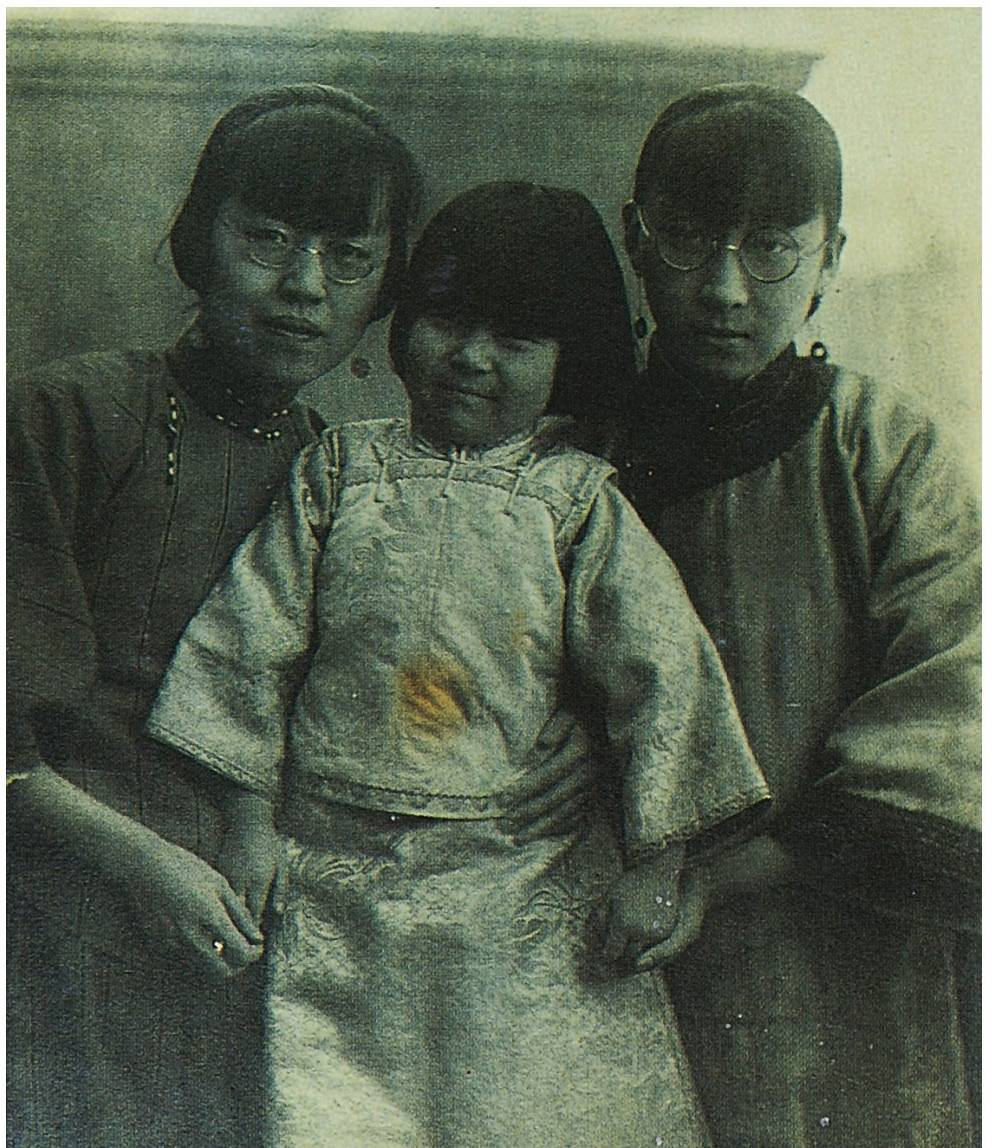
\includegraphics[scale=0.4]{picture/对照记1.jpeg}
\end{figure}

\clearpage
\par 【图二】面团团的,我自己都不认识了。但是不是我又是谁呢?把亲戚间的小女孩都想遍了,全都不像。倒是这张藤几很眼熟,还有这件衣服——不过我记得的那件衣服是淡蓝色薄绸,印着一蓬蓬白雾。T字形白绸领,穿着有点傻头傻脑的,我并不怎么喜欢,只感到亲切。随又记起那天我非常高兴,看见我母亲替这张照片着色。一张小书桌迎亮搁在装着玻璃窗的狭窄的小洋台上,北国的阴天下午,仍旧相当幽暗。我站在旁边看着,杂乱的桌面上有黑铁水彩画颜料盒,细瘦的黑铁管毛笔,一杯水。她把我的嘴唇画成薄薄的红唇,衣服也改填最鲜艳的蓝绿色。那是她的蓝绿色时期。
\par 我第一本书出版,自己设计的封面就是整个一色的孔雀蓝,没有图案,只印上黑字,不留半点空白,浓稠得使人窒息。以后才听见我姑姑说我母亲从前也喜欢这颜色,衣服全是或深或浅的蓝绿色。我记得墙上一直挂着的她的一幅油画习作静物,也是以湖绿色为主。遗传就是这样神秘飘忽——我就是这些不相干的地方像她,她的长处一点都没有,气死人。
\begin{figure}[htb]
    \centering %
    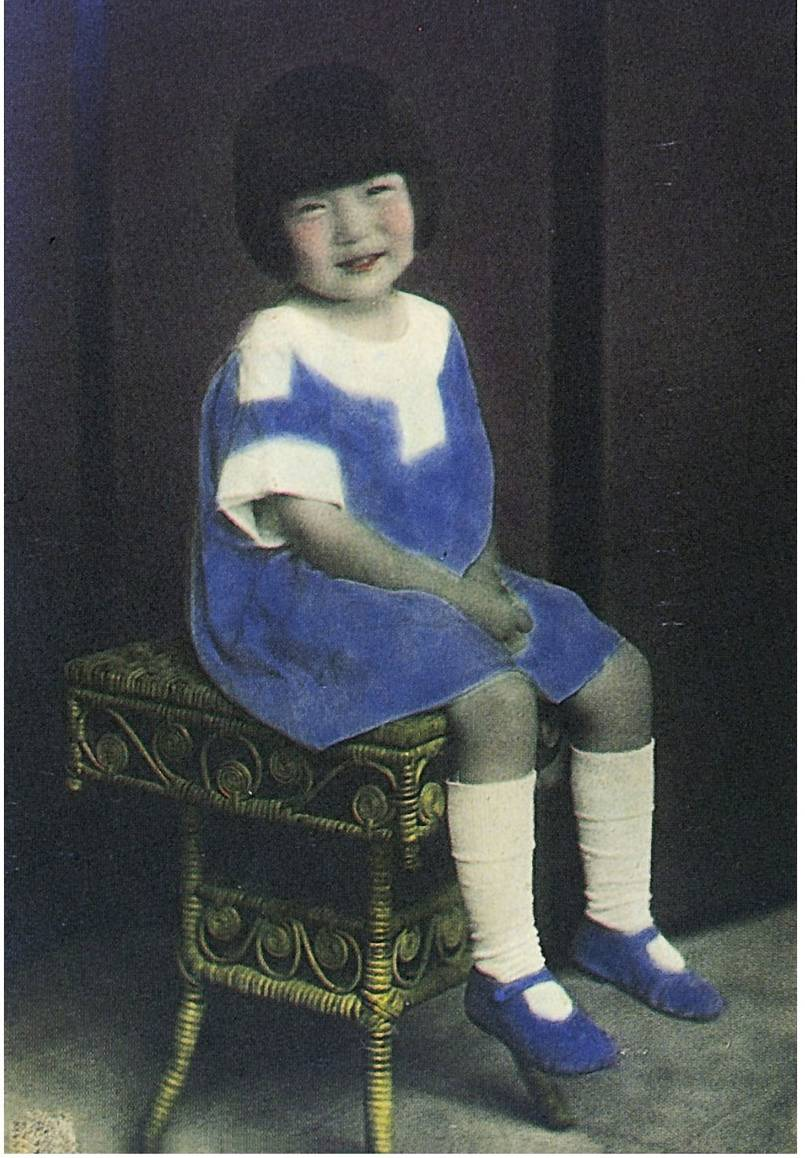
\includegraphics[scale=0.4]{picture/对照记2.jpeg}
\end{figure}

\clearpage
\par 【图三】在天津家里,一个比较简朴的半旧花园洋房,没草坪。戴眼镜的是我父亲,我姑姑,余为我母亲与两个“大侄侄”,妞儿的弟兄们。
\par 我母亲故后遗物中有我父亲的一张照片,被我丢失了。看来是直奉战争的时候寄到英国去的,在照相馆的硬纸夹上题了一首七绝,第一、第三句我只记得开首与大意:
\par 才听津门(“金甲鸣”?是我瞎猜,“鸣”字大概也不押韵。)
\par 又闻塞上鼓鼙声
\par 书生(自愧只坐拥书城?)
\par 两字平安报与卿
\par 因为他娶了妾,又吸上鸦片,她终于藉口我姑姑出国留学需要女伴监护,同去英国,一去四年。他一直催她回来,答应戒毒,姨太太也走了。回来也还是离了婚。她总是叫我不要怪我父亲。
\begin{figure}[htb]
    \centering %
    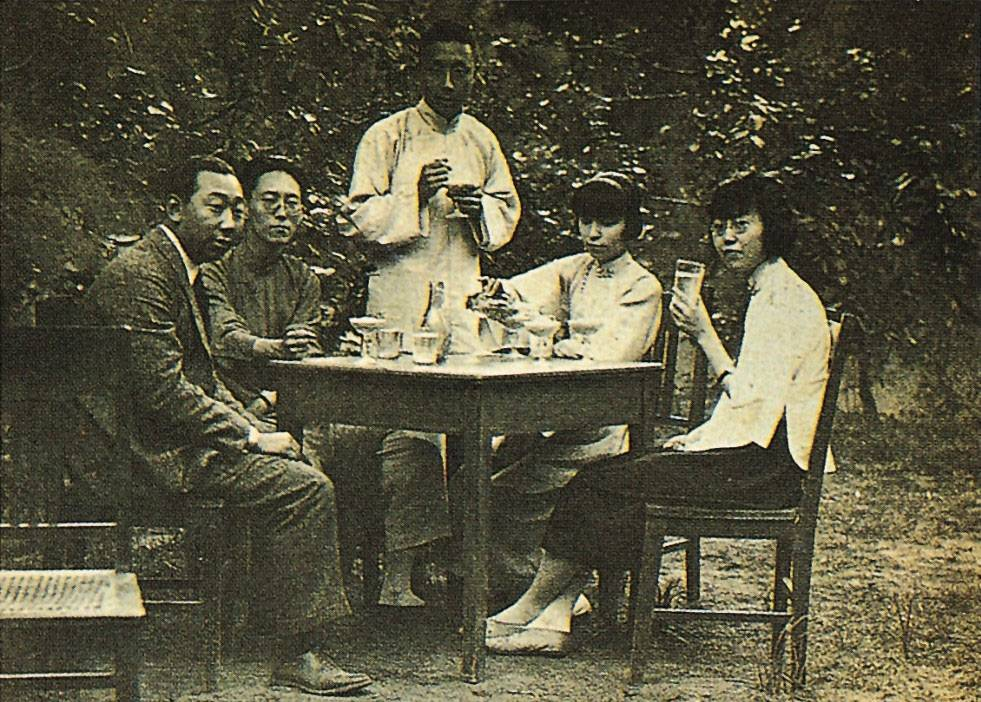
\includegraphics[scale=0.4]{picture/对照记3.jpeg}
\end{figure}

\clearpage
\par 【图四】我喜欢我四岁的时候怀疑一切的眼光。
\par 我母亲与姑姑去后,妞大侄侄与她众多的弟兄们常常轮流来看我和我弟弟,写信去告诉她们。
\par 不光是过年过节,每隔些时老女仆也带我到他们家去。我弟弟小时候体弱多病,所以大都是我一个人去。路远,坐人力车很久才到。冷落偏僻的街上,整条街都是这一幢低矮的白泥壳平房,长长一带白墙上一扇黝黑的原木小门紧闭。进去千门万户,穿过一个个院落与院子里阴暗的房间,都住着投靠他们的亲族。虽然是传统的房屋的格式,简陋得全无中国建筑的特点。
\par 房间里女眷站起来向我们微笑着待招呼不招呼,小户人家被外人穿堂入户的窘笑。大侄侄们一个都不见。带路的仆人终于把我们领到了一个光线较好的小房间。一个高大的老人永远坐在藤躺椅上,此外似乎没什么家具陈设。
\par 我叫声“二大爷。”
\par “认多少字啦?”他总是问。再没第二句话。然后就是“背个诗我听。”“再背个。”
\par 还是我母亲在家的时候教我的几首唐诗,有些字不认识,就只背诵字音。他每次听到“商女不知亡国恨,隔江犹唱后庭花”就流泪。
\par 他五十几岁的瘦小的媳妇小脚伶仃站在房门口伺候。他问了声“有什么吃哒?”她回说“有包子,有盒子。”他点点头,叫我“去玩去。”
\par 她叫了个大侄侄来陪我,自去厨下做点心。一大家子人的伙食就是她一个人上灶,在旁边帮忙的女佣不会做菜。
\par “革命党打到南京,二大爷坐只箩筐在城墙上缒下去的,”我家里一个年轻的女佣悄悄笑着告诉我。她是南京人。
\par 多年后我才恍惚听见说他是最后一个两江总督张人骏。一九六〇初,我在一个美国新闻记者写的端纳传(《中国的端纳》,Donald of China)上看到总督坐箩筐缒出南京围城的记载,也还不十分确定是他,也许因为过去太熟悉了,不大能接受。书中写国民政府的端纳顾问初到中国,到广州去见他,那时候他是两广总督。端纳贡献意见大发议论,他一味笑着直点头,帽子上的花翎乱颤。那也是清末官场敷衍洋人的常态。
\par “他们家穷因为人多,”我曾经听我姑姑说过。
\par 仿佛总比较是多少是个清官,不然何至于一寒至此。
\par 我姑姑只愤恨他把妞大侄侄嫁给一个肺病已深的穷亲戚,生了许多孩子都有肺病,无力医治。妞儿在这里的两张照片上已经定了亲。
\begin{figure}[htb]
    \centering %
    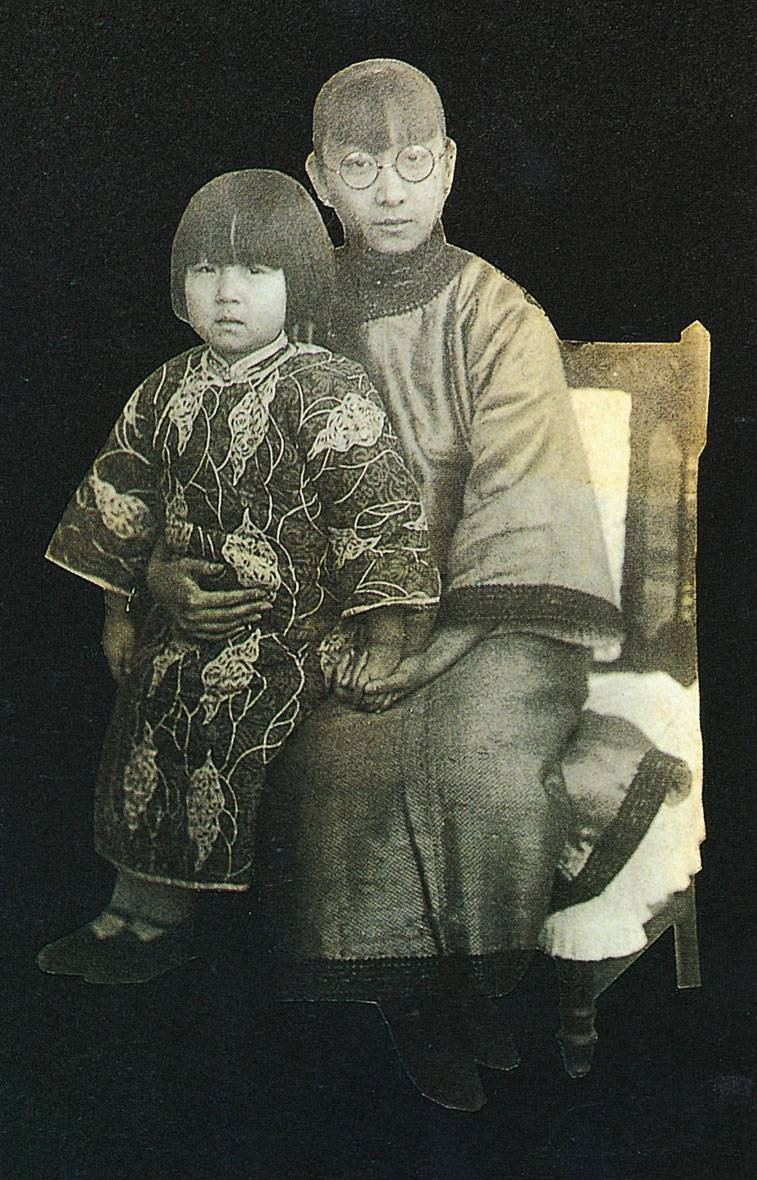
\includegraphics[scale=0.4]{picture/对照记4.jpeg}
\end{figure}

\clearpage
\par 【图五】我弟弟这张照片背面印着英文明信片款式,显然是我母亲在英国的时候拿去制成明信片。这一张与她所有的着色的照片都是她自己着色的。
\begin{figure}[htb]
    \centering %
    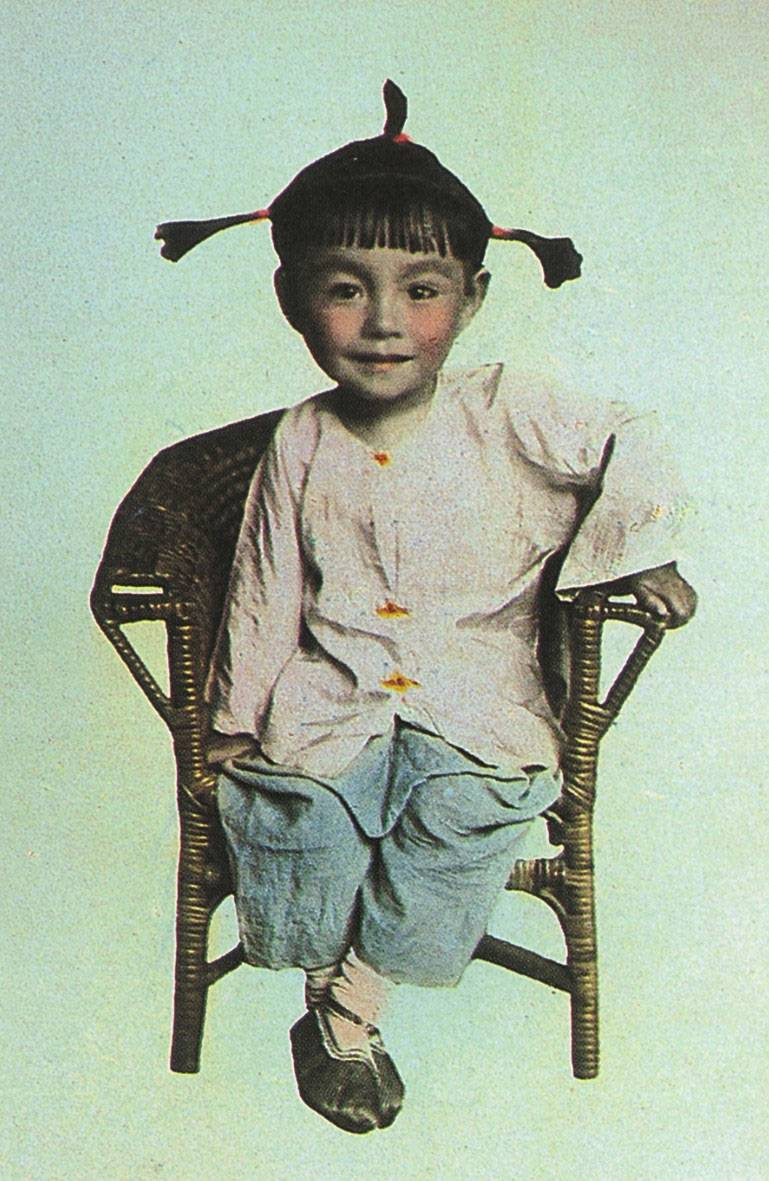
\includegraphics[scale=0.4]{picture/对照记5.jpeg}
\end{figure}

\clearpage
\par 【图六】我们抱着英国寄来的玩具。他戴着给他买的草帽。
\begin{figure}[htb]
    \centering %
    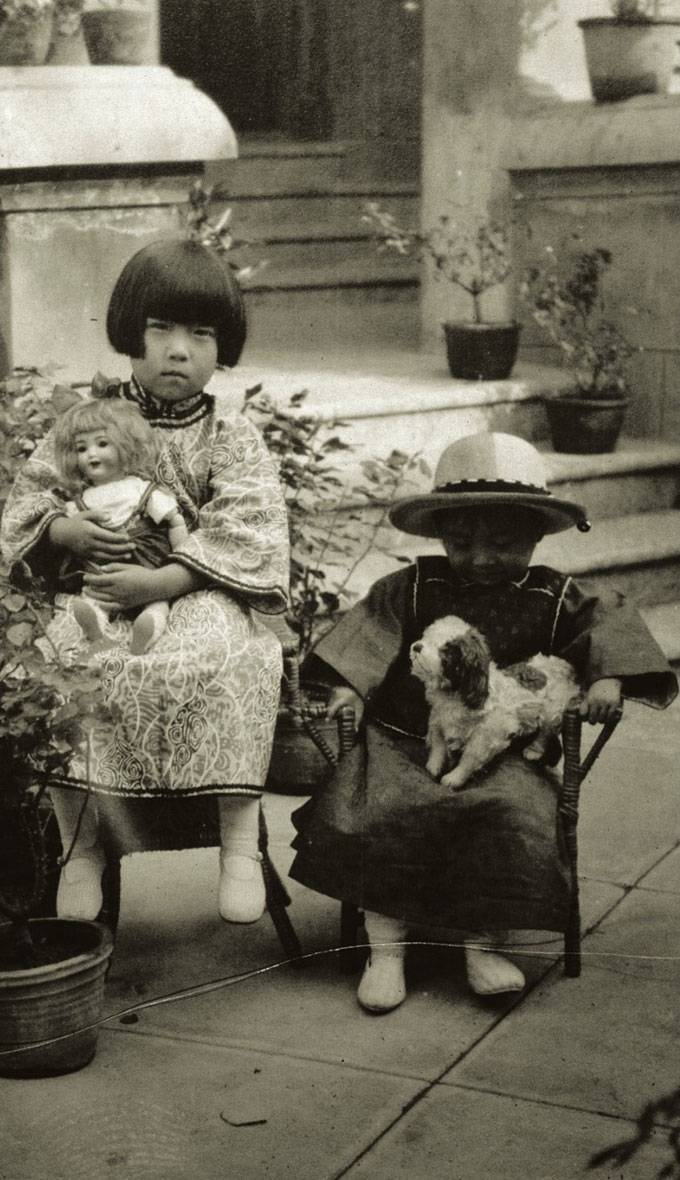
\includegraphics[scale=0.4]{picture/对照记6.jpeg}
\end{figure}


\clearpage
\par 【图七】在天津的法国公园。
\begin{figure}[htb]
    \centering %
    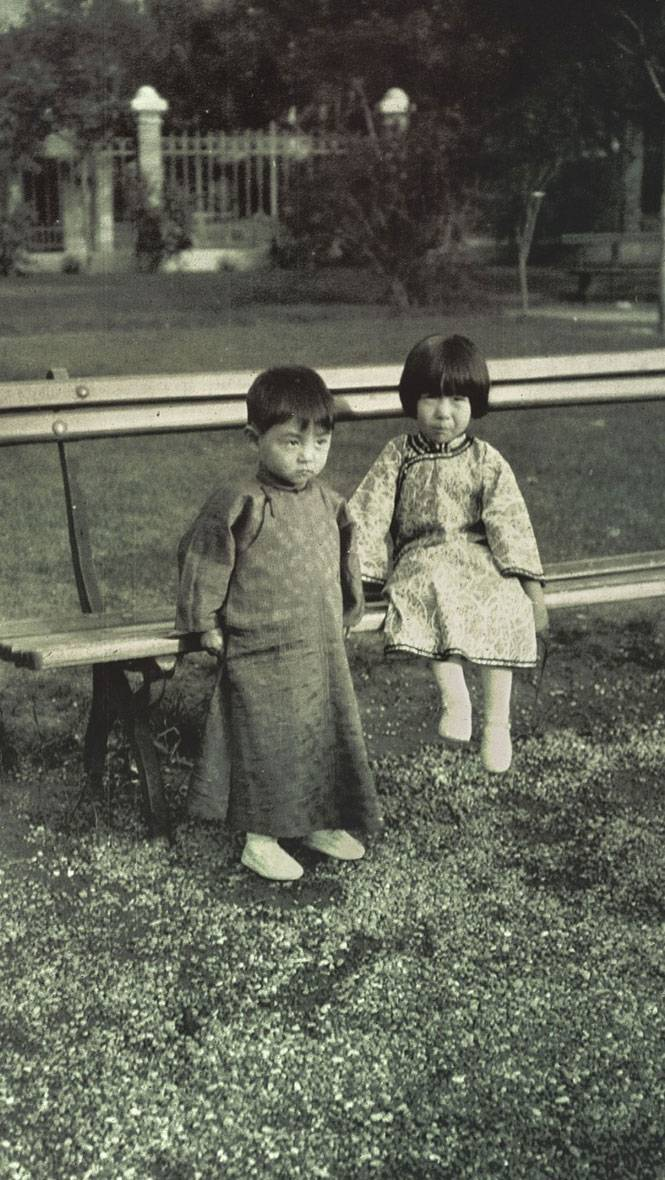
\includegraphics[scale=0.4]{picture/对照记7.jpeg}
\end{figure}


\clearpage
\par 【图八】我们搬到上海去等我母亲、我姑姑回国。我舅舅家住在张家浜(音“邦”,俗字——近江海的水潭),未来的大光明戏院后面的卡尔登戏院后首的一个不规则的小型广场。叫张家浜,显然还是上海滩初开埠时节的一块沼泽地,后来填了土,散散落落造了几幢大洋房。年代久了,有的已经由住宅改为小医院。街口的一幢,楼下开了个宝德照相馆,也是曾经时髦过的老牌照相馆。我舅母叫三个表姐与表弟带我去合拍张照。
\par 隆冬天气没顾客上门,冰冷的大房间,现在想起来倒像海派连台本戏的后台,墙上倚立着高大的灰尘满积的布景片子。
\par 五个小萝卜头我在正中。还有个表妹最小,那天没去。她现在是电视明星张小燕的母亲。
\begin{figure}[htb]
    \centering %
    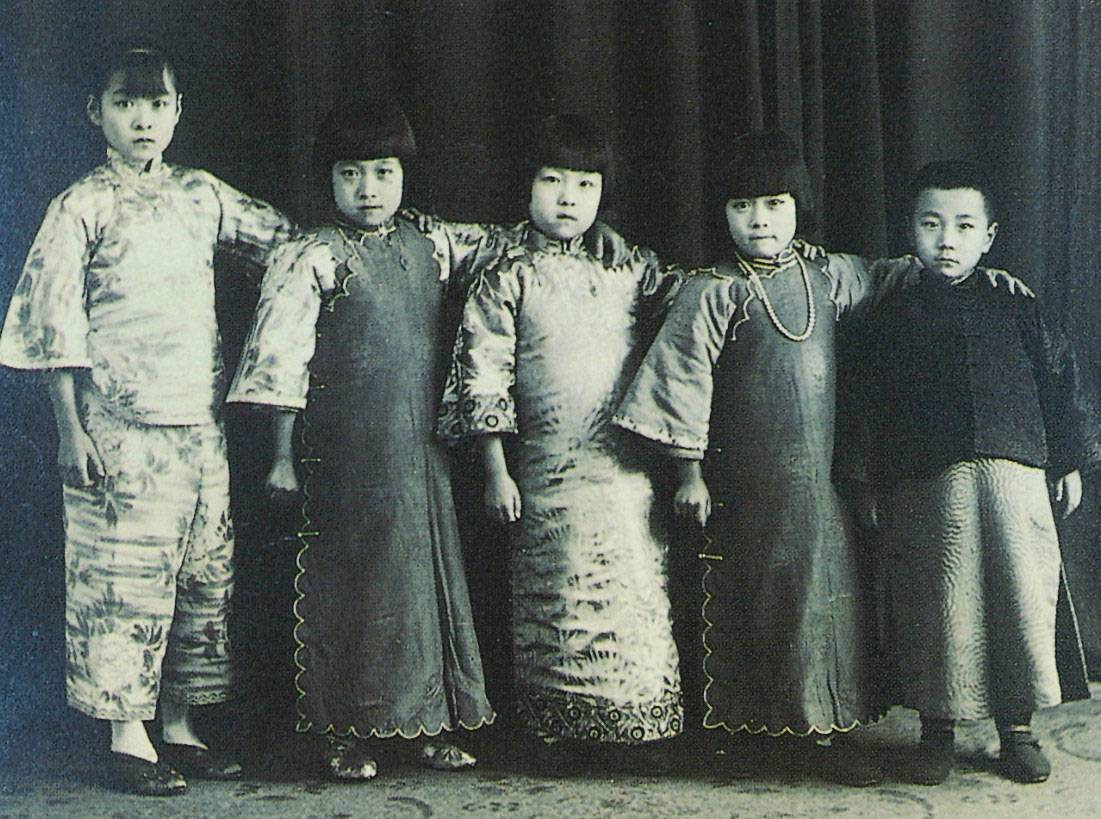
\includegraphics[scale=0.4]{picture/对照记8.jpeg}
\end{figure}

\clearpage
\par 【图九】我母亲与姑姑回国后和两个表伯母到杭州游西湖,也带了我跟我弟弟去。这是九溪十八涧。
\begin{figure}[htb]
    \centering %
    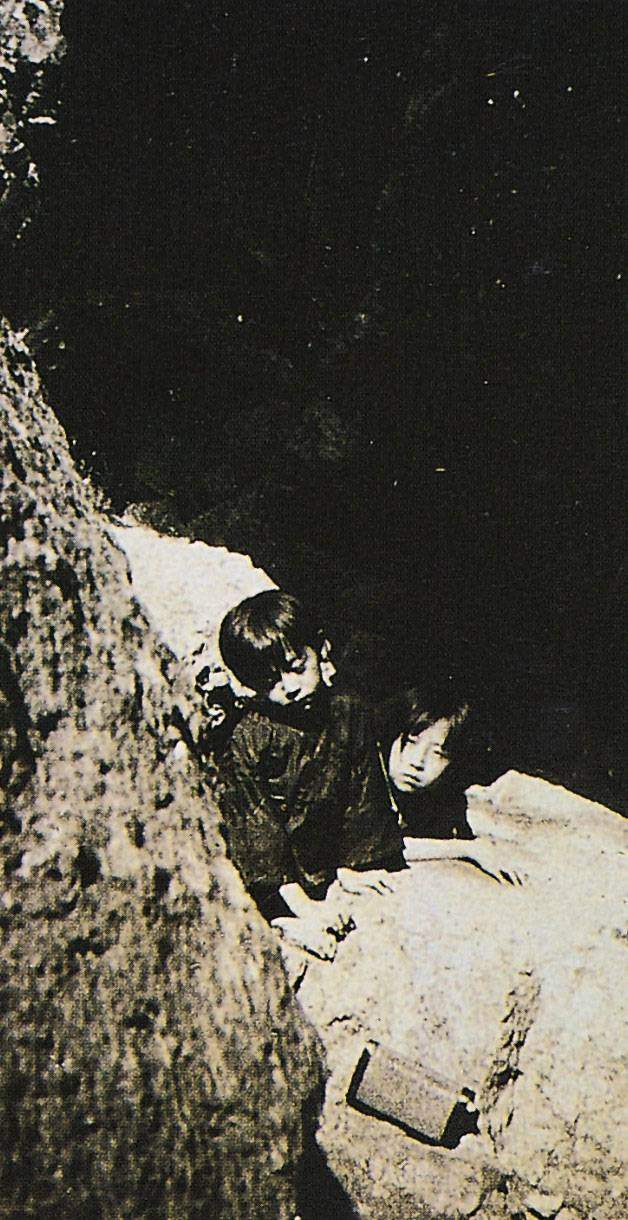
\includegraphics[scale=0.4]{picture/对照记9.jpeg}
\end{figure}

\clearpage
\par 【图十】我外婆是农家女,嫁给将门之子作妾——他父亲是湘军水师。她大概是他们原籍湖南长沙附近的人。他们俩都只活到二十几岁,孩子是嫡母带大的。
\begin{figure}[htb]
    \centering %
    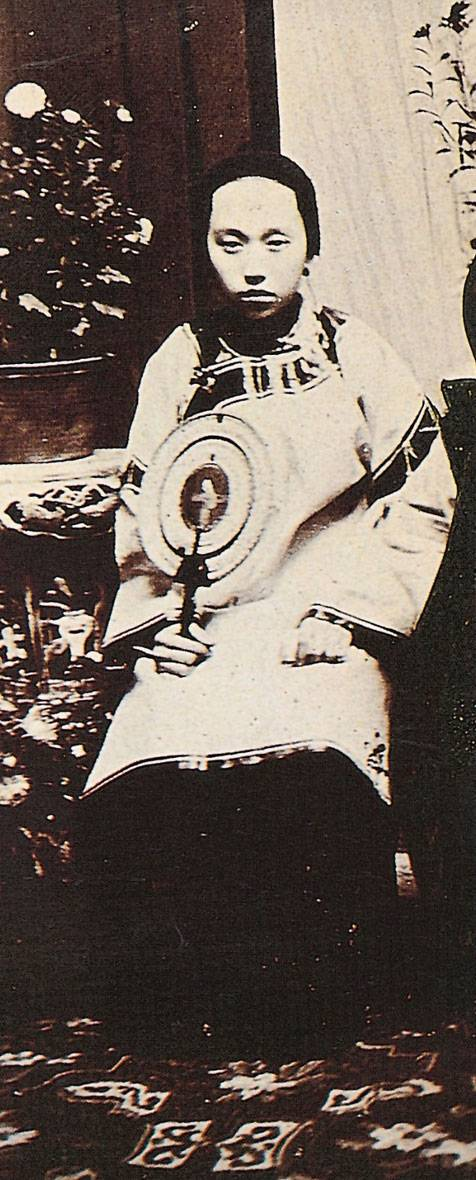
\includegraphics[scale=0.4]{picture/对照记10.jpeg}
\end{figure}

\clearpage
\par 【图十一】民初妇女大都是半大脚,裹过又放了的。我母亲比我姑姑大不了几岁,家中同样守旧,我姑姑就已经是天足了,她却是从小缠足。(见图。背后站着的想必是婢女。)踏着这双三寸金莲横跨两个时代,她在瑞士阿尔卑斯山滑雪至少比我姑姑滑得好。(我姑姑说。)
\par 她是个学校迷。我看茅盾的小说《虹》中三个成年的女性入学读书就想起她,不过在她纯是梦想与羡慕别人。后来在欧洲进美术学校,太自由散漫不算。一九四八年她在马来亚侨校教过半年书,都很过瘾。
\par 她画油画,跟徐悲鸿蒋碧微常书鸿都熟识。
\par 珍珠港事变后她从新加坡逃难到印度,曾经做尼赫鲁的两个姐姐的秘书。一九五一年在英国又一度下厂做女工制皮包。连我姑姑在大陆收到信都有点不知道说什么好,只向我悄悄笑道:“这要是在国内,还说是爱国,破除阶级意识——”
\par 她信上说想学会裁制皮革,自己做手袋销售。早在一九三六年她绕道埃及与东南亚回国,就在马来亚买了一洋铁箱碧绿的蛇皮,预备做皮包皮鞋。上海成了孤岛后她去新加坡,丢下没带走。我姑姑和我经常拿到屋顶洋台上去曝晒防霉烂,视为苦事,虽然那一张张狭长的蕉叶似的柔软的薄蛇皮实在可爱。她战后回国才又带走了。
\par 我小时候她就自己学会做洋裁,也常见她车衣。但是她做皮包卖的计划似乎并未成功,来信没再提起。当时不像现在欧美各大都市都有青年男女沿街贩卖自制的首饰等等,也有打进高价商店与大百货公司的。后工业社会才能够欣赏独特的新巧的手工业。她不幸早了二三十年。
\par 她总是说湖南人最勇敢。
\begin{figure}[htb]
    \centering %
    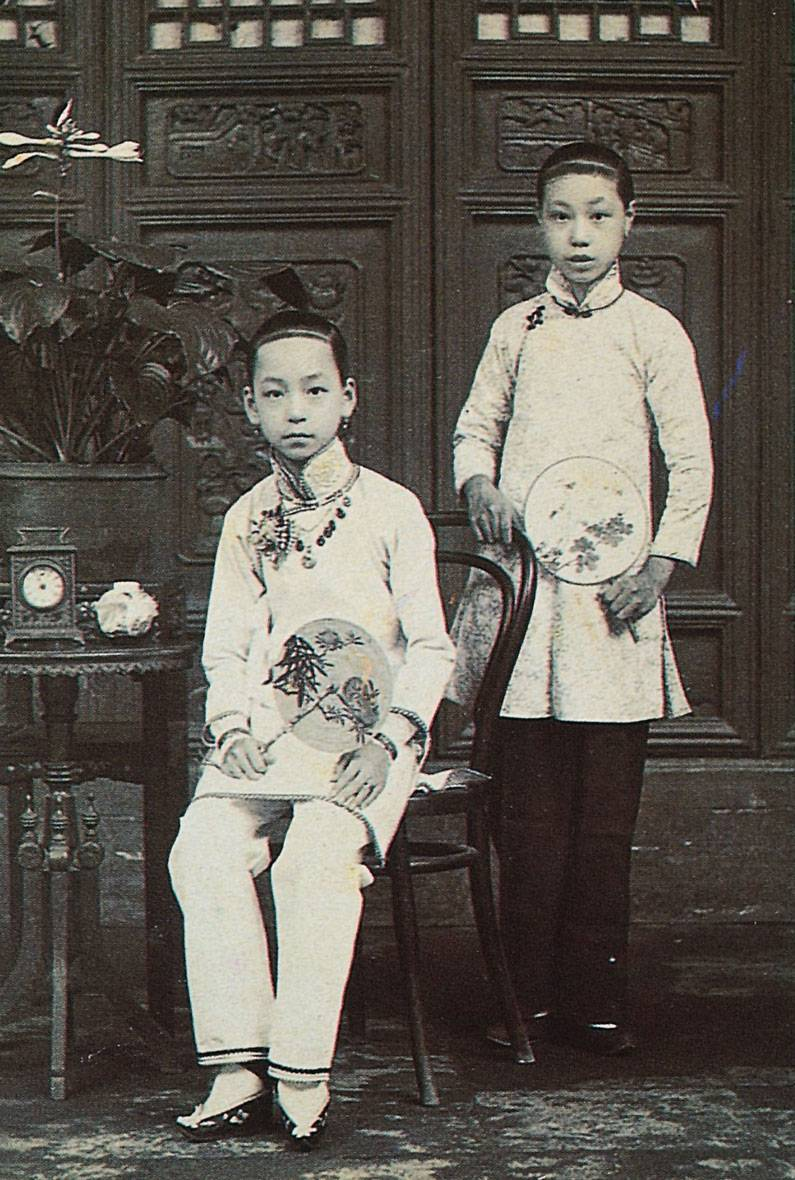
\includegraphics[scale=0.4]{picture/对照记11.jpeg}
\end{figure}

\clearpage
\par 【图十二】我母亲,一九二〇初叶在北京。
\begin{figure}[htb]
    \centering %
    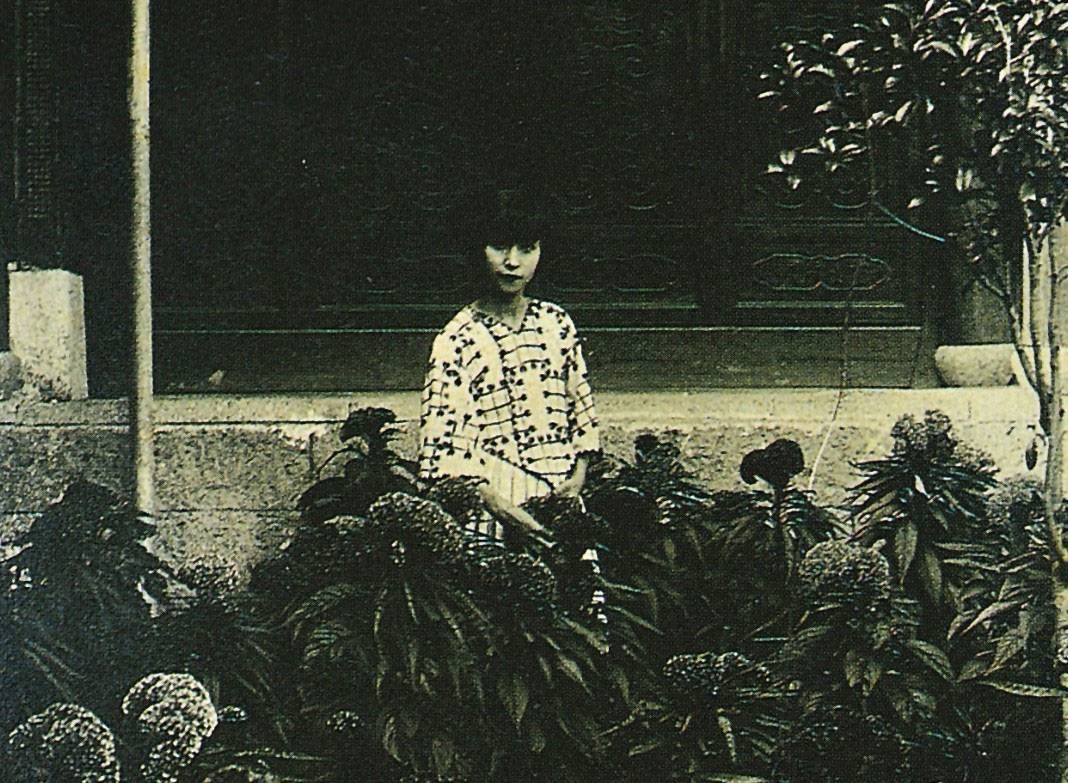
\includegraphics[scale=0.4]{picture/对照记12.jpeg}
\end{figure}

\clearpage
\par 【图十三】在伦敦,一九二六。
\begin{figure}[htb]
    \centering %
    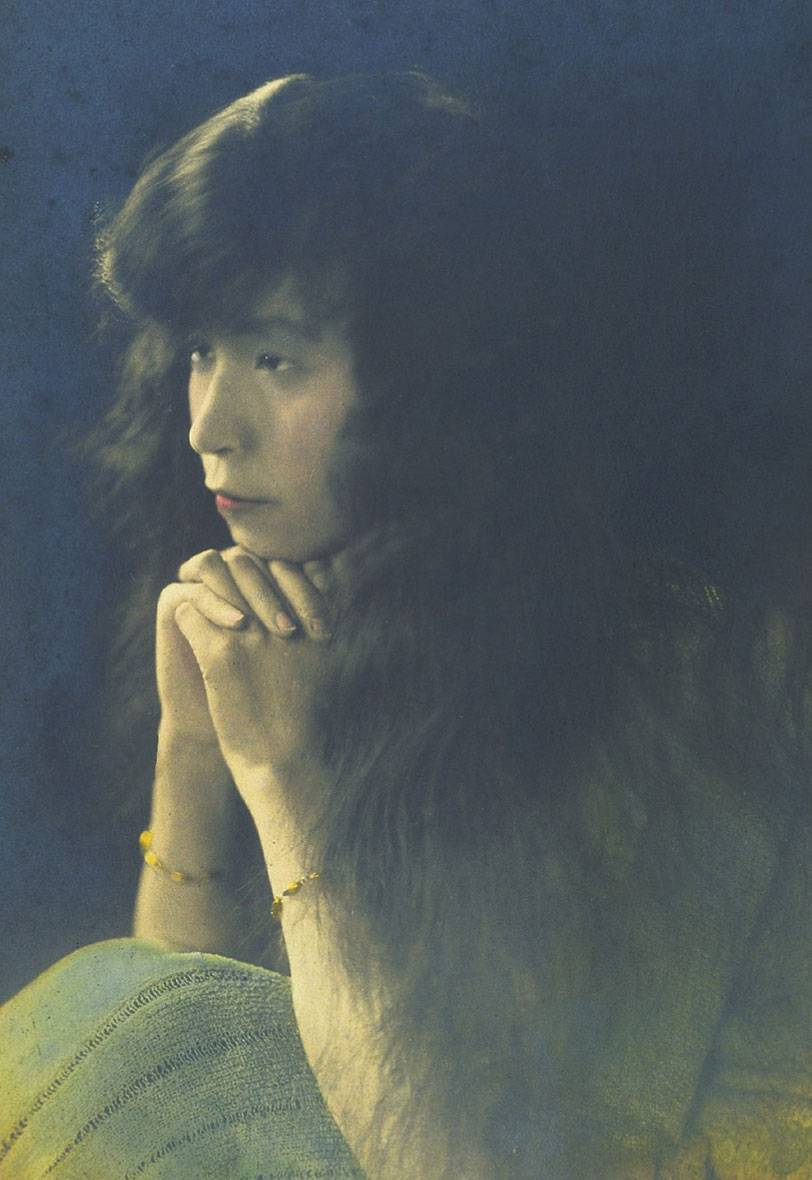
\includegraphics[scale=0.4]{picture/对照记13.jpeg}
\end{figure}

\clearpage
\par 【图十四、十五】一九三〇初在西湖赏梅。
\begin{figure}[htb]
    \centering %
    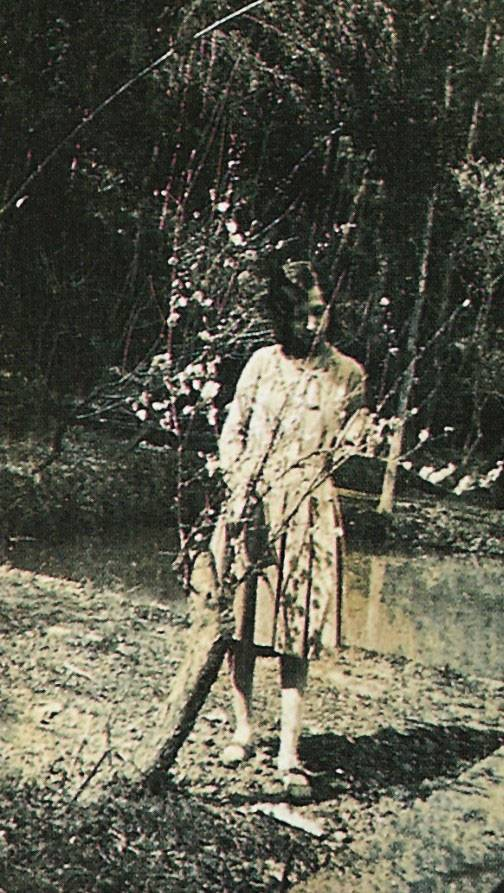
\includegraphics[scale=0.35]{picture/对照记14.jpeg}
    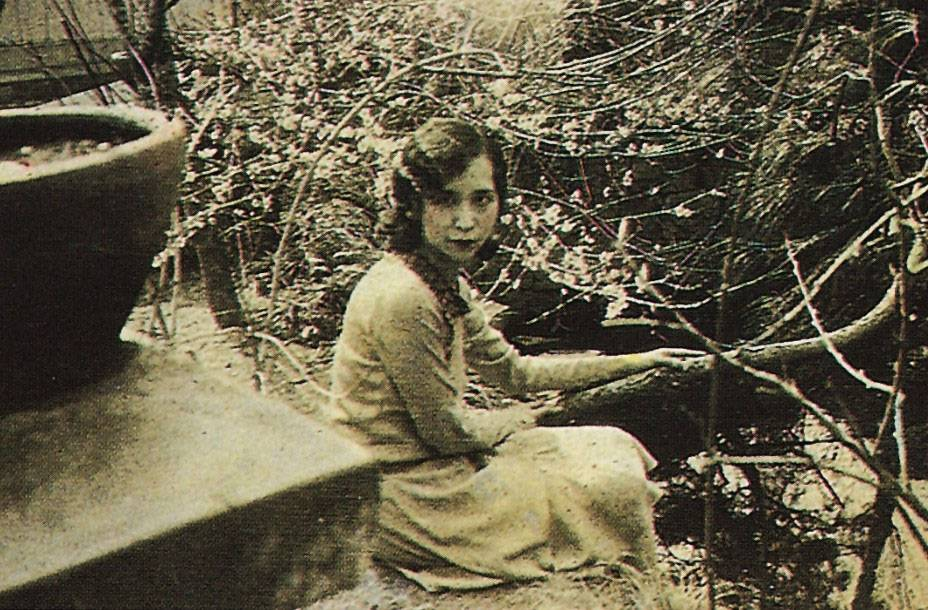
\includegraphics[scale=0.35]{picture/对照记15.jpeg}
\end{figure}


\clearpage
\par 【图十六、十七】三〇中叶在法国。
\begin{figure}[htb]
    \centering %
    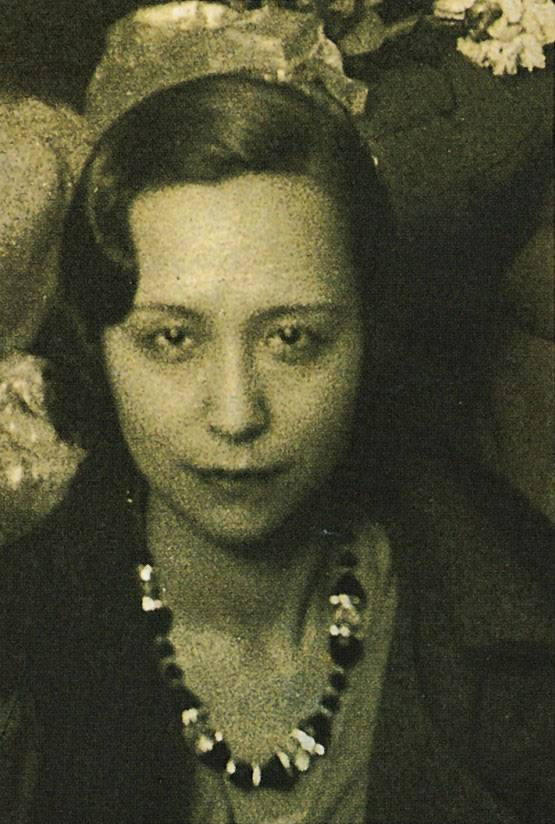
\includegraphics[scale=0.4]{picture/对照记16.jpeg}
    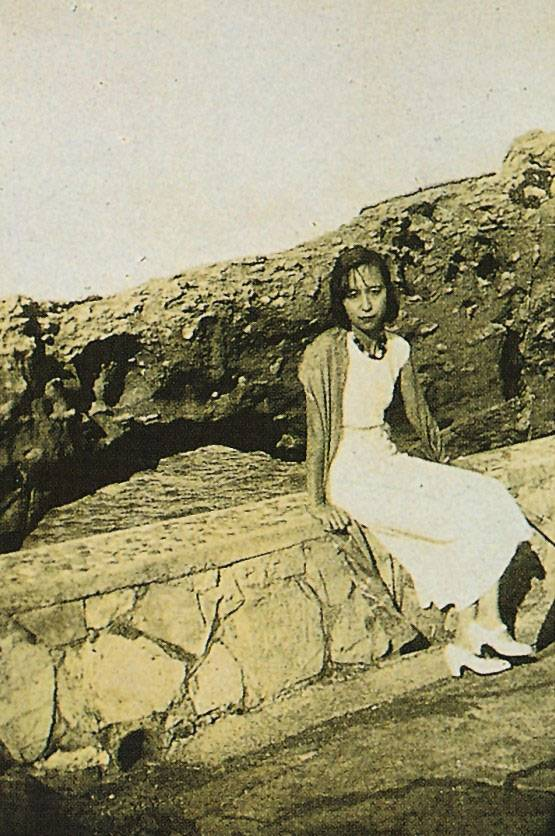
\includegraphics[scale=0.4]{picture/对照记17.jpeg}
\end{figure}



\clearpage
\par 【图十八】三〇末叶在海船上。
\begin{figure}[htb]
    \centering %
    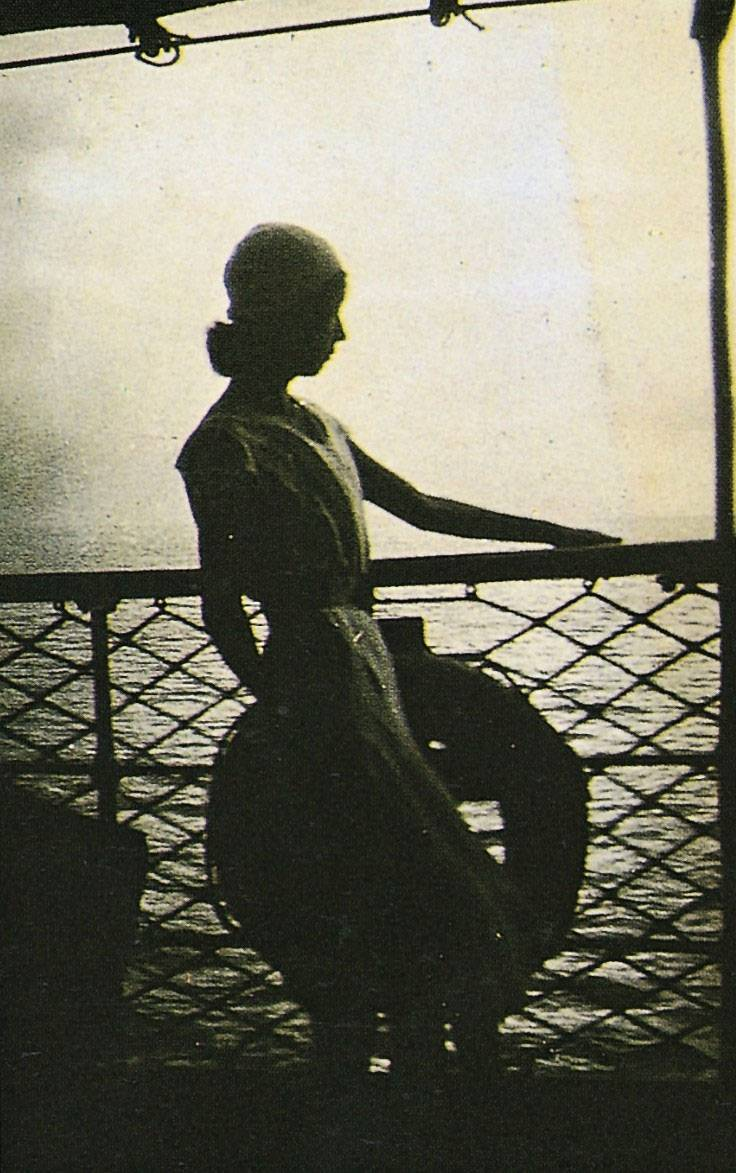
\includegraphics[scale=0.4]{picture/对照记18.jpeg}
\end{figure}

\clearpage
\par 【图十九】我母亲离婚后再度赴欧,我姑姑搬到较小的公寓。本来两人合租的公寓没住多久,迁出前在自己设计的家具地毯上拍照留念。
\begin{figure}[htb]
    \centering %
    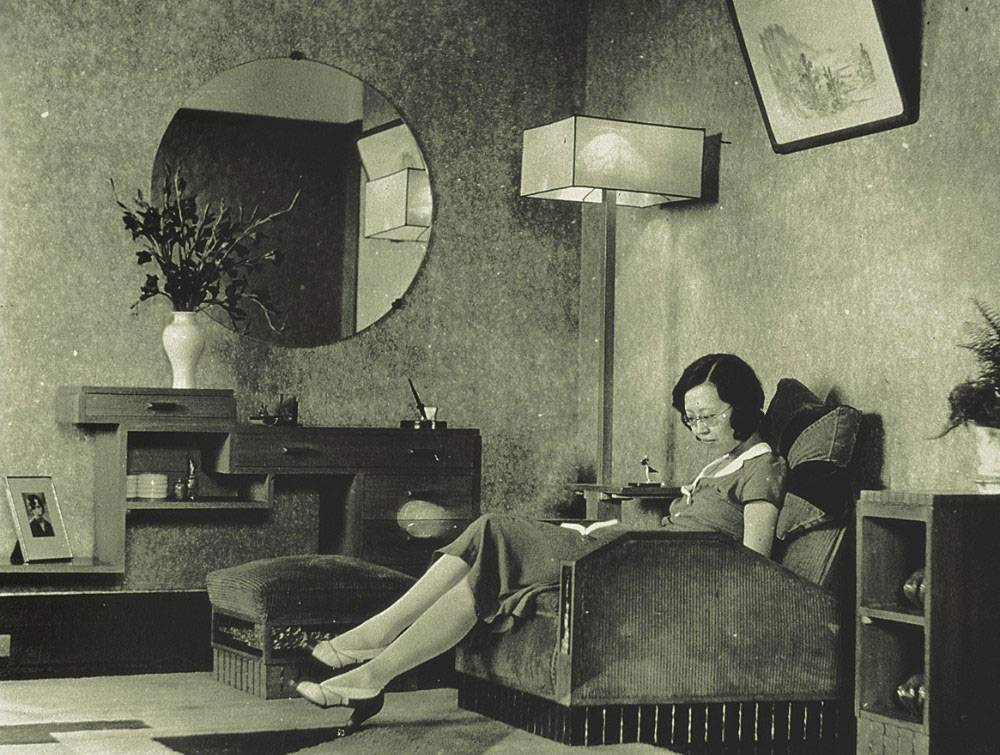
\includegraphics[scale=0.4]{picture/对照记19.jpeg}
\end{figure}

\clearpage
\par 【图二十】在我姑姑的屋顶洋台上。她央告我“可不能再长高了。”
\par 她在照片背面用铅笔写着:
\par “我这张难看极了小煐很自然所以寄给你看看
\par 这地方是气车间顶上小孩顽的地方
\par 我们头顶上的窗就是我的Sitting room的。”
\par 显然是她寄给我母亲同一照片寄出的一张上题字的底稿。
\par 我再稍大两岁她就告诉我她是答应我母亲照应我的。她需要声明,大概也是怕我跟她比跟我母亲更亲近,成了离间亲子感情。


\par 【图二十一】我穿着我继母的旧衣服。她过门前听说我跟她身材相差不远,带了两箱子嫁前衣来给我穿。
\par 她父亲孙宝琦以遗老在段祺瑞执政时出任总理,即在北洋政府也算是“官声不好”的,不知怎么后来仍旧家境拮据。总不见得又是因为“家里人多”?他膝下有八男十六女。妻女都染上了阿芙蓉癖。我继母是陆小曼的好友,两人都是吞云吐雾的芙蓉仙子。婚后床头挂着陆小曼画的油画瓶花。她跟“赵四风流朱五狂”的朱氏姊妹也交好,谢媒酒在家里请客,她们也在座。
\par 她说她的旗袍“料子都很好的”,但是有些领口都磨破了。只有两件蓝布大褂是我自己的。在被称为贵族化的教会女校上学,确实相当难堪。学校里一度酝酿着要制定校服,有人赞成,认为泯除贫富界限。也有人反对,因为太整齐划一了丧失个性,而且清寒的学生又还要多出一笔校服费。议论纷纷,我始终不置一词,心里非常渴望有校服,也许像别处的女生的白衬衫、藏青十字交叉背带裙,洋服中的经典作,而又有少女气息。结果学校当局没通过,作罢了。
\par 一九六〇初叶我到台湾,看见女学生清一色的草黄制服,觉得比美国的女童军的墨绿制服帅气,有女兵的英姿。后来在台湾报上看到群情愤激要求废除女生校服,不禁苦笑。
\par 我这论调有点像台湾报端常见的“你们现在多么享福,我们从前吃番薯签”,使年青人听多了生厌。不过我那都是因为后母赠衣造成一种特殊的心理,以至于后来一度clothes-crazy(衣服狂)。
\begin{figure}[htb]
    \centering %
    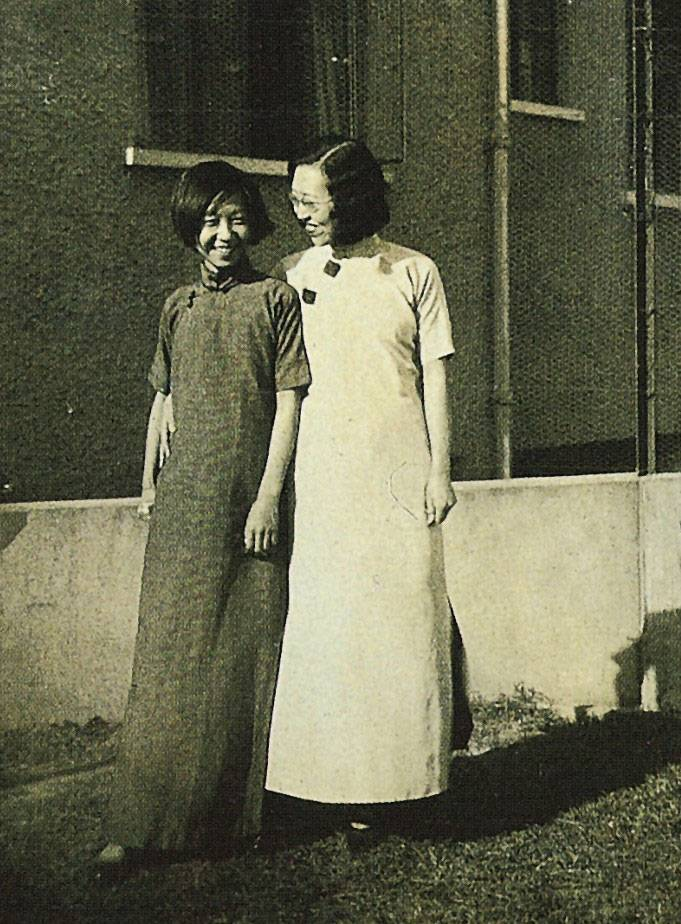
\includegraphics[scale=0.35]{picture/对照记20.jpeg}
    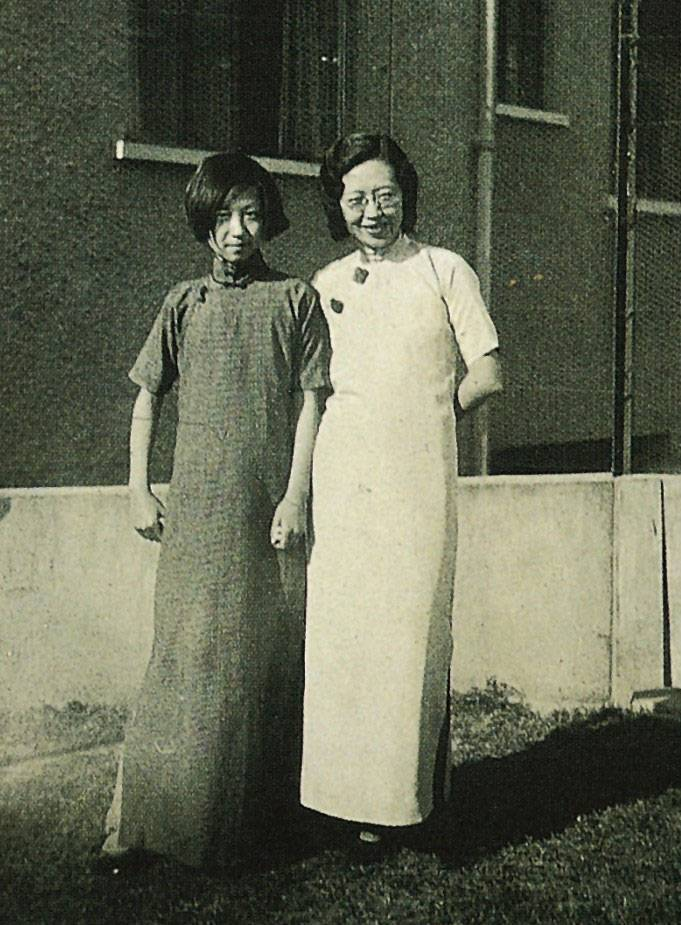
\includegraphics[scale=0.35]{picture/对照记21.jpeg}
\end{figure}

\clearpage
\par 【图二十二】我祖母十八岁的时候与她母亲合影。她仿佛忍着笑,也许是笑钻在黑布下的洋人摄影师。
\par 我弟弟永远比我消息灵通。我住读放月假回家,一见面他就报告一些亲戚的消息。有一次他仿佛抢到一则独家新闻似地,故作不经意地告诉我:“爷爷名字叫张佩纶。”
\par “是哪个佩?哪个纶?”
\par “佩服的佩。经纶的纶,绞丝边。”
\par 我很诧异这名字有点女性化,我有两个同学名字就跟这差不多。
\par 不知道别处风俗怎样,我们祭祖没有神主牌,供桌上首只摆一排盖碗,也许有八九个之多。想必总有曾祖父母。当时不知道祖父还有两个前妻与一个早死的长子,只模糊地以为还再追溯到高祖或更早。偶尔听见管祭祀的老仆嘟囔一声某老姨太的生日,靠边加上一只盖碗,也不便问。他显然有点讳言似地,当着小孩不应当提姨太太的话,即使是陈年八代的。每逢“摆供”,他就先一天取出香炉蜡台桌围与老太爷老太太的遗像,挂在墙上。祖母是照片,祖父是较大的油画像。我们从小看惯了,只晓得是爷爷奶奶,从来没想到爷爷也有名字。
\par 又一天我放假回来,我弟弟给我看新出的历史小说《孽海花》,不以为奇似地撂下一句:“说是爷爷在里头。”
\par 厚厚的一大本,我急忙翻看,渐渐看出点苗头来,专拣姓名音同字不同的,找来找去,有两个姓庄的。是嫖妓丢官后,“小红低唱我吹箫”,在湖上逍遥的一个?看来是另一个,庄\UncommonChar{𪨧}樵,也是“文学侍从之臣”,不过兼有言官的职权,奏参大员,参一个倒一个,一时满朝侧目。李鸿章——忘了书中影射他的人物的名字——也被他参过,因而“褫去黄马褂,拔去三眼花翎。”
\par 中法战争爆发,因为他主战,忌恨他的人就主张派他去,在台湾福建沿海督师大败,大雨中头上顶着一只铜脸盆逃走。
\par 李鸿章爱才不念旧恶,他革职充军后屡次接济他,而且终于把他弄了回来,留在衙中作记室。有一天他在签押房里惊鸿一瞥看见东家如花似玉的女儿,此后又有机会看到她作的一首七律,一看题目《鸡笼》,先就怵目惊心:
\par “鸡笼南望泪潸潸,闻道元戎匹马还。一战何容轻大计,四方从此失边关。……”
\par 李鸿章笑着说了声“小女涂鸦”之类的话安抚他,却着人暗示他来求亲,尽管自己太太大吵大闹,不肯把女儿嫁给一个比她大二十来岁的囚犯。
\par 我看了非常兴奋,去问我父亲,他只一味辟谣,说根本不可能在签押房撞见奶奶。那首诗也是捏造的。
\par 我也听见过他跟访客讨论这部小说,平时也常跟亲友讲起“我们老太爷”,不过我旁听总是一句都听不懂。大概我对背景资料知道得太少。而他习惯地衔着雪茄烟环绕着房间来回踱着,偶尔爆出一两句短促的话,我实在听不清楚,客人躺在烟铺上自抽鸦片,又都只微笑听着,很少发问。
\par 对子女他从来不说什么。我姑姑我母亲更是绝口不提上一代。他们在思想上都受五四的影响,就连我父亲的保守性也是有选择性的,以维护他个人最切身的权益为限。
\par 我母亲还有时候讲她自己家从前的事,但是她憎恨我们家。当初说媒的时候都是为了门第葬送了她一生。
\par “问这些干什么?”我姑姑说。“现在不兴这些了。我们是叫没办法,都受够了,”她声音一低,近于喃喃自语,随又换回平常的声口:“到了你们这一代,该往前看了。”
\par “我不过是因为看了那本小说觉得好奇,”我不好意思地分辩。
\par 她讲了点奶奶的事给我听。她从小父母双亡,父亲死得更早。“爷爷一点都不记得了。”她断然地摇了摇头。
\par 我称大妈妈的表伯母,我一直知道她是李鸿章的长孙媳,不过不清楚跟我们是怎么个亲戚。那时候我到她家去玩,总看见电话旁边的一张常打的电话号码表,第一格填写的人名是曾虚白,我只知道是个作家,是她娘家亲戚。原来就是《孽海花》作者曾孟朴的儿子!
\par 她哥哥是诗人杨云史,他们跟李家是亲上加亲。曾家与李家总也是老亲了,又来往得这样密切。《孽海花》里这一段情节想必可靠,除了小说例有的渲染。
\par 因为是我自己“寻根”,零零碎碎一鳞半爪挖掘出来的,所以格外珍惜。
\begin{figure}[htb]
    \centering %
    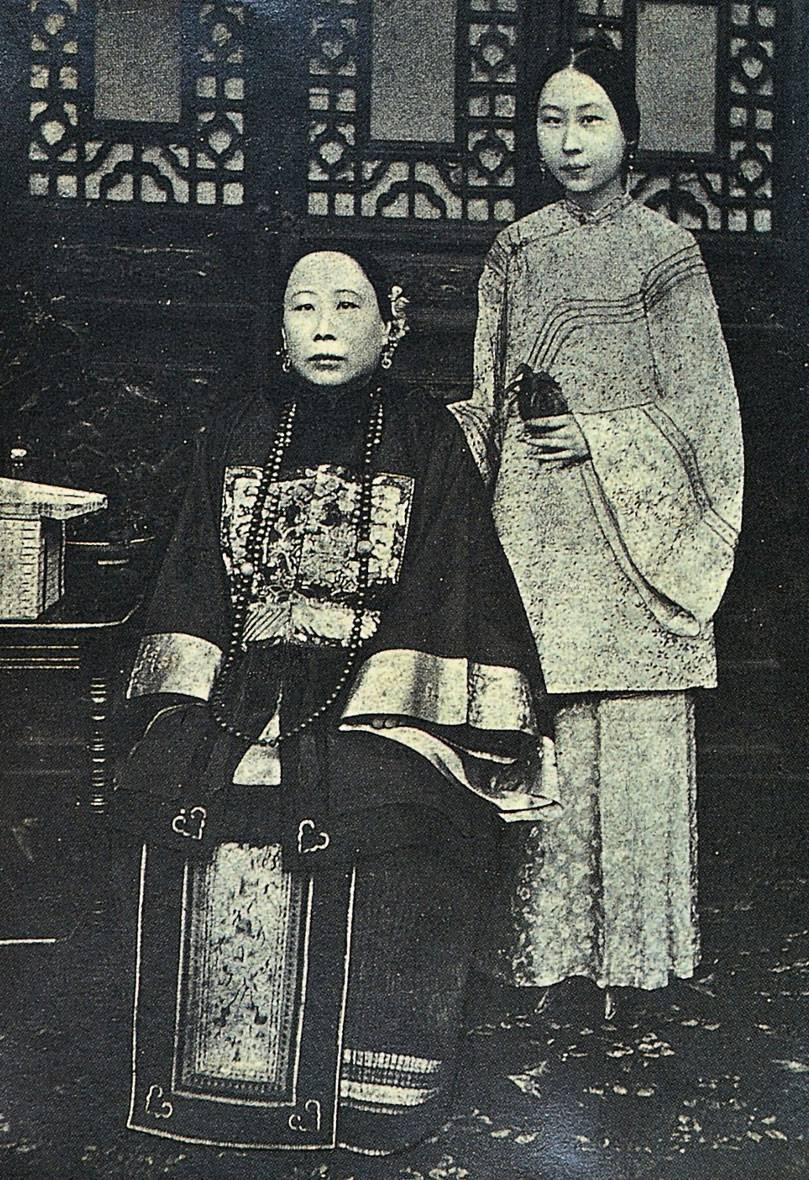
\includegraphics[scale=0.35]{picture/对照记22.jpeg}
\end{figure}

\clearpage
\par 【图二十三】我仅有的一张我祖父的照片已经泛黄褪色,大概不能制版。显然是我姑姑剪贴成为夫妇合影,各坐茶几一边,茶几一分为二,中隔一条空白。祖父这边是照相馆的布景,模糊的风景。祖母那边的背景是雕花排门,想是自己家里。她跟十八岁的时候发型服饰相同,不过脸面略胖些。
\par 祭祖的时候悬挂的祖父的油画像比较英俊,那是西方肖像画家的惯技。但同是身材相当魁梧,画中人眼梢略微下垂,一只脚往前伸,像就要站起来,眉宇间也透出三分焦躁,也许不过是不耐久坐。照片上胖些,眼泡肿些,眼睛里有点轻藐的神气。也或者不过是看不起照相这洋玩艺。
\par 《孽海花》上的“白胖脸儿”在画像上已经变成赭红色,可能是因为饮酒过多。虽有“恩师”提携(他在书信上一直称丈人为“恩师”),他一直不能复出,虽然不短在幕后效力,直到八国联军指名要李鸿章出来议和,李鸿章八十多岁心力交瘁死在京郊贤良寺。此后他更纵酒,也许也是觉得对不起恩师父女。五十几岁就死于肝疾。
\par 我又去问我父亲关于祖父的事。
\par “爷爷有全集在这里,自己去看好了,”他悻悻然说。
\par 是他新近出钱拿去印的,几部书页较小的暗蓝布套的线装书。薄薄的一本本诗文奏章信札,充满了我不知道的典故,看了半天看得头昏脑胀,也看不出所以然来。
\par 多年后我听见人说我祖父诗文都好,连八股都好,又忙补上一句:“八股也有好的。”我也都相信。他的诗属于艰深的江西诗派,我只看懂了两句:“秋色无南北,人心自浅深。”我想是写异乡人不吸收的空虚怅惘。有时候会印象淡薄得没有印象,也就是所谓“天涯若梦中行耳。”
\par “爷爷奶奶唱和的诗集都是爷爷作的,”我姑姑说,“奶奶就只有一首集句是她自己作的:四十明朝过,犹为世网萦。蹉跎暮容色,煊赫旧家声。”
\par 那时候孀居已久。她四十七岁逝世。
\par “我记得扒在奶奶身上,喜欢摸她身上的小红痣,”我姑姑说。“奶奶皮肤非常白,许多小红痣,真好看。”她声音一低。“是小血管爆裂。”
\begin{figure}[htb]
    \centering %
    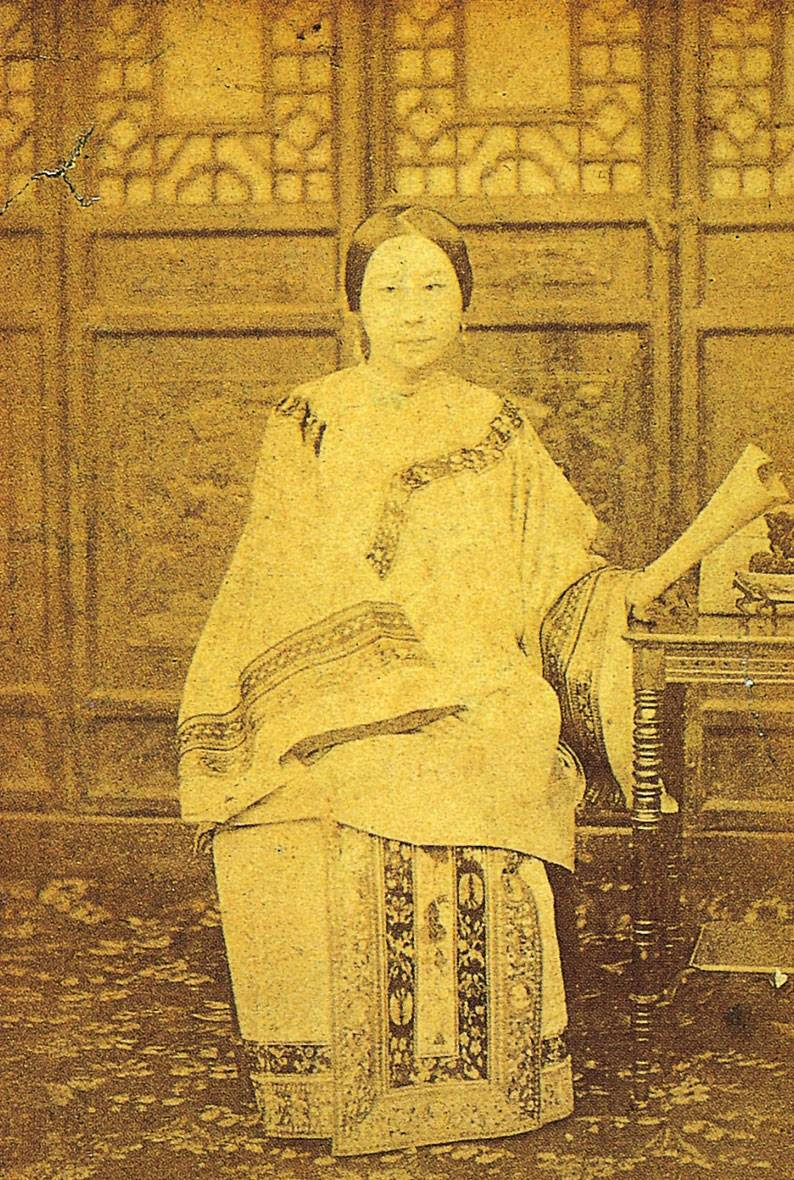
\includegraphics[scale=0.3]{picture/对照记23_1.jpeg}
    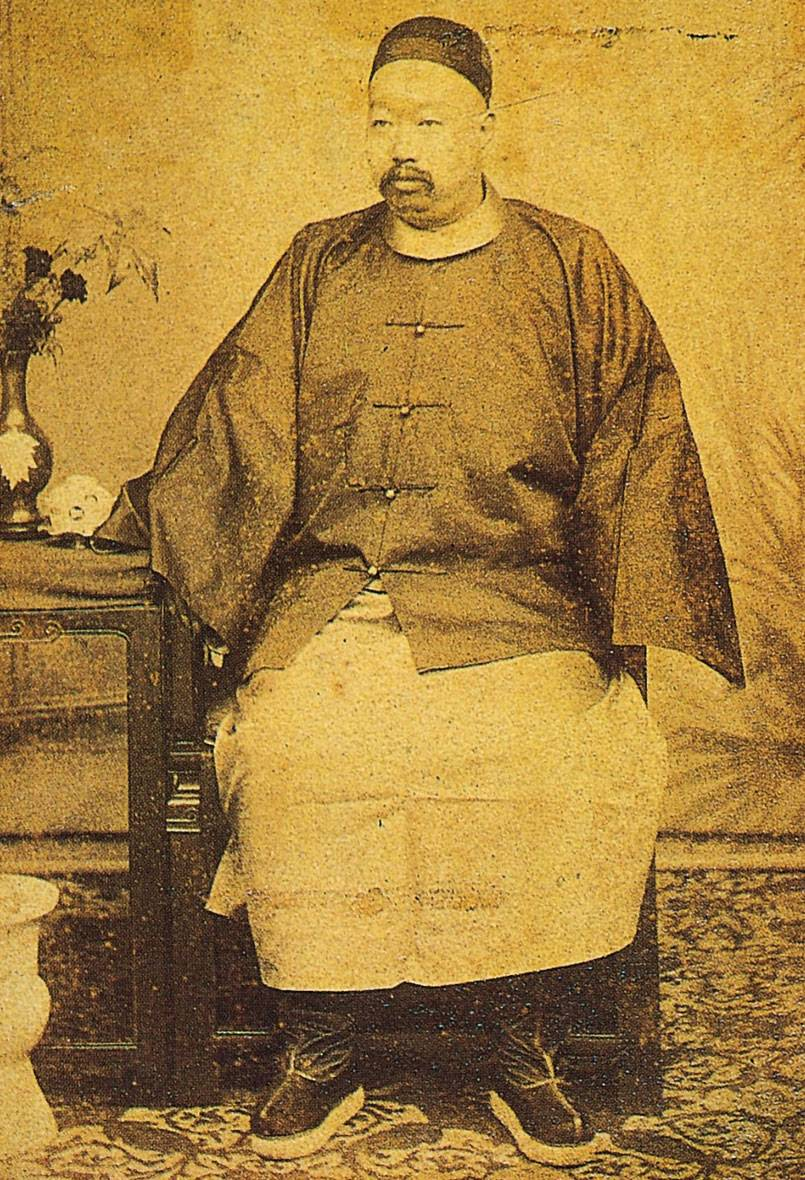
\includegraphics[scale=0.3]{picture/对照记23_2.jpeg}
\end{figure}

\clearpage
\par 【图二十四】我父亲我姑姑与他们的异母兄合影。
\par 我姑姑替她母亲不平。“我想奶奶是不愿意的。”
\par 我太罗曼蒂克,这话简直听不进去。
\par 我姑姑又道:“这老爹爹也真是——!两个女儿一个嫁给比她大二十来岁的做填房,一个嫁给比她小六岁的,一辈子嫌她老。”
\par 我见过六姑奶奶,我祖母唯一的妹妹,大排行第六。所以我看祖父的全集就光记得信札中的这一句:“任令有子年十六,”因为是关于他小姨的婚事,大致是说恩师十分器重这任姓知县,有意结为儿女亲家。六姑奶奶比这十六岁的少年大六岁(按照数字学,六这数目一定与她的命运有关),应是二十二岁。我祖母也是二十三岁才定亲,照当时的标准都是迟婚,因为父亲宠爱,留在身边代看公文等等,去了一个还剩一个。李鸿章本人似乎没有什么私生活。太太不漂亮(见图二十二),那还是不由自己作主的,他唯一的一个姨太太据说也丑。二子二女也都是太太生的。
\par 与她妹妹比起来,我祖母的婚姻要算是美满的了,在南京盖了大花园偕隐,诗酒风流。灭太平天国后,许多投置闲散的文武官员都在南京定居,包括我的未来外公家。大概劫后天京的房地产比较便宜。
\par 我姑姑对于过去就只留恋那园子。她记得一听说桃花或是杏花开了,她母亲就扶着女佣的肩膀去看——家里没有婢女,因为反对贩卖人口。——后来国民政府的立法院就是那房子。
\par “爷爷奶奶写了本食谱,”我姑姑说。她只记得有一样菜是鸡蛋吸出蛋白,注入鸡汤再煮。我没细问,想必总是蛋壳上钻个小孔,插入麦管之类,由仆人用口吸出再封牢。鸡蛋清的凝聚力强,恐怕就钻两个孔也还是倒不出来。而且她确是说吸出来。《红楼梦》上叫芳官吹汤小心不要溅上唾沫星子。叫人吸鸡蛋清即使闭着气,似乎也有点恶心。
\par 我祖父母还合著了一本武侠小说,自费付印,书名我记不清楚是否叫《紫绡记》。当时戚友圈内的《孽海花》热迫使我父亲找出这部书来给他们与我后母看。版面特小而字大,老蓝布套也有两套数十回。书中侠女元紫绡是个文武双全的大家闺秀,叙述中常称“小姐”而不名。故事沉闷得连我都看不下去。
\par 我祖父出身河北的一个荒村七家岮,比三家村只多四家,但是后来张家也可以算是个大族了。世代耕读,他又是个穷京官,就靠我祖母那一份嫁妆。他死过两个太太一个儿子,就剩一个次子,已经大了,给他娶的亲也是合肥人,大概是希望她跟晚婆婆合得来。
\par 我父亲与姑姑丧母后就跟着兄嫂过,拘管得十分严苛,而遗产被侵吞。直到我父亲结了婚有了两个孩子之后,兄妹俩急于分家,草草分了家就从上海搬到天津,住得越远越好。
\par 我八岁搬回上海,正赶上我伯父六十大庆,有四大名旦的盛大堂会,十分风光。
\par 一九三〇中叶他们终于打析产官司。我从学校放月假回来,问我姑姑官司怎样了。她说打输了。我惊问怎么输了,因为她说过有充分的证据。
\par “他们送钱,”她简短地说。顿了一顿又道:“我们也送。他们送得多。”
\par 这张看似爷儿仨的照片,三人后来对簿公堂。再看司法界的今昔,令人想起法国人的一句名言,关于时移世变:“越是变,越是一样。”
\par 当时我姑姑没告诉我败诉的另一原因是我父亲倒戈。她始终不愿多说,但是显然是我后母趋炎附势从中拉拢,舍不得断了阔大伯这门至亲——她一直在劝和,抬出大道理来说“我们家弟兄姊妹这么多,还都这么和气亲热,你们才几个人?”——而且不但有好处可得,她本来也就忌恨我姑姑与前妻交情深厚,出于女性的本能也会视为敌人。
\par 不过我父亲大概也怨恨他妹妹过去一直帮着嫂嫂,姑嫂形影不离隔离他们夫妇。向来离婚或失恋往往会怪别人,尤其是家属,不过一般都是对方的亲属。
\begin{figure}[htb]
    \centering %
    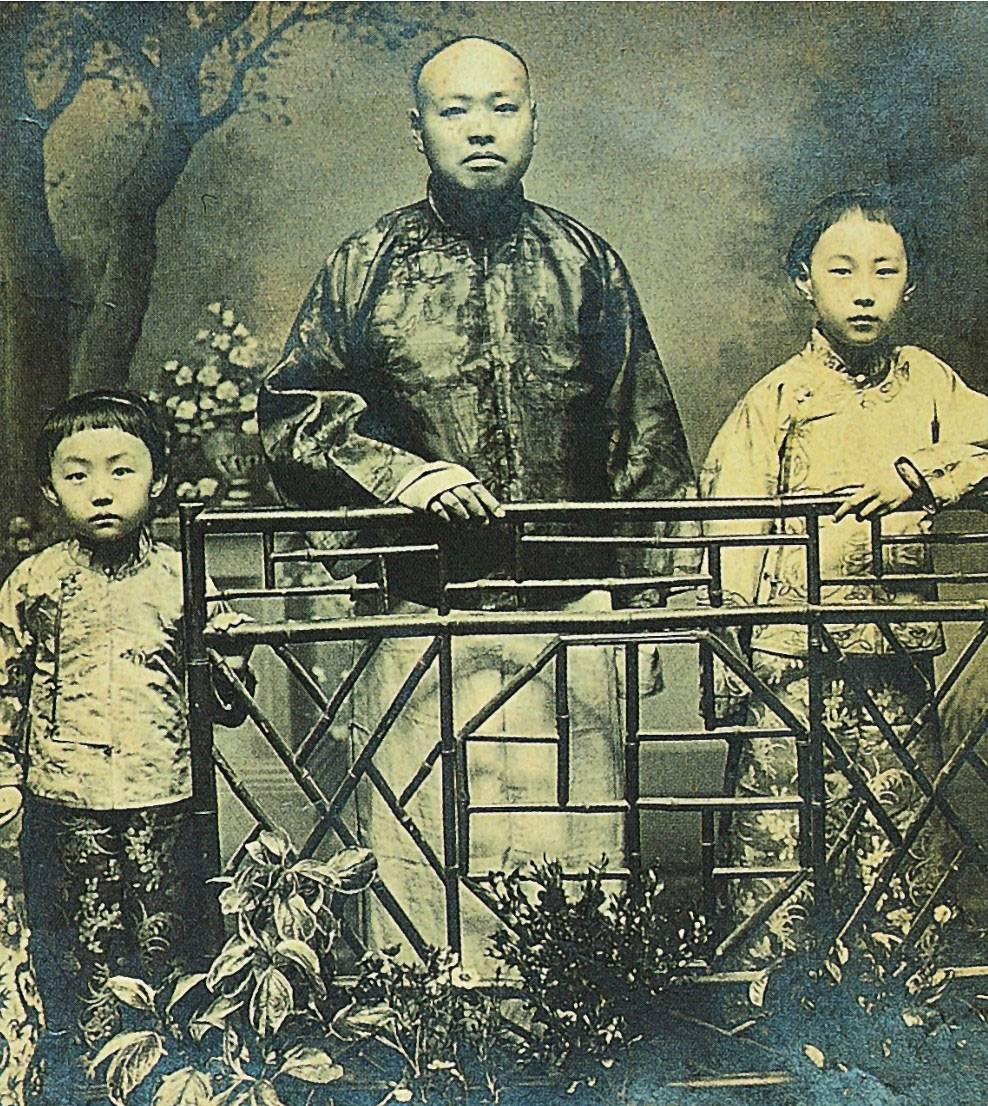
\includegraphics[scale=0.4]{picture/对照记24.jpeg}
\end{figure}

\clearpage
\par 【图二十五】我祖母带着子女合照。
\par 带我的老女佣是我祖母手里用进来的最得力的一个女仆。我父亲离婚后自己当家,逢到年节或是祖先生日忌辰,常躺在烟铺上叫她来问老太太从前如何行事。她站在房门口慢条斯理地回答,几乎每一句开始都是“老太太那张(‘辰光’皖北人急读为‘张’)……”
\par 我叫她讲点我祖母的事给我听。她想了半天方道:“老太太那张总是想方(法)省草纸。”
\par 也许现代人已经都没见过卫生纸流行以前的草纸,粗糙的草黄色大张厚纸上还看得见压扁的草叶梗,裁成约八寸见方,堆得高高的一叠备用。
\par 我觉得大杀风景,但是也可以想像我祖母孀居后坐吃山空的恐惧。就没想到等不到坐吃山空。命运就是这样防不胜防,她的防御又这样微弱可怜。
\par 沉默片刻,老女仆又笑道:“老太太总是给三爷穿得花红柳绿的,满帮花的花鞋——那时候不兴这些了,穿不出去了。三爷走到二门上,偷偷地脱了鞋换上袖子里塞着的一双。我们在走马楼窗子里看见了,都笑,又不敢笑,怕老太太知道了问。”那该是光复后搬到上海租界上的房子,当时流行走马楼,二层楼房中央挖出一个正方的小天井。
\par “三爷背不出书,打\UncommonChar{𫪘}!罚跪。”
\par 孤儿寡妇,望子成龙嘛!
\par 我父亲一辈子绕室吟哦,背诵如流,滔滔不绝一气到底,末了拖长腔一唱三叹地作结。沉默着走了没一两丈远,又开始背另一篇。听不出是古文时文还是奏摺,但是似乎没有重复的。我听着觉得心酸,因为毫无用处。
\par 他吃完饭马上站起来踱步,老女佣称为“走趟子”,家传的助消化的好习惯,李鸿章在军中也都照做不误的。他一面大踱一面朗诵,回房也仍旧继续“走趟子”,像笼中兽,永远沿着铁槛兜圈子巡行,背书背得川流不息,不舍昼夜——抽大烟的人睡得晚。
\par 我祖母给他穿颜色娇嫩的过时的衣履,也是怕他穿着入时,会跟着亲戚的子弟学坏了,宁可他见不得人,羞缩踧踖,一副女儿家的腼腆相。一方面倒又给我姑姑穿男装,称“毛少爷”,不叫“毛姐”。李家的小辈也叫我姑姑“表叔”,不叫表姑。
\par 我姑姑说我祖母后来在亲戚间有孤僻的名声。因又悄声道:“哪,就像这阴阳颠倒,那也是怪僻。”我现在想起来,女扮男装似是一种朦胧的女权主义,希望女儿刚强,将来婚事能自己拿主意。
\par 她在祭祀的遗像中面容比这张携儿带女的照片更阴郁严冷。
\par “二爸爸怕她。”我姑姑跟着我叫我伯父二爸爸。
\par “奶奶说要恨法国人,”她淡淡地说。
\par 又一次又道:“奶奶说福建人最坏了。当时海军都是福建人,结了帮把罪名都推在爷爷身上。”
\par 大概不免是这样想。后世谁都知道清朝的水师去打法国兵船根本是以卵击石。至今“中国海军”还是英文辞汇中的一个老笑话,极言其低劣无用的比喻。
\par 西谚形容幻灭为“发现他的偶像有黏土脚”——发现神像其实是土偶。我倒一直想着偶像没有黏土脚就站不住。我祖父母这些地方只使我觉得可亲,可悯。
\par 我没赶上看见他们,所以跟他们的关系仅只是属于彼此,一种沉默的无条件的支持,看似无用,无效,却是我最需要的。他们只静静地躺在我的血液里,等我死的时候再死一次。
\par 我爱他们。
\begin{figure}[htb]
    \centering %
    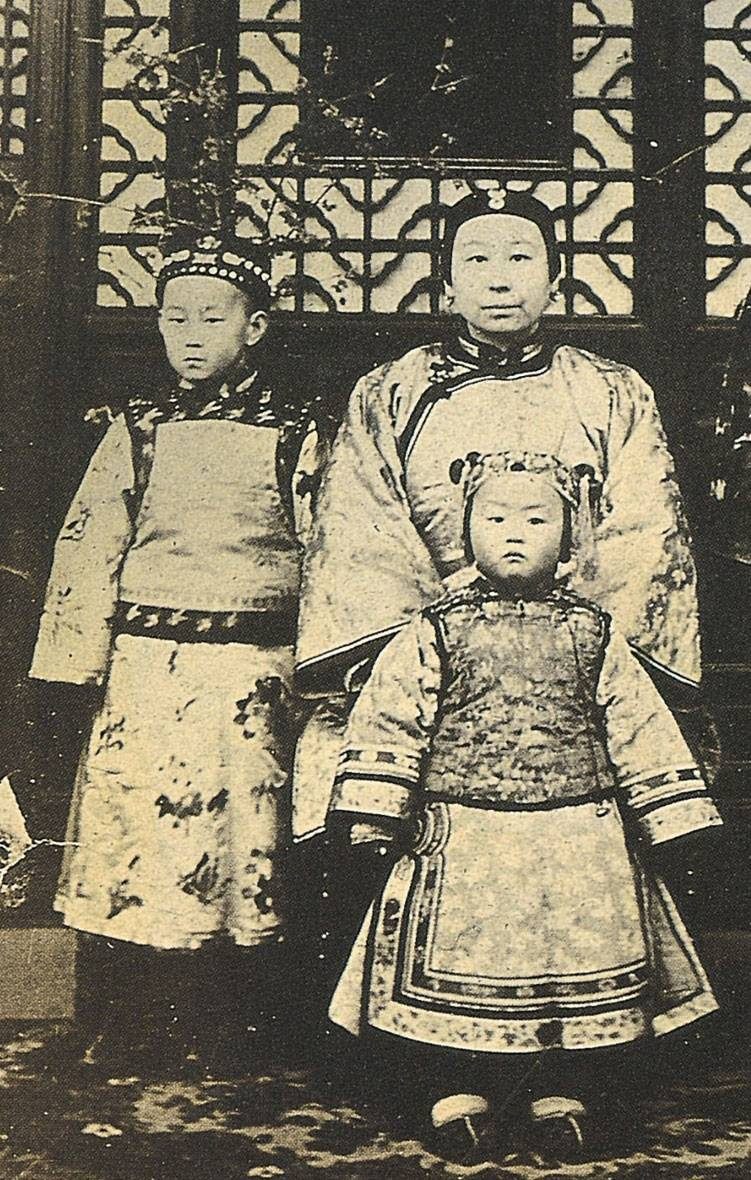
\includegraphics[scale=0.4]{picture/对照记25.jpeg}
\end{figure}

\clearpage
\par 【图二十六】在港大。
\par 一九三六年我母亲又回国一次,顺便安排我下年中学毕业后投考伦敦大学,就在上海西青会考试两天。因为家里不肯供给我出国留学,得先瞒着,要在她那里住两天,不然无法接连两天一早出外赴考。
\par 她从来没干涉我弟弟的教育,以为一个独子,总不会不给他受教育。不料只在家中延师教读。
\par “连衖堂小学都苛捐杂税的,买手工纸都那么贵。”我听见我父亲跟继母在烟铺上对卧着说。
\par 我弟弟四书五经读到《书经》都背完了才进学校,中学没念完就出去找事了。
\par 我考试前一天跟我父亲说:“姑姑叫我去住两天。”
\par 那天刚巧我后母不在家。
\par 明知我母亲与姑姑同住,我父亲旧情未断,只柔声应了声“唔,”躺着烧烟也没抬起眼来。
\par 考完了回去,我继母藉口外宿没先问过她,挑唆我父亲打了一顿禁闭起来。我姑姑自从打官司被出卖,就没上门过,这次登门劝解,又被烟枪打伤眼睛,上医院缝了六针。
\par 我终于逃出来投奔我母亲。去后我家里笑她“自扳砖头自压脚,”代背上了重担。
\par 我考上了伦敦大学,欧战爆发不能去,改入香港大学。我母亲与姑姑托了工程师李开第作监护人,她们在英国就认识的老友,也就是我现在的姑父。
\par 但是他不久就离开香港去重庆,改托他的一个朋友照应我,也是工程师,在港大教书,兼任三个男生宿舍之一的舍监。
\par 他跟他太太就住在那宿舍里。我去见他们。他是福建人,国语不太纯熟。坐谈片刻,他打量了我一下,忽笑道:“有一种鸟,叫什么……?”
\par 我略怔了怔,笑道:“鹭鸶。”
\par “对了。”他有点不好意思地笑着。
\par 丑小鸭变成丑小鹭鸶,而且也不小了。
\par 事实是我从来没脱出那“尴尬的年龄”(the awkward age),不会待人接物,不会说话。话虽不多,“夫人不言,言必有”失。
\begin{figure}[htb]
    \centering %
    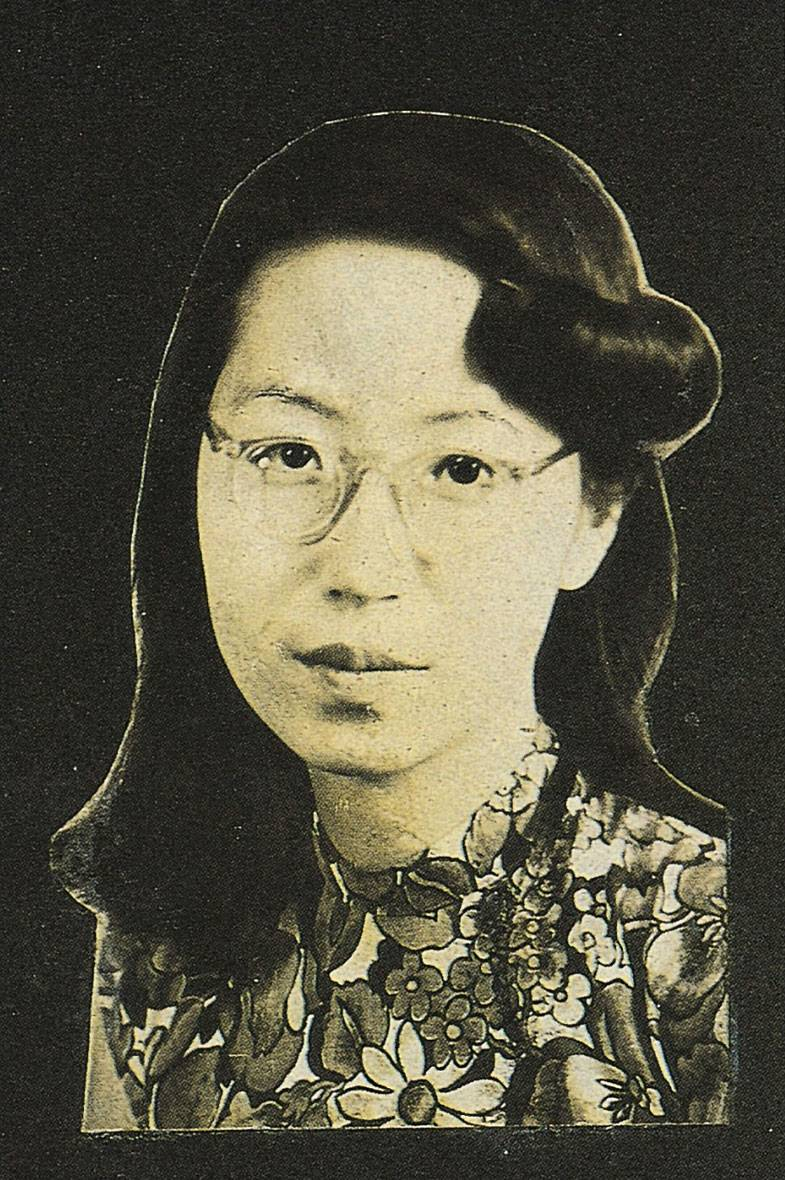
\includegraphics[scale=0.4]{picture/对照记26.jpeg}
\end{figure}

\clearpage
\par 【图二十七、二十八、二十九、三十】炎樱,一九四四年。
\par 港大文科二年级有两个奖学金被我一个人独得,学费膳宿费全免,还有希望毕业后免费送到牛津大学读博士。刚减轻了我母亲的负担,半年后珍珠港事变中香港也沦陷了,学校停办。
\par 我与同学炎樱结伴回上海,跟我姑姑住。炎樱姓摩希甸,父亲是阿拉伯裔锡兰人(今斯里兰卡),信回教,在上海开摩希甸珠宝店。母亲是天津人,为了与青年印侨结婚跟家里决裂,多年不来往。炎樱的大姨妈住在南京,我到他们家去过,也就是个典型的守旧的北方人家。
\par 炎樱进上海的英国学校,任prefect,校方指派的学生长,品学兼优外还要人缘好,能服众。
\par 我们回到上海进圣约翰大学,她读到毕业,我半工半读体力不支,入不敷出又相差过远,随即辍学,卖文为生。
\par 她有个小照相机,以下的七张照片都是她在我家里替我拍的,有一张经她着色。两人合影是在屋顶洋台上。
\begin{figure}[htb]
    \centering %
    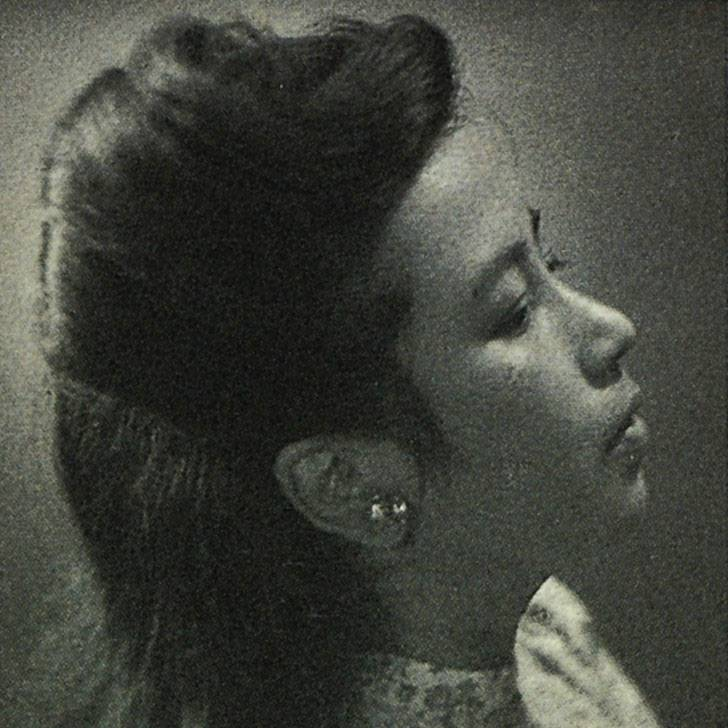
\includegraphics[scale=0.25]{picture/对照记27.jpeg}
    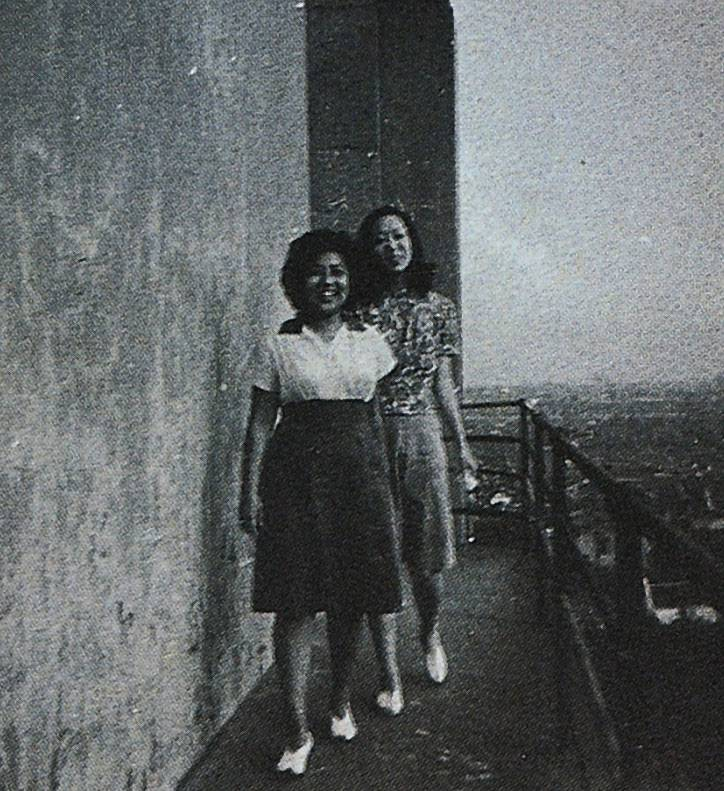
\includegraphics[scale=0.25]{picture/对照记28.jpeg}
    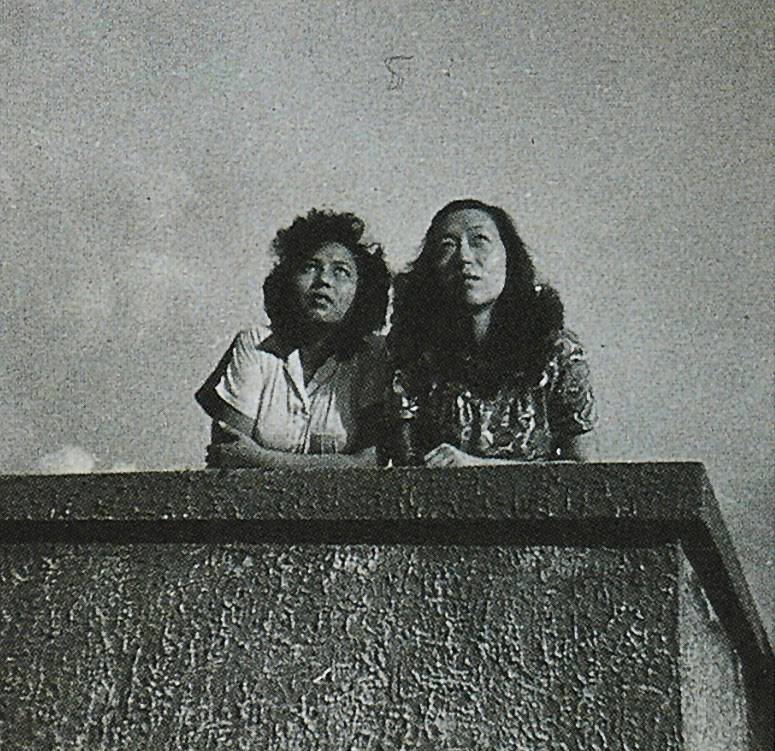
\includegraphics[scale=0.25]{picture/对照记29.jpeg}
    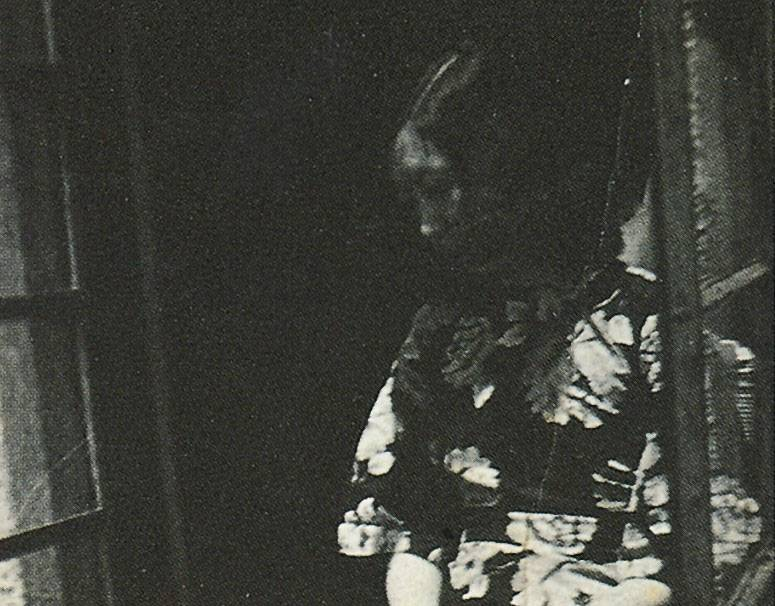
\includegraphics[scale=0.25]{picture/对照记30.jpeg}
\end{figure}

\clearpage
\par 【图三十一、三十二】这两张照片里的上衣是我在战后香港买的广东土布,最刺目的玫瑰红上印着粉红花朵,嫩黄绿的叶子。同色花样印在深紫或碧绿地上。乡下也只有婴儿穿的,我带回上海做衣服,自以为保存劫后的民间艺术,仿佛穿着博物院的名画到处走,遍体森森然飘飘欲仙,完全不管别人的观感。做了不少衣服,连件冬大衣也没有,我舅舅见了,着人翻箱子找出一件大镶大滚宽博的皮袄,叫我拆掉面子,皮里子够做件皮大衣。“不过是短毛貂,不大暖和,”他说。
\par 我怎么舍得割裂这件古董,拿了去如获至宝。(见图四十二)
\begin{figure}[htb]
    \centering %
    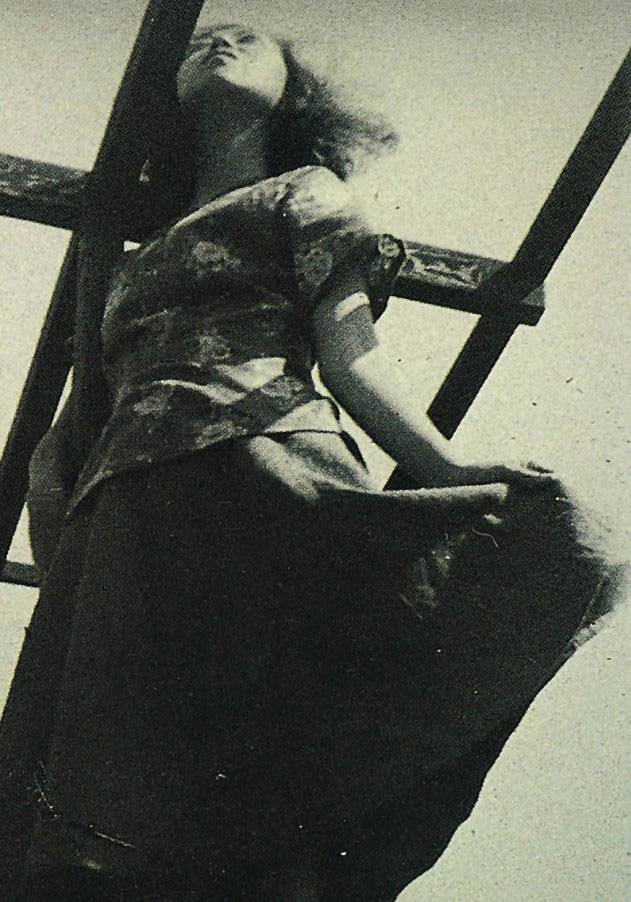
\includegraphics[scale=0.35]{picture/对照记31.jpeg}
    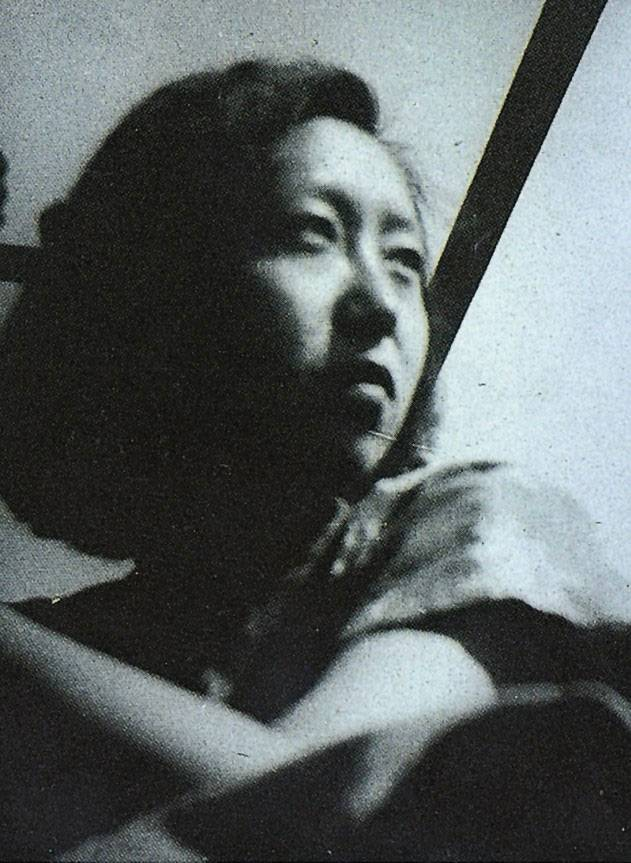
\includegraphics[scale=0.35]{picture/对照记32.jpeg}
\end{figure}

\clearpage
\par 【图三十三、三十四】一件花绸衣料权充裸肩的围巾。
\begin{figure}[htb]
    \centering %
    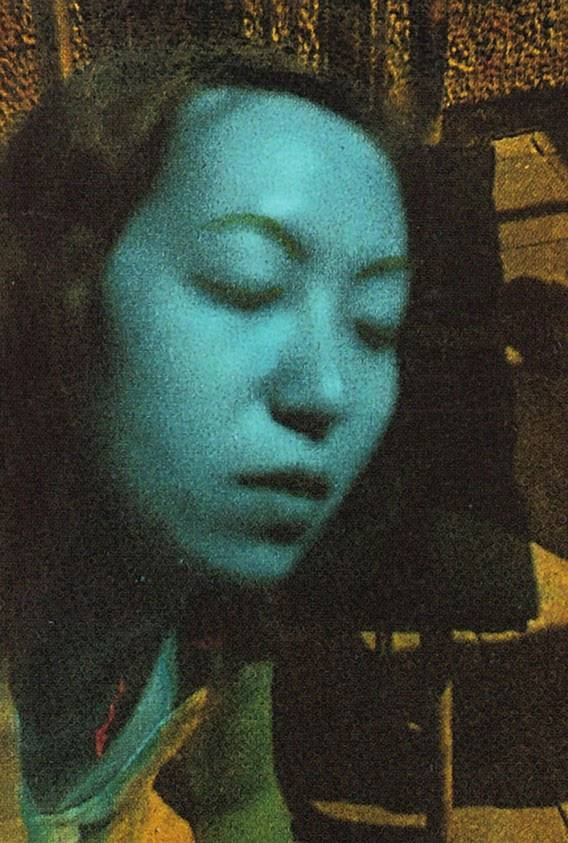
\includegraphics[scale=0.35]{picture/对照记33.jpeg}
    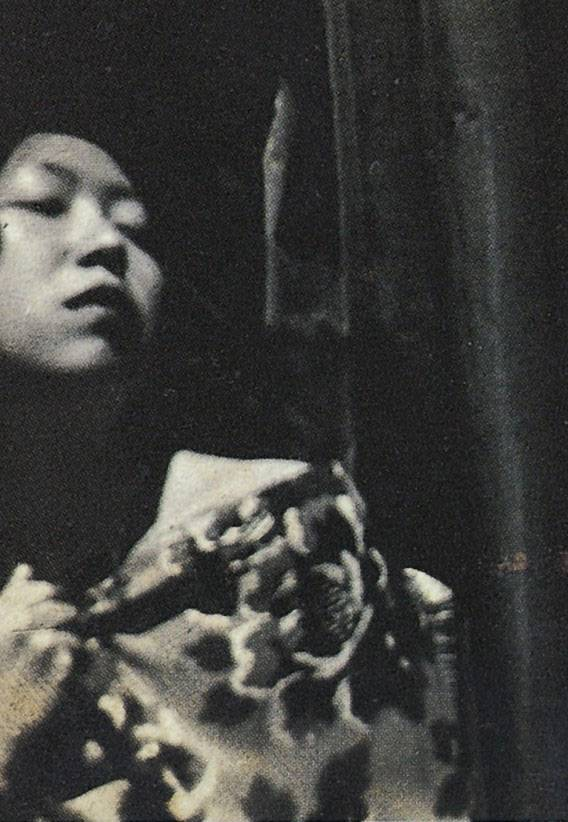
\includegraphics[scale=0.35]{picture/对照记34.jpeg}
\end{figure}

\clearpage
\par 【图三十五、三十六】炎樱想拍张性感的照片,迟疑地把肩上的衣服拉下点。上海人摄影师用不很通顺的英文笑问:“Shame, eh?”
\begin{figure}[htb]
    \centering %
    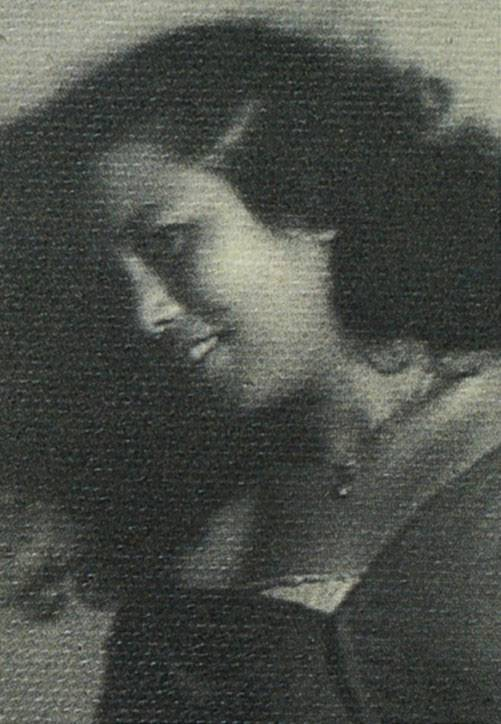
\includegraphics[scale=0.4]{picture/对照记35.jpeg}
    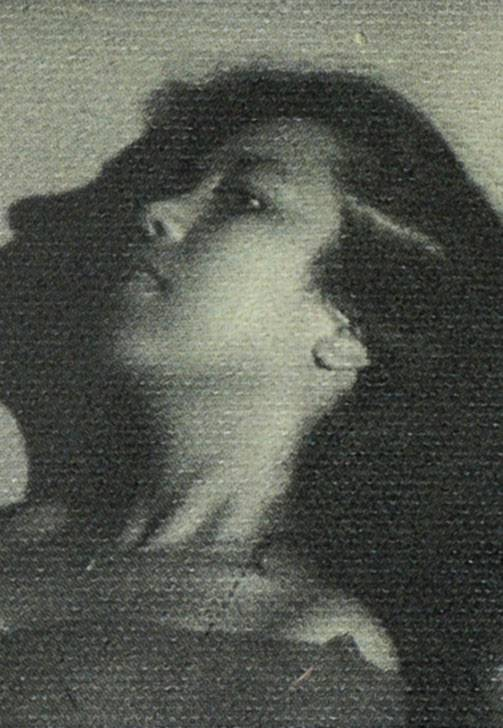
\includegraphics[scale=0.4]{picture/对照记36.jpeg}
\end{figure}

\clearpage
\par 【图三十七、三十八、三十九、四十】我从来不戴帽子,也没有首饰。这里的草帽是炎樱的妹妹的,项链是炎樱的。同一只坠子在图四十一中也借给我戴。
\begin{figure}[htb]
    \centering %
    \includegraphics[scale=0.35]{picture/对照记37.jpeg}
    \includegraphics[scale=0.35]{picture/对照记38.jpeg}
    \includegraphics[scale=0.35]{picture/对照记39.jpeg}
    \includegraphics[scale=0.35]{picture/对照记40.jpeg}
\end{figure}

\clearpage
\par 【图四十一】一九四三年在园游会中遇见影星李香兰(原是日本人山口淑子),要合拍张照,我太高,并立会相映成趣,有人找了张椅子来让我坐下,只好委屈她侍立一旁。
\par 《余韵》书中提起我祖母的一床夹被的被面做的衣服,就是这一件。是我姑姑拆下来保存的。虽说“陈丝如烂草”,那裁缝居然不皱眉,一声不出拿了去,照炎樱的设计做了来。米色薄绸上洒淡墨点,隐着暗紫凤凰,很有画意,别处没看见过类似的图案。
\begin{figure}[htb]
    \centering %
    \includegraphics[scale=0.4]{picture/对照记41.jpeg}
\end{figure}

\clearpage
\par 【图四十二、四十三】一九四四年业余摄影家童世璋与他有同好的友人张君——名字一时记不起了——托人介绍来给我拍照,我就穿那件唯一的清装行头,大袄下穿着薄呢旗袍。拍了几张,要换个样子。单色呢旗袍不上照,就在旗袍外面加件浴衣,看得出颈项上有一圈旗袍领的阴影。(为求线条简洁,我把低矮的旗袍领改为连续的圈领。)
\begin{figure}[htb]
    \centering %
    \includegraphics[scale=0.23]{picture/对照记42.jpeg}
    \includegraphics[scale=0.23]{picture/对照记43.jpeg}
\end{figure}

\clearpage
\par 【图四十四】照片背面我自己的笔迹写着“1946,八月”,不然也不记得是什么时候炎樱在我家里给拍的。
\par 我在港大的奖学金战后还在。进港大本来不是我的第一志愿,战后校中人事全非,英国惨胜,也在困境中。毕业后送到牛津进修也不过是当初的一句话。结果我放弃了没回去,使我母亲非常失望。
\begin{figure}[htb]
    \centering %
    \includegraphics[scale=0.4]{picture/对照记44.jpeg}
\end{figure}


\clearpage
\par 【图四十五】这张太模糊,我没多印,就这一张。我母亲战后回国看见我这些照片,倒拣中这一张带了去,大概这一张比较像她心目中的女儿。五〇末叶她在英国逝世,我又拿到遗物中的这张照片。
\begin{figure}[htb]
    \centering %
    \includegraphics[scale=0.4]{picture/对照记45.jpeg}
\end{figure}


\clearpage
\par 【图四十六】一九五〇或五一年,不记得是领什么证件,拍了这张派司照。
\par 这时候有配给布,发给我一段湖色土布,一段雪青洋纱,我做了一件喇叭袖唐装单衫,一条袴子。去排班登记户口,就穿着这套家常衫袴。
\par 街边人行道上搁着一张衖堂小学课室里的黄漆小书桌。穿草黄制服的大汉伛偻着伏在桌上写字,西北口音,似是老八路提干。轮到我,他一抬头见是个老乡妇女,便道:“认识字吗?”
\par 我笑着咕哝了一声“认识,”心里惊喜交集。不像个知识分子!倒不是因为身在大陆,趋时惧祸,妄想冒充工农。也并不是反知识分子。我信仰知识,就只反对有些知识分子的望之俨然,不够举重若轻。其实我自己两者都没做到,不过是一种愿望。有时候拍照,在镜头无人性的注视下,倒偶尔流露一二。
\begin{figure}[htb]
    \centering %
    \includegraphics[scale=0.4]{picture/对照记46.jpeg}
\end{figure}


\clearpage
\par 【图四十七】我姑姑,一九四〇末叶。我一九五二年离开大陆的时候她也还是这样。在我记忆中也永远是这样。
\begin{figure}[htb]
    \centering %
    \includegraphics[scale=0.4]{picture/对照记47.jpeg}
\end{figure}



\clearpage
\par 【图四十八】出大陆的派司照。
\par 离开上海的前夕,检查行李的青年干部是北方人,但是似乎是新投效的,来自华中一带开办的干部训练班。
\par 我唯一的金饰是五六岁的时候戴的一副包金小藤镯,有浅色纹路的棕色粗藤上镶着蟠龙蝙蝠。他用小刀刮金属雕刻的光滑的背面,偏偏从前的包金特别厚,刮来刮去还是金,不是银。刮了半天,终于有一小块泛白色。他瞥见我脸上有点心痛的神气,便道:“这位同志的脸相很诚实,她说是包金就是包金。”
\par 我从来没听见过这等考语。自问确是脂粉不施,穿着件素净的花布旗袍,但是两三个月前到派出所去申请出境,也是这身打扮,警察一听说要去香港,立刻沉下脸来,仿佛案情严重,就待调查定罪了。
\par 幸而调查得不很彻底,没知道我写作为生,不然也许没这么容易放行。一旦批准出境,马上和颜悦色起来,因为已经是外人了,地位仅次于国际友人。像年底送灶一样,要灶王爷“上天言好事,”代为宣扬中共政府待人民的亲切体贴。
\begin{figure}[htb]
    \centering %
    \includegraphics[scale=0.4]{picture/对照记48.jpeg}
\end{figure}


\clearpage
\par 【图四十九】一九五四年我住在香港英皇道,宋淇的太太文美陪我到街角的一家照相馆拍照。一九八四年我在洛杉矶搬家理行李,看到这张照片上兰心照相馆的署名与日期,刚巧整三十年前,不禁自题“怅望卅秋一洒泪,萧条异代不同时。”
\begin{figure}[htb]
    \centering %
    \includegraphics[scale=0.4]{picture/对照记49.jpeg}
\end{figure}


\clearpage
\par 【图五十】一九五五年离开香港前。
\par 我乘船到美国去,在檀香山入境检查的是个瘦小的日裔青年。后来我一看入境纸上的表格赫然填写着:
\par “身高六呎六吋半
\par 体重一百另二磅”
\par 不禁憎笑——有这样粗心大意的!五呎六吋半会写成为六呎六吋半。其实是个Freudian slip(茀洛依德式的错误)。心理分析宗师茀洛依德认为世上没有笔误或是偶尔说错一个字的事,都是本来心里就是这样想,无意中透露的。我瘦,看着特别高。那是这海关职员怵目惊心的纪录。
\begin{figure}[htb]
    \centering %
    \includegraphics[scale=0.4]{picture/对照记50.jpeg}
\end{figure}



\clearpage
\par 【图五十一】一九六一年,在三藩市家里,能剧面具下。
\begin{figure}[htb]
    \centering %
    \includegraphics[scale=0.4]{picture/对照记51.jpeg}
\end{figure}

\clearpage
\par 【图五十二】一九六二年回香港派司照。摄影师是个英国老太太,曾经是滑稽歌舞剧(vaudeville)歌星,老了在三藩市开爿小照相馆。
\begin{figure}[htb]
    \centering %
    \includegraphics[scale=0.5]{picture/对照记52.jpeg}
\end{figure}

\clearpage
\par 【图五十三】这张照片背面打着印戳:
\begin{figure}[htb]
    \centering %
    \includegraphics[scale=0.4]{picture/对照记53_1.jpeg}
\end{figure}


\par 我看着十分陌生,毫无印象,只记得这张照片是一九六六年离开华府前拍的。
\begin{figure}[htb]
    \centering %
    \includegraphics[scale=0.3]{picture/对照记53_2.jpeg}
\end{figure}




\clearpage
\par 【图五十四】一九六八年摄于波士顿。
\begin{figure}[htb]
    \centering %
    \includegraphics[scale=0.4]{picture/对照记54.jpeg}
\end{figure}




\par 以上的照片收集在这里唯一的取舍标准是怕不怕丢失,当然杂乱无章。附记也零乱散漫,但是也许在乱纹中可以依稀看得出一个自画像来。
\par 悠长得像永生的童年,相当愉快地度日如年,我想许多人都有同感。
\par 然后崎岖的成长期,也漫漫长途,看不见尽头。满目荒凉,只有我祖父母的姻缘色彩鲜明,给了我很大的满足,所以在这里占掉不合比例的篇幅。
\par 然后时间加速,越来越快,越来越快,繁弦急管转入急管哀弦,急景凋年倒已经遥遥在望。一连串的蒙太奇,下接淡出。
\par 其余不足观也已,但是我希望还有点值得一看的东西写出来,能与读者保持联系。



\subsubsection*{跋}


\par 写这本书,在老照相簿里钻研太久,出来透口气,跟大家一起看同一头条新闻,有“天涯共此时”的即刻感。手持报纸倒像绑匪寄给肉票家人的照片,证明他当天还活着。其实这倒也不是拟于不伦,有诗为证。诗曰:
\par 人老了大都
\par 是时间的俘虏,
\par 被圈禁禁足。
\par 它待我还好——
\par 当然随时可以撕票。
\par 一笑。

\begin{figure}[htb]
    \centering %
    \includegraphics[scale=0.4]{picture/对照记55.jpeg}
\end{figure}


\par *初载一九九三年十一月至一九九四年一月《皇冠》第四百七十七期、第四百七十八期、第四百七十九期,收入《对照记》。《跋》为该书第二版增补。



\subsection{编辑之痒}


\par 前两天看到《皇冠》十二月号连载的拙著《对照记》(中),文内自诩沉默寡言而“言必有中”。这一段原文是:
\par “事实是我从来没脱出那‘尴尬的年龄’(the awkward age),不会待人接物,不会说话。话虽不多,‘夫人不言,言必有’失。”
\par 本来末了没引语号,只是
\par “夫人不言,言必有失。”
\par 宋淇教授看了原稿来信说“夫人”会被误认为自称夫人太太。我回信说我本来也担心不清楚,加上引语号,表明是引四书上这句名言,只更动一个字,就绝对不会误会了。不料函札往返讨论了半天,刊出后赫然返璞归真成为:
\par “夫人不言,言必有中。”
\par 自嘲变成自吹自捧,尤其是认识我的人都知道我说话往往不得当,说我木讷还不服,大言不惭令人齿冷。
\par 上一期刊出的还有地名张家浜改为张家滨,当是因为“兵”“宾”同声,以为我嫌“滨”字笔画太多,独创一个简体字“浜”代替它。
\par “浜”这俗字音“邦”,大概是指江边或海边的水潭。上海人称Pidgin English为“洋泾浜”英文——洋人雇用的中国跑街仆役自成一家的英语,如“赶快”称chop-chop,“午餐”称“剔芬”(tiffin),后者且为当地外侨采用。我小时候一直听见我父亲说“剔芬”,直到十几岁才知道英文“午餐”是“冷吃”(lunch)不是“剔芬”。“芬”想必就是“饭”,“剔”不知道是中国何地方言。这一种语言是五口通商以来或更早的十八世纪广州十三行时代就逐渐形成的,还有葡萄牙话的痕迹。
\par 英文名言有“编辑之痒”(editorial itch)这名词。编辑手痒,似比“七年之痒”还更普遍,中外皆然。当然“浜”改“滨”,“言必有失”改“言必有中”不过是尽责的编者看着眼生就觉得不妥,也许礼貌地归之于笔误,径予改正。在我却是偶有佳句,得而复失,就像心口戳了一刀。明知一言既出,驷马难追,何况白纸黑字,读者先有了个印象,再辨正也晚了。
\par  
\par *初载一九九三年十二月二十八日《联合报》副刊,未收集。



\subsection{四十而不惑}


\par 皇冠纪念四十周年,编者来信要我写个祝福的小故事。我想来想去没有。
\par 最初听到祝福这件事,是《圣经》上雅各的哥哥必须要老父祝福他,才有长子继承权,能得到全部家产。父亲对子女有祝福的威权,诅咒也一样有效。中国人的“善颂善祷”就只是说吉利话希望应验。我从前看鲁迅的小说《祝福》就一直不大懂为什么叫“祝福”。祭祖不能让寡妇祥林嫂上前帮忙——晦气。这不过是负面的影响。祭祀祈求祖宗保佑,也只能暗中保佑,没有祝福的仪式。
\par 西方现在也只有开玩笑地或是老太太们表示感谢,轻飘地说声“上帝保佑!”或是“保佑你!”从来不好意思说整句的“上帝保佑你。”
\par 中国人倒是说“四十而不惑。”西方人也说“生命在四十岁开始。”不老也还是要“不惑”才禁得起风险。世变方殷,变得越来越快。皇冠单凭它磨练出的眼光也会在转瞬沧海桑田间找到它自己的路,走向更广阔的地平线。
\par  
\par *初载一九九四年二月《皇冠》第四百八十期,未收集。



\subsection{忆西风\\\small{——第十七届时报文学奖特别成就奖得奖感言}}

\par 得到《时报》的文学特别成就奖,在我真是意外的荣幸。这篇得奖感言却难下笔。三言两语道谢似乎不够恳切。不知怎么心下茫然,一句话都想不出来。但是当然我知道为什么,是为了从前《西风》的事。
\par 一九三九年冬——还是下年春天?——我刚到香港进大学,《西风》杂志悬赏征文,题目是《我的……》,限五百字。首奖大概是五百元,记不清楚了。全面抗战刚开始,法币贬值还有限,三元兑换一元港币。
\par 我写了篇短文《我的天才梦》,寄到已经是孤岛的上海。没稿纸,用普通信笺,只好点数字数。受五百字的限制,改了又改,一遍遍数得头昏脑胀。务必要删成四百九十多个字,少了也不甘心。
\par 法国修道院办的女生宿舍,每天在餐桌上分发邮件。我收到杂志社通知说我得了首奖,就像买彩票中了头奖一样。宿舍里同学只有个天津来的蔡师昭熟悉中文报刊。我拿给她看,就满桌传观。本地的女孩都是圣斯提反书院毕业的,与马来西亚侨生同是只读英文,中文不过识字,不大注意这些。本地人都是阔小姐,内中周妙儿更是父亲与何东爵士齐名,只差被英廷封爵的“太平绅士”(这名词想必来自香港的太平山),买下一个离岛盖了别墅,她请全宿舍的同学去玩一天。这私有的青衣岛不在渡轮航线内,要自租小轮船,来回每人摊派十几块钱的船钱。我就最怕在学费膳宿与买书费外再有额外的开销,头痛万分,向修女请求让我不去,不得不解释是因为父母离异,被迫出走,母亲送我进大学已经非常吃力等等。修女也不能作主,回去请示,闹得修道院长都知道了。连跟我同船来的锡兰朋友炎樱都觉得丢人,怪我这点钱哪里也省下来了,何至于。我就是不会撑场面。
\par 蔡师昭看在眼里,知道我虽然需要钱,得奖对于我的意义远大过这笔奖金,也替我庆幸。她非常稳重成熟,看上去总有二十几岁了。家里替她取名师昭,要她效法著《女训》的班昭,显然守旧。她是过来人,不用多说也能明白我的遭遇。
\par 不久我又收到全部得奖名单。首奖题作《我的妻》,作者姓名我不记得了。我排在末尾,仿佛名义是“特别奖”,也就等于西方所谓“有荣誉地提及(honorable mention)”。我记不清楚是否有二十五元可拿,反正比五百字的稿酬多。
\par 《我的妻》在下一期的《西风》发表,写夫妇俩认识的经过与婚后贫病的挫折,背景在上海,长达三千余字。《西风》始终没提为什么不计字数,破格录取。我当时的印象是有人有个朋友用得着这笔奖金,既然应征就不好意思不帮他这个忙,虽然早过了截稿期限,都已经通知我得奖了。
\par “我们中国人!”我对自己苦笑。
\par 幸而还没写信告诉我母亲。
\par “不是头奖。”我讪讪地笑着把这份通知单给蔡师昭看。其实不但不是头奖,二奖三奖也都不是。我说话就是这样乏。
\par 她看了也只咕哝了一声表示“怎么回事?”,没说什么,脸上毫无表情。她的一种收敛克制倒跟港大的英国作风正合适。她替我难堪,我倒更难堪了。
\par 下学期她回天津去进辅仁大学,我们也没通讯。
\par 《西风》从来没有片纸只字向我解释。我不过是个大学一年生。征文结集出版就用我的题目《天才梦》。
\par 五十多年后,有关人物大概只有我还在,由得我一个人自说自话,片面之词即使可信,也嫌小器,这些年了还记恨?当然事过境迁早已淡忘了,不过十几岁的人感情最剧烈,得奖这件事成了一只神经死了的蛀牙,所以现在得奖也一点感觉都没有。隔了半世纪还剥夺我应有的喜悦,难免怨愤。现在此地的文艺奖这样公开评审,我说了出来也让与赛者有个比较。
\par  
\par *初载一九九四年十二月三日《中国时报·人间》,未收集。




\subsection{笑纹后记}

\par 洛杉矶时报有个副刊题名View(观赏),兼收社交时装占星,以及妇女问题信箱,书评与连环图画。一九九四年五月改名Life and Style(生活与时尚),将流行名词lifestyle(生活作风,一般专指豪华或放浪的生活作风)一分为二,既浑成又俏皮。又新辟一个笑话专栏Laugh Lines,要读者听见什么笑话就寄给他们。我不是订户,只隔几天买份报,所以不太确定副刊改名的日期,反正大概是五月。
\par 在这以前一年,一九九三年三月号的皇冠登载我这篇《笑纹》,文内说笑话专栏可以叫Laugh Lines。现在洛杉矶华人多,不是不可能有皇冠读者向这美西第一大报建议采用这名称。当然也无法指控他们抄袭,只能相信纯属巧合。倒是我需要声明我不是剽窃。
\par 顺便再提一声,这里的五篇散文前三篇是一九四四年的作品。头两篇是我将《倾城之恋》小说改编为舞台剧,上演时写的。
\par  
\par *据手稿。




\subsection{重访边城}


\par 我回香港去一趟,顺便弯到台湾去看看。在台北下飞机的时候,没预备有认识的人来接。我叫麦先生麦太太不要来,因为他们这一向刚巧忙。但是也可能他们托了别人来接机,所以我看见一个显然干练的穿深色西装的人走上前来,并不感到诧异。
\par “你是李察·尼克逊太太?”他用英语说。
\par 我看见过金发的尼克逊太太许多照片,很漂亮,看上去比她的年龄年青二三十岁。我从来没以为我像她,而且这人总该认得出一个中国女同胞,即使戴着太阳眼镜。但是因为女人总无法完全不信一句谀词,不管多么显与事实不符,我立刻想起尼克逊太太瘦,而我无疑地是瘦。也许他当作她戴了黑色假发,为了避免引起注意?
\par “不是,对不起,”我说。
\par 他略一颔首,就转身再到人丛中去寻找。他也许有四十来岁,中等身材,黑黑的同字脸,浓眉低额角,皮肤油腻,长相极普通而看着很顺眼。
\par 我觉得有点奇怪,尼克逊太太这时候到台湾来,而且一个人来。前副总统尼克逊刚竞选加州州长失败,在记者招待会上说了句气话:“此后你们没有尼克逊好让你们踢来踢去了。”显然自己也以为他的政治生命完了。正是韬光养晦的时候,怎么让太太到台湾来?即使不过是游历,也要避点嫌疑。不管是怎么回事,总是出了点什么差错,才只有这么一个大使馆华人干员来接她。
\par “你们可晓得尼克逊太太要来?”我问麦氏夫妇。他们到底还是来了。
\par “哦?不晓得。没听见说。”
\par 我告诉他们刚才那人把我误认作她的笑话。麦先生没有笑。
\par “唔。”然后他有点不好意思地说:“有这么个人老是在飞机场接飞机,接美国名人。有点神经病。”
\par 我笑了起来,随即被一阵抑郁的浪潮淹没了,是这孤岛对外界的友情的渴望。
\par 一出机场就有一座大庙,正殿前一列高高的白色水泥台阶,一个五六十岁的太太相当费劲地在往上爬,裹过的半大脚,梳着髻,臃肿的黑旗袍的背影。这不就是我有个中学同班生的母亲?麦先生正在问我“回来觉得怎么样?”我惊异地微笑,说:“怎么都还在这儿?当是都没有了嘛!”除了年光倒流的感觉,那大庙几乎直盖到飞机场里,也增加了时空的混乱。当时没想到,送行怕飞机失事,要烧香求菩萨保佑,就像渔村为了出海打渔危险,必定要有妈祖庙一样。
\par 我以前没到过台湾,但是珍珠港事变后从香港回上海,乘的日本船因为躲避轰炸,航线弯弯扭扭的路过南台湾,不靠岸,远远的只看见个山。是一个初夏轻阴的下午,浅翠绿的欹斜秀削的山峰映在雪白的天上,近山脚没入白雾中。像古画的青绿山水,不过纸张没有泛黄。倚在船舷上还有两三个乘客,都轻声呼朋唤友来看,不知道为什么不敢大声。我站在那里一动都不动,没敢走开一步,怕错过了,知道这辈子不会再看见更美的风景了。当然也许有更美的,不过在中国人看来总不如——没这么像国画。
\par 轮船开得不快,海上那座山维持它固定的姿势,是否有好半天,还是不过有这么一会工夫,我因为实在贪看,唯恐下一分钟就没有了,竟完全没数,只觉得在注视,也不知道是注入还是注出,仿佛一饮而尽,而居然还在喝,还在喝,但是时时刻刻都可能发现衔着空杯。末了它是怎样远去或是隐没的,也不记得了,就那一个永远忘不了的印象。这些年后到台湾来,根本也没打听那是什么山。我不是登山者,也不想看它陆地上的背面。还是这样好。
\par “台北不美,不过一出城就都非常美,”麦先生在车上说。
\par 到处是骑楼,跟香港一样,同是亚热带城市,需要遮阳避雨。罗斯福路的老洋房与大树,在秋暑的白热的阳光下树影婆娑,也有点像香港。等公车的男女学生成群,穿的制服乍看像童子军。红砖人行道我只在华府看到,也同样敝旧,常有缺砖。不过华盛顿的街道太宽,往往路边的两层楼店面房子太萎琐,压不住,四顾茫茫一片荒凉,像广场又没有广场的情调,不像台北的红砖道有温暖感。
\par 麦氏夫妇知道我的脾气,也不特地请吃饭招待,只作了一些安排。要看一个陌生的城市,除了步行都是走马看花。最好是独行,但是像我这样不识方向的当然也不能一个人乱走。
\par 午后麦太太开车先送麦先生上班,再带我到画家席德进那里去。麦太太是美国人,活泼泼地把头一摔,有点赌气地说:“他是我最偏爱的一个人。(He's my favorite person.)”
\par 她在大门口楼梯脚下哇啦一喊,席先生打着赤膊探头一看,有点不好意思地去穿上衬衫再招呼我们上楼。楼上虽然闷热,布置得简单雅洁,我印象中原色髹漆的板壁很多,正是挂画的最佳背景。走廊就是画廊。我瞻仰了一会,太热,麦太太也没坐下就走了,席先生送她出去,就手陪我去逛街。
\par 有席德进带着走遍大街小巷,是难求的清福。他默无一语,简直就像你一个人逍遥自在地散步,不过免除迷路的恐慌。钻进搭满了晾衣竿的狭巷,下午湿衣服都快干了,衣角偶而微凉,没有水滴在头上。盘花金色铁窗内望进去,小房间里的单人床与桌椅一览无余,浅粉色印花挂衣袋是美国没有的。好像还嫌不够近,一个小女孩贴紧了铁栅站在窗台上,一动也不动地望着我们挨身走过。也许因为房屋轻巧新建,像挤电梯一样挤得不郁塞,仿佛也同样是暂时的。
\par 走过一个花园洋房,灰色砖墙里围着相当大的一块空地,有两棵大树。
\par “这里有说书的。时候还没到,”他说。
\par 想必是露天书场,藤椅还没搬出来。比起上海的书场来,较近柳敬亭原来的树下或是茶馆里说书。没有粽子与苏州茶食,茶总有得喝?要经过这样的大动乱,才摆脱了这些黏附物——零食;雪亮的灯光下,两边墙上橱窗一样大小与位置的金框大镜,一路挂到后座,不但反映出台上的一颦一笑,连观众也都照得清清楚楚。大概为了时髦妓女和姨太太们来捧场,听完了一档刚下场就袅袅婷婷起身离去,全场瞩目,既出风头又代作广告。
\par 经过一座庙,进去随喜。这大概是全世界最家常的庙宇,装着日光灯,挂着日历。香案上供着蛋杯——吃煮蛋用的高脚小白磁杯,想是代替酒盅。拜垫也就用沙发上的荷叶边软垫,没有蒲团。墙上挂着个木牌写着一排排的姓名,不及细看,不知是不是捐钱盖庙的施主。
\par 祀的神中有神农,半裸,深棕色皮肤,显然是上古华南居民,东南亚人的远祖。神农尝百草,本来草药也大都是南方出产,北边有许多都没有。草药发明人本来应当是华南人。——是否就是“南药王”?——至于民间怎么会知道史前的华南人这么黑,只能归之于种族的回忆,浩如烟海的迷茫模糊的。我望着那长方脸黝黑得眉目不清的,长身盘腿坐着的神农,败在黄帝手中的蚩尤的上代,不禁有一种森森然的神秘感,近于恐惧。
\par 神案上花瓶里插着塑胶线组成的镂空花朵。又插着一大瓶彩纸令旗,过去只在中秋节的香斗上看见过。该是道教对佛寺的影响。神殿一隅倚着搭戏台用的木材。
\par 下一座庙是个古庙——当然在台北不会太古老。灰色的屋瓦白苍苍的略带紫蓝,色调微妙,先就与众不同。里面的神像现代化得出奇,大头,面目狰狞,帽子上一颗大绒球横斜,武生的戏装;身材极矮,从俯视的角度压缩了。与他并坐的一位索性没有下半身。同是双手搁在桌上,略去下肢的一个是高个子,躯干拉长了,长眉直垂到腮颊上。这决不是受后期印象派影响的现代雕塑,而是当年影响马蒂斯的日本版画的表亲或祖先。日本吸收中国文化,如汉字就有一大部份是从福建传过去的。闽南塑像的这种特色,后来如果失传了,那就是交通便利了些之后,被中原的主流淹没了。(注)
\par 下首大玻璃柜里又有只淡黄陶磁怪龙,上颏奇长,长得像食蚁兽,如果有下颏,就是鳄鱼了,但是缺下颏,就光吐出个舌头。背上生翅,身子短得像四脚蛇。创造怪兽,似乎殷周的铜器之后就没有过?
\par 这么许多疑问,现成有行家在侧,怎么不请教一声?仿佛有人说过,发问也要学问。我脑子一时转不过来,不过看着有点奇怪而已,哪问得出什么。连庙名没看清楚,也都没问是什么庙。多年后根据当时笔记作此文,席德进先生已经去世,要问也没处问了。那天等于梦游症患者,午睡游台北。反正那庙不会离席先生寓所太远,不然我也走不动。
\par 麦家这两天有远客住在他们家,替我在山上的日式旅馆定了个房间,号称“将军套房”,将军上山来常住的。进房要经过一连串的小院子,都有假山石与荷池,静悄悄的一个人影子都不见。在房中只听见黄昏细雨打着芭蕉,还有就是浴室里石狮子嘴里流出的矿泉,从方柜形水泥浴缸口漫出来,泊泊溅在地上。房间里塌塌米上摆着藤家具。床上被单没换,有大块黄白色的浆硬的水渍。显然将军不甘寂寞。如果上次住在这里的是军人。我告诉自己不要太挑剔,找了脚头一块干净土蜷缩着睡,但是有臭虫。半夜里还是得起来,睡在壁龛的底板上——日式客厅墙上的一个长方形浅洞,挂最好的画,摆最好的花瓶的地方。下缘一溜光滑的木板很舒服,也不太凉。一觉睡到日上三竿,女服务生进来铺床,找不到我,吓了一大跳。
\par 幸而只住了一夜。麦家托他们的一个小朋友带我到他家乡花莲观光,也是名城,而且有高山族人。
\par 一下乡,台湾就褪了皮半卷着,露出下面较古老的地层。长途公共汽车上似乎全都是本省人。一个老妇人扎着地中海风味的黑布头巾、穿着肥大的清装袄袴,戴着灰白色的玉镯——台玉?我也算是还乡的复杂的心情变成了纯粹的观光客的游兴。
\par 替我作向导的青年不时用肘弯推推我,急促地低声说:“山地山地!”
\par 我只匆匆一瞥,看到一个纤瘦的灰色女鬼,颊上刺青,刻出蓝色胡须根根上翘,翘得老高,背上背着孩子,在公路旁一爿店前流连。
\par “山地山地!”
\par 吉卜西人似的儿童,穿着破旧的T恤,西式裙子,抱着更小的孩子。
\par “有日本电影放映的时候,他们都上城来了,”他说。
\par “哦?他们懂日文?”
\par “说得非常好。”
\par 车上有许多乘客说日语。这都是早期中国移民,他们的年青人还会说日文的多得使人诧异。
\par 公共汽车忽然停了,在一个“前不巴村,后不巴店”的地方。一个壮硕的青年跳下车去,车掌也跟着下去了。忽然打起架来,两人在地下翻滚。蓝天下,道旁的作物像淡白的芦梗矮篱似的齐臻臻的有二尺高。
\par “契咖茹哟!契咖茹哟!(搞错了哟!)”那青年在叫喊。
\par 司机也下去了,帮着打他。
\par 大概此地民风强悍。一样是中国人,在香港我曾经看见一个车掌跟着一个白坐电车的人下去,一把拉住他的西装领带,代替从前的辫子,打架的时候第一先揪的。但是那不过是推推搡搡辱骂恫吓,不是真动武。这次我从台湾再去香港,有个公车车掌被抓进警察局,因为有个女人指控他用车票打孔机打她。——他们向来总是把那件沉重的铁器临空扳得轧轧响,提醒大家买票。——那也还不是对打。香港这一点是与大陆一致的,至少是提倡“武斗”前的大陆。
\par 这台湾司机与车掌终于放了那青年,回到车上来。
\par “他们说这人老是不买票,总是在这儿跳下去,”我的青年朋友把他们的闽南话译给我听。
\par 挨打的青年站起来拍拍身上的灰尘。他的美军剩余物资的茶褐色衬衫撕破了。公车开走了,开过他身边的时候,他向它立正敬礼。他不会在日据时代当过兵,年纪不够大,但是那种奇异的敬意只有日本有。
\par 观光客大都就看个教堂,在中国就是庙了。花莲的庙比台北还更家庭风味,神案前倚着一辆单车,花瓶里插着鸡毛掸帚。装置得高高的转播无线电放送着流行音乐。后院红砖阑干砌出工字式空花格子,衬着芭蕉,灯影里偶有一片半片蕉叶碧绿。后面厨房里昏黄的灯下,墙上挂着一串玲珑的竹片锁链,蒸馒头用的。我不能想像在蒸笼里怎么用,恨不得带回去拿到高级时装公司去推销,用作腰带。纯棉的瑞士花布如果乱红如雨中有一抹竹青,响应竹制衣带,该多新妍可喜!
\par 花莲城隍庙供桌上的暗红漆茭杯像一副猪腰子。浴室的白磁砖墙。殿前方柱与神座也是白磁砖。横挡在神案前的一张褪色泥金雕花木板却像是古物中的精品。又有一对水泥方柱上刻着红字对联。忽然一抬头看见黑洞洞的天上半轮凉月——原来已经站在个小院子里。南中国的建筑就是这样紧凑曲折,与方方正正的四合院大不相同。月下的别院,不禁使人想起无数的庵堂相会的故事。
\par 此地的庙跟台北一样,供香客插烛的高脚蜡台上都没装铁签——那一定是近代才有的。台湾还是古风,山字架的下截补换了新木,更显出上半的黯黑旧白木棍棒的古拙。有的庙就在木架上架只小藤箩,想必箩中可以站满蜡烛——一只都没有,但是揣度木架的部位与高矮,不会不是烛台。因陋就简,还是当初移民的刻苦的遗风。
\par 还有一个特点是神像都坐在神龛外,绣幔前面。乍看有点看不惯,太没掩蔽,仿佛丧失了几分神秘庄严。想来是神像常出巡,抬出抬进,天气又热,挥汗出力搬扛的人挨挨擦擦,会污损丝绸帐幔。我看见过一张照片上,庙门外挤满了人,一个穿白汗背心的中年男子笑着横抱着个长须神像,脸上的神情亲切,而仿佛不当桩事,并不肃然。此地的神似乎更接近人间,人比在老家更需要神,不但背乡离井,同荒械斗“出草”也都还是不太久以前的事,其间又还经过五十年异族的统治,只有宗教是还是许可的。这里的人在时间与空间上都是边疆居民,所以有点西部片作风。我想起公共汽车旁的打斗。
\par 花莲风化区的庙,荷叶边拜垫上镶着彩色补钉图案,格外女性化些。有一只破了的,垫在个大缸底下。高僧坐化也是在缸中火葬的,但是这里的缸大概是较日常的用途。缸上没有木盖,也许还是装自来水前的水缸。香案前横幅浮雕板上嵌满碎珊瑚枝或是海滩石子作背景。日光灯的青光下,绣花神幔上包着的一层玻璃纸闪闪发光。想必因为天气潮湿,怕丝绸腐烂。
\par 夜间没有香客,当然是她们正忙的时候。殿外大声播送爵士乐,更觉冷冷清清。廊下一群庙祝高坐在一个小平台上,半躺在藤椅上翘着脚喝茶谈天。殿侧堆着锣鼓乐器,有一面大鼓上写着“特级”二字。
\par 附近街上一座简陋的三层楼木屋,看上去是新造的,独门独户站在一小块空地上,门口挂着“甲种妓女户”门牌。窗内灯光雪亮,在放送摇滚乐。靠墙直挺挺两只木椅,此外一无所有。两个年青的女人穿着短旗袍,长头发披在背上,仿佛都是大眼睛高个子高胸脯,足有国际标准,与一个男子在跳摇滚舞。男子近中年了,胖胖的,小眼睛,有点猪相,拱着鼻子,而面貌十分平凡,穿着米色拉链夹克,随和地舒手舒脚,至多可以说跟得上。但是此地明明不是舞校,也许是他们自己人闲着没事做广告。
\par 二等妓院就没有这么纯洁了。公共食堂大观园附设浴堂,想也就是按摩院,但是听说是二等妓院。楼下一排窗户里,有一张藤躺椅上铺着条毛巾被,通内室的门里有个大红织锦缎长旗袍的人影一闪。这样衣冠齐整怎么按摩?似乎与大城市的马杀鸡性质不同。
\par 另一个窗户里有个男子裸体躺在藤椅上,只盖块大毛巾。又有个窗户里,一个人伛偻着在剪脚趾甲。显然不像大陆上澡堂子里有修脚的。既然是自理,倒不省点钱在家里剪,而在这春宵一刻值千金的时候且忙着去剪脚趾甲。虽然刚洗过澡指甲软些容易剪,也是大杀风景的小小豪举。
\par 这一排窗户不知是否隔成小室的统间,下半截墙漆成暗绿色,上半截奶油色,壁上有只老式挂钟。楼下大敞着门,门前停着许多单车,歪歪斜斜互相偎倚着叠放。大门内一列深棕色柜台,像旅馆或医院挂号处。墙壁也漆成同样的阴暗的绿色,英美人称作“医院绿”的。
\par 大概因为气候炎热需要通风,仿佛没有窗帘这样东西,一律开放展览。小电影院也只拉上一半铁门,望进去黑洞洞的一直看到银幕与两旁的淡绿色舞台幕。
\par 风化区的照相馆门口高高下下挂满妓女的照片,有的学影星张仲文长发遮住半边脸,有的像刘琦,都穿着低领口夜礼服。又有同一人两张照片叠印的,清末民初盛行的“对我图”。
\par 夜游后,次日再去看古屋。本地最古老的宅第是个二层楼红砖屋,正楼有飞檐,山墙上镶着湖绿陶磁挖花壁饰,四周簇拥着淡蓝陶磁小云朵。两翼是平房。场院很大,矮竹篱也许是后添的。院门站得远远的,是个小牌楼,上有飞檐,下面一对红砖方柱。
\par 台湾仿佛一直是红砖,大概因为当地的土质。大陆从前都是青砖,其实是深灰色,可能带青灰。因为中国人喜爱青色——“青出于蓝而胜于蓝”——径称为青砖。红砖似是外来的,英国德国最普遍的,条顿民族建筑的特色。在台湾,红砖配上中国传统的飞檐与绿磁壁饰,于不调和中别有一种柔艳憨厚的韵味。
\par 有个嘉庆年间的庙,最古的一翼封闭了,一扇门上挂着木牌,上写“办公处Office”。侧面墙上有个书卷形小窗,两翼各嵌一只湖绿陶磁挖花壁饰作窗棂,中央的一枚想必砸破了,换装三根原木小棍子,也已经年深月久了,予人的感觉是原有的,整个的构图倒更朴拙有致。
\par 又有一幢老屋,普通的窗户也用这种八角形绿磁挖花壁饰作窗棂,六只叠成两行。后加同色木栅保护,褪色的淡蓝木栅也仍旧温厚可爱,没有不调和。
\par 小巷里,摇茶叶的妇人背着孩子在门前平台上席地围坐,大家合捧着个大扁篾篮,不住地晃动着。篮子里黑色的茶叶想必是乌龙,茶香十步外特别浓。另一家平台上堆满了旧车胎。印度也常有这种大门口的平台。
\par 年青的朋友带我来到一处池塘,一个小棕榈棚立在水心。碧清的水中偶有两丛长草倒影。是农场还是渔塭?似乎我的导游永远都是沉默寡言,我不知道怎么也从来不问。
\par 有个长发女郎站在亮蓝的水里俯身操作,一件橙黄桔绿的连衫裙卷到大腿上;面貌身材与那两个甲种妓女同一类型,不过纤巧清扬。除了电影里,哪有这等人物这身打扮作体力劳动的?如果我是贵宾来参观,就会疑心是“波田姆金的村庄”——俄国女皇凯萨琳二世的宠臣波田姆金(Potemkin)在女皇游幸途中遍植精雅的农舍,只有前面一堵假墙,又征集村姑穿着当地传统服装载歌载舞,一片升平气象。
\par 这美人想必引人注目惯了,毫不理会我们眈眈遥视,过了一会,径自趟水进棚去了。我这才微弱地嗳呀了一声,带笑惊叹。那青年得意地笑了。
\par 此地大概是美人多。一来早期移民本来是南国佳人,又有娶山地太太的高山族,至少是花莲的阿美族比著名出美人的峇里人还要漂亮。
\par 我们沿着池边走到一个棕榈凉亭歇息,吃柚子。从来没吃过这样酸甜多汁的柚子,也许因为产地近,在上海吃到湖南柚子早已干了。我望着地下栏杆的阴影里一道道横条阳光。刚才那彩色阔银幕的一场戏犹在目前,疑幻疑真,相形之下,柚子味吃到嘴里真实得使人有点诧异。
\par  
\par 同是边城,香港不像台湾有一水之隔,不但接壤,而且返乡探亲扫墓的来来去去络绎不绝,对大陆自然看得比较清楚。我这次分租的公寓有个大屋顶洋台,晚上空旷无人,闷来就上去走走,那么大的地方竟走得团团转。满城的霓虹灯混合成昏红的夜色,地平线外似有山外山遥遥起伏,大陆横躺在那里,听得见它的呼吸。
\par 二房东太太是上海人,老是不好意思解释他们为什么要分租:“我们都是寄包裹寄穷了呀!”
\par 他们每月寄给她婆家娘家面条炒米咸肉,肉干笋干,砂糖酱油生油肥皂,按季寄衣服。有一种英国制即融方块鸡汤,她婆婆狂喜地来信说它“解决了我们一天两顿饭的一切问题”。砂糖他们用热水冲了吃作为补品。她弟弟在劳改营,为了窝藏一个国特嫌犯;写信来要药片治他的腰子病与腿肿。她妹妹是个医生,派到乡下工作。“她晚上要出诊,乡下地方漆黑,又高低不平,她又怕蛇——女孩子不就是这样。”她抱歉的声口就像是说她的两个女儿占用浴室时间太长,“女孩子不就是这样。”
\par 我正赶上看见他们一次大打包。房东太太有个亲戚要回去,一个七十来岁的老太太,可以替他们带东西。她丈夫像牛仔表演捉小牛,用麻绳套住重物,挣扎得在地板上满地滚。房东太太烤了只蛋糕,又炖了一锅红烧肉。
\par “锅他们也用得着,”她说。
\par “一锅红烧肉怎么带到上海?”我说。
\par “冻结实了呀。火车像冰箱一样。”
\par 她天亮就起来送行,也要帮着拎行李通过罗湖边境的检查。第二天她一看见我就叫喊起来:“哈呀!张小姐,差点回不来喽!”“嗳呀,怎么了?”
\par “嚇咦呀!先不先,东西也是太多,”她声音一低,用串通同谋的口气。“也是这位老太,她自己的东西实在多不过。整桶的火油,整箱的罐头,压成板的咸鱼装箱,衣裳被窝毯子,锅呀水壶,样样都有,够陪嫁摆满一幢房子的。关卡上的人不耐烦起来了。后来查到她皮夹子里有点零钱,人民票,还是她上趟回来带回来的,忘了人民票不许带出来的。夥咦!这就不得了了。‘这是哪来的?哈?’嗯,‘你这是什么意思?啊?’找上我了:‘你是什么人?啊?你跟她是什么关系,哈?你在这干什么,啊?'”房东太太虎起一张孩儿面,竖起一双吊梢眼,吼出那些“啊”“哈”。“嗳呀我说我什么都不知道,我是来送行的——心里嚜一直急得要死。”她皱着眉啧的一声,又把声音一低,窃窃私语道:“这位老太有好几打尼龙袜子缝在她棉袍里。”
\par “带去卖?”
\par “不是,去送礼。女人穿在长袴里。”
\par “——看都看不见!”
\par “不是长统的。”她向她小腿上比划了一下。“送给干部太太。她总喜欢谁都送到。好能干呵,老太。她把香港拍的电影进口。给高干看的。要这么些钱干什么?哈?七十岁了,又没儿女,哈?”她笑了。
\par 这时候正是大跃进后大饥荒大逃亡,五月一个月就有六万人冲出香港边界。大都是邻近地带的乡民。向来是农民最苦,也还是农民最苦。十年前我从罗湖出境的时候,看见乡下人挑着担子卖菜的可以自由出入,还羡慕他们。我们火车上下来的一群人过了罗湖桥,把证件交给铁丝网那边的香港警察。拿了去送到个小屋去研究,就此音信杳然。正是大热天,我们站在太阳地里等着。这香港警察是个瘦长的广东靓仔,戴着新款太阳眼镜,在大陆来的土包子眼中看来奇大的墨镜,穿的制服是短袖衬衫,百慕达短袴,烫得摺痕毕挺,看上去又凉爽又倨傲,背着手踱来踱去。中共站冈的兵士就在我们旁边,一个腮颊圆鼓鼓的北方男孩,穿着稀皱的太大的制服。大家在灼热的太阳里站了一个钟头之后,那小兵愤怒地咕噜了一句,第一次开口:“让你们在外头等着,这么热!去到那边站着。”他用下颏略指了指后面一箭之遥,有一小块阴凉的地方。
\par 我们都不朝他看,只稍带微笑,反而更往前挤近铁丝网,仿佛唯恐遗下我们中间的一个。但是仍旧有这么一刹那,我觉得种族的温暖像潮水冲洗上来,最后一次在身上冲过。
\par 我学生时代的香港,自从港战后回上海,废学十年,那年再回去,倒还没怎么改变,不过校园后面小山上的树长高了,中间一条砖砌小径通向旧时的半山女生宿舍,比例不同了,也有点“面熟陌生”。我正眼都没看它一眼,时间的重量压得我抬不起头来,只觉得那些拔高了的小杉树还有点未成年人的伶仃相,一个个都是暗绿的池中暗绿的喷泉向白色的天上射去,咝咝哗哗地上升,在那一刹那间已经把我抛下很远,缩小了而清晰异常,倒看的望远镜中人,远远的站在地下。没等这画面成形,我早已转身走开了。
\par 这次别后不到十年,香港到处在拆建,邮筒半埋在土里也还照常收件。造出来都是白色大厦,与非洲中东海洋洲任何新兴都市没什么分别。偶有别出心裁的,抽屉式洋台淡橙色与米黄相间,用色胆怯得使人觉得建筑师与画家真是老死不相往来的两族。
\par 想必满山都是白色高楼,半山的杜鹃花早砍光了。我从来没问起。其实花丛中原有的二层楼姜黄老洋房,门前洋台上褪了漆的木柱栏杆,掩映在嫣红的花海中,惨戚得有点刺目,但是配着碧海蓝天的背景,也另有一种凄梗的韵味,免得太像俗艳的风景明信片。
\par 这种老房子当然是要拆,这些年来源源不绝的难民快把这小岛挤坍了,怎么能不腾出地方来造房子给人住?我自己知道不可理喻,不过是因为太喜欢这城市,兼有西湖山水的紧凑与青岛的整洁,而又是离本土最近的唐人街。有些古中国的一鳞半爪给保存了下来,唯其近,没有失真,不像海外的唐人街。
\par 这次来我住在九龙,难得过海,怕看新的渡轮码头,从前光润的半旧枣红横条地板拆了,换了水泥地。本来一条长廊伸出海中,两旁隔老远才有一张玻璃盒装的广告画,冷冷清清介绍香烟或是将上映的影片。这么宝贵的广告空间,不予充份利用,大有谐星的throwing line的风度——越是妙语越是“白扔掉”,不经意地咕哝一声,几乎听不清楚。那一份闲逸我特别欣赏。
\par 相形之下,新盖的较大的水泥建筑粗陋得惨不忍睹。我总是实在非过海不可,才直奔那家店铺,目不斜视。这样谋犹,自然见闻很少。
\par 但是看来南下的外省人已经同化了。孩子们在学校里说广东话,在家里也不肯讲任何其他方言,正好不与父母交谈,别处的十几岁的人也许会羡慕他们有这藉口。
\par 耶诞节他们跟同学当面交换圣诞卡片。社会上不是教徒也都庆祝,送礼,大请客。
\par 报上十三妹写的专栏有个读者来信说:“我今年十九岁。”一年前她父亲带她从华北逃出来,一路经过无数艰险,最后一程子路乘小船到澳门,中途被中共射击,父亲用身体遮着她,自己受了重伤,死在澳门的医院里。她到了香港,由父亲的一个朋友给找了个小事,每月约有一百元港币,只够租一个床位,勉强存活。“全香港只有我不过圣诞节,”她信上说。“请告诉我我是不是应当回大陆去。”
\par 十三妹怎样回答的,不记得了,想必总是劝勉一番。我的反应是漫画上的火星直爆,加上许多“!”与“\#”,不管“\#”在这里是代表什么。当然也不值得这样大惊小怪,在封闭的社会里,年青人的无知,是外间不能想像的。连父母在家里有许多话也都不敢说,怕万一被子女检举。一到了香港的花花世界,十九岁的女孩正是爱美的年龄,想装饰自己的欲望该多强烈。冠盖满京华,斯人独憔悴,是真宁可回到“大家没得”的地方,少受点痛苦。不过一路出来,没有粮票路条,不靠亲友帮忙决走不了这么远。一回去追究起来,岂不害了这些恩人?
\par 我觉得这是个非常好的故事,紧张,悲壮,对人性有讽刺性的结局。可惜我不会写。
\par 临走我有个亲戚约了在香港饭店见一面,晚上七点半在大厅上泡壶红茶,叫了一盘小蛋糕。谈了一会,出来也才八点多。我得要买点廉价金饰带回去送人,听说就在后面一条街上就有许多金铺,开到很晚,顺便去一趟。在饭店门口作别,不往天星码头走,需要解释。表姑父听我说还要去买东西,有点错愕,但是显然觉得我也算是个老香港了,不便说什么,略一点头呵腰,就在灯光黯淡的门廊里一转弯消失了身影。
\par 我循着门廊兜过去,踏上坡斜的后街往上爬,更黑洞洞起来,一个人影子都不见。香港也像美国了,一到了晚上,营业区就成了死城,行人绝迹,只有汽车风驰电掣来往。这青石板山道斜度太陡,不通车,就一片死寂。
\par 到底是中环,怎么这么黑?我该不是第一次发现我有夜盲症,但还是不懂怎么没走过几家门面,顿时两眼漆黑。小时候天色黄昏还在看书,总听见女佣喊叫:“再看要鸡茅(盲?)子眼啦!”“开了灯不行吗?”“开了灯也是一样!”似乎是个禁忌的时辰。只知道狗的视力不佳,鸡是天一黑就看不见了?也许因此一到晚上“鸡栖于埘”,必须回到鸡窝去。照理在光线不足的地方看书,只会近视。黄昏的时候看书就得夜盲症,那是个禁忌的时辰,仿佛全凭联想,不科学。但是事实是我傍晚下台阶就看不清楚梯级,戴着眼镜也没用。不过一向没注意,这下子好!——正赶着这时候壮着胆子不去想香港那些太多的路劫的故事,索性瞎了眼乱闯,给捅一刀也是自讨的。
\par 都怪我不肯多跑一趟,怕过海,要两次并一次,这么晚才去买东西。谁叫你这样感伤起来,我对自己说。就有那么些感情上的奢侈!怕今昔之感,就不要怕匝颈路劫。活该!
\par 道旁该都是些旧式小店,虽然我这次回来没来过。楼上不会不住人,怎么也没有半点灯光?也是我有点心慌意乱,只顾得脚下,以及背后与靠边的一面随时可能来的袭击,头上就不理会了,没去察看有没有楼窗漏出灯光,大概就有也稀少微弱,而且静悄悄的声息毫无。
\par 要防街边更深的暗影中窜出人来,因此在街心只听见石板路的渐渐的脚步声。古老的街道没有骑楼,毕直,平均地往上斜,相当阔,但是在黑暗中可宽可窄,一个黑胡同。预期的一拳一脚,或是一撞,脑后一闷棍,都在蓄势跃跃欲试,似有若无,在黑暗中像风吹着柔软的汽球,时而贴上脸来,又偶一拂过头发,擦身而过,仅只前前后后虚晃一招。
\par 这不是摆绸布摊的街吗?方向相同,斜度相同。如果是的,当然早已收了摊子,一点痕迹都不留。但是那样乡气的市集,现在的香港哪还会有?现在街上摆地摊的只有大陆带出来的字画,挂在墙上。事隔二十年,我又向来不认识路,忘了那条街是在娱乐戏院背后,与这条街平行。但是就在这疑似之间,已经往事如潮,四周成为喧闹的鬼市。摊子实在拥挤,都向上发展,小车柜上竖起高高的杆柱,挂满衣料,把沿街店面全都挡住了。
\par 在人丛里挤着,目不暇给。但是我只看中了一种花布,有一种红封套的玫瑰红,鲜明得烈日一样使人一看就瞎了眼,上面有圆圆的单瓣浅粉色花朵,用较深的粉红密点代表阴影。花下两片并蒂的黄绿色小嫩叶子。同样花还有碧绿地子,同样的粉红花,黄绿叶子;深紫地子,粉红花,黄绿叶子。那种配色只有中国民间有。但是当然,非洲人穿的犷野原始图案的花布其实来自英国曼彻斯特的纺织厂——不过是针对老非洲市场,投其所好。英国人仿制的康熙青花磁几可乱真。但是花洋布不会掉色。与我同去的一个同学用食指蘸了唾沫试过了。是土布。我母亲曾经喜欢一种印白竹叶的青布,用来做旗袍,但是那白竹叶上腻着还没掉光的石膏,藏青地子沾着点汗气就掉色,皮肤上一块乌青像伤痕。就我所知,一九三〇年间就剩这一种印花土布了。香港这些土布打哪来的?如果只有广东有,想必总是广州或是附近城镇织造的。但是谁穿?香港山上砍柴的女人也跟一切广东妇女一样一身黑。中上等妇女穿唐装的,也是黑香云纱衫袴,或是用夏季洋服的浅色细碎小花布。校区与中环没有婴儿,所以一时想不到。买了三件同一个花样的——实在无法在那三个颜色里选择一种——此外也是在这摊子上,还买了个大红粉红二色方胜图案的白绒布,连我也看得出这是婴儿襁褓的料子。原来这些鲜艳的土布是专给乳婴做衣服的,稍大就穿童装了。
\par 广州在清初“十三行”时代——十三个洋行限设在一个小岛上,只准许广州商人到岛上交易——是唯一接近外国的都市,至今还有炸火腿三明治这一味粤菜为证。他们特有的这种土布,用密点绘花瓣上的阴影,是否受日本的影响?我只知道日本衣料设计惯用密圈,密点不确定。如果相同,也该是较早的时候从中国流传过去的,因为日本的传统棉布向来比较经洗,不落色,中国学了绘图的技巧,不会不学到较进步的染料。
\par 看来这种花布还是南宋迁入广东的难民带来的,细水长流,不绝如缕,而且限给乳婴穿。
\par 我从前听我姑姑说:“天津乡下女人穿大红扎脚袴子,真恶心!”那风沙扑面的黄土平原上,天津近海,想必海风扫荡下更是荒瘠不毛之地。人对色彩的渴望,可想而知。但看传统建筑的朱栏,朱门,红楼,丹墀,大红漆柱子,显然中国人是爱红的民族。——虽说“大红大绿”,绿不过是陪衬,因为讲究对称。几乎从来没有单独大块的绿色的——但是因为衣服比房舍更接近个人,大红在新房新妇之外成了禁条。
\par 当时亲戚家有个年纪大的女仆,在上海也仍旧穿北方的扎脚袴。“老李婆的扎脚袴尿臊臭,”我姑姑也听见过这笑话。老年人本来邋塌,帮佣生涯也一切马虎,扎脚袴又聚气。北边乡下缺水,天又冷,不大能洗澡。大红棉袴又容易脏,会有黑隐隐的垢腻痕。也许是尿臊臭的联想加上大红袴子的挑逗性,使我姑姑看了恶心。
\par 唐宋的人物画上常有穿花衣服的,大都是简化的团花,可能并不忠实复制原来的图案。衣服几乎永远是淡赭色或是淡青,石青,石绿。出名的“青衣”“乌衣”从来没有。是否是有一种不成文法的自我约束?
\par 中国固有的丝绸棉布都褪色,所以绝大多数的人在绝大多数的时候都是穿褪色的衣服,正如韩国的传统服装是白色,因为多山的半岛物产不丰,出不起染料钱。中国古画中人物限穿淡赭,石青,石绿,淡青,原来是写实的,不过是褪了色的大红大绿深青翠蓝。中国人最珍爱的颜色。“青出于蓝而胜于蓝”,“红男绿女”——并不是官员才穿大红袍的。后人作画墨守成规,于是画中人穿那寥寥几种轻淡的颜色。当然,这不是说这些冲淡的色调是不适合国画的风格。
\par 明末清初冒辟疆在回忆录中写董小宛“衣退红衫”观潮,众人望之如凌波仙子。我一向以为“退红”是最淡的粉红,其实大概也就是淡赭色,不过身为名妓,她当然只穿新衣,是染就的淡赭红,穿着更亭亭入画。
\par 倒不是绘画的影响,而是满清入关,满人不是爱红的民族,清宫的建筑与室内装修的色调都趋向苍淡,上行下效,一方面物极必反,汉人本来也已穿厌了“鲜衣”。有这句谚语:“若要俏,须带三分孝。”白娘娘如果不是新寡,也就不可能一身白;成了她的招牌。《海上花》里的妓女大都穿湖色,也有穿鱼肚白,“竹根青”(泛青的淡黄褐色)的;小家碧玉赵二宝与她哥哥都穿月白。书中丧礼布置用湖色月白。显然到了晚清,上海的妓院与附近一带的小户人家已经没这些忌讳了。
\par 鲜艳的色彩只有保守性的乡农仍旧喜爱,沦为没有纪录的次文化。此外大红大绿只存在于婚礼中,而婚礼向来是古代习俗的废纸篓,“儿女〇〇〇”中安老爷的考据,也都是当时已经失传的仪节了。“洞房”这名词甚至于上溯到穴居时代,想必后来有了房屋,仍旧照上代的习惯送一对新人到山洞中过夜。洞房又称“青庐”,想必到了汉朝人烟稠密,安全清静的山洞太少,就在宅院中用青翠的树枝搭个小屋,仿效古人度夏或是行猎放牧的临时房舍。
\par 从什么时候起,连农民也屏弃鲜艳的色彩,只给婴儿穿天津乡下女人的大红袴子,附近有一处妇女画春宫为副业——我虽只知道杨柳青的年画——都是积习相沿,同被视为陋俗。原因许是时装不可抗拒的力量,连在乡下,浓艳的彩色也终于过了时,嫌土头土脑了。但是在这之前,宋明理学也已经渗透到社会基层,女人需要处处防闲,不得不韬光养晦,珍爱的彩色只能留给小孩穿。而在一九四〇年的香港,连穷孩子也都穿西式童装了,穿传统花布的又更缩到吃奶的孩子。
\par 当时我没想到这么多,就只感到狂喜,第一次触摸到历史的质地——暖厚黏重,不像洋布爽脆——而又不像一件古董,微凉光滑的,无法在上面留下个人的痕迹;它自有它完整的恒古的存在,你没份,爱抚它的时候也已经被抛弃了。而我这是收藏家在古画上题字,只有更“后无来者”——衣料裁剪成衣服,就不能再属于别人了。我拿着对着镜子比来比去,像穿着一幅名画一样森森然,飘飘然。
\par 是什么时候绝迹于中原与大江南北,已经不可考了。港战后被我带回上海,陆续做了衣服穿,一般人除了觉得怪,并不注意,只有偶而个把小贩看了似曾相识,凝视片刻,若有所悟,脸上浮出轻微的嘲笑。大概在乡下见过类似的破布条子。
\par 共产党来了以后,我领到两块配给布。一件湖色的,粗硬厚重得像土布,我做了件唐装喇叭袖短衫,另一件做了条雪青洋纱袴子。那是我最后一次对从前的人牵衣不舍。当然没穿多久就黯败褪色了。像抓住了古人的衣角,只一会工夫,就又消失了。
\par 排队登记户口。一个看似八路军的老干部在街口摆张小学校的黄漆书桌,轮到我上前,他一看是个老乡,略怔了怔,因似笑非笑问了声:“认识字吗?”
\par 我点点头,心里很得意。显然不像个知识份子。
\par 而现在,这些年后,忽然发现自己又在那条神奇的绸布摊的街上,不过在今日香港不会有那种乡下赶集式的摊贩了。这不正是我极力避免的,旧地重游的感慨?我不免觉得冤苦。可冒身体发肤的危险去躲它,倒偏偏狭路相逢,而且是在这黑暗死寂的空街上,等于一同封死在铁桶里,再钟爱的猫也会撕裂你的脸,抓瞎你的眼睛。幸而我为了提心吊胆随时准备着被抢劫,心不在焉,有点麻木。
\par 而且正在开始疑心,会不会走错路了?通到夜市金铺的横街,怎么会一个人都没有?当然顺着上坡路比较吃力,摸黑走又更费劲,就像是走了这半天了。正耐着性子,一步一步往前推进,忽然一抬头看见一列日光光雪亮的平房高高在上,像个泥金画卷,不过是白金,孤悬在黑暗中。因为是开间很小的店面房子,不是楼房。对街又没有房舍,就像“清明上河图”,更有疑幻疑真的惊喜。
\par 货买三家不吃亏,我这家走到那家,柜台后少年老成的青年店员穿着少见的长袍——不知道是否为了招徕游客——袖着手笑嘻嘻的,在他们这不设防城市里,好像还是北宋的太平盛世。除了玻璃柜里的金饰,一望而知不是古中国。货品家家都一样,也许是我的幻觉,连店员也都一模一样。
\par 我买了两只小福字颈饰,串在细金链条上。归途还是在黑暗中,不知道怎么仿佛安全了点。其实他们那不设防城市的默契——如果有的话——也不会延展到百步外。刚才来的时候没遇见,还是随时可以冒出个人影来。但是到底稍微放心了点,而且眼睛比较习惯了黑暗。这才看到拦街有一道木栅门,不过大敞着,只见两旁靠边丈来高的卅字架。大概门虽设而长开。传说贾宝玉沦为看街兵,不就是打更看守街门?更鼓宵禁的时代的遗迹,怎么鹿港以外竟还有?当然,也许是古制,不是古迹。但是怎么会保留到现在,尤其是这全岛大拆建的时候?香港就是这样,没准。从前买布的时候怎么没看见?那就还是不是这条街。真想不到,临走还有这新发现。
\par 忽然空中飘来一缕屎臭,在黑暗中特别浓烈。不是倒马桶,没有刷马桶的声音。晚上也不是倒马桶的时候。也不是有人在街上大便,露天较空旷,不会这样热呼呼的。那难道是店堂楼上住家的一掀开马桶盖,就有这么臭?是真还是马可孛罗的世界,色香味俱全。我觉得是香港的临去秋波,带点安抚的意味,看在我忆旧的份上。在黑暗中我的嘴唇牵动着微笑起来,但是毕竟笑不出来,因为疑心我跟香港诀别了。
\par  
\par 注:鹿港龙山寺未经翻修,还是古朴的原貌。一九八二年十一月《光华杂志》有它一个守护神的彩色照片,凶恶的朱红脸,不屑地披着嘴,厚嘴唇占满了整个下颏。同年十二月《时报周刊》二五一期有题作“待我休息”的照片,施安全摄:两个抬出巡行的神将中途倚墙小憩,一白一黑,一高一矮。颀长穿白袍的一个,长眉像刷子一样掩没了一对黑洞洞的骷髅眼孔;是八字眉,而八字的一撇往下转了个弯,垂直披在面颊上,如同鬓发。矮黑的一个,脸黑得发亮,撇着嘴冷笑,露出一排细小的白牙,两片薄薄的红唇却在牙齿下面抿得紧紧的——颠倒移挪得不可思议。局部的歪曲想必是闽南塑像独特的作风。地方性艺术的突出发展往往不为人注意,像近年来南管出国,获得法国音乐界的剧赏,也是因为中国历史上空前的变局,才把时代的水银灯拨转到它身上。
\par  
\par *据手稿。



\subsection{一九八八至——?}

\par 老华侨称洛杉矶为罗省。罗省也就是洛杉,同是音译,不过略去“矶”字。不知道的人看了还当是州名——路易西安纳州,简称罗省?这城市的确是面积特别大,虽然没大得成省。是有名的“汽车圣城麦加”,汽车最新型,最多最普遍,人人都有,因此公共汽车办得特别坏,郊区又还更不如市区。这小卫星城的大街上,公车站冷冷清清,等上半个多钟头也一个人都没有。向公车来路引领伫望,视野只限这一块天地,上有雄浑起伏的山冈,温暖干燥的南加州四季常青的黄绿色,映在淡灰蓝的下午的天空上。在这离城较远的山谷里,山上还没什么房子,树丛里看不见近郊满山星罗棋布的小白房子。就光是那高卧的大山,通体一色,微黄的苍绿,以及山背后不很蓝的蓝天。第一批西班牙人登陆的时候见到的空山,大概也就是这样。
\par 山脚下有两个陆桥,一上一下,同是两道白色水泥横栏。白底白条纹的桥身成为最醒目的伸展台,展示缩小了的汽车,远看速度也减低了,不快不慢地一一滑过去,小巧玲珑的玩具汽车,花红柳绿,间有今年新出的雅淡的金属品颜色,暗银,暗红,褪淡了的军用罐头茶褐色。拖车,半客半货车,活动住屋,满载汽车的双层大塌车,最新的货柜车,车身像纸糊的,后门开关只装一条拉链,后影像一只软白塑胶挂衣袋。旅行车前部上端高翘着突出的游览窗,像犀牛角又像高卷的象鼻。大货柜车最多,把桥阑干一比比得更矮了,拦挡不住,一只只大白盒子摇摇欲坠,像要跌下桥来。
\par 两座陆桥下地势渐趋平坦。两座老黄色二层楼房,还是旧式棕色油漆木窗棂,圈出一块L形空地。几棵大树下停着一辆旧卡车。泥地上堆着一堆不知什么东西,上盖到处有售的军用橄榄绿油布。这里似乎还是比较睡沉沉的三〇四〇年间,时间与空间都不大值钱的时代。
\par 山上山下桥下,三个横幅界限分明,平行悬挂,三个截然不同的时期,像考古学家掘出的时间的断层。上层是古代;中下层却又次序颠倒,由现代又跳回到几十年前。
\par 再往下看就是大街了,极宽阔的沥青路,两边的店铺却都是平房或是低矮的楼房,太不合比例,使人觉得异样,仿佛大路两旁下塌,像有一种高高坟起的黄土古道,一边一条干沟,无端地予人荒凉破败之感。
\par 都是些家具店、窗帘店、门窗店、玩具店、地板砖店、浴缸店。显然这是所谓“宿舍城”,又称“卧室社区”,都是因为市区治安太坏,拖儿带女搬来的人,不免装修新屋,天天远道开车上城工作,只回来睡觉。也许由于“慢成长”环保运动,延缓开发,店面全都灰扑扑的,挂着保守性的黑地金字招牌,似都是老店。一个个门可罗雀。行人道上人踪全无,偶有一个胖胖的女店员出去买了速食与冷饮,双手捧回来,大白天也像是自知犯了宵禁,鬼头鬼脑匆匆往里一钻。
\par 简直是个空城,除了街上往来车辆川流不息——就是没有公车。公车站牌下有只长凳,椅背的绿漆板上白粉笔大书:
\par Wee and Dee
\par 1988——?
\par (“魏与狄,一九八八至——?”)英文有个女孩的名字叫狄,但是这里的“狄”与魏或卫并列,该是中国人的姓。在这百无聊赖的时候忽然看见中国人的笔迹,分外眼明。国语“魏”或“卫”的拼法与此处的有点不同,想必这是华侨。华侨姓名有些拼音很特别,是照闽粤方言。狄也许是戴,魏或卫也可能是另一个更普通常见的姓氏,完全意想不到的。听说东南亚难民很多住在这一带山谷的,不知道为什么拣这房租特别贵些的地段。当然难民也分等级,不过公车乘客大概总是没钱的啰。
\par 到处都有人在墙上、电线杆上写:“但尼爱黛碧”,或是“埃迪与秀丽”,两个名字外面画一颗心。向来到处涂抹的都是男孩。连中国自古以来的“某某到此一游”,与代表二次大战所有的海外美国兵的“吉若义到过这里(Gilroy was here)”,也都是男性的手笔。在这长凳上题字的是魏先生无疑了,如果是姓魏的话。“魏与戴”,显然与一颗心内的“埃迪与秀丽”同一格式,不过东方人比较拘谨,不好意思,心就免了。但是东方人,尤其是中国人,写这个的倒还从来没见过。大概也是等车等得实在不耐烦了,老是面向马路的一端——左顾右盼一分神,公车偏就会乘人一个眼不见,飞驰而过,尽管平时笨重狼犺,像有些大胖子有时候却又行动快捷得出人意表——虽说山城风景好,久看也单调乏味,加上异乡特有的一种枯淡,而且打工怕迟到,越急时间越显得长,久候只感到时间的重压,一切都视而不见,听而不闻,更沉闷得要发疯,才会无聊得摸出口袋里从英文补习班黑板下拣来的一截粉笔,吐露出心事:
\par “魏与戴
\par 一九八八至——?”
\par 写于墓碑上的“亨利·培肯,一九二三至一九七九”,带着苦笑。乱世儿女,他乡邂逅故乡人,知道将来怎样?要看各人的境遇了。
\par 一般彼此称呼都是用他们的英文名字,强尼埃迪海伦安妮。倒不用名字而用姓,仿佛比较冷淡客观。也许因为名字太像那些“但尼爱黛碧”,以及一颗心内的“埃迪与秀丽”,作为赤裸裸的自我表白,似嫌藏头露尾。不过用名字还可以不认账,华人的姓,熟人一望而知是谁,不怕同乡笑话!这小城镇地方小,同乡又特别多。但是他这时候什么都不管了。一丝尖锐的痛苦在惘惘中迅即消失。一把小刀戳进街景的三层蛋糕,插在那里没切下去。太干燥的大蛋糕,上层还是从前西班牙人初见的淡蓝的天空,黄黄的青山长在,中层两条高速公路架在陆桥上,下层却又倒回到几十年前,三代同堂,各不相扰,相视无睹。三个广阔的横条,一个割裂银幕的彩色旅游默片,也没配音,在一个蚀本的博览会的一角悄没声地放映,也没人看。
\par  
\par *据手稿。






 % 7
% \clearpage



%%%% 论著

% 红楼梦魇 8
% 



\section{红楼梦魇}




\par 书名:张爱玲全集08:红楼梦魇
\par 作者:张爱玲
\par 出版社:北京出版集团,北京十月文艺出版社
\par 出版时间:2012-07
\par ISBN:9787530211199




\subsection{自序}



\par 这是八九年前的事了。我寄了些考据《红楼梦》的大纲给宋淇看,有些内容看上去很奇特。宋淇戏称为Nightmare in the Red Chamber(红楼梦魇),有时候隔些时就在信上问起“你的红楼梦魇做得怎样了?”我觉得这题目非常好,而且也确是这情形——一种疯狂。
\par 那几年我刚巧有机会在哈佛燕京图书馆与柏克莱的加大图书馆借书,看到脂本《红楼梦》。近人的考据都是站着看——来不及坐下。至于自己做,我唯一的资格是实在熟读《红楼梦》,不同的本子不用留神看,稍微眼生点的字自会蹦出来。但是没写过理论文字,当然笑话一五一十。我大概是中了古文的毒,培肯的散文最记得这一句:“简短是隽语的灵魂”,不过认为不限隽语,所以一个字看得有巴斗大,能省一个也是好的。因为怕唠叨,说理已经不够清楚,又把全抄本——即所谓“红楼梦稿”——简称抄本。其实这些本子都是抄本。难怪《初详红楼梦》刊出后,有个朋友告诉我看不懂——当然说得较婉转。
\par 连带想起来,仿佛有书评说不懂“张看”这题目,乘机在这里解释一下。“张看”不过是套用常见的“我看□□”,填入题材或人名。“张看”就是张的见解或管窥——往里面张望——最浅薄的双关语。以前“流言”是引一句英文——诗?Written on water (水上写的字),是说它不持久,而又希望它像谣言传得一样快。我自己常疑心不知道人懂不懂,也从来没问过人。
\par 《红楼梦》的一个特点是改写时间之长——何止十年间“增删五次”?直到去世为止,大概占作者成年时代的全部。曹雪芹的天才不是像女神雅典娜一样,从她父王天神修斯的眉宇间跳出来的,一下地就是全副武装。从改写的过程上可以看出他的成长,有时候我觉得是天才的横剖面。
\par 改写二十多年之久,为了省抄工,不见得每次大改几处就从头重抄一份。当然是尽量利用手头现有的抄本。而不同时期的早本已经传了出去,书主跟着改,也不见得每次又都从头重抄一份。所以各本内容新旧不一,不能因某回某处年代早晚判断各本的早晚。这不过是常识,但是我认为是我这本书的一个要点。此外也有些地方看似荒唐,令人难以置信,例如改写常在回首或回末,因为一回本的线装书,一头一尾换一页较便。写作态度这样轻率?但是缝钉稿本该是麝月名下的工作——袭人麝月都实有其人,后来作者身边只剩下一个麝月——也可见他体恤人。
\par 在现在这大众传播的时代,很难想像从前那闭塞的社会。第二十三回有宝玉四首即事诗,“当时有一等势利人,见荣府十二三岁的公子作的,录出来各处称颂。”看了使人不由得想到反面,著书人贫居西郊,满人明义说作者出示《红楼梦》, “惜其书未传,世鲜知者”,可见传抄只限戚友圈内。而且从前小说在文艺上没有地位,不过是好玩,不像现代苏俄传抄地下小说与诗,作者可以得到心灵上的安慰。曹雪芹在这苦闷的环境里就靠自己家里的二三知己给他打气,他似乎是个温暖的情感丰富的人,歌星芭芭拉史翠珊唱红了的那支歌中所谓“人——需要人的人”,在心理上倚赖脂砚畸笏,也情有可原。近人竟有认为此书是集体创作的。集体创作只写得出中共的剧本。
\par 他完全孤立。即使当时与海外有接触,也没有书可供参考。旧俄的小说还没写出来。中国长篇小说这样“起了个大早,赶了个晚集”,是刚巧发展到顶巅的时候一受挫,就给拦了回去。潮流趋势往往如此。清末民初的骂世小说还是继承《红楼梦》之前的《儒林外史》。《红楼梦》未完还不要紧,坏在狗尾续貂成了附骨之疽——请原谅我这混杂的比喻。
\par 《红楼梦》被庸俗化了,而家喻户晓,与《圣经》在西方一样普及,因此影响了小说的主流与阅读趣味。一百年后的《海上花列传》有三分神似,就两次都见弃于读者,包括本世纪三〇年间的亚东版,一方面读者已经在变,但那是受外来的影响,对于旧小说已经有了成见,而旧小说也多数就是这样。
\par 在国外,对人说“中国古典小说跟中国画——应当说‘诗、画’,但是能懂中国诗的人太少——与磁器一样好,”这话实在说不出口。如果知道你本人也是写小说的,更有“老王卖瓜,自卖自夸”之嫌。我在美国中西部一个大学城里待过些时,知道《红楼梦》的学生倒不少,都以为跟巴金的《家》相仿,都是旧家庭里表兄妹的恋爱悲剧。男生就只关心宝玉这样女性化,是否同性恋者。他们虽然程度不齐,也不是没有鉴别力。有个女生长得不错,个子不高,深褐色的头发做得很高,像个富农或是商家的浓妆少妇,告诉我说她看了《秧歌》,照例赞了两句,然后迟疑了一下,有点困惑的说:“怎么这些人都跟我们一样?”我听了一怔。《秧歌》里的人物的确跟美国人或任何人都没什么不同,不是王龙阿兰洗衣作老板或是哲学家。我觉得被她一语道破了我用英文写作的症结,很有知己之感。
\par 程本《红楼梦》一出,就有许多人说是拙劣的续书,但是到本世纪胡适等才开始找证据,洗出《红楼梦》的本来面目。五六十年了,近来杂志上介绍一本《红楼梦研究集》:“本书是一群青年人的精心力作,一反前人着重考据的研究方式,……”拙作《红楼梦未完》赫然在内,看了叫声惭愧。也可见一般都厌闻考据。里面大部份的文章仍旧视程本为原著,我在报纸副刊上也看到这一类的论文,可能是中文系大学生或研究生的课卷,那也反映教授的态度。——也许也是因为研究一个未完的著作,教学上有困难。——有一篇骂袭人诱惑宝玉,显然还是看了程本窜改的第六回,原文宝玉“强袭人同领警幻所授云雨之事”,程甲本改“强”为“与”,程乙本又改“与”为“强拉”,另加袭人“扭捏了半日”等两句。我们自己这样,就也不能怪人家——首次译出全文的霍克斯英译本也还是用程本。但是才出了第一册,二十六回,后四十回的狐狸尾巴还没露出来。弥罗岛出土的断臂维纳斯装了义肢,在国际艺坛上还有地位?
\par 我本来一直想着,至少《金瓶梅》是完整的。也是八九年前才听见专研究中国小说的汉学家派屈克·韩南(Hanan)说第五十三至五十七回是两个不相干的人写的。我非常震动。回想起来,也立刻记起当时看书的时候有那么一块灰色的一截,枯燥乏味而不大清楚——其实那就是驴头不对马嘴的地方使人迷惑。游东京,送歌僮,送十五岁的歌女楚云,结果都没有戏,使人毫无印象,心里想“怎么回事?这书怎么了?”正纳闷,另一回开始了,忽然眼前一亮,像钻出了隧道。
\par 我看见我捧着厚厚一大册的小字石印本坐在那熟悉的房间里。
\par “喂,是假的。”我伸手去碰碰那十来岁的人的肩膀。
\par 这两部书在我是一切的泉源,尤其《红楼梦》。《红楼梦》遗稿有“五六稿”被借阅者遗失,我一直恨不得坐时间机器飞了去,到那家人家去找出来抢回来。现在心平了些,因为多少满足了一部份的好奇心。
\par 收在这集子里的,除了《三详》通篇改写过,此外一路写下去,有些今是昨非的地方也没去改正前文,因为视作长途探险,读者有兴致的话可以从头起同走一遭。我不过是用最基本的逻辑,但是一层套一层,有时候也会把人绕糊涂了。我自己是头昏为度,可以一搁一两年之久。像迷宫,像拼图游戏,又像推理侦探小说。早本各各不同的结局又有《罗生门》的情趣。偶遇拂逆,事无大小,只要“详”一会《红楼梦》就好了。
\par 我这人乏善足述,着重在“乏”字上,但是只要是真喜欢什么,确实什么都不管——也幸而我的兴趣范围不广。在已经“去日苦多”的时候,十年的工夫就这样掼了下去,不能不说是豪举。正是:
\refdocument{
    \par 十年一觉迷考据,
    \par 赢得红楼梦魇名。
}




\subsection{红楼梦未完}

\par 有人说过“三大恨事”是“一恨鲥鱼多刺,二恨海棠无香”,第三件不记得了,也许因为我下意识的觉得应当是“三恨《红楼梦》未完”。
\par 小时候看《红楼梦》看到八十回后,一个个人物都语言无味,面目可憎起来,我只抱怨“怎么后来不好看了?”仍旧每隔几年又从头看一遍,每次印象稍有点不同,跟着生命的历程在变。但是反应都是所谓“揿钮反应”,一揿电钮马上有,而且永远相同。很久以后才听见说后四十回是有一个高鹗续的。怪不得!也没深究。
\par 直到一九五四年左右,才在香港看见根据脂批研究八十回后事的书,在我实在是个感情上的经验,石破天惊,惊喜交集,这些熟人多年不知下落,早已死了心,又有了消息。迄今看见有关的近著,总是等不及的看。
\par 《红楼梦》的研究日新月异,是否高鹗续书,已经有两派不同的见解。也有主张后四十回是曹雪芹自己的作品,写到后来撇开脂批中的线索,放手写去。也有人认为后四十回包括曹雪芹的残稿在内。自五四时代研究起,四十年来整整转了个圈子。单凭作风与优劣,判断后四十回不可能是原著或含有原著成份,难免主观之讥。文艺批评在这里本来用不上。事实是除了考据,都是空口说白话。我把宝玉的应制诗“绿蜡春犹卷”斗胆对上一句“红楼梦未完”,其实“未完”二字也已经成了疑问。
\par  
\par 书中用古代官名、地名,当然不能提满汉之别。作者并不隐讳是写满人,第二十五回有跳神。丧礼有些细节稍异,也不说明是满俗。凤姐在灵前坐在一张大圈椅上哭秦氏,贾敬死后,儿孙回家奔丧,一路跪着爬进来——想是喇嘛教影响。清室信奉喇嘛教,西藏进香人在寺院中绕殿爬行叩首。
\par 续书第九十二回“宝玉也问了一声妞妞好”,称巧姐为妞妞,明指是满人。换了曹雪芹,决不肯这样。要是被当时的人晓得十二钗是大脚,不知道作何感想?难怪这样健步,那么大的园子,姊妹们每顿饭出园来吃。
\par 作者是非常技巧的避免这问题的。书中这么许多女性,只有一个尤三姐,脂本写她多出一句“一对金莲或敲或并”。第七十回晴雯一早起来,与麝月按住芳官膈肢,“那晴雯只穿葱绿苑䌷小袄,红小衣,红睡鞋。”脂本多出末三字。裹脚才穿睡鞋。
\par 祭晴雯的《芙蓉诔》终于明写:“捉迷屏后,莲瓣无声。”小脚捉迷藏,竟声息毫无,可见体态轻盈。
\par 此外只有尤二姐,第六十九回见贾母,贾母细看皮肤与手,“鸳鸯又揭起裙子来,贾母瞧毕,摘下眼镜来笑说道:‘是个齐全孩子。……'”脂本多出“鸳鸯又揭起裙子来”一句。揭起裙子来当然是看脚,是否裹得小,脚样如何,是当时买妾惯例。不但尤二姐是小脚,贾家似也讲究此道。曹雪芹先世本是汉人,从龙入关后又久居江南,究竟汉化到什么程度?
\par 第五十九回春燕母女都会飞跑,且是长途竞走,想未缠足。当然她们是做粗活的。第五十四回一个婆子向小丫头说:“那里就走大了脚了?”粗做的显然也有裹脚的。婢媪自都是汉女。是否多数缠足?
\par 凤姐宝钗袭人鸳鸯的服装都有详细描写:裙袄、比甲、对襟罩褂,凤姐头戴“金丝八宝攒珠髻,”还是《金瓶梅》里的打扮。清初女装本来跟明朝差不多,所谓“男降女不降”。穿汉装而不裹脚?
\par 差不多时期的《儿女英雄传》明写安家是旗人,安太太、佟舅太太也穿裙袄,与当时汉装无异。清初不禁通婚,想已趋同化,唯一的区别是缠足与否。(外人拍摄的晚清满人妇女照片,不仅宫中,北京街头结伴同行的“贵女们”也都是一律旗袍。)
\par 宝钗是上京待选秀女的,家中又是世代皇商,应是“三旗小妞妞”。但是应选似是信手拈来,此后没有交代。黛玉原籍苏州,想也与贾家薛家是金陵人一样,同是寄籍。实际上曹家的亲戚除了同宗与上代远亲,大约都是满人或包衣。书中的尤二姐尤三姐其实不能算亲戚,第六十四回写尤老娘是再醮妇,二尤是拖油瓶,根本不是尤氏的妹妹——所以只有她们姊妹俩是小脚。
\par 同回写尤氏无法阻止贾琏娶尤二姐,“况他与二姐本非一母,未便深管,”又似是同父,那就还是异母妹。
\par 第六十四、六十七两回,一般认为不一定可靠,但是第六十四回上半回有两条作者自批,证明确是作者手笔。矛盾很多,不止这一处。追叙鲍二媳妇吊死的事,“贾琏给了二百银子,叫他另娶一个。”二百两本来是给他发送的,许他“另日再挑个好媳妇给你”,指丫头择配时指派。又此回说张华遭官司破家,给了二十两银子退亲。第六十八回说张华好赌,倾家荡产,被父亲逐出,给了十两退亲。
\par 周汝昌排出年表,证明书中年月准确异常。但是第六十四回七月黛玉祭父母,“七月因为是瓜果之节,家家都上秋季的坟”,是七月十五,再不然就是七月七。接着贾琏议娶尤二姐,初三过门,当是八月初三。下一回,婚后“已是两个月的光景”是十月初。贾珍与尤三姐发生关系,被她闹得受不了。然后贾琏赴平安州,上路三日遇柳湘莲,代三姐定亲。“谁知八月内湘莲方进京来”。那么定亲至迟是七月。怎么三个月前已经是七月?
\par 周汝昌根据第六十九回,腊月尤二姐说嫁过来半年,推出婚期似是六月初三,认为第六十四回先写七月,又退到六月,是“逆叙”。书中一直是按时序的。
\par 第六十七回最成问题,一条脂批也没有。但是写柳湘莲出家,“不知何往,暂且不表。”可见还有下文,伏落草。甄士隐《好了歌》“后日作强梁”句下批“柳湘莲一干人”。又写薛姨妈向薛蟠说:“你如今也该张罗张罗买卖,二则把你自己娶媳妇应办的事情,倒早些料理料理。”到第七十九回才由香菱补叙,上次薛蟠出门顺路探亲,看中夏金桂,一回家就催母亲央媒,一说就成。这样前后照应,看来这两回大体还是原著,可能残缺经另人补写。是较早的稿子,白话还欠流利,屡经改写,自相矛盾,文笔也差。这部书自称写了十年,其实还不止,我们眼看着他进步。但看第二回脂批:“语言太烦,令人不耐。古人云‘惜墨如金’,看此视墨如土矣,虽演至千万回亦可也。”也评得极是。
\par 乾隆百廿回抄本,前八十回是脂本,有些对白与他本稍有出入,有几处更生动,较散漫突兀,说话本来是那样的。是时人评约翰·俄哈拉(John O'Hara)的“录音机耳朵”。百廿回抄本是拼凑的百衲本,先后不一,笔迹相同都不一定是一个本子,所以这几段对白与他本孰先孰后还待考。如果是后改的,那是加工。如果是较早的稿子,后来改得比较平顺,那就太可惜了,但是我们要记得曹雪芹在他那时代多么孤立,除了他自己本能的判断外,实在毫无标准。走的路子是他渐渐暗中摸索出来的。
\par  
\par 书中缠足天足之别,故意模糊。外来的妙玉香菱,与贾赦贾珍有些姬妾大概是小脚。“家生女儿”如鸳鸯与赵姨娘——赵氏之弟赵国基是荣府仆人——该是天足。晴袭都是小家碧玉出身,晴雯十岁入府,想已缠足未放。袭人没提。
\par 写二尤小脚,因为她们在亲戚间是例外,一半也是借她们造成大家都是三寸金莲的幻觉。同时也像舞台上只有花旦是时装踩\underline{𫏋}——姊妹俩一个是“大红小袄”,一个是“红袄绿袴”,纯粹清装——青衣是古装,看不见脚。一般人印象中的钗黛总是天女散花式的古装美人,忘了宝玉有根大辫子。作者也正是要他们这样想。倘是天足,也是宋明以前的天足,不是满洲的。清朝的读者当然以为是小脚,民国以来的读者大概从来没想到这一点,也是作者的成功处。
\par “琉璃世界白雪红梅”一回,黛玉换上羊皮小靴,湘云也穿鹿皮小靴。两次都是“小靴”,仿佛是小脚。黛玉那年应当只有十二岁,湘云比她还小。这里涉及书中年龄问题,相当复杂。反正不是小孩的靴子就是写女靴的纤小。
\par 黛玉初出场,批:“不写衣裙妆饰,正是宝玉眼中不屑之物,故不曾看见。”宝玉何尝不注意衣服,如第十九回谈袭人姨妹叹息,袭人说:“想是说他那里配穿红的。”可见常批评人不配穿。
\par 作者更注意。百廿回抄本里宝钗出场穿水绿色棉袄,他本都作“蜜合色”,似是后改的。但是通部书不提黛玉衣饰,只有那次赏雪,为了衬托邢岫烟的寒酸,逐个交代每人的外衣。黛玉披着大红羽绉面,白狐里子的鹤氅,束着腰带,穿靴。鹤氅想必有披肩式袖子,如鹤之掩翅,否则斗篷无法系腰带。氅衣、腰带、靴子,都是古装也有的——就连在现代也很普遍。
\par 唯一的另一次,第八回黛玉到薛姨妈家,“宝玉见他外面罩着大红羽缎对襟褂子,便问:‘下雪了么?'”也是下雪,也是一色大红的外衣,没有镶滚,没有时间性,该不是偶然的。“世外仙姝寂寞林”应当有一种飘渺的感觉,不一定属于什么时代。
\par 宝钗虽高雅,在这些人里数她受礼教的薰陶最深,世故也深,所以比较是他们那时代的人。
\par 写湘云的衣服只限男装。
\par 晴雯“天天打扮得像个西施的样子”(王善保家的语),但是只写她的亵衣睡鞋。膈肢芳官那次,刚起身,只穿着内衣。临死与宝玉交换的也是一件“贴身穿的旧红绫袄”。唯一的一次穿上衣服去见王夫人,“并没十分妆饰……钗\ShenBei 鬓松,衫垂带褪,有春睡捧心之遗风……”依旧含糊笼统。“衫垂带褪”似是古装,也跟黛玉一样,没有一定的时代。
\par 宝玉祭晴雯,要“别开生面,另立排场,风流奇异,与世无涉,方不负我二人之为人。”晴雯是不甘心受环境拘束的,处处托大,不守女奴的本份,而是个典型的女孩子,可以是任何时代的。宝玉这样自矜“我二人之为人”,在续书中竟说:“晴雯到底是个丫头,也没有什么大好处。”(第一〇四回)
\par 黛玉抽签抽着芙蓉花,而晴雯封芙蓉花神,《芙蓉诔》又兼挽黛玉。怡红院的海棠死了,宝玉认为是晴雯死的预兆。海棠“红晕若施脂,轻弱似扶病”。缠足正是为了造成“扶病”的姿势。写晴雯缠足,已经隐隐约约,黛玉更娇弱,但是她不可能缠足,也不会写她缠足。缠足究竟还是有时间性。写黛玉,就连面貌也几乎纯是神情,唯一具体的是“薄面含嗔”的“薄面”二字。通身没有一点细节,只是一种姿态,一个声音。
\par 俞平伯根据百廿回抄本校正别的脂本,第七十九回有一句抄错为“好影妙事”,原文是“如影纱事”,纱窗后朦胧的人影与情事。作者这种地方深得浪漫主义文艺的窍诀。
\par 所以我第一次读到后四十回黛玉穿着“水红绣花袄”,头上插着“赤金扁簪”(第八十九回),非常刺目。那是一种石印的程甲本,他本甲乙都作“月白绣花小毛皮袄,加上银鼠坎肩”,金簪同,“腰下系着杨妃色绣花棉裙,真如亭亭玉树临风立,冉冉香莲带露开。”
\par 百廿回抄本本来没有这一段描写,是夹行添补的。俞平伯分析这抄本,所改与程乙本相同,后四十回的原底大概比程高本早。哈佛大学的图书馆有影印本,我看了,后四十回中有十四回未加涂改,不是誊清就是照抄。如果是由乙本抄配,旧本只有三分之二,但是所有的重要场面与对白都在这里。
\par 旧本虽简,并不是完全不写服装,只不提黛玉的,过生日也只说她“略换了几件新鲜衣服,打扮得如同嫦娥下界”,倒符合原著精神。宝玉出家后的大红猩猩毡斗篷很受批评,还这样阔气。将旧本与甲乙本一对,“猩猩毡”三字原来是甲本加的。旧本“船头微微雪影里面一个人光着头赤着脚,身上披着一领大红斗篷,向贾政倒身下拜”,确是神来之笔,意境很美。袈裟本来都是鲜艳的橙黄或红色。气候寒冷的地方,也披简陋的斗篷。都怪甲本熟读《红楼梦》,记得“琉璃世界白雪红梅”一回中都是大红猩猩毡斗篷,忍不住手痒,加上这三个字。
\par  
\par 后四十回旧本的特点之一是强调书中所写是满人。第一百六回抄家后,贾政查账,“再查东省地租,近年交不及祖上一半。”第一百七回贾母问贾政:“咱们西府里的银库和东省地土,你知道还剩了多少?”
\par 曹寅《棟亭文钞·东皋草堂记》提及河北“予家受田”地点。周汝昌在《红楼梦新证》里说:“八旗圈地,多在京东一带……《红楼梦》所写乌进孝行一月零两日……步行或推车进京……动辄旬月,二则厚雪暖化,道路泥泞,三则……曹寅‘荣府’……(与)宁府黑山村相去又‘八百多里地’,当更在东……”贾蓉向乌进孝说:“你们山坳海沿子的人”,曹寅的地也“去海不百里”。
\par 曹 初上任时,奏明曹寅遗产,有田在通州、江南含山县、芜湖。参看后来抄家的报告,恐还不实不尽。
\par 旧本抄家后,同回又有:“贾琏又将地亩暂卖千金,作为监中使费。贾琏如此一行,那些家奴见主势败,也趁此弄鬼,指名借用。……”
\par 甲本这里加上一大段,内有“贾琏……只得暗暗差人下屯,将地亩暂卖了数千金,作为监中使费。贾琏如此一行,那些家奴见主家势败,也便趁此弄鬼,并将东庄租税,也就指名借用些。……”
\par “东庄”显指京东,不会远在东三省,却合第五十三回所写,距黑山村八百多里的荣府田庄,交粮可步行上京。宁府有八九个庄子,荣府八个,是两府主要收入。
\par 原续书者既不理会第五十三回,曹家各地的产业他大概也不清楚,只说荣府的田地在东三省,想必是为了点明他们是满人,同时也是以意度之。皇室与八旗的田庄叫庄屯,东北的屯最多。
\par 第三十九回贾母说刘姥姥是“乡屯里的人”,周汝昌发现戚本改“屯”为“邨”,俗本也都作“村里人”,显然都不懂这名词。曹雪芹也只用了这一次,底下刘姥姥一直说“我们庄子”、“我们村庄上”。百廿回抄本与其他脂本不同,连唯一的一个“乡屯”都没有,作“乡里的人”,力求通俗。续书却屡用“屯”字。刘姥姥三进荣国府,口口声声“我们屯里”。第一百十九回贾琏见门前停着“几辆屯车”,是乡下来的。
\par 第一百十二回贾母出殡后,贾政回家,“到书房席地坐下。”不知是否满俗,一般似只限在灵前席地坐卧。
\par 宝玉称巧姐为妞妞,又说:“我瞧大妞妞这个小模样儿……”“大妞妞”是否因为根据一个较早的脂本续书,巧姐是凤姐长女?说见赵冈《〈红楼梦考证〉拾遗》第一三六页。巧姐、大姐儿姊妹俩后并为一人,故高鹗将后四十回大姐儿悉改巧姐,以致巧姐忽大忽小。
\par 第八十回巧姐患惊风症,旧本也作巧姐,而且有无数“巧姐”,绝非笔误。第一〇一回夜啼,被李妈拧了一把,各本均作“大姐儿”,是屡经校改的唯一漏网之鱼。抄本第一〇一回不是旧本,但是旧本想必总也是“大姐儿”,否则程本的“大姐儿”从何而来?被拧大哭,凤姐先发脾气,然后慨叹:“明儿我要是死了,撂下这小孽障,还不知怎么样呢!……你们知好歹,只疼我那孩子就是了。”只有一个孩子,而前文作大姐儿,是另有一个长女巧姐。一页之中自相矛盾。
\par 第八十回假定原是大姐儿患惊风,早期脂本流行不广,抄手过录时根据后期脂本代改为巧姐。第一〇一回不是旧本,当然不是同一抄手;只有一个“大姐儿”字样,全抄本未代改,程甲、程乙本两次校阅,也没注意,仍作大姐儿。下文“撂下这小孽障”,仅提次女,因为太小,更不放心,但是“你们知好歹,只疼我那孩子就是了”,一定是“只疼我那两个孩子”,被程本或原抄手删去“两个”二字。在同一段内忽而疏忽,忽而警觉,却很少可能性。一定是本来没有“两个”二字。
\par 第一百十三回是旧本,凤姐叫巧姐儿见过刘姥姥,说:“你的名字还是他起的呢。”大姐儿由刘姥姥改名巧姐——续书并不是根据早期脂本,写凤姐有两个女儿。“大妞妞”不过是较客气的称呼,如“史大妹妹”,并没有“史二妹妹”。
\par 续书写巧姐暴长暴缩,无可推诿。不过原著将凤姐两个女儿并为一个,巧姐的年龄本有矛盾,长得太慢,续书人也就因循下去,将她仍旧当作婴儿,有时候也仍旧沿用大姐儿名字。后来需要应预言被卖,一算她的年纪也有十岁上下了,(我这是照周汝昌的年表,八十回后照大某山民回末批语。)第一百十八回相亲,也还加上句解释:“那巧姐到底是个小孩子。”
\par 外藩买妾,两个宫人相看巧姐,“浑身上下一看,更又起身来,拉着巧姐的手又瞧了一遍,略坐了坐就走了。”只看手,不看脚,因为巧姐没裹脚。前八十回贾母看尤二姐的脚,是因为她是小脚。
\par 写二尤小脚的两节,至程甲本已删,当是后四十回旧本作者删的,因为原续书者注重满人这一点,认为他们来往的圈子里不会有小脚。第七十回晴雯的红睡鞋也删了。百廿回抄本前部是脂本,所以无法断定后四十回初出现时,有关小脚的三句已删。
\par 为什么不能是程甲本删的呢?因为甲本不主张强调书中人是满人。“妞妞”甲本改“姐姐”,疑是“姐儿”误。本来书中明言金陵人氏,一般读者的印象中也并不是写满人。自然是汉人的故事较有普及性,甲本改得很合理,也合原书意旨。下文“大妞妞”改“大姐姐”,应作“大姐儿”。甲本道学气特浓,巧姐是闺名,堂叔也不能乱叫。第一百十八回贾政信上称探春为探姐,也就是探姐儿。那是自己父亲,没给改掉。宝玉仍称巧姐为大姐儿,因为家中小辈女孩子通称大姐,如西门庆称女儿为大姐,或“我家大姐”,以别于人家的大姐。
\par 当然,妞妞改姐姐,可能仅是字形相像,手民排错了,不能引为甲本汉化的证据。第一〇一回凤姐也说“妞妞”,甲本也没有改。但是参看宝玉结婚,第九十六回已经说“照南边规矩,拜了堂一样坐床撒帐……”第九十七回凤姐又说:“虽然有服,外头不用鼓乐,咱们南边规矩要拜堂的,冷清清的使不得。我传了家内学过音乐管过戏子的那些女人来吹打,热闹些。”以上三个本子相同。旧本写“送入洞房,还有坐帐等事,但是按本府旧例,不必细说。”这是因为避免重复。甲本却改为“还有坐床撒帐等事,俱是按金陵旧例”,又点一句原籍南京,表示不是满人。
\par 乾隆壬子木活字本——乙本的原刻本——这两句也相同。现在通行的乙本却又改回来,作“坐帐等事,俱是按本府旧例……”前面凤姐的话,也改为“咱们家的规矩,要拜堂的”,可发一笑,谁家不拜堂呢?
\par 这里需要加解释,壬子木活字本是胡天猎藏书,民国三十七年携来台湾,由胡适先生鉴定为程乙本,影印百部。胡适先生序上说:“民国十六年,上海亚东图书馆用我的一部‘程乙本’做底本,出了一部《红楼梦》的重排印本……可是……‘“程乙本”的原排本,现在差不多已成了世间的孤本,事实上我们已不可能见到。'……胡天猎先生……居然有这一部原用木活字排印的‘程乙本《红楼梦》'! ”
\par 壬子木活字本我看了影印本,与今乙本——即胡适先生藏本——不尽相同。即如今乙本汪原放序中举出的,甲乙本不同的十个单句,第十句木活字本未改,同甲本;大段改的,前八十回七个例子,第二项未改,同甲本,其余都改了,同今乙本;后四十回的三个例子则都未改,同甲本。
\par 余如第九十五回“金玉的旧话”,第九十八回“金玉姻缘”,木活字本都作“金石”;今乙本作“金玉”;光绪年间的甲本(《金玉缘》)则改了一半,第九十五回作“金玉”,第九十八回作“金石”。——“金玉姻缘”、“木石姻缘”是“梦兆绛芸轩”一回宝玉梦中喊骂的。此处用“金石”二字原不妥,所以后来的本子改去。
\par 此外尚有异文,详下。我也是完全无意中发现的。胡适先生晚年当然不会又去把《红楼梦》从头至尾看一遍,只去找乙本的特征,如序中所说。
\par 萃文书屋印的这部壬子木活字本不仅是原刻本,在内容上也是高鹗重订的唯一真乙本。现在流行的乙本简称今乙本,其实年份也早,大概距乙本不远,说见下。
\par  
\par 这几个本子对满汉问题的态度,在史湘云结婚的时候表现得最清楚。旧本贾母仅云:“你们姑娘出阁,我原想过来吃杯喜酒。”甲本在这两句之间加上一大段对白,问知姑爷家境才貌性情,“贾母听了喜欢道:‘咱们都是南边人,虽则这里住久了,那些大规矩,还是从南边礼儿,所以新姑爷我们都没见过。……'”乙本同。
\par 今乙本作:“贾母听了喜欢道:‘这么着才好,这是你们姑娘的造化。只是咱们家的规矩还是南方礼儿,所以新姑爷我们都没见过。……'”
\par 旧本根本没提南方。甲本提醒读者,贾史两家都是原籍南方,仍照南方礼节。乙本因之。今乙本删去原籍南方,只说贾家仍照南方礼节,冲淡南人气息。
\par 甲乙本态度一致,强调汉化,但是“妞妞”改“姐儿”,到了乙本,高鹗又给改回来,仍作“妞妞”。如果甲乙本不是一个人修改的,那就是因为“姐儿”讹作“姐姐”,宝玉决没有称巧姐为“姐姐”之理。“大姐姐”更成了元春了。但也许仅因“妞妞”新妍可喜。乙本不大管前后一致,例如王珮璋举出的第十九回与茗烟谈儿,乙本添出一句“等我明儿说了给你做媳妇好不好?”违反个性,只图轻松一下。宝玉最怕女孩子出嫁,就连说笑话也决不会做媒。
\par 到了今乙本,南边人、原籍金陵都不提了,显然是又要满化了。为什么?
\par 杨继振在道光年间收藏乾隆百廿回抄本,在第七十二回题字:“第七十二回末页墨痕沁漫,向明覆看,有满文某字影迹,用水擦洗,痕渍宛在。以是知此抄本出自色目人手,非南人所能伪托。”《红楼梦》盛行后,传说很多,都认为是满族豪门秘辛。满人气息越浓,越显得真实、艳异。所以又有满化的趋向。
\par 如果相信高鹗续书说,后四十回旧本是他多年前写的,甲乙本由他整理修订,三个本子代表一个人的三个时期,观点兴趣可能不同。
\par 高鹗是汉军旗人。他有一首《菩萨蛮》, “梅花刻底鞵”句是写小脚的鞋底,可见他的美感绝对汉化。即使初续书的时候主张强调满人角度,似乎不会那样彻底,把书中小脚痕迹一并删去。其实满人家庭里也可以有缠足的婢妾。原续书者大概有种族的优越感,希望保持血液的纯洁。
\par 第二十四回写鸳鸯服装,“脖子上带着扎花领子”。甲本未改,同脂本。满人男装另戴上个硬领圈。晚清还有汉人在马褂上戴个领圈,略如牧师衣领。清初想必女装也有。甲本主汉化,而未改去,想未注意。
\par 乙本改为“脖子上围着紫绸绢子”,又添上两句:“下面露着玉色绸袜,大红绣鞋。”既然改掉旗装衣领,当然是小脚无疑。只提袄儿背心,但是下面一定穿裙。站在那里不动,小脚至多露着鞋尖,决看不见袜子。所以原著写袜子,只限宝玉的。其实不止他一个人大脚,不过不写女子天足。高鹗当然不会顾到这许多。
\par 问题是:如果高氏即续书者,为什么删去二尤与晴雯的小脚,却又添写鸳鸯的小脚?唯一的答案似是:高鹗没有看见二尤与晴雯的小脚,在他接收前已删。他是有金莲癖的人,看通部书写女子都没提这一项,未免寂寞,略微点缀一下。
\par  
\par 后四十回贾母身边又出了个丫头叫珍珠——袭人原名。旧本已有珍珠。贾母故后,鹦哥——紫鹃原名——守灵,旧本缺那一回,所以无法知道旧本有没有鹦哥。甲本仍作珍珠、鹦哥。乙本将袭人原名改为蕊珠。
\par 甲本既未发现珍珠有两个,自然不会效尤,也去再添个鹦哥。乙本既将第一个珍珠改名蕊珠,当然不会又添出个鹦哥。鹦哥未改,是因为重订乙本时没注意。所以第二个鹦哥也是原续书已有。
\par 近人推测续书者知道实生活中的贾母确有珍珠鹦哥两个丫头,情不自禁的写了进去。那他为什么不给前八十回的珍珠鹦哥换个名字?显然是没看仔细,只仿佛记得鸳鸯琥珀外还有这么两个丫头。他马虎的例子多了,如凤姐不称王夫人为太太,薛姨妈为姨妈——跟着贾琏叫——而两位都称姑妈,又不分大姑妈二姑妈;贾兰称李婶娘——李纨之婶——为“我老娘”——外婆;“史大妹妹”、“史大姑娘”、“云丫头”作“史妹妹”、“史姑娘”、“史丫头”——程高本未代改,但是第八十二回添补的部份有“云丫头”;第九十六回贾政愁宝玉死了,自己“年老无嗣,虽说有孙子,到底隔了一层”,忘了有贾环;第九十二回宝玉说十一月初一,“年年老太太那里必是个老规矩,要办消寒会……”何尝有过?根本没这名词。
\par 续书者《红楼梦》不熟,却似乎熟悉曹雪芹家里的历史。吴世昌与赵冈的著作里分别指出,写元妃用“王家制度”字样,显指王妃而非皇妃,元妃卒年又似纪实,又知道秦氏自缢,元宵节前抄家。
\par 赵冈推出书中抄家在元宵节前。第一回和尚向英莲念的诗:“好防佳节元宵后,便是烟消火灭时。”当然不仅指英莲被拐。甄士隐是真事隐去,暗指曹家的遭遇。“元宵后”句下,甲戌本有批:“前后一样,不直云前而云后,是讳知者。”“烟消火灭”句下批:“伏后文。”
\par 曹雪芹父曹 十二月罢官,第二年接着就抄家,必在元宵前。续书者不见得看到甲戌本脂批,而
\refdocument{
    \par 在第一百零六回,贾府抄家的第二天,史侯家派了两个女人问候道:
    \par “我们家的老爷太太姑娘打发我来说……我们姑娘本要自己来的,因不多几日就要出阁,所以不能来了。”……
    \par 贾母……说:“……月里头出阁,我原想过来吃杯喜酒……”
    \par “……等回了九少不得同着姑爷过来请老太太的安……”
    \par 到了第一〇八回写湘云出嫁回门,来贾母这边……
    \par “宝姐姐不是后日的生日吗?我多住一天给他拜个寿……”
    \par ……宝钗的生日是正月廿一日。由此向上推,抄家的时间不正是在元宵节前几天吗。
    \par \rightline{——赵冈著《〈红楼梦考证〉拾遗》第七十二页}
}
\par 旧本没有“月里头出阁”,只作“你们姑娘出阁”。假定抄家在元宵节前,“月里头出阁”是正月底,婚后九天回门,已经是二月,正月二十一早已过了。既然不是“月里头出阁”,就还有可能。
\par 抄家那天,贾母惊吓气逆,病危。随写“贾母因近日身子好些,”拿出些体己财物给凤姐,又接尤氏婆媳过来,分派照料邢夫人尤氏等。“一日傍晚”,在院内焚香祷告。距抄家总已经有好几天了。至少三四天。算它三天。
\par 焚香后,同日史侯家遣人来,说湘云“不多几日就要出阁”。最低限度,算它还有三天。
\par 三天后结婚,婚后九天回门,再加两天是宝钗生日,正月廿一。合计抄家距正月廿一至少十七天,是年初四,算元宵节前似太早。如果中间隔的日子稍微多算两天,抄家就是上年年底的事。
\par 宝钗过生日那天,宝玉逃席,由袭人陪着到大观园去凭吊。看园子的婆子说:“预备老太太要用园里的果子,才开着门等着。”正月里不会有果子。
\par 写园内:“只见满目凄凉,那些花木枯萎,更有几处亭馆,彩色久经剥落,远远望见一丛翠竹,倒还茂盛。宝玉一想,说:‘我自病时出园,住在后边,一连几个月,不准我到这里,瞬息荒凉,你看独有那几杆翠竹菁葱……'”荒凉显是因为无人照管,不是隆冬风景。续书者不见得知道宝钗生日在正月。那就不是暗示抄家在元宵节前。
\par 元妃亡年四十三岁,我记得最初读到的时候非常感到突兀。一般读者看元妃省亲,总以为是个年轻的美人,因为刚册立为妃。元春宝玉姊弟相差的年龄,第二回与第十八回矛盾。光看第十八回,元春进宫时宝玉三四岁。康熙雍正选秀女都是十三岁以上,假定十三岁入宫,比宝玉大九岁。省亲那年他十三岁,她二十二岁,册立为妃正差不多。
\par 写她四十三岁死,已经有人指出她三十八岁才立为妃。册立后“圣眷隆重,身体发福”,中风而死,是续书一贯的“杀风景”,却是任何续《红楼梦》的人再也编造不出来的,确是像知道曹家这位福晋的岁数。他是否太熟悉曹家的事,写到这里就像冲口而出,照实写下四十三岁?
\par 第一百十四回写甄宝玉“比这里的哥儿略小一岁”。前八十回内,甄家四个女仆说甄宝玉“今年十三岁”(第五十五回)。那时候刚过年,上年叔嫂逢五鬼,和尚持玉在手,曾说:“青埂峰下别来十三载矣。”不难推出贾宝玉今年十四岁,所以比甄宝玉大一岁。但是晚清以来诸评家大都把宝玉的年龄估计得太大,这位潦草的续书者倒居然算得这样清楚。
\par 自“青埂峰下”一语后,不再提宝玉的岁数,而第四十五回黛玉已经十五岁,反而比他大,分明矛盾,所以续作者也始终不提岁数,是他的聪明处。只在第九十回贾母说:“林丫头年纪到底比宝玉小两岁。”那是他没细看原著,漏掉了第三回黛玉的一句话:“这位哥哥比我大一岁”,所以根据第二回黛玉六岁,宝玉“七八岁”,多算了一岁。
\par 宝玉出家后遥拜贾政,旋即失踪,甲本添出贾政向家人们发了段议论,大意是衔玉而生本来不是凡人,“哄了老太太十九年”。这句名句,旧本没有,没提几岁出家。
\par 在年龄方面,原续书相当留神。元妃的岁数大概是他存心要露一手,也就跟他处处强调满人气氛一样,表示他熟悉书中背景。
\par  
\par 鸳鸯自缢一场,补出秦氏当初也是上吊死的。直到发现甲戌本脂批,云删去“秦可卿淫丧天香楼”一节,大家只晓得死得蹊跷,独有续作者知道是自缢。当然,他如果知道曹家出过王妃,王妃享年若干,就可以知道他们的家丑。但是我们先把每件事单独看,免得下结论过早。
\par 十二钗册子上画着高楼上一美人悬梁自缢,题诗指宁府罪恶。曲文《好事终》说得更明,首句“画梁春尽落香尘”又点悬梁。再三重复“情”字,而我们知道秦钟是“情种”,书中“情”“秦”谐音。
\par 护花主人评:“词是秦氏,画是鸳鸯,此幅不解其命意之所在。”这许多年来,直到顾颉刚俞平伯才研究出来秦氏是自缢死的。续作者除非知道当时事实,怎么猜得出来?但是他看《红楼梦》的时候,还没有鸳鸯自缢一事。一看“词是秦氏,”画是自缢,不难推出秦氏自缢。
\par 他写秦氏向鸳鸯解释,她是警幻之妹,主管痴情司,降世是为了“引这些痴情怨女早早归入情司,所以我该悬梁自尽的”。下凡只为上吊,做了吊死鬼,好引诱别人上吊,实在是奇谈。这样牵强,似乎续作者确是曹氏亲族,既要炫示他知道内幕,又要代为遮盖。
\par 秦氏又对鸳鸯说:“你我这个情,正是未发之情……若待发泄出来,这个情就不为真情了。”太平闲人批:“说得鸳鸯心头事隐隐跃跃,将鸳鸯一生透底揭明,殊耐人咀味,不然可卿之性情行事大反于鸳鸯,何竟冒昧以你我二字联络之耶?”是说鸳鸯私恋宝玉,也是假道学。续作者却不是这样的佛洛依德派心理分析家。
\par 光绪年间的《金玉缘》写秦氏在警幻宫中“原是个钟情的首座,管的是风清月白”。甲本原刻本想必也是这样。后四十回旧本缺鸳鸯殉主一回,同乙本,作“管的是风情月债”。看来旧本一定也是“风情月债”,甲本特别道学,觉得不妥,改写“风清月白”,表示她管的风月是清白的。“风清月白”四字用在这里不大通,所以乙本又照着旧本改回来,这种例子很多。
\par 秦氏骂别人误解“情”字,“做出伤风败化之事”,也就是间接的否认扒灰的事。卫道的甲本仍嫌不够清楚,要她自己声明只管清白的风月。
\par 第九十二回冯紫英与贾赦贾政谈,说贾珍告诉他说续娶的媳妇远不及秦氏。秦氏死后多年,贾珍还对人夸奖她,可见并不心虚,扒灰并无其事。赵冈赞美这一段补述贾蓉后妻姓氏,“其技巧不逊于雪芹。我们现在不知道雪芹在他原著后三十回是否就是如此写的。如果这不是出于雪芹自己笔下,则这位续书人也算是十分细心了。”
\par 第五十八回回首,老太妃薨,“贾母邢王尤许婆媳祖孙等皆每日入朝随祭”。尤氏底下的许氏想是贾蓉妻。想必因为许氏在书中不够重要,毫无事故,谁也不会记得她是谁,所以他处仍旧称为“贾蓉之妻”。至甲本“邢王尤许”四字已删。是谁删的?
\par 续作者将原书看得很马虎——太虚幻境的预言除外,当然要续书不能不下番工夫研究书中预言——总是一不留神,没看见许字,所以后面补叙是胡氏。既没看见,那就是甲本删的。但是看乙本程高序,对后四十回缺少信心,遇有细微的前后矛盾,决不会改前八十回迁就后四十回。而且没有删去这四个字的必要,只要把许字改胡字,或是后文胡字改许字就是——一共只提过这两次。
\par 如果不是甲本删的,那就还是续书人删的,因为他要写冯紫英与贾政这段对白。冯紫英转述贾珍的话,既然作者不是为了补叙贾蓉续弦妻姓氏,那么是什么目的?无非是表白贾珍以前确是赏识秦氏贤能,所以对这儿媳特别宠爱,并无别情。
\par 旧本第一百十六回重游太虚幻境,宝玉远远看见凤姐,近看原来是秦氏,“宝玉只得立住脚,要问凤姐在那里。”哪像是为秦氏吐过血的?从以上两节看来,旧本的鸳鸯之死,想与程乙本相同,都是一贯的代秦氏辟谣。
\par 百廿回抄本宝蟾送酒一回是旧本,“候芳魂五儿承错爱”一回不是。但是第一百十六回是旧本,回末写柳五儿抱怨宝玉冷淡。“承错爱”一定也是原有的。宝蟾送酒,五儿承错爱,这两段公认为写得较好的文字,都出于原续书者之手。所以前八十回删去柳五儿之死,又加上探晴雯遇五儿母女,也是他的手笔。祭晴雯“我二人”一节,一定也是他删的,照顾后文对晴雯的贬词。
\par 尤三姐改为完人,也是他改的,因为重游太虚幻境遇尤三姐,如照脂本与贾珍有染,怎么有资格入太虚幻境?此外二尤的故事中,还有一句传神之笔被删,想必也是他干的事。珍蓉父子回家奔丧,听见二位姨娘来了,贾蓉“便向贾珍一笑”,改为“喜得笑容满面”。乍看似乎改得没有道理,下一回既然明言父子聚麀,相视一笑又何妨?
\par 第六十四回写贾琏:“每日与二姐三姐相认已熟,不禁动了垂涎之意,况知与贾珍贾蓉等素有聚麀之诮,因而乘机百般撩拨……”曰“贾珍贾蓉等”,还不止父子二人,此外就我们所知,可能包括贾蔷。第九回写贾蔷“从小儿跟着贾珍过活,如今长了十六岁,比贾蓉还风流俊俏,他兄弟二人最相亲厚,常相共处。宁府中人多口杂,那些不得志的奴仆们专能造言诽谤主人,因此不知又有了什么小人诟谇谣诼之词,贾珍向亦风闻得些,口声不大好,自己也要避些嫌疑,如今竟分与房舍,命贾蔷搬出宁府,自去立门户过活去了。”本已谣传父子同与贾蔷同性恋爱。至于二尤,贾珍固然不会愿意分润,但如遇到抵抗,不是不可能让年轻貌美的子侄去做敲门砖。
\par 但是“素有聚麀之诮”,贾琏不过是听见人家这么说。而且二尤并提,续书者既已将尤三姐改为贞女,尤二姐方面也可能是谣言。即在原书中,尤三姐也是尤二姐嫁后才失身贾珍。那么尤二婚前的秽闻只涉尤二,尤三是被姐姐的名声带累的。
\par 同回又云:“贾蓉……素日同他两个姨娘有情,只因贾珍在内,不能畅意,如今若是贾琏娶了,少不得在外居住,趁贾琏不在时,好去鬼混……”又是二尤并提。是否贾蓉与尤二也未上手?
\par 回末又云:“二姐又是水性的人,在先已和姐夫不妥,况是姐夫将他聘嫁,有何不肯?”这是从尤二姐本身的观点叙述,只说与贾珍有关系。作者常从不同的角度写得闪闪烁烁。但是续书人本着通俗小说家的观点,觉得尤二姐至多失身于贾珍,再有别人,以后的遭遇就太不使人同情了。好在尤三姐经他改造后,尤二姐的嫌疑减轻,只消改掉贾蓉向父亲一笑的一句,就不坐实聚麀了。
\par 其实“一笑”也许还是无碍。不是看了下一回“聚麀之诮”, “向贾珍一笑”只是知道父亲的情妇来了。但是揆情度理,以前极写贾蓉之怕贾珍,这回事如果不是他也有一手,恐怕不敢对父亲笑。续书人想必就是这样想。
\par 他处置二尤,不过是一般通俗小说的态度,但是与秦氏合看,显然也是代为掩饰,开脱宁府乱伦聚麀两项最大的罪名。最奇怪的是抄家一回写焦大,跑到荣府嚷闹,贾政查问:
\refdocument{
    \par 焦大见问,便号天跺地的哭道:“我天天劝这些不长进的. .东西(二字程高本删),爷们倒拿我当作冤家。爷还不知道焦大跟着太爷受的苦吗?今儿弄到这个田地,珍大爷蓉哥儿都叫什么王爷拿了去了,里头女主儿们都被什么府里衙役抢得披头散发,圈在一处空房里,那些不成材料的狗男女都像猪狗是的拦起来了,所有的都抄出来搁着,木器钉的破烂,磁器打得粉碎……”
} 
\par 程高本删去“东西”二字,成为“我天天劝这些不长进的爷们,倒拿我当冤家”。原文“东西”指谁?程高想必以为指“爷们”,认为太失体统,故删。——以前焦大醉骂“畜牲”倒未删,也可见程高较尊重前八十回。——但是下文述珍蓉被捕,女主人们被抢劫,圈禁空屋内,剩下的“那些不成材的狗男女”又是谁?
\par 倘指贾珍姬妾,贾蓉曾说贾琏私通贾赦姬妾,但是贾赦将秋桐赏赐贾琏时,补写“素昔见贾赦姬妾丫鬟最多,贾琏每怀不轨之心,只未敢下手”,证明贾蓉的话不过是传闻。关于贾珍的流言虽多,倒没有说他戴绿帽子的。而且焦大“天天劝这些不长进的东西,”也绝对不能是内眷。
\par 唯一的可能是指前文所引:“那些不得志的奴仆们,专能造言诽谤主人,”诬蔑贾珍私通儿媳,诱奸小姨聚麀,父子同以堂侄为娈童。这些造谣言的“狗男女都像猪狗是的拦起来了。”抄家时奴仆是财产的一部份,像牲口一样圈起来,准备充公发卖,或是皇上家赏人。
\par 这里续书完全歪曲作者原意。焦大醉骂,明言“连贾珍都说出来,乱嚷乱叫,说‘我要到祠堂里哭太爷去,那里承望到如今生下这些畜牲来,……爬灰的爬灰……'”如果说焦大当时是酒后误信人言,他自己也是“不得志的奴仆……诽谤主人”。他是他家老人,被派低三下四的差使,正是郁郁不得志。但是无论谁看了醉骂那一场,也会将焦大视为正面人物。续作者只好强词夺理,扭转这局面,倒过来叫他骂造谣生事的仆人。
\par 续书人这样出力袒护贾珍,简直使人疑心他是贾珍那边的亲戚,或是门客幕友。但是近亲门客幕友应当熟悉他们家的事。
\par 第一百十六回贾政叫贾琏设法挪借几千两,运贾母灵柩回南。“贾琏道:‘借是借不出来,住房是官盖的,不能动,只好拿外头几所的房契去押去。'”——甲本改由贾政插入一句:“住的房子是官盖的,那里动得?”对白较活泼。
\par 荣宁两府未云是赐第。“官盖的”似指官署。倘指曹 的织造署,抄家前先免官,继任到后主持抄家,曹家自己迁出官署。当时“恩谕少留房屋,以资养赡。今其家属不久回京……应将在京房屋人口酌量拨给。”曹寅的产业,在北京有“住房二所”,外城一所。抄家后发还的北京的房子也不是“官盖的”。续书人大概根本模糊,不过要点明籍家是在曹 任上。写抄家完全虚构,也许不尽由于顾忌,而是知道得实在有限。即使不是亲戚或门客,仅是远房本家,对他们曹家最发达的一支也不至于这样隔膜。
\par 合计续书中透露的事实有(一)书中所写系满人;(二)元春影射某王妃;(三)王妃寿数;(四)秦氏是自缢死的;(五)任上抄家。
\par 秦氏自缢可能从太虚幻境预言上看出来。满人可从某些仪节上测知。续书人对满化这样执着,大概是满人,这种地方一定注意的。第六十三回“我们家已有了个王妃”句,泄漏元妃是个王妃,但是续书人如果知道第三项,当然知道第一、第二项。
\par 八十回抄本脍炙人口这些年,曹家亲友间一定不短提起,外人很可能间接听到作者自己抄家的事。他家最煊赫的一员是一位姑奶奶,讷尔苏的福晋。续书人是满人,他们皇族金枝玉叶的多罗郡王,他当然不会不知道。问题是:如果他与曹家并不沾亲带故,代为掩饰宁府秽行,可能有些什么动机?
\par 后四十回特点之一是实写教书场面之多,贾代儒给宝玉讲书,贾政教做八股,宝玉又给巧姐讲列女传,黛玉又给宝玉讲解琴理。看来这位续书人也教读为生,与多数落第秀才一样,包括中举前的高鹗。
\par 抄家轻描淡写,除了因为政治关系,还有一个重要原因:写贾家暴落,没有原著可模仿。而写抄家后荣府照样有财有势,他口气学得有三分像。
\par 贾珍的行为如果传闻属实,似乎邪恶得太离谱,这位学究有点像上海话所谓“弄不落”。如果从轻发落,不予追究,成了诲淫。如予严惩,又与他的抄家计画不合。
\par 原著既然说过“不得志的奴仆们专能造言诽谤主人”的话,续书人是没什么幽默感的,虽然未必相信,也就老实不客气接受了。本来对贾家这批管家也非常反感——如第一百十二回平白添一笔,暗示周瑞家的私通干儿子——他是戏文说书的观点,仆人只分忠仆刁仆。焦大经他纠正后,还不甚满意,又捏造一个忠仆包勇,像包公一样被呼为“黑炭头”,飞檐走壁,是个“憨侠”,有点使人想起《儿女英雄传》,时期也相仿,不过他没有文康那份写作天才。
\par 后四十回只顾得个收拾残局,力求不扩大事件,所以替祸首贾珍设法弥缝。就连这样,这一二百年来还是有许多人说这部书是骂满人的,满人也这么说。续书者既然强调书中人物是满人,怎么能不代为洗刷?——还是出于种族观念。
\par  
\par 凤姐求签得“衣锦还乡”诗。宝钗背后说“这衣锦还乡四字里头还有原故”。俞平伯指出凤姐仅是临死胡言乱语,说要到金陵去,宝钗的话没有着落。
\par “衣锦还乡”四字,就是从十二钗册子上凤姐“哭向金陵事更哀”一句脱化出来的。“哭向金陵”,本来也有人释为归葬。“衣锦”也就是寿衣。续书本来惯杀风景。
\par 但是第一百十六回贾政谈运柩回南,向贾琏说:“我想好几口材都要带回去,我一个人怎么能够照应?想着把蓉哥儿带了去,况且有他媳妇的棺材也在里头,还有你林妹妹的,那是老太太的遗言,说跟着老太太一块儿回去的。”“好几口材”,此外还有赵姨娘,贾政口中当然不提。怎么不提“你媳妇”,第一百十四回刚死了的凤姐?续书人也不至于这样健忘。
\par 也许凤姐之死里面还有文章。第一百十六回是旧本,第一百十四回不是。或者旧本缺凤姐之死,至甲本已予补写,安在第一百十四回。
\par 太虚幻境曲文预言妙玉“风尘肮脏违心愿,好一似无瑕白玉遭泥陷”。落风尘向指为娼。妙玉被强盗抢去,在第一百十二回,不是旧本,但是整个的看来,这件事大概与旧本无甚出入。被劫应卖入妓院,方应预言,但是只说贼众“分头奔南海而去,不知妙玉被劫,或是甘受污辱,还是不屈而死,不知下落,也难妄拟”。于含蓄中微带讽刺,因为刚写妙玉怀春“走火”。
\par 第一百十七回是旧本,写贾环贾蔷邢大舅等聚饮,谈起海疆贼寇被捕新闻。既然预备不了了之,为什么又提?因为写盗贼横行,犯了案投奔海盗,逍遥法外,又犯忌,必须写群盗落网。正说到“‘解到法司衙门审问去了,’邢大舅道:‘咱们别管这些,快吃饭罢,今夜做个大输赢,'”打断。下一回有大段缺文,想必就是在这里重提这案件。劫妙玉的贼应当正法,妙玉本人却应当“不知下落”才对。
\par 至甲本业经另人补写——百廿回抄本上是另纸缮写附黏——改为即席发落。“解到法司衙门”句下加上一段歌功颂德:“如今……朝里那些老爷们都是能文能武,出力报效,所到之处,早就消灭了。”至于妙玉:“恍惚有人说是有个内地里的人,城里犯了事,抢了一个女人下海去了。那女人不依,被那贼寇杀了。”这大概是卫道的甲本的手笔,一定要妙玉不屈而死才放心,宁可不符堕落的预言。
\par 续书人把秦氏与二尤都改了,只剩下一个袭人,成了甲本唯一的攻击目标。脂本第六回宝玉“遂强袭人同领警幻所训云雨之事”,至甲本已改为“遂与袭人同领警幻所训之事”,入袭人于罪。全抄本前八十回是照程本改脂本,所以我们无法知道原续书者是否已经改“强”为“与”。但是因为甲本对袭人始终异常注目,几乎可以断定是甲本改的。
\par 乙本大概觉得“强”比“与”较有刺激性,又改回来,加上个“拉”字,“强拉”比较轻松,也反映对方是半推半就。又怕人不懂,另加上两句“扭捏了半日”等等。一定嫌甲本的“诛心之笔”太晦。
\par 第一百十八回甲本加上一段,写宝钗想管束宝玉,袭人乘机排挤柳五儿麝月秋纹。此后陆续增加袭人对白、思想、回忆,又添了个梦,导向最后琵琶别抱。嫁时更予刻划。
\par 旧本虽也讽刺袭人嫁蒋玉菡,写得简短。他的简略也是藏拙,但是因为过简,甲本添改大都在后四十回。有一两段还好,如黛玉嗓子里甜腥,才疑心是吐血。其余都是叠床架屋,反高潮。第一百十九回喜事重重,都是他添的,薛蟠贾珍获赦,贾珍仍袭职。贾政第一〇七回已袭贾赦职,隔了十二回后下旨,又着仍由贾政袭。旧本虽有“兰桂齐芳”的话,是将来的事,中兴没这么快,形同儿戏。
\par 看百廿回抄本,如果略去涂改与粘签,单看旧四十回原底,耳目一清,悲剧收场的框子较明显。别钗赶考,辞父遥拜,这两场还有点催泪作用,至少比一切其他的续《红楼梦》高明。科第思想,那是那时候的人大都有的。至于特别迷信,笔下妖魔鬼怪层出不穷,占掉许多篇幅,已有人指出。尤其可笑的,宝玉宝钗的八字没有合婚,因为后四十回算命测字卜卦扶乩无一不灵验如神,一合婚势必打散婚事。
\par 写宝黛的场面不像,那倒也不能怪他。无如大多数的时候写什么不像什么,满不是那么回事。如第一百十八回王夫人谈巧姐说给外藩作妾:“……别说自己的侄孙女,就是亲戚家的也是要好才好。邢姑娘我们做媒的,配了你二大舅子,如今和和顺顺的过日子不好么?那琴姑娘梅家娶了去,听见说丰衣足食的,很好;就是史姑娘……”梅翰林家并没出事,薛宝琴嫁过去自然衣食无忧。王夫人抄家没抄到她头上,贾政现是工部员外郎荣国公,一切照常,虽然入不敷出,并没过一天苦日子,何至于像穷怕了似的,开口就是衣食问题?
\par 晚清诸评家都捧后四十回,只有大某山民说“卖巧姐一节,似出情理之外……”是因为续书人只顾盲从太虚幻境预言,不顾环境不同,不像原著八十回后惨到那么个地步。
\par  
\par 赵冈指出后四十回有两处不接笋,如果是高鹗写的,怎么会看不懂自己的作品,不予改正?旧本也已经是这样,不过较简。第八十八回贾珍代理荣府事,应是第九十五回元妃死后的事,至第一〇六回始加解释:花名册上没有鲍二,众人回贾政:“他是珍大爷替理家事,带过来的。”甲本加上两句:“自从老爷衙门里有事,老太太们爷们往陵上去,珍大爷替理家事,带过来的。”这里漏掉两个“太”字,应作“老太太太太们爷们”。再不然,就是太熟读《红楼梦》,记得第五十三回除夕有“众老祖母”、“贾母一辈的两三位妯娌”出现,故云“老太太们”。但是不会略去二位太太,还是“老太太太太们”对。甲乙本同。今乙本改正为“老太太太太们和爷们”。抄本改文同今乙本,但缺一“们”字,作“老太太太太和爷们”。
\par 其实元妃丧事不仅是荣府的事,两府有职衔的男女都要到陵上去——参看第五十八回老太妃丧。续书根本错了。
\par 甲本作“老太太们”,错得很明显,谁都知道贾府上朝没有第二个老太太,而乙本没有校正。如果甲乙本都是高鹗的手笔,这一段是高氏整理甲本时添写的,自己的字句不会两次校对都看不出排错了。这一段似是别人补写的,在高鹗前,可能是程伟元。
\par 第一百十八回赖尚荣未借路费给贾政,赖家不安,托贾蔷贾芸求王夫人让赖大赎身,贾蔷知道不行,假说王夫人不肯。接下文“那贾芸听见贾蔷的假话,心里便没想头,连日又输了两场,便和贾环借贷。贾环道:‘你们年纪又大,放着弄银钱的事又不敢办,倒和我没有钱的人商量。'”随即建议卖巧姐。程高本多出一段解释——全抄本未照添——:
\refdocument{
    \par 贾环本是一个钱没有的,虽说赵姨娘积蓄些微,早被他弄光了,那能照应人家?便想起凤姐待他刻薄,要趁贾琏不在家,要摆布巧姐出气。遂把这个当叫贾芸上去,故意的埋怨贾芸道:“你们年纪又大……”
} 
\par 这两个不接笋处既经加工,怎么会没看出不接笋?实在不可思议。唯一的解释是加工者也没看清楚情节,因为后四十回乌烟瘴气,读者看下去不过是想看诸人结局,对这些旁枝情节,既不感兴趣,又毫无印象,甚至于故事未完或颠倒,驴头不对马嘴,都没人注意。这是后四十回又一特征,在我国旧小说或任何小说里都罕见。除上述两处,我也发现了个漏洞,鲍二与何三的纠葛。
\par 来旺本有一个坏蛋儿子,“在外吃酒赌钱,无所不至”(第七十二回)。续书不予利用,另外创造了一个周瑞的干儿子何三,与鲍二打架,“被撵在外头,终日在赌场过日”。也许续书人没注意来旺的儿子,也许因为来旺强娶彩霞为媳,涉及贾环彩霞一段公案,不如不提。其实这都是我过虑,他哪管到这许多?用周瑞的干儿子,是因为周瑞有个儿子,在凤姐生日酗酒谩骂,失手把寿礼的馒头撒了一院子,经赖嬷嬷求情,才没被逐,只打了四十棍(第四十五回)。那么为什么不就用周瑞之子,正好怀恨在心,串通外贼来偷窃,报那四十棍之仇?为什么倒又造出个干儿子?因为续书人一贯的模糊影响,仿佛记得有这么回事,也懒得查。万一周瑞没儿子呢?说是干儿子总没错。
\par 窃案发生之夜,何三当场被包勇打死,窃去贾母财宝,向系鸳鸯经管,贾母死后殉主,只得由琥珀等“胡乱猜想,虚拟了一张失单”(第一百十二回)。回末忽云:
\par  
\par 衙门拿住了鲍二,身边出了失单上的东西,现在夹讯,要在他身上要这一伙贼呢。
\par  
\par 虚拟的失单上的东西,竟找到了,已属奇闻。鲍二与何三不打不成相识,竟成为同党。两次实写众贼,都没有鲍二,想有佚文。
\par  
\par 赵冈与王珮璋发现高鹗补过两次漏洞。第九十二回回目“评女传巧姐慕贤良,玩母珠贾政参聚散”,文不对题,只有讲列女传,玩母珠,没有慕贤良,参聚散。乙本补上巧姐的反应,及贾政谈母珠与聚散之理。
\par 第九十三回水月庵闹出风月案,赖大点醒贾芹必是有人和他不对。“贾芹想了一想,忽然想起一个人来,未知是谁,下回分解。”下回不提了,没有交代。乙本改为“贾芹想了一会子,并无不对的人”。
\par 乾隆壬子木活字本,即原刻乙本,这两处都没改。高鹗并没有补漏洞,是今乙本补的。
\par 此外如“五儿承错爱,”以为宝玉调戏她,“因微微的笑着道”,原刻乙本同甲本。今乙本改为“因拿眼一溜,抿着嘴儿笑道”,变成五儿向宝玉挑逗。
\par 第一〇一回凤姐园中遇鬼,回家贾琏“见他脸上颜色更变,不似往常,待要问他,又知他素日性格,不敢相问。”甲乙本同。今乙本始误作“凤姐见他脸上颜色更变,不似往常,待要问他,又知他素日性格,不敢相问”。
\par 乾隆百廿回抄本第七十八回朱批“兰墅阅过”四字。杨继振相信是高鹗的稿本,题为“兰墅太史红楼梦稿”。俞平伯吴世昌都认为不是。自己的稿子上怎么会批“阅过”?俞平伯倾向于乙本出版后,据以抄配校改旧抄本。吴世昌的分析,大意如下:
\par 前八十回—— 底本:早期脂本。
\par 改文:高氏修改过的另一脂本抄本。
\par 后四十回—— 底本:高氏续书旧本。
\par 改文:高氏续书改本之一——先后改过不止一次。
\par “可以定为乾隆辛亥(一七九一)以前的本子,亦即程伟元在这一年付排的百二十回《红楼梦》全书以前的钞本。”(《红楼梦稿的成分及其时代》)
\par 这就是说,是甲本出版前的一个抄本。既非高氏稿本,当然也不是他叫人代抄的,而是拿来给他鉴定或作参考的。想必他这个较早的后四十回改本也与后四十回旧本一样流传。
\par 我看了这百廿回抄本的影印本,发现第九十二、九十三回的漏洞已经补上——“慕贤良”、“参聚散”、贾芹“并无不对的人”。第一〇九回柳五儿也“拿眼一溜,抿着嘴笑”,第一〇一回凤姐遇鬼,贾琏变色,凤姐不敢相问,俱同今乙本。
\par 第一〇六回补叙贾珍代理荣府事,作“老太太太太(们)和爷们”,也是照今乙本涂改的,前面已经提过,此外不能多引了。据此,这抄本的年代不能早于壬子(一七九二),原刻乙本出版的那年。
\par 但是在“金玉姻缘”、“金石姻缘”的问题上,全抄本又都作“金石”(第九十五、九十八回),同原刻乙本,与今乙本异。
\par 此外当然还有俞平伯举出的“未改从乙(即今乙)之例二条”第一项:第六十二回“老太太和宝姐姐,他们娘儿两个遇的巧。”同甲乙本。今乙本“老太太”作“大太太”。
\par 这种地方是酌采,还是因为是百衲本——像俞平伯说的——须俟进一步研究。这本子本来有许多独立之处,也有些是妄改,俞平伯分析较详,但是声明他没有仔细校勘后四十回。所以他认为改文是乙(即今乙)本。吴世昌则含糊的称为“程本”或“高氏修订后的续书本子”,不言甲乙,一定是在后四十回发现有些地方又像甲本——因为原刻乙本未改甲本。好在他说高氏续书“正如他的前辈曹雪芹一样,也是屡次增删修订而成”,这不过是改本之一。
\par 高氏在乙本出版后还活了二十三年,但是如果又第三次修订《红楼梦》,不会完全没有记载。今乙本一定与他无关。但是根据吴世昌,今乙本是高氏较早的改本,流传在外,怎见得不是别人在乙本出版后渗合擅印的?
\par 倘是高氏早期改本,修改时手边显然已无后四十回旧稿,就着个残缺的过录本改,竟没看出至少有两处被人接错了。佚文未补,补了两个漏洞,出甲乙本的时候又挖去,留着五个漏洞,这都在情理之外。
\par  
\par 距今十一年前,王珮璋已经疑心“程乙本(即今乙本)是别人冒充程高修改牟利的,所以改得那么坏。”但又认为可能性不大,因为:
\par (一)甲本与(今)乙本相隔不足三月,高鹗健在,此后还中进士,做御史,他人未便冒名。
\par (二)(今)乙本前的引言,确是参考各本的人才写得出。
\par (三)都是苏州萃文书屋印的。甲、(今)乙本每页的行款、字数、版口等全同。文字尽管不同,到页终总是取齐成一个字,故每页起讫之字绝大多数相同。第一百十九回第五页,两个本子完全相同,简直就是一个版,不可能是别人冒名顶替。
\par 现在我们知道中间另有个乙本,也是萃文书屋印的。三个本子自甲至乙、至今乙,修改程序分明。今乙本袭用乙本引言,距甲本决不止三个月。究竟隔了多久?
\par 今乙本与甲本每页起讫之字几乎全部相同,是就着甲排本或校样改的,根本没有原稿。杨继振藏百廿回抄本当是今乙本出版后,据以校改抄配,酌采他本,预备付抄,注有“另一行写”、“另抬写”等语。不过是物主心目中最好的本子,不见得预备付印传世。
\par “兰墅阅过”批语在第七十八回回末,或者只看过前八十回脂本原底。第八十回回末残缺,故批在较早的一回末页。还有一个可能,是这抄本落到别人手里,已经不知道是什么本子,请专家鉴定。批“兰墅阅过”,自必在今乙本出版后若干年。
\par 封面秦次游题“佛眉尊兄藏”。影印本范宁作跋,云不闻杨继振有“佛眉”之号,疑杨氏前还有人收藏。道光乙丑年(一八二九),这本子到了杨氏手里,连纸色较新的誊清各回也都有损坏残缺。抄配今乙本各回既已都这样破旧,今乙本应当出版很早,不在乾隆末年,也是嘉庆初年。
\par “……甲乙两本,从辛亥冬至到壬子花朝,不过两个多月,而改动文字据说全部百二十回有二万一千五百余字之多,即后四十回较少,也有五九六七字,这在《红楼梦》版本上是一个谜。”(俞平伯《谈新刊〈乾隆抄本百廿回红楼梦稿〉》)现在我们至少知道不全是程高二人改的,也不都在两个月内。
\par 汪原放记胡适先生所藏乙本的本子大小,——米突想系“仙提米突”误——分订册数,都与原刻乙本不同。但是初版今乙本一定与甲乙本完全相同,页数也应与乙本相同,比甲本多四页,始能冒充。乙本几乎失传,想必没有销路,初版即绝版,所以书坊中人秘密加工,改成今乙本。目的如为牟利,私自多印多销甲本,不是一样的吗?还省下一笔排工。鉴于当时对此书兴趣之高与普遍,似乎也是一片热心“整理”《红楼梦》。
\par 剩下唯一的一个谜,是萃文书屋怎么敢冒名擅改。前文企图证明今乙本出版距乙本不远,高鹗此后中进士,入内阁,这二十多年内难道没有发觉这件事?
\par 汪原放、赵冈、王珮璋三人举出的甲本与(今)乙本不同处,共有二十七个例子,内中二十一个在前八十回。前八十回大都是乙本改的,后四十回全都是今乙本改的。今乙本改前八十回,只有两个例子。照一般抽查测验法,这比例如果相当正确的话,今乙本改的大都在后四十回。
\par 萃文书屋的护身符,也许就是后四十回特有的障眼法,使人视而不见,没有印象。高鹗重订《红楼梦》后,不见得又去重读一部后出的乙本,更不会细看后四十回。也不会有朋友发现了告诉他。后四十回谁都有点看不进去,不过看个大概。
\par  
\par 高鹗续书唯一的证据,是他作主考那年张船山赠诗:“艳情人自说红楼”,句下自注:“传奇红楼梦八十回后俱兰墅所补。”在那时代,以一个热中仕进的人而写艳情小说,虽然不一定有碍,当然是否认为妥。程高序中只说整理修订、“截长补短”,后人不信,当时一定也有好些人以为是高氏自己续成。这部书这样享盛名,也许他后来也并不坚决否认。
\par 山西发现的甲辰(一七八四年)本,未完的第二十二回已补成,同程甲本而较简。吴世昌认为是高鹗修改过的前八十回,作序的梦觉主人也是高氏化名。
\par 高氏一七八五年续娶张船山妹,倘在甲辰前续书,当在续弦前好几年。张妹嫁二年即死,无出,在程高本出版四年前已故,距赠诗已有十四年之久。张认为妹妹被虐待,对高非常不满,这些年来不知道有没有来往,也未必清楚《红楼梦》整理经过。但既然赠诗,岂有不捧句场之理?这也是从前文人积习。
\par 此外还有高鹗《重订小说既竣题》一诗:
\refdocument{
    \par 老去风情减昔年,万花丛里日高眠。昨宵偶抱嫦娥月,悟得光明自在禅。
}
\par 吴世昌自首句推知高氏昔年续作后四十回,现在老了,“只能做些重订的工夫”;否则光是修辑《红楼梦》,怎么需要这些年,“昔年”也在做?这样解释,近似穿凿。乙本引言作于“壬子花朝后一日”,诗中次句想指花朝。上两句都是说老了,没有兴致。下两句写昨夜校订完毕的心情,反映书中人最后的解脱。“抱嫦娥月”是蟾宫折桂,由宝玉中举出家,联想到自己三四年前中举后,迄未中进士,年纪已大,自分此生已矣,但是中了举,毕竟内心获得一种平静满足,也是一种解脱。看高氏传记材料,大都会觉得这是他在这一阶段必有的感想。他是“晚发”的。《砚香词》中屡次咏中举事,也用过“嫦娥佳信”一辞。
\par 后四十回旧本一定在流行前就已经残缺了,不然怎么没法子从别的本子补上?我们知道程高与今乙本的编辑手边都有后四十回旧本,因为屡次改了又照旧本改回来。程高序中说:“更无他本可考”,是否实话?会不会另有个甲本抄本,由程高采用?还是甲乙本同是统由高鹗修改补写的?
\par 甲辰本的第二十二回已补,将原定宝钗制谜改派给黛玉,此后贾政看了宝玉的谜,“往下再看道是:‘有眼无珠腹内空,荷花出水喜相逢。梧桐叶落分离别,恩爱夫妻不到冬。’打一物。贾政看到此谜,明知是竹夫人,今值元宵,语句不吉,便佯作不知,不往下看了。”未说是谁做的,是补写者聪明处。除有神秘感外,也还有点可能性,同回贾环的谜也既俗又不通。甲辰本批:“此宝钗金玉成空”。似是原意。宝钗怎么会编出这样粗俗的词句,而且给贾政看?联想到第七十九回香菱说“我们姑娘的学问,连我们姨老爷时常还夸呢!”令人失笑。
\par 到了程甲本,当然已经指明是宝钗的谜。是甲本改的还是续书人改的?还是本来是续书人代补的?后四十回的诗词虽幼稚,写宝钗的口吻始终相当稳重大方,似乎不会把这民间流行的谜语派给她,怎么着也要替她另诌一个。但是如果书中原有,他也决不会代换一个。
\par 一七九〇年左右,百廿回抄本与八十回抄本并行,可见有一部份读者不接受后四十回。如果并行的时期较早,甲辰本或者是酌采续书人改动前文处,第二十二回那就是他补的。但是一七八四年还没有百廿回本之说。
\par 竹夫人谜似乎目光直射后四十回结局,难道除了续书人还有第二个人设想到同一个明净的悲剧收场——宝玉遗弃宝钗——不像所谓“旧时真本”宝钗嫁后早卒,宝玉作更夫,续娶沦为乞丐的湘云;与另一个补本的钗黛落教坊。这是单就书中恋爱故事而言,后四十回的抄家根本敷衍了事,而另外两个本子想都极写抄家之惨,落教坊也是抄没人口发卖,包括家属。
\par 这两种补本似乎也是悲剧。最早的三部续《红楼梦》倒都是悲剧,不像后来续的统统大团圆。这是当时的人对此书比较认真,知道大势无法挽回。所以补第二十二回的人预知宝玉娶宝钗、出家,也许并不是独特的见解。
\par 大概不是续书人补的。那么在他以前已经有一个人插手,在他以后至少也有一人——后四十回有个接错的地方,似是程高前另人加工,添了一段。还添了别处没有?周春《阅红楼梦随笔》记一七九〇年有人在浙买到百廿回抄本,这本子的后四十回是简短的旧本,还是扩充的,如程甲本?前八十回有没有甲本的特征?
\par 周汝昌说“乡屯”戚本改“乡邨”,俗本均作“村”,想必是指后出的坊本。甲本直到光绪年间,乙本与今乙本都简称“屯”。东北的屯最多。高鹗原籍辽宁。如果甲本的编辑是南人——北人也或者是东北、河北最熟悉这名词——一定会把第三十九回这个“屯”字与后四十回的许多“屯”字都改了,高氏重订乙本时已经看不到,不及保留。甲本不但没改,添写部份还也用“屯”字,如前引“差人下屯”。
\par 乙本引言对后四十回显然不满:“至其原文,未敢臆改,俟再得善本,更为厘定,且不欲尽掩其本来面目也。”可见程高并不是完全没有鉴别力。但是高鹗重订乙本,所改的全在前八十回,后四十回似乎分毫未动。为什么他们俩赞扬的反而要改,贬抑的反而不改?理由很明显:甲本前八十回改得极少——大部份是原续书人改的——而后四十回甲本大段添改。是高氏自己刚改完的,当然不再改。因此甲本也是高氏手笔。
\par 至少我们现在比较知道后四十回是怎样形成的。至于有没有曹雪芹的残稿在内,也许已经间接的答覆了这问题。当然这问题不免涉及原著八十回后事的推测,一言难尽,改日再谈。正是:欲知后事如何,且待下回分解。





\subsection{红楼梦插曲之一——高鹗、袭人与畹君}


\par 上次写《红楼梦未完》,预备改日再谈八十回后事。无如《红楼梦》这题材实在浩如烟海,就连我看到的极有限的这么点,也已经“乡下人进城,说得嘴儿疼”。千头万绪,还在整理中,倒已经发现《红楼梦未完》有许多地方需要补充,就中先提出高鹗与袭人这一点。
\par 高鹗对袭人特别注目,从甲本到乙本,一改再改,锲而不舍,初则春秋笔法一字之贬,进而形容得不堪,是高本违反原书意旨最突出的例子。恨袭人的固然不止他一个,晚清评家统统大骂,唯一例外的王雪香需要取个护花主人的别号,保护花袭人。但是高鹗生平刚巧有件事,也许使他看了袭人格外有点感触。
\par 吴世昌著《从高鹗生平论其作品思想》——载《文史》第四辑——内有:“高鹗在戊申中举前似乎还有一妾(? )和他离异,自去念佛修行。《砚香词》的末一首《惜余春慢》显然即指此事。原词曾有涂改,照录如下:
\refdocument{
    \par 春色阑珊,东风飘泊,忍见名花无主。钗头凤拆,镜里鸾孤,谁画小奁眉妩?曾说前生后生,梵呗清禅,只侬(原作‘共谁’)挥尘。恰盈盈刚有,半窗灯火,照人凄楚。
    \par 那便向粥鼓钟鱼,妙莲台畔,领取蒲团花雨?兰芽忒(原作‘太’)小,萱草都衰,担尽一身甘苦。漫恨天心不平,从古佳人(原作‘红颜’),总归黄土。更饶(原作‘纵凭’)伊槌(原作‘打’)破虚空,也只问天无语。
}
\par 此妾大概原为乐户或女伶(‘名花’), 〔按:名花通指妓女,倘称女伶为名花,恐怕会被打嘴巴子。〕在高家还生下了孩子(‘兰芽忒小’),又要伺候高鹗的衰迈老母(‘萱草都衰’),大概也是受不了痛苦(‘担尽一身甘苦’)才离开他的。据本书末所附的《砚香词校记》,知《惜余春慢》词下原有标题‘畹君话旧,作此唁之,’知此女名畹君,与高鹗结识已久。离异以后,他还常去找她。集中有一首《唐多令》的小题是:‘题畹君话,其下片全是调笑之词。另有一首《金缕曲》,原稿上有被重钞此词的纸片所掩盖的题记:
\refdocument{
    \par 不见畹君三年矣。戊申秋隽,把晤灯前,浑疑梦幻。归来欲作数语,辄怔忡而止。十月旬日,灯下独酌,忍酸制此,不复计工拙也。
}
\par 词中说畹君是他‘故人’,呼她为‘卿卿’。又说,‘一部相思难说起,尽低鬟默坐空长叹。追往事,寸肠断。’下片似乎说畹君要他‘重践旧盟’,使他十分为难,以致回家以后,还在‘怔忡’。另有一首《南乡子》,题为‘戊申秋隽喜晤故人’,中有:‘今日方教花并蒂,迟迟!’等语,即指《金缕曲》中与畹君相晤之事。又有《临江仙》,题为‘饮故人处’,也是艳情,则此‘故人’亦即畹君。《遗稿》七律《幽兰有赠》:‘九畹仙人竟体芳,托根只合傍沅湘’,似亦赠畹君。(注:‘兰’、‘畹’意义相关,系从《离骚》‘余既滋兰之九畹兮’一语而来。)”
\par 畹君在高家“担尽一身甘苦”,似乎中馈乏人,只有这一个妾操持家务。高鹗一七八一年死了父亲与妻子,一七八五年续娶张船山妹。这该是丧妻后续弦前的四年间的事。出来是否与续弦有关?
\par 在那个时代,婚前决不会先打发了房里人,何况已经有了孩子。想必是她自己要走。“兰芽忒小”。孩子那么小,大概进门不多几年,极可能在前妻死后。高鹗那时候是个不第秀才,教读为生。青楼中人嫁给一个中年塾师,也许是图他没有太太,有一夫一妻之实。也许答应过她不再娶。因此一旦要续弦,她就下堂求去。
\par “钗头凤拆”句用陆放翁故事,显指与婆婆不合,以致拆散夫妻。这位高老太太想必难伺候,畹君的地位又低,前妻遗下子女成行,家里情形一定复杂,难做人。姨太太当家,倒像拙著《怨女》里面,不过那姨太太本是母婢,这是外来的妓女,局面的爆炸性可想而知。“萱草都衰”显然不止他一个母亲,畹君方面也有父母靠她,想必也要高鹗养活,更是一条导火线。
\par 也甚至于高太夫人也像《怨女》内的婆婆,用娶填房媳妇作武器,对付子妾,老闹着要给儿子提亲。刚巧有这张家愿意给,因为家境太坏,做填房可以省掉一副嫁妆。十八岁的能诗少女,从前的读书人大概谁听了都怦然心动,也难怪高鹗禁不起诱惑。
\par 吴世昌推测畹君是因为带孩子伺候婆婆太辛苦,“(‘担尽一身甘苦’)才离开他的”,仿佛是他死了太太,家务都落在她一个人身上,操劳过甚而求去,适得其反。
\par 高鹗在一七八六年以前北上,到过边疆,大概是作幕。但是一七八六年就又回京乡试,依旧落第。当是一七八五年续弦后不久就北行。有没有带家眷?
\par 张船山庚戌哭妹诗:“我正东游汝北征,五年前事尚分明。那知已是千秋别,犹怅难为万里行。……”五年前正是一七八五年,他四妹张筠嫁给高鹗那年。东游、北征是从北京出发,还是从他们家乡四川?北征那就是远嫁到北京。
\par 她葬在北京齐化门外,哭妹诗又有“寄语孤魂休夜哭,登车从我共西征。”参看《船山诗草》题记上他自己的行踪,他们家一直在四川。但是卷二有《乙巳八月出都感事》,也是一七八五年。那次东游北征既是兄妹永别了,一定就是那年八月别妹出都。北征当是跟着丈夫到塞上。
\par 高鹗《金缕曲》前题云:“不见畹君三年矣。戊申秋隽,把晤灯前,浑疑梦幻。……”
\par 一七八八年秋天中举,已经与畹君三年不见了。三年前正是动身北上的时候。回京后一直没见过面。
\par 《南乡子》也是记“戊申秋隽喜晤故人”:“今日方教花并蒂,迟迟!”言下大有恨晚之意,仿佛等得好苦。想必三年前分手后,北上前见过不止一次,未能旧梦重温。
\par 《惜余春慢》上似言下堂后入尼庵修行,自应笃守清规。三年后怎么又藕断丝连起来?
\par 从前的妇女灰心起来,总是说长斋礼佛,不过是这么句话。“那便向粥鼓钟鱼,妙莲台畔,领取蒲团花雨?”本是个问句,是说:哪里就做尼姑了?同一首词上又云“从古佳人总归黄土”,畹君并没死,想也不过是常对他说死呀活的。“曾说前生后生”,这些都是例有的话。“东风飘泊,忍见名花无主”,显然出来仍操旧业。本来她还有父母要养活。关于她的词还有一首题为“饮故人处”,当然不是尼庵。
\par  
\par 张筠家学渊源,有“窈窕云扶月上迟”句为人称道,相貌如何没有记载。短寿,总也是身体不好。如果长得不怎么好,任是十八岁的女诗人也没用。高鹗有许多诗词她也未见得欣赏,年纪又相差太远,心里一定非常委屈。高鹗屡试不售,半世蹭蹬,正有个痛疮可揭。心里又另有个人在。相形之下,婚后也许更迫切的需要畹君。
\par 高氏《月小山房遗稿》有这首无题诗,吴世昌推断作于一七八六年或更早:
\refdocument{
    \par 荀令衣香去尚留,明河长夜阻牵牛。便归碧落天应老,仅隔红墙月亦愁。万里龙城追梦幻,千张凤纸记绸缪。麻姑见惯沧桑景,不省人间有白头。
} 
\par “万里龙城追梦幻”指北上,到边城追求一个渺茫的目标。次句牛郎被银河所阻,夫妇不能相会。首句荀令是三国时人荀。传说《襄阳记》上有“荀令君至人家坐幕,三日香不歇。”喜庆的时候在户外张着帷幕,招待客人,这是比喻畹君到他家没待多久。浑身香,是畹君的特点之一。另一首《幽兰有赠》:“九畹仙人竟体香,托根只合傍沅湘。”离骚兰畹意义相关,畹君想也是他代取的小字,因为她是湖南人,又香。他侧艳的诗词为她写得最多,也正合“千张凤纸记绸缪”。
\par “仅隔红墙月亦愁”,咫尺天涯,显然不是北上后怀念远人,而是动身前。也许临行也没有去辞别,“相见不相亲,不如不相见”。
\par “麻姑见惯沧桑景,不省人间有白头”,这两句似不可解,除非参看她后来要求“重践旧盟”这回事。离异的时候一定有这话:将来还是要跟他的。在什么情形下?总不外乎等老太太死了看情形。“待母天年”,而她在妓院等待,似乎太不成话。他也许是含糊答应,也许是实在不忍分离,只好先答应着再说。现在被她捏住这句话,要叙旧情一定要等重圆后,即使等到头发白,一点也不能预支。她年会老的。他已经有白头发了。(“无情白发骎骎长”——下年《看放轻——至少看着非常年轻,像仙姑一样超然在时间外,不知道人是榜归感书》诗)
\par 那时候北京妓女的身价不高,因为满清禁止官员嫖妓,只好叫小旦侑酒,所以相公堂子高贵得多。但看《红楼梦》里的云儿,在席上拧了薛蟠一把,十足是个中下等妓女的作风(第二十八回)。“冯紫英先命唱曲儿的小厮过来让酒,然后命云儿也来敬酒。”同席“唱小旦的蒋玉菡”则是客人身分,不过行酒令也有云儿。
\par 畹君嫁人复出,至多“搭班”,不会再受鸨母拘管。他来也是客,未便歧视,但是越是这样,她越是不能让他看轻了她。也只有他不能拿她当妓女看待,所以门外萧郎连路人都不如了。
\par 张筠才二十岁就死了。时人震钧《天咫偶闻》记此事,说她“抑郁而卒。……兰墅能诗,而船山集中绝少唱和,可知其妹饮恨而终也。”哭妹诗上说:“似闻垂死尚吞声……”、“穷愁嫁女难为礼,宛转从夫亦可伤。……未知绵惙留何语,侍婢扪心暗断肠。”、“死恋家山难瞑目,生逢罗刹早低眉。”
\par 佛经上罗刹可男可女,男丑女美。似乎不会指高老太太。但是一般通指悍妇,虐待也是婆婆的机会多,除非丈夫真是患虐待狂。《红楼梦》里的迎春在孙绍祖手里,“一载赴黄粱”,那是富贵人家,像高鹗这样的寒门,不大容易施展,又不像小户人家,打老婆可以是家常便饭。从畹君的事上可以知道高老太太的手段,张筠这样的女孩子更不比畹君,没有处世的经验,又没有嫁妆,娘家又没有人在这里。
\par 高鹗婚后不久就携眷北上,丢下老母与子女,加上畹君去后留下的幼儿,倒又不需要人照应了。倘是为生活所迫,一般习惯上都把妻子留下。难道是看看风色不对,逃难似的把张筠带走了?那时候他也许还希望在边疆上另立小家庭,有个新的开始。但是“万里龙城追梦幻,”是个梦。为前途着想,还是回京应考。也许与夫妇感情不好也有关。果然回来了一年就送了她的命。至少回来那年他母亲还在,有诗为证:“小人有母谓之何”(《看放榜归感书》)。
\par 当然他对张筠的心理也很复杂。她一共嫁过来两年,倒有一年是跟着他出去,所以也难说,甚至于他也有份,也是给他作践死的。
\par 他太太死了一年,他都没有去看畹君,这一点很可注意。回京两年后,一七八八年他中了举,才去找她。畹君知道他最深,他一生最大的症结终于消除,她也非常兴奋。《南乡子》记他们俩“同到花前携手拜,孜孜。谢了杨枝谢桂枝。”想是先拜室内供的观音,再到户外拜月,因为秋试与嫦娥有关——蟾宫折桂,桂花又称嫦娥花。《金缕曲》续记那次会晤:“一部相思难说起,尽低鬟默坐空长叹。追往事,寸肠断。”
\par 也就是那天,“今日始教花并蒂”。她要他重践旧盟,使他十分为难,词下题记:“归来欲作数语,辄怔忡而止。十月旬日,灯下独酌,忍酸制此,不复计工拙也。”十月旬日,距放榜已经有些日子,一直没再去,自是不预备履约。当然现在情形不同了,他尽管年纪不轻了,中了举将来中进士,还是前程未可限量,不能不为未来着想。下堂妾重堕风尘三年,再覆水重收,被人笑话,太犯不着。但是这一点,他去找她以前不见得没想到,心里不会全无准备,似乎不至于这些天还这样激动。
\par 三年来一直不去,不中举大概不会去了,当然也是负气。下意识内,他一定已经有点知道,连这红粉知己也对他失去了信心,看准了他这辈子考不上了。果然一听见考中,不再作难,马上洞房花烛夜,金榜挂名时,而且久别胜新婚。回来以后回过味来,却有点不是味。
\par 那两首《金缕曲》、《南乡子》当然没有正视现实,只写他能接受的一面。《砚香词》没有年份,以长短分类,早晚分先后,是中举那年季冬修订成集。前引《惜余春慢》是末一首。这是最后一首长调,小令、中调另外排。所以《惜余春慢》不一定是最晚的一首,但是看来是坠欢重拾后的又一次会晤。标题“畹君话旧,诗以唁之”,似乎这次见面她很伤心,老是讲往事,要削发为尼。他也就将他们的历史作一总结,作为吊唁:“兰芽忒小,萱草都衰”、“钗头凤拆”、“名花无主”等等。“春色阑珊”,似乎他如愿以偿后再看看她,已有迟暮之感了。
\par 《临江仙》题为“饮故人处”,吴世昌说“也是艳情”。这里的故人与新人对立,刚离异也可以称故人。但是中举前不会与故人有艳情,所以唯一的可能是重逢后又再一次造访。
\par 还有《唐多令》“题畹君画 ”, “下片全是调笑之词”。《砚香词》借不到,光看吴世昌的记载,无法揣测时期,也可能题扇是他们从前的事。反正他以后还去过不止一次,让他们的感情渐趋灯尽油干,寿终正寝,否则不免留恋。过了中举那年,他不再写词,艳体诗则两三年后仍旧有,但是不是写她了。
\par 一部份人相信《红楼梦》不可能是高鹗续成的,我也提出了些新证据。后四十回的作者将荣宁败落这一点故意冲淡,抄家也没全抄,但是前八十回一再预言,给人的印象深,而后四十回给人印象模糊。所以续书不过是写袭人再醮失节,在读者心目中总仿佛是贾家倒了她才走的。袭人领姨奶奶的月费已经有两年了,给王夫人磕过头,不过瞒着贾政,所以月费从王夫人的月例里面拨给。
\par 在高鹗看来,也许有下列数点稍有点触目惊心:
\par (一)势利的下堂妾。
\par (二)畹君以妾侍兼任勤劳的主妇,与袭人在宝玉房里的身分相仿。
\par (三)都是相从有年,在娶妻前后下堂。表面上似被遗弃——男子出走或远行——实是负恩。
\par (四)畹君两次落娼寮,为父母卖身。袭人在第十九回向母兄说:“当日原是你们没饭吃,就剩我还值几两银子,若不叫你们卖,没有个看着老子娘饿死的理。……如今爹虽没了……若果然还艰难,把我赎出来,再多掏澄几个钱,也还罢了……”初卖为婢,赎出再卖大价钱,当是作妾为娼。当然她不过是这么说,表示如果真是穷,再被卖一次也愿意。脂本连批“孝女义女”。
\par (五)第七十七回有“这一二年间袭人因王夫人看重了他了,越发自己要尊重,凡背人之处,或夜晚之间,总不与宝玉狎昵。”自高身价,像《聊斋》的恒娘一样吊人胃口。
\par (六)男子中举后斩断情缘。
\par 他始终不能承认他的畹君是这样的,对袭人却不必避讳,可以大张挞伐。
\par 中举后第四年的花朝,改完了乙本《红楼梦》,作此诗:
\refdocument{
    \par 老去风情减昔年,万花丛里日高眠。昨宵偶抱嫦娥月,悟得光明自在禅。
} 
\par “昨宵”校改完工,书中人中举出家,与他自己这件记忆常新的经验打成一片:蟾宫折桂后玉人入抱,参欢喜禅,从此斩破情关,看破世情,获得解脱。只要知道高鹗一生最大的胜利与幻灭,就可以相信这一串联想都是现成的,自然而然会来的。
\par 那时候他三年会试未中,事业又告停顿,不免心下茫然。程小泉见他“闲且惫矣”,邀他帮着修订《红楼梦》,也是百无聊赖中干的事。但是中了举到底心平些,也是一种解脱,就跟书中人中举出家一样。我在《红楼梦未完》里分析这首诗,认为反映他在这一个阶段的心理。当时知道他的人与朋友间应当是这样解释,这篇短文则是企图更进一层加个注脚。



\subsection{初详红楼梦——论全抄本}


\par 《红楼梦》这样的大梦,详起梦来实在有无从着手之感。我最初兴趣所在原是故事本身,不过我无论讨论什么,都常常要引《乾隆抄本百廿回红楼梦稿本》(以下简称全抄本),认为全抄本比他本早。这话当然有问题,不得不预先稍加解释。
\par 这抄本的前八十回,除抄配的十五回不算,俞平伯说“大体看来都是脂本……却非一种本子,还是拼凑的……相当可靠……因为绝非杨继振(道光年间藏书者)等所能伪造。……是否与《红楼梦》作者原稿有关,尚不能断定。”因为当时传抄中可能经人改写。附批很少,只有没删净的几条。“《红楼梦》最先流传时,附评是很多的。后来渐渐删去了。……从这一点说,大约与甲辰本年代相先后。”
\par 没有评注,可能是后期抄本,根据早期底本过录。但是头十八回是另一个来源,没有照程本涂改。第十七至十八回已分两回,显较庚本晚。第三回妄加三句,似还没有人指出。凤姐问黛玉一连串的话,插入“黛玉答道:‘十三岁了。’又问道……”上一回黛玉“年方五岁”,从扬州进京,路上走了八年!
\par 此外俞平伯举出的许多缺文,如果我们不存成见,就可以看出是本来没有的,后加的补笔。如第三十七回贾政放学差一段。抄本第六十四回贾敬丧事中,贾政在家,屡与贾赦并称,庚本代以贾琏(俞平伯认为此处的“琏”字也不一定靠得住)。全抄本第六十九回已经改了贾政不在家。显然它的第三十七、六十四两回都是早稿,贾政并未出门。第三十七回回首放学差一节是后加的帽子,解释宝玉为什么能一直不上学,在园中游荡。
\par 同样的,第五十五回回首没有老太妃病。吴世昌考据出第五十八回老太妃死原是元妃死,改写中将元妃之死移后,而又需要保留贾母等往祭,离家数月,只得代以老太妃。所以老太妃病是后加的伏笔。全抄本第五十五回没有这顶帽子,第五十八回突然说:“谁知上回所表的那位老太妃已薨。”戚本、程本也都没有第五十五回的帽子。
\par 第七十回回首“王信夫妇”全抄本讹作“王姓夫妇”,同程本。
\par 第七十三回迎春乳母之媳,庚本作“王柱儿媳妇”,全抄本作“玉柱儿媳妇”,程本同。第六十二回宝玉生日,到“李赵张王四个奶妈家让了一回”。除李嬷嬷外,有贾琏乳母赵嬷嬷,张嬷嬷不知道是谁,王嬷嬷想必就是迎春的乳母,王柱儿的母亲。全抄本、程本都误加一点成玉,似是程高采用这抄本的又一证。但是当时流行的抄本也许这几回大都与这本子相仿,程高似乎没看见过第五十五回的帽子。
\par 由于改写过程的悠长,有些早本或者屡次需要抄配。如第三十七、五十五回不过加个帽子,可以仍用旧稿,就疏忽没加。又如第六十三回缺芳官改名改妆一节——庚本在这一大段文字完了以后分段,书中正文向无此例,显见是后加。全抄本无,第七十回却又用她的新名字温都里纳与雄奴,第七十三回又用温都里纳的汉译金星玻璃,又简称玻璃。当是加芳官改名后才有这两回,本来即有也全不能用。这百衲本上的旧补钉大概都是这样来的。
\par 第七十回改写的痕迹非常明显。上半回贾政来信,说六七月回家,于是宝玉忙着温习功课,桃花社停顿。下半回贾政又有信来,视察海啸灾情,改年底回家,宝玉就又松懈下来,于是又开社填词。第七十一回开始,贾政已经回来了,接着八月初三贾母过生日,显然不是年底回来的,仍接第七十回上半回。一定是改写下半回,为了把那几首柳絮词写进去。第一回脂批:“余谓雪芹撰此书中,亦为传诗之意。”
\par 第七十一回鸳鸯撞见司棋幽会,伏傻大姐拾香袋,是抄园之始,直到第七十四回抄园,第七十五回中秋,上半回也还是抄园余波,这几回结构异常严密,似是一个时期的作品,至少是同一时期改写的。己卯本到七十回为止,或者在此告一段落。第七十回贾政归期改了,而底下几回早已有了,直到第八十回年底,时序分明。唯一的办法是在第七十一回回首加个帽子,解释贾政为什么仍旧六七月回家,但显然迄未找到简洁合理的藉口。
\par  
\par 俞平伯另举出许多过简的地方,大都与“缺文”一样,是早稿较简。例如红麝串一节,没有宝钗的心理描写。元妃的赏赐,独宝钗与宝玉一样,她的反应如何,自然非常重要。全抄本只有宝钗在园中装不看见宝玉,走了过去,后来宝玉索观香串,“少不得褪了下来”,不大愿意,也是她素日的态度。未提这新的因素,到底不够周到。这种地方是只有补加,没有删去之理,正如第二十回李嬷嬷骂袭人“好不好拉出去”,全抄本无下句“配一个小子”。庚本后来又重一句:袭人先还分辩,后来听她说“哄宝玉妆狐媚,又说配小子等,”哭了。全抄本此处作“哄宝玉妆狐媚等语”,可见前文缺“配一个小子”,不是抄漏一句。这种警句也决不会先有了又删了。
\par 第十九回回首,庚本有元妃赐酥酪,宝玉留与袭人,全抄本无。宝玉访袭,说:“我还替你留着好东西呢。”直到后文叙丫头阻止李嬷嬷吃酪,说是给袭人留着的,方知是酥酪。这样写较经济自然,但是这酪不是元妃赐物。脂批赐酪:“总是新春妙景。”又关照上回省亲,决不会删去这一点。
\par 同回宁府美人画一节,庚本有两行留出空白:“因想这里素日有个小书房,名……内曾挂着一轴美人画,极画的得神。今日这般热闹,想那里自然……那美人也自然是寂寞的。”全抄本略同戚本,只作“因想那日来这里,见小书房内曾挂着一轴美人,极画的得神。今日这般热闹,想来那里美人自然是寂寞的。”末句不够清楚,需要解释:因为热闹,所以没人到小书房去。庚本的底本一定是在行旁添改加解释,并加书斋名,尚未拟定。改文太挤或太草,看不清楚,所以抄手留出空白。
\par 全抄本第二十六回没有借贾芸眼中描写袭人。回末黛玉在怡红院吃了闭门羹,在外面哭,没有那段近于沉鱼落雁的描写与诗。
\par 袭人自第三回出场,除了“柔媚娇俏”四字评语(第六回),我们始终不知道她面长面短。这是因为她一直在宝玉身边,太习惯了,直到第二十六回才有机会从贾芸眼中看出她的状貌。全抄本上没有利用这机会,也许是起初没想到,也许是踌躇。事实是我们一方面渴想知道袭人是什么样子,看到“细挑身材,容长脸面。”不知道怎么有点失望,因为书到二十六回,读者与她相处已久,脑子里已经有了个印象,尽管模糊,说不出,别人说了却会觉得有点不对劲。其实“细挑身材,容长脸面”八个字,已经下笔异常谨慎,写得既淡又普通,与小红的“容长脸面,细巧身材”相仿而较简,没有“俏丽干净”、“黑真真的头发”等。
\par 作者原意,大概是将袭人与黛玉晴雯一例看待,没有形相的描写,尽量留着空白,使每一个读者联想到自己生命里的女性。当然无法证明全抄本不是加工删去袭人的描写与赞黛玉绝色的一段,只能参考其他早本较简的例子。
\par 《芙蓉诔》前缺两句插笔,似是全抄本年代晚的一个证据。原文如下:
\refdocument{
    \par ……乃泣涕念曰:——诸君阅至此,只当一笑话看去,便可醒倦。——
    \par 维
    \par 太平不易之元,蓉桂竞芳之月……
} 
\par 这两句夹在“念曰”与诔文之间,上下文不衔接,与前半部的几次插笔不同。如果是批注误抄为正文,脂批也决不会骂这篇诔文为“笑话”。但是宝玉作诔时,作者确曾再三自谦:“宝玉本是个不读书之人,再心中有了这篇歪意,怎得有好诗好文作出来……竟杜撰成一篇长文……”“诸君……只当一笑话看”一定是自批。全抄本删去批注,因此这自批没有误入正文。
\par 所以全抄本也没有第七十四回的“为察奸情,反得贼赃”。这八个字一直不确定是批语还是正文。“谁知竟在入画箱中搜出一大包金银锞子来奇为察奸情反得贼赃……入画只得跪下哭诉真情说这是珍大爷赏我哥哥的”(庚本)回末尤氏向惜春说:“实是你哥哥赏他哥哥的,只不该私自传送,如今官盐竟成了私盐了。”宁府黑幕固多,如果是尤氏代瞒窃案,一定又是内情复杂,最后即使透露,也必用隐曲之笔。而一开始刚发现金银,作者就指明是贼赃,未免太不像此书作风。——倒是点明入画供词是“真情”,又与这八个字冲突。这八个字想是接上文“奇”字,是批者未见回末尤氏语。
\par 俞平伯特别提出第七十七回晴雯去后,宝玉与袭人谈话,“袭人细揣此话好似宝玉有疑他们之意”。庚本、甲辰本作“疑他”,此本多一“们”字,同戚本。“‘疑他们’者兼疑他人,便减轻了袭人陷害晴雯的责任。……关系此书作意,故引录。”
\par 此外《芙蓉诔》缺数句,包括俞平伯曾指为骂袭人的“箝诐奴之口,讨岂从宽?剖悍妇之心,忿犹未释。”同回《姽词》也缺两句,显然是抄漏的。也许因为这缘故,他并未下结论,将《芙蓉诔》缺“悍妇”与“疑他们”连在一起。
\par 宝玉与袭人谈,正暗示她与麝月秋纹一党,“疑他们”当然是兼指麝月秋纹。宝玉与袭人关系太深,不能相信她会去告密,企图归罪于麝月秋纹,这是极自然的反应。同时事实是这几个人里只有袭人有虚心事——与宝玉发生了关系——谅她不至于这样大胆,倒去告发惹祸,不比她手下的人,可能轻举妄动。这层心理也没能表达出来,不及“疑他”清晰有力。
\par “悍妇”也不见得是指袭人。上句“箝诐奴之口”是指王善保家的与其他“与园中不睦的”女仆。宝玉认为女孩子最尊贵,也是代表作者的意见。“贾雨村风尘怀闺秀”回目中的“闺秀”是娇杏丫头。宝玉再恨袭人也不会叫她奴才。“剖悍妇之心,忿犹未释”,如果是骂她,分明直指她害死晴雯,不止有点疑心。而他当天还在那儿想:“还是找黛玉去相伴一日,回来家还是和袭人厮混,只这两三个人,只怕还是同死同归的。”未免太没有气性,作者不会把他的主角写得这样令人不齿。“悍妇”大概还是王善保家的。
\par 全抄本晴雯入梦,“向宝玉哭道”,戚本略同,庚本作“笑向宝玉道”。俞平伯说“笑字好,增加了阴森的气象,又得梦境之神。”同回芳官向王夫人“哭辩道”,庚本也作“笑辩道”,似乎没有人提起过。我觉得这两个“笑”字都是庚本后改的,回味无穷。芳官在被逐的时候“笑辩”,她小小年纪已有的做人的风度如在目前。王夫人就也笑着驳她,较有人情味,不像全抄本中她哭,王夫人笑。
\par 全抄本逐晴后,写宝玉“去了心上第一个人”,这句话妨碍黛玉,所以庚本作“去了第一等的人”。
\par 探晴一场,补叙晴雯原系赖大家买的小丫头,贾母见了喜欢,“故此赖妈妈就孝敬了的,收买进来吃工食。赖大家的见晴雯虽到贾母跟前千伶百俐,在赖大家却还不忘旧德,故又将他姑舅哥哥收买进来……”(全抄本)既然是赖家送给贾母,怎么又“收买进来”?还要付一次身价?——“吃工食”三字并无不妥,贾家的丫头都有月钱可领。——“在赖大家却还不忘旧德”,这句也不清楚,仿佛仍旧回到赖家。当作“对赖大家却还……”
\par 庚本稍异:“……故此赖嬷嬷就孝敬了贾母使唤,后来所以到了宝玉房里。这晴雯进来时也不记得家乡父母,只知有个姑舅哥哥专能庖宰,也沦落在外,故此求了赖家的收买进来吃工食。赖家的见晴雯虽在贾母跟前千伶百俐嘴尖,为人却倒还不忘旧,故又将他姑舅哥哥收买进来……”有问题的两句都已改去,“收买进来吃工食”变成说她表哥,不过两次说收买表哥进来,语气嫌累赘。前面添出不记得家乡父母,是照应《芙蓉诔》:“其先之乡籍姓氏,湮沦而莫能考者久矣。”其实有表哥怎么会不知道籍贯姓氏?表哥“专能庖宰”,显已成年,不比幼童不知姓名籍贯。虽是“浑虫”,舅舅姓什么,是哪里人,总该知道。庚本显然是牵强的补笔。
\par 全抄本第二十四回第六页有“晴雯又因他母亲的生日接了出去了”。庚本“晴雯”作“檀云”。我认为这是重要的异文,标明有一个时期的早稿写晴雯有母亲,身世大异第七十七回。
\par “晴雯”、“檀云”字形有点像,会不会是抄错了?或是抄手见檀云名字眼生,妄改晴雯?这里写宝玉要喝茶,叫不到人,袭人麝月秋纹碧痕与“几个做粗活的丫头”都有交代,解释她们为什么不在跟前。这句要是讲檀云,那么晴雯到哪里去了?所以若是笔误或妄改“晴雯”,那就是这时期的早本没有晴雯其人。
\par 如果这句确是说晴雯,那她将来被逐——如果被逐的话——是像金钏儿一样,由母亲领回去。如果正病着,有母亲看护,即使致命,探晴也没有这么凄凉。如果不是病死,是自杀,那就更与金钏儿犯重。不由得使人疑心,早本是否没有逐金钏这回事?这个疑问,我们在研究改写过程的时候会有一些端倪。
\par 檀云二字《夏夜即事诗》(第二十三回)与《芙蓉诔》中出现过:“窗明麝月开宫镜,室霭檀云品御香;”“镜分鸾别,愁开麝月之奁;梳化龙飞,哀折檀云之齿。”都是麝月对檀云。既有麝月,当然可以有个丫头叫檀云。
\par 第三十四回袭人“悄悄告诉晴雯麝月檀云秋纹等说:‘太太叫人,你们好生在房里,我去了就来。'”这里檀云不过充数而已。全抄本作“香云”,当是笔误。
\par 假定早本有此人,第二十四回是檀云探母,晴雯在这时期还不存在,后来檀云因为“没有她的戏”,终归淘汰。此外唯一的可能是本无檀云其人,偶一借用这名字。晴雯探母,庚本代以檀云,是已经决定晴雯没有家属,只有两个不负责的亲戚。
\par 明义《绿烟琐窗集》有廿首咏《红楼梦》诗,题记云曹雪芹示以所著《红楼梦》。看来甲戌前曾有一个时期用“红楼梦”书名,脂砚甲戌再评,才恢复旧名“石头记”。廿首诗中已有一首咏晴雯与《芙蓉诔》,一首玉钏尝羹。有玉钏尝羹,当然是有金钏之死。明义所见《红楼梦》已属此书的史前时代。第二十四回还更早,晴雯的悲剧还没有形成,即有,也是金钏的故事。
\par  
\par 第二十五回异文最多。凤姐到王子腾家拜寿回来,全抄本作“见过王夫人,便告诉今日几位客,戏文好歹,酒席如何等语。”庚本作“拜见过王夫人。王夫人便一长一短的问他今儿是几位堂客,戏文好歹,酒席如何等语。”“拜见”王夫人,倒像《金瓶梅》里的妇女,出去一趟,回来就要向月娘磕头。《红楼梦》里没有这规矩。王夫人对于应酬看戏没有兴趣,是凤姐自动告诉她更对些。这一段似是全抄本好,不过文笔欠流利。
\par 接着宝玉回来,缠着彩霞与他说笑,“一面说,一面拉他的手只往衣内放。彩霞不肯……”(全抄本)庚本无“只往衣内放”,下句作“彩霞夺手不肯”。全抄本语气暧昧,似有秽亵嫌疑,不怪贾环杀心顿起,“便要用热油烫瞎他的眼,便故意失手把一盏油灯向宝玉脸上一推。只听宝玉嗳哟一声,满屋里漆黑。众人多唬了一跳,快拿灯来看时……”庚本“油灯”作“油汪汪的蜡灯”,无“漆黑”二字,作“满屋里众人都唬了一跳,连忙将地下的棹灯挪过来……”“棹”字点掉改“戳”。秦氏丧事,户外有两排戳灯,大概是像灯笼一样,插在座子上。疑是专在户外用的,校者妄改的例子很多。棹灯或者是像现代的站灯兼茶几。
\par 全抄本显然是写室内只有一盏油灯,在炕桌上。贾环坐在炕上抄经。“一时又叫金钏儿剪蜡花”。如果炕桌上另有蜡烛,油灯倒了,不会“满屋里漆黑”。庚本作“蜡灯”,是补漏洞,照应“蜡花”二字。只有一盏灯,也太寒酸,所以庚本另有“地下的棹灯”。但是全抄本一声惊叫,突然眼前一片黑暗,戏剧效果更强。
\par 庚本较周密冲淡。“拉着彩霞的手,只往衣内放,”也可能不过是写亲昵,终究怕引起误会而删去。
\par 全抄本马道婆与赵姨娘谈:“若说我不忍叫你娘儿们受人折磨还由可……”“折磨”似嫌过火。庚本作“受人委曲”。
\par 马道婆索鞋面,“挑了两块红青的”。庚本只有“挑了两块”。可见作者对色彩的爱好。大概因为一般人对马道婆鞋子的颜色太缺乏兴趣,终于割爱删去。
\par 这一回最重要的异文自然是癞头和尚的话:“青埂峰一别,展眼已过十五载矣。”各本都作“十三载”。下文有“尘缘已满□□了”。俞平伯说:“二字涂改不明,似‘入三’,疑为‘十三’之误,谓尘缘已满十之三了。”
\par 如果十五岁是十分之三,应当是四十八九岁尘缘满。甄士隐五十二三岁出家,倒真是贾宝玉的影子。写他一生潦倒,到这年纪才出家,也是实在无路可走了,所谓“眼前无路想回头”(第二回),与程本的少年公子出家大不相同,毫不凄艳,那样黯淡无味、写实,即在现代小说里也是大胆的尝试。我着实惊叹了一番,再细看那两个字,不是“入三”,是“大半”,因为此处删去六字,一条黑杠子划下来,“大”字出头,被盖住了;“半”字中间一划,只下半截依稀可辨;上半草写似“三”字。
\par 十五岁“尘缘已满大半了”,那么尘缘满,不到三十岁。这和尚不懂预言家的诀窍,老实报出数目,太缺乏神秘感。庚本此句仅作“尘缘满日,若似弹指”,高明不知多少。
\par 全抄本僧道来的时候,贾母正哭闹间,“只闻得街上隐隐有木鱼声响,念了一句‘南无解冤孽菩萨……'”庚本无“街上”二字,多出一节解释:“贾政想如此深宅,何得听的这样真切,心中亦希罕。”这一句不但是必需的——不然荣府成了普通临街的住宅——而且立刻寒森森的有一种神秘的气氛。
\par 宝玉这一年十五岁,当系后改十三,早稿年纪较大。第四十九回仍是这一年,宝玉与诸姊妹“皆不过是十五六七岁”(各本同),也是早稿。他本第三十五回傅秋芳“年已二十三岁”,她哥哥还想把她嫁给十三岁的宝玉。全抄本无“年”字,作“已二十一二岁”,与十五岁的宝玉还可以勉强配得上。“二十三岁”当然是“一二”写得太挤,成了“三”。
\par 各本第四十五回黛玉自称十五岁,也是未改小的漏网之鱼。照全抄本,宝玉仍是十五,那么二人同年,黛玉是二月生日(第六十二回)。同回宝玉的生日在初夏,反而比她小。但是各本第七十七回王夫人向芳官说:“前年因我们到皇陵上去……”指第五十八回老太妃死时,是上年的事,当作“去年”。可见早稿时间过得较快,中间多出一年。第二十五与四十五回间是否隔一年?
\par 老太妃死,是代替元妃。第十八回元宵省亲,临别元妃说:“倘明岁天恩仍许归省,万不可如此奢华麋费了。”批注是“不再之谶”。旧稿当是这年年底元妃染病,不拟省亲,次年开春逝世。直到五十几回方是次年。第四十五回还是同一年。多出的一年在第五十八回后,即元妃死距逐晴雯有两年半。
\par 全抄本第二十五回宝玉的年纪还不够大,是否有误?
\par 我们现在知道逐晴一回是与元妃之死同一时期的旧稿。各回的年代有早晚。在这个阶段,只有这一点可以确定:宝玉的年纪由大改小,大概很晚才改成现在的年岁。大两岁,就不至于有这么些年龄上的矛盾。但是照那样算,逐晴时宝玉已经十八岁,还是与姊妹们住在园内,晚上一个丫头睡在外床。“有人……说他大了,已解人事,都由屋里的丫头们不长进,教习坏了。”王夫人听了还震怒,都太不合情理,所以不得不改小两岁,时间又缩短一年,共计小三岁。
\par 全抄本吴语特多。第二十七回第一页有“每一棵树上,每一枝花上多系了这些物事(东西)”,庚本作“事物”。“事物”的意义较抽象,以称绢制小轿马旌\UncommonChar{𣄛},也不大通,显然是图省事,将“物事”二字一勾,倒过来。
\par 第五十九回黛玉说:“饭也都端了那里去吃,大家闹热些”(第一页),庚本作“热闹”。
\par 第六十四回第一页有“宝玉见无人客至”,同页反面又云:“……分付了茗烟,若珍大哥那边有要紧人客来时,令他急来通禀。”庚本均作“客”。
\par 第四页贾琏对贾珍说:“……再到阿哥那边查查家人有无生事。”庚本作“大哥”。
\par 第二十七回第五页宝玉想找黛玉,“又想一想,索性再迟两天,等他气叹一叹再去也罢了。”改“等他的气息一息”,同程本,当与通部涂改同出一手。庚本作“等他的气消一消。”全抄本原意当是“等他气退一退”,吴语“退”“叹”同音,写得太快,误作“叹”。
\par 但是第六十九回贾琏哭尤二姐死得不明,“贾蓉忙上来劝:‘叔叔叹着些儿。'”(庚本同)这“叹”字疑是吴语“坦”,作镇静解。
\par “事体”(事情)各本都有。第六十七回薛蟠“便把湘莲前后事体说了一遍”(庚本一六〇五页)。第六十三回“宝玉不识事体”(庚本一五一七页),还可以作“兹事体大”的事体解。但是第一回已有“不过只取其事体情理罢了。”(庚本十二页)
\par 吴语与南京话都称去年为“旧年”,各本屡见。
\par  
\par 全抄本第二十七回凤姐屡次对小红称宝玉为“老二”,也是南京人声口。庚本均作宝玉。第二十五回凤姐称贾环为老三则未改。
\par 曹家久住南京,曹寅妻是李煦妹,李家世任苏州织造,也等于寄籍苏州。曹雪芹的父亲是过继的,家里老太太的地位自比一般的老封君更不同,老太太娘家的影响一定也特别大。寄居的与常接来住的亲戚,想是李家这边的居多。第二回介绍林如海:“本贯姑苏人氏”,甲戌本夹批:“十二钗正出之地,故用真。”似乎至少钗黛湘云等外戚——也许包括凤姐秦氏的娘家——都是苏州人。书中只有黛玉妙玉明言是苏州人。李纨是南京人。
\par  
\par 俞平伯指出全抄本“多”“都”不分,是江南人的读音。曹雪芹早年北返的时候,也许是一口苏白。照理也是早稿应多吴语,南京口音则似乎保留得较长。
\par 全抄本“理”常讹作“礼”,如第十九回第四页袭人赎身“竟是有出去的礼,没有留下的礼”,第六页“没有那个道礼”。“逛”均作“旷”,则是借用,因为白话尚在草创时期。甲戌本第六回第一次用“俇”字(板儿“听见带他进城俇去”),需要加注解:“音光,去声,游也,出‘谐声字笺’。”(《辑评》一三四页)似是作者自批。也是全抄本早于甲戌本的一证。
\par  
\par 第三十七回起诗社,取别号,李纨说宝玉:“你还是你的旧号绛洞花王就好。”(庚本)戚本作“花主”,程本同。全抄本似“王”改“主”,一点系后加。第三回王夫人向黛玉说宝玉,“是这家里的混世魔王”。甲戌本脂批:“与绛洞花王为对看”(《辑评》八六页)。可见是花王,花主是后人代改。全抄本是照程本改的。
\par 李纨这句话下批注:“妙极,又点前文。通部中从头至末,前文已过者恐去之冷落使人忘怀,得便一点,未来者恐来之突然,或先伏一线,皆行文之妙诀也。”但是前文并没有提过“绛洞花王”别号,显然这一节文字已删,批语不复适用,依旧保留。
\par 下文“宝玉笑道:‘小时候干的营生,还提他作什么?'”当时没有议定取什么名字,但做完海棠诗,李纨说:“怡红公子是压尾。”下一回咏菊,他就署名怡红公子。而做诗前大家拣题目,庚本“宝玉也拿起笔来,将第二个访菊也勾了,也赘上一个绛字。”“绛”全抄本作“怡”。诗成,则都署名怡红公子。
\par 庚本的“绛”字显然是忘了改。这一回当是与上一回同时写的,与删去的绛洞花王文字属同一时期,或同一早本。前面说过第三十七回是旧稿,只在回首加了个新帽子,即贾政放学差一节。第三十七回虽已采用新别号怡红公子,至三十八回,写得手熟,仍署“绛”字。上一回正提起绛洞花王,如署“绛”可能是笔误,而此回并未提起。绛洞花王的时期似相当长,所以作者批者誊清者都习惯成自然了。
\par 至少第三十八回是庚本较全抄本为早。但是全抄本第十九回后还是大部份比庚本早。




\subsection{二详红楼梦——甲戌本与庚辰本的年份}


\par 甲戌本《红楼梦》的名称,来自这抄本独有的一句:“至脂砚斋甲戌抄阅再评”,但是它并没有标明年时,如己卯、庚辰本——庚辰本也只有后半部标写“庚辰秋月定本”。
\par 甲戌本残缺不全,断为三截,第一至八回、第十三至十六回、第二十五至二十八回。在形式上,这十六回又自然而然的分成四段,各有各的共同点与统一性:(一)第一至五回:无双行小字批注,无“下回分解”之类的回末套语——庚本只有头四回没有;(二)第六至八回:回目后总批或标题诗,回末诗联作结;(三)第十三至十六回:回目前总批、标题诗——诗缺;(四)第二十五至二十八回:回后总批。
\par 第一回前面有“凡例”。“凡例”、第五、第十三、第二十五回第一页都写着书名“脂砚斋重评石头记”,占去第一行。换句话说,书名每隔四回出现一次。显然甲戌本原先就是四回本,所以第四回末页残破,胡适照庚本补抄九十四个字。每四回第一页就是封面,此外别无题页,因此第十三回第一页破损,“凡例”第一页右下角也缺五个字(胡适代填“多□□红楼”三字,留两个空格)。
\par 清代藏家刘铨福跋:“……惜止存八卷”。此本每页骑缝上标写的卷数与回数相同,但是刘氏当时收藏的“八卷”自然不止八回,而是八册,共三十二回,是否连贯不得而知。
\par 本文的原意,是纯就形式上与文字上的歧异——总批的各种格式、回末有无“下回分解”之类的套语或诗联、俗字不同的写法、其他异文——来计算甲戌本的年份,但是这些资料牵连庚本到纠结不可分的地步,因为庚本不但是唯一的另一个最可靠的脂本,又不像甲戌本是个残本,材料丰富得多。而且庚本的一个特点是尊重形式,就连前十一回,所谓白文本,批语全删,楔子也删掉几百字,几乎使人看不懂,头四回也还保存一无所有的现代化收梢。此外许多地方反映底本的原貌,如回末缺诗联,仍旧保留“正是”二字,又如第二十二回缺总批,仍旧有一张空白回前附叶,按照此本的典型总批页格式,右首标写书名。
\par 尊重形式过于内容的现象,当是因为抄手一味依样画葫芦,所以绝对忠于原文,而书主不注意细节,唯一关心的是省抄写费,对于批语的兴趣不大,楔子里僧道与石头的谈话也嫌太长,因此删节。
\par 五〇年间,俞平伯肯定甲戌本最初的底本确是乾隆甲戌年(一七五四年)的本子——以下概称一七五四本,免与“甲戌本”混淆——不过因为涉嫌支持胡适的意见,说得非常含糊\footnote{俞平伯著《影印〈脂砚斋重评石头记〉十六回后记》,《中华文史论丛》第一辑,第三〇一至三〇二页。}。他认为甲戌本即一七五四本的理由是:(一)甲戌本特有的“凡例”说:“红楼梦乃总其一部之名也”,书名该是“红楼梦”,而此本第一回内有:“至吴玉峰题曰红楼梦。……至脂砚斋甲戌抄阅再评,仍用石头记。”最后归到“石头记”,显然书名是“石头记”;前后矛盾。以上的引文,在较晚的己卯(一七五九年)、庚辰(一七六〇年)本,就都删了,是作者整理的结果。(二)甲戌本第十三回眉批:“此回只十页,因删去天香楼一节,少却四五页也。”(第十一页下)甲戌本正是十页,可见此本行款格式还保存脂批本的旧样子。
\par 如果作者为了书名的矛盾删去“凡例”与楔子里的“红楼梦”句,放弃“红楼梦”这书名,为什么把“甲戌……再评,仍用石头记”这句也删了,以至于一系列的书名最后归到“金陵十二钗”?最后采用的书名明明是“石头记”,不是“金陵十二钗”。作者整理的结果岂不更混乱?甲戌本楔子多出的这两句显然是后添的,他本没有,不是删掉了。己卯、庚辰本删去“凡例”与“红”句、“甲”句之说不能成立。
\par 至于甲戌本第十三回与此回删天香楼后稿本页数相同,这不过表示甲戌本接近此回最初的定稿,不是辗转传抄的本子。倘据此指甲戌本为一七五四本,那是假定一七五四本删去天香楼一节,纯粹是臆测。在这阶段根本无法知道“秦可卿淫丧天香楼”是什么时候删的。
\par 吴世昌分析甲戌本总批含有庚本同回的回内批,搬到回前或回后,墨笔大字抄录,有的字句略加改动。第二十六回有一条总批原是庚本畸笏丁亥夏批语,“则可知道这残本的墨书正文部份,至早也在丁亥(一七六七)以后所过录。”\footnote{吴世昌著《论〈脂砚斋重评石头记〉(七十八回本)的构成、年代和评语》, 《中华文史论丛》第六辑,第二一六页。}俞平伯认为这是书贾集批为总批,多占篇幅,增加页数,以便抬高书价,与正文的底本年代无关。
\par 陈毓罴指出“凡例”第五段就是他本第一回开始的一段长文;又,《红楼梦》以前的小说,由批书者作“凡例”或“读法”的例子很多,如《三国志演义》就是批者毛宗冈作“凡例”。甲戌本的“凡例”比正文低两格,后面附的一首七律没有批语,而头两回的标题诗都有批语赞扬,也证明“凡例”与这首七律都是批者脂砚所作。
\par 陈氏又说在脂本中,甲戌本的“正文所根据的底本是最早的,因此它比其他各本更接近于曹雪芹的原稿。……在标明为‘脂砚斋凡四阅评过’的庚辰本上已不见‘凡例’及所附的七律。\footnote{陈毓罴著《红楼梦是怎样开头的?》, 《文史》第三辑,第三三四页。}……在后来的抄本上删去了这篇‘凡例’\footnote{同上,第三三八页。})”,也是脂砚自己删的,否则作者不便代删。
\par 脂砚只留下“凡例”第五段,又删去六十字,作为第一回总评,应当照甲戌本第二回总评一样低两格。庚本第一回第二段(全抄本也有,未分段):“此回中凡用梦用幻等字,是提醒阅者眼目,亦是此书立意本旨”,是第二段总评,与前面的一大段都是总批误入正文。这第二段总批与甲戌本那首七律上半首同一意义,是脂砚删去七律后改写的。
\par 最后这一点似太牵强。这条总批是讲“此回中”的“梦”、“幻”等字象征全书旨义。七律上半首:
\refdocument{
    \par 浮生着甚苦奔忙?盛席华筵终散场。
    \par 悲喜千般同幻渺,古今一梦尽荒唐。
} 
\par 第一、第四句泛论人生,第二、第三句显指贾家与书中主角,不切合第一回的神话与“士隐家一段小荣枯”\footnote{甲戌本第二回第二十三页上,夹批。},以及贾雨村喜剧性的恋爱。
\par 陈氏说甲戌本正文的“底本是最早的,因此它比其他各本更接近曹雪芹的原稿”,似是根据俞平伯的理论——即甲戌本虽经书贾集批充总批,正文部份是一七五四本,脂本中的老大哥,因为它的第十三回接近删天香楼时原稿——但是陈氏倒果为因,而且仿佛以为作者原稿只有一个,到了四阅评本,已经不大接近原稿——由于抄手笔误、妄改?——又被脂砚删去“凡例”,代以总批二则。至于为什么不这么说,却寥寥两句,含混压缩,想必也是因为有顾忌,“甲戌本最早论”属于胡适一系。
\par 甲戌本第六回“姥”字下注:“音老,出偕(谐)声字笺。称呼毕肖。”(第三页)“\UncommonChar{𢓯}”字下注:“音光,去声,游也,出偕(谐)声字笺。”(第五页下)现代通用“逛”,这俗字全抄本与庚本白文本都作“旷”,想必是较早的时期借用的字。白文本第十回又作“\QuanWang ”——第十回写秦氏的病,是删“淫丧天香楼”后补写的,所以此回是比较后期作品,似乎在这时期此字又是一个写法,后详。
\par 正规庚本自第十二回起,第十五回用这字,也仍作“旷”(第三二一页第八行),到第十七、十八合回才写作“俇”,下注:“音光,去声,出偕(谐)声字笺。”(第三五二页)
\par “谐声字笺”是《谐声品字笺》简称,上有:“姥,老母也。今江北变作老音,呼外祖母为姥……”“\UncommonChar{𠉫}”,读光去声,闲\UncommonChar{𠉫},无事闲行曰\UncommonChar{𠉫},亦作俇。”\footnote{潘重规著《红楼梦脂评中的注释》。}甲戌本的抄手惯把单人旁误作双人旁,如探春的丫头侍书统作“待书”——各本同,庚本涂改为“侍”;但是只有甲戌本“俇”误作“\UncommonChar{𢓯}”,看来“待书”源出甲戌本。
\par “俇”字注显然是庚本第十七、十八合回先有,然后在甲戌本移前,挪到这字在书中初次出现的第六回。
\par 甲戌本第六回刘姥姥出场,几个“姥姥”之后忽然写作“嫽嫽”,此后“姥姥”、“嫽嫽”相间。“嫽嫽”这名词,只有庚本、己卯本第三十一至四十回回目页上有“村嫽嫽是信口开河”句——吴晓铃藏己酉(一七八九年)残本同——与庚本第四十一回正文,从第一句起接连三个“刘嫽嫽”,然后四次都是“姥姥”,又夹着一个“嫽嫽”,此后一概是“姥姥”。可见原作“嫽嫽”,后改“姥姥”,改得不彻底。此外还有全抄本第三十九回内全是“嫽嫽”涂改为“姥姥”,中间只夹着一个“姥姥”。
\par 庚本白文本已经用“姥姥”,但是“俇”仍作“旷”,第十回又作“\QuanWang ”。第六回如果“姥”下有注,也已经与全部批语一并删去。
\par 甲戌本第六回显然是旧稿重抄,将“嫽”、“旷”改“姥”、“俇”,加注。“俇”字注又加字义“游也”,比“字笺”上的解释简洁扼要,但是“姥”字仍旧未加解释,认为不必要。这校辑工作精细而活泛,不会是书商的手笔。第十七、十八合回的“俇”字注与第六十四回龙文“鼐”注、第七十八回《芙蓉诔》的许多典故一样,都是作者自注。“俇”字注移前到第六回,不是作者自己就是脂评人,大概是后者,因为“甲戌脂砚斋抄阅……”作者似乎不管这些。
\par 甲戌本第六回比庚本第十七、十八合回时间稍后,因此甲戌本并不是最早的脂本。既然甲戌本不是最早,它那篇“凡例”也不一定早于其他各本的开端。换句话说,是先有“凡例”,然后删剩第五段,成为他本第一回回首一段长文,还是先有这段长文,然后扩张成为“凡例”?
\par 陈毓罴至少澄清了三点:(一)“凡例”是脂评人写的。(按:陈氏径指为脂砚,但是只能确定是脂评人。)(二)庚本第一回第一段与第二段开首一句都是总批,误入正文。(三)“凡例”第五段与他本第一句差一个字,意义不同,他本“此开卷第一回也”,是个完整的句子,“凡例”作“此书开卷第一回也”,语意未尽,是指“在这本书第一回里面”。
\par “凡例”此处原文如下:
\refdocument{
    \par 此书开卷第一回也,作者自云因曾历过一番梦幻之后,故将真事隐去,而撰此石头记一书也。……
}
\par 言明是引第一回的文字,但是结果把这段文字全部引了来,第一回内反而没有了。他本第一回都有“作者自云”这一大段,甲戌本独缺,被“凡例”引了去了。显然是先有他本的第一回,然后有“凡例”,收入第一回回首一段文字,作为第五段。
\par 第一回的格局本来与第二回一样:回目后总批、标题诗——大概是早期原有的回首形式——不过第一回的标题诗织入楔子的故事里,直到楔子末尾才出现。
\par “凡例”第五段本来是第一回第一段总批。第二段总批“此回中凡用‘梦’、用‘幻’等字……亦是此书立意本旨”为什么没有收入“凡例”?想必因为与“凡例”小标题“红楼梦旨义”犯重。
\par “凡例”劈头就说“红楼梦乃总其一部之名也”,小标题又是“红楼梦旨义”。正如俞平伯所说,书名应是“红楼梦”。明义《绿烟琐窗集》中廿首咏《红楼梦》诗,题记云“曹子雪芹出所撰红楼梦一部,备记风月繁华之盛,盖其先人为江宁织府……”诗中有些情节与今本不尽相同,脂评人当是在这时期写“凡例”。写第一回总批,还在初名“石头记”的时候:“……作者自云因曾历过一番梦幻之后,故将真事隐去,撰此石头记一书也。”
\par “凡例”是书名“红楼梦”时期的作品,在“脂砚斋甲戌抄阅再评”之前。至于初评,初名“石头记”的时候已经有总批,可能是脂砚写的。“凡例”却不一定是脂砚所作。第一回总批笼罩全书,等于序,有了“凡例”后,性质嫌重复,所以收入“凡例”内。
\par 楔子末列举书名,“东鲁孔梅溪则题曰‘风月宝鉴’”句上,甲戌本有眉批:“雪芹旧有《风月宝鉴》之书,乃其弟棠村序也。今棠村已逝,余睹新怀旧,故仍因之。”庚本有个批者署名梅溪,就是曹棠村,此处作者给他姓孔,原籍东鲁,是取笑他,比作孔夫子。吴世昌根据这条眉批,推断第一、二回总批其实是引言,与庚本回前附叶、回后批都是《风月宝鉴》上的“棠村小序”。“脂砚斋编辑雪芹改后的新稿时,为了纪念‘已逝’的棠村,才把这些小序‘仍’旧‘因’袭下来。”\footnote{同注二,第二五六页。}
\par 吴氏举出许多内证,如回前附叶、回后批所述情节或回数与今本不符,又有批语横跨两三回的,似乎原是合回,\footnote{同上,第二六〇、二六一、二六四、二六五页。}又指出附叶上只有书名“脂砚斋重评石头记”,没有回数,原因是《风月宝鉴》上的回数不同。其实上述情形都是此书十廿年改写的痕迹。书名“红楼梦”之前的“金陵十二钗”时期,也已经有过“五次增删”。吴氏处处将新稿旧稿对立,是过份简单的看法。
\par 那么那条眉批如果不是指保存棠村序,又作何解释?吴世昌提起周汝昌以为是说保存批的这句,即“东鲁孔梅溪则题曰风月宝鉴”。这句带点开玩笑的口吻,也许与上下文不大调和,但是批者与曹雪芹无论怎样亲密,也不便把别人的作品删掉一句——畸笏“命芹溪”删天香楼,是叫他自己删,那又是一回事——何况理由也不够充足。
\par 俞平伯将《风月宝鉴》视为另一部书,不过有些内容搬到《石头记》里面,如贾瑞的故事,此外二尤、秦氏姊弟、香怜玉爱、多姑娘等大概都是。但是吴世昌显然认为《石头记》本身有一个时期叫“风月宝鉴”,当是因为楔子里这一串书名是按照时间次序排列的。甲戌本这一段如下:
\refdocument{
    \par ……改“石头记”为“情僧录”。至吴玉峰题曰“红楼梦”,东鲁孔梅溪则题曰“风月宝鉴”。\CJKunderdot{后因}曹雪芹于悼红轩中披阅十载,增删五次,纂成目录,分出章回,则题曰“金陵十二钗”,并题一绝云:(诗略)\CJKunderdot{至}脂砚斋甲戌抄阅再评,仍用“石头记”。
}
\par 按照这一段里面的次序,书名“红楼梦”期在“风月宝鉴”与“金陵十二钗”之前。但是“红楼梦”期的“凡例”已经提起“风月宝鉴”与“金陵十二钗”,显然这两个名词已经存在,可见这一系列书名不完全照时间先后。而且“红楼梦”这名称本来是从“十二钗”内出来的。“十二钗”点题,有宝玉梦见的“十二钗”册子与“红楼梦”曲子,于是“吴玉峰”建议用曲名作书名。
\par 楔子里这张书名单上,“红楼梦”应当排在“金陵十二钗”后,为什么颠倒次序?因为如果排在“十二钗”后,那就是最后定名“红楼梦”,而作者当时仍旧主张用“十二钗”,因此把“红楼梦”安插在“风月宝鉴”前面,表示在改名“情僧录”后,有人代题“红楼梦”,又有个道学先生代题“风月宝鉴”。
\par 那么“凡例”怎么径用“红楼梦”,违反作者的意旨?假定“凡例”是“吴玉峰”写的,脂砚外的另一脂评人化名。他一开始就说明用“红楼梦”的原因:它有概括性,可以包容这几个情调不同的主题,“风月宝鉴”、“石头记”——宝玉的故事——“十二钗”。“吴玉峰”为了争论这一点,强调“风月宝鉴”的重要性,把它抬出来坐“红楼梦”下第二把交椅,尽管作者从来没有认真考虑过用“风月宝鉴”。
\par 俞平伯说起删天香楼事:“秦可卿的故事应是旧本《风月宝鉴》中的高峰。这一删却,余外便只剩些零碎,散见于各回。”\footnote{同注一,第三一五页。}
\par “吴玉峰”后来重看第一回,看到作者当年嘲笑棠村道学气太浓:“东鲁孔梅溪则题曰‘风月宝鉴’”,分明对这书名不满。在删天香楼后更不切合,只适用于少数配角,因此“吴玉峰”觉得需要解释他为什么不删掉他写的“凡例”里面郑重介绍“风月宝鉴”那几句:因为棠村生前替雪芹旧著《风月宝鉴》写过序,所以保存棠村偏爱的书名,纪念死者。
\par “凡例”硬把书名改了,作者总是有他的苦衷,不好意思或是不便反对,只轻描淡写在楔子里添上一句“至吴玉峰题曰‘红楼梦’”,贬低这题目的地位,这一句当与“凡例”同时。“至脂砚斋甲戌抄阅再评”这句,是第一回最后加的一项,因此甲戌本第一回是此回定稿。如果这句是甲戌年加的,此本第一回就是一七五四本。但是也可能是甲戌后追记此书恢复原名经过。
\par  
\par 庚本白文本“嬷嬷”有时候作“嫫嫫”,甲戌本第十六回更是“嬷嬷”、“嫫嫫”、“妈妈”相间。——“嬷嬷”是老年高等女仆的职衔,“妈妈”是小辈主人口头上对他们的尊称。但是甲戌本第十六回赵嬷嬷有时作“赵妈妈”,是漏改的江南话。全抄本偶有吴语\footnote{见拙著《初详红楼梦:论全抄本》, 《明报月刊》一九六九年四月,第二十三页。},作者北方话纯熟后已经改掉了,南京话仍旧有,如“好(音耗)意”,作“故意”解。\footnote{第五十八回,庚本第一三七五页;第六十一回,第一四四三页;第六十三回,第一四九一页。}——戚本一律作“嫫嫫”。全抄本统作“姆姆”——庚本第三十三回也有个“老姆姆”(第七六一页),戚本同,是漏网之鱼——与它通部用“旷”是一个道理,都是因为本底子是个早本,陆续抽换今本,起初今本的成份少,因此遇到“俇”字仍旧写作“旷”,迁就原有的许多“旷”字,免得涂改;为求统一,后来也一直沿用下去。为了同一原因,无回末套语或诗联诸回,戚本、全抄本都给添上“且听下回分解”。“正是”二字底下缺诗联的也删了,不然看上去不完整。
\par 吴世昌与俞平伯同样认为甲戌本是书主或抄手集批充总批,以便增加书价。\footnote{同注二,第二五七页。}但是一方面有删批的潮流,而且删节得支离破碎的楔子也普遍的被接受,显然一般对于书中没有故事性的部份不感兴趣。多加总批,略厚一点的书不见得能多卖钱。
\par 从戚本、全抄本看来,过录本擅改形式都是为了前后一致化。甲戌本后两截扩充总批,为什么两次改变总批格式,回目后批改回目前批,又改回后批?尤其可怪的是第十三至十六回忽然又兴出新款,每回都有标题诗——头八回也只有五回有——而诗全缺,“诗云”“诗曰”下留空白。如果“诗云”是原有的,书商为什么不删掉,免得看上去残缺不全?
\par 这些疑问且都按下不提,先来检视没问题的头八回。
\par 前面说过,甲戌本外各本第一回总批是初名“石头记”的时期写的,与第二回总批格式一样,同属早本。第二回总批有:
\refdocument{
    \par 通灵宝玉于士隐梦中一出,今于子兴口中一出,阅者已洞然矣,然后于黛玉宝钗二人目中极精极细一描,则是文章锁合处……究竟此玉原应出自钗黛目中,方有照应。……
} 
\par 第八回借宝钗目中,初次描写玉的形状与镌字,却从来没写黛玉仔细看玉。第三回宝黛初会,写玉的全文是“项上金螭璎珞,又有一根五色丝绦,系着一块美玉。”不能算“极精极细一描”。当晚黛玉为了日间宝玉砸玉事件伤感,袭人因此谈起那块玉,要拿来给她看。“黛玉忙止道:‘罢了,此刻夜深,明日再看也不迟。'”次晨黛玉见过贾母,到王夫人处,王夫人正接到薛蟠命案的消息,就此岔开。显然夜谈原有黛玉看玉的事,与后文宝钗看玉犯重,删去改为现在这样,既空灵活泼,又一笔写出黛玉体谅人,不让人费事,与一向淡淡的一种气派。
\par 第三回不但与第二回总批不符,也和第二十九回正文冲突。第三回贾母给了黛玉一个丫头鹦哥,袭人本来也是贾母之婢,原名珍珠,给了宝玉。第八回初次提起紫鹃,甲戌本批:“鹦哥改名已”(第八页)。但是第二十九回贾母的丫头内仍旧有鹦武(鹉)、珍珠(庚本第六六五页)。第三回贾母把鹦哥给黛玉,袭人也是贾母给的,这一节显然是后添的。原来的袭人本是宝玉的丫头,紫鹃与雪雁同是南边跟来的。第二回写黛玉有“两个伴读丫鬟”,不会只带了一个来。
\par 甲戌本第三回“嬷嬷”先作“嫫嫫”,从黛玉到贾政住的院子起,全改“嬷嬷”。写贾政房舍一大段,脂批称赞它不是堆砌落套的“富丽话”。写桌上摆设,又批“伤心笔,坠泪笔”,当是根据回忆写的。这一段想也是后加的。此后再用“嬷嬷”这名词,是贾母把鹦哥丫鬟给黛玉,下接黛玉鹦哥袭人夜谈看玉一节,是改写的另一段。
\par 庚本“嫫嫫”改“嬷嬷”,就没这么新旧分明,先是“嫫嫫”,到了贾政院子里还是“嫫嫫”,进房才改“嬷嬷”;从贾母赐婢到黛玉鹦哥袭人夜谈,又是“嫫嫫”。一比,甲戌本显然是改写第三回最初的定本,旧稿用“嫫嫫”,下半回加上新写的两段,一律用“嬷嬷”,不像庚本是旧本参看改本照改,所以有漏改的“嫫嫫”。
\par 此回甲戌本独有的回目“金陵城起复贾雨村,荣国府收养林黛玉”,这时候黛玉并不是孤儿,父亲又做着高官,称“收养”很不合适,但是此本夹批:“二字触目凄凉之至”,可见下笔斟酌,不是马虎草率的文字。
\par 回内黛玉见过贾母等,归坐叙述亡母病情与丧事经过,贾母又伤心起来,说子女中“所疼者独有你母,今日一旦先舍我而去,连面不能一见”,因又搂着黛玉呜咽。此段甲戌本夹批,戚本批注:“总为黛玉自此不能别往”(甲戌本缺“总”字)。第十四回昭儿从扬州回来报告:“林姑老爷是九月初三日巳时没的”,甲戌本眉批:“颦儿方可长居荣府之文。”同回正文也底下紧接着凤姐向宝玉说:“你林妹妹可在咱们家住长了。”可见黛玉父亲在世的时候,她不能一直住在贾家。此回显然与第三回那条批语冲突。第三回那条批只能是指黛玉父亲已故,母亲是贾母子女中最钟爱的一个,现在又死了,所以把黛玉接来之后“自此不能别往”。甲戌本这条夹批与正文平齐,底本上如果地位相仿,就是从破旧的早本上抄录下来的批语,书页上端残缺,所以被砍头,缺第一个字。
\par 庚本、全抄本第三回回目是:“贾雨村夤缘复旧职,林黛玉抛父进京都”。
\par 原先黛玉初来已经父母双亡,甲戌本第三回是新改写的,没注意回目上有矛盾。庚本是旧本抽换回内改写的部份,时间稍晚,所以回目已经改了,但是下句“林黛玉抛父进京都”,俞平伯指出“抛父”不妥。也许因此又改了,所以己酉、戚本的回目又不同。
\par 林如海之死宕后,势必连带的改写第二回介绍黛玉出场一节。原文应当也是黛玉丧母,但是在姑苏原籍,父亲死得更早。除非是夫妇相继病殁,不会在扬州任上。
\par 甲戌本第四回薛蟠字文龙,与庚本第七十九回回目一致:“薛文龙悔娶河东狮”,第七十一至八十回的“庚辰秋定本”回目页上也是文龙。甲戌本香菱原名英莲,第一回有批语:“设云应怜也。”第四回这名字又出现。庚本作“英菊”,薛蟠字文起,当是早本漏改,今本是英莲、文龙。
\par 甲戌本第五回有许多异文。第十七页第十一行“将谨勤有用的工夫,置身于经济之道”,上句生硬,又没有对仗,不及他本工稳:“留意于孔孟之间,委身于经济之道”。同页反面第一行“未免有阳台巫峡之会”,他本作“未免有儿女之事”,似较蕴藉。同页与警幻仙子的妹妹成亲“数日”,警幻带他们俩出去同游。他本是成亲“次日……二人携手出去游玩”,到了一个荒凉可怕的所在,“忽见警幻后面追来”,也是后者更好,甲戌本警幻陪新婚夫妇同游,写得这东方爱神有点不解风情。三人走到这可怕地方,
\refdocument{
    \par 忽而大河阻路,黑水淌洋,又无桥梁可通,宝玉正自彷徨,只听警幻道:“宝玉再休前进,作速回头要紧。”……
} 
\par 他本这一段如下:
\refdocument{
    \par 迎面一道黑溪阻路,并无桥梁可通。正在犹豫之间,忽见警幻后面追来,告道:“快休前进,作速回头要紧。”
} 
\par “淌洋”二字改掉了。大河改溪,“彷徨”改“犹豫”,都是由夸张趋平淡。删掉两个“宝玉”,比较紧凑,也使警幻的语气更严重紧急。
\par 同页第十一行“深负我从前一番以情悟道,守理衷情之言”,他本作“深负我从前谆谆警戒之语矣”,也较浑成自然。迷津内“有一夜叉般怪物”,他本作“许多夜叉海鬼”。
\refdocument{
    \par 唬得宝玉汗下如雨,一面失声喊叫“可卿救我!可卿救我!”慌得袭人媚人等上来扶起拉手说:“宝玉别怕……”
    \par \rightline{——甲戌本}
} 
\par 庚本如下:
\refdocument{
    \par 吓得宝玉汗下如雨,一面失声喊叫“可卿救我!”吓得袭人辈众丫鬟忙上来搂住叫“宝玉别怕……”
}
\par “唬得”、“慌得”都改现代白话“吓得”,戚本只改掉一个,全抄本两个都是“唬得”,此外各本同。“扶起拉手”改为“搂住”,才是对待儿童的态度。“喊叫‘可卿救我’”的语意暗示连喊几声,因此删掉一个“可卿救我”,不比“叫道:‘可卿救我!'”就是只叫一声。
\refdocument{
    \par 秦氏在外听见,连忙进来,一面说丫鬟们好生看着猫儿狗儿打架,又闻宝玉口中连叫“可卿救我”,因纳闷道:“……”
    \par \rightline{——甲戌本}
}
\par 他本作:
\refdocument{
    \par 却说秦氏正在房外嘱咐小丫头们好生看着猫儿狗儿打架,忽听宝玉在梦中唤他的小名,因纳闷道:“……”
} 
\par 甲戌本“秦氏在外听见”,是听见袭人等七嘴八舌叫唤宝玉,走进房来,才听见宝玉叫“可卿救我”,因为梦魇叫喊实际上未必像梦中自以为那么大声。那间华丽的寝室一定很宽敞,在房外不会听得见。秦氏一面进来,一面又还有这余裕叮嘱丫鬟们看着猫狗,可见她虽然照应得周到,并不当桩事。这一段非常细腻合理,但是没交代清楚,“丫鬟们”又与袭人等混淆,尽管我们知道是她自己房里的婢女。至于为什么这样简略,也许因为此处文气忌松忌断,需要尽快收煞。
\par 下一回开始,并没有秦氏进房后的文字。显然第六回接其他各本第五回,秦氏在房外就听见宝玉梦中叫“可卿”,并没进来。只有甲戌本第五回与下一回不衔接。唯一可能的解释是第五回回末改写过,第六回回首也跟着改了。甲戌本第五回是初稿,其他各本是此回定稿,这是最有力的证据。
\par 为什么要删掉秦氏进房慰问?宝玉梦中警幻的妹妹兼有钗黛二人的美点,并没说像秦氏。如果名字相同是暗示秦氏兼有钗黛的美,不过宝玉在梦中没想到,那么醒来面对面是否会发觉?总之此刻见面十分尴尬,将下意识里一重重神秘的纱幕破坏无余。
\par 因此其他各本改为秦氏在房外就听见宝玉叫喊,嘱咐“丫鬟们”看着猫狗,也改为“小丫头们”,有别与袭人等。“袭人媚人等”安慰宝玉,改为“袭人等众丫鬟”,因为今本没有一个叫媚人的丫头。但是前文刚到秦氏房中午睡的时候,“只留袭人媚人睛雯麝月四个丫鬟为伴”,各本都相同。那是因为第五回改的地方都在末两页,没看见前面还有个媚人,所以留下这一个漏网之鱼。
\par 总计甲戌本头五回,第一回楔子新加了一句,第二回改掉黛玉父亲已故,第三回是新改写的,第五回全新或新改。这五回都没有双行小字批注,那是新稿的特征,还没来得及把夹批、眉批用小字抄入正文。这样看来,第四回薛文起、英菊改薛文龙、英莲,此外也许还有更动,也都是此本新改的。
\par 这是今本头五回初形成的时候,五回都没有回末套语或诗联。此后改写第五回,回末加了两句七言诗(全抄本),又从散句改为诗联,庚本又比戚本对得更工。
\par 此书各回绝大多数都有回末套语,也有些在套语后再加一副诗联。庚本有四回末尾只有“正是”二字,下缺诗联,(内中第七回另人补抄诗联,附记在一回本的“卷末”。)可见有一个时期每一回都以诗联作结,即使诗联尚缺,也还是加上“正是”,提醒待补。各种不同的回末形式,显然并不是一时心血来潮,换换花样,而是有系统的改制。
\par 第五回回末起初一无所有,然后在改写中添出一副诗联。可见回末毫无形式的时期在诗联期之先。
\par 有几回诗联在“且听下回分解”句下。不管诗联是否后加的,反正不可能早于回末套语。
\par 至于回末套语与回末一无所有,是哪一种在先——如果本来没有回末套语,后来才加上,那么第五回加诗联之前势必先加个“下回分解”,就不会有这一类只有诗联的几回。也不会有几回仍旧一无所有,因为在回末空白上添个“下回分解”比删容易得多,删去这句势必涂抹,需要重抄。显然此书原有回末套语,然后废除,不过有若干回未触及,到了诗联期又在套语下加诗联。
\par 第二十九回里“奶子抱着大姐儿,带着巧姐儿”,大姐儿与巧姐是两个人,姊妹俩。第四十一回刘姥姥替大姐儿取名巧姐——大姐儿与巧姐已经是一个人了。第四十一回还在用“嫽嫽”,更可见第二十九回之老。再看较后写的一回,庚本第七十五回回前附叶有日期:“乾隆二十一年(一七五六)五月初七日对清。”第二十九回、第七十五回都有回末套语,因此早期、后期都有回末套语,比较特别的结法都在中期。想来也是开始写作的时候富于模仿性,当然遵照章回小说惯例,成熟后较有试验性,首创现代化一章的结法,炉火纯青后又觉得不必在细节上标新立异。也许也有人感到不便,读者看惯了“下回分解”,回末一无所有,戛然而止,不知道完了没有,尤其是一回本末页容易破损,更要误会有阙文。
\par 诗联要像书中这样新巧贴切的大概实在难,几次在“正是”下留空白,就只好放弃了。
\par 具有这两种中期回末形式的回数不多,列出一张表格,如下:

\begin{tabu}{|l|l|}
    \hline
    \multicolumn{1}{|c}{回末形式} & \multicolumn{1}{|c|}{第几回} \\\hline
    (一)无套语或诗 & 1,2,3,4,戌5 庚16 戌25 庚39,40 庚54,56,58 庚71 \\\hline
    (二)只有诗联 & 戚、全、庚5;戌、全、庚6;全、庚7;8 庚17-18,19 庚69 \\\hline
    套语加诗联 & 戚6;戚、戌7 13 戚、庚21,23 戚64 \\
    \hline
\end{tabu}
\refdocument{
    (“戌”代表甲戌本。“全”代表全抄本。只有数目字的是各本相同的。“17-18”是第十七、十八合回。)
}
\par 甲戌本头五回与第二十五回是废套语期的产物,此外庚本还有七回也属于这时期,散见全书。第六至八回有诗联——各本同——属于下一个时期,诗联期。庚本第十七、十八合回也属于诗联期,因此是在诗联期注“俇”字。同期稍后,把这注解移到第六回。
\par 前面提过,第五回回末删去媚人的名字,上半回仍旧有媚人,因为改的都在末两页,前面就没注意。同样的,废套期与诗联期也只影响各期间新写、改写诸回。废套期未触及的各回仍旧保留回末套语,到了诗联期,如果改写这一回,就又在套语下面赘上一副诗联。这是表上“套语加诗联”几回的来源。但是内中第六、第七回是怎么回事?第六回只有戚本属于这一类,其他各本都只有诗联。第七回戚本、甲戌本同是回末套语加诗联,全抄本、庚本只有诗联。
\par 第六至八回这三回仍旧是甲戌本异文最多,如第六回开始,宝玉梦遗,叫袭人不要告诉人,多“要紧!”二字(戚本同),不像儿童口吻,反面削弱了对白的力量。同回平儿称周瑞家的为“周大嫂”,不够客气——连凤姐还称她“周姐姐”——他本都作“周大娘”。第七回薛姨妈说宫花“白放着可惜旧了,何不给他姊妹们带(戴)去?”(戚本同)全抄、庚本作“白放着可惜了儿的”,是更流利的京片子。第二十一回脂批“近日多用‘可惜了的’四字”(庚本第四六六页,戚本同),可见这句北方俗语当时已经流行,不是后人代改的。而且“白放着可惜旧了”不清楚,仿佛已经旧了,使这十二枝宫花大为减色,其实是说“老搁着旧了可惜”。同回焦大骂大总管赖二:“焦大太爷跷起一只脚(戚本作“腿”),比你的头还高呢”,似带秽亵,戚本更甚。全抄、庚本作“焦大太爷跷跷脚,比你的头还高呢”,比较含糊雅驯。第八回宝玉掷茶杯,“打个虀粉”,当指“打了个碎为虀粉”。他本作“打了个粉碎”。以上四项与甲戌本第五回的异文性质相仿,都是较粗糙的初稿,他本是改笔。又有俗字甲戌本写法较特别,如“一扒(巴)掌”(第六回),他本作“一把掌”; “\UncommonChar{𢫓}嘴”(第六、七、八回)他本作“努嘴”。
\par 甲戌本其他异文大都是南京话,如第六回“那板儿才亦(也才)五六岁的孩子,”他本缺“亦”字;第七回“亦发连贾珍都说出来”,戚本同,全抄、庚本作“越发”。也有文言,第六回给刘姥姥开出一桌“客馔”,戚本同,全抄、庚本作“客饭”\footnote{甲戌本其他异文:
\par 第六回:
\par 又和他\CJKunderdot{唧唧}了一会(第一页下。他本均作“唧咕”)
\par 银唾\CJKunderdot{沫}盒(同页。全抄、戚本作“银唾盒”。庚本作“雕漆痰盒”)
\par 说你们弃\CJKunderdot{厌}我们(第十一页下。戚、庚本同。全抄本作“弃嫌”)
\par \CJKunderdot{蓉儿}回来!(第十三页下。戚本同。庚、全抄本作“蓉哥”)
\par 当时他们来一遭,却也没\CJKunderdot{空儿}[音]他们。(第十四页下。他本均作“空了”[义])
\par 要说\CJKunderdot{和柔}些(第十五页下。南京话。他本均作“和软”)第七回:
\par 站立\CJKunderdot{台矶}上(第一页。南京话。戚本作“台矶石”。庚本作“站在台阶坡上”,全抄本作“台阶坡儿”。第六回“上了正房台矶”——第九页——各本同,可见起初都是“台矶”)
\par 较宝玉略\CJKunderdot{瘦巧}些(第十页下。南京话。他本均无“巧”字)
\par \UncommonChar{𠳹}酒(第十四页。戚本同,全抄、庚本作“吃酒”。同庚本第六十五回第一五五八页“你撞丧[\UncommonChar{𠳹}搡]那黄汤罢,撞丧醉了……”)
\par 你们\CJKunderdot{这把子}的杂种忘八羔子们(第十四页下。戚本同。庚本作“这一起”,全抄本作“这一起子”。结拜弟兄通称“拜把子”,来自苏北方言“这把子”,指“这一帮”。)
\par 第八回:
\par 轻狂(第八页下。戚本同。南京话。全抄、庚本作“狂”)
}。
\par 这些异文戚本大都与甲戌本相同,有几处也已经改掉了,与他本一致。但是戚本第七回有吴语,“尤氏问派了谁人送去”——全抄本第五十九回第一页下也有“这新鲜花篮是谁人编的?”他本无“人”字。弹词里有“谁人”,近代写作“啥人”。第六十七回戚本特有的一段又有吴语“小人”(儿童)——第九页上,第五行。全抄本吴语很多,庚本也偶有\footnote{同注十。},显然是此书早期的一个特色。
\par 第六回只有戚本有回末套语,回目也是戚本独异,作“刘老妪一进荣国府”。第三十九回回目“村姥姥是信口开河,情哥哥偏寻根究底”,戚本作“村老妪是信口开河,痴情子偏寻根究底”,全抄本作“村老妪谎谈承色笑,痴情子实意觅踪迹”。前面提起过,全抄本此回几乎全部用“嫽嫽”,显然是可靠的早本,回目也是戚本回目的前身,“村老妪”这名词是书中原有的。
\par 第四十一回回目,戚本也与庚本不同,作“贾宝玉品茶栊翠庵,刘老妪醉卧怡红院”(程本同,不过“老妪”作“老老”)。显然戚本“刘老妪”的称呼前后一贯,还是早期半文半白的遗迹。
\par 第七、八两回回目纷歧。第七回戚本作“尤氏女独请王熙凤,贾宝玉初会秦鲸卿”,称尤氏为“尤氏女”,仿佛是未嫁的女子。甲戌本作“送宫花周瑞叹英莲,谈肄业秦钟结宝玉”,称周瑞家的为周瑞,更不妥。下句“秦钟结宝玉”,其实是宝玉更热心结交秦钟。庚本“送宫花贾琏戏熙凤,宴宁府宝玉会秦钟”,上句似乎文法不对,但是在这里“送宫花”指“当宫花送来的时候”,并不是贾琏送宫花。但是称白昼行房为戏凤,仍旧有问题,俞平伯也提出过。
\par 第八回戚本作“拦酒兴李奶母讨恹,掷茶杯贾公子生嗔”, “贾公子”与“尤氏女”都是此书没有的称呼,带弹词气息。
\par 甲戌本此回回目作“薛宝钗小恙梨香院,贾宝玉大醉绛芸轩。”全抄、庚本作“比通灵金莺微露意,探宝钗黛玉半含酸”,似乎是后改的,因为第三十五回才透露莺儿原名黄金莺,那一回回目“白玉钏亲尝莲叶羹,黄金莺巧绾梅花络”,显然是现取了“黄金莺”的名字去对“白玉钏”。
\par 统观第六、七、八回,这三回戚本、甲戌本大致相同,是文言与南京话较多的早本,戚本稍后,已经改掉了一些,但是也有漏改的吴语,甲戌本里已经不见了的。庚本趋向北方口语化,但是也有漏改的地方,反而比戚本、甲戌本更早。全抄本的北边话更道地。例如第七回焦大说:
\refdocument{
    \par 这等黑更半夜(庚本,半文半白——早本漏改)
    \par 这样黑更半夜(戚、甲戌本,普通话。南京话同)
    \par 这黑更半夜(全抄本,北方话)
}
\par 但是戚本、甲戌本也有几处比他本晚,如第六回刘姥姥对女婿称亲家爹为“你那老的”,甲戌本有批注:“妙称。何肖之至!”全抄本作“你那老人家”,庚本误作“你那老家”。既然批者盛赞“老的”,作者不见得又改为“老人家”。当然是先有“老人家”,后改“老的”。
\par 第七回周瑞家的送宫花,“穿夹道,\CJKunderdot{彼时}从李纨后窗下过,\CJKunderdot{隔着玻璃窗户,见李纨在炕上歪着睡觉呢。}”(庚本第一六四页。全抄本次句缺“彼时”,句末多个“来”字。甲戌、戚本缺加点的十九字,批注:“细极。李纨虽无花,岂可失而不写,故用此顺笔便墨,间三带四,使观者不忽。”)别房的仆妇在窗外走过,可以看见李纨在炕上睡觉,似乎有失尊严,尤其不合寡妇大奶奶的身分,而且也显得房屋浅陋,尽管玻璃窗在当时是珍品。看来是删去的败笔。甲戌、戚本有批注,可见注意此处一提李纨,不会有遗漏字句或后人妄删。
\par 周瑞家的送花到凤姐处,“小丫头丰儿坐在凤姐房中门槛上”,摆手叫她往东屋去:“周瑞家的会意,忙蹑手蹑足往东边房里来,只见奶子正拍着大姐儿睡觉呢。周瑞家的巧(悄)问奶子道:‘\CJKunderdot{姐儿}睡中觉呢?也该请醒了。’奶子摇头儿。正\CJKunderdot{说}着,只听那边一阵笑声,却有贾琏的声音。”(庚本第一六四页)全抄本同,甲戌、戚本作“‘\CJKunderdot{奶奶}睡中觉呢?……'……正\CJKunderdot{问}着,……”当然是后者更对,但是前者也说得通,不过是随口搭讪的话,不及后者精警。
\par 同回秦钟自忖家贫无法结交宝玉,“可知贫\CJKunderdot{窭}二字陷人,亦世间之大不快事”(庚本第一七一页)。全抄本“窭”误作“缕”。甲戌、戚本作“可知贫\CJKunderdot{富}二字\CJKunderdot{限}人,”句下批注:“贫富二字中失却多少英雄朋友。”王府本批:“此是作者一大发泄处,可知贫富二字限人。总是作者大发泄处,借此以伸多少不乐。”“限人”比“陷人”较平淡,而语意更深一层,也更广。三条批语指出这句得意之笔的沉痛,王府本的两条并且透露这是作者的一个切身问题。
\par 以上四点都是文艺性的改写,与庚本、全抄本这三回语言上的修改,性质不同。
\par 第七回的标题诗写秦氏,末句“家住江南本姓秦”,书中并没提秦家是江南人或是在江南住过。秦氏列入“金陵十二钗”,似乎只是因为夫家原籍金陵。第八回标题诗:
\refdocument{
    \par 古鼎新烹凤髓香,那堪翠斝贮琼浆?莫言绮縠无风韵,试看金娃对玉郎。
}
\par 第四十一回妙玉用“𤫫\ZhuaSe 斝”给宝钗吃茶,“旁边有一耳”——与茶盅不同——给宝玉用她“自己常日吃茶的那支绿玉斗”, “斗”似是“斝”字简写,否则“斗”仿佛是形容它的大,妙玉自己日常不会用特大的茶杯。而且她又找出“整雕竹根的一个大\UncommonChar{𥁐}出来,笑道:‘……你可吃的了这一海?……你虽吃的了,也没这些茶糟塌。'……执壶只向海内斟了约有一杯。”起先那绿玉“斗”一定也不过一杯的容量。
\par 从第八回的标题诗看来,宝玉这次探望宝钗,用绿玉斝喝酒——后文当然不会再用这名色——而且没有黛玉在座,至少开筵的时候黛玉还没来。这两首标题诗都与今本情节不符,显然来自早本,比用“嫽嫽”的第四十一回更早。无怪第七回那首诗只有戚本、甲戌本有,第八回这首更是甲戌本独有,因为戚本已经改掉了一些早本遗迹。
\par 甲戌本在废套语期把第六、七、八这三回收入新的本子,换了回目。第六回开始,宝玉“初试云雨情”一段,其实附属废套期新写的第五回,是梦游太虚的余波或后果。稿本都是一回本,正如现代用钢夹子把一章或一篇夹在一起,不过线装书究竟拆开麻烦,因此最简便的改写方法是在回首或回末加上一段,只消多钉一叶。第六回回首添上“初试云雨情”一段,过渡到早本三回,又把此回刘姥姥口中的“你那老人家”改为“你那老的”。戚本此回显然在这期间及时抽换改稿,因此回首新添的一段有秦氏进房慰问,又把“老人家”改“老的”,但是漏删回末套语;此后经过诗联期,在套语下加上一副诗联,又再抽换回首一段,改写秦氏未进房的今本,但是漏删“要紧!”二字。
\par 甲戌本第七回改写三处——删李纨睡在炕上等等——戚本都照改。看来这三处与第六回的改写一样,都是废套期改的。戚本第七回也在这期间抽换新稿,但是这次甲戌本与戚本一样漏删回末套语。当然此回改写三处都不在回末,容易忘了删“下回分解”。但是第六回也不过回首加了一段,上半回又改了两个字,距回末还更远,怎么倒记得删回末套语?因为甲戌本头五回都删了回末套语,一口气删下来,第六回也还特为掀到回末,删掉套语,此后就除非改写近回末部份,才记得删。
\par 庚本与全抄本这两个早本,在废套期都没有及时抽换,因此第六、七两回改写的四处与回首添的一段都没有。作者显然是在诗联期在这两个本子上两次修改这三回的北方话,方才连带的抽换改稿,所以第六回回首加的“初试”一段已经是今本,秦氏未进房。因为是诗联期改的,三回回末都只有诗联。第七回回目改来改去都不妥,最后全抄本索性删去再想。
\par 第八回在废套期改写过——可能就是不符合标题诗的情节——因此各本一致,都没有回末套语,诗联期加诗联。庚本、全抄本这两个改了北方口音的晚本,此回回目也是后改的,提到第三十五回才编造的名字:金莺。
\par 把这三回的一团乱丝理了出来,连带的可以看出除了甲戌本,这些本子都是早本陆续抽改,为了尽可能避免重抄,注重整洁,有时候也改得有选择性。正如全抄本始终用“旷”与“姆姆”,戚本始终用“嫫嫫”,又常保留旧回目,因为改回目势必涂抹,位置又特别刺目。白文本就忠于底本,不求一致化,所以用“旷”而又有一个“\QuanWang ”,正如头四回没有回末套语,仍是本来面目。因此白文本虽然年代晚——否则不会批语全删——质地比那两个外围的脂本好。
\par 因为长时期的改写,重抄太费工,所以有时候连作者改写都利用早本,例如改北方话改在两个早本上,忘了补入以前改写的几处,更增加了各本的混乱。
\par 甲戌本头八回本来都是废套语期的本子,不过内中只有前五回是重抄过的新稿,后三回是早本,还在用“嫽嫽”,废套期其实已经采用“姥姥”——见庚本第三十九回——但是第六回改“姥姥”改得不彻底。这三回当时只换了回目,除了第八回大改,只零星改写四处,第六回回首又添了段“初试云雨情”。三回统在诗联期整理重抄,第六回添写总批,提及“初试云雨情”,所以此回总批为甲戌本独有。同一时期作者正在别的本子上修改这三回的北方话,先后改了两次,而此本并没改,也可见此本这三回确是脂评人编校的,不是作者自己。
\par 废套期的本子,头五回与第二十五回还保存在甲戌本里,此外庚本里也保存了七回:第十六、第三十九、四十、第五十四、第五十六、第五十八、第七十一回,这是沉没在今本里的一个略早些的本子,上限是一七五四年,下限似乎不会晚于一七五五——一七五六夏誊清的第七十五回似已恢复回末套语,中间还隔着个诗联期——看来这本子就是一七五四本,但是我们需要更确定,暂称X本。
\par 此书的标题诗都是很早就有,不光是第七、八两回的。头两回原先的格局都是回目后总批、标题诗,而第一回的总批还是初名“石头记”的时候写的。唯一的例外是第五回的标题诗,只有戚本、全抄本有,己卯本另纸录出。
\par 己卯本前十一回也批语极少,而且一部份另纸录出——是一个近白文本,批语几乎全删后,又有人从别的抄本上另笺补录几条批、两首标题诗,第五、第六回的。第六回那首,除庚本是白文本外,各本都有,显然是早有的,己卯本是删批的时候一并删掉了,后来才又补抄一份。第五回那首极可能也是己卯本原有,删批时删去。倘是那样,那就只有甲戌本没有第五回的标题诗,因为甲戌本第五回是初稿,其他各本是定稿;此回原无标题诗,到诗联期改写,才添写一首,所以甲戌本独无。
\par 除了第五回这首,标题诗都早。到了X本,是此书最现代化的阶段,回前回末一切形式都废除了,新的第五回就没有标题诗。第三回大改,如果原有标题诗也不适用了,因此也没有。第一、二、四回小改,头两回原有的标题诗仍予保留。第四回只有全抄本有:
\refdocument{
    \par 捐躯报国恩,未报身犹在。眼底物多情,君恩或可待。
} 
\par 俞平伯说:“按第四回是‘薄命女偏逢薄命郎,葫芦僧乱判葫芦案’,此诗云云,似不贴切。岂因其中有贾雨村曰:‘蒙皇上隆恩起复委用,实是重生再造,正当竭力图报之时,岂可因私而废法’等语乎?信如是解,实未必佳。贾雨村何足与语‘捐躯报国’耶!恐未必是原有……”\footnote{俞平伯著《谈新刊〈乾隆抄本百廿回红楼梦稿〉》, 《中华文史论丛》第五辑,第四二五页。}
\par 宝玉有一次骂“文死谏,武死战”都是沽名,“必定有昏君,他方谏”,让皇帝背恶名,不算忠臣(第三十六回,庚本第八二九页)。书中贾雨村代表宝玉心目中的“禄蠹”。“捐躯”当是“死谏”。八十回后应当还有贾雨村文字,大概与贾赦石呆子案有关。这首诗更牵涉不上,似专指此回。可能X前本写贾雨村看了“护官符”,想冒死参劾贾史王薛四家亲族植党营私,结果改变主张。后来删去这段,这首诗也跟着删了。
\par  
\par “凡例”第四段这样开始:“书中凡写长安,在文人笔墨之间,则从古之称。凡愚夫妇儿女子家常口角,则曰中京,是不欲着迹于方向也。……特避其东南西北四字样也。”
\par 书中京城从来没称“中京”,总是“都”、“都中”、“京都”。只有第七十八回贾政讲述林四娘故事:“……后来报至中都”,也仍旧不是“中京”,而且出自贾政口中,也并不是“愚夫妇儿女子家常口角”。唯一的一次称“长安”,在第五十六回宝玉梦中甄宝玉说:“我听见老太太说,长安都中也有个宝玉。”
\par 林四娘故事中又有“黄巾赤眉一干流贼”,庚本批注:“妙!赤眉黄巾两时之时(‘事’误),今合而为一,……若云不合两用,便呆矣。此书全是如此,为混人也。”长安在西北,不会称“中京”,也是“为混人也”,故意使人感到迷离惝恍。为了文字狱的威胁,将时代背景移到一个不确定的前朝,但是后来作风更趋写实,虽然仍旧用古代官名,贾母竟向贾政说:“我和你太太宝玉立刻回南京去”(第三十三回),不说“回金陵去”。南京是明清以来与北京对立的名词,只差明言都城是北京了。
\par “凡例”还有一点与今本不大符合。第三段讲书名点题处:“……然此书又名曰‘金陵十二钗’,审其名则必系金陵十二女子也,然通部细搜检去,上中下女子岂止十二人哉?若云其中自有十二个,则又未尝指明白系某某。极(及)至红楼梦一回中,亦曾翻出金陵十二钗之簿籍,又有十二支曲可考。”
\par 这一段的语气,仿佛是说“通部”快看完了,才看到“红楼梦一回”——第五回。十二钗中,巧姐第五回还没出场,其余的也刚介绍完毕。
\par 各本第五回有三副回目,甲戌本、庚本的两副都有“红楼梦”字样。此外还有第二十五回,庚本、戚本回目是:“魇魔法姐弟逢五鬼,红楼梦通灵遇双真”。“通灵”当然是“通灵玉”。此处的“红楼梦”除非是指此回内和尚持诵那玉,念的诗有:
\refdocument{
    \par 粉渍脂痕污宝光,绮栊昼夜困鸳鸯。
    \par 沉酣一梦终须醒,冤孽偿清好散场。
}
\par 理由似乎太单薄。俞平伯评此回回目下联:“各本此一句均不甚妥”,包括“红楼梦通灵遇双真”\footnote{同上,第四二三页。}。
\par 上半回贾环推倒灯台,烫伤宝玉,王夫人“急的又把赵姨娘数落一顿”,批“总是为楔紧五鬼一回文字”(甲戌、庚、戚本)。显然宝玉被烫与“五鬼一回”原是两回。五鬼回一定删掉很多,所以两回并一回。
\par 第二十四回“贾环见宝玉同邢夫人坐在一个坐褥上,邢夫人又百般摸娑抚弄他,早已心中不自在了。”庚本夹批:“千里伏线。”贾环贾兰先走了,宝玉与姊妹们在邢夫人处吃了饭回去——“母女姊妹们”一块吃饭,因此姊妹们只是迎春探春惜春,叙述极简,没提是谁——“各自回房安歇,不在话下。”庚本批注:“一段为五鬼魇魔法引。脂砚。”
\par 五鬼回就在下一回,不能称“千里伏线”。如果以后另有更严重的贾环陷害宝玉的事,脂砚不会这样短视,批“一段为五鬼魇魔法引”。当是两条批同指五鬼回,不过早先五鬼回在后部,与第二十四回隔得很远。“凡例”所说的“红楼梦一回”也在后部。
\par X本第五回——即甲戌本第五回——是初稿。甲戌本第二十五回也属于X本,所以是X本删并五鬼等两回为第二十五回,删去的大段文字显然是太虚幻境,移前到第五回。早先五鬼回内宝玉遭巫魇昏迷不醒,死了过去,投到警幻案下,见到十二钗册子,听到《红楼梦曲》,但是没有与警幻的妹妹成亲,因为“绮栊昼夜困鸳鸯”,显然已经有性经验,用不着警幻给他受性教育。太虚幻境搬到第五回,才有警幻的妹妹兼美,字可卿,又“用秦氏引梦”。
\par 因此第五回在诗联期定稿,只改最后两页娶警幻妹,偕游至迷津遇鬼怪惊醒,秦氏听见他梦中叫“可卿”,因为只有这一段是初稿——除了前面极简略的“秦氏引梦”一节。其他的太虚幻境文字如警幻赋赞、册子曲子都是旧稿。
\par “凡例”所谓“红楼梦一回”就是五鬼回,虽然在后部,也不会太后,十二钗册子大概仍旧是预言,不是评赞。照理这一回也似乎应当位置较后,因为第一回甄士隐也是午睡梦见太虚幻境,第五回宝玉倒又去了,成了跑大路似的。但是这至多是结构上的小疵,搬到第五回,意境相去天壤。原先在昏迷的时候做这梦,等于垂危的病人生魂出窍游地府,有点落套。改为秦氏领他到她房中午睡,被她的风姿与她的卧室淫艳的气氛所诱惑,他入睡后做了个绮梦,而这梦又关合他的人生哲学,梦中又预知他爱慕的这些女子一个个的凄哀的命运。这造意不但不像是十八世纪中国能有的,实在超越了一切时空的限制。——一说梦游太虚是暗示秦氏与宝玉这天下午发生了关系,这论争不在本文范围内,不过纯粹作为艺术来看,那暗示远不及上述的经过,也有天渊之别。
\par 第二十五回赵姨娘向马道婆说凤姐的话,俞平伯指出全抄本多几句:
\refdocument{
    \par 提起这个主儿来,\CJKunderdot{真真把人气杀,教人一言难尽。我白和你打个赌儿},明日这份家私……
}
\par 全抄本此回还有许多异文\footnote{同注十,第二十二页。},甲戌本与他本也略有点不同。这两个本子的特点,最有代表性的是下列两处:
\refdocument{
    \par 若说谢的这个字,可是你错打算了。(全抄本;戚本同)
    \par 若说谢的这个字,可是你错打了法马了。(甲戌本)
    \par 若说谢我的这两个字,可是你错打算盘了。(庚本)
} 
\par 甲戌本的白话比全抄本流利,但是“法马”——今作“砝码”,秤上的衡量记号——这句较晦涩。庚本才是标准白话。“谢”指谢礼,改为“谢我”也清楚得多。
\refdocument{
    \par 贾母等捧着宝玉哭时,只见宝玉睁开眼说道:“从今已后,我可不在你家了……”(全抄本)
    \par 贾母等正围着他两个哭时,只见宝玉……(甲戌本)
    \par 贾母等正围着宝玉哭时,只见宝玉……(庚、戚本)
}
\par “捧着宝玉哭”是古代白话。凤姐与宝玉同时中邪,都抬到王夫人上房内守护。只哭宝玉,冷落了凤姐,因此改为“围着他两个哭”,但是分散注意力,减轻了下句出其不意的打击,因此又改为“围着宝玉哭”。
\par 贾环的意图,各本都作“要用热油烫瞎他的眼睛”,甲戌本独作“要用蜡灯里的滚油烫他一下”,显然是油灯改蜡灯后的改文,但是 唆软弱。
\par 马道婆纸铰的五鬼“青面红发”(全抄、甲戌本),庚、戚作“青面白发”。青面红发是鬼怪常有的,白发是人,与青面对照,反而更恐怖。
\par 此回写黛玉,全抄、甲戌本各有一句太露。凤姐取笑黛玉“吃了我们家的茶,怎么不给我们做媳妇?”李纨赞凤姐诙谐,“黛玉\CJKunderdot{含羞}笑道:‘什么诙谐?不过是贫嘴……'”(甲戌本)这段谈话后,大家走了,宝玉叫住黛玉,拉着她的袖子笑,说不出话来。“黛玉\CJKunderdot{心中也有几分明白},只是自己不住的把脸红涨起来……”(全抄本)其他各本都删了此处加点的字。
\par 写宝玉与彩霞,“宝玉便拉他手笑道:‘好姐姐,你也理我理儿呢,’\CJKunderdot{一面说,一面拉他的手}。”(庚、戚本)甲戌本没有末两句。这两句本来重复得毫无意义,原因是删去了全抄本的“(一面拉他的手)只往衣内放”五字,因为涉嫌秽亵。甲戌本把重复的字句也删了。
\par 全抄本此回无疑的是初稿。甲戌本是改稿,庚、戚本是定稿,但是都有漏改漏删。
\par X本此回是甲戌本的,因此删并五鬼等二回,成为第二十五回后,又还改过一次,才收入X本。——全抄本此回也应当没有回末套语,但是此本回末缺套语的一概都给妄加了——第二十五回直到诗联期后,恢复回末套语后才定稿。
\par 全抄本此回回目“魇魔法叔嫂逢五鬼,通灵玉姐弟遇双仙”,俞平伯说:“上句合于戌、晋、程甲。下句与诸本并异,各本此一句均不甚妥,但此本上言叔嫂,下言姐弟,而姐弟即叔嫂,亦未必很对。”\footnote{同注十五,第四二三页。}
\par 甲戌本下句作“通灵玉蒙蔽遇双真”, “蒙蔽”不对“叔嫂”。都是为了此回删去太虚幻境文字,需要改掉回目中的“红楼梦”三字,越改越坏。庚本、戚本仍用旧回目。
\par 与贾环恋爱的丫头,在第三十三、第六十一、六十二回是彩云,第二十五、第七十二回是彩霞。
\par 第三十九回李纨正称赞鸳鸯平儿是贾母凤姐的膀臂,“宝玉道:‘太太屋里的彩霞是个老实人。’探春道:‘可不外头老实,心里有数儿。太太是那么佛爷似的,事情上不留心,他都知道,凡百一应事都是他提着太太行,连老爷在家出外去,一应大小事,他都知道,太太忘了,他背后告诉太太。'”这彩霞当然就是贾环的彩霞。第七十二回“赵姨娘素日与彩霞契合,巴不得与了贾环,方有个膀臂。”正因为是王夫人身边最得力的人,才于赵姨娘有利。
\par 第六十二回作“彩云”,但显然就是第三十九回大家说她老实的彩霞,偷了许多东西送贾环,反而受他的气,第七十二回他终于负心。
\par 第三十九回与第二十五回同属X本。第三十三回作“彩云”,同回有早本漏改的“姆姆”二字。显然贾环的恋人原名彩云,至X本改名彩霞,从此彩云不过是一个名字,没有特点或个性。
\par 全抄本第二十五回彩霞初出场的一段如下:
\refdocument{
    \par 那贾环……一时又叫彩云倒茶,一时又叫金钏儿剪蜡花。众丫鬟素日原厌恶他,只有彩\CJKunderdot{云}(他本作“霞”)还和他合的来,倒了一杯茶递与他……悄悄向贾环说:“你安分些罢,……”贾环道:“……你别哄我,如今你和宝玉好,把我不大理论,我也看出来了。”彩\CJKunderdot{云}(他本作“霞”)道:“没良心的……”(以下统作“彩霞”)
}

\par 此外还有歧异,但是最值得注意的是彩霞头两次作“彩云”,此后方改彩霞。
\par 全抄本此回是宝玉烫伤一回与五鬼回删并的初稿。原先宝玉烫伤一回写贾环支使不动别人,至少叫彩云倒茶倒了给他,因为彩云跟他还合得来。今本强调众婢的鄙薄,叫彩云倒茶也不倒,还是彩霞倒了杯给他——也许彩云改名彩霞自此始。——这一点删并时已改,全抄本这两个“彩云”是漏网之鱼。这是全抄本是X本第二十五回初稿的又一证。
\par  
\par 吴世昌著《红楼梦探源》,发现元妃本来死在第五十八回,后来改为老太妃薨,是此书结构上的一个重大的转变。第五十八回属于X本。
\par 第五十四回也属于X本,庚本此回与下一回之间的情形特殊,第五十四回末句“且说当下元宵已过”,与下一回第一句“且说元宵已过”重复,当是底本在这一行划了道线,分成两回。未分前这句是“且说当下元宵已过”, “当下”二字上承前段。这句挪到下一回回首,“当下”语气不合,因此删去。大概勾划得不够清楚,抄手把原来的一句也保存了。分回处没加“下回分解”,显然是X本把第五十四、五十五合回分成两回,所以不用回末套语。新的第五十五回仍旧保有第五十四、五十五合回的回末套语。
\par 第五十五回开始,“且说元宵已过”底下紧接着就是庚本独有的太妃病一节,伏老太妃死。一回稿本最取巧的改写法是在回首加一段,这是又一例。如果在X本之前已经改元妃之死为老太妃死,无法加上第五十五回回首太妃病的伏笔,因为第五十四、五十五合回还没有一分为二。显然是X本改掉第五十八回元妃之死。
\par  
\par 庚本八张回目页,也就是十回本的封面。内中七张有“脂砚斋凡四阅评过”字样,下半部有三张又有“庚辰秋月定本”或“庚辰秋定本”。唯一的例外是第六册,回目页上只有书名“石头记”与回目,前面又多一张题页,上书“石头记 第五十一回 至六十回”,是这十回本的封面。回目页背面有三行小字:
\refdocument{
    \par 第五十一回 至六十回
    \par 脂砚斋凡四阅评过
    \par 庚辰秋定本
} 
\par 题页已有回数,这里又再重一遍,叠床架屋,显然不是原定的格式。这十回当是另一来源,编入“庚辰秋定本”的时候草草添上这本子的标志。
\par 上半部四张回目页都没有日期。第四册的一张,上有“村嫽嫽是信口开河”句,在第三十九回回首已经改为“村姥姥是信口开河”。第三十九、四十两回属于X本。第四十一回正文“姥姥”最初三次都作“嫽嫽”,将此回与上十回的回目页连在一起,形成此本中部一个共同的基层。至少这一部份是个早本,还在用“嫽嫽”。第三十九、四十这两回是X本改写抽换的。
\par 第一张回目页上“刘姥姥一进荣国府”, “嫽”已改“姥”,与第三十一至四十回的回目页显然不同时,是拼凑上白文本的时候,抄配一张回目页,——白文本本身没有回目页——所以照着第六回回首的回目抄作“姥”。这一张回目页可以撇开不算。
\par 白文本与抄配的两回当然不算,另一来源的第六册虽然编入“庚辰秋定本”,也暂时搁过一边。此外的正文与回目页有些共同的特点,除了中部的“嫽嫽”,还有第十二回回末“林儒海”病重,第十四回回目作“林儒海捐馆扬州城”,回目页上也作“儒海”,可知林如海原名儒海;第十七、十八合回未分回,第十九、第八十回尚无回目,也都反映在回目页上。但是下半部也有几处不同,如第四十六回回目“鸳鸯女誓绝鸳鸯偶”,回目页上作“鸳鸯女誓绝鸳鸯女”(女误,改侣,同戚本);第四十九回“琉璃世界白雪红梅”,回目页上作“瑠璃”。
\par 戚本保留了一些极旧的回目,因此第四十六回回目该是“鸳鸯侣”较早。“琉璃”是通行的写法,当是先写作“瑠璃”,后改“琉”。庚本下半部回目页与各回歧异处,都是回目页较老。那是因为这几回经过改写抽换,所以比回目页新。
\par 吴世昌认为庚本回目页上“‘脂砚斋凡四阅评过’这条小字签注,也是从另一个不相干的底本上抄袭来硬加上的”; “四阅评过”、“某年某月定本”——如“己卯冬月定本”——都是“藏主或书贾加上去的签条名称”\footnote{同注二,第二二五页;第二七六页,注二十六。}。但是吴氏相信“庚辰秋月定本”确是一七六〇年的本子,因为标明这日期的后四册内,第七十五回回前附叶上有“乾隆二十一年(一七五六)五月初七日对清”的记载。“从‘对清’到‘定本’,相隔四年,完全可信。”前四册没有日期,第二十二回未完,吴氏指出回末附叶上墨笔附记与正文大小笔迹相同:“此回未成而芹逝矣,叹叹!丁亥夏畸笏叟。”“因为这条附记是一个人用墨笔与正文同时过录,可知在底本中原已如此,也就清楚地证明:第二十二回和这一部份的其他各回的底本是丁亥(一七六七)年以后才钞的。”又举出“正文中的内证,即在第四十回和四十一回之间,有一条素不为人注意的分界线”:第四十回回末筵席上“只听见外面乱嚷”,故起波澜,使人急于看下回,而下一回没有交代,仍旧在喝酒行令,显然第四十回回末惊人之笔是后加的,属于一七六七后编的改本,而第四十一回抄自一七六〇“定”的旧本\footnote{同上,第二三二至二三三页。}。
\par 第四十回是X本改写的,与下一回不衔接,因为没联带改下一回回首,与第三十五、第七十回同一情形。第三十五回回末“只听黛玉在院中说话,宝玉忙叫快请”,也没有下文;第七十回贾政来信延期返京,下一回开始,却已经如期回来了,也并不能证明第三十六回起是另一个本子,第七十一至八十回又是一个本子。这不过是改写一回本稿本难免的现象,下一回不在手边,回首小改暂缓,就此忘了。
\par 但是庚本上下部不同时,回目页上表现得很清楚,下半部是一七六〇本,上半部在一七六〇前或后。第二十二回未完,显然是编纂的时候将畸笏一七六七年的附记抄入正文后面,好对读者有个交代。因此上半部是一七六七年后才编的,想必为了抽换一七六〇年后改写诸回,需要改编一七六〇本上半部。
\par 吴世昌认为庚本回目页不可靠,“四阅评过”是藏家或书商从他本抄袭来的签注。但是前面举出的正文与回目页间的联系,分明血肉相连,可见这些回目页是原有的。不过上半部除了一个“嫽嫽”贯通此书中部二十回,回目页与正文间的连锁全在第二册,而第二册第一回是用白文本拼凑的。如果这一册前部残缺,少了一回,怎么回目页倒还在?如果这一册第一回破烂散失,那么这回目页也和第一册回目页一样,是拼上白文本的时候抄配的,照着第二册内各回回目抄,难怪所有的特点都相同。此外唯一可能的解释是抽换这一回——第十一回——但是稿缺,只有这白文本有新的第十一回,所以拆开原来的十回本,换上白文本第十一回,仍旧保留回目页。第十、十一两回写秦氏的病,显然是在删天香楼后补加的。原先第十三回“秦可卿淫丧天香楼”,当然并没生过病。但是如果改了第十三回需要连带改第十、十一回,庚本第二册倒又不缺第十三回。这疑点要在删天香楼的经过中寻找答案。
\par  
\par 甲戌本第十三回是新删天香楼的本子,回内有句批:“删却。是未删之笔”,显然这时候刚删完。
\par 此本第十三至十六回这一截,总批改为回目前批,大概与收集散批扩充总批的新制度有关。回目后批嵌在回目与正文之间,无法补加。随时可能在别的抄本上发现可以移作总批的散批,抄在另一叶上,加钉在一回本前面,只消在誊清的时候续下页,将回目列在下一行,再下一行是正文,这就是回目前批。到了第二十五至二十八回,又改为回后总批,更方便,不但可以后加,而且誊清后还可以再加,末端开放。这都是编者为了自己的便利而改制。
\par 作者在X本废除标题诗,但是保留旧有的,诗联期又添写了第五回的一首。脂评人在诗联期校订抽换X本第六至八回,把不符今本情节的第八回的一首也保留了下来——他本都已删去——凑足三回都有,显然喜爱标题诗。到了第十三至十六回,又正式恢复标题诗的制度,虽然这四回一首也没有,每回总批后都有“诗云”或“诗曰”,虚位以待,正如庚本第七十五回回前附叶上的“缺中秋诗俟雪芹”——回内贾兰作中秋诗,“递与贾政看时,写道是:”下留空白;同页宝玉作诗“呈与贾政,看道是:”下面没留空白,是抄手疏忽(庚本第一八二八页)——显然甲戌本这四回也和第六、七、八回是同一脂评人所编。他整理前三回的时候现写第六回总批,后四回也是他集批作总批。
\par 此本第二十五回总批有:“通灵玉除邪,全部只此一见……”是移植的庚本眉批,原文是:“通灵玉除邪,全部百回只此一见……壬午孟夏,雨窗。”壬午是畸笏批书的时间。他这条批搬到甲戌本作为总批,删去“百回”二字,显然因为作者已故,这部书未完,只有八十回。到了第二十五至二十八回,标题诗制度已经废除,也是为了同一原因,作者死后,缺的诗没有补写的希望了。编第十三至十六回的时候,显然作者尚在,因此与第二十五至二十八回不同时。
\par 第十三至十六回这四回,总批内移植的庚本有日期的批语,最晚的是壬午(一七六二年)春\footnote{甲戌本第十四回总批:“路谒北静王是宝玉正文。”同庚本第三〇四页批北静王问“那一位是衔玉而诞者?”:“忙中闲笔。点缀玉兄,方不失正文中之正人。作者良苦。壬午春,畸笏。”}。同年除夕曹雪芹逝世。编这四回,至早也在一七六二春后,但是还在作者生前,所以是一七六二夏或下半年。
\par 靖本第二十二回有畸笏一七六七年的批语:“……不数年,芹溪脂砚杏斋诸子皆相继别去。今丁亥夏只剩朽物一枚……”脂砚有日期的批语最晚是一七五九年冬。庚本第二十七回脂砚批红玉回答愿意去伏侍凤姐一段:“奸邪婢岂是怡红应答者,故即逐之。前良儿,后篆儿,便是却(确)证。作者又不得可也。己卯冬夜。”旁边有另一条眉批:“此系未见抄没狱神庙诸事,故有是批。丁亥夏,畸笏。”如果狱神庙回是旧稿,这样重要的情节脂砚决不会没看见。畸笏一七六七年写这条批,显然脂砚迄未见到狱神庙回,始终误会了红玉。这一回只能是一七五九年冬后,作者生前最后两年内写的或是改写的,而脂砚死在雪芹前一两年。在一七六二夏或下半年,脂砚已故。利用那两册现成的X本,继续编辑四回本的主要脂评人是畸笏。
\par 批者对于删天香楼的解释,各本第十三回共五段,并列比较一下:
\refdocument{
    \par “秦可卿淫丧天香楼”,作者用史笔也。老朽因有魂托凤姐贾家后事二件,\CJKunderdot{嫡}(\CJKunderdot{的})是安富尊荣坐享人(不)能想得到\CJKunderdot{处。其事虽未漏}(\CJKunderdot{行}),其言其意则令人悲切感服,姑赦之,因命芹溪删去。(甲戌本回后批)
    \par “秦可卿淫丧天香楼”,作者用史笔也。老朽因有魂托凤姐贾家后事二件,岂是安富尊荣坐享人能想得到者。其言其意令人悲切感服,姑赦之,因命芹溪删去“\CJKunderdot{遗簪}”\CJKunderdot{“更衣”诸文}。\CJKunderdot{是以}此回只十页,删去天香楼一节,少去四五页也。(靖本回前总批)
    \par 可从此批。通回将可卿如何死故隐去,是\CJKunderdot{余}大发慈悲也。叹叹!壬午季春,畸笏叟。(靖本眉批)
    \par 通回将可卿如何死故隐去,是大发慈悲也。叹叹!壬午春。(庚本回后批)
    \par 隐去天香楼一节,是不忍下笔也。(甲戌本回前总批)
}  
\par 甲戌本回后批与靖本回前总批大致相同,不过靖本末尾多几句,来自甲戌本另一条回末眉批:“此回只十页,因删去天香楼一节,少却四五页也。”靖本把甲戌本这两条批语合并,也跟甲戌本一样集批为总批。原文有“其事虽未行”句。秦氏的建议没有实行,与它感人之力无关,因此移作总批的时候删去此句,又补加“‘遗簪’‘更衣’诸文”六字,透露天香楼一节的部份内容。两处改写都只能是畸笏自己的手笔。
\par 靖本这是第三段总批,除了添上这一段——新删本两条批拼成的——与庚本补抄的删天香前总批大致相同。第一段关于秦氏托梦嘱买祭祀产业预防抄没,庚本多一句:“然必写出自可卿之意也,则又有他意寓焉。”
\par 吴世昌在《红楼梦探源》中指出本来应当元春托梦父母,才合书中线索。宋淇《论大观园》一文中据此推测“现在从元春移到可卿身上,无非让秦可卿立功,对贾家也算有了贡献。否则秦可卿实在没有资格跻身于正十二钗之列,虽然名居最末,正副等名位的排列固然同身分、容貌、才学等有关,同品行也有关。”(《明报月刊》一九七二年九月号第六页)这就是批的“又有他意寓焉”,没有说明,想必因为顾到当时一般人的见解,立功也仍旧不能赎罪,徒然引起论争。删天香楼隐去奸情后,更可以不必提了,因此靖本总批删去此句。
\par 庚本删天香前第二段总批如下:
\refdocument{
    \par 荣宁世家未有不尊家训者,虽贾珍当奢,岂明逆父哉?故写敬老不管,然后姿(恣)意,\CJKunderdot{方见笔笔周到}。
}
\par 靖本作:
\refdocument{
    \par 贾珍虽奢\CJKunderdot{淫},岂能逆父哉?特因敬老不管,然后恣意,\CJKunderdot{足为世家之戒}。
}
\par 贾珍虽然好色,按照我们的双重标准,如果没有逆伦行为,似不能称“淫”。尤其此处是说他穷奢极侈为秦氏办丧事,“淫”字牵涉秦氏,显然是删天香楼前的原文。庚本虽然是删前本总批,这字眼已经改掉了。庚本补抄的两回总批——第十三、第二十一回——都是一七六七年后上半部编了十回本之后,从旧一回本上抄来的,年份很晚。当初删了天香楼,畸笏补充总批,添了一段,原有的两段删去一句,其余照抄,没注意“淫”字有问题,标题诗更甚,写秦氏“一步行来错,回头已百年”。靖本这三段总批、一首诗都不分段,作一长批。第二段末句原文“方见笔笔周到”,下接“‘秦可卿淫丧天香楼’,作者用史笔也”, “笔”字重复,因此“方见笔笔周到”改为“足为世家之戒”。
\par 甲戌本回前总批,秦氏“一失足成千古恨”那首标题诗已经删去,显然在靖本总批之后。因此甲戌本此回虽然是新删本,只限正文与散批、回后批,回前总批是后加的。
\par 在靖本总批与甲戌本总批之间,畸笏又看到那本旧一回本,大概是抽换回内删改部份,这次发觉总批“淫”字不妥,改写“虽贾珍当奢”,但是这句秃头秃脑的有点突兀,所以上面又加上一句“荣宁世家未有不尊家训者”。此句其实解释得多余,因此这条批收入甲戌本回前总批的时候,又改写过,删去首句。为什么“敬老不管”,也讲得详细些:“贾珍尚奢,岂有不请父命之理?因敬(下缺三字,疑是‘老修仙’)要紧,不问家事,故得姿(恣)意放为(以下缺字)。”
\par “另设一坛于天香楼上”,靖本“天香楼”作“西帆楼”。同回写棺木用“樯木”,甲戌本眉批:“樯者舟具也,所谓人生若泛舟而已……”楼名“西帆”,也就是西去的归帆,用同一个比喻。甲戌本天香楼上设坛句,畸笏批“删却”,因此靖本改名西帆楼,否则这两个本子上批语都屡次提起删“天香楼事”,而天香楼上设坛打四十九日解冤洗孽醮,分明秦氏是吊死在这楼上,所以需要禳解,暗示太明显。靖本此回是紧接着新删本之后,第一个有回前总批的抄本,这是一个力证。——靖本也是四回一册,格式、字数、行数、装订方式同甲戌本,八十回缺两回多,有三十五回无批,仿佛也是拼凑成的本子。\footnote{周汝昌著《红楼梦版本的新发现》,一九六五年七月二十五日香港《大公报》。}
\par 秦氏的死讯传了出来,“彼时合家皆知,无不纳罕,都有些疑心。”靖本批:“九个字写尽天香楼事,是不写之写。常(棠)村。”(甲戌本同,缺署名)眉批:“可从此批。通回将可卿如何死故隐去,是余大发慈悲也。叹叹!壬午季春,畸笏叟。”秦可卿之死,是棠村最欣赏的《风月宝鉴》的高潮,被畸笏命令作者删去,棠村不能不有点表示,是应有的礼貌。所以畸笏也还敬一句,夸奖棠村批得中肯,一面自己居功。但是在同一个春天,畸笏在另一个本子上抄录这条眉批,删去批棠村评语的那句,移作回后批,却把“余”字也删了,成为“是大发慈悲也”(庚本),归之于作者。最后把这条批语收入甲戌本总批,又说得更明显:“隐去天香楼一节,是不忍下笔也。”
\par 前面引的这五段删天香楼的解释,排列的次序正合时间先后。最后两段为什么改口说是作者主动?总是畸笏回过味来,所以改称是作者自己的主张,加以赞美。
\par 第十四回回末秦氏出殡,宝玉路谒北静王,批“忙中闲笔。点缀玉兄,方不失正文中之正人。作者良苦,壬午春,畸笏。”第十五回出殡路过乡村,宝玉叹稼穑之艰难,又批“写玉兄正文总于此等处。作者良苦。壬午季春。”第十六回元春喜讯中夹写秦钟病重,又批:“偏于极热闹处写出大不得意之文,却无丝毫牵强,且有许多令人笑不了,哭不了,叹不了,悔不了,唯以大白酬我作者。壬午季春,畸笏。”在同一个春天批这三回,回回都用慰劳的口吻,书中别处没有的,也许不是偶然,而是反映删改第十三回后作者的情绪,畸笏的心虚。
\par 总结删天香楼的几个步骤:(一)新删本——即甲戌本此回正文,包括散批、回后批;(二)加回前总批重抄——即靖本此回——棠村批说删得好,一七六二年季春畸笏作答;(三)在同一个春天,畸笏批另一个抄本——大概是旧本抽换改稿——开始改称是作者自己要删;(四)改去旧本总批“淫”字——可能就是(三)内抄本;(五)用最初的新删本,配合四回本X本款式重抄,删标题诗,另换总批,但仍照靖本总批不分段,作一长批;(六)用同一款式重抄第十四至十六回,但是总批分段。(末两项即甲戌本第十三至十六回。)
\par 甲戌本第二十五至二十八回的总批不但移到回后,又改为每段第二行起低两格——第一行只低一格——兔起鹘落,十分醒目,有一回与正文之间不留空白,也一望而知是总评。这四回总批内收集的庚本有日期的批语,最晚是一七六七年夏\footnote{甲戌本第二十六回总批:“前回倪二紫英湘莲玉菡四样侠文,皆得传真写照之笔,惜卫若兰射圃文字迷失无稿,叹叹!”同庚本第六〇三页眉批:“写倪二(紫)英湘莲玉菡侠文,皆各得传真写照之笔。丁亥夏,畸笏叟。”;同页眉批:“惜卫若兰射圃文字迷失无稿,叹叹!丁亥夏,畸笏叟。”}。同年春夏畸笏正在批书,编这四回可能就在这年夏秋,距第十三至十六回也有四五年了。书中形式改变,几乎永远是隔着一段时间的标志。第十三回总批格式同靖本,而与下三回不同,也表示中间隔了个段落,才重抄第十四至十六回。这四回是作者在世最后一年内编的,比季春后更晚,只能是一七六二下半年。
\par 重抄甲戌本第十三回,距删天香楼也隔了个段落,已经有了不止一个删后本。在这期间,畸笏季春还在自称代秦氏隐讳,至多十天半月内就改称是作者代为遮盖,也还是这年春天。看来他自承是他主张删的时期很短暂,这包括刚删完的时候。因此删天香楼也就是这年春天的事,脂砚已故,否则有他支持,也许不会删。
\par “‘秦可卿淫丧天香楼’,作者用史笔也。”“史笔”是严格的说来并非事实,而是史家诛心之论。想来此回内容与回目相差很远,没有正面写“淫丧”——幽会被撞破,因而自缢——只是闪闪烁烁的暗示,并没有淫秽的笔墨。但是就连这样,此下紧接托梦交代贾家后事,仍旧是极大胆的安排,也是神来之笔,一下子加深了凤秦二人的个性。X本改掉了元妃之死,但是第五回太虚幻境里的曲子来自书名“红楼梦”期的五鬼回,因此元春的曲词还是预言她死在母家全盛时期,托梦父母。
\par 一七六二年春,曹棠村尚在。同年冬,雪芹去世。雪芹在楔子里嘲笑他弟弟主张用“风月宝鉴”书名,甲戌本眉批提起棠村替雪芹旧著《风月宝鉴》写序,“今棠村已逝,余睹新怀旧,故仍因之。”看来兄弟俩也是先后亡故。——也极可能是堂兄弟——靖本畸笏一七六七年批:“……不数年,芹溪、脂砚、杏斋诸子皆相继别去,今丁亥夏只剩朽物一枚……”大概可以确定杏斋就是棠村。甲戌本第一回讲“棠村已逝”的批者,唯一的可能也就是仅存的“老朽”,正在整理雪芹遗稿的畸笏。
\par 这条批语说纪念已死的棠村,“故仍因之”,是指批者所作“凡例”里面对于“风月宝鉴”书名的重视。因此“凡例”是畸笏写的,雪芹笔下给他化名吴玉峰。他极力主张用“红楼梦”书名,因为是长辈,雪芹不便拒绝,只能消极抵抗,在楔子里把这题目列在棠村推荐的“风月宝鉴”前面,最后仍旧归结到“金陵十二钗”;到了一七五四年又听从脂砚恢复“石头记”旧名。也可见畸笏倚老卖老不自删天香楼始,约在十年前,他老先生也就是一贯作风。
\par 畸笏在丁亥春与甲午八月都批过第一回(甲戌本第九页下,第十一页下),大约是在一七六七春重读“东鲁孔梅溪则题曰风月宝鉴”句,看到作者讥笑棠村说教的书名,大概感到一丝不安,因为他当年写“凡例”,为了坚持用“红楼梦”书名,夸张“风月宝鉴”主题的重要,以便指出“红楼梦”比较有综合性,因为书中的石头与十二钗这两个因素还性质相近,而“风月宝鉴”相反,非用“红楼梦”不能包括在内。后来也是他主张删去天香楼一节,于是这部书叫“风月宝鉴”更不切题了。因此他为自己辩护,在“东鲁孔梅溪”句上批说他是看在棠村已故的份上,才保存“凡例”将“风月宝鉴”视为正式书名之一的几句。
\par 一七六二年春,他批第十三回天香楼上打四十九日解冤洗孽醮:“删却。是未删之笔”,雪芹还是没删,只换了个楼名,免得暗示秦氏死因太明显,与处置“红楼梦”书名的态度如出一辙,都是介于妥协与婉拒之间。
\par 秦氏的小丫头宝珠因为秦氏身后无出,自愿认作义女,“贾珍喜之不尽,即时传下,从此皆呼宝珠为小姐。”俞平伯在《红楼梦研究》中曾经指出这一段的不近情理,与秦氏另一个丫头瑞珠“触柱而亡”同是“天香楼未删之文”,暗示二婢撞破天香楼上的幽会,秦氏因而自缢后,一个畏罪自杀“殉主”,一个认作义女,出殡后就在铁槛寺长住,等于出家,可以保守秘密。“那宝珠按未嫁女之丧,在灵前哀哀欲绝。”甲戌本夹批:“非恩惠爱人,那能如是。惜哉可卿,惜哉可卿!”举哀并不是难事,这条批解释得异常牵强而不必要,欲盖弥彰。畸笏是主张删去天香楼上打醮的,显然认为隐匿秦氏死因不够彻底,这批语该也是畸笏代为掩饰。
\par 另有一则类似的,也是甲戌本夹批,看来也是畸笏的手笔:宝玉听见秦氏死耗,吐了口血,批“宝玉早已看定可继家务事者,可卿也,今闻死了,大失所望,急火攻心焉得不有此血。为玉一叹!”这条批根据秦氏托梦,强调她是个明智的主妇,但是仍旧荒谬可笑。
\par 显然畸笏与雪芹心目中的删天香楼距离很大。在第十三回,雪芹笔下不过是全部暗写,棠村所谓“不写之写”;畸笏却处处代秦氏洗刷。
\par 第十回张友士诊断秦氏的病:“今年一冬是不相干”,要能挨过了春分,就有生望了——当然措辞较婉转。此后改写贾瑞,同年“腊月天气”贾瑞冻病了,病了“不上一年,……又腊尽春回,”方才病故。夹叙“这年冬底”林如海病重,接黛玉回扬州。黛玉去后,秦氏死了。第十二回批注贾瑞寄灵铁槛寺,是代秦氏开路(庚本第二七〇页,己卯、戚本同),可见死在秦氏前。秦氏的病,显然拖过次年春分,再下年初春方才逝世。既然一年多以前曾经病危,甚至于已经预备后事了,即使一度好转,忽然又传出死讯,也不至于“合家……无不纳罕,都有些疑心。”最后九个字棠村指出是删天香楼的时候添写的。显然这时候是写秦氏无疾而终,并不预备补写她生过病。只有彻底代她洗刷的畸笏才会主张把她暴卒这一点也隐去。
\par 前面说过,甲戌本第十三回与回前总批之间隔了一段时间;此回有了回前总批后,又隔了更长的一个段落,才重抄下三回,凑成一册四回本。第二次耽搁,该是由于补加秦氏病的问题还是悬案。畸笏无法知道改写上两回是否会影响下两回,所以要等改了第十至十一二回之后再重抄第十四至十六回。拖延到一七六二下半年,他的意见终于被采用,第十回写秦氏得病,第十一回又自凤姐宝玉方面侧写秦氏病重。至于这两回原来的材料,被挤了出来的,我们可以参看第三十四回,宝钗问起宝玉挨打的原因,袭人说出焙茗认为琪官的事是薛蟠吃醋,间接告诉了贾政。宝玉忙拦阻否认。宝钗心里想“难道我就不知道我的哥哥素日恣心纵欲毫无防范的那种心性?当日为一个秦钟,还闹的天翻地覆,自然如今比先更利害了。”书中并没有薛蟠与秦钟的事。第九回入塾,与薛蟠只有间接的接触。同回宝玉第一天上学,“秦钟已早来候着了,贾母正和他说话儿呢。”戚本批注:“此处便写贾母爱秦钟一如其孙,至后文方不突然。”后文并没有贾母秦钟文字。回内同学们疑心宝玉秦钟同性恋爱,“背地里你言我语,诟谇淫秽,布满书房内外,”句下戚本批注:“伏下文阿呆争风一回。”显然第十回原有薛蟠调戏秦钟,可能是金荣从中挑唆,事件扩大,甚至需要贾母庇护秦钟。
\par 此外还删去什么,从第十二回也可以看出些端倪。此回开始,贾瑞来访,就问凤姐:
\refdocument{
    \par “二哥哥怎么还不回来?”凤姐道:“不知什么缘故。”贾瑞笑道:“别是路上有人绊住了脚了,舍不得回来,也未可知。”
}
\par 上一回并没提贾琏出门旅行的事,去后也没有交代。显然第十一、十二两回之间不连贯,因为第十、十一两回改写过,原有贾琏因事出京,删去薛蟠秦钟大段文字的时候,连带删掉了。
\par 第十、十一回是作者在世最后几个月内的遗稿,没来得及传观加批,现存的只有一个近白文本第十回有十条夹批(己卯本),没有双行小字批注——新稿的征象。雪芹故后若干年,有人整理一七六〇本上半部,抽换一七六〇后改写诸回,缺这最后改的两回。不但缺这两回,显然一七六〇本的第一册也已经遗失了。
\par 一七六〇本第一回应当与X本第一回相同——即甲戌本第一回——因为那是此回定本。但是除甲戌本外,各本第一回都是妄删过的早本,楔子缺数百字。一七六〇本是十回本,一回遗失,必定整个第一册都遗失了。一向仿佛都以为庚本头十一回在藏家手中散佚,这才拼凑上白文本。其实编集上半部的时候,一七六〇本第一至十回已经遗失,如果还存在,也从来没再出现过。当时编者手中完整的只有这白文本——与己卯本的近白文本——这两个本子倒是有新第十、第十一回。
\par 从删批的趋势看来,一七八四年的甲辰本也还没有全删,白文本似乎不会早于一七八〇中叶。白文本是编上半部的时候收入庚本的,因此这也就是庚本上半部的年份的上限。根据第二十二回末畸笏丁亥夏附记,上半部不会早于一七六七夏,现在我们知道比一七六七还要晚一二十年。
\par 这白文本原是一回本,有简单的题页:“石头记 第×回”,但是已经合钉成十回本。庚本收编第一册,与第二册上拆下来的一回,只撕去第一、第十一回封面,代以回目页,配合一七六〇本,不过改用上半部无日期的格式。第一册回目页照抄白文本各回回目,第二册仍旧保留一七六〇本原回目页上的回目。
\par 所以庚本除第一册外,回目页上的回目都是一七六〇本原有的。庚本的主体似是同一个早本——当然内中极可能含有更早的部份——这本子用“旷”、“嫽嫽”、“姆姆”、“儒海”、“瑠璃”,但是屡经抽换,分两次编纂,在一七六〇年与一七八〇中叶或更晚。回目页上始终用这早本的回目,不过一七六〇年制定回目页新格式,也很费了点心思,回目上面没有第几回,只统称第×至×回,因为有的回目尚缺。流传在外的早本太多,因此需要标明定本年月,区别评阅次数。
\par 前面估计过脂砚死在雪芹前一两年,一七五九冬四评想必也就是最后一次,因此一七八〇年后编的庚本上半部仍旧是“脂砚斋凡四阅评过”。庚辰秋的日期已经不适用,删掉了。这三张回目页显然注重日期与评阅次数,与一七六〇本的回目页同一态度。上下两部回目页的款式显然都是编者制定,没有书主妄加的签注。
\par  
\par 庚本特有的回前附叶共二十张,自第十七、十八合回起,散见全书。典型的格式是:第一行,书名“脂砚斋重评石头记”;第二行起,总批,低两格,分段;没有标题诗。内中第二十一回稍异,总批平齐,而且附在第二十回回末。又有三回款式不同,没有书名,包括第七十五回有日期的那张。
\par 典型的十六张内,吴世昌举出第二十八回与第四十二回的总批与今本内容不符——第二十八回有“自闻曲回(第二十三回)以后回回写药方,是白描颦儿添病也”,其实第二十八回初次——也是唯一的一次——提起黛玉的药方;第四十二回有“今书至三十八回时已过三分之一有余,”回数不同。
\par 这一起子总批显然都很老。年代最早的第二十九回就有,第三十七、三十八回来自宝玉别号绛洞花王的早本\footnote{同注十,第二十四页。},这两回也有。X本新改的第三十九、四十四就没有,用“嫽嫽”的第四十一回就有。原先的第五十四、五十五合回也有,所以第五十四回仍旧有,X本新分出来的第五十五回就没有。X本废除回前回末一切传统形式,所以此本新写或改写诸回都没有总批,其他原有的总批仍予保留,正如此本头五回内新的、大改的两回没有标题诗,其余旧有的标题诗还是给保留了下来。
\par X本头五回仍旧沿用早先的“回目后批”方式,格局谨严而不大方便。总批最初该都是回末朱批,那是最自然的方式,看完一回,批在末页空白上,没有空白就作眉批。重抄的时候移到回首,墨笔抄入正文,也许回末又有新的朱批。从别的本子上移抄这些总批为回目后批,如果没来得及抄进去就无法安插。回前另页总批该是一个变通的办法,在一回本前面添一叶,也就是封面,因此在总批前加上书名。不标明第几回,因为回数还在流动状态中,免得涂改。
\par X本头五回还是回目后批,后来感到不便才改用附叶,因此另页总批始自X本。旧有的总批重抄收入X本,这种回前附叶的款式显然不是为数回本而设。附在一回本前面,至少掀过一页就知道是评哪一回的。编入数回本后,更不清楚了,附叶上的书名不必要,必要的回数反而没有。X本大概始终停留在一回本的阶段上,除了最初几回有四回本——从甲戌本上,我们知道X本至少有两个四回本,不过第六至八回在诗联期抽换了。
\par 这十六张回前附叶来自X本,有这种扉页的十六回却不一定是X本,可能此后改写过。
\par 这十六张之外,第二十一回回前附叶在第二十回后面,显然是在一七八〇中叶或更晚的时候,上半部编成十回本之后,才有人在别的本子上发现了第二十一回总批,补抄一叶,只好附在上一个十回本后面。
\par 这总批分三段,第一段很长,引“后卅回”的一个回目“薛宝钗借词含讽谏,王熙凤知命强英雄”与此回对照:“此回阿凤英气何如是也,他日之‘强’,何身微运蹇,展眼何如彼耶?人世之变迁如此,光阴——”末句未完,因此下一行留空白。下两段之间没有空白。
\par 这一大段显然原是个一回本的回后批,末页残破。移抄到十回本上的决不是脂评人,否则至少会把末句续成或删节。
\par 第二段全文如下:“今日写袭人,后文写宝钗,今日写平儿,后文写阿凤,文是一样情理,景况、光阴、事却天壤矣。多少恨泪洒出此两回书!”开首四句也就是上一段已有的:“今只从二婢说起,后则直指其主。”“景况、光阴、事却天壤矣”也就是上一段最后两句:“人世之变迁如此,光阴——”两段大意相同,不过第二段没有第一段清楚,似是同一个批者扩展阐明第二段,改写成第一段,大概批在两个本子上。第一段末句中断,下留一行空白,显然还希望在另一个本子上找到同一则批语,补足阙文。“后卅回”的数目也是后填的,多空了一格。
\par 款式仿照此本典型的十六张附叶,但是总批与书名平齐,走了样。如果是因为这一回总批特长,怕抄不下,至少也应当低一格——结果也并没写满,还空两行。
\par 补抄第十三回总批,也在一七八〇年后改编上半部之后,因为第十三回不比第二十一回在十回本之首,无法附在上一册后面,只好用朱笔抄在第二册回目页反面。因为不是附叶,没照典型的格式加上书名。补抄这两回总批的人有机会参看多种脂本,似乎是曹家或亲族子侄辈。时间已经至早也在一七八〇中叶以后,与那十六张X本附叶相距三十多年,所以完全是另一回事。
\par 第二十一回这张回前附叶与那十六张差之毫厘,去之千里,另外那三张格式不同的更不必说了,可以搁开以后再谈。
\par “逛”字此书除写作“旷”、“俇”、“\QuanWang ”外,还有“𤞘”,只出现过五次,在庚本第五十四、五十六、七十一、七十四回。——内中第七十一回写作“𤞘”,这是甲戌、庚本的抄本将单人旁误作双人旁的倾向,甲戌本更甚,除了“待书”, “俇”统作“𢓯”。——这四回内倒有三回属于X本,我们不妨假定X本用“𤞘”字,是“旷”改“俇”的中间阶段,还没有在《谐声品字笺》上发现正确的写法。
\par 书中贾蓉并没有续娶,但是第二十九、五十三、五十四、五十七、五十八、五十九、七十、七十五、七十六回都提起“贾蓉之妻”或“尤氏婆媳”,大都是大场面中有她,清虚观打醮、除夕、元宵节、中秋节、老太妃丧事等。
\par 第七十一回贾母八十大庆,招待王妃、爵夫人的筵席上,戏单传递进来,由林之孝家的递交帘内“尤氏的侍妾配凤(他处作佩凤)”,配凤奉与尤氏,尤氏送给上座的南安太妃。侍妾在隆重的大场面上露脸,这是书中仅有的一次,不论是否合适,反正可以断言贾蓉如果有妻,一定由贾蓉妻递给尤氏,像除夕祭祖的菜(第五十三回)。第七十一回属于X本,显然到了X本已经没有贾蓉继室这人物,删掉了。
\par 第七十一回有改写的痕迹。下半回鸳鸯向李纨尤氏探春等说凤姐得罪了许多人,再加上女仆挑唆——指邢夫人听信谗言挫辱凤姐事:“……我怕老太太生气,一点儿也不肯说,不然我告诉出来,大家别过太平日子。……”(庚本第一七一一页)但是她明明刚才还在告诉贾母:
\refdocument{
    \par “……那边大太太当着人给二奶奶没脸。”贾母因问为什么缘故。鸳鸯便将缘故说了。
    \par \rightline{——第一七〇九页}
}
\par  
\par 固然人有时候嘴里说“不说”又说,也是人之常情,却与鸳鸯的个性不合。
\par 凤姐受辱后,琥珀奉命来叫她,看见她哭,很诧异。凤姐来到贾母处,鸳鸯注意到她眼睛肿,贾母问知为什么老钉着她看,也觑着眼看。凤姐推说眼睛痒,揉肿的,否认哭过。鸳鸯后来听见琥珀说,又从平儿处打听到哭的原委,人散后告诉贾母:“二奶奶还是哭的,……”等等。如果贾母凤姐鸳鸯没有那一段对白,鸳鸯发现实情后就不会去告诉贾母。
\par 若要鸳鸯言行一致,就没有那段关于眼睛肿的对白,光是琥珀来叫凤姐的时候看见她哭,回去告诉鸳鸯,鸳鸯又从平儿处问知情由,当晚为了别的事去园中传话,就把凤姐受气的事隐隐约约告诉尤李探春等。
\par 关于眼睛肿的对白,以及鸳鸯把邢夫人羞辱凤姐的事告诉贾母,这两段显然是后加的,虽然使鸳鸯前言不对后语,但是贾母凤姐鸳鸯那一小场戏十分生动,而且透露三人之间的感情。
\par 所以第七十一回是旧有的,X本改写下半回,上半回庆寿,加元妃赐金寿星等物——原文元妃已死——又用贾珍妾配凤代替贾蓉妻。下半回添写的鸳鸯告知贾母一节,下页就有个“𤞘”字(庚本第一七一〇页), X本的招牌。
\par 第七十五回是一七五六年定稿,回前附叶上有日期。第七十四回上半回有两个“𤞘”字(第一七六八、一七七五页),此回当是X本添改,漏删回末套语,再不然就是一七五六年又改过,所以恢复了回末套语。
\par 第五十四回末行的“𤞘”字,显然是第五十四、五十五合回在X本分两回的时候,自“旷”改“𤞘”。同回又有个“俇”字,是元宵夜宴,三更后挪进暖阁,座中有“贾蓉之妻”(第一二七五页第四行)。
\refdocument{
    \par 贾母笑道:“我正想着,虽然这些人取乐,竟没一对双全的,就忘了蓉儿,这可全了。蓉儿就合你媳妇坐在一处,到(倒)也团圆了。”因有媳妇回说开戏……
    \par \rightline{——第一二七五至一二七六页}
}
\par 贾母不要戏班子演,把梨香院的女孩子们叫了来。文官等先进来见过贾母。
\refdocument{
    \par 贾母笑道:“大正月里,你师父也不放你们出来俇俇?”
    \par ——第一二七六页第七行
}
\par 这一段如果是诗联期或诗联期后改写的,所以用“俇”,怎么会不删掉“贾蓉之妻”?只隔几行,而且是书中唯一的一次着重写贾蓉有妻,不光是点名点到她,容易被忽略。此处的“俇”字,只能是“旷”一律改“俇”的时候,抄手改的。
\par 第五十一至六十回编入一七六〇本,保留这十回本原有的封面,只在回目页背面添了三行小字,等于打了个印戳,显然是一个囫囵的十回本收入一七六〇本,没有重抄过,也没有校过,所以这十回内独多“贾蓉妻”。这十回内一律改“俇”,不会是一七六〇年改的。这十回当是诗联期或诗联期后才收入十回本,在那时候重抄,一律改“俇”。
\par X本只改了第五十四、五十五两回之间的分回处,而贾母与梨香院的女孩子们的谈话在第五十四回中部,因此仍旧是“你师父也不放你们出来旷旷?”收入十回本的时候“旷”改“俇”,但是同回回末的一个“旷”字,已经由X本在分回的时候改“𤞘”。抄手只知道“旷”改“俇”,以为“𤞘”是另一个字,就仍旧照抄。这是此回的“俇”字唯一可能的解释。
\par 第七十一回也是“俇”、“𤞘”各一,原因与第五十四回相同,不过改“俇”更晚些。此回贾母寿筵上传递戏单的贾蓉妻,X本改为贾珍妾配凤,下面一段不需改写,席散王妃游园,就有个“旷”字没改(庚本第一六九四页第一行),此回收入一七六〇本,重抄的时候改“俇”。
\par “此书只是着意于闺中,故叙闺中之事切,略涉于外事者则简。”——“凡例”。因此写元妃之死这等大事,重心也只在解散梨香院供奉元妃的戏班,一部份小女伶分发各房,正值当家人都到皇陵上去守制,赵姨娘众婆子等乘机生事,与这些小儿女吵闹。第五十八回改掉元妃之死,也只消改写回首一段与遣散戏班一节。回首老太妃丧事,“贾母邢王尤许婆媳祖孙等皆每日入朝随祭”,书中并没有一个许氏,这里没称她为“贾蓉妻”,光是一个“许”字,大概没引起作者注意,所以没删掉。一两页后遣散戏班一段,稍后有个“俇”字,显然X本只改到解散戏班为止,因此底下有个“旷”字没改成“𤞘”,直到收入十回本的时候才改为“俇”。
\par 当然此回一定有悲恸的文字删去,上一回宝玉生病,本来已经“大好了”,这一回却又“未愈”,总也是因为受打击的缘故。下一回宝玉迎接贾母等回家,见面一定又有一场伤心,需要删掉两句。但是这两回的主题都是婢媪间的“代沟”。
\par 第六十回赵姨娘向贾环说:“趁着这回子撞尸的撞尸去了,挺床的便挺床,吵一出子。”“撞尸”是死了亲人近于疯狂的举动,形容贾母王夫人等追悼老太妃,绝对用不上,只能是说元妃丧事中,死者的父母、祖母。“挺床”,在床上挺尸,乍看似乎是指凤姐卧病,咒她死,但是凤姐一同送灵去了,第五十五回的病显已痊愈。“挺床”只能是指元妃,由于“停床易箦”的风俗,人死了从炕上移到床上停放。从这两句对白上看来,第五十八回改掉元妃之死,并没有触及下两回。因此第五十九回也没有改掉贾蓉妻,仍旧有“贾母带着贾蓉妻坐一乘驼轿”。所以第五十九、六十两回都有“俇”字——X本未改的“旷”字,收入十回本的时候改“俇”。
\par “𤞘”是X本采用的,自“旷”改“俇”的中间阶段,这假设似可成立。
\par 至于第十回的“\QuanWang ”字,这许多五花八门的写法中,只有这“\QuanWang ”字与《谐声品字笺》上的“𠉫”字有“往”字旁。作者采用了“字笺”上的另一写法“俇”。白文本除了这一次,始终用“旷”。此处尤氏叫贾蓉吩咐总管预备贾敬的寿筵,“你再亲自到西府里去请老太太大太太二太太和你琏二婶子来\QuanWang\QuanWang。你父亲今日又听见一个好大夫,业已打发人请去了。……”(第二三二页)一七六二下半年改写第十、十一回,补加秦氏病。“\QuanWang”字下句就提起冯紫英给介绍的医生,显然这一段是一七六二年添写的,距诗联期(约一七五五年)注“俇”字已经有七八年了,因此对“俇”字的笔划又印象模糊起来,把“字笺”上两种写法合并,成为“\QuanWang”字。
\par 第十一回贾敬生日,邢夫人王夫人凤姐到东府来。席散,贾珍率领众子侄送出去,说:“‘二位婶子明日还过来旷旷。'……于是都上车去了,贾瑞犹不时拿眼睛觑着凤姐儿。”这一段显然是加秦氏病之前的原文,所以仍旧用“旷”。可见贾敬寿辰凤姐遇贾瑞,是此回原有的,包括那篇《秋景赋》,不过添写席上问秦氏病情与凤姐宝玉探病。
\par  
\par 第五十一至六十回这十回本原封不动编入一七六〇本,不会是太早的本子。但是十回内倒有五回有贾蓉妻,又有书中唯一的一次称都城为长安。从这十回内“𤞘”、“俇”的分布上,可以知道自从X本改掉元妃之死,没再改过,显然这十回是保留在X本里面的早本,大体未动。
\par 这十回只要删掉回目页背面“庚辰秋定本”那三行字,再把“俇”都改回来改成“旷”,就是X本。至于为什么格式与X本头五回不同,我们已经知道回目后批怎样演变为回前另页总批,因为一回本上可以后加附叶,较便。但是为什么书名也不同?这十回本封面与回目页上的书名是“石头记”, X本头五回——即甲戌本头五回——是“脂砚斋重评石头记”。
\par 一向都以为甲戌、己卯、庚辰本的书名都是“脂砚斋重评石头记”, “重”作“不止一次”解,可以包括二、三、四次。所谓“四阅评本”是书贾立的名目。但是庚本回目页分明注重区别评阅次数,四评后书名“石头记”,不再称“重评石头记”。
\par 后人加的题页不算,书中用“脂砚斋重评石头记”标题的有下列三处:(一)甲戌本“凡例”、第五、第十三、第二十五回第一页;(二)庚本每回回首第一行;(三)庚本十六张典型回前附叶,来自X本——第二十一回的那张多年后补抄的不算。
\par 甲戌本“凡例”与第五回的第一页是四回本X本第一、二两册的封面。甲戌本第十三至十六回,第二十五至二十八回都是配合那两册四回本重抄的。这后八回虽然为了编者的便利,改变总批格式,此外都配合头八回,好凑成一个抄本。因此第十三、第二十五回回首仍旧袭用X本书名“脂砚斋重评石头记”。
\par 至于庚本每回回首的书名,每回第一、二行如下:
\refdocument{
    \par 脂砚斋重评石头记卷之
    \par 第×回
}
\par 甲戌本每叶骑缝上的卷数同回数。不论庚本的卷数是否也与回数相同,“卷之”下面应当有数目字,不是连着下一行,“第×回”抬头,因为“卷之第×回”不通。“卷之”下面一定是留着空白,“第×回”也是“第□回”,数目后填,因为回数也许还要改。但是后来“第□回”填上了数目,“卷之”下面的空白不那么明显,就被忽略了。
\par 庚本只有五回没有“卷之”二字:第七、第十六、第十七、十八合回、第二十八、第二十九回。
\par 第十六回内秦钟之死,俞平伯指出全抄本没有遗言,其他各本文字较有情致;有一句都判向小鬼说的话,甲戌本独异,如下:
\refdocument{
    \par 别管他阴也罢,阳也罢,敬着点没错了的。
}
\par 庚本作:
\refdocument{
    \par 别管他阴也罢,阳也罢,还是把他放回,没有错了的。
}
\par 俞氏囿于甲戌本最早的成见,认为是庚本改掉了这句风趣的话,正回楔子里僧道“长谈”的内容庚本完全略去\footnote{同注十六,第四〇一页。同注一,第三二三至三二四页。}。——把一句短的反而改长了,省不了抄写费,与删节楔子不能相提并论。甲戌本这句只能是作者改写的。秦钟之死显然改过两次,从全抄本改为庚、戚本,再改为甲戌本。
\par 庚本此回下接第十七、十八合回。第十七、十八合回属于诗联期。此本第七回在诗联期改北方话。没有“卷之”的五回可能在同一时期改写过,发现了这多余的“卷之”二字,所以删了。
\par 一回本X本有回前附叶的,附叶就是封面,因此上面有书名“脂砚斋重评石头记”。没有回前附叶的,第一页就是封面,所以第一行标写书名。庚本第五十一至六十回是X本,每回第一行都是“脂砚斋重评石头记卷之”。这十个一回本编入十回本的时候,回首这款式显然未经作者或批者鉴定,否则不会吊着个无意义的“卷之”。这十回本原封不动编入一七六〇本,没有重抄。一七六〇本其他部份重抄,也仿照X本每回回首第一行写“脂砚斋重评石头记卷之”,配合原有的十回。一七八〇年后编上半部,当然仍旧沿用这款式,配合一七六〇本。
\par 因此庚本每回回首的书名来自X本。其实只有X本用“脂砚斋重评石头记”书名。X本到了诗联期或诗联期后才收入十回本,这时候即使还没有“四阅评过”,总也进入三评阶段了,不能再用“重评石头记”书名,所以十回本的封面与回目页上书名都是“石头记”。
\par 显然“重评”是狭义的指“再评”。“脂砚斋重评石头记”只适用于甲戌再评本。只有X本用这书名,因此X本就是甲戌再评本——一七五四本。
\par 确定是一七五四本的最后一回是第七十一回。一七五四本前,最后的一个早本是明义所见《红楼梦》。明义廿首咏《红楼梦》诗,第十九首是:
\refdocument{
    \par 莫问金姻与玉缘,聚如春梦散如烟。石归山下无灵气,总使能言亦枉然。
} 
\par 顽石已返青埂峰下,显然全书已完。但是一七五四本并没改完。
\par  
\par 本文根据书中几个俗字的变迁、回前回末一切形式、庚本回目页、“凡例”与他本开端的比较,其他异文与前后不符处,得到以下的结论:
\par 甲戌再评的一七五四本有六回保存在甲戌本内——第一至五回、第二十五回——又有一个十回本与零星的四回保存在庚本内——第十六、第三十九、第四十回、第五十一至六十回、第七十一回——共二十回。庚本的回前附叶有十六张是一七五四本的。此外还有全抄本第二十五回是一七五四本此回初稿。
\par 一七五四本废除回末套语,但是只有在这期间改写诸回——尤其是改写近回末部份的时候——才删去“下回分解”,紧接着一七五四本后的一个时期,约在一七五五至五六初,回末改用诗联作结。
\par 一七五四本大概只有开始有两册四回本,其余都还是一回本,约在一七五〇中叶后才收入十回本。
\par 一七五四本前,书名“红楼梦”,是最后的一个早本,有一百回,已完。确定是一七五四本的最后一回是第七十一回,此本大概还继续改下去,如第七十四回就有一七五四本的标志,但是此后可能又还改过。第七十五回是一七五六年定稿。一七五四本显未改完,此后也一直未完。
\par 一七五四本较明显的情节上的改动如下:黛玉初来时原是孤儿,改为父亲尚在;紫鹃本与雪雁同是南边带来的,改为贾母的丫头鹦哥,给了黛玉,袭人原是宝玉的丫头,也改为贾母之婢珍珠,给了宝玉;第五十八回改去元妃之死;梦游太虚自第二十五回移到第五回,加上秦氏引梦与警幻“秘授云雨之事”。十二钗册子、曲词都是原有的,因此仍旧预言元春在母家全盛时期死去,托梦父母。
\par “初试云雨情”其实附属一七五四本新写的第五回,是梦游太虚的余波,这一段加在第六回回首,过渡到早本三回——第六至八回。这三回收入一七五四本,除了换回目,与第六回回首添了一段,第八回改写过,此外只第六、七两回小改四处。
\par 庚本、全抄本这三回原是早本,在一七五四年没有及时抽换。约在一七五五至五六初,作者先后在这两个本子上修改这三回的北方话,顺便抽换第六回回首与第八回,但是漏改第六、七两回改写的四处。
\par 在同一时期,畸笏利用原有的两册四回本一七五四本,抽换第二册后三回,整理重抄,但是并没有采用这三回新改的北方话,也许不知道作者在做这项工作,再不然就是稍后才改北方话。畸笏抽换第六回回首“初试”一节,换上秦氏未进房慰问的今本,但是没想到联带改去第五回回末秦氏进房,因此只有甲戌本第五回与下一回不衔接。
\par 一七六二年春,作者遵畸笏命删去第十三回“秦可卿淫丧天香楼”,但是对于隐去死因的程度,两人的意见仍有出入。甲戌本此回正文与散批、回后批都是删后最初的底本,回前总批却是后加的,在靖本此回之后。靖本此回是第一个有回前总批的删后本。
\par 下半年作者终于采用畸笏的主张,补写秦氏有病。第十至十一回改写完毕,确定不影响下文,畸笏才令人重抄第十四至十六回——与第九至十二回,不过这一册后来散失了——配合原先那两册四回本,想凑成一个抄本,但是为编集总批的便利起见,改回目后批为回目前总批,又恢复标题诗制度,等着作者一首首补写,但是这已经是曹雪芹在世的最后几个月了。
\par 一七六七夏以后,可能就是这年下半年,畸笏编第二十五至二十八回,标题诗已经废除,改用回后总批,比回目前总批还更方便,末端开放,誊清后再发现他本批语可以移作总批的,尽可陆续补加。清代刘铨福收藏的甲戌本有八册,共三十二回,也许畸笏编的这一个本子尽于此。
\par 第十一回后的庚本可能通部都是同一个早本,在改写过程中陆续抽换,分两次编纂。一七六〇定本一次收入一七五四本的一个整十回本。作者在世的最后两年改写上半部,因此,卒后又有人抽换改编一七六〇本上半部,但是第一册已经散失,生前最后几个月内改写的第十、十一两回遗稿也没有,只有个白文本倒抽换了这两回改稿,因此收编白文本头十一回——己卯本这十一回也是收编一个近白文本——白文本年代晚得多,所以改编一七六〇本上半部已经在一七八〇中叶或更晚。
\par 此书原名“石头记”,改名“情僧录”。经过十年五次增删,改名“金陵十二钗”。“金陵十二钗”点题的一回内有十二钗册子,红楼梦曲子。畸笏坚持用曲名作书名,并代写“凡例”,径用“红楼梦”为总名。但是作者虽然在楔子里添上两句,将“红楼梦”与“风月宝鉴”并提,仍旧归结到“金陵十二钗”上,表示书名仍是“十二钗”,在一七五四年又照脂砚的建议,恢复原名“石头记”。
\par 大概自从把旧著《风月宝鉴》的材料搬入《石头记》后,作者的弟弟棠村就主张“石头记”改名“风月宝鉴”,但是始终未被采用。
\par 一七五四本用“脂砚斋重评石头记”书名,甲戌本是用两册一七五四本作基础编起来的,因此袭用这名称。一七六〇本与二三十年后改编的上半部,书名都还原为“石头记”。庚本、己卯本所有的“脂砚斋重评石头记”字样,都是由于一七六〇本囫囵收编一册一七五四本,抄手写了配合原有的这一册,保留下来的一七五四本遗迹。
 



\subsection{三详红楼梦——是创作不是自传}


\par 庚辰本《石头记》特有的回前附叶,有三张格式与众不同,缺第一行例有的书名“脂砚斋重评石头记”,但是看得出这部位仍旧留着空白。这三叶在第十七、十八合回、第四十八、第七十五回前面。
\par 第十七、十八合回的这张扉页上有总批也有标题诗,又有批诗的二则,用小字批注在诗下,己卯本另作一段,不及庚本清楚。
\par 第一段是总批:
\refdocument{
    \par 此回宜分作二回方妥。
} 
\par 除了庚本,己卯本也有这一段。此回只有这两个本子还没分成两回,但是己卯本在介绍妙玉一节后已有朱笔眉批:
\refdocument{
    \par “不能表白”后是第十八回的起头。
} 
\par 是遵嘱分两回,指示下一个抄本的抄手。这条批显然时间稍后。回前附叶上的第一段则是写给作者的建议,性质与第七十五回的相同:后者记录誊清校对的日期——乾隆二十一年(一七五六年)五月七日——并提醒作者中秋诗尚缺,回目也缺首三字。两次的备忘录只适用于新稿或是刚改写完毕的定稿。
\par 庚本第十九回不但没有回目,连回数都没有,第一页正文从边上抄起。上一回末页空白上墨笔大书“第十九回”四字,显然是收钉十回本后另人代加。第十九回回末有满人玉兰坡一条墨笔批语:
\refdocument{
    \par 此回宜分作三回方妥,系抄录之人遗漏。
}
\par 此回共十六页,其他各回十页上下不等,这一回也不算很长,绝对不能分作三回。唯一可能的解释是:玉兰坡所见的“此回”是改写前的第十七至十九回,三回原是脂批所谓“一大回”。庚本的第十九回是新分出来的。
\par 第十七至十九回是在诗联期分成两回,所以两回回末都有“正是”二字,作结的诗句尚缺。诗联期紧接着一七五四本后,而一七五四本废除回前回末一切形式,没有新的总批与标题诗,旧有的仍予保留。因此第十七、十八合回回前附叶上,自第二段以下一定还是一七五四本前的总批与标题诗。脂评人看了新改写的第十七、十八合回,批说应当再一分为二,又把旧有的总批、标题诗与诗下批注都抄在后面。庚本这张扉页的原本无疑的是脂评人亲笔,与第七十五回的一样,都是与此回最初的定稿俱来的。
\par 第十七、十八合回元妃点戏,第一出“豪宴”,批:“‘一捧雪’中。伏贾家之败。”第四十八回贾雨村代贾赦构陷石呆子,没收传家古扇献给贾赦。“一捧雪”玉杯象征石家珍藏的扇子,同是“怀璧其罪”。第七十五回甄家抄家,贾政代为隐匿财物,是极严重的罪名。但是第五回太虚幻境第十三支曲词说:“家事消亡首罪宁”。宁府除非乱伦罪旧案重翻,此外迄今不过国孝家孝期间聚赌,也在第七十五回内。倒是荣府二老身犯重罪,与预言不合。二人的罪行与伏线都在这三回,是这三回间的一个连锁。
\par 第四十八回自平儿口中叙述贾赦派贾琏强买古扇不遂,却被贾雨村营谋到手,因此骂儿子无用,又气他回嘴,毒打了贾琏一顿。第七十二回林之孝报告贾琏:听说贾雨村贬降,“不知因何事,只怕未必真。”
\refdocument{
    \par 贾琏道:“真不真,他那官儿也未必保得长。将来有事,只怕未必不连累咱们,宁可疏远着他好。”林之孝道:“何尝不是,只是一时难以疏远。如今东府大爷合他更好,老爷又喜欢他,时常来往,那一个不知。”贾琏道:“横竖不合他谋事,也不相干。你去再打听真(了),是为了什么。”林之孝答应了,……
}
\par 第十七、十八合回贾政托贾雨村代拟园中匾对。第三十二回雨村来拜,有人来请宝玉:“老爷叫二爷出去会。”
\refdocument{
    \par 宝玉……抱怨道:“有老爷和他坐着就罢了,回回定要见我。”
}   
\par 暗写雨村常来,贾政都接见。至于贾珍和他亲密,只有第七十二回林之孝提起过,但是只说贾珍贾政与他接近,反而不提贾赦。他拍上了贾赦的马屁,送了这么大一个人情,岂有不亲近他之理?更奇怪的是贾琏在古扇事件中是夹缝中人物,创深痛巨,明知雨村的阴谋牵涉他父亲的程度,此处竟说:“横竖不和他谋事,也不相干。”对他自己手下的总管,也不必撇清,唯一可能的解释是扇子公案是后添的,写第七十二回的时候还没有雨村贾赦的石呆子案。这事件全部在平儿口中交代的。第四十八回写薛蟠远行,香菱入园学诗,插入平儿来,支开香菱,向宝钗要棒疮药,叙述贾琏挨打因由,这一段是后加的,回目上也没提起。
\par 第七十五回开始,尤氏要到王夫人处去。
\refdocument{
    \par 跟从的老嬷嬷们因悄悄的回道:“奶奶且别往上房去。才有甄家的几个人来,还有些东西,不知是作什么机密事,奶奶这一去,恐不便。”尤氏听了道:“昨日听见的,说爷说看邸报甄家犯了罪,现今抄没家事(私),调取进京治罪,怎么又有人来。”老嬷嬷道:“正是呢,才来了几个女人,气色不成气色,慌慌张张的,想必有什么瞒人的事情,也是有的。”尤氏听了,便不往前去,仍往李氏这边来了。
} 
\par 这一节暗写甄家自南京遣人来寄存财物在贾政处。当晚尤氏回宁府,贾珍正在大请客赌钱,四更方散,宿在侍妾佩凤房中。次晨佩凤来传话,与尤氏的对白中有:
\refdocument{
    \par 佩凤道:“爷说早饭在外头吃,请奶奶自己吃罢。”尤氏问道:“今日外头有谁?”佩凤道:“听见说外头有两个南京新来的,倒不知是谁。”说话一时贾蓉之妻也梳妆了来见过,少时摆上饭来,尤氏在上,贾蓉之妻在外(下)陪,婆媳二人吃毕饭,……
} 
\par 贾家的近亲史、王、薛家都是南京大族,连李纨娘家都是南京人,但都是荣府方面的亲戚。当然贾家自己也是南京人,与贾珍一同吃早饭的男客也可能是本家,但是也不大像——族中就是荣宁二支显赫。由贾珍亲自陪着吃饭,显然很重要。尤氏昨天刚发现南京甄家派了几个女仆送财物到荣府寄存,又听见南京新来了两个人,她不会毫无反应,至少想打听甄家的消息。究竟是什么人,此后也没有下文了。倘是伏线,下五回内也没有交代,这都不像此书的作风。又,此处有“贾蓉之妻”。今本没有贾蓉续娶的事,因此凡有漏删的贾蓉妻其人,都是较早期文字的标志。
\par 第五回的十二钗册子与曲文是在一七五四本前,梦游太虚一回的前身五鬼回内就有的,所以曲文内有些预言过了时失效了,例如说元春死在母家兴旺的时候,托梦父母,警告他们要留个退步。到了一七五四本,就已经改去第五十八回元妃之死与元妃托梦。同样的,“家事消亡首罪宁”的预言也属于前一个时期。
\par 为什么要延迟元妃之死?因为如果元妃先死了,然后贾家犯了事,依例治罪,显得皇帝不念旧情。元妃尚在,就是大公无私。书中写到皇上总是小心翼翼歌功颂德的,为了文字狱的威胁。元妃不死,等到母家获罪,受刺激而死,那才深刻动人。
\par 从这观点看来,倘是宁府罪重,与元妃的血统关系又隔了一层,给她的刺激不够大。改为荣府犯事,让贾赦闯祸,是最合理的人选,但究竟不过是她的伯父,又还不及贾政是她父亲,那才活活气死了她。而且如果仅只是贾赦扇子事发,贾政纯是被连累,好人坏人黑白分明,也较脑筋简单,不像现在贾政代甄家“窝藏赃物”,可见正人君子为了情面,也会干出糊涂冒险的事来。因此分两个步骤改成荣为祸首,一层深似一层。
\par 蛛丝马迹,可以看出第七十五回本来是贾珍收下甄家寄放财物——就尤氏与佩凤的对白中暗写南京来了两个人,贾珍陪同用饭,作为后文伏线。至于尤氏撞见甄家暗移家产到贾政处,这一节正如贾赦的扇子公案,也是后添的,按照此书最省事的改写方式,在回首加一段,只消在一回本稿本上加钉一叶。
\par 第三十七回回首贾政放学差一节,也是用同样方式后加的。全抄本漏改,因此缺这一段,回首曾有一张黏贴的纸条,想是另人补抄这一段,后又失落。此本第六十四回贾敬丧事,就是贾赦贾政兄弟俩搀着贾母(第三页末行;第三页下,第一行)。此处三次提起“贾赦贾政”、“赦政”,不可能是笔误,当是添写贾政外放之前的本子,所以贾政仍旧在家。
\par 戚本第六十四回以贾㻞贾珖代替贾赦贾政。庚本缺此回,己卯本也缺,庚本用己卯本抄配的这一回补上,此处是贾赦贾琏父子搀扶贾母。原因很明显,作者发现了全抄本此回的漏洞,贾政不在都中,不能在丧事中出现,因此改为贾㻞贾珖。但是这样一来,主持贾敬丧事的贾赦倒反而靠边站了。由两个族侄孙搀着贾母吊侄儿的丧,也远不及两个儿子搀着亲切动人。于是又改为贾赦贾琏,儿子孙子搀着。但是俞平伯还是指出此处“贾赦贾琏”不大合适,想必因为贾琏这人物太没有份量。
\par 因此第六十四回分甲(全抄本)、乙(戚本)、丙(己卯本抄配)。还有一处歧异,回末贾琏筹备娶尤二姐:
\refdocument{
    \par 又买了两个小丫头。贾珍又给了一房家人,名叫鲍二,夫妻两口,预备二姐过去时服役。
    \par \rightline{——甲、乙同}
    \par  
    \par 又买了两个小丫鬟。只是府里家人不敢擅动,外头买人,又怕不知心腹,走漏了风声。忽然想起家人鲍二来,当初因和他女人偷情,被凤姐儿打闹了一阵,含羞吊死了。贾琏给了二百银子,叫他另娶一个。那鲍二向来却就合厨子多浑虫的媳妇多姑娘有一手儿,后来多浑虫酒痨死了,这多姑娘见鲍二手里从容了,便嫁了鲍二。况且这多姑娘原也合贾琏好的,此时都搬出外头住着。贾琏一时想起来,便叫了他两口儿到新房子里来,预备二姐儿过来时服侍。那鲍二两口子听见这个巧宗儿,如何不来呢?
    \par \rightline{——丙}
}
\par 第六十五回贾珍趁贾琏不在尤二姐处,夜访二尤,正与二姐三姐尤老娘谈话。
\refdocument{
    \par 那鲍二来请安。贾珍便说:“你还是有良心的小子,所以叫你来伏侍。日后自有大用你之处,不可在外头吃酒生事,我自然赏你。倘或这里短了什么,你琏二爷事多,那里人杂,你只管去回我,我们弟兄不比别人。”鲍二答应道:“是,小的知道。若小的不尽心,除非不要这脑袋了。”贾珍点头说:“要你知道。”当下四人一处吃酒,……
}
\par 一段对白的口吻,显然鲍二是贾珍的人——不然也根本不会特地进来请安,尤其在这亲密的场合——所以贾珍可以向他暗示这份家他自己也有份,也肯出钱维持,代守秘密有赏,将来还要提拔他。
\par 第六十四回甲乙写鲍二是贾珍的仆人,显然是正确的。第六十四回丙改鲍二是贾琏的仆人,当然是因为第四十六回已经有鲍二夫妇,是荣府家人,鲍二家的私通贾琏,被凤姐捉奸,羞愤自杀了。所以此处把贾琏的又一情妇多姑娘捏合给鲍二续弦。第六十五回并没有连带改,回内鲍二之妻仍旧是“鲍二家的”, “鲍二女人”,不称多姑娘。
\par 贾敬丧事,搀扶贾母的人由赦、政改、珖,再改赦、琏,显然是作者自改,可见第六十四回丙虽然是抄配的,也可靠,解释鲍二夫妇的这一大段也是作者自改的。
\par 第二十一回描写多姑娘的妖媚淫荡,批注:“总为后文宝玉一篇作引”(庚、戚本)。贾琏与多姑娘幽会,庚本又有眉批:“此段系书中情之瑕疵,写为阿凤生日泼醋回及夭风流宝玉悄看晴雯回作引,伏线千里外之笔也。丁亥夏,畸笏叟。”换句话说,此段透露贾琏惯会偷家人媳妇,埋伏下第四十四回凤姐泼醋,又伏下第七十七回宝玉探晴雯,遇见晴雯的表嫂,厨子多浑虫之妻灯姑娘。前引“后文宝玉一篇”是指第七十七回,“灯姑娘”也就是多姑娘。“灯姑娘”这名字的由来,大概是《金瓶梅》所谓“灯人儿”,美貌的人物,像灯笼上画的。比较费解,不如“多姑娘”用她夫家的姓,容易记忆,而又俏皮。
\par 写第六十四回甲乙的时候,显然第四十四回还不存在。第四十三、四十四回写凤姐生日那天,宝玉私自出城祭金钏儿,凤姐酒后泼醋,误打平儿,宝玉得有机会安慰平儿,这两回结构严密,是个不可分的整体,原来是后添的。加上了这两回之后,才改第六十四回,给丧妻的鲍二配上第二十一回的多姑娘,在这里是寡妇了,多浑虫已死。但是第七十七回多浑虫还在世,不过他妻子还用旧名灯姑娘。
\par 第七十七回王夫人向芳官说:“前年我们往皇陵上去”,那是第五十八回的事,在清明前,贾敬死了才回来奔丧,死的时候天气炎热,当是初夏。贾琏服中偷娶尤二姐,两个月后贾珍住在铁槛寺,当然是为了做佛事,百日未满(第六十五回),显然贾敬死后不到一个月就“偷娶”,还是初夏。婚后半年有孕,误打胎后吞金自尽(第六十九回)。七日后下葬,正“年近岁逼”。下年春天起桃花社(第七十回),八月二日贾母生日(第七十一回),第七十五、七十六回过中秋节,第七十七回在中秋后不久,皇陵祭吊是去年春天,“前年”多算了一年,是早本时间过得快些。可见第七十七回写得很早。因此灯姑娘是原名。
\par 第二十一回回末如下:
\refdocument{
    \par 且听下回分解。收后淡雅之至。
    \par 正是:
    \par 淑女从来多抱怨 娇妻自古便含酸 (二语包尽古今万万世裙钗)
}
\par 诗联是后加的,显然此回在诗联期——一七五五年左右——改写。原有的回末套语下,有句批语误入正文:“收后淡雅之至。”这条批一定很老,由朱批改为双行小字批注,传抄多次后又被误作正文。此回大概也是很早就有了的,一七五五年改写的时候将灯姑娘改名多姑娘。此后添写第四十三、四十四回泼醋,借用鲍二家的名字,当是为了三回后泼醋余波一句谐音妙语:第四十七回又一提鲍二家的,贾母误作赵二家的,鸳鸯纠正她,她说:“我那里记得抱着背着的?”
\par 泼醋回提前用了鲍二家的,因此需要改第六十四回的鲍二夫妇,因为鲍二家的已死。于是结果了多浑虫,将他老婆配给鲍二补漏洞,就用她的新名字多姑娘。这是第六十四回丙。
\par 第六十四回乙回末如下:
\refdocument{
    \par 下回便见。正是:
    \par 只为同枝贪色欲
    \par 致教连理起干戈
} 
\par “下回便见”是例有的套语,下面的一对诗句是诗联期后加的,因此第六十四回乙是一七五五年定稿。改丙至早也在一七五五年后,距写第七十七回的时候很远,所以忘了多浑虫夫妇又还在探晴雯一场出现。
\par 前面说过,泼醋回用第六十四回的鲍二家的,就为了三回后贾母的一句俏皮话:“我那里记得抱着背着的?”(第四十七回)第四十七回——至少回内这一段——显然是与泼醋二回同时写的。第四十七回改写过,因为回目与内容不符:“冷郎君惧祸走他乡”,但是回内柳湘莲与宝玉在赖家谈话,湘莲告诉他“眼前我还要出门去走走,外头俇个三年五载再回来。”临别宝玉叮嘱:
\refdocument{
    \par “……只是你要远行,必须先告诉我一声,千万别悄悄的走了。”说着便滴下泪来。柳湘莲道:“自然要辞的,你只别和人说就是了。”
}
\par 从赖家出来,才打了薛蟠,可见不是惧祸逃走,是本来要走的,至多提前动身。回末:
\refdocument{
    \par 薛蟠在炕上痛骂柳湘莲,又命小厮们去拆他的房子,打死他,和他打官司。薛姨妈禁住小厮们,只说柳湘莲一时酒后放肆,如今酒醒,后悔不及,害怕逃走了。薛蟠见如此说了,气方渐平。
}
\par 惧祸逃走的话,是薛姨妈编造出来哄薛蟠的。“惧祸走他乡”显然是改写前的回目。为什么要改为原定计画旅行,理由很明显。惧祸逃走,后又巧遇薛蟠,打退路劫盗匪,救了薛蟠,迹近赎罪,否则回不了家,成了为自己打算。
\par 庚本第四十八回回前附叶上总批:
\refdocument{
    \par 题曰“柳湘莲走他乡”,必谓写湘莲如何走,今却不写,反细写阿呆兄之游艺。了心却(了却心愿?)湘莲之分(份)内。走者而不细写其走,反写阿呆,不应走而写其走。文牵岐路,令人不识者如此。
}
\par 这条总批横跨第四十七、四十八回。柳湘莲自称“一贫如洗,家里是没有积聚的”,书中也不止一次说他“萍踪浪迹”,一定说走就走,决不会有什么事需要料理,怎么样“写湘莲如何走”、“细写其走”?难道写他张罗一笔旅费?也不会写上路情形,又不是《老残游记》。“细写其走”只能是指辞别宝玉。湘莲宝玉约定临走要来辞别,不会不别而行。湘莲宝玉那段谈话是在改写的时候加的,因为将惧祸改为原定出门旅行。因此这张回前附叶总批是在这两回定稿的时候批的。
\par 前面说过,第十七、十八合回与第七十五回那两张回前附叶是各自与这两回的最初定稿俱来的。第四十七、四十八回的这一张,原来也是这两回改完了之后现批的。
\par 庚本二十张回前附叶内,只有这三张没有书名“脂砚斋重评石头记”。此处“重评”是狭义的指再评。三张内第七十五回这一张有日期:一七五六年农历五月七日。至少这一张,我们知道它为什么不用“脂砚斋重评石头记”书名,因为已经不是一七五四年“脂砚斋甲戌抄阅再评”的本子,而且批者不是脂砚,也不能算“三评石头记”,因此留出空白,俟定名再填。
\par 有这三张附叶的三回,内中两回埋伏贾赦的罪名,另一回将甄家寄存财物在贾珍处改为贾政处,埋伏下贾政的罪名,显然是三回同时改写,改去预言中的宁为祸首,而贾政的罪行是最后加的,不然元妃这一支还是被连累,比较软弱闪避。
\par 三张无题扉页有一张有日期,一七五六年农历五月初,因此三张都是一七五六年初夏批的。
\par 至于为什么相隔两年就要改变回前附叶格式,而几十年后补录的第二十一回的那一张反倒恪遵原有款式,那是因为那一张是另人补抄的,而这三张是脂评人手笔,所以注重本子先后的区别。
\par 第四十三、四十四回泼醋,与第四十七回内插入的泼醋余波是同时写的;泼醋回用了鲍二家的,就需要改第六十四回的鲍二夫妇,于是有了第六十四回丙;第四十七、四十八回又与第十七、十八合回、第七十五回同时定稿,第七十五回最后。因此以上七回都同时,按着上述的次序,第七十五回最后改。第六十四回丙是一七五五年后写的,而第七十五回是一七五六年初夏誊清。所以这七回都是一七五六年春定稿。
\par  
\par 第二十九至三十五这七回,各本几乎全无回内批。庚本只有第三十三、三十四、三十五回各有一两条。此外甲辰本第三十、三十二回各有一条,不见得是脂批。
\par 金钏儿之死,自第三十回起贯串这几回,末了第三十五回写她死后她的妹妹玉钏儿衔恨不理睬宝玉。我们现在知道第四十三、四十四回祭金钏带泼醋是一七五六年春添写的全新的两回。这引起了一个问题:金钏儿这人物是否也是后添的?姑且假定金钏儿是后加的。
\par 第二十九至三十五这七回,前四回有总批。庚本这种典型格式的回前附叶总批都是一七五四年前的旧批——一七五四本废除回前回末一切形式,所以没有总批,但是旧有的总批仍予保留。金钏儿是第三十、三十二这两回的一个重要人物,但是这两回的总批都没有提起她,因为作批的时候还没有这人物。
\par 宝玉挨打后,一批批的人到怡红院去看他,独无史湘云,这很奇怪。如果是因为慰问宝玉没有她的戏,尽可以在跟贾母去的人中添她一个名字。尤其是挨打前她和宝玉最后一次见面,湘云劝他常会见做官的人,谈谈“世途经济的学问”, “宝玉听了道:‘姑娘请别的姊妹屋里坐坐,我这里仔细脏了你知经济学问的。'”难道湘云还在跟他生气?
\par 挨打养伤的这三回内湘云只出现过一次:第三十五回薛姨妈宝钗去探望宝玉,遇见贾母等也在那里。一同出来,“忽见史湘云平儿香菱等在山石边掐凤仙花呢,见了他们走来,都迎上来了。少顷出了园中,王夫人恐贾母乏了,便欲让至上房内坐。”
\par 平儿香菱是贾琏薛蟠的妾侍,大概不便去看宝玉。湘云也不去,且忙着采凤仙花染指甲。贾母等随即在王夫人处用饭,桌上有湘云。宝玉想吃的荷叶汤做了来了,王夫人命玉钏儿送去,这才言归正传,回到挨打余波上。
\par 直到第三十六回回末,湘云才回家去。宝玉挨打事件中,怎么她好像已经回去了,不在场?
\par 第三十六回内王夫人与凤姐谈家务,薛姨妈宝钗黛玉都在场。凤姐讲起袭人还算是贾母房里的人,她的一两银子月费“还在老太太丫头分例上领”。
\refdocument{
    \par 王夫人想了半日,向凤姐道:“明儿挑一个好丫头,送去老太太使,补袭人。把袭人的一分裁了,把我每月的月例二十两银子里拿出二两银子一吊钱来给袭人,以后凡事有赵姨娘周姨娘的,也有袭人的,只是袭人的这一分都也从我的分例上匀出来,不必动官中就是了。”凤姐一一答应了,笑推薛姨妈道:“姨妈听见了?我素日说的话如何?今儿果然应了我的话。”薛姨妈道:“早就该如此。模样儿自然不用说的,他的那一种行事大方,说话见人和气里头带着刚硬要强,这个实在难得。”王夫人含泪说道:“你们那里知道袭人那孩子的好处。〔下略〕”
}
\par 末句各本批注:“‘孩子’二字愈见亲热,故后文连呼二声‘我的儿’。”
\par 第三十四回王夫人与袭人的谈话中两次叫她“我的儿”,第一次如下:
\refdocument{
    \par 王夫人听了这话内有因,忙问道:“我的儿,你有话只管说。近来我因听见众人背前背后都夸你,我只说你不过是在宝玉身上留心,或是诸人跟前和气,这些小意思好,所以将你合老姨娘一体行事,谁知你方才和我说的话全是大道理,正合我的心事。〔下略〕”
} 
\par “将你合老姨娘一体行事”,指袭人加了月费,与赵姨娘周姨娘同等待遇。这是第三十六回的事,还没发生。可见第三十六回原在第三十四回前面。
\par 第三十三、三十四、三十五这三回写宝玉挨打与挨打余波。第三十六回是湘云回家的一回。显然第三十六回原在这三回前面。换句话说,湘云回家之后宝玉才挨打。
\par 第三十六回回末湘云回家,“众人送至二门前,宝玉还要往外送”,句下批注:“每逢此时,就忘却严父,可知前云‘为你们死也情愿’不假。”这条批指出一过了二门,再往外去就有遇见贾政的危险。
\par 送湘云的局面倒正与挨打一幕开首相同。既然没有金钏儿这人,不会是听见金钏儿死讯后撞见贾政,而是送湘云去后撞见贾政。正值忠顺王府来人索取琪官——没有金钏儿,当然不是二罪俱发。贾政送客出去,宝玉万分焦急想讨救兵的时候,可能有耳聋的“老姆姆”瞎打岔,但是没有将“要紧”误作“跳井”的一段幽默的穿插。当然也没有贾环告密,火上加油。——今本琪官失踪的故事叙述极简,可能经过删节。——
\par 养伤期间,没有玉钏儿尝汤的事。第三十七回是全抄本的,没有贾政外放一节。第三十六回还在第三十三回前面;回首没有贾母藉口宝玉要多养息几个月,又星宿不利,祭了星,不能见外人,不放他出去。这一段大概是原有的,本来在第三十四至三十五回内。有了这一节,第三十七回开首宝玉终日在园中游荡,不必贾政出门,理由也够充足了。起诗社,发现缺少湘云,派人去接,因此早本的挨打事件嵌在湘云一去一来之间。
\par 宝玉要送湘云出二门,句下那条批注已经是加金钏后的新批,但是里面引的宝玉的话:“为\CJKunderdot{你们}死也情愿”,今本并无此语。最近似的是第三十四回黛玉来探问伤势:
\refdocument{
    \par ……抽抽噎噎的说道:“你从此可都改了罢?”宝玉听说,便长叹一声道:“你放心,别说这样话。我便为\CJKunderdot{这些人}死了也是情愿的。”
}
\par 这次黛玉来的时候宝玉正在昏睡。
\refdocument{
    \par 这里宝玉昏昏默默,只见蒋玉菡走了进来,诉说忠顺府拿他之事,一时又见金钏儿进来,哭说为他投井之故。宝玉半梦半醒,都不在意,忽又觉有人推他,恍恍惚惚,听得有人悲泣之声。宝玉从梦中惊醒,睁眼一看,不是别人,却是林黛玉。
}
\par “为\CJKunderdot{你们}死也情愿”,当然是他在梦中对蒋玉菡金钏儿说的。改为同一场他向黛玉说“为\CJKunderdot{这些人}死了也是情愿的”,是表示宝黛二人相知之深。梦中对蒋玉菡金钏儿毫无反应,也更逼真,更像梦境。
\par 己卯本此回回末有:
\refdocument{
    \par 红楼梦第三十四回终
}
\par 可见在书名“红楼梦”时期——一七五四本前,约在一七五〇初叶——此回已定稿,上述的一段已经改写过了。加金钏儿这人物还在“红楼梦”期前,大概是在书名“金陵十二钗”前的十载五次增删中。所以改写挨打一场的时候,“老嬷嬷”仍作“老姆姆”,而明义《题红楼梦》诗二十首中已经有玉钏儿尝荷叶汤:
\refdocument{
    \par 小叶荷羹玉手将,诒他无味要他尝。碗边误落唇红印,便觉新添异样香。
} 
\par 第三十七回诗社取别号,李纨建议宝玉仍用“绛洞花王”旧号,批:“妙极,又点前文。通部中从头至末,前文已过者恐去之冷落,使人忘怀,得便一点;未来者恐来之突然,或先伏一线,皆行文之妙诀也。”关于绛洞花王的前文显已删去。此回宝玉改用怡红公子别号,但是下一回宝玉选择诗题,又署“绛”字。(庚本第八七八页)
\par 海棠社二回显然是早本原有的,回内宝玉仍用绛洞花王笔名。此后改写,第三十七回添写李纨宝玉对白,宝玉不要绛洞花王旧号,改用怡红公子。下一回那“绛”字是漏网之鱼。批李纨宝玉的对白“又点前文”,是改写后批的,但是作批后,关于绛洞花王的前文全都删了,可见这两回改写得很早,原文之老可想而知。海棠社二回上接挨打,挨打事件中很早就插入金钏儿之死。原有的挨打与挨打余波更早了,连着海棠社二回,大概是此书最初就有的一个基层。
\par 金钏儿之死,自第三十回种因,在第三十二回回末发作,着墨不多。加金钏儿的时候,第三十二回回目改了:“含耻辱情烈死金钏”,正文添在回末,都是最省装订工的办法,改在一回本的首页与末页。
\par 第三十二回回末与下一回回首后来又改过一次,因此这两回间的过渡有甲乙二种。全抄本是甲,比他本早。第三十二回回末宝钗捐助新衣供金钏儿装殓:
\refdocument{
    \par 一时宝钗取了衣服回来,只见宝玉在王夫人旁(庚本作“傍边”)坐着垂泪,王夫人正在说\CJKunderdot{话}(庚本作“说\CJKunderdot{他}”),因见宝钗来了,却掩口不说了。宝钗见此景况,察言观(色),早知觉了八分。于是将衣服交割明白,王夫人将他母亲叫来拿了去。\CJKunderdot{宝钗宝玉都各自散了。惟有宝玉一心烦恼,信步不知何往}(他本缺这三句),且听下回分解。(庚本作“再看下回便知”。)
    \par \rightline{——全抄本}
}
\par 下一回回首此本较简:
\refdocument{
    \par 却说宝玉茫然不知何从,背着手低头一面感叹,一面慢慢的走着,信步来至厅上,……
}
\par 他本如下:
\refdocument{
    \par 却说王夫人唤他母亲上来,拿几件簪环,当面赏与,又吩咐请几众僧人念经超度。他母亲磕头谢了出去。原来宝玉会过雨村回来,听见了便知金钏儿含羞赌气自尽,心中早又五内摧伤,进来被王夫人数落教训,也无可说。见宝钗进来,方得便出来,茫然不知何往。(下同)……
} 
\par 全抄本第三十二回回末宝玉宝钗“各自散了。惟有宝玉一心烦恼,信步不知何往,”两句间的接笋生硬而乏,叙事却是合理的。宝玉固然是趁此溜出来,也需要避免见金钏儿的母亲。宝钗也应当走开,免得要人家磕头谢她赏衣服。两人一同出来,也应当各自走散,因为宝钗知道王夫人为了这事责骂他——尽管她只听见王夫人“正在说话”,可见声气如常,是贵妇有涵养,谨慎惯了。但是后来又嫌太含蓄隐晦,所以“说话”改为“说他”。——这时候宝钗不便跟他谈话,否则很窘,而且他心里正难受。
\par 他本删掉回末这几句,提前截断,下一回回首王夫人除了衣服之外又赏首饰装殓,代做佛事超度,周到得多。接写宝玉出来,没提宝钗——想必也只再略坐了坐,金钏儿的母亲还没来就走了,但是避免与宝玉同行——补叙宝玉会见雨村回来,听见金钏儿死讯,进来又被王夫人数落。原文这一段经过与宝玉的心情全用暗写,比较经济、现代化。
\par 第十九回有一处也与此处的改写如出一辙:宝玉要去东府看戏,“才要去时,忽又有贾妃赐出糖蒸酥酪来,宝玉想上次袭人喜吃此物,便命留与袭人了,自己回过贾母,过去看戏。”全抄本没有贾妃赐酪这一段,后文宝玉从东府溜出来,去花家找袭人:
\refdocument{
    \par 宝玉笑道:“你就家去才好呢,我还替你留着好东西呢。”
}
\par 直到后文宝玉房里的丫头阻止李嬷嬷吃酥酪:“那是说了给袭人留着的”,读者才知道是酥酪,极经济流利自然,干净利落。此处庚、戚、己卯本都有批注:“过下无痕”。想必是改写前的旧批,否则早先明叙把酥酪留给袭人,此刻再提,接写酥酪事件,十分平凡,似不能称“过下无痕”,也就是说接得天衣无缝。
\par 他本插入元妃赐酪一节,预先解释,手法较陈旧,但是“糖蒸酥酪”想必是满人新年的吃食,所以句下批注:“总是新春妙景”。又一点元妃,关照上文省亲。与第三十二、三十三回间的过渡一样,都是改文较周密,而不及原文的技巧现代化。想必在那草创的时代顾虑到读者不懂,也许是脂砚等跟不上,或是他们怕读者跟不上。
\par 第三十至三十五回有关金钏儿之死的六回内,共只四条可靠的脂批,一条是批挨打一场王夫人劝阻(第三十三回),一条是批宝玉命晴雯送手帕给黛玉(第三十四回),还有两条批傅秋芳家里的女仆来见宝玉(第三十五回)。这都是加金钏儿的时候将挨打与挨打余波拆开重排过,部份原文连着批语一同保留了下来。晴雯送帕,黛玉题帕与傅秋芳都是原有的。当然接见傅家女仆一场,宝玉心不在焉泼汤烫了手,端着碗的丫头不会是玉钏儿——有了金钏儿才有玉钏儿。
\par 傅秋芳已经二十一二岁了——全抄本。因为“一二”二字写得太挤,各本误作二十三岁。比十三岁的宝玉大八九岁,她哥哥无论怎样妄想高攀,也没希望聘给宝玉。但是在一七五四本前,第二十五回宝玉比今本大两岁(全抄本),第三十五回也还是这一年。
\par 更早的本子上宝黛的年纪还要大。第三回全抄本多出三句,凤姐“问妹妹几岁了。\CJKunderdot{黛玉答道:‘十三岁了。’又问道}:‘可也上过学?现吃什么药?……'”我先以为是有人妄改。但是看了这几个脂本之后的结论,除了有书主或书商为省抄写费删去一大段楔子,从来没人擅改,至多代加“下回分解”,为求一致化。显然黛玉初来的时候本是十三岁。第二回介绍黛玉出场,今本改为五岁,第三回删去黛玉的回答,让凤姐连问几句,略去答话,也更生动自然。全抄本此处漏删这三句。
\par 早本白日梦的成份较多,所以能容许一二十岁的宝玉住在大观园里,万红丛中一点绿。越写下去越觉不妥,惟有将宝黛的年龄一次次减低。中国人的伊甸园是儿童乐园。个人唯一抵制的方法是早熟。因此宝黛初见面的时候一个才六七岁,一个五六岁,而在赋体描写中都是十几岁的人的状貌——早本遗迹。
\par 挨打属于此书基层早本,养伤期间接见傅家来人,宝玉大约十七八、十八九岁,比傅秋芳小不了多少。
\par 贾母与薛姨妈母女在园中遇见湘云香菱平儿采凤仙花,同去王夫人处歇息,就在那里开饭,这一段也是原有的,不过是在宝玉挨打之前,湘云还没回家。第三十六回“绣鸳鸯梦兆绛芸轩”一节内有湘云,本来也是挨打前的事。原文可能就是那次在王夫人处摆饭,饭后贾母回房,王夫人当着薛姨妈母女与湘云,问凤姐家务事,提起袭人的月费,吩咐此后加倍,改由她这里拨给——袭人“渐入金屋”。湘云听了,便去拉黛玉一同去贺袭人,却撞见宝玉午睡,宝钗独坐床上绣鸳鸯。
\par 今本作黛玉与薛姨妈母女在王夫人处吃西瓜,听见王夫人凤姐谈袭人,因此黛玉去拉湘云往贺。
\par 湘云自绣鸳鸯一段后,直到回末才再出现,辞别返家。插入金钏儿之死的时候,有湘云的这两场——游园后吃饭,饭后王夫人凤姐谈袭人事,湘云拉黛玉往贺,撞见绣鸳鸯;湘云回家——分成三段安插在挨打后,因此三段都与挨打毫无关系,使湘云对宝玉显得冷漠,简直像是怪他不听她多结交正经人的忠告,自食其果。
\par 金钏儿这后期人物个性复杂,性感大胆,富于挑拨性,而又有烈性,却写得十分经济,闯祸前只出现过三次,在第二十三、二十五、二十九回,都是寥寥几笔。
\par 全抄本与甲戌本的第二十五回都来自一七五四本,但是二者之间也有歧异。贾环抄经一段,全抄本只有金钏儿彩云两个丫头:
\refdocument{
    \par 那贾环便拿腔做势的坐在炕上抄写,一时又叫彩云倒茶,一时又叫金钏儿剪蜡花。众丫鬟素日原厌恶他,只有彩云还和他合的来,倒了一杯茶递与他,因见王夫人和人说话,他便悄悄向贾环说:“你安分些罢,何苦讨这个厌那个厌的。”贾环道:“我也知道了,你别哄我。如今你和宝玉好,把我不大理论,我也看出来了。”彩云道:“没良心的!狗咬吕洞宾,不识好人心。”
}
\par 下文宝玉在王子腾家吃了酒回来了,在炕上躺在王夫人身后,与彩霞说笑:
\refdocument{
    \par 只见彩霞淡淡的不大答理,两眼只向贾环处看。宝玉便拉他的手笑道:“好姐姐你也理我理儿,”一面说一面拉他的手只往衣内放。彩霞不肯,便说:“再闹我就嚷了。”
}
\par 这彩霞分明就是上一段的彩云。为什么改名彩霞?拿另一个一七五四本此回一比就知道了:
\refdocument{
    \par ……一会叫彩云倒茶来,\CJKunderdot{一时又叫玉钏儿来剪剪灯花},一时又叫金钏儿\CJKunderdot{挡了灯影}。众丫\CJKunderdot{头们}素日厌恶他,\CJKunderdot{都不答理},只有彩\CJKunderdot{霞}还和他合的来,倒了一\CJKunderdot{钟}茶递与他,……彩霞\CJKunderdot{咬着嘴唇向贾环头上戳了一指头},说道:“没良心的!\CJKunderdot{才是}狗咬吕洞宾,不识好人心。”
    \par \rightline{——甲戌本}
} 
\par 这情况,显然是全抄本漏改此段一七五四本添写的几处:除了加了个生动的手势之外,主要是添出玉钏儿与彩霞二人。叫彩云倒茶,却是彩霞给他倒了茶来,具体的表现出别的丫头们“都不答理”。戚本此处作:
\refdocument{
    \par ……一时又叫彩\CJKunderdot{霞}倒杯茶来,一时又叫玉钏儿来剪剪\CJKunderdot{蜡}花,一时又说金钏儿挡了灯影。众丫头们素日厌恶他,都不答理,只有彩霞还和他合的来,倒了一\CJKunderdot{杯}茶递与他,……
} 
\par 大致已经照改,但是戚本的近代编辑没看懂“叫彩云”倒茶而是彩霞倒了来,这其间的暗写,所以把“彩云”改彩霞,变成原是叫彩霞倒茶。
\par 前引宝玉彩霞一段,全抄本已经照一七五四本改了“彩霞”,但是贾环抄经一段还纯粹是一七五四本前的原文,所以与贾环低声谈话的仍旧是“彩云”。全抄本此回是早本《红楼梦》依照一七五四本抽换的,有遗漏。因此书名“红楼梦”时期已经有了金钏儿。加金钏儿是在“红楼梦”时期或更早,这是个旁证。
\par 第二十三回回末的“且听下回分解”句下有一对诗句,可见此回是在一七五五年诗联期改写的,因此宝玉的年龄已经改小了——他的四首即事诗是“荣府十二三岁的公子作的”。
\par 回内金钏儿宝玉一段如下:
\refdocument{
    \par 金钏一把拉住宝玉,悄悄的笑道:“我这嘴上是才擦的香浸胭脂,你这会子可吃不吃了?”彩云连忙一把推开金钏,笑道:“人家心里正不自在,你还奚落他。趁这会子喜欢,快进去罢。”
}
\par 带写彩云,与金钏儿作对照。第三十九回宝玉探春评彩云为“老实人”, “外头老实,心里有数儿,……凡百一应事都是他提着太太行。连老爷在家出外去一应大小事他都知道。”此回写彩云正是老实而干练,连贾政的情绪都留心到了。王夫人最得力的丫头彩云与贾环恋爱,一七五四本改为彩霞。此处仍作“彩云”,因此前面引的这一段还是一七五四年前的文字,当是加金钏儿的时候追加的。介绍金钏儿出场。
\par 第二十九回极老,回内巧姐儿大姐儿还是两个人,珍珠、鹦哥仍旧是贾母的丫头,还没给宝黛,改名袭人紫鹃。
\par 回内清虚观打醮,王夫人不去看戏,凤姐儿带着自己的丫头,“并王夫人的两个丫头,也要跟了凤姐儿去的,是金钏儿彩云”,在跟去的婢女花名册上特别突出,显得她们有胆子有地位。彩云仍作“彩云”,显然这一句也是一七五四本前补加的。加金钏儿的时候,同时在以上三回安下根,使我们对她已经有了个印象。
\par 祭钏泼醋二回是一七五六年春新写的。书中添上金钏儿这人物,却在一七五四本前的“红楼梦”期前,大约一七四〇年间。换句话说,写了金钏儿之死,至少七八年后才写祭金钏。为什么中间隔了这么久?
\par 我在《初详红楼梦》里分析全抄本这句异文:“晴雯(他本作“檀云”)又因他母亲的生日接了出去了”(第二十四回),也考虑到此处“晴雯”是“檀云”笔误,因为“雯”“云”相差不远,再不然就是抄手见檀云名字陌生,妄改“晴雯”。其实这都是过虑,这些脂本的笔误都是一望而知是错字,抄手决不会费心思揣测,去找字形近似的人名,更不会自作主张代改。
\par 当然原文是“晴雯”,否则此处宝玉叫人倒茶,袭人麝月秋纹碧痕,连几个做粗活的丫头不在侧的原因都一一解释过了,独有晴雯没有交代。去替母亲拜寿的如果不是晴雯,那么晴雯到哪里去了?
\par 第三十三回贾环向贾政解释他为什么乱跑:“只因从那井边一过,那井里淹死了一个丫头,我看见人头这样大,身子这样粗,泡的实在可怕,所以才赶着跑了过来。”金钏儿被母亲领了回去,投的井在府内,显然父母是荣府家人,住在府中。
\par 第六十三回行“占花名儿”酒令,探春抽的签主得贵婿,众人说“我们家已有了个王妃,难道你也是不成?”显然早本元妃原是王妃,像曹寅的女儿,平郡王纳尔苏的福晋。可见第六十三回写得极早。回内林之孝家的来查夜,反对宝玉叫“这几位大姑娘们”的名字:“虽然在这里,到底是老太太太太的人……”
\refdocument{
    \par 袭人晴雯都笑说:“这可别委屈了他,直到如今,他还姐姐不离口,不过顽的时候叫一声半声名字……”林之孝家的笑道:“这才好呢,……别说是三五代的陈人,现从老太太太太屋里拨过来的,便是老太太太太屋里猫儿狗儿……”
} 
\par 袭人晴雯都是贾母给宝玉的,袭人又改在王夫人处领月费,算王夫人房里的人,这一席话当然是指她们俩。袭人不是“家生子儿”,除非早本不同,但是至少晴雯是“三五代的陈人”,荣府旧仆的子孙。
\par 第二十六回佳蕙向红玉讲起丫头们按等级领赏:“可气晴雯绮霞他们这几个,都算在上等里去,仗着老子娘的脸,众人倒捧着他去。”晴雯的父母职位相当高。
\par 原先晴雯并不是孤儿,十岁卖到赖大家,被赖嬷嬷“孝敬了贾母使唤”。她的出身与金钏儿相仿,而似乎父母地位较高。同是涉嫌引诱宝玉,被逐后一定也是羞愤自杀,因为倘是病死的,病中环境不够凄惨,就也没有探晴雯那样动人心魄的一幕。
\par 晴雯的身世与下场改为现在这样,檀云在第二十四回代替了有母亲的晴雯。全抄本此回的“晴雯”是个漏网之鱼。此后檀云这名字还在第三十四、第五十二回出现过。第三十四回袭人去见王夫人,嘱咐“晴雯麝月檀云秋纹等”守护重伤的宝玉。挨打插入金钏儿事件后改写此回,顺便在宝玉房中婢女花名册上添了个檀云,照应前文,两次都是晴雯金钏儿分裂为二人的当口。
\par 此外只有第五十二回有檀云。第五十二回是晴雯补裘,晴雯“正文”之一,足见檀云这名字与晴雯的故事关系之深。回内晴雯病中宝玉夜间不让她挪出暖阁去,自己睡在外床,薰笼搬到暖阁前,麝月睡在薰笼上。早上麝月怕老嬷嬷们担忧传染,主张先把薰笼搬开。“麝月先叫进小丫头子们来收拾妥了,才命秋纹檀云等进来,一同伏侍宝玉梳洗毕。”晴雯补裘想必是晴雯金钏儿分道扬镳后的新发展,所以又一提檀云,表示确有此人,不是第二十四回现找了个名字来作晴雯的替身。
\par 原先晴雯的故事大概只是第三十一回与袭人冲突,恃宠撕扇;发现绣春囊后有人进谗,被逐自尽。
\par 金钏儿这人物是从晴雯脱化出来的。她们俩的悲剧像音乐上同一主题而曲调有变化,更加深了此书反礼教的一面。
\par 金钏儿死后本来没有祭奠,因为已经有了祭晴雯,祭金钏犯重。但是酝酿多年之后,终于又添写祭钏一回,情调完全不同,精彩万分。
\par 金钏儿嘲宝玉一场,庚本夹批:“有是事,有是人。”又批她的对白:“活像。活现。”“有是事,有是人”这句的语气听上去像是此人只在书中出现这一次。在实生活里,这人后来不会是自杀的。金钏儿的下场本来属于另一个姿态口吻的晴雯。晴雯的下场改了,羞愤自杀的下场就等再找到一个合适的个性作根据,人与故事融合了,故事才活生生起来。此处借用这人的一件小事介绍金钏儿出场,十分醒目。
\par 金钏儿的故事的形成,充分显示此书是创作,不是根据事实的自传性小说。此外还有麝月——第二十回写正月里丫头们都去赌钱了,宝玉晚饭后回来,只有麝月一个人在看家。宝玉问她为什么不去。
\refdocument{
    \par 麝月道:“都顽去了,这屋里交给谁呢?”
}
\par 庚本夹批:“正文。”这就是说,这是麝月的正文。眉批:“麝月闲闲无语,令余酸鼻,正所谓对景伤情。丁亥夏,畸笏。”显然麝月实有其人,是作者收房的丫头,曹雪芹故后四五年,她跟着曹家长辈畸笏住。
\par 回内宝玉替她篦头消磨时间,被晴雯撞见。明义《题红楼梦》诗廿首中有两首与今本情节不同,内中第八首如下:
\refdocument{
    \par 帘栊悄悄控金钩,不识多人何处游。留得小红独坐在,笑教开镜与梳头。
}
\par 书名“红楼梦”期的抄本中,是替红玉篦头——“篦头”不能入诗。
\par 周汝昌认为这首诗还是写麝月。“按‘小红’一词,乃借用泛名,与《红楼梦》中丫鬟林红玉通称小红者无涉。‘小红’似始见于《刘梦得文集》卷第十‘窦夔州见寄寒食日忆故姬小红吹笙因和之’诗题,后来被借用,如大家习知的姜夔‘小红低唱我吹箫’这一句诗,实亦暗用刘禹锡诗题中事,并非范成大赠他的青衣真个叫做小红,元人笔记所纪,也大类痴人说梦。与明义交游唱和的永忠,其《延芬室稿》(乾隆四十四年卷)戏题嬉春古意册(敦诚《四松堂集》卷三有文为此册题记)绝句之七云:‘扫眉才子校书家,邺架亲拈当五车;低和紫箫吹澈曲,小红又泼雨前茶。’即借名泛义的用法。又如同时人钱泳《履园丛话》‘谭诗’类所引马药庵赠婢改子诗第三首云:‘多谢小红真解事,金筒玉碗许频餐。’亦正同其例。”(周汝昌著《红楼梦新证》第一〇六九页)
\par 第二十四回宝玉初见红玉,刚巧他房里的丫头都不在,晴雯是她母亲生日接了出去。第二十六回小丫头佳蕙代红玉不平,因为宝玉病后按着等级发赏钱,她没份:“可气晴雯绮霞他们这几个,都算在上等里去,仗着老子娘的脸,众人倒捧着他去。”这两节内的晴雯都不是孤儿,父母在荣府当差,职位相当高,红玉这两场戏显然来自晴雯金钏儿还未一分为二的早本。早本《红楼梦》前已有金钏儿,因此一定有红玉这两场。
\par 初见这一场快完的时候补叙红玉的来历:“原来这小红本姓林,(批注:‘又是个林。')小名红玉,(批注:‘“红”字切绛珠,“玉”字则直通矣。')只因‘玉’字犯了林黛玉宝玉,(批注:‘妙文。')便都把这个字隐起来,便叫他小红。”林红玉这名字影射黛玉,黛玉也是怀才不遇,抑郁不忿。此处的批注庚、戚本都有。庚、戚本相同的批注都是较早的,明义所见的《红楼梦》里大概不会没有。即使没有,书中特别着重解释小红这名字的由来,予人印象特深。有了个小红,又是个突出的人物,明义诗中却用“小红”这典故,称麝月为“小红”,把人搅糊涂了,那太不可思议。
\par “帘栊悄悄控金钩”,纱罗的窗帘白天用帐钩勾起来,正如竹帘白天卷起来,晚上放下。“不识多人何处游”,不知道到哪里逛去了。这句语气非常自然。显然是白昼,丫头们都出去游园了。红玉“因分入在大观园的时节,把他便分在怡红院中,倒也清幽雅静,不想后来命人进来居住,偏生这一所儿,又被宝玉占了。”她是自有大观园以来就派在怡红院打扫看守,当然各处都逛够了,所以只有她在家。第二十回麝月那一节,宝玉晚上回来,正月里大家都去赌钱,不是不知道到哪里逛去了,与明义诗中的时间与情况都不同。
\par 明义廿首诗中还有更明显的与今本情节不符,如第九首:
\refdocument{
    \par 红罗绣缬束纤腰,一夜春眠魂梦娇。晓起自惊还自笑,被他偷换绿云绡。
}
\par 夜间袭人的红汗巾换了绿的。今本宝玉借用袭人的绿(“松花”)汗巾,换来蒋玉菡的红汗巾;夜间袭人系着的汗巾——没提什么颜色——被宝玉换了红的。改写的原因之一想必是男用汗巾不应当太鲜艳,所以蒋玉菡的汗巾本来是绿色;改为大红,作为婚礼的预兆更富象征性,小旦的衬里衣着鲜艳点也无妨。显然早本《红楼梦》还没有“茜香罗”这名色——茜草是染大红的颜料。第二十八回总批内的“茜香罗”当是收入一七五四本时改的。
\par 明义的第八首诗是咏红玉,剩下唯一的疑点是廿首诗中只有这一首写书中人直呼其名。这是因为小红刚巧是泛指姬妾婢女的名词,正好用这典故。
\par 第二十四回宝玉晚上回来,也是丫头们都出去了,只有红玉一个人在家,与早本《红楼梦》中红玉篦头,第二十回麝月篦头一节都是相仿的局面。除了白天晚上与众人出游去向的分别,这三段的异同如下:
\par (一)早本《红楼梦》中,丫头们都出去顽了,红玉独坐。宝玉显然不是初见红玉,否则不会替她篦头。
\par (二)第二十回:丫头们都出去顽了,麝月独坐。麝月是从小伏侍的,当然不是初见。宝玉替她篦头,被晴雯撞见了,当面讥诮他们。
\par (三)第二十四回:宝玉初见红玉。丫头们都出去了,为了各各不同的原因,不是游玩。红玉自后院走来代倒茶,被秋纹碧痕撞见了,在宝玉背后责骂她。
\par 各点都是(三)独异,(一)、(二)相同,除了被晴雯撞见这一点,不确定(一)有没有。
\par 三段中(一)、(二)两段犯重,不会同时并存。(二)是今本,显然是根据(一)改写的。原先是(三)、(一),宝玉自从那次初见红玉,又有一次白天回来,只有她一个人看家,长日无聊,替她篦头。今本初见这一场基本上与早本相同,形容她“倒是一头黑鬒鬒的好头发”(戚、全抄本;庚本“鬒”作“真”,缺“好”字),可见这是她最引人注目的一个特征,也是她与宝玉下一场戏中的要角。
\par 替她篦头当然远不及替麝月篦头亲切自然,又有麝月晴雯个性上的对照。如果替红玉篦头也被晴雯撞见了,红玉与晴雯一样尖利,倘若忍让些,也是为了地位有高低。晴雯与麝月地位相等,一样吃醋,对红玉就像是倚势压人,使人起反感。
\par 麝月后来成为实生活中作者的妾。她的“正文”——最能表现她的为人的——却是套用红玉篦头一段,显然是虚构的,不是实事。这是此书是创作不是自传的又一证。
\par 但是麝月晴雯红玉金钏儿到底都是次要的人物,不能以此类推到主要人物上。书中有许多自传性的资料,怎见得不是自传性的小说?
\par 第二十一回总批引“有客题《红楼梦》一律”:
\refdocument{
    \par 自执金矛又执戈,自相戕戮自张罗。茜纱公子情无限,脂砚先生恨几多!是幻是真空历遍,闲风闲月枉吟哦。情机转得情天破,“情不情”兮奈我何!
}  
\par 末句引《红楼梦》末回情榜宝玉评语。下面又说作这首诗的人“深知拟书底里”。看来批者作者公认宝玉是写脂砚。而个性中也有曹雪芹的成份。第三回王夫人提起宝玉,说“我有一个孽根祸胎”,批“四字是作者痛哭”。
\par 书中的家庭背景是作者与脂砚共有的,除了盛衰的变迁与“借省亲写南巡”,还有以祖母为中心的特点。曹寅死后他的独子曹颙继任江宁织造,两年后曹颙又早死,康熙帝叫曹寅妻李氏过继一个侄子,由他继任江宁织造,以赡养孤寡,因此整个这份人家都是为李氏与曹颙遗孤而设,李氏自然与一般的老院君不同。一说曹颙妻生了个遗腹子曹天佑,那么阖家只有他一个人是曹寅嫡系子孙。脂砚如果是曹天佑,那正合宝玉的特殊身分——在书中的解释是祖母溺爱,又是元妃亲自教读的爱弟。
\par 第九回上学,“宝玉忽想起未辞黛玉”,戚本批注:“妙极,何顿挫之至。余已忘却,至此心神一畅。一丝不走。”没有署名,但是当然是脂砚了,原来黛玉是他小时候的意中人,大概也是寄住在他们家的孤儿。宝钗当然也可能是根据亲戚家的一个少女,不过这纯是臆测。
\par 第二十八回宝玉说药方一段,庚本批:
\refdocument{
    \par 前“玉生香”回中,颦云他有金你有玉,他有冷香你岂不该有暖香,是宝玉无药可配矣。今颦儿之剂若许材料皆系滋补热性之药,兼有许多奇物,而尚未拟名,何不竟以暖香名之,以代补宝玉之不足,岂不三人一体矣。己卯冬夜。
}
\par 己卯冬是脂砚批书的时间。甲戌本将这条眉批移到回末,作为总评,下有笔迹不同的一行小字:“倘若三人一体,固是美事,但又非石头记之本意也。”《新编红楼梦脂砚斋评语辑校》(陈庆浩撰)将这行小字列入“后人批跋”。
\par 第二十二回贾琏凤姐谈宝玉生日,凤姐告诉他贾母说要替宝钗作生日。下有批注:“一段题纲写得如见如闻,且不失前篇惧内之旨。最奇者黛玉乃贾母溺爱之人也,不闻为作生辰,却云特意与宝钗,实非人想得着之文也。此书通部皆用此法,瞒过多少见者,余故云不写而写是也。”似乎是棠村批的,引第十三回批秦氏死后阖家“无不纳罕,都有些疑心”:“九个字写尽天香楼事,是不写之写。棠村。”(署名为靖本独有)
\par 第二十二回这一段上有畸笏一条眉批:
\refdocument{
    \par 将薛林作甄玉贾玉看书,则不失执笔人本旨矣。丁亥夏,畸笏叟。
}
\par 这条批与贾琏凤姐的谈话无关,显然是批那条双行小字批注。那批注是解释贾母并不是移爱宝钗了,不过替黛玉作生日是意料中的事,所以略去不写。畸笏大概觉得这解释是多余的,钗黛根本是一个人,没有敌对的形势。
\par 第四十二回回前总批也是钗黛一人论:
\refdocument{
    \par 钗玉名虽二个,人却一身,此幻笔也。今书至三十八回时已过三分之一有余,故写是回,使二人合而为一。请看黛玉逝后宝钗之文字,便知余言不谬矣。
}
\par 可能也是畸笏,批的是早本《红楼梦》或更早的本子,此回回数与今本有点不同。
\par 畸笏编甲戌本第二十五至二十八回,在一七六七下半年或更晚。他移植散批扩充回末总评,此处把脂砚的一个眉批搬了来,后又在下面加小注,批这条批,显然是引他自己近日批第二十二回的一条眉批,“石头记本意”亦即“执笔人本旨”。除了畸笏自己,别人不会知道另一回内有条批可以驳脂砚此批。现存的甲戌本上,这条小注与抄手的笔迹不同,当是另人从别的本子上补抄来的,所以今人误认为后人批语。
\par 脂砚如果不能接受钗黛一人论,也情有可原,因为他心目中的黛玉是他当年的小情人。其实不过是根据那女孩的个性的轮廓。葬花、闻曲等事都是虚构的——否则脂砚一定会指出这些都是实有其事。别处常批“有是语”、“真有是事”,但是宝黛文字中除了上学辞别的一小段之外,从来没有过。
\par 黛玉这人物发展下去,作者视为他理想的女性两极化的一端。脂砚在这一点上却未能免俗,想把钗黛兼收并蓄。如果由他执笔,恐怕会提早把《红楼梦》写成《红楼圆梦》了。
\par 书中有些细节,如贾母给秦钟一个金魁星作见面礼,合欢花酿酒等等,都经批者指出是记实,也有作者自身的经验,例如年纪稍大就需要迁出园去。第七十七回王夫人叫宝玉过了今年就搬出去,庚本句下批注内有:“……况此亦是余旧日亲闻,作者身历之现成文字……”写小说的间或把自己的经验用进去,是常有的事。至于细节套用实事,往往是这种地方最显出作者对背景的熟悉,增加真实感。作者的个性渗入书中主角的,也是几乎不可避免的,因为作者大都需要与主角多少有点认同。这都不能构成自传性小说的条件。书中的“戏肉”都是虚构的——前面指出的有闻曲、葬花,包括一切较重要的宝黛文字,以及晴雯的下场、金钏儿之死、祭钏。
\par 第七十一回甄家送寿礼,庚本句下批注:“好,一提甄事。盖真事欲显,假事将尽。”可见前七十回都是“假事”,也就是虚构的情节。至于七十回后是否都是真事,晴雯之死就不是真的,我们眼看着它从金钏儿之死蜕变出来。
\par 我在《二详红楼梦》里认为第八回的几副回目是庚本的最晚(全抄本同),因为上联是“比通灵金莺微露意”。而读者并不知道为什么称莺儿为“金莺”——除非是因为宝钗的金锁使她成为“金玉姻缘”中的金,所以她的丫头莺儿也是金莺?——直到第三十五回才知道莺儿姓黄,原名金莺,因此是有了第三十五回之后才有第八回这副回目。我举的这理由其实不充足——较后的一回不一定是后写的。当然我们现在知道第三十五回是在加金钏儿的时候改写的,当时附带加上金钏儿的妹妹玉钏儿,回内叙述莺儿原名黄金莺,以便此回回目上用“黄金莺”去对“白玉钏”。因此金莺这名字与金钏儿姊妹同是后添的,第八回有金莺的回目自然更晚了。
\par 第六至八回属于此书基层,大概在最先的早本里就有这三回。三回一直保留了下来,收入一七五四本的时候改写第八回,第六、七回只略改了几处,下一年诗联期又经畸笏整理重抄,同时作者又在别的本子上修改这三回的语言,使它更北方口语化,但是各本仍旧各自留下一些早本遗迹。所以金钏儿玉钏儿这两个后添的人物虽然加添得相当早,仍旧比第八回晚得多,因此第八回纷歧的回目中是有金莺的最晚。
\par  
\par 庚本第二十五回有条眉批:“通灵玉除邪,全部百回只此一见,……壬午孟夏,雨窗。”壬午春夏是畸笏批书的时间。戚本第二回回前总批说:“以百回之大文,先以此回作两大笔以冒之,诚是大观。”(蒙古王府本同)周汝昌近著《清蒙古王府本石头记》录下此本第三回回末的一条批:袭人劝黛玉不要为宝玉摔玉伤心,“若为他这种行止你多心伤感,只怕伤感不了呢”,旁批:
\refdocument{
    \par 后\CJKunderdot{百十回}黛玉之泪,总不能出此二语。
}
\par 周汝昌认为这是唯一的一次直截指明全书“百十回”——八十回加“后三十回”——与第二回回前总批的约计不一样(载一九七六年六月二十三日《大公报》)。他忽略了第二十五回畸笏的眉批。虽然文言的数目字常抹去零头,“全部百十回”似乎不能简称“全部百回”。
\par 在第三回称后文为“后百十回”,此处的“百十回”类似“众里寻他千百度”的“千百度”,与“仪态万千”、“感慨万千”的“万千”; “百十”严格的说来也就是“几十上百回”。
\par 第四十二回回前总批内有:“今书至三十八回时已过三分之一有余,……”作批的时候此回还是第三十八回。一百回的三分之一是三十三回,到了第三十八回是“已过三分之一有余”。倘是一百另十回,三分之一是三十六七回,到了第三十八回正过了三分之一。
\par 书中七十回后开始写贫穷,第七十二、七十四、七十五回都有荣府捉襟见肘的事。第七十一回贾母做寿,提起甄家的寿礼,庚本批注内有:“盖真事欲显,假事将尽。”第四十四回批凤姐生日:“……一部书中,若一个一个只管写过生日,复成何文哉?故起用宝钗,盛用阿凤,终用贾母。”宝钗生日在第二十二回。可见第七十一回是个分水岭,此后盛筵难再了。“后三十回”是与前七十回相对而言的。
\par “后三十回”这名词来自第二十一回回前总批。此回的总批是补录的,内引“有客题《红楼梦》一律”,显然是一七五四本前“红楼梦”时期的旧批。那时候还没有八十回之说。八十回本始自一七六〇本,“庚辰秋月定本”。
\par 脂批只提起过“后三十回”一次,“后数十回”两次,但是不止一次提起“后回”的内容。第二十三回宝玉到贾政房中听了训话出来,“刚至穿堂门前”,庚、戚本批注:“妙,这便是凤姐扫雪拾玉处,一丝不乱。”这穿堂门位置在贾政与贾母处之间。贾政的院子比贾母处还要“轩昂壮丽,……是正紧正内室。”(第三回)宝黛入园前虽已分房,仍旧跟着贾母住,所以宝玉回去经过这道门。凤姐的院子就在穿堂旁边(第三回),因此穷了下来之后亲自在穿堂门前扫雪。
\par 曹家在南京任上抄没的时候,继任隋赫德奏摺上说:“曹 家属蒙恩谕少留房屋,以资养赡;今其家属不久回京,奴才应将在京房屋人口酌量拨给。”“在京房屋人口”是曹 在京中的房产奴仆,显然也已经查抄了。如果书中也写皇恩浩荡,查抄后发还一些房屋,决不会是府内房屋,否则旧主人还在,十分碍眼,使新主人非常感到不便。即使在府中拨一所闲房如梨香院给贾家住,也不会是这穿堂附近的心脏地带,邻近“正紧正内室”。因此凤姐在穿堂门前扫雪的时候,仍旧是他们独住全宅。荣府宅第并未抄没。
\par 第七十七回逐晴雯,王夫人说宝玉:“暂且挨过今年,明年一并给我仍旧搬出去心净”,因为今年不宜迁移。庚本句下长批内有:“……若无此一番更变,不独终无散场之局,且亦大不近乎情理。……”因为宝玉大了,还跟姊妹们住在园中,不近情理。“散场”是因为宝玉迁出大观园,不出园就“终无散场之局”,可见后文没有抄家。当然出了事,很快的穷了下来,但是与“散场”无关。
\par 明年迁出,过了年大概总要过了正月才搬,离这时候——中秋后——还有五六个月。第七十九回宝玉刚听香菱讲起薛蟠喜讯后就病了,病了一个月才渐渐痊愈,大夫叫他多养息,过了百日才准出门,五六十日后就急了,薛蟠娶亲也不能去。因此薛蟠结婚约在三个月后。夏金桂会操纵丈夫,“两月之后,便觉薛蟠的气焰渐次矮了下去”(第七十九回)。金桂利用宝蟾离间香菱,“半月光景,忽又装起病来”(第八十回)。这是婚后两三个月。合计正是五六个月。八十回后就该写宝玉出园了。
\par 太虚幻境关于探春的曲词全文如下:
\refdocument{
    \par 〔分骨肉〕一帆风雨路三千,把骨肉家园齐来抛闪。恐哭损残年,告爹娘,休把儿悬念。自古穷通皆有命,离合岂无缘?从今分两地,各自保平安。奴去也,莫牵连。
}  
\par 探春远嫁,当在贾家获罪前。她唯一不放心的是父母太想念她。如果已经出了事,她劝他们看开些,“穷通皆有命”,未免残忍。“从今分两地,各自保平安”,倒像是叫他们不要找她帮忙。第七十七回回末王夫人因为“近日家中多故,……且又有官媒婆来求说探春等事,心绪甚繁。”大概一过八十回,也就快了。
\par 第七十八回又点了一笔:“且接连有媒人来求亲,大约园中之人不久就要散的了。”此处宝玉刚发现宝钗搬出园去了,对于他是个大打击,“心下因想天地间竟有这样无情的事。”第六十三回“占花名儿”酒令,宝钗抽到牡丹,签诗是“任是无情也动人”。情榜上宝钗的评语内一定有“无情”二字。宝钗出园,固然是为了抄检不便抄亲戚家,所以她避嫌疑搬出去了,但是抄检也是为了园中出了丑闻,她爱惜名声,所以走了。
\par 明义《题红楼梦》诗关于黛玉之死的一首如下:
\refdocument{
    \par 伤心一首葬花词,似谶成真自不知。安得返魂香一缕,起卿沉痼续红丝?
}
\par 末两句表示得很清楚,黛玉死的时候宝玉还没有结婚或定亲。
\par 黛玉不死,还不能构成散场的局面,因为宝玉虽然搬出园去了,宝黛跟贾母吃饭,还是天天见面。所以黛玉之死也应在贾家出事前。
\par 看来百回《红楼梦》的高潮是散场。等到贾家获罪,宝玉像在第十六回元春晋封,家里十分热闹得意的时候“独他一个视有若无,毫不曾介意”,多少有点这种惘惘的心不在焉。
\par 散场是时间的悲剧,少年时代一过,就被逐出伊甸园。家中发生变故,已经是发生在庸俗黯淡的成人的世界里。而那天经地义顺理成章的仕途基业竟不堪一击,这样靠不住。看穿了之后宝玉终于出家,履行从前对黛玉的看似靠不住的誓言。
\par 第四十五回蘅芜院的一个婆子告诉黛玉园中值夜赌钱,“一关了园门,就该上场了。”庚本有脂砚一条长批:“几句闲话,将潭潭大宅夜间所有之事描写一尽。虽偌大一园,且值秋冬之夜,岂不寥落哉?今用老妪数语,更写得每夜深人定之后,各处灯光灿烂,人烟簇集,柳陌之上,花巷之中,或提灯同酒,或寒月烹茶者,竟仍有络绎人迹不绝,不但不见寥落,且觉更甚于日间繁华矣。此是大宅妙景,不可不写出。又伏下后文,且又趁出后文之冷落。……”“伏下后文”是第七十三回聚赌事发。衬出“后文之冷落”是宝玉出园“散场”后,还是贾家出事后?
\par 宝钗宝玉先后迁出,迎春探春嫁后,黛玉死后,剩下李纨惜春一定也要搬出去了。但是园子即使空关着,还是需要不止一处有人值夜,夜间来来往往照样热闹。“后文之冷落”只能是奴仆星散后。可见荣府败落了仍住原址,“偌大一园”无人照管。
\par 第七十五回回目“赏中秋新词得佳谶”,指席上贾赦盛赞贾环的中秋诗有侯门气概,“将来这世袭的前程定跑不了你袭呢!”
\refdocument{
    \par 贾政听说,忙劝道:“不过他胡诌如此,那里就论到后事了。”说着便斟上酒,又行了一回令。
}
\par 句下批注:“便又轻轻抹去也。”可见贾赦一语成谶,死后贾环越过贾琏宝玉头上,袭荣国公世职。
\par 下一回贾赦回去的时候“被石头绊了一下,”扭了筋,是个不祥之兆。尤氏在席上提起她孝服未满,贾母说:“可怜你公公转眼已是二年多了。”(全抄本。庚本缺“转眼”二字。)有批注:“不是算贾敬,却是算赦死期也。”
\par 两年后贾赦死的时候,显然荣国公世职尚在。倘是像续书里一样革去世职,后又开复,由贾政袭职,那就轮不到下一代继承,因为书中并没有贾政死亡的暗示。倘若抄没,不会不革去世职。这是没抄家的又一证。
\par 当然,这都是百回《红楼梦》里的情节。今本只有八十回,还没写到贾家败落,但是我们知道后文有抄家,因为秦氏托梦警告家产要“入官”,探春又说抄检大观园是抄家的预兆,甄家是前车之鉴。
\par 一七五四本改去第五十八回元妃之死,因此元妃托梦改为秦氏托梦,在第十三回。但是此回是一七五五年诗联期改写的,所以回末“且听下回分解”句下又加了一对诗句作结。一七六二年又再改写,删去“秦可卿淫丧天香楼”。因此一七五五年是添写秦氏托梦。一七五四本删去元妃托梦后,显然没有托梦一场。元妃托梦,应当没有产业入官的话,因为后文荣府宅第无恙。
\par 第七十四回探春预言抄园是抄家之兆,也与百回《红楼梦》后文冲突,只能是后加的。
\par 一七五四本改到第七十一回,所以回末没有“下回分解”之类的套语。第七十二回贾环的恋人是彩霞。彩霞原名彩云,一七五四本改彩霞。显然一七五四本也改到了第七十二回。此回贾琏与林之孝的谈话,只说贾政贾珍与贾雨村亲近,而不提贾赦,可见还没有石呆子案这件事。贾赦贾雨村的石呆子案是一七五六年春添写的。第七十二回当是一七五四本将彩云一律改彩霞,只消在回首批一句,指示抄手,所以回末形式不受影响,仍旧有“要知端的,且听下回分解”。
\par 庚本第七十四回有两个“𤞘”字。“逛”字写作“𤞘”是一七五四本的特征,也是一七五四本改到这里的迹象。第一个“𤞘”字在王夫人凤姐谈话的开端。
\par 柳五儿自第六十回出场,就有赵姨娘的一个内侄钱槐求亲不遂,“发恨定要弄取成配,方了此愿。”下一回她为了茯苓霜玫瑰露,涉嫌偷窃,被扣留了一夜。第六十二回宝玉房里的丫头小燕去传命叫五儿进来当差,下一回她告诉宝玉五儿那次被扣押气病了。她本来怯弱多病。第七十回开始:
\refdocument{
    \par ……宝玉因冷遁了柳湘莲,剑刎了尤小妹,金逝了尤二姐,气病了柳五儿,连连接接,闲愁胡恨,一重不了又一重,弄的情色若痴,言语常乱,似染怔忡之症。
}
\par 第七十三回园中值夜的女仆聚赌,三个大头家内有柳家的之妹。“贾母便命将为首的每人四十大板撵出,总不许再入。”第七十四回园中与柳家的不睦的检举她是妹子后台,凤姐也告诉平儿有人指控柳家的“与妹子通同开局”,但是她不肯多事,“养病要紧”。
\par 第七十七回逐晴雯,王夫人向芳官说:“……前年我们往皇陵上去,是谁调唆宝玉要柳家的五儿丫头来着,幸而那丫头短命死了,不然进来,你们又是连伙聚党,遭害这园子。……”
\par 柳五儿之死如果也是暗写,宝玉连她病了都那样关切,似乎她死了不会毫无反应。她一定死在第七十三、七十四回,聚赌案牵涉她母亲,赵姨娘乘机要挟,逼嫁钱槐。她大概受不了这刺激,病势加剧。
\par 第七十四回开始,凤姐要办柳家的,柳家的去求晴雯芳官跟宝玉说,宝玉因迎春乳母也是大头家,去约迎春同去说情,过渡到平儿镇压了迎春乳母的媳妇,从迎春处出来,回去见凤姐。
\par 接写凤、平谈话,凤姐雷声大,雨点小,说她看开了,从此做好好先生,不受理柳家的罪嫌,结束了这件公案。下接贾琏进来说他向鸳鸯借当的事被邢夫人知道了,勒索二百两作中秋节费用。结果凤姐把她的金项圈押了二百两,贾琏送去给邢夫人。然后王夫人带了春宫香袋来质问凤姐。凤姐第一句对白里就有个“𤞘”字,一七五四本的标志。
\par 显然一七五四本在凤姐平儿的对话中加了几句,消弭了柳家的事件,又添写一段极深刻的借当余波,过渡到原有的王夫人凤姐的谈话上。柳五儿之死就在这次改写中删去了。她本来死得相当传奇化,有点落套,改为单纯的病卒,全用暗写,包括宝玉的反应。
\par 前面说过,第七十七回王夫人说“前年我们往皇陵上去”应作“去年”。第七十六回贾母向尤氏说:“可怜你公公转眼已是二年多了。”贾敬死在去年夏天,应作“一年多了”,也多算了一年,都是按早本的时间表。
\par 庚本第七十六回回末黛玉湘云枕上夜谈,黛玉说她有失眠症:
\refdocument{
    \par 湘云道:“却(‘都’误)是你病的原故,所以——”不知下文什么。
} 
\par 显然回末有阙文,是一回本末页残破。末句“不知下文什么”是批语误入正文。全抄本此回末句是“不知什么”——下面有后人每回代加的“下回分解。”——可见这条批语是原有的,不过全抄本漏抄二字。
\par 庚本此回中秋宴有批注:“不想这次中秋,反写得十分凄楚。”但是第七十四回正剑拔弩张,抄家在即,第七十五回祠堂鬼魂叹息,批说主“荣府数尽”,第七十六回这条乐观的批语未免使人诧异。
\par 第七十六回残破未补,而且与第七十七回都是早本的时间表,多出一年。第七十八回林四娘故事中有“中都”这名词。辽共有四个都城,内中大定——今热河宁南——称“中京”。金海陵王迁都至燕京,称“中都”。此书“凡例”说:书中都城称长安,“凡愚夫妇儿女子家常口角,则曰中京,是不欲着迹于方向也,盖天子之邦亦当以中为尊,特避其东南西北四字样也。”今本没有“中京”, “中都”也只有此回出现过一次。显然作者因为讳言北京,采用“中京”、“中都”这两个名词,后来才想起来“中京”、“中都”是辽、金的都城,辽金都是东胡,正犯了本朝大忌,弄巧成拙,所以在“凡例”的写作时期后已经废除了,但是第七十八回还有。
\par 抄检大观园后,宝钗避嫌疑迁出,但是庚本第八十回香菱离开了薛蟠,去跟宝钗住,宝钗仍住园中。显然此回是没有抄园这回事的早本。
\par 庚本缺第八十回回目,而第七十九回回目笼罩这两回:“薛文龙悔娶河东狮,贾迎春误嫁中山狼”,其实用作第七十九、八十合回的回目更贴切,次序也对,第七十九回迎春虽然出嫁了,回内全写薛蟠夏金桂的婚姻,直写到下一回中部,却结在迎春身上。看来这两回本是“一大回”,分成两回后,下一回回目尚缺,戚本作“懦弱迎春回肠九曲,娇怯香菱病入膏肓”,大概作者自己不满意,还待另拟。
\par 统观这最后五回,似都是早本旧稿,未经校对,原封不动收入一七六〇本。
\par 前面提起过第七十七回王夫人叫宝玉明年搬出园去,句下长批中有:“……若无此一番更变,不独终无散场之局,且亦大不近乎情理。……此一段不独批此,真(‘直’误)从抄检大观园及贾母对月兴悲,皆可附者也。”宝玉不迁出大观园,就“终无散场之局”。作批的时候,显然后文没有抄家的事。
\par “贾母对月兴悲”在第七十六回,闻笛泪下。这陈旧的末五回也不是同一个时期的,内中有从更早的早本里保留下来的。因此写第八十回的时候,书中还没有抄园的事;第七十七回里面提起抄园,而属于一个后文没有抄家的本子。显然早本也没有抄园这件事。如果是先加抄家,后加抄园,第七十七回的这本子就不会有抄园而没有抄家。因此是先加抄园,后加抄家。
\par 第七十四回的第二个“𤞘”字在王善保家的检举晴雯的时候,王夫人的对白里。回内的抄园是旧有的,此处显经一七五四本改写。当是添写王夫人回想起来看见过晴雯,借王夫人口中初次描写晴雯,而又是贬词,是神来之笔。此段连批“妙妙”,又批“凡写美人偏用俗笔反笔,与他书不同”,批得极是。
\par 此回一七五四本改的两处都在上半回,所以回末仍旧有个“不知后事如何”,没有删去。探春预言抄家的几句沉痛的警句在此回中部,想必也是一七五四本加的。一七五五年添写秦氏托梦预言抄家,但是看来一七五四本已经决定写抄没,不过在作者自己抄过家的人,这实在是个危险的题材,因此一七五四本改到此回为止。直到一七五六年才改下一回——第七十五回——添写贾政收下甄家寄存财物,也只在回首加上一段,惯用的省稿本装钉工的办法。回内漏删贾珍接待两个南京新来的人,却添了一则新批,解释宁府家宴鬼魂叹息不光是叹宁府,誊清时双行小字抄入正文:
\refdocument{
    \par 未写荣府庆中秋,却先写宁府“开夜宴”;未写荣府数尽,先写宁府异兆。盖宁乃家宅,凡有关于吉凶者故必先示之。且列祖祠此,岂无得而警乎?凡人先人虽远,然气远(“息”误?)相关,必有之利(“理”误)也。非宁府之祖独有感应也。
}
\par 从末句看来,两府都“数尽”。一七五四本加荣府抄没预言,但是没改到第七十五回,因此这一回仍旧是宁为祸首,荣府处分较轻,所以宁府鬼叹。到一七五六才添写贾赦罪行,又在此回回首加了一段贾政犯重罪,与回内的预兆矛盾,批者不得不代为解释宁府是长房,所以祠堂在这边。
\par 此回回前附叶提醒作者回目还缺几个字,又缺中秋诗。回内首页回目已经补全了,中秋诗仍缺,想必因为已经改了荣为祸首,荣国公世职革去,预兆贾环袭爵的中秋诗不适用了。
\par 百回《红楼梦》中贾环袭世职,贾琏失去继承权的原因,想必是被凤姐带累的。十二钗册子上关于凤姐的诗,“一从二令三人木,哭向金陵事更哀”,上句甲戌、戚本批“拆字法”。俞平伯拆出来是“冷来休”。
\par 第七回周瑞家的女儿向她诉说,女婿酒后与人争吵,被人控告他“来历不明”,要递解还乡。
\refdocument{
    \par 原来这周瑞家的女婿便是雨村的好友冷子兴。(批“着眼。”——甲戌、戚本。)近因古董和人打官司,故遣女人来讨情分。周瑞家的仗着主子的势利(力),把这些事也不放在心上,晚上只求求凤姐儿。
}

\par 冷子兴与贾家的关系原来如此,与第二回高谈阔论“演说荣国府”对照,有隐藏的讽刺。周瑞家的女儿说是酒后争吵,显然不是实话,是故意说成小事一件。冷子兴是“都中古董行中贸易的”,“因古董和人打官司”可能就是贾赦的石呆子案的前身,且也牵涉贾雨村——冷子兴强买古董不遂,求助于雨村,罗织物主入罪,但是自己仍被牵入,险些递解还乡。所以后来贾雨村削职问罪,这件案子也发作了,追究当初庇护冷子兴的凤姐——当然是拿着贾琏的帖子去说人情的。
\par 在凤姐平生的作为里,冷子兴案是最轻微的,但是一来贾家出事的起因是被贾雨村连累,而这件事与雨村有关。而且唯其因为轻微,可以从宽处分,不至判刑。书中的目的并不是公正——反映人生,人生也很少公正的事——而是要构成她私人的悲剧。夫妇因此感情破裂,但是贾母一天在世,贾琏不敢休凤姐,贾母一死就休妻。
\par 第七十五回尤氏在李纨处洗脸,李纨责备捧面盆的婢女没跪下。“尤氏笑道:‘你们家下大小的人,只会讲外面儿的虚礼假体面,究竟作出来的事都勾使的了。'”庚本句下有两条批注:
\refdocument{
    \par 按尤氏犯七出之条,不过只是过于从夫四字,此世间妇人之常情耳。其心术慈厚宽顺,竟可出于阿凤之上。时(使)用之明犯七出之人从公一论,可知贾宅中暗犯七出之人亦不少。似明犯者反可宥恕,其什(饰)己非而揭人恶者,阴昧僻谲之流,实不能容于世者也。此为打草惊蛇法,实写邢夫人也。
}
\par “暗犯七出之人亦不少”, “明犯七出之人”该不止一个。尤氏凤姐都被休了。此回除了回首加的一段与曲解鬼叹的那条后加的批注,回内自一七五四本前没动过。写这条旧批的时候还是宁为祸首,贾珍充军或斩首,尤氏“过于从夫”,收藏甄家寄物她也有同谋的嫌疑,被族中公议休回娘家。
\par 凤姐“哭向金陵”,要回母家,但是气得旧病复发,临终悔悟,有茫茫大士来接引。——第二十五回凤姐宝玉中邪,茫茫大士渺渺真人来救。“原来是一个癞头和尚与一个跛足道人”句下,甲戌、庚、戚本均有批:“僧因凤姐,道因宝玉,一丝不乱。”可见此后凤姐临终,宝玉出家,是一僧一道分别接引。
\par 宝玉没有袭职,是否贾赦死的时候宝玉已经出家?第二十五回通灵玉除邪一段,庚本眉批:“叹不得见宝玉悬崖撒手文字为恨。丁亥夏,畸笏叟。”靖本第六十七回之前总批说:“末回‘撒手’,乃是已悟。此虽眷念,却破迷关。是何必削发?青埂峰证了情缘,仍不出士隐梦。……”可知末回“悬崖撒手”写宝玉削发为僧,在青埂峰下“证了情缘”,如第一回甄士隐梦中僧道叙述的故事。宝玉出家在最后一回,因此他没袭职是被贾环排挤。
\par 第二十一回回前总批开首如下:
\refdocument{
    \par 有客题\CJKunderdot{红楼梦}一律,失其姓氏,惟见其诗意骇警,故录于斯:“自执金矛又执戈,自相戕戮自张罗。……〔诗下略〕”
}
\par 用“红楼梦”书名的脂批,在“凡例”外只有寥寥两条,此外“红楼梦”这名词只适用于“红楼梦回”,梦游太虚一回,因为回目中有“开生面梦演红楼梦”(甲戌本), “饮仙醪曲演红楼梦”(庚本)。
\par 前面引的这条总批是一七八〇中叶或更晚的时候,另人从别的本子上补录的,显然是书名“红楼梦”时期批的。庚本这些回前附叶总批,格式典型化的都是一七五四本保留下来的百回《红楼梦》旧批,但是此回总批因为与一七五四本情节不合,所以删了,数十年后又由不知底细的人补抄了来。此回总批是关于“后卅回”,一七五四本改荣府抄没,后文需要改,世职革去,也无爵可袭了——“题《红楼梦》一律”中所说的自相残杀显然是指贾环设法夺去宝玉世职。
\par 宝玉有许多怪僻的地方,穷了之后一定饱受指摘——第一回甄士隐唱的歌里有“展眼乞丐人皆谤”,甲戌本批:“甄玉贾玉一干人”——正是给赵姨娘贾环有机可乘。
\par 第十九回宝玉访花家,袭人母兄“齐齐整整摆上一桌子果品来。袭人见总无可吃之物,”句下批注:“补明宝玉自幼何等娇贵。以此句留与下部后数十回‘寒冬噎酸虀,雪夜围破毡’等处对看,可为后生过分之戒,叹叹!”
\par 同回袭人藉口她家里要赎她回去,借此要挟规劝宝玉,庚本眉批:“花解语一段,乃袭卿满心满意将玉兄为终身得靠,千妥万当,故有是。余阅至此,余为袭卿一叹。丁亥夏,畸笏叟。”想必穷了之后宝玉不求进取,对家庭没有责任感,使袭人灰心。正值荣府支持不了,把婢仆都打发了。花家接她回去,替她说亲。她临走说:“好歹留着麝月”,让宝玉宝钗身边还有个可靠的人。“宝玉便依从此话”(各本第二十回麝月篦头一场后批注)。显然宝玉也同意她另找出路。
\par 第二十二回探春灯谜打风筝,庚、戚本批:“此探春远适之谶也。使此人不远去,将来事败,诸子孙不致流散也。悲哉伤哉!”巧姐被“狠舅奸兄”所卖,——太虚幻境曲文——想必是流散后的事,所以被刘姥姥搭救后就跟着下乡去了,嫁给板儿。“狠舅”可能是凤姐的亲信王信,在张华的官司里透消息与察院,与凤姐胞兄王仁同是人字旁单名,当是堂兄——见第六十九回——与贾芹,草字辈族人中唯一的无赖。
\par 分炊后宝玉住在郊外,重逢秦氏出殡途中的二丫头。“寒冬噎酸虀,雪夜围破毡”当是这时期的事。袭人嫁后避嫌疑,只能偶尔得便,秘密派人送东西来,至此不得不向蒋玉菡坦白,说出她的身世。蒋玉菡也义气,把宝玉宝钗接到他们家奉养。所以后来宝玉出家不是为了受不了穷。
\par 第五回十二钗又副册上画着一簇花,一床席子,题词是:
\refdocument{
    \par 枉自温柔和顺,空云似桂如兰。
    \par 堪羡优伶有福,谁知公子无缘。
} 
\par 末句下注:“骂死宝玉,却是自悔。”
\par 这批语只能是指作者有个身边人别嫁,但是不怪她,是他自己不好。显然袭人这人物也有所本。但是她去后大概至多有时候接济他,书中不过是把她关心他的局面尽量发展下去——写小说的惯技。
\par 甲戌本“凡例”说:“此书只是着意于闺中,故叙闺中之意切,略涉于外事者则简,……凡有不得不用朝政者,只略用一笔带出……”虽然是预防文字狱,自卫性的声明,也是作者兴趣所在。写贾家获罪受处分,涉及朝政,一定极简略,只着重在贫穷与种种私人关系上。问题是荣府拥有京中偌大房地产,即使房子烧了,地也值钱,无论贾环怎样捣乱,一时也不至于落到“噎酸虀”、“围破毡”的地步。这是百回《红楼梦》后廿回唯一的弱点。
\par 遣散婢仆后守着破败的府第过活,这造意本来非常好,处处有强烈的今昔对照。宋淇《论大观园》,说“《红楼梦》几乎遵守了亚里士多德的三一律;人物、时间、地点都集中浓缩于某一个时空中间。”如果能看到原有的后廿回,那真是完全遵守三一律了。但是后来的这局面不是写实的艺术,而是有假想性的。在实生活里,大城市里的园林不会荒废,不过易主罢了。
\par 要避免写抄没,不抄家而骤衰,除非是为了打点官司,倾家荡产。但是书中的“当今”是“仁孝赫赫格天”的圣主,怎么能容许大臣贪赃枉法?书中官吏只有贾雨村“徇情枉法”,巴结上了王子腾贾政贾赦,毕竟后来也丢官治罪。
\par 第六十三回宝玉与芳官谈土(吐)番(蕃)与匈奴:“……这两种人自尧舜时便为中华之患,晋唐诸朝深受其害,幸得咱们有福,生在当今之世,大舜之正裔,圣虞之功德,仁孝赫赫格天,亿兆不朽,所以凡历朝中跳梁猖獗之小丑,到了如今,不用一干一戈,皆天使其拱手 头,缘远来降。……”显指满清统治蒙藏新疆。将康熙比虞舜,因为顺治出家,等于尧禅位于舜。
\par 以曹家的历史,即使不露出写本朝的破绽来,而表明是宋或明,以便写刑部贪污,恐怕仍旧涉嫌“借古讽今”。所以大概没有选择的余地,为了写实与合理,只好写抄没,不过是抄得罪有应得。
\par 脂砚批第二十七回红玉去伺候凤姐:“奸邪婢岂是怡红应答者,故即逐之。……己卯冬夜。”畸笏七年后批这条批:“此系未见抄没狱神庙诸事,故有是批。丁亥夏,畸笏叟。”又在甲戌本此回回末总评里详加解释:“凤姐用小红,可知晴雯等埋没其人久矣,无怪有私心私情。且红玉后有宝玉大得力处,此于千里外伏线也。”第二十六回他又批:“狱神庙回有茜雪红玉一大回文字,惜迷失无稿,叹叹!丁亥夏,畸笏叟。”脂砚一七五九年冬批书,还没看见狱神庙回。当时此回还没写出来。此外似乎也没有别的抄没文字。一七五四本改到第七十四回为止,回内探春预言抄家;次年又在第十三回由秦氏托梦预言抄家。但是停顿了至少五年才写,可见棘手。
\par  
\par 总结一下:
\par 庚本回前附叶总批有三张没有书名,款式自成一家,内容显系现批这三回的最初定稿——第十七、十八合回、第七十五回;另一总批横跨第四十七、四十八回,二回可视作一个单位。
\par 第十七、十八合回有贾赦罪案的伏线,第四十七、四十八回有贾赦罪案,第七十五回有贾政罪案。贾赦贾政犯重罪,都不合宁为祸首的太虚幻境预言。再加上这两个事件与他回间的矛盾,可见是后添的。从这三回间的关连上,看得出是三回同时改写的,贾政的罪行最后写,因为距元妃这一支被连累的原意最远。第七十五回是一七五六年初夏誊清,这三回当是同年季春改写的。
\par “脂砚斋重评石头记”书名内的“重评”是狭义的指再评。庚本的十六张典型格式的回前附叶来自一七五四本——脂砚斋甲戌再评本。只有这三张没有书名,因为已经不是一七五四年,批者也不是脂砚。
\par 一七五四本延迟元妃之死,目的在使她赶得上看见母家获罪,受刺激而死。但是她与贾珍的血统关系较远,所以为了加强她受的打击,一七五六年又改去宁为祸首,末了索性将贾珍的罪行移到贾政名下,让贾政成为主犯。
\par 第六十四回有甲(全抄本)、乙(戚本)、丙(己卯本抄配)三种,歧异处显然是作者自改。此外鲍二夫妇甲乙同作宁府仆人。
\par 鲍二夫妇的双包案,是因为先有第六十四回甲乙,此后添写第四十三、四十四泼醋二回时,为了泼醋余波内的一句谐音趣语,需要提前用“鲍二家的”这名字。而她既然死在这两回内,后文不能再出现,于是又改写第六十四回补漏洞,将新寡的多姑娘配给丧妻的鲍二。但是第七十七回多浑虫仍旧健在。
\par 第七十七回内,书中去年的事已是“前年”了,是早本多出一年来。
\par 第六十四回乙回末有一对后加的诗句,所以此回是一七五五年诗联期改写的。因此第六十四回丙是一七五五年后改写的,距此书早期隔得年数多了,所以作者忘了第七十七回有多浑虫夫妇。
\par 新添了泼醋二回后,第四十七回插入泼醋余波,带改这一回与下一回,插入贾赦罪案,又在第十七、十八合回加贾赦罪案的伏笔;又更进一步加上第七十五回贾政罪案,一七五六年初夏誊清此回。同时又补了第六十四回关于鲍二夫妇的漏洞——这是第六十四回丙,一七五五年后写的——因此上述一联串改写都是在一七五六年春。
\par 第四十三回祭钏是新添的两回之一,引起金钏儿本身是否也是后加的问题。庚本格式典型化的回前附叶总批都是一七五四本保留的旧批。金钏儿在第三十、三十二回都很重要,而这两回的总批都没有提起她。
\par 第三十六回内王夫人向薛姨妈凤姐等说:“你们那里知道袭人那孩子的好处。”句下各本批注:“‘孩子’二字愈见亲热,故后文连呼二声‘我的儿’。”“后文”指第三十四回王夫人与袭人的谈话。这是第三十六回原在第三十四回前的一个力证。
\par 第三十三至三十五这三回写宝玉挨打与挨打余波。第三十六回回末湘云回家去了。原先湘云回去之后宝玉才挨打,因此挨打后独湘云未去探视。挨打本来只为了琪官,今本插入金钏儿之死,第三十六回移后,湘云之去宕后,零星的湘云文字也匀了点到挨打三回内,免得她失踪了。三回内,部份原文连批注一同保留了下来;此外这三回一清如水,完全没有回内批。傅秋芳一段是原有的;早本宝玉年纪较大,因此傅秋芳比今本的宝玉大八九岁。
\par 第三十四回有加金钏后又一次改写的痕迹。己卯本此回回末标写“红楼梦第三十四回终”。在一七五四本前,书名“红楼梦”期间,此回显已定稿,加金钏后又改过一次了。因此加金钏还在“红楼梦”期前。
\par 全抄本第二十四回的一句异文透露晴雯原有母亲,下场应与金钏儿相仿。此后晴雯的身世与结局改了,被逐羞愤自杀成为一个新添的人物的故事。但是早在“红楼梦”期前已经加了金钏儿,直到一七五六年才添写祭金钏,因为与祭晴雯犯重,所以本来没有,酝酿多年,终于写了青出于蓝的祭钏。
\par 明义《题红楼梦》诗中咏小红的一首,内容与第二十回麝月篦头一段相仿。周汝昌说就是指麝月那一场,“小红”是借用婢妾的泛名。
\par 第二十四回宝玉初见红玉,第二十六回红玉佳蕙谈话,两节都来自晴雯金钏儿还是一人的早本。百回《红楼梦》前,金钏儿已是另一人,当然这《红楼梦》中已有红玉这两场。初见一场末尾又解释红玉通称小红,因为避讳宝玉黛玉的“玉”字。这样着重介绍小红这名字,明义诗中不可能称麝月为“小红”,混淆不清。而且诗中是白昼,别的丫头们都不知到何处游玩去了;第二十回麝月那一节是晚上,丫头们正月里都去赌钱了,情景也不合。
\par 明义咏袭人被宝玉换系汗巾的一首诗也与今本情节不同。这一首是咏红玉,廿首中只有这一首用书中人名,因为恰合“小红”的典故。
\par 篦头一节是麝月“正文”,却是套用早本红玉篦头。麝月是写曹雪芹的妾,但是她的正传是真人而非实事,也可见书中情事是虚构的,不是自传。
\par 戚本、蒙古王府本共有的一则总批与畸笏的一条批都说此书“百回”。蒙本独有的一条,批第三回袭人劝黛玉不要为宝玉疯疯癫癫摔玉伤感,否则以后伤感不了这许多:“后百十回黛玉之泪总不能出此二语。”“百十回”类似“众里寻他千百度”、“感慨万千”;“百十”、“千百”、“万千”都是约莫的计算法。周汝昌误以为证实全书一百另十回。
\par 八十回本加“后卅回”,应有一百十回。但是“后卅回”这名词只出现过一次,在补录的第二十一回回前总批里。这条批也同时提起“题红楼梦一律”,显然当时书名“红楼梦”。明义所见《红楼梦》已完,因此当时还没有八十回本之说。“后卅回”是对前七十回而言的。
\par 脂批透露百回《红楼梦》八十回后荣府虽然穷困,贾赦的世职未革,宅第也并未没收,显然没有抄家。获罪止于毁了宁府,使尤氏凤姐都被休弃。荣府一度苦撑,也终于“子孙流散”。
\par 书中不但避免写抄没,而且把重心移到长成的悲剧上——宝玉大了就需要迁出园去,少女都出嫁了,还没出事已经散场。大观园作为一种象征,在败落后又成为今昔对照的背景,全书极富统一性。但是这块房地产太值钱了,在政治清明的太平盛世,一时似乎穷不到这步田地。这也是因为文字狱的避忌太多,造成一个结构上的弱点。为了写实,自一七五四本起添写抄没。
\par 宝玉大致是脂砚的画像,但是个性中也有作者的成份在内。他们共同的家庭背景与一些纪实的细节都用了进去,也间或有作者亲身的经验,如出园与袭人别嫁,但是绝大部份的故事内容都是虚构的。延迟元妃之死,获罪的主犯自贾珍改为贾赦贾政,加抄家,都纯粹由于艺术上的要求。金钏儿从晴雯脱化出来的经过,也就是创造的过程。黛玉的个性轮廓根据脂砚早年的恋人,较重要的宝黛文字却都是虚构的。正如麝月实有其人,麝月正传却是虚构的。
\par 《红楼梦》是创作,不是自传性小说。
\par \rightline{一九七六年九、十月改写}

\subsection{四详红楼梦——改写与遗稿}


\par 《红楼梦》里的林红玉,大家叫她小红的,她的故事看似简单,有好几个疑问。
\par 她是管家林之孝的女儿。到了晚清,男仆通称管家,那是客气的称呼。管家原是总管,不过像荣国府这样大的场面,上面另有“大总管”赖大。赖大家里“一般也是楼房厦厅”,儿子也是“丫头老婆奶子捧凤凰似的”(第四十五回)。大了捐官,实授知县,正是“宰相家人七品官”。林之孝虽然比赖大低一级,与贾琏谈话,也“坐在下面椅子上”(第七十二回)——坐在下首。
\par 宝玉初见红玉时,她“穿着几件半新不旧的衣裳”,替宝玉倒了杯茶,被秋纹碧痕发现了,秋纹“兜脸便啐了一口,骂道:‘没脸的下流东西,正经叫你催(炊)水〔南京话〕去,你说有事故,倒叫我们去,你可等着做这个巧宗儿。一里一里的这不上来了!难道我们倒跟不上你了?你也拿镜子照照,配递茶递水不配?'”(第二十四回)
\par 回末介绍红玉的出身:“原是荣府的旧仆,他父母现在收管各处房田事务。”当然这不一定与管家的职务冲突。据周瑞家的告诉刘姥姥,周瑞“只管春秋两季的地租子,闲时只带着小爷们出门就完了。”可见收租也可能仍旧在府中兼职。但是管家的职位重要得多,怎么会不提?
\par 第二十六回小丫头佳蕙向红玉说:“可也怨不得,这个地方难站。就像昨儿老太太因宝玉病了这些日子,说跟着伏侍的这些人都辛苦了,如今身上好了,各处还完了愿,叫把跟着的人都按着等儿赏他们。我们算年纪小,上不去,不得我也不抱怨,像你怎么也不算在里头,我心里就不服。袭人那怕他得十分儿,也不恼他,原该的。说良心话,谁还敢比他呢。别说他素日殷勤小心,便是不殷勤小心,也拚不得。可气晴雯绮霞他们这几个,都算在上等里去,\CJKunderdot{仗着老子娘的脸},众人倒捧着他去,你说可气不可气?”
\par 晴雯是孤儿,小时候卖到赖大家,倒反而是“仗着老子娘的脸”,红玉是总管的女儿,反而不归入上等婢女之列,领不到赏钱。——当然,在早本里晴雯还是金钏儿的前身的时候,晴雯也有母亲。
\par 第二十七回红玉在园子里遇见晴雯绮霞等,“晴雯一见了红玉,便说道:‘你只是疯罢!院子里花儿也不浇,雀儿也不喂,茶炉子也不,就在外头俇。'”同回稍后,凤姐赏识红玉,李纨告诉凤姐“他就是林之孝之女”,甲戌本夹批:“管家之女,而晴卿辈挤之,招祸之媒也。”但是后来晴雯被逐,是邢夫人的陪房王善保家的向王夫人进谗,与林之孝夫妇无关。
\par 第六十三回宝玉生日那天,林之孝家的到怡红院来查夜,劝宝玉早点睡。
\refdocument{
    \par 宝玉忙笑道:“妈妈说的是,我每日都睡的早,妈妈每日进来,多是我不知道,已经睡了。今儿因吃了面怕停住食,所以多顽一回。”林之孝家的又向袭人等笑说:“该渍些普洱茶吃。”袭人晴雯二人忙笑说:“渍了一杯子女儿茶,已经吃过两碗了。大娘也尝一尝,都是现成的。”说着晴雯倒了一碗来。林之孝家的又笑道:“这些时我听见二爷嘴里都换了字眼,赶着这几位大姑娘们竟叫起名字来。虽然在这里,到底是老太太太太的人,还该嘴里尊重些才是。……”(中略)袭人晴雯都笑说:“这可别委曲了他,直到如今,他还姐姐不离口,不过顽的时候叫一声半声名字,……(中略)”林之孝家的笑道:“这才好呢,……(中略)别说是\CJKunderdot{三五代的陈人},现从老太太太太屋里拨过来的,便是老太太太太屋里猫儿狗儿,……(中略)我们走了。”宝玉还说再歇歇,那林之孝家的已带了众人,又查别处去了。这里晴雯等忙命关了门,进来笑说:“这位奶奶那里吃了一杯来了,唠三叨四的,又排场了我们去了。”麝月笑道:“他也不是好意(南京话:故意)的,少不得也要常提着些儿,也提防着怕走了大褶儿的意思。”
} 
\par 大家一团和气,毫无芥蒂。林之孝家的所说的“老太太太太的人”指袭人晴雯,本来都是贾母的丫头,袭人“步入金屋”后在王夫人那里领月费,算王夫人的人了。至于“三五代的陈人”,她们俩都不是。花家根本不是荣府奴仆。不过晴雯是金钏儿的前身,金钏儿死后,贾环告诉贾政他刚才从井边过,井里淹死了一个丫头,“我看见人头这样大,身子这样粗,泡的实在可怕,所以才赶着跑了过来。”金钏儿被逐回家,跳的井显然在荣府,因此她家里住在宅内,是仆人。
\par 第六十三回写得极早,回内元妃还是“王妃”——行酒令,探春抽的签主得贵婿,大家说“我们家已有了个王妃,难道你也是不成?”早本似乎据实写曹寅之女嫁给平郡王。在这本子里晴雯的故事还是金钏儿的,所以她是“家生子儿”、“两三代的陈人”。又是贾母给宝玉的,又有宠,林之孝家的是否因此不敢惹她?但是晴雯这样乖觉的人,红玉在怡红院的时候受过她的气,红玉的母亲来了,她理应躲过一边,还有说有笑的上前答话,又代倒茶,不怕自讨没趣?
\par 红玉是林之孝的女儿,显然是后改的。第六十三回是从极早的早本里保留下来的,所以与此点冲突。
\par 第二十四回宝玉初见红玉一段,晴雯还有母亲,因她母亲生日接出去了(全抄本),可见这一节来自早本。所以此段秋纹碧痕辱骂红玉,也与红玉是林之孝之女这一点冲突。
\par 红玉自从那天在仪门外书房里遇见贾芸,次日为了倒茶挨了秋纹她们一顿臭骂,对宝玉灰了心,又听见说明天贾芸要带人进来种树,“心里一动”,当夜就梦见她遗失的手帕是贾芸拾了去,借此与她亲近。次日她在园子里看见贾芸监工种树,“红玉待要过去,又不敢过去”,闷闷的回到怡红院,就躺下了,大家以为她不舒服。此后宝玉中邪,贾芸带着小厮们坐更看守,与红玉“相见多日,都渐渐混熟了。”宝玉病后“养了三十三天”,红玉这些时一直“懒吃懒嗑的”,佳蕙劝她“家去住两日,请一个大夫来瞧瞧,吃两剂药就好了。”红玉不承认有病:“那里的话?好好的家去做什么?”(第二十六回)这一段对话庚本有眉批:“红玉一腔委曲怨愤,系身在怡红不能遂志,看官勿错认为芸儿害相思也。己卯冬。”己卯——一七五九年——冬天是脂砚批书最后的日期。脂砚这条批使人看了诧异。这还不是相思病,还要怎样?当然这是因为对宝玉失意而起的一种反激作用,但是也仍旧是单恋。
\par 第二十四回回目“痴女儿遗帕惹相思”,脂砚想必认为是指惹起贾芸的单相思,但是“痴女儿”显然含有“情痴”的意义。
\par 贾芸在此回初出场,向母舅卜世仁赊冰片麝香不遂,倒是街邻泼皮倪二借了钱给他,回去“贾芸恐他母亲生气,便不说起卜世仁的事来。”庚本夹批:“孝子可敬。此人将来荣府事败,必有一番作为。”倪二称他“贾二爷”,此本又批:“如此称呼,可见芸哥素日行止是‘金盆虽破分两在’也。”倪二喝醉了与贾芸互撞,脂砚也赞赏:“这一节对水浒杨志卖刀遇没毛大虫一回看,觉好看多矣!己卯冬夜,脂砚。”将贾芸比杨志,一个落魄的英雄。贾芸次日买了冰片麝香去见凤姐,说是朋友远行,关店贱卖送人,他转送凤姐。庚本又有脂砚一条嘉许的眉批:“自往卜世仁处已安排下的。芸哥可用。己卯冬夜。”
\par 但是第二十六回贾芸再度出现后,批者对他的评论不一致了。宝玉邀他到怡红院来,袭人送茶来,“那贾芸自从宝玉病了,他在里头混了两天,他却把那有名人口都记了一半,”便站起来谦让。各本都批注:“一路总是贾芸是个有心人,一丝不乱。”接写“那宝玉便和他说些没要紧的散话。”各本又都批注:“妙极是极。况宝玉又有何正紧可说的。”庚本在这双行小字注下又双行小字朱批:“此批被作者偏(骗)过了。”宝玉跟他谈“谁家的戏子好,谁家的花园好,又告诉他谁家的丫头标致,谁家的酒席丰盛,又是谁家有奇货,又是谁家有异物。”句下各本批注:“几个谁家,自北静王公侯驸马诸大家包括尽矣,写尽纨袴口角。”庚本此处多一则批注:“脂砚斋再笔:对芸兄原无可说之话。”显然庚本独有的这两条批注都是脂砚的,论调相同:朱笔的一条代宝玉辩护,表示这不是宝玉的本来面目,是故意这样;墨笔的一条说对贾芸根本没别的可谈。贾芸从这一回起才跟红玉眉目传情起来,脂砚对他的评价也一落千丈。
\par 一七五九年冬脂砚批上两回,还在称赞贾芸,此后似乎没再批过;这两则贬词想必也是这一年冬天的。因为是批正文中的批注,所以也双行小字抄入正文。贾芸红玉的恋爱对于他是个意外的发展,显然是一七五九冬——也就是一七六〇本——新添的情节。
\par 坠儿带贾芸入园的时候,红玉故意当着他问坠儿有没看见她丢了的手帕。贾芸这才知道他拾的手帕是她的,出园的时候就把自己的手帕交给坠儿“还”她。坠儿“送出贾芸,回来找红玉,不在话下。”句下各本批注:“至此一顿,狡猾之甚。”庚本在这一则下又有双行小字朱批:“原非书中正文之人,写来间色耳!”庚本独有的这条朱笔批注显然也是己卯冬脂砚的。至此脂砚不得不承认红玉是爱上了贾芸,随又撇过一边,视为无足重轻,不过是陪衬。
\par 下一回宝钗扑蝶,听见滴翠亭中红玉坠儿密谈,一面说着又怕外面有人,要推开窗槅子。
\refdocument{
    \par 宝钗在外面听见这话,心中吃惊,想道:“怪道从古至今那些奸淫狗盗的人,心机都不错。这一开了,见我在这里,他们岂不燥了?况才说话的语音大似宝玉房里红儿的言语,他素昔眼空心大,是个头等刁钻古怪东西。今儿我听了他的短儿,一时人急造反,狗急跳墙,不但生事,而且我还没趣。〔下略〕”
}
\par 宝钗不及走避,假装追黛玉,说黛玉刚才蹲在这里弄水。二人以为黛玉一定都听见了,十分恐慌。
\par 庚本眉批:“此节实借红玉反写宝钗也,勿得错认作者章法。”又有批语盛赞宝钗机变贞洁,但是此处她实在有嫁祸黛玉的嫌疑,为黛玉结怨。
\par 明义《题红楼梦》诗咏扑蝶的一首如下:
\refdocument{
    \par 追随小蝶过墙来,忽见丛花无数开。尽力一头还两把,扇纨遗却在苍苔。
}
\par 今本的蝴蝶“大如团扇”,也不是“过墙来”,而是过桥来到池心亭边。也没有“忽见丛花无数开”。诗中手倦抛扇,落在青苔上,也显然不是桥上。百回《红楼梦》中,此回不过用宝钗扑蝶这美妙的画面来对抗黛玉葬花,保持钗黛间的均衡,似乎原有较繁复的身段与风景的描写。一七六〇本利用扑蝶作过渡,回到贾芸红玉的故事上,当然也带写宝钗的性格,但是并没有深意。
\par 滴翠亭私语一段,脂砚批:“这桩风流案,又一体写法,甚当。己卯冬夜。”但是下面接写凤姐赏识红玉,她也表示愿意去伏侍凤姐,脂砚终于按捺不住了,批道:“奸邪婢岂是怡红应答者,故即逐之。前良儿,后篆儿,便是却(确)证。作者又不得可也。己卯冬夜。”
\par 第四十九回在芦雪亭,平儿褪下手镯烤鹿肉吃,洗手再戴上的时候少了一只。第五十二回她告诉麝月:“我们只疑心跟邢姑娘的人,本来又穷,只怕小孩子家没见过,拿了起来,也是有的,”不料是宝玉房里的坠儿偷的:“那一年有个良儿偷玉,……这会子又跑出一个偷金镯子的来了,而且更偷到街坊上去了。”第八回宝玉临睡,袭人把他那块玉褪下来“用自己的手帕包好揌在褥下,次日带时便冰不着脖子。”甲戌本批注:“交代清楚。揌玉一段,又为‘误窃’一回伏线。”良儿“误窃玉”一回,迟至一七五九年末脂砚写那条批的时候还没删去。偷平儿的虾须镯的却是坠儿,不是篆儿。篆儿是邢岫烟的丫头,(见第六十二回,“只听外面咭咭呱呱一群丫头笑了来,原来是小螺翠墨翠缕入画,邢岫烟的丫头篆儿,并奶子抱着巧姐儿,彩鸾绣鸾,八九个人。”)此处犯了偷窃的嫌疑,结果证明并不是她。但是脂砚分明说篆儿也是宝玉房里的,与良儿红玉一样:“奸邪婢岂是怡红应答者,故即逐之。前良儿,后篆儿,便是确证。”
\par 唯一可能的解释是第五十二回原是宝玉的小丫头篆儿偷了虾须镯;一七六〇本新添第二十四、二十六、二十七回内红玉贾芸的恋情后,随即利用他们的红娘坠儿偷虾须镯,因为读者对于怡红院有这么个小丫头已经印象很深。篆儿改为邢岫烟的丫头,因为邢岫烟穷,丫头也被人疑心偷东西。“太贫常恐人疑贼”(黄仲则诗)。这一改改得非常深刻凄凉。
\par 第五十二回平儿告诉麝月这段话,庚本批注:“妙极。红玉既有归结,坠儿岂可不表哉?可知奸贼二字是相连的,故情字原非正道。坠儿原不情,也不过一愚人耳。可以传奸,即可以为盗。二次小窃皆出于宝玉房中,亦大有深意在焉。”“二次小窃”,另一次是良儿偷玉。当然这仍旧是脂砚,时间也仍旧是一七五九年冬。脂砚发现一七六〇本用第二十六回新添的角色坠儿代替此回的篆儿,偷东西被逐,觉得大快人心。
\par 明义《题红楼梦》诗中咏小红的一首,写丫头们都出去逛去了,只剩红玉在家独坐,宝玉回来了,替她梳头——或是像今本第二十回替麝月篦头一样,不过篦头不能入诗。此外早本已有宝玉初见红玉一节,百回《红楼梦》一定有。这一段保存了下来,只需添写红玉告诉宝玉贾芸来见的两句对白。代梳头那次显然已经不是初见了。这一节一七六〇本删去,改为第二十回麝月篦头一节。
\par 红玉与四儿一样,都是偶有机缘入侍而招忌,不过红玉年纪大些,四儿初出场的时候是两个小丫头里较大的一个。在百回《红楼梦》里,红玉是否也被凤姐垂青,还是这也是一七六〇本的新发展?
\par 红玉调往凤姐房中后,只露面过两次:第二十九回清虚观打醮大点名,她列在凤姐的丫头内。此回的花名册上有不少的早本遗迹,但是当然可能后添一个小红的名字。此外还有第六十七回莺儿送土仪给巧姐,见凤姐有怒色,问小红,小红说凤姐从贾母处回来就满面怒容。但是戚本第六十七回没有小红,此处是丰儿自动告诉莺儿的。戚本此回异文奇多。如果是可靠的早本,那就是从前没有红玉去伏侍凤姐的事,一七六〇本添写红玉外调后才把丰儿改小红,免得冷落了红玉。
\par 戚本此回的异文文笔也差,例如宝钗劝黛玉不舒服也要撑着出来走走,散散心:
\refdocument{
    \par “……妹妹别怪我说,越怕越有鬼。”宝玉听说,忙问道:“宝姐姐,鬼在那里呢?我怎么看不见一个鬼。”惹的众人哄声大笑。宝钗说道:“呆小爷,这是比喻的话,那里真有鬼呢?认真的果有鬼,你又该唬哭了。”
}
\par 虽然宝玉是装傻,博取黛玉一笑,稍解愁绪,病在硬滑稽。又如袭人问知宝钗送黛玉的土产特多,赞宝钗体贴,“宝玉笑说:‘你就是会评事的一个公道老儿。'”袭人随即说要乘贾琏不在家,去探望病后的凤姐。
\refdocument{
    \par 晴雯说:“这却是该的,难得这个巧空儿。”宝玉说:“我方才说,为他议论宝姑娘,夸他是个公道人,这一件事,行的又是一个周到人了。”
} 
\par “道”、“到”谐音,但是毫不风趣。
\par 不过戚本此回看似可疑,还是可靠。异文中有平儿替袭人倒茶,“袭人说:‘你叫小人们端罢,劳动姑娘,我倒不安。'”“小人”是吴语,作小孩解,此处指小丫头。庚本第五十六回也有“小人”:
\refdocument{
    \par 麝月道:“怪道老太太常嘱咐说小人屋里不可多有镜子,小人魂不全,有镜子照多了,睡觉惊恐作胡梦。……”
} 
\par 全书仅有的一次称都城为“长安”,就在第五十六回,还是照过时的“凡例”规定的,书中的国都在士大夫口中是“长安”,没知识的人称为“中京”。一七五四本以来已经改去。这漏网之鱼在宝玉梦甄宝玉一节,梦醒后麝月的对白内有“小人”这名词。同一个梦中又有个“𤞘”字——一七五四本“逛”字写作“𤞘”。
\par 此回下半回甄家派了四个女仆来,发现宝玉活像甄宝玉。宝玉回房午睡,就做了这梦,在回尾。回末没有“下回分解”之类的套语——一七五四本的又一标志。因此梦甄宝玉一段兼有两个早本的标志与两个一七五四本的标志。
\par 庚本第五十六回共二十四页,回目是“敏探春兴利除宿弊,时宝钗小惠全大体”。关于甄家的部份共八页,占三分之一,回目中没提到。当然这本身毫无意义,这副回目拟得极工整贴切。
\par 一七五四本将元妃之死改为老太妃薨,第五十四至五十五合回分成两回,在第五十五回回首加上一段老太妃病,作第五十八回死亡的伏笔;显然继续改下去,从早本别处移来甄家这一段,赘在第五十六回下半,在移植中改写了一下,所以有个“𤞘”字,回末也没有“下回分解”之类的套语。
\par 甄家这一段连着下一回回首,甄家回南才结束。仍旧是照例改写回首回尾,便于撕下一叶,再加钉一叶。
\par 第五十六回本来一定有贾母王夫人等入宫探病,因为第五十八回元妃就死了。入宫探病删去,因此甄家这一段是从别处移来填空档的。
\par 第五十六回回末最后一句下面有批注:“此下紧接‘慧紫鹃试忙玉’。”是批者写给作者的备忘录,提醒他把紫鹃试宝玉的心这一回挪到这里来,作下一回。原有的第五十七回一定是元妃托梦这一回,因为下一回一开始,元妃就像今本的老太妃一样,已经薨逝,诰命等都入朝随祭。托梦一定也是像第十三回秦氏托梦一样,被二门上传事的云板声惊醒,随即有人来报告噩耗,听了一身冷汗。元妃托梦大概是托给贾政,因为与家中大局有关。也许梦中有王夫人在场,似乎不会是夫妇同梦。
\par 第十七回怡红院室内装修的描写,批注有:“一段极清极细。后文鸳鸯瓶、紫玛瑙碟、西洋酒令、自行船等文,不必细表。”紫玛瑙碟在第三十七回,不过已经改为“缠丝白玛瑙”,大概因为紫玛瑙碟子装着带壳鲜荔枝不起眼,犯了色。自行船在第五十七回。书中没有鸳鸯瓶与西洋酒令。八十回后似乎不会有这些华丽的文字,照这条批内列举的次序也应当较早。第五十七回固然是移植的,但是紫鹃试宝玉的心总也不会太在后面。看来鸳鸯瓶西洋酒令都删掉了。有玛瑙碟的第三十七回来自宝玉别号绛洞花王的早本。有自行船的第五十七回该也是早本,从别处移来填空档。
\par 第五十六回回末填空档的甄家一节也来自早本。与它共有吴语“小人”的戚本第六十七回也是早本——在这本子里,宝钗是王夫人的表侄女——想必薛姨妈与王夫人是表姊妹:
\refdocument{
    \par 赵姨娘因环哥儿得了东西,深为得意,……(中略)想宝钗乃系王夫人之表侄女,特要在王夫人跟前卖好儿,……
}  
\par 戚本此回的特点,还有柳湘莲人称“柳大哥”,不是“柳二哥”。上一回他削发出家,跟着跛足道人飘然而去,是往西北去的,因为此回薛蟠得了消息,到处找不到他,“惟有望着西北上大哭了一场。”
\par 第一回甄士隐的歌“保不定日后作强梁”句,甲戌本夹批:“柳湘莲一干人。”削发出家后再落草为盗,那倒像鲁智深武行者了。但是“跟随道士飘然而去,不知何往”,而我们都知道那道士是渺渺真人,似乎绝对不会再去做强盗。最早的第六十六回一定写柳湘莲只身远走高飞,后回再出现,已经做了强盗,有一段“侠文”。这想必是《风月宝鉴》收入此书的时候改的,避免与宝玉甄士隐的下场犯重。但还是原来的结局出家更感动人,因此又改了回来。
\par 第六十七回开头第一句,戚本、全抄本与武裕庵本各各不同:
\refdocument{
    \par 话说尤三姐自戕之后,尤老娘以及尤二姐\CJKunderdot{尤氏}并\CJKunderdot{贾珍贾蓉}贾琏等闻之,俱各不胜悲伤,……
    \par \rightline{——戚本}
    \par 话说尤三姐自尽之后,尤老娘和二姐贾琏等俱不胜悲痛,……
    \par \rightline{——全抄本}
    \par 话说尤三姐自尽之后,尤老娘合二姐儿\CJKunderdot{贾珍}贾琏等俱不胜悲恸,……
    \par \rightline{——己卯本抄配,武裕庵本}
}
\par 为什么要删去贾珍贾蓉尤氏?又为什么要保留贾珍?还是先没删贾珍,末了还是删了?
\par 删去尤氏,理由很明显。照贾蓉说来,尤二姐尤三姐是尤老娘的拖油瓶女儿——第六十四回——与尤氏根本不是姊妹。同回稍后,贾珍做主把尤二姐嫁给贾琏,尤氏劝阻,“无奈贾珍主意已定,素日又是顺从惯了的,况且他与二姐本非一母,不便深管。”不管是尤氏的异母妹还是她继母带来的,这两个妹妹很替她丢脸。死掉一个,未必不如释重负。
\par 删去贾珍贾蓉,是因为尤三姐自刎,珍蓉父子也哀悼,提醒读者她过去与贾珍的关系,与贾蓉也曾经调情,与她悲壮的下场不协调。
\par 关于她与贾蓉,第六十四回贾蓉怂恿贾琏娶尤二姐——
\refdocument{
    \par 却不知贾蓉亦非好意,素日因同他\CJKunderdot{两个}姨娘有情,只因贾珍在内,不能畅意,如今若是贾琏娶了,少不得在外居住,趁贾琏不在时,好去鬼混之意。
    \par \rightline{——戚本、全抄本}
} 
\par 己卯本抄配的这一回缺“两个”二字:“素日同他姨娘有情,”变成专指尤二姐。
\par 全抄本第六十五回贾琏来到小公馆,假装不知道贾珍也来了,在尤老娘尤三姐那边。尤二姐感到不安,“滴泪说道:‘你们拿我\CJKunderdot{们}作愚人待,什么事我不知?我如今和你作了两个月夫妻,日子虽浅,我也知你不是愚人。我生是你的人,死是你的鬼,如今既作了夫妻,我终身靠你,岂敢瞒藏一字?我算是有靠,将来我妹子却如何结果?据我看来,这个行(形)景恐非常策,要作长久之计方可。'”这一席话首句他本都没有第二个“们”字。全抄本这句是说他们兄弟俩玩弄她们姊妹俩。他本作“你们拿\CJKunderdot{我}作愚人待,”是说贾珍玩了她又把她给了贾琏。看来是作者自己删去这“们”字,使尤三姐与贾珍的关系比较隐晦不确定,给尤三姐保留几分神秘。
\par 再参看第六十三回贾蓉与二尤一场:
\refdocument{
    \par 贾蓉且嘻嘻的望着他二姨娘笑,说:“二姨娘你又来了,我父亲正想你呢。”尤二姐便红了脸骂道:“蓉小子我过两日不骂你两句,你就过不得了,越发连个体统都没了,……(中略)”说着顺手拿起一个熨斗来,搂头就打,吓的贾蓉抱着头\CJKunderdot{滚到怀里}告饶。\CJKunderdot{尤二姐便上来}撕嘴,(全抄本“二”字有人改“三”)又说:“等姐姐来家咱们告诉他。”贾蓉忙笑着跪在炕上求饶,\CJKunderdot{他两个又笑了}。贾蓉又和二姨抢砂仁吃,尤二姐咬了一嘴渣子,吐了他一脸(庚本这两个“二”字有人改“三”)。贾蓉用舌头都 着吃了。众丫头看不过,都笑说:“热孝在身上,老娘才睡了觉,他两个虽小,到底是姨娘家,你太眼里没有奶奶了。回来告诉爷,你吃不了兜着走!”贾蓉\CJKunderdot{撇下他姨娘}(庚、戚本;全抄本缺五个字),\CJKunderdot{便下炕来}(全抄本;庚、戚本缺四个字),便抱着丫头们亲嘴:“我的心肝,你说的是,咱们饶他两个。”(庚本作“馋他两个。”)丫头们忙推他,恨的骂:“短命鬼儿,你一般有老婆丫头,只和我们闹。……(中略)”……贾蓉只管信口开河,胡言乱道之间,只见他老娘醒了,……(中略)尤老安人……又问:“你父亲好,几时得了信赶到的?”贾蓉笑道:“才刚赶到的,先打发我瞧你老人家来了,好歹求你老人家事完了再去。”说着又和他二姨娘挤眼。那尤二姐便悄悄咬牙含笑骂:“狠会咬舌头的猴儿崽子,留下我们给你爹作娘不成?”贾蓉又戏他老娘道:“放心罢,我父亲每日为两位姨娘操心,要寻两个又有根基又富贵又年青又俏皮的两位姨爹,好聘嫁这二位姨娘的,这几年总没拣得,可巧前日路上才相准了一个。”尤老娘只当真话,忙问:“是谁家的?”二姊妹(庚本;全抄本、戚本作“尤二姐”)丢了活计,一头笑一头赶着打,说:“妈别信这雷打的!”
}  
\par 尤二姐把熨斗劈头打来,贾蓉“抱着头滚到怀里告饶,尤二姐便上来撕嘴”。此处“上来”指走上前来。贾蓉滚到她怀里,她怎么能又走上前来?当然是尤三姐。贾蓉一跪下,“他两个又笑了”,可见尤三姐并不是不理他。这一段显然修改过,把尤三姐的对白与动作都归在尤二姐名下。全抄本与庚本又各有一处涂改“二”为“三”,那是后人见尤三姐冷场僵在一边,所以代改。
\par 有一句庚、戚本作“贾蓉撇下他姨娘,便抱着丫头们亲嘴”;全抄本作“贾蓉便下炕来,便抱着丫头们亲嘴”。后者多出一个“便”字。庚、戚本显然是原文,“撇下他姨娘”这句,又有一个还是两个姨娘的问题,因此索性删去,改为“便下炕来”,因为他刚才跪在炕上求饶,但是改得匆忙,漏删下句的“便”字,以致“便”字重复。
\par 因此全抄本是此回改本,庚、戚本较早,依照改本逐一修正。戚本此处漏改;庚本有两个漏网之鱼,除了此处的一条,还有后文的“二姊妹”,没改成“尤二姐”。
\par 再看第六十四回贾蓉“同他两个姨娘有情”删去“两个”二字,第六十五回删去尤二姐口中“我们”的“们”字,与此回都是一贯的洗出尤三姐来,当然都是作者自改。
\par 是否曹雪芹自己已经先程本将尤三姐改为贞女?但是第六十六回并没有删去这两句:
\refdocument{
    \par 他小妹果是个斩钉截铁之人,每日侍奉母姊之余,只安分守己,随分过活,\CJKunderdot{虽夜晚间孤衾独枕,不惯寂寞,奈一心丢了众人},只念柳湘莲早早回来,完了终身大事。
}
\par 既然尤三姐除了贾珍还有许多别人,显然删去贾蓉尤三姐的事,不是为了她不然太滥了,而是因为第六十三回内的贾蓉太不堪——这是唯一的一次他没有家中长辈在场,所以现出本来面目——尤三姐还跟他打打闹闹的,使人连带的感到鄙夷,不像前引的一段里的“众人”,不过人影幢幢,没有具体的形象。
\par 因此第六十七回回首删去贾珍贾蓉悼念尤三姐,后又保留贾珍,因为如果不提贾珍伤感,也不近人情。所以回首这一句是此回的三个本子之间的一个连锁,可知戚本最早,全抄本较晚,己卯本抄配的武裕庵本最晚。
\par 一七六〇本写凤姐把红玉调了去之后,连带改第二十九、第六十七回,免得红玉一去石沉大海。但是“庚辰秋月定本”——一七六〇本——缺第六十四、六十七回。如果作者刚改了第六十七回,郑重其事的最新“定本”似乎不会缺这一回。该是一七六〇年后找到了第六十七回才改的。一七六二年冬作者逝世,因此全抄本此回与武裕庵本都是一七六一、六二间改的。
\par 这两个后期本子的分别在下半回,“闻秘事凤姐讯家童”的对白上。兴儿叙述贾蓉“说把二姨奶奶说给二爷”:
\refdocument{
    \par 凤姐听到这里,使劲啐道:“呸!没脸的忘八蛋,他是你那一门子的姨奶奶?”兴儿忙道:“奴才该死。”凤姐道:“\CJKunderdot{怎么不说了}?”兴儿又回道:“二爷听见这个话,就喜欢了,……”
    \par \rightline{——全抄本}
}
\par 武本在“奴才该死”句下多出这一段:
\refdocument{
    \par 往上瞅着不敢言语。凤姐儿道:“完了吗?怎么不说了?”兴儿方才又回道:“奶奶恕奴才,奴才才敢回。”凤姐啐道:“放你妈的屁,这还什么恕不恕了?你好生给我往下说,好多着呢!”
}  
\par 此处显然原意是“奴才该死”句下顿住了,有片刻的沉默,因此凤姐问:“怎么不说了?”这是像莎士比亚剧中略去动作,看了对白,可以意会。但是后来怕读者不懂,加上武本那一段。此回武本是定稿,除了这一段改得有点多余,另添了几节极神妙的润色。
\par 戚本最早,武本最晚的这次序,只有一个矛盾。第六十五回兴儿说他在二门上该班。戚本第六十七回旺儿说“兴儿在新二奶奶那里呢”,贾琏出门,“特留下他在这里照看尤二姐,故此未曾跟了去”——戚本独有的一段对白。泄漏消息的“新二奶奶”“旧二奶奶”的话,戚本是平儿听旺儿在二门上说的;他本是一个小丫头告诉平儿她“在二门里头”听见两个小厮——兴儿喜儿——说的,显然兴儿在二门上当差,与第六十五回吻合。但是武本又多出这两句对白:凤姐讯问偷娶尤二姐的经过,“又问兴儿:‘谁伏侍呢?自然是你了。’兴儿赶着碰头,不言语。”怎么武本兴儿还是在小花枝巷?不过是尤二姐一过门就调去的,戚本是贾琏出门,才留下他去照看那边。其实还是戚本近情理,因为凤姐当他跟着出门了,不会起疑。己卯本抄配的第六十四回曾经说明这一层:“府里家人不敢擅动,”鲍二续娶多姑娘后住在外面,所以叫他们夫妇俩去伏侍尤二姐。
\par 全抄本第六十五回,尤二姐还在说“你们拿我\CJKunderdot{们}作愚人待”是较早的本子。此回各本都是兴儿在二门当值。因此全抄本的第六十五、六十七回属同一时期,新改了兴儿在二门值班,前后一致。这两回又都再改过一次,即他本第六十五回与武本。此后作者大概不久就去世了,离上次改又隔了一两年,所以忘了兴儿改二门当值,又派他到小花枝巷了。两次改都带改尤三姐,有限度的代为洗刷。
\par 第六十七回再三提起贾琏出门。回末凤姐定计,预备不等贾琏回来就实行。下一回开始:
\refdocument{
    \par 话说贾琏起身去后,偏遇平安节度巡行在外,约一个月方回。贾琏未得确信,只得住在下处等候,及至回来相见时,事情办妥,回程将是两个月的限了。谁知凤姐心下早已算定,\CJKunderdot{只待贾琏前脚走了},回来传各色匠役,收拾东厢房三间,照依自己正室一样妆饰陈设,至十四日便回明贾母王夫人,说十五一早要到姑子庙进香去,只带了平儿丰儿周瑞媳妇旺儿媳妇四人,……兴儿引路,一直到了二姐门前叩门。
} 
\par 分明是上一回贾琏去平安州前凤姐已经发现了尤二姐的事,回末才送贾琏动身,然后收拾房子去接尤二姐回来。所以戚本第六十七回年代虽早,已经是第六十七回乙。改写第六十七回时,第六十八回没连带改,因此两回之间不衔接。
\par 这第六十七回乙里面,宝黛去谢宝钗送土仪:
\refdocument{
    \par 黛玉便对宝钗说道:“大哥哥辛辛苦苦的,能带了多少东西来,搁的住送我们这些,你还剩什么呢?”宝玉说:“可是这话呢!”宝钗笑说:“东西不是什么好的,不过是远路带来的土物,大家看着,略觉新鲜似的。我剩不剩什么要紧,我如今果爱什么,今年虽然不剩,\CJKunderdot{明年我哥哥去时},再叫他给我带些来,有什么难呢?”宝玉听说,忙笑道:“明年再带了什么来,我们还要姐姐送我们呢,可别忘了我们。”
}
\par 薛蟠本来是因为挨了柳湘莲一顿打,不好意思见人,所以藉口南下经商,出门旅行一趟,薛姨妈还不放心,经宝钗力劝,才肯让他去(第四十八回)。怎么宝钗预期他明年再去?听上去他年年都到江南贩货。他本此段如下:
\refdocument{
    \par 宝玉见了宝钗便说道:“大哥哥辛辛苦苦的带了东西来,姐姐留着使罢,又送我们。”宝钗笑道:“原不是什么好东西,不过是远路带来的土物儿,大家看着新鲜些就是了。”黛玉道:“这些东西我们小时候倒不理会,如今看见,真是新鲜物儿了。”宝钗因笑道:“妹妹知道,这就是俗语说的,物离乡贵,其实可算什么呢?”宝玉听了,这话正对黛玉方才的心事,速忙拿话岔道:“明年好歹大哥哥再去时,替我们多带些来。”黛玉瞅了他一眼,便道:“你要,你只管说,不必拉扯上人。姐姐你瞧,宝哥哥不是给姐姐来道谢,竟又要定下明年的东西来了!”说的宝钗宝玉都笑了。
} 
\par 宝钗那句“明年我哥哥去时”删掉了。但是为了保留黛玉末了那句隽语,不得不让宝玉仍旧说“明年好歹大哥哥再去时”,好在是说笑话,不相干。薛蟠今年去了,也说不定明年还会去。
\par 第四十八回薛蟠去后,香菱进大观园跟宝钗住,庚本有条长批:“细想香菱之为人也,根基不让迎探,容貌不让凤秦,端雅不让纨钗,风流不让湘黛,贤惠不让袭平,所惜者青年罹祸,命运乖蹇,足(卒?)为侧室,且虽曾读书,不能与林湘辈并驰于海棠之社耳。然此一人岂可不入园哉?故欲令入园,终无可入之隙,筹画再四,欲令入园必呆兄远行后方可。然阿呆兄又如何方可远行?曰名不可,利不可,正事不可,必得万人想不到,自己忽一发机之事方可。因此思及情之一字,及(乃)呆素所误者,故借情误二字生出一事,使阿呆游艺之志已坚,则菱卿入园之隙方妥。回思因欲香菱入园,是写阿呆情误;因欲阿呆情误,先写一赖尚华(荣);实委婉严密之甚也。脂砚斋评。”
\par 如果薛蟠年年下江南,香菱每年都有好几个月可以入园居住,稀松平常;向黛玉讨教,以她的资质与热心,早成了一位诗翁了。因此,要写香菱入园学诗,必须改去薛蟠每年南下,而造成一个特殊的局面,使薛蟠破例南下一次,给香菱一个仅有的机会入园。
\par 各本第六十七回都写薛姨妈感激柳湘莲救过薛蟠性命,当然上一回有柳湘莲打退路劫盗匪,援救薛蟠,前嫌尽释,结拜弟兄一同回来,前文又有戏湘莲、打薛蟠,二人的一段纠葛。戚本与众不同的地方,不过是薛蟠每年下江南,唯有这一次遇盗。改为薛蟠从不出门经商之后,利用原有的蟠柳事件促使薛蟠出外,既紧凑又自然。原来的安排是蟠柳事件促使柳湘莲出外——闯了祸出门避风头,刚巧遇见每年南下的薛蟠——又巧遇贾琏,因此途中草草聘下尤三姐,不及打听——这一点也保留了,直到一七五六年才把“柳湘莲惧祸走他乡”改为原定旅行。
\par 早本薛蟠戏柳湘莲,是否与今本相同,也是在赖大家里?
\par  
\par 第五十五回凤姐与平儿谈家事,平儿虑到“将来还有三四位姑娘,还有两三个小爷,一位老太太,这几件大事未完呢。”凤姐说不要紧,宝黛一娶一嫁有老太太出私房钱料理,“\CJKunderdot{二姑娘是大老爷那边的,也不算}。剩了\CJKunderdot{三四个}(探春、贾兰),满破着每人花上一万银子;环哥娶亲有限,花上三千两银子,不拘那里省一抿子也就勾了。老太太事出来,一应都是全了的……”又庆幸探春能干:“我正愁没个膀背,虽有个宝玉,他又不是这里头的货,总收伏了他也不中用;大奶奶是个佛爷,也不中用;\CJKunderdot{二姑娘更不中用,亦且不是这屋里的人。四姑娘小呢},兰小子更小,环哥儿更是个燎了毛的小冻猫子……”(各本同)
\par 迎春是贾赦之女,“不是这屋里的人”,显然“这屋里”指荣府二房。惜春是宁府的人,怎么倒算进去?此外举出的人全都是贾政的子女媳妇孙子。
\par 贾政这一支男婚女嫁,除了宝玉有贾母出钱之外,凤姐歧视贾环,他娶亲只预备花三千两,此外“剩下\CJKunderdot{三四个}”,每人一万两。去掉宝玉贾环,只剩下探春贾兰二人,至多只能说“两三个”, “三四个”显然把惜春算了进去。
\par 两次把惜春视为贾政的女儿,可知惜春本来是贾政幼女,也许是周姨娘生的。今本惜春是贾珍之妹,是后改的,在将《风月宝鉴》收入此书的时候。有了秦可卿与二尤,才有贾珍尤氏贾蓉,有宁府。
\par 第二回冷子兴讲到贾家四姊妹,迎春是“赦老爹前妻所出”(甲戌本)。庚本作“政老爹前妻所出”,当然“政”字是错字,不然迎春反而比元春贾珠大。全抄本作“赦老爷之女,政老爷养为己女。”书中只有“大老爷”“二老爷”,并没有“赦老爷”“政老爷”的称呼。“老爹”在《儒林外史》里是通用的尊称。“爷”字与庚本的“政”字同是笔误。
\par 戚本此处作“赦老爷之妾所出”, “爹”也误作“爷”了;妾出这一点,大概是有正书局的编辑根据第七十三回改的,回内邢夫人说迎春“你是大老爷跟前人养的”,与“前妻所出”冲突。至于是否作者自改,从前人不大兴提妾,“赦老爷之妾所出”这句在这里有突兀之感,应当照探春一样称为“庶出”,而探春“也是庶出”。
\par 因此这句四个本子各各不同,其实只分两种:(一)“赦老爹前妻所出”(甲戌、庚本); (二)“赦老爹之女,政老爹养为己女”(全抄本)。
\par 全抄本这句异文很奇怪,贾政不是没有女儿,为什么要抱养侄女?不管邢夫人是她的继母还是嫡母,都应当由邢夫人抚养。当然这反映出邢夫人个性上的缺陷,但是贾政也不能这样不顾到嫂嫂的面子。“养为己女”这句如果是妄人代加的,也没谁对迎春的出身这样有兴趣。
\par 这句的目的当然是解释迎春为什么住在贾政这边——贾赦另住,来回要坐骡车上街,经过荣府正门,进另一个大门。——但是这一段介绍四姊妹完毕后,总结一句:“因史太夫人极爱孙女,都跟在祖母这边一处读书,”有了这句,就用不着“政老爹养为己女”了。所以各本都没有,只有全抄本那句是个漏网之鱼。想必作者也觉得贾政领养迎春不大合理,所以另找了个解释,删去此句,只剩下“赦老爹之女”,又怕人误会是邢夫人生的——因为直到第七十三回才自邢夫人口中说出她没有子女——所以改为“赦老爹前妻所出”。在第七十三回又改为姬妾所生,那纯粹是为了邢夫人那段独白,责备迎春不及探春,迎春的生母还比赵姨娘聪明漂亮十倍。倘是正室就不好比。
\par 因此“史太夫人极爱孙女”这两句是后加的。其实这两句也有问题。惜春是侄孙女,也包括在孙女内。这是因为加史太夫人句的时候,惜春还是贾政的女儿。当然在大家族制度里,侄孙女算孙女,叔婆算祖母,勉强可以通融,因此史太夫人句没改。
\par 归结起来,介绍三姊妹一段的改写程序如下:
\par (一)原文:“二小姐乃赦老爹之女,政老爹养为己女,名迎春。”下句应当像这样:三小姐四小姐乃政老爹之庶出,名探春惜春。
\par (二)加史太夫人句。迎春改为贾赦前妻所出。删贾政养为己女。
\par (三)惜春改为贾珍之妹。
\par 很明显的,如果惜春本来就是贾珍的妹妹,那就不会采取第一个步骤,使贾政领养迎春,因为即使领养了她,宁府的惜春为什么也在贾政这边,仍旧需要解释。
\par 第五十五回里面,惜春还是贾政的女儿。第五十四、五十五回本是一大回,到一七五四本才分成两回。这两回显然来自早本。
\par 前面说过,第五十六回甄家一节是从早本别处移来的。此回本身与上一回同是写探春宝钗代凤姐当家,一献身手。第五十五回既是早本,第五十六回是否也是早本,还是后来扩充添写的一回?
\par 第五十六回内探春讲起去年到赖大家去,发现赖家园子里的花果鱼虾除供自己食用外,包给别人,一年有二百两的利润,因与李纨宝钗议定酌量照办,“在园子里所有的老妈妈里拣出几个本分老成能知园囿事的”经管花木,省了花匠工钱,利润归她们自己,园中杂费与园中人的花粉钱由她们出,一年可以省四百两开支。平儿也在场,老妈妈们“俱是他四人素习冷眼取中的”,第一个选中老祝妈专管竹林,她丈夫儿子都是世代管打扫竹子,内行。凤姐病中李纨探春宝钗代管家务,凤姐是一过了年就病倒了的,商议园子的事在“孟春”。
\par 第六十七回是同年新秋。第六十七回乙(戚本)有个祝老婆子在葡萄架下拿着掸子赶蚂蜂,抱怨今年雨水少,果树长虫子,显然是专管果树的。袭人教她每串葡萄上套个冷布(夏布)口袋,防鸟雀虫咬。
\refdocument{
    \par 婆子笑道:“倒是姑娘说的是。我今年才上来,那里就知道这些巧法儿呢?”
}
\par 祝老婆子既不管竹子,又不内行。正二月里探春等商议园子的事的时候,她也甚至于还没有入园当差,可见她不是她们“素习冷眼取中的”。一七六一年左右改写此回乙,“今年才上来”这句改为“今年才管上,”比较明白清楚,也更北方口语化,但是语意上换汤不换药,显然并没发觉祝老婆子与第五十六回的老祝妈似是而非。
\par 二尤的故事在第六十三至六十九回。二尤来自《风月宝鉴》,因此第六十七回甲是收并《风月宝鉴》的时候的,乙又要晚些,已经进入此书的中古时代了。第五十六回继早本二回之后,回末甄家一段又来自早本,是一七五四本移植的一条尾巴,但是它本身是否同属早本,不得而知。它与第六十七回乙不论孰先孰后,显然相隔多年。老祝妈——除非是先有祝老婆子——已经走了样了。它与第六十七回丙也相隔多年——迟至一七六一年写第六十七回丙的时候,还是不记得第五十六回的内容。
\par 第五十六回只能是属于最早期。第五十四至五十六回形成最早的早本残留的一整块。
\par 第五十六回探春提起到赖大家去,就是第四十七回庆祝赖尚荣得官,贾家阖第光临,吃酒看戏,薛蟠调戏柳湘莲,因而挨打。所以早本最初已有第四十七回,后来另加香菱入园学诗,添写第四十八回一回。
\par 第四十五回初提赖尚荣得官。此回黛玉自称十五岁,反而比宝玉大两岁,是早本的时间表。既然最早的早本已有赖尚荣,得官一段该也是此回原有的。
\par 一七五六年新添了第四十三、四十四凤姐泼醋二回,又在第四十七回插入泼醋余波,带改第四十七、四十八两回。
\par 根据脂砚那条长批,蟠柳事件与赖尚荣都是为香菱入园而设。其实调戏挨打与赖尚荣都是旧有的,现成的。并不是脂砚扯谎,他这条长批是非常好的文艺批评,尽管创作过程报导得不尽不实——总不见得能把改写的经过都和盘托出。
\par 一七六〇本写红玉调往凤姐处,此后将第六十七回的丰儿改小红;这时候早已有了第四十八回香菱入园,薛蟠已经改为难得出门一次,因此把第六十七回内宝钗所说的薛蟠明年再南下的话删掉了。
\par  
\par 红玉与贾芸恋爱是一七六〇本新添的,那么贾芸是否一个新添的人物?批者不止一次提起百回《红楼梦》“后卅回”“后数十回”的内容。庚本第二十四回批贾芸:“孝子可敬。此人将来荣府事败,必有一番作为。”纯是揣测的口吻,显然没看见过今本八十回后贾芸的事,可见本来没有贾芸这人,也是一七六〇本添出来的。
\par 除了第二十四、二十六、二十七回,还有第三十七回也有贾芸,送了宝玉几盆秋海棠,附了一封俚俗可笑的信,表示他这人干练而没有才学,免得他那遗帕拾帕的一段情太才子佳人公式化。这一段近回首,一回本上最便改写的地方——首叶或末叶——该也是一七六〇本添写的。
\par 醉金刚倪二借钱给贾芸一段,庚本有畸笏眉批:“余卅年来得遇金刚之样人不少,不及金刚者亦不少,惜书上不便历历注上芳讳,是余不是心事也。壬午孟夏。”这条批畸笏照例改写移作总批:“醉金刚一回文字,伏芸哥仗义探庵。余卅年来得遇金刚之样人不少,不及金刚者亦复不少,惜不便一一注明耳。壬午孟夏。”(靖本回前总批)“仗义探庵”一节可能原是另一条批,合并了起来。到了壬午,一七六二年,显然“荣府事败”后贾芸的“一番作为”已经写了出来,就是会同倪二“仗义探庵”。
\par 贾芸初见红玉,也是红玉初次出场,是他在仪门外书房等宝玉。焙茗锄药两个小厮在书房里下棋,还有四五个在屋檐上掏小雀儿顽,贾芸骂他们淘气,就都散了。焙茗去替他打听宝玉的消息。贾芸独自久候。
\refdocument{
    \par 正在烦闷,只听门前娇声嫩语的叫了一声“哥哥”。贾芸往外瞧时,却是一个十六七岁的丫头,生得倒也细巧干净。那丫头见了贾芸,便抽身躲了出去。恰巧焙茗走来,见那丫头在门前,便说道:“好,好!正抓不着个信儿。”贾芸见了焙茗,也就赶了出来问怎么样。焙茗道:“等了这一日,也没个人儿过来。这就是宝二爷房里的。好姑娘,你进去带个信儿,就说廊上二爷来了。”
}
\par 红玉在门前叫了声“哥哥”,读者大概总以为她是找茗烟——改名焙茗——因为他是宝玉主要的小厮,刚才又在这书房里。她叫他“哥哥”,而他称她为“姑娘”?除非因为是当着人。这样看来,无私有弊。书中从来没有丫头与小厮这样亲热的。茗烟又是有前科的,宝玉在宁府小书房里曾经撞见他与丫头 儿偷情。固然那是东府乱七八糟,在荣府也许不可能。贾芸也完全不疑心。脂砚在一七五九年冬批过此回,也并没骂“奸邪婢”。那么红玉是叫谁哥哥?
\par 全抄本此回回末缺一大段,正叙述红玉的来历,“他父母现在收管各处房田事务。且听下回分解。”末句是此本例有的,后人代加。原文戛然而止,不像是一回本末页残缺,而是从此处起抽换改稿,而稿缺。
\par 他本下文接写红玉的年龄,分配到怡红院的经过,以及今天刚有机会接近宝玉又使她灰心,听见人提起贾芸,就梦见他。
\par 脂砚对红玉的态度唯一不可解的一点,是起先否认红玉爱上了贾芸。如果回末的梦是后加的,还有下一回近回首,红玉去借喷壶,遇见贾芸监工种树,想走过去又不敢——此书惯用的改写办法,便于撕去一回本的首页或末页,加钉一叶——脂砚一七五九年批书的时候还没有这两段,那就难怪他不知道了,不然脂砚何至于这样武断。
\par 红玉是“家生子儿”,不一定是独生子。原文此回回末写到她父母的职务就斩断了,下句应当是她哥哥在仪门外书房当差,她昨天去找他,想不到遇见贾芸。但是作者隔了一两年改写加梦的时候,忘了这是补叙她在书房门前叫“哥哥”的原因,所以删了这一段,免得重复。
\par 下一回开始,翌晨她在扫院子,宝玉正在出神,想把昨天那红玉调到跟前伺候,又有顾忌,在几个扫院子的丫头里不看见昨天那个,终于发现隔着棵海棠花的倚栏人就是她。此处各本批注:“余所谓此书之妙皆从诗词中泛出者,皆系此等笔墨也。试问观者,此非‘隔花人远天涯近’乎?可知上几回非余妄拟也。”
\par 宝玉被碧痕催他进去洗脸,“只得进去了,\CJKunderdot{不在话下}。却说红玉正自出神,”被袭人招手唤去,叫她到潇湘馆借喷壶。“隔花人远天涯近”,但是镜头突然移到远在天边的隔花人身上,忽远忽近,使人有点头晕目眩,或多或少的破坏了那种咫尺天涯无可奈何的感觉。这是因为借喷壶一节是添写的,原文从宝玉的观点一路到底,进去洗脸,当天到王子腾家拜寿,晚上回来被贾环烫伤了脸,养伤期间又中邪病倒,叫红玉上来伺候的事当然搁下了。改写插入借喷壶一段,红玉回来就躺下了。
\refdocument{
    \par 众人只说他一时身上不快,都不理论。\CJKunderdot{原来}次日就是王子腾夫人的寿诞,那里原打发人来请贾母王夫人的,王夫人见贾母不去,自己也便不去了。倒是薛姨妈同凤姐儿,并贾家三个姊妹,宝钗宝玉,一齐都去了,至晚方回。
}
\par “原来”二字是旧小说通用的过渡词之一,类似“不在话下。却说……”“……不表。且说……”。书中改写往往有这情形,如第三十二、三十三回之间添写了一段王夫人给金钏儿首饰装殓,做佛事超度:
\refdocument{
    \par 他母亲磕头谢了出去。\CJKunderdot{原来}宝玉会过雨村回来听见了,便知金钏儿含羞赌气自尽,心中早又五中摧伤,进来被王夫人数落教训,也无可回说,见宝钗进来,方得便出来,……
}
\par 原文自宝钗听见金钏儿死讯,去安慰王夫人写起,第二次再去送装殓的衣服,王夫人正在责备宝玉,于是从宝钗的观点过渡到宝玉身上,就一气呵成,镜头跟着宝玉来到大厅上,撞见贾政(全抄本)。添写的一节使王夫人更周到些,也提醒读者宝玉是出去见了贾雨村回来的,不然是要忘了。但是与第二十五回回首一样,插入加上的一段,就不得不借助于传统的过渡词:“原来”、“不在话下。却说……”
\par 第二十四、二十五回间没加红玉的梦与借喷壶一节之前,红玉的心理较隐晦,第二十六回回首见贾芸拿着的手帕像她丢了的那块,“待要问去,又怕人猜疑”,仿佛正大光明。“蜂腰桥设言传心事”,心事只是女孩子家的东西不能落在人手里,需要取回。但是等到坠儿把贾芸的手帕给她看是不是她的,她竟一口承认是她的,使人吃一惊之余,有点起反感。而且她的手帕刚巧给贾芸拾了去,也太像作者抨击最力的弹词小说,永远是一件身边佩戴的物件为媒,当事人倒是被动的。——那当然是为了企图逃避当时道德观的制裁,诿为天缘巧合。——加梦与借喷壶一节,后文交换信物就没有突兀之感,很明显是红玉主动了。
\par 红玉的梦写得十分精彩逼真,再看下去,却又使人不懂起来。两回后宝玉病中她与贾芸常见面,她才看见他的手帕像她从前丢了的那块,怎么一两个月前已经梦见她丢了的手帕是他拣了去,竟能前知?当然,近代的ESP研究认为可能有前知的梦。中国从前也相信有灵异的梦。但是红玉发现这梦应验了之后,怎么毫无反应?是忘了做过这梦?
\par 是否这梦不过表示她下意识里希望手帕是他拾的?曹雪芹虽然在写作技巧上走在时代前面,不可能预知佛洛依德“梦是满足愿望的”理论。但是心理学不过是人情之常,通达人情的天才会不会早已直觉的知道了?
\par 要答覆这问题,先要看一看一个类似的例子。第七十二回贾琏向鸳鸯借当,想把贾母用不着的金银器偷着运一箱子出来,暂押千数两银子。这是中秋节前的事,提起八月初贾母做寿用了几千银子,所以青黄不接。但是第五十三回贾蓉已经告诉贾珍:
\refdocument{
    \par “果真那府里穷了。前儿我听见凤姑娘和鸳鸯悄悄的商议,要偷出老太太的东西去当银子呢。”贾珍笑道:“那是你凤姑娘的鬼,那里就穷到如此。他必定是见去路太多了,实在赔得狠了,不知又要省那一项的钱,先设出这个法子来,使人知道,就穷到如此了。我心里却有个算盘,还不至如此田地。”
}  
\par 第五十三、五十四回写过年,到第六十九回回末又是年底,第七十二回下年中秋节前,距第五十三回不止一年半。是否凤姐一两年前已经跟鸳鸯商量过,此刻再由贾琏出面恳求?既是急用,决不会耽搁这么久。
\par 借当后凤姐与旺儿媳妇谈到家中入不敷出:“若不是我千凑万挪,早不知过到什么破窑里去了。……今儿外头也短住了,不知是谁的主意,搜寻上老太太了。……”难道是撇清,否认借当是她出的主意?那也不必跟她自己的心腹仆妇说这话。显然借当的打算来自贾琏那方面,也许是外面管事的替他想的办法。凤姐是当天才听见的。
\par 再看贾琏向鸳鸯开口后,鸳鸯的反应:
\refdocument{
    \par 鸳鸯听了笑道:“你倒会变法儿,亏你怎么想来?”
}  
\par 她也是第一次听见这话。贾蓉怎么会一两年前就听见凤姐跟她商议借当?
\par 贾琏正与鸳鸯谈话,贾母处来人把鸳鸯叫了去。
\refdocument{
    \par 贾琏见他去了,回来瞧凤姐。谁知凤姐早已醒了,听他合鸳鸯借当,自己不便答话,只躺在炕上。听见鸳鸯去了,贾琏进来,凤姐因问道:“他可应了?”贾琏笑道:“虽然未应准,却有几分成手,须得你晚上再合他一说,就十分成了。”
} 
\par 第七回写刘姥姥去后的这一天。“至掌灯时分,凤姐已卸了妆,来见王夫人,回说‘今儿甄家送了来的东西,我已收了,……'”回了几件事。“当下李纨迎探等姊妹们亦曾定省毕,各自归房无话。”这是她们每天的例行公事,晨昏定省,傍晚到贾母王夫人处去过以后,各自回房,姊妹们跟着王夫人吃过了晚饭了——宝黛是跟贾母吃——凤姐在自己房里吃饭,所以晚饭后是个机密的议事时间。贾母安歇后,鸳鸯也得空过来。周瑞家的女婿冷子兴的官司,“晚间只求求凤姐儿便了。”
\par 第六回凤姐接见刘姥姥的时候,贾蓉来借玻璃炕屏,去了又被凤姐叫了回来:
\refdocument{
    \par 贾蓉忙复身转来,垂手侍立,听何示下。那凤姐只管漫漫的吃茶,出了半日神,方笑道:“罢了,你且去罢,晚饭后你再来说罢。这会子有人,我也没精神了。”
}  
\par 贾蓉是东府的联络员,因此有机会听见凤姐与鸳鸯商议借当。显然那就是贾琏向鸳鸯提出要求的同日晚间,因为贾琏托凤姐晚上再跟鸳鸯说,虽然凤姐拿𫏋,结果他答应她抽个头。
\par 本来先有借当,然后贾蓉才告诉他父亲,应当也在中秋节前。第七十五回上半回写宁府因在服中,提前一天过节,尽有机会插入父子谈话。大概后来改写第五十三回,触机将这段对话安插在那一场:年底庄头乌进孝送钱粮来,报了荒,贾珍抱怨说他这里还可以将就过着,“那府里这几年添了许多花钱的事,……省亲连盖花园子,你算算,那一注共花了多少,就知道了。”乌进孝认为“有去有来,娘娘和万岁爷岂不赏的?”贾珍笑他们乡下人不懂事。“贾蓉又笑向贾珍道:‘果真那府里穷了,前儿我听见凤姑娘和鸳鸯……'”等等。
\par 此处插入借当,再妥贴也没有,因为在说笑话的气氛中闲闲道出。贾珍不信,认为是凤姐弄鬼装穷,借此好裁掉某项费用。本来借当在前,读者明知实有其事,他们自己人倒不信,可见醉生梦死,而且紧接着夜宴闻祠堂鬼叹。但是珍蓉父子谈话移前,读者就不知道有没有这事了。听贾珍说得入情入理,他又是个深知凤姐的人。正在花团锦簇的办年事,忽然插入刺耳惊心的一笔——七十回后写贫穷的先声——便又轻轻抹去了。等到看到第七十二回借当,只记得早就有过这话,贾蓉告诉过他父亲。贾珍不信,不过是“只缘身在此山中”,比原来的讽刺浑厚,更有真实感。虽然前后颠倒,反而错得别有风味,也许因此作者批者读者都没有发现这漏洞。
\par 红玉的梦同是次序颠倒,应当是她先看见贾芸手里的手帕像她丢了的那块,才梦见他告诉她是他拾了去,这是因为一七六〇本添上红玉贾芸恋爱后,隔了一两年,脂砚已故,才又补加了两段写红玉内心,忽略了她还没看见贾芸拿着的手帕。同时又误删她哥哥的职务,以及她昨天到那书房去是去找他,忘了这是解释她叫的一声“哥哥”。
\par 此回的漏洞还不止这些。贾芸初见红玉那天,送了冰片麝香给凤姐。红玉叫他明天再来找宝玉,次日他来了,遇见凤姐乘车出去,叫住了他:
\refdocument{
    \par 隔窗子笑道:“芸儿,你竟有胆子在我跟前弄鬼,怪道你送东西给我,原来你有事求我。昨儿你叔叔才告诉我说你求他。”
}
\par 于是她派他在园内监工,“后儿就进去种花”。他当天领了银子,次日一早出西门到花匠家里去买树。
\par 他与红玉初会的次日晚间,红玉告诉宝玉贾芸昨天来找他,她知道他没空,叫贾芸今天再来,想不到他又到北静王府去了一天。随即有老嬷嬷来传话,凤姐吩咐明天小心不要乱晾衣裙,有人带花匠进来种树。其实翌日贾芸还在买树,中间跳掉了一天。这种与改写无关的漏洞,根本不值一提。
\par 庚本第二十七回脂砚骂红玉“奸邪婢”,畸笏在旁解释:“此系未见抄没狱神庙诸事,故有是批。丁亥夏,畸笏。”说得不够清楚,所以稍后编甲戌本第二十五至二十八回的时候又在此回添上一则回末总评:“凤姐用小红,可知晴雯等埋没其人久矣,无怪有私心私情。且红玉后有宝玉大得力处,此于千里外伏线也。”
\par 上一回脂砚批红玉佳蕙的谈话:“红玉一腔委曲怨愤,系身在怡红不能遂志,看官勿错认为芸儿害相思也。”畸笏知道脂砚再看下去就会发现他的错误,就急于代红玉辩护,在旁批道:“狱神庙有茜雪红玉一大回文字,惜迷失无稿,叹叹!丁亥夏,畸笏叟。”这条批与红玉佳蕙的谈话内容毫不相干,当然是为脂砚这条批而发。
\par 当时脂砚与作者早已相继病殁。写狱神庙回在一七五九年冬脂砚批书后,一七六二年冬作者逝世前。脂砚以为跟了凤姐去就结束了红玉的故事,竟没想到前面费了那么些笔墨在贾芸红玉的恋史上,如果就此不了了之,这章法也太奇怪了。
\par 畸笏所说的“抄没狱神庙诸事”,应加标点为“抄没、狱神庙诸事”。赵冈先生认为“狱神庙不是家庙,不可能随贾家宅第同被藉没。再说,即令是家庙,按例是不被抄没的,此点在可卿给凤姐的托梦中已言明。显然没有‘抄没’狱神庙的事。脂批中的‘抄没’两字,应是‘抄清’两字被钞手误写。其意等于‘誊清’。也就是该脂批意思是:‘此系未见到狱神庙诸回的誊清文稿,故有是批。’认为宝玉入狱,红玉茜雪探监,则更是不合理。宝玉没有理由入狱,而丫头探监尤其令人难以相信。”(见《红楼梦新探》第二五五页。)
\par 从前的寺观兼营高级旅店,例如书中的水月庵。祀奉狱神的庙宇应在监狱场院内,不适于作临时官邸或“下处”,用作特殊性质的临时收容所却有种种便利。
\par 续书写抄家,荣府只抄长房贾赦贾琏父子的住屋,因此只叫女眷回避,一阵翻箱倒笼,登记多少张多少件,就“覆旨去了”。贾赦的房舍上了锁,丫头婆子们锁在几间屋内。东府则是将女眷圈在一间空屋内——没上锁,因为她们不是财产。焦大口中的“那些不成材的狗男女”是奴仆,“都像猪狗是的拦起来了”,因为人多,几间屋里关不下,像牲畜一样用栅栏圈在户外,听候发落,充公发卖还是赏人。
\par 其实这样大的宅第,当天绝对抄不完。家属关在空房里,食宿也成问题,因为仆人都分别禁闭起来了。虽然这些人没有罪名,衙役只管抄检,不会送茶送水。因此狱神庙回内荣府查抄,宝玉与女眷等都被送到狱神庙,作为临时羁留所,并不是下狱。
\par 茜雪当初是怎样走的,书中没有交代。第十九回李嬷嬷吃了留给袭人的酥酪,与一个丫头争吵起来。另一个丫头调解,说:“宝玉还时常送东西孝敬你老去,岂有为这个不自在的?”
\refdocument{
    \par 李嬷嬷道:“你们也不必妆狐媚子哄我。打量上次为茶撵茜雪的事我不知道呢!”
} 
\par 句下各本批注:“照应前文。又用一撵字,屈杀宝玉。然在李媪心中口中毕肖。”
\par 那次在薛姨妈家,李嬷嬷扫兴,拦阻宝玉吃酒。他喝醉了回来,喝茶的时候问起早上沏的一碗枫露茶:
\refdocument{
    \par “……我说过那茶要三四次后才出色的,这会子怎么又沏了这个来?”茜雪道:“我原是留着的,那会子李奶奶来了,他要尝尝,就给他吃了。”宝玉听了,将手中的茶杯只顺手往地下一掷,豁郎一声打个粉碎,泼了茜雪一裙子的茶,又跳起来问茜雪道:“他是你那一门子的奶奶,你们这么孝敬他?不过是仗着我小时候吃过他几日奶罢了,如今逞的他比祖宗还大。如今我又吃不着奶了,白白的养着祖宗似的,撵了出去,大家干净!”说着立刻要去回贾母撵他乳母。原来袭人并未睡着,……遂连忙来解释劝阻。……又安慰宝玉道:“你立意要撵他也好,我们也都愿意出去,不如趁势连我们一齐撵了,我们也好,你也不愁没有好的来伏侍。”宝玉听了这话,方无了言语。
    \par \rightline{——第八回}
} 
\par 宝玉只要撵李嬷嬷,而且就连醉中也已经被袭人劝住了,酒醒后决不会再闹着要撵茜雪。显然是茜雪负气走的。——当然也没这么容易,她要走就走。也许是她设法让她家里赎她出去,也许是要求宝玉打发她出去。
\par 醉酒那天晚上宝玉闹了一场就睡了。茜雪求去,应当在次日。但是“次日醒来,就有人回那边小蓉大爷带了秦相公来拜,宝玉忙接了出去,领了拜见贾母。”接写秦钟回家,秦氏姊弟的来历,以及秦钟上学的事,下一回写入塾,茗烟闹学。再下面第十、十一回写秦氏病,第十三回秦氏死,第十四至十六回秦氏出殡,秦钟送殡,与智能发生关系,智能逃走,来找他,导致秦钟之死。第十七、十八回大观园落成,元妃省亲,直到第十九回才再写到宝玉的丫头们。因此第十九、二十回接连两次提起茜雪之去,都是在李嬷嬷口中。
\par 要不是那句批语(“又用一撵字,屈杀宝玉”),读者的印象是宝玉酒醒后仍旧迁怒于茜雪,回贾母把她打发了出去,全用暗写;尽管这与宝玉的个性不合,给人一种模糊混乱的感觉。似乎不应当这样简略。醉酒一回后,虽然一连九回都没机会插入茜雪之去,内中第十、十一回是删天香楼后补写秦氏有病,一七六二下半年改写的。这两回内原有的薛蟠戏秦钟,贾琏因事出京都删了。因为添写秦氏病,又原有贾敬生辰凤姐遇贾瑞,背景一直在宁府,无法插入茜雪的事,所以茜雪之去也删了。
\par 第二十回李嬷嬷诉说“当日吃茶,茜雪出去,与昨日酥酪等事,”庚本眉批:“茜雪至狱神庙方呈正文。袭人正文标昌(“目曰”误):‘花袭人有始有终。’余只见有一次誊清时,与狱神庙慰宝玉等五六稿,被借阅者迷失,叹叹!丁亥夏,畸笏叟。”狱神庙“茜雪红玉一大回”回目内想必有“狱神庙慰宝玉”。此回是一七六〇至六二年间写的。当时如果知道茜雪走得不明不白,似乎无法写她“狱神庙慰宝玉”。这时候一定还没删茜雪之去。换句话说,写狱神庙回的时候还没删天香楼,没连带改写第十、十一回。这也是个旁证,可知删天香楼之晚,补加秦氏病更晚。
\par 茜雪只在第七、八两回出现。第七回宝玉听说宝钗病了,叫人去问候,茜雪答应着去了。第六至八回来自早本,但是迟至一七五五年左右才定稿,在那时期回末都用一副诗联作结。第八回回目各本纷歧,有一副从极早的早本保留下来的,“拦酒兴李奶母讨恹,掷茶杯贾公子生嗔”,可见早就有了迁怒茜雪的事。
\par 此外还有第四十五回也提起茜雪:
\refdocument{
    \par 鸳鸯红了脸,向平儿冷笑道:“这是咱们好。比如袭人琥珀素云和紫鹃彩霞玉钏儿麝月翠墨,跟了史姑娘去的翠缕,死了的可人和金钏儿,去了的茜雪,连上你我这十来个人,从小儿什么话儿不说……”
} 
\par 第五回宝玉房里的四个大丫头内有个漏删的“媚人”,与袭人麝月晴雯并列。似乎早本有“人”字排行的丫头:袭人媚人可人,大概都是宝玉房里的,是他代改的名字,否则丫头决不会叫这样的名字。可人只有此处一见,看来也是早本遗迹。但是彩霞是一七五四本才由彩云改彩霞,所以此段是一七五四年或一七五四年后改写过的,因此无法从而判断茜雪之去是否旧有的。
\par 如果早本迁怒茜雪一节还有下文,也是茜雪走了,然后在荣府势败后“慰宝玉”, “慰宝玉”也不会在狱神庙。在这阶段,狱神庙只是巧姐巧遇刘姥姥的场所——第四十二回刘姥姥替巧姐取名,靖本眉批内有:“……狱神庙相逢之日,始知‘遇难成祥,逢凶化吉’实伏线于千里。……”——卖巧姐应在凤姐死后。贾家获罪后凤姐还有个时期支撑着门户——“薛宝钗借词含讽谏,王熙凤知命强英雄。”——见第二十一回回前总批。——此后贾母逝世,凤姐被休病故,荣府“子孙流散”。卖巧姐也许引起纠纷,巧姐被扣留在狱神庙作人证,类似甄英莲之被牵入葫芦案。
\par 因此八十回后的情节有两条路线,百回《红楼梦》的与改抄家后的。不过后者独有的只有茜雪红玉狱神庙回与贾芸探庵。茜雪红玉那一回也可能是根据原有的茜雪“慰宝玉”改写扩充。凤姐不会在狱神庙,她与贾赦贾政贾珍贾琏等犯官一同被拘捕了。改抄家后,荣府二老的罪名加重,但是凤姐的下场还是她个人的悲剧——被休弃。抄家抄没了她的私房钱,更彻底的毁了她,但是官司方面不会更严重,仍旧是间接的被贾雨村带累,与贾琏同是涉嫌替雨村好友冷子兴说情。
\par 第二十七回红玉去替凤姐传话回来报告,太复杂了李纨听不懂,“李氏道:‘嗳哟哟,……'”句旁甲戌本夹批:“红玉今日方遂心如意,却为宝玉后伏线。”下句是说红玉去伏侍凤姐,是使她以后在狱神庙能帮助宝玉。当然,凤姐处是全家神经中枢,总比在怡红院做粗活有施展的余地。红玉是林之孝的女儿,就是此处对白中提起的。为什么要改为林之孝之女?是否使她在抄家的时候更有机会帮助宝玉?
\par 曹 抄家的时候,先奉召进京,雍正下令查抄家产,谕旨上有“伊闻知织造官员易人后,说不定要暗遣家人到江南送信,转移家财。倘有差遣之人,着令〔江南总督〕范时绎严拿讯去的原因,不得怠忽。”继任江宁织造隋赫德的奏摺中也提起“总督范时绎已将曹 家管事数人拿去,夹讯监禁。”当然书中不见得这样写,上夹棍刑讯这种惨酷的纪实正是需要避免的。但是赖大林之孝不免被拘押问话,做林之孝的女儿似乎占不了什么便宜。不过女儿也许可以去探监,顺便探望狱神庙里主人的家属。
\par 改为林之孝之女,是否抬高红玉的身分,使她能嫁给贾芸为妻?周瑞的女儿嫁了古董商人冷子兴。贾芸虽穷,是贾家族人,地位比冷子兴高。林之孝的地位也比周瑞高,但还是不可能。贾芸的舅舅劝他“便下个气和他们的管家或是管事的人嬉和嬉和,弄个事儿管管”,庚本夹批:“可怜可叹,余竟为之一哭。”管家正是林之孝。
\par 改为林之孝之女,其实更没希望了——林之孝一定反对红玉嫁贾芸为妻。当然荣府势败后林之孝失去靠山,情形又不同了。但是红玉似应在抄没前嫁给贾芸,离开荣府,否则势必与其他的奴仆同被圈禁,失去自由。那就除非凤姐代为撮合——贾芸也是她赏识的人。贾芸为了派差使的事来见凤姐,也许被凤姐看出他与红玉的神情,成全了他们。
\par 凤姐不见得这样宽容。这是最严重最犯忌的事。
\par 这都是难免的推测,但是只要再一想,返顾第二十四回宝玉初见红玉,害她挨秋纹碧痕一顿骂这一节内,晴雯还有母亲;第二十六回红玉佳蕙的谈话中,晴雯还仗父母的势——“可气晴雯绮霞他们这几个,都算在上等里去,仗着老子娘的脸”——二者都来自早本,一七六〇本添写红玉与贾芸恋爱,伏下狱神庙回,改写这两节,一加贾芸连日来见的报告,一加借笔描花样,因而遇贾芸,但是这两场的红玉都与林之孝之女的身分不合,显然还没改为林之孝的女儿。可见是直到第二十七回凤姐红玉的谈话中,方才触机改为林之孝之女,在后文情节上并不起作用。红玉向凤姐说:“我妈是奶奶的女儿,这会子又认我作女儿”,不但俏皮,也反映这些管家娘子巴结凤姐,认这样年轻的干娘——这时代距《金瓶梅》中奴仆称主人为爹娘还不远——又使凤姐诧异林之孝夫妇生得出这样的女儿,无非极写凤姐激赏红玉。
\par 凤姐问红玉可愿意去伺候她,红玉回答:“跟着奶奶,我们也学些眉眼高低,出入上下大小的事也得见识见识。”甲戌本夹批:“且系本心本意——狱神庙回内。”细味这条批语,只能是说宝玉在狱神庙向红玉表示歉意,他与凤姐一样识人,而不能用她;但是红玉告诉他她是自己愿意跟凤姐去历练历练,长些见识。
\par 如果红玉已经嫁了贾芸,不算侄媳也是侄儿房里人,宝玉就不便再提从前这些话。看来红玉还在凤姐房中。这小妮子神通广大,查抄期间竟能外出活动——可能由于凤姐带病下狱,设法获准送药急救——也不会绝对违法,如行贿。这是天子脚下,还不比外省,又是圣主,又是钦案。
\par 贾芸红玉并没在凤姐处重逢——难怪红玉自第二十八回一去影踪全无,除了清虚观打醮大点名点到她,只在第六十七回莺儿口中提起过一声,直到第八十回都没露面,要到狱神庙回才重新出现。一到凤姐处就此冷藏起来,分明只是遣开她,使人不能不想起宋淇在《论大观园》一文中指出的:像秦可卿就始终没机会入园——大观园还没造她已经死了;以及所引的第七十三回的批语:“大观园何等严肃清幽之地”。红玉一有了私情事,立即被放逐,不过作者爱才,让她走得堂皇,走得光鲜,此后在狱神庙又让她大献身手,捧足了她,唯有在大观园居留权上毫不通融。到底脂砚是曹雪芹的知己:“奸邪婢岂是怡红应答者,故即逐之。”畸笏纠正他,是只看表面。固然脂砚以宝玉自居,而比宝玉有独占性,火气太大了些,也是近代人把红玉贾芸与司棋潘又安的恋爱视为截然不同的两件事,所以不以为然。
\par 茜雪虽然不是被逐,是宝玉亏待过的唯一的一个丫头,红玉是被排挤出去的。偏偏是她们俩在患难中安慰他,帮助他,这种美人恩实在难以消受,使人酸甜苦辣百感交集,满不是味。这一章的命意好到极点。
\par 茜雪红玉也像晴雯与金钏儿一样,是音乐上同一主题而曲调有变化。将两个平行的故事大胆的安排在一回内,想必有个性上的对照。宝玉发脾气的时候茜雪一句话都没有,事后却执意要走——在宝玉房里她小时候跟袭人麝月好,想必她们一定极力劝解——她似乎性格比较“焖”,反应较慢,当然不像红玉是个人才。
\par 写抄没,却从这两个故人身上着眼,有强烈的今昔之感,但是我们可以确定写抄家本身极简略,没有惊天动地的抄家的一幕。“此书只是着意于闺中,故叙闺中之事切,略涉于外事者则简,……凡有不得不用朝政者,只略用一笔带出,盖实不敢用写儿女之笔墨唐突朝廷之上也。”(甲戌本“凡例”)写甄家抄家就根本没说出原因来。由于作者的家史,抄没是此书禁忌的中心,本来百般规避,终于为了故事的合理化,不得不添写藉没。百足之虫,死而不僵,又值书中歌颂的治世,不抄家还真一时穷不下来。但是自从一七五四本加上探春预言抄没,次年又补加秦氏托梦预言抄没,直到一七六〇至六二上半年之间才写了狱神庙回,难产时间之长与选择的角度——从两个多少是被摒弃的丫头方面,侧写境遇的沧桑——显然经过慎重的考虑,仍旧是一贯的“写儿女之笔墨”,绝对不会有碍语或是暴露性的文字。
\par 前面引过畸笏一七六七年的一条批:“……袭人正文标目曰:‘花袭人有始有终。’余只见有一次誊清时,与狱神庙慰宝玉等五六稿,被借阅者迷失,叹叹!丁亥夏,畸笏叟。”完全是旁观者的口吻,是说“花袭人有始有终”这一回他只看过一次,是作者生前定稿后着人誊清的时候,与茜雪红玉狱神庙回等“五六稿”由作者出借,被人遗失了。看来也没再补抄一份,如果原稿还留着的话。曹雪芹逝世四五年后,畸笏多少成为遗稿的负责人,因此声明这件事与他无干。
\par “狱神庙慰宝玉”是一大回,所以这“五六稿”是五六回。内中应有贾芸“仗义探庵”,因为贾芸是一七六〇本新添的人物,当时还没写到荣府败落后他怎样“有一番作为”。红玉虽然还没嫁给贾芸,他们的故事有关连,探庵这一回该也是差不多的时候写的。
\par 畸笏在一七六二年初夏将他新近的一条眉批移作回前总批(靖本第二十四回),加了一句:“醉金刚一回文字,伏芸哥仗义探庵。”似乎是刚看了探庵回,而这一回还没有遗失。前面说过,“五六稿”内的狱神庙回写在一七六二下半年删第十、十一回内茜雪之去以前,因为读者如果不知道茜雪是怎么走的,作者也无法写她重新出现“慰宝玉”。看来这“五六稿”就在一七六二年初夏誊清,当时畸笏看了“花袭人有始有终”与其他的几回,随即出借,久假而不归,才知道遗失了。
\par 探庵是去救谁?
\par 第四十一回写妙玉的洁癖,靖本眉批错字太多,《新编红楼梦脂砚斋评语辑校》(陈庆浩撰)只校出断断续续的两句:“……所谓过洁世同嫌也。……他日瓜洲渡口劝惩……”贾家获罪后,妙玉当然回苏州去,路过瓜洲渡口,遇见歹人——上了黑船?还是从前迫害她的权贵?第六十三回邢岫烟告诉宝玉,妙玉在荣府寄居是求庇护:“闻得他因不合时宜,权势不容,竟投到这里来。”妙玉的仇家显然不是地头蛇之类,而是地位很高的新贵。书中人对当代政治表示不满,这是仅有的一次。“不合时宜”四字很大胆,因为曹家几代在悠长的康熙朝有宠,一到雍正手里就完了,另有一批新贵。
\par 太虚幻境第七支曲词首句“气质美如兰”,甲戌本夹批:“妙卿实当得起。”下有:“到头来依旧是风尘肮脏违心愿,好一似无瑕白玉遭泥陷,又何须王孙公子叹无缘?”末句是说他们可以去嫖。她被卖入妓院。这是百回《红楼梦》里的情节。当然加抄家后也可能改写。探庵是否变相妓院的尼庵?但是贾芸邀请当地的泼皮倪二同去探庵,当然是在本地,不是江苏。
\par 书中的老尼都不是好人,水月庵的净虚之外,数十回后又有“水月庵的智通”。净虚的徒弟有智善智能,智通想必是她圆寂后接管的大徒弟。智通与“地藏庵的圆信”听见芳官藕官蕊官要出家,“巴不得又拐两个女孩子去,好作活使唤。”(第七十七回)但是此回回目“美优伶斩情归水月”,显然是芳官的结局。芳官不会再在书中出现。
\par 书中一再预言惜春为尼。百回《红楼梦》里宁府覆亡,惜春出家是顺理成章的事。
\par 第二十一回回前总批引“有客题《红楼梦》一律”,批者认为作诗者“深知拟书底里”,当然诗中的“自相戕戮自张罗”是有所指。探春预言抄家,也说“必须先从家里自杀自灭起来,才能一败涂地呢。”探春这一席话是一七五四本加抄家的时候添写的,比较大胆。在这之前,百回《红楼梦》中只用甄家抄家来影射曹家。但是如果曹 抄家是有曹家自己人从中陷害,书中绝对不会敢影射这件事,因为反映在雍正帝身上,显得他听信小人。书名“红楼梦”时期,题诗所说的自相残杀,也只能改头换面改为贾环争夺世职。
\par 书中深贬东府,但是百回《红楼梦》中宁府获罪惨重,对荣府除了带累,当然并没有加害。自一七五四本起,改荣府罪重,第七十五回一七五六年定稿誊清时新添了一条批注,解释回内大体原封不动的百回《红楼梦》原文,宁府家宴,祠堂鬼魂夜叹:“未写荣府庆中秋,却先写宁府开夜宴。未写荣府数尽,先写宁府异道(兆)。盖宁乃家宅,凡有关于吉凶者故必先示之。且列祖祠此,岂无得而警乎?几(凡)人先人虽远,然气远(息)相关,必有之利(理)也。非宁府之祖独有感应也。”从末句看来,显然荣府抄没的时候宁府也倒了。改抄家后荣国公世职势必革去,贾环无爵可争,也仍旧没改由东府来自相残杀。
\par 两府齐倒,惜春为尼更理由充足了。她这不像妙玉宦家小姐带发修行,自然被优遇。再碰上书中典型的老尼,被奴役外还要“缁衣乞食”——第二十二回惜春制灯谜批语——抛头露面。有人打听出她的来历,对她发生好奇心,买通老尼,那就需要贾芸倪二探庵打救了。
\par 值得注意的是探庵与狱神庙慰宝玉两回的背景都不在贾家。显然作者还没有解决荣府充公后的住的问题。其实安排一个地方让他们住还不容易?难在放弃冷落的大观园的景象,那是作者与脂砚从小萦思结想的失乐园,在心深处要它荒芜下来殉葬的。这凄凉的背景大概像主题歌一样时作时辍,贯串百回《红楼梦》的最后十来回。
\par 明义《题红楼梦》诗二十首,这是最后一首:
\refdocument{
    \par 馔玉炊金未几春,王孙瘦损骨嶙峋。青蛾红粉归何处?惭愧当年石季伦。
} 
\par 首句有点语病,“未几春”属于下一句,是说没过几年苦日子已经骨瘦如柴了。末二句指袭人比不上绿珠,宝玉应在石崇前感到惭愧。可知百回《红楼梦》里也是袭人嫁蒋玉菡。
\par 第二十八回回前总批有:
\refdocument{
    \par 茜香罗红麝串写于一回,盖琪官虽系优人,后回与袭人供奉玉兄宝卿得同终始者,非泛泛之文也。
}
\par 庚本这些回前附叶总批,格式典型化的都是一七五四本保留的百回《红楼梦》旧批。“得同终始”也就是有始有终。批中所说的“后回”,我们几乎可以确定回目也是“花袭人有始有终”。畸笏不会没看见过百回《红楼梦》里“花袭人有始有终”一回。但是畸笏一七六七年批说他只在有一次誊清的时候看过这一回,随即一共五六回被借阅者遗失。现在我们知道内中有两回是新写的:小红茜雪狱神庙回与贾芸探庵。时间在作者生前最后两年内,可能是一七六二年初夏。
\par 作者自承“增删五次”,但是批者都讳言改写——除了删天香楼一节情形特殊。——例如脂砚关于香菱入园的那条长批,分析得那么精密透彻,而纯是理论,与事实不符——专为香菱入园而设的薛蟠“情误”事件与赖尚荣这人物都是早本原有的,不过在改写中另起作用。
\par 因为绝口不提改写,批者径将定稿的一回视为此回唯一的本子。所以畸笏只在一七六〇初叶看过一次的“花袭人有始有终”一回是新改写的,百回《红楼梦》中的这一回根本不算。
\par 袭人与蒋玉菡供奉宝玉宝钗夫妇,应在荣府“子孙流散”后,才接到家中奉养。所以改写“花袭人有始有终”一回,因为此回也是背景不在荣府。此外同时遗失的两三回,想必也是百回《红楼梦》中原有的,经过改写。其余的写巨变后的若干回,情节或情调太与荣府的背景分不开,因此没动。所以这五六稿不会连贯。就连新写的狱神庙回与探庵回大概也不连贯,因为抄没后惜春出家,此后总还要经过一段时间,贾芸才去“仗义探庵”。“五六稿”被借阅者遗失后,如果原稿还在,也没再补抄,除了心绪关系,可能因为仍旧举棋不定,背景问题还没解决。
\par 第二十一回宝玉不理袭人等,“便权当他们死了,毫无牵挂,反能怡然自悦。”庚、戚本批注:
\refdocument{
    \par 此意却好,但袭卿辈不应如此弃也。宝玉之情,今古无人可比固矣,然宝玉有情极之毒,亦世人莫忍为者,看至后半部,则洞明矣。此是宝玉(第)三大病也。〔按:上两条批有宝玉第一第二大病。〕宝玉看(“有”误)此世人莫忍为之毒,故后文方能“悬崖撒手”一回。若他人得宝钗之妻,麝月之婢,岂能弃而为僧哉?玉一生偏僻处。
} 
\par 靖本第六十七回回前总批如下:
\refdocument{
    \par 末回“撒手”,乃是已悟。此虽眷念,却破迷关。是何必削发?青埂峰证了情缘,仍不出士隐梦。而前引即秋三中姐。(“中秋三姐”? ——续书人似乎看过这条批,因此写宝玉重游太虚幻境的时候是尤三姐前引。)
} 
\par 靖本第七十九回批《芙蓉诔》有一条眉批:“观此知虽诔晴雯,实乃诔黛玉也。试观‘证前缘’回黛玉逝后诸文便知”。“证前缘”也就是“证了情缘”。百回《红楼梦》末回回目中有“悬崖撒手”与“证前缘”。
\par 第二十五回宝玉凤姐中邪,癞头和尚与跛足道士来禳解,各本都批:“僧因凤姐,道因宝玉,一丝不乱。”因此凤姐临终应有茫茫大士来接引,但是宝玉出家,显然并不是渺渺真人来度化他,而是正式到佛寺削发为僧,总做了些时和尚才有一天跟着个跛足道士飘然而去,到青埂峰下证了情缘。这样宝玉比较主动。
\par 宝玉那块玉本是青埂峰下那大石缩小的。第十八回省亲,正从元妃眼中描写大观园元宵夜景,插入石头的一段独白,用作者的口吻。石头挂在宝玉颈项上观察记录一切,像现代游客的袖珍照相机,使人想起依修吴德的名著《我是个照相机》——拍成金像奖歌舞片“Cabaret”。
\par 八十回后那块玉似乎不止一次遗失,是石头记载的故事快完了,所以石头跃跃欲试的想回去。因此丢了玉并不使宝玉疯傻,像续书里一样,而是他在人间的生命就要完了。所以一再失玉有一种神秘的恐怖。贾家出事后,凤姐“扫雪拾玉”,显然是丢了玉又给找了回来。省亲元妃点戏,有一出《仙缘》,注:“《邯郸梦》中。伏甄宝玉送玉。”甄家抄了家,甄宝玉流为乞丐,出家得了道,把宝玉再次丢了的玉送了回来,点醒了他。宝玉不久就削发为僧,人与玉一同走了。终于由渺渺真人带他到青埂峰下,也让石头“归位”。
\par 第十八回介绍妙玉一段,庚本有畸笏极长的批注,计算十二钗已出现的人数,“又有又副删(“册”误)三断(段?)词,乃情(晴)雯袭人香菱三人而已,”又推测副册、又副册还有些什么人。上有眉批:“树处引十二钗总未的确,皆系漫拟也。至末回警幻情榜,方知正副、再副及三四副芳讳。壬午季春,畸笏。”这条批第一个字有人指为“前”误,俞平伯、周汝昌都接受这读法。但是宋淇遍查草字,二字字形仅有一部份相似,极为勉强,所以认为“树”字应作“数”字,是音误,不是形误。我也觉得对。
\par “末回警幻情榜”来自早本,情榜上“又副”作“再副”。“再副”改“又副”的时候,不预备情榜上再有“三四副”了。第五回警幻明言正册外只有“下边二厨”——“写着‘金陵十二钗副册’,又一个写着‘金陵十二钗又副册’”——“余者庸愚之辈,则无册可录矣。”“三副册、四副册”已经改去,但是显然没有连带改最后一回。
\par 这《红楼梦》的第一百回是从更早的早本里保留下来的。“末回警幻情榜”与“末回‘撒手’”并不冲突——“悬崖撒手”一回内有情榜。回目内有“悬崖撒手”,也许没有“情榜”。
\par 第二十五回通灵玉除邪一段,庚本眉批:“叹不能得见宝玉悬崖撒手文字为恨。丁亥夏,畸笏叟。”
\par 一七六二年,作者在世最后一年的季春,畸笏已经看过百回《红楼梦》末了的“悬崖撒手”回,发现他从前拟的十二钗副册、又副册人名错误,但是五年后又慨叹他看不到“悬崖撒手”一回了。当然这是因为此回改写过,他没看过的是此回定稿。这改写的“撒手”回也遗失了。也许不在那“五六稿”内,否则他似乎不会没看到。
\par 宝玉出家,是从蒋玉菡袭人家里走的。改写过了“花袭人有始有终”一回,理应带改“悬崖撒手”回,照应前文。此外就我们所知,末回情榜早就该删十二钗三副册、四副册了。榜上女子归入十二钗分等次,男子除了宝玉,不会没有柳湘莲秦钟蒋玉菡,大概还有贾蔷,因为画蔷的龄官一定在榜上。一七六〇初叶改写,可能添上贾芸。不过十二钗都是薄命司,贾芸红玉多半是结局美满的,那就榜上无名了。
\par 此回宝玉去过青埂峰下后,该到警幻案下注销档案,再回西方赤瑕宫去做他的神瑛侍者。此后还要接写宝钗的事,因为第一回甄士隐的歌词有“说什么粉正浓,脂正香,如何两鬓又成霜?”甲戌本夹批:“宝钗湘云一干人”。写到她们老了,只能是在此处,除非宝玉做了十廿年或更久的和尚,考验他的诚意。宝钗作《十独吟》,可能是被遗弃后,也可能是以前流散乡居的时候。那时候有宝玉,这时候也还有袭人作伴。因此最大的可能性还是自第八十一回起的“散场”局面中,宝玉出园,探春远嫁,黛玉死了。宝钗虽然早已搬出园去,各门各户另住,也不会常与宝玉见面。这时候写“十独吟”,是“黛玉逝后宝钗之文字”(见第四十二回总批)。
\par 末回除了宝钗湘云,还写到李纨贾兰与族人贾菌。第一回甄士隐的歌词有“昨怜破袄寒,今嫌紫蟒长”,甲戌本夹批:“贾兰贾菌一干人”。太虚幻境关于李纨的曲文如下:
\refdocument{
    \par 镜里恩情,更那堪梦里功名。那美韶华去之何迅!再休提绣帐鸳衾,只这戴珠冠,披凤袄,也抵不了无常性命。虽说是人生莫受老来贫,也须要阴骘积儿孙。气昂昂头戴簪缨,簪缨;光闪闪胸悬金印;威赫赫爵禄高登,高登;昏惨惨黄泉路近。……
}  
\par 李纨没受到“老来贫”的苦处,但是儿子一发达她就死了。宝玉二十几岁出家——十五岁(比今本大两岁)的时候“尘缘已满大半了”。——见全抄本第二十五回——贾兰比他小几岁,如果已经有了功名,不会不资助他,因此是在他出家后才发迹。所以也是在末回叙述贾兰接连高中,仿佛是武举,立了军功,挂了帅印,封了爵,像祖先一样。但是李纨没享两天福就死了。
\par 第一回贾雨村“对月寓怀”一诗,甲戌本眉批中有“用中秋诗起,用中秋诗收。”当然不一定两次都是雨村作诗。
\par 第二回雨村很欣赏一个破庙里的一副对联:“身后有余忘缩手,眼前无路想回头。”心里想“其中想必有个翻过筋斗来的”,进去看见一个老和尚,“那老僧既聋且昏,(甲戌本夹批:‘是翻过来的。')齿落舌钝,(又批:‘是翻过来的。')所答非所问,雨村不耐烦,便仍出来。”又有眉批:“毕竟雨村还是俗眼,只能识得阿凤宝玉黛玉等未觉之先,却不识得既证之后。”
\par 同回冷子兴谈荣府,讲到宝玉的怪论与奇特的行径,雨村代宝玉辩护,认为有一种兼秉灵秀之气与邪气而生的人物,一方面聪俊过人,而乖僻邪谬不近人情。这就是雨村“能识阿凤宝玉黛玉等未觉之先”。“却不识得既证之后”, “证”是“青埂峰证了情缘”,在“末回‘撒手’”内。显然全书结在雨村身上。末了的中秋诗也是他写的。
\par 雨村丢官治罪,充军期满后,“眼前无路想回头”,到荒山修行,看见青埂峰下一块大石上刻着情榜,但是他并不欣赏榜上那些“情不情”、“情情”的考语。这就是他“却不识得既证之后”。当然大石上也刻着全部《石头记》,否则他光看各人的考语,不知道因由,也无从了解起。
\par 这样看来,宝玉跟着渺渺真人来到青埂峰的时候,石头一“归位”就已经刻着《石头记》全书,包括情榜,否则如果本来没有,不会二三十年后石上又现出许多文字来。因此宝玉“证了情缘”就是看这部书,明白了还泪的故事,大彻大悟后,也不想“天上人间再相见”了,所以绛珠仙子并没出现。
\par  
\par 除了这“五六稿”——如果“撒手”回不在内,就是六七稿——还有一回也遗失了。第二十六回冯紫英一段,庚本有两条一七六七年的眉批:“写倪二紫英湘莲玉菡侠文,皆各得传真写照之笔。丁亥夏,畸笏叟。”“惜卫若兰射圃文字迷失无稿,叹叹!丁亥夏,畸笏叟。”
\par 第三十一回回末湘云把她拾来的宝玉的金麒麟给他看,各本都有回后批:“后数十回若兰在射圃所佩之麒麟,正此麒麟也。提纲伏于此回中,所谓草蛇灰线在千里之外。”
\par 下一回开始:
\refdocument{
    \par 史湘云笑道:“幸而是这个,明儿倘或把印也丢了,难道也就罢了不成?”宝玉笑道:“倒是丢了印平常,若丢了这个,我就该死了。”袭人斟了茶来与史湘云吃,一面笑道:“大姑娘,听见前儿你大喜了。”史湘云红了脸吃茶不答。袭人道:“这会子又害臊了!你还记得十年前咱们在西边暖阁住着,晚上你同我说的话儿,那会子不害臊,这会子怎么又害臊了?”史湘云笑道:“你还说呢,那会子咱们那么好,后来我们太太没了,我家去住了一程子,怎么就把你派了跟二哥哥,我来了你就不像先待我了?”
}
\par 此段宝玉告诉湘云他珍视这麒麟,当然她知道他是爱屋及乌,因为像她那只麒麟。他不会不知道她定了亲的消息,但是仍旧向她示爱,是他一贯的没有占有欲的爱悦。袭人提起的十年前的夜话,似乎是湘云小时候说要跟袭人同嫁一个丈夫,好永远不分开。——十年前当然是早本的时间表。按照今本,宝玉这一年才十三岁,黛玉比他小一岁,湘云又比黛玉小,十年前至多是一两岁的婴儿。
\par 第二十一回湘云初次出现:“湘云仍往黛玉房中安歇”句下批注:
\refdocument{
    \par 前文黛玉未来时,湘云宝玉则随贾母。今湘云已去,黛玉既来,年岁渐成,宝玉各自有房,黛玉亦各有房,故湘云自应同黛玉一处也。
} 
\par 显然早本写贾家不是从黛玉来京写起的,还有“前文”,写湘云宝玉小时候跟贾母住一间房,也像后来宝黛一样。第十九回袭人自述:“自我从小儿来了,跟着老太太,先伏侍了史大姑娘几年,”可见湘云一住几年,死了母亲才回去了一趟,像第十二回黛玉回扬州一样。想必她家在江南,但是父母双亡后跟叔婶住,“小史侯家”在京中,所以到贾家来也不能长住了。她的地位为黛玉取代,所以总有点含酸。早本大概湘云文字的比重较多,与袭人西边暖阁夜谈等事都是实写的。
\par 射圃是否在大观园,不得而知。第二十六回贾兰演习骑射,是在山坡上射鹿。宁府请客练习弓箭,是在天香楼下箭道上。大观园内如果有个射圃,男宾入园不便,连各处的丫头都要回避。当然,这是“后数十回”了——第十九回批注中有“下部后数十回‘寒冬噎酸虀,雪夜围破毡’等处”,指荣府败落后宝玉的苦况。射圃回也在“后数十回”,当时园中人早已散了,难得有客来访,一时兴起,没有理由不到荒园中习射。
\par 第五十二回宝玉到王子腾家去,有许多随从与排场,庚本批注:“总为后文伏线。”“后数十回”当有荣府衰落后宝玉出门应酬的惨状,作为对比。也可能就是应邀演习弓箭,不在王子腾或小史侯家——护官符上的王史薛三家与贾家“一损皆损,一荣俱荣”——而是在依然富贵的亲戚故旧家中,对照才更强烈。湘云的未婚夫是谁,始终没有透露,也许就是卫若兰。不然就是湘云家里穷了之后对方悔婚,另许了卫家。这时候还没过门。若兰比箭热了脱下外衣,露出佩戴的金麒麟,宝玉见是他卖掉的那只,辗转落到卫家,觉得真是各人的缘份,十分惆怅。——当然,也许完全不是这么回事。
\par 太虚幻境关于湘云的画册与曲词都预言早寡,与第三十一回回目“因麒麟伏白首双星”冲突,一直是一个疑案。
\par 第十二回跛足道人向贾瑞介绍他那只镜子:“这物出在太虚玄境空灵殿上,警幻仙子所制。”庚本眉批:
\refdocument{
    \par 与红楼梦呼应幻
}  
\par “红楼梦”指“红楼梦回”,即第五回,因为回目有“开生面梦演红楼梦”(甲戌本), “饮仙醪曲演红楼梦”(庚本)。这条眉批小字旁注“幻”,是指示下一个抄本的抄手,“玄境”应改“幻境”。这一回是关于贾瑞的,《风月宝鉴》内点题的故事,来自作者旧著《风月宝鉴》。搬到这部书里来的时候,此处有没有改写,把太虚幻境——原名“太虚玄境”——写了进去?倘是这样,第一回、第五回连批语在内提起太虚幻境好多次——有时候光称“幻境”——怎么从来没有一个本子有个漏网之鱼的“玄境”?看来贾瑞的故事里的“太虚玄境”是从《风月宝鉴》里原封不动搬来的。
\par 移植到此书内的《风月宝鉴》,此外只有二尤的故事里间接提起过太虚幻境一次。第六十九回尤二姐梦见尤三姐“手捧鸳鸯宝剑前来”,劝她“将此剑斩了那妒妇,一同归至警幻案下,听其发落”,没有用太虚幻境名称,否则一定也是“太虚玄境”。
\par 自从《风月宝鉴》收入此书后,书中才有太虚幻境,一采用了就改“玄”为“幻”,所以第一、第五回内都是清一色的“幻境”。
\par 还有个理由令人怀疑太虚幻境或玄境是此书一直就有的。太虚幻境的预言与第二十二回的灯谜与第六十三回的“占花名”酒令有点犯重,尤其是关于贾家四春与袭人的预言。第六十三回来自极早的早本,回内元妃还是个王妃。是否因为太虚幻境是后加的,隔得年数多了,所以有重复的地方?第二十二回如果也是极早的早本,那么太虚幻境就是跟着《风月宝鉴》一起搬来的,与最初的《石头记》中这两回相隔太久,以至于有些地方重复。
\par 庚本第二十二回未完,到惜春的灯谜为止,上有眉批:“此后破失,俟再补。”似乎是编纂者发现此回的一回本末页残破,预备从别的本子上补抄来,但是结果没找到,只在背面加钉一叶,补抄了两条批。第一段是作者生前的备忘录:
\refdocument{
    \par 暂记宝钗制谜云:朝罢谁携两袖烟?……〔七律。诗下略。〕
    \par 此回未成而芹逝矣,叹叹!丁亥夏,畸笏叟。〔靖本多一“补”字,作“未补成”,署名缺“叟”字。〕
} 
\par 到了现存的庚本,当然已经由同一个抄手一路抄下来了,因此笔迹相同。
\par 回内贾政请贾母赏灯。
\refdocument{
    \par 地下婆娘丫头站满。李宫裁王熙凤二人在里间又一席。贾政因不见贾兰,便问“怎么不见兰哥?”地下婆娘忙进里间问李氏。李氏起身笑着回道:“他说方才老爷并没去叫他,他不肯来。”婆娘回覆了贾政,众人都笑说:“天生的牛心古怪。”贾政忙遣贾环与两个婆娘将贾兰唤来。
} 
\par 《水浒》《金瓶》里似乎都有“婆娘”这名词,是对妇人轻亵的称谓,带骂人的口吻。此处应作“婆子”,指较年老的仆妇,因为有男主人在座,年轻的家人媳妇不便上前。书中“嬷嬷”大都是保姆。至于职位低的“老妈妈们”,那是下江人的普通话,“婆子”是北方话。接连四次称“婆娘”,可见不是笔误。戚本也是一样。
\par 戚本此回是完整的,有宝钗制谜,那首七律,没说出谜底。贾政猜谜,先看了元春的:
\refdocument{
    \par 贾政道:“这是爆竹嗄(庚本作‘吓’)?”
} 
\par 后来看到惜春的诗谜:
\refdocument{
    \par 贾政道:“这是佛前海灯嗄?”(庚本自此二句起缺)
}
\par “嗄”读音介于“价”与“娇”之间,是道地苏白,《海上花列传》等吴语小说里都通用。早期白话将“呀”写作“吓”,如曲文中的“相公吓!”“夫人吓!”“嗄”改“吓”是此书改去吴语的一例。此处第二个“嗄”字再加上“婆娘”充分显示戚本此回可靠,是最早的早本,有时候夹着吴语,白话常欠通顺,戚本独有的回末一节文言更多。
\par 回内宝钗生日演戏,有一个小旦。
\refdocument{
    \par 凤姐笑道:“这个孩子扮上,活像一个人,你们再看不出来。”宝钗心里也知道,便一笑。宝玉也猜着了,亦不敢说。史湘云接着笑道:“倒像林妹妹的模样儿。”
    \par \rightline{——庚、戚本同}
} 
\par 看来早本湘云比黛玉大,在第二十、第三十二回就已经改为“林姐姐”了,此处是个漏网之鱼。宝钗生日是正月二十一,次日贾政请贾母赏灯,在上房“贾母贾政宝玉一席,下面王夫人宝钗黛玉湘云又一席,迎探惜三个又一席。……李宫裁王熙凤二人在里间又一席。”可以没有贾赦贾琏,似乎不能没有邢夫人。如果因为不是正式过节,只拣贾母喜欢的人,连贾环也在座。
\par 早本贾家家谱较简,《风月宝鉴》收入此书后才有宁府。原先连贾赦都没有,只有贾政这一房——贾琏可能是个堂侄,因为娶了王夫人的内侄女,所以夫妇俩都替贾政管家。——因此贾政不过官居员外郎,倒住着“上房”, “正紧正内室”,荣国公贾赦倒住着小巧的别院,沿街另一个大门出入。早先俞平伯在《红楼梦研究》里仿佛就说过他们住得奇怪。
\par 第二十二回筹备宝钗生日,“贾母……次日便先送过衣服玩物礼去,王夫人凤姐黛玉等诸人皆有随分不一,不须多记。”送礼吃酒看戏都没提邢夫人。贾母叫黛玉点戏,“黛玉因让薛姨妈王夫人等”,也许可能包括邢夫人在内,但是似应作“让薛姨妈邢夫人等”,不能越过她的大舅母,只把二舅母姊妹并提。——全抄本此回据程乙本抄配,此处作“让王夫人等”,大概是因为贾母的一段对白:
\refdocument{
    \par 黛玉因让薛姨妈王夫人等。贾母道:“今日原是我特带着你们取笑,咱们只管咱们的,别理他们。我巴巴的唱戏摆酒,为他们不成?他们在这里白听白吃,已经便宜,还让他们点呢!”说着,大家都笑了。
}
\par 贾母口中的“你们”“他们”将钗黛凤姐等与她们的上一代对立,连薛姨妈都包括在内,是贾母的风趣。程本认为对亲戚不能这么不客气,因此删去“薛姨妈”。
\par 宝钗生日邢夫人似有若无,但是贾母拿出二十两银子来给宝钗做生日的时候,与凤姐有一段对白,末了贾母说:
\refdocument{
    \par “……你婆婆也不敢强嘴,你和我梆梆的。”凤姐笑道:“我婆婆也是一样的疼宝玉,我也没处去诉冤,倒说我强嘴。”
}
\par 此处一提凤姐的婆婆邢夫人,是有了贾赦之后改写过,不像下半回赏灯猜谜是纯早本。
\par 自甲辰本到程本,此回都缺惜春谜,又把宝钗制谜移作黛玉的,打“香”或“更香”,另添宝玉宝钗二谜。俞平伯说:“甲辰本叙事略同程甲本而甚简单,自‘更香’一谜直至回末,作:
\refdocument{
    \par 贾政道:“这个莫非是香?”宝玉代言道:“是。”贾政又看道:南面而坐,北面而朝。象忧亦忧,象喜亦喜。打一物。贾政道:“好,好!大约是镜子。”宝玉笑回道:“是。”贾政道:“是谁做的?”贾母道:“这个大约是宝玉做的。”贾政就不言语,往下再看道是:有眼无珠腹内空,荷花出水喜相逢。梧桐叶落分离别,恩爱夫妻不到冬。打一物。贾政看到此谜,明知是竹夫人,今值元宵,语句不吉,便佯作不知,不往下看了。于是夜阑,杯盘狼藉,席散各寝。后事下回分解。
}
\par 这是从脂庚到程甲的连锁,所补当比较早。今《红楼梦稿》这回既据程乙本抄配,自在甲辰本之后……”(见《谈新刊〈乾隆抄本百廿回红楼梦稿〉》, 《中华文史论丛》第五辑,第四四一至四四二页)
\par 俞平伯没提起戚本此回与甲辰、程本这系统的关系。从表面上看来,是甲辰本续成庚本未完的这一回,程甲本又参看戚本添补加长,加上戚本这两段:贾政回房伤感失眠;贾政去后宝玉宝钗凤姐一场生动的小戏——但是改宝钗为黛玉。程甲本没发觉此处凤姐的对白与甲辰本所加的宝玉谜语冲突:“刚才我忘了为什么不当着老爷撺掇叫你也作诗谜儿。”分明宝玉并没有制灯谜。
\par 此外甲辰本“时值元宵”句日期错误,程甲本改了。
\par 其实甲辰本也是根据戚本增删改写的,与庚本无干。删惜春谜,大概因为与第五回犯重,而又排列得较死板,四春顺序下来。删去贾政失眠一段,想必因为太娘娘腔多愁善感。删去回末那场精彩的小戏,正是因为凤姐的对白与甲辰本新添的宝玉制谜冲突。程甲本又把后两段都恢复了。
\par 甲辰本并没说竹夫人谜是谁的,因为这流行的民间谜语太粗俗了,一说穿是宝钗的,就使人觉得不像,宝钗怎么会写得出“恩爱夫妻不到冬”这种话?甲辰本这一段相当技巧,程本却给添上“宝钗的”。
\par 但是甲辰本宝黛钗三人制谜下有批注:“此黛玉一生愁绪之意”, “此宝玉之镜花水月”, “此宝钗金玉成空”。大概也就是改写此回的人自批,免得读者不懂。批语与正文中明点又不同些,因为不过是批者的意见,读者可以恍恍惚惚将信将疑。
\par 改这一回的,如果不是作后四十回的续书人,至少有续书的计画,而且也是写宝玉娶宝钗后出家。他不是梦觉主人,因为此本的“梦觉主人序”是这样结束的:
\refdocument{
    \par 书之传述未终,余帙杳不可得;既云梦者,宜乎留其有余不尽,犹人之梦方觉,兀坐追思,置怀抱于永永也。
}  
\par 不是蓄意续书者的话。
\par 这篇序开始说:
\refdocument{
    \par 辞传闺秀而涉于幻者,故是书以梦名也。夫梦曰红楼,乃巨家大室儿女之情,事有真不真耳。红楼富女,诗证香山;悟幻庄周,梦归蝴蝶;作是书者藉以命名,为之“红楼梦”焉。
} 
\par 显然书名“红楼梦”,通篇没提“石头记”。而且此本目录前、每回前后、每叶中缝都标明“红楼梦”三字(见周汝昌著《红楼梦新证》第一〇二五页)。迄今误作“甲辰本‘石头记’”,大概是因为当时(一七八四年)“石头记”脍炙人口,“红楼梦”没人知道,书商见是同一部书,另加题页,采用“石头记”书名。
\par 当然,续书人也用“红楼梦”这名字。这一个巧合,与甲辰本改第二十二回的人与序之间的矛盾,有一个可能的解释:此本是续书人的前八十回,后四十回还没写完,或是起初不被接受,但是此书的八十回本是有市价的,十分昂贵,所以已经传抄了出去,成为一个独立的单位,辗转落到梦觉主人手中。
\par 戚本贾政猜惜春制谜后,自忖四姊妹制谜都是不祥之兆,个别分析,这一段太露骨,破坏了预言应有的神秘气氛,文笔也乏弱。下接宝钗制谜。庚本在惜春的谜语后截断,回后附记宝钗制谜,不管是作者自己还是批者写给作者的备忘录,都是摘录删文中保留的一个谜语,并非摘录一回本背面破损的阙文,其理甚明。因此庚本此回与全抄本第二十四回同一情形,都是回末改写抽换,而缺改稿。
\par 畸笏似乎不会没看过原有的第二十二回,但是因为一贯的不提改写,只说“此回未补成而芹逝矣”, “补”可能是指回尾破失,也可能是未完待续,完全无视于戚本此回的存在。
\par 第二十二回与第六十三回同是从最早的早本里保留下来的,而太虚幻境的预言写得比较晚,相隔的年数太久,因此一部份与这两回的预言重复。太虚幻境在此书是后进,再加上贾瑞的故事中的线索,可知太虚幻境是跟着《风月宝鉴》一起搬过来的,原名“太虚玄境”,吸收入此书后改名太虚幻境。这是在十载五次增删中。有了太虚幻境,才有金陵十二钗簿籍,有红楼梦曲。因此“增删五次”后,书名改为“金陵十二钗”,畸笏又主张用“红楼梦”为总名。
\par 金陵十二钗都属于薄命司,因此预言湘云早寡。本来她是与卫若兰白头偕老的。“因麒麟伏白首双星”是从早本保留下来的回目。这大概就是“白首双星”的谜底。
\par 一七六七年畸笏惋惜“后数十回”内的卫若兰射圃文字遗失了,显然“后数十回”其他的部份尚在。次年一七六八,乾隆三十三年,永忠作“因墨香得观红楼梦小说吊雪芹”诗三首。墨香名额尔赫宜,是曹雪芹的朋友敦诚敦敏兄弟的叔父,但是比敦诚还小十岁(见赵冈著《红楼梦新探》第一三四页)。他没有“庚辰秋月定本”的八十回本《石头记》,只有一七五四本前的百回《红楼梦》,里面想必缺卫若兰射圃回,像“庚辰秋月定本”之缺第六十四、六十七回。
\par 百回《红楼梦》里贾家没有抄家,获罪后荣府仍聚居原址,“散场”在获罪前,宝玉迁出园去,探春远嫁,黛玉死了。迎春之死大概也在这时候。太虚幻境预言迎春婚后“一载赴黄粱”, “叹芳魂艳魄,一载荡悠悠。”她是秋天出嫁的。合看第二十六与第七十九回批语,后文有潇湘馆“落叶萧萧,寒烟漠漠”,是黛玉死后“对境悼颦儿”。“落叶萧萧,”又是秋天了。
\par 自一七五四本添写抄家,一七六〇初叶写狱神庙,关于“抄没、狱神庙诸事”,代替原有的获罪一回。八十回后获罪前的几回不受影响,不需要改。这几回其实是百回《红楼梦》的高潮。因为避讳抄家,写荣府受的打击较轻,而将重心移到时间的悲剧上,少年时代一过,都被逐出乐园。此后祸发,只毁了宁府,荣府的衰落不过加速与表面化。第七十二回林之孝已经在说“家道艰难”,建议遣散一部份婢女奴仆,出事后实行遣散,导致袭人之去。去后终于与蒋玉菡一同奉养宝玉宝钗夫妇,成为末一二十回的一条主线。
\par 直到一七六八年,作者逝世后五六年,自八十一回起的这几回定稿还保存在百回《红楼梦》里,结果竟失传了。
\par 在长期改写中,早先流传出去的抄本一直亦步亦趋,跟着抽换改稿。为了节省抄工,各本除了甲戌本都可以称为百衲本,回为单位,或是两回为单位,原是一大回;也有几回连在一起的整大块早本,早本中又有保留下来的更早的本子。连甲戌本也原封不动收编了一册搭一回的一七五四本——头五回。
\par 早本陆续抽换,一一变成今本,只有百回“红楼梦”也许因为是较晚的本子中唯一完工的,有些书主舍不得拆成八十回本,所以迟至一七六〇末叶还有。八十回后的几回定稿,与改抄家后有问题的几回,以及“花袭人有始有终”、“撒手”诸回的初稿,都保存在百回《红楼梦》里,而终于散失,不能不归罪于畸笏等一两个还在世的人。畸笏只在忙着收集散批为总批,大字抄作正文,抬高批者的地位,附骥流传。
\par 因此遗稿分三批:(一)一七六〇初叶写的“五六稿”:茜雪红玉——有别于巧姐的——狱神庙回——至迟也在一七六二下半年前——与贾芸探庵回;“花袭人有始有终”等改写的三四回;为借阅者遗失。改写的末回“悬崖撒手”大概不在内,那就一共遗失了六七回。
\par (二)自八十一回起数回,定稿。
\par (三)自八十几至九十几回,除获罪一回为茜雪红玉狱神庙回取代,写荣府败落后仍住府中,与“五六稿”不连贯。内有“薛宝钗借词含讽谏,王熙凤知命强英雄”一回。
\par 第二、三两项在百回《红楼梦》里,一七六八年尚在。
\par 永忠一七六八年写的“因墨香得观红楼梦小说吊雪芹”的诗收在他的《延芬室集》中,上有瑶华眉批:“第红楼梦非传世小说,余闻之久矣,而终不欲一见,恐其中有碍语。”出诗集距作诗,中间又隔了一段时间。瑶华所说的《红楼梦》恐怕已经是三十年后的刻本了——抄本出名的是《石头记》。永忠明义所见的《红楼梦》抄本“世鲜知者”。瑶华不会“闻之久矣”。
\par 八十回本《石头记》出了名,而未完,很神秘,书中又暗示后文有抄家,当然引起种种传说,以为是后部有问题,被删去,或是作者家里人不敢拿出来。瑶华甚至于都不敢看,怕里面有碍语。作此批的时候永忠如果还在世,就可以告诉他百回《红楼梦》里贾家并没有抄家。其实加抄家后内容也绝对无碍。
\par  
\par 来总结一下:
\par 一七五四本前,书名“红楼梦”时期已有林红玉,一个怡红院的丫头,难得有机会接近宝玉。第二十四回宝玉初见红玉一节内,晴雯有母亲,是晴雯与金钏儿的故事还没分裂为二的早本,因此宝玉初见这一场是旧有的。此外明义《题红楼梦》诗中咏小红的一首写宝玉替她梳头,这一场今本改为第二十回麝月篦头一段。
\par 一七六〇本改写红玉与贾芸恋爱,脂砚在一七五九年冬批书,显然感到意外。有个批者推测贾芸“后来荣府事败,必有一番作为”,可见原有的“后卅回”“后数十回”内没有贾芸,是一七六〇本新添的一个人物。
\par 红玉调往凤姐房中,也是个新发展。调去后只有第二十九回清虚观打醮大点名与第六十七回莺儿口中提到她。戚本第六十七回此处作丰儿,没有红玉。戚本此回异文既多又坏,但是异文中的吴语“小人”与第五十六回相同,所以戚本此回还是可靠的。显然是一七六〇本添写红玉去伏侍凤姐之后,才把此回的丰儿改为红玉。但是“庚辰秋月定本”缺第六十四、六十七两回,因此是一七六〇年后改的。一七六二年冬作者逝世前,此回又改写过一次,而且已经忘了上次兴儿改在二门上当值,总至少隔了有一两年。丰儿改红玉该是一七六一年左右。
\par 第六十七回分甲(失传)、乙(戚本)、丙(全抄本)、丁(武裕庵本,己卯本抄配)四种。甲衔接今本第六十八回,回内凤姐发现偷娶尤二姐时,贾琏还没到平安州去。
\par 参看此回与第六十三、六十五回各本歧异处,可知作者生前最后两年在提高尤三姐的身分,改为放荡而不轻浮。
\par 第五十六回有一点与第六十七回乙矛盾。此点经第六十七回丙改写,而仍旧与第五十六回矛盾。第五十六回显然与第六十七回乙、丙都相隔很久。第六十七回是二尤的故事。《风月宝鉴》收入此书之后才有二尤。收入之后,此回又还改写过一次,由甲变为乙,因此第六十七回乙已经不很早了。丙更晚——一七六一年左右才改写的。第五十六回在时间上与二者相距都远,只能是最早的早本。
\par 第五十五回内凤姐平儿谈话中两次将惜春算作贾政的女儿。戚本第二回介绍迎春的一句异文,“政老爹养为己女”,是解释迎春为什么住在贾政这边。但是因为贾政领养迎春不大合理,所以另加解释,是贾母“极爱孙女,都跟在祖母这边一处读书”,删去贾政领养迎春,只有全抄本漏删。此后惜春改为贾珍之妹,但是勉强还可以归入贾母孙女之列。显然惜春本来是贾政幼女,否则贾政领养迎春这句变得毫无目的——还有个宁府的人更需要解释。
\par 看来早本贾家家谱较简,《风月宝鉴》收入此书后才有宁府,才将惜春改为贾珍之妹。第五十四、五十五回原是一大回,至一七五四本分作两回,所以第五十四至五十六这三回同属早本。一七五四本改去第五十八回元妃之死,删去第五十六回贾母等入宫探病,这一回不够长了,因此在回末加上甄夫人来京一节,横跨回尾与下一回回首——装钉最便的改写法。甄家一段从早本别处移来,移植中改写过,因此梦甄宝玉一节兼有早本与一七五四本的特征:吴语“小人”、“长安都中”; “𤞘”、回末没有“下回分解”之类的套语。
\par 下一回元妃托梦也删了,所以庚本第五十六回末句下批注:“此下紧接‘慧紫鹃试忙玉’”提醒作者移植另一回填空档。
\par 第五十六回内探春提起到赖大家去的事,指第四十七回赖家庆祝赖尚荣得官。第五十六回来自早本,因此早本原有第四十七回薛蟠在赖家戏柳湘莲。
\par 第四十八回脂砚有一条长批,说明香菱这人物不可不入园,以及赖尚荣与戏湘莲都是为了香菱入园而设。但是第六十七回乙的异文透露薛蟠本来每年下江南经商。其实香菱随时可以入园。添写第四十八回香菱入园这一回,才把薛蟠改为向不出门,并利用原有的戏湘莲事件,促使薛蟠南下一次,造成香菱入园的唯一的一个机会。脂砚那条长批不过是理论,并不根据这一个事例里的事实,因为此书批者都绝口不提改写——删天香楼是例外。
\par 一七六〇本又添了个坠儿替红玉贾芸穿针引线,后文就利用坠儿偷虾须镯,代替另一个怡红院小丫头篆儿。篆儿改为疑犯,邢岫烟的丫头。
\par 第二十四回回末红玉梦贾芸,与下一回回首借喷壶途中遇贾芸,是在一七六〇本后添写的,脂砚一七五九年冬批书的时候还没有这两段,因此否认红玉“为芸儿害相思”。全抄本第二十四回缺回末红玉的梦,是一七六〇本经过改写抽换,而缺改稿。截断处正在叙述她父母的职务,下句应是她哥哥在仪门外书房该班,以及昨日寻兄遇贾芸的事。改写加梦的时候误删此句,忘了这是补叙她在书房门口叫“哥哥”的原因。
\par 红玉第二十六回才看见贾芸拿着的手帕像她丢了的那块,第二十四回倒已经梦见她遗失的手帕是他拾了去。这梦能前知,与第五十三回贾蓉已经知道第七十二回鸳鸯借当的事,同是改写中误将次序颠倒。
\par 一七六七年,畸笏指出脂砚在一七五九年冬不知道后文有“狱神庙回”——“茜雪红玉一大回文字”,写“抄没、狱神庙诸事”,茜雪“狱神庙慰宝玉”,红玉“有宝玉大得力处”。此回与“花袭人有始有终”等“五六稿”在作者生前被借阅者遗失了。
\par 第十九回批李嬷嬷的话“上次为茶撵茜雪的事”:“又用一‘撵’,屈杀宝玉。……”但是读者怎么知道茜雪是自动走的?书中只字不提,未免太不清楚。茜雪只在第七、八两回出现,两回回末都有诗联,属诗联期,约在一七五五年定稿。第八回内写宝玉掷茶杯发脾气后,岔开去写秦钟伴同入塾的事,下两回是闹学与闹学余波,接写秦氏病、死、出丧、秦钟的恋爱与死亡,元妃省亲,直到第十九回才有机会提起茜雪已去。
\par 一七六二年春删第十三回“秦可卿淫丧天香楼”一节,下半年在第十、十一回补加秦氏病,挤出这两回原有的内容:薛蟠戏秦钟。贾琏有事出门也连带的删了。第十或第十一回一定原有茜雪求去,这两回经过改写,因为秦可卿的病,背景一直在东府,无法插入茜雪的事,只好也删了。
\par 写狱神庙回的时候,茜雪之去想必还没删,不然读者不知道她怎么走的,无法接写她“慰宝玉”。因此写狱神庙回在一七六〇至六二上半年之间。
\par 第八回有早本回目“掷茶杯贾公子生嗔”,可见早本已有迁怒茜雪的事。但是如果发展下去也有“慰宝玉”,不会在狱神庙,因为抄家才把家属暂时寄押在狱神庙中。巧姐在狱神庙重逢刘姥姥,大概也与买卖人口的官司有关。一七五四本添写抄没,到一七六〇初叶才把茜雪红玉写在一回内,提前借用狱神庙作背景,从这两个不念旧恶的丫头身上写出破家的辛酸。
\par 畸笏暗示狱神庙中宝玉红玉的谈话内容,听上去红玉还没嫁给贾芸。显然红玉去凤姐处后,直到此回方才重新出现。原来红玉外调不过是遣她出园,正如脂砚批的“奸邪婢岂是怡红应答者,故即逐之”,也符合宋淇关于大观园的理论。畸笏代红玉辩护:“凤姐用小红,可知晴雯等埋没其人久矣,无怪有私心私情”,照当时的观点看来,是把才德混淆了。
\par 红玉是林之孝的女儿这一点,与她在怡红诸鬟间的地位不合,与晴雯对林之孝家的态度也不合,显然是后改的。第二十四回宝玉初见红玉一节内,第二十六回红玉佳蕙的谈话中,晴雯都不是孤儿,二者都是早本,经一七六〇本改写,但这两场的红玉都与林之孝之女的身分不合。显然直到第二十七回凤姐红玉的谈话中方才触机将红玉改为林之孝的女儿,纯粹为了对白的效果,并与狱神庙回的情节无关。
\par 畸笏一七六二年初夏的一条总批提起贾芸仗义探庵,因此探庵写成的下限是一七六二年初夏。探庵营救的女尼不会是妙玉或芳官,情形都不合,淘汰下来唯一的可能是惜春。由于贾芸红玉的关系,此回应在“五六稿”内,与狱神庙回同是一七六〇初叶写的。探庵、狱神庙回的背景都不在荣府。看来抄没后的背景仍旧成问题,没有能代替破败的大观园的。
\par 一七五四本保留下来的第二十八回旧总批提及后回袭人与蒋玉菡供奉宝玉宝钗夫妇,“得同终始”,可见百回《红楼梦》中这后回回目也就是“花袭人有始有终”。畸笏不会没看过这一回,但是作者去世后,畸笏声称“花袭人有始有终”这一回他只有一次誊清后看到,随即“五六稿”都被借阅者遗失了。当是指一七六〇初叶改写的“花袭人有始有终”回,因为批者讳言改写,从脂砚批香菱入园的态度上可以看出来。
\par 袭人夫妇迎养宝玉宝钗,当在荣府“子孙流散”后,所以背景也不在荣府。“五六稿”内,其余的大概也是改写败落后背景不在荣府的两三回。
\par 根据有关的脂批,《红楼梦》第一百回“悬崖撒手”写宝玉出家是先削发为僧,然后才经渺渺真人带到青埂峰下“证了情缘”。同回稍后,贾雨村流放期满入山修行,见青埂峰大石上刻着“情榜”,也并不欣赏。他在第二回大谈秀气所钟的人物可能乖僻邪谬,似是宝玉的知己,但是“只能识得阿凤宝玉黛玉等未觉之先,却不识得既证之后”。情榜当然是与《石头记》全书合看的,否则就不能怪他不了解。因此宝玉来的时候也已经都刻在石上了。“证了情缘”就是看《石头记》。
\par 一七六二年季春,畸笏已经看过了“末回情榜”,榜上有正副、再副、三四副十二钗人名。百回《红楼梦》中金陵十二钗分类显然与今本不同;第五回的十二钗册子只分正副、又副册——由六十人减为三十六人。一七六七年畸笏又慨叹看不到末回“撒手”了,当然是指改写的末回。此回大概不在“五六稿”内,但是也丢了。
\par 此外畸笏只说还有卫若兰在射圃的一篇“侠文”遗失了,在“后数十回”,似是荣府败落后,写宝玉那只金麒麟落到卫若兰手里,因为若兰与湘云姻缘天定。第三十一回“因麒麟伏白首双星”回目与太虚幻境关于湘云早寡的预言冲突。第十二回贾瑞的故事里有“太虚玄境”,庚本眉批内注应改“幻”。这来自《风月宝鉴》的故事,如果是搬入此书的时候将原名“太虚玄境”的太虚幻境写了进去,怎么别处从来没有一个漏网之鱼的“太虚玄境”?看来此段是原封不动搬过来的;《风月宝鉴》中原有“太虚玄境”,吸收入此书的时候方才改名太虚幻境。
\par 太虚幻境的预言与第二十二、第六十三回的预言有一部份叠床架屋。第六十三回来自元妃还是王妃的早本。第二十二回是否也是极早的早本,与后加的太虚幻境相隔太久,所以重复?
\par 庚本第二十二回未完,戚本此回已完,回内同将“婆子”误作“婆娘”。戚本此回有两个吴语“嗄”字,第一个“嗄”庚本已改为早期白话的“吓”字,第二个“嗄”在戚本独有的回末一节内。因此戚本这一回也可靠,来自半文半白、间有吴语、最早的早本。
\par 庚本此回回后的备忘录记下宝钗制谜,是保留删文的一部份,显然删去戚本回末一节预备另写。畸笏向不提改写,所以只说“此回未补成而芹逝矣”,戚本此回根本不算。
\par 甲辰本此回由另人增删戚本回末一节——程甲本根据甲辰本而参看戚本,又恢复了删去的两节——预言宝玉娶宝钗后出家。显然计画续书。此人不是梦觉主人——甲辰本“梦觉主人序”的结论是此书未完反而“有余不尽”,回味无穷。
\par 梦觉主人是为《红楼梦》作序,此本回首回末与每叶骑缝中又都有“红楼梦”三字,因此甲辰本原名“红楼梦”,书商改名“石头记”。后四十回的作者也用“红楼梦”书名,这是甲辰本改第二十二回的人与续书人之间的又一连锁。
\par 第二十二回与第六十三回同属极早的早本,与太虚幻境显然相隔年数太久,以致有重复。《风月宝鉴》收入此书的时候,书中始有太虚幻境。金陵十二钗都属薄命司,因此湘云改为早寡。“因麒麟伏白首双星”是保留下来的极早的回目。
\par 遗稿除了遗失的“五六稿”——不包括末回“撒手”就是六七回——还有八十回后贾家获罪前数回,定稿,写宝玉迁出大观园,探春远嫁黛玉死;获罪后数回,背景在荣府,待改;以及“花袭人有始有终”、“撒手”诸回的初稿。以上都在一七六八年左右永忠所见的《红楼梦》里。只缺卫若兰射圃回。但是这本子终于失传了。
\par 流行的八十回本《石头记》未完,不免引起种种猜测,以为后文写抄家有碍语,不能面世。其实加抄家前后的两条路线都安全,症结在有一点上二者无法妥协,不然这部书也不会未完。



\subsection{五详红楼梦——旧时真本}

\par 欣赏《红楼梦》,最基本最普及的方式是偏爱书中某一个少女。像选美大会一样,内中要数史湘云的呼声最高。也许有人认为是近代人喜欢活泼的女孩子,贤妻良母型的宝钗与身心都病态的黛玉都落伍了。其实自有《红楼梦》以来,大概就是湘云最孚众望。奇怪的是要角中唯独湘云没有面貌的描写,除了“醉眠芍药茵”的“慢起秋波”四字,与被窝外的“一弯雪白的膀子”(第二十一回),似乎除了一双眼睛与皮肤白,并不美。身材“蜂腰猿背,鹤势螂形”,极言其细高个子,长腿,国人也不大对胃口。她的吸引力,前人有两句诗说得最清楚:“众中最小最轻盈,真率天成讵解情?”(董康《书舶庸谭》卷四,题玉壶山人绘宝钗黛玉湘云“琼楼三艳图”,见周汝昌著《红楼梦新证》第九二九页。)她稚气,带几分憨,因此更天真无邪。相形之下,“任是无情也动人”的宝钗,宝玉打伤了的时候去探望,就脉脉含情起来,可见平时不过不露出来。
\par 前引董康那首七律,项联如下:
\refdocument{
    \par 纵使期期生爱爱(云幼时口吃,呼二哥为爱哥),从无醋醋到卿卿。
}   
\par 上句把咬舌——又称大舌头——误作口吃,而且通常长成后还有这毛病。下句也不正确,黛玉不是不吃醋,吃得也有点道理。第二十二回黛玉跟宝玉呕气,宝玉没有分辩,“自己转身回房来”,句下批注:“颦儿云与你何干,宝玉如此一回则曰与我何干可也,口虽未出,心已误〔‘悟’误〕矣……”回房袭人提起宝钗还要还席,“宝玉冷笑道:‘他还不还,管谁什么相干?'”批注:“……此相干之语,仍是近文,与颦儿之语之相干也。上文来〔‘未’误〕说,终存于心,却于宝钗身上发泄。素厚者惟颦云,今为彼等尚存此心,况于素不契者,有不直言者乎?……”宝玉与宝钗向不投契,黛玉妒忌她一大半是因为她人缘太好了,又有金玉姻缘之说。湘云倒是宝玉确实对她有感情的。但是湘云对黛玉有时候酸溜溜的,仿佛是因为从前是她与宝玉跟着贾母住(见《四详》),有一种儿童妒忌新生弟妹夺宠的心理。她与宝黛的早熟刚巧相反。
\par 第五十七回湘云要替邢岫烟打抱不平,黛玉笑她“你又充什么荆轲聂政?”这些人里面是湘云最接近侠女的典型,而侠女必须无情,至少情窦未开,不然只身闯荡江湖,要是多情起来那还得了?如果恋爱,也是被动的,使男子处于主动的地位,也更满足。侠女不是不解风情就是“婊子无情”,所以“由来侠女出风尘”。
\par 前几年我在柏克莱的时候,有一次有个漂亮的教授太太来找我,是美国人读中国史,说她的博士论文题目是中国人的侠女崇拜——兼“中国功夫”与女权运动两个热门题材——问我中国人这样注重女人的幽娴贞静,为什么又这样爱慕侠女。
\par 这问题使我想起阿拉伯人对女人管得更紧,罩面幕,以肥胖为美,填鸭似的在帐篷里地毯上吃了睡,睡了吃。结果他们鄙视女人,喜欢男色。回教国家大都这样。中国人是太正常了,把女人管得笔直之后,只另在社会体系外创造了个侠女,也常在女孩子中间发现她的面影。
\par 那天我没扯得这么远,也还在那间狭小的办公室里单独谈了三刻钟模样。她看上去年纪不上三十,身材苗条,头发眼睛近黑色,面貌是差不多的影星都还比不上她,芳名若克三·卫特基(报上译为罗莎妮·卫特克,一作洛克沙尼·惠特基,又作薇特玑);寄了本《毛泽东革命性的不朽》给我,作为报酬,也只好笑纳了,也没道谢。大概他们夫妇俩都是新左,一两年后双双去北平见毛泽东,她访问江青,我也是最近才在报上看见,也在电视上看见她。中共“两报一刊”指控四人帮“维持非法的对外关系,出卖国家与党的重要机密……”“传说政治局的报告称:江青在一九七二年后接受美国学者罗莎妮·卫特克的访问中泄漏了党政秘密。它说,江青安排了此项访问,希望卫特克能写一本书,建立江青的声望,以方便她最后的‘篡党夺权’。”(《华盛顿邮报》)“四人帮之一的姚文元曾陪同江青接受访问。那一系列访问历时一周,前后达六十小时。……”(《纽约时报》)“……美国学者洛克沙尼·惠特基相信,江青是一个女人仍然生活在男人支配的世界中,她已受到伤害。”(《纽约时报》)末句是公式化的女权运动论调,将江青视为被压迫的女性,令人失笑。
\par 言归正传,且说史湘云,由于我国历来的侠女热,多数读者都觉得她才是宝玉的理想配偶。传说中的“旧时真本”内宝玉最后与湘云结合,我一向暗笑这些人定要把他们俩撮合成了才罢,但是《四详红楼梦》后,看法不同了。
\par 《四详》发现早本不自黛玉来京写起,原有黛玉来之前,湘云小时候长住贾家,与宝玉跟着贾母住一间房——介绍湘云的时候大概有容貌的描写——都删掉了,包括湘云袭人暖阁夜话——第三十一回在二人谈话中追叙——湘云当时说的“不害臊的话”——有关婚事,因为是在袭人贺她定亲时提起的;也与她们俩过去深厚的交情有关,因为湘云接着就说:“你还说呢,那会子咱们那么好……”“不害臊的话”当然是湘云说但愿与袭人同嫁一个丈夫,可以永远在一起。如果湘云真与袭人一同嫁给宝玉,结果袭人倒走了,嫁了蒋玉菡,还是不能在一起。预言的应验含有强烈的讽刺,正像许多神话里有三个愿望一一如愿,而得不偿失,使人啼笑皆非。
\par 是否因为结局改了,所以同事一夫的伏笔也删了,连同宝玉湘云青梅竹马的文字以及湘云相貌的描写?
\par 第三十一回的金麒麟使黛玉起疑。回前总批说:“金玉姻缘已定,又写一金麒麟,是间色法也,何颦儿为其所惑?”周汝昌认为此回回目“因麒麟伏白首双星”指宝玉最后与湘云偕老。他这样解释这条总批:
\refdocument{
    \par 论者遂谓此足证麒麟与宝玉无关。殊不思此批在此只说的是对于“木石”来讲,“金玉”已定。若麒麟的公案,那远在“金玉”一局之后,与“木石”并不构成任何矛盾。当中尚隔着一大层次,所以批者语意是说黛玉只当关切金玉,无庸再管麒麟的事。
    \par \rightline{——《红楼梦新证》第九二四页}
}
\par 这当然是强辞夺理。黛玉怎么会不关心宝玉将来的终身伴侣是谁,何况也是熟识的,与自己一时瑜亮的才女,即使他们的结合要经过一番周折。
\par 但是一直有许多人相信“白首双星”回目是指宝玉湘云。因此脂批又代分辩,批回末一节:“后数十回若兰在射圃所佩之麒麟,正此麒麟也。提纲伏于此回中,所谓草蛇灰线在千里之外”,表示这兆头应在卫若兰身上。
\par 八十回内卫若兰只出现过一次,在第十四回秦氏出丧送殡的行列中。秦可卿的故事来自《风月宝鉴》。《风月宝鉴》收入此书后,书中才有秦氏大出丧,才有卫若兰其人。问题是秦氏丧事写进此书时就有卫若兰了,还是后添的,在吊客名单末尾加上个名字。
\par 《风月宝鉴》一收入此书,书中就有了太虚幻境。太虚幻境的册子与曲文都预言湘云早寡:“展〔即‘转’〕眼吊斜辉,湘江水逝楚云飞。”“厮配得才貌仙郎……终久是云散高唐,水涸湘江。”已经是“斜辉”,夕阳西下了,而且“终久”,显然并没有再婚。如果当时还没有卫若兰这人物,那么她嫁的还是宝玉——“才貌仙郎”不会是无名小卒。但是从来没有宝玉早死之说,而且曲文明言金玉姻缘成就,若是婚后宝钗早卒,续娶湘云后宝玉也早死,成了男女主角三人都早死。所以还是只能是《风月宝鉴》一搬过来就添写了个短寿的卫若兰,作湘云的配偶。从此湘云的命运就是早寡守节,不能与任何人偕老。“白首双星”显然是早本回目,因此冲突。这早本没有卫若兰,已有第三十一回,“因麒麟伏白首双星”当然就是指此回的宝玉湘云。
\par ——《四详》认为“白首双星”原指卫若兰与湘云偕老,书中有了太虚幻境之后,十二钗都属薄命司,才改湘云早寡,是错误的。——
\par 显然早本有个时期写宝玉湘云同偕白首,后来结局改了,于是第三十一回回目改为“撕扇子公子追欢笑,拾麒麟侍儿论阴阳”(全抄本),但是不惬意,结果还是把原来的一副回目保留了下来,后回添写射圃一节,使麒麟的预兆指向卫若兰,而忽略了若兰湘云并未白头到老,仍旧与“白首双星”回目不合。脂批讳言改写,对早本向不认账,此处并且一再代为掩饰。
\par 畸笏嗟叹“卫若兰射圃文字迷失无稿”,该是整个一回本遗失,类似己卯本、庚本的第六十四、六十七回,都是写得相当早的,编十回本时找不到了,与借阅者遗失的那“五六稿”不同,不是遗稿。
\par 第二十二回“宝玉悟禅机”,黛玉看了他写的偈与词,告诉袭人“作的是顽意儿,无甚关系”。庚、戚本句下批注:“黛玉说无关系,将来必无关系。余正恐颦玉从此一悟则无妙文可看矣,不想颦儿视之为漠然,更曰‘无关系’,可知宝玉不能悟也。盖宝玉一生行为,颦知最确,故余闻颦语则信而又信,不必定玉而后证之方信也。”看这一段的语气,批者是初看此书,还不知道结局怎样。第二十二回来自极早的早本,这条批该是初名“石头记”时批的。
\par 稍前宝玉填了词,“中心自得,便上床睡了。”庚、戚本句下批注:“前夜已悟,今夜又悟,二次翻身不出,故一世堕落无成也。”在这最初第一个早本里,显然宝玉后来并未出家。
\par 与湘云白头偕老,自然是没有出家。如果晚年丧偶后出家,那是为了湘云,不是为了黛玉了。
\par 出家的预兆在第三十、三十一回,两次都是宝玉用半开玩笑的口吻说“你死了我做和尚”,一次向黛玉说,一次向袭人说。第二十九至三十五回这七回是在书名“红楼梦”期前或更早,加金钏儿的时候改写的,除了几段保留下来的原文,都没有回内批。出家的预兆是否这时候插入的,不得而知,因为这几回后来又还改写过一次。反正预言出家这两段是后添的。
\par 此书初名“石头记”,改名“情僧录”。第一回甄士隐抱着女儿站在门口,街上来了一僧一道,“看见士隐抱着英莲,那僧便哭起来”。甲戌本批:“奇怪。所谓情僧也。”情僧原来是茫茫大士,二仙之一。这与楔子冲突。楔子里空空道人把青埂峰下大石上刻的一部书抄了来,看了此书“因空见色,由色生情,传情入色,自色悟空,遂易名为情僧,改‘石头记’为‘情僧录’。”情僧是空空道人觉悟后的禅号。
\par 空空道人入山“访道求仙”,似乎是个道士,而不是随便取的别号。道士改名情僧,非常奇怪。但是我们一旦知道情僧本来是茫茫大士,就恍然了。最初楔子较简短,石上刻的文字是茫茫大士录了去的,因此书名一度改为“情僧录”。此后添写空空道人这人物,与石头问答,借石头口中发挥此书与一般才子佳人的小说不同处。但是改由空空道人抄录“石头记”,不得不牺牲“情僧录”书名,因此使空空道人改名情僧,“情僧录”就仍旧保留在那一系列书名内。
\par 先后两次“情僧录”都是指情僧作的记录。如果双关兼指情僧的故事,即宝玉为情削发为僧的故事,也是书名改为“情僧录”之后的事了。初名“石头记”的第一个早本内,宝玉没有出家。
\par 楔子末尾那一系列书名,按照时序重排,是初名“石头记”,改名“情僧录”,十年五次增删后又改名“金陵十二钗”;增删时将《风月宝鉴》收入此书,棠村就主张叫“风月宝鉴”;最后畸笏建议总名“红楼梦”,但是到了一七五四年,脂砚又恢复“石头记”原名(见《二详》)。十年改写期间,大概前期仍旧书名“石头记”,后期已改“情僧录”。
\par 楔子里后加的空空道人一节,内有:
\refdocument{
    \par 空空道人听了此话,思忖半晌,将这“石头记”名本再细阅一遍。
}    
\par 加空空道人时,书名仍是“石头记”,但是作此批时,书名已改“情僧录”或“金陵十二钗”或“红楼梦”,因此在“石头记”下注明“本名”。但是此回回首还提起过“石头记”,并没有批注“本名”:
\refdocument{
    \par 此开卷第一回也。作者自云因曾历过一番梦幻之后,故将真事隐去,而借通灵之说,撰此《石头记》一书也。故曰甄士隐云云。
} 
\par 劈头第二句,批者决不会错过此处的“石头记”。唯一可能的解释是作批时还没有这一段。
\par 第一、二回甄士隐贾雨村的故事是不可分的。显然自述一节起初并没提甄士隐贾雨村,而是这样:——括号内文字是后加的——
\refdocument{
    \par 此开卷第一回也。作者自云〔因曾历过一番梦幻之后,故将真事隐去,而借通灵之说,撰此《石头记》一书也。故曰甄士隐云云。但书中所记何事何人?自又云〕今风尘碌碌,一事无成,忽念及当日所有之女子,一一细考较去,觉其行止见识皆出于我之上。……当此则自欲将已(以)往所赖天恩祖德,锦衣纨袴之时,饫甘餍肥之日,背父兄教育之恩,负师友规谈之德,以至今日一技无成,半生潦倒之罪,编述一集,以告天下人。我之罪固不免,然闺阁中本自历历有人,万不可因我之不肖,自护己短,一并使其泯灭也。虽今日之茅椽蓬牖,瓦灶绳床,其晨夕风露,阶柳庭花,亦未有防(妨)我之襟怀笔墨。〔虽我未学,下笔无文,又何妨用假语村言,敷演出一段故事来,亦可使闺阁昭传,复可悦世之目,破人愁闷,不亦宜乎?故曰贾雨村云云。〕
}
\par 初名“石头记”,就是指青埂峰下大石上刻的记录。所以那篇楔子是一直就有的。楔子前的这段作者自述却与楔子冲突——楔子里这部书没有作者,是凭空出现,刻在大石上的。自述一节当是隔了个时期添写的,此后发觉矛盾,因又插入一段解释:是将真事隐去,所以“借通灵(玉)——即石头——之说”自譬。加解释的时候,已经添写了甄士隐贾雨村两个人物,趁此说明二人命名由来。畸笏把这篇自述收入“凡例”内,大概就是为了隔离作者自述与楔子,因为一旦隔开了,楔子是作者所著小说的一部份,楔子内此书出现的奇迹当然是虚构的,不必另加解释,因此删去“借通灵之说”这句,成为:“故将真事隐去,而撰此《石头记》一书也。故曰‘甄士隐梦幻识通灵’。”(甲戌本)
\par 甄士隐梦游太虚,《风月宝鉴》收入此书后始有太虚幻境,因此是收并《风月宝鉴》后才加了甄士隐贾雨村二人。
\par 第一个早本没有第一、二回,只有楔子;写贾家不似今本自黛玉来京写起,而先写湘云幼年长住贾家。今本自甄士隐贾雨村的故事上引渡到雨村送黛玉进京。第一个早本显然是从贾家的观点写黛玉入京,没有另起炉灶写江南那边。
\par 《四详》分析第二回介绍三姊妹一段的改写经过,加了“因史太夫人极爱孙女,都跟在祖母这边读书”这两句,才删去贾政将迎春“抚为己女”句,因为不复需要解释迎春为什么住在贾政这边;但是此后又将惜春改为贾珍之妹——当然是因为有了宁府——以至于侄孙女也归入“孙女”之列。因此是先加贾赦夫妇,后加宁府。
\par 甄宝玉家出现在下列诸回,各回定稿年份如下:
\refdocument{
    \par 第二回(一七五四年——回末无套语或诗联,一七五四本特征)
    \par 第七回(一七五五年左右——回末诗联作结)
    \par 第十六回(一七五四年——回末无套语或诗联)
    \par 第十七、十八合回(一七五五年左右——回末诗联作结)——仅只小字批注提起。元妃点戏,“仙缘”“伏甄宝玉送玉”
    \par 第五十六回(一七五四年——回末无套语或诗联)
    \par 第七十一回(一七五四年——同上)
    \par 第七十四回(一七五四年——回内有“𤞘”字,一七五四本特征)
    \par 第七十五回(一七五六年——回前附叶有日期)
} 
\par 有甄家的这几回都定稿很晚,但是第五十六回梦甄宝玉一节有“长安都中”这名词,早本特征之一。这是因为甄家文字分两个阶段,本来用甄家抄家影射曹家,贾家并未抄没,自一七五四本起才改为甄家抄家是贾家抄家的预兆。
\par 甄家是否书中一直就有的?
\par 有甄家的八回,内容如下:
\refdocument{
    \par 第二回:甄士隐贾雨村的故事。
    \par 第七回:“送宫花周瑞叹英莲 谈肄业秦钟结宝玉”(甲戌本回目)——秦钟来自《风月宝鉴》。显然是《风月宝鉴》收入此书后新写此回;香菱一节涉及甄士隐贾雨村故事。
    \par 第十六回:“贾元春才选凤藻宫 秦鲸卿夭逝黄泉路”——《风月宝鉴》收入此书后新写的。回内又有香菱一节。
    \par 第十七、十八合回:省亲——与王妃归宁不同,元春改皇妃后新写的。
    \par 第五十六回:第五十四至五十六回来自极早的早本,但是甄家一节是第五十六回回末一个后添的尾巴,一七五四年自早本他处移来(见《四详》)。
    \par 第七十一回:“嫌隙人有心生嫌隙 鸳鸯女无意遇鸳鸯”——“嫌隙人”指邢夫人陪房女佣。书中加贾赦邢夫人后新写此回。
    \par 第七十四回:“惑奸谗抄检大观园 矢孤介杜绝宁国府”——抄园是后加的情节(见《三详》);宁府也是后加的。
    \par 第七十五回:“开夜宴异兆发悲音 赏中秋新词得佳谶”——上半回写宁府,下半回回目指贾赦视贾环的中秋诗为袭爵之兆。加贾赦与宁府后始有此回。
}
\par 除移植第五十六回的一节无法判断外,其他七回在第一个早本的时候都还不存在。因此第一个早本没有甄家。
\par 贾雨村是贾家获罪的媒介。第七十二回贾琏怕雨村贬降会连累他们,林之孝也担忧贾政贾珍与他太接近。凤姐又代雨村的好友冷子兴说过情。贾赦古扇案也是雨村经手的。太虚幻境的曲文画册又指出宁府是罪魁祸首:“箕裘颓堕皆从敬”、“造衅开端实在宁”。此外还有贾政收藏甄家寄存财物,代隐匿籍没的家产。
\par 第一个早本没有宁府贾赦,没有贾雨村,也没有甄家。所有贾家犯事的伏线都不存在,可知此本贾家并未获罪。
\par 此本宝玉湘云白头偕老,家里又没出事,是否结局美满?《红楼梦》起初并不是个悲剧?
\par  
\par 周汝昌的《红楼梦新证》增订本中有“旧时真本”的资料(第九二七至九四〇页)。我把它整理归纳了一下,分列出来,代加着重点:
\par (一)平步青著《霞外捃屑》卷九:《石头记》原本内湘云嫁宝玉,故有“因麒麟伏白首双星”回目;宝钗早寡,故有“恩爱夫妻不到冬”谜语。此本与程本先后出刻本,程本畅销,此本遂湮。平氏在北京琉璃厂的书店买到一部,被同年朱味莲携去。
\par (二)蒋瑞藻《小说考证》卷七引《续阅微草堂笔记》:戴诚夫曾见一旧时真本,“后数十回文字皆与今本绝异。”荣宁籍没后皆极萧条,宝钗亦早卒,宝玉无以作家,至沦为击柝之流,湘云则为乞丐,\CJKunderdot{后乃与宝玉仍成夫妇}。
\par 臞蝯《红楼梦佚话》:同。
\par 赵之谦《章安杂记》(咸丰十一年稿本)引“涤甫师”言:《红楼梦》〔按:显指八十回本《石头记》〕本尚有四十回,至宝玉作看街兵,史湘云再醮与宝玉,\CJKunderdot{方完卷}。想为人删去。
\par (三)董康《书舶庸谭》卷四:“先慈尝语之云:幼时见是书原本,林薛夭亡,荣宁衰替,宝玉糟糠之配实维湘云,此回目中所以有‘因麒麟伏白首双星’也。”
\par 王伯沆批王希廉本《红楼梦》,引濮文\ZhiXian (字青士)言:“都中《痴人说梦》云:宝玉系娶湘云,\CJKunderdot{后}贫苦。……——又似拾煤渣时光景。”(批“贫穷难耐凄凉”)“宝玉实娶湘云,\CJKunderdot{晚年}贫极,夫妇在都中拾煤球为活云。”(批第二十一回)“……曾在京师见《痴人说梦》一书,颇多本书异事,如宝玉所娶系湘云,\CJKunderdot{其后}流落饥寒,至栖于街卒木棚中云云。”(批第四十九回)周汝昌按:甲戌本后有濮文\ZhiXian 跋语。苕溪渔隐著《痴人说梦》、二知道人著《红楼梦说梦》、梦痴学人著《梦痴说梦》中皆无所引之八十回后事。此或濮氏误称,或王氏误记,必系另一书。
\par (四)启功《记传闻之红楼梦异本事》引画家关松房述陈弢庵言:光绪初曾见南京刻版旧本,宝钗产后病死,湘云寡,再醮宝玉。宝玉\CJKunderdot{曾}沦为看街人,住堆子中——昔日街口例有小屋,为看街人居住守望之处,俗称堆子。——北\CJKunderdot{靖}〔“静”误〕王路过,未出侍候,为仆役捉出,将责打,王闻宝玉呼辩,认出声音,延入王府。作者自云当时也在府中,同住宾馆,遂得相识,闻述身世,乃作此书。
\par 周汝昌按:王梦阮著《〈红楼梦索隐〉提要》云:乾隆索阅,将为禁书,曹雪芹乃一再修改;内廷进本取吉祥,因此使鳏寡的宝玉湘云结合。此说如属实,亦必已写宝湘贫极为丐,方可撮合二人,适足证明此本非他人所补撰。纵非真原本,亦当是真本迷失之后有知其情节而循拟以为续补者。
\par (五)《红楼梦补》犀脊山樵序:曾见京中原本,仅八十回,叙至金玉联姻,黛玉谢世而止。金玉联姻,盖奉元妃之命,宝玉无可如何而就之,黛玉因此抑郁而亡。
\par (六)境遍佛声著《读红楼梦 记》(载一九一七年三月《说丛》第一期):相传旧本末卷作袭人嫁琪官后家道兴隆,既享温饱,不复忆故主。一日大雪,扶小婢出庭中赏雪,忽闻门外诵经化斋声甚熟悉,而一时不能记忆为谁,遂偕小婢自户审视,化斋者恰至门前,则门内为袭人,门外为宝玉,彼此相视,皆不能出一语,默对许时,二人因仆地而殁。
\par (七)《石头记集评》卷下,引傅钟麟言:闻有抄本,与坊本不同,宝玉走失后甄宝玉始进京,至贾府,人皆错认为宝玉。莺儿窃窥之,深替宝钗后悔,不若嫁与此人,亦是一样。甄宝玉梦宝玉已为僧,告以出家原因,并云神游太虚,闻黛玉乃神女,已归位。……〔按:甄宝玉进京至贾府,宝玉走失,以及神游太虚闻黛玉云云,皆程本情节,显系程本出版后据以改写的一个抄本。〕
\par (八)万松山房丛书本《饮水诗词集》唯我跋:曾见《石头记》旧版,不止一百二十回,结局有湘云流为女佣,宝钗黛玉沦落教坊。某笔记云乾隆幸满人某家,适某外出,检书籍,得《石头记》,挟其一册而去。某归大惧,急就原本删改进呈。乃付武英殿刊印,书仅四百部,故世不多也。今本即当时武英殿删削本也。见原本始知钗黛沦落等事确犯忌。
\par (九)一九四二年冬,日籍哲学教授儿玉达童告北大文学系学生张琦翔云:日本有三六桥百十回《红楼梦》,内容有宝玉入狱,小红探监;小红与贾芸结缡;宝钗难产而卒,宝玉娶湘云;探春远嫁——“杏元和番”;妙玉为娼;凤姐被休弃。三六桥即蒙人三多,清末官至库伦办事大臣,未尝至日本。或云此本仍在上海。张琦翔《读红楼梦札记》(载一九四三年六月《北大文学》)中提及三六桥本,后卅回误作四十回。
\par (十)褚德彝跋《幽篁图》(曹雪芹画像题记,传抄本):宣统年间在京见端方藏《红楼梦》抄本,宝玉湘云有染,及碧痕同浴处,多媟亵语。八十回后黛死娶钗同今本;但“婚后\CJKunderdot{家计日落,流荡益甚},逾年宝钗以娩难亡,宝玉\CJKunderdot{更放纵,至贫不能自存}。欲谋为拜堂阿(无品级之管事人,钱粮略高于步兵,提升可补笔帖式),以\CJKunderdot{年长}格于例”,甚至充任拨什库(佐领下掌管登记档册发饷之兵丁,须识满汉字,亦服杂役如糊饰宫殿、扫雪除草等。周汝昌疑与“拜堂阿”颠倒)。湘云新寡,“穷无所归”,遂为宝玉续弦。蒋玉菡脱乐籍后拥巨资,在\CJKunderdot{外城}设质库,宝玉屡往告贷,终欲令铺兵撵逐,袭人斥之方罢。一日大雪,市苦酒羊胛,与湘云纵饮赋诗赏雪,强为欢乐。\CJKunderdot{九门}提督路过,以失仪为从者所执,视之乃北\CJKunderdot{靖}王也。王念旧,赒赠有加,送入銮仪卫充云麾使,迄潦倒以终。
\par 上列十项,(一)是根据“恩爱夫妻不到冬”谜语写宝钗早寡——当然是嫁了别人,不是宝玉,宝玉在此本内与湘云白头偕老。宝钗制竹夫人谜是甲辰本代补的,谜下批:“此宝钗金玉成空。”此本是看了批语全删的甲辰本续书的,再不然就是为了迁就“因麒麟伏白首双星”回目,不管这句批语。这刻本与程本先后出版,即使在程本后,似乎不会是看了程本,改写后四十回。
\par (七)是根据程本改写的。(八)的记载中引乾隆携去一册的轶事,书主急删改进呈,删削本即程本。但是我们知道程本的来历并不是这样。当然这是附会的传说。不过既然说程本是此本删削而成,可见这部“旧版《石头记》”的内容大部份与程本相同,显然是添改程本的又一刻本。第三十二回湘云在家里已经操劳,替叔婶做针线,不难联想她帮佣,但是当时的仆人都是卖身为奴,当然是抄家的另一面,惊心动魄,钗黛入教坊,更杀馋过瘾,是清末林黛玉艳帜的先驱。周汝昌似也欣赏此本的构想,不过入教坊色情气氛太浓厚,不合“社会主义的写实主义”的要求,因此只推测八十回后史家抄没时——根据“自传说”,周汝昌认为史家影射曹雪芹的舅公李煦家,与曹家先后籍没——湘云与其他妇女同被发卖“为奴为‘佣’”,并举出雍正二年李煦事败后,总管内务府的一道奏摺为例:
\refdocument{
    \par 准〔“淮”误〕总督\CJKunderdot{查弼纳}来文称\CJKunderdot{李煦}家属及其家仆\CJKunderdot{钱仲璇}等男女并男童幼女共二百余名口,在\CJKunderdot{苏州}变卖迄今将及一年,南省人民均知为旗人,无人敢买。现将应留审讯之人暂时候审外,其余记档送往总管内务府衙门,应如何办理之处,并经具奏,奉旨:依议,钦此。经派江南理事同知\CJKunderdot{和升额}解送前来等因,当经臣衙门查明:在途中病故男子一、妇人一及幼女一不计外,现送到人数共二百二十七名,其中有\CJKunderdot{李煦}之妇孺十口,除交给\CJKunderdot{李煦}外,计仆人二百十七名,均交\CJKunderdot{崇文门}监督\CJKunderdot{五十一}等变价。其留候审讯\CJKunderdot{钱仲璇}等八人,俟审明后,亦交\CJKunderdot{崇文门}变价等因,为此缮摺请旨。……
    \par \rightline{——《红楼梦新证》第九二〇页}
}
\par 明朝对大臣最酷虐,动不动庭杖,抄家不知道是否也有时候妻女入教坊,家属发卖为奴。清朝没有。但看李煦这件案例,“李煦家属及其家仆”送到北京,共二百二十七人。减去“李煦之妇孺十口”——交给李煦了——还剩“仆人二百十七名,均交崇文门监督五十一等变价”。仆人按男女年貌体力技能,分五十一个等级定价变卖。周汝昌误认“五十一”为音译人名,崇文门监督的名字,满清政府绝对不会译得这样滑稽,嘲弄自己满人。
\par (一)、(七)、(八)都是续书,十种“旧本”剔去三项后,(五)、(六)两种与史湘云无关,也先搁过一边再说。
\par 剩下(二)、(三)、(四)、(九)、(十)这五项,内中(九)看似可信性最高——“三六桥百十回红楼梦真本”。周汝昌也非常重视,因为“所述情节,与近今研究者推考所得的结果,颇有吻合之点”。当是指下列数点:(一)蒙古王府本第三回有条批:“后百十回黛玉之泪,总不能出此二语。”周汝昌认为证实全书一百十回——八十回本加“后卅回”。(我在《三详红楼梦》里解释过,此处的“百十”与“千百”、“万千”同是约计,并不能推翻第二十五回畸笏批的“全部百回”与第二回戚本、蒙本总批“以百回之大文……”)(二)“因麒麟伏白首双星”回目似指宝玉湘云偕老,而回前总批说:“金玉姻缘已定,又写一金麒麟,是间色法也,何颦儿为其所惑?”周汝昌曲解总批为中间还隔着金玉姻缘,将来湘云的事黛玉不必管。(前面说过,“白首双星”是从早本保留下来的回目,结局已改,因此冲突,批者代为遮盖辩护。)(三)俞平伯把十二钗册子上关于凤姐的“拆字格”预言拆成“冷来休”,主休弃。此外太虚幻境关于妙玉的曲文分明预言堕落风尘。畸笏又一再提起“抄没、狱神庙诸事”、“狱神庙回有茜雪红玉一大回文字,惜迷失无稿”、“红玉后有宝玉大得力处”似都符合此本情节。
\par 贾芸红玉的恋爱是一七六〇本新添的,伏下抄没时与抄没后他们俩是两员大将,一个“仗义探庵”,一个在狱神庙援助宝玉。三六桥本兼有一七六〇以来与第一个早本的情节,当是根据早本续书,兼采脂批内的线索。续书人看过庚本,从第二十一回回前总批上知道有“后卅回”,因此在八十回后凑足三十回。他看到庚本畸笏关于“抄没、狱神庙诸事”的批语,径将狱神庙当作监狱。此人应是曹雪芹亲友圈的外围人物,但是显然与畸笏没有接触。
\par 儿玉达童教授述及此本时,因为言语不通,用笔谈,讲到探春,写了“远嫁,杏元和番”六字。末四字似是回目的一部份。“杏元”该是封号。番王例必要求尚主,才有面子,因此探春出国前封了杏元公主或郡主。第六十三回占花名酒令,探春抽到杏花,主得贵婿。众人说:“我们家已有了个王妃,难道你也是不成?”原来这句顽话也是预言,而且探春作王妃也应当是番王妃,才合远嫁的预言。
\par 第六十三回来自极早的早本,当时元妃还是王妃,当然也就不会有元妃的封号。——元春封元妃非常特别,因为从前女子闺名不让外人知道,妃嫔封号用自己名字的史无前例。金废帝海陵王有个元妃,大概作者喜爱这名字。而且元春称元妃也更容易记忆,正如多浑虫之妻灯姑娘改称多姑娘。书中几百个人物,而人名使人过目不忘,不是没有原因的。但是元春改为贵妃后,起初只称贾妃,因此第十八回省亲一节清一色都是贾妃,只有宝玉觐见的一小段接连三个“元妃”,前几句刚提起宝玉的时候又有个“元妃”。
\par 书中宝玉的年龄减低好几次,最初只比元春小一岁,所以第二回叙述元春诞生后,各脂本都是“次年又生一位公子”。全抄本第二十五回是一七五四本初稿,宝玉还是十五岁,甲戌本此回是一七五四本定稿,已改十三岁(见《二详红楼梦》)。第十八回也是写这一年的事。庚本第十七、十八合回回末有“正是”二字,下缺诗联,是准备用诗联作结——一七五五年左右改写的标志;回前附叶没有书名,与第七十五回一样,两回都是一七五六年定稿(见《三详》)。宝玉觐见一段,先是贾政报告园中匾对都是宝玉拟的。
\refdocument{
    \par \CJKunderdot{元妃}听了\CJKunderdot{宝玉}能题,便含笑说:“进益了。”贾政退出。\CJKunderdot{贾妃}见\CJKunderdot{宝}林二人益发比别姊妹不同,真是姣花软玉一般;因问\CJKunderdot{宝玉}为何不进见,贾母乃启无职外男不敢擅入。\CJKunderdot{元妃}命快引进来。小太监出去引\CJKunderdot{宝玉}进来,先行国礼毕,\CJKunderdot{元妃}命他近前,\CJKunderdot{携手拦于怀内},又\CJKunderdot{抚其头颈}笑道:“\CJKunderdot{比先竟长了好些}。”一语未终,泪如雨下。尤氏凤姐等上来启道:“筵宴齐备,请贵妃游幸。”\CJKunderdot{元妃}等起身,命\CJKunderdot{宝玉}导引。
} 
\par 此回只有这四次用“元妃”,都与宝玉有关。一提起钗黛,就又还原,仍用“贾妃”,而此处称宝钗黛玉为“宝林二人”,显然这一场没有宝玉,二宝不致混淆不清。看来早本此回宝玉已经十七八岁,与贾珍贾琏同等身分,男性外戚除了生父都不能觐见。“携手拦入怀内”等语,是对小孩的动作与口吻,当是一七五四本最后一次改小年龄后,一七五五年加的润色,感人至深。所有的“元妃”都是这次添写宝玉觐见时用的。因此迟至一七五五年才有“元妃”这名称,“杏元和番”则是第一个早本就有的,隔的年数太多,以至于“元”字封号犯重。
\par 庚本第六十三回芳官改名一节末尾分段,看得出此节是后加的,原稿本中间插入两页,末了忘加指示,令抄手“续下页”。但是回内怡红夜宴并没改写过,因此还留着两个漏网之鱼的“王妃”。席上行占花名酒令,袭人拈到“桃红又是一年春”,麝月拈到“开到荼蘼花事了”,预言袭人别嫁,最后只剩下一个麝月。第一个早本内元春是王妃,看来当时已有第六十三回,结局已有麝月独留,袭人别嫁——湘云达到了与她同嫁一人的愿望,而仍旧不能相聚。
\par 三六桥本的续书人如果仅只知道早本情节,遵循着补撰,就不会用杏元封号,犯了元妃的讳。换一个字还不容易?显然“杏元和番”这一回是直接从第一个早本上抄来的。续书人手中有这本子。
\par 三六桥本虽然是续书,有部份早本保留在内,仍旧是极珍贵的。既然四〇初叶还在日本,只要在战火中无恙,日本也有研究《红楼梦》的,一经唤起广大的注意,也许不久就会有消息了。但是周汝昌提了一声“或云在上海”。倘在上海,那就不大有希望了,恐怕又像南京的靖本一样,昙花一现,又遗失了,似是隐匿起来,避免“收归国有”。
\par “旧本”之四——南京刻本——写宝玉作看街兵,住“堆子”中。看街兵制度始于乾隆元年,上谕废除京师的巡检官:“……外城街巷孔多,虑藏奸匪,各树栅栏,以司启闭,……其栅栏仍照旧交与都察院五城及步兵统领,酌派兵役看守。”(《东华录》)。我在报上看见台湾鹿港古迹的照片,也有拦街的木栅,设门,不过没附有小屋,大概因为气候暖,不像北方,看守人至少要个木棚遮蔽风雪。中土已经湮灭了的,有时候在边远地区还可以找到。
\par 乾隆六十年杨米人《都门竹枝词》有:“赶车终日不知愁,堆子吆呵往下浏”; “堆子日斜争泼水,红尘也有暂停时。”看街兵夜间打更,白天洒水净尘,指挥交通。京中大街中高旁低,居中行走限官员轿马,所以吆喝着叫骡车靠边走,一靠边就直往下溜。
\par “旧本”之二写宝玉“沦为击柝之流”。之三写宝玉湘云暮年,“夫妇在都中拾煤球(‘渣’误?)为活”, “流落饥寒,至栖于街卒木棚中”。周汝昌按:“栖于街卒木棚中,为‘沦为击柝之流’一语之正解,可见非谓宝玉本人充当看街兵,实即穷得无住处耳。”这推测得十分合理。
\par 嘉庆九年,御史书君兴奏:煤铺煤缺,和土作块。似是煤球之始,那么乾隆年间著书时还没有煤球。宝玉湘云只是在垃圾堆里捡出烧剩的煤核,有人收买,跟现在一样。但是“街卒木棚”是个时代的标志,使(三)成为可靠的原本。
\par 关于此本内容的记载,只说“荣宁衰替”,没提抄家。老了才赤贫,显然不是为了抄家——八十回内看得出,绝对不会等宝玉老了才抄家。
\par 一七五四本前,贾家本来没抄家。但是百回《红楼梦》中两府获罪,荣府在原址苦撑了一个时期之后,也还是“子孙流散”,宝玉不到三十岁已经出了家——一七五四本第二十五回初稿(全抄本),宝玉十五岁“尘缘已满大半了”,见《二详》——(三)写宝玉老了才一贫如洗,显然贾家并未获罪,所以落到这田地尚需时日。没抄家,也没获罪,宝玉湘云白头偕老——这分明就是第一个早本。
\par “荣宁衰替”——第一个早本其实还没有宁府。董康转述他亡母幼年看的书的内容,自然记不清楚了。不幸关于(三)的两条记载都非常模糊,王伯沆引濮文\ZhiXian 的话,所举的出处,也把书名记错了。
\par 端方本——(十)——前八十回同程本,不过加了两段秽亵的文字。写宝玉湘云先奸后(续)娶,大概是被“醉眠芍药茵”引起了遐想。“八十回以后,黛玉逝世,宝钗完婚情节亦同,此后甚不相类矣。”想必娶宝钗也有掉包等情。此本改写程本,但是有一特色:
\refdocument{
    \par 宝玉完婚后,\CJKunderdot{家计日落,流荡益甚};逾年宝钗以娩难亡,\CJKunderdot{宝玉更放纵,至贫不能自存}。欲谋为拜堂阿,以年长格于例,至充拨什库以糊口。适湘云新寡,穷无所归,遂为宝玉胶续。
} 
\par “家计日落”仍旧是第七十二回林之孝向贾琏说的“家道艰难”,需要紧缩,不过这是几年后,又更不如前了。照理续书没有不写抄没的,因为书中抄家的暗示太明显,而此本删去程本的抄家,代以什么事都没发生,又并不改成好下场,这样写是任何人都意想不到的,只能是这一部份来自第一个早本。宝玉穷到无法度日,已经“年长”,等到老了捡煤渣,“流落饥寒”,也正吻合。端方本采用这败落的方式,当是因为归罪于宝玉。这是个年代较晚的抄本,迟至一九一〇年左右还存在,作风接近晚清的夸张的讽刺性小说,把宝玉湘云写成最不堪的一种名士派。但是此处写败家子宝玉只用“放纵”二字,轻飘而含糊得奇怪,与第三十六回王夫人口中的“放纵”遥相呼应——王夫人解释袭人暂不收房的原因:“……三则那宝玉见袭人是个丫头,总(纵)有放纵的事,到(倒)能听他的劝。”——后回宝玉的罪名不过是“放纵”,看来也是第一个早本的原文。当然原本不会有“拜堂阿”、“拨什库”。端方本九十七八回后从程本过渡到第一个早本,但是受程本后四十回作者的影响,也处处点明书中人是满人,卖弄续书人自己也是满人,熟悉满洲语文风俗。
\par 前面说过,关于第一个早本的记载模糊异常。“林薛夭亡,荣宁衰替,宝玉糟糠之配实维湘云”,没提宝钗嫁宝玉后才死。王伯沆引濮文\ZhiXian 的话,更是口口声声“宝玉系娶湘云”, “宝玉所娶系湘云”,仿佛双方都是第一次结婚。难道宝钗也是未婚而死?
\par 端方本自娶宝钗后败落的经过用第一个早本,因此娶宝钗是原有的。董康等没提,大概因为是尽人皆知的情节。至于湘云是否再醮,宝玉搞到生活无着的时候已经年纪不轻了,然后续娶湘云;湘云早先定的亲如果变卦,也不会这些年来一直待字闺中,当然原著也是写她结过婚,而且也不是小寡妇。宝玉鳏居多年,显然本来无意续弦。他们的结合比较像中年孤苦的两兄妹。连端方本也都没插入色情场面写他们旧梦重温。
\par “旧本”之二,八十回后与程本不同,但是也有抄家,因此是家境骤衰。抄没后宝玉湘云流落重逢而结合,应当年纪还轻,与第一个早本的老夫妻俩流落正相反。此本也是根据这早本续书,不过将流落提前,结婚宕后,增加戏剧性。“后数十回文字,皆与今本绝异”,是没参用程本,似是较早的续书。大概不会有第一个早本的原文在内——用不上。
\par 南京刻本——(四)——写宝玉作看街人,因而重逢北静王,不是重逢湘云。此点南京刻本与(二)是互相排除的,并不是记载不全,顾此失彼,因为不可能先遇见湘云,然后又遇见北静王——(二)写到宝玉湘云重逢后结合,全书已完;如果是先遇见北静王,那就已经转运,不做看街人了,也不会再在凄惨的情形下遇见湘云。这两个本子似是各自分别续书,而同是自然而然的将街卒木棚中过宿渲染成自任看街兵。
\par 再来细看南京刻本的内容:
\refdocument{
    \par 画家关松房先生云:“尝闻陈弢庵先生言其三十余岁时〔光绪初年〕曾观旧本红楼梦,与今本情节殊不同。薛宝钗嫁后,以产后病死。史湘云出嫁而寡,后与宝玉结缡。宝玉曾落魄为看街人,住堆子中。一日,北靖王舆从自街头经过,看街人未出侍候,为仆役捉出,将加 楚,宝玉呼辩,为北靖王所闻,识其声为故人子,因延入府中。书中作者自称当时亦在府中,与宝玉同居宾馆,遂得相识,闻宝玉叙述平生,乃写成此书云云。
    \par \rightline{——启功著《记传闻之红楼梦异本事》}
} 
\par 宝钗死于产难,湘云再醮宝玉,与端方本相同,遇北静王也大同小异,且都误作“北靖王”。启功文内转述关松房听到的陈弢庵的话,两次都是口述。“静”误作“靖”显然是启功的笔误。但是民初褚德彝记端方本事,也与近人启功同误“静”为“靖”,未免巧合得有点不可思议。难道是周汝昌引启、褚二文,两次都抄错了?
\par 《红楼梦新证》书中错字相当多。如果不是误植,还有个可能的解释:听某某人说,也可能是书信上说的。如果启功所引的是关松房陈弢庵信上的话,那就是南京刻本与端方本间的一个连锁。
\par 其实这两个本子的关系用不着“北靖王”作证。南京刻本把第一个早本的宿街卒木棚中渲染成自任看街兵,看街这样的贱役,清初应是只有汉人充当。端方本注重书中人是满人这一点,改为“充拨什库以糊口”,表示一个满人至不济也还可以当拨什库。
\par 遇北静王一节,端方本作宝玉“市苦酒羊胛,与湘云纵饮赋诗”赏雪,大概宝玉醉了,“适\CJKunderdot{九门提督}经其地,以失仪为从者所执,视之盖北靖王也。”苦中作乐赏雪,与芦雪亭对照,借此刻划二人个性。但是不及南京刻本看街巧遇北静王,与职务有关,较浑成自然。
\par 康熙三十年——一六九一年——京师城外巡捕三营、督捕、都察院、五城所管事宜交步军统领管理,换给“提督九门步军巡捕三营统领”印信(见《红楼梦新证》第三五〇页)。步军统领本来只管城内治安,自此兼管城外,“九门提督”是他的新衔。端方本内北静王现任九门提督,也是此本的润色,当代的本地风光。是端方本改南京刻本,应无疑义。
\par 延入王府,端方本显然认为太优遇了,改为代找了个小差使:“越日送入銮仪卫充云麾使,迄潦倒以终云。”云麾使如果执云帚——也就是拂尘;省亲时仪仗中“又有值(执)事太监捧着香珠绣帕漱盂扫尘等类,一队队过完”——比扛旗伞轻便。后妃用太监,銮仪卫想必另在满人中挑选。
\par 南京刻本末尾著书人根据宝玉口述,写成此书,这著书经过与楔子冲突,也与卷首作者自述冲突,显出另手。但是重逢北静王是否第一个早本原有的?
\par 今本第十四、十五、十六回、第二十四、第七十一回都有北静王。秦可卿出殡途中,北静王初次出场。《风月宝鉴》收入此书后,书中才有秦氏。第一个早本还没有写秦氏丧事的第十四、十五回。
\par 第二次提起北静王,是第十六回林如海死后黛玉从扬州回来,宝玉将北静王所赠鹡鸰香串转赠黛玉,被拒绝了。早本黛玉初来时已经父母双亡,后改丧母后寄居外家多年,方才丧父(见《二详》)。因此初名“石头记”时没有林如海病重,黛玉回扬州的事,当然也没有自扬州回京,与宝玉那一小场戏。
\par 第二十四回主要是介绍贾芸,一七六〇本新添的人物。贾芸初见红玉一场,又介绍红玉,早本旧有的人物。通回都是新材料,只把早本宝玉初见红玉一场用了进去,加上两句提起贾芸的对白。宝玉红玉一节这样开始:
\refdocument{
    \par 这日晚上从北静王府里回来,见过贾母王夫人等,回至园内,换了衣服,正要洗澡。袭人因被薛宝钗烦了去打结子,秋纹碧痕两个去催(炊)水,檀云(全抄本作“晴雯”)又因他母的生日,接了回去,麝月又现在家中养病。虽还有几个作粗活听唤的丫头,估量着叫不着他们,都出去寻伙觅伴的顽去了。
}
\par 写此节时,晴雯的故事还与金钏儿的故事相仿佛。书名“红楼梦”期之前有个时期,添写金钏儿这人物,晴雯改为孤儿,因将此处的晴雯改为檀云(见《三详》)。所以加金钏儿时改写过此节,一七六〇本将此节收入全新的第二十四回,又改写过一次。两次中有一次顺便一提北静王,免得冷落了这后添的人物。原先宝玉也许是从亲戚家回来。
\par 前面说过,加了贾赦邢夫人迎春后,才写第七十一回。回内贾母做寿,贺客有北静王与北静王妃。
\par 有北静王的五回都是后添的。第一个早本没有北静王,因此结尾也不会有宝玉重逢北静王。那是南京刻本代加的好下场。
\par 南京刻本前文应有北静王,否则无法写重逢北静王。因此南京刻本前部是今本。它也是根据第一个早本续书,而不是通部补撰传闻中的早本。
\par 关于此本的记录,叙事层次不清,说到续娶湘云,下接“宝玉\CJKunderdot{曾}落魄为看街人”。如果是看街巧遇北静王,因祸得福后才续弦,那在湘云这方面就毫无情义可言了。但是宝玉在王府认识了著书人,想必就是同住宾馆时自述身世——包括续娶湘云的事。所以是先续弦后落魄。这也就是第一个早本的结局:宝钗产后病故,续娶湘云,后贫苦。后人复述,偏重续书杜撰的遇贵人一节,因为故事性较强,便于记忆,而原本后部是毫无变故的下坡路,没有获罪,更没有抄家——并不是略去不提。
\par 端方本这一部份用第一个早本,只到“年长”时穷得过活不了,续娶湘云为止,而南京刻本一直到末了晚年流落,不过把街卒木棚中过宿加油加酱说成看街。端方本续书人手中未见得有第一个早本,大概就是参用南京刻本改写程本。
\par 端方本改看街兵为拨什库,而看街又来自宿街口木棚中,可见原本内并没做任何工作,也没找过事。但是原本宝玉搞到过不了日子的时候,已经年纪不轻了,所以端方本此处插入找事一节,就用超龄作为不合格的理由。
\par 湘云不识当票(第五十七回),可见社会上的事一无所知。她与宝玉一样任性,而比宝玉天真,所以是跟她在一起才终于落到绝境中。湘云精于女红,但是即使领些针线来做,也需要世故些,上门走动,会趋奉逢迎。
\par 第一回《好了歌》有:“金满箱,银满箱,展(转)眼乞丐人皆谤。”甲戌本夹批:“甄玉贾玉一干人。”并没有说湘云做乞丐。讲宝玉也着重在“谤”字上,可能仅只是说一成了穷光蛋,人人都骂不上进。当然,这一系列批语已经不是批第一个早本了。稍前有这两句歌词:“说什么粉正浓,脂正香,如何两鬓又成霜?”甲戌本夹批:“宝钗湘云一干人。”作批的时候宝钗早卒,已经改去。
\par 但是第一个早本内宝玉湘云再婚这样迟,然后白头偕老,纵使流落,显然并未失散了再重逢。“旧本”之二写湘云为丐,无非是为了使她能在风雪之夜与敲更的宝玉重逢。
\par 因此湘云为丐与宝玉打更一样,都不是原有的。他们俩生活在社会体系外,略似现代西方的嬉痞——近来大都译为“嬉皮”,不免使人联想到“嬉皮笑脸”,其实他们并不——但是嬉痞是寄生在富裕宽容的社会上——对年轻人尤其宽容,老了也还混不下去。宝玉湘云晚景之惨,可想而知。
\par 庚、戚本第二十二回有两则极长的批注,批宝玉续《庄子》的事。第二段如下:
\refdocument{
    \par 黛玉一生是聪明所误。……阿凤是机心所误。宝钗是博知所误。湘云是自爱所误。袭人是好胜所误。皆不能跳出庄叟言外,悲亦甚矣。
}
\par 黛玉太聪明了,过于敏感,自己伤身体。宝钗无所不知,无所不晓。娶了个Mrs.Know-All,不免影响夫妇感情。“湘云是自爱所误”,只能是指第一个早本内,再醮宝玉前,其实她并不是没有出路,可以不必去跟宝玉受苦,不过她是有所不为。
\par “阿凤是机心所误”,可见第一个早本已有凤姐,此回要角之一,更可以确定第二十二回来自最初的早本。
\par 第三十一回袭人吐血,“不觉将素日想着后来争荣夸耀之心尽皆灰了,眼中不觉滴下泪来。”“袭人是好胜所误”,是说贾家败落后,她恨宝玉不争气,以至于琵琶别抱。这条批是批第一个早本,当时已有袭人别嫁的情节,这也是一个旁证。第三十二回隐约提起的湘云袭人十年前西边暖阁夜话,同嫁一个丈夫的愿望,预言不幸言中而又不中。袭人另外嫁人,总是年轻的时候,与湘云一去一来,相隔多年,根本没有共处过。
\par 书中用古代地名,讳言京城是北京,早本尤其严格。北京分里城外城。端方本内蒋玉菡的当铺开在外城,又是端方本特有的笔触,与此书的态度相悖。
\par 第一个早本内袭人并没有与蒋玉菡一同奉养宝玉夫妇,因为与宝玉湘云的下场不合。袭人嫁的是否蒋玉菡,嫁后是否故事还发展下去,不得而知。蒋玉菡嫌宝玉屡次来借钱,要叫铺兵驱逐,“为袭人所斥而罢”,大概是端方本编出来骂宝玉的。南京刻本就没有——复述者该不会遗漏这样触目的情节。
\par 端方本续书人鄙视宝玉,想必是因为第一个早本对宝玉的强烈的自贬。
\par 此本还没有卷首作者自述一节,但是那段自述也写得极早。在这阶段,此书自承是自传——当然是与脂砚揉合的自画像。第一个早本的“老来贫”结局却完全出于想像。作者这时候还年轻,但是也许感到来日茫茫的恐怖。有些自传性的资料此本毫不掩饰,用了进去,如曹寅之女平郡王福晋,在书中也是王妃。但是避讳的要点完全隐去,非但不写抄家,甚至避免写获罪。第一个早本离抄家最远,这一点非常值得注意。
\par 第二十一回有:“谁知四儿是个聪敏乖巧不过的丫头。”庚、戚本句下批注:“又是一个有害无益者。作者一生为此所误,批者一生亦为此所误,于开卷凡见如此人,世人故为喜,余犯(反)抱恨。盖四字误人甚矣。被误者深感此批。”末句是作者批这条批。
\par 这位批者的口气与作者十分亲密而地位较高,是否脂砚虽然无法断定,至少我们确实知道作者自承“聪明反被聪明误”。
\par 前引第二十二回批宝玉续《庄子》,批第一个早本的一条批注:“黛玉一生是聪明所误。……阿凤是机心所误。宝钗是博知所误”等等。黛玉太聪明了,所以过分敏感,影响健康。宝玉对于他倾慕的这些人也非常敏感脆弱。第七十回“宝玉因冷遁了柳湘莲,剑刎了尤小妹,金逝了尤二姐,气病了柳五儿,连连接接,闲愁胡恨,一重不了又一重,弄的情色若痴,言语常乱,似染怔忡之症。”戚本作“冷淡了柳湘莲”。
\par 第六十七回有甲乙丙丁四种,戚本此回是第六十七回乙(见“四详”),有许多异文,如薛蟠听说柳湘莲跟着跛足道士走了,向西北大哭了一场,可见上一回内柳湘莲是向西北方去的。那是第六十六回乙,与今本不同。还有第六十六回甲,因为甄士隐的《好了歌》“保不定日后作强梁”句旁,甲戌本批“柳湘莲一干人”,显然《风月宝鉴》初收入此书时,柳湘莲没削发出家,只悄然离京,后回再出现,已经落草为盗。
\par 戚本第七十回“宝玉因冷淡了柳湘莲”这句是指第六十六回柳湘莲打听尤三姐品行如何,与宝玉谈话间有点轻微的不愉快,虽然柳湘莲立刻道歉,此后没见面。这该是第六十六回甲,回末尤三姐自刎后,柳湘莲离开小花枝巷,没往下写他去何处。直到第七十回,宝玉还不知道他已经出京,只知道尤三姐自杀了,而他自己与湘莲之间有那么点芥蒂,也是他耿耿于心的许多心事之一。此后改写第六十六、六十七回甲,落草改出家,就把“冷淡”改为“冷遁”。回目是“冷二郎一冷入空门”, “冷二郎遁入空门”浓缩为“冷遁”,这名词生硬异常,如果不是与“冷淡”谐音,不会想起“冷遁”二字。
\par 宝玉思慕太多,而又富于同情心与想像力,以致人我不分,念念不忘,当然无法专心工作,穷了之后成为无业游民。在第一个早本内,此书是个性格的悲剧,主要人物都是自误。
\par 此本没有贾雨村,凤姐也未代雨村好友冷子兴说情,带累贾琏。看来贾琏并未休妻。“阿凤是机心所误”,只是心力消耗过甚,旧病复发而死。
\par 甄士隐的《好了歌》内有:“昨怜破袄寒,今嫌紫蟒长。”甲戌本批:“贾兰贾菌一干人。”但是批的已经不是第一个早本了,宝钗早死已经改去——“说什么脂正浓,粉正香,如何两鬓又成霜?”批“宝钗湘云一干人。”
\par 最初的早本已有第二十二回,回内贾兰不是个闲角,显然是此回固有的,而不是家宴列席众人中后加的一个名字。贾菌只出现过一次,第十三回秦可卿丧事,族人大点名点到他(戚本作贾茵),排名在贾兰之下,倒数第二,想必比贾兰还小。该是《风月宝鉴》收入此书时新添的一个人物。第一个早本内,贾家如果中兴,也只是贾兰一人。似应有中兴,否则贾兰这人不起作用。此书确实做到希腊戏剧的没有一个闲人,一句废话。
\par 但是贾兰发达也应在宝玉死后,因为宝玉显然并没得到他的好处。所以写宝玉湘云的苦况一直写到宝玉死去为止。这结局即使置之于近代小说之列,读者也不易接受。但是与百回《红楼梦》的“末回情榜”、“青埂峰下证了情缘”一比,这第一个早本结得多么写实、现代化!从现代化改为传统化,本来是此书改写的特点之一。艺术上成熟与否当然又是一回事。
\par 根据第一个早本续书的共四种,内中大概是南京刻本流传最广,连端方本续书人这老北京也买到一部。但是予人印象最深的是“旧本”之二。我十四五岁的时候看《胡适文存》上的一篇《红楼梦》考证,大概也就是引《续阅微草堂笔记》——手边无书,可能记错了——传说有个“旧时真本”写湘云为丐,宝玉作更夫,雪夜重逢,结为夫妇,看了真是石破天惊,云垂海立,永远不能忘记。这位续书人改编得确是有一手,哀艳刺激传奇化,老年夫妇改为青年单身,也改得合理,因为是续八十回本,当然应有抄家,所以青年暴贫。而且二人结合已是末回卷终,并无其他的好下场,仿佛成为一对流浪的情侣,在此斩断,节拍扣得极准,于通俗中也现代化,甚至于使人有点疑惑——会不会是曹雪芹自一七五四本起改写抄没,一直难产,久久胶着之后,一度恢复续娶湘云的情节,不过移到抄家后?
\par 第一个早本内鳏居多年后续娶孤苦无依的湘云,不能算是对不起黛玉。改为在这样悲惨的情形下意外的重逢而结合,也情有可原,似乎是不可抗拒的。但如果是曹雪芹自改,为什么要改宝玉为看街兵?在街卒木棚中过夜也尽有机会遇见乞丐。现代的嬉痞也常乞讨,而看街兵需要侍候过往官员。宝玉最憎恶官。
\par 雪夜重逢的一幕还是别人代续的。
\par 第一个早本源久流长,至今不绝如缕,至少有一部份保存到本世纪四〇年间,而接近今本的百回《红楼梦》倒早已影踪全无。除了因为读者大众偏爱湘云,也是因为此本结局虽惨——与无家可归捡煤渣一比,后期的“下部后数十回‘寒冬噎酸虀,雪夜围破毡’”不过是有些小户人家的常情——到底较有人间味,而百回《红楼梦》末了宝玉与贾雨村先后去青埂峰下,结在禅悟上,不免像楔子一样笔调枯淡。历来传抄中楔子被删数百字都没人理会,可见不为读者所喜。
\par 周汝昌将第一个早本与有关无关的几种续书混为一谈,以为至少有一个异本,不过记载繁简不同,即使不是原本,也是知道原著情节,据以续补,除了做看街兵是附会,而宝玉湘云鳏寡匹配,可能是曹雪芹自己急改进呈御览,照例替内廷讨吉利。结合本来可有可无,不结合反而更主题严肃——抗议当时统治阶级的残暴,宝玉湘云抄家后都做了乞丐。
\par 周汝昌从这大杂烩上推测八十回后的情节,又根据一道没看仔细的奏章,以为曹雪芹将发卖李煦的妇孺的事“结合了他本身的经历见闻”,写史家抄没时,“湘云等妇女被指派或‘变价’为奴为‘佣’”;宝玉那只麒麟曾经第二次失落,被卫若兰拾了去,湘云流落入卫若兰家,见麒麟泪下,若兰问知是宝玉的表妹,骇然,大概由于冯紫英的助力,代访到宝玉下落,“于是二人遂将湘云送到可以与宝玉相见之处”, 〔按:指射圃,因为下文揣测脂砚等惧祸,抽去反抗当时统治阶级的狱神庙回与“卫若兰射圃文字”,所以独这两部份“迷失无稿”——显然认为射圃是秘密相会的地点。〕撮合宝玉湘云成为患难中的夫妻(《红楼梦新证》第九二一页)。用两个贵公子作救星,还是阶级意识欠正确。
\par  
\par 前面列出的“旧本”之五,是个八十回本,未完,写到奉元妃命金玉联姻,黛玉抑郁而死。这当然是循着第二十八回的线索,回内元妃端午节赏赐的节礼独宝玉宝钗的相同,黛玉的与别的姊妹们一样。事实是这伏笔这样明显,甚至于使人疑心改去第五十八回元妃之死,是使她能够在八十回后主张这头亲事。
\par 但是如果是这样,宝玉虽然不得不服从,心里势必怨恨,破坏了他们姊弟特别深厚的感情。如果是遗命,那就悱恻动人,更使宝玉无可如何了。
\par 庚本第二十四回批红玉的名字:“红字切绛珠,玉字则直通矣。”红玉郁郁不得志,影射黛玉。黛玉怀才不遇,只能是指她不得君心。元妃代表君上。
\par 晴雯是“女儿痨死的”,就必须立刻火葬。起初患感冒的时候,病中与宝玉同睡在暖阁里,麝月也怕老嬷嬷们担忧“过了病气”,可见从前人不是不知道传染的危险。黛玉也是肺病。子嗣的健康问题还在其次,好在有妾侍。元妃一定关心她这爱弟的健康。黛玉是贾母从小带大的,所以贾母不忍心拆散她与宝玉。元妃只见过黛玉一面。
\par 如果不是元妃插手,贾母死后宝黛的婚事也可能有变局,第五十七回紫鹃就虑到这一层。但是这样一来,又是王夫人做恶人。这究竟不比逐晴雯,会严重的影响母子感情。
\par 早本宝钗是王夫人的表侄女——见戚本第六十七回,那已经不很早,《风月宝鉴》收入此书后,此回已经又改写过一次了。可见早本没有王薛是近亲的这一重关系,显然不预备写王夫人凤姐看中宝钗,想培植母家势力——这与王夫人的个性也不合。此后改为近亲,大概是因为不然长期寄居不合理。
\par 金玉姻缘出于元妃的主张,照理是最合适的安排。而且绚烂的省亲给宝玉带来了大观园,同时也留下了这么个恶果,不到半年就在节礼上透了消息,极富于人生的讽刺。但是第一个早本内,元妃不过是王妃,地位不够崇高。王妃晋级,想必就是为了这原因。
\par 怎见得不是别人根据第二十八回的线索,改写八十回本末尾?因为八十回本未完,别人尽可以续书,写八十回后奉元妃命金玉联姻,黛玉病逝,何必移到八十回前?
\par 第二十八回写得极早。回前总批有“自闻曲回以后回回写药方”,但是除了此回这一次,第二十三回后这五回都没提黛玉的药方——已经都删了。此回描写宝钗“唇不点而红,眉不画而翠”等句,与诗联期(一七五五年左右)定稿的第八回重复,因为隔的年数太多。
\par 回内宝玉说出一个奇异的药方,凤姐附和,证明他不是信口开河。
\refdocument{
    \par 宝玉向林黛玉说道:“你听见了没有?难道二姐姐也跟着我撒谎不成?”
    \par \rightline{——各本同}
} 
\par 称凤姐为“二姐姐”,与迎春混淆不清。
\par 书中人当面称呼兄嫂不兴连名字,例如第十三回凤姐称贾珍“大哥哥”,贾瑞向她提起贾琏,也称“二哥哥”。宝玉平时只叫凤姐“姐姐”,对别人说起才称“凤姐姐”。此处称“二姐姐”是跟着贾琏行二,正如“二弟妹”往往称做“二妹妹”。但是叫凤姐“二姐姐”,叫迎春什么?
\par 第一个早本已有第二十二回。当时还没有贾赦邢夫人,贾家只有贾政一房,贾琏可能是堂侄(见《四详》)。第二十八回也写得极早。是否起初也没有迎春,因此叫凤姐“二姐姐”?那这“二”字就是个漏网之鱼了。
\par 《风月宝鉴》收入此书后,书中才有宁府。惜春原是贾政幼女,自有宁府后才改为贾珍的妹妹(见《四详》)。惜春原是贾政之女的又一迹象,是第六十二回林之孝家的报告探春:
\refdocument{
    \par “四姑娘房里小丫头彩儿的娘,现是园内伺候的人,嘴很不好,才是听见了问着他,他说的话也不敢回姑娘,竟要撵出去才好。”探春道:“怎么不回大奶奶?”林之孝家的道:“方才大奶奶都往厅上姨太太处去了,顶头看见,我已回明白了,叫回姑娘来。”探春道:“怎么不回二奶奶?”平儿道:“不回去也罢,我回去说一声就是了。”探春点点头道:“既这么着,就撵出他去,等太太回来了再定夺。”
}
\par 惜春的丫头都是从东府带来的,丫头的母亲也是宁府奴仆,不会在大观园内当差。即使有例外,探春也应当问一声,是东府的人,就该像第七十四回的入画一样,要等尤氏来处理,李纨凤姐探春都不会擅自发放。显然第六十二回的惜春还是探春的异母妹,当时还没有宁府。此回与下一回都是写宝玉的生日。此回湘云醉眠芍药茵,下一回占花名就抽到海棠春睡。第六十三回也写得极早,回内元春还是个王妃;大概与此回本是一回,后来扩充成两回。
\par 迎春是否早先也是贾政的女儿?
\par 前面提起过,宝玉起初与元春只相差一岁。如果迎春也是贾政的女儿,只能是庶出。惜春本来是贾政幼女,不是孤儿,但是至少是早年丧母,才养成她孤僻的性格。《四详》推测她也许是周姨娘的女儿,是错误的。迎春也死了母亲,而与惜春不应同母。如果迎春惜春都是贾政亡妾所生,加上赵姨娘以及与赵姨娘作对照的周姨娘,贾政姬妾太多——今本将他与姬妾众多的贾赦对照,正如迎春反衬出探春的才干。——因此迎春不会是贾政的女儿。她是与贾赦邢夫人同时添写的人物。第二十二回赏灯家宴有迎春而没有贾赦夫妇,想必是因为回内迎春制的灯谜是后添的,所以没忘了在席上也连带添上迎春。
\par 第一个早本就我们所知,已经有了第二十二回、第六十二回——缺下半回“呆香菱情解石榴裙”,因为这时候还没有甄士隐贾雨村与英莲——与第六十三回。写第二十八回时,仍旧只有贾政一房,没有贾赦夫妇与迎春,但是元春已经改为皇妃,赏赐的节礼暗示后文元妃主张金玉联姻。
\par 一七五四本前,书名“红楼梦”时,黛玉死后宝玉才定亲。明义《题红楼梦》诗有:“安得返魂香一缕,起卿沉痼续红丝?”第一个早本内大概也是这样,此后改为奉妃命定亲后黛玉才死。至书名“红楼梦”时已经又改了回来。为什么要改回来?
\par 一七五四本前,第五十八回元妃已死。这一点一直就是这样——第一个早本已有第二十二回,回内灯谜预言元春就快死了。奉妃命联姻的本子里,遗命没有宣布,因为贾家给贾妃戴孝是国孝兼家孝,不能婚娶,早说穿了需要回避,种种不便。近八十回方才行聘,大概不久黛玉就死了,否则婚后与黛玉相处,实在无法下笔。宝玉婚后不会像贾琏那样与别房妇女隔离——贾母离不了他,与黛玉不免天天在贾母处见面。他们俩的关系有一种出尘之感,相形之下,有一方面已婚,就有泥土气了。仅只定了亲,宝钗不过来了,宝黛仍旧在贾母处吃饭,直到黛玉病倒,已经十分难堪——为了宝玉定亲而病剧,照当时的人看来,就有不贞的嫌疑,害得程本的黛玉临终向紫鹃自剖,斯文扫地。
\par 要替黛玉留身分,唯有让她先死,也免得妨碍钗黛的友谊,尽管宝钗对婚事也未见得愿意。她对宝玉虽然未免有情,太志趣不合。
\par 这早本怎么也只有八十回?一七六〇中叶以后,八十回抄本《石头记》是有市价的,所以这早本的前八十回也充今本销售。等到书主发现上了当,此本倒比今本有结尾,使读者比较满足,也许因此不忍抽换成为今本。
\par 最后还有最怪的一个“旧本”之六:
\refdocument{
    \par 相传旧本红楼末卷作袭人嫁琪官后,家道隆隆日起,袭人既享温饱,不复更忆故主。一日大雪,扶小婢出庭中赏雪,忽闻门外有诵经化斋之声,声音甚熟习,而一时不能记忆为谁。遂偕小婢自户审视,化斋者恰至门前——则门内为袭人,门外为宝玉。彼此相视,皆不能出一语,默对许时,二人因仆地而殁。
    \par \rightline{——境遍佛声著《读红楼梦劄记》}
    \par \rightline{(载一九一七年三月《说丛》第一期)}
} 
\par 在这本子里,宝玉出家为僧,但是并没有到青埂峰下“证前缘”,回到神话的框子里,而是极平凡的乞讨斋饭。
\par 程本写宝玉走失后,贾政看见他一次,已经做了和尚,与二仙偕行,神出鬼没。于是袭人别嫁。当时家境也还过得去,抄家荣府只抄了贾赦一房,一切照旧,因此袭人嫁人并不是为了生活。此本写袭人嫁后“温饱,不复更忆故主”,是说在贾家十分穷苦,与程本的情况不合。宝玉成了仙再来化斋,除非是试她的心——还有什么可试的?而且也不会死了。此本显然不是改写程本的结局,年代早于程本,因为程本一出,很少能不受影响的。
\par 程本后四十回的作者写袭人嫁蒋玉菡,是看了第二十八回茜香罗的暗示与第六十三回袭人的签诗“桃红又是一年春”。看过删批前各本都有的第二十八回总批的人,知道袭人后来与蒋玉菡一同供养宝玉宝钗,也未必一定照这条线索续书,因为也许觉得这样宝玉太没志气了。但是此本宝玉与已作他人妇的袭人同死,岂不更没出息?程本的袭人在宝玉失踪,证实做了和尚之后嫁人,已经挨骂。原著内宝玉没出家她倒已经出嫁了,太与当时一般的观点不合,所以几乎可以断言没一个续书人会写宝玉与背弃他的失节妇同死——太不值得。而且为了黛玉出家,倒又与袭人作同命鸳鸯,岂不矛盾?
\par 但是书中两次预言宝玉为僧(第三十、三十一回),有一次是为袭人而发。袭人死了他也要做和尚。袭人虽然没死,他也失去了她。
\par 宝玉四周这许多女性内,只有黛玉与袭人是他视为己有的,预期“同死同归”(第七十八回)。四儿说同一日生日就是夫妻(第七十七回)。黛玉袭人同一日生日(第六十二回)。当然她们俩的关系是通过宝玉。
\par 那样爱晴雯,宝玉有一次说她“明儿你自己当家立事,难道也是这么顾前不顾后的?”分明预备过两年就放她出去择配。一语刺心,难怪晴雯立刻还嘴,袭人口中的“我们”又更火上浇油。
\par 提起晴雯来,附带讨论明义《题红楼梦》诗有一首:
\refdocument{
    \par 锦衣公子茁兰芽,红粉佳人未破瓜。少小不妨同室榻,梦魂多个帐儿纱。
}
\par 这是倒数第四首。上一首咏晴雯:
\refdocument{
    \par 生小金闺性自娇,可堪磨折几多宵?芙蓉吹断秋风狠,新诔空成何处招?
}
\par 下一首粗看是咏黛玉初来时睡碧纱橱。周汝昌举出下列疑点:
\par “一、明义诗二十篇,固然不是按回目次序而题的,但大致还是有个首尾结构。前边写黛玉\CJKunderdot{已有多处},若要写碧纱橱,最早该写,为什么已写完了晴雯屈死,忽又‘退回’到那么远去?
\par 二、‘红粉佳人’一词,不是写幼女少女所用。
\par 三、宝黛幼时同室而未同榻。‘梦魂\CJKunderdot{多个}帐儿纱’,这是说虽然同室,而梦魂\CJKunderdot{未通}的话。”
\par 周汝昌因此认为这首诗是写八十回后的宝钗,指宝玉婚后没与她发生肉体关系(《红楼梦新证》第九一五至九一六页)。
\par 第七十七回逐晴雯后,
\refdocument{
    \par 一时铺床,袭人不得不问“今日怎么睡?”宝玉道:“不管怎么睡罢了。”原来这一二年间,袭人因王夫人看重了他,他越发自尊自重,凡背人之处,或夜晚之间,总不与宝玉狎昵,较先幼时反倒疏远了。……且有吐血旧症,虽愈,然每因劳碌风寒所感,即嗽中带血,故迩来夜间总不与宝玉同房。宝玉夜间常醒,又极胆小,每醒必唤人。因晴雯睡卧警醒,且举动轻便,故夜晚一应茶水起坐呼唤责任,皆悉委他一人。所以宝玉外床只是他睡。
}
\par 第五十一回还是袭人睡在外床,袭人因母病回家,晴雯叫“‘麝月你往他那外边睡去。'……伏侍宝玉卧下,二人方睡,晴雯自在薰笼上,麝月便在暖阁外边。”
\par 暖阁大概就是墙壁上凹进去一块,挖出一间缺一面墙的小室,而整个面积设炕,比普通的炕聚气,所以此节麝月说“那屋里炕冷”,指晴雯麝月平时的卧室。暖阁上也挂着“大红绣幔”(同回太医来时),夜间放下。第五十二回紫鹃“坐在暖阁里,临窗作针黹”。潇湘馆的暖阁有窗。
\par 《芙蓉诔》中有“红绡帐里,公子多情”;又写晴雯去后,“蓉帐香残,娇喘共细言皆息”。“娇喘”是指病中呼吸困难。
\par “梦魂多个帐儿纱”,是睡梦中也都多嫌隔着层帐子。此句与上句“少小不妨同室榻”矛盾——同榻怎么又隔着帐子?只有晴雯有时候同榻,也有时候同室不同榻。百回《红楼梦》也许曾经实写隔帐看她的睡态,今本删了。
\par 上一首诗写晴雯屈死,此诗接着代晴雯剖白,虽“同室榻”,并无沾染。称十六岁的少女为“红粉佳人”并无不合,尤其是个“妖妖趫趫”的婢女(王善保家的语)。如果是写宝钗婚后,夫妇当然“同室榻”,为什么“不妨同室榻”?
\par 宝玉对宝钗丰艳的胴体一向憧憬着。甲戌本第二十八回回末总批有:“宝玉忘情露于宝钗,是后回累累忘情之引。”“忘情”不会是指婚后——婚后忘情“露于宝钗”有什么妨碍?——因此八十回内应当还有不止一次,但是并没有,想必像“回回写药方”一样,嫌重复删掉了。总之,婚后宝玉决不会用这方式替黛玉守节。
\par 结在宝玉袭人之死上的异本,重逢的一幕似是套崔护人面桃花故事——因为怡红夜宴占花名,袭人是桃花?——虽然套得稚拙可笑,仍旧透露袭人的复杂性——以为忘了宝玉,一见面往事如潮,竟会心脏病发,或是脑溢血中风倒毙。宝玉也同样的矛盾,出了家还是不能解脱。第一个早本那两句批仍旧适用:“二次翻身不出”、“可知宝玉不能悟也。”结局改出家,是否有过这么个“半途屋”(half-way house)——美国新出狱犯人收容所——心理上的桥梁?宝玉至死只是个“贫僧”, “缁衣乞食”,也继承第一个早本的黯淡写实作风。关于此本的资料实在太少,但是各方面看来,还是可能是个早本,结局改出家后的第一个本子。
\par 《风月宝鉴》收入此书后,书中才有太虚幻境,有宁府,有卫若兰。从太虚幻境的册子曲文上,我们知道卫若兰早死,湘云没有再嫁。既然没有再醮宝玉,显然宝玉与湘云偕老的结局已经改为出家。
\par 太虚幻境的画册歌词预言宁府是贾家获罪的祸首。因此书中有了宁府,就有获罪的事。出了事就穷了下来,不必一直等到宝玉晚年。所以宝玉出家的时候年纪还轻。
\par 最初书中只有贾政一房,加贾赦在加宁府之前。结局改出家后,已经有了宁府,奉元妃命金玉联姻的早本却还没有贾赦这一房。因此奉妃命联姻的本子结局还没改为出家。那是个八十回本,八十回后应当还是宝钗早卒,续娶湘云,与第一个早本相同。
\par 第一个早本已有袭人另外嫁人。庚本第二十一回回前有书名“红楼梦”期总批,内引“后卅回”“薛宝钗借辞含讽谏,王熙凤知命强英雄”回目,并透露此回袭人已去。这是一七五四本前的末一个早本。第一个早本内宝钗嫁后一年就死了。如果一年内袭人已去,倒像是吃新奶奶的醋,又像是宝钗容不得人。但是袭人嫁人要趁年轻,不在宝钗生前,也在死后不久。宝钗死后多年,宝玉才穷得无法度日,所以袭人离开他的时候,生活还不成问题。
\par 结局改出家后,已经改了贾家获罪骤衰,因此袭人嫁蒋玉菡时业已家境贫寒,嫁后“温饱,不复更忆故主。”似乎改出家后的第一个本子非常现实。
\par 有个佚名氏《读红楼梦随笔》——旧抄本——一开头就说:“或曰:三十一回篇目曰:‘因麒麟伏白首双星’,是宝玉偕老者,史湘云也。殆宝钗不永年,湘云其再醮者乎?因前文写得宝玉钟情于黛,如许深厚,不可再有续娶之事,故删之以避笔墨矛盾;而真事究不可抹煞,故于篇目特点之。”
\par 末两句是“自传说”,认为此书全部纪实。删去这两句,似乎就是结局改出家的主因。但如果为了忠于黛玉,出了家化斋遇袭人,意外的情死反而更削弱了宝黛的故事。
\par 我想这是因为袭人之去是作者身历的事,给了他极大的打击,极深的印象。而宝黛是根据脂砚小时候的一段恋情拟想的,可用的资料太少,因此他们俩的场面是此书最晚熟的部份。第六十七回已是《风月宝鉴》收入此书后才有的,戚本此回已经又改写过,回内的宝黛也还不像作者的手笔。固然早本高低不匀,最初已有的怡红夜宴就精彩万分,第六十七回刚巧是波浪中的一个低槽。但也是宝黛的场面实在难写。结局初改出家的时候,宝黛之恋还不是现在这样,所以不专一,刚去掉了个湘云,又结束在宝玉袭人身上。等到宝黛的故事有了它自己的生命,爱情不论时代,都有一种排他性。就连西门庆,也越来越跟李瓶儿一夫一妻起来,使其他的五位怨“俺们都不是他的老婆”。
\par 第二十九至三十五这七回,添写金钏儿这人物的时候改写过。除了少量的原文连批注一并保留了下来,此外全无回内批。加金钏儿在书名“红楼梦”期之前,至迟也是一七四〇末叶,此后二十年来不会一直没批过。唯一可能的解释是后来作者再次改写这七回,抽换的几页上的批语当然没去抄录;然后直接交抄手誊清,也没交代抄手将保留的诸页上哪条夹批眉批双行小字抄入正文。因此新改的这七回仍旧只有加金钏前的四条批注。固然作者一向不管这些细节,也可见他重视脂批的限度。
\par 这七回誊清后也没经批者过目,就传抄了出去,因此迄未加批。想必作者已故,才有这情况,与一七五四年脂砚“抄阅再评”,一七五六年畸笏“对清”第七十五回,大不相同。迟至一七六一至六二上半年,狱神庙回等“五六稿”交人誊清时,畸笏也还看过。
\par 宝黛最剧烈的一次争吵在第二十九回,此后好容易和解了又给黛玉吃闭门羹,一波未平,一波又起。第三十二回宝玉激动得神志不清起来,以至于“肺腑言”被袭人听了去,才能够义正辞严向王夫人进言,防范宝黛。第三十四回宝玉打伤了之后黛玉来探视,加金钏时这一场曾经添写梦中向金钏儿蒋玉菡说“为你们死也情愿”,最后这次改写又改为向黛玉说“为这些人死也情愿”(见《三详》),感情于分散中集中,显示他们俩之间的一种奇异的了解。第三十五回回末又预备添写一个宝黛场面——养伤时再度来探——所以回末“只听黛玉在院内说话,宝玉忙叫快请”是新改的,与下一回回首不衔接。下一回还没改写就逝世了。写宝黛的场面正得心应手时被斩断了,令人痛惜。
\par 这七回是二人情感上的高潮,此后几乎只是原地踏步,等候悲剧发生——除了紫鹃试宝玉的一回(第五十七回),但是此回感情虽然强烈,也不是宝黛面对面,而是通过紫鹃。
\par 仿佛记得石印《金玉缘》上的一个后世评家太平闲人代为解释,说这是因为二人年纪渐长,自己知道约束了。这当然是曲解,但是也可见此点确实有点费解——除非我们知道后部的宝黛场面写得较早,而第二十九至三十五回是生前最后改写的。
\par 逐晴雯后王夫人说:“暂且挨过今年一年,给我仍旧搬出去心净。”庚本批注:“一段神奇鬼讶之文,不知从何想来。王夫人从来未理家务,岂不一木偶哉?且前文隐隐约约已有无限口舌,浸润之谮,原非一日矣。……”“不知从何想来”? !难道忘了第三十四回袭人说过“以后竟还叫二爷搬出园外来住就好了”?但是一旦知道第二十九至三十五回是作者逝世前不久才定稿,就恍然了。难怪批者没看见第三十四回那一段。批者倘是脂砚,根本没赶上看见。
\par 宝玉养伤期间,支开袭人,派晴雯送两条旧手帕给黛玉。黛玉知道是表示他知道她的眼泪都是为他流的,在帕上题诗。她有许多感想,其一是:“令人私相传递,于我可惧。”人是健忘的动物,今人已经不大能想像,以他们这样亲密的关系,派人送两条自己用的手帕,就是“私相传递”,严重得像坠儿把贾芸的手帕交给红玉——脂砚所谓“传奸”。
\par 起先宝玉差晴雯送帕,“宝玉便命晴雯来,”句下各本批注:“前文晴雯放肆,原有把柄所恃也。”这条批使人看不懂。第三十一回晴雯顶撞宝玉,语侵袭人,因为三回后她将要担任一项秘密使命,有把柄落在她手里,所以有恃无恐?
\par 我一直印象模糊,以为批者还在补叙那次争吵的内幕,“把柄”指晴雯窥破了宝玉袭人的关系。“四详”后,才知道这就像贾蓉预知鸳鸯借当,与红玉的梦有前知,都是由于改写中次序颠倒。此处经改写后,批者只把“后文晴雯放肆”的“后”字改了个“前”字。
\par 第三十四回题帕,原在第三十一回晴雯吵闹之前。但是第三十三至三十五回原在第三十六回之后;加金钏儿时,将挨打与挨打余波这三回移前(见《三详》)。当时保留下来的几节连着批注,因此那次改写的七回一清如水,没有回内批,除了旧有的寥寥四条。送帕题帕显然是加金钏前的原文,因为有一条批注。这条批提起晴雯吵闹,因此晴雯吵闹也是旧有的。所以这次大搬家还波及第三十一回,晴雯袭人口角原在第三十三至三十五回之后。
\par 加金钏儿前的原文内容次序如下:(一)袭人“步入金屋”,黛玉湘云往贺,撞见宝钗绣鸳鸯;湘云回家(第三十六回)。(二)宝玉挨打,养伤,送帕;题帕。(第三十三至三十五回——大概只有一两回,加金钏后扩充,添写玉钏尝羹一回。)(三)晴雯吵闹(第三十一回)——显然是因为妒忌袭人“步入金屋”。这不大合理,因为王夫人抬举袭人,晴雯再不服气也不敢发作。而且袭人“步入金屋”后,晴雯这两句精彩对白就不适用了:“明公正道连个姑娘还没挣上去呢,也不过和我似的,那里就称起‘我们’来了?”这是第三十一回移前之后添写的。
\par 题帕一场感情强烈,但是送帕题帕也不是宝黛面对面。宝黛见面的场子,情感洋溢的都是去世前数月内改写的。
\par 第三十四回王夫人派人去叫宝玉房里去一个人,袭人嘱咐晴雯麝月檀云秋纹守着打伤的宝玉,自己去见王夫人。此处“檀云”二字是加金钏儿那次改写的标志。添写金钏儿这人物,使晴雯的故事一分为二,晴雯改成孤儿,第二十四回“晴雯又因他母的生日接了出去”, “晴雯”改“檀云”,檀云这名字陌生,因此第三十四回的丫头名单上添上个檀云响应。可见挨打后王夫人传唤一节,这次也改写过。
\par 第三十六回王夫人说:“你们那里知道袭人那孩子的好处。”各本句下批注:“‘孩子’二字愈见亲热,故后文连呼二声‘我的儿’。”这是大搬家前的旧批,彼时显然已有第三十四回袭人见王夫人一节。那次谈话,第一次叫“我的儿”是因为袭人识大体,说老爷管教得对;第二次如下:
\refdocument{
    \par 王夫人听了这话有因,忙问道:“我的儿,你有话只管说。近来我因听见众人背前背后都夸你,我只说你不过是在宝玉身上留心,或是诸人跟前和气,这些小意思好,所以将你合老姨娘一体行事,谁知你方才和我说的话全是大道理,正合我的心事。你有什么,只管说什么,只别叫别人知道就是了。”袭人道:“我也没甚么别的说,我只想着讨太太一个示下,怎么变个法儿,以后竟还叫二爷搬出园外来住就好了。”王夫人听了,吃一大惊,忙拉了袭人的手问道:“宝玉难道和谁作怪了不成?”袭人忙回道:“太太别多心,并没有这话。……”
}
\par 大搬家前,袭人本来已经“入金屋”,与赵周二姨娘同等待遇了,在这一段内又告密,王夫人只更夸奖了一番。加金钏时,挨打一场添出贾环报告井中淹死一个丫头的消息,所以此处也添写王夫人秘密问袭人,风闻是贾环进谗,她可曾听见。长谈后又加上王夫人的反应:“正触了金钏儿之事,心内越发感爱袭人”,因应许“我自然不辜负你”,伏下两回后擢升为子妾。这样不但入情入理,也更紧凑有力。
\par 这是这五六回颠倒搬位的主因。但是这次改写,前引的一段没动,所以忽略了“将你合老姨娘一体行事”这句应当删去,因为这件事还没发生。
\par 多年后,一七六二冬,才又再在前引的这一段插入宝玉迁出园外的建议,先加王夫人这两句对白:“你有什么,只管说什么,只别叫别人知道就是了。”引入袭人的建议,使王夫人大吃一惊,以为已经出了乱子,袭人又忙否认。大观园在书中这样重要,而有象征性,宝玉出园是袭人种的因,简直使袭人成为伊甸园的蛇。
\par 俞平伯指出逐晴雯后宝玉袭人谈话,“袭人细揣此话,好似宝玉有疑他之意”,全抄本、戚本作“疑他们”,指袭人秋纹麝月结党排挤晴雯,罪嫌较轻,后来才删去“们”字。俞平伯认为作者与脂批不一定意见一致,这是一个例子。无疑的,早本袭人的画像光线较柔和,是脂批对她一味赞美的原因之一。
\par 第二十回宝玉替麝月篦头,被晴雯撞见,各本都有这条长批:
\refdocument{
    \par 闲上一段儿女口舌,却写麝月一人。有(按:“在”误)袭人出嫁之后,宝玉宝钗身边还有一人,虽不及袭人周到,亦可免微嫌小敝(弊)等患,方不负宝钗之为人也。故袭人出嫁后云“好歹留着麝月”一语,宝玉便依从此话。可见袭人虽去实未去也。……
} 
\par 袭人去时显然宝玉已婚,但是袭人仍旧没过明路,否则不能称“出嫁”。
\par 第六十五回兴儿告诉二尤母女:“我们家的规矩,爷们大了,未娶亲之先,都先放两个人服侍。……”第七十二回赵姨娘要求贾政把彩霞给贾环作妾,贾政说:“……等他们再念一二年书,再放人不迟。”怎么迟至宝玉婚后,袭人还没收房?倘是因贾赦贾政或王夫人去世而守孝,又怎么能娶亲?
\par 第三十六回王夫人解释暂不收房的理由:“一则都年轻,二则老爷也不许,三则那宝玉见袭人是个丫头,总(‘纵’误)有放纵的事,倒能听他的劝。如今作了跟前人,那袭人该劝的也不敢十分劝了。”第七十八回王夫人报告贾母已代宝玉选定袭人,主要是因为袭人“这几年来从未逢迎着宝玉淘气,凡宝玉十分胡闹的事,他只有死劝的”;又重申暂不宣布的理由:“……二则宝玉再自(以)为已是跟前的人,不敢劝他说他,反倒纵性起来。”
\par 满人未婚女子地位高于已婚的,因为还有入宫的可能性。因此书中女儿与长辈一桌吃饭,媳妇在旁伺候。婢女作妾,似乎在心理上也有明升暗降的意味。还有一层,王夫人不知道宝玉袭人早已发生关系。当时虽然还没有“结婚是恋爱的坟墓”这句名言,也懂得这道理,以为不圆房,袭人比较拿得住他。黛玉死后,宝玉想必更自暴自弃,娶宝钗后“流荡益甚”(端方本情节)。还是袭人最能控制他——也许有些妾妇之道宝钗不屑为——因此家中不敢放手,收房的事一直拖延下去。
\par “宝玉恶劝,此是(第)一大病也。”(庚、戚本第二十一回批注),与袭人之间的摩擦为时已久,成为一种意志的角力。袭人一定又像第十九回那样以“走”来要挟,最后终于实行了。这局面大概是纪实的。曹雪芹长成在抄家多年后,与书中家境不同,“时值非常,一切从简”,这样胶着迟迟不收房,也更近情理些。
\par 袭人虽然实有其人,嫁蒋玉菡是美化了她的婚姻。小旦虽然被人轻视,名旦有钱有势,娶妻是要传宗接代的,决不肯马虎。花自芳早看出了宝玉袭人的关系,兄妹俩死了母亲,又照老姨娘的例规领丧葬费,不会再去拿她冒充闺女。袭人又并不怎么美,与贾芸红玉同是“容长脸”,戚本作“茏长脸”,近代通用“龙长脸”,专指男性,大概是高颧骨大圆眼睛、劲削的瘦长脸型。大人家出来的人身价虽高,只能作妾,要一夫一妻,除非是小生意人。即使兴旺起来,未见得能容她帮贴旧主。要避嫌疑,也不会来往。
\par 书中袭人的故事的演变,不论有没有同死的一环,第一个早本内没有袭人迎养宝玉夫妇的事,那时候想必袭人之去也就是她的归结。后来添写她与蒋玉菡供养宝玉宝钗,是否为袭人赎罪?她是否谗害晴雯,不确定,中伤黛玉却是明写(第三十四回)。被她抓住了防微杜渐的大道理,虽然钗黛并提,王夫人当然知道宝钗与宝玉并不接近。但是以袭人的处境,却也不能怪她。试想在黛玉手下当姨太太,这日子不是好过的。纳妾制度是否合理,那又是一回事。太太换了宝钗,就行得通。
\par 宝玉最后将宝钗“弃而为僧”,不能不顾到她的生活无着。如果袭人已经把他们夫妇俩接了去,一方面固然加强了袭人对宝玉的母性,而宝玉不但后顾无忧,也可见他不是穷途末路才去做和尚。这该是添写袭人迎养宝玉宝钗的主因。出家是经过考虑然后剃度的,不是突如其来被仙人度化了去,这也是一个旁证。
\par 这样看来,“花袭人有始有终”毫无事实的根据,完全是创作。
\par 第二十八回总批第一段如下:
\refdocument{
    \par 茜香罗红麝串写于一回,盖琪官虽系优人,后回与袭人供奉玉兄宝卿得同终始者,非泛泛之文也。
    \par \rightline{——各本同}
}
\par 第二十八回来自次老的早本,结局已改为八十回前奉妃命金玉联姻,黛玉逝世,但是八十回后仍旧像第一个早本,宝钗死于难产,袭人别嫁,宝玉湘云偕老,贫极。所以写此回时还没有袭人迎养宝玉夫妇的事。
\par 直到一七五四年前的百回《红楼梦》,此回蒋玉菡的汗巾还是绿色的,明义《题红楼梦》诗中称为“绿云绡”。一七五四本始有“茜香罗”这名色——茜草是大红的染料。此回回目“蒋玉菡情赠茜香罗,薛宝钗羞笼红麝串”,是一七五四本新改的,回内也修改了两次换系汗巾的颜色。一七五四前的回目想是“情赠绿云绡”,对“红麝串”更工整。
\par 庚本典型格式的回前附叶都是从一七五四本保留下来的。此回回前总批第一段该是一七五四本新写的,下一段“自闻曲回以后回回写药方”则是保留的早本旧批。前五回内黛玉的药方已经都删了。
\par 总批说汗巾事件与红麝串写在一回内,是因为后文有袭人蒋玉菡供养宝玉宝钗,这是附会曲解或缠夹。此回不过预言袭人嫁蒋玉菡,当时并不预备写他们夫妇俩供养宝玉宝钗。
\par 被袭人接回去香花供养,宝玉于感激之余,想必比狱神庙茜雪红玉的美人恩更不是味,不过以他与袭人关系之深,也都谈不上这些了。但是宝玉出家也未必与这无关。出家是离开蒋家,这一点我觉得很重要。到底还是一半为了袭人做和尚。
\par 最后把宝钗托了给她,也不枉宝钗一向是她的一个知己。
\par “花袭人有始有终”这一回改写过,在那“五六稿”内,被借阅者遗失。袭人之去没有改写,百回《红楼梦》中有,作者逝后五六年还在,但是终于没保存下来。在我总觉得这是最痛心的损失,因为自从第一个早本起就有袭人之去,是后部唯一没改动过的主要情节,屹然不移,可以称为此书的一个核心。袭人的故事也是作者最独往独来的一面。
\par  
\par 总结上述,第三十一回回目有“因麒麟伏白首双星”,而太虚幻境的册子与曲文都预言湘云早寡,显然未与任何人同偕白首。《风月宝鉴》收入此书后,书中始有太虚幻境。那回目是从更早的早本里保留下来的,因此冲突。
\par 八十回本内只有第十四回给秦氏送殡的名单上有卫若兰。秦可卿来自《风月宝鉴》。显然是收并《风月宝鉴》后才有卫若兰这人物。当时已有太虚幻境的册子与曲文预言湘云早寡,因此自有卫若兰以来,就是写他早卒。“白首双星”回目只能是指宝玉湘云。添写卫若兰后,第三十一回回目一度改为“撕扇子公子追欢笑,拾麒麟侍儿论阴阳”(全抄本),终于还是保存原来的回目,另加卫若兰射圃文字,里面若兰佩戴的金麒麟是宝玉原有的那只,使麒麟的预兆应在他身上,而忽略了他未与湘云同偕白首,仍旧与回目不合。
\par 早本写宝玉与湘云偕老,显然并没出家。
\par 庚、戚本批第二十二回宝玉二次悟禅机:“二次翻身不出,故一世坠落无成也”,又批黛玉说他作的偈“无甚关系”:“黛玉说无关系,将来必无关系。……可知宝玉不能悟也。”这口气是初看此书,还没看完。第一个早本结局没有出家。与湘云偕老的就是第一个早本。
\par “石头记”指石上刻的记录,因此初名“石头记”时已有楔子。但是空空道人一节是后添的。情僧原指茫茫大士,改空空道人抄录《石头记》后,为了保存“情僧录”书名,使空空道人改名情僧。情僧如果双关兼指宝玉,也是书名已改“情僧录”后。初名“石头记”时宝玉没做和尚。
\par 楔子里空空道人一节内提起“石头记”,下注“本名”,因为当时书名已改。但是卷首自述中,“将真事隐去,而借通灵之说,撰此《石头记》一书也,故曰甄士隐云云”,句内“石头记”下并没有批注“本名”,可见这位批者批书时还没有此句。甄士隐贾雨村的故事是不可分的,因此自述一节末句关于贾雨村即“假语村言”也是后加的——添写这两个人物后,需要解释二人命名由来。而且最初只有楔子,此后冠以自述;楔子内此书像天书一样的出现,没有作者,与作者自述合看,有混乱之感,所以在此处说明是“借通灵(玉)之说”来写自传——在这阶段,此书自视为自传性小说。畸笏把这段自述收入“凡例”,删去“借通灵之说”句,因为与楔子隔开,二者之间的矛盾不需要解释了。
\par 甄士隐梦游太虚,太虚幻境来自《风月宝鉴》,因此添写甄士隐贾雨村时,《风月宝鉴》已收入此书。
\par 贾家出事是由于贾雨村丢官,被连累。此外还有贾赦侵占古扇案,宁府又是肇事的祸首,甄家抄没时又秘密寄存财物。
\par 起初只有甄家抄家,贾家因代隐匿财产获罪,但是并没抄家。一七五四本起,才用甄家抄家作贾家抄家的预兆。因此提及甄家或甄宝玉的八回都是一七五四至一七五六年定稿。这八回的内容都是第一个早本还没有的,因此第一个早本没有甄家。
\par 贾家最初只有贾政一房,所以第一个早本没有贾赦与宁府。又没有贾雨村,没有甄家——没有书中一切获罪的伏线,可见此本贾家并未获罪。
\par 传说有“旧本”,其实有十种之多。内有七部续书,两三个早本,其一写宝玉娶湘云,晚年贫极,显然就是与湘云偕老的第一个早本。
\par 这第一个早本部份保存在三种续书里,内中南京刻本与端方本都写宝玉穷途末路重逢北静王。书中有北静王的五回,在第一个早本的时候都还不存在,因此原本不会有重逢北静王,是南京刻本代加的好下场。此本根据第一个早本续书,端方本又据以改写程本。
\par 三六桥本也是根据第一个早本续书,但是参用脂批透露的八十回后情节。第六十三回内元妃还是个王妃。三六桥本写探春封杏元公主和番,可见第一个早本内元春是王妃,因此“杏元”封号不犯元妃的讳。
\par 第十七、十八合回回末诗联作结,一七五五年左右改写的标志。回内省亲,早本宝玉已经十七八岁,不能觐见。一七五四本最后一次改小宝玉年龄——此本第二十五回初稿(全抄本)里面还比今本大两岁,定稿(甲戌本)已改小——次年添写省亲宝玉觐见一节,保留的原文一律称元春为贾妃,新句都用元妃。可见初改皇妃时只称贾妃,迟至一七五五年才有元妃封号,与第一个早本的“杏元”封号相距一二十年,因此“元”字重复。
\par 有个八十回“旧本”写到奉元妃命金玉联姻,黛玉抑郁而死为止。如果是别人依照第二十八回元妃节礼的暗示代撰,这该是八十回后的事,不必去改写前八十回。看来也是个早本,冒充今本八十回抄本销售。
\par 第二十八回写得极早,以至于宝钗容貌的描写与一七五五年左右定稿的第八回犯重。写第二十八回时书中还没有迎春,所以宝玉称凤姐“二姐姐”——跟着贾琏行二。
\par 第一个早本已有第六十二(缺下半回)、六十三回,第五十四至五十六回也来自极早的早本。第五十五、第六十二回都有惜春原是贾政之女的迹象。但是迎春不会起先是贾政的女儿,因为宝玉最初只比元春小一岁,而迎春倘是庶出,与惜春同是丧母而不同母,贾政姬妾太多,与他的个性不合。所以迎春是与贾赦邢夫人同时添写的人物。
\par 第二十二回灯谜预言元春不久于人世。第一个早本已有此回,因此直到一七五四本为止,元妃一直就是死在第五十八回。联姻是奉元妃遗命。王妃改皇妃,就是为了提高她的地位,等于奉钦命联姻。但是为了替黛玉留身分,奉妃命联姻,促使黛玉病剧的局面后来删了,仍旧改为黛玉死在宝玉定亲前,如明义《题红楼梦》诗中所说的。
\par 各种续书中,只有端方本很明显的缺获罪抄没,只继续第七十二回“家道艰难”,再加上宝玉婚后更“放纵”“流荡”, “年长”时终于无法维持生活。这败落经过显然来自第一个早本。《风月宝鉴》收入此书后,有了太虚幻境与宁府,太虚幻境的画册曲文预言宁府肇祸,湘云早寡守节,可见此时已改渐衰之局为获罪骤衰,与湘云偕老也已改出家。
\par 奉妃命联姻的早本已有第二十八回,写此回时还没有迎春,因此也没有贾赦。加贾赦在加宁府之前。有了宁府才有获罪,所以妃命联姻的八十回本还没有获罪的事,八十回后仍旧是宝钗早卒,续娶湘云,与第一个早本相同。
\par 出家后重逢袭人的“旧本”写袭人嫁蒋玉菡时贾家十分穷苦,宝玉出家也不是成仙,否则不会当场倒毙。此本显然不是改写程本。袭人之去太与当时的道德观抵触,也绝对不会有续书人写宝玉袭人同死。而这倒正合书中黛玉袭人并重的暗示:袭人死了宝玉也要做和尚;“同死同归”;黛玉袭人同一日生日,四儿说同一日生日就是夫妻。这可能是结局改出家后的第一个早本。
\par 添写金钏儿这人物时改写第二十九至三十六回,从脂批中的迹象看得出第三十三至三十五回移前,使袭人先告密然后“步入金屋”,告密成为王夫人赏识她的主因,加强了结构。第三十六回湘云之去因此宕后,本来在宝玉挨打前已经回家。第三十一回也移前,回内晴雯吵闹本是为了袭人“步入金屋”。第二十九至三十五回在逝世不久前再度改写,第三十四回袭人见王夫人一节插入宝玉迁出园外的建议;宝黛面对面的最激动的几场除葬花外全在这七回内,都是这次改写的,还预备在第三十六回添写一场。誊清时未嘱抄手将保留的原文上哪条批双行小字抄入正文,所以这七回还是只有加金钏儿那次保留下来的四条批注,可见定稿以来迄未经批者过目,已经传抄出去,是作者亡故后的景象。宝黛情感上的高潮是最后才写成的,还有袭人的画像画龙点睛的一笔。
\par 最初十年内的五次增删,最重要的是双管齐下改结局为获罪与出家。添写一个宁府为罪魁祸首,《风月宝鉴》因而收入此书。同时加甄士隐贾雨村,大概稍后再加甄宝玉家,与雨村同是带累贾家。袭人在第一个早本内并未迎养宝玉夫妇,不然宝玉湘云的下场不会那么惨。改出家后终于添写袭人迎养宝玉宝钗,使宝玉削发为僧时不致置宝钗的生活于不顾。因此袭人虽然实有其人,“花袭人有始有终”完全是虚构的。
\par 周汝昌将第一个早本与有关无关的几种续书视为八十回后情节,推测抄没后湘云宝玉沦为奴仆乞丐,经卫若兰撮合,在射圃团聚;“曹雪芹写是写了,脂砚等亲人批阅,再四踌躇,认为性命攸关,到底不敢公之于世,只好把这两部份成稿抽出去了(指‘抄没、狱神庙诸事’与‘卫若兰射圃文字’)。所以连当时像明义等人,看过全书结尾,却也未能知道还有这两大重要事故。”(按:明义所见《红楼梦》还没添写抄家);又猜度后来其余的也都散佚了,但是当初隐匿或毁弃的是这两部份,所以畸笏特别提出“卫若兰射圃文字”与狱神庙回“迷失无稿”。但是畸笏不说,也没人知道有抄没文字已经写了出来,岂不是“此地无银三百两”?
\par 我们对早本知道得多了点,就发现作者规避文网不遗余力,起先不但不写抄没,甚至于避免写获罪。第一个早本是个性格的悲剧,将贾家的败落归咎于宝玉自身。但是这样不大使人同情,而且湘云的夫家母家怎么也一寒至此,一死了丈夫就“穷无所归”?有了护官符解释贾史王薛四家的关系,就不是“六亲同运”,巧合太多了。所以添写获罪是唯一合理的答案,但是在这之前先加了个大房贾赦,一方面用贾赦反衬出贾政为人,贾赦死后荣国公世职被贾环袭了去,强调兄弟阋墙,作为败家的主要因素。但是贾环是个“燎了毛的小冻猫子”(凤姐语),近代通称“偎灶猫”,靠赵姨娘幕后策动,也还是捣乱的本领有限。逼不得已还是不能不写获罪,不过贾环夺爵仍旧保留了下来。一写获罪立刻加了个宁府作为祸首与烟幕,免得太像曹家本身。曹雪芹是个正常的人,没有心理学上所谓“死亡的愿望”。天才在实生活中像白痴一样的也许有。这样的人却写不出《红楼梦》来。
\par  
\par *一九七七年八月皇冠杂志社出版单行本。


















% \clearpage

%%%% 方言小说国语本
% 海上花开 9
% 海上花落 10

%%%% 剧作
% 六月新娘 11

% 一曲难忘 12

\section{一曲难忘}

\par 书名:张爱玲全集12:一曲难忘
\par 作者:张爱玲
\par 出版社:北京出版集团,北京十月文艺出版社
\par 出版时间:2015-10
\par ISBN:9787530215098


\subsection{南北一家亲}

\subsubsection*{人物}


\par 张三波
\par 张太太——张妻
\par 张清文——张子
\par 张佩明——张女
\par 李四宝
\par 李太太——李妻
\par 李曼玲——李女
\par 李焕襄——李子
\par 马正伦
\par 小吴——领班
\par 三号——侍役
\par 王先生——顾客
\par 赵太太——士多老板娘
\par 阿冯——水果摊老板
\par 明仔——抹车青年
\par 蛇仔——抹车青年
\par 光仔——擦鞋童
\par 喜娘
\par 张家女佣
\par 李家女佣
\par 神父














\subsubsection*{第一场}



\par 景:南兴酒家
\par 时:日
\par 人:张三波,李四宝,李友甲、乙、丙,顾客,侍役
\par  
\par F.I.
\par (南兴酒家招牌。
\par (店内——张三波穿唐装周旋于顾客间。
\par (李四宝与三友同餐,张巡视来至李身旁。)
\par 李:(向张捻食指拇指)开账单。
\par (张闻声回头。)
\par 李:(见张无反应,不耐烦地向自己摇了摇头,说生硬的广东话)埋单,埋单。
\par 友甲:嗳!四宝兄,今儿不能让你请客。
\par 李:嗳,今儿是我的小东道。
\par (张送账单来,四人均抢付。
\par (李与三友同时:“我来,我来。”)
\par 李:(一把揿住账单一面摸口袋一面研究)什么,蚝油鲍鱼要十二块?
\par 张:(不大懂)你话乜嘢?
\par 李:我说蚝油鲍鱼要十二块太贵了。
\par 张:(明白状)你话鲍鱼贵?十二文唔系贵呀,呢啲系网鲍嚟㗎。
\par 李:你别欺负我外行。告诉你,我也开过饭馆。
\par 张:你……乜你都系行家?
\par 友甲:这位李先生在北方开过大饭馆的。
\par 友乙:是京菜业权威!
\par 李:(神气)你骗得了别人骗不了我。
\par 张:(作不屑状)仲搞到骗佢添,你知唔知而家网鲍几多钱一斤呀?
\par 李:这么薄薄的几片鲍鱼,不到四两重,就算再贵也不用十二块。
\par 张:费事晒气,我地呢度啲菜单含白冷有价钱写住嘅,如果嫌贵你可以唔食呀,而家食完至话贵咁就冇办法咯,又唔系我叫你食嘅。
\par 李:咦!你这人说话怎么这么不客气?
\par 友甲:嗳!这伙计态度不好。
\par 友乙:太不客气,广东人就是这么不讲理。
\par 李:(更神气)我不跟你多说,叫你们老板来。
\par (张愕然,李以为张怕——哑场片刻。)
\par 李:(见张不动)快去叫你们老板来。
\par 张:我就系老板喇!
\par (李与三友不禁一呆。)
\par 李:你就是老板?
\par 张:失礼。
\par 李:你当老板的对客人这么不客气?
\par 张:系咁嘅喇,如果你想揾间酒家啲价钱又平,招呼又周到,样样都合心水嘅,除非你自己去开间喇。
\par 李:(气极,拍桌)好,我就开一间给你看。
\par \rightline{O.P.}




\subsubsection*{第二场}


\par 景:酒家连街道
\par 时:日
\par 人:张、李、工头、装修工人、侍役、路人、顾客
\par  
\par C.I.
\par (北顺楼开始装修,李四宝与工头们指手划脚,镜头拉开见南兴酒家就在隔邻,张三波见状冷笑。)
\par \rightline{Diss.}
\par (北顺楼内部装修。)
\par \rightline{Diss.}
\par (北顺楼继续装修,张、李二人在店外碰头互作仇视状。)
\par \rightline{Diss.}
\par (北顺楼已装修完毕,二人安上“北顺楼”招牌。)
\par \rightline{Diss.}
\par (北顺楼开幕燃放爆仗。
\par (以上画面全部叠印片头字幕。)
\par \rightline{F.O.}




\subsubsection*{}







\subsubsection*{}







\subsubsection*{}







\subsubsection*{}







\subsubsection*{}







\subsubsection*{}







\subsubsection*{}







\subsubsection*{}







\subsubsection*{}







\subsubsection*{}







\subsubsection*{}







\subsubsection*{}







\subsubsection*{}







\subsubsection*{}







\subsubsection*{}







\subsubsection*{}







\subsubsection*{}







\subsubsection*{}







\subsubsection*{}







\subsubsection*{}







\subsubsection*{}







\subsubsection*{}







\subsubsection*{}







\subsubsection*{}







\subsubsection*{}







\subsubsection*{}







\subsubsection*{}







\subsubsection*{}







\subsubsection*{}







\subsubsection*{}







\subsubsection*{}







\subsubsection*{}







\subsubsection*{}







\subsubsection*{}







\subsubsection*{}







\subsubsection*{}







\subsubsection*{}







\subsubsection*{}







\subsubsection*{}







\subsubsection*{}







\subsubsection*{}







\subsubsection*{}







\subsubsection*{}







\subsubsection*{}







\subsubsection*{}







\subsubsection*{}







\subsubsection*{}







\subsubsection*{}















































\clearpage

% 老人与海 13
% 异乡记 
% 雷峰塔
% 易经

% 

\section{少帅}


\par 书名:少帅
\par 作者:张爱玲
\par 译者:郑远涛
\par 出版社:北京十月文艺出版社
\par 出版日期:2015-09
\par ISBN:9787530214695


\subsection{前言}

\begin{center}
    \par 宋以朗
\end{center}
\par 一九九七年,我的母亲邝文美为了方便学者研究张爱玲,将一批张爱玲遗稿的复印本捐给南加州大学的东方图书馆。这批遗稿成为了南加州大学“张爱玲资料特藏”的重要部分,当中包括未刊英文小说《少帅》的打字稿复印本。我现在家中还有大量张爱玲的书信和作品手稿,正考虑该如何处置。很多人认为应该捐给大学做学术用途,原则上我没有理由反对,但事实上宋家早在十七年前已经把大批手稿捐到学术机构了,可惜效果未如理想。以《少帅》为例,十多年就这样过去了,我依然没有见到任何学者的研究,将来很可能还是会无人问津,所以我决定把它出版。
\par 《少帅》是张爱玲当年锐意打入美国市场之作,结果因为各种理由而没有完成。今天张爱玲的读者始终是看中文的居多,所以我按照《雷峰塔》和《易经》的先例,找人把《少帅》翻译为中文。本书的中译者是郑远涛。
\par 二〇〇九年出版《小团圆》,我为免众说纷纭,特地写了一篇前言交代张爱玲的创作前因后果。但出版前我没有想过,原来很多人是看不懂《小团圆》的写作手法的。他们看不出“穿插藏闪”的结构,竟以为是杂乱无章的草稿,令我非常诧异。汲取了那次经验,我找冯睎乾为《少帅》写了一篇考证和评析的文章,收录在别册里。那不是什么官方解读,只是我觉得尚算达标的研究,有兴趣的读者不妨参考一下。由于冯文会透露小说情节,读者切忌跳过小说翻阅这篇文章。



\subsection{少帅}

\begin{center}
    张爱玲著 郑远涛译
\end{center}


\subsubsection*{一}

\par 府里设宴,女孩子全都走出洋台看街景。街上有个男人把一只纸折的同心方胜儿掷了上来。她们拾起来拆开读道:
\par “小姐,明日此时等我。”
\par 一群人蜂拥着跑回屋里。她们是最早的不缠足的一代,尽管穿着缎鞋,新式的“大脚”还是令她们看起来粗野嘈闹。
\par “肯定是给你的。”她们把纸条传来传去。
\par “瞎说,怕是给你的吧。”
\par “这么多人,怎么偏偏就我了?”
\par “谁叫你这么漂亮?”
\par “我漂亮?是你自己吧。我压根儿没看见是怎样的一个人。”
\par “谁又看见了?大家跑起来我还不知是为什么。”
\par 周四小姐年纪太小,无须替自己分辩,只笑嘻嘻的,前刘海黑鸦鸦遮住上半张脸。她们留下来过夜。次日那钟点,女孩子们都说:
\par “去看看那人来了没有。”
\par 她们躲在一个窗户后面张望,撅着臀部,圆鼓鼓的仿佛要胀破提花绸袴,粗辫子顺着乳沟垂下来。年纪小的打两根辫子,不过多数人是十八九岁,已经定了亲等过门。她们对这事这样兴冲冲的,可见从来没爱过。那种痴痴守望一个下午的情态,令四小姐有点替她们难为情。那男人始终没来。
\par 她自己情窦早开。逢年过节或是有人过生日,她都会到帅府去。那里永远在办寿宴,不是老帅的便是某位姨太太的生辰,连着三天吃酒,请最红的名角儿登台唱堂会,但是从来不会是少爷们的生日,小辈庆生摆这种排场是粗俗的。总是请周家人“正日”赴宴,免得他们撞见军官一流的放诞之徒。帅府大少爷自己就是军官,有时穿长衫,有时着西装,但是四小姐最喜欢他一身军服。穿长衫被视为颓废,穿西装一副公子哥儿模样,再不然就像洋行买办。军服又摩登又爱国。兵士不一样,他们是荷枪的乞丐。老百姓怕兵,对军官却是敬畏。他们手握实权。要是碰巧还又年青又斯文,看上去就是国家唯一的指望了。大少爷众人都叫他“少帅”,相貌堂堂,笑的时候有一种嘲讽的神气,连对小孩子也是这样。他们围着他转。他逗他们开心,对着一只断了线的听筒讲个不停。四小姐笑得直不起身。有一回她去看唱戏的上装,有个演员借了少帅的书房做休息室,不过已经出场了。
\par “怎么你不剪头发?”少帅问,“留着这些辫子干吗?咱们现在是民国了。”
\par 他拿着剪刀满房间追她,她笑个不停,最后他递来蓬松的黑色的一把东西,“喏,你想留着这个吗?”
\par 她马上哭了。回去挨骂不算,还不知道爹会怎样讲。但原来只是一副髯口。
\par 她在亲戚家看过许多堂会,自己家里的也有。不比散发霉味的戏园子,家里是在天井中搭棚,簇新的芦席铺顶,底下一片夏荫。刚搭的舞台浴在蓝白色的汽油灯光线下,四处笑语喧喧,一改平日的家庭气氛。她感到戏正演到精彩处而她却不甚明白,忍不住走到台前,努力要看真切些,设法突出自己,任由震耳的锣钹劈头劈脑打下来。她会两只手搁在台板上,仰面定定地瞪视。女主角站在她正上方咿咿呀呀唱着,得意洋洋地甩着白色水袖,贴面的黑片子上的珠花闪着蓝光。两块狭长的胭脂从眼皮一直抹到下巴,烘托出雪白的琼瑶鼻。武生的彩脸看上去异常阔大,像个妖魔的面具,唱腔也瓮声瓮气,仿佛是从陶面具底下发出声音。他一个腾空,灰尘飞扬,四小姐能闻到微微的马粪味。她还是若有所失。扶墙摸壁,绕行那三面的舞台。前排观众伸出手,护着摆在脚灯之间沏了茉莉香片的玻璃杯。在戏园里,她见过中途有些人离开包厢,被引到台上坐在为他们而设的一排椅子上。他们是携家眷姨太太看戏的显贵。大家批评这是粗俗的摆阔,她倒羡慕这些人能够上台入戏;尽管从演员背后并不见得能看到更多。
\par 那时候她还小,还是大家口中的“吴蟠湖那会儿”。再之前是段庆莱时代。“现在是冯以祥了。”“南边是方申荃。”军阀们的名字连老妈子都说得上来。她们也许不晓得谁是大总统,但是永远清楚哪个人实权在握,而且直呼其名。在一个名义上的共和国里,这是民主政治的唯一而奇特的现象。只是老帅因与本府老爷关系特殊,不在此例。哪个军阀起了倒了,四小姐印象模糊。审慎与自矜兼有的心理使他们家讳言战争,仿佛那不过是城市治安问题,只要看紧门户,不出去就行了。“外面正打着呢,谁也不许出去。”同时她听见远处的隆隆枪声。塾师如常授课,只是教女孩子们英文的英国女人暂时不来了。
\par “菲碧·周,一九二五年”——英文教师让她在自己每一本书的扉页上都写上这行字。“菲碧”只是为了方便那老师而起的名字,她另一个名字也只有上课才用。照理她父亲会用,可是他甚少有唤她的机会。大家只叫她四小姐。
\par 老帅去年入关,赁下一座前清亲王府。偌大的地方设宴请客,盛况媲美庙会,凉棚下有杂耍的,说书的,大厅里唱京戏,内厅给女眷另唱一出,一半的院落各开着一桌麻将,后半夜还放焰火。她四处逛着,辫子上打着大的红蝴蝶结,身上的长袍是个硬邦邦的梯形,阔袖管是两个扁平而突兀的三角形,下面晃着两只手腕,看着傻相。大家说少帅同朱家姊妹亲近,常常带她们出去跳舞。他喜欢交际舞。朱三小姐是她眼中无人能及的美人儿,如果他娶的是朱三小姐那该多好!他的妻子很平凡,寡言少语,比他大四岁,相貌还要见老。幸好她极少看见他们在一起。当时还没有这样的规矩。他们有两个孩子。她父亲是四川的一个军阀,曾经救过老帅一命,老帅图报,让儿子娶了恩人的女儿。在四小姐看来这又是少帅的一个可敬之处,说起来,他是以自己的人生偿还父债。
\par 她家里人每次提起朱家姊妹,都免不了一声嗤笑。
\par “野得不像样,她们的爹也不管管。一旦坏名声传出去,连小妹妹都会受连累的。‘哈,就是那大名鼎鼎的朱家姊妹啊’,人家会说。”
\par 四小姐不必提醒也会远着她们。她自觉像个乡下来的表亲。连朱五小姐都正眼看不得她。除了这一回,她问:“你看见少帅没有?”
\par “没有。”
\par “找找他去。”
\par “什么事儿?”
\par “告诉他有人在找他。”“谁呀?”
\par “反正不是我。”
\par “你自己去不行?”
\par “我不行。你去不要紧的。”
\par “你也大不了多少。”
\par “我看上去大。”
\par “我怎么知道上哪儿找去?要告诉他的又是这样没头没尾的话。”
\par “小鬼。人家难得托你一回,架子这么大。”朱五小姐笑着打她。
\par 她还了手,然后跑开,“想去你自己去嘛。”
\par 跑出了人丛,她便径直去寻找少帅。到了外面男人的世界,她要当心碰见她父亲或是异母的哥哥,贴着墙壁行走,快步躲闪到盆栽后,在回廊上游荡,装作不知道自己在哪里。在灯光下,院子里果树上的一大蓬一大蓬苍白的花影影绰绰。传菜的仆役从垂着帘幕的门洞进进出出。到处人声嗡嗡,丝竹盈耳。她是棵树,一直向着一个亮灯的窗户长高,终于够得到窥视窗内。





\subsubsection*{二}


\par “哦,他在北京?老帅见了他了?”“我没有听说。”
\par “他活动是通过老傅。”
\par “据说老傅跟西南那边搭上了线?”“原来是这样。怎的,他犯得着么?”
\par “可不是。广州那帮人不成气候的。”“广州已经赤化了。”
\par “那些俄国人越来越不像话了。”
\par “嘿,咱们今晚只谈风月。”
\par “好啊,话是你说的!你纳宠不请我们吃花酒,说说该怎么罚。”“哈哈!打哪儿听说的?小事一桩,哪里就敢劳动诸位。”
\par “该罚!该罚!”
\par “请吃饭!让贵相好来给咱们斟酒。”
\par 奉上了鱼翅羹。
\par 一片“请请!请请!”声中夹杂“嗳,嗳——嗳,嗳——”的低声央告,单手挡住酒杯,不让再斟满。
\par 酒席给外国人另备了十道菜的西餐,但是W. F.罗纳为防万一,自己带了一条长棍面包来。他名声够响亮,可以在这一点上放任自己特异于众。他不比同桌的中国人高大,但是身胚壮实,面容普通而和悦,头发向后直梳,高鼻梁笔直地指着前方,两条法令纹沿鼻翼两侧斜伸。他伸手拿自己的水杯。
\par “有外国酒。”少帅向一个仆人示意,“威士忌?香槟?”
\par “不用了,谢谢。我不喝酒。”
\par “罗纳先生从来不喝,滴酒不沾,呵呵呵!”教育部总长笑着解释。
\par “美国禁酒。”海军部次长说。他上过英国的海军学校。
\par “也禁猪肉吗?”另一个说道。
\par “其实来一点波特酒没关系,很温和的。”又一个说。
\par “你不会是禁酒主义者吧?”英国作家贵甫森——甘故作诧异。
\par “不是。”
\par “那么你一定属于你们某个神秘的教派。”
\par “不习惯中国菜。”另一个评道。
\par “也不习惯中国女人,呵呵呵!罗纳先生实在是个好人,什么样的嗜好都没有。”教育部总长说。
\par “不喜欢中国女人,就是不喜欢女人。”贵甫森——甘说时略一欠身。
\par “八大胡同代表不了中国女人。”少帅道。
\par “这话在理!”海军部次长说。
\par “可惜外国人能交往的中国女人就只有她们。”贵甫森——甘说。
\par “正在谈什么?”罗纳猜到话题与他有关。
\par “正替你的男子气概申辩。”班克罗福特说。他生于山东,父母是传教师。三个外国人席位相连,让他们有伴。
\par “幸好我不懂中文。”罗纳道。
\par “非礼勿听,非礼勿言。”少帅道。
\par “待了这些年,完全不懂吗?”班克罗福特道。
\par “一句也不懂。我不想学中文,学了反而困惑。”
\par “也许会抵触你本身对中国的想法。”贵甫森——甘说。这英国人略有醉意。深色眼睛长得离黑色的一字眉很近,下半张脸阔大,看上去显胖。初到中国他就赶上了拳民之乱,亲历其境,第一本书便写这题材,因此出了名。他自然受不了这美国来的新闻贩子居然也做了中国人的顾问,和他平起平坐。
\par “别人告诉你的许多话听不懂其实也好,”罗纳说,“有时他们只是客气,或是想博取好感。”
\par “他是学不了语言,只好装犬儒。”班克罗福特说。
\par “听说个性强的人难学会另一门语言。”少帅说。
\par “你呢?你觉得自己个性弱吗?”贵甫森——甘说。
\par “别扯上我。”
\par “咱们少帅的个性当然是强了。”海军部次长说,“样样都是先锋,不推牌九,打扑克牌;不叫条子,捧电影明星和交际花。”
\par “又来侮辱咱们的女同胞了。话说回来,咱们啥时候打扑克牌?”他用中文高声问全桌。
\par 教育部总长一面摇头,摆摆手,“扑克牌我不敢奉陪。教育部是清水衙门。”
\par “是您太谦虚。”
\par “欸,少帅,上海有份新闻报评出了民国四公子,您是其中一位。”
\par 他哼了一声,“民国四公子。听着真损。”
\par “还有哪些人?”
\par “有袁弘庄——”
\par 众人略过不谈另外两个。军阀之子而已,跟他们相提并论不足恭维。
\par “弘庄工诗善字,但是哪比得上少帅既懂军事,又有全才。”
\par “如今他在上海卖条幅呢。彻底的名士派。”
\par “他是半个高丽人吧?他母亲是原籍高丽的两位皇贵妃之一。”
\par “复辟的时候你在这里么?”班克罗福特问罗纳。
\par “哪一次?”
\par “首任大总统当皇帝那一次。”
\par “其实整场风波是从我开始的。就是在一个这样的晚宴上,我当时说,究竟是君主制还是共和制于中国最适宜,仍然可以辩论。那些中国人全都马上说开了,从来没见过他们那样兴奋。不出几个礼拜,全国各地便纷纷成立所谓‘筹安会’,鼓吹复辟了。”
\par 他对抗了这场他引爆的运动。他帮助一个遭软禁的反对派将军藏身洗衣篮,潜逃出北京。将军鼓动其他省份起事,反对新皇帝。罗纳张罗局面让他退了位,继续做大总统。但是叛军坚持要他退休。罗纳只好抚平他对于家人与祖坟安全的忧惧,说服他辞了职。如同一个孤独的冠军,罗纳自己与自己对阵。
\par “对了,你家乡是在德克萨斯州吗?”贵甫森——甘问道。
\par 他微微一笑,“不,奥克拉荷马州。”
\par 听着传译的中国人无不殷切地定时颔首,头部在空气中划出一个个圆圈。现代史没有变成史籍,一团乱麻,是个危险的题材,绝不会在他们的时代笔之于书。真实有一千种面相。
\par “有人说是一个妓女把他偷运出北京城的。”
\par 海军部次长用外交辞令向罗纳补白:“大家知道肯定有人帮了忙。如果是一个跟他交好的妓女,故事会更加动人。”
\par “所以我成了妓女了。”
\par “啧啧,你怎么成?”贵甫森——甘说道。
\par “徐昭亭在外国做什么?”罗纳问教育部总长。
\par “借钱呀。”
\par “为了通常的目的?建军。”
\par 教育部总长呵呵笑了几声,听上去有点尴尬。徐是段执政的人。执政没有军队,但是有老帅与基督将军两座靠山,本来并不需要武备。
\par 罗纳重新埋首于他的冷牛排。讲完某个长故事便冷不防抛出一个问题,是他的惯伎。听者一旦沉浸到安全感之中,争取注意的天性往往会浮现,答案因而更可能接近事实。
\par 中国人似乎依然在谈论那次复辟。还有一个关于晚宴东道主和复辟的掌故,罗纳当然不会在这里讲。当时老帅已经是统兵满洲的军官,北京特意任命了一个与他相得的总督。此人是呈递秘密请愿书,呼吁恢复帝制的十四省代表之一。论功行赏,他获封一等公爵,老帅则是二等子爵,感到不满。他召集一大群军官同行去了总督的官邸,说道:“大人拥立皇上有功,想必要出席登基大典。特来请大人的示,定哪一天起程,我们准备相送。”
\par 总督自知地位不保,“我明晚进京。”
\par 老帅奉陪到底,召集军官幕僚饯行。满洲自此再无总督。新皇帝无暇他顾。
\par “早在远征高丽的时候他就想做皇帝了,”海军部次长翻译道,“他在营帐里小睡,有个勤务兵进来,见到床上一只硕大无朋的蛤蟆,惊慌间打碎了一个花瓶。他没有责骂,只叫那人不要说出去。要是让满人知道他们的一个将军将来是要做皇帝的,那还了得。”
\par “蛤蟆是皇族的徽号吗?”贵甫森——甘问道。
\par “不,只要是大动物。睡梦里变成大动物据说是个征兆。实际上,肯定是那勤务兵摔碎了花瓶怕受惩罚,才编造出那样一个藉口。”
\par “大蛤蟆。”一屋子喃喃低语。无人敢赞赏勤务兵的急才。首任大总统的面容说穿了确实神似。
\par 不过是会吸引外国人的那一类花哨的迷信而已,罗纳想。他对于这些据说令中国人不同的东西不耐烦,因为他知道他们没什么两样。
\par “这是我从他秘书处的刘子乾那儿听说的。他还真想过娶个高丽公主,将来做高丽国王。”
\par “因为他是河南人嚜。中原是最早的龙兴之地,那里的人满脑子帝王将相。他要是生在江南,绝不会那么大胆。”说话的是江南人氏。
\par “他是个十九世纪中国人,”罗纳说,“很有才干,但是早衰。五十几岁就老态龙钟,头发和胡髭全白了。他以为我是亲近国民党的,每次打招呼都说‘老民党,广州有什么新闻啊?’”
\par “罗纳先生一肚子轶闻。”教育部总长说完又用英文复述。
\par “不然还有什么?”罗纳说,“二十年来只有乱纷纷的过场人物,正是轶闻里的那种脚色。”
\par “其实你多大年纪了?”少帅说。
\par “噢,我前两天看到你。”罗纳说。
\par “在哪儿?”
\par “在长城上打高尔夫球。”
\par 他大笑,“那儿的球场非常好。”
\par 长城内侧的绿草坡上,穿着他宽松的白色法兰绒袴子,令人一见难忘。据说他喜欢一切摩登现代的东西,在奉天学英文时一度与基督教青年会的人接近。他健谈而不甚善听,一旦感到对方在说教便一走了之。父亲矮小衰弱,杏核儿眼,胡髭下露出勉强的笑容。罗纳熟悉这种人。奥克拉荷马州当地有些大亨便出身牛仔,跟老帅一样。不,确切地说,他本是马医。满洲从前与老西部似乎很相像。马匹犁田,也用于远途骑行。他的父亲被一个赌徒杀死,为了报仇,他夜闯仇人家,误将一个女佣射死后,潜逃入伍。多年后他重返故地,很快被捕而越狱成功,给一个村庄做保险队谋生。保险队与土匪的界线并不分明,因此传说他做过胡匪,又称红胡子,也许得名于黑龙江上从事劫掠的白种人部落,但是更可能源自京剧中强盗的标准脸谱。他带着十余手下安顿下来,又派人叫来他的妻。他儿子——如今的少帅——生于一个村庄。曾经有个大帮派向他挑衅,他提议与首领决斗,那人刚一答应,老帅便拔出手枪将他击毙。就是那次的快枪替他打赢了平生第一个大仗,麾下又吸纳了百余人。
\par 如今牛仔老了,抽鸦片,许多姨太太。他行事有他自己的一套。罗纳在这边永远不愁失业。教育部总长是前面几个政府沿用下来的旧人,老相识了,好两次要给他聘书。其实,只要是搭上了个中国官员的外国人,就能获得顾问的头衔,外加每月两百元的津贴,让他默不出声。自满清已是如此。当然像贵甫森——甘那样的顾问不会在乎那两百块钱。他新出了一本《孤独的反共者:他在远东的奋斗》,老帅付给他的润笔想必丰厚。这书由上海一家英国人的书店印行,与他别的著作不同。反共者是指老帅,他在中国独力抵挡共产主义的潮流。书中吁请西方列强不要干涉他从俄国人手里收回满洲的中东铁路。日本在东北的利益鲜有提及。是日本人委托他写的吗?总之以老帅的性格,不见得会那样相信文字的力量。罗纳脑子里打了个问号,留待日后解疑。
\par 他看见少帅起身出了房间,顿觉一阵空虚。方才他侃侃而谈,是不是想叫少帅刮目相看?一来也是因为今晚的宴席处处使他想起复辟前夕那一次,同样的大圆桌,人语营营,蒂芙尼电灯下一片通明,房间是个红木笼子,雕花隔扇中开月洞门,低垂着杏黄丝绸的帷幔。已经是十来年前的事了,那时候他还是最年青的中国通。偶尔他也纳罕自己为什么留下来。他在这里做的无非是报导乌烟瘴气的政局,在酒席上讲讲故事,写长信给远在奥克拉荷马州库恩溪的姊妹们大谈中国政治。他在这边永远不愁生计。中国人念旧,过来人受到尊敬。眼前的权力与财势总带着几分凶险,特别是现在。但是过去,即使只是十年前,也已经醇和得令人缅怀,对首任大总统就是这样。他是军阀始祖,一手造成了现状,不单如此,作为满族人的最后一个重臣,他是合乎法统的继位者。是他促成了清朝覆灭又何妨,那是时势使然,满清无可救药也是公认的。他死后,得意门生继承事业,轮番当上大总统、总理。他们构成了唯一的合法世系。段执政是他创办的军事学校的最后一个高材士官,如今却败于出身行伍甚或草莽的新军阀手上。但是所有这些新贵都会扶持某个追随首任大总统的人,以承国脉。老帅请了段氏出山做他政府的首脑,谁都觉得,这对于老段是凄惨的降格。
\par “嘿,老民党!”饭桌上有人喊过来,是首任大总统对他的称呼。其余他听不懂。
\par “他说老民党,你的特工同事怎样了?”
\par “谁?”
\par “国姨呀。”
\par “国姨又是谁?”
\par “广州那边不是称孙文为国父吗?这样,他夫人成了国母,夫人的姐妹就是国姨啰。”
\par “哪一个姐妹?”
\par “小妹妹,在这边使美人计的那个。我们少帅看来也有意思要借联姻做国舅喽。”
\par “别这么大声。”有人提醒。
\par “走了。到北京饭店跳舞去了。”
\par “说来这一场南北联盟快要入港了。”另一个说道。
\par “她将来的嫁妆可不止两艘军舰。”
\par 海军部次长当初带了两艘军舰从广州叛逃过来,换得官职。
\par “老帅的意思如何?”
\par “我们老帅最看重一个忠字。以他对亲家的感情,离婚绝对没戏。”
\par “这话最好跟那位小姐讲讲。”
\par 有人让海军部次长给罗纳翻译。
\par “从她还是小女孩那时起,我就很少见到她了。”
\par “你是他们家的老朋友,有责任告诉他们当心小姐名节受损,叫孙博士身后蒙羞啊。”
\par 少帅在院子里跟四小姐说话。
\par “谁找我?”
\par “不知道。”
\par “别跑。是谁叫你来的嘛?”
\par “没有谁,我高兴来就来,高兴走就走。”“那你这么着急是要去哪儿?”
\par “去看戏。”
\par “哪一出?我跟你一块儿去。”“人家在等你呢。”
\par “谁?”
\par “问你自己。”
\par “小鬼,既然你不说,我就不去了。”
\par “不去就不去,谁稀罕?”
\par “你不想让我去。”
\par “不识好人心。下回看看谁还肯给你带话。”“带什么话?”
\par 她捶他,两人在芭蕉树下扭打起来。
\par “回来回来,你这是去哪儿?”
\par “去告诉大嫂。”
\par 谁都知道他不怕妻子。这样说吓不倒他。但是那夜迟些时候她没见到他和朱三小姐在一起,想必他并没有来。幽会地点就是他们俩谈话的院子,里头一屋子围在大红桌布前的猪肝色的脸,有些人面无笑容,站着狂吼,或劝酒或推辞,或邀人划拳,这种属于男性的仪式于她一向既怪诞,又完全无法理解,围成一圈的红母牛被领进了某种比孔子还要古老的祭典之中。那些外国人极力保持微笑,高高的白衣领托出灰暗的深棕色头部,像照片一样。难怪他与外国人为伍,不和她父亲那样的人应酬往来。
\par 她对自己的针锋相对久久不能释怀。在家里她向来很安静。“别生事”是洪姨娘的口头禅。她生母已故,由另一侧室带大。家里别的孩子都有人撑腰,惟独洪姨娘早已失宠。他也是幼年丧母,由五老姨太抚养成人。
\par “他们家那些少爷,父亲一背转身就无法无天了。”洪姨娘说过。
\par “不像咱们这儿呀。”女佣也附和。
\par “他们是不好这些。”洪姨娘半眨了眨眼。
\par 她们闲话从前,彼此安抚着。四小姐发现是她父亲提携了老帅。他在东北总督任上特赦了那个匪首,并任命他为统领。革命那年,总督倾向于为满人保存满洲。但是革命党在军中安插了间谍。一次军务会议上,有个军官提议效法他省宣布“同情革命”,推举总督做都督。老帅不等轮到自己便起立发言:
\par “我陈祖望不同情革命。”然后把枪掼在桌上。
\par 会商无果,总督召来陈祖望,说道:
\par “革命党想必是决心起事了,不然也不会暴露身分。我预备随时以身殉国。”
\par “大人不要忧虑。我陈祖望有的正是忠心。大人的安全由我来担保。”
\par 他调来自己的人马护卫周总督,又借他的号令部署军队。革命党人逃离了东北。然而周总督要把满洲移交肃亲王的计划被日本人挫败——可能老帅也暗中作梗。周终于放弃,在北京找了份差事。几个政府浮沉替换,他也退了休。如今人称“东北王”的老帅进兵关内。他一手造就的魔王尾随他跨入北京,虽然是一个心存感激的魔王。
\par 四小姐听见一个异母兄说“咱们每年给肃亲王三万块钱”,诧异到极点。他们就像是那种靠丰厚的抚恤金生活的人家,旧例的开销足以维持,但抗拒任何新的支出。那一回的风波闹得沸沸扬扬,就是因为洪姨娘在院内装了一部电话,方便自己安排外出的牌局,而不必用家里公用的那部。她用的是私蓄。反对的理由是这样靡费或会招来闲话,仿佛洪姨娘也会有个相好。四小姐无法想像她从前竟是堂子中人。关于她,只知道她进堂子以前家里姓洪。四小姐记忆所及,从来就没见过她父亲踏进她们的院子。洪姨娘老得快,得以保存颜面,戴金边眼镜,穿一件黑大褂,底下棉袴的皱褶在腰间坟起。
\par “听说二小姐定了人家了。”一个老妈子悄声道。洪姨娘也嘁嘁促促回应:
\par “哪一家呀?”
\par “段家。”
\par “哪一房呀?”
\par “不知道。说是死了太太的。有肺病。”
\par “这些都是天注定的。男人身体好,还不是说病就病了。”
\par “也是啊。”
\par “有孩子没有?”
\par 这些话四小姐听着愕然,但是从来没想到自己身上。她这个异母的姐姐早已成年了。盲婚如同博彩,获胜的机会尽管渺茫,究竟是每一个人都有希望,尤其在婚姻尚且遥远的时候。
\par 她在私塾里念了首诗:
\refdocument{
    \par 娉娉袅袅十三余,
    \par 豆蔻梢头二月初。
    \par 春风十里扬州路,
    \par 卷上珠帘总不如。
}
\par “是写给一个青楼女子的。”塾师说。
\par 从前扬州的一个妓女,压倒群芳的美人与她竟然同龄,简直不能想像。十三岁,照现代的算法不计生年那一岁的虚龄,其实只有十二。她觉得自己隔着一千年时间的深渊,遥望着彼端另一个十三岁的人。



\subsubsection*{三}


\par 她磨了一个表姐过来给她做头发,单纯为了好玩,前刘海用火钳烫作卷发,堆砌成云笼雾罩的一大蓬。辫子没动,只拿粉色丝带紧紧绕了两寸长短。毛糙的巨型波浪烘托出脸庞与两根乌油油的辫子。她不知道第二天会不会去帅府,有个姨太太生日。听说老帅父子俩正在奉天,今年也许不摆酒了。她一夜伏着桌子睡觉,脸埋在肘弯里,头发微微烧焦的气味使她兴奋。
\par 他在家。但是在陈家的这些热闹中常常会有这么一刻,盛大的日子在她身边荡荡流过,平滑中略有起伏,仿佛一条太阳晒暖的大河,无论做什么事都会辜负这样的时光。那些戏她全都看过了,最好的男旦压轴才上场。那丑角挥着黑扇子念出一段快板献寿,谁也不去听他。她跟着另外几个女孩子瞎逛。洛阳牡丹盆栽——据说是用牛奶浇灌的——叠成的一座假山,披挂着一串串五彩电灯泡,中间摆得下一张饭桌。今天变魔术的是个日本女人,才在上海表演过的,想必精彩。她们在少帅书房里议论戏码单,他好奇地瞥了她两眼,然后几乎再不看她。是头发的缘故。她顶着那个热腾腾的云海,沁出汗珠来。几个月不见,她现在大了,他不再逗她了。朱家姊妹不在,其他女孩子也都没什么话说。他把别人从杭州捎给他的小玩意分赠她们。
\par “咱们走吧,魔术师该上场了。”一个女孩子说。
\par 她正要跟着出去,他说:“这柄扇子是给你的。”
\par 她展开那把檀香扇,端详着。
\par “现在是大姑娘了,不再搭理人了。”
\par “啊?”
\par “而且这么时髦。要定亲了。”
\par “哪儿来的这些昏话?”她不禁红了脸。他以前从来不和她开这种玩笑,老太太们才喜欢这样说。
\par “你不肯说。喜酒也不请我吃啰?”
\par “别胡说。”听上去不像是戏言了。临头灾祸陡然举起她,放到成年人中间。
\par “唔?那我等着吃喜酒了。”
\par “呸!”她作势一啐,转身要走,“你今天怎么了?”
\par “好好,对不起,是我多管闲事。”
\par “这些话都是打哪儿来的?”
\par “你真没听说?”她第一次看见他眼睛里有焦急的神色,一闪而过。
\par “没有的事儿。”
\par “唐家人正在给你说媒。”
\par “没这事儿。反正我不会答应的。”
\par 他笑了,“你不答应有什么用?”
\par “杀了我也不答应。”机会来了,为他而死并表明心迹。
\par “不如告诉他们说五老姨太认了你做女儿,你的终身有她来安排。”
\par “我永远不结婚。”
\par “为什么?”
\par “不想。”
\par “那你一辈子做老姑娘是要干什么呢?上大学?出洋?做我的秘书陪我一道出洋,好不好?你在看什么?”他凑近看看折扇上究竟有什么东西让她着迷。
\par “我在数数儿。”
\par “数什么?”
\par “美人儿。”
\par 他逐一点算花园中亭子里的彩绘人物,“十。”“十一。”
\par “应该是十二。通常有十二个。”
\par “窗子里的这个我数漏了。正好是十二。”
\par “这个我数过。这儿,树后面还有一个。”
\par “一、二、三、四……”她数出十个。
\par 靠得这样近,两人都有些恍惚,每次得到的数目都不同。他终于一把捉住她,轻轻窘笑了一声,“这儿还有另一个。”
\par “让我数完。”
\par “这儿的一个呢?一丁点儿大,刚才都没看见。”
\par 他不放开她的手腕,牵起来细看,“怎么这么瘦?你从前不是这样的。”
\par 她立即羞愧自己始终没长到别人期望的那么美,只好咕哝一句:“只不过是最近。”
\par “最近不舒服吗?”
\par “不,只是没胃口。”
\par “为什么?”
\par 她不答。
\par “为什么?”
\par 她越是低着头,越是觉得沉重得无法抬起头来。
\par “不是因为我吧?”
\par 他撩起她的前刘海,看她脸上被掩映的部分。她一动不动,迎风光裸着。他的手臂虚虚地笼着她,仿佛一层粉膜。她惘然抵抗着。他一定也知道是徒然。由于他们年岁的差别,他很早以前就娶了亲,犹如两人生在不同朝代。她可以自由爱恋他,仿佛他是书里的人。不然她怎会这样不害臊?她忽然苦恼:如果他不懂,她不知道如何才说得明白。他又怎能猜到?跑开只会显得是假装羞涩。她跑了,听见那扇子在脚下嘎吱一响。
\par 出了那房间,她很快便放慢脚步,免得被人瞧见。他没有追随她。她既如释重负又异常快乐。他爱她。随他们说媒去,发生什么她都无所谓了。他爱她,永远不会改变。居然还是下午,真叫人惊异。舞台上的锣声隐隐传来。她寂寞得很,只能去触摸游廊上的每一根柱子每一道栏杆。又拐了个弯,确信他不会看见之后,她的步子跳跃起来,只为了感受两根辫子熟悉的拍打落在肩膀上,不知为何,却像那鸣锣一样渺茫了。




\subsubsection*{四}


\par “帅府五老姨太派了部汽车来接四小姐。”她父亲的院子差人来传话。
\par 一个男仆领着她去少帅的书房。她停在门口微笑。
\par “进来,进来。你来了真好。今儿有空,带你看看网球场,刚盖好的。会打网球吗?”
\par “不会。”
\par “乒乓球一定会的。”
\par “不会。”
\par 那男人还会端茶回来。他们默默坐着等待,他低着头,脸上一丝微笑,像捧着一杯水,小心不泼出来。
\par 那人终于送来了茶,退了出去。
\par “我有个消息跟你说。”
\par “上回准是你的把戏。”
\par “过来这边坐,你不想人家听见的。”
\par “谁要听这些昏话?”
\par “啧,人家替你担心哪。你听见什么没有?”她摇了摇头。“那就好。”
\par “全是你编出来的。”
\par “不要没良心。你知道为什么从此不提了?我叫人向那边透了点口风,所以他们才会作罢。”
\par “你跟他们说什么了?”
\par “说你已经许给另一家了,不然呢?”
\par 她拿拳头捶他,“老实说,你是怎么讲的?”
\par “不过是说五老姨太已经替你想好了一门亲事,只是你还太小,还得等几年。”
\par “爹要是听说了怎么办?”
\par “有什么关系?那也并不过分。”
\par “也许他们就不许我上这儿来了。”
\par “如果你不来,我带枪上你家去。”
\par 她希望自己被囚禁,那么他就会为了她而来,“你不过是说笑。”
\par “不。”
\par 他把她拉到膝上。她低头坐着,感到他的双眼在自己的脸旁边发亮,像个耳坠子一样。他顺着气息将她吸进去。即使他们只能有这样的刹那又如何,她想,已经仿佛一整天了。时间缓慢下来,成了永恒。
\par “你的眉是这样走的。”她一只手指追踪着,拂过随触随合的眼皮,再小心翼翼沿鼻梁而下,检点每一件东西,看自己买了什么。他看起来焕然一新。一拥有就不同了,正如画片有别于书里的插图。
\par “你没去过北戴河?青岛还要好。咱们要去那里。你学游泳。能这样抱着你睡一晚就好。”
\par 她的微笑僵了一点。
\par “光是抱着。我小时候有一回出去打猎,捉到一只鹿,想带回家养,抱着它在地上滚来滚去,就是不松手。最后我困得睡着了,醒过来它已经跑了。”
\par 她紧搂着他,要挤掉他胳臂间的空虚。
\par “它挺大的,比我那时候大多了。”
\par “你那时候有枪吗?”
\par “没有,还不让我带枪。只有弓箭和一把小刀。”
\par “那是在东北。”
\par “嗯,是很好的猎场。”
\par “天气非常冷吗?”她父亲做东北总督时,母亲就在当地的堂子里。她自幼只有父亲,从未觉得自己是半个东北人。其实她长得相当像他,同样是长而直的眼睛,鹅蛋脸五官分明。他退开一点,微笑看着她。
\par “真想吃了你,可是吃了就没有了。”
\par “有人来了。”她听见院子里有声。
\par “这儿没有人来。”
\par “那天我们大家都在这里。”
\par “我单独在这儿的时候不会放人进来的。”
\par 单独与某人相对?比如朱三小姐吗?已经不重要了。在一个乱糟糟的世界,他们是仅有的两个人,她要小心不踩到散落一地的棋子与小摆设。她感觉自己突然间长得很高,笨拙狼犺。
\par “少帅,上头有请。”一个声音从走廊尽头喊来。
\par 他父亲要他应酬访客。他去了差不多一个钟点才回来,又把她放在膝头,抚摸她的脚踝。傍晚他再一次给叫了去。不一会仆人过来说,汽车会载她回家。
\par 下趟五老姨太请她过去,汽车驶进一条僻静的街,拐进长胡同,停在一幢她从未见过的宅子前面。汽车夫打开车门。她略一踌躇,便用头巾掩面,像乘坐黄包车的女人要挡住尘沙。她带着这张轻纱般的鸭绿色的脸走进去,经过一群穿制服的卫兵,他们在前院外一间亮着灯的房里打麻将。他在下一进院子里等着她。
\par “这是谁的房子?”
\par “我的。总得有个去处才行,家里没一刻清静。”
\par “我不知道你有自己的房子。”
\par “没机会常来,所以是这个样子。带你走走吧。”
\par “这里没有别人?”
\par “没有。”
\par 好像在一幢荒废的房子里扮家家酒。每个半空的房间要怎样处置,他们俩都很有想法。卧室倒是家具齐全。窗帘低垂,梳妆台上的瓶瓶罐罐在半黑中闪烁着。
\par “谁住这里?”
\par 他很快地关了门,“这间是客房,有时我会叫一帮朋友过来通宵打扑克牌。旁边这个房间有一张炕,我打算拆了铺上地板,以后咱们就可以跳舞了。”
\par 他们走了一圈。
\par “朱三小姐常来?”
\par “唔,来过一两回。”
\par 之后她不大说话。回到客厅,他说:“你不一样。我们会永远在一起的。”
\par “不能。”
\par “为什么?”
\par “你太太。”
\par “那只是为了老帅。我一向没亏待她,毕竟当初也不是她的主意。我同她会达成某种安排的,不过由我和老帅谈就行了。”他向来称“老帅”,仿佛他只是他父亲的一个部将。孝顺是旧派的美德,使他有点难为情,他喜欢归之于军纪。
\par “现在马上说什么是没用的,你年纪太小。只会害你被囚禁。”
\par “你说过你会带枪来救我。”
\par “对老丈人最好还是不要用枪。”
\par 她笑着扭身脱开。不知为什么,这新的前景并没有使她惊异。他们的无望于她本来就不是什么藉口,如今更抛诸脑后。他也爱她;有了这个神奇的巧合,什么事都有可能。
\par “我不想要这里,可是很难找到另一处既近帅府,又不喧闹。还要有地方安置卫队。”
\par “他们要是去帅府接我怎么办?”
\par “会给我打电话的。到时再过去也不晚。”
\par “痒。”她捺住顺着她的漏斗形袖管摸索的手。
\par “你怎么穿了这许多衣服?今天太晚了,改天我开汽车带你去西山。”
\par “你会开汽车?”
\par “很容易的。”
\par “我们可以在西山骑毛驴儿。”
\par “我们租来骑。我挺想在西山住的。那外国新闻记者罗纳在西山有幢别墅,盖在过去禁苑里的一座佛寺上头。最近他才说起来。第一次直奉战争的时候,他在西山前线四处走动,看见地上有一根弯弯曲曲的电线,捡了起来,边走边绕线团。我们有几个人走过去冲他呼喝。他只是竖起大拇指说:‘老帅很好。’然后摇头:‘吴蟠湖不好。’他们笑着放他走。这一来战地电话被切断,东北军后撤,局势翻转了。所以照他说,是他害我们打了败仗。”
\par “他不怕讲出来?”
\par “他邀我作客,看他电铃上缠着我们的电线。这些洋人自以为多么勇敢。他们一走进枪林弹雨马上就停火了,怕杀掉一个洋人。除了在中国,哪里有这种绝对安全的历险呢?”
\par “他们说你喜欢洋人。”
\par “跟他们一起很高兴。比较坦率。我最讨厌拍马屁的。”他探身掸了掸烟灰,别过头来吻她,一只鹿在潭边漫不经心啜了口水。额前垂着一绺子头发,头向她俯过来,像乌云蔽天,又像山间直罩下来的夜色。她晕眩地坠入黑暗中。
\par 仍旧是有太阳的下午天,四面围着些空院子,一片死寂。她正因为不惯有这种不受干涉的自由,反觉得家里人在监视。不是她俨然不可犯的父亲,在这种环境根本不能想像;是其他人,总在伺机说人坏话的家中女眷,还有负责照顾她的洪姨娘与老妈子。她们化作朴拙的、未上漆的木雕鸟,在椽子与门框上歇着。她没有抬头,但是也大约知道是圆目勾喙的雌雉,一尺来高,有的大些,有的小些。她自己也在上面,透过双圈的木眼睛俯视。他的手拉扯着她的袴管与丝绸长衬袴,心不在焉地褪下长统袜。坐在他身上使她感到极其怪异,仿佛有一个蒙着布的活塞,或是一条挥打着的返祖般的尾巴,在轻轻棰击她。小时候老妈子们给她讲过脊柱下端尾骨的笑话,也让她摸过自己的尾骨。“这是割掉尾巴以后剩下来的。人从前有尾巴。”尽管暗地里仿佛还没有完,她依然疑心不是真的。她不想问他,大概总与性有关。也许只有置之不理才不失闺秀风度。
\par 从黄昏开始,鼓楼每隔半个钟点擂八下鼓。钟楼随即响应,宣告夜晚与道德宵禁的来临。
\par “我以前居然没注意到,”她说,“听上去像古时候。”
\par “钟鼓楼是明朝建的。”
\par “从那时候起每天晚上都这样吗?”
\par “嗯,满人也照旧。”
\par “我们为什么还要这样?现在有时钟了。”
\par “可不是吗?民国建立十五年了,还是什么都没变。”
\par 他拉铃绳,脚步声近了便喊“摆饭”。在隔壁房间晚膳,左右无人。他捧着饭碗向她微笑。只他们两人同台吃饭,终于真的当家了。她窘得百般纠结,只得放下饭碗。
\par “怎么了?”
\par “没什么。你吃。”
\par 一块洒了古龙水的新毛巾架在边桌的热水盆上保温。他吃完饭,她便浸了浸毛巾,绞干给他,才递过一半已经转身要走,觉得自己在服侍丈夫似的,不由得难为情。她侧身避开回头微笑,倏然串成一个动作。他着迷地捉住她的手,但她抽回去了。
\par “出来吧。”他唤道。
\par 他们在游廊上望月。他搂着她,腰间暖意像风中火焰一样拂拭她的背脊,使她诧笑。大红柱子映出蓝色的月光。
\par “想想真是,我差点儿回不来了。”
\par 她抓紧他,“什么时候?上回你在奉天时?”
\par “唔,出了事,我们有个军官倒戈,基督将军也在里头。”
\par “我好像听说关外打仗了。”
\par “是差点儿打起来了。我们的主力部队开赴奉天,离城只有几里。老帅的专列上东西堆得满坑满谷,预备随时开走。”
\par “去哪儿?”
\par “大连。”
\par “大连……那是你本来要去的地方。”
\par “是要去。那时候我跟奉天断了联系。甚至有谣言说我也是叛党。”
\par “怎么会这样?”她小声说。
\par “就因为姓顾的和我看法相近,关系也不错。”
\par “他们怎么能说这种话?你自己的父亲。老帅不信吧?”
\par “老帅非常生气。”
\par “可是……现在好了?”
\par “现在不提了。当然我也有错,应该更留神的。”
\par 因此他更有理由不对他父亲提出她的事或是任何要求,至少在目前。但是这又算得了什么,根本比不上他们俩几乎失之交臂的恐怖,想想已经觉得心寒,仿佛他整个人就在她眼前瓦解,在指缝间溜走。但是这张蓝光勾画的脸就在这里,向她俯视微笑,嘴唇冷冰冰压上来。他就在北京城这里,钟鼓延续着夜更,外头声音更大,黑夜的奇异与危机更觉迫切。古城后千回百转的时光兔窟和宫殿都在刹那间打通,重门一道一道訇然中开,连成一个洞穴或隧道。
\par “你该走了,”他说,“我们不要坐一辆汽车。”
\par “五老姨太这样喜欢你,怎不认你做女儿?”洪姨娘说。
\par “我不想。”
\par “傻孩子。有个富有的干妈多好。她会给你找到一户好人家的。”
\par “洪姨娘从来没一句正经话。”她向前一倒,下颔抵在桌子上,玩弄手边的小物件。
\par “倒真是。指望你爹呗,就拿你做人情送出去了。当然这是我跟你讲体己话。”
\par “你尽管扯,谁要听。”
\par “我知道你不会说的。”
\par 是话里有话?不会的,她很快把这想法排斥到意识外。
\par “你洪姨娘没说什么?”他问。
\par “没。”
\par “要是他们知道你到这儿来,孤男寡女,一定会认为你给占便宜了。有吗?”他笑着把脸凑上去看她,她一再躲避,“有吗?”
\par 她蜷曲身子紧挨沙发边。
\par “要是他们真问你了你怎么说?”
\par “照实说。”
\par “那么再把你嫁出去也还不晚。”
\par “那我就说谎。”她隔了一会儿说。
\par “没有用的。呵,真是没办法了我就把你劫走。”“老帅会气得不得了。”
\par “一定的。他特别敬重你父亲。”
\par “咱们该怎么办?”
\par “没关系,反正我跟老帅已经很僵了。”
\par 她不喜欢与他并躺在沙发上,但是这样可以久久凝视彼此的脸。只恨每人多生了一条胳臂。几次三番藏掖不了,他说:“砍掉它。”下午的阳光往墙上的镜子投下一道小彩虹。她仿佛一辈子也没有感受过这样的平静安稳。沙发靠背是地平线上遥遥起伏的山峦,在金色沙漠般的沉静中,思想纹丝不动。房间里开始暗下来了。她的微笑随暮色转深,可怕的景象令他眯萋着眼。他把脸埋进她披拂的、因结辫而卷曲的头发里。
\par “不知为什么,你刚才像一个鬼。”
\par “哪一种鬼?”
\par “寻常的那种。有男人迷了路,来到荒郊野外的一幢大宅前,给请进去跟漂亮的女主人吃晚饭。共度一宵后,他走出宅外回头一看,房子没有了,原先的地方只有一座坟山。”
\par 可见他跟她一样害怕这道门内的一切都是假的。
\par “有一种无日无夜的感觉,只有一个昏暗的黄褐色太阳,好像在阴间。”
\par “那是因为我们成天关在这儿。”
\par “我一辈子没有跟谁这么长时间待着。”他窘笑,“人家问我这些天都忙什么去了,怎么总不见影儿。”
\par “不知道他们在你背后怎么说。”
\par “我恨不得告诉他们。”
\par “要是他们说我是你的丫头,我也不管。”
\par 丫头比姨太太容易说出口。但即使她一面说一面连自己也感动,意识深处还是有一丝怀疑。也许她随时能够叫一声“骗你的!”然后笑着冲出去。她随时可以停止。她会坐到他怀里,纽扣解开的袄子前襟掩人耳目地留在原位,松开的袴头与没有打结的袴带一层层堆在腰际。他沿着暖热的皱褶一路摸索下去,她躲在壁橱里等待被发现,有一阵莫名的恐惧。每一下抚摸就像悸动的心跳,血液轰隆隆地流遍她,浑身有一阵倾听的静默。彼此的脸咫尺天涯,都双目低垂,是一座小庙的两尊神像,巍巍然凸出半身在外,正凝望一个在黑暗中窥探肚脐上红宝石洞眼的窃贼。
\par 他的头毛毵毵的摩擦着她裸露的乳房,使她有点害怕和恶心。她哪里来的这样一个吮奶的成年儿子?她见他首先空洞地瞥一眼起了鸡皮疙瘩的粉色乳头,然后才含进嘴里。那痒丝丝的吸吮又在不断磨擦她,针刺她,仿佛隔着一层金属筛网在挤压。他转向另一边时,她低头看看那个缓缓平伏的苍白小三角形,不无忧虑。他终于惘然地抬头,眼睛红光迷离,重新拣起香烟。她拉直衣服,走到镜子前整理刘海。在那片回复原状的黑色大方块的遮蔽下,她对他微笑,又向下伸展手臂,十指相扣像忍住一个呵欠似的,以掩饰轻微的狼狈。这动作使她的衣袖像亭子的檐角一样挑起来,袴管下也露出白色L形的脚,绣鞋、袜子全是白的。他伸一伸手,也没抬高,她立即又回到他旁边。
\par 两性间的基本法则她一窍不通,连赤条条躺在他的身躯下,也觉得随时可以起来走开。在她的重负中间有一只袋,软笃笃轻柔柔,形成一个令她不安的真空。她的手来回摸索他窄窄的背脊,但是他一冲动起来她便沉着脸,僵着身体。应当等到“洞房花烛”——追溯到穴居时代的新婚夜。如果她不为那晚保留什么,连他也会责怪她。而且如果哪天——虽然她尽量不让自己这样想——她一踏出这道门,这房子就变作坟山呢?这里发生的只存在于他们两人之间,一旦回到外面各自生活,便会消融得无影无踪了。
\par 他想起有一个推不掉的约会。汽车会回来接她。她后来意识到他有点生气,感到忽忽若失。
\par “只有这办法。过后谁也奈何不了我们了。”他说。
\par 她一张脸别开枕在沙发靠垫上,微微点头。他们一直没有走近卧室。
\par “嗳,办不到的。”她带笑说道,仿佛是要她吞下一只瓶,甚至于一个有圈形凸纹的陶罐。
\par “疼。”
\par “马上就不疼了。”他停下好几次。
\par “不行,还是疼。”
\par “我们今天要办完它。”
\par 还在机械地锤着打着,像先前一样难受,现在是把她绑在刑具上要硬扯成两半。突然一口气冲上她的胸口。就在她左一下右一下地晃着头时,只见他对她的脸看得出神。
\par “我觉得要吐出来了。”
\par 他又再不停吻她,赶紧回到正事,古来所谓的鱼水之欢和鸳鸯交颈舞。不如说是一条狗在自顾自地撞向树桩。她忍不住大笑,终于连泪水也笑出来了。他苦笑,泄了气。他又再撑起四肢蹲伏,最后一轮细察了地面,才伸直身子来轻吻她,搂她入怀。
\par “也算是做完了。”他仿佛借此下台似的说。
\par 回复平静后,他们难得又可以假装能一觉睡到天明。她诧异他睡着了。落地灯黄黯的光线下,这个陈设西洋家具的中式房间起了奇异的变化。熟悉的几案橱柜全都矮了远了,贴墙而立,不加入战斗。他蜷身侧卧,忽然看上去很平凡,很陌生,是新造的第一个男子,可以是任何人,根本不值得费那么多工夫来制作。
\par 然而每一次重见都如隔数年,她又一而再地变了。他们向对方咧嘴一笑,心照不宣。因此也不会一块儿坐,也尽说些闲话。他拉她站起来的时候,她说不要,会疼的。
\par “我们一定要搞好它。”
\par 他拉着她的手往沙发走去。仿佛是长程,两人的胳臂拉成一直线,让她落后了几步。她发现自己走在一列裹着头的女性队伍里。他妻子以及别的人?但是她们对于她没有身分。她加入那行列里,好像她们就是人类。



\subsubsection*{五}


\par “这两天风声不好。”洪姨娘与老妈子们窃窃议论。
\par 她以为东北打完仗了?传说北京城外发生了刺杀。谁也不出门,正门上了闩,还用大水缸顶住。如果少帅的汽车来过接她,也没有人跟她说。
\par 她已经就寝了,照顾她的老妈子走进来,神色郑重地悄声说:
\par “少帅来了。”
\par 他在门外。她连忙穿衣服。
\par “吃惊吧?”
\par 她只说了声“这么晚!”仿佛除此以外在卧室会见男客也没什么不妥。老妈子走了,得体地虚掩房门。
\par “你怎么进来的?”
\par “闯进来的。告诉过你如果你不来,我会闯来嘛。”
\par “瞎说。”
\par 但是他一身军服,手枪插在枪套里。
\par “前院知道吗?”
\par “我从离你最近的那个后门进来的,他们不会知道。一个仆人开的门,他认得我是谁。”
\par 见到他仗着权势施展穿墙过壁的魔法,她禁不住兴奋。在这个房间见到他,有一种异样的感觉——这里于她早已经太小了,近乎破落,只有童年的颓垣败瓦散满一地。但是她庆幸可以打破咒语,不再受困于他们的鬼屋。他们出来了,这里是日常世界。在这房间里她曾经对他百般思念,难道他看不出?常有时候她夜里从帅府的寿宴回来,难得看到他一眼,然而感受却那么深刻,那么跟她的旧房间格格不入,以至她只能怔怔望着窗子,仿佛在听音乐。微弱的灯光映在黑漆涂金木框内空空的黑色窗格上,泛棕褐色。她不走到窗边,只正对窗前站着,任一阵湿风像围巾般拂拭她的脸,这时候现实的空气吹着面颊,浓烈的感觉弥漫全身,随又松开,无数薄嚣嚣的图案散去,欢乐的歌声逐渐消散。相比那样喧腾的感觉之河,他来到这里的真身只像是鬼魂罢了。
\par “是不是要打仗了?”
\par “现在传言很多。”
\par 那老妈子会不会端茶过来,把会客的幌子维持下去?难说。也许这会儿正在生炉子。
\par “大家都锁起门来待在家里?”
\par “怕遇上抢劫。”
\par “他们是怕谁?基督将军已经跑了。”
\par “冯还有部队在这里。在西城门。”
\par 势力较弱的基督将军怎么会是老帅的长期盟友,她一直不大明白,他们决裂后的情形更加使她困惑。
\par “被刺杀的是谁?”
\par “徐昭亭。”他望着别处咕哝道。又是一个不需要她记住的人名。“冯干的。”
\par “在火车上。”
\par “嗯,我差点坐了同一趟车。”他带笑说。
\par “啊?”他的另一个世界,那个由无数难记的人名和沉闷的政治饭局汇聚而成的大海,突然波涛汹涌地掩没了房间。
\par “给徐昭亭送行的饭局我也在座,他叫我跟他一块儿坐火车,反正我本来也要去趟天津的。他们原定在铁轨上埋伏炸药,不过运兵车太多,没法下手。最后他们把他拽下了火车。这一来都知道是谁干的了。”
\par “你没去真是万幸。”
\par “所以我想,不管了,既然想见你我就要过来。”
\par 她报以微微一笑。那老妈子还回不回来?
\par “老帅生气吗?”
\par “当然气。首都附近出了这种事。”
\par “会不会打起来?”
\par “现在人心惶惶。段执政辞职了。徐是他的人,刚从国外考察回来。”
\par 他起身关上房门。
\par “别,你还是走吧。”
\par “现在走,和之后走一样坏。”
\par 她看着他把皮带挂到床阑干上,那球根状铁枝残留着一圈圈褪了色的金漆,映衬出手枪的皮套,恍若梦境。
\par “洪姨娘肯定会听到的。”
\par “她大约已经知道了。”
\par “她不知道。”
\par “大家都睡下了。”
\par “她能看见我这边还亮着灯。”
\par “关掉。”
\par “别关。我想看见你,不然不知道是什么人。”
\par 他面露不悦。除了他还可能有其他人?但是她要看见他的脸,像一朵从大海冒出的莲花般降临,不然就无法知道发生什么事,只会在黑暗中觉得痛。蚊帐半掖着,以便在紧急关头他可以抓起手枪。要是让人知道了洪姨娘会怎样?老妈子呢?她在害人,叫她们以后没法在这家里有口饭吃。这是罪过,却又奇异地安全,仿佛钻进阁楼里藏身。难得这次他们有一整夜的时间,就像对于院落的鸣虫来说,这已经是一生一世。她喜欢那第一下接触,仿佛终于拥有着他,一根软而滑的肉饵在无牙的噬嗑间滑出,凉飕飕的,挑逗得她膝盖一阵酥麻。但是立即转为疼痛。
\par “给我说个好听的就可以马上完了。说你是陈叔覃的人。”
\par 不知怎么她就是说不出口。
\par “说你喜欢我。”
\par “我喜欢你。我喜欢你。”
\par 他立即发了疯似的快马加鞭,背部中了一箭,哼哧哼哧喘着气还是驰骋不休,末了俯身向前,仍旧不松开,一股热的洪流从他体内涌出。
\par “有蚊子。”
\par “咬到了?在哪儿?”他用指尖蘸了唾沫,揉搓那块地方。
\par 她微笑。一定是他小时候在乡下学的。他们还是安全地身在半夜。他是一件她可以带上床的玩具,枕边把玩的一块玉。关了灯,她只依稀能辨认他仰卧的侧影。
\par “你没有我那么快乐。”她觉得他面带愁容。
\par “因为我年纪比较大。像个孩子哭了半天要苹果,苹果拿到手里还在抽噎。”
\par “你一直要什么有什么。”
\par “不是的。”
\par 可惜她不能走进他没有她的那些年:一个个荒凉的庭院,被古老的太阳晒成了黄色。她要一路跑进去,大声喊着“我在这儿!我在这儿呀!”
\par 他从床边探下身去,在蚊香盘上点燃香烟。
\par “今晚饭桌上谈的都是徐昭亭。”
\par “究竟为什么要杀他?”
\par “他在拉拢各路人马结盟对付基督将军。他回来的时候东南那边接驾似的欢迎他。不过哪里都很把他当一回事儿。他在英国应邀出席阅兵典礼,观礼台上只有给英皇和皇后坐的两把椅子,他看了脸色很不高兴。于是乔治五世起身让他和玛丽皇后并坐,自己跟军官们站在一起。”
\par “他是军人吗?”
\par “外国人叫他徐将军。他们把谁都称作将军。其实他是个政客。小胖子。白金汉宫有一次开园游会,他的高级秘书带太太出席,那女人年过五十了,裹小脚,穿中国衣裳,但是她丈夫要她戴一顶很大的簪花草帽。有个年青的秘书不赞成,可是那高级秘书是前清的举人,天下事无所不晓,说‘哪有外国妇女白天出门不戴帽子的?’离御帐大约有六百码的路,那女人小脚走不快,风还把她的帽子吹跑了。那年青秘书追赶帽子,可帽子在风里忽左忽右,忽上忽下,好一会儿才抓住。乔治五世捧着肚子哈哈大笑。”
\par 她竭力压低笑声不让外面听见。他拉过她的手,覆住那沉睡的鸟,它出奇地驯服和细小,带着皱纹,还有点湿。
\par “过后徐昭亭跟那年青人说:‘你大概没有考虑吧,这对英皇是大不敬。’那秘书说:‘那么那美国首席大法官呢?他拍着英皇的背,一边跺脚一边大笑。’徐没再说什么。第二天伦敦《泰晤士报》讲了追帽子的新闻,没加评论,但是批评了休斯大法官,尽管他是英皇的老朋友。”
\par “他们还去了哪些地方?”
\par “美国。哪里都去到了。徐在苏联跟他们外长齐翟林舌战了一场。那边是以接待国家元首的礼数欢迎他。”
\par “为什么?”
\par “中国人除非是军人,否则谁也不把你当真。徐是北洋耆老。”
\par “我想去看看巴黎和意大利。”
\par “咱们会去的。过两年吧。”
\par 又在擂鼓撞钟了,每半个钟点一次的报时。钟鼓楼依然在中国深处,警报着黑夜的危险,直通千百年前,一分钟比一分钟深入和古老。
\par “老段拍电报到上海叫他不要回来。老段替他担心。但是他想,堂堂专使不敢回京覆命,势成国际笑话。再说东北在打仗,他也想趁机捞一把,那老狐狸。他觉得这是老段的机会。于是他向天津英国领事馆借了一辆汽车,车头扬着英国国旗开到北京。这次不知怎么他没有提防。命中注定的。”
\par “坐上火车就去了。”
\par “嗯,叫是叫专列,不过是普通火车上拖一节车厢。每停一站都有军乐队欢迎他,还要等很长时间给引擎加水。车站灯火通明,被兵士层层围住,就像莫斯科欢迎他的仪式那么隆重。有个军官上了火车,说要找徐先生。他秘书说专使身体不舒服,让来客坐上座,但是他坐了下首。”
\par “火车也分上座下座?”
\par “也不是卧铺。我们中国人嘛,总是先礼后兵。所以他们便聊了起来,军官说他是张督办派来的,问徐先生在哪里。秘书咬定他身体不适。徐喝多了,在另一节车厢睡觉,被说话声吵醒了,揉着眼睛走了出来。秘书说:‘怎么样,我说专使身体不舒服吧?’”
\par 他把她的手拉回来。
\par “那军官站了起来。徐终于让他们都重新坐下,然后说:‘我身体抱恙,一路上只好谢绝招待。’‘张督办已经等了一晚上,还请徐先生赏光。’‘没有工夫。’‘火车多停一会儿无妨。’‘我得了重感冒,改天再拜访督办吧。’‘司令部特为准备了茶话会欢迎徐先生。’‘半夜三更开什么茶话会?’‘有急事洽商。’‘什么事那么急?我已经派人到蒙古和冯先生洽商一切了。’那秘书插话说:‘冯先生徐先生都是一家人,无事不好商量。’但是那军官扬一扬手巾示意,立即有十几个兵士拥上车厢,扶着徐下了火车。”
\par “怎么他们在附近还有司令部?”
\par “他们是沿着铁路来摆平各样事情的。”
\par 她永远没法明白两个军阀怎么可以各据一条铁路分治北京,而且刚打完一仗,一方竟会容许另一方这样悠然撤退。
\par “他们在司令部枪毙了他?”
\par “不不,在田地里,趁黑干的。已经够骇人听闻的了。基督将军气得直跺脚,他们把他的计划搞砸了。”
\par 这些人变了小小的殉葬俑,青绿釉的袄子底下穿着黄袴子,打着敝旧的陶土补丁,他们俩可以把头靠在同一张枕席上仔细观看。
\par “老段自己惹的祸。他向来利用老冯对我们玩弄手腕,事变吓得他胆战心惊,看见老冯坐困蒙古,几十万部队军心离散,不知道他下一步要怎样。结果老冯做了这件事。他听说老段几天没去办公,可把他逼急了,便干掉了老头子最得力的副手。老段失了臂膀,怕他怕得要死,连自己家里都不敢大声说话。”
\par “他在蒙古也会听到?”
\par “他到处安插了特务,对谁都跟踪。我今晚在这里他也会知道。”
\par 她触了一下电,想到基督将军是替他们保密的心腹好友,几乎暖在心头。
\par “你出去的时候没有危险吗?”
\par “没有。”
\par “不会打仗吧?”
\par “估计还要有一场决战。”
\par “因为刺杀的事?”
\par “反正是徐一死,他搞的反共同盟看起来就要实现了。大家都想倒冯。”
\par “他又信基督教,又是共产党。”
\par “他是伪装的。苏联每个月给他六万,还不计他拿到的军械。”
\par “那么他并不真的是共产党,只是假扮出来的?”
\par “也不见得好多少。大家说起赤祸,都说是洪水猛兽。照我看来一个大家挨穷的国家里有别的东西更可怕。大概对于年纪大的人来说,共产就是什么准则都不要了。比方说老帅,他就恨共产党。”
\par “这些人不很多?”
\par “我们抓到的就不少。也有些是大学生,真可惜他们被苏联利用了。”
\par “他们被抓到就只有死了。”
\par “嗯。”
\par 她见过犯人的首级,偶尔吊挂在城门旁电线杆上。“不要看。”坐黄包车或是汽车路过的时候老妈子会这样说。她只有一个印象,仿佛是发根把五官全都拉扯得翘了起来,如同箍着网巾的京剧脚色,腮颊与额头上一道道红痕也像是舞台化妆。她害怕,好在没人知道是谁……洗衣的老妈子李婆有一回讲起她村里有人被捕。当夜大家都在院子里乘凉,老妈子们坐小板凳,四小姐躺在竹榻上,平滑的床板如墓碑般冰冷。黑沉沉一大片的星空朝她压下来,是一个正在塌陷的穹顶,硕大无朋,看得她眼花缭乱。她很想找到古诗所谓的“北斗阑干”。那个夏夜尽管就在外头的同一个院子里,可是已经好像过了一千年。
\par “他们抓他的时候他正在卖糖人儿,直接逮到司令部去了。到处抓人呐。”
\par “如今就是这样。”另一个老妈子感叹。谈起时事,每个人都哑着嗓子小声说话。
\par “听他们讲这事儿都吓死了。问斩那天,判官坐在公案后面,前边站两行扛着来福枪的兵。那四个人犯跪成一排。斩条贴在竹签上,放在公案上。判官查对了姓名,拿起毛笔在一张斩条的名字上勒一道朱红,像投枪似的投到地上,这时候兵士们就大吼一声。有个兵捡了斩条插到人犯的衣领后面,四个人都这样对上了号。突然间判官踢翻了桌子,一转身跑了。要把煞吓走。”
\par “煞是什么?”四小姐说。其他人都讪讪地笑。
\par “没听说过归煞?”洪姨娘道,“人死了,三天之后回来。”
\par “煞是鬼?”
\par “或许是地府的凶神吧。我也不大清楚。问李婆。”
\par “他们说呀是一只大鸟。归煞那天大家躲起来避邪。但是有些好事的人在地上撒了灰,过后就有鸟的爪子印。”
\par “据说呀但凡有杀人,甚至只是有杀人的念头,煞都会在附近。”洪姨娘道,“所以那个判官要保护他自己。”
\par 她已经坐直了身子,庆幸自己在黑暗中被熟人包围着。
\par “人犯上身剥光了在骡车上游街,前边一队兵,后边一队兵,两边又各有两行兵。监斩官骑马跟在最后,肩膀上一条大红绸子挂下来,新郎倌儿一样。两个吹喇叭的开道,吹的是外国兵冲锋的调子,‘哒哒啲哒哒啲’。兵士们齐声喊‘杀啊!’看热闹的也跟着喊‘杀啊!’”
\par “啧!这些人。”一个老妈子说。
\par 另一个短促地笑了一声,“门房里老是有人说‘看砍头去’。”
\par “这些男人呵!而且成天没事闲着,哪像我们。”
\par “讲下去呀,李婆。后来呢?”四小姐说。这话她们听了也笑。
\par “后来?后来那四个人在城门外跪成一排。刽子手走到第一个跟前,先用力拍了拍他脖子后面估摸尺寸,大刀一落,头踢到一边。轮到第四个,就是那和我同村的,他看了前面那些,昏过去了。醒来就躺在牢房地上。他是陪斩的。”
\par “陪斩的?”洪姨娘疑惑地咀嚼这几个字,“唔,有人做贵宾,有人只是请来陪他的。”
\par “过了几天就把他放了。到底也不大肯定他是奸细。”
\par “那怎么不继续关在牢里?”四小姐说。
\par “让他长年累月白吃白喝呀?他们就是想吓唬吓唬他。不过他回了家没几个月就死了。”
\par “吓破了胆,难怪的。”洪姨娘道。
\par “嗐呀,现在这时世还是深宅大院里好,”李婆道,“听不见外边的事儿。”
\par 虽然这故事早于他的时代,她不知怎么并不愿意告诉他。那一定是吴蟠湖的时候。现在做法肯定不一样了吧?可是一说起其实什么都不会改变,他就难免恼火。
\par 他把烟灰弹到地板上的蚊香盘里。“小声说了半天,喉咙都说疼了。”
\par “我们别说话了。”
\par “那样会睡着的。”
\par “也许你最好现在走,趁着天没亮。”
\par 他忖了一忖,“没关系。五点不到我就会睡醒。”“你怎么知道你会?”
\par “行军习惯了。”
\par “如果打起来,你就要走了。”她本来不想说这话。“我会找个人照应你的。”
\par “你睡觉时把手放在这儿吗?”
\par “小时候会。放在那里似乎最安全,不知为什么。”
\par “我也一样,但老妈子总是拉开我的手,就不再放了。”
\par 但是他的手夹在她腿间,似乎像插进口袋里那么自然。他一个吻弄醒了她。周围灰茫茫一片。
\par “不不,你不是要走了么?”她叫喊,他已经一条腿压向她,身子滑上来。
\par 有一会儿并不痛。海上的波涛在轻柔地摇晃她,依然是半梦半醒。他们的船已经出海,尽是诡异的一大片灰蒙蒙。然而他们浑浊的脸发出一股有安全感的气味,令他们想起床上的一夜眠。
\par 他穿衣的时候她坐了起来,摸一摸他的肩膀、背脊与肘弯。
\par “别起床,那仆人可以领我出去。”
\par “不要穿鞋。”
\par 他略一踌躇,显然是爱面子,“不要紧的。”
\par 她听见他走在过道石板地的脚步声,一路清晰刺耳。她心里发冷,很清楚事到如今洪姨娘一定是知道了。但还是照样理好床铺,烧蚊香的锡碟里的烟蒂也一个个拣了出来,洗脸时趁机把那条藏着的毛巾也洗了。毛巾浸在热水盆里,隐隐闻见一股米汤的气味,这粥水也被视为生命的源泉。



\subsubsection*{六}


\par “现在外边乱得很,”洪姨娘私下里透露,“你爹去发起了一个地方保安会,跟清朝倒掉的时候一样。但是现在不比当年了,那时候老帅只是他手下一员部将。这回老帅一定点过头,你爹断不会自作主张的。”
\par 四小姐知道她话锋所向。
\par “他们家的老大算是好的了,没被宠坏。他媳妇是配不上他,但朱三小姐的事都传成那样子,他到底没让她进门。那就有些意思了。”
\par 提起朱三,四小姐仍旧不动声色,继续拨弄手里的九连环。
\par “其实像他们这样的人家,娶两个媳妇平起平坐的又有什么?老帅也许不肯让年青人娶两房,但也许是顾到朱家的名誉。除非是另一种姑娘,出身不一样的人家。姑娘家最要紧的是名誉。外边的人,抓住一点点话柄就讲得满城风雨。就拿你爹说,尤其是他现在又出山了,尽管大家都知道他跟陈家是老交情,他至少也不想显得自己听命于人。要是人家说他为了讨好姓陈的什么都肯呢?你知道你爹的脾气。就连老帅也不会插手——说到底是当爹的处罚儿女。还不要说我,我自己也会落下罪名。也不用我叨念,你自己心里头都有数。”
\par 她自己为此而死也愿意,但是洪姨娘和老妈子怎么办?她们是她的地狱。只是她对地狱没有执念。眼前她不必言语,低着头就是了。洪姨娘的反应已是极度温和。尽管如此,他与她的事旁人只要一提就是亵渎,令她不由得绷紧了脸退缩。旁人看上一眼便已是误解。
\par 洪姨娘没有再说什么。当务之急是阻止他又一次登门。他没再来。
\par 事关自尊,四小姐不去问他将来。他不提,不表示他忘了。如果他试过跟父亲谈而因此受辱,他也不会愿意告诉她。东北的叛变之后,他长跪了一日乞求父亲的宽宥,这就从来没有告诉她。她是在一个亲戚家里听说的。
\par 她一见到他便不担心了,什么事都像对镜微笑一样明晰。只是每次他去打仗,两人一别数月的时候,她才开始忧虑自己的处境。她想去他家里看看五老姨太以及他的孩子们,甚至于他的妻。他们是她唯一的亲人,她在自己家里只与陌生人同住。五老姨太常说起他的童年:
\par “他喜欢守在院子里一个池塘边上,等穿着新衣裳的人洋洋得意走过来,就扔一块大石头到水里,溅别人一身的水,自己拍着手笑。人家多窘呀,只好说:‘少帅怕人是吧?’嗐哟,那顽皮劲儿。他长大一些的时候我成天提心吊胆的,怕在他父亲跟前没法交代。”她耷拉着膨松的眼皮,语气骄傲。
\par 五老姨太全靠他才有如今的地位。她从前是小县城的一个妓女。如果他战死了,四小姐能想像自己如何投奔五老姨太,抱着她的膝盖跪地哭泣,恳求收留,说着这种场合的套语:“我生是他家的人,死是他家的鬼。”少女去给情人送葬,一身素服:
\par 白绸衫儿,白绸裙儿,
\par 黑头发扎了白绸手巾儿。
\par 这叫做望门寡:未婚夫死了而少女希望为他守节。在那关系松散的大家庭里,有他待如生母的老姨太,有他待如妻子的半老妇人,如果多加上一个她呢?她们不会拒绝?她太年青了,还不知道自己的心志,最终会改嫁,败坏他们家声。平常不过的说辞。自会有人押送她回到自己家,她父亲羞怒之下会杀了她。
\par 阴历年之前他打来电话,“是我。我回来了。”
\par 一听见他的声音她就仿佛霎时往后靠在实心墙壁上,其实她还手握话筒,动也没动。汽车开过来接她。
\par “回来了?”洪姨娘说。
\par “嗯。”
\par 现在能用电话约定幽期,才不枉洪姨娘当初为了装私房电话而引起的麻烦与猜疑。洪姨娘的沉默使她一阵愧疚。那老妈子如今则是终日潜行,仿佛怀着鬼胎,随时要生出一个什么妖怪来。
\par 长久围攻以后,他打赢了南口之战。他在前线一度患上痢疾,听人建议拿鸦片作为特效药,有了瘾。
\par “休养好了就请个大夫来帮我戒了。”
\par 他不愿意让她看见他躺下抽大烟,双唇环扣粗厚的烟嘴,像个微突的鸟喙。鸦片就如堂子里的女人,是他父辈的恶习,两者都有老人的口涎味。
\par “想我了么?”他一只胳臂搂住她,探身过来看她别过一旁的脸。问题仿佛有性的意味,“想我了么?”
\par 她终于僵着脖子不大由衷地点了点头。
\par “我嘴上有没有那个味儿?”
\par “没有。”不过是一种让人联想起老人的隐约的气味。在她心目中,鸦片是长者的一种残疾。然而战争没有给他别的还算侥幸。
\par “朱三小姐要嫁人了。”
\par “哦?嫁谁?”
\par 他咕哝了一个人名。
\par “是做什么的?”
\par “政客。她可以嫁得再好些。”
\par 他们谈到别处去了。忽然她向着他咧嘴一笑,脱口道:“我真高兴。”
\par “我早就知道你憋不住要说了。”他半笑半嗔,而且似乎厌恨她环抱着的抚慰的手臂。
\par 次日晚上八点后他打来电话,“是我。我今年想再见你一次。”她也立即想到不然就是隔了一年才见面。“今天太晚了。”
\par “明天是除夕。”
\par “算了,不行的。”
\par “说是看戏好了。车子马上来。”
\par “好吧。”
\par “我跟他们看戏去。”她向洪姨娘咕哝一句。
\par “啧!马上就过年了,各有各忙,哪有这时候还周围逛的。你爹一定要说了。”她声音很轻却语带威严,简直是他在说。
\par 默然片刻,洪姨娘转身向老妈子,快速地喃喃吩咐:“到前头去说一声,帅府来接四小姐看戏去。”
\par 老妈子走了。
\par “好了,还不赶紧收拾收拾——前头没说什么才好,但你也不能这个样子出门。”
\par 他们真的去看了一场电影。从此他常带她出去看戏,在有舞会的饭店吃饭。要么他是逐渐豁出去了,要么就是非要逼出个结果来。他的医生每次都跟着来给他打戒烟针。她把头发盘起,以显得好像剪短了,身上的新旗袍与高跟鞋平时存放在他们幽会的房子里。人人都议论他们,但是她丝毫不在乎,不像在洪姨娘面前。人言只是群众的私语,灯光与音乐的一部分。她没机会听见老帅的话:
\par “他讨小找谁不行,偏偏是我老朋友的女儿。我成什么人了?就算他没有娶亲也绝对不能结婚。我们陈家没有先上床后进门的媳妇。”
\par 她父亲走了他的第一步棋。
\par 他把她唤到跟前,说道:“我和北京大学的校长谈过了,他答应让你入学做旁听生。看看一两年内能不能把功课赶上去吧。”
\par 没说为什么兄弟姊妹里独独让她进学堂。就当是时代在变,女大学生的婚姻前途有时候比较看好。实际上,上学给了她自由,一整天都可以自己安排。如果她堕落了,那是现代教育有问题,现成的替罪羊。不加管束任她撒野,总也强于由人非议她父亲把她给了陈家做小。两家之间未曾言明的紧张关系至此缓和。倘若事情吹了也许还是可以嫁掉她。朱三小姐不是嫁了?
\par 洪姨娘赢得奇异的胜利,四小姐平生第一次见她精神振奋。忍受了这些年的忽略与轻视,她终于都报了仇。那男人怕了。她的孩子有靠山,他认了下风。四小姐前所未有地成了她的亲女儿。她尽情吐出心中的忧虑:
\par “现在时世还不太平,你最好自己做好打算,不要一味拖延。老帅因为他对唐家人的感情,肯定是为难的。可你也不去争那个虚名嘛。看在你爹份上,他总也不会亏待你。关键是少帅要找到合适的人跟他父亲谈,一个说得上话的人。全靠你自己拿定主意了。男人向来是不急的。”她微笑轻声说着,对于提起她青楼时代的阅人经验感到迟疑,也当心不要暗示他或许和别人一样没长性。“我不过是旁观者提醒你一句,看得出你也不是个没主见的人。人家会怪我为什么早先不说你。说了又有什么用。母女一场,徒然伤感情。”
\par 四小姐仍旧默然。到了这时候,从前什么都不告诉她是无礼又伤人。但是怎么对她说他们俩从来不谈这些?
\par “朱三小姐嫁了人,还给丈夫谋了个官职呢。你们摩登的人也无非是这样。”
\par 她对朱三小姐的婚事一声不吭,洪姨娘似乎特别佩服。现在是因为觉得她冷漠才爱她,这让她有点不安。
\par 北京照常庆祝中秋节,尽管正跟北伐的广州政权——途中已分裂为南京和汉口两个政府——交战。他早早已经去了河南前线,但是这天依旧是她一生最快乐的中秋节。她请了一个孤身留在北京的女同学过来,其后陪她走回宿舍。家里的人力车落后几步跟着,累了可以随时上车。灰墙灰瓦的矮房子使马路更显宽阔。远处劈里啪啦放着鞭炮,附近也偶尔嘭的一声空洞地炸响,吓人一跳。商店都上了排门,人人回家吃团圆饭去了。长街一直伸向那灰蓝的天空,天上挂着一个冰轮似的月亮。一说话风就把面纱往她嘴里吹。她披着每个女大学生都有的那种深红色绒线围巾,一路晃着给朋友带回去的那盒月饼。两人走在电车铁轨上,直到一辆电车冲她们直压过来,整座房子一样大,当当响着铃,听上去仿佛是“我找到的人最好,最好,最好,最好”。恰恰是她小时候一直想要的:站在舞台正前方,两只手攀着台板无论如何也靠得不够近。如今铙钹在她头顶上锵锵敲着。
\par 次日他打电话来。原来前一天已经回来了。
\par “跟他太太过的中秋节。”洪姨娘哂笑一声,愤愤不平。
\par 她只微笑。她自己也是要跟家里人吃团圆饭。
\par “梁大夫呢?”他让她在身边坐下的时候,她环顾了房间。“那忘八羔子。被我撵走了。”
\par “怎么回事?”她从来没见他这样生气。
\par “他给我打的戒烟针是一种吗啡。”“用吗啡戒鸦片?”
\par “他是故意的,好让我积重难返。”
\par “他到底是什么人?”
\par “我发现他是杨一鹏的人。”
\par 她搜索脑中面目模糊的人名册。老帅最信任的那位副手?“为什么?”
\par “他恨我。出了顾兴龄的事情以后,明摆着憎恨我。”
\par 东北那场叛变。难道他是说他确曾参与?
\par “那次主要是要整掉他。”
\par 矛头并不完全指向他父亲?罪行之大立即使她眩晕。造反的皇太子是什么下场?关押,赐死——面朝帝宫叩首谢恩,喝下毒酒自尽。无论他做了什么,那也表明他是男子汉,不仅是某人的儿子。也许她还有点悲哀,因为他做了不会为她而做的事。
\par “可他们说你——”她刹住了口。
\par “说我嫖妓赌钱昏了头,自己兵营里发生什么都不知道?”
\par “不过是说你大意了。”
\par “我还没那么傻。不错,我常跟姓顾的在兵营俱乐部打扑克牌。我们比较好的年青士官里他算一个。我们俩都想革新,但只要杨一鹏还在就没有机会。最后没有别的办法。倘若不是日本人插手就已经成功了。”
\par “他们为什么支持老帅?”
\par “他们不想俄国人在东北坐大。顾兴龄和基督将军结了盟,而他跟俄国人是一伙儿。”
\par 她无法想像他站在基督将军那边反对他父亲。其后他在南口击败了冯以祥。今年两方又在河南对垒,这次冯属于南方阵营。
\par 她的沉默使他多说了几句替他父亲辩护:“有些人说老帅亲日。东北紧挨着高丽,他当然不能不敷衍日本人。但他总是这个态度:小事可以谈,大事一定拖。现在他连小事也拖,大事绝对免谈。甚至于为灭掉顾兴龄而定下的协议,他也从未执行。”
\par “顾后来怎样?”
\par “枪毙了。”
\par 一时间两人都不做声。他能捡回一条命,是因为他是亲生儿子。
\par “你不能告诉老帅被骗的事?那些戒烟针。”
\par 他略一摇头又半眨眼睛,表示绝无可能。但是同时会有别人向老帅告状,说他年纪轻轻成了瘾君子。
\par “前几天出了件好笑的事,可见我们周围这些人是个什么德性。有报告说南方军亵渎了首任大总统的坟,于是有人提议我们也要回敬,去污毁孙文的尸骸。”
\par “孙中山葬在这儿?”
\par “在西山。幸亏那天有个老国民党叶洛孚在场。他劝老帅说现在不兴干这种事了,而且首先要查清楚。查出来不是国民党,是基督将军的驻军干的。砍了树,房子也洗劫了,但是没有扰动墓里。叶就跟老帅说,既然孙文遗体正好在北京,我们应该加以保护,表示我们有器量。于是老帅派了一支小分队到碧云寺去。果然没两天寺里就来了几个带着锄头铲子的人,见这儿有兵驻守,徘徊了一阵子又跑了。”
\par “他们是谁?”
\par “齐永福的人。”
\par 她猜度是首任大总统的旧部。
\par “我们也不算落后。国民党自己,两年前他们的右派斗不过左派,失势了,不惜大老远从广州跑到这边敌界来,在总理灵前开了个会,后来被人称作‘西山会议派’。孙夫人自己——对遗体施行防腐永久保存,就是她的主意。”
\par “他还是生前的样子?”她叫道。
\par “嗯,她跟列宁学的,她亲共。当然她推在丈夫的头上,说他说过最好能保存遗体。孙的追随者很错愕。首先花费就非常大。最后苏联送了他们一副玻璃棺材。”
\par “她美不美?”
\par “眼睛很大。”
\par “是她还是她妹妹更美?”
\par “妹妹更活泼。孙夫人也活泼,只是他们刚来她丈夫就病倒了。他们在天津下船的时候,我代表老帅去迎接。我们到达北京那天下雪,从火车站坐汽车出来,除了欢迎团体还有大批的群众。大雪纷飞,屋顶上、树顶上全是人。”他近乎气愤地直冲着她说,“在天津群众也是一样多,只不过警察局长为了讨好段执政把他们赶散了。”
\par “孙中山真是那么伟大的人?”
\par “关键是他代表了共和的理想。辛亥革命时大多数人都不知道在发生什么事。可是到民国十三年,他们真的想要共和了。好比女人刚结婚的时候并不懂得怎么回事,后来才喜欢。你会吗?”
\par “不知道。我又没结婚。”话一出口她便懊悔,仿佛在提醒他。
\par “哦,‘没结婚’。翅膀长硬了,呃?说说你是谁的人。”
\par “少来。”
\par “你是谁的人?说说。”
\par “少来。那一回孙夫人的妹妹也跟着他们?”
\par “没有,只是夫妇俩。他是应邀过来组织政府的。他的追随者满怀希望,觉得他会当选大总统。他一到便去拜访老帅,我也在场。寒暄过后,老帅马上站起来说:‘我陈祖望是个粗人,坦白说一句,我是捧人的。今天我能捧姓段的,就可以捧姓孙的。我惟独反对共产。假如我们要搞共产,我陈祖望是宁可流血也不要赤化。’这几句话吹到老段耳朵里,他更是疑神疑鬼了。其实那一回才谈了半个钟点。孙文当然不承认亲共。可是有老段在,已经坐着那把交椅了。孙回到饭店,跟幕僚开会直到深夜,当晚就生病了。”
\par “他是这样死的!”
\par “病了几个月才去世的。老段一直没有去探望,葬礼也不出席,托词脚肿穿不上鞋。堂堂一国元首会没有鞋子穿!”
\par “至少他脱身了。”
\par “如今他正在看我们的笑话。他一下野政府就真空了。代理内阁有我们全部盟友的代表,当然维持不下去。内阁辞职以后,谁也不愿意就任。老帅很生气,说‘随便找些人就行’。政府雇的人已经停薪半年了。逊帝溥仪仍旧每个月拿到三万块,是我们私人的钱。皇权统治遗留下来的,就只有这份对所有上等人的尊敬。本来老百姓也不过是指望‘豫人治豫’‘鲁人治鲁’而已。政府再不好,本省人总比外人强些。我们尽量由得各地自治。任何当地人只要有武装力量,足以把本土管起来,就能从我们这里得到一官半职。”
\par 听上去形势很坏。“战争会不会打到这里?”
\par “战争的事难讲。论实力,我们没什么好怕。去年冯的部队在南口把战壕挖得很好,不过我们的加农炮火力也够猛,集中开火几天以后,地皮都掀翻了。广州原本是土枪土炮的革命党,现在有了苏联的军械和顾问,我们的盟友自然敌不过。像吴蟠湖,他接到自己前线快要溃散的报告,就派出大刀队砍杀逃兵。他的兵早已听说大刀队要来,向着火车窗里扫射他们。结果大刀队都不敢下火车。”
\par “这些盟友有什么用呢?”
\par “可不是,个个都只顾自己。吴挨打的时候,东南那边方申荃按兵不动,尽管他本来可以轻易切断南方军的补给线。轮到他吃了败仗,就贿赂长腿给了他去奉天的安全路条,亲自过来乞援,路上隐姓埋名穿便服,因为他一个败兵之将不配穿军装。老帅见他这样忍辱负重,就派长腿出兵帮他夺回了东南五省。”她听说过他们的长腿将军。“老帅就是那样。对敌人也识英雄重英雄,向来慷慨,给人留点面子。他最不能容忍的是以下犯上。所以长腿摽着老方奉承老帅,说服他自己出面做政府首脑。下属不算数,但同侪的支持……”
\par “他当上了大总统?”她嗫嚅道。
\par “没有,不是总统总理,只称大元帅。这是老帅谦抑的行事做派,一辈子只喜欢从旁辅佐。这样已经是破例了。”
\par 他突然顿住了。她也听说过那句俗语“变古乱常,不死则亡”。年纪大的人改变习惯是个坏兆头。
\par “南边也乱糟糟的。”她说。
\par “他们有自己一套搞法。”
\par “他们是共产党?”
\par “不再是了。南京跟英美搭上线,甩掉苏联了。现在苏联希望我们来遏制南方。老帅不卖帐,下令搜查了苏联大使馆,把他们搞颠覆的密件都公布了出来。这方面他们不遗余力,有一段时间似乎他们就要在中国实现赤化了。”
\par “在南边?”
\par “在南方军所到之处。集会斗争地主,分田,把男装裁短——长衫是上等阶级的标志。而且攻击教堂和教团,仿佛是义和拳的重演。洋人确实招人厌恨,因为政府待他们总是一副奴才嘴脸,替他们说话,跟从前没分别。传教师在农村势力很大。排外一直盛行,共产主义便打着这个旗号渗透。老百姓心里有不平,给他们随便一个出口都会发泄的。不过共产党正在遭到清洗,他们不比义和拳长久。”
\par “孙夫人的妹妹现在结婚了吗?”
\par 他微微一笑,“不知道,没听说。”
\par “她多大了?”
\par “跟我差不多大。”
\par “她不会已经二十七了吧?”
\par “我不知道,她自己没讲过。洋化的女人不提自己年龄的。”“她总不能永远不结婚吧?”
\par “这些基督教徒说不准。”
\par “不是因为你?”
\par “不,不会。”
\par “她一定喜欢过你。”
\par “她正一心找个中国的领袖,恰好我有机会继承这个位子。”“你说得她那样无情。”
\par “她自然是以她姐姐为榜样。”
\par “她非常美?”
\par “不是。”
\par “不,说老实话。”
\par “出洋念书的人别有一种清新可喜的气质,况且她也没有沾上一身男子气回来,叫人讨厌。”
\par “幸好老帅不会让你离婚。”
\par “哪里就到那一步了。”
\par “你不想娶她吗?”
\par “即使想过,我也是在大处着眼。男人也有希望跟某一家结亲的,好比一个亮灯的门廊,人人路过都看两眼,因为正好是你没有的东西。自从那一回群众在大雪里等候孙文,可以跟那样一个人发生的任何关系我都愿意发生。”
\par “但是你总要喜欢那姑娘。”
\par “那当然。我以前常想这些,不像现在,没有杂念了。”
\par “老帅知不知道?”
\par “他当成笑话儿——他儿子娶一个‘吹鼓手’的女儿做媳妇!那是她父亲的外号儿,他从前在上海附近传教,弹簧风琴。”
\par 这位社交新星,如今在她自己的往事中是一个亲切的人物。“不知道她为什么不结婚。”
\par “可能她也难。以她的年龄,即便是早几年,她遇见的男人应该都结了婚了。”
\par 他拉了铃绳,从另一个院子叫来新雇的医生给他注射,与前任医生用的药剂一样。
\par 他仍旧郁郁不舒,“咱们去趟西山吧。”
\par “这么晚,城门都要关了。”
\par “会给我们打开的。”
\par 他们带着医生钻进汽车的时候,天已垂暮。从远处城门传来敲锣声,渐成悠长狂乱的呛——呛——呛——呛——呛——呛,警报着敌军来袭、火灾或洪水,世界的末日。汽车绕开了刚好赶上挤进城来的一辆辆骡车。一个警卫跳下汽车的踏脚板,喊叫着往前跑去。城门再次开启,铁灰色城墙矗立在黑色尘土上,汽车从当中的隧洞穿过。
\par 长途行车,仿佛真把他们带到了他乡。抵达西山饭店后,他们却没有走进餐厅,免得碰见认识的人。只在金鱼池边徘徊,李医生进去代点汽水。她戴着墨镜,蒙着一层面纱。
\par “你像是个军阀的姨太太,到这儿来跟小旦幽会。”他说。
\par 倒也没那么浪漫。他们在楼上套房与医生吃晚饭,谈到上午回去前要游览哪些地方,显然是要过夜。她可以说是同学家留宿,但是也怀疑自己太过分了。
\par 野外寂静得不自然,这西式旅馆也一片死寂。北京城与它那守夜的钟鼓、市井的私语,都仿佛很远了。彻夜不归,又是在饭店里,她毫无羁束,以至于不再受法律的保护。她可笑地觉得自己是被抢来的新娘,落在一个陌生的村子里,终于受他支配。奇怪的是他看上去也忸怩,脱衣的时候不朝她看,带一丝微笑,眼睛很明亮。她想摆脱那异样之感,很快上床钻进被窝,他一上来就溜到他臂弯里。他却掀开被子,在灯光下慢慢检视她。
\par “你干什么?”
\par 一只兽在吃她。她从自己竖起的大腿间看见他低俯的头,比例放大了,他的头发摩擦着她,使她毛骨悚然。他一轮急吻像花瓣似的向她内里的蓓蕾及其周边收拢,很难受。俘猎物的无奈与某种模糊的欲望在她内心轮流交替:要设法离开,不然就轮到她去吞噬他,拿他填满自己。她好几次试着起来。终究又还是他在上头向她微笑,脸泛微红。她让他来,近乎解脱般喘气,不断呷着甲板上摇晃的半杯酒。他一次次深扎进去,渐渐塞满她,忽然像鱼摆尾一样晃到一边,含笑望着她的脸。他停下来又看又摸。
\par “大了,呃?这个可不是长大了么?”
\par 但是他们整夜都没怎么说话,不似往常。



\subsubsection*{七}


\par 父亲把她唤到书房去,用谈公事的口吻压低了声音说:
\par “现在时局紧张,老帅要把全家迁回奉天,今晚就启程。他叫你也一块儿去。也许最好是这种时候了——两家都省心。看在我们交谊的份上,他一定把你当亲生女儿看待的。不过,从今以后你也要学会做人了。现在全靠你自己了。让洪姨娘给你收拾行李,东西和佣人倒不必多带。想要什么晚些可以再送过去。就是要穿暖和点,关外冷。等时局平靖些你可以回来,你洪姨娘也可以去看你。”
\par 她经历了一趟奇妙的旅程。专列上的陈家人把她当作来长住的外甥女那样招待。少帅夫人责不旁贷,亲自打点她的起居。她以后不再喊她大嫂了,改口叫大姊。关外是中国的北极,从前无数哀怨的公主与嫔妃出塞和亲,嫁给匈奴王。起伏不休的褐色山峦,横披着长城这条由成对的烽火台扣起的灰色带子,看得她惊喜不已。窗子里的景致永远一个样子,同一幅画屏不停地折叠开展,克喇嗑踢——克喇克!克喇嗑踢——克喇克!没完没了。
\par 翌晨火车第一次停站,她望着停在旁边铁道上的一车兵。兵士们都站着,仿佛半身露出车外。一个农家子弟,双颊冻得红扑扑的,吃着大饼油条早餐。他瘦削的脸与脖子从棉制服里伸出来,就像揣在芝麻大饼里的油条末梢。他们在几尺之外说说笑笑,却听不见一点声音。她瞪大了眼睛,心口周围有种愉快的震颤;后来她觉得那便是预感。她到奉天的次日,老帅经同一路线返回时被人用炸药暗杀了。少帅的归途也有危险,但是他打扮成普通兵士乘坐运兵车,不坐车的路段则急行军,终于也安然到达。
\par 正当局势一片混乱,众人又在筹备丧事的时候,他的出现仿佛是从天而降。听说他父亲最后一句话是“小六子回来了没有”,他哭了。他在族里排行第六。
\par 他知道她在这里。留守北京,预备情势紧急便带她去东北的副官拍了电报到前线给他。
\par “爹在那样千头万绪的时候也想到了我们。”他对她说。
\par “他们说是日本人干的。”她说。
\par “十有八九。”他的眼睛在军帽的阴影下奇异地闪烁着——晚上他依然戴帽,遮掩因乔装剃光的头。
\par 他历劫归来,这对于她是他们俩故事的一个恰当结局,从此两人幸福快乐地生活在一起。童话故事里往往是少年得志,这种结局自有几分道理。在那最敏感的年龄得到的,始终与你同在。只有这段时间,才可以让任何人经营出超凡的事物,而它们也将以其独有的方式跟生命一样持久。十七岁她便实现了不可能的事,她曾经想要的全都有了。除了据说是东方女性特有的娴静之外,如果所有的少妻都有某种自满的话,她则更甚,因为她比她知道的任何人都更年青,更幸福。一种不可动摇的笃定感注入了她的灵魂,如同第二条脊梁。她生命中再也不会有大事发生了。
\par “先前我们听说老帅已经动身回奉天,都觉得看情形是要撤退了。”他告诉她,“我们在那里扶乩玩儿,更深人静的,心想不如问问战事吧。乩仙在沙盘上批了‘大帅归矣’,我笑了起来:‘我们太神机妙算了,谁不知道大帅在回家路上?’当晚就接到了电报。”
\par 火车是在皇姑屯的铁路桥上被炸毁的。
\par 显然他在那故事中找到安慰。如果真有任何形式的鬼神,则他父亲可能仍在左近。他被各方敌友派来的吊客包围着:基督将军、国民党、日本人、山西王,在葬礼上全都各有说客,敦促他订约,结盟,承认政权。他对长腿将军关上了东北的门户,任他被人扫荡。他对东北的日本顾问停发津贴,又邀请W. F.罗纳前来。此人有临危仗义的名声。
\par “他们说这里枪毙了两个人。”她的老妈子悄声对她说。
\par “在哪儿?”
\par “办公楼那边。”
\par 她稍后听说其中一个是杨一鹏,害他染上吗啡瘾的那个。晚上他进来更衣。
\par “哦,替我拿袴兜里的银元来。”
\par 他喜欢把玩那枚钱币,还拿去镀了金。此时握在手中掂量着,面带微笑。
\par “昨晚杨何的事我拿不定主意,就掷了银元。”
\par “不!”她心中一沉。
\par “一直有人跟我说他们靠不住。”“叛乱”“政变”这些吓人的词极少直说。“可是也说不准。人总会妒忌,我和杨一鹏合不来又是尽人皆知的。现在不是记仇的时候。我最后告诉自己,正面逮捕,背面处决。三次作准。”
\par “全是背面?”
\par “三次都是。我怀疑这银元一面轻些,又试了三次,正面处决。而三次都是正面。”
\par 递来的钱币上是首任大总统蓄胡髭的浑圆头像,她缩了缩。她不迷信,但是她信他。他很快把它放进口袋里,见不着了。
\par “我很难过,因为老帅的缘故。”
\par “现在他会明白的。”她说。
\par “他只跟杨见了一面就让他去开办兵工厂,那时杨刚从日本留学回来。老帅用人一向这样,不管是亲戚还是陌生人。”他提高声音,听起来因嗓门拉开而变尖,她不由得看了看他。他父亲识人有方,却从来不指望他,可见他不成器。起先她没悟到这一层,只是混混沌沌想起他父亲其他让他不以为然的亲信,比如长腿将军。
\par “那一回在南边打仗我和长腿住一个房间,只隔着一道帘子,”他曾经说,“他叫了三个女人,还不停问我,要一个吧?我只好拿毯子蒙头,假装睡着了。”
\par 但是到了上海,他包下一个饭店房间,与长腿还有别的军官推牌九,无日无夜,一个多星期里倌人进进出出穿梭领赏。他们玩乐的那一套,他更在行,而他偏好的是他们碰不了的女人。
\par “有一回长腿为了个清倌人大闹了一场。临上前线,他从上海堂子里叫了个清倌人。用处女开苞交好运,跟用牺牲祭旗是一个道理。结果他没有‘见红’,就要老鸨‘见血’。其实谁敢耍他?肯定是那姑娘已经跟人有染,不敢告诉老鸨罢了。”
\par 然而长腿究竟是老帅那样的风云人物;他自己不过是儿子,虽然打了许多仗,却依然未经风浪。一向都有人确保他不会失败,或至少不会丢脸。
\par “我问杨何关于兵工厂和铁路的事。他们要先去核查。这一回我把他们叫到这儿来,他们还是含糊其辞。我走出房间。一分钟后,门打开,几个军官进来射倒了他们。”他小声说着,惊恐地微笑,“罗纳才听说了这事儿。他一定觉得他闯到贼窝来了。”
\par “你有没告诉他原因?”
\par “我把正面背面的事也说了。”
\par “那怎么行,人家会怎么想?”
\par “他见我比起在北京的时候变化那么大,想必早已大吃一惊了。”他看着镜中的自己。
\par “你瘦了。还没有从回来的那趟路缓过劲儿来。”
\par 她像家里其他人一样,乐意将他的毒瘾看成是麻烦的小病——尽管偶有窃议,视为阿基琉斯之踵。只要父丧的危机一过,他就会有时间去医治了。目前压力还太大。
\par “像那些唱京戏的,”他说,“有点名气的角儿都抽大烟,不然应付不了紧张的生活。”
\par “也为了安抚他们的女戏迷嘛。”他有个朋友俏皮地说。
\par 他笑了起来,“他们确实有这个问题。”
\par 从前常有一帮年青人跟他一道骑马,都是些军官或大地主的儿子。如今他在清朝皇帝的北陵建了新别墅,邀他们过来开狩猎派对。四小姐喜欢北陵那些巨大的建筑,经满族人淡化的撒马尔罕风格相当简朴,被高大的松树林环抱着。别墅不过是一组红砖小房子。她听说这些聚会上有姑娘。他说那是他的坏名声招来的谣传。另一次则是打猎后赌钱,有几个人的太太也过来参加。某人的太太“盯得好紧”。两人都觉得非常可笑。
\par 府里人仍旧叫她四小姐,但是外面现在都知道他有两个太太。大姊庆幸自己绝处逢生。假如四小姐不是已经来了,他父亲身故后他大概会想要离婚的。依现在的情形与时世,离婚肯定是不提了。三年守孝期也把婚庆排除在外——原本是个棘手难题。从简的摆酒请客又太像是纳妾。“过些时候再看看老帅的意思吧。”五老姨太曾经说。现在问题全解决了,只消在家里安安静静磕几个头。她地位平等,但于法律不合。
\par 他们三人住在一个院子里。大姊说这样方便,他可以随时拿到衣服与物品,不必传送。仍想操持家事的妻子历来有这种安排的权利。她基本遂愿。另外两人太满足,没什么好挑剔。这府第是微缩版的北京故宫。穿过一道墙和假山花园,就是三层的办公楼,木雕花饰门楣,挂着老帅手书的一块横匾“天理人心”。花园门头上刻着另一句题铭“慎行”。周围是一溜仆役警卫住的房子,有手枪护卫队与汽车队。
\par “新房子盖好了咱们叫罗纳来一块儿住,”他说,“目前他还是待在饭店里舒适些。”
\par “他成家没有?”她说。
\par “结过一次婚。”
\par “在美国?”
\par “不是,这些年他从来没回去过。他们是在中国认识的,两人来自同一个州。他当时一定想家了。她嫌他太迷恋中国,走掉了。”
\par 她笑起来,“只有外国女人才介意这样的事。”
\par “至少传说是那样的。他倒是出了名的正人君子。宋秘书把他比作孔夫子,周游列国,想找到一个君主来奉行他的治世之道。去年为了阻拦他南下,老赵专门成立了统计局,好让他痛痛快快地收集数目字。美国人相信数目字。他一个月有一千元经费。老赵说:‘那罗纳真迂,一千块钱是给他的,没想到他当真雇人发薪水。’这还不算,北京陷落后他自掏腰包发工资。南京答应他会保留统计局,但是最终也没有把钱还他。”
\par 她喜欢听他们谈话,给了她一种前所未有的感觉,仿佛坐在一个高高的亭子里,敞风向阳,眼光越过旷邈平原一直望到黄河。一切都在她面前,即使由于陌生的人名地名而模糊不清,更因罗纳不准确的发音愈加混乱。他也说到一些不可思议的事,包括他自己付钱给反对二十一条要求的抗议者。她在大学那年听说,那场示威游行是学生运动与民族觉醒的里程碑。但是她相信他,尽管她同时也有一丝怀疑与不忿,在他口中仿佛人人都是蠢材,比如他描述的孙中山:
\par “有个新闻记者问:‘孙博士,您是社会主义者吗?’他转向我问:‘我是吗?’我说:‘你是国民党人所应是的一切。’”
\par “大博士现在终于隆重迁葬了,和明朝皇帝做邻居。”少帅道。
\par “葬在一个最浮夸的大糖糕里。有一万多人请愿,抗议为了开路运棺材上山而拆除他们的房子。”
\par “怎么遗体又不供瞻仰了?费了那么大的劲儿来保存。”
\par “他们跟共产党决裂了,不想仿效列宁。”
\par “你怎么看那个刚刚跟他成了连襟的继位人?现在他双手捧着神主牌了。”
\par 她竖起耳朵。就是那个人娶了他的旧爱。
\par “我其实不怎么认识他,只是经他的连襟们介绍过。”
\par “他们是连襟政制。”
\par “法律上他真的离婚了吗?”难得一次开口,她谦谨地对着少帅问。他们依东方人待女性之道,这类交谈没有她的份。
\par “是的。”罗纳答道。
\par “乡下老婆好办。”少帅说。
\par “这桩事可不是把老婆搁在乡下那么简单。况且他不止于此,还改信了基督教。”
\par “他儿子声讨他是怎么回事?”
\par “那是他在他的亲俄时期送去苏联的儿子。俄国人总是叫儿子去声讨父亲。那小伙子是青年团的。中国共产党一份地下刊物登了他写给母亲的公开信,谴责他父亲背叛了革命。”
\par “还有,把劝他不要逛堂子的母亲踢下了楼梯。”少帅嘿嘿笑着说。
\par “那是他在上海经商时的事。”
\par “是他离掉的那个太太吗?”她问。她见过素瑚小姐与他订婚的照片,褶纹的雪纺纱裹着圆圆的肩膀,波浪烫发底下一张略大而柔和的脸,眉目含笑;他穿军装站在她身后,高瘦利落。她爱不爱他?她得到了她一直寻觅的——中国的领袖。而她是他自己挑选的,不是他依父母之命娶的那个女人。这就有极大的分别。
\par “他在证券交易所赚到一百万是真有其事?”
\par “崩盘的时候赔回去了。”
\par “那是足以刺激一个人参加革命的。”
\par “他早参加了,在陆军学校里。不过国民党在上海失败以后,许多人转入地下,有的就在交易所做事,在堂子里会面。他在那圈子似乎混得不错,待了十年。”
\par “他擅长一百八十度的倒转。”
\par “他把握住危机,乘势登上了极顶。问题在于一切都没有改变。旧势力集结起来,内战打不完。至今南京也做不出一件革新的事。我留下的时间不长,但也看清楚了他们在混日子。现在我不叫他们Nationalists(国民党),改叫Nationa-lusts(国贼党)。”
\par “嗯,一样的老中国。要是我们能杀掉几百万人就好了。也许那样我们就可以有作为。”
\par “那是布尔什维克的方法。”
\par “奏效就行。”
\par “那我不敢肯定。‘大实验’已经进行了快十年,他们还是闹饥荒。军事上苏联谁也不怕它。”
\par “在这边它至少帮我们收回了汉口的外国租界。”
\par “租界其实最不必操心。只要全国其他地方够和平有序,也能吸引一样多的外国资金。你们各省连货币都没有统一。”
\par “要是我们可以把国家交给某个可靠的强国,托管个二十五年多好。”
\par “不幸无法办到。”
\par “我的大多数同胞会责怪我这样说,但他们没有试着立一番事业,或者说从来没有机会去试试。”
\par “我明白你为什么会有激进的名声了。”
\par “只不过是因为我父亲的地位,我讲话更自由而已。”
\par “我很高兴你不随大流,把一切归罪于外国人和不平等条约。其实中国需要更多的外国资本、更多的监督局,而非较少。虽然我作为区区一个新闻记者跟外国银行团斗过两次,我还是这样认为。”他随即讲起自己的故事,怎样施计让他们放弃了列为贷款担保的土地税。
\par “罗纳话很多,但是不该讲的事他绝对不讲。”一年多以后他告诉她,“他知道杨何的事情。他们曾经派人去上海见他,提出付两千英镑让他到伦敦洽谈,借款一千五百万英镑来开发东北。他说那是办不到的。他刚来这里的时候向那两人提起这事,他们很快岔开不谈了。他觉得奇怪,疑心他们是想用那笔钱搞政变。我处决了他们以后,如果他马上告诉我这件事,我一定受用极了,但是他什么都没说。他这人有担当。无论谁找他参谋他都保守秘密。”
\par “那你是怎么知道的?”
\par “他才说起来的,现在我们很熟了。”
\par 罗纳说服他戒毒,又亲自打点他的膳食,推荐了几样他自己最喜欢的保健食品。他可以几个钟头滔滔不绝,论证琼脂和麦麸哪一种更有益处。他让他减少派对,一同打高尔夫球、游泳、钓鱼,带他去远足,让他耗尽体力。有人担心山径上会有刺客埋伏。自从他承认南京是中央政府,日本关东军的将官们便扬言要“教训陈叔覃,他背叛了我们”。
\par 她喜欢看见他们俩像男童军一样出行。但是他的健康恶化了,医生建议他闭关静养至少一个月。
\par “外面一定会传说我死了,”他立即说,“会发生叛乱,让日本人有机可乘。”
\par 他再度依赖吗啡,“等我们有了合适的医院,我第一个去治疗。”
\par 斥资兴建了一所大学、一个现代港口之后,医院的计划便无以为继了。移民从战乱频仍的北方与中原涌来。最近一场战争规模空前,双方各有五十万人上战场,牺牲三十万人。无论是南京政府、基督将军还是和他结盟的山西王,都敦促少帅加入他们的阵营。他申明反对内战的立场,但是他们锲而不舍。
\par 午餐时她听见罗纳说:“至今没有人去碰。惟独这件事体现出中国国民的一致性。”竟是焦虑的声口。
\par “中国人只是把它看成不平等条约的一部分。”他说。
\par “如果他们托词于海关自主权而夺走海关,为什么安置一个英国人做税务司?把一个英国人换成另一个,这我不能理解。”
\par “老殷在山西孵豆芽太久了,办外交没有经验。”
\par “还偏偏选中贵甫森——甘这么一个人。”
\par “他够没良心嘛。又是名作家。”
\par “所以他不怕来到这帮演闹剧的军阀中间做随便什么事。饶有趣味,写写又是一本书了。”
\par 他们打高尔夫球去了。她随后便听说,“我们要参战了。”
\par 她以为早有共识,他要尽可能长久地保持中立。
\par “条件必须是国民党清理门户,开放政府。”罗纳先前说过,“空头支票不算数。”
\par 她不希望他去打仗,所以熟知反对的各种理由:留下半空的东北,日本人会趁虚而入。东三省比中国其他地区都更工业化。国民政府的代表乘车参观兵工厂,三个钟点才走毕全程,振奋不已。东北地大物博,开发它,就比插手内战更有利可图。算起总账来,老帅那些战争是得不偿失的。
\par “所以你这里也有孤立主义者。”罗纳曾经说。
\par “罗纳为什么那样讨厌那英国人?”她问。
\par “哦,贵甫森——甘。待在中国的外国人里面他是一种典型,一心想着多捞好处。罗纳自己对钱向来很有原则。”
\par “他们认识很久了?”也许做妻子的往往疑心丈夫的至交在利用他。她感到愧疚不安。
\par “对,在北京。贵甫森——甘写了许多关于中国的书,据说很精彩。罗纳也写东西。”
\par “文人相轻,自古而然。”她笑着引用古语。
\par “这是几时的话?”
\par “不知道。也许是魏晋时候的吧。”
\par 即将降临的考验沉重地笼罩着他们。他要投身于新闻报上所谓的中原大战、问鼎之争。日本人支持另一方。她从不希望让他经受任何考验,因为这些都不公正。老话是不以成败论英雄。
\par 他入了关。在北京找到公馆后,立刻如约让她和大姊一道过去。他不住大帅府,防止别人将他与旧政权混为一谈。东北人这次是以和平之师前来。他的大军一压境,仗便打完了。
\par 关于这次行军,他津津乐道的是贵甫森——甘的故事。
\par “他写信到司令部给我,答应送来两百万现款,此后每个月一百万,条件是我让海关保持独立。我叫他过来面谈。
\par “罗纳问:‘你为什么这样做?’
\par “‘我想看一个英国人丢脸。’
\par “‘小心点。大家会认为你们只是谈不拢。’
\par “‘你在场做证人好了。’
\par “‘我不知道。他会认为你感兴趣的。万一你们谈得成什么,你会多了一个朋友而又少了另一个。因为我只好离开你了。’”
\par 罗纳先前也一度这样威胁。他在奉天遇见一个老相识,是英国的从男爵,曾经在印度的公职机构做事,后来在公使馆任职。
\par “你在这边做什么?”罗纳问。
\par “少帅请我来做他的顾问。”
\par 在家晚饭时少帅宣布:“罗纳丢下了乌纱帽。妒忌得跟女人似的。”
\par “什么妒忌得跟女人似的,”大姊说,“你扪着胸口问问自己的良心。”
\par “于是贵甫森——甘到司令部来了。他说:‘你一定得让我官复原职。’
\par “我问为什么?
\par “‘因为我们合作可以赚大钱。’
\par “‘你是指从海关抢钱。’
\par “‘倘若你不帮我,我不知道该怎么办。’“‘问殷锡三去。’
\par “‘他跑了。’
\par “‘那你也跑呗。’
\par “‘给我一个礼拜行不行?’
\par “‘为什么?’
\par “‘我要关照我雇用的人。’
\par “‘给你一个礼拜榨干海关!我限你一天之内把它还给接收机构。’
\par “他匆匆忙忙走了。两天以后他的一个雇员因为分赃纠纷枪杀了他。天晓得一个外国人要在中国横死有多难。他大概是义和拳以来第一个死于非命的外国平民。英国终于不派军舰干涉了。”
\par 在难以置信的胜利之后,最初的日子如在云雾,就只有这故事令她觉得那是真的。贵甫森——甘可谓那场战争唯一的牺牲者。三十万无名死者是他参战前的事。山西的殷氏到大连暂避,后来仍旧回去做一省之王。基督将军下了野,带着老婆和精兵躲到山东一座风光旖旎的山上。南京并不追究到底;全国通缉他们已是足够的惩罚。要不是那英国人死了,一切都会惘惘如梦,仿佛一场枕头大战,线头裂开,拍打出毛茸茸的云雾。她感到司令部的那场会谈是他人生的第一个高峰。他终于证明了自己,还是在罗纳面前,而罗纳就是全世界。
\par “有一件怪事,”罗纳道,“从他第一本书上,能看出拳民之乱给他最深印象的是抢掠。想不到他三十年后为此丧命。”
\par “《北京实录》。”她说。
\par “嗯,很好的第一手记述,垂涎的模样跃然纸上。”
\par “他还写过一个短篇小说叫《抢掠》。”
\par “哦?讲什么的?”
\par “同样的故事。”
\par “英国人、印度人和哥萨克人抢掠皇宫?”“嗯,他八年后把它重新写成一个短篇。”
\par “活见鬼了。”
\par “原来你也看他的书。”少帅得意地说。
\par “我也好奇嘛。那时候你们都在讲他。”
\par 他喜欢在罗纳面前炫示她,但她通常不说话。罗纳待她也谨慎规矩,较少注意她,不比对待帅府里的未婚女孩子。他平素喜欢跟少女打趣,得是会说英文的才行。然而一个男人有两个太太,不管他们看上去多么摩登,还是视为守旧派更安全。
\par “他始终在给他们找藉口,”罗纳道,“他们是德瑞克的海盗团伙,从劫掠者手里劫财。满族自己则是从明朝皇帝那里劫来的。至于外国人掌管的海关,他们的财富是帝国主义掠夺的果实,虽然这话对于他也许太布尔什维克了些。”
\par “这么说他只是按照自己一贯的信念做的了。”少帅道。
\par “作家是不该这样的。吠犬不噬嘛。”
\par 他受任全国陆海空军副总司令,与罗纳一起坐飞机到南京出席国民会议。风传他回不来了。南京会留着他,再不然他父亲的老部下也会接管东北。他两个月后返回。他已结束了军阀时代。下一次南行,太太们也与他同坐一架私家飞机。终于是二十世纪了,迟到三十年而他还带着两个太太,但是他进来了。中国进来了。








\subsection{The Young Marshal}

\begin{center}
    by Eileen Chang
\end{center}



\subsubsection*{1}


\par At the house party all the girls came out on the veranda to look at the street. A man down below tossed up a sheet of paper folded into a twin-hearts knot. They picked it up, untwisted it and read:
\par ``Young lady, wait for me this time tomorrow."
\par They rushed indoors in a body. They were the first generation with unbound feet. Even in satin slippers the new "big feet" made them seem like a boisterous crowd.
\par ``This must be for you." They passed the slip of paper around.
\par ``Says who? More likely for you."
\par ``Why me of all people?"
\par ``Who told you to be so pretty?"
\par ``Me pretty! That's you yourself. I never even saw what sort of a person it was."
\par ``And who did? I had no idea what happened when everybody started running."
\par The fourth Miss Chou was too young to have to protest.She just grinned from under the bangs that blacked out the top half of her face. They stayed overnight. The next day at the same hour the girls said:
\par ``See if the man is here again."
\par They hid behind a window and peered out, hippy with their posteriors thrust out in the figured satin trousers and their thick pigtail hanging down the cleavage. The young ones had two pigtails. But most were eighteen, nineteen and engaged to be married. They were so excited over this it was plain that they had never been in love. Fourth Miss was a little ashamed of the way they kept watch all afternoon. The man never came.
\par She herself had been in love a long time. She went to the Marshal's House on all birthdays and festivals. There it was always somebody's birthday, either the Old Marshal's or one of the concubines', not the sons' as it was bad taste to celebrate a youngster's birthday with three days' feasting and command performance by all the best-known actors. The Chous were invited on the "central" day so there was no danger of their running into more rowdy elements like the army officers. The eldest son of the house was an officer himself. Sometimes he appeared in a long gown, sometimes a western suit but she liked him best in uniform. Men's gowns were considered decadent and western clothes foppish, or like a compradore. A military uniform was both modern and patriotic. Soldiers were different,they were strong-armed beggars. The officers were feared in a different way. They had all the real power. When they happened to be young and mannerly they seemed to be the country's only hope. The Young Marshal as everybody called him was very handsome. When he laughed he had a sarcastic look, even with children. They followed him around. He carried on a conversation on a dead telephone for their benefit.She could not stand up for laughing. Once she went to watch the singers make up for their roles. An actor was using his study as a retiring room but the actor was on.
\par ``Why don't you cut your hair?" he asked. "Why these pigtails? We're a republic now."
\par He chased her around the room with a pair of scissors. She was laughing until he held out a bushy black bunch to her.
\par ``Here, you want to keep this?"
\par She burst out crying. At home they would scold and what would Father say? But it was only a false beard.
\par She had seen many private performances at relatives', in her own house too. Unlike the musty theaters these were in a courtyard under a roof of fresh matting casting a summery shade. The new stage lit by blue-white gas lights and the hubbub of a holiday crowd totally transformed home life. The feeling that something wonderful was going on that she did not quite catch drove her to go in front, see better, somehow protrude herself, get hit on the head by the shattering gongs and cymbals. She would put her hands on the stage boards and stare upward. The heroine stood right above her piping her song,plucking her own sleeve showing off the flowing white cuff. Her headdress of black-ringed brilliants flashed blue. Two long slabs of rouge from eyelid to jaw marked off a narrow white nose.The warrior's painted face loomed large as a devil's mask. His singing also came out in a bottled boom as if from behind a clay mask. A kick and leap flung up dust that Fourth Miss could smell, stinking slightly of horse dung. There was still something she was missing. She circled the three sides of the stage hand over hand. Those sitting in the front row reached out to protect their glasses of jasmine tea placed between the footlights. At the theaters she had seen people ushered onstage out of the wings in the middle of a performance and chairs set out for them in a row. They were important people with their family and concubines. It was said to be vulgar showing off but she envied them up there in the midst of things although it was doubtful they could see more from behind the actors.
\par That was when she was little. In the days of Wu Pan-hu as they say. Before that was Tuan Ching-lai's time. "Now it's Fung Yih-shiang." "In the south it's Fang Shen-chuen." Even the amahs knew the war lords by name. They may not know who the president was but they always knew who was actually in charge, and called him by his name, the one curious instance of democracy in a nominal republic. The Old Marshal was the only exception in this house because of his special connection with the master. Fourth Miss was hazy about their reigns and change-overs. A combination of snobbery and caution kept the wars out of polite conversation and reduced them to the level of city crime talks, a matter of staying in and watching the doors."There's fighting outside. Nobody goes out," She would hear along with the boom of distant guns. The resident tutor taught as usual but the Englishwoman would not come for the girls' English lessons.
\par ``Phoebe Chou, 1925," the teacher had dictated the line on the flyleaves of all her books. The name Phoebe was just for the teacher's convenience. Her other given name was also not known outside the schoolroom. Her father was supposed to use it but he seldom had occasion to address her. She was just called Fourth Miss.
\par The Old Marshal coming inside the Pass last year had rented the former palace of a Manchu prince. The parties on its huge grounds were as big as a fair, acrobats and minstrels under the mat awning, Peking opera in the big parlor, another performance for the ladies in the second parlor, mahjong in every other courtyard, fireworks after midnight. She drifted around with big red bows on her pigtails, her long gown a stiff trapezoid. Wide sleeves jutted out flat and triangular above the wrists that dangled foolishly by her sides. People said the Young Marshal was sweet on the Chu sisters and often took them out dancing, of which he was very fond. She wished he was married to the Third Miss Chu, the most beautiful girl she had ever seen. His wife was homely and silent, four years older than him and seeming much older still. Fortunately she seldom saw them together. The rules of the day did not call for it. They had two children. She was the daughter of a war lord in Szechuan who had saved the Old Marshal's life once. In gratitude he married his son to his benefactor's daughter. To Fourth Miss it was one more thing to admire in the Young Marshal, to have paid his father's debt with his own life, so to speak.
\par She never heard the Chu sisters mentioned at home without a snicker.
\par ``Running wild and their father lets them. Once the bad name is out even the youngest will suffer by it. ‘Ha, the famous Chu sisters' people will say."
\par The Fourth Miss Chou did not have to be warned off them. She felt like a country cousin. Even the Fifth Chu ignored her except this one time when she asked, "Have you seen the Young Marshal?"
\par ``No."
\par ``Go look for him."
\par ``What for?"
\par ``Tell him somebody is looking for him.""Who?"
\par ``Not me anyway."
\par ``Can't you go yourself?"
\par ``I can't. It's all right for you."
\par ``You're not much older."
\par ``I look older."
\par ``How should I know where to look? And just to tell him something without head or tail."
\par ``Little devil. People seldom ask you anything and you put on airs." The Fifth Chu hit her laughing.
\par She hit back and ran. ``You want to go, go yourself."
\par Rushing out of the crowd she went straight to look for the Young Marshal. Once out among the men she had to watch out for her father and half brothers, keep close to the wall, run for cover behind potted flowers, wander around the corridor walks pretending she did not quite know where she was. Fruit blossoms appeared in pale masses where the lights touched them in the courtyards. Servants bearing dishes went in and out the curtained doorways. A hubbub everywhere and music instruments being tuned. She was a tree growing toward a lighted window all her life, at last tall enough to peer in.






\subsubsection*{2}

\par ``Oh, is he in Peking? The Old Marshal seen him?"
\par ``I haven't heard."
\par ``He works through Old Fu."
\par ``Is there talk that Old Fu has hitched a thread on the southwest?"
\par ``Is that so. Hardly worth his while, what?"
\par ``That's it. Canton will never amount to anything."
\par ``Canton has gone Red."
\par ``The Russians are getting out of hand."
\par ``Hey, tonight we speak only of the wind and moon."
\par ``All right, you there! You took in a pet without feasting us,now say how you should be punished."
\par ``Ha ha! How did you get to hear? I didn't dare disturb you all for such a trifling matter."
\par ``Punish! Punish!"
\par ``Stand dinner! Make your honorable pet fill our cups."
\par Sharkfins were served.
\par ``Chin chin! Chin chin!" And "Ai, ai——ai, ai——" little cries of warning with a hand covering the wine cup to stop it from being refilled.
\par There was an alternative ten-course western dinner for foreigners but W. F. Ronald brought a loaf of bread just in case. He was well-known enough to indulge in this one small eccentricity. He was no bigger than the Chinese but well-built,with an ordinary pleasant face, hair combed straight back, a high nose pointing straight out with two wry lines at the base. He reached for his glass of water.
\par ``There is foreign wine." The Young Marshal signalled a servant. "Whiskey? Champagne?"
\par ``No, thanks. I don't drink."
\par ``Mr. Ron never drinks, not a drop, heh heh heh!" the Minister of Education explained laughing.
\par ``America prohibits wine," said the Under Secretary of Navy who had studied in the naval academy in England.
\par ``Is pork also taboo?" another said.
\par ``Actually a little port won't hurt. Very mild," said the another.
\par ``You're not a Prohibitionist are you?" The English author Gravesend-Kemp pretended alarm.
\par ``No."
\par ``Then you must belong to one of your fascinating sects."
\par ``Not used to Chinese food," observed another.
\par ``Or Chinese women, heh heh heh! Mr. Ron is really a good man, no hobbies of any kind," said the Minister.
\par ``Anyone who doesn't like Chinese women doesn't like women," Gravesend-Kemp said with a little bow.
\par ``Eight Big Alleys don't represent Chinese women," the Young Marshal said.
\par ``Hear, hear!" said the Under Secretary.
\par ``Unfortunately they're the only ones a foreigner can get to know," Gravesend-Kemp said.
\par ``What is this about?" Ronald gathered that it had to do with himself.
\par ``Your manhood is being defended," said Bancroft, born in Shantung of missionary parents. The three foreigners were placed side by side to keep each other company.
\par ``A good thing I don't speak the language," Ronald said.
\par ``Hear no evil, speak no evil," the Young Marshal said.
\par ``Not at all? After all these years?" said Bancroft.
\par ``Not a word. I don't want to. It's just confusing."
\par ``It may contradict your own ideas about China,"Gravesend-Kemp said. The Englishman was a little high. His dark eyes were set close to the level black eyebrows. The lower part of his face was big, making him look fat. He was famous for his first book about the Boxers' Rebellion, which he had been here in time to see. Naturally he could not stand the American newspaper hack turned advisor to the Chinese like himself.
\par ``It's just as well not to understand a lot of what you're being told," Ronald said, "when people are just being polite or trying to give a good impression."
\par ``He's just a poor linguist masquerading as a cynic,"Bancroft said.
\par ``It is said that people of strong character have difficulty learning another language," the Young Marshal said.
\par ``What about you? Would you call yourself a weak character?" said Gravesend-Kemp.
\par ``Leave me out of this."
\par ``Certainly a strong character, our Young Marshal," said the Under Secretary, "pioneer in everything, poker instead of dominoes, movie actresses and society girls instead of singsong girls."
\par ``Insulting our women again. That reminds me, when are we going to play poker?" he called across the table in Chinese.
\par The Minister shook his head and waved a hand. "In poker I dare not keep you company. The Ministry of Education is a poor organization."
\par ``You're too modest."
\par ``Hey, Young Marshal, a Shanghai newspaper elected the Four Princes of the Republic. You're one."
\par He sniffed. "Princes of the Republic. That's a good swear word."
\par ``Who are the others?"
\par ``There's Yuan Hun-chuang——"
\par All comments passed over the other two, mere war lords'sons, less flattering comparisons.
\par ``Hun-chuang is a poet and calligrapher but no match for the Young Marshal in military matters and all round brilliance."
\par ``He's selling calligraphy in Shanghai. A real bohemian."
\par ``Half Korean, isn't he? His mother was one of the two imperial concubines from Korea."
\par ``Were you here during the restoration?" Bancroft asked Ronald.
\par ``Which one?"
\par ``The first president turning emperor."
\par ``As a matter of fact I started the whole business. It was at just such a dinner as this. I was saying it's still debatable whether China is best suited to a monarchy or republic. And that set all the Chinese talking at once. Never saw them so excited. Within weeks the so called ‘Security Planning Society' sprang up all over the country boosting restoration."
\par He had fought the movement he touched off. He helped a dissident general under house arrest, smuggling him out of Peking in a laundry basket. The general stirred up other provinces against the new emperor. Ronald arranged for him to abdicate and continue as president. But the rebels insisted on retirement. Ronald had to quiet his fears for the safety of his family and ancestral graves before he would resign. Like a lonely champion Ronald had played both sides of the game.
\par ``I say, are you from Texas?" Gravesend-Kemp said.
\par He smiled. "No, Oklahoma."
\par The Chinese listening to the translation nodded so steadily and heartily their heads made circles in the air. Contemporary history was unwritten and unsorted, a dangerous subject never to be committed to writing in their time. Truth has a thousand faces.
\par ``Some has it that a singsong girl smuggled him out of Peking."
\par The Under Secretary added diplomatically to Ronald,"People knew somebody must have. It makes a better story if it was the girl he was going with."
\par ``So I became a singsong girl."
\par ``Tch, tch, how could you?" Gravesend-Kemp said.
\par ``What's Hsu Chow-ting doing abroad?" Ronald asked the Minister.
\par ``Borrowing money."
\par ``For the usual purpose? Build up the army."
\par ``Heh heh heh heh!" the Minister sounded slightly embarrassed. Hsu was the Premier's man. The Premier had no army and ought not to need any with two protectors, the Old Marshal and the Christian General.
\par Ronald returned to his cold steak. He had this trick of suddenly shooting out a question after one of his long stories.When a listener was lulled into a sense of security the natural desire to compete for attention was apt to surface and the answer was more likely to be truthful.
\par The Chinese seemed to be still talking about the restoration. There was that story about mine host and the restoration, of course Ronald would not tell it here. The Old Marshal was already the ranking officer in Manchuria at the time. Peking saw to it that he got a governor he got along with.This was one of the fourteen governors who had sent in secret petitions for restoration. As a result he was created duke, first class. The Old Marshal was viscount, second class. The Old Marshal was not pleased. He got up a large group of officers to go with him to the governor's house saying, "Your Excellency being kingmaker will want to attend the coronation. We're here to beg for instructions as to the date of starting, so we can prepare the send-off."
\par The governor could see that he had to go. "I leave for the capital tomorrow evening."
\par The Old Marshal played it out to the end, gathered all the staff for the farewell feast. Manchuria never had another governor. The new emperor had his hands full.
\par ``He wanted to be emperor as far back as the Korean expedition," the Under Secretary translated. "He was taking a nap in his tent. An orderly came in and saw a huge frog in the bed, was so scared he broke a vase. He did not scold, just told the man not to talk. Dangerous if the Manchus knew one of their generals was going to be emperor one day."
\par ``Is frog a royal emblem?" Gravesend-Kemp asked.
\par ``No, any big animal. Turning into one when you are asleep is said to be a sign. What really happened must be the orderly was afraid to be punished for breaking a vase and so invented the excuse."
\par ``A big frog," the murmur ran around the room. No one dared praise the orderly for a quick imagination. The first president had rather looked like one.
\par Just the sort of colorful superstition that would interest foreigners, Ronald thought. He had no patience for these things that supposedly make the Chinese different, because he knew they are not.
\par ``I had this from Liu Tze-chien who was in his secretariat.He actually considered marrying a Korean princess to become king of Korea."
\par ``He's from Honan, that's why. The seat of the earliest dynasties. The mind is influenced by the royal traditions. He'd never have dared if he was born south of the Yangtze," said a man from south of the Yangtze.
\par ``He's a nineteenth century Chinese," Ronald said. "Very capable, but he aged early. Quite worn out in his fifties, hair and moustache all white. He got the idea that I'm for the Nationalists. Greeted me every time with ‘Lao ming-dang, old Nationalist, what's new in Canton?' "
\par ``Mr. Ron has a bellyful of anecdotes," the Minister said and repeated it in English.
\par ``What else is there?" Ronald said. "The last twenty years was just a jumble of personalities, the kind that figure in anecdotes."
\par ``How old are you anyway?" the Young Marshal said.
\par ``Oh, I saw you the other day," Ronald said.
\par ``Where?"
\par ``Playing golf on the Great Wall."
\par He laughed. "Very good golf links."
\par Quite a memorable figure in his wide white flannel trousers on the green grass of the inner slope. He was said to be fond of all things modern, had been close to the Y. M. C. A. people in Mukden while learning English. Talked better than he listened, got away the minute he sensed advices and lectures.The father was a sloe-eyed frail little man with a forced smile under the moustache. Ronald knew his type. In Oklahoma they had local big shots who had started life as cowboys like the Old Marshal. No, he was a horse doctor, to be exact. Manchuria seemed to have been very much like the Old West. Horses ploughed the land and were ridden across great distances. To avenge his father who was killed by a gambler he got into the enemy's house at night and shot a maid servant by mistake.He ran away to join the army. Years later he came back, was promptly arrested but escaped from prison. He hired himself out as protector to a village. It was difficult to tell between protectors and bandits, hence the legend that he had been a hu fei, bearded bandit, also called red beard, possibly originating from marauding white tribes on the Amur but more likely a reference to the standard make-up for robbers in Peking Opera.With a dozen men under him he settled down and sent for his wife. His son the present Young Marshal was born in a village.On being challenged by a large gang he proposed a duel with the leader who had no sooner said yes when the Old Marshal whipped out a pistol and shot him dead. So by a quick draw he won his first important battle and absorbed a hundred new men into his following.
\par The cowboy had grown old, smoked opium and kept many concubines. He had his own way of doing things. Ronald could always get a job here. The Minister of Education was an old acquaintance, a carry-over from former governments, and had made him offers. The fact was practically any foreigner who accosted a Chinese official would be given the title of advisor and 200 Yuan a month just to keep him quiet. It had been so since Manchu times. Of course advisors like GravesendKemp were not after the 200 Yuan. The Old Marshal must have paid him a tidy sum for his latest book, "The Lonely AntiCommunist: His Struggles in Far Asia". Unlike his other works this one was published by a British bookstore in Shanghai. The Anti-Communist was the Old Marshal, the only bulwark against Communism in China. The western powers were urged to give him a free hand to take back from the Russians the ChineseEastern Railway in Manchuria. Japanese interest in Manchuria was scarcely mentioned. Did the Japanese commission the book? It was not like the Old Marshal anyway to place such trust in the powers of writing. Ronald made a mental note to find out.
\par He noticed the Young Marshal get up and leave the room,and suddenly felt empty. Had he talked to impress the Young Marshal? Partly it was because the dinner tonight so reminded him of the other on the eve of the restoration, the same big round table and buzz of talk, Tiffany lamps and an overall white glare, the room a rosewood cage, curlicue partitions with moon gates cut out of them, hung with apricot silk. That was already a dozen years ago when he was the youngest old China-hand.Sometimes he wondered why he stayed. What is he doing here, reporting on the murky political scene, telling stories at dinnertables, writing long letters on Chinese politics to his sisters in Coon Creek, Oklahoma. There is always a living for him here. The Chinese don't forget people easily. Has-beens are respectable here. There is something sinister about present power and wealth, especially now. The past even as recent as a decade ago has mellowed enough for nostalgia, as with the first president. Aside from being the granddaddy of war lords,the maker of things as is, he inherited the mantle of authority from the Manchus as their last chief official. Nevermind that he helped bring them down. That's the trend of the times and it is generally agreed that the Manchus are impossible. After he died his favorite pupils took turns succeeding him as president or premier. They constitute the only legitimate descent. Premier Tuan, the last of the star cadets of the military school he had founded, lost out to the new war lords risen from the ranks or worse. However all these upstarts have tried to maintain continuity by supporting one of the first president's men.The Old Marshal has got Tuan out of retirement to head his government, a sorry come-down for Tuan, everybody thinks.
\par ``Hey, lao ming-dang!" what the first president had called him, being shouted across the table. The rest he did not understand.
\par ``He said Old Nationalist, how is your fellow spy?"
\par ``Who?"
\par ``The Aunt of the Country."
\par ``And who is that?"
\par ``In Canton aren't they calling Sun Yatsun the Father of the Country? That makes his wife the Mother of the Country, and her sister will be the Aunt of the Country."
\par ``Which sister?"
\par ``The little one who is here as beauty bait. It looks like our Young Marshal has a mind to be the country's uncle by marriage."
\par ``Not so loud," somebody cautioned.
\par ``Gone. Off to the dance at Peking Hotel."
\par ``So a north-south alliance is in the offing," another said.
\par ``She will bring in more dowry than two battleships."
\par The Under Secretary of Navy had got the post by defecting from Canton with two ships.
\par ``What does the Old Marshal think?"
\par ``Our Old Marshal is great on loyalty. With his feeling for his in-laws, divorce is out of the question."
\par ``Better tell that to the lady."
\par The Under Secretary was told to translate to Ronald.
\par ``I've scarcely seen her since she was a little girl."
\par ``As old friend of the family it's your duty to tell them she may lose her virtue here and lose face for the late Dr. Sun."
\par The Young Marshal was in the courtyard talking to Fourth Miss.
\par ``Who's looking for me?"
\par ``Don't know."
\par ``Don't run. Who made you come anyway?"
\par ``Nobody made me. I come and go as I please.""So where're you going now in such a hurry?"
\par ``To the show."
\par ``Which show? I'll go with you."
\par ``People are waiting for you."
\par ``Who?"
\par ``Ask yourself."
\par ``Little devil, so you won't tell, then I won't go."
\par ``Then don't go, who cares?"
\par ``You don't want me to."
\par ``That's the thanks I get. Next time see who will take a message for you."
\par ``What message?"
\par She struck him and they wrestled under the banana palm.
\par ``Come-back-come-back, where're you off to?"
\par ``To tell Big Sister-in-law."
\par Everybody knew he was not afraid of his wife. That wouldn't scare him. But she did not see him together with the Third Miss Chu later that evening and thought he did not come. Theirs was the rendezvous, in the courtyard just outside the roomful of liverish faces around the scarlet tablecloth,some standing up bellowing unsmiling, urging wine or declining it or challenging another to finger game, in the kind of male ceremoniousness that had always struck her as grotesque and completely incomprehensible, a circle of red cows being led through some temple ritual older than Confucius. The foreigners smiled fixedly, faded sepia heads resting on tall white collars like photographs. How like him to be with the foreigners instead of people like her father.
\par She could not get over how she had answered back. At home she was very quiet. "Don't start anything" was Aunt Hung's constant admonition. Her mother was dead, she was brought up by another concubine. All the other children had backing while Aunt Hung had long been out of favor. He had also lost his mother early and had been reared by the Fifth Old Concubine.
\par ``Those young masters of theirs, no law, no heaven, the minute their father's back is turned," Aunt Hung had said.
\par ``Not like us here," the amah agreed.
\par ``They don't go in for these things," Aunt Hung half winked.
\par They chatted about the old days, putting each other right.Fourth Miss discovered that her father had given the Old Marshal his start. As viceroy of Manchuria he had granted amnesty to the bandit leader and made him a captain. Came revolution, the viceroy's inclination was to save Manchuria for the Manchus. But there were revolutionist plants in the army.At a military conference an officer suggested that they follow the example of other provinces and declare themselves "sympathetic to the revolution" but retain the viceroy as military governor.The Old Marshal stood up and spoke out of turn:
\par ``I Chan Tzu-wong don't sympathize with the revolution,"and slapped his gun on the table.
\par After the conference which got nowhere the viceroy summoned Chan saying:
\par ``The revolutionaries must be all set to act or they wouldn't have revealed themselves. I am ready to die for the emperor."
\par ``Your Excellency need not worry. I Chan Tzu-wong happen to have a thing for loyalty. I'll be responsible for Your Excellency's safety."
\par He moved his own men in to guard Chou and ordered troops about in his name. The revolutionaries fled Manchuria.But Chou's plan to turn it over to Prince Su was foiled by the Japanese, possibly by the Old Marshal too. Chou finally gave up and took a job in Peking. As the governments rose and fell he retired. Now known as "king of the northeast" the Old Marshal pushed inside the Pass. The monster he had made had followed him to Peking although it was a grateful monster.
\par Fourth Miss was so surprised when she heard a half brother say, "We give Prince Su thirty thousand a year." Theirs was like a family of well-off pensioners, with enough to keep up the old rules but discountenanced by any new expenses. There was the great fuss when Aunt Hung put in a telephone in her courtyard so she could arrange to go out and play mahjong without using the family phone. She was paying for it herself,she had money of her own stowed away. The objection was that such extravagance might give rise to gossip. As if Aunt Hung could have a lover. Fourth Miss could not see her as a singsong girl. All that was known about her was that her last name was Hung before she entered the singsong house. Fourth Miss did not remember ever seeing her father in their courtyard. Aunt Hung had grown old quickly to save face, put on gold-rimmed spectacles and a black gown bulging in the middle from the fold of padded trousers.
\par ``There's talk that Second Miss is engaged," an amah whispered and Aunt Hung whispered back:
\par ``Which family?"
\par ``The Tuans."
\par ``Which branch?"
\par ``Don't know. A widower they say. With lung trouble."
\par ``These things are all in the stars. A healthy husband can also sicken."
\par ``That's true."
\par ``Any children?"
\par Fourth Miss heard them with consternation but never thought of it in terms of herself. Her half sister had always been a grown-up. The lottery of blind marriage gave everybody hope no matter what the odds were, especially when it was far in the future.
\par She learned this in the schoolroom:
\refdocument{
    \par ``Slenderly swaying, just over thirteen,
    \par A nutmeg on the bough in early March.
    \par On three breezy miles of Yangchow road,
    \par At all the windows with pearl blinds up
    \par There's none as fair."
}
\par ``Written for a courtesan," the tutor said.
\par It was inconceivable how the most beautiful courtesan of old Yangchow had been the same age as herself. Thirteen was actually twelve by modern reckoning which did not count you as a year old at birth. She felt the gulf of a thousand years looking across at the other thirteen-year-old.




\subsubsection*{3}


\par She pestered a cousin to do her hair for her just for fun,curl the fringe with hot tongs and top it with a smoky rise. The pigtails were left untouched, tied for two inches with tightly wound pink silk thread. The mass of coarsened waves somehow set off the face and the lacquered plaits. She did not know whether she would be going to the Marshal's House the next day, one of the concubines' birthday. They may not celebrate this year. Both father and son were said to be in Mukden. She sat up all night sleeping face down in her arms on a table. The hair's slightly burnt smell excited her.
\par He was home. But as often happened at those circuses at the Chans' there came a point when the great day streamed by passing over her, smoothly bumpy, a big sun-warmed body of water, and there was nothing to do worthy of a day like this.She had seen all the operas. The best female impersonators did not come on till late. Nobody listened to the comedian waving his black fan with a patter of tributes to the birthday lady. She milled around with several other girls. A mound of potted peonies from Loyang, said to be watered with milk, was wired with colored electric bulbs leaving enough space inside for a table set for dinner. Today's magician was supposed to be good, a Japanese woman who had just played Shanghai. They talked about the programme in the Young Marshal's study. He had glanced at her curiously, then scarcely looked at her again.It was the hair-do. She steamed under the hot cloud of crimpy hair. She had not seen him for months. He no longer wanted to tease her now that she was older. The other girls, no Chus among them, did not have much to say either. He gave them knick-knacks some people brought him from Hangchow.
\par "Let's go. Time the magician is on," a girl said.
\par She was going with them when he said, "Here's a fan for you."
\par She opened the sandalwood fan and looked at it.
\par "A big young lady now. Won't speak to people any more."
\par "What?"
\par "So stylish too. Getting engaged."
\par "What nonsense is this?" She colored automatically. This was one thing he had never teased her about. Old ladies liked to do it.
\par "You won't tell. Won't invite me to the wedding either?"
\par "Stop that nonsense." It no longer sounded like a joke. The disaster suddenly lifted her up and put her among the adults.
\par "So? I'll be waiting for the feast."
\par "Pei!" she pretended to spit and turned to go. "What's the matter with you today?"
\par "All right. Sorry for being a busybody."
\par "Where did this talk come from?"
\par "Haven't you heard really?" For the first time she saw a gleam of anxiety in his eyes.
\par "There's no such thing."
\par "The Tangs are making a match for you."
\par "No such thing. I'll say no anyway."
\par He laughed. "What's the use of your saying no?"
\par "Kill me and I'll still say no." Here it came, the opportunity to die for him and to let him know.
\par "How about telling them the Fifth Old Concubine has adopted you, so she will see to your marriage."
\par "I'm never going to marry."
\par "Why?"
\par "Don't want to."
\par "What do you want to do if you're going to be an old young lady all your life? Go to college? Go abroad? Go as my secretary, all right? What are you looking at?" He crowded close to see what she found so engrossing in the fan.
\par "I'm counting."
\par "Counting what?"
\par "The beauties."
\par He pointed to each painted figure in the garden and pavilions as he counted them. "Ten."
\par "Eleven."
\par "Ought to be twelve. It's usually twelve."
\par "I missed this one in the window. That's twelve."
\par "I got her. And here's one behind the tree."
\par "One, two, three, four…" She got ten.
\par Their nearness so confused them it came out different every time. Finally with an embarrassed little laugh he pounced on her, "Still another one here."
\par "Let me finish."
\par "What about this one here? So small we didn't see."
\par He did not let go of her wrist and held it up for examination. "Why so thin? You weren't like this before."
\par Immediately ashamed of not having turned out as pretty as she had promised to be, she mumbled, "It's only lately."
\par "Aren't you well?"
\par "Yes. I just can't eat."
\par "Why?"
\par She did not answer.
\par "Why?"
\par The more she kept her head down, the heavier it weighed,impossible to lift.
\par "Not because of me?"
\par He pushed up her bangs to see the hidden half of her face.She held still, nude and windblown. His arms were so loose around her it felt like a coat of powder. She struggled foggily.He must know too that it was no use. The difference in their age had him married long ago. They might as well have lived in different dynasties. She was free to love him as if she found him in a book. Otherwise how would she have been so shameless?Suddenly mortified, she did not know how to explain if he did not know. And how would he guess? Run and it would just seem like acting shy. She ran and heard the fan crunch underfoot.
\par Once out of the room she soon stopped running for fear of being seen. He was not following her. She was immensely relieved and happy. He loved her. Let them make their matches,it no longer matter what happened to her. He loved her, he always would. Surprisingly it was still afternoon. The clang of gongs came over faintly from the stage. She was so lonely she had to touch every pillar and post on the corridor walk. After taking another turn, definitely out of his sight, she skipped just to feel the familiar patter of pigtails on her shoulders, somehow as dim and far away as the sound of the gongs.



\subsubsection*{4}

\par "Fifth Old Concubine of the Marshal's House has sent a car for Fourth Miss," the message came to her courtyard from her father's.
\par A man servant showed her to the Young Marshal's study.She stopped at the door smiling.
\par "Come in, come in. A good thing you came. Nothing to do today. Show you the tennis court. Just been put in. Do you play?"
\par "No."
\par "Ping pong surely."
\par "No."
\par The man would be back with tea. They sat waiting in silence, he with bent head and a slight smile as if he was holding a cup of water he was afraid to spill.
\par The man finally came and was gone.
\par "I have news for you."
\par "I guess it was your trick."
\par "Sit over here. You don't want people to hear."
\par "Who wants to hear such nonsense?"
\par "Tch, people are worried for you. Did you hear anything?"She shook her head. "Good."
\par "You made it all up."
\par "Don't be without conscience. Do you know why nothing more was said? I had people drop a hint to the other side so they wouldn't go any further."
\par "What did you tell them?"
\par "That you're spoken for, what else?"
\par She beat him with fists. "Honest, what did you say?"
\par "Just that Fifth Old Concubine has a match in mind for you, only you're too young, it has to wait a few years."
\par "What if Father hears?"
\par "What of it? Nothing wrong with that."
\par "Maybe they won't let me come here any more."
\par "If you don't come I'll come to your house with a gun."
\par She wished she was locked up so he would come for her."You're just fooling."
\par "No."
\par He pulled her to his lap where she sat with bowed head feeling his eyes glow beside her face like a jewel on her ear.He breathed her in. What if they could only have moments like this, she thought, it already seemed like a whole day. Time slowed down to eternity.
\par "Your eyebrows go like this," she traced them with a finger,then along the eyelids that fluttered down at her touch, and carefully down the center of the nose, checking each item to see what she had bought. He looked all new. Ownership made a difference, the way a picture card differed from a picture in a book.
\par "You haven't been to Peitaiho? Tsingtao is still better.We'll go. You learn to swim. If only I can have one night's sleep holding you like this."
\par Her smile stiffened slightly.
\par "Just hold you. Once when I was little I went out hunting and caught a deer. I wanted to take it home and keep it. We rolled over and over on the ground, I just will not let go. In the end I was so tired I just fell asleep. When I woke up it was gone."
\par She hugged him tight to squash the emptiness in his arms.
\par "It was quite big. Much bigger than I at the time."
\par "Did you have a gun?"
\par "No, I wasn't allowed to. Just bow and arrow and a knife."
\par "That was in Manchuria."
\par "Yes, it's good hunting country."
\par "Is it very cold?" Her mother had been a singsong girl there when her father was viceroy. Having been raised as her father's daughter only she never thought of herself as half Manchurian.Actually she looked rather like him with the same chiseled oval face and straight eyes. He drew away to look at her smiling.
\par "I'd eat you, but then there'd be no more."
\par "Somebody's coming." She heard a sound in the courtyard.
\par "Nobody comes here."
\par "All of us were here the other day."
\par "Nobody's let in when I'm here alone."
\par Alone with someone? Like the Third Miss Chu? It no longer mattered. They were the only two people in a cluttered world where she had to be careful not to step on all the chess figures and bric-a-brac scattered on the ground. She felt herself lumbering in sudden tallness.
\par "Young Marshal, topside calls," a voice shouted from down the corridor.
\par His father had visitors for him. He came back in nearly an hour to sit her on his knees again and stroke her ankle. At dusk he was called away once more. After a while the servant came to announce that the car would take her home.
\par The next time Fifth Old Concubine sent for her the car took her to a house she had never seen before in a long alley off a quiet street. The chauffeur held the door open. She hesitated and drew the head scarf over her face the way ladies kept out of the dust on ricksha rides. She went in with the filmy turquoise face past uniformed guards playing mahjong in a lighted room off the front court. He was waiting for her in the next courtyard.
\par "Whose house is this?"
\par "Mine. I have to have some place to go to. Never any peace in the house."
\par "I never knew you have your own house."
\par "I don't get to come here often. That's why it's in such a state. Come take a look around."
\par "Nobody else here?"
\par "No one."
\par It was like playing house in a deserted building. They both had ideas of what to do with all the half empty rooms. The bedroom was fully furnished however, complete with bottles and jars on the dressing table glinting in the half dark with curtains drawn.
\par "Who lives here?"
\par He closed the door quickly. "It's a guest room. Sometimes I have friends over to play cards all night. This other room has a brick bed, I was going to have it taken out and put in floor boards so we can dance."
\par They made the round.
\par "Does the Third Miss Chu come here often?"
\par "Yes, she was here once or twice."
\par She did not talk much afterwards. Back in the parlor he said, "You're different. We'll always be together."
\par "Can't."
\par "Why?"
\par "Your wife."
\par "That was only on account of the Old Marshal. I've always been fair to her. After all it wasn't her idea. I'll come to some arrangement with her, but it's a matter between me and the Old Marshal." He always said the Old Marshal as if he was just one of his father's officers. Filial obedience was an old virtue that embarrassed him a little, he liked to put it under military discipline.
\par "No use saying anything just now, you're too young. It will only get you locked up."
\par "You said you'd come for me with a gun."
\par "Still best not to train a gun on a father-in-law."
\par She twisted away laughing. Somehow the new prospects did not surprise her. Their hopelessness had been no pretext with her, yet was already forgotten. Anything was possible after the miraculous coincidence of his loving her too.
\par "I wanted to give up this place but it's difficult to find another so near the house but out of the way. And there has to be room for the guards."
\par "What if they go and fetch me at the Marshal's House?"
\par "They'll telephone me. Plenty of time to get over there."
\par "Itchy." She pinned down the hands groping up her funnel sleeves.
\par "What's all this you've got on? It's too late today, I'll drive you to West Hill some time."
\par "You can drive?"
\par "It's easy."
\par "We can ride donkeys in West Hill."
\par "We'll rent donkeys. I'd like to live there. The foreign reporter Ronald has a villa there, did over a temple in the emperor's hunting park. He was telling about it the other day.In the first Chih-Feng war he walked around the front lines in West Hill and saw a wire trailing on the ground, so he picked it up and rolled it up as he went. Some of our men came yelling to him. He just stuck up a thumb and said, "Old Marshal very good," then shook his head: "Wu Pan-hu no good."They laughed and let him go. With the field telephone cut off the Manchurian army fell back and that turned the tide. So according to him he lost us the war."
\par "He wasn't afraid to tell it?"
\par "He invited me to come and see his electric bell wired with our piece of wiring. These foreigners think they're so brave. They walk into a rain of bullets and it stops, for fear of killing a foreigner. Where else but in China can you have such adventures without the least danger?"
\par "They say you like foreigners."
\par "They're fun to be with. More outspoken. I hate flatterers most of all." He leaned forward to knock off cigarette ashes and turned around to kiss her, a deer taking a lackadaisical sip from a pool. A lock of hair hanging down his brow, the head came down at her like a lowering sky or the quick nightfall in the mountains. She dipped dizzily into darkness.
\par It was still sunny afternoon and dead quiet with all the empty courtyards around them. Precisely because she was unused to such privacy her family seemed to be watching. Not her father whose remoteness and dignity made it inconceivable under the circumstances, but the others, the women of the house always waiting to put in a bad word, and Aunt Hung and her own amah who were responsible for her. They took the shape of birds carved roughly of unpainted wood perched on the rafters and over the door. She never looked up but she had some idea of them, round-eyed hook-beaked hens over a foot high, some larger, some smaller. She herself was up there looking down out of the wooden eye of double circles. His hand strained at her trouser leg and long silk under-pants and slid absently down the stocking. Sitting in his lap she had the oddest sensation of being flogged gently by some muffled piston or an atavistic thumping tail. The amahs had jokes about the tail bone at the base of the spine and had made her feel her own when she was a child. "It's the stump of the tail that has been cut off.Mankind had tails before." She doubted it happened even while it seemed to be going on underground. She did not want to ask him, it probably had to do with sex. Perhaps the only ladylike thing to do was to ignore it.
\par Starting from twilight the Drum Tower sounded every half hour with eight drum beats. The Bell Tower immediately tolled its answer, announcing the coming of night and the moral curfew.
\par "Funny I never noticed it before," she said. "It sounds like ancient times."
\par "The towers were built in Ming Dynasty."
\par "It's been like this every night since then?"
\par "Yes, the Manchus continued it."
\par "Why do we still do it? There're clocks now."
\par "Why indeed? We've been fifteen years a republic and nothing is changed."
\par He pulled a bell cord and shouted "Serve dinner" at the approach of footsteps. The dinner was set out in the next room with no one around. He smiled at her over his rice bowl. Eating at the same table by themselves they were real householders at last. Her embarrassments tied her in such knots she could not finish eating.
\par "What's the matter?"
\par "Nothing. You eat."
\par A new towel sprinkled with cologne was spread over a basin of hot water on the side table to keep it hot. When he had finished she put the towel in and wrung it dry for him, turning to go even before she had handed it over, ashamed of acting so wifely. Leaning away she smiled over her shoulder all in one quick movement. Entranced he caught her hand but she pulled away.
\par "Come out here," he called.
\par They looked at the moon on the corridor walk. He held her to him and the warmth of his loins swayed her back like a blown flame so that she laughed in surprise. The moonlight was blue on the scarlet pillars.
\par "Just think, I almost didn't come back."
\par She clutched him. "When? The last time you were in Mukden?"
\par "Yes, there was trouble. One of our officers turned on us.The Christian General was in it too."
\par "I seemed to have heard there was fighting outside the Pass."
\par "A near thing. The bulk of our troops marching on Mukden, only a few miles away. The Old Marshal's train all stoked up ready to leave."
\par "Leave for where?"
\par "Dairen."
\par "Dairen…That's where you were going."
\par "I suppose. I was cut off from Mukden at the time. There was even talk that I was mixed up in the uprising."
\par "How was that?" she whispered.
\par "Just because Koo and I belonged to the same company and got along all right."
\par "How can they say such a thing? Your own father. The Old Marshal didn't believe it?"
\par "The Old Marshal was very angry."
\par "But…Not now?"
\par "It's not mentioned any more. I was at fault of course,should have been more watchful."
\par That was more reason why he could not speak to his father about her or anything else just now. But all this was nothing compared to the chilling terror of their nearly missing each other, that seemed to dissolve his solidity right in front of her eyes and between her fingers. But here was the blue-limned face smiling down at her and the cool pressure of his lips. Here he was in Peking, the drum and bell continuing the night watch,louder outdoors, with a more pressing sense of the wonders and dangers of the night. For a moment it opened up the palaces and rabbit warrens of time behind the old city, all the double doors looking straight through one another as they swung open,to make a cavern or tunnel.
\par "You'd better go," he said. "We won't go by the same car."
\par "Fifth Old Concubine is so fond of you," Aunt Hung said."Why not adopt you?"
\par "I don't want it."
\par "Silly. It's good to have a rich adopted mother. She'll make a good match for you."
\par "Aunt Hung never says a decent thing." She slumped forward to rest her chin on the table, fiddling with little objects at hand.
\par "No, really. Leave it to your father and you'd be given away as present. Of course this is just between you and me."
\par "Talk away, nobody's listening."
\par "I know you won't tell."
\par Was there a double meaning? No. She quickly put it out of her mind.
\par "Your Aunt Hung didn't say anything?" he asked.
\par "No."
\par "If they know you come here where we're all by ourselves they'd certainly think you've been taken advantage of. Have you?" Laughing he tried to look into her face which she kept turned away. "Have you?"
\par She clung to the side of the sofa bending over it.
\par "If they really ask you what are you going to say?"
\par "The truth."
\par "Then it's still not too late for them to marry you off."
\par "Then I'll lie," she said after a moment.
\par "That's no use. Well, worst come to the worst I'll kidnap you."
\par "The Old Marshal will be very angry."
\par "That goes without saying. He has a special regard for your father."
\par "What shall we do?"
\par "Nevermind. I'm in bad standing with the Old Marshal anyway."
\par She did not like to lie down beside him on the sofa but this way they were able to gaze into each other's face longer than ever. The only annoying thing was that each had one arm too many. After various efforts to tuck it away he said, "Chop it off." The afternoon sunlight made a small rainbow on the wall mirror. She could not remember ever having known such peace and safety. Not a thought stirred in the golden desert-like calm with the mountain ridge of the sofa back looming on the horizon. It began to get dark in the room. Her smile deepened with the twilight. A look of dread pinched his eyes small. He buried his face in her loosened hair, wavy from the braiding.
\par "I don't know why, just now you were like a ghost."
\par "What kind of ghost?"
\par "The usual. A man lost his way and came upon a big house in the wilderness. He was invited in for dinner with the beautiful lady of the house. After spending the night together he walked out and looked back and no house, just a burial mound where the house had stood."
\par So he was afraid like her that it was all make-believe inside this door.
\par "There's that feeling of no night or day, just a dim yellowbrown sun like in the city of the dead."
\par "It's because we're cooped up here all day."
\par "I've never spent so much time with anybody in all my life,"he laughed embarrassedly. "People are asking what I'm so busy at these days, why I'm never around."
\par "I wonder what they are saying behind your back."
\par "I'm dying to tell them."
\par "I won't mind if they say I'm your slave girl."
\par Slave girl was easier to say than concubine. But even as she was saying it, feeling moved by it herself, there was a faint suspicion at the back of her mind. Perhaps she was capable of shouting any time "Pieng ni duh, fooled you!" and run out laughing. She could stop any time. She would sit in his lap, the unbuttoned flap of her jacket hypocritically kept in place, the layers of opened trousers top and untied belts piled around her middle. There was something terrifying about the long reach down those warm folds and her hiding in the cupboard waiting to be discovered. His touch palpitated like a heart pumping thunders of blood through her and a listening silence.Their faces were close, yet remote, both with eyes down, idols towering half out of the little temple they shared, contemplating the thief in the dark prying at the ruby eye in the navel.
\par His head rubbing furrily against her bare breast frightened and revolted her slightly. Where did she get such a grown son to suckle? She saw him first regarding the goosepimply pink nipple with an expressionless eye before taking it in his mouth.The half itchy drawing on it also grated and needled like pressing it through a wire sieve. She looked down worriedly at the small pale triangle being flattened as he turned to the other one. Finally he raised his head blindly, a red haze over the eyes,and picked up his cigarette. She straightened her clothes and went to the mirror to tidy her bangs. Shaded by the big black square, now in place, she smiled at him and covered the slight awkwardness by stretching her arms downward with fingers interlaced in the attitude of a suppressed yawn. This jerked her sleeves up like the uptilted roof corners of a pavilion, and under the trousers the white L's of feet, stockings and slippers all white. He extended a hand without lifting it and she flew back to his side.
\par Being ignorant of any kind of basic rule between the sexes,even lying naked under him she felt free to get up and leave any time. A soft weightless bag made a disconcerting vacuum in the middle of her load. She ran her hand up and down his narrow back but when he grew restive she was close-faced and rigid.This had to wait for the "cave room and flowered candles", the wedding night going back to the cave-dweller's time. Even he would blame her if she did not keep something back for that night. And although she would not let herself think it, what if this house was to turn into a burial mound behind her one day the minute she stepped out the door? What happened here was only between the two of them, melting away without a trace when they each went back to their lives outside.
\par He remembered an appointment he could not get out of.The car would come back for her. She realized afterwards that he was a little angry, which was enough to make her feel lost.
\par "This is the only way. Then nobody can do anything about us ever," he said.
\par She nodded slightly with her head turned away on the sofa cushion. They never went near the bedroom.
\par "No, it's impossible," she said half laughing as if asked to swallow a bottle or rather a grooved ringed earthen jar.
\par "It hurts."
\par "It won't in a minute." He stopped several times.
\par "No, it hurts."
\par "We have to get this settled today."
\par The senseless ramming went on, as impossible as ever, now getting to be a racking pull splitting her into two. A sudden rush of air was forced up her chest. Between tossings of her head from side to side she saw him look thoughtfully into her face.
\par "I feel like throwing up."
\par He kept kissing her and hurrying back to his business,traditionally called the joy of fish in water and the dance of mandarin ducks with necks crossed. More like a dog butting at a tree stump for some reason of its own. She burst out laughing,finally laughing so hard there were tears in her eyes. He grinned ruefully, deflated. After a final crouch on all fours to examine the ground closely he stretched out to kiss her lightly and hold her to his side.
\par "It counts as done," he said face-savingly.
\par Peace returned and with it the luxury of pretending they could fall asleep and stay the night. To her surprise he was asleep. The Chinese room with western furniture had changed curiously in the dark yellow light of the standing lamp. The familiar tables and bureaus were ranged lower all round, farther away, backed against the wall to keep out of the fight. He lay curled up on his side, suddenly common-looking and unknown,the first man newly created that could be anybody, not worth the labors that produced him.
\par But it always seemed years before they met again and left her quite changed. They grinned at each other with the secret between them. It made them sit apart and talk of other things.When he pulled her to her feet she said no, it would hurt.
\par "We have to fix this."
\par He pulled her by the hand toward the sofa. There seemed a long way to go and the length of their arms left her a few steps behind. She found herself walking in a procession of muffled women. His wife and the others? But they had no identity for her. She joined the line as if they were the human race.









\subsubsection*{5}


\par "The sound of the wind is not good these few days," Aunt Hung and the amahs were whispering.
\par She thought the fighting was over in Manchuria? Something about an assassination just outside Peking. Nobody went out.The front gate was barred with big water jars pushed against it.If the Young Marshal's car had come for her she was not even told.
\par She had already gone to bed when her amah came in and whispered straight-faced, "The Young Marshal is here."
\par He was at the door. She dressed hurriedly.
\par "Surprised?"
\par "So late!" she said, as if otherwise there was nothing untoward about receiving men guests in the bedroom. The amah was gone, appropriately leaving the door slightly open.
\par "How did you get in?"
\par "I forced my way in. I told you I would if you don't come."
\par "You didn't."
\par But he was in uniform complete with pistol in holster.
\par "Does the front of the house know?"
\par "No, I came by the backdoor nearest you. A servant let me in. He knows who I am."
\par She thrilled at the magic of power that enabled him to pass through walls. It felt odd seeing him in this room that was outgrown, almost dingy, filled with the debris of childhood now behind her. But she was glad to break the spell that confined them to their phantom house. Here they were out in the everyday world. She had thought of him so much in this room.Couldn't he tell that? She used to come back at night when she had scarcely seen him at one of those birthday parties but with impressions so strong and so at odds with her old room she had to fix her eyes on the window as if listening to music. The reflection of weak lamplight browned the empty black panes framed in black-and-gilt wood. Without going to the window she was standing right in front of it, open to a damp wind blowing like a scarf on her face as the feeling came over her with the air of reality against her cheeks, then coming unstuck again, the multitude of filmy patterns drawing away, the exultant singing receding. Compared to such clamorous streams of sensations his actual presence here was ghostlike.
\par "Is there going to be fighting?"
\par "Lots of rumors around just now."
\par There was no telling whether the amah would help keep up the pretense by bringing tea. Perhaps she was starting the stove this minute.
\par "Everybody is staying home with locked doors?"
\par "Afraid of looting."
\par "Who are they afraid of? The Christian General has run away."
\par "There still are Fung's troops here. At the west city gate."
\par It was never quite clear to her how the Christian General kept on as a lesser partner to the Old Marshal, and still more confusing after their falling out.
\par "Who was this man that was assassinated?"
\par "Hsu Chow-ting," he mumbled looking away. Another of those names she was not supposed to remember. "It was Fung's doing."
\par "On a train."
\par "Yes. I could have been on that train." He half laughed.
\par "What?" That other world of his, the sea of unmemorable names and boring political dinners, suddenly reared up and flooded the room.
\par "I was at the dinner that saw Hsu off and he asked me to come along for the ride. I was thinking of running over to Tientsin anyway. They were going to mine the tracks, but with so many troop trains, the schedule was all upset. In the end they just dragged him off the train. That's how everybody knows who did it."
\par "How lucky you didn't go."
\par "That's why I was thinking, I don't care, I wanted to see you so I came."
\par She smiled back weakly. Was the amah coming back or no?
\par "Is the Old Marshal angry?"
\par "Of course. To have this happen so near the capital."
\par "Is there going to be war?"
\par "There's a lot of confusion just now. Premier Tuan has resigned. Hsu was his man. Just back from a trip abroad."
\par He got up and closed the door.
\par "No, you better go."
\par "It's just as bad to go now as later."
\par She watched him hang his belt on the bed rails, the dreamlike juxtaposition of the pistol holster against the bulbous iron railings ringed with faded gold.
\par "Aunt Hung is sure to hear."
\par "She probably knows already."
\par "No she doesn't."
\par "Everybody has gone to bed."
\par "She can see my light is still on."
\par "Turn it off."
\par "No, don't. I want to see you or I wouldn't know who it is."
\par He looked displeased at the very idea that there could be anybody else. But she had to see his face hanging over her like a lotus risen out of the sea, otherwise she wouldn't know what was happening to her, just pain in the darkness. The mosquito net was half tucked up so he could grab the pistol in case of emergency. If this got known what was to happen to Aunt Hung? And the amah? She was fouling their lots, making it impossible for them to go on with their meagre lives in this house. It was sinful, yet curiously safe like burrowing into the attic. For once they had the whole night, as lifelong as to the insects cheeping  in the courtyard. She liked the first contact when she seemed to be getting him at last, a soft smooth flesh bait coolly slipping  out of the toothless bites, a tantalization that melted the knees. But it became painful immediately.
\par "Say something nice to me so I can finish right away. Say you're Chan Shu-tan's man."
\par Somehow she just could not say it.
\par "Say you like me."
\par "I like you. I like you."
\par Off he went on his frantic ride and rode on after an arrow shot in the back made him grunt and pant, finally falling forward still hanging on, the hot flood pouring out of him.
\par "There're mosquitoes."
\par "Were you bitten? Where?" He licked a fingertip and rubbed the spot.
\par She smiled. He must have learned that as a small boy in the country. They were still safely in the middle of the night. He was a toy she could take to bed with her, a jade piece to fondle beside the pillow. With the light out she could just make out his profile facing up.
\par "You're not as happy as I am." She thought he looked sad.
\par "It's because I'm older. Like a child that cried and cried for an apple, still sniveling when he has got it."
\par "You've always had everything you wanted."
\par "No, I didn't."
\par She was sorry and wished she could go into all the years without her, the deserted courtyards yellowed by an ancient sun.She would rush in shouting "I'm here! I'm here!"
\par He leaned over the side to light a cigarette from the incense coil on the floor, supposed to keep mosquitoes away.
\par "All the talk was about Hsu Chow-ting at tonight's dinner."
\par "Why was he killed anyway?"
\par "He was getting up a coalition against the Christian General.The southeast gave him a royal welcome on his way back. But he was made much of everywhere. He was asked to review troops in England. When he found there were only two seats on the platform for the king and queen he looked displeased.So George V got up and let him sit with Queen Mary while he stood with the officers."
\par "Was he an army man?"
\par "Foreigners called him General Hsu. They call everybody general. He's a politician really. Little fat man. At a garden party in Buckingham Palace his senior secretary brought his wife,over fifty, with bound feet and dressed in Chinese clothes, but her husband wanted her to wear a big straw hat with flowers. A young secretary was against it. But her husband being a scholar with an imperial degree, second grade, knew everything in the world. ‘Is there a foreign woman who'd go out in daytime without a hat?' he said. It was about six hundred yards to the royal tent and her bound feet could not walk fast. The wind blew her hat off. The young officer ran to get it but it rolled left and right and up and down and took a long time to catch.George V laughed with both hands holding his belly."
\par She tried not to be heard laughing from outside the room.He pulled her hand over and closed it around the sleeping  bird,strangely tame and small, wrinkled and a little moist.
\par "Hsu spoke to the young man afterwards: ‘You may not have stopped to consider, it's great disrespect to the English king.' The secretary said, ‘Then what about the American chief justice? He was slapping the king's back, jumping up and down laughing.' Hsu said no more. The next day the London Times gave an account of the chase without comment, but criticized Chief Justice Hughes although he's an old friend of the king."
\par "Where else did they go?"
\par "America. All over. In Russia Hsu had a debate with their foreign minister Chinchirin. There he was welcomed as a head of state."
\par "Why?"
\par "No Chinese is taken seriously unless he's a military man.And he was an old-timer of the Pei-yang clique."
\par "I'd like to see Paris and Italy."
\par "We'll go. In a couple of years."
\par The drum and bell towers sounded the half hour. They were still deep inside China, deeper and older by the minute as the warning against dangers in the dark led far back into the centuries.
\par "Old Tuan telegraphed him at Shanghai not to come back.Old Tuan was afraid for him. But he thought it would be an international joke if the Special Envoy dared not come back to Peking. Also because of the fighting in Manchuria, he thought to take advantage of the situation, the old fox. He saw a chance for Old Tuan. So he borrowed a car from the British consulate in Tientsin and was driven to Peking flying the British flag on the radiator cap. Somehow he didn't take precautions this time.It's fate."
\par "He just took a train."
\par "Yes, supposed to be a special train, just a car hitched to the regular train. Brass bands to welcome him at every stop and a long wait to water the engine. The station was brightly lighted and surrounded with troops, as grand as his reception in Moscow. An officer came aboard and asked for Mr. Hsu. The Envoy is not feeling well, his secretary said and asked the man to sit in the upper seat but he took the lower."
\par "Even on a train there's an upper and lower seat?"
\par "Not berths either. With us Chinese it's always ceremony first, war later. So they chatted. The officer said he was sent by Commander Chang and where was Mr. Hsu? The secretary insisted he was not well. Hsu was in another compartment sleeping off his wine. The voices woke him up. He came out rubbing his eyes. ‘Didn't I tell you the Envoy is not well?' the secretary said."
\par He pulled her hand back.
\par "The officer stood up. When Hsu finally got them all seated again he said, ‘I'm not feeling well, had to refuse all invitations along the way.' ‘Commander Chang has been waiting all evening. Will Mr. Hsu please alight.' ‘There's no time.'‘The train will wait.' ‘I have vicious influenza. I'll call on the Commander another time.' ‘There's a tea party at headquarters to welcome Mr. Hsu.' ‘What tea party, at midnight?' ‘Urgent consultation.' ‘What's so urgent? I've already sent somebody to Mongolia to talk over everything with Mr. Fung.' And the secretary put in, ‘Mr. Fung and Mr. Hsu are like one family.Nothing between them that cannot be arranged.' But the officer signalled with a handkerchief and about a dozen soldiers swarmed up and helped Hsu off the train."
\par "How is it they still have headquarters near here?"
\par "They're winding up their affairs along the railroad."
\par She would never understand how two war lords could share Peking each with a railway to himself, and one allowing the other to clear out in such a leisurely fashion after a fight.
\par "They shot him at headquarters?"
\par "No, no, in the fields, pitch dark. A great scandal as it is.The Christian General stamping his feet at the way they bungled his plan."
\par These people became little funereal dolls in green glaze jackets and yellow pants with worn earthen patches, that they could examine together with their heads on one pillow mat.
\par "Old Tuan himself touched it off. He'd always played Fung off against us, now he was scared at the upset, worried what Fung was going to do next, cornered in Mongolia, his hundreds of thousands of troops falling apart. So this is what he did next.The news of Old Tuan not coming to office for several days so unnerved him he struck down the old man's righthand man.Left to himself Old Tuan is terrified of him, dared not talk loud even in his own house."
\par "He'd hear in Mongolia?"
\par "He has spies everywhere. Everybody is followed. He'd know I'm here tonight."
\par She was electrified and almost had a warm feeling for the Christian General, the confidante who would not tell on them.
\par "Wouldn't it be dangerous when you go out of here?"
\par "No."
\par "There's not going to be war?"
\par "I guess there still has to be a show-down."
\par "Because of the assassination?"
\par "Well anyway, with Hsu dead his anti-Communist coalition seems to be coming true. Everybody set on toppling Fung."
\par "He's a Christian and a Communist too."
\par "He's a fake. Russia pays him sixty thousand a month not counting all the arms he get."
\par "Then he's not a real Communist, just pretending?"
\par "That doesn't make him any better. To hear people talk of the red menace, it's hung shui mung sheuh, great flood and predatory animals. It seems to me there are worse things, in a country where everybody's so poor. I suppose to older people it means the end of all standards. Like the Old Marshal,Communists are the one thing he hates."
\par "There aren't many?"
\par "We've caught many. Some college students too. A pity they were used by Russia."
\par "They're killed when they're caught."
\par "Yes."
\par She had seen the occasional head strung on the electric pole by the city gate. "Don't look," the amah would say as their car or ricksha passed it. She just got an impression of all the features on the face being pulled up by the roots of the hair like Peking opera actors who wear these tight net kerchieves. A red streak here and there on the cheek and over the brows seemed part of the make-up. She was afraid but as long as nobody knew who it was——The wash amah Li Paw had once said that a man from her village was caught. She told the story when they were all sitting in the courtyard taking the breeze at night, the amahs on low stools, Fourth Miss lying on her back on a cot of sliced bamboo that made a smooth slab as cold as a tombstone. The big black sky pin-pointed with stars bore down on her with all its weight, a tremendous crushing dome that the eye could not endure. She was looking for the Dipper lying down as in an old poem. That summer night itself seemed like a thousand years ago, although it had been right outside here in the same courtyard.
\par "Selling candy dolls when they caught him and took him to Headquarters. Catching people all over."
\par "That's the way it is nowadays," said another amah.Everybody spoke in a scratchy whisper when it came to current affairs.
\par "Scares you to death to hear them tell it. On the day of execution the judge sits behind the aproned table, with two lines of soldiers before him carrying rifles. The four prisoners kneel in a row. Four markers are lying on the table, stuck on bamboo splits. The judge checks the names, picks up his writing brush and runs a red stroke through the name on a marker and tosses it down like a spear. At this all the guards give a big yell. One of them snatches it up and sticks it on the back of a prisoner's collar. One by one all four are marked. Suddenly the judge kicks the table over, turns and runs away. To scare off the shah."
\par "What's that?" said Fourth Miss. The others tittered at her question.
\par "Never heard of the return of the shah?" Aunt Hung said."The dead coming back three days after death."
\par "Shah is the ghost?"
\par "Or the demon of death itself. I don't really know. Ask Li Paw."
\par "They say it's a big bird. People hide on the day the shah returns, to keep out of harm's way. But some were curious and sprinkled ashes on the floor. They found bird prints."
\par "Shah is said to be around whenever there is killing or even a thought of killing," Aunt Hung said. "That's why the judge has to protect himself."
\par She was sitting up by now glad to be surrounded by familiar figures in the dark.
\par "The prisoners stripped to the waist are paraded on a mule cart, a column of troops in front, a column behind and two rows on either side. The execution supervisor comes at the end riding a horse, with a red sash over his shoulder like a bridegroom.Two trumpeters clear the road blowing the foreign tune for the charge, da da dee da da dee. And all the soldiers yell, ‘Sha-ah!Kill!' And the crowd shouts after them, ‘Sha-ah!'"
\par "Tch! These people," said another amah.
\par Another half snickered. "At the gate house they always say ‘Go see the beheading.' "
\par "These men! And with so much time to themselves. Not like us."
\par "Go on, Li Paw, what happens next?" said Fourth Miss,and this also made them laugh.
\par "What happens? Outside the city gate the four are lined up kneeling. The executioner comes up to the first man, claps him hard on the back of the neck for size, swings the sword once and kicks the head away. He was getting to number four who saw it all. That was the man from my village. He fainted, and woke up lying on the prison floor. He was the execution companion."
\par "Execution companion," Aunt Hung bit into the words dubiously. "Yes, there's the guest of honor and there're others invited just to keep him company."
\par "They let him out in a couple of days. They weren't so sure he was a spy."
\par "Then why didn't they just keep him in prison?" Fourth Miss said.
\par "And feed him for years? They just wanted to give him a scare. But he died a few months after he got home."
\par "Fear split his gall and no wonder," Aunt Hung said.
\par "Hey ya, in times like these," said Li Paw, "It's a good thing that in a big deep house you don't get to hear things."
\par Somehow she did not feel like telling him the story although it was before his time. It must have been in Wu Panhu's days. Surely they did things differently now? But he was always touchy on the point that nothing really changed.
\par He flicked cigarette ashes into the incense dish on the floor."I've got a sore throat from whispering."
\par "Don't let's talk."
\par "We'll fall asleep."
\par "Maybe you'd better go now. Before it's light."
\par He reflected for a moment. "It's all right. I'll wake up before five."
\par "How do you know you would?"
\par "I'm used to it in camp."
\par "If there is war you'll be going." She had tried not to say this.
\par "I'll have somebody watch out for you."
\par "Do you ever sleep with your hand here?"
\par "When I was little. It seemed the safest place to put it,somehow."
\par "Me too, but the amah always pulled it away so I stopped doing it."
\par But his hand tucked between her legs seemed all right, like hand in pocket. He woke her with a kiss. It was grey all round.
\par "No. No, aren't you going?" She cried when he threw a leg over her and slid up.
\par For a while it was not sore. She was still half dreaming cradled on a rough sea. Their boat had gone out in the eerie uniform greyness. But their stale faces smelled safe, reminder of a night's sleep in bed.
\par She sat up as he dressed, snatching a feel at his shoulders,back and elbows.
\par "Don't get up. The man will be around to show me out."
\par "Don't wear your shoes."
\par He hesitated a moment. It would embarrass him. "No, it's all right."
\par She heard his footsteps going down the stone-paved corridor, excruciatingly distinct to the end. Her heart went cold. She knew for certain now that Aunt Hung knew. Still she tidied the bed and picked up the cigarette butts in the tin dish of incense coil. When she washed her face she managed to wash the hidden towel. Soaked in the basin of hot water it smelled faintly of thin rice gruel, also thought of as a source of life.












\subsubsection*{6}

\par "Things are in great disorder outside," Aunt Hung confided. "Your father went and got up a local security council,same as when the dynasty fell. But what a change of position.The Old Marshal was just one of his officers then. This time he must have given permission or your father wouldn't have gone ahead with it."
\par Fourth Miss knew what was coming.
\par "Their eldest is a good boy, considering. He stood pampering well. Although his wife is no match for him, for all the talk about the Third Chu he never did take her into the house. That's something."
\par Fourth Miss did not flinch at this about the Third Chu. She went on playing with the brass-ring puzzle.
\par "Actually in a family like theirs, what if there are two wives both just as great? The Old Marshal may not allow it for such a young man, but it may also have to do with the Chus'reputation. If it's a different kind of girl now, from a different sort of family. A girl's reputation is most important. People talk all over town before there is anything to speak of. Take your father, especially now that he's active again. Even if everybody knows of his connection with the Chans he wants at least to seem independent. What if people say he'd do anything to please the Chans? You know your father's temper. Even the Old Marshal won't interfere——after all a man punishing his own children. Not to say me, I'd be held guilty myself. I needn't go into all this, it must have occurred to you."
\par She herself was ready to die for it but what about Aunt Hung and her amah? They were her hell. Only she was not obsessed with hell. For the moment she was not expected to say anything as long as she bowed her head. Aunt Hung was being extraordinarily mild about it. Even then she could not help hardening and shrinking at the desecration of the thing between him and her merely by mentioning it. Just for other eyes to look on it was to misunderstand.
\par Aunt Hung said no more. The most important thing at the moment was to stop him from paying them another visit. He did not come again.
\par It was a point of honor with Fourth Miss not to ask him about the future. Just because he did not mention it did not mean he had forgotten. If he had tried speaking to his father and met with humiliations he would not want to tell her. He had never told her that he knelt for a whole day asking his father's forgiveness after the Manchurian rebellion. She heard this at a relatives' house.
\par She was never worried the minute she saw him. Everything was as clear as smiling into a mirror. Only when he had gone to war and she had not seen him for months her position began to weigh on her. She wanted to go to his house and see the Fifth Old Concubine and his children, even his wife. They were her only kin. At home she lived among strangers. The Fifth Old Concubine often spoke of him as a child:
\par "He used to wait by a pond in the courtyard for people in new clothes who seemed well-pleased with themselves. He'd throw a big stone into the water splashing all over them and clap his hands and laugh. People were too embarrassed to say anything except ‘Did the Young Marshal get a fright?' Hey-ya, the naughtiness, and when he got older, the worries and jitters I had, from having to account for him before his father," she said proudly with her puffy eyelids down.
\par She owed her position largely to him. She had been a small town prostitute once. If he got killed in the war Fourth Miss saw herself go up to her and kneel down crying hugging her knees begging to be taken in. "Alive I am a person in his house;dead I shall be a ghost in his house" was the set piece on such occasions. The maiden went to her lover's funeral dressed in mourning:
\par "White silk blouse, white silk skirt,
\par White silk kerchief on black hair girt."
\par It would be a case of wong mung gua, widowed by looking at the door, when a girl who had lost her fiancé wished to be his widow. What was one more extra woman in that huge house already full of rickety relationships, an old concubine he treated as his mother, an oldish woman he treated as his wife. They wouldn't refuse her? She was too young to know her own mind and would ruin their good name by remarrying eventually. The usual reason. She would be forcibly escorted back to her own house where her father would kill her from shame.
\par He telephoned just before the Lunar New Year. "It's me. I'm back."
\par At the sound of his voice she seemed suddenly to lean back against solid wall although she had not moved from where she stood telephone in hand. The car was coming for her.
\par "Back?" Aunt Hung said.
\par "Yes."
\par The trouble Aunt Hung had had in getting a telephone of her own, the suspicions it aroused were justified now that a tryst had been arranged over it. She had a guilty pang at Aunt Hung's silence. As for the amah, the woman stole around nowadays as if pregnant by a ghost, expecting to give birth to some monster any day now.
\par He had won the battle of the South Pass after a long siege.He got dysentery at the front. Opium was recommended as a quick cure so he got the habit.
\par "I'll have a doctor end it as soon as I'm rested."
\par He would not let her see him lie down and smoke,wrapping his lips around the thick mouthpiece to make a slightly tilted snout. It was the vice of his father's generation like singsong girls. Both smelled of old men's spit.
\par "Did you miss me?" With an arm around her he strained to see her averted face. The question was sexual somehow. "Did you miss me?"
\par She finally gave a half-hearted stiff-necked nod.
\par "Do you smell it on my breath?"
\par "No." It was just a faint odor you associate with old people.She thought of opium as a handicap of the elderly. Still it was fortunate this was all he got from the war.
\par "The Third Chu is going to be married."
\par "Really? To whom?"
\par He muttered a name.
\par "What does he do?"
\par "Politician. She could have done better."
\par They spoke of other things. She suddenly smiled widely at him and burst out with, "I'm so glad."
\par "I knew you were dying to say that." He half laughed irritably and seemed to resent the comforting arms she put around him.
\par The next day he telephoned after eight in the evening. "It's me. I want to see you once more this year."
\par It immediately seemed to her also that it would be a year's separation otherwise. "Too late today."
\par "Tomorrow is New Year's Eve."
\par "No, that won't do."
\par "Say it's a show. The car comes right now."
\par "All right."
\par "I'm to go to the show with them," she mumbled to Aunt Hung.
\par "Tch! With the New Year upon us every family has business of its own. Nobody goes gallivanting around. Your father will speak," she whispered and it sounded frightening, his speaking at all.
\par After a silence Aunt Hung turned to the amah murmuring,talking fast, "Go up front and say the Marshal's House is taking Fourth Miss to a show."
\par The amah went.
\par "Well, hurry up and get ready, in case nothing is said. You can't go out like this."
\par They really went to see a movie. This started him taking her to shows and dinners where there was dancing. Either he was growing reckless or wanted to force the issue. His doctor always went along to give him injections for the opium cure. She had her hair done up to look as if it was cut, and wore new gowns and high heels kept at their secret house. Everybody was talking about them but she did not mind, not like with Aunt Hung.This was just the crowd's murmur, part of the lights and music. She did not get to hear what the Old Marshal said:
\par "Who can't he have for a concubine, it has to be my old friend's daughter. What kind of man does that make me?Marriage is out of the question even if he's free. We Chans don't have daughters-in-law that are laid first and married later."
\par Her father made his first move.
\par "I spoke to the principal of Peking University," he summoned her to say. "He will let you in as a listening student.You can try to catch up in a year or two."
\par No reason was given why she alone of the brothers and sisters was to go to school. The assumption was times were changing, college girls were sometimes preferred in marriage.In effect it set her free with the entire school day at her own disposal. If she went to the bad the blame was on modern education, the usual whipping boy. Better let her run wild than have it said that her father gave her away as concubine to the Chans. It eased the unspoken strain between the two houses.If the affair came to nothing she might still marry. Didn't the Third Chu?
\par Aunt Hung was oddly triumphant, the first time Fourth Miss had ever seen her excited. All these years of neglect and slights were avenged. The man was afraid. Her child had backing that had him cowed. Fourth Miss was her daughter as never before. She allowed herself to worry aloud:
\par "The times are unsettled. Better make your plans, don't put it off too long. Of course the Old Marshal is in a difficult position because of his feeling for the Tangs. But you don't want to fight over an empty name. Out of regards for your father he can't treat you wrong. The thing is for the Young Marshal to find the right person to speak to his father, someone who could get a word in. It's up to you to make up your mind. Men are never in a hurry," she whispered smiling, leery of calling attention to her knowledge of men as a singsong girl, careful not to hint that he might be as fickle as others. "I'm just reminding you as a bystander. I can see you don't lack decision. People will blame me for not speaking up earlier. For one thing it would be no use. It will just spoil things after being mother and daughter together."
\par Fourth Miss remained silent. By now it was rude and hurting never to have told her anything. But how was she to tell her that they never spoke of such things?
\par "So the Third Chu is married. Even got her husband a post. That's modern times for you."
\par Aunt Hung seemed particularly impressed by her keeping quiet about the Third Miss Chu's marriage. It made her slightly uneasy to have come to be loved for her supposed hardness.
\par Moon Festival was celebrated as usual in Peking despite the war with Canton, now split into Nanking and Hankow on their way north. He had been away for a long time on the Honan front. Still it was the happiest Moon Festival in her life. She had a schoolmate over, a girl alone in Peking, and walked her back to the dormitory. The family ricksha followed a few paces behind so they could ride any time they got tired. The low grey houses made the streets look still wider. Firecrackers pit-patted faraway with now and then a surprise banging away hollowly close by. All the shops were boarded up, everybody home by now for the reunion feast. The long street led straight up to the slate blue sky with the moon like a wheel of ice. The wind blew her veil into her mouth every time she spoke. She wore the dark red knitted shawl that no college girl was without and swung the box of moon cakes that her friend was to take home with her. They walked on the tram tracks until a tram bore down on them as big as a house clacking its bell that sounded like "I got the best man, the best, the best, the best." It was exactly what she had wanted when she stood right in front of the stage as a child with both hands on the boards and could never get up close enough. Now the cymbals were clapping down on top of her head.
\par He telephoned the next day. It turned out that he had come back the day before.
\par "Spent Moon Festival with his wife," Aunt Hung sniggered,indignant.
\par She just smiled. She herself had had to eat reunion feast with the family.
\par "Where's Dr. Liang?" she looked around the room when he made her sit down beside him.
\par "That turtle egg, I threw him out."
\par "What happened?" She had never seen him so angry.
\par "Those injections he gave me was a kind of morphine."
\par "Stop opium with morphine?"
\par "It's on purpose. To get me into the habit."
\par "Why, who is he?"
\par "He turns out to be Yang Yi-peng's man."
\par She searched her glossary of faceless names. Would that be the Old Marshal's most trusted aide?
\par "Why?"
\par "He hates me. It's all out in the open after the Koo Singling incident."
\par The uprising in Manchuria. He didn't mean he was in it after all?
\par "That was to get him mainly."
\par Only partly against his father? The enormity of it instantly put her at sea. What happened to crown princes who rose against their father? Imprisonment, an imperial gift of poisoned wine for which you kowtowed in thanks toward the direction of the palace. Whatever he did it showed he was a man, not just So-and-so's son. Maybe she was also a little sad because he had done what he wouldn't do for her sake.
\par "But they say that you——" She stopped.
\par "That I lost my head gambling and whoring, didn't know what was going on in my own battalion?"
\par "Just that you were careless."
\par "I'm not such a fool. I played cards with Koo at the battalion club, yes. He's one of our better young officers. We both wanted change, but no chance of that as long as Yang was around. In the end there was no other way. It would have succeeded too but for the Japanese intervention."
\par "Why are they for the Old Marshal?"
\par "They don't want the Russians in Manchuria. Koo was allied with the Christian General and he's with the Russians."
\par She could not imagine him on the Christian General's side against his father. Since then he had defeated the General at South Pass. This year the two had been fighting again in Honan with the General on the side of the south.
\par Her silence made him add in his father's defence, "Some say the Old Marshal is pro-Japanese. Of course he has to get along with them because Manchuria is right next to Korea. But he always took this attitude: the small things could be talked over, the big things he would put off. Nowadays even the small things he will put off, the big things are definitely not negotiable.He never even carried out their terms for squashing Koo Singling."
\par "What happened to Koo?"
\par "He was shot."
\par For a moment neither of them spoke. He had been spared because he was the son.
\par "Can't you tell the Old Marshal about being tricked? About the injections."
\par A slight shake of his head with a half blink dismissed the idea completely. But meanwhile other people would be telling the Old Marshal about his turning into an addict at his age.
\par "A funny thing the other day, shows the kind of people we have around. Word came that the southern troops violated the first president's grave, so somebody suggested that we desecrate Sun Yatsun's body in return."
\par "Sun Yatsun is buried here?"
\par "In West Hill. Luckily Yieh Loh-fu was around that day,an old Nationalist. He persuaded the Old Marshal that these things were not done nowadays and anyway to check first. It turned out to be not the Nationalists but the Christian General's garrisons. Trees were chopped down, buildings robbed but the grave was untouched. So Yieh said to the Old Marshal, since Sun's remains happen to be in Peking we should protect it just to show we are big-hearted. So the Old Marshal ordered a detail of soldiers to the Temple of Green Clouds. Sure enough, in a couple of days several men went to the temple with picks and hoes. When they saw the sentries they loitered and left."
\par "Who were they?"
\par "Chi Yung-fu's men."
\par She gathered that they were from the first president's old troops.
\par "We're not so far behind. Why, the Nationalists themselves, two years ago when their rightists lost power to the left they came all the way here from Canton, into enemy territory as it was, just to hold a meeting in front of their leader's grave, and was known henceforth as the West Hill Conference Clique. Madame Sun herself——it was her idea to embalm him to last forever."
\par "He looks alive?" she cried.
\par "Yes, she got the idea from Lenin, she's pro-Communist.Of course she put it on her husband, said he had said it would be best if the body could be preserved. His followers were rather taken aback. For one thing the costs. In the end Russia gave them the glass coffin as a gift."
\par "Is she beautiful?"
\par "Big eyes."
\par "Which is more beautiful, she or her younger sister?"
\par "The younger is more lively. Madame Sun is lively too except that her husband took sick right away when they were here. I represented the Old Marshal to welcome him off the ship in Tientsin. It snowed the day we got to Peking. As we drove from the station there was a huge crowd besides the welcoming groups. People on top of all the roofs and trees with the big snow coming down." He confronted her almost indignantly. "The crowd was just as big in Tientsin, only the police chief drove them away to please Premier Tuan."
\par "Was Sun Yatsun really such a great man?"
\par "The thing is he represents the idea of a republic. At the revolution most people didn't know what happened. By the thirteenth year of the republic they really got to want it. Like women, when they are first married they don't know what it's all about but later they come to want it. Will you?"
\par "I don't know. I'm not married." She was sorry the minute it was out of her mouth, as if to remind him.
\par "So you're not. Getting independent, eh? Say whose man you are."
\par "Stop it."
\par "Whose man are you? Say it."
\par "Stop it. Was Madame Sun's sister with them that time?"
\par "No, just the two of them. He'd been invited down to form a government. There were high hopes among his followers that he'd be president. He called on the Old Marshal as soon as he arrived. I was with them. After the greetings the Old Marshal stood up right away saying, ‘I Chan am a rough man, so I'd like to say frankly, it's my business to boost men. Today I may boost a man named Tuan. So can I boost a man named Sun. I only object to Communism. If we are to practise Communism I Chan would rather shed blood than go red.' This little speech when it got to Tuan's ears made him more suspicious than ever.Actually the talk only lasted half an hour. Sun of course denied he was pro-Communist. But there was Tuan, already installed.Sun went back to his hotel and conferred with his aides until after midnight. That same night he got ill."
\par "That's how he died!"
\par "A few months later. All this time Old Tuan wouldn't see him and never went to the funeral. The excuse was his legs were so swollen he could not get into his shoes. The head of a country and no shoes to wear!"
\par "At least he's gone away."
\par "He's having a good laugh on us. The government a vacuum after he stepped down. The regency cabinet with all our allies represented couldn't last of course. After the cabinet resigned nobody else would accept the posts. The Old Marshal was angry. ‘Then just get anyone,' he said. Government employees have not been paid for six months. Ex-emperor Pu Yi still gets thirty thousand a month, from us personally. This respect for all higher-ups is all that's left of our king and country.Anyway all the people ever ask for is ‘a Honan man to rule Honan' and ‘a Shantung man to rule Shantung.' If they must be misruled they'd rather have one of themselves do it. As far as possible we let them have it. Any local person with enough armed men to overrun the area, gets from us a title or a post."
\par It did not sound good. "Is the war going to get here?"
\par "There's no telling about wars. As far as strength goes we have no fears. Last year Fung's troops did exceptionally good trench work at South Pass. But our cannons were so fierce,after several days of concentrated firing even the earth crust was turned over. Canton belonged to the school of revolutionaries with home-made bombs. Now that they have Russian arms and advisors naturally our allies are no match for them. Like Wu Pan-hu, when news came that his front was collapsing he sent the Big Sword Corps to chop down deserters. His soldiers had heard the Big Swords were coming and took shots at them through the train windows. The swordsmen never dared get off the train."
\par "What's the use of these allies?"
\par "Yes, everybody for himself. Fang of the southeast just sat still watching Wu get hit when he could have easily cut off the southern supply lines. When he was defeated in turn he bribed Long Legs to give him safe conduct to Mukden so he could come beg for help in person, traveling incognito in civilian clothes because he was a disgrace to the uniform. Seeing how he humbled himself the Old Marshal sent Long Legs to help him get back his five provinces." She had heard of their General Long Legs. "The Old Marshal is like that. As long as a man is your equal, even if he has been an enemy, always be generous and save him some face. The worst offence is to move against your superior. That's how Long Legs ganged with Fang managed to flatter the Old Marshal into heading the government himself.Subordinates don't count, but the support of your peers…"
\par "Has he become President?" she faltered.
\par "No, not President or Premier, just Grand Marshal. The Old Marshal is modest that way. All his life he has preferred to stay in the wings. This is already unlike him."
\par He stopped abruptly. She had also heard the saying,"Change and die." It was a bad sign when older people change their ways.
\par "The south is a mess too," she said.
\par "They have their kit of tools."
\par "They're Communists?"
\par "Not any more. Nanking has hitched a thread on England and America and thrown over Russia. Now Russia is looking to us to stop the south. The Old Marshal doesn't care, he had the Soviet Embassy searched anyway and published all the secret documents, proofs of their subversions. They're pushing hard here. It did look as though they had China going Communist."
\par "In the south?"
\par "Everywhere the southern troops went. Mass trials of landlords. Dividing up the land. Cutting men's gowns short, the long gown is upper class. Also attacking churches and missions like the Boxers all over again. Foreigners do get themselves hated because the government kowtows to them and takes their part, then as now. A missionary is a power in the countryside.It's always popular to be against foreigners, and Communism sneaks in under cover. The people have their grievances and will have it out any way you let them. But the Communists are being purged, they lasted no longer than the Boxers."
\par "Is Madame Sun's sister married now?"
\par He smiled. "I don't know, haven't heard."
\par "How old is she?"
\par "About my age."
\par "She's not twenty-seven already?"
\par "I don't know, she herself didn't say. Foreignized women don't tell their age."
\par "She can't be not marrying ever?"
\par "There's no telling about those Christians."
\par "It's not because of you?"
\par "No, no."
\par "She must have liked you."
\par "She was looking for a ruler of China and I stood a chance of inheriting the position."
\par "You make her sound so hard."
\par "It's only natural that she should want to emulate her sister."
\par "Is she very beautiful?"
\par "No."
\par "No, tell the truth."
\par "There is a wonderful freshness that comes with going to school abroad. And she didn't come back all masculine and insufferable."
\par "Lucky the Old Marshal wouldn't let you get a divorce."
\par "It never came to that."
\par "Didn't you want to marry her?"
\par "If I did it had to do with the whole picture. A man may also want to marry into a certain house, like a lighted doorway everybody turns to——something you don't happen to have. After that crowd to see Sun Yatsun in the snow, any relations I can have with a man like that I won't mind having."
\par "But you have to like the girl."
\par "That of course. I used to get those ideas, not like now, no more stray thoughts."
\par "Did the Old Marshal know?"
\par "He took it as a joke. His son marrying the daughter of a fife-and-drummer! That's what they call her father. He used to play a harmonium doing missionary work near Shanghai."
\par The famous debutante was now a cozy figure in her own past. "I wonder why she never married."
\par "It may be difficult for her too. At her age, even a couple of years back all the men she met would be married."
\par He pulled the bell rope. The new doctor was fetched from another courtyard to give him the same injection as the other doctor had been giving him.
\par He was still pent up. "Let's go to West Hill."
\par "So late. The city gate will be closed."
\par "It will open for us."
\par It was growing dark as they got into the car with the doctor.They could hear from afar the gong at the city gate working itself up to a long frantic tzong-tzong-tzong-tzong-tzong-tzong,sounding an enemy attack or fire or flood, the end of the world.The car got round the mule carts that had just managed to squeeze in. One of the guards jumped off the running board and ran ahead shouting. The gates swung open again and they drove through the tunnel in the iron-grey wall standing on black dust.
\par The long ride really seemed to get them away. But at West Hill Hotel they did not go into the dining room in case there was somebody they knew. They stood around the goldfish pond while Dr. Li went in to order soft drinks. She was wearing black glasses and a veil.
\par "You look like a war lord's concubine meeting a female impersonator in secret," he said.
\par It was not so romantic though. They ate dinner in their suite upstairs with the doctor. They spoke of places to see in the morning before going back, so it was settled that they would stay the night. She could say she was at a schoolmate's house but she wondered if she was going too far.
\par It was unnaturally silent in the country and the westernstyle hotel was dead quiet. Peking seemed a long way off with its vigilant drum and bell and city murmurs. Staying out all night,and in a hotel, she was so far out of bounds that she was no longer under the protection of the law. She felt ridiculously like a captive bride brought to a new village, finally under his power. Oddly enough he also looked embarrassed taking off his clothes not looking at her, smiling slightly, his eyes very bright. To escape the feeling of strangeness she quickly went to bed and under cover and slipped into his arms as soon as he got in. But he turned back the blanket and took his time sorting her out in the lamplight.
\par "What are you doing?"
\par An animal was feeding on her. She saw his bent head enlarged by perspective between her reared thighs and felt his hair brushing against her with a frenzy of terror. The flicks of his kisses furled petal-like in and around the bud of her inner self,intolerably. The resignation of the fallen prey alternated in her with some unformed yearning to get away somehow or devour in turn, be packed full of him. She tried to get up several times.At last it was him again smiling down at her, a little flushed. She took him almost gasping with relief, catching sips of a half glass of wine rocking on board ship. He filled her slowly with deep plunges and suddenly swung sideways like a fish swishing its tail,watching her face half laughing. He stopped to look and fondle.
\par "Bigger, aren't they? Haven't they grown?"
\par But they hardly talked all night, for a change.




\subsubsection*{7}



\par Her father called her into his study and spoke in his deepest voice with an official ring.
\par "The political situation is tense. The Old Marshal is sending the family back to Mukden. Leaving tonight. He has sent for you. Perhaps it's best in times like these——saves worries on both sides. Out of his friendship for me he is sure to treat you like a daughter. On your part however you have to learn to behave from now on. It's up to you yourself now. Tell your Aunt Hung to pack for you but there's no need to bring many things or people. Whatever you want can always be sent for later. Just dress warmly, it's cold outside the Pass. When the times are more settled you can come back and your Aunt Hung can also go and see you."
\par She had a wonderful trip. The Chans on their special train received her as a niece coming for a long visit. The Young Marshal's wife took her on as her special charge. She was to call her Big Sister from now on instead of Big Sister-in-law. Outside the Pass was China's Arctic. Sad princesses and palace beauties had been sent out there to marry the kings of the Huns. She was agreeably surprised by the heaving brown mountains and the grey sash of the Great Wall draped across them, buckled with twin square citadels. The scene never changed in the window, a picture screen being busily folded away, clackety-clack, clacketyclack, and still no end to it.
\par At the first stop next morning she looked out at a box car of soldiers halted on the next line. The soldiers were standing as if half out of the car. A peasant boy red-cheeked from the cold was eating his breakfast of fritter and bun. His thin face and neck came out of the padded uniform like the end of the fritter stick stuffed into the big sesame bun. They were talking and laughing a few feet away, yet soundless. She stared with a pleasant shiver around the heart, what she later thought was presentiment. The day after she got to Mukden the Old Marshal coming back the same way was assassinated by a mine. It was dangerous for the Young Marshal to come back but he managed it on troop trains dressed as a common soldier, with forced marches between rides.
\par When he turned up in the midst of the confusion and funeral preparations it was as if he had dropped down from heaven. He cried when he heard his father's last words were,"Has Little Six come back?" He was the sixth son of the clan.
\par He knew she was here. The aide stationed behind to take her out of the Pass in case of emergency had telegraphed him at the front.
\par "Father thought of us when he had so many things on his mind," he said to her.
\par "They say the Japanese did it," she said.
\par "Probably." His eyes shone curiously in the shadow of the army cap which he kept on even at night to hide the shaved head, part of the disguise.
\par To her it was a fitting end to their story, his coming back after such hardships. And they lived happily ever after. There was some truth in this ending to fairy tales which generally deal with young people and early success. What you get at that impressionable age stays with you. It was the only time when anyone can build things larger than life and in its own way lasting as long. At seventeen she had achieved the impossible,all that she had ever wanted. If there is a certain smugness in all young wives in addition to the reputed serenity of Oriental women, she was still more so, being younger and happier than any that she knew of. An unshakable placidity entered her soul like a second spine. Nothing that really mattered could happen to her any more.
\par "First we heard the Old Marshal had left for Mukden," he told her, "it looked as if we were retreating. We were fooling with a Ouija tray, it was a quiet night, so we thought to ask about the war. It wrote on the sand, ‘The Grand Marshal is going home.' I was laughing, ‘What wonderful fortune-tellers we are.Who doesn't know the Grand Marshal is going home?' That same night we got the telegram."
\par The train was wrecked on the railway bridge at the Fort of the Imperial Aunt.
\par He evidently found comfort in the story. If the supernatural exists in any way then maybe his father was still near. He was beset on all sides by the mourners sent by friends and foes alike.The Christian General, the Nationalists, the Japanese, the "king of Shansi" all had representatives at the funeral to pressure him into agreements, alliances, recognitions. He closed the Pass to General Long Legs and left him to be mopped up. He stopped the subsidies to Japanese personnel in Manchuria and sent for W. F. Ronald, known as the man to have with you in a pinch.
\par "They say they shot two people here," her old amah whispered to her.
\par "Where?"
\par "Over in the office building."
\par One was Yang, she heard later, the one who had got him into the morphine habit. In the evening he came in to change.
\par "Oh, get me the dollar in the trousers pocket."
\par He liked to play with the coin and had it gold-plated. He hefted it in his hand smiling.
\par "Last night I couldn't make up my mind about Yang and Ho so I tossed the dollar."
\par "No!" she said dismayed.
\par "People have been telling me they're unstable." The dread words "revolt" and "coup" were seldom said outright. "But you can't tell, people are jealous, and my differences with Yang are well-known. Now is not the time to remember grudges. So finally I said to myself, head for arrest, tails for execution. Three times to make sure."
\par "All tails?"
\par "All three times. I thought maybe this coin is lighter on one side. Try three more times, head for execution. And three times all head."
\par She shrank from the first president's round moustachioed face on the proffered coin. She did not believe in superstitions but she believed in him. He put it out of sight in his pocket quickly.
\par "I feel bad because of the Old Marshal."
\par "He'll understand now," she said.
\par "After a single interview with Yang, just back from studying from Japan, he had him start the munitions plant. That's how the Old Marshal hired people, whether relatives or strangers." His voice rose, thinned from distention so that she looked at him. His father could tell about people, yet had never relied on him so he must be no good. She did not figure that out at first,just thought confusedly of all the other men around his father that he disapproved of, like General Long Legs.
\par "That time we campaigned in the south I shared a room with Long Legs with just a curtain in between," he had said. "He called in three women and kept asking me, Have one? I just pulled the blanket over my head and pretended I was asleep."
\par Yet when they got to Shanghai he had played dominoes with Long Legs and the other officers in a hotel room for over a week, night and day, with singsong girls trooping  in and out getting bonuses. He beat them at their own games and preferred women that were out of their reach.
\par "There was the furor about the virgin that Long Legs had booked from a Shanghai singsong house, before leaving for the front. A virgin for good luck, like sacrificing to the flag. It turned out that he did not ‘see red', so he wanted the madam's blood instead. Actually who dares cheat him? The girl must have had a secret lover and didn't dare tell the madam."
\par Still Long Legs was a man of the times like the Old Marshal while he himself was just the son, still untried after many battles.It was always seen to that he did not lose, or at least not lose face.
\par "I asked Yang and Ho about the plant and the railway.They had to go and look up the answers. This time I summoned them here and they were still evasive. I walked out of the room.A minute later the door opened and several officers shot them down," he whispered with a scared smile. "Ronald just heard.He must be thinking he's got into a robbers' den."
\par "Did you tell him why?"
\par "I told him about the head and tails too."
\par "No. What would people think?"
\par "He must have had a shock already seeing me so changed from the Peking days." He looked at himself in the mirror.
\par "You're thin. You haven't got over the trip back."
\par She readily saw his addiction as the rest of the household did, as an ailment that was a nuisance, though sometimes whispered about behind his back as an Achilles' heel. All he needed was the time to take the cure once the crisis of his father's death was over. Now the pressure was too great.
\par "Like those Peking opera singers," he said, "all the betterknown ones have to take opium to keep up the strenuous life."
\par "And to appease their women admirers," one of his friends said slyly.
\par He laughed. "They do have this problem."
\par There was this group of young men who used to ride with him, the sons of officers or big landowners. He invited them to hunting parties at the new villa he built at the North Graves where the Manchu emperors were buried. Fourth Miss loved the North Graves, massive architecture in the Samarkand style that the Manchus had toned down, here at its simplest in a forest of tall pines. The villa was just a group of little red brick houses. She heard there were girls at those parties. It was a rumor because of his bad reputation, he said. Another time it was some of the men's wives dropping in for the gambling after the hunt. So-and-so's wife "keeps a close watch." They both thought it was very funny.
\par She was still called Fourth Miss in the house but he was now known as having two wives. Big Sister was glad of her narrow escape. If Fourth Miss was not with them already he would want a divorce now that his father was dead. As it was there was no question of raising the issue in a time like this. The three years' mourning also ruled out any celebrations, a thorny point originally. A simple feast was too much like taking a concubine. "Wait and see what the Old Marshal says," the Fifth Old Concubine had said. Now the problem was solved on all sides. A few quiet kowtows within the family sufficed. Her status was equal but not legal.
\par The three of them lived in the same courtyard, for convenience's sake Big Sister said, so he could get his clothes and things at once instead of sending for them. It was the timehonored stipulation of wives who did not want to be left out of the picture. She generally got her way. The other two were too content to make an issue of anything. The house was a copy of the Peking palace on a small scale. Across a wall and rock garden stood the three-storeyed office building with wood curlicues and a calligraphic board in the Old Marshal's own handwriting, "Heaven's law is men's heart." Another motto over the garden gate: "Walk the straight and narrow." They were surrounded by a flock of houses for the staff and guards, the Side Arms Company and Automobile Corps.
\par "When the new house is ready we'll ask Ronald to stay with us," he said. "Now he's more comfortable in the hotel."
\par "Has he got a family?" she said.
\par "He was married once."
\par "In America?"
\par "No, he's never been back all these years. They met in China. She's from his home state. He must have been homesick. But she left him because he was too engrossed in China."
\par She laughed. "Only foreign women would mind a thing like that."
\par "At least that's the story. But he's known as a regular Confucius. Secretary Sung was comparing him to Confucius traveling through all the kingdoms looking for a ruler that would practise his teachings. To keep him from going south last year Old Chow specially created the Bureau of Statistics for him so he could collect figures to his heart's content. Americans believe in them. He got a thousand a month to run it. Old Chow said,‘That fool Ronald, the thousand was for him, I never expected him to hire a staff and pay out salaries.' What's more he paid them out of his own pocket after Peking fell. Nanking promised him to keep the bureau going but never paid him back in the end."
\par She loved to hear them talk. It gave her a feeling she had never had before, of sitting in a high pavilion open to the sun and wind looking clear across the plains to the Yellow River.It was all there before her even though muddied by all the unfamiliar proper names made still more confusing by Ronald's mispronunciations. He also said some incredible things, like he himself had paid for demonstrators against the Twenty-one Demands. In her year at college she had learned that the protest march was a milestone in the students' movement and national awakening. But she believed him, and at the same time felt a little dubious and affronted by the way everybody was made out to be such fools, Sun Yatsun for instance:
\par "A reporter asked, ‘Are you a socialist, Dr. Sun?' He turned to me saying, ‘Am I?' I said, ‘You're everything a Nationalist has to be.' "
\par "So the good doctor is finally reburied in style, beside the Ming emperors," the Young Marshal said.
\par "In the most grandiose sugar cake. Over ten thousand people petitioned against having their houses torn down to build the highway across town just to get the casket to the mountain."
\par "How is it the body is not on display after all the trouble of preserving it?"
\par "They don't want to be copycat to Lenin now that they broke with the Communists."
\par "What do you think of the new brother-in-law and successor? He's got the ancestral tablet in both hands now."
\par She picked up her ears. That was the man who married his old love.
\par "I don't really know him, except through his brothers-inlaw."
\par "Theirs is government by brothers-in-law."
\par "Was he really legally divorced?" The one time she spoke up she modestly addressed her question to the Young Marshal.They left her out of the conversation in the Oriental way with ladies.
\par "Yes," Ronald answered.
\par "Country wives are easy to handle," said the Young Marshal.
\par "In a case like this you can't just tuck a wife away in the country. And he'd gone as far as to turn Christian."
\par "What's this about his son denouncing him?"
\par "That's the son he sent to Russia in his Russian period.The Russians always have sons denouncing their fathers. The boy is a Youth Pioneer. A Chinese Communist underground publication printed his open letter to his mother, accusing his father of betraying the revolution."
\par "And kicking his mother downstairs for asking him not to go to singsong houses," the Young Marshal chortled.
\par "That was when he was in business in Shanghai."
\par "Was that the wife he divorced?" she asked. She had seen the engagement photograph of Miss Soo-hoo and him, she round-shouldered in ruffled chiffon, with smiling eyes on a rather large soft face under marcelled waves, he standing behind her in uniform, tall, thin and clean-cut. Did she love him? She got what she was looking for, the ruler of China. And she was his own choice instead of the wife his family had foisted on him.There was a great difference there.
\par "Is it true he made a million on the stock exchange?"
\par "He lost it in the crash."
\par "Enough to make a man join the revolution."
\par "He'd joined early, in army school. But after the Nationalist defeat in Shanghai many went underground, some worked on the Exchange and met in singsong houses. He seemed to have merged into the scene rather well, stayed around for ten years."
\par "He's good at about-facing."
\par "He rode a dangerous current to the top. Trouble is nothing has changed. All the old forces gathering, more civil wars. Meanwhile Nanking doesn't do a thing that makes any difference. I stayed long enough to see they're time-wasters.Now I call them Nationa-lusts."
\par "Yes, same old China. If only we can kill off several million people. Then maybe we can get something done."
\par "That's the Bolshevik method."
\par "As long as it works."
\par "I don't know about that. The Great Experiment has been on for nearly ten years now and they're still famished. Militarily Russia is the one country nobody is afraid of."
\par "Here at least it got us back the foreign settlements in Hankow."
\par "They're the least of your worries. Get enough peace and order in the rest of the country and you'll attract as much investment. You don't even use the same money in all the provinces."
\par "If only we can hand over the country to some reliable foreign power for twenty-five years."
\par "Unfortunately that can't be arranged."
\par "Most of my countrymen will be angry at me for saying this,but they haven't tried to get things done, or never had a chance to try."
\par "I can see how you got known as a radical."
\par "Only because I'm my father's son and could speak more freely."
\par "I'm glad you're not of the prevailing view blaming everything on foreigners and unequal treaties. Actually China needs more foreign capital, more boards of control, not less.I say this although I fought the Consortium twice just as a newspaperman." He launched into the story of how he had tricked them out of the land tax marked down as security.
\par "Ronald talks a lot but he knows how to keep his mouth shut," he told her more than a year later. "He knew about Yang and Ho. They'd sent somebody to see him in Shanghai offering him two thousand pounds to go to London and negotiate a fifteen million pound loan to develop Manchuria. He said it couldn't be done. When he first came here he spoke to those two about it but they quickly changed the subject. He thought that was odd and suspected they wanted the money for a coup.It would have meant a lot to me if he'd told me this after they were executed. But he said nothing. That was real character. No matter who comes to him for advice it's confidential."
\par "Then how did you get to know?"
\par "He just mentioned it, now that we really know each other."
\par Ronald persuaded him to get rid of the drug habit and took charge of his diet, introducing some of his own favorite health foods. He could argue for hours about the relative merits of agar-agar and bran. He made him cut out the parties, played golf and swam and fished with him, took him on long hikes to tire him out completely. There were worries about assassination on country lanes. The Japanese Kwantung Army officers had been yelling around ever since he recognized Nanking as the central government, "Punish Chan Shu-tan, he betrayed us."
\par She was happy to see the two go off like boy scouts. But his health got so bad the doctor advised complete rest and seclusion for at least a month.
\par "The rumors will have me dead," he said at once. "There will be uprisings, an opening for the Japanese."
\par He went back to the drug. "I'll be the first to go for the cure when we have the hospital for it."
\par There were no funds for the hospital after building the university and a modern port. Settlers poured in from north and central China where there had been wars. The latest was the biggest yet, both sides had half a million men in the field.Three hundred thousand died. Both Nanking and the Christian General and his ally "the king of Shansi" pressed the Young Marshal to join them. He took the stand against civil wars but they kept at him.
\par She heard Ronald say at lunch, strangely upset, "So far nobody has touched it. The one thing that represents Chinese unity as a nation."
\par "The Chinese just see it as part of the unequal treaties," he said.
\par "If they seized the Customs on the pretext of customs autonomy, why install an Englishman as commissioner?Exchange one Englishman for another, that's what I don't understand."
\par "Old Yin has been too cooped up in Shansi. No experience in foreign affairs."
\par "And to have Gravesend-Kemp of all people."
\par "He's unscrupulous enough. And a well-known writer."
\par "That makes it all right for him to do anything out here among the comic opera war lords. It's fun, and there may be a book in it."
\par They went to play golf. The next she heard was, "We're going in."
\par She thought it was agreed that he should stay out as long as possible.
\par "Only on condition that the Nationalists clean house and open up the government," Ronald had said. "And not just promises."
\par She did not want him to go to war and so was familiar with all the arguments against it——leaving Manchuria half empty,Japan would move in. Manchuria was more industrialized than any other part of China. The Nationalist representative had been all agog when he was taken over the munitions plant and it took three hours to drive him over the lot. The country was so big and potentially rich it would be more profitable to develop it than join in civil wars. In the final accounting the Old Marshal's wars had cost more than he got out of it.
\par "So you have your isolationists too," Ronald had said.
\par "Why does Ronald hate that Englishman so much?" she asked.
\par "Oh, Gravesend-Kemp. He's the kind of foreigner in China who's out for all he can get, and Ronald himself has always been scrupulous about money."
\par "They've known each other a long time?" Perhaps wives are prone to suspect their husband's best friend of using him.She felt uneasy and guilty.
\par "In Peking. Gravesend-Kemp wrote many books on China,said to be brilliant. Ronald also writes."
\par "‘Literary men are contemptuous of each other; it has been so since ancient times,' "she quoted laughing.
\par "And when was that said?"
\par "I don't know. About fifteen hundred years ago."
\par The coming test hung heavy over them. He was to enter what the newspapers called the Great War of the Central Plains and the Battle over the Nation. Japan was behind the other side.She never wanted to put him to any tests because they were unfair. The old saying was Do not judge a hero by success or defeat.
\par He went inside the Pass and sent for her as promised, along with Big Sister, as soon as he had found a house in Peking,avoiding the Marshal's House and any identification with the old regime. This time the Manchurians had come as the army of peace. The war was over the minute he appeared over the border.
\par His favorite story of the campaign was about GravesendKemp.
\par "He wrote me at headquarters. Offered me two million in cash and a million a month if I would keep the Customs independent. I asked him to come and see me.
\par "‘Why did you do that?' Ronald said.
\par "‘I want to see an Englishman lose face.'
\par "‘Be careful. People will take it that you just didn't come to terms.'
\par "‘You'll be there as witness.'
\par "‘I don't know. He'd assume that you're interested. If you do work out something you'd have gained a friend and lost another. Because I'll have to leave you.' "
\par Ronald had threatened this before. He had happened to run into an old acquaintance in Mukden, an English baronet in the Indian civil service and then in the legation.
\par "What are you doing here?" Ronald asked.
\par "The Young Marshal asked me to be his advisor."
\par The Young Marshal announced at dinner at home, "Ronald threw down the gauze hat," the hat of office. "Jealous as a woman."
\par "Jealous as a woman indeed," Big Sister said. "Put out your hand and feel your own conscience."
\par "So Gravesend-Kemp came to headquarters. ‘You simply must reappoint me,' he said.
\par "I said Why?
\par "‘Because of the money we can make together.'
\par "‘By robbing the Customs.'
\par "‘I wouldn't know what to do if you won't help me.'"‘Ask Yin Shih-san.'
\par "‘He's run away.'
\par "‘Then you run away.'
\par "‘Will you give me a week?'
\par "‘Why?'
\par "‘I have to take care of my staff.'
\par "‘Give you a week to rob the Customs! I'll give you one day to hand it back to the proper authorities.'
\par "He hurried off. Two days later one of his employees shot him for the loot. Heaven knows it's difficult for a foreigner to get himself killed in China. Probably the first civilian since the Boxers. And for once England didn't send gunboats."
\par In those first hazy days of incredulous triumph the story was the one thing that made it real for her. Gravesend-Kemp was practically the only casualty of the war. The three hundred thousand anonymous dead was before he got in. Yin of Shansi still had the province to himself after temporary asylum in Dairen. The Christian General had retired with his wife and choice troops up a scenic mountain in Shantung. Nanking was satisfied to leave it at that. Keeping their names on the wanted list throughout the country was enough punishment. But for the death of the Englishman it was as baffling and dreamlike as a leaky pillow fight, punching into clouds of fluff. She got the impression that the interview at headquarters was the first high point of his life. He had finally proved himself and before Ronald who was the world.
\par "One odd thing," Ronald said, "in his first book you can see what impressed him most in the Boxers Rebellion was the looting. To think he'd die of it after thirty years."
\par "‘Peking Indiscreet'," she said.
\par "Yes. It's a good first-hand account. You can see him drooling."
\par "He also has a short story called ‘Loot'."
\par "Oh? What's it about?"
\par "It's the same story."
\par "The British and Indians and Cossacks looting the palace?"
\par "Yes, he rewrote that into a short story eight years later."
\par "I'll be damned."
\par "I never knew you read him," the Young Marshal said happily.
\par "I got curious. You were talking about him."
\par He liked to show her off to Ronald but she generally kept quiet. Ronald was careful with her and was correct in paying her less attention than if she was an unmarried girl of the house. He loved to tease young girls, English-speaking ones perforce. But when a man had two wives it was safer to assume that they were old-fashioned, no matter how modern they seemed.
\par "He justified it all along," Ronald said. "They were Drake's pirates looting from the looters. The Manchu themselves had got it from the Ming emperors. As to the foreign-manned customs, theirs is the fruit of imperialist exploitation, although this may sound too Bolshie for him."
\par "So he was just doing what he had always believed in," the Young Marshal said.
\par "Writers are not supposed to. Barking dogs you know."
\par He was made Deputy Commander-in-chief of the Armed Forces of China and flew to Nanking with Ronald to attend the National Assembly. Rumors said he would never come back.Nanking would hold him or his father's old officers would take over Manchuria. He came back in two months. He had put an end to the war lords' era. The next time his wives went with him in their private plane. It was the twentieth century at last, thirty years late and he with two wives but he got in. China was in.














% \clearpage

\end{document}















